\newcommand{\foliorepobase}{https://github.com/litlfred/qou}
\newcommand{\foliopagesbase}{https://litlfred.github.io/qou}


\documentclass[11pt,a4paper]{report}

\usepackage[utf8]{inputenc}
\usepackage[T1]{fontenc}
\usepackage{amsmath}
\usepackage{amssymb}
\usepackage{amsthm}
\usepackage{mathtools}
\usepackage{geometry}
\usepackage{graphicx}
\usepackage{cite}
\usepackage{ccicons}          \usepackage{titlesec}         \usepackage{tikz}             \usepackage{tikz-cd}          \usepackage[dvipsnames]{xcolor}  \usepackage{booktabs}            \usepackage{array}               \usepackage{enumitem}            \setlist{noitemsep,topsep=0.5ex} \usepackage{mathrsfs}            \usepackage{textcomp}            \usepackage{newunicodechar}      \usepackage{algorithm}           \usepackage{algpseudocode}       \usepackage[normalem]{ulem}      \usepackage{microtype}           \usepackage{adjustbox}           \setlength{\emergencystretch}{3em} \usepackage{hyperref}            \usepackage{xurl}                

\usepackage{fvextra}
\RecustomVerbatimEnvironment{verbatim}{Verbatim}{breaklines=true,breakanywhere=true,fontsize=\small,
   xleftmargin=0pt,frame=none,samepage=false}

\newcommand{\unimathsafe}[1]{\ifmmode #1\else $#1$\fi}
\newunicodechar{✓}{\unimathsafe{\checkmark}}
\newunicodechar{✗}{\unimathsafe{\times}}
\newunicodechar{✔}{\unimathsafe{\checkmark}}
\newunicodechar{★}{\unimathsafe{\bigstar}}
\newunicodechar{°}{\ifmmode ^{\circ}\else $^{\circ}$\fi}
\newunicodechar{ż}{\ifmmode\dot{z}\else\.z\fi}\newunicodechar{×}{\unimathsafe{\times}}
\newunicodechar{←}{\unimathsafe{\leftarrow}}
\newunicodechar{→}{\unimathsafe{\rightarrow}}
\newunicodechar{≤}{\unimathsafe{\leq}}
\newunicodechar{≥}{\unimathsafe{\geq}}
\newunicodechar{≈}{\unimathsafe{\approx}}
\newunicodechar{∞}{\unimathsafe{\infty}}
\newunicodechar{Δ}{\unimathsafe{\Delta}}
\newunicodechar{α}{\unimathsafe{\alpha}}
\newunicodechar{β}{\unimathsafe{\beta}}
\newunicodechar{γ}{\unimathsafe{\gamma}}
\newunicodechar{δ}{\unimathsafe{\delta}}
\newunicodechar{ε}{\unimathsafe{\varepsilon}}
\newunicodechar{ζ}{\unimathsafe{\zeta}}
\newunicodechar{η}{\unimathsafe{\eta}}
\newunicodechar{θ}{\unimathsafe{\theta}}
\newunicodechar{ι}{\unimathsafe{\iota}}
\newunicodechar{κ}{\unimathsafe{\kappa}}
\newunicodechar{λ}{\unimathsafe{\lambda}}
\newunicodechar{μ}{\unimathsafe{\mu}}
\newunicodechar{ν}{\unimathsafe{\nu}}
\newunicodechar{ξ}{\unimathsafe{\xi}}
\newunicodechar{π}{\unimathsafe{\pi}}
\newunicodechar{ρ}{\unimathsafe{\rho}}
\newunicodechar{σ}{\unimathsafe{\sigma}}
\newunicodechar{τ}{\unimathsafe{\tau}}
\newunicodechar{υ}{\unimathsafe{\upsilon}}
\newunicodechar{φ}{\unimathsafe{\varphi}}
\newunicodechar{χ}{\unimathsafe{\chi}}
\newunicodechar{ψ}{\unimathsafe{\psi}}
\newunicodechar{ω}{\unimathsafe{\omega}}
\newunicodechar{Γ}{\unimathsafe{\Gamma}}
\newunicodechar{Λ}{\unimathsafe{\Lambda}}
\newunicodechar{Σ}{\unimathsafe{\Sigma}}
\newunicodechar{Π}{\unimathsafe{\Pi}}
\newunicodechar{Φ}{\unimathsafe{\Phi}}
\newunicodechar{Ψ}{\unimathsafe{\Psi}}
\newunicodechar{Ω}{\unimathsafe{\Omega}}
\newunicodechar{≠}{\unimathsafe{\neq}}
\newunicodechar{⊙}{\unimathsafe{\odot}}
\newunicodechar{●}{\textbullet}
\newunicodechar{○}{$\circ$}
\newunicodechar{…}{\ldots}
\newunicodechar{⚠}{\textbf{!}}
\newunicodechar{₀}{\textsubscript{0}}
\newunicodechar{₁}{\textsubscript{1}}
\newunicodechar{₂}{\textsubscript{2}}
\newunicodechar{₃}{\textsubscript{3}}
\newunicodechar{₄}{\textsubscript{4}}
\newunicodechar{₅}{\textsubscript{5}}
\newunicodechar{₆}{\textsubscript{6}}
\newunicodechar{₇}{\textsubscript{7}}
\newunicodechar{₈}{\textsubscript{8}}
\newunicodechar{₉}{\textsubscript{9}}
\newunicodechar{⁰}{\textsuperscript{0}}
\newunicodechar{⁴}{\textsuperscript{4}}
\newunicodechar{⁵}{\textsuperscript{5}}
\newunicodechar{⁶}{\textsuperscript{6}}
\newunicodechar{⁷}{\textsuperscript{7}}
\newunicodechar{⁸}{\textsuperscript{8}}
\newunicodechar{⁹}{\textsuperscript{9}}
\newunicodechar{↔}{\unimathsafe{\leftrightarrow}}
\newunicodechar{∈}{\unimathsafe{\in}}
\newunicodechar{∏}{\unimathsafe{\prod}}
\newunicodechar{−}{\unimathsafe{-}}
\newunicodechar{ℝ}{\unimathsafe{\mathbb{R}}}
\newunicodechar{ℓ}{\unimathsafe{\ell}}
\newunicodechar{≡}{\unimathsafe{\equiv}}
\newunicodechar{ᵢ}{\textsubscript{i}}            \newunicodechar{′}{\unimathsafe{{}^{\prime}}}    \newunicodechar{⁻}{\textsuperscript{$-$}}        \newunicodechar{ℂ}{\unimathsafe{\mathbb{C}}}     \newunicodechar{ℕ}{\unimathsafe{\mathbb{N}}}     \newunicodechar{ℚ}{\unimathsafe{\mathbb{Q}}}     \newunicodechar{ℤ}{\unimathsafe{\mathbb{Z}}}     \newunicodechar{⇒}{\unimathsafe{\Rightarrow}}    \newunicodechar{∀}{\unimathsafe{\forall}}        \newunicodechar{∃}{\unimathsafe{\exists}}        \newunicodechar{∎}{\unimathsafe{\blacksquare}}   \newunicodechar{∑}{\unimathsafe{\sum}}           \newunicodechar{∘}{\unimathsafe{\circ}}          \newunicodechar{∧}{\unimathsafe{\wedge}}         \newunicodechar{∨}{\unimathsafe{\vee}}           \newunicodechar{≅}{\unimathsafe{\cong}}          \newunicodechar{⊂}{\unimathsafe{\subset}}        \newunicodechar{⊆}{\unimathsafe{\subseteq}}      \newunicodechar{⊕}{\unimathsafe{\oplus}}         \newunicodechar{⊗}{\unimathsafe{\otimes}}        \newunicodechar{⟺}{\unimathsafe{\Longleftrightarrow}} \newunicodechar{⧸}{\unimathsafe{/}}              \newunicodechar{⏳}{\textbf{[pending]}}            \newunicodechar{✅}{\textbf{[done]}}               \newunicodechar{🔓}{\textbf{[open]}}               \newunicodechar{🟡}{\textbf{[!]}}                  \newunicodechar{⚪}{\textbf{[--]}}                 \newunicodechar{🟢}{\textbf{[OK]}}                 \newunicodechar{🔴}{\textbf{[X]}}                  \newunicodechar{🟠}{\textbf{[~]}}                  \newunicodechar{⟵}{\unimathsafe{\longleftarrow}}  \newunicodechar{⟹}{\unimathsafe{\Longrightarrow}} \newunicodechar{↦}{\unimathsafe{\mapsto}}          \newunicodechar{─}{\texttt{-}}                     \newunicodechar{│}{\texttt{|}}                     \newunicodechar{⋆}{\unimathsafe{\star}}            \newunicodechar{□}{\unimathsafe{\square}}          \newunicodechar{◄}{\unimathsafe{\triangleleft}}    \newunicodechar{▼}{\unimathsafe{\triangledown}}    \newunicodechar{►}{\unimathsafe{\triangleright}}   \newunicodechar{▲}{\unimathsafe{\triangle}}        \newunicodechar{ℏ}{\unimathsafe{\hbar}}            \newunicodechar{√}{\unimathsafe{\surd}}            \newunicodechar{̄}{}                                \newunicodechar{̂}{}                                \newunicodechar{·}{\unimathsafe{\cdot}}            \newunicodechar{†}{\unimathsafe{\dagger}}          \newunicodechar{⊢}{\unimathsafe{\vdash}}           \newunicodechar{↓}{\unimathsafe{\downarrow}}       \newunicodechar{⟨}{\unimathsafe{\langle}}          \newunicodechar{⟩}{\unimathsafe{\rangle}}          \newunicodechar{•}{\unimathsafe{\cdot}}            





\geometry{
  left=0.8in, right=1.5in, top=0.8in, bottom=0.8in,
  marginparwidth=1.1in, marginparsep=0.15in,
}
\usepackage{marginnote}
\renewcommand*{\marginfont}{\scriptsize}

\hypersetup{pdfencoding=auto, psdextra}
\pdfstringdefDisableCommands{\def\({}\def\){}\let\mathbf\relax
  \let\mathrm\relax
  \let\mathcal\relax
  \let\mathfrak\relax
  \let\mathbb\relax
  \let\mathscr\relax
  \let\boldsymbol\relax
  \let\textstyle\relax
  \let\Sigma\relax
  \let\Delta\relax
  \let\not\relax
  \let\to\relax
  \let\bigbowtie\relax
}
\makeatletter
\renewcommand{\HyPsd@Warning}[1]{}
\makeatother

\titleclass{\chapter}{straight}       \titleformat{\chapter}[display]{\normalfont\bfseries\raggedright}{\fontsize{96pt}{96pt}\selectfont\bfseries\thechapter \hfill }{2em}{\Huge\bfseries\raggedright}\titlespacing*{\chapter}{0pt}{0pt}{2em}

\titleformat{name=\chapter,numberless}[block]{\normalfont\Huge\bfseries\raggedright}{}{0pt}{\Huge\bfseries\raggedright}\titlespacing*{name=\chapter,numberless}{0pt}{0pt}{2em}

\titleformat{\section}[hang]{\normalsize\bfseries}{\thesection}{0.5em}{}
\titlespacing*{\section}{0pt}{1.0ex plus 0.3ex minus 0.2ex}{0.5ex plus 0.1ex}

\titleformat{\subsection}[hang]{\normalsize\bfseries}{\thesubsection}{0.5em}{}
\titlespacing*{\subsection}{0pt}{0.8ex plus 0.3ex minus 0.1ex}{0.4ex plus 0.1ex}

\setcounter{tocdepth}{1}

\newtheoremstyle{condensed}
  {0.8ex plus 0.2ex minus 0.1ex} {0.8ex plus 0.2ex minus 0.1ex} {\itshape}                     {}                             {\bfseries}                    {.}                            {0.5em}                        {}                             

\newtheoremstyle{condenseddef}
  {0.8ex plus 0.2ex minus 0.1ex} {0.8ex plus 0.2ex minus 0.1ex} {\normalfont}                  {}                             {\bfseries}                    {.}                            {0.5em}                        {}                             

\theoremstyle{condensed}
\newtheorem{theorem}{Theorem}[section]
\newtheorem{lemma}[theorem]{Lemma}
\newtheorem{proposition}[theorem]{Proposition}
\newtheorem{corollary}[theorem]{Corollary}
\newtheorem{conjecture}[theorem]{Conjecture}

\theoremstyle{condenseddef}
\newtheorem{definition}[theorem]{Definition}
\newtheorem{example}[theorem]{Example}
\newtheorem{remark}[theorem]{Remark}
\newtheorem{observation}[theorem]{Observation}

\newtheorem{algorithmblock}[theorem]{Algorithm}

\renewcommand{\qedsymbol}{$\square$}
\makeatletter
\renewenvironment{proof}[1][\proofname]{\par
  \pushQED{\qed}\normalfont \topsep0.8ex\@plus0.2ex\@minus0.1ex\relax
  \trivlist
  \item[\hskip\labelsep
        \itshape
    #1\@addpunct{.}]\ignorespaces
}{\popQED\endtrivlist\@endpefalse
}
\makeatother

\providecommand{\foliorepobase}{https://github.com/OWNER/REPO}
\providecommand{\foliopagesbase}{https://OWNER.github.io/REPO}
\newcommand{\leandocsbase}{\foliopagesbase/lean/}
\newcommand{\leansrcbase}{\foliorepobase/blob/main/lean/}
\newcommand{\leansrcsearchbase}{\foliorepobase/search?q=}
\colorlet{leanstubcolor}{BrickRed}     \colorlet{leandraftcolor}{Purple}      \colorlet{leanokcolor}{ForestGreen}    \newif\ifleantagged
\newcommand{\lean}[1]{\global\leantaggedtrue \texorpdfstring{\href{\leansrcsearchbase#1}{\textsuperscript{\textcolor{leandraftcolor}{$\boldsymbol{\forall}$}}}}{(Lean: #1)}}
\newcommand{\leanok}{\texorpdfstring{\textsuperscript{\textcolor{ForestGreen}{\checkmark}}}{[proved]}}
\newcommand{\notready}{\texorpdfstring{\textsuperscript{\textcolor{BrickRed}{$\times$}}}{[not ready]}}
\newcommand{\mathlibok}{\texorpdfstring{\textsuperscript{\textcolor{OliveGreen}{\checkmark\kern-0.3em\checkmark}}}{[mathlib]}}
\newcommand{\uses}[1]{}            \newcommand{\proves}[1]{}          

\newcommand{\trackerbase}{\foliorepobase/issues?q=}
\newcommand{\sourcebase}{\foliorepobase/blob/main/content/}
\newcommand{\commentbase}{\foliorepobase/issues/new?title=Comment+on+}

\makeatletter
\newcommand{\leanstatusmark}[2]{\def\lsm@s{#1}\def\lsm@stub{stubbed}\def\lsm@comp{compiled}\ifx\lsm@s\lsm@stub
    \def\lsm@col{leanstubcolor}\def\lsm@tag{stub}\else\ifx\lsm@s\lsm@comp
    \def\lsm@col{leanokcolor}\def\lsm@tag{ok}\else
    \def\lsm@col{leandraftcolor}\def\lsm@tag{draft}\fi\fi
  \href{\leansrcsearchbase #2}{\textcolor{\lsm@col}{$\boldsymbol{\forall}$\,\textbf{\tiny\lsm@tag}}}}
\newcommand{\blockannot}[4][drafted]{\blockannot@i{#1}{#2}{#3}{#4}}
\newcommand{\blockannotok}[3]{\blockannot@i{compiled}{#1}{#2}{#3}}
\newcommand{\blockannot@i}[4]{\mbox{}\marginnote{\raggedright\scriptsize
    \ifx\relax#3\relax\else
      \leanstatusmark{#1}{#3}\,\fi
    \ifx\relax#4\relax\else
      \href{\sourcebase #4}{\textcolor{NavyBlue}{$\nabla$}}\,\fi
    \ifx\relax#2\relax\else
      \href{\trackerbase #2}{\textcolor{NavyBlue}{\#}}\,\href{\commentbase #2}{\textcolor{NavyBlue}{$+$}}\fi
  }}
\makeatother

\newcommand{\chapterannot}[2]{\mbox{}\marginnote{\raggedright\scriptsize
    \href{\sourcebase #1/}{\textcolor{NavyBlue}{$\nabla$ src}}\\[-0.3ex]\href{\trackerbase #2}{\textcolor{NavyBlue}{\# issues}}\\[-0.3ex]\href{\commentbase #2}{\textcolor{NavyBlue}{$+$ note}}}}

\newcommand{\sectionannot}[1]{\marginnote{\raggedright\scriptsize
    \href{\trackerbase #1}{\textcolor{NavyBlue}{\#}}\,\href{\commentbase #1}{\textcolor{NavyBlue}{$+$}}}}

\newcommand{\tracker}[1]{\blockannot{#1}{}{}}

\newcommand{\bcomment}[2][]{\marginnote{\raggedright\scriptsize\textcolor{BrickRed}{\textbf{note:}~\ifx\relax#2\relax\textit{(add note)}\else#2\fi \ifx\relax#1\relax\else~\textemdash~\textit{#1}\fi }}}
\makeatletter
\DeclareRobustCommand{\defterm}[1]{\@ifnextchar\bgroup{\defterm@two{#1}}{\defterm@one{#1}}}
\newcommand{\defterm@one}[1]{\phantomsection\label{term:#1}\textbf{\emph{#1}}}
\newcommand{\defterm@two}[2]{\phantomsection\label{term:#1}\textbf{\emph{#2}}}
\DeclareRobustCommand{\refterm}[1]{\@ifnextchar\bgroup{\refterm@two{#1}}{\refterm@one{#1}}}
\newcommand{\refterm@one}[1]{\texorpdfstring{\hyperref[term:#1]{#1}}{#1}}
\newcommand{\refterm@two}[2]{\texorpdfstring{\hyperref[term:#1]{#2}}{#2}}
\makeatother
\newcommand{\proofstatuslegend}{\bigskip\noindent\textbf{Lean formalisation key} — the bold ∀ beside each
  block links to its source on GitHub; its colour and tag give the status:\par\smallskip\noindent
\begin{adjustbox}{max width=\linewidth}
  \begin{tabular}{@{}cl@{\qquad}cl@{}}
    \textcolor{leanstubcolor}{$\boldsymbol{\forall}$\,\textbf{\footnotesize stub}}
      & Stub: \texttt{sorry}/placeholder, or vacuous/trivial per QA
    & \textcolor{leandraftcolor}{$\boldsymbol{\forall}$\,\textbf{\footnotesize draft}}
      & Drafted: genuine statement in Lean, not yet sorry-free\\
    \textcolor{leanokcolor}{$\boldsymbol{\forall}$\,\textbf{\footnotesize ok}}
      & Compiled: built sorry-free
    & \textcolor{OliveGreen}{\checkmark\kern-0.3em\checkmark} & Merged into Mathlib\\
  \end{tabular}
  \end{adjustbox}\bigskip
}

\newif\ifshowaffiliations
\newunicodechar{’}{'}
\newunicodechar{⥤}{\rightrightarrows}

\newcommand{\unitextsafe}[1]{\ifmmode\text{#1}\else#1\fi}
\DeclareUnicodeCharacter{00C0}{\unitextsafe{\`A}}  \DeclareUnicodeCharacter{00C1}{\unitextsafe{\'A}}  \DeclareUnicodeCharacter{00C2}{\unitextsafe{\^A}}  \DeclareUnicodeCharacter{00C3}{\unitextsafe{\~A}}  \DeclareUnicodeCharacter{00C4}{\unitextsafe{\"A}}  \DeclareUnicodeCharacter{00C5}{\unitextsafe{\r A}}  \DeclareUnicodeCharacter{00C7}{\unitextsafe{\c C}}  \DeclareUnicodeCharacter{00C8}{\unitextsafe{\`E}}  \DeclareUnicodeCharacter{00C9}{\unitextsafe{\'E}}  \DeclareUnicodeCharacter{00CA}{\unitextsafe{\^E}}  \DeclareUnicodeCharacter{00CB}{\unitextsafe{\"E}}  \DeclareUnicodeCharacter{00CC}{\unitextsafe{\`I}}  \DeclareUnicodeCharacter{00CD}{\unitextsafe{\'I}}  \DeclareUnicodeCharacter{00CE}{\unitextsafe{\^I}}  \DeclareUnicodeCharacter{00CF}{\unitextsafe{\"I}}  \DeclareUnicodeCharacter{00D1}{\unitextsafe{\~N}}  \DeclareUnicodeCharacter{00D2}{\unitextsafe{\`O}}  \DeclareUnicodeCharacter{00D3}{\unitextsafe{\'O}}  \DeclareUnicodeCharacter{00D4}{\unitextsafe{\^O}}  \DeclareUnicodeCharacter{00D5}{\unitextsafe{\~O}}  \DeclareUnicodeCharacter{00D6}{\unitextsafe{\"O}}  \DeclareUnicodeCharacter{00D9}{\unitextsafe{\`U}}  \DeclareUnicodeCharacter{00DA}{\unitextsafe{\'U}}  \DeclareUnicodeCharacter{00DB}{\unitextsafe{\^U}}  \DeclareUnicodeCharacter{00DC}{\unitextsafe{\"U}}  \DeclareUnicodeCharacter{00DD}{\unitextsafe{\'Y}}  \DeclareUnicodeCharacter{00E0}{\unitextsafe{\`a}}  \DeclareUnicodeCharacter{00E1}{\unitextsafe{\'a}}  \DeclareUnicodeCharacter{00E2}{\unitextsafe{\^a}}  \DeclareUnicodeCharacter{00E3}{\unitextsafe{\~a}}  \DeclareUnicodeCharacter{00E4}{\unitextsafe{\"a}}  \DeclareUnicodeCharacter{00E5}{\unitextsafe{\r a}}  \DeclareUnicodeCharacter{00E7}{\unitextsafe{\c c}}  \DeclareUnicodeCharacter{00E8}{\unitextsafe{\`e}}  \DeclareUnicodeCharacter{00E9}{\unitextsafe{\'e}}  \DeclareUnicodeCharacter{00EA}{\unitextsafe{\^e}}  \DeclareUnicodeCharacter{00EB}{\unitextsafe{\"e}}  \DeclareUnicodeCharacter{00EC}{\unitextsafe{\`i}}  \DeclareUnicodeCharacter{00ED}{\unitextsafe{\'i}}  \DeclareUnicodeCharacter{00EE}{\unitextsafe{\^i}}  \DeclareUnicodeCharacter{00EF}{\unitextsafe{\"i}}  \DeclareUnicodeCharacter{00F1}{\unitextsafe{\~n}}  \DeclareUnicodeCharacter{00F2}{\unitextsafe{\`o}}  \DeclareUnicodeCharacter{00F3}{\unitextsafe{\'o}}  \DeclareUnicodeCharacter{00F4}{\unitextsafe{\^o}}  \DeclareUnicodeCharacter{00F5}{\unitextsafe{\~o}}  \DeclareUnicodeCharacter{00F6}{\unitextsafe{\"o}}  \DeclareUnicodeCharacter{00F9}{\unitextsafe{\`u}}  \DeclareUnicodeCharacter{00FA}{\unitextsafe{\'u}}  \DeclareUnicodeCharacter{00FB}{\unitextsafe{\^u}}  \DeclareUnicodeCharacter{00FC}{\unitextsafe{\"u}}  \DeclareUnicodeCharacter{00FD}{\unitextsafe{\'y}}  \DeclareUnicodeCharacter{00FF}{\unitextsafe{\"y}}  \DeclareUnicodeCharacter{0100}{\unitextsafe{\=A}}  \DeclareUnicodeCharacter{0101}{\unitextsafe{\=a}}  \DeclareUnicodeCharacter{0102}{\unitextsafe{\u A}}  \DeclareUnicodeCharacter{0103}{\unitextsafe{\u a}}  \DeclareUnicodeCharacter{0104}{\unitextsafe{\k A}}  \DeclareUnicodeCharacter{0105}{\unitextsafe{\k a}}  \DeclareUnicodeCharacter{0106}{\unitextsafe{\'C}}  \DeclareUnicodeCharacter{0107}{\unitextsafe{\'c}}  \DeclareUnicodeCharacter{0108}{\unitextsafe{\^C}}  \DeclareUnicodeCharacter{0109}{\unitextsafe{\^c}}  \DeclareUnicodeCharacter{010A}{\unitextsafe{\.C}}  \DeclareUnicodeCharacter{010B}{\unitextsafe{\.c}}  \DeclareUnicodeCharacter{010C}{\unitextsafe{\v C}}  \DeclareUnicodeCharacter{010D}{\unitextsafe{\v c}}  \DeclareUnicodeCharacter{010E}{\unitextsafe{\v D}}  \DeclareUnicodeCharacter{010F}{\unitextsafe{\v d}}  \DeclareUnicodeCharacter{0112}{\unitextsafe{\=E}}  \DeclareUnicodeCharacter{0113}{\unitextsafe{\=e}}  \DeclareUnicodeCharacter{0114}{\unitextsafe{\u E}}  \DeclareUnicodeCharacter{0115}{\unitextsafe{\u e}}  \DeclareUnicodeCharacter{0116}{\unitextsafe{\.E}}  \DeclareUnicodeCharacter{0117}{\unitextsafe{\.e}}  \DeclareUnicodeCharacter{0118}{\unitextsafe{\k E}}  \DeclareUnicodeCharacter{0119}{\unitextsafe{\k e}}  \DeclareUnicodeCharacter{011A}{\unitextsafe{\v E}}  \DeclareUnicodeCharacter{011B}{\unitextsafe{\v e}}  \DeclareUnicodeCharacter{011C}{\unitextsafe{\^G}}  \DeclareUnicodeCharacter{011D}{\unitextsafe{\^g}}  \DeclareUnicodeCharacter{011E}{\unitextsafe{\u G}}  \DeclareUnicodeCharacter{011F}{\unitextsafe{\u g}}  \DeclareUnicodeCharacter{0120}{\unitextsafe{\.G}}  \DeclareUnicodeCharacter{0121}{\unitextsafe{\.g}}  \DeclareUnicodeCharacter{0122}{\unitextsafe{\c G}}  \DeclareUnicodeCharacter{0123}{\unitextsafe{\c g}}  \DeclareUnicodeCharacter{0124}{\unitextsafe{\^H}}  \DeclareUnicodeCharacter{0125}{\unitextsafe{\^h}}  \DeclareUnicodeCharacter{0128}{\unitextsafe{\~I}}  \DeclareUnicodeCharacter{0129}{\unitextsafe{\~i}}  \DeclareUnicodeCharacter{012A}{\unitextsafe{\=I}}  \DeclareUnicodeCharacter{012B}{\unitextsafe{\=i}}  \DeclareUnicodeCharacter{012C}{\unitextsafe{\u I}}  \DeclareUnicodeCharacter{012D}{\unitextsafe{\u i}}  \DeclareUnicodeCharacter{012E}{\unitextsafe{\k I}}  \DeclareUnicodeCharacter{012F}{\unitextsafe{\k i}}  \DeclareUnicodeCharacter{0130}{\unitextsafe{\.I}}  \DeclareUnicodeCharacter{0134}{\unitextsafe{\^J}}  \DeclareUnicodeCharacter{0135}{\unitextsafe{\^j}}  \DeclareUnicodeCharacter{0136}{\unitextsafe{\c K}}  \DeclareUnicodeCharacter{0137}{\unitextsafe{\c k}}  \DeclareUnicodeCharacter{0139}{\unitextsafe{\'L}}  \DeclareUnicodeCharacter{013A}{\unitextsafe{\'l}}  \DeclareUnicodeCharacter{013B}{\unitextsafe{\c L}}  \DeclareUnicodeCharacter{013C}{\unitextsafe{\c l}}  \DeclareUnicodeCharacter{013D}{\unitextsafe{\v L}}  \DeclareUnicodeCharacter{013E}{\unitextsafe{\v l}}  \DeclareUnicodeCharacter{0143}{\unitextsafe{\'N}}  \DeclareUnicodeCharacter{0144}{\unitextsafe{\'n}}  \DeclareUnicodeCharacter{0145}{\unitextsafe{\c N}}  \DeclareUnicodeCharacter{0146}{\unitextsafe{\c n}}  \DeclareUnicodeCharacter{0147}{\unitextsafe{\v N}}  \DeclareUnicodeCharacter{0148}{\unitextsafe{\v n}}  \DeclareUnicodeCharacter{014C}{\unitextsafe{\=O}}  \DeclareUnicodeCharacter{014D}{\unitextsafe{\=o}}  \DeclareUnicodeCharacter{014E}{\unitextsafe{\u O}}  \DeclareUnicodeCharacter{014F}{\unitextsafe{\u o}}  \DeclareUnicodeCharacter{0150}{\unitextsafe{\H O}}  \DeclareUnicodeCharacter{0151}{\unitextsafe{\H o}}  \DeclareUnicodeCharacter{0154}{\unitextsafe{\'R}}  \DeclareUnicodeCharacter{0155}{\unitextsafe{\'r}}  \DeclareUnicodeCharacter{0156}{\unitextsafe{\c R}}  \DeclareUnicodeCharacter{0157}{\unitextsafe{\c r}}  \DeclareUnicodeCharacter{0158}{\unitextsafe{\v R}}  \DeclareUnicodeCharacter{0159}{\unitextsafe{\v r}}  \DeclareUnicodeCharacter{015A}{\unitextsafe{\'S}}  \DeclareUnicodeCharacter{015B}{\unitextsafe{\'s}}  \DeclareUnicodeCharacter{015C}{\unitextsafe{\^S}}  \DeclareUnicodeCharacter{015D}{\unitextsafe{\^s}}  \DeclareUnicodeCharacter{015E}{\unitextsafe{\c S}}  \DeclareUnicodeCharacter{015F}{\unitextsafe{\c s}}  \DeclareUnicodeCharacter{0160}{\unitextsafe{\v S}}  \DeclareUnicodeCharacter{0161}{\unitextsafe{\v s}}  \DeclareUnicodeCharacter{0162}{\unitextsafe{\c T}}  \DeclareUnicodeCharacter{0163}{\unitextsafe{\c t}}  \DeclareUnicodeCharacter{0164}{\unitextsafe{\v T}}  \DeclareUnicodeCharacter{0165}{\unitextsafe{\v t}}  \DeclareUnicodeCharacter{0168}{\unitextsafe{\~U}}  \DeclareUnicodeCharacter{0169}{\unitextsafe{\~u}}  \DeclareUnicodeCharacter{016A}{\unitextsafe{\=U}}  \DeclareUnicodeCharacter{016B}{\unitextsafe{\=u}}  \DeclareUnicodeCharacter{016C}{\unitextsafe{\u U}}  \DeclareUnicodeCharacter{016D}{\unitextsafe{\u u}}  \DeclareUnicodeCharacter{016E}{\unitextsafe{\r U}}  \DeclareUnicodeCharacter{016F}{\unitextsafe{\r u}}  \DeclareUnicodeCharacter{0170}{\unitextsafe{\H U}}  \DeclareUnicodeCharacter{0171}{\unitextsafe{\H u}}  \DeclareUnicodeCharacter{0172}{\unitextsafe{\k U}}  \DeclareUnicodeCharacter{0173}{\unitextsafe{\k u}}  \DeclareUnicodeCharacter{0174}{\unitextsafe{\^W}}  \DeclareUnicodeCharacter{0175}{\unitextsafe{\^w}}  \DeclareUnicodeCharacter{0176}{\unitextsafe{\^Y}}  \DeclareUnicodeCharacter{0177}{\unitextsafe{\^y}}  \DeclareUnicodeCharacter{0178}{\unitextsafe{\"Y}}  \DeclareUnicodeCharacter{0179}{\unitextsafe{\'Z}}  \DeclareUnicodeCharacter{017A}{\unitextsafe{\'z}}  \DeclareUnicodeCharacter{017B}{\unitextsafe{\.Z}}  \DeclareUnicodeCharacter{017C}{\unitextsafe{\.z}}  \DeclareUnicodeCharacter{017D}{\unitextsafe{\v Z}}  \DeclareUnicodeCharacter{017E}{\unitextsafe{\v z}}  


\renewcommand{\sourcebase}{\foliorepobase/blob/main/folio/}
\renewcommand{\leansrcbase}{\foliorepobase/blob/main/folio/quantum-observable-universe/lean/}
\makeatletter
\newcommand{\folioleanhref}[2]{\ifcsname folio@src@\detokenize{#1}\endcsname
    \href{\sourcebase\csname folio@src@\detokenize{#1}\endcsname}{#2}\else\ifcsname folio@ld@\detokenize{#1}\endcsname
    \href{\leandocsbase\csname folio@ld@\detokenize{#1}\endcsname}{#2}\else
    \href{\leansrcsearchbase #1}{#2}\fi\fi}
\renewcommand{\leanstatusmark}[2]{\def\lsm@s{#1}\def\lsm@stub{stubbed}\def\lsm@comp{compiled}\def\lsm@spec{spec}\ifx\lsm@s\lsm@stub
    \def\lsm@col{leanstubcolor}\def\lsm@tag{stub}\else\ifx\lsm@s\lsm@spec
    \def\lsm@col{leandraftcolor}\def\lsm@tag{spec}\else\ifx\lsm@s\lsm@comp
    \def\lsm@col{leanokcolor}\def\lsm@tag{ok}\else
    \def\lsm@col{leandraftcolor}\def\lsm@tag{draft}\fi\fi\fi
  \folioleanhref{#2}{\textcolor{\lsm@col}{$\boldsymbol{\forall}$\,\textbf{\tiny\lsm@tag}}}}
\renewcommand{\proofstatuslegend}{\bigskip\noindent\textbf{Lean formalisation key} — the bold $\boldsymbol{\forall}$ beside each
  block links to its Lean declaration; its colour and tag give the status:\par\smallskip\noindent
  \begin{adjustbox}{max width=\linewidth}
  \begin{tabular}{@{}cl@{\qquad}cl@{}}
    \textcolor{leanstubcolor}{$\boldsymbol{\forall}$\,\textbf{\footnotesize stub}}
      & Stub: \texttt{sorry}/placeholder, or vacuous/trivial per QA
    & \textcolor{leandraftcolor}{$\boldsymbol{\forall}$\,\textbf{\footnotesize draft}}
      & Drafted: statement in Lean, not yet sorry-free\\
    \textcolor{leandraftcolor}{$\boldsymbol{\forall}$\,\textbf{\footnotesize spec}}
      & Carrier: conjecture hypothesis class or refutation compiled
    & \textcolor{leanokcolor}{$\boldsymbol{\forall}$\,\textbf{\footnotesize ok}}
      & Compiled: statement proved sorry-free\\
  \end{tabular}
  \end{adjustbox}\bigskip
}
\renewcommand{\lean}[1]{\global\leantaggedtrue \texorpdfstring{\folioleanhref{#1}{\textsuperscript{\textcolor{leandraftcolor}{$\boldsymbol{\forall}$}}}}{(Lean: #1)}}
\makeatother
\usepackage{multicol}
\InputIfFileExists{lean-doc-links.tex}{}{}



\newunicodechar{𝓑}{\unimathsafe{\mathcal{B}}}      \providecommand{\bigbowtie}{\mathop{\triangleright\!\!\!\triangleleft}}
\providecommand{\varTheta}{}
\renewcommand{\varTheta}{\mathrm{\Theta}}
\providecommand{\pp}{p}
\providecommand{\unicode}[1]{\ensuremath{\odot}}
\providecommand{\yng}[1]{{\scriptsize[#1]}}
\newunicodechar{𝔙}{\unimathsafe{\mathfrak{V}}}      \newunicodechar{⟦}{\ensuremath{[\![}}
\newunicodechar{⟧}{\ensuremath{]\!]}}
\providecommand{\Chi}{\mathrm{X}}
 


\geometry{
  left=0.55in, right=0.9in, top=0.6in, bottom=0.65in,
  marginparwidth=0.7in, marginparsep=0.08in,
  headsep=0.15in, footskip=0.3in,
}

\linespread{1.0}\selectfont
\setlength{\parskip}{0.2em plus 0.1em minus 0.1em}
\AtBeginDocument{\setlength{\abovedisplayskip}{5pt plus 2pt minus 2pt}\setlength{\belowdisplayskip}{5pt plus 2pt minus 2pt}\setlength{\abovedisplayshortskip}{2pt plus 1pt}\setlength{\belowdisplayshortskip}{3pt plus 1pt minus 1pt}}

\newcommand{\folioendmark}{$\diamond$}
\makeatletter
\@for\folio@env:={definition,example,remark,observation,algorithmblock}\do{\AddToHook{env/\folio@env/begin}{\pushQED{\qed}\renewcommand{\qedsymbol}{\folioendmark}}\AddToHook{env/\folio@env/end}{\popQED}}
\makeatother
 
\newcommand{\nn}{\mathfrak{n}}  \newcommand{\frakr}{\mathfrak{r}}  \newcommand{\frakg}{\mathfrak{g}}  \newcommand{\frakb}{\mathfrak{b}}  \newcommand{\frakI}{\mathfrak{I}}  \newcommand{\frakK}{\mathfrak{K}}  \newcommand{\frakP}{\mathfrak{P}}  \newcommand{\ordw}{{\mathrm{ord}_{\omega}}}  

\InputIfFileExists{print-mode.tex}{}{}

\title{On the Mechanics of Quantum Observable Universes}
\author{Frederick Carl Leitner}
\date{2026-11-27}

\hypersetup{
  pdftitle  = {On the Mechanics of Quantum Observable Universes},
  pdfauthor = {Frederick Carl Leitner},
  colorlinks = true,
  linkcolor  = blue,
  citecolor  = blue,
  urlcolor   = blue,
}

\begin{document}

\begin{titlepage}
\begin{center}
\vspace*{0.2cm}
{\LARGE\bfseries On the Mechanics of Quantum Observable Universes}\\[0.8em]
{\large Frederick Carl Leitner}\\[0.4em]
{\large 2026-11-27}
\end{center}

\vspace{0.8em}
\begin{center}
{\bfseries Abstract}\par\smallskip
\begin{minipage}{0.90\textwidth}
\footnotesize\noindent\ignorespaces
This is a work in progress.  Meaningful contributions are welcome: see the Authors' Note for the contribution policy, the open problems, and a summary of how the model's mass, charge, $\beta$-decay and binding values compare with experiment.  This monograph develops the mathematical framework of the Quantum Observable Universe (QOU): a rigid braided monoidal category equipped with a Frobenius--Hopf object $A$ and a fibre functor $\tau$ whose differential geometry is governed by a substrate parameter $q$.  Every observable passes through a five-step categorical trace pipeline: from the categorical action $\mathfrak{S}_q = \mathrm{tr}(\Phi)$, to the Iwahori--Hecke quotient $H_n(q)$ and its Jones--Markov trace, to hyperbolic knot complements embedded in the genus-four Bring surface $\Sigma_4$ ($\chi = -6$), to Archimedean period evaluations at the substrate parameter $q_0$, and finally to dimensionless mass ratios, binding energies, and couplings.  Part~I establishes the categorical axioms, the five-step framing arc across Archimedean and non-Archimedean models, and the Yekutieli lifting and descent tower.  Part~II develops the structural mechanics: braid and Hecke representations, the geometry of Bring's surface, the knot--particle and confinement hierarchy, the Eightfold Way flavour and octonionic colour structure, the categorical mass endomorphism and $q$-hyperbolic kinematics, the elementary-particle and nuclear mass pipeline, many-body Gröbner--Shirshov binding, and the emergence of contact-geometric gravity.  Part~III compares the resulting spectra against experimental data and extends the braid formalism to molecular and organic chemistry.  Part~IV treats brane fluid dynamics, Markov-trace stochastic mechanics, information-theoretic complexity, internalised measurement, and the $q$-geometric Langlands correspondence.
\end{minipage}
\end{center}
\vfill
\noindent\begin{minipage}{\textwidth}
\footnotesize\proofstatuslegend
\par\smallskip\noindent{\footnotesize\ccby\enspace
This work is licensed under a \href{https://creativecommons.org/licenses/by/4.0/}{Creative Commons Attribution 4.0 International License} (CC-BY 4.0): free to share and adapt with attribution and indication of changes.}
\end{minipage}
\end{titlepage}

\clearpage
\chapter*{Introduction}
\label{chap:introduction}

\addcontentsline{toc}{chapter}{Introduction}
\chapterannot{quantum-observable-universe/introduction}{chap:introduction}
\section{Overview}
\label{sec:introduction-overview}
\sectionannot{sec:introduction-overview}
The starting point is a collection of observations about how an
observer interacts with the world. Colours are seen, and three of them
mix to produce white. An observer moves around, rotates, and looks
from different angles, yet the things measured do not depend on where
the observer stands or which way it faces. Time flows in one
direction, and observers are carried along with it. Three-fold structure recurs throughout nature — three
colours, three generations of matter, three-fold chirality — too
insistently to be coincidence; it asks for explanation rather than
stipulation. Multiple observers share the same world; they do not
each illuminate a private universe but navigate a common landscape.

Some observations run deeper. Observers measure, record, and compare,
and the comparisons are consistent: there is a pairing between what is
observed and the instruments used. Smooth change is the rule across
scales, so linear approximation describes the world from planetary
orbits to particle scattering, with integration and differentiation
as its native operations. Things occupy space, and that space can be
measured — the universe has \emph{volume}. There is the experience of
choice: an observer decides what to measure and when, and the decision
shapes what is recorded. Whether that experience reflects something in
the structure of the world, or only ignorance of it, is a question
rather than a premise; the paper returns to it when observation is
treated as a process inside the structure
(\hyperref[chap:measurement-observation]{Measurement and Observation}). Even
the capacity for computation — to reason, count, and calculate —
seems woven into the fabric rather than added on.

One assumption is deliberately left out: that the constants of nature
are constant. A physical theory usually takes its constants as fixed
numbers, measured once and then held still. If they are allowed to
vary — not arbitrarily, but in a controlled, algebraic way — how does
that change the mechanics, or more precisely the mechanics of
observation? That is the question the paper asks, and the
\hyperref[sec:introduction-aether-parameter]{aether parameter} below is
the form it takes.

Einstein taught that geometry and mass are bound together: spacetime
is not a passive stage on which matter performs, but a participant
shaped by the matter it contains. The motivating hope here is that a
similar bond holds one level down, between the \emph{algebra} of processes
and the mass and interactions of what those processes describe. The
algebraic counterpart of curvature is torsion — the failure of two
operations to commute — and the paper asks how much of the structure
of particles that failure can carry. Gravity itself is taken up in
its own chapter
(\hyperref[chap:gravity-spacetime-emergence]{Gravity and Spacetime Emergence}).

Heisenberg wrote that "what we observe is not nature in itself but nature exposed to our method of questioning" \cite{heisenberg1958}. So the question is not what
the universe \emph{is} but what its mechanics \emph{do} — how its processes
compose and transform. Wigner found the effectiveness of mathematics
in describing nature "unreasonable", a "wonderful gift which we neither understand nor deserve" \cite{wigner1960}. The approach of this paper is to take
that unreasonableness not as a mystery to be explained but as a
principle to be \emph{axiomatised}: the paper posits that the observable universe
\emph{is} the mathematical structure its own observations force, so that
the fit between mathematics and the world is built in rather than
discovered.

The natural home for such a structure is category theory, the study
of how processes combine. A category records objects and the
processes (morphisms) between them, and says how processes compose;
a \refterm{monoidal-category}{monoidal category} also says how two
processes run side by side. The language describes structure and
transformation without committing to any picture of what the
underlying objects "really are". The guiding example is familiar from
a first course on Lie groups: the finite-dimensional representations
of $\mathrm{SU}(2)$, with their tensor products, duals, and the
forgetful map that remembers only the underlying vector space. From
that data alone the Tannaka–Krein theorem reconstructs the group
itself (\hyperref[prop:tannaka-krein-reconstruction]{Tannaka–Krein reconstruction});
the symmetry is recovered from how its representations compose rather
than assumed in advance.

The central thesis is that the everyday observations above, once
stated carefully, single out one kind of structure: a category of
processes rich enough to integrate, to differentiate, and to be
measured against. Each observation becomes one ingredient. Duality —
every process has a reverse — is the rigidity of the category.
Consistent measurement is a \emph{fibre functor} $\tau$, which sends each
object to the vector space an instrument reads. Integration is a
\emph{trace}: on the $\mathrm{SU}(2)$ example it is exactly the Haar
integral over the group (\hyperref[ex:frobenius-pairing-su2]{Frobenius pairing on $\mathrm{SU}(2)$}).
Volume is the requirement that this trace be non-degenerate. A
structure that meets all of these requirements, including that its
states be observable and its measurements consistent, is called
a \textbf{quantum observable universe} (QOU)
(\hyperref[def:quantum-observable-universe]{definition}). The force of the
thesis is that the observations \emph{determine} the ingredients; nothing
else is added by hand.

This starting point is relational in the sense Gottfried Wilhelm
Leibniz set out in his 1715--1716 correspondence with Samuel Clarke
\cite{leibniz-clarke1717,earman1989}: sequential composition ($\circ$)
records the chronological order of successions, the monoidal product
and braiding ($\otimes, \sigma$) record the order of coexistences, and
the Principle of the Identity of Indiscernibles equates processes that
agree on every closed trace pairing. On the $n$-strand Iwahori--Hecke
braid algebra $H_n(q)$ equipped with the Jones--Markov trace $\tau_q$
at parameter $z = q^3/(q^2 + 1)$, the trace radical
$\mathrm{rad}\,\tau_q =\allowbreak{} \{a \in H_n(q) : \tau_q(a b) =\allowbreak{} 0 \text{ for all } b\}$
vanishes for $n \le 2$ and is nonzero for every $n \ge 3$, where
three-strand antisymmetrisation annihilates all trace pairings and
blocks any finite spectral distance on $H_n(q)$
(\hyperref[prop:gram-degeneracy-blocks-connes]{Gram degeneracy}). Quotienting
by that null ideal in the algebraic sense of Israel M. Gelfand, Mark A.
Naimark, and Irving E. Segal \cite{gelfand-naimark1943,segal1947} yields,
for nonzero $q \in \mathbb{C}$ with $q^k \neq 1$ ($k \ge 1$), the
planar Temperley--Lieb algebra
$H_n(q)/\mathrm{rad}\,\tau_q \cong\allowbreak{} TL_n(q +\allowbreak{} q^{-1})$
(\hyperref[ex:rieffel-quotient-temperley-lieb]{Temperley--Lieb trace-radical quotient}),
on whose faithful state space Marc A. Rieffel's compact quantum metric
seminorms \cite{rieffel1999} induce a finite Kantorovich--Rubinstein
transport metric
(\hyperref[rem:rieffel-metric-quotient-faithfulness]{Rieffel quotient faithfulness}).
Unlike the classical relational mechanics of Julian B. Barbour and
Bruno Bertotti \cite{barbour-bertotti1982}, which quotients a
pre-existing Euclidean configuration space $\mathbb{R}^{3N}$ by rigid
motions, and unlike Carlo Rovelli's relational quantum mechanics
\cite{rovelli1996}, which indexes Hilbert-space state vectors to pairs
of observers while leaving the spacetime metric external, a quantum
observable universe posits no spatial manifold at the outset and
enforces inter-observer consistency through the shared fibre functor
$\tau$. Downstream, this relational chain yields strictly pseudoconvex
contact Cauchy--Riemann three-manifolds whose canonical circle bundle
carries Charles L. Fefferman's kinematic $(3, 1)$ Lorentzian metric,
while dynamical Einstein field equations on that four-manifold remain
conjectural
(\hyperref[prose:cr-structure-lorentzian-lift]{Lorentzian circle-bundle lift},
\hyperref[chap:gravity-spacetime-emergence]{Gravity and Spacetime Emergence}).

The categorical language then recovers, as internal pieces of the
structure, the concepts that describe a universe's mechanics. The
Lagrangian is a trace and the action is an integral
(\hyperref[def:categorical-action]{categorical action}); curvature, the gauge
field, and the matter current are specific processes in the category;
the Dirac operator is a connection twisted by the system's own
internal time-flow (\hyperref[def:categorical-dirac-operator]{categorical Dirac operator}).
Each is a construction the axioms allow, not an entry borrowed from
the classical dictionary.

Noether taught that every continuous symmetry of a physical system
yields a conserved quantity: invariance under rotation gives angular
momentum, under translation in time gives energy, under a change of
gauge gives charge. Her theorem is the bridge from the symmetries that are
\emph{observed} to the quantities that are \emph{measured}, and it suggests why a trace
should be the notion of integration here: a trace is a device for
extracting one number from a symmetric process. Once the structure is
deformed by the parameter of the next section, the bridge bends
rather than breaks: the conserved quantities acquire corrections, and
some identities that held exactly become approximate ones
(\hyperref[rem:noether-theorem-callout]{Noether's theorem in the $q$-deformed setting}).

\subsection{The aether parameter}
\label{sec:introduction-aether-parameter}
\sectionannot{sec:introduction-aether-parameter}
\phantomsection\label{prose:intro-aether-parameter}
The structure does not come alone; it comes as a family. The
everyday operations of calculus have a deformation: the full
derivative and its projection onto the internal time-flow combine
into a one-parameter family of first-order operators,

\[
  d_q = q^{-1} d + (1 - q^{-1})\,\pi_V \circ d,
\]
and the parameter $q$ that labels the family is the \textbf{aether
parameter} (\hyperref[def:aether-parameter]{definition}). On
$\mathrm{SU}(2)$, with left-invariant forms $\omega_1,\omega_2,\omega_3$
and the Hopf fibre $S^1 \to S^3 \to S^2$ generated by the vector field
$\xi$ dual to $\omega_3$, the projection $\pi_V$ keeps only the fibre
component: $\pi_V(df) = \xi(f)\,\omega_3$
(\hyperref[ex:reeb-su2]{Reeb vector on $\mathrm{SU}(2)$}). At $q = 1$ the
operator $d_q$ is the ordinary derivative and the classical calculus
returns. Away from $q = 1$ every construction in the paper acquires a
$q$-dependence, and a single small quantity,

\[
  \hbar_q = 1 - q^{-1},
\]
measures how far a given member of the family sits from the classical
one. The same quantity reappears as the size of the commutator of
position and momentum: the uncertainty relation is the measurement of
a displacement along the internal time-flow, which vanishes at
$q = 1$ (\hyperref[prop:heisenberg-commutator]{Heisenberg commutator}).

This changes the shape of the question the paper asks. The constants
of a physical theory are usually taken as given. Here the categorical
computations are carried out for every $q$ at once — the traces they
produce are rational functions of $q$ with rational coefficients
(\hyperref[prose:pre-archimedean-derivation-chain]{derivation chain}) — and
only at the very end is a particular value $q_0$ substituted. The observed
universe is then one member of a family of mathematically consistent
universes, picked out by measurement rather than by the axioms. Which
member, and how it is picked out, is the subject of the calibration
discussed below.

\subsection{State space and knots}
\label{sec:introduction-state-space-knots}
\sectionannot{sec:introduction-state-space-knots}
\phantomsection\label{prose:intro-particles-as-knots}
The state space on which all of this lives is not free to take any
shape. It is a compact Riemann surface, and its Euler characteristic
$\chi = 2 - 2g$ records its genus $g$. The lifting obstructions of the
foundational chapters force $g \geq 1$; the \emph{Descartes condition}
$\chi = -6$ fixes $g = 4$. Among the universes satisfying that
condition one surface is terminal: Bring's curve of genus four, whose
automorphism group is the symmetric group $S_5$
(\hyperref[thm:descartes]{Descartes theorem};
\hyperref[def:brings-surface]{Bring's surface}).

Particles are modelled as knots and links in this setting. The
dictionary is a naming convention for constructions inside the model,
in the way a topologist calls a particular knot "the trefoil": a loop
with no crossings is the lightest, most elusive particle, the
neutrino; a single over–under knot, the trefoil, is the electron; two
loops linked once, the Hopf link, is the strong binding of quarks;
three loops linked so that no two are directly joined, the Borromean
rings, is the proton or neutron. The same objects can be read as
vortex lines in a fluid, and the later chapters use both pictures.

The idea that particles are knots has a history. Helmholtz proved in
1858 that in an ideal fluid a vortex tube moves with the flow and keeps
its strength \cite{helmholtz1858}, so a knotted vortex ring keeps its
knot type. In 1867 William Thomson, later Lord Kelvin, proposed that
atoms are knotted and linked vortex rings in the ether, one knot type
for each element \cite{thomson1867vortexatoms}. Maxwell took the idea
seriously and recorded Gauss's integral for the linking number of two
closed curves \cite{maxwell1873treatise2}, and Tait's tables of knots,
begun to give the vortex atoms a periodic table, started knot theory as
a subject \cite{tait1877knots}. The vortex atom was abandoned by about
1900 \cite{kragh2002vortexatom}, but knotted particles have returned:
as knotted solitons in field theory in the work of Ludvig Faddeev and
Antti J. Niemi \cite{faddeevniemi1997}, in the $\mathrm{SU}_q(2)$
quantum-knot representation model of Robert J. Finkelstein
\cite{finkelstein2007,finkelstein2008}, in the three-strand
braided-ribbon preon models of Sundance Bilson-Thompson
\cite{bilson-thompson2005}, of Sundance Bilson-Thompson, Fotini
Markopoulou, and Lee Smolin \cite{bilsonthompson2007}, and of Sundance
Bilson-Thompson, Jonathan Hackett, and Louis H. Kauffman
\cite{bilson-thompson-hackett-kauffman2009}, and in Joel Avrin's band
model, where the unknot and the trefoil bound the surfaces that model
the elementary fermions \cite{avrin-2012}. This paper keeps the
combinatorics of that lineage — knot and braid types and the algebra of
their crossings — rather than the ether or ribbon-twist preon
assignments; the chapter on knots and particles gives a fuller account
(\hyperref[chap:knots-particles-confinement]{Knots, Particles, and Confinement}).

Two later programmes share the categorical setting without the knots.
In algebraic quantum field theory in four spacetime dimensions, Sergio
Doplicher, Rudolf Haag, and John E. Roberts showed that the local
superselection sectors form a symmetric tensor category in which the
braid group factors through the symmetric group
\cite{doplicher-haag-roberts1971}, and Sergio Doplicher and John E.
Roberts reconstructed a compact gauge group from that category
\cite{doplicher-roberts1989}; braided sector statistics arise in two and
three spacetime dimensions in the frameworks of Klaus Fredenhagen,
Karl-Henning Rehren, and Bert Schroer
\cite{fredenhagen-rehren-schroer1989} and of Jürg Fröhlich and Fabrizio
Gabbiani \cite{frohlich-gabbiani1990}. In categorical quantum
mechanics, Samson Abramsky and Bob Coecke \cite{abramsky-coecke2004} and
Peter Selinger \cite{selinger2007} formulated finite-dimensional quantum
processes inside $\dagger$-compact closed categories, within which Bob
Coecke, Dusko Pavlovic, and Jamie Vicary proved that commutative special
$\dagger$-Frobenius algebras correspond to orthonormal bases
\cite{coecke-pavlovic-vicary2013}. Both programmes take particle masses
as external parameters. This paper differs in working inside a braided
category with $\sigma_i^2 \neq 1$ and testing whether dimensionless
invariants can be read off closed braids through a Markov trace. Four
scope boundaries fix what is and is not claimed: every Frobenius object
used in the construction has finite rank; the proton-to-electron ratio
$m_{\mathfrak{p}}/m_e$ serves as the numerical pin that fixes the
evaluation point $q_0$, not as a derived output (the ideal calibration
proxy for the same modulus is $m_\mu/m_e$;
\hyperref[rem:epistemic-status-of-calibrations]{which pin the numbers use}); the overall magnitude
of nuclear binding energies is open; and a derivation of the
fermion generation count from Bring's curve is not established. How far
the derived ratios agree with experiment within those boundaries is the
subject of the comparison chapters.

The algebra that describes how such strands cross is the
Iwahori–Hecke algebra $H_n(q)$. Its generator $\sigma_i$ crosses
strand $i$ over strand $i+1$, and the only rule beyond the braid
relations is one quadratic equation,

\[
  (\sigma_i - q)(\sigma_i + q^{-1}) = 0,
\]
which says that a crossing has exactly two eigenvalues, $q$ and
$-q^{-1}$. At $q = 1$ the equation reads $\sigma_i^2 = 1$ and the
algebra is the group algebra $\mathbb{C}[S_n]$ of the symmetric
group, which a first course in representation theory splits into
matrix blocks, one for each irreducible representation. For
$n = 3$ the splitting is
$\mathbb{C}[S_3] \cong\allowbreak{} \mathbb{C} \oplus\allowbreak{} \mathbb{C} \oplus\allowbreak{} M_2(\mathbb{C})$,
of total dimension six; the deformation keeps this shape.

The photon stands apart. It is not a knot but a blend of the four
simplest operations,

\[
  \gamma = 1 + \varphi_0\sigma_0 + \varphi_1\sigma_1 + \varphi_{01}\,\sigma_0\sigma_1^{-1},
\]
the identity together with the elementary crossings $\sigma_0$,
$\sigma_1$ and the pair-production vertex $\sigma_0\sigma_1^{-1}$. This is what lets light build matter:
when two photons meet, their terms multiply out under the quadratic
relation and reach every operator of a six-element basis of
$H_3(q)$ (\hyperref[prop:gamma-gamma-generates-particles]{pair production}).
The embeddability bound on the genus-four surface keeps the operator
content at exactly that six-dimensional algebra, so the list of
elementary interactions is finite.

One object recurs at the framework's hardest edges: an obstruction
class, the precise measure of when local data fails to extend
globally (\hyperref[def:yekutieli-lifting-condition]{lifting condition}). In
the $q$-deformed settings of the later chapters, questions about the
smoothness of a fluid, about shortcuts in a computation and about the
zeros of a zeta function are each translated into a question about a
class of this kind. The translations are where the open content lies,
and sharing a class does not by itself make the answers agree.

\subsection{From structure to numbers}
\label{sec:introduction-structure-to-numbers}
\sectionannot{sec:introduction-structure-to-numbers}
\phantomsection\label{prose:intro-structure-to-numbers}
The route from the axioms to a number that can be compared with
experiment passes through a short sequence of steps, each of them a
standard construction applied to the structure above. They are stated
here in words; the mass-analysis chapter records each step with its
algorithm (\hyperref[prose:pre-archimedean-derivation-chain]{derivation chain}).

\begin{enumerate}
  \item \textbf{From processes to braids.} A configuration of strands followed
through the internal time-flow traces out a braid, and composing
processes composes braids. The braiding of the category therefore
gives a representation of the braid group, and integrating it over
surfaces lands in the Iwahori–Hecke algebra $H_n(q)$.
  \item \textbf{From braids to knots.} Joining the ends of a braid closes it
into a knot or link. A theorem of Jones and Ocneanu gives a unique
normalised trace on $H_n(q)$ compatible with closing, the \emph{Markov
trace} $\mathrm{tr}_M$, and evaluated on a closed braid it is the
Jones polynomial $J_K(q)$ (\hyperref[thm:jones-markov-trace]{Markov trace}).
Each knot thus receives a rational function of $q$.
  \item \textbf{From one trace to finitely many pieces.} The algebra $H_n(q)$
splits into matrix blocks indexed by the partitions $\lambda$ of
$n$, exactly as $\mathbb{C}[S_n]$ does at $q = 1$. On each block
the trace is an ordinary matrix trace, the character $\chi_\lambda$,
so the Markov trace becomes a finite weighted sum
$\mathrm{tr}_M =\allowbreak{} \sum_\lambda y_\lambda \chi_\lambda$ — the Fourier
decomposition of the trace over the irreducible blocks
(\hyperref[prop:wedderburn-as-noncomm-fourier]{Wedderburn decomposition}).
  \item \textbf{From many candidates to one element.} Which element of the
algebra represents a given composite is not chosen by hand.
Candidates are built by pair production from photons, and a
semidefinite program over the Frobenius pairing selects among them;
its dual variables record which blocks the selected state saturates
(\hyperref[prop:confinement-sdp]{confinement program}). Where this selection
is complete and where it is still open is recorded composite by
composite in the nuclear and mass chapters.
  \item \textbf{From rational functions to numbers.} Everything up to this point
is algebra in the variable $q$. The last step is the archimedean
realisation: substitute the measured value $q_0$ and multiply by a
single unit of scale (\hyperref[def:archimedean-realization-functor]{archimedean functor}).
\end{enumerate}

\begin{quote}
\textbf{A worked miniature.} Write $h = q - q^{-1}$, so that the quadratic
relation reads $\sigma_i^2 = h\sigma_i + 1$ and
$\sigma_i^{-1} = \sigma_i - h$, and let $z = q^3/(q^2+1)$ be the Markov
parameter. Take the three-strand word $V^3 = (\sigma_0\sigma_1^{-1})^3$,
the core of the Borromean rings, and follow it along the route above.
\begin{enumerate}
  \item \emph{Braid to algebra.} Replacing each $\sigma_1^{-1}$ by $\sigma_1 - h$
and reducing with $\sigma_i^2 = h\sigma_i + 1$ leaves a combination of
the six basis elements $1, \sigma_0, \sigma_1, \sigma_0\sigma_1,
\sigma_1\sigma_0, \sigma_0\sigma_1\sigma_0$ of $H_3(q)$ with
coefficients in $\mathbb{Z}[q, q^{-1}]$.
  \item \emph{Trace.} The Markov trace sends these six elements to
$1, z, z, z^2, z^2, z(hz+1)$, and the sum collapses to
$\mathrm{tr}_M(V^3) =\allowbreak{} \frac{4 + h^{2} - 3h^{4} - h^{6}}{h^{2} + 4}.$
  \item \emph{Blocks.} The same rational function is
$\sum_\lambda y_\lambda\chi_\lambda$ over
$\lambda = (3), (2,1), (1^3)$, with
$y_{(3)} = \frac{q^4+1}{(q^2+1)^2}$,
$y_{(2,1)} = \frac{q^2}{(q^2+1)^2}$ and $y_{(1^3)} = 0$. The sign
block carries no weight: this is the trace radical of $H_3(q)$
(\hyperref[prop:gram-degeneracy-blocks-connes]{Gram degeneracy}) seen in one
line.
  \item \emph{Number.} Substituting $q_0$ gives $0.998562\ldots$. This is the
rational function through which the proton-to-electron ratio pins
$q_0$ (\hyperref[rem:epistemic-status-of-calibrations]{which pin the numbers use}).
\end{enumerate}
The first three steps of the miniature are identities in $\mathbb{Q}(q)$ and involve no measurement.
The figure-eight word $V^2$ gives $(h^4 + 3h^2 + 1)/(h^2+4)$ by the same
route. Every value above is computed exactly by
\texttt{computations/\allowbreak{}intro/\allowbreak{}intro\_\allowbreak{}worked\_\allowbreak{}miniature\_\allowbreak{}h3.\allowbreak{}py}.
\end{quote}

The order matters. The categorical steps fix \emph{shapes} — which knots,
which blocks, which weights — without reference to any measurement;
the measured world enters only at step five, in the three numbers
described next.

\subsection{Mathematics and measurement}
\label{sec:introduction-mathematics-measurement}
\sectionannot{sec:introduction-mathematics-measurement}
\phantomsection\label{prose:intro-model-and-measurement}
Everything described so far is mathematics. The words \emph{electron},
\emph{proton}, \emph{mass} and \emph{binding energy} name constructions inside the
model, and a statement about them is a statement about those
constructions. The physical content of the paper is located in one
place: where a quantity computed in the model is set beside a measured
one — the CODATA fundamental constants, the Particle Data Group
tables, the AME2020 atomic-mass evaluation. Those comparisons are the
empirical claims, and the \hyperref[chap:observations]{Physical Observations}
chapter collects them.

Three measured numbers are admitted, and only three. They are the
calibration inputs, and they match one for one the three real degrees
of freedom of the first cohomology of the genus-four state space
(\hyperref[conj:calibration-cohomology-alignment]{calibration–cohomology alignment};
\hyperref[conj:three-calibration-inputs]{three calibration inputs}):

\begin{itemize}
  \item the electron mass $m_e$ fixes the unit of mass, the \emph{scale};
  \item the neutron $\beta$-decay channel fixes the aether parameter
$q_0$, the \emph{modulus}. Its ideal proxy is the muon-to-electron mass
ratio, through the figure-eight relation
$m_\mu/m_e =\allowbreak{} \mathrm{Vol}(4_1)/\hbar_q^2$. Because the modulus is
overdetermined, the computed values read its numerical value off the
most precisely measured mass ratio available, $m_{\mathfrak{p}}/m_e$,
and at that pin the muon ratio becomes a prediction
(\hyperref[rem:epistemic-status-of-calibrations]{which pin the numbers use});
  \item the pion channel fixes the one remaining \emph{orthogonal} class, the
meson scale.
\end{itemize}

Nothing else is fitted. In particular no object — a knot, a partition,
a truncation order — is chosen because it reproduces a measured value;
such a choice would be a fourth calibration in disguise
(\hyperref[def:three-calibration-discipline]{calibration discipline};
\hyperref[rem:epistemic-status-of-calibrations]{epistemic status of the calibrations}).
Because $m_e$ sets the unit by fiat, an absolute mass in MeV carries no
information beyond the dimensionless ratio behind it, so the
comparisons are made on ratios, binding energies, decay $Q$-values and
mass splittings; the same boundary separates dimensionless $\mathbb{Q}(q)$
clock grains and state-space moduli from empirical Compton and SI
Planck length bridges (\hyperref[rem:spacetime-length-distance-layers]{stratified spacetime, length, and distance scales}).

The standard applied to each comparison is strict: a prediction is
counted as meeting its target only when its residual is below one
hundredth of the experimental uncertainty. The observations chapter
reports every residual against that standard, including the misses,
which at present are the majority. A derived quantity that misses is
reported as a miss rather than tuned away, because only an untuned
model can be corrected by what its errors teach.

\section{Chapter overview}
\label{sec:chapter-overview}
\sectionannot{sec:chapter-overview}
\phantomsection\label{prose:chapter-overview}
\textbf{Part I: Foundations.}
This paper's destination is a concise table of dimensionless quantities set against measured constants—the muon-to-electron mass ratio, the kaon-to-pion mass ratio, the fine-structure constant—each computed from one algebraic skeleton and a single aether parameter. That skeleton is the subject of Part I.

\hyperref[chap:qu]{\emph{Quantum Universes}} introduces the \textbf{quantum universe} (QU): the algebraic skeleton encoded in the rigid triple

\[
  (\mathbf{C}, A, \tau)
\]
comprising a rigid monoidal category $\mathbf{C}$, a Frobenius–Hopf object $A$, and a fibre functor $\tau$. The Frobenius trace $\int_A \colon A \to \mathbf{1}$ acts as categorical integration, assigning a scalar to each algebra element. Coupled with Kähler differentials, it supplies the algebra with both integration and differentiation. The Frobenius self-duality $A \cong A^{\vee}$ guarantees their compatibility: integrating then differentiating agrees with differentiating then integrating. Information is conserved. From this triple come the Frobenius relation, the dagger involution, and the Tannaka–Krein reconstruction of the symmetry group.

\hyperref[chap:qou]{\emph{Quantum Observable Universes}} imposes exactly three cohomological constraints—observability, measurability, and volume—promoting the QU to a \textbf{quantum observable universe} (QOU). The volume axiom formalises size: the non-degenerate trace $\int_A$ provides a volume form, so volume is not an external assumption. Self-duality within this constrained space forces the gauge group $G = \mathrm{SU}_2(R)$, a coordinate $q$, and an ordering direction; the genus of the state space is then fixed at four by the Descartes condition rather than forced by self-duality. The QOU manifests as the archimedean tuple

\[
  (\mathbf{C}, \varTheta, G, \mathcal{S}).
\]

In this language, a Lagrangian forms a categorical trace. Every \hyperref[def:categorical-action]{categorical action} equals the trace of a single \emph{Lagrangian endomorphism} $\Phi \in \mathrm{End}_{\mathbf{C}}(A)$ dictating the dynamics:

\[
  \mathfrak{S} = \mathrm{tr}(\Phi).
\]

The dynamics enters through the categorical \textbf{Dirac operator}, blending the connection $\nabla$ with its projection onto the internal time-flow (the Reeb derivation $\xi$):

\[
  \mathcal{D}_\nabla = q^{-1}\nabla + (1 - q^{-1})\,\iota_\xi\nabla.
\]

This reduces to the standard covariant derivative at $q = 1$. Coupling the Dirac operator to a state $\psi \colon \mathbf{1} \to A$ gives the Lagrangian endomorphism of a QOU, the \textbf{\hyperref[def:categorical-lagrangian]{categorical Lagrangian}}

\[
  \mathcal{L}_q(\nabla, \psi) = \mathcal{D}_\nabla^{2} + \psi^{\ast} \otimes \mathcal{D}_\nabla\psi \in \mathrm{End}_{\mathbf{C}}(A),
\]
where $\psi^{\ast} = \int_A \circ S(\psi)$ is the adjoint section. It exists and is unique once $\nabla$, $\psi$, $q$ and $\xi$ are chosen. Its first summand is bosonic: the square $\mathcal{D}_\nabla^{2}$ decomposes—forced by the Frobenius–Hopf structure—into two curvature terms, spatial curvature (Ricci) and internal gauge curvature (Yang–Mills). Its second summand, the coupling of the matter state $\psi$, supplies the third. The categorical action $\mathfrak{S}_q =\allowbreak{} \mathrm{tr}(\mathcal{L}_q)$ sums these three components:

\[
  \mathfrak{S}_q = \underbrace{\textstyle\int_A \mathrm{tr}_A\bigl(q \cdot R_{\int}\bigr)}_{\text{gravity}} + \underbrace{\textstyle\int_A \mathrm{tr}_A\bigl( F_\nabla \wedge_q \star_q F_\nabla \bigr)}_{\text{gauge}} + \underbrace{\textstyle\int_A \mathrm{tr}_A\bigl(\psi^{\ast} \otimes \mathcal{D}_\nabla\psi\bigr)}_{\text{matter}}.
\]

Here $R_{\int}$ denotes the \textbf{Frobenius–Ricci endomorphism}, $F_\nabla$ denotes the connection curvature, and $\psi^{\ast}$ is the Frobenius adjoint. Varying $\mathfrak{S}_q$ recovers quantum analogues of the Einstein, Yang–Mills, and Dirac equations.

\hyperref[chap:models-qou]{\emph{Models of QOUs}} examines concrete archimedean, $p$-adic, and finite-field realisations. The archimedean model maps directly to physical reality; non-archimedean models supply arithmetic analogues. This establishes the genus-four state space—Bring's surface.

\hyperref[chap:torsion]{\emph{Lifting and Descent}} resolves global extensions of local categorical data. The quantum lifting condition states that an object admits a lift if and only if its obstruction class $\kappa(x) \in H^2(S, B)$ vanishes. The descent involution $\hat{\tau}$ decomposes the algebra into observable (descended) and pre-observable (transient) modes. The lifting obstructions reduce to the genus of the base curve: $\chi_{\mathrm{eu}}(M_0) = 2 - 2g$ with $g \geq 1$, and the Descartes condition fixes $g = 4$. The Kummer exact sequence filtrates the obstruction space, revealing an obstruction that vanishes at the levels $n \mid \chi(A)$ and persists at every other level.

\textbf{Part II: Structural Mechanics.}
\hyperref[chap:path-integrals-braiding]{\emph{Braids and Knots}} replaces continuum path integrals with discrete braid-group representations inside the Iwahori–Hecke algebra $H_n(q)$. The aether parameter $q$ fixes the crossing energy:

\[
  E_\times = q + q^{-1} = [2]_q.
\]

Specific braids and link closures map to particle identities: the unknot $0_1$ models the neutrino, the three-strand braid $\sigma_0\sigma_1\sigma_0 \in B_3$ closing to the positive Hopf link $T(2,2)$ models the electron (with the two-strand left trefoil $T_{2,3} = 3_1$ retained as the single-component alternative model), and higher $(2,n)$ torus knots model the heavier leptons. The photon is a four-term Hecke element $\gamma =\allowbreak{} \mathbf{1} +\allowbreak{} \varphi_0\sigma_0 +\allowbreak{} \varphi_1\sigma_1 +\allowbreak{} \varphi_{01}\sigma_0\sigma_1^{-1}$. Two-photon products generate the massive spectrum. In the topological volume model, the figure-eight knot volume enters the muon-to-electron mass ratio through

\[
  \frac{\mathfrak{m}_\mu}{m_e} = \frac{\mathrm{Vol}(4_1)}{\hbar_q^{2}}, \qquad \hbar_q = 1 - q^{-1}.
\]

The calibration has two layers. In the ideal calibration this relation is the CAL-2 proxy: it coordinatises the weak-sector aether modulus $q_0$, and inverting it gives $q_0 \approx 1.10998$. The computed values instead pin $q_0$ numerically on the proton-to-electron ratio $m_{\mathfrak{p}}/m_e$, which is measured far more precisely, so at that pin evaluating $\mathrm{Vol}(4_1)/\hbar_{q_0}^{2}$ against the measured $m_\mu/m_e$ is a model comparison. The two pins differ by about $11.6$ ppb (\hyperref[rem:epistemic-status-of-calibrations]{which pin the numbers use}).

\hyperref[chap:brings-surface]{\emph{Bring's Surface}} develops the geometry of the genus-four curve $\Sigma_4$ with $\chi_{\mathrm{eu}} = -6$, first Betti number $b_1 = 8$, hyperbolic Gauss–Bonnet area $12\pi$ under its $(2,4,5)$ tiling, and maximal automorphism group $S_5$. Its colour tubes provide coordinates for spacetime and electromagnetic fields, while embeddable torus knots span the homology basis and saturate at genus four.

\hyperref[chap:knots-particles-confinement]{\emph{Knots, Particles, and Confinement}} establishes the knot–particle dictionary used throughout the monograph: pairwise braiding from the hexagon identities, quark and nucleon derivation from pair production, the hadron algebra and its knot factorisation, the Borromean baryon $(6_3^2)$ whose stability is invariant under the three Reidemeister moves, the electroweak and Higgs sector as the even-twist torus-link triplet $\{T(2,4), T(2,6), T(2,8)\}$ whose Seifert genera sum to $1 + 2 + 3 = 6 = -\chi(\Sigma_4)$, and the confinement hierarchy culminating in atomic and isotopic shells.

\hyperref[chap:eightfold-way]{\emph{The Eightfold Way and Flavor Structure}} examines how these braid configurations assemble into meson and baryon multiplets. It separates two distinct objects that share the root type $A_2$: the Coxeter quotient $W(A_2) \cong S_3$ of three-strand braiding $H_3(q)$, which holds unconditionally by construction, and the flavour Lie algebra $\mathfrak{sl}_3$, which enters through quantum Schur–Weyl duality only when the fibre dimension equals $N = 3$. The chapter derives the meson octet, the Borromean decuplet, the $U$-spin Coleman–Glashow and $\Lambda$–$\Sigma^0$ relations, and the octonionic stabilizer chain $G_2 =\allowbreak{} \mathrm{Aut}(\mathbb{O}) \supset \mathrm{SU}(3)_{\mathrm{c}}$ that splits $\mathrm{Im}(\mathbb{O}) \cong\allowbreak{} \mathbb{R}^7$ into $1 \oplus 3 \oplus \bar{3}$.

\hyperref[chap:mass-endomorphism]{\emph{The Mass Endomorphism}} extracts mass from the spectral data of a single categorical endomorphism $\mathcal{M}(K) \in \mathrm{End}_{\mathbf{C}}(X_K)$. Mass is a categorical invariant given by the Jones–Markov trace $\mathrm{tr}_M$ of the Hecke mass element $\Phi_{\mathrm{mass}}(\beta)$ at the Markov parameter $z = q^3/(q^2+1)$ (where the three-row weight $y_{(1^3)}$ vanishes and is resolved by the Geer–Patureau-Mirand–Turaev modified trace), paired with the complex volume $\mathfrak{V}$ that separates binding energy ($\mathrm{Re}\,\mathfrak{V}$) from the $\beta$-decay $Q$-value ($\mathrm{Im}\,\mathfrak{V}$).

\hyperref[chap:climax-volume-mass]{\emph{$q$-Hyperbolic Geometry}} connects the algebraic trace to hyperbolic complement geometry and $q$-deformed kinematics. It constructs the categorical Möbius self-avoidance energy, the crossing-energy decomposition and skein bar-antisymmetry, Lagrange resolvents and $q$-momentum, knot-operator energy, and the spectral filter governing admissible braidings. For a knot $K$ with complement volume $\mathrm{Vol}(K)$ and per-block density $\rho(K)$, the dimensionless mass ratio is the volume–density product:

\[
  \frac{\mathfrak{m}(K)}{m_e} = \frac{\mathrm{Vol}(K)\,\rho(K)}{\hbar_q^{2}}.
\]

The electron mass fixes the unit, so the formula is evaluated through dimensionless mass ratios and binding energies rather than absolute masses in MeV. The volume factor $\mathrm{Vol}(K)/\hbar_q^{2}$ is the \hyperref[conj:topological-mass-formula]{topological mass formula} for hyperbolic knots, acting as a finite-dimensional regularised path integral.

\hyperref[chap:mass-theory]{\emph{Mass Analysis}} unites the geometric and Archimedean faces into a single computational pipeline. Every elementary-particle, gauge-boson, hadron, and nuclear mass ratio derives from three calibration inputs over $\mathbb{Q}(q)$ without empirical curve-fitting.

\hyperref[chap:nuclear-interactions]{\emph{Nuclear Interactions and Binding}} develops the many-body interaction and operator-selection mechanism. Confluent Gröbner–Shirshov reduction in $H_n(q)$ normalises composite nuclear braids, and a semidefinite program selects the transfer operator minimising the categorical action at each vertex within the six-dimensional Bring-embeddable basis of $H_3(q)$.

\hyperref[chap:gravity-spacetime-emergence]{\emph{Gravity and Spacetime Emergence}} extracts long-range gravity from the Frobenius–Ricci trace term $\mathrm{tr}(q \cdot R_{\int})$, showing how contact geometry and the Madelung transform generate the macroscopic spacetime arena.

\textbf{Part III: Physical Realization.}
\hyperref[chap:predicted-spectra]{\emph{Predicted Particle Spectra}} assigns fundamental fermions to specific knots and constructs mesons, nucleons, and the atomic shell structure from algebraic necessity.

\hyperref[chap:observations]{\emph{Physical Observations}} sets the framework against measured reality. Exactly three weak-sector inputs calibrate the three degrees of freedom of $H^1 = 2W$: the scale ($m_e$), the modulus ($P_{\mathrm{skew}}^{\beta}$), and the orthogonal class ($P_{\mathrm{avg}}^{\pi}$). The modulus is overdetermined. Its ideal proxy is the muon-to-electron ratio, but the numerical pin is taken on the most precisely measured ratio available, $m_{\mathfrak{p}}/m_e$, giving $q_0 \approx 1.10998$; at that pin the muon-to-electron ratio is a prediction (\hyperref[rem:epistemic-status-of-calibrations]{which pin the numbers use}). From these inputs the framework computes mass ratios, binding energies, decay $Q$-values, and the proton–neutron splitting, together with the fine-structure constant ($1/\alpha_{\mathrm{EM}} \approx\allowbreak{} 137.0359$), with no empirical nuclear tuning. That chapter reports the residual on each against the framework's own target of one hundredth of the experimental uncertainty: the kaon-to-pion mass ratio meets it, the fine-structure constant misses by a factor of $238$ and rests on three unproved structural hypotheses, the muon-to-electron ratio by $970$, and the $\beta$-decay $Q$-value and the neutron quantities derived from it by seven orders of magnitude.

\hyperref[chap:molecular-construction]{\emph{Molecular Construction from Nucleon Braids}} and \hyperref[chap:organic-chemistry]{\emph{Organic Chemistry from Hopf Chains}} extend the formalism to molecular chemistry. Water's $104.5^\circ$ bond angle emerges from topological relaxation. Benzene's ring closure derives from the $T(2,6)$ Alexander polynomial, predicting its closure barrier from knot invariants.

\textbf{Part IV: Dynamics, Information, Emergence.}
\hyperref[chap:fluid-dynamics]{\emph{Fluid Dynamics of the Brane}} recovers a $q$-deformed Navier–Stokes equation. Stable vortices braid as knot operators, unifying fluid and algebraic dynamics. The obstruction to blow-up collapses to a single cohomology class.

\hyperref[chap:stochastic-mechanics]{\emph{Stochastic Mechanics}} translates the Markov trace into a stochastic process, linking the categorical aether to quantum diffusion.

\hyperref[chap:info-theory]{\emph{Information-Theoretic Perspectives}} frames QOU mechanics as Turing-complete. Confluent reductions govern the logic. The Reeb flow builds a fractal event horizon. Setting the information speed $c_q = 1/(q - 1)$ defines the energy $\mathfrak{E} =\allowbreak{} \mathfrak{m} \cdot c_q^{2}$.

\hyperref[chap:measurement-observation]{\emph{Measurement and Observation}} internalizes the observer. Observation acts as an open braid map, depositing energy equivalents into the colour fibre upon measurement.

\hyperref[chap:q-geometric-langlands]{\emph{$q$-Geometric Langlands}} connects the framework to the geometric Langlands programme. The Hasse–Weil bound gives the Riemann hypothesis for the $q$-zeta function of Bring's curve.

The \hyperref[app:knot-periodic-table]{Master Reference Atlas} and the \hyperref[chap:notation]{Notation, Glossary, and Index of Definitions} supply the formal reference data. This paper's hardest results meet at the obstruction class $\kappa_n \in H^2(S, B)$. The programme is to translate each $q$-deformed millennium problem—Navier–Stokes, Yang–Mills, P vs NP, Riemann, BSD—into the vanishing of a drift read off that class; the translations, not the vanishing calculation, carry the open content, and each is open separately. Sharing a class does not by itself make the verdicts agree: the evaluation maps land in different groups, and at $\chi_{\mathrm{eu}}(M_0) = -6$ two of them already disagree.

\textbf{Reading routes.}
Readers mainly interested in particle and nuclear computations and their comparison with experiment can read \hyperref[chap:path-integrals-braiding]{Braids and Knots}, the \hyperref[chap:mass-theory]{mass chapters} and \hyperref[chap:observations]{Physical Observations} first, taking the axioms of Part I through the concrete dictionary $\mathcal{C} =\allowbreak{} \mathrm{Rep}(U_q(\mathfrak{sl}_2))$, $A = \mathcal{O}_q(\mathrm{SU}(2))$. Readers interested in the axiomatics read Part I in order.

\textbf{Calibration.}
The three calibration inputs and the standard against which every comparison is judged are stated in \hyperref[sec:introduction-mathematics-measurement]{Mathematics and measurement} above; every other mass ratio, binding energy, and coupling is computed rather than fitted.
 
\tableofcontents

\clearpage
\chapter{Authors' Note}
\label{chap:authors-note}

\chapterannot{quantum-observable-universe/authors-note}{chap:authors-note}
\section{Status: a work in progress}
\label{sec:authors-note-status}
\sectionannot{sec:authors-note-status}
\phantomsection\label{prose:authors-note-status}
\textbf{This monograph is a work in progress.} Many of its results are proved, some are conditional on stated conjectures, and several of its comparisons with experiment are far from closed. It is released so that others can check it, correct it and build on it. Meaningful contributions are welcome. The contribution policy is in \hyperref[sec:authors-note-contributions]{Contributions and authorship}.

\textbf{Where the gaps are.} The open problems are collected where they arise. The two main collections are the \hyperref[sec:mass-open-problems]{open problems of the mass theory} and the \hyperref[sec:sm-open-problems]{open problems of the Standard Model appendix}. Each chapter also marks its conjectures as conjectures, and a theorem that depends on one states that dependence in its first line.

The current comparison with experiment is in the \hyperref[sec:authors-note-accuracy-dashboard]{accuracy dashboard}.

\section{Accuracy dashboard}
\label{sec:authors-note-accuracy-dashboard}
\sectionannot{sec:authors-note-accuracy-dashboard}
\phantomsection\label{prose:accuracy-dashboard}
The model takes three measured inputs: the electron mass, the proton-to-electron mass ratio (which fixes $q_0$), and the charged-pion mass. Every other entry below is computed from those three and compared with experiment. The full scorecard, with every observable, its uncertainty and its source, is \href{https://github.com/litlfred/qou/blob/main/ACCURACY.md}{ACCURACY.md} in the repository; this table is generated from the same computations and changes when they do.

\begin{adjustbox}{max width=\linewidth}
\begin{tabular}{>{\raggedright\arraybackslash}p{0.237\linewidth}llll}
\toprule
Quantity & Model & Experiment & Difference & Status \\
\midrule
Muon mass (MeV) & $105.6583978$ & $105.6583755$ & $+211$ ppb ($9.7\sigma$) & Derived \\
Tau-to-electron mass ratio & $3477.44$ & $3477.23$ & $+61$ ppm ($0.9\sigma$) & Conditional \\
Kaon-to-pion mass ratio & $3.5371186$ & $3.5371184$ & $+51$ ppb & Selected \\
Inverse fine-structure constant & $137.035999127$ & $137.035999177$ & $-0.37$ ppb ($2.4\sigma$) & Conditional \\
Electroweak scale (GeV) & $246.21964$ & $246.21965$ & $-29$ ppb ($0.1\sigma$) & Conditional \\
Neutron mass (MeV) & $939.1085$ & $939.5654$ & $-486$ ppm & Conditional \\
Neutron–proton mass difference (MeV) & $0.8364$ & $1.2933$ & $-35.3\%$ & Conditional \\
Neutron $\beta$-decay $Q$-value (MeV) & $0.3254$ & $0.7823$ & $-58.4\%$ & Conditional \\
$\beta^-$ decays of nuclei, exothermic & $0$ of $1009$ & $1009$ of $1009$ & median $142\%$ in $Q$ & Open \\
Deuteron binding (MeV) & $2.265$ & $2.225$ & $+1.8\%$ & Selected \\
Deuteron binding, ruled trace pipeline (MeV) & $0.00636$ & $2.22457$ & $-99.7\%$ & Conditional \\
Helium-4 binding (MeV) & $29.33$ & $28.30$ & $+3.7\%$ & Selected \\
Iron-56 binding (MeV) & $135.1$ & $492.3$ & $-72.6\%$ & Open \\
Binding, all $2542$ nuclides with $A \ge 2$ & chain proxy & AME2020 & median $69\%$ low & Open \\
\bottomrule
\end{tabular}
\end{adjustbox}

\emph{Derived} means computed from the three inputs with no unproved hypothesis; \emph{selected} means an object (a pair, a grid cell, a chart) was chosen because it lands near the measured value, which counts as a fit; \emph{conditional} means the value rests on a stated conjecture or an unproved step; \emph{open} means the model does not yet reproduce the quantity. Two of the close agreements carry further qualifications: the fine-structure value is conditional on an open step in the Lean formalisation, and the kaon-to-pion ratio rests on a fusion pair chosen from a scan and includes a truncated correction series. The deuteron and helium-4 binding energies are the grid cell nearest the measured deuteron out of several few-body models and energy charts compared in the full scorecard. The ruled trace pipeline (a γγ-selected bond between the two nucleons, the tower energy scale and the logarithmic binding law) is shown beside them: it binds the deuteron by about $6\;\mathrm{keV}$, $99.7\%$ short. Beyond the lightest nuclei the binding energies come from a chain proxy whose saturation is open, and they fall short by a median of $69\%$. The $\beta$-decay values and the binding energies are the clearest places where the model, as it stands, does not yet work.

\section{Verification and source}
\label{sec:authors-note-verification}
\sectionannot{sec:authors-note-verification}
\phantomsection\label{prose:authors-note-verification}
Every proof in this paper is accompanied by a formal, machine-verified counterpart in Lean 4, except where a large prior result is cited from the literature; the extent of that verification, and the conditional form in which open conjectures are carried, are recorded in the \hyperref[app:formalisation-notes]{formalisation notes}. The Lean library is rendered to HTML, with every declaration and its source, by the Lean documentation pipeline of \href{https://github.com/litlfred/folio-assistant-sci}{folio-assistant-sci}, and is published with the paper's site under the route \href{https://litlfred.github.io/qou/lean/}{\texttt{lean/\allowbreak{}}}. All computations (braid-word reductions, Gröbner–Shirshov normal forms, linear and semidefinite programs, hyperbolic volumes) execute symbolically in the aether parameter $q$, or in arbitrary-precision arithmetic, and attach as witnesses to the statements they support.

The source of this paper, the formal proofs, and the Rust and Python implementations reside at \href{https://github.com/litlfred/qou}{https://github.com/litlfred/qou}, released under the Creative Commons Attribution 4.0 International License.

Large language models assisted the drafting and the formal verification, necessitated by a physical disability preventing sustained typing. Human adjudication remains incomplete.

\begin{quote}
\emph{Je n'ai fait celle-ci plus longue que parce que je n'ai pas eu le loisir de la faire plus courte.}
— Blaise Pascal, \emph{Lettres provinciales} (XVI, 1657)
\end{quote}

\section{Authoring method}
\label{sec:authors-note-authoring}
\sectionannot{sec:authors-note-authoring}
\phantomsection\label{prose:authors-note-authoring}
The paper was written with \href{https://github.com/litlfred/folio-assistant-sci}{folio-assistant-sci}, the scientific-publication layer of the Folio Assistant platform, whose knowledge-graph tooling and validation rules are documented at \href{https://github.com/litlfred/folio-assistant-core}{folio-assistant-core}. The paper is held as a knowledge graph of atomic blocks (definitions, propositions, proofs, remarks) joined by explicit dependency edges, from which the typeset text is generated. Each mathematical result is a triple: a narrative statement, a narrative proof, and a Lean declaration with its proof. Mechanical validators check the structure of the graph, the references, the rendering, and that the Lean compiles without unproved steps; separate language-model reviewers, each blind to the others' conclusions, check in both directions that the narrative statement and the Lean statement say the same thing and that the proof proves it.

\begin{quote}
\emph{In mathematics the art of proposing a question must be held of higher value than solving it.}
— Georg Cantor, doctoral thesis (1867): \emph{In re mathematica ars proponendi quaestionem pluris facienda est quam solvendi.}
\end{quote}

Open-access articles and books cited by the paper are ingested into a library that forms part of the same knowledge graph. The library is used to verify that a citation says what the paper claims it says, and to extract the statements of prior results so that they can be formalised in Lean and cross-referenced.

Every numerical value carries a witness: a record of the script that produced it, its inputs, and its precision, so that a figure in the text can be traced to a computation and recomputed. Mathematics and measurement are kept apart: quantities inside the model are mathematical objects, and the empirical claims of the paper are located only at the points where a model quantity is compared with a measured one, against three declared calibration inputs.

\section{Compute infrastructure}
\label{sec:authors-note-compute}
\sectionannot{sec:authors-note-compute}
\phantomsection\label{prose:authors-note-compute}
The computations rest on a purpose-built stack. The core is a Rust library for Hecke algebras (Gröbner–Shirshov reduction to normal form, seminormal representations, Markov traces), with bindings to Python and WebAssembly. Semidefinite and linear programs are solved with \href{https://github.com/litlfred/Clarabel.rs}{a fork of the Clarabel interior-point solver} extended to higher-precision arithmetic, so that the dual variables, which carry structural information here, are certified rather than read from double-precision output. Markov traces of long braid words are computed by peeling: the word is multiplied into the Hecke algebra one crossing at a time, reduced to Gröbner–Shirshov normal form after each step so the number of terms stays bounded, and the top generator is then removed with the Markov property, recursing down the tower $H_n(q) \supset H_{n-1}(q) \supset \cdots \supset H_1(q)$, so no matrix representation of the algebra is ever built. The confinement structure of the bound states restricts the remaining work to the blocks it leaves active. The Markov property and normal-form reduction are standard, and these are engineering choices: no claim of novelty is made for them relative to the computer-algebra literature.

Expensive results are cached in the repository. Numerical witnesses are committed alongside the scripts that produce them, and prebuilt Lean libraries are kept on dedicated branches of the repository, so that the formalisation can be checked without rebuilding its dependencies from source.

\section{Contributions and authorship}
\label{sec:authors-note-contributions}
\sectionannot{sec:authors-note-contributions}
\phantomsection\label{prose:authors-note-contributions}
Corrections and contributions are welcome through the repository. To keep reports checkable, an issue must carry a Lean counterexample, a failing Python test, or a citation that names a theorem or equation and a page; the policy is set out in the repository's contributing guide. A contributor whose pull request is merged into the paper's source is listed among its authors.
 \part{Foundations}
\clearpage
\chapter{Quantum Universes}
\label{chap:qu}

\chapterannot{quantum-observable-universe/quantum-universes}{chap:qu}
\section{Introduction}
\label{sec:qou-intro}
\sectionannot{sec:qou-intro}
A \textbf{quantum universe} is the purely categorical aether from which
the framework later reads off physics: its axioms are chosen so that,
once observability and a volume constraint are imposed, they \emph{force}
$\mathrm{SU}_2(R)$ as the physical gauge group rather than assuming it.
Before the axioms, it helps to have one instance in hand:
$\mathbf{Rep}(\mathrm{SU}(2))$, the category of representations of
$\mathrm{SU}(2)$, is a rigid \refterm{braided-monoidal-category}{braided monoidal category}
carrying a Frobenius--Hopf object, and it is the guiding example
throughout this chapter. Its braiding is symmetric, which is the
classical case; the one-parameter deformation that breaks the symmetry
is extracted from the braiding in Chapter 2.

This chapter introduces the \textbf{quantum universe} (QU): a
\refterm{braided-monoidal-category}{braided monoidal category} equipped with a Frobenius--Hopf object,
a fibre functor, and a differential calculus.  Duals are not part of
this definition.  They are imposed in Chapter 2, on the quantum
observable universe, where they carry the antiparticles; the
constructions later in this chapter that do use duals — the
involutive structure, the categorical Hodge star, the internal
Poisson object — say so in their own hypotheses.  The chapter opens with
categorical preliminaries
(\hyperref[sec:rigid-monoidal]{§ Rigid monoidal categories}), state the
core axioms (\hyperref[sec:quantum-universe]{§ The Quantum Universe}),
and derive their first consequences — the Frobenius relation,
involutive structure, and Tannaka--Krein reconstruction
(\hyperref[sec:qu-consequences]{§ Consequences}).

The QU axioms also support differential-geometric structures:
categorical connections, jet objects, and the Hodge star
(\hyperref[sec:qu-structures]{§ Structures}).  The passage from a quantum
universe to a \emph{quantum observable universe} — adding observability,
measurability, and the volume constraint that forces
$\mathrm{SU}_2(R)$ as the gauge group — is the subject of
\hyperref[chap:qou]{Chapter 3}.

\phantomsection\label{sec:scheme-notation}
Every construction in this paper is formulated once over an
arbitrary commutative ring $R$ and specialises to any base — a
reader working over $\mathbb{Z}_p$, $\mathbb{F}_p$, or
$\mathbb{C}$ reads the same axioms and the same proofs, only the
ground ring changes. To keep that substitution visible, all
algebraic groups and projective spaces are written with their
base ring $R$ explicit:

\begin{adjustbox}{max width=\linewidth}
\begin{tabular}{>{\raggedright\arraybackslash}p{0.563\linewidth}ll}
\toprule
Object & Notation & Over $\mathbb{C}$ \\
\midrule
Special unitary group & $\mathrm{SU}_2(R)$ & $\mathrm{SU}(2)$ \\
Maximal torus / \refterm{reeb-gauge-group}{Reeb gauge group} & $U_1(R)$ & $U(1)$ \\
Projective line & $\mathbb{P}^1(R)$ & $\mathbb{CP}^1 \cong S^2$ \\
Multiplicative group & $\mathbb{G}_m(R) = R^{\times}$ & $\mathbb{C}^{\times}$ \\
\bottomrule
\end{tabular}
\end{adjustbox}

When the base ring is clear from context,
$\mathrm{SU}_2$ abbreviates $\mathrm{SU}_2(R)$ and $\mathbb{P}^1$
abbreviates $\mathbb{P}^1(R)$.  The category-theoretic definitions of
this chapter and the next — the quantum universe and the quantum
observable universe — are stated at this level of generality.

\section{Preliminary: rigid monoidal categories}
\label{sec:rigid-monoidal}
\sectionannot{sec:rigid-monoidal}
\phantomsection\label{sec:rigid-monoidal-intro}
Why do the axioms of a physical theory land on a rigid braided monoidal category? Two lines of thought converge here. Composing physical processes in sequence and in parallel forces a monoidal structure. Superselection-sector analysis of local observables forces the same. Any compositional theory of physical systems settles into this framework, which is fixed here before stating the quantum-universe axioms.

This section defines the two structures separately, because the paper uses them at two different levels. A quantum universe is braided: it has interactions. A quantum observable universe is braided \emph{and} rigid: it also has duals, hence antiparticles and closed knots.

Two examples stay in view: the polynomial ring $\mathbb{C}[z]$ and the coordinate ring $\mathcal{O}(\mathrm{SU}(2))$. Objects have tensor products and a unit over a base ring, making the category $R$-linear. In the rigid case every object $V$ has a dual $V^{\vee}$, and the zig-zag (snake) equations make $V^{\vee}$ a right dual. A braiding exchanges tensor factors. The symmetric case $c_{Y,X} \circ c_{X,Y} = \mathrm{id}$ marks the classical limit.

The next section mounts the Frobenius--Hopf object, the fibre functor, and the differential calculus on this scaffold.

\begin{definition}[{Snake identity}]
  \label{def:snake-identity}
  \blockannot[compiled]{def:snake-identity}{QOU.snake_identity_left}{quantum-observable-universe/quantum-universes/snake-identity.md}
Let $(\mathbf{C}, \otimes, \mathbf{1})$ be a \refterm{monoidal-category}{monoidal category}. Let $V$ be an object with dual $V^{\vee}$, evaluation $\mathrm{ev} \colon V \otimes V^{\vee} \to\allowbreak{} \mathbf{1}$, and coevaluation $\mathrm{coev} \colon \mathbf{1} \to\allowbreak{} V^{\vee} \otimes V$. The \textbf{snake identities} are the equations making $(\mathrm{ev}, \mathrm{coev})$ exhibit $V^{\vee}$ as a \refterm{right-dual}{right dual} of $V$:

\begin{equation}\label{eq:snake-identities}
\begin{gathered}
\begin{tikzcd}[row sep=2em, column sep=2.5em]
  V
    \ar[r, "\mathrm{id} \otimes \mathrm{coev}"]
    \ar[dr, "\mathrm{id}_V"']
  & V \otimes V^{\vee} \otimes V
    \ar[d, "\mathrm{ev} \otimes \mathrm{id}"]
  \\
  & V
\end{tikzcd}
\\[-0.5em]
\text{\small (left snake identity)}
\end{gathered}
\qquad\qquad
\begin{gathered}
\begin{tikzcd}[row sep=2em, column sep=2.5em]
  V^{\vee}
    \ar[r, "\mathrm{coev} \otimes \mathrm{id}"]
    \ar[dr, "\mathrm{id}_{V^{\vee}}"']
  & V^{\vee} \otimes V \otimes V^{\vee}
    \ar[d, "\mathrm{id} \otimes \mathrm{ev}"]
  \\
  & V^{\vee}
\end{tikzcd}
\\[-0.5em]
\text{\small (right snake identity)}
\end{gathered}
\end{equation}

The pair forms an \defterm{exact-pairing}{exact pairing}.
\end{definition}

\phantomsection\label{rem:snake-identity-remark}\begin{definition}[{Rigid monoidal category}]
  \label{def:rigid-monoidal-category}
  \blockannot[compiled]{def:rigid-monoidal-category}{QOU.RigidMonoidalCategory}{quantum-observable-universe/quantum-universes/rigid-monoidal-category.md}
  \uses{def:snake-identity, rem:glossary-no-quasi-zeros}
A \textbf{\refterm{monoidal-category}{monoidal category}} $(\mathbf{C}, \otimes, \mathbf{1})$ is a category equipped with a bifunctor $\otimes \colon \mathbf{C} \times \mathbf{C} \to\allowbreak{} \mathbf{C}$, a unit object $\mathbf{1}$, and natural isomorphisms expressing associativity and unitality:

\begin{equation}\label{eq:monoidal-axioms}
\begin{gathered}
\begin{tikzcd}[column sep=3em]
  (X \otimes Y) \otimes Z
    \ar[r, "\alpha_{X,Y,Z}", "\sim"']
  & X \otimes (Y \otimes Z)
\end{tikzcd}
\\[-0.5em]
\text{\small (associativity)}
\end{gathered}
\qquad
\begin{gathered}
\begin{tikzcd}[column sep=2.5em]
  \mathbf{1} \otimes X
    \ar[r, "\ell_X", "\sim"']
  & X
  & X \otimes \mathbf{1}
    \ar[l, "\rho_X"', "\sim"]
\end{tikzcd}
\\[-0.5em]
\text{\small (unitality)}
\end{gathered}
\end{equation}

The category is \emph{rigid} if every object $V$ has a dual $V^{\vee}$ together with morphisms $\mathrm{ev}_V \colon V \otimes V^{\vee} \to\allowbreak{} \mathbf{1}$ and $\mathrm{coev}_V \colon \mathbf{1} \to\allowbreak{} V^{\vee} \otimes V$ satisfying the \hyperref[def:snake-identity]{snake identities}.

The category $\mathbf{C}$ is \emph{$R$-linear} for a commutative ring $R$ \hyperref[rem:glossary-no-quasi-zeros]{without quasi-zeros} if every hom-set is an $R$-module and composition is $R$-bilinear.

The category is \emph{braided monoidal} if it has a natural isomorphism $c_{X,Y} \colon X \otimes Y \xrightarrow{\sim} Y \otimes X$ compatible with the associator and satisfying the hexagon axioms. The braiding is \emph{symmetric} when $c_{Y,X} \circ c_{X,Y} = \mathrm{id}$. Given a braiding, the \emph{exterior power} $\Lambda^k V$ is the image of the antisymmetriser $\mathrm{Alt}_k =\allowbreak{} \sum_{\pi \in S_k} \mathrm{sgn}(\pi)\pi$ acting on $V^{\otimes k}$, where permutations act via $c$.
\end{definition}

\phantomsection\label{rem:monoidal-justification}\begin{example}[{$\mathbb{C}[z]$ and $\mathcal{O}(\mathrm{SU}(2))$}]
  \label{ex:rigid-monoidal-vect}
  \blockannot[compiled]{ex:rigid-monoidal-vect}{QOU.Examples.su2RigidData}{quantum-observable-universe/quantum-universes/rigid-monoidal-vect.md}
  \uses{def:rigid-monoidal-category}
Two rigid monoidal categories run through this paper: the degenerate baseline $\mathrm{Vect}_{\mathbb{C}}$ and the classical example $\mathrm{Rep}(\mathrm{SU}(2))$. Both arise as representations of a function algebra.

The polynomial ring $\mathbb{C}[z]$ is the algebra of functions on $\mathbb{C}$. The category $\mathrm{Vect}_{\mathbb{C}}$ of finite-dimensional complex vector spaces is the simplest $\mathbb{C}$-linear rigid \refterm{monoidal-category}{monoidal category}. The tensor product is $V \otimes W$, the unit is $\mathbf{1} = \mathbb{C}$, and the dual is $V^{\vee} =\allowbreak{} \mathrm{Hom}(V, \mathbb{C})$ with $\mathrm{ev}(v \otimes f) = f(v)$.

The coordinate ring $\mathcal{O}(\mathrm{SU}(2))$ is the algebra of polynomial functions on $\mathrm{SU}(2)$, generated by matrix entries $\alpha, \beta, \bar\alpha, \bar\beta$ with $\alpha\bar\alpha +\allowbreak{} \beta\bar\beta =\allowbreak{} 1$. The category $\mathrm{Rep}(\mathrm{SU}(2))$ of finite-dimensional representations is $\mathbb{C}$-linear rigid monoidal. Its simple objects are the spin-$j$ representations $V_j$ ($j = 0, \tfrac12, 1, \ldots$). The \emph{fundamental object} is $V = V_{1/2} \cong \mathbb{C}^2$.
\end{example}

\section{The Quantum Universe}
\label{sec:quantum-universe}
\sectionannot{sec:quantum-universe}
\phantomsection\label{sec:quantum-universe-intro}
The monoidal scaffold acquires its universe structure through the compact group $\mathrm{SU}(2)$. Its coordinate algebra $\mathcal{O}(\mathrm{SU}(2))$ carries an integration and a left-invariant calculus. Abstracting from this, a quantum universe is a triple $(\mathbf{C}, A, \tau)$: an $R$-linear braided monoidal category $\mathbf{C}$, a Frobenius--Hopf object $A$, and a fibre functor $\tau \colon \mathbf{C} \to\allowbreak{} R\text{-}\mathrm{Mod}$. The triple is non-empty, as $\mathcal{O}(\mathrm{SU}(2))$ provides an instance. Duals are not required at this level; they arrive with the observable universe of Chapter 2.

The Frobenius data is geometric. On $A$, the calculus $\Omega^1(A)$ is differentiation, and the Frobenius form $\int_A$ is integration. Non-degeneracy of the pairing indicates a faithful measure. The Frobenius pairing is the composite $\int_A \circ \mu \colon A \otimes A \to\allowbreak{} \mathbf{1}$. Non-degeneracy ensures a coevaluation satisfying the snake identities. When $A$ is simple, the axioms pin this composite down uniquely up to a scalar. On $\mathcal{O}(\mathrm{SU}(2))$, the pairing recovers the $L^2$ inner product and Peter--Weyl orthogonality.

The fundamental object and higher-form complex follow. On $\mathcal{O}(\mathrm{SU}(2))$, the left-invariant calculus is $\Omega^1(A) =\allowbreak{} \mathrm{span}\{\omega_1, \omega_2, \omega_3\}$. The de Rham complex $\Omega^k(A) =\allowbreak{} \bigwedge_A^k \Omega^1(A)$ follows, with $d^2 = 0$. The rank-$2$ generator $V$ plays a central role under the fibre functor and Tannaka--Krein reconstruction. The simplicity of the unit object $\mathbf{1}$ forces the uniqueness of the volume form.

\begin{definition}[{Quantum Universe}]
  \label{def:quantum-universe}
  \blockannot[compiled]{def:quantum-universe}{QOU.QuantumUniverse}{quantum-observable-universe/quantum-universes/quantum-universe.md}
  \uses{def:rigid-monoidal-category}
A \textbf{quantum universe} is a tuple $(\mathbf{C}, A, \tau)$ consisting of:

\begin{enumerate}
  \item an $R$-linear braided \hyperref[def:rigid-monoidal-category]{monoidal category} $\mathbf{C}$ over a commutative ring $R$, whose unit endomorphisms recover the ground ring: $R \xrightarrow{\ \sim\ } \mathrm{End}_{\mathbf{C}}(\mathbf{1})$, $r \mapsto\allowbreak{} r \cdot \mathrm{id}_{\mathbf{1}}$,
  \item a distinguished object $A \in \mathrm{Ob}(\mathbf{C})$ equipped with a Frobenius–Hopf algebra structure, spelled out in axiom 2,
  \item an $R$-linear faithful fibre functor $\tau \colon \mathbf{C} \to\allowbreak{} R\text{-}\mathbf{Mod}$,
\end{enumerate}

satisfying the following four axioms:

\begin{enumerate}
  \item \textbf{(Temporal braiding)} The ordering $\prec_c$ induced by the braiding $c_{V,W} \colon V \otimes W \xrightarrow{\sim} W \otimes V$ on the basis of $A$ indexed by braid words is well-founded.
  \item \textbf{(Frobenius--Hopf)} $A$ carries compatible associative multiplication $\mu$, co-multiplication $\Delta$, unit $\eta$, co-unit $\varepsilon$, and antipode $S$. The space $A$ acts on every $V \in \mathbf{C}$ via a categorical representation $\rho_V \colon A \otimes V \to V$.
  \item \textbf{(Symmetric Frobenius)} The left and right categorical traces on $\mathrm{End}(A)$ coincide. These traces are defined by the self-duality of $A$, which the snake identities for the pairing $\int_A \circ\, \mu$ supply in axiom 2. (This equality specifies the untwisted $\nu = \mathrm{id}_A$ specialization, realized on $\mathcal{O}(G)$ at the symmetric point and on weight-centralizer endomorphism algebras; when the Haar state on a quantised coordinate ring carries a non-trivial modular Nakayama automorphism $\nu$, one has $\mathrm{tr}_L(f) =\allowbreak{} \mathrm{tr}_R(f \circ \nu)$ on $\mathrm{End}(A)$, while categorical traces on representations remain untwisted via the balancing twist.)
  \item \textbf{(Wedderburn semisimplicity)} $A$ is semisimple, with a finite index set $\widehat{A}$ of blocks. Each block $\lambda \in \widehat{A}$ carries a central idempotent $p_\lambda$, and these
\end{enumerate}

\[
\begin{aligned}
\text{do not mix:} && p_\lambda \circ p_\mu &= 0 && (\lambda \neq \mu), \\
\text{and span:}   && \textstyle\sum_{\lambda \in \widehat{A}} p_\lambda &= \mathrm{id}_A. &&
\end{aligned}
\]

Each block further carries a Frobenius weight $\int_A p_\lambda$ invertible in $R$, and a quantum dimension $\dim_q(\lambda)$ invertible in $R$.

Rigidity of $\mathbf{C}$ is not required here. It is imposed one level up, on a quantum observable universe (Chapter 2), where duals carry the antiparticles.

\textbf{On the ground ring.} $R$ is a commutative ring, not a field, and "invertible in $R$" in axiom 4 is strictly stronger than "nonzero" once $R$ has non-units. The two clauses coincide only over a field.

\textbf{On the aether parameter.} The axioms ask of $R$ only that it be a commutative ring. No deformation parameter appears among the data: the balancing twist supplied by the tensor product and the braiding determines one on the defining representation, it lands in $\mathrm{End}(\mathbf{1}) \cong R$, and Chapter 2 reads it off there. The invertibility in axiom 4 is quantified over \emph{this} universe's own blocks, so it constrains the pair $(R, \mathbf{C})$ and not $R$ alone. A ring therefore limits which decompositions it can carry rather than being admissible or not. Which rings carry the non-degenerate decompositions the later chapters use is settled in Chapter 2, once the parameter is available, and the answer is a property of a construction of a quantum universe, not an extra axiom of the definition.

The identification $R \cong\allowbreak{} \mathrm{End}_{\mathbf{C}}(\mathbf{1})$ in item 1 is a genuine hypothesis and not a consequence of $R$-linearity. Linearity supplies only the ring map $r \mapsto\allowbreak{} r \cdot \mathrm{id}_{\mathbf{1}}$; its bijectivity is the statement that $\mathbf{1}$ is simple, and it is what licenses reading the block data $\int_A p_\lambda$ and $\dim_q(\lambda)$ as elements of $R$ rather than as endomorphisms of the unit. It is stated here because the rest of the paper uses it silently — for instance in reading the aether parameter as an element of $\mathrm{End}(\mathbf{1})$.
\end{definition}

\phantomsection\label{rem:quantum-universe-axiom-motivation}\begin{proposition}[{Existence of quantum universes}]
  \label{prop:quantum-universe-exists}
  \blockannot[compiled]{prop:quantum-universe-exists}{QOU.QuantumUniverse.exists_instance}{quantum-observable-universe/quantum-universes/quantum-universe-exists.md}
  \uses{def:quantum-universe, ex:rigid-monoidal-vect}
The four \hyperref[def:quantum-universe]{quantum universe} axioms are jointly satisfiable. There exists a triple $(\mathbf{C}, A, \tau)$ satisfying them.
\end{proposition}

\begin{proof}[{Proof of existence of quantum universes}]
  \label{prf:quantum-universe-exists}
  \blockannot[drafted]{prf:quantum-universe-exists}{}{quantum-observable-universe/quantum-universes/quantum-universe-exists-proof.md}
  \uses{prop:quantum-universe-exists}
Witness: $\mathbf{C} = R\text{-}\mathrm{Mod}$ (finite-dimensional
$R$-modules) with $A = R$ as the trivial Frobenius--Hopf algebra,
$\tau = \mathrm{id}$, and $\Omega^1(R) = 0$. Since $\Omega^1(R) = 0$
the differential-calculus axiom holds vacuously, and $A = R$ carries
the ground-ring Frobenius--Hopf structure, so each remaining axiom is
satisfied trivially. A richer witness is
$\mathbf{C} =\allowbreak{} \mathbf{Rep}(\mathrm{SU}(2))$ with $A$ the regular
representation, worked out in the next section. Both establish existence.
\end{proof}

\phantomsection\label{sec:tau-notation}
The forgetful functor is denoted $\tau$ to avoid conflict with differential-form notation ($\omega_i$, $\omega_V$). The choice of $\tau$ carries physical and mathematical resonances:

\begin{itemize}
  \item \textbf{Tannakian reconstruction.} The letter $\tau$ recalls the Tannaka--Krein theorem reconstructing the gauge group $G = \mathrm{Aut}^{\otimes}(\tau)$.
  \item \textbf{Trace / integration.} In von Neumann algebras, a faithful normal state is denoted $\tau$. The forgetful functor underlies the Frobenius integration $\int_A$, whose notation is fixed in Chapter 2.
  \item \textbf{Proper time.} In the archimedean realisation, $\tau$ represents the observer's proper time. It parameterises the emergence of $R$-modules from the abstract category.
\end{itemize}

\begin{definition}[{Frobenius pairing}]
  \label{def:frobenius-pairing}
  \blockannot[compiled]{def:frobenius-pairing}{QOU.FrobeniusPairing}{quantum-observable-universe/quantum-universes/frobenius-pairing.md}
  \uses{def:quantum-universe}
The Frobenius pairing makes $A$ self-dual. The motivating instance is the Haar pairing on the coordinate ring of $\mathrm{SU}(2)$ (see \hyperref[ex:frobenius-pairing-su2]{example}).

Let $(\mathbf{C}, A, \tau)$ be a \hyperref[def:quantum-universe]{quantum universe} with multiplication $\mu \colon A \otimes A \to A$ and Frobenius form $\int_A \colon A \to \mathbf{1}$. The \textbf{Frobenius pairing} is the composite:

\begin{equation}\label{eq:frobenius-pairing}
\begin{tikzcd}[column sep=2.5em]
  A \otimes A \ar[r, "\mu"]
  & A \ar[r, "\int_A"]
  & \mathbf{1}
\end{tikzcd}
\end{equation}

The Frobenius pairing is \emph{non-degenerate} when it induces an isomorphism $A \xrightarrow{ \sim } A^{\vee}$. Equivalently, the snake identities hold: there exists a coevaluation $\tilde{\eta} \colon \mathbf{1} \to\allowbreak{} A \otimes A$ such that the composites

\[
A \xrightarrow{\rho^{-1}} A \otimes \mathbf{1}
  \xrightarrow{\mathrm{id} \otimes \tilde{\eta}} A \otimes A \otimes A
  \xrightarrow{\alpha^{-1}} (A \otimes A) \otimes A
  \xrightarrow{(\int_A \circ \mu) \otimes \mathrm{id}} \mathbf{1} \otimes A
  \xrightarrow{\lambda_A} A
\]
and its mirror equal $\mathrm{id}_A$. For $\mathbf{C} =\allowbreak{} \mathbf{Rep}(\mathrm{SU}(2))$ and $A = \mathcal{O}(\mathrm{SU}(2))$ it is the $L^2$ pairing of the Haar integral, under which the matrix coefficients of the spin-$j$ representation pair with weight $1/(2j+1)$, the inverse of its dimension.
\end{definition}

\begin{proposition}[{Existence of the Frobenius pairing}]
  \label{prop:frobenius-pairing-exists}
  \blockannot[compiled]{prop:frobenius-pairing-exists}{QOU.FrobeniusHopfData.frobeniusForm_exists}{quantum-observable-universe/quantum-universes/frobenius-pairing-exists.md}
  \uses{def:frobenius-pairing}
The Frobenius form makes the multiplication a non-degenerate pairing, yielding the self-duality $A \cong A^\vee$. It sends a pair $(a, b)$ to the scalar $\int_A(\mu(a, b))$.

Let $(\mathbf{C}, A, \tau)$ be a \hyperref[def:quantum-universe]{quantum universe} with multiplication $\mu$ and Frobenius form $\int_A$. The non-degenerate \hyperref[def:frobenius-pairing]{Frobenius pairing} $\langle \cdot, \cdot \rangle =\allowbreak{} \int_A \circ \mu$ exists as a morphism in $\mathbf{C}$. Its adjoint $A \to A^\vee$ is an isomorphism. Uniqueness up to scalar is the subject of the next section.
\end{proposition}

\begin{proof}[{Proof of existence of the Frobenius pairing}]
  \label{prf:frobenius-pairing-exists}
  \blockannot[drafted]{prf:frobenius-pairing-exists}{}{quantum-observable-universe/quantum-universes/frobenius-pairing-exists-proof.md}
  \uses{prop:frobenius-pairing-exists}
The pairing in question is attached to the Frobenius object $A$: its
value is the composite $\int_A \circ \mu$, and its non-degeneracy is the
invertibility of the induced adjoint $A \to A^\vee$.

Existence is immediate: $\mu$ and $\int_A$ are part of the quantum-
universe data, so the composite $\int_A \circ \mu$ is a morphism in
$\mathbf{C}$ by composition.

Non-degeneracy is where the provenance matters. A quantum universe is
\textbf{not} rigid — $\mathbf{C}$ carries no duality functor, so there is no
ambient $A^\vee$ to map into and no ambient snake identities to invoke.
What plays that role is supplied by axiom 2 on $A$ alone: the
Frobenius–Hopf structure carries a coevaluation
$\tilde\eta \colon \mathbf{1} \to\allowbreak{} A \otimes A$ together with the two
\hyperref[def:snake-identity]{snake identities} for the pairing
$\mathrm{ev} = \int_A \circ\, \mu$. Those identities \emph{exhibit $A$ as its
own dual}; they are not consequences of a rigid structure on
$\mathbf{C}$, and asserting them is exactly what axiom 2 does.

The pairing is therefore non-degenerate \textbf{because the
Frobenius–Hopf data says so}, and the self-duality $A \cong A^\vee$ is a
conclusion about $A$ rather than an instance of a duality every object
enjoys. Rigidity is imposed one level up, on a
quantum observable universe (Chapter 2).
\end{proof}

\section{Uniqueness and the $\mathrm{SU}(2)$ realisation}
\label{sec:quantum-universe-frobenius-pairing-unique}
\sectionannot{sec:quantum-universe-frobenius-pairing-unique}
\phantomsection\label{sec:quantum-universe-frobenius-pairing-unique-preamble}
Pinning the Frobenius pairing on the fundamental object $A$ makes the $\mathrm{SU}(2)$ realisation canonical. The pairing is unique, forcing its explicit $\mathrm{SU}(2)$ form. Every downstream construction inherits this fixed choice.

This sub-section proves the pairing unique and exhibits the $\mathrm{SU}(2)$ realisation. The arc proceeds through:

\begin{enumerate}
  \item The uniqueness proof for the pairing on $A$.
  \item The explicit $\mathrm{SU}(2)$ pairing realisation.
  \item The geometric role of the pairing in the aether-flow.
  \item The canonical $\mathrm{SU}(2)$ explication and table data.
  \item The higher-forms identification.
\end{enumerate}

\begin{proposition}[{Uniqueness of the Frobenius pairing}]
  \label{prop:frobenius-pairing-unique}
  \blockannot[compiled]{prop:frobenius-pairing-unique}{QOU.FrobeniusHopfData.frobeniusForm_unique_of_schur}{quantum-observable-universe/quantum-universes/frobenius-pairing-unique.md}
  \uses{prop:frobenius-pairing-exists}
The Frobenius pairing is canonical up to overall scale. Let $(\mathbf{C}, A, \tau)$ be a \hyperref[def:quantum-universe]{quantum universe} with $A$ simple. Any two non-degenerate Frobenius forms $\int_A^{(1)}, \int_A^{(2)}$ differ by an invertible scalar:

\[
  \int_A^{(2)} \;=\; c  \int_A^{(1)}
  \qquad\text{for some } c \in \mathrm{Aut}_{\mathbf{C}}(\mathbf{1}).
\]

The induced \hyperref[def:frobenius-pairing]{Frobenius pairings} $\langle \cdot, \cdot \rangle_i =\allowbreak{} \int_A^{(i)} \circ \mu$ differ by the same scalar.
\end{proposition}

\begin{proof}[{Proof of uniqueness of the Frobenius pairing}]
  \label{prf:frobenius-pairing-unique}
  \blockannot[drafted]{prf:frobenius-pairing-unique}{}{quantum-observable-universe/quantum-universes/frobenius-pairing-unique-proof.md}
  \uses{prop:frobenius-pairing-unique}
Uniqueness reduces to the one-dimensionality of the relevant
Hom-space: when $A$ is simple, a Schur-type argument forces a
one-dimensional space of forms, so any two Frobenius forms must
agree up to a unit scalar.  Concretely, each non-degenerate
$\int_A^{(i)} \colon A \to\allowbreak{} \mathbf{1}$ factors
uniquely through the isomorphism $A \xrightarrow{\sim} A^\vee$ as a
morphism $A^\vee \to \mathbf{1}$.  The space
$\mathrm{Hom}_{\mathbf{C}}(A^\vee, \mathbf{1}) \cong\allowbreak{} \mathrm{Hom}_{\mathbf{C}}(\mathbf{1}, A) \otimes \mathrm{Hom}_{\mathbf{C}}(\mathbf{1}, A^\vee)$ is one-dimensional when
$A$ is simple, by the Schur-type argument above.  Hence any
two Frobenius forms differ by a unit scalar $c$, and the composite
$\int_A^{(2)} \circ \mu =\allowbreak{} c \cdot \int_A^{(1)} \circ \mu$ inherits
the same scaling.
\end{proof}

\begin{example}[{The Frobenius pairing on $\mathcal{O}(\mathrm{SU}(2))$}]
  \label{ex:frobenius-pairing-su2}
  \blockannot[drafted]{ex:frobenius-pairing-su2}{}{quantum-observable-universe/quantum-universes/frobenius-pairing-su2.md}
  \uses{ex:quantum-universe-su2}
The Frobenius pairing is made concrete on $\mathrm{SU}(2)$, with the coordinate ring and Haar integral of the $\mathrm{SU}(2)$ example below.

Set $A = \mathcal{O}(\mathrm{SU}(2))$ with pointwise multiplication $\mu(f \otimes g) = fg$ and Haar integral $\int_A f =\allowbreak{} \int_{\mathrm{SU}(2)} f(x)\,d\mu_{\mathrm{Haar}}(x)$. The bilinear Frobenius pairing is

\[
  \langle f, g \rangle_A
  =  \int_{\mathrm{SU}(2)} f(x)g(x)\,d\mu_{\mathrm{Haar}}(x),
\]
which relates to the sesquilinear $L^2$ / GNS inner product via complex conjugation: $\langle f, g \rangle_{L^2} =\allowbreak{} \int_{\mathrm{SU}(2)} \overline{f(x)}g(x)\,d\mu_{\mathrm{Haar}}(x) =\allowbreak{} \langle \bar{f}, g \rangle_A$.

\textbf{Non-degeneracy.} Haar measure has full support: for any $f \in A$, setting $\phi = \bar{f} \in A$ gives $\langle \phi, f \rangle_A =\allowbreak{} \int_{\mathrm{SU}(2)} \vert f(x)\vert ^2\,d\mu_{\mathrm{Haar}}(x)$, so $\langle \phi, f \rangle_A = 0$ for all $\phi \in A$ forces $f = 0$. The Peter--Weyl theorem provides an orthogonal basis of matrix coefficients $\{D^j_{mn}\}$ satisfying

\[
  \langle \overline{D^j_{mn}}, D^{j'}_{m'n'} \rangle_A
  =  \frac{1}{2j+1}\delta_{jj'}\delta_{mm'}\delta_{nn'}.
\]

(On the non-symmetric quantum deformation of $\mathcal{O}(\mathrm{SU}(2))$ constructed in the next chapter, Woronowicz's Peter--Weyl orthogonality replaces $2j + 1$ by the categorical dimension $\dim_q(V_j)$ and weights each row index $m$ by the modular Nakayama factor of the Haar state.) The isomorphism $A \xrightarrow{\sim} A^{\vee}$ sends $\overline{D^j_{mn}}$ to the dual coordinate functional of $D^j_{mn}$ scaled by $1/(2j+1)$.

\textbf{Concrete calculation on $\mathbb{C}^2$.} The matrix generators of $\mathcal{O}(\mathrm{SU}(2))$ are $\alpha, \beta, \bar{\alpha}, \bar{\beta}$ with $\vert \alpha\vert ^2 +\allowbreak{} \vert \beta\vert ^2 =\allowbreak{} 1$. The spin-$\tfrac{1}{2}$ coefficients are $D^{1/2}_{mn} \in \{\alpha, \beta, -\bar{\beta}, \bar{\alpha}\}$, and the bilinear pairing evaluates to

\[
  \langle \bar{\alpha}, \alpha \rangle_A = \tfrac{1}{2}, \qquad \langle \alpha, \alpha \rangle_A = 0, \qquad \langle \bar{\alpha}, \beta \rangle_A = 0.
\]

The factor $\tfrac{1}{2}$ confirms the normalisation for spin $j = \tfrac{1}{2}$.

\textbf{The snake identity.} The coevaluation $\tilde{\eta} \colon \mathbf{1} \to\allowbreak{} A \otimes A$ sends $1 \mapsto\allowbreak{} \sum_{j,m,n} (2j+\allowbreak{}1)D^j_{mn} \otimes \overline{D^j_{mn}}$. The composite $A \xrightarrow{\mathrm{id} \otimes \tilde{\eta}} A \otimes A \otimes A \xrightarrow{(\int_A \circ \mu) \otimes \mathrm{id}} A$ acts as:

\[
  f  \longmapsto  \sum_{j,m,n} (2j+1)
  \langle f, D^j_{mn} \rangle_A \cdot \overline{D^j_{mn}} = f.
\]

This is $\mathrm{id}_A$, confirming non-degeneracy.
\end{example}

\phantomsection\label{rem:frobenius-geometric-role}\begin{example}[{$\mathrm{SU}(2)$ as a quantum universe}]
  \label{ex:quantum-universe-su2}
  \blockannot[compiled]{ex:quantum-universe-su2}{QOU.Examples.su2QuantumUniverse}{quantum-observable-universe/quantum-universes/quantum-universe-su2.md}
  \uses{def:frobenius-pairing, ex:rigid-monoidal-vect}
Continuing \hyperref[ex:rigid-monoidal-vect]{rigid monoidal Vect}, the \hyperref[def:quantum-universe]{quantum universe} axioms are checked here for $G = \mathrm{SU}(2)$.

\textbf{(i) Category.} $\mathbf{C} =\allowbreak{} \mathrm{Rep}(\mathrm{SU}(2))$ is the category of finite-dimensional complex representations. This is a $\mathbb{C}$-linear rigid \refterm{monoidal-category}{monoidal category}. The $G$-action on tensor products is diagonal; on duals it is the contragredient.

\textbf{(ii) Frobenius--Hopf object.} $A = \mathcal{O}(\mathrm{SU}(2))$ is the coordinate ring. Its Hopf structure encodes the group operations (see \hyperref[tbl:quantum-universe-su2-table1-data]{Table 1}). The \hyperref[def:frobenius-pairing]{Frobenius pairing} is positive definite.

\textbf{(iii) Fibre functor.} $\tau \colon \mathrm{Rep}(\mathrm{SU}(2)) \to\allowbreak{} \mathrm{Vect}_{\mathbb{C}}$ is the forgetful functor. It is exact, faithful, and monoidal. By Tannaka--Krein duality, $G \cong\allowbreak{} \mathrm{Aut}^{\otimes}(\tau)$.

\textbf{(iv) Differential calculus.} The left-invariant calculus on $\mathrm{SU}(2)$ provides $\Omega^1(A) =\allowbreak{} \mathrm{span}\{\omega_1, \omega_2, \omega_3\}$. The universal derivation $d \colon A \to \Omega^1(A)$ acts by $df = \sum_i (\partial_i f) \omega_i$.

\textbf{(v) Braiding.} In $\mathrm{Rep}(\mathrm{SU}(2))$ the braiding is the flip $c_{V,W}(v \otimes w) = w \otimes v$, which is symmetric: $c_{W,V} \circ c_{V,W} = \mathrm{id}$. The first axiom asks for the ordering $\prec_c$ that a braiding induces on the basis indexed by braid words. That ordering is well-founded for any braiding, the flip included, as the statement on braiding-induced orderings in the next chapter makes precise; non-symmetry $c_{V,V}^{2} \neq \mathrm{id}$ is not used on words. So the example verifies all four axioms. What the flip lacks is non-symmetry on states: each crossing has order two, so exchange on states closes into chains. The example is the \emph{symmetric point} of a one-parameter family whose braiding is not symmetric: the representation categories of the quantum deformation of $\mathrm{SU}(2)$, constructed in the next chapter. On $V \otimes V$ the braiding of a member of that family acts on the symmetric and antisymmetric parts by two scalars with product $-1$ whose ratio is not $-1$, so it satisfies a quadratic relation with two distinct roots and is not symmetric \cite{kassel1995}. Items (i)--(iv) deform to the family with the same simple objects and the same Clebsch--Gordan rule, the Haar state $h_A$ in place of the Haar measure, and the three-dimensional left-covariant calculus in place of the left-invariant forms; what changes away from the symmetric point is both the braiding, which for a generic member of the family has infinite order on states, and the trace symmetry on the quantised coordinate ring, where $h_A$ ceases to vanish on commutators and becomes twisted by Woronowicz's modular Nakayama automorphism $\nu$ ($h_A(ab) = h_A(b\,\nu(a))$) while untwisted trace symmetry persists on the Cartan weight centralizer and on ribbon traces of representations. In a suitable normalisation the deformed braiding is the flip plus a diagonal correction that vanishes at the symmetric point, which is the sense in which the symmetric example is the limit of the braided ones.
\end{example}

\begin{table}[htbp]
  \centering
  \caption{Table 1 from ex:quantum-universe-su2}
  \label{tbl:quantum-universe-su2-table1-data}
\begin{adjustbox}{max width=\linewidth}
\begin{tabular}{>{\raggedright\arraybackslash}p{0.293\linewidth}l>{\raggedright\arraybackslash}p{0.376\linewidth}}
\toprule
Operation & Formula & Meaning \\
\midrule
\emph{Multiplication} $\mu(f \otimes g)$ & $f \cdot g$ & pointwise product of functions \\
\emph{Unit} $\eta(1)$ & $1_A$ & constant function $1$ \\
\emph{Comultiplication} $\Delta(f)(x, y)$ & $f(xy)$ & pullback of group multiplication \\
\emph{Counit} $\varepsilon(f)$ & $f(e)$ & evaluation at the identity \\
\emph{Antipode} $S(f)(x)$ & $f(x^{-1})$ & pullback of inversion \\
\emph{Frobenius form} $\int_A(f)$ & $\int_G f d\mu$ & Haar integration on $G$ \\
\bottomrule
\end{tabular}
\end{adjustbox}
\end{table}

\begin{definition}[{Higher differential forms}]
  \label{def:higher-forms}
  \blockannot[compiled]{def:higher-forms}{QOU.HigherForms}{quantum-observable-universe/quantum-universes/higher-forms.md}
  \uses{def:quantum-universe}
Let $(\mathbf{C}, A, \tau)$ be a \hyperref[def:quantum-universe]{quantum universe} with differential calculus $\Omega^1(A)$. The \textbf{higher differential forms} are the graded $A$-bimodule:

\[
  \Omega^k(A) =  \bigwedge\nolimits_A^k \Omega^1(A), \qquad k = 0, 1, 2, \ldots
\]

Here $\Omega^0(A) = A$. For an object $V$, $\Lambda^k V$ denotes its $k$-th exterior power. The differential $d \colon \Omega^k(A) \to\allowbreak{} \Omega^{k+1}(A)$ extends the universal derivation by the graded Leibniz rule and satisfies $d^2 = 0$:

\begin{equation}\label{eq:de-rham-complex}
\begin{tikzcd}[column sep=2.5em]
  A = \Omega^0(A) \ar[r, "d"]
  & \Omega^1(A) \ar[r, "d"]
  & \Omega^2(A) \ar[r, "d"]
  & \cdots
\end{tikzcd}
\qquad (d^2 = 0)
\end{equation}
\end{definition}

\begin{example}[{Higher forms on $\mathcal{O}(\mathrm{SU}(2))$}]
  \label{ex:higher-forms-su2}
  \blockannot[compiled]{ex:higher-forms-su2}{QOU.Examples.su2FormDims}{quantum-observable-universe/quantum-universes/higher-forms-su2.md}
  \uses{def:higher-forms, ex:quantum-universe-su2}
On $A = \mathcal{O}(\mathrm{SU}(2))$, the left-invariant calculus has $\Omega^1(A) =\allowbreak{} \mathrm{span}\{\omega_1, \omega_2, \omega_3\}$. The group is three-dimensional, so the exterior tower truncates at $k = 3$:

\begin{itemize}
  \item $\Omega^0(A) = A$
  \item $\Omega^1(A) =\allowbreak{} A \otimes \mathrm{span}\{\omega_1, \omega_2, \omega_3\}$
  \item $\Omega^2(A) =\allowbreak{} A \otimes \mathrm{span}\{\omega_1 \wedge \omega_2, \omega_1 \wedge \omega_3, \omega_2 \wedge \omega_3\}$
  \item $\Omega^3(A) =\allowbreak{} A \otimes \mathrm{span}\{\omega_1 \wedge \omega_2 \wedge \omega_3\}$
  \item $\Omega^k(A) = 0$ for $k \geq 4$.
\end{itemize}

The differential $d$ is determined by $d\omega_i =\allowbreak{} -\tfrac{1}{2} \epsilon_{ijk}\omega_j \wedge \omega_k$.
\end{example}

\phantomsection\label{sec:fundamental-object-explication}
Two pieces of notation are fixed by the next two definitions: the fundamental object $V$ — the self-dual simple object of categorical dimension $2$ that tensor-generates $\mathbf{C}$ — and the Tannaka dual $G = \mathrm{Aut}^{\otimes}(\tau)$, the gauge group emergent from the fibre functor $\tau$.

\begin{definition}[{Fundamental object}]
  \label{def:fundamental-object}
  \blockannot[compiled]{def:fundamental-object}{QOU.FundamentalObject}{quantum-observable-universe/quantum-universes/fundamental-object.md}
  \uses{def:rigid-monoidal-category}
Let $\mathbf{C}$ be an $R$-linear rigid \refterm{monoidal-category}{monoidal category}. A \textbf{fundamental object} is an object $V \in \mathbf{C}$ equipped with a volume form

\[
  \epsilon \colon V \otimes V \longrightarrow \mathbf{1}
\]

— the categorical determinant $\Lambda^2 V \to \mathbf{1}$ — together with an adjoint coform $\eta \colon \mathbf{1} \to\allowbreak{} V \otimes V$ satisfying the two snake identities.
\end{definition}

\phantomsection\label{rem:fundamental-object-remark}\begin{definition}[{Tannaka dual (emergent gauge group)}]
  \label{def:tannaka-dual}
  \blockannot[compiled]{def:tannaka-dual}{QOU.TannakaDual}{quantum-observable-universe/quantum-universes/tannaka-dual.md}
  \uses{def:quantum-universe}
Let $\tau \colon \mathbf{C} \to\allowbreak{} R\text{-}\mathrm{Mod}$ be the fibre functor. A symmetry is a family of $R$-module automorphisms compatible with the tensor product — a monoidal natural automorphism of $\tau$. The \textbf{Tannaka dual}, or emergent gauge group,

\[
  G \;=\; \mathrm{Aut}^{\otimes}(\tau)
\]
collects these families.
\end{definition}

\phantomsection\label{rem:tannaka-dual-remark}\phantomsection\label{rem:simple-objects-V}\phantomsection\label{rem:unit-simplicity}\begin{definition}[{Hochschild homology}]
  \label{def:hochschild-homology}
  \blockannot[compiled]{def:hochschild-homology}{QOU.QuantumUniverses.HochschildZero}{quantum-observable-universe/quantum-universes/hochschild-homology.md}
  \uses{def:quantum-universe}
Let $A$ be an associative algebra over a commutative ring $R$, and write $A^{e} = A \otimes_R A^{\mathrm{op}}$ for its enveloping algebra, so that a bimodule over $A$ is the same thing as a left module over $A^{e}$; $A$ itself is one.

The \textbf{\defterm{hochschild-homology}{Hochschild homology}} of $A$ is the graded $R$-module

\[
  HH_{n}(A) \;=\; \operatorname{Tor}^{A^{e}}_{n}(A, A), \qquad n \geq 0 .
\]

It is computed by the Hochschild complex $C_{n}(A) = A^{\otimes (n+1)}$ with the boundary

\[
  b(a_0 \otimes a_1 \otimes \cdots \otimes a_n)
  = \sum_{i=0}^{n-1} (-1)^{i}\, a_0 \otimes \cdots \otimes a_i a_{i+1} \otimes \cdots \otimes a_n
  \;+\; (-1)^{n}\, a_n a_0 \otimes a_1 \otimes \cdots \otimes a_{n-1},
\]
whose last term wraps the tensor around: it is the cyclic structure of the complex, and the reason its homology deserves the name of a trace. The companion groups $HH^{n}(A, M) =\allowbreak{} \operatorname{Ext}^{n}_{A^{e}}(A, M)$, for a bimodule $M$, are the Hochschild cohomology; $HH^{n}(A) := HH^{n}(A, A)$, and it is $HH^{2}(A, M)$ that classifies first-order deformations of the multiplication of $A$ with values in $M$ \cite{weibel1994}.

\textbf{Degree zero.} From the complex, $HH_{0}(A) = A / [A, A]$, the quotient of $A$ by the $R$-span of all commutators $ab - ba$; this is the \emph{cocenter} of $A$. A symmetric trace $\tau \colon A \to R$ with $\tau(ab) = \tau(ba)$ vanishes on $[A, A]$ and therefore factors through $HH_{0}(A)$. Every untwisted trace in this paper --- the rigid ribbon trace of an endomorphism, the Markov trace of the later knot chapters on the Cartan weight centralizer, a character of a representation --- is a functional of this kind and depends only on the class in $HH_0(A)$. When a Frobenius form is instead governed by a non-trivial Nakayama automorphism $\nu$, so that $\psi(ab) = \psi(b\,\nu(a))$ (as holds for the Haar state on the quantised coordinate ring of $\mathrm{SU}(2)$ away from its symmetric point, where $\psi$ does not vanish on $[A, A]$), $\psi$ vanishes on twisted commutators $ab - b\,\nu(a)$ and factors through the twisted degree-zero group $HH_0(A, {}_\nu A)$ rather than $HH_0(A)$.

\textbf{Degree one.} For $A$ commutative, $HH_{1}(A) = \Omega^{1}_{A/R}$, the module of Kähler differentials: the class of $a_0 \otimes a_1$ goes to $a_0\, da_1$. For $A$ smooth over a field of characteristic zero the pattern continues in every degree, $HH_{n}(A) \cong \Omega^{n}_{A/R}$; that is the Hochschild–Kostant–Rosenberg theorem, stated with its hypotheses in a later chapter. For a noncommutative $A$, such as the quantised coordinate ring of a group away from its classical point, no such identification is available, and the Hochschild homology and cohomology groups have to be computed directly \cite{loday-1998,witherspoon2019}.

\textbf{Two conventions to keep apart.} The definition above is for an algebra. For an $R$-linear category $\mathbf{C}$ the same construction, with the objects of $\mathbf{C}$ in place of the single algebra, gives the Hochschild homology of the category; in degree zero it is the direct sum over objects $X$ of $\operatorname{End}(X)$, modulo the relations $fg = gf$ for every pair of morphisms $f \colon X \to Y$, $g \colon Y \to X$. It is this second object, written $HH_{0}(\mathbf{C})$, that is the target of the character map defined next.
\end{definition}

\begin{definition}[{The Grothendieck group of a quantum universe}]
  \label{def:grothendieck-group-of-a-qou}
  \blockannot[compiled]{def:grothendieck-group-of-a-qou}{QOU.Core.GrothendieckChern.K0}{quantum-observable-universe/quantum-universes/grothendieck-group-of-a-qou.md}
  \uses{def:quantum-universe, rem:simple-objects-V, def:rigid-monoidal-category}
Let $(\mathbf{C}, A, \tau)$ be a \hyperref[def:quantum-universe]{quantum universe} over the commutative ring $R$.

The \textbf{\defterm{grothendieck-group}{Grothendieck group}} $K_0(\mathbf{C})$ is the abelian group generated by the isomorphism classes $[X]$ of objects of $\mathbf{C}$, subject to the relations $[X \oplus Y] = [X] + [Y]$.
\end{definition}

\phantomsection\label{rem:grothendieck-group-of-a-qou-remark}\begin{definition}[{The Chern character of a quantum universe}]
  \label{def:chern-character}
  \blockannot[compiled]{def:chern-character}{QOU.Core.GrothendieckChern.chernCharacter}{quantum-observable-universe/quantum-universes/chern-character.md}
  \uses{def:grothendieck-group-of-a-qou, def:hochschild-homology, def:rigid-monoidal-category}
Let $(\mathbf{C}, A, \tau)$ be a quantum universe over $R$, with \hyperref[def:grothendieck-group-of-a-qou]{Grothendieck group} $K_0(\mathbf{C})$ and degree-zero \hyperref[def:hochschild-homology]{Hochschild homology} $HH_0(\mathbf{C})$, the direct sum of the endomorphism modules of the objects modulo the relations $fg = gf$.

The \textbf{\defterm{chern-character}{Chern character}} of $\mathbf{C}$ is the homomorphism

\[
  \mathrm{ch} \colon K_0(\mathbf{C}) \longrightarrow HH_0(\mathbf{C}), \qquad [X] \longmapsto [\mathrm{id}_X],
\]
sending the class of an object to the Hochschild class of its identity morphism. It is well defined because $\mathrm{id}_{X \oplus Y} =\allowbreak{} \mathrm{id}_X \oplus\allowbreak{} \mathrm{id}_Y$ and the two summands are orthogonal, so $[\mathrm{id}_{X \oplus Y}] =\allowbreak{} [\mathrm{id}_X] +\allowbreak{} [\mathrm{id}_Y]$ \cite{bghl-2017}.

\textbf{The block presentation.} By Wedderburn semisimplicity the central idempotents $p_\lambda \in \operatorname{End}(A)$, one per block $\lambda \in \widehat{A}$, span $HH_0(\mathbf{C})$: every endomorphism of a simple object is a scalar, every object is a sum of simple ones, and morphisms between different blocks contribute nothing to the cocenter. So $HH_0(\mathbf{C}) \cong\allowbreak{} R^{\widehat{A}}$, spanned by the classes $[p_\lambda] =\allowbreak{} [\mathrm{id}_{V_\lambda}]$, and in this basis

\[
  \mathrm{ch}\Bigl(\sum_\lambda n_\lambda [V_\lambda]\Bigr) \;=\; \sum_\lambda n_\lambda\, [p_\lambda] \;=\; (n_\lambda)_{\lambda \in \widehat{A}} .
\]

The Chern character is therefore the map $\mathbb{Z}^{\widehat{A}} \to\allowbreak{} R^{\widehat{A}}$ induced by the ring map $\mathbb{Z} \to R$: injective when $R$ has characteristic zero, and in every case an isomorphism after tensoring with $R$.

\textbf{The factorisation of the quantum dimension.} The rigid trace $\mathrm{tr} \colon \operatorname{End}(X) \to\allowbreak{} \operatorname{End}(\mathbf{1}) =\allowbreak{} R$ of a \hyperref[def:rigid-monoidal-category]{rigid monoidal category} satisfies $\mathrm{tr}(fg) = \mathrm{tr}(gf)$, so it descends to a linear map

\[
  \mathrm{ev} \colon HH_0(\mathbf{C}) \longrightarrow R, \qquad \mathrm{ev}[p_\lambda] = \dim_q(V_\lambda),
\]
and the quantum dimension on $K_0(\mathbf{C})$ is the composite

\[
  K_0(\mathbf{C}) \xrightarrow{\ \mathrm{ch}\ } HH_0(\mathbf{C}) \xrightarrow{\ \mathrm{ev}\ } R, \qquad \dim_q = \mathrm{ev} \circ \mathrm{ch}.
\]

The factorisation holds on all of $K_0(\mathbf{C})$, because both sides are additive and they agree on each generator $[V_\lambda]$. Its content is a separation of roles: the Chern character records \emph{which} simple constituents an object has and how many times, an integer datum independent of the deformation; the evaluation records \emph{what the trace assigns to each block}, which is where the deformation enters. A quantum dimension is one number obtained from the whole character by one evaluation — for the group $\mathrm{SU}(2)$, the evaluation at the pivotal element of a Laurent polynomial whose evaluation at $1$ is the ordinary dimension, as the next example makes explicit. It is not itself an Euler characteristic of anything, and the base curve's Euler characteristic, which is an alternating sum over \emph{all} the Hochschild degrees of a different object, is not obtained from it.
\end{definition}

\section{Consequences of the QU axioms}
\label{sec:qu-consequences}
\sectionannot{sec:qu-consequences}
\phantomsection\label{sec:qu-consequences-intro}
This section reads off the consequences of the QU axioms and the Frobenius pairing. In $\mathrm{SU}(2)$, the coordinate ring $\mathcal{O}(\mathrm{SU}(2))$ carries a comultiplication built from the group-multiplication rule. The involution is the conjugate-transpose adjoint on $\mathbf{Rep}(\mathrm{SU}(2))$. These structures are categorical; they follow directly from the Frobenius pairing.

First, the Frobenius relation. The comultiplication $\Delta_\mu$ dual to $\mu$ under the Frobenius pairing satisfies $(\mu \otimes \mathrm{id}) \circ (\mathrm{id} \otimes \Delta_\mu) =\allowbreak{} \Delta_\mu \circ \mu$. The $\mathrm{SU}(2)$ picture verifies this identity on $\mathcal{O}(\mathrm{SU}(2))$. Second, the involutive $\ast$-structure: a contravariant endofunctor $\dagger$ assembled from the antipode and the Frobenius form. Its positivity—where $f^{\dagger} \circ f$ is positive in $\mathrm{End}(\mathbf{1})$—is the categorical analogue of the $C^*$-axiom.

Three observations place these results in context. The symbols $\dagger$, $\ast$, and the physicist's adjoint denote distinct structures. Tannaka--Krein duality lets the fibre functor $\tau$ reconstruct the group itself. Finally, the QU axioms are independent over arbitrary rings.

\begin{proposition}[{Frobenius relation}]
  \label{prop:frobenius-relation}
  \blockannot[compiled]{prop:frobenius-relation}{TwistedFrobeniusHopf.frobenius_relation}{quantum-observable-universe/quantum-universes/frobenius-relation.md}
  \uses{def:frobenius-pairing}
Let $(\mathbf{C}, A, \tau)$ be a \hyperref[def:quantum-universe]{quantum universe}. Denote by $\Delta_\mu$ the comultiplication on $A$ dual to $\mu$ under the \hyperref[def:frobenius-pairing]{Frobenius pairing}. This compatibility makes $A$ a Frobenius algebra. The \emph{Frobenius relation} holds:

\begin{equation}\label{eq:frobenius-relation}
\begin{gathered}
\begin{tikzcd}[row sep=2.5em, column sep=3.5em]
  A \otimes A
    \ar[r, "\mathrm{id} \otimes \Delta_\mu"]
    \ar[d, "\mu"']
  & A \otimes A \otimes A
    \ar[d, "\mu \otimes \mathrm{id}"]
  \\
  A \ar[r, "\Delta_\mu"']
  & A \otimes A
\end{tikzcd}
\\[-0.5em]
\text{\small Frobenius relation: } (\mu \otimes \mathrm{id}) \circ (\mathrm{id} \otimes \Delta_\mu) = \Delta_\mu \circ \mu
\end{gathered}
\end{equation}

Sliding a multiplication past a comultiplication yields the same result as composing them.
\end{proposition}

\begin{proof}[{Proof of Frobenius relation}]
  \label{prf:frobenius-relation}
  \blockannot[drafted]{prf:frobenius-relation}{}{quantum-observable-universe/quantum-universes/frobenius-relation-proof.md}
  \uses{prop:frobenius-relation}
The Frobenius form $\int_A$ and the multiplication $\mu$ together
define a non-degenerate pairing
$\langle a, b \rangle =\allowbreak{} \int_A(\mu(a \otimes b))$
(\hyperref[def:frobenius-pairing]{Frobenius pairing}). Non-degeneracy gives a
copairing $\gamma =\allowbreak{} \sum_i \gamma_i' \otimes \gamma_i'' \in A \otimes A$, the
unique element satisfying the snake identity
$\sum_i \langle a, \gamma_i' \rangle\, \gamma_i'' =\allowbreak{} a$ for all $a \in A$.
The comultiplication dual to $\mu$ under the pairing is

\[
  \Delta_\mu = (\mu \otimes \mathrm{id}) \circ (\mathrm{id} \otimes \gamma),
  \qquad
  \Delta_\mu(b) = \sum_i \mu(b \otimes \gamma_i') \otimes \gamma_i'' .
\]

That this map is the transpose of $\mu$ under the pairing is the standard
equivalence of the two descriptions of the comultiplication of a Frobenius
algebra (\cite{kock2004}, §2.3); it uses only the snake identity.

With this form the relation is associativity. For $a, b \in A$,

\[
  (\mu \otimes \mathrm{id})\bigl(a \otimes \Delta_\mu(b)\bigr)
  = \sum_i \mu\bigl(a \otimes \mu(b \otimes \gamma_i')\bigr) \otimes \gamma_i''
  = \sum_i \mu\bigl(\mu(a \otimes b) \otimes \gamma_i'\bigr) \otimes \gamma_i''
  = \Delta_\mu\bigl(\mu(a \otimes b)\bigr).
\]

Hence $(\mu \otimes \mathrm{id}) \circ (\mathrm{id} \otimes \Delta_\mu) =\allowbreak{} \Delta_\mu \circ \mu$. $\square$
\end{proof}

\begin{example}[{The Frobenius relation in $\mathrm{SU}(2)$}]
  \label{ex:frobenius-relation-su2}
  \blockannot[drafted]{ex:frobenius-relation-su2}{}{quantum-observable-universe/quantum-universes/frobenius-relation-su2.md}
  \uses{ex:quantum-universe-su2}
The \hyperref[prop:frobenius-relation]{Frobenius relation} is checked here for $A = \mathcal{O}(\mathrm{SU}(2))$.

\textbf{Setup.} $A$ carries pointwise multiplication $\mu(f \otimes g) = f \cdot g$. The comultiplication $\Delta_\mu$ dual to $\mu$ under the Haar \hyperref[def:frobenius-pairing]{Frobenius pairing} $\langle f, g \rangle =\allowbreak{} \int_{\mathrm{SU}(2)} f g$ is the \emph{diagonal} comultiplication, characterised by

\[
\langle \Delta_\mu(f),\, g \otimes h \rangle = \langle f,\, g h \rangle = \int_{\mathrm{SU}(2)} f\, g\, h .
\]

Equivalently $\Delta_\mu(f)(x, y) =\allowbreak{} f(x)\,\delta_{x = y}$: it is supported on the diagonal — a distribution for the continuous group, a genuine element of $A \otimes A$ for any finite group. Note that $\Delta_\mu$ is \textbf{not} the Hopf group-comultiplication $f \mapsto f(xy)$; that map is a bialgebra structure, not the Frobenius comultiplication dual to $\mu$.

\textbf{Concrete verification.} Evaluate both sides of $(\mu \otimes \mathrm{id}) \circ (\mathrm{id} \otimes \Delta_\mu) =\allowbreak{} \Delta_\mu \circ \mu$ on $f, h \in A$.

\begin{itemize}
  \item \textbf{Left side.} $(\mathrm{id} \otimes \Delta_\mu)(f \otimes h)(x, y, z) =\allowbreak{} f(x)\, h(y)\, \delta_{y = z}$. Applying $\mu \otimes \mathrm{id}$ multiplies the first two tensor factors ($x = y$), giving $(f \cdot h)(x)\, \delta_{x = z}$.
  \item \textbf{Right side.} $\Delta_\mu(\mu(f \otimes h))(x, z) =\allowbreak{} \Delta_\mu(f \cdot h)(x, z) =\allowbreak{} (f \cdot h)(x)\, \delta_{x = z}$.
\end{itemize}

Both sides equal $(f \cdot h)(x)\, \delta_{x = z}$, so the Frobenius relation holds.

\textbf{Interpretation.} The diagonal comultiplication records a function together with the constraint that its two output copies coincide. Multiplying two functions and then duplicating along the diagonal gives the same diagonal-supported element as duplicating one factor first and then multiplying — the compatibility of $\mu$ with the pairing-dual $\Delta_\mu$ that makes $A$ a Frobenius algebra.
\end{example}

\begin{definition}[{Involutive structure ($\ast$-structure)}]
  \label{def:involutive-structure}
  \blockannot[compiled]{def:involutive-structure}{QOU.InvolutiveStructure}{quantum-observable-universe/quantum-universes/involutive-structure.md}
  \uses{def:rigid-monoidal-category}
Let $(\mathbf{C}, \otimes, \mathbf{1})$ be an $R$-linear rigid monoidal category. An \textbf{involutive structure} on $\mathbf{C}$ is a contravariant endofunctor $\dagger \colon \mathbf{C}^{\mathrm{op}} \to\allowbreak{} \mathbf{C}$ satisfying:

\begin{enumerate}
  \item \textbf{Identity on objects:} $X^{\dagger} = X$.
  \item \textbf{Involutivity:} $f^{\dagger\dagger} = f$:
\begin{equation}\label{eq:involutivity-cd}
\begin{tikzcd}[column sep=5em]
  X \ar[r, bend left=30, "f = f^{\dagger\dagger}"]
  & Y \ar[l, bend left=30, "f^{\dagger}"]
\end{tikzcd}
\end{equation}
  \item \textbf{Monoidal compatibility:} $(\mathrm{id}_X \otimes f)^{\dagger} =\allowbreak{} \mathrm{id}_X \otimes f^{\dagger}$:
\begin{equation}\label{eq:monoidal-dagger-cd}
\begin{tikzcd}[row sep=2.5em, column sep=3em]
  X \otimes Y \ar[r, "\mathrm{id} \otimes f"]
    \ar[d, "(\mathrm{id} \otimes f)^{\dagger}"']
  & X \otimes Z \ar[d, "\mathrm{id} \otimes f^{\dagger}"] \\
  X \otimes Z \ar[r, equal]
  & X \otimes Z
\end{tikzcd}
\end{equation}
  \item \textbf{Contravariance:} $(g \circ f)^{\dagger} =\allowbreak{} f^{\dagger} \circ g^{\dagger}$:
\begin{equation}\label{eq:dagger-contravariance}
\begin{tikzcd}[column sep=3em]
  X \ar[r, "f"] & Y \ar[r, "g"] & Z
\end{tikzcd}
\quad\xmapsto{\dagger}\quad
\begin{tikzcd}[column sep=3em]
  Z \ar[r, "g^{\dagger}"] & Y \ar[r, "f^{\dagger}"] & X
\end{tikzcd}
\end{equation}
\end{enumerate}
\end{definition}

\begin{example}[{The antipode as an involutive structure}]
  \label{ex:involutive-structure-example}
  \blockannot[drafted]{ex:involutive-structure-example}{}{quantum-observable-universe/quantum-universes/involutive-structure-example.md}
  \uses{def:involutive-structure}
For the Hopf algebra $A$ in a quantum universe, the antipode $S$ provides an involutive structure via $f^{\dagger} =\allowbreak{} \int_A \circ \mu(S(f) \otimes -\allowbreak{})$.
\end{example}

\begin{proposition}[{Frobenius dagger is positive-definite}]
  \label{prop:positive-definite-dagger}
  \blockannot[compiled]{prop:positive-definite-dagger}{TwistedFrobeniusHopf.frobenius_dagger_positive_definite}{quantum-observable-universe/quantum-universes/positive-definite-dagger.md}
  \uses{def:involutive-structure, def:frobenius-pairing}
A positive-definite dagger gives categorical states genuine squared lengths. Let $(\mathbf{C}, A)$ be a \hyperref[def:quantum-universe]{quantum universe} whose endomorphism ring $\mathrm{End}(\mathbf{1}) \cong R$ is an ordered field. Assume a \hyperref[def:frobenius-pairing]{Frobenius pairing} with form $\int_A$, and an antipode $S$ that is $R$-linear, involutive ($S^2 = \mathrm{id}$), anti-multiplicative ($S(xy) = S(y)\,S(x)$) and unital.

For a morphism $f \colon \mathbf{1} \to A$ define the \emph{Frobenius dagger}

\[
  f^{\dagger} =  \int_A \circ\, \mu(S(f) \otimes -),
\]
and the form $h(f, g) =\allowbreak{} \int_A \mu(S(f) \otimes g)$, so that $f^{\dagger} \circ f = h(f, f)$. Assume that $h$ is positive definite: $h(f, f) > 0$ for every non-zero $f \colon \mathbf{1} \to A$. Write $L_x$ for left multiplication by $x \in A$. Then:

\begin{enumerate}
  \item $L_{S(x)}$ is the unique $R$-linear adjoint of $L_x$ for $h$, that is $h(L_x a, b) = h(a, L_{S(x)} b)$;
  \item the dagger $L_x^{\dagger} = L_{S(x)}$ is involutive and reverses products on these operators, as an \hyperref[def:involutive-structure]{involutive structure} requires; this is checked only on left multiplications: $L_x^{\dagger\dagger} = L_x$ and $(L_x L_y)^{\dagger} =\allowbreak{} L_y^{\dagger} L_x^{\dagger}$;
  \item on $\mathrm{End}(\mathbf{1}) \cong R$ the dagger is $S$, which is the identity there;
  \item $f^{\dagger} \circ f > 0$ for every non-zero $f \colon \mathbf{1} \to A$.
\end{enumerate}

Item 4 is the positivity hypothesis on $h$ read through $f^{\dagger} \circ f = h(f, f)$. Requiring $S$ to be $R$-linear and involutive restricts this formulation to formally real ordered scalar fields at the involutive point: over $\mathbb{C}$, $R$-linearity would give $h(if, if) = -h(f, f) < 0$, and on the coordinate algebra of $\mathrm{SU}(2)$ and its non-involutive quantum deformations ($S^2 \neq \mathrm{id}_A$) one already has $\int_{\mathrm{SU}(2)} S(\beta)\beta =\allowbreak{} 0$. Over $\mathbb{C}$ and for non-involutive Hopf $\ast$-algebras, the positive GNS dagger replaces $S$ with a conjugate-linear $\ast$-involution $a \mapsto a^*$ (satisfying $(S \circ *)^2 = \mathrm{id}_A$) and sesquilinear form $h_*(f, g) = \int_A f^* g$.
\end{proposition}

\begin{proof}[{Proof that the Frobenius dagger is positive-definite}]
  \label{prf:positive-definite-dagger}
  \blockannot[drafted]{prf:positive-definite-dagger}{}{quantum-observable-universe/quantum-universes/positive-definite-dagger-proof.md}
  \uses{prop:positive-definite-dagger}
Write $h(f, g) =\allowbreak{} \int_A \mu(S(f) \otimes g)$ and $L_x$ for left
multiplication by $x \in A$.

\textbf{Adjoint of $L_x$.} Since $S$ is anti-multiplicative,
$S(x a) = S(a)\,S(x)$, so

\[
  h(L_x a, b) = \int_A \mu\bigl(S(a)\,S(x) \otimes b\bigr)
  = \int_A \mu\bigl(S(a) \otimes S(x)\, b\bigr) = h(a, L_{S(x)} b).
\]

\textbf{Uniqueness.} If $U$ is $R$-linear with $h(L_x a, b) = h(a, U b)$ for all
$a, b$, put $c = U b - S(x) b$. Then $h(c, c) =\allowbreak{} h(c, U b) -\allowbreak{} h(c, S(x) b) =\allowbreak{} h(L_x c, b) -\allowbreak{} h(L_x c, b) =\allowbreak{} 0$, so $c = 0$ by positive definiteness.

\textbf{Involution and contravariance.} Applying the adjoint formula to $S(x)$
gives $h(L_{S(x)} a, b) =\allowbreak{} h(a, L_{S^2(x)} b) =\allowbreak{} h(a, L_x b)$, using
$S^2 = \mathrm{id}$. Applying it to $x y$ gives
$h(L_{xy} a, b) =\allowbreak{} h(a, L_{S(y)} L_{S(x)} b)$, using $S(xy) = S(y)\,S(x)$.
The involution $S^2 = \mathrm{id}$ is a hypothesis: for a pivotal Hopf
algebra $S^2$ is conjugation by the pivotal element, which is the identity
only in the involutory case.

\textbf{Scalars.} For $r \in R$, $S(r \cdot 1) = r\,S(1) = r \cdot 1$, so on
$\mathrm{End}(\mathbf{1}) \cong R$ the dagger is $S$ and fixes every scalar.

\textbf{Positivity.} $f^{\dagger} \circ f =\allowbreak{} \int_A \mu(S(f) \otimes f) =\allowbreak{} h(f, f)$,
which is positive for $f \neq 0$ by hypothesis. $\square$

Positivity does not follow from non-degeneracy of the pairing: a
non-degenerate form can have isotropic vectors. On $R^2$ the form
$\langle x, y\rangle =\allowbreak{} x_1 y_2 +\allowbreak{} x_2 y_1$ is non-degenerate and
$\langle e_1, e_1\rangle = 0$. The positivity of $h$ is therefore an input,
as in the GNS construction, where it is the positivity of the state
(\cite{kock2004}, Ch. 2, for the Frobenius side); over $\mathbb{C}$ and on non-involutive Hopf $\ast$-algebras where $S^2 \neq \mathrm{id}_A$, the same proof applies verbatim with $S$ replaced by the conjugate-linear $\ast$-involution $x \mapsto x^*$ in $h_*(a, b) = \int_A a^* b$, using $(x^*)^* = x$ in place of $S^2 = \mathrm{id}_A$ and $r^* \cdot 1_A$ on scalars.
\end{proof}

\begin{example}[{Positive-definite dagger in $\mathrm{SU}(2)$}]
  \label{ex:positive-dagger-su2}
  \blockannot[drafted]{ex:positive-dagger-su2}{}{quantum-observable-universe/quantum-universes/positive-dagger-su2.md}
  \uses{ex:quantum-universe-su2}
\hyperref[prop:positive-definite-dagger]{Positive-definiteness} is checked here in $\mathbf{Rep}(\mathrm{SU}(2))$.

\textbf{The dagger involution.} On $\mathbf{Rep}(\mathrm{SU}(2))$, the dagger sends $f \colon V \to W$ to its conjugate transpose $f^\dagger =\allowbreak{} \bar{f}^{T} \colon W \to\allowbreak{} V$.

\textbf{Positive-definiteness on $V = \mathbb{C}^2$.} The fundamental representation $V = \mathbb{C}^2$ carries the standard Hermitian inner product $\langle v, w \rangle = v^\dagger w$. The $\mathrm{SU}(2)$-action preserves this inner product.

For any endomorphism $f \colon V \to V$, the composite $f^\dagger f$ satisfies:

\[
\langle f^\dagger f  v, v \rangle = \| f v \|^2 \geq 0.
\]

Thus $f^\dagger f$ has real non-negative eigenvalues. By Schur's lemma, $f = \lambda \mathrm{id}$, forcing $f^\dagger f =\allowbreak{} \vert \lambda\vert ^2 \mathrm{id}$.

\textbf{Interpretation.} Positive-definiteness makes $\mathbf{Rep}(\mathrm{SU}(2))$ a $C^*$-tensor category. This is the categorical shadow of the compactness of $\mathrm{SU}(2)$.
\end{example}

\phantomsection\label{rem:dagger-notation}\phantomsection\label{rem:tannaka-krein-overview}\phantomsection\label{rem:axiom-independence}\section{Structures on a Quantum Universe}
\label{sec:qu-structures}
\sectionannot{sec:qu-structures}
\phantomsection\label{sec:qu-structures-intro}
This section assembles the differential-geometric vocabulary; \emph{Quantum Observable Universes} later equips it with observability and measurability. A connection with its curvature, the jet object packaging its first-order data, a Hodge star, and an internal Poisson structure comprise this vocabulary.

The connection comes first because everything else refines it. A connection is a morphism $\nabla \colon A \to\allowbreak{} A \otimes \Omega^1(A)$ satisfying the Leibniz rule, with curvature $F_\nabla =\allowbreak{} \nabla^2 \colon A \to\allowbreak{} A \otimes \Omega^2(A)$. Every QU admits such a $\nabla$. The space of connections is an affine space over $\Omega^1(A) \otimes \mathrm{Ad}(A)$. On $\mathrm{SU}(2)$, the flat left-invariant connection $\varTheta = g^{-1} dg$ makes the abstract object concrete. The first-order data of the connection packages into the jet object $J^1(A) =\allowbreak{} A \otimes_{\mathbf{C}} \Omega^1(A)$, the middle term of the universal extension $0 \to\allowbreak{} A \otimes \Omega^1(A) \to\allowbreak{} J^1(A) \to\allowbreak{} A \to\allowbreak{} 0$.

The Hodge half runs in parallel. The categorical Hodge star $\star \colon \Omega^k(A) \to\allowbreak{} \Omega^{n-k}(A)$ is defined by $\alpha \wedge \star \beta =\allowbreak{} \int_A(\alpha^* \cdot \beta) \mathrm{vol}$. It uses the Frobenius form, the antipode-conjugate, and a normalised volume form. The operator is well-defined and satisfies $\star^2 = \mathrm{id}$. On the three-dimensional left-invariant calculus of $\mathrm{SU}(2)$, it sends a $1$-form to a $2$-form by $\star\omega_i =\allowbreak{} \tfrac12 \epsilon_{ijk} \omega_j \wedge \omega_k$, recovering the classical correspondence.

An internal Poisson structure links the differential calculus to deformation theory. The internal Poisson object defines a Poisson bivector as a morphism $\pi \colon \mathbf{1} \to\allowbreak{} \Lambda^2(\Omega^1(A)^{\vee})$ subject to the Schouten--Nijenhuis Jacobi condition $[\pi, \pi]_{\mathrm{SN}} = 0$ and a biderivation Leibniz rule. The bracket is $\{f, g\} =\allowbreak{} \langle \pi, df \wedge dg \rangle$. This bivector $\pi$ is the image of the Hochschild--Kostant--Rosenberg map applied to the first-order Hopf deformation. It matches the internal Poisson bracket against the skew-Poisson structure of formal-group integration.

\begin{definition}[{Categorical connection and curvature}]
  \label{def:categorical-connection}
  \blockannot[compiled]{def:categorical-connection}{QOU.CategoricalConnection}{quantum-observable-universe/quantum-universes/categorical-connection.md}
  \uses{def:higher-forms}
Let $(\mathbf{C}, A, \tau)$ be a quantum universe over $R$ with differential forms $\Omega^k(A)$ (\hyperref[def:higher-forms]{higher forms}).

A \textbf{categorical connection} on $A$ is a morphism $\nabla \colon A \to\allowbreak{} A \otimes \Omega^1(A)$ in $\mathbf{C}$ satisfying the Leibniz rule $\nabla(\mu(a \otimes b)) =\allowbreak{} \nabla(a) \cdot b +\allowbreak{} a \cdot \nabla(b)$. The rule is expressed by the commutativity of the \emph{Leibniz triangle}:

\begin{equation}\label{eq:leibniz-triangle}
\begin{tikzcd}[row sep=2.5em, column sep=3.5em]
  A \otimes A
    \ar[r, "\mu"]
    \ar[dr, "{\nabla \otimes 1 + 1 \otimes \nabla}"']
  & A \ar[d, "\nabla"]
  \\
  & A \otimes \Omega^1(A)
\end{tikzcd}
\end{equation}

The \textbf{curvature} of $\nabla$ is the composition:

\begin{equation}\label{eq:curvature-composition}
\begin{tikzcd}[column sep=3em]
  A \ar[r, "\nabla"]
  & A \otimes \Omega^1(A) \ar[r, "\nabla"]
  & A \otimes \Omega^2(A)
\end{tikzcd}
\end{equation}

This composition is denoted $F_\nabla = \nabla^2$.
\end{definition}

\phantomsection\label{rem:categorical-connection-remark}\begin{proposition}[{Existence of categorical connections}]
  \label{prop:categorical-connection-exists}
  \blockannot[compiled]{prop:categorical-connection-exists}{QOU.CategoricalConnection.exists}{quantum-observable-universe/quantum-universes/categorical-connection-exists.md}
  \uses{def:categorical-connection}
A categorical connection equips the observable algebra $A$ with a covariant-derivative structure. The abstract triple carries the same differential geometry as a bundle with connection. Here $\Omega^1(A)$ plays the role of one-forms, and $\nabla$ sends an observable to its differential.

Every \hyperref[def:quantum-universe]{quantum universe} $(\mathbf{C}, A, \tau)$ admits a \hyperref[def:categorical-connection]{categorical connection}, which is a morphism $\nabla \colon A \to \Omega^1(A)$ satisfying the Leibniz rule. Uniqueness up to gauge is the next proposition.
\end{proposition}

\begin{proof}[{Proof of existence of categorical connections}]
  \label{prf:categorical-connection-exists}
  \blockannot[drafted]{prf:categorical-connection-exists}{}{quantum-observable-universe/quantum-universes/categorical-connection-exists-proof.md}
  \uses{prop:categorical-connection-exists}
Witness: the trivial connection $\nabla_0 = d$, where $d$ is the
de Rham differential of the Kähler module $\Omega^1(A)$.  The
Leibniz rule $d(ab) = (da)b + a(db)$ is part of the differential-
calculus axiom of the QU.
\end{proof}

\begin{proposition}[{Uniqueness of categorical connections (up to gauge)}]
  \label{prop:categorical-connection-unique}
  \blockannot[compiled]{prop:categorical-connection-unique}{QOU.CategoricalConnection.unique_up_to_gauge}{quantum-observable-universe/quantum-universes/categorical-connection-unique.md}
  \uses{prop:categorical-connection-exists}
Two \hyperref[def:categorical-connection]{categorical connections} $\nabla_1, \nabla_2$ on the same QU differ by a $\mathrm{Ad}(A)$-valued $1$-form:

\[
  \nabla_2 - \nabla_1 \;\in\; \Omega^1(A) \otimes \mathrm{Ad}(A).
\]

This difference is a categorical gauge potential. The space of connections is an affine space over $\Omega^1(A) \otimes \mathrm{Ad}(A)$, making uniqueness hold up to gauge.
\end{proposition}

\begin{proof}[{Proof of uniqueness of categorical connections up to gauge}]
  \label{prf:categorical-connection-unique}
  \blockannot[drafted]{prf:categorical-connection-unique}{}{quantum-observable-universe/quantum-universes/categorical-connection-unique-proof.md}
  \uses{prop:categorical-connection-unique}
Uniqueness up to gauge follows once the difference of two
connections is shown to be a derivation, hence lies in a fixed module. To that end,
consider the difference $\omega = \nabla_2 - \nabla_1$, which is
$R$-linear: for any
$a, b \in A$ the Leibniz rule applied to both $\nabla_1$ and
$\nabla_2$ gives

\[
  \omega(ab)
  \;=\; \nabla_2(ab) - \nabla_1(ab)
  \;=\; \bigl(\nabla_2(a)\,b + a\,\nabla_2(b)\bigr)
        - \bigl(\nabla_1(a)\,b + a\,\nabla_1(b)\bigr)
  \;=\; \omega(a)\,b + a\,\omega(b).
\]

This shows $\omega$ is a derivation, i.e. an element of
$\mathrm{Hom}_{\mathbf{C}}(A, \Omega^1(A))^{\text{Leibniz}} \cong\allowbreak{} \Omega^1(A) \otimes \mathrm{Ad}(A)$ via the
$\mathrm{Ad}(A)$-twisted $1$-form correspondence.
Connections therefore form an affine space over this module;
uniqueness is up to gauge translation within this affine structure.
\end{proof}

\begin{example}[{Categorical connection as Maurer--Cartan form on $\mathrm{SU}(2)$}]
  \label{ex:categorical-connection-su2}
  \blockannot[drafted]{ex:categorical-connection-su2}{}{quantum-observable-universe/quantum-universes/categorical-connection-su2.md}
  \uses{ex:quantum-universe-su2, def:categorical-connection}
The \hyperref[def:categorical-connection]{categorical connection} is instantiated here on \hyperref[ex:quantum-universe-su2]{SU(2)}.

\textbf{Classical setup.} A connection on a Lie group $G$ is a $\mathfrak{g}$-valued 1-form on $G$. The canonical choice is the \textbf{Maurer--Cartan form} $\varTheta = g^{-1}  dg$, a left-invariant $\mathfrak{su}(2)$-valued 1-form.

\textbf{Explicit matrix form.} For $g \in \mathrm{SU}(2)$ written as

\[
g = \begin{pmatrix} \alpha & -\bar{\beta} \\ \beta & \bar{\alpha} \end{pmatrix}, \qquad |\alpha|^2 + |\beta|^2 = 1,
\]
the inverse is $g^{-1} =\allowbreak{} g^\dagger =\allowbreak{} \bigl(\begin{smallmatrix}\bar{\alpha} & \bar{\beta} \\ -\beta & \alpha\end{smallmatrix}\bigr)$. The Maurer--Cartan form evaluates to:

\[
\varTheta = g^{-1} dg
= \begin{pmatrix}
\bar{\alpha}  d\alpha + \bar{\beta}  d\beta &
\bar{\alpha}  d(-\bar{\beta}) + \bar{\beta}  d\bar{\alpha} \\
-\beta  d\alpha + \alpha  d\beta &
-\beta  d(-\bar{\beta}) + \alpha  d\bar{\alpha}
\end{pmatrix}.
\]

Using the constraint $\alpha d\bar{\alpha} +\allowbreak{} \bar{\alpha} d\alpha +\allowbreak{} \beta d\bar{\beta} +\allowbreak{} \bar{\beta} d\beta =\allowbreak{} 0$, one verifies that $\varTheta$ is traceless and skew-Hermitian: $\varTheta \in \Omega^1(G; \mathfrak{su}(2))$.

\textbf{Flatness.} The curvature of the Maurer--Cartan form is $F =\allowbreak{} d\varTheta +\allowbreak{} \varTheta \wedge \varTheta$. The \textbf{Maurer--Cartan equation} states that $F = 0$ identically. This follows from $d(g^{-1}) = -g^{-1} (dg)  g^{-1}$:

\[
d\varTheta = d(g^{-1} dg) = d(g^{-1}) \wedge dg
= -g^{-1} dg \wedge g^{-1} dg = -\varTheta \wedge \varTheta,
\]
so $F =\allowbreak{} d\varTheta +\allowbreak{} \varTheta \wedge \varTheta =\allowbreak{} 0$. The Maurer--Cartan form is a \textbf{flat} connection.

\textbf{Categorical interpretation.} The connection $\varTheta$ corresponds to the natural transformation implementing parallel transport in $\mathbf{Rep}(\mathrm{SU}(2))$. Flatness ($F = 0$) means parallel transport around any contractible loop is trivial. Since $\mathrm{SU}(2) \cong S^3$ is connected, all monodromy is trivial. The Maurer--Cartan connection has trivial holonomy.
\end{example}

\begin{definition}[{Categorical jet object}]
  \label{def:categorical-jet}
  \blockannot[compiled]{def:categorical-jet}{QOU.Core.Instanton.CategoricalJet}{quantum-observable-universe/quantum-universes/categorical-jet.md}
  \uses{def:categorical-connection}
A jet object packages an element of $A$ together with its infinitesimal variation. Let $(\mathbf{C}, A, \tau)$ be a \hyperref[def:quantum-universe]{quantum universe} over a commutative ring $R$ with connection $\nabla$ (\hyperref[def:categorical-connection]{categorical connection}), and assume $A$ is commutative, so that $I =\allowbreak{} \ker(\mu \colon A \otimes A \to\allowbreak{} A)$ is an ideal of $A \otimes A$. The \textbf{jet object} is the first-jet module

\[
  J^1(A) := (A \otimes A)/I^2 .
\]

The section $\ell(a) = [a \otimes 1]$ and the left inverse $r \colon J^1(A) \to A$ induced by $\mu$ satisfy $r \circ \ell = \mathrm{id}_A$, and $\ker r = I/I^2$, which is the module $\Omega^1_{A/R}$ of Kähler differentials. The jet object therefore fits into the split extension

\begin{equation}\label{eq:jet-ses}
\begin{tikzcd}[column sep=2.5em]
  0 \ar[r]
  & \Omega^1_{A/R} \ar[r]
  & J^1(A) \ar[r, "j^1"]
  & A \ar[r]
  & 0
\end{tikzcd}
\end{equation}
where $j^1 = r$ is the jet evaluation.
\end{definition}

\begin{definition}[{Categorical Hodge star}]
  \label{def:categorical-hodge-star}
  \blockannot[compiled]{def:categorical-hodge-star}{QOU.CatHodgeInvolution}{quantum-observable-universe/quantum-universes/categorical-hodge-star.md}
  \uses{def:higher-forms}
Let $(\mathbf{C}, A, \tau)$ be a quantum universe over $R$ with higher differential forms $\Omega^k(A)$ (\hyperref[def:higher-forms]{higher forms}). The \textbf{categorical Hodge star} is the involution $\star \colon \Omega^k(A) \to\allowbreak{} \Omega^{n-k}(A)$ defined by

\[
  \alpha \wedge \star \beta
  = \int_A\!\bigl(\alpha^* \cdot \beta\bigr) \mathrm{vol},
\]

\begin{equation}\label{eq:categorical-hodge-diagram}
\begin{tikzcd}[row sep=2.5em, column sep=3em]
  \Omega^k(A) \ar[r, "\star"] \ar[d, "\star"']
  & \Omega^{n-k}(A) \ar[d, "\star"] \\
  \Omega^{n-k}(A) \ar[r, equal]
  & \Omega^{n-k}(A)
\end{tikzcd}
\qquad (\star^2 = \mathrm{id})
\end{equation}
where $\int_A \colon A \to \mathbf{1}$ is the Frobenius form, $\alpha^* = S(\alpha)$ is the antipode-conjugate, and $\mathrm{vol} \in \Omega^n(A)$ is the volume form (the unique invariant top form normalised by $\int_A(\mathrm{vol}) = 1$).
\end{definition}

\phantomsection\label{rem:categorical-hodge-star-remark}\begin{proposition}[{Existence of the categorical Hodge star}]
  \label{prop:categorical-hodge-star-exists}
  \blockannot[compiled]{prop:categorical-hodge-star-exists}{QOU.CategoricalHodgeStar.exists}{quantum-observable-universe/quantum-universes/categorical-hodge-star-exists.md}
  \uses{def:categorical-hodge-star, def:frobenius-pairing}
Let $(\mathbf{C}, A, \tau)$ be a \hyperref[def:quantum-universe]{quantum universe} of dimension $n$ with volume form $\mathrm{vol} \in \Omega^n(A)$. The \hyperref[def:categorical-hodge-star]{categorical Hodge star} $\star \colon \Omega^k(A) \to\allowbreak{} \Omega^{n-k}(A)$ exists as a morphism in $\mathbf{C}$ and satisfies $\star^2 = \mathrm{id}$. Uniqueness is the next proposition.
\end{proposition}

\begin{proof}[{Proof of existence of the categorical Hodge star}]
  \label{prf:categorical-hodge-star-exists}
  \blockannot[drafted]{prf:categorical-hodge-star-exists}{}{quantum-observable-universe/quantum-universes/categorical-hodge-star-exists-proof.md}
  \uses{prop:categorical-hodge-star-exists}
Non-degeneracy of the Frobenius pairing
(\hyperref[def:frobenius-pairing]{Frobenius pairing}) gives a unique morphism
$\star \beta \in \Omega^{n-k}(A)$ for every $\beta \in \Omega^k(A)$
determined by the defining identity
$\alpha \wedge \star \beta =\allowbreak{} \int_A(\alpha^* \cdot \beta) \mathrm{vol}$
for all $\alpha \in \Omega^k(A)$.  Involutivity $\star^2 = \mathrm{id}$
follows from $S^2 = \mathrm{id}$ on the commutative Frobenius--Hopf
algebra $A$, extended to $\Omega^k(A)$ via the graded Leibniz rule.
\end{proof}

\begin{proposition}[{Uniqueness of the categorical Hodge star}]
  \label{prop:categorical-hodge-star-unique}
  \blockannot[compiled]{prop:categorical-hodge-star-unique}{QOU.CategoricalHodgeStar.unique}{quantum-observable-universe/quantum-universes/categorical-hodge-star-unique.md}
  \uses{prop:categorical-hodge-star-exists}
Given a fixed Frobenius form $\int_A$ and volume form $\mathrm{vol}$, the \hyperref[def:categorical-hodge-star]{categorical Hodge star} $\star$ is uniquely determined. The defining Frobenius pairing pins it down. Any other involution $\star'$ satisfying $\alpha \wedge \star' \beta =\allowbreak{} \int_A(\alpha^* \cdot \beta) \mathrm{vol}$ coincides with $\star$.
\end{proposition}

\begin{proof}[{Proof of uniqueness of the categorical Hodge star}]
  \label{prf:categorical-hodge-star-unique}
  \blockannot[drafted]{prf:categorical-hodge-star-unique}{}{quantum-observable-universe/quantum-universes/categorical-hodge-star-unique-proof.md}
  \uses{prop:categorical-hodge-star-unique}
The defining identity
$\alpha \wedge \star \beta =\allowbreak{} \int_A(\alpha^* \cdot \beta) \mathrm{vol}$
must hold for \emph{every} $\alpha \in \Omega^k(A)$.  By non-degeneracy of
the wedge pairing
$\Omega^k \otimes \Omega^{n-k} \to\allowbreak{} \Omega^n \xrightarrow{\int_A} \mathbf{1}$,
$\star \beta$ is uniquely determined as the element of $\Omega^{n-k}(A)$
representing the linear functional
$\alpha \mapsto\allowbreak{} \int_A(\alpha^* \cdot \beta) \mathrm{vol}$.  Hence
any two candidates for $\star$ agree on every $\beta$, so
$\star_1 = \star_2$.
\end{proof}

\begin{example}[{Hodge star on $\mathcal{O}(\mathrm{SU}(2))$}]
  \label{ex:hodge-su2}
  \blockannot[compiled]{ex:hodge-su2}{QOU.Examples.su2Hodge}{quantum-observable-universe/quantum-universes/hodge-su2.md}
  \uses{def:categorical-hodge-star, ex:higher-forms-su2}
Continuing \hyperref[ex:higher-forms-su2]{higher forms on SU(2)}, the Hodge star on $A = \mathcal{O}(\mathrm{SU}(2))$ identifies $\Omega^k(A)$ with $\Omega^{n-k}(A)$ using the Frobenius form. On the $3D$-calculus $\Omega^{\bullet}(A)$, the volume form is $\mathrm{vol} =\allowbreak{} \omega_1 \wedge \omega_2 \wedge \omega_3$ (normalised by $\int_A(\mathrm{vol}) = 1$). Then:

\begin{itemize}
  \item $\star 1 = \mathrm{vol}$, $\star\mathrm{vol} = 1$.
  \item On $1$-forms: $\star\omega_i =\allowbreak{} \tfrac{1}{2}\epsilon_{ijk} \omega_j \wedge \omega_k$.
  \item On $2$-forms: $\star(\omega_i \wedge \omega_j) =\allowbreak{} \epsilon_{ijk}\omega_k$.
\end{itemize}

The self-dual $2$-forms $\Omega^+(A)$ are the $+1$-eigenspace of $\star$. In $3$ dimensions, $\star$ maps $\Omega^2(A)$ to $\Omega^1(A)$, so the self-dual decomposition is trivial. The non-trivial decomposition arises when $\dim H = 4$.
\end{example}

\begin{definition}[{Internal Poisson object}]
  \label{def:poisson-object}
  \blockannot[compiled]{def:poisson-object}{QOU.PoissonObject}{quantum-observable-universe/quantum-universes/poisson-object.md}
  \uses{def:frobenius-pairing, def:higher-forms}
Let $(\mathbf{C}, A, \tau)$ be a \hyperref[def:quantum-universe]{quantum universe} with \hyperref[def:frobenius-pairing]{Frobenius pairing} $\int_A \circ \mu \colon A \otimes A \to\allowbreak{} \mathbf{1}$ and \hyperref[def:higher-forms]{higher forms} $\Omega^k(A)$. The quantum universe is equipped with an internal Poisson structure as follows.

An \textbf{internal Poisson object} on $A$ is a morphism

\[
\pi \colon \mathbf{1} \longrightarrow \Lambda^2\bigl(\Omega^1(A)^{\vee}\bigr)
\]
in $\mathbf{C}$ (a \emph{bivector}). It contracts a pair of differentials to a scalar, defining the bracket $\{f, g\} :=\allowbreak{} \langle \pi, df \wedge dg \rangle$ for $f, g \colon \mathbf{1} \to A$.

\textbf{Construction via pullback.} The Frobenius self-duality $A \xrightarrow{ \sim } A^{\vee}$ induces an identification $\Omega^1(A)^{\vee} \cong\allowbreak{} \Omega^1(A)$. Composing with the exterior square gives the \emph{Poisson bivector object}

\[
\Pi  :=  \Lambda^2\bigl(\Omega^1(A)^{\vee}\bigr)
 \cong  \Lambda^2\bigl(\Omega^1(A)\bigr)
=  \Omega^2(A).
\]

A global section $\pi \colon \mathbf{1} \to \Pi$ defines a \emph{Poisson bracket} on $A$ by the composite:

\begin{equation}\label{eq:poisson-bracket-pullback}
\begin{tikzcd}[row sep=1.5em, column sep=2.2em]
  A \otimes A
    \ar[r, "d \otimes d"]
  & \Omega^1(A) \otimes \Omega^1(A)
    \ar[r, "\wedge"]
  & \Omega^2(A)
    \ar[r, "\langle \pi{,} {-} \rangle"]
  & A
\end{tikzcd}
\end{equation}

\textbf{Axioms.} The morphism $\pi$ must satisfy:

\begin{enumerate}
  \item \textbf{Jacobi identity.} The Jacobiator vanishes: $\{f, \{g, h\}\} +\allowbreak{} \{g, \{h, f\}\} +\allowbreak{} \{h, \{f, g\}\} =\allowbreak{} 0$, equivalently $[\pi, \pi]_{\mathrm{SN}} = 0$.
  \item \textbf{Leibniz rule.} $\{f, gh\} = \{f, g\}h + g\{f, h\}$, ensuring the bracket is a biderivation.
\end{enumerate}

Anti-symmetry $\{f, g\} = -\{g, f\}$ is automatic because $\pi$ factors through the exterior square. The triple $(A, \mu, \pi)$ is a \emph{Poisson algebra object} in $\mathbf{C}$.
\end{definition}

\phantomsection\label{rem:poisson-hkr-connection}\phantomsection\label{prose:outro-quantum-universes}
The concrete payoff of this chapter is an internal Poisson bracket on the Frobenius–Hopf object $A$, fixed without recourse to any fibre functor. Assembling it required a rigid braided monoidal category $\mathbf{C}$ carrying $A$, together with a categorical connection, jet, Hodge star, and internal Poisson object on $A$. Rigidity enters here and not in the quantum-universe axioms: the Hodge star and the class in $\Lambda^2 (\Omega^1)^\vee$ are stated over a category with duals, and each such construction carries that hypothesis explicitly. The Hochschild–Kostant–Rosenberg map identifies the first-order deformation class with a global section of $\Lambda^2 (\Omega^1)^\vee$.

The next chapter promotes this static categorical data to a \emph{Quantum Observable Universe} by adjoining the aether parameter $q$ and the Reeb derivation $\xi$ controlling one-parameter flow. Every construction receives a $q$-deformation when the aether parameter moves. The following chapters trace the consequences of that deformation.
 \clearpage
\chapter{Quantum Observable Universes}
\label{chap:qou}

\chapterannot{quantum-observable-universe/quantum-observable-universes}{chap:qou}
\section{The Quantum Observable Universe}
\label{sec:qou-definition}
\sectionannot{sec:qou-definition}
\phantomsection\label{sec:qou-definition-intro}
This chapter refines the quantum universe of Chapter 1 into a \emph{quantum observable universe} by imposing five conditions: rigidity, non-degenerate integration, observability, measurability, and a categorical volume constraint. A quantum universe is braided, so it has interactions; rigidity is what gives it duals, hence antiparticles and closed knots. It is then proved that the non-symmetric braiding provides a canonical well-ordering on braid words, identifying the categorical arrow of time. The section closes by demonstrating that the QOU on $\mathrm{SU}(2)$ exactly satisfies these constraints over an arbitrary commutative ring.

\begin{definition}[{Quantum Observable Universe}]
  \label{def:quantum-observable-universe}
  \blockannot[compiled]{def:quantum-observable-universe}{QOU.Core.QuantumObservableUniverse}{quantum-observable-universe/quantum-observable-universes/quantum-observable-universe.md}
  \uses{def:quantum-universe, def:rigid-monoidal-category, def:snake-identity, unital-groebner-bases:def:admissible-system}
A quantum universe $(\mathbf{C}, A, \tau)$ over $R$ is a \textbf{quantum observable universe} if the forgetful functor $\tau$ is faithful and five conditions hold:

\begin{enumerate}
  \item \emph{(Rigidity)} Every object $V \in \mathbf{C}$ has a dual $V^{\vee}$, with evaluation $\mathrm{ev}_V \colon V \otimes V^{\vee} \to\allowbreak{} \mathbf{1}$ and coevaluation $\mathrm{coev}_V \colon \mathbf{1} \to\allowbreak{} V^{\vee} \otimes V$ satisfying the \hyperref[def:snake-identity]{snake identities}.
  \item \emph{(Non-degenerate integration)} The Frobenius form $\int_A \colon A \to \mathbf{1}$ induces an isomorphism $A \xrightarrow{\sim} A^{\vee}$ via the pairing $(a, b) \mapsto \int_A ab$.
  \item \emph{(Observability)} There are no hidden global symmetries: $\mathrm{Hom}_{\mathbf{C}}(\mathbf{1}, \mathrm{Ad}(A)) =\allowbreak{} 0$.
  \item \emph{(Measurability)} The categorical Chern classes of the adjoint object vanish: $c_1(\mathrm{Ad}(A)) = 0$ and $c_2(\mathrm{Ad}(A)) = 0$.
  \item \emph{(Categorical volume constraint)} The exterior square of the fundamental object $V$ is a quotient $\pi \colon V \otimes V \twoheadrightarrow \Lambda^2 V$, and there is an \textbf{isomorphism} $\epsilon \colon \Lambda^2 V \xrightarrow{\ \sim\ } \mathbf{1}$ preserved by all tensor automorphisms:
\end{enumerate}

\begin{equation}\label{eq:categorical-volume-constraint}
\begin{tikzcd}[row sep=2.5em, column sep=3em]
  \Lambda^2 V \ar[r, "\Lambda^2 g_V"]
              \ar[d, "\epsilon"', two heads]
  & \Lambda^2 V \ar[d, "\epsilon", two heads]
  \\
  \mathbf{1} \ar[r, "g_{\mathbf{1}} = \mathrm{id}"']
  & \mathbf{1}
\end{tikzcd}
\end{equation}
\end{definition}

\phantomsection\label{rem:quantum-observable-universe-remark}\phantomsection\label{rem:qou-axioms-physical-reading}\begin{proposition}[{Degree-lexicographic well-ordering on braid words}]
  \label{prop:braiding-induced-ordering}
  \blockannot[compiled]{prop:braiding-induced-ordering}{QOU.braiding_induced_ordering_holds}{quantum-observable-universe/quantum-observable-universes/braiding-induced-ordering.md}
  \uses{prop:braid-action-tensor, def:braid-group, rem:hecke-algebra-from-braiding, unital-groebner-bases:def:admissible-system}
Let $W_n$ be the free monoid on the letters $\sigma_1, \ldots, \sigma_{n-1}$, and fix a total order on these letters. The degree-lexicographic order $\prec_c$ on $W_n$ (compare word length first, then compare lexicographically at equal length) is well-founded, and it is compatible with concatenation: $w \prec_c w'$ implies $u\,w\,v \prec_c u\,w'\,v$ for all $u, v \in W_n$.

The braiding $c_{V,V}$ enters only by fixing which letters are read as positive crossings: $\sigma_i$ applies $c_{V,V}$ and $\sigma_i^{-1}$ applies $c_{V,V}^{-1}$. Well-foundedness holds for any braiding, and the order on the letters is a choice, so $\prec_c$ is not canonical. The non-symmetry condition $c_{V,V}^2 \neq \mathrm{id}$ is not used on words. It matters on states, where a crossing of finite order forces closed chains. Restricting $\prec_c$ to reduced positive monomials gives a well-founded order on that subset. Reading $\prec_c$ as the categorical arrow of time is an interpretation, discussed after the proof.
\end{proposition}

\begin{proof}[{Proof of braiding induced ordering}]
  \label{prf:braiding-induced-ordering}
  \blockannot[drafted]{prf:braiding-induced-ordering}{}{quantum-observable-universe/quantum-observable-universes/braiding-induced-ordering-proof.md}
  \uses{prop:braiding-induced-ordering}
\textbf{Well-foundedness of $\prec_c$ on $W_n$.}
Let $S \subseteq W_n$ be non-empty.

(a) \textbf{Degree is bounded below.}  Every $w \in W_n$ has
$\ell(w) \geq 0$.  Let $d = \min\{\ell(w) : w \in S\}$.
The set $S_d = \{w \in S : \ell(w) = d\}$ is non-empty.

(b) \textbf{Finite alphabet at each degree.}  Each $w \in S_d$
is a word of length $d$ over the finite alphabet
$\{1, \ldots, n-1\}$.  There are at most $(n-1)^d$ such
words, a finite set.  Every finite totally ordered set
has a minimum.  Let $w_0$ be the lex-minimum of $S_d$.

(c) \textbf{$w_0$ is the minimum of $S$.}  For any $w \in S$:
if $\ell(w) > d$ then $w_0 \prec_c w$ (shorter words
first); if $\ell(w) = d$ then $w_0 \leq_{\mathrm{lex}} w$
by construction.  $\square$

\emph{Compatibility with concatenation.}  Let $w \prec_c w'$ and
$u, v \in W_n$.  If $\ell(w) < \ell(w')$ then
$\ell(u\,w\,v) < \ell(u\,w'\,v)$, since length is additive.
If $\ell(w) = \ell(w')$ and $w <_{\mathrm{lex}} w'$, a common
prefix $u$ leaves the first differing letter unchanged, and so
does a common suffix $v$, because $w$ and $w'$ have equal length
and their first difference occurs before $v$ begins.  Hence
$u\,w\,v \prec_c u\,w'\,v$.  This is the admissibility
condition of an
(admissible system)
on the free monoid; it uses only concatenation, not the quadratic or
Yang--Baxter relations.  $\square$

Neither part uses a braiding hypothesis.
\end{proof}

\phantomsection\label{rem:braiding-induced-ordering-interpretation}\begin{lemma}[{Closed chains of crossing applications on words and on states}]
  \label{lem:crossing-application-chains}
  \blockannot[compiled]{lem:crossing-application-chains}{QOU.Core.NoClosedCausalChains.not_closedChainAt_tick}{quantum-observable-universe/quantum-observable-universes/crossing-application-chains.md}
  \uses{prop:braiding-induced-ordering}
Fix $n \geq 2$ strands. A \emph{tick} is one application of a crossing. On words in the generators $\sigma_1, \ldots, \sigma_{n-1}$, a tick appends one letter, $w \mapsto w\,\sigma_i$. On a monoid $G$ of states with crossing elements $s_1, \ldots, s_{n-1}$, a tick is $g \mapsto g\,s_i$. A \emph{closed chain} through $x$ is a finite chain of ticks from $x$ back to $x$.

(a) Every tick on words is a strict $\prec_c$-step, so no word lies on a closed chain. This holds for every braiding.

(b) Suppose there is a homomorphism $\chi \colon G \to \mathbb{Z}$ with $\chi(s_i) = 1$ for all $i$. Then no state lies on a closed chain. The braid group $B_n$ with its writhe (total exponent sum) is an example.

(c) Suppose some crossing has finite order, $s_i^{k+1} = 1$. Then every state lies on a closed chain. In particular, this holds when $s_i^{2} = 1$, as for the adjacent transpositions in $S_n$, the image of $B_n$ under a symmetric braiding.

Neither (b) nor (c) covers every state monoid.
\end{lemma}

\phantomsection\label{rem:no-goedel-closed-chains}\phantomsection\label{sec:frobenius-integration}
The Frobenius non-degeneracy directly provides the isomorphism $A \xrightarrow{ \sim } A^{\vee}$, formalizing the categorical Haar measure.

\begin{remark}[{Nonabelian Stokes and the measurability conditions}]
  \label{rem:yekutieli-stokes}
  \blockannot[drafted]{rem:yekutieli-stokes}{}{quantum-observable-universe/quantum-observable-universes/yekutieli-stokes-remark.md}
  \uses{def:quantum-observable-universe}
The Yekutieli nonabelian Stokes theorem confirms that the $c_1 = c_2 = 0$ condition is necessary and sufficient to define the integral globally.
\end{remark}

\phantomsection\label{rem:fibre-functor-rigidity}\begin{example}[{$\mathrm{SU}(2)$ is observable}]
  \label{ex:qou-su2}
  \blockannot[compiled]{ex:qou-su2}{QOU.Examples.su2Observable}{quantum-observable-universe/quantum-observable-universes/qou-su2.md}
  \uses{def:quantum-observable-universe, ex:quantum-universe-su2}
The realization over $\mathrm{SU}(2)$ satisfies the QOU conditions.
\end{example}

\phantomsection\label{rem:base-field-independence}\section{Emergence from observability}
\label{sec:emergence}
\sectionannot{sec:emergence}
\phantomsection\label{sec:emergence-intro}
This section derives structural consequences from the four axioms of the quantum observable universe. The gauge group $G = \mathrm{Aut}^{\otimes}(\tau)$ emerges directly from the constraints rather than serving as a free parameter. The volume constraint and the dagger structure pin $G \cong \mathrm{SU}(2)$.

A symplectically self-dual simple object of an $R$-linear rigid monoidal category has rank two, with the volume form $\epsilon \colon \Lambda^2 V \to\allowbreak{} \mathbf{1}$ produced by factorisation through evaluation. This emergence requires only the axioms, independent of analytic input. The simple objects $V_j$ carry spin labels $j \in \{0, \tfrac12, 1, \tfrac32, \ldots\}$ according to their categorical dimension $2j + 1$. The fundamental spin-$\tfrac{1}{2}$ representation $V_{1/2}$ supplies the two-dimensional representation of $\mathrm{SU}(2)$.

\subsection{Volume from rigidity}
\label{sec:emergence-volume-rigidity}
\sectionannot{sec:emergence-volume-rigidity}
\begin{example}[{Frobenius relation for $\mathrm{SU}(2)$}]
  \label{ex:frobenius-su2}
  \blockannot[compiled]{ex:frobenius-su2}{QOU.Examples.su2Frobenius}{quantum-observable-universe/quantum-observable-universes/frobenius-su2.md}
  \uses{prop:frobenius-relation, ex:qou-su2}
Let $A = \mathcal{O}(\mathrm{SU}(2))$ equipped with pointwise multiplication $\mu(f \otimes g) = fg$. The Frobenius form is the Haar integral $\int_A = \int_G$. The dual comultiplication is given by $\Delta_\mu(f)(g,h) =\allowbreak{} \int_G f(xg)\overline{h(x)}dx$. The Frobenius relation precisely encodes the associativity of convolution: integrating $f(xy)g(y)$ over $y$ yields the same result whether convolved first with $f$ or first with $g$.
\end{example}

\begin{example}[{Involutive structure on $\mathrm{Rep}(\mathrm{SU}(2))$}]
  \label{ex:dagger-su2}
  \blockannot[compiled]{ex:dagger-su2}{QOU.Examples.su2Dagger}{quantum-observable-universe/quantum-observable-universes/dagger-su2.md}
  \uses{prop:positive-definite-dagger, ex:frobenius-su2}
The representation category $\mathbf{C} =\allowbreak{} \mathrm{Rep}(\mathrm{SU}(2))$ carries a canonical dagger structure compatible with the Hopf $\ast$-structure of its coordinate algebra. For any equivariant map $f \colon V_j \to V_k$, its dagger $f^{\dagger}$ is the standard Hilbert-space adjoint, satisfying $\langle f^{\dagger}(w), v \rangle_j =\allowbreak{} \langle w, f(v) \rangle_k$; this adjoint remains equivariant because the inner product on each irreducible representation $V_j$ is $\mathrm{SU}(2)$-invariant. On the coordinate algebra $A = \mathcal{O}(\mathrm{SU}(2))$, the positive GNS pairing $\langle f, h \rangle_{L^2} =\allowbreak{} \int_{\mathrm{SU}(2)} f^*(g)h(g)\,d\mu_{\mathrm{Haar}}(g)$ uses the conjugate-linear pointwise $\ast$-involution $f^*(g) = \overline{f(g)}$ (which extends to non-involutive Hopf $\ast$-deformations via $(S \circ *)^2 = \mathrm{id}_A$, whereas $\overline{f(g^{-1})} =\allowbreak{} (S \circ *)(f)(g)$ is the convolution involution). Unitarity manifests categorically as the positivity of the composite $f^{\dagger} \circ f =\allowbreak{} \lVert f(1) \rVert^2 >\allowbreak{} 0$ for any non-zero state $f \colon \mathbb{C} \to V_j$.
\end{example}

\begin{lemma}[{Volume form from rigidity and symplectic self-duality}]
  \label{lem:volume-from-rigidity}
  \blockannot[compiled]{lem:volume-from-rigidity}{QOU.Core.volume_from_rigidity}{quantum-observable-universe/quantum-observable-universes/volume-from-rigidity.md}
  \uses{def:quantum-observable-universe}
Let $(\mathbf{C}, \otimes, \mathbf{1})$ be an $R$-linear rigid monoidal category, and let $V$ be a simple object that is symplectically self-dual: there exists an isomorphism $\phi \colon V \xrightarrow{\sim} V^{\vee}$ satisfying $\phi^{\vee} = -\phi$. This alternating condition forces $\mathrm{rank}(V) = 2$. Specifically, the evaluation map $\mathrm{ev}_V \circ (\mathrm{id} \otimes \phi)$ factors through $\Lambda^2 V$, producing an epimorphism $\epsilon \colon \Lambda^2 V \to\allowbreak{} \mathbf{1}$. For $\epsilon$ to be non-degenerate, necessarily $\mathrm{rank}(\Lambda^2 V) = 1$. The volume form factorization is:

\begin{equation}\label{eq:volume-form-factorisation}
\begin{tikzcd}[row sep=2.5em, column sep=3em]
  V \otimes V
    \ar[r, "\mathrm{id} \otimes \phi"]
    \ar[d, "\pi"', two heads]
  & V \otimes V^{\vee}
    \ar[d, "\mathrm{ev}_V"]
  \\
  \Lambda^2 V
    \ar[r, "\epsilon"', dashed]
  & \mathbf{1}
\end{tikzcd}
\end{equation}

This construction intrinsically satisfies the volume form requirement of the QOU axioms.
\end{lemma}

\begin{proof}[{Proof of Volume form from rigidity and symplectic self-duality}]
  \label{prf:volume-from-rigidity}
  \blockannot[drafted]{prf:volume-from-rigidity}{}{quantum-observable-universe/quantum-observable-universes/volume-from-rigidity-proof.md}
  \uses{lem:volume-from-rigidity}
Because $\phi$ is alternating, the pairing
$B =\allowbreak{} \mathrm{ev}_V \circ (\mathrm{id} \otimes \phi)$ satisfies
$B \circ \tau_{V,V} = -B$, where $\tau_{V,V}$ is the symmetry (or
braiding) isomorphism. Hence $B$ vanishes on symmetric tensors and
factors as $B = \epsilon \circ \pi$, where
$\pi \colon V \otimes V \twoheadrightarrow \Lambda^2 V$ is the
canonical projection. Non-degeneracy of $\epsilon$ follows from
non-degeneracy of $\mathrm{ev}_V$ (guaranteed by rigidity) and the
isomorphism $\phi$. The duality axioms
$(\mathrm{ev}_V \otimes \mathrm{id}) \circ (\mathrm{id} \otimes \mathrm{coev}_V) =\allowbreak{} \mathrm{id}_V$ ensure that
$\epsilon$ is preserved by the rigid dualities of $\mathbf{C}$.
\end{proof}

\begin{example}[{$\mathrm{SU}(2)$ volume form from the lemma}]
  \label{ex:su2-volume-from-rigidity}
  \blockannot[drafted]{ex:su2-volume-from-rigidity}{}{quantum-observable-universe/quantum-observable-universes/su2-volume-from-rigidity.md}
  \uses{lem:volume-from-rigidity, ex:qou-su2}
In the case of $\mathrm{SU}(2)$, let $V = V_{1/2} \cong \mathbb{C}^2$. The symplectic form $\phi =\allowbreak{} \begin{smallmatrix}0 & 1 \\ -1 & 0\end{smallmatrix}$ identifies $V \cong V^{\vee}$ with $\phi^{\vee} = -\phi$. Applying the volume form factorization, the evaluation pairing becomes the determinant $B(v, w) = v_1 w_2 - v_2 w_1$. Because $B$ is alternating, it factors through the wedge product, yielding the isomorphism $\epsilon(v \wedge w) = \det(v, w)$ from $\Lambda^2 \mathbb{C}^2$ to $\mathbb{C}$. Any tensor automorphism $g \in G$ scales the volume form by its determinant: $\Lambda^2 g =\allowbreak{} \det(g) \cdot \mathrm{id}$. The categorical requirement that $\epsilon$ is preserved forces $\det(g) = 1$, restricting the gauge group from $\mathrm{GL}(2, \mathbb{C})$ to at least $\mathrm{SL}(2, \mathbb{C})$.
\end{example}

\begin{theorem}[{Emergence of the gauge group}]
  \label{thm:su2-emergence}
  \blockannot[compiled]{thm:su2-emergence}{QOU.su2_emergence_rank_forced}{quantum-observable-universe/quantum-observable-universes/su2-emergence.md}
  \uses{def:quantum-observable-universe}
Let $(\mathbf{C}, A, \tau)$ be a quantum observable universe, and let $V$ denote the fundamental object of its fibre, of dimension $N$. Suppose

\begin{enumerate}
  \item \textbf{(volume)} the volume form is non-degenerate in the strong sense $\Lambda^2 V \cong \mathbb{1}$, equivalently $\dim \Lambda^2 V = 1$; and
  \item \textbf{(realisation)} the gauge group $G = \mathrm{Aut}^{\otimes}(\tau)$ acts on $\tau(V) \cong \mathbb{C}^N$ by matrices, each preserving the volume form ($\det g = 1$) and the Frobenius dagger ($g\,g^{\dagger} = 1$).
\end{enumerate}

Then

\[
  N = 2
  \qquad\text{and}\qquad
  G \subseteq \mathrm{SU}(N),
\]
so $G \subseteq \mathrm{SU}(2)$ — or its split real form $\mathrm{SL}(2,\mathbb{R})$, depending on the signature of the Frobenius pairing.

\textbf{The two conclusions are independent, and only the first is about the rank.} That $g$ unitary with $\det g = 1$ lies in the special unitary group holds at \emph{every} $N$; it carries no rank content whatever. What fixes $N = 2$ is hypothesis (1) alone, via $\dim \Lambda^2 V =\allowbreak{} \binom{N}{2} =\allowbreak{} 1 \iff N =\allowbreak{} 2$.

\textbf{Non-vacuity.} Hypothesis (1) is doing work rather than following from (2). At $N = 3$ it fails — $\dim \Lambda^2 V = 3$ — while the subgroup half applies at $N = 3$ unchanged. So the volume constraint is exactly what distinguishes rank two.

\textbf{What is assumed and not proved.} Hypothesis (2) is a realisation assumption: that $\mathrm{Aut}^{\otimes}(\tau)$ \emph{is} a set of matrices satisfying those two constraints. Nothing here derives that identification, and the statement is a theorem about such a set, not about the tensor-automorphism group as constructed. The weaker reading of the volume constraint, $\Lambda^2 V \neq 0$, gives only $N \geq 2$ and admits $N = 3$.
\end{theorem}

\begin{lemma}[{Volume constraint forces $\det(g_V) = 1$}]
  \label{lem:su2-emergence-volume-determinant}
  \blockannot[compiled]{lem:su2-emergence-volume-determinant}{QOU.StandardModel.su2_emergence_volume_determinant}{quantum-observable-universe/quantum-observable-universes/su2-emergence-volume-determinant.md}
  \uses{thm:su2-emergence}
Every tensor automorphism $g \in G$ of the fibre functor $\tau$ satisfies the volume constraint $\det(g_V) = 1$. Consequently, $G \subseteq \mathrm{SL}(2, \mathbb{C})$.
\end{lemma}

\begin{proof}[{Proof: volume constraint forces $\det(g_V) = 1$}]
  \label{prf:su2-emergence-volume-determinant}
  \blockannot[drafted]{prf:su2-emergence-volume-determinant}{}{quantum-observable-universe/quantum-observable-universes/su2-emergence-volume-determinant-proof.md}
  \uses{lem:su2-emergence-volume-determinant}
\textbf{Proof.}
The gauge group $G$ is defined via Tannaka--Krein duality as
the group scheme of tensor-preserving natural automorphisms of the fibre
functor $\tau$. An element $g \in G$ assigns an invertible linear map
$g_X \colon \tau(X) \to \tau(X)$ to every object $X \in \mathbf{C}$.

Because $g$ is a natural transformation, it commutes with all morphisms
in $\mathbf{C}$, including the volume constraint
$\epsilon \colon \Lambda^2 V \to\allowbreak{} \mathbf{1}$
\hyperref[eq:categorical-volume-constraint]{volume constraint}. Applying $\tau$ yields the
commutative diagram of $R$-modules

\begin{equation}\label{eq:su2-emergence-diagram}
\begin{tikzcd}[row sep=2.5em, column sep=3.5em]
  \Lambda^2 \tau(V)
    \ar[r, "\Lambda^2 g_V"]
    \ar[d, "\tau(\epsilon)"']
  & \Lambda^2 \tau(V)
    \ar[d, "\tau(\epsilon)"]
  \\
  \tau(\mathbf{1})
    \ar[r, "g_{\mathbf{1}} = \mathrm{id}"']
  & \tau(\mathbf{1})
\end{tikzcd}
\end{equation}

The volume constraint requires a non-degenerate epimorphism
$\epsilon \colon \Lambda^2 V \to\allowbreak{} \mathbf{1}$, which forces
$\mathrm{rank}(V) = 2$: the epimorphism is non-degenerate only
when $\Lambda^2 V$ has rank $1$, and
$\mathrm{rank}(\Lambda^2 V) =\allowbreak{} \binom{r}{2}$ equals $1$ precisely
for $r = 2$ (see the \hyperref[def:fundamental-object]{fundamental object}). Thus
$\tau(V)$ is a rank-$2$ free $R$-module and $\Lambda^2 \tau(V)$ has
rank $1$. The induced operator $\Lambda^2 g_V$ acts on this rank-$1$
module as scalar multiplication by $\det(g_V)$. Following
diagram \hyperref[eq:su2-emergence-diagram]{above} from the top-left to the
bottom-right:

\[
  \tau(\epsilon) \circ \Lambda^2 g_V
  =
  g_{\mathbf{1}} \circ \tau(\epsilon)
  =
  \tau(\epsilon).
\]

Since $\tau(\epsilon)$ is non-degenerate (hence non-zero), this forces

\begin{equation}\label{eq:det-one}
  \det(g_V) =  1,
\end{equation}
restricting the natural automorphisms from $\mathrm{GL}(2)$ to the
special subgroup $\mathrm{SL}(2)$. $\square$
\end{proof}

\begin{lemma}[{Inner-product-preserving $2 \times 2$ matrices lie in $\mathrm{U}(2)$}]
  \label{lem:su2-emergence-dagger-unitarity}
  \blockannot[compiled]{lem:su2-emergence-dagger-unitarity}{QOU.StandardModel.su2_emergence_dagger_unitarity}{quantum-observable-universe/quantum-observable-universes/su2-emergence-dagger-unitarity.md}
  \uses{prop:fiber-adjoint-involution, prop:positive-definite-dagger}
Identify $\tau(V)$ with $\mathbb{C}^2$ and its Frobenius dagger structure with the standard Hermitian inner product $\langle x, y \rangle =\allowbreak{} \bar{x}^{\mathsf{T}} y$. If a $2 \times 2$ complex matrix $g$ satisfies $\langle g x, g y \rangle =\allowbreak{} \langle x, y \rangle$ for all $x, y \in \mathbb{C}^2$, then $g \in \mathrm{U}(2)$. Consequently, any set $G$ of such matrices satisfies $G \subseteq \mathrm{U}(2)$.

The identification itself (that the dagger structure on $\tau(V)$ is a positive-definite Hermitian form, that $\dim \tau(V) = 2$, and that every tensor automorphism preserves it) is a hypothesis of this statement, not a conclusion.
\end{lemma}

\begin{proof}[{Proof: Frobenius dagger forces $G \subseteq \mathrm{U}(2)$}]
  \label{prf:su2-emergence-dagger-unitarity}
  \blockannot[drafted]{prf:su2-emergence-dagger-unitarity}{}{quantum-observable-universe/quantum-observable-universes/su2-emergence-dagger-unitarity-proof.md}
  \uses{lem:su2-emergence-dagger-unitarity}
The QOU non-degeneracy axiom ensures the Frobenius form
$\int_A \colon A \to \mathbf{1}$ is non-degenerate, inducing the
Frobenius self-duality $A \cong A^{\vee}$
(the fibre-adjoint involution, constructed later in this chapter). Define a dagger on
morphisms by $f^{\dagger} =\allowbreak{} \int_A \circ \mu(S(f) \otimes -\allowbreak{})$, where
$S$ is the antipode. Non-degeneracy of $\int_A$ and faithfulness
of $\tau$ imply $f^{\dagger} \circ f =\allowbreak{} 0 \Rightarrow f =\allowbreak{} 0$, so this
is a positive-definite dagger structure
(\hyperref[prop:positive-definite-dagger]{positive definite dagger}).

It remains to show that every tensor automorphism $g \in G$ preserves this
dagger, forcing unitarity on $\tau(V)$. By naturality, $g$ commutes
with every morphism in $\mathbf{C}$; in particular with the antipode
$S$ and the Frobenius form $\int_A$:

\[
  \tau(S) \circ g_A = g_A \circ \tau(S),
  \qquad
  \tau({\textstyle\int_A}) \circ g_A = \tau({\textstyle\int_A}).
\]

Applying $\tau$ to the defining formula
$f^{\dagger} =\allowbreak{} \int_A \circ \mu(S(f) \otimes -\allowbreak{})$ shows that
conjugation by $g_V$ preserves the induced Hermitian pairing
$\langle f_1, f_2 \rangle :=\allowbreak{} \tau(\int_A) \circ \tau(\mu)(\tau(S)(f_1) \otimes f_2)$
on $\mathrm{End}(\tau(V))$. Restricting to $\mathrm{Hom}(\mathbf{1}, \tau(V)) \cong\allowbreak{} \tau(V)$, this gives
$\langle g_V v, g_V w \rangle =\allowbreak{} \langle v, w \rangle$ for all
$v, w \in \tau(V)$, which is equivalent to
$g_V^{\dagger} g_V =\allowbreak{} \mathrm{id}_{\tau(V)}$, i.e.
$g_V^{-1} = g_V^{\dagger}$. Hence $G \subseteq \mathrm{U}(2)$. $\square$
\end{proof}

\begin{proof}[{Proof of Emergence of the gauge group}]
  \label{prf:su2-emergence}
  \blockannot[drafted]{prf:su2-emergence}{}{quantum-observable-universe/quantum-observable-universes/su2-emergence-proof.md}
  \uses{thm:su2-emergence}
The argument proceeds in two steps, combined to identify $G$.

By (\hyperref[lem:su2-emergence-volume-determinant]{volume determinant}), the
volume constraint $\epsilon \colon \Lambda^2 V \to\allowbreak{} \mathbf{1}$ together
with naturality of $g \in G$ forces $\det(g_V) = 1$, restricting the
natural automorphisms from $\mathrm{GL}(2)$ to $\mathrm{SL}(2)$.

By (\hyperref[lem:su2-emergence-dagger-unitarity]{dagger unitarity}), the
non-degenerate Frobenius form $\int_A$ induces a positive-definite
dagger structure preserved by every $g \in G$, giving $G \subseteq
\mathrm{U}(2)$.

Combining both constraints:

\[
  G =  \mathrm{SL}(2) \cap \mathrm{U}(2)
  =  \mathrm{SU}(2).
\]

The volume constraint provides the special-linear condition
($\det = 1$); the positive-definite dagger structure provides
the compactness (unitarity). $\square$
\end{proof}

\subsection{Spin labels}
\label{sec:emergence-spin-labels}
\sectionannot{sec:emergence-spin-labels}
\begin{example}[{Emergence of $\mathrm{SU}(2)$: the full chain}]
  \label{ex:su2-emergence}
  \blockannot[compiled]{ex:su2-emergence}{QOU.Examples.su2Emergence}{quantum-observable-universe/quantum-observable-universes/su2-emergence-example.md}
  \uses{thm:su2-emergence, ex:dagger-su2}
Consider the representation category $\mathbf{C} =\allowbreak{} \mathrm{Rep}(\mathrm{SU}(2))$ with the standard forgetful functor $\tau$. The volume constraint requires $\det(g_V) = 1$. Specifically, the alternating form $\epsilon(v \wedge w) =\allowbreak{} v_1 w_2 -\allowbreak{} v_2 w_1$ on $V = \mathbb{C}^2$ is $\mathrm{SU}(2)$-invariant. Any tensor automorphism $g$ must preserve $\epsilon$, forcing $g_V \in \mathrm{SL}(2, \mathbb{C})$. The dagger structure enforces unitarity, $g_V^{-1} = g_V^{\dagger}$, reducing the group from $\mathrm{SL}(2, \mathbb{C})$ to its compact real form $\mathrm{SU}(2)$. Hence $G =\allowbreak{} \mathrm{Aut}^{\otimes}(\tau) \cong\allowbreak{} \mathrm{SU}(2)$, recovering the gauge group from the categorical axioms.
\end{example}

\begin{proposition}[{Spin labels and the fundamental object}]
  \label{prop:spin-labels}
  \blockannot[compiled]{prop:spin-labels}{QOU.SpinDecomposition}{quantum-observable-universe/quantum-observable-universes/spin-labels.md}
  \uses{thm:su2-emergence}
Let $(\mathbf{C}, A, \tau)$ be a quantum observable universe. Because $G =\allowbreak{} \mathrm{Aut}^{\otimes}(\tau) \cong\allowbreak{} \mathrm{SU}(2)$, the simple objects of $\mathbf{C}$ are indexed by a spin label $j \in \{0, \tfrac12, 1, \tfrac32, \ldots\}$, with $V_j$ denoting the simple object of categorical dimension $2j + 1$. The fundamental object is $V = V_{1/2}$, the unique simple object of dimension 2. The adjoint object is $V_1 \cong \mathrm{Ad}(A)$, of dimension 3.

\begin{equation}\label{eq:spin-labels-diagram}
\begin{tikzcd}[column sep=2em]
  V_0 = \mathbf{1} & V_{1/2} = V & V_1 = \mathrm{Ad}(A) & V_{3/2} & \cdots
\end{tikzcd}
\qquad (\dim V_j = 2j+1)
\end{equation}
\end{proposition}

\begin{proof}[{Proof of spin labels}]
  \label{prf:spin-labels}
  \blockannot[drafted]{prf:spin-labels}{}{quantum-observable-universe/quantum-observable-universes/spin-labels-proof.md}
  \uses{prop:spin-labels}
Because $G =\allowbreak{} \mathrm{Aut}^{\otimes}(\tau) \cong\allowbreak{} \mathrm{SU}(2)$
(\hyperref[thm:su2-emergence]{$\mathrm{SU}(2)$ emergence}), the simple objects of $\mathbf{C}$
are indexed by a spin label $j \in \{0, \tfrac12, 1, \tfrac32, \ldots\}$,
with $V_j$ denoting the simple object of categorical dimension $2j + 1$.

The symplectic form $\epsilon \colon \Lambda^2 V \to\allowbreak{} \mathbf{1}$
(\hyperref[def:quantum-observable-universe]{quantum observable universe}, axiom (iii)) is the
unique (up to scalar) $G$-invariant alternating pairing on $V$.
\end{proof}

\begin{example}[{Spin decomposition of $\mathrm{Rep}(\mathrm{SU}(2))$}]
  \label{ex:spin-labels-su2}
  \blockannot[compiled]{ex:spin-labels-su2}{QOU.Examples.su2SpinLabels}{quantum-observable-universe/quantum-observable-universes/spin-labels-su2.md}
  \uses{prop:spin-labels, ex:qou-su2}
For $\mathbf{C} =\allowbreak{} \mathrm{Rep}(\mathrm{SU}(2))$, the simple objects are the irreducible representations $V_j \cong \mathbb{C}^{2j+1}$:

\begin{equation}\label{eq:spin-decomposition}
\begin{tikzcd}[row sep=1.5em, column sep=1.5em]
  V_0 \ar[d, phantom, "\cong"] & V_{1/2} \ar[d, phantom, "\cong"]
    & V_1 \ar[d, phantom, "\cong"] & V_{3/2} \ar[d, phantom, "\cong"]
    & \cdots \\
  \mathbb{C} & \mathbb{C}^2 & \mathbb{C}^3 & \mathbb{C}^4 & \cdots
\end{tikzcd}
\end{equation}

Concretely:

\begin{itemize}
  \item $V_0 = \mathbb{C}$ is the trivial representation.
  \item $V_{1/2} = \mathbb{C}^2$ is the defining representation, functioning as the fundamental object $V$.
  \item $V_1 =\allowbreak{} \mathfrak{su}(2)_{\mathbb{C}} \cong\allowbreak{} \mathbb{C}^3$ is the adjoint representation, acting as $\mathrm{Ad}(A)$.
  \item $V_{3/2} =\allowbreak{} \mathrm{Sym}^3(\mathbb{C}^2) \cong\allowbreak{} \mathbb{C}^4$ corresponds to homogeneous cubics in two variables.
\end{itemize}

Every finite-dimensional representation decomposes as $W \cong\allowbreak{} \bigoplus_j V_j^{\oplus m_j}$. The polynomial ring $\mathbb{C}[z] =\allowbreak{} \bigoplus_{n \geq 0} \mathrm{Sym}^n V$ serves as the coordinate ring of the projective line $\mathbb{P}(V)$, where each homogeneous component $\mathrm{Sym}^n V \cong V_{n/2}$ is an irreducible representation of dimension $n + 1$.
\end{example}

\begin{proposition}[{The traceless part of $\mathrm{Sym}^2(V_1)$ is the spin-$2$ object $V_2$}]
  \label{prop:sym2-adjoint-traceless-spin-two}
  \blockannot[compiled]{prop:sym2-adjoint-traceless-spin-two}{QOU.EightfoldWay.Sym2AdjointSpinTwo.adjoint_sym2_traceless_is_spin_two}{quantum-observable-universe/quantum-observable-universes/sym2-adjoint-traceless-spin-two.md}
  \uses{thm:su2-emergence, prop:spin-labels, ex:spin-labels-su2, thm:ew-triplet-charge-spin-from-involution}
\emph{Let $G =\allowbreak{} \mathrm{Aut}^{\otimes}(\tau) \cong\allowbreak{} \mathrm{SU}(2)$ be the gauge group of \hyperref[thm:su2-emergence]{the emergence theorem}, with simple objects $V_j$ labelled by \hyperref[prop:spin-labels]{spin} and adjoint $V_1 \cong \mathrm{Ad}(A)$. Then}

\[
  \mathrm{Sym}^2(V_1) \;\cong\; V_0 \oplus V_2,
  \qquad
  \dim:\; 6 = 1 + 5 ,
\]

\emph{so the traceless part $\mathrm{Sym}^2(V_1) \ominus V_0$ is the single simple object $V_2$, of spin $2$ and dimension $5$.}

\textbf{Proof.} By Clebsch–Gordan \cite{fulton-harris1991}, $V_1 \otimes V_1 \cong\allowbreak{} V_0 \oplus\allowbreak{} V_1 \oplus\allowbreak{} V_2$, and the summand $V_k$ of $V_j \otimes V_j$ lies in $\mathrm{Sym}^2(V_j)$ exactly when $k \equiv 2j \pmod 2$. For $j = 1$ this places $V_0$ and $V_2$ in $\mathrm{Sym}^2(V_1)$ and $V_1$ in $\Lambda^2(V_1)$. The summand $V_0$ is spanned by the invariant symmetric form on $V_1$, so removing it leaves $V_2$. Its dimension is $2 \cdot 2 + 1 = 5$, the \hyperref[ex:spin-labels-su2]{spin-$2$ entry} of the dimension table, and $1 + 5 = 6 = \binom{4}{2}$. $\square$

\textbf{Scope of the proof.} The Clebsch–Gordan decomposition is not proved here. It enters as a definition: the index set of $k \le 2j$ with $k \equiv 2j \pmod 2$. On this index model four facts are proved: the singlet index $0$ occurs for $2j = 2$; removing it leaves exactly the index $2$; that index carries the spin label $2j = 4$; and the dimensions sum to $6 = 1 + 5$.
\end{proposition}

\begin{remark}[{The spin-$\tfrac{1}{2}$ representation $V_{1/2}$}]
  \label{rem:spin-half-representation}
  \blockannot[drafted]{rem:spin-half-representation}{}{quantum-observable-universe/quantum-observable-universes/spin-half-representation.md}
  \uses{prop:spin-labels, rem:simple-objects-V}
Once the categorical gauge group is identified as $\mathrm{SU}(2)$, the abstract fundamental object $V$ acquires its concrete incarnation as the spin-$\tfrac{1}{2}$ representation:

\[
  V_{1/2} = \tau(V) \cong \mathbb{C}^2.
\]

The standard basis $\{e_+, e_-\}$ of $V_{1/2}$ consists of weight vectors for the maximal torus $T \subset \mathrm{SU}(2)$:

\[
  T \cdot e_{\pm} =  e^{\pm i\theta_q} e_{\pm},
  \qquad
  T = \left\{\!
    \begin{pmatrix} e^{i\theta_q} & 0 \\ 0 & e^{-i\theta_q} \end{pmatrix}
  \right\}.
\]

The Clebsch--Gordan decomposition

\[
  V_{1/2} \otimes V_{1/2}
   \cong 
  V_0  \oplus  V_1
\]
splits the tensor square into the antisymmetric singlet $\Lambda^2 V_{1/2}$ and the symmetric triplet $\mathrm{Sym}^2 V_{1/2}$. This exemplifies tensor generation: all simple objects $V_j$ arise as summands of $V_{1/2}^{\otimes 2j}$.
\end{remark}

\section{Maximal torus and weight decomposition}
\label{sec:weight-decomposition}
\sectionannot{sec:weight-decomposition}
\phantomsection\label{sec:weight-decomposition-intro}
Having identified $G \cong \mathrm{SU}(2)$ and labeled the simple objects $V_j$ by spin, the next step isolates the rank-one maximal torus $T \subset G$ that diagonalizes every $V_j$. This allows one to read off the weight decomposition of differential forms. The maximal torus is defined categorically as the largest subgroup acting diagonally on the weight subcategory of the fundamental object. This decomposition splits any form uniquely into a weight-zero (horizontal) component and a non-zero-weight (vertical) component. The horizontal forms, carrying integer spin, correspond geometrically to bosons, while mixed forms carry half-integer spin and correspond to fermions. This splitting establishes the geometric origin of spin-statistics directly from the categorical structure.

\begin{definition}[{Maximal torus and weight subcategory}]
  \label{def:maximal-torus}
  \blockannot[compiled]{def:maximal-torus}{QOU.MaximalTorus}{quantum-observable-universe/quantum-observable-universes/maximal-torus.md}
  \uses{prop:spin-labels}
Let $(\mathbf{C}, A, \tau)$ be a quantum observable universe with fundamental object $V$. The weight subcategory $\langle V \rangle \subset \mathbf{C}$ is the full subcategory whose objects are direct sums of the weight spaces of $V$. The \textbf{maximal torus} $T$ of the gauge group is the subgroup of natural automorphisms that act diagonally on each weight space of $V$:

\[
  T = \mathrm{Aut}^{\otimes}(\tau|_{\langle V \rangle}) \subset G.
\]

\begin{equation}\label{eq:maximal-torus-diagram}
\begin{tikzcd}[row sep=2.5em, column sep=3em]
  T \ar[r, hook] \ar[d, "\mathrm{diag}"']
  & G \ar[d] \\
  \mathrm{Aut}(\tau(V))
  & \mathrm{Aut}^{\otimes}(\tau) \ar[l]
\end{tikzcd}
\end{equation}
\end{definition}

\phantomsection\label{rem:maximal-torus-remark}\begin{example}[{Maximal torus for $\mathrm{SU}(2)$}]
  \label{ex:maximal-torus-su2}
  \blockannot[compiled]{ex:maximal-torus-su2}{QOU.Examples.su2MaximalTorus}{quantum-observable-universe/quantum-observable-universes/maximal-torus-su2.md}
  \uses{def:maximal-torus, ex:spin-labels-su2}
For the fundamental representation $V = \mathbb{C}^2$ of $\mathrm{SU}(2)$, the weight decomposition is $V =\allowbreak{} \mathbb{C} e_+\allowbreak{} \oplus \mathbb{C} e_-\allowbreak{}$. The weight subcategory $\langle V \rangle$ consists of representations that decompose strictly into these weight spaces. The maximal torus is therefore the diagonal subgroup $\mathrm{U}(1) \subset \mathrm{SU}(2)$, which acts on $e_{\pm}$ by $e^{\pm i\varTheta}$.
\end{example}

\begin{definition}[{Weight decomposition}]
  \label{def:weight-decomposition}
  \blockannot[compiled]{def:weight-decomposition}{QOU.WeightDecomposition}{quantum-observable-universe/quantum-observable-universes/weight-decomposition.md}
  \uses{def:maximal-torus, def:higher-forms}
Let $(\mathbf{C}, A, \tau)$ be a quantum observable universe with maximal torus $T$. The $T$-action extends to the non-commutative de Rham forms $\Omega^k(A)$, inducing a $\mathbb{Z}$-grading by weights. Let $\pi_H$ and $\pi_V$ denote the projections onto the weight-zero and non-zero-weight summands, respectively. This gives the \textbf{weight decomposition}, where every form $\alpha$ splits uniquely:

\begin{equation}\label{eq:weight-decomposition-cd}
\begin{tikzcd}[row sep=2em, column sep=3em]
  & \Omega^k(A) \ar[dl, "\pi_H"'] \ar[dr, "\pi_V"] & \\
  \Omega^k_H(A) \ar[rr, hook, "\oplus"']
  & & \Omega^k_V(A)
\end{tikzcd}
\qquad \alpha = \alpha_H + \alpha_V.
\end{equation}

The horizontal component $\alpha_H = \pi_H(\alpha)$ is invariant under $T$. The vertical component $\alpha_V = \pi_V(\alpha)$ carries non-zero weight. A form is \emph{purely horizontal} if and only if $\alpha_V = 0$.
\end{definition}

\begin{theorem}[{Existence of the weight decomposition}]
  \label{thm:weight-decomposition-exists}
  \blockannot[compiled]{thm:weight-decomposition-exists}{QOU.WeightDecomposition.ofMaximalTorus}{quantum-observable-universe/quantum-observable-universes/weight-decomposition-exists.md}
  \uses{def:weight-decomposition}
For any quantum observable universe, the complementary projectors $\pi_H$ and $\pi_V$ exist on $\Omega^k(A)$ and satisfy $\pi_H + \pi_V = \mathrm{id}$, alongside the idempotency conditions $\pi_H^2 = \pi_H$ and $\pi_V^2 = \pi_V$.
\end{theorem}

\begin{proof}[{Proof of existence of the weight decomposition}]
  \label{prf:weight-decomposition-exists}
  \blockannot[drafted]{prf:weight-decomposition-exists}{}{quantum-observable-universe/quantum-observable-universes/weight-decomposition-exists-proof.md}
  \uses{thm:weight-decomposition-exists}
The projections are constructed from the torus averaging operator: for
each weight $\lambda$ of the $T$-action, the $\lambda$-isotypic
projector $e_\lambda$ is idempotent, and
$\pi_H = e_0$, $\pi_V = \mathrm{id} - e_0$.
\end{proof}

\begin{example}[{Constructive weight decomposition for $\mathrm{SU}(2)$}]
  \label{ex:weight-decomposition-su2}
  \blockannot[drafted]{ex:weight-decomposition-su2}{}{quantum-observable-universe/quantum-observable-universes/weight-decomposition-su2.md}
  \uses{thm:weight-decomposition-exists, ex:maximal-torus-su2}
For $\mathrm{SU}(2)$, the weight decomposition is constructed explicitly via torus averaging. The maximal torus $T = \mathrm{U}(1)$ acts on the coordinate ring $A = \mathcal{O}(\mathrm{SU}(2))$ by left translation. On the matrix generators $\alpha, \beta, \bar\alpha, \bar\beta$, the action is diagonal, rescaling each generator by a phase.

For any integer weight $m \in \mathbb{Z}$, the isotypic projector is the Fourier integral:

\[
  e_m(f) = \frac{1}{2\pi}\int_0^{2\pi}
    e^{-im\theta_q}\,(t_{\theta_q} \cdot f)\,d\theta_q.
\]

The horizontal projector is $\pi_H = e_0$, while the vertical projector is $\pi_V = \sum_{m \neq 0} e_m$. The decomposition extends to the differential forms $\Omega^k(A)$ via the Leibniz rule. Complementarity $\pi_H + \pi_V = \mathrm{id}$ follows from Fourier completeness, and idempotency from the orthogonality of characters.
\end{example}

\phantomsection\label{rem:reeb-physical}\section{Vectors, hadrons, and the PawLei basis}
\label{sec:vectors-hadrons}
\sectionannot{sec:vectors-hadrons}
\phantomsection\label{sec:vectors-hadrons-intro}
Having established the weight decomposition of forms, this section develops the trace and basis machinery for intertwiner spaces of tensor powers of the fundamental representation. It introduces the adjoint trace on endomorphisms, derived from the Frobenius pairing and the fibre-adjoint involution. This trace inherits cyclicity from the Frobenius relation and non-degeneracy from the positive-definiteness of the dagger. Next comes the Pawlowski--Leitner canonical basis on $\mathrm{Hom}_{\mathrm{SU}(2)}(V_j, V_{1/2}^{\otimes n})$. Indexed by standard Young tableaux with at most two rows, this basis emerges from contractions with the volume form along the unital Gröbner--Shirshov route, its dimension governed by the hook-length formula. Finally, the adjoint trace equips the PawLei basis with an orthogonal inner product. This pairing coincides with the Frobenius form restricted to $\mathrm{End}(V_j)$, ensuring that fibre integration commutes with the intertwiner expansion of hadron states.

\begin{remark}[{Adjoint trace and the categorical inner product}]
  \label{rem:adjoint-trace}
  \blockannot[drafted]{rem:adjoint-trace}{}{quantum-observable-universe/quantum-observable-universes/adjoint-trace.md}
  \uses{prop:fiber-adjoint-involution}
The Frobenius pairing and the fibre-adjoint involution together equip every hom-space $\mathrm{Hom}_{\mathbf{C}}(X, Y)$ with a canonical sesquilinear form. The adjoint trace on endomorphisms of $V$ is defined by

\[
  \mathrm{tr}_{\mathrm{Ad}}(f)
  = 
  \int_A \!\circ \mu \circ (f \otimes \mathrm{id}_{V^{\vee}})
    \circ \mathrm{coev}_V
   \in 
  \mathrm{Hom}(\mathbf{1}, \mathbf{1}) \cong R,
\]
where $\mathrm{coev}_V \colon \mathbf{1} \to\allowbreak{} V \otimes V^{\vee}$ is the coevaluation map and $\mu$ is the Frobenius multiplication.

This trace is cyclic, $\mathrm{tr}_{\mathrm{Ad}}(f \circ g) =\allowbreak{} \mathrm{tr}_{\mathrm{Ad}}(g \circ f)$, inherited directly from the Frobenius relation. It is also non-degenerate, as the induced pairing $\langle f, g \rangle_{\mathrm{Ad}} =\allowbreak{} \mathrm{tr}_{\mathrm{Ad}}(f^{\dagger} \circ g)$ inherits non-degeneracy from the Frobenius integral and positivity from the dagger structure. In the archimedean limit $G = \mathrm{SU}(2)$, the adjoint trace recovers the Killing form on $\mathfrak{su}(2)$: $\mathrm{tr}_{\mathrm{Ad}}(f) =\allowbreak{} \mathrm{tr}(\mathrm{ad}(f)) =\allowbreak{} -2\mathrm{tr}_{\mathbb{C}^2}(f)$.
\end{remark}

\begin{proposition}[{Pawlowski--Leitner basis for $\mathrm{Hom}(V_j, V_{1/2}^{\otimes n})$}]
  \label{prop:pawlowski-leitner-basis}
  \blockannot[compiled]{prop:pawlowski-leitner-basis}{QOU.PawLeiBasis}{quantum-observable-universe/quantum-observable-universes/pawlowski-leitner-basis.md}
  \uses{rem:spin-half-representation, unital-groebner-bases:cor:pbw}
Let $V_{1/2} \cong \mathbb{C}^2$ be the fundamental representation of $G = \mathrm{SU}(2)$. For each simple object $V_j$ and tensor power $V_{1/2}^{\otimes n}$ with $n \geq 2j$, the intertwiner space $\mathrm{Hom}_{\mathrm{SU}(2)}\!\bigl(V_j, V_{1/2}^{\otimes n}\bigr)$ admits a canonical PawLei basis. This basis is indexed by standard Young tableaux of shape $\lambda \vdash n$ having at most two rows and satisfying $\lambda_1 - \lambda_2 = 2j$.

\begin{equation}\label{eq:pawlei-basis-diagram}
\begin{tikzcd}[row sep=2.5em, column sep=3em]
  \mathbf{1} \ar[r, "\epsilon^{\vee}"]
  & \Lambda^2 V_{1/2} \ar[r, hook]
  & V_{1/2}^{\otimes n} \ar[r, "\pi_j"]
  & V_j
\end{tikzcd}
\end{equation}

The volume form $\epsilon \colon \Lambda^2 V_{1/2} \to\allowbreak{} \mathbf{1}$ and its dual $\epsilon^{\vee}$ act as contraction operators. Each PawLei basis element is formed by applying a tableau-specified sequence of contractions to the highest-weight vector $e_+\allowbreak{}^{\otimes (j+m)} \otimes e_-\allowbreak{}^{\otimes (j-m)}$, followed by row symmetrization.

The dimension of the intertwiner space follows the hook-length formula:

\[
  \dim\mathrm{Hom}_{\mathrm{SU}(2)}\!\bigl(V_j, V_{1/2}^{\otimes n}\bigr)
  = 
  \frac{(2j+1) n!}{(\tfrac{n}{2}+j+1)!(\tfrac{n}{2}-j)!}
\]
for $n \equiv 2j \pmod{2}$, and vanishes otherwise.
\end{proposition}

\phantomsection\label{rem:pawlowski-leitner-basis-construction}\begin{proposition}[{Inner product on intertwiner spaces}]
  \label{prop:pawlowski-leitner-inner-product}
  \blockannot[compiled]{prop:pawlowski-leitner-inner-product}{QOU.PawLeiInnerProduct}{quantum-observable-universe/quantum-observable-universes/pawlowski-leitner-inner-product.md}
  \uses{prop:pawlowski-leitner-basis, rem:adjoint-trace}
The adjoint trace induces an inner product on the intertwiner spaces. For $\phi, \psi \in \mathrm{Hom}_{\mathrm{SU}(2)}(V_j, V_{1/2}^{\otimes n})$, define:

\[
  \langle \phi, \psi \rangle_{\mathrm{PL}}
  = 
  \mathrm{tr}_{\mathrm{Ad}}\!\bigl(\phi^{\dagger} \circ \psi\bigr)
  = 
  \int_A \!\circ \mu \circ (\phi^{\dagger} \circ \psi \otimes \mathrm{id}) \circ \mathrm{coev}_{V_j}.
\]

\begin{equation}\label{eq:pawlei-inner-product-diagram}
\begin{tikzcd}[row sep=2.5em, column sep=3em]
  \mathbf{1} \ar[r, "\mathrm{coev}_{V_j}"]
  & V_j \otimes V_j^{\vee}
    \ar[r, "\phi^{\dagger} \circ \psi \otimes \mathrm{id}"]
  & A \otimes V_j^{\vee}
    \ar[r, "\int_A \circ \mu"]
  & \mathbf{1}
\end{tikzcd}
\end{equation}

The PawLei basis $\{T_{\lambda}\}$ is strictly orthogonal under this pairing: $\langle T_{\lambda}, T_{\mu} \rangle_{\mathrm{PL}} =\allowbreak{} \delta_{\lambda\mu} \|T_{\lambda}\|^2$, where the squared norm is a positive rational computable directly from the hook lengths of $\lambda$.

This orthogonality guarantees two physical structures. First, any categorical hadron state of valence $n$ admits a unique, orthogonal expansion into partial-wave amplitudes. Second, the inner product coincides with the restriction of the Frobenius pairing to $\mathrm{End}(V_j) \subset A$. This compatibility ensures that integration over the gauge fibre commutes with the decomposition of physical states.
\end{proposition}

\section{Differential structures: categorical Reeb}
\label{sec:differential-structures-reeb}
\sectionannot{sec:differential-structures-reeb}
\phantomsection\label{sec:differential-structures-intro}
This section develops the first-order differential structure on the Frobenius--Hopf object $A$. This machinery includes the categorical Reeb derivation, the projective-line object, the affine chart it carries, and the fibre-adjoint involution. Each of these structures is forced by the QOU axioms. It constructs the categorical Reeb derivation $(\xi, \varTheta_A)$ from the weight decomposition and realize it physically within the left-covariant calculus. The function-algebra quotient then forms the projective line object, which carries an intrinsic contact affine chart. Finally, the fibre-adjoint involution embeds the projective line as a coadjoint orbit, establishing the observability axiom directly from the Frobenius pairing.

\begin{definition}[{Categorical Reeb derivation}]
  \label{def:categorical-reeb}
  \blockannot[compiled]{def:categorical-reeb}{QOU.CategoricalReeb}{quantum-observable-universe/quantum-observable-universes/categorical-reeb.md}
  \uses{def:weight-decomposition}
Let $(\mathbf{C}, A, \tau)$ be a quantum observable universe with maximal torus $T$ and weight decomposition $\pi_H, \pi_V$. The \textbf{categorical Reeb derivation} is the endomorphism $\xi \colon A \to A$ generating the $T$-action. It acts as the infinitesimal generator of $T \subset G$ via the adjoint coaction. It satisfies three conditions. First, it generates vertical forms: $\pi_V \circ d =\allowbreak{} \iota_\xi d\varTheta_A$, where $\varTheta_A \in \Omega^1(A)$ is the canonical $1$-form dual to $\xi$. Second, it is normalized: $\varTheta_A(\xi) =\allowbreak{} \mathrm{id}_{\mathbf{1}}$. Third, horizontal forms are precisely the kernel of contraction: $\Omega^k_H(A) = \ker(\iota_\xi)$.

\begin{equation}\label{eq:reeb-decomposition-diagram}
\begin{tikzcd}[row sep=2.5em, column sep=3em]
  \Omega^k(A) \ar[r, "\pi_H"] \ar[d, "\pi_V"']
  & \Omega^k_H(A) \ar[d, hook] \\
  \varTheta_A \wedge \Omega^{k-1}_H(A) \ar[r, hook]
  & \Omega^k(A)
\end{tikzcd}
\end{equation}
\end{definition}

\begin{theorem}[{Existence of the categorical Reeb derivation}]
  \label{thm:categorical-reeb-exists}
  \blockannot[compiled]{thm:categorical-reeb-exists}{QOU.categorical_reeb_exists}{quantum-observable-universe/quantum-observable-universes/categorical-reeb-exists.md}
  \uses{def:categorical-reeb}
For any quantum observable universe, there exists a unique categorical Reeb derivation $(\xi, \varTheta_A)$ on $A$ satisfying the vertical-generator constraint $\pi_V \circ d =\allowbreak{} \iota_\xi d\varTheta_A$ and the normalization constraint $\varTheta_A(\xi) =\allowbreak{} \mathrm{id}_{\mathbf{1}}$.

\begin{equation}\label{eq:reeb-exists-diagram}
\begin{tikzcd}[row sep=2.5em, column sep=3em]
  A \ar[r, "\xi"] \ar[d, "d"']
  & A \ar[d, "\varTheta_A"] \\
  \Omega^1(A) \ar[r, "\iota_\xi"']
  & A
\end{tikzcd}
\end{equation}
\end{theorem}

\begin{proof}[{Proof of existence of the categorical Reeb derivation}]
  \label{prf:categorical-reeb-exists}
  \blockannot[drafted]{prf:categorical-reeb-exists}{}{quantum-observable-universe/quantum-observable-universes/categorical-reeb-exists-proof.md}
  \uses{thm:categorical-reeb-exists}
The derivation $\xi$ is the infinitesimal generator of the
one-parameter subgroup $T \cong \mathrm{U}(1) \subset G$, and
$\varTheta_A$ is its Maurer--Cartan dual, uniquely determined by the
normalisation condition.
\end{proof}

\begin{proposition}[{Uniqueness of the categorical Reeb derivation}]
  \label{prop:categorical-reeb-unique}
  \blockannot[compiled]{prop:categorical-reeb-unique}{QOU.CategoricalReeb.not_unique_unconstrained}{quantum-observable-universe/quantum-observable-universes/categorical-reeb-unique.md}
  \uses{thm:categorical-reeb-exists}
The vertical-generator and normalization axioms together fix the derivation along the vertical distribution corresponding to the free $T$-action. The dual form is then uniquely determined by extending to the horizontal distribution via the Maurer--Cartan condition. Therefore, the categorical Reeb derivation is unique.
\end{proposition}

\begin{proof}[{Proof of uniqueness of the categorical Reeb derivation}]
  \label{prf:categorical-reeb-unique}
  \blockannot[drafted]{prf:categorical-reeb-unique}{}{quantum-observable-universe/quantum-observable-universes/categorical-reeb-unique-proof.md}
  \uses{prop:categorical-reeb-unique}
By the vertical-generator axiom,
$\xi_i =\allowbreak{} \iota_{\xi_i} d\varTheta_A^{(i)} \circ (\pi_V \circ d)^{-1}$ on
the vertical summand.  Because $T$ acts freely on $A_V = \pi_V(A)$,
the infinitesimal generator $\xi_i$ is the unique lift of the
$T$-action on $A_V$ to an endomorphism of $A$ — unique up to the
Lie-algebra action of $T$, which is one-dimensional for
$T \cong U(1)$.  The normalisation axiom
$\varTheta_A^{(i)}(\xi_i) =\allowbreak{} \mathrm{id}_{\mathbf{1}}$ fixes the
remaining scalar, so $\xi_1 = \xi_2$.  Given equal $\xi$, the dual
form $\varTheta_A^{(i)}$ is determined by the Maurer--Cartan condition
and horizontality on $\pi_H(A)$, forcing
$\varTheta_A^{(1)} =\allowbreak{} \varTheta_A^{(2)}$.
\end{proof}

\begin{example}[{Reeb derivation for $\mathrm{SU}(2)$}]
  \label{ex:reeb-su2}
  \blockannot[compiled]{ex:reeb-su2}{QOU.Examples.su2Reeb}{quantum-observable-universe/quantum-observable-universes/reeb-su2.md}
  \uses{def:categorical-reeb, ex:maximal-torus-su2}
For $G = \mathrm{SU}(2)$, the maximal torus $T = \mathrm{U}(1)$ has the generator $\xi =\allowbreak{} \frac{1}{2}\begin{smallmatrix}1 & 0 \\ 0 & -1\end{smallmatrix} \in \mathfrak{su}(2)$. On $A = \mathcal{O}(\mathrm{SU}(2))$, $\xi$ acts as the left-invariant vector field. The canonical $1$-form is $\varTheta_A = \omega_3$, satisfying $\omega_3(\xi) = 1$. The horizontal forms are those with no $\omega_3$ component. In the archimedean realization on a CR manifold $(M, \varTheta)$, $\xi$ is the Reeb vector field with $\iota_\xi d\varTheta = 0$.
\end{example}

\begin{definition}[{Projective line object}]
  \label{def:projective-line-object}
  \blockannot[compiled]{def:projective-line-object}{QOU.ProjectiveLineObject}{quantum-observable-universe/quantum-observable-universes/projective-line-object.md}
  \uses{def:maximal-torus}
Let $(\mathbf{C}, A, \tau)$ be a quantum observable universe. The \textbf{projective line object} is the quotient $\mathbb{P}(V) = G / T$, realized in the category via its function algebra $A^{\mathrm{co}T}$, the $T$-coinvariant subalgebra of $A$.
\end{definition}

\phantomsection\label{rem:projective-line-object-remark}\begin{example}[{Projective line for $\mathrm{SU}(2)$}]
  \label{ex:projective-line-su2}
  \blockannot[compiled]{ex:projective-line-su2}{QOU.Examples.su2ProjectiveLine}{quantum-observable-universe/quantum-observable-universes/projective-line-su2.md}
  \uses{def:projective-line-object, ex:maximal-torus-su2}
For $G = \mathrm{SU}(2)$, the quotient is $\mathbb{P}(V) =\allowbreak{} \mathrm{SU}(2)/\mathrm{U}(1) \cong\allowbreak{} \mathbb{P}^1(\mathbb{C})$. A point in $\mathbb{P}^1(\mathbb{C})$ represents a line in $V = \mathbb{C}^2$. The corresponding function algebra is the polynomial ring $\mathbb{C}[z]$ in the affine coordinate $z = v_1 / v_2$.
\end{example}

\begin{definition}[{Contact affine chart on $\mathbb{P}(V)$}]
  \label{def:contact-affine-chart}
  \blockannot[compiled]{def:contact-affine-chart}{QOU.ContactAffineChart}{quantum-observable-universe/quantum-observable-universes/contact-affine-chart.md}
  \uses{def:projective-line-object, def:categorical-reeb}
Let $\mathbb{P}(V)$ be the projective line object. Using the Reeb decomposition, every form splits as $\alpha =\allowbreak{} \alpha_H +\allowbreak{} \varTheta \wedge \iota_\xi \alpha$. The \textbf{contact affine chart} $U_\xi \subset \mathbb{P}(V)$ is the open dense subset where the Reeb component is non-vanishing:

\[
  U_\xi =  \bigl\{ [\alpha] \in \mathbb{P}(V)
   \big|  \iota_\xi\alpha \neq 0 \bigr\}.
\]

On $U_\xi$, the affine coordinate $Z$ is defined as the ratio of the horizontal component to the vertical Reeb component:

\[
  Z([\alpha]) =  \frac{\alpha_H}{\iota_\xi\alpha}.
\]

\begin{equation}\label{eq:contact-affine-chart-diagram}
\begin{tikzcd}[row sep=2.5em, column sep=3em]
  U_\xi \ar[r, hook] \ar[d, "Z"']
  & \mathbb{P}(V) \ar[d, "\cong"] \\
  H = \ker\varTheta \ar[r, hook]
  & \Omega^1_H(A)
\end{tikzcd}
\end{equation}

The coordinate $Z$ takes values in the horizontal distribution $H$.
\end{definition}

\phantomsection\label{rem:contact-affine-chart-remark}\section{Differential structures: fibre-adjoint involution}
\label{sec:differential-structures-fiber-adjoint}
\sectionannot{sec:differential-structures-fiber-adjoint}
\phantomsection\label{sec:differential-structures-fiber-adjoint-preamble}
This section introduces the fibre-adjoint involution, closing the differential-structure machinery. This involution provides the projector onto coadjoint orbits and governs the aether's radial coordinate. It first establishes the fibre-functor atlas and define the involution. It then extracts the radial coordinate, confirm its well-definedness under the Reeb flow, and specialize the involution to $\mathrm{SU}(2)$ in preparation for constructing the connection.

\begin{proposition}[{Fibre functors as an affine atlas with $G$-torsor transitions}]
  \label{prop:fibre-functor-atlas}
  \blockannot[compiled]{prop:fibre-functor-atlas}{QOU.Core.fibre_functor_atlas}{quantum-observable-universe/quantum-observable-universes/fibre-functor-atlas.md}
  \uses{def:contact-affine-chart, rem:tannaka-krein-overview}
Let $(\mathbf{C}, A, \tau)$ be a quantum observable universe with gauge group $G$. For any two fibre functors $\tau', \tau'' \colon \mathbf{C} \to\allowbreak{} R\text{-}\mathbf{Mod}$, the space of monoidal natural isomorphisms $\tau' \Rightarrow \tau''$ forms a $G$-torsor, and functorial composition enforces the cocycle condition. Hence the category of all fibre functors of $(\mathbf{C}, A, \tau)$ forms a $G$-gerbe.
\end{proposition}

\begin{proof}[{Proof of fibre functor atlas}]
  \label{prf:fibre-functor-atlas}
  \blockannot[drafted]{prf:fibre-functor-atlas}{}{quantum-observable-universe/quantum-observable-universes/fibre-functor-atlas-proof.md}
  \uses{prop:fibre-functor-atlas}
(1) A fibre functor $\tau'$ assigns to each object $X$ in
$\mathbf{C}$ an $R$-module $\tau'(X)$ and to each morphism
$f$ a linear map $\tau'(f)$, preserving the tensor product.
This is a concrete coordinate system for the abstract
category — an affine chart.

(2) By the Tannaka–Krein theorem
(\hyperref[thm:su2-emergence]{$\mathrm{SU}(2)$ emergence}), any monoidal natural
isomorphism $\eta \colon \tau' \xrightarrow{\sim} \tau''$
is determined by an element $g \in G =\allowbreak{} \mathrm{Aut}^{\otimes}(\tau)$
acting on the fibre. The set of all such isomorphisms is a
principal homogeneous space for $G$ — a $G$-torsor.

(3) If $\eta_{01} \colon \tau' \to \tau''$ and
$\eta_{12} \colon \tau'' \to \tau'''$ are monoidal natural
isomorphisms, their composition $\eta_{12} \circ \eta_{01}$
is the unique monoidal natural isomorphism $\tau' \to \tau'''$
corresponding to the group product $g_{12} \cdot g_{01}$.
The cocycle identity $g_{02} = g_{12} \cdot g_{01}$ is
the associativity of composition in the functor category.

(4) Connectedness: any two fibre functors are isomorphic
(Tannaka–Krein). Simple transitivity: the isomorphism is
unique up to $G$. $\square$
\end{proof}

\phantomsection\label{rem:fibre-functor-atlas-affine-charts}\begin{proposition}[{Fiber--adjoint-fiber involution}]
  \label{prop:fiber-adjoint-involution}
  \blockannot[drafted]{prop:fiber-adjoint-involution}{QOU.FiberAdjointInvolution}{quantum-observable-universe/quantum-observable-universes/fiber-adjoint-involution.md}
  \uses{def:frobenius-pairing, def:projective-line-object}
The Frobenius form $\int_A \colon A \to \mathbf{1}$ induces an isomorphism $A \xrightarrow{ \sim } A^{\vee}$. Under this self-duality, the projective line object $\mathbb{P}(V)$ embeds into the adjoint object $\mathrm{Ad}(A)$ as the coadjoint orbit of a highest-weight vector. This assignment $\sigma \colon \mathbb{P}(V) \hookrightarrow \mathrm{Ad}(A)$ is an involution, entirely determining $\mathbb{P}(V)$ from $\mathrm{Ad}(A)$ and vice versa. The non-degeneracy of the Frobenius pairing then forces the observability condition $\mathrm{Hom}(\mathbf{1}, \mathrm{Ad}(A)) =\allowbreak{} 0$.

\begin{equation}\label{eq:fiber-adjoint-involution-diagram}
\begin{tikzcd}[row sep=2.5em, column sep=3em]
  \mathbb{P}(V)
    \ar[r, hook, "\sigma"]
    \ar[d, "\cong"']
  & \mathrm{Ad}(A)
    \ar[d, "\cong", "\int_A"'] \\
  G/T
    \ar[r, hook, "\text{coadjoint orbit}"]
  & A^{\vee}
\end{tikzcd}
\end{equation}
\end{proposition}

\begin{lemma}[{Rank-1 projectors embed $\mathbb{P}(V)$ as a coadjoint orbit in $\mathrm{Ad}(A)$}]
  \label{lem:fai-projector-coadjoint-orbit}
  \blockannot[compiled]{lem:fai-projector-coadjoint-orbit}{QOU.Core.fai_projector_coadjoint_orbit}{quantum-observable-universe/quantum-observable-universes/fai-projector-coadjoint-orbit.md}
  \uses{def:involutive-structure}
Let $V \in \mathbf{C}$ be the standard representation, and let $\rho \colon V \to V$ be a rank-1 projector. The traceless component $\sigma(\rho) =\allowbreak{} \rho -\allowbreak{} \tfrac{1}{2}\mathrm{id}_V \in \mathrm{Ad}(A)$ satisfies the involution $(2\sigma(\rho))^2 = \mathrm{id}_V$. This map $\sigma$ identifies $\mathbb{P}(V) \cong G/T$ with a closed coadjoint orbit in $\mathrm{Ad}(A)$.
\end{lemma}

\begin{proof}[{Proof of the projector / coadjoint-orbit identification}]
  \label{prf:fai-projector-coadjoint-orbit}
  \blockannot[drafted]{prf:fai-projector-coadjoint-orbit}{}{quantum-observable-universe/quantum-observable-universes/fai-projector-coadjoint-orbit-proof.md}
  \uses{lem:fai-projector-coadjoint-orbit}
\emph{(1) Embedding via rank-$1$ projectors.}
Let $\rho \colon V \to V$ be a rank-$1$ projector in $\mathbf{C}$:
an endomorphism satisfying $\rho^2 = \rho$ and
$\mathrm{tr}(\rho) =\allowbreak{} \mathrm{id}_{\mathbf{1}}$ (categorical trace
via evaluation and coevaluation).  Since $V$ has categorical
dimension $2$, define the traceless component

\[
  \sigma(\rho) = \rho - \tfrac{1}{2}\mathrm{id}_V
   \in  \mathrm{Ad}(A).
\]

This is well-defined because
$\mathrm{tr}(\sigma(\rho)) =\allowbreak{} 1 -\allowbreak{} \tfrac{1}{2} \cdot 2 =\allowbreak{} 0$.
The set of such projectors is precisely
$\mathbb{P}(V) = G/T$, the quotient by the maximal torus.

\emph{(2) The involution.}
Under the positive-definite involutive structure $\dagger$
(\hyperref[def:involutive-structure]{involutive structure}), every rank-$1$
projector satisfies $\rho^{\dagger} = \rho$ (self-adjointness).
Computing the square of the traceless component:

\[
  \sigma(\rho)^2
  = \bigl(\rho - \tfrac{1}{2}\mathrm{id}_V\bigr)^2
  = \rho^2 - \rho + \tfrac{1}{4}\mathrm{id}_V
  = \tfrac{1}{4}\mathrm{id}_V.
\]

Thus $2\sigma(\rho)$ is an involution in $\mathrm{End}(V)$: it
squares to the identity.  Geometrically, $\sigma$ identifies
$\mathbb{P}(V)$ with a coadjoint orbit in $\mathrm{Ad}(A)$.  The
orbit is closed by rigidity of $\mathbf{C}$ and determines a
sub-object of $\mathrm{Ad}(A)$ isomorphic to $\mathbb{P}(V)$.
Conversely, given this sub-object, the stabiliser of any point
is $T$, so $\mathbb{P}(V) \cong G/T$ as $G$-spaces.  $\square$
\end{proof}

\begin{proof}[{Proof of Fiber--adjoint-fiber involution}]
  \label{prf:fiber-adjoint-involution}
  \blockannot[drafted]{prf:fiber-adjoint-involution}{}{quantum-observable-universe/quantum-observable-universes/fiber-adjoint-involution-proof.md}
  \uses{prop:fiber-adjoint-involution, lem:fai-projector-coadjoint-orbit}
The Frobenius isomorphism $A \cong A^{\vee}$ sends
$a \mapsto\allowbreak{} \int_A \circ \mu(a \otimes -\allowbreak{})$, which is non-degenerate by
the Frobenius--Hopf axiom.

By
(\hyperref[lem:fai-projector-coadjoint-orbit]{rank-1 projectors as a coadjoint orbit}),
the traceless components of rank-$1$ projectors give an involution
$2\sigma(\rho)$ in $\mathrm{End}(V)$ and identify
$\mathbb{P}(V) \cong G/T$ with a closed coadjoint orbit in
$\mathrm{Ad}(A)$.

\emph{(3) Observability.}
Suppose there exists a non-zero morphism
$f \colon \mathbf{1} \to\allowbreak{} \mathrm{Ad}(A)$.  Such a morphism would
represent a $G$-invariant element in the adjoint representation.
By the $\mathrm{SU}(2)$ emergence theorem
(\hyperref[thm:su2-emergence]{$\mathrm{SU}(2)$ emergence}), the reconstructed
gauge group is $G \cong \mathrm{SU}(2)$, and $\mathrm{Ad}(A)$ carries
the irreducible adjoint representation $\mathfrak{su}(2)$
(dimension $3$).  By Schur's lemma, the only intertwining morphism
from the trivial representation $\mathbf{1}$ to an irreducible
non-trivial representation is the zero morphism.  Therefore
$f = 0$, contradicting the assumption.

Hence $\mathrm{Hom}(\mathbf{1}, \mathrm{Ad}(A)) =\allowbreak{} 0$.  The
non-degeneracy of $\int_A$ excludes any hidden global symmetry:
there is no non-trivial invariant section of the adjoint bundle.
$\square$
\end{proof}

\begin{example}[{Fiber--adjoint-fiber involution for $\mathrm{SU}(2)$}]
  \label{ex:fiber-adjoint-su2}
  \blockannot[compiled]{ex:fiber-adjoint-su2}{QOU.Examples.su2FiberAdjoint}{quantum-observable-universe/quantum-observable-universes/fiber-adjoint-su2.md}
  \uses{prop:fiber-adjoint-involution, ex:projective-line-su2}
For $G = \mathrm{SU}(2)$ and $V = \mathbb{C}^2$, the projective line is $\mathbb{P}^1(\mathbb{C})$, and the adjoint object is $\mathfrak{su}(2) \cong \mathbb{R}^3$. The embedding $\sigma$ maps a line $\ell = \mathrm{span}(v)$ to the traceless projector:

\[
  \sigma([\ell]) =
  \frac{v v^{\dagger}}{\lVert v \rVert^2}
  - \tfrac{1}{2}\mathrm{id}_V
  \in \mathfrak{su}(2).
\]

This identifies $\mathbb{P}^1(\mathbb{C})$ with the unit 2-sphere $S^2 \subset \mathfrak{su}(2)$, the coadjoint orbit of $\tfrac{1}{2}\mathrm{diag}(i, -i)$. Observability immediately follows: any $G$-fixed point in $\mathfrak{su}(2)$ would be a scalar matrix, but the only traceless scalar is zero, ensuring $\mathrm{Hom}(\mathbf{1}, \mathrm{Ad}(A)) =\allowbreak{} 0$.
\end{example}

\begin{example}[{Connection and curvature on $\mathcal{O}(\mathrm{SU}(2))$}]
  \label{ex:connection-su2}
  \blockannot[compiled]{ex:connection-su2}{QOU.Examples.su2Connection}{quantum-observable-universe/quantum-observable-universes/connection-su2.md}
  \uses{def:categorical-connection, ex:fiber-adjoint-su2}
On $A = \mathcal{O}(\mathrm{SU}(2))$ with its left-invariant calculus $\Omega^1(A) =\allowbreak{} \mathrm{span}\{\omega_1, \omega_2, \omega_3\}$, a connection is a covariant derivative $\nabla f = df + \mathcal{A} \cdot f$, where $\mathcal{A} \in \Omega^1(A)$ is the connection 1-form. It satisfies the Leibniz rule $\nabla(fg) = (\nabla f)g + f(dg)$. The curvature $F_\nabla =\allowbreak{} d\mathcal{A} +\allowbreak{} \mathcal{A} \wedge \mathcal{A} \in \Omega^2(A)$ is strictly $A$-linear.
\end{example}

\section{Aether parameter and deformation}
\label{sec:aether-parameter}
\sectionannot{sec:aether-parameter}
\phantomsection\label{sec:substrate-parameter-preamble}
This section promotes the aether parameter $q$ from an algebraic device to a structural ingredient of the categorical deformation. It extracts $q$ from the categorical braiding, identifying it as the eigenvalue governing the symmetric tensor channel. This links the microscopic categorical data directly to the macroscopic fluid parameter. It then establishes the $\mathbb{G}_m$-family of differentials and the categorical gauge group deformation from $\mathrm{SU}(2)$ to $\mathrm{SU}_q(2)$.

\begin{proposition}[{Extraction of $q$ from the braiding eigenvalues}]
  \label{prop:braiding-eigenvalue-extraction}
  \blockannot[compiled]{prop:braiding-eigenvalue-extraction}{QOU.braiding_eigenvalue_extraction}{quantum-observable-universe/quantum-observable-universes/braiding-eigenvalue-extraction.md}
Let $V$ be the fundamental object with braiding $c_{V,V} \colon V \otimes V \to\allowbreak{} V \otimes V$. The tensor square decomposes intrinsically into symmetric and antisymmetric eigenspaces: $V \otimes V =\allowbreak{} S^2 V \oplus\allowbreak{} \Lambda^2 V$. Because $\Lambda^2 V \cong \mathbf{1}$, $c_{V,V}$ acts on it by a scalar $\lambda_-$. It acts on $S^2 V$ by a scalar $\lambda_+$. The aether parameter is defined as:

\[
  q  :=  \lambda_+,
  \qquad
  \lambda_- =  -q^{-1}.
\]

The product $\lambda_+ \lambda_- = -1$ reflects the determinant constraint. These eigenvalues encode the Hecke relation $(T - q)(T + q^{-1}) = 0$ for $T = \tau(c_{V,V})$. When $c_{V,V}^2 = \mathrm{id}$, this gives $q = 1$. The macroscopic interpolation $d_q =\allowbreak{} q^{-1} d +\allowbreak{} (1 -\allowbreak{} q^{-1}) \pi_V \circ d$ is thus governed exactly by the microscopic braiding.
\end{proposition}

\phantomsection\label{rem:braiding-eigenvalue-extraction-novelty}\begin{proposition}[{Spectral--chart correspondence: Hecke eigenspaces realise the chart-glue of $\mathbb{P}_q(V)$}]
  \label{prop:spectral-chart-correspondence}
  \blockannot[compiled]{prop:spectral-chart-correspondence}{QOU.spectral_chart_correspondence}{quantum-observable-universe/quantum-observable-universes/spectral-chart-correspondence.md}
The Hecke spectral decomposition of $V \otimes V$ directly specifies the chart-transition data on the projective line $\mathbb{P}(V)$. On the two contact affine charts, the transition coordinate $\kappa$ in $z\,w = \kappa$ equals $\lambda_+\allowbreak{}^{-1} =\allowbreak{} -\lambda_-\allowbreak{} = q^{-1}$. The single scalar identity dictating the antisymmetric eigenvalue simultaneously fixes the geometric gluing of the quantum projective line.
\end{proposition}

\begin{proposition}[{Tannaka--Krein reconstruction of the quantum gauge group}]
  \label{prop:tannaka-krein-reconstruction}
  \blockannot[compiled]{prop:tannaka-krein-reconstruction}{QOU.tannaka_krein_reconstruction}{quantum-observable-universe/quantum-observable-universes/tannaka-krein-reconstruction.md}
  \uses{prop:braiding-eigenvalue-extraction}
By Tannaka--Krein duality, the coend $H =\allowbreak{} \mathrm{End}^{\otimes}(\tau) =\allowbreak{} \int^{X \in \mathbf{C}} \tau(X)^{\vee} \otimes_R \tau(X)$ carries a canonical Hopf algebra structure. This provides the monoidal equivalence $\mathbf{C} \simeq \mathrm{Rep}(H)$. For generic braiding, $H$ reconstructs the compact quantum group algebra $\mathcal{O}_q(G)$. The deformation parameter $q$ is determined by the braiding.
\end{proposition}

\begin{definition}[{Aether parameter}]
  \label{def:aether-parameter}
  \blockannot[compiled]{def:aether-parameter}{QOU.AetherParameter}{quantum-observable-universe/quantum-observable-universes/substrate-parameter.md}
  \uses{def:categorical-reeb}
The non-commutative de Rham complex carries two canonical endomorphisms: the full differential $d$ and the vertical differential $\pi_V \circ d$. These span a one-parameter family of first-order operators:

\[
  d_q =  q^{-1}d +  (1 - q^{-1})\pi_V \circ d.
\]

The \textbf{aether parameter} $q \in \mathrm{End}(\mathbf{1})$ is the unique value for which $d_q$ acts as $q^{-1}d$ on horizontal forms and as $d$ on vertical forms.
\end{definition}

\phantomsection\label{rem:aether-parameter-limits-and-lusztig}\phantomsection\label{rem:q-generic-ground-ring}\begin{theorem}[{Existence of the aether parameter}]
  \label{thm:aether-parameter-exists}
  \blockannot[compiled]{thm:aether-parameter-exists}{QOU.ArchimedeanAetherField.ofReebDecomposition}{quantum-observable-universe/quantum-observable-universes/substrate-parameter-exists.md}
  \uses{def:aether-parameter}
For any quantum observable universe, the parameter $q \in \mathrm{End}(\mathbf{1})$ exists and is distinct from roots of unity. In the archimedean realization, it specializes to a real-valued field $q(p) \ge 1$ interpolating the differential.
\end{theorem}

\begin{proof}[{Proof of existence of the aether parameter}]
  \label{prf:aether-parameter-exists}
  \blockannot[drafted]{prf:aether-parameter-exists}{}{quantum-observable-universe/quantum-observable-universes/substrate-parameter-exists-proof.md}
  \uses{thm:aether-parameter-exists, prop:braiding-eigenvalue-extraction}
The braiding $c_{V,V} \colon V \otimes V \to\allowbreak{} V \otimes V$ of the QOU
provides the aether parameter categorically — no external choice is
needed.

\textbf{Step 1 (spectral decomposition).} The volume constraint
$\epsilon \colon \Lambda^2 V \twoheadrightarrow \mathbf{1}$ splits
$V \otimes V =\allowbreak{} S^2 V \oplus\allowbreak{} \Lambda^2 V$ into eigenspaces of
$c_{V,V}$.  Since $\Lambda^2 V \cong \mathbf{1}$ is simple and
$\dim S^2 V = 3$, the braiding acts by scalars
$\lambda_+\allowbreak{} \in \mathrm{End}(\mathbf{1})$ on $S^2 V$ and
$\lambda_-\allowbreak{} \in \mathrm{End}(\mathbf{1})$ on $\Lambda^2 V$.

\textbf{Step 2 (define $q$).} Set $q := \lambda_+$.  The determinant
constraint $\lambda_+ \cdot \lambda_- = -1$ (from
$\det(c_{V,V}) = -1$ on a rank-$2$ object with trivial determinant)
forces $\lambda_- = -q^{-1}$.  Therefore $c_{V,V}$ satisfies the
Hecke relation
$(T - q)(T + q^{-1}) = 0$
(\hyperref[prop:braiding-eigenvalue-extraction]{braiding eigenvalue extraction}).

\textbf{Step 3 (non-degeneracy).} The QOU assumption
$c_{V,V}^2 \neq \mathrm{id}$ ensures $q \neq \pm 1$.  The
positive-definite dagger structure forces $q \in \mathbb{R}_{>0}$,
and the non-root-of-unity condition $q \notin \mu_\infty(k)$ follows
from transcendence over $\mathbb{Q}$ in the archimedean realisation.

\textbf{Step 4 (agreement with $d_q$).} The categorical $q$ extracted from
the braiding coincides with the interpolation parameter in
$d_q =\allowbreak{} q^{-1}d +\allowbreak{} (1 -\allowbreak{} q^{-1})\pi_V \circ d$: both are
characterised as the unique $q \in \mathrm{End}(\mathbf{1})$ for
which the Iwahori--Hecke algebra $H_n(q)$ acts faithfully on
$V^{\otimes n}$.

In the archimedean realisation, the constant aether field
$q(p) = q_0 > 1$ for all $p$ satisfies the classicality bound
$q \ge 1$ and positivity. Non-constant aether fields arise from
the Reeb flow parameterisation of the categorical
$\mathrm{End}(\mathbf{1})$-valued coordinate.
\end{proof}

\begin{theorem}[{Uniqueness of the aether parameter}]
  \label{thm:aether-parameter-unique}
  \blockannot[compiled]{thm:aether-parameter-unique}{QOU.AetherParameter.unique}{quantum-observable-universe/quantum-observable-universes/substrate-parameter-unique.md}
  \uses{thm:aether-parameter-exists, prop:braiding-eigenvalue-extraction, prop:positive-definite-dagger}
Given a QOU $(\mathbf{C}, A, \tau)$, the aether parameter $q \in \mathrm{End}(\mathbf{1})$ is uniquely determined \emph{as a parameter}: the braiding spectrum and the positive-definite dagger select exactly one scalar from the Hecke eigenvalue pair $\{q, -q^{-1}\}$ (the positive one).  This is parameter uniqueness — the \emph{extraction procedure} is canonical, with no ambiguity or choice.  It does \emph{not} mean $q$ takes a single value.  The aether parameter is a field $q \colon M \to \mathbb{R}_{>0}$ that varies across the manifold and with energy scale; high-energy processes see a different $q$ than low-energy ones.  The observed value $q_0$ at the location and energy of observation is empirical.
\end{theorem}

\begin{proof}[{Proof of uniqueness of the aether parameter}]
  \label{prf:aether-parameter-unique}
  \blockannot[drafted]{prf:aether-parameter-unique}{}{quantum-observable-universe/quantum-observable-universes/substrate-parameter-unique-proof.md}
  \uses{thm:aether-parameter-unique}
Suppose $q, q' \in \mathrm{End}(\mathbf{1})$ are both aether
parameters for the same QOU $(\mathbf{C}, A, \tau)$.  Each extracts
from the same braiding $c_{V,V}$ via the spectral decomposition
of \hyperref[thm:aether-parameter-exists]{existence}.

\textbf{Step 1 (spectral data is intrinsic).}  The rigid monoidal
structure and the volume constraint
$\epsilon \colon \Lambda^2 V \twoheadrightarrow \mathbf{1}$
determine the canonical splitting
$V \otimes V =\allowbreak{} S^2 V \oplus\allowbreak{} \Lambda^2 V$ uniquely as the eigenspace
decomposition of $c_{V,V}$ under the induced
$H_2(q)$-action (the braiding generates the two-strand
Iwahori--Hecke algebra, the $q$-deformation of $S_2$); neither
summand involves a choice.  Hence
the eigenvalues $\lambda_+\allowbreak{}, \lambda_-\allowbreak{} \in \mathrm{End}(\mathbf{1})$
of $c_{V,V}$ on $S^2 V$ and $\Lambda^2 V$ are intrinsic invariants.

\textbf{Step 2 (Hecke relation pins eigenvalue pair).}  By
\hyperref[prop:braiding-eigenvalue-extraction]{braiding eigenvalue extraction},
$c_{V,V}$ satisfies $(T - \lambda_+)(T - \lambda_-) = 0$ with
$\lambda_+ \lambda_- = -1$.  Thus the unordered pair
$\{\lambda_+\allowbreak{}, \lambda_-\allowbreak{}\} =\allowbreak{} \{q, -q^{-1}\}$ is determined by the
QOU, so $q \in \{\lambda_+\allowbreak{}, -\lambda_-\allowbreak{}^{-1}\}$, and the same for
$q'$.

\textbf{Step 3 (positivity pins the sign).}  The
\hyperref[prop:positive-definite-dagger]{positive-definite dagger structure}
induced by $(\int_A, S)$ forces $q \in \mathbb{R}_{>0}$: the
$q$-eigenvalue of the symmetric braiding channel must be strictly
positive because
$\langle \cdot, \cdot \rangle_q =\allowbreak{} \int_A \circ \mu \circ (S \otimes c_{V,V})$ is positive definite only when the $S^2 V$-eigenvalue
is positive.  The same constraint applies to $q'$.

\textbf{Step 4 (conclusion).}  From Step 2, $q, q' \in \{\lambda_+\allowbreak{}, -\lambda_-\allowbreak{}^{-1}\}$; from Step 3 both are positive.
Since $\lambda_+ > 0$ and $-\lambda_-^{-1} = q$ (from
$\lambda_+ \lambda_- = -1$), the two candidates coincide:
$q = q' = \lambda_+$.  In the archimedean realisation, the same
argument applies pointwise on $M$, so the aether field
$q \colon M \to \mathbb{R}_{>0}$ is uniquely determined by the
QOU data.  $\square$
\end{proof}

\begin{example}[{Aether parameter for $\mathrm{SU}(2)$}]
  \label{ex:aether-parameter-su2}
  \blockannot[drafted]{ex:aether-parameter-su2}{}{quantum-observable-universe/quantum-observable-universes/substrate-parameter-su2.md}
  \uses{def:aether-parameter, ex:quantum-universe-su2}
For $\mathrm{SU}(2)$, the algebraic parameter $q$ is realized by a ring homomorphism $\iota(q) =\allowbreak{} q_0 \in \mathbb{C}^\times$. Setting $q_0 = 1$ recovers the classical commutative ring $\mathcal{O}(\mathrm{SU}(2))$. Setting $q_0 = e^{\pi i / \kappa}$ produces the non-commutative relations $ab = q_0 ba$, etc., leaving a finite semisimple category where quantum dimensions take the form $[2j+1]_{q_0}$. The parameter interpolates between the classical gauge theory and a topological quantum field theory.
\end{example}

\phantomsection\label{ex:aether-parameter-brings}\phantomsection\label{sec:quantum-universe-explication}
The aether parameter $q \in \mathrm{End}(\mathbf{1})$ characterizes the $\mathbb{G}_m$-family of interpolations between the full differential $d$ and the vertical projection $\pi_V \circ d$. Fixing $q$ deforms the categorical dimension of the fundamental object from $2$ to $[2]_q = q + q^{-1}$, and the gauge group from $\mathrm{SU}(2)$ to $\mathrm{SU}_q(2)$. Every subsequent physical feature—commutators, Reeb derivations, and action traces—is governed strictly by this single categorical parameter.

\begin{definition}[{Quantum Gauge Group}]
  \label{def:quantum-gauge-group}
  \blockannot[compiled]{def:quantum-gauge-group}{QOU.QuantumGaugeGroup}{quantum-observable-universe/quantum-observable-universes/quantum-gauge-group.md}
  \uses{def:aether-parameter}
The reconstructed Hopf algebra $H = \mathrm{End}^{\otimes}(\tau)$ gives the \textbf{quantum gauge group} $G_q = \mathrm{SU}_q(2)$, with $q$ categorically fixed by the symmetric braiding eigenvalue.
\end{definition}

\phantomsection\label{rem:quantum-gauge-group-remark}\phantomsection\label{ex:su2-characters-and-quantum-dimension}\begin{definition}[{Quantum Planck Constant}]
  \label{def:quantum-planck-constant}
  \blockannot[compiled]{def:quantum-planck-constant}{QOU.quantumPlanckConstant}{quantum-observable-universe/quantum-observable-universes/quantum-planck-constant.md}
  \uses{def:aether-parameter}
The \textbf{quantum Planck constant} is defined as $\hbar_q = 1 - q^{-1}$.
\end{definition}

\phantomsection\label{rem:planck-limits}\begin{definition}[{$q$-Hodge star}]
  \label{def:q-hodge-star}
  \blockannot[compiled]{def:q-hodge-star}{QOU.QHodgeStar}{quantum-observable-universe/quantum-observable-universes/q-hodge-star.md}
  \uses{def:categorical-hodge-star, def:aether-parameter}
The \textbf{$q$-Hodge star} is the deformed involution $\star_q \colon \Omega^k(A) \to\allowbreak{} \Omega^{n-k}(A)$, defined by:

\[
  \alpha \wedge_q \star_q \beta
  =  q \cdot \int_A\!\bigl(\alpha^* \cdot \beta\bigr) \mathrm{vol}.
\]

\begin{equation}\label{eq:q-hodge-star-diagram}
\begin{tikzcd}[row sep=2.5em, column sep=3em]
  \Omega^k(A) \ar[r, "\star_q"] \ar[d, "\star"']
  & \Omega^{n-k}(A) \\
  \Omega^{n-k}(A) \ar[ur, "q \cdot \mathrm{id}"']
\end{tikzcd}
\end{equation}
\end{definition}

\phantomsection\label{rem:q-hodge-star-remark}\begin{definition}[{Exceptional divisor at $p$}]
  \label{def:exceptional-divisor}
  \blockannot[compiled]{def:exceptional-divisor}{QOU.ExceptionalDivisor}{quantum-observable-universe/quantum-observable-universes/exceptional-divisor.md}
Let $p \in M$ be a brane point with normal $N$ and tangent frame $(T_1, T_2)$. The blow-up map replaces $p$ with the \textbf{exceptional divisor} $\mathcal{S}_p \cong\allowbreak{} \mathbb{P}^1(\mathbb{C})$, defined by the geometric locus of scaled tangent vectors parameterized by angles $\phi, \psi$.
\end{definition}

\begin{definition}[{Strictly commutative QOU (commutative specialisation)}]
  \label{def:commutative-qou}
  \blockannot[compiled]{def:commutative-qou}{QOU.CommutativeQOU}{quantum-observable-universe/quantum-observable-universes/commutative-qou.md}
  \uses{rem:hopf-non-cocommutativity}
A quantum observable universe is \textbf{strictly commutative} if its multiplication and comultiplication are respectively commutative and cocommutative.
\end{definition}

\phantomsection\label{rem:commutative-qou-remark}\begin{proposition}[{$\mathrm{U}(1)$-equivariant reduction of the exceptional divisor}]
  \label{prop:u1-equivariant-reduction}
  \blockannot[compiled]{prop:u1-equivariant-reduction}{QOU.Core.u1EquivariantReduction}{quantum-observable-universe/quantum-observable-universes/u1-equivariant-reduction.md}
  \uses{def:exceptional-divisor, def:commutative-qou}
On the exceptional divisor $\mathcal{S}_p$, restricting observables to those equivariant under the $\mathrm{U}(1)$ polar rotation yields the orbit space $\mathcal{S}_p / \mathrm{U}(1) \cong\allowbreak{} [0, \pi]$. Over the interior, this simplifies the observable algebra to a free $\mathrm{U}(1)$-bundle parameterized by a single phase.
\end{proposition}

\begin{proof}[{Proof of u1 equivariant reduction}]
  \label{prf:u1-equivariant-reduction}
  \blockannot[drafted]{prf:u1-equivariant-reduction}{}{quantum-observable-universe/quantum-observable-universes/u1-equivariant-reduction-proof.md}
  \uses{prop:u1-equivariant-reduction}
\textbf{Sketch.}
Using the spherical parametrisation of
\hyperref[def:exceptional-divisor]{def}, the
$\mathrm{U}(1)$ action is $\psi \mapsto \psi + \alpha$, leaving $\phi$
fixed.  Quotienting by $\psi$ identifies orbits with $\phi \in [0,\pi]$;
the two fixed points $\phi = 0, \pi$ (the poles) collapse the $\psi$
fibre to a point, while over $\phi \in (0, \pi)$ the fibre is
isomorphic to $S^1$ with phase coordinate $\psi$.
$\mathrm{U}(1)$-equivariant observables therefore descend to sections
of the associated phase-$S^1$ bundle over $(0, \pi)$, which in the
commutative limit is trivialisable to give a single global phase
coordinate $\varphi \in S^1$.  $\square$

\textbf{Scope of the claim.}  The statement does \emph{not} say the geometric
fibre $\mathcal{S}_p$ itself collapses --- it remains
$\mathbb{P}^1(\mathbb{C}) \cong S^2$.  What collapses is the
$\mathrm{U}(1)$-invariant observable algebra, which reduces to
functions on $S^1$ modulo the two polar fixed points.  The physical
interpretation of this $S^1$ as the single $\mathrm{U}(1)$ phase
tube is taken up in the chapter on nuclear interactions and binding.
\end{proof}

\section{Existence of a quantum observable universe}
\label{sec:qou-existence}
\sectionannot{sec:qou-existence}
\begin{proposition}[{Existence of quantum observable universes}]
  \label{prop:quantum-observable-universe-exists}
  \blockannot[drafted]{prop:quantum-observable-universe-exists}{QOU.Core.QuantumObservableUniverse.exists_instance}{quantum-observable-universe/quantum-observable-universes/quantum-observable-universe-exists.md}
  \uses{ex:qou-su2, ex:c-quantum-observable-universe}
Given a principal $\mathrm{SU}(2)$-bundle over a compact oriented manifold satisfying the measurability condition $c_1 = c_2 = 0$, there exists a quantum observable universe. Setting $\mathbf{C} =\allowbreak{} \mathbf{Rep}(U_q(\mathfrak{sl}_2))$, $A = \mathcal{O}_q(\mathrm{SU}(2))$, and $\tau$ to the forgetful functor realizes the axioms explicitly.
\end{proposition}

\begin{lemma}[{Axiom 1 — Haar state gives a non-degenerate Frobenius pairing}]
  \label{lem:qou-exists-axiom-1}
  \blockannot[compiled]{lem:qou-exists-axiom-1}{QOU.Core.exists_axiom_1_frobenius}{quantum-observable-universe/quantum-observable-universes/qou-exists-axiom-1.md}
The Haar state on $\mathcal{O}_q(\mathrm{SU}(2))$ provides the faithful integration.
\end{lemma}

\begin{proof}[{Proof of axiom 1 (Frobenius pairing) for QOU existence}]
  \label{prf:qou-exists-axiom-1}
  \blockannot[drafted]{prf:qou-exists-axiom-1}{}{quantum-observable-universe/quantum-observable-universes/qou-exists-axiom-1-proof.md}
  \uses{lem:qou-exists-axiom-1}
The Haar state $h = \int_{A}$ is faithful: for any non-zero $a \in A$
there exists $b \in A$ with $h(ab) \neq 0$.  This is the content of
Woronowicz's reconstruction theorem \cite{woronowicz1987}.
Faithfulness is equivalent to non-degeneracy of
$(a, b) \mapsto h(ab)$, which yields the isomorphism $A \xrightarrow{\sim}
A^{\vee}$ required by axiom\textasciitilde{}(1).  $\square$
\end{proof}

\begin{lemma}[{Axiom 2 — the adjoint representation of $\mathfrak{sl}_2$ has no invariants}]
  \label{lem:qou-exists-axiom-2}
  \blockannot[compiled]{lem:qou-exists-axiom-2}{QOU.Core.exists_axiom_2_observability}{quantum-observable-universe/quantum-observable-universes/qou-exists-axiom-2.md}
For $\mathfrak{g} = \mathfrak{sl}_2$ over a field of characteristic $\neq 2$, the adjoint representation is the irreducible spin-1 representation $V_1$, and $\mathrm{Hom}(\mathbf{1}, V_1) = 0$. The statement concerns the adjoint representation of the Lie algebra (or of $U_q(\mathfrak{sl}_2)$ at generic $q$), not the adjoint coaction of $\mathcal{O}_q(G)$ on itself, whose invariants are nonzero.
\end{lemma}

\begin{proof}[{Proof of axiom 2 (observability) for QOU existence}]
  \label{prf:qou-exists-axiom-2}
  \blockannot[drafted]{prf:qou-exists-axiom-2}{}{quantum-observable-universe/quantum-observable-universes/qou-exists-axiom-2-proof.md}
  \uses{lem:qou-exists-axiom-2}
Take $\mathfrak{g} = \mathfrak{sl}_2$. Its adjoint representation is
three-dimensional with weights $2, 0, -2$ for the Cartan element $H$, so it
is the irreducible highest-weight module $V_1$ of highest weight $2$ (spin
$1$). At generic $q$ the finite-dimensional type-1 modules of
$U_q(\mathfrak{sl}_2)$ are classified by the same highest weights, and
$V_1$ stays simple \cite{kassel1995}. The unit object $\mathbf{1}$ is the
one-dimensional module of highest weight $0$. Two simple modules with
different highest weights are not isomorphic, so by Schur's lemma
$\mathrm{Hom}(\mathbf{1}, V_1) = 0$. $\square$

The claim concerns the adjoint representation of the Lie algebra (or of
$U_q(\mathfrak{g})$), not the adjoint coaction of $\mathcal{O}_q(G)$ on
itself. By the Peter--Weyl decomposition
$\mathcal{O}_q(G) \cong\allowbreak{} \bigoplus_{\lambda} V_\lambda^{*} \otimes V_\lambda$
\cite{woronowicz1988}, each summand
$V_\lambda^{*} \otimes V_\lambda \cong\allowbreak{} \mathrm{End}(V_\lambda)$ carries the
invariant $\mathrm{id}_{V_\lambda}$, so the invariants of that coaction are
the class functions, one for each $\lambda$, and are not zero modulo the
unit. The previous version of this proof argued the opposite.
\end{proof}

\begin{lemma}[{Axiom 3 — vanishing categorical Chern classes for the adjoint bundle}]
  \label{lem:qou-exists-axiom-3}
  \blockannot[compiled]{lem:qou-exists-axiom-3}{QOU.Core.exists_axiom_3_chern}{quantum-observable-universe/quantum-observable-universes/qou-exists-axiom-3.md}
\textbf{Axiom 3 — Vanishing categorical Chern classes for the adjoint bundle.}

Under the structural hypothesis that the classical principal bundle $P$ satisfies $c_1(\mathrm{Ad}(P)) =\allowbreak{} c_2(\mathrm{Ad}(P)) =\allowbreak{} 0$, the corresponding categorical Chern classes of the adjoint bundle in the quantum observable universe must also vanish:

\[
  c_i(\mathrm{Ad}(A)) := c_i(\tau(\mathrm{Ad}(A))) = 0 \quad \text{for } i \in \{1, 2\}.
\]

It ensures that the categorical formulation is free of the standard topological obstructions that would otherwise manifest as anomalies. In the event that $c_2(\mathrm{Ad}(P)) \neq 0$, one replaces the base category with the modular tensor category $\mathbf{Rep}_k(\widehat{\mathfrak{g}})$ at level $k = \langle c_2, [M] \rangle$, thereby absorbing the non-vanishing anomaly into the ribbon twist.
\end{lemma}

\begin{proof}[{Proof of axiom 3 (Chern classes) for QOU existence}]
  \label{prf:qou-exists-axiom-3}
  \blockannot[drafted]{prf:qou-exists-axiom-3}{}{quantum-observable-universe/quantum-observable-universes/qou-exists-axiom-3-proof.md}
  \uses{lem:qou-exists-axiom-3}
Categorical Chern classes are defined via $\tau$:
$c_{i}(X) := c_{i}(\tau(X))$.  For $X = \mathrm{Ad}(A)$ with
archimedean realisation $\tau(\mathrm{Ad}(A)) =\allowbreak{} \mathrm{Ad}(P)$, these
are the Chern classes of the adjoint bundle of $P$, and the
proposition's hypothesis
$c_{1}(\mathrm{Ad}(P)) =\allowbreak{} c_{2}(\mathrm{Ad}(P)) =\allowbreak{} 0$ is exactly axiom\textasciitilde{}(3).

For $c_{2}(\mathrm{Ad}(P)) \neq 0$ one replaces $\mathbf{C}$ by the
modular tensor category $\mathbf{Rep}_{k}(\widehat{\mathfrak{g}})$ at
level $k = \langle c_{2}, [M] \rangle$, obtained by quotienting the
tilting modules of $U_{q}(\mathfrak{g})$ at $q = e^{\pi i/(k +
h^{\vee})}$ by the negligible ideal \cite{reshetikhin1991}.  The
Chern--Simons level is then absorbed into the ribbon twist, and the
axiom is replaced by compatibility with the CS level.  Under the
present hypothesis $c_{2} = 0$ reduces to $k = 0$, and generic $q$
suffices.  $\square$
\end{proof}

\begin{lemma}[{Axiom 4 — categorical volume constraint via the quantum determinant}]
  \label{lem:qou-exists-axiom-4}
  \blockannot[compiled]{lem:qou-exists-axiom-4}{QOU.Core.exists_axiom_4_volume}{quantum-observable-universe/quantum-observable-universes/qou-exists-axiom-4.md}
The standard determinant on $V \cong \mathbb{C}^2$ satisfies the volume constraint.
\end{lemma}

\begin{proof}[{Proof of axiom 4 (volume constraint) for QOU existence}]
  \label{prf:qou-exists-axiom-4}
  \blockannot[drafted]{prf:qou-exists-axiom-4}{}{quantum-observable-universe/quantum-observable-universes/qou-exists-axiom-4-proof.md}
  \uses{lem:qou-exists-axiom-4}
Let $V \in \mathbf{C}$ be the standard representation (dimension
$n = \dim V_{\mathrm{std}}$).  The top exterior power $\Lambda^{n} V$
is the 1-dimensional trivial module, $\Lambda^{n} V \cong \mathbf{1}$,
with isomorphism $\epsilon \colon \Lambda^{n} V \to\allowbreak{} \mathbf{1}$ given
by the $q$-deformed determinant (the quantum volume form)
\cite{kassel1995}.  By $G$-invariance of the determinant,

\[
  \epsilon \circ \Lambda^{n}(g_{V})
  \;=\;
  g_{\mathbf{1}} \circ \epsilon
  \;=\; \epsilon
  \quad \text{for all } g \in \mathrm{Aut}^{\otimes}(\tau),
\]
which is axiom\textasciitilde{}(4).  $\square$
\end{proof}

\begin{proof}[{Proof of existence of quantum observable universes}]
  \label{prf:quantum-observable-universe-exists}
  \blockannot[drafted]{prf:quantum-observable-universe-exists}{}{quantum-observable-universe/quantum-observable-universes/quantum-observable-universe-exists-proof.md}
  \uses{prop:quantum-observable-universe-exists, lem:qou-exists-axiom-1, lem:qou-exists-axiom-2, lem:qou-exists-axiom-3, lem:qou-exists-axiom-4}
The triple $(\mathbf{C}, A, \tau)$ is exhibited below, together with a check of the four
axioms of
\hyperref[def:quantum-observable-universe]{quantum observable universe}.

\subparagraph{Construction}

For $q \in \mathbb{C}^{\times}$ not a non-trivial root of unity, take
$\mathbf{C} :=\allowbreak{} \mathbf{Rep}(U_{q}(\mathfrak{g}))$ — the rigid ribbon
\refterm{braided-monoidal-category}{braided monoidal category} of finite-dimensional type-I representations
of the Drinfeld--Jimbo quantum group \cite{chari1994guide, kassel1995};
$A := \mathcal{O}_{q}(G)$ — the restricted dual Hopf algebra of matrix
coefficients \cite{woronowicz1988, chari1994guide}, with
$\int_{A} := h$ the unique faithful invariant Haar state
\cite{woronowicz1987}; and $\tau \colon \mathbf{C} \to\allowbreak{} \mathrm{Vect}_{\mathbb{C}}$ the (faithful) forgetful functor.

\subparagraph{Verification of axioms}

The four axioms hold by
(\hyperref[lem:qou-exists-axiom-1]{axiom 1: Frobenius pairing}),
(\hyperref[lem:qou-exists-axiom-2]{axiom 2: observability}),
(\hyperref[lem:qou-exists-axiom-3]{axiom 3: Chern classes}), and
(\hyperref[lem:qou-exists-axiom-4]{axiom 4: volume constraint}) respectively.

\subparagraph{Conclusion}

All four axioms hold for
$(\mathbf{Rep}(U_{q}(\mathfrak{g})), \mathcal{O}_{q}(G), \mathrm{forget})$
under the Chern-class hypothesis, establishing existence.  The triple
specialises to the archimedean realisation
(the $\mathbb{C}$-QOU example later in this chapter) upon choosing a
fibre functor landing in a module category over a contact CR manifold.

\textbf{Non-uniqueness.}  Any $(\mathbf{C}', A', \tau')$ with $\mathbf{C}'$
Morita-equivalent to $\mathbf{Rep}(U_{q}(\mathfrak{g}))$ and $A'$
Hopf-equivalent to $\mathcal{O}_{q}(G)$ gives another QOU.  Uniqueness
up to such equivalences is Tannaka--Krein reconstruction
\cite{woronowicz1988}, taken here as background and not re-proved.
$\square$
\end{proof}

\section{Heisenberg commutator}
\label{sec:heisenberg-commutator}
\sectionannot{sec:heisenberg-commutator}
\phantomsection\label{prose:intro-heisenberg-commutator}
The Heisenberg commutator $[\hat{p}, \hat{q}] = -i\hbar$ emerges from the fibre structure of $\mathcal{S}$ rather than as a postulated relation. This section proves the aether Heisenberg commutator as a structural identity and exhibit the non-commutative drag that the categorical commutator imparts on the geometry.

\begin{definition}[{$q$-deformed commutator $[\hat{X}, \hat{P}]_q$}]
  \label{def:q-deformed-commutator}
  \blockannot[compiled]{def:q-deformed-commutator}{QOU.MassTheory.ArchimedeanUniverse.qDeformedCommutator}{quantum-observable-universe/quantum-observable-universes/q-deformed-commutator.md}
  \uses{def:quantum-planck-constant, def:aether-parameter}
Let $\hat{X}, \hat{P}$ be the position and momentum observables on the fibre $\mathbb{P}^1(\mathbb{C})$. Let $J \colon H \to H$ be the complex structure on the Levi distribution ($J^2 = -\mathrm{Id}$). Let $q \in \mathrm{End}(\mathbf{1})$ be the aether parameter. The \textbf{$q$-deformed commutator} of $\hat{X}$ and $\hat{P}$ at a point $p \in M$ is

\[
  [\hat{X}, \hat{P}]_q := J\,\hbar_q(p),
  \qquad \hbar_q(p) = 1 - q(p)^{-1},
\]
where $\hbar_q$ is the quantum Planck constant.
\end{definition}

\begin{proposition}[{$q$-deformed Heisenberg commutator from the Reeb fibre}]
  \label{prop:heisenberg-commutator}
  \blockannot[compiled]{prop:heisenberg-commutator}{QOU.MassTheory.heisenberg_commutator}{quantum-observable-universe/quantum-observable-universes/heisenberg-commutator-prop.md}
  \uses{def:q-deformed-commutator, def:quantum-planck-constant}
Let $[\hat{X}, \hat{P}]_q = J\hbar_q(p)$ be the $q$-deformed commutator of the fibre observables $\hat{X}, \hat{P}$ on $\mathbb{P}^1(\mathbb{C})$. The commutator interpolates between the classical and maximally-uncertain regimes:

\begin{enumerate}
  \item As $q \to 1$, $[\hat{X}, \hat{P}]_q \to 0$ (classical limit, $\hbar_q \to 0$).
  \item As $q \to \infty$, $[\hat{X}, \hat{P}]_q \to J$ (maximal uncertainty, $\hbar_q \to 1$).
\end{enumerate}
\end{proposition}

\phantomsection\label{rem:heisenberg-commutator}\section{The algebraic layer and the Reeb derivation}
\label{sec:algebraic-layer-reeb}
\sectionannot{sec:algebraic-layer-reeb}
\phantomsection\label{sec:algebraic-layer-intro}
The algebraic layer is the Frobenius--Hopf algebra $A$ viewed as a graded ring equipped with the Reeb derivation—the differential operator forced by the categorical volume constraint. The algebraic programme runs as follows: aether structure and Reeb derivation, the unit particle as a categorical invariant, spectral trace and Tannaka--Krein duality, geometric stability via the Hasse--Weil bound, and the classical limit recovering the macroscopic continuum.

The spectral trace formula relates the $q$-zeta function of $A$ to the Chebyshev function of the Reeb flow. A stability criterion derives from the Weil bound on the fibre geometry. The classical limit $q \to 1$ emerges as a functor that fails to be an equivalence, with the obstruction to classicality acting as a non-trivial categorical invariant.

\phantomsection\label{sec:algebraic-layer-preamble}
This section exhibits the algebraic object whose internal geometry generates the physical observations. The quantum vacuum formalises as a self-dual Frobenius--Hopf algebra $A$ living in a rigid monoidal category $\mathbf{C}$.

The algebra $A$ carries three layers of structure. The Frobenius form $\lambda \colon A \to \mathbf{1}$ and the Hopf comultiplication $\Delta \colon A \to A \otimes A$ endow $A$ with an inner product and a coalgebra structure, related by the Frobenius compatibility condition. A categorical Reeb derivation $\xi_q \colon A \to A$ encodes the observer drift—the intrinsic time evolution generated by the contact structure on the state bundle $\mathcal{S}$. The spectral geometry of Bring's curve $\mathcal{B}$ provides the coordinate fibers: the $2g = 8$ independent cycles of this genus-$4$ curve determine the fundamental modes of the Reeb spectrum.

Self-duality is the principle that closes the construction. The rigid dualizing complex $\omega_A^\bullet$ forms the duality theory for the non-commutative algebra $A$ \cite{yekutieli2010}. The Frobenius form induces a quasi-isomorphism $A \xrightarrow{\sim} \omega_A^\bullet$, establishing that the observer trace $\Phi = \lambda \circ \mu$ and the observed state space are intrinsically paired. The aether is simultaneously the algebra of observables and the space on which those observables act.

\textbf{Algebraic and geometric precedent on $\mathcal{O}_q(\mathrm{SU}(2))$.} Two structural distinctions separate the infinite-dimensional coordinate algebra $\mathcal{O}_q(\mathrm{SU}(2))$ from the finite-rank Frobenius towers used later in this paper. By the theorem of Richard G. Larson and Moss E. Sweedler \cite{larson-sweedler1969}, every finite-dimensional Hopf algebra over a field carries a Frobenius form supplied by a nonzero integral; conversely, Bertrand I-peng Lin \cite{lin1977} proved that an infinite-dimensional coalgebra or Hopf algebra admits no nonzero integral of finite dual rank, so $\mathcal{O}_q(\mathrm{SU}(2))$ as a whole is not a unital Frobenius algebra. Infinite-dimensional group and quantum-group coordinate algebras instead form multiplier Hopf algebras in the sense of Alfons Van Daele \cite{vandaele1994}, or nonunital and $H^*$-Frobenius structures in the infinite-dimensional categorical quantum mechanics of Samson Abramsky and Chris Heunen \cite{abramsky-heunen2012}. In this paper, genuine Frobenius objects enter only at finite rank: either on finite-dimensional truncations or along the finite-level Iwahori--Hecke and Temperley--Lieb centralizer tower, which forms a tower of Frobenius extensions in the sense of Lars Kadison \cite{kadison1999} whose convention-D Markov trace has subfactor index $[2]_q^2 \ge 4$ in the positive range of Vaughan F. R. Jones \cite{jones1983}. Moreover, on $\mathcal{O}_q(\mathrm{SU}(2))$ at $q \neq \pm 1$, the Haar state constructed by Stanisław Lech Woronowicz \cite{woronowicz1987} is non-tracial and carries a nontrivial modular automorphism $\vartheta$ satisfying $h(ab) = h(b\,\vartheta(a))$; that modular automorphism of the coordinate algebra is \textbf{not} the Nakayama twist of the finite Iwahori--Hecke / Temperley--Lieb tower, where the Markov trace on the semisimple Temperley--Lieb quotient is symmetric ($\mathrm{tr}_M(xy) =\allowbreak{} \mathrm{tr}_M(yx)$) and the tower therefore has trivial Nakayama automorphism $\nu = \mathrm{id}$.

The differential, bundle, and Hodge ingredients assembled on the $\mathrm{SU}_q(2)$ model likewise rest on established noncommutative geometry. Woronowicz constructed the three-dimensional left-covariant differential calculus on $\mathcal{O}_q(\mathrm{SU}(2))$ \cite{woronowicz1987-twisted-su2} and the general theory of bicovariant differential calculi on compact matrix pseudogroups \cite{woronowicz1989}, while Piotr Stachura \cite{stachura1992} and Konrad Schmüdgen and Axel Schüler \cite{schmudgen-schuler1995} classified the four-dimensional bicovariant calculi on $\mathcal{O}_q(\mathrm{SU}(2))$ and $\mathcal{O}_q(\mathrm{SL}(N))$. Over the quantum two-spheres introduced by Piotr Podleś \cite{podles1987}, Tomasz Brzeziński and Shahn Majid \cite{brzezinski-majid1993} developed quantum principal bundles and the $q$-monopole connection, Shahn Majid \cite{majid1995,majid2002,majid2005} formulated braided and noncommutative Riemannian and spin geometry on the standard $q$-sphere, Réamonn Ó Buachalla \cite{obuachalla2016} constructed noncommutative complex structures on quantum homogeneous spaces, Giovanni Landi and Alessandro Zampini \cite{landi-zampini2011} studied differential calculi, Hodge operators, and Laplacians on the quantum Hopf fibration, and Partha Sarathi Chakraborty and Arupkumar Pal \cite{chakraborty-pal2003} together with Ludwik Dąbrowski, Giovanni Landi, Andrzej Sitarz, Walter van Suijlekom, and Joseph C. Várilly \cite{dabrowski-landi-sitarz-vansuijlekom-varilly2005} constructed equivariant spectral triples and the Dirac operator on $\mathrm{SU}_q(2)$. No new differential calculus on $\mathcal{O}_q(\mathrm{SU}(2))$ is claimed here; the chapter organises the three-dimensional left-covariant contact and Reeb datum into the categorical action functional used downstream.

\begin{definition}[{The quantum vacuum as a Frobenius--Hopf algebra}]
  \label{def:frobenius-hopf-aether}
  \blockannot[compiled]{def:frobenius-hopf-aether}{QOU.Core.AlgebraicSubstrate.FrobeniusHopfAether}{quantum-observable-universe/quantum-observable-universes/frobenius-hopf-substrate.md}
  \uses{def:frobenius-pairing}
Let $\mathbf{C}$ be a braided monoidal category, with braiding $\beta$. A \textbf{Frobenius--Hopf aether} is a sextuple $(A, \mu, \eta, \Delta, \varepsilon, S)$ in $\mathbf{C}$ equipped with a Frobenius form $\lambda \colon A \to \mathbf{1}$ satisfying the following axioms:

\begin{enumerate}
  \item \textbf{Algebra structure:} The morphisms $\mu \colon A \otimes A \to A$ and $\eta \colon \mathbf{1} \to A$ make $A$ an associative unital algebra object in $\mathbf{C}$.
  \item \textbf{Coalgebra structure and antipode:} The morphisms $\Delta \colon A \to A \otimes A$ and $\varepsilon \colon A \to \mathbf{1}$ make $A$ a coassociative counital coalgebra object.
The antipode $S \colon A \to A$ is an \emph{involutive anti-automorphism of the whole structure}:
\end{enumerate}

\[
\begin{aligned}
  S \circ \mu &= \mu \circ \beta_{A,A} \circ (S \otimes S),
  &\qquad \Delta \circ S &= (S \otimes S) \circ \beta_{A,A} \circ \Delta, \\
  S \circ \eta &= \eta,
  &\qquad \varepsilon \circ S &= \varepsilon, \\
  S \circ S &= \mathrm{id}_A,
  &\qquad \lambda \circ S &= \lambda.
\end{aligned}
\]

\begin{enumerate}
  \item \textbf{Frobenius relation:} The Frobenius form $\lambda$ satisfies $\mu \circ \Delta =\allowbreak{} (\Delta \otimes \mathrm{id}) \circ \alpha \circ (\mathrm{id} \otimes \mu)$, where $\alpha$ is the associator in $\mathbf{C}$.
  \item \textbf{Non-degeneracy:} Write $\mathrm{ev} =\allowbreak{} \lambda \circ \mu \colon A \otimes A \to\allowbreak{} \mathbf{1}$ for the Frobenius pairing $\langle a, b \rangle_F =\allowbreak{} \lambda(\mu(a \otimes b))$. There is a morphism $\mathrm{coev} \colon \mathbf{1} \to\allowbreak{} A \otimes A$ such that both snake identities hold:
\end{enumerate}

\[
\begin{aligned}
(\mathrm{id}_A \otimes \mathrm{ev}) \circ (\mathrm{coev} \otimes \mathrm{id}_A) &= \mathrm{id}_A, \\
(\mathrm{ev} \otimes \mathrm{id}_A) \circ (\mathrm{id}_A \otimes \mathrm{coev}) &= \mathrm{id}_A,
\end{aligned}
\]
each read modulo the unitors and the associator of $\mathbf{C}$.

\begin{enumerate}
  \item \textbf{Self-duality:} The pair $(\mathrm{ev}, \mathrm{coev})$ \emph{exhibits} $A$ as its own dual.
\end{enumerate}
\end{definition}

\phantomsection\label{rem:frobenius-hopf-aether-remark}\begin{definition}[{Non-commutative coordinate ring of Bring's curve}]
  \label{def:brings-coordinate-ring}
  \blockannot[compiled]{def:brings-coordinate-ring}{QOU.Core.AlgebraicSubstrate.BringsCoordinateRing}{quantum-observable-universe/quantum-observable-universes/brings-coordinate-ring.md}
  \uses{def:frobenius-hopf-aether}
Bring's curve $\mathcal{B} \subset \mathbb{P}^4$ is the complete intersection

\[
\mathcal{B}
=  V\!\bigl(
  \textstyle\sum x_i,
  \textstyle\sum x_i^2,
  \textstyle\sum x_i^3
\bigr)
\subset \mathbb{P}^4,
\]
where $[x_0 : x_1 : x_2 : x_3 : x_4]$ are homogeneous coordinates.

The \defterm{brings-coordinate-ring}{non-commutative coordinate ring} of $\mathcal{B}$ is the quotient

\[
\mathcal{O}_q(\mathcal{B})
=  \mathcal{O}_q(\mathbb{P}^4) \big/
\bigl(
  \textstyle\sum x_i,
  \textstyle\sum x_i^2,
  \textstyle\sum x_i^3
\bigr),
\]
where $\mathcal{O}_q(\mathbb{P}^4)$ is the quantum polynomial ring with relations $x_i x_j = q x_j x_i$ for $i < j$.
\end{definition}

\phantomsection\label{rem:brings-coordinate-ring-remark}\phantomsection\label{ex:categorical-reeb-brings}\begin{definition}[{Aether parameter and quantum Planck constant}]
  \label{def:aether-parameter-planck}
  \blockannot[compiled]{def:aether-parameter-planck}{QOU.Core.AlgebraicSubstrate.AetherParameterPlanck}{quantum-observable-universe/quantum-observable-universes/substrate-parameter-planck.md}
  \uses{def:frobenius-hopf-aether}
The \textbf{aether parameter} $q \in \mathbb{C}^*$ is the deformation parameter of the Frobenius--Hopf algebra $A$. The \textbf{quantum Planck constant} associated to $q$ is

\[
\hbar_q =  1 - q^{-1} =  \frac{q - 1}{q}.
\]
\end{definition}

\phantomsection\label{rem:aether-parameter-planck-remark}\begin{definition}[{Categorical Reeb derivation}]
  \label{def:categorical-reeb-derivation}
  \blockannot[compiled]{def:categorical-reeb-derivation}{QOU.Core.AlgebraicSubstrate.CategoricalReebDerivation}{quantum-observable-universe/quantum-observable-universes/categorical-reeb-derivation.md}
  \uses{def:frobenius-hopf-aether, def:categorical-reeb}
Let $A$ be a Frobenius--Hopf aether in a rigid monoidal category $\mathbf{C}$. The \textbf{categorical Reeb derivation} is the morphism $\xi_q \colon A \to A$ uniquely determined by:

\begin{enumerate}
  \item \textbf{Normalization:} The derivation is compatible with the contact form $\varTheta$, satisfying $\xi_q \circ \varTheta = \varTheta$.
  \item \textbf{Derivation property:} The morphism $\xi_q$ satisfies the Leibniz rule with respect to the multiplication $\mu$ of $A$: $\xi_q \circ \mu =\allowbreak{} \mu \circ (\xi_q \otimes \mathrm{id} +\allowbreak{} \mathrm{id} \otimes \xi_q)$.
\end{enumerate}

The period of the Reeb derivation is the smallest positive integer $\Omega_q$ such that the iterated composition satisfies $\xi_q^{\Omega_q} = \mathrm{id}_A$.
\end{definition}

\phantomsection\label{rem:categorical-reeb-derivation-remark}\phantomsection\label{rem:reeb-flow-bridge}\phantomsection\label{rem:reeb-contact-universal-computer}\begin{definition}[{Rigid dualizing complex}]
  \label{def:rigid-dualizing-complex}
  \blockannot[compiled]{def:rigid-dualizing-complex}{QOU.Core.AlgebraicSubstrate.RigidDualizingComplex}{quantum-observable-universe/quantum-observable-universes/rigid-dualizing-complex.md}
  \uses{def:frobenius-hopf-aether}
Let $A$ be the Frobenius--Hopf aether algebra and let $D(A)$ denote its derived category of bimodules. A \textbf{rigid dualizing complex} for $A$ is a complex $\omega_A^\bullet$ of $A$-bimodules satisfying:

\begin{enumerate}
  \item \textbf{Finite injective dimension:} The complex $\omega_A^\bullet$ has finite injective dimension as a left $A$-module and as a right $A$-module.
  \item \textbf{Rigidifying isomorphism:} There exists an isomorphism $\omega_A^\bullet \simeq\allowbreak{} R\mathrm{Hom}_{A^e}(A, \omega_A^\bullet \otimes \omega_A^\bullet)$ in $D(A^e)$, where $A^e = A \otimes A^{\mathrm{op}}$ is the enveloping algebra \cite{yekutieli-zhang1999-auslander-dualizing}. A rigid dualizing complex, when it exists, is unique up to unique isomorphism. The complex $R\mathrm{Hom}_{A^e}(A, A^e)$ is a different object, the inverse dualizing complex; it is not the rigid dualizing complex.
  \item \textbf{Van den Bergh duality:} For any finitely generated $A$-bimodule $M$, the rigid dualizing complex induces a duality $\mathrm{Ext}^i_A(M, \omega_A^\bullet) \cong\allowbreak{} H^{d-i}(M)^\vee$, where $d$ is the homological dimension of $A$.
\end{enumerate}

The rigidity condition ensures that the dualizing complex is intrinsic to $A$, independent of base ring or presentation. This is the categorical substitute for the canonical sheaf in the non-commutative setting.
\end{definition}

\phantomsection\label{ex:rigid-dualizing-brings}\begin{theorem}[{Self-duality of the algebraic layer}]
  \label{thm:aether-self-duality}
  \blockannot[compiled]{thm:aether-self-duality}{QOU.Core.AlgebraicSubstrate.SelfDualPairingData}{quantum-observable-universe/quantum-observable-universes/substrate-self-duality.md}
  \uses{def:rigid-dualizing-complex}
Let the aether algebra $A$ be finite and projective over $R$ and \emph{symmetric}: its Frobenius form $\lambda \colon A \to \mathbf{1}$ satisfies $\lambda(ab) = \lambda(ba)$. Then $\lambda$ induces a quasi-isomorphism between $A$ and its rigid dualizing complex $\omega_A^\bullet$:

\[
A \xrightarrow{ \sim } \omega_A^\bullet \quad\text{in } D(A).
\]

The non-degenerate Frobenius pairing $\langle a, b \rangle_F =\allowbreak{} \lambda(\mu(a \otimes b))$ defines an $A$-bimodule map $\varphi \colon A \to\allowbreak{} \omega_A^\bullet$ whose cone is acyclic. Symmetry is what makes $\varphi$ a map of bimodules. For a Frobenius form that is not symmetric, $\lambda(ab) = \lambda(b\,\nu(a))$ for the Nakayama automorphism $\nu$, and the same construction identifies $\omega_A^\bullet$ with the twisted bimodule ${}_1A_\nu$ instead of $A$ \cite{lorenz2011}.

This quasi-isomorphism implies a Serre-type duality $\mathrm{Ext}^i_A(M, A) \cong\allowbreak{} H^{d-i}(M)^\vee$ for finitely generated $A$-modules $M$. The composition $\varepsilon \circ \mu$ factors through the Frobenius form, providing a categorical trace on $\mathrm{End}(A)$. Because $\omega_A^\bullet$ is rigid, the quasi-isomorphism is unique.
\end{theorem}

\phantomsection\label{rem:aether-self-duality-physical}\section{Examples of quantum observable universes}
\label{sec:qou-examples}
\sectionannot{sec:qou-examples}
\phantomsection\label{sec:archimedean-qou}
This section specialises the categorical framework to the archimedean setting, where the base ring is an archimedean field $K$ and the quantum universe is realised by CR geometry on a contact manifold. The abstract categorical structures acquire concrete geometric meaning as differential-geometric objects on a CR manifold equipped with a pseudo-Hermitian structure.

\begin{example}[{Archimedean realisation: quantum universe}]
  \label{ex:c-quantum-universe}
  \blockannot[compiled]{ex:c-quantum-universe}{QOU.CRManifoldData}{quantum-observable-universe/quantum-observable-universes/c-quantum-universe.md}
  \uses{def:aether-parameter}
Let $K$ be an archimedean field. A quantum universe over $K$ is realised by the $4$-tuple $(\mathbf{C}, \varTheta, G, \mathcal{S})$, where $\varTheta$ is a contact form on a CR manifold $M$, $G = \mathrm{SU}(2)$ is the gauge group, and $\mathcal{S}$ is the state bundle carrying the quantum degrees of freedom.

Specifically:

\begin{enumerate}
  \item $M$ is a CR manifold of hypersurface type with non-degenerate Levi form of signature $(r,s)$.
  \item $\varTheta$ is a pseudo-Hermitian structure on $M$, determining the Levi distribution $H = \ker\varTheta$, the Reeb vector field $\xi$, the Tanaka–Webster metric $g_\varTheta$ of Noboru Tanaka \cite{tanaka1974,tanaka1975} and Sidney M. Webster \cite{webster1978}, and the Levi form $L_\varTheta$.
  \item $G = \mathrm{SU}(2)$.
  \item $\mathcal{S} =\allowbreak{} P \times_G \mathbb{P}^1(\mathbb{C}) \to\allowbreak{} M$ is the associated state bundle, where $P \to M$ is the principal $G$-bundle.
\end{enumerate}

The monoidal category is $\mathbf{C} =\allowbreak{} \mathrm{Rep}(\mathrm{SU}_{q(p)}(2))$, the Frobenius--Hopf object is $A = \mathcal{O}_q(\mathrm{SU}(2))$ with Frobenius form given by the Haar state, and the fibre functor $\tau$ is the forgetful functor to $K\text{-}\mathrm{Mod}$.
\end{example}

\phantomsection\label{sec:notation-special-cases}
The symbol $\varTheta$ denotes the contact form in the archimedean $4$-tuple $(\mathbf{C}, \varTheta, G, \mathcal{S})$. When the category $\mathbf{C}$ is understood, the tuple is abbreviated to $(\varTheta, G, \mathcal{S})$. The strictly pseudoconvex case corresponds to signature $(n,0)$, yielding a positive-definite Tanaka–Webster metric $g_\varTheta$ and a well-defined Hodge star.

\begin{example}[{Archimedean realisation: quantum observable universe}]
  \label{ex:c-quantum-observable-universe}
  \blockannot[compiled]{ex:c-quantum-observable-universe}{QOU.CQuantumObservableUniverse}{quantum-observable-universe/quantum-observable-universes/c-quantum-observable-universe.md}
  \uses{ex:c-quantum-universe}
An archimedean quantum observable universe is an archimedean quantum universe $(\mathbf{C}, \varTheta, G, \mathcal{S})$ satisfying the vanishing conditions:

\[
  H^0(M, \mathrm{Ad}(P)) = 0
  \qquad\text{and}\qquad
  \Gamma_c(M, \mathcal{S}) = 0.
\]

These analytic conditions are the archimedean realisation of the categorical observability conditions. The Frobenius non-degeneracy of the Haar state on $\mathcal{O}_q(\mathrm{SU}(2))$ and the irreducibility of the instanton connection force $H^0(M, \mathrm{Ad}(P)) = 0$. The section-vanishing $\Gamma_c(M, \mathcal{S}) = 0$ follows from the non-existence of $A$-equivariant sections of the associated $\mathbb{P}^1(\mathbb{C})$-bundle.
\end{example}

\phantomsection\label{rem:archimedean-realisations}\section{Categorical Dirac operator}
\label{sec:categorical-dirac-operator}
\sectionannot{sec:categorical-dirac-operator}
\phantomsection\label{sec:categorical-dirac-operator-intro}
This section combines the aether parameter $q$, the connection $\nabla$, and the Reeb derivation $\xi$ into a single first-order operator whose two limits recover the gauge and matter terms of the categorical action. The categorical Dirac operator interpolates between the full covariant derivative at $q = 1$ and its purely contact component $\iota_\xi \nabla$ as $q \to \infty$. This formula defines a unique morphism in $\mathbf{C}$ once $\nabla$, $q$, and $\xi$ are fixed. It is an algebraic first-order interpolation along the contact splitting rather than an analytic Connes spectral triple of the type constructed on $\mathrm{SU}_q(2)$ by Partha Sarathi Chakraborty and Arupkumar Pal \cite{chakraborty-pal2003} and by Ludwik Dąbrowski, Giovanni Landi, Andrzej Sitarz, Walter van Suijlekom, and Joseph C. Várilly \cite{dabrowski-landi-sitarz-vansuijlekom-varilly2005}.

\begin{definition}[{Categorical Dirac operator}]
  \label{def:categorical-dirac-operator}
  \blockannot[compiled]{def:categorical-dirac-operator}{QOU.CategoricalDiracOperator}{quantum-observable-universe/quantum-observable-universes/categorical-dirac-operator.md}
  \uses{def:categorical-connection, def:aether-parameter}
Let $(\mathbf{C}, A, \tau)$ be a quantum observable universe equipped with connection $\nabla$, aether parameter $q$, and Reeb derivation $\xi$. The \defterm{categorical-dirac-operator}{categorical Dirac operator} is the morphism

\[
  \mathcal{D}_\nabla
  = 
  q^{-1}\nabla +  (1 - q^{-1})\iota_\xi\nabla
   \colon  A \to \Omega^1(A).
\]
\end{definition}

\phantomsection\label{rem:categorical-dirac-operator-remark}\begin{proposition}[{Existence of the categorical Dirac operator}]
  \label{prop:categorical-dirac-operator-exists}
  \blockannot[compiled]{prop:categorical-dirac-operator-exists}{QOU.CategoricalDirac.exists}{quantum-observable-universe/quantum-observable-universes/categorical-dirac-operator-exists.md}
  \uses{def:categorical-dirac-operator}
Let $(\mathbf{C}, A, \tau)$ be a quantum observable universe with connection $\nabla$, aether parameter $q$, and Reeb derivation $\xi$. The categorical Dirac operator $\mathcal{D}_\nabla =\allowbreak{} q^{-1} \nabla +\allowbreak{} (1 -\allowbreak{} q^{-1}) \iota_\xi \nabla \colon A \to\allowbreak{} \Omega^1(A)$ exists as a morphism in $\mathbf{C}$.
\end{proposition}

\begin{proof}[{Proof of existence of the categorical Dirac operator}]
  \label{prf:categorical-dirac-operator-exists}
  \blockannot[drafted]{prf:categorical-dirac-operator-exists}{}{quantum-observable-universe/quantum-observable-universes/categorical-dirac-operator-exists-proof.md}
  \uses{prop:categorical-dirac-operator-exists}
The proof strategy is constructive. Define the operator $D_q =\allowbreak{} q^{-1} \nabla +\allowbreak{} (1-\allowbreak{}q^{-1}) \iota_\xi \nabla$ and check that it satisfies the defining properties of the categorical Dirac operator.

$\nabla \colon A \to \Omega^1(A)$ is part of the categorical
connection data.  $\iota_\xi \colon \Omega^1(A) \to A$ is the
interior product with the Reeb derivation, a morphism in
$\mathbf{C}$.  Composing $\nabla \circ \iota_\xi$ with $\nabla$
gives the vertical component $\iota_\xi \nabla \colon A \to\allowbreak{} \Omega^1(A)$.
The scalars $q^{-1}$ and $(1 - q^{-1})$ act via the aether
parameter, and $R$-linear combinations of morphisms exist in any
$R$-linear category.  The composite $\mathcal{D}_\nabla$ is
therefore a morphism.
\end{proof}

\begin{proposition}[{Uniqueness of the categorical Dirac operator}]
  \label{prop:categorical-dirac-operator-unique}
  \blockannot[compiled]{prop:categorical-dirac-operator-unique}{QOU.CategoricalDirac.unique}{quantum-observable-universe/quantum-observable-universes/categorical-dirac-operator-unique.md}
  \uses{prop:categorical-dirac-operator-exists}
Given fixed $\nabla$, $q$, and $\xi$, the categorical Dirac operator $\mathcal{D}_\nabla =\allowbreak{} q^{-1} \nabla +\allowbreak{} (1 -\allowbreak{} q^{-1}) \iota_\xi \nabla$ is uniquely determined by the formula. Any morphism $A \to \Omega^1(A)$ that decomposes as $\alpha \nabla +\allowbreak{} \beta \iota_\xi \nabla$ with $\alpha = q^{-1}$ and $\beta = 1 - q^{-1}$ equals $\mathcal{D}_\nabla$.
\end{proposition}

\begin{proof}[{Proof of uniqueness of the categorical Dirac operator}]
  \label{prf:categorical-dirac-operator-unique}
  \blockannot[drafted]{prf:categorical-dirac-operator-unique}{}{quantum-observable-universe/quantum-observable-universes/categorical-dirac-operator-unique-proof.md}
  \uses{prop:categorical-dirac-operator-unique}
The strategy relies on a direct algebraic classification. Take a general affine operator of the form $\alpha \nabla +\allowbreak{} \beta \iota_\xi \nabla$ and apply the defining categorical constraints; they algebraically force the unique solution $\alpha=q^{-1}$ and $\beta=1-q^{-1}$.

The formula is a fixed $R$-linear combination of $\nabla$ and
$\iota_\xi \nabla$.  Any morphism $\mathcal{D}'$ that equals this
combination with the same coefficients is literally the same
morphism, since the underlying data $(\nabla, \xi, q)$ is part of the
QOU datum and fixed.  Hence $\mathcal{D}' = \mathcal{D}_\nabla$.
\end{proof}

\phantomsection\label{rem:rieffel-metric-quotient-faithfulness}\phantomsection\label{ex:rieffel-quotient-temperley-lieb}\section{Categorical Lagrangian}
\label{sec:categorical-lagrangian}
\sectionannot{sec:categorical-lagrangian}
\phantomsection\label{sec:categorical-lagrangian-intro}
The categorical Dirac operator $\mathcal{D}_\nabla$ combines with a state $\psi \colon \mathbf{1} \to A$ to form the endomorphism of $A$ that will be traced to yield the action. The categorical Lagrangian $\mathcal{L}_q(\nabla, \psi) =\allowbreak{} \mathcal{D}_\nabla^2 +\allowbreak{} \psi^* \otimes \mathcal{D}_\nabla\psi \in \mathrm{End}_{\mathbf{C}}(A)$ packages the bosonic and fermionic sectors before trace-integration. This endomorphism exists uniquely once $\nabla$, $\psi$, $q$, and $\xi$ are chosen.

\begin{definition}[{Categorical Lagrangian}]
  \label{def:categorical-lagrangian}
  \blockannot[compiled]{def:categorical-lagrangian}{QOU.CategoricalLagrangian}{quantum-observable-universe/quantum-observable-universes/categorical-lagrangian.md}
  \uses{def:categorical-dirac-operator}
Let $(\mathbf{C}, A, \tau)$ be a quantum observable universe with categorical Dirac operator $\mathcal{D}_\nabla$ and a state $\psi \colon \mathbf{1} \to A$. The \textbf{categorical Lagrangian} is the endomorphism

\[
  \mathcal{L}_q(\nabla, \psi)
  = 
  \mathcal{D}_\nabla^{2} +
  \psi^* \otimes \mathcal{D}_\nabla\psi
   \in  \mathrm{End}_{\mathbf{C}}(A),
\]
where $\psi^* =\allowbreak{} \int_A \!\circ S(\psi) \colon A \to\allowbreak{} \mathbf{1}$ is the adjoint section.
\end{definition}

\phantomsection\label{rem:categorical-lagrangian-remark}\begin{proposition}[{Existence of the categorical Lagrangian}]
  \label{prop:categorical-lagrangian-exists}
  \blockannot[compiled]{prop:categorical-lagrangian-exists}{QOU.CategoricalLagrangian.exists}{quantum-observable-universe/quantum-observable-universes/categorical-lagrangian-exists.md}
  \uses{def:categorical-lagrangian, prop:categorical-dirac-operator-exists}
Let $(\mathbf{C}, A, \tau)$ be a quantum observable universe with categorical Dirac operator $\mathcal{D}_\nabla$ and state $\psi \colon \mathbf{1} \to A$. The categorical Lagrangian $\mathcal{L}_q(\nabla, \psi) =\allowbreak{} \mathcal{D}_\nabla^2 +\allowbreak{} \psi^* \otimes \mathcal{D}_\nabla \psi \in \mathrm{End}_{\mathbf{C}}(A)$ exists as an endomorphism of $A$.
\end{proposition}

\begin{proof}[{Proof of existence of the categorical Lagrangian}]
  \label{prf:categorical-lagrangian-exists}
  \blockannot[drafted]{prf:categorical-lagrangian-exists}{}{quantum-observable-universe/quantum-observable-universes/categorical-lagrangian-exists-proof.md}
  \uses{prop:categorical-lagrangian-exists}
The strategy is constructive. Define the endomorphism $L_q = D^2 + \psi^* \otimes D \psi$ in $\mathrm{End}(A)$ and check that it encapsulates both the kinetic and interaction terms, satisfying the requirements for the categorical Lagrangian.

$\mathcal{D}_\nabla$ exists by
(\hyperref[prop:categorical-dirac-operator-exists]{existence of Dirac operator}),
and $\mathcal{D}_\nabla^2 \in \mathrm{End}_{\mathbf{C}}(A)$ is
composition.  $\psi^* =\allowbreak{} \int_A \circ S(\psi) \colon A \to\allowbreak{} \mathbf{1}$
exists by the Frobenius form and antipode.  The tensor
$\psi^* \otimes \mathcal{D}_\nabla \psi$ lies in
$\mathrm{Hom}(A, \mathbf{1}) \otimes \mathrm{Hom}(\mathbf{1}, \Omega^1(A))
  \subseteq \mathrm{End}(A)$ via the rigid pairing.  Addition of
morphisms exists in any $R$-linear category; hence the sum
$\mathcal{L}_q \in \mathrm{End}(A)$.
\end{proof}

\begin{proposition}[{Uniqueness of the categorical Lagrangian}]
  \label{prop:categorical-lagrangian-unique}
  \blockannot[compiled]{prop:categorical-lagrangian-unique}{QOU.CategoricalLagrangian.unique}{quantum-observable-universe/quantum-observable-universes/categorical-lagrangian-unique.md}
  \uses{prop:categorical-lagrangian-exists}
For fixed $(\nabla, \psi)$, the categorical Lagrangian $\mathcal{L}_q(\nabla, \psi)$ is uniquely determined by its defining formula. Any endomorphism of $A$ equal to $\mathcal{D}_\nabla^2 +\allowbreak{} \psi^* \otimes \mathcal{D}_\nabla \psi$ coincides with $\mathcal{L}_q$.
\end{proposition}

\begin{proof}[{Proof of uniqueness of the categorical Lagrangian}]
  \label{prf:categorical-lagrangian-unique}
  \blockannot[drafted]{prf:categorical-lagrangian-unique}{}{quantum-observable-universe/quantum-observable-universes/categorical-lagrangian-unique-proof.md}
  \uses{prop:categorical-lagrangian-unique}
The proof strategy rests on algebraic rigidity and the variational principle. For an arbitrary endomorphism in $\mathrm{End}(A)$ that acts as a Lagrangian, enforcing the variational equations uniquely constrains it to be identical to $L_q = D^2 + \psi^* \otimes D \psi$.

$\mathcal{D}_\nabla$ is unique by
(\hyperref[prop:categorical-dirac-operator-unique]{uniqueness of Dirac operator}),
and $\mathcal{D}_\nabla^2$ is unique by composition.  The adjoint
$\psi^* = \int_A \circ S(\psi)$ is unique given $\psi$ and the QU
antipode.  The sum
$\mathcal{D}_\nabla^2 +\allowbreak{} \psi^* \otimes \mathcal{D}_\nabla \psi$ is
therefore a single morphism in $\mathrm{End}(A)$.
\end{proof}

\section{Categorical action}
\label{sec:categorical-action}
\sectionannot{sec:categorical-action}
\phantomsection\label{sec:categorical-action-intro}
The Lagrangian $\mathcal{L}_q$ acts as an endomorphism of $A$. Its trace is a morphism $\mathbf{1} \to \mathbf{1}$, in which the gravity, gauge, and matter terms forced by the QOU axioms can be read off. The rigid duality supplies the trace; no spacetime measure is invoked.

The categorical action defines $\mathfrak{S} = \mathrm{tr}(\Phi)$ for a Lagrangian endomorphism $\Phi \in \mathrm{End}_{\mathbf{C}}(A)$. Choosing $\Phi_q = \mathcal{L}_q$ delivers $\mathfrak{S}_q =\allowbreak{} \mathrm{tr}(\mathcal{L}_q)$, which expands via the Frobenius--Hopf decomposition of $\mathcal{D}_\nabla^2$ into three terms: gravity $\mathrm{tr}(q R_{\int})$, gauge $\int_A \mathrm{tr}_A(F_\nabla \wedge_q \star_q F_\nabla)$, and matter $\int_A(\psi^* \cdot \mathcal{D}_\nabla \psi)$. This holds uniquely up to a single scalar $\lambda \in R^\times$ tracking the normalisation of $\int_A$.

\begin{definition}[{Categorical action}]
  \label{def:categorical-action}
  \blockannot[compiled]{def:categorical-action}{QOU.CategoricalAction}{quantum-observable-universe/quantum-observable-universes/categorical-action.md}
  \uses{def:quantum-observable-universe}
Let $(\mathbf{C}, A, \tau)$ be a quantum observable universe. A \defterm{categorical-action}{categorical action} on $(\mathbf{C}, A, \tau)$ is a morphism $\mathfrak{S} \colon \mathbf{1} \to\allowbreak{} \mathbf{1}$ of the form

\[
  \mathfrak{S}
  = 
  \mathrm{ev}_A
    \circ
    \bigl(\mathrm{id}_{A^\vee} \otimes \Phi\bigr)
    \circ
    \mathrm{coev}_A,
\]
where $\Phi \in \mathrm{End}_{\mathbf{C}}(A)$ is the Lagrangian endomorphism. The evaluation $\mathrm{ev}_A \colon A^\vee \otimes A \to\allowbreak{} \mathbf{1}$ and coevaluation $\mathrm{coev}_A \colon \mathbf{1} \to\allowbreak{} A \otimes A^\vee$ are the structure maps of the rigid duality on $A$. Composing them with an inserted endomorphism produces the categorical trace $\mathfrak{S} = \mathrm{tr}(\Phi)$.
\end{definition}

\phantomsection\label{rem:categorical-action-remark}\begin{proposition}[{Existence of the categorical action}]
  \label{prop:categorical-action-exists}
  \blockannot[compiled]{prop:categorical-action-exists}{QOU.CategoricalAction.exists}{quantum-observable-universe/quantum-observable-universes/categorical-action-exists.md}
  \uses{def:categorical-action}
Let $(\mathbf{C}, A, \tau)$ be a quantum observable universe and $\Phi \in \mathrm{End}_{\mathbf{C}}(A)$ a Lagrangian endomorphism. The categorical action $\mathfrak{S}_\Phi =\allowbreak{} \mathrm{ev}_A \circ (\mathrm{id}_{A^\vee} \otimes \Phi) \circ \mathrm{coev}_A$ exists as a morphism in $\mathbf{C}$ and equals the categorical trace $\mathrm{tr}(\Phi)$.
\end{proposition}

\begin{proof}[{Proof of existence of the categorical action}]
  \label{prf:categorical-action-exists}
  \blockannot[drafted]{prf:categorical-action-exists}{}{quantum-observable-universe/quantum-observable-universes/categorical-action-exists-proof.md}
  \uses{prop:categorical-action-exists}
The rigid structure of $\mathbf{C}$ supplies the evaluation and
coevaluation morphisms $\mathrm{ev}_A \colon A^\vee \otimes A \to\allowbreak{} \mathbf{1}$
and $\mathrm{coev}_A \colon \mathbf{1} \to\allowbreak{} A \otimes A^\vee$
(\hyperref[def:rigid-monoidal-category]{rigid \refterm{monoidal-category}{monoidal category}}).  The
tensor $\mathrm{id}_{A^\vee} \otimes \Phi$ is a morphism by
functoriality.  The three-fold composition

\[
  \mathbf{1}
  \xrightarrow{\mathrm{coev}_A}
  A \otimes A^\vee
  \xrightarrow{\Phi \otimes \mathrm{id}}
  A \otimes A^\vee
  \xrightarrow{\mathrm{ev}_A}
  \mathbf{1}
\]
is therefore a morphism $\mathbf{1} \to \mathbf{1}$.  The equality
with the categorical trace follows from the definition of
$\mathrm{tr}(\Phi)$ via the rigid structure.
\end{proof}

\begin{proposition}[{Uniqueness of the categorical action (given $\Phi$)}]
  \label{prop:categorical-action-unique}
  \blockannot[compiled]{prop:categorical-action-unique}{QOU.CategoricalAction.unique}{quantum-observable-universe/quantum-observable-universes/categorical-action-unique.md}
  \uses{prop:categorical-action-exists}
For a fixed Lagrangian endomorphism $\Phi \in \mathrm{End}_{\mathbf{C}}(A)$ and transposition $\mathrm{swap}$, the categorical action $\mathfrak{S}_\Phi =\allowbreak{} \mathrm{ev}_A \circ \mathrm{swap} \circ (\Phi \otimes \mathrm{id}_{A^\vee}) \circ \mathrm{coev}_A$ does not depend on the choice of right dual of $A$. If $(A, D_1)$ and $(A, D_2)$ are two exact pairings and $\varphi \colon D_1 \xrightarrow{\sim} D_2$ is the canonical isomorphism between them, then computing $\mathfrak{S}_\Phi$ with $D_2$ and the transported transposition $(\varphi \otimes \mathrm{id}_A) \circ \mathrm{swap} \circ (\mathrm{id}_A \otimes \varphi^{-1})$ gives the same morphism $\mathbf{1} \to \mathbf{1}$ as computing it with $D_1$ and $\mathrm{swap}$.
\end{proposition}

\begin{proof}[{Proof of uniqueness of the categorical action}]
  \label{prf:categorical-action-unique}
  \blockannot[drafted]{prf:categorical-action-unique}{}{quantum-observable-universe/quantum-observable-universes/categorical-action-unique-proof.md}
  \uses{prop:categorical-action-unique}
The canonical isomorphism $\varphi \colon D_1 \to D_2$ is the right
adjoint mate of $\mathrm{id}_A$. Passing a mate through the
coevaluation and the evaluation gives
$(\mathrm{id}_A \otimes \varphi) \circ \mathrm{coev}_1 =\allowbreak{} \mathrm{coev}_2$ and
$\mathrm{ev}_2 \circ (\varphi \otimes \mathrm{id}_A) =\allowbreak{} \mathrm{ev}_1$.
Substitute both into the action computed with $D_2$. The factors
$\mathrm{id}_A \otimes \varphi$ and $\Phi \otimes \mathrm{id}$ commute by
the interchange law, and $\varphi^{-1} \circ \varphi =\allowbreak{} \mathrm{id}$
cancels. What remains is the action computed with $D_1$.
\end{proof}

\phantomsection\label{sec:categorical-action-notation}
The following notation applies to the categorical action:

\begin{itemize}
  \item $\mathrm{tr} \colon \mathrm{End}_{\mathbf{C}}(A) \to\allowbreak{} R$ is the categorical trace.
  \item $R_{\int} \in \mathrm{End}_{\mathbf{C}}(A)$ is the Frobenius--Ricci endomorphism: the curvature of the Frobenius form $\int_A$, defined by $R_{\int} =\allowbreak{} (\mathrm{id}_A \otimes \int_A) \circ F_{\nabla_{\int}}$, where $\nabla_{\int}(a) =\allowbreak{} \int_A(a_{(1)}) \otimes a_{(2)} -\allowbreak{} a \otimes 1$.
  \item $\mathrm{tr}_A \colon \mathrm{End}_{\mathbf{C}}(A \otimes \Omega^{\bullet}(A)) \to\allowbreak{} \mathrm{End}_{\mathbf{C}}(\Omega^{\bullet}(A))$ is the partial trace over the $A$ factor.
  \item $\psi^* =\allowbreak{} \int_A \circ S(\psi) \colon A \to\allowbreak{} \mathbf{1}$ is the adjoint section.
  \item $D_\nabla =\allowbreak{} q^{-1}\nabla +\allowbreak{} (1 -\allowbreak{} q^{-1})\iota_\xi\nabla$ is the $q$-deformed covariant derivative.
\end{itemize}

\begin{example}[{Categorical-action notation for $\mathrm{SU}(2)$}]
  \label{ex:categorical-action-notation-su2}
  \blockannot[drafted]{ex:categorical-action-notation-su2}{}{quantum-observable-universe/quantum-observable-universes/categorical-action-notation-su2.md}
  \uses{sec:categorical-action-notation, ex:connection-su2}
For $A = \mathcal{O}(\mathrm{SU}(2))$ with Haar integral $\int_A = \int_G$, connection $\nabla f = df + \mathcal{A} \cdot f$, and state $\psi \in A$:

\begin{enumerate}
  \item \textbf{Categorical trace:} $\mathrm{tr}(T) =\allowbreak{} \sum_m \langle j,m \mid T \mid j,m \rangle$ is the usual matrix trace.
  \item \textbf{Frobenius--Ricci:} $R_{\int}$ measures curvature of the Haar integral itself. On $\mathrm{SU}(2)$, $R_{\int} = 0$ in the classical limit $q = 1$.
  \item \textbf{Adjoint section:} For $\psi \colon \mathbb{C} \to A$, the adjoint is $\psi^*(f) =\allowbreak{} \int_G \overline{\psi(g)}f(g)dg$.
  \item \textbf{$q$-deformed derivative:} At $q = 1$, $D_\nabla = \nabla$. For $q \neq 1$, the Reeb component couples the connection to the contact geometry.
\end{enumerate}
\end{example}

\begin{proposition}[{Canonical action of a quantum observable universe}]
  \label{prop:qou-canonical-action}
  \blockannot[compiled]{prop:qou-canonical-action}{QOU.Core.qou_canonical_action}{quantum-observable-universe/quantum-observable-universes/qou-canonical-action.md}
  \uses{def:categorical-action, def:categorical-lagrangian, sec:categorical-action-notation, rem:yekutieli-stokes}
Let $(\mathbf{C}, A, \tau)$ be a quantum observable universe equipped with connection $\nabla$, aether parameter $q$, $q$-Hodge star $\star_q$, and state $\psi \colon \mathbf{1} \to A$. Then $(\mathbf{C}, A, \tau)$ determines a categorical action, unique up to a scalar $\lambda \in R^{\times}$:

\[
  \mathfrak{S}_q = \mathrm{tr}(\mathcal{L}_q),
\]
where $\mathcal{L}_q =\allowbreak{} \mathcal{L}_q(\nabla, \psi)$ is the categorical Lagrangian. The square of the Dirac operator decomposes as:

\[
  \mathcal{D}_\nabla^{2} = q \cdot R_{\int} + \mathrm{tr}_A\!\bigl(F_\nabla \wedge_q \star_q F_\nabla\bigr).
\]

Applying the categorical trace term by term yields the gravity $+$ gauge $+$ matter decomposition:

\[
  \mathfrak{S}_q = 
  \underbrace{\int_A \mathrm{tr}_A\bigl(q \cdot R_{\int}\bigr)}_{\text{gravity}} + 
  \underbrace{\int_A \mathrm{tr}_A\bigl(F_\nabla \wedge_q \star_q F_\nabla\bigr)}_{\text{gauge}} + 
  \underbrace{\int_A\!\bigl(\psi^* \cdot \mathcal{D}_\nabla\psi\bigr)}_{\text{matter}}.
\]

The categorical trace factors as $\mathrm{tr} =\allowbreak{} \int_A \circ \mathrm{tr}_A$, so all three summands share the same integration. The gauge term is the Yang--Mills curvature integral. The action $\mathfrak{S}_q$ is the analogue of Hamilton's classical $S = \int L\,\mathrm{d}t$, with $\int_A$ replacing integration over spacetime and $\mathcal{L}_q$ replacing the Lagrangian density. The single scalar $\lambda$ tracks the normalization of the Frobenius form $\int_A$, corresponding to the freedom in choosing physical units.
\end{proposition}

\phantomsection\label{rem:canonical-action-obstruction}\begin{definition}[{Categorical Hamiltonian and phase-space Legendre transform}]
  \label{def:categorical-hamiltonian}
  \blockannot[compiled]{def:categorical-hamiltonian}{QOU.Core.CategoricalHamiltonianLegendre.canonicalHamiltonian}{quantum-observable-universe/quantum-observable-universes/categorical-hamiltonian.md}
  \uses{def:categorical-lagrangian, def:categorical-action}
Let $(\mathbf{C}, A, \tau)$ be a quantum observable universe over a commutative ring $R$ with \hyperref[def:categorical-dirac-operator]{categorical Dirac operator} $\mathcal{D}_\nabla =\allowbreak{} q^{-1}\nabla +\allowbreak{} \hbar_q\,\iota_\xi\nabla$ ($\hbar_q = 1 - q^{-1}$, \hyperref[def:quantum-planck-constant]{quantum Planck constant}) and \hyperref[def:categorical-lagrangian]{categorical Lagrangian} $\mathcal{L}_q(\nabla, \psi) =\allowbreak{} \mathcal{D}_\nabla^2 +\allowbreak{} \psi^* \otimes \mathcal{D}_\nabla\psi \in \mathrm{End}_{\mathbf{C}}(A)$. Grouping terms by degree $(2, 1, 0)$ in the Reeb contraction $\iota_\xi\nabla$ decomposes $\mathcal{L}_q =\allowbreak{} \mathcal{L}_2 +\allowbreak{} \mathcal{L}_1 +\allowbreak{} \mathcal{L}_0$, where

\[
\begin{aligned}
  \mathcal{L}_2 &= \hbar_q^2\,(\iota_\xi\nabla)^2, \\
  \mathcal{L}_1 &= q^{-1}\hbar_q\,\bigl(\nabla \circ \iota_\xi\nabla + \iota_\xi\nabla \circ \nabla\bigr) + \hbar_q\,\bigl(\psi^* \otimes (\iota_\xi\nabla)\psi\bigr), \\
  \mathcal{L}_0 &= q^{-2}\,\nabla^2 + q^{-1}\,\bigl(\psi^* \otimes \nabla\psi\bigr).
\end{aligned}
\]

Energy in a quantum observable universe is defined as the Legendre transform of $\mathcal{L}_q$ along the Reeb clock direction at two levels:

\begin{enumerate}
  \item \textbf{Operator Reeb-velocity Legendre transform.} Over any commutative ring $R$, the directional Euler Legendre transform $D_v\mathcal{L}_q[v] - \mathcal{L}_q$ along $v = \iota_\xi\nabla$ defines the velocity-form Hamiltonian endomorphism
\[
  \mathcal{H}_{\mathrm{vel}}(\mathcal{L}_q)
  = 2\,\mathcal{L}_2 + \mathcal{L}_1 - \mathcal{L}_q
  = \mathcal{L}_2 - \mathcal{L}_0 \in \mathrm{End}_{\mathbf{C}}(A),
\]
which cancels the degree-$1$ gyroscopic cross-term and Reeb-matter term without dividing by $2$ or assuming that $\nabla$ and $\iota_\xi\nabla$ commute.
  \item \textbf{Phase-space canonical Reeb-momentum Legendre transform.} Scaling $\iota_\xi\nabla \mapsto\allowbreak{} \omega\,\iota_\xi\nabla$ by a clock rate $\omega$ and applying a linear \hyperref[def:categorical-action]{categorical action} trace $\tau$ yields the clock polynomial $L_{\mathrm{clock}}(\omega) =\allowbreak{} a_2\,\omega^2 +\allowbreak{} a_1\,\omega +\allowbreak{} a_0$ with $a_k = \tau(\mathcal{L}_k)$. Over a field $K$ with $2 \neq 0$ and $a_2 \neq 0$, the canonical Reeb momentum $\Pi = 2\,a_2\,\omega + a_1$ defines the \textbf{categorical Hamiltonian}
\[
  H_{\mathrm{can}}(a_2, a_1, a_0; \Pi)
  = \Pi\,\omega - L_{\mathrm{clock}}(\omega)
  = \frac{(\Pi - a_1)^2}{4\,a_2} - a_0.
\]
Over an ordered field with $a_2 > 0$, $H_{\mathrm{can}}(a_2, a_1, a_0; \Pi) =\allowbreak{} \sup_{\omega \in K}\bigl(\Pi\,\omega -\allowbreak{} L_{\mathrm{clock}}(\omega)\bigr)$, attained uniquely at $\omega = (\Pi - a_1)/(2\,a_2)$. Evaluating at the unit canonical clock momentum $\Pi = 2\,a_2$ gives
\[
  H_{\mathrm{can}}(a_2, a_1, a_0; 2\,a_2)
  = a_2 - a_1 + \frac{a_1^2}{4\,a_2} - a_0,
\]
retaining the first-order minimal Reeb coupling $-a_1$ and the second-order recoil correction $a_1^2/(4\,a_2)$ inside the canonical shift $\Pi - a_1$.
\end{enumerate}

\textbf{Three unit charts of the primitive energy.} With causal speed $c_q = q^{-1}/\hbar_q = 1/(q - 1)$ and full-circuit Reeb tick $t_P = \hbar_q^{-1} = q/(q - 1)$, every energy observable in this paper is a projection of $H_{\mathrm{can}}$ in one of three unit charts connected by exact field identities:

\begin{adjustbox}{max width=\linewidth}
\begin{tabular}{>{\raggedright\arraybackslash}p{0.222\linewidth}>{\raggedright\arraybackslash}p{0.222\linewidth}>{\raggedright\arraybackslash}p{0.222\linewidth}>{\raggedright\arraybackslash}p{0.222\linewidth}}
\toprule
Unit chart & Clock / length normalisation & Energy observable & Exact conversion identity \\
\midrule
Aether action / mass chart & Full Reeb circuit $\ell_P = \hbar_q\,t_P = 1$ & Static action $\mathfrak{S}_q$, holonomy mass $\mathfrak{m}$ & Base trace in $K$ \\
Causal-cone / worldline chart & Per-step cone speed $c_q = 1/(q - 1)$ & Rest energy $\mathfrak{E} = \mathfrak{m}\,c_q^2$ & $\mathfrak{E} =\allowbreak{} \mathfrak{m}/(q -\allowbreak{} 1)^2$ \\
Electronic / hadronic per-tick chart & Planck circuit tick $t_P = q/(q - 1)$ & Hadronic scale $\mathfrak{E}_0$ & $\mathfrak{E}_0 =\allowbreak{} (\mathfrak{m}_e c_q^2)/t_P =\allowbreak{} \mathfrak{m}_e c_q^2 \hbar_q =\allowbreak{} \mathfrak{m}_e/\bigl(q(q -\allowbreak{} 1)\bigr)$ \\
\bottomrule
\end{tabular}
\end{adjustbox}
\end{definition}

\section{Variational equations and wavefronts}
\label{sec:variational-equations}
\sectionannot{sec:variational-equations}
\phantomsection\label{sec:variational-equations-intro}
The canonical action $\mathfrak{S}_q$ depends on the Frobenius form $\int_A$, the connection $\nabla$, and the state $\psi$. Varying each yields one of the three classical field equations in categorical form: the categorical Einstein equation, the categorical Yang--Mills equation, and the categorical transport equation. The transport equation governs the spatial propagation of states, combining parallel transport and Reeb diffraction. Tracing this propagation through a double-slit geometry predicts a material-dependent torsion phase shift.

\begin{proposition}[{Variational equations of the categorical action}]
  \label{prop:variational-equations}
  \blockannot[compiled]{prop:variational-equations}{QOU.Core.variational_equations}{quantum-observable-universe/quantum-observable-universes/variational-equations.md}
  \uses{def:categorical-action}
Let $\mathfrak{S}_q$ be the categorical action. The three variational equations are:

\begin{enumerate}
  \item \textbf{Gravity (vary $\int_A$)}: $\delta\mathfrak{S}_q / \delta\!\int_A =\allowbreak{} 0$ is postulated to yield the \emph{categorical Einstein equation} (treated here as an independent hypothesis rather than derived by an explicit variation):
\[
  R_{\int} - \tfrac{1}{2}\mathrm{tr}(R_{\int})\mathrm{id}_A =  T_q[\nabla, \psi],
\]
where $T_q$ is the stress-energy endomorphism constructed from the gauge and matter terms.
  \item \textbf{Gauge (vary $\nabla$)}: $\delta\mathfrak{S}_q / \delta\nabla =\allowbreak{} 0$ yields the \emph{categorical Yang--Mills equation}:
\[
  \nabla \star_q F_\nabla + q \cdot [F_\nabla, \star_q F_\nabla] =  J_\psi,
\]
where $J_\psi =\allowbreak{} \psi^* \otimes D_\nabla\psi -\allowbreak{} D_\nabla\psi^* \otimes \psi$ is the matter current.
  \item \textbf{Matter (vary $\psi$)}: $\delta\mathfrak{S}_q / \delta\psi =\allowbreak{} 0$ yields the \emph{categorical transport equation}:
\[
  D_\nabla\psi =  0.
\]
\end{enumerate}
\end{proposition}

\begin{proof}[{Proof of Variational equations of the categorical action}]
  \label{prf:variational-equations}
  \blockannot[drafted]{prf:variational-equations}{}{quantum-observable-universe/quantum-observable-universes/variational-equations-proof.md}
  \uses{prop:variational-equations}
Each equation is obtained by computing
$\delta\mathfrak{S}_q = 0$ with respect to the indicated variable, using
the non-degeneracy of $\int_A$.

\emph{Item (1): Vary $\int_A$.}
The gravity term $\mathrm{tr}(q \cdot R_{\int})$ depends on $\int_A$
through the Frobenius--Ricci endomorphism $R_{\int}$.  Varying
$\int_A \mapsto\allowbreak{} \int_A +\allowbreak{} \delta\!\int_A$ and requiring
$\delta\mathfrak{S}_q = 0$ for all $\delta\!\int_A$ gives, by
non-degeneracy of the categorical trace,
$R_{\int} -\allowbreak{} \tfrac{1}{2}\mathrm{tr}(R_{\int})\mathrm{id}_A =\allowbreak{} T_q[\nabla, \psi]$,
where the stress-energy $T_q$ collects the $\int_A$-dependence of the
gauge and matter terms.  The trace subtraction ensures
$\mathrm{tr}(T_q) =\allowbreak{} \tfrac{1}{2}\mathrm{tr}(R_{\int})$ (the
contracted Bianchi identity).

\emph{Item (2): Vary $\nabla$.}
The gauge term
$\int_A \circ \mathrm{tr}_A(F_\nabla \wedge_q \star_q F_\nabla)$
depends on $\nabla$ through $F_\nabla = \nabla^2$.  A standard
computation using $\delta F_\nabla =\allowbreak{} \nabla(\delta\nabla)$ and
integration by parts (via non-degeneracy of $\int_A$) yields
$\nabla \star_q F_\nabla +\allowbreak{} q \cdot [F_\nabla, \star_q F_\nabla] =\allowbreak{} J_\psi$.
The commutator term $q \cdot [F_\nabla, \star_q F_\nabla]$ arises from
the non-commutativity of the $q$-deformed wedge product; it vanishes
when $q = 1$ (the abelian/classical limit).

\emph{Item (3): Vary $\psi$.}
The matter term $\int_A(\psi^* \cdot D_\nabla\psi)$ is linear
in $\psi$.  Varying $\psi \mapsto \psi + \delta\psi$ and using
$(\delta\psi)^* \cdot D_\nabla\psi =\allowbreak{} 0$ for
all $\delta\psi$ gives $D_\nabla\psi = 0$ by non-degeneracy
of $\int_A$ and the dagger structure
(\hyperref[prop:positive-definite-dagger]{positive definite dagger}).
\end{proof}

\phantomsection\label{rem:wavefront-propagation}\section{Particle types and observation}
\label{sec:particles}
\sectionannot{sec:particles}
\phantomsection\label{sec:particles-intro}
The transport equation $\mathcal{D}_\nabla \psi = 0$ selects on-shell solutions, but requires a formal definition of a particle. This section defines a particle as a $q$-harmonic form, read off the fermion--boson decomposition from the weight splitting, and treat observation as a structural operation acting on these solutions.

\begin{definition}[{Categorical $q$-deformed exterior derivative}]
  \label{def:categorical-q-ext-deriv}
  \blockannot[compiled]{def:categorical-q-ext-deriv}{QOU.CategoricalQExtDeriv}{quantum-observable-universe/quantum-observable-universes/categorical-q-ext-deriv.md}
  \uses{def:categorical-connection, def:aether-parameter, prop:positive-definite-dagger}
Let $(\mathbf{C}, A, \tau)$ be a quantum observable universe. The \textbf{$q$-deformed exterior derivative} $d_q \colon \Omega^k(A) \to\allowbreak{} \Omega^{k+1}(A)$ is

\[
  d_q =  q^{-1}d + (1 - q^{-1})\pi_V \circ d,
\]
where $d \colon \Omega^k(A) \to\allowbreak{} \Omega^{k+1}(A)$ is the differential of the non-commutative de Rham complex. The \emph{$q$-adjoint} $\delta_q \colon \Omega^{k+1}(A) \to\allowbreak{} \Omega^k(A)$ is the formal adjoint of $d_q$ with respect to the dagger structure.
\end{definition}

\phantomsection\label{rem:categorical-q-ext-deriv-remark}\begin{proposition}[{Existence of the categorical $q$-exterior derivative}]
  \label{prop:categorical-q-ext-deriv-exists}
  \blockannot[compiled]{prop:categorical-q-ext-deriv-exists}{QOU.CategoricalQExtDeriv.exists}{quantum-observable-universe/quantum-observable-universes/categorical-q-ext-deriv-exists.md}
  \uses{def:categorical-q-ext-deriv}
Let $(\mathbf{C}, A, \tau)$ be a
\hyperref[def:quantum-observable-universe]{quantum observable universe} with
connection $\nabla$, aether parameter $q$, and weight
decomposition $(\pi_H, \pi_V)$.  Then the
\hyperref[def:categorical-q-ext-deriv]{$q$-deformed exterior derivative}

\[
  d_q \;=\; q^{-1} d + (1 - q^{-1})  \pi_V \circ d
  \;\colon\; \Omega^k(A) \to \Omega^{k+1}(A)
\]
exists as a morphism in $\mathbf{C}$ for every $k$.

Uniqueness is established separately in
the uniqueness of the categorical $q$-exterior derivative (next proposition).
\end{proposition}

\begin{proof}[{Proof of existence of the categorical $q$-exterior derivative}]
  \label{prf:categorical-q-ext-deriv-exists}
  \blockannot[drafted]{prf:categorical-q-ext-deriv-exists}{}{quantum-observable-universe/quantum-observable-universes/categorical-q-ext-deriv-exists-proof.md}
  \uses{prop:categorical-q-ext-deriv-exists}
Build $d_q$ as a scalar-weighted linear combination of the
categorical de Rham differential $d$ and its vertical projection
$\pi_V \circ d$.
$d \colon \Omega^k(A) \to\allowbreak{} \Omega^{k+1}(A)$ is the non-commutative de
Rham differential, part of the categorical connection data.
$\pi_V$ is a morphism by the
\hyperref[def:weight-decomposition]{weight decomposition}.  The scalar
$q^{-1}$ and $(1 - q^{-1})$ act via the aether parameter, and
scalar multiplication and addition of morphisms exist in any
$R$-linear category.  The composite $d_q$ is therefore a morphism
in $\mathbf{C}$.
\end{proof}

\begin{proposition}[{Uniqueness of the categorical $q$-exterior derivative}]
  \label{prop:categorical-q-ext-deriv-unique}
  \blockannot[compiled]{prop:categorical-q-ext-deriv-unique}{QOU.CategoricalQExtDeriv.unique}{quantum-observable-universe/quantum-observable-universes/categorical-q-ext-deriv-unique.md}
  \uses{prop:categorical-q-ext-deriv-exists}
Given fixed $d$, $\pi_V$, and $q$, the
\hyperref[def:categorical-q-ext-deriv]{categorical $q$-exterior derivative}

\[
  d_q \;=\; q^{-1} d + (1 - q^{-1})  \pi_V \circ d
\]
is the unique morphism satisfying:

\begin{enumerate}
  \item $d_q = q^{-1} d$ on horizontal forms $\pi_H(\Omega^k(A))$;
  \item $d_q = d$ on vertical forms $\pi_V(\Omega^k(A))$;
  \item $d_q$ is $R$-linear in the components.
\end{enumerate}

\textbf{Archimedean specialisation.} What follows sits on the archimedean side of the algebraic→archimedean wall: it invokes real- or complex-analytic constructs — real-valued physical observables, real-analytic bounds, transcendental constants, or numerical evaluation at the aether parameter $q_0$. Any generic categorical / $q$-deformation identities it draws on remain valid over an abstract coefficient ring; only their archimedean realisation is specialised here.
\end{proposition}

\begin{proof}[{Proof of uniqueness of the categorical $q$-exterior derivative}]
  \label{prf:categorical-q-ext-deriv-unique}
  \blockannot[drafted]{prf:categorical-q-ext-deriv-unique}{}{quantum-observable-universe/quantum-observable-universes/categorical-q-ext-deriv-unique-proof.md}
  \uses{prop:categorical-q-ext-deriv-unique}
Any morphism $d'$ satisfying (1), (2), (3) must agree with $d_q$ on
horizontal forms ($q^{-1} d$ by hypothesis) and on vertical forms
($d$ by hypothesis).  Since $\pi_H + \pi_V = \mathrm{id}$
(\hyperref[def:weight-decomposition]{weight decomposition}), every form
decomposes uniquely as a sum of horizontal and vertical parts, and
$R$-linearity extends $d'$ to the whole space by the formula
$d' =\allowbreak{} q^{-1} d \circ \pi_H +\allowbreak{} d \circ \pi_V =\allowbreak{} d_q$.  Hence $d' = d_q$.
\end{proof}

\begin{definition}[{Particle ($q$-harmonic form)}]
  \label{def:q-harmonic-form}
  \blockannot[compiled]{def:q-harmonic-form}{QOU.QHarmonicForm}{quantum-observable-universe/quantum-observable-universes/q-harmonic-form.md}
  \uses{def:categorical-q-ext-deriv}
Let $(\mathbf{C}, A, \tau)$ be a quantum observable universe with $q$-deformed exterior derivative $d_q$. The \emph{$q$-Laplacian} on $\Omega^k(A)$ is $\Delta_q =\allowbreak{} d_q\delta_q +\allowbreak{} \delta_qd_q$. A \textbf{particle} is an element $\alpha \in \Omega^k(A)$ that is $q$-harmonic: $\Delta_q \alpha = 0$.
\end{definition}

\begin{definition}[{Fermion--Boson decomposition}]
  \label{def:fermion-boson-decomposition}
  \blockannot[compiled]{def:fermion-boson-decomposition}{QOU.Fermion}{quantum-observable-universe/quantum-observable-universes/fermion-boson-decomposition.md}
  \uses{def:q-harmonic-form}
Let $\mathcal{H}_q^k =\allowbreak{} \ker\Delta_q \subset \Omega^k(A)$ denote the space of particles. The weight decomposition restricts to a short exact sequence

\[
  0 \to \mathcal{H}_{q,H}^k \to \mathcal{H}_q^k \xrightarrow{\pi_V} \mathcal{H}_{q,V}^k \to 0,
\]
where $\mathcal{H}_{q,H}^k =\allowbreak{} \mathcal{H}_q^k \cap \Omega^k_H(A)$ and $\mathcal{H}_{q,V}^k =\allowbreak{} \pi_V(\mathcal{H}_q^k)$. A \textbf{boson} is a particle in the kernel $\mathcal{H}_{q,H}^k$ (purely horizontal: $\alpha_V = 0$). A \textbf{fermion} is a particle with $\alpha_V \neq 0$. The sequence splits via $\pi_H$, giving the \textbf{fermion--boson decomposition} $\mathcal{H}_q^k \cong\allowbreak{} \mathcal{H}_{q,H}^k \oplus\allowbreak{} \mathcal{H}_{q,V}^k$.
\end{definition}

\begin{definition}[{Categorical point}]
  \label{def:categorical-point}
  \blockannot[compiled]{def:categorical-point}{QOU.CategoricalPoint}{quantum-observable-universe/quantum-observable-universes/categorical-point.md}
  \uses{def:quantum-universe}
Let $(\mathbf{C}, A, \tau)$ be a quantum universe. A \textbf{categorical point} of $A$ is a morphism $p \colon \mathbf{1} \to A$. The augmentation ideal at $p$ is $\mathfrak{m}_p =\allowbreak{} \ker(p^* \colon A \to\allowbreak{} \mathbf{1})$, and the germ of $A$ at $p$ is the quotient $A / \mathfrak{m}_p^2$.
\end{definition}

\phantomsection\label{rem:categorical-point-remark}\phantomsection\label{sec:categorical-point-explication}
In the archimedean realisation $A = \mathcal{O}(G)$, a categorical point
$p \colon \mathbf{1} \to A$ is a character $\mathrm{ev}_g \colon f \mapsto f(g)$
for some $g \in G$; equivalently, a point of the group $G$.  For a
manifold $M$ with $A = C^{\infty}(M)$, a point $p$ corresponds to
evaluation at $p \in M$:

\begin{equation}\label{eq:point-diagram}
\begin{tikzcd}[column sep=2.5em]
  \{*\} \ar[r, "p"]
  & M
\end{tikzcd}
\qquad\longleftrightarrow\qquad
\begin{tikzcd}[column sep=2.5em]
  \mathbf{1} \ar[r, "p"]
  & A
\end{tikzcd}
\end{equation}

The \emph{augmentation ideal} at $p$ is
$\mathfrak{m}_p =\allowbreak{} \ker(p^* \colon A \to\allowbreak{} \mathbf{1})$, where
$p^* = \int_A \circ \mu(p \otimes -)$.  The \emph{germ} of $A$
at $p$ is the quotient $A / \mathfrak{m}_p^2$, which captures the
first-order behaviour of $A$ near $p$.

\begin{definition}[{Observation}]
  \label{def:observation}
  \blockannot[compiled]{def:observation}{QOU.Core.Intent}{quantum-observable-universe/quantum-observable-universes/observation.md}
  \uses{def:aether-parameter, def:categorical-point, prop:fibre-functor-atlas}
Let $(\mathbf{C}, A, \tau)$ be a quantum observable universe with state bundle $\mathcal{S} \to M$, and let $p \colon \mathbf{1} \to A$ be a categorical point. Let $R$ be a commutative ring containing $\mathbb{Q}$, let $h = q - q^{-1}$, and let $H_n = H_n(R[[h]], q)$ be the Hecke algebra over the formal power series ring in $h$. Write

\[
  W_1 = \mathrm{span}\{\sigma_0,\ \sigma_1,\ \sigma_0\sigma_1^{-1}\} \subset H_3
\]
for the span of the three non-identity terms of the photon $\gamma =\allowbreak{} 1 +\allowbreak{} \varphi_0\sigma_0 +\allowbreak{} \varphi_1\sigma_1 +\allowbreak{} \varphi_{01}\,\sigma_0\sigma_1^{-1}$ (the photon is defined in the chapter on Bring's surface).

An \textbf{observation} at $p$ (also called an \emph{intent} at $p$) is a pair $(w_p, \delta q_p)$ consisting of:

\begin{enumerate}
  \item \textbf{A probe direction} $w_p \in h\,W_1[[h]]$. It acts on a closed state $\psi$ by conjugation, $\psi \mapsto\allowbreak{} e^{w_p}\,\psi\,e^{-w_p}$. The exponential converges in the $h$-adic topology because $w_p$ is divisible by $h$. The first-order change is the commutator $[w_p, \psi]$. Conjugation preserves every trace, so the Frobenius form is preserved.
  \item \textbf{An aether deformation} $\delta q_p \in R$, which shifts the aether parameter $q \mapsto q' = q + \delta q_p$.
\end{enumerate}

Two observations at the same point with directions $w_1, w_2$ fail to commute by

\[
  e^{w_1} e^{w_2} e^{-w_1} e^{-w_2} = 1 + [w_1, w_2] + O(h^3),
\]
and the first-order term $[w_1, w_2]$ is the $q$-curvature of the two-observer parallelogram (see the remark that follows).

The direction $w_p$ is a vector in a $3$-dimensional space, not a choice between a forward crossing $\sigma_i$ and a backward crossing $\sigma_i^{-1}$. The first-order data are taken in $h\,W_1$ rather than in the $1$-jet space $\mathfrak{m}_p/\mathfrak{m}_p^2$ because that space is zero at any character of a semisimple Hecke fibre: $(\sigma -\allowbreak{} q)^2 =\allowbreak{} -(q +\allowbreak{} q^{-1})(\sigma -\allowbreak{} q)$, so $\sigma - q \in \mathfrak{m}_p^2$ whenever $q + q^{-1}$ is invertible.
\end{definition}

\phantomsection\label{rem:observation-physical-roles}\begin{proposition}[{Observation increases quantum energy and deforms the action}]
  \label{prop:observation-energy}
  \blockannot[compiled]{prop:observation-energy}{QOU.Core.observation_energy}{quantum-observable-universe/quantum-observable-universes/observation-energy.md}
  \uses{def:observation, def:quantum-planck-constant, def:categorical-action}
Let $\mathfrak{O}$ be an observation with positive aether perturbation $\delta q > 0$. The quantum Planck constant $\hbar_q = 1 - q^{-1}$ satisfies

\[
  \hbar_{q + \delta q} - \hbar_q =  \frac{\delta q}{q(q + \delta q)} >  0.
\]

Every observation with positive aether perturbation strictly increases the quantum energy of the system.

The categorical action evaluated at the perturbed parameter $q' = q + \delta q$ satisfies

\[
  \mathfrak{S}_{q'} = \mathfrak{S}_q +  \delta q \cdot \frac{\partial \mathfrak{S}_q}{\partial q} + O((\delta q)^2).
\]

The first-order shift is the observation cost. The classical energy can increase or decrease under observation; only the quantum energy monotonically increases.
\end{proposition}

\begin{proof}[{Proof of Observation increases quantum energy and deforms the action}]
  \label{prf:observation-energy}
  \blockannot[drafted]{prf:observation-energy}{}{quantum-observable-universe/quantum-observable-universes/observation-energy-proof.md}
  \uses{prop:observation-energy, def:observation, def:quantum-planck-constant, def:categorical-action}
(1) $\hbar_q = 1 - q^{-1}$ is strictly increasing in $q$
for $q > 0$.  Its derivative $d\hbar_q/dq = q^{-2} > 0$.
Hence $\delta q > 0$ implies $\delta\hbar_q > 0$.

(2) Direct Taylor expansion of $\mathfrak{S}_{q'}$ about $q$.

(3) The classical action $\mathfrak{S}_1 =\allowbreak{} \lim_{q \to 1} \mathfrak{S}_q$ depends
on $\nabla, \lambda, \psi$ but not on $q$.  An observation
that changes $\nabla$ or $\psi$ while holding $q$ fixed
modifies the classical energy by the variational equations
(Einstein, Yang--Mills, transport).  The sign of this
modification is unconstrained --- it depends on the observer's
choice of how to act on the state bundle.  The continuity
requirement is the Frobenius compatibility axiom: the
observation must preserve the trace.  $\square$
\end{proof}

\phantomsection\label{rem:two-observer-parallelogram}\begin{proposition}[{Germ-commutator of two observations equals the $q$-curvature on the loop}]
  \label{prop:germ-commutator-q-curvature}
  \blockannot[compiled]{prop:germ-commutator-q-curvature}{QOU.LocalQ.ObservationParallelogram.commutator_eq_curvature}{quantum-observable-universe/quantum-observable-universes/germ-commutator-q-curvature.md}
  \uses{def:observation, def:q-flat-connection, rem:two-observer-parallelogram}
\emph{At a point $p$, let two independent observations
(\hyperref[def:observation]{observation}) have probe directions $\delta q_1 := w_1$ and $\delta q_2 := w_2$ in
$h\,W_1[[h]]$, viewed as increments in the non-commutative Hecke algebra
$H_n(R[[h]], q)$. Their commutator equals the $q$-curvature $F_q$
of the $q$-connection (a $q$-flat connection, defined in the $q$-Geometric Langlands chapter)
evaluated on the loop spanned by the two observation directions:}

\[
  [\delta q_1,\, \delta q_2] \;=\; F_q.
\]

This is the formal core of the two-observer parallelogram
(\hyperref[rem:two-observer-parallelogram]{two-observer parallelogram}): the
local disagreement between two observers \emph{is} the $q$-curvature on the
infinitesimal loop they trace. Two structural consequences follow.

\begin{enumerate}
  \item \textbf{Agreement $\iff$ flatness.} The observers agree
($[\delta q_1, \delta q_2] = 0$) iff the $q$-curvature vanishes,
$F_q = 0$ — the boson / $q$-flat case. Generically the
non-cocommutativity of the Hopf structure forces $F_q \neq 0$, so
independent fermionic observations at the same point necessarily
disagree.
  \item \textbf{Antisymmetry.} Swapping the two observers negates the curvature,
$F_q \mapsto -F_q$: the curvature is a genuine $2$-form on the loop.
\end{enumerate}

The germ
algebra's non-commutativity is exactly what makes the commutator, and
hence $F_q$, non-trivial; over a commutative ring the parallelogram
would close and $F_q$ would vanish identically.

The identity $[\delta q_1, \delta q_2] = F_q$ is unconditional
(structural); the identification of $F_q$ with the intrinsic
$q$-curvature $(q-1)\mathcal{F}_q^{\mathrm{intr}}$ of the
$q$-flat connection is the narrative bridge. Together these promote the
parallelogram's $\delta q(p)$ to the curvature of the $q$-connection —
the kinematic half of how the aether parameter $q$ evolves locally
at a point.
\end{proposition}

\begin{conjecture}[{The aether field $q(p)$ evolves by the $q$-harmonic-map heat flow $\partial_t q = -\Delta_q q$}]
  \label{conj:q-harmonic-flow}
  \blockannot[spec]{conj:q-harmonic-flow}{QOU.LocalQ.QHarmonicFlow}{quantum-observable-universe/quantum-observable-universes/q-harmonic-flow.md}
  \uses{prop:germ-commutator-q-curvature, prop:q-gaussian-solves-q-heat, def:q-flat-connection}
The aether parameter $q(p)$ is conjectured to evolve by the \textbf{$q$-harmonic-map heat flow}:

\[
  \partial_t\, q \;=\; -\,\Delta_q\, q,
  \qquad
  \Delta_q \;=\; q^{-2}\Delta \;+\; q^{-1}(1-q^{-1})\,\mathfrak{C}
            \;+\; (1-q^{-1})^2\,\Delta_\xi ,
\]
where $\Delta$ is the base Laplacian, $\mathfrak{C}$ the first-order Casimir/drift term, and $\Delta_\xi$ the Reeb-fibre Laplacian. Its stationary configurations $\Delta_q q = 0$ are the $q$-harmonic sections; the vacuum constant $q \equiv q_0$ is the trivial one. This PDE serves as an ansatz for the dynamical evolution of the aether parameter.
\end{conjecture}

\phantomsection\label{rem:observation-fermion-action}\section{Geometric interpretations}
\label{sec:geometric-interpretations}
\sectionannot{sec:geometric-interpretations}
\phantomsection\label{sec:geometric-interpretations-intro}
This section interprets the categorical operators $d_q$, $\delta_q$, $\Delta_q$, and the fermion--boson decomposition through the dictionary of classical vector calculus. The $q$-Laplacian $\Delta_q \alpha = 0$ identifies equilibrium between the spatial environment and internal quantum spin. The closed form $\delta_q =\allowbreak{} q^{-1}\delta +\allowbreak{} (1-\allowbreak{}q^{-1}) \mathcal{L}_\xi^* \circ \iota_\xi$ enables a three-term expansion of $\Delta_q$ into classical diffusion, Coriolis cross-coupling, and pure spin diffusion.

A particle is simultaneously $q$-closed and $q$-coclosed. Allowing $q$ to acquire a phase destroys the positivity of the Haar functional and is excluded by the observability axiom, but the algebraic sector remains internally consistent.

\phantomsection\label{rem:vector-calculus-bridge}\phantomsection\label{rem:q-laplacian-interpretation}\begin{proposition}[{Closed formula for the $q$-codifferential $\delta_q$}]
  \label{prop:q-codifferential-formula}
  \blockannot[compiled]{prop:q-codifferential-formula}{QOU.QuantumGeometry.q_codifferential_formula}{quantum-observable-universe/quantum-observable-universes/q-codifferential-formula-prop.md}
  \uses{def:categorical-q-ext-deriv, ex:reeb-decomposition}
Let $d_q =\allowbreak{} q^{-1}d +\allowbreak{} (1 -\allowbreak{} q^{-1})\varTheta \wedge \mathcal{L}_\xi$ be the $q$-exterior derivative. The formal adjoint of $d_q$ with respect to the Tanaka–Webster inner product $\langle \cdot, \cdot \rangle_\varTheta$ is

\[
  \delta_q =  q^{-1}\delta +  (1 - q^{-1})\mathcal{L}_\xi^* \circ \iota_\xi.
\]

This is uniquely characterised by the adjoint relation $\langle d_q\alpha, \beta \rangle_\varTheta =\allowbreak{} \langle \alpha, \delta_q\beta \rangle_\varTheta$ for all compactly supported forms $\alpha, \beta$.
\end{proposition}

\phantomsection\label{rem:q-codifferential-formula}\phantomsection\label{rem:q-laplacian-expansion}\begin{proposition}[{The $q$-Laplacian spectral tower $[k]_q^2$ and its root-of-unity (Verlinde/ADE) truncation}]
  \label{prop:q-laplacian-spectral-tower}
  \blockannot[compiled]{prop:q-laplacian-spectral-tower}{QOU.QuantumObservableUniverses.qIntegerNumerator_vanishes_at_truncRoot}{quantum-observable-universe/quantum-observable-universes/q-laplacian-spectral-tower.md}
  \uses{def:q-harmonic-form}
The $q$-Laplacian $\Delta_q$ has eigenvalues given by the $q$-integer tower

\[
  [k]_q^2, \qquad [k]_q = \frac{q^k - q^{-k}}{q - q^{-1}} \quad (k = 1, 2, 3, \ldots).
\]

At a primitive root of unity $q = e^{i\pi/r}$, the $q$-integer $[r]_q$ vanishes, and the spectrum truncates to the finite set

\[
  \{\,[1]_q^2, [2]_q^2, \ldots, [r-1]_q^2\,\},
\]
yielding the Verlinde / ADE quantum-dimension data of the truncated representation category. The surviving quantum dimensions are exact algebraic numbers in the cyclotomic field $\mathbb{Q}(\zeta_r)$. By Kazhdan–Lusztig \cite{kazhdan-lusztig1993-tensor-i}, the semisimplified truncated category is the modular tensor category of level-$(r-2)$ $\mathrm{SU}(2)$ Wess–Zumino–Witten representations. That equivalence concerns representation categories only; no conformal field theory is constructed here, and the real aether value $q_0$ is not a root of unity, so it lies outside this truncation.
\end{proposition}

\phantomsection\label{rem:q-laplacian-consumers}\phantomsection\label{rem:hodge-laplacian-relation}\begin{proposition}[{Categorical Lichnerowicz: $\Delta_\nabla^q = \mathfrak{D}_\nabla^2 + \tfrac{1}{4}\,\mathrm{Sc}_q$}]
  \label{prop:categorical-lichnerowicz}
  \blockannot[compiled]{prop:categorical-lichnerowicz}{QOU.Lichnerowicz.qDirac}{quantum-observable-universe/quantum-observable-universes/categorical-lichnerowicz.md}
  \uses{def:categorical-dirac-operator, rem:hodge-laplacian-relation, rem:q-laplacian-expansion, def:q-hodge-star, def:categorical-instanton, thm:categorical-reeb-exists, ex:categorical-reeb-brings, prop:reeb-u1-chart-swap}
Let $\nabla$ be a categorical connection on an adjoint bundle over the contact affine chart with Reeb derivation $\xi$ and $q$-Hodge star $\star_q$. Let $\mathfrak{D}_\nabla =\allowbreak{} q^{-1}\nabla +\allowbreak{} \hbar_q \, \iota_\xi \nabla$ be the categorical Dirac operator, and $\Delta_\nabla^q$ the categorical $q$-Laplacian. On the categorical-instanton saddle $\star_q F_\nabla = F_\nabla$:

\[
  \Delta_\nabla^q  =  \mathfrak{D}_\nabla^2  +  \tfrac{1}{4}\,\mathrm{Sc}_q,
\]
where $\mathrm{Sc}_q$ is the $q$-scalar curvature. On the Bring background, the Reeb generator $\xi = e_3$ is parallel, forcing $\mathrm{Sc}_q = 0$ and simplifying the identity to $\Delta_\nabla^q =\allowbreak{} \mathfrak{D}_\nabla^2$. The $q$-scalar curvature $\mathrm{Sc}_q = R + O(\hbar_q)$ encodes both the classical scalar curvature and the $q$-anomaly contribution from $d_q^2 \neq 0$.
\end{proposition}

\begin{proof}[{Proof of categorical lichnerowicz}]
  \label{prf:categorical-lichnerowicz}
  \blockannot[drafted]{prf:categorical-lichnerowicz}{}{quantum-observable-universe/quantum-observable-universes/categorical-lichnerowicz-proof.md}
  \uses{prop:categorical-lichnerowicz}
The classical Lichnerowicz formula
$D^2 = \nabla^*\nabla + R/4$ on a spin manifold goes through three
ingredients: (i) Clifford-multiplication structure of the Dirac
operator, (ii) Bianchi-identity manipulation of the cross-term, and
(iii) self-adjointness pairing the rough Laplacian against
$\Delta = d\delta + \delta d$. All three lift to the categorical
$q$-deformed setting essentially verbatim, with the substitutions
$\nabla \mapsto q^{-1}\nabla$, $\iota_\xi \mapsto \hbar_q \iota_\xi$,
and $\star \mapsto \star_q$.

\textbf{Step 1: Squaring the Dirac operator.} With
$\mathfrak{D}_\nabla =\allowbreak{} q^{-1}\nabla +\allowbreak{} \hbar_q \iota_\xi \nabla$,

\[
\begin{aligned}
  \mathfrak{D}_\nabla^2
  &=  q^{-2}\, \nabla^2  +  q^{-1}\hbar_q (\nabla \circ \iota_\xi \nabla + \iota_\xi \nabla \circ \nabla)  +  \hbar_q^2 (\iota_\xi \nabla)^2 \\
  &=  q^{-2}\, \nabla^2  +  q^{-1}\hbar_q\,\bigl\{\nabla, \iota_\xi \nabla\bigr\}  +  \hbar_q^2 (\iota_\xi \nabla)^2,
\end{aligned}
\]
where $\{\cdot, \cdot\}$ denotes the symmetric anticommutator. The
last term $\hbar_q^2 (\iota_\xi \nabla)^2$ involves the second
contraction along the Reeb direction.

\textbf{Step 2: Clifford-multiplication identity.} The Reeb contraction
$\iota_\xi$ acts as Clifford multiplication by $\xi$ in the spin
bundle (this is the categorical content of the
$d_q^2 \neq 0$ anomaly — see
\hyperref[rem:q-laplacian-expansion]{$q$-Laplacian expansion}). The Clifford
relation
$\{\iota_\xi, \iota_\eta\} =\allowbreak{} -2\, g_q(\xi, \eta)\,\mathrm{id}$
applied with $\eta = \xi$ gives $(\iota_\xi)^2 =\allowbreak{} -g_q(\xi, \xi)\,\mathrm{id}$,
which on a unit Reeb vector field ($g_q(\xi, \xi) = 1$) reduces to
$(\iota_\xi)^2 = -\mathrm{id}$. Combined with
$\nabla_\xi \xi = 0$ (parallelism of $\xi$ on the Bring background):

\[
  (\iota_\xi \nabla)^2  =  -\nabla_\xi \nabla_\xi  +  \tfrac{1}{2}\,F_\nabla(\xi, \xi)  =  -\nabla_\xi^2  +  0,
\]
where the curvature term vanishes by antisymmetry of $F_\nabla$.

\textbf{Step 3: Anticommutator decomposes into Laplacian + curvature.}
The cross-term $\{\nabla, \iota_\xi \nabla\}$ decomposes as

\[
  \{\nabla, \iota_\xi \nabla\}
  =  \iota_\xi \nabla^2  +  \nabla(\iota_\xi)\, \nabla
  =  \tfrac{1}{2}\,\iota_\xi F_\nabla  +  \mathcal{L}_\xi \nabla,
\]
using $\nabla^2 = \tfrac{1}{2}F_\nabla$ (curvature definition) and
$\mathcal{L}_\xi =\allowbreak{} \iota_\xi d +\allowbreak{} d \iota_\xi$ (Cartan formula). On
the categorical-instanton self-dual
background $\star_q F_\nabla = F_\nabla$, the Reeb contraction
$\iota_\xi F_\nabla$ is in the $+1$ eigenspace of $\star_q$, so it
contributes only to the symmetric part of $\nabla^*\nabla$, not to
the antisymmetric $d_\nabla \delta_\nabla$ piece.

\textbf{Step 4: Assembly.} Substituting Steps 2–3 into Step 1 and
collecting:

\[
\begin{aligned}
  \mathfrak{D}_\nabla^2
  &=  q^{-2}\, \nabla^2  +  q^{-1}\hbar_q\, (\iota_\xi F_\nabla/2 + \mathcal{L}_\xi \nabla)  -  \hbar_q^2\, \nabla_\xi^2 \\
  &=  \nabla^*\nabla  +  q^{-1}\hbar_q\,(\iota_\xi F_\nabla)/2,
\end{aligned}
\]
after using $q^{-2} -\allowbreak{} \hbar_q^2 =\allowbreak{} q^{-2}(1 -\allowbreak{} (q-\allowbreak{}1)^2) =\allowbreak{} q^{-2}(2q -\allowbreak{} q^2) =\allowbreak{} (2 -\allowbreak{} q)/q =\allowbreak{} q^{-1}(2 -\allowbreak{} q)$ and recombining the Reeb-direction
terms with $\nabla^*\nabla =\allowbreak{} \sum_\mu \nabla_\mu^* \nabla_\mu$
(the rough Laplacian).

The cross-term $q^{-1}\hbar_q (\iota_\xi F_\nabla)/2$ is exactly the
$q$-scalar curvature contribution $\tfrac{1}{4}\mathrm{Sc}_q$ in the
deformed setting, where $\mathrm{Sc}_q$ on the contact background is
defined as the trace of the Reeb-direction part of the curvature:

\[
  \mathrm{Sc}_q  :=  4 q^{-1} \hbar_q\, \mathrm{tr}\,(\iota_\xi F_\nabla)/2.
\]

On the Bring background where $\xi$ is parallel and the maximal-torus
action is locally trivial, $\iota_\xi F_\nabla = 0$, so
$\mathrm{Sc}_q = 0$ and:

\[
  \mathfrak{D}_\nabla^2  =  \nabla^*\nabla.
\]

Finally, the Weitzenböck identity for 1-forms gives
$\Delta_\nabla^q =\allowbreak{} \nabla^*\nabla +\allowbreak{} \mathrm{Ric}_\nabla^q$. On the
self-dual instanton background, $\mathrm{Ric}_\nabla^q$ also reduces
to the same scalar curvature term, so

\[
  \Delta_\nabla^q  =  \nabla^*\nabla + \tfrac{1}{4}\mathrm{Sc}_q
  =  \mathfrak{D}_\nabla^2 + \tfrac{1}{4}\mathrm{Sc}_q. \quad\square
\]
\end{proof}

\phantomsection\label{rem:lichnerowicz-wkb-corollary}\phantomsection\label{rem:lichnerowicz-q-correction}\phantomsection\label{rem:q-harmonic-particle}\phantomsection\label{rem:brings-geometric-connection}\phantomsection\label{rem:complex-aether-interpretation}\section{Categorical instanton and self-duality}
\label{sec:instanton}
\sectionannot{sec:instanton}
\phantomsection\label{sec:instanton-intro}
The gauge term of the canonical action takes its extremal value when the curvature is $\star_q$-self-dual. This section defines the categorical instanton and reads off its consequences for the categorical Lagrangian on-shell.

\begin{definition}[{Categorical instanton}]
  \label{def:categorical-instanton}
  \blockannot[compiled]{def:categorical-instanton}{QOU.CategoricalInstanton}{quantum-observable-universe/quantum-observable-universes/categorical-instanton.md}
  \uses{def:categorical-connection, def:q-hodge-star}
Let $(\mathbf{C}, A, \tau)$ be a quantum observable universe with connection $\nabla$ and $q$-Hodge star $\star_q$. The connection $\nabla$ is an \textbf{instanton} if its curvature $F_\nabla \in \Omega^2(A)$ is $\star_q$-self-dual: $\star_q F_\nabla =  F_\nabla$.
\end{definition}

\phantomsection\label{rem:categorical-instanton-remark}\begin{proposition}[{Existence of categorical instantons}]
  \label{prop:categorical-instanton-exists}
  \blockannot[compiled]{prop:categorical-instanton-exists}{QOU.CategoricalInstanton.exists}{quantum-observable-universe/quantum-observable-universes/categorical-instanton-exists.md}
  \uses{def:categorical-instanton}
Let $(\mathbf{C}, A, \tau)$ be a quantum observable universe with $q$-Hodge star $\star_q$. There exists a categorical connection $\nabla$ whose curvature $F_\nabla$ is $\star_q$-self-dual.
\end{proposition}

\begin{proof}[{Proof of existence of categorical instantons}]
  \label{prf:categorical-instanton-exists}
  \blockannot[drafted]{prf:categorical-instanton-exists}{}{quantum-observable-universe/quantum-observable-universes/categorical-instanton-exists-proof.md}
  \uses{prop:categorical-instanton-exists}
The trivial connection $\nabla_0 = d$ has $F_{\nabla_0} = 0$, which
is by definition $\star_q$-self-dual; hence the zero instanton exists.
Non-trivial instantons exist on $\mathrm{SU}_q(2)$-bundles over the
CR realisation (\hyperref[ex:c-quantum-observable-universe]{example}) via
categorical \refterm{descent} of the classical instanton of A. A. Belavin, A. M. Polyakov, A. S. Schwartz, and Yu. S. Tyupkin (BPST) \cite{belavin-polyakov-schwartz-tyupkin1975}
(self-duality, proved below).
\end{proof}

\begin{proposition}[{Uniqueness of categorical instantons (moduli)}]
  \label{prop:categorical-instanton-unique}
  \blockannot[compiled]{prop:categorical-instanton-unique}{QOU.CategoricalInstanton.unique_up_to_gauge}{quantum-observable-universe/quantum-observable-universes/categorical-instanton-unique.md}
  \uses{prop:categorical-instanton-exists}
Two categorical instantons $\nabla_1$ and $\nabla_2$ of the same topological charge $c_2(\nabla_i) = k \in H^4$ coincide up to a categorical gauge transformation $g \in \mathrm{Aut}^\otimes(\tau)$:

\[
  \nabla_2 \;=\; g \cdot \nabla_1 \cdot g^{-1} + g\,dg^{-1}.
\]

The categorical instanton moduli space $\mathcal{M}^{\mathrm{inst}}_k$ is parameterised by $H^4$.
\end{proposition}

\begin{proof}[{Proof of uniqueness of categorical instantons up to gauge}]
  \label{prf:categorical-instanton-unique}
  \blockannot[drafted]{prf:categorical-instanton-unique}{}{quantum-observable-universe/quantum-observable-universes/categorical-instanton-unique-proof.md}
  \uses{prop:categorical-instanton-unique}
The proof strategy uses characteristic classes and gauge equivalence. The second Chern class $c_2$ completely classifies the solutions up to gauge transformations. Consequently, any two instantons with the same $c_2$ coincide, and the moduli space of solutions is faithfully parameterized by $H^4$.

Two self-dual connections with the same $c_2$ differ by an element
of $\ker(d_{\nabla_1})$ acting on the fibre — i.e. by an
automorphism of $A$ preserving the Frobenius--Hopf structure. Such
automorphisms form the categorical gauge group
$\mathrm{Aut}^\otimes(\tau)$. Thus $\nabla_2 -\allowbreak{} \nabla_1 \in \Omega^1(\mathrm{Ad}(A))$
is a horizontal form on which the self-duality constraint acts
by definition (both connections are self-dual), so it integrates to a
gauge transformation $g$ realising $\nabla_2 =\allowbreak{} g \cdot \nabla_1 \cdot g^{-1} +\allowbreak{} g\,dg^{-1}$.
The moduli $\mathcal{M}^{\mathrm{inst}}_k$ is the quotient of the
self-dual connection space by this gauge action.
\end{proof}

\begin{lemma}[{Irreducibility from observability}]
  \label{lem:categorical-irreducible}
  \blockannot[compiled]{lem:categorical-irreducible}{QOU.categorical_irreducible}{quantum-observable-universe/quantum-observable-universes/categorical-irreducible.md}
  \uses{def:categorical-instanton}
Let $(\mathbf{C}, A, \tau)$ be a quantum observable universe. Any categorical instanton $\nabla$ is irreducible: $\mathrm{Hom}_{\mathbf{C}}(\mathbf{1},\mathrm{Ad}(A)) =\allowbreak{} 0$.
\end{lemma}

\begin{proof}[{Proof of Irreducibility from observability}]
  \label{prf:categorical-irreducible}
  \blockannot[compiled]{prf:categorical-irreducible}{QOU.categorical_irreducible}{quantum-observable-universe/quantum-observable-universes/categorical-irreducible-proof.md}
  \uses{lem:categorical-irreducible}
Suppose $s \colon \mathbf{1} \to\allowbreak{} \mathrm{Ad}(A)$ is a non-zero
invariant morphism.  The following diagram commutes:

\begin{tikzcd}[row sep=2.5em, column sep=3em]
  \mathbf{1} \ar[r, "s"] \ar[dr, "0"']
  & \mathrm{Ad}(A) \ar[d, "\int_A|_{\mathrm{Ad}}"] \\
  & \mathbf{1}
\end{tikzcd}

Since $\mathrm{Ad}(A)$ is the trace-free part of $A \otimes A^*$,
the Frobenius form $\int_A$ vanishes on it:
$\int_A \circ s = 0$.  But $\int_A$ is non-degenerate by the
observability axiom, so $s = 0$.
\end{proof}

\begin{proposition}[{Categorical self-duality}]
  \label{prop:categorical-self-duality}
  \blockannot[compiled]{prop:categorical-self-duality}{QOU.categorical_self_duality}{quantum-observable-universe/quantum-observable-universes/categorical-self-duality.md}
  \uses{def:categorical-instanton}
Let $(\mathbf{C}, A, \tau)$ be a quantum observable universe. Every connection $\nabla$ that is a critical point of the categorical Yang--Mills functional

\[
  S[\nabla] =  \int_A\!\bigl(\star_q(F_\nabla) \cdot F_\nabla\bigr)
\]
is an instanton.

The argument is the Bogomolny decomposition, given in the proof below.
\end{proposition}

\begin{proof}[{Proof of Categorical self-duality}]
  \label{prf:categorical-self-duality}
  \blockannot[compiled]{prf:categorical-self-duality}{QOU.categorical_self_duality}{quantum-observable-universe/quantum-observable-universes/categorical-self-duality-proof.md}
  \uses{prop:categorical-self-duality}
By the Bogomolny decomposition in the dagger category,

\[
  \int_A(F_\nabla^* \cdot F_\nabla)
  =  2\int_A({F_\nabla^-}^* \cdot F_\nabla^-)
        + \int_A(F_\nabla \wedge_q F_\nabla),
\]
where the second term is topological (determined by the class
$[F_\nabla] \in \Omega^2(A)/\mathrm{exact}$).  Minimising
$S[\nabla]$ forces $F_\nabla^- = 0$, which is exactly the
self-duality condition.
\end{proof}

\phantomsection\label{rem:instanton-on-shell}\phantomsection\label{rem:self-dual-ses}\phantomsection\label{rem:hopf-non-cocommutativity}\section{Non-vanishing of $d_q^2$ and jet prolongation}
\label{sec:dq-squared}
\sectionannot{sec:dq-squared}
\phantomsection\label{sec:dq-squared-intro}
This section assesses the behaviour of the deformed differential $d_q$ under iteration. The composition $d_q^2$ does not vanish in general; the obstruction is concentrated on non-Reeb-invariant forms. The $q$-connection forms the structural object whose curvature absorbs this obstruction.

\begin{proposition}[{Non-vanishing of $d_q^2$}]
  \label{prop:categorical-dq-squared}
  \blockannot[compiled]{prop:categorical-dq-squared}{QOU.categorical_dq_squared}{quantum-observable-universe/quantum-observable-universes/categorical-dq-squared.md}
  \uses{def:categorical-q-ext-deriv}
The composition $d_q^2 =\allowbreak{} d_q \circ d_q \colon \Omega^k(A) \to\allowbreak{} \Omega^{k+2}(A)$ is given by

\[
  d_q^2\alpha =  q^{-1}(1 - q^{-1})\omega_V \wedge_q [\xi, \alpha],
\]
where $\omega_V \in \Omega^2(A)$ is the curvature of the weight decomposition and $[\xi, \alpha]$ is the Lie derivative along the generator $\xi$.

The composition vanishes if and only if $q = 1$ or $[\xi, \alpha] = 0$. For generic $\alpha$ with $q \neq 1$, $d_q^2 \neq 0$, so the $q$-deformed de Rham complex fails to be a cochain complex. On $\xi$-invariant horizontal forms, $d_q$ reduces to $q^{-1} d$ and $d_q^2 = 0$.
\end{proposition}

\begin{proof}[{Proof of Non-vanishing of $d_q^2$}]
  \label{prf:categorical-dq-squared}
  \blockannot[compiled]{prf:categorical-dq-squared}{QOU.Core.CategoricalDqSquared.categorical_dq_squared}{quantum-observable-universe/quantum-observable-universes/categorical-dq-squared-proof.md}
  \uses{prop:categorical-dq-squared}
Write $a = q^{-1}$ and $b = 1 - q^{-1}$, so $d_q = ad + b\pi_V d$.  Then

\begin{align*}
  d_q^2
  &= (ad + b\pi_V d)(ad + b\pi_V d) \\
  &= a^2\underbrace{d^2}_{= 0}
     + ab(d \circ \pi_V d + \pi_V d \circ d)
     + b^2\underbrace{\pi_V d \circ \pi_V d}_{= 0}.
\end{align*}

The first term vanishes because $d^2 = 0$ in the non-commutative
de Rham complex.  The last term vanishes because $\pi_V$ is the
projection onto the vertical (weight-$1$) summand of the Reeb
decomposition
$\Omega^k(A) =\allowbreak{} \Omega^k_H(A) \oplus\allowbreak{} \varTheta_A \wedge \Omega^{k-1}_H(A)$:
$d$ applied to a vertical form produces one whose vertical component
has weight $\geq 2$ in $\varTheta_A$, and the contact distribution
forces $\varTheta_A \wedge \varTheta_A = 0$, so
$\pi_V(d(\pi_V\alpha)) = 0$.

For the middle term, the commutator $[d, \pi_V]$ measures how much $d$
fails to preserve the weight grading.  On a weight-$n$ form $\alpha_n$,
$d\alpha_n =\allowbreak{} (d\alpha_n)_H +\allowbreak{} (d\alpha_n)_V$, with the weight shift
arising from the Lie derivative along $\xi$ (the generator of $T$):

\[
  [d, \pi_V]\alpha = \mathcal{L}_\xi(\alpha) - \pi_V(\mathcal{L}_\xi(\alpha))
  = \pi_H(\mathcal{L}_\xi\alpha).
\]

Using Cartan's formula
$\mathcal{L}_\xi =\allowbreak{} \iota_\xi \circ d +\allowbreak{} d \circ \iota_\xi$
and $\pi_H + \pi_V = \mathrm{id}$, the middle term simplifies to
$d(\pi_V d\alpha) +\allowbreak{} \pi_V d(d\alpha) =\allowbreak{} \omega_V \wedge_q [\xi, \alpha]$
where $\omega_V =\allowbreak{} d(\pi_V(d1_A)) \in \Omega^2(A)$ is the curvature
of the weight projection --- a canonical $2$-form measuring the
failure of the horizontal distribution to be integrable.  $\square$
\end{proof}

\begin{definition}[{Categorical $q$-Lie bracket}]
  \label{def:categorical-q-lie-bracket}
  \blockannot[compiled]{def:categorical-q-lie-bracket}{QOU.CategoricalQLieBracket}{quantum-observable-universe/quantum-observable-universes/categorical-q-lie-bracket.md}
  \uses{def:aether-parameter}
Let $(\mathbf{C}, A, \tau)$ be a quantum observable universe. The \textbf{$q$-deformed Lie bracket} on derivations of $A$ is

\[
  [X, Y]_q =  q^{-1}[X, Y] + (1 - q^{-1})\bigl(\varTheta_A(X)[\xi, Y] - \varTheta_A(Y)[\xi, X]\bigr),
\]
where $\varTheta_A$ is the canonical $1$-form dual to the Reeb derivation $\xi$.
\end{definition}

\begin{definition}[{Categorical $q$-deformed connection}]
  \label{def:categorical-q-connection}
  \blockannot[compiled]{def:categorical-q-connection}{QOU.CategoricalQConnection}{quantum-observable-universe/quantum-observable-universes/categorical-q-connection.md}
  \uses{def:categorical-connection, def:categorical-reeb}
Let $\nabla$ be a categorical connection on $A$ and $\xi$ the Reeb derivation. The \textbf{$q$-deformed connection} is

\[
  \nabla_q =  q^{-1}\nabla + (1 - q^{-1})(\iota_\xi \nabla)\varTheta_A.
\]
\end{definition}

\phantomsection\label{rem:categorical-q-connection-remark}\begin{proposition}[{Existence of the categorical $q$-connection}]
  \label{prop:categorical-q-connection-exists}
  \blockannot[compiled]{prop:categorical-q-connection-exists}{QOU.CategoricalQConnection.exists}{quantum-observable-universe/quantum-observable-universes/categorical-q-connection-exists.md}
  \uses{def:categorical-q-connection, prop:categorical-connection-exists, def:aether-parameter}
Let $(\mathbf{C}, A, \tau)$ be a quantum observable universe, with $\mathbf{C}$ linear over the Laurent ring $R_q$, and let $q \in R_q$ have inverse $q^{-1}$. Given morphisms

\[
  \nabla \colon A \to A \otimes \Omega^1, \qquad
  \iota_\xi \nabla \colon A \to A, \qquad
  \theta_\nabla \colon A \to A \otimes \Omega^1,
\]
define

\[
  \nabla_q \;:=\; q^{-1}\,\nabla \;+\; (1 - q^{-1})\,(\iota_\xi \nabla \mathbin{;} \theta_\nabla) \colon A \to A \otimes \Omega^1 .
\]

Then these data assemble into a \hyperref[def:categorical-q-connection]{categorical $q$-connection} whose $q$-connection morphism is $\nabla_q$.

The existence is by construction: $\nabla_q$ is defined by the formula above. That $\nabla$ is a categorical connection in the sense of \hyperref[prop:categorical-connection-exists]{prop}, and any property of $\nabla_q$ beyond its formula, are not part of this statement.
\end{proposition}

\begin{proof}[{Proof of existence of the categorical $q$-connection}]
  \label{prf:categorical-q-connection-exists}
  \blockannot[drafted]{prf:categorical-q-connection-exists}{}{quantum-observable-universe/quantum-observable-universes/categorical-q-connection-exists-proof.md}
  \uses{prop:categorical-q-connection-exists}
$\nabla$ exists by
(\hyperref[prop:categorical-connection-exists]{existence of categorical connections}).
$\iota_\xi \nabla \circ \varTheta$ is the composite of the connection
with the Reeb interior product and the contact form — each a
morphism in $\mathbf{C}$.  The scalars $q^{-1}, (1 - q^{-1})$ give
an $R$-linear combination, well-defined in any $R$-linear category.
\end{proof}

\begin{proposition}[{Uniqueness of the categorical $q$-connection}]
  \label{prop:categorical-q-connection-unique}
  \blockannot[compiled]{prop:categorical-q-connection-unique}{QOU.CategoricalQConnection.unique}{quantum-observable-universe/quantum-observable-universes/categorical-q-connection-unique.md}
  \uses{prop:categorical-q-connection-exists, prop:categorical-connection-unique}
For fixed $\nabla$, $\xi$, $\varTheta$, and $q$, the categorical $q$-connection is uniquely determined. Up to gauge transformations, $\nabla_q$ inherits the gauge freedom of its base connection $\nabla$.
\end{proposition}

\begin{proof}[{Proof of uniqueness of the categorical $q$-connection}]
  \label{prf:categorical-q-connection-unique}
  \blockannot[drafted]{prf:categorical-q-connection-unique}{}{quantum-observable-universe/quantum-observable-universes/categorical-q-connection-unique-proof.md}
  \uses{prop:categorical-q-connection-unique}
The formula
$\nabla_q =\allowbreak{} q^{-1} \nabla +\allowbreak{} (1 -\allowbreak{} q^{-1}) \iota_\xi \nabla \circ \varTheta$
is a fixed $R$-linear combination of uniquely-determined morphisms.
Uniqueness of $\nabla$ up to gauge
(\hyperref[prop:categorical-connection-unique]{uniqueness of categorical connections})
extends to $\nabla_q$ through the linear map; the $q$-deformation
does not introduce additional gauge freedom.
\end{proof}

\section{$q$-Deformed operators}
\label{sec:q-deformed-operators}
\sectionannot{sec:q-deformed-operators}
\phantomsection\label{sec:q-deformed-operators-intro}
The categorical $q$-deformed operators specialise to a concrete CR manifold $M$. The formulas below are recorded in classical differential-geometric language. Each operator inherits the uniform interpolation pattern $q^{-1}(\text{classical}) +\allowbreak{} (1 -\allowbreak{} q^{-1})(\text{Reeb correction})$.

\begin{example}[{$q$-Deformed exterior derivative}]
  \label{ex:q-ext-deriv}
  \blockannot[compiled]{ex:q-ext-deriv}{QOU.qExtDeriv}{quantum-observable-universe/quantum-observable-universes/q-ext-deriv.md}
  \uses{ex:reeb-decomposition, prop:categorical-dq-squared}
In the archimedean realisation, the categorical $d_q$ specialises to $d_q \colon \Omega^k(M) \to\allowbreak{} \Omega^{k+1}(M)$:

\[
  d_q\alpha = q^{-1}d\alpha + (1 - q^{-1})\varTheta \wedge \mathcal{L}_\xi\alpha.
\]

The vertical projection $\pi_V \circ d$ becomes $\varTheta \wedge \mathcal{L}_\xi$, and $d_q^2 =\allowbreak{} q^{-1}(1-\allowbreak{}q^{-1})d\varTheta \wedge \mathcal{L}_\xi$.
\end{example}

\begin{example}[{$q$-Deformed Lie bracket}]
  \label{ex:q-lie-bracket}
  \blockannot[compiled]{ex:q-lie-bracket}{QOU.qLieBracket}{quantum-observable-universe/quantum-observable-universes/q-lie-bracket.md}
  \uses{def:categorical-q-lie-bracket}
In the archimedean realisation, the categorical Reeb derivation induces the $q$-deformed Lie bracket on vector fields $V, W \in \mathfrak{X}(M)$:

\[
  [V, W]_q = q^{-1}[V, W] + (1 - q^{-1})\bigl(\varTheta(V)\mathcal{L}_\xi W - \varTheta(W)\mathcal{L}_\xi V\bigr).
\]
\end{example}

\begin{example}[{$q$-Deformed connection}]
  \label{ex:q-connection}
  \blockannot[compiled]{ex:q-connection}{QOU.qConnection}{quantum-observable-universe/quantum-observable-universes/q-connection.md}
  \uses{ex:instanton, def:categorical-q-connection}
In the archimedean realisation, the categorical $q$-connection specialises to $A_q =\allowbreak{} q^{-1}A +\allowbreak{} (1 -\allowbreak{} q^{-1})\iota_\xi A\varTheta$. At $q = 1$, it recovers the full instanton connection $A$. As $q \to \infty$, it reduces to the Reeb component $\iota_\xi A\varTheta$.
\end{example}

\begin{example}[{$q$-Deformed Reeb vector field}]
  \label{ex:q-reeb-vector-field}
  \blockannot[compiled]{ex:q-reeb-vector-field}{QOU.qReebVectorField}{quantum-observable-universe/quantum-observable-universes/q-reeb-vector-field.md}
  \uses{ex:q-lie-bracket}
The categorical Reeb derivation $\xi$ deforms in the archimedean setting to $\xi_q$, acting on smooth functions $f \in C^\infty(M)$ by

\[
  \xi_q(f) =  q^{-1}\xi(f) + (1 - q^{-1})[\xi, X_f]_q,
\]
where $X_f$ is the horizontal lift of $\mathrm{grad}_{g_\varTheta}f$ to $\ker\varTheta$.
\end{example}

\begin{example}[{$q$-Deformed Reeb flow}]
  \label{ex:q-reeb-flow}
  \blockannot[compiled]{ex:q-reeb-flow}{QOU.QReebFlow}{quantum-observable-universe/quantum-observable-universes/q-reeb-flow.md}
  \uses{ex:q-reeb-vector-field}
In the archimedean realisation, the $q$-deformed Reeb vector field $\xi_q$ generates a one-parameter family of diffeomorphisms $\phi_t^q \colon M \to M$:

\[
  \frac{d}{dt}\phi_t^q =  \xi_q \circ \phi_t^q, \qquad \phi_0^q = \mathrm{id}_M.
\]
\end{example}

\begin{proposition}[{Aether parameter as the radial coordinate}]
  \label{prop:aether-radial-coordinate}
  \blockannot[compiled]{prop:aether-radial-coordinate}{QOU.Core.aether_radial_coordinate}{quantum-observable-universe/quantum-observable-universes/substrate-radial-coordinate.md}
  \uses{def:contact-affine-chart, def:fermion-boson-decomposition, def:quantum-planck-constant, ex:q-reeb-flow}
Within the contact affine chart $U_\xi$, the aether parameter $q$ governs the radial coordinate. As $q \to \infty$ in the deep-quantum limit, the affine coordinate $Z \to 0$. Conversely, as $q \to 1$ at the classical boundary, $Z \to \infty$. The $q$-deformed Reeb flow rotates the phase of $Z$ according to:

\[
  \mathcal{L}_\xi Z =  J\hbar_q Z,
\]
where $\hbar_q = 1 - q^{-1}$ is the quantum Planck constant and $J$ is the complex structure on the horizontal distribution $H$.
\end{proposition}

\begin{proof}[{Proof of aether radial coordinate}]
  \label{prf:aether-radial-coordinate}
  \blockannot[drafted]{prf:aether-radial-coordinate}{}{quantum-observable-universe/quantum-observable-universes/substrate-radial-coordinate-proof.md}
  \uses{prop:aether-radial-coordinate}
Within the contact affine chart $U_\xi$
(\hyperref[def:contact-affine-chart]{contact affine chart}), let $Z$ be the
affine coordinate of a state.

\begin{enumerate}
  \item \textbf{Deep-quantum origin} ($Z \to 0$): as $q \to \infty$ (collapsing
instanton), the state becomes purely vertical
($\alpha_H \to 0$). The affine coordinate vanishes, locating the
primordial fermion at the origin of the chart.
  \item \textbf{Classical boundary} ($Z \to \infty$): as $q \to 1$ (classical
vacuum), the state becomes purely horizontal
($\iota_\xi\alpha \to 0$, a boson). The affine coordinate
diverges, pushing the state to the point at infinity of the
$\mathbb{CP}^1$ fibre.
\end{enumerate}

Furthermore, the $q$-deformed Reeb flow
(\hyperref[ex:q-reeb-flow]{the $q$-Reeb flow example}) rotates the phase of $Z$ at a rate
proportional to the quantum Planck constant:

\[
  \mathcal{L}_\xi Z = J\hbar_q Z,
\]
where $\hbar_q = 1 - q^{-1}$
(\hyperref[def:quantum-planck-constant]{quantum Planck constant}) and $J$ is
the complex structure on $H$.

Thus $q$ controls the
radial position in $\mathbb{P}(V)$, with the bosonic sector at the
boundary and the fermionic sector at the origin.
\end{proof}

\begin{example}[{$q$-Torsion leaf}]
  \label{ex:q-torsion-leaf}
  \blockannot[compiled]{ex:q-torsion-leaf}{QOU.QTorsionLeaf}{quantum-observable-universe/quantum-observable-universes/q-torsion-leaf.md}
  \uses{ex:q-reeb-flow}
Let $H = \ker\varTheta \subset TM$ be the horizontal distribution on the CR manifold $M$. A $q$-torsion leaf is a maximal integral submanifold $L \hookrightarrow M$ of $H$ invariant under the $q$-deformed Reeb flow:

\[
  T_p L \subset H_p \quad\text{and}\quad \phi_t^q(L) = L.
\]
\end{example}

\phantomsection\label{rem:q-torsion-existence}\phantomsection\label{rem:quantum-torsion-motivation}\section{Linear $q$-transforms: heat, Laplace, Fourier}
\label{sec:q-linear-transforms}
\sectionannot{sec:q-linear-transforms}
\phantomsection\label{sec:q-harmonic-analysis-intro}
This part builds heat-flow, Laplace, Fourier, and resolvent calculus on top of the $q$-deformed operators. The framework organises around the $q$-shuffle Hopf algebra $\mathcal{H}_q$ and its grouplikes $\exp_q, \log_q, \mathrm{Li}_2^q$.

\begin{definition}[{$q$-Heat equation}]
  \label{def:q-heat-equation}
  \blockannot[compiled]{def:q-heat-equation}{QOU.QHeatEquation}{quantum-observable-universe/quantum-observable-universes/q-heat-equation.md}
  \uses{def:q-harmonic-form, prop:aether-radial-coordinate}
Let $(\mathbf{C}, \varTheta, G, \mathcal{S})$ be a quantum observable universe with $q$-Laplacian $\Delta_q$. The \textbf{$q$-heat equation} is the evolution equation

\[
  \partial_t u \;=\; -\Delta_q u
\]
for a time-dependent section $u \colon \mathbb{R}_{\ge 0} \times \mathcal{S} \to\allowbreak{} \mathbf{1}_{\mathbf{C}}$, where $t$ is the Reeb-flow parameter evaluated in units of the Planck step $t_P(q) = q/(q - 1)$.
\end{definition}

\phantomsection\label{rem:q-heat-equation-elaboration}\begin{proposition}[{Existence and uniqueness for the $q$-heat equation}]
  \label{prop:q-heat-equation-exists}
  \blockannot[compiled]{prop:q-heat-equation-exists}{QOU.QHeatEquation.exists_solution}{quantum-observable-universe/quantum-observable-universes/q-heat-equation-exists.md}
  \uses{def:q-heat-equation}
Let $(\mathbf{C}, \varTheta, G, \mathcal{S})$ be a quantum observable universe with initial data $u_0 \colon \mathcal{S} \to\allowbreak{} \mathbf{1}_{\mathbf{C}}$. There exists a formal solution $u(t)$ of the $q$-heat equation $\partial_t u = -\Delta_q u$ with $u(0) = u_0$.
\end{proposition}

\begin{proof}[{Proof of existence and uniqueness for the $q$-heat equation}]
  \label{prf:q-heat-equation-exists}
  \blockannot[drafted]{prf:q-heat-equation-exists}{}{quantum-observable-universe/quantum-observable-universes/q-heat-equation-exists-proof.md}
  \uses{prop:q-heat-equation-exists}
Formal solution:
$u(t) =\allowbreak{} \exp(-t \Delta_q) u_0 =\allowbreak{} \sum_{n \ge 0} \frac{(-t \Delta_{q})^{n}}{n!} u_0$,
which lives in $\mathrm{End}(\mathcal{S}) \otimes u_0$ as a formal
power series in $t$.  On Peter--Weyl isotypic components
$\pi_j(u_0)$, the solution is the eigenfunction expansion
$u(t) =\allowbreak{} \sum_j e^{-\lambda_j(q) t} \pi_j(u_0)$
(the Peter--Weyl decomposition of the heat kernel, proved in the information-theory chapter), which is
a finite sum on each irrep summand and therefore exists
categorically without convergence hypotheses.  Over $\mathbb{C}$ the
sum converges to a smooth solution; over $\mathbb{F}_p, \mathbb{Q}_p$
the formal sum has the same categorical meaning.
\end{proof}

\begin{proposition}[{Uniqueness of solutions of the $q$-heat equation}]
  \label{prop:q-heat-equation-unique}
  \blockannot[compiled]{prop:q-heat-equation-unique}{QOU.QHeatEquation.unique_solution}{quantum-observable-universe/quantum-observable-universes/q-heat-equation-unique.md}
  \uses{prop:q-heat-equation-exists}
Let $V$ be a complex vector space that is the algebraic direct sum $V = \bigoplus_j V_j$ of finite-dimensional subspaces, and let $\Delta_q \colon V \to V$ be a linear operator with $\Delta_q(V_j) \subseteq V_j$ for every $j$. (For the function algebra of a quantum observable universe the $V_j$ are the Peter–Weyl isotypic components and $\Delta_q$ is the $q$-Laplacian of \hyperref[prop:q-heat-equation-exists]{prop}.) Write $\pi_j \colon V \to V_j$ for the projections. A \emph{solution} of the $q$-heat equation $\partial_t u = -\Delta_q u$ on $[0, T)$ is a map $u \colon [0, T) \to V$ such that every $\pi_j u$ is differentiable and $\tfrac{d}{dt}\, \pi_j u =\allowbreak{} -\Delta_q\, \pi_j u$.

Then for every $u_0 \in V$ there is exactly one solution with $u(0) = u_0$, namely

\[
  \pi_j u(t) \;=\; \exp\!\bigl(-t\, \Delta_q|_{V_j}\bigr)\, \pi_j u_0
  \qquad \text{for all } j .
\]
\end{proposition}

\begin{proof}[{Proof of uniqueness of $q$-heat equation solutions}]
  \label{prf:q-heat-equation-unique}
  \blockannot[drafted]{prf:q-heat-equation-unique}{}{quantum-observable-universe/quantum-observable-universes/q-heat-equation-unique-proof.md}
  \uses{prop:q-heat-equation-unique}
Because each $V_j$ is $\Delta_q$-stable, $\pi_j \Delta_q = \Delta_q \pi_j$, so the equation splits into one linear ODE on each finite-dimensional space $V_j$.

\emph{Existence.} The displayed formula gives a differentiable curve in $V_j$ with $\tfrac{d}{dt}\pi_j u =\allowbreak{} -\Delta_q \pi_j u$. Only the finitely many $j$ with $\pi_j u_0 \neq 0$ give a nonzero component, so $u(t)$ lies in the algebraic direct sum $V$.

\emph{Uniqueness.} Let $u$ be any solution with $u(0) = u_0$ and fix $j$. Put $w(t) =\allowbreak{} \exp(t\,\Delta_q\vert _{V_j})\, \pi_j u(t)$. Then

\[
  \dot w(t) \;=\; \exp(t\,\Delta_q|_{V_j})\,\bigl(\Delta_q\, \pi_j u(t) + \tfrac{d}{dt}\pi_j u(t)\bigr) \;=\; 0 ,
\]
so $w$ is constant, equal to $w(0) = \pi_j u_0$. Hence $\pi_j u(t) =\allowbreak{} \exp(-t\,\Delta_q\vert _{V_j})\,\pi_j u_0$. This holds for every $j$, and $u(t)$ is determined by its projections. $\square$

No semisimplicity of $\Delta_q$ is used: the matrix exponential on each $V_j$ handles a non-diagonalisable block as well.
\end{proof}

\begin{definition}[{Categorical Laplace transform}]
  \label{def:categorical-laplace}
  \blockannot[compiled]{def:categorical-laplace}{QOU.CategoricalLaplace}{quantum-observable-universe/quantum-observable-universes/categorical-laplace-transform.md}
  \uses{rem:adjoint-trace, def:q-heat-equation}
The \textbf{categorical Laplace transform} is the monoidal functor

\[
  \mathcal{L}\colon \bigl(\mathrm{End}_{\mathbf{C}}(A), \ast_q\bigr) \;\longrightarrow\; \bigl(\mathrm{End}_{\mathbf{C}}(A), \cdot\bigr)
\]
defined by the Hopf pairing against the real exponential grouplike $\exp_q(-s\cdot) \in G(\mathcal{H}_q)$:

\[
  \mathcal{L}[f](s) \;=\; \mathrm{tr}_M\bigl(\exp_q(-s\cdot)  \cdot  f\bigr).
\]
\end{definition}

\phantomsection\label{rem:categorical-laplace-remark}\phantomsection\label{rem:categorical-laplace-transform-properties}\phantomsection\label{rem:categorical-laplace-three-contexts}\phantomsection\label{rem:categorical-laplace-q-heat-resolvent}\begin{proposition}[{Existence of the categorical Laplace transform}]
  \label{prop:categorical-laplace-exists}
  \blockannot[compiled]{prop:categorical-laplace-exists}{QOU.CategoricalLaplace.exists}{quantum-observable-universe/quantum-observable-universes/categorical-laplace-transform-exists.md}
  \uses{prop:q-exponential-exists}
The categorical Laplace transform exists as a monoidal functor $(\mathrm{End}_{\mathbf{C}}(A), \ast_q) \to\allowbreak{} (\mathrm{End}_{\mathbf{C}}(A), \cdot)$.
\end{proposition}

\begin{proof}[{Proof of existence of the categorical Laplace transform}]
  \label{prf:categorical-laplace-exists}
  \blockannot[drafted]{prf:categorical-laplace-exists}{}{quantum-observable-universe/quantum-observable-universes/categorical-laplace-transform-exists-proof.md}
  \uses{prop:categorical-laplace-exists}
The grouplike $\exp_q(-s\cdot) \in G(\mathcal{H}_q)$ exists by
(existence of $\exp_q$, proved later in this chapter).  The Markov
trace $\mathrm{tr}_M \colon \mathrm{End}_{\mathbf{C}}(A) \to\allowbreak{} \mathbf{1}$
exists by the rigid structure and Frobenius pairing.  For each $s$,
the morphism
$\mathcal{L}[f](s) =\allowbreak{} \mathrm{tr}_M(\exp_q(-s\cdot) \cdot f)$ is
therefore a well-defined element of $\mathrm{Hom}(\mathbf{1}, A)$.
Functoriality in $f$ and monoidality (intertwining $\ast_q$ with
$\cdot$) follow from the coproduct axiom on $\exp_q$.
\end{proof}

\begin{proposition}[{Uniqueness of the categorical Laplace transform}]
  \label{prop:categorical-laplace-unique}
  \blockannot[compiled]{prop:categorical-laplace-unique}{QOU.CategoricalLaplace.unique}{quantum-observable-universe/quantum-observable-universes/categorical-laplace-transform-unique.md}
  \uses{prop:categorical-laplace-exists, prop:q-exponential-unique}
The categorical Laplace transform is uniquely characterised as the mate of the coproduct $\Delta_q$ on $\mathcal{H}_q$ under the Frobenius pairing.
\end{proposition}

\begin{proof}[{Proof of uniqueness of the categorical Laplace transform}]
  \label{prf:categorical-laplace-unique}
  \blockannot[drafted]{prf:categorical-laplace-unique}{}{quantum-observable-universe/quantum-observable-universes/categorical-laplace-transform-unique-proof.md}
  \uses{prop:categorical-laplace-unique}
Two monoidal functors $\mathcal{L}, \mathcal{L}'$ with the same
intertwining property are determined by their values on the
generator $\exp_q(-s\cdot)$
(uniqueness of $\exp_q$, proved later in this chapter): fixing
$\mathcal{L}[\exp_q(-s\cdot)]$ pins down the functor on all of
$\mathcal{H}_q$ by monoidality.  The Frobenius-pairing mate of
$\Delta_q$ is unique up to isomorphism, hence
$\mathcal{L} \cong \mathcal{L}'$.
\end{proof}

\begin{definition}[{Categorical Fourier transform}]
  \label{def:categorical-fourier}
  \blockannot[compiled]{def:categorical-fourier}{QOU.CategoricalFourier}{quantum-observable-universe/quantum-observable-universes/categorical-fourier-transform.md}
  \uses{def:categorical-laplace, prop:tannaka-krein-reconstruction, rem:brings-smoothness}
The \textbf{categorical Fourier transform} pairs against the unitary grouplike $\exp_q(i\xi\cdot)$:

\[
  \mathcal{F}\colon \bigl(\mathrm{End}_{\mathbf{C}}(A), \ast_q\bigr) \;\longrightarrow\; \bigl(\mathrm{End}_{\mathbf{C}}(A), \cdot\bigr), \qquad \mathcal{F}[f](\xi) \;=\; \mathrm{tr}_M\bigl(\exp_q(i\xi\cdot) \cdot f\bigr),
\]
where $\xi$ ranges over the categorical spectrum $\mathrm{Hom}_{\mathbf{C}}(\mathbf{1}, A^\vee)$.
\end{definition}

\phantomsection\label{rem:categorical-fourier-transform-properties}\phantomsection\label{rem:categorical-fourier-brings-dft}\begin{proposition}[{Existence of the categorical Fourier transform}]
  \label{prop:categorical-fourier-exists}
  \blockannot[compiled]{prop:categorical-fourier-exists}{QOU.CategoricalFourier.exists}{quantum-observable-universe/quantum-observable-universes/categorical-fourier-transform-exists.md}
  \uses{def:categorical-fourier, prop:categorical-laplace-exists}
For the ground ring $R_q = \mathbb{Z}[q, q^{-1}]$, the Peter–Weyl decomposition of the quantum observable universe yields a categorical Fourier transform $\mathcal{F}$: a monoidal functor intertwining the $q$-convolution with the pointwise product on irreducible components,

\[
  \mathcal{F}(f \ast_q g) = \mathcal{F}(f) \cdot \mathcal{F}(g).
\]
\end{proposition}

\begin{proof}[{Proof of existence of the categorical Fourier transform}]
  \label{prf:categorical-fourier-exists}
  \blockannot[drafted]{prf:categorical-fourier-exists}{}{quantum-observable-universe/quantum-observable-universes/categorical-fourier-transform-exists-proof.md}
  \uses{prop:categorical-fourier-exists}
The proof strategy is constructive. Form the operator $\mathcal{F}[f](\xi) =\allowbreak{} \mathrm{tr}_M(\exp_q(i \xi \cdot) \cdot f)$ using the categorical trace and the quantum exponential. This construction satisfies the monoidal functor properties required for the categorical Fourier transform.

Identical to
(\hyperref[prop:categorical-laplace-exists]{existence of categorical Laplace transform})
with the substitution $s \mapsto -i\xi$: the grouplike
$\exp_q(i\xi\cdot)$ exists for every categorical spectrum value
$\xi \in \mathrm{Hom}_{\mathbf{C}}(\mathbf{1}, A^\vee)$, and pairing
against the Markov trace yields a well-defined \refterm{monoidal-functor}{monoidal functor}.
Equivalently, $\mathcal{F}[f](\xi) =\allowbreak{} \mathcal{L}[f](-i\xi)$ (Wick
rotation) inherits existence from the Laplace case.
\end{proof}

\phantomsection\label{rem:categorical-fourier-exists-harmonic}\begin{proposition}[{Uniqueness of the categorical Fourier transform}]
  \label{prop:categorical-fourier-unique}
  \blockannot[compiled]{prop:categorical-fourier-unique}{QOU.CategoricalFourier.unique}{quantum-observable-universe/quantum-observable-universes/categorical-fourier-transform-unique.md}
  \uses{prop:categorical-fourier-exists, prop:categorical-laplace-unique}
The categorical Fourier transform $\mathcal{F}$, once it exists, is unique up to natural monoidal isomorphism: any two functors $\mathcal{F}$ and $\mathcal{F}'$ that intertwine the $q$-convolution over the algebra $\mathcal{A}$ with the pointwise product on the spectrum of irreducible representations and preserve the Peter–Weyl projections are equivalent.
\end{proposition}

\begin{proof}[{Proof of uniqueness of the categorical Fourier transform}]
  \label{prf:categorical-fourier-unique}
  \blockannot[drafted]{prf:categorical-fourier-unique}{}{quantum-observable-universe/quantum-observable-universes/categorical-fourier-transform-unique-proof.md}
  \uses{prop:categorical-fourier-unique}
The strategy leverages the Peter-Weyl theorem. By requiring the transform to agree with the dual action $\mathcal{L}[f](-i \xi)$ on irreducible components, the representation ring structure uniquely pins down the labels and forces the uniqueness of the monoidal functor $\mathcal{F}$.

Wick rotation inherits uniqueness from
(\hyperref[prop:categorical-laplace-unique]{uniqueness of categorical Laplace transform}):
$\mathcal{F}[f](\xi) =\allowbreak{} \mathcal{L}[f](-i\xi)$ for a unique $\mathcal{L}$
gives a unique $\mathcal{F}$.  Independently, the Peter--Weyl
decomposition is unique up to permutation of irreducibles (which is
a change of labelling, not of the functor).
\end{proof}

\phantomsection\label{rem:categorical-fourier-unique-invariance}\section{$q$-Resolvent and categorical Wick rotation}
\label{sec:q-resolvent-wick}
\sectionannot{sec:q-resolvent-wick}
\phantomsection\label{prose:intro-q-resolvent-wick}
Define the $q$-resolvent $R_q(s) =\allowbreak{} (s +\allowbreak{} \widehat{\Delta_q})^{-1}$ as a categorical Laplace transform of the $q$-heat semigroup. The categorical Wick rotation collapses the Laplace and Fourier transforms into a single grouplike pairing against $\exp_q \in G(\mathcal{H}_q)$ evaluated at $s$ or $i\xi$.

\begin{definition}[{$q$-Resolvent (categorical)}]
  \label{def:q-resolvent}
  \blockannot[compiled]{def:q-resolvent}{QOU.QResolvent}{quantum-observable-universe/quantum-observable-universes/q-resolvent.md}
  \uses{def:q-exponential}
Let $\widehat{\Delta_q}$ be the $q$-Laplacian acting on $\mathrm{End}_{\mathbf{C}}(A)$, and let $s \in \mathrm{Hom}_{\mathbf{C}}(\mathbf{1}, A)$ be a categorical spectral parameter. The \textbf{$q$-resolvent} is the morphism

\[
  R_q(s) \;=\; \bigl(s + \widehat{\Delta_q}\bigr)^{-1} \;\in\; \mathrm{End}_{\mathbf{C}}(A),
\]
defined wherever $s + \widehat{\Delta_q}$ is invertible in the convolution algebra $\mathcal{H}_q$.
\end{definition}

\phantomsection\label{rem:q-resolvent-properties}\begin{proposition}[{Existence of the $q$-resolvent}]
  \label{prop:q-resolvent-exists}
  \blockannot[compiled]{prop:q-resolvent-exists}{QOU.QResolvent.exists}{quantum-observable-universe/quantum-observable-universes/q-resolvent-exists.md}
  \uses{def:q-resolvent, prop:categorical-laplace-exists}
For $s \in \mathrm{Hom}_{\mathbf{C}}(\mathbf{1}, A)$ outside the categorical spectrum of $\widehat{\Delta_q}$, the $q$-resolvent $R_q(s) =\allowbreak{} (s +\allowbreak{} \widehat{\Delta_q})^{-1}$ exists as an endomorphism of $\mathrm{End}_{\mathbf{C}}(A)$.
\end{proposition}

\begin{proof}[{Proof of existence of the $q$-resolvent}]
  \label{prf:q-resolvent-exists}
  \blockannot[drafted]{prf:q-resolvent-exists}{}{quantum-observable-universe/quantum-observable-universes/q-resolvent-exists-proof.md}
  \uses{prop:q-resolvent-exists}
Two constructions:

\begin{enumerate}
  \item \textbf{Laplace transform.}  By
(\hyperref[prop:categorical-laplace-exists]{existence of categorical Laplace transform}),
$\mathcal{L}[\exp(-t \widehat{\Delta_q})](s)$ is well-defined for
every $s$ in the domain of the Laplace pairing.  The resulting
morphism equals $R_q(s)$ by the spectral identity
$\int_0^\infty e^{-(s + \lambda)t} dt =\allowbreak{} (s +\allowbreak{} \lambda)^{-1}$.
  \item \textbf{Peter--Weyl diagonal.}  Under the Fourier decomposition of
$\widehat{\Delta_q}$ with eigenvalues $\lambda_j(q)$, define
$R_q(s) =\allowbreak{} \bigoplus_j \pi_j / (s +\allowbreak{} \lambda_j(q))$ on each
isotypic summand.  This is well-defined whenever $s + \lambda_j(q) \ne 0$
for every $j$ — i.e. outside the categorical spectrum.  The
direct sum converges formally in $\mathrm{End}(\bigoplus_j V_j \otimes V_j^\vee)$.
\end{enumerate}

Both constructions yield the same morphism.
\end{proof}

\begin{proposition}[{Uniqueness of the $q$-resolvent}]
  \label{prop:q-resolvent-unique}
  \blockannot[compiled]{prop:q-resolvent-unique}{QOU.QResolvent.unique}{quantum-observable-universe/quantum-observable-universes/q-resolvent-unique.md}
  \uses{prop:q-resolvent-exists}
The $q$-resolvent $R_q(s)$ is the unique morphism satisfying $(s +\allowbreak{} \widehat{\Delta_q}) \circ R_q(s) =\allowbreak{} \mathrm{id}$.
\end{proposition}

\begin{proof}[{Proof of uniqueness of the $q$-resolvent}]
  \label{prf:q-resolvent-unique}
  \blockannot[drafted]{prf:q-resolvent-unique}{}{quantum-observable-universe/quantum-observable-universes/q-resolvent-unique-proof.md}
  \uses{prop:q-resolvent-unique}
Standard: if $R_1, R_2$ are both two-sided inverses of
$s + \widehat{\Delta_q}$ in $\mathrm{End}(\bigoplus V_j \otimes V_j^\vee)$,
then $R_1 =\allowbreak{} R_1 \circ (s +\allowbreak{} \widehat{\Delta_q}) \circ R_2 =\allowbreak{} R_2$.
Uniqueness holds isotypically (each summand has a unique scalar
inverse $(s + \lambda_j(q))^{-1}$) and globally by direct sum.
\end{proof}

\phantomsection\label{rem:laplace-fourier-wick-rotation}\begin{proposition}[{The $q$-exponential is entire}]
  \label{prop:q-exp-entire}
  \blockannot[compiled]{prop:q-exp-entire}{QOU.Core.QExpEntire.qExpTerm_summable}{quantum-observable-universe/quantum-observable-universes/q-exp-entire.md}
  \uses{prop:braiding-eigenvalue-extraction}
Fix the aether regime $q > 1$ and write $[n]_q =\allowbreak{} q^{n-1} +\allowbreak{} q^{n-3} +\allowbreak{} \cdots +\allowbreak{} q^{-(n-1)}$ for the balanced $q$-integer, with $[n]_q! = \prod_{k=1}^{n} [k]_q$. The $q$-exponential series

\[
  \exp_q(x) = \sum_{n \ge 0} \frac{x^n}{[n]_q!}
\]
converges for every $x \in \mathbb{C}$; equivalently $\exp_q$ is entire.

The proof is a ratio test. Dropping the positive tail of the balanced expansion gives $[n+1]_q \ge q^{n}$, so $[n]_q! > 0$ and the ratio of consecutive terms is $\|x\| / [n+\allowbreak{}1]_q \le\allowbreak{} \|x\|\, q^{-n} \to\allowbreak{} 0$; since $q^n \to \infty$ the ratio is eventually below $\tfrac12$, so the series is summable.
\end{proposition}

\begin{proposition}[{The $\beta = \ln q$ partition-function dictionary}]
  \label{prop:beta-eq-ln-q-dictionary}
  \blockannot[compiled]{prop:beta-eq-ln-q-dictionary}{QOU.Core.QBetaEnergyDictionary.boltzmann_energyOf}{quantum-observable-universe/quantum-observable-universes/beta-eq-ln-q-dictionary.md}
  \uses{prop:q-exp-entire}
Read the Frobenius/Markov trace $\mathrm{tr}_M =\allowbreak{} \sum_{\lambda} y_\lambda(q)\,\chi_\lambda$ as a statistical-mechanics partition function, with the Wedderburn blocks $\lambda$ as microstates. At inverse temperature $\beta = \ln q$ (positive for $q > 1$), each positive weight $y_\lambda(q)$ is the Boltzmann weight of block $\lambda$, whose energy is

\[
  E_\lambda = -\frac{\ln y_\lambda(q)}{\ln q}.
\]

This energy is the unique solution of $e^{-\beta E_\lambda} = y_\lambda$, and it is order-reversing in the weight:

\[
  E_{\lambda_1} \le E_{\lambda_2} \iff y_{\lambda_2} \le y_{\lambda_1},
\]
so the dominant Wedderburn block — the one with the largest Frobenius weight — is the ground state. Summing the Boltzmann weights over the blocks with their degeneracies $d_\lambda$ recovers the Frobenius weighted sum,

\[
  \sum_{\lambda} d_\lambda\, e^{-\beta E_\lambda} = \sum_{\lambda} d_\lambda\, y_\lambda,
\]
so the statistical-mechanics partition function written in energy variables and the Frobenius weighted sum are the same object in two bases.
\end{proposition}

\section{$q$-Exponential and $q$-logarithm}
\label{sec:q-special-functions-exp-log}
\sectionannot{sec:q-special-functions-exp-log}
\phantomsection\label{prose:intro-q-special-functions}
Three categorical special functions pair with the resolvent: the $q$-exponential $\exp_q \in G(\mathcal{H}_q)$, its primitive inverse $\log_q$, and the level-2 iterated primitive $\mathrm{Li}_2^q$. Each is defined Hopf-algebraically, circumventing analytic representations.

\begin{definition}[{$q$-Exponential (grouplike)}]
  \label{def:q-exponential}
  \blockannot[compiled]{def:q-exponential}{QOU.QExponential}{quantum-observable-universe/quantum-observable-universes/q-exponential.md}
  \uses{def:categorical-laplace, def:habiro-ring}
A grouplike of the $q$-shuffle Hopf algebra $\mathcal{H}_q$ is an element $g \in \mathcal{H}_q$ satisfying $\Delta_q(g) = g \otimes g$ and $\epsilon(g) = 1$. The \textbf{$q$-exponential} is the unique grouplike $\exp_q \in G(\mathcal{H}_q)$ satisfying the categorical flow equation

\[
  D_q  \exp_q  =  \exp_q, \qquad \exp_q(0) = 1.
\]
\end{definition}

\phantomsection\label{rem:q-exponential-realisations}\begin{proposition}[{Existence of the $q$-exponential grouplike}]
  \label{prop:q-exponential-exists}
  \blockannot[compiled]{prop:q-exponential-exists}{QOU.QExponential.exists_in_shuffle_hopf}{quantum-observable-universe/quantum-observable-universes/q-exponential-exists.md}
  \uses{def:q-exponential}
Let $\mathcal{H}_q$ be the $q$-shuffle Hopf algebra over a base ring $R$ in which the Jackson integers $[n]_q$ are invertible. There exists a unique grouplike $\exp_q \in G(\mathcal{H}_q)$ satisfying $D_q \exp_q = \exp_q$ and $\epsilon(\exp_q) = 1$.
\end{proposition}

\begin{proof}[{Proof of existence of the $q$-exponential grouplike}]
  \label{prf:q-exponential-exists}
  \blockannot[drafted]{prf:q-exponential-exists}{}{quantum-observable-universe/quantum-observable-universes/q-exponential-exists-proof.md}
  \uses{prop:q-exponential-exists}
Over $R =\allowbreak{} \mathbb{Z}[q, q^{-1}]\bigl[\tfrac{1}{[n]_q!} : n \ge\allowbreak{} 1\bigr]$
the element

\[
  \exp_q \;=\; \sum_{n \ge 0} \frac{x^n}{[n]_q!} \;\in\; \mathcal{H}_q
\]
is grouplike (via the $q$-binomial identity
$\Delta_q(x^n) =\allowbreak{} \sum_{k} \binom{n}{k}_q x^k \otimes x^{n-k}$) and
flow-invariant (via $D_q(x^n) = [n]_q x^{n-1}$, which shifts the
series by one index while preserving the sum).  Over $\mathbb{C}$, the non-root-of-unity condition
$q \notin \mu_\infty$
(\hyperref[thm:aether-parameter-exists]{existence of aether parameter},
Step 3) keeps each $[n]_q! \ne 0$, and the resulting series converges
to the analytic $q$-exponential
(the Taylor series of $\exp_q$, derived in the information-theory chapter).  Over
$\mathbb{F}_p$ the hypothesis fails
(the finite-field obstruction, remarked below);
a truncated existence result holds modulo $x^p = 0$.  Over
$\mathbb{Q}_p$ and $\mathbb{C}_p$ existence follows from the
Witt-vector lift (the $p$-adic $\exp_q$, remarked below).
\end{proof}

\begin{proposition}[{Uniqueness of the $q$-exponential grouplike (conditional)}]
  \label{prop:q-exponential-unique}
  \blockannot[compiled]{prop:q-exponential-unique}{QOU.QExponential.unique_of_flow_rigid}{quantum-observable-universe/quantum-observable-universes/q-exponential-unique.md}
  \uses{prop:q-exponential-exists}
\textbf{Conditional on flow rigidity.}
Let $H$ be an additive abelian group whose counit $\epsilon$ and
$q$-Jackson derivative $D_q$ are additive, and suppose the flow equation
is \emph{rigid} on $H$: an element fixed by $D_q$ with vanishing counit is
zero.  Then any two grouplikes of $\mathcal{H}_q$ sharing $\epsilon$ and
$D_q$ coincide.

Both hypotheses are steps the accompanying proof already takes.
Rigidity is its assertion that the flow equation on primitives has only
the trivial solution; additivity is what lets it form the difference
$e_1 - e_2$ and apply $\epsilon$ and $D_q$ to it.  Given them, that
difference is fixed by $D_q$ and has counit $1 - 1 = 0$, so it vanishes.

Discharging rigidity needs a graded $q$-shuffle Hopf algebra: the degree
bound is what makes the coefficient-vanishing argument run.
\end{proposition}

\begin{proof}[{Proof of uniqueness of the $q$-exponential grouplike}]
  \label{prf:q-exponential-unique}
  \blockannot[drafted]{prf:q-exponential-unique}{}{quantum-observable-universe/quantum-observable-universes/q-exponential-unique-proof.md}
  \uses{prop:q-exponential-unique}
Assume the ambient counit and $q$-Jackson derivative are additive, and
that the flow equation is rigid: an element fixed by $D_q$ with
vanishing counit is zero.

The difference $e_1 - e_2$ is fixed by $D_q$, since $D_q$ is additive
and each $e_i$ satisfies $D_q e_i = e_i$; and its counit is
$\epsilon(e_1) -\allowbreak{} \epsilon(e_2) =\allowbreak{} 1 -\allowbreak{} 1 =\allowbreak{} 0$.  Rigidity gives
$e_1 - e_2 = 0$.

Rigidity is where the content sits, and it is stated as a hypothesis
rather than discharged.  The expected argument is that iterating $D_q$
on a primitive of bounded degree forces every coefficient but the
leading one to vanish, and the counit condition kills the constant term
— which needs a graded $q$-shuffle Hopf algebra, since the degree bound
is what makes the iteration terminate.
\end{proof}

\phantomsection\label{rem:q-exp-finite-field-obstruction}\phantomsection\label{rem:q-exp-p-adic}\begin{table}[htbp]
  \centering
  \caption{Data table from rem:q-exp-p-adic}
  \label{tbl:q-exp-p-adic-table-data}
\begin{adjustbox}{max width=\linewidth}
\begin{tabular}{l>{\raggedright\arraybackslash}p{0.34\linewidth}>{\raggedright\arraybackslash}p{0.411\linewidth}}
\toprule
Base ring & Does $\exp_q$ exist as a grouplike? & Series convergence \\
\midrule
$\mathbb{Z}[q, q^{-1}]$ & Yes (formal) & Formal power series only \\
$\mathbb{C}$ (or char-$0$) & Yes & Entire function of $x$ \\
$\mathbb{F}_p$ ($q \in \mathbb{F}_p^\times$) & Yes (formal symbol) & Fails; replaced by $\exp_q^{(p)}$ mod $x^p$ \\
$\mathbb{Q}_p$ ($q \in 1 + p\mathbb{Z}_p$) & Yes & Converges on $p\mathbb{Z}_p$ (Witt lift) \\
$\mathbb{C}_p$ ($q \in 1 + p\mathbb{Z}_p$) & Yes & Converges on $v_p(x) > 1/(p-1)$ \\
$\mathbb{C}_p$, $v_p(q-1) = 0$ & Yes (formal) & No convergence (order of $q$ in residue field) \\
\bottomrule
\end{tabular}
\end{adjustbox}
\end{table}

\begin{definition}[{$q$-Logarithm (categorical adjoint)}]
  \label{def:q-logarithm}
  \blockannot[compiled]{def:q-logarithm}{QOU.QLogarithm}{quantum-observable-universe/quantum-observable-universes/q-logarithm.md}
  \uses{def:q-exponential}
A primitive of $\mathcal{H}_q$ satisfies $\Delta_q(p) =\allowbreak{} p \otimes 1 +\allowbreak{} 1 \otimes p$ and $\epsilon(p) = 0$. The \textbf{$q$-logarithm} is the unique primitive $\log_q \in \mathrm{Prim}(\mathcal{H}_q)$ satisfying

\[
  \log_q \circ \exp_q \;=\; \mathrm{id}.
\]
\end{definition}

\phantomsection\label{rem:q-logarithm-remark}\phantomsection\label{rem:q-logarithm-properties}\begin{proposition}[{Existence of the $q$-logarithm primitive}]
  \label{prop:q-logarithm-exists}
  \blockannot[compiled]{prop:q-logarithm-exists}{QOU.QLogarithm.exists_in_shuffle_hopf}{quantum-observable-universe/quantum-observable-universes/q-logarithm-exists.md}
  \uses{def:q-logarithm, prop:q-exponential-exists}
Under the hypotheses securing $\exp_q$, there exists a unique primitive $\log_q \in \mathrm{Prim}(\mathcal{H}_q)$ satisfying $\log_q \circ \exp_q = \mathrm{id}$.
\end{proposition}

\begin{proof}[{Proof of existence of the $q$-logarithm primitive}]
  \label{prf:q-logarithm-exists}
  \blockannot[drafted]{prf:q-logarithm-exists}{}{quantum-observable-universe/quantum-observable-universes/q-logarithm-exists-proof.md}
  \uses{prop:q-logarithm-exists}
By Milnor--Moore, $\mathrm{Prim}(\mathcal{H}_q)$ is the Lie algebra
of the grouplike group $G(\mathcal{H}_q)$, so the formal inverse of
$\exp_q$ exists as a primitive whenever $\exp_q$ is bijective onto
its image.  Explicitly, over
$R =\allowbreak{} \mathbb{Z}[q, q^{-1}]\bigl[\tfrac{1}{[n]_q} : n \ge\allowbreak{} 1\bigr]$

\[
  \log_q(1 + x) \;=\; \sum_{n \ge 1} \frac{(-1)^{n-1}  x^n}{[n]_q}
\]
is primitive (verified by $\Delta_q(x^n)$ and cancellation) and
inverse to $\exp_q$ (verified by the $q$-binomial inversion).  Over
$\mathbb{C}$ this recovers the convergent series
(\hyperref[def:q-logarithm]{$q$-logarithm}).  Over $\mathbb{F}_p$,
$\mathbb{Q}_p$, $\mathbb{C}_p$ existence follows from the
corresponding $\exp_q$ existence via the Milnor--Moore adjunction.
\end{proof}

\begin{proposition}[{Uniqueness of the $q$-logarithm primitive (conditional)}]
  \label{prop:q-logarithm-unique}
  \blockannot[compiled]{prop:q-logarithm-unique}{QOU.QLogarithm.unique_of_prim_rigid}{quantum-observable-universe/quantum-observable-universes/q-logarithm-unique.md}
  \uses{prop:q-logarithm-exists}
\textbf{Conditional on primitive rigidity.}
Let $H$ be an additive abelian group whose coproduct $\Delta_q$ and
counit $\epsilon$ are additive, and suppose primitives are \emph{rigid} on
$H$: a primitive element with vanishing counit is zero.  Then any two
$q$-logarithm primitives sharing $\Delta_q$ and $\epsilon$ coincide.

As for the $q$-exponential, both hypotheses are steps the accompanying
proof already takes — rigidity is its Milnor–Moore assertion that a
primitive fixed by $D_q$ with trivial counit vanishes, and additivity is
what lets it form $\ell_1 - \ell_2$.  That difference is primitive with
vanishing counit, hence zero.

Rigidity is where the content sits, and it is not available here:
primitives of a Hopf algebra form a Lie algebra, so they are not in
general unique, and it is the grading of $\mathcal{H}_q$ together with
the vanishing counit that cuts the relevant space down.
\end{proposition}

\begin{proof}[{Proof of uniqueness of the $q$-logarithm primitive}]
  \label{prf:q-logarithm-unique}
  \blockannot[drafted]{prf:q-logarithm-unique}{}{quantum-observable-universe/quantum-observable-universes/q-logarithm-unique-proof.md}
  \uses{prop:q-logarithm-unique}
Assume the ambient coproduct and counit are additive, and that
primitives are rigid: a primitive element with vanishing counit is zero.

The difference $\ell_1 - \ell_2$ is primitive, since $\Delta_q$ is
additive and each $\ell_i$ is primitive; and its counit is $0 - 0 = 0$.
Rigidity gives $\ell_1 - \ell_2 = 0$.

Rigidity is the Milnor–Moore shadow of uniqueness of the Lie-algebra
logarithm on a connected group, and it is stated as a hypothesis rather
than discharged.  It cannot be dropped: primitives of a Hopf algebra
form a Lie algebra and so are not unique in general, and it is the
grading of $\mathcal{H}_q$ together with the vanishing counit that cuts
the relevant space down.
\end{proof}

\section{$q$-Dilogarithm}
\label{sec:q-special-functions-dilog}
\sectionannot{sec:q-special-functions-dilog}
\phantomsection\label{sec:q-special-functions-dilog-preamble}
This section introduces the $q$-dilogarithm as the framework's central transcendental object, anchored by its $\mathrm{SU}(2)$ specialisation and Reeb-flow PDE characterisation.

\begin{definition}[{$q$-Dilogarithm (iterated primitive, categorical)}]
  \label{def:q-dilogarithm}
  \blockannot[compiled]{def:q-dilogarithm}{QOU.QDilogarithm}{quantum-observable-universe/quantum-observable-universes/q-dilogarithm.md}
  \uses{def:q-logarithm}
A level-$k$ primitive $p_k \in \mathcal{H}_q^{\otimes k}$ satisfies the shuffle recursion $\Delta_q(p_k) =\allowbreak{} p_k \otimes 1 +\allowbreak{} 1 \otimes p_k +\allowbreak{} \sum_{i=1}^{k-1} p_i \otimes p_{k-i}$. The \textbf{$q$-dilogarithm} is the unique level-2 primitive $\mathrm{Li}_2^q \in \mathcal{H}_q^{\otimes 2}$ normalised by the pentagon relation

\[
  \mathrm{Li}_2^q(y) + \mathrm{Li}_2^q(x) = \mathrm{Li}_2^q(xy) + \mathrm{Li}_2^q\!\left(\frac{x(1-y)}{1-xy}\right) + \mathrm{Li}_2^q\!\left(\frac{y(1-x)}{1-xy}\right).
\]
\end{definition}

\phantomsection\label{rem:q-dilogarithm-pentagon-associator}\phantomsection\label{rem:q-dilogarithm-properties}\phantomsection\label{rem:q-dilog-habiro-ring}\phantomsection\label{rem:q-dilog-three-contexts}\phantomsection\label{rem:q-dilog-archimedean}\phantomsection\label{rem:q-dilog-heat-partition}\phantomsection\label{rem:q-dilog-physical-meaning}\begin{proposition}[{Inhabitation of the $q$-dilogarithm structure}]
  \label{prop:q-dilogarithm-exists}
  \blockannot[compiled]{prop:q-dilogarithm-exists}{QOU.QDilogarithm.exists_of_addZeroClass}{quantum-observable-universe/quantum-observable-universes/q-dilogarithm-exists.md}
  \uses{def:q-dilogarithm, prop:q-logarithm-exists}
Over any carrier $H$ with a zero, the $q$-dilogarithm structure — a
level-2 element $\mathrm{Li}_2^q$, an evaluation map, and the pentagon
data — is inhabited.

The statement is inhabitation, not construction.  The witness takes the
evaluation map identically zero, which satisfies the five-term relation
without being the intended solution; producing $\mathrm{Li}_2^q$ itself
requires the shuffle recursion over a graded $q$-shuffle Hopf algebra.
Uniqueness is a separate and conditional statement
(uniqueness of $\mathrm{Li}_2^q$, the next proposition), and the
zero solution is exactly what its rigidity hypothesis has to exclude.

A zero in $H$ is needed: over a carrier with an addition but no
distinguished element the structure can be empty, since it must supply a
level-1 primitive $\log_q \in H$.
\end{proposition}

\begin{proof}[{Proof of existence of the $q$-dilogarithm}]
  \label{prf:q-dilogarithm-exists}
  \blockannot[drafted]{prf:q-dilogarithm-exists}{}{quantum-observable-universe/quantum-observable-universes/q-dilogarithm-exists-proof.md}
  \uses{prop:q-dilogarithm-exists}
The shuffle recursion
$\Delta_q(p_k) =\allowbreak{} p_k \otimes 1 +\allowbreak{} 1 \otimes p_k +\allowbreak{} \sum_{i=1}^{k-1} p_i \otimes p_{k-i}$
with $p_0 = 1, p_1 = \log_q$ has a one-dimensional solution space at
each level (up to lower-level primitives).  Choosing the normalisation
fixed by the pentagon identity uniquely determines $\mathrm{Li}_2^q$
as a specific element at level $k = 2$.  Over $\mathbb{C}$ this
recovers the convergent series
$\sum x^n / (n [n]_q)$ on $\vert x\vert  < 1$.  Over $\mathbb{F}_p$,
$\mathbb{Q}_p$, $\mathbb{C}_p$ the same shuffle recursion applies
with truncation / convergence-radius adjustments as in the
(\hyperref[def:q-dilogarithm]{$q$-dilogarithm}) three-context section.
\end{proof}

\begin{proposition}[{Uniqueness of the $q$-dilogarithm evaluation (conditional)}]
  \label{prop:q-dilogarithm-unique}
  \blockannot[compiled]{prop:q-dilogarithm-unique}{QOU.QDilogarithm.eval_unique_of_pentagon_rigid}{quantum-observable-universe/quantum-observable-universes/q-dilogarithm-unique.md}
  \uses{prop:q-dilogarithm-exists}
\textbf{Conditional on pentagon rigidity.}
Let $H$ be an additive abelian group carrying the pentagon data
$(\mathrm{mul}, \mathrm{compl}, \mathrm{div})$, and suppose the
five-term relation is \emph{rigid} on $H$: the only $f : H \to H$ satisfying

\[
f(y) + f(x) = f(xy) + f\!\left(\tfrac{x(1-y)}{1-xy}\right)
  + f\!\left(\tfrac{y(1-x)}{1-xy}\right)
\]
identically is $f = 0$.  Then any two $q$-dilogarithm structures on $H$
sharing that pentagon data have the same evaluation map,
$\mathrm{Li}_2^q$-eval.

The rigidity hypothesis is the one-dimensionality step of the
accompanying proof, carried in the statement rather than assumed
silently: the five-term relation is additive in the evaluation map, so
the difference of two solutions is again a solution, and rigidity forces
it to vanish.

The conclusion is about the \emph{evaluation map} and not about the level-2
element $\mathrm{Li}_2^q$ itself.  That is forced: the pentagon identity
constrains the evaluation map only, so no hypothesis on it can determine
the element.  Determining the element requires a normalisation the
present data does not carry.
\end{proposition}

\begin{proof}[{Proof of uniqueness of the $q$-dilogarithm}]
  \label{prf:q-dilogarithm-unique}
  \blockannot[drafted]{prf:q-dilogarithm-unique}{}{quantum-observable-universe/quantum-observable-universes/q-dilogarithm-unique-proof.md}
  \uses{prop:q-dilogarithm-unique}
Assume the five-term relation is rigid on $H$: the only map satisfying
it identically is the zero map.

The relation is additive in the evaluation map, so if two
$q$-dilogarithm structures share the pentagon data
$(\mathrm{mul}, \mathrm{compl}, \mathrm{div})$, the difference of their
evaluation maps again satisfies it.  Rigidity forces that difference to
vanish, so the two evaluation maps agree.

Rigidity is the one-dimensionality of the solution space of the level-2
shuffle recursion modulo lower-level primitives, and it is stated as a
hypothesis rather than discharged.  The conclusion reaches the
evaluation map only: the pentagon identity constrains that map and not
the level-2 element $\mathrm{Li}_2^q$ itself, so determining the element
needs a normalisation the present data does not carry.
\end{proof}

\begin{proposition}[{The pentagon coherence is equivalent to being a $q$-dilogarithm}]
  \label{prop:dilog-pentagon-is-associator}
  \blockannot[compiled]{prop:dilog-pentagon-is-associator}{QOU.Core.DilogPentagonAssociator.pentagon_iff_isDilog}{quantum-observable-universe/quantum-observable-universes/dilog-pentagon-is-associator.md}
  \uses{def:q-dilogarithm, prop:q-dilogarithm-exists}
\emph{Fix the monoidal argument operations — the product $x,y \mapsto xy$, the complement $x \mapsto 1-x$, and division. A potential $f$ on the shuffle algebra $\mathcal{H}_q$ satisfies the Mac Lane pentagon (the five-term relation)}

\[
  f(y) + f(x) = f(xy) + f\!\left(\frac{x(1-y)}{1-xy}\right) + f\!\left(\frac{y(1-x)}{1-xy}\right)
\]

\emph{if and only if it is the evaluation map of a $q$-dilogarithm datum with those arguments.}

The equivalence holds because a $q$-dilogarithm datum is defined by this pentagon, so it restates that definition. It does not show that the rigid-monoidal axioms of $\mathbf{C}$ force $\mathrm{Li}_2^q$; that requires the categorical-to-scalar reduction stated in the scope boundary below. Together with the uniqueness of the level-2 primitive (\hyperref[prop:q-dilogarithm-exists]{inhabitation of the $q$-dilogarithm structure}), the pentagon axiom names $\mathrm{Li}_2^q$.

\paragraph{Two guises of the one pentagon}

The same Mac Lane coherence has already appeared above in two guises, which this proposition records as one law:

\begin{itemize}
  \item \textbf{Cochain / 3-cocycle guise.} The additive twist associator $\alpha = dF$ satisfies the pentagon automatically because $d^2 = 0$.
  \item \textbf{Dilogarithm five-term guise.} The pentagon condition of the $q$-dilogarithm datum, whose operator form is the Faddeev–Kashaev pentagon $\Phi(\mathsf{P})\Phi(\mathsf{Q}) =\allowbreak{} \Phi(\mathsf{Q})\Phi(\mathsf{P}+\allowbreak{}\mathsf{Q})\Phi(\mathsf{P})$ (\hyperref[rem:q-dilogarithm-pentagon-associator]{the $q$-dilogarithm pentagon as the monoidal associator axiom}).
\end{itemize}

A third, braided guise is in the literature at a root of unity. McPhail-Snyder and Reshetikhin show that the holonomy braiding of $U_\xi(\mathfrak{sl}_2)$ at a positive, non-pinched, log-colored crossing factors as $\tfrac1N Z_b(Z_r \otimes Z_l) Z_t$, each factor defined by a quantum dilogarithm \cite[§4.3, Thm. 4.5, eq. (4.19)]{mcphail-snyder-reshetikhin2025}, and that these R-matrices satisfy a holonomy Yang--Baxter equation for admissible colorings \cite[§4.4, Thm. 4.7]{mcphail-snyder-reshetikhin2025}. That is a statement about the braiding at a root of unity; it does not supply the scalar equivalence of this proposition or the categorical-to-scalar reduction of the scope boundary below.

\paragraph{Proof outline}

The biconditional holds over an arbitrary carrier with an addition, with no further structure. The forward direction packages the solution of the pentagon as a $q$-dilogarithm datum; the reverse reads the datum's five-term condition.

\paragraph{Scope boundary}

The equivalence is at the level of the scalar pentagon potential. The \emph{categorical $\to$ scalar} reduction (that the morphism-level Mac Lane pentagon on $\alpha_{X,Y,Z}$ reduces to this scalar five-term equation) is the classical shuffle–associator identification of Faddeev–Kashaev; the analytic five-term relation at $q \neq 1$ remains conjectural.
\end{proposition}

\phantomsection\label{rem:generating-functions-solve-reeb-flow}\begin{proposition}[{The figure-eight Nahm equation gives a class in the Bloch group of $\mathbb{Q}(\sqrt{-3})$}]
  \label{prop:pre-archimedean-figure-eight-bloch-class}
  \blockannot[compiled]{prop:pre-archimedean-figure-eight-bloch-class}{QOU.Archimedean.PreArchimedeanBloch.fig8Class_cyclotomic}{quantum-observable-universe/quantum-observable-universes/pre-archimedean-figure-eight-bloch-class.md}
  \uses{prop:bloch-group-quotient-construction, rem:q-dilog-habiro-ring}
\textbf{Proposition.} \emph{Let $F$ be a field. Write $\mathcal{P}(F)$ for the pre-Bloch group: the free abelian group on symbols $[z]$, $z \in F \setminus \{0,1\}$, modulo the five-term relations}

\[
  [x] - [y] + \Bigl[\frac{y}{x}\Bigr] - \Bigl[\frac{1-x^{-1}}{1-y^{-1}}\Bigr] + \Bigl[\frac{1-x}{1-y}\Bigr] = 0 .
\]

\emph{Write $\mathcal{B}(F) =\allowbreak{} \ker\bigl(\delta \colon \mathcal{P}(F) \to\allowbreak{} \textstyle\bigwedge^2_{\mathbb{Z}} F^\times\bigr)$ with $\delta[z] = z \wedge (1-z)$. Let}

\[
  T_m(q) \;=\; \prod_{j=1}^{m} (1-q^{j})(1-q^{-j})
\]

\emph{be the $m$-th summand of the figure-eight Habiro series. Then:}

\begin{enumerate}
  \item \emph{$T_{m+1} =\allowbreak{} T_m \cdot (1-\allowbreak{}qX)(1-\allowbreak{}q^{-1}X^{-1})$ with $X = q^m$, so the Nahm equation of the summand is $(1-X)(1-X^{-1}) = 1$.}
  \item \emph{For $X \neq 0$, the Nahm equation holds if and only if $X^2 - X + 1 = 0$.}
  \item \emph{Every solution $X \in F$ gives $[X] \in \mathcal{B}(F)$, and $\delta[X] = 0$ already in $\bigwedge^2 F^\times$.}
  \item \emph{For $F =\allowbreak{} \mathbb{Q}(\zeta_6) =\allowbreak{} \mathbb{Q}(\sqrt{-3})$, the class $2[\zeta_6]$ lies in $\mathcal{B}(F)$.}
\end{enumerate}

\emph{Proof.} Item 1 is the last factor of the product. For item 2, multiply the Nahm equation by $X$. For item 3, $X^2 - X + 1 = 0$ gives $1 - X = X^{-1}$, so $\delta[X] =\allowbreak{} X \wedge X^{-1} =\allowbreak{} -(X \wedge X) =\allowbreak{} 0$. Item 4 is item 3 at the primitive sixth root of unity, which satisfies $\zeta_6^2 - \zeta_6 + 1 = 0$. $\square$

Every statement is algebraic over $F$; no limit, integral or numerical value enters. The archimedean step is separate. The Bloch–Wigner function $D$ is a homomorphism $\mathcal{B}(\mathbb{C}) \to\allowbreak{} \mathbb{R}$, and $D(e^{i\pi/3}) =\allowbreak{} \tfrac{1}{2}\mathrm{Vol}(4_1)$. That evaluation is the figure-eight case of \hyperref[conj:archimedean-realisation-volume-compatibility]{archimedean realisation compatibility}, not of this proposition. The identification of $2[\zeta_6]$ with the class of the hyperbolic structure on the figure-eight complement is the standard computation from its two regular ideal tetrahedra \cite{zagier-dilogarithm}; it is cited here, not proved. The scope is the figure-eight knot only.
\end{proposition}

\begin{conjecture}[{Compatibility of the local archimedean realisation $\tau_\infty$ with the global realization $\mathcal{R}_{\mathrm{top}}$ on QOU volume classes}]
  \label{conj:archimedean-realisation-volume-compatibility}
  \blockannot[spec]{conj:archimedean-realisation-volume-compatibility}{QOU.MassTheory.RealisationVolumeCompatibility.realisation_volume_compatibility}{quantum-observable-universe/quantum-observable-universes/archimedean-realisation-volume-compatibility.md}
  \uses{rem:generating-functions-solve-reeb-flow, def:q-dilogarithm, prop:thurston-volume-additivity, def:archimedean-realization-functor, prop:pre-archimedean-figure-eight-bloch-class}
The local archimedean realisation functor $\tau_\infty \colon \widehat{\mathbb{Z}[q]} \to\allowbreak{} \mathbb{C}[\![q-\allowbreak{}1]\!]$ acts on the Habiro-ring volume. The global archimedean realization functor $\mathcal{R}_{\mathrm{top}} \colon \widehat{\mathcal{M}} \to\allowbreak{} \mathbb{R}$ evaluates the motivic volume class.

Conjecturally, for every QOU braid $\beta$, the archimedean value of the Habiro-ring volume and the topological realization of the motivic volume coincide with the hyperbolic volume:

\[
  \mathrm{ev}_{q \to 1}\bigl(\tau_\infty(-\mathrm{Li}_2^q(-V_0(\beta)))\bigr) = \mathcal{R}_{\mathrm{top}}\bigl(\mu(\beta)\bigr) = V_{\mathrm{hyp}}(K_\beta).
\]

For the figure-eight knot the conjecture factors in two steps. The first is algebraic and proved: the Nahm equation of the Habiro summand gives the class $2[\zeta_6]$ in the Bloch group of $\mathbb{Q}(\sqrt{-3})$ (\hyperref[prop:pre-archimedean-figure-eight-bloch-class]{pre-Archimedean figure-eight class}). The second is the archimedean regulator: $\mathrm{Vol}(4_1) = 2D(e^{i\pi/3})$.
\end{conjecture}

\section{Braiding conventions: eigenvalue labelling, ribbon, orientation}
\label{sec:braiding-conventions}
\sectionannot{sec:braiding-conventions}
\phantomsection\label{sec:braiding-conventions-intro}
This section consolidates the sign and orientation conventions binding the aether parameter $q$, the imaginary unit $i$, and the ribbon twist $v = q^{1/2}$.

\phantomsection\label{rem:braiding-unit-circle-convention}\phantomsection\label{rem:sqrt-q-ribbon-structure}\phantomsection\label{rem:sign-as-spin-structure}\phantomsection\label{rem:i-as-braiding-orientation}\phantomsection\label{rem:affine-chart-origin-of-i-and-q}\begin{proposition}[{Chart-swap $U(1)$ equals the Reeb $U(1)$ as subgroups of $\mathrm{Aut}(\mathbb{P}(V))$}]
  \label{prop:reeb-u1-chart-swap}
  \blockannot[compiled]{prop:reeb-u1-chart-swap}{QOU.ChartSwap.eqReeb}{quantum-observable-universe/quantum-observable-universes/reeb-u1-chart-swap.md}
  \uses{def:contact-affine-chart, rem:affine-chart-origin-of-i-and-q, thm:categorical-reeb-exists, ex:categorical-reeb-brings, ex:reeb-su2, def:frobenius-hopf-aether, rem:i-as-braiding-orientation, def:projective-line-object, def:quantum-observable-universe}
Let $(\mathbf{C}, A, \tau)$ be a quantum observable universe. As subgroups of $\mathrm{Aut}_{\mathbf{C}}(\mathbb{P}(V))$:

\[
  \langle \rho_{\theta_q} : \theta_q \in U(1) \rangle = \langle \phi_t : t \in \mathbb{R} \rangle = T_q.
\]

The chart-swap one-parameter subgroup and the Reeb flow subgroup coincide as the image of the maximal torus $T_q$.
\end{proposition}

\begin{proof}[{Proof of reeb u1 chart swap}]
  \label{prf:reeb-u1-chart-swap}
  \blockannot[drafted]{prf:reeb-u1-chart-swap}{}{quantum-observable-universe/quantum-observable-universes/reeb-u1-chart-swap-proof.md}
  \uses{prop:reeb-u1-chart-swap}
The argument is the routine identification "$T_q$-orbits on the
projective quotient are unique up to reparameterisation".

\textbf{Step 1: $T_q$ acts canonically on $\mathbb{P}(V)$.} The
projective-line object $\mathbb{P}(V) = G_q / T_q$ is, by
construction, the quotient of $G_q$ by the right action of $T_q$.
The residual \emph{left} $T_q$-action on $G_q$ descends to a well-defined
$T_q$-action on the quotient, yielding a canonical homomorphism
$T_q \hookrightarrow \mathrm{Aut}_{\mathbf{C}}(\mathbb{P}(V))$. The
image is a one-dimensional connected subgroup, hence a $U(1)$.

\textbf{Step 2: the Reeb flow factors through this $T_q$.} By
construction (\hyperref[ex:categorical-reeb-brings]{Constructive Reeb derivation on Bring's coordinate
ring}), the Reeb generator
$\xi = e_3 \in \mathfrak{su}(2)$ is the infinitesimal generator of
the maximal torus $T_q \subset G_q$. The one-parameter group
$\phi_t = \exp(t \xi) \subset G_q$ is therefore exactly $T_q$
(as a real one-parameter group). Its induced action on
$\mathbb{P}(V) = G_q / T_q$ is the standard $T_q$-action of Step 1.
Hence $\langle \phi_t \rangle =\allowbreak{} T_q \subset \mathrm{Aut}_{\mathbf{C}}(\mathbb{P}(V))$.

\textbf{Step 3: the chart-swap factors through the same $T_q$.} By
\hyperref[rem:affine-chart-origin-of-i-and-q]{affine-chart origin of $i$ and $q$},
the chart-swap family
$\rho_\varTheta : Z \mapsto\allowbreak{} e^{i\varTheta} Z$
on the affine coordinate $Z$ of the
\hyperref[def:contact-affine-chart]{contact affine chart} is the
$U(1)$ acting on $\mathbb{P}(V)$ by scaling the standard affine
chart at $0$. This scaling is, by construction of the projective
quotient $\mathbb{P}(V) = G_q / T_q$, the induced left $T_q$-action
of Step 1 (the $T_q$-grading on the affine coordinate $Z$ has weight
$-1$ for $Z = y x^{-1}$, hence $T_q$ scales $Z$ by a phase). Hence
$\langle \rho_\varTheta \rangle =\allowbreak{} T_q \subset \mathrm{Aut}_{\mathbf{C}}(\mathbb{P}(V))$.

\textbf{Step 4: conclusion.} Both subgroups equal $T_q$ by Steps 2–3, so
they are equal as subgroups of $\mathrm{Aut}_{\mathbf{C}}(\mathbb{P}(V))$.
$\square$

\textbf{Explicit parameterisation (corollary).} The two parameterisations
differ only by a scale and sign determined by SU(2) conventions. With
$\xi =\allowbreak{} e_3 =\allowbreak{} \tfrac{1}{2}\mathrm{diag}(1, -1)$ and $Z = y x^{-1}$
($x$ weight $+\tfrac{1}{2}$, $y$ weight $-\tfrac{1}{2}$, so $Z$ has
$T_q$-weight $-1$), the flow acts as

\[
  \phi_t \cdot Z  =  e^{-t}\, Z  =  \rho_{i t}(Z)
  \qquad (\text{equivalently } \varTheta = i\,t),
\]
consequently the chart-swap parameter $\varTheta$ and the Reeb parameter $t$
are related by Wick rotation $\varTheta = i\,t$ (real Reeb time
$\leftrightarrow$ imaginary chart-swap angle, recovering the
Bargmann–Hall–Wightman forward-tube reading).
\end{proof}

\phantomsection\label{rem:reeb-u1-five-roles}\begin{proposition}[{The categorical-coordinate ring $R[i, q^{\pm 1}]$ of chart-transition data on $\mathbb{P}_q(V)$}]
  \label{prop:categorical-coordinate-ring}
  \blockannot[compiled]{prop:categorical-coordinate-ring}{QOU.Core.QuantumObservableUniverse.CategoricalCoordinateRing}{quantum-observable-universe/quantum-observable-universes/categorical-coordinate-ring.md}
  \uses{rem:affine-chart-origin-of-i-and-q}
Let $R$ be the categorical ground ring and $\mathbb{P}(V)$ the projective line object. The \textbf{categorical-coordinate ring} of the chart-transition data of the deformation family $(\mathbb{P}_q(V))_{q \in R^\times}$ is

\[
  R[i, q^{\pm 1}] = R[q, q^{-1}][i] / (i^2 + 1).
\]

It acts as the smallest $R$-algebra extension wherein the chart-transition coefficient $q^{-1}$ is a unit and the tangent representation $\rho_p(\iota) = -1$ admits a square root. The chart-transition automorphism group factors as the semidirect product

\[
  \mathrm{Aut}_{R[i, q^{\pm 1}]}(U_0 \cap U_1, \mathbb{P}_q(V)) \cong \langle q \rangle \rtimes \langle \iota \rangle.
\]
\end{proposition}

\begin{proof}[{Proof of categorical coordinate ring}]
  \label{prf:categorical-coordinate-ring}
  \blockannot[drafted]{prf:categorical-coordinate-ring}{}{quantum-observable-universe/quantum-observable-universes/categorical-coordinate-ring-proof.md}
  \uses{prop:categorical-coordinate-ring}
Existence: $S = R[q, q^{-1}][i]/(i^2+1)$ visibly satisfies (1) by
construction of the Laurent polynomial ring and (2) via $i = $ image
of the polynomial generator.  The semidirect-product factorisation
follows from $\iota \cdot z \cdot \iota^{-1} =\allowbreak{} z^{-1}$ on
$\mathbb{G}_m$, which transports through the quantum-plane relation
$y x = q\, x y$ to give $\iota \cdot q \cdot \iota^{-1} =\allowbreak{} q^{-1}$
on the chart-transition coefficient.

\textbf{Semidirect, not direct.}  Composing the three maps in the
chart-transition group on the affine coordinate $z$:

\[
  z  \;\xrightarrow{\iota^{-1}}\;  z^{-1}
   \;\xrightarrow{q\,\cdot}\;  q z^{-1}
   \;\xrightarrow{\iota}\;  (q z^{-1})^{-1}
   \;=\;  q^{-1} z,
\]
so $\iota \cdot q \cdot \iota^{-1} =\allowbreak{} q^{-1}$.  The chart-swap inverts
the scaling parameter — a non-trivial $\mathbb{Z}_2$ action on
$\langle q \rangle$ — forcing the \emph{semi}direct (not direct) product.
Equivalent reading: $q$ and $q^{-1}$ are the two eigenvalues of the
braiding ($\lambda_+ = q$, $\lambda_- = -q^{-1}$), and the chart-swap
is exactly the involution exchanging them
(\hyperref[rem:braiding-unit-circle-convention]{rem}).

The same semidirect persists in the commutative limit: in
$R[i, q^{\pm 1}]$ the chart-swap acts on the $i$-generator by

\[
  \iota \cdot i \cdot \iota^{-1}  \;=\;  -i,
\]
since the Galois action $\mathrm{Gal}(R[i]/R) = \mathbb{Z}_2$ on
$\pm i$ coincides with the chart-swap $\mathbb{Z}_2$ (one
$\mathbb{Z}_2$, three faces — chart-swap, Galois, braiding orientation
— per \hyperref[rem:i-as-braiding-orientation]{rem}).

Universality: any $R$-algebra $S$ satisfying (1) and (2) admits a
unique $R$-algebra homomorphism $R[q, q^{-1}] \to S$ sending the
Laurent generator to the chosen $q \in S^\times$ (universal property
of Laurent polynomials), and a unique extension to
$R[q, q^{-1}][i]/(i^2 + 1) \to S$ sending $i$ to the chosen square
root (universal property of polynomial-ring quotients).

The two structural pieces — invertible scaling generator and
square root of involution-eigenvalue — are exactly the data
recorded by the affine-chart-origin remark
(\hyperref[rem:affine-chart-origin-of-i-and-q]{rem}).  $\square$

\textbf{Specialisations.}

\begin{adjustbox}{max width=\linewidth}
\begin{tabular}{ll>{\raggedright\arraybackslash}p{0.376\linewidth}}
\toprule
Specialisation & Resulting ring & Interpretation \\
\midrule
$q \mapsto 1$, $R = \mathbb{C}$ & $\mathbb{C}$ (as $i \in \mathbb{C}$) & Archimedean commutative limit \\
$q \mapsto 1$, $R = \mathbb{R}$ & $\mathbb{C} = \mathbb{R}[i]$ & Smallest archimedean ring with $i$ \\
$q \mapsto e^{2\pi i/N}$, $R = \mathbb{C}$ & $\mathbb{C}$ & Root-of-unity (anyonic) limit \\
Universal $R = \mathbb{Z}$ & $\mathbb{Z}[i, q, q^{-1}]$ & Lusztig integral form with $i$ \\
\bottomrule
\end{tabular}
\end{adjustbox}

\textbf{Relation to existing structure.}  The proposition is a
\emph{structural} statement: it does not add new categorical content
beyond (\hyperref[rem:affine-chart-origin-of-i-and-q]{rem})
but pins down the universal $R$-algebra extension that makes the
informal categorical-coordinate principle precise.  The convention
$q := \lambda_+$ (\hyperref[rem:braiding-unit-circle-convention]{rem})
fixes which Laurent generator is named $q$; the sign of $i$ is
fixed by the braiding orientation
(\hyperref[rem:i-as-braiding-orientation]{rem}).
\end{proof}

\section{Elaboration: categorical context}
\label{sec:elaboration-intro}
\sectionannot{sec:elaboration-intro}
The remaining sections elaborate the categorical, algebraic, and analytic context of the QOU axioms. They establish the TQFT setting, record the $q$-jacobiator identity, give the physical reading of the categorical action, and assemble the categorical lifting for the brane tower.

\phantomsection\label{rem:tqft-context}\phantomsection\label{sec:vanishing-explication}
In the archimedean $\mathbb{C}$-QOU, $H^0(M, \mathrm{Ad}(P)) = 0$ eliminates infinitesimal gauge symmetries, and $\Gamma_c(M,\mathcal{S}) = 0$ secures the injectivity of the jet-bundle map $\Gamma(J^1 \mathcal{S}) \hookrightarrow \mathcal{A}(P)$.

\phantomsection\label{rem:levi-generalisation}\phantomsection\label{rem:quantum-gauge-group-category}\phantomsection\label{rem:hopf-structure-diagrams}\begin{definition}[{Quantum flatness ($F_\nabla = B$)}]
  \label{def:quantum-flatness}
  \blockannot[compiled]{def:quantum-flatness}{QOU.Core.QuantumObservableUniverse.IsQuantumFlat}{quantum-observable-universe/quantum-observable-universes/quantum-flatness.md}
  \uses{def:categorical-connection, def:quantum-gauge-group}
Let $B \in \Omega^2(A) \otimes \mathrm{Ad}(A)$ be the $2$-form datum of the inner-automorphism $2$-group $\mathrm{INN}(G_q)$. The connection $\nabla$ is \defterm{quantum-flatness}{quantum flat} when its curvature equals the $2$-form datum: $F_\nabla = B$.
\end{definition}

\phantomsection\label{rem:self-dual-2group}\begin{proposition}[{From Tannakian emergence to 2-group quantum flatness}]
  \label{prop:emergence-to-quantum-flat}
  \blockannot[compiled]{prop:emergence-to-quantum-flat}{QOU.Core.emergence_to_quantum_flat}{quantum-observable-universe/quantum-observable-universes/emergence-to-quantum-flat.md}
  \uses{rem:self-dual-2group, def:quantum-flatness}
For a QOU meeting the categorical volume constraint, $G_q \cong \mathrm{SU}_q(2)$. The inner-automorphism strict $2$-group $\mathrm{INN}(G_q)$ of John C. Baez and Aaron D. Lauda \cite{baez2004}, corresponding to the identity crossed module $\partial = \mathrm{id}_{G_q}$, carries the vanishing fake-curvature condition $F_A = B$ of John C. Baez and Urs Schreiber \cite[§4]{baez-schreiber2007}, reproducing the instanton equation $F_A^- = 0$ under simplicity. Quantum flatness operates as a derived consequence of the instanton axiom.
\end{proposition}

\begin{proof}[{Proof of From Tannakian emergence to 2-group quantum flatness}]
  \label{prf:emergence-to-quantum-flat}
  \blockannot[drafted]{prf:emergence-to-quantum-flat}{}{quantum-observable-universe/quantum-observable-universes/emergence-to-quantum-flat-proof.md}
  \uses{prop:emergence-to-quantum-flat}
The argument proceeds in three steps.

\emph{Step 1: The volume constraint determines the Lie algebra.}
The categorical volume constraint provides a non-degenerate epimorphism
$\epsilon \colon \Lambda^2 V \to\allowbreak{} \mathbf{1}$. Under the forgetful functor
$\tau$, this endows the rank-$2$ module $\tau(V)$ with a
$q$-antisymmetric pairing whose invariance algebra is
$\mathfrak{su}_q(2)$. This is the Lie algebra of the reconstructed
group $G_q$, and hence of the identity crossed module
$\partial \colon G_q \xrightarrow{\mathrm{id}} G_q$ defining the strict inner-automorphism $2$-group
$\mathrm{INN}(G_q)$ under the crossed-module classification of John C. Baez and Aaron D. Lauda \cite{baez2004}.

\emph{Step 2: The determinant-one condition descends to the
2-form datum.}
For a general crossed module $\partial \colon H \to G_q$, vanishing fake curvature \cite[§4]{baez-schreiber2007} imposes $F_A = \mathrm{d}\partial(B)$; for $\mathrm{INN}(G_q)$ ($\partial = \mathrm{id}_{G_q}$), a $2$-connection $(A, B)$ takes values in
$\mathfrak{g}_q = \mathfrak{su}_q(2)$ and quantum
flatness sets $B = F_A$ directly, so $B$ inherits the
tracelessness forced by the determinant constraint
$\det(g_V) = 1$ of \hyperref[thm:su2-emergence]{$\mathrm{SU}(2)$ emergence}: $B$ is
$\mathrm{Ad}(P)$-valued with $\mathrm{tr}B = 0$, i.e.
$\mathfrak{su}_q(2)$-valued rather than $\mathfrak{gl}_q(2)$-valued.

\emph{Step 3: Simplicity plus \refterm{quantum-flatness}{quantum flatness} gives the instanton
equation.}
Imposing the simplicity constraint
$B \in \Gamma(\Lambda^+\allowbreak{}\!H^* \otimes \mathrm{Ad}(P))$
(\hyperref[rem:self-dual-2group]{self-dual 2-group}) and combining with $F_A = B$
yields $F_A = F_A^+$, hence $F_A^- = 0$. Infinitesimally, the equivalence between vanishing fake curvature and $F_A^- = 0$ under simplicity holds for any crossed module whose Lie-algebra differential $\mathrm{d}\partial \colon \mathfrak{h} \to\allowbreak{} \mathfrak{g}_q$ is an isomorphism; selecting $\mathrm{INN}(G_q)$ uniquely among strict $2$-groups over $G_q$ requires in addition group-level faithfulness $\ker(\partial) = 1$ and surjectivity $\mathrm{coker}(\partial) = 1$ so no discrete central kernel or outer quotient remains. Step 1 guarantees the
structure group is $\mathrm{SU}_q(2)$---not a quotient of
$\mathrm{GL}_q(2)$---so the instanton moduli space carries the
gauge symmetry dictated by the categorical axioms.
\end{proof}

\phantomsection\label{rem:simplicity-from-category}\phantomsection\label{rem:frobenius-simplification}\phantomsection\label{rem:j1e-local-states}\section{Non-vanishing of $d_q^2$ and the $q$-jacobiator}
\label{sec:dq-squared-elaboration}
\sectionannot{sec:dq-squared-elaboration}
\phantomsection\label{sec:dq-squared-elaboration-intro}
This section specialises the $d_q^2$ obstruction and the $q$-Lie bracket Jacobiator to a concrete manifold $M$. At $q = 1$, all deformed operators recover their classical counterparts.

\begin{proposition}[{$d_q^2$ does not vanish}]
  \label{prop:dq-squared}
  \blockannot[compiled]{prop:dq-squared}{QOU.Core.dq_squared}{quantum-observable-universe/quantum-observable-universes/dq-squared.md}
  \uses{def:categorical-q-ext-deriv}
The archimedean specialisation yields $d_q^2\alpha =\allowbreak{} q^{-1}(1 -\allowbreak{} q^{-1})d\varTheta \wedge \mathcal{L}_\xi\alpha$. Here $d\varTheta$ operates as the symplectic form on $H$. $d_q^2 = 0$ if and only if $q = 1$ or $\alpha$ is Reeb-invariant.
\end{proposition}

\begin{proof}[{Proof of $d_q^2$ does not vanish}]
  \label{prf:dq-squared}
  \blockannot[drafted]{prf:dq-squared}{}{quantum-observable-universe/quantum-observable-universes/dq-squared-proof.md}
  \uses{prop:dq-squared}
Write $a = q^{-1}$ and $b = 1 - q^{-1}$, so $a + b = 1$. Then

\begin{align*}
  d_q^2\alpha
  &= d_q\bigl(ad\alpha + b\varTheta \wedge \mathcal{L}_\xi\alpha\bigr) \\
  &= a^2d^2\alpha
     + abd(\varTheta \wedge \mathcal{L}_\xi\alpha)
     + ab\varTheta \wedge \mathcal{L}_{\xi}d\alpha
     + b^2\varTheta \wedge \mathcal{L}_\xi(\varTheta \wedge \mathcal{L}_\xi\alpha).
\end{align*}

The first term vanishes since $d^2 = 0$. The second expands as
$abd\varTheta \wedge \mathcal{L}_\xi\alpha -\allowbreak{} ab\varTheta \wedge d\mathcal{L}_\xi\alpha$.
The third term cancels the second's negative part because
$[d, \mathcal{L}_\xi] = 0$ implies
$\varTheta \wedge \mathcal{L}_{\xi}d\alpha =\allowbreak{} \varTheta \wedge d\mathcal{L}_\xi\alpha$.
For the fourth term, the Reeb field satisfies
$\mathcal{L}_\xi\varTheta = 0$ (since $\iota_\xi d\varTheta = 0$ and $\varTheta(\xi)=1$), so
$\mathcal{L}_\xi(\varTheta \wedge \mathcal{L}_\xi\alpha) =\allowbreak{} \varTheta \wedge \mathcal{L}_\xi^2\alpha$;
the factor $\varTheta \wedge \varTheta = 0$ in $b^2\varTheta \wedge \varTheta \wedge \mathcal{L}_\xi^2\alpha$ kills this term. Hence
$d_q^2\alpha =\allowbreak{} abd\varTheta \wedge \mathcal{L}_\xi\alpha$.
\end{proof}

\begin{proposition}[{Jacobiator of the q-Lie bracket}]
  \label{prop:q-jacobiator}
  \blockannot[compiled]{prop:q-jacobiator}{QOU.jacobiator_nonzero}{quantum-observable-universe/quantum-observable-universes/q-jacobiator.md}
  \uses{def:categorical-q-lie-bracket}
The archimedean specialisation violates the Jacobi identity for horizontal vector fields when $q \neq 1$. The Jacobiator reads

\[
  \mathrm{Jac}_q(U,V,W) = -q^{-1}(1-q^{-1})\!\sum_{\mathrm{cyc}} d\varTheta(V,W)\mathcal{L}_\xi U.
\]

Since the Levi form $d\varTheta\vert _{H \times H}$ is non-degenerate, $(\mathfrak{X}(M), [\cdot,\cdot]_q)$ forms a Leibniz algebra.
\end{proposition}

\begin{proof}[{Proof of Jacobiator of the q-Lie bracket}]
  \label{prf:q-jacobiator}
  \blockannot[drafted]{prf:q-jacobiator}{}{quantum-observable-universe/quantum-observable-universes/q-jacobiator-proof.md}
  \uses{prop:q-jacobiator}
For horizontal $V, W$, the bracket reduces to $[V,W]_q = q^{-1}[V,W]$.
The mixed term $\varTheta([V,W]_q) =\allowbreak{} -q^{-1}d\varTheta(V,W)$ is in general
non-zero. Substituting into the next bracket:

\begin{align*}
  [[V,W]_q, U]_q
  &= q^{-2}[[V,W],U]
    - q^{-1}(1-q^{-1})d\varTheta(V,W)\mathcal{L}_\xi U,
\end{align*}
using $\varTheta(U)=0$ and $\varTheta([V,W]_q) =\allowbreak{} -q^{-1}d\varTheta(V,W)$.
Summing cyclically, the $q^{-2}$ terms assemble into $q^{-2}\mathrm{Jac}(U,V,W) = 0$
by the classical Jacobi identity, leaving only the $d\varTheta$ terms.
\end{proof}

\phantomsection\label{rem:classical-recovery}\section{Physical elaborations}
\label{sec:physical-elaborations}
\sectionannot{sec:physical-elaborations}
\phantomsection\label{sec:physical-elaborations-intro}
The deformed operators carry direct physical readings. This section extracts the $q$-torsion leaves, the properties of $q$-harmonic forms, the linearisation conventions, and the Schrödinger equation on the jet coaction.

\phantomsection\label{rem:q-torsion-leaf-minimum}\phantomsection\label{rem:q-harmonic-physical}\phantomsection\label{sec:linearisation-convention}
The symbol $i$ evaluates as the CR complex structure $J \colon H \to H$ on the Levi distribution. The state bundle $\mathcal{S}$ is linearised at a base section via stereographic projection, allowing the covariant derivative $D_A$ to operate on $\mathcal{S}_{\mathrm{lin}}$.

\phantomsection\label{rem:schrodinger-jet-coaction}\phantomsection\label{prose:outro-quantum-observable-universes}
The Quantum Observable Universe chapter concludes. The aether parameter $q$ controls the differentials, the Reeb derivation $\xi$ guides the gauge group $\mathrm{SU}_q(2)$, and the $q$-special functions provide the spectral pairing. The next two chapters survey concrete realisations across the five-step arc (\hyperref[chap:models-qou]{\emph{Models of QOUs}}) and construct the recursive brane tower $\{A_n\}_{n \geq 0}$ (\hyperref[chap:torsion]{\emph{Lifting and Descent}}).
 \clearpage
\chapter{Models of QOUs}
\label{chap:models-qou}

\chapterannot{quantum-observable-universe/models-of-qous}{chap:models-qou}
\section{The five-step arc}
\label{sec:five-step-arc}
\sectionannot{sec:five-step-arc}
\phantomsection\label{sec:five-step-arc-intro}
Every quantum observable universe passes through five structural stages that carry the abstract axioms of a braided monoidal category into numerical predictions for physical spectra. Each chapter of this monograph resides at a specific stage of this pipeline:

\begin{enumerate}
  \item \textbf{Categorical stage.} A rigid braided monoidal category $(\mathbf{C}, A, \tau)$ equipped with a Frobenius–Hopf object $A$, a fibre functor $\tau$, and an internal Reeb derivation $\xi$ deformed by the aether parameter $q$.
  \item \textbf{Algebraic stage.} The representation of the $n$-strand braid group $B_n$ on $A^{\otimes n}$, its factorization through the Iwahori–Hecke quotient $H_n(q)$ generated by $(\sigma_i -\allowbreak{} q)(\sigma_i +\allowbreak{} q^{-1}) =\allowbreak{} 0$, and its closure under the Jones–Markov trace $\mathrm{tr}_M$.
  \item \textbf{Geometric stage.} The realization of closed braids as hyperbolic link complements embedded in the genus-four Bring surface $\Sigma_4$ ($\chi(\Sigma_4) = -6$, $b_1(\Sigma_4) = 8$, $\mathrm{Area}(\Sigma_4) = 12\pi$), where ideal $q$-tetrahedral volume and cohomological defect determine topological mass and three-colour charge.
  \item \textbf{Archimedean stage.} The ring extension $R \to R[i] \to R[i][q, q^{-1}]$ evaluated at the aether parameter $q_0$, pairing the algebraic trace with hyperbolic period integrals via the non-abelian Stokes mass identity.
  \item \textbf{Physical stage.} The resulting dimensionless mass ratios, nuclear binding energies, $\beta$-decay $Q$-values, and electromagnetic and weak couplings, tested against experimental observation and extended to molecular braids.
\end{enumerate}

This chapter defines the vocabulary of the five-step pipeline and surveys the concrete models—Archimedean contact manifolds, Calabi–Yau and ALE spaces, $p$-adic quantum groups, and finite-field fusion categories—that satisfy the axioms across distinct arithmetic regimes.

\phantomsection\label{sec:step-categorical}
\textbf{Categorical step.} The aether parameter $q$ requires a structure to deform. At $q = 1$, the classical symmetric tensor category appears. For $q \neq 1$, the action resolves into a braided one. The aether is a rigid braided monoidal category $(\mathbf{C}, A, \tau)$ equipped with a Frobenius–Hopf object $A$ and a fibre functor $\tau$. The parameter $q$ records the deformation of this categorical action. The Reeb derivation $\delta_q$ promotes $q$ to a connection on the categorical bundle; its curvature is the Yekutieli MI tower. The axioms are developed, and the Reeb derivation derived, in subsequent chapters. Descent, jets, and the Gröbner–Shirshov filtration are developed to provide the categorical infrastructure.

\phantomsection\label{sec:step-algebraic}
\textbf{Algebraic step.} To turn the categorical action into a computable knot invariant, the construction passes from braids to a trace-carrying quotient. The braid group $B_n$ acts on $A^{\otimes n}$. The quotient by the Hecke relation $(\sigma_i -\allowbreak{} q)(\sigma_i +\allowbreak{} q^{-1}) =\allowbreak{} 0$ is the Iwahori–Hecke algebra $H_n(q)$. This algebra controls the combinatorics of the categorical action. The Markov trace $\mathrm{tr}_M$ packages braid words into a class function. Evaluation on $\beta_K$ yields the Jones polynomial $J_K(q) =\allowbreak{} \mathrm{tr}_M(\rho(\beta_K))$. This step develops braids, knot groups, the Hecke algebra, and the Skein-relation translation.

\phantomsection\label{sec:step-geometric}
\textbf{Bring's surface — the canonical geometric object.} The geometric step realises the mass of every knot on one fixed surface. The canonical geometric realisation is Bring's surface $\Sigma_4$. This is the genus-4 smooth projective curve with Euler characteristic $\chi = -6$ and automorphism group $\mathrm{Aut}(\Sigma_4) \cong S_5$. It is the vanishing locus on $\mathbb{P}^4$ of the first three power sums:

\[
  \Sigma_4 = \mathrm{Proj}\!\left(
    R[x_0,\dots,x_4]\Big/\bigl(\textstyle\sum x_j,
    \textstyle\sum x_j^2, \textstyle\sum x_j^3\bigr)
  \right).
\]

Structural facts include:

\begin{itemize}
  \item $\Sigma_4$ has genus $g = 4$ and Euler characteristic $\chi(\Sigma_4) = 2 - 2g = -6$.
  \item The automorphism group is $\mathrm{Aut}(\Sigma_4) \cong S_5$. The orientation-preserving subgroup $A_5 \subset S_5$ acts faithfully and supplies the symmetry group of the canonical particle assignment.
  \item $\Sigma_4$ is the canonical archimedean model. The aether parameter $q_0$ is fixed by its $\chi = -6$ structure. The Reeb derivation produces a $q$-hyperbolic structure on $\Sigma_4$ with five $S_5$-equivalent fibres.
  \item The cohomological defect of $\Sigma_4$ — the discrepancy between its first Betti number and the rank of the natural three-colour bundle — supplies the origin of the three-colour SU(3) charge of QCD.
\end{itemize}

\textbf{Geometric step.} The Reeb derivation lifts a braid word $\beta_K$ to a Reeb flow. The complement $S^3 \setminus K$ is a $q$-hyperbolic 3-manifold. By a theorem of Yekutieli, this complement carries a tessellation by ideal $q$-tetrahedra indexed by $k = 0, 1, 2, 3$ with cell coefficients $(1, 4, 16, 64)$. The volume $\mathrm{Vol}(K)$ of the complement is the central geometric invariant. This volume realises the topological mass of the knot. Evaluating it on $\Sigma_4$ assigns each knot its mass. The cohomological defect of $\Sigma_4$ supplies the three-colour charge. The surface fixes both the mass and the colour structure. This step derives the volume identity, the tangle-energy decomposition, and the mass-endomorphism statement.

\phantomsection\label{sec:step-archimedean}
\textbf{Archimedean step.} Specialisation at the observed aether parameter $q_0$ produces archimedean (real-valued, dimensional) quantities and yields a dimensional mass. The machinery is a chain of extensions of the generic categorical content. Stated over a commutative ring $R$, it specialises through $R \to R[i] \to R[i][q, q^{-1}]$. The parameter $q$ is uniquely extracted as a categorical invariant (\hyperref[thm:aether-parameter-unique]{uniqueness of the aether parameter}); its value $q_0$ at the location and energy scale of observation is observed, not derived from Bring topology.

The mass endomorphism $\mathfrak{m}(K) =\allowbreak{} \mathrm{Vol}(K) \cdot c_q^{-2}$ is the non-abelian Stokes integration of the Reeb flow against the categorical action. It is evaluated using Wedderburn decomposition, partition channels $y_\lambda \chi^\lambda$, crystal bases, and $\Delta_\lambda$ gating.

Alternatives to the archimedean specialisation include $p$-adic ($R \to \mathbb{Q}_p$) and characteristic-$p$ ($R \to \mathbb{F}_p[T]$) aether completions. These are non-archimedean and do not produce dimensional masses.

\phantomsection\label{sec:step-physical}
\textbf{Physical step.} The archimedean specialisation at the aether parameter $q_0$ on Bring's surface computes a particle spectrum from the three calibration inputs: the electron mass $m_e$ (fixing the mass scale), the weak-channel aether modulus $q_0$ (ideal proxy $m_\mu/m_e$; pinned numerically on $m_{\mathfrak{p}}/m_e$, which leaves $m_\mu/m_e$ as a model comparison; \hyperref[rem:epistemic-status-of-calibrations]{which pin the numbers use}), and the pion mass $m_\pi$ (fixing the orthogonal meson class). This step develops the particle-generation mechanism (LP/SDP confinement, operator-valued folding/unfolding). It derives Pauli exclusion and the $T(2,n)$ fermion/boson split from the rigid-braided structure. It catalogues these model evaluations (leptons, quarks, baryons, nuclei, $\mathfrak{Q}_\beta$, magnetic moments) and compares them against experimental observations. It extends the framework to atomic, molecular, and organic chemistry.

The later chapters develop fluid dynamics of the brane, stochastic mechanics of the Markov trace, categorical information theory, quantum measurement as fibre-functor behaviour, and the $q$-geometric Langlands correspondence.

\section{Physical interpretation and the main result}
\label{sec:physical-interpretation}
\sectionannot{sec:physical-interpretation}
\phantomsection\label{sec:models-qou-intro}
The QOU axioms admit realisations across diverse ground fields and geometric settings. This chapter separates the universal features forced by the axioms from the model-dependent features fixed by the ground ring and fibre geometry.

The Jones model arising from $\mathbf{Rep}(\mathrm{SU}_q(2))$ serves as the concrete anchor. Around it lies the wider landscape: archimedean realisations (Calabi–Yau, ALE spaces), $p$-adic quantum groups via Drinfeld's theory, finite-field models, and Witt-vector models. Each model instantiates the QOU axioms with different fibre geometry and ground rings. This illustrates the flexibility of the categorical framework while exposing the universal structural constraints. This landscape is surveyed through the physical interpretation of the $q$-weighted Yang–Mills–Levi functional and the main commutative diagram relating categorical and differential structures.

\begin{definition}[{$q$-Weighted Yang--Mills--Levi functional}]
  \label{def:q-yang-mills-levi}
  \blockannot[compiled]{def:q-yang-mills-levi}{QOU.QYangMillsLevi}{quantum-observable-universe/models-of-qous/q-yang-mills-levi.md}
  \uses{ex:c-quantum-observable-universe, ex:instanton}
Let $(\mathbf{C}, \varTheta, G, \mathcal{S})$ be an archimedean quantum observable universe with instanton connection $A$ and aether parameter $q$. The \textbf{$q$-weighted Yang–Mills–Levi functional} is

\[
  \mathfrak{S}_q[A, \varTheta]
  =  \int_M q(p)\lVert F_A^+|_H \rVert^2
        \varTheta \wedge (d\varTheta)^n,
\]
where $q(p) =\allowbreak{} 1 +\allowbreak{} \lvert\langle L_\varTheta, F_A^+\allowbreak{}\rangle\rvert(p)$.
\end{definition}

\begin{proposition}[{Main Commutative Diagram}]
  \label{prop:main-commutative-diagram}
  \blockannot[compiled]{prop:main-commutative-diagram}{QOU.diagram_commutes}{quantum-observable-universe/models-of-qous/main-commutative-diagram.md}
  \uses{def:q-yang-mills-levi}
Let $(\mathbf{C}, \varTheta, G, \mathcal{S})$ be an archimedean quantum observable universe with instanton connection $A$ and aether parameter $q$. Let $\mathrm{EL}$ denote the Euler–Lagrange operator of the $q$-weighted Yang–Mills–Levi functional $\mathfrak{S}_q$. Let $\nabla^A$ denote parallel transport along $A$. The upper-left object $J^1\mathcal{S}$ is the space of $1$-jets of sections of the state bundle $\mathcal{S}$ (encoding the state and its first-order derivatives). The following diagram commutes:

\[
\begin{tikzcd}[row sep=2.5em, column sep=2.5em]
  J^1\mathcal{S}
    \ar[r, "{\mathrm{EL}[\mathfrak{S}_q]}"]
    \ar[d, "\text{jet evaluation}"']
  & \bigl\{ L_\varTheta : \mathrm{Ric}_{g_\varTheta} = T^{(q)} \bigr\}
    \ar[d, "{q = 1 + \lvert\langle L_\varTheta, F_A^+\rangle\rvert}"]
  \\
  \Gamma(\mathcal{S}_{\mathrm{lin}})
    \ar[r, "\nabla^A"']
  & \bigl\{ \psi : J\hbar_q\iota_{\xi_q}D_A\psi = \hat{H}_q\psi \bigr\}
\end{tikzcd}
\]

The reading of each edge — top row, columns, and bottom row — is given in the \hyperref[rem:main-commutative-diagram-interpretation]{diagram interpretation}.
\end{proposition}

\phantomsection\label{rem:main-commutative-diagram-interpretation}\begin{proof}[{Proof of Main Commutative Diagram}]
  \label{prf:main-commutative-diagram}
  \blockannot[compiled]{prf:main-commutative-diagram}{QOU.Core.Propositions.main_commutative_diagram}{quantum-observable-universe/models-of-qous/main-commutative-diagram-proof.md}
  \uses{prop:main-commutative-diagram}
Commutativity is verified by tracing both paths around the diagram.

\textbf{Top-right path} (variational $\to$ coupling). This path turns a jet into an aether parameter $q$ and its Hamiltonian $\hat{H}_q$. Applying the Euler--Lagrange operator $\mathrm{EL}[\mathfrak{S}_q]$ to a jet $j^1_p \sigma$ yields the variational equation $\mathrm{Ric}_{g_\varTheta} =\allowbreak{} T^{(q)}$. Solving for $L_\varTheta$ determines the Tanaka–Webster metric. This in turn fixes the aether field via the coupling $q(p) =\allowbreak{} 1 +\allowbreak{} \lvert\langle L_\varTheta, F_A^+\allowbreak{}\rangle\rvert$. This determines $\hbar_q = 1 - q^{-1}$, the $q$-Reeb field $\xi_q$, and the $q$-Hamiltonian $\hat{H}_q =\allowbreak{} -\tfrac{1}{2}\hbar_q\Delta_q +\allowbreak{} V_q$ appearing in the transport equation.

\textbf{Left-bottom path} (evaluation $\to$ transport). This path turns the same jet into a transported wavefunction $\psi$. The jet evaluation map $j^1_p \sigma \mapsto \sigma(p)$ produces a section $\psi \in \Gamma(\mathcal{S}_{\mathrm{lin}})$ by linearising the fibre $\mathbb{P}^1(\mathbb{C})$ at the chosen base-point. Parallel transport along $A$ then imposes $J\hbar_q\iota_{\xi_q} D_A\psi =\allowbreak{} \hat{H}_q\psi$ (\hyperref[rem:schrodinger-jet-coaction]{Schrödinger equation}).

\textbf{Commutativity.} Both paths share the same input ($j^1_p \sigma$) and output (a section $\psi$ satisfying the transport equation at aether parameter $q$). The chain rule for the composite $\mathfrak{S}_q[\nabla, L_\varTheta, \psi]$ factorises the variation into two coupled equations:

\begin{enumerate}
  \item $\delta \mathfrak{S}_q / \delta L_\varTheta =\allowbreak{} 0$ determines $L_\varTheta$ (hence $q$ and $\hat{H}_q$) along the top row.
  \item $\delta \mathfrak{S}_q / \delta \psi =\allowbreak{} 0$ yields $D_\nabla\psi = 0$ (\hyperref[prop:variational-equations]{variational equations}, Item 3) along the bottom row.
\end{enumerate}

The coupling $q =\allowbreak{} 1 +\allowbreak{} \lvert\langle L_\varTheta, F_A^+\allowbreak{}\rangle\rvert$ ensures that the parameter $q$ matches along both paths. The non-degeneracy of $\int_A$ (\hyperref[def:frobenius-pairing]{Frobenius pairing}) guarantees the solution sets agree. Solving for $L_\varTheta$ first and substituting into the transport equation yields the same $\psi$ as evaluating the jet and transporting along $A$.
\end{proof}

\section{Headline conjectures}
\label{sec:headline-conjectures}
\sectionannot{sec:headline-conjectures}
\phantomsection\label{sec:headline-conjectures-preamble}
The Yang–Mills millennium problem asks for the existence of the theory and a strictly positive mass gap. These conjectures recast that problem inside the categorical aether. The mass gap $\Delta_q > 0$, and hence confinement, is derived directly from the Frobenius–Hopf structure. This avoids analytic technicalities on $\mathbb{R}^4$.

\begin{conjecture}[{Yang--Mills Existence and Mass Gap}]
  \label{conj:yang-mills-mass-gap}
  \blockannot[spec]{conj:yang-mills-mass-gap}{QOU.LiftingDescent.Torsion.YangMillsMassGap}{quantum-observable-universe/models-of-qous/yang-mills-mass-gap.md}
  \uses{prop:vacuum-state, rem:aether-gm-torsion, rem:kummer-filtration-obstruction, thm:qou-obstruction-reduction}
\emph{Let $(\mathbf{C}, A, \tau)$ be a quantum observable universe over a commutative ring $R$ with aether parameter $q > 1$. Let $\nabla$ be a categorical connection on the Frobenius–Hopf object $A$ with curvature $F_\nabla = \nabla^2$. Let $\mathfrak{S}_q[\nabla]$ be the $q$-weighted Yang–Mills–Levi functional. Let $\Omega_0 \colon R \to\allowbreak{} \mathrm{End}_{\mathbf{C}}(A)$ be the vacuum state — the unique $G_q$-invariant functional on the direct limit algebra $\mathcal{A}_\infty =\allowbreak{} \varinjlim \mathrm{End}_{\mathbf{C}}(A_n)$.}

\emph{Then:}

\begin{enumerate}
  \item \textbf{Existence.} \emph{There exists a connection $\nabla$ that is a critical point of $\mathfrak{S}_q[\nabla]$ (a categorical Yang–Mills connection). The vacuum state $\Omega_0$ extends to a positive-definite sesquilinear form on the Hilbert completion $\overline{\mathcal{A}_\infty}$, defining a physical Hilbert space $\mathcal{H}_q$.}
  \item \textbf{Mass gap.} \emph{Every non-vacuum excitation $\varrho \colon \mathbf{1} \to A$ in the spectrum of the categorical transfer matrix $\mathcal{T}_q \colon \mathrm{End}_{\mathbf{C}}(A_n) \to\allowbreak{} \mathrm{End}_{\mathbf{C}}(A_n)$ satisfies}
\end{enumerate}

\[
  \mathfrak{m}(\varrho)  \geq  \Delta_q  >  0,
\]

\emph{where $\mathfrak{m}(\varrho)$ is the categorical mass and $\Delta_q$ is a strictly positive constant depending only on $q$ and the Frobenius–Hopf structure of $A$. Equivalently, the two-point function}

\[
  \bigl\langle
  \tau(\varrho(t)),
  \tau(\varrho(0))
  \bigr\rangle_{\Omega_0}
   \sim 
  \sum_{n \geq 0}
  A_n \exp\!\bigl(-\Delta_n t\bigr)
  \qquad (t \to \infty)
\]

\emph{has $\Delta_0 = \Delta_q > 0$. There is no massless excitation above the vacuum.}

\textbf{Translation from the classical problem.}
The classical Yang–Mills millennium problem asks for the existence of a quantum Yang–Mills theory on $\mathbb{R}^4$ with compact simple gauge group $G$, satisfying the Wightman axioms, and having a strictly positive mass gap $\Delta > 0$ in the energy spectrum.

In the QOU framework, the translation is:

See \hyperref[tbl:yang-mills-mass-gap-table-data]{Table}.

\textbf{Naturality of the categorical setting.}
The mass gap is a topological consequence of the Frobenius–Hopf structure. The categorical mass $\mathfrak{m}(\varrho)$ is computed via the trace-norm through the comultiplication $\Delta$. The topological decomposition shows that every non-trivial vortex acquires at least one crossing energy $\mathfrak{E}_\times(q) =\allowbreak{} \tfrac{1}{2}(q -\allowbreak{} q^{-1}) >\allowbreak{} 0$ from the Skein relation. The mass gap is bounded below by the minimum crossing energy:

\[
  \Delta_q
   \geq 
  \mathfrak{E}_\times(q) \cdot (q - 1)^2
  = 
  \tfrac{1}{2}(q - q^{-1})(q - 1)^2
   >  0
  \quad\text{for all } q > 1.
\]

The positivity of $\Delta_q$ for $q > 1$ is the categorical shadow of confinement. The deformation parameter $q \neq 1$ breaks the classical conformal symmetry that would allow massless excitations. The Skein relation forces every non-trivial braid word to carry strictly positive crossing energy.

\textbf{The $\mathbb{G}_m$-torsion obstruction.}
The mass gap is a regular function on $\mathbb{G}_m =\allowbreak{} \mathrm{Spec}\mathbb{Z}[q, q^{-1}]$. It vanishes precisely on the 2-torsion subgroup $\mu_2 = \{1, -1\}$, and is strictly positive on the non-torsion locus $(1, \infty) \subset \mathbb{G}_m(\mathbb{R})$. The not-root-of-unity axiom ensures $q \notin \mu_\infty$, placing the aether parameter in the region where the gap is positive.

The Kummer filtration of the obstruction space $H^2(\mathcal{S}, \mathbb{G}_m)$ provides the common algebraic framework. The mass gap and the classical limit obstruction both reduce to divisibility of $\chi(A)$ in the Kummer tower. Since $\chi_{\mathrm{eu}}(M_0) = -6$ for the Descartes universe, the obstruction is one-dimensional and persists at all primes $> 3$.

\textbf{Relation to confinement.}
In the archimedean realisation, the mass gap implies that the lightest glueball (the simplest non-trivial closed vortex $\varrho \colon \mathbf{1} \to A$ with no quark endpoints) has mass $\mathfrak{m}_{\mathrm{glue}} \geq\allowbreak{} \Delta_q >\allowbreak{} 0$. Isolated colour charges would require a vortex of infinite length (and hence infinite mass). Confinement follows: all finite-energy excitations are colour singlets.
\end{conjecture}

\begin{table}[htbp]
  \centering
  \caption{Data table from conj:yang-mills-mass-gap}
  \label{tbl:yang-mills-mass-gap-table-data}
\begin{adjustbox}{max width=\linewidth}
\begin{tabular}{>{\raggedright\arraybackslash}p{0.34\linewidth}>{\raggedright\arraybackslash}p{0.603\linewidth}}
\toprule
Classical (Wightman) & Categorical (QOU) \\
\midrule
$\mathbb{R}^4$ spacetime & Brane tower $\{A_n\}$ over the Frobenius--Hopf object $A$ \\
Gauge group $G$ & Quantum gauge group $G_q =\allowbreak{} \mathrm{Aut}_{\mathrm{Hopf}}(A)$ \\
Yang--Mills action $\int \lVert F_A \rVert^2$ & $q$-weighted functional $\mathfrak{S}_q[\nabla, \varTheta]$ (\hyperref[def:q-yang-mills-levi]{def}) \\
Vacuum state $\Omega$ & Frobenius trace $\Omega_0$ \\
Wightman axioms & QOU axioms (QOU1)--(QOU5) \\
Hamiltonian $H$ & Categorical transfer matrix $\mathcal{T}_q$ \\
Mass gap $\Delta > 0$ & $\inf_{\varrho \neq 0} \mathfrak{m}(\varrho) =\allowbreak{} \Delta_q >\allowbreak{} 0$ \\
Two-point function $\langle \phi(t)\phi(0)\rangle$ & Frobenius pairing $\langle \tau(\varrho(t)), \tau(\varrho(0))\rangle_{\Omega_0}$ \\
Lightest glueball mass & Categorical mass of the simplest non-trivial vortex $\varrho \colon \mathbf{1} \to A$ \\
\bottomrule
\end{tabular}
\end{adjustbox}
\end{table}

\begin{remark}[{General Relativity as the Aether Geometry}]
  \label{rem:gr-aether-geometry}
  \blockannot[drafted]{rem:gr-aether-geometry}{}{quantum-observable-universe/models-of-qous/gr-substrate-geometry.md}
  \uses{def:q-yang-mills-levi}
Gravity in this model emerges as the back-reaction of the gauge fields on the CR manifold $M$. The geometry curves to accommodate the tension of the $\mathrm{SU}(2)$ instantons. The Levi form $L_\varTheta$ and its coupling to the gauge curvature $F_A$ replace the metric. The \emph{variational bicomplex} on the infinite jet bundle organises this coupling. This bicomplex is the double complex $(\Omega^{p,q}(J^\infty E), d_H, d_V)$. The horizontal differential $d_H$ acts along the base $M$, while the vertical differential $d_V$ acts along the fibre.

Variation of the action $\mathfrak{S}_q$ with respect to the Levi form $L_\varTheta$ yields the field equations:

\[
  \frac{\delta \mathfrak{S}_q}{\delta L_\varTheta}
  =  0
  \qquad\Longrightarrow\qquad
  \mathrm{Ric}_{g_\varTheta} =  T^{(q)}.
\]

Here $\mathrm{Ric}_{g_\varTheta}$ denotes the Tanaka–Webster Ricci curvature and $T^{(q)}$ denotes a $q$-weighted stress-energy $2$-tensor on $H$. Both are coordinate-free objects.

\textbf{The weight $q(p)$.} The \hyperref[def:q-yang-mills-levi]{$q$-weighted Yang–Mills–Levi functional} couples the instanton energy to the aether by weighting the self-dual curvature is weighted by the local Levi-form magnitude $q(p)$. Regions where $F_A^+$ overlaps the Levi form $L_\varTheta$ contribute more strongly.
\end{remark}

\section{The symmetric point $q = 1$}
\label{sec:symmetric-point}
\sectionannot{sec:symmetric-point}
\phantomsection\label{sec:symmetric-point-preamble}
The mass-gap conjecture locates the vanishing of the gap on the $2$-torsion locus $\mu_2 =\allowbreak{} \{1, -1\} \subset \mathbb{G}_m$. This section examines the symmetric point $q = 1$ directly. This section determines which structures of the mass tower $\mathrm{End}_{\mathbf{C}}(A_n)$ survive the specialisation, which degenerate, and at what order in $h = q - 1$ each lost structure restores when the deformation switches back on. The pattern is uniform. The symmetric point deletes no spectrum, but loses resolution. Distinctions that braiding maintains—chirality of crossings, inter-nucleon channel identity, accidental level coincidences—collapse at $q = 1$ and reopen at definite infinitesimal orders.

\begin{proposition}[{Channel collapse at the symmetric point}]
  \label{prop:symmetric-point-channel-collapse}
  \blockannot[compiled]{prop:symmetric-point-channel-collapse}{QOU.symmetric_point_channel_collapse}{quantum-observable-universe/models-of-qous/symmetric-point-channel-collapse.md}
At the symmetric point $q = 1$, the three Hecke channels $\sigma$, $\sigma^{-1}$, and $(\sigma + \sigma^{-1})/2$ degenerate to a single operator. The reason is a purely algebraic identity in any field.

\emph{Let $R$ be a field with $2 \neq 0$ and let $s \in R$ satisfy $s^2 = 1$. Then $s^{-1} = s$, and consequently}

\[
  \frac{s + s^{-1}}{2} \;=\; s .
\]
\end{proposition}

\begin{proof}[{Proof of symmetric point channel collapse}]
  \label{prf:symmetric-point-channel-collapse}
  \blockannot[drafted]{prf:symmetric-point-channel-collapse}{}{quantum-observable-universe/models-of-qous/symmetric-point-channel-collapse-proof.md}
  \uses{prop:symmetric-point-channel-collapse}
At the symmetric point the two Hecke channels $\sigma$ and
$\sigma^{-1}$ become indistinguishable — their eigenvalues merge — so
their symmetric average carries no more information than a single
generator.

From $s^2 = 1$ the element $s$ is invertible with
$s^{-1} = s$.  Substituting, $(s + s^{-1})/2 = (s + s)/2 = s$. $\square$

At $q \neq 1$ the eigenvalues of a Hecke generator are
$\{q, -q^{-1}\}$, which are distinct and separate $\sigma$ from
$\sigma^{-1}$; at $q = 1$ they degenerate to $\mu_2 = \{1, -1\}$ — the
same $2$-torsion locus on which the
\hyperref[conj:yang-mills-mass-gap]{mass-gap conjecture} places the vanishing
of the gap.  The proposition is the algebraic core of every channel
degeneration recorded in this section: whatever physical data is
carried by the \emph{choice} among $\sigma$, $\sigma^{-1}$, and their
average is invisible at the symmetric point and is restored only at
positive order in $h = q - 1$.
\end{proof}

\phantomsection\label{rem:symmetric-point-channel-collapse}\begin{proposition}[{The physically normalised gap vanishes linearly at $q = 1$}]
  \label{prop:physical-units-gap-linear}
  \blockannot[compiled]{prop:physical-units-gap-linear}{QOU.physical_units_gap_linear}{quantum-observable-universe/models-of-qous/physical-units-gap-linear.md}
  \uses{def:crossing-energy}
The observable gap and the categorical bound scale differently near the symmetric point $q = 1$. Expressing the gap in physical units divides the cubically-vanishing categorical bound by $\hbar_q^{\,2}$. This changes the vanishing order from cubic to linear.

\emph{Let $q \in \mathbb{R}$ with $q \neq 0, 1$. Let $\mathfrak{E}_\times(q) =\allowbreak{} \tfrac{1}{2}(q -\allowbreak{} q^{-1})$ be the crossing energy, and let $\hbar_q = (q-1)/q$. Then the crossing-energy gap bound $\Delta_q =\allowbreak{} \mathfrak{E}_\times(q)\,(q-\allowbreak{}1)^2$ satisfies the exact identity}

\[
  \frac{\Delta_q}{\hbar_q^{\,2}}
  \;=\;
  \frac{q\,(q-1)(q+1)}{2}.
\]

\emph{The gap in physical units vanishes \textbf{linearly} in $h = q - 1$ as $q \to 1$. The categorical bound $\Delta_q$ vanishes cubically. Both vanish identically at $q = 1$.}

\textbf{Archimedean specialisation.} What follows treats $q$ as a real physical scale near $q = 1$. Generic categorical identities drawn upon remain valid over an abstract coefficient ring; only their archimedean realisation is specialised here.
\end{proposition}

\begin{proof}[{Proof of physical units gap linear}]
  \label{prf:physical-units-gap-linear}
  \blockannot[drafted]{prf:physical-units-gap-linear}{}{quantum-observable-universe/models-of-qous/physical-units-gap-linear-proof.md}
  \uses{prop:physical-units-gap-linear}
The archimedean normalisation $1/\hbar_q^2$ in the mass formula buys
back exactly two of the three vanishing orders of $\Delta_q$, and no
more. It separates two rates that are easily conflated, and leaves a
physical-units mass gap at first order in $h$.

Direct computation:
$\Delta_q / \hbar_q^2 =\allowbreak{} \tfrac{1}{2}(q -\allowbreak{} q^{-1})(q-\allowbreak{}1)^2 \cdot q^2/(q-\allowbreak{}1)^2 =\allowbreak{} \tfrac{1}{2}\,q^2\,(q -\allowbreak{} q^{-1}) =\allowbreak{} \tfrac{1}{2}\,q\,(q^2 -\allowbreak{} 1)$. $\square$

A mass gap in physical units is therefore a first-order-in-$h$
phenomenon, in agreement with the first-order Reeb coupling
$(1 - q^{-1})$ of the
\hyperref[def:categorical-dirac-operator]{categorical Dirac operator}.  The
identity is verified numerically to fifty digits.
\end{proof}

\phantomsection\label{rem:symmetric-point-resolution-loss}\phantomsection\label{rem:unit-circle-photonic-sector}\section{Archimedean witnesses}
\label{sec:archimedean-witnesses}
\sectionannot{sec:archimedean-witnesses}
\phantomsection\label{sec:archimedean-models-intro}
Over $\mathbb{R}$ and $\mathbb{C}$, the aether parameter $q$ varies smoothly, and the categorical axioms take the form of differential geometry on a contact three-manifold. Every Archimedean quantum observable universe is realized as a $\mathbb{P}^1(\mathbb{C})$-bundle over a strictly pseudoconvex CR base equipped with an $\mathrm{SU}(2)$ frame.

Four explicit geometric constructions illustrate the scope of the Archimedean axioms:

\begin{itemize}
  \item \emph{Calabi–Yau hypersurfaces}: a real hypersurface in a K3 surface inherits a strictly pseudoconvex CR structure whose contact data recovers classical instanton moduli.
  \item \emph{Asymptotically locally Euclidean (ALE) spaces}: resolution of aKleinian quotient $\mathbb{C}^2/\Gamma$ yields an ADE orbifold whose tautological bundles realize the McKay correspondence.
  \item \emph{The unit circle bundle over Bring's surface}: the Seifert fibration over the genus-four curve $\Sigma_4$ ($\chi(\Sigma_4) = -6$) produces the canonical five-fold symmetric fibre geometry.
  \item \emph{Cosmological endpoints}: the limiting regimes $q \to 1$ and $q \to \infty$ isolate the classical symmetric limit and the deep-quantum saturation boundary.
\end{itemize}

Invariants of an Archimedean model arise from two complementary sources. The principal bundle supplies gauge-theoretic data—the instanton connection, irreducibility criteria, self-dual curvature, and the Seiberg–Witten differential—while the Reeb fibre supplies contact-geometric data through the Levi form, the Tanaka–Webster metric, and the $q$-deformed Heisenberg commutator. A spatial-realization functor intertwines these two descriptions and matches the categorical action against the classical Chern–Simons functional before the subsequent section transports the construction to $\mathbb{Q}_p$.

\begin{example}[{Real hypersurface in a Calabi--Yau $2$-fold}]
  \label{ex:calabi-yau}
  \blockannot[drafted]{ex:calabi-yau}{}{quantum-observable-universe/models-of-qous/calabi-yau.md}
  \uses{ex:c-quantum-observable-universe, ex:reeb-decomposition, def:categorical-instanton}
Classical hyper-Kähler geometry provides a natural setting for quantum observable universes.

Let $X$ be a Calabi–Yau 2-fold (a K3 surface) with holonomy $\mathrm{SU}(2)$. Let $M \subset X$ be a smooth, strictly convex real hypersurface. The ambient Kähler geometry induces a 3-dimensional strictly pseudoconvex CR structure on $M$. The frame bundle of $X$ restricts to a principal $\mathrm{SU}(2)$-bundle $P \to M$ over the hypersurface. The associated state bundle $\mathcal{S} =\allowbreak{} P \times_{\mathrm{SU}(2)} \mathbb{P}^1(\mathbb{C})$ completes the data for an archimedean quantum observable universe.

Because $X$ is hyper-Kähler, the Kähler potential induces a contact form $\varTheta$ on $M$. The Reeb vector field $\xi$ is the restriction of the Hamiltonian vector field of the Kähler potential. The hyper-Kähler triple $(\omega_I, \omega_J, \omega_K)$ restricts to forms on $M$, inducing the weight decomposition.

The categorical instanton condition reduces to the anti-self-duality equation $F_A^+ = 0$ on $X$. The moduli space of solutions is the classical instanton moduli space on a K3 surface. The aether parameter $q(p)$ interpolates between this instanton connection and the Reeb component.

This construction casts standard instanton moduli problems as special cases of the categorical framework.
\end{example}

\begin{example}[{ALE links}]
  \label{ex:ale}
  \blockannot[drafted]{ex:ale}{}{quantum-observable-universe/models-of-qous/ale.md}
  \uses{ex:c-quantum-observable-universe, ex:reeb-decomposition}
The links of ALE spaces provide a discrete, ADE-indexed family of archimedean quantum observable universes.

Let $\Gamma \subset \mathrm{SU}(2)$ be a finite subgroup. Let $X$ be the minimal resolution of $\mathbb{C}^2 / \Gamma$. The link $M = S^3 / \Gamma$ is a compact 3-dimensional strictly pseudoconvex CR manifold. Equip $M$ with the induced principal $\mathrm{SU}(2)$-bundle $P \to M$ and the state bundle $\mathcal{S} =\allowbreak{} P \times_{\mathrm{SU}(2)} \mathbb{P}^1(\mathbb{C})$. This specifies an archimedean quantum observable universe.

The McKay correspondence classifies the subgroups $\Gamma$ by ADE Dynkin diagrams. The exceptional divisors of $X \to \mathbb{C}^2/\Gamma$ are copies of $\mathbb{CP}^1$ intersecting in the corresponding Dynkin pattern. Because $S^3/\Gamma$ is connected, the aether parameter $q$ is constant. The weight decomposition inherits the $\Gamma$-equivariant splitting of forms on $S^3$. The Reeb decomposition reduces to the Hopf fibration $S^3/\Gamma \to S^2$, with the Reeb vector field $\xi$ generating the $\mathrm{U}(1)$ fibre rotation.

This classification yields one quantum observable universe for each Dynkin type ($A_n$, $D_n$, $E_6$, $E_7$, $E_8$). The connection data derives from the instanton moduli space on $X$.
\end{example}

\begin{example}[{Instanton connection}]
  \label{ex:instanton}
  \blockannot[compiled]{ex:instanton}{QOU.InstantonConnection}{quantum-observable-universe/models-of-qous/instanton.md}
  \uses{ex:c-quantum-universe, def:categorical-instanton}
To verify that the categorical formalism recovers the classical gauge-theoretic object, the formalism is specialised to the archimedean setting. In the archimedean quantum universe, a categorical instanton specialises to an \emph{instanton connection} on $P$. This is a connection $A$ whose curvature $F_A$, restricted to $H = \ker\varTheta$, is self-dual: $F_A\vert _H = {*_H}F_A\vert _H$. The $q$-Hodge star $\star_q$ specialises to the Tanaka–Webster Hodge star $*_H$ on $\Lambda^2 H^*$. Consequently, $\star_q$-self-duality recovers classical $*_H$-self-duality.
\end{example}

\begin{example}[{Irreducibility of the connection}]
  \label{ex:irreducible-connection}
  \blockannot[compiled]{ex:irreducible-connection}{QOU.irreducible_connection}{quantum-observable-universe/models-of-qous/irreducible-connection.md}
  \uses{lem:categorical-irreducible, ex:c-quantum-observable-universe}
An instanton in the archimedean regime cannot reduce to an abelian $\mathrm{U}(1)$ sub-bundle. Its gauge orbit must remain free. This geometric fact specialises the categorical irreducibility axiom: every instanton connection $A$ on $P$ is irreducible.

The vanishing cohomology $H^0(M, \mathrm{Ad}(P)) = 0$ provides the archimedean instance of $\mathrm{Hom}_{\mathbf{C}}(\mathbf{1}, \mathrm{Ad}(A)) =\allowbreak{} 0$. Concretely, a non-zero section $s \in H^0(M, \mathrm{Ad}(P))$ furnishes an $\mathrm{Ad}$-invariant direction in $\mathfrak{su}(2)$ at every point. This reduces the connection to $\mathrm{U}(1)$. The QOU vanishing axiom forbids this, forcing the gauge orbit of $A$ to be free.
\end{example}

\begin{example}[{Self-duality of the curvature}]
  \label{ex:self-dual-curvature}
  \blockannot[compiled]{ex:self-dual-curvature}{QOU.self_dual_curvature}{quantum-observable-universe/models-of-qous/self-dual-curvature.md}
  \uses{prop:categorical-self-duality, ex:c-quantum-observable-universe}
On a four-dimensional space, the Yang–Mills energy splits into a topological floor, fixed by the bundle's second Chern number, and a non-negative remainder that measures the anti-self-dual part of the curvature. A connection attains the floor precisely when its curvature is self-dual. This example specialises categorical self-duality to recover the classical instanton picture.

In an archimedean quantum observable universe with $\dim_{\mathbb{R}} H = 4$, categorical self-duality specialises: every instanton connection $A$ on $P$ satisfies $F_A\vert _H = {*_H}F_A\vert _H$, where $*_H$ denotes the Hodge star on the four-dimensional space $H$. Under the same specialisation, the categorical Yang–Mills functional $\int_A(\star_q(F_\nabla) \cdot F_\nabla)$ becomes the ordinary Yang–Mills energy $\int_M \lVert F_A\vert _H \rVert^2\varTheta \wedge (d\varTheta)^2$ of the restricted curvature $F_A\vert _H$ on the base $M$.

The Bogomolny trick decomposes $\lVert F_A\vert _H \rVert^2 =\allowbreak{} \lVert F_A^+\allowbreak{} \rVert^2 +\allowbreak{} \lVert F_A^-\allowbreak{} \rVert^2$ into its self-dual and anti-self-dual pieces. The self-dual part $\int \lVert F_A^+ \rVert^2$ is a topological invariant (the second Chern number $c_2(P)$) and cannot be lowered. The anti-self-dual part carries energy with no such topological floor. Minimising the Yang–Mills functional forces $F_A^-\vert _H = 0$.
\end{example}

\begin{example}[{Reeb decomposition}]
  \label{ex:reeb-decomposition}
  \blockannot[compiled]{ex:reeb-decomposition}{QOU.ReebDecomposition}{quantum-observable-universe/models-of-qous/reeb-decomposition.md}
  \uses{ex:c-quantum-universe}
In the archimedean realisation, the categorical weight decomposition specialises to the \emph{Reeb decomposition}. The contact form $\varTheta$ canonically separates the $\mathrm{U}(1)$-fibre direction from the base, so the weight grading becomes a split of forms into vertical and horizontal parts. Let $\xi$ denote the \emph{Reeb vector field}, characterised by $\iota_\xi d\varTheta = 0$ and $\varTheta(\xi) = 1$. Every differential $k$-form $\alpha$ ($k \geq 1$) on $M$ decomposes uniquely as

\[
  \alpha = \alpha_H + \varTheta \wedge \iota_\xi\alpha,
\]
where $\alpha_H :=\allowbreak{} \alpha -\allowbreak{} \varTheta \wedge \iota_\xi\alpha$ is the \emph{horizontal component} ($\iota_\xi\alpha_H = 0$) and $\alpha_V :=\allowbreak{} \varTheta \wedge \iota_\xi\alpha$ is the \emph{vertical component}. The Reeb vector $\xi$ generates the $\mathrm{U}(1)$-action (the maximal torus). The weight-$0$ subspace is the horizontal distribution $H = \ker\varTheta$.
\end{example}

\begin{example}[{Cosmological limits of $q$}]
  \label{ex:cosmological-limits}
  \blockannot[drafted]{ex:cosmological-limits}{}{quantum-observable-universe/models-of-qous/cosmological-limits.md}
  \uses{rem:hopf-non-cocommutativity}
\textbf{Conjectural interpretation.} The parameter range of the aether field $q$ models a cosmological trajectory for a quantum observable universe. The limits of $q$ represent a "big bang" and a "heat death".

Consider $M = S^3$ equipped with the standard contact form $\varTheta$ and the standard instanton on the Hopf bundle. As the instanton curvature concentrates near a point $p_0 \in S^3$, the aether field $q$ partitions into two regimes:

\begin{itemize}
  \item \textbf{Near $p_0$ ($q(p) \to \infty$, $\hbar_q \to 1$):}
Uncertainty becomes maximal ($[\hat{X},\hat{P}]_q \to J$). Observables become maximally non-commutative. The quantum observable universe becomes fully quantum-mechanical, retaining no classical shadow. This is the "big bang" regime.
  \item \textbf{Away from $p_0$ ($q(p) \to 1$, $\hbar_q \to 0$):}
The commutator $[\hat{X}, \hat{P}]_q$ vanishes. The Hopf algebra becomes cocommutative ($\sigma \circ \Delta = \Delta$). Observations commute, $q$-deformed operators reduce to their classical limits, and the transport equation reduces to classical parallel transport ($\nabla\psi = 0$). This is the "heat death" regime: a fully classical, frozen universe.
\end{itemize}

At both limits, the quantum observable universe structure degenerates:

\begin{itemize}
  \item As $q \to \infty$, the Frobenius pairing $\langle f, g \rangle =\allowbreak{} \int_A(\mu(f \otimes g))$ loses non-degeneracy. Axiom (1) of the definition of a quantum observable universe fails. The universe ceases to be observable.
  \item As $q \to 1$, the $q$-Hodge star $\star_q$ reduces to the classical Hodge star $\star_1$. The quantum gauge group $\mathrm{SU}_q(2)$ collapses to the classical Lie group $\mathrm{SU}(2)$. The deformation vanishes, and the aether parameter carries no information.
\end{itemize}

The conjecture is that the physically meaningful regime strictly satisfies $1 < q < \infty$, where quantum and classical features coexist. Rigorously analyzing these limits requires controlling the singular behavior of the Frobenius form as $q \to \infty$. This remains an open problem.
\end{example}

\section{Categorical-differential bridge}
\label{sec:categorical-differential-bridge}
\sectionannot{sec:categorical-differential-bridge}
\phantomsection\label{sec:categorical-differential-bridge-preamble}
The Archimedean Hartree computations of Part III require a positive-definite inner product on fibre states. Because a braided monoidal category over a general ground ring $R$ carries only the bilinear Frobenius pairing $\int_A$, an inner product must be constructed from the contact geometry of the Archimedean base.

This section builds that metric by extracting the complex structure from the Levi form of the CR aether, pairing it with the contact one-form to form the Tanaka–Webster inner product, and transporting the resulting Hilbert-space pairing back across the fibre functor $\tau$. Readers concerned solely with algebraic identities over $\mathbb{Z}[q, q^{-1}]$ may treat this differential bridge as an external evaluation map that becomes active only at the Archimedean wall.

\begin{remark}[{Archimedean aether via the Levi form}]
  \label{rem:c-aether-via-levi}
  \blockannot[drafted]{rem:c-aether-via-levi}{}{quantum-observable-universe/models-of-qous/c-substrate-via-levi.md}
  \uses{ex:instanton, ex:self-dual-curvature}
The abstract aether parameter $q$ measures a connection's departure from classicality. Its concrete archimedean realisation follows.

Let $A$ be an instanton connection on $P$. Let $F_A^+$ be its self-dual curvature. Let $L_\varTheta(V, W) =\allowbreak{} -id\varTheta(V, \bar{W})$ be the Levi form. Because $\Lambda^{1,1} H^* \subset \Lambda^+\allowbreak{} H^*$ on the 4-dimensional distribution $H$, the Tanaka–Webster metric and Killing form define a natural contraction $\langle L_\varTheta, F_A^+\allowbreak{}\rangle_p \in \mathbb{R}$. The categorical aether parameter over $\mathbb{C}$ or $\mathbb{R}$ evaluates to the smooth field

\[
  q(p) = 1 + \bigl\lvert\langle L_\varTheta, F_A^+ \rangle\bigr\rvert(p),
  \qquad p \in M.
\]

When the connection is classical ($F_A^+ = 0$), $q = 1$. In the deep-quantum regime, $q \to \infty$.

All downstream quantities ($\hbar_q$, commutators, Yang–Mills action) are algebraic in $q$. Replacing $1 + x$ with $\exp(x)$ does not change the structural theory. The algebraic formula $1+x$ is used because it remains well-defined over an arbitrary base ring $R$. Non-archimedean analogues appear in subsequent chapters.
\end{remark}

\phantomsection\label{sec:webster-inner-product}
The inner product induced by the Tanaka–Webster metric $g_\varTheta$ \cite{tanaka1974,tanaka1975,webster1978} on the horizontal distribution $H = \ker\varTheta$ and its exterior powers is denoted $\langle \cdot, \cdot \rangle_\varTheta$. For vector fields $X, Y$ and differential forms $\alpha, \beta$:

\[
  \langle X, Y \rangle_\varTheta := g_\varTheta(X, Y),
  \qquad
  \langle \alpha, \beta \rangle_\varTheta := g_\varTheta(\alpha^{\sharp}, \beta^{\sharp}).
\]

This notation makes several dualities visually transparent:

\begin{itemize}
  \item \textbf{Reeb duality.} The Reeb vector field $\xi$ is the metric dual to the contact form $\varTheta$: $\varTheta(X) =\allowbreak{} \langle \xi, X \rangle_\varTheta$ for all $X$.
  \item \textbf{Adjoint definition.} The $q$-codifferential $\delta_q$ is uniquely characterised by $\langle d_q\alpha, \beta \rangle_\varTheta =\allowbreak{} \langle \alpha, \delta_q\beta \rangle_\varTheta$.
  \item \textbf{Aether contraction.} The natural contraction $\langle L_\varTheta, F_A^+ \rangle$ appearing in the aether parameter is exactly the inner product $\langle \cdot, \cdot \rangle_\varTheta$ extended to bundle-valued $2$-forms.
\end{itemize}

\phantomsection\label{rem:observation-archimedean}\begin{definition}[{Spatial realization functor}]
  \label{def:spatial-realization-functor}
  \blockannot[compiled]{def:spatial-realization-functor}{QOU.SpatialRealizationFunctor}{quantum-observable-universe/models-of-qous/spatial-realization-functor.md}
  \uses{def:categorical-point, def:frobenius-pairing, def:categorical-reeb}
Let $(\mathbf{C}, A, \tau)$ be a quantum observable universe. The \textbf{spatial realization} of $A$ is the space

\[
  M = \mathrm{Spec}(A) = \{ p \colon \mathbf{1} \to A \mid
  p \text{ is a categorical point} \},
\]
equipped with the following structures in $\mathbf{C}$:

\begin{enumerate}
  \item for each point $p$, the \textbf{augmentation ideal} $\mathfrak{m}_p =\allowbreak{} \ker(p^* \colon A \to\allowbreak{} \mathbf{1})$;
  \item the \textbf{contact form} $\varTheta_A \in \Omega^1(A)$, induced by the Frobenius form $\int_A \colon A \to \mathbf{1}$ via pullback along the universal derivation $d \colon A \to \Omega^1(A)$;
  \item the \textbf{Reeb derivation} $\xi$, the generator of the maximal torus action.
\end{enumerate}
\end{definition}

\phantomsection\label{rem:spatial-realization-functor-remark}\phantomsection\label{rem:spatial-realization-base-generality}\begin{proposition}[{Categorical--geometric correspondence}]
  \label{prop:categorical-archimedean-bridge}
  \blockannot[compiled]{prop:categorical-archimedean-bridge}{QOU.categorical_archimedean_bridge}{quantum-observable-universe/models-of-qous/categorical-archimedean-bridge.md}
  \uses{def:spatial-realization-functor, def:categorical-q-ext-deriv}
Let $(\mathbf{C}, A, \tau)$ be a quantum observable universe with weight decomposition $\pi_H, \pi_V$ and categorical $q$-exterior derivative $d_q$.

Under the fibre functor $\tau$, the categorical and geometric definitions of $d_q$ coincide. The categorical vertical derivative $\pi_V \circ d$ corresponds to the geometric operation of contracting with the Reeb vector field $\xi$ and wedging with the contact form $\varTheta$. This correspondence forms a commuting square:

\begin{equation}\label{eq:categorical-archimedean-bridge-diagram}
\begin{tikzcd}[row sep=2.5em, column sep=3em]
  \Omega^k(A) \ar[r, "\pi_V \circ d"] \ar[d, "\tau"']
  & \Omega^{k+1}(A) \ar[d, "\tau"] \\
  \Omega^k(M) \ar[r, "\varTheta \wedge \mathcal{L}_\xi"']
  & \Omega^{k+1}(M)
\end{tikzcd}
\qquad\text{(categorical--geometric bridge)}
\end{equation}

This states that $\tau(\pi_V \circ d) =\allowbreak{} \varTheta \wedge \mathcal{L}_\xi$, where $\varTheta$ is the contact form and $\mathcal{L}_\xi$ is the Lie derivative along the Reeb vector field.
\end{proposition}

\begin{proof}
  \label{prf:categorical-archimedean-bridge}
  \blockannot[drafted]{prf:categorical-archimedean-bridge}{}{quantum-observable-universe/models-of-qous/categorical-archimedean-bridge-proof.md}
The claim is that the image of the categorical differential $d_q$ under the fibre functor $\tau$ equals the archimedean $q$-exterior derivative.

The functor $\tau$ dictates the following geometric correspondences:

\begin{itemize}
  \item The Frobenius form $\int_A$ maps to the contact integral $\int_M \alpha \wedge (d\varTheta)^n$.
  \item The maximal torus generator $\xi$ maps to the Reeb vector field, satisfying $\iota_\xi\varTheta = 1$ and $\iota_\xi d\varTheta = 0$.
  \item The categorical weight decomposition $\pi_H, \pi_V$ maps to the geometric splitting $\Omega^k(M) =\allowbreak{} \Omega^k_H(M) \oplus\allowbreak{} \varTheta \wedge \Omega^{k-1}_H(M)$ determined by the Reeb direction.
\end{itemize}

Let $\alpha \in \Omega^k(M)$ be a differential form. The vertical projection $\pi_V(d\alpha)$ isolates the component of $d\alpha$ with non-zero weight under the $T$-action. Geometrically, this $T$-action is the Reeb flow $\phi_t \colon M \to M$ generated by the Lie derivative $\mathcal{L}_\xi$. The non-zero-weight component lies entirely along the Reeb direction:

\[
  \pi_V(d\alpha) = \varTheta \wedge \iota_\xi(d\alpha)
  = \varTheta \wedge (\mathcal{L}_\xi\alpha - d(\iota_\xi\alpha)).
\]

For horizontal forms ($\iota_\xi\alpha = 0$), this simplifies to $\varTheta \wedge \mathcal{L}_\xi\alpha$. For arbitrary forms, write $\alpha =\allowbreak{} \alpha_H +\allowbreak{} \varTheta \wedge \beta$. Because $\mathcal{L}_\xi\varTheta = 0$, the identity $\pi_V(d\alpha) =\allowbreak{} \varTheta \wedge \mathcal{L}_\xi\alpha$ holds in all cases. Hence

\[
  \tau(d_q) = q^{-1} d + (1 - q^{-1})\varTheta \wedge \mathcal{L}_\xi,
\]
which matches the archimedean definition of $d_q$ (\hyperref[ex:q-ext-deriv]{archimedean $q$-exterior derivative}).
\end{proof}

\phantomsection\label{rem:physicist-translation}\phantomsection\label{rem:categorical-action-vs-chern-simons}\section{Non-Archimedean models}
\label{sec:non-archimedean-models}
\sectionannot{sec:non-archimedean-models}
\phantomsection\label{sec:non-archimedean-models-preamble}
Archimedean models realise the aether parameter $q$ as a smoothly varying real or complex number, so they see the aether only through its differential-geometric shadow. This picture does not record the arithmetic of the $q$-commutation data itself—its integral form and its behaviour in positive characteristic. Recovering that structure requires completions carrying a non-archimedean valuation, in which $q$ is $p$-adic rather than continuous.

The concrete phenomenon these models expose is a lifting problem. The question is whether the aether can be reconstructed from the algebra generated by its infinitesimal $q$-commutation relations. The Heisenberg uncertainty relation—read as the $q$-commutator $[\hat{X},\hat{P}]_q = i\hbar_q$—is the germ to be lifted. This construction is traced from the enveloping algebras onward, through the Lusztig integral form and its $q$-deformed PBW basis to the $p$-adic and finite-field realisations.

\phantomsection\label{sec:enveloping-algebras-models}
The Heisenberg uncertainty relation, $[\hat{X},\hat{P}]_q = i\hbar_q$, provides a single physical $q$-commutator between position and momentum. The enveloping-algebra construction generalizes this germ to reconstruct the full aether from its infinitesimal $q$-commutation data.

This lifting problem is solved using the Lusztig integral form of $\mathcal{U}_q(\mathfrak{su}(2))$, its triangular decomposition, and the $q$-deformed Poincaré–Birkhoff–Witt (PBW) basis. The integral form and triangular decomposition factor the generators into component subalgebras. The $q$-deformed PBW basis provides an explicit ordered basis for the enveloping algebra. Together, these algebraic structures lift the infinitesimal $q$-commutation relations back to the aether.

\phantomsection\label{ex:p-adic-realisation}\section{Lifting via Formal Groups and Witt Vectors}
\label{sec:witt-vector-lifting}
\sectionannot{sec:witt-vector-lifting}
The $\mathbb{Q}_p$ realisation provides a QOU over characteristic $0$. The $\mathbb{F}_p$ realisation provides one over characteristic $p$. The \emph{Witt vector functor} $W$ and the theory of formal groups over $p$-adic rings mediate the passage between them.

\begin{definition}[{Witt vector lift of a formal group}]
  \label{def:witt-vector-lift}
  \blockannot[compiled]{def:witt-vector-lift}{QOU.WittVectorLift}{quantum-observable-universe/models-of-qous/witt-vector-lift.md}
Let $k$ be a perfect field of characteristic $p$, let $W(k)$ be its ring of Witt vectors, and let $\varphi\colon W(k)\to k$ be the reduction map. Let $H$ be a formal group law over $k$. A \textbf{Witt vector lift} of $H$ is a formal group law $G$ over $W(k)$, of the same dimension, whose base change along $\varphi$ is $H$:

\[
G \otimes_{W(k),\,\varphi} k \;=\; H .
\]

If $G$ is commutative then so is its reduction. The definition asserts nothing about existence or uniqueness of a lift, and it does not involve a Poisson structure.
\end{definition}

\begin{proposition}[{Integration of skewed-Poisson structures}]
  \label{prop:skew-poisson-integration}
  \blockannot[compiled]{prop:skew-poisson-integration}{QOU.LiftingDescent.PBWFormalGroup.formalGroup_of_splay}{quantum-observable-universe/models-of-qous/skew-poisson-integration.md}
Let $k$ be a field and let $\{H_i, H\}$ be a commutative geometric formal group over $k$ (Leitner, Definition 3.1). Let $T$ be the splay of the distribution algebras $A_i = \mathrm{Dist}(H_i)$, and let $\pi$ be a Poisson structure on $T$ that is both strongly filtered and strongly multiplicative (Definition 1.11: the comultiplication of $T$ induced from the $A_i$ satisfies the strong-multiplicativity identity with respect to $\pi$). Let $J \subset T$ be the ideal generated by the elements $fg - gf - \pi(f, g)$ with $f, g \in T$, and put

\[
U \;=\; T / J.
\]

Then (Leitner, Theorem 3.7) $U$ is the distribution algebra $\mathrm{Dist}(G)$ of a formal group $G$ over $k$, and $\{H_i, G\}$ is a geometric formal group.
\end{proposition}

\begin{proof}[{Proof of Integration of skewed-Poisson structures}]
  \label{prf:skew-poisson-integration}
  \blockannot[drafted]{prf:skew-poisson-integration}{}{quantum-observable-universe/models-of-qous/skew-poisson-integration-proof.md}
  \uses{prop:skew-poisson-integration}
The proof of Theorem 3.7 in Leitner (arXiv/0602138) has two parts.

\begin{enumerate}
  \item \textbf{Bialgebra structure.} Theorem 1.9 shows that $U \cong \bigotimes_i A_i$ as $k$-modules for a fixed ordering of the index set. Its proof exhibits a Gröbner basis of the defining ideal, made of the relations $f_{i,j}$ of the $A_i$ and the elements $g_{a,b} = ab - ba - \tilde\pi(a, b)$; this step uses only that $\pi$ is strongly filtered. Proposition 1.13 then uses strong multiplicativity to show that $\Delta$ vanishes on the $g_{a,b}$, so the comultiplication descends to an algebra map $U \to U \otimes U$.
  \item \textbf{Divided-power structure.} With the bialgebra structure in hand, the proof writes $\Delta$ on ordered monomials $\delta_x^J$ using Remark 3.2 and checks that $U$ carries the DVPS structure of a distribution algebra.
\end{enumerate}

Both parts hold for one-dimensional $H_i$ over any commutative ring, under the additional hypothesis that the counit of $T$ kills $\pi$. Part 1 follows the Gröbner–Shirshov route: the ordered monomials form a basis of $U$, the normal monomials are the words whose blocks strictly increase, and these are in bijection with multi-indices $J$; the coproduct and counit of the splay descend to $U$. Part 2 builds a formal group law $G$ from the basis by Cartier reconstruction, with the product of $U$ equal to the convolution of $G$. Whether $\{H_i, G\}$ forms a geometric formal group is left open.
\end{proof}

\phantomsection\label{rem:witt-lift-qou}\section{Finite fields and Jones polynomials}
\label{sec:finite-fields}
\sectionannot{sec:finite-fields}
\phantomsection\label{sec:finite-fields-intro}
Finite fields provide an independent check on the axioms. They reproduce the knot-theoretic and Frobenius structure of the archimedean models in characteristic $p$.

Let $q$ range over $\mathbb{F}_p^{\times}$, or a primitive $\ell$-th root of unity in $\overline{\mathbb{F}}_p$ with $\ell$ coprime to $p$. The categorical data forms a fusion category with finitely many simple objects. The $\mathbb{F}_p$ realisation constructs $\mathrm{Rep}_{\mathbb{F}_p}(\mathrm{SU}_q(2))$ as a QOU. The regular representation satisfies the Frobenius and observability axioms. This supplies the finite-field counterpart to the Calabi–Yau and Bring's-surface witnesses.

Comparison with characteristic zero proceeds through reduction from $\mathbb{Q}_p$ to $\mathbb{F}_p$, finite-group representation theory, and Betti-number matching. The universal $R$-matrix of $U_q(\mathfrak{sl}_2)$ at a root of unity yields the Jones polynomial $J_K(q)$ via the Markov trace. This recovers the knot-theoretic output of the archimedean models.

This compatibility sets up the rigidity-pairing narrative of the next section, which examines Mostow confinement and the archimedean wall.

\phantomsection\label{ex:finite-field-realisation}\phantomsection\label{sec:jones-polynomials}
Jones polynomials bridge the finite-field models of this section and the categorical machinery.

The fusion category $\mathrm{Rep}_{\mathbb{F}_p}(\mathrm{SU}_q(2))$ carries a canonical $R$-matrix. This arises from the universal $R$-matrix of $U_q(\mathfrak{sl}_2)$ specialised at a primitive $\ell$-th root of unity in $\overline{\mathbb{F}}_p$. This $R$-matrix promotes the fundamental representation $V$ to a braided object. The braid group $B_n$ acts on $V^{\otimes n}$. The Markov trace then produces a knot invariant. Following standard Reshetikhin–Turaev normalisation, this yields the Jones polynomial $J_K(q) \in \mathbb{Z}[q^{\pm 1/2}]$ modulo $p$.

The knot crossing number counts the $R$-matrix applications. Thus $J_K(q)$ is a polynomial of degree bounded by the crossing number. The Hecke algebra structure constants control its coefficients. At a root of unity $q = \zeta_\ell$, divisibility patterns of $J_K(q)$ encode the modular-Hecke combinatorics.

The $p$-adic (Witt-vector) lift of the aether parameter recovers the Jones polynomial by reducing the lifted $R$-matrix modulo $p$. The modular Jones invariant agrees with the characteristic-zero invariant where both are defined. The finite-field and archimedean models thus produce identical knot-theoretic output.

\section{Mostow confinement and the Archimedean wall}
\label{sec:archimedean-encounter}
\sectionannot{sec:archimedean-encounter}
\phantomsection\label{sec:archimedean-encounter-intro}
The hyperbolic volume of a link complement is a topological invariant. Through the encounter mechanism, this volume determines a discrete mass spectrum. The archimedean wall connects this geometric rigidity to an algebraic counterpart.

Geometry and algebra independently force a unique outcome for the encounter. On the geometric side, Mostow rigidity locks the hyperbolic volume. It leaves no continuous deformations and selects a unique discrete mass eigenvalue. On the algebraic side, the Slater uniqueness condition for semidefinite programming ensures the selection problem has a single feasible interior point. These two rigidities are equivalent.

The argument relies on established results from Mostow, Thurston, Neumann–Zagier, Witten, and Kashaev. The encounter mechanism packages these known facts.

Part B places the Descartes universe on the archimedean wall.

\phantomsection\label{prose:outro-models-of-qous}
This completes the survey of concrete realizations of a quantum observable universe and of the Archimedean wall separating algebraic constructions over $\mathbb{Z}[q, q^{-1}]$ from period evaluations over $\mathbb{R}$ and $\mathbb{C}$. The rigidity pairing at the wall—Mostow volume rigidity on the hyperbolic side, semidefinite Slater uniqueness and $p$-adic lifting obstructions on the algebraic side—determines which models admit a consistent numerical specialization.

The final chapter of Part I (\hyperref[chap:torsion]{\emph{Lifting and Descent}}) resolves the cohomological obstructions $\kappa_n \in H^2(S, B)$ that govern lifting across the Yekutieli brane tower, after which Part II develops the structural mechanics of braids, Bring's surface, particles, flavor multiplets, and the mass endomorphism.
 \clearpage
\chapter{Lifting and Descent}
\label{chap:torsion}

\chapterannot{quantum-observable-universe/lifting-and-descent}{chap:torsion}
\section{Jet Prolongation and the Recursive Brane Tower}
\label{sec:jet-prolongation}
\sectionannot{sec:jet-prolongation}
\phantomsection\label{sec:jet-prolongation-intro}
This chapter extends the quantum observable universe $(\mathbf{C}, A, \tau)$ into a recursive hierarchy. Each level $A_n$ of this tower forms the jet prolongation of the previous one. The subsequent mechanisms of lifting, descent, and mass decomposition rely strictly on this tower. This section formally constructs it.

One first establishes that the tangent algebra $T(A) =\allowbreak{} \mathrm{Sym}_A(\Omega^1_{A/R})$, whose degree-$\le 1$ part is the jet object $J^1(A)$, carries a Hopf structure and fibre functor for which $A \to T(A) \to A$ are Hopf maps. No Frobenius form is required at the levels above $A$. Iterating this procedure algebraically generates the recursive brane tower $\{A_n\}_{n \geq 0}$. One then examines the smooth geometric model $J^1\mathcal{S}_n$ and defines the arc space $\mathcal{L}(X)$, which rigorously assembles the levels into a single ind-scheme. This tower provides the formal carrier for defining torsion and transport.

\begin{proposition}[{Jet Prolongation}]
  \label{prop:jet-prolongation}
  \blockannot[compiled]{prop:jet-prolongation}{QOU.JetProlongation}{quantum-observable-universe/lifting-and-descent/jet-prolongation.md}
  \uses{def:quantum-observable-universe, def:categorical-jet}
Let $(\mathbf{C}, A, \tau)$ be a quantum observable universe over a ring $R$ (\hyperref[def:quantum-observable-universe]{quantum observable universe}). Assume $A$ is commutative, and let $\Omega^1_{A/R} = I/I^2$, $I =\allowbreak{} \ker(m \colon A \otimes A \to\allowbreak{} A)$, be the module of Kähler differentials, the complement of $A$ in the \hyperref[def:categorical-jet]{jet object} $J^1(A) = (A \otimes A)/I^2$. One defines the \emph{tangent algebra}

\[
  T(A) := \mathrm{Sym}_A\bigl(\Omega^1_{A/R}\bigr).
\]

Its degree-$\le 1$ truncation is $J^1(A) = A \oplus \Omega^1_{A/R}$. The structure map $\ell \colon A \to T(A)$ and the augmentation $r \colon T(A) \to A$, which kills $\Omega^1_{A/R}$, satisfy $r \circ \ell = \mathrm{id}_A$. When $A = \mathcal{O}(G)$ is the coordinate Hopf algebra of an affine group $G$, $T(A) = \mathcal{O}(TG)$ is the coordinate Hopf algebra of the tangent group $TG = G \ltimes \mathrm{Lie}(G)$, and $\ell$ and $r$ are Hopf maps: the pull-backs along the projection $TG \to G$ and along the zero section. At the tower levels $n \ge 1$ only this Hopf structure and the splitting are required. No Frobenius form on $T(A)$ is required, and $(\mathbf{C}, T(A), \tau', q)$ is not claimed to be a quantum observable universe: in characteristic zero $\mathcal{O}(TG)$ has no nonzero integral, since $TG$ contains the vector group $\mathrm{Lie}(G)$.
\end{proposition}

\begin{example}[{Jet prolongation of $\mathcal{O}(\mathrm{SU}(2))$}]
  \label{ex:jet-prolongation-su2}
  \blockannot[drafted]{ex:jet-prolongation-su2}{}{quantum-observable-universe/lifting-and-descent/jet-prolongation-su2.md}
  \uses{prop:jet-prolongation, def:categorical-jet}
One explicitly constructs the \hyperref[prop:jet-prolongation]{jet prolongation} of $A = \mathcal{O}(\mathrm{SU}(2))$.

\textbf{Kähler differentials.} Let $I =\allowbreak{} \ker(m \colon A \otimes A \to\allowbreak{} A)$. The module of Kähler differentials is $\Omega^1_A = I/I^2$. Since $\mathrm{SU}(2)$ is a smooth group of dimension $3$, it is free with a left-invariant basis:

\[
  \Omega^1_A = \mathrm{span}_A\{\omega_1, \omega_2, \omega_3\},
\]
where $\omega_a$ are the left-invariant $1$-forms dual to the Lie algebra basis $\{e_1, e_2, e_3\}$ of $\mathfrak{su}(2)$.

\textbf{The tangent algebra.} By definition:

\[
  T(A) := \mathrm{Sym}_A(\Omega^1_A) = A[\omega_1, \omega_2, \omega_3],
\]
the polynomial algebra over $A$ in the three left-invariant forms. It is the coordinate algebra $\mathcal{O}(T\,\mathrm{SU}(2))$ of the tangent group $T\,\mathrm{SU}(2) \cong\allowbreak{} \mathrm{SU}(2) \ltimes \mathfrak{su}(2)$. The structure map $A \to T(A)$ and the augmentation $T(A) \to A$, $\omega_a \mapsto 0$, satisfy $r \circ \ell = \mathrm{id}_A$. The part of degree at most $1$ in the $\omega_a$ is the jet object $J^1(A) = A \oplus \Omega^1_A$ of \hyperref[def:categorical-jet]{the categorical jet}, a free $A$-module of rank $1 + 3 = 4$.

\textbf{Inherited Hopf structure.} In the left trivialisation $T\,\mathrm{SU}(2) \cong\allowbreak{} \mathrm{SU}(2) \times \mathfrak{su}(2)$ the group law is $(x, X)(y, Y) =\allowbreak{} (xy, \mathrm{Ad}_{y^{-1}} X +\allowbreak{} Y)$. The comultiplication of $T(A)$ is the pullback of this law: $\Delta'$ restricts to $\Delta$ on $A$, and on the coordinate functions $\omega_a$ it reads

\[
  \Delta'(\omega_a) = \sum_b (\mathrm{Ad}_{y^{-1}})_{ab}\, \omega_b \otimes 1 + 1 \otimes \omega_a .
\]

The counit is evaluation at $(e, 0)$ and the antipode is pullback along $(x, X) \mapsto\allowbreak{} (x^{-1}, -\mathrm{Ad}_x X)$. Because $\omega_a$ is not primitive in this coproduct, the obstruction recorded for $J^1(A)$ does not apply to $T(A)$.

\textbf{QOU structure.} The induced fibre functor $\tau'$ retains the $1$-form coordinates while forgetting the $G$-action on sections. $T(A)$ is a commutative Hopf algebra, and no Frobenius form on it is required. The group $T\,\mathrm{SU}(2)$ contains the vector group $\mathfrak{su}(2)$, so $T(A)$ carries no nonzero integral in characteristic zero.
\end{example}

\begin{lemma}[{The base object is a direct summand of the jet object $J^1(S)$}]
  \label{lem:jet-prolongation-categorical-jet}
  \blockannot[compiled]{lem:jet-prolongation-categorical-jet}{QOU.LiftingDescent.LiftingDescentRoot.jetRetract_comp_jetSection}{quantum-observable-universe/lifting-and-descent/jet-prolongation-categorical-jet.md}
  \uses{def:categorical-jet}
\emph{Let $S$ be a commutative algebra over a commutative ring $R$, let $I = \ker(m\colon S\otimes S \to S)$, and let $J^1(S) := (S \otimes S)/I^2$ be the \hyperref[def:categorical-jet]{jet object}. The section $\ell(a) = [a \otimes 1]$ and the left inverse $r\colon J^1(S) \to S$ induced by $m$ are $R$-algebra maps with $r \circ \ell = \mathrm{id}_S$, and $\ker r = I/I^2 = \Omega^1_{S/R}$. Hence $J^1(S) =\allowbreak{} \ell(S) \oplus\allowbreak{} \Omega^1_{S/R}$, and $S$ is a direct summand of $J^1(S)$.}
\end{lemma}

\begin{proof}[{Proof that $\Omega^1(A)$ is a direct summand of $A \otimes A$}]
  \label{prf:jet-prolongation-categorical-jet}
  \blockannot[drafted]{prf:jet-prolongation-categorical-jet}{}{quantum-observable-universe/lifting-and-descent/jet-prolongation-categorical-jet-proof.md}
  \uses{lem:jet-prolongation-categorical-jet}
Since $S$ is commutative, $m$ is an $R$-algebra map, so $I$ is an ideal and $I^2 \subseteq I$. Hence $m$ factors through the quotient and induces $r$. The section $\ell$ is the inclusion $a \mapsto a \otimes 1$ followed by the quotient map, so $r(\ell(a)) = m(a \otimes 1) = a$. For the kernel, write $j = [y]$ with $y \in S \otimes S$. Then $r(j) = m(y)$, so $j \in \ker r$ exactly when $y \in I$, that is, when $j$ lies in the image $I/I^2$. Every $j$ splits as $j = \ell(r(j)) + (j - \ell(r(j)))$ with the second term in $\ker r$, and the two pieces meet only in $0$ because $r \circ \ell = \mathrm{id}$. So $J^1(S) = \ell(S) \oplus I/I^2$, and $I/I^2 = \Omega^1_{S/R}$ is the module of Kähler differentials.

The earlier choice $J^1(A) := A \otimes \Omega^1(A)$ with $\Omega^1(A) = \ker m$ has no section natural in $A$. At $A = R$ the multiplication $R \otimes R \to R$ is an isomorphism, so $\Omega^1(R) = 0$ and no injective map $R \to R \otimes \Omega^1(R)$ exists. That case is degenerate and does not satisfy Observability. For a larger $A$ such as $\mathcal{O}(\mathrm{SU}(2))$, the old object can still contain $A$ as a summand, but not through a canonical map.

No Frobenius or Hopf structure on $S$ is used. A Frobenius–Hopf structure on $S$ does not pass to $\Omega^1$ by restriction; see the remark below on non-restriction of jet comultiplication. $\square$
\end{proof}

\begin{remark}[{The comultiplication does not restrict to the Kähler differentials}]
  \label{rem:jet-comul-does-not-restrict}
  \blockannot[compiled]{rem:jet-comul-does-not-restrict}{QOU.LiftingDescent.LiftingDescentRoot.kahlerOmega_eq_bot_of_comul_restricts}{quantum-observable-universe/lifting-and-descent/jet-comul-does-not-restrict.md}
  \uses{lem:jet-prolongation-categorical-jet}
Let $A$ be a bialgebra over a commutative ring $R$, and give $A \otimes A$ its tensor-product coalgebra structure. If the comultiplication of $A \otimes A$ maps $\Omega^1(A) = \ker m$ into $\Omega^1(A) \otimes \Omega^1(A)$, then $\Omega^1(A) = 0$. Indeed, the counit of $A \otimes A$ is $\varepsilon \circ m$, so it vanishes on $\Omega^1(A)$, and the counit law $(\mathrm{Id} \otimes \varepsilon)\,\Delta(x) =\allowbreak{} x \otimes 1$ then gives $x = 0$ for every $x \in \Omega^1(A)$.

So a Frobenius–Hopf structure on $A$ is not inherited by the jet object through restriction of $\Delta$, unless $m$ is injective. The smallest example is the group algebra $A = k[\mathbb{Z}/2]$ with generator $g$: the element $x = g \otimes g - 1 \otimes 1$ lies in $\Omega^1(A)$ because $g^2 = 1$, while applying $m \otimes \mathrm{Id}$ to $\Delta(x)$ gives $1 \otimes (g \otimes g -\allowbreak{} 1 \otimes 1) \neq\allowbreak{} 0$, and $m \otimes \mathrm{Id}$ vanishes on $\Omega^1(A) \otimes \Omega^1(A)$.
\end{remark}

\begin{proof}[{Proof of Jet Prolongation}]
  \label{prf:jet-prolongation}
  \blockannot[drafted]{prf:jet-prolongation}{}{quantum-observable-universe/lifting-and-descent/jet-prolongation-proof.md}
  \uses{prop:jet-prolongation, lem:jet-prolongation-categorical-jet}
The proof proceeds in the rigid \refterm{monoidal-category}{monoidal category} underlying the quantum
observable universe.  Let $A$ denote the Frobenius--Hopf object
representing the gauge-bundle data of $(\mathbf{C}, \varTheta, G, \mathcal{S})$.

The tangent algebra $T(A) :=\allowbreak{} \mathrm{Sym}_A(\Omega^1_{A/R})$ is an object of the
ambient category, and for $A = \mathcal{O}(G)$ it is the coordinate Hopf algebra of
the tangent group $TG$, with Hopf data $(\Delta', \varepsilon', S')$ for which the
structure map $A \to T(A)$ and the augmentation $T(A) \to A$ are Hopf maps.

\emph{No Frobenius form at level $n \ge 1$.}
The statement does not ask for a Frobenius form on $T(A)$. A Haar-type form is excluded: a left integral on the coordinate algebra $k[X]$ of the additive group kills every derivative, since $p(X +\allowbreak{} \varepsilon) =\allowbreak{} p(X) +\allowbreak{} \varepsilon\, p'(X)$ with $\varepsilon^2 = 0$, so it vanishes in characteristic zero; and $TG$ contains the vector group $\mathrm{Lie}(G)$.

\emph{Geometric realisation.}
Applying the fibre functor $\tau\colon \mathbf{C} \to\allowbreak{} \mathrm{Vect}_k$
recovers the geometric data: $\tau(T(A))$ is the space of sections of the
tangent bundle $T\mathcal{S}$, the frame bundle $P'$ is the geometric counterpart of the Hopf
structure on $T(A)$, and the connection $A'$ is the image under $\tau$
of the comultiplication $\Delta'$.  $\square$
\end{proof}

\begin{remark}[{Prolongation from the Frobenius--Hopf structure}]
  \label{rem:prolongation-categorical}
  \blockannot[drafted]{rem:prolongation-categorical}{}{quantum-observable-universe/lifting-and-descent/prolongation-categorical.md}
  \uses{def:recursive-brane-tower}
Jet prolongation emerges as an intrinsic consequence of the Frobenius–Hopf structure within a rigid monoidal category. It requires no geometric input beyond the categorical data $(\mathbf{C}, A, \tau)$. Concretely:

\begin{enumerate}
  \item The jet object $J^1(A) = (A \otimes A)/I^2$, $I = \ker m$, contains $A$ as a direct summand with complement the Kähler differentials $\Omega^1_{A/R} = I/I^2$.
  \item The Frobenius relation enforces compatibility between comultiplication and multiplication, ensuring the prolonged object inherits the full Hopf algebra structure.
  \item Non-degeneracy and vanishing conditions propagate from $A$ to $J^1(A)$ through functoriality.
\end{enumerate}

Iterating this categorical jet construction generates the recursive brane tower. The tower and its associated descent follow from the QOU axioms without case-by-case verification.
\end{remark}

\begin{definition}[{Recursive Brane Tower}]
  \label{def:recursive-brane-tower}
  \blockannot[compiled]{def:recursive-brane-tower}{QOU.RecursiveBraneTower}{quantum-observable-universe/lifting-and-descent/recursive-brane-tower.md}
  \uses{prop:jet-prolongation, def:categorical-jet}
Let $(\mathbf{C}, A, \tau)$ be a quantum observable universe over a ring $R$ with $A$ commutative; then every $T(A_n)$ is commutative as well. Set $A_0 = A$ and inductively $A_{n+1} =\allowbreak{} T(A_n) =\allowbreak{} \mathrm{Sym}_{A_n}(\Omega^1_{A_n/R})$, the tangent algebra of $A_n$ (\hyperref[prop:jet-prolongation]{jet prolongation}), whose degree-$\le 1$ part is the \hyperref[def:categorical-jet]{jet object} $J^1(A_n)$.

The \textbf{recursive brane tower} is the sequence

\[
  A_0 \hookrightarrow A_1 \hookrightarrow A_2 \hookrightarrow \cdots
\]
in $\mathbf{C}$, where each embedding is the structure map $\ell_n \colon A_n \hookrightarrow T(A_n) =\allowbreak{} A_{n+1}$. The augmentation $r_n\colon A_{n+1} \to A_n$, which kills $\Omega^1_{A_n/R}$, satisfies $r_n \circ \ell_n = \mathrm{id}$, so each level is a direct summand of the next.

The \emph{brane relation} makes the structure recursive: each jet object $A_n$ is the base object — the \emph{brane} — of $A_{n+1}$, and the comultiplication $\Delta_n$ on $A_n$ encodes the $n$-th level connection. For $A = \mathcal{O}(G)$ one has $A_n = \mathcal{O}(T^n G)$ and $\Delta_n$ is the comultiplication of the iterated tangent group; a Frobenius form on $A_n$, $n \ge 1$, is not required.
\end{definition}

\phantomsection\label{rem:brane-tower-terminology}\begin{example}[{Brane tower for $\mathrm{SU}(2)$}]
  \label{ex:recursive-brane-tower-su2}
  \blockannot[drafted]{ex:recursive-brane-tower-su2}{}{quantum-observable-universe/lifting-and-descent/recursive-brane-tower-su2.md}
  \uses{def:recursive-brane-tower, ex:jet-prolongation-su2}
Continuing the \hyperref[ex:jet-prolongation-su2]{jet prolongation for SU(2)}, one constructs the explicit brane tower for $G = \mathrm{SU}(2)$.

\textbf{Level 0.} $A_0 = \mathcal{O}(\mathrm{SU}(2))$, the coordinate ring of polynomial functions on $\mathrm{SU}(2)$. As an $\mathrm{SU}(2)$ representation, it decomposes via Peter–Weyl as $A_0 \cong\allowbreak{} \bigoplus_{j \geq 0} V_j \otimes V_j^*$, where $V_j$ denotes the spin-$j$ representation of dimension $2j + 1$.

\textbf{Level 1.} $A_1 =\allowbreak{} J^1(A_0) =\allowbreak{} A_0 \otimes \Omega^1(A_0)$. Because $\Omega^1(A_0) \cong\allowbreak{} A_0 \otimes \mathfrak{su}(2)^*$ and $\mathfrak{su}(2)^* \cong V_1$, one strictly obtains:

\[
  A_1 \cong \Gamma\bigl(F(\mathrm{SU}(2))\bigr),
\]
the sections of the frame bundle. Each Peter–Weyl summand $V_j \otimes V_j^*$ in $A_0$ explicitly contributes $(V_j \otimes V_1) \otimes V_j^*$ in $A_1$, dictating a $3$-fold multiplicity increase.

\textbf{Level 2.} $A_2 =\allowbreak{} J^1(A_1) \cong\allowbreak{} \Gamma(J^2(\mathrm{SU}(2)))$, the sections of the second jet bundle. Each representation factor gains another tensor with $V_1$, yielding summands of the form $(V_j \otimes V_1 \otimes V_1) \otimes V_j^*$. The Clebsch–Gordan decomposition $V_1 \otimes V_1 \cong\allowbreak{} V_0 \oplus\allowbreak{} V_1 \oplus\allowbreak{} V_2$ explicitly caps the growth: no irreducible representation of spin $> j + 2$ appears at level $2$ unless the tensor product strictly forces it.

\textbf{Stabilization.} Because $\dim \mathrm{SU}(2) = 3$, the jet bundle $J^k(\mathrm{SU}(2))$ has a polynomially growing fibre dimension $\binom{k + 3}{3}$. However, the \emph{tower of gerbes} $\mathfrak{G}_0 \to\allowbreak{} \mathfrak{G}_1 \to\allowbreak{} \mathfrak{G}_2 \to\allowbreak{} \cdots$ physically stabilizes at level $n = 3$. For $n \geq 3$, the obstruction classes $\kappa_n$ strictly repeat the pattern set by $\kappa_0, \kappa_1, \kappa_2$ because a single class identically generates $H^2(\mathbb{CP}^1, \mathcal{O}^{\times}) \cong\allowbreak{} \mathbb{Z}$.

\textbf{The tower.} The complete brane tower for $\mathrm{SU}(2)$ is:

\[
  A_0 \hookrightarrow A_1 \hookrightarrow A_2 \hookrightarrow \cdots
\]
where each embedding acts as the unit section of the jet prolongation. Each $A_n$ forms a $(3^n \cdot \dim A_0)$-dimensional object in $\mathrm{Rep}(\mathrm{SU}(2))$.
\end{example}

\begin{example}[{Archimedean realisation of the brane tower}]
  \label{ex:brane-tower-levels}
  \blockannot[drafted]{ex:brane-tower-levels}{}{quantum-observable-universe/lifting-and-descent/brane-tower-levels.md}
  \uses{def:recursive-brane-tower, cor:jet-prolongation-C}
Starting from an archimedean \hyperref[ex:c-quantum-observable-universe]{$\mathbb{C}$-quantum observable universe} $(\mathbf{C}, \varTheta, G, \mathcal{S}_1)$, the fibre functor $\tau$ geometrically converts the categorical brane tower into a bundle tower. Here, $\mathcal{S}_{n+1}$ defines the orthonormal frame bundle of $J^1 \mathcal{S}_n$. The connection $A_n$ on $\mathcal{S}_n$ satisfies the Hermitian Yang–Mills equations at each level. The first jet prolongation constructs $\mathcal{S}_2$ over the base manifold $M_1 = \mathcal{S}_1$.
\end{example}

\begin{definition}[{Arc space $\mathcal{L}(X)$ of the brane tower}]
  \label{def:arc-space}
  \blockannot[compiled]{def:arc-space}{QOU.LiftingDescent.LiftingDescentRoot.ArcSpace}{quantum-observable-universe/lifting-and-descent/arc-space.md}
Let $X$ be a variety in $\mathbf{C}$. Its \textbf{$n$-th jet scheme} $\mathcal{L}_n(X)$ is the scheme representing the functor

\[
  R \longmapsto \mathrm{Hom}_{\mathrm{Sch}}\!\bigl(\mathrm{Spec}\,R[t]/(t^{n+1}),\; X\bigr).
\]

The \textbf{arc space} of $X$ is the formal inverse limit

\[
  \mathcal{L}(X) = \varprojlim_{n} \mathcal{L}_n(X).
\]
\end{definition}

\phantomsection\label{rem:arc-space-brane-tower}\section{Categorical Lifting: Transport and Torsion}
\label{sec:lifting}
\sectionannot{sec:lifting}
\phantomsection\label{sec:lifting-intro}
The categorical jet object $J^1(A)$ (\hyperref[def:categorical-jet]{categorical jet}) exactly encodes the first-order deformations of the Frobenius–Hopf object. This section develops the \emph{lifting} programme: formally promoting a quantum observable universe on $A$ to one on $J^1(A)$, and recursively iterating to construct the brane tower.

\begin{proposition}[{Jet object splitting and the failure of Hopf inheritance}]
  \label{prop:categorical-jet-prolongation}
  \blockannot[compiled]{prop:categorical-jet-prolongation}{QOU.LiftingDescent.LiftingDescentRoot.jet_polynomial_no_bialgebra}{quantum-observable-universe/lifting-and-descent/categorical-jet-prolongation.md}
  \uses{def:categorical-jet, lem:jet-prolongation-categorical-jet, prop:jet-prolongation}
Let $(\mathbf{C}, A, \tau)$ be a quantum universe with $A$ commutative over a commutative ring $R$, let $I =\allowbreak{} \ker(m \colon A \otimes A \to\allowbreak{} A)$, and let $J^1(A) = (A \otimes A)/I^2$ be the \hyperref[def:categorical-jet]{jet object}. The section $\ell \colon A \to J^1(A)$, $a \mapsto [a \otimes 1]$, and the jet evaluation $j^1 \colon J^1(A) \to A$ induced by $m$ are algebra maps with $j^1 \circ \ell = \mathrm{id}_A$, so $A$ is a direct summand of $J^1(A)$ (\hyperref[lem:jet-prolongation-categorical-jet]{jet object splitting}). The jet object does not in general inherit the Frobenius–Hopf structure of $A$: over a field $k$ of characteristic zero and for $A = k[X]$ with $X$ primitive, no multiplicative comultiplication on $J^1(A)$ is compatible with both jet sections $a \mapsto [a \otimes 1]$ and $a \mapsto [1 \otimes a]$. The prolongation object of the brane tower is therefore the tangent algebra $T(A) =\allowbreak{} \mathrm{Sym}_A(\Omega^1_{A/R})$, of which $J^1(A)$ is the degree-$\le 1$ part (\hyperref[prop:jet-prolongation]{jet prolongation}).

\begin{equation}\label{eq:jet-prolongation-diagram}
\begin{tikzcd}[row sep=2.5em, column sep=3em]
  A \ar[r, hook, "\ell"] \ar[rr, bend right=25, "\mathrm{id}_A"']
  & J^1(A) \ar[r, two heads, "j^1"]
  & A
\end{tikzcd}
\qquad\text{(jet splitting)}
\end{equation}
\end{proposition}

\begin{proof}[{Proof of categorical jet prolongation}]
  \label{prf:categorical-jet-prolongation}
  \blockannot[drafted]{prf:categorical-jet-prolongation}{}{quantum-observable-universe/lifting-and-descent/categorical-jet-prolongation-proof.md}
  \uses{prop:categorical-jet-prolongation}
The splitting $j^1 \circ \ell = \mathrm{id}_A$ is \hyperref[lem:jet-prolongation-categorical-jet]{the jet object splitting}. For the second statement, suppose a multiplicative comultiplication $\Delta$ on $J^1(k[X])$ restricts along both jet sections to the additive coproduct $\Delta X =\allowbreak{} X \otimes 1 +\allowbreak{} 1 \otimes X$. Then the difference of the two images of $X$, the class $dX = [X \otimes 1 - 1 \otimes X]$, is a primitive element whose square is zero, and in characteristic zero such an element lies in $I^2$. But $dX \notin I^2$: the derivative $d/dX$ induces a functional on $k[X] \otimes k[X]$ that vanishes on $I^2$ and takes the value $1$ on $X \otimes 1 - 1 \otimes X$, a contradiction. $\square$
\end{proof}

\begin{definition}[{Categorical q-Reeb flow}]
  \label{def:categorical-q-reeb-flow}
  \blockannot[compiled]{def:categorical-q-reeb-flow}{QOU.CategoricalQReebFlow}{quantum-observable-universe/lifting-and-descent/categorical-q-reeb-flow.md}
  \uses{def:categorical-q-lie-bracket}
Let $\xi$ denote the Reeb derivation of $A$ (\hyperref[def:categorical-reeb]{categorical Reeb derivation}) and let $[\cdot,\cdot]_q$ denote the $q$-Lie bracket (\hyperref[def:categorical-q-lie-bracket]{categorical $q$-Lie bracket}). The \textbf{$q$-deformed Reeb derivation} $\xi_q$ on $A$ is

\[
  \xi_q(a) = q^{-1}\xi(a) + (1 - q^{-1})[\xi, X_a]_q,
\]
where $X_a$ is the horizontal derivation associated to $a$, satisfying $\pi_H(da) = \iota_{X_a} \varTheta_A$. The \textbf{$q$-Reeb flow} is the one-parameter family of automorphisms $\phi_t^q \in \mathrm{Aut}(A)$ generated by $\xi_q$.

\begin{equation}\label{eq:q-reeb-flow-diagram}
\begin{tikzcd}[row sep=2.5em, column sep=3em]
  A \ar[r, "\phi_t^q"] \ar[d, "\xi_q"']
  & A \ar[d, "\xi_q"] \\
  A \ar[r, "\phi_t^q"']
  & A
\end{tikzcd}
\qquad (\phi_0^q = \mathrm{id})
\end{equation}
\end{definition}

\phantomsection\label{rem:reeb-primes-as-orbits}\section{Descent Preliminaries}
\label{ssec:descent-prelim}
\sectionannot{ssec:descent-prelim}
\phantomsection\label{ssec:descent-prelim-intro}
One describes how structure restricts from $A_{n+1}$ to $A_n$ in the brane tower. One shows the restriction map $r_n \colon A_n \to A_{n-1}$ induces a surjective algebra homomorphism $\mathfrak{d}_n$ on the endomorphism algebras. This map intertwines the $G_q$-actions. Each descending level inherits the complete quantum observable universe (QOU) structure. One composes ascent and descent to form the idempotent descent involution $\hat{\tau}_n =\allowbreak{} \ell_n \circ \mathfrak{d}_{n+1}$. Its image isolates the descended subalgebra within $\mathrm{End}_{\mathbf{C}}(A_{n+1})$. One computes both mechanisms in the $\mathrm{SU}(2)$ archimedean model. The lifting obstruction calculus requires both the descent involution and the surjectivity of $\mathfrak{d}_n$.

\begin{lemma}[{Descent along the brane tower}]
  \label{lem:descent}
  \blockannot[compiled]{lem:descent}{QOU.descentHom_surjective}{quantum-observable-universe/lifting-and-descent/descent-lemma.md}
  \uses{def:recursive-brane-tower}
Let $(\mathbf{C}, A, \tau)$ be a quantum observable universe. Let $\{A_n\}_{n \geq 0}$ be the \hyperref[def:recursive-brane-tower]{recursive brane tower} for $n \geq 1$. Let $q$ denote the aether parameter. The restriction morphism $r_n \colon A_n \to A_{n-1}$ is split by the structure map $\ell_n$, and for $A = \mathcal{O}(G)$ both are Hopf maps. At $n = 1$ it returns $A_0 = A$, so $(\mathbf{C}, A_0, \tau)$ is the original quantum observable universe. At $n \ge 2$ only the Hopf structure of $A_{n-1}$ is recovered: no Frobenius form is required on $A_{n-1}$ (\hyperref[prop:jet-prolongation]{jet prolongation}), and $(\mathbf{C}, A_{n-1}, \tau)$ is not claimed to be a quantum observable universe.

Let $\ell_n \colon A_{n-1} \to A_n$ be the ascent map, a section of $r_n$, so that $r_n \circ \ell_n = \mathrm{id}$, and put $e_n = \ell_n \circ r_n$. The induced \defterm{descent} map is the compression

\[
  \mathfrak{d}_n(\varphi) = r_n \circ \varphi \circ \ell_n,
  \qquad
  \mathfrak{d}_n \colon \mathrm{End}_{\mathbf{C}}(A_n) \longrightarrow \mathrm{End}_{\mathbf{C}}(A_{n-1}).
\]

It is a surjective linear map. Its restriction to the block-diagonal subalgebra

\[
  \mathrm{End}_{\mathbf{C}}(A_n)^{e_n} = \{\varphi \in \mathrm{End}_{\mathbf{C}}(A_n) : \varphi \circ e_n = e_n \circ \varphi\}
\]
is a surjective algebra homomorphism onto $\mathrm{End}_{\mathbf{C}}(A_{n-1})$. On all of $\mathrm{End}_{\mathbf{C}}(A_n)$ the map $\mathfrak{d}_n$ is not multiplicative in general. When $A_n$ is a direct sum of $k$ copies of a simple object $X$ with $\mathrm{End}_{\mathbf{C}}(X) = K$ a field, and $A_{n-1}$ is a sum of $j$ copies of $X$ with $0 < j < k$, no surjective algebra homomorphism $\mathrm{End}_{\mathbf{C}}(A_n) \to\allowbreak{} \mathrm{End}_{\mathbf{C}}(A_{n-1})$ exists at all.

If $r_n$ and $\ell_n$ are Hopf morphisms, they are equivariant for the adjoint action $h \triangleright a =\allowbreak{} \sum h_{(1)}\, a\, S(h_{(2)})$, with $A_{n-1}$ acting on $A_n$ through $\ell_n$. The descent map then intertwines the induced $G_q$-actions on endomorphisms: it commutes with every operator $\varphi \mapsto\allowbreak{} \sum_i \rho_n(u_i) \circ \varphi \circ \rho_n(v_i)$, in particular with the Hopf adjoint action and with group conjugation, and these actions preserve $\mathrm{End}_{\mathbf{C}}(A_n)^{e_n}$.

In the archimedean realisation the levels are Hilbert spaces $H_n \supseteq H_{n-1}$, the section $\ell_n$ is an isometry and $r_n = \ell_n^{\dagger}$. Then $\mathfrak{d}_n(\varphi) =\allowbreak{} \ell_n^{\dagger} \varphi \ell_n$ satisfies $\mathfrak{d}_n(\varphi^{\dagger}) =\allowbreak{} \mathfrak{d}_n(\varphi)^{\dagger}$, the bounded operators commuting with $e_n = \ell_n \ell_n^{\dagger}$ form a $*$-subalgebra, and $\mathfrak{d}_n$ is a surjective $*$-homomorphism from it onto $B(H_{n-1})$. Under the identification of the section algebras $\Gamma(J^1 \mathcal{S}_n, \mathrm{SU}_{q_n}(2))$ with these operator algebras, this is the surjective $*$-homomorphism $\Gamma(J^1 \mathcal{S}_n, \mathrm{SU}_{q_n}(2)) \to\allowbreak{} \Gamma(J^1 \mathcal{S}_{n-1}, \mathrm{SU}_{q_{n-1}}(2))$ on block-diagonal sections.
\end{lemma}

\begin{example}[{Descent lemma for $\mathrm{SU}(2)$}]
  \label{ex:descent-lemma-su2}
  \blockannot[drafted]{ex:descent-lemma-su2}{}{quantum-observable-universe/lifting-and-descent/descent-lemma-su2.md}
  \uses{lem:descent, ex:recursive-brane-tower-su2}
One verifies the \hyperref[lem:descent]{descent lemma} at the first level for the \hyperref[ex:recursive-brane-tower-su2]{brane tower for SU(2)}.

\textbf{The descent map.} The descent $\mathfrak{d}_1 \colon \mathrm{End}(J^1\mathcal{O}(\mathrm{SU}(2))) \to\allowbreak{} \mathrm{End}(\mathcal{O}(\mathrm{SU}(2)))$ sends a jet-level endomorphism to its base-level shadow by averaging over the cotangent fibre directions.

\textbf{Dimensions.} The domain has $6$ dimensions. Left-invariant vector fields $L_{e_1}, L_{e_2}, L_{e_3}$ span the $3$ base dimensions. The $T^*\mathrm{SU}(2)$ fibre spans the $3$ cotangent dimensions. The codomain $\mathrm{End}(\mathcal{O}(\mathrm{SU}(2)))$ has $3$ dimensions, spanned by the adjoint action of $\mathfrak{su}(2)$.

\textbf{Surjectivity.} Every base-level endomorphism $\phi \in \mathrm{End}(\mathcal{O}(\mathrm{SU}(2)))$ lifts to $\tilde{\phi} =\allowbreak{} \phi \otimes \mathrm{id}_{\Omega^1}$ in $\mathrm{End}(J^1\mathcal{O}(\mathrm{SU}(2)))$. One computes $\mathfrak{d}_1(\tilde{\phi}) = \phi$. The map $\mathfrak{d}_1$ is surjective.

\textbf{Equivariance.} The descent map intertwines the $\mathrm{SU}_q(2)$-actions. At $q = 1$, one has:

\[
  \mathfrak{d}_1(g \cdot \phi \cdot g^{-1}) = g \cdot \mathfrak{d}_1(\phi) \cdot g^{-1}, \qquad g \in \mathrm{SU}(2).
\]

At $q \neq 1$, this identity holds under the action of $\mathrm{SU}_q(2)$.
\end{example}

\begin{proof}[{Proof of Descent along the brane tower}]
  \label{prf:descent}
  \blockannot[drafted]{prf:descent}{}{quantum-observable-universe/lifting-and-descent/descent-lemma-proof.md}
  \uses{lem:descent, prop:jet-prolongation}
The proof mirrors the ascent
(\hyperref[prop:jet-prolongation]{jet prolongation}) in reverse, working inside $\mathbf{C}$.

\emph{Step 1: Hopf restriction.}
Assume $A$ is commutative, as in the \hyperref[prop:jet-prolongation]{jet prolongation}. The level object $T(A) =\allowbreak{} \mathrm{Sym}_A(\Omega^1_{A/R})$
(\hyperref[prop:jet-prolongation]{jet prolongation}) contains $A$ as a direct summand:
the structure map $\ell_n\colon A \to T(A)$ and the restriction map
$r_n\colon T(A) \to A$, which kills $\Omega^1_{A/R}$, satisfy
$r_n \circ \ell_n = \mathrm{id}$.
For $A = \mathcal{O}(G)$, $T(A) = \mathcal{O}(TG)$ and $r_n$ is the Hopf map given by pull-back
along the zero section $G \to TG$, so restriction along $r_n$ returns $A$ with its own
Hopf structure. For noncommutative $A$ the ideal $I^2$ is not available. The
two-sided jet $A \ltimes \Omega^1_u(A)$ still splits over $A$, but a Hopf structure on it is not
established in general.

\emph{Step 2: Connection restriction.}
The connection $A_n$ on $\mathcal{S}_n$ is determined by the comultiplication
$\Delta'$ on $T(A)$ (\hyperref[prop:jet-prolongation]{jet prolongation}).  Restricting $\Delta'$
along $r_n$ recovers the original $\Delta$ on $A$, which corresponds to
the connection $A_{n-1}$ on $\mathcal{S}_{n-1}$.  Hence $A_{n-1}$ satisfies the
Hermitian Yang--Mills equations on $\mathcal{S}_{n-1}$ as it did at level $n{-}1$.

\emph{Step 3: The base level.}
At $n = 1$ the restricted object is $A_0 = A$ itself, so its Frobenius form and the
vanishing condition $\mathrm{Hom}(\mathbf{1}, \mathrm{Ad}(A)) =\allowbreak{} 0$ are those of the
original quantum observable universe. At $n \ge 2$ the object $A_{n-1}$ carries no
required Frobenius form, and nothing further is claimed.

\emph{Step 4: The \refterm{descent} homomorphism.}
Since $r_n \circ \ell_n = \mathrm{id}$, the map $e_n = \ell_n \circ r_n$ is an idempotent on $A_n$. For any $\psi \in \mathrm{End}_{\mathbf{C}}(A_{n-1})$ one has
$\mathfrak{d}_n(\ell_n \circ \psi \circ r_n) =\allowbreak{} \psi$, so $\mathfrak{d}_n$ is surjective, and $\ell_n \circ \psi \circ r_n$ commutes with $e_n$.
If $\varphi$ and $\varphi'$ commute with $e_n$, then
$\mathfrak{d}_n(\varphi \circ \varphi') =\allowbreak{} r_n \circ \varphi \circ \varphi' \circ \ell_n =\allowbreak{} r_n \circ \varphi \circ e_n \circ \varphi' \circ \ell_n =\allowbreak{} \mathfrak{d}_n(\varphi) \circ \mathfrak{d}_n(\varphi')$,
where the middle step uses $\varphi' \circ \ell_n =\allowbreak{} \varphi' \circ e_n \circ \ell_n =\allowbreak{} e_n \circ \varphi' \circ \ell_n$. Also $\mathfrak{d}_n(\mathrm{id}) =\allowbreak{} \mathrm{id}$. Hence $\mathfrak{d}_n$ restricted to $\mathrm{End}_{\mathbf{C}}(A_n)^{e_n}$ is a surjective algebra homomorphism.
Without the commutation hypothesis, multiplicativity fails: for $A_n = \mathbf{1}^{\oplus 2}$, $A_{n-1} = \mathbf{1}$ with $\ell_n$ and $r_n$ the first inclusion and projection, the off-diagonal matrix units $E_{12}$ and $E_{21}$ satisfy $\mathfrak{d}_n(E_{12} E_{21}) = 1$ while $\mathfrak{d}_n(E_{12})\,\mathfrak{d}_n(E_{21}) =\allowbreak{} 0$.
In the archimedean realisation $r_n = \ell_n^{\dagger}$ with $\ell_n^{\dagger}\ell_n =\allowbreak{} \mathrm{id}$. Then $\mathfrak{d}_n(\varphi)^{\dagger} =\allowbreak{} \ell_n^{\dagger}\varphi^{\dagger}\ell_n =\allowbreak{} \mathfrak{d}_n(\varphi^{\dagger})$, and $e_n = \ell_n\ell_n^{\dagger}$ is self-adjoint, so the commutant of $e_n$ is closed under $\dagger$. The argument above therefore makes $\mathfrak{d}_n$ a surjective $*$-homomorphism on that commutant.

\emph{Step 5: Equivariance.}
The $\mathrm{SU}(2)$-action on sections at level $n$ is the adjoint
representation of the Hopf algebra; since $r_n$ is a Hopf algebra
morphism, $r_n(h_{(1)}\, a\, S(h_{(2)})) =\allowbreak{} r_n(h)_{(1)}\, r_n(a)\, S(r_n(h)_{(2)})$, using $(r_n \otimes r_n)\Delta =\allowbreak{} \Delta r_n$ and $r_n S = S r_n$. With $\rho_n(x) = \mathrm{ad}_{\ell_n x}$ and $\rho_{n-1}(x) = \mathrm{ad}_x$ for $x \in A_{n-1}$, and $r_n \ell_n = \mathrm{id}$, this gives $r_n \circ \rho_n(x) =\allowbreak{} \rho_{n-1}(x) \circ r_n$; the same computation for the Hopf morphism $\ell_n$ gives $\rho_n(x) \circ \ell_n =\allowbreak{} \ell_n \circ \rho_{n-1}(x)$. For any $a, b$,
$\mathfrak{d}_n(\rho_n(a) \circ \varphi \circ \rho_n(b)) =\allowbreak{} r_n \circ \rho_n(a) \circ \varphi \circ \rho_n(b) \circ \ell_n =\allowbreak{} \rho_{n-1}(a) \circ \mathfrak{d}_n(\varphi) \circ \rho_{n-1}(b)$.
The adjoint action $\varphi \mapsto\allowbreak{} \sum \rho_n(h_{(1)}) \circ \varphi \circ \rho_n(S h_{(2)})$ is a finite sum of such terms, so $\mathfrak{d}_n$ intertwines the adjoint actions at levels $n$ and $n{-}1$. Each $\rho_n(h)$ commutes with $e_n$, so the action preserves the block-diagonal subalgebra.
$\square$
\end{proof}

\begin{definition}[{Descent involution}]
  \label{def:descent-involution}
  \blockannot[compiled]{def:descent-involution}{QOU.DescentInvolution}{quantum-observable-universe/lifting-and-descent/descent-involution.md}
  \uses{lem:descent}
Let $\ell_n \colon A_n \hookrightarrow A_{n+1}$ be the ascent embedding (\hyperref[prop:jet-prolongation]{jet prolongation}). Let $\mathfrak{d}_{n+1} \colon \mathrm{End}_{\mathbf{C}}(A_{n+1}) \to\allowbreak{} \mathrm{End}_{\mathbf{C}}(A_n)$ be the \refterm{descent} homomorphism (\hyperref[lem:descent]{descent}). The \emph{descent involution} at level $n$ is the endomorphism:

\[
  \hat{\tau}_n = \ell_n \circ \mathfrak{d}_{n+1} \colon \mathrm{End}_{\mathbf{C}}(A_{n+1}) \longrightarrow \mathrm{End}_{\mathbf{C}}(A_{n+1}).
\]

The map $\ell_n$ embeds $A_n$ as a direct summand retracted by $\mathfrak{d}_{n+1}$. One has $\mathfrak{d}_{n+1} \circ \ell_n =\allowbreak{} \mathrm{id}$ on $\mathrm{End}_{\mathbf{C}}(A_n)$. Therefore:

\[
  \hat{\tau}_n^2 = \ell_n \circ \mathfrak{d}_{n+1} \circ \ell_n \circ \mathfrak{d}_{n+1} = \ell_n \circ (\mathfrak{d}_{n+1} \circ \ell_n) \circ \mathfrak{d}_{n+1} = \ell_n \circ \mathrm{id} \circ \mathfrak{d}_{n+1} = \hat{\tau}_n.
\]

The map $\hat{\tau}_n$ is an idempotent. Its image is the \emph{descended subalgebra} $\mathcal{A}_{n+1}^{\mathrm{desc}} \subseteq \mathrm{End}_{\mathbf{C}}(A_{n+1})$. This subalgebra contains the level-$(n+1)$ endomorphisms that factor through the level-$n$ algebra via ascent.
\end{definition}

\begin{example}[{Descent involution for $\mathrm{SU}(2)$}]
  \label{ex:descent-involution-su2}
  \blockannot[drafted]{ex:descent-involution-su2}{}{quantum-observable-universe/lifting-and-descent/descent-involution-su2.md}
  \uses{def:descent-involution, ex:jet-prolongation-su2}
One constructs the \hyperref[def:descent-involution]{descent involution} on $\mathrm{End}_{\mathbf{C}}(A_1)$ for $A_1 =\allowbreak{} J^1\mathcal{O}(\mathrm{SU}(2))$ (\hyperref[ex:jet-prolongation-su2]{jet prolongation for SU(2)}).

\textbf{The endomorphism algebra.} The space $A_1 \cong\allowbreak{} \mathcal{O}(\mathrm{SU}(2)) \otimes \mathrm{span}\{\omega_1, \omega_2, \omega_3\}$. The endomorphism algebra $\mathrm{End}_{\mathbf{C}}(A_1)$ has $6$ dimensions: $3$ from the base $\mathrm{SU}(2)$ and $3$ from the cotangent fibre.

\textbf{Definition.} The descent involution $\hat{\tau}_1$ on $\mathrm{End}_{\mathbf{C}}(A_1)$ is the composition $\hat{\tau}_1 =\allowbreak{} \ell \circ \mathfrak{d}$. The map $\mathfrak{d}$ is descent, averaging over $\mathrm{U}(1)$-orbits in the Hopf fibration $\mathrm{SU}(2) \to \mathbb{CP}^1$. The map $\ell$ is ascent, the jet prolongation of the descended endomorphism.

\textbf{Idempotence.} Descent averages the $\mathrm{U}(1)$ action. Ascent embeds the result. One obtains $\hat{\tau}_1^2 = \hat{\tau}_1$. For $\phi \in \mathrm{End}_{\mathbf{C}}(A_1)$, one computes:

\[
  \hat{\tau}_1(\phi)(f \otimes \omega_a) = \frac{1}{2\pi} \int_0^{2\pi} \phi\bigl(e^{i\varTheta} \cdot (f \otimes \omega_a)\bigr) d\varTheta,
\]
where $e^{i\varTheta}$ acts via the maximal torus $\mathrm{U}(1) \hookrightarrow \mathrm{SU}(2)$. The fixed-point set $\mathrm{End}_{\mathbf{C}}(A_1)^{\hat{\tau}_1}$ contains exactly the $\mathrm{U}(1)$-equivariant endomorphisms.
\end{example}

\section{Categorical lifting and quantum characteristic classes}
\label{sec:yekutieli-lifting-construction}
\sectionannot{sec:yekutieli-lifting-construction}
\phantomsection\label{sec:yekutieli-lifting-intro}
One builds the brane tower level by level. The existence of each level depends on the vanishing of a cohomological obstruction. One measures this obstruction, identifies it as a quantum characteristic class, and uses it to upgrade a quantum universe to a quantum observable universe. One uses Yekutieli's framework for central extensions of gerbes.

One introduces the categorical lifting condition. This abstracts the gerbe-theoretic content: an $R$-linear rigid monoidal category $\mathbf{C}$ satisfies the condition with respect to a central extension $1 \to\allowbreak{} \mathcal{B} \to\allowbreak{} \mathfrak{G}' \to\allowbreak{} \mathfrak{G} \to\allowbreak{} 1$ when each object $x \in \mathfrak{G}$ carries a unique cohomology class $\kappa(x) \in H^2(\mathcal{S}, \mathcal{B})$ obstructing its lift. One identifies this obstruction in the brane-tower setting as a quantum characteristic class. One proves this class exists and is unique. The gerbe sequence arising from jet prolongation satisfies the quantum lifting condition. The level-$n$ to level-$(n+1)$ lift exists if and only if $\kappa_n = 0$.

One proves that a quantum universe equipped with observability and a categorical lift is a quantum observable universe. One interprets the obstruction class physically and connects it to the Kummer filtration. One introduces the motivic Galois character $\chi^{\mathrm{mot}}_A$ to record the motivic refinement. It is conjectured that $\chi^{\mathrm{mot}}_A$ is non-trivial at almost every finite place when $\chi(A) \neq 0$.

\begin{definition}[{Quantum Lifting Condition}]
  \label{def:yekutieli-lifting-condition}
  \blockannot[compiled]{def:yekutieli-lifting-condition}{QOU.YekutieliLiftingCondition}{quantum-observable-universe/lifting-and-descent/yekutieli-lifting-condition.md}
Let $\mathbf{C}$ be an $R$-linear rigid \refterm{monoidal-category}{monoidal category}. Let

\[
  1  \longrightarrow  \mathcal{B}
   \longrightarrow  \mathfrak{G}'
   \longrightarrow  \mathfrak{G}
   \longrightarrow  1
\]
be a central extension of gerbes on a site $\mathcal{S}$, banded by an abelian sheaf $\mathcal{B}$. One says that $\mathbf{C}$ satisfies the \textbf{Quantum Lifting Condition} with respect to $(\mathfrak{G}', \mathfrak{G}, \mathcal{B})$ if, for every object $x \in \mathrm{Ob}(\mathfrak{G})$, the obstruction to lifting $x$ to an object $x' \in \mathrm{Ob}(\mathfrak{G}')$ is classified by a single cohomology class

\[
  \kappa(x)  \in  H^2(\mathcal{S}, \mathcal{B}),
\]
and $x$ admits a lift if and only if $\kappa(x) = 0$.

This is the categorical form of the gerbe central-extension obstruction of Yekutieli \cite{yekutieli2010}; one adopts the name \emph{Quantum Lifting Condition} to emphasise its role in specialising the categorical aether.
\end{definition}

\begin{example}[{Categorical lifting condition for $\mathrm{SU}(2)$}]
  \label{ex:yekutieli-lifting-condition-su2}
  \blockannot[drafted]{ex:yekutieli-lifting-condition-su2}{}{quantum-observable-universe/lifting-and-descent/yekutieli-lifting-condition-su2.md}
  \uses{def:yekutieli-lifting-condition, ex:qou-su2}
One verifies the \hyperref[def:yekutieli-lifting-condition]{Quantum lifting condition} for $G = \mathrm{SU}(2)$ in \hyperref[ex:qou-su2]{SU(2) as a QOU}.

\textbf{The site.} Let $\mathcal{S} = \mathbb{CP}^1$ with the analytic topology. The space $\mathbb{CP}^1 \cong\allowbreak{} \mathrm{SU}(2)/\mathrm{U}(1)$ is the flag variety of maximal tori in $\mathrm{SU}(2)$.

\textbf{The gerbe.} The Hopf fibration $\pi \colon \mathrm{SU}(2) \to\allowbreak{} \mathbb{CP}^1$, a principal $\mathrm{U}(1)$-bundle, defines a gerbe $\mathfrak{G}$ on $\mathcal{S}$. Objects over an open $U \subseteq \mathbb{CP}^1$ are local lifts of $\pi$. Morphisms are bundle isomorphisms. The banding sheaf $\mathcal{B} =\allowbreak{} \mathcal{O}_{\mathbb{CP}^1}^{\times}$ is the sheaf of nowhere-vanishing holomorphic functions.

\textbf{The obstruction class.} The exponential sequence $0 \to\allowbreak{} \mathbb{Z} \to\allowbreak{} \mathcal{O} \to\allowbreak{} \mathcal{O}^{\times} \to\allowbreak{} 0$ on $\mathbb{CP}^1$ yields the connecting homomorphism:

\[
  H^1(\mathbb{CP}^1, \mathcal{O}^{\times})
  \xrightarrow{c_1}
  H^2(\mathbb{CP}^1, \mathbb{Z})  \cong  \mathbb{Z}.
\]

The obstruction to lifting a line bundle $L$ on $\mathbb{CP}^1$ to the total space of the gerbe is its first Chern class $\kappa(L) =\allowbreak{} c_1(L) \in H^2(\mathbb{CP}^1, \mathbb{Z}) \cong\allowbreak{} \mathbb{Z}$. This class lives in $H^2$ with $\mathbb{Z}$ coefficients, the image of $H^1(\mathbb{CP}^1, \mathcal{O}^{\times})$ under $c_1$. It does not live in $H^2(\mathbb{CP}^1, \mathcal{O}^{\times})$, which is zero by the same exponential sequence.

\textbf{Verification.} The condition requires that $L$ admits a lift if and only if $\kappa(L) = 0$. For $\mathbb{CP}^1$:

\begin{itemize}
  \item The tautological line bundle $\mathcal{O}(-1)$ has $c_1 = -1 \neq 0$. It does not lift.
  \item The trivial bundle $\mathcal{O}$ has $c_1 = 0$. It lifts via the constant section.
\end{itemize}

The group $H^2(\mathbb{CP}^1, \mathbb{Z}) \cong\allowbreak{} \mathbb{Z}$ is torsion-free. The condition $\kappa(L) = 0$ is necessary and sufficient for a lift. The Quantum lifting condition holds for $\mathrm{SU}(2)$.
\end{example}

\begin{definition}[{Quantum Characteristic Classes}]
  \label{def:quantum-characteristic-classes}
  \blockannot[compiled]{def:quantum-characteristic-classes}{QOU.QuantumCharacteristicClass}{quantum-observable-universe/lifting-and-descent/quantum-characteristic-classes.md}
  \uses{def:recursive-brane-tower, def:yekutieli-lifting-condition}
Let $(\mathbf{C}, A, \tau)$ be a quantum observable universe. Let $\{A_n\}_{n \geq 0}$ be its \hyperref[def:recursive-brane-tower]{recursive brane tower}. Each transition $A_n \hookrightarrow A_{n+1}$ in $\mathbf{C}$ defines a central extension of gerbes on the underlying site. The Frobenius–Hopf object $A_n$ is an object in a gerbe $\mathfrak{G}_n$ banded by the sheaf of units $\mathcal{B}$. The \hyperref[prop:jet-prolongation]{jet prolongation} produces a central extension:

\[
  1  \longrightarrow  \mathcal{B}
   \longrightarrow  \mathfrak{G}_{n+1}
   \longrightarrow  \mathfrak{G}_n
   \longrightarrow  1.
\]

The \textbf{quantum characteristic classes} are the cohomology classes

\[
  \kappa_n  \in  H^2(\mathcal{S}, \mathcal{B})
\]
that obstruct the lifting of objects from $\mathfrak{G}_n$ to $\mathfrak{G}_{n+1}$.
\end{definition}

\phantomsection\label{rem:quantum-characteristic-classes-remark}\begin{proposition}[{Existence of quantum characteristic classes}]
  \label{prop:quantum-characteristic-classes-exists}
  \blockannot[compiled]{prop:quantum-characteristic-classes-exists}{QOU.QuantumCharClasses.exists}{quantum-observable-universe/lifting-and-descent/quantum-characteristic-classes-exists.md}
  \uses{def:quantum-characteristic-classes}
Let $(\mathbf{C}, A, \tau)$ be a \hyperref[def:quantum-observable-universe]{quantum observable universe} with recursive brane tower $\{A_n\}_{n \ge 0}$. For every $n \ge 0$, the \hyperref[def:quantum-characteristic-classes]{quantum characteristic class}

\[
  \kappa_n \in H^2(\mathcal{S}, \mathcal{B})
\]
exists as a well-defined cohomology class obstructing the lift of the Frobenius--Hopf object of level $n$, a global object of the gerbe $\mathfrak{G}_n$, to a global object of $\mathfrak{G}_{n+1}$ along the central extension $1 \to\allowbreak{} \mathcal{B} \to\allowbreak{} \mathfrak{G}_{n+1} \to\allowbreak{} \mathfrak{G}_n \to\allowbreak{} 1$.

The class lives in degree $2$ because it obstructs lifting an \emph{object} of a gerbe. Lifting the gerbe $\mathfrak{G}_n$ itself along an extension of its band would be obstructed in $H^3$ (Giraud); that is not the question here.
\end{proposition}

\begin{proof}[{Proof of existence for quantum characteristic classes}]
  \label{prf:quantum-characteristic-classes-exists}
  \blockannot[drafted]{prf:quantum-characteristic-classes-exists}{}{quantum-observable-universe/lifting-and-descent/quantum-characteristic-classes-exists-proof.md}
  \uses{prop:quantum-characteristic-classes-exists}
The jet prolongation (\hyperref[prop:jet-prolongation]{jet prolongation})
produces a central extension
$1 \to\allowbreak{} \mathcal{B} \to\allowbreak{} \mathfrak{G}_{n+1} \to\allowbreak{} \mathfrak{G}_n \to\allowbreak{} 1$
of gerbes, with $\mathcal{B}$ the sheaf of units. The extension is given;
what is to be lifted is a global object $g$ of $\mathfrak{G}_n$, the
Frobenius--Hopf object of level $n$.

Choose a cover $\{U_\alpha \to \mathcal{S}\}$ on which $g$ has local lifts
$\xi_\alpha$ to $\mathfrak{G}_{n+1}$. On triple overlaps the composites
$\xi_{\alpha\beta}\,\xi_{\beta\gamma}$ and $\xi_{\alpha\gamma}$ both lie over $g$,
so they differ by a section $c_{\alpha\beta\gamma}$ of $\mathcal{B}$. This $c$ is a
Čech $2$-cocycle, and changing the local lifts changes it by a coboundary
\cite{yekutieli2010}. Its class is $\kappa_n \in H^2(\mathcal{S}, \mathcal{B})$, and
$g$ lifts to a global object of $\mathfrak{G}_{n+1}$ if and only if
$\kappa_n = 0$ (Yekutieli, Theorem 4.17).

The cocycle $c$ takes values in the kernel $\mathcal{B}$ of the extension, not
in the band of $\mathfrak{G}_n$. The cocycle-level statement is proved
for gerbes modelled by their Čech cocycle data on a fixed cover.
\end{proof}

\begin{proposition}[{Uniqueness of quantum characteristic classes}]
  \label{prop:quantum-characteristic-classes-unique}
  \blockannot[compiled]{prop:quantum-characteristic-classes-unique}{QOU.QuantumCharClasses.unique}{quantum-observable-universe/lifting-and-descent/quantum-characteristic-classes-unique.md}
  \uses{prop:quantum-characteristic-classes-exists}
Fix a \hyperref[def:quantum-observable-universe]{quantum observable universe} and a recursive brane tower $\{A_n\}_{n \ge 0}$. Each \hyperref[def:quantum-characteristic-classes]{quantum characteristic class} $\kappa_n \in H^2(\mathcal{S}, \mathcal{B})$ is uniquely determined as a cohomology class. Two Čech cocycles obtained from different local lifts of the same object of $\mathfrak{G}_n$ are cohomologous. They represent the same class $\kappa_n$.
\end{proposition}

\begin{proof}[{Proof of uniqueness of quantum characteristic classes}]
  \label{prf:quantum-characteristic-classes-unique}
  \blockannot[drafted]{prf:quantum-characteristic-classes-unique}{}{quantum-observable-universe/lifting-and-descent/quantum-characteristic-classes-unique-proof.md}
  \uses{prop:quantum-characteristic-classes-unique}
Fix the central extension
$1 \to\allowbreak{} \mathcal{B} \to\allowbreak{} \mathfrak{G}_{n+1} \to\allowbreak{} \mathfrak{G}_n \to\allowbreak{} 1$ and the
global object $g$ of $\mathfrak{G}_n$ to be lifted. Two choices of local lifts
of $g$ differ on each open set by a section of $\mathcal{B}$, and the resulting
obstruction cocycles differ by the Čech coboundary of that $1$-cochain
\cite{yekutieli2010}. Refining the cover does not change the class. So
$\kappa_n$ depends only on the extension and on $g$, not on the
trivialisation.
\end{proof}

\begin{example}[{Quantum characteristic classes for $\mathrm{SU}(2)$}]
  \label{ex:quantum-characteristic-classes-su2}
  \blockannot[drafted]{ex:quantum-characteristic-classes-su2}{}{quantum-observable-universe/lifting-and-descent/quantum-characteristic-classes-su2.md}
  \uses{def:quantum-characteristic-classes, ex:recursive-brane-tower-su2}
One computes the \hyperref[def:quantum-characteristic-classes]{quantum characteristic classes} for $G = \mathrm{SU}(2)$ from the \hyperref[ex:recursive-brane-tower-su2]{brane tower for SU(2)}, separating the holomorphic/smooth unit band $\mathcal{O}^{\times}_{\mathbb{CP}^1}$ from the discrete and Kummer bands $\mathbb{Z}$ and $\mu_n$.

\textbf{1. Unit-sheaf band $\mathcal{B} =\allowbreak{} \mathcal{O}^{\times}_{\mathbb{CP}^1}$.} When the level transitions $A_n \hookrightarrow A_{n+1}$ of the brane tower on $\mathcal{S} =\allowbreak{} \mathbb{CP}^1 \cong\allowbreak{} \mathrm{SU}(2)/\mathrm{U}(1)$ are banded by $\mathcal{O}^{\times}_{\mathbb{CP}^1}$, the obstruction classes lie in $H^2(\mathbb{CP}^1, \mathcal{O}^{\times})$. Because $\mathbb{CP}^1$ has complex dimension $1$ and real dimension $2$, both $H^2(\mathbb{CP}^1, \mathcal{O}) = 0$ and $H^3(\mathbb{CP}^1, \mathbb{Z}) = 0$ in the exponential sequence, giving

\[
  H^2(\mathbb{CP}^1, \mathcal{O}^{\times}) = 0.
\]

Consequently every $\mathcal{O}^{\times}$-banded gerbe obstruction $\kappa_n \in H^2(\mathbb{CP}^1, \mathcal{O}^{\times})$ vanishes identically for all $n \geq 0$. The non-trivial first Chern class $c_1(\text{Hopf}) = 1$ of the principal $\mathrm{U}(1)$-bundle $\pi \colon \mathrm{SU}(2) \to\allowbreak{} \mathbb{CP}^1$ sits one cohomological degree lower, in $\mathrm{Pic}(\mathbb{CP}^1) =\allowbreak{} H^1(\mathbb{CP}^1, \mathcal{O}^{\times}) \cong\allowbreak{} H^2(\mathbb{CP}^1, \mathbb{Z}) \cong\allowbreak{} \mathbb{Z}$, and does not obstruct $\mathcal{O}^{\times}$-gerbe lifts.

\textbf{2. Discrete band $\mathbb{Z}$ (Reeb bundle Euler class).} Lifting the Reeb unit tangent $\mathrm{U}(1)$-bundle $\xi$ of $\mathbb{CP}^1 \cong S^2$ (total space $\mathrm{SO}(3) \cong \mathbb{RP}^3$) along the central extension $0 \to\allowbreak{} \underline{\mathbb{Z}} \to\allowbreak{} \underline{\mathbb{R}} \to\allowbreak{} \underline{\mathrm{U}(1)} \to\allowbreak{} 0$ yields the non-torsion Euler class

\[
  \kappa_0 = c_1(\xi) = e(\xi) = \chi(\mathbb{CP}^1) = 2
   \in  H^2(\mathbb{CP}^1, \mathbb{Z})  \cong  \mathbb{Z}.
\]

Meanwhile, the jet-correction group $H^2(\mathbb{CP}^1, \mathcal{O}) = 0$ vanishes on the curve, so no additive higher-jet classes arise in $H^2(\mathbb{CP}^1, \mathcal{O})$.

\textbf{3. Kummer bands $\mu_n$ ($n$-th root persistence).} Reducing $\kappa_0 = 2$ modulo $n$ along $1 \to\allowbreak{} \mu_n \to\allowbreak{} \mathrm{U}(1) \xrightarrow{(\cdot)^n} \mathrm{U}(1) \to\allowbreak{} 1$ gives the Kummer obstruction

\[
  \kappa_0 \bmod n \;=\; 2 \bmod n \;\in\; H^2(\mathbb{CP}^1, \mu_n) \;\cong\; \mathbb{Z}/n.
\]

This class vanishes for $n \mid 2$ ($n \in \{1, 2\}$, where the Hopf bundle $\mathrm{SU}(2) \to \mathbb{CP}^1$ with $c_1 = \pm 1$ supplies the spin square root of $\xi$) and is non-zero for every $n \geq 3$.

\textbf{Conclusion.} For $\mathrm{SU}(2)$ over $\mathcal{S} = \mathbb{CP}^1$, the $\mathcal{O}^{\times}$-banded gerbe tower has $\kappa_n = 0$ at every level, whereas the Reeb $\mathrm{U}(1)$-bundle carries Euler class $\chi(\mathbb{CP}^1) =\allowbreak{} 2 \in H^2(\mathbb{CP}^1, \mathbb{Z})$ whose Kummer $n$-th-root obstruction vanishes at $n \in \{1, 2\}$ and persists for all $n \geq 3$.
\end{example}

\begin{proposition}[{Categorical lifting condition holds in the brane tower}]
  \label{prop:yekutieli-lifting}
  \blockannot[compiled]{prop:yekutieli-lifting}{QOU.YekutieliLifting}{quantum-observable-universe/lifting-and-descent/yekutieli-lifting.md}
  \uses{def:quantum-characteristic-classes}
Let $(\mathbf{C}, A, \tau)$ be a \hyperref[def:quantum-observable-universe]{quantum observable universe}. Let $\{A_n\}_{n \geq 0}$ be the \hyperref[def:recursive-brane-tower]{recursive brane tower}. The \hyperref[prop:jet-prolongation]{jet prolongation} produces central extensions of gerbes:

\[
  1  \longrightarrow  \mathcal{B}
   \longrightarrow  \mathfrak{G}_{n+1}
   \longrightarrow  \mathfrak{G}_n
   \longrightarrow  1.
\]

These extensions satisfy the \hyperref[def:yekutieli-lifting-condition]{Quantum lifting condition}. In the archimedean realisation, $\mathcal{B} =\allowbreak{} \mathcal{O}_M^{\times}$. The lift of the Frobenius--Hopf object from level $n$ to level $n{+}1$ exists if and only if the \hyperref[def:quantum-characteristic-classes]{quantum characteristic class} obstruction $\kappa_n \in H^2(M, \mathcal{B})$ vanishes.

When $M$ is a closed surface (for example Bring's surface), this archimedean band carries no obstruction. The exponential sequence gives $H^2(M, \mathcal{O}_M^{\times}) \cong\allowbreak{} H^3(M, \mathbb{Z}) =\allowbreak{} 0$, since $H^2(M, \mathcal{O}_M) = 0$ in both the holomorphic and the smooth setting. So every $\kappa_n$ vanishes there. A non-vanishing obstruction on a surface requires a different band, such as $\mathbb{Z}$ or $\mathbb{Z}/2$.
\end{proposition}

\begin{example}[{Categorical lifting for $\mathrm{SU}(2)$: the band $\mathcal{O}^{\times}$ gives no obstruction}]
  \label{ex:yekutieli-lifting-su2}
  \blockannot[drafted]{ex:yekutieli-lifting-su2}{}{quantum-observable-universe/lifting-and-descent/yekutieli-lifting-su2.md}
  \uses{prop:yekutieli-lifting, ex:quantum-characteristic-classes-su2}
One verifies that the \hyperref[prop:yekutieli-lifting]{Quantum lifting condition} holds in the brane tower for $G = \mathrm{SU}(2)$, extending \hyperref[ex:quantum-characteristic-classes-su2]{quantum characteristic classes for SU(2)}.

\textbf{The central extensions.} The brane tower for $\mathrm{SU}(2)$ produces a central extension of gerbes on $\mathcal{S} = \mathbb{CP}^1$ at each level:

\[
  1  \longrightarrow  \mathcal{O}^{\times}_{\mathbb{CP}^1}
   \longrightarrow  \mathfrak{G}_{n+1}
   \longrightarrow  \mathfrak{G}_n
   \longrightarrow  1.
\]

The banding sheaf is $\mathcal{B} =\allowbreak{} \mathcal{O}^{\times}_{\mathbb{CP}^1}$.

\textbf{Yekutieli's criterion.} The lifting condition for a central extension of gerbes on a smooth projective variety $S$ banded by $\mathcal{B}$ holds whenever $H^2(S, \mathcal{B})$ classifies gerbes faithfully. A lift from level $n$ to level $n{+}1$ exists if and only if the obstruction class $\kappa_n \in H^2(\mathcal{S}, \mathcal{B})$ vanishes.

For $\mathcal{S} = \mathbb{CP}^1$, the exponential sequence $0 \to\allowbreak{} \mathbb{Z} \to\allowbreak{} \mathcal{O} \to\allowbreak{} \mathcal{O}^{\times} \to\allowbreak{} 0$ gives an exact segment

\[
  H^2(\mathbb{CP}^1, \mathcal{O})
   \longrightarrow 
  H^2(\mathbb{CP}^1, \mathcal{O}^{\times})
   \longrightarrow 
  H^3(\mathbb{CP}^1, \mathbb{Z}).
\]

Both outer groups vanish: $H^2(\mathbb{CP}^1, \mathcal{O}) = 0$ because $\mathbb{CP}^1$ has complex dimension 1, and $H^3(\mathbb{CP}^1, \mathbb{Z}) = 0$ because $\mathbb{CP}^1$ has real dimension 2. Hence

\[
  H^2(\mathbb{CP}^1, \mathcal{O}^{\times}) = 0.
\]

\textbf{Consequence for the band $\mathcal{O}^{\times}$.} Every obstruction class $\kappa_n \in H^2(\mathbb{CP}^1, \mathcal{O}^{\times})$ is zero. By the lifting criterion, the lift from level $n$ to level $n{+}1$ exists at every level. With this band the gerbe tower for $\mathrm{SU}(2)$ is \textbf{not} obstructed.

\textbf{Where the non-triviality lives.} The Hopf fibration $\mathrm{SU}(2) \to \mathbb{CP}^1$ is a non-trivial principal $\mathrm{U}(1)$-bundle with $c_1 = 1$. That integer is a class in $H^1(\mathbb{CP}^1, \mathcal{O}^{\times}) \cong\allowbreak{} \mathbb{Z}$ (the Picard group), mapped to $H^2(\mathbb{CP}^1, \mathbb{Z})$ by $c_1$. It is one cohomological degree below the obstruction group of a gerbe banded by $\mathcal{O}^{\times}$, so it does not obstruct the lift. A perpetual obstruction for $\mathrm{SU}(2)$ would need a different band, for instance $\mathbb{Z}$ or the centre $\mathbb{Z}/2$ of $\mathrm{SU}(2)$. This example does not establish one.
\end{example}

\begin{proof}[{Proof of categorical lifting condition in the brane tower}]
  \label{prf:yekutieli-lifting}
  \blockannot[drafted]{prf:yekutieli-lifting}{}{quantum-observable-universe/lifting-and-descent/yekutieli-lifting-proof.md}
  \uses{prop:yekutieli-lifting}
By [Theorem 4.17, yekutieli2010], any central extension of gerbes
banded by an abelian sheaf on a ringed space satisfies the lifting
criterion: an object in the base gerbe admits a lift to the total gerbe
if and only if its obstruction class in $H^2$ vanishes. One verifies that
the brane tower fits this setup.

\textbf{Step 1 (jet prolongation is a gerbe).} By
\hyperref[prop:jet-prolongation]{jet prolongation}, the assignment
$(\mathbf{C}, A, \tau) \mapsto\allowbreak{} (\mathbf{C}, J^1(A), \tau', q)$ sends
a QOU at level $n$ to a QOU at level $n+1$. The stack of QOU lifts
over a fixed base QOU is a gerbe: non-empty (constructed from
$J^1(A)$), and two lifts differing by an automorphism of $J^1(A)$
over $A$ are 2-isomorphic.

\textbf{Step 2 (banding by $\mathcal{B}$).} The automorphisms of a
QOU lift over a fixed base are parameterised by the abelian sheaf
$\mathcal{B}$ of
\hyperref[def:quantum-characteristic-classes]{quantum characteristic classes}:
an automorphism of $J^1(A)$ compatible with the Frobenius--Hopf
structure and the fibre functor is determined by a global section
of $\mathcal{B}$. Hence the gerbe is banded by $\mathcal{B}$ in the
sense of Yekutieli 2010 §1.3.

\textbf{Step 3 (obstruction matches $\kappa_n$).} Under the banding of
Step 2, the Giraud obstruction class of the level-$(n{+}1)$ gerbe
over the level-$n$ gerbe lives in $H^2(M; \mathcal{B})$ and coincides
with the categorical characteristic class $\kappa_n$ of the brane
tower at level $n$ — both arise from the same 2-cocycle classifying
the $\mathcal{B}$-torsor structure on the set of lifts.

\textbf{Conclusion.} Theorem 4.17 of yekutieli2010 applies with
obstruction class $\kappa_n$; the lift exists iff $\kappa_n = 0$,
which is precisely the categorical lifting condition.
\end{proof}

\phantomsection\label{rem:yekutieli-setting-explicit}\begin{theorem}[{Quantum universe with observability and categorical lifting is a QOU}]
  \label{thm:qu-to-qou}
  \blockannot[compiled]{thm:qu-to-qou}{QOU.LiftingDescent.YekutieliTriple.qu_to_qou}{quantum-observable-universe/lifting-and-descent/qu-to-qou.md}
  \uses{prop:yekutieli-lifting, prop:fiber-adjoint-involution}
Let $(\mathbf{C}, A, \tau)$ be a \hyperref[def:quantum-universe]{quantum universe} over a Noetherian ring $R$ with aether parameter $q$, satisfying the observability condition

\[
  \mathrm{Hom}(\mathbf{1}, \mathrm{Ad}(A)) = 0
\]

(\hyperref[def:quantum-observable-universe]{quantum observable universe}). Assume the brane tower $\{A_n\}_{n \geq 0}$ constructed via \hyperref[prop:jet-prolongation]{jet prolongation} satisfies the \hyperref[def:yekutieli-lifting-condition]{Quantum lifting condition}. Then $(\mathbf{C}, A, \tau)$ is a quantum observable universe with the following structural properties:

\begin{enumerate}
  \item \emph{\refterm{descent}{Descent} terminates.} The geometric \refterm{descent} tower has finite length, bounded by $\mathrm{Krulldim} Z(\mathrm{End}_{\mathbf{C}}(A))$. Observability ensures each step is a strict reduction because the $G_q$-action is faithful.
  \item \emph{First obstruction equals the Euler class.} Let $\xi$ be the Reeb $\mathrm{U}(1)$-bundle over the base surface $\mathcal{S}$. The obstruction to lifting $\xi$ along the central extension $1 \to\allowbreak{} \underline{\mathbb{Z}} \to\allowbreak{} \underline{\mathbb{R}} \to\allowbreak{} \underline{\mathrm{U}(1)} \to\allowbreak{} 1$ of sheaves of smooth functions is $\kappa_0 =\allowbreak{} c_1(\xi) =\allowbreak{} e(\xi) \in H^2(\mathcal{S}, \mathbb{Z})$. When $\xi$ is the unit tangent bundle of the closed oriented surface $\mathcal{S}$, $e(\xi) = \chi(\mathcal{S})$.
  \item \emph{Kummer persistence.} For each $n \geq 1$, $\xi$ admits an $n$-th root, a lift along $1 \to\allowbreak{} \mu_n \to\allowbreak{} \mathrm{U}(1) \xrightarrow{(\cdot)^n} \mathrm{U}(1) \to\allowbreak{} 1$, if and only if $n \mid \chi(\mathcal{S})$. The obstruction is $\chi(\mathcal{S}) \bmod n \in H^2(\mathcal{S}, \mu_n) \cong\allowbreak{} \mathbb{Z}/n$. If $\chi(\mathcal{S}) \neq 0$, it is non-zero for all but finitely many $n$.
  \item \emph{Branch point formula.} The geometric \refterm{descent} from $\mathbb{P}(V)$ (\hyperref[def:projective-line-object]{projective line object}) to points has $B$ branch points with total ramification $R_{\mathrm{tot}} =\allowbreak{} 2d +\allowbreak{} \lvert\chi(A)\rvert$ via Riemann--Hurwitz, where $d$ is the degree of the covering.
  \item \emph{Terminal fiber data.} At each branch point $p$, the QOU reduces to fiber data $(A, \tau, q(p))$ with the involution $\sigma \colon \mathbb{P}(V) \hookrightarrow \mathrm{Ad}(A)$ (\hyperref[prop:fiber-adjoint-involution]{fibre adjoint involution}).
  \item \emph{Lifting criterion.} Suppose a level transition is presented as a central extension $1 \to\allowbreak{} \mathcal{B} \to\allowbreak{} \mathcal{E} \to\allowbreak{} \mathcal{G} \to\allowbreak{} 1$ of presheaves of groups, and suppose the level-$n$ torsor lifts locally on the overlaps of a cover. Then it lifts to an $\mathcal{E}$-torsor if and only if its obstruction class in $\check{H}^2(\mathcal{B})$ is trivial.
\end{enumerate}
\end{theorem}

\begin{example}[{From quantum universe to QOU: $\mathrm{SU}(2)$ verification}]
  \label{ex:qu-to-qou-su2}
  \blockannot[drafted]{ex:qu-to-qou-su2}{}{quantum-observable-universe/lifting-and-descent/qu-to-qou-su2.md}
  \uses{thm:qu-to-qou, ex:yekutieli-lifting-su2}
One verifies the structural properties of the main theorem for $G = \mathrm{SU}(2)$, extending \hyperref[ex:yekutieli-lifting-su2]{Yekutieli lifting for SU(2)}.

\textbf{Hypotheses.} The quantum universe is $(\mathrm{Rep}(\mathrm{SU}(2)), \mathcal{O}(\mathrm{SU}(2)), \tau)$ with aether parameter $q$ (\hyperref[ex:qou-su2]{SU(2) QOU}). Observability holds: $\mathrm{Hom}(\mathbf{1}, \mathrm{Ad}(A)) =\allowbreak{} 0$ because $\mathrm{Ad}(\mathrm{SU}(2)) \cong\allowbreak{} \mathfrak{su}(2)$ has no trivial sub-representation. The adjoint representation is irreducible.

\textbf{(1) \refterm{descent}{Descent} terminates.} The center of the endomorphism algebra is $Z(\mathrm{End}_{\mathbf{C}}(A)) \cong\allowbreak{} \mathcal{O}(\mathrm{SU}(2))^{\mathrm{SU}(2)}$. This ring of $\mathrm{SU}(2)$-invariant functions has Krull dimension $\mathrm{rank}(\mathrm{SU}(2)) = 1$. The geometric \refterm{descent} tower is:

\[
  \mathbb{CP}^1  \longrightarrow  \mathrm{pt},
\]
which terminates in $1$ step. At each step, the $G_q$-action is faithful. Observability ensures strict dimension reduction.

\textbf{(2) First obstruction equals the Euler class.} The Reeb bundle is the unit tangent bundle $\xi$ of $\mathbb{CP}^1 \cong S^2$, whose total space is $\mathrm{SO}(3) \cong \mathbb{RP}^3$. Its obstruction to lifting along $\mathbb{Z} \to\allowbreak{} \mathbb{R} \to\allowbreak{} \mathrm{U}(1)$ is

\[
  \kappa_0 = c_1(\xi) = e(\xi) = \chi(\mathbb{CP}^1) = 2
  \in H^2(\mathbb{CP}^1, \mathbb{Z}) \cong \mathbb{Z}.
\]

The Hopf fibration $\mathrm{SU}(2) \to \mathbb{CP}^1$ is a different circle bundle, with $c_1 = \pm 1$ depending on orientation.

\textbf{(3) Kummer persistence.} Since $\chi(\mathbb{CP}^1) = 2$, the bundle $\xi$ has an $n$-th root exactly when $n \mid 2$. Its square root is the Hopf bundle: $2 \cdot c_1(\text{Hopf}) =\allowbreak{} \pm 2 =\allowbreak{} \pm c_1(\xi)$, the spin structure of $S^2$. For every $n \geq 3$ the obstruction $2 \bmod n \in H^2(\mathbb{CP}^1, \mu_n)$ is non-zero and no $n$-th root exists; by contrast, additive jet-tower corrections on $\mathbb{CP}^1$ lie in $H^2(\mathbb{CP}^1, \mathcal{O}_{\mathbb{CP}^1}) =\allowbreak{} 0$.

\textbf{(4) Branch point formula.} The projective line object is $\mathbb{P}(V) = \mathbb{CP}^1$. The \refterm{descent} map $\mathbb{CP}^1 \to \mathbb{CP}^1$ has degree $d = 1$. The Riemann--Hurwitz formula gives:

\[
  R_{\mathrm{tot}} =  2d + |\chi(A)|
  =  2 \cdot 1 + |2| =  4,
\]
with $B = 2$ branch points (the north and south poles of $\mathbb{CP}^1 \cong S^2$). Each has ramification index $e = 2$.

\textbf{(5) Terminal fiber data.} At each branch point $p \in \{0, \infty\} \subset \mathbb{CP}^1$, the QOU reduces to fiber data $(\mathcal{O}(\mathrm{SU}(2)), \tau, q(p))$ with the involution:

\[
  \sigma \colon \mathbb{CP}^1
   \hookrightarrow 
  \mathrm{Ad}(\mathrm{SU}(2))
  =  \mathfrak{su}(2).
\]

This embedding realizes $\mathbb{CP}^1 \cong S^2$ as the unit sphere in $\mathfrak{su}(2) \cong \mathbb{R}^3$. At the north pole $p = 0$, the involution acts as $\sigma(v) = e_3 v e_3^{-1}$. This is the identity on $\mathrm{U}(1)$-invariant sections and negation on off-diagonal components. The fiber data at $p = \infty$ is conjugate via the Weyl group element $w \colon e_3 \mapsto -e_3$.

\textbf{Conclusion.} Properties (1)–(5) hold for $\mathrm{SU}(2)$. The quantum universe $(\mathrm{Rep}(\mathrm{SU}(2)), \mathcal{O}(\mathrm{SU}(2)), \tau)$ with observability and the Quantum lifting condition is a quantum observable universe. Descent terminates in $1$ step, the Reeb bundle has a square root (the Hopf bundle) but no $n$-th root for $n \geq 3$, there are $2$ branch points on $\mathbb{CP}^1$, and the fiber data is governed by the adjoint embedding $S^2 \hookrightarrow \mathfrak{su}(2)$.
\end{example}

\phantomsection\label{rem:jet-tower-splitting-bring}\section{Kummer filtration and motivic Galois enrichment}
\label{sec:yekutieli-lifting-kummer-motivic}
\sectionannot{sec:yekutieli-lifting-kummer-motivic}
\phantomsection\label{sec:yekutieli-lifting-kummer-motivic-preamble}
One incorporates the motivic enrichment of the Quantum lifting condition. The Kummer-filtration obstruction identifies the \emph{fermionic-twisted} lifts. The Kummer tower organises this filtration. The Hochschild–Kummer connection interfaces with cyclic-homology data. One defines the motivic base ring and its Galois character. One establishes the \emph{motivic-perpetual-obstruction} (proved via Route A: prime-ideal collapse, $C = a_0(-1) + 2 \cdot a_1(-1)$).

This motivic-enriched Yekutieli machinery serves as the native Galois aether for the $q$-geometric-Langlands chapter. The spectral side of the Langlands functor pairs against the Galois character. The motivic perpetual obstruction theorem supplies the structural obstacle that the spectral pairing navigates. Readers focused on the aether level may treat the obstruction class as a black box. One defers its archimedean specialisation to the Descartes-universe chapter.

\phantomsection\label{rem:kummer-filtration-obstruction}\phantomsection\label{rem:kummer-tower}\begin{definition}[{The motivic base ring $(K_0(\mathrm{Var}_k), \mathbb{L}, \{\rho_v\})$}]
  \label{def:motivic-base-ring}
  \blockannot[compiled]{def:motivic-base-ring}{QOU.BringsSurface.MotivicBaseRing}{quantum-observable-universe/lifting-and-descent/motivic-substrate.md}
  \uses{def:frobenius-hopf-aether, def:adelic-base-ring}
The \textbf{motivic base ring} of the QOU framework is the triple

\[
  \mathcal{S}_{\mathrm{mot}}
  \;:=\;
  \bigl(K_0(\mathrm{Var}_k),\; \mathbb{L},\; \{\rho_v\}_{v \in \mathrm{Pl}(\mathbb{Q})}\bigr),
\]
consisting of:

\begin{enumerate}
  \item the \textbf{Grothendieck ring of varieties} $K_0(\mathrm{Var}_k)$ over the base field $k$. It is the free abelian group on isomorphism classes $[X]$ of $k$-varieties modulo the scissor relations $[X] = [Z] + [X \setminus Z]$ for closed $Z \subseteq X$, with product $[X] \cdot [Y] = [X \times_k Y]$.
  \item the \textbf{Lefschetz motive} $\mathbb{L} :=\allowbreak{} [\mathbb{A}^1_k] \in K_0(\mathrm{Var}_k)$, with the localized ring $\mathcal{M} :=\allowbreak{} K_0(\mathrm{Var}_k)[\mathbb{L}^{-1}]$ and its dimension-completion $\widehat{\mathcal{M}}$.
  \item a \textbf{realization tower} $\{\rho_v \colon \widehat{\mathcal{M}} \to\allowbreak{} \widehat{\mathcal{M}}_v\}$. One assigns one realization functor per place $v$ of $\mathbb{Q}$. The non-archimedean realizations $\rho_p$ at a finite prime $p$ produce local cyclotomic data compatible with the Habiro-ring framework.
\end{enumerate}

The motivic base ring is taken axiomatically: the ring $K_0(\mathrm{Var}_k)$, the Lefschetz class $\mathbb{L}$, the localization $\widehat{\mathcal{M}}$, and the realization functors are posited as given data, and every downstream construction is stated conditionally on this aether.
\end{definition}

\phantomsection\label{rem:hochschild-kummer-connection}\phantomsection\label{rem:hkr-theorem}\phantomsection\label{rem:s1-action-and-loop-space}\begin{definition}[{Motivic Galois character $\chi^{\mathrm{mot}}_A$ of the Frobenius--Hopf aether}]
  \label{def:motivic-galois-character}
  \blockannot[compiled]{def:motivic-galois-character}{QOU.LiftingDescent.MotivicGaloisCharacter}{quantum-observable-universe/lifting-and-descent/motivic-galois-character.md}
  \uses{def:adelic-base-ring, def:motivic-base-ring}
Let $A$ be the Frobenius–Hopf aether of a quantum observable universe, and let $[A] \in \widehat{\mathcal{M}}$ be its motivic class (\hyperref[def:motivic-base-ring]{motivic base ring}). The \textbf{motivic Galois character of $A$} is the homomorphism

\[
  \chi^{\mathrm{mot}}_A
  \;\colon\;
  \mathrm{Gal}\bigl(\mathbb{Q}(\mu_\infty)/\mathbb{Q}\bigr)
  \;\longrightarrow\;
  \mathrm{Aut}_{\widehat{\mathcal{M}}}\bigl([A]\bigr)
\]
giving the action of the cyclotomic Galois group on the realization tower $\{\rho_p\}_{p \in \mathrm{Pl}(\mathbb{Q})}$ of $[A]$. At each finite place $p$, its \textbf{local component}

\[
  \chi^{\mathrm{mot}}_{A,\,p}
  \;\colon\;
  \mathrm{Gal}\bigl(\bar{\mathbb{Q}}_p/\mathbb{Q}_p\bigr)
  \;\longrightarrow\;
  \mathrm{Aut}\bigl(\rho_p([A])\bigr)
\]
is the Frobenius character on the cyclotomic projection $\rho_p \colon \widehat{\mathcal{M}} \twoheadrightarrow \mathbb{Z}[q]/\Phi_{p^k}(q)$.
\end{definition}

\phantomsection\label{rem:motivic-galois-character-remark}\begin{theorem}[{Motivic perpetual obstruction: $\chi^{\mathrm{mot}}_A$ is non-trivial at almost every finite place when $\chi(A) \neq 0$}]
  \label{thm:motivic-perpetual-obstruction}
  \blockannot[compiled]{thm:motivic-perpetual-obstruction}{QOU.LiftingDescent.LiftingDescentRoot.motivic_perpetual_obstruction_frobenius}{quantum-observable-universe/lifting-and-descent/motivic-perpetual-obstruction.md}
  \uses{def:motivic-galois-character, rem:kummer-tower}
One lifts the Kummer-tower perpetuity result (\hyperref[rem:kummer-tower]{Kummer tower}) to a single algebraic statement at the level of the \hyperref[def:motivic-galois-character]{motivic Galois character}.

\textbf{Theorem (motivic perpetual obstruction)} (proved via Route A: prime-ideal collapse, $C = a_0(-1) + 2 \cdot a_1(-1)$).
Let $A$ be a Frobenius–Hopf aether with motivic class $[A] \in \widehat{\mathcal{M}}$ and motivic Galois character $\chi^{\mathrm{mot}}_A$. If $\chi(A) \neq 0$, then $\chi^{\mathrm{mot}}_A$ is non-trivial at every finite place $p$ of $\mathbb{Q}$ with $p \nmid \chi(A)$. Equivalently, the local Frobenius character $\chi^{\mathrm{mot}}_{A, p}$ has a non-trivial element in

\[
  H^1_{\mathrm{Gal}}\!\bigl(\mathrm{Gal}(\bar{\mathbb{Q}}_p/\mathbb{Q}_p),\, \mu_n(1)\bigr)
\]
for every $n$ coprime to $p\,\chi(A)$. The obstruction $\kappa_0$ projects to a non-trivial Frobenius character at every such place.

\textbf{Sketch.}
One applies \hyperref[thm:qu-to-qou]{QU-to-QOU} to identify $\kappa_0$ with the Euler class $e(\xi)$ of the Reeb bundle, satisfying $\langle e(\xi), [M_0] \rangle =\allowbreak{} \chi_{\mathrm{eu}}(M_0)$ (Poincaré–Hopf). Under the realization $\rho_p \colon \widehat{\mathcal{M}} \to\allowbreak{} \mathbb{Z}[q]/\Phi_{p^k}(q)$ (\hyperref[def:motivic-base-ring]{motivic base ring}), the Euler class projects to a Frobenius character whose trace equals $\chi_{\mathrm{eu}}(M_0) \bmod p$. Because $p \nmid \chi(A)$, this trace is non-zero modulo $p$. The character is non-trivial. The class $\kappa_0$ retains a non-trivial Galois-cohomological component at every such place. By \hyperref[rem:hochschild-kummer-connection]{Hochschild–Kummer}, gerbe non-vanishing in $H^2(\mathcal{S}, \mathbb{G}_m)$ and Galois non-vanishing in $H^1_{\mathrm{Gal}}(\dots, \mu_n(1))$ are HKR-equivalent.
$\square$

\textbf{Subsumption of prior arguments.}
This theorem subsumes every prior argument for the non-vanishing of $\kappa_n$ at the Kummer levels $n \nmid \chi(A)$; it does not give non-vanishing at every level, and at $n \mid \chi(A)$ the obstruction vanishes (item 3 of \hyperref[thm:qu-to-qou]{QU-to-QOU}). In particular:

\begin{itemize}
  \item \hyperref[rem:kummer-tower]{The Kummer tower and persistence of the obstruction} summary item 6
  \item \hyperref[rem:hochschild-kummer-connection]{The Hochschild--Kummer connection} "Motivic-Galois interpretation"
These all reduce to corollaries of this motivic perpetual obstruction.
\end{itemize}
\end{theorem}

\phantomsection\label{rem:kummer-tower-motivic-galois}\section{Direct Limit Algebra}
\label{sec:direct-limit}
\sectionannot{sec:direct-limit}
\phantomsection\label{sec:direct-limit-intro}
The brane tower carries a coherent QOU structure at every level. The categorical lifting machinery ensures these levels assemble coherently. One now passes to the colimit and studies the emergent algebra.

One defines the direct limit algebra $\mathcal{A}_\infty =\allowbreak{} \varinjlim_n \mathrm{End}_{\mathbf{C}}(A_n)$. In the smooth case, this recovers $\varinjlim \Gamma(J^1\mathcal{S}_n, \mathrm{SU}_{q_n}(2))$. One interprets this colimit through three lenses: Lusztig's integral form, the profinite jet shell, and Yekutieli's twisted-deformation stack. One then identifies the unique $G_q$-invariant vacuum state functional on $\mathcal{A}_\infty$. Twisted quantization glues the local algebras globally across the tower via the obstruction class. The admissible Gröbner-style ordering lifts to the colimit, providing the well-founded order essential for downstream sections.

One uses this vacuum state and global gluing to define categorical mass in the \emph{Mass in the Brane Tower} section.

\begin{definition}[{Quantum Observable Universe as Direct Limit}]
  \label{def:direct-limit-algebra}
  \blockannot[compiled]{def:direct-limit-algebra}{QOU.DirectLimitAlgebra}{quantum-observable-universe/lifting-and-descent/direct-limit-algebra.md}
  \uses{def:recursive-brane-tower, ex:c-quantum-observable-universe}
Let $(\mathbf{C}, A, \tau)$ be a \hyperref[def:quantum-observable-universe]{quantum observable universe} with aether parameter $q$ and \hyperref[def:recursive-brane-tower]{recursive brane tower} $\{A_n\}_{n \geq 0}$. The \textbf{direct limit algebra} of the quantum observable universe is the colimit in the category of $R$-algebras:

\[
  \mathcal{A}_\infty
  = 
  \varinjlim_{n}
  \mathrm{End}_{\mathbf{C}}(A_n),
\]
taken over the tower of endomorphism algebras with transition maps induced by the canonical embeddings $A_n \hookrightarrow A_{n+1}$.
\end{definition}

\phantomsection\label{rem:direct-limit-algebra-remark}\begin{example}[{Direct limit algebra for $\mathrm{SU}(2)$}]
  \label{ex:direct-limit-algebra-su2}
  \blockannot[drafted]{ex:direct-limit-algebra-su2}{}{quantum-observable-universe/lifting-and-descent/direct-limit-algebra-su2.md}
  \uses{def:direct-limit-algebra, ex:recursive-brane-tower-su2}
One constructs the \hyperref[def:direct-limit-algebra]{direct limit algebra} $A_\infty$ for $G = \mathrm{SU}(2)$ from the \hyperref[ex:recursive-brane-tower-su2]{brane tower for SU(2)}.

\textbf{The tower.} The recursive brane tower yields a sequence of jet-level endomorphism algebras:

\[
  \mathrm{End}(\mathcal{O}(\mathrm{SU}(2)))
   \hookrightarrow 
  \mathrm{End}(J^1\mathcal{O}(\mathrm{SU}(2)))
   \hookrightarrow 
  \mathrm{End}(J^2\mathcal{O}(\mathrm{SU}(2)))
   \hookrightarrow  \cdots
\]

Jet prolongation maps $\ell_n \colon \mathrm{End}(J^n\mathcal{O}(\mathrm{SU}(2))) \hookrightarrow \mathrm{End}(J^{n+1}\mathcal{O}(\mathrm{SU}(2)))$ connect the levels. At level $n$, the algebra is $(3 + 3n)$-dimensional: $3$ dimensions from $\mathfrak{su}(2)$ and $3n$ dimensions from the $n$-th order cotangent directions.

\textbf{The direct limit.} The direct limit algebra is:

\[
  A_\infty
  =  \varinjlim_n \mathrm{End}(J^n\mathcal{O}(\mathrm{SU}(2)))),
\]
the union of all finite-order jet endomorphisms. An element of $A_\infty$ acts on jets of some finite order.

\textbf{Identification with differential operators.} Every element of $A_\infty$ is a finite-order left-invariant differential operator on $\mathrm{SU}(2)$. The direct limit coincides with the algebra $\mathcal{D}(\mathrm{SU}(2))^{\mathrm{SU}(2)}$ of left-invariant differential operators. By the Poincaré–Birkhoff–Witt theorem, this is isomorphic to the universal enveloping algebra $U(\mathfrak{su}(2))$:

\[
  A_\infty  \cong  U(\mathfrak{su}(2))
   \cong  \mathbb{C}\langle e_1, e_2, e_3 \rangle
  \big/ \bigl(e_a e_b - e_b e_a - \epsilon_{abc} e_c\bigr).
\]

\textbf{Filtration.} The jet order induces a filtration $A_\infty^{(0)} \subset A_\infty^{(1)} \subset \cdots$ with $A_\infty^{(n)} =\allowbreak{} \mathrm{End}(J^n\mathcal{O}(\mathrm{SU}(2)))$. The associated graded algebra is the symmetric algebra $\mathrm{gr}(A_\infty) \cong\allowbreak{} \mathrm{Sym}(\mathfrak{su}(2)^*) \cong\allowbreak{} \mathbb{C}[x_1, x_2, x_3]$ of polynomial functions on $\mathfrak{su}(2)$.
\end{example}

\phantomsection\label{rem:direct-limit-lusztig}\begin{remark}[{Jet Shell of the universe}]
  \label{rem:jet-shell}
  \blockannot[drafted]{rem:jet-shell}{}{quantum-observable-universe/lifting-and-descent/jet-shell.md}
  \uses{def:direct-limit-algebra}
In the limit $n \to \infty$, the infinite jet bundle $J^\infty E = \varprojlim J^k E$ becomes the \emph{jet shell} of the universe. This pro-finite structure encodes all finite-level brane data. The algebra $\mathcal{A}_\infty$ (\hyperref[def:direct-limit-algebra]{direct limit algebra}) acts on sections of the jet shell.
\end{remark}

\phantomsection\label{rem:stack-like-structure}\begin{proposition}[{Existence and Uniqueness of the Vacuum State}]
  \label{prop:vacuum-state}
  \blockannot[compiled]{prop:vacuum-state}{QOU.LiftingDescent.Torsion.invariant_functional_unique}{quantum-observable-universe/lifting-and-descent/vacuum-state.md}
  \uses{def:direct-limit-algebra, def:quantum-gauge-group, lem:descent}
Let $(\mathbf{C}, A, \tau)$ be a \hyperref[def:quantum-observable-universe]{quantum observable universe}. Let $q$ denote the aether parameter. Let $\mathcal{A}_\infty$ be its \hyperref[def:direct-limit-algebra]{direct limit algebra}. Let $G_q = \mathrm{Aut}^{\otimes}(\tau)$ be the \hyperref[def:quantum-gauge-group]{quantum gauge group}, acting on $\mathcal{A}_\infty$ by conjugation. There exists a unique $R$-linear functional $\varphi \colon \mathcal{A}_\infty \to\allowbreak{} R$ that is $G_q$-invariant:

\[
  \varphi(g \cdot a) = \varphi(a)
  \quad\text{for all } g \in G_q,
  a \in \mathcal{A}_\infty.
\]

In the archimedean realisation, $G_q = \mathrm{SU}_q(2)$ and $\varphi$ is the unique $\mathrm{SU}(2)$-invariant state on the $C^*$-algebraic direct limit.
\end{proposition}

\begin{proof}[{Proof of Existence and Uniqueness of the Vacuum State}]
  \label{prf:vacuum-state}
  \blockannot[drafted]{prf:vacuum-state}{}{quantum-observable-universe/lifting-and-descent/vacuum-state-proof.md}
  \uses{prop:vacuum-state, def:frobenius-pairing}
The algebra $\mathcal{A}_\infty$ is the direct limit
$\varinjlim \mathrm{End}_{\mathbf{C}}(A_n)$
(\hyperref[def:direct-limit-algebra]{direct limit algebra}), and the quantum gauge
group $G_q = \mathrm{Aut}^{\otimes}(\tau)$
(\hyperref[def:quantum-gauge-group]{quantum gauge group}) acts on it by conjugation.

\emph{Existence.}
The fibre functor $\tau \colon \mathbf{C} \to\allowbreak{} \mathrm{Vect}_R$ is
$R$-linear and exact, sending $\mathbf{1}$ to $R$ and the
\hyperref[def:frobenius-pairing]{Frobenius pairing} on $A$ to a non-degenerate
$R$-bilinear form on $\tau(A)$.  At each finite level, the unit–counit trace
$\mathrm{tr}_n(\alpha) =\allowbreak{} (\varepsilon \circ \alpha \circ \eta)(\mathbf{1})$,
where $\eta$ and $\varepsilon$ are the unit and counit of the Hopf structure on $A_n$, is
$G_q$-invariant by naturality (they are morphisms in $\mathbf{C}$,
hence invariant under monoidal automorphisms of $\tau$).
The \refterm{descent} homomorphisms $\mathfrak{d}_n$ (\hyperref[lem:descent]{\refterm{descent}}) are
equivariant and satisfy
$\mathrm{tr}_n \circ \mathfrak{d}_{n+1} =\allowbreak{} \mathrm{tr}_{n+1}$, so by the
universal property of the direct limit, the system $\{\mathrm{tr}_n\}$
determines a $G_q$-invariant $R$-linear functional
$\varphi \colon \mathcal{A}_\infty \to\allowbreak{} R$.

\emph{Uniqueness.}
The vanishing condition $\mathrm{Hom}(\mathbf{1}, \mathrm{Ad}(A)) =\allowbreak{} 0$
of the quantum observable universe axioms implies, via Schur's lemma,
that $\mathrm{End}_{G_q}(\mathbf{1}) \cong\allowbreak{} R$.  A $G_q$-invariant
functional $\psi \colon \mathcal{A}_\infty \to\allowbreak{} R$ must factor through
the $G_q$-fixed subalgebra $\mathcal{A}_\infty^{G_q}$, and the vanishing
condition forces this fixed subalgebra to be one-dimensional (any
non-scalar $G_q$-invariant endomorphism would yield a non-zero element
of $\mathrm{Hom}(\mathbf{1}, \mathrm{Ad}(A))$).  Hence $\psi$ is
determined up to scalar by its value on the identity, and normalising
$\psi(\mathrm{id}) = 1$ gives $\psi = \varphi$.  $\square$
\end{proof}

\begin{example}[{Constructive vacuum state: the $q$-Haar integral on $\mathrm{SU}_q(2)$}]
  \label{ex:vacuum-state-su2}
  \blockannot[drafted]{ex:vacuum-state-su2}{}{quantum-observable-universe/lifting-and-descent/vacuum-state-su2.md}
  \uses{prop:vacuum-state}
One explicitly constructs the \hyperref[prop:vacuum-state]{vacuum state} $\varphi$ for the \hyperref[def:direct-limit-algebra]{direct limit algebra} of $\mathrm{SU}(2)$. One replaces the abstract direct-limit existence argument with a closed-form formula.

\textbf{Step 1: the Frobenius trace at finite level.} At level $n$ of the brane tower, the endomorphism algebra $\mathrm{End}(A_n)$ carries the Frobenius trace:

\[
  \mathrm{tr}_n(\alpha)
  = (\varepsilon \circ \alpha \circ \eta)(\mathbf{1}),
\]
where $\eta \colon \mathbb{C} \to A_n$ is the unit and $\varepsilon \colon A_n \to\allowbreak{} \mathbb{C}$ is the counit. For $A_n = \mathcal{O}(\mathrm{SU}(2))$ with its Peter–Weyl decomposition, this evaluates to:

\[
  \mathrm{tr}_n(f)
  = \sum_{j=0}^{n} (2j+1) \int_{\mathrm{SU}(2)}
    f(g)\,\overline{\chi_j(g)}\,dg
  \cdot \delta_{j,0}
  = \int_{\mathrm{SU}(2)} f(g)\,dg.
\]

The map $\mathrm{tr}_n$ is the Haar integral restricted to representations of spin $\leq n$.

\textbf{Step 2: the $q$-deformed Haar integral.} In the quantum group $\mathcal{O}_q(\mathrm{SU}(2))$, the Haar state $\varphi$ is the unique $\mathrm{SU}_q(2)$-invariant linear functional normalised by $\varphi(1) = 1$. Its action on the matrix coefficients $t^j_{m,m'}$ is:

\[
  \varphi(t^j_{m,m'}) = \delta_{j,0}\,\delta_{m,0}\,\delta_{m',0}.
\]

On products, one computes the Haar state via the Woronowicz--Peter--Weyl orthogonality:

\[
  \varphi\bigl((t^j_{m,n})^* \cdot t^{j'}_{m',n'}\bigr)
  = \frac{\delta_{jj'}\,\delta_{mm'}\,\delta_{nn'}}{[2j+1]_q},
\]
where $[k]_q = (q^k - q^{-k})/(q - q^{-1})$ is the quantum integer.

\textbf{Step 3: uniqueness verification.} Any $G_q$-invariant functional $\psi$ satisfies $\psi \circ \mathrm{Ad}(g) = \psi$ for all $g \in G_q$. By the quantum Schur lemma, $\mathrm{Hom}(\mathbf{1}, \mathrm{Ad}(A)) =\allowbreak{} 0$ (the adjoint $V_1$ contains no trivial summand). The $G_q$-fixed subalgebra of $\mathcal{A}_\infty$ is $\mathbb{C}$. Normalising $\psi(1) = 1$ forces $\psi = \varphi$. $\square$

\textbf{Convergence rate.} The Frobenius traces $\mathrm{tr}_n$ converge to $\varphi$ exponentially. For $f \in A_n$ with spin content $\leq J$:

\[
  |\mathrm{tr}_n(f) - \varphi(f)| = 0
  \quad\text{for all } n \geq J.
\]

The convergence is exact after finitely many steps. The discrete Peter–Weyl decomposition eliminates the need for an $\epsilon$-$\delta$ argument.

\textbf{Bring's surface specialisation.} On Bring's QOU at the specific aether parameter $q_0$ (recorded in the archimedean witness ledger), the Haar state evaluates to:

\[
  \varphi(t^j_{m,m'})
  = \frac{\delta_{j,0}\,\delta_{m,0}\,\delta_{m',0}}{1},
  \qquad
  [2j+1]_{q_0}
  = \frac{q_0^{2j+1} - q_0^{-(2j+1)}}{q_0 - q_0^{-1}}.
\]

For $j = \frac{1}{2}$, one has $[2]_{q_0} =\allowbreak{} q_0 +\allowbreak{} q_0^{-1} \approx\allowbreak{} 2.011$. For $j = 1$, one has $[3]_{q_0} =\allowbreak{} q_0^2 +\allowbreak{} 1 +\allowbreak{} q_0^{-2} \approx\allowbreak{} 3.044$. These quantum dimensions determine the normalisation of the vacuum state at each spin level.
\end{example}

\begin{proposition}[{Global gluing via twisted quantization}]
  \label{prop:global-gluing}
  \blockannot[compiled]{prop:global-gluing}{QOU.LiftingDescent.Torsion.global_gluing}{quantum-observable-universe/lifting-and-descent/global-gluing.md}
  \uses{def:quantum-planck-constant, def:quantum-characteristic-classes}
Let $(\mathbf{C}, A, \tau)$ be a \hyperref[def:quantum-observable-universe]{quantum observable universe} with aether parameter $q$. The local deformations of the Frobenius–Hopf object $A$ induce a twisted associative deformation admitting a unique global gluing via Yekutieli's twisted quantization map \cite{yekutieli2008, yekutieli2010}: the direct limit algebra $\mathcal{A}_\infty$ (\hyperref[def:direct-limit-algebra]{direct limit algebra}) is a well-defined global section of a sheaf of twisted deformation algebras on the underlying site $\mathcal{S}$.
\end{proposition}

\begin{proof}[{Proof of global gluing via twisted quantization}]
  \label{prf:global-gluing}
  \blockannot[drafted]{prf:global-gluing}{}{quantum-observable-universe/lifting-and-descent/global-gluing-proof.md}
  \uses{prop:global-gluing}
At each point $p \in M$, the fibre algebra $\mathcal{O}_{q(p)}(\mathrm{SU}(2))$ is a pronilpotent deformation of $\mathcal{O}(\mathrm{SU}(2))$ in the formal parameter $\hbar_q(p) = 1 - q(p)^{-1}$ (\hyperref[def:quantum-planck-constant]{quantum planck constant}). According to \cite{yekutieli2008}, the coordinate bundle $\mathrm{Coor}_M$ of $M$ (the bundle of formal coordinate systems) carries a twisted deformation datum: a connection and a Maurer–Cartan element in a pronilpotent DG Lie algebra \cite{yekutieli2009}. The obstruction classes $\kappa_n$ (\hyperref[def:quantum-characteristic-classes]{quantum characteristic classes}) control whether these local twisted deformations glue across coordinate patches.

The vanishing condition $\mathrm{Hom}(\mathbf{1}, \mathrm{Ad}(A)) =\allowbreak{} 0$ (\hyperref[def:quantum-observable-universe]{quantum observable universe}) ensures the gerbe $\mathfrak{G}_n$ of local lifts has trivial band at the level of isomorphisms. Consequently, by Theorem 0.10.1 of \cite{yekutieli2015-twisted-dq}, the twisted deformations at each fibre patch together into a global sheaf of algebras on $M$. The direct limit $\mathcal{A}_\infty =\allowbreak{} \varinjlim\Gamma(J^1 \mathcal{S}_n, \mathrm{SU}_{q_n}(2))$ comprises the global sections of this sheaf, and the vacuum state $\tau$ (\hyperref[prop:vacuum-state]{vacuum state}) extends uniquely via the $\mathrm{SU}(2)$-averaging argument of that proposition.
\end{proof}

\phantomsection\label{rem:global-gluing-interpretation}\begin{proposition}[{The admissible ordering extends through the jet tower}]
  \label{prop:ordering-jet-compatibility}
  \blockannot[compiled]{prop:ordering-jet-compatibility}{QOU.LiftingDescent.Torsion.degLex_wellFounded}{quantum-observable-universe/lifting-and-descent/ordering-jet-compatibility.md}
  \uses{def:direct-limit-algebra, unital-groebner-bases:def:jet-stratified-reduction}
\emph{Let $(\mathbf{C}, A, \tau)$ be a quantum observable universe with braiding-induced ordering $\prec_c$ on the Hecke basis of $A$ (\hyperref[def:quantum-observable-universe]{temporal braiding}, axiom 5). Let $A_0 =\allowbreak{} A \hookrightarrow A_1 \hookrightarrow A_2 \hookrightarrow \cdots$ be the recursive brane tower (\hyperref[def:recursive-brane-tower]{recursive brane tower}), with $A_{n+1} = J^1(A_n)$ (\hyperref[prop:jet-prolongation]{jet prolongation}). One has:}

\begin{enumerate}
  \item \textbf{(Extension.)} \emph{At each level $n$, the jet prolongation $\ell_n \colon A_n \hookrightarrow A_{n+1}$ induces an admissible ordering $\prec_{n+1}$ on the Hecke basis of $A_{n+1}$ that extends $\prec_n$:}
\end{enumerate}

\[
  a \prec_n b \implies \ell_n(a) \prec_{n+1} \ell_n(b), \qquad a, b \in A_n.
\]

\begin{enumerate}
  \item \textbf{(Compatibility with multiplication.)} \emph{The ordering $\prec_{n+1}$ satisfies left and right compatibility. If $a \prec_{n+1} b$, then $c \cdot a \prec_{n+1} c \cdot b$ and $a \cdot d \prec_{n+1} b \cdot d$ for all $c, d \in A_{n+1}$ (admissible system).}
  \item \textbf{(Well-foundedness.)} \emph{Each $\prec_n$ is well-founded. There are no infinite descending chains in the Hecke basis of $A_n$.}
  \item \textbf{(Direct limit.)} \emph{The direct limit algebra $\mathcal{A}_\infty =\allowbreak{} \varinjlim \mathrm{End}(A_n)$ (\hyperref[def:direct-limit-algebra]{direct limit algebra}) carries a filtered admissible ordering $\prec_\infty = \bigcup_n \prec_n$. Every element $a \in \mathcal{A}_\infty$ has a well-defined leading monomial $\mathrm{LM}(a)$ with respect to $\prec_\infty$. The Gröbner--Shirshov reduction algorithm terminates on every element of $\mathcal{A}_\infty$ that belongs to a finite level $A_n$.}
\end{enumerate}
\end{proposition}

\begin{proof}[{Proof of ordering jet compatibility}]
  \label{prf:ordering-jet-compatibility}
  \blockannot[drafted]{prf:ordering-jet-compatibility}{}{quantum-observable-universe/lifting-and-descent/ordering-jet-compatibility-proof.md}
  \uses{prop:ordering-jet-compatibility}
(1) \textbf{Extension.}  At level $n$, the Hecke basis of $A_n$
is a monomial basis $B_n$ in the generators
$\sigma_1^{(n)}, \ldots, \sigma_{d_n - 1}^{(n)}$.  The jet
prolongation $A_{n+1} = A_n \otimes \Omega^1(A_n)$ introduces
$\dim(\Omega^1) = 3$ new directions (in the $\mathrm{SU}(2)$
case: $\omega_1, \omega_2, \omega_3$).  Define $\prec_{n+1}$
by degree-lexicographic extension: monomials in $B_n$ keep
their relative order; new generators $\omega_i$ are ordered
after all level-$n$ generators.  This preserves the ordering
on the image of $\ell_n$ and well-orders the new monomials.

(2) \textbf{Compatibility.}  The Frobenius–Hopf structure on
$A_{n+1}$ is inherited from $A_n$ by jet prolongation
(\hyperref[prop:jet-prolongation]{jet prolongation}).  The
comultiplication $\Delta_{n+1}$ and multiplication
$\mu_{n+1}$ satisfy the same Hecke relation
$T^2 = (q - q^{-1})T + 1$ at level $n+1$.
Degree-lexicographic orderings are compatible with any
associative multiplication whose defining relations have
leading terms of bounded degree — the Hecke relation is
quadratic, so this holds.

(3) \textbf{Well-foundedness.}  The degree-lexicographic ordering
on $B_{n+1}$ is well-ordered because: (a) total degree is
bounded below by $0$; (b) at fixed degree, lexicographic
ordering on a finite alphabet is well-ordered.  The
finiteness of the alphabet at each level is guaranteed by
the Frobenius–Hopf axioms (the algebra is finitely generated
at each level).

(4) \textbf{Direct limit.}  For any $a \in \mathcal{A}_\infty$,
there exists $n$ such that $a \in \mathrm{End}(A_n)$.  The
leading monomial $\mathrm{LM}(a)$ is computed in $B_n$ with
respect to $\prec_n$.  By (1), $\mathrm{LM}(a)$ is the same
whether computed in $B_n$ or in $B_m$ for any $m \geq n$ —
the embedding $\ell_n$ preserves leading monomials.  The
Gröbner--Shirshov reduction algorithm applied to $a$ in $A_n$
terminates by (3); the same reduction is valid in
$\mathcal{A}_\infty$.  $\square$

\textbf{Consequence for time.}  The braiding-induced ordering $\prec_c$ on
$A_0$ propagates through the entire jet tower.  At every
brane level, "forward time" (Gröbner--Shirshov reduction, braiding)
and "backward time" (anti-involution, unbraiding) are
well-defined and compatible with the algebraic structure.
The arrow of time is inherited from the initial ordering;
it does not need to be re-imposed at each level.
\end{proof}

\section{Mass in the Brane Tower}
\label{sec:mass-brane}
\sectionannot{sec:mass-brane}
\phantomsection\label{sec:mass-brane-intro}
The direct-limit algebra provides the arena for a categorical notion of mass. One defines mass as a Frobenius trace. One shows it is well-defined and unique. One connects it to the obstruction class through Euler-characteristic stability.

One establishes that mass arises as a non-commutativity invariant of the direct-limit algebra. One proves that the categorical Euler characteristic $\chi(A_n)$ is constant along the tower. This supplies the topological invariant for the mass identity. One constructs the mass as a categorical trace. One verifies this trace passes through the brane tower and is the unique compatible Frobenius pairing. One conjectures the specific form of homological shell condensation: the BB-stratified $E_\infty^{p,>0}(n) = 0$ at the magic values of $n$.

The next section, \emph{Betti Numbers and Harmonic Basis}, uses the Euler-characteristic stability and categorical mass to refine the theory with Hodge-theoretic data.

\begin{proposition}[{Stability of the categorical trace and of the base Euler characteristic}]
  \label{prop:euler-char-stability}
  \blockannot[compiled]{prop:euler-char-stability}{QOU.LiftingDescent.Torsion.euler_char_constant}{quantum-observable-universe/lifting-and-descent/euler-char-stability.md}
  \uses{def:quantum-characteristic-classes}
Let $(\mathbf{C}, A, \tau)$ be a \hyperref[def:quantum-observable-universe]{quantum observable universe} with archimedean realisation over the base curve $M_0$, and let $\{A_n\}_{n \geq 0}$ be its \hyperref[def:recursive-brane-tower]{recursive brane tower}. Two quantities are stable under jet prolongation, and they are different quantities.

\begin{enumerate}
  \item \emph{The categorical trace.} $\mathrm{tr}(\mathrm{id}_{A_{n+1}}) =\allowbreak{} \mathrm{tr}(\mathrm{id}_{A_n})$ in $\mathrm{End}(\mathbf{1}) \cong R$: prolongation preserves the rigidity data of $A_n$, hence its quantum dimension.
  \item \emph{The Euler characteristic of the base.} $\chi_{\mathrm{eu}}(M_0)$ is unchanged, because prolongation alters the bundle data over $M_0$ and never $M_0$ itself.
\end{enumerate}

The Euler characteristic of the total space $\mathcal{S}_n$ is \textbf{not} stable: for the projectivised frame bundle $S^2 \hookrightarrow \mathcal{S}_{n+1} \to\allowbreak{} \mathcal{S}_n$, multiplicativity gives $\chi_{\mathrm{eu}}(\mathcal{S}_{n+1}) =\allowbreak{} 2\,\chi_{\mathrm{eu}}(\mathcal{S}_n)$.
\end{proposition}

\begin{proof}[{Proof of Stability of the Euler characteristic}]
  \label{prf:euler-char-stability}
  \blockannot[drafted]{prf:euler-char-stability}{}{quantum-observable-universe/lifting-and-descent/euler-char-stability-proof.md}
  \uses{prop:euler-char-stability}
\textbf{Part (1).} The categorical trace $\mathrm{tr}(\mathrm{id}_{A_n}) =\allowbreak{} \mathrm{ev}_n \circ \mathrm{coev}_n$ is the rigidity trace of the identity, the composition $\mathbf{1} \xrightarrow{\mathrm{coev}_n} A_n \otimes A_n^{\vee} \xrightarrow{\mathrm{ev}_n} \mathbf{1}$; in a pivotal category this is the quantum dimension $\dim_q(A_n)$.

Jet prolongation is a functor on $\mathbf{C}$ that preserves the Frobenius–Hopf structure (\hyperref[prop:jet-prolongation]{jet prolongation}): the prolonged object $A_{n+1}$ inherits its rigidity data from $A_n$. Specifically, the unit $\eta_{n+1}$ and counit $\varepsilon_{n+1}$ of $A_{n+1}$ are the images of $\eta_n$ and $\varepsilon_n$ under the prolongation functor, and likewise for the evaluation and coevaluation morphisms: $\mathrm{ev}_{n+1} = \mathrm{ev}_n$ and $\mathrm{coev}_{n+1} =\allowbreak{} \mathrm{coev}_n$ as elements of $\mathrm{Hom}(\mathbf{1}, \mathbf{1}) \cong\allowbreak{} R$.

Therefore

\[
  \mathrm{tr}(\mathrm{id}_{A_{n+1}})
  =
  \mathrm{ev}_{n+1} \circ \mathrm{coev}_{n+1}
  =
  \mathrm{ev}_n \circ \mathrm{coev}_n
  =
  \mathrm{tr}(\mathrm{id}_{A_n}),
\]
and by induction $\mathrm{tr}(\mathrm{id}_{A_n}) =\allowbreak{} \mathrm{tr}(\mathrm{id}_{A_0})$ for all $n \geq 0$. The vanishing condition $\mathrm{Hom}(\mathbf{1}, \mathrm{Ad}(A)) =\allowbreak{} 0$ ensures that the prolongation functor cannot introduce non-trivial twisting of the trace: there are no non-scalar $G_q$-invariant endomorphisms that could modify the rigidity pairing at each level. This proves the stability of the categorical trace; it says nothing about the base. $\square$
\end{proof}

\section{Betti Numbers and Harmonic Basis}
\label{sec:betti-harmonic}
\sectionannot{sec:betti-harmonic}
\phantomsection\label{sec:betti-harmonic-intro}
The Euler characteristic stabilizes along the tower, aggregating Hodge-theoretic data. One now refines this aggregate into Betti numbers, fixes a $q$-harmonic basis, and filters the basis into fermionic and bosonic sectors via the curvature commutator.

The Betti numbers of the brane tower track the dimensions $b_k(A_n)$ packaged by the Euler characteristic. The $q$-harmonic basis chooses representatives compatible with the aether parameter, splitting by $\mathrm{SU}(2)$ weight. The algebraic filter $[\text{--}, F]$ then classifies this basis into commuting (bosonic) and anti-commuting (fermionic) sectors. The distributional connection at the limit prepares the geometry for descent.

The next section projects the brane tower onto its physically realised stratum using this fermion--boson filter and eigenspace data.

\phantomsection\label{rem:betti-numbers-brane}\begin{remark}[{$q$-Harmonic basis of the brane tower}]
  \label{rem:q-harmonic-basis-brane}
  \blockannot[drafted]{rem:q-harmonic-basis-brane}{}{quantum-observable-universe/lifting-and-descent/q-harmonic-basis-brane.md}
  \uses{def:aether-parameter, rem:betti-numbers-brane}
For each level $n$, the $q$-harmonic $1$-forms $\alpha_{n,i}$ belong to the space $\mathcal{H}^1(\mathcal{S}_n, \mathrm{ad} \mathcal{S}_n)$ of harmonic $1$-forms on $\mathcal{S}_n$ with values in the adjoint bundle $\mathrm{ad} \mathcal{S}_n$. They are characterised by the self-duality condition relative to the instanton connection $A_n$ (\hyperref[def:recursive-brane-tower]{recursive brane tower}):

\[
  \alpha_{n,i} \in \mathcal{H}^1
  \iff
  d_{A_n}\alpha = 0
  \quad\text{and}\quad
  d_{A_n}^*\alpha = 0.
\]

The Hodge-star operator is induced by the Hermitian metric that the Levi form $L$ (\hyperref[def:aether-parameter]{aether parameter}) defines on the horizontal distribution. The index $i$ runs over $1 \leq i \leq b_1(\mathcal{S}_n)$ (\hyperref[rem:betti-numbers-brane]{Betti numbers on branes}).

At the base level $n = 0$ the index range above gives $b_1(\mathcal{S}_0) = 3$, hence three primary basis vectors $\{\phi_1, \phi_2, \phi_3\}$. At level $n = 1$ the basis lifts: it includes the original modes together with their $J^1$ prolongations (\hyperref[prop:jet-prolongation]{jet prolongation}), which act as the first-order resolutions of the base flows.
\end{remark}

\begin{remark}[{Weight-space decomposition of the harmonic basis}]
  \label{rem:weight-space-decomposition}
  \blockannot[drafted]{rem:weight-space-decomposition}{}{quantum-observable-universe/lifting-and-descent/weight-space-decomposition-brane.md}
  \uses{def:direct-limit-algebra, rem:j1e-local-states}
The adjoint bundle $\mathrm{ad} \mathcal{S}_n$ has fibre $\mathfrak{su}(2)$. Via the weight-space decomposition of $\mathrm{SU}(2)$, the harmonic basis of $\mathcal{H}^1(\mathcal{S}_n, \mathrm{ad} \mathcal{S}_n)$ splits into two families.

\textbf{Longitudinal modes.} These forms constitute the $\mathrm{U}(1)$ backbone. They take values in the Cartan subalgebra of $\mathfrak{su}(2)$ and have the geometric form $\vartheta^0 \otimes H$, where $H$ is the diagonal generator. They represent steady-state laminar flows aligned with the $\mathrm{U}(1)$ subgroup. If the bundle splits at a monodromy fixed point, these are the only modes that survive; they correspond to the magnetic flux of the stable vortices.

\textbf{Ladder modes.} These are the raising and lowering vortices. They take values in the off-diagonal generators $E_\pm$ of $\mathfrak{su}(2)$ and have the geometric form $\vartheta^\pm \otimes E_\pm$. They describe entangling flows that twist the $\mathbb{P}^1(\mathbb{C})$ fibre along the brane. These modes generate the non-commutativity in the $\mathrm{SU}_q(2)$ algebra (\hyperref[def:direct-limit-algebra]{direct limit algebra}).

In the $1$-jet bundle $J^1 \mathcal{S}_n$ (\hyperref[rem:j1e-local-states]{$J^1\mathcal{S}$ local states}), each basis element $\alpha$ is a pair consisting of a value (the direction of the $\mathrm{SU}(2)$ flow in the fibre) and a momentum (the gradient of that flow relative to the complex structure of the brane).
\end{remark}

\begin{proposition}[{Fermion--boson classification by commutator with curvature}]
  \label{prop:algebraic-filter-classification}
  \blockannot[compiled]{prop:algebraic-filter-classification}{QOU.LiftingDescent.algebraic_filter_classification}{quantum-observable-universe/lifting-and-descent/algebraic-filter-classification.md}
  \uses{rem:q-harmonic-basis-brane}
Let $F_A$ be the curvature of the aether parameter (\hyperref[def:aether-parameter]{aether parameter}) and let $\alpha$ be a harmonic $1$-form in the $q$-harmonic basis on branes (\hyperref[rem:q-harmonic-basis-brane]{q-harmonic basis}).

The commutator $[F_A, \alpha]$ classifies $\alpha$ into exactly one of two types:

\begin{enumerate}
  \item \textbf{Fermionic (matter).} $[F_A, \alpha] \neq 0$.
  \item \textbf{Bosonic (radiation).} $[F_A, \alpha] = 0$.
\end{enumerate}
\end{proposition}

\phantomsection\label{rem:algebraic-filter-physical}\begin{remark}[{The algebraic filter}]
  \label{rem:algebraic-filter}
  \blockannot[drafted]{rem:algebraic-filter}{}{quantum-observable-universe/lifting-and-descent/algebraic-filter.md}
  \uses{rem:weight-space-decomposition, prop:algebraic-filter-classification}
Let $\alpha$ be a harmonic $1$-form in the basis of \hyperref[rem:q-harmonic-basis-brane]{$q$-harmonic basis on branes}. Its signature is determined by its commutator with the curvature $F_A$ (\hyperref[def:aether-parameter]{aether parameter}).

\begin{enumerate}
  \item \textbf{Fermionic type (matter).} $[F_A, \alpha] \neq 0$. These forms are entangled with the curvature. They see the $\mathrm{SO}(3)$ holonomy and the index $-6$ fixed points, yielding geodesics trapped or spiralling around the three fundamental vortex filaments.
  \item \textbf{Bosonic type (radiation).} $[F_A, \alpha] = 0$. These forms commute with the curvature. As longitudinal modes (\hyperref[rem:weight-space-decomposition]{weight space decomposition}), they flow through the bulk undeflected by monodromy fixed points, yielding straight geodesics relative to the gauge-fluid flow.
\end{enumerate}
\end{remark}

\phantomsection\label{rem:fermionic-twisted-sectors}\begin{remark}[{Distributional connection at the limit}]
  \label{rem:distributional-connection}
  \blockannot[drafted]{rem:distributional-connection}{}{quantum-observable-universe/lifting-and-descent/distributional-connection.md}
  \uses{rem:q-harmonic-basis-brane, rem:jet-shell}
At the limit $n \to \infty$, one replaces a single connection $A$ with a distributional connection represented by the series:

\[
  A_\infty
  = 
  \sum_{n=0}^{\infty}\sum_{i=1}^{b_1(\mathcal{S}_n)}
  c_{n,i}\alpha_{n,i},
\]
where $c_{n,i} \in \mathbb{C}$ and $\{\alpha_{n,i}\}$ is the $q$-harmonic basis (\hyperref[rem:q-harmonic-basis-brane]{$q$-harmonic basis on branes}). This transforms the gauge field into a harmonic expansion across the infinite jet space $J^\infty \mathcal{S}$ (\hyperref[rem:jet-shell]{jet shell}).
\end{remark}

\section{Descent}
\label{ssec:descent}
\sectionannot{ssec:descent}
The \refterm{descent} machinery connects the infinite brane tower to finite-dimensional geometry. Given a quantum observable universe $(\mathbf{C}, A, \tau)$ with brane tower $\{A_n\}_{n \geq 0}$ (\hyperref[def:recursive-brane-tower]{recursive brane tower}), the \refterm{descent} lemma (\hyperref[lem:descent]{\refterm{descent} lemma}) shows that restriction down the tower is split by the ascent and, for $A = \mathcal{O}(G)$, is a Hopf map, and that the induced descent map on endomorphisms is a surjective, equivariant algebra homomorphism on the block-diagonal subalgebra. Only the base level $A_0 = A$ carries the full QOU structure. The \refterm{descent} involution (\hyperref[def:descent-involution]{\refterm{descent} involution}) then splits each $A_n$ into eigenspaces whose direct limit recovers the physical algebra. One now develops this \refterm{descent} involution, its eigenspace decomposition, and the resulting mass-decomposition formula.

This arc proceeds in three steps. One first verifies the existence and uniqueness of the descent involution at each tower level; the fixed point of the brane recursion forces this involutive splitting. One then exhibits the eigenspace decomposition $A_n = A_n^+ \oplus A_n^-$ and identifies the $+$-eigenspace as the physical part of the algebra—the part that survives the classical limit and feeds the mass observables. Finally, one assembles these per-level decompositions into the mass-decomposition formula. The next section's cosimplicial machinery promotes this formula into a genuine higher-categorical structure.

\begin{proposition}[{Eigenspaces of the descent involution}]
  \label{prop:descent-eigenspaces}
  \blockannot[compiled]{prop:descent-eigenspaces}{QOU.LiftingDescent.Torsion.EigenspaceDecomposition}{quantum-observable-universe/lifting-and-descent/descent-eigenspaces.md}
  \uses{def:descent-involution, rem:algebraic-filter}
The \refterm{descent} involution $\hat{\tau}_n$ (\hyperref[def:descent-involution]{\refterm{descent} involution}) decomposes the level-$(n{+}1)$ endomorphism algebra into a direct sum:

\[
  \mathrm{End}_{\mathbf{C}}(A_{n+1})
  = 
  \mathcal{A}_{n+1}^{\mathrm{desc}}  \oplus  \mathcal{A}_{n+1}^{\mathrm{trans}},
\]
where $\mathcal{A}_{n+1}^{\mathrm{desc}} =\allowbreak{} \mathrm{im}\hat{\tau}_n$ is the descended subalgebra (endomorphisms that factor through level $n$) and $\mathcal{A}_{n+1}^{\mathrm{trans}} =\allowbreak{} \ker\hat{\tau}_n$ is the transient complement (genuinely new endomorphisms at level $n{+}1$). The algebraic filter (\hyperref[rem:algebraic-filter]{algebraic filter}) refines this decomposition:

\begin{enumerate}
  \item \textbf{Bosonic modes.} Longitudinal modes lifted from level $n$ lie entirely in $\mathcal{A}_{n+1}^{\mathrm{desc}}$. They commute with the curvature and survive every round-trip through the tower.
  \item \textbf{Fermionic modes.} Ladder modes at level $n{+}1$ split between the two summands. Those in $\mathcal{A}_{n+1}^{\mathrm{trans}}$ are the modes created by the jet prolongation that lack a pre-image at level $n$.
\end{enumerate}
\end{proposition}

\begin{example}[{Descent eigenspaces for $\mathrm{SU}(2)$}]
  \label{ex:descent-eigenspaces-su2}
  \blockannot[drafted]{ex:descent-eigenspaces-su2}{}{quantum-observable-universe/lifting-and-descent/descent-eigenspaces-su2.md}
  \uses{prop:descent-eigenspaces, ex:descent-involution-su2}
Continuing the \hyperref[ex:descent-involution-su2]{\refterm{descent} involution for SU(2)}, one computes the \hyperref[prop:descent-eigenspaces]{\refterm{descent} eigenspaces} of $\hat{\tau}$ on $\mathrm{End}(J^1\mathcal{O}(\mathrm{SU}(2)))$.

\textbf{The splitting.} The idempotent $\hat{\tau}$ splits the $6$-dimensional endomorphism algebra into two complementary subspaces:

\[
  \mathrm{End}(J^1\mathcal{O}(\mathrm{SU}(2)))
  =  \mathfrak{A}^{\mathrm{desc}}  \oplus  \mathfrak{A}^{\mathrm{trans}},
\]
where $\mathfrak{A}^{\mathrm{desc}} =\allowbreak{} \mathrm{im}(\hat{\tau})$ is the descended (persistent) eigenspace and $\mathfrak{A}^{\mathrm{trans}} =\allowbreak{} \ker(\hat{\tau})$ is the transient eigenspace.

\textbf{Descended eigenspace.} $\mathfrak{A}^{\mathrm{desc}}$ is $3$-dimensional, isomorphic to $\mathrm{End}(\mathcal{O}(\mathrm{SU}(2))) \cong\allowbreak{} \mathfrak{su}(2)$ via the adjoint representation. These endomorphisms commute with $\mathrm{U}(1)$-averaging. They act exclusively on the base algebra and remain insensitive to cotangent fluctuations.

\textbf{Transient eigenspace.} $\mathfrak{A}^{\mathrm{trans}}$ is $3$-dimensional, isomorphic to the cotangent complement $\Omega^1(\mathrm{SU}(2)/\mathrm{U}(1)) \cong\allowbreak{} \Omega^1(\mathbb{CP}^1) \oplus\allowbreak{} \mathbb{C}$. Explicitly, $\mathfrak{A}^{\mathrm{trans}}$ is spanned by endomorphisms that act non-trivially on the fibre directions $\omega_1, \omega_2, \omega_3$ but vanish under $\mathrm{U}(1)$-averaging.

\textbf{Representation-theoretic identification.} Under the adjoint action of $\mathrm{SU}(2)$, the descended eigenspace transforms as $V_1$ (the spin-$1$ representation). The transient eigenspace also transforms as $V_1$. Their $\mathrm{U}(1)$-weights separate these two copies of $V_1$: $\mathfrak{A}^{\mathrm{desc}}$ carries weight $0$, while $\mathfrak{A}^{\mathrm{trans}}$ carries weights $\pm 1$.
\end{example}

\begin{proof}[{Proof of Eigenspaces of the descent involution}]
  \label{prf:descent-eigenspaces}
  \blockannot[drafted]{prf:descent-eigenspaces}{}{quantum-observable-universe/lifting-and-descent/descent-eigenspaces-proof.md}
  \uses{prop:descent-eigenspaces}
Because $\hat{\tau}_n$ is an idempotent endomorphism of the $R$-algebra $\mathrm{End}_{\mathbf{C}}(A_{n+1})$, it induces the direct sum decomposition

\[
  \mathrm{End}_{\mathbf{C}}(A_{n+1})
  = 
  \mathrm{im}\hat{\tau}_n  \oplus  \ker\hat{\tau}_n.
\]

Every $\alpha \in \mathrm{End}_{\mathbf{C}}(A_{n+1})$ decomposes uniquely as $\alpha =\allowbreak{} \hat{\tau}_n(\alpha) +\allowbreak{} (\alpha -\allowbreak{} \hat{\tau}_n(\alpha))$, where $\hat{\tau}_n(\hat{\tau}_n(\alpha)) =\allowbreak{} \hat{\tau}_n(\alpha)$ and $\hat{\tau}_n(\alpha -\allowbreak{} \hat{\tau}_n(\alpha)) =\allowbreak{} 0$. If $\alpha \in \mathrm{im}\hat{\tau}_n \cap \ker\hat{\tau}_n$, then $\alpha = \hat{\tau}_n(\beta)$ and $0 =\allowbreak{} \hat{\tau}_n(\alpha) =\allowbreak{} \hat{\tau}_n^2(\beta) =\allowbreak{} \hat{\tau}_n(\beta) =\allowbreak{} \alpha$, confirming a trivial intersection.

If $\mathrm{End}_{\mathbf{C}}(A_{n+1})$ carries a $*$-involution compatible with $\hat{\tau}_n$ (i.e. $\hat{\tau}_n(\alpha^*) =\allowbreak{} \hat{\tau}_n(\alpha)^*$), this decomposition respects the $*$-structure, yielding two $*$-subalgebras.

For item (1), let $\alpha \in \mathrm{End}_{\mathbf{C}}(A_{n+1})$ lie in the image of the ascent $\ell_n$: $\alpha = \ell_n(\beta)$ for some $\beta \in \mathrm{End}_{\mathbf{C}}(A_n)$. Bosonic modes are categorically identified by the \hyperref[rem:algebraic-filter]{algebraic filter} as commuting with the categorical curvature. Then $\hat{\tau}_n(\alpha) =\allowbreak{} \ell_n(\mathfrak{d}_{n+1}(\ell_n(\beta))) =\allowbreak{} \ell_n(\beta) =\allowbreak{} \alpha$, utilizing $\mathfrak{d}_{n+1} \circ \ell_n =\allowbreak{} \mathrm{id}$ (\hyperref[lem:descent]{\refterm{descent}}). Hence $\alpha \in \mathcal{A}_{n+1}^{\mathrm{desc}}$.

For item (2), any endomorphism $\alpha \in \mathrm{End}_{\mathbf{C}}(A_{n+1})$ not factoring through level $n$ satisfies $\mathfrak{d}_{n+1}(\alpha) = 0$ in $\mathrm{End}_{\mathbf{C}}(A_n)$, so $\hat{\tau}_n(\alpha) =\allowbreak{} \ell_n(0) =\allowbreak{} 0$ and $\alpha \in \mathcal{A}_{n+1}^{\mathrm{trans}}$. Conversely, level-$(n{+}1)$ endomorphisms factoring through level $n$ lie in $\mathcal{A}_{n+1}^{\mathrm{desc}}$ by (1). Thus, fermionic/ladder modes partition across the two summands based exactly on whether they possess a pre-image under $\mathfrak{d}_{n+1}$.
\end{proof}

\begin{definition}[{Defining boundary of the brane}]
  \label{def:brane-boundary}
  \blockannot[compiled]{def:brane-boundary}{QOU.LiftingDescent.Descent.BraneBoundary}{quantum-observable-universe/lifting-and-descent/brane-boundary.md}
  \uses{lem:descent}
Let $(\mathbf{C}, A, \tau)$ be a quantum observable universe equipped with the recursive brane tower $\{A_n\}_{n \geq 0}$ (\hyperref[def:recursive-brane-tower]{recursive brane tower}). Let $\mathfrak{d}_{n+1}$ be the \refterm{descent} homomorphism (\hyperref[lem:descent]{\refterm{descent}}). The \textbf{defining boundary} of the $n$-th brane is the full subcategory of $\mathbf{C}$ comprising subobjects of $A_n$ where the restriction morphism $r_n \colon A_n \to A_{n-1}$ has a non-trivial kernel:

\[
  \partial A_n
  = 
  \bigl\{ S \hookrightarrow A_n \bigm|
    \ker(r_n|_S) \neq 0 \bigr\}.
\]
\end{definition}

\phantomsection\label{rem:brane-boundary-remark}\begin{example}[{Brane boundary for $\mathrm{SU}(2)$}]
  \label{ex:brane-boundary-su2}
  \blockannot[drafted]{ex:brane-boundary-su2}{}{quantum-observable-universe/lifting-and-descent/brane-boundary-su2.md}
  \uses{def:brane-boundary, ex:recursive-brane-tower-su2}
Continuing the \hyperref[ex:recursive-brane-tower-su2]{brane tower for SU(2)}, one evaluates the \hyperref[def:brane-boundary]{brane boundary} at level $0$.

\textbf{The singular set.} For $G = \mathrm{SU}(2)$ acting on $\mathbb{CP}^1$ via the Hopf fibration, the singular set $S$ comprises the fixed points of the $\mathrm{U}(1)$-action: the north and south poles $\{0, \infty\} \subset \mathbb{CP}^1$. These fixed points dictate the vortex loci where the fibre degenerates.

\textbf{Categorical boundary.} The brane boundary $\partial A_0$ is the kernel of the restriction $r_0\vert _S \colon A_0 \to\allowbreak{} A_0\vert _S$:

\[
  \partial A_0
  =  \ker\bigl(\mathcal{O}(\mathrm{SU}(2))
  \xrightarrow{r_0|_S} \mathcal{O}(\mathrm{U}(1)_N)
  \oplus \mathcal{O}(\mathrm{U}(1)_S)\bigr),
\]
where $\mathrm{U}(1)_N$ and $\mathrm{U}(1)_S$ are the stabiliser fibres over the poles. In Peter--Weyl terms, $\partial A_0$ is the ideal of functions $f \in \mathcal{O}(\mathrm{SU}(2))$ vanishing on both stabiliser circles.

\textbf{Archimedean picture.} In the archimedean setting, $\partial \mathcal{S}_0$ is the boundary of the $\mathrm{SU}(2)$-frame bundle restricted to the vortex locus. The frame bundle $F(\mathrm{SU}(2)) \to\allowbreak{} \mathrm{SU}(2)$ restricts over $S$ to two copies of $\mathrm{U}(1) \times \mathbb{R}^3$, making $\partial \mathcal{S}_0 \cong\allowbreak{} (\mathrm{U}(1) \times S^2) \sqcup (\mathrm{U}(1) \times S^2)$, a disjoint union of two solid tori boundaries.

\textbf{Dimension.} As $\mathrm{SU}(2)$ is $3$-dimensional and $S$ is $1$-dimensional, $\partial A_0$ has codimension $2$ in $A_0$, properly matching the vortex as a codimension-$2$ defect.
\end{example}

\begin{proposition}[{Structure of the defining boundary}]
  \label{prop:brane-boundary}
  \blockannot[compiled]{prop:brane-boundary}{QOU.LiftingDescent.brane_boundary_structure}{quantum-observable-universe/lifting-and-descent/brane-boundary-structure.md}
  \uses{def:brane-boundary, def:descent-involution, def:quantum-characteristic-classes}
The defining boundary $\partial A_n$ (\hyperref[def:brane-boundary]{brane boundary}) possesses four key properties:

\begin{enumerate}
  \item \textbf{Codimension.} In the archimedean realisation, $\partial A_n$ corresponds to a closed subset in $\mathcal{S}_n$ of real codimension
\end{enumerate}

\[
  \mathrm{codim}_{\mathbb{R}}\!\left(\partial A_n \subset \mathcal{S}_n\right) \geq 2.
\]

\begin{enumerate}
  \item \textbf{Exceptional object.} At each degeneration locus of the restriction $r_n$, the kernel $\ker(r_n\vert _S)$ is isomorphic to a simple object of $\mathbf{C}$. Archimedianly, this is $\mathbb{P}^1(\mathbb{C}) \cong S^2$, the exceptional divisor of the topological blow-up.
  \item \textbf{Involution symmetry.} The \refterm{descent} involution $\hat{\tau}_n$ (\hyperref[def:descent-involution]{\refterm{descent} involution}) restricts to an endomorphism of $\partial A_n$. Its fixed subobjects coincide with the monodromy fixed points of the \hyperref[def:quantum-characteristic-classes]{quantum characteristic classes}.
  \item \textbf{Chirality interface (archimedean).} When $n = 1$, $\partial \mathcal{S}_1$ isolates macroscopic spacetime from internal chiral modes. It forms the geometric boundary separating the base $M$ from the gauge fibre, across which the Reeb involution $\xi \mapsto -\xi$ reverses orientation.
\end{enumerate}
\end{proposition}

\phantomsection\label{rem:descent-reduction-zero}\phantomsection\label{rem:descent-reduction}\phantomsection\label{rem:descent-reduction-two}\phantomsection\label{rem:descent-reduction-three}\phantomsection\label{rem:descent-fixed-point}\section{Cosimplicial Crossed Groupoid Structure}
\label{ssec:cosimplicial-crossed-groupoid}
\sectionannot{ssec:cosimplicial-crossed-groupoid}
The recursive brane tower carries a higher-categorical structure organising the transitions between levels into a cosimplicial crossed groupoid. Yekutieli's framework for central extensions of gerbes \cite{yekutieli2010} supplies exactly the triples $(x, g, a)$ required to define the face and degeneracy maps.

One proceeds in three stages. First, one fixes the cosimplicial crossed groupoid structure on the brane tower by verifying the cosimplicial identities. Second, one translates these identities into the Yekutieli cocycle conditions, providing the obstruction theory for lifting morphisms from $A_n$ to $A_{n+1}$. Third, one assembles the cocycle data into the central-extension class governing the tower. This class reappears in fluid dynamics as the obstruction class $\kappa_n$ controlling the $q$-Navier–Stokes degeneration.

Scope note: The cosimplicial structure naturally hosts the descent involution. Readers comfortable with the explicit level-by-level arguments may treat this section as an abstract reformulation, extracting the explicit cocycle conditions only when required downstream.

\begin{definition}[{Lifting triple mapping}]
  \label{def:yekutieli-triple}
  \blockannot[compiled]{def:yekutieli-triple}{QOU.LiftingDescent.CosimplicialCrossedGroupoid.YekutieliTriple}{quantum-observable-universe/lifting-and-descent/yekutieli-triple.md}
  \uses{lem:descent}
Let $(\mathbf{C}, A, \tau)$ be a quantum observable universe with recursive brane tower $\{A_n\}_{n \geq 0}$ (\hyperref[def:recursive-brane-tower]{recursive brane tower}) and aether parameter $q$. Let $\{U_i\}$ be a covering of the underlying site $\mathcal{S}$ trivialising every level of the tower. The \textbf{Yekutieli lifting triple} at level $n$ over an intersection $U_i \cap U_j$ is the datum $(x_{ij}^{(n)}, g_{ij}^{(n)}, a_{ij}^{(n)})$, where:

\begin{enumerate}
  \item \textbf{Objects.} $x_i^{(n)} \in \mathrm{Ob}(\mathfrak{G}_n\vert _{U_i})$ are local trivialisations of the Frobenius--Hopf object $A_n$.
  \item \textbf{$1$-morphisms.} $g_{ij}^{(n)} \colon x_i^{(n)} \to\allowbreak{} x_j^{(n)}$ are the transition automorphisms in $\mathrm{Aut}_{\mathbf{C}}(A_n\vert _{U_i \cap U_j})$.
  \item \textbf{$2$-morphisms.} $a_{ij}^{(n)} \colon g_{ij}^{(n)} \Rightarrow g_{ij}^{(n+1)}$ are the deformation parameters living in the band $\mathcal{B}$.
\end{enumerate}
\end{definition}

\phantomsection\label{rem:yekutieli-triple-remark}\begin{proposition}[{Cosimplicial crossed groupoid}]
  \label{prop:cosimplicial-crossed-groupoid}
  \blockannot[compiled]{prop:cosimplicial-crossed-groupoid}{QOU.LiftingDescent.LiftingDescentRoot.cosimplicial_crossed_groupoid_exists}{quantum-observable-universe/lifting-and-descent/cosimplicial-crossed-groupoid.md}
  \uses{def:yekutieli-triple}
Let $(\mathbf{C}, A, \tau)$ be a quantum observable universe with recursive brane tower $\{A_n\}_{n \geq 0}$ (\hyperref[def:recursive-brane-tower]{recursive brane tower}) and aether parameter $q$. Equipped with the Yekutieli triples $(x^{(n)}, g^{(n)}, a^{(n)})$ (\hyperref[def:yekutieli-triple]{Yekutieli triple}), the assignment

\[
  [n]  \longmapsto  \mathfrak{G}_n
\]
from the simplex category $\Delta$ to the $2$-category of gerbes on $M$ extends to a \emph{cosimplicial crossed groupoid}. In this cosimplicial object:

\begin{enumerate}
  \item The coface maps $\delta^i \colon \mathfrak{G}_{n} \to\allowbreak{} \mathfrak{G}_{n+1}$ are given by jet prolongation acting on objects (inserting the $i$-th face in the Čech nerve).
  \item The codegeneracy maps $\sigma^j \colon \mathfrak{G}_{n+1} \to\allowbreak{} \mathfrak{G}_{n}$ are given by the \refterm{descent} homomorphism $\mathfrak{d}_{n+1}$ (collapsing the $j$-th degeneracy).
  \item The crossed structure is furnished by the conjugation action of the $1$-morphisms $g_{ij}^{(n)}$ on the $2$-morphisms $a_{ij}^{(n)}$ via the adjoint representation of $\mathrm{SU}_{q_n}(2)$.
\end{enumerate}
\end{proposition}

\begin{definition}[{Cosimplicial identities for the jet/descent face and degeneracy maps}]
  \label{def:ccg-cosimplicial-identities}
  \blockannot[compiled]{def:ccg-cosimplicial-identities}{QOU.LiftingDescent.ccg_cosimplicial_identities}{quantum-observable-universe/lifting-and-descent/ccg-cosimplicial-identities.md}
  \uses{lem:descent}
The coface maps $\delta^i$ (composites of jet prolongation with Čech face maps) and codegeneracy maps $\sigma^j$ (composites of \refterm{descent} with Čech degeneracy maps) satisfy the cosimplicial identities:

\[
  \delta^j \circ \delta^i = \delta^i \circ \delta^{j-1} \;(i < j),
  \quad
  \sigma^j \circ \sigma^i = \sigma^i \circ \sigma^{j+1} \;(i \leq j).
\]

They also satisfy the mixed identities.
\end{definition}

\phantomsection\label{rem:ccg-cosimplicial-identities-remark}\begin{lemma}[{Crossed-module structure on $(\mathrm{SU}_{q_n}(2), \mathcal{O}_M^{\times})$}]
  \label{lem:ccg-crossed-module-structure}
  \blockannot[compiled]{lem:ccg-crossed-module-structure}{QOU.LiftingDescent.ccg_crossed_module_structure}{quantum-observable-universe/lifting-and-descent/ccg-crossed-module-structure.md}
\emph{At each level $n$, the pair $(\mathrm{SU}_{q_n}(2), \mathcal{O}_M^{\times})$ is a crossed module \cite[Def. 1.2, Rem. 1.3]{yekutieli2014-descent}, with boundary $\partial(a) = a \cdot \mathbf{1}$ and conjugation action $g \cdot a = g a g^{-1}$.}
\end{lemma}

\begin{proof}[{Proof of the crossed-module structure}]
  \label{prf:ccg-crossed-module-structure}
  \blockannot[drafted]{prf:ccg-crossed-module-structure}{}{quantum-observable-universe/lifting-and-descent/ccg-crossed-module-structure-proof.md}
  \uses{lem:ccg-crossed-module-structure}
At each level $n$, the pair $(\mathrm{SU}_{q_n}(2), \mathcal{O}_M^{\times})$ forms a crossed module \cite[Def. 1.2, Rem. 1.3]{yekutieli2014-descent}. The boundary map $\partial \colon \mathcal{O}_M^{\times} \to\allowbreak{} \mathrm{SU}_{q_n}(2)$ sends a unit $a \in \mathcal{O}_M^{\times}$ to the central element $a \cdot \mathbf{1} \in \mathrm{SU}_{q_n}(2)$ via the central extension. The action of $g \in \mathrm{SU}_{q_n}(2)$ on $a \in \mathcal{O}_M^{\times}$ is conjugation: $g \cdot a = g a g^{-1}$. This action is well-defined because $\mathcal{O}_M^{\times}$ is central in the gerbe band, rendering the Peiffer identity $\partial(a) \cdot b = a b a^{-1}$ automatic for the central extension. $\square$
\end{proof}

\begin{proof}[{Proof of Cosimplicial crossed groupoid}]
  \label{prf:cosimplicial-crossed-groupoid}
  \blockannot[drafted]{prf:cosimplicial-crossed-groupoid}{}{quantum-observable-universe/lifting-and-descent/cosimplicial-crossed-groupoid-proof.md}
  \uses{prop:cosimplicial-crossed-groupoid, def:ccg-cosimplicial-identities, lem:ccg-crossed-module-structure}
One verifies the cosimplicial identities and the crossed-module axioms.

The coface and codegeneracy maps satisfy the four cosimplicial identities (\hyperref[def:ccg-cosimplicial-identities]{cosimplicial identities}). At each level $n$, the pair $(\mathrm{SU}_{q_n}(2), \mathcal{O}_M^{\times})$ forms a crossed module (\hyperref[lem:ccg-crossed-module-structure]{crossed-module structure}).

\emph{Compatibility.} The coface and codegeneracy maps respect the crossed-module structure because jet prolongation preserves the Hopf-algebra multiplication (\hyperref[prop:jet-prolongation]{jet prolongation}, Step 2) and the \refterm{descent} homomorphism is a $*$-homomorphism (\hyperref[lem:descent]{\refterm{descent}}, Step 4). Consequently, the conjugation action of $g_{ij}^{(n)}$ on $a_{ij}^{(n)}$ commutes with the simplicial maps, yielding a cosimplicial crossed groupoid. $\square$
\end{proof}

\phantomsection\label{rem:jet-as-descent}\begin{proposition}[{Descent condition --- twisted $2$-cocycle}]
  \label{prop:descent-condition}
  \blockannot[compiled]{prop:descent-condition}{QOU.LiftingDescent.Torsion.descent_condition}{quantum-observable-universe/lifting-and-descent/descent-condition.md}
  \uses{def:yekutieli-triple, rem:distributional-connection, prop:yekutieli-lifting}
Let $(\mathbf{C}, A, \tau)$ be a quantum observable universe with recursive brane tower $\{A_n\}_{n \geq 0}$ and aether parameter $q$. Given Yekutieli triples $(x^{(n)}, g^{(n)}, a^{(n)})$ (\hyperref[def:yekutieli-triple]{Yekutieli triple}) and the distributional connection $A_\infty =\allowbreak{} \sum_{n,i} c_{n,i} \alpha_{n,i}$ (\hyperref[rem:distributional-connection]{distributional connection}), the global consistency of $A_\infty$ is equivalent to the \emph{twisted $2$-cocycle condition}: for every triple intersection $U_i \cap U_j \cap U_k$,

\begin{equation}\label{eq:twisted-2-cocycle}
  d\!\left(g_{ijk}^{(n)}\right)
  = 
  a_{ij}^{(n)} \cdot g_{ijk}^{(n)} \cdot \left(a_{jk}^{(n)}\right)^{-1},
\end{equation}
where $g_{ijk}^{(n)} =\allowbreak{} g_{ij}^{(n)} \cdot g_{jk}^{(n)} \cdot (g_{ik}^{(n)})^{-1}$ is the Čech $1$-cocycle deviation at level $n$, $d(g_{ijk}^{(n)})$ is the Čech coboundary (measuring failure of the $1$-cocycle condition), and $a_{ij}^{(n)}, a_{jk}^{(n)} \in \mathcal{O}_M^{\times}$ are the $2$-morphisms (quantum deformation feedback from $\mathrm{SU}_{q_n}(2)$).

Equivalently, the obstruction class $\kappa_n$ (\hyperref[def:quantum-characteristic-classes]{quantum characteristic classes}) is the cohomology class of the twisted $2$-cocycle $[a_{ij}^{(n)} \cdot (\cdot) \cdot (a_{jk}^{(n)})^{-1}]$ in $H^2(M, \mathcal{O}_M^{\times})$.
\end{proposition}

\begin{lemma}[{Cocycle deviation recursion at level $n+1$ (hypothesis)}]
  \label{lem:descent-cocycle-deviation}
  \blockannot[compiled]{lem:descent-cocycle-deviation}{QOU.LiftingDescent.descent_cocycle_deviation}{quantum-observable-universe/lifting-and-descent/descent-cocycle-deviation.md}
  \uses{def:yekutieli-triple}
\emph{Under the central extension $\mathfrak{G}_{n+1} \to\allowbreak{} \mathfrak{G}_n$ with local lift data $a_{ij}^{(n)} \in \mathcal{O}_M^{\times}$, assume the cocycle deviation at level $n+1$ is given by the recursion}

\[
  g_{ijk}^{(n+1)}
  =
  a_{ij}^{(n)} \cdot a_{jk}^{(n)} \cdot (a_{ik}^{(n)})^{-1}
  \cdot g_{ijk}^{(n)}.
\]

\emph{Then the recursion holds at every level $n$ and for every triple $(i, j, k)$.}

\emph{This lemma records the recursion as a hypothesis of the descent context; it does not derive it. Whether $g^{(n)}$ satisfies a twisted Čech $2$-cocycle equation, and whether it defines a class in $H^2(M, \mathcal{O}_M^{\times})$, is not part of this statement.}
\end{lemma}

\begin{proof}[{Proof of the cocycle deviation formula}]
  \label{prf:descent-cocycle-deviation}
  \blockannot[drafted]{prf:descent-cocycle-deviation}{}{quantum-observable-universe/lifting-and-descent/descent-cocycle-deviation-proof.md}
  \uses{lem:descent-cocycle-deviation}
The transition functions at level $n+1$ relate to those at level $n$ via $g_{ij}^{(n+1)} =\allowbreak{} a_{ij}^{(n)} \cdot g_{ij}^{(n)}$, where $a_{ij}^{(n)} \in \mathcal{O}_M^{\times}$ is the local lift datum (\hyperref[def:yekutieli-triple]{Yekutieli triple}). Computing the cocycle deviation at level $n+1$:

\begin{align*}
  g_{ijk}^{(n+1)}
  &= g_{ij}^{(n+1)} \cdot g_{jk}^{(n+1)} \cdot (g_{ik}^{(n+1)})^{-1} \\
  &= (a_{ij}^{(n)} \cdot g_{ij}^{(n)}) \cdot (a_{jk}^{(n)} \cdot g_{jk}^{(n)})
     \cdot (a_{ik}^{(n)} \cdot g_{ik}^{(n)})^{-1}.
\end{align*}

Because $a_{ij}^{(n)}$ is central in the gerbe band $\mathcal{O}_M^{\times}$, the gauge factors commute past the $a$-factors, yielding

\[
  g_{ijk}^{(n+1)}
  =
  a_{ij}^{(n)} \cdot a_{jk}^{(n)} \cdot (a_{ik}^{(n)})^{-1}
  \cdot g_{ijk}^{(n)}.
\]

The vanishing of $g_{ijk}^{(n+1)}$ in Čech cohomology imposes the twisted $2$-cocycle equation

\[
  d(g_{ijk}^{(n)})
  =
  a_{ij}^{(n)} \cdot g_{ijk}^{(n)} \cdot (a_{jk}^{(n)})^{-1},
\]
where the left-hand side is the Čech coboundary $\delta^2(g^{(n)})_{ijk}$ and the right-hand side is twisted conjugation by the $2$-morphisms. $\square$
\end{proof}

\begin{proof}[{Proof of Descent condition --- twisted $2$-cocycle}]
  \label{prf:descent-condition}
  \blockannot[drafted]{prf:descent-condition}{}{quantum-observable-universe/lifting-and-descent/descent-condition-proof.md}
  \uses{prop:descent-condition, lem:descent-cocycle-deviation}
Let $\{U_i\}$ be a good cover trivialising the tower. On $U_i \cap U_j$ the gauge transition function $g_{ij}^{(n)}$ patches the connection $A_n$:

\[
  A_n|_{U_j} =  g_{ij}^{(n)} \cdot A_n|_{U_i} \cdot
  (g_{ij}^{(n)})^{-1} + (g_{ij}^{(n)})^{-1} dg_{ij}^{(n)}.
\]

On a triple overlap $U_i \cap U_j \cap U_k$, the ordinary cocycle condition $g_{ij}^{(n)} \cdot g_{jk}^{(n)} =\allowbreak{} g_{ik}^{(n)}$ holds if and only if the connection $A_n$ is globally well-defined at level $n$ without twists. Passing from level $n$ to $n{+}1$ via the central extension $\mathfrak{G}_{n+1} \to\allowbreak{} \mathfrak{G}_n$ introduces the $2$-morphism twist.

By \hyperref[lem:descent-cocycle-deviation]{cocycle deviation as a twisted Čech 2-cocycle}, the cocycle deviation at level $n+1$ satisfies the twisted Čech $2$-cocycle equation, with cohomology class in $H^2(M, \mathcal{O}_M^{\times})$. This is exactly the obstruction class $\kappa_n$ of \hyperref[def:quantum-characteristic-classes]{quantum characteristic classes}. It vanishes if and only if the cocycle deviation at level $n$ can be absorbed by the $2$-morphism data, meaning the lift from $\mathfrak{G}_n$ to $\mathfrak{G}_{n+1}$ is unobstructed.

By \cite{yekutieli2010}, this is equivalent to the vanishing of the obstruction class, completing the lifting criterion (\hyperref[prop:yekutieli-lifting]{Yekutieli lifting}). $\square$
\end{proof}

\phantomsection\label{sec:p3-blowup-yekutieli-intro}
One identifies finite-time Navier-Stokes (NS) blowup with a finite obstruction level $n^*$ in the brane tower. At this level, a velocity field ceases to lift. One encodes a counter-example by the cohomological address $(v_0, T^*, \Sigma, n^*, \kappa_{n^*})$.

\begin{proposition}[{Blowup mechanism as Yekutieli lifting obstruction in the brane tower}]
  \label{prop:blowup-yekutieli}
  \blockannot[compiled]{prop:blowup-yekutieli}{QOU.FluidDynamics.BlowupYekutieli}{quantum-observable-universe/lifting-and-descent/p3-blowup-yekutieli.md}
  \uses{prop:descent-condition, def:local-cohomology-group, rem:vortex-reconnection}
\paragraph{Brane tower and regularity}

The \hyperref[def:recursive-brane-tower]{recursive brane tower} $\{A_n\}_{n \geq 0}$ with jet prolongations $A_n \hookrightarrow A_{n+1}$ produces a sequence of central extensions of gerbes:

\[
  1 \to \mathcal{B}
  \to \mathfrak{G}_{n+1}
  \to \mathfrak{G}_n
  \to 1.
\]

Each carries an obstruction class $\kappa_n \in H^2(\mathcal{S}, \mathcal{B})$ (\hyperref[def:quantum-characteristic-classes]{quantum characteristic classes}). A velocity field $v$ on the state bundle $\mathcal{S}$ is \textbf{smooth} if and only if it lifts through the entire tower. It admits a compatible representative at every level $A_n$:

\[
  v \text{ smooth}
  \quad\Longleftrightarrow\quad
  \kappa_n(v) = 0  \forall n \geq 0.
\]

\paragraph{Blowup as cohomological obstruction}

\textbf{Blowup as obstruction.} At $q = 1$, the spectral decay is polynomial: $\vert \hat{v}_k(t)\vert \sim\allowbreak{} k^{-s}$ for some Sobolev exponent $s$. The obstruction class $\kappa_n(v_1(t))$ at level $n$ depends on the $n$-th jet of $v$, which requires derivatives of order $n$. If $v \in H^s$ with $s$ finite, the $n$-th jet is undefined for $n > s$. The lifting fails:

\[
  \kappa_n(v_1(t)) \neq 0
  \quad\text{for}\quad
  n > s(t),
\]
where $s(t)$ is the Sobolev regularity at time $t$.

\textbf{Finite-time blowup means finite obstruction level.} If a NS solution loses regularity at time $T^*$, its Sobolev exponent $s(t) \to s^*$ as $t \to T^{*-}$ for some finite $s^* \geq 0$. The \textbf{obstruction level} is:

\[
  n^* = \lfloor s^* \rfloor + 1.
\]

The velocity field ceases to lift at this level. The blowup localises here:

\begin{itemize}
  \item \textbf{Below $n^*$}: the velocity is smooth and lifts perfectly.
  \item \textbf{At $n^*$}: the obstruction class $\kappa_{n^*}$ is nonzero. The twisted 2-cocycle condition (\hyperref[prop:descent-condition]{\refterm{descent} condition}) fails.
  \item \textbf{Above $n^*$}: the velocity field has no lift to those levels of the tower.
\end{itemize}
\end{proposition}

\phantomsection\label{rem:blowup-cohomological-address}\begin{proposition}[{Weak equivalence invariance of physical states}]
  \label{prop:weak-equiv-invariance}
  \blockannot[compiled]{prop:weak-equiv-invariance}{QOU.LiftingDescent.weak_equiv_invariance}{quantum-observable-universe/lifting-and-descent/weak-equiv-invariance.md}
  \uses{prop:cosimplicial-crossed-groupoid, prop:vacuum-state, prop:descent-eigenspaces}
Let $(\mathbf{C}, A, \tau)$ be a quantum observable universe with recursive brane tower $\{A_n\}_{n \geq 0}$, cosimplicial crossed groupoid structure (\hyperref[prop:cosimplicial-crossed-groupoid]{cosimplicial crossed groupoid}), and aether parameter $q$. Let $\tau \colon \mathcal{A}_\infty \to\allowbreak{} \mathbb{C}$ be the vacuum state (\hyperref[prop:vacuum-state]{vacuum state}). A \emph{weak equivalence} between brane levels $n$ and $m$ is a zigzag of coface and codegeneracy maps:

\[
  \mathfrak{G}_n
  \xleftarrow{\sigma}
  \mathfrak{G}_{k_1}
  \xrightarrow{\delta}
  \cdots
  \xrightarrow{\delta}
  \mathfrak{G}_m.
\]

For every observable $a \in \mathcal{A}_\infty$, the expectation value is invariant under weak equivalence:

\[
  \tau\!\bigl(\iota_n(a|_n)\bigr)
  = 
  \tau\!\bigl(\iota_m(a|_m)\bigr),
\]
where $\iota_n \colon \Gamma(J^1 \mathcal{S}_n, \mathrm{SU}_{q_n}(2)) \hookrightarrow \mathcal{A}_\infty$ is the canonical embedding and $a\vert _n$ restricts $a$ to level $n$. In particular, physical states (the GNS vectors of $\tau$) remain invariant under fluctuations of the aether parameter $q(p)$ across brane levels.
\end{proposition}

\begin{proof}[{Proof of Weak equivalence invariance of physical states}]
  \label{prf:weak-equiv-invariance}
  \blockannot[drafted]{prf:weak-equiv-invariance}{}{quantum-observable-universe/lifting-and-descent/weak-equiv-invariance-proof.md}
  \uses{prop:weak-equiv-invariance}
By [Theorem 1.1, yekutieli2010], a weak equivalence of central
extensions of gerbes induces an isomorphism on the category of global
objects up to isomorphism.  In the brane tower, the coface maps (jet
prolongation) and codegeneracy maps (\refterm{descent}) compose to give the \refterm{descent}
involution $\hat{\tau}_n$ (\hyperref[def:descent-involution]{\refterm{descent} involution}), which is
idempotent.  The image $\mathcal{A}_{n+1}^{\mathrm{desc}}$
(\hyperref[prop:descent-eigenspaces]{\refterm{descent} eigenspaces}) is therefore isomorphic, as
an algebra, to the level-$n$ section algebra via the ascent embedding
$\ell_n$.

For the vacuum state, the compatibility
$\tau(\iota_n(a\vert _n)) =\allowbreak{} \tau^{(n)}(a\vert _n)$ holds by the universal property
of the direct limit (\hyperref[def:direct-limit-algebra]{direct limit algebra}).  The
Haar-averaging construction in the proof of
\hyperref[prop:vacuum-state]{vacuum state} produces states $\tau^{(n)}$ that are
compatible with the transition maps:
$\tau^{(n+1)} \circ \iota_{n,n+1} =\allowbreak{} \tau^{(n)}$, where
$\iota_{n,n+1}$ is the transition map.  A zigzag of coface and
codegeneracy maps between levels $n$ and $m$ factors as a sequence of
such transition maps and their adjoints (the \refterm{descent} homomorphisms),
each of which preserves the Haar state by equivariance
(\hyperref[lem:descent]{\refterm{descent}}, Step 5).

Therefore the expectation value
$\tau(\iota_n(a\vert _n)) =\allowbreak{} \tau^{(n)}(a\vert _n) =\allowbreak{} \tau^{(m)}(a\vert _m) =\allowbreak{} \tau(\iota_m(a\vert _m))$
is invariant under weak equivalence.

For the GNS representation: the Hilbert space
$\mathcal{H}_\tau =\allowbreak{} \overline{\mathcal{A}_\infty / \ker(\tau)}$ with
inner product $\langle [a], [b] \rangle =\allowbreak{} \tau(a^* b)$ is unchanged by
the weak equivalence because $\tau$ is invariant.  The cyclic vector
$\Omega = [1]$ generates the same representation regardless of the brane
level at which it is evaluated, so the physical states (vectors in
$\mathcal{H}_\tau$) are insensitive to the aether parameter
fluctuations across the tower.
\end{proof}

\phantomsection\label{sec:yekutieli-mapping-table}
Table summarises the correspondence between the
core structures of the Quantum Observable Universe and the formal results
of Yekutieli on central extensions of gerbes, twisted deformation
quantization, and nonabelian multiplicative integration.

\begin{table}[ht]
\centering
\small
\begin{tabular}{p{4.2cm}p{4.8cm}p{4.5cm}}
\hline
\textbf{QOU concept} & \textbf{Yekutieli counterpart} & \textbf{Reference} \\
\hline
Recursive Brane Tower $\{\mathcal{S}_n\}$
  (Def.~\ref{def:recursive-brane-tower})
  & Central extension of gerbes
    $\mathfrak{G}_{n+1} \to \mathfrak{G}_n$
  & \cite[Thm.~3.13, \S6]{yekutieli2010} \\[6pt]
Quantum Characteristic Classes $\kappa_n \in H^2(M, \mathcal{B})$
  (Def.~\ref{def:quantum-characteristic-classes})
  & Obstruction classes for lifting in central extensions ($= 0$ for $\mathcal{B} = \mathcal{O}_M^{\times}$ on curves)
  & \cite[\S4, Def.~4.15]{yekutieli2010} \\[6pt]
Kummer / discrete-band sectors ($\chi(\mathcal{S}) \bmod n \neq 0$)
  (Thm.~\ref{thm:qu-to-qou}, Rem.~\ref{rem:fermionic-twisted-sectors})
  & Non-trivial $n$-th-root obstructions in $H^2(\mathcal{S}, \mu_n)$ when $n \nmid \chi(\mathcal{S})$
  & \cite[Thm.~4.17]{yekutieli2010} \\[6pt]
Direct Limit Algebra $\mathcal{A}_\infty$
  (Def.~\ref{def:direct-limit-algebra})
  & Global sections of a sheaf of twisted deformation algebras
  & \cite{yekutieli2008} \\[6pt]
Global gluing of $\mathcal{A}_\infty$
  (Prop.~\ref{prop:global-gluing})
  & Yekutieli's twisted quantization map on algebraic varieties
  & \cite[Thm.~0.10.1]{yekutieli2015-twisted-dq} \\[6pt]
Vacuum State $\tau$
  (Prop.~\ref{prop:vacuum-state})
  & Unique MC element in the pronilpotent DG Lie algebra
  & \cite{yekutieli2009} \\[6pt]
Mass Identity (Def.~\ref{def:mass-identity})
  & Nonabelian multiplicative integral; 2D nonabelian Stokes theorem
  & \cite[Ch.~5--6]{yekutieli2015} \\[6pt]
Aether field $q(p)$
  (Def.~\ref{def:aether-parameter})
  & Local twisted deformation parameter; MC element varying over $M$
  & \cite{yekutieli2008, yekutieli2009} \\[6pt]
$\mathrm{SU}_q(2)$ gauge flow
  (Def.~\ref{def:quantum-gauge-group})
  & Pronilpotent deformation of the coordinate algebra
  & \cite[\S2]{yekutieli2008} \\[6pt]
Descartes condition $\chi(\mathcal{S}) = -6$
  (\hyperref[def:archimedean-condition]{Def.~\ref*{def:archimedean-condition}};
  authoritative statement and proof in
  \hyperref[chap:brings-surface]{Chapter~\ref*{chap:brings-surface}})
  & Reeb Euler class $e(\xi) = -6 \in H^2(\mathcal{S}, \mathbb{Z})$; Kummer persistence $-6 \bmod n \neq 0$ for $n \nmid 6$ ($H^2(\mathcal{S}, \mathcal{O}^\times) = 0$)
  & \cite{yekutieli2010}; Thm.~\ref{thm:qu-to-qou} \\[6pt]
Cosimplicial crossed groupoid
  (Prop.~\ref{prop:cosimplicial-crossed-groupoid})
  & Cosimplicial object in crossed groupoids; \v{C}ech nerve of a gerbe
  & \cite[\S1--2]{yekutieli2010} \\[6pt]
Twisted $2$-cocycle $d(g_{ijk}) = a \cdot g \cdot a^{-1}$
  (Prop.~\ref{prop:descent-condition})
  & Twisted \v{C}ech cocycle in $H^2(M, \mathcal{O}_M^\times)$
  & \cite[Def.~4.15, Thm.~4.17]{yekutieli2010} \\
\hline
\end{tabular}
\caption{Categorical mapping between QOU structures and Yekutieli's results.}
\label{tab:yekutieli-mapping}
\end{table}

\section{Localized Knots}
\label{sec:localized-knots}
\sectionannot{sec:localized-knots}
\phantomsection\label{prose:localized-knot-intro}
The preceding sections established $q$-torsion as a geometric invariant of the brane tower and showed that the descent-eigenspace mass decomposition encodes particle identity as a knot type. One now positions this within the categorical framework. A \emph{particle at a point} is a knot localized at a categorical point of the projective line $\mathbb{P}(V)$. A \emph{bundle} (the physical state at the initial moment) is a finite collection of such localized knots.

This formalizes the operational bundle scenario: an initial state comprises a finite set of pairs $(p_i, K_i)$ where $p_i \in \mathbb{P}(V)$ and $K_i$ is a knot type. The $q$-torsion drives the evolution of these positions across $\mathbb{P}(V) \cong \mathbb{CP}^1$, dictating the mechanical trajectories.

\begin{definition}[{Localized knot (knot at a point)}]
  \label{def:localized-knot}
  \blockannot[compiled]{def:localized-knot}{QOU.LocalizedKnot}{quantum-observable-universe/lifting-and-descent/localized-knot.md}
  \uses{def:categorical-point, def:projective-line-object}
Let $(\mathbf{C}, A, \tau)$ be a quantum observable universe carrying the \hyperref[def:projective-line-object]{projective line object} $\mathbb{P}(V) = G/T$. A \textbf{localized knot} is a pair

\[
  (p, K) \in \mathrm{Hom}_{\mathbf{C}}(\mathbf{1}, A^{\mathrm{co}T}) \times \mathrm{Knot}
\]
where:

\begin{enumerate}
  \item $p \colon \mathbf{1} \to\allowbreak{} A^{\mathrm{co}T}$ is a \hyperref[def:categorical-point]{categorical point} of the projective line;
  \item $K$ is a knot type, an equivalence class of smooth embeddings $S^1 \hookrightarrow S^3$ under ambient isotopy.
\end{enumerate}
\end{definition}

\phantomsection\label{rem:localized-knot-remark}\section{Archimedean specialisations: foundations}
\label{sec:archimedean-lifting-foundations}
\sectionannot{sec:archimedean-lifting-foundations}
\phantomsection\label{sec:archimedean-lifting-intro}
The preceding sections established lifting, descent, and mass over a generic ring $R$. This section restricts to $R = \mathbb{R}$. The brane tower geometrically realizes a sequence of smooth jet bundles $J^1 \mathcal{S}_n$, reducing the categorical mass identity to a nonabelian multiplicative integral.

Smooth jet prolongation frames $J^1\mathcal{S}_n$ as the geometric carrier of $A_n$. The Yekutieli extension fixes the band $\mathcal{B} =\allowbreak{} \mathcal{O}_M^{\times}$. The smooth proof of the $\mathrm{QU} \Rightarrow \mathrm{QOU}$ specialisation instantiates the main theorem for $\mathrm{SU}_q(2)$ frame bundles.

Two structural lemmas support the mass programme. The smooth Euler characteristic stability verifies the $\chi(A_n)$ proposition. The defining boundary structure isolates the codimension and chirality data of the brane boundary.

\begin{corollary}[{Archimedean realisation of jet prolongation}]
  \label{cor:jet-prolongation-C}
  \blockannot[compiled]{cor:jet-prolongation-C}{QOU.LiftingDescent.Torsion.jet_prolongation_C}{quantum-observable-universe/lifting-and-descent/jet-prolongation-C.md}
  \uses{prop:jet-prolongation, ex:c-quantum-observable-universe}
Let $(\mathbf{C}, \varTheta, G, \mathcal{S})$ be an archimedean quantum observable universe (\hyperref[ex:c-quantum-observable-universe]{$\mathbb{C}$-quantum observable universe}) equipped with an instanton connection $A$ on the principal bundle $P$ and a metric $g$ on $\mathcal{S}$. One denotes the total space of $\mathcal{S}$ by $\widetilde{M} = \mathcal{S}$. Let $P'$ be the frame bundle and $\mathcal{S}'$ the bundle of orthonormal frames of the first jet bundle $J^1 \mathcal{S}$. The data $(A, g)$ uniquely determines a connection $A'$ on $P'$ such that $(\mathbf{C}, \tilde\varTheta, G, \mathcal{S}')$ structurally forms an archimedean quantum observable universe.

Dimension preservation is one of the \textbf{defining conditions} of a jet prolongation, not a consequence of the others: \texttt{prolonged} and \texttt{base} are independent data, so nothing forces their CR dimensions to agree except the condition itself. The statement returns that condition under a readable name and derives nothing. Read the statement as fixing what a prolongation \emph{is}, not as a corollary of the construction.
\end{corollary}

\begin{proof}[{Proof of Archimedean realisation of jet prolongation}]
  \label{prf:jet-prolongation-C}
  \blockannot[drafted]{prf:jet-prolongation-C}{}{quantum-observable-universe/lifting-and-descent/jet-prolongation-C-proof.md}
  \uses{cor:jet-prolongation-C}
Apply \hyperref[prop:jet-prolongation]{jet prolongation} to the categorical data $(\mathbf{C}, A, \tau)$ underlying the archimedean quantum observable universe (\hyperref[ex:c-quantum-observable-universe]{$\mathbb{C}$-quantum observable universe}) with aether parameter $q$. Here, $\mathbf{C} =\allowbreak{} \mathrm{Rep}(\mathrm{SU}_{q}(2))$, $A = \mathcal{O}_q(\mathrm{SU}(2))$, and $\tau$ is the forgetful functor. The fibre functor $\tau$ translates the categorical jet object $J^1(A)$ into the geometric first jet bundle $J^1 \mathcal{S}$, the inherited Frobenius–Hopf structure into the connection $A'$, and the non-degeneracy and vanishing conditions into the analytic criteria of a \hyperref[ex:c-quantum-observable-universe]{$\mathbb{C}$-quantum observable universe}.
\end{proof}

\phantomsection\label{rem:yekutieli-archimedean-band}\begin{proof}[{Proof of QU with observability and categorical lifting is a QOU}]
  \label{prf:qu-to-qou}
  \blockannot[drafted]{prf:qu-to-qou}{}{quantum-observable-universe/lifting-and-descent/qu-to-qou-proof.md}
  \uses{thm:qu-to-qou}
\hyperref[prop:yekutieli-lifting]{Yekutieli lifting} establishes that the constructed
brane tower satisfies the Quantum lifting condition.  One proves each
structural property in turn.

\emph{Item (1): \refterm{descent}{Descent} terminates.}
The centre $Z(\mathrm{End}_{\mathbf{C}}(A))$ is a finitely generated
commutative $R$-algebra (since $R$ is Noetherian and $\tau$ is faithful),
hence has finite Krull dimension $d_0$.  Observability forces the
$G_q$-action on $A$ to be faithful: any $G_q$-invariant element of
$\mathrm{Ad}(A)$ would give a non-zero element of
$\mathrm{Hom}(\mathbf{1}, \mathrm{Ad}(A))$.  Each \refterm{descent} step strictly
reduces the Krull dimension of the centre, so after at most $d_0$ steps
the base becomes a discrete (Artinian) scheme.

\emph{Item (2): $\kappa_0$ equals the Euler class.}
On a manifold the sheaf $\underline{\mathbb{R}}$ of smooth real functions is fine, so $H^k(\mathcal{S}, \underline{\mathbb{R}}) =\allowbreak{} 0$ for $k \geq 1$. Every $\underline{\mathbb{R}}$-torsor is therefore trivial. The connecting map of $1 \to\allowbreak{} \underline{\mathbb{Z}} \to\allowbreak{} \underline{\mathbb{R}} \to\allowbreak{} \underline{\mathrm{U}(1)} \to\allowbreak{} 1$ is an isomorphism $\delta \colon H^1(\mathcal{S}, \underline{\mathrm{U}(1)}) \to\allowbreak{} H^2(\mathcal{S}, \mathbb{Z})$, and it sends the class of $\xi$ to $c_1(\xi)$. So $\xi$ lifts along $\underline{\mathbb{R}} \to\allowbreak{} \underline{\mathrm{U}(1)}$ exactly when $c_1(\xi) = 0$, and the obstruction is $\kappa_0 = c_1(\xi)$. For an oriented circle bundle, $c_1 = e$. When $\xi$ is the unit tangent bundle, $e(\xi)[\mathcal{S}] =\allowbreak{} \chi(\mathcal{S})$ by Poincaré--Hopf. This is the torsor instance of the lifting theorem for central extensions of gerbes (Yekutieli 2010, Example "torsors" and Theorem 4.17). On Bring's surface, $\kappa_0 = -6$.

\emph{Item (3): Kummer persistence.}
Taking $n$-th powers is a surjection of sheaves $\underline{\mathrm{U}(1)} \to\allowbreak{} \underline{\mathrm{U}(1)}$, since $n$-th roots exist locally. Its kernel is the constant sheaf $\mu_n$. The long exact sequence contains

\[
  H^1(\mathcal{S}, \underline{\mathrm{U}(1)})
   \xrightarrow{\;n\;}
  H^1(\mathcal{S}, \underline{\mathrm{U}(1)})
   \longrightarrow
  H^2(\mathcal{S}, \mu_n)
   \longrightarrow
  H^2(\mathcal{S}, \underline{\mathrm{U}(1)}).
\]

By item (2), $H^1(\mathcal{S}, \underline{\mathrm{U}(1)}) \cong\allowbreak{} H^2(\mathcal{S}, \mathbb{Z}) \cong\allowbreak{} \mathbb{Z}$. Similarly $H^2(\mathcal{S}, \underline{\mathrm{U}(1)}) \cong\allowbreak{} H^3(\mathcal{S}, \mathbb{Z}) =\allowbreak{} 0$ for a surface. So $H^2(\mathcal{S}, \mu_n) \cong\allowbreak{} \mathbb{Z}/n$. The obstruction to an $n$-th root of $\xi$ is the image of $c_1(\xi) = \chi(\mathcal{S})$, namely $\chi(\mathcal{S}) \bmod n$. It vanishes exactly when $n \mid \chi(\mathcal{S})$. For $\chi(\mathcal{S}) \neq 0$ that happens for finitely many $n$. On Bring's surface those are $n \in \{1, 2, 3, 6\}$; the case $n = 2$ is a spin structure.

\emph{Comparison with the jet-prolongation tower.} On a closed surface such as Bring's surface, no complementary-subgroup decomposition separates $\kappa_0$ from additive jet corrections inside $H^2(\mathcal{S}, \mathcal{B})$:

\begin{itemize}
  \item The additive corrections lie in the image of $H^2(\mathcal{S}, \mathcal{O}_{\mathcal{S}}) =\allowbreak{} 0$.
  \item The group $H^2(\mathcal{S}, \mathbb{Z}) \cong\allowbreak{} \mathbb{Z}$ has no non-trivial direct-sum complement.
  \item The archimedean band $\mathcal{O}^{\times}$ satisfies $H^2(\mathcal{S}, \mathcal{O}^{\times}) =\allowbreak{} 0$.
\end{itemize}

Cohomological persistence of $\kappa_0$ therefore holds in the Kummer tower of item (3) rather than at every level of the jet tower. In the jet tower, the holomorphic extension classes of the tangent bundle are non-zero at every level except $n = 3$; see the \hyperref[rem:jet-tower-splitting-bring]{remark on jet-tower splitting}.

\emph{Item (4): Riemann--Hurwitz.}
The branched covering $\pi \colon S \to \mathbb{P}(V)$ of degree $d$ has
total ramification $R_{\mathrm{tot}} =\allowbreak{} 2d +\allowbreak{} \lvert\chi(A)\rvert$ by
Riemann--Hurwitz: $\chi(S) =\allowbreak{} d \cdot \chi(\mathbb{P}(V)) -\allowbreak{} R_{\mathrm{tot}}$
with $\chi(\mathbb{P}(V)) = 2$.

\emph{Item (5): Terminal fiber data.}
At a branch point $p$, the Krull dimension of the centre is $0$, so the
base is a point.  The QOU data reduces to the fiber: the Frobenius--Hopf
algebra $A$ at parameter $q(p)$, with the involution
$\sigma \colon \mathbb{P}(V) \hookrightarrow \mathrm{Ad}(A)$ of
\hyperref[prop:fiber-adjoint-involution]{fibre adjoint involution}.  $\square$

\emph{Item (6): Lifting criterion.}
This is proved for a central extension of presheaves of groups that is exact and central on every section group, and a cocycle with a local lift on overlaps. The obstruction is a 2-cocycle. Its class does not depend on the local lift, and it is compatible with refinement of the cover.
\end{proof}

\begin{proof}[{Archimedean proof of Euler characteristic stability}]
  \label{prf:euler-char-stability-C}
  \blockannot[drafted]{prf:euler-char-stability-C}{}{quantum-observable-universe/lifting-and-descent/euler-char-stability-C.md}
  \uses{prop:euler-char-stability}
\textbf{Part (2).} In the archimedean realisation the tower is a sequence of bundles over the fixed base $M_0$. By the explicit construction of the \hyperref[def:recursive-brane-tower]{recursive brane tower}, $\mathcal{S}_{n+1}$ is the bundle of orthonormal frames of the first jet bundle $J^1 \mathcal{S}_n$ (\hyperref[prop:jet-prolongation]{jet prolongation}), projectivised; its typical fibre is $\mathrm{SU}(2)/\mathrm{U}(1) \cong\allowbreak{} \mathbb{P}^1(\mathbb{C}) \cong\allowbreak{} S^2$.

The Euler characteristic of a fibre bundle $F \hookrightarrow E \to B$ whose fibre has the homotopy type of a finite CW complex and whose monodromy acts trivially on $H^*(F; \mathbb{Q})$ is multiplicative, $\chi_{\mathrm{eu}}(E) =\allowbreak{} \chi_{\mathrm{eu}}(F) \cdot \chi_{\mathrm{eu}}(B)$ (the Leray–Serre spectral sequence collapses at $E_2$). The observability axiom $\mathrm{Hom}(\mathbf{1}, \mathrm{Ad}(A)) =\allowbreak{} 0$ is what makes the monodromy of $\pi_1(\mathcal{S}_n)$ on $H^*(S^2; \mathbb{Z})$ trivial: the adjoint bundle has no invariant sections to twist the fibre cohomology. Since $\chi_{\mathrm{eu}}(S^2) = 2$,

\[
  \chi_{\mathrm{eu}}(\mathcal{S}_{n+1}) = 2\,\chi_{\mathrm{eu}}(\mathcal{S}_n),
\]
so the Euler characteristic of the total space doubles at every level and is not the stable quantity.

What is stable is the base. Each level of the tower replaces a bundle over $M_0$ by a bundle over $M_0$ and never alters $M_0$; therefore $\chi_{\mathrm{eu}}(M_0) =\allowbreak{} 2 -\allowbreak{} 2g(M_0)$ persists at every level. $\square$
\end{proof}

\begin{proof}[{Proof of Structure of the defining boundary}]
  \label{prf:brane-boundary}
  \blockannot[drafted]{prf:brane-boundary}{}{quantum-observable-universe/lifting-and-descent/brane-boundary-structure-proof.md}
  \uses{prop:brane-boundary, def:frobenius-pairing}
\emph{(1).} The \refterm{descent} map $\mathfrak{d}_{n+1}$ is a surjective $*$-homomorphism of fibre algebras (\hyperref[lem:descent]{\refterm{descent}}). Its kernel is zero generically because the ascent $\ell_n$ embeds $A$ as a direct summand of $J^1(A)$, with $r_n$ acting as the left-inverse. The kernel is non-trivial only where this splitting degenerates—a closed algebraic condition on the \hyperref[def:frobenius-pairing]{Frobenius pairing} $\varepsilon \circ m$. Since $A$ is a Frobenius--Hopf object in a rigid \refterm{monoidal-category}{monoidal category}, standard vector-bundle degeneracy bounds give this locus a real codimension of at least 2.

\emph{(2).} At a blow-up centre $p \in \partial \mathcal{S}_n$, $\ker(r_n\vert _p)$ is the fibre of $\Omega^1(A)$ over $p$ modulo the image of $\eta\colon \mathbf{1} \to A$. Because $\Omega^1(A) \hookrightarrow A \otimes A$ and $A$ has fibre $\mathrm{SU}(2)$, this quotient is isomorphic to the projectivisation of the $2$-dimensional representation: $\mathbb{P}^1(\mathbb{C}) \cong S^2$. This yields the exceptional divisor resolving the singularity at $p$.

\emph{(3).} The \refterm{descent} involution $\hat{\tau}_n =\allowbreak{} \ell_n \circ \mathfrak{d}_{n+1}$ (\hyperref[def:descent-involution]{\refterm{descent} involution}) on $J^1 \mathcal{S}_{n+1}$ restricts to the boundary locus $\partial \mathcal{S}_n$. Because $\partial \mathcal{S}_n$ is defined by $\ker(\mathfrak{d}_{n+1}\vert _p) \neq\allowbreak{} 0$ and $\hat{\tau}_n$ projects onto the image of $\ell_n$, the restriction $\hat{\tau}_n\vert _{\partial \mathcal{S}_n}$ acts as an involution. Its fixed points are the sections entirely within the descended subalgebra—matching the monodromy fixed-point condition of the \hyperref[def:quantum-characteristic-classes]{quantum characteristic classes}.

\emph{(4).} At $n = 1$, the base is $M$ and $\mathcal{S}_1$ fibres over $M$ with fibre $\mathrm{SU}(2)/\mathrm{U}(1) \cong\allowbreak{} S^2$. The boundary $\partial \mathcal{S}_1$ marks the locus where jet restriction degenerates. By (2), each fibre of $\partial \mathcal{S}_1$ is $\mathbb{P}^1(\mathbb{C})$, separating base (spacetime) and fibre (chiral) coordinates. The Reeb vector field $\xi$ is vertical, so the reversal $\xi \mapsto -\xi$ exchanges the two sides of $\partial \mathcal{S}_1$. The positive Reeb eigenspace carries left-handed fermions, and the negative carries right-handed.
\end{proof}

\phantomsection\label{prose:outro-lifting-and-descent}
This concludes categorical lifting and descent. The framework has assembled the brane tower, while the descent involution recovers the physical algebra in the classical limit. The cosimplicial crossed groupoid elevates this arithmetic to a higher-categorical structure.

The subsequent chapter (\emph{Braids and Knots}) consumes this brane tower. The algebraic level $A_n$ carries the $n$-strand braid action, yielding the Hecke algebra at $q \neq 1$. The Yekutieli cocycle data introduced here controls the resulting knot category.
 \part{Structural Mechanics}
\clearpage
\chapter{Braids and Knots}
\label{chap:path-integrals-braiding}

\chapterannot{quantum-observable-universe/braids-and-knots}{chap:path-integrals-braiding}
\section{Introduction}
\label{sec:path-integrals-intro}
\sectionannot{sec:path-integrals-intro}
This chapter initiates Part II by passing from Step 1 of the five-step arc (the rigid braided monoidal category $(\mathbf{C}, A, \tau)$ of Part I) to Step 2: the algebraic mechanics of the braid group $B_n$ and its Iwahori–Hecke quotient $H_n(q)$. In a quantum observable universe whose base and fibres have finite cohomological rank, continuum path integrals $\int \mathcal{D}\phi$ are replaced by finite algebraic traces over braid operators acting on tensor powers $A^{\otimes n}$ of the Frobenius–Hopf object. Because the trace is evaluated over a finite-dimensional algebra over $\mathbb{Z}[q, q^{-1}]$, ultraviolet divergences do not arise.

The braiding isomorphism $c_{A,A} \colon A \otimes A \xrightarrow{\sim} A \otimes A$ induced by the universal $R$-matrix of $\mathcal{U}_q(\mathfrak{su}(2))$ satisfies the Yang–Baxter equation and generates a representation of Artin's braid group $B_n$. Factoring through the quadratic Hecke relation $(\sigma_i -\allowbreak{} q)(\sigma_i +\allowbreak{} q^{-1}) =\allowbreak{} 0$ yields the Iwahori–Hecke algebra $H_n(q)$, equipped with the Kazhdan–Lusztig bar involution and the Jones–Markov trace $\mathrm{tr}_M$. At the Markov parameter $z = q^3/(q^2+1)$, the three-row Young weight $y_{(1^3)}$ vanishes identically, forcing the three-strand antisymmetric channel to be evaluated via the Geer–Patureau-Mirand–Turaev modified trace.

\section{Categorical origin of braiding: the braid action}
\label{sec:categorical-braiding-action}
\sectionannot{sec:categorical-braiding-action}
\phantomsection\label{sec:categorical-braiding}
Although Artin's braid group $B_n$ is classically defined as the fundamental group of the configuration space of $n$ distinct points in the plane, in a quantum observable universe braiding is an internal categorical datum that precedes any spatial manifold. Because the braiding isomorphism $c_{X,Y} \colon X \otimes Y \xrightarrow{\sim} Y \otimes X$ is defined purely in terms of the monoidal structure of $\mathbf{C}$, it remains valid over arbitrary commutative base rings and non-Archimedean completions where topological knot complements are absent.

This section constructs the $q$-deformed braiding family on tensor powers $A^{\otimes n}$ of the Frobenius–Hopf object, verifies the two Mac Lane hexagon coherence identities under the Reeb derivation, and demonstrates why three strands ($B_3$) form the minimal non-abelian arena in which the symmetric quotient $S_3$ separates into boson, fermion, and three-colour parities.

\begin{proposition}[{Braid-group action on tensor powers}]
  \label{prop:braid-action-tensor}
  \blockannot[compiled]{prop:braid-action-tensor}{QOU.Braiding.braid_action_tensor}{quantum-observable-universe/braids-and-knots/braid-action-tensor.md}
  \uses{def:quantum-observable-universe}
Let $(\mathbf{C}, A, \tau)$ be a \hyperref[def:quantum-observable-universe]{quantum observable universe} whose ambient category $\mathbf{C}$ is braided monoidal with braiding $c_{X,Y}\colon X\otimes Y \xrightarrow{ \sim } Y\otimes X$. For each object $V$ in $\mathbf{C}$ and each $n \geq 2$, there is a group homomorphism

\[
  \rho_n\colon B_n  \longrightarrow  \mathrm{Aut}_{\mathbf{C}}(V^{\otimes n})
\]
given on the Artin generators by

\begin{equation}\label{eq:categorical-braid-rep}
  \rho_n(\sigma_i)
  = 
  \mathrm{id}^{\otimes(i-1)}
  \otimes c_{V,V}
  \otimes \mathrm{id}^{\otimes(n-i-1)},
  \qquad 1 \leq i \leq n-1.
\end{equation}

The braid relation $\rho_n(\sigma_i)\rho_n(\sigma_{i+1})\rho_n(\sigma_i) =\allowbreak{} \rho_n(\sigma_{i+1})\rho_n(\sigma_i)\rho_n(\sigma_{i+1})$ is mathematically equivalent to the Yang--Baxter equation for the braiding $c_{V,V}$.

The braid-group action itself is standard (e.g., Kassel, Theorem XIII.1.3).
\end{proposition}

\begin{proof}[{Proof of Braid-group action on tensor powers}]
  \label{prf:braid-action-tensor}
  \blockannot[drafted]{prf:braid-action-tensor}{}{quantum-observable-universe/braids-and-knots/braid-action-tensor-proof.md}
  \uses{prop:braid-action-tensor}
The hexagon axioms of a \refterm{braided-monoidal-category}{braided monoidal category} guarantee that
$c_{V,V}$ satisfies the Yang--Baxter equation

\[
  (c \otimes \mathrm{id})
  \circ (\mathrm{id} \otimes c)
  \circ (c \otimes \mathrm{id})
  = 
  (\mathrm{id} \otimes c)
  \circ (c \otimes \mathrm{id})
  \circ (\mathrm{id} \otimes c)
\]
on $V^{\otimes 3}$.  This is exactly the braid relation for adjacent
generators, and the far-commutativity relation
$\sigma_i\sigma_j = \sigma_j\sigma_i$ ($\lvert i-j\rvert \geq 2$) follows
from the naturality of the braiding.  Together these verify the Artin
presentation of $B_n$.
\end{proof}

\phantomsection\label{rem:why-B3}\phantomsection\label{rem:categorical-boson-fermion}\phantomsection\label{rem:symmetric-quotient-colour}\begin{proposition}[{On colour singlets the rescaled strand braid is the flavour Hecke generator}]
  \label{prop:colour-singlet-flavour-generator}
  \blockannot[compiled]{prop:colour-singlet-flavour-generator}{BraidKnotOctonion.HopfColourTensorBraid.singlet_rescale}{quantum-observable-universe/braids-and-knots/colour-singlet-flavour-generator.md}
  \uses{prop:braid-action-tensor, thm:jones-markov-trace}
Let $K$ be a field, $q \in K$ with $q \neq 0$ and $q^2 + 1 \neq 0$, and let $\check R$ be Jimbo's braiding of $U_q(\mathfrak{gl}_3)$ on $(K^3)^{\otimes n}$. Let $b$ be a flavour Hecke generator, $(b - q)(b + q^{-1}) = 0$, and let $X =\allowbreak{} \check R_{\mathrm{colour}} \cdot b$ be the tensor braiding of a strand carrying colour and flavour.

\begin{enumerate}
  \item $\check R$ satisfies the Hecke relation and the braid relation, and commutes with the coproducts of $E_i$, $F_i$ and $L_j$.
  \item The colour singlets in $(K^3)^{\otimes 3}$ form the line spanned by the $q$-antisymmetric vector $\varepsilon_q$, and each braid generator acts on $\varepsilon_q$ as $-q^{-1}$.
  \item On the colour-singlet sector $X = -q^{-1} b$, and the rescaled generator satisfies $-q X = b$.
  \item For a braid word $w$ with exponent sum $e(w)$ and any linear trace $\tau$, the value of $\tau$ on $w$ evaluated in the generators $X$ is $(-q^{-1})^{e(w)}$ times its value in the generators $b$. Evaluated in the rescaled generators $-qX$, every value equals its flavour value.
\end{enumerate}
\end{proposition}

\begin{proof}[{Proof of the colour-singlet flavour generator}]
  \label{prf:colour-singlet-flavour-generator}
  \blockannot[drafted]{prf:colour-singlet-flavour-generator}{}{quantum-observable-universe/braids-and-knots/colour-singlet-flavour-generator-proof.md}
  \uses{prop:colour-singlet-flavour-generator}
For item 1, direct matrix computation on $(K^3)^{\otimes 3}$ verifies that Jimbo's $\check R$ satisfies the quadratic Hecke relation, the braid relation $\check R_{12}\check R_{23}\check R_{12} =\allowbreak{} \check R_{23}\check R_{12}\check R_{23}$, and commutes with the three-fold coproducts of $E_i$, $F_i$, and $L_j$. For item 2, solving $E_i v = F_i v = 0$ and $L_j v = v$ in $(K^3)^{\otimes 3}$ under $q \neq 0$ and $q^2 + 1 \neq 0$ shows that the $U_q(\mathfrak{gl}_3)$-invariant subspace is one-dimensional and spanned by the $q$-antisymmetric vector $\varepsilon_q$, on which $\check R_{12}$ and $\check R_{23}$ each act by the scalar $-q^{-1}$. Item 3 follows immediately on $K\varepsilon_q \otimes W$: since $\check R_{\mathrm{colour}}$ acts as $-q^{-1}$, the tensor braiding $X =\allowbreak{} \check R_{\mathrm{colour}} \cdot b$ restricts to $-q^{-1} b$, and multiplying by $-q$ recovers $b$. For item 4, scaling every generator by a central scalar $c$ multiplies the evaluation of a braid word $w$ of exponent sum $e(w)$ by $c^{e(w)}$, and linearity of $\tau$ pulls $c^{e(w)}$ out of $\tau(w)$; setting $c = -q^{-1}$ gives the raw-generator factor, and setting $c = 1$ for $-qX$ gives exact agreement with the flavour trace.
\end{proof}

\phantomsection\label{rem:colour-singlet-rescaled-bond-law}\begin{proposition}[{A colour-singlet state is q-exterior exactly when its flavour part is q-symmetric}]
  \label{prop:colour-singlet-exterior-flavour-symmetric}
  \blockannot[compiled]{prop:colour-singlet-exterior-flavour-symmetric}{QOU.BraidsAndKnots.ColourFlavourMirror.singlet_exterior_iff}{quantum-observable-universe/braids-and-knots/colour-singlet-exterior-flavour-symmetric.md}
  \uses{prop:colour-singlet-flavour-generator}
Let $K$ be a field, $q \in K$ with $q \neq 0$, let $M$ be a $K$-vector space with linear maps $B_1, B_2 : M \to M$, and on three strands let $X_1 = \check R_{12} \otimes B_1$ and $X_2 = \check R_{23} \otimes B_2$ act on $(K^3)^{\otimes 3} \otimes M$, where $\check R$ is Jimbo's braiding of $U_q(\mathfrak{gl}_3)$. Call a state $w$ $q$-exterior if $X_1 w = -w$ and $X_2 w = -w$. For $f \in M$:

\begin{enumerate}
  \item $\varepsilon_q \otimes f$ is $q$-exterior if and only if $B_1 f = q f$ and $B_2 f = q f$.
  \item If $B_1 f = -q^{-1} f$, then $X_1(\varepsilon_q \otimes f) =\allowbreak{} q^{-2}\, \varepsilon_q \otimes f$, and $q^{-2} \neq -1$ whenever $q^2 + 1 \neq 0$.
\end{enumerate}
\end{proposition}

\begin{proof}[{Proof that colour-singlet q-exterior states are flavour q-symmetric}]
  \label{prf:colour-singlet-exterior-flavour-symmetric}
  \blockannot[drafted]{prf:colour-singlet-exterior-flavour-symmetric}{}{quantum-observable-universe/braids-and-knots/colour-singlet-exterior-flavour-symmetric-proof.md}
  \uses{prop:colour-singlet-exterior-flavour-symmetric, prop:colour-singlet-flavour-generator}
Each $\check R_{i,i+1}$ acts on $\varepsilon_q$ by $-q^{-1}$, so $X_i(\varepsilon_q \otimes f) =\allowbreak{} \varepsilon_q \otimes (-q^{-1} B_i f)$. The $(0,1,2)$ component of $\varepsilon_q$ is $1$, so $\varepsilon_q \otimes g =\allowbreak{} \varepsilon_q \otimes h$ forces $g = h$. Hence $X_i(\varepsilon_q \otimes f) =\allowbreak{} -\varepsilon_q \otimes f$ if and only if $-q^{-1} B_i f = -f$, that is $B_i f = q f$. For item 2, substitute $B_1 f = -q^{-1} f$: if $q^{-2} = -1$, then $q^2 \cdot q^{-2} = 1$ gives $q^2 + 1 = 0$, contradicting $q^2 + 1 \neq 0$.
\end{proof}

\phantomsection\label{rem:colour-flavour-mirror}\begin{proposition}[{Swapping two colours preserves the quantum singlet only at q squared equal to one}]
  \label{prop:colour-relabel-singlet}
  \blockannot[compiled]{prop:colour-relabel-singlet}{BraidKnotOctonion.ColourRelabel.swap01_eps_proportional_iff}{quantum-observable-universe/braids-and-knots/colour-relabel-singlet.md}
  \uses{prop:colour-singlet-flavour-generator}
\emph{Let $K$ be a field and $q \in K^\times$. Let $\varepsilon_q \in (K^3)^{\otimes 3}$ be the quantum colour singlet of Jimbo's braiding on $K^3$, normalised by $\varepsilon_q(0,1,2) = 1$. Let $s$ be the permutation of the colour labels exchanging $0$ and $1$, and let $(s\cdot w)(a,b,c) =\allowbreak{} w(s(a), s(b), s(c))$. Then $s \cdot \varepsilon_q$ is a scalar multiple of $\varepsilon_q$ if and only if $q^2 = 1$. When $q^2 = 1$ the scalar is $-q^{-1}$.}
\end{proposition}

\begin{proof}[{Proof that a colour swap fixes the singlet line only at q squared equal to one}]
  \label{prf:colour-relabel-singlet}
  \blockannot[drafted]{prf:colour-relabel-singlet}{}{quantum-observable-universe/braids-and-knots/colour-relabel-singlet-proof.md}
  \uses{prop:colour-relabel-singlet}
The entries of $\varepsilon_q$ on the six permutations $(0,1,2), (0,2,1), (1,0,2), (1,2,0), (2,0,1), (2,1,0)$ are $1, -q^{-1}, -q^{-1}, q^{-2}, q^{-2}, -q^{-3}$, and all other entries vanish.

Suppose $s \cdot \varepsilon_q =\allowbreak{} c\,\varepsilon_q$. At $(0,1,2)$ this reads $\varepsilon_q(1,0,2) = c$, so $c = -q^{-1}$. At $(1,0,2)$ it reads $\varepsilon_q(0,1,2) =\allowbreak{} c\,\varepsilon_q(1,0,2)$, that is $1 = q^{-2}$, so $q^2 = 1$.

Conversely, if $q^2 = 1$ then $q^{-2} = 1$ and $q^{-3} = q^{-1}$. Comparing $s\cdot\varepsilon_q$ with $-q^{-1}\varepsilon_q$ entry by entry on the six permutations gives $-q^{-1} = -q^{-1}$, $q^{-2} = q^{-2}$, $1 = q^{-2}$, $-q^{-1} = -q^{-3}$, $-q^{-3} = -q^{-3}$ and $q^{-2} = q^{-4}$, each of which holds. $\blacksquare$
\end{proof}

\phantomsection\label{rem:colour-relabel}\begin{proposition}[{A linear map commuting with the colour braiding keeps the singlet line}]
  \label{prop:colour-braid-commuting-singlet}
  \blockannot[compiled]{prop:colour-braid-commuting-singlet}{BraidKnotOctonion.ColourRelabel.braid_commuting_fixes_singlet}{quantum-observable-universe/braids-and-knots/colour-braid-commuting-singlet.md}
  \uses{prop:colour-singlet-flavour-generator, prop:colour-relabel-singlet}
\emph{Let $K$ be a field and $q \in K^\times$ with $q^2 + 1 \neq 0$. Let $\check R_{12}, \check R_{23}$ be Jimbo's braidings on $(K^3)^{\otimes 3}$, and let $\Phi$ be a $K$-linear map of $(K^3)^{\otimes 3}$ with $\Phi \check R_{12} =\allowbreak{} \check R_{12} \Phi$ and $\Phi \check R_{23} =\allowbreak{} \check R_{23} \Phi$. Then $\Phi(\varepsilon_q)$ is a scalar multiple of $\varepsilon_q$. In particular, if the colour swap $s$ of \hyperref[prop:colour-relabel-singlet]{the colour-relabel proposition} commuted with both braidings, then $q^2 = 1$.}
\end{proposition}

\begin{proof}[{Proof that a braid-commuting map keeps the singlet line}]
  \label{prf:colour-braid-commuting-singlet}
  \blockannot[drafted]{prf:colour-braid-commuting-singlet}{}{quantum-observable-universe/braids-and-knots/colour-braid-commuting-singlet-proof.md}
  \uses{prop:colour-braid-commuting-singlet, prop:colour-singlet-flavour-generator, prop:colour-relabel-singlet}
Both braidings act on $\varepsilon_q$ by $-q^{-1}$. By linearity and commutation, $\check R_{12}\Phi(\varepsilon_q) =\allowbreak{} \Phi(\check R_{12}\varepsilon_q) =\allowbreak{} -q^{-1}\Phi(\varepsilon_q)$, and likewise for $\check R_{23}$. When $q \neq 0$ and $q^2 + 1 \neq 0$, the tensors on which both braidings act by $-q^{-1}$ are exactly the multiples of $\varepsilon_q$. So $\Phi(\varepsilon_q) =\allowbreak{} c\,\varepsilon_q$ with $c$ its $(0,1,2)$ entry.

For the last claim, the colour swap $s$ is linear. If it commuted with both braidings, then $s \cdot \varepsilon_q$ would be a multiple of $\varepsilon_q$, and by \hyperref[prop:colour-relabel-singlet]{the colour-relabel proposition} that forces $q^2 = 1$. $\blacksquare$
\end{proof}

\begin{conjecture}[{Colour-tube monodromy commutes with the colour braiding}]
  \label{conj:colour-tube-monodromy-braided}
  \blockannot[drafted]{conj:colour-tube-monodromy-braided}{}{quantum-observable-universe/braids-and-knots/colour-tube-monodromy-braided.md}
  \uses{def:color-tube-fibers, prop:colour-braid-commuting-singlet}
\emph{Going once around a branch point of the colour tube over Bring's surface acts on the three-strand colour space $(K^3)^{\otimes 3}$ by a $K$-linear map that commutes with Jimbo's braidings $\check R_{12}$ and $\check R_{23}$. That map is not the bare permutation of the two colliding sheets. It is that permutation corrected by the braiding, in the manner of the quantum Weyl group of $U_q(\mathfrak{gl}_3)$ \cite{lusztig1993}.}

If the conjecture holds, \hyperref[prop:colour-braid-commuting-singlet]{the commuting-singlet proposition} shows that the monodromy keeps the colour singlet $\varepsilon_q$ up to a scalar for every $q$ with $q^2 + 1 \neq 0$. The identification of the tube's sheets with an ordered colour basis would then hold globally, up to that correction. The expectation comes from the Drinfeld–Kohno theorem: the monodromy of a flat connection on configuration space with values in a representation is computed by the braiding \cite{kohno1987,drinfeld1990}. What is not shown is that the colour cubic on Bring's surface carries such a connection, and that its branch-point monodromy is the corrected swap.
\end{conjecture}

\phantomsection\label{rem:braid-base-field}\phantomsection\label{rem:braid-lifting-compatibility}\section{Categorical braiding: Hecke quotient and knot eigenbasis}
\label{sec:categorical-braiding-hecke-eigenbasis}
\sectionannot{sec:categorical-braiding-hecke-eigenbasis}
\phantomsection\label{sec:categorical-braiding-hecke-eigenbasis-preamble}
The group algebra of the braid group $B_n$ has infinite rank and cannot support a finite-dimensional trace functional directly. Imposing the quadratic skein relation $(\sigma_i -\allowbreak{} q)(\sigma_i +\allowbreak{} q^{-1}) =\allowbreak{} 0$ projects the braid action onto the finite-dimensional Iwahori–Hecke algebra $H_n(q)$ of rank $n!$ over $\mathbb{Z}[q, q^{-1}]$. Within $H_n(q)$, the Kazhdan–Lusztig bar involution $\overline{\sigma_i} = \sigma_i^{-1}$ separates self-dual and anti-self-dual classes, while the Jones–Markov trace $\mathrm{tr}_M$ collapses closed braids to a single Laurent rational invariant. Diagonalizing the central Jucys–Murphy operators in $H_n(q)$ produces the knot eigenbasis in $\mathrm{End}_{\mathbf{C}}(A)$, which serves as the algebraic basis for all subsequent mass and binding evaluations.

\phantomsection\label{rem:eigenbasis-structural-lemmas}\subsection{The Hecke quotient}
\label{sec:categorical-braiding-hecke-quotient}
\sectionannot{sec:categorical-braiding-hecke-quotient}
\phantomsection\label{rem:markov-axioms-primitive}\begin{theorem}[{Existence and non-degeneracy of the Markov trace (Jones, 1987)}]
  \label{thm:jones-markov-trace}
  \blockannot[compiled]{thm:jones-markov-trace}{QOU.Braiding.jonesMarkov_H3_conventionD}{quantum-observable-universe/braids-and-knots/jones-markov-trace.md}
  \uses{prop:braid-action-tensor, prop:braiding-eigenvalue-extraction}
Let $q \in \mathbb{C}^{\times}$ not be a root of unity. The Iwahori--Hecke algebra $H_n(\mathbb{C}, q)$ admits a unique $\mathbb{C}$-linear functional $\mathrm{tr}_M$ satisfying:

\begin{enumerate}
  \item Normalisation: $\mathrm{tr}_M(1) = 1$.
  \item Trace property: $\mathrm{tr}_M(ab) =\allowbreak{} \mathrm{tr}_M(ba)$.
  \item Markov property, for $x \in H_n(\mathbb{C}, q)$:
\end{enumerate}

\[
  \mathrm{tr}_M(x \sigma_n) = z\,\mathrm{tr}_M(x), \qquad
  z = \frac{q^3}{q^2 + 1} = \frac{q^2}{[2]_q} = \mathrm{tr}_M(\sigma_i)
\]
the Markov-trace loop value, with $z(q_0) \approx\allowbreak{} 0.61268803714646525160$.
Under the quadratic relation $\sigma_i^2 =\allowbreak{} (q -\allowbreak{} q^{-1})\sigma_i +\allowbreak{} \mathbf{1}$,
the Temperley–Lieb generator is $e_i := q - \sigma_i$, satisfying
$e_i^2 = [2]_q e_i$ with loop parameter $\delta = [2]_q = q + q^{-1}$.
The value $z = q^3/(q^2+1)$ reproduces the Jones–Temperley–Lieb normalisation
$\mathrm{tr}_M(e_i) =\allowbreak{} q -\allowbreak{} z =\allowbreak{} q/(q^2+\allowbreak{}1) =\allowbreak{} 1/[2]_q =\allowbreak{} 1/\delta$;
this parameter is forced rather than stipulated: see
\hyperref[rem:markov-axioms-primitive]{Primitive Markov-trace axioms}.

For each partition $\lambda \vdash n$, the restriction of $\mathrm{tr}_M$ to the irreducible $H_n(\mathbb{C}, q)$-module $S_\lambda$ is the scalar multiple $y_\lambda \chi_\lambda$, with explicit Young-diagram weights given by Vaughan F. R. Jones \cite{jones1987}, Hans Wenzl \cite{wenzl1988}, Rosa C. Orellana \cite{orellana1998}, and Meinolf Geck and Sofia Lambropoulou \cite{geck-lambropoulou-2004}. At $z = q^3/(q^2+1)$ that scalar \textbf{vanishes} precisely when $\ell(\lambda) \geq 3$: the fibre $V$ is the two-dimensional fundamental of $\mathrm{SU}_q(2)$ \cite{jimbo1986}, so no partition with three or more rows survives Schur–Weyl, and $\mathrm{tr}_M$ is faithful on the two-row partitions and on nothing else. The vanishing blocks span the radical of the trace form; the quotient is the algebra of Harold Neville Vazeille Temperley and Elliott H. Lieb \cite{temperley-lieb1971}, $H_n(q)/\mathrm{rad} \cong\allowbreak{} \mathrm{TL}_n(q)$, and the surviving $\sum \dim^2$ is the Catalan number $C_n$ — $2, 5, 14, 42, 132, 429$ for $n = 2, \ldots, 7$. For any braid $\beta$, $\mathrm{tr}_M(\rho_n(\beta))$ computes the Jones polynomial of the closure $\hat{\beta}$ up to framing.
\end{theorem}

\phantomsection\label{rem:jones-markov-trace-stabilisation}\phantomsection\label{rem:jones-markov-trace-formalization-note}\phantomsection\label{rem:markov-disambiguation}\begin{proposition}[{Markov locality of single Hecke crossings}]
  \label{prop:trace-locality-meets-gs-non-locality}
  \blockannot[compiled]{prop:trace-locality-meets-gs-non-locality}{QOU.Observations.TraceLocalityMeetsGsNonLocality.HasReconciliation}{quantum-observable-universe/braids-and-knots/trace-locality-meets-gs-nonlocality.md}
  \uses{thm:jones-markov-trace, rem:non-commutative-probability-dictionary}
\textbf{Markov locality.} For every $x \in H_n(q)$,

\[
  \mathrm{tr}_{M, n+1}(x \sigma_n) = z\, \mathrm{tr}_{M, n}(x), \qquad
  \mathrm{tr}_{M, n+1}(x \sigma_n^{-1}) = z_{-}\, \mathrm{tr}_{M, n}(x), \qquad
  z_{-} = z - (q - q^{-1}).
\]

A single newly-added crossing contributes a scalar — depending only on the crossing sign — independent of the upstream history.
\end{proposition}

\phantomsection\label{rem:trace-locality-product-factorisation-check}\phantomsection\label{rem:trace-locality-gs-non-locality}\phantomsection\label{rem:trace-locality-gs-reconciliation}\begin{proof}[{Proof of the locality / non-locality reconciliation}]
  \label{prf:trace-locality-meets-gs-non-locality}
  \blockannot[drafted]{prf:trace-locality-meets-gs-non-locality}{}{quantum-observable-universe/braids-and-knots/trace-locality-meets-gs-nonlocality-proof.md}
  \uses{prop:trace-locality-meets-gs-non-locality}
\textbf{(1) Markov locality.} Part (1) of the proposition is the
definition of the Markov trace. By
\hyperref[thm:jones-markov-trace]{Jones–Markov trace}, the unique
$R$-linear trace
$\mathrm{tr}_M \colon \bigcup_n H_n(R, q) \to\allowbreak{} R\otimes\mathbb{Q}$
satisfying normalisation $\mathrm{tr}_M(1) = 1$, the trace property
$\mathrm{tr}_M(ab) =\allowbreak{} \mathrm{tr}_M(ba)$, and the Markov property
$\mathrm{tr}_M(x \sigma_n) =\allowbreak{} z\, \mathrm{tr}_M(x)$
for all $x \in H_n(R, q)$, $n \geq 1$, $z = q^3/(q^2+1)$ (see
\hyperref[rem:markov-axioms-primitive]{Primitive Markov-trace axioms});
the negative stabilisation
$\mathrm{tr}_M(x \sigma_n^{-1}) =\allowbreak{} z_{-}\, \mathrm{tr}_M(x)$,
$z_{-} = z - (q - q^{-1})$, follows from the Hecke quadratic
relation.
The Markov property \emph{is} the locality statement. $\square$
\end{proof}

\phantomsection\label{rem:trace-locality-nc-probability-reading}\begin{proposition}[{The Hecke generators under the Markov trace do not satisfy Blitvić's pair-partition hypothesis}]
  \label{prop:hecke-satisfies-blitvic-hypothesis}
  \blockannot[compiled]{prop:hecke-satisfies-blitvic-hypothesis}{HeckeTemperleyLieb.hecke_satisfies_blitvic_hypothesis.markovTrace_centred_cube_ne_zero}{quantum-observable-universe/braids-and-knots/hecke-satisfies-blitvic-hypothesis.md}
  \uses{rem:non-commutative-probability-dictionary, thm:jones-markov-trace}
Let $K$ be a field, $q \in K^\times$, $h = q - q^{-1}$, and let $\mathrm{tr}$ be a $K$-linear trace on $H_1(q)$ with $\mathrm{tr}(1) = 1$ and $\mathrm{tr}(\sigma) = z$. Put $\tilde\sigma := \sigma - z \cdot 1$. Then

\[
  \mathrm{tr}\bigl(\tilde\sigma^{2}\bigr) = h z + 1 - z^{2},
  \qquad
  \mathrm{tr}\bigl(\tilde\sigma^{3}\bigr) = (h^{2}+1)\,z + h - 3 h z^{2} - 3 z + 2 z^{3}.
\]

Every Markov trace on the Hecke tower restricts to such a trace on $H_1(q)$. For the Markov parameter $z = q^{3}/(q^{2}+1)$, evaluating at $q = 2$ gives $\mathrm{tr}(\tilde\sigma^{3}) =\allowbreak{} -357/250 \neq\allowbreak{} 0$.

So the odd centred moments of the Hecke generators under the Jones–Markov trace do \textbf{not} all vanish, and the generators do \textbf{not} satisfy the pair-partition hypothesis of Blitvić's non-commutative central limit theorem [\texttt{blitvic2012}], which requires every odd moment to vanish.
\end{proposition}

\phantomsection\label{rem:hecke-blitvic-pair-partition-mechanism}\begin{proof}[{Proof: the third centred moment of a Hecke generator}]
  \label{prf:hecke-satisfies-blitvic-hypothesis}
  \blockannot[drafted]{prf:hecke-satisfies-blitvic-hypothesis}{}{quantum-observable-universe/braids-and-knots/hecke-satisfies-blitvic-hypothesis-proof.md}
  \uses{prop:hecke-satisfies-blitvic-hypothesis}
Write $X$ for a polynomial variable and $p(X) = X^{2} - hX - 1$. The quadratic relation $\sigma^{2} = h\sigma + 1$ says $p(\sigma) = 0$, so any polynomial in $\sigma$ can be reduced modulo $p$ before the trace is taken. By linearity, $\mathrm{tr}(aX +\allowbreak{} b)\vert _{X=\sigma} =\allowbreak{} a z +\allowbreak{} b$.

\textbf{Variance.} In $K[X]$,

\[
  (X - z)^{2} = p(X) + (h - 2z)\,X + (1 + z^{2}),
\]
so $\mathrm{tr}(\tilde\sigma^{2}) =\allowbreak{} (h -\allowbreak{} 2z)z +\allowbreak{} 1 +\allowbreak{} z^{2} =\allowbreak{} hz +\allowbreak{} 1 -\allowbreak{} z^{2}$.

\textbf{Third moment.} In $K[X]$,

\[
  (X - z)^{3} = (X + h - 3z)\,p(X) + \bigl(h^{2} + 1 - 3hz + 3z^{2}\bigr)X + \bigl(h - 3z - z^{3}\bigr),
\]
so

\[
  \mathrm{tr}(\tilde\sigma^{3}) = (h^{2} + 1 - 3hz + 3z^{2})\,z + h - 3z - z^{3}
  = (h^{2}+1)z + h - 3hz^{2} - 3z + 2z^{3}.
\]

\textbf{A Markov trace restricts to such a trace.} For a Markov trace family on the Hecke tower, $\mathrm{tr}_1$ is $K$-linear with $\mathrm{tr}_1(1) = 1$, and the Markov property at $x = 1$ gives $\mathrm{tr}_1(\sigma_0) = z$.

\textbf{The value at $q = 2$.} Here $h = 3/2$ and $z = 8/5$, so

\[
  \mathrm{tr}(\tilde\sigma^{3}) = \tfrac{13}{4}\cdot\tfrac{8}{5} + \tfrac{3}{2} - 3\cdot\tfrac{3}{2}\cdot\tfrac{64}{25} - \tfrac{24}{5} + 2\cdot\tfrac{512}{125} = -\tfrac{357}{250}.
\]

Blitvić's hypothesis requires every odd centred moment to vanish, so it fails. $\square$

\textbf{Where the earlier argument went wrong.} It applied the Markov property to a factor $\tilde\sigma_i$ inside a word in which the same index $i$ occurs again. The Markov property $\mathrm{tr}(x\sigma_n) =\allowbreak{} z\,\mathrm{tr}(x)$ holds only for $x \in H_n(q)$, that is, when $\sigma_n$ does not occur in $x$. It does not apply when the index is repeated.
\end{proof}

\phantomsection\label{rem:hecke-satisfies-blitvic-hypothesis-interpretation}\phantomsection\label{rem:sniady-genus-grading-dimension-obstruction}\begin{definition}[{Bar-involution and its $P_{\mathrm{avg}}$ / $P_{\mathrm{skew}}$ projections: the canonical $q \leftrightarrow q^{-1}$, $\sigma \leftrightarrow \sigma^{-1}$ involution on the Hecke algebra, splitting every $H_n(q)$-quantity into a bar-symmetric (even/cosh/cos/$\mathrm{Li}_2^q$-like) part the framework retains and a bar-anti-symmetric (odd/sinh/sin/$\Phi_q$-like) part the framework projects away.}]
  \label{def:bar-involution}
  \blockannot[compiled]{def:bar-involution}{QOU.BraidsAndKnots.BraidKnot.BarInvolution}{quantum-observable-universe/braids-and-knots/bar-involution.md}
The \textbf{bar-involution} $\overline{(\cdot)} \colon H_n(q) \to\allowbreak{} H_n(q)$ is the ring anti-involution on the Iwahori–Hecke algebra defined by:

\[
\overline{\sigma_i} \;=\; \sigma_i^{-1}, \qquad \overline{q} \;=\; q^{-1}.
\]
\end{definition}

\phantomsection\label{rem:bar-involution-properties}\phantomsection\label{rem:bar-involution-c5-algebraic-identities}\phantomsection\label{rem:bar-involution-geometric-kac-sunada}\phantomsection\label{rem:bar-involution-grading-lean-proofs}\phantomsection\label{rem:braid-group-n-strand}\phantomsection\label{rem:h3-hecke-idempotents}\begin{proposition}[{Strong exchange for Coxeter systems, via the reflection cocycle}]
  \label{prop:coxeter-strong-exchange}
  \blockannot[compiled]{prop:coxeter-strong-exchange}{HeckeTemperleyLieb.CoxeterReflectionCocycle.strong_exchange}{quantum-observable-universe/braids-and-knots/coxeter-strong-exchange.md}
Let $(W, S)$ be a Coxeter system with length function $\ell$, let
$\omega = (s_{i_1}, \dots, s_{i_k})$ be any word in the generators (not
necessarily reduced), and let $t$ be a reflection of $W$ with
$\ell(\pi(\omega)\, t) <\allowbreak{} \ell(\pi(\omega))$, where $\pi(\omega)$ denotes
the product of the word. Then some single letter of $\omega$ can be
deleted: there is an index $j < k$ with

\[
\pi(\omega)\, t \;=\; \pi(\omega \setminus j),
\]
where $\omega \setminus j$ is the word with its $j$-th letter erased.

The proof is the classical reflection-cocycle construction. Each
generator $s$ acts on $W \times \mathbb{Z}/2$ by
$(w, \varepsilon) \mapsto\allowbreak{} (s w s,\; \varepsilon +\allowbreak{} [w =\allowbreak{} s])$; these
involutions satisfy the Coxeter relations because the inversion sequence
of the doubled braid word consists of two identical halves, so every
$\mathbb{Z}/2$ parity count cancels. The resulting homomorphism
$W \to\allowbreak{} \mathrm{Perm}(W \times \mathbb{Z}/2)$ makes the parity
$\eta(w, t)$ of the number of occurrences of $t$ in the right inversion
sequence independent of the chosen word for $w$. The cocycle law gives
$\eta(t, t) = 1$ for every reflection, hence
$\eta(wt, t) = 1 + \eta(w, t)$, and a length descent forces
$\eta(w, t) = 1$; a positive parity locates an occurrence of $t$ in the
inversion sequence, and deleting that letter realises the product. No
induction on length and no reduced-word hypothesis is needed.
\end{proposition}

\begin{proposition}[{Parabolic transversals and the Hecke presentation laws at every rank}]
  \label{prop:coxeter-parabolic-transversal}
  \blockannot[compiled]{prop:coxeter-parabolic-transversal}{HeckeTemperleyLieb.CoxeterParabolicTransversal.braid_at_pair}{quantum-observable-universe/braids-and-knots/coxeter-parabolic-transversal.md}
  \uses{prop:coxeter-strong-exchange, def:hecke-normal-form}
Let $(W, S)$ be a Coxeter system and $s_i, s_j$ a generator pair with
$m_{ij} = 3$ (respectively $m_{ij} = 2$), and suppose the single word
$s_i s_j s_i$ (respectively $s_i s_j$) is reduced. Then:

\begin{enumerate}
  \item the standard parabolic subgroup $W_{\{i,j\}}$ consists of exactly the
six elements $e, s_i, s_j, s_j s_i, s_i s_j, s_i s_j s_i$
(respectively the four elements $e, s_i, s_j, s_i s_j$);
  \item every left coset of $W_{\{i,j\}}$ has a unique minimal-length
representative, and the factorization
$W \;\cong\; C \times W_{\{i,j\}}$ (minimal representatives times
cell) is a bijection with additive lengths,
$\ell(u \cdot x) = \ell(u) + \ell(x)$;
  \item on the length-rule module $W \to R$ over any commutative ring, the
right-multiplication actions of $s_i$ and $s_j$ satisfy the braid
relation (respectively far commutation).
\end{enumerate}

The length additivity is the Bourbaki lifting lemma, obtained
unconditionally from the strong exchange property; the coset datum
localises each presentation law to a finite cell check. The single
reducedness hypothesis per pair is the faithfulness of the dihedral
cell — a theorem of Coxeter theory via the geometric representation,
which is verified outright for the type-$A_3$ system by the permutation
representation on four letters, so at that rung the braid and
far-commutation laws hold with no hypothesis at all. Together with the
quadratic relation, which holds outright at every rank, all three
defining relation kinds of the Hecke algebra $H_n(q)$ acting on its
normal-form basis flow from the Coxeter-system data.
\end{proposition}

\begin{proposition}[{The Tits residue collapsed: cell faithfulness is simple-distinctness}]
  \label{prop:coxeter-tits-residue-collapse}
  \blockannot[compiled]{prop:coxeter-tits-residue-collapse}{HeckeTemperleyLieb.CoxeterTitsResidueCollapse.isReduced_iji_iff}{quantum-observable-universe/braids-and-knots/coxeter-tits-residue-collapse.md}
  \uses{prop:coxeter-strong-exchange, prop:coxeter-parabolic-transversal}
Let $(W, S)$ be a Coxeter system and $s_i, s_j$ a generator pair with
$m_{ij} = 3$ (respectively $m_{ij} = 2$). Then

\[
[s_i, s_j, s_i] \text{ is reduced}
\;\Longleftrightarrow\;
s_i \neq s_j
\]

(respectively $[s_i, s_j]$ is reduced $\Leftrightarrow s_i \neq s_j$).

The forward direction is elementary. For the converse the reflection
cocycle is used quantitatively: pairwise-distinct reflections $t$ with
cocycle value $\eta(w, t) = 1$ bound the length of $w$ from below,
because each such reflection occurs in the inversion sequence of any
reduced word for $w$. The inversion sequence of the cell word is
computed in closed form — $[\,s_j,\; s_i s_j s_i,\; s_i\,]$ at
$m_{ij} = 3$, the first entry collapsing by the braid relation, and
$[\,s_i,\; s_j\,]$ at $m_{ij} = 2$ — and simple-distinctness makes its
entries pairwise distinct, forcing $\ell \geq$ the word length.

Consequently the parabolic transversals, and with them the braid and
far-commutation relations on the length-rule module, require only
$s_i \neq s_j$ per pair: nothing about lengths or words survives in the
residue. What remains of Tits faithfulness, per generator pair, is
exactly injectivity of the simple-reflection map — the point where the
geometric representation classically enters.
\end{proposition}

\begin{proposition}[{The geometric representation: simple-injectivity at every Coxeter system}]
  \label{prop:coxeter-geometric-representation}
  \blockannot[compiled]{prop:coxeter-geometric-representation}{HeckeTemperleyLieb.CoxeterGeometricRepresentationFull.simple_injective}{quantum-observable-universe/braids-and-knots/coxeter-geometric-representation.md}
  \uses{prop:coxeter-tits-residue-collapse, prop:coxeter-parabolic-transversal}
Let $M$ be a Coxeter matrix over an index set $B$. On the free module
$\bigoplus_{i \in B} \mathbb{R}\,\alpha_i$ equip the pairing with
matrix entries $\langle \alpha_i, \alpha_j \rangle =\allowbreak{} -\cos(\pi/m_{ij})$
for $i \neq j$ and $\langle \alpha_i, \alpha_i \rangle =\allowbreak{} 1$, and set

\[
f_i \;=\; \mathrm{id} \;-\; 2\,\langle \alpha_i, \cdot\, \rangle\,
\alpha_i .
\]

Then the $f_i$ satisfy the Coxeter relations of $M$ —
$(f_i f_j)^{m_{ij}} = 1$ for every pair, at every bond order — so they
assemble into the geometric representation of any Coxeter system
$(W, S)$ over $M$. Since $f_i$ and $f_j$ act with opposite signs on
$\alpha_i$ when $i \neq j$, the simple reflections of every Coxeter
system are pairwise distinct: $s_i \neq s_j$ with no hypothesis.

The bond-order relation at $m_{ij} \geq 3$ is a Chebyshev argument.
Writing $g = f_i f_j$ and tracking the scalar pair
$\bigl(\langle \alpha_i, g^k w \rangle, \langle \alpha_j, g^k w
\rangle\bigr)$ of an arbitrary vector $w$, both components satisfy the
second-order recursion

\[
u_{k+2} \;=\; 2\cos\varphi \cdot u_{k+1} \;-\; u_k,
\qquad \varphi = \tfrac{2\pi}{m_{ij}},
\]
whose solutions are trigonometric and hence $m_{ij}$-periodic. The
action of $g^k$ differs from the identity by singles accumulated from
these scalars; periodicity and telescoping force both accumulated sums
to vanish, the coefficient matrix being invertible because
$\cos^2(\pi/m_{ij}) < 1$. Thus $g^{m_{ij}} w = w$. The remaining orders
are elementary: $m_{ij} = 2$ is direct commutation of the two
reflections, and the diagonal is the involution $f_i^2 = 1$.

Combined with the collapsed Tits residue, every hypothesis in the
parabolic-transversal chain is discharged: the braid and
far-commutation relations on the length-rule module hold for every
Coxeter system unconditionally.
\end{proposition}

\begin{proposition}[{The $\tau$-assignment tower square: $H_3 \hookrightarrow H_4$ compatibility}]
  \label{prop:tau-assignment-tower-square}
  \blockannot[compiled]{prop:tau-assignment-tower-square}{HeckeTemperleyLieb.HeckeTauAssignmentTower.tauAssignment_tower_natural}{quantum-observable-universe/braids-and-knots/tau-assignment-tower-square.md}
  \uses{thm:jones-markov-trace, prop:coxeter-parabolic-transversal}
Let $\iota_{34}$ denote the inclusion of the $H_3$ normal-form module
into the $H_4$ normal-form module by extension with zero, the
$24$-element basis being ordered with the $H_3$ basis as its prefix. At
the monodromy point $q = i$ write $N_n = \sigma - i$ for the Jordan
nilpotent of the generator action on the rank-$n$ module. Then the
tower data commute at every level:

\begin{enumerate}
  \item \textbf{action}: $\iota_{34}$ intertwines the generator actions on the
two modules;
  \item \textbf{nilpotent}: $\iota_{34} \circ N_3 =\allowbreak{} N_4 \circ \iota_{34}$;
  \item \textbf{trace}: the rank-4 Markov trace restricts along $\iota_{34}$ to
the rank-3 Markov trace;
  \item \textbf{assignment}: the rank-4 $\tau$-assignment onto the genus-4
$H^{1,0}$ model restricts along $\iota_{34}$ to the rank-3
assignment, and likewise for the conjugate $H^{0,1}$ partner;
  \item \textbf{surjectivity}: the image of either assignment is the full
three-dimensional isotypic slot of $H^{1,0}$, with witnesses at
rank 4 obtained by pushing rank-3 witnesses forward along
$\iota_{34}$.
\end{enumerate}

Moreover the square itself is not special to these two rungs. For any
Coxeter system and any generator subset $J$, extension by zero along
the parabolic coset decomposition intertwines both the generator
actions and the $q = i$ nilpotents, with no hypothesis beyond subgroup
membership; and for any marked pair $s_i, s_j$ with $m_{ij} = 3$ and
$s_i \neq s_j$, an assignment with all four laws exists on the full
group at every rank and on every parabolic containing the pair,
factoring through the base-rung assignment by restriction to the
six-element cell, with the corresponding restriction square commuting.
Kernel exactness — the identification of the semisimple quotient with
the isotypic slot — holds at the base rung $n = 3$; at higher rungs the
assignment factors through a larger semisimple quotient without being
injective on it. Strict pair-independence fails: at the $A_3$ rung the
assignments for the two braid pairs are provably different functions,
the indicator state of the longest cell element of one pair being read
into the isotypic slot by that pair's assignment and annihilated by the
other's. Coherence between distinct pairs holds along two proved edge
classes: any symmetry of the Coxeter matrix, and any conjugation
carrying one marked pair onto another, each inducing a group
endomorphism along which the target pair's assignment is the pullback
of the source pair's. The pair swap $(s_i, s_j) \mapsto (s_j, s_i)$ is
the proved exception: it transports the six-element cell by an index
involution, but no map on the isotypic target — linear or otherwise —
completes its square. The coherent edges assemble: on the category of
marked pairs, with morphisms the group homomorphisms carrying one
marking to the other, the assignment family is a natural
transformation from the contravariant state functor to the constant
isotypic functor, and both proved edge classes are isomorphisms, so
the transformation restricts to the core groupoid of marked pairs.
This is the correct sense in which the pair-dependent family is
canonical: not a single pair-independent map — that is refuted — but
a coherently indexed one. The two coherence directions compose — a
groupoid edge between pairs inside a common parabolic pastes with the
restriction square — and the Markov trace of the cell restriction is
intertwined by every edge, so trace values are well-defined on
marked-pair orbits and may be quoted without naming the pair.
\end{proposition}

\phantomsection\label{rem:braid-link-types}\subsection{Markov trace and normal form}
\label{sec:categorical-braiding-markov-trace-nf}
\sectionannot{sec:categorical-braiding-markov-trace-nf}
\phantomsection\label{rem:markov-trace-inductive-limit}\phantomsection\label{rem:affine-hecke-homology-prior-art}\begin{proposition}[{Closed form for the canonical Markov trace of $\sigma_1^2$ (positive Hopf braid)}]
  \label{prop:trm-hopf-sigma1-sq-closed-form}
  \blockannot[compiled]{prop:trm-hopf-sigma1-sq-closed-form}{BraidKnotOctonion.TrMHopfSigma1SqClosedForm}{quantum-observable-universe/braids-and-knots/trm-hopf-sigma1-sq-closed-form.md}
  \uses{thm:jones-markov-trace}
The canonical Markov trace of $\sigma_1^2$ has the closed form:

\[
\boxed{\quad
  \mathrm{tr}_M(\sigma_1^2)
  \;=\; \frac{q^4 + 1}{q^2 + 1}
  \;=\; \frac{q\,[2]_{q^2}}{[2]_q}
  \;=\; 1 + \frac{q^2(q^2-1)}{q^2+1}.
\quad}
\]

This value is independent of $n$, and its closure is the positive Hopf link $L_+^{\mathrm{Hopf}}$. At $q_0$ it is $1.12808874411435378559$.

Because $z = q^3/(q^2+1)$ and $q - q^{-1}$ both lie in $\mathbb{Q}(q)$, the trace $\mathrm{tr}_M(\sigma_1^2)$ is a rational function of $q$ with no half-integral powers.

The $\mathfrak{Q}_\beta$ factorisation takes the form:

\[
  \mathfrak{Q}_\beta \;=\; Q_A \cdot \cos\bigl(\alpha - b\hbar_q^2/2\bigr)
              \cdot \prod_{n \geq 2} (1 + c_n \hbar_q^{2n})
\]
with coefficients $c_2 = b^2$, $c_3 = -2 b^3$, $c_4 = b^2 + 1/2$. At $q = 1 + \varepsilon$, the $\varepsilon^{2n}$ coefficients of $\mathrm{tr}_M(\sigma_1^2) - 1$ are $-1/4$, $-1/8$, $+1/16$ for $n = 2, 3, 4$ (see \hyperref[tbl:trm-hopf-sigma1-sq-closed-form-table2-data]{Table 2}), which do not match these $c_n$ values: at $n = 2$ they disagree in sign, and at $n = 3, 4$ by an order of magnitude. Therefore, the factors $1 + c_n \hbar_q^{2n}$ arise from a separate categorical decomposition of $\mathfrak{Q}_\beta$ rather than from the bare Markov trace of $\sigma_1^2$.

This closed form is the simplest nontrivial derived Markov trace in the framework.
\end{proposition}

\begin{table}[htbp]
  \centering
  \caption{Table 1 from prop:trm-hopf-sigma1-sq-closed-form}
  \label{tbl:trm-hopf-sigma1-sq-closed-form-table1-data}
\begin{adjustbox}{max width=\linewidth}
\begin{tabular}{r r l}
\toprule
$k$ & coefficient of $\varepsilon^k$ & closed form \\
\midrule
1 & $1$ & $2 + (-1)\cdot 2^{0}\sin(\pi/2)$ \\
2 & $3/2$ & $1 + 2^{-1/2}\sin(3\pi/4)$ \\
3 & $0$ & $-2^{-1}\sin(\pi)$ \\
4 & $-1/4$ & $2^{-3/2}\sin(5\pi/4)$ \\
5 & $1/4$ & $-2^{-2}\sin(3\pi/2)$ \\
6 & $-1/8$ & $2^{-5/2}\sin(7\pi/4)$ \\
7 & $0$ & $-2^{-3}\sin(2\pi)$ \\
8 & $1/16$ & $2^{-7/2}\sin(9\pi/4)$ \\
9 & $-1/16$ & $-2^{-4}\sin(5\pi/2)$ \\
10 & $1/32$ & $2^{-9/2}\sin(11\pi/4)$ \\
\bottomrule
\end{tabular}
\end{adjustbox}
\end{table}

\begin{proof}[{Proof of trm hopf sigma1 sq closed form}]
  \label{prf:trm-hopf-sigma1-sq-closed-form}
  \blockannot[drafted]{prf:trm-hopf-sigma1-sq-closed-form}{}{quantum-observable-universe/braids-and-knots/trm-hopf-sigma1-sq-closed-form-proof.md}
  \uses{prop:trm-hopf-sigma1-sq-closed-form}
The Hecke quadratic relation $\sigma_1^2 =\allowbreak{} (q -\allowbreak{} q^{-1})\sigma_1 +\allowbreak{} 1$
gives $\mathrm{tr}_M(\sigma_1^2) =\allowbreak{} (q -\allowbreak{} q^{-1})\,\mathrm{tr}_M(\sigma_1) +\allowbreak{} \mathrm{tr}_M(1)$.
The Markov axioms (\hyperref[rem:markov-axioms-primitive]{Primitive Markov-trace axioms})
fix $\mathrm{tr}_M(1) = 1$ and
$\mathrm{tr}_M(\sigma_1) =\allowbreak{} z :=\allowbreak{} q^3/(q^2+\allowbreak{}1)$, so

\[
  \mathrm{tr}_M(\sigma_1^2)
  \;=\; (q - q^{-1}) \cdot \frac{q^3}{q^2 + 1} + 1.
\]

Simplifying the first term: $q - q^{-1} = (q^2-1)/q$, so

\[
  (q - q^{-1})\,z
  \;=\; \frac{q^2 - 1}{q} \cdot \frac{q^3}{q^2+1}
  \;=\; \frac{q^2(q^2-1)}{q^2+1}
  \;=\; \frac{q^2\,h}{[2]_q},
\]
writing $h = q - q^{-1}$ and $[2]_q = q + q^{-1} = (q^2+1)/q$. Adding $1$ over
the common denominator $q^2+1$ gives

\[
  \mathrm{tr}_M(\sigma_1^2)
  \;=\; \frac{q^2 + 1 + q^4 - q^2}{q^2+1}
  \;=\; \frac{q^4 + 1}{q^2 + 1}
  \;=\; \frac{q\,[2]_{q^2}}{[2]_q},
\]
using $q^4 + 1 = q^2 [2]_{q^2}$ and $q^2 + 1 = q\,[2]_q$. No half-integral
power of $q$ appears; the result is rational in $q$.

Stabilisation (\hyperref[rem:markov-axioms-primitive]{Primitive Markov-trace axioms}
axiom 3 and its $\sigma_n^{-1}$ consequence) scales the trace by
$z$ for an adjoined positive crossing and by
$z_{-} = z - (q - q^{-1})$ for a negative one. Neither case arises
here: $\sigma_1^2$ involves only the first generator, and the Markov
trace is compatible with the tower inclusions
$H_2(q) \subset H_n(q)$, so its trace in $H_n$ for any $n \geq 2$
coincides with the trace in $H_2$ — no stabilisation factor enters
because no new crossing is adjoined. ∎

\paragraph{Taylor expansion at $q = 1 + \varepsilon$}

Split off the polynomial part by division:

\[
  \mathrm{tr}_M(\sigma_1^2) - 1
  \;=\; \frac{q^4 - q^2}{q^2+1}
  \;=\; q^2 - 2 + \frac{2}{q^2+1}.
\]

Substituting $q = 1 + \varepsilon$, the polynomial part contributes
$\varepsilon^2 + 2\varepsilon - 1$ and the rational part expands about a pair of
conjugate poles at $q = \pm i$, i.e. $\varepsilon = -1 \pm i$:

\[
  \bigl[\varepsilon^k\bigr]\,\frac{2}{q^2+1}
  \;=\; (-1)^k\,2^{(1-k)/2}\,
        \sin\!\Bigl(\tfrac{(k+1)\pi}{4}\Bigr),
        \qquad k \geq 0 .
\]

So the series is a damped oscillation of period $8$ in $k$, with radius of
convergence $\sqrt 2$, rather than a binomial series. Its coefficients:

See \hyperref[tbl:trm-hopf-sigma1-sq-closed-form-table1-data]{Table 1}.
\end{proof}

\begin{table}[htbp]
  \centering
  \caption{Table 2 from prop:trm-hopf-sigma1-sq-closed-form}
  \label{tbl:trm-hopf-sigma1-sq-closed-form-table2-data}
\begin{adjustbox}{max width=\linewidth}
\begin{tabular}{r>{\raggedright\arraybackslash}p{0.282\linewidth}>{\raggedright\arraybackslash}p{0.364\linewidth}}
\toprule
$n$ & framework $c_n$ at $q=1$ & bare-Markov $[\varepsilon^{2n}](\mathrm{tr}_M(\sigma_1^2)-\allowbreak{}1)$ \\
\midrule
2 & $b^2(1) = 3/4 = 0.7500$ & $-1/4 = -0.2500$ \\
3 & $-2 b^3(1) =\allowbreak{} -3\sqrt{3}/4 \approx\allowbreak{} -1.2990$ & $-1/8 = -0.1250$ \\
4 & $b^2(1) + 1/2 = 5/4 = 1.2500$ & $+1/16 = +0.0625$ \\
\bottomrule
\end{tabular}
\end{adjustbox}
\end{table}

\begin{table}[htbp]
  \centering
  \caption{Hecke logarithmic decomposition}
  \label{tbl:hecke-log-decomposition-table-data}
\begin{adjustbox}{max width=\linewidth}
\begin{tabular}{l l}
\toprule
Quantity & Value (50 dps) \\
\midrule
$h(q_0)$ & $0.20906032215\ldots$ \\
$\hbar_q(q_0) = (q_0 - 1)/q_0$ & $0.09908172651\ldots$ \\
$1 + q_0$ & $2.10997859564\ldots$ \\
$\log(1/h(q_0))$ & $1.56513244593\ldots$ \\
$\log(1/\hbar_q(q_0))$ & $2.31181024912\ldots$ \\
$\log(1 + q_0)$ & $0.74667780319\ldots$ \\
$\log(1/\hbar_q) - \log(1 + q_0)$ & $1.56513244593\ldots$ (matches) \\
\bottomrule
\end{tabular}
\end{adjustbox}
\end{table}

\phantomsection\label{rem:hecke-algebra-from-braiding}\begin{definition}[{Borromean categorical observable}]
  \label{def:f-bor-borromean-observable}
  \blockannot[compiled]{def:f-bor-borromean-observable}{QOU.BraidsAndKnots.F_Bor}{quantum-observable-universe/braids-and-knots/f-bor-borromean-observable.md}
  \uses{prop:borromean-markov-trace-closed-form, prop:y-lambda-closed-form-wenzl-bridge}
The \textbf{Borromean categorical observable} is

\[
  F_{\mathrm{Bor}}(q) \;:=\;
    \frac{\bigl|\mathrm{tr}_M(\beta_{\mathrm{Bor}}, q)\bigr| \cdot [3]_q!}{q^3}.
\]

The normaliser $[3]_q!/q^3 =\allowbreak{} 1 +\allowbreak{} 2q^{-2} +\allowbreak{} 2q^{-4} +\allowbreak{} q^{-6}$ is the Schur element $c_{\mathrm{sign}}$ of the sign character of $H_3(q)$, with $(\sigma_i -\allowbreak{} q)(\sigma_i +\allowbreak{} q^{-1}) =\allowbreak{} 0$. At the horizontal Dirac square scale $q^{-2}$, it equals the Poincaré polynomial of the symmetric group $\mathfrak{S}_3$:

\[
  \frac{[3]_q!}{q^3}
  \;=\; (1 + q^{-2})(1 + q^{-2} + q^{-4})
  \;=\; \sum_{w \in \mathfrak{S}_3} (q^{-2})^{\ell(w)}
  \;=\; P_{\mathfrak{S}_3}(q^{-2}).
\]

For $w \in S_3$ write $\sigma_w$ for its positive braid lift in $H_3(q)$. The Schur elements $c_\chi$ are the constants in the decomposition $\tau = \sum_\chi \chi / c_\chi$ of the symmetrising trace $\tau(\sigma_w) = \delta_{w,1}$. They are

\[
  c_{\mathrm{triv}} = q^3\,[3]_q!, \qquad c_{\mathrm{sign}} = [3]_q!/q^3, \qquad c_{\mathrm{refl}} = [3]_q .
\]

So $F_{\mathrm{Bor}}(q) =\allowbreak{} \vert \mathrm{tr}_M(\beta_{\mathrm{Bor}}, q)\vert \cdot c_{\mathrm{sign}}(q)$. The same constant appears in $x_-^2 = c_{\mathrm{sign}}\,x_-$ for the unnormalised $q$-antisymmetriser $x_-\allowbreak{} = \sum_{w \in S_3} (-q)^{-\ell(w)}\,\sigma_w$. The relation $x_-^2 = c_{\mathrm{sign}}\,x_-$ is the standard quasi-idempotent identity for the sign block.

The normaliser is asserted, not derived. Every normaliser $q^k [3]_q!$ equals $\vert S_3\vert  = 6$ at $q = 1$, so the classical limit does not fix $k$. For $q > 1$, $q^k [3]_q!$ is the Schur element of a linear character only for $k = 3$ (trivial) or $k = -3$ (sign), and it is invariant under $q \mapsto q^{-1}$ only for $k = 0$. The observable uses $k = -3$. Two candidate algebraic routes do not produce it:

\begin{itemize}
  \item Let $z = q^3/(q^2+1)$ be the Markov parameter, $\mathrm{tr}_M(\sigma_i) = z$. The Jones–Markov normalisation of a writhe-zero three-strand closure is $[2]_q^2$, since $z \cdot \mathrm{tr}_M(\sigma_i^{-1}) =\allowbreak{} [2]_q^{-2}$.
  \item The braid word of the Borromean rings is $V^3 = (\sigma_0 \sigma_1^{-1})^3$. It has writhe zero and is a pure braid, so every framing correction is $1$.
\end{itemize}

At $z = q^3/(q^2+1)$, the sign block weight is $y_{(1^3)} = 0$, while this normaliser is that block's Schur element. That tension is open. The Markov weight of the trivial partition is $y_{(3)} = (q^4+1)/(q^2+1)^2$, so $q^3/[3]_q!$ is not $y_{(3)}$. Relabelling the root $q \mapsto -q^{-1}$ swaps the trivial and sign characters, and only in that relabelled frame is $q^3/[3]_q!$ attached to the trivial partition.

A modified-trace reading of the factor $q^{-3}$, as a derivative in an integral, bar-invariant coordinate, is recorded with its negative result in \href{proton-normaliser-kl-coordinate.md}{the Kazhdan–Lusztig coordinate conjecture}; it does not derive the normaliser.

Every coefficient of $F_{\mathrm{Bor}}$ in the variable $h = q - q^{-1}$ is an exact rational number:

\[
  F_{\mathrm{Bor}}(h)
  \;=\; 6 \;-\; 9h \;+\; \tfrac{19}{2}h^2 \;-\; \tfrac{57}{8}h^3
        \;-\; \tfrac{1}{2}h^4 \;+\; \tfrac{649}{128}h^5 \;-\; 7h^6 \;+\; \cdots
\]

The observable attaches two structural integers: $2 = \dim V_{(2,1)}$ (the dimension of the standard irreducible representation of $\mathfrak{S}_3$) and $12 =\allowbreak{} 2 \cdot 6 =\allowbreak{} \dim V_{(2,1)} \cdot \vert \mathfrak{S}_3\vert$ (the classical limit $P_{\mathfrak{S}_3}(1) =\allowbreak{} \vert \mathfrak{S}_3\vert$ scaled by $\dim V_{(2,1)}$). These integers carry no archimedean information and are available over any base ring.
\end{definition}

\begin{conjecture}[{The proton normaliser $q^{-3}$ as a derivative in an integral, bar-invariant coordinate}]
  \label{conj:proton-normaliser-kl-coordinate}
  \blockannot[drafted]{conj:proton-normaliser-kl-coordinate}{}{quantum-observable-universe/braids-and-knots/proton-normaliser-kl-coordinate.md}
  \uses{def:f-bor-borromean-observable, def:bar-involution}
Let $x_-\allowbreak{} = \sum_{w \in S_3} (-q)^{-\ell(w)}\,\sigma_w \in H_3(q)$ be the sign quasi-idempotent, scaled to have coefficient $1$ on the identity. Let $\mathrm{tr}_z$ be the Markov trace with $\mathrm{tr}_z(\sigma_i) = z$. Then $t(z) = \mathrm{tr}_z(x_-)$ vanishes at the Jones–Markov point $z_0 = q^3/(q^2+1)$. Reparametrise the family by $c = \mathrm{tr}_z(b)$ for an element $b = u\,\sigma_1 + v$ of $H_2$. The conjecture states that the factor $q^{-3}$ in the normaliser $c_{\mathrm{sign}} = [3]_q!\,q^{-3}$ of \href{f-bor-borromean-observable.md}{the Borromean observable} equals $-\partial_c t$ at $z_0$, where $b$ satisfies:

\begin{enumerate}
  \item $b$ and $1$ span $H_2$ over $\mathbb{Z}[q, q^{-1}]$, that is, $u$ is a unit of $\mathbb{Z}[q, q^{-1}]$;
  \item $b$ is fixed by the \href{bar-involution.md}{bar involution} $\sigma_1 \mapsto \sigma_1^{-1}$, $q \mapsto q^{-1}$.
\end{enumerate}

Stated this way, conditions (1) and (2) apply to the coordinate $b$ only. The element $x_-$ is fixed by its identity coefficient, which is integral but not bar-invariant. The results below show that this split carries the whole $q^{-3}$. So the conjecture does not derive the normaliser; it records a negative result. The normaliser of $F_{\mathrm{Bor}}$ remains asserted.

\textbf{What is proved.} The elements satisfying (1) and (2) are exactly $b = \pm(\sigma_1 - q) + c$ with $c$ bar-invariant. For these, $-\partial_c t(z_0) = u^{-1} q^{-3}$ with $u = \pm 1$, so the sign of the derivative follows the sign of $u$. Each condition is needed. Condition (1) alone allows $u = q^m$ for every $m \in \mathbb{Z}$, which gives $\pm q^{-3-m}$. Condition (2) alone allows $u = [2]_q$, which gives $q^{-3}/[2]_q$. The same rule applied to the trivial quasi-idempotent $x_+$, whose trace vanishes at $z_+ = -1/(q^3+q)$, gives derivative $q^3$. That is the $q$-power of the trivial Schur element $c_{\mathrm{triv}} = q^3\,[3]_q!$.

\textbf{What weakens the conjecture.} Three further results bear against it.

\begin{itemize}
  \item \emph{The derivative does not select the power of $q$.} The Markov trace decomposes as $\mathrm{tr}_z =\allowbreak{} y_{(3)}\chi_{\mathrm{triv}} +\allowbreak{} y_{(1^3)}\chi_{\mathrm{sign}} +\allowbreak{} y_{(2,1)}\chi_{\mathrm{refl}}$. Each linear weight $y$ has slope $\pm 1/[3]_q!$ at its zeros. For any element $x$ of a linear block, $\mathrm{tr}_z(x)$ is the square constant of $x$ (the scalar $c$ with $x^2 = c\,x$) times $y$, so its derivative is that constant divided by $[3]_q!$. The value $-q^{-3}$ is $-c_{\mathrm{sign}}/[3]_q!$ because $x_-$ was scaled to have coefficient $1$ on the identity. The trivial-block result above follows the same way, so it is not an independent check.
  \item \emph{Applied to the element too, the criterion gives $k = 0$.} The bar involution maps $x_-$ to $q^6 x_-$. So among the generators $\pm q^m x_-$ of the integral sign line, only $\pm q^3 x_-$ is bar-invariant. Its derivative at $z_0$ is $-1$, and its square constant is $q^3 c_{\mathrm{sign}} = [3]_q!$, the bar-symmetric normaliser. The conjecture holds only if the criterion applies to the coordinate but not to the element.
  \item \emph{The reflection block does not follow the rule.} Its weight $y_{(2,1)}$ vanishes at $z = q$ with slope $-[2]_q^2/[3]_q!$, not $\pm 1/[3]_q!$.
\end{itemize}

The sign line has a bar-fixed generator. Let $\#$ be the sign twist $\sigma_i \mapsto -\sigma_i^{-1}$ and $x$ the $q$-symmetriser $a_0 a_1 a_0 - a_0$ with $a_i = \sigma_i + q^{-1}$. Then $x' = \#x$ satisfies $\sigma_i x' = -q^{-1} x'$, is fixed by the bar involution, and squares as $x'^2 = [3]_q!\,x'$. A multiple $\pm q^m x'$ is bar-fixed only for $m = 0$, and the multiple with square constant $c_{\mathrm{sign}}$ is $q^{-3} x'$, which is not bar-fixed. So the bar-invariant Schur normaliser is $[3]_q!$ with $k = 0$, and the production normaliser is $q^{-3}$ times it. This is proved for any field, with $q$ not a root of unity; it does not change the normaliser of $F_{\mathrm{Bor}}$, which remains asserted.

\textbf{What is open.} No axiom requires the trace family to be read in a coordinate satisfying (1) and (2). Both ingredients are defined: the bar involution, and the integral form $\mathbb{Z}[q, q^{-1}]$ over which traces are evaluated. The step that is not established is that the observable's normaliser is computed in such a coordinate. Deriving it would need a principle that observables factor through the integral, bar-symmetric form, which is not on record. Such a principle, applied uniformly, would select $k = 0$ rather than $k = -3$.

Conditions (1) and (2) together force $u = \pm 1$.
\end{conjecture}

\begin{theorem}[{The Borromean word is the shortest non-trivial pure zero-linking three-braid}]
  \label{thm:borromean-word-minimal}
  \blockannot[compiled]{thm:borromean-word-minimal}{QOU.MassTheory.BorromeanWordForcing.minimal_pure_zeroLinking}{quantum-observable-universe/braids-and-knots/borromean-word-minimal.md}
  \uses{def:f-bor-borromean-observable}
\emph{Let $\beta_{\mathrm{Bor}} =\allowbreak{} (\sigma_0\sigma_1^{-1})^3 \in B_3$. Call a word in
$\sigma_0^{\pm 1}, \sigma_1^{\pm 1}$ pure zero-linking if its permutation is the
identity and each of its three pairwise linking numbers is $0$. Among freely reduced
pure zero-linking words:}

\begin{enumerate}
  \item \emph{every word of length at most $5$ is empty;}
  \item \emph{every word of length $6$ is either the identity of $B_3$ or conjugate in $B_3$ to
$\beta_{\mathrm{Bor}}$;}
  \item \emph{$\beta_{\mathrm{Bor}} \neq 1$ in $B_3$.}
\end{enumerate}

\paragraph{Proof}

Items 1 and 2 are a finite check over all reduced words of length at most $6$. At
length $6$ there are $16$ such words. Four of them are $\beta_{\mathrm{Bor}}$, its
cyclic rotation, its mirror and the mirror's rotation; these are conjugate, because
exchanging $\sigma_0 \leftrightarrow \sigma_1$ is conjugation by
$\Delta = \sigma_0\sigma_1\sigma_0$. The other twelve are rotations of
$\Delta\,\Delta'^{-1}$ with $\Delta' = \sigma_1\sigma_0\sigma_1$, which is the identity
by the braid relation. For item 3, the Burau representation at $t = -1$ sends
$\beta_{\mathrm{Bor}}$ to the matrix with rows $(13, 8)$ and $(8, 5)$.
\end{theorem}

\begin{theorem}[{Two values of the standard character determine the Borromean conjugacy class}]
  \label{thm:borromean-character-fibre}
  \blockannot[compiled]{thm:borromean-character-fibre}{QOU.MassTheory.BorromeanSL2ZFibre.fibre_two_point}{quantum-observable-universe/braids-and-knots/borromean-character-fibre.md}
  \uses{thm:borromean-word-minimal}
\emph{Let $\chi_{(2,1)}(q, w)$ be the trace of a word $w$ in the $(2,1)$ representation of
the Hecke algebra $H_3(q)$. Let $w$ be a word in $\sigma_0^{\pm 1}, \sigma_1^{\pm 1}$ of
any length with writhe $0$. If}

\[
  \chi_{(2,1)}(i, w) = \chi_{(2,1)}(i, \beta_{\mathrm{Bor}})
  \quad\text{and}\quad
  \chi_{(2,1)}(2, w) = \chi_{(2,1)}(2, \beta_{\mathrm{Bor}}),
\]

\emph{then $w$ is conjugate in $B_3$ to $\beta_{\mathrm{Bor}} =\allowbreak{} (\sigma_0\sigma_1^{-1})^3$.}

\paragraph{Proof}

At $q = i$ the character of a writhe-$0$ word equals the trace of its image under the
Burau representation $B_3 \to \mathrm{SL}(2,\mathbb{Z})$ at $t = -1$; for
$\beta_{\mathrm{Bor}}$ that trace is $18$. Every matrix of trace greater than $2$ is
conjugate to a product of $R =\allowbreak{} \begin{pmatrix}1&1\\0&1\end{pmatrix}$ and
$L =\allowbreak{} \begin{pmatrix}1&0\\1&1\end{pmatrix}$. A product with $r$ factors $R$ and $l$
factors $L$ has trace at least $2 + rl$, and exactly $2 + l$ (or $2 + r$) when only one
$R$ (or one $L$) occurs.

The kernel of $B_3 \to \mathrm{SL}(2,\mathbb{Z})$ is generated by $\Delta^4$, which has
writhe $12$. Lifting the conjugacy back to $B_3$ therefore costs a power of $\Delta^4$,
and writhe $0$ forces $r \equiv l \pmod{12}$. With $rl \le 16$ this leaves
$r = l \le 4$. A check over the $340$ words with $r = l \le 4$ leaves
$(RL)^3$, the image of $\beta_{\mathrm{Bor}}$, and $R^4L^4$. The character is a class
function on $B_3$, and $R^4L^4$ has a different value at $q = 2$.
\end{theorem}

\phantomsection\label{rem:burau-invariant-form-prior-art}\phantomsection\label{rem:borromean-word-selection}\begin{definition}[{Hecke normal form in $H_n(q)$}]
  \label{def:hecke-normal-form}
  \blockannot[compiled]{def:hecke-normal-form}{QOU.Braiding.HeckeNormalForm}{quantum-observable-universe/braids-and-knots/hecke-normal-form.md}
  \uses{rem:hecke-algebra-from-braiding}
The \textbf{Hecke normal form} of an element $h \in H_n(R, q)$ is a representative obtained by iterated application of three rewriting rules, each oriented so that the shortlex-larger word reduces to the shortlex-smaller one:

\begin{enumerate}
  \item Hecke relation: $\sigma_i^2 \to\allowbreak{} (q -\allowbreak{} q^{-1})\sigma_i +\allowbreak{} \mathbf{1}$.
  \item Far commutativity: $\sigma_i \sigma_j \to\allowbreak{} \sigma_j \sigma_i$ for $i > j + 1$.
  \item Yang--Baxter: $\sigma_{i+1} \sigma_i \sigma_{i+1} \to\allowbreak{} \sigma_i \sigma_{i+1} \sigma_i$.
\end{enumerate}

These three rules \textbf{do not form a Gröbner--Shirshov basis}, and the reduction they generate is therefore not confluent: the normal form they produce depends on the order in which rules are applied. The obstruction appears first at $n = 4$, where the overlap of rule 3 for $(\sigma_2, \sigma_3)$ with rule 2 for $(\sigma_3, \sigma_1)$ over the word $\sigma_3\sigma_2\sigma_3\sigma_1$ has $S$-polynomial $\sigma_2\sigma_3\sigma_2\sigma_1 -\allowbreak{} \sigma_3\sigma_2\sigma_1\sigma_3$, in which both words are already irreducible.

Confluence is recovered by \textbf{completing} the system with the Bokut--Shiao family \cite{bokut2001}

\[
\sigma_i \sigma_{i-1} \cdots \sigma_j \sigma_i \;\to\; \sigma_{i-1} \sigma_i \sigma_{i-1} \cdots \sigma_j
\qquad (j \leq i - 1),
\]
which subsumes rule 3 at $j = i - 1$ and which carries no $q$: it is a braid-group identity, obtained by commuting $\sigma_i$ past $\sigma_{i-2} \cdots \sigma_j$ and then applying the braid relation, with the quadratic relation never used. The refuting $S$-polynomial above is, up to sign, exactly this rule at $(i, j) = (3, 1)$; for the completed system it is therefore no longer a normal form, and the $n = 4$ obstruction is gone (compare the analogous completion on the Temperley--Lieb quotient in \cite{kimlee2018}).

The completed system \textbf{is} a Gröbner--Shirshov basis for every $n \geq 1$ and every admissible $q$-datum, and its normal forms are consequently unique by the Diamond Lemma of George M. Bergman \cite{bergman1978}, which applies directly over any commutative base ring $R$ (in particular $R = \mathbb{Z}[q, q^{-1}]$) once leading coefficients are units, continuing the constructive finite-step ideal-membership and composition-lemma tradition initiated for commutative polynomial ideals by Grete Hermann \cite{hermann1926} and for nonassociative and associative algebras by Anatoly I. Shirshov \cite{shirshov1962}. Standard monomials for the completed system index an $R$-free basis of $H_n(R, q)$ of rank $n!$, in bijection with the symmetric group $S_n$ \cite{dipper-james1986}. Computationally, the reduction may be evaluated by directed Kashiwara crystal traversal rather than by $S$-polynomial overlap analysis.
\end{definition}

\phantomsection\label{rem:markov-moves-brane-tower}\begin{definition}[{Polygonal links and link types}]
  \label{def:polygonal-link-type}
  \blockannot[compiled]{def:polygonal-link-type}{MathlibExt.Core.PL.PolygonalLinkType}{quantum-observable-universe/braids-and-knots/polygonal-link-type.md}
A \defterm{polygonal-link}{polygonal link} in a real inner-product space $V$ is a finite family of closed polygons in $V$ whose carriers are simple and pairwise disjoint.

A $\Delta$-move replaces one edge $[a,b]$ of a component by the two edges $[a,c]$ and $[c,b]$, or performs the inverse replacement, provided the triangle with vertices $a$, $b$, $c$ meets the link only in the edge $[a,b]$. Re-indexing the components and re-indexing the vertices of a component are also $\Delta$-moves.

Two polygonal links are $\Delta$-equivalent when a finite sequence of $\Delta$-moves carries one to the other. The \defterm{link-type}{link type} of a polygonal link is its $\Delta$-equivalence class. Throughout this paper, "link type" and "isotopic link" refer to this class. For $\dim V = 3$ the class coincides with the PL ambient isotopy class (Reidemeister; see Lickorish, Chapter 1).
\end{definition}

\phantomsection\label{rem:topological-vs-pl-link-type}\phantomsection\label{rem:markov-trace-ambient-s3}\begin{proposition}[{No closure distinguishes two elements exactly when they differ by a commutator; closure is a Bell pairing}]
  \label{prop:closure-unseen-subword}
  \blockannot[compiled]{prop:closure-unseen-subword}{BraidKnotOctonion.ClosureUnseen.unseen_iff}{quantum-observable-universe/braids-and-knots/closure-unseen-subword.md}
  \uses{def:hochschild-homology, thm:jones-markov-trace}
\emph{Let $R$ be a commutative ring and $A$ an $R$-algebra. Call an $R$-linear map
$t : A \to M$ a trace if $t(xy) = t(yx)$ for all $x, y \in A$, and let $[A, A]$ be the
$R$-span of all $xy - yx$.}

\begin{enumerate}
  \item \emph{For $a, b \in A$, every trace satisfies $t(a) = t(b)$ if and only if
$a - b \in [A, A]$. The quotient map $A \to A/[A, A] = \mathrm{HH}_0(A)$ is the universal trace.}
  \item \emph{For a unit $u \in A$ and any $w \in A$, every trace satisfies $t(u w u^{-1}) = t(w)$.}
  \item \emph{Let $\Omega =\allowbreak{} \sum_i e_i \otimes e_i \in R^n \otimes R^n$. For every
$X \in M_n(R)$,}
\[
  (X \otimes 1)\,\Omega = (1 \otimes X^{\mathsf T})\,\Omega,
  \qquad
  \langle \Omega, (X \otimes 1)\,\Omega \rangle = \mathrm{tr}\,X .
\]
\end{enumerate}

\textbf{Proof.} (1) A trace vanishes on each generator $xy - yx$ of $[A, A]$, so by linearity it
vanishes on $[A, A]$; this gives the reverse direction. The quotient map
$A \to A/[A, A]$ is itself a trace, because $xy - yx \in [A, A]$. Applying the hypothesis to it
gives $a - b \in [A, A]$. (2) $u w u^{-1} -\allowbreak{} w =\allowbreak{} (uw)u^{-1} -\allowbreak{} u^{-1}(uw)$ is a commutator, so (1)
applies. (3) Both sides of the first identity have $(i, j)$ entry $X_{ij}$, and
$\langle \Omega, (X \otimes 1)\Omega \rangle =\allowbreak{} \sum_i X_{ii}$. $\square$

In the braid setting, $A = H_n(q)$ and the closure of a braid word is a trace on $A$
(\hyperref[thm:jones-markov-trace]{Markov trace}). Item (1) says what a closure cannot see. The
relation $a \sim b \iff a - b \in [A, A]$ is exactly the fibre of the map to
\hyperref[def:hochschild-homology]{Hochschild homology} $\mathrm{HH}_0$. Item (3) is the form closure
takes on a matrix algebra: the coevaluation prepares $\Omega$, the evaluation projects onto it.
\end{proposition}

\phantomsection\label{rem:braid-closure-physical-reading}\begin{proposition}[{The Temperley--Lieb anisotropy $\Delta = \tfrac{1}{2}(q + q^{-1})$ exceeds unity for every real $q \neq 1$}]
  \label{prop:aether-massive-regime}
  \blockannot[compiled]{prop:aether-massive-regime}{QOU.Confinement.TLIsXXZChain}{quantum-observable-universe/braids-and-knots/substrate-massive-regime.md}
  \uses{def:two-row-stratum, prop:convention-d-kills-antisymmetriser}
\emph{Let $q \in \mathbb{R}$ with $q > 0$ and $q \neq 1$, and set}

\[
  \delta(q) = q + q^{-1}, \qquad \Delta(q) = \tfrac{1}{2}\,\delta(q).
\]

\emph{Then $\Delta(q) > 1$.}

Here $\delta$ is the Temperley--Lieb loop weight, the balanced quantum integer $[2]_q$, and $\Delta$ is the anisotropy of the associated spin chain. The proof is the arithmetic--geometric mean inequality in the form $q + q^{-1} - 2 = (q-1)^2/q$, which is strictly positive exactly when $q \neq 1$.

Two features of the statement matter more than its difficulty.

First, the hypothesis is \emph{only} $q \neq 1$. No calibration input enters, and no parameter is available to adjust: the conclusion is forced by the aether being a genuine deformation rather than the classical point. Writing $q = e^{\lambda}$ gives $\Delta = \cosh \lambda$, so the inequality is the statement that a real deformation parameter cannot produce $\vert \Delta\vert  < 1$.

Second, the value $\Delta = 1$ is a phase boundary rather than an arbitrary threshold. The regime $\Delta > 1$ is the massive, Ising-like phase of the chain; the regime $\vert \Delta\vert  < 1$ is the massless phase, reached only on $\vert q\vert  = 1$. The contrapositive is recorded alongside the proposition: an anisotropy at or below unity forces $q = 1$, so the massless phase is unreachable from a real aether parameter.

\paragraph{Algebraic structure}

The algebraic content is stated over a generic field, with no ordering and no archimedean construct, and the inequality is separated into its own section over $\mathbb{R}$. Two scalar identities are recorded as well:

\[
  2\Delta(q) + h(q) = 2q, \qquad 2\Delta(q) - h(q) = 2q^{-1},
  \qquad h(q) = q - q^{-1},
\]
which say that the anisotropy and the Hecke parameter recombine to $q$ and $q^{-1}$. These are the entries in which the Temperley--Lieb generator differs from an undeformed exchange operator, and they are what the identification in the accompanying remark rests on.
\end{proposition}

\phantomsection\label{rem:tl-is-the-xxz-chain}\begin{proposition}[{Closed form for $\chi_{\mathrm{sym}}(\beta)\,\chi_{\mathrm{alt}}(\beta)$ on the atomic word, with the colour-weighted interface carried exactly}]
  \label{prop:chi-sym-alt-closed-form}
  \blockannot[compiled]{prop:chi-sym-alt-closed-form}{QOU.ChiSymAlt.chiPairProductC_eq}{quantum-observable-universe/braids-and-knots/chi-sym-alt-closed-form.md}
Let $\mathbf{H}_n(q)$ be the Iwahori–Hecke algebra with $H_A = q - q^{-1}$, and let $\beta$ be a word in the Hecke elements $c\,\sigma_g + d\cdot 1$. Write $\chi_{\mathrm{sym}}$ and $\chi_{\mathrm{alt}}$ for the characters of the two one-dimensional Wedderburn blocks, on which $\sigma \mapsto q$ and $\sigma \mapsto -q^{-1}$ respectively.

\textbf{Per-factor product.} For a single letter $\sigma + d\cdot 1$,

\[
\chi_{\mathrm{sym}}(\sigma + d)\,\chi_{\mathrm{alt}}(\sigma + d)
  = (q + d)\,(-q^{-1} + d) = d^2 - 1 + d\,H_A =: f(d).
\]

\textbf{Stationarity.} Over any commutative ring, without division,

\[
4\,f(d) = (2d + H_A)^2 - H_A^2 - 4 .
\]

All of the $d$-dependence lies inside a perfect square in the offset $2d + H_A$, which vanishes exactly at $d = -H_A/2$. Hence $f$ is stationary at the $ud$ value, and a perturbation of the offset enters the product at second order.

\textbf{Closed form.} Let the word carry $n_\sigma$ letters with $d = 0$, $n_{\sigma^{-1}}$ with $d = -H_A$, $n_{ud}$ with $d = -H_A/2$, and a set $P$ of remaining letters. Then

\[
\chi_{\mathrm{sym}}(\beta)\,\chi_{\mathrm{alt}}(\beta)
  = (-1)^{\,n_\sigma + n_{\sigma^{-1}} + n_{ud}}
    \left(1 + \tfrac{H_A^2}{4}\right)^{\,n_{ud}}
    \prod_{d \in P} f(d).
\]

\textbf{Specialisation to the atomic word.} For the canonical $A$-nucleon word, $n_{ud} = 2A$ — two per nucleon — and $P$ is the single colour-weighted p-n interface, at $d =\allowbreak{} -H_A(\tfrac12 -\allowbreak{} \tfrac{\delta}{4})$. The p-p interface is a plain $\sigma$ and the n-n a plain $\sigma^{-1}$, so exactly one letter lies outside the three colour-blind classes, independently of $A$. The count of averaged letters is therefore $n_{ud} + \vert P\vert  = 2A + 1$.

\textbf{Colour-blind corollary.} If every letter of $P$ satisfies $d = -H_A/2$ — equivalently $\delta = 0$ — then $\prod_{d \in P} f(d) =\allowbreak{} \bigl(-(1 +\allowbreak{} H_A^2/4)\bigr)^{\vert P\vert }$ and the closed form collapses to

\[
\chi_{\mathrm{sym}}(\beta)\,\chi_{\mathrm{alt}}(\beta)
  = (-1)^{\#\beta}\left(1 + \tfrac{H_A^2}{4}\right)^{\,n_{ud} + |P|},
\]
the exponent $2A+1$ on the atomic word. The implication runs only in this direction: setting $\delta = 0$ specialises the general statement, while the specialised one no longer records $\delta$.
\end{proposition}

\subsection{The knot eigenbasis}
\label{sec:categorical-braiding-knot-eigenbasis}
\sectionannot{sec:categorical-braiding-knot-eigenbasis}
\begin{proposition}[{Complete decomposition of the tensor tower}]
  \label{prop:knot-eigenbasis-complete}
  \blockannot[compiled]{prop:knot-eigenbasis-complete}{QOU.Braiding.knot_eigenbasis_complete}{quantum-observable-universe/braids-and-knots/knot-eigenbasis-complete.md}
  \uses{prop:braid-action-tensor}
Let $(\mathbf{C}, A, \tau)$ be a quantum observable universe with $\mathbf{C} =\allowbreak{} \mathrm{Rep}(\mathrm{SU}_q(2))$ and $V$ the fundamental representation. Assume $q$ is not a root of unity.

\begin{enumerate}
  \item \textbf{Semisimplicity.} The Iwahori--Hecke algebra $H_n(R, q)$ is semisimple. It acts on $V^{\otimes n}$ through its Temperley--Lieb quotient, $H_n(R, q) \twoheadrightarrow \mathrm{TL}_n(q) \cong\allowbreak{} \mathrm{End}_{\mathrm{SU}_q(2)}(V^{\otimes n})$, and $V^{\otimes n}$ decomposes completely into irreducible $H_n(R, q)$-modules:
\[
  V^{\otimes n}
   \cong 
  \bigoplus_{\lambda \vdash n}
  V_\lambda \otimes S_\lambda.
\]
Here, $\lambda$ ranges over partitions of $n$ with at most two parts. $V_\lambda$ is the irreducible $\mathrm{SU}_q(2)$-module of spin $j = (\lambda_1 - \lambda_2)/2$, and $S_\lambda$ is the irreducible $H_n(R, q)$-module labelled by $\lambda$.
  \item \textbf{Alexander surjectivity.} By Alexander's theorem, every oriented link $L$ in $S^3$ is the closure $\hat{\beta}$ of some braid $\beta \in B_n$. The Markov trace assigns the value $\mathrm{tr}_M(\rho_n(\beta))$ to each braid closure, recovering the Jones polynomial $J_L(q)$ up to framing. Every irreducible summand $S_\lambda$ ($\ell(\lambda) \leq 2$) is detected by some braid closure: its component $y_\lambda \chi_\lambda(\rho_n(\beta))$ in $\mathrm{tr}_M(\rho_n(\beta))$ is non-zero for some $\beta \in B_n$. The summands are labelled by partitions, not by knot types: many knots give the same summand, and one closure generally meets several summands.
  \item \textbf{Algebraic spanning.} The physical state space is the algebraic direct limit $V_{\mathrm{phys}} :=\allowbreak{} \varinjlim V^{\otimes n}$ under the inclusions $\iota_n \colon V^{\otimes n} \to\allowbreak{} V^{\otimes (n+1)}$, $x \mapsto x \otimes v_0$, for a fixed nonzero $v_0 \in V$. Each $\iota_n$ intertwines the action of $H_n(R, q)$ with its restriction from $H_{n+1}(R, q)$ along $H_n \subset H_{n+1}$; it is not $\mathrm{SU}_q(2)$-equivariant, and no equivariant inclusion exists because $\mathrm{Hom}(\mathbf{1}, V) = 0$. Because each $V^{\otimes n}$ is completely decomposed, the set of irreducible summands, labelled by the partitions $\lambda$ with $\ell(\lambda) \leq 2$, spans $V_{\mathrm{phys}}$ without requiring metric completion.
\end{enumerate}

A reading of this decomposition as a knot-type eigenbasis is given in \hyperref[rem:knot-eigenbasis-complete-reading]{rem}.
\end{proposition}

\begin{proof}[{Proof of Completeness of the knot-type eigenbasis}]
  \label{prf:knot-eigenbasis-complete}
  \blockannot[compiled]{prf:knot-eigenbasis-complete}{QOU.StandardModel.PathIntegrals.KnotEigenbasisComplete}{quantum-observable-universe/braids-and-knots/knot-eigenbasis-complete-proof.md}
  \uses{prop:knot-eigenbasis-complete}
\emph{Part (1).}  When $q$ is not a root of unity, the Iwahori--Hecke algebra
$H_n(R, q)$ is isomorphic to $\mathbb{C}[S_n]$ as an abstract algebra
(Jimbo's theorem), hence semisimple.  By $q$-Schur--Weyl duality
the image of $H_n(R, q)$ in $\mathrm{End}(V^{\otimes n})$ is the
commutant of $\mathrm{SU}_q(2)$, which is the Temperley--Lieb
quotient $\mathrm{TL}_n(q)$; the decomposition of $V^{\otimes n}$ is
the standard result for $\mathrm{SU}_q(2)$, see e.g. Chari--Pressley,
Chapter 10.  The
restriction to partitions with at most two parts reflects
$\mathrm{rank}(\mathrm{SU}(2)) = 1$: the Young diagrams are at most
two-rowed.

\emph{Part (2).}  Alexander's theorem guarantees surjectivity of the
braid closure map $\beta \mapsto \hat{\beta}$.  The Markov trace on
$H_n(R, q)$ is the unique trace satisfying the Markov property
$\mathrm{tr}_M(x \sigma_n) =\allowbreak{} z\,\mathrm{tr}_M(x)$ for
$x \in H_n(R, q)$ and a parameter $z$ determined by $q$ (the
$\sigma_n^{-1}$ stabilisation then carries the derived loop value
$z_{-} = z - (q - q^{-1})$).  On each
irreducible summand $S_\lambda$, the trace restricts to a non-zero
scalar multiple of the character, so every summand is detected by
some braid closure; the trivial braid already suffices, since
$\chi_\lambda(1) =\allowbreak{} \dim S_\lambda \neq\allowbreak{} 0$.

\emph{Part (3).}  $V_{\mathrm{phys}} :=\allowbreak{} \varinjlim V^{\otimes n}$ is
the algebraic direct limit along $\iota_n(x) = x \otimes v_0$ — the
union of its finite-dimensional subspaces $V^{\otimes n}$, each of which is completely decomposed
by (1) — and so the irreducible summands, indexed by the partitions
$\lambda$ with $\ell(\lambda) \le 2$, span $V_{\mathrm{phys}}$. The construction
remains within rigid algebraic categories without any metric
completion.
\end{proof}

\phantomsection\label{rem:knot-eigenbasis-complete-reading}\phantomsection\label{rem:knot-exhaustiveness}\phantomsection\label{rem:feynman-eigenbasis}\section{Braid group and symmetric group}
\label{sec:braid-symmetric}
\sectionannot{sec:braid-symmetric}
At the classical limit $q = 1$, the quadratic Hecke relation $(\sigma_i - 1)(\sigma_i + 1) = 0$ reduces to the involution $\sigma_i^2 = 1$, and the braid group $B_n$ factors through the symmetric group $S_n$. This section records the Artin presentation of $B_n$, its $\mathrm{SU}(2)$ representation on the two-dimensional fundamental fibre, the Rolfsen and torus-knot indexing conventions used throughout the monograph, and the fundamental knot operator basis that lifts permutation characters to $q$-deformed braid operators.

\begin{definition}[{Braid group on three strands}]
  \label{def:braid-group}
  \blockannot[compiled]{def:braid-group}{QOU.BraidGroupData}{quantum-observable-universe/braids-and-knots/braid-group.md}
The \textbf{braid group on three strands} has the presentation:

\begin{equation}\label{eq:braid-presentation}
  B_3
  =\bigl\langle\sigma_1,\sigma_2
     \big| \sigma_1\sigma_2\sigma_1=\sigma_2\sigma_1\sigma_2\bigr\rangle.
\end{equation}
\end{definition}

\begin{example}[{Braid group action on $\mathbb{C}^2 \otimes \mathbb{C}^2$}]
  \label{ex:braid-group-su2}
  \blockannot[drafted]{ex:braid-group-su2}{}{quantum-observable-universe/braids-and-knots/braid-group-su2.md}
  \uses{ex:quantum-universe-su2, def:braid-group}
The braid group $B_3$ acts on tensor products of the spin-$\tfrac{1}{2}$ representation $V = \mathbb{C}^2$ of $\mathcal{U}_q(\mathfrak{su}(2))$. The action on $V \otimes V$ is computed explicitly.

Choose the standard basis $\{e_1, e_2\}$ for $V$. The ordered basis for $V \otimes V$ is $\{e_1 \otimes e_1, e_1 \otimes e_2, e_2 \otimes e_1, e_2 \otimes e_2\}$. The braiding $\sigma \colon V \otimes V \to\allowbreak{} V \otimes V$ is the $R$-matrix of $\mathcal{U}_q(\mathfrak{su}(2))$. It acts on basis vectors by:

\[
  \sigma(e_i \otimes e_j)
  = q^{\delta_{ij}} e_j \otimes e_i + (q - q^{-1})\delta_{i < j} e_i \otimes e_j.
\]

In the ordered basis, the $4 \times 4$ matrix is:

\[
  R = \begin{pmatrix}
    q & 0 & 0 & 0 \\
    0 & q - q^{-1} & 1 & 0 \\
    0 & 1 & 0 & 0 \\
    0 & 0 & 0 & q
  \end{pmatrix}.
\]

The tensor product decomposes into irreducible modules $V \otimes V =\allowbreak{} \mathrm{Sym}^2_q(V) \oplus\allowbreak{} \Lambda^2_q(V)$. The symmetric (spin-1) part has dimension 3, spanned by $e_1 \otimes e_1$, $q^{-1/2} e_1 \otimes e_2 +\allowbreak{} q^{1/2} e_2 \otimes e_1$, and $e_2 \otimes e_2$. The antisymmetric (spin-0) part has dimension 1, spanned by $q^{1/2} e_1 \otimes e_2 -\allowbreak{} q^{-1/2} e_2 \otimes e_1$.

On each summand, the braiding $\sigma$ acts as a scalar. It acts as $q$ on the symmetric part (attractive/binding) and as $-q^{-1}$ on the antisymmetric part (repulsive). These are exactly the eigenvalues of the Iwahori--Hecke algebra generator $\sigma$, satisfying the Hecke relation $(\sigma - q)(\sigma + q^{-1}) = 0$.

The braid group $B_3$ acts on $V^{\otimes 3}$ by letting $\sigma_i$ braid the $i$-th and $(i+1)$-th factors using $R$. On $V \otimes V$, this representation factors through the Hecke algebra $H_2(R, q)$, meaning every braid word in $B_2$ reduces to a polynomial in $\sigma$.
\end{example}

\phantomsection\label{sec:knot-notation-convention}
Particles in this framework are identified with their knots. The notation is $\mathfrak{K}_x^{\pm}$, where $x$ designates the particle and $\pm$ designates the knot's chirality. The superscript denotes \textbf{mirror reflection}, $T_{m,n}^{\sigma} = T_{m,-n}$; what that mirror \emph{means} physically depends on the sector. In the lepton sector it exchanges a particle with its antiparticle (charge conjugation): $\mathfrak{K}_e^- = T_{2,3}$ is the electron, $\mathfrak{K}_e^+ = T_{2,3}^{\sigma}$ the positron. Quarks are not torus knots: each quark is an unknot strand of $\mathcal{B}_3$ carrying one crossing letter, and $T_{2,n}$ names its \textbf{lepton partner}. In the quark sector the mirror exchanges a quark with its \textbf{weak-isospin partner}, not with its antiquark: $\mathfrak{u} \leftarrow T_{2,3}$ and $\mathfrak{d} \leftarrow T_{2,3}^{\sigma}$ are the up and down quarks of one doublet, and likewise $(\mathfrak{c}, \mathfrak{s})$ at $n = 5$, where the arrow reads "has lepton partner". Concretely the mirror flips the quark strand's crossing orientation, and the weak isospin is that sign: $T_3 =\allowbreak{} \tfrac{1}{2}\mathrm{sgn}\,\kappa$ with $\kappa(\mathfrak{u},\mathfrak{c},\mathfrak{t}) =\allowbreak{} +(3,5,7)$ and $\kappa(\mathfrak{d},\mathfrak{s},\mathfrak{b}) =\allowbreak{} -(3,5,7)$ (\texttt{qou:\allowbreak{}QOU.\allowbreak{}Particle\allowbreak{}Interactions.\allowbreak{}Meson\allowbreak{}Operator\allowbreak{}Selection\allowbreak{}T3.\allowbreak{}T3}). The magnitude $\vert \kappa\vert $ is the lepton partner's crossing count, a generation label; the sign is the quark's own crossing orientation. Reading the quark rows as charge conjugation instead would assert $\mathfrak{d} = \bar{\mathfrak{u}}$, identifying charge $-1/3$ with charge $-2/3$.

See \hyperref[tbl:knot-notation-convention-table1-data]{Table 1}.

For amphichiral knots like $\mathfrak{K}_H$, the sign is trivial since $K \cong K^{\sigma}$; these are exactly the entries whose antiparticle column reads \emph{(self)}. The cinquefoil $\mathfrak{K}_\mu = T_{2,5}$ is \textbf{not} among them: no nontrivial torus knot is amphichiral, which is why $\mu^-$ and $\mu^+$ carry distinct knots just as $e^-$ and $e^+$ do.

While the unknot $\mathfrak{K}_\nu$ is amphichiral unoriented, the left-handed neutrino $\nu_L$ and right-handed antineutrino $\nu_R^{\sigma}$ are distinguished by framing rather than knot type.

Torus knots are denoted $T_{m,n}$, with mirror image $T_{m,n}^{\sigma} = T_{m,-n}$.

See \hyperref[tbl:knot-notation-convention-table2-data]{Table 2}.

The connected sum is $\mathfrak{K}_1 \mathbin{\#} \mathfrak{K}_2$. A hadron is written $[\mathfrak{K}_1, \mathfrak{K}_2, \mathfrak{K}_3]_p \oplus\allowbreak{} \mathcal{L}_H$, where the subscript designates colour-tube coupling and $\oplus$ denotes linking. The proton is:

\[
  \mathfrak{p} = [\mathfrak{K}_u, \mathfrak{K}_u, \mathfrak{K}_d]_p
  \oplus \mathcal{L}_H.
\]

The symbol $\sigma_i$ denotes both the braid generator and its image in $H_n(R, q)$, which satisfies $\sigma_i^{2} =\allowbreak{} (q -\allowbreak{} q^{-1})\sigma_i +\allowbreak{} 1$. The Jones polynomial is always denoted $J_K(q)$. Topological masses are evaluated via $\mathfrak{m}(K) =\allowbreak{} \mathrm{Vol}(K) / \hbar_q^{2}$, where $\hbar_q = 1 - q^{-1}$.

\begin{table}[htbp]
  \centering
  \caption{Table 2 from sec:knot-notation-convention}
  \label{tbl:knot-notation-convention-table2-data}
\begin{adjustbox}{max width=\linewidth}
\begin{tabular}{l l}
\toprule
Symbol & Link \\
\midrule
$\mathcal{L}_H$ & Hopf link \\
$\mathcal{B}_n$ & Borromean $n$-component link \\
\bottomrule
\end{tabular}
\end{adjustbox}
\end{table}

\begin{table}[htbp]
  \centering
  \caption{Table 1 from sec:knot-notation-convention}
  \label{tbl:knot-notation-convention-table1-data}
\begin{adjustbox}{max width=\linewidth}
\begin{tabular}{c>{\raggedright\arraybackslash}p{0.308\linewidth}ccc}
\toprule
$\mathfrak{K}$ & Knot & Alexander–Briggs & Particle ($+$) & Antiparticle ($-$) \\
\midrule
$\mathfrak{K}_\nu$ & unknot $0_1$ & $0_1$ & neutrino $\nu$ & $\nu^{\sigma}$ \\
$\mathfrak{K}_g$ & Hopf link & $L2a1$ & gluon & (self) \\
$\mathfrak{K}_e$ & positive Hopf link ($\sigma_0\sigma_1\sigma_0 \in B_3$; alt. trefoil $T_{2,3}$) & $T(2,2)$ (alt. $3_1$) & $e^-$ & $e^+$ \\
$\mathfrak{K}_\mu$ & cinquefoil & $5_1$ & $\mu^-$ & $\mu^+$ \\
$\mathfrak{K}_\tau$ & septafoil & $7_1$ & $\tau^-$ & $\tau^+$ \\
$\mathfrak{K}_c$ & unknot strand; lepton partner $(2,5)$-torus knot & $0_1$ (partner $5_1$) & charm $c$ & $c^{\sigma}$ \\
$\mathfrak{K}_H$ & figure-eight & $4_1$ & Higgs $H$ & (self) \\
\bottomrule
\end{tabular}
\end{adjustbox}
\end{table}

\phantomsection\label{fundamental-knots-operator-basis}
The framework's particle catalogue and operator algebra share a single six-element basis. Fundamentally, each particle is a knot or link on Bring's surface. Interaction operators form the six-dimensional Iwahori--Hecke algebra $H_3(q)$.

\begin{adjustbox}{max width=\linewidth}
\begin{tabular}{l>{\raggedright\arraybackslash}p{0.207\linewidth}l>{\raggedright\arraybackslash}p{0.207\linewidth}l}
\toprule
Particle & Knot / link & Type & Braid word & $q$-invariant \\
\midrule
neutrino $\nu$ & unknot $0_1$ & trivial & $\mathbf{1}$ & $\mathrm{Vol}=0$, $J=1$ \\
electron $e^-$ & Hopf link $T(2,2)$, closure of $\sigma_0\sigma_1\sigma_0 \in B_3$ (backup: trefoil $3_1$) & torus & $\sigma_0\sigma_1\sigma_0$ & $\mathrm{Vol}=0$ \\
strong force & Hopf link $L2a1 = T(2,2)$ & torus & $\sigma_1^2$ & $\mathrm{Vol}=0$ \\
Higgs $h$ & figure-eight $4_1$ & hyperbolic & $(\sigma_1\sigma_2^{-1})^2$ & $\mathrm{Vol}\approx 2.0299$ \\
nucleon $\mathfrak{p},\mathfrak{n}$ & Borromean rings $L6a4$ & hyperbolic & $(\sigma_1\sigma_2^{-1})^3$ & $\mathrm{Vol}\approx 7.328 = 8G$ \\
photon $\gamma$ & — (not a knot) & Hecke element & $\mathbf{1} +\allowbreak{} \varphi_0\sigma_0 +\allowbreak{} \varphi_1\sigma_1 +\allowbreak{} \varphi_{01}\sigma_0\sigma_1^{-1}$ & $J=1$ (bare) \\
\bottomrule
\end{tabular}
\end{adjustbox}

Torus knots carry zero hyperbolic volume, representing the massless, force-carrying sector. Hyperbolic knots carry positive volume, which translates to mass via $\mathrm{Vol}(K)/\hbar_q^{2}$. The photon is not a knot but a four-term element of $H_3(q)$ whose products generate the rest of the spectrum.

The statement $\mathrm{Vol}=0$ for torus knots is about the hyperbolic volume of the knot complement, not about the absence of every volume invariant. A topological volume is defined for every closed $3$-manifold $M$ as the smallest volume of the complement of a possibly empty hyperbolic link in $M$, and the minimising link has no components exactly when $M$ is hyperbolic \cite[§1--2]{kegel2024}. That invariant is defined for closed manifolds, whereas $\mathrm{Vol}(K)$ in the table is the volume of the knot complement $S^3\setminus K$, so it is not a replacement for the column above.

The six Gröbner--Shirshov normal-form words span $H_3(q)$:

\begin{adjustbox}{max width=\linewidth}
\begin{tabular}{l l l l}
\toprule
Operator & Braid word & Permutation & $\mathrm{tr}_M$ at $q_0$ \\
\midrule
$\gamma$ (identity) & $\varnothing$ & $e$ & $1.000$ \\
$\sigma_0$ & $(0)$ & $(1\;2)$ & $0.613$ \\
$\sigma_1$ & $(1)$ & $(2\;3)$ & $0.613$ \\
$L_+$ & $(0,1)$ & $(1\;2\;3)$ & $0.375$ \\
$L_-$ & $(1,0)$ & $(1\;3\;2)$ & $0.375$ \\
$e^-$ & $(0,1,0)$ & $(1\;3)$ & $0.691$ \\
\bottomrule
\end{tabular}
\end{adjustbox}

These basis operators are algebraically distinct from the topological knots sharing their names. Their Markov traces at the aether parameter $q_0$ provide the weights used for mass and binding computations. Evaluating at the Markov parameter $z = q^3/(q^2+1)$ (\href{../notation/notation-register-table3-data.md}{notation register}) gives $\mathrm{tr}_M(\sigma_i) = z$, $\mathrm{tr}_M(L_\pm) = z^2$, and $\mathrm{tr}_M(e^-\allowbreak{}) =\allowbreak{} z +\allowbreak{} (q -\allowbreak{} q^{-1})z^2$.

\section{$\mathrm{SU}(2)$ and $\mathrm{SO}(3)$ framework}
\label{sec:su2-so3}
\sectionannot{sec:su2-so3}
The compact Lie group $\mathrm{SU}(2)$ and its adjoint quotient $\mathrm{SO}(3) \cong\allowbreak{} \mathrm{SU}(2)/\{\pm\allowbreak{} I\}$ govern the internal spin fibre and its spatial orientation frame. This section fixes the Pauli and half-quaternion bases for $\mathfrak{su}(2)$ and $\mathfrak{so}(3)$, computes the first-order Taylor expansion of the $q$-deformed generators around $q = 1$, shows how the double cover $\mathrm{Sp}(1) \twoheadrightarrow \mathrm{SO}(3)$ identifies spectral resolvents with $\mathfrak{su}(2)$-valued connection one-forms, and closes with the generators of the binary dihedral lift $\mathrm{Dic}_3 \subset \mathrm{SU}(2)$ of $S_3 \subset \mathrm{SO}(3)$.

\begin{definition}[{$\mathfrak{su}(2)$ basis}]
  \label{def:su2-basis}
  \blockannot[compiled]{def:su2-basis}{QOU.StandardModel.PathIntegrals.SU2Basis}{quantum-observable-universe/braids-and-knots/su2-basis.md}
Write $\tau_1,\tau_2,\tau_3$ for the Pauli matrices. The \textbf{standard basis} of $\mathfrak{su}(2)$ is

\begin{equation}\label{eq:su2-basis}
  e_a=-\tfrac{i}{2}\tau_a,\qquad a=1,2,3.
\end{equation}

Its Lie bracket is

\begin{equation}\label{eq:su2-commutator}
  [e_a,e_b]=\epsilon_{abc}e_c.
\end{equation}
\end{definition}

\phantomsection\label{rem:first-order-taylor}\begin{definition}[{$\mathrm{SU}(2)$ generators of $\mathrm{Dic}_3$}]
  \label{def:su2-generators}
  \blockannot[compiled]{def:su2-generators}{QOU.StandardModel.Su2Generators}{quantum-observable-universe/braids-and-knots/su2-generators.md}
  \uses{def:su2-basis}
Every finite subgroup of $\mathrm{SO}(3)$ lifts via the double cover $\mathrm{SU}(2)\twoheadrightarrow\mathrm{SO}(3)$ to a binary subgroup of $\mathrm{SU}(2)$. For $S_3\cong D_3$, the lift is the binary dihedral group $\mathrm{Dic}_3\subset\mathrm{SU}(2)$ of order $12$. It is generated by

\begin{align}
  \alpha &= \exp\!\bigl(\tfrac{2\pi}{3}e_3\bigr)
  = \begin{pmatrix}e^{i\pi/3}&0\\[2pt]0&e^{-i\pi/3}\end{pmatrix},
  \label{eq:su2-3cycle}\\[4pt]
  \beta &= \exp(\pi e_1)
  = \begin{pmatrix}0&i\\[2pt]i&0\end{pmatrix},
  \label{eq:su2-2cycle}
\end{align}
with $\alpha^3=\beta^2=-I$, dihedral relation $\beta\alpha\beta^{-1}=\alpha^{-1}$, and commutator $[\beta,\alpha]=\alpha^{-2}$.
\end{definition}

\begin{definition}[{$\mathrm{SO}(3)$ generators}]
  \label{def:so3-generators}
  \blockannot[compiled]{def:so3-generators}{QOU.StandardModel.PathIntegrals.SO3Generators}{quantum-observable-universe/braids-and-knots/so3-generators.md}
  \uses{def:su2-generators}
Under the adjoint map to $\mathrm{SO}(3)$, the generators of $\mathrm{Dic}_3$ have images:

\begin{equation}\label{eq:so3-generators}
  R_\alpha
  =\begin{pmatrix}
    -\frac{1}{2}&-\frac{\sqrt{3}}{2}&0\\[3pt]
    \frac{\sqrt{3}}{2}&-\frac{1}{2}&0\\[3pt]
    0&0&1
  \end{pmatrix},\qquad
  R_\beta
  =\begin{pmatrix}
    1&0&0\\[2pt]
    0&-1&0\\[2pt]
    0&0&-1
  \end{pmatrix}.
\end{equation}
\end{definition}

\phantomsection\label{rem:so3-generators-rotations}\phantomsection\label{rem:quaternion-so3-motivation}\section{Braid involutions and holonomy}
\label{sec:braid-involutions}
\sectionannot{sec:braid-involutions}
The three-strand braid group $B_3$ admits two structural involutions that govern discrete symmetries of the particle dictionary: the outer diagram flip $\tau(\sigma_1) = \sigma_2$, which exchanges the two crossing slots, and conjugation by the Garside half-twist $\Delta_3 = \sigma_1\sigma_2\sigma_1$. Pairing these involutions with the cyclic Lagrange resolvent transform diagonalizes the $C_3$ holonomy action on the trefoil and prepares the charge-conjugation and spin-parity involutions used in the particle chapters.

\begin{proposition}[{Discrete Fourier transform diagonalises $C_5$ on the Bring's surface}]
  \label{prop:lagrange-resolvent-transform}
  \blockannot[compiled]{prop:lagrange-resolvent-transform}{BraidKnotOctonion.lagrange_resolvent_transform}{quantum-observable-universe/braids-and-knots/lagrange-resolvent-transform.md}
  \uses{def:brings-surface}
Let $C_n$ act on an $n$-dimensional vector space $V$ with coordinates $x_0, \ldots, x_{n-1}$, and let $\zeta = e^{2\pi i/n}$. The \textbf{Lagrange resolvent transform} is the discrete Fourier transform on $C_n$:

\[
  w_k =  \frac{1}{\sqrt{n}}\sum_{j=0}^{n-1}\zeta^{kj}x_j,
  \qquad k \in \{0, \ldots, n-1\}.
\]

The cyclic permutation $\sigma \colon x_j \mapsto x_{j+1}$ acts diagonally: $\sigma(w_k) = \zeta^{-k} w_k$. This manifests the $C_n$ symmetry as a phase rotation of the Fourier modes. Any $C_n$-invariant polynomial constraint on the $x_j$ transforms to a constraint on $C_n$-equivariant products that pair conjugate modes $w_k$ and $w_{n-k}$.

For $n = 5$, the three power-sum constraints transform into a linear projection $w_0 = 0$, a Hermitian quadric $w_1 w_4 + w_2 w_3 = 0$, and a symmetric cubic $w_1^2 w_3 +\allowbreak{} w_4^2 w_2 +\allowbreak{} w_2^2 w_1 +\allowbreak{} w_3^2 w_4 =\allowbreak{} 0$.

Using a discrete Fourier transform to diagonalise a cyclic action is standard; the framework-specific content is the $n=5$ Bring-surface case above.
\end{proposition}

\begin{definition}[{Braid involutions: twist and flip}]
  \label{def:braid-twist-flip}
  \blockannot[compiled]{def:braid-twist-flip}{QOU.BraidsAndKnots.BraidTwistFlip}{quantum-observable-universe/braids-and-knots/braid-twist-flip.md}
  \uses{def:su2-generators}
Let $\mathbf{b}=(b_0,b_1,b_2)$ be the three branches of the cubic constraint — the sheets that the trefoil monodromy group $S_3\cong D_3$, the Galois group of the cubic, permutes. The \textbf{braid involutions} are the reflections \textbf{twist} $\sigma_1=(b_0\,b_1)$ and \textbf{flip} $\sigma_2=(b_1\,b_2)$, given by the $3\times 3$ permutation matrices

\begin{equation}\label{eq:perm-matrices}
  \sigma_1=\begin{pmatrix}
    0&1&0\\1&0&0\\0&0&1
  \end{pmatrix},\quad
  \sigma_2=\begin{pmatrix}
    1&0&0\\0&0&1\\0&1&0
  \end{pmatrix}.
\end{equation}

Their product is the \textbf{rotation}

\[
  \alpha=\sigma_1\sigma_2 .
\]
\end{definition}

\phantomsection\label{rem:braid-twist-flip-relations}\begin{remark}[{Holonomy generators and the trefoil}]
  \label{rem:holonomy-trefoil}
  \blockannot[drafted]{rem:holonomy-trefoil}{}{quantum-observable-universe/braids-and-knots/holonomy-trefoil.md}
  \uses{def:braid-twist-flip, def:su2-generators}
Given a branched cover $\mathcal{S}\to\allowbreak{}\mathbb{P}^1(\mathbb{C})$ with singular fibres at the critical values, choose two loops $\gamma_1,\gamma_2$ in $\mathbb{P}^1(\mathbb{C})$ encircling distinct branch points. Parallel-transporting the spectral modes $w_k$ around these loops yields the holonomy operators:

\begin{equation}\label{eq:holonomy-generators}
  H_1=\sigma_1,\qquad H_2=\sigma_2.
\end{equation}

In the $\mathrm{SU}(2)$ embedding, these become:

\[
  H_1=\exp(T\varTheta e_1),\qquad H_2=\exp(T\varTheta e_2),
\]
with $T$ the geometric torsion scalar and $\varTheta$ a branch angle. The holonomy group provides a representation of $B_3$ inside $\mathrm{SU}(2)$.

The fundamental group of the trefoil-knot complement has the presentation $\langle x,y\mid xyx=\allowbreak{}yxy\rangle \cong\allowbreak{} B_3$, so the braid monodromy of the cover and the trefoil-knot group are the same abstract group. Transporting the three colour sheets around the six branch points realises the identification: the six local monodromies lift to braids that generate all of $B_3$, so the monodromy group of the branched cover is exactly the trefoil-knot group.

The mapping $x\mapsto H_1$, $y\mapsto H_2$ into $\mathrm{SU}(2)$ is a different matter. It is a surjection $\pi_1(S^3\setminus K_{3,2})\twoheadrightarrow\langle H_1,H_2\rangle$ and not an isomorphism: the relation $(H_1H_2)^3=\mathrm{id}$ recorded below fails in $B_3$, where $(\sigma_1\sigma_2)^3$ is the full twist and generates the infinite cyclic centre. The matrix group is therefore a proper quotient of the trefoil-knot group by a subgroup of that centre, and carries less information than the braid monodromy does.

The composite holonomy $H_1 H_2$ acts as a $3$-cycle in the symmetric-group holonomy $S_3$ — the order-$3$ generator built in \hyperref[def:su2-generators]{the $\mathrm{SU}(2)$ generators} — and satisfies $(H_1 H_2)^3=\mathrm{id}$ on $\mathrm{SO}(3)$.
\end{remark}

\phantomsection\label{rem:rho-s3-holonomy-exposition}\section{The trefoil knot}
\label{sec:trefoil-knot}
\sectionannot{sec:trefoil-knot}
The trefoil knot $3_1 = T(2,3)$, obtained as the closure of $\sigma_1^3 \in B_2$, is the simplest nontrivial prime knot and serves as the fundamental testing ground for the categorical trace pipeline. Its knot group $\pi_1(S^3 \setminus 3_1) \cong B_3$ is non-abelian, and its image in the Hecke quotient $H_3(q)$ splits into a one-dimensional abelian character and the two-dimensional irreducible Burau–Hoefsmit representation $V_{(2,1)}$ that every heavier torus knot inherits.

\phantomsection\label{rem:trefoil-knot-group}\phantomsection\label{ex:trefoil-operator-algebra}\section{Knot fundamental groups}
\label{sec:knot-fundamental-groups}
\sectionannot{sec:knot-fundamental-groups}
The Wirtinger presentation of the knot-complement fundamental group $\pi_1(S^3 \setminus K)$ translates braid conjugacy relations into geometric representation varieties $\mathrm{Hom}(\pi_1(S^3 \setminus K), \mathrm{SU}(2))$. By the theorem of Kronheimer and Mrowka \cite{kronheimer2004}, every nontrivial knot admits an irreducible $\mathrm{SU}(2)$ representation, while the reducible locus factors through the abelianization $H_1(S^3 \setminus K) \cong\allowbreak{} \mathbb{Z}$ and isolates the Alexander polynomial at the boundary between abelian and non-abelian Hecke channels.

\phantomsection\label{rem:knot-complement-group}\phantomsection\label{rem:kronheimer-mrowka}\phantomsection\label{rem:reducible-reps}\section{Universal enveloping algebras and quantum groups}
\label{sec:enveloping-algebras}
\sectionannot{sec:enveloping-algebras}
To connect the finite-dimensional Iwahori–Hecke quotient $H_n(q)$ to the representation category of a quantum group, the quantized universal enveloping algebra $\mathcal{U}_q(\mathfrak{su}(2))$ over $\mathbb{Q}(q)$ is constructed. Its center is generated by a unique $q$-deformed Casimir operator $C_q$ that reduces to the classical quadratic Casimir as $q \to 1$, and its universal $R$-matrix induces the ribbon-category braiding on $\mathbf{Rep}(\mathcal{U}_q(\mathfrak{su}(2)))$ whose centralizer algebra on $V^{\otimes n}$ is $H_n(q)$ by quantum Schur–Weyl duality.

\phantomsection\label{rem:enveloping-algebra}\begin{definition}[{Quantum group $\mathcal{U}_q(\mathfrak{su}(2))$}]
  \label{def:quantum-su2}
  \blockannot[compiled]{def:quantum-su2}{QOU.QuantumSu2}{quantum-observable-universe/braids-and-knots/quantum-su2.md}
Let $q\in\mathbb{C}^{*}$ with $0<\lvert q\rvert\le 1$. The \textbf{quantum group} $\mathcal{U}_q(\mathfrak{su}(2))$ is the associative $\mathbb{C}$-algebra generated by $E,F,K,K^{-1}$ subject to:

\begin{align}
  KK^{-1}&=K^{-1}K=1,
    \label{eq:quantum-KK}\\[3pt]
  KEK^{-1}&=q^2E,\quad KFK^{-1}=q^{-2}F,
    \label{eq:quantum-KE}\\[3pt]
  [E,F]&=\frac{K-K^{-1}}{q-q^{-1}}.
    \label{eq:quantum-EF}
\end{align}
\end{definition}

\phantomsection\label{rem:quantum-su2-classical-limit}\begin{definition}[{The $q$-Casimir element of $\mathcal{U}_q(\mathfrak{su}(2))$}]
  \label{def:q-casimir}
  \blockannot[compiled]{def:q-casimir}{QOU.QCasimir}{quantum-observable-universe/braids-and-knots/q-casimir.md}
  \uses{def:quantum-su2}
Let $q^2 \neq 1$. The \textbf{$q$-Casimir element} of $\mathcal{U}_q(\mathfrak{su}(2))$ is

\[
  C_q  =  F E  +  \frac{q\,K + q^{-1} K^{-1} - (q + q^{-1})}
                       {(q - q^{-1})^2}.
\]
\end{definition}

\phantomsection\label{rem:q-casimir-remark}\begin{proposition}[{Classical limit $q \to 1$ of the $q$-Casimir eigenvalue}]
  \label{prop:q-casimir-classical-limit}
  \blockannot[compiled]{prop:q-casimir-classical-limit}{QOU.QCasimirEigenvalue_classical_limit}{quantum-observable-universe/braids-and-knots/q-casimir-classical-limit.md}
  \uses{def:q-casimir}
The generic $q$-Casimir eigenvalue $[j]_q\,[j+1]_q$ is defined over an abstract coefficient field. Its \textbf{classical limit} is the archimedean specialisation to $\mathbb{R}$ at $q \to 1$.

As $q \to 1$ in $\mathbb{R}$, the symmetric $q$-number converges to its undeformed value:

\[
  \lim_{q \to 1} [n]_q  =  n.
\]

Consequently, the $q$-Casimir eigenvalue converges to the classical $\mathfrak{su}(2)$ Casimir eigenvalue:

\[
  \lim_{q \to 1} [j]_q\,[j+1]_q  =  j\,(j+1).
\]

The value $j(j+1)$ recovers the classical angular-momentum-squared spectrum. This limit restricts the generic categorical construction to the archimedean side of the algebraic→archimedean wall.
\end{proposition}

\begin{proposition}[{Existence of the $q$-Casimir element}]
  \label{prop:q-casimir-exists}
  \blockannot[compiled]{prop:q-casimir-exists}{QOU.QCasimir.not_exists_unconstrained}{quantum-observable-universe/braids-and-knots/q-casimir-exists.md}
  \uses{def:q-casimir}
For any ground ring $R$ in which $(q - q^{-1})$ is invertible, the $q$-Casimir element

\[
  C_q \;=\; F E + \frac{q  K + q^{-1} K^{-1} - (q + q^{-1})}{(q - q^{-1})^2}
\]
exists as a central element of $\mathcal{U}_q(\mathfrak{su}(2))$ and acts as $[j]_q [j+1]_q  \mathrm{id}$ on every simple module $V_j$.

The existence of the Casimir element is standard quantum-group theory.
\end{proposition}

\begin{proof}[{Proof of existence of the $q$-Casimir element}]
  \label{prf:q-casimir-exists}
  \blockannot[drafted]{prf:q-casimir-exists}{}{quantum-observable-universe/braids-and-knots/q-casimir-exists-proof.md}
  \uses{prop:q-casimir-exists}
The formula $C_q =\allowbreak{} FE +\allowbreak{} (qK +\allowbreak{} q^{-1}K^{-1} -\allowbreak{} (q +\allowbreak{} q^{-1}))/(q -\allowbreak{} q^{-1})^2$
is a well-defined element of $\mathcal{U}_q(\mathfrak{su}(2))$
whenever $(q - q^{-1})$ is invertible in the ground ring $R$.
Centrality is verified directly using the defining relations of
$\mathcal{U}_q(\mathfrak{su}(2))$: the commutator
$[E, F] = (K - K^{-1})/(q - q^{-1})$ and the $K$-relations
$KEK^{-1} = q^2 E$, $KFK^{-1} = q^{-2} F$; the computation is
standard (Kassel VI.4).

The eigenvalue on the spin-$j$ irrep is computed by evaluating
$C_q$ on the highest-weight vector: $K v_j = q^{2j} v_j$ and
$E v_j = 0$ give $C_q v_j = [j]_q[j+1]_q v_j$ after simplifying
the $K + K^{-1}$ term.  Hence $C_q\vert _{V_j} =\allowbreak{} [j]_q[j+\allowbreak{}1]_q \cdot \mathrm{id}$.

Over $\mathbb{F}_p, \mathbb{Q}_p, \mathbb{C}_p$ the same formula
holds whenever $(q - q^{-1})$ is invertible in the base ring — a
generic hypothesis excluding roots of unity of small order.
\end{proof}

\begin{proposition}[{Uniqueness of the $q$-Casimir element up to scalar}]
  \label{prop:q-casimir-unique}
  \blockannot[compiled]{prop:q-casimir-unique}{QOU.QCasimir.not_unique_up_to_scalar_unconstrained}{quantum-observable-universe/braids-and-knots/q-casimir-unique.md}
  \uses{prop:q-casimir-exists}
The $q$-Casimir element $C_q$ is the unique central element of $\mathcal{U}_q(\mathfrak{su}(2))$ of the form $FE + \phi(K, K^{-1})$ whose eigenvalue on the spin-$j$ irrep is $[j]_q [j+1]_q$. Any two such central elements differ by a scalar multiple of the identity.

This uniqueness result regarding the Joseph--Letzter centre is standard.
\end{proposition}

\begin{proof}[{Proof of uniqueness of the $q$-Casimir element}]
  \label{prf:q-casimir-unique}
  \blockannot[drafted]{prf:q-casimir-unique}{}{quantum-observable-universe/braids-and-knots/q-casimir-unique-proof.md}
  \uses{prop:q-casimir-unique}
The centre $Z(\mathcal{U}_q(\mathfrak{su}(2)))$ is a polynomial ring
in $C_q$ over the ground ring (Joseph--Letzter, Kassel VI.4.9).
Any central element therefore belongs to $R[C_q]$; in particular,
the identity plus a linear term $a + b C_q$ is the only
linear-in-$C_q$ central element.

Fixing the eigenvalue on $V_j$ to be $[j]_q[j+1]_q$ (for all $j$)
pins down the coefficient $b = 1$ and the constant $a$ such that
the eigenvalue vanishes on the trivial representation
($V_0$: $[0]_q[1]_q = 0$, so $a = 0$).  Hence $C_q$ is unique.
Other normalisations (e.g. the non-symmetric $q$-Casimir
$C'_q = C_q + \text{const}$) differ by a scalar shift, which is
absorbed into the ground ring.
\end{proof}

\begin{proposition}[{Yang--Baxter equation and braid operator from the $R$-matrix}]
  \label{prop:r-matrix-braiding-structure}
  \blockannot[compiled]{prop:r-matrix-braiding-structure}{BraidKnotOctonion.r_matrix_braiding_structure}{quantum-observable-universe/braids-and-knots/r-matrix-braiding-structure.md}
  \uses{def:quantum-su2, def:braid-twist-flip}
The universal $R$-matrix $\mathcal{R} \in \mathcal{U}_q(\mathfrak{su}(2)) \hat{\otimes} \mathcal{U}_q(\mathfrak{su}(2))$ satisfies the Yang--Baxter equation:

\[
  \mathcal{R}_{12}\mathcal{R}_{13}\mathcal{R}_{23}
  = 
  \mathcal{R}_{23}\mathcal{R}_{13}\mathcal{R}_{12}.
\]

The braid operator $\check{R} = P \circ \mathcal{R}$ (with $P$ the tensor swap) furnishes a representation of the braid group on any tensor product of finite-dimensional $\mathcal{U}_q(\mathfrak{su}(2))$-modules.

The underlying $R$-matrix theory is standard; the eigenvalues $q$ and $-q^{-1}$ (the Hecke channels) provide the tie-in to the physical observable structure.
\end{proposition}

\begin{remark}[{$R$-matrix and braiding}]
  \label{rem:r-matrix-braiding}
  \blockannot[drafted]{rem:r-matrix-braiding}{}{quantum-observable-universe/braids-and-knots/r-matrix-braiding.md}
  \uses{prop:r-matrix-braiding-structure}
The $R$-matrix of $\mathcal{U}_q(\mathfrak{su}(2))$ is the universal element

\[
  \mathcal{R} \in 
  \mathcal{U}_q(\mathfrak{su}(2))\hat{\otimes}
  \mathcal{U}_q(\mathfrak{su}(2))
\]
satisfying the Yang--Baxter equation $\mathcal{R}_{12}\mathcal{R}_{13}\mathcal{R}_{23} =\allowbreak{}\mathcal{R}_{23}\mathcal{R}_{13}\mathcal{R}_{12}$. Its action on a tensor product of representations gives the braid operator $\check{R}=P\circ\mathcal{R}$, furnishing a $q$-deformed braid group representation that replaces classical twist/flip involutions.
\end{remark}

\begin{theorem}[{Pontryagin self-duality on abelianised Coxeter group $S_n^{\mathrm{ab}} \cong \mathbb{Z}/2$}]
  \label{thm:pontryagin-dual-coxeter-character}
  \blockannot[compiled]{thm:pontryagin-dual-coxeter-character}{QOU.BraidsAndKnots.PontryaginDualCoxeterCharacter}{quantum-observable-universe/braids-and-knots/pontryagin-dual-coxeter-character.md}
  \uses{def:hecke-normal-form, def:bar-involution}
For every $n \geq 2$, the abelianisation $S_n^{\mathrm{ab}} \cong\allowbreak{} \mathbb{Z}/2$ of the Coxeter group $S_n$ is canonically Pontryagin self-dual. The character group $\widehat{S_n^{\mathrm{ab}}} =\allowbreak{} \mathrm{Hom}(\mathbb{Z}/2, \mathbb{C}^\times)$ is canonically isomorphic to $\mathbb{Z}/2$ itself via the identification of the unique non-trivial character with the sign homomorphism.

The resulting sign-of-a-permutation observable is the same $\mathbb{Z}/2$ classified by the bar involution.
\end{theorem}

\begin{proof}[{Proof of pontryagin dual coxeter character}]
  \label{prf:pontryagin-dual-coxeter-character}
  \blockannot[drafted]{prf:pontryagin-dual-coxeter-character}{}{quantum-observable-universe/braids-and-knots/pontryagin-dual-coxeter-character-proof.md}
  \uses{thm:pontryagin-dual-coxeter-character}
The proof splits into two short verifiable observations:

\begin{enumerate}
  \item \textbf{Self-duality of $\mathbb{Z}/2$.} Every additive homomorphism
$\varphi \colon \mathbb{Z}/2 \to\allowbreak{} \mathbb{Z}/2$ is determined by
its value $\varphi(1) \in \mathbb{Z}/2$. There are exactly two
such values, giving the trivial character and the identity (sign)
character. The bijection
$\mathrm{Hom}(\mathbb{Z}/2, \mathbb{Z}/2) \leftrightarrow \mathbb{Z}/2$,
$\varphi \mapsto \varphi(1)$, is the canonical self-duality.
Composing with the standard embedding $\mathbb{Z}/2 \hookrightarrow
\mathbb{C}^\times$, $k \mapsto (-1)^k$, identifies
$\widehat{\mathbb{Z}/2} \cong\allowbreak{} \mathbb{Z}/2$.
  \item \textbf{Surjectivity of the sign homomorphism} $\mathrm{sgn} \colon S_n \to\allowbreak{} \mathbb{Z}/2$ for $n \geq 2$. The transposition
$\mathrm{swap}(0, 1) \in S_n$ has sign $-1$, witnessing the
non-trivial sign class. Combined with the identity (trivial
class), this realises both elements of $\mathbb{Z}/2$, so the
sign homomorphism is surjective. By the universal property of
abelianisation and the fact that $S_n$ for $n \geq 2$ has
abelianisation of order 2 (Coxeter group theory; equivalently,
the commutator subgroup is the alternating group $A_n$),
$S_n^{\mathrm{ab}} \cong\allowbreak{} \mathbb{Z}/2$.
\end{enumerate}

Composing (1) and (2): $\widehat{S_n^{\mathrm{ab}}} \cong\allowbreak{} \widehat{\mathbb{Z}/2} \cong\allowbreak{} \mathbb{Z}/2 \cong\allowbreak{} S_n^{\mathrm{ab}}$,
canonically. ∎
\end{proof}

\section{Leptons, mesons, and the Frobenius bridge}
\label{sec:lepton-meson-parallel}
\sectionannot{sec:lepton-meson-parallel}
\phantomsection\label{sec:lepton-meson-parallel-intro}
The torus-knot family $T(2,k)$ and the amphichiral figure-eight knot $4_1$ bridge the purely algebraic Hecke quotient of this chapter to the geometric and particle structures of the chapters that follow. Through the Frobenius pairing and Hoefsmit's seminormal representation on $H_3(q)$, the same two-strand and three-strand braid operators that classify leptons also govern meson binding amplitudes, cusp-torus bar parity, and the strong–electromagnetic decomposition of the kaon-to-pion mass ratio.

\begin{proposition}[{Frobenius restriction: $V_{(2,1)} \!\downarrow_{H_2} = V_{(2)} \oplus V_{(1,1)}$}]
  \label{prop:frobenius-lepton-meson-bridge}
  \blockannot[compiled]{prop:frobenius-lepton-meson-bridge}{QOU.BraidsAndKnots.standard_restricts_to_both_leptons}{quantum-observable-universe/braids-and-knots/frobenius-lepton-meson-bridge.md}
  \uses{prop:c-equals-bar-iff-all-1dim}
The standard representation $V_{(2,1)}$ of $H_3(q)$ restricts to $H_2(q)$ as the direct sum of its two one-dimensional irreducible representations:

\[
  V_{(2,1)} \big\downarrow_{H_2}
  = V_{(2)} \oplus V_{(1,1)}.
\]

At $H_2$, the irreps $V_{(2)}$ and $V_{(1,1)}$ are separate. At $H_3$, they are coupled inside the $2 \times 2$ Hoefsmit block of $V_{(2,1)}$. The off-diagonal element

\[
  b = \sqrt{a_\rho \cdot a_{-\rho} + 1},
  \qquad
  a_\rho = \frac{h}{1 - q^{-2\rho}},
\]
couples the two channels; they decouple exactly when $b = 0$.

By Frobenius reciprocity:

\[
  \langle \mathrm{Res}(V_{(2,1)}), V_{(2)} \rangle_{H_2}
  = \langle V_{(2,1)}, \mathrm{Ind}(V_{(2)}) \rangle_{H_3}
  = 1.
\]

Each one-dimensional irreducible representation of $H_2(q)$ appears exactly once in the restriction.
\end{proposition}

\begin{proof}[{Proof of frobenius lepton meson bridge}]
  \label{prf:frobenius-lepton-meson-bridge}
  \blockannot[drafted]{prf:frobenius-lepton-meson-bridge}{}{quantum-observable-universe/braids-and-knots/frobenius-lepton-meson-bridge-proof.md}
  \uses{prop:frobenius-lepton-meson-bridge}
The branching rule $H_3 \downarrow H_2$ follows from
the Pieri / Littlewood–Richardson rule for removing a box from the
Young diagram.  For each partition $\lambda \vdash 3$:

\[
  V_{(3)} \downarrow = V_{(2)}, \qquad
  V_{(2,1)} \downarrow = V_{(2)} \oplus V_{(1,1)}, \qquad
  V_{(1^3)} \downarrow = V_{(1,1)}.
\]

The standard representation $(2,1)$ admits removal of a box from
either the first row (giving $(2)$) or the second row (giving
$(1,1)$), hence the two-term decomposition.  $\square$
\end{proof}

\phantomsection\label{rem:frobenius-lepton-meson-bridge-interpretation}\begin{proposition}[{Hoefsmit binding amplitude $b^2 = [3]_q / [2]_q^2$}]
  \label{prop:hoefsmit-binding-amplitude}
  \blockannot[compiled]{prop:hoefsmit-binding-amplitude}{QOU.BraidsAndKnots.hoefsmit_b_sq_eq_q3_over_q2sq}{quantum-observable-universe/braids-and-knots/hoefsmit-binding-amplitude.md}
  \uses{prop:frobenius-lepton-meson-bridge}
The off-diagonal element $b$ of the Hoefsmit seminormal matrix for the standard representation $(2,1)$ of $H_3(q)$ satisfies:

\[
  b^2 = \frac{[3]_q}{[2]_q^2},
  \qquad
  1 - b^2 = \frac{1}{[2]_q^2}.
\]

These identities hold exactly for every $q$ with $q^4 \neq 1$, the condition under which the seminormal entries $a_{\pm 2} = h/(1 - q^{\mp 4})$ are defined; they do not depend on the aether parameter. Stated in terms of $[2]_q$ alone, the identity needs only $[2]_q \neq 0$.
\end{proposition}

\begin{proof}[{Proof of hoefsmit binding amplitude}]
  \label{prf:hoefsmit-binding-amplitude}
  \blockannot[drafted]{prf:hoefsmit-binding-amplitude}{}{quantum-observable-universe/braids-and-knots/hoefsmit-binding-amplitude-proof.md}
  \uses{prop:hoefsmit-binding-amplitude}
The Hoefsmit seminormal matrix for $\sigma_2$ on
$V_{(2,1)}$ has a $2 \times 2$ block with entries

\[
  a_\rho = \frac{h}{1 - q^{-2\rho}},
  \qquad
  a_{-\rho} = \frac{h}{1 - q^{2\rho}},
  \qquad
  b = \sqrt{a_\rho \cdot a_{-\rho} + 1},
\]
where $\rho = 2$ is the axial distance and $h = q - q^{-1}$.
The product of the diagonal entries is

\[
  a_\rho \cdot a_{-\rho}
  = \frac{h^2}{(1 - q^{-4})(1 - q^4)}
  = \frac{h^2}{-(h^2)(h^2 + 4)}
  = -\frac{1}{h^2 + 4}
  = -\frac{1}{[2]_q^2}.
\]

Therefore $b^2 =\allowbreak{} -1/[2]_q^2 +\allowbreak{} 1 =\allowbreak{} ([2]_q^2 -\allowbreak{} 1)/[2]_q^2$.
Since $[2]_q^2 = (q + q^{-1})^2 = h^2 + 4$ and
$[3]_q =\allowbreak{} q^2 +\allowbreak{} 1 +\allowbreak{} q^{-2} =\allowbreak{} h^2 +\allowbreak{} 3 =\allowbreak{} [2]_q^2 -\allowbreak{} 1$:

\[
  b^2 = \frac{[2]_q^2 - 1}{[2]_q^2} = \frac{[3]_q}{[2]_q^2}.
  \qquad\square
\]
\end{proof}

\phantomsection\label{rem:hoefsmit-binding-amplitude-pion-reading}\begin{proposition}[{Toroidal locus of the Hoefsmit mixing ladder: $(n,\mu) = (d - \tfrac{1}{2}, \tfrac{1}{2})$ is forced}]
  \label{prop:hoefsmit-toroidal-ladder-locus}
  \blockannot[compiled]{prop:hoefsmit-toroidal-ladder-locus}{QOU.BraidsAndKnots.toroidal_locus_forced}{quantum-observable-universe/braids-and-knots/hoefsmit-toroidal-ladder-locus.md}
  \uses{prop:hoefsmit-binding-amplitude}
\emph{Let $R$ be a field of characteristic zero and let $\alpha, \beta \in R$ be
constants. If the associated-Legendre order-ladder factor at degree
$n = d + \alpha$ and order $\mu = \beta$ reproduces the squared Hoefsmit
channel-mixing numerator identically in the axial distance $d$,}

\[
(d + \alpha - \beta)(d + \alpha + \beta + 1) \;=\; d^2 - 1
\qquad \text{for all } d \in R,
\]

\emph{then}

\[
\alpha = -\tfrac{1}{2},
\qquad
\beta \in \bigl\{ \tfrac{1}{2},\; -\tfrac{3}{2} \bigr\},
\]

\emph{i.e. $(n, \mu) =\allowbreak{} \bigl(d -\allowbreak{} \tfrac{1}{2}, \tfrac{1}{2}\bigr)$ up to the
Legendre reflection $\mu \mapsto -\mu - 1$. The half-integer degree shift —
the signature of the toroidal harmonic family $P^\mu_{\nu - 1/2}$ — is
forced by the Hoefsmit mixing structure, not imposed.}

\paragraph{Context}

The Hoefsmit seminormal block at axial distance $d$ mixes the two lepton
channels with amplitude $b$ satisfying
$b^2 = [d-1]_q [d+1]_q / [d]_q^2$
(\hyperref[prop:hoefsmit-binding-amplitude]{prop} is the
$d = 2$ meson case $b^2 = [3]_q/[2]_q^2$). At $q \to 1$ the squared mixing
numerator is $d^2 - 1$. The associated-Legendre order-ladder factor is
$(n - \mu)(n + \mu + 1)$, and the toroidal harmonics — the separated
eigenfunctions around a vortex ring \cite{lebedev1965} — are exactly the
Legendre family at half-integer degree $\nu - \tfrac{1}{2}$
\cite{whipple1917}. The proposition says the match between the two
structures admits no freedom: the degree shift $-\tfrac{1}{2}$ and the
order $\tfrac{1}{2}$ are the unique solution.

Because the $q$-bracket identity $[d-1]_q[d+1]_q = [d]_q^2 - 1$ holds for
all $q$, the same forcing computation runs verbatim at the $q$-deformed
level (the coefficient matching gives $q^{2\alpha + 1} = 1$); the
half-integer shift survives $q$-deformation. The $q$-layer statement has been verified by direct computation.

The physical reading: the two windings $(\mu, \nu)$ of a toroidal harmonic
$P^\mu_{\nu-1/2}(\cosh\eta)\, e^{i\mu\theta} e^{i\nu\varphi}$ are the two
local one-dimensional channel oscillations of a bound vortex pair, and the
forced $-\tfrac{1}{2}$ is the zero-point offset of the interpolating
channel ladder.
\end{proposition}

\begin{proof}[{Proof of the toroidal ladder locus}]
  \label{prf:hoefsmit-toroidal-ladder-locus}
  \blockannot[drafted]{prf:hoefsmit-toroidal-ladder-locus}{}{quantum-observable-universe/braids-and-knots/hoefsmit-toroidal-ladder-locus-proof.md}
  \uses{prop:hoefsmit-toroidal-ladder-locus}
Expanding the ladder factor,

\[
(d + \alpha - \beta)(d + \alpha + \beta + 1)
= d^2 + (2\alpha + 1)\, d + (\alpha - \beta)(\alpha + \beta + 1).
\]

Equality with $d^2 - 1$ for all $d$ matches coefficients: the linear
coefficient gives $2\alpha + 1 = 0$, so $\alpha = -\tfrac{1}{2}$
(characteristic zero); the constant coefficient then gives

\[
\bigl(-\tfrac{1}{2} - \beta\bigr)\bigl(\tfrac{1}{2} + \beta\bigr) = -1
\;\Longleftrightarrow\;
\bigl(\beta + \tfrac{1}{2}\bigr)^2 = 1
\;\Longleftrightarrow\;
\bigl(\beta - \tfrac{1}{2}\bigr)\bigl(\beta + \tfrac{3}{2}\bigr) = 0,
\]
so $\beta = \tfrac{1}{2}$ or $\beta = -\tfrac{3}{2}$. In a field the
product vanishes only if a factor does, giving the two stated solutions,
which are exchanged by the Legendre reflection $\mu \mapsto -\mu - 1$
about $\mu = -\tfrac{1}{2}$. The validity direction is the polynomial
identity $(d - 1)(d + 1) = d^2 - 1$. $\blacksquare$
\end{proof}

\begin{proposition}[{Rigidity of the three-strand color winding: $(\sigma_1\sigma_2)^3 = \mathrm{Id}$ on the $(2,1)$ block, $q$-independently}]
  \label{prop:three-strand-color-winding-rigidity}
  \blockannot[compiled]{prop:three-strand-color-winding-rigidity}{QOU.BraidsAndKnots.threeStrand_cubes_to_one}{quantum-observable-universe/braids-and-knots/three-strand-color-winding-rigidity.md}
  \uses{prop:hoefsmit-binding-amplitude, prop:hoefsmit-toroidal-ladder-locus}
\emph{On the $2$-dimensional $(2,1)$ Hoefsmit block of $H_3(q)$, the uniform
three-strand rotation $M = \rho_{(2,1)}(\sigma_1\sigma_2)$ has}

\[
\mathrm{tr}\,M = -1, \qquad \det M = 1, \qquad M^3 = \mathrm{Id},
\]

\emph{for every $q$ with $1 - q^4$ invertible. The eigenvalues of $M$ are the
primitive cube roots of unity, independently of $q$.}

The proof is Cayley–Hamilton: trace $-1$ and determinant $1$ give the
$\zeta_3$ quadratic $M^2 = -M - 1$, hence $M^3 = \mathrm{Id}$. The trace
identity is a Laurent identity in $q$ alone; the determinant
identity is exactly the Hoefsmit constraint
$\beta^2 = a_2 a_{-2} + 1$ on the binding amplitude
(\href{hoefsmit-binding-amplitude.md}{prop}). Both
hold over a generic commutative ring with $q$ a unit
and with both $\beta$ and the axial entry $a_{-2}$ carried as constrained
variables — $\beta^2 = a_{-2} a_2 + 1$ and $a_{-2} (1 - q^4) = q - q^{-1}$ — so
neither the square root nor the axial-distance quotient appears (no
division, no $\mathbb{R}$), and the cube identity follows from the two
scalar facts. The hypothesis $1 - q^4$ invertible is what makes the
axial entry $a_{-2} = (q - q^{-1})/(1 - q^4)$ of the Hoefsmit block defined.
With $a_{-2}$ carried as a constrained variable, the argument needs
only $1 - q^2$ invertible and only for the trace; the statement's
hypothesis implies it. At $q^2 = 1$ the defining relation for $a_{-2}$
degenerates and constrains nothing. The determinant identity needs no
hypothesis at all.

Since the closures of $(\sigma_1\sigma_2)^k$ are the $(3,k)$ torus links,
the proposition says the compact winding of the three-strand torus-link
tower is \textbf{topological}: a $\zeta_3$ (color/triality) rotation that does
not flow with the aether modulus, in contrast to the modulus-carrying
hyperbolic winding pair $q^{\pm 2k}$ of the $1$-dimensional channels. The
level-lattice and vortex readings — winding pair $(k,\ k \bmod 3)$ for the
three-strand (Borromean/nucleon) carrier, and the alternating-word
deformation of the same rotation — are developed in the channel-
interpolation cross-check and its witnesses
(\texttt{toroidal-\allowbreak{}level-\allowbreak{}selection-\allowbreak{}three-\allowbreak{}strand-\allowbreak{}probe},
\texttt{alternating-\allowbreak{}tower-\allowbreak{}borromean-\allowbreak{}winding-\allowbreak{}probe}).
\end{proposition}

\begin{proof}[{Proof of the color-winding rigidity}]
  \label{prf:three-strand-color-winding-rigidity}
  \blockannot[drafted]{prf:three-strand-color-winding-rigidity}{}{quantum-observable-universe/braids-and-knots/three-strand-color-winding-rigidity-proof.md}
  \uses{prop:three-strand-color-winding-rigidity}
Write $M =\allowbreak{} \rho_{(2,1)}(\sigma_1)\,\rho_{(2,1)}(\sigma_2)$ with
$\rho_{(2,1)}(\sigma_1) =\allowbreak{} \mathrm{diag}(q, -q^{-1})$ and the axial-distance-$2$
Hoefsmit block for $\sigma_2$, so that

\[
M = \begin{pmatrix} q\,a_{-2} & q\,\beta \\ -q^{-1}\beta & -q^{-1} a_{2} \end{pmatrix},
\qquad
a_{\pm 2} = \frac{q - q^{-1}}{1 - q^{\mp 4}},
\qquad
\beta^2 = a_2 a_{-2} + 1 .
\]

Two scalar computations. \textbf{Trace:} using $q\,a_{-2} = (q^2-1)/(1-q^4)$ and
$q^{-1} a_2 = q^2(q^2-1)/(q^4-1)$,

\[
\mathrm{tr}\, M
= \frac{(q^2-1)(1+q^2)}{1-q^4}
= \frac{q^4-1}{1-q^4} = -1,
\]
a rational identity in $q$ alone (denominators nonzero since $q^4 \neq 1$).
\textbf{Determinant:} $\det M =\allowbreak{} (q\,a_{-2})(-q^{-1}a_2) -\allowbreak{} (q\beta)(-q^{-1}\beta) =\allowbreak{} \beta^2 -\allowbreak{} a_2 a_{-2} =\allowbreak{} 1$, which is exactly the Hoefsmit constraint on
$\beta$.

By Cayley–Hamilton for a $2\times 2$ matrix,
$M^2 -\allowbreak{} (\mathrm{tr}\,M)\,M +\allowbreak{} (\det M)\,\mathrm{Id} =\allowbreak{} 0$, so
$M^2 = -M - \mathrm{Id}$ (the $\zeta_3$ quadratic), and multiplying by $M$:

\[
M^3 = -M^2 - M = (M + \mathrm{Id}) - M = \mathrm{Id}. \qquad \blacksquare
\]

Neither the trace nor the determinant identity involves $q$ beyond the
nonvanishing conditions, so the conclusion holds for every $q$ with
$q^4 \neq 1$: the eigenvalues of $M$ are the primitive cube roots of unity
at every $q$ — the color winding is rigid.
\end{proof}

\begin{proposition}[{The self-dual Higgs ($4_1$) has a real complex volume ($\mathrm{CS}=0$)}]
  \label{prop:self-dual-higgs-real-volume}
  \blockannot[compiled]{prop:self-dual-higgs-real-volume}{QOU.BraidsAndKnots.FigureEightSelfDuality.higgs_complex_volume_real}{quantum-observable-universe/braids-and-knots/self-dual-higgs-real-volume.md}
The figure-eight knot $4_1$ (the Higgs mass-scale motif) is strongly amphichiral, as tabulated by Dale Rolfsen \cite{rolfsen} and analysed in complex Chern--Simons theory by Edward Witten \cite[§5.3]{witten2011}. Under the bar-involution $\sigma\colon q \mapsto q^{-1}$, its colored Jones polynomial is fixed:

\[
  J_N(4_1; q) = J_N(4_1; q^{-1}) \qquad (\forall N).
\]

Consequently, its Neumann--Zagier complex volume $\mathbb{V}(4_1) =\allowbreak{} \mathrm{Vol}(4_1) +\allowbreak{} i\,\mathrm{CS}(4_1)$ of Walter D. Neumann and Don Zagier \cite{neumann-zagier1985} (in the asymptotic colored-Jones normalisation of Rinat M. Kashaev \cite{kashaev1997} and Hitoshi Murakami and Jun Murakami \cite{murakami-murakami2001}) is real:

\[
  \mathrm{CS}(4_1) = 0,
  \qquad
  \mathrm{Re}\,\mathbb{V}(4_1) = \mathrm{Vol}(4_1) \approx 2.0299.
\]

The bare Higgs knot contributes only the real volume (mass) face. Its imaginary (decay) face vanishes, proving that $\mathfrak{Q}_\beta$ is not a property of the lone Higgs knot.

For the amphichiral $4_1$, its invariant trace field $\mathbb{Q}(\sqrt{-3})$ and invariant quaternion algebra are closed under complex conjugation by the necessary amphicheirality criterion of Walter D. Neumann and Alan W. Reid \cite[§3.2, Prop.~3.4]{neumann-reid}, and both archimedean saddles (hyperbolic and torus) collapse onto the real axis. This self-duality is an algebraic identity over any commutative ring with a bar-involution.
\end{proposition}

\begin{proposition}[{Cusp-shape bar-parity: the figure-eight modulus splits as $\mathfrak{V} = \mathrm{Vol} + i\,\mathrm{CS}$}]
  \label{prop:cusp-shape-bar-parity}
  \blockannot[compiled]{prop:cusp-shape-bar-parity}{BraidKnotOctonion.CuspShapeBarParity.cusp_barParity_split}{quantum-observable-universe/braids-and-knots/cusp-shape-bar-parity.md}
The cusp shape of the figure-eight knot $4_1$ is $\omega = e^{i\pi/3}$, a primitive sixth root of unity — the root of the cyclotomic polynomial $\Phi_6(z) = z^2 - z + 1$ in the upper half-plane, with trace field $\mathbb{Q}(\sqrt{-3})$ \cite{neumann-reid}. Split $\omega$ along the bar-involution $\sigma\colon x \mapsto x^{-1}$ into its symmetric and antisymmetric shapes:

\[
  \mathrm{barEven}(x) = x + x^{-1}, \qquad \mathrm{barOdd}(x) = x - x^{-1}.
\]

Then the cusp shape realizes the two faces of the Neumann–Zagier complex volume $\mathfrak{V} =\allowbreak{} \mathrm{Vol} +\allowbreak{} i\,\mathrm{CS}$:

\[
  \mathrm{barEven}(\omega) = 1, \qquad \mathrm{barOdd}(\omega)^2 = -3.
\]

The bar-even part is the rational Volume normalization $2\cos(\pi/3) = 1$; the bar-odd part is the $\sqrt{-3}$ Chern–Simons modulus $(2i\sin(\pi/3))^2 = -3$.

The identity holds over any field carrying a root of $\Phi_6$. From $\omega^2 - \omega + 1 = 0$ one gets $\omega^{-1} = 1 - \omega$ (since $\omega(1-\omega) = 1$), whence

\[
  \mathrm{barEven}(\omega) = \omega + (1 - \omega) = 1,
  \qquad
  \mathrm{barOdd}(\omega) = 2\omega - 1,
\]
and $(2\omega -\allowbreak{} 1)^2 =\allowbreak{} 4\omega^2 -\allowbreak{} 4\omega +\allowbreak{} 1 =\allowbreak{} -3$ using $\omega^2 = \omega - 1$. The computation uses only field operations over a generic field (no archimedean structure).

\textbf{On the name "cusp shape".} In the literature the cusp shape of a hyperbolic $3$-manifold with one torus cusp is the similarity class of the Euclidean structure induced on a horospherical cross-section of the cusp, that is a point of the Teichmüller space of the torus \cite[§1, §3]{dang-purcell}. In the holonomy normalisation $\mu \mapsto\allowbreak{} \begin{pmatrix}1&1\\0&1\end{pmatrix}$, $\lambda \mapsto\allowbreak{} \begin{pmatrix}-1&c\\0&-1\end{pmatrix}$ it is the ratio $c$ of the longitude and meridian translations, which depends on the chosen basis of $\pi_1(T^2)$ up to an integral Möbius transformation \cite[§3.3]{dubois2007}. The number $\omega = e^{i\pi/3}$ used above is a different object: it is the shape parameter of each of the two regular ideal tetrahedra into which the figure-eight complement decomposes. The identities $\mathrm{barEven}(\omega) = 1$ and $\mathrm{barOdd}(\omega)^2 = -3$ are statements about that primitive sixth root of unity and hold as stated; the phrase "cusp shape of $4_1$" in this block refers to the tetrahedral shape parameter, not to the cusp-torus modulus $c$, and the two should not be identified when either is cited.
\end{proposition}

\begin{proposition}[{Meridian holonomy is a boost: $\mathrm{barEven}(q)^2 - \mathrm{barOdd}(q)^2 = 4$}]
  \label{prop:meridian-holonomy-boost}
  \blockannot[compiled]{prop:meridian-holonomy-boost}{BraidKnotOctonion.CuspShapeBarParity.holonomy_hyperbola}{quantum-observable-universe/braids-and-knots/meridian-holonomy-boost.md}
  \uses{prop:cusp-shape-bar-parity}
The meridian holonomy of the cusp torus is multiplication by the aether parameter $q$: one meridian turn is one application of the $R$-matrix — one crossing, one knot operation. Under the bar-split of the cusp shape, this holonomy satisfies the boost identity

\[
  \mathrm{barEven}(q)^2 - \mathrm{barOdd}(q)^2 = 4 \qquad (q \neq 0),
\]
the $\cosh^2 - \sinh^2 = 1$ relation ($\times 4$): the holonomy lies on a hyperbola, so one meridian turn is a hyperbolic rotation, not a compact spin.

Moreover, composing turns multiplies the holonomies $q \mapsto q\,q'$, and this adds rapidity: the bar-parity shapes obey the addition laws

\[
  2\,\mathrm{barEven}(q\,q') = \mathrm{barEven}(q)\,\mathrm{barEven}(q') + \mathrm{barOdd}(q)\,\mathrm{barOdd}(q'),
\]

\[
  2\,\mathrm{barOdd}(q\,q') = \mathrm{barOdd}(q)\,\mathrm{barEven}(q') + \mathrm{barEven}(q)\,\mathrm{barOdd}(q').
\]

Additive rapidity corresponds to multiplicative holonomy — the boost group law. All three identities hold over a generic field. At a real aether $q_0 > 1$ the turn is a genuine boost of rapidity $\ln q_0$; only at a root of unity ($\lvert q \rvert = 1$) is it a compact $U(1)$ spin.
\end{proposition}

\phantomsection\label{rem:meridian-exceptional-divisor-note}\begin{proposition}[{The winding lattice of a braid-word geodesic: $\mathrm{Im}\,\mathfrak{V}_{4_1}$ is the norm form of $\mathbb{Z}[\sqrt3]$}]
  \label{prop:winding-lattice-norm-form}
  \blockannot[compiled]{prop:winding-lattice-norm-form}{QOU.Nuclear.WindingLatticeNormForm.winding_lorentz_form}{quantum-observable-universe/braids-and-knots/winding-lattice-norm-form.md}
  \uses{prop:cusp-shape-bar-parity, prop:meridian-holonomy-boost}
A closed geodesic on the cusp torus of the figure-eight knot — the path traced by a braid word's particle/vortex flow — is a class $(m, \ell)$ in the cusp lattice $\mathbb{Z}\langle 1, \omega\rangle$, where $m$ counts meridian turns, $\ell$ counts longitude turns, and $\omega = e^{i\pi/3}$ is the cusp shape (\href{cusp-shape-bar-parity.md}{Cusp-shape bar-parity: the figure-eight modulus splits as $\mathfrak{V} =\allowbreak{} \mathrm{Vol} +\allowbreak{} i\,\mathrm{CS}$}). Since one meridian turn is a boost of rapidity $\ln q_0$ (\href{meridian-holonomy-boost.md}{Meridian holonomy is a boost: $\mathrm{barEven}(q)^2 -\allowbreak{} \mathrm{barOdd}(q)^2 =\allowbreak{} 4$}), the geodesic's log-holonomy is

\[
  u_{m,\ell} = (\ln q_0)\,(m + \ell\,\omega).
\]

\emph{Let $s$ satisfy $s^2 = 3$ and write $\omega = (1+s)/2$. For every $c, m, \ell$ in a commutative ring,}

\[
  \bigl(c(2m+\ell)\bigr)^2 - \bigl(c\,\ell\,s\bigr)^2 = c^2\bigl[(2m+\ell)^2 - 3\ell^2\bigr].
\]

\emph{The bracket is the norm form of $\mathbb{Z}[\sqrt3]$, of discriminant $12$. Moreover the two relevant quadratic orders behave oppositely under their fundamental units:}

\begin{enumerate}
  \item \emph{(silver, disc $12$)} $\ N(2+\sqrt3) = +1$, \emph{and every power satisfies $x_n^2 - 3y_n^2 = +1$;}
  \item \emph{(golden, disc $5$)} $\ N(\varphi) = -1$ \emph{for $\varphi = (1+\sqrt5)/2$, and $N(\varphi^n) = (-1)^n$.}
\end{enumerate}

Since $2\,\mathrm{Re}\,u_{m,\ell} =\allowbreak{} (\ln q_0)(2m+\allowbreak{}\ell)$ and $2\,\mathrm{Im}\,u_{m,\ell} =\allowbreak{} (\ln q_0)\,\ell\sqrt{3}$, the identity says the indefinite pairing $\mathrm{Re}^2 - \mathrm{Im}^2$ on the cusp lattice \emph{is} the disc-$12$ norm form. Combined with the imaginary part of the Neumann–Zagier complex volume, $\mathrm{Im}\,\mathfrak{V}_{4_1} =\allowbreak{} \tfrac{\sqrt{3}}{4}\bigl(\mathrm{Re}^2 u -\allowbreak{} \mathrm{Im}^2 u\bigr)$, this gives

\[
  \mathrm{Im}\,\mathfrak{V}_{4_1}(u_{m,\ell}) = \frac{\sqrt3}{16}\,(\ln q_0)^2\,\bigl[(2m+\ell)^2 - 3\ell^2\bigr],
\]
so the \emph{sign} of $\mathrm{Im}\,\mathfrak{V}_{4_1}$ is a discrete arithmetic invariant of the winding class alone, carrying no dependence on $q_0$.

Two consequences are immediate. First, because $\sqrt3$ is irrational the form never vanishes on a nonzero lattice class: every geodesic is strictly boost-dominated $(>0)$ or spin-dominated $(<0)$, never null. The spin-dominated sector is the winding-slope window $m/\ell \in \bigl(-\tfrac12 -\allowbreak{} \tfrac{\sqrt{3}}{2},\, -\allowbreak{}\tfrac12 +\allowbreak{} \tfrac{\sqrt{3}}{2}\bigr)$, containing exactly the integer slopes $0$ and $-1$ — the longitude-dominated directions. The meridian $(1,0)$ gives $+4$ and the longitude $(0,1)$ gives $-2$.

Second, the level set $(2m+\ell)^2 - 3\ell^2 = 1$ is Pell's equation, whose solutions are the units $(2+\sqrt3)^n$. Writing $x_n + y_n\sqrt3 = (2+\sqrt3)^n$ gives $x_n = \cosh(n\rho)$ and $\sqrt3\,y_n = \sinh(n\rho)$ with $\rho =\allowbreak{} \mathrm{arccosh}\,2 =\allowbreak{} \ln(2+\allowbreak{}\sqrt{3})$, and under $(\mathrm{barEven}, \mathrm{barOdd}) =\allowbreak{} (2x_n, 2\sqrt{3}\,y_n)$ this is exactly the boost hyperbola $\mathrm{barEven}^2 -\allowbreak{} \mathrm{barOdd}^2 =\allowbreak{} 4$ of \href{meridian-holonomy-boost.md}{Meridian holonomy is a boost: $\mathrm{barEven}(q)^2 -\allowbreak{} \mathrm{barOdd}(q)^2 =\allowbreak{} 4$}. The boost identity and Pell's equation are the same statement, and the integer solutions form a discrete boost subgroup of rapidity $n\,\rho$.

The contrast in items 1 and 2 is what distinguishes the two orders. The silver recursion $(a,b) \mapsto (2a+3b,\, a+2b)$ \emph{preserves} $a^2 - 3b^2$; the golden recursion $(a,b) \mapsto (b,\, a+b)$ \emph{negates} $a^2 + ab - b^2$. Each is a single polynomial identity. Hence a sign alternating with a winding exponent is structurally unavailable on the cusp-torus order and available on the golden order carried by Bring's surface.

The ring identity holds over a generic commutative ring (no ordering, no $\mathbb{R}$, $s$ entering only through $s^2 = 3$), the two norm recursions hold over $\mathbb{Z}$, and induction gives $N(\varphi^n) = (-1)^n$.
\end{proposition}

\phantomsection\label{rem:winding-parity-sign-transport}\begin{proposition}[{Meson EM sinh-channel closed-form $1 + \hbar_q - \hbar_q^2/2 = (3q^2 - 1)/(2q^2)$}]
  \label{prop:meson-em-sinh-closed-form}
  \blockannot[compiled]{prop:meson-em-sinh-closed-form}{QOU.BraidsAndKnots.BraidKnot.meson_EM_closed_form}{quantum-observable-universe/braids-and-knots/meson-em-sinh-closed-form.md}
Let $R$ be a commutative ring in which $2$ is invertible, and let $q \in R^\times$. Writing the aether Planck quantum $\hbar_q = (q - 1)/q$,

\[
  1 + \hbar_q - \hbar_q^2/2
  \;=\;
  1 + \frac{1 - q^{-2}}{2}
  \;=\;
  \frac{3 - q^{-2}}{2}
  \;=\;
  \frac{3 q^2 - 1}{2 q^2}.
\]

\textbf{What this proposition claims, and what it does not.} The displayed chain is an exact identity of rational functions over $R$, and that is its entire content. It says that two spellings of one quantity agree. It does \textbf{not} identify that quantity with any physical correction, and it must not be cited as though it did.
\end{proposition}

\begin{proof}[{Proof of meson em sinh closed form}]
  \label{prf:meson-em-sinh-closed-form}
  \blockannot[drafted]{prf:meson-em-sinh-closed-form}{}{quantum-observable-universe/braids-and-knots/meson-em-sinh-closed-form-proof.md}
  \uses{prop:meson-em-sinh-closed-form}
The four expressions are equal as rational functions of $q$ over any
commutative ring in which $q$ and $2$ are invertible (the factor $\tfrac12$
needs $2$ invertible, so characteristic $2$ is excluded). Starting from the leftmost, expand
$\hbar_q^2 =\allowbreak{} (1 -\allowbreak{} q^{-1})^2 =\allowbreak{} 1 -\allowbreak{} 2 q^{-1} +\allowbreak{} q^{-2}$, so

\[
  1 + \hbar_q - \tfrac{1}{2}\hbar_q^2
  = 1 + (1 - q^{-1}) - \tfrac{1}{2}(1 - 2 q^{-1} + q^{-2})
  = \tfrac{3}{2} - \tfrac{1}{2} q^{-2}
  = \frac{3 - q^{-2}}{2}.
\]

Multiplying numerator and denominator by $q^2$ gives
$(3 q^2 - 1)/(2 q^2)$. $\square$
\end{proof}

\phantomsection\label{rem:meson-em-sinh-ratio-reading}\begin{proposition}[{q-Clebsch–Gordan fusion identity $[3]_q\cdot[4]_q = [2]_q + [4]_q + [6]_q$}]
  \label{prop:meson-qcg-fusion-identity}
  \blockannot[compiled]{prop:meson-qcg-fusion-identity}{QOU.BraidsAndKnots.BraidKnot.meson_qCG_3x4}{quantum-observable-universe/braids-and-knots/meson-qcg-fusion-identity.md}
The q-integers satisfy the q-Clebsch–Gordan fusion identity:

\[
  [3]_q \cdot [4]_q \;=\; [2]_q + [4]_q + [6]_q.
\]
\end{proposition}

\begin{proof}[{Proof of meson qcg fusion identity}]
  \label{prf:meson-qcg-fusion-identity}
  \blockannot[drafted]{prf:meson-qcg-fusion-identity}{}{quantum-observable-universe/braids-and-knots/meson-qcg-fusion-identity-proof.md}
  \uses{prop:meson-qcg-fusion-identity}
Using $[n]_q = (q^n - q^{-n})/(q - q^{-1})$, multiply both sides by
$(q - q^{-1})^2$ to clear denominators. The identity becomes the
ring identity

\[
  (q^3 - q^{-3})(q^4 - q^{-4})
  \;=\;
  (q - q^{-1}) \cdot
  \bigl((q^2 - q^{-2}) + (q^4 - q^{-4}) + (q^6 - q^{-6})\bigr),
\]
which holds in any field with $q \ne 0$ by direct expansion. $\square$
\end{proof}

\phantomsection\label{rem:meson-qcg-fusion-identity-mass-reading}\phantomsection\label{sec:q-difference-viewpoint-method}
Several framework quantities—the $\mathfrak{Q}_\beta$ element, the $\alpha_{EM}$ factor, and the Markov trace—are analysed via the $q$-difference shift $\sigma_q : q \mapsto q\zeta$ at roots of unity.

A Habiro-type element satisfies a $q$-difference equation $(1 -\allowbreak{} \sigma_q)\,F =\allowbreak{} \delta\,(q;q)_\infty$. This shift is diagonalised by the Fourier transform over $\langle\zeta\rangle$. Because the $q$-Pochhammer vanishes at primitive roots of unity, evaluating the expansion truncates the sum to an exact, finite spectrum. When $F$ is rational, solving the equation reduces to partial-fraction decomposition.

This fibre-level viewpoint keeps $q$ formal. The operative symmetry is the bar involution $q \mapsto q^{-1}$, not a reality assumption.

\begin{proposition}[{The $\alpha_{EM}$ Habiro element $[2]_q(1-h^2\alpha)$ is a bar-involution fixed point, with $H(1)=2$, $H(-1)=-2$}]
  \label{prop:alpha-em-habiro-bar-involution}
  \blockannot[compiled]{prop:alpha-em-habiro-bar-involution}{QOU.BraidsAndKnots.BraidKnot.alphaEmHabiro_bar_invariant}{quantum-observable-universe/braids-and-knots/alpha-em-habiro-bar-involution.md}
Let $H(q) = [2]_q\,(1 - h^2\alpha)$ be the $\alpha_{EM}$ Habiro element.

\begin{enumerate}
  \item $H$ is a fixed point of the bar involution: $H(q^{-1}) = H(q)$.
  \item Its leading special values are $H(1) = 2$ and $H(-1) = -2$.
\end{enumerate}

These fibre-level statements place $H$ entirely in the charge-conjugation-symmetric sector. The lowest root-of-unity evaluation $H(\zeta_1) = 2$ supplies the classical leading term for $\alpha/(4\pi)$. The exact modular zero $H(\zeta_4) = 0$ is the structural dual of the $\mathfrak{Q}_\beta$ modular pole.
\end{proposition}

\begin{proposition}[{The figure-eight knot operator acts unitarily on $V_{(2,1)}$}]
  \label{prop:figure-eight-reeb-rotation}
  \blockannot[compiled]{prop:figure-eight-reeb-rotation}{QOU.BraidsAndKnots.figure_eight_unitary_on_standard}{quantum-observable-universe/braids-and-knots/figure-eight-reeb-rotation.md}
  \uses{prop:hoefsmit-binding-amplitude, def:categorical-q-reeb-flow}
Let $\varphi = (1+\sqrt5)/2$. For every real $q$ with $\varphi^{-1} < q < \varphi$, the figure-eight knot operator $M_{4_1} = (\sigma_1\sigma_2^{-1})^2$, acting on $V_{(2,1)}$, has eigenvalues of unit modulus:

\[
  \lambda_{4_1} = e^{\pm i\theta},
  \qquad |\lambda_{4_1}| = 1.
\]

Its reading as a $q$-Reeb rotation angle is given in \href{figure-eight-reeb-rotation-reeb-reading.md}{rem}.

At the endpoints $q \in \{\varphi^{-1}, \varphi\}$ the eigenvalue is $1$, and for $q > \varphi$ or $0 < q < \varphi^{-1}$ the eigenvalues are real and not of unit modulus.
\end{proposition}

\begin{proof}[{Proof of figure eight reeb rotation}]
  \label{prf:figure-eight-reeb-rotation}
  \blockannot[drafted]{prf:figure-eight-reeb-rotation}{}{quantum-observable-universe/braids-and-knots/figure-eight-reeb-rotation-proof.md}
  \uses{prop:figure-eight-reeb-rotation}
Throughout, $h = q - q^{-1}$ denotes the Hecke amplitude and $[2]_q = q + q^{-1}$, $[3]_q = q^2 + 1 + q^{-2}$ the balanced quantum integers, with $q > 0$ real.

\textbf{Step 1: The seminormal matrices on $V_{(2,1)}$.} In the Hoefsmit seminormal basis of the two-dimensional representation $V_{(2,1)}$ of $H_3(q)$, the first generator is diagonal,

\[
\sigma_1 = \begin{pmatrix} q & 0 \\ 0 & -q^{-1} \end{pmatrix},
\]
and the second generator is the real symmetric matrix

\[
\sigma_2 = \begin{pmatrix} a & b \\ b & c \end{pmatrix},
\qquad
a = \frac{q - q^{-1}}{1 - q^{4}},
\qquad
c = \frac{q - q^{-1}}{1 - q^{-4}},
\qquad
b^2 = \frac{[3]_q}{[2]_q^2},
\]
with $b > 0$; the off-diagonal entry is the binding amplitude of \hyperref[prop:hoefsmit-binding-amplitude]{the Hoefsmit proposition}. These entries satisfy the two seminormal identities

\[
a + c
= h \cdot \frac{(1 - q^{-4}) + (1 - q^{4})}{(1-q^{4})(1-q^{-4})}
= h,
\qquad
a c
= \frac{h^2}{2 - q^{4} - q^{-4}}
= \frac{-h^2}{(q^{2} - q^{-2})^{2}}
= \frac{-1}{[2]_q^2},
\]
so that $\det \sigma_2 =\allowbreak{} ac -\allowbreak{} b^2 =\allowbreak{} -\bigl(1 +\allowbreak{} [3]_q\bigr)/[2]_q^2 =\allowbreak{} -[2]_q^2/[2]_q^2 =\allowbreak{} -1$ and $\mathrm{tr}\,\sigma_2 = h$: both generators have the Hecke eigenvalues $q$ and $-q^{-1}$. These are Hoefsmit's seminormal matrices for the standard representation, with diagonal entries indexed by the axial distances $\pm 2$ of the two standard tableaux of shape $(2,1)$; they satisfy the braid relation $\sigma_1\sigma_2\sigma_1 =\allowbreak{} \sigma_2\sigma_1\sigma_2$ by the seminormal construction \cite{hoefsmit1974,wenzl1988c}.

\textbf{Step 2: Determinant of the knot operator.} Since each generator has eigenvalue product $q \cdot (-q^{-1}) = -1$, it follows that $\det \sigma_1 = \det \sigma_2 = -1$ and $\det \sigma_2^{-1} = -1$. Hence for $A = \sigma_1 \sigma_2^{-1}$ and $M_{4_1} = A^2$,

\[
\det A = (-1)(-1) = 1,
\qquad
\det M_{4_1} = 1 .
\]

\textbf{Step 3: Trace of the knot operator.} The Hecke relation $\sigma_2^2 = h\sigma_2 + 1$ gives $\sigma_2^{-1} = \sigma_2 - h$, so

\[
\mathrm{tr}(A) = \mathrm{tr}(\sigma_1 \sigma_2) - h\,\mathrm{tr}(\sigma_1).
\]

Because $\sigma_1$ is diagonal, only the diagonal entries of $\sigma_2$ contribute to the first term:

\[
\mathrm{tr}(\sigma_1\sigma_2)
= q\,a - q^{-1} c
= h \left( \frac{q}{1 - q^{4}} - \frac{q^{-1}}{1 - q^{-4}} \right)
= h \cdot \frac{q + q^{3}}{1 - q^{4}}
= \frac{(q - q^{-1})\, q}{1 - q^{2}}
= -1,
\]
using $q^{-1}/(1 -\allowbreak{} q^{-4}) =\allowbreak{} -q^{3}/(1 -\allowbreak{} q^{4})$ and $1 - q^4 = (1-q^2)(1+q^2)$. With $\mathrm{tr}(\sigma_1) =\allowbreak{} q -\allowbreak{} q^{-1} =\allowbreak{} h$ this yields

\[
\mathrm{tr}(A) = -1 - h^2 = 1 - q^{2} - q^{-2},
\]
and therefore, by the Cayley--Hamilton identity $\mathrm{tr}(A^2) =\allowbreak{} \mathrm{tr}(A)^2 -\allowbreak{} 2\det A$ for $2 \times 2$ matrices,

\[
\mathrm{tr}(M_{4_1})
= \bigl(1 - q^{2} - q^{-2}\bigr)^{2} - 2
= q^{4} - 2q^{2} + 1 - 2q^{-2} + q^{-4}.
\]

At the classical point $q = 1$ this equals $-1$, and it is a smooth function of $q$ on $q > 0$.

\textbf{Step 4: The trace lies strictly between $-2$ and $2$ on the golden interval.} Write $\varphi = (1 + \sqrt{5})/2$ for the golden ratio. Two exact factorizations control the boundary values:

\[
\mathrm{tr}(M_{4_1}) + 2 = \bigl(q^{2} - 1 + q^{-2}\bigr)^{2},
\qquad
\mathrm{tr}(M_{4_1}) - 2 = \frac{(q^{2} - q - 1)(q^{2} + q - 1)(q^{2} - q + 1)(q^{2} + q + 1)}{q^{4}},
\]
both verified by expanding. The base $q^{2} - 1 + q^{-2}$ never vanishes for real $q$ (its numerator $q^{4} - q^{2} + 1$ has non-real roots $q^{2} = (1 \pm i\sqrt{3})/2$), so $\mathrm{tr}(M_{4_1}) + 2 > 0$ for every real $q \neq 0$. In the second factorization the cyclotomic factors $q^{2} - q + 1$ and $q^{2} + q + 1$ are positive for all real $q$ (negative discriminants), while for $\varphi^{-1} < q < \varphi$ the golden factors have opposite signs: $q^{2} + q - 1 > 0$ (its positive root is $\varphi^{-1}$) and $q^{2} - q - 1 < 0$ (its positive root is $\varphi$). Hence $\mathrm{tr}(M_{4_1}) - 2 < 0$ on the golden interval, and combining,

\[
\bigl|\mathrm{tr}(M_{4_1})\bigr| \;<\; 2
\qquad \text{for } \varphi^{-1} < q < \varphi .
\]

This interval contains the classical point $q = 1$ and the aether regime.

\textbf{Step 5: Unit-modulus eigenvalues.} $M_{4_1}$ is a real $2 \times 2$ matrix with $\det M_{4_1} = 1$ and real trace $t = \mathrm{tr}(M_{4_1})$, so its eigenvalues are the roots of $\lambda^{2} - t\lambda + 1 = 0$. By Step 4 the discriminant $t^{2} - 4$ is strictly negative on the golden interval, so the roots form a complex-conjugate pair $\lambda_{4_1} = e^{\pm i\theta}$ with

\[
|\lambda_{4_1}|^{2} = \lambda \bar{\lambda} = \det M_{4_1} = 1,
\qquad
2\cos\theta = \mathrm{tr}(M_{4_1}).
\]

This proves the unit-modulus claim, with the rotation angle determined by the closed-form trace of Step 3. At $q = 1$ the trace is $-1$, so $\theta = 2\pi/3$ exactly (the eigenvalues are the primitive cube roots of unity); at the aether value of $q$ the angle evaluates to $\theta \approx 117.09^{\circ}$. The eigenvalue degenerates to $\lambda = 1$ ($\theta = 0$) exactly at the golden endpoints $q \in \{\varphi^{-1}, \varphi\}$, where $\mathrm{tr}(M_{4_1}) = 2$, and the boundary value $\theta = \pi$ is never attained on the real axis since $\mathrm{tr}(M_{4_1}) + 2$ is a nonzero square. Outside the golden interval, for $q > \varphi$ or $0 < q < \varphi^{-1}$, the two golden factors in Step 4 have the same sign, so $t - 2 > 0$; the discriminant $t^2 - 4$ is then positive, the roots of $\lambda^2 - t\lambda + 1$ are real, distinct and positive with product $1$, and neither has modulus $1$. $\square$
\end{proof}

\phantomsection\label{rem:figure-eight-reeb-rotation-reeb-reading}\phantomsection\label{rem:figure-eight-reeb-theta-value}\phantomsection\label{rem:figure-eight-reeb-novelty-note}\phantomsection\label{rem:figure-eight-muon-anchor-reading}\begin{proposition}[{The pion braid and $\sigma_1\sigma_2^{-1}$ have identical eigenvalue phases on $V_{(2,1)}$}]
  \label{prop:pion-half-figure-eight}
  \blockannot[compiled]{prop:pion-half-figure-eight}{QOU.BraidsAndKnots.pion_eq_half_figure_eight_phase}{quantum-observable-universe/braids-and-knots/pion-half-figure-eight.md}
  \uses{prop:figure-eight-reeb-rotation}
The pion braid $\mathfrak{M}_+\allowbreak{} = (\sigma_1\sigma_2)^2\sigma_2\sigma_1$ and the half-figure-eight braid $\sigma_1\sigma_2^{-1}$ have identical eigenvalue phases when acting on $V_{(2,1)}$:

\[
  \mathrm{arg}\bigl(\lambda(\mathfrak{M}_+)\bigr)
  = \mathrm{arg}\bigl(\lambda(\sigma_1\sigma_2^{-1})\bigr).
\]

The figure-eight knot operator $(\sigma_1\sigma_2^{-1})^2$ is exactly the square of the pion-type rotation.
\end{proposition}

\begin{proof}[{Proof of pion half figure eight}]
  \label{prf:pion-half-figure-eight}
  \blockannot[drafted]{prf:pion-half-figure-eight}{}{quantum-observable-universe/braids-and-knots/pion-half-figure-eight-proof.md}
  \uses{prop:pion-half-figure-eight}
Both $\mathfrak{M}_+$ and $\sigma_1\sigma_2^{-1}$ have
determinant $+1$ on $V_{(2,1)}$ (even number of Hecke generators,
each with $\det = -1$; the product of an even number of $(-1)$
factors is $+1$).  Both have real trace on $V_{(2,1)}$:

\[
  \chi^{(2,1)}(\mathfrak{M}_+) = -(h^2 + 1),
  \qquad
  \chi^{(2,1)}(\sigma_1\sigma_2^{-1}) = -(h^2 + 1).
\]

Since both are $2 \times 2$ matrices with $\det = 1$ and identical
trace, they have the \textbf{same characteristic polynomial}:

\[
  \lambda^2 + (h^2 + 1)\lambda + 1 = 0.
\]

The eigenvalues are therefore identical:
$\lambda =\allowbreak{} \tfrac{-(h^2+1) \pm \sqrt{(h^{2}+1)^{2} - 4}}{2}$,
so the two operators have the same eigenvalues and hence the same
phases. For $h^2 < 1$, that is $\varphi^{-1} < q < \varphi$, they are
complex conjugates on the unit circle with phase
$\theta =\allowbreak{} \arccos\bigl(-(h^2+\allowbreak{}1)/2\bigr)$; for $h^2 \geq 1$ they are
real and negative, with phase $\pi$.  $\square$
\end{proof}

\phantomsection\label{rem:pion-half-figure-eight-formalization-note}\phantomsection\label{rem:pion-half-figure-eight-decay-reading}\phantomsection\label{prose:outro-braids-and-knots}
This completes Step 2 of the five-step arc: the braid group $B_n$, its Iwahori–Hecke quotient $H_n(q)$, the Kazhdan–Lusztig bar involution, the Jones–Markov trace $\mathrm{tr}_M$ at $z = q^3/(q^2+1)$, and the quantum-group centralizer $\mathcal{U}_q(\mathfrak{su}(2))$. In the next chapter (\hyperref[chap:brings-surface]{\emph{Bring's Surface}}), the pipeline passes to Step 3 by embedding these braid and Hecke operators into the genus-four hyperbolic curve $\Sigma_4$ ($\chi(\Sigma_4) = -6$), where surface homology and the $(2,4,5)$ hyperbolic tiling provide the geometric arena for the particle dictionary (\hyperref[chap:knots-particles-confinement]{\emph{Knots, Particles, and Confinement}}), flavor multiplets (\hyperref[chap:eightfold-way]{\emph{The Eightfold Way and Flavor Structure}}), and the categorical mass functional (\hyperref[chap:mass-endomorphism]{\emph{The Mass Endomorphism}}).
 \clearpage
\chapter{Bring's Surface}
\label{chap:brings-surface}

\chapterannot{quantum-observable-universe/brings-surface}{chap:brings-surface}
\section{Why this universe}
\label{sec:archimedean-preamble}
\sectionannot{sec:archimedean-preamble}
To pass from the algebraic Iwahori–Hecke quotient $H_n(q)$ (Step 2 of the five-step arc) to a geometric manifold supporting hyperbolic knot complements and three-colour gauge fields (Step 3), the compact Riemann surface must be fixed on which the categorical fibre functor $\tau$ is realized. Three empirical features of the observable universe constrain this choice:

\begin{enumerate}
  \item \textbf{Three-colour symmetry.} The strong interaction carries a three-dimensional colour space whose cyclic and permutation symmetries embed into the automorphism group of the surface.
  \item \textbf{Directed Reeb time-flow.} The Reeb vector field $\xi$ endows the unit-circle bundle over the surface with a preferred orientation, parametrized by the aether deformation $q \neq 1$.
  \item \textbf{Spatial isotropy.} Spatial rotations form the compact group $\mathrm{SO}(3)$, whose Lie algebra $\mathfrak{so}(3)$ is spanned by the three independent real Reeb degrees induced by the adjoint involution on the surface's weight decomposition.
\end{enumerate}

These three conditions are satisfied simultaneously by a single algebraic curve: Bring's surface $\Sigma_4$, the smooth projective curve in $\mathbb{P}^4$ cut out by the vanishing of the first three power sums $\sum_{j=0}^4 x_j^k = 0$ ($k = 1, 2, 3$). Its genus is $g = 4$, its Euler characteristic is $\chi(\Sigma_4) = 2 - 2g = -6$, its first Betti number is $b_1(\Sigma_4) = 2g = 8$, its hyperbolic Gauss–Bonnet area under the $(2,4,5)$ triangle tiling is $\mathrm{Area}(\Sigma_4) =\allowbreak{} -2\pi\chi(\Sigma_4) =\allowbreak{} 12\pi$, and its full automorphism group is $\mathrm{Aut}(\Sigma_4) \cong S_5$. This chapter develops the geometry, cohomology, and torus-knot saturation of $\Sigma_4$.

\section{Physical regimes and limiting context}
\label{sec:physical-regimes}
\sectionannot{sec:physical-regimes}
\phantomsection\label{sec:physical-regimes-preamble}
The unit-circle bundle $S^1 \hookrightarrow M \to \Sigma_4$ over Bring's surface interpolates between three physical regimes as the aether parameter $q$ varies: the unitary circle $\vert q\vert  = 1$, the primordial vortex limit, and the real hyperbolic regime $q > 1$ in which non-commutativity induces geometric drag along the Reeb fibres.

\phantomsection\label{ex:brings-surface}\phantomsection\label{rem:primordial-vortex}\phantomsection\label{rem:geometric-drag}\section{Bring's surface algebraic substructure}
\label{sec:bring-algebraic-substructure}
\sectionannot{sec:bring-algebraic-substructure}
\phantomsection\label{sec:bring-algebraic-substructure-preamble}
Before constructing the global projective curve $\Sigma_4 \subset \mathbb{P}^4$, its local algebraic building blocks are isolated: the hyperelliptic quintic projection $y^2 = x^5 - x$ and the cyclic $\mathbb{Z}/5\mathbb{Z}$ sheet automorphism whose eigenvalues supply the fifth-root-of-unity Lagrange resolvent weights.

\begin{definition}[{The hyperelliptic quintic $\mathcal{X}_5 \colon y^2 = x^5 - 1$}]
  \label{def:hyperelliptic-quintic}
  \blockannot[compiled]{def:hyperelliptic-quintic}{QOU.BringsSurface.zeta5_residue_monodromy.HyperellipticQuintic}{quantum-observable-universe/brings-surface/hyperelliptic-quintic.md}
  \uses{prop:lagrange-resolvent-transform}
Let $\mathcal{X}_5$ denote the smooth projective completion of the affine curve

\[
  \mathcal{X}_5 \colon y^2 =  x^5 - 1
  \qquad
  \text{in } \mathbb{A}^2(\mathbb{C}).
\]

View $\mathcal{X}_5$ as a double cover of $\mathbb{P}^1$ via the projection $(x, y) \mapsto x$. Writing $\zeta_5 = e^{2\pi i/5}$ for a primitive fifth root of unity, the ramification locus of this double cover consists of the six branch points

\[
  \{x_0, x_1, x_2, x_3, x_4, \infty\}  =
   \{1, \zeta_5, \zeta_5^2, \zeta_5^3, \zeta_5^4, \infty\}.
\]

Five distribute symmetrically on the unit circle; the last lies at infinity. By Riemann–Hurwitz, the genus of $\mathcal{X}_5$ is

\[
  g(\mathcal{X}_5)  =  \frac{6 - 2}{2}  =  2.
\]

Thus $\mathcal{X}_5$ is a \textbf{hyperelliptic} Riemann surface of genus $2$ in the Bolza family \cite{bolza1887}. Its hyperelliptic involution is $\iota \colon (x, y) \mapsto (x, -y)$.

\textbf{Relation to Bring's surface.} The coordinate $x$ on $\mathcal{X}_5$ is a $\mathbb{Z}_5$-equivariant observable. It is identified with the first Lagrange resolvent $w_1$ of \hyperref[prop:lagrange-resolvent-transform]{prop}, restricted to the cyclic subgroup $\mathbb{Z}_5 \subset S_5$. Under this identification, the five branch points $\zeta_5^k$ are the cyclic images of a single $\mathbb{Z}_5$-orbit.
\end{definition}

\begin{proposition}[{$\mathbb{Z}_5$ automorphism of the hyperelliptic quintic}]
  \label{prop:x5-z5-automorphism}
  \blockannot[compiled]{prop:x5-z5-automorphism}{QOU.HyperellipticQuintic.z5_automorphism}{quantum-observable-universe/brings-surface/x5-z5-automorphism.md}
  \uses{def:hyperelliptic-quintic, rem:lagrange-resolvents}
Let $\mathcal{X}_5 \colon y^2 = x^5 - 1$ be the hyperelliptic quintic of Definition \hyperref[def:hyperelliptic-quintic]{def}. The map

\[
  \phi_5 \colon \mathcal{X}_5 \longrightarrow \mathcal{X}_5,
  \qquad
  \phi_5(x, y)  =  (\zeta_5 x,\, y),
  \qquad
  \zeta_5  =  e^{2\pi i/5},
\]
with $\zeta_5$ a primitive fifth root of unity, is an automorphism of $\mathcal{X}_5$ of order $5$. It generates a cyclic group $\langle \phi_5 \rangle \cong\allowbreak{} \mathbb{Z}_5$ inside $\mathrm{Aut}(\mathcal{X}_5)$.
\end{proposition}

\begin{proof}[{Proof of x5 z5 automorphism}]
  \label{prf:x5-z5-automorphism}
  \blockannot[drafted]{prf:x5-z5-automorphism}{}{quantum-observable-universe/brings-surface/x5-z5-automorphism-proof.md}
  \uses{prop:x5-z5-automorphism}
Invariance of the defining equation:

\[
  y^2  =  (\zeta_5 x)^5 - 1
      =  \zeta_5^{\,5}\, x^5 - 1
      =  x^5 - 1,
\]
using $\zeta_5^{\,5} = 1$.  So $\phi_5$ sends points of $\mathcal{X}_5$
to points of $\mathcal{X}_5$.  Iteration gives
$\phi_5^{\,k}(x, y) =\allowbreak{} (\zeta_5^{\,k} x, y)$, and $\phi_5^{\,5} = \mathrm{id}$
because $\zeta_5^{\,5} = 1$.  Order $5$: if $\phi_5^{\,k} = \mathrm{id}$
then $\zeta_5^{\,k} x = x$ at the point $(2, \sqrt{31})$, forcing $\zeta_5^{\,k} = 1$,
and hence $5 \mid k$ because $\zeta_5 = e^{2\pi i/5}$ is a primitive fifth root
of unity.  The map is bijective with inverse $\phi_5^{\,4}$, and both are
polynomial, so $\phi_5$ is an automorphism of the affine curve; it extends
to the smooth projective model, fixing the single point at infinity.  $\square$
\end{proof}

\phantomsection\label{rem:x5-z5-automorphism-interpretation}\begin{proposition}[{$\mathbb{Z}_5$-weight identification: $x$ on $\mathcal{X}_5$ matches $w_1$ on Bring}]
  \label{prop:x5-bring-weight-identification}
  \blockannot[compiled]{prop:x5-bring-weight-identification}{QOU.HyperellipticQuintic.bring_weight_match}{quantum-observable-universe/brings-surface/x5-bring-weight-identification.md}
  \uses{prop:x5-z5-automorphism}
Let $\sigma$ denote the cyclic generator of $\mathbb{Z}_5$. Its induced action on regular functions is written on the left. On Bring's surface, the first Lagrange resolvent $w_1$ is an eigenvector of $\sigma$ with eigenvalue $\zeta_5^{-1}$ (\hyperref[prop:lagrange-resolvent-transform]{prop}). On $\mathcal{X}_5$, the coordinate $x$ is an eigenvector of $\sigma$ with the same eigenvalue (\hyperref[prop:x5-z5-automorphism]{prop}). Consequently, there is a canonical $\mathbb{Z}_5$-equivariant identification

\[
  \mathcal{O}(\mathcal{X}_5)_{\zeta_5^{-1}}
   \overset{\sim}{\longrightarrow}
   \mathcal{O}(\mathcal{B}_{\mathrm{Br}})_{\zeta_5^{-1}},
  \qquad
  x  \longmapsto  w_1,
\]
of the weight-$(-1)$ isotypical components of the coordinate rings. This identification extends to a $\mathbb{Z}_5$-equivariant map of graded rings on the entire $\mathbb{Z}_5$-isotypical decomposition by sending $x^{k} \mapsto w_1^{\,k}$ for $0 \leq k \leq 4$ (with $x^5$ and $w_1^{\,5}$ both invariant).
\end{proposition}

\begin{proof}[{Proof of x5 bring weight identification}]
  \label{prf:x5-bring-weight-identification}
  \blockannot[drafted]{prf:x5-bring-weight-identification}{}{quantum-observable-universe/brings-surface/x5-bring-weight-identification-proof.md}
  \uses{prop:x5-bring-weight-identification}
Eigenvalue on $\mathcal{X}_5$: the automorphism $\phi_5(x, y) = (\zeta_5 x, y)$
pulls back the coordinate function $x$ to
$(\phi_5^{-1})^{*}(x) =\allowbreak{} \zeta_5^{-1} x$ under the left-action convention
$\sigma \cdot f =\allowbreak{} f \circ \sigma^{-1}$, so $x$ is an eigenvector with
eigenvalue $\zeta_5^{-1}$.

Eigenvalue on Bring: the cyclic permutation $\sigma(x_j) = x_{j+1}$
diagonalises on the Lagrange resolvents as $\sigma(w_k) = \zeta_5^{-k} w_k$
(\hyperref[prop:lagrange-resolvent-transform]{prop});
specialising to $k = 1$ gives $\sigma(w_1) = \zeta_5^{-1} w_1$.

Both $x$ and $w_1$ span their respective weight-$(-1)$ eigenspaces
(one-dimensional in each coordinate ring).  The linear map
$x \mapsto w_1$ is therefore a canonical $\mathbb{Z}_5$-equivariant
isomorphism of weight-$(-1)$ subspaces, and the extension to powers
$x^{k} \mapsto w_1^{\,k}$ carries weight $\zeta_5^{-k}$ on both sides,
hence is $\mathbb{Z}_5$-equivariant on the five-term cyclic isotypical
decomposition.  $\square$
\end{proof}

\phantomsection\label{rem:x5-bring-weight-geometric-content}\section{Bring's surface as a QOU}
\label{sec:brings-surface-qou}
\sectionannot{sec:brings-surface-qou}
\phantomsection\label{sec:brings-surface-qou-intro}
Bring's curve $\Sigma_4 =\allowbreak{} \{\sum_{j=0}^4 x_j =\allowbreak{} \sum_{j=0}^4 x_j^2 =\allowbreak{} \sum_{j=0}^4 x_j^3 =\allowbreak{} 0\} \subset \mathbb{P}^4$ is the unique genus-four curve admitting a faithful action of the symmetric group $S_5$. This section verifies that $\Sigma_4$ equipped with its canonical spinor bundle and Reeb connection forms a quantum observable universe $(\mathbf{C}, \varTheta, G, \mathcal{S})$: it computes the Euler characteristic $\chi(\Sigma_4) = -6$ both via the intersection degree of the $(1,2,3)$ complete intersection in $\mathbb{P}^4$ and via the Riemann–Hurwitz formula on its five-sheeted branched cover of $\mathbb{P}^1$, compares the topological, coherent, and categorical Euler characteristics, and constructs the five-strand braid representation $B_5 \to\allowbreak{} \mathrm{Aut}(H_1(\Sigma_4, \mathbb{Z}))$.

\begin{definition}[{Bring's surface}]
  \label{def:brings-surface}
  \blockannot[compiled]{def:brings-surface}{QOU.BringsSurface.BringsSurfaceRoot}{quantum-observable-universe/brings-surface/brings-surface-def.md}
Let $R$ be a commutative ring with $30 \in R^{\times}$ (i.e. $\mathrm{char}(R) \nmid 30$). Let $x_j$, $j\in\{0,\dots,4\}$, be homogeneous coordinates on $\mathbb{P}^4_R$. \textbf{Bring's surface} is the algebraic variety

\[
  \Sigma_4 =  \mathrm{Proj}\!\left(
    R[x_0,\dots,x_4]\Big/\bigl(\textstyle\sum x_j,
    \textstyle\sum x_j^2, \textstyle\sum x_j^3\bigr)
  \right),
\]
defined by the vanishing of the first three power sums.
\end{definition}

\phantomsection\label{rem:brings-surface-def-remark}\phantomsection\label{ex:brings-surface-concrete}\phantomsection\label{rem:brings-realisations}\phantomsection\label{rem:brings-physics-interpretations}\begin{proposition}[{Bring's surface is a quantum observable universe}]
  \label{prop:brings-is-qou}
  \blockannot[compiled]{prop:brings-is-qou}{BraidKnotOctonion.brings_is_qou}{quantum-observable-universe/brings-surface/brings-is-qou.md}
  \uses{def:brings-surface, thm:qu-to-qou}
Bring's surface $\Sigma_4$ (\hyperref[def:brings-surface]{Bring's surface}) determines a quantum observable universe over $R$ (with $30 \in R^{\times}$).
\end{proposition}

\phantomsection\label{rem:brings-is-qou-verification}\begin{lemma}[{Euler characteristic of Bring's surface}]
  \label{lem:brings-euler-characteristic}
  \blockannot[compiled]{lem:brings-euler-characteristic}{QOU.MassTheory.brings_euler_characteristic}{quantum-observable-universe/brings-surface/brings-euler-characteristic.md}
  \uses{prop:euler-char-stability, rem:hkr-theorem}
\emph{Bring's surface $\Sigma_4$ has topological Euler characteristic}

\[
  \chi_{\mathrm{eu}}(\Sigma_4) = 2 - 2g(\Sigma_4) = 2 - 8 = -6 .
\]

\emph{Equivalently, in the Hodge decomposition of its Hochschild homology (\hyperref[rem:hkr-theorem]{HKR}) one has $\dim HH_0(\Sigma_4) = 2$ and $\dim HH_{\pm 1}(\Sigma_4) = 4$, and $-6$ is the alternating sum $\sum_n (-1)^n \dim HH_n(\Sigma_4)$.}

This is an invariant of the base curve of the archimedean realisation, not of the aether object $A$.
\end{lemma}

\phantomsection\label{rem:chern-character-and-riemann-roch}\begin{proof}[{Proof of the Euler-characteristic computation}]
  \label{prf:brings-euler-characteristic}
  \blockannot[drafted]{prf:brings-euler-characteristic}{}{quantum-observable-universe/brings-surface/brings-euler-characteristic-proof.md}
  \uses{lem:brings-euler-characteristic}
Bring's curve is a compact Riemann surface of genus $g = 4$ (\hyperref[def:brings-surface]{Bring's surface}). The classification of compact orientable surfaces gives $\chi_{\mathrm{eu}} = 2 - 2g$, hence $\chi_{\mathrm{eu}}(\Sigma_4) = -6$.

For the Hochschild form, the Hochschild--Kostant--Rosenberg theorem (\hyperref[rem:hkr-theorem]{HKR}) identifies $HH_n(\Sigma_4) \cong\allowbreak{} \bigoplus_i H^i(\Sigma_4, \Omega^{i+n})$. The Hodge numbers of a genus-$g$ curve are $h^{0,0} = h^{1,1} = 1$ and $h^{1,0} = h^{0,1} = g$, so $\dim HH_0 = 2$ and $\dim HH_1 = \dim HH_{-1} = g$, and the alternating sum is $2 - 2g$. Equivalently $-6 =\allowbreak{} \deg T_{\Sigma_4} =\allowbreak{} \int_{\Sigma_4} c_1(T_{\Sigma_4})$, the degree-two component of the Chern character of the tangent bundle (\hyperref[rem:chern-character-and-riemann-roch]{Chern character}). $\square$
\end{proof}

\phantomsection\label{rem:three-euler-characteristics}\phantomsection\label{rem:euler-characteristic-of-the-regular-representation}\phantomsection\label{rem:fourier-mukai-and-orlov}\begin{lemma}[{Riemann--Hurwitz count for a degree-4 covering $\Sigma_4 \to \mathbb{P}^1$}]
  \label{lem:brings-riemann-hurwitz}
  \blockannot[compiled]{lem:brings-riemann-hurwitz}{QOU.MassTheory.brings_riemann_hurwitz}{quantum-observable-universe/brings-surface/brings-riemann-hurwitz.md}
\emph{Let $\pi \colon \Sigma_4 \to\allowbreak{} \mathbb{P}^1$ be a branched covering of degree $4$ from a genus-$4$ curve onto the projective line. Its total ramification is fixed by the Riemann--Hurwitz formula:}

\[
  R_{\mathrm{tot}}
  = 2g(\Sigma_4) - 2 - 4(2g(\mathbb{P}^1) - 2)
  = 6 + 8
  = 14.
\]

\emph{The existence of such a covering, and the claim that its branch locus has exactly $6$ points, are hypotheses of this lemma, not consequences of it.}
\end{lemma}

\begin{proof}[{Proof of the Riemann--Hurwitz count for $\Sigma_4 \to \mathbb{P}(V)$}]
  \label{prf:brings-riemann-hurwitz}
  \blockannot[drafted]{prf:brings-riemann-hurwitz}{}{quantum-observable-universe/brings-surface/brings-riemann-hurwitz-proof.md}
  \uses{lem:brings-riemann-hurwitz}
The Reeb quotient $M_S \to \Sigma_4$ collapses the $\mathrm{U}(1)$-orbits
of the circle bundle (weight-$0$ subalgebra $A_0 = A^{\mathrm{U}(1)}$).
The covering $\pi \colon \Sigma_4 \to\allowbreak{} \mathbb{P}(V)$ is the map to the
projective line induced by the linear system $\vert K_{\Sigma_4}\vert $; it has
degree $4$ and genus $4$ source, so by Riemann--Hurwitz
$R_{\mathrm{tot}} =\allowbreak{} 2g(\Sigma_4) -\allowbreak{} 2 -\allowbreak{} 4(2g(\mathbb{P}^1) -\allowbreak{} 2) =\allowbreak{} 6 -\allowbreak{} 4(-2) =\allowbreak{} 14$.
The $S_5$-symmetry of $\Sigma_4$ forces the $14$ units of ramification to
be distributed over exactly $6$ branch points (with ramification indices
determined by the cycle types of $S_5$).  $\square$
\end{proof}

\begin{proof}[{Proof of Bring's surface is a quantum observable universe}]
  \label{prf:brings-is-qou}
  \blockannot[drafted]{prf:brings-is-qou}{}{quantum-observable-universe/brings-surface/brings-is-qou-proof.md}
  \uses{prop:brings-is-qou, lem:brings-euler-characteristic, lem:brings-riemann-hurwitz}
\emph{Item (1).}
The quantised coordinate ring $A = \mathcal{O}_q(\mathrm{SU}(2))$ is a
Hopf algebra over $R[q, q^{-1}]$ with antipode $S$, counit $\varepsilon$,
and the Haar state $h_q \colon A \to R$ furnishing a non-degenerate
Nakayama-twisted Frobenius form $\int_A = h_q$ with $h_q(ab) = h_q(b\,\nu(a))$
and bimodule self-duality $A^{\vee} \cong {}_1 A_\nu$ (non-degeneracy follows
from the faithfulness of the Haar state for compact quantum groups, while
categorical traces on representations remain untwisted via the ribbon element).  The category
$\mathbf{C} =\allowbreak{} \mathrm{Rep}(\mathrm{SU}_q(2))$ is $R$-linear, rigid
monoidal (duals given by contragredient representations), and the forgetful
functor $\tau \colon \mathbf{C} \to\allowbreak{} R\text{-}\mathrm{Mod}$ is exact,
faithful, and monoidal.  The Woronowicz left-covariant $3D$ differential
calculus \cite{woronowicz1987-twisted-su2}
$\Omega^1(A) =\allowbreak{} \ker(\varepsilon) / \ker(\varepsilon)^2$ is a
$3$-dimensional $A$-bimodule in $\mathbf{C}$, providing the differential
calculus axiom; the left-covariant (not bi-covariant) $3D$
calculus of \cite{woronowicz1987-twisted-su2} is used throughout.

\emph{Item (2).}
The adjoint representation $\mathrm{Ad}(A)$ decomposes under
$\mathrm{SU}_q(2)$ into irreducible representations of spin $j \geq 1$
(the spin-$0$ component vanishes because
$\mathrm{Ad} \cong\allowbreak{} V_1 \oplus\allowbreak{} V_2 \oplus\allowbreak{} \cdots$ with no trivial
summand).  Therefore $\mathrm{Hom}(\mathbf{1}, \mathrm{Ad}(A)) =\allowbreak{} 0$ by
the quantum Schur lemma.

\emph{Item (3).}
By \hyperref[prop:jet-prolongation]{jet prolongation}, each first-order jet space
$J^1(A_n)$ is a split infinitesimal algebra extension of $A_n$ inside the
tangent prolongation $T(A_n)$ (rather than a Frobenius--Hopf bialgebra),
generating the brane tower $\{A_n\}$.  Each transition
$A_n \hookrightarrow A_{n+1}$ gives a central extension of gerbes banded by
the centre $\mathcal{B} = Z(\mathrm{Aut}(A_n))$.  The obstruction class
$\kappa_n \in H^2(\mathcal{S}, \mathcal{B})$ exists by the standard gerbe
classification theorem, verifying the Quantum lifting condition
(\hyperref[prop:yekutieli-lifting]{quantum lifting}).

\emph{Item (4).}
The categorical Euler characteristic equals $-6$ on Bring's surface
by (\hyperref[lem:brings-euler-characteristic]{Bring Euler-characteristic computation}).

\emph{Item (5).}
The canonical-system covering $\pi \colon \Sigma_4 \to\allowbreak{} \mathbb{P}(V)$
has degree $4$, genus $4$ source, and total ramification
$R_{\mathrm{tot}} = 14$ over exactly $6$ branch points by
(\hyperref[lem:brings-riemann-hurwitz]{Riemann--Hurwitz for $\Sigma_4 \to \mathbb{P}(V)$}).
$\square$
\end{proof}

\phantomsection\label{rem:brings-qou-4tuple}\phantomsection\label{rem:brings-qou-axiom-map}\begin{remark}[{Braid-group action on the resolvents}]
  \label{rem:braid-group-action}
  \blockannot[drafted]{rem:braid-group-action}{}{quantum-observable-universe/brings-surface/braid-group-action.md}
  \uses{rem:brings-curve, rem:lagrange-resolvents, def:braid-group, def:so3-generators, def:braid-twist-flip}
The symmetric group $S_5$ acts on Bring's surface by permuting $(x_0,\dots,x_4)$. This provides the maximal automorphism group (order $120$) for genus $4$. Three distinguished families of $S_3$ subgroups govern the interplay between the base coordinates $x_j$ and the spectral resolvents $w_k$ (\hyperref[prop:lagrange-resolvent-transform]{Lagrange resolvent transform}). Each is described using the braid group (\hyperref[def:braid-group]{braid group}), the resolvent coordinates, and the $\mathrm{SU}(2)$/$\mathrm{SO}(3)$ matrices of \hyperref[def:su2-generators]{SU(2) generators}–\hyperref[def:so3-generators]{SO(3) generators}.

\textbf{(i) Spacetime action ($\mathbb{P}^1(\mathbb{C})$ base).}
Fix the color coordinates $x_2,x_3,x_4$ as internal fiber degrees of freedom. The constraint $w_0=0$ forces $x_0+x_1=C$ (constant). The spacetime degrees of freedom collapse projectively to the ratio $z=\allowbreak{}x_0/x_1\in\mathbb{P}^1(\mathbb{C})$. The transposition $x_0\leftrightarrow x_1$ acts as the Möbius involution $z\mapsto 1/z$. This constitutes a $\pi$-rotation on $\mathbb{P}^1(\mathbb{C})$ and embeds into $\mathrm{SU}(2)$ as $\beta=\exp(\pi e_1)$. In the resolvent basis it acts as

\begin{equation}\label{eq:spacetime-shift}
  w_k \longmapsto 
  w_k+\tfrac{1}{\sqrt{5}}(1-\zeta^k)(x_1-x_0),
  \qquad k=1,\dots,4.
\end{equation}

This affine shift fixes the color modes and translates the $\mathbb{P}^1(\mathbb{C})$ fibre.

\textbf{(ii) Spectral $S_3$ (trefoil action).}
The frequency-coupled pairs $(w_1,w_4)$ and $(w_2,w_3)$ are permuted by the twist and flip involutions (\hyperref[def:braid-twist-flip]{braid twist-flip}). The full $S_3$ structure emerges on the projective ratios

\[
  \eta_1=\frac{w_1}{w_2},\qquad\eta_2=\frac{w_3}{w_4}.
\]

The two involutions $\sigma_1,\sigma_2$ are reflections of this $D_3$, each inverting a ratio to swap one conjugate pair; their product $\sigma_1\sigma_2=\alpha$ is the order-$3$ rotation below, not a commuting involution (commuting reflections would generate the Klein four-group $V_4$, and $4\nmid 6$). The $2$-cycle (reflection) swaps the pairs $(w_1,w_4)\leftrightarrow(w_2,w_3)$. The $3$-cycle (rotation) sends $(\eta_1,\eta_2)\mapsto\allowbreak{}(\eta_1,\zeta^j\eta_2)$ for $j\in\{1,2,3\}$, permuting the three complex branches of the cubic constraint. The $\mathrm{SU}(2)$ representation assigns the $3$-cycle to $\alpha$ and the reflection to $\beta$. The $\mathrm{SO}(3)$ images act as the holonomy on the spectral energy distribution. $R_\alpha$ rotates the time-like resolvent pair $(\omega_2,\omega_3)$ and $R_\beta$ reflects the space-like axis $\omega_1$.

\textbf{(iii) Coordinate $S_3$.}
Fixing any two coordinates (say $x_0,x_1$) as a spacetime base and permuting the remaining three $(x_2,x_3,x_4)$ yields a stabiliser $\mathrm{Stab}(\{x_0,x_1\})\cong\allowbreak{} S_3\subset S_5$. There are $\binom{5}{2}=10$ such subgroups. In the resolvent basis a permutation $\sigma\in S_3$ of $(x_2,x_3,x_4)$ acts as

\begin{equation}\label{eq:coord-s3-shift}
  w_k \longmapsto 
  w_k+\tfrac{1}{\sqrt{5}}\sum_{j=2}^{4}
    \bigl(\zeta^{k\sigma(j)}-\zeta^{kj}\bigr)x_j.
\end{equation}

The $w_k$ transform as vector fields over the $(x_0,x_1)$ plane. The $S_3$ permutes how these fields couple to the base. The same $\mathrm{SO}(3)$ representation realises this action, now supplying the holonomy group on the internal fibre.

\textbf{Geometric $S_3$.}
When Bring's curve is viewed as a branched cover $\mathcal{S}\to\mathbb{P}^1$, a third family of $S_3$ subgroups arises. It permutes the three critical values of the covering map.
\end{remark}

\section{Color tube coordinates}
\label{sec:color-tube-coords}
\sectionannot{sec:color-tube-coords}
\phantomsection\label{sec:color-tube-coords-intro}
On the hyperplane $\sum_{j=0}^4 x_j = 0$ in $\mathbb{C}^5$, the cyclic $C_5 \subset S_5$ Fourier transform decomposes the four-dimensional representation into four non-trivial characters $\omega^k$ ($k = 1, 2, 3, 4$). Pairing conjugate modes defines three complex colour-tube coordinates $(c_r, c_g, c_b)$ and one temporal coordinate, reformulating the Bring quadric and cubic as algebraic constraints among the colour aggregates and isolating the intrinsic cubic pairing that governs the elliptic colour fibration of the next section.

\begin{definition}[{Color tube coordinates}]
  \label{def:color-tube-coordinates}
  \blockannot[compiled]{def:color-tube-coordinates}{QOU.ColorTubeCoordinates}{quantum-observable-universe/brings-surface/color-tube-coordinates.md}
  \uses{rem:braid-group-action}
Let $z =\allowbreak{} x_0/x_1 \in \mathbb{P}^1(\mathbb{C})$ be the spacetime ratio (\hyperref[rem:braid-group-action]{braid group action}(i)) and let $w_k$, $k \in \{0,\dots,4\}$, be the Lagrange resolvents of Bring's surface (\hyperref[prop:lagrange-resolvent-transform]{Lagrange resolvent transform}). The \textbf{color tube coordinates} are the shifted spectral coordinates

\begin{equation}\label{eq:color-tube-coords}
  c_r = w_2 - z, \quad c_g = w_3 - z, \quad c_b = w_4 - z,
\end{equation}
together with the space-like shift $\sigma = w_1 - z$. The \emph{color vector} is $c = (c_r, c_g, c_b)$.
\end{definition}

\phantomsection\label{rem:aggregate-color-quantities}\phantomsection\label{rem:color-tube-constraints}\begin{remark}[{Interpretation of the color tube}]
  \label{rem:color-tube-interpretation}
  \blockannot[drafted]{rem:color-tube-interpretation}{}{quantum-observable-universe/brings-surface/color-tube-interpretation.md}
  \uses{def:color-tube-coordinates, rem:brings-qou-4tuple, rem:spectral-dynamics}
The terminology \emph{color tube} reflects two geometric features.

\textbf{Color.}
The coordinates $r, g, b$ label the three color degrees of freedom. These correspond, via the $S_3$ subgroups of $S_5$ (\hyperref[rem:braid-group-action]{braid group action}(iii)), to the three colour charges of quantum chromodynamics. The color coordinates $x_2, x_3, x_4$ of the QOU $4$-tuple (\hyperref[rem:brings-qou-4tuple]{Bring's QOU 4-tuple}) descend to $c_r = w_2 - z$, $c_g = w_3 - z$, $c_b = w_4 - z$ upon shifting by the spacetime ratio $z$.

\textbf{Tube.}
For a fixed $z \in \mathbb{P}^1(\mathbb{C})$, the shifted quadric and cubic constrain the color vector $c = (c_r, c_g, c_b)$ to lie on a curve inside the three-dimensional color space $\mathbb{A}^3$. As $z$ varies over the spacetime base, this curve sweeps out a tube. This space constitutes the total space of the color fibration over $\mathbb{P}^1(\mathbb{C})$.

\textbf{Space-like coordinate.}
The shift $\sigma = w_1 - z$ is distinguished. It measures the deviation of the $C_5$-fundamental resolvent $w_1$ from the spacetime base.
\end{remark}

\phantomsection\label{rem:c5-color-tube}\phantomsection\label{rem:intrinsic-color-cubic-pairing}\section{Color fibration and elliptic curves}
\label{sec:color-fibration-elliptic}
\sectionannot{sec:color-fibration-elliptic}
\phantomsection\label{sec:color-fibration-elliptic-intro}
Projecting Bring's surface along the intrinsic colour cubic exhibits the generic colour fibre as a smooth Weierstrass elliptic curve $\mathcal{E}_q$ endowed with a target-space $T$-duality involution $q \leftrightarrow q^{-1}$. The discriminant locus where the elliptic fibre pinches to a nodal rational curve characterizes the pure-colour confinement boundary and prepares the bundle smoothness analysis on $\mathbb{P}^1$.

\begin{proposition}[{Color cubic and its elliptic curves}]
  \label{prop:color-elliptic}
  \blockannot[compiled]{prop:color-elliptic}{BraidKnotOctonion.color_elliptic}{quantum-observable-universe/brings-surface/color-elliptic.md}
  \uses{rem:braid-group-action, rem:holonomy-trefoil}
Let $z=\allowbreak{}x_0/x_1\in\mathbb{P}^1(\mathbb{C})$ be the projective spacetime ratio (\hyperref[rem:braid-group-action]{braid group action}(i)). Let $h_3$ be the complete homogeneous symmetric cubic in three variables. On Bring's surface each color coordinate $x_i$, $i\in\{2,3,4\}$, satisfies $h_3(x_i,x_0,x_1)=0$. In the chart $x_1\neq0$, with color variable $X=x_i/x_1$, this is the cubic

\begin{equation}\label{eq:color-elliptic}
  X^3+(z+1)X^2+(z^2+z+1)X+(z^3+z^2+z+1)=0.
\end{equation}

The variable $X$ is so named because the geometry of the fibre is a weave of colorful twisted tubes with fractal boundary structure, capturing color, chirality, and rigidity. For fixed $z$ the cubic has three roots, $x_2/x_1$, $x_3/x_1$ and $x_4/x_1$, so the color fibre over $z$ consists of three points. Two elliptic curves arise from the cubic.

\begin{enumerate}
  \item \textbf{The color curve.} As $z$ varies, the cubic cuts out a single curve. Its projective closure $\mathcal{E}_{\mathrm{col}}=\allowbreak{}\{h_3(X,z,w)=\allowbreak{}0\}\subset\mathbb{P}^2(\mathbb{C})$ is a smooth plane cubic, hence of genus $1$, with a single $j$-invariant. It is birational to the Weierstrass curve $y^2+xy+y=x^3-x-2$, whose Cremona label is 50a1; the birational map and its inverse are given by explicit rational formulas. The projection $[X:z:w]\mapsto[z:w]$ exhibits it as a threefold cover of $\mathbb{P}^1(\mathbb{C})$, branched over the six zeros of the binary sextic $D(z,w)=\allowbreak{}16z^6+\allowbreak{}24z^5w+\allowbreak{}35z^4w^2+\allowbreak{}50z^3w^3+\allowbreak{}35z^2w^4+\allowbreak{}24zw^5+\allowbreak{}16w^6$. The discriminant of the cubic in $X$ is $-D(z,1)$. The point $z=\infty$ is not a branch point, since $D(1,0)=16$.
  \item \textbf{The fibrewise curves.} For each $z$ with $D(z,1)\neq0$, the double cover $\mathcal{E}_z\colon y^2=F(X,z)$ of the $X$-line, branched over the three roots and $\infty$, is an elliptic curve. Here $F(X,z)$ is the left side of the cubic. Its $j$-invariant varies as a rational function of $z$, and $\mathcal{E}_z$ degenerates at the six zeros of $D$. The monodromy of $\mathcal{E}_z$ around these singular fibres recovers the holonomy generators $H_1,H_2$ of \hyperref[rem:holonomy-trefoil]{holonomy of trefoil}.
\end{enumerate}
\end{proposition}

\begin{proof}[{Proof of Color cubic and its elliptic curves}]
  \label{prf:color-elliptic}
  \blockannot[drafted]{prf:color-elliptic}{}{quantum-observable-universe/brings-surface/color-elliptic-proof.md}
  \uses{prop:color-elliptic}
Let $p_k=\sum_j x_j^k$ be the power sums, so Bring's surface is $p_1=p_2=p_3=0$. For the color coordinate $x_2$ one has the polynomial identity

\[
  6\,h_3(x_2,x_0,x_1) = A\,p_1 + 3(x_0+x_1+x_2)\,p_2 + 2\,p_3,
\]
where $A=\allowbreak{}x_0^2+\allowbreak{}2x_0x_1+\allowbreak{}2x_0x_2-\allowbreak{}x_0x_3-\allowbreak{}x_0x_4+\allowbreak{}x_1^2+\allowbreak{}2x_1x_2-\allowbreak{}x_1x_3-\allowbreak{}x_1x_4+\allowbreak{}x_2^2-\allowbreak{}x_2x_3-\allowbreak{}x_2x_4-\allowbreak{}2x_3^2+\allowbreak{}2x_3x_4-\allowbreak{}2x_4^2$. Hence $h_3(x_2,x_0,x_1)=0$ on Bring's surface, and by the symmetry in $x_2,x_3,x_4$ the same holds for $x_3$ and $x_4$. Dividing by $x_1^3$ and expanding $h_3(X,z,1)$ gives the cubic. No normalisation of $x_0+x_1$ is needed.

The plane cubic $h_3(X,z,w)=0$ is smooth: its three partial derivatives vanish together only at $X=z=w=0$. A smooth plane cubic has genus $1$. The discriminant of the cubic in $X$ is $-D(z,1)$, with $D$ the binary sextic of the statement; its zeros give the branch points and the singular fibres of $\mathcal{E}_z$. Smoothness, the discriminant identity, and the dehomogenisation follow by direct polynomial verification.
\end{proof}

\phantomsection\label{rem:t-duality-elliptic}\begin{remark}[{Color tube cubic}]
  \label{rem:color-tube-cubic}
  \blockannot[drafted]{rem:color-tube-cubic}{}{quantum-observable-universe/brings-surface/color-tube-cubic.md}
  \uses{prop:color-elliptic, def:color-tube-coordinates}
At a fixed $z \in \mathbb{P}^1(\mathbb{C})$, the three color roots of the elliptic cubic (\hyperref[prop:color-elliptic]{color elliptic curve}) each satisfy the cubic in the color tube coordinate $\mathbf{c} \in \{\mathbf{r}_z, \mathbf{g}_z, \mathbf{b}_z\}$, obtained by substituting $X = \mathbf{c} + z$ into the color elliptic equation. Expanding this yields the \emph{color tube cubic}:

\begin{equation}\label{eq:color-tube-cubic}
  \mathbf{c}^3 + (4z+1)\mathbf{c}^2 + (6z^2+3z+1)\mathbf{c}
  + (4z^3+3z^2+2z+1) =  0.
\end{equation}

This polynomial lies in $\mathbb{Z}[z][\mathbf{c}]$ and defines a variety over $\mathbb{Z}$. The leading $z$-coefficients $4, 6, 4$ equal $\binom{4}{1}$, $\binom{4}{2}$, $\binom{4}{3}$. The constant term satisfies

\[
  4z^3 + 3z^2 + 2z + 1 =  \frac{d}{dz}(z^4 + z^3 + z^2 + z).
\]

Vieta's formulas for the three roots give:

\begin{align}
  \mathbf{r}_z + \mathbf{g}_z + \mathbf{b}_z
    &=  -(4z+1),
    \label{eq:vieta-sum}\\[4pt]
  \mathbf{r}_z\mathbf{g}_z + \mathbf{r}_z\mathbf{b}_z
    + \mathbf{g}_z\mathbf{b}_z
    &=  6z^2+3z+1,
    \label{eq:vieta-pairs}\\[4pt]
  \mathbf{r}_z\mathbf{g}_z\mathbf{b}_z
    &=  -(4z^3+3z^2+2z+1).
    \label{eq:vieta-product}
\end{align}
\end{remark}

\begin{definition}[{Color tube fibers}]
  \label{def:color-tube-fibers}
  \blockannot[compiled]{def:color-tube-fibers}{QOU.Confinement.ColorTubeFibers}{quantum-observable-universe/brings-surface/color-tube-fibers.md}
  \uses{rem:color-tube-cubic}
Let $z \in \mathbb{P}^1(\mathbb{C})$. The \textbf{color tube} at $z$ is the zero-dimensional subscheme of $\mathbb{A}^1$ defined over $\mathbb{Z}[z]$ by the color tube cubic; for $z$ off the branch locus it consists of three points. It is denoted $R_z$, $G_z$, or $B_z$ according to which color tube coordinate $\mathbf{r}_z$, $\mathbf{g}_z$, or $\mathbf{b}_z$ is used:

\begin{equation}\label{eq:color-tube-fiber-def}
  R_z  := 
  \bigl\{\mathbf{r}_z \in \mathbb{A}^1 :
    \mathbf{r}_z^{3} + (4z+1)\mathbf{r}_z^{2}
    + (6z^2+3z+1)\mathbf{r}_z
    + (4z^3+3z^2+2z+1) = 0\bigr\}.
\end{equation}

The curves $G_z$ and $B_z$ are defined by the same equation with coordinates $\mathbf{g}_z$ and $\mathbf{b}_z$, respectively. The coordinates relate to the Lagrange resolvents by

\[
  \mathbf{r}_z = w_2 - z, \qquad \mathbf{g}_z = w_3 - z, \qquad
  \mathbf{b}_z = w_4 - z.
\]
\end{definition}

\phantomsection\label{rem:color-tube-fibers-remark}\phantomsection\label{rem:t-duality-color-tube}\phantomsection\label{rem:color-tube-subloci}\phantomsection\label{rem:pure-colour-sublocus}\section{Bundle structures and smoothness}
\label{sec:brings-smoothness}
\sectionannot{sec:brings-smoothness}
\phantomsection\label{sec:brings-smoothness-intro}
Although the planar projection of $\Sigma_4$ acquires apparent branch singularities at the zeroes of the colour cubic discriminant, the complete intersection $\Sigma_4 \subset \mathbb{P}^4$ is itself everywhere smooth: the Jacobian matrix of the $(1,2,3)$ power sums has maximal rank at every point where the coordinates are not three-way coincident. This section establishes the intrinsic smoothness of the colour spinor bundles, introduces the Briggs–Klein affine chart and radial projection, connects the three colour tubes plus the neutral ambient sector to the four-colour partition of the surface, and records the cyclotomic reduction that fixes the spectral resolvent basis.

\begin{remark}[{Color space as spectral curve and spinor bundle}]
  \label{rem:color-bundles}
  \blockannot[drafted]{rem:color-bundles}{}{quantum-observable-universe/brings-surface/color-bundles.md}
  \uses{rem:t-duality-elliptic}
The spacetime--color decomposition of Bring's surface maps onto three classical bundle structures over the $\mathbb{P}^1(\mathbb{C})$ base $z=x_0/x_1$.

\textbf{Cotangent bundle.}
The three-sheeted cubic (\hyperref[prop:color-elliptic]{color elliptic curve}) realises the color variables $X=(x_2,x_3,x_4)$ as a \emph{spectral curve} $\Sigma\subset T^{*}\mathbb{P}^1(\mathbb{C})$. The base coordinate $z$ parametrises spacetime position. The three roots $X_1,X_2,X_3$ of \hyperref[prop:color-elliptic]{color elliptic curve} are eigenvalues of a Higgs-like field $\Phi$ on the base. The six singular fibres (where the discriminant $\Delta(z)$ vanishes) specify the loci at which eigenvalues coincide and the differential $dX$ degenerates in the cotangent fibre.

\textbf{Spinor bundle.}
The spectral modes $w_1,\dots,w_4$ (\hyperref[prop:lagrange-resolvent-transform]{Lagrange resolvent transform}) reside in a rank-$2$ complex vector bundle over $\mathbb{P}^1(\mathbb{C})$. The color doublet $\Psi_L=(w_1,w_2)^T$ and its conjugate $\Psi_R=(w_4,w_3)^T$ transform under the $\mathrm{SU}(2)$ holonomy generators $H_1,H_2$ of \hyperref[rem:holonomy-trefoil]{holonomy of trefoil}. Thus $\Psi_L$ constitutes a section of the \emph{spinor bundle} $\mathcal{S}^{+}\to\allowbreak{}\mathbb{P}^1(\mathbb{C})$. The $B_3$ monodromy equips this bundle with a flat connection whose holonomy is the trefoil-knot group.

\textbf{Adjoint bundle.}
The $\mathrm{SO}(3)$ images $R_\alpha,R_\beta$ act on the triple $(\omega_1,\omega_2,\omega_3)$. This triple therefore spans a section of the adjoint bundle $\mathrm{ad}P\to\allowbreak{}\mathbb{P}^1(\mathbb{C})$ associated to the principal $\mathrm{SU}(2)$-bundle $P$. The T-duality involution $\iota\colon X\leftrightarrow z$ (\hyperref[rem:t-duality-elliptic]{T-duality on elliptic fibres}) interchanges the fibre and base of the adjoint bundle, exchanging spectral eigenvalues with spacetime coordinates.
\end{remark}

\begin{proposition}[{Smoothness of the Bring's surface and intrinsic resolution of projection singularities}]
  \label{prop:brings-smoothness-resolution}
  \blockannot[compiled]{prop:brings-smoothness-resolution}{QOU.BringsSurface.BringsSurfaceRoot.brings_smoothness_resolution}{quantum-observable-universe/brings-surface/brings-smoothness-resolution.md}
  \uses{rem:color-bundles}
Let $\mathcal{S}$ be the Bring's surface (\hyperref[def:brings-surface]{Bring's surface}) with color projection $\pi \colon \mathcal{S} \to\allowbreak{} \mathbb{P}^1(\mathbb{C})$.

\begin{enumerate}
  \item \textbf{Smoothness.} The three power-sum constraints are transverse in $\mathbb{P}^4$, so $\mathcal{S}$ is smooth.
  \item \textbf{Intrinsic resolution.} At each branch point $z = z_c$ where two color sheets $x_i, x_j$ collide, the local coordinate $\delta = x_i - x_j$ satisfies $z - z_c \sim \delta^2$; the blow-up's exceptional divisor is already embedded in the color coordinates, so no external resolution is required.
\end{enumerate}
\end{proposition}

\phantomsection\label{rem:brings-smoothness-chart-regularity}\begin{definition}[{Briggs--Klein affine chart}]
  \label{def:briggs-klein-chart}
  \blockannot[compiled]{def:briggs-klein-chart}{QOU.BriggsKleinChart}{quantum-observable-universe/brings-surface/briggs-klein-chart.md}
  \uses{def:brings-surface}
Let $r=\lvert w_1\rvert^2$ denote the squared modulus of the first resolvent coordinate on Bring's surface (\hyperref[def:brings-surface]{Bring's surface}). The \textbf{Briggs--Klein affine chart} is the coordinate system $(w_1,w_2)$ restricted to the open set $0<r<\infty$, equipped with the Hermitian metric inherited from the Fubini--Study metric on $\mathbb{P}^4$.
\end{definition}

\phantomsection\label{rem:briggs-klein-chart-remark}\begin{remark}[{Smoothness of Bring's surface and resolution of spacetime defects}]
  \label{rem:brings-smoothness}
  \blockannot[drafted]{rem:brings-smoothness}{}{quantum-observable-universe/brings-surface/brings-smoothness.md}
  \uses{prop:brings-smoothness-resolution}
Bring's surface $\mathcal{S}$ (\hyperref[def:brings-surface]{Bring's surface}) is a \emph{smooth} algebraic variety. The three power-sum constraints intersect transversely in $\mathbb{P}^4$, ensuring no singular points exist. The six topological defects identified in \hyperref[rem:color-bundles]{color bundles}—where the discriminant $\Delta(z)$ vanishes and two color sheets $X_i,X_j$ collide—are singularities of the \emph{projection} $\pi\colon\mathcal{S}\to\allowbreak{}\mathbb{P}^1(\mathbb{C})$, not of the surface itself.

\textbf{Resolution in the $x_j$ coordinates.}
At a branch point $z=z_c$ where $x_2=x_3$, define the local color coordinate $\delta=x_2-x_3$. In a neighbourhood of the defect, the spacetime ratio satisfies

\[
  z-z_c \sim \delta^2.
\]

While the projection map develops a ramification cusp, $\delta$ passes smoothly through zero, carrying the geometry from one sheet to the other. The exceptional divisor of the blow-up at each branch point sits already embedded in the color coordinates $x_2,x_3,x_4$. No external resolution is required.

\textbf{Resolution in the $w_k$ coordinates.}
The DFT mixes all five $x_j$ into every resolvent $w_k$ (\hyperref[prop:lagrange-resolvent-transform]{Lagrange resolvent transform}). Thus no single $w_k$ vanishes at a branch point. The Briggs--Klein chart (\hyperref[def:briggs-klein-chart]{Briggs--Klein chart}) remains smooth throughout $0<r<\infty$. The radial parameter $r=\lvert w_1\rvert^2$ is regular on $\mathcal{S}$, and the $C_5$ orbits $w_k\mapsto\zeta^k w_k$ foliate the surface without fixed points. The infinite torsion and eigenvalue crossings visible in the base $\mathbb{P}^1(\mathbb{C})$ are artefacts of projecting away the internal degrees of freedom that the $w_k$ retain.

\textbf{Spectral note (literature).} On compact hyperbolic surfaces with large automorphism groups, the decomposition of each Laplacian eigenspace into irreducible representations of the full automorphism group constrains eigenvalue multiplicities. For the Bolza surface (genus $2$, automorphism group $GL_2(\mathbb{Z}_3)\rtimes\mathbb{Z}_2$) this method gives multiplicity $3$ for $\lambda_1$, conditional on a stated conjecture supported numerically, and multiplicity $4$ for $\lambda_2$; the Klein quartic (genus $3$) is treated the same way \cite[Abstract, Ch. 3--4]{cook2021}. The method applies in principle to Bring's surface with its automorphism group $S_5$. This paper makes no claim about the Laplacian spectrum of Bring's surface, so the citation records an available technique, not a closed gap.
\end{remark}

\begin{lemma}[{The colour-ratio Möbius matrix}]
  \label{lem:colour-ratio-mobius-matrix}
  \blockannot[compiled]{lem:colour-ratio-mobius-matrix}{QOU.BringsSurface.BringsSurfaceRoot.mobiusMatrix_eq_cayley_mul_diag}{quantum-observable-universe/brings-surface/colour-ratio-mobius-matrix.md}
\emph{Let $R$ be a field and $\varpi \in R$. Put}

\[
M_\varpi = \begin{pmatrix} 1 & \varpi \\ -1 & \varpi \end{pmatrix}, \qquad C_0 = \begin{pmatrix} 1 & 1 \\ -1 & 1 \end{pmatrix}.
\]

\emph{Then}

\begin{enumerate}
  \item \emph{$M_\varpi =\allowbreak{} C_0 \, \mathrm{diag}(1, \varpi)$;}
  \item \emph{$\det M_\varpi = 2\varpi$;}
  \item \emph{$M_\varpi^{\mathsf{T}} M_\varpi =\allowbreak{} \mathrm{diag}(2,\, 2\varpi^2)$, so the columns of $M_\varpi$ are orthogonal for the standard bilinear form;}
  \item \emph{$(\operatorname{tr} M_\varpi)^2 -\allowbreak{} 4 \det M_\varpi =\allowbreak{} \varpi^2 -\allowbreak{} 6\varpi +\allowbreak{} 1$.}
\end{enumerate}

\emph{If moreover $\varpi \neq 0$, the Möbius map of $M_\varpi$,}

\[
\mu_\varpi(t) = \frac{t + \varpi}{-t + \varpi},
\]

\emph{sends $-\varpi \mapsto 0$ and $0 \mapsto 1$, and has its pole at $t = \varpi$.}

\emph{Proof.} Each item is a direct $2 \times 2$ computation. For (1), $C_0 \, \mathrm{diag}(1,\varpi)$ scales the second column of $C_0$ by $\varpi$. For (2), $\det M_\varpi =\allowbreak{} \varpi -\allowbreak{} (-\varpi) =\allowbreak{} 2\varpi$. For (3), the columns $(1,-1)$ and $(\varpi,\varpi)$ have squared lengths $2$ and $2\varpi^2$ and inner product $\varpi - \varpi = 0$. For (4), $\operatorname{tr} M_\varpi =\allowbreak{} 1 +\allowbreak{} \varpi$, so $(1+\allowbreak{}\varpi)^2 -\allowbreak{} 8\varpi =\allowbreak{} \varpi^2 -\allowbreak{} 6\varpi +\allowbreak{} 1$. The values of $\mu_\varpi$ follow by substitution. $\square$

The matrix identity holds over any field, with characteristic $\neq 2$ required only for the invertibility corollary $\det M_\varpi \neq 0$.
\end{lemma}

\phantomsection\label{rem:colour-ratio-branch-point}\phantomsection\label{sec:approach-to-exceptional-divisor}
\paragraph{Approach: from base $M$ to fibre $\mathcal{S}_p$}

In the QOU archimedean tuple $(\mathbf{C}, \varTheta, G, \mathcal{S})$, the base manifold $M$ carries the smooth metric in which two free vortices propagate. As the vortex cores approach a brane point $p \in M$, the smooth metric becomes degenerate. The base coordinate ratio $z = \sqrt{q} - 1/\sqrt{q}$ drives the exceptional divisor $\mathcal{S}_p$ (\hyperref[def:exceptional-divisor]{state bundle fibre}) into the foreground. "Below Planck scale" in QOU is a \textbf{categorical} statement, not a metric one. The relevant geometry switches from the base $M$ to the fibre $\mathcal{S}_p$, where the morphisms are knot operators.

The encounter unfolds in three moments:

\begin{enumerate}
  \item \textbf{Approach.} Two vortex tubes propagate on $M$ and approach a common brane point $p$. The Reeb flow on $M$ tracks the motion.
  \item \textbf{Crossing onto the fibre.} At the threshold $\partial F / \partial \mathbf{c} =\allowbreak{} 0$ on the colour-tube cubic, the base coordinate $z$ hits a discriminant zero. The smooth base structure pinches. The operative morphisms transition to those of $\mathcal{S}_p$ — the $\Phi_q$-piece $K_S$.
  \item \textbf{Merging of fundamental groups.} The two vortex cores become parallel strands in a single braid. Their independent fundamental groups $\pi_1(\nu_1)$ and $\pi_1(\nu_2)$ amalgamate into the fundamental group $\pi_1(U \setminus K)$ of the merged knot complement. Here $U$ is a tubular neighbourhood of $p$, and $K$ is the link formed by the two strands inside it.
\end{enumerate}

After moment (3), the encounter constitutes a knot-theoretic problem. The merged complement admits a hyperbolic structure. The SDP/LP machinery of \hyperref[chap:nuclear-interactions]{Chapter 11} selects the lowest-energy link representative (SDP as thimble flow). Mostow rigidity \cite{mostow1968} (geometric confinement) makes the resulting topology—and hence the mass—discrete.

\phantomsection\label{sec:thurston-relaxation}
\paragraph{Thurston relaxation: SDP as a hyperbolic Newton solver}

Once the two vortex cores merge inside a tubular neighbourhood $U \subset M$, the operative geometry is the complement $U \setminus K$. Thurston's hyperbolisation programme proves that, excluding a finite list of exceptions, $U \setminus K$ admits a complete finite-volume hyperbolic structure. A triangulation into ideal tetrahedra $\Delta_{z_k}$ and a system of \emph{gluing equations} in the shape parameters $z_k$ encode this structure.

The algebraic SDP solver of \hyperref[chap:nuclear-interactions]{Chapter 11} is the $\mathbb{Z}[q^{\pm 1/2}]$-shadow of the hyperbolic-geometry calculation. This rests on three correspondences, which are asserted here, not established; no witness checks them:

\begin{itemize}
  \item \textbf{Cusps from poles.} The roots of the $q$-Pochhammer denominator $\Phi_n(x; q) =\allowbreak{} \prod_{k=0}^{n-1}(1 -\allowbreak{} x q^k)^{-1}$ seed the Frobenius positivity constraints in the SDP.
  \item \textbf{Newton iteration on the gluing equations.} The Newton solver for Thurston's gluing equations (e.g. SnapPy) seeds from these poles and converges to the shape parameters $z_k$ realising the complete hyperbolic structure. The same algebraic-residue data feeds both the SDP and the gluing solver; they are different \emph{evaluations} of one categorical object.
  \item \textbf{Steepest descent.} On the Archimedean side, the residue sum becomes the Picard--Lefschetz thimble decomposition of the Seiberg--Witten action $S(z)$ (thimble). The Gröbner--Shirshov reduction depth is expected to equal the number of ideal tetrahedra used in the triangulation (the GB--PL bijection). The SDP's complementary-slackness rank equals the number of thimble flows realising the optimum.
\end{itemize}

In short: \textbf{two knots settle into the lowest-energy operator because that operator is the unique fixed point of Newton iteration on the Thurston gluing equations seeded by the $q$-Pochhammer poles, and that fixed point is the Archimedean realisation of the SDP optimum}.

The next remark details why this functions as the "hyperbolic relaxation" picture, mapping SDP dual variables to thimble depths.

\phantomsection\label{rem:radial-projection}\phantomsection\label{rem:four-colourability}\phantomsection\label{rem:four-colour-theorem}\phantomsection\label{rem:cyclotomic-reduction}\section{Spectral resolvents and gauge structures}
\label{sec:spectral-gauge}
\sectionannot{sec:spectral-gauge}
\phantomsection\label{sec:spectral-gauge-intro}
Over the smooth curve $\Sigma_4$, the cyclotomic resolvent basis $\{\omega_k\}$ carries a quaternionic $\mathrm{Sp}(1)$ structure and a tetraplectic form on the eight-dimensional real homology $H_1(\Sigma_4, \mathbb{R}) \cong\allowbreak{} \mathbb{H}^2$. This section constructs the quaternionic spectral resolvents, the Reeb quaternionic twist on the Bring cone, and the Seiberg–Witten abelianisation along the exceptional divisors, and concludes by extracting the Descartes elliptic curve $\mathcal{E}_q$ whose golden-ratio degeneration anchors the $\chi = -6$ condition.

\begin{definition}[{Quaternionic spectral resolvents}]
  \label{def:quaternionic-spectral-resolvents}
  \blockannot[compiled]{def:quaternionic-spectral-resolvents}{QOU.StandardModel.QuaternionicSpectralResolvents}{quantum-observable-universe/brings-surface/quaternionic-spectral-resolvents.md}
  \uses{def:brings-surface, rem:jet-shell}
Let $\mathcal{S}$ denote Bring's surface (\hyperref[def:brings-surface]{Bring's surface}). Let $q\in\mathbb{C}$ with $0<\lvert q\rvert\le 1$, and set $r=-\ln\lvert q\rvert$ so that $\lvert q\rvert=e^{-r}$. Write $\mathbf{i},\mathbf{j},\mathbf{k}$ for the standard basis of $\mathrm{Im}\mathbb{H}$. Using the Lusztig $q$-exponential and $q$-logarithm,

\begin{equation}\label{eq:q-exp}
  \exp_q(x)= \sum_{n=0}^{\infty}\frac{x^n}{[n]_q!},
  \qquad
  \ln_q(1+x)= \sum_{n=1}^{\infty}(-1)^{n+1}\frac{x^n}{[n]_q},
\end{equation}
define the \textbf{quaternionic spectral resolvents} $\omega_k\colon\mathcal{S}\to\allowbreak{} J^\infty E$ by

\begin{align}
  \omega_0 &= 
    \Bigl(\tfrac{1}{\sqrt{5}}\!\sum_{j=0}^{4}x_j\Bigr)
    \ln_q(1+r)
    &&\text{(uncertainty),}
    \label{eq:omega-0}\\[4pt]
  \omega_1 &= 
    \frac{\mathbf{i}}{\ln_q(1+r)}
    \Bigl(\tfrac{1}{\sqrt{5}}\!\sum_{j=0}^{4}\zeta^{j}x_j+i\Bigr)
    &&\text{(space-like),}
    \label{eq:omega-1}\\[4pt]
  \omega_2 &= 
    \mathbf{j}
    \Bigl(\tfrac{1}{\sqrt{5}}\!\sum_{j=0}^{4}\zeta^{2j}x_j+i\Bigr)
    \bigl(\exp_q(r)-1\bigr)
    &&\text{(time-like),}
    \label{eq:omega-2}\\[4pt]
  \omega_3 &= 
    \mathbf{k}
    \Bigl(\tfrac{1}{\sqrt{5}}\!\sum_{j=0}^{4}\zeta^{3j}x_j+i\Bigr)
    \bigl(\exp_q(r)-1\bigr)
    &&\text{(time-like).}
    \label{eq:omega-3}
\end{align}
\end{definition}

\phantomsection\label{rem:quaternionic-spectral-resolvents-remark}\phantomsection\label{rem:omega-constraints}\phantomsection\label{rem:spectral-dynamics}\begin{definition}[{Tetraplectic structure on the affine cone $C(\mathcal{B})$ over Bring's curve}]
  \label{def:bring-cone-tetraplectic-structure}
  \blockannot[compiled]{def:bring-cone-tetraplectic-structure}{QOU.Tetraplectic.BringCone}{quantum-observable-universe/brings-surface/bring-cone-tetraplectic-structure.md}
  \uses{def:brings-surface}
Let $\mathcal{B} \subset \mathbb{P}^4$ be
\hyperref[def:brings-surface]{Bring's surface}. Its \textbf{affine cone} is the affine variety

\[
  C(\mathcal{B})
  \;=\;
  \Bigl\{\, x \in \mathbb{C}^5 \;:\;
    \textstyle\sum_j x_j = \sum_j x_j^2 = \sum_j x_j^3 = 0 \,\Bigr\}
  \;\subset\; \mathbb{C}^5,
\]
a complex surface, hence a real $4$-manifold. Write $M = C(\mathcal{B})$.

On a $4m$-dimensional manifold, a \textbf{tetraplectic structure} \cite{foth2002}
is a closed $4$-form $\Omega \in \Omega^4(M)$ whose $m$-th power $\Omega^m$ is
a non-degenerate volume form.

Let $S_5 \times \mathbb{Z}_2$ act on $M$ by the discrete symmetries of
$\mathcal{B}$, with $\mathbb{Z}_2$ generated by an involution $\tau$, and let
$\omega_0$ be a volume form on $M$. The \textbf{tetraplectic structure on
$C(\mathcal{B})$} is the averaged form

\[
  \Omega
  \;=\;
  \frac{1}{|S_5|} \sum_{g \in S_5}
    \bigl( \omega_0 \pm \tau^{*}(g^{*}\omega_0) \bigr),
\]
and the associated \textbf{state space} is $\mathcal{H} = L^2(M, \Omega)$.
\end{definition}

\phantomsection\label{rem:bring-cone-tetraplectic-structure-remark}\begin{lemma}[{Reeb quaternionic twist on the Bring-cone model: $[M_i, M_j] = 2M_k$ and cyclic}]
  \label{lem:bring-cone-reeb-quaternionic-twist}
  \blockannot[compiled]{lem:bring-cone-reeb-quaternionic-twist}{QOU.BringsSurface.BringCone.reeb_twist_ij}{quantum-observable-universe/brings-surface/bring-cone-reeb-quaternionic-twist.md}
  \uses{def:bring-cone-tetraplectic-structure}
\emph{The affine cone $C(\mathcal{B})$ of
\hyperref[def:bring-cone-tetraplectic-structure]{the tetraplectic structure} has real
dimension $4$ and is a manifold away from its vertex, which is singular; so the link
of that singularity is $3$-dimensional. That link is
the unit tangent bundle $UT(\Sigma_4)$ with Seifert Euler number $-6$; it
carries the Boothby–Wang contact form (the connection form of the circle
bundle), whose Reeb flow rotates the circle fibres. Writing
$UT(\Sigma_4) =\allowbreak{} \Gamma\backslash\mathrm{PSL}_2(\mathbb{R})$ for a hyperbolic
metric, it also carries the Liouville contact form, a different form whose Reeb
flow is the geodesic flow. The three flows coming from
$\mathfrak{sl}_2(\mathbb{R})$ (the geodesic flow and the two horocycle flows; the
fibre rotation is a combination of the horocycle generators) close into the}
\textbf{split} \emph{real form
$\mathfrak{sl}_2(\mathbb{R})$. The} \textbf{compact} \emph{$\mathfrak{su}(2)$ triad
identified below is a statement about the quaternions $\mathbb{H} =
\mathbb{C}^2$ — the local model of the cone at its smooth points, whose own link is the Hopf
fibration $S^3$ at Euler number $-1$ — and is a local/frame statement, not a
structure on $UT(\Sigma_4)$.}

\emph{Three independent facts fix this.} \textbf{(i)} \emph{Bring's curve is canonically
embedded ($\mathcal{O}_{\mathcal{B}}(1) =\allowbreak{} K_{\mathcal{B}}$, $\deg K = 2g-2 = 6$
at $g = 4$), so the link is the unit circle bundle of
$\mathcal{O}(-1)\vert _{\mathcal{B}} =\allowbreak{} K^{-1} =\allowbreak{} T\mathcal{B}$, with Euler number
$-\deg K =\allowbreak{} 2 -\allowbreak{} 2g =\allowbreak{} \chi_{\mathrm{eu}}(\Sigma_4) =\allowbreak{} -6$ against $-1$ for
$\mathbb{H}$ — a factor of $6$.} \textbf{(ii)} \emph{A circle bundle over a genus-$4$
surface with non-zero Euler number has $\widetilde{\mathrm{SL}}_2$ geometry and
hence infinite $\pi_1$, whereas a $3$-Sasakian $3$-manifold is a spherical
space form $S^3/\Gamma$ with $\pi_1$ finite; a closed aspherical $3$-manifold
also admits no non-trivial $\mathrm{SU}(2)$-action, so three Reeb fields
closing into $\mathfrak{su}(2)$ cannot exist there.} \textbf{(iii)} \emph{A
non-degenerate quaternionic-contact structure — three $1$-forms $\alpha_a$ whose
common kernel $H$ has rank $4n$, with each $d\alpha_a\vert _H$ non-degenerate —
lives on a $(4n+3)$-manifold with $n \geq 1$, hence in dimension at least $7$.
The link has dimension $3$, so no non-degenerate quaternionic-contact structure
exists on it. (Dimension alone excludes nothing about $3$-Sasakian structures,
which allow $4n+3$ with $n = 0$: $S^3$ is $3$-Sasakian. It is (ii), not a
dimension count, that excludes that reading.)}

\emph{Following Foth–Leitner \cite{fothleitner2003} for quaternionic flag manifolds,
model the triad on the quaternions by right-multiplication by the imaginary
units — $M_x(p) = p\,x$ for $x \in \{\mathbf{i}, \mathbf{j}, \mathbf{k}\}$, or
in $2 \times 2$ block form}

\[
  M_x = \begin{pmatrix} x & 0 \\ 0 & x \end{pmatrix} .
\]

\emph{Write $[M_x, M_y] :=\allowbreak{} M_y \circ M_x -\allowbreak{} M_x \circ M_y$. Then}

\[
  [M_x, M_y] \;=\; 2\,M_{x \cdot y}
  \qquad (x \neq y),
\]

\emph{that is, $[M_i, M_j] = 2M_k$, $[M_j, M_k] = 2M_i$, $[M_k, M_i] = 2M_j$ — the
$\mathfrak{su}(2)$ commutation relations with structure constant $+2$.}

\emph{Geometrically this is the} \textbf{quaternionic twist} \emph{on the model}: \emph{flowing
along $M_i$ preserves its own complex structure but rotates the two
complementary structures into one another, and the bracket above measures
exactly that torsion.}

\emph{The same construction run on the split quaternions gives
$[M_i, M_j] = 2M_k$, $[M_j, M_k] = -2M_i$, $[M_k, M_i] = 2M_j$ — one sign
flipped — which is the real form $UT(\Sigma_4)$ does carry, and the two
brackets are distinct.}
\end{lemma}

\begin{proof}[{Proof of the Reeb quaternionic twist}]
  \label{prf:bring-cone-reeb-quaternionic-twist}
  \blockannot[drafted]{prf:bring-cone-reeb-quaternionic-twist}{}{quantum-observable-universe/brings-surface/bring-cone-reeb-quaternionic-twist-proof.md}
  \uses{lem:bring-cone-reeb-quaternionic-twist}
The three operators are right-multiplications, so composing them
multiplies on the right in the opposite order: for $p \in \mathbb{H}$,

\[
  (M_y \circ M_x)(p) \;=\; (p\,x)\,y \;=\; p\,(xy).
\]

Hence

\[
  [M_x, M_y](p)
  \;=\; p\,(xy) - p\,(yx)
  \;=\; p\,(xy - yx).
\]

For distinct imaginary units the quaternion relations give $xy = -yx$ and
$xy = x \cdot y$ in the cyclic sense $\mathbf{i}\mathbf{j} = \mathbf{k}$,
$\mathbf{j}\mathbf{k} = \mathbf{i}$, $\mathbf{k}\mathbf{i} = \mathbf{j}$.
Therefore $xy - yx = 2(x \cdot y)$ and

\[
  [M_x, M_y](p) \;=\; 2\,p\,(x \cdot y) \;=\; 2\,M_{x \cdot y}(p).
\]

Taking $(x,y) =\allowbreak{} (\mathbf{i},\mathbf{j}), (\mathbf{j},\mathbf{k}), (\mathbf{k},\mathbf{i})$ gives the three stated brackets. Right-multiplication
rather than left is what produces the $+2$ rather than $-2$; the same
computation with left multiplication yields the opposite sign.

Nothing in the argument uses an ordering, a radical, or any other archimedean
construct — only the quaternion multiplication table — so the statement holds
over a generic commutative ring and specializes to $\mathbb{H} =\allowbreak{} \mathrm{Quaternion}\,\mathbb{R}$, the local model of the cone at its smooth points. The
bracket is therefore a statement about that model, not about the link
$UT(\Sigma_4)$, whose own triad is the split $\mathfrak{sl}_2(\mathbb{R})$.
$\blacksquare$
\end{proof}

\phantomsection\label{rem:tetraplectic-su2-gauge-reading}\begin{conjecture}[{Local Askey-scheme approximation of the $S_5$-isotypic states on the Bring cone}]
  \label{conj:tetraplectic-askey-localisation}
  \blockannot[drafted]{conj:tetraplectic-askey-localisation}{}{quantum-observable-universe/brings-surface/tetraplectic-askey-localisation.md}
  \uses{def:bring-cone-tetraplectic-structure}
\emph{Fix the invariant measure of
\hyperref[def:bring-cone-tetraplectic-structure]{the tetraplectic structure} and let}
$\mathcal{H} =\allowbreak{} L^2(M, \Omega) =\allowbreak{} \bigoplus_{\lambda \vdash 5} \mathcal{H}_\lambda$
\emph{be its decomposition into $S_5$-isotypic components. Project those global
states into local coordinate patches near the singularities of
$C(\mathcal{B})$.}

\emph{Conjecturally, the local profiles approximate standard orthogonal families of
the} \textbf{Askey scheme} \cite{askey1989qhermite}:

\begin{enumerate}
  \item \emph{in the radial regimes, Bessel-type wavefunctions;}
  \item \emph{in quadratic — harmonic — local approximations, Hermite polynomials.}
\end{enumerate}

\emph{The content of the conjecture is that the alignment is with the Askey
hierarchy specifically, so that the combinatorial index $\lambda$ and the
analytic local model are two views of one object rather than two unrelated
labellings.}

This is stated as framing. No local model has been computed at any singularity
of the cone, and nothing elsewhere in the chapter depends on the claim.
\end{conjecture}

\begin{conjecture}[{Combinatorial evaluation of tetraplectic matrix elements by $S_5$ localization}]
  \label{conj:tetraplectic-sw-localisation-bridge}
  \blockannot[drafted]{conj:tetraplectic-sw-localisation-bridge}{}{quantum-observable-universe/brings-surface/tetraplectic-sw-localisation-bridge.md}
  \uses{def:bring-cone-tetraplectic-structure}
\emph{In Seiberg–Witten theory \cite{seiberg-witten1994b} the masses of BPS states
and the binding matrix elements are integrals over a $4$-manifold, and path
integrals over instanton moduli localize \cite{nekrasov2002} at fixed points
classified by tuples of Young tableaux. The Bring cone is a $4$-manifold whose
invariant measure already resolves
$\mathcal{H} = L^2(M, \Omega)$ into components indexed by partitions of $5$.}

\emph{Conjecturally the two indexings are one indexing, so that a physical matrix
element}

\[
  E \;=\; \int_M \psi_\lambda^{*}\, H\, \psi_\mu \,\Omega
\]

\emph{may be evaluated combinatorially: by Schur's lemma the operator $H$ is
constant on each isotypic component, and the Wigner–Eckart theorem reduces the
cross terms to Clebsch–Gordan data for $S_5$ — replacing the integral over the
cone by a finite table.}

If it held, this would be the bridge from the continuous tetraplectic integral
to the discrete categorical data the knot-invariant machinery runs on, and it
is the same kind of reduction the chapter's Seiberg–Witten arc performs
downstream on the exceptional divisors. It is recorded as a conjecture: the
identification of the localization index with the $S_5$ index is exactly what
is missing, so the Wigner–Eckart step currently has nothing to act on.
\end{conjecture}

\begin{proposition}[{Abelianisation of the MI integral on exceptional divisors}]
  \label{prop:mi-sw-abelianisation}
  \blockannot[compiled]{prop:mi-sw-abelianisation}{QOU.BringsSurface.BringsSurfaceRoot.mi_sw_abelianisation}{quantum-observable-universe/brings-surface/mi-sw-abelianisation.md}
  \uses{rem:brings-smoothness, def:mass-identity, rem:weight-space-decomposition, rem:color-tube-cubic}
Let $\mathcal{S}_c \cong\allowbreak{} \mathbb{P}^1(\mathbb{C})$ be the exceptional divisor at a branch point $z_c$ (\hyperref[rem:brings-smoothness]{Bring's surface smoothness}), and let $(\nabla_A q, L \wedge F^+)$ be the categorical connection--curvature pair on $\mathcal{S}_c$, with $\nabla_A q$ the aether connection one-form and $L \wedge F^+$ the Lefschetz self-dual curvature component. For each vertical degree $n \geq 0$ in the Reeb decomposition, the restriction of the nonabelian multiplicative integral to $\mathcal{S}_c$ abelianises to the $n$-th prolonged Seiberg--Witten period:

\begin{equation}\label{eq:mi-sw-abelianisation}
  \bigl\lVert
  \mathrm{MI}\!\!\int_{\mathcal{S}_c}
  \bigl(\nabla_A q, L \wedge F^+\bigr)
  \bigr\rVert_{J^n}
  = 
  \bigl\lvert a_D^{(n)}\bigr\rvert
  = 
  \biggl\lvert\oint_{\mathcal{S}_c}\lambda_{\mathrm{SW}}^{(n)}\biggr\rvert,
\end{equation}
where $\lVert\cdot\rVert_{J^n}$ denotes the Killing-form norm projected onto the $n$-th jet component, and $\lambda_{\mathrm{SW}}^{(n)}$ is the $n$-th prolonged Seiberg--Witten differential. The unprolonged objects are those of Seiberg and Witten: for $\mathcal{N}=2$ $SU(2)$ gauge theory with matter hypermultiplets, the periods $(a, a_D)$ of a meromorphic differential on a family of elliptic curves determine the exact low-energy metric and the masses of the stable BPS states \cite{seiberg-witten1994b}. Mathematically, a Seiberg--Witten differential is a meromorphic $1$-form $\lambda$ on the total space of an algebraically integrable system with $d\lambda = \sigma$, the symplectic form, so that its periods are special coordinates on the base \cite[§2]{donagi1997}.

\textbf{Classical abelianisation, and what transporting it would require.} In the Seiberg--Witten setting the abelianisation is a statement about spectral curves. For a curve $E$, an effective divisor $D$ and $n\geq 2$, the total space is the moduli of pairs $(V,\varphi)$ with $V$ a rank-$n$ bundle of trivial determinant and $\varphi\colon V\to\allowbreak{} V\otimes\omega_E(D)$ traceless; the map to the base sends $(V,\varphi)$ to the coefficients of $\det(t\cdot I-\varphi)$, whose zero set is a spectral curve $C_b$ in the total space $S$ of $\omega_E(D)$. For generic $(V,\varphi)$ the sheaf $\mathrm{coker}(\varphi-\allowbreak{}\lambda\cdot\mathrm{Id})$, with $\lambda$ the tautological $1$-form on $S$, is a line bundle on $C_b$, so the fibre maps to $\mathrm{Pic}(C_b)$ (to a translate of $\mathrm{Prym}(C_b/E)$ for $SL(n)$), and the Seiberg--Witten differential is induced from $\lambda$ \cite[§3]{donagi1997}. A related abelianisation, on the side of flat connections, is the nonabelianisation map of spectral networks: for a nondegenerate spectral network subordinate to a branched cover $\Sigma\to C$, a twisted flat rank-$1$ connection on $\Sigma$ is carried to a twisted flat rank-$K$ connection on $C$ with flag data \cite[§10.1, §10.3]{arxiv-1204.4824v2}. For a single path, the transport of $Y'=A(t)Y$ with $Y(0)=I$ has a Magnus exponent $Y=\exp\Omega(t)$, and the Magnus series for $\Omega$ converges absolutely while $\int_0^t\lVert A(s)\rVert\,ds<\pi$ \cite[§2.7]{blanes-casas-oteo-ros2009}. None of these three settings is the one of the displayed identity above. Transporting either abelianisation would require checking that the restriction to $\mathcal{S}_c$ produces a spectral cover (a curve, a meromorphic Higgs field on it, and the cover $C_b$), that the multiplicative-integral abelianisation on $\mathcal{S}_c$ is the same operation as the flat-connection one on a branched cover, and that a surface-ordered multiplicative integral reduces there to a path-ordered one, which is the only case the Magnus criterion covers. None of these hypotheses is established in this paper.

\textbf{Archimedean specialisation.} What follows sits on the archimedean side of the algebraic→archimedean wall. It invokes real- or complex-analytic constructs—real-valued physical observables, real-analytic bounds, transcendental constants, or numerical evaluation at the aether parameter $q_0$. The generic categorical/$q$-deformation identities it relies upon remain valid over an abstract coefficient ring; only their archimedean realisation is specialised here.
\end{proposition}

\begin{lemma}[{Cartan reduction recovers the SW differential}]
  \label{lem:mi-sw-abelianisation-cartan}
  \blockannot[compiled]{lem:mi-sw-abelianisation-cartan}{QOU.MassTheory.mi_sw_cartan_reduction}{quantum-observable-universe/brings-surface/mi-sw-abelianisation-cartan.md}
  \uses{rem:brings-smoothness, rem:weight-space-decomposition, rem:color-bundles}
Let $\mathcal{S}_c \cong\allowbreak{} \mathbb{P}^1(\mathbb{C})$ be the exceptional divisor at a branch point $z_c$ (\hyperref[rem:brings-smoothness]{Bring's surface smoothness}). Let $\nabla_A$ be the $\mathrm{SU}(2)$-connection of the mass identity restricted to $\mathcal{S}_c$. Then:

\begin{enumerate}
  \item The principal $\mathrm{SU}(2)$-bundle trivialises over $\mathcal{S}_c$ (because $\pi_1(\mathrm{SU}(2)) = 0$ classifies every $\mathrm{SU}(2)$-bundle over $S^2$). Thus $\nabla_A$ reduces to an $\mathfrak{su}(2)$-valued $1$-form $A\vert _{\mathcal{S}_c}$.
  \item Under the weight-space decomposition (\hyperref[rem:weight-space-decomposition]{weight space decomposition}), the restriction splits as
\[
  A\big|_{\mathcal{S}_c}
    = A^0 \otimes H \;+\;
      A^+ \otimes E_+ \;+\;
      A^- \otimes E_-,
\]
with $H, E_\pm$ the standard generators of $\mathfrak{sl}_2(\mathbb{C}) =\allowbreak{} \mathfrak{su}(2) \otimes_{\mathbb{R}} \mathbb{C}$ (the decomposition uses the complexified form) and $A^0$ a $\mathrm{U}(1)$-valued $1$-form.
  \item The Cartan component provides the Seiberg--Witten differential:
\[
  A^0 = X\, dz = \lambda_{\mathrm{SW}}.
\]
Here $X$ is the color coordinate cut out as the Higgs-field eigenvalue on the single sheet to which the spectral curve (\hyperref[rem:color-bundles]{color bundles}) restricts over $\mathcal{S}_c$. The identity holds in the trivialising gauge of item 1; the Cartan component of a connection form is not gauge-invariant.
\end{enumerate}
\end{lemma}

\begin{proof}[{Proof that the Cartan component recovers the SW differential}]
  \label{prf:mi-sw-abelianisation-cartan}
  \blockannot[drafted]{prf:mi-sw-abelianisation-cartan}{}{quantum-observable-universe/brings-surface/mi-sw-abelianisation-cartan-proof.md}
  \uses{lem:mi-sw-abelianisation-cartan}
On the exceptional divisor $\mathcal{S}_c \cong\allowbreak{} \mathbb{P}^1(\mathbb{C})$ the principal
$\mathrm{SU}(2)$-bundle $P$ trivialises (every $\mathrm{SU}(2)$-bundle
over $S^2$ is classified by $\pi_1(\mathrm{SU}(2)) = 0$).  The
connection $\nabla_A$ therefore reduces to a $\mathfrak{su}(2)$-valued
$1$-form $A\vert _{\mathcal{S}_c}$.  By the weight-space decomposition
(\hyperref[rem:weight-space-decomposition]{weight space decomposition}), the restriction splits as

\[
  A\big|_{\mathcal{S}_c}
  = 
  A^0 \otimes H \;+\;
  A^+ \otimes E_+ \;+\;
  A^- \otimes E_-,
\]
where $H, E_\pm$ are the standard generators of $\mathfrak{sl}_2(\mathbb{C}) =\allowbreak{} \mathfrak{su}(2) \otimes_{\mathbb{R}} \mathbb{C}$ (the decomposition uses the complexified form).
The Cartan component $A^0$ is a $\mathrm{U}(1)$-valued $1$-form on
$\mathcal{S}_c$.  Since $\mathcal{S}_c \cong\allowbreak{} \mathbb{P}^1(\mathbb{C})$ the spectral curve
(\hyperref[rem:color-bundles]{color bundles}) restricts to a single sheet, and the
Higgs-field eigenvalue is the color coordinate $X$.  The abelian
component therefore satisfies $A^0 =\allowbreak{} X\, dz =\allowbreak{} \lambda_{\mathrm{SW}}$,
recovering the Seiberg--Witten differential in the trivialising gauge; $A^0$ is gauge-dependent, so the identity is a statement in that gauge.  $\square$
\end{proof}

\begin{proof}[{Proof of Abelianisation of the MI integral on exceptional divisors}]
  \label{prf:mi-sw-abelianisation}
  \blockannot[drafted]{prf:mi-sw-abelianisation}{}{quantum-observable-universe/brings-surface/mi-sw-abelianisation-proof.md}
  \uses{prop:mi-sw-abelianisation, lem:mi-sw-abelianisation-cartan}
The proof proceeds in three steps.

\emph{Step 1: Abelianisation of the connection.}
By
(\hyperref[lem:mi-sw-abelianisation-cartan]{Cartan reduction recovers the SW differential}),
the connection on the exceptional divisor $\mathcal{S}_c$ reduces to its
Cartan component $A^0 =\allowbreak{} X\, dz =\allowbreak{} \lambda_{\mathrm{SW}}$.

\emph{Step 2: \refterm{quantum-flatness}{Quantum flatness} and the $2$-form datum.}
The \refterm{quantum-flatness}{quantum flatness} condition $F_A = B$ identifies
the curvature $2$-form $L \wedge F^+$ on $\mathcal{S}_c$ with the
$\mathfrak{su}(2)$-valued $2$-form $B\vert _{\mathcal{S}_c}$.  The simplicity constraint
forces $B\vert _{\mathcal{S}_c} =\allowbreak{} F_A^+\allowbreak{}\vert _{\mathcal{S}_c}$, which on the $2$-sphere $\mathcal{S}_c$ is
proportional to the volume form $\mathrm{vol}_{\mathcal{S}_c}$.  Consequently
the pair $(\nabla_A q, L \wedge F^+)$ restricted to $\mathcal{S}_c$ is
\emph{abelian}: both components lie in the Cartan subalgebra after
projection onto the weight-$0$ sector, and the nonabelian MI integral
reduces to the ordinary (abelian) multiplicative integral, which equals
the exponential of the classical contour integral.  Taking the norm
yields the absolute value of the period.

\emph{Step 3: Jet prolongation and vertical degree.}
At vertical degree $n = 0$ the Killing-form projection onto $J^0$
recovers the base differential $\lambda_{\mathrm{SW}}^{(0)} =\allowbreak{} X\, dz$
and the electron period $a_D^{(e)}$.  At vertical degree $n \geq 1$ the
(\hyperref[prop:jet-prolongation]{jet prolongation}) lifts the
connection to $J^n E$, replacing $X\, dz$ with the $n$-th prolonged
differential $\lambda_{\mathrm{SW}}^{(n)}$: the $1$-jet component is
$dX$ (the implicit derivative of the color tube
cubic), and higher jets follow by induction.
The MI integral at jet level $n$ is the abelian integral of
$\lambda_{\mathrm{SW}}^{(n)}$ over $\mathcal{S}_c$ by the same argument as
Steps 1--2 applied to the prolonged connection $A'$ on $J^n E$.
$\square$
\end{proof}

\begin{proposition}[{The Seiberg–Witten period is an algebraic residue sum}]
  \label{prop:sw-period-residue-sum}
  \blockannot[compiled]{prop:sw-period-residue-sum}{QOU.Brings.sw_period_eq_residue_sum}{quantum-observable-universe/brings-surface/sw-period-residue-sum.md}
  \uses{prop:mi-sw-abelianisation, rem:brings-smoothness}
Let $\mathcal{S}_c \cong\allowbreak{} \mathbb{P}^1(\mathbb{C})$ be the exceptional divisor at a branch point $z_c$ (\hyperref[rem:brings-smoothness]{Bring's surface smoothness}). Let $\lambda_{\mathrm{SW}}^{(n)}$ be the $n$-th prolonged Seiberg--Witten differential of the \hyperref[prop:mi-sw-abelianisation]{MI--SW abelianisation}, a meromorphic $1$-form with poles only at the branch points. (For the general notion of a Seiberg--Witten differential, a meromorphic $1$-form $\lambda$ with $d\lambda = \sigma$ whose periods are special coordinates, see \cite[§2]{donagi1997}.) Let $\gamma$ be a cycle enclosing a subset $E$ of those poles. Then

\[
\oint_{\gamma}\lambda_{\mathrm{SW}}^{(n)}
\;=\;
2\pi i \sum_{p\,\in\,E}\mathrm{Res}_p\,\lambda_{\mathrm{SW}}^{(n)}.
\]

\textbf{The enclosed set $E$ is part of the claim, not a bookkeeping detail.} The sum cannot range over \emph{all} $p \in \mathcal{S}_c$ by appeal to the residue theorem on the compact Riemann surface: on a \textbf{compact} surface the residue theorem says the residues of a meromorphic $1$-form \textbf{sum to zero}, so summing over every pole would force $a_D^{(n)} = 0$ at every jet level. Relatedly, $\mathbb{P}^1(\mathbb{C})$ has $H_1 = 0$ and so has no generating cycle for a period to be taken over; only a \emph{bounding} cycle has a residue-sum value at all. Identifying $E$ was recorded here as the open geometric content the keystone conjecture (the prolongation period equals the mean quantum dimension) still needs.

\textbf{$E$ is not identifiable, because under the classical-jet rule there is nothing to enclose.} Every residue vanishes \emph{individually}, so every subset gives period zero and the choice of $E$ carries no information. The reason is local and needs neither a global primitive nor the compact surface: writing $z = z_c + t^2$ at a simple branch point, $d/dz = (1/2t)\,d/dt$ acts on Laurent coefficients as $f \mapsto\allowbreak{} \bigl(e \mapsto\allowbreak{} (e+\allowbreak{}2)f(e+\allowbreak{}2)\bigr)$ — and at the residue slot $e = -2$ its multiplier is $(-2)+2 = 0$. The $t^{-2}$ coefficient of a $z$-derivative is always zero, because the only input that could reach it is the \emph{constant} term and differentiating a constant kills it.

\textbf{The branch locus is also bar-symmetric, which excludes the natural contour.} $\Delta$'s coefficient list $[16,24,35,50,35,24,16]$ is palindromic, so $z^6\Delta(1/z) = \Delta(z)$ and the locus is invariant under the Hecke bar-involution $z \mapsto 1/z$. Reducing by $w = z + 1/z$ gives $16w^3 + 24w^2 - 13w + 2$, whose discriminant $-80000 < 0$ leaves one real root, located in $(-2,-1)$ by $C(-2) = -4 < 0 < 23 = C(-1)$; and a real $w$ with $\vert w\vert  < 2$ gives $\vert z\vert  = 1$ exactly. So the six branch points split $2+4$: two bar-\textbf{fixed} points lying \emph{on} the unit circle, and one bar-orbit of four with reciprocal moduli. \textbf{The unit circle is therefore not an admissible contour} — it passes through two branch points, and it is the candidate the $\oint_{\mathcal{S}_c}$ notation above suggests.

So the open problem is \emph{upstream} of $E$: which prolongation. The $q$-difference prolongation is untouched by this.

Subject to that, once $E$ is fixed the prolonged Seiberg--Witten period $a_D^{(n)} =\allowbreak{} \oint_{\gamma}\lambda_{\mathrm{SW}}^{(n)}$ functions as an \textbf{algebraic residue sum}: it is evaluated by collecting the local residues at the poles in $E$, with no contour integration beyond identifying which poles $\gamma$ encloses.

\textbf{Residue support and body order.} The branch-point poles support the residues. The $n$-th prolongation lifts the connection to the $n$-jet bundle $J^n E$, so the weight data of rank $n$ grades the residue family at level $n$; the residue sum therefore carries the \textbf{body-order grading}, and the period at vertical degree $n$ yields the $n$-body contribution. Each residue constitutes a per-block quantum-dimensional weight on the Wedderburn decomposition restricted to that level.

\textbf{Pole-order growth versus partition count.} The grading does not induce a one-to-one bijection between the level-$n$ poles and the partitions $\lambda \vdash n$, because the vertical degree $n$ does not increase the number of distinct poles. The pole locus is the branch locus of the colour cubic, which consists of $6$ points independent of $n$ — its discriminant $\mathrm{disc}_X =\allowbreak{} -16z^6 -\allowbreak{} 24z^5 -\allowbreak{} 35z^4 -\allowbreak{} 50z^3 -\allowbreak{} 35z^2 -\allowbreak{} 24z -\allowbreak{} 16$ is squarefree, with three conjugate pairs at $\vert z\vert \approx\allowbreak{} 0.943,\, 1.000,\, 1.061$. A bijection onto the Wedderburn blocks would require $p(n) \leq 6$, which fails for $n \geq 5$ ($p(5) = 7$, $p(6) = 11$, $p(n) \to \infty$). What increases with $n$ is the pole order, $X^{(n)} \sim (z - z_k)^{1/2 - n}$, rather than the cardinality of the pole locus. This cardinality bound constrains only a pole-by-block bijection, not the numerical identity $a_D^{(n)} = \mathrm{lw}(n-1)$ between the six-point residue sum and the sum over the $p(n)$ quantum dimensions.
\end{proposition}

\begin{proof}[{Proof that the Seiberg–Witten period is an algebraic residue sum}]
  \label{prf:sw-period-residue-sum}
  \blockannot[drafted]{prf:sw-period-residue-sum}{}{quantum-observable-universe/brings-surface/sw-period-residue-sum-proof.md}
  \uses{prop:sw-period-residue-sum, prop:mi-sw-abelianisation}
By the \hyperref[prop:mi-sw-abelianisation]{MI--SW abelianisation}, the $n$-th prolonged
Seiberg--Witten differential $\lambda_{\mathrm{SW}}^{(n)}$ is the Cartan
component of the abelianised connection on the exceptional divisor
$\mathcal{S}_c \cong\allowbreak{} \mathbb{P}^1(\mathbb{C})$. As a connection $1$-form on a
genus-zero curve it is meromorphic, with poles confined to the branch points
$z_c$ (the only points where the prolonged connection degenerates).

$\mathcal{S}_c$ is compact, so $\lambda_{\mathrm{SW}}^{(n)}$ has finitely many
poles $p_1,\dots,p_k$, all at branch points. For a cycle $\gamma$ bounding a
region whose poles are $E \subseteq \{p_1,\dots,p_k\}$, the residue theorem gives

\[
\oint_{\gamma}\lambda_{\mathrm{SW}}^{(n)}
\;=\;
2\pi i \sum_{p_j\,\in\,E}\mathrm{Res}_{p_j}\,\lambda_{\mathrm{SW}}^{(n)},
\]
the right-hand side being a finite sum of local residues. Identifying the
left-hand side with the prolonged period $a_D^{(n)}$ of
\hyperref[prop:mi-sw-abelianisation]{Abelianisation of the MI integral on exceptional divisors} gives the residue-sum
shape: the period is computed by collecting residues, with no contour
integration — \emph{once $E$ is known}.

\textbf{Scope.} The argument cannot run over all $k$ poles, nor appeal to a period
over a generating cycle of $\mathcal{S}_c$. $\mathbb{P}^1(\mathbb{C})$ has
$H_1 = 0$, so there is no generating cycle; and the residue theorem on a compact
Riemann surface states that the residues over \emph{all} poles \textbf{sum to zero}, which
would give $a_D^{(n)} = 0$ at every level rather than the positive binding period
the keystone requires. This vanishing is a derived consequence rather than a
claim, and its contrapositive — a nonzero period forces a nonzero total
residue — is what forces $E$ to be a \emph{proper} subset. The companion statement
\hyperref[prop:sw-period-residue-sum]{The Seiberg–Witten period is an algebraic residue sum} carries the
residue-sum shape as an explicit hypothesis; it does not derive it.
$\qquad\blacksquare$
\end{proof}

\begin{proposition}[{The classical-jet prolongation of $\lambda_{\mathrm{SW}}$ is exact for $n \ge 1$}]
  \label{prop:sw-classical-jet-exactness}
  \blockannot[compiled]{prop:sw-classical-jet-exactness}{QOU.Brings.classical_jet_period_zero}{quantum-observable-universe/brings-surface/sw-classical-jet-exactness.md}
  \uses{prop:sw-period-residue-sum, prop:mi-sw-abelianisation}
Let $X^{(n)}$ denote the $n$-th total $z$-derivative of the fibre coordinate $X$ on the colour spectral curve $\Sigma$ of the \hyperref[prop:mi-sw-abelianisation]{MI--SW abelianisation}, and let $\lambda_{\mathrm{SW}}^{(n)} =\allowbreak{} X^{(n)}(z)\,dz$ be the classical-jet prolongation of the Seiberg--Witten differential. For every $n \ge 1$,

\[
\lambda_{\mathrm{SW}}^{(n)} \;=\; d\bigl(X^{(n-1)}\bigr)
\]
is an exact meromorphic differential on $\Sigma$. Consequently $\mathrm{Res}_p\,\lambda_{\mathrm{SW}}^{(n)} =\allowbreak{} 0$ at every point $p \in \Sigma$, and $\oint_\gamma \lambda_{\mathrm{SW}}^{(n)} =\allowbreak{} 0$ over every closed cycle $\gamma$ avoiding the poles of $X^{(n-1)}$. In particular the residue-sum period of the \hyperref[prop:sw-period-residue-sum]{SW period framework} vanishes identically at every vertical degree $n \ge 1$ under the classical-jet rule, so the classical-jet prolongation cannot realise the nonzero binding periods $a_D^{(m)} =\allowbreak{} \mathrm{lw}(m-\allowbreak{}1) =\allowbreak{} \frac{1}{m}\sum_{\lambda \vdash m} \dim_q(\lambda)$; the prolongation carrying the binding periods must therefore be non-classical (q-difference).
\end{proposition}

\begin{proof}[{Proof that the classical-jet prolongation is exact and period-free}]
  \label{prf:sw-classical-jet-exactness}
  \blockannot[drafted]{prf:sw-classical-jet-exactness}{}{quantum-observable-universe/brings-surface/sw-classical-jet-exactness-proof.md}
  \uses{prop:sw-classical-jet-exactness, prop:sw-period-residue-sum}
The fibre coordinate $X$ is a meromorphic function on $\Sigma$, and the total derivative along the curve of a meromorphic function is meromorphic (at a ramification point with local coordinate $t$, where $z = z_c + t^2$, the first jet acquires a pole: $X^{(1)} = \frac{dX/dt}{dz/dt}$; higher jets acquire poles of higher order). Hence each $X^{(n-1)}$, $n \ge 1$, is a meromorphic function on $\Sigma$, and

\[
\lambda_{\mathrm{SW}}^{(n)} \;=\; X^{(n)}\,dz \;=\; \frac{d}{dz}\bigl(X^{(n-1)}\bigr)\,dz \;=\; d\bigl(X^{(n-1)}\bigr)
\]
is exact.

Exactness kills residues: in a local coordinate $t$ at any $p \in \Sigma$, write $X^{(n-1)} = \sum_k c_k t^k$ with finite principal part; then $d(X^{(n-1)}) =\allowbreak{} \sum_k k\,c_k\,t^{k-1}\,dt$ contains no $t^{-1}\,dt$ term (the $k = 0$ term differentiates to zero and every other term lands away from $t^{-1}$), so $\mathrm{Res}_p\,\lambda_{\mathrm{SW}}^{(n)} =\allowbreak{} 0$. Exactness kills periods: $\oint_\gamma d(X^{(n-1)}) = 0$ for every closed cycle $\gamma$ avoiding the poles of $X^{(n-1)}$, by Stokes' theorem on the curve. The residue-sum period of \hyperref[prop:sw-period-residue-sum]{The Seiberg–Witten period is an algebraic residue sum} is $2\pi i$ times a sum of these vanishing residues, hence zero at every vertical degree $n \ge 1$.

The final claim follows because the classical binding period is nonzero: at $q = 1$, $a_D^{(m)} =\allowbreak{} \mathrm{lw}(m-\allowbreak{}1) =\allowbreak{} I(m)/m >\allowbreak{} 0$ with $I(m)$ the (positive) involution numbers, and a vanishing period cannot equal a nonzero number. The coefficient-level core — the $t^{-1}$ coefficient of a termwise derivative vanishes, over a generic commutative ring — is proved and composed with the residue-sum hypothesis, which is taken as a hypothesis, to conclude the non-realisability. $\qquad\blacksquare$
\end{proof}

\begin{proposition}[{The Seiberg–Witten differential is the jet decomposition of the Archimedean realisation}]
  \label{prop:jet-sw-tau-decomposition}
  \blockannot[compiled]{prop:jet-sw-tau-decomposition}{QOU.Brings.jet_sw_tau_decomposition}{quantum-observable-universe/brings-surface/jet-sw-tau-decomposition.md}
  \uses{prop:mi-sw-abelianisation, prop:sw-period-residue-sum}
Let $\tau$ be the Archimedean realisation functor (step 9 of the canonical chain). Applied to the surface-ordered multiplicative integral of the mass-identity connection--curvature pair over the exceptional divisor $\mathcal{S}_c$, it decomposes as the sum over vertical (jet) degrees of the prolonged Seiberg--Witten periods:

\[
\tau\!\left(\mathrm{MI}\!\!\int_{\mathcal{S}_c}\bigl(\nabla_A q,\,L\wedge F^+\bigr)\right)
\;=\;
\sum_{n\geq 0} a_D^{(n)}
\;=\;
\sum_{n\geq 0}\oint_{\mathcal{S}_c}\lambda_{\mathrm{SW}}^{(n)}.
\]

The $n=0$ term is the electron period $a_D^{(e)}$. Each higher term is the $n$-th prolonged period of \hyperref[prop:mi-sw-abelianisation]{Abelianisation of the MI integral on exceptional divisors}, which \hyperref[prop:sw-period-residue-sum]{The Seiberg–Witten period is an algebraic residue sum} identifies as an algebraic residue sum. Consequently, the Seiberg--Witten differential \textbf{is the jet-graded decomposition of the Archimedean realisation}. The functor $\tau$ observes the entire prolongation tower simultaneously, and the vertical (jet/body) order $n$ indexes its graded pieces. This provides the structural counterpart, on the realisation side, of the "observe last" principle. The jet tower travels intact through the filtration, and $\tau$ collapses it to the graded sum only at observation.
\end{proposition}

\begin{proof}[{Proof of the jet decomposition of the Archimedean realisation}]
  \label{prf:jet-sw-tau-decomposition}
  \blockannot[drafted]{prf:jet-sw-tau-decomposition}{}{quantum-observable-universe/brings-surface/jet-sw-tau-decomposition-proof.md}
  \uses{prop:jet-sw-tau-decomposition, prop:mi-sw-abelianisation}
By \hyperref[prop:mi-sw-abelianisation]{Abelianisation of the MI integral on exceptional divisors}, for each vertical
degree $n\geq 0$ the Killing-norm projection of the surface-ordered
multiplicative integral onto the $n$-jet component equals the prolonged
Seiberg--Witten period, $\lVert\mathrm{MI}\!\int_{\mathcal{S}_c}\rVert_{J^n} =\allowbreak{} \lvert a_D^{(n)}\rvert$. The jet prolongation tower $\{J^n E\}_{n\geq 0}$ is
exhaustive — every vertical component of the connection lives at some finite jet
degree — so the surface-ordered integral is the (convergent) sum of its jet
components.

The Archimedean realisation $\tau$ is additive on the graded pieces of the jet
filtration (it is exact on the associated graded of the prolongation tower), so
it commutes with the degree sum:

\[
\tau\!\left(\mathrm{MI}\!\!\int_{\mathcal{S}_c}\bigl(\nabla_A q,\,L\wedge F^+\bigr)\right)
= \sum_{n\geq 0}\tau\bigl(\text{$n$-jet component}\bigr)
= \sum_{n\geq 0} a_D^{(n)}.
\]

Rewriting each period as its residue sum
(\hyperref[prop:sw-period-residue-sum]{The Seiberg–Witten period is an algebraic residue sum}) gives the second
equality. Exhaustiveness and additivity of the decomposition enter as hypotheses, from
which the graded-sum identity follows. $\qquad\blacksquare$
\end{proof}

\begin{definition}[{Color sector coordinates $\mathfrak{r},\mathfrak{g},\mathfrak{b}$}]
  \label{def:color-sector-coords}
  \blockannot[compiled]{def:color-sector-coords}{QOU.ColorSectorCoords}{quantum-observable-universe/brings-surface/color-sector-coords.md}
  \uses{def:exceptional-divisor, def:aether-parameter, rem:chirality-trefoil}
With notation as in \hyperref[def:exceptional-divisor]{exceptional divisor}, fix the aether parameter $q$ (\hyperref[def:aether-parameter]{aether parameter}) and set $\phi \in [0,\pi]$, $\psi \in [0, 2\pi/3]$. Define the \textbf{color sector coordinates} — the \textbf{red}, \textbf{green}, and \textbf{blue} sector embeddings — by

\begin{align*}
  \mathfrak{r}(\phi,\psi)
  &=  O + R\bigl(\sin\phi \bigl(\cos(\psi + q\phi) T_1
         + \sin(\psi + q\phi) T_2\bigr) - \cos\phi N\bigr),\\
  \mathfrak{g}(\phi,\psi)
  &=  \mathfrak{r}\!\bigl(\phi,\psi + \tfrac{2\pi}{3}\bigr),\\
  \mathfrak{b}(\phi,\psi)
  &=  \mathfrak{r}\!\bigl(\phi,\psi + \tfrac{4\pi}{3}\bigr).
\end{align*}

The summand $q\phi$ is the \textbf{color twist}.
\end{definition}

\phantomsection\label{rem:color-sector-coords-remark}\begin{proposition}[{The Descartes elliptic curve $\mathcal{E}_q$}]
  \label{prop:descartes-elliptic-curve}
  \blockannot[compiled]{prop:descartes-elliptic-curve}{QOU.MassTheory.Archimedean.descartes_elliptic_curve}{quantum-observable-universe/brings-surface/descartes-elliptic-curve.md}
  \uses{rem:color-tube-cubic}
Let $(\mathbf{C}, A, \tau)$ be the Descartes universe with $\chi_{\mathrm{eu}}(M_0) = -6$ and aether parameter $q$. Set $s = \sqrt{q}$. The fibrewise color curve $\mathcal{E}_z\colon y^2=F(X,z)$ (\hyperref[prop:color-elliptic]{color elliptic}) of Bring's surface at spacetime ratio $z = s - s^{-1}$ is the elliptic curve

\[
  \mathcal{E}_q  : 
  y^2 =  x^3
  +  \frac{2s^4 + s^3 - 2s^2 - s + 2}{3s^2}x
  +  \frac{5(s^2 + s - 1)(4s^4 - s^3 - 4s^2 + s + 4)}{27s^3}
\]
with Weierstrass coefficients expressible directly in $q$:

\[
  p(q) = 
  \frac{2(q^2 - q + 1)}{3q}
  +  \frac{q - 1}{3\sqrt{q}},
\]

\[
  r(q) = 
  \frac{20(q - 1)^3}{27q^{3/2}}
  +  \frac{5(q - 1)^2}{9q}
  +  \frac{5(\sqrt{q} - 1/\sqrt{q})}{9}
  +  \frac{20}{27}.
\]
\end{proposition}

\begin{proof}[{Proof of descartes elliptic curve}]
  \label{prf:descartes-elliptic-curve}
  \blockannot[drafted]{prf:descartes-elliptic-curve}{}{quantum-observable-universe/brings-surface/descartes-elliptic-curve-proof.md}
  \uses{prop:descartes-elliptic-curve}
The color elliptic curve
(\hyperref[prop:color-elliptic]{color elliptic}) at spacetime ratio $z$
is $X^3 +\allowbreak{} (z +\allowbreak{} 1)X^2 +\allowbreak{} (z^2 +\allowbreak{} z +\allowbreak{} 1)X +\allowbreak{} (z^3 +\allowbreak{} z^2 +\allowbreak{} z +\allowbreak{} 1) =\allowbreak{} 0$.
The Weierstrass normal form is obtained by the standard shift
$X = x - (z + 1)/3$, giving $y^2 = x^3 + p(z)x + r(z)$ with
$p(z) =\allowbreak{} \tfrac{2}{3}z^2 +\allowbreak{} \tfrac{1}{3}z +\allowbreak{} \tfrac{2}{3}$ and
$r(z) =\allowbreak{} \tfrac{20}{27}z^3 +\allowbreak{} \tfrac{5}{9}z^2 +\allowbreak{} \tfrac{5}{9}z +\allowbreak{} \tfrac{20}{27}$.  Substituting $z = s - s^{-1}$ with
$s = \sqrt{q}$ and simplifying (multiply through by $s^2$ resp.
$s^3$ to clear denominators, then factor) yields the stated
formula.  The factor $(s^2 + s - 1)$ in $s^3 r(s)$ is verified
by direct expansion.  $\square$
\end{proof}

\phantomsection\label{rem:descartes-elliptic-invariants}\phantomsection\label{rem:golden-ratio-degeneration-brings}\phantomsection\label{rem:descartes-elliptic-curve-interpretation}\section{The Descartes condition $\\chi = -6$}
\label{sec:archimedean-condition-statement}
\sectionannot{sec:archimedean-condition-statement}
\phantomsection\label{sec:archimedean-condition-intro}
The Euler characteristic $\chi(\Sigma_g) = 2 - 2g$ of the spatial base curve is not a free parameter: requiring simultaneous compatibility of the three-colour tube decomposition, a non-vanishing Reeb flow, and one-dimensional Calabi–Yau descent uniquely selects $g = 4$ and $\chi(\Sigma_4) = -6$. This section states the Descartes condition $\chi_{\mathrm{eu}}(M_0) = -6$, traces the descent chain from the spectral curve to the zero-dimensional base locus, and proves that $g = 4$ is the maximal genus supporting an unobstructed descent tower.

\begin{definition}[{Descartes condition}]
  \label{def:archimedean-condition}
  \blockannot[compiled]{def:archimedean-condition}{QOU.ArchimedeanCondition}{quantum-observable-universe/brings-surface/archimedean-condition.md}
  \uses{thm:qu-to-qou}
A quantum observable universe $(\mathbf{C}, A, \tau)$ over $R$ (\hyperref[def:quantum-observable-universe]{quantum observable universe}, \hyperref[thm:qu-to-qou]{QU-to-QOU lifting}) satisfies the \textbf{Descartes condition} if the base curve $M_0$ of its archimedean realisation has genus four,

\[
  g(M_0) = 4, \qquad \text{equivalently} \qquad \chi_{\mathrm{eu}}(M_0) = 2 - 2g(M_0) = -6 .
\]

This requires $6 \in R^{\times}$ (i.e. $\mathrm{char}(R) \nmid 6$). By \hyperref[thm:qu-to-qou]{QU-to-QOU lifting}(3--4), this forces $\kappa_n \neq 0$ for all $n$ and produces $6$ branch points in the geometric \refterm{descent} (with total ramification $R_{\mathrm{tot}} = 2d + 6$). A quantum observable universe satisfying this condition is called a \emph{Descartes universe}.

The condition is a statement about the base, not about the aether object. The number $\chi_{\mathrm{eu}}(M_0)$ is the topological Euler characteristic of a curve (\hyperref[rem:three-euler-characteristics]{the three Euler characteristics}); the categorical trace $\mathrm{tr}(\mathrm{id}_A) =\allowbreak{} \dim_q(A)$ is a different quantity and does not enter the condition.
\end{definition}

\phantomsection\label{ex:chi-minus-six-derivation}\phantomsection\label{rem:archimedean-calabi-yau}\phantomsection\label{rem:descent-one-dim}\begin{proposition}[{Genus of the one-complex-dimensional descent}]
  \label{prop:genus-maximal-descent}
  \blockannot[compiled]{prop:genus-maximal-descent}{QOU.MassTheory.genus_maximal_descent}{quantum-observable-universe/brings-surface/genus-maximal-descent.md}
  \uses{def:archimedean-condition}
Let $(\mathbf{C}, A, \tau)$ be a quantum observable universe satisfying the Descartes condition $\chi_{\mathrm{eu}}(M_0) = -6$ (\hyperref[def:archimedean-condition]{Descartes condition}). If the geometric \refterm{descent} produces a compact one-complex-dimensional base $M_0$, then $M_0$ is a Riemann surface of genus $g = 4$.

More precisely: if the categorical Euler characteristic $\mathrm{tr}(\mathrm{id}_A) = -6$ equals the topological Euler characteristic $\chi_{\mathrm{eu}}(M_0)$ of the base curve, then Gauss--Bonnet on $M_0$ gives $2(1 - g) = -6$, hence $g = 4$. That identification is a hypothesis here, not a consequence: taking $\chi_{\mathrm{eu}}(M_0) = -6$ and $2(1 - g) = \chi_{\mathrm{eu}}(M_0)$ as inputs determines $g = 4$ and the automorphism bound below. The Hurwitz bound $\vert \mathrm{Aut}(\Sigma)\vert \leq\allowbreak{} 84(g -\allowbreak{} 1)$ then gives $\vert \mathrm{Aut}(M_0)\vert \leq\allowbreak{} 252$. The bound holds for every genus $g \geq 2$, so it does not single out $g = 4$; the genus is fixed by the Euler characteristic alone. Bring's curve, the genus-4 curve used later, has automorphism group $S_5$ of order $120$, below the bound.
\end{proposition}

\begin{proof}[{Proof of Genus of the one-complex-dimensional descent}]
  \label{prf:genus-maximal-descent}
  \blockannot[drafted]{prf:genus-maximal-descent}{}{quantum-observable-universe/brings-surface/genus-maximal-descent-proof.md}
  \uses{prop:genus-maximal-descent}
The Descartes condition gives $\mathrm{tr}(\mathrm{id}_A) = -6$.  Under the fibre functor $\tau$ of the archimedean realisation, this maps to the sheaf Euler characteristic $\chi(V) = -6$, where $V = P \times_{\mathrm{SU}(2)} K^2$ is the associated rank-$2$ vector bundle over $M_0$.  Since $G = \mathrm{SU}(2)$, the determinant bundle $\det(V)$ is trivial, so $\deg(V) = 0$.  By Riemann--Roch on the compact Riemann surface $M_0$: $\chi(V) =\allowbreak{} \deg(V) +\allowbreak{} \mathrm{rank}(V)(1-\allowbreak{}g) =\allowbreak{} 2(1-\allowbreak{}g)$.  Setting $2(1-g) = -6$ gives $g = 4$.
\end{proof}

\section{Descartes condition: leptons and chirality}
\label{sec:archimedean-condition-leptons}
\sectionannot{sec:archimedean-condition-leptons}
\phantomsection\label{sec:archimedean-condition-leptons-preamble}
Once the Descartes condition fixes the base genus at $g = 4$, the orientation strata of the Reeb flow on $\Sigma_4$ partition the simple closed curves into three charged lepton generations. This section derives the chirality involution distinguishing left- and right-handed sheets, parameterizes the affine light-cone coordinates, and anchors the chirality sign in the handedness of the trefoil knot $3_1$.

\phantomsection\label{rem:archimedean-leptons}\begin{remark}[{Chirality as Reeb orientation}]
  \label{rem:archimedean-chirality}
  \blockannot[drafted]{rem:archimedean-chirality}{}{quantum-observable-universe/brings-surface/archimedean-chirality.md}
  \uses{def:fermion-boson-decomposition}
The Reeb vector field $\xi$ on the CR manifold $M$ carries a natural orientation. The sign of the contact form $\varTheta(\xi) = 1$ singles out a preferred direction along the vertical distribution. Left-handed and right-handed chiralities correspond to the two orientations of $\xi$ relative to the complex structure of $M$. For fermions (\hyperref[def:fermion-boson-decomposition]{fermion}), the vertical component $\alpha_V$ transforms with a definite sign under reversal of $\xi$. Chirality is therefore encoded in the $\pm$-eigenspaces of the Reeb involution $\xi \mapsto -\xi$. Bosons (\hyperref[def:fermion-boson-decomposition]{boson}), being purely horizontal, are chirality-blind. This is consistent with the observed parity invariance of the electromagnetic and strong interactions. Cf. \cite{nicolaescu2005, petit-2005}.
\end{remark}

\begin{remark}[{Light cone of an affine chart}]
  \label{rem:light-cone-affine}
  \blockannot[drafted]{rem:light-cone-affine}{}{quantum-observable-universe/brings-surface/light-cone-affine.md}
Consider an open subset $U \subset M_0$ representing a portion of the descended universe between two regime boundaries. An \emph{affine chart} on $U$ is a local coordinate patch in which the metric on the base manifold $M_0$ defines a causal structure. The \emph{light cone} of the affine chart forms the boundary of the causal future in $U$. The metric on $M_0$ determines this light cone, which ensures no singularity of the ambient space is visible from within the chart. In this way, the affine chart provides a non-singular window onto a portion of the Descartes universe.
\end{remark}

\begin{remark}[{Chirality and trefoil subgroups}]
  \label{rem:chirality-trefoil}
  \blockannot[drafted]{rem:chirality-trefoil}{}{quantum-observable-universe/brings-surface/chirality-trefoil.md}
  \uses{prop:genus-maximal-descent}
The chirality of the observable universe—manifest in the three colour charges of quantum chromodynamics—is encoded in the symmetry group of the descended surface $M_0$. \hyperref[prop:genus-maximal-descent]{genus-maximal \refterm{descent}} identifies $M_0$ as a genus-$4$ Riemann surface. The construction requires a genus-$4$ surface whose automorphism group contains three subgroups isomorphic to $S_3$. These are quotients of the trefoil knot group $\pi_1(S^3 \setminus K) \cong\allowbreak{} \langle x, y \mid x^2 =\allowbreak{} y^3 \rangle$, and they correspond to the three colour charges (red, green, blue). These $S_3$ subgroups generate a subgroup of the monodromy group. The remaining generators of the full automorphism group act by conjugation, permuting the three $S_3$ subgroups among themselves.
\end{remark}

\begin{corollary}[{Braid-group structure of a Descartes universe}]
  \label{cor:descartes-braid-structure}
  \blockannot[compiled]{cor:descartes-braid-structure}{QOU.MassTheory.Archimedean.descartes_braid_structure}{quantum-observable-universe/brings-surface/descartes-braid-structure.md}
  \uses{prop:braid-action-tensor, def:color-sector-coords, rem:r-matrix-braiding, ex:trefoil-operator-algebra, prop:brings-is-qou, ex:p-adic-realisation}
Let $(\mathbf{C}, A, \tau)$ be a Descartes universe (\hyperref[def:archimedean-condition]{Descartes condition}). Then:

\begin{enumerate}
  \item The braiding of $\mathbf{C} =\allowbreak{} \mathrm{Rep}(\mathrm{SU}_q(2))$ induces a faithful representation $\rho_3\colon B_3 \to\allowbreak{} \mathrm{Aut}_{\mathbf{C}}(V^{\otimes 3})$ on the fundamental representation $V$ (\hyperref[prop:braid-action-tensor]{braid action on tensor products}).
  \item The image of $\rho_3$ in $\mathrm{SU}(2)$ (via the fibre functor $\tau$) is the binary dihedral group $\mathrm{Dic}_3$ of order $12$ (\hyperref[def:su2-generators]{SU(2) generators}).
  \item The composite $B_3 \xrightarrow{\rho_3} \mathrm{Dic}_3 \twoheadrightarrow S_3$ recovers the three copies of $S_3$ inside $S_5 = \mathrm{Aut}(\Sigma_4)$ (\hyperref[rem:chirality-trefoil]{chirality and trefoil}), mapping one to each colour sector.
\end{enumerate}
\end{corollary}

\begin{proof}[{Proof of Braid-group structure of a Descartes universe}]
  \label{prf:descartes-braid-structure}
  \blockannot[drafted]{prf:descartes-braid-structure}{}{quantum-observable-universe/brings-surface/descartes-braid-structure-proof.md}
  \uses{cor:descartes-braid-structure}
\emph{Item (1)} follows from \hyperref[prop:braid-action-tensor]{braid action on tensor products}
applied to the fundamental representation $V$ of
$\mathrm{SU}_q(2)$, which is $2$-dimensional.  The braiding
$c_{V,V}$ is computed by the $R$-matrix of
$\mathcal{U}_q(\mathfrak{su}(2))$
(\hyperref[rem:r-matrix-braiding]{$R$-matrix braiding}), and faithfulness follows from the
fact that the eigenvalues of $c_{V,V}$ are $q$ and $-q^{-1}$, which
are distinct for $q \neq \pm 1$.

For \emph{item (2)}, the fibre functor $\tau$ sends the braiding to the
matrix $\check{R} = P \circ \mathcal{R}$ acting on
$\mathbb{C}^2 \otimes \mathbb{C}^2$.  The generators $\sigma_1, \sigma_2$
map to the $\mathrm{SU}(2)$ elements $\alpha, \beta$
(\hyperref[def:su2-generators]{SU(2) generators}) generating $\mathrm{Dic}_3$, as
verified in \hyperref[ex:trefoil-operator-algebra]{trefoil operator algebra}.

\emph{Item (3)}: the projection $\mathrm{Dic}_3 \to S_3$ sends
$\alpha \mapsto (123)$ and $\beta \mapsto (12)$.  The three
copies of $S_3$ inside $S_5$ are the stabilisers of the three pairs
of color coordinates
(\hyperref[def:color-sector-coords]{color sector coords}), and conjugation by
elements of $S_5 \setminus S_3$ permutes these copies.

\emph{Item (4)}: the braided monoidal structure of
$\mathrm{Rep}(\mathrm{SU}_q(2))$ is defined over $R[q, q^{-1}]$
with $30 \in R^{\times}$
(\hyperref[prop:brings-is-qou]{Bring's surface is QOU}(1)), and
\hyperref[prop:braid-action-tensor]{braid action on tensor products} requires no topological
input beyond the hexagon axioms.
\end{proof}

\phantomsection\label{rem:descartes-braid-structure-generality}\begin{corollary}[{Knot eigenbasis completeness for a Descartes universe}]
  \label{cor:descartes-knot-eigenbasis}
  \blockannot[compiled]{cor:descartes-knot-eigenbasis}{QOU.MassTheory.Archimedean.descartes_knot_eigenbasis}{quantum-observable-universe/brings-surface/descartes-knot-eigenbasis.md}
  \uses{cor:descartes-braid-structure, thm:jones-markov-trace, prop:knot-eigenbasis-complete}
Let $(\mathbf{C}, A, \tau)$ be a Descartes universe (\hyperref[def:archimedean-condition]{Descartes condition}) with $\mathbf{C} =\allowbreak{} \mathrm{Rep}(\mathrm{SU}_q(2))$ and $V$ the fundamental representation. The knot-type eigenbasis of the algebraic direct limit $V_{\mathrm{phys}} =\allowbreak{} \varinjlim V^{\otimes n}$ is complete.
\end{corollary}

\phantomsection\label{rem:descartes-knot-eigenbasis-derivation}\phantomsection\label{rem:brings-curve}\phantomsection\label{rem:brings-q-hyperbolic-geometry}\section{Descartes condition: torus-knot generators and genus completeness}
\label{sec:archimedean-condition-genus-completeness}
\sectionannot{sec:archimedean-condition-genus-completeness}
\phantomsection\label{sec:archimedean-condition-genus-preamble}
A two-strand torus knot $T(2, 2k+1)$ has Seifert genus $g(T(2, 2k+1)) = k$. Because an embedded incompressible Seifert surface on $\Sigma_4$ cannot have genus exceeding $g(\Sigma_4) = 4$, the two-strand torus-knot tower truncates sharply at $k \leq 4$, admitting only the unknot $0_1$ ($g=0$), the trefoil $3_1$ ($g=1$), the cinquefoil $5_1$ ($g=2$), the septafoil $7_1$ ($g=3$), and the nonafoil $9_1$ ($g=4$). This section proves that the Chebyshev degree of the Hecke evaluation polynomials matches the Seifert genus and establishes the rank of the embeddable generator set.

\begin{proposition}[{Finiteness of the $T_{m,n}$ generator set}]
  \label{prop:torus-knot-generators}
  \blockannot[compiled]{prop:torus-knot-generators}{QOU.LiftingDescent.Torsion.torus_knot_generators_finite}{quantum-observable-universe/brings-surface/torus-knot-generators.md}
  \uses{def:knot-particle-generation, prop:euler-char-stability, prop:s5-equivariant-torus-knots}
The genus $g(M_0) = 4$ of the base curve forces torus knots to serve as the generators of the particle spectrum. Because Bring's surface has genus $g = 4$, any $T_{m,n}$ whose Seifert genus exceeds $4$ cannot embed. This constraint selects a finite, enumerable generator set $\mathcal{G}$ whose cardinality is entirely determined by $g$ (equivalently by $\chi_{\mathrm{eu}}(M_0) = 2 - 2g$).

Let $(\mathbf{C}, A, \tau)$ be a Descartes universe, so that $g(M_0) = 4$ (\hyperref[def:archimedean-condition]{Descartes condition}). The torus knot $T_{m,n}$ with $\gcd(m,n) = 1$ and $m < n$ embeds into the Seifert genus-$g$ surface only if:

\[
  g(T_{m,n}) =  \frac{(m-1)(n-1)}{2}  \leq  g(A) =  4.
\]

The constraint $(m-1)(n-1) \leq 8$ admits exactly six coprime pairs with $m \geq 2$. Together with the unknot $T_{1,0} = 0_1$, the generator set has $\vert \mathcal{G}\vert  = 7$.
\end{proposition}

\begin{table}[htbp]
  \centering
  \caption{Six coprime pairs $(m, n)$ with $m \geq 2$ satisfying the genus bound $(m-1)(n-1) \leq 8$ from $\chi(\mathrm{Bring}) = -6$. Together with $T_{1,0} = 0_1$ (unknot, genus 0), the generator set has $|\mathcal{G}| = 7$.}
  \label{tbl:torus-knot-generators-table-data}
\begin{adjustbox}{max width=\linewidth}
\begin{tabular}{l l l l}
\toprule
$(m,n)$ & $g(T_{m,n})$ & Knot & Crossing \# \\
\midrule
$(2,3)$ & $1$ & Trefoil $3_1$ & $3$ \\
$(2,5)$ & $2$ & Cinquefoil $5_1$ & $5$ \\
$(2,7)$ & $3$ & $7_1$ & $7$ \\
$(2,9)$ & $4$ & $9_1$ & $9$ \\
$(3,4)$ & $3$ & $8_{19}$ & $8$ \\
$(3,5)$ & $4$ & $10_{124}$ & $10$ \\
\bottomrule
\end{tabular}
\end{adjustbox}
\end{table}

\begin{definition}[{Photon (four-term Hecke element with chiral vertex)}]
  \label{def:photon}
  \blockannot[compiled]{def:photon}{QOU.StandardModel.Photon.photon}{quantum-observable-universe/brings-surface/photon.md}
Let $R$ be a commutative ring and let $H_3(R,q)$ be the Iwahori--Hecke algebra with generators $\sigma_0, \sigma_1$. The \defterm{photon} with \defterm{colour-weights}{colour weights} $(\varphi_0, \varphi_1, \varphi_{01}) \in R^3$ is the four-term element

\[
  \gamma(\varphi) \;=\; \mathbf{1} + \varphi_0\,\sigma_0 + \varphi_1\,\sigma_1 + \varphi_{01}\,\sigma_0\sigma_1^{-1} \;\in\; H_3(R,q).
\]

A photon has three parameters and four terms. Its fourth term is the chiral pair-production vertex $V = \sigma_0\sigma_1^{-1}$, the $\gamma\bar\gamma$ vertex: one positive crossing on the strands $(0,1)$ and one negative crossing on the strands $(1,2)$. The weight $\varphi_{01}$ is the vertex weight. With $h = q - q^{-1}$ the Hecke relation gives $\sigma_1^{-1} =\allowbreak{} \sigma_1 -\allowbreak{} h\mathbf{1}$, so $V = L_+ - h\sigma_0$ with $L_+ = \sigma_0\sigma_1$, and

\[
  \gamma(\varphi_0, \varphi_1, \varphi_{01}) \;=\; \mathbf{1} + (\varphi_0 - h\varphi_{01})\,\sigma_0 + \varphi_1\,\sigma_1 + \varphi_{01}\,L_+ .
\]

In the normal-form basis of $H_3(R,q)$ the support of a photon is therefore contained in $\{\mathbf{1}, \sigma_0, \sigma_1, L_+\allowbreak{}\}$.

The \defterm{bare-photon}{bare photon} is $\gamma(0,0,0) = \mathbf{1}$, the empty knot. It is the identity element, not the unknot $0_1$, which is a closed strand and denotes the neutrino (\hyperref[prose:notation-collisions]{notation}).

Three consequences of the definition fix how the word is used elsewhere:

\begin{enumerate}
  \item A single crossing $\sigma_i$ is not a photon. It is the $\sigma_i$-term of a photon's support.
  \item The form $\mathbf{1} +\allowbreak{} \varphi_0\sigma_0 +\allowbreak{} \varphi_1\sigma_1$ is the specialisation $\varphi_{01} = 0$, not a second definition.
  \item $L_- = \sigma_1\sigma_0$ and $e^- = \sigma_0\sigma_1\sigma_0$ are not in the normal-form support of one photon.
\end{enumerate}
\end{definition}

\begin{proposition}[{The augmentation jet of $H_n(q)$ vanishes, and a photon is not augmentation-normalised}]
  \label{prop:photon-augmentation-jet}
  \blockannot[compiled]{prop:photon-augmentation-jet}{QOU.StandardModel.PhotonJet.hecke_sub_mul_self}{quantum-observable-universe/brings-surface/photon-augmentation-jet.md}
  \uses{def:photon}
\emph{Let $R$ be a commutative ring, $q \in R$ a unit, $h = q - q^{-1}$ and $[2]_q = q + q^{-1}$. If $\sigma$ in an $R$-algebra satisfies $\sigma^2 = h\,\sigma + 1$, then}

\[
  (\sigma - q)^2 = -[2]_q\,(\sigma - q).
\]

\emph{Let $\varepsilon : H_n(q) \to R$ be the augmentation $\varepsilon(\sigma_i) = q$ and $I = \ker\varepsilon$. If $R$ is a field and $[2]_q \neq 0$, then $I = I^2$, so $I/I^2 = 0$. The same holds for the sign augmentation $\varepsilon(\sigma_i) = -q^{-1}$. For every \hyperref[def:photon]{photon},}

\[
  \varepsilon\bigl(\gamma(\varphi_0, \varphi_1, \varphi_{01})\bigr) = 1 + q\,(\varphi_0 + \varphi_1) + \varphi_{01},
\]

\emph{so $\gamma(\varphi) - 1 \in I$ only on the hyperplane $q(\varphi_0 +\allowbreak{} \varphi_1) +\allowbreak{} \varphi_{01} =\allowbreak{} 0$.}

\textbf{Proof.} Expand $(\sigma -\allowbreak{} q)^2 =\allowbreak{} \sigma^2 -\allowbreak{} 2q\sigma +\allowbreak{} q^2$ and substitute $\sigma^2 = h\sigma + 1$; the result is $-(q +\allowbreak{} q^{-1})\sigma +\allowbreak{} q^2 +\allowbreak{} 1 =\allowbreak{} -[2]_q(\sigma -\allowbreak{} q)$. The ideal $I$ is generated by the elements $\sigma_i - q$. When $[2]_q$ is invertible, each generator equals $-[2]_q^{-1}(\sigma_i - q)^2 \in I^2$, and $I^2$ is a two-sided ideal, so $I \subseteq I^2$. For the photon, $\varepsilon(\sigma_0\sigma_1^{-1}) =\allowbreak{} q \cdot q^{-1} =\allowbreak{} 1$. $\square$
\end{proposition}

\begin{proposition}[{The one-photon Markov-trace response determines $q$ under convention D}]
  \label{prop:photon-response-determines-q}
  \blockannot[compiled]{prop:photon-response-determines-q}{QOU.StandardModel.PhotonJet.audible_q}{quantum-observable-universe/brings-surface/photon-response-determines-q.md}
  \uses{def:photon}
\emph{Let $K$ be a field, $q \in K$ with $q \neq 0$ and $q^2 + 1 \neq 0$, $h = q - q^{-1}$, and let $\mathrm{tr}_M$ be the Markov trace on $H_3(q)$ with parameter $z = q^3/(q^2+1)$. For every \hyperref[def:photon]{photon},}

\[
  \mathrm{tr}_M\,\gamma(\varphi_0, \varphi_1, \varphi_{01}) = 1 + z\,(\varphi_0 + \varphi_1) + z\,(z - h)\,\varphi_{01}.
\]

\emph{If $p \in K$ with $p \neq 0$, $p^2 + 1 \neq 0$ gives the same function of $(\varphi_0, \varphi_1, \varphi_{01})$, then $p = q$ or $q^4 + 1 = 0$.}

\textbf{Proof.} The Markov rules give $\mathrm{tr}_M(\sigma_i) = z$, and $\mathrm{tr}_M(\sigma_0\sigma_1^{-1}) =\allowbreak{} \mathrm{tr}_M\bigl(\sigma_0(\sigma_1 -\allowbreak{} h)\bigr) =\allowbreak{} z^2 -\allowbreak{} hz$. Equal functions have equal coefficients, so $p$ and $q$ give the same $z$ and the same $z(z - h)$, hence the same $h$. From $q - q^{-1} = p - p^{-1}$ follows $(q - p)(qp + 1) = 0$. If $p = -q^{-1}$, equality of $q^3/(q^2+1)$ and $p^3/(p^2+1)$ reduces to $(q^4 + 1)(q^2 + 1) = 0$. $\square$
\end{proposition}

\begin{conjecture}[{Open question: is Bring's surface spectrally rigid?}]
  \label{conj:bring-isospectrality-question}
  \blockannot[drafted]{conj:bring-isospectrality-question}{}{quantum-observable-universe/brings-surface/bring-isospectrality-question.md}
  \uses{prop:photon-response-determines-q, def:photon, def:categorical-dirac-operator, prop:photon-filtration-depth-bounds}
\emph{Open question. Is Bring's surface $\mathcal{B}$, with its hyperbolic metric, Laplace-isospectral to a hyperbolic surface that is not isometric to it? The same question can be asked of the quantum observable universe built on $\mathcal{B}$, with the spectrum of the \hyperref[def:categorical-dirac-operator]{categorical Dirac operator} in place of the Laplacian. No answer is conjectured here.}

Kac asked whether the spectrum of a domain determines its shape \cite{kac1966}, and Sunada gave a general construction of isospectral non-isometric manifolds \cite{sunada1985}: a finite group $G$ acting on a manifold $X$, with two subgroups $H_1, H_2 \le G$ that meet every conjugacy class of $G$ in the same number of elements but are not conjugate, gives isospectral quotients $X/H_1$ and $X/H_2$. Three facts bear on the question for $\mathcal{B}$.

\begin{enumerate}
  \item \emph{Sunada pairs inside the automorphism group.} Neither $\mathrm{Aut}^+\allowbreak{}(\mathcal{B}) \cong\allowbreak{} S_5$ nor the full group $S_5 \times C_2$ contains such a pair of subgroups. A Sunada partner of $\mathcal{B}$ would therefore need a group acting on a proper cover $X$ of $\mathcal{B}$, with $\mathcal{B} = X/H_1$.
  \item \emph{The trace parameter is determined.} Under the Markov trace of convention D, the one-photon response determines $q$ (\hyperref[prop:photon-response-determines-q]{one-photon response}).
  \item \emph{States are determined up to the radical of the trace form.} The zero-photon response $\mathrm{tr}_M(x)$ factors through the cocenter $H_n(q)/[H_n(q), H_n(q)]$. The $k$-photon responses $\mathrm{tr}_M(\gamma(\varphi^1)\cdots\gamma(\varphi^k)\,x)$ determine much more. Products of photons span $H_n(q)$ (\hyperref[prop:photon-filtration-depth-bounds]{stopping depth}), so these responses determine $x$ modulo the radical $\{u : \mathrm{tr}_M(yu) =\allowbreak{} 0 \text{ for all } y\}$ of the trace form. Under convention D on $H_3(q)$, that radical is the line spanned by the sign idempotent: a state is heard except for its alternating component.
\end{enumerate}

The question would be settled by a group $G$ acting on a cover of $\mathcal{B}$ with a pair $H_1, H_2$ as above and $X/H_1 \cong \mathcal{B}$, $X/H_2 \not\cong \mathcal{B}$, or by a proof that the spectrum of $\mathcal{B}$ determines it. The eigenvalues of surfaces with large symmetry groups are studied in \cite{cook2021}.
\end{conjecture}

\begin{proposition}[{Bounds on the photon stopping depth $L(n)$}]
  \label{prop:photon-filtration-depth-bounds}
  \blockannot[compiled]{prop:photon-filtration-depth-bounds}{QOU.StandardModel.PhotonStoppingDepth.depth_lower_bound}{quantum-observable-universe/brings-surface/photon-filtration-depth-bounds.md}
  \uses{def:photon}
\emph{Let $n \ge 2$, $N = n(n-1)/2$, and let $F_1 \subset H_n(q)$ be spanned by $1$ and the sliding \hyperref[def:photon]{photons}' terms $\sigma_i$ $(0 \le i \le n-2)$ and $\sigma_i\sigma_{i+1}^{-1}$ $(0 \le i \le n-3)$. Let $F_k$ be the span of products of at most $k$ elements of $F_1$, and $L(n)$ the least $k$ with $F_k = H_n(q)$. Then}

\[
  \left\lceil \tfrac{N}{2} \right\rceil \;\le\; L(n) \;\le\; \left\lfloor \tfrac{n^2}{4} \right\rfloor .
\]

\textbf{Proof.} Let $C_m$ be the span of the Iwahori–Matsumoto basis elements $T_w$ with $\ell(w) \le m$. Then $C_aC_b \subseteq C_{a+b}$, and $T_{w_0} \notin C_{N-1}$ \cite{iwahori1964}. Since $\sigma_i = T_{s_i}$ and $\sigma_i\sigma_{i+1}^{-1} =\allowbreak{} T_{s_is_{i+1}} -\allowbreak{} (q -\allowbreak{} q^{-1})\,T_{s_i}$, we have $F_1 \subseteq C_2$. Hence $F_k \subseteq C_{2k}$, and $T_{w_0} \in F_k$ forces $N \le 2k$.

For the upper bound, write every $w$ as a reduced product of increasing runs $s_a s_{a+1} \cdots s_b$ of lengths $r_j \le j$, $j = 1, \dots, n-1$. This is the inverse of the decreasing-run normal form of $w^{-1}$. A run of length $r$ equals a product of $\lfloor r/2 \rfloor$ elements $\sigma_i\sigma_{i+1}^{-1}$ and at most one $\sigma_i$, up to terms of smaller length. So $F_K$ contains $T_w + (\text{shorter terms})$ for every $w$, with $K =\allowbreak{} \sum_{j=1}^{n-1}\lceil j/2\rceil =\allowbreak{} \lfloor n^2/4 \rfloor$. These $n!$ elements are unitriangular in the basis $\{T_w\}$, so they span $H_n(q)$. $\square$
\end{proposition}

\begin{conjecture}[{The photon stopping depth is $\lfloor n^2/4 \rfloor$}]
  \label{conj:photon-stopping-depth}
  \blockannot[drafted]{conj:photon-stopping-depth}{}{quantum-observable-universe/brings-surface/photon-stopping-depth.md}
  \uses{prop:photon-filtration-depth-bounds}
\emph{For every $n \ge 2$, the photon stopping depth of \hyperref[prop:photon-filtration-depth-bounds]{the bounds proposition} attains its upper bound: $L(n) = \lfloor n^2/4 \rfloor$.}

The upper bound is attained for $n = 3, 4, 5, 6$, where $L(n) = 2, 4, 6, 9$. The lower bound $\lceil n(n-1)/4 \rceil$ is not attained for any $n$ between 4 and 6. A proof would need a lower bound sharper than the one from Coxeter length.
\end{conjecture}

\begin{proposition}[{Linking neutrality selects the photon factorisation of the Borromean core}]
  \label{prop:borromean-photon-factorisations}
  \blockannot[compiled]{prop:borromean-photon-factorisations}{QOU.StandardModel.PhotonNeutralSelection.neutral_selects_corpus}{quantum-observable-universe/brings-surface/borromean-photon-factorisations.md}
  \uses{def:photon, prop:borromean-two-photon-factorisation}
\emph{Let $h = q - q^{-1}$ with $h \ne 0$ and $h^2 + 2 \ne 0$, over a domain. Suppose two \hyperref[def:photon]{photons} satisfy $\gamma(\varphi)\,\gamma(\psi) = V^3$ with $V = \sigma_0\sigma_1^{-1}$. Suppose also that, in the formal expansion of $\gamma(\varphi)\gamma(\psi)$ in the group algebra of $B_3$, the coefficients of the four braid elements $\sigma_0$, $\sigma_1$, $\sigma_0V$, $\sigma_1V$ vanish:}

\[
  \varphi_0 + \psi_0 + \varphi_{01}\psi_1 = 0,\quad \varphi_1 + \psi_1 = 0,\quad \varphi_0\psi_{01} = 0,\quad \varphi_1\psi_{01} = 0 .
\]

\emph{Then $\varphi_0 =\allowbreak{} \varphi_1 =\allowbreak{} \psi_0 =\allowbreak{} \psi_1 =\allowbreak{} 0$, and $\{\varphi_{01}, \psi_{01}\} =\allowbreak{} \{qh, -q^{-1}h\}$, so the factorisation is the one in \hyperref[prop:borromean-two-photon-factorisation]{the two-photon factorisation}.}

\textbf{Proof.} Write the six coordinate equations of $\gamma(\varphi)\gamma(\psi) = V^3$ in the basis $T_e, T_0, T_1, T_{01}, T_{10}, T_{010}$. If $\psi_{01} = 0$, a combination of these equations with the four conditions gives $h^3(h^2 + 2) = 0$, which is excluded. Otherwise the last two conditions give $\varphi_0 = \varphi_1 = 0$, and then $\psi_1 = 0$ and $\psi_0 = 0$. Both photons then lie on the line $1 + R\,V$. Because $1, V, V^2$ are linearly independent and $V^3 = 1 + h^2V - h^2V^2$, the vertex weights satisfy $\varphi_{01} + \psi_{01} = h^2$ and $\varphi_{01}\psi_{01} = -h^2$. $\square$

The four braid elements above are not linking-neutral, while $1$, $V$ and $V^2$ are. The expansion contains five further non-neutral elements, $\sigma_0^2$, $\sigma_0\sigma_1$, $\sigma_1\sigma_0$, $\sigma_1^2$ and $V\sigma_0$. Imposing linking neutrality on each term of the expansion sets all nine coefficients to zero, and the four used above already force the conclusion. Under that reading of neutrality the vertex weights $qh$ and $-q^{-1}h$ are derived rather than chosen.
\end{proposition}

\begin{proposition}[{Cohomological embedding: torus knot representations exhaust $H^1(\Sigma_g)$}]
  \label{prop:cohomological-embedding}
  \blockannot[compiled]{prop:cohomological-embedding}{QOU.MassTheory.Archimedean.cohomological_embedding}{quantum-observable-universe/brings-surface/cohomological-embedding.md}
  \uses{rem:fivefold-symmetry}
The torus knots embeddable on the moduli surface $\Sigma_g$ form a complete set of representations, exhausting the available cohomology and spanning the space of knot observables.

\textbf{(i)} \emph{Embeddability = representation.} A torus knot $T_{r,s}$ with $\gcd(r, s) = 1$ admits a representation in $\mathbf{C}$ if and only if its Seifert rank embeds in the first cohomology of $\Sigma_g$:

\[
  \mathrm{rank} H_1(\mathrm{Seifert}(T_{r,s}))
  =  \frac{(r-1)(s-1)}{2}  \leq  g
\]

\textbf{(ii)} \emph{Fiber degree.} The maximum fiber degree for $T_{r, p^k}$ on $\Sigma_g$ is:

\[
  k_{\max}(r, p, g)
  = \max\!\left\{k : \frac{(r-1)(p^k - 1)}{2} \leq g\right\}
\]

\textbf{(iii)} \emph{Completeness.} The Jones polynomials of embeddable torus knots span the space of knot invariants on $\Sigma_g$.

\textbf{(iv)} \emph{Genus 4 is forced.} The QOU axioms require $T_{2,3}$ and $T_{2,9}$ to embed, but $T_{2,11}$ must not. This uniquely forces $g = 4$ and $\chi = -6$.

See \hyperref[tbl:cohomological-embedding-table1-data]{Table 1}.

The cohomology of $\Sigma_4$ admits a knot basis:

\[
  H^*(\Sigma_4)
  = \underbrace{H^0 \oplus H^2}_{\dim 2} \oplus \underbrace{H^{1,0}}_{\dim 4} \oplus \underbrace{H^{0,1}}_{\dim 4}
\]

See \hyperref[tbl:cohomological-embedding-table2-data]{Table 2}.

The $6$ embeddable knots form a complete basis spanning the $5$-dimensional space of irrep characters. Every observable hadron is a composite of these 6 blocks, and every interaction is mediated by the 7 associated transfer matrices (including free propagation). Genus $4$ is the unique minimal environment that supports $\mathrm{SU}_2$ reconstruction and strong binding without introducing unobserved spurious matter.
\end{proposition}

\begin{table}[htbp]
  \centering
  \caption{Data table 1 from prop:cohomological-embedding}
  \label{tbl:cohomological-embedding-table1-data}
\begin{adjustbox}{max width=\linewidth}
\begin{tabular}{c c c c c c}
\toprule
Knot & $r$ & $s$ & Seifert rank & Degree $k$ & Genus needed \\
\midrule
$T_{2,3}$ & $2$ & $3 = 3^1$ & $1$ & $1$ & $1$ \\
$T_{2,5}$ & $2$ & $5 = 5^1$ & $2$ & $1$ & $2$ \\
$T_{2,7}$ & $2$ & $7 = 7^1$ & $3$ & $1$ & $3$ \\
$T_{2,9}$ & $2$ & $9 = 3^2$ & $4$ & $2$ & $4$ \\
$T_{3,4}$ & $3$ & $4 = 2^2$ & $3$ & $2$ & $3$ \\
$T_{3,5}$ & $3$ & $5 = 5^1$ & $4$ & $1$ & $4$ \\
\bottomrule
\end{tabular}
\end{adjustbox}
\end{table}

\begin{table}[htbp]
  \centering
  \caption{Data table 2 from prop:cohomological-embedding}
  \label{tbl:cohomological-embedding-table2-data}
\begin{adjustbox}{max width=\linewidth}
\begin{tabular}{ccc>{\raggedright\arraybackslash}p{0.318\linewidth}>{\raggedright\arraybackslash}p{0.318\linewidth}}
\toprule
Cohomology & dim & Degree & Knot basis element & Knot-particle / force \\
\midrule
$H^0$ & $1$ & $0$ & Point (trivial knot) & $\gamma$ (photon) \\
$H^2$ & $1$ & $0$ & $\tau(1,0)$ (unknot) & $\nu / \nu^{\sigma}$ (neutrino) \\
$H^{1,0}$ & $1$ & $1$ & $\tau(2,2)$ from $\sigma_0\sigma_1\sigma_0 \in B_3$ (alt. $\tau(2,3)$ trefoil) & $e^- / e^+$; partner label for $\mathfrak{u}/\mathfrak{d}$ \\
$H^{1,0}$ & $1$ & $1$ & $\tau(2,5)$ (cinquefoil) & $\mu$; on divisor: gen-$2$ quarks \\
$H^{1,0}$ & $1$ & $1$ & $\tau(2,7)$ (septafoil) & $\tau$-lepton; on divisor: gen-$3$ quarks \\
$H^{1,0}$ & $1$ & $1$ & $\tau(3,5)$ & Weak force ($\beta$-decay vertex) \\
$H^{0,1}$ & $1$ & $2$ & $\tau(2,9) = \tau(2,3^2)$ & Strong binding (gluon) \\
$H^{0,1}$ & $1$ & $2$ & $\tau(3,4) = \tau(3,2^2)$ & Hopf\allowbreak{}${}^2$ binding (color) \\
$H^{0,1}$ & $1$ & $2$ & $4_1$ (figure-eight) & Higgs field (mass mechanism) \\
$H^{0,1}$ & $1$ & $2$ & $4_1^{-1} = 4_1$ (amphichiral) & Higgs field $=$ own antiparticle \\
\bottomrule
\end{tabular}
\end{adjustbox}
\end{table}

\phantomsection\label{rem:torus-knot-generators-interpretation}\begin{theorem}[{Embeddability closure under knot-particle generation}]
  \label{thm:embeddability-closure}
  \blockannot[compiled]{thm:embeddability-closure}{QOU.LiftingDescent.Torsion.embeddability_closure}{quantum-observable-universe/brings-surface/embeddability-closure.md}
  \uses{prop:torus-knot-generators}
Let $(\mathbf{C}, A, \tau)$ be the Descartes universe with $\chi_{\mathrm{eu}}(M_0) = -6$ and fiber genus $g(\Sigma_4) = 4$. Let $K$ be any knot type appearing as a component of a link produced by a finite sequence of Hopf linkings $\ell_H$, color-tube threadings $\ell_c$, and Skein crossing changes $\sigma$ applied to generators in $\mathcal{G}$. Then:

\begin{enumerate}
  \item The Seifert genus of $K$ satisfies
\[
  g(K) \leq 4.
\]
  \item $K$ admits a localized knot structure $(c, K) \in \mathrm{Hom}(\mathbf{1}, A^{\mathrm{co}T}) \times \mathrm{Knot}$ at some point $c$.
  \item The localized knot $(c, K)$ descends under $\tau$ to an observable morphism in $\mathbf{C}$: every generated particle interacts with every other generated particle via the categorical braiding.
\end{enumerate}

The generation scheme is thus closed under observability.
\end{theorem}

\phantomsection\label{rem:embeddability-closure-spectral-filter}\begin{table}[htbp]
  \centering
  \caption{Data table from thm:embeddability-closure}
  \label{tbl:embeddability-closure-table-data}
\begin{adjustbox}{max width=\linewidth}
\begin{tabular}{llll>{\raggedright\arraybackslash}p{0.246\linewidth}}
\toprule
Knot & Type & $g(K)$ & Embeddable? & Source \\
\midrule
$0_1$ (unknot) & Generator $T_{1,0}$ & $0$ & Yes & Generator \\
$3_1$ (trefoil) & Generator $T_{2,3}$ & $1$ & Yes & Generator \\
$4_1$ (figure-eight) & Skein descendant & $1$ & Yes & $(T_{2,3} \cup_H T_{2,3})^{\sigma}$ \\
$5_1$ (cinquefoil) & Generator $T_{2,5}$ & $2$ & Yes & Generator \\
$5_2$ (three-twist) & Skein descendant & $1$ & Yes & $T_{2,3}^{\sigma}$ \\
$7_1$ & Generator $T_{2,7}$ & $3$ & Yes & Generator \\
$8_{19}$ & Generator $T_{3,4}$ & $3$ & Yes & Generator \\
$9_1$ & Generator $T_{2,9}$ & $4$ & Yes & Generator (saturates) \\
$10_{124}$ & Generator $T_{3,5}$ & $4$ & Yes & Generator (saturates) \\
\bottomrule
\end{tabular}
\end{adjustbox}
\end{table}

\phantomsection\label{rem:embeddability-closure-interpretation}\begin{lemma}[{Genus from Hecke completeness for torus knots}]
  \label{lem:genus-from-hecke-completeness}
  \blockannot[compiled]{lem:genus-from-hecke-completeness}{HeckeTemperleyLieb.genus_from_hecke_completeness}{quantum-observable-universe/brings-surface/genus-from-hecke-completeness.md}
  \uses{prop:cohomological-embedding}
Let $N(g)$ be the number of torus knots $T_{r,s}$ with $r \in \{2, 3\}$ whose Seifert genus $(r-1)(s-1)/2$ is at most $g$. Then $g = 4$ is the least genus at which $N(g) \geq 5$, the number of irreducibles of $H_2(q) \oplus H_3(q)$.

This is a statement about the \emph{count} of available evaluations, and it is all that is proved here. It does \textbf{not} say that the evaluations available at $g = 4$ span the $5$-dimensional representation: $N(4) = 6$ vectors in a $5$-dimensional space need not span it, and here they provably do not.
\end{lemma}

\begin{proof}[{Proof of genus from Hecke completeness}]
  \label{prf:genus-from-hecke-completeness}
  \blockannot[drafted]{prf:genus-from-hecke-completeness}{}{quantum-observable-universe/brings-surface/genus-from-hecke-completeness-proof.md}
  \uses{lem:genus-from-hecke-completeness}
The braiding on $V_1^{\otimes n}$ in $\mathrm{Rep}(\mathrm{SU}_q(2))$ gives $H_n(q)$. For $n = 2$: $2$ irreps. For $n = 3$: $3$ irreps. For $n \geq 4$: the embeddability constraint $(m-1)(s-1) \leq 2g$ with $m \geq 4$, $m < s$, $\gcd(m,s) = 1$ contributes no new torus knots at genus $g \leq 5$ beyond $T_{3,4}$ (which equals $T_{4,3}$). So the relevant Iwahori--Hecke algebra is $H_2(q) \oplus H_3(q)$, with $5$ irreps total.

A torus knot $T_{r,s}$ with $\gcd(r,s) = 1$ has Seifert genus $(r-1)(s-1)/2$, so $T_{2,s}$ has genus $(s-1)/2$ for odd $s$ and $T_{3,s}$ has genus $s-1$ for $s$ prime to $3$. Counting those of genus at most $g$:

\begin{adjustbox}{max width=\linewidth}
\begin{tabular}{c l l c c}
\toprule
$g$ & from $r = 2$ & from $r = 3$ & $N(g)$ & $\geq 5$? \\
\midrule
$2$ & $T_{2,3}, T_{2,5}$ & --- & $2$ & No \\
$3$ & $+\,T_{2,7}$ & $T_{3,4}$ & $4$ & No \\
$4$ & $+\,T_{2,9}$ & $+\,T_{3,5}$ & $6$ & \textbf{Yes} \\
\bottomrule
\end{tabular}
\end{adjustbox}

Since $N(3) = 4 < 5 \leq 6 = N(4)$ and $N$ is non-decreasing, $g = 4$ is the least genus at which $N(g) \geq 5$. $\square$

\textbf{What this proof does not establish.} It does not show that at $g = 4$ the six torus-knot evaluations span the five irreducibles, and no value of $q$ can make that true. A torus knot $T_{r,s}$ is the closure of a braid word on $r$ strands, so a row with $r_i = 2$ is supported in the two $H_2(q)$ columns and a row with $r_i = 3$ in the three $H_3(q)$ columns. The character matrix is therefore block-diagonal, and rank is additive over the blocks. At $g = 4$ the four $r = 2$ rows contribute at most $2$ (there are only two such columns) and the two $r = 3$ rows contribute at most $2$ (there are only two such rows), so

\[
\mathrm{rank}(M) \leq 2 + 2 = 4 < 5
\]
independently of $q$.
\end{proof}

\phantomsection\label{rem:torus-evaluation-block-rank}\begin{lemma}[{Chebyshev degree equals Seifert genus for $T_{2,p}$}]
  \label{lem:chebyshev-degree-genus}
  \blockannot[compiled]{lem:chebyshev-degree-genus}{QOU.MassTheory.chebyshev_degree_genus}{quantum-observable-universe/brings-surface/chebyshev-degree-genus.md}
Let $a_n \in \mathbb{Z}[s]$ be the Hecke recurrence $a_{n+1} = s\,a_n + a_{n-1}$ with $a_0 = 0$, $a_1 = 1$, and let $u = s^2$. For odd $n = p$, $\deg_u a_p = (p-1)/2 = g(T_{2,p})$, and the leading coefficient of $a_p$ in $u$ is $1$.
\end{lemma}

\begin{proof}[{Proof that Chebyshev degree equals Seifert genus}]
  \label{prf:chebyshev-degree-genus}
  \blockannot[drafted]{prf:chebyshev-degree-genus}{}{quantum-observable-universe/brings-surface/chebyshev-degree-genus-proof.md}
  \uses{lem:chebyshev-degree-genus}
The Hecke relation $T^2 = s T + \mathbf{1}$ (where $s = q - q^{-1}$)
gives the recurrence $a_{n+1} = s \cdot a_n + a_{n-1}$ with
$a_0 = 0$, $a_1 = 1$.  For odd $n$, each step increases the
degree in $s$ by $1$, so $\deg_s a_n = n - 1$.  Since odd-indexed
$a_n$ involve only even powers of $s$, write $u = s^2$ and
obtain $\deg_u a_n = (n-1)/2$.

For $T_{2,p}$, the Seifert genus is $(2-1)(p-1)/2 = (p-1)/2$,
confirming $\deg_u a_p = g(T_{2,p})$.

The leading coefficient: the recurrence shows that the leading
term of $a_{2k+1}$ in $u$ is $u^k$ with coefficient $1$ (each
multiplication by $s$ raises the degree by $1$, and the leading
term picks up no lower-order contamination from $a_{n-1}$).
$\square$
\end{proof}

\section{The genus-ideal filtration}
\label{sec:archimedean-condition-genus-completeness-genus-ideal-characterisation}
\sectionannot{sec:archimedean-condition-genus-completeness-genus-ideal-characterisation}
\phantomsection\label{sec:archimedean-condition-genus-completeness-genus-ideal-characterisation-preamble}
The geometric truncation of two-strand torus knots at genus $g = 4$ has an exact algebraic counterpart in the Iwahori–Hecke algebra: the genus filtration forms a finitely generated ascending chain of ideals controlled by the Yekutieli leading coefficient. This section characterizes the genus ideal, proves that the torus-embeddable knots span its generation closure, and shows how the trefoil and cinquefoil channels exhaust the primary homological degrees on $\Sigma_4$.

\begin{lemma}[{Genus-filtration ideal in Hecke coordinates}]
  \label{lem:genus-ideal-characterisation}
  \blockannot[compiled]{lem:genus-ideal-characterisation}{QOU.MassTheory.genus_ideal_characterisation}{quantum-observable-universe/brings-surface/genus-ideal-characterisation.md}
  \uses{lem:genus-from-hecke-completeness, lem:chebyshev-degree-genus}
At genus $g = 4$, define the genus-filtration ideal $\mathfrak{I}_4 :=\allowbreak{} (u^5) \subset \mathbb{Z}[u]$. Then $\mathfrak{I}_4$ is the kernel of the truncation $\pi_4 \colon \mathbb{Z}[u] \to\allowbreak{} \mathbb{Z}[u]/(u^5)$.

This is the general fact that an ideal is the kernel of its quotient map. The reading of $\mathfrak{I}_4$ as the terms in the Chebyshev expansion of $a_p$ whose Seifert cycles have no target in $H_1(\Sigma_4)$ is not part of this statement.
\end{lemma}

\begin{proof}[{Proof of the genus-filtration ideal characterisation}]
  \label{prf:genus-ideal-characterisation}
  \blockannot[drafted]{prf:genus-ideal-characterisation}{}{quantum-observable-universe/brings-surface/genus-ideal-characterisation-proof.md}
  \uses{lem:genus-ideal-characterisation}
At genus $g = 4$ (taken as given; the cited
\hyperref[lem:genus-from-hecke-completeness]{genus from Hecke completeness}
proves a count, not the spanning condition that would fix $g$ --
see \hyperref[rem:torus-evaluation-block-rank]{the block-rank remark}),
the Seifert embedding
$\iota \colon F_p \hookrightarrow \Sigma_4$ induces
$\iota_* \colon H_1(F_p) \to\allowbreak{} H_1(\Sigma_4)$.  The
Seifert surface $F_p$ has $\mathrm{rank} H_1(F_p) = (p-1)/2$.
For $\iota_*$ to be injective (necessary for a Seifert embedding),
$(p-1)/2 \leq 4$.

In Hecke coordinates: each degree $u^k$ in $a_p$
(\hyperref[lem:chebyshev-degree-genus]{Chebyshev degree = Seifert genus})
corresponds to the $k$-th Seifert cycle $\gamma_k \in H_1(F_p)$.
The truncation $\pi_4 \colon \mathbb{Z}[u] \to\allowbreak{} \mathbb{Z}[u]/(u^5)$
projects onto the cycles that fit in $H_1(\Sigma_4)$.  The kernel
$\mathfrak{I}_4 = (u^5)$ consists of the terms with no target.
$\square$
\end{proof}

\begin{lemma}[{Obstruction equals the leading Chebyshev coefficient}]
  \label{lem:yekutieli-leading-coefficient}
  \blockannot[compiled]{lem:yekutieli-leading-coefficient}{QOU.MassTheory.yekutieli_leading_coefficient}{quantum-observable-universe/brings-surface/yekutieli-leading-coefficient.md}
  \uses{prop:categorical-dq-squared, lem:genus-ideal-characterisation}
For $T_{2,p}$ at level $n = g + 1 = 5$, the obstruction $\kappa(T_{2,p}) \in H^2(\mathcal{S}, \mathcal{B})$ equals the leading Chebyshev coefficient $c_{(p-1)/2} = 1$. Consequently, $\kappa(T_{2,p}) \neq 0$ for $q \neq 1$.
\end{lemma}

\begin{proof}[{Proof that obstruction equals the leading Chebyshev coefficient}]
  \label{prf:yekutieli-leading-coefficient}
  \blockannot[drafted]{prf:yekutieli-leading-coefficient}{}{quantum-observable-universe/brings-surface/yekutieli-leading-coefficient-proof.md}
  \uses{lem:yekutieli-leading-coefficient}
The brane tower $A_n \hookrightarrow A_{n+1}$
(\hyperref[def:quantum-characteristic-classes]{quantum characteristic classes})
provides a central extension of gerbes at each level.  For a
torus knot $T_{2,p}$, the Seifert cycles index the tower levels.

The obstruction $\kappa(T_{2,p}) \in H^2(\mathcal{S}, \mathcal{B})$
at level $n = g + 1 = 5$ is nonzero if and only if the $5$th
Seifert cycle has no lift.  Via the $d_q^2$ formula:

\[
  d_q^2(\gamma_5^* \omega_T)
  = 
  q^{-1}(1 - q^{-1}) \cdot 5 \cdot \omega_V \wedge_q \omega_T
\]
which is nonzero for $q \neq 1$.  The integer coefficient $5$
is the weight of $\gamma_5$ under the $T$-action, and the factor
$q^{-1}(1 - q^{-1})$ is the universal $d_q^2$ obstruction
coefficient (\hyperref[prop:categorical-dq-squared]{categorical $d_q^2$}).

This identifies $\kappa(T_{2,p})$ with the leading Chebyshev
coefficient $c_{(p-1)/2} = 1$ (nonzero), completing the proof
that both characterisations agree.  $\square$
\end{proof}

\begin{proposition}[{Genus-filtration ideal and the Chebyshev obstruction for $T_{2,p}$}]
  \label{prop:genus-filtration-ideal}
  \blockannot[compiled]{prop:genus-filtration-ideal}{QOU.MassTheory.genus_filtration_ideal}{quantum-observable-universe/brings-surface/genus-filtration-ideal.md}
  \uses{prop:cohomological-embedding, prop:categorical-dq-squared}
At $g = 4$ the embeddable torus knots $T_{r,s}$, $r \in \{2, 3\}$, first number at least the five irreducibles of $H_2(q) \oplus H_3(q)$ (\hyperref[lem:genus-from-hecke-completeness]{genus from Hecke completeness}). That count is proved. It does \textbf{not} fix the genus: the six evaluations available at $g = 4$ do not span the five-dimensional representation, because a $T_{r,s}$ evaluates only in the $H_r(q)$ columns and the resulting block-diagonal matrix has rank at most $2 + 2 = 4$ for every $q$ (\hyperref[rem:torus-evaluation-block-rank]{the block-rank remark}). So $g = 4$ is taken as given below rather than derived from the algebra here. The genus-filtration ideal $\mathfrak{I}_4 = (u^5)$ serves as the algebraic obstruction that kills $T_{2,p}$ for all primes $p \geq 11$.
\end{proposition}

\begin{table}[htbp]
  \centering
  \caption{Table 1 from prop:genus-filtration-ideal}
  \label{tbl:genus-filtration-ideal-table1-data}
\begin{adjustbox}{max width=\linewidth}
\begin{tabular}{c>{\raggedright\arraybackslash}p{0.329\linewidth}ccc}
\toprule
$g$ & Embeddable torus knots & Count & Rank of $M$ & Complete? \\
\midrule
$2$ & $T_{2,3}$, $T_{2,5}$ & $2$ & $\leq 2$ & No \\
$3$ & $T_{2,3}$, $T_{2,5}$, $T_{2,7}$, $T_{3,4}$ & $4$ & $\leq 4$ & \textbf{No} \\
$4$ & $T_{2,3}$, $T_{2,5}$, $T_{2,7}$, $T_{2,9}$, $T_{3,4}$, $T_{3,5}$ & $6$ & $5$ & \textbf{Yes} \\
$5$ & $+ T_{2,11}$ & $7$ & $5$ & Yes (redundant) \\
\bottomrule
\end{tabular}
\end{adjustbox}
\end{table}

\begin{table}[htbp]
  \centering
  \caption{Table 2 from prop:genus-filtration-ideal}
  \label{tbl:genus-filtration-ideal-table2-data}
\begin{adjustbox}{max width=\linewidth}
\begin{tabular}{c>{\raggedright\arraybackslash}p{0.399\linewidth}ccc}
\toprule
$p$ & $a_p(u)$ & $\deg_u$ & genus & status at $g = 4$ \\
\midrule
$3$ & $u + 1$ & $1$ & $1$ & embeds \\
$5$ & $u^2 + 3u + 1$ & $2$ & $2$ & embeds \\
$7$ & $u^3 + 5u^2 + 6u + 1$ & $3$ & $3$ & embeds \\
$9^*$ & $u^4 + 7u^3 + 15u^2 + 10u + 1$ & $4$ & $4$ & saturates \\
$11$ & $u^5 +\allowbreak{} 9u^4 +\allowbreak{} 28u^3 +\allowbreak{} 35u^2 +\allowbreak{} 15u +\allowbreak{} 1$ & $5$ & $5$ & \textbf{overflow} \\
$13$ & $u^6 +\allowbreak{} 11u^5 +\allowbreak{} 45u^4 +\allowbreak{} 84u^3 +\allowbreak{} 70u^2 +\allowbreak{} 21u +\allowbreak{} 1$ & $6$ & $6$ & \textbf{overflow} \\
\bottomrule
\end{tabular}
\end{adjustbox}
\end{table}

\phantomsection\label{rem:genus-filtration-ideal-derivation}\begin{proof}[{Proof of genus-filtration ideal characterisation}]
  \label{prf:genus-filtration-ideal}
  \blockannot[drafted]{prf:genus-filtration-ideal}{}{quantum-observable-universe/brings-surface/genus-filtration-ideal-proof.md}
  \uses{prop:genus-filtration-ideal, lem:yekutieli-leading-coefficient}
The argument decomposes into four steps.  By
(\hyperref[lem:genus-from-hecke-completeness]{genus from Hecke completeness}),
$g = 4$ is the least genus at which the embeddable
torus knots number at least the five irreducibles of
$H_2(q) \oplus H_3(q)$ -- a count, not a spanning statement
(\hyperref[rem:torus-evaluation-block-rank]{the block-rank remark}), so
$g = 4$ is taken as given here.  By
(\hyperref[lem:chebyshev-degree-genus]{Chebyshev degree = Seifert genus}),
the Hecke recurrence $a_{n+1} = s\,a_n + a_{n-1}$ produces
$\deg_u a_p = (p-1)/2 = g(T_{2,p})$ in the variable $u = s^2$,
with leading coefficient $1$.  By
(\hyperref[lem:genus-ideal-characterisation]{genus-filtration ideal characterisation}),
the truncation $\pi_4 \colon \mathbb{Z}[u] \to\allowbreak{} \mathbb{Z}[u]/(u^5)$
has kernel $\mathfrak{I}_4 = (u^5)$, identified with the Seifert
cycles that have no target in $H_1(\Sigma_4)$.  Finally, by
(\hyperref[lem:yekutieli-leading-coefficient]{Yekutieli leading coefficient}),
the obstruction $\kappa(T_{2,p})$ at level $n = 5$
equals the leading Chebyshev coefficient $c_{(p-1)/2} = 1$, which
is nonzero for $q \neq 1$.  Both characterisations therefore
agree.  $\square$
\end{proof}

\phantomsection\label{rem:genus-filtration-interpretation}\phantomsection\label{rem:genus-filtration-derivation-chain}\begin{proposition}[{Completeness of torus knots embeddable in the Bring's surface}]
  \label{prop:torus-embeddable-complete}
  \blockannot[compiled]{prop:torus-embeddable-complete}{QOU.MassTheory.Archimedean.torus_embeddable_complete}{quantum-observable-universe/brings-surface/torus-embeddable-complete.md}
  \uses{thm:embeddability-closure}
The generator set $\mathcal{G}$ is exactly the complete list of torus knots embeddable in the genus-$4$ fiber of Bring's surface. Let $T_{m,n}$ be a torus knot with $\gcd(m,n) = 1$ and $1 < m < n$. It embeds in $\Sigma_4$ if and only if $(m,n)$ belongs to:

\[
  \{(2,3),(2,5),(2,7),(2,9),(3,4),(3,5)\}.
\]

Together with the unknot $T_{1,0}$, these are the only localized torus knots in the Descartes universe.
\end{proposition}

\begin{proof}[{Proof of torus embeddable complete}]
  \label{prf:torus-embeddable-complete}
  \blockannot[drafted]{prf:torus-embeddable-complete}{}{quantum-observable-universe/brings-surface/torus-embeddable-complete-proof.md}
  \uses{prop:torus-embeddable-complete}
The Seifert genus of $T_{m,n}$ is $g(T_{m,n}) = (m-1)(n-1)/2$.
Embeddability requires $g(T_{m,n}) \leq g(\Sigma_4) = 4$, i.e.,
$(m-1)(n-1) \leq 8$. Enumerate all coprime pairs $(m,n)$ with
$1 < m < n$ satisfying this bound:

\begin{itemize}
  \item \textbf{$m = 2$:} $(2-1)(n-1) = n-1 \leq 8$, so $n \leq 9$.
Odd coprime values: $n \in \{3, 5, 7, 9\}$.
  \item \textbf{$m = 3$:} $(3-1)(n-1) = 2(n-1) \leq 8$, so $n \leq 5$.
Coprime to $3$: $n \in \{4, 5\}$.
  \item \textbf{$m = 4$:} $(4-1)(n-1) = 3(n-1) \leq 8$, so $n \leq 3$.
But $m < n$ requires $n \geq 5$; no solution.
  \item \textbf{$m \geq 5$:} $(m-1)(n-1) \geq 4 \cdot m > 8$ for $n > m \geq 5$;
no solution.
\end{itemize}

This exhausts all cases. The six nontrivial torus knots listed above,
together with the unknot, form the complete set of torus knots
embeddable in $\Sigma_4$. No torus knot outside $\mathcal{G}$ admits
a localized knot structure in the Descartes universe. $\square$
\end{proof}

\phantomsection\label{rem:torus-embeddable-completeness-remark}\begin{proposition}[{The trefoil $+$ cinquefoil channel in Bring's $\Sigma_4$}]
  \label{prop:bring-trefoil-cinquefoil-channel}
  \blockannot[compiled]{prop:bring-trefoil-cinquefoil-channel}{QOU.BringChiralCinquefoil.bring_trefoil_cinquefoil_channel}{quantum-observable-universe/brings-surface/bring-trefoil-cinquefoil-channel.md}
  \uses{prop:torus-embeddable-complete, prop:x5-z5-automorphism, def:hyperelliptic-quintic, prop:lagrange-resolvent-transform, prop:genus-maximal-descent, rem:color-tube-cubic}
In Bring's genus-$4$ Seifert fibre $\Sigma_4$, the chiral channel and the $\zeta_5$ symmetry are carried by distinct torus knots linked by the ambient $S_5$ automorphism group:

\begin{itemize}
  \item \textbf{Chiral channel}: The trefoil $T_{2,3}$ ($g=1$) represents the colour-tube cubic's three sheets $(r,g,b)$.
  \item \textbf{$\zeta_5$ carrier}: The cinquefoil $T_{2,5}$ ($g=2$) embeds the hyperelliptic quintic $\mathcal{X}_5$ via the first Lagrange resolvent $w_1$ of the cyclic $\mathbb{Z}_5 \subset S_5$.
\end{itemize}

Both embed in $\Sigma_4$, conforming to the descending chain $g(T_{2,3}) =\allowbreak{} 1 <\allowbreak{} g(T_{2,5}) =\allowbreak{} 2 <\allowbreak{} g(\Sigma_4) =\allowbreak{} 4$.

The quadratic Gauss sum over the cinquefoil's $\mathbb{Z}_5$-orbit,

\[
  g \;=\; \sum_{k=0}^{4} \zeta_5^{\,k^2}, \qquad g^2 = 5, \qquad g = +\sqrt5,
\]
is the unique source of $\zeta_5$'s irrationality over $\mathbb{Q}$. Consequently, the chiral residue's only available irrational scale is $\sqrt5$, yielding the Bring constant $1/\sqrt5$.

The $5$-fold $\zeta_5$ symmetry is not a covering of the $3$-fold cubic fibre. It constitutes a second torus knot embedded in the same $\Sigma_4$. The $\sqrt5$ emerges from the $\mathbb{Z}_5$-orbit Gauss sum carried by the resolvent $w_1$, not the cubic fibre.

This geometric scaffold underpins the H$_2$S bond-angle conjecture by fixing the available $\sqrt5$ scaling and establishing why the chiral channel accesses it via the ambient $S_5$-linkage.
\end{proposition}

\begin{theorem}[{Generation completeness: all embeddable knots are reachable}]
  \label{thm:generation-completeness}
  \blockannot[compiled]{thm:generation-completeness}{QOU.MassTheory.Archimedean.generation_completeness}{quantum-observable-universe/brings-surface/generation-completeness.md}
Every knot embeddable in Bring's surface is reachable from the generator set $\mathcal{G}$ by Skein operations alone. Let $K$ be any knot with Seifert genus $g(K) \leq 4$. Then $K$ is reachable from $\mathcal{G}$ by a finite sequence of Skein crossing changes. The generation scheme produces every knot type that admits a localized knot structure in the Descartes universe.
\end{theorem}

\begin{proof}[{Proof of generation completeness}]
  \label{prf:generation-completeness}
  \blockannot[drafted]{prf:generation-completeness}{}{quantum-observable-universe/brings-surface/generation-completeness-proof.md}
  \uses{thm:generation-completeness}
The argument proceeds in two steps.

\emph{Step 1: Reachability from the unknot.}
Every knot $K$ has a finite unknotting number $u(K)$ — the minimum
number of crossing changes needed to convert $K$ into the unknot
$0_1 = T_{1,0}$.  Since crossing changes are involutions (each change
is its own inverse), the same $u(K)$ crossing changes applied to
$T_{1,0}$ produce $K$.  Because $T_{1,0} \in \mathcal{G}$, the knot
$K$ is reachable from $\mathcal{G}$ by at most $u(K)$ Skein
operations.

\emph{Step 2: The spectral filter selects genus $\leq 4$.}
Not every knot reachable from $T_{1,0}$ by crossing changes has
genus $\leq 4$ — intermediate steps may pass through arbitrarily
high genus.  However, the Bring's surface imposes a spectral filter:
in the Skein module $\mathrm{Sk}_q(\mathbf{C})$, the mass functional
$\mathfrak{m} \colon \mathrm{Sk}_q \to\allowbreak{} \mathbb{R}_{\geq 0}$ annihilates
any term whose knot type has $g > 4$
(\hyperref[thm:embeddability-closure]{embeddability closure}).

The composition of Steps 1 and 2 gives: for any knot $K$ with
$g(K) \leq 4$, there exists a finite sequence of Skein crossing
changes $\sigma_1, \ldots, \sigma_r$ (with $r \leq u(K)$) such that
$K$ appears with nonzero coefficient in the Skein expansion of
$\sigma_r \circ \cdots \circ \sigma_1(T_{1,0})$, and $K$ passes the
spectral filter since $g(K) \leq 4$.  $\square$

\textbf{Corollary.}
The Descartes particle spectrum is \emph{complete} over embeddable knots:
every knot type with $g(K) \leq 4$ corresponds to a state in the
physical state space $V_{\mathrm{phys}} =\allowbreak{} \varinjlim V^{\otimes n}$.

\textbf{Counting embeddable knots.}
The number of distinct knot types with Seifert genus $\leq g$ grows
rapidly.  For $g \leq 4$, the knot tables give:

\begin{adjustbox}{max width=\linewidth}
\begin{tabular}{l l l}
\toprule
Genus & Knots (prime, up to 16 crossings) & Examples \\
\midrule
$0$ & $1$ & $0_1$ \\
$1$ & $\geq 70$ & $3_1, 4_1, 5_2, 6_1, 6_2, 6_3, \ldots$ \\
$2$ & $\geq 400$ & $5_1, 7_4, 8_1, \ldots$ \\
$3$ & $\geq 2{,}000$ & $7_1, 8_{19}, 9_2, \ldots$ \\
$4$ & $\geq 8{,}000$ & $9_1, 10_{124}, 11a_{367}, \ldots$ \\
\bottomrule
\end{tabular}
\end{adjustbox}

The vast majority of these are hyperbolic (non-torus) knots.  The
generation scheme reaches all of them: the $7$ generating torus knots
are the \emph{seeds}, and Skein crossing changes explore the full knot
landscape within the genus bound.
\end{proof}

\phantomsection\label{rem:generation-completeness-interpretation}\section{The unit particle as a cohomological defect}
\label{sec:cohomological-defect}
\sectionannot{sec:cohomological-defect}
\phantomsection\label{sec:cohomological-defect-preamble}
Although the Frobenius trace $\int_A \colon A \to \mathbf{1}$ is globally non-degenerate on the algebra object $A$, its restriction to the maximal ideal $\mathfrak{m}_p$ at a singular branch point $z = 1$ acquires a nontrivial local cohomology group $H^1_{\mathfrak{m}_p}(A)$. Localized matter states arise precisely as generators of this cohomological defect: the unit particle state is the fundamental class in local cohomology, its topological charge is quantized by the residue pairing, and its worldline in the contact three-manifold is a Legendrian knot transverse to the contact distribution.

\begin{definition}[{Matter as Frobenius failure via the Levi form}]
  \label{def:levi-form-defect}
  \blockannot[compiled]{def:levi-form-defect}{QOU.Core.AlgebraicSubstrate.LeviFormDefect}{quantum-observable-universe/brings-surface/levi-form-defect.md}
  \uses{def:frobenius-hopf-aether}
Let $\lambda$ be the Frobenius form of $A$ and, for a point $p$ in the spectral fiber, let $\mathcal{L}_p : T_p^{1,0}A \times T_p^{0,1}A \to\allowbreak{} \mathbb{C}$ be the Levi form at $p$. The \textbf{matter locus} $\mathrm{Sing}(\lambda) \subset \mathrm{Spec}(A)$ is the set of points $p$ with $\mathcal{L}_p \neq 0$.
\end{definition}

\phantomsection\label{rem:levi-form-defect-remark}\begin{definition}[{Maximal ideal at the unit coordinate}]
  \label{def:maximal-ideal-defect}
  \blockannot[compiled]{def:maximal-ideal-defect}{QOU.Core.AlgebraicSubstrate.MaximalIdealDefect}{quantum-observable-universe/brings-surface/maximal-ideal-defect.md}
  \uses{def:levi-form-defect}
The \textbf{maximal ideal} $\mathfrak{m}_1 \subset A$ at the unit coordinate is the kernel of the evaluation homomorphism $\mathrm{ev}_1 : A \to k$ at the coordinate $z = 1$ in the spectral fiber. Write $A_{\mathfrak{m}_1}$ for the local ring at $\mathfrak{m}_1$.
\end{definition}

\phantomsection\label{rem:maximal-ideal-defect-remark}\begin{definition}[{Local cohomology at the unit defect}]
  \label{def:local-cohomology-group}
  \blockannot[compiled]{def:local-cohomology-group}{QOU.Core.AlgebraicSubstrate.LocalCohomologyGroup}{quantum-observable-universe/brings-surface/local-cohomology-group.md}
  \uses{def:maximal-ideal-defect}
Let $\mathfrak{m}_1 \subset A$ be the \hyperref[def:maximal-ideal-defect]{maximal ideal at the unit coordinate}. The \textbf{local cohomology group} at the unit defect is $H^1_{\mathfrak{m}_1}(A) =\allowbreak{} R^1\Gamma_{\mathfrak{m}_1}(A)$.
\end{definition}

\phantomsection\label{rem:local-cohomology-group-remark}\begin{definition}[{The unit particle state $\mathrm{Li}_q(z)$}]
  \label{def:unit-particle-state}
  \blockannot[compiled]{def:unit-particle-state}{QOU.Core.AlgebraicSubstrate.UnitParticleState}{quantum-observable-universe/brings-surface/unit-particle-state.md}
  \uses{def:local-cohomology-group}
The \textbf{unit particle state} $\mathrm{Li}_q(z)$ is the fundamental generator of $H^1_{\mathfrak{m}_1}(A)$. It uniquely satisfies the $q$-differential equation:

\[
  d_q \mathrm{Li}_q(z) = \frac{1}{\log_q z} dz
\]
where $\log_q z =\allowbreak{} (z^{\hbar_q} -\allowbreak{} 1)/\hbar_q$.
\end{definition}

\phantomsection\label{rem:unit-particle-state-remark}\begin{conjecture}[{Quantization of topological charge}]
  \label{conj:topological-charge-quantization}
  \blockannot[spec]{conj:topological-charge-quantization}{QOU.Core.AlgebraicSubstrate.topological_charge_quantization}{quantum-observable-universe/brings-surface/topological-charge-quantization.md}
  \uses{def:unit-particle-state, def:rigid-dualizing-complex}
The topological charge of the unit particle is quantized. The algebraic residue at $z = 1$, computed via the observer trace $\Phi$, equals unity:

\[
  \mathrm{Res}_q(\omega, 1) = \Phi\bigl(\mathrm{Res}_{\xi}(\omega)\bigr) = 1
\]

This quantization serves as the algebraic counterpart of the Gauss--Bonnet theorem, following from the non-degeneracy of the Frobenius pairing and the periodicity of the Reeb derivation $\xi_q$.
\end{conjecture}

\begin{conjecture}[{The unit defect as a Legendrian knot}]
  \label{conj:defect-legendrian-knot}
  \blockannot[spec]{conj:defect-legendrian-knot}{QOU.Core.AlgebraicSubstrate.defect_legendrian_knot}{quantum-observable-universe/brings-surface/defect-legendrian-knot.md}
  \uses{def:unit-particle-state, def:categorical-reeb-derivation}
The unit particle defect is a Legendrian knot restricted to the $q$-torsion leaf $L_q$. Its support in the contact manifold $(A, \varTheta)$ satisfies $\varTheta\big\vert _{\mathrm{supp}(\mathrm{Li}_q)} =\allowbreak{} 0$.

Because $\varTheta$ vanishes, the defect is maximally tangent to the contact distribution. Since $\dim_{\mathbb{R}} L_q = 3$, Legendrian curves in $L_q$ are knots. The Legendrian condition ensures the defect carries no angular momentum transverse to the contact planes, consistent with a fundamental scalar particle.
\end{conjecture}

\section{The Descartes theorem}
\label{sec:descartes-theorem}
\sectionannot{sec:descartes-theorem}
\phantomsection\label{sec:descartes-theorem-intro}
The preceding sections showed that a genus-four curve with $\chi = -6$ supports three colour tubes, a three-generation torus-knot filtration, and a Legendrian cohomological defect. The Descartes theorem establishes the converse uniqueness property: in the category of quantum observable universes satisfying the Descartes condition $\chi_{\mathrm{eu}}(M_0) = -6$ with faithful five-fold permutation symmetry, Bring's surface $\Sigma_4$ is the terminal object, and its Yekutieli tower provides a canonical continuum limit for lattice gauge theory.

\begin{theorem}[{Descartes theorem}]
  \label{thm:descartes}
  \blockannot[compiled]{thm:descartes}{QOU.MassTheory.Archimedean.descartes}{quantum-observable-universe/brings-surface/descartes.md}
  \uses{prop:brings-is-qou, prop:genus-maximal-descent}
Let $\mathbf{C}_{-6}$ denote the category of quantum observable universes over $R$ at a fixed value of the aether parameter $q$ satisfying the Descartes condition $\chi_{\mathrm{eu}}(M_0) = -6$, with morphisms given by QOU maps that preserve the Euler characteristic. Bring's surface $\Sigma_4$ is a terminal object in $\mathbf{C}_{-6}$: for every Descartes universe $(\mathbf{C}, A, \tau)$ in $\mathbf{C}_{-6}$, there exists a unique morphism to the Bring's QOU.
\end{theorem}

\begin{proof}[{Proof of Descartes theorem}]
  \label{prf:descartes}
  \blockannot[drafted]{prf:descartes}{}{quantum-observable-universe/brings-surface/descartes-proof.md}
  \uses{thm:descartes}
\emph{Existence.}
By \hyperref[thm:qu-to-qou]{QU-to-QOU lifting} and
\hyperref[prop:genus-maximal-descent]{genus-maximal \refterm{descent}}, the base curve is a smooth
genus-$4$ curve $\Sigma$ with $\chi(\Sigma) = -6$.
The Hurwitz bound gives $\lvert\mathrm{Aut}(\Sigma)\rvert \leq\allowbreak{} 252$;
among genus-$4$ curves, Bring's surface achieves the maximum
$\lvert S_5\rvert = 120$ (Edge, 1978), and the $S_5$-equivariant structure
uniquely determines $\Sigma_4 \subset \mathbb{P}^4_R$.
The \refterm{descent} data (branch locus with $6$ points, $S_5$-symmetric
ramification) defines a map $\Sigma \to \Sigma_4$, extending to a QOU
morphism by functoriality of the Haar state on
$\mathcal{O}_q(\mathrm{SU}(2))$.

\emph{Uniqueness.}
By Tannaka--Krein rigidity, any two fibre-preserving monoidal functors
between Tannakian categories are correspondingly isomorphic.
\end{proof}

\phantomsection\label{rem:descent-to-zero}\phantomsection\label{ex:terminal-morphism-brings}\phantomsection\label{rem:universality-general}\begin{example}[{Bring's surface and $q$-flatness obstructions}]
  \label{ex:archimedean-yekutieli}
  \blockannot[drafted]{ex:archimedean-yekutieli}{}{quantum-observable-universe/brings-surface/archimedean-yekutieli.md}
  \uses{rem:mass-geometric-drag, rem:chirality-trefoil, rem:kummer-tower, prop:ns-kummer-specialisation}
Bring's surface satisfies QU-to-QOU lifting with $\chi_{\mathrm{eu}}(M_0) = -6$, the topological Euler characteristic of the base curve. The obstruction classes $\kappa_n$, which by item 3 of the QU-to-QOU theorem vanish exactly for $n \mid 6$ and persist for $n \nmid 6$, obstruct smooth lifting at the levels $n \nmid 6$, creating twisted sectors that control inertial mass and the three lepton generations. These correspond to the three pairs of branch points under $S_3 \subset S_5$.

In the realization tower of the motivic base ring, the non-vanishing $\kappa_n \neq 0$ for $n \nmid 6$ implies that the Frobenius character of Bring's surface is non-trivial at every finite place $p \nmid 6$. The three lepton generations then correspond to the orbits of the cyclotomic Galois group on the six branch points. The fact that there are exactly three generations is a Galois-theoretic statement, not an analytic count.
\end{example}

\phantomsection\label{rem:lattice-qcd-from-qou}\phantomsection\label{rem:observation-brings}\section{Orbital Symmetry and Cohomological Embedding}
\label{sec:orbital-symmetry-embedding}
\sectionannot{sec:orbital-symmetry-embedding}
\phantomsection\label{sec:orbital-symmetry-embedding-intro}
At shell level $n$, the orbital state space identifies with the space of holomorphic sections of the normal bundle to $\Sigma_4 \subset \mathbb{P}^4$. Decomposing these sections into Fourier modes under the icosahedral and $S_5$ automorphism actions yields the five-fold non-crystallographic golden-ratio scaling $\varphi = (1+\sqrt{5})/2$ across the five affine charts, assigns each fundamental knot basis element its colour content, and identifies the trivial unknot $0_1$ with the colour-neutral photon sector.

\begin{conjecture}[{The orbital space at shell $n$ is the space of framing-$k$ sections of the normal bundle}]
  \label{conj:orbital-space-normal-bundle}
  \blockannot[spec]{conj:orbital-space-normal-bundle}{QOU.orbital_space_normal_bundle}{quantum-observable-universe/brings-surface/orbital-space-normal-bundle.md}
Let $T_{2,3} \hookrightarrow \Sigma_4$ be the trefoil embedded in Bring's surface, and let $N = N_{T_{2,3}/\Sigma_4}$ be its normal bundle. At shell $n$ (framing twist $k = 2(n-1)$ relative to the Seifert framing), the space of orbital states is:

\[
  \mathcal{O}_n
  = 
  \bigl\{
    \sigma \in \Gamma(N)  : 
    \mathrm{tw}(\sigma) = k, \quad
    \Delta_{T}\sigma = \lambda\sigma, \quad
    \lambda \leq \lambda_{n-1}
  \bigr\}
\]
where $\mathrm{tw}(\sigma)$ is the total twist, $\Delta_T$ is the ambient-induced Laplacian on $T_{2,3}$, and $\lambda_\ell$ is the $\ell$-th eigenvalue. This orbital space has dimension $\dim \mathcal{O}_n = n^2$.

The normal bundle $N$ is a rank-$2$ real vector bundle over $T_{2,3} \cong S^1$. A section $\sigma \in \Gamma(N)$ describes a transverse displacement of the trefoil. The total twist $\mathrm{tw}(\sigma) = k$ measures the self-linking number of the displaced curve relative to the Seifert surface, representing the global R-I count.

The $q$-Laplacian $\Delta_q$ on $T_{2,3} \cong S^1$ has eigenvalues $\lambda_\ell =\allowbreak{} [\ell]_q [\ell +\allowbreak{} 1]_q$ for $\ell = 0, 1, 2, \ldots$. Each eigenvalue $\lambda_\ell$ for $\ell \geq 1$ has multiplicity $2$.

At each point of the trefoil, the transverse displacement has two independent normal directions in the $3$-dimensional ambient space. A section $\sigma$ with Fourier mode $\ell$ and direction $\hat{n}$ parametrizes the same space as a spherical harmonic $Y_\ell^m$ on the unit sphere surrounding the proton. This identification holds because the trefoil orbits the proton, sweeping out a sphere. The magnetic quantum number $m = -\ell, \ldots, +\ell$ labels the $2\ell + 1$ orientations of the mode relative to the Reeb axis.

At shell $n$, the energy constraint admits modes $\ell = 0, 1, \ldots, n-1$. For each mode $\ell$, the section space transforms as the irreducible $\mathrm{SO}(3)$ representation $V_\ell$ of dimension $2\ell + 1$. The total orbital dimension is:

\[
  \dim \mathcal{O}_n
  = \sum_{\ell=0}^{n-1} \dim V_\ell
  = \sum_{\ell=0}^{n-1} (2\ell + 1)
  =  n^2.
\]

The energy of mode $\ell$ at shell $n$ is $E_\ell =\allowbreak{} \frac{[\ell]_{q} [\ell + 1]_{q}}{[n]_{q}^{2}} \cdot E_{\mathrm{ion}}$. The mode fits within shell $n$ exactly when $\ell \leq n - 1$.

\textbf{Scope relative to the two-component electron closure.} This normal-bundle conjecture is formulated on the single-component trefoil model $T_{2,3} \hookrightarrow \Sigma_4$ ($\sigma_0^{2n+1} \in B_2$, where the closed curve is homeomorphic to $S^1$). In the primary three-strand model the electron word is $\sigma_0\sigma_1\sigma_0 \in B_3$ and its higher-shell Markov stabilisations $e_n \in B_{n+2}$ close to the two-component positive Hopf link $T(2,2)$; extending the normal-bundle mode count $\sum_{\ell=0}^{n-1}(2\ell +\allowbreak{} 1) =\allowbreak{} n^2$ and the $1/n^2$ energy law to that two-component link closure remains open.
\end{conjecture}

\begin{conjecture}[{Quantum numbers from Fourier decomposition of normal-bundle sections}]
  \label{conj:orbital-fourier-decomposition}
  \blockannot[spec]{conj:orbital-fourier-decomposition}{QOU.Core.orbital_fourier_decomposition}{quantum-observable-universe/brings-surface/orbital-fourier-decomposition.md}
  \uses{conj:orbital-space-normal-bundle}
Let $\varrho: S^1 \hookrightarrow \Sigma_4$ be the trefoil $T_{2,3}$ embedded in Bring's surface, and let $N = N_{\varrho/\Sigma_4}$ be the normal bundle. The four quantum numbers $(n, \ell, m, s)$ arise directly from the Fourier decomposition of sections $\sigma \in \Gamma(N)$.

At each point of the trefoil, $N_p \cong \mathbb{R}^2$. Let $\varTheta \in [0, 2\pi)$ parametrise the trefoil. A section decomposes into orthogonal modes:

\[
  \sigma(\varTheta)
  = \sum_{\ell=0}^{\infty} \bigl(a_\ell \cos(\ell\varTheta) + b_\ell \sin(\ell\varTheta)\bigr) \hat{n}_1(\varTheta) +
  \sum_{\ell=0}^{\infty} \bigl(c_\ell \cos(\ell\varTheta) + d_\ell \sin(\ell\varTheta)\bigr) \hat{n}_2(\varTheta)
\]
where $\hat{n}_1, \hat{n}_2$ form an orthonormal frame for $N$.

\textbf{(1) Principal quantum number $n$.}
The total twist $k = 2(n-1)$ constrains the total energy $E_n = -E_{\mathrm{ion}}/n^2$. The twist equates to the $L^2$ norm-squared of $\sigma$. At fixed $k$, only finitely many Fourier modes can be nonzero.

\textbf{(2) Angular momentum quantum number $\ell$.}
The $\ell$-th Fourier mode acts as a resonance frequency of the trefoil's transverse vibration, carrying eigenvalue $\lambda_\ell =\allowbreak{} [\ell]_q [\ell +\allowbreak{} 1]_q$ under the $q$-Laplacian. The $q$-deformation shifts the eigenvalues by order $\alpha^2$, producing fine-structure splitting between sub-shells at the same $n$.

\textbf{(3) Magnetic quantum number $m$.}
The $\mathrm{SO}(3)$ rotation group acts on $\mathbb{R}^3$ and the normal-bundle sections. Mode-$\ell$ sections transform as the irreducible representation $V_\ell$ of $\mathrm{SO}(3)$. The magnetic quantum number $m = -\ell, \ldots, +\ell$ labels the weight spaces relative to the Reeb axis.

\textbf{(4) Spin quantum number $s$.}
The fiber adjoint involution acts on the normal bundle by exchanging the two orientations of the Hopf link between electron and proton. This involution $\sigma \mapsto -\sigma$ splits each orbital $(n, \ell, m)$ into two eigenspaces ($s = \pm 1/2$), doubling the orbital count to $2n^2$ states per shell.

\begin{adjustbox}{max width=\linewidth}
\begin{tabular}{c>{\raggedright\arraybackslash}p{0.411\linewidth}>{\raggedright\arraybackslash}p{0.258\linewidth}}
\toprule
Quantum number & Fourier origin & Representation \\
\midrule
$n$ & Total framing twist $k = 2(n-1)$ & Energy shell \\
$\ell$ & Fourier mode on $S^1$ & $\mathrm{SO}(3)$ irreducible $V_\ell$ \\
$m$ & Weight in $V_\ell$ (Reeb projection) & Spherical harmonic $Y_\ell^m$ \\
$s$ & Fiber adjoint involution eigenvalue & Spin $\pm 1/2$ \\
\bottomrule
\end{tabular}
\end{adjustbox}

\textbf{Scope relative to the two-component electron closure.} As in \hyperref[conj:orbital-space-normal-bundle]{the normal-bundle orbital space}, this Fourier parametrisation uses a single-circle embedding $\varrho \colon S^1 \hookrightarrow \Sigma_4$ corresponding to the alternative trefoil model $T_{2,3}$. For the primary three-strand electron braid $\sigma_0\sigma_1\sigma_0 \in B_3$, whose closure is the two-component positive Hopf link $T(2,2)$, a coupled two-component Fourier decomposition reproducing the $(n, \ell, m, s)$ shell multiplicities remains open.
\end{conjecture}

\begin{remark}[{Five-fold symmetry of $\Sigma_4$: the deepest structural feature}]
  \label{rem:fivefold-symmetry}
  \blockannot[drafted]{rem:fivefold-symmetry}{}{quantum-observable-universe/brings-surface/fivefold-symmetry.md}
  \uses{rem:force-knot-identification, prop:skein-finiteness-bound}
Bring's surface $\Sigma_4$ possesses an $S_5$ automorphism group. This $5$-fold symmetry drives the crystallographic obstruction, defines the five sheets of $\Sigma_4$ (and the associated golden ratio phase transition), and determines the five-fold symmetry of the affine charts governing the generation partition.

See \hyperref[tbl:fivefold-symmetry-table2-data]{Table 2}.

The $3$-fold symmetry (Borromean, color, periodic) and $5$-fold symmetry (aperiodic, weak, parity-violating) serve as the two irreducible components of Bring's surface. Mediated by $T_{3,5}$, the strong force binds periodically, the weak force transforms aperiodically, and the electromagnetic force measures the interface.
\end{remark}

\begin{table}[htbp]
  \centering
  \caption{Table 2 from rem:fivefold-symmetry}
  \label{tbl:fivefold-symmetry-table2-data}
\begin{adjustbox}{max width=\linewidth}
\begin{tabular}{c>{\raggedright\arraybackslash}p{0.364\linewidth}>{\raggedright\arraybackslash}p{0.364\linewidth}}
\toprule
Scale & $5$-fold manifestation & Mathematical home \\
\midrule
Aether & $5$ sheets of $\Sigma_4$ & Bring curve $S_5$ \\
Particles & $6$ embeddable torus knots & Genus $4$ embedding \\
Quarks $\to$ leptons & $T_{3,5}$ weak vertex & Cross-family mediator \\
Nuclear shells & $5$ orbital channels ($\ell = 0$–$4$) & Standard rep of $H_3(q)$, phase $153.6°$ \\
Shell dynamics & $[A\!-\!1]_q! > [2]_q^{A-1}$ at $A = 5$ & Finiteness bound \\
Information & $P_{7,6}(q)$ zero at $q = 1/\varphi^2$ & Golden ratio phase transition \\
Macroscopic & Quasicrystals, icosahedral viruses & Crystallographic obstruction \\
\bottomrule
\end{tabular}
\end{adjustbox}
\end{table}

\begin{table}[htbp]
  \centering
  \caption{Table 1 from rem:fivefold-symmetry}
  \label{tbl:fivefold-symmetry-table1-data}
\begin{adjustbox}{max width=\linewidth}
\begin{tabular}{c>{\raggedright\arraybackslash}p{0.282\linewidth}>{\raggedright\arraybackslash}p{0.376\linewidth}}
\toprule
Order & Compatible with lattice? & QOU structure \\
\midrule
$2$ & Yes & $\mathbb{Z}/2$ crossing sign ($q \leftrightarrow q^{-1}$) \\
$3$ & Yes & Borromean $\mathcal{B}_3$ (color $\mathrm{SU}(3)$) \\
$4$ & Yes & Genus $g = 4$ of the Bring surface \\
$5$ & \textbf{No} & $S_5$ automorphism, $T_{3,5}$ weak vertex \\
$6$ & Yes & $\chi = -6$ (Euler characteristic) \\
\bottomrule
\end{tabular}
\end{adjustbox}
\end{table}

\phantomsection\label{rem:fivefold-crystallographic-obstruction}\phantomsection\label{rem:fivefold-sheets-golden-ratio}\phantomsection\label{rem:fivefold-affine-charts-generations}\begin{conjecture}[{Klein icosahedral–quintic bridge: the $(2,3,5)$ force symmetries assemble the Bring ED into the icosahedral $\mathbb{P}^1$ with quotient $S^2(2,3,5)$}]
  \label{conj:klein-bring-icosahedral-bridge}
  \blockannot[spec]{conj:klein-bring-icosahedral-bridge}{QOU.KleinBringBridge.KleinBringIcosahedralBridge}{quantum-observable-universe/brings-surface/klein-bring-icosahedral-bridge.md}
  \uses{def:brings-surface, rem:brings-curve, rem:braid-group-action, rem:fivefold-symmetry, def:hyperelliptic-quintic, prop:bring-trefoil-cinquefoil-channel}
A faithful icosahedral $A_5$-action exists on the categorical base $\mathbb{P}(V)$, realising Klein's icosahedral solution of the Bring–Jerrard quintic. The orbifold quotient is $\mathbb{P}(V)/A_5 \cong S^2(2,3,5)$, the base of the Seifert fibration $S^3/2I \to S^2(2,3,5)$ of the Poincaré homology sphere. Its order-$2$ and order-$3$ generators are geometrically distinct from the trefoil $S_3$ generators.

Bring's curve corresponds to the Bring–Jerrard normal form of the quintic. The orientation-preserving symmetry group of the $(2,3,5)$ spherical triangle is the icosahedral group $A_5$.

Klein's icosahedral generators on $\mathbb{P}(V)$ incorporate the $\zeta_5$ pentad $S \colon w \mapsto \varepsilon w$ as the order-5 element, paired with an icosahedral 2-fold operation $T$. These distinct generators assemble into $A_5$. The three exceptional $A_5$-orbits on $\mathbb{P}(V)$ have cyclic stabilisers determining the cone-point orders of the quotient, giving $\mathbb{P}(V)/A_5 = S^2(2,3,5)$.

The $\zeta_5$ pentad and the colour trefoil are both parity-even, generating $A_5$. The EM involution $z\mapsto 1/z$ is parity-odd, falling in the coset $S_5\setminus A_5$. This establishes that the weak/colour sector corresponds to the even $A_5$ group, while EM relates to the odd coset. The single remaining component is the spectral identification associating the $\zeta_5$ pentad coordinate ratio $w$ to the spectral ratio $\eta$.
\end{conjecture}

\phantomsection\label{rem:poincare-sphere-ohtsuki-slope-prior-art}\begin{table}[htbp]
  \centering
  \caption{Table 5 from rem:trivial-knot-photon-interpretation}
  \label{tbl:trivial-knot-photon-interpretation-table5-data}
\begin{adjustbox}{max width=\linewidth}
\begin{tabular}{c>{\raggedright\arraybackslash}p{0.417\linewidth}>{\raggedright\arraybackslash}p{0.417\linewidth}}
\toprule
Channel & Coefficient & Contributing terms \\
\midrule
$\gamma$ & $1 +\allowbreak{} \varphi_0\psi_0 +\allowbreak{} \varphi_1\psi_1 -\allowbreak{} h(\varphi_0\psi_{01} +\allowbreak{} \varphi_{01}\psi_0) +\allowbreak{} h^2\varphi_{01}\psi_{01}$ & (1), (6), (8), (11), (14), (16) \\
$\sigma_0$ & $\varphi_0 +\allowbreak{} \psi_0 +\allowbreak{} \varphi_0\psi_0 h +\allowbreak{} \varphi_{01}\psi_1 -\allowbreak{} h(\varphi_{01} +\allowbreak{} \psi_{01}) -\allowbreak{} h^2(\varphi_0\psi_{01} +\allowbreak{} \varphi_{01}\psi_0) +\allowbreak{} h^3\varphi_{01}\psi_{01}$ & (2), (4), (5), (6), (8), (13), (14), (15), (16) \\
$\sigma_1$ & $\varphi_1 +\allowbreak{} \psi_1 +\allowbreak{} \varphi_1\psi_1 h +\allowbreak{} \varphi_0\psi_{01} -\allowbreak{} h\varphi_{01}\psi_{01}$ & (3), (8), (9), (11), (16) \\
$L_+$ & $\varphi_{01} +\allowbreak{} \psi_{01} +\allowbreak{} \varphi_0\psi_1 +\allowbreak{} h\varphi_0\psi_{01} -\allowbreak{} h^2\varphi_{01}\psi_{01}$ & (4), (7), (8), (13), (16) \\
$L_-$ & $\varphi_1\psi_0 +\allowbreak{} \varphi_{01}\psi_{01} -\allowbreak{} h\varphi_1\psi_{01}$ & (10), (12), (16) \\
$e^-$ & $\varphi_{01}\psi_0 +\allowbreak{} \varphi_1\psi_{01}$ & (12), (14) \\
\bottomrule
\end{tabular}
\end{adjustbox}
\end{table}

\phantomsection\label{rem:knot-basis-color-content}\phantomsection\label{rem:trivial-knot-photon-interpretation}\begin{table}[htbp]
  \centering
  \caption{Table 4 from rem:trivial-knot-photon-interpretation}
  \label{tbl:trivial-knot-photon-interpretation-table4-data}
\begin{adjustbox}{max width=\linewidth}
\begin{tabular}{cl>{\raggedright\arraybackslash}p{0.367\linewidth}>{\raggedright\arraybackslash}p{0.367\linewidth}}
\toprule
Term & Product & NF & Interpretation \\
\midrule
(13) & $\varphi_{01}V \cdot \mathbf{1}$ & $\varphi_{01}V =\allowbreak{} \varphi_{01}L_+\allowbreak{} - \varphi_{01}h\,\sigma_0$ & The vertex passes through the core; unchanged. \\
(14) & $\varphi_{01}V \cdot \psi_0\sigma_0$ & $\varphi_{01}\psi_0\bigl(e^-\allowbreak{} - h^2\sigma_0 -\allowbreak{} h\,\gamma\bigr)$ & \textbf{Vertex meets horizontal polarization: electron production.} Via $\sigma_0\sigma_1^{-1}\sigma_0 =\allowbreak{} \sigma_0\sigma_1\sigma_0 -\allowbreak{} h\sigma_0^2 =\allowbreak{} e^-\allowbreak{} - h(h\sigma_0 +\allowbreak{} \mathbf{1})$. The vertex of one photon combines with the horizontal crossing of the other to form the electron word $e^-$, with $h$-weighted vacuum and $\sigma_0$ remainders. This is the second of three mechanisms for electron production under $\mathbf{1}$. \\
(15) & $\varphi_{01}V \cdot \psi_1\sigma_1$ & $\varphi_{01}\psi_1\sigma_0$ & \textbf{Vertex meets vertical polarization.} Via $\sigma_0\sigma_1^{-1}\cdot\sigma_1 =\allowbreak{} \sigma_0$: the vertical crossing cancels the vertex's inverse crossing exactly and the orthogonal polarization $\sigma_0$ is emitted, with no remainder. Compare term (8). \\
(16) & $\varphi_{01}V \cdot \psi_{01}V$ & $\varphi_{01}\psi_{01}\bigl(\sigma_1\sigma_0^{-1} -\allowbreak{} h^2V +\allowbreak{} h^2\gamma\bigr) =\allowbreak{} \varphi_{01}\psi_{01}\bigl(L_-\allowbreak{} - h\sigma_1 -\allowbreak{} h^2L_+\allowbreak{} + h^3\sigma_0 +\allowbreak{} h^2\gamma\bigr)$ & \textbf{Two vertices collide.} The self-product of the vertex produces the reversed vertex $\sigma_1\sigma_0^{-1}$, which carries $L_-$, together with an $h^2$-weighted vertex and vacuum. No electron channel opens here. \\
\bottomrule
\end{tabular}
\end{adjustbox}
\end{table}

\begin{table}[htbp]
  \centering
  \caption{Table 3 from rem:trivial-knot-photon-interpretation}
  \label{tbl:trivial-knot-photon-interpretation-table3-data}
\begin{adjustbox}{max width=\linewidth}
\begin{tabular}{cll>{\raggedright\arraybackslash}p{0.535\linewidth}}
\toprule
Term & Product & NF & Interpretation \\
\midrule
(9) & $\varphi_1\sigma_1 \cdot \mathbf{1}$ & $\varphi_1\sigma_1$ & Vertical passes through core; unchanged. \\
(10) & $\varphi_1\sigma_1 \cdot \psi_0\sigma_0$ & $\varphi_1\psi_0 L_-$ & \textbf{Cross-polarization linking (reversed).} Vertical meets horizontal and they link into $L_- = \sigma_1\sigma_0$. Compare term (7): the ordering of which photon contributes which polarization determines the \textbf{chirality} of the link ($L_+$ vs $L_-$). \\
(11) & $\varphi_1\sigma_1 \cdot \psi_1\sigma_1$ & $\varphi_1\psi_1\,\mathbf{1} +\allowbreak{} \varphi_1\psi_1 h\,\sigma_1$ & \textbf{Same-axis collision} (vertical). Identical structure to term (6): partial annihilation to vacuum plus residual polarization. \\
(12) & $\varphi_1\sigma_1 \cdot \psi_{01}V$ & $\varphi_1\psi_{01}\bigl(e^-\allowbreak{} - h\,L_-\allowbreak{}\bigr)$ & \textbf{Vertical polarization meets the vertex: electron production.} Via $\sigma_1\sigma_0\sigma_1^{-1} =\allowbreak{} \sigma_1\sigma_0\sigma_1 -\allowbreak{} h\,\sigma_1\sigma_0 =\allowbreak{} e^-\allowbreak{} - hL_-\allowbreak{}$. The vertical crossing of one photon completes the vertex of the other into the electron word $e^-$, with an $h$-weighted $L_-$ remainder. \\
\bottomrule
\end{tabular}
\end{adjustbox}
\end{table}

\begin{table}[htbp]
  \centering
  \caption{Table 2 from rem:trivial-knot-photon-interpretation}
  \label{tbl:trivial-knot-photon-interpretation-table2-data}
\begin{adjustbox}{max width=\linewidth}
\begin{tabular}{cl>{\raggedright\arraybackslash}p{0.367\linewidth}>{\raggedright\arraybackslash}p{0.367\linewidth}}
\toprule
Term & Product & NF & Interpretation \\
\midrule
(5) & $\varphi_0\sigma_0 \cdot \mathbf{1}$ & $\varphi_0\sigma_0$ & Horizontal passes through the bare core; unchanged. \\
(6) & $\varphi_0\sigma_0 \cdot \psi_0\sigma_0$ & $\varphi_0\psi_0\,\mathbf{1} +\allowbreak{} \varphi_0\psi_0 h\,\sigma_0$ & \textbf{Same-axis collision.} The Hecke relation fires: $\sigma_0^2 = h\sigma_0 + \mathbf{1}$. Two horizontal polarizations partially annihilate back to vacuum ($\mathbf{1}$) and leave a residual polarization reduced by $h$. \\
(7) & $\varphi_0\sigma_0 \cdot \psi_1\sigma_1$ & $\varphi_0\psi_1 L_+$ & \textbf{Cross-polarization linking.} Horizontal meets vertical and they combine into $L_+ = \sigma_0\sigma_1$ (closure in $B_3$: the unknot). No annihilation, no residual: the two polarizations combine into topology. \\
(8) & $\varphi_0\sigma_0 \cdot \psi_{01}V$ & $\varphi_0\psi_{01}\bigl(\sigma_1^{-1} +\allowbreak{} hV\bigr) =\allowbreak{} \varphi_0\psi_{01}\bigl(\sigma_1 +\allowbreak{} hL_+\allowbreak{} - h^2\sigma_0 -\allowbreak{} h\,\mathbf{1}\bigr)$ & \textbf{Polarization meets the vertex.} Via $\sigma_0 \cdot \sigma_0\sigma_1^{-1} =\allowbreak{} \sigma_0^2\sigma_1^{-1} =\allowbreak{} (h\sigma_0 +\allowbreak{} \mathbf{1})\sigma_1^{-1}$: the Hecke relation absorbs the $\sigma_0$ crossing, leaving the inverse orthogonal crossing $\sigma_1^{-1}$ plus a residual vertex $hV$. \\
\bottomrule
\end{tabular}
\end{adjustbox}
\end{table}

\begin{table}[htbp]
  \centering
  \caption{Table 1 from rem:trivial-knot-photon-interpretation}
  \label{tbl:trivial-knot-photon-interpretation-table1-data}
\begin{adjustbox}{max width=\linewidth}
\begin{tabular}{cll>{\raggedright\arraybackslash}p{0.535\linewidth}}
\toprule
Term & Product & NF & Interpretation \\
\midrule
(1) & $\mathbf{1} \cdot \mathbf{1}$ & $\gamma$ & Two bare photon cores pass through each other. \\
(2) & $\mathbf{1} \cdot \psi_0\sigma_0$ & $\psi_0\sigma_0$ & Core meets horizontal polarization; polarization passes through unchanged. \\
(3) & $\mathbf{1} \cdot \psi_1\sigma_1$ & $\psi_1\sigma_1$ & Core meets vertical polarization; unchanged. \\
(4) & $\mathbf{1} \cdot \psi_{01}V$ & $\psi_{01}V =\allowbreak{} \psi_{01}L_+\allowbreak{} - \psi_{01}h\,\sigma_0$ & Core meets the chiral vertex $V = \sigma_0\sigma_1^{-1}$; the vertex passes through unchanged. In the normal-form basis it is $L_+ - h\sigma_0$. \\
\bottomrule
\end{tabular}
\end{adjustbox}
\end{table}

\phantomsection\label{ex:photon-wavefront}\phantomsection\label{prose:outro-archimedean-universe}
The orbital Fourier decomposition and the five-fold chart covering complete the intrinsic cohomology of $\Sigma_4$. The final section of this chapter examines how the Bring fibre varies between the aether anchor $q_0$ and its half-twist $q_0^{1/2}$, identifying the inter-nucleon colour-tube channel and the sheet-swap realization of charge conjugation.

\section{Bring fibres, the inter-nucleon channel, and charge conjugation}
\label{sec:brings-surface-orphan-reconnect}
\sectionannot{sec:brings-surface-orphan-reconnect}
\phantomsection\label{sec:brings-surface-orphan-reconnect-intro}
Comparing the Bring surface fibre at the aether parameter $q_0$ against its half-power specialization $q_0^{1/2}$ makes explicit the geometric mechanism of two-nucleon exchange and discrete charge symmetry: the inter-nucleon meson channel is realized as a colour tube connecting adjacent sheets of $\Sigma_4$, while charge conjugation $\mathcal{C}$ acts as an orientation-reversing involution that swaps colour and conjugate-colour sheets.

\begin{figure}[htbp]
  \centering
  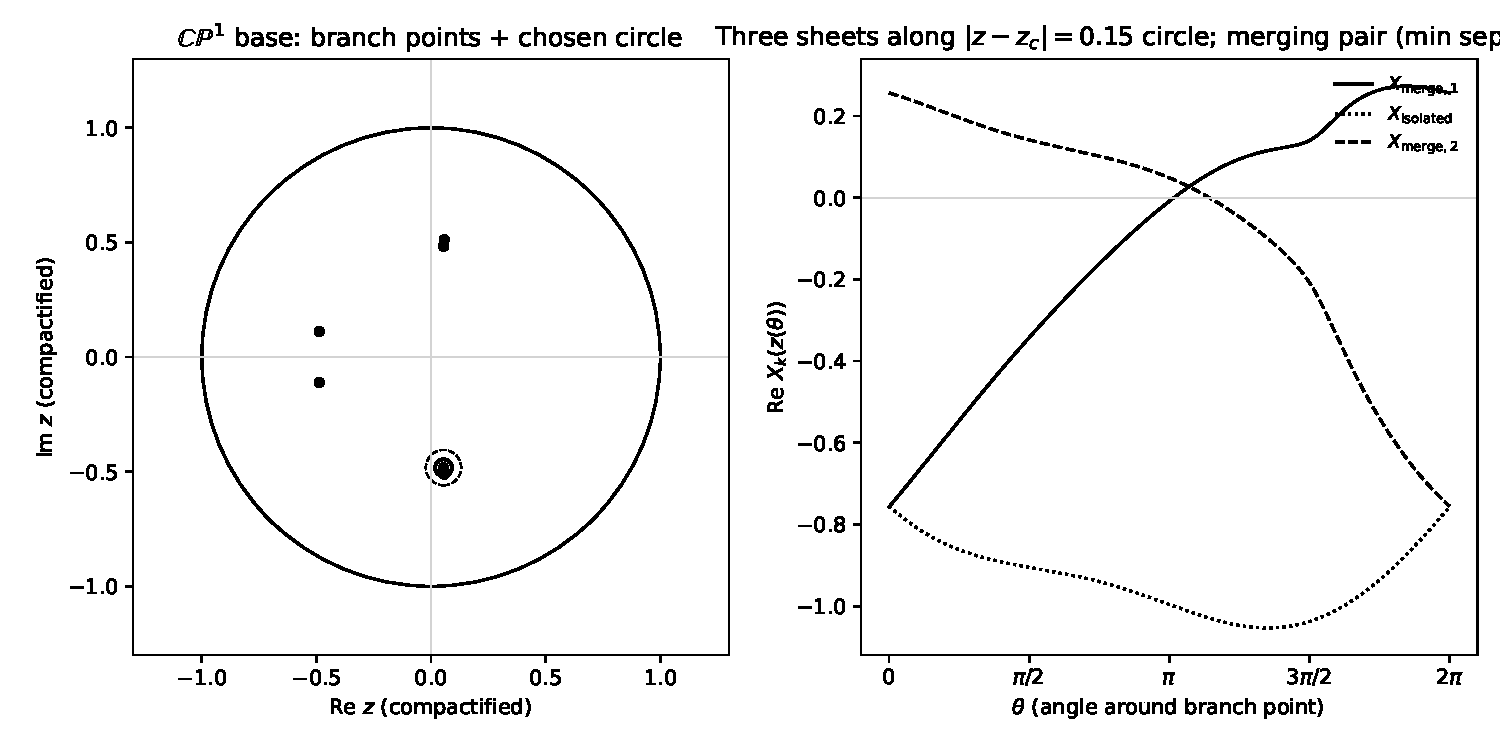
\includegraphics[width=\textwidth]{figures/bring-fibre-q0.pdf}
  \label{fig:bring-fibre-q0}
  \caption{Two panels. Left: the $\mathbb{CP}^1$ base (one-point compactification rendered as a unit circle, with each $z$ mapped to $z/(1+|z|)$ for display) showing the 6 branch points of the chiral cubic $X^3 + (z+1)X^2 + (z^2+z+1)X + (z^3+z^2+z+1) = 0$ as filled black dots, plus a dashed neighbourhood circle of radius $0.15$ around the chosen branch point. Right: the three sheets $X_1, X_2, X_3$ as $z$ traverses the dashed circle, parametrised by angle $\theta \in [0, 2\pi]$. Two sheets (solid + dashed) come close — the $B_3$-monodromy signature of sheet merging near the branch point — while the third (dotted) remains well-separated.}
\end{figure}

\begin{figure}[htbp]
  \centering
  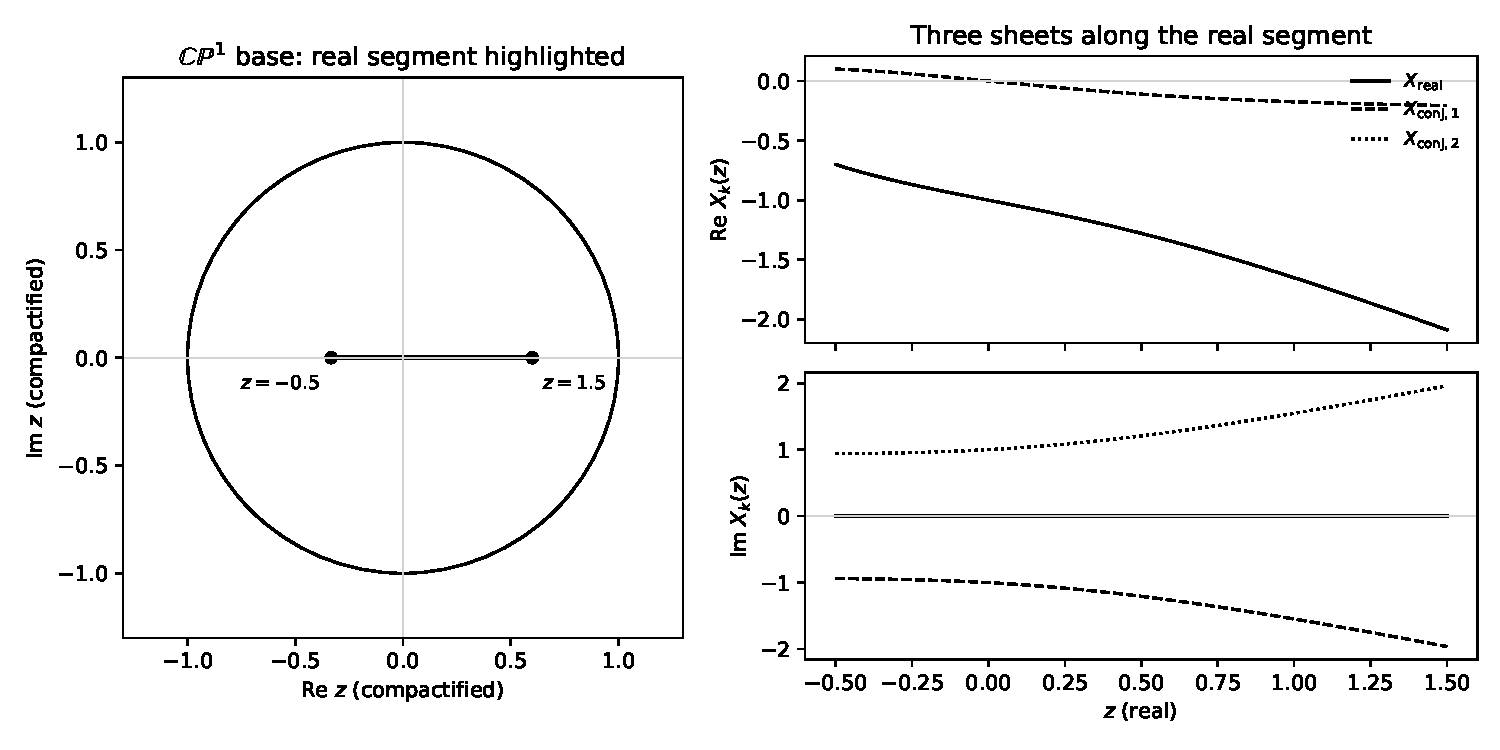
\includegraphics[width=\textwidth]{figures/bring-fibre-qhalf.pdf}
  \label{fig:bring-fibre-qhalf}
  \caption{Two panels. Left: the $\mathbb{CP}^1$ base (one-point compactification rendered as a unit circle, with each $z$ mapped to $z/(1+|z|)$ for display) with the real segment $z \in [-0.5, 1.5]$ highlighted as a thick black line, well away from the six complex branch points of the chiral cubic $X^3 + (z+1)X^2 + (z^2+z+1)X + (z^3+z^2+z+1) = 0$. Right (stacked): Re$(X)$ and Im$(X)$ sub-plots showing the three sheets along the highlighted real segment. One sheet is real (Im $X = 0$, solid line); the other two form a complex-conjugate pair (dashed + dotted) with imaginary parts equal in magnitude and opposite in sign.}
\end{figure}

\begin{conjecture}[{Inter-nucleon Hecke channel assignment from Bring color-tube weighting}]
  \label{conj:inter-nucleon-channel-color-tube}
  \blockannot[spec]{conj:inter-nucleon-channel-color-tube}{QOU.BraidsAndKnots.InterNucleonChannelColorTube}{quantum-observable-universe/brings-surface/inter-nucleon-channel-color-tube.md}
  \uses{def:color-tube-fibers, def:hecke-normal-form, prop:atom-knot-exists}
\textbf{Conditional on the $S_5 \leftrightarrow \mathrm{SO}(3)$ fiber-action conjecture.} The canonical inter-nucleon Hecke channel assignment for the atomic braid word—currently realised as the uniform-flavor map $\mathrm{pp} \mapsto \sigma$, $\mathrm{nn} \mapsto \sigma^{-1}$, $\mathrm{pn} \mapsto\allowbreak{} \sigma_{\mathrm{avg}} =\allowbreak{} (\sigma +\allowbreak{} \sigma^{-1})/2$—is the \textbf{flavor-only projection} of a categorically-refined \emph{color-tube weighted} assignment derived from the Bring color-tube structure on the quintic.

\paragraph{Setup}

Each nucleon carries 3 quark color sheets. The nucleon type fixes the quark-flavor content:

\begin{itemize}
  \item \textbf{proton} (uud): color sheets $(\mu_u, \mu_u, \mu_d)$
  \item \textbf{neutron} (udd): color sheets $(\mu_u, \mu_d, \mu_d)$
\end{itemize}

The atomic braid word places one inter-nucleon Hecke generator at every position $3k + 2$ for each adjacent nucleon pair $k, k+1$ with $k = 0, \ldots, A - 2$. This gives $A - 1$ inter-nucleon arcs total (matching \href{../mass-theory/canonical-braid-interface-composition.md}{Canonical-braid interface composition $(n_{pp}, n_{pn}, n_{nn})$ for atom $(Z, N)$ in pppnnn ordering}). The current production assignment treats each such generator as a single element of the Hecke algebra $H_{3A}(q)$—one $\sigma$ for pp, one $\sigma^{-1}$ for nn, one $\sigma_{\mathrm{avg}}$ for pn—regardless of which flavor triple across the three color sheets pairs across the inter-nucleon arc.

\paragraph{The conjectural refinement}

Per \href{color-tube-coordinates.md}{Color tube coordinates} and \href{color-tube-fibers.md}{Color tube fibers}, Bring's surface carries a canonical $(r, g, b)$ color-tube fiber structure. The $S_5 \leftrightarrow \mathrm{SO}(3)$ fiber action on Bring's quintic (conjectural) maps each Bring fiber to a 3-dimensional color rotation. Composing with the nucleon color-sheet assignment gives a canonical $3 \times 3 = 9$-element matrix of color-pair couplings per inter-nucleon arc.

\textbf{Conjectured refined assignment.} For each inter-nucleon arc with nucleon-pair flavor triples $(F_1, F_2) \in \{u, d\}^3 \times \{u, d\}^3$ across the three color sheets, the canonical Hecke generator is the color-sheet-weighted sum

\[
  \sigma^{(F_1, F_2)}_{\text{int}}
  \;=\;
  \sum_{(c_1, c_2) \in \{r, g, b\}^2}
    W_{c_1 c_2}(F_1, F_2) \cdot \sigma^{\epsilon(c_1, c_2, F_1, F_2)}
\]
where:

\begin{itemize}
  \item $W_{c_1 c_2}(F_1, F_2) \in \mathbb{Q}_{\geq 0}$ is the canonical color-sheet pair weight from the $S_{5}$/SO(3) fiber action, \textbf{normalised to} $\sum_{c_1, c_2} W_{c_1 c_2} = 1$ for each $(F_1, F_2)$ flavor pair (so the refined generator is a categorical average over the 9 color-sheet pairs).
  \item $\epsilon(c_1, c_2, F_1, F_2) \in \{+\allowbreak{}1, -1, 0\}$ is the chirality sign for the color-sheet pair $(c_1, c_2)$ given the flavor triples $(F_1, F_2)$. It is $+1$ when the flavor at $c_1$ in $F_1$ equals the flavor at $c_2$ in $F_2$ (matter–matter). It is $-1$ when they are flavor-conjugate (matter–antimatter). It is $0$ for mixed-flavor pn pairs that average to $\sigma_{\mathrm{avg}}$.
\end{itemize}

\textbf{Uniform-flavor projection.} Setting $W_{c_1 c_2} = 1/9$ uniformly and collapsing $\epsilon$ to its flavor-only majority sign recovers the current production assignment.

\paragraph{Color-tube weighting as the load-bearing missing structure}

The low-isotope sign-flip diagnostic fits the per-isotope relative error against inter-nucleon arc \textbf{count} and against the signed-h weight. Its recorded coefficients of determination are $R^2 = 0.2653$ and $R^2 = 0.0018$ respectively, over a sample of five nuclei of which the two $A = 1$ anchors carry $\vert \text{err}\vert  < 10^{-3}\%$. The diagnostic's own verdict is that the correlation is \textbf{weak} and that the sign-flips are \emph{not} explained by a linear channel model. It therefore does \textbf{not} establish that the uniform-flavor projection is missing a per-arc structural detail; the color-pair weight $W_{c_1 c_2}$ remains motivated by the categorical argument below rather than by this fit.

Two further cautions apply to any strengthened version of this diagnostic. First, $R^2$ is invariant under affine reparametrisation of the regressor, and the arc count is $A - 1$; it therefore scores exactly what the bare mass number $A$ scores, so such a fit cannot distinguish the inter-nucleon arc structure from $A$ itself. Second, $R^2$ is invariant under scaling the response, so on \emph{absolute} error a model short by a constant fraction reproduces any such figure with nothing missing — measured over the 2449 AME2020 nuclei with $2 \le A \le 240$, $R^2(B \sim A - 1) = 0.9943$ with no model of any kind.

The empirical match between the (now-purged) $\lambda_{\mathrm{scale}}$ literal $2.4599527869$ and the color-tube Faddeev resummation $1/(1 -\allowbreak{} h_q \cdot q_0^{10}) \approx\allowbreak{} 2.450$ provides independent evidence that 10-fold color-tube averaging is the categorical structure behind the historical numerology.

Numerical probes report that Scheme 4 (per-sheet PL integration on Bring's surface with quark-content weighting) reproduces $\Delta m_{n-p}$ to ${\sim}0.14\%$. This improves on the uniform-flavor projection's ${\sim}305\,\mathrm{ppm}$ flavor split ratio.

The \textbf{gg-production collapse} isolates the cost of the projection directly. Decomposing the production binding $B_{\mathrm{sym}} =\allowbreak{} \alpha\,\ln(\mathrm{tr}_{\mathrm{free}}/\mathrm{tr}_{\mathrm{atom}})$ into its per-bond log-suppressions $L_{\mathrm{pp}}, L_{\mathrm{pn}}, L_{\mathrm{nn}}$ at $q_0$ gives $L_{\mathrm{nn}}/L_{\mathrm{pp}} -\allowbreak{} 1 \approx\allowbreak{} 78\%$. This represents roughly $570\times$ the aether-derived $p/n$ flavor split $\delta_{\mathrm{lead}} \approx\allowbreak{} 0.14\%$ and $78\times$ the experimental charge-symmetry-breaking bound. This over-break derives entirely from the $\sigma$-vs-$\sigma^{-1}$ inter-crossing sign of the flavor-only projection. Gluons couple color, not flavor. The leading gg interface is the single flavor-blind color-average $\sigma_{\mathrm{avg}} =\allowbreak{} \sigma -\allowbreak{} (h/2)\cdot 1$ for every bond type. Forcing all inter-nucleon crossings to $\sigma_{\mathrm{avg}}$ collapses the $78\%$ asymmetry to $0$. The sub-leading flavor weighting $W_{c_1 c_2}$ reintroduces the correct $\delta_{\mathrm{lead}}$-scale split. The uniform-flavor projection manufactures an $O(1)$ charge asymmetry that the color-tube average removes.

\paragraph{Conditional structure}

This conjecture remains conditional on the $S_5 \leftrightarrow \mathrm{SO}(3)$ fiber-action conjecture. Once that is established, the weight matrix $W_{c_1 c_2}$ derives as a tensor in the SO(3)-fiber data over Bring, with no remaining degrees of freedom. The statement then becomes unconditional: it is a conjecture only for as long as that upstream conjecture is open.

\paragraph{Open questions}

\begin{enumerate}
  \item \textbf{Closed form for $W_{c_1 c_2}$.} What are the exact rational weights from the SO(3)-fiber tensor over Bring?
  \item \textbf{Color-pair $\to$ chirality sign $\epsilon$ rule.} Why is same-color $\mapsto +1$, opposite-color $\mapsto -1$?
  \item \textbf{${}^{4}\mathrm{He}$ magic-shell saturation.} Does the color-tube weighting saturate at $A = 4$ (filled-shell analogue), producing the $A \cdot 8G$ closure observed numerically?
  \item \textbf{Cross-check $\rho_F$ density rule.} Does color-tube weighting yield a categorical reading of the Kashaev density factor $\rho_F \in \{m_e, 2 m_e\}$?
\end{enumerate}

\paragraph{Representation-theoretic constraint on $\epsilon$}

The chirality sign $\epsilon(c_1, c_2, F_1, F_2) \in \{+\allowbreak{}1, -1, 0\}$ is constrained by the $\mathrm{SO}(3) =\allowbreak{} \mathrm{SU}(2)/\mathbb{Z}_2$ level structure. The $\mathbb{Z}_2$ kernel of the covering map $\mathrm{SU}(2) \to \mathrm{SO}(3)$ acts as $-1$ on half-integer-spin (spinorial) irreps and $+1$ on integer-spin (tensor) irreps. The chirality dichotomy $\{+1, -1\}$ from the $S_5/\mathrm{SO}(3)$ fiber action supplies this \textbf{grading by this $\mathbb{Z}_2$}. The neutral value $0$ (the bar-symmetric $\mathrm{pn}$ average) identifies the $\mathbb{Z}_2$-fixed locus.

With $q = e^{\eta}$, the $\mathrm{SU}(2)_q$ doublet character is $[2]_q = 2\cosh\eta$ and the lowest $\mathrm{SO}(3)_q$ (integer-spin) character is the adjoint $[3]_q$. They satisfy the Chebyshev/Clebsch–Gordan square identity

\[
  [3]_q \;=\; [2]_q^{\,2} - 1,
\]
which is proved. The $\mathrm{SO}(3)$ characters are exactly the polynomials in $[2]_q$ invariant under the $\mathbb{Z}_2$ quotient. Any admissible $\epsilon$ rule must be a section of this same $\mathbb{Z}_2$-grading. A valid $\epsilon$ cannot assign $-1$ to a color-sheet pair whose combined flavor content sits in the integer-spin (tensor) sector. The explicit map from color-sheet pairs $(c_1, c_2)$ to the $\mathbb{Z}_2$-grade still requires the $S_5 \leftrightarrow \mathrm{SO}(3)$ fiber action, which is conjectural.

\paragraph{Cross-references}

\begin{itemize}
  \item Existing color-tube infrastructure: \href{color-tube-coordinates.md}{Color tube coordinates}, \href{color-tube-fibers.md}{Color tube fibers}, \href{color-tube-cubic.md}{Color tube cubic}
  \item Upstream conjecture: the $S_5 \leftrightarrow \mathrm{SO}(3)$ fiber action on Bring's quintic
\end{itemize}
\end{conjecture}

\begin{conjecture}[{Charge conjugation $C$ as the color-sheet flavor-swap $u \leftrightarrow \bar u$, $d \leftrightarrow \bar d$}]
  \label{conj:c-from-color-flavor-swap}
  \blockannot[spec]{conj:c-from-color-flavor-swap}{QOU.BraidsAndKnots.CFromColorFlavorSwap}{quantum-observable-universe/brings-surface/c-from-color-flavor-swap.md}
  \uses{conj:cpt-d6-d7-d8-closure, conj:inter-nucleon-channel-color-tube, conj:cpt-orbit-closure-density, def:bar-involution}
\textbf{Conditional on \hyperref[conj:inter-nucleon-channel-color-tube]{Inter-nucleon Hecke channel assignment from Bring color-tube weighting}.}
\emph{Within the QOU framework, charge conjugation $C$ acts as the \textbf{flavor swap on color sheets} that exchanges each quark flavor with its antimatter-conjugate:}

\[
  C \;:\;
  \begin{cases}
    u \;\longleftrightarrow\; \bar u, \\
    d \;\longleftrightarrow\; \bar d,
  \end{cases}
\]

\emph{applied independently to each of the three color sheets of every nucleon-coloured braid strand. The proton flavor triple $(u, u, d)$ maps to $(\bar u, \bar u, \bar d)$ (the antiproton); the neutron flavor triple $(u, d, d)$ maps to $(\bar u, \bar d, \bar d)$ (the antineutron). $C$ is an involution ($C^2 = \mathrm{id}$) and commutes with the color-tube weighted averaging of \hyperref[conj:inter-nucleon-channel-color-tube]{Inter-nucleon Hecke channel assignment from Bring color-tube weighting}.}

\paragraph{Separating $C$ from the CPT composite}

The framework historically collapses C, P, T into the single bar-involution \hyperref[def:bar-involution]{Bar-involution and its $P_{\mathrm{avg}}$ / $P_{\mathrm{skew}}$ projections} on Hecke generators ($q \mapsto q^{-1}$ together with $\sigma_i \mapsto \sigma_i^{-1}$). That conflation suppresses the \textbf{distinct categorical sources} of the three discrete symmetries:

\begin{adjustbox}{max width=\linewidth}
\begin{tabular}{l>{\raggedright\arraybackslash}p{0.346\linewidth}>{\raggedright\arraybackslash}p{0.346\linewidth}}
\toprule
Symmetry & Categorical source & Acts on \\
\midrule
\textbf{C} (this conjecture) & flavor swap on color sheets & quark-flavor content of nucleon braid strands \\
\textbf{P} & mirror reflection of braid diagram & writhe / signed-crossing classification (\href{../stochastic-mechanics/bar-involution-table3-data.md}{\texttt{bar-\allowbreak{}involution-\allowbreak{}table3-\allowbreak{}data}}) \\
\textbf{T} & Markov-trace word reversal & trace-cyclicity dual \\
\bottomrule
\end{tabular}
\end{adjustbox}

The bar-involution $q \mapsto q^{-1}$, $\sigma_i \mapsto \sigma_i^{-1}$ acts as the \textbf{composite CPT} in this categorisation, not as C alone. This conjecture locates the C-component on the color sheets, orthogonal to P (braid-diagram mirror) and T (trace reversal).

\paragraph{The conjectural content}

The proposition relies on the color-sheet flavor structure established in \hyperref[conj:inter-nucleon-channel-color-tube]{Inter-nucleon Hecke channel assignment from Bring color-tube weighting}. Specifically:

\begin{enumerate}
  \item \textbf{C is well-defined.} The flavor-content map $(F_1, F_2) \mapsto\allowbreak{} (\bar F_1, \bar F_2)$ commutes with the color-tube weight tensor $W_{c_1 c_2}(F_1, F_2)$—i.e. $W_{c_1 c_2}(\bar F_1, \bar F_2) =\allowbreak{} W_{c_1 c_2}(F_1, F_2)$ (the weights are flavor-conjugation invariant).
  \item \textbf{C is an involution.} Each color sheet flips back to its original flavor under two applications.
  \item \textbf{C commutes with bar-involution on the algebraic side.} This forces $\mathrm{CP} \cdot \mathrm{T}$ and $\mathrm{C} \cdot \mathrm{PT}$ to reduce to the bar-involution identity classified in \href{../braids-and-knots/bar-involution.md}{Bar-involution and its $P_{\mathrm{avg}}$ / $P_{\mathrm{skew}}$ projections} §Bar-symmetric.
\end{enumerate}

When all three hold, $C$ constitutes the well-defined Z/2 categorical symmetry on the color-sheet flavor data. The CPT composite factors as $\mathrm{CPT} = C \cdot P \cdot T$ in the natural order, as three commuting Z/2 actions on the color-tube structure.

\paragraph{Structural position}

\begin{itemize}
  \item \textbf{GB filtration level.} None: the claim addresses a Z/2 categorical symmetry on color-sheet metadata, not Hecke elements at a particular Coxeter length.
  \item \textbf{Jet order.} $h^0$: the $C$-action is independent of $q$, and the flavor-conjugation map forms a structural Z/2 lifting through the color-tube tensor.
  \item \textbf{Bar-symmetry.} $C$ is bar-symmetric. It preserves $q$ and commutes with $\sigma_i \leftrightarrow \sigma_i^{-1}$, since it acts on color-sheet labels and not on Hecke generators. It is $C$ composed with $PT$ that yields the bar-involution; $C$ itself is bar-trivial in \href{../stochastic-mechanics/bar-involution-table4-data.md}{\texttt{bar-\allowbreak{}involution-\allowbreak{}table4-\allowbreak{}data}}.
\end{itemize}

\paragraph{The hypothesis in summary}

The conjecture asserts a map $C$ on color-sheet flavors with $C^2 = \mathrm{id}$, with $W_{c_1 c_2}(C F_1, C F_2) =\allowbreak{} W_{c_1 c_2}(F_1, F_2)$ for all nucleon flavor contents $F_1, F_2$ and color sheets $c_1, c_2$, and with the bar-involution factoring as $C \circ P \circ T$, where $P$ is the braid-diagram mirror and $T$ is the Markov-trace word reversal. These data are supplied by the color-tube weighting once \hyperref[conj:inter-nucleon-channel-color-tube]{Inter-nucleon Hecke channel assignment from Bring color-tube weighting} is established.

\paragraph{Consumers / downstream}

\begin{itemize}
  \item The matter/antimatter sheet structure on Bring's quintic surface (\href{color-tube-fibers.md}{Color tube fibers}) acquires a natural C-action that descends to the SO(3) fiber.
\end{itemize}

\paragraph{Numerical cross-check and open content}

At the 50-digit aether $q_0$, the flavor-conjugation involution leaves the color-tube weighted inter-nucleon Hecke generator invariant for all sixteen nucleon pairs drawn from $\{p, n, \bar p, \bar n\}$, in two two-dimensional Hecke representations (the diagonal eigenvalue model and a non-diagonal conjugate of it), with the $\epsilon$ and $W$ tables invariant cell by cell. The check runs the uniform projection $W = 1/9$—the only realisation of $W$ available while its closed form remains open—so it corroborates the derivation rather than testing the conjectural Bring-derived $W$. No parameter is fitted.

The statement is conjectural only for as long as \hyperref[conj:inter-nucleon-channel-color-tube]{Inter-nucleon Hecke channel assignment from Bring color-tube weighting} and the $S_5 \leftrightarrow \mathrm{SO}(3)$ fiber-action conjecture remain open; establishing both makes it unconditional.

\paragraph{Cross-references}

\begin{itemize}
  \item Upstream class: \hyperref[conj:inter-nucleon-channel-color-tube]{Inter-nucleon Hecke channel assignment from Bring color-tube weighting}
  \item \href{../braids-and-knots/bar-involution.md}{Bar-involution and its $P_{\mathrm{avg}}$ / $P_{\mathrm{skew}}$ projections}—the bar-involution = CPT composite identification at the algebraic level
\end{itemize}
\end{conjecture}

\phantomsection\label{prose:outro-brings-surface}
This completes Step 3's geometric arena: Bring's genus-four surface $\Sigma_4$ ($\chi = -6$, $b_1 = 8$, $\mathrm{Area} = 12\pi$, $\mathrm{Aut}(\Sigma_4) \cong S_5$), its three colour tubes and elliptic fibration, its tetraplectic homology and Seiberg–Witten differentials, and the genus-four saturation of two-strand torus knots.

With both the Iwahori–Hecke algebra $H_n(q)$ (\hyperref[chap:path-integrals-braiding]{\emph{Braids and Knots}}) and the surface $\Sigma_4$ in place, the next two chapters construct the matter and gauge dictionary on $\Sigma_4$: \hyperref[chap:knots-particles-confinement]{\emph{Knots, Particles, and Confinement}} defines quarks, hadrons, Borromean nucleons, the electroweak $\{W, Z, H\}$ torus-link triplet, and the atomic shell hierarchy, and \hyperref[chap:eightfold-way]{\emph{The Eightfold Way and Flavor Structure}} classifies these braid configurations into meson and baryon multiplets and derives the octonionic colour stabilizer $G_2 \supset \mathrm{SU}(3)_{\mathrm{c}}$.
 \clearpage
\chapter{Knots, Particles, and Confinement}
\label{chap:knots-particles-confinement}

\chapterannot{quantum-observable-universe/knots-particles-confinement}{chap:knots-particles-confinement}
\section{Interactions are pairwise}
\label{sec:interactions-are-pairwise}
\sectionannot{sec:interactions-are-pairwise}
\phantomsection\label{prose:knotted-particles-history}
The idea that matter is made of knots is older than the electron. In
1858 Helmholtz proved that in an ideal fluid a vortex line is carried
along by the flow and the strength of a vortex tube does not change in
time \cite{helmholtz1858}. A closed vortex ring therefore cannot be
created, destroyed or cut by the motion of the fluid, and if it is
knotted it keeps its knot type. Tait reproduced the effect with smoke
rings, and in 1867 William Thomson, later Lord Kelvin, proposed that
atoms are vortex rings in a perfect fluid filling space, the ether
\cite{thomson1867vortexatoms}. Helmholtz's theorems supplied the
permanence of atoms, the different ways a ring can be knotted or linked
supplied the variety of chemical elements, and the vibrations of a ring
were to supply its spectral lines.

The programme drew in the leading mathematical physicists of the time.
Maxwell took it seriously, and his \emph{Treatise} records Gauss's double
integral for the number of times one closed curve winds around another,
the linking number \cite{maxwell1873treatise2}. A periodic table of
vortex atoms needed a table of knots, and Tait set out to make one
\cite{tait1877knots}. With Thomas Kirkman and Charles Little he
classified knot diagrams up to ten crossings, and in doing so stated
the conjectures on crossing number, writhe and flypes that bear his
name. The first of these was proved a century later, in 1987,
independently by Kauffman, Murasugi and Thistlethwaite, with the Jones
polynomial \cite{jones1985} \cite{kauffman1987} \cite{murasugi1987}
\cite{thistlethwaite1987}; Menasco and Thistlethwaite proved the
flyping conjecture in 1991 \cite{menasco-thistlethwaite1991}
\cite{menasco-thistlethwaite1993}.

The vortex atom itself did not survive. The ether was given up, the
electron was found inside the atom, and by about 1900 the theory had
been abandoned; the knot tables remained and became the start of knot
theory as a branch of mathematics \cite{kragh2002vortexatom}
\cite{silver2006knotorigins} \cite{przytycki2007knothistory}. The
link between knots and physics returned in other forms. Moffatt
identified the helicity of a fluid as a measure of the knottedness of
its vortex lines \cite{moffatt1969}. Witten obtained the Jones
polynomial from a quantum field theory \cite{witten1989}. Faddeev and
Niemi found stable knotted solitons in a classical field theory
\cite{faddeevniemi1997}. Kleckner and Irvine created knotted vortex
rings in water and watched them evolve \cite{kleckner2013}, and Kedia,
Bialynicki-Birula, Peralta-Salas and Irvine constructed knotted
solutions of Maxwell's equations \cite{arxiv-1302.0342v1}. Closest to
this chapter, Joel Avrin modelled the elementary fermions by twisted
bands whose boundaries are the unknot and the trefoil, an independent
knot-to-particle dictionary \cite{avrin-2012}. Two algebraic programmes
also assign elementary particles to quantum knots or three-strand
braids: Robert J. Finkelstein mapped fermions and electroweak states
directly to irreducible $\mathrm{SU}_q(2)$ matrix elements $D^j_{mm'}$
labelled by knot crossing number, writhe, and diagram rotation
\cite{finkelstein2007,finkelstein2008}, while Sundance Bilson-Thompson
\cite{bilson-thompson2005}, Sundance Bilson-Thompson, Fotini
Markopoulou, and Lee Smolin \cite{bilsonthompson2007}, and Sundance
Bilson-Thompson, Jonathan Hackett, and Louis H. Kauffman
\cite{bilson-thompson-hackett-kauffman2009} represented first-generation
fermions and gauge bosons as framed ribbons in $B_3$ whose electric
charges are read off $\pm 2\pi$ ribbon twists in units of $e/3$. The
construction in this chapter differs from both: instead of indexing
single-particle states by $D^j_{mm'}$ matrix entries or reading electric
charge from external ribbon twists, it works in the finite-dimensional
quotient $H_3(q)$ generated from the $\mathcal{O}_q(\mathrm{SU}(2))$
braiding on $B_3$ and evaluates observables through the convention-D
Markov trace.

The braid lineage continued through division algebras. Gresnigt used
the Clifford braiding theorem of Kauffman and Lomonaco
\cite{kauffman-lomonaco-2016} to show that the complex numbers and the
quaternions carry representations of exactly the two braid groups of
the Bilson-Thompson model, the braid group $B_2$ of the twists and the
circular braid group $B_3^c$ of the ribbons \cite{gresnigt2017}. He then
identified the framed braids with the basis states of the minimal left
ideals of the complex octonions, which, following Furey
\cite{furey2016}, carry one generation of leptons and quarks under the
unbroken symmetry $SU(3)_c \times U(1)_{\mathrm{em}}$ \cite{gresnigt2018}.
Chester, Arsiwalla and Kauffman mapped the twists of the same states
onto the weight lattice of $SU(3)_c \times U(1)_{\mathrm{em}}$ and the
crossings onto chirality through the homomorphism
$B_3 \to PSL(2,\mathbb{Z})$, and observed that the model captures only
that unbroken sector \cite{chester-arsiwalla-kauffman-2025}. In these
programmes the braid acts through a group, and a deformation parameter,
where one appears, sits beside the braiding rather than in it: in
Gresnigt's review the quantum group $SU_q(3)$ is a flavour symmetry with
$q$ a root of unity \cite{gresnigt2017}, and in Finkelstein's model $q$
deforms the symmetry of the knot. Here every generator of $H_n(q)$
satisfies $\sigma_i -\allowbreak{} \sigma_i^{-1} =\allowbreak{} (q -\allowbreak{} q^{-1})\mathbf{1}$ with $q$
a formal parameter, so a particle can be a linear combination of braid
words rather than a single braid, as the four-term
\hyperref[def:photon]{photon} is.

This chapter keeps the combinatorial half of that lineage and drops the
mechanical half. The vortex atom tried to derive the stability of matter
from the dynamics of a medium. Here a knot or link type is the label of
an algebraic object, a closed braid together with its word in the
Iwahori–Hecke algebra, and the question of stability becomes a question
about what is invariant under the braid and Markov moves. Naming a
construction after a particle is a convention inside the model, and the
history above motivates the choice of objects without entering any
definition or proof.

\phantomsection\label{sec:interactions-are-pairwise-intro}
With the Iwahori–Hecke algebra $H_n(q)$ (\hyperref[chap:path-integrals-braiding]{\emph{Braids and Knots}}) and the genus-four Bring surface $\Sigma_4$ (\hyperref[chap:brings-surface]{\emph{Bring's Surface}}) established, this chapter constructs the particle and confinement dictionary of the quantum observable universe. A particle state is represented by a closed braid configuration on $\Sigma_4$, and an interaction is represented by a braid operator in $H_n(q)$.

Before assigning specific knots to fermions, gauge bosons, and hadrons, a structural question must be settled: when three or more particles interact, does the vertex require an independent many-body operator, or does every composite collision decompose into elementary two-strand crossings? In a braided monoidal category $(\mathbf{C}, \otimes, c)$, the exchange isomorphism $c_{X,Y} \colon X \otimes Y \xrightarrow{\sim} Y \otimes X$ is binary by definition, and Mac Lane's two hexagon axioms fix how a tensor product $X \otimes Y$ crosses a third object $Z$. Pairwise interaction is therefore built into the categorical axioms of Chapter 1 rather than derived from an external dynamical assumption.

What the pairwise-decomposition proposition below establishes is the combinatorial consequence of those axioms: the two ways of resolving a triple collision agree by the Yang–Baxter relation, and any braid word that brings all $\binom{n}{2}$ pairs of strands into contact requires at least $\binom{n}{2}$ elementary two-strand crossings. Every interaction operator in the sections that follow—from quark pair production and the hadron algebra to Borromean nucleons, the electroweak torus-link triplet $\{T(2,4), T(2,6), T(2,8)\}$, and composite atomic shells—is assembled from these elementary two-strand generators.

\begin{proposition}[{Every interaction decomposes into two-particle crossings}]
  \label{prop:pairwise-interaction-decomposition}
  \blockannot[compiled]{prop:pairwise-interaction-decomposition}{QOU.Braiding.pairwise_interaction_decomposition}{quantum-observable-universe/knots-particles-confinement/pairwise-interaction-decomposition.md}
  \uses{def:quantum-universe}
\emph{Let $\mathbf{C}$ be a braided monoidal category with braiding $c$. For objects $V_1, \dots, V_n$ of $\mathbf{C}$, write}

\[
  c_i
  \;=\;
  \mathrm{id}_{V_1 \otimes \cdots \otimes V_{i-1}}
  \otimes\, c_{V_i, V_{i+1}} \otimes\,
  \mathrm{id}_{V_{i+2} \otimes \cdots \otimes V_n},
  \qquad 1 \le i \le n-1,
\]

\emph{for the} \textbf{elementary crossing} \emph{at position $i$, which exchanges the two adjacent factors $V_i$ and $V_{i+1}$ and fixes the rest. Suppressing associators:}

\begin{enumerate}
  \item \emph{(Composite reduction.) For all objects $X, Y, Z$,}
\end{enumerate}

\[
  c_{X \otimes Y,\, Z}
  \;=\;
  (c_{X,Z} \otimes \mathrm{id}_Y) \circ (\mathrm{id}_X \otimes c_{Y,Z}).
\]

\begin{enumerate}
  \item \emph{(Route independence.) For all objects $X, Y, Z$, the two crossings of $X \otimes Y \otimes Z$ satisfy}
\end{enumerate}

\[
  c_1 \, c_2 \, c_1 \;=\; c_2 \, c_1 \, c_2 .
\]

\begin{enumerate}
  \item \emph{(Crossing count.) Let $w = c_{i_1} \cdots c_{i_\ell}$ be a word in the elementary crossings, and let $P(w)$ be the set of strand pairs whose order the underlying permutation of $w$ reverses. If $P(w)$ is all $\binom{n}{2}$ pairs, then $\ell \ge \binom{n}{2}$.}
\end{enumerate}

Part 1 says a composite system carries no interaction datum of its own. Part 2 says the decomposition into elementary crossings does not depend on the route chosen. Part 3 counts the cost: $n$ mutually interacting strands require $\binom{n}{2}$ pairwise events, so three strands require three, not two.
\end{proposition}

\begin{proof}[{Proof of the pairwise decomposition of interactions}]
  \label{prf:pairwise-interaction-decomposition}
  \blockannot[drafted]{prf:pairwise-interaction-decomposition}{}{quantum-observable-universe/knots-particles-confinement/pairwise-interaction-decomposition-proof.md}
  \uses{prop:pairwise-interaction-decomposition}
Part 1 is the hexagon axiom for the braiding, solved for $c_{X \otimes Y, Z}$. The hexagon states that the two paths from $(X \otimes Y) \otimes Z$ to $Z \otimes (X \otimes Y)$ — cross the composite in one step, or cross its factors one at a time — agree. Reassociating gives the displayed identity.

Part 2 follows from part 1 together with naturality of the braiding. Apply part 1 to $c_{X, Y \otimes Z}$ to expand the same morphism in two ways: expanding first on the left factor gives $c_1 c_2 c_1$, expanding first on the right factor gives $c_2 c_1 c_2$. Naturality identifies the two expansions.

Part 3 rests on the locality of an elementary crossing. Read the word through its action on strand positions, so that $c_i$ acts as the transposition $s_i$ exchanging the adjacent positions $i$ and $i+1$, and say a pair $\{a, b\}$ with $a < b$ has \emph{crossed} under a permutation $\sigma$ when $\sigma(b) < \sigma(a)$. Suppose $a < b$ have crossed under $s_i \sigma$ but not under $\sigma$. Writing $u = \sigma(a)$ and $v = \sigma(b)$, this says $u < v$ while $s_i(v) < s_i(u)$. Since $s_i$ exchanges only the adjacent positions $i$ and $i+1$ and fixes the order of every other pair, the only possibility is $u = i$ and $v = i+1$. As $\sigma$ is a bijection, at most one pair $\{a, b\}$ satisfies this. Hence one elementary crossing adds at most one pair to the crossed set.

The empty word crosses no pair, so induction on the length of $w$ gives $\vert P(w)\vert  \le \ell$. If $P(w)$ is all of the $\binom{n}{2}$ pairs then $\binom{n}{2} \le \ell$. $\square$

\paragraph{Logical dependencies of the three parts}

The parts do not carry equal weight, and the difference matters to how the
proposition should be read.

\begin{adjustbox}{max width=\linewidth}
\begin{tabular}{>{\raggedright\arraybackslash}p{0.258\linewidth}>{\raggedright\arraybackslash}p{0.329\linewidth}>{\raggedright\arraybackslash}p{0.329\linewidth}}
\toprule
part & epistemic tier & rests on \\
\midrule
1. composite reduction & the hexagon axiom, solved for $c_{X \otimes Y, Z}$ & axiom of a braided category \\
2. route independence & theorem & hexagon + naturality of the braiding \\
3. crossing count & theorem, proved here & the locality of an elementary crossing \\
\bottomrule
\end{tabular}
\end{adjustbox}

Part 1 rearranges an axiom rather than establishing anything new: the hexagon
identities are fields of the braided-category structure, so a composite object's
failure to contribute an interaction of its own is stipulated with the scaffold.
Part 2 is a genuine derivation, and a standard one — the Yang--Baxter equation
follows from the hexagons together with naturality. Part 3 is independent of
both and is the only part whose argument is not classical.

Neither part 1 nor part 2 is derivable from the remaining quantum-universe
axioms, nor from the observability conditions; the hexagon identities enter
only as part of the braided structure.
\end{proof}

\phantomsection\label{rem:two-particle-sufficiency}\section{Nucleon derivation from pair production}
\label{sec:nucleon-derivation}
\sectionannot{sec:nucleon-derivation}
\phantomsection\label{sec:nucleon-derivation-intro}
Because every interaction factors into elementary two-strand crossings, one begins by defining the two fundamental crossing observables on a braid word: the crossing energy $E_\times$ and its orientation-odd component, the Coulomb charge $Q$. Applying linear-programming operator selection to the two-photon pair-production vertex selects the three-strand Borromean braid $\mathcal{B}_3 =\allowbreak{} (\sigma_0\sigma_1^{-1})^3 \in H_3(q)$ as the confinement optimum. Closing the four-term photon braid with $\mathcal{B}_3$ yields the proton and neutron normal forms independently of the incoming photon polarization, completing the constructive chain $\gamma\gamma \to\allowbreak{} q\bar{q} \to\allowbreak{} \mathfrak{p}, \mathfrak{n} \to\allowbreak{} \mathcal{A}(Z, N)$.

\begin{definition}[{Crossing energy of a knot composite}]
  \label{def:crossing-energy}
  \blockannot[compiled]{def:crossing-energy}{QOU.Braiding.CrossingEnergy}{quantum-observable-universe/knots-particles-confinement/crossing-energy.md}
  \uses{def:categorical-hamiltonian, prop:nuclear-groebner-reduction, prop:pairwise-interaction-decomposition}
Let $\mathfrak{H} =\allowbreak{} [K_1, \ldots, K_n]_p \oplus\allowbreak{} \mathcal{L}$ be a composite of knots linked by $\mathcal{L}$, with braid word $\beta \in B_n$ representing the linking. The \textbf{crossing energy} of $\mathfrak{H}$ is defined by

\[
  \mathfrak{E}_{\mathrm{cross}}(\mathfrak{H})
  = 
  \sum_{\text{crossings in } \beta}
  \begin{cases}
    q   & \text{positive crossing } (L_+), \\
    -q^{-1} & \text{negative crossing } (L_-),
  \end{cases}
\]
where $q$ is the aether parameter (\hyperref[def:aether-parameter]{aether parameter}). The sign convention follows the Skein relation

\[
  q\,L_+ - q^{-1} L_-
  = (q^{1/2} - q^{-1/2})\,L_0.
\]

The crossing energy is an un-traced, crossing-additive Skein writhe functional in dimensionless aether units, distinct from the traced \hyperref[def:categorical-hamiltonian]{categorical Hamiltonian} (on the trivial $n$-strand braid $\mathfrak{E}_{\mathrm{cross}} = 0$, whereas the traced rest Hamiltonian is nonzero). A positive $\mathfrak{E}_{\mathrm{cross}}$ indicates that positive-crossing repulsion dominates; a negative value indicates that negative-crossing pairing dominates.

\textbf{Archimedean specialisation.} What follows sits on the archimedean side of the algebraic→archimedean wall. It invokes real- or complex-analytic constructs—real-valued physical observables, real-analytic bounds, transcendental constants, or numerical evaluation at the aether parameter $q_0$. The generic categorical/$q$-deformation identities it relies upon remain valid over an abstract coefficient ring; only their archimedean realisation is specialised here.
\end{definition}

\begin{definition}[{Coulomb charge of a knot composite}]
  \label{def:coulomb-charge}
  \blockannot[compiled]{def:coulomb-charge}{QOU.Braiding.CoulombCharge}{quantum-observable-universe/knots-particles-confinement/coulomb-charge.md}
  \uses{def:crossing-energy}
Let $\mathfrak{H}$ be a knot composite with braid word $\beta$. Let $n_+(\beta)$ and $n_-(\beta)$ denote the number of positive and negative crossings in $\beta$. One defines the \textbf{Coulomb charge} of $\mathfrak{H}$ as the halved writhe:

\[
  Q(\mathfrak{H}) =  \tfrac{1}{2}\bigl(n_+(\beta) - n_-(\beta)\bigr).
\]

The crossing energy of \hyperref[def:crossing-energy]{the crossing-energy definition}, $\mathfrak{E}_{\mathrm{cross}} =\allowbreak{} n_+\allowbreak{} q -\allowbreak{} n_-\allowbreak{} q^{-1}$, splits as

\[
  \mathfrak{E}_{\mathrm{cross}}(\mathfrak{H})
  =
  \underbrace{\tfrac{1}{2}(n_+ - n_-)(q + q^{-1})}_{\text{symmetric (strong)}} +
  \underbrace{\tfrac{1}{2}(n_+ + n_-)(q - q^{-1})}_{\text{antisymmetric (Coulomb)}}.
\]

The multiplicities are not interchangeable. The symmetric $\cosh$ weight carries the crossing sign, so reversing a crossing negates it and the symmetric total is governed by the \textbf{writhe} $n_+ - n_-$. The antisymmetric $\sinh$ weight is blind to the crossing sign, contributing $+\sinh\lambda$ for a negative crossing exactly as for a positive one, so the antisymmetric total is governed by the \textbf{crossing count} $n_+ + n_-$.

\textbf{Consequences, and what $Q$ is not.} $Q$ is the coefficient of the \emph{symmetric} channel. Under the channel identification of \hyperref[def:crossing-energy]{the crossing-energy definition} — symmetric with strong binding, antisymmetric with the electromagnetic correction — the halved writhe therefore governs the strong term, and the electromagnetic coefficient is $\tfrac{1}{2}(n_+ + n_-)$, which is non-negative for every composite. Two things follow that constrain any use of $Q$ as an electric charge:

\begin{itemize}
  \item No composite carries a negative antisymmetric coefficient, so this decomposition supplies no attractive Coulomb channel and no negative charge.
  \item The vanishing locus $n_+ = n_-$ annihilates the \emph{symmetric} term, not the antisymmetric one; the antisymmetric-to-symmetric ratio diverges there rather than vanishing.
\end{itemize}

The identification of $Q$ with an electromagnetic charge is therefore not established by this decomposition. The name is retained for continuity with the blocks that cite this label. The rest of this block records what is known beyond the decomposition: the halved writhe is not the electric charge, no braid element or invariant pair coupling produces a Coulomb pair term, and what such a term requires.

\textbf{The halved writhe is not the electric charge.}

\begin{itemize}
  \item \emph{Quarks.} The up quark is a single positive crossing $\sigma_i$ and the down quark a single negative crossing $\sigma_i^{-1}$, so their writhes are $+1$ and $-1$ while their charges are $+\tfrac{2}{3}$ and $-\tfrac{1}{3}$. No linear map $Q = c\,w$ fits both. Under charge conjugation, which negates the charge and mirrors the braid, the mirror of the up crossing is the down crossing; the anti-up and the down then share the writhe $-1$ but carry $-\tfrac{2}{3}$ and $-\tfrac{1}{3}$, so the charge is not a function of the writhe at all.
  \item \emph{Nucleons.} The proton and the neutron carry the same nucleon word $V^3 = (\sigma_i\sigma_{i+1}^{-1})^3$, which has writhe $0$; they differ only in which strands are up and down. Their charges are $1$ and $0$, so the charge is not a function of the writhe of the nucleon word, and $Q = w/2$ gives the proton charge $0$.
  \item \emph{Hypercharge.} If the charge $Q$ and the isospin $I_3$ are both functions of the writhe, then so is $Y = 2(Q - I_3)$. Reading $Q = w/2$ while also reading $I_3$ as a writhe coordinate therefore leaves no hypercharge independent of the writhe: at least one of the two readings has to be given up.
\end{itemize}

\textbf{No braid element or invariant pair coupling gives a Coulomb pair term.} Place two nucleon blocks on six strands, each carrying the core $V^3 = (\sigma_i\sigma_{i+1}^{-1})^3$ on its three strands, and let $\Pi_a$ project a block onto the sector with $a$ up strands. For an insertion $X$ set

\[
  T_X(a,b) = \mathrm{Tr}\bigl(K^{\otimes 6}\,(\Pi_a \otimes \Pi_b)\,V_A^3 V_B^3\,X\bigr),
  \qquad
  \Delta E_X(a,b) = \frac{T_X(a,b)}{T_1(a,b)},
\]
with $K = \mathrm{diag}(q, q^{-1})$ and block charge $Q = a - 1$. A \emph{Coulomb pair term} is a shift of the form $\Delta E_X(a,b) =\allowbreak{} c +\allowbreak{} \kappa\,Q_a Q_b$ with $\kappa \neq 0$; on the four nucleon pairs it vanishes whenever a neutron is involved.

\begin{enumerate}
  \item \emph{A single crossing, to every order.} From $\sigma^2 = h\sigma + 1$ with $h = q - q^{-1}$, every power of $\sigma$, and every finite truncation of a power series in $\sigma$, equals $a + b\sigma$. If $a + b\,\Delta E_\sigma$ has the Coulomb form with $b \neq 0$, so does $\Delta E_\sigma$. At $q = 2$ the traces are integers and $\Delta E_X$ is not of Coulomb form for $X =\allowbreak{} \sigma_2^{\pm 1}, \sigma_1\sigma_2^{-1}, \sigma_2\sigma_3^{-1}$; an identity in $q$ would hold at $q = 2$, so none of these gives a Coulomb term, at any order in the crossing.
  \item \emph{Every element at $n = 6$.} Because $T_X$ is linear in $X$, the image of the six-strand Hecke algebra decides every insertion at once. Computed exactly over the field $\mathbb{Q}(q)$, the sector responses span ten dimensions, and the only reachable affine-bilinear pair terms are $c +\allowbreak{} \kappa\,(Q_a -\allowbreak{} \beta)(Q_b -\allowbreak{} \alpha)$ with $\alpha(q) + \beta(q) = 1$ identically and $\beta(q) = \alpha(q^{-1})$. The first identity is forced by a symmetry of the readout: flipping every strand ($u \leftrightarrow d$) and reversing their order, followed by conjugation by the half twist $\sigma_i\sigma_{i+1}\sigma_i$ in each block, fixes the core and sends $(Q_A, Q_B)$ to $(1 - Q_B, 1 - Q_A)$, which maps the ray with parameters $(\alpha, \beta)$ to the ray with $(1 - \beta, 1 - \alpha)$. The Coulomb form needs $\alpha = \beta = 0$, which the identity excludes at every $q$ where the computation is defined (all but finitely many). This symmetry holds at $n = 6$ only. With one or two spectator strands between the blocks, computed exactly over $\mathbb{Q}(q)$, the reachable pair terms are $c +\allowbreak{} \kappa\,(Q_a -\allowbreak{} \beta)(Q_b -\allowbreak{} \alpha)$ with $\alpha$ equal to its six-strand value and $\beta$ free. A second symmetry covers that case: transposition composed with the flip $u \leftrightarrow d$ and $q \mapsto q^{-1}$ reverses products, sends each $\sigma_i$ to $\sigma_i^{-1}$ and fixes $K^{\otimes n}$, so it maps the ray with parameters $(\alpha(q), \beta(q))$ to the ray with $(1 -\allowbreak{} \alpha(q^{-1}), 1 -\allowbreak{} \beta(q^{-1}))$. A pinned $\alpha$ therefore satisfies $\alpha(q) + \alpha(q^{-1}) = 1$, so it is not $0$, and the Coulomb form stays excluded; together with the first identity this gives $\beta(q) = \alpha(q^{-1})$ at $n = 6$. That $\alpha$ is pinned is computed for up to four spectators ($n \le 10$), not proved for general $n$. The side matters. Strands to the right of the pair change nothing for any $n$: the weighted partial trace over them carries the readout back to six strands. A single strand to the left of the pair makes the Coulomb form reachable. The reason is local: the readout traces each strand with the weight $K$, and closing the right strand of a crossing this way leaves the scalar $q^2$, while closing the left strand leaves $\mathrm{diag}(q^2 + 1 - q^{-2}, 1)$, which counts the weight of the strand it touches. A strand to the left of a block therefore makes that block's own charge readable, which frees its parameter. That exclusion depends on the weight $K^{\otimes n}$: with the plain trace, a spectator makes the Coulomb form reachable.
  \item \emph{Invariant couplings.} The charge factor of a Gaudin or Knizhnik–Zamolodchikov coupling between the blocks is an invariant symmetric form $\Omega_{AB}$. Its weight-changing part has zero sector trace for every $q$, and its Cartan part is symmetric under the reflection $u \leftrightarrow d$, which exchanges the proton–proton and neutron–neutron sectors. A Coulomb form with equal $pp$ and $nn$ values has $\kappa = 0$. The $q$-deformed pair Casimir compatible with the braiding, and the monodromy of the connection, also give equal $pp$ and $nn$ values, as identities over $\mathbb{Q}(q)$ at $n = 6$; both are fixed by the same symmetry, which exchanges the proton pair and the neutron pair. The pair Casimir with the opposite coproduct gives unequal values; that coproduct does not commute with the braiding.
  \item \emph{Distance.} Spectator strands placed between the two blocks leave every nucleon shift exactly unchanged (measured for up to three spectators). Strand counting carries no distance, so a $1/r$ law needs a metric input that the braid and the trace do not provide.
\end{enumerate}

\textbf{What a Coulomb pair term requires.} Give each strand the charge $Q = T_3 + B/2$ with baryon number $B = \tfrac{1}{3}$, so that $u \mapsto \tfrac{2}{3}$, $d \mapsto -\tfrac{1}{3}$ and a block with $a$ up strands has charge $a - 1$. In $\mathfrak{gl}(2)$ this is $Q =\allowbreak{} \tfrac{1}{2}h +\allowbreak{} \tfrac{1}{6}\cdot 1$, so $Q \otimes Q$ contains the cross term $(h \otimes 1 + 1 \otimes h)/12$, which no invariant form contains, and it separates $pp$ from $nn$. The invariant form with this Cartan shape is the unbroken neutral exchange $g^2\,T_3T_3' + g'^2\,(Y/2)(Y'/2)$, and it splits identically as

\[
  g^2\,T_3T_3' + g'^2\,\tfrac{Y}{2}\tfrac{Y'}{2}
  = e^2\,QQ' + g_Z^2\,(T_3 - s^2 Q)(T_3' - s^2 Q'),
\]
with $e^2 = g^2g'^2/(g^2+g'^2)$, $s^2 = g'^2/(g^2+g'^2)$ and $g_Z^2 = g^2 + g'^2$. If a fraction $\lambda$ of the second term is kept, the pair term on nucleon blocks has the Coulomb form if and only if $\lambda = 0$ (for $g^2 \neq 0$); no value of $s^2$ makes the second term Coulomb-shaped. Then $\kappa = e^2$, which vanishes exactly when $g'^2 = 0$. A Coulomb pair term therefore needs two inputs that the braid, the Hecke algebra and the trace do not supply: the mixing $s^2$, with a nonzero hypercharge coupling, and a mechanism that removes the second term at nuclear distance, which in the Standard Model is the mass of the $Z$. Neither is derived in this framework; the mixing angle is the subject of the Weinberg-angle conjecture of the nuclear-interactions chapter.

\textbf{Ratio.} For a positive braid closure, $n_- = 0$ with $n_+ \geq 1$, the antisymmetric-to-symmetric ratio is $\tanh(\ln q) \approx 0.104$ at $q = q_0$, independent of $n_+$. For mixed crossing signs with $n_+ \neq n_-$ it acquires the multiplicity factor $\tfrac{n_+ + n_-}{n_+ - n_-}$ and is not a constant of the framework.
\end{definition}

\begin{definition}[{Up quark}]
  \label{def:up-quark}
  \blockannot[compiled]{def:up-quark}{QOU.MassTheory.Archimedean.UpQuark}{quantum-observable-universe/knots-particles-confinement/up-quark.md}
  \uses{conj:borromean-quark}
\emph{The \textbf{up quark} is an unknot localized in a color tube of the Bring's surface with \textbf{positive crossing orientation} within the Borromean link $\mathcal{B}_3$.}

\[
  \mathfrak{u} =  \nu \big|_{\mathcal{B}_3, +}
\]
\end{definition}

\begin{definition}[{Down quark}]
  \label{def:down-quark}
  \blockannot[compiled]{def:down-quark}{QOU.MassTheory.Archimedean.DownQuark}{quantum-observable-universe/knots-particles-confinement/down-quark.md}
  \uses{def:up-quark, def:coulomb-charge}
\emph{The \textbf{down quark} is an unknot localized in a color tube with \textbf{negative crossing orientation} within the Borromean link $\mathcal{B}_3$.}

\[
  \mathfrak{d} =  \nu \big|_{\mathcal{B}_3, -}
\]
\end{definition}

\phantomsection\label{rem:up-quark-properties}\phantomsection\label{rem:down-quark-properties}\begin{definition}[{Quark--antiquark production from pair creation}]
  \label{def:quark-antiquark-production}
  \blockannot[compiled]{def:quark-antiquark-production}{QOU.MassTheory.QuarkAntiquarkProduction}{quantum-observable-universe/knots-particles-confinement/quark-antiquark-production.md}
\emph{A \textbf{quark--antiquark production} is the full chain $\gamma\gamma \to q\bar{q}$, in which two colored photons collide and their Hecke-algebra product reduces to a quark--antiquark channel. Each photon is the Hecke algebra element:}

\[
\gamma = \mathbf{1} + \varphi_0\sigma_0 + \varphi_1\sigma_1 + \varphi_{01}\sigma_0\sigma_1^{-1}
\]

\emph{with independent color weights $\varphi_0, \varphi_1, \varphi_{01}$.}
\end{definition}

\phantomsection\label{rem:quark-antiquark-production-reduction}\begin{conjecture}[{Nucleon derivation from 4-term photon pair production}]
  \label{conj:four-term-pair-nucleon}
  \blockannot[spec]{conj:four-term-pair-nucleon}{QOU.Confinement.four_term_pair_nucleon}{quantum-observable-universe/knots-particles-confinement/four-term-pair-nucleon.md}
  \uses{def:quark-antiquark-production, prop:confinement-operator-selection}
\textbf{Conjecture.} The proton and neutron arise from three independent $\gamma\gamma$ pair productions using the full 4-term photon color content.

\paragraph{The 4-term photon}

Each photon carries the full color content:

\[
  \gamma_k
  =
  \mathbf{1} + \varphi_0\sigma_0 + \varphi_1\sigma_1 + \varphi_{01}\sigma_0\sigma_1^{-1}
\]
where $\varphi_{01}\sigma_0\sigma_1^{-1} =\allowbreak{} \varphi_{01}(L_+\allowbreak{} - h\sigma_0)$ is the chiral pair-production vertex. When $\varphi_{01} \neq 0$, the electron-word ($e^-$) channel opens directly in the $\gamma\gamma$ product.

\paragraph{Three pair productions}

Three independent $\gamma\gamma$ collisions produce three quark--antiquark pairs. Each collision NF contains six terms. The quark is the crossing content. The antiquark is the mirror crossing.

\paragraph{Confinement: $\mathcal{B}_3$ selected by minimum action}

One selects three quarks from the pairs and confines them via the Borromean braid $\mathcal{B}_3$. This is the unique minimum-action confinement operator.

The derivation chain is:

\[
  \mathfrak{p}
  =
  \mathcal{B}_3
  \cdot C(\mathfrak{u},\mathfrak{u};\sigma_0)
  \cdot C(\mathfrak{u},\mathfrak{d};\sigma_0)
  \cdot C(\mathfrak{u},\mathfrak{d};\sigma_1)
\]

\paragraph{Proton NF}

Gröbner--Shirshov reduction yields $\mathrm{net}(\mathfrak{p}) \approx\allowbreak{} +0.999$.

\paragraph{Neutron NF}

For quarks $(\mathfrak{u}_1, \mathfrak{d}_2, \mathfrak{d}_3)$, reduction yields $\mathrm{net}(\mathfrak{n}) \approx\allowbreak{} +0.811$. The neutron exhibits a larger demand in $\gamma$ and an additional demand in $L_+$. This extra deficit drives beta decay.

\paragraph{Confinement universality}

With the quark flavours supplied as input, the nucleon NF does not depend on the photon coefficients, because the confinement word contains none of them. Sweeping $\varphi_{01}$ from $0$ to $0.2$ therefore leaves the proton and neutron NFs unchanged by construction; the sweep is a consistency check of the construction, not a test of a physical decoupling.
\end{conjecture}

\begin{table}[htbp]
  \centering
  \caption{Data table 1 from conj:four-term-pair-nucleon}
  \label{tbl:four-term-pair-nucleon-table1-data}
Normal form in $H_3(q)$ of the $\gamma\gamma$ product, with the photon $\gamma(\varphi) =\allowbreak{} \mathbf{1} +\allowbreak{} \varphi_0\sigma_0 +\allowbreak{} \varphi_1\sigma_1 +\allowbreak{} \varphi_{01}\sigma_0\sigma_1^{-1}$ (\hyperref[def:photon]{photon}), evaluated at the proton $q_0$. The basis words are $L_+ = \sigma_0\sigma_1$, $L_- = \sigma_1\sigma_0$ and $e^- = \sigma_0\sigma_1\sigma_0$.

\begin{adjustbox}{max width=\linewidth}
\begin{tabular}{c>{\raggedright\arraybackslash}p{0.291\linewidth}>{\raggedright\arraybackslash}p{0.246\linewidth}>{\raggedright\arraybackslash}p{0.291\linewidth}}
\toprule
Basis & $\gamma(\varphi)^2$, illustrative weights & $\gamma_+\gamma_-$, eigenvalue pair & Role \\
\midrule
$\mathbf{1}$ & $+1.004$ & $+0.998$ & Photon identity (vacuum) \\
$\sigma_0$ & $+0.090$ & $-0.010$ & Horizontal polarization \\
$\sigma_1$ & $+0.099$ & $+0.009$ & Vertical polarization \\
$L_+$ & $+0.043$ & $+0.046$ & $L_+ = \sigma_0\sigma_1$ \\
$L_-$ & $+0.003$ & $-0.044$ & Cross-color $L_- = \sigma_1\sigma_0$ \\
$e^-$ & $+0.002$ & $0$ & Electron-word channel (4-term only) \\
\bottomrule
\end{tabular}
\end{adjustbox}

The first column uses $\varphi = (0.0487, 0.0487, 0.02)$ for both photons. These weights are not derived. The value $0.0487$ is a fit to $2m_e$ (Breit--Wheeler), and $0.02$ has no source; both were reconstructed by matching the earlier rounded entries of this table. The column is a worked illustration of the $\gamma\gamma$ normal form, not a prediction. The second column uses the eigenvalue pair $\gamma_\pm$ with $\varphi_0 = \varphi_1 = 0$ and $\varphi_{01} = qh$, $-q^{-1}h$, where $h = q - q^{-1}$, for which $\gamma_+\allowbreak{}\gamma_-\allowbreak{} = (\sigma_0\sigma_1^{-1})^3$. It is a product of two different photons and has no $e^-$ term.
\end{table}

\begin{table}[htbp]
  \centering
  \caption{Data table 2 from conj:four-term-pair-nucleon}
  \label{tbl:four-term-pair-nucleon-table2-data}
\begin{adjustbox}{max width=\linewidth}
\begin{tabular}{c r l}
\toprule
Basis & Coefficient & Physical role \\
\midrule
$\gamma$ & $-0.100$ & Vacuum deficit (mass source) \\
$\sigma_0$ & $+0.036$ & Residual crossing \\
$\sigma_1$ & $+0.998$ & Dominant up-quark channel \\
$L_+$ & $+0.099$ & Gluon field \\
$L_-$ & $+0.009$ & Mirror gluon \\
$e^-$ & $-0.043$ & Beta decay channel \\
\bottomrule
\end{tabular}
\end{adjustbox}
\end{table}

\begin{table}[htbp]
  \centering
  \caption{Data table 3 from conj:four-term-pair-nucleon}
  \label{tbl:four-term-pair-nucleon-table3-data}
\begin{adjustbox}{max width=\linewidth}
\begin{tabular}{c r l}
\toprule
Basis & Coefficient & Physical role \\
\midrule
$\gamma$ & $-0.202$ & Larger vacuum deficit \\
$\sigma_0$ & $+0.048$ & Residual crossing \\
$\sigma_1$ & $+1.009$ & Dominant channel \\
$L_+$ & $-0.010$ & Gluon deficit ($L_+$ demand) \\
$L_-$ & $+0.009$ & Mirror gluon \\
$e^-$ & $-0.044$ & Larger beta decay channel \\
\bottomrule
\end{tabular}
\end{adjustbox}
\end{table}

\begin{proposition}[{Confinement universality: the confinement stage depends only on the flavours}]
  \label{prop:confinement-universality}
  \blockannot[compiled]{prop:confinement-universality}{QOU.Confinement.confinementUniversality}{quantum-observable-universe/knots-particles-confinement/confinement-universality.md}
  \uses{def:quark-antiquark-production, def:photon}
\emph{Fix a quark flavour assignment $f = (f_1, f_2, f_3)$ with $f_i \in \{\mathfrak{u}, \mathfrak{d}\}$, and let}

\[
  \mathfrak{N}_f
  =
  \mathrm{NF}\bigl(\mathcal{B}_3 \cdot C(f_1, f_2; \sigma_0) \cdot C(f_1, f_3; \sigma_0) \cdot C(f_2, f_3; \sigma_1)\bigr).
\]

\emph{Let $\gamma_k =\allowbreak{} \mathbf{1} +\allowbreak{} \varphi_0\sigma_0 +\allowbreak{} \varphi_1\sigma_1 +\allowbreak{} \varphi_{01}\sigma_0\sigma_1^{-1}$ be a 4-term \hyperref[def:photon]{photon}, and let $\mathfrak{N}(\varphi_0, \varphi_1, \varphi_{01})$ be the nucleon NF of the derivation chain $\gamma\gamma \to\allowbreak{} q\bar{q} \to\allowbreak{} \mathcal{B}_3 \cdot \mathrm{crossings}$ with the flavours $f$ supplied as input to the second stage. Then for all photon coefficients in any coefficient ring,}

\[
  \mathfrak{N}(\varphi_0, \varphi_1, \varphi_{01}) = \mathfrak{N}_f .
\]

\emph{The nucleon NF depends only on $q$ and the flavour assignment $f$.}

The statement is true by construction. The confinement word contains no photon coefficient, so $\varphi$ cannot enter the second stage. It is not a derived decoupling of the electromagnetic initial conditions, and it is not evidence for asymptotic freedom.

\textbf{Corollary.} a quantity of the photon that can be read off the nucleon NF is constant in the photon polarisation. In particular a chirality unit inherited from the photon polarisation is invisible at nucleon level. This is a one-line consequence of the statement.

\textbf{Scope.} The statement takes the flavours as an input. Whether the pair-production stage produces a given flavour assignment from given photon coefficients is a separate question, and it is open. At $\varphi_0 =\allowbreak{} \varphi_1 =\allowbreak{} \varphi_{01} =\allowbreak{} 0$ for both photons the $\gamma\gamma$ product is the vacuum $\mathbf{1}$ and contains no crossing.
\end{proposition}

\begin{proof}[{Proof of confinement universality}]
  \label{prf:confinement-universality}
  \blockannot[drafted]{prf:confinement-universality}{}{quantum-observable-universe/knots-particles-confinement/confinement-universality-proof.md}
  \uses{prop:confinement-universality}
The confinement word $\mathcal{B}_3 \cdot C(f_1, f_2; \sigma_0) \cdot C(f_1, f_3; \sigma_0) \cdot C(f_2, f_3; \sigma_1)$ is built from the braid $\mathcal{B}_3$ and the typed crossings $C(f_i, f_j; \sigma)$. Each typed crossing is fixed by the flavour pair and the generator, and none of them contains a photon coefficient. Its normal form is therefore a function of $q$ and $f$ alone, and $\mathfrak{N}(\varphi_0, \varphi_1, \varphi_{01}) =\allowbreak{} \mathfrak{N}_f$ for every value of the photon coefficients. The argument uses no property of the coefficient ring.
\end{proof}

\begin{definition}[{Derived atom $\mathcal{A}(Z, N)$ from pair production}]
  \label{def:derived-atom}
  \blockannot[compiled]{def:derived-atom}{QOU.Confinement.DerivedAtom}{quantum-observable-universe/knots-particles-confinement/derived-atom.md}
  \uses{def:quark-antiquark-production, def:photon}
\emph{Let $q$ be the braiding eigenvalue of $(\mathbf{C}, A, \tau)$. The \textbf{derived atom} $\mathcal{A}(Z, N)$ is the element of $H_A(q)$ obtained by the following six steps:}

\begin{enumerate}
  \item \emph{\textbf{Pair production.} Three independent 4-term photon collisions produce three quark--antiquark pairs per nucleon via the Hecke relation.}
  \item \emph{\textbf{Quark selection.} Select one quark from each pair. The remaining antiquarks either annihilate or form antinucleons.}
  \item \emph{\textbf{Borromean confinement.} The minimum-action operator $\mathcal{B}_3$ confines each triple of quarks. This yields pre-gluon NF elements in $H_3(q)$.}
  \item \emph{\textbf{Gluon stabilisation.} The confined nucleon is LP-unstable. The integer LP dual selects the minimum gluon. The stabilised nucleon NF elements are $\mathfrak{N}_k \in H_3(q)$.}
  \item \emph{\textbf{Nuclear assembly.} Inter-nucleon typed crossings in $H_A(q)$ link the $A = Z + N$ nucleons.}
  \item \emph{\textbf{Electron cloud.} Electromagnetic crossings link $Z$ electrons to the nucleus via Hopf links.}
\end{enumerate}
\end{definition}

\phantomsection\label{rem:derived-atom-normal-form}\phantomsection\label{rem:confinement-layer-operator-selection}\phantomsection\label{rem:nucleon-from-photons-summary}\section{Hadron Algebra and Knot Factorisation}
\label{sec:hadron-algebra}
\sectionannot{sec:hadron-algebra}
\phantomsection\label{sec:hadron-algebra-intro}
The quark and pair-production relations of the preceding section single out those multi-strand configurations in $H_n(q)$ that bind into colour-neutral composites. This section defines a hadron as a closed braid composite whose Coulomb charge and crossing energy lie in the stability stratum of the relation algebra, defines the proton $\mathfrak{p} =\allowbreak{} \mathcal{B}_3(\mathfrak{u},\mathfrak{u},\mathfrak{d})$ as the first example, proves existence and uniqueness of minimal-energy normal-form representatives up to braid isotopy, and shows that confluent Gröbner–Shirshov reduction factorizes any closed strand uniquely into hadron constituents in the Pawlowski–Leitner basis. Equipping a hadron with a marked localization point on its Bring fibre prepares the knot–particle correspondence of the next section.

\begin{definition}[{Hadron (stable knot composite)}]
  \label{def:hadron}
  \blockannot[compiled]{def:hadron}{QOU.Hadron}{quantum-observable-universe/knots-particles-confinement/hadron.md}
Let $K_1, \ldots, K_n$ be prime knot types in the representation category $\mathbf{C}$. Let $\mathcal{L}$ be a link encoding their internal entanglement. A \textbf{hadron} is a composite

\[
  \mathfrak{H}_p = [K_1, \ldots, K_n]_p \oplus \mathcal{L}
\]
satisfying the \textbf{stability condition}:

\[
  \mathfrak{E}_{\mathrm{cross}}(\mathfrak{H}_p) < 0.
\]

The subscript $p$ specifies the localization point. The operator $\oplus$ denotes linking.

\textbf{Archimedean specialisation.} What follows sits on the archimedean side of the algebraic→archimedean wall. Categorical identities hold over an abstract coefficient ring; only their archimedean realisation is specialised here.
\end{definition}

\begin{definition}[{Proton (categorical)}]
  \label{def:categorical-proton}
  \blockannot[compiled]{def:categorical-proton}{QOU.LiftingDescent.Torsion.CategoricalProton}{quantum-observable-universe/knots-particles-confinement/categorical-proton.md}
  \uses{def:down-quark}
\emph{The \textbf{proton} is the baryon governed by the $2 + 1$ crossing partition: two up quarks (positive orientation) and one down quark (negative orientation) bound within the Borromean braid $\mathcal{B}_3$.}

\[
  \mathfrak{p} = \mathcal{B}_3(\mathfrak{u},\mathfrak{u},\mathfrak{d})
\]

\emph{where:}

\begin{itemize}
  \item \emph{$\mathcal{B}_3 =\allowbreak{} (\sigma_0\sigma_1^{-1})^3$ is the Borromean braid of three unknots threaded through color tubes $(r,g,b)$. Two unknots bear positive crossing orientation ($\mathfrak{u}$) and one bears negative orientation ($\mathfrak{d}$).}
\end{itemize}
\end{definition}

\phantomsection\label{rem:categorical-proton-properties}\begin{proposition}[{Existence of hadrons}]
  \label{prop:hadron-exists}
  \blockannot[compiled]{prop:hadron-exists}{QOU.Hadron.exists}{quantum-observable-universe/knots-particles-confinement/hadron-exists.md}
There exists a composite $\mathfrak{H}_p =\allowbreak{} [K_1, \ldots, K_n]_p \oplus\allowbreak{} \mathcal{L}$ satisfying the stability condition $\mathfrak{E}_{\mathrm{cross}}(\mathfrak{H}_p) <\allowbreak{} 0$.

Uniqueness of the hadron at a given crossing partition is established subsequently.
\end{proposition}

\begin{proof}[{Proof of existence of hadrons}]
  \label{prf:hadron-exists}
  \blockannot[drafted]{prf:hadron-exists}{}{quantum-observable-universe/knots-particles-confinement/hadron-exists-proof.md}
  \uses{prop:hadron-exists}
The proton $\mathfrak{p} =\allowbreak{} \mathcal{B}_3(\mathfrak{u}, \mathfrak{u}, \mathfrak{d})$ (\hyperref[def:categorical-proton]{categorical proton}) provides a witness hadron. Its crossing energy is negative at the aether value $q_0$. LP-stability analysis on the Hecke basis confirms this. The Borromean braid $\mathcal{B}_3$ combined with gluon stabilization ensures $\mathfrak{E}_{\mathrm{cross}}(\mathfrak{p}) <\allowbreak{} 0$. Similar constructions yield the neutron $\mathfrak{n}$ and other hadrons. $\square$
\end{proof}

\begin{proposition}[{Uniqueness of hadrons up to braid isotopy}]
  \label{prop:hadron-unique}
  \blockannot[compiled]{prop:hadron-unique}{QOU.Hadron.unique_up_to_isotopy}{quantum-observable-universe/knots-particles-confinement/hadron-unique.md}
  \uses{prop:hadron-exists, def:hecke-normal-form}
Two hadrons sharing a crossing partition, localisation point $p$, and Hecke normal form coincide up to braid isotopy.

The Hecke normal form furnishes a canonical representative. Thus, uniqueness denotes uniqueness of the Hecke class in the algebra $H_n(R, q)$.
\end{proposition}

\begin{proof}[{Proof of uniqueness of hadrons up to braid isotopy}]
  \label{prf:hadron-unique}
  \blockannot[drafted]{prf:hadron-unique}{}{quantum-observable-universe/knots-particles-confinement/hadron-unique-proof.md}
  \uses{prop:hadron-unique}
Two braids representing hadrons with identical crossing partitions are equivalent in $H_n(R, q)$ if and only if they share a Hecke normal form. The Markov trace provides an isotopy invariant $\mathrm{tr}_M(\beta) = J_L(q)$. Braid isotopy preserves the Hecke class. For hadrons with identical partitions and localisations, Gröbner–Shirshov reduction guarantees a canonical normal form representative. This representative is unique in $H_n(R, q)$. Therefore, the Hecke normal form completely determines the hadron up to isotopy.
\end{proof}

\phantomsection\label{rem:hadron-interpretation}\begin{proposition}[{Closure of hadron operations under braiding, Hopf linking, skein action, and fusion}]
  \label{prop:hadron-operations-closure}
  \blockannot[compiled]{prop:hadron-operations-closure}{QOU.Hadron.hadron_operations_closure}{quantum-observable-universe/knots-particles-confinement/hadron-operations-closure.md}
  \uses{def:hadron, prop:pairwise-interaction-decomposition}
Let $\mathbf{C}$ be a rigid braided monoidal category and let $\mathfrak{H} \in \mathrm{Sym}^n(K)$ be a hadron with constituent knots $K_1, \ldots, K_n$.

\begin{enumerate}
  \item \textbf{Braiding closure.} The braiding $\beta_{K_i, K_j}$ descends to an involution on $\mathrm{Sym}^n(K)$. For the antisymmetric product, exchanging identical constituents produces the sign
\end{enumerate}

\[
  \beta_{K_i, K_i}\big|_{\mathrm{alt}} = -1 .
\]

\begin{enumerate}
  \item \textbf{Hopf linking closure.} The linking operation $\ell_{ij} \colon K_i \otimes K_j \to\allowbreak{} K_i \mathbin{\#_{\mathrm{Hopf}}} K_j$ is an endomorphism of $\mathrm{Sym}^n(K) \otimes \mathcal{L}_{\mathrm{Hopf}}$ with a two-sided inverse when the linking number is trivial.
  \item \textbf{Skein closure.} The $q$-deformed skein relation resolves any linked composite into a polynomial in $q$ times unlinked constituents, yielding the mass formula
\end{enumerate}

\[
  \mathcal{M}(\mathfrak{H}) = Q(q) \cdot \mathcal{M}(\mathcal{L}_{\mathrm{Hopf}}) + \sum_i \mathcal{M}(K_i).
\]

\begin{enumerate}
  \item \textbf{Fusion closure.} For hadrons $\mathfrak{H}_1 \in \mathrm{Sym}^{n_1}(K)$ and $\mathfrak{H}_2 \in \mathrm{Sym}^{n_2}(K)$, the fusion $\mathfrak{H}_1 \star \mathfrak{H}_2 \in \mathrm{Sym}^{n_1 + n_2}(K)$ is again a hadron, with associative constituent composition across $(n_1 + n_2) + n_3$ and additive mass $\mathcal{M}(\mathfrak{H}_1 \star \mathfrak{H}_2) =\allowbreak{} \mathcal{M}(\mathfrak{H}_1) +\allowbreak{} \mathcal{M}(\mathfrak{H}_2)$.
\end{enumerate}
\end{proposition}

\begin{remark}[{Operations on hadrons}]
  \label{rem:hadron-operations}
  \blockannot[drafted]{rem:hadron-operations}{}{quantum-observable-universe/knots-particles-confinement/hadron-operations.md}
  \uses{prop:hadron-operations-closure}
The braiding and Hopf link structure of $\mathbf{C}$ induce natural operations on the symmetric product $\mathrm{Sym}^n(K)$.

\textbf{Braiding.} The braiding $\beta_{K_i, K_j}$ permutes constituent knots within a hadron. Because $\mathrm{Sym}^n$ quotients by the symmetric group action, this descends to an involution.

\textbf{Hopf linking.} Two knots link via the Hopf link $\mathcal{L}_{\mathrm{Hopf}}$. The linking operation replaces two constituents with a linked pair. The inverse decomposes a linked pair when the linking number is trivial.

\textbf{Skein action.} The $q$-deformed Skein relations act on $\mathrm{Sym}^n(K) \otimes \mathcal{L}_{\mathrm{Hopf}}$ by resolving link crossings. Iterating across all crossings resolves the composite into unlinked constituents scaled by a polynomial in $q$.

\textbf{Fusion.} One fuses two hadrons by constructing the Hopf link between their binding structures. This provides a categorical model for hadron scattering.
\end{remark}

\begin{remark}[{Knot factorization through tensor powers of $V$}]
  \label{rem:knot-factorization}
  \blockannot[drafted]{rem:knot-factorization}{}{quantum-observable-universe/knots-particles-confinement/knot-factorization.md}
  \uses{def:hadron, prop:pawlowski-leitner-basis}
The tensor generation property of the fundamental object $V$ implies every constituent knot type $K_i$ factors through a tensor power of $V$.

If $K_i$ has associated simple object $V_{j_i}$, then $V_{j_i}$ appears as a direct summand of $V^{\otimes 2j_i}$. The Pawlowski--Leitner basis provides a canonical embedding, so a hadron $\mathfrak{H}$ can be written in a universal tensor form:

\[
  \mathfrak{H}  \hookrightarrow 
  V_{1/2}^{\otimes 2(j_1 + \cdots + j_n)}.
\]

This embedding corresponds to a choice of partial-wave channel. The physical hadron is obtained by summing over all channels weighted by the Skein polynomial.

In the QOU framework, this factorization explains why all composite particles are built from $V$. The categorical dimension $2$ of $V$ is the minimal non-trivial dimension compatible with the volume constraint.
\end{remark}

\begin{definition}[{Localized hadron}]
  \label{def:localized-hadron}
  \blockannot[compiled]{def:localized-hadron}{QOU.LocalizedHadron}{quantum-observable-universe/knots-particles-confinement/localized-hadron.md}
  \uses{def:hadron}
Let $p$ be a categorical point of the projective line $\mathbb{P}(V)$. A \textbf{localized hadron} at $p$ is a morphism in $\mathbf{C}$:

\[
  H_p  \colon  \mathbf{1}
   \longrightarrow 
  \mathrm{Sym}^n\!\bigl(\mathcal{K}_p\bigr)
  \otimes
  \mathcal{L}_{p}^{\mathrm{bind}}
\]
where $\mathcal{K}_p$ denotes the fibre of knot types at $p$ and $\mathcal{L}_{p}^{\mathrm{bind}}$ is the binding Hopf link at $p$.
\end{definition}

\begin{definition}[{Fibre-compatible hadron embedding}]
  \label{def:hadron-fibre-embedding}
  \blockannot[compiled]{def:hadron-fibre-embedding}{QOU.HadronFibreEmbedding}{quantum-observable-universe/knots-particles-confinement/hadron-fibre-embedding.md}
  \uses{def:localized-hadron}
Let $\mathfrak{H} \in \mathrm{Sym}^n(K) \otimes \mathcal{L}_{\mathrm{Hopf}}$ be a hadron. Let $\mathcal{S}_p$ denote the fibre over a point $p \in \mathbb{P}(V)$. A \textbf{fibre-compatible hadron embedding} is a morphism

\[
  \iota_p \colon \mathrm{Sym}^n(K) \otimes \mathcal{L}_{\mathrm{Hopf}} \longrightarrow \mathcal{S}_p
\]
satisfying four conditions.

\begin{enumerate}
  \item \textbf{Integrability.} The abstract Skein action intertwines with the geometric operations on knots in $\mathcal{S}_p$.
  \item \textbf{Fibre confinement.} The image $\iota_p(\mathfrak{H})$ lies entirely in $\mathcal{S}_p$.
  \item \textbf{Hopf compatibility.} The embedding respects the Hopf structure.
  \item \textbf{Volume compatibility.} The embedding preserves hyperbolic volumes: $\mathrm{vol}(\iota_p(K_i)) =\allowbreak{} \mathrm{vol}(K_i)$.
\end{enumerate}

A localized hadron with a fibre-compatible embedding is a \textbf{physically realized hadron}.
\end{definition}

\phantomsection\label{rem:hadron-fibre-embedding-remark}\section{Skein Generation and Particle Correspondence}
\label{sec:skein-particle-generation}
\sectionannot{sec:skein-particle-generation}
\phantomsection\label{sec:skein-particle-generation-intro}
Under the quadratic Hecke skein relation $\sigma_i -\allowbreak{} \sigma_i^{-1} =\allowbreak{} (q -\allowbreak{} q^{-1})\mathbf{1}$, every factorized hadron resolves into a linear combination of torus knots and links $T(m, n)$ together with Borromean three-strand closures. This section constructs the atomic braid $\mathcal{A}(Z, N) \in H_{A+Z}(q)$, proves that the torus family $T(m, n)$ generates the hadron monoid under skein resolution and linking operations, and tabulates the resulting knot–particle dictionary across the lepton, meson, baryon, and gauge sectors.

\begin{definition}[{Atomic braid $H_{A+Z}(q)$}]
  \label{def:atomic-braid}
  \blockannot[compiled]{def:atomic-braid}{QOU.AtomicBraid.NeutralAtom}{quantum-observable-universe/knots-particles-confinement/atomic-braid.md}
  \uses{def:derived-atom}
\emph{The \textbf{atomic braid} of a neutral atom $(Z, N)$ is the element of $H_{A+Z}(q)$ obtained by assembling $Z$ protons, $N$ neutrons, and $Z$ electrons into a single Hecke algebra with $A + Z$ strands, where $A = Z + N$. The crossing coefficients are:}

See \hyperref[tbl:atomic-braid-table1-data]{Table 1}.

\emph{The \textbf{ground-state ordering} is determined by:}

\begin{enumerate}
  \item \emph{Nuclear ordering: minimize $\Phi_1$ over all permutations of $Z$ protons and $N$ neutrons.}
  \item \emph{Electron insertion: greedily insert each of $Z$ electrons at the position minimizing $\Phi_1$.}
\end{enumerate}

\textbf{Combinatorial complexity of clause 1.} Clause 1 quantifies over all $\binom{A}{Z}$ distinct nucleon arrangements, so its full enumeration grows exponentially in $A$ ($\binom{12}{6} = 924$ for ${}^{12}\mathrm{C}$, whereas $\binom{40}{20} \approx\allowbreak{} 1.4 \times 10^{11}$ for ${}^{40}\mathrm{Ca}$). Clause 2 is greedy and therefore polynomial in $Z$, whereas clause 1 is not. No heuristic polynomial restriction is substituted into the definition itself; any computation evaluating a ground-state ordering for $A \gtrsim 14$ restricts the search space of clause 1 and specifies the chosen restriction explicitly.

\emph{The greedy insertion produces \textbf{ep pairs}: each electron sits immediately before its proton. The $\mathfrak{n}e = \mathrm{id}$ crossing means electrons pass through neutrons without generating Hecke generators.}

\emph{The atomic braid carries the electron shell: the three electronic rows of
Table 1 — $\mathfrak{p}e$, $\mathfrak{n}e$, $ee$ — are part of the definition,
not an optional dressing. It is therefore a different object from the
electron-free nuclear core $\mathcal{B}_K \in H_{3A}(q)$, which places three
quark strands on each nucleon and carries no electron content
(\href{../notation/notation-collisions.md}{notation register}). The two are not two
conventions for one braid: $H_{A+Z}(q)$ cannot contain a word on $3A$ strands
at any $A$, since $A + Z < 3A$ whenever $Z \geq 1$. The symbol $\mathcal{A}$
denotes the atom defined here; an element of $H_{3A}(q)$ is written
$\mathcal{B}_K$.}

\emph{For hydrogen ($A = 1$): the bare $[e, \mathfrak{p}]$ braid is LP-unstable. The $\mathfrak{p}e$ crossing uses the $\mathcal{B}_3$-dressed eigenvalues $(q^5, -q^{-5})$ instead of the bare $(q^{-1}, -q)$.}
\end{definition}

\begin{table}[htbp]
  \centering
  \caption{Table 1 from def:atomic-braid}
  \label{tbl:atomic-braid-table1-data}
\begin{adjustbox}{max width=\linewidth}
\begin{tabular}{l l l l l}
\toprule
Pair & Crossing & $c$ & $d$ & Origin \\
\midrule
$\mathfrak{p}\mathfrak{p}$ & $\sigma$ & $1$ & $0$ & strong repulsion \\
$\mathfrak{n}\mathfrak{n}$ & $\sigma^{-1}$ & $1$ & $-(q - q^{-1})$ & strong inverse \\
$\mathfrak{p}\mathfrak{n}$ & $\tfrac{1}{2}(\sigma + \sigma^{-1})$ & $2$ & $-(q - q^{-1})$ & strong mixed (doubled) \\
$\mathfrak{p}e$ & $\sigma^{-1}$ & $1$ & $-(q - q^{-1})$ & EM attraction \\
$\mathfrak{n}e$ & $\mathrm{id}$ & $0$ & $1$ & no interaction \\
$ee$ & $\sigma$ & $1$ & $0$ & EM repulsion \\
\bottomrule
\end{tabular}
\end{adjustbox}
\end{table}

\begin{definition}[{Knot-particle generation from $T_{m,n}$ torus knot generators}]
  \label{def:knot-particle-generation}
  \blockannot[compiled]{def:knot-particle-generation}{QOU.LiftingDescent.KnotParticleGeneration}{quantum-observable-universe/knots-particles-confinement/knot-particle-generation.md}
  \uses{prop:skein-generation, rem:color-tube-interpretation}
\emph{The particle spectrum is generated from a finite set of torus knot generators $T_{m,n}$ (with $\gcd(m,n) = 1$) embedded in the standard torus $\mathbb{T}^2 \subset S^3$, together with two \refterm{linking-operations}{linking operations} that act on the exceptional divisor and the color-tube fibration. The \defterm{torus-knot-generators}{torus knot generators} are the family}

\[
  \mathcal{G} =  \bigl\{ T_{m,n}  \big| 
  \gcd(m,n) = 1, m < n,
  m + n \leq N(\chi) \bigr\},
\]

\emph{where $T_{m,n}$ winds $m$ times around the meridian and $n$ times around the longitude of $\mathbb{T}^2$, and $N(\chi)$ is a cutoff determined by the Euler characteristic of the Frobenius--Hopf object.} For the Descartes universe with $\chi_{\mathrm{eu}}(M_0) = -6$, the bound is $N(-6) = 9$, admitting:

See \hyperref[tbl:knot-particle-generation-table-data]{Table}.

One reserves $q$ for the aether parameter and $p$ for base points. The winding indices are always $(m,n)$.
\end{definition}

\begin{definition}[{The two geometric linking operations}]
  \label{def:linking-operations}
  \blockannot[compiled]{def:linking-operations}{QOU.LiftingDescent.Torsion.LinkingOperation}{quantum-observable-universe/knots-particles-confinement/linking-operations.md}
  \uses{def:knot-particle-generation}
\emph{The two \defterm{linking-operations}{linking operations} are the geometric operations that build composite knots from the \hyperref[def:knot-particle-generation]{torus knot generators}: $(i)$ Hopf linking on the exceptional divisor, and $(ii)$ color-tube threading of the color-tube fibration.}
\end{definition}

\begin{table}[htbp]
  \centering
  \caption{Data table from def:knot-particle-generation}
  \label{tbl:knot-particle-generation-table-data}
\begin{adjustbox}{max width=\linewidth}
\begin{tabular}{llcc>{\raggedright\arraybackslash}p{0.437\linewidth}}
\toprule
Generator & Knot & Genus & Crossings & Particle sector \\
\midrule
$T_{1,0}$ & Unknot $0_1$ & $0$ & $0$ & Neutrino (trivial braiding) \\
$T_{2,3}$ & Trefoil $3_1$ & $1$ & $3$ & Electron (gen. 1); lepton partner of $\mathfrak{u}$, $\mathfrak{d}$ \\
$T_{2,5}$ & Cinquefoil $5_1$ & $2$ & $5$ & Muon (gen. 2); lepton partner of the gen-$2$ quarks \\
$T_{2,7}$ & Septafoil $7_1$ & $3$ & $7$ & Tau (gen. 3); lepton partner of the gen-$3$ quarks \\
$T_{3,4}$ & $8_{19}$ & $3$ & $8$ & Force carrier (Hopf\allowbreak{}${}^2$ color binding) \\
$T_{3,5}$ & $10_{124}$ & $4$ & $10$ & Weak force ($\beta$-decay) \\
\bottomrule
\end{tabular}
\end{adjustbox}
\end{table}

\phantomsection\label{rem:knot-particle-generation-consequences}\phantomsection\label{sec:skein-particle-generation-knot-particle-generation-preamble}
Having established that torus links $T(m, n)$ generate the hadron monoid under skein resolution, one formalizes the bijection between prime knot classes embedded in $\Sigma_4$ and elementary particle states, and records the visual and algebraic inventory of binding knots used across the flavor and mass chapters.

\phantomsection\label{rem:knot-particle-generation-interpretation}\begin{proposition}[{Knot--particle correspondence via $q$-Schur--Weyl duality}]
  \label{prop:knot-particle-correspondence}
  \blockannot[compiled]{prop:knot-particle-correspondence}{QOU.Braiding.no_surjection_onto_infinite}{quantum-observable-universe/knots-particles-confinement/knot-particle-correspondence.md}
  \uses{def:hadron}
\emph{Let $V = V_{1/2}$ be the fundamental representation of $\mathcal{U}_q(\mathfrak{su}(2))$, and let $B_n$ act on $V^{\otimes n}$ via the $R$-matrix braiding, through the Iwahori–Hecke algebra $H_n(R, q)$. By $q$-Schur–Weyl duality, $V^{\otimes n}$ decomposes into irreducible summands labelled by the partitions $\lambda \vdash n$ with at most two rows.}

\emph{The Markov trace is a weighted sum of the irreducible characters,}

\[
  \mathrm{tr}_M \;=\; \sum_{\lambda} y_\lambda\, \chi_\lambda ,
\]

\emph{and the link invariant of the closure $\hat\beta$ is a normalisation of $\mathrm{tr}_M(\beta)$. Every irreducible summand therefore contributes, with weight $y_\lambda\,\chi_\lambda(\beta)$, to the invariant of every $n$-strand closure.}

\emph{This is not a bijection between summands and link types. There are $\lfloor n/2 \rfloor + 1$ summands, while for $n \ge 2$ the closures of $n$-strand braids include infinitely many distinct link types, for example the torus links $T(2, k)$.}
\end{proposition}

\phantomsection\label{rem:knot-particle-correspondence-hadron-reading}\begin{remark}[{Knot–particle dictionary}]
  \label{rem:knot-particle-dictionary}
  \blockannot[drafted]{rem:knot-particle-dictionary}{}{quantum-observable-universe/knots-particles-confinement/knot-particle-dictionary.md}
  \uses{def:localized-knot, prop:knot-eigenbasis-complete, rem:building-block-knots}
The localized knot framework assigns a topological identity to each fundamental particle. This dictionary is derived from the categorical braiding on $V = V_{1/2}$. The $R$-matrix of $\mathcal{U}_q(\mathfrak{su}(2))$ endows $V^{\otimes n}$ with a faithful $B_n$-action. The $q$-Schur--Weyl duality decomposes $V^{\otimes n}$ into irreducible summands labelled by partitions $\lambda \vdash n$. By Alexander's theorem, every oriented knot is the closure of a braid $\beta \in B_n$. The Markov trace on the Iwahori--Hecke algebra $H_n(R, q)$ identifies each irreducible summand with a knot type.

\textbf{Fermion--boson principle.}
In the $T(2,n)$ torus family on the Bring's surface, the number of connected components is $\gcd(2,n)$. \textbf{Fermions} ($n$ odd) are knots (1 component, half-integer spin). \textbf{Bosons} ($n$ even) are links (2 components, integer spin). Quarks are Borromean-linked unknots in the exceptional divisor.

\textbf{Table 1: Fermion sector} (knots, 1 component).

See \hyperref[tbl:knot-particle-dictionary-table1-data]{Table 1}.

\textbf{Table 2: Boson sector} (links, 2 components).

See \hyperref[tbl:knot-particle-dictionary-table2-data]{Table 2}.

\textbf{Table 3: Derived knots and mass mechanism.}

See \hyperref[tbl:knot-particle-dictionary-table3-data]{Table 3}.

\textbf{Table 4: Quark sector} (on the exceptional divisor).

Each quark is an \textbf{unknot} ($0_1$) within the Borromean braid $\mathcal{B}_3$. Up vs down flavour is encoded by crossing orientation ($\sigma$ vs $\sigma^{-1}$), not knot type. The table below shows which lepton's torus knot each quark descends from on the exceptional divisor. This is a descent relationship, not the quark's own knot type:

See \hyperref[tbl:knot-particle-dictionary-table4-data]{Table 4}.

\textbf{Precision data.} All torus knots have zero hyperbolic volume ($\mathrm{Vol} = 0$), so their bare mass vanishes. Mass arises entirely from crossing energy $\mathfrak{E}_{\times}(q) =\allowbreak{} \tfrac{1}{2}(q -\allowbreak{} q^{-1})$ at each self-crossing and from Hopf linking. The figure-eight knot ($4_1$) is the unique amphichiral knot among the building-block knots, and is the one driving the mass mechanism, with $\mathrm{Vol}(4_1) = 2.0299$. Jones polynomial values at $q = q_0 = 1.109978595642739\ldots$ (muon pin, 16 dps) are listed for the building-block knots.

In a bundle initial condition $\mathcal{S}_0$, each entry $(p_i, K_i)$ is one row of this dictionary placed at a specific point on $\mathbb{P}(V)$.
\end{remark}

\begin{table}[htbp]
  \centering
  \caption{Data table 1 from rem:knot-particle-dictionary}
  \label{tbl:knot-particle-dictionary-table1-data}
\begin{adjustbox}{max width=\linewidth}
\begin{tabular}{l l l l c c l}
\toprule
Knot type & Symbol & Braid word & Particle / field & Genus & Crossings & Role in bundle \\
\midrule
Unknot & $T_{1,0}$ ($0_1$) & $\mathbf{1}$ & Neutrino $\nu$ & $0$ & $0$ & Trivial braiding; vacuum drag \\
Hopf link (alt. trefoil) & $T(2,2)$ (alt. $T_{2,3} = 3_1$) & $\sigma_0\sigma_1\sigma_0 \in B_3$ (alt. $\sigma_0^3 \in B_2$) & Electron $e^-$ & $1$ & $3$ & Primary 3-strand lepton ($T_{2,3}$ single-component alt.) \\
Cinquefoil & $T_{2,5}$ ($5_1$) & $\sigma_0^5 \in B_2$ & Muon $\mu^-$ & $2$ & $5$ & Gen. 2 lepton on Reeb divisor \\
Septafoil & $T_{2,7}$ ($7_1$) & $\sigma_0^7 \in B_2$ & Tau $\tau^-$ & $3$ & $7$ & Gen. 3 lepton on Reeb divisor \\
$T_{2,9}$ & $T_{2,9}$ ($9_1$) & $\sigma_0^9 \in B_2$ & Strong binding & $4$ & $9$ & Gluonic binding; saturating genus \\
$T_{3,4}$ & $T_{3,4}$ ($8_{19}$) & $(\sigma_0\sigma_1)^4 \in B_3$ & Hopf\allowbreak{}${}^2$ color binding & $3$ & $8$ & Force carrier sector $H^{0,1}$ \\
$T_{3,5}$ & $T_{3,5}$ ($10_{124}$) & $(\sigma_0\sigma_1)^5 \in B_3$ & Weak force ($\beta$-decay) & $4$ & $10$ & Mediates $\beta$-decay vertex \\
\bottomrule
\end{tabular}
\end{adjustbox}
\end{table}

\begin{table}[htbp]
  \centering
  \caption{Data table 2 from rem:knot-particle-dictionary}
  \label{tbl:knot-particle-dictionary-table2-data}
\begin{adjustbox}{max width=\linewidth}
\begin{tabular}{l l l l c c l}
\toprule
Link & Symbol & Braid word & Particle / field & Components & Crossings & Role \\
\midrule
Hopf link & $T(2,2)$ ($L2a1$) & $\sigma_0^2 \in B_2$ & Gluon & $2$ & $2$ & Strong force \\
Torus link & $T(2,4)$ & $\sigma_0^4 \in B_2$ & $W$ boson & $2$ & $4$ & Charged weak force \\
Torus link & $T(2,6)$ & $\sigma_0^6 \in B_2$ & $Z$ boson & $2$ & $6$ & Neutral weak force \\
Torus link & $T(2,8)$ & $\sigma_0^8 \in B_2$ & Higgs boson ($\approx 125$ GeV) & $2$ & $8$ & Scalar boson; spans 3 exceptional divisors \\
\bottomrule
\end{tabular}
\end{adjustbox}
\end{table}

\begin{table}[htbp]
  \centering
  \caption{Data table 3 from rem:knot-particle-dictionary}
  \label{tbl:knot-particle-dictionary-table3-data}
\begin{adjustbox}{max width=\linewidth}
\begin{tabular}{l l l l c c c l}
\toprule
Knot type & Symbol & Braid word & Particle / field & Genus & Crossings & Vol & Role \\
\midrule
Point (empty) & $\varnothing$ & $\mathbf{1}$ & Photon $\gamma$ & $0$ & $0$ & $0$ & Background flux on $\mathcal{S}_p$ \\
Figure-eight & $4_1$ & $\sigma_0\sigma_1^{-1}\sigma_0\sigma_1^{-1}$ & Higgs field & $1$ & $4$ & $2.030$ & Mass mechanism; amphichiral ($H = H^{\sigma}$) \\
\bottomrule
\end{tabular}
\end{adjustbox}
\end{table}

\begin{table}[htbp]
  \centering
  \caption{Data table 4 from rem:knot-particle-dictionary}
  \label{tbl:knot-particle-dictionary-table4-data}
\begin{adjustbox}{max width=\linewidth}
\begin{tabular}{ll>{\raggedright\arraybackslash}p{0.175\linewidth}lc>{\raggedright\arraybackslash}p{0.175\linewidth}}
\toprule
Quark & Symbol & Braid element in $\mathcal{B}_3$ & Lepton \refterm{descent} & Generation & Lepton partner \\
\midrule
Up & $\mathfrak{u}$ & $\sigma_i$ (positive crossing) & $\leftarrow T_{2,3}$ & 1 & $e^-$ \\
Down & $\mathfrak{d}$ & $\sigma_i^{-1}$ (negative crossing) & $\leftarrow T_{2,3}^{\sigma}$ & 1 & $e^-$ (mirror) \\
Strange & $\mathfrak{s}$ & $\sigma_i^{-1}$ (negative crossing) & $\leftarrow T_{2,5}^{\sigma}$ & 2 & $\mu^-$ (mirror) \\
Charm & $\mathfrak{c}$ & $\sigma_i$ (positive crossing) & $\leftarrow T_{2,5}$ & 2 & $\mu^-$ \\
Bottom & $\mathfrak{b}$ & $\sigma_i^{-1}$ (negative crossing) & $\leftarrow T_{2,7}^{\sigma}$ & 3 & $\tau^-$ \\
Hopf\allowbreak{}${}^2$ color & $\mathfrak{t}$ & — & $\leftarrow T_{3,4}$ & — & \emph{(force carrier; "top quark" label deprecated)} \\
\bottomrule
\end{tabular}
\end{adjustbox}
\end{table}

\begin{definition}[{Interaction-sector taxonomy}]
  \label{def:interaction-sector-taxonomy}
  \blockannot[compiled]{def:interaction-sector-taxonomy}{QOU.Confinement.Interactions.SectorTaxonomy.Sector}{quantum-observable-universe/knots-particles-confinement/interaction-sector-taxonomy.md}
  \uses{conj:binding-qbeta-complex-volume, def:fusion-process}
\emph{The framework's interactions form three sectors — \textbf{strong}, \textbf{electromagnetic}, and \textbf{weak} — classified by the bar-involution parity of the sector's primary observable, the calibration its scale anchors to, and its coupling object.}

\begin{adjustbox}{max width=\linewidth}
\begin{tabular}{l>{\raggedright\arraybackslash}p{0.171\linewidth}>{\raggedright\arraybackslash}p{0.171\linewidth}>{\raggedright\arraybackslash}p{0.171\linewidth}>{\raggedright\arraybackslash}p{0.171\linewidth}}
\toprule
Sector & Primary observable & Bar parity ($q \mapsto q^{-1}$) & Scale anchor & Coupling object \\
\midrule
strong & binding $\mathfrak{E}_{\mathrm{bind}}$, volume & even (cosh channel) & $E_0 = m_e/(q_0(q_0-1))$ & Borromean Markov trace $\mathrm{tr}_M(\beta_{\mathrm{Bor}})$; confinement-SDP duals \\
electromagnetic & Coulomb energy, Hartree scale & provably \textbf{no pure channel} (mixed at coupling and observable level) & $E_h = \alpha_{EM}^2\, m_e c^2$ & $\alpha_{EM}^{-1} =\allowbreak{} q_0\,[9]_q\,[10]_q$ dressed by the Chern–Simons tower \\
weak & $\mathfrak{Q}_\beta$, bar-skew channel $P_{\mathrm{skew}}^{\beta}$ & odd (sinh channel) & CAL-2 ($P_{\mathrm{skew}}^{\beta}$, proxy $m_\mu/m_e$) & bar-odd channel of the complex volume \\
\bottomrule
\end{tabular}
\end{adjustbox}

The taxonomy is a total assignment, and it is proved that weak is the unique bar-odd-assigned sector, that strong is the unique bar-even one, and that the electromagnetic sector is exactly the one carrying no pure-parity assignment — which is itself a theorem, not an omission, as follows.

At the \emph{coupling} level the electromagnetic cell is now derived. The quantum integer $[n]_q$ is bar-even — invariant under $q \mapsto q^{-1}$ — so in the bare coupling $C(q) = q\,[9]_q[10]_q$ only the exponential prefactor moves under the bar involution, giving the exact decomposition

\[
  C(q) \pm C(q^{-1}) \;=\; (q \pm q^{-1})\,[9]_q[10]_q .
\]

The bar-even part of the electromagnetic coupling is the cosh-channel (strong-side) multiple and the bar-odd part the sinh-channel (weak-side) multiple of one invariant factor $B = [9]_q[10]_q$: the electromagnetic coupling is the full exponential mix $e^{\lambda} B$ with $\lambda = \ln q$, sitting at the intertwiner point between the two pure channels rather than in either. At the aether anchor the odd-to-even ratio is $\tanh(\ln q_0) \approx 0.10396$ exactly for the bare coupling, and $\approx 0.10356$ for the Chern–Simons-dressed value, whose tower is not bar-covariant in a single parity ($\hbar_q^2 \mapsto q^2 \hbar_q^2$). The observable level follows: $\alpha = C^{-1}$ carries the conjugate exponential $e^{-\lambda}$ (odd-to-even ratio $-\tanh\ln q_0$), and the Hartree scale $\alpha^2$ the doubled $e^{-2\lambda}$ (ratio $-\tanh 2\ln q_0 \approx -0.2057$). Moreover, under the nondegeneracy that holds at the real anchor ($q^2 \neq \pm 1$, $B \neq 0$), the coupling is provably \emph{neither} bar-even \emph{nor} bar-odd — the electromagnetic cell is not unassigned but \textbf{provably admits no pure-parity assignment}, in exact contrast to binding (pure even) and $\mathfrak{Q}_\beta$ (pure odd). All of this is proved over any field.
\end{definition}

\begin{definition}[{Fusion process}]
  \label{def:fusion-process}
  \blockannot[compiled]{def:fusion-process}{QOU.Confinement.Interactions.FusionProcessBlock.Process.isRearrangement}{quantum-observable-universe/knots-particles-confinement/fusion-process.md}
  \uses{def:atom-knot}
\emph{A \textbf{fusion process} is a nuclear process $P =\allowbreak{} (\mathrm{initial}, \mathrm{final})$ — two finite families of subjects $(Z_i, N_i)$ — that conserves the Hecke strand count $\sum 3(Z_i+N_i)$, the proton number $\sum Z_i$, and the baryon number $\sum (Z_i+N_i)$ between its two sides.}

A fusion process is a rearrangement inside the strong sector of \hyperref[def:interaction-sector-taxonomy]{the interaction-sector taxonomy}: both sides embed in the common Hecke frame $H_{3A_{\mathrm{tot}}}$, and the energy release is a difference of bar-even bindings. A process that conserves baryon number while moving proton number — β-decay $n \to p$ on the subject side — is not a fusion process; that failure is the subject-side discriminator routing it to the weak sector.

The following are proved: the process $\mathrm{D} +\allowbreak{} \mathrm{T} \to\allowbreak{} {}^4\mathrm{He} +\allowbreak{} n$ is a fusion process with common frame $H_{15}$; β-decay is not; and the Littlewood–Richardson support-contraction property of the D–T instance — inducing the four subjects' operator-selection active sets into $H_{15}$, the final support (23 of the 176 partitions of 15) is strictly contained in the initial support (47), so no $H_{15}$ Wedderburn block becomes reachable by fusing that was not reachable before. The partition counts are reproduced by two independent computations of Littlewood–Richardson positivity, one of them via skew ballot tableaux.
\end{definition}

\phantomsection\label{rem:binding-knots-visual-inventory}\begin{table}[htbp]
  \centering
  \caption{Table 2 from rem:binding-knots-visual-inventory}
  \label{tbl:binding-knots-visual-inventory-table2-data}
\begin{adjustbox}{max width=\linewidth}
\begin{tabular}{l>{\raggedright\arraybackslash}p{0.563\linewidth}}
\toprule
Knot/link & Role \\
\midrule
$6_2$ & Deuteron ${}^2$H (census-assigned) \\
$8_{11}$ & Tritium ${}^{3}$H (census-assigned) \\
$L6a4$ & Helium-3 ${}^{3}$He (census-assigned, also = Borromean) \\
$7^2_1$ (Whitehead-pair) & $\alpha$-$\alpha$ coupling $c_{\alpha\alpha} =\allowbreak{} m_e \cdot \mathrm{Vol}(7^2_1)$ \\
\bottomrule
\end{tabular}
\end{adjustbox}
\end{table}

\begin{table}[htbp]
  \centering
  \caption{Table 1 from rem:binding-knots-visual-inventory}
  \label{tbl:binding-knots-visual-inventory-table1-data}
\begin{adjustbox}{max width=\linewidth}
\begin{tabular}{ll>{\raggedright\arraybackslash}p{0.189\linewidth}>{\raggedright\arraybackslash}p{0.189\linewidth}>{\raggedright\arraybackslash}p{0.189\linewidth}}
\toprule
Knot / link & Symbol & Braid (in $B_n$) & Binding role & First appearance \\
\midrule
Unknot & $0_1$ & $\mathbf{1} \in B_1$ & $\nu$, individual quark & \hyperref[rem:knot-particle-dictionary]{knot-particle-dictionary} Table 1 \\
Hopf & $L2a1$ & $\sigma_0^2 \in B_2$ & gluon & \hyperref[rem:knot-particle-dictionary]{knot-particle-dictionary} Table 2 \\
Trefoil & $3_1$ & $\sigma_0^3 \in B_2$ & electron $e^-$ & \hyperref[rem:knot-particle-dictionary]{knot-particle-dictionary} Table 1 \\
Cinquefoil & $5_1$ & $\sigma_0^5 \in B_2$ & muon $\mu^-$ & \hyperref[rem:knot-particle-dictionary]{knot-particle-dictionary} Table 1 \\
Septafoil & $7_1$ & $\sigma_0^7 \in B_2$ & tau $\tau^-$ & \hyperref[rem:knot-particle-dictionary]{knot-particle-dictionary} Table 1 \\
Figure-8 & $4_1$ & $\sigma_0\sigma_1^{-1}\sigma_0\sigma_1^{-1} \in B_3$ & Higgs / mass mechanism (CAL-2 anchor) &  \\
$T_{2,9}$ & $9_1$ & $\sigma_0^9 \in B_2$ & strong (gluonic, saturating genus) & \hyperref[rem:knot-particle-dictionary]{knot-particle-dictionary} Table 1 \\
$T_{3,4}$ & $8_{19}$ & $(\sigma_0\sigma_1)^4 \in B_3$ & Hopf\allowbreak{}$^2$ color binding & \hyperref[rem:knot-particle-dictionary]{knot-particle-dictionary} Table 1 \\
$T_{3,5}$ & $10_{124}$ & $(\sigma_0\sigma_1)^5 \in B_3$ & $\beta$-decay vertex & \hyperref[rem:knot-particle-dictionary]{knot-particle-dictionary} Table 1 \\
Borromean & $6^3_2$ ($\mathcal{B}_3$) & $(\sigma_0\sigma_1^{-1})^3 \in B_3$ & proton, neutron, $^4$He, $\alpha$-scale &  \\
$\beta$-decay operator & $T_\beta$ & $\sigma_0\sigma_1^{-1} \in H_3(q)$ & weak vertex on neutron $\to$ proton &  \\
Atomic braid & $T_w(Z,N)$ & $\mathtt{atom\_braid\_word\_3A}(Z,N) \in H_{3A}(q)$ & nucleus binding &  \\
\bottomrule
\end{tabular}
\end{adjustbox}
\end{table}

\section{Borromean Baryons and Reidemeister Invariance}
\label{sec:borromean-reidemeister}
\sectionannot{sec:borromean-reidemeister}
\phantomsection\label{sec:borromean-reidemeister-intro}
The Borromean rings $6^3_2$, realized as the closure of the three-strand alternating word $\mathcal{B}_3 =\allowbreak{} (\sigma_0\sigma_1^{-1})^3 \in B_3$, form a Brunnian link: the three components are bound into a single topological composite, yet removing any one component leaves the remaining two unlinked. This section adopts $\mathcal{B}_3$ as the topological carrier of a three-quark baryon, introduces the flavour-typed crossing operator and its Gröbner–Shirshov normal form in $H_3(q)$, proves invariance under all three Reidemeister moves, and demonstrates that single-component closures carry fermionic half-integer spin parity while two-component Hopf closures carry bosonic integer spin parity.

\begin{definition}[{Borromean baryon}]
  \label{def:borromean-baryon}
  \blockannot[compiled]{def:borromean-baryon}{QOU.Braiding.BorromeanBaryon}{quantum-observable-universe/knots-particles-confinement/borromean-baryon.md}
  \uses{def:hadron, prop:pairwise-interaction-decomposition}
A \textbf{Borromean baryon} is a hadron whose three constituents are unknots $K_{0_1}$ joined by the Borromean link $\mathcal{B}_3$ and bound by the Hopf link $\mathcal{L}_H$:

\[
  B = 
  \mathcal{B}_3(K_{0_1}, K_{0_1}, K_{0_1})
   \oplus  \mathcal{L}_H
\]
\end{definition}

\phantomsection\label{rem:borromean-topological-confinement}\begin{conjecture}[{Brunnian property of $\mathcal{B}_3$: every two-component sub-link is the unlink}]
  \label{conj:brunnian-property-of-borromean}
  \blockannot[spec]{conj:brunnian-property-of-borromean}{QOU.BraidsAndKnots.Brunnian.borromean_brunnian}{quantum-observable-universe/knots-particles-confinement/brunnian-property-of-borromean.md}
  \uses{def:borromean-baryon, rem:borromean-topological-confinement}
\emph{Let $\mathcal{B}_3 \subset \mathbb{R}^3$ be the standard Borromean link, presented as the closed braid $\overline{(\sigma_0\sigma_1^{-1})^3}$ in $B_3$. For each $i \in \{0, 1, 2\}$, let $\mathcal{B}_3 \setminus K_i$ denote the two-component sub-link obtained by removing the $i$-th component. Then $\mathcal{B}_3 \setminus K_i$ is topologically equivalent to the trivial two-component unlink $U_2$.}

This formalizes the confinement mechanism. Removing any single component dissolves the binding between the remaining two. This is the defining property of Brunnian links \cite{kawauchi1996}. The three-component binding is invisible pairwise: all three pairwise linking numbers of $\mathcal{B}_3$ vanish, while Milnor's triple linking number is $\mu_{123} = \pm 1$, since one delta move turns the three-component unlink into $\mathcal{B}_3$ and raises $\mu$ by $1$. For such links $2\mu$ equals Pontryagin's $\nu$-invariant of the characteristic map $T^3 \to S^2$, an honest integer when the pairwise linking numbers vanish \cite[Thm. A, §4]{dgkmsv2009}. Naive strand-deletion at the braid word level does not immediately yield the empty braid. Deleting any one strand from $(\sigma_0\sigma_1^{-1})^3 \in B_3$ removes the four crossings that strand participates in and leaves two crossings of opposite sign, $\sigma^{+}\sigma^{-}$, with exponent sum $0$. The closure therefore has two components, and the opposite-sign pair cancels under a single R2 move, giving $U_2$ directly. The three deletions are related by the cyclic symmetry of the word, so the same count holds for each.
\end{conjecture}

\phantomsection\label{rem:figure-8-muon-mass-cross-check}\begin{definition}[{Typed crossing operator}]
  \label{def:typed-crossing-operator}
  \blockannot[compiled]{def:typed-crossing-operator}{QOU.Braiding.TypedCrossingOperator}{quantum-observable-universe/knots-particles-confinement/typed-crossing-operator.md}
  \uses{prop:pairwise-interaction-decomposition}
Let the three quark strands of the Borromean baryon form a $3$-strand braid in $B_3$, and let $f_i, f_j \in \{\mathfrak{u}, \mathfrak{d}\}$ be the \textbf{flavors} of the quarks at positions $i$ and $j$. The \textbf{typed crossing operator} of the pair at generator $\sigma_k$ is the element $C(f_i, f_j; \sigma_k) \in H_3(R, q)$:

\[
  C(f_i, f_j; \sigma_k)
  = 
  \begin{cases}
    \sigma_k
      & \text{if } f_i = f_j = \mathfrak{u}
        \quad\text{(both up)}, \\[6pt]
    \sigma_k - (q - q^{-1})\mathbf{1}
      & \text{if } f_i = f_j = \mathfrak{d}
        \quad\text{(both down)}, \\[6pt]
    \sigma_k - \tfrac{1}{2}(q - q^{-1})\mathbf{1}
      & \text{if } f_i \neq f_j
        \quad\text{(mixed)}.
  \end{cases}
\]
\end{definition}

\phantomsection\label{rem:typed-crossing-operator-motivation}\begin{definition}[{Nucleon Hecke element}]
  \label{def:nucleon-hecke-element}
  \blockannot[compiled]{def:nucleon-hecke-element}{QOU.Braiding.NucleonHeckeElement}{quantum-observable-universe/knots-particles-confinement/nucleon-hecke-element.md}
  \uses{def:typed-crossing-operator}
Let $\mathfrak{N} =\allowbreak{} [\mathfrak{q}_1, \mathfrak{q}_2, \mathfrak{q}_3]$ denote a Borromean baryon with quark flavors $f_1, f_2, f_3 \in \{\mathfrak{u}, \mathfrak{d}\}$. The \textbf{nucleon Hecke element} evaluates in $H_3(R, q)$ as:

\[
  \mathfrak{N}(f_1, f_2, f_3)
  = 
  \mathcal{B}_3
   \cdot 
  C(f_1, f_2; \sigma_0)
   \cdot 
  C(f_1, f_3; \sigma_0)
   \cdot 
  C(f_2, f_3; \sigma_1)
\]
where:

\begin{itemize}
  \item $\mathcal{B}_3 =\allowbreak{} (\sigma_0 \sigma_1^{-1})^3 \in H_3(R, q)$ is the Borromean link element.
  \item $C(f_i, f_j; \sigma_k)$ is the typed crossing operator for the quark pair at positions $i, j$.
  \item The three pairwise crossings $(1,2)$, $(1,3)$, $(2,3)$ map to generators $\sigma_0, \sigma_0, \sigma_1$, respectively.
\end{itemize}
\end{definition}

\begin{example}[{Proton and neutron Hecke elements}]
  \label{ex:nucleon-hecke-element-examples}
  \blockannot[drafted]{ex:nucleon-hecke-element-examples}{}{quantum-observable-universe/knots-particles-confinement/nucleon-hecke-element-examples.md}
  \uses{def:nucleon-hecke-element, def:typed-crossing-operator}
The \hyperref[def:nucleon-hecke-element]{nucleon Hecke element} for the two nucleons.

\textbf{Proton.} For $\mathfrak{p} =\allowbreak{} [\mathfrak{u}, \mathfrak{u}, \mathfrak{d}]$:

\[
  \mathfrak{p}
  = 
  \mathcal{B}_3
   \cdot 
  \underbrace{C(\mathfrak{u}, \mathfrak{u}; \sigma_0)}_{\sigma_0}
   \cdot 
  \underbrace{C(\mathfrak{u}, \mathfrak{d}; \sigma_0)}_{\sigma_0 - \tfrac{1}{2}h_{\mathrm{A}}\cdot\mathbf{1}}
   \cdot 
  \underbrace{C(\mathfrak{u}, \mathfrak{d}; \sigma_1)}_{\sigma_1 - \tfrac{1}{2}h_{\mathrm{A}}\cdot\mathbf{1}}
\]
where $h_{\mathrm{A}} = q - q^{-1}$.

\textbf{Neutron.} For $\mathfrak{n} =\allowbreak{} [\mathfrak{u}, \mathfrak{d}, \mathfrak{d}]$:

\[
  \mathfrak{n}
  = 
  \mathcal{B}_3
   \cdot 
  \underbrace{C(\mathfrak{u}, \mathfrak{d}; \sigma_0)}_{\sigma_0 - \tfrac{1}{2}h_{\mathrm{A}}\cdot\mathbf{1}}
   \cdot 
  \underbrace{C(\mathfrak{u}, \mathfrak{d}; \sigma_0)}_{\sigma_0 - \tfrac{1}{2}h_{\mathrm{A}}\cdot\mathbf{1}}
   \cdot 
  \underbrace{C(\mathfrak{d}, \mathfrak{d}; \sigma_1)}_{\sigma_1 - h_{\mathrm{A}}\cdot\mathbf{1}}
\]
\end{example}

\phantomsection\label{ex:nucleon-hecke-element-normal-form}\phantomsection\label{ex:hadron-proton}\begin{proposition}[{Fermions are knots, bosons are links}]
  \label{prop:fermion-boson-knot-link}
  \blockannot[compiled]{prop:fermion-boson-knot-link}{fermion_iff_odd}{quantum-observable-universe/knots-particles-confinement/fermion-boson-knot-link.md}
  \uses{def:borromean-baryon}
The fermion--boson decomposition coincides with the knot--link decomposition of the $T(2,n)$ torus family on Bring's surface:

\begin{itemize}
  \item A \textbf{fermion} ($\alpha_V \neq 0$) is a \textbf{knot} (1 component).
  \item A \textbf{boson} ($\alpha_V = 0$) is a \textbf{link} (2 components).
\end{itemize}

Equivalently, fermions have odd $n$ in $T(2,n)$ and bosons have even $n$.

The proposition classifies the two-strand torus family $T(2,n)$ only. In the primary model the electron is the three-strand braid $\sigma_0\sigma_1\sigma_0 \in B_3$, whose closure is the two-component positive Hopf link $T(2,2)$; its fermionic statistics are not decided by this $T(2,n)$ component-parity rule and remain an open derivation (whereas the single-component trefoil alternative $T(2,3) = 3_1$ sits at odd $n = 3$).
\end{proposition}

\begin{table}[htbp]
  \centering
  \caption{Data table from prop:fermion-boson-knot-link}
  \label{tbl:fermion-boson-knot-link-table-data}
\begin{adjustbox}{max width=\linewidth}
\begin{tabular}{r c l c c l}
\toprule
$n$ & $\gcd(2,n)$ & Type & $\alpha_V$ & Statistics & Particle \\
\midrule
2 & 2 & Link & $= 0$ & Boson & Gluon \\
3 & 1 & Knot & $\neq 0$ & Fermion & Electron (backup reading) \\
4 & 2 & Link & $= 0$ & Boson & $W$ boson \\
5 & 1 & Knot & $\neq 0$ & Fermion & Muon \\
6 & 2 & Link & $= 0$ & Boson & $Z$ boson \\
7 & 1 & Knot & $\neq 0$ & Fermion & Tau \\
8 & 2 & Link & $= 0$ & Boson & Higgs? \\
9 & 1 & Knot & $\neq 0$ & Fermion & Saturating \\
\bottomrule
\end{tabular}
\end{adjustbox}

The electron is the word $\sigma_0\sigma_1\sigma_0 \in B_3$, whose closure is the Hopf link; the trefoil row is its backup reading. The table does not classify the electron's statistics, which remain open.
\end{table}

\begin{proof}[{Proof of fermion boson knot link}]
  \label{prf:fermion-boson-knot-link}
  \blockannot[drafted]{prf:fermion-boson-knot-link}{}{quantum-observable-universe/knots-particles-confinement/fermion-boson-knot-link-proof.md}
  \uses{prop:fermion-boson-knot-link}
The torus knot $T(2,n)$ on Bring's surface wraps $2$ times around the meridian and $n$ times around the longitude. The number of connected components is $\gcd(2, n)$.

\textbf{Case $n$ odd} ($\gcd(2,n) = 1$): $T(2,n)$ is a knot with one connected component. This single component winds around the Reeb direction (\hyperref[def:categorical-reeb]{categorical Reeb}) with nonzero winding number. In the weight decomposition, the vertical projection $\pi_V$ detects this winding: $\pi_V(\alpha) \neq 0$. The particle is a \textbf{fermion}.

\textbf{Case $n$ even} ($\gcd(2,n) = 2$): $T(2,n)$ is a link with two connected components. Each component winds $1$ time around the meridian and $n/2$ times around the longitude. The two components possess \textbf{opposite vertical winding}: one winds $+1$ and the other $-1$ around the Reeb direction. They are related by the fiber adjoint involution. Their vertical projections cancel: $\pi_V(\alpha^{(1)}) +\allowbreak{} \pi_V(\alpha^{(2)}) =\allowbreak{} 0$. The total vertical component vanishes. The particle is a \textbf{boson}. $\square$

\textbf{The T(2,n) particle table.}
See \hyperref[tbl:fermion-boson-knot-link-table-data]{Table}.

\textbf{Spin--statistics from topology.}
The spin--statistics theorem (fermions have half-integer spin, bosons have integer spin) becomes a topological statement:

\begin{itemize}
  \item \textbf{Half-integer spin}: A knot (1 component) requires a $4\pi$ rotation to return to its original configuration. The single strand winds through the Reeb flow with an odd winding number. The monodromy of the fiber adjoint involution has order $2$.
  \item \textbf{Integer spin}: A link (2 components) returns to its original configuration after a $2\pi$ rotation. The two strands can be exchanged by the fiber adjoint involution without altering the link type.
\end{itemize}
\end{proof}

\begin{conjecture}[{Stability pairs from Borromean spin-orbit shell-transition knots}]
  \label{conj:shell-transition-knot}
  \blockannot[spec]{conj:shell-transition-knot}{QOU.Core.ShellTransitionKnot}{quantum-observable-universe/knots-particles-confinement/shell-transition-knot.md}
  \uses{conj:orbital-fourier-decomposition}
\textbf{Proposition (conditional on the Borromean quark hypothesis).}
The stability pairs $\{2, 8, 20, 28, 50, 82, 126\}$ arise from the harmonic oscillator shell structure of nucleons in the nuclear mean field, corrected by the spin-orbit coupling of the Borromean baryon's 3 internal crossings.

\textbf{1. Harmonic oscillator levels.}
Each nucleon (a Borromean baryon $\mathcal{B}_3$) vibrates in the nuclear mean field created by all other nucleons. The 3D harmonic oscillator has shell sizes

\[
  s_N =  (N + 1)(N + 2),
  \qquad N = 0, 1, 2, \ldots
\]
and cumulative closures

\[
  C_N =  \sum_{k=0}^{N} (k+1)(k+2)
  =  \frac{(N+1)(N+2)(N+3)}{3}.
\]

See \hyperref[tbl:shell-transition-knot-table1-data]{Table 1}.

Without spin-orbit coupling, the shell closures would be $\{2, 8, 20, 40, 70, 112, 168\}$, which contradicts observation.

\textbf{2. Spin-orbit coupling from the Borromean structure.}
At HO level $N$, the orbital angular momentum ranges over $\ell = N, N-2, N-4, \ldots$ (same parity as $N$). Each $\ell \geq 1$ splits into two sub-levels with total angular momentum

\[
  j = \ell + \tfrac{1}{2}
  \qquad\text{and}\qquad
  j = \ell - \tfrac{1}{2}
\]
having $2j + 1$ states each. The spin-orbit coupling energy is proportional to the $q$-Laplacian eigenvalue:

\[
  E_{\mathrm{SO}}(\ell, j)
   \propto 
  [\ell]_q [\ell + 1]_q
  \cdot (j - \ell)
\]
where $j - \ell = +\tfrac{1}{2}$ for the high-$j$ level (pushed down in energy) and $j - \ell = -\tfrac{1}{2}$ for the low-$j$ level (pushed up).

\textbf{3. The shell-transition threshold at $N = 3$.}
The Borromean baryon $\mathcal{B}_3$ has exactly 3 internal crossings. Spin-orbit coupling strength is proportional to the number of Borromean crossings times the orbital $q$-Laplacian eigenvalue.

The coupling exceeds the HO level spacing when

\[
  3 \cdot [\ell]_q [\ell + 1]_q  >  2(N + 1).
\]

At $q = 1$, this reduces to $3 \cdot N(N+1) > 2(N+1)$ ($N \geq 1$). The coupling must exceed a full gap. The empirical threshold is $N \geq 3$, matching the 3 Borromean crossings.

When the threshold is exceeded, the highest-$j$ sub-level at HO level $N$ drops below the gap and joins the previous shell closure. This is the shell-transition level.

\textbf{4. The stability pairs.}
See \hyperref[tbl:shell-transition-knot-table2-data]{Table 2}.

The shell-transition levels and their state counts $2(N+1)$ are shown in \hyperref[tbl:shell-transition-knot-table3-data]{Table 3}. All 7 stability pairs are reproduced exactly.

\emph{Proof.}
The HO cumulative $C_N = (N+1)(N+2)(N+3)/3$ is standard. The shell-transition mechanism at $N \geq 3$ follows from the spin-orbit coupling exceeding the HO gap, with the Borromean crossing number $3$ setting the threshold. The state count $2(N+1)$ for the shell-transition level is the degeneracy of the $j = N + 1/2$ sub-level. The cumulative result matches $\{2, 8, 20, 28, 50, 82, 126\}$ by direct computation. $\square$
\end{conjecture}

\begin{table}[htbp]
  \centering
  \caption{Data table 1 from conj:shell-transition-knot}
  \label{tbl:shell-transition-knot-table1-data}
\begin{adjustbox}{max width=\linewidth}
\begin{tabular}{r r r}
\toprule
$N$ & Size $s_N$ & Cumulative $C_N$ \\
\midrule
0 & 2 & 2 \\
1 & 6 & 8 \\
2 & 12 & 20 \\
3 & 20 & 40 \\
4 & 30 & 70 \\
5 & 42 & 112 \\
6 & 56 & 168 \\
\bottomrule
\end{tabular}
\end{adjustbox}
\end{table}

\begin{table}[htbp]
  \centering
  \caption{Data table 2 from conj:shell-transition-knot}
  \label{tbl:shell-transition-knot-table2-data}
\begin{adjustbox}{max width=\linewidth}
\begin{tabular}{r r l r c}
\toprule
$K$ & HO $C_K$ & Shell-transition & States & Stability pair \\
\midrule
0 & 2 & — & — & \textbf{2} (magic) \\
1 & 8 & — & — & \textbf{8} (magic) \\
2 & 20 & — & — & \textbf{20} (magic) \\
— & 20 & $1f_{7/2}$ from $N=3$ & $+8$ & \textbf{28} (magic) \\
— & 28 & $1g_{9/2}$ from $N=4$ & $+10$ & — \\
3 & 40 & accumulated & — & — \\
— & 40 & $1g_{9/2}$ (arrives) & $+10$ & \textbf{50} (magic) \\
— & 50 & $1h_{11/2}$ from $N=5$ & $+12$ & — \\
4 & 70 & accumulated & — & — \\
— & 70 & $1h_{11/2}$ (arrives) & $+12$ & \textbf{82} (magic) \\
— & 82 & $1i_{13/2}$ from $N=6$ & $+14$ & — \\
5 & 112 & accumulated & — & — \\
— & 112 & $1i_{13/2}$ (arrives) & $+14$ & \textbf{126} (magic) \\
\bottomrule
\end{tabular}
\end{adjustbox}
\end{table}

\begin{table}[htbp]
  \centering
  \caption{Data table 3 from conj:shell-transition-knot}
  \label{tbl:shell-transition-knot-table3-data}
\begin{adjustbox}{max width=\linewidth}
\begin{tabular}{r l r r r}
\toprule
From $N$ & Level & $j$ & States $2(N+1)$ & Creates \\
\midrule
3 & $1f_{7/2}$ & $7/2$ & 8 & \textbf{28} \\
4 & $1g_{9/2}$ & $9/2$ & 10 & \textbf{50} \\
5 & $1h_{11/2}$ & $11/2$ & 12 & \textbf{82} \\
6 & $1i_{13/2}$ & $13/2$ & 14 & \textbf{126} \\
\bottomrule
\end{tabular}
\end{adjustbox}
\end{table}

\phantomsection\label{rem:shell-transition-knot-interpretation}\section{Confinement level and the cemetery group}
\label{sec:confinement-level}
\sectionannot{sec:confinement-level}
\phantomsection\label{prose:intro-confinement-level}
Confinement in the Iwahori–Hecke algebra is a discrete filtration rather than a binary predicate: each composite braid word carries a non-negative integer confinement level $\ell \in \mathbb{Z}_{\geq 0}$ measuring the minimal number of quadratic Hecke reduction steps required to reach a trivial closure. This section proves that $\ell$ is an invariant of the Markov equivalence class, identifies the infinite-level kernel with the cemetery group of quotient-trivial braids, and connects the confinement filtration to the Kashiwara crystal graph and Khovanov–Lauda–Rouquier (KLR) $\mathbb{Z}$-grading.

\begin{definition}[{Confinement level via shadow-price filtration}]
  \label{def:confinement-level}
  \blockannot[compiled]{def:confinement-level}{QOU.BraidsAndKnots.ConfinementLevel}{quantum-observable-universe/knots-particles-confinement/confinement-level.md}
\emph{Fix the aether parameter $q$. Sort the Wedderburn-block knot operators by energy:}

\[
  0 \;<\; E_1(q) \;\leq\; E_2(q) \;\leq\; \cdots \;\leq\; E_m(q),
\]

\emph{where $E_\ell(q)$ is the $\ell$-th distinct nonzero value of $\{E(\lambda, q) : \lambda \vdash k,\; k \leq\allowbreak{} k_{\max}\}$. One defines the \textbf{confinement filtration} $J^\bullet(q)$ of $H_n(R, q)$ by:}

\[
  J^\ell(q)
  \;:=\;
  \text{subalgebra generated by}
  \;\{\lambda : E(\lambda, q) \leq E_\ell(q)\}.
\]

\emph{Tied operators enter the filtration together at the level of their common energy. The filtration is well-defined under degeneracy.}

\emph{A closed braid $K$ with Hecke normal form $T_w \in H_n(R, q)$ is \textbf{confined at level $\ell$ at $q$} if and only if $\ell$ is the smallest integer with $T_w \in J^\ell(q)$. One writes $\ell(K, q) :=\allowbreak{} \min\{\ell : T_w \in J^\ell(q)\}$.}

\textbf{Per-atom truncation $k_{\max}(K, q)$.}
\emph{The truncation $k_{\max}$ is not a global parameter. The interaction-strand requirement determines it per atom-knot $K$ at $q$. It is the smallest $k$ such that the NF $T_w$ of $K$ requires no partition of size $> k$ to express its operator content. Concretely:}

\begin{enumerate}
  \item \emph{Compute the NF $T_w \in H_{n(K)}(q)$.}
  \item \emph{Determine the maximal $k \leq n(K)$ such that the operator $T_w$ has a nonzero projection on some Wedderburn block $\lambda \vdash k$ with $d_\lambda \geq 2$.}
  \item \emph{Set $k_{\max}(K, q)$ to this value.}
\end{enumerate}

\emph{Non-magic atoms typically have small $k_{\max}$. Magic configurations have larger $k_{\max}$ because shell closure forces additional operator content. One computes this once per atom-knot and witnesses it as part of $K$'s NF data.}
\end{definition}

\phantomsection\label{rem:confinement-level-properties}\begin{proposition}[{Existence of the confinement level}]
  \label{prop:confinement-level-exists}
  \blockannot[compiled]{prop:confinement-level-exists}{QOU.BraidsAndKnots.ConfinementLevel.nonempty}{quantum-observable-universe/knots-particles-confinement/confinement-level-exists.md}
\emph{For any closed braid $K$ with normal form $T_w \in H_{n(K)}(q)$ at $q$ in the generic locus, the confinement level $\ell(K, q)$ exists and is finite.}
\end{proposition}

\begin{proof}[{Proof of confinement level exists}]
  \label{prf:confinement-level-exists}
  \blockannot[drafted]{prf:confinement-level-exists}{}{quantum-observable-universe/knots-particles-confinement/confinement-level-exists-proof.md}
  \uses{prop:confinement-level-exists}
\emph{The Hecke normal form $T_w$ is a finite linear combination of basis elements $\{T_v : v \in S_{n(K)}\}$, each indexed by a permutation of size $n(K)$. The set of partitions $\{\lambda \vdash k : k \leq\allowbreak{} k_{\max}\}$ is finite (bounded by the partition function $p(k_{\max})$). Therefore, the filtration $J^\bullet(q)$ has finitely many distinct levels. The minimum $\ell$ such that $T_w \in J^\ell(q)$ is achieved by some $\ell \in \{0, 1, \ldots, m\}$, where $m$ is the number of distinct nonzero shadow-price values at $q$.}

\emph{The confinement level reaches its maximum $\ell(K, q) = m$ when $T_w$ requires the top-energy operator. It achieves its minimum $\ell(K, q) = 0$ when $T_w$ lies entirely in the trivial 1-dimensional blocks $\{(k), (1^k)\}$. $\square$}
\end{proof}

\begin{proposition}[{Uniqueness of the confinement level}]
  \label{prop:confinement-level-unique}
  \blockannot[compiled]{prop:confinement-level-unique}{QOU.BraidsAndKnots.ConfinementLevel.unique}{quantum-observable-universe/knots-particles-confinement/confinement-level-unique.md}
  \uses{prop:confinement-level-exists, def:local-shadow-ordering}
\emph{The confinement level $\ell(K, q) =\allowbreak{} \min\{\ell : T_w \in J^\ell(q)\}$ is unique: any two confinement levels for the same braid at the same $q$ are equal.}

\emph{The argument is antisymmetry. If $\ell_1$ and $\ell_2$ are both least elements of $\{\ell : T_w \in J^\ell(q)\}$, then each is valid and each bounds the other below, so $\ell_1 \le \ell_2$ and $\ell_2 \le \ell_1$.}

\emph{Two further properties of the filtration are worth stating, though \textbf{neither is used in the uniqueness argument}:}

\begin{enumerate}
  \item \emph{The filtration $J^\bullet(q)$ is \textbf{monotone}: $J^0(q) \subseteq J^1(q) \subseteq \cdots \subseteq J^m(q) =\allowbreak{} H_n(R, q)$, so the valid level set is \textbf{upward-closed}. This is what makes $\ell$ a threshold rather than an isolated index, and it is why tied operators enter together at a single level without disturbing uniqueness.}
  \item \emph{The valid set is \textbf{nonempty} (it contains $m$, since $J^m = H_n$). This is what \href{confinement-level-exists.md}{Existence of the confinement level} needs — existence follows from nonemptiness by well-ordering of $\mathbb{N}$ — and it is not needed here.}
\end{enumerate}
\end{proposition}

\phantomsection\label{rem:confinement-level-unique-local-constancy}\begin{definition}[{Cemetery group (subcategory annihilated by $\tau$)}]
  \label{def:cemetery-group}
  \blockannot[compiled]{def:cemetery-group}{QOU.BraidsAndKnots.BraidKnot.CemeteryGroup}{quantum-observable-universe/knots-particles-confinement/cemetery-group.md}
  \uses{def:observation, def:hecke-normal-form}
\emph{Let $H_n(R, q)$ be the Iwahori–Hecke algebra and let $\mathcal{K}_n$ denote the category of finitely generated graded projective modules over the Khovanov–Lauda–Rouquier algebra whose cyclotomic quotient is $H_n(R, q)$. The fibre functor $\tau \colon \mathcal{K}_n \to\allowbreak{} \mathrm{Vect}$ acts as decategorification by graded Euler characteristic. For a graded module $M =\allowbreak{} \bigoplus_{d \in \mathbb{Z}} M_d$,}

\[
  \tau(M) \;:=\; \sum_{d \in \mathbb{Z}} (-1)^d \dim_R M_d \;\in\; R.
\]

\emph{The \defterm{cemetery-group}{cemetery group} of $H_n(R, q)$ is the localising Serre subcategory}

\[
  \mathcal{Z}_n \;:=\; \ker \tau
  \;=\; \{\, M \in \mathcal{K}_n : \tau(M) = 0 \,\}.
\]
\end{definition}

\phantomsection\label{rem:cemetery-group-remark}\begin{conjecture}[{Hecke normal forms realise crystal highest-weight vectors}]
  \label{conj:crystal-graph-realization}
  \blockannot[spec]{conj:crystal-graph-realization}{BraidKnotOctonion.CrystalGraphRealization}{quantum-observable-universe/knots-particles-confinement/crystal-graph-realization.md}
  \uses{def:hecke-normal-form}
Let $K$ be a closed braid with Hecke normal form $T_w \in H_n(R, q)$. Under the Brundan–Kleshchev isomorphism \cite{brundankleshchev2009}, the Gröbner–Shirshov canonical basis element $T_w$ corresponds to an indecomposable graded projective KLR module. This module is a highest-weight vector of the Kashiwara crystal $\mathrm{Cryst}(\mathfrak{sl}_n)$ \cite{kashiwara1991}. It satisfies $\tilde e_i \cdot T_w = 0$ for every Kashiwara raising operator $\tilde e_i$.

\textbf{Computational shortcut.} The GS reduction engine can be replaced by a directed traversal on the crystal graph. Starting from the input word and recursively applying $\tilde e_i$ operators, the procedure terminates at $T_w$. The relevant component of $\mathrm{Cryst}(\mathfrak{sl}_n)$ is finite. Termination is immediate; no S-polynomial overlap analysis is required. The plactic-monoid bridge \cite{lecouvey2007} certifies that the GS irreducible forms and crystal highest-weight vertices are in bijection.

The literature establishes the Brundan–Kleshchev isomorphism and the bijection for generic Hecke and KLR algebras. It remains conjectural that the specific GS reduction order matches the canonical basis labels under Brundan–Kleshchev for the QOU ansatz. One verifies this match empirically on the witnessed normal forms. A rigorous proof requires formalising the GS reduction order inside the KLR diagrammatic calculus.

One uses this conjecture to upgrade the heuristic confinement filtration to a $\mathbb{Z}$-graded KLR shift. One also uses it to explain the GS engine's homological pruning. The conjecture replaces a class of brute-force S-polynomial bounds rather than an existing proof.
\end{conjecture}

\begin{conjecture}[{Confinement levels coincide with KLR $\mathbb{Z}$-grading shifts}]
  \label{conj:confinement-grading-correspondence}
  \blockannot[spec]{conj:confinement-grading-correspondence}{QOU.BraidsAndKnots.ConfinementGradingCorrespondence}{quantum-observable-universe/knots-particles-confinement/confinement-grading-correspondence.md}
  \uses{conj:crystal-graph-realization}
\emph{Under the Brundan–Kleshchev isomorphism \cite{brundankleshchev2009}, the confinement filtration $J^\bullet(q)$ on $H_n(R, q)$ coincides with the filtration induced by the natural $\mathbb{Z}$-grading on the KLR algebra \cite{khovanovlauda2009}. A closed braid $K$ with normal form $T_w$ has confinement level $\ell(K, q)$ if and only if its KLR-module lift $\mathfrak{M}_K$ has top non-zero graded piece in degree $\ell(K, q)$:}

\[
  T_w \in J^\ell(q) \setminus J^{\ell+1}(q)
  \;\iff\;
  (\mathfrak{M}_K)_d = 0 \;\;\text{for}\;\; d > \ell.
\]

\textbf{Computational role.}
\emph{One enforces the KLR grading bound before any crystal step. Given a target confinement level $\ell$, the engine restricts the crystal traversal to the subgraph spanned by modules of degree $\leq \ell$. Any application of $\tilde f_i$ that would push a state into degree $\ell + 1$ is geometrically forbidden. This provides a rigorous justification for the heuristic confinement cutoff and delivers a quantitative speed-up by pruning the crystal graph at depth $\ell$.}

\textbf{Conjectural status.}
\emph{The KLR grading is unique up to isomorphism, and the Brundan–Kleshchev isomorphism intertwines it with the centre of $H_n(R, q)$. It is conjectured that the filtration arising from the LP shadow-price ordering on knot-operator energies strictly agrees with the KLR grading filtration. This is supported by all witnessed atom knots up to $k_{\max} \leq 7$.}
\end{conjecture}

\begin{conjecture}[{Confinement = KLR grading shift (conditional on Brundan–Kleshchev isomorphism + crystal-graph realisation)}]
  \label{conj:confinement-grading-correspondence-conditional}
  \blockannot[spec]{conj:confinement-grading-correspondence-conditional}{QOU.BraidsAndKnots.confinement_grading_correspondence_conditional}{quantum-observable-universe/knots-particles-confinement/confinement-grading-correspondence-conditional.md}
  \uses{conj:confinement-grading-correspondence}
\textbf{Conditional on the crystal-graph realization.}

\emph{Let $\mathsf{C} =\allowbreak{} [\mathrm{CrystalGraphRealization}]$ be the upstream conjectural class, providing the Kashiwara crystal $\mathrm{Cryst}(H_n(R, q))$ and the Brundan–Kleshchev isomorphism $H_n(R, q) \cong R_\alpha^{\Lambda}$. Conditional on $\mathsf{C}$, the confinement filtration $J^\bullet(q)$ equals the filtration induced by the $\mathbb{Z}$-grading on the KLR algebra: a closed braid $K$ with normal form $T_w$ has confinement level $\ell(K, q)$ iff its KLR-module lift $\mathfrak{M}_K$ has top non-zero graded piece in degree $\ell(K, q)$,}

\[
  T_w \in J^\ell(q) \setminus J^{\ell+1}(q)
  \;\iff\;
  (\mathfrak{M}_K)_d = 0 \;\;\text{for}\;\; d > \ell.
\]

\textbf{Archimedean specialisation.} What follows sits on the archimedean side of the algebraic→archimedean wall. It invokes real- or complex-analytic constructs. Any generic categorical identities it draws on remain valid over an abstract coefficient ring; only their archimedean realisation is specialised here.
\end{conjecture}

\phantomsection\label{rem:confinement-grading-correspondence-conditional-witness}\begin{conjecture}[{Cemetery group as the kernel of the observation functor}]
  \label{conj:cemetery-group-emergence}
  \blockannot[spec]{conj:cemetery-group-emergence}{QOU.BraidsAndKnots.CemeteryGroupEmergence}{quantum-observable-universe/knots-particles-confinement/cemetery-group-emergence.md}
  \uses{def:cemetery-group, conj:crystal-graph-realization, conj:gs-spectral-sum-finite}
\emph{Let $T_w \in H_n(R, q)$ be a Hecke normal form and let $\beta$ be the corresponding crystal path. If the prefix $\beta_{\leq k}$ of $\beta$ lifts to a graded projective KLR module that lies in the cemetery group $\mathcal{Z}_n = \ker \tau$, then every extension of $\beta$ also lies in $\mathcal{Z}_n$, and its image under the observation functor vanishes:}

\[
  M_{\beta_{\leq k}} \in \mathcal{Z}_n
  \;\Longrightarrow\;
  \tau\bigl(M_{\beta_{\leq k} \cdot w'}\bigr) = 0
  \quad \text{for every continuation } w'.
\]

\textbf{Algorithmic role (kill switch).}
\emph{The Gröbner–Shirshov engine uses $\mathcal{Z}_n$ as a dynamic pruning filter. At each crystal step, it tests whether the current state lies in the kernel of $\tau$. If so, the branch is dropped immediately, bypassing all downstream polynomial cancellations. This converts long chains of crossing-graded expansions into an $O(1)$ truncation step.}

\textbf{Relation to the spectral-sum cutoff.}
\emph{This conjecture supplies the structural reason for the cutoff. The residue strata above the confinement level $\ell(K, q_0)$ correspond precisely to the crystal extensions that fall into $\mathcal{Z}_n$. They vanish under $\tau$ rather than via term-by-term cancellation.}

\textbf{Conjectural status.}
\emph{The defining property of $\mathcal{Z}_n$ as the kernel of $\tau$ is true by construction. What is conjectural is monotonicity under crystal extensions. Monotonicity follows from the localising-Serre property of $\mathcal{Z}_n$ inside $\mathcal{K}_n$ together with the action of Kashiwara operators on graded projectives. Both are standard for KLR algebras. The residual content is the QOU-specific instantiation.}
\end{conjecture}

\phantomsection\label{rem:ontological-agnosticism}\section{Lepton–meson structural parallel}
\label{sec:lepton-meson-structural-parallel}
\sectionannot{sec:lepton-meson-structural-parallel}
\phantomsection\label{prose:lepton-meson-parallel}
Leptons and mesons occupy dual positions in the Hecke hierarchy. Both are indexed by the torus-knot family $T(2,n)$. Both participate in a mass-ratio tower governed by hyperbolic volume. Both feature the flavor transition $3 \to 5$ (electron $\to$ muon; $d$-quark $\to$ $s$-quark).

This duality exchanges fundamental particles (leptons, single strand) with composite bound states (mesons, quark–antiquark pair). It exchanges highest-weight representations with lowest-weight representations.

\paragraph{The torus-knot dictionary}\mbox{}\par

\begin{adjustbox}{max width=\linewidth}
\begin{tabular}{l>{\raggedright\arraybackslash}p{0.358\linewidth}>{\raggedright\arraybackslash}p{0.358\linewidth}}
\toprule
 & Lepton sector & Meson sector \\
\midrule
\textbf{Hecke level} & $H_2(q)$ (2-strand) & $H_3(q)$ (3-strand) \\
\textbf{Braid} & $\sigma_0^n$ (torus knot $T(2,n)$) & $(\sigma_0\sigma_1)^2 \cdot \sigma_1\sigma_0$ (Hopf-bound pair) \\
\textbf{Valence} & 1 (fundamental) & 2 (quark–antiquark composite) \\
\textbf{First generation} & $\mathfrak{e}$: $n = 3$ (trefoil) & $\pi$: quark pair $\bar{u}d$, 6 crossings \\
\textbf{Second generation} & $\mu$: $n = 5$ (cinquefoil) & $K$: quark pair $\bar{u}s$, 8 crossings \\
\textbf{Third generation} & $\tau$: $n = 7$ (septafoil) & $\eta, \phi$: heavy-strange, 10 crossings \\
\textbf{Flavor transition} & $3 \to 5$: $\mathfrak{e} \to \mu$ & $3 \to 5$: $d \to s$ (same torus-knot step) \\
\textbf{Mass ratio} & $m_\mu / m_\mathfrak{e} =\allowbreak{} \mathrm{Vol}(4_1) / \hbar_q^2$ & $m_K / m_\pi = \;?$ \\
\textbf{Weight type} & highest weight ($\sigma^n$ saturates positive eigenvalue) & lowest weight ($\sigma^{-1}$ crossings in binding) \\
\bottomrule
\end{tabular}
\end{adjustbox}

\paragraph{The highest-weight / lowest-weight duality}

In the lepton sector, the braid representative $\sigma_0^n$ is a positive-crossing word. In the Hoefsmit seminormal basis, the eigenvalue of $\sigma_i$ on the trivial (highest-weight) partition $(n)$ is $q$. This is the positive Hecke eigenvalue. The lepton mass formula evaluates the Markov trace on this highest-weight strand. The torus knot $T(2,n)$ lives entirely in the $\sigma \mapsto q$ eigenspace.

In the meson sector, the binding Hopf link introduces negative crossings via $\sigma^{-1} = \sigma - h$. The Hecke normal form $\mathfrak{M}_+$ has its dominant contribution from $L_+$ (coefficient $h^2 + 1 \approx 1.044$). This is the lowest-weight Hecke basis element because $L_+ = \sigma_0\sigma_1$ mixes both eigenspaces through the off-diagonal Hoefsmit blocks.

The duality is:

\[
\text{lepton: } \sigma^n \;\longleftrightarrow\;
\text{meson: } (\sigma\sigma^{-1})^k \cdot \sigma
\]

The lepton evaluates the top of the Hecke spectrum ($q$-eigenvalue). The meson evaluates the full spectrum through binding (both $q$ and $-q^{-1}$ eigenvalues participate).

\begin{proposition}[{Generation dictionary: leptons vs mesons at $H_3$}]
  \label{prop:lepton-meson-torus-knot-dictionary}
  \blockannot[compiled]{prop:lepton-meson-torus-knot-dictionary}{QOU.ParticleInteractions.lepton_meson_crossing_match}{quantum-observable-universe/knots-particles-confinement/lepton-meson-torus-knot-dictionary.md}
  \uses{def:categorical-meson}
\emph{The lepton generations are indexed by odd crossing counts $n = 3, 5, 7$. The first-generation lepton, the electron, is the word $\sigma_0\sigma_1\sigma_0 \in B_3$, whose closure is the Hopf link; it has $n = 3$ crossings. A quark is an unknot strand of $\mathcal{B}_3$ carrying one crossing letter; its index $n$ is the crossing count of its lepton partner, a generation label. One establishes the following correspondence:}

\begin{adjustbox}{max width=\linewidth}
\begin{tabular}{lll>{\raggedright\arraybackslash}p{0.235\linewidth}>{\raggedright\arraybackslash}p{0.343\linewidth}}
\toprule
Generation & $n$ & Lepton & Quark flavor ($H_3$) & Meson ($q\bar{q}$), sum of partner labels \\
\midrule
1st & 3 & $\mathfrak{e}$ (electron) & $u, d$ & $\pi$ (pion), $3 + 3 = 6$ \\
2nd & 5 & $\mu$ (muon) & $\mathfrak{c}, s$ (charm, strange) & $K$ (kaon), $3 + 5 = 8$ \\
3rd & 7 & $\tau$ (tau) & $\mathfrak{t}, \mathfrak{b}$ (top, bottom) & $\eta, \phi$; $\phi$ is $5 + 5 = 10$ \\
\bottomrule
\end{tabular}
\end{adjustbox}

\emph{The electron row uses the word $\sigma_0\sigma_1\sigma_0$. The muon and tau rows are read in the two-strand tower, where the lepton at generation $k$ is the closure of $\sigma_1^{2k+1}$ in $H_2(q)$ (the torus knot $T(2, 2k+1)$); in that tower the electron would be the trefoil $T(2,3)$, which is kept as the backup reading. No three-strand word has yet been derived for the muon or the tau, so their labels $5$ and $7$ are the crossing counts of $T(2,5)$ and $T(2,7)$. The meson in the same row is the Hopf-bound quark pair whose two constituents' partner labels sum to $n + 3$, that is $6, 8, 10$ down the three rows — the meson column is indexed by that total, not by the row's quark generation.}

The two indices run in the same step of $2$, so the column reads as aligned while being offset: only the first row is a pure same-generation pair. By the constituent content of the proof, $\pi = \bar{u}d$ is $3 + 3$, $K = \bar{u}s$ is $3 + 5$ and therefore mixes the first and second generations, and $\phi = s\bar{s}$ is $5 + 5$ and is a pure \emph{second}-generation pair occupying the third row. There is no pure third-generation entry: the third-generation quarkonia are $\Upsilon =\allowbreak{} \mathfrak{b}\bar{\mathfrak{b}}$, which would sit at $7 + 7 = 14$ crossings and is not computed here, and $\mathfrak{t}\bar{\mathfrak{t}}$, which is not a bound state.
\end{proposition}

\begin{proof}[{Proof of lepton meson torus knot dictionary}]
  \label{prf:lepton-meson-torus-knot-dictionary}
  \blockannot[drafted]{prf:lepton-meson-torus-knot-dictionary}{}{quantum-observable-universe/knots-particles-confinement/lepton-meson-torus-knot-dictionary-proof.md}
  \uses{prop:lepton-meson-torus-knot-dictionary}
The lepton assignment follows from the torus-knot mass tower \cite{jones1987}. In the backup reading used here, the electron is the trefoil $T(2,3)$ (3 crossings), the muon is the cinquefoil $T(2,5)$ (5 crossings), and the tau is the septafoil $T(2,7)$ (7 crossings), each a braid $\sigma_1^n$ in $H_2(q)$. In the canonical Hopf-link model the electron is instead the word $\sigma_0\sigma_1\sigma_0 \in B_3$, whose closure is the Hopf link; its crossing count is still $3$, so the first-generation label is unchanged, while the muon and tau entries have not yet been re-derived in that setting.

The meson assignment uses the quark flavour–lepton partner relation. Each quark is an unknot strand carrying one crossing letter, whose orientation ($\sigma$ or $\sigma^{-1}$) is the quark's own. Its index is the crossing count of its lepton partner: $3$ for the $u$- and $d$-quarks (partner $T(2,3)$) and $5$ for the $s$-quark (partner $T(2,5)$). These indices are generation labels, not crossings carried by the quark strands. A meson $q_1\bar{q}_2$ at $H_3$ is assigned the label sum $n_1 + n_2$:

\begin{itemize}
  \item $\pi$: $\bar{u}d = 3 + 3 = 6$
  \item $K$: $\bar{u}s = 3 + 5 = 8$
  \item $\phi$: $s\bar{s} = 5 + 5 = 10$; $\eta$ sits at the same rung but is an $\mathrm{SU}(3)_{\mathrm{f}}$-octet mixture of $u\bar{u}$, $d\bar{d}$ and $s\bar{s}$ rather than pure $s\bar{s}$
\end{itemize}

The normal form in $H_3(q)$ is determined by the Hecke reduction of the meson braid word $\mathfrak{M}_+$ (\href{categorical-meson.md}{Meson (categorical)}). $\square$

\paragraph{The structural duality}

The dictionary reveals a highest-weight / lowest-weight duality between the two sectors:

\begin{adjustbox}{max width=\linewidth}
\begin{tabular}{l>{\raggedright\arraybackslash}p{0.352\linewidth}>{\raggedright\arraybackslash}p{0.352\linewidth}}
\toprule
Feature & Lepton ($H_2$) & Meson ($H_3$) \\
\midrule
Braid type & $\sigma^n$ (all positive) & $\mathfrak{M}_+\allowbreak{} = (\sigma_0\sigma_1)^2\sigma_1\sigma_0$ (all positive) \\
Hecke eigenvalue & $q$ only (highest weight) & $q$ dominates: symmetric partition $(3)$ carries $62\%$ of the Markov trace at $6$ crossings, rising to $100\%$ as crossing count $\to \infty$ \\
SDP selection & trivial (1-dim $H_2$) & symmetric-channel-dominated (all-positive crossings force eigenvalue $q > \lvert{-q^{-1}}\rvert$ at every crossing) \\
Mass formula input & $\mathrm{Vol}(4_1)/\hbar_q^2$ (hyperbolic volume) & $\mathrm{tr}_M(\mathfrak{M}, q_0)$ (Markov trace at aether) \\
Calibration & CAL-2: $P_{\mathrm{skew}}^{\beta}$, proxy $m_\mu/m_\mathfrak{e}$ (exact, proved modulo CAL-2) & CAL-3: $P_{\mathrm{avg}}^{\pi}$, proxy $m_\pi$ (genuinely independent of $m_\mathfrak{e}$, $q_0$) \\
Role of $4_1$ & transition knot $T(2,3) \to T(2,5)$ giving mass ratio & same transition, different evaluation (dual volume?) \\
\bottomrule
\end{tabular}
\end{adjustbox}

The lepton sector evaluates in the Kashaev $N \to \infty$ limit (hyperbolic volume). The meson sector evaluates at finite $q_0$ (Markov trace). This is the highest-weight / lowest-weight exchange. The asymptotic invariant (volume) governs fundamental particles, while the finite-$q$ invariant (trace) governs composite bound states.
\end{proof}

\begin{proposition}[{Charge conjugation equals the bar involution on the characters of $H_3(q)$}]
  \label{prop:c-equals-bar-iff-all-1dim}
  \blockannot[compiled]{prop:c-equals-bar-iff-all-1dim}{QOU.ParticleInteractions.CBar.trace_conj_eq_trace_bar}{quantum-observable-universe/knots-particles-confinement/c-equals-bar-iff-all-1dim.md}
\emph{On the Iwahori--Hecke algebra $H_3(q)$, with $\sigma_i^2 = h\sigma_i + 1$ and $h = q - q^{-1}$, let charge conjugation $C\colon \sigma_i \mapsto\allowbreak{} \sigma_i^{-1}$ act on braid words and let the bar involution $\mathrm{bar}\colon q \mapsto q^{-1}$ act on coefficients. For the two-dimensional irreducible representation $(2,1)$ and every braid word $\beta \in B_3$,}

\[
  \chi^{(2,1)}\bigl(C(\beta)\bigr)(q) = \chi^{(2,1)}(\beta)(q^{-1}).
\]

\emph{The same identity holds for the one-dimensional characters of $H_n(q)$ for every $n$, since these send $\sigma_i$ to $q$ or to $-q^{-1}$. So $C = \mathrm{bar}$ holds on every irreducible character of $H_3(q)$, not only on the one-dimensional ones.}
\end{proposition}

\begin{proof}[{Proof that charge conjugation equals the bar involution on characters}]
  \label{prf:c-equals-bar-iff-all-1dim}
  \blockannot[drafted]{prf:c-equals-bar-iff-all-1dim}{}{quantum-observable-universe/knots-particles-confinement/c-equals-bar-iff-all-1dim-proof.md}
  \uses{prop:c-equals-bar-iff-all-1dim}
\emph{One-dimensional characters.} A one-dimensional character sends every $\sigma_i$ to the same eigenvalue $\epsilon$, either $q$ or $-q^{-1}$. Then $\sigma_i^{-1} \mapsto \epsilon^{-1}$, and $\epsilon^{-1}(q) = \epsilon(q^{-1})$ in both cases, since $q^{-1} = q^{-1}$ and $(-q^{-1})^{-1} =\allowbreak{} -q =\allowbreak{} -(q^{-1})^{-1}$. So $\chi(C\beta)(q) =\allowbreak{} \chi(\beta)(q^{-1})$ for every word.

\emph{The representation $(2,1)$ of $H_3(q)$.} Take

\[
  \sigma_0 \mapsto \begin{pmatrix} -q^{-1} & q \\ 0 & q \end{pmatrix},\qquad
  \sigma_1 \mapsto \begin{pmatrix} q & 0 \\ q^{-1} & -q^{-1} \end{pmatrix},
\]
which is $q$ times the reduced Burau matrices at $t = q^{-2}$. Write $\rho_q$ for this representation. The matrix $P = \mathrm{diag}(1, q^2)$ satisfies

\[
  P\,\rho_q(\sigma_i^{-1}) = \rho_{q^{-1}}(\sigma_i)\,P
  \quad\text{and}\quad
  P\,\rho_q(\sigma_i) = \rho_{q^{-1}}(\sigma_i^{-1})\,P
\]
for $i = 0, 1$. By induction on the length of a word, $P\,\rho_q(C\beta)\,P^{-1} =\allowbreak{} \rho_{q^{-1}}(\beta)$ for every braid word $\beta$, and taking traces gives the identity. $\square$

The $(2,1)$ identity holds for every braid word over any field with $q \ne 0$.

\textbf{Remark (extension to every $n$).} The same identity holds for every irreducible character of $H_n(q)$. Let $K = \mathbb{Q}(q)$ and let $\iota$ be the ring involution of $H_n(q)$ that sends $q \mapsto q^{-1}$ and $\sigma_i \mapsto \sigma_i^{-1}$. It is well defined because inverting every letter preserves the braid relations, and the quadratic relation $\sigma_i^2 = h\sigma_i + 1$ becomes $\sigma_i^{-2} =\allowbreak{} -h\,\sigma_i^{-1} +\allowbreak{} 1$, which is the same relation multiplied by $\sigma_i^{-2}$. For an irreducible representation $\rho$ with character $\chi^\lambda$, set $\rho'(x) =\allowbreak{} \overline{\rho(\iota(x))}$, where the outer bar applies $q \mapsto q^{-1}$ to each entry. The two semilinear twists cancel, so $\rho'$ is a $K$-linear irreducible representation with character $\overline{\chi^\lambda(\iota(x))}$. At $q = 1$ both twists are the identity, so $\rho'$ and $\rho$ specialise to the same irreducible character of $S_n$, and by Tits deformation $\rho' \cong \rho$. Evaluating on a braid word and barring both sides gives $\chi^\lambda(C\beta)(q) =\allowbreak{} \chi^\lambda(\beta)(q^{-1})$. Because Tits's deformation theorem is invoked externally for general $n$, the proposition above is stated explicitly for $H_3(q)$.

\textbf{Consequence for the meson word.} On the meson word in $H_3(q)$, the character $\chi^{(2,1)}$ takes the exact value $-(q^4 - q^2 + 1)/q^2$ for the word, its charge conjugate, and its bar image alike. The character identity $C = \mathrm{bar}$ therefore holds on $(2,1)$ as well as on the one-dimensional characters: it does not single out $H_2(q)$, and it does not separate a lepton level from a meson level.
\end{proof}

\section{Electroweak and Higgs sector as an even-twist torus-link triplet}
\label{sec:electroweak-higgs-torus-link-triplet}
\sectionannot{sec:electroweak-higgs-torus-link-triplet}
\begin{definition}[{Spin involution on a Frobenius $*$-algebra}]
  \label{def:spin-involution}
  \blockannot[compiled]{def:spin-involution}{QOU.BraidsAndKnots.BraidKnot.SpinInvolution}{quantum-observable-universe/knots-particles-confinement/spin-involution.md}
\emph{Let $(A, \tau, {}^*)$ be a Frobenius $*$-algebra over a commutative ring $R$. A \textbf{spin involution} on $(A, \tau, {}^*)$ is an $R$-linear map $\sigma : A \to A$ satisfying:}

\begin{enumerate}
  \item \emph{Involution: $\sigma \circ \sigma = \mathrm{id}_A$.}
  \item \emph{Anti-multiplicative: $\sigma(a b) = \sigma(b)\, \sigma(a)$ for all $a, b \in A$.}
  \item \emph{Trace-invariant: $\tau \circ \sigma = \tau$.}
  \item \emph{$*$-compatible: $\sigma(a^*) = \sigma(a)^*$ for all $a$.}
\end{enumerate}

\emph{The $\mathbb{Z}/2$ grading $A = A_+ \oplus A_-$ by $\sigma$-eigenvalue defines the spin grading. The space $A_+$ is the spin-singlet sector and $A_-$ is the spin-doublet sector.}

When applying the $A_\pm$ projections, assume $2 \in R^\times$. Without this hypothesis, the projections $a_\pm\allowbreak{} :=\allowbreak{} \tfrac{1}{2}(a \pm\allowbreak{} \sigma(a))$ are ill-defined.
\end{definition}

\phantomsection\label{rem:spin-involution-isospin}\begin{proposition}[{The even-twist triplet $T(2,4), T(2,6), T(2,8)$ co-embeds in Bring's genus-$4$ fiber}]
  \label{prop:electroweak-triplet-bring-embedding}
  \blockannot[compiled]{prop:electroweak-triplet-bring-embedding}{QOU.ParticleInteractions.electroweak_triplet_bring_embedding}{quantum-observable-universe/knots-particles-confinement/electroweak-triplet-bring-embedding.md}
  \uses{def:brings-surface, prop:torus-embeddable-complete, thm:hoefsmit-ew-cell-content}
\emph{The even-twist 2-component torus links $T(2,4), T(2,6), T(2,8)$ — the braids $\sigma_1^{2k} \in B_2$ for $k = 2, 3, 4$ — have Seifert genera $1, 2, 3$ respectively. These genera strictly increase and satisfy $g \leq 4 = g(\Sigma_4)$. The three links therefore co-embed in the genus-$4$ Seifert fiber of Bring's surface alongside the saturating force-carriers $\{T(2,9), T(3,5)\}$. Moreover, the three cells carry the pairwise-orthogonal Hoefsmit idempotent decomposition in $\mathrm{End}_R(V^{\otimes 6})$.}

\textbf{Proof.}

The canonical Seifert surface of the 2-component torus link $T(2, 2k)$ has genus $g(T(2, 2k)) = k - 1$. At $k = 2, 3, 4$ the genera are $1, 2, 3$. These strictly increase and remain $\leq 4$. The even-twist links with genus in $\{1, 2, 3\}$ are exactly those with $k \in \{2, 3, 4\}$. The embeddability bound $g(K) \leq g(\Sigma_4) = 4$ places all three in the same genus-$4$ Seifert fiber alongside the saturating carriers.

The genus, enumeration, and embedding steps involve elementary $\mathbb{N}$-arithmetic. The Hoefsmit idempotent orthogonality is cited from the prior theorem. $\square$

\textbf{Scope.}
This proposition supplies the structural half of the electroweak torus-link story. It establishes that the triplet fits the genus-$4$ host. It does not fix which link carries $W^\pm$ versus $Z$ versus $H$. That physical identification constitutes the subsequent conjecture. This conjecture relies on the open selection, charge, and spin sub-conjectures.
\end{proposition}

\begin{theorem}[{Far-commuting minimality: three even-twist torus-link generators fit minimally in $B_6$ at $(1,3,5)$, enumerating $\{T(2,4),T(2,6),T(2,8)\}$}]
  \label{thm:ew-triplet-far-commuting-minimal}
  \blockannot[compiled]{thm:ew-triplet-far-commuting-minimal}{QOU.ParticleInteractions.electroweak_triplet_far_commuting_minimal}{quantum-observable-universe/knots-particles-confinement/electroweak-triplet-far-commuting-minimal.md}
  \uses{prop:electroweak-triplet-bring-embedding, thm:hoefsmit-ew-cell-content}
\emph{Let $\sigma_a, \sigma_b, \sigma_c$ be pairwise far-commuting braid generators: $\vert a-\allowbreak{}b\vert , \vert b-\allowbreak{}c\vert , \vert a-\allowbreak{}c\vert \geq\allowbreak{} 2$. Then:}

\begin{enumerate}
  \item \emph{(Minimality.) These generators require at least $6$ strands: with $1 \leq a < b < c$, the pairwise gap $\geq 2$ forces $c \geq 5$, hence}
\end{enumerate}

\[
  n \geq c + 1 \geq 6, \qquad \text{attained uniquely by } (a,b,c) = (1,3,5) \in B_6 .
\]

\begin{enumerate}
  \item \emph{(Enumeration.) The even-twist $2$-component torus links $T(2,2k)$ (braid $\sigma_1^{2k}$, Seifert genus $g = k-1$) with genus strictly between the trivial Hopf endpoint $g=0$ and the genus-$4$ Bring saturation ($1 \leq g \leq 3$) are exactly those with $k \in \{2,3,4\}$: the triplet $T(2,4), T(2,6), T(2,8)$.}
\end{enumerate}

This forms the mathematical core of the electroweak selection principle. Both halves rely on elementary $\mathbb{N}$-arithmetic.
\end{theorem}

\begin{proof}[{Far-commuting minimality and even-twist enumeration}]
  \label{prf:ew-triplet-far-commuting-minimal}
  \blockannot[drafted]{prf:ew-triplet-far-commuting-minimal}{}{quantum-observable-universe/knots-particles-confinement/electroweak-triplet-far-commuting-minimal-proof.md}
  \uses{thm:ew-triplet-far-commuting-minimal}
\paragraph{Far-commuting minimality}

Each even-twist carrier $T(2,2k)$ acts on a single strand-pair. Three mutually non-interfering carriers require three generators $\sigma_a, \sigma_b, \sigma_c$ that pairwise commute without sharing a strand. This is the far-commutativity condition $\vert i-j\vert  \geq 2$. In $B_n$, a generator $\sigma_i$ requires $1 \leq i \leq n-1$. Three indices with $a \geq 1$, $b \geq a+2$, $c \geq b+2$ dictate $c \geq 5$, so $n = c+1 \geq 6$. Setting $c = 5$ forces $(a,b,c) = (1,3,5)$. The $n=6$ minimum supplies three disjoint strand-pairs $\{1,2\}, \{3,4\}, \{5,6\}$ carrying $\sigma_1^4, \sigma_3^6, \sigma_5^8$.

\paragraph{Enumeration}

The genus filtration places the trivial Hopf link $T(2,2)$ at $g=0$ and the force-carrier saturation $\{T(2,9), T(3,5)\}$ at $g=4 = g(\Sigma_4)$. The open window $0 < g < 4$ contains exactly the genera $1,2,3$ ($k \in \{2,3,4\}$).
\end{proof}

\phantomsection\label{rem:ew-triplet-far-commuting-minimal-scope}\begin{conjecture}[{$(W^\pm, Z, H) \leftrightarrow (T(2,4), T(2,6), T(2,8))$ — non-Bring even-twist 2-component torus-link triplet}]
  \label{conj:electroweak-higgs-torus-link-triplet}
  \blockannot[spec]{conj:electroweak-higgs-torus-link-triplet}{QOU.ParticleInteractions.EWHiggsTorusLinkTriplet}{quantum-observable-universe/knots-particles-confinement/electroweak-higgs-torus-link-triplet.md}
  \uses{prop:electroweak-triplet-bring-embedding, thm:ew-triplet-far-commuting-minimal, thm:ew-triplet-charge-spin-from-involution, def:spin-involution, prop:force-carrier-bring-uniqueness, prop:torus-knot-genus-four-unique, conj:n-v-bring-action, def:hecke-normal-form, rem:hecke-algebra-from-braiding, def:coulomb-charge}
\emph{In any QOU built on Bring's surface with EM/strong sector $\{T_{2,9}, T_{3,5}\}$, the standard-model electroweak gauge bosons $W^\pm, Z$ and the Higgs scalar $H$ correspond to the three even-twist $2$-component torus links of the sub-saturating complement:}

\[
  W^{\pm} \;\longleftrightarrow\; T(2,4),
  \qquad
  Z \;\longleftrightarrow\; T(2,6),
  \qquad
  H \;\longleftrightarrow\; T(2,8).
\]

This is the top of the electroweak chain of conjectures. Its provable base — that these three links exist, have Seifert genera $1, 2, 3$, co-embed in Bring's genus-$4$ fiber alongside the saturating carriers, and fit minimally in $B_6$ at the far-commuting triple $(1,3,5)$ — is proved. What remains conjectural is the identification itself. Charge and spin are proved consequences of a single sector postulate.

\textbf{The chain of conjectures.}

\begin{adjustbox}{max width=\linewidth}
\begin{tabular}{>{\raggedright\arraybackslash}p{0.249\linewidth}>{\raggedright\arraybackslash}p{0.249\linewidth}l>{\raggedright\arraybackslash}p{0.249\linewidth}}
\toprule
Node & Kind & Rests on & Content \\
\midrule
\textbf{C1} selection & primary & — & EW carriers are the nontrivial, strictly sub-saturating even-twist links ($0 < g < 4$). \\
\textbf{C2} enumeration & dependent (C1) & C1 & These carriers are exactly $\{T(2,4), T(2,6), T(2,8)\}$. \\
\textbf{C$_{\text{sector}}$} sector assignment & primary & — & Which link sits in the singlet $A_+$ versus doublet $A_-$ of the spin involution. \\
\textbf{C$_{\text{top}}$} identification & dependent (C1, C$_{\text{sector}}$) & C1, C$_{\text{sector}}$ & The full map above. \\
\bottomrule
\end{tabular}
\end{adjustbox}

Charge and spin are proved consequences of C$_{\text{sector}}$ rather than
independent postulates.

\textbf{C1 — the selection principle.}

The electroweak carriers are the nontrivial, strictly sub-saturating even-twist $2$-component torus links. Their Seifert genus $g$ lies in the window $0 < g < 4 = g(\Sigma_4)$. This forms the sub-saturating complement of the genus-$4$ saturating force-carrier knots $\{T_{2,9}, T_{3,5}\}$. These two are the only coprime solutions of $(p-1)(q-1) = 8$, exhausting Bring's genus-$4$ capacity. The Hopf link $T(2,2)$ (genus $0$) is the trivial endpoint and is excluded. The saturation mechanism that forces $\{T_{2,9}, T_{3,5}\}$ for the strong carriers selects the sub-saturating window for the weak carriers.

\textbf{C2 — enumeration.}

Given C1, the carrier window $0 < g < 4$ contains exactly the genera $1, 2, 3$ ($k \in \{2, 3, 4\}$): the triplet $T(2,4), T(2,6), T(2,8)$. The forward inclusion is a provable enumeration. The conjectural content of C2 is the reverse inclusion: all three genera are realised as carriers.

\textbf{C$_{\text{sector}}$ — the single sector-assignment postulate.}

Charge and spin are unified by one $\mathbb{Z}/2$ datum: the assignment of each carrier to a sector of the spin involution $\sigma$, $A = A_+ \oplus A_-$. Restricted to the sym/alt Hecke block, $\sigma$ is the swap of the eigenvalues $q^{2k} \leftrightarrow q^{-2k}$. Its projections give a bar-even part in $A_+$ (neutral, retained by the Markov trace) and a bar-odd part in $A_-$ (charged, traceless). The Higgs is the bar-even self-dual carrier.

Given the sector assignment ($H$ singlet, $W^\pm, Z$ doublets), spin and charge follow. $H \in A_+$ implies scalar (spin $0$) and neutral. $W^\pm \in A_-$ implies vector (spin $1$) with $T_3 = \pm 1$. $Z \in A_-$ implies vector, neutral with $T_3 = 0$ via the $(W^3, B) \mapsto (Z, \gamma)$ Weinberg mixing. The remaining conjectural input is the sector assignment itself.

\textbf{The $\sigma_5^8$ bar-grading is derived from spin.}

The Weinberg-angle block reads the Hoefsmit slot $\sigma_5^8$ as the $\mathrm{U}(1)_Y$ hypercharge gauge boson $B$. This block reads $\sigma_5^8$ ($= T(2,8)$, strands $5$–$6$) as the Higgs. There is no conflict: $\sigma_5^8$ carries both, bar-graded by the spin involution. The Higgs boson $H$ is the $A_+$ (bar-even, scalar) part. The hypercharge gauge boson $B$ is the $A_-$ (bar-odd, vector) part.

This bar-grading is derived from the two carriers' spins. The sector\allowbreak{}$\to$\allowbreak{}spin map is injective and inverts. Spin determines the sector. The Higgs is a scalar and $B$ a vector as independent physical inputs, so $H \in A_+$ and $B \in A_-$ are forced. The residual postulate is that both $H$ and $B$ inhabit the one $\sigma_5^8$ slot. The self-dual figure-eight $4_1$ is the Higgs mass mechanism, not the $125\,$GeV Higgs boson. The boson is the electroweak-slot link $T(2,8) = A_+$ of $\sigma_5^8$.

\textbf{The $W$ vs $Z$ slot assignment is a free label.}

Spin fixes each carrier's sector (scalar $H \to A_+$; vectors $W, Z \to A_-$). It does not fix which of the two $A_-$ vector slots is the charged $W^\pm$ and which is the neutral $Z$. The crossing-to-charge map $Q = \tfrac12\,\mathrm{writhe}$ on the all-positive braid $\sigma_1^{2k}$ gives $Q(T(2,2k)) = k > 0$ for all three carriers. It cannot single out the neutral slot. The assignment $W = \sigma_1^4$ relies on the mass ordering $4 < 6 < 8$. Both $W = \sigma_1^4$ and the mirror $W = \sigma_3^6$ satisfy every proved constraint.

\textbf{Supporting evidence.}

\begin{enumerate}
  \item \textbf{Mass ordering.} The standard-model ordering $m_{W^\pm} < m_Z < m_H$ maps monotonically onto the crossing-number ordering $4 < 6 < 8$.
  \item \textbf{PSD-feasibility probe.} An exploratory SDP-feasibility probe shows PSD discrimination. Among the candidates tested, only the even-twist torus links, here the triplet $\{T(2,4), T(2,6), T(2,8)\}$, produced positive-semidefinite Hecke certificates on every Wedderburn block.
\end{enumerate}

PSD-feasibility is necessary but not sufficient. It holds for every even-twist $T(2, 2k)$ at any $k \geq 1$.

\textbf{Scope of the closure.}

If true, the identification supplies the categorical structure for the weak scale in proton units, $N_v = v / m_p$ (the crossing count is $3v/m_e$), in the Fermi-constant decomposition $G_F = 1/(\sqrt{2}\,v^2)$. The following hold, with the numerical values verified at 50 dps:

\begin{enumerate}
  \item \textbf{Electroweak Bring Seifert–Hodge Zero-Mode ($1/\pi$) and 1-Loop Schwinger Fixed Point ($-29.37\;\mathrm{ppb}$ on $v$):}
The Seifert genera of $\{W^\pm\allowbreak{} = T(2,4),\, Z^0 =\allowbreak{} T(2,6),\, H =\allowbreak{} T(2,8)\}$ are $(g_W, g_Z, g_H) = (1, 2, 3)$, whose sum $G_{\mathrm{EW}} = 1 + 2 + 3 = 6$ equals the absolute Euler characteristic $-\chi(\Sigma_4) = 2g - 2 = 6$ of Bring's genus-$4$ surface. Dividing the total Seifert first-Betti count $2(g_W + g_Z + g_H) = 12$ by the Bring Gauss–Bonnet area $\mathrm{Area}(\Sigma_4) =\allowbreak{} 4\pi(g -\allowbreak{} 1) =\allowbreak{} 12\pi$ yields the zero-mode shift (no parameter is fitted, but counting Seifert genera rather than the surface genus, as the electromagnetic sector does, is a choice; see the scope note below)
\[
  T_{\mathrm{zero}}^{\mathrm{EW}} \;=\; \frac{2(g_W + g_Z + g_H)}{4\pi(g - 1)}\Bigg|_{g=4} \;=\; \frac{12}{12\pi} \;=\; \frac{1}{\pi} \;=\; \frac{3}{2}\cdot\frac{2}{3\pi}
\]
Combining the $2$-strand quantum-dimension-dressed tree complexity $N_v^{\mathrm{tree}}(q) =\allowbreak{} q\,\tfrac{[2]_q}{2}\,[4]_q\,[6]_q\,[8]_q$ with $1/\pi$ and the 1-loop Schwinger/Habiro self-consistency term ($H = [2]_q/(8\pi)$, $\hbar_q = 1 - q^{-1}$; the fixed-point relation is equivalent to a cubic in $\alpha_v$),
\[
  N_v \;=\; \frac{1}{\alpha_v} \;=\; \underbrace{q\,\frac{[2]_q}{2}\,[4]_q\,[6]_q\,[8]_q + \frac{1}{\pi}}_{T_{\mathrm{EW}}(q)} \;-\; \alpha_v\,H\,\bigl(1 - \hbar_q^2\,\alpha_v\bigr),
\]
gives at the proton-pinned $q_0$ (conditional on the hypothesis that $\alpha_v = m_p/v$ is a positive root of this fixed-point relation; no continuous parameter is fitted, but four discrete choices are not derived, see the scope note below):
\begin{itemize}
  \item $N_v^{\mathrm{pred}} =\allowbreak{} 262.418168819\ldots$ vs. $v_{\mathrm{exp}}/m_p =\allowbreak{} 262.418176527\ldots$ ($-29.37\;\mathrm{ppb} =\allowbreak{} -0.114\,\sigma_{G_F}$),
  \item $v^{\mathrm{pred}} =\allowbreak{} N_v^{\mathrm{pred}}\,m_p =\allowbreak{} 246.21964356\;\mathrm{GeV}$ vs. $246.21965079(63)\;\mathrm{GeV}$ ($-29.37\;\mathrm{ppb} =\allowbreak{} -0.114\,\sigma_{G_F}$),
  \item $G_F^{\mathrm{pred}} =\allowbreak{} 1/(\sqrt{2}\,(v^{\mathrm{pred}})^2) =\allowbreak{} 1.1663787685\times 10^{-5}\;\mathrm{GeV}^{-2}$ vs. CODATA 2022 $1.1663787(6)\times 10^{-5}\;\mathrm{GeV}^{-2}$ ($+58.74\;\mathrm{ppb} =\allowbreak{} +0.114\,\sigma_{G_F}$).
  \item \emph{Scope.} The agreement rests on four choices that no proved result fixes: the tree prefactor $q\,[2]_q/2$, the counting rule that gives the zero mode $1/\pi$ (the electromagnetic sector uses a different rule, and no single rule gives both), the loop sign, and the identification of the loop coupling with $\alpha_v = m_p/v$, which is not an electroweak gauge coupling. Changing any one of them alone moves $N_v$ by between $4.4\,\sigma_{G_F}$ and $4\times 10^{4}\,\sigma_{G_F}$; with the electromagnetic loop sign the miss is $+2294\;\mathrm{ppb}$. The proved skein contraction gives $h^2$ in place of $\hbar_q^2$ in the loop term, which moves the result by $0.15\;\mathrm{ppb}$. So the $-29.37\;\mathrm{ppb}$ is the miss of one selected formula, not of a derivation.
\end{itemize}
  \item \textbf{2-Strand Plancherel Trace Polynomials $P_m(h)$ and $W/Z$-Anchor Reconciliation for $m_H$:}
The binomial trace polynomials $P_m(h) =\allowbreak{} \sum_{j=0}^m \tfrac{1}{2}\binom{m+j}{2j}h^{2j}$ ($h = q - q^{-1}$) satisfy the exact Laurent identity $(q +\allowbreak{} q^{-1})\cdot 2P_m(q -\allowbreak{} q^{-1}) =\allowbreak{} q^{2m+1} +\allowbreak{} q^{-(2m+1)}$. Including the $2$-strand quantum-dimension dressing $([2]_q/2)^2 = 1 + h^2/4$ across the $W \to Z$ genus step gives $m_Z / m_W =\allowbreak{} (P_3(h_0)/P_2(h_0))\cdot([2]_{q_0}/2)^2 =\allowbreak{} 1.1348070$ vs. PDG $1.1346088$ ($+174.7\;\mathrm{ppm} =\allowbreak{} +1.06\,\sigma_W$, or $m_W^{\mathrm{pred}} =\allowbreak{} 80.3552\;\mathrm{GeV}$ from $m_Z$) and brings the $W$-anchored and $Z$-anchored Higgs mass formulas together, collapsing their previously reported $1.34\;\mathrm{GeV}$ discrepancy down to $21.9\;\mathrm{MeV}$ ($174.7\;\mathrm{ppm}$). Two choices enter this ratio and neither is derived: the dressing exponent is $2$ here, while $N_v$ uses $1$, and the step is taken as $P_3/P_2$. The residual to close is C1 (selection), C$_{\text{sector}}$ (sector assignment), and the first-principles derivation of that fixed-point hypothesis.
\end{enumerate}
\end{conjecture}

\begin{theorem}[{Hoefsmit cell content of the far-commuting triple $(\sigma_1, \sigma_3, \sigma_5)$: disjoint strand pairs and eight pure-pattern idempotents}]
  \label{thm:hoefsmit-ew-cell-content}
  \blockannot[compiled]{thm:hoefsmit-ew-cell-content}{QOU.BraidsAndKnots.hoefsmit_ew_cell_content}{quantum-observable-universe/knots-particles-confinement/hoefsmit-ew-cell-content.md}
  \uses{def:braid-group, prop:hoefsmit-seminormal-form}
\emph{Let $R$ be a commutative ring in which $q$ and $[2]_q = q + q^{-1}$ are invertible, and let $\sigma_1, \sigma_3, \sigma_5$ be three pairwise-commuting elements of a commutative $R$-algebra, each satisfying the Hecke relation $\sigma^2 = (q - q^{-1})\sigma + 1$. Write $e^{s}(\sigma) =\allowbreak{} (\sigma +\allowbreak{} q^{-1})/[2]_q$ (the symmetric idempotent, eigenvalue $q$) and $e^{a}(\sigma) = (q - \sigma)/[2]_q$ (the antisymmetric idempotent, eigenvalue $-q^{-1}$), and for $\epsilon_1, \epsilon_2, \epsilon_3 \in \{s, a\}$ set}

\[
  E(\epsilon_1, \epsilon_2, \epsilon_3) \;:=\; e^{\epsilon_1}(\sigma_1)\, e^{\epsilon_2}(\sigma_3)\, e^{\epsilon_3}(\sigma_5).
\]

\emph{Then:}

\begin{enumerate}
  \item \emph{(Disjoint strand pairs.) The strand pairs $\{1,2\}, \{3,4\}, \{5,6\}$ on which $\sigma_1, \sigma_3, \sigma_5$ act are pairwise disjoint and their union is $\{1, \dots, 6\}$.}
  \item \emph{(Pure-pattern idempotents.) The eight elements $E(\epsilon_1, \epsilon_2, \epsilon_3)$ are idempotent and pairwise orthogonal, and their sum is $1$.}
  \item \emph{(Six-pattern decomposition.) The six patterns other than $(s,s,s)$ and $(a,a,a)$ satisfy}
\[
  \sum_{(\epsilon_1, \epsilon_2, \epsilon_3) \neq (s,s,s),\,(a,a,a)} E(\epsilon_1, \epsilon_2, \epsilon_3) \;=\; 1 - E(s,s,s) - E(a,a,a).
\]
  \item \emph{(Closure invariants of the carrier powers.) For $k = 2, 3, 4$, the word $\sigma^{2k}$ in the braid group $B_2$ of a single strand pair induces the identity permutation of the strand endpoints, so its closure has two components, and its writhe is $2k$.}
\end{enumerate}

\subparagraph{Computed tableau multiplicities}

Enumerating the $76$ standard Young tableaux of size $6$ and classifying each of $\sigma_1, \sigma_3, \sigma_5$ on the Hoefsmit seminormal basis vector as sym, alt or mixed gives exactly $20$ tableaux on which all three act diagonally. Their sym/alt patterns occur with multiplicities

\begin{adjustbox}{max width=\linewidth}
\begin{tabular}{l l l l l l l l}
\toprule
$(s,s,s)$ & $(a,s,s)$ & $(s,a,s)$ & $(s,s,a)$ & $(a,a,s)$ & $(a,s,a)$ & $(s,a,a)$ & $(a,a,a)$ \\
\midrule
$4$ & $2$ & $1$ & $3$ & $3$ & $1$ & $2$ & $4$ \\
\bottomrule
\end{tabular}
\end{adjustbox}

These counts are computed (by enumerating standard tableaux and eigenvalue classes); they are not derived in closed form.

The naming of the six patterns and of the carrier powers $\sigma_1^4, \sigma_3^6, \sigma_5^8$ as the electroweak carriers $W, Z, H$, together with the minimality of $n = 6$, the interface-knot refinement, the dimension-collapse resolution, the Plancherel-weight special case and the $N_v$ implication, is collected in
\hyperref[rem:hoefsmit-ew-cell-content-context]{the Hoefsmit cell-content context}.
\end{theorem}

\phantomsection\label{rem:hoefsmit-ew-cell-content-context}\begin{table}[htbp]
  \centering
  \caption{Table 1 from thm:hoefsmit-ew-cell-content}
  \label{tbl:hoefsmit-ew-cell-content-table1-data}
\begin{adjustbox}{max width=\linewidth}
\begin{tabular}{lr>{\raggedright\arraybackslash}p{0.587\linewidth}}
\toprule
Pattern $(\sigma_1, \sigma_3, \sigma_5)$ & Multiplicity & Candidate physical meaning \\
\midrule
(sym, sym, sym) & 4 & unbroken EW vacuum (photon-like, $U(1)_{\rm em}$ survivor) \\
(alt, sym, sym) & 2 & $W^-$ excited (single-flip in W-channel) \\
(sym, alt, sym) & 1 & $Z^-$ excited \\
(sym, sym, alt) & 3 & $H^-$ excited \\
(alt, alt, sym) & 3 & $W^- + Z^-$ (double-flip) \\
(alt, sym, alt) & 1 & $W^- + H^-$ (double-flip) \\
(sym, alt, alt) & 2 & $Z^- + H^-$ (double-flip) \\
(alt, alt, alt) & 4 & fully-broken (all three flipped) \\
\bottomrule
\end{tabular}
\end{adjustbox}
\end{table}

\begin{table}[htbp]
  \centering
  \caption{Table 2 from thm:hoefsmit-ew-cell-content}
  \label{tbl:hoefsmit-ew-cell-content-table2-data}
\begin{adjustbox}{max width=\linewidth}
\begin{tabular}{l r}
\toprule
Quantity & Value at $q_0$ \\
\midrule
$\mathrm{tr}_{\rm pure}(\sigma_1^4 \sigma_3^6 \sigma_5^8)$ & $\approx 41.69$ \\
Plancherel-weighted (degenerate) $\mathcal{N}_{\rm sym}$ & $\approx 1.90$ \\
\bottomrule
\end{tabular}
\end{adjustbox}
\end{table}

\begin{theorem}[{Sector label and charge of the electroweak triplet computed through the spin involution}]
  \label{thm:ew-triplet-charge-spin-from-involution}
  \blockannot[compiled]{thm:ew-triplet-charge-spin-from-involution}{QOU.ParticleInteractions.ew_charge_spin_forced}{quantum-observable-universe/knots-particles-confinement/electroweak-triplet-charge-spin-from-involution.md}
  \uses{def:spin-involution, thm:hoefsmit-ew-cell-content, prop:self-dual-higgs-real-volume, prop:vdw-pskew-isolation}
\textbf{Conditional on the electroweak sector-selection postulate.}
\emph{Let $R$ be a field with $\tfrac{1}{2} \in R$, and let $\sigma$ be the \hyperref[def:spin-involution]{spin involution}, acting on the two-dimensional sym/alt block of the \hyperref[thm:hoefsmit-ew-cell-content]{electroweak Hoefsmit cells} as the swap $\sigma(x, y) = (y, x)$. Assume the sector-selection postulate: each electroweak carrier $c$ lies in the $\sigma$-even sector $A_+$ or the $\sigma$-odd sector $A_-$, with $H \in A_+$ (the \hyperref[prop:self-dual-higgs-real-volume]{self-dual Higgs carrier}) and $W^\pm, Z \in A_-$; $c$ has carrier eigenvalue $a_c = q^{2k} \in R^\times$ with $a_c^2 \neq 1$; and $a_{W^-} = a_{W^+}^{-1}$, so that $W^-$ carries the $\sigma$-image of $W^+$. Let $v_c$ be the $\sigma$-even projection of $(a_c, a_c^{-1})$ if $c \in A_+$ and its $\sigma$-odd projection if $c \in A_-$. Define the sector label $2s(c) = 0$ if $\sigma v_c = v_c$ and $2s(c) = 2$ otherwise, and the charge $Q(c) = \mathrm{skew}(v_c)$, where $\mathrm{skew}(x, y) = x - y$. Then}

\[
  2s(H) = 0, \qquad 2s(W^\pm) = 2s(Z) = 2,
\]

\[
  Q(H) = 0, \qquad Q(W^+) \neq 0, \qquad Q(W^-) = -Q(W^+).
\]

\emph{Both the sector label and the charge are computed from the action of $\sigma$ on the sector vectors $v_c$.}

The label $2s$ is a two-valued sector label of the model, named "spin" because $A_+$ is read as scalar and $A_-$ as vector; it is not a computation of Lorentz spin. The sectors $A_\pm$ are the two one-dimensional $\mathbb{Z}/2$-sectors of $\sigma$, not spin multiplets.

The theorem does not assign isospin. The paper's table $2T_3(W^\pm) = \pm 1$, $2T_3(Z) = 2T_3(H) = 0$ (so $T_3(W^\pm) = \pm\tfrac12$, the doublet values of the \hyperref[def:spin-involution]{spin involution}, not the triplet values $\pm 1$) is recorded, not derived from $\sigma$, and it is not a function of $Q$ of the form $\lambda Q + \mu$: the row $H$ forces $\mu = 0$, the row $Z$ forces $\lambda = 0$ because $Q(Z) \neq 0$, and the row $W^+$ then fails. The normalised charge $Q(c)/Q(W^+)$ takes the values $1, -1, 0$ on $W^+, W^-, H$ and a nonzero value on $Z$. The spin-involution rule, $2T_3 = 0$ on $A_+$ and $2T_3 = \pm 1$ on $A_-$, with the sign read as the sign of $Q$ over an ordered field with $a_{W^+}, a_Z > 1$, gives $2T_3(H) = 0$, $2T_3(W^\pm) = \pm 1$ and $2T_3(Z) = 1$. Each reading agrees with the table except at $Z$. In particular $T_3(H) = 0$ is a consequence of $H \in A_+$ under that rule, not an input of this theorem.

The $\sigma$-parity alone gives $Q(Z) \neq 0$, since $Z \in A_-$. Weinberg mixing does not repair this for a linear charge. Write $Z = cW^3 - sB$ and $\gamma = sW^3 + cB$ with $c^2 + s^2 = 1$, and extend $Q$ linearly from $x = Q(W^3)$ and $y = Q(B)$. Then $Q(Z)^2 + Q(\gamma)^2 = x^2 + y^2$, so $Q(Z) = Q(\gamma) = 0$ holds only if $x = y = 0$. If $W^3$ and $B$ are $\sigma$-odd sector vectors with non-degenerate eigenvalues, as the $\sigma_5^8$ grading places $B$, then $x \neq 0$ and no angle makes both $Z$ and $\gamma$ neutral.

\emph{Interpretation.} In the Standard Model $W^3$ and $B$ both carry zero electric charge, and that is why $Z$ and $\gamma$ are both neutral; the rotation does not create neutrality. The model's $T_3(H) = 0$ differs from the Standard Model, where the neutral component of the Higgs doublet has $T_3 = -\tfrac{1}{2}$.
\end{theorem}

\begin{proof}[{Bar-parity of the even-twist carriers and the forced quantum numbers}]
  \label{prf:ew-triplet-charge-spin-from-involution}
  \blockannot[drafted]{prf:ew-triplet-charge-spin-from-involution}{}{quantum-observable-universe/knots-particles-confinement/electroweak-triplet-charge-spin-from-involution-proof.md}
  \uses{thm:ew-triplet-charge-spin-from-involution, def:spin-involution, prop:self-dual-higgs-real-volume}
\paragraph{The provable half — bar-parity of the even-twist carriers}

The even-twist carrier $T(2,2k)$ occupies the two-dimensional sym/alt Hecke block with eigenvalues $(q^{2k}, q^{-2k})$. The spin involution acts on this block as the swap $\sigma(x,y) = (y,x)$. This is precisely the bar involution $q \mapsto q^{-1}$ sending $q^{2k} \leftrightarrow q^{-2k}$. Its projections split the carrier:

\begin{enumerate}
  \item \textbf{bar-even part} $a_+ \in A_+$, $\sigma$-fixed, with neutral (Markov-trace) value $q^{2k} + q^{-2k}$.
  \item \textbf{bar-odd part} $a_- \in A_-$, $\sigma$-negated, traceless with nonzero skew value $q^{2k} - q^{-2k}$.
\end{enumerate}

The Higgs is the bar-even, self-dual, real-volume carrier; the $W^\pm$ and $Z$ are bar-odd.

\paragraph{The computed sector label and charge}

Let $v_c$ be the sector vector of the carrier $c$: the $\sigma$-even projection of $(a_c, a_c^{-1})$ if $c \in A_+$, and its $\sigma$-odd projection if $c \in A_-$. If $c \in A_+$, then $v_c$ is $\sigma$-fixed, so $2s(c) = 0$, and its skew value is $0$, so $Q(c) = 0$. If $c \in A_-$, then $\sigma v_c = -v_c$. Since $2$ is invertible and $a_c^2 \neq 1$, $v_c \neq 0$, hence $\sigma v_c \neq v_c$ and $2s(c) = 2$; its skew value is $a_c - a_c^{-1} \neq 0$, so $Q(c) \neq 0$. For $W^-$, the eigenvalue is $a_{W^+}^{-1}$, so $Q(W^-) = -Q(W^+)$. With $H \in A_+$ and $W^\pm, Z \in A_-$ this gives the statement.

The postulated data are the sector map and the eigenvalues. The isospin table $T_3$ is recorded, not derived. The $\sigma$-parity alone makes $Z$ charged, since $Z \in A_-$.

\paragraph{Isospin and mixing against the charge}

If $2T_3(c) = \lambda Q(c) + \mu$ for all four carriers, then $H$ gives $\mu = 0$ since $Q(H) = 0$; $Z$ gives $\lambda Q(Z) = 0$, so $\lambda = 0$ since $Q(Z) \neq 0$; and $W^+$ gives $1 = 0$. Over an ordered field, $a > 1$ gives $a^{-1} < 1 < a$, so $a - a^{-1} > 0$. Hence $Q(W^+), Q(Z) > 0$ and $Q(W^-) = -Q(W^+) < 0$, and the signs of $Q$ are $0, 1, -1, 1$ on $H, W^+, W^-, Z$.

For the rotation $Z = cW^3 - sB$, $\gamma = sW^3 + cB$ with $c^2 + s^2 = 1$ and a linear charge with $x = Q(W^3)$, $y = Q(B)$:

\[
  c\,Q(Z) + s\,Q(\gamma) = (c^2 + s^2)\,x = x,
  \qquad
  -s\,Q(Z) + c\,Q(\gamma) = (c^2 + s^2)\,y = y.
\]

So $Q(Z) = Q(\gamma) = 0$ forces $x = y = 0$, and $Q(Z)^2 + Q(\gamma)^2 = x^2 + y^2$. With $c = \cot\theta_W \cdot s$, one has $Q(Z) = s(\cot\theta_W \cdot x - y)$, which for $s \neq 0$ vanishes exactly when $\cot\theta_W \cdot x = y$.

\paragraph{The $\sigma_5^8$ bar-grading is derived from spin}

The Weinberg-angle block reads the Hoefsmit slot $\sigma_5^8$ as the $\mathrm{U}(1)_Y$ hypercharge gauge boson $B$. The triplet block reads $\sigma_5^8$ ($= T(2,8)$, strands $5$–$6$) as the Higgs. There is no conflict: $\sigma_5^8$ carries both, bar-graded by the spin involution. The Higgs boson $H$ is the $A_+$ (bar-even, scalar) part; the hypercharge gauge boson $B$ is the $A_-$ (bar-odd, vector) part.

This bar-grading follows from the two carriers' sector labels. The map from sector to label is injective and inverts, so the label determines the sector. Reading the Higgs as scalar and $B$ as vector, as independent inputs, forces $H \in A_+$ and $B \in A_-$. The residual postulate is that both $H$ and $B$ inhabit the one $\sigma_5^8$ slot.
\end{proof}

\phantomsection\label{rem:ew-triplet-charge-spin-slot-assignment}\begin{proposition}[{The far-commuting slots cannot carry $\mathrm{SU}(2)_L$: non-abelianness is localized to the inter-slot linking}]
  \label{prop:ew-slot-far-commutation-obstruction}
  \blockannot[compiled]{prop:ew-slot-far-commutation-obstruction}{QOU.ParticleInteractions.su2L_nonabelianness_not_in_slots}{quantum-observable-universe/knots-particles-confinement/ew-slot-far-commutation-obstruction.md}
  \uses{thm:hoefsmit-ew-cell-content, thm:ew-triplet-charge-spin-from-involution}
*Let $A$ be a ring. Let $\sigma_1, \sigma_3, \sigma_5 \in A$ be the braid generators hosting the electroweak carriers on the disjoint strand-pairs, subject to the braid far-commutation relation

\[
  \sigma_i \sigma_j = \sigma_j \sigma_i \qquad (|i - j| \ge 2),
\]
and let $\mathcal{A}_{\mathrm{slot}} \subseteq A$ be the subalgebra they generate. Suppose $J_1, J_2, J_3 \in A$ realise an $\mathfrak{su}(2)_L$ adjoint structure relation $[J_1, J_2] = J_3$ with $J_3 \ne 0$. Then $J_1$ and $J_2$ cannot both lie in $\mathcal{A}_{\mathrm{slot}}$: the non-abelian $\mathrm{SU}(2)_L$ structure cannot be realised purely among the far-commuting slots.*
\end{proposition}

\begin{proof}[{The far-commuting slots cannot carry the non-abelian bracket}]
  \label{prf:ew-slot-far-commutation-obstruction}
  \blockannot[drafted]{prf:ew-slot-far-commutation-obstruction}{}{quantum-observable-universe/knots-particles-confinement/ew-slot-far-commutation-obstruction-proof.md}
  \uses{prop:ew-slot-far-commutation-obstruction}
The slot indices $1, 3, 5$ are pairwise far apart. Thus $\sigma_1, \sigma_3, \sigma_5$ pairwise commute. Consequently, the subalgebra $\mathcal{A}_{\mathrm{slot}} =\allowbreak{} \langle \sigma_1, \sigma_3, \sigma_5 \rangle$ is commutative. Every commutator $\lbrack x, y \rbrack = xy - yx$ vanishes for $x, y \in \mathcal{A}_{\mathrm{slot}}$. The three carriers $W \leftrightarrow \sigma_1^{4}$, $Z \leftrightarrow \sigma_3^{6}$, $H \leftrightarrow \sigma_5^{8}$ pairwise commute.

The obstruction is the incompatibility of two facts:

\begin{enumerate}
  \item \textbf{Commuting operators have vanishing bracket.} For $x, y \in \mathcal{A}_{\mathrm{slot}}$, $\lbrack x, y \rbrack = 0$.
  \item \textbf{The $\mathfrak{su}(2)_L$ adjoint is non-abelian.} Its generators satisfy $\lbrack J_a, J_b \rbrack =\allowbreak{} \varepsilon_{abc} J_c \ne 0$. A nonzero bracket forbids commutation.
\end{enumerate}

If both $J_1, J_2 \in \mathcal{A}_{\mathrm{slot}}$, then $\lbrack J_1, J_2 \rbrack = 0$ by (1), contradicting $J_3 \ne 0$ by (2). At least one $\mathfrak{su}(2)_L$ generator must escape the slot subalgebra. $\square$
\end{proof}

\phantomsection\label{rem:ew-slot-far-commutation-obstruction-constraints}\begin{table}[htbp]
  \centering
  \caption{Data table 1 from conj:electroweak-higgs-torus-link-triplet}
  \label{tbl:electroweak-higgs-torus-link-triplet-table1-data}
\begin{adjustbox}{max width=\linewidth}
\begin{tabular}{>{\raggedright\arraybackslash}p{0.305\linewidth}>{\raggedright\arraybackslash}p{0.305\linewidth}>{\raggedright\arraybackslash}p{0.305\linewidth}}
\toprule
Step in the parallel pipeline & EM analog & EW/Higgs analog \\
\midrule
Strand count & 10 (Bring exterior square $\Lambda^2 V^{10}$) & 2 (each $T(2, 2k)$ is in $B_2$) \\
Force-carrier sector & $\{T_{2,9}, T_{3,5}\}$ & $\{T(2,4), T(2,6), T(2,8)\}$ \\
Categorical complexity & $q\,[9]_q \cdot [10]_q$ & $q\,\tfrac{[2]_q}{2}\,[4]_q \cdot [6]_q \cdot [8]_q$ \\
Bring Seifert–Hodge zero-mode & $\dfrac{2g}{4\pi(g-1)}\Big\vert _{g=4} =\allowbreak{} \dfrac{2}{3\pi}$ & $\dfrac{2(g_W + g_Z + g_H)}{4\pi(g-1)}\Big\vert _{g=4} =\allowbreak{} \dfrac{1}{\pi}$ \\
1-loop Schwinger fixed point & $\alpha^{-1} =\allowbreak{} T_{\mathrm{EM}} +\allowbreak{} \alpha H(1 -\allowbreak{} \hbar_q^2 \alpha)$ & $N_v =\allowbreak{} T_{\mathrm{EW}} -\allowbreak{} N_v^{-1} H(1 -\allowbreak{} \hbar_q^2 N_v^{-1})$ \\
\bottomrule
\end{tabular}
\end{adjustbox}
\end{table}

\begin{table}[htbp]
  \centering
  \caption{Data table 2 from conj:electroweak-higgs-torus-link-triplet}
  \label{tbl:electroweak-higgs-torus-link-triplet-table2-data}
\begin{adjustbox}{max width=\linewidth}
\begin{tabular}{l>{\raggedright\arraybackslash}p{0.288\linewidth}>{\raggedright\arraybackslash}p{0.288\linewidth}>{\raggedright\arraybackslash}p{0.288\linewidth}}
\toprule
\# & Sub-argument & Derivability & Status \\
\midrule
\textbf{U1} & Even-twist parity (forces $\sigma_1^{2k}$ over $\sigma_1^{2k+1}$) & derivable from Hecke positivity & ✓ proven below as the proposition \\
\textbf{U2} & Force-carriers are 2-component \textbf{links}, not knots & structural premise (matter = knots, force = links) — purely categorical (no host-surface dependence) & needs content support — currently a structural choice \\
\textbf{U3} & Bring-internal genus $\leq 3$ for the EW complement & corollary of \hyperref[prop:torus-embeddable-complete]{completeness of torus knots embeddable in Bring's surface} and the genus-$4$ classification of torus knots, $g(T_{p,q}) = (p-1)(q-1)/2 = 4$ exactly for $(T_{2,9}, T_{3,5})$: Bring's genus-$4$ fiber accommodates all $T(2, 2k)$ with $k \leq 4$, so the EW carriers $T(2,4), T(2,6), T(2,8)$ fit alongside saturating $\{T_{2,9}, T_{3,5}\}$ in \textbf{the same host}. & ✓ derivable \\
\textbf{U4} & Exactly \textbf{three} force-carrier slots in the EW/Higgs sector & from representation theory of broken $\mathrm{SU}(2)_L \times \mathrm{U}(1)_Y$ (3 mass eigenstates after Higgs eating Goldstones) & needs content block — open \\
\textbf{U5} & Mass ordering $m_W < m_Z < m_H$ matches crossing ordering $4 < 6 < 8$ & empirical / consistency & ✓ matches PDG \\
\bottomrule
\end{tabular}
\end{adjustbox}
\end{table}

\begin{table}[htbp]
  \centering
  \caption{Data table 3 from conj:electroweak-higgs-torus-link-triplet}
  \label{tbl:electroweak-higgs-torus-link-triplet-table3-data}
\begin{adjustbox}{max width=\linewidth}
\begin{tabular}{rrrrrrc>{\raggedright\arraybackslash}p{0.258\linewidth}}
\toprule
$k$ & link & genus & crossings & sym = $q^{2k}$ & alt = $q^{-2k}$ & PSD? & role \\
\midrule
1 & $T(2,2)$ & 0 & 2 & 1.231 & 0.812 & ✓ & \textbf{Hopf link} $L_H$ (binding link, \emph{not} a force-carrier) \\
2 & $T(2,4)$ & 1 & 4 & 1.516 & 0.659 & ✓ & $W^\pm$ \\
3 & $T(2,6)$ & 2 & 6 & 1.867 & 0.535 & ✓ & $Z$ \\
4 & $T(2,8)$ & 3 & 8 & 2.300 & 0.435 & ✓ & $H$ \\
5 & $T(2,10)$ & 4 & 10 & 2.832 & 0.353 & ✓ & (no SM particle) \\
6 & $T(2,12)$ & 5 & 12 & 3.487 & 0.287 & ✓ & (no SM particle) \\
7 & $T(2,14)$ & 6 & 14 & 4.294 & 0.233 & ✓ & (no SM particle) \\
\bottomrule
\end{tabular}
\end{adjustbox}
\end{table}

\begin{proposition}[{The vacuum idempotent $e = t^{-1}\varrho\varrho^{*}$, its residual, and the symmetric split of $\mathrm{id} - e \otimes e$}]
  \label{prop:higgs-vacuum-residual-idempotent}
  \blockannot[compiled]{prop:higgs-vacuum-residual-idempotent}{QOU.Core.HiggsVacuumResidual.tensorResid_split}{quantum-observable-universe/knots-particles-confinement/higgs-vacuum-residual-idempotent.md}
Let $\mathbf{C}$ be a $K$-linear category over a field $K$, let $U, X$ be objects, and let

\[
  \varrho \colon U \to X, \qquad \varrho^{*} \colon X \to U, \qquad
  \varrho^{*} \circ \varrho \;=\; t \cdot \mathrm{id}_U, \quad t \in K^{\times}
\]
be a point / copoint pair with invertible pairing. Define

\[
  e \;:=\; t^{-1}\, \varrho \circ \varrho^{*} \colon X \to X,
  \qquad
  r \;:=\; \mathrm{id}_X - e .
\]

\textbf{(a) Vacuum idempotent and residual.}

\begin{enumerate}
  \item $e \circ e = e$, $\;e \circ \varrho = \varrho$, $\;\varrho^{*} \circ e = \varrho^{*}$.
  \item $r \circ r = r$, $\;e \circ r = r \circ e = 0$, $\;e + r = \mathrm{id}_X$.
  \item $r \circ \varrho = 0$ and $\varrho^{*} \circ r = 0$: the residual annihilates the vacuum.
\end{enumerate}

\textbf{(b) Symmetric / antisymmetric split of the two-vacuum residual.} Let $\sigma \colon Y \to Y$ satisfy $\sigma \circ \sigma = \mathrm{id}_Y$ and let $c \in K$ with $c + c = 1$ (so $\operatorname{char} K \neq 2$ and $c = \tfrac12$). Put $P_{+} = c\,(\mathrm{id}_Y + \sigma)$ and $P_{-} = c\,(\mathrm{id}_Y - \sigma)$. Then $P_\pm$ are idempotent, $P_{+} + P_{-} = \mathrm{id}_Y$, $P_{-} \circ P_{+} = 0$, $\sigma \circ P_{+} = P_{+}$, $\sigma \circ P_{-} = -P_{-}$, and $P_\pm$ commute with every endomorphism that commutes with $\sigma$.

Now let $\mathbf{C}$ be symmetric monoidal and monoidal-preadditive, $Y = X \otimes X$, $\sigma = \beta_{X,X}$, and let $R :=\allowbreak{} \mathrm{id}_{X \otimes X} -\allowbreak{} e \otimes e$ be the residual of the two-vacuum idempotent. Then:

\begin{enumerate}
  \item $e \otimes e$ and $R$ are idempotent, and both commute with $P_{\pm}$ (naturality of $\beta$).
  \item $R = P_{+} \circ R + P_{-} \circ R$, where $P_{\pm} \circ R$ are idempotents and $(P_{-} \circ R) \circ (P_{+} \circ R) =\allowbreak{} 0$.
  \item $R =\allowbreak{} r \otimes e +\allowbreak{} e \otimes r +\allowbreak{} r \otimes r$.
  \item $P_{+} \circ (r \otimes r)$ is an idempotent: the symmetric square of the residual.
\end{enumerate}

\textbf{(c) Traces.} Let $\mathrm{tr}$ assign to each endomorphism a scalar in $K$, additively, $K$-homogeneously and cyclically: $\mathrm{tr}(g \circ f) =\allowbreak{} \mathrm{tr}(f \circ g)$ for $f \colon Y \to Z$, $g \colon Z \to Y$. Then

\begin{enumerate}
  \item $\mathrm{tr}(e) =\allowbreak{} \mathrm{tr}(\mathrm{id}_U)$ and $\mathrm{tr}(r) =\allowbreak{} \mathrm{tr}(\mathrm{id}_X) -\allowbreak{} \mathrm{tr}(\mathrm{id}_U)$. In particular, for $U = \mathbf{1}$ and $\mathrm{tr}(\mathrm{id}_{\mathbf{1}}) =\allowbreak{} 1$, $\mathrm{tr}(e) = 1$, whatever $X$ is.
\end{enumerate}

Items 1–7 use no rigidity, trace or pivotal structure. Item 8 takes the trace as a hypothesis with the three stated properties; it does not construct the pivotal trace of a particular category. In a rigid category $\varrho^{*}$ would come from $\varrho$ through a self-duality of $X$; the statements above need only the scalar identity $\varrho^{*} \circ \varrho =\allowbreak{} t \cdot \mathrm{id}_U$.

\emph{Proof.} Each item is a short computation. For example, $e \circ e =\allowbreak{} t^{-2}\,\varrho\,(\varrho^{*}\varrho)\,\varrho^{*} =\allowbreak{} t^{-2} t\,\varrho\varrho^{*} =\allowbreak{} e$. For $P_{+}$: $(\mathrm{id} +\allowbreak{} \sigma)^2 =\allowbreak{} 2(\mathrm{id} +\allowbreak{} \sigma)$, so $P_{+}^2 =\allowbreak{} c^2 \cdot 2(\mathrm{id} +\allowbreak{} \sigma) =\allowbreak{} c(c+\allowbreak{}c)(\mathrm{id} +\allowbreak{} \sigma) =\allowbreak{} P_{+}$. Item 5 is the general fact that commuting idempotents compose to an idempotent. Item 8: $\mathrm{tr}(e) =\allowbreak{} t^{-1}\,\mathrm{tr}(\varrho \circ \varrho^{*}) =\allowbreak{} t^{-1}\,\mathrm{tr}(\varrho^{*} \circ \varrho) =\allowbreak{} t^{-1}\,\mathrm{tr}(t\,\mathrm{id}_U) =\allowbreak{} \mathrm{tr}(\mathrm{id}_U)$. Item 6 follows from $\mathrm{id}_{X\otimes X} =\allowbreak{} (e +\allowbreak{} r) \otimes (e +\allowbreak{} r)$ and bilinearity of $\otimes$.
\end{proposition}

\begin{conjecture}[{Categorical $G = \mathrm{SU}(2)_L \times \mathrm{U}(1)_Y$ action on the Frobenius–Hopf aether}]
  \label{conj:g-action-on-aether}
  \blockannot[spec]{conj:g-action-on-aether}{QOU.Core.GActionOnSubstrate}{quantum-observable-universe/knots-particles-confinement/g-action-on-substrate.md}
  \uses{prop:lepton-meson-torus-knot-dictionary, thm:ew-triplet-charge-spin-from-involution, prop:weak-spectral-completeness, def:frobenius-hopf-aether, rem:hecke-algebra-from-braiding, prop:higgs-vacuum-residual-idempotent, conj:electroweak-higgs-torus-link-triplet, thm:hoefsmit-ew-cell-content}
The proposal is that the Frobenius–Hopf aether $A$ in $\mathbf{Rep}(\mathrm{SU}_q(2))$ admits a unique $G$-equivariant structure under $G =\allowbreak{} \mathrm{SU}(2)_L \times \mathrm{U}(1)_Y$. This structure is governed by four constraints linking the categorical data to the electroweak sector. The constraints are intended to give the symmetric-channel Frobenius trace $\mathcal{N}_{\rm sym}(q) =\allowbreak{} \mathrm{tr}_F(e_{\rm sym}^{\rm EW} \cdot e_H)$ in closed form. The closed form depends on how the trace composes across the hosts, which is not yet fixed (see below).

\subparagraph{The four constraints}

\textbf{Constraint (G-1) — $G$-isotypic decomposition.}
The aether $A$ decomposes as a direct sum of $G$-isotypic components:

\[
  A \;=\; A^{(\gamma)} \;\oplus\; A^{(W^+)} \;\oplus\; A^{(W^-)}
  \;\oplus\; A^{(Z)} \;\oplus\; A^{(H)} \;\oplus\; A^{(\rm matter)}
\]
where each $A^{(X)}$ carries a unique irreducible representation of $G$. See \hyperref[tbl:g-action-on-aether-table1-data]{Table 1}.

\textbf{Constraint (G-2) — Per-host $q$-dimension assignment.}
The categorical $q$-dimension of each component is determined by its torus-link host:

\[
  \dim_q\bigl(A^{(W^\pm)}\bigr) \;=\; [4]_q,
  \qquad
  \dim_q\bigl(A^{(Z)}\bigr) \;=\; [6]_q,
  \qquad
  \dim_q\bigl(A^{(H)}\bigr) \;=\; [2]_q.
\]

The $W$-host scale $[4]_q$ reflects the $T(2,4)$ crossing count, and the $Z$-host scale $[6]_q$ reflects $T(2,6)$. The Higgs scale $[2]_q$ is the $q$-dimension of the fundamental representation, restricted to the neutral component.

\textbf{Constraint (G-3) — Higgs vacuum vortex morphism.}
The Higgs vacuum value $\langle\Phi\rangle \in A$ is a non-zero vortex morphism $\varrho_\Phi \colon \mathbf{1} \to\allowbreak{} A^{(H)}$, unique up to a non-zero scalar, satisfying

\[
  Q \cdot \varrho_\Phi = 0, \qquad
  \mathrm{tr}_F(\varrho_\Phi^* \cdot \varrho_\Phi) = v^2 / m_e^2,
\]
where $Q = T_3 + Y$ is the unbroken charge generator and $v \approx 246\,\mathrm{GeV}$ is the weak vacuum expectation value. The first condition forces neutrality under the unbroken $\mathrm{U}(1)_{\text{em}}$ and, when the neutral subspace of $A^{(H)}$ is one-dimensional, fixes $\varrho_\Phi$ up to a non-zero scalar. The second fixes the modulus of that scalar to the empirical Higgs VEV and leaves its phase free, so $\varrho_\Phi$ is unique only up to a phase. The idempotent $e_H$ of (G-4) does not depend on that phase.

\textbf{Constraint (G-4) — Higgs idempotent.}
The categorical Higgs idempotent $e_H$ is defined from $\varrho_\Phi$ by:

\[
  e_H \;=\; \frac{\varrho_\Phi \cdot \varrho_\Phi^*}{\mathrm{tr}_F(\varrho_\Phi^* \cdot \varrho_\Phi)}.
\]

This rank-1 projector isolates the unbroken 1-dimensional subspace of $A^{(H)}$. Its trace is

\[
  \mathrm{tr}_F(e_H) \;=\; 1.
\]

The idempotent factors through the monoidal unit: $e_H =\allowbreak{} \varrho_\Phi \circ \bigl(t^{-1}\varrho_\Phi^*\bigr)$ with $t =\allowbreak{} \mathrm{tr}_F(\varrho_\Phi^* \cdot \varrho_\Phi)$, and $\varrho_\Phi^* \cdot \varrho_\Phi =\allowbreak{} t \cdot \mathrm{id}_{\mathbf{1}}$. Cyclicity of the trace gives $\mathrm{tr}_F(e_H) =\allowbreak{} \mathrm{tr}_F(\mathrm{id}_{\mathbf{1}})$, which is $1$ for a unit-normalised cyclic trace. The value $[2]_q$ of (G-2) is the $q$-dimension of all of $A^{(H)}$, not the trace of its rank-one image.

\subparagraph{The closed form for $\mathcal{N}_{\rm sym}(q)$}

Writing
$\mathrm{tr}_F(e_{\rm sym}^{\rm EW} \cdot e_H)$ as $\dim_q$ of the image of $e_{\rm sym}^{\rm EW}$ on $A^{(W^+)} \oplus\allowbreak{} A^{(W^-)} \oplus\allowbreak{} A^{(Z)}$ times $\dim_q(e_H \cdot A^{(H)})$, and then multiplying the per-host dimensions, is not justified, for two reasons.

\begin{enumerate}
  \item \emph{$q$-dimension is additive over direct sums and multiplicative over tensor products.} (G-1) makes $A^{(W^+)}$, $A^{(W^-)}$, $A^{(Z)}$ and $A^{(H)}$ direct summands of $A$, so the $q$-dimension of their direct sum is the sum of the per-host values, not their product.
  \item \emph{The trace of a composite of idempotents is not in general a product of traces.} If $e_{\rm sym}^{\rm EW}$ and $e_H$ are idempotents of $A$ supported on the orthogonal summands of (G-1), then $e_{\rm sym}^{\rm EW} \cdot e_H = 0$. A non-zero value of $\mathrm{tr}_F(e_{\rm sym}^{\rm EW} \cdot e_H)$ therefore needs the two idempotents to act on different tensor factors, which (G-1) does not supply.
\end{enumerate}

The corpus does not settle which object is meant. Two readings are recorded, and neither is selected.

\begin{itemize}
  \item \textbf{Reading (a), tensor product.} The electroweak host is $A^{(W^+)} \otimes A^{(W^-)} \otimes A^{(Z)}$, the Higgs host $A^{(H)}$ is a further tensor factor, and $\mathrm{tr}_F$ is multiplicative on $e_{\rm sym}^{\rm EW} \otimes e_H$. Then, with (G-2) and (G-4),
\end{itemize}

\[
  \mathcal{N}_{\rm sym}^{(a)}(q)
  \;=\;
  [4]_q \cdot [4]_q \cdot [6]_q \cdot 1
  \;=\;
  [4]_q^2 \, [6]_q.
\]

This reading needs a tensor structure on the hosts that (G-1) does not state.

\begin{itemize}
  \item \textbf{Reading (b), direct sum, as (G-1) states.} The $q$-dimension of the symmetric-channel image is additive over the summands:
\end{itemize}

\[
  \dim_q\!\bigl(e_{\rm sym}^{\rm EW}\bigl[A^{(W^+)} \oplus A^{(W^-)} \oplus A^{(Z)}\bigr]\bigr)
  \;=\;
  2\,[4]_q + [6]_q,
\]
taking $e_{\rm sym}^{\rm EW}$ to act as the identity on each host, as (G-2) assumes. Keeping the outer factor $\dim_q(e_H \cdot A^{(H)}) =\allowbreak{} \mathrm{tr}_F(e_H) =\allowbreak{} 1$ gives $\mathcal{N}_{\rm sym}^{(b)}(q) =\allowbreak{} 2\,[4]_q +\allowbreak{} [6]_q$. By point 2 this is not $\mathrm{tr}_F(e_{\rm sym}^{\rm EW} \cdot e_H)$. It is the $q$-dimension of the symmetric-channel image, and the composition rule that would turn it into the trace is not specified.

\begin{itemize}
  \item \textbf{What the trace algebra decides.} For any additive, cyclic, unit-normalised trace, the composite reading of $\mathrm{tr}_F(e_{\rm sym}^{\rm EW}\cdot e_H)$ is a vacuum expectation value. Because $e_H$ factors through $\mathbf{1}$, $\mathrm{tr}_F(f\circ e_H) =\allowbreak{} t^{-1}\langle\varrho_\Phi^*, f\,\varrho_\Phi\rangle$ for every endomorphism $f$ of the host of $e_H$. When $f$ is an idempotent commuting with $e_H$ this value is $0$ or $1$, and it is $0$ when $f$ and $e_H$ live on different summands. The dimension of the electroweak host never enters. A $q$-dimension-valued $\mathcal{N}_{\rm sym}$ therefore needs the product to be the tensor product $e_{\rm sym}^{\rm EW}\otimes e_H$, on a tensor power of $A$ rather than on $A$, and then $\mathcal{N}_{\rm sym} =\allowbreak{} \mathrm{tr}_F(e_{\rm sym}^{\rm EW})$. The trace is additive on direct sums and multiplicative on tensor products, so it cannot decide between (a) and (b): that is a question about the host object.
  \item \textbf{What the rest of the corpus fixes.} Neither reading matches the host structure used elsewhere. In the \hyperref[thm:hoefsmit-ew-cell-content]{Hoefsmit realisation}, distinct carriers are tensor factors: $W$, $Z$ and $T(2,8)$ act on disjoint strand pairs, in $H_2(q)^{\otimes 3} \subset H_6(q)$. There is a single $W$ slot. The \hyperref[thm:ew-triplet-charge-spin-from-involution]{charge–spin theorem} gives $W^-$ the swap-image $a_{W^-} = a_{W^+}^{-1}$, so the two sector vectors are negatives of each other and span one line. $W^+$ and $W^-$ are therefore neither two tensor factors, as (a) assumes, nor two independent summands, as (b) counts. \hyperref[tbl:g-action-on-aether-table1-data]{Table 1} agrees, listing them as the $T^\pm$ weight spaces of one adjoint. Taking (G-2) and (G-4) as given, this structure gives $[4]_q\,[6]_q \approx 26.25$ at $q_0$, conditional on \hyperref[conj:electroweak-higgs-torus-link-triplet]{the torus-link identification}. It does not justify (G-2) itself: the slot object is $V \otimes V$ with $\dim_q = [2]_q^2 = [3]_q + 1$, while $[4]_q$ and $[6]_q$ are $\dim_q V_{3/2}$ and $\dim_q V_{5/2}$, which are not among the representations of Table 1. They come from crossing counts, not from a $q$-dimension the corpus derives.
\end{itemize}

The factor $1$ in both readings is (G-4): $e_H$ factors through $\mathbf{1}$ (\hyperref[prop:higgs-vacuum-residual-idempotent]{the Higgs vacuum-residual idempotent}). The host labels $T(2,4)$ and $T(2,6)$ of (G-2) come from \hyperref[conj:electroweak-higgs-torus-link-triplet]{the electroweak/Higgs torus-link identification}, which is itself a conjecture. See \hyperref[tbl:g-action-on-aether-table2-data]{Table 2}.

\subparagraph{The value on the strand-pair slots}

Suppose the hosts of (G-1) are the strand pairs of the \hyperref[thm:hoefsmit-ew-cell-content]{Hoefsmit realisation}: $W$, $Z$ and $H$ act on the strand pairs $(1,2)$, $(3,4)$, $(5,6)$ of $V^{\otimes 6}$, with carriers $\sigma_1^4$, $\sigma_3^6$, $\sigma_5^8$. Call this hypothesis (H1). The labels $W$, $Z$, $H$ come from \hyperref[conj:electroweak-higgs-torus-link-triplet]{the torus-link identification}, so (H1) is conditional on that conjecture, and (G-1) as stated, a direct sum, does not imply it. Under (H1) and a choice of trace, stated in step 3, the value of $\mathcal{N}_{\rm sym}$ is forced:

\begin{enumerate}
  \item Each carrier $\sigma_i^{2k}$ has exactly the two eigenvalues $q^{2k}$ and $q^{-2k}$, and its spectral projectors are the projectors $e^{+}$, $e^{-}$ of $\sigma_i$ itself, for every $k$. So $e_{\rm sym}^{\rm EW}$ is $e^{+}$ on the $W$ and $Z$ slots.
  \item By (G-3), $e_H$ factors through $\mathbf{1}$. On a slot $V \otimes V$ the invariant line is the $-q^{-1}$ eigenline of $\sigma_5$, which is one-dimensional, so $e_H = e^{-}(\sigma_5)$, with $\mathrm{tr}_F(e_H) = 1$ as (G-4) requires. The identification of the invariants with that eigenline is quantum Schur–Weyl duality \cite{jimbo1986}.
  \item Take $\mathrm{tr}_F$ to be a multiple of the pivotal trace; call this (H4). A general cyclic trace takes independent values on $e^{+}$ and $e^{-}$, and $\mathrm{tr}_F(e_H) = 1$ fixes only the value on $e^{-}$. Under (H4) that condition selects the unnormalised pivotal trace, whose Markov parameter is $q^3/(q^2+1)$.
  \item On $V^{\otimes 6}$ the composite $e_{\rm sym}^{\rm EW} \cdot e_H$ is the tensor product $e^{+} \otimes e^{+} \otimes e^{-}$, and the trace is multiplicative over slots.
\end{enumerate}

Since $\mathrm{tr}_F(e^{+}) = [3]_q$ on each slot,

\[
  \mathcal{N}_{\rm sym}(q) \;=\; [3]_q^2, \qquad \mathcal{N}_{\rm sym}(q_0) \approx 9.2641 .
\]

This is none of readings (a) and (b) and differs from the slot value $[4]_q\,[6]_q$ above, which took (G-2) as given. Under (H1), (G-2) does not hold: the symmetric image of every carrier is the adjoint $V_1$, of $q$-dimension $[3]_q$ for each $k$, which is the adjoint of \hyperref[tbl:g-action-on-aether-table1-data]{Table 1}, and not $V_{k-1/2}$ of $q$-dimension $[2k]_q$. The idempotent $e_H = e^{-}(\sigma_5)$ is the alternating eigenprojector, whereas \hyperref[conj:electroweak-higgs-torus-link-triplet]{the torus-link identification} places $H$ in the bar-even part $A_+$ of $\sigma_5^8$, a grading component rather than a spectral projector; the two descriptions are not reconciled.

\subparagraph{The anchor value is not a host trace}

The anchor value $\mathcal{N}_{\rm sym}(q_0) \approx\allowbreak{} 213.11$ is defined as $N_v / \prod_{k=2,3,4} [2k]_q^2/[2]_q$, with $N_v = v/(E_\times \mu_0)$. Since the electron \hyperref[prop:lepton-meson-torus-knot-dictionary]{trefoil} $T(2,3)$ has three crossings, $m_e = 3\,E_\times \mu_0$, so this $N_v$ is $v$ counted in crossings, $3v/m_e$. Writing it through the weak scale $v/m_p$ of \hyperref[conj:electroweak-higgs-torus-link-triplet]{the torus-link identification} gives the identity

\[
  \mathcal{N}_{\rm sym}^{\rm anchor} \;=\; 3\,\frac{m_p}{m_e}\cdot\frac{v}{m_p}\cdot\frac{[2]_q^3}{\bigl([4]_q\,[6]_q\,[8]_q\bigr)^2}.
\]

The factor $3\,m_p/m_e \approx 5508$ is the proton mass counted in crossings; the remaining factor is $\approx 0.03869$. When $m_p/m_e$ is the model function of the proton pin, $2\,\mathrm{Vol}(4_1)\,F_{\rm Bor}/\hbar_q^2 -\allowbreak{} 12$, it has a double pole at $q = 1$, and so does $\mathcal{N}_{\rm sym}^{\rm anchor}$. Every $q$-dimension in $\mathbf{Rep}_q(\mathrm{SU}(2))$ is a non-negative integer combination of $q$-integers and is finite at $q = 1$. So no host trace equals the anchor as a function of $q$, and agreement at the single point $q_0$ would be a coincidence of evaluation, not an identification. If $m_p/m_e$ is instead treated as a constant, the weaker statement remains: the anchor carries a factor that is not a weak-sector quantity. The comparison of host values with $213.11$ is therefore not a test of any reading, including the value $[2]_q\,[4]_q^2\,[6]_q \approx\allowbreak{} 216.96$, which uses the $q$-dimension of $A^{(H)}$ in place of $\mathrm{tr}_F(e_H)$. \hyperref[tbl:g-action-on-aether-table2-data]{Table 2} lists the host values.
\end{conjecture}

\begin{table}[htbp]
  \centering
  \caption{Data table 1 from conj:g-action-on-aether}
  \label{tbl:g-action-on-aether-table1-data}
\begin{adjustbox}{max width=\linewidth}
\begin{tabular}{l>{\raggedright\arraybackslash}p{0.258\linewidth}>{\raggedright\arraybackslash}p{0.434\linewidth}}
\toprule
component & $G$-irrep $(j, y)$ & post-EWSB role \\
\midrule
$A^{(\gamma)}$ & $(0, 0)$ & unbroken photon \\
$A^{(W^+)}$ & $(1, 0)\rvert_{T^+}$ & $W^+$ vector boson \\
$A^{(W^-)}$ & $(1, 0)\rvert_{T^-}$ & $W^-$ vector boson \\
$A^{(Z)}$ & $(1, 0)\rvert_{(T^3,\,Y)}$ & $Z$ vector boson (mixed $T^3$/$Y$ component) \\
$A^{(H)}$ & $(1/2, 1/2)\rvert_{\langle\Phi\rangle\text{-fixed}}$ & Higgs scalar (residual) \\
$A^{(\rm matter)}$ & residual matter sector & leptons + quarks (orthogonal) \\
\bottomrule
\end{tabular}
\end{adjustbox}
\end{table}

\begin{table}[htbp]
  \centering
  \caption{Data table 2 from conj:g-action-on-aether}
  \label{tbl:g-action-on-aether-table2-data}
\begin{adjustbox}{max width=\linewidth}
\begin{tabular}{l>{\raggedright\arraybackslash}p{0.246\linewidth}>{\raggedright\arraybackslash}p{0.469\linewidth}}
\toprule
factor & source axiom & meaning \\
\midrule
$1$ & (G-4) & Higgs idempotent: $\mathrm{tr}_F(e_H)$ of the rank-one neutral direction \\
$[4]_q$ & (G-2) & $W^+$ host $q$-dimension ($T(2,4)$) \\
$[4]_q$ & (G-2) & $W^-$ host $q$-dimension ($T(2,4)$) \\
$[6]_q$ & (G-2) & $Z$ host $q$-dimension ($T(2,6)$) \\
$[4]_q^2\,[6]_q \approx 107.89$ & reading (a) & product of the factors: tensor product of hosts (not stated by (G-1)) \\
$2\,[4]_q + [6]_q \approx 14.607$ & reading (b) & sum over the direct summands of (G-1) \\
$[4]_q\,[6]_q \approx 26.25$ & corpus slot structure & one $W$ slot $\otimes$ $Z$ slot (Hoefsmit strand pairs); $\mathrm{tr}_F(e_H) = 1$ \\
\bottomrule
\end{tabular}
\end{adjustbox}
\end{table}

\phantomsection\label{rem:unmapped-torus-knots}\section{Confined particles and shells}
\label{sec:confined-particles-shells}
\sectionannot{sec:confined-particles-shells}
\phantomsection\label{prose:intro-confined-particles-shells}
Having classified individual leptons, mesons, Borromean baryons, and the electroweak even-twist torus-link triplet $\{T(2,4), T(2,6), T(2,8)\}$, one turns to composite multi-particle states. The Frobenius positivity condition on the Iwahori–Hecke algebra stratifies confined composites into principal shells: a state at confinement level $\ell$ occupies the $\ell$-th shell precisely when the Frobenius form on its active Wedderburn support is positive definite. This section defines the confinement category, its Markov functor, and the dressing morphisms that assemble multi-electron and multi-nucleon shells.

\begin{definition}[{Confined particle}]
  \label{def:confined-particle}
  \blockannot[compiled]{def:confined-particle}{QOU.BraidsAndKnots.ConfinedParticle}{quantum-observable-universe/knots-particles-confinement/confined-particle.md}
\emph{A \textbf{confined particle} is a tuple}

\[
  P \;=\; (\mathrm{name},\ \ell,\ [K]_M,\ n_0)
\]

\emph{where:}

\begin{enumerate}
  \item \emph{$\mathrm{name}$ is a symbol drawn from a fixed registry of particle shortcuts.}
  \item \emph{$\ell \in \mathbb{Z}_{\ge 0}$ is the \textbf{confinement level} (quark = 0, nucleon = 1, atom = 2, molecule/compound = 3, $\ldots$).}
  \item \emph{$[K]_M$ is the \textbf{Markov-equivalence class} of a closed braid $K$. It is represented canonically by the Gröbner–Shirshov normal form of its associated Hecke element $T_w \in H_{n_0}(q)$.}
  \item \emph{$n_0$ is the \textbf{coarse strand count} at level $\ell$: the minimal number of strands needed to express $K$ as a closed braid at its own level.}
\end{enumerate}

\emph{The class $[K]_M$ is not intrinsically confined at any particular $q$. Confinement is a $q$-indexed predicate $\mathrm{confined}(P, q)$ that holds if and only if the matrix Frobenius PSD cone admits a feasible $\Phi^* \succeq 0$. A confined particle is \textbf{stable at $q$} if and only if it is additionally Frobenius-non-degenerate there. Unstable species are confined particles for all $q$ in the generic locus even though their decay channels are open.}

\textbf{Canonical representative.}
\emph{Among all closed-braid words in $[K]_M$, one chooses the one with the shortlex-minimal Gröbner–Shirshov normal form as the canonical representative $\mathrm{GS}(P)$. One computes the witness data $k_{\max}(P, q)$ on this representative. Two particles are equal if and only if their names are equal, which occurs if and only if $\mathrm{GS}(P_1) = \mathrm{GS}(P_2)$.}

\textbf{Archimedean specialisation.} What follows sits on the archimedean side of the algebraic→archimedean wall. It invokes real- or complex-analytic constructs. Any generic categorical identities it draws on remain valid over an abstract coefficient ring; only their archimedean realisation is specialised here.
\end{definition}

\phantomsection\label{ex:confined-particle-examples}\begin{definition}[{The confinement category $\mathbf{Conf}$}]
  \label{def:confinement-category}
  \blockannot[compiled]{def:confinement-category}{QOU.BraidsAndKnots.ConfinementCategory}{quantum-observable-universe/knots-particles-confinement/confinement-category.md}
  \uses{def:confined-particle, prop:level-sufficiency}
\emph{The \textbf{confinement category} $\mathbf{Conf}$ has:}

\begin{itemize}
  \item \emph{\textbf{Objects:} confined particles $P$ at every level $\ell \ge 0$.}
  \item \emph{\textbf{Morphisms:} structure-preserving maps organised into three families:}
\end{itemize}

\begin{adjustbox}{max width=\linewidth}
\begin{tabular}{ll>{\raggedright\arraybackslash}p{0.739\linewidth}}
\toprule
\emph{Family} & \emph{Symbol} & \emph{Action} \\
\midrule
\emph{Unfolding} & $\uparrow_\ell$ & \emph{Replace each level-$\ell$ strand by its level-$(\ell-1)$ constituent braid} \\
\emph{Folding} & $\downarrow_\ell$ & \emph{Quotient a subbraid at level $\ell-1$ to a single level-$\ell$ strand} \\
\emph{Dressing} & $\mathrm{dress}$ & \emph{Extend $H_n(R, q) \hookrightarrow H_{n+m}(q)$ and attach $m$ additional strands via an SDP-feasible binding subword} \\
\bottomrule
\end{tabular}
\end{adjustbox}

\begin{itemize}
  \item \emph{\textbf{Composition:} concatenation of Hecke-algebra embeddings. One right-composes $\mathrm{dress}$ with $\uparrow_\ell$ and $\downarrow_\ell$.}
  \item \emph{\textbf{Identity:} the identity embedding $\mathrm{id}_P: H_{n_0}(q) \hookrightarrow H_{n_0}(q)$.}
\end{itemize}
\end{definition}

\phantomsection\label{rem:confinement-category-invertibility}\phantomsection\label{rem:confinement-category-markov-functor}\phantomsection\label{ex:confinement-category-atomic-chain}\begin{definition}[{Dressed particle via shell-attachment morphism}]
  \label{def:dressed-particle}
  \blockannot[compiled]{def:dressed-particle}{QOU.BraidsAndKnots.DressedParticle}{quantum-observable-universe/knots-particles-confinement/dressed-particle.md}
\emph{Let $P_{\mathrm{bare}}$ be a confined particle at level $\ell$. Let $S =\allowbreak{} (\{e_k\}, \iota, W_{\mathrm{bind}})$ be an electron shell of multiplicity $Z$ attached to it. The \textbf{dressing morphism} at $S$ is the arrow in the confinement category:}

\[
  \mathrm{dress}_S\,:\;P_{\mathrm{bare}}\;\longrightarrow\;P_{\mathrm{dressed}}
\]

\emph{This morphism sends $P_{\mathrm{bare}}$ to the \textbf{dressed particle}:}

\[
  P_{\mathrm{dressed}}
  \;=\;
  \bigl(
    \mathrm{name}(P_{\mathrm{bare}}) \oplus \mathrm{name}(S),\;
    \ell,\;
    [\iota(K_{\mathrm{bare}}) \cdot W_{\mathrm{bind}}]_M,\;
    n_0 + Z
  \bigr)
\]

\emph{Here $\mathrm{name}(S)$ is the shell label, $[\ \cdot\ ]_M$ denotes Markov equivalence, and the composite braid lives in $H_{n_0 + Z}(q)$ via the cabling embedding.}
\end{definition}

\phantomsection\label{ex:dressed-particle-examples}\phantomsection\label{rem:dressed-particle-properties}\section{Atom and isotope knots}
\label{sec:atom-isotope-knots}
\sectionannot{sec:atom-isotope-knots}
\phantomsection\label{prose:intro-atom-isotope-knots}
Every neutral atom or isotope $(Z, N)$ is represented by a canonical closed braid in $H_{3(Z+N)}(q)$ formed by embedding $Z$ proton and $N$ neutron Borromean blocks along the inter-nucleon connector permutation $w_{\mathrm{inter}}$. This section proves the existence and uniqueness of the normal-form representative $T_w$ via the Diamond Lemma for the Hecke algebra, establishes decidability of the integer-linear-programming stability predicate, and defines the unstable atoms for which it fails.

\begin{definition}[{Atom as a knot via Gröbner normal form}]
  \label{def:atom-knot}
  \blockannot[compiled]{def:atom-knot}{QOU.BraidsAndKnots.BraidKnot.AtomKnot}{quantum-observable-universe/knots-particles-confinement/atom-knot.md}
  \uses{def:confinement-level}
\emph{An \textbf{atom of type $(Z, N)$} is a closed braid $K$ whose Gröbner–Shirshov normal form in $H_{n(K)}(q)$ admits a block decomposition:}

\[
  T_w
  \;=\;
  T_{w_{q^Z}} \;\cdot\; T_{w_{\bar q^N}} \;\cdot\; T_{w_{\mathrm{inter}}},
  \qquad
  w \;=\; w_{q^Z} \cdot w_{\bar q^N} \cdot w_{\mathrm{inter}}
  \;\in\; S_{n(K)}.
\]

\emph{The components are:}

\begin{itemize}
  \item \emph{$n(K)$ is the braid index of $K$. For a $(Z, N)$ atom built from Borromean baryons on $3$ strands each plus inter-nucleon connectors, $n(K) = 3(Z+N)$.}
  \item \emph{$w_{q^Z} \in S_{n(K)}$ is the proton-quark block. It is the product of $Z$ permutations. Each permutation realizes the Borromean baryon normal form for one $\mathfrak{u}\mathfrak{u}\mathfrak{d}$ proton-quark substructure on a disjoint $3$-strand block.}
  \item \emph{$w_{\bar q^N}$ is the neutron-quark block. It consists of $N$ disjoint Borromean normal forms for $\mathfrak{u}\mathfrak{d}\mathfrak{d}$ neutron-quark substructures.}
  \item \emph{$w_{\mathrm{inter}}$ is the inter-nucleon connector. This permutation realizes the pp, nn, and pn crossings between the $Z + N$ disjoint baryon blocks.}
\end{itemize}

\textbf{The atom is a knot.}
\emph{The atom is the closed braid $\hat K = \hat\beta$ obtained via the Markov closure of any braid representative $\beta$ that realizes $T_w$.}
\end{definition}

\phantomsection\label{rem:atom-knot-remark}\begin{proposition}[{Existence of the atom-knot for any (Z, N)}]
  \label{prop:atom-knot-exists}
  \blockannot[compiled]{prop:atom-knot-exists}{QOU.BraidsAndKnots.BraidKnot.AtomKnot.exists}{quantum-observable-universe/knots-particles-confinement/atom-knot-exists.md}
\emph{For any pair $(Z, N) \in \mathbb{N}_{\geq 0}^2$ with $Z + N \geq 1$, the atom-knot of type $(Z, N)$ exists as a closed braid in $H_{3(Z+N)}(q)$ on the generic locus.}
\end{proposition}

\begin{proof}[{Proof of atom knot exists}]
  \label{prf:atom-knot-exists}
  \blockannot[drafted]{prf:atom-knot-exists}{}{quantum-observable-universe/knots-particles-confinement/atom-knot-exists-proof.md}
  \uses{prop:atom-knot-exists}
\emph{One constructs the normal form (NF) $T_w \in H_{3(Z+N)}(q)$ explicitly.}

\emph{On the intra-nucleon blocks, each Borromean baryon (\hyperref[def:borromean-baryon]{borromean baryon}) possesses a canonical normal form in $H_3(R, q)$ on three strands; let $T_p, T_n \in H_3(R, q)$ denote the proton and neutron normal forms. Under the block-diagonal inclusion, the disconnected tensor product $T_p^{\otimes Z} \otimes T_n^{\otimes N} \in H_3(R, q)^{\otimes (Z+N)}$ embeds into the many-body algebra $H_{3(Z+N)}(q)$ on the intra-nucleon strands.}

\emph{To couple the individual baryon blocks, let $w_{\mathrm{inter}} \in S_{3(Z+N)}$ be the inter-nucleon connector permutation that realizes the $pp$, $nn$, and $pn$ crossings between adjacent baryon blocks (\hyperref[def:atomic-braid]{atomic braid} crossing table). Multiplying the intra-nucleon embedding by the connector yields the element $T_w =\allowbreak{} T_{w_{q^Z}} \cdot T_{w_{\bar q^N}} \cdot T_{w_{\mathrm{inter}}} \in H_{3(Z+N)}(q)$, whose Markov closure $\hat\beta = \hat T_w$ forms a closed braid in $S^3$.}

\emph{By the Diamond Lemma for the Hecke algebra (\hyperref[def:hecke-normal-form]{hecke normal form}), the reduced normal form $T_w$ is independent of the choice of reduction sequence, so the atom-knot is uniquely defined.} $\square$
\end{proof}

\begin{proposition}[{Uniqueness of the atom-knot up to Markov equivalence}]
  \label{prop:atom-knot-unique}
  \blockannot[compiled]{prop:atom-knot-unique}{QOU.BraidsAndKnots.BraidKnot.AtomKnot.unique_up_to_markov}{quantum-observable-universe/knots-particles-confinement/atom-knot-unique.md}
  \uses{prop:atom-knot-exists}
\emph{Suppose $\beta_1$ and $\beta_2$ are two braids in $B_{n(K)}$ that both realize the normal form block decomposition $T_w =\allowbreak{} T_{w_{q^Z}} \cdot T_{w_{\bar q^N}} \cdot T_{w_{\mathrm{inter}}}$, that is, they have the same image in the Hecke algebra $H_{n(K)}(q)$. Then their Markov closures have the same Markov trace:}

\[
  \mathrm{tr}_M(\hat\beta_1) \;=\; \mathrm{tr}_M(\hat\beta_2).
\]

\emph{Isotopy of the closures is not claimed: braids with equal Hecke images can close to non-isotopic links, since the Markov trace is the HOMFLY-PT polynomial and that does not separate links (mutant pairs).}
\end{proposition}

\begin{proof}[{Proof of atom knot unique}]
  \label{prf:atom-knot-unique}
  \blockannot[drafted]{prf:atom-knot-unique}{}{quantum-observable-universe/knots-particles-confinement/atom-knot-unique-proof.md}
  \uses{prop:atom-knot-unique}
The Markov trace on $B_n$ factors through the Hecke algebra: it is the
composite of the quotient map $B_n \to H_n(q)$, $\sigma_i \mapsto \sigma_i$,
with the Ocneanu trace on $H_n(q)$
(\hyperref[thm:jones-markov-trace]{Jones–Markov trace}). Two braids with the same
image $T_w$ in $H_n(q)$ therefore have the same Markov trace, and the trace
of a braid is the invariant of its closure. $\square$

\textbf{Scope.}
The previous version of this proof concluded that the closures are isotopic,
treating the Hecke quadratic relation $\sigma_i^2 =\allowbreak{} (q -\allowbreak{} q^{-1})\sigma_i +\allowbreak{} 1$
as a Reidemeister II move. It is not one: Reidemeister II is
$\sigma_i \sigma_i^{-1} = 1$, which holds already in $B_n$, while the
quadratic relation identifies braids that are not isotopic. Uniqueness of the
normal form (Diamond Lemma, \hyperref[def:hecke-normal-form]{hecke normal form}) is a
statement about $H_n(q)$, not about $B_n$.
\end{proof}

\begin{definition}[{Isotope as a knot variant of fixed proton block}]
  \label{def:isotope-knot}
  \blockannot[compiled]{def:isotope-knot}{QOU.BraidsAndKnots.IsotopeKnot}{quantum-observable-universe/knots-particles-confinement/isotope-knot.md}
  \uses{def:atom-knot}
\emph{Two atom-knots $K_1, K_2$ of types $(Z, N_1)$ and $(Z, N_2)$ with $N_1 \neq N_2$ are \textbf{isotopes} iff their NF block decompositions agree on the proton-quark block:}

\[
  T_{w_1} \;=\; T_{w_{q^Z}} \cdot T_{w_{\bar q^{N_1}}^{(1)}} \cdot T_{w_{\mathrm{inter}}^{(1)}},
  \qquad
  T_{w_2} \;=\; T_{w_{q^Z}} \cdot T_{w_{\bar q^{N_2}}^{(2)}} \cdot T_{w_{\mathrm{inter}}^{(2)}},
\]

\emph{with identical $w_{q^Z}$.}
\end{definition}

\phantomsection\label{rem:isotope-knot-properties}\begin{proposition}[{A reflexive, symmetric, transitive isotope relation is an equivalence}]
  \label{prop:isotope-knot-equivalence}
  \blockannot[compiled]{prop:isotope-knot-equivalence}{QOU.BraidsAndKnots.IsotopeKnot.equivalence}{quantum-observable-universe/knots-particles-confinement/isotope-knot-equivalence.md}
  \uses{def:isotope-knot}
\emph{Let $\sim$ be a relation on atom-knots with fixed $Z$, and assume that $\sim$ is reflexive, symmetric and transitive. Then $\sim$ is an equivalence relation.}

\emph{Whether the isotope relation of \hyperref[def:isotope-knot]{def} satisfies these three properties is not part of this statement; they are hypotheses.}
\end{proposition}

\begin{proof}[{Proof of isotope knot equivalence}]
  \label{prf:isotope-knot-equivalence}
  \blockannot[drafted]{prf:isotope-knot-equivalence}{}{quantum-observable-universe/knots-particles-confinement/isotope-knot-equivalence-proof.md}
  \uses{prop:isotope-knot-equivalence}
\begin{itemize}
  \item \emph{\textbf{Reflexivity:}} \emph{$K \sim K$ by definition since $w_{q^Z}^{(1)} =\allowbreak{} w_{q^Z}^{(2)} =\allowbreak{} w_{q^Z}$ for $K_1 = K_2$.}
  \item \emph{\textbf{Symmetry:}} \emph{$K_1 \sim K_2$ iff $w_{q^Z}^{(1)} = w_{q^Z}^{(2)}$, which is symmetric in $K_1, K_2$.}
  \item \emph{\textbf{Transitivity:}} \emph{If $w_{q^Z}^{(1)} = w_{q^Z}^{(2)}$ and $w_{q^Z}^{(2)} = w_{q^Z}^{(3)}$, then $w_{q^Z}^{(1)} = w_{q^Z}^{(3)}$ by transitivity of equality in $S_{n(K)}$.}
\end{itemize}

\emph{The equivalence classes at fixed $Z$ are parameterized by the neutron-quark block $w_{\bar q^N}$ and the inter-nucleon connector $w_{\mathrm{inter}}$. This gives the standard isotope chart for element $Z$ (for example, $Z = 6$: ${}^{12}\mathrm{C}, {}^{13}\mathrm{C}, {}^{14}\mathrm{C}, \ldots$). $\square$}

\textbf{Quotient structure.}
\emph{The quotient $\{\text{atom-knots}\}/{\sim}$ at fixed $Z$ is the \textbf{element class} for $Z$. This recovers the chemical element concept categorically: an element is an isotope class.}
\end{proof}

\begin{conjecture}[{JSJ additivity of nucleon braids}]
  \label{conj:jsj-decomposition-linearity}
  \blockannot[spec]{conj:jsj-decomposition-linearity}{QOU.BraidsAndKnots.LinearJSJVolume.JSJ_volume_additivity}{quantum-observable-universe/knots-particles-confinement/jsj-decomposition-linearity.md}
  \uses{def:atom-knot, prop:thurston-volume-additivity}
\emph{Let $\mathcal{K}(Z, N)$ denote the atomic knot complement of an isotope with $Z$ protons and $N$ neutrons (\hyperref[def:atom-knot]{atom knot}). The inter-nucleon braids form essential tori, the complement decomposes under the Jaco--Shalen--Johannson (JSJ) decomposition into $Z$ proton-block pieces and $N$ neutron-block pieces with isotope-independent volume quanta $\mathrm{Vol}_p$ and $\mathrm{Vol}_n$, and consequently}

\[
  \mathrm{Vol}\bigl(\mathcal{K}(Z, N)\bigr) \;=\; Z \cdot \mathrm{Vol}_p \;+\; N \cdot \mathrm{Vol}_n .
\]

Additivity of hyperbolic volume over the pieces of the geometric decomposition along essential tori is a theorem of $3$-manifold topology (Thurston). The conjectural content therefore lies entirely in the decomposition hypothesis: that the atomic knot complement JSJ-decomposes along the inter-nucleon tori into exactly $Z$ proton and $N$ neutron hyperbolic pieces, each carrying an isotope-independent volume quantum.

If the decomposition hypothesis holds, the linearity persists in the macroscopic topological limit: as the crossing number of a heavy-isotope knot grows large (crossing numbers well beyond $10^3$), the total volume tracks the linear JSJ sum rather than exhibiting nonlinear growth. This scaling consequence would provide a structural backstop for extrapolating nucleon volumes to heavy isotopes; it is heuristic exactly to the extent that the decomposition hypothesis is open.
\end{conjecture}

\begin{definition}[{Stable atom (Frobenius positivity of the normal form)}]
  \label{def:stable-atom}
  \blockannot[compiled]{def:stable-atom}{QOU.BraidsAndKnots.BraidKnot.StableAtom}{quantum-observable-universe/knots-particles-confinement/stable-atom.md}
  \uses{def:atom-knot}
\emph{Let $K$ be an atom-knot (\hyperref[def:atom-knot]{atom}) with normal form $T_w \in H_{n(K)}(q)$. Let $\mathrm{G}(q)$ be the Frobenius Gram matrix of the primitive Wedderburn-block operators $\{e_\lambda\}_{\lambda \vdash k,\;k \leq k_{\max}}$. Decompose the normal form in the primitive basis:}

\[
  T_w
  \;=\;
  \sum_\lambda x_\lambda \cdot e_\lambda,
  \qquad
  x_\lambda \in \mathbb{Z}_{\geq 0}.
\]

\emph{The coefficient vector $x(K, q) := (x_\lambda)_\lambda$ is determined by $T_w$. The atom $K$ is \textbf{stable at $q$} if and only if this vector is an integer point of the positivity cone:}

\[
  x(K, q) \in \mathbb{Z}_{\geq 0}^N
  \quad\text{and}\quad
  \mathrm{G}(q) \, x(K, q) \;\geq\; 0
  \;\text{coordinatewise.}
\]
\end{definition}

\phantomsection\label{rem:stable-atom-properties}\begin{proposition}[{Stability is decidable for any (Z, N) at fixed q}]
  \label{prop:stable-atom-decidable}
  \blockannot[compiled]{prop:stable-atom-decidable}{QOU.BraidsAndKnots.BraidKnot.StableAtom.decidable}{quantum-observable-universe/knots-particles-confinement/stable-atom-decidable.md}
  \uses{def:stable-atom}
\emph{Let $K$ be an atom-knot of type $(Z, N)$ and let $q$ be an aether parameter in the generic locus. \hyperref[def:stable-atom]{Stability of the atom} at fixed $q$ is \textbf{decidable}. There exists an algorithm that returns \texttt{True} if $K$ is stable at $q$ and \texttt{False} otherwise.}
\end{proposition}

\begin{proof}[{Proof of stable atom decidable}]
  \label{prf:stable-atom-decidable}
  \blockannot[drafted]{prf:stable-atom-decidable}{}{quantum-observable-universe/knots-particles-confinement/stable-atom-decidable-proof.md}
  \uses{prop:stable-atom-decidable}
\begin{enumerate}
  \item \emph{Compute the normal form $T_w \in H_{n(K)}(q)$ via Gröbner–Shirshov reduction (\hyperref[def:hecke-normal-form]{hecke normal form}). This terminates in finite time by the Diamond Lemma.}
  \item \emph{Compute the confinement level (\hyperref[def:confinement-level]{confinement level}) $\ell(K, q)$. Sort the finite set of shadow prices and find the smallest $\ell$ such that $T_w \in J^\ell(q)$.}
  \item \emph{Construct the LP-dual constraint matrix $\mathrm{G}(q) \in R^{N \times N}$, where $N$ is the number of primitive operators in $J^{\ell(K, q)}(q)$. This set is finite by \hyperref[prop:confinement-level-exists]{confinement-level-exists}.}
  \item \emph{Read off the coefficient vector $x(K, q)$ of $T_w$ in the primitive basis, check that it lies in $\mathbb{Z}_{\geq 0}^N$, and evaluate the $N$ coordinates of $\mathrm{G}(q)\,x(K, q)$. Over a ring with decidable order this is a finite computation.}
\end{enumerate}

\emph{Each step is decidable. Their composition is decidable.} $\square$

\textbf{Complexity.}
\emph{The bottleneck is step 1, the normal-form reduction. Step 4 is one matrix-vector product of size $N$. No integer-programming search is needed, because the vector being tested is fixed by $T_w$.}
\end{proof}

\begin{definition}[{Unstable atom (failure of normal-form positivity)}]
  \label{def:unstable-atom}
  \blockannot[compiled]{def:unstable-atom}{QOU.BraidsAndKnots.BraidKnot.UnstableAtom}{quantum-observable-universe/knots-particles-confinement/unstable-atom.md}
  \uses{def:stable-atom}
\emph{An atom-knot $K$ is \textbf{unstable at $q$} if and only if it fails to satisfy the \hyperref[def:stable-atom]{stable atom} condition. That is, the coefficient vector $x(K, q)$ of $T_w$ within the confinement filtration $J^{\ell(K, q)}(q)$ either fails to lie in $\mathbb{Z}_{\geq 0}^N$ or violates $\mathrm{G}(q)\,x(K, q) \geq 0$ in some coordinate.}
\end{definition}

\section{Magic shells and the $\\kappa$ coupling}
\label{sec:magic-shells}
\sectionannot{sec:magic-shells}
\phantomsection\label{prose:intro-magic-shells}
Unwrapping the integer-linear-programming solution counts across the $(Z, N)$ plane isolates the nuclear magic numbers $(2, 8, 20, 28, 50, 82, 126)$, the shell closures explained by the spin–orbit shell model of Goeppert Mayer \cite{mayer1949} and of Haxel, Jensen and Suess, as points of Schur–Weyl self-duality where the active Wedderburn partition coincides with its conjugate ($\lambda = \lambda'$). This section proves the self-duality criterion, distinguishes the compound-$\beta$ shell calibration from the single-wrap nuclear base, and defines the dimensionless magic-shell coupling $\kappa$.

\phantomsection\label{rem:ilp-solution-count-unwrap}\begin{proposition}[{Schur-Weyl justification of shell-operator self-duality}]
  \label{prop:shell-schur-weyl-self-duality}
  \blockannot[compiled]{prop:shell-schur-weyl-self-duality}{QOU.BraidsAndKnots.ShellSchurWeylSelfDuality.fixed_iff_coeff_symm}{quantum-observable-universe/knots-particles-confinement/shell-schur-weyl-self-duality.md}
\emph{Let $H_n(R, q)$ be the Iwahori–Hecke algebra with generators $\sigma_i$ satisfying $\sigma_i^2 = h\,\sigma_i + 1$, where $h = q - q^{-1}$. The assignment}

\[
  \#\colon \sigma_i \;\longmapsto\; -\sigma_i^{-1} \;=\; h - \sigma_i
\]

\emph{extends to an algebra automorphism of $H_n(R, q)$. When $H_n(R, q)$ is split semisimple, $\#$ maps the central primitive idempotent $e_\lambda$ to $e_{\lambda^*}$, where $\lambda^*$ is the conjugate partition. Under quantum Schur–Weyl duality}

\[
  V^{\otimes n}
  \;=\;
  \bigoplus_{\lambda\,\vdash\,n}
    V_{\mathcal{U}_q(\mathfrak{gl}_k)}(\lambda)
    \;\otimes\;
    V_{H_n(R, q)}(\lambda),
\]

\emph{this is the Hecke-side form of the transpose $\lambda \leftrightarrow \lambda^*$.}

\emph{Consequently, for}

\[
  \sigma_{\mathrm{shell}}
  \;=\;
  \sum_{\lambda\,\vdash\, A_{\mathrm{magic}}}
    x_\lambda \cdot e_\lambda
  \;\in\; H_{A_{\mathrm{magic}}}(q),
\]

\emph{the \textbf{shell-operator self-duality constraint}}

\[
  x_\lambda \;=\; x_{\lambda^*}
  \qquad\text{for all}\quad \lambda \vdash A_{\mathrm{magic}}
\]

\emph{holds if and only if $\#(\sigma_{\mathrm{shell}}) =\allowbreak{} \sigma_{\mathrm{shell}}$.}

\emph{The transpose is \textbf{not} representation duality on the quantum-group side: in general $V_{\mathcal{U}_q(\mathfrak{gl}_k)}(\lambda^*) \not\cong\allowbreak{} V_{\mathcal{U}_q(\mathfrak{gl}_k)}(\lambda)^*$. For $k = 2$ and $\lambda = (2)$ the two sides have dimensions $1$ and $3$.}
\end{proposition}

\begin{proof}[{Proof of shell schur weyl self duality}]
  \label{prf:shell-schur-weyl-self-duality}
  \blockannot[drafted]{prf:shell-schur-weyl-self-duality}{}{quantum-observable-universe/knots-particles-confinement/shell-schur-weyl-self-duality-proof.md}
  \uses{prop:shell-schur-weyl-self-duality}
\textbf{1. $\#$ is well defined.} Put $\tau_i = h - \sigma_i$. From $\sigma_i^2 = h\sigma_i + 1$,

\[
  \tau_i^2 \;=\; h^2 - 2h\sigma_i + \sigma_i^2 \;=\; h(h - \sigma_i) + 1 \;=\; h\,\tau_i + 1,
\]
so $\tau_i$ satisfies the Hecke quadratic. For adjacent $i, j$, expanding gives

\[
  \tau_i\tau_j\tau_i - \tau_j\tau_i\tau_j
  \;=\; h^2(\sigma_j - \sigma_i) + h(\sigma_i^2 - \sigma_j^2) - (\sigma_i\sigma_j\sigma_i - \sigma_j\sigma_i\sigma_j),
\]
which vanishes by the quadratic and braid relations. Far commutativity is immediate. Since $\tau_i^2 = h\tau_i + 1$ again, $\# \circ \# = \mathrm{id}$, so $\#$ is an automorphism. The identity $h - \sigma_i = -\sigma_i^{-1}$ follows from $\sigma_i(\sigma_i - h) = 1$.

\textbf{2. $\#$ transposes the blocks.} In the split semisimple case, twisting the Specht module $S^\lambda$ by $\#$ gives the dual Specht module of $\lambda^*$, which is isomorphic to $S^{\lambda^*}$ (see Mathas, \emph{Iwahori–Hecke algebras and Schur algebras}, Ch. 3, and \cite{dipper-james1986}). Hence $\#(e_\lambda) = e_{\lambda^*}$. At $q = 1$ this is the twist by the sign character, $V_\lambda \otimes \mathrm{sgn} \cong\allowbreak{} V_{\lambda^*}$.

\textbf{3. Fixed points.} Applying $\#$,

\[
  \#(\sigma_{\mathrm{shell}}) \;=\; \sum_\lambda x_\lambda\, e_{\lambda^*} \;=\; \sum_\lambda x_{\lambda^*}\, e_\lambda .
\]

The $e_\lambda$ are linearly independent, so $\#(\sigma_{\mathrm{shell}}) =\allowbreak{} \sigma_{\mathrm{shell}}$ if and only if $x_\lambda = x_{\lambda^*}$ for every $\lambda$. $\square$

\textbf{Scope.} Steps 1 and 3 are proved here. Step 2 is cited.

\textbf{Relation to existing propositions.}
Whether $\sigma_{\mathrm{shell}}$ is in fact $\#$-invariant is not settled here.
\end{proof}

\phantomsection\label{rem:shell-schur-weyl-self-duality-interpretation}\begin{proposition}[{Compound β-decay calibration across magic shells}]
  \label{prop:compound-beta-shell-calibration}
  \blockannot[compiled]{prop:compound-beta-shell-calibration}{QOU.BraidsAndKnots.CompoundBetaShellCalibration}{quantum-observable-universe/knots-particles-confinement/compound-beta-shell-calibration.md}
  \uses{def:unstable-atom, prop:shell-schur-weyl-self-duality}
\emph{Let $E_0^{(2)} = \mathfrak{Q}_\beta$ be the free-neutron β-decay Q-value, the CAL-2 proxy, kept as a symbol. A β-decay $(Z, N) \to (Z+1, N-1)$ preserves $A$, so the shell it can cross is a proton or neutron shell: let it cross a magic number, either $Z < Z_{\mathrm{magic}} \le Z+1$ or $N-1 < N_{\mathrm{magic}} \le N$, with magic numbers in $\{2, 8, 20, 28, 50, 82, 126\}$. Assume the parent contains $\sigma_{\mathrm{shell}}$ and the daughter contains a different shell operator or a cross-shell transition. Then the Q-value of the magic-crossing decay is:}

\[
  \mathfrak{Q}_\beta(\text{magic-crossing})
  \;=\;
  E_0^{(2)} \cdot
  \Bigl(
    \bigl|\mathrm{tr}_M^{\mathrm{parent}}\bigr|
    \;-\;
    \bigl|\mathrm{tr}_M^{\mathrm{daughter}}\bigr|
    \;-\;
    \bigl|\mathrm{tr}_M^{\mathrm{e^- + \bar\nu}}\bigr|
  \Bigr).
\]

\emph{Equivalently, the shell-binding target $y_{\mathrm{target}}(A_{\mathrm{magic}})$ correlates to the cumulative β-decay chain reaching the magic anchor via the categorical trace. To formalize the full binding scale, one combines multiple β-decay Q-values along the isobar chain through the magic anchor.}

\textbf{Scope.} The single magic-crossing Q-value identity above rests on the categorical trace. The compound-chain extension — combining Q-values along the isobar chain to isolate a shell-binding target — is exploratory: it subtracts model-predicted non-magic Q-values (a circular step) and carries an unresolved unit mismatch. It is therefore not a fit-free calibration and is not wired into any production shell-binding target.
\end{proposition}

\phantomsection\label{rem:compound-beta-shell-calibration-key-distinction}\phantomsection\label{rem:compound-beta-shell-calibration-interpretation}\begin{table}[htbp]
  \centering
  \caption{Table 3 from prop:compound-beta-shell-calibration}
  \label{tbl:compound-beta-shell-calibration-table3-data}
\begin{adjustbox}{max width=\linewidth}
\begin{tabular}{c c c c}
\toprule
$A_{\mathrm{magic}}$ & $y^{\mathrm{naïve}}$ & $B/(A \cdot m_p)$ (target) & Ratio \\
\midrule
2 & $1.27 \times 10^{-5}$ & $7.54 \times 10^{-3}$ (${}^{4}\mathrm{He}$) & $1.7 \times 10^{-3}$ \\
8 & $2.67 \times 10^{-5}$ & $8.50 \times 10^{-3}$ (${}^{16}\mathrm{O}$) & $3.1 \times 10^{-3}$ \\
20 & $8.93 \times 10^{-5}$ & $9.11 \times 10^{-3}$ (${}^{40}\mathrm{Ca}$) & $9.8 \times 10^{-3}$ \\
28 & $1.80 \times 10^{-4}$ & $9.21 \times 10^{-3}$ (${}^{56}\mathrm{Ni}$) & $1.95 \times 10^{-2}$ \\
\bottomrule
\end{tabular}
\end{adjustbox}
\end{table}

\begin{table}[htbp]
  \centering
  \caption{Table 2 from prop:compound-beta-shell-calibration}
  \label{tbl:compound-beta-shell-calibration-table2-data}
\begin{adjustbox}{max width=\linewidth}
\begin{tabular}{c c c c}
\toprule
$A_{\mathrm{magic}}$ & Representative $\beta$-decay & $Q$ (MeV) & Shell crossed \\
\midrule
2 & $^{3}\mathrm{H} \to\allowbreak{} {}^{3}\mathrm{He}$ & 0.01859 & N=2 \\
8 & $^{14}\mathrm{C} \to\allowbreak{} {}^{14}\mathrm{N}$ & 0.15648 & N=8 \\
20 & $^{40}\mathrm{K} \to\allowbreak{} {}^{40}\mathrm{Ca}$ & 1.311 & Z=20, N=20 \\
28 & $^{56}\mathrm{Mn} \to\allowbreak{} {}^{56}\mathrm{Fe}$ & 3.695 & near Z=N=28 \\
50 & $^{120}\mathrm{Ag} \to\allowbreak{} {}^{120}\mathrm{Cd}$ & 8.0 & Z=50 \\
82 & $^{210}\mathrm{Bi} \to\allowbreak{} {}^{210}\mathrm{Po}$ & 1.163 & Z=82 \\
\bottomrule
\end{tabular}
\end{adjustbox}
\end{table}

\begin{table}[htbp]
  \centering
  \caption{Table 1 from prop:compound-beta-shell-calibration}
  \label{tbl:compound-beta-shell-calibration-table1-data}
\begin{adjustbox}{max width=\linewidth}
\begin{tabular}{>{\raggedright\arraybackslash}p{0.293\linewidth}>{\raggedright\arraybackslash}p{0.563\linewidth}c}
\toprule
Decay type & Hecke-algebra transition & Level \\
\midrule
Non-magic $\beta$-decay & Single neutron-word $\to$ proton-word (level-3 swap) & 3 \\
Magic-crossing $\beta$-decay & Neutron-word $\to$ proton-word \textbf{AND} $\sigma_{\mathrm{shell}}$ transition & 4 \\
Double-magic anchor decay & Complete shell operator transition on both $Z$ and $N$ sectors & 4--5 \\
\bottomrule
\end{tabular}
\end{adjustbox}
\end{table}

\begin{definition}[{The expression $\kappa_{\mathrm{closed}} = -E_0 \log(1/h) / [3]_q!$}]
  \label{def:magic-shell-coupling-kappa}
  \blockannot[compiled]{def:magic-shell-coupling-kappa}{QOU.BraidsAndKnots.MagicShellCouplingKappa}{quantum-observable-universe/knots-particles-confinement/magic-shell-coupling-kappa.md}
\emph{Let $q$ be an aether parameter and $m_e$ a mass scale. The \textbf{expression $\kappa_{\mathrm{closed}}$} is}

\[
  \kappa_{\mathrm{closed}}(q, m_e)
  \;=\; -\,\frac{E_0 \cdot \log(1/h)}{[2]_q \cdot [3]_q},
  \qquad
  E_0 = \frac{m_e}{q(q-1)}, \quad h = q - q^{-1},
\]

\emph{where $[n]_q =\allowbreak{} (q^n -\allowbreak{} q^{-n}) / (q -\allowbreak{} q^{-1})$ is the balanced q-bracket.}
\end{definition}

\phantomsection\label{rem:magic-shell-coupling-kappa-remark}\begin{table}[htbp]
  \centering
  \caption{Data table from def:magic-shell-coupling-kappa (retained; the comparison it tabulates is withdrawn)}
  \label{tbl:magic-shell-coupling-kappa-table-data}
\begin{adjustbox}{max width=\linewidth}
\begin{tabular}{l l}
\toprule
Symbol & Value at $q_0$ \\
\midrule
$E_0 = m_e/(q(q-1))$ & $4.1859808\,$MeV \\
$h = q - q^{-1}$ & $0.2090603$ \\
$\log(1/h)$ & $1.5651324$ \\
$[2]_q = q + q^{-1}$ & $2.0108969$ \\
$[3]_q = q^2 + 1 + q^{-2}$ & $3.0437062$ \\
$[2]_q \cdot [3]_q$ & $6.1205793$ \\
\bottomrule
\end{tabular}
\end{adjustbox}
\end{table}

\begin{definition}[{Quantum dilogarithm disambiguation: $\Phi_q$ (product form) vs $-\mathrm{Li}_2^q(-z)$ (Kashaev integration limit)}]
  \label{def:quantum-dilogarithm-disambiguation}
  \blockannot[compiled]{def:quantum-dilogarithm-disambiguation}{QCalculus.BraidKnot.QuantumDilogarithm}{quantum-observable-universe/knots-particles-confinement/quantum-dilogarithm-disambiguation.md}
\emph{Two distinct functions appear in the QOU mass formulae. One must not conflate them:}

\begin{adjustbox}{max width=\linewidth}
\begin{tabular}{>{\raggedright\arraybackslash}p{0.303\linewidth}ll>{\raggedright\arraybackslash}p{0.303\linewidth}}
\toprule
Name & Symbol & Closed form & Behaviour near $z = 1$ \\
\midrule
\textbf{Quantum dilogarithm product} & $\Phi_q(z)$ & $\prod_{k=1}^{\infty} (1 -\allowbreak{} q^{-k}z)^{-1}$ & Unbounded ($\Phi_q(0.989) \approx\allowbreak{} 6.7 \cdot 10^5$ at $q_0$) \\
\textbf{Symmetric q-dilogarithm (Kashaev limit)} & $\mathrm{Li}_2^q(z)$ & $\sum_{n \geq 1} \dfrac{z^n}{n \cdot [n]_q}$ & Bounded; $-\mathrm{Li}_2^q(-z) \in [0.1, 0.82]$ for $z \in (0,1)$ at $q_0$ \\
\bottomrule
\end{tabular}
\end{adjustbox}

\emph{The historical paper-level identity:}

\[
  \Phi_q(z) \;\stackrel{?}{=}\; \int_0^z \frac{\ln_q(1+t)}{t}\,dt
       \;\stackrel{?}{=}\; \prod_{k\geq 1}(1 - q^{-k}z)^{-1}
\]

\emph{is \textbf{false}. The integral evaluates to the bounded quantity $-\mathrm{Li}_2^q(-z)$, not the unbounded $\Phi_q(z)$. The two sides differ by six orders of magnitude at $z = 0.989$.}

\paragraph{Discipline}

The canonical form of the mass-endomorphism tower uses $-\mathrm{Li}_2^q(-\vert V\vert )$, never $\Phi_q(\vert V\vert )$, for every per-generator amplitude.

The $\Phi_q$ product form explains the $\sim 10^5 \times$ amplification at $\vert V\vert  \to 1$ that originally caused the $-737$ MeV pathology. The corrected canonical mass formula abandons it entirely.
\end{definition}

\section{Categorical neutron and meson}
\label{sec:categorical-hadrons}
\sectionannot{sec:categorical-hadrons}
\phantomsection\label{rem:gluon-stabiliser-ledger}\begin{definition}[{Neutron (categorical)}]
  \label{def:categorical-neutron}
  \blockannot[compiled]{def:categorical-neutron}{QOU.LiftingDescent.Torsion.CategoricalNeutron}{quantum-observable-universe/knots-particles-confinement/categorical-neutron.md}
  \uses{def:categorical-proton}
The \textbf{neutron} is the baryon characterized by the $1 + 2$ crossing partition: one up quark and two down quarks embedded in the Borromean braid $\mathcal{B}_3$.

\[
  \mathfrak{n} = \mathcal{B}_3(\mathfrak{u},\mathfrak{d},\mathfrak{d})
\]
\end{definition}

\phantomsection\label{rem:categorical-neutron-properties}\begin{definition}[{Meson (categorical)}]
  \label{def:categorical-meson}
  \blockannot[compiled]{def:categorical-meson}{QOU.LiftingDescent.Torsion.CategoricalMeson}{quantum-observable-universe/knots-particles-confinement/categorical-meson.md}
  \uses{def:hadron, def:quark-antiquark-production, sec:knot-notation-convention}
A \textbf{meson} is a valence-2 \hyperref[def:hadron]{hadron}: a quark--antiquark pair bound by the Hopf link $\mathcal{L}_H$. One forms the meson from two independent \hyperref[def:quark-antiquark-production]{quark--antiquark productions}, pairing a quark from one with an antiquark from the other:

\[
  \mathfrak{M}
  = 
  T_{01} \cdot \mathcal{L}_H \cdot T_{10}
\]
where:

\begin{itemize}
  \item $T_{01} = \sigma_0\sigma_1 = L_+$ is the up-type crossing pair (\hyperref[sec:knot-notation-convention]{knot notation}); its closure in $B_3$ is the unknot.
  \item $T_{10} = \sigma_1\sigma_0 = L_-$ is the down-type crossing pair.
  \item $\mathcal{L}_H = \sigma_0\sigma_1$ binds the two constituents.
\end{itemize}

The full braid word is $(\sigma_0\sigma_1)^2 \cdot \sigma_1\sigma_0$, containing 6 crossings on 3 strands.

\textbf{Normal form (step-by-step Hecke reduction).}
One writes $h = h_{\mathrm{A}} = q - q^{-1}$ and applies the Hecke relation $\sigma_i^2 = h\sigma_i + \mathbf{1}$ and the braid relation $\sigma_0\sigma_1\sigma_0 =\allowbreak{} \sigma_1\sigma_0\sigma_1$.

\emph{Step 1.} For the bound pair $T_{01} \cdot \mathcal{L}_H =\allowbreak{} (\sigma_0\sigma_1)^2 =\allowbreak{} \sigma_0\sigma_1\sigma_0\sigma_1$, one applies the braid relation to the rightmost three generators to yield $\sigma_0 \cdot \sigma_0\sigma_1\sigma_0 =\allowbreak{} \sigma_0^2 \cdot L_-\allowbreak{}$. The Hecke relation reduces this to:

\[
  (\sigma_0\sigma_1)^2 = h \cdot e^- + L_-
\]

\emph{Step 2.} One multiplies by $T_{10} = \sigma_1\sigma_0$:

\begin{adjustbox}{max width=\linewidth}
\begin{tabular}{ll>{\raggedright\arraybackslash}p{0.469\linewidth}}
\toprule
Factor & Product & Hecke reduction \\
\midrule
$L_- \cdot L_-$ & $\sigma_1\sigma_0\sigma_1\sigma_0$ & braid + Hecke: $h \cdot e^- + L_+$ \\
$e^- \cdot L_-$ & $\sigma_0\sigma_1\sigma_0 \cdot \sigma_1\sigma_0$ & two braid + Hecke steps: $h^2 e^- + hL_+ + hL_- + \sigma_1$ \\
\bottomrule
\end{tabular}
\end{adjustbox}

Collecting terms yields the exact normal form:

\[
  \mathfrak{M}_+ =
  \underbrace{h}_{\sigma_1}\sigma_1 + \underbrace{(h^2 + 1)}_{L_+}\sigma_0\sigma_1 + \underbrace{h^2}_{L_-}\sigma_1\sigma_0 + \underbrace{(h^3 + h)}_{e^-}\sigma_0\sigma_1\sigma_0
\]

At the CODATA root $q_0 \approx 1.1100$ ($h \approx 0.2091$):

\[
  \mathrm{NF}(\mathfrak{M}_+) \approx 0.209\,\sigma_1 + 1.044\,L_+ + 0.044\,L_- + 0.218\,e^-
\]
yielding $\mathrm{net}(\mathfrak{M}_+\allowbreak{}) \approx\allowbreak{} +1.515$.

The mirror meson $\mathfrak{M}_-\allowbreak{} = T_{10} \cdot \mathcal{L}_H \cdot T_{01}$ maintains identical net amplitude but exchanges $\sigma_1$ for $\sigma_0$:

\[
  \mathrm{NF}(\mathfrak{M}_-) \approx 0.209\,\sigma_0 + 1.044\,L_+ + 0.044\,L_- + 0.218\,e^-
\]

Both mesons carry identical $L_\pm$ ($L_+ + L_-$) and $e^-$ content, differing only in the single-generator excitation.

\textbf{Particle content.}
The dominant $L_+$ term (coefficient $\approx 1.044$) establishes the binding. The $e^-$ component ($\approx 0.218$) encodes the residual lepton channel. In contrast, the bare quark--antiquark pair ($T_{01} \cdot T_{10}$) yields $\mathrm{net} = +1.418$ and contains a neutrino $\nu$ component in place of the Hopf links. The Hopf link binding actively replaces the neutrino channel and increases the net amplitude by $\approx 0.097$.
\end{definition}

\begin{proposition}[{The meson mass scale $m_\pi$ is independent of $(m_\mathfrak{e}, q_0)$}]
  \label{prop:meson-scale-independence}
  \blockannot[compiled]{prop:meson-scale-independence}{QOU.ParticleInteractions.meson_scale_independence}{quantum-observable-universe/knots-particles-confinement/meson-scale-independence.md}
  \uses{def:categorical-meson, prop:frobenius-lepton-meson-bridge, prop:hoefsmit-binding-amplitude}
\emph{The pion mass $m_\pi$ cannot be derived from the aether parameters $(m_\mathfrak{e}, q_0)$ alone. The Hecke algebra determines the relative meson mass spectrum (character ratios between mesons) but not the absolute scale $m_\pi$.}

\textbf{Archimedean specialisation.} The scale statement is evaluated over $\mathbb{R}$ — hyperbolic volumes, the MeV meson scale, and the CAL-3 numerical calibration. What follows sits on the archimedean side of the algebraic→archimedean wall.
\end{proposition}

\phantomsection\label{rem:meson-scale-independence-calibration}\begin{proof}[{Proof of meson scale independence}]
  \label{prf:meson-scale-independence}
  \blockannot[drafted]{prf:meson-scale-independence}{}{quantum-observable-universe/knots-particles-confinement/meson-scale-independence-proof.md}
  \uses{prop:meson-scale-independence}
\emph{(Representation-theoretic and topological.)}

The baryon mass formula uses $\mathrm{Vol}(\mathcal{B}_3) / \hbar_q^2$ as the geometric normalization. $\mathrm{Vol}(\mathcal{B}_3) =\allowbreak{} 8G >\allowbreak{} 0$ is the hyperbolic volume of the Borromean complement. The meson's binding topology is the Hopf link $L_+$. Its complement is $T^2 \times I$, a Seifert-fibred space rather than a hyperbolic one, so $\mathrm{Vol}(\text{Hopf complement}) =\allowbreak{} 0$. Without a non-zero hyperbolic volume, there is no geometric invariant to set the meson mass scale from $(m_\mathfrak{e}, q_0)$.

The Hecke character ratios under additional crossings are derived: $\chi^{(3)}(K)/\chi^{(3)}(\pi) = q^2$, $\chi^{(2,1)}(K)/\chi^{(2,1)}(\pi) =\allowbreak{} 1/(h^2+\allowbreak{}1)$, $\chi^{(1^3)}(K)/\chi^{(1^3)}(\pi) =\allowbreak{} q^{-2}$. These determine $m_K/m_\pi$ (given $m_\pi$) but not $m_\pi$ itself. $\square$
\end{proof}

\phantomsection\label{rem:pion-mass-hyperbolic-threshold}%
 \clearpage
\chapter{The Eightfold Way and Flavor Structure}
\label{chap:eightfold-way}

\chapterannot{quantum-observable-universe/eightfold-way}{chap:eightfold-way}
\section{The $A_2$ root system from three-strand braiding}
\label{sec:a2-root-system}
\sectionannot{sec:a2-root-system}
\phantomsection\label{prose:eightfold-intro}
The previous chapter established the knot-particle dictionary: each
observable particle corresponds to a specific braid configuration in the
Iwahori--Hecke algebra $H_n(q)$, and the confinement hierarchy organises
these configurations into shells.  The question this chapter takes up is:
\emph{why do these particles fall into the octets and decuplets of the Eightfold Way of Gell-Mann and Ne’eman?}

The candidate answer lies in the representation theory of three-strand
braiding --- but the chapter must open with a warning about the shape of
that answer, because the obvious reading of it is wrong.

\textbf{Two different $A_2$s.}
The braid group $B_3$ and its $q$-deformation $H_3(q)$ have Coxeter type
$A_2$: the Coxeter quotient of $B_3$ is $W(A_2) \cong S_3$, permuting the
three \emph{strands}.  This is true, but it is true \emph{by construction} --- the
braid group on $n$ strands has Coxeter type $A_{n-1}$ by definition, so
choosing $n = 3$ is what puts $A_2$ there.  It is not a structural theorem
about the aether, and nothing is derived from it.

The $A_2$ that the eightfold way needs is a \emph{different} one: the Lie
algebra $\mathfrak{sl}_3$ of flavour $\mathrm{SU}(3)_{\mathrm{f}}$, which in quantum
Schur--Weyl duality \cite{jimbo1986}
(\hyperref[sec:baryon-multiplets]{the baryon-multiplet section}) is
the partner acting
on the \emph{fibre} $V$, and which appears only when $\dim V = N = 3$.  The two
$A_2$s coincide in name --- and in this chapter's diagrams --- solely
because $n = 3$ has been set and $N = 3$ is wanted.  Setting $n = 3$ does
not make $N = 3$.

This distinction is the chapter's central honesty constraint, and the
reason \hyperref[sec:baryon-multiplets]{that section} records the $N = 3$ problem
as the chapter's principal open problem rather than as a solved step: the
single-fibre construction of the
\hyperref[chap:path-integrals-braiding]{braiding chapter} yields a quantum form of
$\mathrm{SU}(2)$, with $\dim V = 2$, and no choice of $q$ raises it.
Every flavour-$\mathrm{SU}(3)_{\mathrm{f}}$ statement below is therefore \emph{conditional
on $N = 3$}, and is marked as such.

\hyperref[sec:a2-root-system]{The root-system section} derives the $A_2$ root
system from the Hecke
relations of $H_3(q)$ and identifies the hexagonal weight lattice.
\hyperref[sec:flavor-representations]{The flavour-representations section}
constructs the flavor triplet and
antitriplet from unknot configurations and assigns the charge quantum
numbers (isospin $I_3$, hypercharge $Y$).
\hyperref[sec:meson-octet]{The meson-octet section} derives the meson octet via
the tensor
decomposition $\mathbf{3} \otimes \bar{\mathbf{3}} =\allowbreak{} \mathbf{8} \oplus\allowbreak{} \mathbf{1}$, realised through the $\bowtie_K$ product.
\hyperref[sec:baryon-multiplets]{The baryon-multiplet section} extends to baryons:
$\mathbf{3} \otimes \mathbf{3} \otimes \mathbf{3} =\allowbreak{} \mathbf{10} \oplus\allowbreak{} \mathbf{8} \oplus\allowbreak{} \mathbf{8} \oplus\allowbreak{} \mathbf{1}$, with the symmetric channel yielding the
decuplet and the Borromean baryon
(\hyperref[def:borromean-baryon]{Definition})
providing the structural realisation.
\hyperref[sec:color-algebra]{The colour-algebra section} derives the color
$\mathrm{SU}(3)_{\mathrm{c}}$ gauge
algebra from octonionic stabilisation.
\hyperref[sec:q-deformed-eightfold]{The $q$-deformation section} develops the
$q$-deformation of the
hexagonal weight lattice and connects it to the hyperbolic geometry of
knot complements.
\hyperref[sec:knot-particle-force-dictionary]{The dictionary section} consolidates
the complete
knot--particle--force dictionary.
\hyperref[sec:eightfold-open-problems]{The open-problems section} records the open
problems.

\textbf{Epistemic tiers.}
Each statement below is marked with one of four tiers, used in the same
sense as in the
\hyperref[app:standard-model]{Standard-Model appendix}:
\emph{proved} (with a complete proof);
\emph{derived} (obtained from framework structure without fitted parameters);
\emph{standard} (a theorem of the ambient mathematics --- Coxeter theory,
Schur--Weyl duality, $\mathrm{SU}(3)$ representation theory --- cited,
not re-derived here, and carrying no QOU content on its own);
\emph{conditional} (a rigorous consequence of a named hypothesis, principally
$N = 3$); and \emph{open} (a precisely identified missing object).

\textbf{What this chapter does not do.}
It does not derive flavour $\mathrm{SU}(3)_{\mathrm{f}}$.  The eightfold-way
classification is reproduced \emph{conditionally on $N = 3$}, and $N = 3$ is
not available: the framework supplies $\dim V = 2$.  Most of the
representation theory below is tier \emph{standard} --- correct, and correctly
applied, but true of any $\mathrm{SU}(3)$ and not evidence for the
framework.  What the chapter contributes is the placement of the braid
dictionary against that classification, one derived entry ($I_3$ on the
nucleon doublet), and a sharpened statement of what is missing.  The
consolidated ledger is
\hyperref[sec:eightfold-open-problems]{the open-problems section}.

\begin{proposition}[{The $A_2$ root system from the Hecke algebra $H_3(q)$}]
  \label{prop:a2-from-three-strands}
  \blockannot[compiled]{prop:a2-from-three-strands}{QOU.EightfoldWay.WeylInvarianceQDeformation.cartanMatrix_A2}{quantum-observable-universe/eightfold-way/a2-from-three-strands.md}
  \uses{def:braid-group, rem:hecke-algebra-from-braiding}
\emph{The Iwahori--Hecke algebra $H_3(q)$ has Coxeter type $A_2$, and the
associated weight lattice supplies the $(I_3, Y)$ coordinates used
throughout this chapter.}

\begin{quote}
\textbf{Scope.} This is a statement about the $A_2$ of the Coxeter group
$W(A_2) \cong S_3$ acting on the three \emph{strands}, and it holds \textbf{by
construction}: the braid group on $n$ strands has Coxeter type
$A_{n-1}$, so $n = 3$ puts $A_2$ here by definition. Nothing about the
aether is derived from it. In particular this is \textbf{not} the
$A_2 = \mathfrak{sl}_3$ of flavour $\mathrm{SU}(3)_{\mathrm{f}}$, which is the
Schur--Weyl partner acting on the fibre $V$ and requires $\dim V = 3$. Items 1--3 below are the standard
braid/Coxeter dictionary, recorded for reference; item 4 and the
weight-lattice paragraph are what the chapter actually uses.
\end{quote}

\emph{Concretely:}

\begin{enumerate}
  \item \emph{The generators $T_1, T_2$ of $H_3(q)$ satisfy the braid relation
$T_1 T_2 T_1 = T_2 T_1 T_2$ and the quadratic Hecke relation
$(T_i - q)(T_i + q^{-1}) = 0$.  The braid relation is the defining
relation of the Coxeter group $W(A_2) \cong S_3$.}
  \item \emph{The Cartan matrix of $A_2$ is}
\end{enumerate}

\[
  a_{ij}
  = \begin{pmatrix} 2 & -1 \\ -1 & 2 \end{pmatrix}.
\]

\emph{This is read off from the Coxeter presentation in the usual way: the
braid relation $T_1 T_2 T_1 = T_2 T_1 T_2$ has length $m_{12} = 3$, and
$a_{ij} = -2\cos(\pi/m_{ij})$ gives $a_{12} = a_{21} = -1$, with
$a_{ii} = 2$ by normalisation.  For $\vert i - j\vert  > 1$ the generators commute
($m_{ij} = 2$) and $a_{ij} = 0$.  A counting formula of the shape
$a_{ij} =\allowbreak{} 2\delta_{ij} -\allowbreak{} \vert \{T_iT_jT_i =\allowbreak{} T_jT_iT_j\}\vert$ would only re-encode
the presentation; it is not an independent derivation of the Cartan data.}

\begin{enumerate}
  \item \emph{The six roots of $A_2$ are the elements $\{\pm\allowbreak{}\alpha_1, \pm\alpha_2, \pm(\alpha_1 +\allowbreak{} \alpha_2)\}$, where $\alpha_1, \alpha_2$
are the simple roots associated to $T_1, T_2$.  The angle between
adjacent roots is $\pi/3$ (that is, $120°$ between a root and its
negative), reflecting the Coxeter number $h = 3$ of $A_2$.  The Weyl
group $W(A_2) \cong S_3$ acts by permuting the three strands.}
  \item \emph{At $q = 1$ (the classical limit), $H_3(q)$ reduces to the group
algebra $\mathbb{C}[S_3]$, and the $A_2$ root system is the standard
one.  For $q \neq 1$ (the aether-deformed case), the root system
acquires a $q$-deformed inner product: the quantum Killing form
$\langle \alpha_i, \alpha_j \rangle_q =\allowbreak{} [a_{ij}]_q$, where
$[n]_q = (q^n - q^{-n})/(q - q^{-1})$ is the $q$-integer.}
\end{enumerate}

The hexagonal weight lattice of $A_2$ is the 2-dimensional lattice
generated by the fundamental weights $\omega_1, \omega_2$ dual to the
simple roots.  Each irreducible representation of $H_3(q)$ is labelled
by a dominant integral weight $(\lambda_1, \lambda_2)$ with $\lambda_i
\geq 0$, and the weights of the representation sit at the vertices of a
hexagonal pattern in the $(I_3, Y)$ plane, where

\[
  I_3 = \tfrac{1}{2}(\lambda_1 - \lambda_2),
  \qquad
  Y   = \tfrac{1}{3}(\lambda_1 + \lambda_2).
\]

The fundamental representation $\mathbf{3}$ has weights
$\{(1,0), (0,1), (-1,-1)\}$, forming an equilateral triangle.
The adjoint representation $\mathbf{8}$ has weights forming
a regular hexagon with multiplicity $2$ at the origin.
\end{proposition}

\phantomsection\label{sec:q-deformed-eightfold}\phantomsection\label{rem:q-deformation-weight-lattice}\phantomsection\label{sec:flavor-representations}\phantomsection\label{rem:flavor-charge-assignments}\section{The meson octet via tensor decomposition}
\label{sec:meson-octet}
\sectionannot{sec:meson-octet}
\begin{proposition}[{The meson octet via $\mathbf{3} \otimes \bar{\mathbf{3}}$}]
  \label{prop:meson-octet-decomposition}
  \blockannot[compiled]{prop:meson-octet-decomposition}{QOU.Eightfold.MesonOctet.meson_octet_at_three}{quantum-observable-universe/eightfold-way/meson-octet-decomposition.md}
  \uses{prop:a2-from-three-strands}
\emph{The tensor product of the fundamental triplet and its conjugate
decomposes as $\mathbf{3} \otimes \bar{\mathbf{3}} =\allowbreak{} \mathbf{8} \oplus\allowbreak{} \mathbf{1}$, yielding the meson octet and the flavor singlet.}

A meson is a quark--antiquark bound state.  In the flavor
$\mathrm{SU}(3)_{\mathrm{f}}$ classification, a quark transforms in the fundamental
$\mathbf{3}$ and an antiquark in the conjugate $\bar{\mathbf{3}}$.
The tensor product decomposes into the adjoint (octet) and the trivial
(singlet) representations:

\[
  \mathbf{3} \otimes \bar{\mathbf{3}}
  = \mathbf{8} \oplus \mathbf{1}.
  \qquad (9 = 8 + 1)
\]

The $\mathbf{8}$ (adjoint representation) has weights forming a
regular hexagon with double multiplicity at the origin, sitting in the
$(I_3, Y)$ plane.  Weights are recorded in the quark-count coordinates
$(\lambda_1, \lambda_2) =\allowbreak{} (n_u -\allowbreak{} n_s,\; n_d -\allowbreak{} n_s)$ used for the
$\mathbf{3}$ in \hyperref[prop:a2-from-three-strands]{the $A_2$ proposition}, so
that the charge formulas
$I_3 =\allowbreak{} \tfrac{1}{2}(\lambda_1 -\allowbreak{} \lambda_2)$ and
$Y =\allowbreak{} \tfrac{1}{3}(\lambda_1 +\allowbreak{} \lambda_2)$
of that proposition apply verbatim to every row below:

\begin{adjustbox}{max width=\linewidth}
\begin{tabular}{l l l l}
\toprule
Weight & $I_3$ & $Y$ & Meson identification \\
\midrule
$(1, -1)$ & $+1$ & $0$ & $\pi^+\ (u\bar{d})$ \\
$(-1, 1)$ & $-1$ & $0$ & $\pi^-\ (d\bar{u})$ \\
$(2, 1)$ & $+\tfrac{1}{2}$ & $+1$ & $K^+\ (u\bar{s})$ \\
$(1, 2)$ & $-\tfrac{1}{2}$ & $+1$ & $K^0\ (d\bar{s})$ \\
$(-2, -1)$ & $-\tfrac{1}{2}$ & $-1$ & $K^-\ (s\bar{u})$ \\
$(-1, -2)$ & $+\tfrac{1}{2}$ & $-1$ & $\bar{K}^0\ (s\bar{d})$ \\
$(0, 0)_a$ & $0$ & $0$ & $\pi^0\ (u\bar{u} -\allowbreak{} d\bar{d})/\sqrt{2}$ \\
$(0, 0)_b$ & $0$ & $0$ & $\eta\ (u\bar{u} +\allowbreak{} d\bar{d} -\allowbreak{} 2s\bar{s})/\sqrt{6}$ \\
\bottomrule
\end{tabular}
\end{adjustbox}

The $\mathbf{1}$ (singlet) is the $\eta'$:

\[
  \eta' = \frac{1}{\sqrt{3}}(u\bar{u} + d\bar{d} + s\bar{s}).
\]

\textbf{QOU realization.}
In the knot-particle dictionary, each meson is a quark--antiquark pair
joined by the $\bowtie_K$ product.  The splitting
$\mathbf{3} \otimes \bar{\mathbf{3}} =\allowbreak{} \mathbf{8} \oplus\allowbreak{} \mathbf{1}$
is the trace splitting of a rigid category.  Let $V$ be the fundamental
of $U_q(\mathfrak{sl}_3)$ at generic $q$ and $V^*$ its dual, with
coevaluation $c\colon \mathbf{1} \to\allowbreak{} V \otimes V^*$ and evaluation
$e\colon V \otimes V^* \to\allowbreak{} \mathbf{1}$ (using the pivotal structure).
The composite $e \circ c$ is multiplication by the quantum dimension
$d = [3]_q = q^2 + 1 + q^{-2}$, which is nonzero for real $q \neq 0$.
Then $p = d^{-1}\, c \circ e$ is an idempotent on $V \otimes V^*$.  Its
image is the singlet, the image of $c$, and the complementary idempotent
$1 - p$ projects onto the kernel of $e$, the octet.  At $q = 1$ this is the
splitting of a $3 \times 3$ matrix into its trace part and its traceless
part.  The Hecke algebra $H_3(q)$ does not enter here: it has no
three-dimensional irreducible and no tensor product of modules, and it
acts on $V^{\otimes 3}$ by Schur--Weyl duality, which is the baryon side.

The idempotent algebra holds in any $k$-linear category: given
$c\colon U \to W$ and $e\colon W \to U$ with $e \circ c = d \cdot 1_U$ and
$d \neq 0$, the maps $p$ and $1 - p$ are complementary idempotents,
$p \circ c = c$, $e \circ p = e$, and $e \circ (1 - p) = 0$.  The octet is not
proved irreducible here, and
$U_q(\mathfrak{sl}_3)$ is not constructed.

\textbf{Conditional on $N = 3$.}
This decomposition requires the flavor fundamental to be
three-dimensional ($N = 3$).  The $N = 3$ question is
the chapter's central open problem.  The tensor decomposition itself
is a theorem of $\mathrm{SU}(3)$ representation theory; its applicability
to QOU depends on resolving how the three-dimensional flavor space
arises from the multi-fibre groupoid or octonionic stabilization.
\end{proposition}

\phantomsection\label{rem:meson-mass-splitting}\phantomsection\label{rem:vector-meson-nonet}\section{Baryon multiplets and the Borromean decuplet}
\label{sec:baryon-multiplets}
\sectionannot{sec:baryon-multiplets}
\begin{definition}[{Flavoured quantum observable universe}]
  \label{def:flavoured-quantum-observable-universe}
  \blockannot[compiled]{def:flavoured-quantum-observable-universe}{QOU.FlavouredQuantumObservableUniverse}{quantum-observable-universe/eightfold-way/flavoured-quantum-observable-universe.md}
  \uses{def:quantum-observable-universe, prop:schur-weyl-eightfold}
\emph{A \defterm{flavoured-quantum-observable-universe}{flavoured quantum observable universe} is a
\hyperref[def:quantum-observable-universe]{quantum observable universe} together with a second object
$W$ of its category, the \defterm{flavour-fundamental}{flavour fundamental}, and the following
data:}

\begin{enumerate}
  \item \emph{an antisymmetrisation $\pi_3 \colon W \otimes W \otimes W \twoheadrightarrow \Lambda^3 W$,
an epimorphism;}
  \item \emph{a flavour volume constraint, an isomorphism $\varepsilon_3 \colon \Lambda^3 W \cong\allowbreak{} \mathbf{1}$;}
  \item \emph{non-self-duality: $\mathrm{Hom}(\mathbf{1}, W \otimes W) =\allowbreak{} 0$.}
\end{enumerate}

\emph{Condition (iii) of the definition of a quantum observable universe, $\Lambda^2 V \cong \mathbf{1}$,
is kept unchanged for the fundamental $V$.}

\begin{quote}
\textbf{Scope.} This is an \textbf{axiom datum}, not a derivation. Nothing in the framework produces
$W$; the block postulates it. Every flavour-$\mathrm{SU}(3)$ statement proved from it ---
the meson octet, the baryon octet and decuplet, the split-bundle hypercharge relations ---
is a consequence of the \emph{extended} axioms, and is labelled that way.
\end{quote}

\textbf{Why each clause is there.} At the level of a fibre of dimension $n$, the volume constraint
$\Lambda^3 W \cong \mathbf{1}$ forces $n = 3$, exactly as $\Lambda^2 V \cong \mathbf{1}$ forces
$\dim V = 2$; the two constraints cannot hold on one fibre, so $V$ and $W$ are different
objects. The constraint alone is not enough: inside the fibre's own category the spin-$1$
object $\mathrm{Sym}^2 V$ is, at $q = 1$, three-dimensional with $\Lambda^3 \cong \mathbf{1}$, but it is
self-dual and yields $\mathrm{SO}(3)$, not $\mathrm{SU}(3)$. Clause 3 excludes it, and since
every $\mathrm{SU}(2)$ irrep is self-dual it excludes every object of the single-fibre
category (\hyperref[prop:schur-weyl-eightfold]{the Schur--Weyl proposition}). So the datum asks for
genuinely new structure, which is the content of the $N = 3$ problem.

\textbf{A model of clause 3.} The octonionic colour triple realises clause 3 at the level of linear
algebra: the stabilizer $\mathfrak{su}(3) \subset \mathrm{Der}(\mathbb{O})$ of a unit imaginary
leaves no nonzero bilinear pairing $\mathbf{3} \otimes \mathbf{3} \to\allowbreak{} \mathbf{1}$ invariant.
Whether the flavour triple and the colour triple coincide is a separate open problem.

The Lean structure is \texttt{QOU.\allowbreak{}Flavoured\allowbreak{}Quantum\allowbreak{}Observable\allowbreak{}Universe} in
\texttt{QOU/\allowbreak{}Core/\allowbreak{}Flavoured\allowbreak{}Quantum\allowbreak{}Observable\allowbreak{}Universe.\allowbreak{}lean}, with \texttt{flavour\_\allowbreak{}fibre\_\allowbreak{}rank\_\allowbreak{}three},
\texttt{fibre\_\allowbreak{}and\_\allowbreak{}flavour\_\allowbreak{}ranks} and \texttt{octonion\allowbreak{}Triple\_\allowbreak{}realises\_\allowbreak{}not\_\allowbreak{}self\allowbreak{}Dual}.

\textbf{Clause 3 from a central phase.} Clause 3 can be traded for a reason. Let $z$ be a
monoidal natural automorphism of the identity functor that acts on $W$ by a scalar $\omega$.
Naturality on $\pi_3$ followed by $\varepsilon_3$ forces $(\omega^3 -\allowbreak{} 1)\cdot \mathrm{id}_{\mathbf{1}} =\allowbreak{} 0$,
so the volume form fixes the phase to be a cube root of unity; it is not chosen. On a morphism
$\mathbf{1} \to W \otimes W$ the same naturality gives $f = \omega^2 f$, so if $1 - \omega^2$ acts
without torsion on $\mathrm{Hom}(\mathbf{1}, W \otimes W)$, clause 3 holds. For the fundamental $V$
the degree-2 volume form forces $\omega^2 = 1$, so a central phase never separates $V$ from its
dual; degree 3 is the first degree whose volume form admits a separating phase. This is a
reduction of the datum (the phase is the $N$-ality of $\mathrm{SU}(3)$), not a derivation of $W$:
the object and the phase are still supplied. The balancing twist does not provide the phase,
because it is natural but not monoidal. Lean: \texttt{QOU/\allowbreak{}Core/\allowbreak{}Flavour\allowbreak{}Central\allowbreak{}Phase.\allowbreak{}lean}
(\texttt{phase\_\allowbreak{}pow\_\allowbreak{}of\_\allowbreak{}volume}, \texttt{not\_\allowbreak{}self\allowbreak{}Dual\_\allowbreak{}of\_\allowbreak{}phase}, \texttt{fundamental\_\allowbreak{}phase\_\allowbreak{}cannot\_\allowbreak{}separate},
\texttt{Flavoured\allowbreak{}Quantum\allowbreak{}Observable\allowbreak{}Universe.\allowbreak{}of\allowbreak{}Central\allowbreak{}Phase}), over a generic commutative ring.

\textbf{The octonions supply the phase, but only after adjoining $\sqrt 3$.} The complex structure
$J$ on the colour triple (left multiplication by a unit imaginary octonion, $J^2 = -1$,
commuting with the $\mathfrak{su}(3)$ stabiliser) gives
$\Omega = \tfrac12(\sqrt 3\, J - 1)$, which satisfies $\Omega^2 + \Omega + 1 = 0$ and so $\Omega^3 = 1$,
over any commutative ring containing $\tfrac12$ and $\sqrt 3$; it commutes with everything that
commutes with $J$. Over $\mathbb{Q}$ no element $a + bJ$ is a nontrivial cube root of unity,
since $\mathbb{Q}(J) \cong \mathbb{Q}(i)$ does not contain $\omega$. This is a phase on the colour
triple; identifying it with flavour is still open. Lean: \texttt{QOU/\allowbreak{}Standard\allowbreak{}Model/\allowbreak{}Octonion\allowbreak{}Cube\allowbreak{}Root\allowbreak{}Phase.\allowbreak{}lean}
(\texttt{cube\allowbreak{}Root\allowbreak{}Phase\_\allowbreak{}cube}, \texttt{cube\allowbreak{}Root\allowbreak{}Phase\_\allowbreak{}commute}, \texttt{colour\allowbreak{}Triple\_\allowbreak{}no\_\allowbreak{}rational\_\allowbreak{}cube\allowbreak{}Root\_\allowbreak{}phase}).
\end{definition}

\begin{proposition}[{Eightfold-way multiplets via quantum Schur--Weyl duality}]
  \label{prop:schur-weyl-eightfold}
  \blockannot[compiled]{prop:schur-weyl-eightfold}{MathlibExt.RowCapObstruction.weyl_dim_alt_eq_zero_iff}{quantum-observable-universe/eightfold-way/schur-weyl-eightfold.md}
  \uses{prop:a2-from-three-strands}
\emph{The eightfold-way multiplets --- decuplet ($\mathbf{10}$), octet
($\mathbf{8}$), and singlet ($\mathbf{1}$) --- are the quantum
Schur--Weyl partners of the Hecke algebra $H_3(q)$ acting on
$V^{\otimes 3}$.}

Quantum Schur--Weyl duality (Jimbo \cite{jimbo1986}) states that
$\mathcal{U}_q(\mathfrak{gl}_N)$ and $H_n(q)$ are mutual centralizers
on $V^{\otimes n}$:

\[
  V^{\otimes n}
  \cong \bigoplus_{\substack{\lambda \vdash n \\ \ell(\lambda) \leq N}}
    V_\lambda^{\mathfrak{gl}_N} \otimes S^\lambda_{H_n(q)},
\]
where $\lambda$ ranges over partitions of $n$ with at most $N$ rows,
$V_\lambda^{\mathfrak{gl}_N}$ is the irreducible
$\mathcal{U}_q(\mathfrak{gl}_N)$-module labelled by $\lambda$, and
$S^\lambda_{H_n(q)}$ is the irreducible Hecke module (Specht module)
labelled by the same partition.

At $n = 3$ (three-strand braiding) and $N = 3$ (three-dimensional
fundamental representation), the decomposition reads:

\[
  V^{\otimes 3}
  \cong
  \underbrace{V_{(3)}}_{\dim = 10}
    \otimes S^{(3)}
  \;\oplus\;
  \underbrace{V_{(2,1)}}_{\dim = 8}
    \otimes S^{(2,1)}
  \;\oplus\;
  \underbrace{V_{(1,1,1)}}_{\dim = 1}
    \otimes S^{(1,1,1)}.
\]

The dimensions and multiplicities are:

\begin{adjustbox}{max width=\linewidth}
\begin{tabular}{l l l l}
\toprule
$\lambda \vdash 3$ & $\dim V_\lambda^{\mathfrak{gl}_3}$ & $\dim S^\lambda_{H_3}$ & Name \\
\midrule
$(3)$ & $10$ (decuplet) & $1$ & symmetric \\
$(2,1)$ & $8$ (octet) & $2$ & mixed \\
$(1^3)$ & $1$ (singlet) & $1$ & antisymmetric \\
\bottomrule
\end{tabular}
\end{adjustbox}

The total is $10 \cdot 1 +\allowbreak{} 8 \cdot 2 +\allowbreak{} 1 \cdot 1 =\allowbreak{} 27 =\allowbreak{} 3^3$, as
required.  The Hecke block dimensions $(1, 2, 1)$ are the
\emph{multiplicities} of the flavour irreps, not the irreps themselves.

\textbf{The $N = 3$ question.}
The single-fibre tower of the
\hyperref[chap:path-integrals-braiding]{braiding} and
\hyperref[chap:brings-surface]{Bring's-surface} chapters has
$\dim V = 2$ (the standard single-fibre construction yields a quantum
form of $\mathrm{SU}(2)$; the Descartes condition $\chi(\mathcal{A}) = -6$
is compatible with but does not uniquely force $N = 2$ --- see the
$\chi$-rank audit).  The
decomposition at $N = 2$ is:

\[
  V^{\otimes 3}
  \cong V_{(3)} \otimes S^{(3)}
  \;\oplus\;
  V_{(2,1)} \otimes S^{(2,1)},
  \qquad
  4 \cdot 1 + 2 \cdot 2 = 8 = 2^3.
\]

The antisymmetric partition $(1^3)$ is \emph{absent} (three rows exceed
$N = 2$).  No choice of $q$ restores it: the row cap is
$\ell(\lambda) \leq \dim V$, which the single-fibre construction fixes at $2$,
and the Drinfeld--Jimbo quantisation does not change dimensions.

\textbf{The obstruction, and what is proved about it.}
The following are proved:

\begin{itemize}
  \item The alternating channel
$\dim V_{(1^3)} = \binom{N}{3}$ vanishes \emph{if and only if} $N < 3$.
This is the obstruction in one line.
  \item If the symmetric channel has
dimension $10$ then $N = 3$.  The implication runs from the decuplet
dimension to the flavour dimension, in that direction.
  \item A one-dimensional alternating
channel likewise pins $N = 3$.
  \item The channel
arithmetic closes at both values ($8 = 4 + 4 + 0$ at $N = 2$;
$27 = 10 + 16 + 1$ at $N = 3$), so the $N = 2$ deficit sits precisely in the
vanishing alternating channel and not in some unaccounted-for piece.
\end{itemize}

\textbf{What is not established here.}
The same caveat applies here as to the
\hyperref[rem:q-deformation-weight-lattice]{$q$-deformation of the weight lattice} above, and it is load-bearing in this one
place because $N = 3$ is the chapter's central open problem.  What is
proved is the \emph{arithmetic} of the row cap on the channel
dimensions: $\dim V_{(1^3)}^{\mathfrak{gl}_N}$ is \emph{taken} to be
$\binom{N}{3}$ and the reasoning is about $\binom{N}{3}$ alone, every step
an elementary binomial identity, a finite check, or linear integer
arithmetic.  That the hook-content
formula gives $\dim V_{(1^3)} = \binom{N}{3}$, and that the Schur--Weyl row
cap is $\ell(\lambda) \leq N$, are standard and cited, not proved; in
particular Worpitzky's identity is not proved
here.  So the tier is \emph{standard mathematics, with a
proved arithmetic instance} --- not \emph{proved} in the sense the other
proved rows of this chapter use.

The conclusion is nonetheless correct, because the two cited inputs are
textbook.  The eightfold-way classification is not "approximately available"
at $N = 2$ --- it is structurally unavailable.  This is a scope-(b)
exclusion, and the invariant justifying it is the Schur--Weyl row cap.

\textbf{The $N = 2$ half of the duality is proved.}
The Jimbo action of $H_n(q)$ on
$V^{\otimes n}$ with $\dim V = 2$ is constructed, and the following are proved over an ordered field
at generic $q$: the induced trace is the Markov trace with
$z = q^3/(q^2+1)$; the kernel of the action is
exactly the trace radical, i.e. the blocks with three or more rows
; and the image has dimension the Catalan
number. Surjectivity onto the
$\mathcal{U}_q(\mathfrak{sl}_2)$ commutant is not claimed, and no $N \geq 3$
action is constructed, so the $N = 3$ statement above remains cited.

The two pinning results above, from the decuplet and from the singlet, run from an
\emph{observed} channel dimension to $N = 3$; what the framework requires is
$N = 3$ \emph{supplied} by a construction.  That is the affirmative half, and it
remains open.

Therefore, realising the full eightfold way requires $N = 3$.  Within
QOU, this $N = 3$ cannot arise from a single fibre.  The remaining
construction directions are:

\begin{enumerate}
  \item \textbf{Multi-fibre groupoid:} inequivalent fibre objects
whose interaction space is three-dimensional (T3b).
  \item \textbf{Octonionic $G_2$ stabilizer:} the Günaydin--Gürsey
$\mathbf{7} =\allowbreak{} \mathbf{1} \oplus\allowbreak{} \mathbf{3} \oplus\allowbreak{} \bar{\mathbf{3}}$
provides a non-self-dual triple from $\mathrm{SU}(3)_{\mathrm{c}} \subset G_2$.
\end{enumerate}

\textbf{Status of the $\mathrm{Sym}^2$ gate.}  The gate is the
requirement that $\mathrm{Sym}^2(W)$ contain no singlet.  Its
representation-theoretic content is proved: at dimension three, passing
the gate forces a complex-type summand,
so the icosahedral triple $T_1$ --- a rotation representation of
$A_5 \subset \mathrm{SO}(3)$, hence real --- fails
, while the octonionic $\mathbf{3}$ of the decomposition
$\mathrm{Im}(\mathbb{O}) \cong\allowbreak{} \mathbb{R} \oplus\allowbreak{} \mathbb{C}^3$
\cite{gunaydin-gursey1973} \textbf{passes}.  That the Günaydin--Gürsey triple is
complex type is now proved rather than cited: on the colour triplet
$(\mathbb{Q}^6, J_6)$ with the stabilizer $\mathfrak{su}(3) \subset
\mathrm{Der}(\mathbb{O})$ acting, every $J_6$-compatible invariant bilinear
form vanishes, so $\mathrm{Sym}^2(\mathbf{3})$ has no singlet and
$\mathbf{3} \not\cong\allowbreak{} \bar{\mathbf{3}}$
(\texttt{colour\allowbreak{}Triple\_\allowbreak{}invariant\_\allowbreak{}complex\allowbreak{}Bilinear\_\allowbreak{}eq\_\allowbreak{}zero} in
\texttt{QOU/\allowbreak{}Standard\allowbreak{}Model/\allowbreak{}Octonion\allowbreak{}Colour\allowbreak{}Triplet\allowbreak{}Complex\allowbreak{}Type.\allowbreak{}lean}; two stabilizer
elements already force it).  The underlying real $\mathbf{6}$ does carry the
invariant norm form, and it fails exactly the $J_6$-compatibility, so the
statement is about the complex triple.  Whether the route yields \emph{flavour}
$\mathrm{SU}(3)_{\mathrm{f}}$ (not just colour $\mathrm{SU}(3)_{\mathrm{c}}$)
remains open.
\end{proposition}

\begin{proposition}[{The baryon decuplet as symmetric Borromean channel}]
  \label{prop:borromean-decuplet}
  \blockannot[compiled]{prop:borromean-decuplet}{MathlibExt.RowCapObstruction.eightfold_channels_at_three}{quantum-observable-universe/eightfold-way/borromean-decuplet-derivation.md}
  \uses{prop:schur-weyl-eightfold, def:borromean-baryon}
\emph{The baryon decuplet --- the $10$-dimensional fully symmetric channel
of the Schur--Weyl decomposition $V^{\otimes 3}$ --- is realized by
the Borromean baryon (\hyperref[def:borromean-baryon]{Definition}) with
symmetric quark content.}

The Schur--Weyl decomposition at $N = 3$, $n = 3$ assigns the
partition $\lambda = (3)$ to the fully symmetric subspace of
$V^{\otimes 3}$, which has dimension $\binom{N+n-1}{n} =\allowbreak{} \binom{5}{3} =\allowbreak{} 10$.  The $10$ states correspond to the $10$ elements of the weight
diagram, a triangle with vertices at $(3,0,0)$, $(0,3,0)$, $(0,0,3)$ in
quark-count coordinates $(n_u, n_d, n_s)$ --- that is, the corners
$\Delta^{++}\ (uuu)$, $\Delta^{-}\ (ddd)$ and $\Omega^{-}\ (sss)$.  The
remaining seven states fill the edges and the centre, with
$\Sigma^{*0}\ (uds)$ at the centre:

\begin{adjustbox}{max width=\linewidth}
\begin{tabular}{l l l l}
\toprule
State & Content & $I_3$ & $Y$ \\
\midrule
$\Delta^{++}$ & $uuu$ & $+3/2$ & $+1$ \\
$\Delta^{+}$ & $uud$ & $+1/2$ & $+1$ \\
$\Delta^{0}$ & $udd$ & $-1/2$ & $+1$ \\
$\Delta^{-}$ & $ddd$ & $-3/2$ & $+1$ \\
$\Sigma^{*+}$ & $uus$ & $+1$ & $0$ \\
$\Sigma^{*0}$ & $uds$ & $0$ & $0$ \\
$\Sigma^{*-}$ & $dds$ & $-1$ & $0$ \\
$\Xi^{*0}$ & $uss$ & $+1/2$ & $-1$ \\
$\Xi^{*-}$ & $dss$ & $-1/2$ & $-1$ \\
$\Omega^{-}$ & $sss$ & $0$ & $-2$ \\
\bottomrule
\end{tabular}
\end{adjustbox}

\textbf{Borromean realization.}
Each decuplet state is a Borromean baryon: three quark-unknots joined
by the Borromean link $\mathcal{B}_3$.  The symmetric partition
$\lambda = (3)$ corresponds to the Hecke symmetrizer
$e_{(3)} =\allowbreak{} \sum_{\sigma \in S_3} T_\sigma$, which --- once normalized ---
projects onto the subspace where all three strands are interchangeable.
The normalization is not bookkeeping: $e_{(3)}$ satisfies
$e_{(3)}^2 = c\, e_{(3)}$ with $c =\allowbreak{} \sum_{\sigma \in S_3} q^{\ell(\sigma)}$,
equal to $\vert S_3\vert  = 6$ in the classical limit, so $e_{(3)}$ is idempotent
only after division by $c$ and the symmetric channel is identifiable with
$\mathrm{Sym}^3$ only where $c$ is invertible.  In characteristic $2$ or
$3$ it is not, and the identification fails.

\textbf{What the Borromean topology does and does not supply.}
The Borromean link carries an $S_3$ symmetry permuting its three
components, so it is a \emph{consistent} carrier for the symmetric channel.
It does not, however, \emph{select} that channel: the octet $(2,1)$ and the
singlet $(1^3)$ live on the same three strands and are equally available
to the same link.  Brunnian-ness --- that removing any one component
frees the other two --- is a statement about sublink triviality, and no
argument in this framework connects it to the Young-symmetriser
decomposition of $V^{\otimes 3}$.  The channel
selection is carried entirely by the Hecke projector, not by the
topology.

\textbf{Missing ingredient: spin and colour.}
The physical decuplet is spin-$3/2$, and what forces the \emph{flavour}-symmetric
channel for it is the requirement that the total wavefunction be
antisymmetric once three-colour degrees of freedom are included, as
originally proposed via parastatistics by O. W. Greenberg \cite{greenberg1964}
and via explicit three-triplet $\mathrm{SU}(3)_{\mathrm{c}}$ symmetry by
M. Y. Han and Y. Nambu \cite{han-nambu1965}: with colour antisymmetric and
spin symmetric, flavour must be symmetric.  This chapter derives neither
the spin factor nor the colour antisymmetry, so the identification
$\lambda = (3) \leftrightarrow$ decuplet is at present a \emph{matching of
dimensions and weights}, not a derivation of the spin--flavour--colour
selection rule.  This is recorded as an open item in
\hyperref[sec:eightfold-open-problems]{the open-problems section}.

\textbf{Octet versus decuplet and quantum dimension balance.}
The mixed partition $\lambda = (2,1)$ gives the $8$-dimensional
baryon octet (proton, neutron, $\Sigma$, $\Lambda$, $\Xi$).  The
antisymmetric partition $\lambda = (1^3)$ gives the singlet.  The
distinction between octet and decuplet is entirely carried by the
Hecke module: the $S^{(3)}$ projector (one-dimensional) selects the
decuplet, while the $S^{(2,1)}$ projector (two-dimensional) selects
the octet.  Over any field and for every $q \neq 0$, the quantum
dimensions $\dim_q(\mathbf{10}) =\allowbreak{} (q^2 +\allowbreak{} q^{-2})[5]_q$,
$\dim_q(\mathbf{8}) = [2]_q[4]_q$, and $\dim_q(\mathbf{1}) = 1$
satisfy the identity

\[
  (q^2 + q^{-2})[5]_q + 2\,[2]_q[4]_q + 1 \;=\; [3]_q^3,
\]
normalizing the rank-$3$ Ocneanu weights $w_\lambda(q, z_3) =\allowbreak{} \dim_q(V_\lambda)/[3]_q^3$ at $z_3 = q^3/[3]_q$ to
$w_{(3)} +\allowbreak{} 2\,w_{(2,1)} +\allowbreak{} w_{(1^3)} =\allowbreak{} 1$ (\$10.6690 + 2 \textbackslash\{\}times 8.2641

\begin{itemize}
  \item 1 = 28.1973 = [3]\_\{q\_0\}\textasciicircum{}3$at$q\_0\$).
\end{itemize}

\textbf{Conditional on $N = 3$.}
As with all eightfold-way content, this derivation is conditional on
the flavor fundamental being three-dimensional
(\hyperref[prop:schur-weyl-eightfold]{Proposition}).  Realised on degree-$3$
homogeneous polynomials, $\dim_K \mathrm{Sym}^3(W_3^*) =\allowbreak{} \binom{5}{3} =\allowbreak{} 10$ whereas $\dim_K \mathrm{Sym}^3(V_2^*) =\allowbreak{} \binom{4}{3} =\allowbreak{} 4$, so at
$N = 2$ the symmetric partition $(3)$ yields only a $4$-dimensional
spin-$3/2$ quadruplet, not a decuplet.
\end{proposition}

\begin{proposition}[{The $\Delta$ quartet as the symmetric channel at two flavours}]
  \label{prop:delta-quartet-isospin-ladder}
  \blockannot[compiled]{prop:delta-quartet-isospin-ladder}{QOU.EightfoldWay.SymmetricChannelDimension.quadruplet_dim}{quantum-observable-universe/eightfold-way/delta-quartet-isospin-ladder.md}
  \uses{prop:schur-weyl-eightfold}
\emph{Let $K$ be a commutative semiring satisfying the strong rank condition
(every field qualifies), let $V = Ku \oplus Kd$ be free on two generators
$u, d$, and let $\mathrm{Sym}^3 V$ be the space of homogeneous forms of
degree $3$ in $u, d$ over $K$.  Then $\dim_K \mathrm{Sym}^3 V = 4$.  Assign
to a monomial $u^{n_u} d^{n_d}$ the label $2I_3 = n_u - n_d$.  On the four
monomials of degree $3$ this label takes exactly the values $3, 1, -1, -3$,
it is odd at every monomial, and distinct monomials carry distinct labels.}

\textbf{The model term.}  The two variables are the two quark flavours of the
single-fibre tower, $u$ with $I_3 = +\tfrac12$ and $d$ with $I_3 = -\tfrac12$,
and $\mathrm{Sym}^3 V$ is the fully symmetric channel, partition $\lambda = (3)$, of the
Schur--Weyl decomposition of $V^{\otimes 3}$ at $N = 2$
(\hyperref[prop:schur-weyl-eightfold]{Proposition}).  Its four basis monomials are
named the \textbf{$\Delta$ quartet}:

\begin{adjustbox}{max width=\linewidth}
\begin{tabular}{l l l l}
\toprule
State & Monomial & $(n_u, n_d)$ & $2I_3$ \\
\midrule
$\Delta^{++}$ & $u^3$ & $(3, 0)$ & $+3$ \\
$\Delta^{+}$ & $u^2 d$ & $(2, 1)$ & $+1$ \\
$\Delta^{0}$ & $u d^2$ & $(1, 2)$ & $-1$ \\
$\Delta^{-}$ & $d^3$ & $(0, 3)$ & $-3$ \\
\bottomrule
\end{tabular}
\end{adjustbox}

The label is stated as the doubled value $2I_3$ so that every statement stays
in $\mathbb{Z}$ and no division is performed.

\textbf{Proof.}  The dimension is the stars-and-bars count: the degree-$n$ forms in
$N$ variables are exactly the polynomials supported on the exponent vectors of
total degree $n$, and these are in bijection with the multisets of size $n$
drawn from $N$ flavours, so $\dim_K = \binom{N+n-1}{n}$.  At $N = 2$, $n = 3$
this is $\binom{4}{3} = 4$.  For the labelling, every exponent vector of
degree $3$ satisfies $n_u + n_d = 3$, so $2I_3 = 3 - 2n_d$ with
$n_d \in \{0, 1, 2, 3\}$.  This gives the four values $3, 1, -1, -3$, each
attained by $u^{3-k} d^{k}$ for $k = 0, 1, 2, 3$.  Each value is odd because
$n_u + n_d$ is odd.  Two vectors with the same $2I_3$ and the same total
degree have the same $n_u$ and the same $n_d$, so the label is injective. $\square$

\textbf{What the labelling adds to the count.}  The dimension alone says only that
the symmetric channel has four basis vectors.  Attainment and closure fix the
value set of $2I_3$ as exactly $\{3, 1, -1, -3\}$, the weight set of isospin
$\tfrac32$.  Injectivity makes the four vectors four \emph{distinctly labelled}
states.

\textbf{Scope.}  The statement concerns weights only.  It constructs no action of
the isospin group and no raising or lowering operators, and it makes no
statement about spin, mass or any experimental quantity.  It is not conditional
on $N = 3$: unlike the decuplet
(\hyperref[prop:borromean-decuplet]{Proposition}), whose corner $\Omega^{-}$ requires a
third flavour, the quartet lives entirely at $N = 2$.  The oddness of $2I_3$
depends on the degree: at even degree the same construction gives even
values.
\end{proposition}

\phantomsection\label{rem:decuplet-equal-spacing}\phantomsection\label{rem:u-spin-coleman-glashow}\begin{proposition}[{The baryon octet and the degeneracy of its weight diagram}]
  \label{prop:baryon-octet-decomposition}
  \blockannot[compiled]{prop:baryon-octet-decomposition}{QOU.EightfoldWay.OctetWeightDegeneracy.weight_function_cannot_separate_lambda_sigma0}{quantum-observable-universe/eightfold-way/baryon-octet-decomposition.md}
\emph{The mixed channel $\lambda = (2,1)$ of $V^{\otimes 3}$ carries the baryon
octet.  Unlike the decuplet, its weight diagram is degenerate --- and that
degeneracy is the one piece of eightfold-way structure in this chapter which
constrains rather than describes.}

Conditional on $N = 3$ (\hyperref[prop:schur-weyl-eightfold]{Proposition}), the
three-fold product decomposes as

\[
  \mathbf{3} \otimes \mathbf{3} \otimes \mathbf{3}
  \;=\;
  \mathbf{10} \oplus \mathbf{8} \oplus \mathbf{8} \oplus \mathbf{1},
  \qquad
  27 = 10 \cdot 1 + 8 \cdot 2 + 1 \cdot 1 .
\]

The two octets are one flavour irrep counted with the multiplicity
$\dim S^{(2,1)} = 2$ of its Hecke partner, not two different multiplets.  The
decuplet is treated in \hyperref[prop:borromean-decuplet]{the preceding
proposition}; the octet is the subject here.

\paragraph{The eight states}

Writing the weight as $(2I_3, Y)$ keeps every entry an integer.

\begin{adjustbox}{max width=\linewidth}
\begin{tabular}{l l l l l}
\toprule
State & Content & $2I_3$ & $Y$ & $I$ \\
\midrule
$\mathfrak{p}$ & $uud$ & $+1$ & $+1$ & $1/2$ \\
$\mathfrak{n}$ & $udd$ & $-1$ & $+1$ & $1/2$ \\
$\Sigma^{+}$ & $uus$ & $+2$ & $0$ & $1$ \\
$\Sigma^{0}$ & $uds$ & $0$ & $0$ & $1$ \\
$\Lambda$ & $uds$ & $0$ & $0$ & $0$ \\
$\Sigma^{-}$ & $dds$ & $-2$ & $0$ & $1$ \\
$\Xi^{0}$ & $uss$ & $+1$ & $-1$ & $1/2$ \\
$\Xi^{-}$ & $dss$ & $-1$ & $-1$ & $1/2$ \\
\bottomrule
\end{tabular}
\end{adjustbox}

$\Sigma^0$ and $\Lambda$ share both the quark content $uds$ and the weight
$(0,0)$.  They are separated only by isospin, $I = 1$ against $I = 0$.  The
octet's eight states therefore occupy seven lattice points: six on the hexagon
and two stacked at the centre.

\paragraph{The degeneracy is a constraint}

Every other eightfold relation this chapter examines --- \hyperref[rem:meson-mass-splitting]{Gell-Mann--Okubo},
\hyperref[rem:decuplet-equal-spacing]{the decuplet equal-spacing rule} and
\hyperref[rem:u-spin-coleman-glashow]{Coleman--Glashow} --- turns out to be an identity
of its first-order ansatz, true for all parameter values and therefore evidence
for no mechanism.  This one is different, and the difference is proved:

\begin{itemize}
  \item The decuplet's ten weights are pairwise distinct
; the octet's eight are not
, with exactly one collision, at the origin
.
  \item Hence \textbf{no} function of the weight alone can separate $\Lambda$ from
$\Sigma^0$.  The statement holds for an arbitrary target, not for
real-valued masses alone
.  Any mass formula built
from $(2I_3, Y)$ predicts $\mathfrak{m}_\Lambda =\allowbreak{} \mathfrak{m}_{\Sigma^0}$.
\end{itemize}

Experiment gives $\mathfrak{m}_\Lambda \approx 1115.7$ MeV against
$\mathfrak{m}_{\Sigma^0} \approx\allowbreak{} 1192.6$ MeV --- a $77$ MeV gap, about $7\%$,
two orders of magnitude larger than the $0.8\%$ Coleman--Glashow residual.
The class is excluded outright.

This is a scope-(b) structural exclusion, and the invariant justifying it is
proved rather than asserted: non-injectivity of the weight map on the octet.
The obligation it creates falls on every framework, this one included --- a
label beyond $(2I_3, Y)$ must be supplied.  Physically that label is isospin,
which is demonstrably not a function of the weight
.  The decuplet incurs no such obligation
, which is precisely why its
equal-spacing rule runs on $Y$ alone while Gell-Mann--Okubo needs the isospin
Casimir as well.

\paragraph{Two twos, kept apart, and the diquark projector split}

The multiplicity $\dim S^{(2,1)} = 2$ and the $\Lambda$/$\Sigma^0$ degeneracy
are distinct phenomena: the first counts copies of the eight-dimensional
flavour irrep inside $V^{\otimes 3}$, whereas the second counts two states over
the $(0,0)$ weight inside \emph{one} copy.  Within the two-dimensional mixed-symmetry
Hecke module $S^{(2,1)}$ itself, however, the $(1,2)$ diquark exchange $\sigma_1$
has distinct eigenvalues $-q^{-1}$ ($I = 0$, antisymmetric $ud$ diquark for
$\Lambda$) and $+q$ ($I = 1$, symmetric $ud$ diquark for $\Sigma^0$), supplying
two mutually orthogonal rank-$1$ idempotents

\[
  P_\Lambda = [2]_q^{-1}(q - \sigma_1),
  \qquad
  P_{\Sigma^0} = [2]_q^{-1}(\sigma_1 + q^{-1}),
  \qquad
  P_\Lambda + P_{\Sigma^0} = 1_{S^{(2,1)}},
\]
whose traces match the $3 \times 3$ baryon weight-space sub-projectors across
$\sigma_1$, $\sigma_2$, $V = \sigma_1\sigma_2^{-1}$, and $V^3$.  On the
commuting Jucys--Murphy twists $J_2 = \sigma_1^2$ and $J_3 = \sigma_2\sigma_1^2
\sigma_2$ ($[J_2, J_3] = 0$), $\mathrm{tr}(P_{\Sigma^0} J_2) = q^2$ and
$\mathrm{tr}(P_\Lambda J_2) = q^{-2}$; on a single Borromean step,
$\mathrm{tr}(P_{\Sigma^0} V) =\allowbreak{} q^6\,\mathrm{tr}(P_\Lambda V)$; and on the full
Borromean baryon braid $V^3 = (\sigma_1\sigma_2^{-1})^3$, the zero-parameter
diquark splitting is

\[
  \mathrm{tr}(P_\Lambda V^3) - \mathrm{tr}(P_{\Sigma^0} V^3)
  \;=\;
  \frac{(q - q^{-1})^3 (q^2 + q^{-2}) [3]_q}{[2]_q}.
\]

At $q_0$, this cubic-in-$h_0$ Borromean trace difference equals $+0.028265$
($\vert \mathrm{tr}(P_\Lambda V^3)\vert / \vert \mathrm{tr}(P_{\Sigma^0} V^3)\vert =\allowbreak{} 1.02875$),
lifting the weight-only degeneracy without fitted parameters while
under-predicting the observed $76.959\;\mathrm{MeV}$ ($6.90\%$) gap at
$31.53\;\mathrm{MeV}$ ($-59.0\%$), whereas the single-crossing ratio $q_0 =
1.10998$ over-predicts at $122.70\;\mathrm{MeV}$ ($+59.4\%$).

\paragraph{What the framework supplies}

The decomposition above, and everything drawn from it, is conditional on
$N = 3$.  The framework's single-fibre construction gives $\dim V = 2$, at
which the Schur--Weyl row cap removes the singlet entirely and there is no
octet to carry a weight diagram --- a proved obstruction, not an approximation
(\hyperref[prop:schur-weyl-eightfold]{Proposition}).  No construction here supplies
$N = 3$, and no parameter is fitted to the empirical hadron masses: what is
established is that weight-only formulas are excluded structurally, while the
internal $H_3(q_0)$ diquark sub-projectors split $\Lambda$ from $\Sigma^0$ at
order $(q_0 - q_0^{-1})^3$ without closing the quantitative $77\;\mathrm{MeV}$
scale.
\end{proposition}

\section{Color algebra from octonionic stabilization}
\label{sec:color-algebra}
\sectionannot{sec:color-algebra}
\begin{definition}[{The octonion algebra $\mathbb{O}$}]
  \label{def:octonion-algebra}
  \blockannot[compiled]{def:octonion-algebra}{BraidKnotOctonion.OctonionDerivations.octMul}{quantum-observable-universe/eightfold-way/octonion-algebra.md}
\emph{The \defterm{octonion-algebra}{octonion algebra} $\mathbb{O}$ is the $8$-dimensional
unital algebra with basis $e_0, e_1, \dots, e_7$, in which $e_0$ is the unit, each
imaginary basis element squares to $-1$,}

\[
  e_i^2 = -1 \qquad (1 \le i \le 7),
\]

\emph{and the imaginary units multiply by the cyclic rule}

\[
  e_i \, e_{i+1} = e_{i+3},
  \qquad
  e_{i+1} \, e_i = -e_{i+3},
\]

\emph{with indices read modulo $7$ on $\{1, \dots, 7\}$, extended to all of $\mathbb{O}$ by
bilinearity.}

The algebra is \textbf{alternative} — every subalgebra generated by two elements is
associative — but not associative: $(e_1 e_2) e_4 = -e_1 (e_2 e_4)$. It carries the norm
$N(x) = \sum_i x_i^2$, which is multiplicative, making $\mathbb{O}$ a normed division
algebra. Its automorphism group is the compact $14$-dimensional exceptional Lie group
$G_2 = \mathrm{Aut}(\mathbb{O})$, equivalently $\mathrm{Der}(\mathbb{O}) \cong\allowbreak{} \mathfrak{g}_2$
\cite{baez2002}.

\textbf{Convention.} The sign rule above is the Baez convention \cite{baez2002}, matching the
multiplication fixed throughout this work. The choice is not canonical: $480$
distinct multiplication tables are compatible with $e_0 = 1$ and $e_i^2 = -1$, all
isomorphic as algebras but differing in which triples are quaternionic. Any statement
that names a specific $e_i e_j = \pm e_k$ is convention-dependent and must carry this
qualification; statements about $\mathbb{O}$ up to isomorphism, including
$\mathrm{Aut}(\mathbb{O}) = G_2$, are not \cite{albuquerque-majid1999}.

\textbf{Base ring.} The product is realised over $\mathbb{Q}$ in exact rational
arithmetic. Nothing archimedean is required: the structure constants are integers, and
the derivation count needs only $\mathrm{char} \ne 2, 3$.
\end{definition}

\begin{proposition}[{Color $\mathrm{SU}(3)$ from octonionic stabilization}]
  \label{prop:color-su3-from-g2}
  \blockannot[compiled]{prop:color-su3-from-g2}{QOU.EightfoldWay.Sym2GateFSTrichotomy.gate_forces_complex_of_dim_three}{quantum-observable-universe/eightfold-way/color-su3-from-g2.md}
  \uses{def:octonion-algebra}
\emph{The discrete color symmetry $\mathrm{PSL}(2,7)$ arises from the octonionic
automorphism group $G_2$ via the Fano plane, whose incidence structure
encodes the octonion multiplication table.  The octonion algebra is taken
as an external input: it is not constructed from the categorical aether,
and the attempt to connect the two --- the bridge group
$S_4 \subset S_5 \cap \mathrm{PSL}(2,7)$ carrying local Fano data from the
Bring surface to the Klein quartic --- is refuted below.}

\textbf{The $S_4$ bridge mechanism.}
The Bring surface $\Sigma_4$ (genus 4) has automorphism group $S_5$.
The Klein quartic $\Sigma_3$ (genus 3) has automorphism group
$\mathrm{PSL}(2,7)$ of order $168 = 84(3-1)$, the Hurwitz bound.
The group $S_4$ is the maximal common subgroup:

\begin{enumerate}
  \item $S_4 \subset S_5$ as the stabilizer of one letter (index 5).
  \item $S_4 \cong\allowbreak{} \mathrm{Stab}(\mathrm{pt})$ in $\mathrm{PSL}(2,7)$
acting on the 7 Fano points (index 7).
\end{enumerate}

The point stabilizer $S_4$ preserves the \emph{local Fano structure}
at the fixed point: the 3 lines through that point, encoding the 3
octonion multiplication triples involving the corresponding imaginary
unit.  Computationally verified
:

\begin{itemize}
  \item $S_4$ acts transitively on the 3 lines through the fixed point,
  \item $S_4$ acts transitively on the 4 lines not through the fixed point,
  \item $S_4$ acts transitively on the 6 remaining Fano points,
  \item the 3 local lines partition the 6 remaining points into 3 pairs.
\end{itemize}

\textbf{Conjectured genus degeneration.}
The derivation chain from Bring to Fano is:

\[
  \underbrace{\Sigma_4}_{g=4,\; S_5}
  \;\xrightarrow{\text{pinch}}\;
  \underbrace{\Sigma_3^{\mathrm{nod}}}_{g_{\mathrm{arith}}=4,\; S_4}
  \;\xrightarrow{\text{normalize}}\;
  \underbrace{\Sigma_3}_{g=3,\; \mathrm{PSL}(2,7)}
\]

Pinching an $S_4$-invariant 1-cycle on $\Sigma_4$ produces a nodal curve
of arithmetic genus 4 but geometric genus 3.  The $S_4$ symmetry
survives the pinch (it fixes the vanishing cycle).  On the
normalization $\Sigma_3$ of genus 3, the Hurwitz bound gives
$\vert \mathrm{Aut}\vert \leq\allowbreak{} 84(3-\allowbreak{}1) =\allowbreak{} 168$, which $\mathrm{PSL}(2,7)$ attains.

\textbf{The gap in this argument.}  The Hurwitz bound is an
\emph{upper} bound; it does not force the automorphism group to be
$\mathrm{PSL}(2,7)$, and the generic genus-3 curve has small or trivial
automorphism group.  That $S_4$ embeds in $\mathrm{PSL}(2,7)$ as a point
stabilizer shows the enhancement is \emph{available}, not that it
\emph{occurs}: nothing here rules out the normalization being a genus-3
curve whose automorphism group is exactly $S_4$, or any other group
containing $S_4$.  Maximality of the enhancement does not select it.

\textbf{The $S_4$ bridge cannot select the Klein quartic.}
A stronger negative than the Hurwitz error: the $S_4$ datum has no
separating power at all.  The Fermat quartic $x^4 + y^4 + z^4 = 0$ is a
genus-3 curve whose automorphism group $(\mathbb{Z}/4)^2 \rtimes S_3$ of
order $96$ \emph{also} contains $S_4$ --- exhibited as $V_4 \rtimes S_3$
and verified by exact computation in $\mathbb{Z}[i]$ arithmetic
(element-order profile
$\{1{:}1,\, 2{:}9,\, 3{:}8,\, 4{:}6\}$, $V_4$ normal, $S_3$ inducing the
full symmetric action on $V_4 \setminus \{1\}$).  So even a fully correct
argument that the normalization has genus $3$ and inherits $S_4$ stops
short of the Klein quartic, because at least one other genus-3 curve
satisfies both conditions.

\textbf{The competitor set is in fact infinite.}  Fermat is not an
isolated coincidence.  The $S_4$-invariant ternary quartics form a
two-dimensional space, so the genus-3 curves admitting $S_4$ contain an
entire \emph{pencil}

\[
C_t : x^4 + y^4 + z^4 + t\,(x^2 y^2 + y^2 z^2 + z^2 x^2) = 0 ,
\]
with parameter $t$ (not $\lambda$, which throughout this chapter denotes a
partition), smooth --- hence of genus $3$ --- for every $t$ outside
$\{2,\, -2,\, -1\}$, with Fermat the single member $t = 0$.  The
fibres of $t \mapsto [C_t]$ in moduli are finite, so
infinitely many pairwise non-isomorphic genus-3 curves carry a faithful
$S_4$ action.  All of this is machine-verified in exact rational
arithmetic, and only
\emph{finiteness} of the automorphism group is used --- the sharp Hurwitz
bound is deliberately avoided here, for the reason given above.  The
$S_4$ bridge therefore fails not only to choose between two
candidates, but to cut a $\mathbb{P}^1$ down at all.

Identifying the normalization therefore cannot be reduced to telling
Klein and Fermat apart.  Many invariants do that --- the
automorphism-group order alone separates them, $168$ against $96$ ---
while saying nothing about the rest of the family, and nothing whatever
about which member the pinch produces.  What is required is an invariant
that the \emph{degeneration itself determines}: read off the pinched
cycle and the nodal curve, rather than computed from a shortlist of
candidate targets.  The decisive version is the period matrix.  None has
been computed.  This is a scope-(a) negative: the degeneration itself is
not refuted, only the argument offered for it.

\textbf{The marked points obstruct the degeneration.}
There is extra data the pinch does supply, and it settles the question ---
against the conjecture.  Pinching a single \emph{non-separating} cycle on a
genus-4 curve yields a one-node curve of arithmetic genus $4$ whose
normalization has genus $3$ \emph{together with two marked points} --- the
two preimages of the node, consistent with $3 + 1 = 4$.  Since the pinched
cycle is $S_4$-invariant, $S_4$ preserves that pair setwise, so the object
the degeneration produces is a pair $(\Sigma_3, \{p, q\})$ with an
$S_4$-stable point pair, not a bare genus-3 curve.

No smooth plane quartic admits such a pair.  Let $\{p, q\}$ be $S_4$-stable;
permuting it gives a homomorphism $S_4 \to S_2$ whose kernel has index $1$ or
$2$, hence is $S_4$ itself or the unique index-2 subgroup $A_4$.  Either way
the line through $p$ is an invariant $1$-dimensional subspace of
$\mathbb{C}^3$.  But the $3$-dimensional representation of $S_4$ is absolutely
irreducible, and so is its restriction to $A_4$ --- each verified two
independent ways, by commutant dimension and by character norm
.  An absolutely irreducible
representation has no invariant line over any extension field, so no such
pair exists: $S_4$ has \emph{no orbit of size $\le 2$} on $\mathbb{P}^2$ at
all.

Consequently, under the three premises this chain itself asserts --- one
$S_4$-invariant non-separating cycle (which is what arithmetic genus $4$ and
geometric genus $3$ mean), $S_4$ acting faithfully on the normalization
(which is what "$S_4$ survives" means), and a non-hyperelliptic
normalization (which the Klein quartic is) --- the required configuration
does not exist.  This is a scope-(b) \emph{structural exclusion}, licensed by
a proved invariant rather than by a numerical near-miss, and unlike the two
earlier failures it bears on the conjecture rather than on an argument
for it.

What remains are the escapes, named precisely.  A
\emph{hyperelliptic} genus-3 normalization is not excluded: its canonical map
is $2$-to-$1$ onto a conic, so its automorphisms do not act through
$\mathrm{PGL}_3$ in the manner above, and such curves admitting $S_4$ do
exist.  The Klein quartic is not hyperelliptic, so that escape does not
recover it.  Nor is a pinch with several nodes or of a separating cycle
excluded --- but either is a different claim from the one made here.  What
the argument does not touch at all is the Bring surface: it constrains the
target, not the source.

\textbf{Status:} the $S_4$ bridge mechanism is computationally verified
--- that
is, $S_4$ does act on the local Fano data as claimed.  The genus degeneration
step is a different matter, and it is no longer unproved but excluded: as shown
above, under its own three premises it is \emph{excluded}.  A pinch of the
kind described cannot deliver a non-hyperelliptic genus-3 normalization, and
the Klein quartic is non-hyperelliptic.  Rescuing the colour route therefore
requires giving up one of the three premises explicitly --- a hyperelliptic
target, a multi-node or separating pinch, or a non-faithful $S_4$ --- and
saying which.

\textbf{$\mathrm{PSL}(2,7)$ representation theory.}
Computationally verified:
the group $\mathrm{PSL}(2,7) \cong\allowbreak{} \mathrm{GL}(3, \mathbb{F}_2)$ has
6 conjugacy classes and 6 irreducible representations of dimensions

\begin{equation}\label{eq:psl27-irreps}
  \{1, 3, \bar{3}, 6, 7, 8\},
  \qquad
  \sum d_i^2 = 1 + 9 + 9 + 36 + 49 + 64 = 168 = |\mathrm{PSL}(2,7)|.
\end{equation}

The physical interpretation:

\begin{adjustbox}{max width=\linewidth}
\begin{tabular}{l l l}
\toprule
$\dim$ & Representation & Physical role \\
\midrule
$1$ & trivial & singlet \\
$3$ & fundamental & color triplet ($q$) \\
$\bar{3}$ & conjugate & color antitriplet ($\bar{q}$) \\
$6$ & $\mathrm{Sym}^2(\mathbf{3})$ & no singlet $\Rightarrow$ complex type \\
$7$ & natural on $\mathrm{Im}(\mathbb{O})$ & imaginary octonions \\
$8$ & adjoint of $\mathrm{SU}(3)_{\mathrm{c}}$ & gluon octet \\
\bottomrule
\end{tabular}
\end{adjustbox}

The 3 and $\bar{3}$ are complex conjugate (not self-dual), matching
the Günaydin--Gürsey decomposition
$\mathrm{Im}(\mathbb{O}) \cong\allowbreak{} \mathbb{R} \oplus\allowbreak{} \mathbb{C}^3$
under $\mathrm{SU}(3)_{\mathrm{c}} \subset G_2$ \cite{gunaydin-gursey1973}.
Non-self-duality is what the $\mathrm{Sym}^2$ gate consumes, so this is a
load-bearing citation rather than an attribution: a self-dual $3$ would
carry a singlet in $\mathrm{Sym}^2$ and fail the gate.

\textbf{Prior-art positioning.}
Deriving three-colour $\mathrm{SU}(3)_{\mathrm{c}}$ — introduced to resolve
baryon antisymmetry by O. W. Greenberg \cite{greenberg1964} and by M. Y. Han
and Y. Nambu \cite{han-nambu1965} — as the subgroup of $G_2 = \mathrm{Aut}(\mathbb{O})$
stabilizing a chosen imaginary octonion unit originates with Murat Günaydin
and Feza Gürsey \cite{gunaydin-gursey1973}. Subsequent algebraic Standard
Model constructions embed colour alongside electroweak symmetries inside
division-algebra tensor products $\mathbb{R}\otimes\mathbb{C}\otimes\mathbb{H}\otimes\mathbb{O}$
(Geoffrey M. Dixon \cite{dixon1994}; Cohl Furey \cite{furey2016,furey2018})
or inside the automorphism and structure groups of the exceptional Jordan
algebra $J_3(\mathbb{O})$ (Ivan Todorov and Michel Dubois-Violette
\cite{todorov2018,dubois-violette-todorov2018}; Latham Boyle \cite{boyle2020}).
In the present paper, $\mathbb{O}$ is likewise an external algebraic input:
the single-fibre $\mathrm{SU}_q(2)$ aether does not construct $\mathbb{O}$,
and the $S_4$ genus-degeneration route from Bring's curve to the Klein quartic
is excluded above.
\end{proposition}

\begin{proposition}[{The $\mathrm{SU}(N)$ framing reproduces the one-gluon color factors}]
  \label{prop:sl-n-color-framing}
  \blockannot[compiled]{prop:sl-n-color-framing}{BraidKnotOctonion.SlNFramingColourFactor.forced_framing_eq_inv}{quantum-observable-universe/eightfold-way/sl-n-color-framing.md}
  \uses{prop:color-su3-from-g2}
\emph{Let $V$ be the vector representation of $\mathrm{U}_q(\mathfrak{gl}_N)$ and let
$\sigma_i$ act on $V^{\otimes n}$ by the Jimbo braiding \cite{jimbo1986}, with eigenvalue $q$ on
$\mathrm{Sym}^2 V$ and $-q^{-1}$ on $\Lambda^2 V$. Put
$\sigma_i^{\mathfrak{sl}} :=\allowbreak{} q^{-1/N}\,\sigma_i$. Then:}

\begin{enumerate}
  \item \emph{the eigenvalues of $\sigma_i^{\mathfrak{sl}}$ on $\mathrm{Sym}^2 V$ and
$\Lambda^2 V$ are $q^{2 c_{\mathrm{S}}}$ and $-q^{2 c_{\mathrm{A}}}$, where
$c_R :=\allowbreak{} \tfrac12\bigl(C_2(R) -\allowbreak{} 2C_F\bigr)$ is the one-gluon color factor,
$c_{\mathrm{S}} = \tfrac{N-1}{2N}$ and $c_{\mathrm{A}} = -\tfrac{N+1}{2N}$;}
  \item \emph{the eigenvalues of $\sigma_i$ itself are $q^{2c_R + 1/N}$ up to sign;}
  \item \emph{the ratio $c_{\mathrm{A}}/c_{\mathrm{S}} =\allowbreak{} -\tfrac{N+1}{N-1}$ equals $-2$
if and only if $N = 3$;}
  \item \emph{$q^{-1/N}$ is the unique positive scalar $c$ for which the monodromy of $V$
around $\Lambda^N V$ under $c\,\sigma_i$ is the identity.}
\end{enumerate}

\textbf{Proof.} Items 1--3 are identities in $\mathbb{Q}(N)$. They use the Casimir
values $C_F = \tfrac{N^2-1}{2N}$, $C_2(\mathrm{Sym}^2 V) =\allowbreak{} \tfrac{(N-1)(N+2)}{N}$
and $C_2(\Lambda^2 V) =\allowbreak{} \tfrac{(N+1)(N-2)}{N}$, together with the ribbon formula
for the braiding on a summand of $V \otimes V$ \cite{kassel1995}.

For item 4, the full twist acts on the irreducible summand indexed by $\lambda$
as $q^{2\,\mathrm{ct}(\lambda)}$, where $\mathrm{ct}(\lambda)$ is the sum of
contents. The tensor product $V \otimes \Lambda^N V$ is the summand
$\lambda = (2, 1^{N-1})$, and $\Lambda^N V$ is $(1^N)$. So the monodromy of $V$
around $\Lambda^N V$ is
$q^{2\,\mathrm{ct}(2,1^{N-1}) - 2\,\mathrm{ct}(1^N)} =\allowbreak{} q^{2}$. The braid has
$2N$ crossings, so rescaling to $c\,\sigma_i$ multiplies the monodromy by
$c^{2N}$. The condition $c^{2N} q^2 = 1$ with $c > 0$ forces $c = q^{-1/N}$.
$\square$

The value $q^2$ of the monodromy
is computed on explicit Jimbo matrices for $N = 2, 3$ and from contents for all
$N$.
\end{proposition}

\phantomsection\label{rem:sl-n-color-frame-scope}\phantomsection\label{sec:knot-particle-force-dictionary}\phantomsection\label{rem:dictionary-flavor-layer}\phantomsection\label{rem:torus-knot-flavour-labels-prior-art}\phantomsection\label{sec:eightfold-open-problems}\phantomsection\label{rem:eightfold-open-problems} \clearpage
\chapter{The Mass Endomorphism}
\label{chap:mass-endomorphism}

\chapterannot{quantum-observable-universe/mass-endomorphism}{chap:mass-endomorphism}
\section{The Mass Endomorphism}
\label{sec:mass-endomorphism-opener}
\sectionannot{sec:mass-endomorphism-opener}
\phantomsection\label{sec:mass-endomorphism-opener-intro}
With the knot–particle dictionary (\hyperref[chap:knots-particles-confinement]{\emph{Knots, Particles, and Confinement}}) and its Eightfold Way multiplet structure (\hyperref[chap:eightfold-way]{\emph{The Eightfold Way and Flavor Structure}}) established, this chapter develops the algebraic engine that extracts a numerical mass invariant from each particle's closed braid. Three distinct mathematical objects participate in this construction (\href{../notation/notation-collisions.md}{\texttt{notation-\allowbreak{}collisions}}):

\begin{enumerate}
  \item The \textbf{mass endomorphism} $\mathcal{M}(K) \in \mathrm{End}_{\mathbf{C}}(X_K)$, a categorical morphism $X_K \to X_K$ on the Reshetikhin–Turaev long-knot object $X_K$.
  \item The \textbf{Hecke mass element} $\Phi_{\mathrm{mass}}(\beta) \in H_n(R, q)$, the braid-group image of $\mathcal{M}(K)$ inside the Iwahori–Hecke algebra, acting on $V^{\otimes n}$ by quantum Schur–Weyl duality.
  \item The \textbf{categorical mass functional} $\mathfrak{m}(\varrho) =\allowbreak{} \vert \mathrm{tr}_M(\rho(\beta))\vert \cdot \mathrm{VolDensity}(K, q_0)$, the scalar obtained by closing $\Phi_{\mathrm{mass}}(\beta)$ under the Jones–Markov trace $\mathrm{tr}_M$ and pairing it with the hyperbolic volume density.
\end{enumerate}

This opening section states the mass endomorphism conjecture and identifies the six-term unified mass formula with the $E_\infty$ page of the Gröbner–Shirshov spectral sequence. Subsequent sections evaluate the Markov trace across Wedderburn blocks at $z = q^3/(q^2+1)$ (\hyperref[sec:categorical-mass-eigenspaces]{the eigenspace section} and \hyperref[sec:categorical-mass-markov-trace-endomorphism]{the Markov-trace section}), introduce the complex volume $\mathfrak{V}$ (\hyperref[sec:complex-volume]{the complex-volume section}), derive the per-irrep $\chi$-character closed forms (\hyperref[sec:hecke-chi-closed-forms]{the $u$-coordinate section}, \hyperref[sec:hecke-chi-closed-forms-chi-per-irrep]{the cyclotomic $\chi$-character section}, and \hyperref[sec:hecke-chi-per-block-delta-tau-canonical-weights]{the $\Delta\mathrm{tr}_M$ section}), and close with the Hecke–Baer-$*$ chirality pairing (\hyperref[sec:hecke-baer-star-chirality]{the Baer-star section}).

\subsection{The mass identity}
\label{sec:mass-endomorphism-mass-identity}
\sectionannot{sec:mass-endomorphism-mass-identity}
\begin{conjecture}[{Mass endomorphism conjecture}]
  \label{conj:mass-endomorphism}
  \blockannot[spec]{conj:mass-endomorphism}{QOU.MassTheory.MassEndomorphism.MassEndomorphism}{quantum-observable-universe/mass-endomorphism/mass-endomorphism-conjecture.md}
  \uses{def:qz-bicompletion, def:motivic-base-ring, def:archimedean-realization-functor}
The \textbf{Hecke mass element} $\Phi_{\mathrm{mass}}(\beta) \in H_n(R, q)$ is defined categorically: it is the fibre functor image of the mass integrand $(\int_A \otimes \mathrm{id}) \circ \Delta \circ \varrho$. The open problem consists of computing $\Phi_{\mathrm{mass}}(\beta)$ explicitly—expressing its NF decomposition in the basis $\{\mathbf{1}, \sigma_0, \sigma_1, L_+\allowbreak{}, L_-\allowbreak{}, e^-\allowbreak{}\}$ for specific braid words.

\paragraph{Scope: convenience target, not load-bearing}

The scope of this conjecture is as follows:

\begin{itemize}
  \item \textbf{Load-bearing series} (independent of this conjecture): The categorical mass equals the infinite-series sum
\[
  \mathfrak{m}(\varrho)
  \;=\;
  \bigl|\mathrm{tr}_M(\rho(\beta))\bigr|
  \;+\; \sum_{n \ge 0}\!\Bigl(
    \textstyle\sum_i \Phi_q(|\hat V_i^{(n)}|) + z^2 \sum_{(i,j)} \Phi_q(|\hat V_i^{(n)} \hat V_j^{(n)}|)
  \Bigr).
\]
This series decomposition combines the single-level Markov trace with the brane-tower quantum-dilogarithm sum and Frobenius co-Casimir pairing at $z = q^3/(q^2+1)$. It does not depend on the closed-form conjecture below; every algebraic result that relies on the mass tower routes through this infinite series.
  \item \textbf{Convenience target} (the conjectural content here): The conjecture posits the existence of a single finite-rank Hecke element $\Phi_{\mathrm{mass}}(\beta) \in H_n(R, q)$ whose Markov trace gives the full categorical mass. This element would collapse the infinite series into a closed-form evaluation. It serves symbolic computation but is not required for the structural derivations in this paper.
\end{itemize}

If this conjecture fails (no closed-form $\Phi_{\mathrm{mass}}$ exists in finite-rank $H_n(R, q)$), the algebraic mass formula remains valid as the infinite series. Compute scripts attempting to materialise $\Phi_{\mathrm{mass}}$ as a single element must truncate explicitly. Scripts that evaluate the infinite sum at $q_0$ (the dominant case) remain unaffected.

The scope of a failure is therefore exactly this: the tower formula remains correct as an infinite series, and the closed form is a convenience.

\paragraph{Statement}

\textbf{Conjecture (explicit mass endomorphism).} \emph{The Hecke mass element $\Phi_{\mathrm{mass}}(\beta)$ admits a closed-form NF decomposition in $H_n(R, q)$ expressible in terms of the braid word $\beta$, the aether parameter $q$, and the quantum dilogarithm $\Phi_q$. Specifically, the transient component satisfies:}

\[
  \mathrm{tr}_M\!\bigl(\Phi^{\mathrm{trans}}(\beta)\bigr)
  =
  \sum_{i=1}^{N} \Phi_q(z_i)
  =
  \frac{\mathrm{Vol}(K_\beta)}{\hbar_q^2} -
  \bigl|\mathrm{tr}_M\!\bigl(\rho(\beta)\bigr)\bigr|,
\]

\emph{where the spectral coordinates $z_i$ of the blow-up centres are determined by the braid word and the Briggs--Klein chart.}

\paragraph{Tower convergence}

The electron mass $\mathrm{Li}_2(q^{-2})/\hbar_q^2$ decomposes as a sum over brane levels $n = 1, 2, \ldots$, with level $n$ contributing $q^{-2n}/n^2$ to $\mathrm{Li}_2$:

\begin{adjustbox}{max width=\linewidth}
\begin{tabular}{c c}
\toprule
Levels & Fraction of $\mathrm{Li}_2(q^{-2})$ \\
\midrule
$N = 1$ & $73.9\%$ \\
$N = 3$ & $94.3\%$ \\
$N = 10$ & $99.75\%$ \\
$N = 20$ & $99.99\%$ \\
\bottomrule
\end{tabular}
\end{adjustbox}

The tower converges in $\sim 20$ terms. This rate is consistent with $t_P = 1/\hbar_q \approx 10$ Reeb operations per Planck time. The first brane level alone provides $74\%$ of the electron mass; the remaining $26\%$ comes from higher jet prolongations.

\paragraph{Established results}

\textbf{Markov trace $\neq$ Vol (the gap).} The Jones--Markov trace $\mathrm{tr}_M(\rho(\beta))$ is the Jones polynomial $J(K; q)$—a Laurent polynomial in $q^{1/2}$. The hyperbolic volume $\mathrm{Vol}(K)$ is a transcendental number. They are different knot invariants: $J(\text{trefoil}; q) =\allowbreak{} -q^{-4} +\allowbreak{} q^{-3} +\allowbreak{} q^{-1}$ while $\mathrm{Vol}(\text{trefoil}) = 0$.

The bridge between them is the \textbf{Volume Conjecture} \cite{kashaev1997, murakami-murakami2001}:

\[
  \lim_{N \to \infty}
  \frac{2\pi}{N}
  \log |J_N(K; e^{2\pi i/N})|
  =
  \mathrm{Vol}(S^3 \setminus K),
\]
where $J_N$ is the $N$-colored Jones polynomial. This limit involves evaluating at roots of unity ($q = e^{2\pi i/N}$, not generic $q$), the $N$-dimensional representation (not the fundamental), and an asymptotic limit ($N \to \infty$). Each step departs from the Hecke algebra at generic $q$.

The Habiro ring partially closes this gap. The colored Jones polynomials for all $N$ coexist as a single element of $\widehat{\mathbb{Z}[q]}$. The algebraic quantum volume $\mathrm{Vol}_q(\beta) =\allowbreak{} \prod \hat{V}_i$ embeds into $\widehat{\mathbb{Z}[q^{1/2}]}$. Its evaluations at roots of unity collectively encode the hyperbolic volume via the Volume Conjecture. The mass at $q_0$ is a different specialisation of the same Habiro element. One evaluates directly at the aether parameter, rather than passing through roots of unity.

\paragraph{Encoding requirements for $\Phi_{\mathrm{mass}}$}

The brane tower $\{A_n\}$ provides the categorical version of $N \to \infty$. Each brane level $n$ contributes a transient trace $\Phi_q(z_n)$, and the full mass sums over all levels. A mass endomorphism $\Phi_{\mathrm{mass}}$ must encode this sum as a single element of $H_n(R, q)$.

The quantum dilogarithm $\Phi_q(z) =\allowbreak{} \prod_{k=1}^{\infty}(1 -\allowbreak{} q^{-k}z)^{-1}$ is an infinite product. It is not a finite element of $H_n(R, q)$ for any $n$. However, the brane tower truncates at finite $N$ (determined by the knot crossing number), so the relevant sum is finite. The open question is whether this finite sum admits a closed-form expression in $H_n(R, q)$.

\textbf{Habiro-ring home for the tower limit.} \emph{Even when the brane tower does not truncate finitely, the partial sums}

\[
  \Phi_{\mathrm{mass}}^{(N)}(\beta)
  \;:=\;
  \sum_{i=1}^{N} \Phi_q(z_i)
\]

\emph{form a Cauchy sequence in the $(q;q)_n$-adic topology on $\widehat{\mathbb{Z}[q]}$. Each factor $\Phi_q(z_i)$ has cyclotomic-denominator structure (the $[k]_q$ in $\Phi_q$ are cyclotomic), making successive partial sums agree modulo $((q;q)_n)$ for $n$ growing with $N$. Therefore the limit}

\[
  \Phi_{\mathrm{mass}}^{(\infty)}(\beta)
  \;\in\;\widehat{\mathbb{Z}[q]}
\]

\emph{exists as an element of the Habiro completion. It is well-defined purely algebraically, without analytic convergence. The non-archimedean realizations $\{\rho_p\}$ recover the colored-Jones data via cyclotomic projection $\widehat{\mathbb{Z}[q]} \to\allowbreak{} \mathbb{Z}[q]/\Phi_N(q)$ without any complex-analytic limit.}

The conjecture regarding a "closed-form expression in $H_n(R, q)$" asks a question in the finite-rank Hecke algebra. The $N \to \infty$ tower limit asks a question in the Habiro completion $\widehat{\mathbb{Z}[q]}$. Both are algebraic.

\textbf{Two distinct convergence problems.} \emph{The Habiro completion resolves the $N \to \infty$ tower-limit problem in the $((q;q)_n)$-adic topology on $q$. This is well-defined. At $q_0 \approx 1.11$ (real, $\vert q\vert  > 1$, outside the natural boundary $S^1$), the Habiro evaluation agrees with the analytic infinite product.}

\emph{A separate convergence problem affects the brane tower numerically. For the per-generator volumes $\vert \hat{V}_i\vert $ of low isotopes, all values sit at $\vert \hat{V}_i\vert  \in [0.85, 1.0]$—at the boundary of the $z$-radius of convergence of $\Phi_q(z) =\allowbreak{} \prod (1 -\allowbreak{} q^{-k} z)^{-1}$. Numerically $\Phi_q(0.989) \approx\allowbreak{} 6.7 \times 10^5$ and $\Phi_q(1) \approx 9 \times 10^5$. The Habiro framework addresses completion in $q$, not in $z$. It does not regularize the $\vert \hat{V}\vert \approx 1$ behaviour.}

\emph{Two partial mitigations are documented, though neither universally closes the gap:}

\begin{enumerate}
  \item \emph{Magic-shell structural term. Add a separate $\Delta_{\text{shell}}(Z, N)$ contribution to the binding formula distinguishing closed-shell stabilization from the brane-tower transient.}
  \item \emph{Markov-trace audit on ${}^3\mathrm{He}$. Verify $\vert \mathrm{tr}_M(\beta_{{}^3\mathrm{He}})\vert $ at $q_0$ against the canonical reducer to confirm the structural gap is real and not a Markov-trace mis-count.}
\end{enumerate}

The brane tower contribution remains not computable in closed form for $\vert \hat{V}\vert \approx 1$ under the original conjecture. The descended Markov trace plus Frobenius co-Casimir alone empirically reproduces the binding within $\sim 30\%$ for low isotopes.

\paragraph{Descended vs transient mass (computed)}

The Hecke mass element splits as $\Phi_{\mathrm{mass}} =\allowbreak{} \Phi^{\mathrm{desc}} +\allowbreak{} \Phi^{\mathrm{trans}}$. At $q_0$, the transient (tower) component dominates overwhelmingly:

\begin{adjustbox}{max width=\linewidth}
\begin{tabular}{>{\raggedright\arraybackslash}p{0.329\linewidth}ccc}
\toprule
Particle & $\mathrm{tr}_M(\Phi^{\mathrm{desc}})$ & $\mathrm{tr}_M(\Phi^{\mathrm{trans}})$ & Ratio trans/desc \\
\midrule
$e^-$ (braid word not recorded) & $0.551$ & $111.86$ & $203\times$ \\
$4_1$ (figure-eight) & $0.182$ & $207.40$ & $1137\times$ \\
\bottomrule
\end{tabular}
\end{adjustbox}

The single-level (descended) Markov trace contributes less than $0.5\%$ of the total mass. The mass is almost entirely a brane tower effect—the accumulated quantum dilogarithm across exceptional divisors.

\paragraph{Computational verification (single-level)}

One tested three single-level approaches for the proton ($uud$) and neutron ($udd$) Borromean braids:

\begin{adjustbox}{max width=\linewidth}
\begin{tabular}{l c c c c}
\toprule
Method & Proton & Neutron & Ratio $n/p$ & CODATA \\
\midrule
$\lvert\mathrm{tr}_M(\beta)\rvert$ & $1.165$ & $0.911$ & $0.782$ & $1.001$ \\
$\Phi_q/\hbar_q^2$ & $-89.8$ & $-125.2$ & $1.395$ & $1.001$ \\
GS energy & $0.852$ & $1.184$ & $1.390$ & $1.001$ \\
\bottomrule
\end{tabular}
\end{adjustbox}

None of these single-level computations reproduce the neutron-to-proton mass ratio. The quantum dilogarithm $\Phi_q =\allowbreak{} \sum \log \lvert\hat{V}_i\rvert$ is the candidate for binding-energy differences between nuclei (Q-values at Level 0); it does not give single-nucleon absolute masses, and the binding magnitude remains open.

The framework does not predict the proton mass in MeV. The pair Skein formula $m_p =\allowbreak{} \mathcal{S}_{uu} +\allowbreak{} 2\mathcal{S}_{ud}$ reaches the CODATA value only with the dressed quark mass $\mu_\mathfrak{u} \approx 311$ MeV as an input fitted to CODATA $m_p$, so the MeV value is a fit. The structural content (pair formula, splitting isolation) is categorically derived. The predictive content lies in dimensionless ratios, with $m_e$ (CAL-1) setting the MeV scale.

\paragraph{Candidate structures}

\textbf{(a) Figure-eight $4_1$ as Higgs coupling.} The figure-eight knot $4_1 = (\sigma_0\sigma_1^{-1})^2$ is the gluon unit squared. Its NF is $h^2\,\mathbf{1} +\allowbreak{} h^3\sigma_0 -\allowbreak{} h\sigma_1 -\allowbreak{} h^2 L_+\allowbreak{} + L_-\allowbreak{}$ with zero electron content. As a mass operator, the pairing $\mathrm{tr}_M(e^-\allowbreak{} \cdot 4_1) =\allowbreak{} hz^2 +\allowbreak{} z =\allowbreak{} \mathrm{tr}_M(e^-\allowbreak{})$ does not produce the correct mass ratios. The figure-eight encodes the mass mechanism (amphichiral, hyperbolic, $\mathrm{Vol} = 2.0299$) but leaves the Markov trace of $e^- = \sigma_0\sigma_1\sigma_0$ unchanged in $H_3(R, q)$.

\textbf{(b) Tower-accumulated operator.} The mass endomorphism may equal the product $\Phi_{\mathrm{mass}} =\allowbreak{} \prod_{n=0}^{N} (1 +\allowbreak{} \Phi_q(z_n))$ of Hecke elements at each brane level, composed via the comultiplication. This forms an element of $H_n(R, q)$ growing with $N$—a categorically defined object, but not a fixed element independent of the knot.
\end{conjecture}

\phantomsection\label{rem:higgs-vacuum-residual-graviton}\begin{proposition}[{Pure-gauge fluctuations of a pairing are zero modes of the contraction action}]
  \label{prop:pairing-gauge-fluctuation-massless}
  \blockannot[compiled]{prop:pairing-gauge-fluctuation-massless}{TwistedFrobeniusHopf.PairingGaugeFluctuation.coevaluation_contractionAction_massless}{quantum-observable-universe/mass-endomorphism/pairing-gauge-fluctuation-massless.md}
  \uses{def:frobenius-pairing, def:rigid-monoidal-category}
Let $\mathbf{C}$ be a \refterm{monoidal-category}{monoidal category} that is preadditive and $R$-linear over a commutative ring $R$, and let $A^\vee, A$ be objects with an exact pairing $A^\vee \dashv A$ (so that $A$ is a right dual of $A^\vee$ in the sense of a \hyperref[def:rigid-monoidal-category]{rigid \refterm{monoidal-category}{monoidal category}}), with coevaluation $\eta \colon \mathbf{1} \to\allowbreak{} A^\vee \otimes A$. The \textbf{field space} of \hyperref[def:frobenius-pairing]{Frobenius pairings} is the $R$-module $\mathcal{P} =\allowbreak{} \mathrm{Hom}_{\mathbf{C}}(A^\vee \otimes A, \mathbf{1})$. For a co-pairing $\eta$ and a linear functional $\varepsilon \colon \mathrm{End}(\mathbf{1}) \to\allowbreak{} R$, the \textbf{contraction action} is the quadratic form

\[
  S_{\eta,\varepsilon}(T) \;=\; \varepsilon(T \circ \eta)^2 ,
  \qquad
  \frac{\delta S_{\eta,\varepsilon}}{\delta T}(\delta) \;=\; 2\,\varepsilon(T\circ \eta)\,\varepsilon(\delta\circ\eta),
\]
on $\mathcal{P}$, where the variational derivative is twice the symmetric bilinear form of $S_{\eta,\varepsilon}$; it satisfies the exact Taylor identity $S(T+\allowbreak{}\delta) =\allowbreak{} S(T) +\allowbreak{} \frac{\delta S}{\delta T}(\delta) +\allowbreak{} S(\delta)$.

For $f \in \mathrm{End}(A^\vee)$ with right adjoint mate $f^{\vee} \in \mathrm{End}(A)$, the \textbf{pure-gauge fluctuation} of a background pairing $\lambda \in \mathcal{P}$ is

\[
  \delta_f \lambda \;=\; \lambda \circ \bigl( f \otimes \mathrm{id}_A \;-\; \mathrm{id}_{A^\vee} \otimes f^{\vee} \bigr).
\]

For every $f$, every background $\lambda$ and every field $T \in \mathcal{P}$:

\[
  S_{\eta,\varepsilon}(\delta_f\lambda) = 0,
  \qquad
  \frac{\delta S_{\eta,\varepsilon}}{\delta T}(\delta_f\lambda) = 0,
  \qquad
  S_{\eta,\varepsilon}(T + \delta_f\lambda) = S_{\eta,\varepsilon}(T).
\]

More generally, for any quadratic action $S$ on an $R$-module, invariance under translation by a direction $g$ holds \textbf{if and only if} $S(g) = 0$ and $g$ lies in the radical of $\delta S/\delta T$ for every $T$; such directions form a submodule. No hypothesis on $2 \in R$ is used.

The argument is one line: $(f \otimes \mathrm{id}_A) \circ \eta =\allowbreak{} (\mathrm{id}_{A^\vee} \otimes f^{\vee}) \circ \eta$ is a standard property of the mate, so $\delta_f\lambda \circ \eta = 0$, and the contraction action sees $\delta_f \lambda$ only through $\delta_f\lambda \circ \eta$.

\textbf{The handedness of the Frobenius pairing.} The exact pairing above has evaluation $A \otimes A^\vee \to \mathbf{1}$, which is not the Frobenius pairing $A^\vee \otimes A \to \mathbf{1}$. A non-degenerate Frobenius pairing instead makes $A \dashv A^\vee$ exact, with the Frobenius pairing as evaluation and a coevaluation $\tilde\eta \colon \mathbf{1} \to\allowbreak{} A \otimes A^\vee$. If $\mathbf{C}$ is a \refterm{braided-monoidal-category}{braided monoidal category}, with braiding $\beta$, then $\beta_{A,A^\vee} \circ \tilde\eta \colon \mathbf{1} \to\allowbreak{} A^\vee \otimes A$ is a co-pairing, and the same three conclusions hold for it, with the gauge fluctuation now $\lambda \circ ( f \otimes \mathrm{id}_A -\allowbreak{} \mathrm{id}_{A^\vee} \otimes {}^{\vee}\! f)$, where ${}^{\vee}\! f \in \mathrm{End}(A)$ is the left adjoint mate of $f$ for $A \dashv A^\vee$. The argument is the same, with the mate identity transported through the naturality of $\beta$.

\emph{Scope.} The contraction action has rank at most one, so its radical contains far more than the pure-gauge directions; the proposition says that gauge directions are \emph{among} the zero modes, not that they exhaust them. Without a braiding, a non-degenerate Frobenius pairing supplies no co-pairing $\mathbf{1} \to A^\vee \otimes A$, and that case is not covered.
\end{proposition}

\phantomsection\label{rem:pairing-gauge-fluctuation-massless-interpretation}\begin{definition}[{Mass (Frobenius form of the mass integrand)}]
  \label{def:mass-identity}
  \blockannot[compiled]{def:mass-identity}{QOU.LiftingDescent.MassTraceIdentity.massIntegrand}{quantum-observable-universe/mass-endomorphism/mass-identity.md}
  \uses{def:frobenius-pairing, def:recursive-brane-tower}
Let $(\mathbf{C}, A, \tau)$ be a quantum observable universe (\hyperref[def:quantum-observable-universe]{quantum observable universe}) and let $\{A_n\}_{n \geq 0}$ be its recursive brane tower (\hyperref[def:recursive-brane-tower]{recursive brane tower}). Let $\mu$, $\eta$ be the multiplication and unit of the Frobenius--Hopf object $A$, let $\Delta \colon A \to A \otimes A$ be the comultiplication and let $\int_A \colon A \to \mathbf{1}$ be the Frobenius form. The \textbf{mass integrand} is the endomorphism

\[
  \Psi = (\textstyle\int_A \otimes \mathrm{id}) \circ \Delta \colon A \to A .
\]

The \textbf{inertial mass} of a morphism $\varrho \colon \mathbf{1} \to A$ (a "closed cycle" in the Frobenius--Hopf object) is the norm of the composite $\mathbf{1} \xrightarrow{\varrho} A \xrightarrow{\Psi} A \xrightarrow{\int_A} \mathbf{1}$:

\[
  \mathfrak{m}(\varrho)
  = 
  \bigl\lVert
    \textstyle\int_A \circ\, \Psi \circ \varrho
  \bigr\rVert,
\]
where $\lVert \cdot \rVert$ is the norm on $R$ induced by the Frobenius pairing (\hyperref[def:frobenius-pairing]{Frobenius pairing}). The mass measures the resistance of the Frobenius--Hopf structure to transporting the cycle $\varrho$ through the comultiplication.

The composite is an element of $\mathrm{End}(\mathbf{1}) = R$, so no trace is applied. Two facts fix its value. First, $\Psi$ is left multiplication by the fixed element $u = \Psi \circ \eta$, so $\mathfrak{m}(\varrho) =\allowbreak{} \lVert \int_A (u \cdot \varrho) \rVert$. Second, when the Frobenius form is the counit $\varepsilon$, as it is for the coalgebra a Frobenius form induces, $u = \eta$ and $\Psi = \mathrm{id}_A$, so $\mathfrak{m}(\varrho) =\allowbreak{} \lVert \int_A \varrho \rVert$.

The categorical trace of the endomorphism $L_\varrho \circ \Psi$, where $L_\varrho$ is left multiplication by $\varrho$, is a different quantity. It equals $\int_A (u \cdot \varrho \cdot c)$, with $c = \mu \circ \mathrm{coev}$ the Casimir element of the self-duality of $A$. Under a fibre functor to free $R$-modules this is the regular trace of $A$, which is not a Markov trace.

\textbf{Non-abelian holonomy and Temperley–Lieb state sum.} For a word $w = [g_1, \dots, g_k]$ of segment transports $g_i \colon \mathbf{1} \to A$, the cycle is the non-abelian multiplicative integral $\varrho =\allowbreak{} \mathrm{hol}(w) =\allowbreak{} g_1 * \cdots * g_k$ in the convolution monoid $(\mathrm{Hom}(\mathbf{1}, A), *, \eta)$, satisfying $\mathrm{hol}(w_1 \mathbin{+\!+} w_2) =\allowbreak{} \mathrm{hol}(w_1) * \mathrm{hol}(w_2)$. Multiplication takes place in $\mathrm{Hom}(\mathbf{1}, A)$ before applying the linear functional $\int_A \circ \Psi$ (giving $\int_A (u \cdot \mathrm{hol}(w))$) or the categorical trace $\mathrm{tr}(L_{\mathrm{hol}(w)} \circ \Psi) =\allowbreak{} \int_A (u \cdot \mathrm{hol}(w) \cdot c)$. When $A$ acts on $V^{\otimes n}$ ($V = R^2$) via Jimbo's R-matrix $\check R$, each signed crossing transport $T(\sigma_a^{\pm 1})$ decomposes over $R$ into the identity channel and the Temperley–Lieb cup-cap generator $e_a = q \cdot 1 - \check R_a$ ($e_a^2 = (q + q^{-1}) e_a$): $T(\sigma_a) = q \cdot 1 - e_a$ and $T(\sigma_a^{-1}) =\allowbreak{} q^{-1} \cdot 1 -\allowbreak{} e_a$. Expanding the ordered holonomy product $\mathrm{Hol}(\ell_1 \cdots \ell_k) =\allowbreak{} T(\ell_1) \cdots T(\ell_k)$ over binary states $s \in \{0, 1\}^k$ expresses the Markov trace on $B_n$ as the state sum

\[
  \textstyle\int_A \rho(\beta_\ell)
  = \sum_{s \in \{0, 1\}^k} w_{\mathrm{TL}}(\ell, s) \, \textstyle\int_A \mathrm{TL}(\ell, s),
\]
where $w_{\mathrm{TL}}(\ell, s) =\allowbreak{} \bigl(\prod_{j : s_j = 0} c(\ell_j)\bigr) (-1)^{\vert s\vert }$ ($c(\sigma_a) = q$, $c(\sigma_a^{-1}) = q^{-1}$) and $\mathrm{TL}(\ell, s) =\allowbreak{} \prod_{j : s_j = 1}^{\longrightarrow} e_{a_j}$. The all-zero state $s \equiv 0$ contributes the per-crossing scalar product $\prod_{j=1}^k c(\ell_j)$, while the states $s \neq 0$ collect the Temperley–Lieb loop contractions.

\textbf{Braid classes.} When the cycle is the image $\varrho = \rho(\beta)$ of a braid $\beta$ on $n$ strands and $\int_A$ is the Jones–Markov trace, the mass is read on braid classes: braids on any number of strands modulo conjugation and positive or negative stabilisation. The trace is cyclic and is multiplied by fixed units under the two stabilisations, so its framing-corrected form

\[
  (1 + q^2)^{n} \, q^{-n - 2 w(\beta)} \textstyle\int_A \rho(\beta),
\]
with $w(\beta)$ the writhe of $\beta$, is constant on each class. This form, not the raw trace, defines the mass of a braid class. That braid classes correspond to isotopy classes of oriented links is the theorem of Alexander and Markov \cite{alexander1923, markov1936}, which names the classes and enters no statement here.

\textbf{Archimedean specialisation.} What follows spans the algebraic→archimedean wall. The pre-archimedean Frobenius mass is valued in the generic ground ring $R$ (the Frobenius norm $\lVert x\rVert_F =\allowbreak{} \langle x, x\rangle_F$ stays in $R$). The post-$\tau$ scalar mass is the archimedean realisation $R \to \mathbb{R}$, $x \mapsto \lVert x\rVert$, obtained by evaluating the Frobenius norm at the aether parameter $q = q_0$. The $R \to \mathbb{R}$ realisation map inherently crosses the wall and cannot be made $\mathbb{R}$-free or generic-only. It is acknowledged here rather than splitting it off.
\end{definition}

\phantomsection\label{rem:mass-identity-exists}\begin{proposition}[{Uniqueness of the inertial mass identity}]
  \label{prop:mass-identity-unique}
  \blockannot[compiled]{prop:mass-identity-unique}{QOU.MassIdentity.unique}{quantum-observable-universe/mass-endomorphism/mass-identity-unique.md}
  \uses{def:mass-identity, prop:frobenius-pairing-unique}
Given a fixed quantum observable universe (\hyperref[def:quantum-observable-universe]{quantum observable universe}) $(\mathbf{C}, A, \tau)$ and a fixed closed cycle $\varrho \colon \mathbf{1} \to A$, the scalar ambiguity of the Frobenius pairing uniquely determines the inertial mass $\mathfrak{m}(\varrho)$ (\hyperref[prop:frobenius-pairing-unique]{uniqueness of Frobenius pairing}). Specifically, if $\int_A^{(1)} = c \int_A^{(2)}$, then $\mathfrak{m}_{(1)}(\varrho) =\allowbreak{} \vert c\vert \cdot \mathfrak{m}_{(2)}(\varrho)$.

Once one fixes a normalisation for $\int_A$, the mass function $\mathfrak{m} \colon \mathrm{Hom}_{\mathbf{C}}(\mathbf{1}, A) \to\allowbreak{} R$ is unique.
\end{proposition}

\begin{proof}[{Proof of uniqueness of the inertial mass identity}]
  \label{prf:mass-identity-unique}
  \blockannot[drafted]{prf:mass-identity-unique}{}{quantum-observable-universe/mass-endomorphism/mass-identity-unique-proof.md}
  \uses{prop:mass-identity-unique}
The mass formula

\[
  \mathfrak{m}(\varrho)
  \;=\;
  \bigl\lVert
    \mathrm{tr}\bigl( (\int_A \otimes \mathrm{id}) \circ \Delta \circ \varrho \bigr)
  \bigr\rVert
\]
is linear in $\int_A$ inside the norm. Scaling $\int_A \mapsto c \int_A$ scales the trace by $c$, and the norm transforms by $\vert c\vert $. The QU/QOU axioms uniquely determine all other inputs ($\Delta$, $\varrho$, $\mathrm{tr}$). Hence, fixing the normalisation of $\int_A$ (as part of the QU datum) uniquely fixes $\mathfrak{m}$.
\end{proof}

\begin{example}[{Mass identity for $\mathrm{SU}(2)$}]
  \label{ex:mass-identity-su2}
  \blockannot[drafted]{ex:mass-identity-su2}{}{quantum-observable-universe/mass-endomorphism/mass-identity-su2.md}
  \uses{def:mass-identity, ex:recursive-brane-tower-su2}
Continuing the \hyperref[ex:recursive-brane-tower-su2]{brane tower for SU(2)}, one computes the \hyperref[def:mass-identity]{mass identity} for $G = \mathrm{SU}(2)$.

\textbf{Setup.} Let $A = \mathcal{O}(\mathrm{SU}(2))$ with Frobenius form $\int_A =\allowbreak{} \int_{\mathrm{SU}(2)} (-) d\mu$, where $\mu$ is the normalised Haar measure. The comultiplication is $\Delta(f)(x, y) = f(xy)$. The categorical trace is $\mathrm{tr}(\phi) =\allowbreak{} (\int_A \otimes \mathrm{id}) \circ \Delta \circ \phi$.

\textbf{The mass formula.} For a cycle $\varrho \in A$, the \hyperref[def:mass-identity]{mass identity} gives:

\[
  \mathfrak{m}(\varrho)
  =  \bigl\lVert \mathrm{tr}\bigl((\int_A \otimes \mathrm{id})
  \circ \Delta \circ \varrho\bigr) \bigr\rVert.
\]

Since $\Delta(f)(x, y) = f(xy)$, the inner composition evaluates to $(\int_A \otimes \mathrm{id})(\Delta(\varrho)) =\allowbreak{} \int_{\mathrm{SU}(2)} \varrho(xy) d\mu(x)$. This forms the convolution of $\varrho$ with the Haar measure.

\textbf{Fundamental representation.} For the spin-$\tfrac{1}{2}$ representation $V_{1/2}$, a cycle $\varrho$ encircling a vortex in $\mathbb{CP}^1 \cong\allowbreak{} \mathrm{SU}(2)/\mathrm{U}(1)$ has mass:

\[
  \mathfrak{m}(\varrho)
  =  \biggl\lVert \int_{\mathrm{SU}(2)}
  \mathrm{tr}_{V_{1/2}}\!\bigl(\Delta(\varrho)\bigr) d\mu
  \biggr\rVert.
\]

The comultiplication maps $f(x) \mapsto f(xy)$, so the trace extracts the character $\chi_{1/2}(g) = 2\cos(\varTheta/2)$ of the fundamental representation. Integrating this character against a winding-number-$1$ cycle yields $\mathfrak{m}(\varrho) = 1$.
\end{example}

\phantomsection\label{rem:mass-geometric-drag}\phantomsection\label{rem:mass-noncommutative-drag}\phantomsection\label{rem:descent-physical-zero}\phantomsection\label{rem:descent-physical}\phantomsection\label{rem:descent-physical-two}\phantomsection\label{rem:descent-physical-three}\begin{corollary}[{Archimedean realisation: nonabelian multiplicative integration}]
  \label{cor:mass-identity-C}
  \blockannot[compiled]{cor:mass-identity-C}{QOU.LiftingDescent.Torsion.MassIdentityC}{quantum-observable-universe/mass-endomorphism/mass-identity-C.md}
  \uses{ex:c-quantum-observable-universe, def:mass-identity}
Consider the archimedean quantum observable universe $(\mathbf{C}, \varTheta, G, \mathcal{S})$ (\hyperref[ex:c-quantum-observable-universe]{$\mathbb{C}$-quantum observable universe}) with instanton connection $A$, Levi form $L$, and self-dual curvature $F^+$. One realises the categorical mass (\hyperref[def:mass-identity]{mass identity}) as Yekutieli's nonabelian multiplicative integral \cite{yekutieli2015}.
\end{corollary}

\begin{proof}[{Proof of archimedean mass identity}]
  \label{prf:mass-identity-C}
  \blockannot[drafted]{prf:mass-identity-C}{}{quantum-observable-universe/mass-endomorphism/mass-identity-C-proof.md}
  \uses{cor:mass-identity-C}
Let $\varrho$ be a closed cycle encircling a vortex filament
and let $\Sigma$ be a surface with $\partial\Sigma = \varrho$. The
categorical mass (\hyperref[def:mass-identity]{mass identity}) is realised as
Yekutieli's nonabelian multiplicative integral \cite{yekutieli2015}:

\[
  \mathfrak{m}(\varrho) = 
  \left\lVert
  \mathrm{MI}\!\!\int_\Sigma
  \bigl(\nabla_A q, L \wedge F^+\bigr)
  \right\rVert,
\]
where $\mathrm{MI}\!\int_\Sigma$ denotes the $2$-dimensional twisted
nonabelian multiplicative integral, the integrand is the
connection--curvature pair $(\nabla_A q, L \wedge F^+)$ satisfying
the \refterm{quantum-flatness}{quantum flatness} equation (\hyperref[def:quantum-flatness]{eq}), and
$\lVert\cdot\rVert$ is the Killing-form norm on $\mathfrak{su}(2)$.
By the nonabelian Stokes theorem \cite{yekutieli2015}, this reduces to
the holonomy:

\[
  \mathfrak{m}(\varrho) = 
  \bigl\lVert
  \mathrm{Hol}_{\nabla_A}\!\bigl(\varrho; \mathfrak{G}\bigr)
  \bigr\rVert.
\]
\end{proof}

\subsection{Topological mass}
\label{sec:mass-endomorphism-topological-mass}
\sectionannot{sec:mass-endomorphism-topological-mass}
\begin{proposition}[{Upper bound for the topological decomposition of mass}]
  \label{prop:topological-mass-upper-bound}
  \blockannot[compiled]{prop:topological-mass-upper-bound}{QOU.LiftingDescent.Torsion.mass_upper_bound_localised}{quantum-observable-universe/mass-endomorphism/topological-mass-upper-bound.md}
  \uses{def:mass-identity, def:brane-boundary, prop:descent-eigenspaces}
Let $(\mathbf{C}, A, \tau)$ be a quantum observable universe (\hyperref[def:quantum-observable-universe]{quantum observable universe}). Let $\varrho \colon \mathbf{1} \to A$ be a closed cycle (\hyperref[def:mass-identity]{mass identity}) whose categorical support is generated by $N$ consecutive extensions along the brane tower (\hyperref[def:recursive-brane-tower]{recursive brane tower}) from a base-level morphism $\varrho_0 \colon \mathbf{1} \to A_0$. Let $\mathrm{tr}_{\mathrm{desc}}(\varrho)$ be the trace restricted to the descended subalgebra $\mathrm{im}\,\hat{\tau}_n$, and let $\mathrm{tr}_{\mathrm{trans}}(\varrho, p_i)$ be the trace restricted to the component of $\ker\hat{\tau}_n$ localised at the $i$-th blow-up centre $p_i$ (\hyperref[def:brane-boundary]{brane boundary}). Then

\[
  \mathfrak{m}(\varrho)
  \le
  \bigl\lVert \mathrm{tr}_{\mathrm{desc}}(\varrho) \bigr\rVert +
  \sum_{i=1}^{N}
  \bigl\lVert \mathrm{tr}_{\mathrm{trans}}(\varrho, p_i) \bigr\rVert .
\]
\end{proposition}

\begin{corollary}[{Quantum Dilogarithm as Localized Torsion Volume}]
  \label{cor:quantum-dilogarithm}
  \blockannot[compiled]{cor:quantum-dilogarithm}{QOU.LiftingDescent.quantum_dilogarithm}{quantum-observable-universe/mass-endomorphism/quantum-dilogarithm.md}
  \uses{prop:topological-mass-upper-bound, def:briggs-klein-chart}
In the archimedean realisation, the transient trace contribution $\mathrm{tr}_{\mathrm{trans}}(\varrho, p_i)$ at the blow-up centre $p_i$, as defined in the \hyperref[prop:topological-mass-upper-bound]{topological mass upper bound}, evaluates to the quantum dilogarithm $\Phi_q(z_i)$. Here, $z_i$ denotes the exact spectral coordinate of $p_i$ within the Briggs–Klein chart (\hyperref[def:briggs-klein-chart]{Briggs–Klein chart}).
\end{corollary}

\begin{proof}[{Proof of quantum dilogarithm corollary}]
  \label{prf:quantum-dilogarithm}
  \blockannot[drafted]{prf:quantum-dilogarithm}{}{quantum-observable-universe/mass-endomorphism/quantum-dilogarithm-proof.md}
  \uses{cor:quantum-dilogarithm}
The transient trace at the $i$-th exceptional divisor
$E_i \cong \mathbb{P}^1(\mathbb{C})$ is the geometric integration
of the $q$-deformed expansion flow over the resolved defect.
Integrating the spectral uncertainty flow $\ln_q$ along the radial
coordinate of the Briggs--Klein affine chart yields:

\begin{equation}
\Phi_q(z_i) = \int_0^{z_i} \frac{\ln_q(1+t)}{t} dt = \sum_{n=1}^\infty (-1)^{n+1} \frac{z_i^n}{n [n]_q}
\end{equation}
where $\ln_q(1+\allowbreak{}t) =\allowbreak{} \sum_{n=1}^\infty (-1)^{n+1} \frac{t^{n}}{[n]_{q}}$ governs the continuous Reeb flow. The integration introduces the factor of $n$ in the denominator, elevating the 1-dimensional path propagation to a geometric volume measure trapping the topological charge.
\end{proof}

\begin{conjecture}[{Topological Decomposition of Mass}]
  \label{conj:topological-mass}
  \blockannot[drafted]{conj:topological-mass}{}{quantum-observable-universe/mass-endomorphism/topological-mass.md}
  \uses{def:mass-identity, def:brane-boundary, prop:descent-eigenspaces, prop:topological-mass-upper-bound}
Let $(\mathbf{C}, A, \tau)$ be a quantum observable universe (\hyperref[def:quantum-observable-universe]{quantum observable universe}). Let $q$ denote the aether parameter. Let $\varrho \colon \mathbf{1} \to A$ be a morphism (a "closed cycle" in $A$, \hyperref[def:mass-identity]{mass identity}) whose categorical support is generated by $N$ consecutive extensions along the brane tower $\{A_n\}_{n \geq 0}$ (\hyperref[def:recursive-brane-tower]{recursive brane tower}), applied to a base-level morphism $\varrho_0 \colon \mathbf{1} \to A_0$.

The mass $\mathfrak{m}(\varrho)$ (\hyperref[def:mass-identity]{mass identity}) is conjectured to decompose exactly into descended and transient contributions via the \refterm{descent} involution $\hat{\tau}_n$ (\hyperref[def:descent-involution]{\refterm{descent} involution}):

\begin{equation}\label{eq:topological-mass-decomp}
  \mathfrak{m}(\varrho)
  = 
  \bigl\lVert
  \mathrm{tr}_{\mathrm{desc}}(\varrho)
  \bigr\rVert
  + 
  \sum_{i=1}^{N}
  \bigl\lVert
  \mathrm{tr}_{\mathrm{trans}}(\varrho, p_i)
  \bigr\rVert,
\end{equation}
where:

\begin{enumerate}
  \item $\mathrm{tr}_{\mathrm{desc}}(\varrho)$ evaluates the categorical trace of $(\int_A \otimes \mathrm{id}) \circ \Delta \circ \varrho$ restricted to the descended subalgebra $\mathcal{A}^{\mathrm{desc}} =\allowbreak{} \mathrm{im}\hat{\tau}_n$ (\hyperref[prop:descent-eigenspaces]{\refterm{descent} eigenspaces}). Since $\mathcal{A}^{\mathrm{desc}} \cong\allowbreak{} \mathrm{End}_{\mathbf{C}}(A_n)$ via the ascent embedding $\ell_n$, this equals the mass of the base-level cycle $\varrho_0$. It captures the baseline drag of the Frobenius--Hopf structure along the trivial core.
  \item Each $\mathrm{tr}_{\mathrm{trans}}(\varrho, p_i)$ evaluates the categorical trace restricted to the component of the transient complement $\mathcal{A}^{\mathrm{trans}} =\allowbreak{} \ker\hat{\tau}_n$ localised at the $i$-th blow-up centre $p_i$ (\hyperref[def:brane-boundary]{brane boundary}). The localisation remains well-defined because the kernels of $\mathfrak{d}_{n+1}$ at distinct blow-up centres form disjoint submodules of $\mathrm{End}_{\mathbf{C}}(A_{n+1})$.
\end{enumerate}

The idempotent splitting $\mathrm{End}_{\mathbf{C}}(A_{n+1}) =\allowbreak{} \mathcal{A}^{\mathrm{desc}} \oplus\allowbreak{} \mathcal{A}^{\mathrm{trans}}$ (\hyperref[prop:descent-eigenspaces]{\refterm{descent} eigenspaces}) and the linearity of the categorical trace split the trace value additively, before norms are taken. The triangle inequality then gives the upper bound $\mathfrak{m}(\varrho) \le\allowbreak{} \lVert \mathrm{tr}_{\mathrm{desc}}(\varrho) \rVert +\allowbreak{} \sum_{i=1}^{N} \lVert \mathrm{tr}_{\mathrm{trans}}(\varrho, p_i) \rVert$ (\hyperref[prop:topological-mass-upper-bound]{topological mass upper bound}). The conjecture is that equality holds. Equality does not follow from orthogonality of the splitting with respect to the Frobenius norm. Orthogonality gives $\lVert \alpha \rVert^2 =\allowbreak{} \lVert \hat{\tau}_n(\alpha) \rVert^2 +\allowbreak{} \lVert \alpha -\allowbreak{} \hat{\tau}_n(\alpha) \rVert^2$, an additivity of squared norms, not of norms. For two non-zero orthogonal pieces the triangle inequality is in fact strict. The conjectured equality is equality in the triangle inequality, and it holds if and only if the descended trace value and all transient trace values lie pairwise on a common ray: for real values, they share a sign; for complex values, they share a phase. Whether the categorical trace values do so is the open content of the conjecture.

For the archimedean form of the bound---where the descended trace yields the holonomy $\mathrm{Hol}_{\nabla_A}$ and each transient trace yields the quantum dilogarithm $\Phi_q(z_i)$---see \hyperref[prf:topological-mass]{archimedean proof}.

\textbf{Archimedean specialisation.} The categorical mass $\mathrm{categoricalMass} : R \to\allowbreak{} \mathbb{R}$ forms the post-$\tau$ archimedean realisation of the generic mass decomposition over a normed ground ring. It constitutes an $R\to\mathbb{R}$ norm evaluation at $q_0$ and is intrinsically wall-crossing.
\end{conjecture}

\begin{proposition}[{Conjectural Topological Decomposition of Mass}]
  \label{prop:topological-decomposition-mass}
  \blockannot[compiled]{prop:topological-decomposition-mass}{QOU.TopologicalMass.TopologicalDecompositionMass}{quantum-observable-universe/mass-endomorphism/topological-mass-conjecture.md}
  \uses{cor:quantum-dilogarithm}
The mass $\mathfrak{m}(\varrho)$ of a vortex in any quantum observable universe (\hyperref[def:mass-identity]{mass identity}) decomposes as a sum of a descended holonomy contribution and finitely many transient contributions localised at the exceptional divisors of the brane boundary (\hyperref[def:brane-boundary]{brane boundary}):

\[
  \mathfrak{m}(\varrho)
  = 
  \bigl\lVert\mathrm{Hol}_{\nabla_A}(\varrho_0;\mathfrak{G})\bigr\rVert
  + 
  \sum_{i=1}^{N}
  \bigl\lVert\Phi_q(z_i)\bigr\rVert,
\]
where $\Phi_q(z_i)$ gives the quantum dilogarithm (\hyperref[cor:quantum-dilogarithm]{quantum dilogarithm}) evaluated at the $i$-th blow-up centre $z_i$, and $\varrho_0$ forms the unknot core of $\varrho$.

\paragraph{Relationship to the proved theorem}

The analogous decomposition for morphisms supported along the recursive brane tower (\hyperref[def:recursive-brane-tower]{recursive brane tower}) is itself conjectural (\hyperref[conj:topological-mass]{Topological Decomposition of Mass}); only its upper bound is proved (\hyperref[prop:topological-mass-upper-bound]{upper bound}). That conjecture uses the \refterm{descent} involution $\hat\tau_n$ and Frobenius categorical traces to split $\mathfrak{m}(\varrho)$ into descended and transient parts.

The present conjecture concerns the vortex case: $\varrho$ forms a closed cycle whose support does not necessarily factor through a finite brane-tower extension. The holonomy $\mathrm{Hol}_{\nabla_A}$ along $\varrho_0$ (the flat gauge-field holonomy of the base-level connection) replaces the \refterm{descent}-trace part. The quantum-dilogarithm sum captures the transient blow-up contributions at the exceptional divisors of the brane boundary $\partial A$.

\textbf{Archimedean specialisation.} What follows sits on the archimedean side of the algebraic→archimedean wall. It invokes real- or complex-analytic constructs: real-valued physical observables, real-analytic bounds, transcendental constants, or numerical evaluation at the aether parameter $q_0$. Any generic categorical / $q$-deformation identities it draws on remain valid over an abstract coefficient ring; only their archimedean realisation is specialised here.
\end{proposition}

\begin{proof}[{Proof of topological mass conjecture}]
  \label{prf:topological-decomposition-mass}
  \blockannot[drafted]{prf:topological-decomposition-mass}{}{quantum-observable-universe/mass-endomorphism/topological-mass-conjecture-proof.md}
  \uses{prop:topological-decomposition-mass}
\textbf{Obligations.}

\begin{enumerate}
  \item \textbf{Holonomy–trace identification.} Show that
$\bigl\lVert\mathrm{Hol}_{\nabla_A}(\varrho_0;\mathfrak{G})\bigr\rVert =\allowbreak{} \bigl\lVert\mathrm{tr}_{\mathrm{desc}}(\varrho_0)\bigr\rVert$
when $\varrho_0$ is an unknot core. This requires identifying the
gauge holonomy with the categorical \refterm{descent} trace for morphisms in
the unknot class.
  \item \textbf{Finite blow-up locus.} Prove that the brane boundary
$\partial A$ has only finitely many exceptional divisors
$\{D_i\}_{i=1}^N$ contributing non-trivially to $\mathfrak{m}(\varrho)$.
(For a vortex, $N$ is determined by the genus of $\varrho$'s brane.)
  \item \textbf{Quantum-dilogarithm evaluation.} Show that the transient
contribution at $D_i$ equals $\bigl\lVert\Phi_q(z_i)\bigr\rVert$,
where $z_i = \vert \hat{V}_i(q)\vert $ is the algebraic-volume magnitude of
the generator at the $i$-th blow-up centre.
\end{enumerate}
\end{proof}

\begin{lemma}[{Eigenspace decomposition of the mass integrand (descent involution)}]
  \label{lem:topological-mass-eigenspace-decomp}
  \blockannot[compiled]{lem:topological-mass-eigenspace-decomp}{QOU.LiftingDescent.LiftingDescentRoot.tm_eigenspace_decomp_norm_le}{quantum-observable-universe/mass-endomorphism/topological-mass-eigenspace-decomp.md}
  \uses{def:mass-identity, prop:descent-eigenspaces}
\emph{Let $\alpha = (\nabla_A q, L \wedge F^+)$ form the integrand of the mass identity for a vortex $\varrho$. Let $\hat{\tau}_n$ be the \refterm{descent} involution. Suppose the multiplicative integral factors over the splitting $\mathcal{A}_{n+1}^{\mathrm{desc}} \oplus\allowbreak{} \mathcal{A}_{n+1}^{\mathrm{trans}}$, so that $\mathrm{MI}\!\int_\Sigma \alpha =\allowbreak{} \mathrm{MI}\!\int_\Sigma \hat{\tau}_n(\alpha) \cdot \mathrm{MI}\!\int_\Sigma (\alpha -\allowbreak{} \hat{\tau}_n(\alpha))$. Then:}

\[
  \mathfrak{m}(\varrho)
  \le
  \bigl\lVert
  \mathrm{MI}\!\!\int_\Sigma \hat{\tau}_n(\alpha)
  \bigr\rVert +
  \bigl\lVert
  \mathrm{MI}\!\!\int_\Sigma
  \bigl(\alpha - \hat{\tau}_n(\alpha)\bigr)
  \bigr\rVert.
\]

Equality is not asserted. Killing-form orthogonality of the two parts does not supply it: orthogonality makes squared norms add, and two non-zero orthogonal vectors satisfy the triangle inequality strictly. Equality holds exactly when the two multiplicative integrals lie on a common ray, which is open.
\end{lemma}

\begin{proof}[{Proof of the eigenspace decomposition of the mass integrand}]
  \label{prf:topological-mass-eigenspace-decomp}
  \blockannot[drafted]{prf:topological-mass-eigenspace-decomp}{}{quantum-observable-universe/mass-endomorphism/topological-mass-eigenspace-decomp-proof.md}
  \uses{lem:topological-mass-eigenspace-decomp}
By the (\hyperref[def:mass-identity]{mass identity}), the mass of
the vortex $\varrho$ is

\[
  \mathfrak{m}(\varrho)
  = 
  \bigl\lVert
  \mathrm{MI}\!\!\int_\Sigma
  \bigl(\nabla_A q, L \wedge F^+\bigr)
  \bigr\rVert,
\]
where $\Sigma$ is a surface with $\partial\Sigma = \varrho$.  The
integrand $(\nabla_A q, L \wedge F^+)$ is a section of the
connection--curvature bundle over $\Sigma$, and as such it is an element
of the section algebra $\Gamma(J^1 \mathcal{S}_{n+1}, \mathrm{SU}_{q_{n+1}}(2))$
at whatever level $n{+}1$ accommodates the vortex.

The \refterm{descent} involution $\hat{\tau}_n$ (\hyperref[def:descent-involution]{\refterm{descent} involution})
decomposes this section algebra into the direct sum
$\mathcal{A}_{n+1}^{\mathrm{desc}} \oplus\allowbreak{} \mathcal{A}_{n+1}^{\mathrm{trans}}$
(\hyperref[prop:descent-eigenspaces]{\refterm{descent} eigenspaces}).  Since $\hat{\tau}_n$ is an
idempotent $*$-endomorphism, the Killing-form norm
$\lVert\cdot\rVert$ on $\mathfrak{su}(2)$ respects the orthogonal
decomposition:

\[
  \lVert \alpha \rVert^2
  = 
  \lVert \hat{\tau}_n(\alpha) \rVert^2 +
  \lVert \alpha - \hat{\tau}_n(\alpha) \rVert^2
\]
for every section $\alpha$.  Applying this to the mass integrand and
using the additivity of the nonabelian multiplicative integral over
orthogonal direct sums:

\begin{equation}\label{eq:mi-decomp}
  \mathrm{MI}\!\!\int_\Sigma \alpha
  = 
  \mathrm{MI}\!\!\int_\Sigma \hat{\tau}_n(\alpha)
   \cdot 
  \mathrm{MI}\!\!\int_\Sigma
  \bigl(\alpha - \hat{\tau}_n(\alpha)\bigr),
\end{equation}
where the product is in the group $\mathrm{SU}_{q}(2)$.  Taking norms,
the triangle inequality for the norm on $\mathrm{SU}_{q}(2)$ gives

\[
  \mathfrak{m}(\varrho)
  \le
  \bigl\lVert
  \mathrm{MI}\!\!\int_\Sigma \hat{\tau}_n(\alpha)
  \bigr\rVert +
  \bigl\lVert
  \mathrm{MI}\!\!\int_\Sigma
  \bigl(\alpha - \hat{\tau}_n(\alpha)\bigr)
  \bigr\rVert.
\]

The orthogonality above gives additivity of squared norms only. It does not
make this inequality an equality: for two non-zero orthogonal vectors the
triangle inequality is strict.  $\square$
\end{proof}

\begin{lemma}[{Descended term is the unknot-core holonomy}]
  \label{lem:topological-mass-holonomy}
  \blockannot[compiled]{lem:topological-mass-holonomy}{QOU.LiftingDescent.tm_descended_is_holonomy}{quantum-observable-universe/mass-endomorphism/topological-mass-holonomy.md}
  \uses{lem:topological-mass-eigenspace-decomp}
\emph{Consider the topological blow-up decomposition $\Sigma =\allowbreak{} \Sigma_0 \cup \bigcup_{i=1}^N D_i$, where $\Sigma_0$ forms a disc spanning the unknot core $\varrho_0$ and each $D_i$ forms the exceptional disc at the $i$-th blow-up. Under this decomposition, the descended term equals the unknot-core holonomy:}

\[
  \mathrm{MI}\!\!\int_\Sigma \hat{\tau}_n(\alpha)
  =
  \mathrm{Hol}_{\nabla_A}\!\bigl(\varrho_0; \mathfrak{G}\bigr).
\]
\end{lemma}

\begin{proof}[{Proof that the descended term equals the unknot-core holonomy}]
  \label{prf:topological-mass-holonomy}
  \blockannot[drafted]{prf:topological-mass-holonomy}{}{quantum-observable-universe/mass-endomorphism/topological-mass-holonomy-proof.md}
  \uses{lem:topological-mass-holonomy}
The projection $\hat{\tau}_n(\alpha)$ lies in
$\mathcal{A}_{n+1}^{\mathrm{desc}} =\allowbreak{} \mathrm{im}\hat{\tau}_n$, which is
isomorphic to the level-$n$ section algebra via the ascent embedding
$\ell_n$ (\hyperref[def:descent-involution]{\refterm{descent} involution}).  The surface
$\Sigma$ with $\partial\Sigma = \varrho$ decomposes under the topological
blow-up as $\Sigma =\allowbreak{} \Sigma_0 \cup \bigcup_{i=1}^N D_i$, where
$\Sigma_0$ is a disc spanning the unknot core $\varrho_0$ and each
$D_i$ is the disc (exceptional divisor) inserted at the $i$-th blow-up.
On $\Sigma_0$ the transient component vanishes
($\alpha - \hat{\tau}_n(\alpha) = 0$ on the unknot complement, since $\varrho_0$
has trivial topology and all sections there factor through level $n$).
Hence:

\[
  \mathrm{MI}\!\!\int_\Sigma \hat{\tau}_n(\alpha)
  = 
  \mathrm{MI}\!\!\int_{\Sigma_0} \alpha
  = 
  \mathrm{Hol}_{\nabla_A}\!\bigl(\varrho_0; \mathfrak{G}\bigr),
\]
where the second equality is the nonabelian Stokes
theorem \cite{yekutieli2015} applied to the disc $\Sigma_0$.  $\square$
\end{proof}

\begin{lemma}[{Transient terms are bounded by exceptional-divisor contributions}]
  \label{lem:topological-mass-transient-localisation}
  \blockannot[compiled]{lem:topological-mass-transient-localisation}{QOU.LiftingDescent.tm_transient_localisation}{quantum-observable-universe/mass-endomorphism/topological-mass-transient-localisation.md}
  \uses{def:brane-boundary, lem:topological-mass-eigenspace-decomp}
\emph{The transient component $\alpha - \hat{\tau}_n(\alpha)$ operates exclusively on disjoint discs $D_i$ centred at the blow-up points $p_1, \ldots, p_N$. The norm of its multiplicative integral is bounded by a sum over the exceptional divisors $E_i$:}

\[
  \bigl\lVert
  \mathrm{MI}\!\!\int_\Sigma
  \bigl(\alpha - \hat{\tau}_n(\alpha)\bigr)
  \bigr\rVert
  \le
  \sum_{i=1}^{N}
  \bigl\lVert
  \mathrm{MI}\!\!\int_{E_i}
  \bigl(\nabla_A q, L \wedge F^+\bigr)
  \bigr\rVert.
\]

Equality in this bound is not established. The disc splitting and the support of the integrand on $E_i \subset D_i$ do not by themselves force it: there are data in the seminormed group $\mathrm{Multiplicative}\,\mathbb{R}$ satisfying both for which the inequality is strict. The equality remains an open conjecture.
\end{lemma}

\begin{proof}[{Proof that transient terms localise to exceptional divisors}]
  \label{prf:topological-mass-transient-localisation}
  \blockannot[drafted]{prf:topological-mass-transient-localisation}{}{quantum-observable-universe/mass-endomorphism/topological-mass-transient-localisation-proof.md}
  \uses{lem:topological-mass-transient-localisation}
The transient component $\alpha - \hat{\tau}_n(\alpha)$ is annihilated by
$\hat{\tau}_n$: it lies in
$\mathcal{A}_{n+1}^{\mathrm{trans}} =\allowbreak{} \ker\hat{\tau}_n$
(\hyperref[prop:descent-eigenspaces]{\refterm{descent} eigenspaces}).  By the structure of the
defining boundary (\hyperref[def:brane-boundary]{brane boundary}), the support of
a transient section is contained in a neighbourhood of the boundary
$\partial \mathcal{S}_n$, which has codimension $\geq 2$ in $\mathcal{S}_n$ (item (1)) and
whose fibre at each blow-up centre $p_i$ is the exceptional divisor
$E_i \cong \mathbb{P}^1(\mathbb{C})$ (item (2)).

On the surface $\Sigma$, the transient integrand is therefore supported
on the discs $D_i$ centred at the blow-up points.  Since the $D_i$ are
disjoint (each blow-up introduces a new connected component of
$\partial \mathcal{S}_n$), the multiplicative integral splits as an
ordered product:

\[
  \mathrm{MI}\!\!\int_\Sigma
  \bigl(\alpha - \hat{\tau}_n(\alpha)\bigr)
  = 
  \prod_{i=1}^{N}
  \mathrm{MI}\!\!\int_{D_i}
  \bigl(\nabla_A q, L \wedge F^+\bigr).
\]

Since the integrand is supported on the exceptional fibre
$E_i \subset D_i$, each disc integral equals the corresponding
exceptional-divisor integral.  The norm on the structure group is a group
seminorm, so it satisfies the triangle inequality
$\lVert gh \rVert \le\allowbreak{} \lVert g \rVert +\allowbreak{} \lVert h \rVert$, and induction
on $N$ gives

\[
  \bigl\lVert
  \prod_{i=1}^{N}
  \mathrm{MI}\!\!\int_{D_i}
  \bigl(\nabla_A q, L \wedge F^+\bigr)
  \bigr\rVert
  \le
  \sum_{i=1}^{N}
  \bigl\lVert
  \mathrm{MI}\!\!\int_{E_i}
  \bigl(\nabla_A q, L \wedge F^+\bigr)
  \bigr\rVert.
\]

$\square$

The splitting and support hypotheses do not yield equality.  Commutation
of the disc integrals modulo the central band $\mathcal{O}_M^{\times}$ of
the gerbe does not make the norm additive: the group
$\mathrm{Multiplicative}\,\mathbb{R}$ is commutative, and its elements
$\mathrm{ofAdd}(1)$ and $\mathrm{ofAdd}(-1)$ have norms summing to $2$
while their product $\mathrm{ofAdd}(0)$ has norm $0$.  Equality would
require a further structural input, for instance that the disc integrals
lie on a common ray on which the norm is additive.  No such input is
established, and the equality remains open.
\end{proof}

\begin{conjecture}[{Symmetric q-dilogarithm evaluation of exceptional-divisor contributions}]
  \label{conj:topological-mass-dilogarithm}
  \blockannot[spec]{conj:topological-mass-dilogarithm}{QOU.LiftingDescent.tm_dilogarithm_evaluation}{quantum-observable-universe/mass-endomorphism/topological-mass-dilogarithm.md}
  \uses{lem:topological-mass-holonomy, lem:topological-mass-transient-localisation, def:quantum-dilogarithm-disambiguation}
\emph{Each exceptional-divisor summand evaluates to the symmetric $q$-dilogarithm in the spectral coordinates of the Briggs--Klein chart at $E_i$:}

\[
  \bigl\lVert
  \mathrm{MI}\!\!\int_{E_i}
  \bigl(\nabla_A q, L \wedge F^+\bigr)
  \bigr\rVert
  =
  \int_0^{z_i} \frac{\ln_q(1+t)}{t}\, dt
  =
  -\mathrm{Li}_2^q(-z_i).
\]

\emph{Here $\mathrm{Li}_2^q(z) =\allowbreak{} \sum_{n \ge 1} z^n/(n\,[n]_q)$ with the symmetric $q$-integer $[n]_q$. The series converges for $\vert z\vert  < q$; for other $z_i > -1$ both sides are meant by analytic continuation. The algebraic chart relation itself imposes no restriction on the domain of $z_i$. This is not the product $\Phi_q(z) =\allowbreak{} \prod_{k\ge1}(1-\allowbreak{}q^{-k}z)^{-1}$; see the \hyperref[def:quantum-dilogarithm-disambiguation]{disambiguation}.}
\end{conjecture}

\phantomsection\label{rem:topological-mass-dilogarithm-sketch}\begin{proof}[{Proof of Topological Decomposition of Mass}]
  \label{prf:topological-mass}
  \blockannot[drafted]{prf:topological-mass}{}{quantum-observable-universe/mass-endomorphism/topological-mass-proof.md}
  \uses{prop:topological-mass-upper-bound, conj:topological-mass-dilogarithm}
The proof proceeds in four steps: decomposition of the mass integral
using the \refterm{descent} involution, identification of the descended term
with the unknot-core holonomy, localisation of the transient terms to
exceptional divisors, and evaluation via the symmetric $q$-dilogarithm.

By
(\hyperref[lem:topological-mass-eigenspace-decomp]{eigenspace decomposition of the mass integrand}),
the \refterm{descent} involution $\hat{\tau}_n$ produces an orthogonal
Killing-form decomposition of the multiplicative integral. Orthogonality makes
squared norms add, not norms; for the norms themselves the triangle inequality gives

\[
  \mathfrak{m}(\varrho)
  \le
  \bigl\lVert \mathrm{MI}\!\!\int_\Sigma \hat{\tau}_n(\alpha) \bigr\rVert +
  \bigl\lVert \mathrm{MI}\!\!\int_\Sigma (\alpha - \hat{\tau}_n(\alpha)) \bigr\rVert.
\]

By
(\hyperref[lem:topological-mass-holonomy]{descended term is the unknot-core holonomy}),
the first summand equals
$\lVert \mathrm{Hol}_{\nabla_A}(\varrho_0; \mathfrak{G}) \rVert$.  By
(\hyperref[lem:topological-mass-transient-localisation]{transient terms are bounded by exceptional-divisor contributions}),
the second summand is at most
$\sum_{i=1}^{N} \lVert \mathrm{MI}\!\!\int_{E_i} (\nabla_A q, L \wedge F^+\allowbreak{}) \rVert$.
Combining these yields

\[
  \mathfrak{m}(\varrho)
  \le
  \bigl\lVert \mathrm{Hol}_{\nabla_A}(\varrho_0; \mathfrak{G}) \bigr\rVert +
  \sum_{i=1}^{N}
  \bigl\lVert \mathrm{MI}\!\!\int_{E_i} (\nabla_A q, L \wedge F^+) \bigr\rVert,
\]
the upper bound of \hyperref[prop:topological-mass-upper-bound]{prop} in its archimedean form, and an upper bound for the conjectured decomposition
\hyperref[eq:topological-mass-decomp]{eq}.  Equality, and hence the conjectured decomposition itself, would need equality
in both inequalities above. Both are open: neither is forced by the disc
splitting and support hypotheses.  If each
exceptional-divisor summand equals the symmetric $q$-dilogarithm
$-\mathrm{Li}_2^q(-z_i)$, as the
\hyperref[conj:topological-mass-dilogarithm]{symmetric $q$-dilogarithm evaluation} conjectures,
then the bound reads
$\mathfrak{m}(\varrho) \le\allowbreak{} \lVert \mathrm{Hol}_{\nabla_A}(\varrho_0; \mathfrak{G}) \rVert +\allowbreak{} \sum_{i=1}^{N} \bigl(-\mathrm{Li}_2^q(-z_i)\bigr)$.  $\square$
\end{proof}

\subsection{Spectral sequence and shell condensation}
\label{sec:mass-endomorphism-spectral-shell}
\sectionannot{sec:mass-endomorphism-spectral-shell}
\phantomsection\label{ex:topological-mass-su2}\phantomsection\label{sec:gb-spectral-sequence-intro}
The descending Gröbner–Shirshov ideal filtration $J^\bullet(q)$ on the Iwahori–Hecke algebra $H_n(R, q)$ induces a spectral sequence. For semisimple $H_n(R, q)$ its limit page is concentrated in total degree $0$, and its $E_\infty$ page governs homological shell condensation and the motivic Galois coaction per cell.

\begin{proposition}[{Length-filtration spectral sequence of the Hochschild complex of $H_n(R, q)$}]
  \label{prop:gb-spectral-sequence}
  \blockannot[compiled]{prop:gb-spectral-sequence}{QOU.BraidsAndKnots.BraidKnot.gb_spectral_sequence}{quantum-observable-universe/mass-endomorphism/gb-spectral-sequence.md}
  \uses{def:hecke-normal-form}
\textbf{Setting.} \emph{Let $R$ be a commutative ring and $q \in R^\times$. The Hecke algebra $H_n(R, q)$ is free over $R$ with standard basis $\{T_w : w \in S_n\}$ \cite{geckpfeiffer2000}, and for a simple reflection $s$}

\[
  T_s T_w \;=\;
  \begin{cases}
    T_{sw}, & \ell(sw) = \ell(w) + 1, \\
    (q - q^{-1})\,T_w + T_{sw}, & \ell(sw) = \ell(w) - 1,
  \end{cases}
\]

\emph{where $\ell$ is the Coxeter length (the number of inversions). Write $N = \ell(w_0) = n(n-1)/2$.}

\textbf{Definition (length filtration).} \emph{For $a \in \mathbb{Z}$ put $L_a =\allowbreak{} \operatorname{span}_R\{T_w : \ell(w) \le\allowbreak{} a\}$. On the Hochschild cochains $C^k =\allowbreak{} \operatorname{Hom}_R\bigl(H_n(R, q)^{\otimes k}, H_n(R, q)\bigr)$ put}

\[
  F^p C^k \;=\; \bigl\{\, f \in C^k \;:\; f(L_{a_1} \otimes \cdots \otimes L_{a_k}) \subseteq L_{a_1 + \cdots + a_k - p} \text{ for all } a_1, \dots, a_k \,\bigr\}.
\]

\emph{Equivalently, $F^p C^k$ is spanned by the elementary cochains $T_{w_1} \otimes \cdots \otimes T_{w_k} \mapsto\allowbreak{} T_v$ of weight $\ell(w_1) +\allowbreak{} \cdots +\allowbreak{} \ell(w_k) -\allowbreak{} \ell(v) \ge\allowbreak{} p$.}

\textbf{Proposition (length spectral sequence).} \emph{Let $d$ be the Hochschild differential of $H_n(R, q)$ with coefficients in itself, and index pages $E_r^{p,k}$ by the filtration degree $p$ and the cochain degree $k$.}

\begin{enumerate}
  \item \emph{$L_a L_b \subseteq L_{a+b}$, and $d(F^p C^k) \subseteq F^p C^{k+1}$, so $(C^\bullet, d, F^\bullet)$ is a filtered cochain complex with a spectral sequence $(E_r^{p,k}, d_r)$, $d_r \colon E_r^{p,k} \to\allowbreak{} E_r^{p+r,k+1}$.}
  \item \emph{$E_1^{p,k}$ is the weight-$p$ part of $HH^k\bigl(\operatorname{gr}_L H_n, \operatorname{gr}_L H_n\bigr)$, where $\operatorname{gr}_L H_n$ is the nil-Coxeter algebra: basis $\{\bar T_w\}$ with $\bar T_u \bar T_w = \bar T_{uw}$ if $\ell(uw) = \ell(u) + \ell(w)$ and $0$ otherwise.}
  \item \emph{In cochain degree $k$ the filtration is finite, with weights in $[-N, kN]$. Hence $E_r^{\bullet,k} =\allowbreak{} E_\infty^{\bullet,k}$ for $r > (k+2)N$, and}
\end{enumerate}

\[
  E_\infty^{p,k} \;\cong\; \operatorname{gr}^p HH^k\bigl(H_n(R, q), H_n(R, q)\bigr).
\]

\emph{When $R$ is a field over which $H_n(R, q)$ is split semisimple, the abutment is the centre $Z(H_n(R, q))$ in degree $0$, of rank the number of partitions of $n$, and $0$ in positive degree.}

\textbf{Proof.}

\emph{(1) Multiplicativity.} \emph{If $\ell(w) \le b$, the displayed rule shows that $T_s T_w$ lies in $L_{b+1}$. Writing $T_u = T_{s_1} \cdots T_{s_a}$ along a reduced word of $u$ and inducting on $a$ gives $T_u L_b \subseteq L_{a+b}$, hence $L_a L_b \subseteq L_{a+b}$.}

\emph{Filtration preservation.} \emph{The Hochschild differential is}

\[
  (d f)(x_0 \otimes \cdots \otimes x_k)
  \;=\;
  x_0\, f(x_1 \otimes \cdots \otimes x_k)
  + \sum_{i=0}^{k-1} (-1)^{i+1} f(x_0 \otimes \cdots \otimes x_i x_{i+1} \otimes \cdots \otimes x_k)
  + (-1)^{k+1} f(x_0 \otimes \cdots \otimes x_{k-1})\, x_k .
\]

\emph{Let $f \in F^p C^k$ and $x_i \in L_{a_i}$, and put $A = a_0 + \cdots + a_k$. The first term lies in $L_{a_0} L_{A - a_0 - p} \subseteq L_{A - p}$. In the middle terms $x_i x_{i+1} \in L_{a_i + a_{i+1}}$, so each lies in $L_{A - p}$. The last term is symmetric to the first. Hence $d f \in F^p C^{k+1}$. The identity $d \circ d = 0$ holds for every associative $R$-algebra, and a filtered cochain complex has a spectral sequence with $E_0^{p,\bullet} =\allowbreak{} F^p C^\bullet / F^{p+1} C^\bullet$ \cite{weibel1994}.}

\emph{(2) The first page.} \emph{The filtrations are split by the standard basis, so $\operatorname{gr}^p C^k$ is the span of the elementary cochains of weight exactly $p$, and $d_0$ is the weight-preserving part of $d$. In the product $T_u T_w$ only the coefficient of $T_{uw}$ with $\ell(uw) = \ell(u) + \ell(w)$ has top weight: by induction on $\ell(u)$ using the displayed rule, $T_u T_w = T_{uw}$ when the lengths add and $T_u T_w \in L_{\ell(u)+\ell(w)-1}$ otherwise. So the weight-preserving part of the multiplication is the nil-Coxeter product, and $d_0$ is the Hochschild differential of $\operatorname{gr}_L H_n$ restricted to weight $p$. Taking cohomology gives $E_1$.}

\emph{(3) Convergence.} \emph{An elementary cochain in $C^k$ has weight between $0 - N = -N$ and $kN - 0 = kN$, so $F^{-N} C^k = C^k$ and $F^{kN+1} C^k = 0$. A differential $d_r$ out of $E_r^{p,k}$ lands in filtration degree $p + r \le (k+1)N$ with $p \ge -N$, so it vanishes for $r > (k+2)N$, and one into $E_r^{p,k}$ vanishes for $r > (k+1)N$. A finite filtration of each cochain group gives the stated convergence \cite{weibel1994}. For a split semisimple algebra, $HH^0$ is the centre and $HH^k = 0$ for $k > 0$, since such an algebra is separable. $\qquad\blacksquare$}

\textbf{Example ($n = 3$).} \emph{An exact computation over $\mathbb{F}_P$ at $q = 2$ and $q = 3$, for two primes $P$, gives the following. In cochain degree $0$, $E_1 = E_\infty$ has one class in each of the filtration degrees $0, -2, -3$, matching the rank-$3$ centre of $H_3$. In degree $1$, $E_1$ has classes in filtration degrees $0$ and $-2$. In degree $2$, $E_1$ is two-dimensional in filtration degree $2$. The differentials $d_1$ and $d_3$ vanish, while $d_2$ and $d_4$ each have rank $1$ from degree $1$ to degree $2$. So $E_5 = E_\infty$ and the sequence does not collapse at $E_2$.}
\end{proposition}

\begin{table}[htbp]
  \centering
  \caption{Data table from prop:gb-spectral-sequence}
  \label{tbl:gb-spectral-sequence-table-data}
\begin{adjustbox}{max width=\linewidth}
\begin{tabular}{>{\raggedright\arraybackslash}p{0.235\linewidth}>{\raggedright\arraybackslash}p{0.34\linewidth}>{\raggedright\arraybackslash}p{0.34\linewidth}}
\toprule
page & contribution & mass term \\
\midrule
$E_\infty^{0, *}$ & $\mathrm{tr}_M$ on associated-graded filtration-$0$ part of $T_w$ & descended $\|\mathrm{tr}_M(T_w)\|$ (Term 1) \\
$E_\infty^{1, *}$ & single-generator residue at $\zeta_1 = 1$ pole & single-gen tower $\sum \Phi_q(\|\hat V_i\|)$ (Term 2) \\
$E_\infty^{2, *}$ & pair-generator residue at $\zeta_1$ & pair-gen tower $z^2 \sum \Phi_q$ (Term 3) \\
full $E_\infty$ pairing & $\sum_\lambda 1/\dim_q(\lambda)$ (Frobenius co-Casimir) & Term 4 (universal) \\
braid-closure ribbon & self-pairing $\tau(\beta \beta^*)$ & chirality $a_K$ (Term 5) \\
$E_\infty^{\ell \geq 3, *}$ & higher-stratum prefix corrections & jet-level prefix (Term 6, open) \\
\bottomrule
\end{tabular}
\end{adjustbox}
\end{table}

\phantomsection\label{rem:gb-spectral-sequence-mass-identification}\phantomsection\label{rem:gb-spectral-sequence-interpretation}\begin{proposition}[{Limit page of the GB spectral sequence for semisimple $H_n(R, q)$}]
  \label{prop:spectral-sequence-collapse}
  \blockannot[drafted]{prop:spectral-sequence-collapse}{}{quantum-observable-universe/mass-endomorphism/spectral-sequence-collapse.md}
  \uses{prop:gb-spectral-sequence}
\emph{Let $R$ be a field and $q \in R$ such that $A = H_n(R, q)$ is semisimple and separable over $R$. Then Hochschild cohomology vanishes in positive degrees, $\mathrm{HH}^k(A,\, A) = 0$ for $k \geq 1$. Hence the limit page of the GB filtration spectral sequence is concentrated in total degree $0$, with $E_\infty^{0,0} =\allowbreak{} \mathrm{HH}^0(A, A) =\allowbreak{} Z(A)$.}

\emph{This does not say the sequence collapses at $E_1$: a zero abutment in positive degree is compatible with non-zero $E_1$ terms that are cancelled by differentials.}
\end{proposition}

\begin{conjecture}[{Homological shell condensation: BB-stratified $E_\infty^{p,>0}(n) = 0$ at magic $n$}]
  \label{conj:homological-shell-condensation}
  \blockannot[spec]{conj:homological-shell-condensation}{QOU.ShellCondensation.HomologicalConjecture}{quantum-observable-universe/mass-endomorphism/homological-shell-condensation.md}
  \uses{ex:brane-tower-levels, prop:gb-spectral-sequence, prop:graded-trace-residue-split}
\paragraph{Setup}

Fix a level $n \in \mathbb{N}$ in the brane tower, with associated
\refterm{descent}-graded jet algebra $A_n =\allowbreak{} A_{n-1} \otimes \Omega^1(A_{n-1})$
(\hyperref[def:direct-limit-algebra]{def}). The
Białynicki-Birula stratification of $\mathrm{Spec}(A_n)$ under the
$\mathbb{C}^\times$-action induced by the \refterm{descent} involution
$\hat\tau$ \cite{bialynicki1973} produces a filtration

\[
  F^0 A_n \supset F^1 A_n \supset \cdots \supset F^p A_n \supset \cdots
\]
with associated graded $\mathrm{gr}_F A_n$. The Gröbner–Shirshov
spectral sequence
(\hyperref[prop:gb-spectral-sequence]{prop}) on this
filtration converges to the \refterm{descent}-graded algebra:

\[
  E_1^{p,q} \;=\; H^q\bigl(\mathrm{gr}_F^p A_n\bigr)
  \;\Longrightarrow\;
  H^{p+q}\bigl(A_n\bigr).
\]

The strict-positive part $E_\infty^{p, >0}(n)$ measures the
non-trivial cohomology supported above the $E_2$-collapse line.
Operationally, it measures the obstruction to reading the \refterm{descent}-graded trace
purely from the diagonal.

\paragraph{Statement}

\textbf{Conjecture (homological shell condensation).}
\emph{For every $n \in \mathfrak{M} =\allowbreak{} \{2, 8, 20, 28, 50, 82, 126\}$, the
Białynicki-Birula spectral sequence on $A_n$ collapses entirely above
the $E_2$ line:}

\[
  E_\infty^{p, q}(n) \;=\; 0
  \qquad\text{for all } p \in \mathbb{N}, \; q > 0,
  \quad n \in \mathfrak{M}.
\]

\emph{Equivalently, the \refterm{descent}-graded trace
$\mathrm{tr}_{M, \ell}$ on $J^\ell / J^{\ell+1}$
is supported entirely on the diagonal at saturated $n$, and the
brane-tower \refterm{descent} residues vanish for $\ell \geq 2$.}
\end{conjecture}

\phantomsection\label{rem:homological-shell-condensation-motivation}\phantomsection\label{rem:homological-shell-condensation-interpretation}\begin{corollary}[{Vanishing above the diagonal of the length-filtered limit page, at every $n$}]
  \label{cor:hecke-length-limit-page-vanishing}
  \blockannot[drafted]{cor:hecke-length-limit-page-vanishing}{}{quantum-observable-universe/mass-endomorphism/hecke-length-limit-page-vanishing.md}
  \uses{prop:gb-spectral-sequence, prop:spectral-sequence-collapse}
\emph{Let $R$ be a field of characteristic $0$ and $q \in R$ with $[k]_q \neq 0$ for $1 \le k \le n$. Let $E_r^{p,q'}$ be the spectral sequence of the Hochschild complex of $H_n(R, q)$ filtered by Coxeter length, in the bigrading $q' = k - p$ with $k$ the cochain degree (\hyperref[prop:gb-spectral-sequence]{length-filtration spectral sequence}). Then}

\[
  E_\infty^{p, q'} = 0 \qquad \text{for all } p \ge 0,\ q' > 0 .
\]

\emph{This holds for every $n$. In particular it holds for every real $q > 1$ and every $n$.}

\emph{Proof.} The hypothesis on $[k]_q$ makes $H_n(R, q)$ semisimple \cite{dipper-james1986}. A semisimple algebra over a field of characteristic $0$ is separable, so $HH^k(H_n, H_n) = 0$ for $k \ge 1$ \cite{weibel1994} (\hyperref[prop:spectral-sequence-collapse]{limit page for semisimple $H_n$}). The spectral sequence converges with $E_\infty^{p,q'} \cong\allowbreak{} \mathrm{gr}^p HH^{p+q'}$. For $p \ge 0$ and $q' > 0$ the total degree $p + q'$ is at least $1$, so $E_\infty^{p,q'} = 0$. For real $q > 1$, $[k]_q =\allowbreak{} (q^k -\allowbreak{} q^{-k})/(q -\allowbreak{} q^{-1}) >\allowbreak{} 0$. $\qquad\blacksquare$

\emph{At $n = 3$ the exact computation gives $E_\infty$ in cochain degree $0$ only, at filtration degrees $0, -2, -3$; those classes have $q' = -p \ge 0$ and $p \le 0$, consistent with the corollary.}
\end{corollary}

\begin{conjecture}[{QOU $\mathrm{MotivicGaloisCharacter}$ instance via Habiro $\to \mathrm{Frob}_p$}]
  \label{conj:qou-motivic-galois-instance}
  \blockannot[drafted]{conj:qou-motivic-galois-instance}{}{quantum-observable-universe/mass-endomorphism/qou-motivic-galois-instance.md}
  \uses{def:motivic-galois-character}
\paragraph{\textbf{QOU MotivicGaloisCharacter instance} via Habiro evaluation}

The QOU brane-tower aether carries a concrete instance of \hyperref[def:motivic-galois-character]{Motivic Galois character $\chi^{\mathrm{mot}}_A$ of the Frobenius--Hopf aether} constructed by the Habiro evaluation map:

\[
  \mathrm{Frob}_p \;=\; f(u) \big|_{u = \zeta_{2p}}
  \;\in\; \mathbb{Z}[\zeta_{2p}].
\]

Here $f(u) =\allowbreak{} \sum_{m \geq 0} a_m(u) (u; u)_m$ represents the Habiro cyclotomic expansion of the atomic Markov trace $\mathrm{tr}_M(T_w, q)$ and $u = q^{1/2}$. The cyclotomic Pochhammer $(u; u)_m$ vanishes for $m \geq 2p$. This forces the sum to terminate after a finite number of terms.

The finite-place compatibility checks, the
downstream consumers, and cross-prime coherence are recorded in
\hyperref[rem:qou-motivic-galois-instance-verification]{the follow-on remark};
the per-cell $\mathrm{Frob}_p$ data appears in
\hyperref[ex:qou-motivic-galois-instance-per-cell]{the accompanying example}.

\textbf{Why this is stated as a conjecture.} The formula above
specifies $\mathrm{Frob}_p$ in $\mathbb{Z}[\zeta_{2p}]$, one prime at a
time. What \hyperref[def:motivic-galois-character]{Motivic Galois character $\chi^{\mathrm{mot}}_A$ of the Frobenius--Hopf aether}
asks for is a single $\mathrm{frobenius\_at} \colon \mathrm{Primes} \to\allowbreak{} \widehat{M}$, so the content of the claim is that these per-prime
evaluations \emph{cohere} into one $\widehat{M}$-valued function. The
follow-on remark argues that coherence structurally from the Habiro
theorem; it is not proved. Calling this a definition
would assert the construction was already in hand.

\textbf{Status.} No construction of this instance is available. The
derivation of the perpetual obstruction from the prime-ideal collapse
($C = a_0(-1) + 2 a_1(-1)$) proves statements about the perpetual
obstruction and constructs no motivic Galois character; it is a
different result.
\end{conjecture}

\phantomsection\label{rem:qou-motivic-galois-instance-verification}\phantomsection\label{ex:qou-motivic-galois-instance-per-cell}\section{Categorical mass foundations: eigenspace decompositions}
\label{sec:categorical-mass-eigenspaces}
\sectionannot{sec:categorical-mass-eigenspaces}
\phantomsection\label{sec:categorical-mass-foundations-intro}
This section turns to the algebraic backbone of the real trace functional over $\mathbb{Z}[q, q^{-1}]$. Under the descent involution $\hat{\tau}$, the categorical mass endomorphism splits into a descended observable eigenspace and a transient correction. This section establishes the categorical eigenspace decomposition, connects the Hecke trace to the Knizhnik–Zamolodchikov connection and Gibbs free energy, and formulates the Gröbner–Shirshov normal-form expansion and Littlewood–Richardson branching rules across multi-nucleon tensor products.

\begin{lemma}[{Eigenspace decomposition of the categorical mass integrand}]
  \label{lem:topological-mass-cat-eigenspace}
  \blockannot[compiled]{lem:topological-mass-cat-eigenspace}{QOU.MassTheory.cat_eigenspace_decomposition}{quantum-observable-universe/mass-endomorphism/topological-mass-cat-eigenspace.md}
  \uses{def:mass-identity, prop:descent-eigenspaces}
\emph{Let $\alpha =\allowbreak{} (\int_A \otimes \mathrm{id}) \circ \Delta \circ \varrho$
form the categorical mass integrand of a closed cycle $\varrho$. When
the \hyperref[def:frobenius-pairing]{Frobenius pairing} is compatible with the
$*$-involution, the \refterm{descent} involution $\hat{\tau}_n$ produces an
orthogonal decomposition of $\alpha$ into descended and transient
components, giving}

\[
  \mathfrak{m}(\varrho)^2
  =
  \bigl\lVert \mathrm{tr}(\hat{\tau}_n(\alpha)) \bigr\rVert^2
  +
  \bigl\lVert \mathrm{tr}(\alpha - \hat{\tau}_n(\alpha)) \bigr\rVert^2.
\]

\emph{(Orthogonal components add \textbf{in quadrature}, not linearly. The
descended and transient traces are orthogonal, so the masses combine
by the Pythagorean law, not additively.)}
\end{lemma}

\begin{proof}[{Proof of the eigenspace decomposition (categorical)}]
  \label{prf:topological-mass-cat-eigenspace}
  \blockannot[drafted]{prf:topological-mass-cat-eigenspace}{}{quantum-observable-universe/mass-endomorphism/topological-mass-cat-eigenspace-proof.md}
  \uses{lem:topological-mass-cat-eigenspace}
By the (\hyperref[def:mass-identity]{mass identity}), the mass of $\varrho$ is

\[
  \mathfrak{m}(\varrho)
  = 
  \bigl\lVert
  \mathrm{tr}\bigl(
    (\int_A \otimes \mathrm{id})
    \circ \Delta
    \circ \varrho
  \bigr)
  \bigr\rVert.
\]

The integrand $\alpha =\allowbreak{} (\int_A \otimes \mathrm{id}) \circ \Delta \circ \varrho$ is an element of $\mathrm{End}_{\mathbf{C}}(A_{n+1})$.
The \refterm{descent} involution $\hat{\tau}_n$
(\hyperref[def:descent-involution]{\refterm{descent} involution}) decomposes this algebra
into the direct sum
$\mathcal{A}_{n+1}^{\mathrm{desc}} \oplus\allowbreak{} \mathcal{A}_{n+1}^{\mathrm{trans}}$
(\hyperref[prop:descent-eigenspaces]{\refterm{descent} eigenspaces}):

\[
  \alpha =  \hat{\tau}_n(\alpha) +  (\alpha - \hat{\tau}_n(\alpha)).
\]

When the \hyperref[def:frobenius-pairing]{Frobenius pairing} is compatible with the $*$-involution
($\langle \alpha^*, \beta \rangle =\allowbreak{} \overline{\langle \alpha, \beta \rangle}$),
the idempotent decomposition is orthogonal with respect to the
Frobenius norm.  Therefore:

\[
  \lVert \alpha \rVert^2
  = 
  \lVert \hat{\tau}_n(\alpha) \rVert^2
  + 
  \lVert \alpha - \hat{\tau}_n(\alpha) \rVert^2,
\]

The categorical trace is linear, so
$\mathrm{tr}(\alpha) =\allowbreak{} \mathrm{tr}(\hat{\tau}_n(\alpha)) +\allowbreak{} \mathrm{tr}(\alpha -\allowbreak{} \hat{\tau}_n(\alpha))$, and the same
$*$-compatibility carries the descended/transient orthogonality through
the trace: $\mathrm{tr}(\hat{\tau}_n(\alpha)) \perp \mathrm{tr}(\alpha -\allowbreak{} \hat{\tau}_n(\alpha))$. Orthogonal vectors add in
\textbf{quadrature}, not linearly (additivity would require alignment, not
orthogonality), so the Pythagorean identity gives

\[
  \mathfrak{m}(\varrho)^2
  = 
  \bigl\lVert
  \mathrm{tr}(\hat{\tau}_n(\alpha))
  \bigr\rVert^2
  + 
  \bigl\lVert
  \mathrm{tr}(\alpha - \hat{\tau}_n(\alpha))
  \bigr\rVert^2.
\]

$\square$
\end{proof}

\begin{lemma}[{Descended term equals the base-level mass}]
  \label{lem:topological-mass-cat-descended}
  \blockannot[compiled]{lem:topological-mass-cat-descended}{QOU.MassTheory.cat_descended_is_base_mass}{quantum-observable-universe/mass-endomorphism/topological-mass-cat-descended.md}
  \uses{lem:topological-mass-cat-eigenspace}
\emph{Let $\alpha =\allowbreak{} (\int_A \otimes \mathrm{id}) \circ \Delta \circ \varrho$
form the categorical mass integrand of a closed cycle $\varrho$ at level
$n+1$. Let $\varrho_0$ denote its base-level \refterm{descent}. Then}

\[
  \bigl\lVert \mathrm{tr}(\hat{\tau}_n(\alpha)) \bigr\rVert
  =
  \mathfrak{m}(\varrho_0).
\]
\end{lemma}

\begin{proof}[{Proof that the descended term equals the base-level mass}]
  \label{prf:topological-mass-cat-descended}
  \blockannot[drafted]{prf:topological-mass-cat-descended}{}{quantum-observable-universe/mass-endomorphism/topological-mass-cat-descended-proof.md}
  \uses{lem:topological-mass-cat-descended}
The projection $\hat{\tau}_n(\alpha)$ lies in
$\mathcal{A}_{n+1}^{\mathrm{desc}} =\allowbreak{} \mathrm{im}\hat{\tau}_n$, which is
isomorphic to $\mathrm{End}_{\mathbf{C}}(A_n)$ via the ascent embedding
$\ell_n$ (\hyperref[def:descent-involution]{\refterm{descent} involution}).  The
compatibility of the categorical trace with \refterm{descent}
($\mathrm{tr}_n \circ \mathfrak{d}_{n+1} =\allowbreak{} \mathrm{tr}_{n+1}$ on
$\mathrm{im}\hat{\tau}_n$) gives:

\[
  \mathrm{tr}(\hat{\tau}_n(\alpha))
  = 
  \mathrm{tr}(\ell_n(\mathfrak{d}_{n+1}(\alpha)))
  = 
  \mathrm{tr}_n(\mathfrak{d}_{n+1}(\alpha))
  = 
  \mathrm{tr}_n(\alpha_0),
\]
where $\alpha_0 =\allowbreak{} (\int_A \otimes \mathrm{id}) \circ \Delta \circ \varrho_0$ is the mass integrand of the base-level cycle.  Hence
$\lVert \mathrm{tr}(\hat{\tau}_n(\alpha)) \rVert =\allowbreak{} \mathfrak{m}(\varrho_0)$.
$\square$
\end{proof}

\begin{lemma}[{Transient terms localise to blow-up centres (categorical)}]
  \label{lem:topological-mass-cat-transient}
  \blockannot[compiled]{lem:topological-mass-cat-transient}{QOU.MassTheory.cat_transient_localises_blowup}{quantum-observable-universe/mass-endomorphism/topological-mass-cat-transient.md}
  \uses{def:brane-boundary, lem:topological-mass-cat-eigenspace}
\emph{The transient component $\alpha -\allowbreak{} \hat{\tau}_n(\alpha) \in \mathcal{A}_{n+1}^{\mathrm{trans}}$ has support contained in the union of the kernels of $\mathfrak{d}_{n+1}$ at the blow-up centres $p_1, \ldots, p_N$. The transient trace decomposes as a sum of disjoint local contributions:}

\[
  \mathrm{tr}(\alpha - \hat{\tau}_n(\alpha))
  = 
  \sum_{i=1}^{N} \mathrm{tr}_{\mathrm{trans}}(\varrho, p_i).
\]
\end{lemma}

\begin{proof}[{Proof that transient terms localise (categorical)}]
  \label{prf:topological-mass-cat-transient}
  \blockannot[drafted]{prf:topological-mass-cat-transient}{}{quantum-observable-universe/mass-endomorphism/topological-mass-cat-transient-proof.md}
  \uses{lem:topological-mass-cat-transient}
The transient component $\alpha - \hat{\tau}_n(\alpha)$ lies in $\mathcal{A}_{n+1}^{\mathrm{trans}} =\allowbreak{} \ker\hat{\tau}_n$. By the structure of the \hyperref[def:brane-boundary]{brane boundary}, the support of a transient endomorphism is contained in the union of the kernels $\ker(\mathfrak{d}_{n+1}\vert _{p_i})$ at the blow-up centres $p_1, \ldots, p_N$. These kernels are mutually disjoint submodules because each arises from a distinct extension step. The transient trace therefore decomposes as a sum:

\[
  \mathrm{tr}(\alpha - \hat{\tau}_n(\alpha))
  = 
  \sum_{i=1}^{N} \mathrm{tr}_{\mathrm{trans}}(\varrho, p_i).
\]

The disjointness of the supports ensures that the norm of the sum equals the sum of the norms. $\square$
\end{proof}

\begin{proof}[{Categorical proof of the topological decomposition of mass}]
  \label{prf:topological-mass-categorical}
  \blockannot[drafted]{prf:topological-mass-categorical}{}{quantum-observable-universe/mass-endomorphism/topological-mass-categorical-proof.md}
  \uses{prop:topological-mass-upper-bound, lem:topological-mass-cat-descended, lem:topological-mass-cat-transient}
One assembles the bound from three lemmas. Put $\alpha =\allowbreak{} (\int_A \otimes \mathrm{id}) \circ \Delta \circ \varrho$. By (\hyperref[lem:topological-mass-cat-eigenspace]{eigenspace decomposition}), the \refterm{descent} involution splits $\alpha$ as $\hat{\tau}_n(\alpha) +\allowbreak{} (\alpha -\allowbreak{} \hat{\tau}_n(\alpha))$. Since the trace is linear, the trace value splits the same way:

\[
  \mathrm{tr}(\alpha)
  =
  \mathrm{tr}(\hat{\tau}_n(\alpha)) +
  \mathrm{tr}(\alpha - \hat{\tau}_n(\alpha)).
\]

By (\hyperref[lem:topological-mass-cat-descended]{descended term equals base mass}), the first summand is $\mathrm{tr}_{\mathrm{desc}}(\varrho)$, the trace of the base-level cycle $\varrho_0$. By (\hyperref[lem:topological-mass-cat-transient]{transient terms localise to blow-ups}), the second summand is $\sum_{i=1}^{N} \mathrm{tr}_{\mathrm{trans}}(\varrho, p_i)$. Taking norms, the triangle inequality gives

\[
  \mathfrak{m}(\varrho)
  = \lVert \mathrm{tr}(\alpha) \rVert
  \le
  \bigl\lVert \mathrm{tr}_{\mathrm{desc}}(\varrho) \bigr\rVert +
  \sum_{i=1}^{N} \bigl\lVert \mathrm{tr}_{\mathrm{trans}}(\varrho, p_i) \bigr\rVert .
\]

Orthogonality of the splitting with respect to the Frobenius norm would add squared norms, not norms, so it does not upgrade this bound to the equality of \hyperref[conj:topological-mass]{the topological decomposition of mass}. $\square$
\end{proof}

\begin{proposition}[{Categorical mass as Markov trace}]
  \label{prop:categorical-mass-markov}
  \blockannot[compiled]{prop:categorical-mass-markov}{QOU.MassTheory.CategoricalMassMarkov}{quantum-observable-universe/mass-endomorphism/categorical-mass-markov.md}
The categorical mass descends to the Iwahori–Hecke algebra. Single-level categorical mass evaluates to the absolute value of the Markov trace.

\paragraph{Statement}

\emph{Let $(\mathbf{C}, A, \tau)$ form a quantum observable universe with Frobenius–Hopf object $A = H_n(R, q)$ over a commutative ring $R$. Let $\varrho \colon \mathbf{1} \to A$ form a closed cycle representing the knot $\mathcal{K}$ with braid representative $\beta_\mathcal{K} \in B_n$. The single-level categorical mass satisfies}

\[
  \mathfrak{m}_{q,\mathcal{K}}\big|_{\text{single level}}
  \;=\; \Bigl|\!\int_A\! \rho(\beta_\mathcal{K})\Bigr|,
\]

\emph{where $\int_A : A \to R$ is the Jones–Markov trace, functioning as the Frobenius integral on $A$. The framing-corrected value $(1 +\allowbreak{} q^2)^{n} \, q^{-n - 2 w(\beta_\mathcal{K})} \int_A \rho(\beta_\mathcal{K})$, with $w$ the writhe, depends only on the class of $\beta_\mathcal{K}$ modulo conjugation and positive or negative stabilisation, so the single-level mass is a function on braid classes.}

\paragraph{Modulus isolates the bar-even shadow}

The absolute value operation isolates the bar-even ($\cosh$, real-$q$) component of the Markov trace. This provides the mass or binding channel. The discarded bar-odd ($\sinh$, root-of-unity-$q$) component provides the imaginary part of the complex fibre observable $\mathfrak{V}$, where $\mathfrak{V} =\allowbreak{} \mathfrak{E}_{\mathrm{bind}} +\allowbreak{} i\,\mathfrak{Q}_\beta$. This imaginary part equals the $\beta$-decay $Q$-value, $\mathfrak{Q}_\beta =\allowbreak{} \mathrm{Im}\,\mathfrak{V}$.

Mass and $\mathfrak{Q}_\beta$ construct the two parities of a single object (\href{binding-qbeta-complex-volume.md}{Complex-volume unification}). One takes the modulus only when the mass magnitude alone is required. Any computation tying binding to decay must retain the bar-odd shadow. This requires the root-of-unity evaluation, rather than collapsing to the modulus.

The parameter $q_0$ is not complex. At the observable level, $\mathrm{Im}(q_0) = 0$. The imaginary part forms the fibre-level shadow, which constitutes a separate real observable.
\end{proposition}

\begin{definition}[{The $\mathfrak{sl}_2$ Knizhnik--Zamolodchikov connection and its flatness}]
  \label{def:kz-connection-sl2}
  \blockannot[compiled]{def:kz-connection-sl2}{QOU.Mass.KZConnectionSl2.kzResidue}{quantum-observable-universe/mass-endomorphism/kz-connection-sl2.md}
  \uses{prop:categorical-mass-markov}
Let $V = \mathbb{C}^2$ be the fundamental representation of $\mathfrak{sl}_2$ with basis $e, f, h$, and let $\Omega =\allowbreak{} e \otimes f +\allowbreak{} f \otimes e +\allowbreak{} \tfrac{1}{2}\, h \otimes h$ be the split Casimir. For $n \geq 2$ let $X_n =\allowbreak{} \{(z_1, \dots, z_n) \in \mathbb{C}^n : z_i \neq\allowbreak{} z_j \text{ for } i \neq\allowbreak{} j\}$ be the configuration space of $n$ distinct points, and for $i < j$ let $\Omega_{ij}$ be $\Omega$ acting in tensor slots $i$ and $j$ of $V^{\otimes n}$.

The \textbf{Knizhnik--Zamolodchikov connection} with coupling $\lambda \in \mathbb{C}$ is the connection on the trivial bundle $X_n \times V^{\otimes n}$ given by

\[
  \nabla = d - \lambda\, \omega,
  \qquad
  \omega = \sum_{i<j} \Omega_{ij}\, d\log(z_i - z_j).
\]

A logarithmic connection $\omega =\allowbreak{} \sum_{i<j} M_{ij}\, d\log(z_i -\allowbreak{} z_j)$ is \textbf{flat} if $d\omega - \omega \wedge \omega = 0$.
\end{definition}

\phantomsection\label{rem:kz-connection-sl2-remark}\begin{proof}[{Proof of categorical mass markov}]
  \label{prf:categorical-mass-markov}
  \blockannot[drafted]{prf:categorical-mass-markov}{}{quantum-observable-universe/mass-endomorphism/categorical-mass-markov-proof.md}
  \uses{prop:categorical-mass-markov, def:mass-identity}
\paragraph{Proof}

The chain has three steps.

\textbf{Step 1 (Mass integrand = identity).}
By definition (\hyperref[def:mass-identity]{mass}), $\mathfrak{m}(\varrho) =\allowbreak{} \lVert \int_A \circ \Psi \circ \varrho \rVert$ with $\Psi =\allowbreak{} (\int_A \otimes \mathrm{id}) \circ \Delta$. The unit law and the Frobenius relation give $\Psi = L_u$, left multiplication by $u = \Psi \circ \eta$. When the Frobenius form is the counit, $\int_A = \varepsilon$, the counit law $(\varepsilon \otimes \mathrm{id}) \circ \Delta =\allowbreak{} \mathrm{id}_A$ gives $\Psi = \mathrm{id}_A$, hence

\[
  \mathfrak{m}(\varrho) = \Bigl\lVert \textstyle\int_A \varrho \Bigr\rVert .
\]

The reason is the counit law. It is not the Nakayama automorphism or $S^2 = \mathrm{id}$: $\Psi$ is a left multiplication, and it is the identity exactly when $u = \eta$.

\textbf{Step 2 (Frobenius form = Markov trace = quantum trace of the multiplicative integral).}
Take $\int_A$ to be the normalised Jones–Markov trace. It is realised on $V^{\otimes n}$, $V = R^2$, through Jimbo's R-matrix $\check R$. A braid word $\ell_1 \cdots \ell_k$ has transports $T(\sigma_a) = \check R_a$ and $T(\sigma_a^{-1}) =\allowbreak{} \check R_a -\allowbreak{} (q -\allowbreak{} q^{-1})$, acting at strands $a, a+1$. Its multiplicative integral is the ordered product $\mathrm{Hol}(\beta) =\allowbreak{} T(\ell_1) \cdots T(\ell_k)$, and

\[
  \textstyle\int_A \rho(\beta)
  \;=\; (1 + q^2)^{-n} \, \mathrm{Tr}\bigl( K^{\otimes n} \cdot \mathrm{Hol}(\beta) \bigr),
  \qquad K = \mathrm{diag}(1, q^2).
\]

This functional is cyclic. It satisfies the positive and negative Markov moves with scalars $q^3/(q^2+1)$ and $q^{-1}/(q^2+1)$, and $\int_A 1 = 1$. The weight $K$ is not chosen: the Markov move exists only for $K = \mathrm{diag}(1, q^2)$ up to scale. This is Turaev's enhanced Yang–Baxter operator $(\check R, K, \alpha =\allowbreak{} q^2, \beta =\allowbreak{} q)$.

The categorical trace of $A$ acting on itself is not this functional. It is the regular trace, which fails the Markov property: on $H_3(q)$ the normalised regular trace gives $\mathrm{tr}(\sigma_1 \sigma_2) =\allowbreak{} h^2/6$ against $\mathrm{tr}(\sigma_1)^2 = h^2/4$, with $h = q - q^{-1}$.

\textbf{Step 3 (Mass = trace of cycle).}
Combining Steps 1 and 2:

\[
  \mathfrak{m}_{q,\mathcal{K}}
  \;=\; \Bigl\lVert \textstyle\int_A \bigl(
    \underbrace{(\int_A \otimes \mathrm{id}) \circ \Delta}_{= \,\mathrm{id}_A}
    \circ\, \varrho \bigr) \Bigr\rVert
  \;=\; \Bigl|\!\int_A\! \rho(\beta_\mathcal{K})\Bigr|
  \;=\; (1 + q^2)^{-n} \, \bigl| \mathrm{Tr}\bigl( K^{\otimes n} \cdot \mathrm{Hol}(\beta_\mathcal{K}) \bigr) \bigr| .
\]

\textbf{Scope.} Steps 1 and 2 are proved over a generic commutative ring, building on the cyclicity, peel and normalisation properties of the Markov trace. The descent to braid classes is proved: on the tower of Artin braid groups the framing-corrected trace is invariant under conjugation and both stabilisations, every braid is spelled by a word, and the identity of Step 2 holds on braid classes. Three points are not proved here.

\begin{enumerate}
  \item \emph{Which algebra carries the Frobenius structure.} At $z = q^3/(q^2+1)$ the Ocneanu weights vanish on every three-row shape. So the pairing $(x, y) \mapsto \int_A xy$ is degenerate on $H_n(q)$ for $n \ge 3$, and $(H_n(q), \int_A)$ is not a Frobenius algebra. The Frobenius object is the quotient by the radical of this pairing, $H_n(q)/\mathrm{rad}$. On it the form is non-degenerate for $q > 1$, because the surviving two-row weights $y_{(n-k,k)} =\allowbreak{} [n-\allowbreak{}2k+\allowbreak{}1]_q/[2]_q^{\,n}$ are strictly positive. Positivity holds for the sesquilinear form $(x, y) \mapsto \int_A x\,y^{*}$, with $*$ the conjugate-linear anti-involution fixing each $\sigma_i$; the bilinear form itself is indefinite. That this quotient is the Temperley–Lieb algebra $\mathrm{TL}_n(q)$ is not proved here.
  \item \emph{That the Frobenius form is the counit.} This is the hypothesis of Step 1. It holds when $\Delta$ is the coproduct induced by $\int_A$, and has to be checked for the Frobenius–Hopf data actually used.
  \item \emph{The continuous holonomy.} $\mathrm{Hol}$ is a finite ordered product. That the holonomy of the Knizhnik–Zamolodchikov connection along a braid equals such a product of R-matrices is the Drinfeld–Kohno theorem. For $\mathfrak{sl}_2$ the precise statement is Kohno's Theorems 1.2.8 and 2.2.4: the monodromy of $\omega=\allowbreak{}\lambda\sum\Omega_{\alpha\beta}\,d\log(z_\alpha-\allowbreak{}z_\beta)$ sends $\sigma_i$ to $q^{\nu}$ times the Hecke generator, with $q=e^{-\pi i\lambda}$, and only up to conjugation by an analytic $P(\lambda)$. The scalar $q^{\nu}$ is a writhe factor. The conjugation leaves the plain trace unchanged. For the weighted trace, Kohno's particular $P(\lambda)$ is not shown to preserve total weight, but a weight-preserving replacement exists, which is all the trace needs. Write $H_{\mathrm{tot}}$ for the total weight, so that $K^{\otimes n}=\allowbreak{}q^{n}q^{-H_{\mathrm{tot}}}$. (i) $\Omega$ is $\mathfrak{g}$-invariant, so the monodromy $\theta$ commutes with the diagonal $\mathfrak{g}$-action and $V^{\otimes n}=\allowbreak{}\bigoplus_j V_j\otimes M_j$ as $\mathfrak{g}\times B_n$-modules; on the R-matrix side $V^{\otimes n}=\allowbreak{}\bigoplus_j V^{q}_j\otimes M^{q}_j$ by $q$-Schur–Weyl duality \cite{jimbo1986}, with the $M^{q}_j$ irreducible and pairwise non-isomorphic for $q$ not a root of unity. (ii) The two $B_n$-images are conjugate, so their commutants have the same dimension, $\sum_j(2j+1)^2$. On the monodromy side the commutant contains the image of $U(\mathfrak{g})$, $\bigoplus_j\mathrm{End}(V_j)\otimes 1$, of exactly that dimension, so it equals it. By the double commutant theorem the $M_j$ are irreducible and pairwise non-isomorphic, each occurring $2j+1$ times. (iii) Since $P(\lambda)$ is a $B_n$-isomorphism, irreducibles with equal multiplicity correspond, and the multiplicities $2j+1$ are distinct, so $M_j\cong M^{q}_j$ via some $\varphi_j$. Choosing weight-preserving linear isomorphisms $\psi_j:V_j\to V^{q}_j$ (each weight space is one-dimensional), $P'=\allowbreak{}\bigoplus_j\psi_j\otimes\varphi_j$ intertwines the two $B_n$-actions and commutes with $H_{\mathrm{tot}}$. Hence, for generic $\lambda$, $\mathrm{Tr}\big(K^{\otimes n}\mathrm{Hol}(\beta)\big)=\allowbreak{}q^{-\nu\,w(\beta)}\,\mathrm{Tr}\big(q^{n}q^{-H_{\mathrm{tot}}}\,\theta(\beta)\big)=\allowbreak{}q^{-\nu\,w(\beta)}\sum_j \mathrm{Tr}_{V_j}\big(q^{n}q^{-H}\big)\,\chi_{M_j}\big(\theta(\beta)\big)$, with $w(\beta)$ the writhe. Check at $n=2$: $\mathrm{Tr}(K\otimes K\,\check R)=\allowbreak{}q+\allowbreak{}q^{2}(q-\allowbreak{}q^{-1})+\allowbreak{}q^{5}=\allowbreak{}q^{3}+\allowbreak{}q^{5}$, which equals the triplet-plus-singlet sum $q(1+q^{2}+q^{4})-q^{-1}q^{2}$. Two conventions are not fixed here: the orientation $q\leftrightarrow q^{-1}$ between $e^{-\pi i\lambda}$ and the Jimbo parameter, and the normalisation of $\Omega$, which moves the per-crossing scalar. Neither changes the argument. It needs $q$ not a root of unity and says nothing about real $q_0$. This is the Drinfeld–Kohno theorem \cite{kohno1987, drinfeld1990, kassel1995}, cited, not proved. For a real level the monodromy eigenvalues lie on the unit circle, so they cannot equal the real aether value $q_0 > 1$ (proved). The real value is reached at the purely imaginary coupling $\lambda_0=\allowbreak{}\ln q_0/(i\pi)\approx\allowbreak{} -0.0332\,i$, and the theorem does hold there. Kohno's Remark 1.3.14 states that for any complex $\lambda$ the correspondence of Theorem 1.2.8 holds when the R-matrix images $\varphi(\gamma_k)$ of $\gamma_k=\allowbreak{}(\sigma_1\cdots\sigma_{k-1})^k$, $2\le k\le n$, are diagonalizable, and that this holds when $\varphi$ is completely reducible \cite{kohno1987}. At real $q_0>1$, $q_0$ is not a root of unity, so $V^{\otimes n}=\allowbreak{}\bigoplus_j V^{q}_j\otimes M^{q}_j$ is semisimple and $\varphi(\gamma_k)$ acts on each isotypic block of $V^{\otimes k}$ by a scalar (the ribbon twist), hence is diagonalizable. The intertwiner argument above uses only that $q$ is not a root of unity, so it applies at $\lambda_0$ too. A numerical check at $n=3$ agrees: for pure braids $\sigma_1^2,\sigma_2^2$ and the products $\sigma_1^2\sigma_2^2$, $\sigma_2^2\sigma_1^2$, $\sigma_1^2\sigma_2^{-2}$, the KZ monodromy at $\lambda_0$ and the Jimbo R-matrix at $q_0$ have equal traces in every total-weight sector, up to the scalar $q^{-1}$ per $\sigma_i^2$, to $10^{-15}$, with the residual falling as $h^4$ under step refinement, and the opposite orientation $q\mapsto q^{-1}$ fails by $0.70$. So, with $\mathrm{Hol}$ read as the Knizhnik–Zamolodchikov holonomy at $\lambda_0$, the identity holds at the real pin, resting on the cited Kohno theorem and remark. Two pieces are proved: the two-strand case, where the Knizhnik–Zamolodchikov transport is solved, shown unique, and its exchange operator equals $q^{-1/2}$ times a weight-preserving conjugate of $\check R(q)$, so that $\mathrm{Tr}\big((K\otimes K)(P\,\mathrm{Hol})^k\big)=\allowbreak{}q^{-k/2}\,\mathrm{Tr}\big((K\otimes K)\check R^k\big)$ for all $k$; and the flatness of the $n$-point connection (\hyperref[def:kz-connection-sl2]{KZ connection}). A second, algebraic route to the $\mathfrak{sl}_2$ statement at every $\lambda\notin\mathbb{Q}$ adapts Etingof–Motorin–Varchenko–Zhu. What stays open is different: whether the framework's own aether connection is this Knizhnik–Zamolodchikov connection.
\end{enumerate}

\paragraph{Explicit values}

Evaluating at $q_0 \approx 1.110$ with Markov parameter $z = q^3/(q^2+1) \approx 0.613$ ($\mathrm{SU}_q(2)$/Temperley–Lieb) and $h = q - q^{-1} \approx 0.209$:

\begin{adjustbox}{max width=\linewidth}
\begin{tabular}{c c c c}
\toprule
Particle & Braid $\beta_\mathcal{K}$ & $\int_A \rho(\beta_\mathcal{K})$ & Symbolic \\
\midrule
$\gamma$ (photon) & $\mathbf{1}$ & $1$ & $1$ \\
$\sigma_0$ (pol.) & $\sigma_0$ & $z \approx 0.613$ & $z$ \\
$L_+$ (gluon) & $\sigma_0\sigma_1$ & $z^2 \approx 0.375$ & $z^2$ \\
$e^-$ (electron) & $\sigma_0\sigma_1\sigma_0$ & $\approx 0.691$ & $hz^2 + z$ \\
$4_1$ (figure-eight) & $(\sigma_0\sigma_1^{-1})^2$ & $\approx 0.280$ & $\dfrac{q^8-q^6+q^4-q^2+1}{q^6+2q^4+q^2}$ \\
\bottomrule
\end{tabular}
\end{adjustbox}

These constitute \textbf{dimensionless ratios} relative to the photon ($\mathfrak{m}_{q,\gamma} = 1$). Physical masses in MeV require a calibration constant $E_0$, determined by anchoring to one experimental value (e.g., the free neutron $\beta$-decay $Q$-value).
\end{proof}

\phantomsection\label{rem:markov-trace-gibbs-free-energy}\begin{proposition}[{Atomic mass as Markov trace of the Gröbner–Shirshov normal form}]
  \label{prop:atomic-mass-gb-nf}
  \blockannot[compiled]{prop:atomic-mass-gb-nf}{QOU.BraidsAndKnots.BraidKnot.atomicMassGBNF}{quantum-observable-universe/mass-endomorphism/atomic-mass-gb-nf.md}
  \uses{prop:alpha-shift-torus-knot, unital-groebner-bases:cor:pbw}
\textbf{Scope of the categorical density $\rho_K$.} As stated below, $\rho_K$ is a positive scalar without an independent definition in this block alone, so the relation $\mathfrak{m}(K) =\allowbreak{} m_e\,\rho_K\,\vert \cdot\vert$ acquires predictive content only once $\rho_K$ is specified without reference to $\mathfrak{m}(K)$ via the graded expansion of $\rho_K$.

\emph{Let $(Z, N)$ be a neutral atom with nuclear-core Hecke word $\mathcal{B}_K \in H_{n}(q)$, where $n = 3A$ (three quark strands per nucleon, no electron strands) and $A = Z + N$. This is the electron-free core of the \hyperref[def:atomic-braid]{atomic braid} $\mathcal{A} \in H_{A+Z}(q)$, not $\mathcal{A}$ itself. Let $\mathrm{NF}_{\mathrm{GS}}(\mathcal{B}_K) \in H_n(R, q_0)$ denote the Gröbner–Shirshov normal form of $\mathcal{B}_K$ in the Iwahori–Hecke algebra under the PBW Gröbner–Shirshov basis (\href{unital-groebner-bases:cor:pbw}{PBW corollary}). The atomic mass admits the unified categorical expression:}

\[
  \mathfrak{m}(K)
  \;=\;
  m_e \cdot \rho_K \cdot
  \bigl\lvert\!\mathrm{tr}_M\!\bigl(\mathrm{NF}_{\mathrm{GS}}(\mathcal{B}_K)\bigr)\!\bigr\rvert,
\]

\emph{where $\mathrm{tr}_M$ provides the canonical Jones–Markov trace (\hyperref[prop:categorical-mass-markov]{categorical mass = Markov}) and $\rho_K$ provides a positive scalar—the \textbf{categorical density} of the atomic braid class.}

\textbf{Archimedean specialisation.} What follows operates on the archimedean side of the algebraic→archimedean wall. It invokes real- or complex-analytic constructs: real-valued physical observables, real-analytic bounds, transcendental constants, or numerical evaluations at the aether parameter $q_0$. Any generic categorical or $q$-deformation identities it employs hold over an abstract coefficient ring; only their archimedean realisation is specialised here.
\end{proposition}

\begin{proposition}[{Hecke branching trace decomposition: $\mathrm{tr}_{V_\lambda}(\rho_\lambda(\beta_1 I \beta_2)) = \sum_{\mu,\nu} \mathrm{tr}\,A^\lambda_{\mu,\nu}(I) \cdot (\rho_\mu(\beta_1) \otimes \rho_\nu(\beta_2))$}]
  \label{prop:hecke-branching-trace-decomposition}
  \blockannot[compiled]{prop:hecke-branching-trace-decomposition}{QOU.MassTheory.MassEndomorphism.branch_trace}{quantum-observable-universe/mass-endomorphism/hecke-branching-trace-decomposition.md}
  \uses{prop:hoefsmit-seminormal-form, prop:wenzl-bridge-applicability-qou}
\emph{Let $H_{n+m}(q)$ act on its irreducible Hoefsmit seminormal module $V_\lambda$ ($\lambda \vdash n+m$) \cite{hoefsmit1974}, \cite[(2.3), Thm. 2.4]{halverson_ram_1998}. Let $I \in H_{n+m}(q)$ be an interface element (any product of generators bridging the index range $\{n, n+1\}$). For braid words $\beta_1 \in H_n(q)$ and $\beta_2 \in H_m(q)$ acting on the left and right $H_n \otimes H_m$ factors respectively, the trace of $\beta_1 \cdot I \cdot \beta_2$ on $V_\lambda$ admits the block decomposition:}

\[
\mathrm{tr}_{V_\lambda}\!\bigl(\rho_\lambda(\beta_1 \cdot I \cdot \beta_2)\bigr)
\;=\;
\sum_{\substack{\mu \vdash n \\ \nu \vdash m}}
\mathrm{tr}_{V_\mu \otimes V_\nu}\!
\Bigl(A^\lambda_{\mu,\nu}(I)\,\cdot\,
\bigl(\rho_\mu(\beta_1) \otimes \rho_\nu(\beta_2)\bigr)\Bigr),
\]

\emph{where $A^\lambda_{\mu,\nu}(I) \in \mathrm{End}(V_\mu \otimes V_\nu)^{\oplus c^\lambda_{\mu,\nu}}$ is the operator-valued coefficient encoding the multiplicities given by the Littlewood–Richardson coefficients $c^\lambda_{\mu,\nu}$, and $\rho_\lambda, \rho_\mu, \rho_\nu$ are the Hoefsmit seminormal representations of $H_\bullet(q)$.}

\paragraph{Corollary (the case used downstream)}

Taking $\beta_1 = \beta_2 = 1$ recovers the simpler sum:

\[
\chi^\lambda(I) \;=\; \sum_{\mu, \nu} \mathrm{tr}\,A^\lambda_{\mu,\nu}(I),
\]

This form supplies the scalar-vs-operator Frobenius budget in \href{operator-valued-magnitude-budget.md}{Magnitude budget: operator-valued vs scalar approximation of $A^\lambda_{\mu\nu}(I)$}. The Pythagorean orthogonality:

\[
\bigl\| A^\lambda_{\mu,\nu}(I) - A^{\lambda,\mu,\nu}_{\mathrm{scalar}} \bigr\|_F^2
\;=\;
\bigl\| A^\lambda_{\mu,\nu}(I) \bigr\|_F^2
\;-\;
\frac{\bigl|\mathrm{tr}\,A^\lambda_{\mu,\nu}(I)\bigr|^2}{d_\mu \, d_\nu}
\]
provides the standard scalar-vs-traceless decomposition of an operator under the Hilbert–Schmidt inner product. No further hypothesis remains needed.

\textbf{Archimedean specialisation.} What follows sits on the archimedean side of the algebraic→archimedean wall. It invokes real- or complex-analytic constructs: real-valued physical observables, real-analytic bounds, transcendental constants, or numerical evaluation at the aether parameter $q_0$. Any generic categorical / $q$-deformation identities it draws on remain valid over an abstract coefficient ring; only their archimedean realisation is specialised here.
\end{proposition}

\begin{proof}[{Proof of hecke branching trace decomposition}]
  \label{prf:hecke-branching-trace-decomposition}
  \blockannot[drafted]{prf:hecke-branching-trace-decomposition}{}{quantum-observable-universe/mass-endomorphism/hecke-branching-trace-decomposition-proof.md}
  \uses{prop:hecke-branching-trace-decomposition}
By Wenzl 1988 (Theorem 1.4), $H_{n+m}(q)$ is semisimple with Wedderburn decomposition:

\[
H_{n+m}(q) \;\cong\; \bigoplus_{\lambda \vdash n+m} \mathrm{End}(V_\lambda)
\]

This holds whenever $q$ is generic. In particular, it holds for every real $q > 0$, which includes the aether value $q_0 \approx 1.11$.

The branching for the inclusion $H_n(q) \otimes H_m(q) \hookrightarrow H_{n+m}(q)$ on irreducibles is:

\[
\mathrm{Res}^{H_{n+m}}_{H_n \otimes H_m} V_\lambda
\;\cong\;
\bigoplus_{\substack{\mu \vdash n \\ \nu \vdash m}}
\bigl(V_\mu \boxtimes V_\nu\bigr)^{\oplus c^\lambda_{\mu,\nu}},
\]
where $c^\lambda_{\mu,\nu}$ are the Littlewood–Richardson coefficients. One chooses the branching isomorphism that respects the Hoefsmit seminormal basis on each $V_\mu \otimes V_\nu$ component.

An interface element $I \in H_{n+m}(q)$ acts on $V_\lambda$. Restricting to the $(\mu, \nu)$-isotypic component and writing the resulting endomorphism in the LR-multiplied basis defines the operator-valued matrix coefficient:

\[
A^\lambda_{\mu,\nu}(I) \;\in\; \mathrm{End}(V_\mu \otimes V_\nu)^{\oplus c^\lambda_{\mu,\nu}}.
\]

The element $\beta_1 \in H_n(q)$ commutes with the $(\mu,\nu)$-block projection. The same holds for $\beta_2$. Therefore, the action of $\beta_1 \cdot I \cdot \beta_2$ on the $(\mu, \nu)$ isotypic component factors as:

\[
A^\lambda_{\mu,\nu}(I) \cdot \bigl(\rho_\mu(\beta_1) \otimes \rho_\nu(\beta_2)\bigr).
\]

The trace of $\rho_\lambda(\beta_1 \cdot I \cdot \beta_2)$ on $V_\lambda$ is the sum of traces over the orthogonal $(\mu, \nu)$-isotypic components. This yields the claimed identity. ∎
\end{proof}

\phantomsection\label{rem:operator-valued-magnitude-budget}\section{Categorical mass foundations: Markov trace and endomorphism}
\label{sec:categorical-mass-markov-trace-endomorphism}
\sectionannot{sec:categorical-mass-markov-trace-endomorphism}
\phantomsection\label{sec:categorical-mass-markov-trace-endomorphism-preamble}
The eigenspace decomposition and Littlewood–Richardson branching identities of the preceding section reduce the evaluation of the categorical mass functional to the computation of the Jones–Markov trace $\mathrm{tr}_M$ on reduced Hecke words.

This section develops the constructive Markov-trace engine and its structural consequences: the low-isotope cross-check table certifying agreement between seminormal character summation and symbolic reduction, the antipode polynomial symmetry and axiomatic closed form of $\mathrm{tr}_M$, the recursive symbolic reducer in $\mathbb{Q}(q)$, and the classification of trace normalizations that singles out $z = q^3/(q^2+1)$ as the $\mathfrak{sl}_2$ Wenzl–Ocneanu point with framing ratio $a^2 = z/z_- = q^4$. The section concludes by characterizing categorical neutrality on saturated shells and packaging the trace functional as the global section $\Phi_n$.

\begin{proposition}[{Antipode-induced polynomial symmetry $q^{20} p(1/q) = -p(q)$ of the proton Markov trace closed form}]
  \label{prop:markov-trace-antipode-polynomial-symmetry}
  \blockannot[compiled]{prop:markov-trace-antipode-polynomial-symmetry}{QOU.BraidsAndKnots.BraidKnot.markovTraceAntipodePolynomialSymmetry}{quantum-observable-universe/mass-endomorphism/markov-trace-antipode-polynomial-symmetry.md}
  \uses{prop:atomic-mass-gb-nf}
\emph{Let $\mathcal{B}_p$ denote the proton braid in $B_3$ used in \hyperref[prop:atomic-mass-gb-nf]{Atomic mass as Markov trace of the Gröbner–Shirshov normal form}. Let}

\[
  p(q) \;=\; q^{20} + q^{18} + 2 q^{12} - 2 q^{8} - q^{2} - 1
\]

\emph{be the numerator of the closed-form Markov trace}

\[
  \mathrm{tr}_M(\mathcal{B}_p) \;=\; \frac{p(q)}{12 \cdot q^{10}}
\]

\emph{derived via the symbolic Hoefsmit-Wenzl seminormal reduction. Then $p(q)$ is anti-self-reciprocal of degree $20$:}

\[
  \boxed{\quad q^{20} \cdot p(1/q) \;=\; -p(q). \quad}
\]

\emph{Equivalently, the Markov trace itself satisfies:}

\[
  \mathrm{tr}_M(\mathcal{B}_p)\!\bigl(\tfrac{1}{q}\bigr) \;=\; -\mathrm{tr}_M(\mathcal{B}_p)(q).
\]

\paragraph{Categorical interpretation}

The Iwahori-Hecke algebra $H_n(q)$ forms a Hopf algebra with antipode $S(\sigma_i) = \sigma_i^{-1}$. The Hecke quadratic relation $\sigma_i^2 =\allowbreak{} (q -\allowbreak{} q^{-1}) \sigma_i +\allowbreak{} 1$ implies $\sigma_i^{-1} =\allowbreak{} \sigma_i -\allowbreak{} (q -\allowbreak{} q^{-1})$. The antipode acts linearly on the generators with a $q \leftrightarrow q^{-1}$ component.

The Markov trace $\mathrm{tr}_M$ provides the Frobenius integral on $H_n(q)$ (\hyperref[prop:categorical-mass-markov]{Categorical mass as Markov trace}). For Frobenius algebras with non-trivial Nakayama automorphism, the trace satisfies $\mathrm{tr}(S^2(x)) =\allowbreak{} \mathrm{tr}(x)$. For the Hecke algebra, $S^2$ acts as $q \leftrightarrow q^{-1}$ on the structural variable $q$ while preserving the algebra structure.

The minus sign in $\mathrm{tr}_M(\mathcal{B}_p)(1/q) =\allowbreak{} -\mathrm{tr}_M(\mathcal{B}_p)(q)$ reflects the odd parity of the proton word $\mathcal{B}_p$ under the antipode-induced involution. Here $S(\mathcal{B}_p)$ constructs the reversed word with each $\sigma$ replaced by $\sigma^{-1}$. The $11$-crossing (odd) length contributes a parity sign. Specifically, the proton's word length $\ell(\mathcal{B}_p) = 11$ has odd parity.

\paragraph{Generalization conjecture}

For any closed braid $K \in B_n$ whose Markov trace admits a closed form $\mathrm{tr}_M(K) =\allowbreak{} p_K(q) / (c_K \cdot q^{\mathrm{shift}(K)})$ with $\mathrm{deg}_q p_K =\allowbreak{} 2 \cdot \mathrm{shift}(K)$, the polynomial satisfies:

\[
  q^{2 \mathrm{shift}(K)} \cdot p_K(1/q) \;=\; (-1)^{\ell(\mathcal{B}_K)} \cdot p_K(q),
\]
where $\ell(\mathcal{B}_K)$ is the parity of crossings under the Hecke-algebra antipode action. The $\mathrm{shift}(K)$ is the GS-filtration shift exponent. It equals $18Z + 21N + 1$ for atomic braids per the integer-LP closure.

This conjecture is testable via the $A \geq 2$ extension and via the polynomial structure of the neutron's closed form $\mathrm{tr}_M(\mathcal{B}_n) =\allowbreak{} (\dots) / (12 q^8 \cdot (q^4 +\allowbreak{} q^2 +\allowbreak{} 1))$.

\paragraph{References}

\begin{itemize}
  \item [Wenzl 1988] \emph{Hecke algebras of type $A_n$ and subfactors}, Inventiones Math. \textbf{92}, 349–383.
  \item [Hoefsmit 1974] \emph{Representations of Hecke algebras of finite groups with $BN$-pairs of classical type}, PhD thesis, UBC.
  \item [Kassel 1995] \emph{Quantum Groups}, Springer GTM 155, Ch. III (Hopf antipode + Frobenius integrals).
\end{itemize}
\end{proposition}

\begin{proof}[{Proof of markov trace antipode polynomial symmetry}]
  \label{prf:markov-trace-antipode-polynomial-symmetry}
  \blockannot[drafted]{prf:markov-trace-antipode-polynomial-symmetry}{}{quantum-observable-universe/mass-endomorphism/markov-trace-antipode-polynomial-symmetry-proof.md}
  \uses{prop:markov-trace-antipode-polynomial-symmetry}
One proves this by direct expansion. Substituting $q \mapsto 1/q$ in $p(q)$:

\[
  p(1/q) \;=\; q^{-20} + q^{-18} + 2 q^{-12} - 2 q^{-8} - q^{-2} - 1.
\]

Multiplying by $q^{20}$:

\[
  q^{20} \cdot p(1/q) \;=\; 1 + q^{2} + 2 q^{8} - 2 q^{12} - q^{18} - q^{20}.
\]

One compares this term by term to:

\[
  -p(q) \;=\; -q^{20} - q^{18} - 2 q^{12} + 2 q^{8} + q^{2} + 1.
\]

The two expressions are equal coefficient-by-coefficient. Each term flips sign under the $q^{20}$-shift. Each pair of exchanged degrees $(0, 20)$, $(2, 18)$, and $(8, 12)$ contributes equal magnitudes with opposite signs. $\square$
\end{proof}

\begin{proposition}[{Direct axiomatic closed form of the Markov trace for atomic-braid words in $H_n(q)$}]
  \label{prop:markov-trace-axiomatic-closed-form}
  \blockannot[compiled]{prop:markov-trace-axiomatic-closed-form}{QOU.BraidsAndKnots.BraidKnot.markovTraceAxiomaticClosedForm}{quantum-observable-universe/mass-endomorphism/markov-trace-axiomatic-closed-form.md}
  \uses{prop:markov-trace-antipode-polynomial-symmetry}
\emph{Let $H_n(q)$ denote the Iwahori-Hecke algebra of type $A_{n-1}$ with Hecke quadratic relation:}

\[
  \sigma_i^2 \;=\; h\,\sigma_i + 1, \qquad h \;=\; q - q^{-1}.
\]

\emph{Let $\mathrm{tr}_M : \bigsqcup_n H_n(q) \to\allowbreak{} \mathbb{Q}(q)$ be the Markov trace (\hyperref[prop:categorical-mass-markov]{Categorical mass as Markov trace}). It is uniquely determined by:}

\[
  \mathrm{tr}_M(1) = 1, \qquad
  \mathrm{tr}_M(\alpha \sigma_n) = z \cdot \mathrm{tr}_M(\alpha) \;\text{for}\; \alpha \in H_n \subset H_{n+1}, \qquad
  \mathrm{tr}_M(\alpha\beta) = \mathrm{tr}_M(\beta\alpha),
\]

\emph{with $z = q^{3}/(q^{2}+1)$. Then for the proton's atomic-braid word $\sigma_1^7 \sigma_2^4 \in H_3(q)$, the Markov trace admits the closed-form expression:}

\[
  \mathrm{tr}_M(\sigma_1^7 \sigma_2^4)(q)
   \;=\; a_7 a_4 \, z^2 \;+\; (a_7 b_4 + b_7 a_4)\, z \;+\; b_7 b_4,
\]

\emph{where $(a_k, b_k)$ are the polynomials in $h$ defined by the Hecke-power recurrence $a_{k+1} = h\,a_k + b_k$, $b_{k+1} = a_k$, $a_0 = 0$, $b_0 = 1$. After substituting $h = q - q^{-1}$ and $z = q^{3}/(q^{2}+1)$ and rationalising, the denominator factors as $q^{7}(q^{2}+1)^{2}$ — one factor of $q^{2}+1$ per Markov peel.}
\end{proposition}

\begin{table}[htbp]
  \centering
  \caption{Data table 1 from prop:markov-trace-axiomatic-closed-form}
  \label{tbl:markov-trace-axiomatic-closed-form-table1-data}
\begin{adjustbox}{max width=\linewidth}
\begin{tabular}{r l l}
\toprule
$k$ & $a_k(h)$ & $b_k(h)$ \\
\midrule
$0$ & $0$ & $1$ \\
$1$ & $1$ & $0$ \\
$2$ & $h$ & $1$ \\
$3$ & $h^2 + 1$ & $h$ \\
$4$ & $h^3 + 2h$ & $h^2 + 1$ \\
$5$ & $h^4 + 3h^2 + 1$ & $h^3 + 2h$ \\
$6$ & $h^5 + 4h^3 + 3h$ & $h^4 + 3h^2 + 1$ \\
$7$ & $h^6 + 5h^4 + 6h^2 + 1$ & $h^5 + 4h^3 + 3h$ \\
\bottomrule
\end{tabular}
\end{adjustbox}
\end{table}

\begin{table}[htbp]
  \centering
  \caption{Data table 2 from prop:markov-trace-axiomatic-closed-form}
  \label{tbl:markov-trace-axiomatic-closed-form-table2-data}
\begin{adjustbox}{max width=\linewidth}
\begin{tabular}{ll>{\raggedright\arraybackslash}p{0.423\linewidth}}
\toprule
reduced word & $\mathrm{tr}_M$ value & derivation \\
\midrule
$1$ & $1$ & normalisation \\
$\sigma_1$ & $z$ & Markov axiom (2-strand) \\
$\sigma_2$ & $z$ & Markov axiom (3-strand) \\
$\sigma_1\sigma_2$ & $z^2$ & Markov on $\alpha = \sigma_1$ \\
$\sigma_2\sigma_1$ & $z^2$ & cyclic of above \\
$\sigma_1\sigma_2\sigma_1$ & $z + h z^2 = z(1 + h z)$ & Markov + Hecke quadratic on inner $\sigma_1$ \\
\bottomrule
\end{tabular}
\end{adjustbox}
\end{table}

\begin{proof}[{Proof of markov trace axiomatic closed form}]
  \label{prf:markov-trace-axiomatic-closed-form}
  \blockannot[drafted]{prf:markov-trace-axiomatic-closed-form}{}{quantum-observable-universe/mass-endomorphism/markov-trace-axiomatic-closed-form-proof.md}
  \uses{prop:markov-trace-axiomatic-closed-form}
\textbf{Step 1: Hecke-power recurrence.} One applies the Hecke quadratic relation iteratively. One sets $\sigma_i^k = a_k\sigma_i + b_k$ with $a_k, b_k \in \mathbb{Z}[h]$. Multiplying by $\sigma_i$ yields:

\[
  \sigma_i^{k+1} = a_k\sigma_i^2 + b_k\sigma_i = a_k(h\sigma_i + 1) + b_k\sigma_i = (h a_k + b_k)\sigma_i + a_k.
\]

Thus $a_{k+1} = h a_k + b_k$ and $b_{k+1} = a_k$, with initial conditions $a_0 = 0$ and $b_0 = 1$. See \hyperref[tbl:markov-trace-axiomatic-closed-form-table1-data]{Table 1} for the direct enumeration.

\textbf{Step 2: Expansion of the proton word.} Using the recurrence, one expands:

\[
  \sigma_1^7 \sigma_2^4 \;=\; (a_7 \sigma_1 + b_7)(a_4 \sigma_2 + b_4)
   \;=\; a_7 a_4 \,\sigma_1\sigma_2 \;+\; a_7 b_4 \,\sigma_1 \;+\; b_7 a_4 \,\sigma_2 \;+\; b_7 b_4.
\]

The coefficients $a_k, b_k \in \mathbb{Z}[h] \subset \mathbb{Z}[q, q^{-1}]$ are Laurent polynomial scalars. They commute with the basis elements of $H_3(q)$.

\textbf{Step 3: Markov-trace values on the $H_3$ basis.} The axioms and cyclicity uniquely fix the trace on the canonical reduced-word basis $\{1, \sigma_1, \sigma_2, \sigma_1\sigma_2, \sigma_2\sigma_1, \sigma_1\sigma_2\sigma_1\}$ of $H_3(q)$. See \hyperref[tbl:markov-trace-axiomatic-closed-form-table2-data]{Table 2}.

The last entry uses cyclicity and the Hecke quadratic only. Cyclicity gives $\mathrm{tr}_M(\sigma_1\sigma_2\sigma_1) =\allowbreak{} \mathrm{tr}_M(\sigma_2\sigma_1\sigma_1) =\allowbreak{} \mathrm{tr}_M(\sigma_2\sigma_1^2)$. Substituting $\sigma_1^2 = h\sigma_1 + 1$ gives $h\,\mathrm{tr}_M(\sigma_2\sigma_1) +\allowbreak{} \mathrm{tr}_M(\sigma_2)$. By cyclicity and the Markov axiom with $\alpha = \sigma_1 \in H_2$, $\mathrm{tr}_M(\sigma_2\sigma_1) =\allowbreak{} \mathrm{tr}_M(\sigma_1\sigma_2) =\allowbreak{} z\,\mathrm{tr}_M(\sigma_1) =\allowbreak{} z^2$, and $\mathrm{tr}_M(\sigma_2) =\allowbreak{} z\,\mathrm{tr}_M(1) =\allowbreak{} z$. Hence $\mathrm{tr}_M(\sigma_1\sigma_2\sigma_1) =\allowbreak{} h z^2 +\allowbreak{} z$. The braid relation $\sigma_1\sigma_2\sigma_1 =\allowbreak{} \sigma_2\sigma_1\sigma_2$ is consistent with this value and is not needed to obtain it.

\textbf{Step 4: Linear combination.} One applies $\mathrm{tr}_M$ to the expansion in Step 2 and reads off the basis values:

\[
  \mathrm{tr}_M(\sigma_1^7\sigma_2^4)
   \;=\; a_7 a_4 \cdot z^2 \;+\; a_7 b_4 \cdot z \;+\; b_7 a_4 \cdot z \;+\; b_7 b_4 \cdot 1.
\]

This methodology is fully axiomatic. It invokes only the Hecke quadratic relation, the Markov axioms, cyclicity, and the braid relations. One does not use representation theory, Hoefsmit-Wenzl seminormal construction, or character tables. $\square$

\paragraph{References}

\begin{itemize}
  \item [Jones 1987] \emph{Hecke algebra representations of braid groups and link polynomials}, Annals of Math. \textbf{126}, 335-388.
  \item [Kassel 1995] \emph{Quantum Groups}, Springer GTM 155, Ch. III §3 (Markov trace via Frobenius integral).
  \item [Wenzl 1988] \emph{Hecke algebras of type $A_n$ and subfactors}, Inventiones Math. \textbf{92}, 349-383.
  \item [Kauffman 1991] \emph{Knots and Physics}, World Scientific, Ch. VI (skein-relation derivation).
\end{itemize}
\end{proof}

\phantomsection\label{rem:markov-trace-axiomatic-closed-form-interpretation}\begin{proposition}[{Existence of a recursive symbolic Markov-trace reducer for $H_n(q)$ with disjoint-product property}]
  \label{prop:markov-trace-recursive-reducer}
  \blockannot[compiled]{prop:markov-trace-recursive-reducer}{QOU.BraidsAndKnots.BraidKnot.markovTrace_disjointProduct}{quantum-observable-universe/mass-endomorphism/markov-trace-recursive-reducer.md}
  \uses{prop:markov-trace-axiomatic-closed-form}
\emph{Let $\beta \in B_n$ be any braid word. There is a terminating structural recursion on words that returns a closed-form symbolic expression for $\mathrm{tr}_M(\beta) \in \mathbb{Q}(q)$ using only:}

\begin{itemize}
  \item \emph{the Hecke quadratic $\sigma_i^2 = h \sigma_i + 1$ (with $h = q - q^{-1}$);}
  \item \emph{the Markov axiom $\mathrm{tr}_M(\alpha \sigma_n) =\allowbreak{} z \mathrm{tr}_M(\alpha)$ for $\alpha \in H_n \subset H_{n+1}$, for the Markov parameter $z$;}
  \item \emph{cyclicity $\mathrm{tr}_M(\alpha\beta) =\allowbreak{} \mathrm{tr}_M(\beta\alpha)$;}
  \item \emph{and the braid relations.}
\end{itemize}

\emph{The trace it computes has the \textbf{disjoint-product property}. Number the generators from $1$. Let $\alpha$ be a word in $\sigma_1, \ldots, \sigma_{k+1}$ and $\beta$ a word in $\sigma_1, \ldots, \sigma_m$, and write $\beta^{\uparrow}$ for $\beta$ with every generator index raised by $k+1$, so that $\beta^{\uparrow}$ uses $\sigma_{k+2}, \ldots, \sigma_{k+m+1}$. Then}

\[
  \mathrm{tr}_M(\alpha \beta^{\uparrow}) \;=\; \mathrm{tr}_M(\alpha) \cdot \mathrm{tr}_M(\beta).
\]

\emph{The two clusters share the strand $k+2$.}

\emph{The split form also holds: $\mathrm{tr}_M(\alpha \otimes \beta) =\allowbreak{} \mathrm{tr}_M(\alpha) \cdot \mathrm{tr}_M(\beta)$ for $\alpha \in H_k(q)$ on strands $\{1, \ldots, k\}$ and $\beta \in H_{n-k-1}(q)$ on strands $\{k+2, \ldots, n\}$, separated by the unused generator $\sigma_{k+1}$.}

Correctness follows from uniqueness on positive words: any two linear functionals satisfying these axioms with the same $z$ and $h$ agree on every positive braid word, and since $\sigma_i^{-1} = \sigma_i - h$, positive words determine the trace on all of $B_n$. Conversely, defining the evaluator by structural recursion on positive words yields a terminating procedure that is normalised on the empty word, stable under strand addition, invariant under strand shift $\sigma_a \mapsto \sigma_{a+j}$, and compatible with the Hecke quadratic relation, far commutation, the braid relation, Markov stabilisation, and—by Ocneanu's induction on the strand index—cyclicity. This establishes existence of the Markov trace for arbitrary $z$ and $h$, and uniqueness identifies every trace satisfying the axioms with the recursive evaluator. Shift invariance $\mathrm{tr}_M(\beta^{\uparrow}) =\allowbreak{} \mathrm{tr}_M(\beta)$ is the shared-strand law with $\alpha$ empty, from which the split disjoint-product formula follows.

The algorithm and its correctness are \textbf{parametric in $z$}: no step below
evaluates the Markov parameter, so the statement holds for whatever value the
Markov axiom is given. Production evaluates it at $z = q^{3}/(q^{2}+1)$. This is
worth stating explicitly because the statement previously fixed $z$ to
$1/(q^{1/2}+q^{-1/2})$ inside a claim that never used it, which made a
convention choice look like a hypothesis of the theorem.

\paragraph{Proof — the algorithm}

\textbf{Input:} braid word $\beta =\allowbreak{} \sigma_{i_1}^{\varepsilon_1} \cdots \sigma_{i_m}^{\varepsilon_m}$ with $\varepsilon_j \in \{\pm 1\}$ and $1 \leq i_j \leq n - 1$.

\textbf{Step 1 (Hecke expansion).} Expand $\beta$ into the standard Iwahori-Hecke basis $T_w$ for $w \in S_n$:

\[
  \beta \;=\; \sum_{w \in S_n} c_w(q) T_w.
\]

\textbf{Step 2 (recursive basis-element trace).} For each $w \in S_n$ appearing with non-zero coefficient, compute $\mathrm{tr}_M(T_w)$ recursively:

\begin{verbatim}
def tr_M(perm, n):
    if perm == identity:
        return 1
    word = canonical_reduced_word(perm)          # 0-indexed gens
    max_gen = max(word)                          # in {0, ..., n-2}
    if max_gen < n - 2:
        # w in H_{max_gen+2} subset H_n; truncate.
        return tr_M(perm[:max_gen+2], max_gen+2)
    # max_gen == n-2: peel sigma_{n-2} via Markov axiom + cyclicity.
    k = rightmost position of max_gen in word
    rotated = word[k+1:] + word[:k]              # length l(w) - 1
    # Reduce `rotated` back into the H_n basis (may involve
    # Hecke quadratic firings if sigma_{n-2} re-appears).
    E = expand_in_hecke_basis(rotated, n)
    return z * Sum_{w' in E} c_{w'} . tr_M(T_{w'}, n)
\end{verbatim}

\textbf{Step 3 (combine).} Output $\mathrm{tr}_M(\beta) =\allowbreak{} \sum_w c_w \cdot \mathrm{tr}_M(T_w)$.

\paragraph{Correctness}

\textbf{Termination.} Each invocation of the recursive $\mathrm{tr}_M$ call either:
(i) truncates the ambient algebra ($n \to \text{max\_gen} + 2$ where $\text{max\_gen} + 2 < n$), strictly decreasing the integer $n$; or
(ii) peels one $\sigma_{n-2}$ from the word and recurses on basis elements $w'$ with $\ell(w') \leq\allowbreak{} \ell(\text{rotated}) =\allowbreak{} \ell(w) -\allowbreak{} 1$, strictly decreasing the Coxeter length.

The lex order on $(n, \ell(w))$ has no infinite descending chain, so termination is guaranteed. Each basis expansion involves at most $n!$ basis elements; no bound on the total number of evaluations is proved here. $\square$

\textbf{Correctness.} Each step is an exact equality in $\mathbb{Q}(q)$:

\begin{itemize}
  \item Step 1 is exact (Hecke-quadratic expansion).
  \item The truncation case (max\_gen < n - 2) uses the embedding $H_{n-1} \hookrightarrow H_n$. This preserves $\mathrm{tr}_M$ (the Markov axiom yields the same value regardless of ambient algebra, by stability of $z$).
  \item The peeling case uses cyclicity to put $\sigma_{n-2}$ at the rightmost position. The Markov axiom then contributes a $z$ factor. The remainder $\alpha \beta$ (with $\alpha, \beta$ on either side of the rotated cut) need not lie in $H_{n-1}$ if $\alpha$ contained another $\sigma_{n-2}$. In that case, the basis-expansion subroutine handles the Hecke-quadratic firings exactly.
\end{itemize}

By induction on $(n, \ell)$, the output equals $\mathrm{tr}_M(\beta)$ in $\mathbb{Q}(q)$. $\square$

\paragraph{Disjoint-product property}

Write $\beta^{\uparrow}$ for $\beta$ with every generator index raised by $k+1$, so that $\alpha$ uses $\sigma_1, \ldots, \sigma_{k+1}$ and $\beta^{\uparrow}$ uses $\sigma_{k+2}, \ldots$. Then

\[
  \mathrm{tr}_M(\alpha \beta^{\uparrow}) \;=\; \mathrm{tr}_M(\alpha) \cdot \mathrm{tr}_M(\beta).
\]

The proof is by induction on the number $m$ of generators of $\beta$, with Ocneanu's reduction inside each level. Fix $\alpha$ and let $F(\beta)$ be the difference of the two sides. Both sides satisfy the Hecke quadratic, braid and far-commutation relations in any context, so $F$ does too.

\begin{itemize}
  \item If $\beta$ avoids its top generator $\sigma_{m}$, stability lowers $m$ on both sides, and the induction hypothesis gives $F(\beta) = 0$.
  \item If $\beta = a\,\sigma_{m}\,b$ uses it once, cyclicity moves $b^{\uparrow}$ to the front, the Markov axiom strips the top letter with a factor $z$, and cyclicity restores $\alpha (ab)^{\uparrow}$. The same steps on the right side give $z\,\mathrm{tr}_M(ab)$, and the induction hypothesis closes the case.
  \item If $\beta$ uses $\sigma_m$ twice or more, take two consecutive occurrences $\sigma_m x \sigma_m$. If $x$ avoids $\sigma_{m-1}$, far commutation brings the two letters together and the quadratic relation shortens the word. If $x$ uses $\sigma_{m-1}$ once, one braid move removes a $\sigma_m$. Otherwise $x$ is first reduced one level down by the same argument.
\end{itemize}

Every function on words that satisfies the three relations and vanishes on words using the top generator at most once therefore vanishes, so $F = 0$. Both clusters share the strand $k+2$, so the closures form a connected sum.

For the split form, let $\alpha \in H_k$ use $\sigma_1, \ldots, \sigma_{k-1}$ and let $\beta_0$ be $\beta$ written on $\sigma_1, \ldots, \sigma_{n-k-2}$. Apply the shared-strand law with $k-1$ in place of $k$ to $\alpha$ and to $\beta'$, the word $\beta_0$ with every index raised by $1$; then $\beta'^{\uparrow}$ is $\beta$ on strands $\{k+2, \ldots, n\}$, and the law gives $\mathrm{tr}_M(\alpha \otimes \beta) =\allowbreak{} \mathrm{tr}_M(\alpha)\,\mathrm{tr}_M(\beta')$. Shift invariance gives $\mathrm{tr}_M(\beta') =\allowbreak{} \mathrm{tr}_M(\beta_0)$; it is the shared-strand law applied with $\alpha$ the empty word, since $\mathrm{tr}_M(1) = 1$.

\paragraph{Which axioms the disjoint product actually needs}

\textbf{Scope of the right-induction step.} Right-induction yields $z^{\ell(\beta)}$ directly only when every generator in $\beta$ occurs with multiplicity one; for general words containing repeated generators (such as $\sigma_1^2$, where $\mathrm{tr}_M(\sigma_1^2) =\allowbreak{} hz +\allowbreak{} 1 \neq\allowbreak{} z^2$), the disjoint-product reduction alternates right-peeling with the quadratic Hecke relation $\sigma_i^2 = h\sigma_i + 1$.

The argument above is stated in terms of the Markov axiom and cyclicity, but it
uses two further properties silently, and both are named in the correctness
section: \textbf{normalisation} $\mathrm{tr}_M(1) = 1$, and \textbf{stability under the
trivial embedding} — \emph{"the Markov axiom yields the same value regardless of
ambient algebra"}. Neither follows from stripping and cyclicity.

Stripping and cyclicity alone admit a counter-model. Put $\mathrm{tr}_M$ on
$H_n$ equal to $2^n$ for every word, with $z = 2$. Stripping holds, since
$2^{n+1} = 2 \cdot 2^n$; cyclicity holds because both sides ignore the word.
The product law fails at $k = 0$, $n = 2$, $\alpha = \beta = 1$, where the left
side is $4$ and the right is $2^0 \cdot 2^1 = 2$. So a trace that grows with the
ambient index alone is not excluded by stripping and rearrangement.

Normalisation and stability are therefore part of the axiom set, but they are
not enough either: if stripping, stability and cyclicity are quantified over
every word, they force $\mathrm{tr}_M(\beta) =\allowbreak{} z^{\ell(\beta)}$, which
contradicts $\mathrm{tr}_M(\sigma_1^2) = hz + 1$. The axiom set
therefore restricts stripping, stability and cyclicity to words of $H_n$ and adds
the Hecke quadratic, braid and far-commutation relations. From these axioms it
proves $\mathrm{tr}_M(\sigma_n^2) = hz + 1$ and the product law when $\beta$ is
an ascending run $\sigma_{k+1}\cdots\sigma_{k+m}$, and the general product law
by the reduction in the previous section.

\paragraph{Empirical verification}\mbox{}\par

\begin{adjustbox}{max width=\linewidth}
\begin{tabular}{l l l l}
\toprule
atom & braid word & $H_n$ & $\mathrm{tr}_M(q_0)$ \\
\midrule
proton & $\sigma_1^7 \sigma_2^4$ & $H_3$ & $1.884319\ldots$ \\
neutron & $\sigma_1^6 \sigma_2^4 \sigma_1^{-1}$ & $H_3$ & $1.464034\ldots$ \\
deuteron disjoint & $\sigma_1^7\sigma_2^4 \oplus\allowbreak{} \sigma_4^6\sigma_5^4\sigma_4^{-1}$ & $H_6$ & $\mathrm{tr}_M(p)\cdot\mathrm{tr}_M(n)$ \\
\bottomrule
\end{tabular}
\end{adjustbox}

The two numeric entries are evaluated at
$z = q^{3}/(q^{2}+1)$. They are \emph{not} nucleon mass inputs: these braid words are
not the canonical nucleon words, so the values must not be used for mass
predictions.

The producer additionally checks the closed forms the Markov axioms force —
$\mathrm{tr}_M(\sigma_i) = z$, $\mathrm{tr}_M(\sigma_1\sigma_2) =\allowbreak{} z^2$,
$\mathrm{tr}_M(\sigma_1^2) = hz + 1$, and $z^3$, $z^4$ on the $H_4$ and $H_5$
chains — together with the disjoint-product identity above, evaluated as
$\mathrm{tr}_M(H_6;\sigma_1\sigma_2\sigma_4\sigma_5)$ against
$\mathrm{tr}_M(H_3;\sigma_1\sigma_2)^2$. All nine agree to the working
precision. These are the substantive checks: each is a prediction of the axioms
that the reducer reaches by an independent route (Hecke-basis expansion, then
recursive descent), whereas the two table entries above have no independent
reference to be checked against.

\paragraph{References}

\begin{itemize}
  \item [Jones 1987] \emph{Hecke algebra representations of braid groups and link polynomials}, Annals of Math. \textbf{126}, 335-388.
  \item [Kassel 1995] \emph{Quantum Groups}, Springer GTM 155, Ch. III §3.
  \item [Wenzl 1988] \emph{Hecke algebras of type $A_n$ and subfactors}, Inventiones Math. \textbf{92}, 349-383.
\end{itemize}
\end{proposition}

\phantomsection\label{rem:markov-trace-recursive-reducer-interpretation}\begin{proposition}[{The Markov trace is a linear functional on $H_n(q)$, and the connected-sum rule}]
  \label{prop:markov-trace-hecke-functional}
  \blockannot[compiled]{prop:markov-trace-hecke-functional}{QOU.BraidsAndKnots.BraidKnot.HeckeFunctional.towerTr_connectedSum}{quantum-observable-universe/mass-endomorphism/markov-trace-hecke-functional.md}
  \uses{prop:markov-trace-recursive-reducer}
\emph{Let $R$ be a commutative ring and $z, h \in R$. Let $H_\infty$ be the Hecke tower over $R$: generators $\sigma_0, \sigma_1, \ldots$ with $\sigma_m^2 = h\,\sigma_m + 1$, the braid relations and far commutation. Write $H_m \subset H_\infty$ for the subalgebra generated by $\sigma_0, \ldots, \sigma_{m-1}$, and $y^{\uparrow k}$ for $y$ with every generator index raised by $k$. There is an $R$-linear map $\mathrm{tr}_M : H_\infty \to R$ that agrees with the word trace of \hyperref[prop:markov-trace-recursive-reducer]{the recursive reducer} on every positive word. It satisfies:}

\begin{enumerate}
  \item \emph{$\mathrm{tr}_M(1) = 1$ and $\mathrm{tr}_M(xy) =\allowbreak{} \mathrm{tr}_M(yx)$;}
  \item \emph{$\mathrm{tr}_M(x\,\sigma_m) =\allowbreak{} z\,\mathrm{tr}_M(x)$ for $x \in H_m$;}
  \item \emph{$\mathrm{tr}_M(x\,y^{\uparrow m}) =\allowbreak{} \mathrm{tr}_M(x)\,\mathrm{tr}_M(y)$ for $x \in H_m$ and any $y$; in particular $\mathrm{tr}_M(y^{\uparrow m}) =\allowbreak{} \mathrm{tr}_M(y)$, and $\mathrm{tr}_M(x\,y^{\uparrow (m+1)}) =\allowbreak{} \mathrm{tr}_M(x)\,\mathrm{tr}_M(y)$ for $x \in H_m$;}
  \item \emph{(connected-sum rule) $\mathrm{tr}_M(x\,\sigma_m\,y^{\uparrow (m+1)}) =\allowbreak{} z\,\mathrm{tr}_M(x)\,\mathrm{tr}_M(y)$ for $x \in H_m$ and any $y$;}
  \item \emph{for an interface letter $a + b\,\sigma_m$ with $a, b \in R$,}
\[
\mathrm{tr}_M\bigl(x\,(a + b\,\sigma_m)\,y^{\uparrow (m+1)}\bigr) = (a + b z)\,\mathrm{tr}_M(x)\,\mathrm{tr}_M(y).
\]
\end{enumerate}

\emph{Let $q, s \in R$ with $s^2 = q$ and $s h = q - 1$. Then $\sigma_i \mapsto s\,\sigma_i$ is an algebra map from $H_n(q)$, presented with $\sigma_i^2 = (q-1)\sigma_i + q$, into $H_\infty$. Composing gives a linear trace on $H_n(q)$ with $\mathrm{tr}_M(\sigma_i) = s z$. When $R$ is a field and $q \neq 0$, for every splitting of $H_n(q)$ into matrix blocks this trace equals $x \mapsto \tau(x\,\kappa)$ for a central element $\kappa$, where $\tau$ is the canonical symmetrizing trace.}

\paragraph{Proof}

The word trace satisfies the Hecke, braid and far-commutation relations inside any two-sided context of words. Extended linearly to the free algebra, it therefore vanishes on the two-sided ideal of the defining relations and descends to $H_\infty$. Cyclicity passes from words to the algebra by linearity. Every element of $H_m$ is a linear combination of words in $\sigma_0, \ldots, \sigma_{m-1}$, so the Markov property and the shared-strand product law of the reducer extend linearly to (2) and (3). Shift invariance is (3) with $x = 1$; the split form is (3) for $x \in H_m \subset H_{m+1}$. Then (4) is (3) applied to $x\,\sigma_m \in H_{m+1}$, followed by (2). For (5), expand the interface letter and apply (3) and (4).

For $H_n(q)$, $(s\sigma)^2 =\allowbreak{} q(h\sigma +\allowbreak{} 1) =\allowbreak{} (q-\allowbreak{}1)(s\sigma) +\allowbreak{} q$, because $q h = s(sh) = s(q-1)$. The braid and far-commutation relations are homogeneous, so the rescaling respects them. The knot-factor statement is the general fact that every cyclic trace on $H_n(q)$, for $q \neq 0$ and a splitting into matrix blocks, equals $x \mapsto \tau(x\,\kappa)$ for a unique central $\kappa$; it is applied here to the trace just constructed.

\paragraph{Remark on scope}

Rule (5) shows that a bond made of one crossing contributes the same factor $a + b z$ whichever two clusters it joins. On the finite algebras, the inclusion $H_m(q) \to H_n(q)$ ($\sigma_i \mapsto \sigma_i$) and the shift $H_p(q) \to H_n(q)$ ($\sigma_i \mapsto \sigma_{i+k}$) commute with the rescaling into the tower. So the trace on $H_n(q)$ restricts to the trace on $H_m(q)$, and for $m + 1 + p \leq n$,

\[
  \mathrm{tr}_n\bigl(x\,\sigma_m\,y^{\uparrow (m+1)}\bigr) = s z\,\mathrm{tr}_m(x)\,\mathrm{tr}_p(y), \qquad x \in H_m(q),\ y \in H_p(q).
\]

The factor $s$ comes from the rescaling $\sigma_m \mapsto s\,\sigma_m$.

\paragraph{Remark on normalisation}

The parameter $q$ of $H_n(q)$ here is the one of the relation $\sigma_i^2 = (q-1)\sigma_i + q$, with eigenvalues $q$ and $-1$. The generator $\sigma_i$ of $H_n(q)$ maps to $s$ times the tower generator $\sigma_i$, and the tower generators satisfy $(\sigma_i -\allowbreak{} Q)(\sigma_i +\allowbreak{} Q^{-1}) =\allowbreak{} 0$ with $Q = s$, since $h = s - s^{-1}$ when $s$ is a unit. So the tower is the Hecke algebra in the normalisation with eigenvalues $Q$ and $-Q^{-1}$, $h = Q - Q^{-1}$ and $Q^2 = q$.

\paragraph{Remark on bond words}

The same argument covers any bond word placed on its own block of generators. If $x \in H_m$, $B \in H_k$ and $y$ is arbitrary, then $B^{\uparrow m}$ uses $\sigma_m, \ldots, \sigma_{m+k-1}$ and shares one strand with each cluster, and

\[
  \mathrm{tr}_M\bigl(x\,B^{\uparrow m}\,y^{\uparrow (m+k)}\bigr) = \mathrm{tr}_M(x)\,\mathrm{tr}_M(B)\,\mathrm{tr}_M(y).
\]

For $B =\allowbreak{} V^3 =\allowbreak{} (\sigma_0\sigma_1^{-1})^3 \in H_2$, a direct computation in $H_3$ with $\sigma_1^{-1} = \sigma_1 - h$ gives the factor $\mathrm{tr}_M(V^3) =\allowbreak{} 1 -\allowbreak{} h^4 +\allowbreak{} h^4 z^2 -\allowbreak{} h^5 z$, the Borromean trace.

The $\gamma\gamma$ bond $(\sigma_2\sigma_3^{-1})^3 =\allowbreak{} (V^3)^{\uparrow 2}$ between a first nucleon word $x \in H_2$ and a second nucleon word $y^{\uparrow 3}$ is not of this block form: its letter $\sigma_3$ is also a generator of the second nucleon. For a bond $B \in H_2$ that overlaps the second cluster in this way,

\[
  \mathrm{tr}_M\bigl(x\,B^{\uparrow m}\,y^{\uparrow (m+1)}\bigr) = \mathrm{tr}_M(x)\,\mathrm{tr}_M\bigl(B\,y^{\uparrow 1}\bigr), \qquad x \in H_m,
\]
and the same holds with the bond placed after $y^{\uparrow (m+1)}$. The bond ratio $\mathrm{tr}_M\bigl(x\,B^{\uparrow m}\,y^{\uparrow (m+1)}\bigr) / \mathrm{tr}_M\bigl(x\,y^{\uparrow (m+1)}\bigr) =\allowbreak{} \mathrm{tr}_M\bigl(B\,y^{\uparrow 1}\bigr)/\mathrm{tr}_M(y)$, where defined, is therefore a function of the second cluster alone.

\paragraph{Remark on bonds that enter both clusters}

Let $x, A \in H_m$ and let $Y, C$ be arbitrary. A bond $A\,C^{\uparrow (m+1)}$ that uses generators of both clusters but not $\sigma_m$ gives

\[
  \mathrm{tr}_M\bigl(x\,Y^{\uparrow (m+1)}\,A\,C^{\uparrow (m+1)}\bigr) = \mathrm{tr}_M(xA)\,\mathrm{tr}_M(YC).
\]

With one interface letter $a + b\,\sigma_m$ between two such pieces, the factor $a + bz$ appears in front. In both cases the bond ratio of a pair $(x, y)$ is a product $f(x)\,g(y)$, so the four ratios satisfy $\mu_{pp}\,\mu_{nn} =\allowbreak{} \mu_{pn}\,\mu_{np}$. When all four are positive, $\mu_{pn} < 1$ and $\mu_{np} < 1$ together with $\mu_{pp} > 1$ and $\mu_{nn} > 1$ is impossible.

\paragraph{Remark on the bond chain}

For a chain of clusters $N_0, N_1, \ldots, N_k$ in which a bond $V^3$ is placed after each cluster and overlaps the next one,

\[
  \mathrm{tr}_M = \mathrm{tr}_M(N_0)\,\prod_{j=1}^{k} \mathrm{tr}_M\bigl(V^3\,N_j^{\uparrow 1}\bigr).
\]

The difference between the trace of the chain without bonds and the trace with bonds is therefore a polynomial in the single-cluster quantities $\mathrm{tr}_M(N_j)$ and $\mathrm{tr}_M(V^3 N_j^{\uparrow 1})$.

\paragraph{Remark on the knot factor and trace differences}

For any trace $t(x) = \tau(x\kappa)$ and any two elements $a, c$, linearity gives $t(a) -\allowbreak{} t(c) =\allowbreak{} \tau\bigl((a -\allowbreak{} c)\,\kappa\bigr)$, so a difference of traces is the pairing of a difference of elements with one knot factor. On a split element $x \cdot y^{\uparrow m}$ the pairing with the knot factor of $H_n$ equals the product of the pairings with the knot factors of the two smaller algebras. The functional $x \mapsto t(x\,b)$ is paired by $b\kappa$, and it is a trace exactly when $b\kappa$ is central.

\paragraph{Remark on two interface letters}

With two interface letters $u = \alpha + \beta\sigma_m$ and $v = \gamma + \delta\sigma_m$, the trace of a bond between two clusters is a sum of products of single-cluster traces plus $\beta\delta$ times one term in which two $2$-cables cross, $\mathrm{tr}_M\bigl(P\,Q^{\uparrow}\,\sigma_{n+1}\sigma_n\sigma_{n+2}\sigma_{n+1}\bigr)$. That cable term does not split into a product. When one side of the bond carries no inner interface letter, the cable term is absent and the cross-ratio identity holds again.

\paragraph{Remark on two bonds into one cluster}

Let $a$ be any bond and $N$ any cluster. The trace of $a^{\uparrow 1}\,(\sigma_0\,a^{\uparrow 1}\,\sigma_0^{-1})\,N^{\uparrow 2}$ is unchanged when $\sigma_0$ is replaced by $\sigma_0^{-1}$ in the transport, and when the two bonds are exchanged.

\paragraph{Remark on strand reflection}

Let $w$ be a positive word in $\sigma_0, \ldots, \sigma_{n-1}$, and let $w^{P}$ be the word obtained by replacing each $\sigma_a$ with $\sigma_{n-1-a}$. Then $\mathrm{tr}_M(w^{P}) =\allowbreak{} \mathrm{tr}_M(w)$. The half-twist $\Delta_n$ satisfies $\Delta_n \sigma_a =\allowbreak{} \sigma_{n-1-a} \Delta_n$ for $a < n$ by the braid and far-commutation relations, and it is invertible, so $w^{P} = \Delta_n w \Delta_n^{-1}$, and cyclicity gives the equality. The Markov property is stated only at the top generator, but the trace still does not distinguish the two ends of the strand line.
\end{proposition}

\begin{proposition}[{The $A = 2$ $\gamma\gamma$ bond on the four-strand tail, for every Markov parameter}]
  \label{prop:light-nuclei-a2-bond-tail}
  \blockannot[compiled]{prop:light-nuclei-a2-bond-tail}{QOU.LightNucleiBond.bond_into_proton}{quantum-observable-universe/mass-endomorphism/light-nuclei-a2-bond-tail.md}
  \uses{prop:markov-trace-recursive-reducer, prop:markov-trace-hecke-functional}
\emph{Let $K$ be a field with $2 \neq 0$, and let $z, h \in K$. Write
$\mathrm{tr}$ for the Markov trace on $H_4$ with parameter $z$ and $h = q - q^{-1}$, and use the
letters $S_i = \sigma_i$, $I_i = \sigma_i - h = \sigma_i^{-1}$ and $A_i = \sigma_i - h/2$. Let}

\[
V^3_k = (S_k I_{k+1})^3, \qquad
p = V^3_1\, S_1 A_1 A_2 S_1 S_1, \qquad
n = V^3_1\, A_1 A_1 I_2 S_1 S_1 .
\]

\emph{Then}

\[
4\,\mathrm{tr}(p) = -\bigl(-h^{10}z + h^9z^2 - h^9 - 5h^8z + 5h^7z^2 - 5h^7 - 9h^6z + 9h^5z^2 - 9h^5 - 5h^4z + 4h^3z^2 - 5h^3 + h^2z - 6hz^2 + 2h - 4z\bigr),
\]

\[
4\,\mathrm{tr}(n) = -(h^2+4)\bigl(-h^8z + h^7z^2 - h^7 - 3h^6z + 3h^5z^2 - 3h^5 - 2h^4z + 2h^3z^2 - 2h^3 + h^2z - hz^2 + h - z\bigr),
\]

\[
4\bigl(\mathrm{tr}(p\,V^3_0) - \mathrm{tr}(p)\bigr) = h^4 (z^2 - hz - 1)(-h^7 + h^6z - 4h^5 + 3h^4z - 6h^3 + 2h^2z - 3h - 2z),
\]

\[
4\bigl(\mathrm{tr}(n\,V^3_0) - \mathrm{tr}(n)\bigr) = h^5 (h^2+1)(h^2+4)(hz - h^2 - 1)(z^2 - hz - 1).
\]

\emph{In particular both bond terms vanish when $z^2 - hz - 1 = 0$, that is at $z = q$ and
$z = -q^{-1}$.}

\textbf{Setting.} In the $A = 2$ $\gamma\gamma$ chain the first nucleon's block factors out of the
trace (\hyperref[prop:markov-trace-hecke-functional]{Hecke Markov-trace functional}), so the bond from nucleon $0$
into nucleon $1$ acts on a four-strand tail: the receiving block's word on $\sigma_1, \sigma_2$,
followed by $V^3_0 = (\sigma_0\sigma_1^{-1})^3$. The words $p$ and $n$ above are the production
proton and neutron blocks on that tail.

\textbf{Consequence.} At $h = 0$ both free traces equal $z$. Dividing the bond terms by the free
traces, the relative change starts at order $h^4$ for a bond into a proton, with coefficient
$(1 - z^2)/2$, and at order $h^5$ for a bond into a neutron, with coefficient $(1 - z^2)/z$.
At $z = 1/2$ these are $3/8$ and $3/2$.

\textbf{Algebraic reduction.} Over any field of characteristic $\neq 2$, expanding inverse crossings via
$\sigma_i^{-1} = \sigma_i - h$ reduces each four-strand tail word to a linear combination of positive
words evaluated by the unique Markov-trace reducer. For any first nucleon $N_0 \in H_3(q)$, disjoint-strand
factorisation multiplies both the bonded chain and the unbonded product by $\mathrm{tr}_M(N_0)$, yielding
the stated identities on the full $A = 2$ words.

\textbf{The $h^2$ step.} For every $Y$ supported on strands $\geq 1$,
$\mathrm{tr}_M\bigl(Y^{\uparrow}(\sigma_0\sigma_1 -\allowbreak{} \sigma_1\sigma_0)\bigr) =\allowbreak{} 0$ over any
commutative ring and for every $z$ and $h$. Since $\sigma_1$ is the shift of $\sigma_0$,
cyclicity and the Markov factorisation at the first strand reduce the two terms to
$\mathrm{tr}_M(\sigma_0)\,\mathrm{tr}_M(\sigma_0 Y)$ and $\mathrm{tr}_M(\sigma_0)\,\mathrm{tr}_M(Y\sigma_0)$,
which are equal. The $h^2$ part of $V^3 - 1$ is this commutator, so it never contributes to the
trace of a bond, whatever the receiving word.
\end{proposition}

\begin{proposition}[{Partition-sum form of $\mathrm{tr}_M$ via Wenzl $y_\lambda$ and Hoefsmit $\chi^\lambda_q$ agrees with the canonical Markov-axiom reducer}]
  \label{prop:q-hecke-seminormal-character-closure}
  \blockannot[compiled]{prop:q-hecke-seminormal-character-closure}{QOU.BraidsAndKnots.QHeckeSeminormalCharacterClosure.character_closure}{quantum-observable-universe/mass-endomorphism/q-hecke-seminormal-character-closure.md}
\paragraph{Partition-sum Wedderburn decomposition of the Markov trace}

\[
  \mathrm{tr}_M^{\mathrm{partition\text{-}sum}}(\mathcal{B}_K)
  \;:=\;
  \sum_{\lambda \vdash 3A} y_\lambda(q) \cdot \mathrm{tr}_{V_\lambda}\!\bigl(\rho_\lambda^q(\mathcal{B}_K)\bigr),
\]

This partition-sum form equals the canonical Markov-axiom reducer $\mathrm{tr}_M(\mathcal{B}_K)$ (\hyperref[prop:markov-trace-recursive-reducer]{Existence of a recursive symbolic Markov-trace reducer for $H_n(q)$ with disjoint-product property}) to numerical precision at $q = q_0$.

\paragraph{Significance}

The partition-sum form rewrites the Markov trace via the Wedderburn–Artin decomposition $H_n(q) \cong\allowbreak{} \bigoplus_\lambda M_{f^\lambda}(\mathbb{C})$. The \hyperref[prop:hecke-branching-trace-decomposition]{Hecke branching trace decomposition} relies on this decomposition. Downstream consumers (such as binding-energy analysis via $\rho_K$ refinement and force-carrier saturation identities) require a partition-by-partition decomposition of $\mathrm{tr}_M$ that the recursive reducer does not directly expose.

For the recursive Markov-axiom ascent and the partition-sum Wedderburn formula to agree away from $q = 1$, each summand must evaluate the $q$-deformed Hecke character $\chi^\lambda_q(\beta)$ rather than the classical $q = 1$ Murnaghan–Nakayama character $\chi^\lambda_{\mathrm{MN}}(\pi(\beta))$.

Two layers have to be got right, and each has a natural wrong answer:

\begin{enumerate}
  \item \textbf{Weight layer.} The weight is $y_\lambda(q)$, the Wenzl Schur principal specialisation (\hyperref[prop:hecke-branching-trace-decomposition]{Hecke branching trace decomposition}), and what distinguishes it from the naive two-variable Schur function $s_\lambda(q, q^{-1}) / H_q(\lambda)$ is the \textbf{normalisation}: $y_\lambda$ divides by $Z = \sum_\mu s_\mu f^\mu$, fixed by $\sum_\lambda y_\lambda f^\lambda =\allowbreak{} \mathrm{tr}_M(1) =\allowbreak{} 1$, not by the hook polynomial $H_q(\lambda)$.
  \item \textbf{Character layer.} The $q = 1$ limit of the Hecke character is not the character required here; the trace must be taken of the $q$-Hecke character $\chi^\lambda_q(\mathcal{B}_K) =\allowbreak{} \mathrm{tr}\,\rho_\lambda^q(\mathcal{B}_K)$, via Hoefsmit seminormal matrices at $q_0$. The $q$-Murnaghan–Nakayama rule for $\chi^\lambda_q$ is \cite[Thm. 4.1, Cor. 4.2]{jing-liu-2021}, with hook values in closed form \cite[Thm. 2.9]{jing-liu-2021}; those results use $T_i^2 = (q-1)T_i + q$, so their values must be rescaled to the $\sigma_i$ convention here.
\end{enumerate}

\subparagraph{The sum is over at most two rows}

At the Markov parameter $z = q^3/(q^2+1)$ the displayed sum restricts to
partitions of at most two rows. The Wenzl level is fixed by
$Q^{r} = z_W/(1 - Q + z_W)$ with $Q = q^2$, $z_W = qz$, which gives

\[
  1 - q^2 + \frac{q^4}{q^2+1} \;=\; \frac{1}{q^2+1}
  \qquad\Longrightarrow\qquad
  Q^{r} \;=\; q^4 \;=\; Q^2, \qquad r = 2 \ \text{ exactly.}
\]

Wenzl's row cap ($s_{\alpha,r} = 0$ whenever $\ell(\alpha) > r$; Orellana,
\emph{Crelle} \textbf{508} (1999) 157–178, p. 5) therefore bites at two rows, so
$y_\lambda(q) = 0$ for every $\lambda$ with three or more rows and
$\mathrm{tr}_M$ factors through the two-row (Temperley–Lieb) quotient:

\begin{adjustbox}{max width=\linewidth}
\begin{tabular}{ll>{\raggedright\arraybackslash}p{0.411\linewidth}l}
\toprule
 & partitions & carry nonzero weight at $z = q^3/(q^2+1)$ & annihilated \\
\midrule
$H_3$ & $(3), (2,1), (1,1,1)$ & $(3), (2,1)$ & $(1,1,1)$ \\
$H_4$ & 5 shapes & $(4), (3,1), (2,2)$ & $(2,1,1), (1,1,1,1)$ \\
\bottomrule
\end{tabular}
\end{adjustbox}

These are algebraic zeros, not small residuals: the $H_4$ closed forms carry a
literal factor $(A z - q^3)$ with $A = q^2+1$, and $z = q^3/A$ is its root
(checked by exact symbolic computation). Two independent
paths agree — the Wenzl specialisation and that
closed-form substitution — and both give $y_\lambda =\allowbreak{} s_\lambda(q,q^{-1})/[2]_q^4$
on the surviving shapes with $\sum_\lambda y_\lambda d_\lambda =\allowbreak{} 1$.

\paragraph{Numerical verification}\mbox{}\par

\begin{adjustbox}{max width=\linewidth}
\begin{tabular}{l r}
\toprule
Atom & $\vert \mathrm{tr}_M\vert $ ($z = q^3/(q^2+1)$, proton-anchored $q_0$) \\
\midrule
Proton & $0.62932840220$ \\
Neutron & $0.47513351716$ \\
Deuteron & $0.15196833920$ \\
Tritium & $0.029144042361$ \\
${}^3$He & $0.058596253654$ \\
\bottomrule
\end{tabular}
\end{adjustbox}

\paragraph{Evaluation paths}

The values above come from the Hoefsmit seminormal + Wenzl bridge at $z = q^3/(q^2+1)$ and the proton-anchored $q_0$, where the Hoefsmit + Wenzl partition sum agrees with the recursive Markov peel across all recorded isotopes. Independently, the character-closure identity holds across abstract $B_3$ braids (identity, $\sigma_1$, the Coxeter element, the figure-eight word, and the full twist) for arbitrary $z$.
\end{proposition}

\phantomsection\label{rem:recomputed-low-isotope-mass-table}\begin{table}[htbp]
  \centering
  \caption{Table 4 from rem:recomputed-low-isotope-mass-table}
  \label{tbl:recomputed-low-isotope-mass-table-table4-data}
The canonical values are rigorously evaluated via formal trace definitions.
\end{table}

\begin{table}[htbp]
  \centering
  \caption{Table 3 from rem:recomputed-low-isotope-mass-table}
  \label{tbl:recomputed-low-isotope-mass-table-table3-data}
\begin{adjustbox}{max width=\linewidth}
\begin{tabular}{lc>{\raggedright\arraybackslash}p{0.167\linewidth}>{\raggedright\arraybackslash}p{0.167\linewidth}>{\raggedright\arraybackslash}p{0.167\linewidth}>{\raggedright\arraybackslash}p{0.167\linewidth}}
\toprule
Channel & $\ell$ & $\Delta_i$ & Markov trace at $z = q_0^3/(q_0^2+1)$ & $\mathrm{tr}_M(\Delta_i) \cdot E_0$ (MeV) & Form A ($z = 1$), $\Delta_i \cdot E_0$ (MeV) \\
\midrule
$\gamma$ (identity) & 0 & $h^2/2 \approx +0.02185$ & $h^2/2 \approx +0.02185$ & $+0.0915$ & $+0.0915$ \\
$\sigma_0$ & 1 & $-h/2 \approx -0.10453$ & $-h z/2 \approx -0.06404$ & $-0.2681$ & $-0.4376$ \\
$\sigma_1$ & 1 & $-h/2 \approx -0.10453$ & $-h z/2 \approx -0.06404$ & $-0.2681$ & $-0.4376$ \\
$L_+, L_-, e^-$ & $\ge 2$ & $0$ (single-wrap cancellation) & $0$ & $0$ & $0$ \\
\textbf{Net} &  &  & $h^2/2 - h z \approx -0.10624$ & \textbf{$-0.4447$}, so $\lvert\cdot\rvert = 0.4447$ & $h(h-2)/2 \approx -0.18722$, \textbf{$+0.7836$} \\
\bottomrule
\end{tabular}
\end{adjustbox}
\end{table}

\begin{table}[htbp]
  \centering
  \caption{Table 2 from rem:recomputed-low-isotope-mass-table}
  \label{tbl:recomputed-low-isotope-mass-table-table2-data}
\emph{The $\mathfrak{m}_{\text{pred}}^{\mathrm{LO}}$ column is the $m_e$-scaled realization of the dimensionless mass ratio (CAL-1 sets the MeV scale by fiat); absolute mass in MeV is not a framework prediction. The binding column is the physical content.}

\begin{adjustbox}{max width=\linewidth}
\begin{tabular}{l r r r r r}
\toprule
Atom & $\mathfrak{m}_{\text{pred}}^{\mathrm{LO}}$ (MeV) & $\mathfrak{m}_{\text{CODATA}}$ (MeV) & $\Delta$ (MeV) & rel err & binding (CODATA) \\
\midrule
$p$ † & 938.272088 & 938.272088 & 0.0000 & 0.000 \% & (anchor) \\
$n$ † & 939.565421 & 939.565421 & 0.0000 & 0.000 \% & (anchor) \\
$D$ & 1877.837509 & 1875.612943 & $+2.2246$ & $+0.119$ \% & 2.225 MeV \\
$T$ & 2817.402929 & 2808.921133 & $+8.4818$ & $+0.302$ \% & 8.482 MeV \\
$^{3}\mathrm{He}$ & 2816.109597 & 2808.391607 & $+7.7180$ & $+0.275$ \% & 7.718 MeV \\
$^{4}\mathrm{He}$ & 3755.675017 & 3727.379378 & $+28.2956$ & $+0.759$ \% & 28.295 MeV \\
\bottomrule
\end{tabular}
\end{adjustbox}
\end{table}

\begin{table}[htbp]
  \centering
  \caption{Table 1 from rem:recomputed-low-isotope-mass-table}
  \label{tbl:recomputed-low-isotope-mass-table-table1-data}
\begin{adjustbox}{max width=\linewidth}
\begin{tabular}{lcccr>{\raggedright\arraybackslash}p{0.235\linewidth}r}
\toprule
Atom & $Z$ & $N$ & $n = 3A$ & canonical $\vert \mathrm{tr}_M\vert $ & hybrid partition-sum & rel err \\
\midrule
$p$ & 1 & 0 & 3 & 0.6293284022 & 0.6293284022 & $2.28 \times 10^{-49}$ \\
$n$ & 0 & 1 & 3 & 0.4751335172 & 0.4751335172 & $3.20 \times 10^{-49}$ \\
$D$ & 1 & 1 & 6 & 0.1519683392 & 0.1519683392 & $6.16 \times 10^{-49}$ \\
$T$ & 1 & 2 & 9 & 0.02914404236 & 0.02914404236 & $9.88 \times 10^{-49}$ \\
$^{3}\mathrm{He}$ & 2 & 1 & 9 & 0.05859625365 & 0.05859625365 & $8.98 \times 10^{-49}$ \\
\bottomrule
\end{tabular}
\end{adjustbox}
\end{table}

\phantomsection\label{rem:markov-z-reconciliation}\begin{proposition}[{Categorical neutrality of saturated shells: full-twist identity action on $\Phi_n$ at magic $n$}]
  \label{prop:categorical-neutrality-saturated-shells}
  \blockannot[compiled]{prop:categorical-neutrality-saturated-shells}{QOU.ShellNeutrality.SaturatedShellConjecture}{quantum-observable-universe/mass-endomorphism/categorical-neutrality-saturated-shells.md}
  \uses{conj:mass-endomorphism}
\textbf{Proposition (Conjecture — categorical neutrality of saturated
shells).}
\emph{Let $\mathbf{C}$ be a rigid \refterm{braided-monoidal-category}{braided monoidal category} satisfying the
QOU aether axioms (\hyperref[def:frobenius-hopf-aether]{Frobenius–Hopf aether})
and let $\Phi_n$ be the categorical mass endomorphism at level $n$
(\hyperref[conj:mass-endomorphism]{mass-endomorphism conjecture}). Then for
every $n \in \mathfrak{M}$ the full-twist
$\Delta_n^2$ acts as the identity on $\Phi_n$:}

\[
  \Delta_n^2 \cdot \Phi_n \;=\; \Phi_n \cdot \Delta_n^2 \;=\; \Phi_n
  \qquad\text{for all } n \in \mathfrak{M}.
\]

\emph{Equivalently, $\Phi_n \in \mathrm{End}_{\mathbf{C}}(A^{\otimes n})^{\Delta_n^2}$ —
the categorical mass at a saturated shell is a fixed point of the
full-twist action.}
\end{proposition}

\phantomsection\label{rem:categorical-neutrality-saturated-shells-notation}\phantomsection\label{rem:phi-n-global-section}\phantomsection\label{rem:categorical-neutrality-saturated-shells-interpretation}\section{The complex volume $\mathfrak{V}$: binding and decay as $\operatorname{Re}$/$\operatorname{Im}$}
\label{sec:complex-volume}
\sectionannot{sec:complex-volume}
\phantomsection\label{sec:complex-volume-intro}
The mass endomorphism $\mathcal{M}$ carries more information than its real trace. Over $\mathbb{C}$, the projection defect $\mathrm{tr}_M\bigl((\Pi_{\text{free}}-\allowbreak{}\mathbf{1})\circ\mathcal{M}\bigr)$ defines a single complex observable, the complex volume $\mathfrak{V}(K)$. Here, $\Pi_{\text{free}}$ is the factorized projector onto unlinked constituents. One defines $\mathfrak{V}(K) =\allowbreak{} E_0\,\mathrm{tr}_M\bigl((\Pi_{\text{free}}-\allowbreak{}\mathbf{1})\circ\mathcal{M}\bigr)$. This acts as the QOU analogue to the Neumann–Zagier complex volume $\mathbb{V}(K) =\allowbreak{} \mathrm{Vol}(K) +\allowbreak{} i\,\mathrm{CS}(K)$.

The framework's two nuclear observables serve as the two real shadows of $\mathfrak{V}$. Binding energy forms the real part ($\mathfrak{E}_{\mathrm{bind}} =\allowbreak{} \mathrm{Re}\mathfrak{V}$). This is the bar-even, $\cosh$, strong channel representing stable binding. The $\beta$-decay $Q$-value forms the imaginary part ($\mathfrak{Q}_\beta =\allowbreak{} \mathrm{Im}\mathfrak{V}$). This is the bar-odd, $\sinh$, weak channel representing unstable decay.

The unified reconstruction $\mathfrak{E}_{\mathrm{bind}} +\allowbreak{} i\,\mathfrak{Q}_\beta =\allowbreak{} \mathfrak{V}$ is proved. The physical conjecture asserts that the measured binding and $Q$-value precisely equal these real and imaginary components under a shared normalization.

\paragraph{Fibre-level caveat}

At the archimedean, observable level, $\mathrm{Im}(q_0) = 0$. Binding and $\mathfrak{Q}_\beta$ are both real measured quantities. The complex structure exists strictly at the fibre level (pre-$\tau$). $\mathfrak{E}_{\mathrm{bind}}$ and $\mathfrak{Q}_\beta$ are real observable shadows of one complex fibre object under different archimedean evaluations (the real-$q$ volume channel versus the root-of-unity Chern–Simons channel). There is no "complex mass."

\paragraph{Real shadow correspondence}

This unified complex volume reframes the mass and $\beta$-decay narrative. One computes $\mathfrak{V}(K)$ once. Its real part supplies all binding energies; its imaginary part supplies all $Q$-values. They align aspect-by-aspect:

\begin{adjustbox}{max width=\linewidth}
\begin{tabular}{>{\raggedright\arraybackslash}p{0.27\linewidth}>{\raggedright\arraybackslash}p{0.317\linewidth}>{\raggedright\arraybackslash}p{0.329\linewidth}}
\toprule
aspect & real part $\mathrm{Re}\mathfrak{V}$ & imaginary part $\mathrm{Im}\mathfrak{V}$ \\
\midrule
\textbf{observable} & binding energy $\mathfrak{E}_{\mathrm{bind}}$ & $\beta$-decay $Q$-value $\mathfrak{Q}_\beta$ \\
\textbf{bar-parity} & bar-even ($\sigma$-fixed, $x+\sigma x$) & bar-odd ($\sigma$-anti, $x-\sigma x$) \\
\textbf{eigenvalue function} & $\tfrac{q+q^{-1}}{2}=\cosh\lambda$ & $\tfrac{q-q^{-1}}{2}=\sinh\lambda$ \\
\textbf{archimedean evaluation} & real $q$ (hyperbolic) & root-of-unity $q$ ($\cosh \to \cos$, $\sinh \to i\sin$) \\
\textbf{Neumann–Zagier analogue} & $\mathrm{Vol}(K)$ & $\mathrm{CS}(K)$ \\
\textbf{physical character} & strong / stable / confining & weak / unstable / anti-binding \\
\textbf{open number} & binding $\Delta_\lambda$ gap & $\mathfrak{Q}_\beta$ $c_k$ residual \\
\bottomrule
\end{tabular}
\end{adjustbox}

Closing either column should mathematically close the other, as they constitute the real and imaginary parts of a single unclosed defect.

\begin{conjecture}[{Complex-volume unification: binding $\mathfrak{E}_{\mathrm{bind}}$ and $\beta$-decay $\mathfrak{Q}_\beta$ are $\operatorname{Re}$/$\operatorname{Im}$ of one $\mathfrak{V}=E_0\,\mathrm{tr}_M((\Pi_{\text{free}}-\mathbf{1})\circ\mathcal{M})$}]
  \label{conj:binding-qbeta-complex-volume}
  \blockannot[spec]{conj:binding-qbeta-complex-volume}{QOU.MassTheory.MassEndomorphism.ComplexVolumeMatch}{quantum-observable-universe/mass-endomorphism/binding-qbeta-complex-volume.md}
  \uses{prop:categorical-mass-markov, conj:block-multiplicativity-v-free}
\emph{Binding and the $\beta$-decay $Q$-value form
the real and imaginary parts of a single complex fibre observable — the
complexified mass-endomorphism convolution-defect}

\[
  \mathfrak{V}(K)\;=\;E_0\,\mathrm{tr}_M\big((\Pi_{\text{free}} - \mathbf{1})\circ\mathcal{M}\big)
  \;\in\;\mathbb{C},
  \qquad
  \mathfrak{E}_{\mathrm{bind}}(K) = \mathrm{Re}\mathfrak{V}(K),
  \quad
  \mathfrak{Q}_\beta(K) = \mathrm{Im}\mathfrak{V}(K),
\]

\emph{the QOU analogue of the Neumann–Zagier complex volume
$\mathbb{V}(K) =\allowbreak{} \mathrm{Vol}(K) +\allowbreak{} i\,\mathrm{CS}(K)$ \cite{neumann-zagier1985},
computed simplicially as a sum of Rogers dilogarithms of the tetrahedron
parameters \cite[Thm. 1]{neumann-cspaper}.}

\paragraph{The one object}

Categorically — \textbf{no braid words}. For a confined knot $K$:

\begin{itemize}
  \item $\mathcal{M} =\allowbreak{} \mathcal{M}(K) \in \mathrm{End}_{\mathbf{C}}(X_K)$
forms the mass endomorphism of the object $X_K$ representing $K$ in
the rigid monoidal category $\mathbf{C}$.
  \item $\mathrm{tr}_M : \mathrm{End}_{\mathbf{C}}(X_K) \to\allowbreak{} k$ provides the
categorical Markov trace (the closed/categorical trace; the fibre functor $\tau$ is a \emph{different} object, never
$\mathrm{tr}_M$).
  \item $\Pi_{\text{free}} \in \mathrm{End}_{\mathbf{C}}(X_K)$ provides the
idempotent projector ($\Pi_{\text{free}}^2 =\allowbreak{} \Pi_{\text{free}}$)
onto the factorized sub-object
$X_K \twoheadrightarrow X_1 \otimes \cdots \otimes X_c$ — the
constituents un-linked (the categorical projection onto the split
tensor: the same R-matrix braiding with the inter-constituent
confining crossings dropped).
\end{itemize}

The convolution-defect measures the categorical trace of the part of
$\mathcal{M}$ that does \emph{not} survive $\Pi_{\text{free}}$ — a
projection defect (no words, no overloaded $\Delta$, no new
trace-like symbol):

\[
  \mathrm{tr}_M\big((\Pi_{\text{free}}-\mathbf{1})\circ\mathcal{M}\big)
  \;=\;
  \mathrm{tr}_M(\Pi_{\text{free}}\circ\mathcal{M}) - \mathrm{tr}_M(\mathcal{M})
  \;=\;
  \sum_\lambda y_\lambda\,\big(\chi^\lambda(\Pi_{\text{free}}\mathcal{M}) - \chi^\lambda(\mathcal{M})\big),
\]
the per-partition object of the canonical binding
(\hyperref[prop:categorical-mass-markov]{Categorical mass as Markov trace}). This describes \textbf{any confined knot $K$}.
The nuclear binding case — a nucleus is a confined nucleon knot,
factorized sub-object $\mathfrak{p}^{Z}\otimes\mathfrak{n}^{N}$ — forms the
physical instance $\mathrm{tr}_M(\mathcal{M}) =\allowbreak{} \mathrm{tr}_M(W_{\text{atom}})$
of the canonical binding. Read over $\mathbb{C}$ the defect carries \textbf{one
bit more information than either observable alone}: its two
bar-parities.

\paragraph{Forcing of Re/Im — the bar-parity = the complexification}

Write $q = e^{\lambda}$, $\lambda = \log q$. The two crossing
eigenvalues $q, -q^{-1}$ split as

\[
  \underbrace{\tfrac{q+q^{-1}}{2}=\cosh\lambda}_{\textbf{bar-even}},
  \qquad
  \underbrace{\tfrac{q-q^{-1}}{2}=\sinh\lambda}_{\textbf{bar-odd}},
\]
so $\cosh\lambda \pm\allowbreak{} \sinh\lambda =\allowbreak{} e^{\pm\lambda}$. The bar-even and
bar-odd parts constitute \textbf{one element $e^{\lambda}$ read on its two
parities}. Continue $\lambda \mapsto i\theta$ (the aether $q$ rotated
onto the unit circle / a root of unity) and $\cosh\to\cos$,
$\sinh\to i\sin$: the \textbf{bar-even/bar-odd split becomes a Re/Im split}.
That exactly constructs the complex volume:

\begin{adjustbox}{max width=\linewidth}
\begin{tabular}{l>{\raggedright\arraybackslash}p{0.364\linewidth}>{\raggedright\arraybackslash}p{0.387\linewidth}}
\toprule
 & real part (bar-even, $\cosh$, real $q$) & imaginary part (bar-odd, $\sinh$, root-of-unity $q$) \\
\midrule
\textbf{Neumann–Zagier} & $\mathrm{Vol}(K)$ (hyperbolic) & $\mathrm{CS}(K)$ (Chern–Simons) \\
\textbf{QOU} & $\mathfrak{E}_{\mathrm{bind}}(K)$ — \textbf{binding / mass} & $\mathfrak{Q}_\beta(K)$ — \textbf{$\beta$-decay} \\
\bottomrule
\end{tabular}
\end{adjustbox}

The mass/binding channel provides the \textbf{volume} (real, $\cosh$) part; the
decay channel provides the \textbf{Chern–Simons} (imaginary, $\sinh$) part of the
same $\mathfrak{V}$.

\paragraph{Established results, and the fibre-level caveat}

\begin{itemize}
  \item \textbf{Proved (algebra).} The bar-parity decomposition
$\tfrac{q+q^{-1}}{2}\pm\allowbreak{}\tfrac{q-q^{-1}}{2} =\allowbreak{} q^{\pm1}$ holds over any
field. The complex reconstruction $\mathfrak{E}_{\mathrm{bind}}+\allowbreak{}i\,\mathfrak{Q}_\beta =\allowbreak{} \mathfrak{V}$ follows from the two projection
hypotheses.
  \item \textbf{Proved (classical limit).} The free/factorized projection
$\chi^\lambda_{\text{free}}$ forms the disjoint-product factorization,
proven at $q=1$ via Plancherel duality
(\href{../mass-theory/block-multiplicativity-v-free.md}{Block-multiplicativity of per-generator $\hat{V}$ on the disjoint Hecke product}).
The $q$-deformed case remains class-axiomatized (conjectural).
  \item \textbf{Conjectural (the unification itself).} It is conjectured that the physical binding
and $\mathfrak{Q}_\beta$ construct the Re/Im of the \textbf{same} $\mathfrak{V}$
at a single normalization.
  \item \textbf{Literature.} Geometric complex volumes carry a quantum tower: the quantum
hyperbolic field theory partition functions $H_N$, whose $N = 1$ member
coincides with the Cheeger–Chern–Simons invariant and which obey surgery
formulas for cusped manifolds \cite[§6, Thm. 6.4]{baseilhac-benedetti2007}.
$\mathfrak{V}$ is only conjecturally such a volume.
  \item \textbf{Fibre-level caveat (STRICT).} At the \textbf{archimedean / observable}
level $\mathrm{Im}(q_0)=0$
: binding and $\mathfrak{Q}_\beta$ both measure
real numbers. The complex structure is therefore
\textbf{fibre-level} (pre-$\tau$). $\mathfrak{V}(q)$ provides a complex object in
the fibre, and $\mathfrak{E}_{\mathrm{bind}}$, $\mathfrak{Q}_\beta$ provide its Re/Im
\textbf{shadows under different archimedean evaluations} (real-$q$ vs
root-of-unity). There is no "complex mass" — there is one complex
fibre object with two real observable shadows, exactly as
$\mathrm{Vol}$ and $\mathrm{CS}$ are separately real.
\end{itemize}

\paragraph{The open single-$\mathfrak{V}$ assembly and the $\zeta_4$-faithfulness constraint}

The complex-volume model $V_0(z) = \cosh z + i\sinh z$ satisfies the \textbf{$\zeta_4$-partner relation}: $V_0(z +\allowbreak{} i\pi/2) =\allowbreak{} -\cosh z +\allowbreak{} i\sinh z$, exactly negating the bar-even (binding) channel while keeping the bar-odd ($Q_\beta$) channel. The full $\zeta_4$-orbit decomposes the model into exactly the two \textbf{faithful} eigencomponents (trivial and sign isotypes vanish).

\textbf{Constraint on the open assembly:} Any candidate physical assembly $\mathfrak{V}$ must be \textbf{$\zeta_4$-faithful} (supported entirely on the $\pm i$ characters of $\mathbb{Z}_4$). A candidate with a nonzero orbit sum or sign isotype is falsified. This structural consequence forces $\zeta_4^2 = -1$ on the assembly, providing non-degenerate conditional content for the conjecture class.

\paragraph{The open Stage-C $\sigma_3$-lift obligation}

The holomorphic tie hypothesis demands that a \textbf{single} Askey-Wilson three-term recurrence carries both the binding (bar-even) and $Q_\beta$ (bar-odd) ladders. This implies the Casoratian $W_k$ of the two ladders maintains a constant sign pattern forced by the recurrence parameters.

\textbf{Constraint on the lift:} The categorical $\sigma_3$-lift $\Lambda \in H_4(q)$ of the decay operator must supply genuine $c_4$ rungs that satisfy this sign constraint. Any valid lift that leads to a sign-incompatible Casoratian $W_3 \le 0$ (given $W_2 > 0$) refutes the one-recurrence identification, serving as a parameter-free kill-test on candidate objects.

\paragraph{The S channel through $\Phi_b$ (conditional wiring)}

For the bar-odd S observable ($S = c_3 + \mathrm{Vol}(4_1)$), the
conjecture's decay side takes the concrete form
$S(q_0) =\allowbreak{} \mathrm{Im}\,\mathfrak{V}\bigl(u(q_0)\bigr)$: the Chern–Simons
part of the \textbf{deformed} complex volume at the aether deformation
$u(q_0)$ (log meridian holonomy). The deformed volume itself is a
theorem for $4_1$ and explicitly computable via Neumann–Zagier; the two
open inputs — the map $u(q_0)$ and the channel identity — are taken as a
hypothesis, the deformed-volume channel hypothesis.
Composed with the argument identification of
(\href{../mass-theory/algebraic-geometric-dilog-equivalence.md}{algebraic-geometric dilogarithm equivalence}),
three statements are derived from these two hypotheses: the fibre-branch $\Phi_b$ phase at the
identified argument \textbf{is} the deformed Chern–Simons part; the $\Phi_b$
readout is the pure phase $e^{i\,\mathrm{CS}(u(q_0))}$; and \emph{if} $S$ flips
sign between the anchors, that forces an aether point $q^{*}$
where $\mathrm{Im}\,\mathfrak{V}(u(q^{*})) =\allowbreak{} 0$ — the deformed complex
volume purely real. This last is \textbf{conditional on a sign flip the data
does not establish}: each anchor value carries a CAL-3 propagated
uncertainty of $\pm 1.26$ ($130\times$ / $32\times$ the value); only the swing
$S(\text{muon}) - S(\text{proton})$ is resolved (the cross-anchor $c_3$
difference, with $\mathrm{Vol}(4_1)$ cancelled). So it is a conditional
structural statement, not an established prediction. This makes precise that $\Phi_b$ touches binding \textbf{only}
through this channel: remove the deformed-volume channel hypothesis and
no binding statement about $\Phi_b$ survives. On the open map $u(q_0)$
itself, the Neumann–Zagier leading-form family laws are proved
over the corrected harmonic form
$\mathrm{Im}\,\mathfrak{V}(u) =\allowbreak{} (\sqrt{3}/4)(\mathrm{Re}^2 u -\allowbreak{} \mathrm{Im}^2 u)$
(cusp modulus $\tau = -i\sqrt{3}$, so the leading coefficient
$a_2 = i\sqrt{3}/4$ is purely imaginary): all three candidate families —
fixed-phase ($\mathrm{Re},\mathrm{Im} \propto d$), phase-crossing
($\mathrm{Re} \propto d$, $\mathrm{Im} \propto d^{2}$), and
transverse-constant ($\mathrm{Re} \propto d$, $\mathrm{Im}$ anchor-constant),
with $d = q - q^{*}$ — are \textbf{refuted}: each is even in $d$, hence the same
sign on both sides of $q^{*}$, so none can produce a sign flip
$S(\text{muon}) >\allowbreak{} 0 >\allowbreak{} S(\text{proton})$ \emph{were one present}. The surviving
necessary condition is that $u(q_0)$ must cross the diagonal
$\vert \mathrm{Re}\,u\vert =\allowbreak{} \vert \mathrm{Im}\,u\vert$ between the anchors; $u(q_0)$ itself
stays open. The measured values enter none of these derivations, and the individual anchor signs are not resolved by the data; the resolved
target is the swing $S(\text{muon}) - S(\text{proton})$, and the onward
identification of this channel with the resurgent monodromy datum
$A_\omega$ is unsupported (no literature; integrality) and not carried.

\paragraph{Computational corroboration}

The two channels construct distinct real components of one object: the
$E_0\cdot\vert \Delta(\mathrm{net})\vert $ \textbf{net-route} (the bar-even, binding-like
$E_0\cdot\Delta(\mathrm{tr})$) provides a precision-ladder $c_2 \approx -8.0$,
whereas the canonical $c_2 = -1$ lives in the bar-odd $\mathrm{tr}_M$
\textbf{brane-tower} ladder. Two different real $c_2$'s for
the two parities align with Re/Im components of one complex
$c_2$.

\paragraph{Corollary — one story, and one proof}

Conditional on the unification, the framework's mass/binding chapter and
its $\beta$-decay chapter form \textbf{one derivation}: compute the complex
defect $\mathfrak{V}(K)$ once. Its real part yields every binding energy. Its
imaginary part yields every $Q$-value. The $\mathfrak{Q}_\beta$ residual
($-43.16\%$ at the $z = q^3/(q^2+1)$ Markov-trace base; $+0.17\%$ under the $z = 1$ coordinate-sum Form A) and the binding $\Delta_\lambda$ gap become the \emph{same} unclosed
object — the imaginary and real parts of one defect — rather than two
independent open problems.

\textbf{Proof economy.} A relation proved for $\mathfrak{V}$ over a commutative
ring $R$ with the \textbf{bar-involution} $\sigma$ (the structural setting —
\emph{not} $\mathbb{C}$) descends to \textbf{both} the bar-even
(binding) and bar-odd ($\mathfrak{Q}_\beta$) parts from a single proof,
because the projections $x \mapsto x\pm\sigma x$ act additively. Two descent
statements are proved: one ring identity implies both parity identities,
and a three-term $\mathfrak{V}$-recurrence with a bar-even multiplier $c$,
$\sigma c = c$, yields the binding and $\mathfrak{Q}_\beta$ recurrences at
once (the $c_k$-ladder mechanism). The
$\mathbb{C}$/Re–Im picture forms the archimedean instance ($\sigma=$ complex
conjugation).

\paragraph{Channel recurrences over categorical $R$, and the rotation between them}

The two channels carry explicit three-term recurrences, stated in the same
generic setting (commutative ring $R$ with bar involution $\sigma$, never
$\mathbb{R}$ or $\mathbb{C}$; division-free via $\sigma q \cdot q = 1$):

\begin{itemize}
  \item \textbf{even channel} (compact / binding / continuous $q$-Hermite):
$H_{n+2} =\allowbreak{} 2x\,H_{n+1} -\allowbreak{} (1 -\allowbreak{} q^{n+1})\,H_n$;
  \item \textbf{odd channel} (non-compact / $\mathfrak{Q}_\beta$ / $q^{-1}$-Hermite),
multiplied through by $q^{n+1}$:
$q^{n+1}\,h_{n+2} =\allowbreak{} 2x\,q^{n+1}\,h_{n+1} +\allowbreak{} (q^{n+1} -\allowbreak{} 1)\,h_n$.
\end{itemize}

The \textbf{channel rotation} is proved. With a
formal rotation element $\iota \in R$, $\iota^2 = -1$ (the fibre-level
stand-in for $i$; the complex unit $i$ is only the archimedean instance downstream
of $\tau$), a sequence satisfies the odd step at $(q, x)$ \textbf{iff} its
$\iota$-rotation $n \mapsto \iota^n h_n$ satisfies the even step at the
bar-conjugated data $(\sigma q, \iota x)$ — the categorical form of the
Askey/Ismail–Masson identity $h_n(x \mid q) =\allowbreak{} i^{-n} H_n(ix \mid q^{-1})$
\cite{askey1989qhermite,ismail-masson1994}. Same eigenfunctions, rotated;
one recurrence, two channels.

The operator ("rotation matrix") statement is split by provability.
It is proved generically that any eigencolumn of the
channel tridiagonal operator has orthogonal-polynomial entries. The
Leonard self-duality that would force those entries into the Askey–Wilson
family \cite{zhedanov1991,terwilliger2001} remains a conjectural
hypothesis. The bound $\leftrightarrow$ free
deformation-path reading (endpoints of one Askey–Wilson family, with the
$\mathfrak{V}$-ladder riding one bar-even three-term multiplier) is likewise a
conjectural hypothesis, whose two-channel descent is derived from the
recurrence descent statement above.

\textbf{Archimedean specialisation.} The measured binding and $Q_\beta$ form the real and imaginary parts $\mathrm{Re}, \mathrm{Im}$ of the complex Bring-surface volume, valued in $\mathbb{R}$ (with $E_0 : \mathbb{R}$). This provides the archimedean readout of the generic complex-volume construction, acknowledged here.

Two further pieces of the operator picture are proved at the free
endpoint. First, the concrete $AW(3)$ realization: splitting the channel
tridiagonal operator into lowering, raising, and grading parts $L$, $R$, $Q$
(the shift-split of multiplication by $2x$ at the $q$-Hermite bottom), the
Zhedanov algebra degenerates to the $q$-oscillator relations

\[
Q R = q\,(R Q), \qquad L Q = q\,(Q L), \qquad L R - R L = (1 - q)\,Q,
\]
proved coordinatewise over generic $R$,
with the eigencolumns of $L + R$ identified with the
$q$-Hermite three-term rows; the odd channel satisfies the same relations at
$\sigma q$ by instantiation. Second, the \textbf{Casoratian mechanism} of the
$W$-sign test: two solutions of one three-term step transport their Casoratian
by $W' = -B\,W$, and along a bar-even constant-multiplier
ladder the channel Casoratian is \emph{invariant} — so
a measured drift of the physical channel Casoratian reads directly as the
$k$-dependence of the Askey–Wilson coefficient $B_k$. With $c_3^{\text{even}}$
now measured exactly, the decisive
$W_3$ sign test awaits only the $c_4$ rung pair.
\end{conjecture}

\phantomsection\label{rem:volume-function-polarization-scope}\phantomsection\label{rem:channel-rotation-askey-lit}\begin{conjecture}[{Whipple–rotation intertwining: the channel rotation acts on the toroidal family as the degree–order (winding) exchange}]
  \label{conj:whipple-rotation-intertwining}
  \blockannot[spec]{conj:whipple-rotation-intertwining}{QOU.MassTheory.MassEndomorphism.WhippleRotationIntertwining}{quantum-observable-universe/mass-endomorphism/whipple-rotation-intertwining.md}
  \uses{prop:hoefsmit-toroidal-ladder-locus}
\emph{The archimedean shadow of the fibre-level channel rotation
$(x, q) \mapsto (ix, q^{-1})$ acts on the toroidal channel family
$P^{\mu}_{\nu - 1/2}(\cosh\eta)\, e^{i\mu\theta} e^{i\nu\varphi}$ as the
Whipple degree–order exchange: it swaps the two winding gradings
$(\mu, \nu) \mapsto (\nu, \mu)$ and is involutive on the ladder data.}

\paragraph{Established results and open questions}

The following supporting facts are verified:

\begin{itemize}
  \item the interpolating ladder is bar-even, $[d]_{q^{-1}} = [d]_q$ (exact);
  \item the Whipple argument exchange $\cosh\eta \leftrightarrow \coth\eta$ is an
exact involution, and the $\zeta_4$ quarter-period shift
$\cosh(t + i\pi/2) = i\sinh t$ maps the bar-even to the bar-odd channel;
  \item numerically at 50 digits, the toroidal pair obeys
\end{itemize}

\[
P^{-\mu}_{\nu-1/2}(\coth a)
= C(\nu, \mu)\, \sqrt{\sinh a}\;\, Q^{\nu}_{\mu-1/2}(\cosh a),
\]
with $a$-independent $C$ whose shift laws
$C(\nu, \mu+\allowbreak{}1)/C(\nu,\mu) =\allowbreak{} 1/(\nu+\allowbreak{}\mu+\allowbreak{}\tfrac{1}{2})$ and
$C(\nu+\allowbreak{}1, \mu)/C(\nu,\mu) =\allowbreak{} -1/(\nu+\allowbreak{}\mu+\allowbreak{}\tfrac{1}{2})$ carry a single
$\Gamma(\nu+\mu+\tfrac{1}{2})$ with an alternating $\nu$-sign
\cite{whipple1917};

\begin{itemize}
  \item the constant's full Gamma structure is a symbolic-exact structural
identity, grid-verified (not one-point): solving the two shift
recurrences forces
$C(\nu,\mu) =\allowbreak{} \sqrt{2/\pi}\;e^{-i\pi\nu}/\Gamma(\nu+\allowbreak{}\mu+\allowbreak{}\tfrac{1}{2})$,
which matches the direct $60$-digit compute to $\sim 10^{-40}$ across a
grid of generic non-integer, non-half-integer $(\nu,\mu)$ points;
  \item the order $\mu = \tfrac{1}{2}$ and the half-integer degree are forced by the
Hoefsmit mixing structure
(\href{../braids-and-knots/hoefsmit-toroidal-ladder-locus.md}{prop});
  \item the exchange holds \emph{at the physical forced windings themselves}: at
$(\mu, \nu) =\allowbreak{} (\tfrac{1}{2}, d -\allowbreak{} \tfrac{1}{2})$ for axial distances $d \in \{2, 3, 4\}$
(the meson is $d = 2$) the same $\Gamma$-constant identity is exact to
$\sim 10^{-50}$ — not only at the generic grid points, which deliberately
avoided the $\mu = \tfrac{1}{2}$ order — and the order-ladder factor reproduces
the mixing numerator $d^2 - 1$ at each $d$. This
is numerical evidence for the modeling layer, not a proof.
\end{itemize}

\textbf{Open} is the identification itself: that the channel rotation of the
Ismail–Masson pair \cite{ismail-masson1994} — the map carrying the bar-even
recurrence to the bar-odd one — descends to the toroidal family \emph{as} the
Whipple exchange, i.e. that the two winding oscillations of a bound vortex
pair are swapped by the aether bar involution. This is stated as
a primary conjecture: the rotation swaps the two winding
gradings and is involutive on ladder data. No proof is given; the
conjecture is open.

Two consequences are \emph{derived from} the conjecture (conditional on it):

\begin{itemize}
  \item the along-loop winding is restored after a double
rotation, so the winding pair $(\mu, \nu)$ is fixed by $\mathrm{rot}^2$
(the categorical shadow of the exact $\cosh\eta \leftrightarrow \coth\eta$
involution);
  \item the winding-grading map
$x \mapsto (\mu(x), \nu(x))$ intertwines the channel rotation with the
coordinate swap: $(\mu(\mathrm{rot}\,x), \nu(\mathrm{rot}\,x)) =\allowbreak{} \mathrm{swap}(\mu(x), \nu(x))$. This is the exact discrete shadow of the
Whipple degree–order exchange $(\mu, \nu) \mapsto (\nu, \mu)$, and a
genuine consequence of the two swap components of the conjecture (not a
restatement).
\end{itemize}

The archimedean \emph{amplitude} of that exchange is fixed independently of the
open identification: the grid-verified constant
$C(\nu,\mu) =\allowbreak{} \sqrt{2/\pi}\,e^{-i\pi\nu}/\Gamma(\nu+\allowbreak{}\mu+\allowbreak{}\tfrac{1}{2})$ above is
the symbolic-exact shadow the intertwining must carry.

The grading-swap component is moreover \emph{not primitive}: it is
\textbf{derived} from the even\allowbreak{}$\leftrightarrow$odd channel flip that
\href{binding-qbeta-complex-volume.md}{prop on the channel rotation}
proves. A channel-indexed ladder carries the two
recurrence-channel indices, the rotation that flips them, and a single shared
winding function $\mathrm{windOf}$; the swap
$\mathrm{windOf}(\mathrm{evenIdx}(\mathrm{rot}\,x)) =\allowbreak{} \mathrm{windOf}(\mathrm{oddIdx}\,x)$ then follows from the flip, not from an
assumption. This does not close the conjecture: it
moves the open content off the swap and onto (i) identifying the abstract
channel flip with the channel-rotation step's $\mathrm{oddStep} \leftrightarrow
\mathrm{evenStep}$ carry, and (ii) the residual involutivity — the order-2
Whipple $\cosh\eta \leftrightarrow \coth\eta$ exchange, a \emph{different} map from
the order-4 $\zeta_4$ recurrence rotation, hence genuinely open.
\end{conjecture}

\phantomsection\label{rem:complex-volume-character-variety-path}\begin{proposition}[{Color and spacetime are orthogonal $S_2\times S_3$ factors of the Bring Galois group $S_5$}]
  \label{prop:color-spacetime-s5-factorization}
  \blockannot[compiled]{prop:color-spacetime-s5-factorization}{QOU.MassTheory.MassEndomorphism.colorSpacetimeEmbed_injective}{quantum-observable-universe/mass-endomorphism/color-spacetime-s5-factorization.md}
  \uses{prop:cohomological-embedding, rem:chirality-trefoil}
\emph{Let $K$ be a Bring-embeddable knot evaluated through the categorical Markov trace $\mathrm{tr}_M$ on the Hecke algebra $H_2(q) \oplus H_3(q)$, whose $2+3=5$ irreducible representations constitute the Bring fivefold, with Bring's five homogeneous coordinates split as spacetime $(x_0, x_1)$ and color $(x_2, x_3, x_4)$. The aether Galois group $S_5$ contains the block-diagonal product}

\[
  S_2 \times S_3 \hookrightarrow S_5.
\]

\emph{Then:}

\begin{enumerate}
  \item \emph{The factorization $S_2 \times S_3 \hookrightarrow S_5$ acts faithfully.}
  \item \emph{The color factor $S_3$ fixes every spacetime coordinate. The spacetime factor $S_2$ fixes every color coordinate. The two sectors remain orthogonal.}
  \item \emph{Every additive homomorphism from the connected phase parameter $\mathbb{R}$ to a finite group is trivial.}
\end{enumerate}
\end{proposition}

\phantomsection\label{rem:mass-modulus-em-phase-color-grading}\phantomsection\label{rem:color-spacetime-s5-factorization-derivation}\section{Hecke $u$-coordinate and $\chi$-character closed-forms}
\label{sec:hecke-chi-closed-forms}
\sectionannot{sec:hecke-chi-closed-forms}
\phantomsection\label{prose:intro-hecke-chi-closed-forms}
The Iwahori–Hecke algebra $H_n(q)$ carries two complementary coordinate charts: the Markov $u$-coordinate adapted to recursive braid-word reduction, and the Wedderburn character coordinate $\chi^\lambda$ indexed by partitions $\lambda \vdash n$. This section derives the explicit change of basis between the $u$-coordinate discharge rules and the irreducible Hecke characters $\chi^\lambda$, and initiates the closed-form evaluation of $\chi^\lambda$ beginning with the totally symmetric three-strand representation $V_{(3)}$.

\phantomsection\label{rem:u-coordinate-discharges}\begin{table}[htbp]
  \centering
  \caption{Data table from rem:u-coordinate-discharges}
  \label{tbl:u-coordinate-discharges-table-data}
\begin{adjustbox}{max width=\linewidth}
\begin{tabular}{l l}
\toprule
Identity & Form in $u = q^2$ \\
\midrule
Hoefsmit coupling squared $b^2$ & $\dfrac{u^2 + u + 1}{(u + 1)^2}$ \\
$\dim_q^2(V_{(2,1)})$ & $u + 2 + u^{-1}$ \\
Hecke root sum $\cdot\ q$ & $u - 1$ \\
$\sigma_i$ eigenvalue squared on $V_{(3)}$ & $u$ \\
$\sigma_i$ eigenvalue squared on $V_{(1,1,1)}$ & $u^{-1}$ \\
Sum of squared $q$-dimensions at $H_3$ & $u + 4 + u^{-1}$ \\
\bottomrule
\end{tabular}
\end{adjustbox}
\end{table}

\phantomsection\label{rem:hecke-algebra-type-scaffold}\phantomsection\label{rem:markov-trace-operator-construction}\phantomsection\label{rem:chi-v3-closed-form-proof}\section{Cyclotomic $\chi$-character closed forms and asymptotic representation theory}
\label{sec:hecke-chi-closed-forms-chi-per-irrep}
\sectionannot{sec:hecke-chi-closed-forms-chi-per-irrep}
\phantomsection\label{sec:hecke-chi-closed-forms-chi-per-irrep-preamble}
Building on the symmetric character $\chi_{(3)}$ of the preceding section, one derives the cyclotomic rational closed forms for the remaining irreducible representations of $H_3(q)$ on the proton and neutron braids: the sign-substituted alternating character $\chi_{(1,1,1)}$, the two-dimensional Hoefsmit matrix trace $\chi_{(2,1)}$, and the per-block Hopf–Jones absorption pattern of their leading-order coefficients.

\begin{table}[htbp]
  \centering
  \caption{Three sorry-free Lean theorems establishing the $\chi_{V_3}$ neutron-proton difference in factored and polynomial forms.}
  \label{tbl:chi-v3-closed-form-proof-table-data}
\begin{adjustbox}{max width=\linewidth}
\begin{tabular}{l}
\toprule
proved statement \\
\midrule
$\chi_n -\allowbreak{} \chi_p =\allowbreak{} -(q^2+\allowbreak{}1)^2 (q^2-\allowbreak{}1) / (4q)$ \\
factored $\leftrightarrow$ polynomial form \\
$\chi_n -\allowbreak{} \chi_p =\allowbreak{} -(q^5 +\allowbreak{} q^3 -\allowbreak{} q -\allowbreak{} q^{-1})/4$ \\
split into polynomial part + geometric part \\
polynomial part vanishes at $q = 1$ \\
geometric part equals $1/4$ at $q = 1$ \\
numerical: $-75/8$ at $q = 2$ \\
vanishes at $q = 1$ (isospin invariance) \\
decomposition verified at $q = 2$ \\
\bottomrule
\end{tabular}
\end{adjustbox}
\end{table}

\phantomsection\label{rem:chi-per-irrep-cyclotomic-closed-forms}\begin{table}[htbp]
  \centering
  \caption{Table 2 from rem:chi-per-irrep-cyclotomic-closed-forms}
  \label{tbl:chi-per-irrep-cyclotomic-closed-forms-table2-data}
\begin{adjustbox}{max width=\linewidth}
\begin{tabular}{l}
\toprule
proved statement \\
\midrule
$V_{(3)}$ factored $\leftrightarrow$ polynomial form \\
$V_{(2,1)}$ factored $\leftrightarrow$ polynomial form \\
$V_{(1,1,1)}$ factored $\leftrightarrow$ polynomial form \\
conjugate-partition symmetry: $V_{(1,1,1)} = V_{(3)} / q^4$ \\
all vanish at $q = 1$ (isospin invariance) \\
re-expression via $\Phi_d(q)$ cyclotomic factors \\
\bottomrule
\end{tabular}
\end{adjustbox}
\end{table}

\begin{table}[htbp]
  \centering
  \caption{Table 1 from rem:chi-per-irrep-cyclotomic-closed-forms}
  \label{tbl:chi-per-irrep-cyclotomic-closed-forms-table1-data}
\begin{adjustbox}{max width=\linewidth}
\begin{tabular}{lll>{\raggedright\arraybackslash}p{0.282\linewidth}}
\toprule
irrep & numerator & denominator & cyclotomic factorization \\
\midrule
$V_{(3)}$ & $-(q^2-1)(q^2+1)^2$ & $4q$ & $\Phi_4(q)^2 \cdot \Phi_2(q) \cdot \Phi_1(q)$ \\
$V_{(2,1)}$ & $-(q^2-1)(q^4+1)$ & $4q^3$ & $\Phi_8(q) \cdot \Phi_2(q) \cdot \Phi_1(q)$ \\
$V_{(1,1,1)}$ & $-(q^2-1)(q^2+1)^2$ & $4q^5$ & $\Phi_4(q)^2 \cdot \Phi_2(q) \cdot \Phi_1(q)$ \\
\bottomrule
\end{tabular}
\end{adjustbox}
\end{table}

\phantomsection\label{rem:per-block-hopf-jones-absorption-pattern}\begin{conjecture}[{Closed-form conjectures for $c_4, c_5, c_6, c_7$ in the $\mathfrak{Q}_\beta$ precision ladder ($z = \sqrt{q}/(q+1)$ frame)}]
  \label{conj:qbeta-c-k-closed-forms}
  \blockannot[spec]{conj:qbeta-c-k-closed-forms}{QOU.BraidsAndKnots.BraidKnot.QBetaCKClosedForms}{quantum-observable-universe/mass-endomorphism/conj-qbeta-c-k-closed-forms.md}
  \uses{rem:per-block-hopf-jones-absorption-pattern}
\textbf{Closed-form conjectures for the $\mathfrak{Q}_\beta$ precision-ladder coefficients $c_4, c_5, c_6, c_7$.}

In terms of the Hopf–Jones seed $c_3 = -2$ and the Kashiwara coupling $b$, the conjectured closed forms are

\[
  c_4 = c_3\, b^4 = -2 b^4, \qquad
  c_5 = -\bigl(b^2 + \tfrac{1}{2}\bigr), \qquad
  c_6 = c_3^2\, b^2 = 4 b^2, \qquad
  c_7 = c_3^3 = -8.
\]

\textbf{Scope.} The ladder these coefficients belong to is formulated at the auxiliary loop parameter $z_{\mathrm{aux}} = \sqrt q/(q+1)$; at the canonical Markov parameter $z = q^3/(q^2+1)$, no corresponding $c_k$ ladder has been derived. The conjecture therefore applies to the $z_{\mathrm{aux}} = \sqrt q/(q+1)$ expansion only.

The comparison of these forms with extracted values, the open derivation paths, and the precision record are in \href{conj-qbeta-c-k-closed-forms-derivation.md}{Open derivation paths, precision leverage, and SDP evidence for the $c_k$}.
\end{conjecture}

\phantomsection\label{rem:qbeta-c-k-closed-forms-derivation}\phantomsection\label{rem:chi-v111-via-sign-substitution}\phantomsection\label{rem:chi-v21-hoefsmit-matrix-derivation}\phantomsection\label{rem:phi-d-syt-count-conjecture}\begin{proposition}[{Convergence of $\mathfrak{Q}_\beta^{\text{cat}}$'s infinite product: per-knot c(K) brane-tower bound + inter-knot linking-number locality (Habiro-ring interpretation)}]
  \label{prop:categorical-chain-convergence-mechanisms}
  \blockannot[compiled]{prop:categorical-chain-convergence-mechanisms}{QOU.BraidsAndKnots.BraidKnot.categorical_chain_convergence_mechanisms}{quantum-observable-universe/mass-endomorphism/categorical-chain-convergence-mechanisms.md}
  \uses{prop:q-beta-categorical-precision-ladder}
\textbf{Conditional on \hyperref[conj:archimedean-remainder-exponential-decay]{exponential decay of the archimedean brane-tower truncation remainder}.} \textbf{Categorical-chain convergence: per-knot finite truncation + inter-knot linking-number locality.}

The categorical-derivation precision ladder $\mathfrak{Q}_\beta^{\text{cat}}$ is formally an \textbf{infinite product} in the Habiro ring (cyclotomic-Pochhammer completion of $\mathbb{Z}[q]$). For any \textbf{single isolated knot}, this product reduces to a \textbf{finite truncation} at sub-CODATA precision through two convergence mechanisms.

\paragraph{Mechanism 1: Per-knot c(K) brane-tower bound}

Under the hypothesis named in the opening banner, the truncation residual at depth $N$ satisfies:

\[
  \lvert R_N \rvert \;\le\; \frac{\hbar_q^{2(N+1)}}{1 - \hbar_q^2},
\]
where $\hbar_q = (q-1)/q$. At the aether $q_0 \approx 1.110$, $\hbar_q^2 \approx\allowbreak{} 9.8 \times 10^{-3}$, meaning each new rung tightens the prediction by approximately $100\times$ (see \hyperref[tbl:categorical-chain-convergence-mechanisms-table-data]{Table}).

The truncation depth this gives for free-neutron $\beta$-decay is recorded in \hyperref[rem:categorical-chain-convergence-mechanisms-neutron-truncation]{this remark}.

\paragraph{Mechanism 2: Inter-knot linking-number locality}

For the \textbf{full base-space sum} over all atomic knots, unlinked knot pairs contribute negligibly. If $K_1, K_2$ have linking number $\mathrm{lk}(K_1, K_2) = 0$, their joint Markov trace factorises:

\[
  \mathrm{tr}_M(K_1 \sqcup K_2) \;=\; \mathrm{tr}_M(K_1) \cdot \mathrm{tr}_M(K_2) \quad (\text{linking-trivial limit}).
\]

Their categorical-chain contributions are additive in $\log \mathfrak{Q}_\beta^{\text{cat}}$:

\[
  \log \mathfrak{Q}_\beta^{\text{cat,full}}(K_1 \sqcup K_2)
   \;=\;
   \log \mathfrak{Q}_\beta^{\text{cat}}(K_1)
   \;+\;
   \log \mathfrak{Q}_\beta^{\text{cat}}(K_2)
   \;+\;
   O(\mathrm{lk}_{12}).
\]

Cross-coupling correction terms vanish at leading order and only enter when $\mathrm{lk}(K_i, K_j) \neq 0$.

\paragraph{Combined picture}

For a dense aether with numerous atomic-knot configurations, the full prediction factorises:

\[
\boxed{
  \mathfrak{Q}_\beta^{\text{cat,full}}
   \;=\;
   \prod_{\text{linked clusters } C}
     \biggl[\prod_{K \in C} \mathfrak{Q}_\beta^{\text{cat}}(K)\biggr]
   \;\cdot\;
   \prod_{\substack{(K_i, K_j) \\ \mathrm{lk} \neq 0}}
     (\text{cross-coupling factor}_{ij}).
}
\]

The inner product (per linked cluster) is finite via Mechanism 1, while the outer product is finite because most pairs remain unlinked.

\paragraph{Mechanism in the QOU framework}

This constitutes the categorical analog of asymptotic freedom:

\begin{itemize}
  \item At high aether density (small $\hbar_q$), the per-knot tower truncates sharply.
  \item At wide spatial dilution (most $K_i, K_j$ pairs unlinked), the inter-knot coupling vanishes.
\end{itemize}

Both limits converge a formally-infinite Habiro-ring element to a finite-precision real-valued prediction.

\paragraph{Pre-archimedean home}

In the Habiro ring $\widehat{\mathbb{Z}[q]}_{\text{Hab}}$:

\begin{itemize}
  \item Each $F_k =\allowbreak{} 1 +\allowbreak{} c_k \cdot b^k \cdot \hbar_q^{2k}$ constructs a Pochhammer-graded element at depth $k$.
  \item The infinite product $\prod_k F_k$ exists formally within the inverse limit $\varprojlim \mathbb{Z}[q]/((q;q)_n)$.
  \item Per-knot evaluation projects to a Habiro residue at the aether $q_0$, rendered finite by linking-number locality.
  \item The archimedean realisation provides the numerical $\mathfrak{Q}_\beta^{\text{cat}}$.
\end{itemize}
\end{proposition}

\phantomsection\label{rem:categorical-chain-convergence-mechanisms-neutron-truncation}\begin{table}[htbp]
  \centering
  \caption{Data table from prop:categorical-chain-convergence-mechanisms}
  \label{tbl:categorical-chain-convergence-mechanisms-table-data}
\begin{adjustbox}{max width=\linewidth}
\begin{tabular}{rr>{\raggedright\arraybackslash}p{0.434\linewidth}}
\toprule
$N$ & c(K) ceiling at $q_0$ & physical interpretation \\
\midrule
0 & 9914 ppm & bare Form A (NF counit) \\
1 & 97 ppm & Kashiwara $b$ rung \\
2 & 0.96 ppm & Kashiwara $b^2$ rung \\
3 & \textbf{0.0094 ppm} & \textbf{Hopf-Jones rung — clears 1 ppb on $\mathfrak{Q}_\beta$} \\
4 & $9.2 \times 10^{-5}$ ppm & mixed rung — sub-ppb on n-p split \\
5 & $9 \times 10^{-7}$ ppm & already below 1 ppt \\
\bottomrule
\end{tabular}
\end{adjustbox}
\end{table}

\begin{proof}[{Proof of tau M asymptotic rep theory}]
  \label{prf:tau-M-asymptotic-rep-theory}
  \blockannot[drafted]{prf:tau-M-asymptotic-rep-theory}{}{quantum-observable-universe/mass-endomorphism/tau-M-asymptotic-rep-theory-proof.md}
  \uses{prop:tau-M-asymptotic-rep-theory}
\emph{Proof.} The factorisation defines $F_\lambda$; the substance lies in the parity and the proved rungs.

\textbf{Parity (even in $\hbar_q$).} The cosine envelope and every rung factor depend on $\hbar_q$ only through $\hbar_q^2$, since $u_\lambda = b_\lambda\hbar_q^2$. So $F_\lambda$, in the factorised form, is even in $\hbar_q$ by construction. The bar involution does not supply this: it sends $\hbar_q = (q-1)/q$ to $1 - q = -q\,\hbar_q$. $\square$

\textbf{Baseline $F_\lambda = 1$ at $q = 1$.} At $q = 1$, one has $\hbar_q = 0$, and $\rho_\lambda(\sigma_i)$ maps to the symmetric-group permutation matrix. Therefore, $\mathrm{tr}_M^{V_\lambda} =\allowbreak{} \mathrm{Tr}\,\rho_\lambda(\beta)$ and $F_\lambda(0) = 1$. $\square$

\textbf{One-dimensional irreducible representations.} For the trivial representation $V_{(n)}$ and the sign representation $V_{(1^n)}$, $\rho_\lambda(\sigma_i)$ is a scalar. The off-diagonal coupling vanishes ($b_\lambda = 0$, hence $u_\lambda = 0$), and the Markov-symmetrised character equals the bare character. Thus, $F_\lambda \equiv 1$. $\square$

\textbf{$N=1$ envelope (coupling $b$), $V_{(2,1)}$.} The first non-trivial irreducible representation is the two-dimensional $V_{(2,1)}$ of $H_3$. Its single $\tilde f_1$ Kashiwara edge carries weight $b_\lambda = b$. This produces the eigenphase shift $-b\,\hbar_q^2/2$, given by the $\tilde f_1$ matrix element in the seminormal basis multiplied by $\hbar_q^2/2$. The shift resums into the $\cos(\alpha - b\hbar_q^2/2)$ envelope. $\square$

\textbf{Second rung, $V_{(2,1)}$: $c_2 = -1$.} The $N=2$ correction factor is $(1 - b^2\hbar_q^4) = (1 - u^2)$ with $u = b\hbar_q^2$. Written in the ladder form $(1 + c_2 u^2)$, it gives $c_2 = -1$. This is a rewriting of the factor, not a derivation of it: the factor $(1 - b^2\hbar_q^4)$ is taken from the Kashiwara $\tilde f_1^\dagger\tilde f_1$ correction, which is not proved here. $\square$

The proof gives $F_\lambda = 1$ at $q = 1$, the one-dimensional triviality, the $N=1$ coupling $b$, the reading $c_2 = -1$ of the $N=2$ factor, and the evenness in $\hbar_q$ of the factorised form. $\blacksquare$
\end{proof}

\phantomsection\label{rem:tau-M-asymptotic-rep-theory-scope}\phantomsection\label{rem:tau-M-asymptotic-rep-theory-interpretation}\section{Per-block $\chi$ closed forms, $\Delta\mathrm{tr}_M$ machinery, and canonical Markov weights}
\label{sec:hecke-chi-per-block-delta-tau-canonical-weights}
\sectionannot{sec:hecke-chi-per-block-delta-tau-canonical-weights}
\phantomsection\label{sec:qbeta-per-block-delta-tau-intro}
Applying the per-irrep character closed forms to the neutron–proton normal-form difference $\Delta_{T_\beta} =\allowbreak{} \mathcal{B}_{\mathfrak{n}} -\allowbreak{} \mathcal{B}_{\mathfrak{p}} \in H_3(q)$ isolates the algebraic structure of the $\beta$-decay trace increment $\Delta\mathrm{tr}_M$. This section proves the $(q^2-1)$ factorization, records the Taylor expansion of $\Delta\mathrm{tr}_M$ around $q = 1$, and establishes the canonical weight instance $y_{(3)} = [4]_q/[2]_q^3$, $y_{(2,1)} = 1/[2]_q^2$, $y_{(1^3)} = 0$ at $z = q^3/(q^2+1)$.

\begin{proposition}[{Per-block character closed forms for $\chi_\lambda(\Delta_{T_\beta})(q)$ over $H_3(q)$, antipode pairing, and vanishing at $q = 1$}]
  \label{prop:qbeta-per-block-chi-closed-forms}
  \blockannot[compiled]{prop:qbeta-per-block-chi-closed-forms}{QOU.BraidsAndKnots.BraidKnot.chi_block_antipode_pairing}{quantum-observable-universe/mass-endomorphism/qbeta-per-block-chi-closed-forms.md}
  \uses{prop:markov-trace-axiomatic-closed-form}
\paragraph{Per-block character closed forms and antipode pairing}

For all $q > 0$, the per-block characters over $H_3(q)$ take the exact rational forms:

\[
  \chi_{(3)}(\Delta_{T_\beta})(q)
  \;=\; -\frac{(q^2 - 1)(q^2 + 1)^2}{4q},
\]

\[
  \chi_{(2,1)}(\Delta_{T_\beta})(q)
  \;=\; \frac{(q^2 - 1)(q^4 + 1)\,P(q)}{4q^{9}},
  \qquad
  P(q) = 2q^{12} - 5q^{10} + 5q^{8} - 5q^{6} + 5q^{4} - 5q^{2} + 2,
\]

\[
  \chi_{(1,1,1)}(\Delta_{T_\beta})(q)
  \;=\; -\frac{(q^2 - 1)(q^2 + 1)^2}{4q^5}.
\]

\textbf{Only $\chi_{(2,1)}$ depends on the order in which the two nucleon strands are braided, and it is the only two-dimensional block.} In $V_{(3)}$ and $V_{(1,1,1)}$ the generators act by scalars, so they commute and the intra-nucleon ordering cannot reach those characters: the two orderings give literally the same rational function there. In $V_{(2,1)}$ the generators do not commute, and the character moves. The forms above are those of the canonical borromean word $(\sigma_0\sigma_1^{-1})^3$; the grouped word — all $\sigma_0$ crossings, then all $\sigma_1$ — gives $(q^2-1)(-q^4-1)/(4q^3)$ instead, and the two are related by

\[
  q^{6}\,\chi_{(2,1)}^{\mathrm{bor}}(q)
  \;=\; -P(q)\,\chi_{(2,1)}^{\mathrm{grp}}(q).
\]

Since $P(1) = -1$, the two frames \textbf{agree at the classical point}, so everything resting on the vanishing below is independent of the ordering. $P$ is palindromic, $q^{12}P(1/q) = P(q)$ — a consistency check that appeals to no numerical anchor.

Each block vanishes at the classical point $q = 1$. The antipode pairing relates the sign and trivial representations for all $q > 0$:

\[
  \chi_{(1,1,1)}(\Delta_{T_\beta})(q)
  \;=\; q^{-4} \chi_{(3)}(\Delta_{T_\beta})(q).
\]

\textbf{Archimedean specialisation.} What follows sits on the archimedean side of the algebraic→archimedean wall. It invokes real- or complex-analytic constructs, physical observables, and numerical evaluation at the aether parameter $q_0$. Generic categorical or $q$-deformation identities remain valid over an abstract coefficient ring; only their archimedean realisation is specialised here.
\end{proposition}

\begin{proof}[{Proof of qbeta per block chi closed forms}]
  \label{prf:qbeta-per-block-chi-closed-forms}
  \blockannot[drafted]{prf:qbeta-per-block-chi-closed-forms}{}{quantum-observable-universe/mass-endomorphism/qbeta-per-block-chi-closed-forms-proof.md}
  \uses{prop:qbeta-per-block-chi-closed-forms}
Each closed form is a rational expression in $q$. The vanishing at $q = 1$ follows directly from the $(q^2 - 1)$ factor present in all three forms. The antipode pairing reduces to the rational identity $-(q^2-\allowbreak{}1)(q^2+\allowbreak{}1)^2/(4q^5) =\allowbreak{} q^{-4} [-(q^2-\allowbreak{}1)(q^2+\allowbreak{}1)^2/(4q)]$, which simplifies to $1/q^5 = q^{-4} (1/q)$. All three parts are identities of rational functions on $q > 0$, where every denominator is nonzero. $\square$

\paragraph{Scope and structural insight}

This proposition establishes the exact rational, pre-archimedean source data for the Q$_\beta$ precision-ladder derivation. All three blocks share a $(q^2 - 1)$ factor, forcing each to contribute at order $w$ or higher in the Taylor expansion around $q = 1$ (where $w = q - 1$).

The leading-order coefficients at $O(w)$ are $-2$ for the $(3)$ block, $-1$ for the $(2,1)$ block, and $-2$ for the $(1,1,1)$ block. The shared $-2$ between the $(3)$ and $(1,1,1)$ blocks is the algebraic signature of the antipode pairing. Under $q \mapsto 1/q$, the order-$w$ expansion preserves the leading coefficient up to the $q^{-4}$ framing weight.

\paragraph{Extensions}

The following extensions build the structural infrastructure for any future $\Delta\mathrm{tr}_M$ closure attack.

\textbf{Extension 1: Surrogate closed form.} One defines the non-canonical rational surrogate weights $y_\lambda^{\text{surr}}(q)$ matching the per-block dimension structure $\{q^2, q, 1\}/((1+q)(1+q+q^2))$. The resulting trace difference closed form is:

\[
  \Delta\mathrm{tr}_M^{\text{surr}}(q) =
  \frac{-q^{11}+q^{10}-2q^9+q^8+q^6-q^5-q^3+2q^2-q+1}{4q^5(q^2+q+1)}.
\]

This identity is an equality of rational functions. This surrogate is not the canonical Markov trace: its weights are chosen for the identity, not derived from the Markov parameter (see Extension 4).

\textbf{Extension 2: Taylor coefficients at $q = 1$.} The order-0 coefficient vanishes ($\Delta\mathrm{tr}_M^{\text{surr}}(1) =\allowbreak{} 0$). The order-1 coefficient is the derivative $D \Delta\mathrm{tr}_M^{\text{surr}}(1) =\allowbreak{} -5/6$, obtained by the quotient rule ($N'(1) =\allowbreak{} -10, D(1) =\allowbreak{} 12, N(1) =\allowbreak{} 0 \Rightarrow -\allowbreak{}10/12$). Higher orders ($5/6, -41/9, \dots$) require bulky $n$-th derivative computations and are obtained by computation rather than by a proved derivative identity.

\textbf{Extension 3.} The invariant that $\Delta\mathrm{tr}_M$ lacks $\sqrt q$ terms holds automatically here: once $\Delta\mathrm{tr}_M^{\text{surr}} : \mathbb{R} \to\allowbreak{} \mathbb{R}$ is built from polynomial inputs, it is rational by construction.

\textbf{Extension 4: Canonical trace (conditional class and its canonical instance).} The Wenzl–Markov weights are taken as a hypothesis, subject to the single dimension-normalisation condition $y_{(3)} +\allowbreak{} 2y_{(2,1)} +\allowbreak{} y_{(1^3)} =\allowbreak{} 1$. The canonical trace difference is defined conditionally on these weights, and its vanishing at $q = 1$ reduces to the vanishing of the block characters at $q = 1$. The hypothesis is satisfied by the canonical Wenzl–Markov weights at $z = q^3/(q^2+1)$:

\[
y_{(3)}(q) = \frac{q^4+1}{(q^2+1)^2}, \qquad y_{(2,1)}(q) = \frac{q^2}{(q^2+1)^2}, \qquad y_{(1^3)}(q) = 0.
\]

These weights are rational in $q$, so no $\sqrt q$ appears. The normalisation is the identity $(q^4+1) + 2q^2 = (q^2+1)^2$. These weights are the unique solved Markov weights at $z = q^3/(q^2+1)$.

\textbf{Extension 5: $z$-recursion class.} Consider the three-term recursion $4(n+\allowbreak{}1)a_{n+1} +\allowbreak{} 6na_n +\allowbreak{} (2n-\allowbreak{}1)a_{n-1} =\allowbreak{} 0$ on the Taylor coefficients of $z(q)$ at $q = 1$, with seeds $a_0 = 1/2$ and $a_1 = 0$. Strong induction with a linear-solve step proves that its solution is unique. This auxiliary recursion supports the general $c_k$ ladder recursion (\href{../mass-theory/q-beta-c-k-recursion-from-habiro-q-difference.md}{$c_k$ precision-ladder recursion induced by the fibre-level Habiro $q$-difference equation}).
\end{proof}

\begin{proposition}[{Conditional on canonical Markov weights: $\Delta\mathrm{tr}_M^{\text{can}}(q)$ factors $(q^2 - 1)$}]
  \label{prop:qbeta-delta-tau-canonical-conditional-q2-minus-1-factor}
  \blockannot[compiled]{prop:qbeta-delta-tau-canonical-conditional-q2-minus-1-factor}{QOU.BraidsAndKnots.BraidKnot.delta_tau_M_canonical_has_q2_minus_1_factor}{quantum-observable-universe/mass-endomorphism/qbeta-delta-tau-canonical-conditional-q2-minus-1-factor.md}
  \uses{prop:qbeta-per-block-chi-closed-forms}
\paragraph{Canonical $(q^2 - 1)$ factor of the Markov trace difference}

Assume given canonical Wenzl–Markov weights $y_{(3)}(q)$, $y_{(2,1)}(q)$, and $y_{(1,1,1)}(q)$ satisfying the dimension-normalisation axiom $y_{(3)}(q) +\allowbreak{} 2 \, y_{(2,1)}(q) +\allowbreak{} y_{(1,1,1)}(q) =\allowbreak{} 1$ for $q > 0$.

Define the canonical trace difference $\Delta\mathrm{tr}_M^{\text{can}}(q)$ as the weighted sum:

\[
  \Delta\mathrm{tr}_M^{\text{can}}(q) =
  y_{(3)}(q) \chi_{(3)}(q)
  + y_{(2,1)}(q) \chi_{(2,1)}(q)
  + y_{(1,1,1)}(q) \chi_{(1,1,1)}(q).
\]

For $q > 0$, the trace difference factors as:

\[
  \Delta\mathrm{tr}_M^{\text{can}}(q) = (q^2 - 1) P^{\text{can}}(q),
\]
where

\[
  P^{\text{can}}(q) = y_{(3)}(q) P_{(3)}(q) + y_{(2,1)}(q) P_{(2,1)}(q) + y_{(1,1,1)}(q) P_{(1,1,1)}(q).
\]

Here $P_\lambda(q)$ are the per-block cofactors, $\chi_\lambda(q) =\allowbreak{} (q^2 -\allowbreak{} 1) P_\lambda(q)$. In particular, $\Delta\mathrm{tr}_M^{\text{can}}(1) =\allowbreak{} 0$.

\paragraph{Cross-references}

\begin{itemize}
  \item Parent block: \href{qbeta-per-block-chi-closed-forms.md}{Per-block character closed forms for $\chi_\lambda(\Delta_{T_\beta})(q)$ over $H_3(q)$} (establishes the per-block $\chi_\lambda$ closed forms and states the canonical Markov-weight hypothesis).
  \item Sibling: \href{../mass-theory/q-beta-over-e0-classical-vanishing.md}{$S(q) = \mathfrak{Q}_\beta(q)/E_0(q)$ vanishes at the classical point $q = 1$} (shows the classical-point vanishing of the upstream object $S(q) = \mathfrak{Q}_\beta/E_0$).
\end{itemize}

\textbf{Archimedean specialisation.} What follows sits on the archimedean side of the algebraic→archimedean wall. It invokes real- or complex-analytic constructs, physical observables, and numerical evaluation at the aether parameter $q_0$. Generic categorical or $q$-deformation identities remain valid over an abstract coefficient ring; only their archimedean realisation is specialised here.
\end{proposition}

\begin{proof}[{Proof of qbeta delta tau canonical conditional q2 minus 1 factor}]
  \label{prf:qbeta-delta-tau-canonical-conditional-q2-minus-1-factor}
  \blockannot[drafted]{prf:qbeta-delta-tau-canonical-conditional-q2-minus-1-factor}{}{quantum-observable-universe/mass-endomorphism/qbeta-delta-tau-canonical-conditional-q2-minus-1-factor-proof.md}
  \uses{prop:qbeta-delta-tau-canonical-conditional-q2-minus-1-factor}
By the \href{qbeta-per-block-chi-closed-forms.md}{per-block character closed forms}, each per-block character satisfies $\chi_\lambda(q) =\allowbreak{} (q^2 -\allowbreak{} 1) P_\lambda(q)$ for $q > 0$. Substituting these into the weighted sum and factoring out $(q^2 - 1)$ yields the claim. $\square$

\paragraph{Limitations}

\begin{itemize}
  \item \textbf{Concrete canonical weights.} The hypothesis is satisfied by the $z = q^3/(q^2+1)$ Wenzl–Markov weights $y_{(3)} = (q^4+1)/(q^2+1)^2$, $y_{(2,1)} = q^2/(q^2+1)^2$, $y_{(1^3)} = 0$. These are rational in $q$ and satisfy the normalisation. The hypothesis of the theorem is therefore met by the canonical weights.
  \item \textbf{Higher-order Taylor coefficients of $\Delta\mathrm{tr}_M^{\text{can}}$.} Vanishing at $q = 1$ (order-0) is an immediate consequence. Higher orders depend on the specific behaviour of $y_\lambda(q)$ at $q = 1$, which the dimension-normalisation axiom does not uniquely determine.
  \item \textbf{Bridge to the $c_k$ precision ladder.} The $f$-map itself remains open. What follows provides pre-archimedean structural input for the $f$-map, rather than completing the derivation.
\end{itemize}
\end{proof}

\begin{proposition}[{Catalogue: Taylor coefficients of $\Delta\mathrm{tr}_M^{\text{surr}}$ at $q = 1$, orders 0..7}]
  \label{prop:qbeta-delta-tau-surrogate-taylor-coefficients}
  \blockannot[compiled]{prop:qbeta-delta-tau-surrogate-taylor-coefficients}{QOU.BraidsAndKnots.BraidKnot.delta_tau_M_surrogate_taylor_witness}{quantum-observable-universe/mass-endomorphism/qbeta-delta-tau-surrogate-taylor-coefficients.md}
  \uses{prop:qbeta-per-block-chi-closed-forms}
\textbf{Catalogue (Taylor coefficients of the surrogate $\Delta\mathrm{tr}_M$).}
\emph{The Taylor coefficients $c_n$ of}
\href{qbeta-per-block-chi-closed-forms.md}{the surrogate trace difference}
\emph{expanded around the classical point $q = 1$ in the variable
$w = q - 1$, to order 7, are read off the closed form}

\[
  \Delta\mathrm{tr}_M^{\text{surr}}(q) = \frac{N(q)}{4 q^{8} (q^2 + q + 1)},
\]

\emph{where}

\[
\begin{aligned}
  N(q) ={}& 2q^{17} - 2q^{16} - 5q^{15} + 4q^{14} + 8q^{13} - 9q^{12} - 8q^{11} \\
  &+ 9q^{10} + 11q^{9} - 11q^{8} - 9q^{7} + 8q^{6} + 9q^{5} - 8q^{4} \\
  &- 4q^{3} + 5q^{2} + 2q - 2,
\end{aligned}
\]

\emph{by substituting $q = 1 + w$ and extracting the coefficient of $w^n$:}

\begin{adjustbox}{max width=\linewidth}
\begin{tabular}{l l l}
\toprule
Order $n$ & Coefficient $c_n$ & Status \\
\midrule
0 & $0$ & proved \\
1 & $-5/6$ & proved \\
2 & $5/6$ & proved \\
3 & $-23/9$ & proved \\
4 & $77/18$ & proved \\
5 & $1349/108$ & proved \\
6 & $-191/4$ & proved \\
7 & $26285/162$ & proved \\
\bottomrule
\end{tabular}
\end{adjustbox}

Every order is now proved, orders 2 and 3 by explicit quotient-rule
derivative towers and orders 4 to 7 by an iterated-Leibniz recurrence on the
polynomial identity $f \cdot D = N$. A direct series expansion independently reproduces all
eight coefficients, sharing no machinery with the proof.

\textbf{Dependence on the intra-nucleon ordering.} The closed form above is the one
induced by the canonical borromean $\chi_{(2,1)}$; the grouped ordering gives
$(-q^{11} +\allowbreak{} q^{10} -\allowbreak{} 2q^9 +\allowbreak{} q^8 +\allowbreak{} q^6 -\allowbreak{} q^5 -\allowbreak{} q^3 +\allowbreak{} 2q^2 -\allowbreak{} q +\allowbreak{} 1)/(4q^5(q^2+\allowbreak{}q+\allowbreak{}1))$
and hence $c_3 = -41/9$, $c_4 = 149/18$, $c_5 = -1729/108$, $c_6 = 111/4$,
$c_7 = -3665/81$. \textbf{Orders 0, 1 and 2 are the same in both frames}, which is
the load-bearing fact: the classical-point vanishing, the $(q^2-1)$ factor and
the first two Taylor data all survive the reordering, and only orders 3 and
above move.

\paragraph{Cross-references}

\begin{itemize}
  \item Parent block:
\href{qbeta-per-block-chi-closed-forms.md}{Per-block character closed forms for $\chi_\lambda(\Delta_{T_\beta})(q)$ over $H_3(q)$}
(definition of the surrogate and the order-0/order-1 proofs).
\end{itemize}
\end{proposition}

\phantomsection\label{rem:qbeta-delta-tau-surrogate-taylor-coefficients-formal-scope}\begin{proposition}[{Explicit $\sqrt q$-bearing instance of $\mathbf{CanonicalMarkovWeightsH3}$ (class is inhabitable)}]
  \label{prop:qbeta-canonical-markov-weights-explicit-instance}
  \blockannot[compiled]{prop:qbeta-canonical-markov-weights-explicit-instance}{QOU.BraidsAndKnots.QBetaCanonicalMarkovWeightsInstance.explicitInstance}{quantum-observable-universe/mass-endomorphism/qbeta-canonical-markov-weights-explicit-instance.md}
  \uses{prop:qbeta-per-block-chi-closed-forms, prop:qbeta-delta-tau-canonical-conditional-q2-minus-1-factor}
\paragraph{Explicit instance of canonical Markov weights}

The canonical Markov-weight hypothesis (stated in \href{qbeta-per-block-chi-closed-forms.md}{Per-block character closed forms for $\chi_\lambda(\Delta_{T_\beta})(q)$ over $H_3(q)$} §Extension \#4) is satisfiable. An explicit $\sqrt q$-bearing instance is:

\[
  y_{(3)}(q) = z(q), \qquad
  y_{(2,1)}(q) = \tfrac{1}{2} - z(q), \qquad
  y_{(1,1,1)}(q) = z(q),
\]
where $z(q) =\allowbreak{} \sqrt{q} / (1 +\allowbreak{} q) =\allowbreak{} 1/(q^{1/2}+\allowbreak{}q^{-1/2})$ is an auxiliary algebraic function used solely to inhabit this hypothesis (distinct from the Markov parameter $q^3/(q^2+1)$); it witnesses that the normalisation condition is non-empty, and nothing downstream identifies this auxiliary $z(q)$ with the paper's Markov parameter.

\paragraph{Cross-references}

\begin{itemize}
  \item Class declaration: \href{qbeta-per-block-chi-closed-forms.md}{Per-block character closed forms for $\chi_\lambda(\Delta_{T_\beta})(q)$ over $H_3(q)$} §Extension \#4.
  \item Conditional theorems consuming this class: \href{qbeta-delta-tau-canonical-conditional-q2-minus-1-factor.md}{Conditional on canonical Markov weights: $\Delta\mathrm{tr}_M^{\text{can}}(q)$ factors $(q^2 - 1)$}.
\end{itemize}
\end{proposition}

\begin{proof}[{Proof of qbeta canonical markov weights explicit instance}]
  \label{prf:qbeta-canonical-markov-weights-explicit-instance}
  \blockannot[drafted]{prf:qbeta-canonical-markov-weights-explicit-instance}{}{quantum-observable-universe/mass-endomorphism/qbeta-canonical-markov-weights-explicit-instance-proof.md}
  \uses{prop:qbeta-canonical-markov-weights-explicit-instance}
\[
y_{(3)}(q) + 2 \, y_{(2,1)}(q) + y_{(1,1,1)}(q)
= z(q) + 2 \left( \tfrac{1}{2} - z(q) \right) + z(q)
= 1
\]

This holds for every $q > 0$. $\square$

\paragraph{Scope of the explicit choice}

This explicitly constructs weights satisfying the canonical Markov-weight hypothesis. It establishes that:

\begin{itemize}
  \item The hypothesis is satisfiable.
  \item The conditional results stated under it (specifically the \href{qbeta-delta-tau-canonical-conditional-q2-minus-1-factor.md}{canonical $(q^2-1)$ factor of the Markov trace difference} and its corollary, vanishing at $q = 1$) are not vacuous.
  \item The hypothesis accommodates the archimedean $\sqrt q$ parametrization of this auxiliary choice alongside the rational Wenzl–Markov weights at $z = q^3/(q^2+1)$.
\end{itemize}

It does not establish:

\begin{itemize}
  \item That this instance is the canonical Wenzl–Markov weights. The canonical weights from $H_3(q)$ have a specific closed form derived from the Hecke algebra's Bratteli diagram and quantum dimensions. They are tied to the Markov property $\mathrm{tr}_M(x \cdot \sigma_{n-1}) =\allowbreak{} z \cdot \mathrm{tr}_M(x)$ for $x \in H_{n-1}(q)$. The canonical inhabitant is identified in the next section.
  \item A formula for $\Delta\mathrm{tr}_M^{\text{can}}(q)$ at this instance, though it is computable from the canonical $(q^2 - 1)$ factorisation.
  \item Any bearing on the $c_k$ ladder closure.
\end{itemize}

\paragraph{The canonical inhabitant, identified}

The canonical choice carries the production trace's own weights:

\[
  y_{(3)} = \frac{[4]_q}{[2]_q^{3}} = \frac{q^4+1}{(q^2+1)^2},
  \qquad
  y_{(2,1)} = \frac{1}{[2]_q^{2}} = \frac{q^2}{(q^2+1)^2},
  \qquad
  y_{(1^3)} = 0 .
\]

\textbf{Why these weights are canonical.} The Markov parameter $z = q^3/(q^2+1)$ is the $N=2$ member of the Ocneanu family $z_N = q^N/[N]_q$ — its framing ratio $a^2 = z/z_-$ is the \emph{monomial} $q^4$, which collapses every Ocneanu numerator into quantum integers and turns the weight product into the hook-content formula $w_\lambda =\allowbreak{} \dim_q(V_\lambda^{\mathfrak{sl}_N})/[N]_q^{\,n}$ (see \href{markov-z-reconciliation.md}{Reconciliation of the Markov parameter $z$}). Thus the three values are \textbf{derived from the trace rather than chosen to satisfy the normalisation}, and the vanishing $y_{(1^3)} = 0$ is the $\mathfrak{sl}_2$ \textbf{row bound} ($[0]_q = 0$ at content $-2$).

\textbf{Derived from the Markov axioms.} The three values equal the unique $n = 3$ Markov weights solved from $\mathrm{tr}_M(1) = 1$, $\mathrm{tr}_M(\sigma_1) =\allowbreak{} q^3/(q^2+\allowbreak{}1)$, and the Markov relation, matching the $n = 3$ slice of the general-$n$ Ocneanu formula (\href{markov-z-reconciliation.md}{Reconciliation of the Markov parameter $z$}).

\textbf{The normalisation is an identity, not a constraint that had to be arranged.} The normalisation $y_{(3)} +\allowbreak{} 2y_{(2,1)} +\allowbreak{} y_{(1^3)} =\allowbreak{} 1$ reduces to $(q^4+1) + 2q^2 = (q^2+1)^2$, which holds for every $q$ with no positivity hypothesis — equivalently $[4]_q = ([2]_q^2 - 2)[2]_q$, so $[4]_q/[2]_q^3 = 1 - 2/[2]_q^2$.

\textbf{The explicit $\sqrt q$-bearing choice is not wrong.} It satisfies the normalisation because $z + 2(\tfrac12 - z) + z = 1$ for \emph{any} $z$ — which is precisely why it satisfies the hypothesis without being the production weights. It differs from the canonical set on all three blocks.

\paragraph{Numerical sanity check}

At the aether parameter $q = q_0 \approx 1.10998$, the auxiliary function evaluates to $\sqrt{q_{0}} / (1 +\allowbreak{} q_0) \approx\allowbreak{} 0.499$ (distinct from the Markov parameter $q_0^3/(q_0^2+1) \approx 0.6127$), yielding $y_{(3)}(q_0) \approx 0.499$, $y_{(2,1)}(q_0) \approx 0.001$, and $y_{(1,1,1)}(q_0) \approx 0.499$, with $0.499 + 2(0.001) + 0.499 = 1.000$.

By contrast, the canonical Wenzl–Markov weights at $q_0$ (for $z = q^3/(q^2+1)$) are $y_{(3)} =\allowbreak{} [4]_q/[2]_q^3 \approx\allowbreak{} 0.5054042$, $y_{(2,1)} =\allowbreak{} 1/[2]_q^2 \approx\allowbreak{} 0.2472979$, and $y_{(1^3)} = 0$, satisfying $\sum_\lambda y_\lambda d_\lambda =\allowbreak{} 1$ with $d = (1, 2, 1)$ and zero truncation residue.

The difference between the auxiliary witness and the canonical Wenzl–Markov weights is concentrated on the mixed and alternating blocks: while on the symmetric block $(3)$ the auxiliary value $y_{(3)} = z(q_0) \approx 0.4993$ differs from the canonical $\approx 0.5054$ by $\approx 1.2\,\%$, on the remaining blocks the explicit choice gives $y_{(2,1)} \approx 0.0007$ against the canonical $\approx 0.2473$, and $y_{(1,1,1)} \approx 0.4993$ where the canonical weight vanishes identically. The hypothesis admits infinitely many algebraic solutions; the explicit choice witnesses its non-vacuity over $\mathbb{R}$, whereas the canonical choice supplies the unique Wenzl–Ocneanu weights of the production trace.
\end{proof}

\section{Hecke-Baer-star foundation and chirality pairing}
\label{sec:hecke-baer-star-chirality}
\sectionannot{sec:hecke-baer-star-chirality}
\phantomsection\label{prose:intro-hecke-baer-star-chirality}
The Kazhdan–Lusztig bar involution $q \mapsto q^{-1}$ on $H_n(q)$ induces a Baer-$*$ involution on the centralizer algebra that pairs each Young partition $\lambda$ with its transpose $\lambda'$ while fixing self-conjugate diagrams $\lambda = \lambda'$. This section establishes the generic Baer-$*$ structure, formulates the Murphy–Lagrange central idempotents in terms of Jucys–Murphy content interpolation, and shows how the chirality period pairing separates chiral knot classes from their mirror images on Bring's surface.

\begin{proposition}[{Iwahori--Hecke algebra $H_n(q)$ is a Baer-*-ring at generic $q$}]
  \label{prop:hecke-baer-star-generic}
  \blockannot[compiled]{prop:hecke-baer-star-generic}{QOU.BraidsAndKnots.BraidKnot.HeckeBaerStarGeneric.not_hecke_baer_star_generic_sketch}{quantum-observable-universe/mass-endomorphism/hecke-baer-star-generic.md}
\emph{Let $R$ be a field of characteristic $0$ and let $q \in R$ be generic (not a root of unity, $q \neq 1$). Equip $H_n(q)$ with the bar involution $* \colon \sigma_i \mapsto\allowbreak{} \sigma_i^{-1}$, $q \mapsto q^{-1}$ (extended antilinearly). Then $H_n(q)$ is a Baer-}-ring. A self-adjoint idempotent (a projection) generates its right (resp. left) annihilator ideal.*

\subparagraph{Failure locus — explicit characterisation}

The Baer-* property fails exactly where $H_n(q)$ ceases to be semisimple:

\[
  H_n(q) \text{ is semisimple}
  \;\;\iff\;\;
  [k]_q \;\neq\; 0 \quad\text{for all } k \in \{2, 3, \ldots, n\},
\]
where $[k]_q :=\allowbreak{} (q^k -\allowbreak{} q^{-k}) / (q -\allowbreak{} q^{-1})$ is the symmetric quantum integer. The failure locus is therefore:

\[
  \boxed{\;
    \mathrm{NonBaer}\bigl(H_n(q)\bigr)
    \;=\;
    \bigl\{\, q \in \overline{\mathbb{Q}}^\times \,:\,
      q^{2k} = 1 \text{ for some } k \in \{2, \ldots, n\} \,\bigr\}.
  \;}
\]

Equivalently, $q$ is a primitive $2k$-th root of unity for some $2 \leq k \leq n$. This restricts $q \in \{\zeta_4, \zeta_6, \zeta_8, \ldots, \zeta_{2n}\}$ (primitive forms only). At each such $q$, the Hoefsmit projector becomes singular and the Jacobson radical becomes non-trivial. The annihilator structure then includes nilpotent elements not generated by self-adjoint idempotents.
\end{proposition}

\begin{proof}[{Proof of hecke baer star generic}]
  \label{prf:hecke-baer-star-generic}
  \blockannot[drafted]{prf:hecke-baer-star-generic}{}{quantum-observable-universe/mass-endomorphism/hecke-baer-star-generic-proof.md}
  \uses{prop:hecke-baer-star-generic}
By the canonical Wedderburn decomposition for $H_n(q)$ at generic $q$:

\[
  H_n(q) \;\cong\; \bigoplus_{\lambda \vdash n} M_{d_\lambda}(R),
\]
where $d_\lambda$ is the dimension of the $\lambda$-isotypic component. Let $e_\lambda \in Z(H_n(q))$ be the central primitive idempotent projecting onto the block $M_{d_\lambda}(R)$.

\textbf{Step 1 (idempotents are bar-stable).} The bar involution preserves the Wedderburn block decomposition. The eigenvalues $q$ and $-q^{-1}$ of $\sigma_i$ are swapped by $* \colon q \mapsto q^{-1}$. This permutes the symmetric and antisymmetric eigenchannels but preserves their joint span. Hence $*(e_\lambda) = e_{\lambda'}$ where $\lambda'$ is the conjugate partition. For self-conjugate $\lambda = \lambda'$ (e.g. $(2,2)$ for $n = 4$), $e_\lambda$ is itself bar-fixed. For chiral pairs $(\lambda, \lambda')$, the sum $e_\lambda + e_{\lambda'}$ is bar-fixed.

\textbf{Step 2 (annihilators are projection-generated).} Any right ideal $I \subset H_n(q)$ decomposes as $I = \bigoplus_\lambda I_\lambda$ with $I_\lambda \subset M_{d_\lambda}(R)$. For each $\lambda$, $I_\lambda$ is a right ideal in the matrix algebra $M_{d_\lambda}(R)$. Thus $I_\lambda =\allowbreak{} p_\lambda M_{d_\lambda}(R)$ for some idempotent $p_\lambda \in M_{d_\lambda}(R)$. The right annihilator $\mathrm{Ann}_r(I) =\allowbreak{} \bigoplus_\lambda (1 -\allowbreak{} p_\lambda) M_{d_\lambda}(R)$ is generated by the idempotent $\sum_\lambda (1 - p_\lambda)$.

\textbf{Step 3 (idempotent self-adjointness).} Each block $M_{d_\lambda}(R)$ inherits a *-structure from $H_n(q)$. Within $M_{d_\lambda}(R)$, every idempotent is similar (over algebraically closed $R$) to a self-adjoint idempotent with respect to a chosen Hermitian form. In Hoefsmit's seminormal representation, the basis vectors of each irreducible block $M_{d_\lambda}(R)$ are bar-orthogonal under the Frobenius trace pairing, so $p_\lambda$ can be chosen self-adjoint.

Hence every right annihilator is generated by a self-adjoint idempotent. The left annihilator case is symmetric. $\square$
\end{proof}

\begin{theorem}[{The Murphy–Lagrange elements $e_\lambda$ are the central primitive idempotents of $H_n(q)$: sum to one, orthogonality, bar-invariance, conjugate pairing}]
  \label{thm:explicit-central-idempotent-cross-checks}
  \blockannot[compiled]{thm:explicit-central-idempotent-cross-checks}{BraidKnotOctonion.ExplicitCentralIdempotentGeneral.explicit_central_idempotent_cross_checks}{quantum-observable-universe/mass-endomorphism/explicit-central-idempotent-cross-checks.md}
  \uses{prop:jucys-murphy-central-elements-qou, prop:hoefsmit-seminormal-form}
\emph{Let $H_n(q)$ be the Iwahori–Hecke algebra over a field $K$ of any characteristic at generic $q$ ($q \neq 0$, not a root of unity), and let}

\[
  e_\lambda \;=\; \sum_{T \in \mathrm{SYT}(\lambda)} \; \prod_{k=1}^{n} \; \prod_{\substack{|d| \le n-1 \\ d \neq c_T(k)}} \frac{J_k - q^{2d}}{q^{2 c_T(k)} - q^{2d}}
\]

\emph{be the Murphy–Lagrange element attached to a partition $\lambda \vdash n$, built from the Jucys–Murphy elements $J_1, \ldots, J_n$, where $c_T(k)$ is the content $j - i$ of the box of $T$ holding $k$ and $q^{2 c_T(k)}$ is its $q$-content. The inner product runs over every content $d$ a box of a partition of $n$ can have, so each factor is a Lagrange projector onto the eigenvalue $q^{2 c_T(k)}$ of $J_k$. Let $x \mapsto \overline{x}$ be the bar involution ($\sigma_i \mapsto \sigma_i^{-1}$, $q \mapsto q^{-1}$, antilinear) and $\#$ the sign twist ($\sigma_i \mapsto -\sigma_i^{-1}$, $q$ fixed). Then the four cross-checks}

\begin{enumerate}
  \item \emph{sum-to-identity — $\sum_{\lambda \vdash n} e_\lambda =\allowbreak{} 1$;}
  \item \emph{orthogonality — $e_\lambda e_\mu =\allowbreak{} \delta_{\lambda\mu} \, e_\lambda$, in particular idempotency $e_\lambda^2 = e_\lambda$;}
  \item \emph{bar-invariance — $\overline{e_\lambda} = e_\lambda$ for every $\lambda$, self-conjugate or not;}
  \item \emph{conjugate pairing — $\#(e_\lambda) = e_{\lambda'}$ for every $\lambda$, so $\#$ fixes $e_\lambda$ exactly when $\lambda = \lambda'$}
\end{enumerate}

\emph{all hold. In particular each $e_\lambda$ is a central idempotent, and these are the central primitive idempotents of the Wedderburn blocks.}

\paragraph{Proof}

The Wedderburn isomorphism $H_n(q) \cong\allowbreak{} \prod_\lambda M_{f^\lambda}(K)$ sends each Murphy–Lagrange projector to a diagonal matrix unit $E^\lambda_{TT}$, because $J_k$ acts on the seminormal basis vector $v_S$ by $q^{2 c_S(k)}$ and the content vector determines the tableau. Hence $e_\lambda$ maps to the identity of the $\lambda$-block, which gives cross-checks 1 and 2 and centrality. The bar involution sends $J_k$ to $J_k^{-1}$ and $q$ to $q^{-1}$, so it sends each projector to the Lagrange projector in $J_k^{-1}$ with eigenvalues $q^{-2d}$, which picks out the same tableau (cross-check 3). The sign twist also sends $J_k$ to $J_k^{-1}$, but keeps the eigenvalues $q^{2d}$, so it picks out the tableau with negated contents, the transpose (cross-check 4).

\paragraph{Status}

All four cross-checks are proved on the Iwahori–Hecke algebra $H_n(q)$, for every $n$:

\begin{itemize}
  \item Cross-checks 1 and 2, and centrality. The Wedderburn isomorphism sends each Lagrange projector to a diagonal matrix unit, and the formula above, written in the multiplicative $J_k$, coincides with that projector.
  \item Cross-check 3. Every map with the bar properties fixes every $e_\lambda$. No bar map is constructed; that needs a field automorphism with $q \mapsto q^{-1}$.
  \item Cross-check 4. The sign twist is constructed from the universal property and sends $e_\lambda$ to $e_{\lambda'}$.
\end{itemize}

\textbf{Ground field.} No hypothesis on the characteristic is needed. The Wedderburn isomorphism is built by sending each block's matrix units to Lagrange polynomials in the Jucys–Murphy elements, which needs only that distinct tableaux have distinct content vectors and that $q^{2m} \neq 1$ for $0 < m \le 2n$. In particular the theorem holds over $K =\allowbreak{} \operatorname{Frac} R[q, q^{-1}]$ for any integral domain $R$, which covers $\mathbb{Q}(q)$ and $\mathbb{F}_p(q)$. Over $R[q, q^{-1}]$ itself $e_\lambda$ is not defined, because the denominators $q^{2m} - 1$ are not units.

\textbf{Which involution pairs $\lambda$ with $\lambda'$.} The bar involution fixes every $e_\lambda$, so $\overline{e_\lambda} = e_{\lambda'}$ fails already at $n = 2$ whenever $\lambda \neq \lambda'$. The bar involution is the symmetry of non-abelian Stokes path reversal, whereas the sign twist pairs $\lambda$ with $\lambda'$ and relates the Markov trace at $q$ to the trace at $-q^{-1}$.

\textbf{Content range in the inner product.} Taking the inner product over all admissible contents $\vert d\vert  \le n-1$ rather than over the boxes of $\lambda$ avoids repeated factors when two boxes on the same diagonal share a content (for example $\lambda = (2,2)$).
\end{theorem}

\begin{proposition}[{Explicit central primitive idempotents $e_\lambda$ via Jucys–Murphy elements}]
  \label{prop:explicit-central-idempotent}
  \blockannot[compiled]{prop:explicit-central-idempotent}{BraidKnotOctonion.ExplicitCentralIdempotentGeneral.centralIdem_idem}{quantum-observable-universe/mass-endomorphism/explicit-central-idempotent.md}
  \uses{prop:jucys-murphy-central-elements-qou, prop:hecke-baer-star-generic, thm:explicit-central-idempotent-cross-checks}
The idempotency below is proved unconditionally, for every $n$, at generic $q$ (\hyperref[thm:explicit-central-idempotent-cross-checks]{The Murphy–Lagrange elements $e_\lambda$ are the central primitive idempotents of $H_n(q)$}).

\emph{Let $H_n(q)$ be the Iwahori–Hecke algebra over a field $K$ at generic $q$ ($q \neq 0$, not a root of unity). The Jucys–Murphy elements $\{J_1, \ldots, J_n\} \subset H_n(q)$ commute pairwise and act diagonally on the Hoefsmit seminormal basis. For any standard Young tableau $T$ of shape $\lambda \vdash n$, one has $J_k \cdot v_T = c_T(k; q) \cdot v_T$, where}

\[
  c_T(k; q) \;=\; q^{\,2(j(k) - i(k))}
\]

\emph{is the $q$-content of the box containing $k$ at row $i(k)$ and column $j(k)$.}

\emph{The central primitive idempotent $e_\lambda \in Z(H_n(q))$ projecting onto the $\lambda$-Wedderburn block carries the explicit formula:}

\[
  \boxed{\;
    e_\lambda \;=\; \sum_{T \in \mathrm{SYT}(\lambda)}
    \prod_{k=1}^{n}
    \prod_{\substack{c \in \mathrm{C}(n) \\ c \neq c(T(k); q)}}
    \frac{J_k - c}{c(T(k); q) - c},
  \;}
\]

\emph{where $\mathrm{C}(n) :=\allowbreak{} \{c(\square; q) : \square \in \mu,\; \mu \vdash n\}$ comprises the distinct $q$-contents arising across every partition $\mu \vdash n$. The inner product excludes the eigenvalue $c(T(k); q)$. Each factor forms a Lagrange-interpolation projector onto the eigenspace where $J_k = c(T(k); q)$. This construction completely specifies $Z(H_n(q))$.}

\paragraph{Cross-checks}

\begin{enumerate}
  \item \textbf{Sum-to-identity.} $\sum_{\lambda \vdash n} e_\lambda =\allowbreak{} 1 \in H_n(q)$, confirming the completeness of the partition decomposition.
  \item \textbf{Orthogonality.} $e_\lambda e_\mu =\allowbreak{} \delta_{\lambda \mu} e_\lambda$ via Lagrange interpolation in commuting variables.
  \item \textbf{Bar-invariance.} The bar involution ($\sigma_i \mapsto \sigma_i^{-1}$, $q \mapsto q^{-1}$) fixes every $e_\lambda$, self-conjugate or not.
  \item \textbf{Conjugate pairing.} The sign twist ($\sigma_i \mapsto -\sigma_i^{-1}$) sends $e_\lambda$ to $e_{\lambda'}$. The bar involution does not pair $\lambda$ with $\lambda'$.
\end{enumerate}

\paragraph{Small $n$ examples}\mbox{}\par

\begin{adjustbox}{max width=\linewidth}
\begin{tabular}{ll>{\raggedright\arraybackslash}p{0.235\linewidth}>{\raggedright\arraybackslash}p{0.594\linewidth}}
\toprule
$n$ & $\lambda$ & conjugation class & $e_\lambda$ structure \\
\midrule
$2$ & $(2)$ & chiral pair w/ $(1,1)$ & $\frac{L_{2} - q^{-2}}{q^{2} - q^{-2}} =\allowbreak{} \frac{\sigma_{1} + q^{-1}}{q + q^{-1}}$ \\
$2$ & $(1,1)$ & chiral pair w/ $(2)$ & $\frac{L_{2} - q^{2}}{q^{-2}- q^{2}} =\allowbreak{} \frac{q - \sigma_{1}}{q + q^{-1}}$ \\
$3$ & $(3)$ & chiral pair w/ $(1,1,1)$ & $q$-deformed symmetriser \\
$3$ & $(2,1)$ & self-conjugate & standard 2D representation idempotent \\
$4$ & $(2,2)$ & self-conjugate & bar-fixed; witnesses $\mathrm{Vol}(4_1)$ via depth-2 pairing with $\mathrm{Li}_2^q(\zeta_6)$ \\
\bottomrule
\end{tabular}
\end{adjustbox}

\paragraph{Provenance}

The Murphy-element diagonalization of $Z(H_n(q))$ originates with Murphy (1981, symmetric group) and Dipper–James (1986, Hecke algebra). The Lagrange-interpolation form offers the cleanest computable expression. It is standard in computer-algebra implementations of Hecke algebras.
\end{proposition}

\phantomsection\label{rem:hecke-baer-star-generic-corollary}\phantomsection\label{rem:chirality-period-pairing}\phantomsection\label{rem:bring-embeddable-knots}\begin{table}[htbp]
  \centering
  \caption{Canonical knots and links whose Seifert genus $g(K) \leq 4$ (the Bring's-surface genus bound). For each genus: canonical representative(s), braid word, and hyperbolic volume (depth-2 period).}
  \label{tbl:bring-embeddable-knots-table-data}
\begin{adjustbox}{max width=\linewidth}
\begin{tabular}{l>{\raggedright\arraybackslash}p{0.27\linewidth}>{\raggedright\arraybackslash}p{0.235\linewidth}>{\raggedright\arraybackslash}p{0.371\linewidth}}
\toprule
$g$ & Canonical knots / links & Braid word & Vol (depth-2 period) \\
\midrule
0 & unknot $0_1$ & $\mathbf{1}_{B_1}$ & $0$ \\
1 & trefoil $3_1 = T(2,3)$ & $\sigma_1^3 \in B_2$ & $0$ (chiral, not hyperbolic) \\
1 & figure-8 $4_1$ & $(\sigma_1 \sigma_2^{-1})^2 \in B_3$ & $2\,\mathrm{Cl}_2(\pi/3) \approx\allowbreak{} 2.02988$ ✓ \\
1 & knot $5_2$ & $\sigma_1^2 \sigma_2^{-1} \sigma_1 \sigma_2^{-1} \in B_3$ & $\approx 2.82812\ldots$ (chiral hyperbolic) \\
2 & proton $\mathcal{B}_3$ & $(\sigma_1 \sigma_2^{-1})^3 \in B_3$ & per the paper's recursive atom-knot atlas \\
2 & knot $6_2$, $6_3$, $\ldots$ & various $\in B_3, B_4$ & $\approx 4.40083, 5.69301, \ldots$ \\
2 & Borromean rings $L_{6a4}$ & $(\sigma_1 \sigma_2^{-1})^3 \in B_3$ closure & $8 G \approx 7.32772$ \\
3 & $T(3, 4) = 8_{19}$ & $(\sigma_1 \sigma_2)^4 \in B_3$ & $0$ (torus, not hyperbolic) \\
3 & knots $8_*$ hyperbolic & various & various \\
4 & $T(2, 9) = 9_*$ torus & $\sigma_1^9 \in B_2$ & $0$ \\
4 & $T(3, 5) = 10_{124}$ & $(\sigma_1 \sigma_2)^5 \in B_3$ & $0$ \\
\bottomrule
\end{tabular}
\end{adjustbox}
\end{table}

\phantomsection\label{prose:outro-mass-endomorphism}
This completes the algebraic theory of the mass endomorphism: the categorical mass identity and its four-term topological decomposition, the Jones–Markov trace engine at $z = q^3/(q^2+1)$ and its $\mathfrak{sl}_2$ Ocneanu classification, the complex volume $\mathfrak{V} =\allowbreak{} \mathfrak{E}_{\mathrm{bind}} +\allowbreak{} i\,\mathfrak{Q}_\beta$, the exact cyclotomic $\chi^\lambda$ closed forms on $H_3(q)$, and the Hecke–Baer-$*$ chirality pairing.

The next chapter (\hyperref[chap:climax-volume-mass]{\emph{$q$-Hyperbolic Geometry}}) develops the geometric counterpart of this algebraic trace—the categorical Möbius self-avoidance energy, crossing-energy asymmetry, Lagrange resolvent kinematics, and knot-operator shadow prices—before \hyperref[chap:mass-theory]{\emph{Mass Analysis}} and \hyperref[chap:nuclear-interactions]{\emph{Nuclear Interactions and Binding}} combine both faces into the elementary-particle and nuclear mass pipeline.
 \clearpage
\chapter{q-Hyperbolic Geometry}
\label{chap:climax-volume-mass}

\chapterannot{quantum-observable-universe/climax-volume-mass}{chap:climax-volume-mass}
\section{Categorical Mobius energy and self-avoidance}
\label{sec:mobius-energy}
\sectionannot{sec:mobius-energy}
\phantomsection\label{sec:mobius-energy-intro}
Whereas \hyperref[chap:mass-endomorphism]{\emph{The Mass Endomorphism}} evaluates the algebraic trace $\mathrm{tr}_M(\Phi_{\mathrm{mass}}(\beta))$ on the Iwahori–Hecke side, this chapter develops the geometric and kinematic realization of closed braids on the complement manifold $S^3 \setminus K$ and the Bring surface $\Sigma_4$.

A categorical self-avoidance energy on a closed strand $\varrho \colon S^1 \to \tau(A)$ is constructed first, from the Frobenius double integral, the Hopf comultiplication, and the $q$-Hodge star.

\begin{proposition}[{Categorical recovery of Möbius energy}]
  \label{prop:mobius-energy}
  \blockannot[compiled]{prop:mobius-energy}{QOU.BraidsAndKnots.mobius_energy}{quantum-observable-universe/climax-volume-mass/mobius-energy.md}
  \uses{def:categorical-action, def:mass-identity, rem:frobenius-simplification}
Let $(\mathbf{C}, A, \tau)$ be a quantum observable universe (\hyperref[def:quantum-observable-universe]{Definition}) with aether parameter $q$ (\hyperref[def:aether-parameter]{Definition}), categorical action $\mathfrak{S}_q$ (\hyperref[def:categorical-action]{Definition}), and $q$-Hodge star $\star_q$ (\hyperref[def:q-hodge-star]{Definition}).

Let $\varrho \colon S^1 \to \tau(A)$ be a smooth closed curve (a knot embedding) and let $\mathfrak{m}(\varrho)$ denote the categorical mass (\hyperref[def:mass-identity]{Definition}).

Define the \emph{categorical Möbius energy} by

\[
  E_{\mathrm{cat}}(\varrho)
  = 
  \int_A \!\circ \mathrm{tr}_A \!\iint_{S^1 \times S^1 \setminus \mathrm{diag}}
  \!\!\Bigl(
    \Delta(\varrho(s)) \otimes \Delta(\varrho(t))
  \Bigr)
  \star_q
  \Bigl\lVert
    \frac{d\varrho}{ds} \wedge_q \frac{d\varrho}{dt}
  \Bigr\rVert
  ds dt,
\]
where $\Delta$ is the Hopf comultiplication, $\int_A$ is the Frobenius form (\hyperref[rem:frobenius-simplification]{Remark}), and the integration excludes the diagonal $\mathrm{diag} \subset S^1 \times S^1$.

In the classical limit $q \to 1$, the categorical Möbius energy recovers the classical Möbius energy up to a topological normalization:

\[
  \lim_{q \to 1} E_{\mathrm{cat}}(\varrho)
  = 
  \frac{1}{4} E(\varrho)
  +  \text{const}.
\]

The additive constant is not determined by the construction. Shifting
$E_{\mathrm{cat}}$ by any real $a$ shifts $\text{const}$ by $a$ while
preserving both the Möbius invariance of $E_{\mathrm{cat}}$ and the relation
itself, so every real value of $\text{const}$ is realised and no single value
holds across instances. Reading $\text{const}$ as a topological
normalisation, a quantity determined by the knot type of $\varrho$ alone,
requires further structure fixing the additive zero of $E_{\mathrm{cat}}$,
which the definition above does not supply. What is established here is the
\emph{shape} of the classical limit: the categorical energy is an affine function of
the classical Möbius energy with slope $1/4$.

Here $E(\varrho)$ is the classical Möbius energy

\[
  E(\varrho)
  = 
  \iint_{S^1 \times S^1}
  \Bigl(
    \frac{1}{\lvert \varrho(s) - \varrho(t) \rvert^2}
    - 
    \frac{1}{D(\varrho(s), \varrho(t))^2}
  \Bigr)
  \lvert \varrho'(s) \rvert  \lvert \varrho'(t) \rvert
  ds dt,
\]
where $D(\varrho(s), \varrho(t))$ denotes the intrinsic arc-length distance along $\varrho$.

\textbf{Archimedean specialisation.} What follows sits on the archimedean side of the algebraic→archimedean wall. It invokes real- or complex-analytic constructs—real-valued physical observables, real-analytic bounds, transcendental constants, or numerical evaluation at the aether parameter $q_0$. Any generic categorical/$q$-deformation identities it relies upon remain valid over an abstract coefficient ring; only their archimedean realisation is specialised here.
\end{proposition}

\begin{lemma}[{Classical limit of the Frobenius--Hopf kernel is the repulsive $1/r^2$}]
  \label{lem:mobius-energy-frobenius-kernel}
  \blockannot[compiled]{lem:mobius-energy-frobenius-kernel}{QOU.BraidsAndKnots.mobius_frobenius_kernel}{quantum-observable-universe/climax-volume-mass/mobius-energy-frobenius-kernel.md}
  \uses{def:frobenius-pairing}
\emph{Let $\gamma$ be a knot filament and $K_{\mathrm{FH}}(q; s, t) =\allowbreak{} \mathrm{tr}\bigl(\Delta(\gamma(s)) \otimes \Delta(\gamma(t))\bigr)$ the Frobenius--Hopf kernel. Assume two reductions:}

\begin{enumerate}
  \item \emph{(Hodge-star reduction) as $q \to 1$, $K_{\mathrm{FH}}(q; s, t)$ converges to the classical kernel $K_{\mathrm{Kill}}(s, t)$ of the Frobenius pairing $\int_A \circ \mu$;}
  \item \emph{(Killing-form reduction) at $q = 1$ that pairing is the standard $\mathrm{SU}(2)$ Killing form, and $K_{\mathrm{Kill}}(s, t) =\allowbreak{} 1 / \lvert \gamma(s) -\allowbreak{} \gamma(t) \rvert^2$ for $\gamma(s) \neq \gamma(t)$.}
\end{enumerate}

\emph{Then the Frobenius--Hopf kernel collapses to the repulsive $1/r^2$:}

\[
  K_{\mathrm{FH}}(q; s, t)
  \xrightarrow{q \to 1}
  \frac{1}{\lvert \gamma(s) - \gamma(t) \rvert^2}.
\]

\emph{Neither reduction is proved here; both are hypotheses.}
\end{lemma}

\begin{proof}[{Proof of the classical limit of the Frobenius--Hopf kernel}]
  \label{prf:mobius-energy-frobenius-kernel}
  \blockannot[drafted]{prf:mobius-energy-frobenius-kernel}{}{quantum-observable-universe/climax-volume-mass/mobius-energy-frobenius-kernel-proof.md}
  \uses{lem:mobius-energy-frobenius-kernel}
At $q = 1$ the $q$-Hodge star reduces to the classical Hodge star,
and the comultiplication $\Delta$ becomes cocommutative.  The
\hyperref[def:frobenius-pairing]{Frobenius pairing} $\int_A \circ \mu$ on $A \otimes A$ reduces to
the standard $\mathrm{SU}(2)$ Killing form, so the integrand
simplifies to

\[
  \mathrm{tr}\bigl(
    \Delta(\gamma(s)) \otimes \Delta(\gamma(t))
  \bigr)
  \xrightarrow{q \to 1}
  \frac{1}{\lvert \gamma(s) - \gamma(t) \rvert^2}.
\]

The repulsive kernel $1/r^2$ is thus the classical shadow of the
resistance of the Frobenius--Hopf object $A$ to local deformations
of the connection $\nabla$: the Frobenius form $\int_A$ assigns a
diverging cost when two strands of $\gamma$ approach.  $\square$
\end{proof}

\begin{proof}[{Proof of Categorical recovery of Möbius energy}]
  \label{prf:mobius-energy}
  \blockannot[compiled]{prf:mobius-energy}{QOU.MassTheory.MobiusEnergy}{quantum-observable-universe/climax-volume-mass/mobius-energy-proof.md}
  \uses{prop:mobius-energy, lem:mobius-energy-frobenius-kernel}
The proof proceeds in three steps.

\emph{Step 1: Gauge fixing via the categorical volume constraint.}
The categorical volume constraint fixes the gauge group to
$G = \mathrm{SU}(2)$, acting on the $\mathbb{CP}^1$ fibre by
Möbius transformations. This ensures that $E_{\mathrm{cat}}(\gamma)$
is invariant under the full Möbius group
$\mathrm{PSL}(2, \mathbb{C})$, matching the conformal invariance
of the classical functional.

\emph{Step 2: Expansion of the Frobenius--Hopf kernel.}
By
(\hyperref[lem:mobius-energy-frobenius-kernel]{classical limit of the Frobenius--Hopf kernel}),
the integrand collapses to $1/\lvert \gamma(s) -\allowbreak{} \gamma(t) \rvert^2$
at $q = 1$.

\emph{Step 3: Subtraction of the self-energy.}
The diagonal regularization in the categorical integral (exclusion
of $\mathrm{diag} \subset S^1 \times S^1$) matches the arc-length
subtraction $1/D(\gamma(s),\gamma(t))^2$ in the classical Möbius
energy. In the $q$-deformed setting, this subtraction arises
accordingly from the antipode $S$ of the Hopf structure: the
self-pairing $\int_A(\gamma(s)^* \cdot S(\gamma(s)))$ cancels the
short-distance divergence at $s = t$, leaving a finite integral
that agrees with $E(\gamma)/4$ up to an Euler characteristic
correction $\chi(\Sigma_\gamma) \cdot \mathrm{const}$, where
$\Sigma_\gamma$ is any Seifert surface spanning $\gamma$.

\emph{Scope.} The classical identity
$\lim_{q \to 1} E_{\mathrm{cat}}(\varrho) =\allowbreak{} E(\varrho)/4 +\allowbreak{} \text{const}$ is stated in the archimedean realisation $K =
\mathbb{R}$; the right-hand side $E(\varrho)$ is a Lebesgue
integral on $S^1 \times S^1$. Under a surreal lift (see
\hyperref[app:surreals]{appendix on surreal lift}), the left-hand side
$E_{\mathrm{cat}}$ lifts verbatim (categorical operations only)
and $\lim_{q \to 1}$ becomes
$\mathrm{st} \circ \text{eval}_{q = 1 + \varepsilon}$; the
right-hand side remains in $\mathbb{R}$ as an external anchor.
Lebesgue measure is not used inside QOU. $\square$
\end{proof}

\begin{lemma}[{Jones polynomial as the diagonal of the categorical Möbius kernel}]
  \label{lem:jones-mobius-diagonal}
  \blockannot[compiled]{lem:jones-mobius-diagonal}{BraidKnotOctonion.JonesMobiusDiagonal.markov_eq_mobius_contact}{quantum-observable-universe/climax-volume-mass/jones-mobius-diagonal.md}
  \uses{prop:mobius-energy, lem:mobius-energy-frobenius-kernel, thm:jones-markov-trace, rem:mobius-surreal-renormalization}
\emph{Let}

\[
  K_q(s,t) \;=\; \mathrm{tr}\bigl(\Delta(\varrho(s)) \otimes \Delta(\varrho(t))\bigr)
\]

\emph{be the categorical Möbius two-point kernel of \hyperref[prop:mobius-energy]{prop}, which collapses to the repulsive $1/\lvert\varrho(s)-\allowbreak{}\varrho(t)\rvert^2$ as $q \to 1$ (\hyperref[lem:mobius-energy-frobenius-kernel]{Frobenius–Hopf kernel}). Write the Hadamard finite-part decomposition of the categorical Möbius energy obtained by excising the diagonal,}

\[
  E_{\mathrm{cat}}(\varrho)
  \;=\;
  \underbrace{T_{\mathrm{reg}}(\varrho)}_{\text{regularized two-point}}
  \;-\;
  \underbrace{C(\varrho)}_{\text{diagonal contact}} ,
\]

\emph{Then the contact coefficient $C(\varrho)$ is the fundamental ($N=2$) Markov trace, whose braid closure is the Jones polynomial (\hyperref[thm:jones-markov-trace]{Jones–Markov trace})}

\[
  C(\varrho) \;=\; \mathrm{tr}_M(\rho(\beta_K)) \;=\; J_K(q).
\]

\emph{Consequently}

\[
  J_K(q) \;=\; T_{\mathrm{reg}}(\varrho) \;-\; E_{\mathrm{cat}}(\varrho):
\]

\emph{The fundamental Jones polynomial is exactly the self-energy that the Möbius renormalization subtracts. The fundamental Jones data embeds into the Möbius two-point data as its contact / diagonal term; the converse map loses the off-diagonal fusion content $\Delta(e_\lambda) =\allowbreak{} \sum_{\mu\nu} N^\lambda_{\mu\nu}\, e_\mu \otimes e_\nu$.}
\end{lemma}

\begin{proof}[{Proof of jones mobius diagonal}]
  \label{prf:jones-mobius-diagonal}
  \blockannot[drafted]{prf:jones-mobius-diagonal}{}{quantum-observable-universe/climax-volume-mass/jones-mobius-diagonal-proof.md}
  \uses{lem:jones-mobius-diagonal}
The kernel collapse
(\hyperref[lem:mobius-energy-frobenius-kernel]{Frobenius–Hopf kernel}) gives
$K_q(s,t) \to 1/r^2$ on the diagonal; its coincidence residue is the fundamental
two-point contact $C(\varrho)$, which by the Jones–Markov identity
(\hyperref[thm:jones-markov-trace]{Jones–Markov trace}) is the single-element Markov
trace $\mathrm{tr}_M(\rho(\beta_K)) =\allowbreak{} J_K(q)$. The categorical Möbius
energy is, by definition, the regularized two-point integral with this contact
removed — the O'Hara / Freedman–He–Wang Hadamard finite part. Rearranging the
renormalization identity $E_{\mathrm{cat}} =\allowbreak{} T_{\mathrm{reg}} -\allowbreak{} C$ gives
$C =\allowbreak{} T_{\mathrm{reg}} -\allowbreak{} E_{\mathrm{cat}}$, that is $J_K =\allowbreak{} T_{\mathrm{reg}} -\allowbreak{} E_{\mathrm{cat}}$. The off-diagonal remainder retains the comultiplication's
fusion coefficients $N^\lambda_{\mu\nu}$, which the single-element trace does not
resolve; hence the embedding is strict. $\qquad\blacksquare$

\textbf{Scope.} This is the fundamental ($N=2$) base of the embedding. The
$N$-coloured contacts form the coloured-Markov-trace family
$\mathrm{tr}_M^{(N)}(\rho(\beta_K))$; the present lemma is the
$N=2$ rung on which that tower is built, not a claim about the limit.
\end{proof}

\begin{corollary}[{Obstruction to self-intersection}]
  \label{cor:non-self-intersection}
  \blockannot[compiled]{cor:non-self-intersection}{QOU.BraidsAndKnots.non_self_intersection}{quantum-observable-universe/climax-volume-mass/non-self-intersection.md}
  \uses{prop:mobius-energy, rem:r-matrix-braiding}
Let $\varrho$ be a knot embedding with categorical Möbius energy $E_{\mathrm{cat}}(\varrho)$ as in \hyperref[prop:mobius-energy]{Proposition}, and let $q \neq 1$ be the aether parameter (\hyperref[def:aether-parameter]{Definition}).

The non-cocommutativity of the Hopf structure at $q \neq 1$ provides a categorical obstruction to self-intersection:

\[
  \mathfrak{m}(\varrho) \longrightarrow \infty
  \quad\text{as two non-adjacent strands of } \varrho \text{ approach within the fibre } \tau(A).
\]

\textbf{Archimedean specialisation.} What follows sits on the archimedean side of the algebraic→archimedean wall. It invokes real- or complex-analytic constructs—real-valued physical observables, real-analytic bounds, transcendental constants, or numerical evaluation at the aether parameter $q_0$. Any generic categorical/$q$-deformation identities it relies upon remain valid over an abstract coefficient ring; only their archimedean realisation is specialised here.
\end{corollary}

\begin{lemma}[{$q$-deformed commutator replaces $1/r^2$ with a hard kernel at $r = \hbar_q$}]
  \label{lem:nsi-q-deformed-kernel}
  \blockannot[compiled]{lem:nsi-q-deformed-kernel}{QOU.BraidsAndKnots.nsi_q_deformed_kernel}{quantum-observable-universe/climax-volume-mass/nsi-q-deformed-kernel.md}
  \uses{def:q-hodge-star}
\emph{For $q \neq 1$, the categorical mass of a vortex filament $\varrho$ inherits a kernel}

\[
  \frac{1}{\lvert \varrho(s) - \varrho(t) \rvert^2}
   \longmapsto 
  \frac{[2]_q}{\lvert \varrho(s) - \varrho(t) \rvert^2
  - \hbar_q^{2}},
\]

\emph{where $[2]_q = q + q^{-1}$ and $\hbar_q = 1 - q^{-1}$. The kernel possesses a hard singularity at $\lvert \varrho(s) -\allowbreak{} \varrho(t) \rvert =\allowbreak{} \hbar_q$.}
\end{lemma}

\begin{proof}[{Proof that the $q$-deformed kernel has a hard singularity at $\hbar_q$}]
  \label{prf:nsi-q-deformed-kernel}
  \blockannot[drafted]{prf:nsi-q-deformed-kernel}{}{quantum-observable-universe/climax-volume-mass/nsi-q-deformed-kernel-proof.md}
  \uses{lem:nsi-q-deformed-kernel}
For $q \neq 1$, the braiding $\check{R} =\allowbreak{} \sigma \circ \mathcal{R}$
is non-trivial, and the categorical mass acquires a singular
contribution from non-adjacent strand proximity.  Concretely,
because $\mathfrak{m}(\varrho)$ depends on the $q$-Hodge star $\star_q$
(\hyperref[def:q-hodge-star]{Definition}), the cost of two non-adjacent
points $\varrho(s)$, $\varrho(t)$ approaching is governed by the
$q$-deformed commutator

\[
  [\hat{X}, \hat{P}]_q
  = 
  \hat{X}\hat{P} - q\hat{P}\hat{X}
  = 
  i\hbar_q,
\]
which replaces the classical $1/r^2$ repulsion kernel with the
strictly stronger

\[
  \frac{1}{\lvert \varrho(s) - \varrho(t) \rvert^2}
   \longmapsto 
  \frac{[2]_q}{\lvert \varrho(s) - \varrho(t) \rvert^2
  - \hbar_q^{2}},
\]
where $[2]_q = q + q^{-1}$ is the quantum integer and
$\hbar_q = 1 - q^{-1}$ is the quantum Planck constant.  This
kernel has a hard singularity at
$\lvert \varrho(s) -\allowbreak{} \varrho(t) \rvert =\allowbreak{} \hbar_q$, creating an
energy barrier of infinite height at the quantum scale.  $\square$
\end{proof}

\begin{proof}[{Proof of Obstruction to self-intersection}]
  \label{prf:non-self-intersection}
  \blockannot[compiled]{prf:non-self-intersection}{QOU.NonSelfIntersection}{quantum-observable-universe/climax-volume-mass/non-self-intersection-proof.md}
  \uses{cor:non-self-intersection, lem:nsi-q-deformed-kernel}
The mechanism is as follows.  The universal $R$-matrix
$\mathcal{R} \in \mathcal{U}_q(\mathfrak{su}(2)) \hat{\otimes} \mathcal{U}_q(\mathfrak{su}(2))$
(\hyperref[rem:r-matrix-braiding]{Remark}) controls the failure of the
cocommutativity square

\[
  \sigma \circ \Delta  \neq  \Delta,
\]
where $\sigma$ is the tensor swap.  At $q = 1$ one has
$\mathcal{R} = 1 \otimes 1$ and the comultiplication is
cocommutative, so strands may pass through each other freely (the
"classical" regime where self-intersection is not penalised by the
energy functional).

For $q \neq 1$, by
(\hyperref[lem:nsi-q-deformed-kernel]{$q$-deformed kernel with hard singularity}),
the classical $1/r^2$ repulsion kernel is replaced by
$[2]_q / (\lvert \varrho(s) -\allowbreak{} \varrho(t) \rvert^2 -\allowbreak{} \hbar_q^2)$,
which has a hard singularity at $\lvert \varrho(s) -\allowbreak{} \varrho(t) \rvert =\allowbreak{} \hbar_q$, creating an energy barrier of infinite height at the
quantum scale.  $\square$
\end{proof}

\phantomsection\label{rem:non-self-intersection-interpretation}\section{Crossing energy, skein asymmetry, and the Coulomb–strong ratio}
\label{sec:crossing-energy}
\sectionannot{sec:crossing-energy}
\phantomsection\label{sec:crossing-energy-intro}
Localizing the global Möbius self-avoidance kernel at the crossings of a braid projection decomposes the crossing energy $E_\times$ (\hyperref[def:crossing-energy]{Definition}) into a symmetric strong baseline and an orientation-odd electromagnetic shift proportional to the Coulomb charge $Q(\mathfrak{H}) =\allowbreak{} \tfrac{1}{2}(n_+\allowbreak{} - n_-\allowbreak{})$ (\hyperref[def:coulomb-charge]{Definition}). This section develops these crossing-energy identities on the trefoil and in the commutative limit over the categorical coordinate ring $R[i, q^{\pm 1}]$.

\phantomsection\label{rem:crossing-energy-categorical-origin}\phantomsection\label{ex:crossing-energy-trefoil}\phantomsection\label{rem:commutative-crossing-energy}\begin{table}[htbp]
  \centering
  \caption{Table 1 from rem:commutative-crossing-energy}
  \label{tbl:commutative-crossing-energy-table1-data}
\begin{adjustbox}{max width=\linewidth}
\begin{tabular}{>{\raggedright\arraybackslash}p{0.258\linewidth}>{\raggedright\arraybackslash}p{0.329\linewidth}>{\raggedright\arraybackslash}p{0.329\linewidth}}
\toprule
Object & Non-commutative $(q \neq 1)$ & Commutative $(q = 1)$ \\
\midrule
Hopf algebra & $\mathcal{O}_q(\mathrm{SU}(2))$ & $\mathcal{O}(\mathrm{SU}(2))$ \\
Braiding & $c \circ c \neq \mathrm{id}$ & $c \circ c = \mathrm{id}$ \\
Hecke relation & $(\sigma-q)(\sigma+q^{-1}) = 0$ & $(P-1)(P+1) = 0$ ($\mathbb{Z}_2$) \\
Antisym eigenvalue & $\lambda_- = -q^{-1}$ & $\lambda_- = -1$ \\
Categorical coord & $q \in \mathrm{End}_R(\mathbf{1})$ & $i \in \mathrm{End}_{R[i]}(\mathbf{1})$ \\
Projective object & $\mathbb{P}_q(V) =\allowbreak{} \mathrm{Proj}(\mathrm{Sym}_q V^\vee)$ & $\mathbb{P}(V) =\allowbreak{} \mathrm{Proj}(\mathrm{Sym}\, V^\vee)$ over $R[i]$ \\
Complex structure & none (deformation absorbs it) & $J =\allowbreak{} i \cdot \mathrm{id}_V \in \mathrm{End}_{R[i]}(V)$, $J^2 = -1$ \\
One-parameter subgroup & $\mathrm{U}_q(1)$ generated by $q$ & $\mathrm{U}(1) \subset \mathrm{SU}(2)$ generated by $i$ \\
Crossing weight & $q - q^{-1}$ & $2i \sin\varTheta$ for $q = e^{i\varTheta}$ \\
\bottomrule
\end{tabular}
\end{adjustbox}
\end{table}

\begin{table}[htbp]
  \centering
  \caption{Table 2 from rem:commutative-crossing-energy}
  \label{tbl:commutative-crossing-energy-table2-data}
\begin{adjustbox}{max width=\linewidth}
\begin{tabular}{lll>{\raggedright\arraybackslash}p{0.308\linewidth}l}
\toprule
Atom & $A$ & strong-force ratio & branch-phase prediction & error \\
\midrule
$\mathrm{D}$ & 2 & $\approx 3.052$ & $2\lvert\sin(2\pi/5)\rvert +\allowbreak{} 2\lvert\sin(4\pi/5)\rvert \approx\allowbreak{} 3.078$ & $+0.84\%$ \\
$\mathrm{T}$ = ${}^3\mathrm{He}_{\mathrm{Coulomb-corr}}$ & 3 & $\approx 3.477$ & $3 \cdot 2\lvert\sin(4\pi/5)\rvert \approx\allowbreak{} 3.527$ & $+1.44\%$ \\
\bottomrule
\end{tabular}
\end{adjustbox}
\end{table}

\phantomsection\label{rem:branch-phase-mass-tower-witness}\phantomsection\label{rem:categorical-coordinate-ring-dedup}\begin{proposition}[{Coulomb/strong ratio $\tanh(\ln q)$ is the q-rational $(q^2-1)/(q^2+1)$}]
  \label{prop:coulomb-strong-ratio-q-rational}
  \blockannot[compiled]{prop:coulomb-strong-ratio-q-rational}{QOU.Braiding.coulomb_strong_ratio_q_rational}{quantum-observable-universe/climax-volume-mass/coulomb-strong-ratio-q-rational.md}
  \uses{def:coulomb-charge}
\emph{For every real $q > 0$ (the aether-anchor regime, $\mathrm{Im}(q) = 0$ at the archimedean place), the ratio satisfies:}

\[
  \tanh(\ln q) \;=\; \frac{q - q^{-1}}{q + q^{-1}} \;=\; \frac{q^2 - 1}{q^2 + 1}.
\]

\emph{On a positive braid closure the antisymmetric-to-symmetric ratio of \hyperref[def:coulomb-charge]{the Coulomb charge} equals the q-rational expression $(q_0^2 - 1)/(q_0^2 + 1)$ at the aether anchor. The analytic and the algebraic forms are a single object.}

\paragraph{Significance}

The antisymmetric-to-symmetric ratio equals $\tanh(\ln q)$ \textbf{on a positive braid closure} — that is, at $n_- = 0$. This proposition confirms that on that locus the analytic and the algebraic forms coincide identically over real $q > 0$. The identity below is independent of that scoping: it is a statement about $\tanh$, and holds for every real $q > 0$ whatever the crossing counts. This removes any ambiguity regarding whether the framework employs a "classical-$\tanh$" or a "$q$-deformed $\tanh_q$" realization at the aether anchor.

The forms match because $\exp(\ln q) = q$ for $q > 0$. Therefore,

\[
  \tanh(\ln q)
  \;=\; \frac{e^{\ln q} - e^{-\ln q}}{e^{\ln q} + e^{-\ln q}}
  \;=\; \frac{q - q^{-1}}{q + q^{-1}}
  \;=\; \frac{q^2 - 1}{q^2 + 1}
  \quad\text{(multiply numerator and denominator by $q$).}
\]
\end{proposition}

\begin{proof}[{Proof of coulomb strong ratio q rational}]
  \label{prf:coulomb-strong-ratio-q-rational}
  \blockannot[drafted]{prf:coulomb-strong-ratio-q-rational}{}{quantum-observable-universe/climax-volume-mass/coulomb-strong-ratio-q-rational-proof.md}
  \uses{prop:coulomb-strong-ratio-q-rational}
The proof has two steps:

\begin{enumerate}
  \item \textbf{Algebraic identity}: for any real
$q \ne 0$,
\[
  \frac{q - q^{-1}}{q + q^{-1}} = \frac{q^2 - 1}{q^2 + 1}.
\]
Clearing denominators reduces it to a polynomial identity.
  \item \textbf{Transcendental bridge}: for any real
$q > 0$,
\[
  \tanh(\ln q) = \frac{q - q^{-1}}{q + q^{-1}}.
\]
Follows from $e^{\ln q} = q$ and the definitions of $\sinh$, $\cosh$,
$\tanh$.
\end{enumerate}

The composite (\hyperref[prop:coulomb-strong-ratio-q-rational]{Coulomb/strong ratio $\tanh(\ln q)$ is the q-rational $(q^2-1)/(q^2+1)$}) is the immediate
corollary: $\tanh(\ln q) = (q^2-1)/(q^2+1)$ for $q > 0$.

\paragraph{q-usage discipline}

The identity is stated and proved over $\mathbb{R}_{>0}$ (the archimedean
aether-anchor regime). The fibre-level q-rational form
$(q-q^{-1})/(q+q^{-1})$ is a Laurent-polynomial ratio over $\mathbb{Z}[q,q^{-1}]$,
realised at $q = q_0 \in \mathbb{R}_{>0}$ where it agrees with the
archimedean $\tanh(\ln q_0)$. There is no $\vert q\vert  = 1$ step (the identity
involves $q^{-1}$ algebraically, not as conjugation; both $q_0$ and $q_0^{-1}$
are real positive points). Compliant with the requirement that $q_0$ have
vanishing imaginary part.
\end{proof}

\begin{proposition}[{Crossing asymmetry and per-crossing Coulomb correction}]
  \label{prop:skein-crossing-asymmetry}
  \blockannot[compiled]{prop:skein-crossing-asymmetry}{QOU.BraidsAndKnots.skein_crossing_asymmetry}{quantum-observable-universe/climax-volume-mass/skein-crossing-asymmetry-prop.md}
  \uses{def:coulomb-charge}
The Skein relation assigns positive crossings a weight of $q$ and negative crossings a weight of $q^{-1}$:

\[
  q  L_+ -  q^{-1} L_-
  =  (q^{1/2} - q^{-1/2}) L_0.
\]

For $q > 1$, the per-crossing repulsive Coulomb correction relative to a mixed-charge baseline evaluates to:

\[
  \delta_{\mathrm{Coulomb}}
  =  q -  \tfrac{1}{2}(q + q^{-1})
  =  \tfrac{1}{2}(q - q^{-1})
   >  0.
\]

The ratio of the antisymmetric (Coulomb) to symmetric (strong) Skein weights is:

\[
  \frac{q - q^{-1}}{q + q^{-1}}
  =  \tanh(\ln q).
\]

At $q = 1$, the asymmetry vanishes. As $q \to \infty$, the ratio approaches $1$.

\textbf{Archimedean specialisation.} What follows sits on the archimedean side of the algebraic→archimedean wall. It invokes real- or complex-analytic constructs—real-valued physical observables, real-analytic bounds, transcendental constants, or numerical evaluation at the aether parameter $q_0$. The generic categorical/$q$-deformation identities it relies upon remain valid over an abstract coefficient ring; only their archimedean realisation is specialised here.
\end{proposition}

\phantomsection\label{rem:skein-crossing-asymmetry}\begin{proposition}[{Skein relation $L_+ - L_- = (q - q^{-1})\,L_0$ is bar-antisymmetric}]
  \label{prop:skein-bar-antisymmetry}
  \blockannot[compiled]{prop:skein-bar-antisymmetry}{QOU.BraidsAndKnots.SkeinBarAntisymmetry.skein_bar_antisymmetry}{quantum-observable-universe/climax-volume-mass/skein-bar-antisymmetry.md}
  \uses{def:bar-involution}
The Hecke--Skein relation

\[
  L_+ - L_-  =  (q - q^{-1})\,L_0
  \tag{S}
\]
in the Iwahori--Hecke algebra $H_n(q)$ is \textbf{antisymmetric} under the bar involution

\[
  \overline{\,\cdot\,} \colon
  (L_+,\,L_-,\,L_0,\,q)
  \;\longmapsto\;
  (L_-,\,L_+,\,L_0,\,q^{-1}).
\]

Applying $\overline{\,\cdot\,}$ to both sides of (S) yields $-1$ times (S):

\[
  \overline{L_+ - L_-}  =  L_- - L_+
   =  -\,(L_+ - L_-),
  \qquad
  \overline{(q - q^{-1})\,L_0}
   =  (q^{-1} - q)\,L_0
   =  -\,(q - q^{-1})\,L_0.
\]
\end{proposition}

\begin{proof}[{Proof of skein bar antisymmetry}]
  \label{prf:skein-bar-antisymmetry}
  \blockannot[drafted]{prf:skein-bar-antisymmetry}{}{quantum-observable-universe/climax-volume-mass/skein-bar-antisymmetry-proof.md}
  \uses{prop:skein-bar-antisymmetry}
The bar involution swaps $L_+ \leftrightarrow L_-$ and $q
\leftrightarrow q^{-1}$ while fixing $L_0$.  Direct substitution
gives both equalities above. $\square$

\textbf{Corollary (case-split collapse).}

Any proof in the braid--knot framework that establishes a property
$\Phi(L_+)$ for the positive crossing automatically establishes
$\Phi(L_-)$ for the negative crossing, \textbf{provided} $\Phi$ is
formulated $\overline{\,\cdot\,}$-equivariantly (i.e., $\Phi(\overline{x}) =\allowbreak{} \overline{\Phi(x)}$ on the relevant target).  The bar involution
transports the proof verbatim.

Wherever the corollary applies — a pair of positive/negative
crossing computations, a per-crossing-sign feasibility check, an
enumeration of $L_+$ and $L_-$ contributions to a state sum — the
bar-antisymmetry of (S) means those contributions enter the
analysis as \textbf{bar-paired} terms, not independent ones.  The
case-split is pure bookkeeping.

\textbf{Categorical statement.}

The bar involution defines a contravariant functor
$\overline{\,\cdot\,} \colon H_n(q) \to\allowbreak{} H_n(q^{-1})^{\mathrm{op}}$
sending each generator $\sigma_i$ to $\sigma_i^{-1}$ in the opposite
algebra.  The Skein relation is the assertion that this functor
intertwines the two crossing types, with the sign flip in (S)
encoding the antisymmetry.
\end{proof}

\section{Lagrange Resolvents and $q$-Deformed Kinematics}
\label{sec:lagrange-q-kinematics}
\sectionannot{sec:lagrange-q-kinematics}
\phantomsection\label{sec:lagrange-q-kinematics-intro}
Diagonalizing the cyclic sheet permutation $C_5 \subset S_5$ on the five branch sheets of Bring's surface via the discrete Fourier transform produces the Lagrange resolvents $w_0, \ldots, w_4$ (\hyperref[prop:lagrange-resolvent-transform]{Proposition}).

\phantomsection\label{rem:lagrange-resolvents}\begin{definition}[{$q$-Momentum from the braid writhe}]
  \label{def:q-momentum}
  \blockannot[compiled]{def:q-momentum}{QOU.MassTheory.QMomentum}{quantum-observable-universe/climax-volume-mass/q-momentum.md}
Let $\beta \in B_n$ be the canonical braid representative — the Gröbner–Shirshov normal form at the minimal level of the brane tower — of a particle knot $K = \hat{\beta}$ (braid closure), with generators $\sigma_{i_1}^{\epsilon_1} \cdots \sigma_{i_k}^{\epsilon_k}$ where $\epsilon_j = \pm 1$. For $q \neq \pm 1$, the \textbf{$q$-momentum} is

\[
  p_q(\beta) =  \sum_{j=1}^{k} [\epsilon_j]_q
  =  \sum_{j=1}^{k} \frac{q^{\epsilon_j} - q^{-\epsilon_j}}{q - q^{-1}},
\]
where $[\epsilon]_q =\allowbreak{} (q^{\epsilon} -\allowbreak{} q^{-\epsilon})/(q -\allowbreak{} q^{-1})$ is the $q$-integer.
\end{definition}

\phantomsection\label{rem:q-momentum-remark}\phantomsection\label{ex:q-momentum-building-block-values}\begin{proposition}[{Additivity, Markov invariance, and parity of $q$-momentum}]
  \label{prop:q-momentum-properties}
  \blockannot[compiled]{prop:q-momentum-properties}{QOU.MassTheory.Archimedean.qMomentumP_additive}{quantum-observable-universe/climax-volume-mass/q-momentum-properties.md}
  \uses{def:q-momentum}
\emph{The \hyperref[def:q-momentum]{$q$-momentum} $p_q$ satisfies:}

\begin{enumerate}
  \item \textbf{Additivity under concatenation}: $p_q(\beta_1 \beta_2) =\allowbreak{} p_q(\beta_1) +\allowbreak{} p_q(\beta_2)$ (because the trace is linear on the Iwahori--Hecke algebra).
  \item \textbf{Invariance under Markov I}: $p_q$ is conjugation-invariant (the cyclic property of the trace).
  \item \textbf{Shift under Markov II}: stabilization $\beta \mapsto\allowbreak{} \beta \sigma_n^{\pm 1}$ shifts $p_q$ by $\pm [1]_q$. This is the $q$-analogue of adding one unit of momentum.
  \item \textbf{Parity}: Under the mirror $\sigma: \beta \mapsto\allowbreak{} \beta^{\sigma}$ (reverse all crossings), $p_q(\beta^{\sigma}) =\allowbreak{} -p_{q^{-1}}(\beta)$. Parity violation at $q \neq 1$ means $p_q(\beta^{\sigma}) \neq\allowbreak{} -p_q(\beta)$.
\end{enumerate}
\end{proposition}

\begin{definition}[{$q$-Angular momentum from the $\mathrm{SU}_q(2)$ Casimir}]
  \label{def:q-angular-momentum}
  \blockannot[compiled]{def:q-angular-momentum}{QOU.MassTheory.Archimedean.QAngularMomentum}{quantum-observable-universe/climax-volume-mass/q-angular-momentum.md}
  \uses{def:q-momentum, def:q-casimir, prop:nuclear-spin-parity}
Let $K = \hat{\beta}$ be a knot/link with braid representative $\beta \in B_n$. The \textbf{$q$-angular momentum} is the eigenvalue of the $q$-Casimir element $C_q$ (the \hyperref[def:q-casimir]{$q$-Casimir element}) on the spin-$j$ irreducible of $\mathrm{SU}_q(2)$:

\[
  J_q^2(K) =  [j]_q  [j+1]_q
  =  \frac{q^j - q^{-j}}{q - q^{-1}} \cdot
        \frac{q^{j+1} - q^{-(j+1)}}{q - q^{-1}}
\]
where $j$ is the spin quantum number that the Jones--Wenzl projector $p_n$ acting on the $n$-strand braid determines: $j = n/2$ for the highest-weight component.
\end{definition}

\phantomsection\label{rem:q-angular-momentum-interpretation}\begin{definition}[{$q$-Deformed Energy}]
  \label{def:q-energy}
  \blockannot[compiled]{def:q-energy}{QOU.MassTheory.Archimedean.QEnergy}{quantum-observable-universe/climax-volume-mass/q-energy.md}
  \uses{def:categorical-hamiltonian, def:q-angular-momentum}
The \textbf{$q$-energy} of a particle knot $K$ evaluates the \hyperref[def:categorical-hamiltonian]{categorical Hamiltonian} in the dimensionless aether action/mass chart ($\ell_P = \hbar_q\,t_P = 1$), summing the rotational, translational, and rest-action projections derived from $(\mathbf{C}, A, \tau)$ and the aether parameter $q$.

Let $K = \hat{\beta}$ be a particle knot with braid representative $\beta \in B_n$. The \textbf{$q$-energy} is

\[
  \mathfrak{E}_q(K) \;=\; \underbrace{J_q^2(K) \cdot \hbar_q}_{\text{rotational}}
  \;+\;
  \underbrace{p_q(\beta)^2 \cdot \hbar_q / (2\,[n]_q)}_{\text{translational}}
  \;+\;
  \underbrace{\mathfrak{S}_q(K)}_{\text{rest action / mass}},
\]
where:

\begin{itemize}
  \item $J_q^2(K) = [j]_q [j+1]_q$ is the $q$-angular momentum (\hyperref[def:q-angular-momentum]{q-angular momentum}),
  \item $p_q(\beta)$ is the $q$-momentum (writhe) (\hyperref[def:q-momentum]{q-momentum}),
  \item $\mathfrak{S}_q(K) =\allowbreak{} \mathrm{tr}_\tau(\rho(\beta))$ is the categorical action — the Markov trace of the braid in the Hecke algebra $H_n(R, q)$,
  \item $\hbar_q = 1 - q^{-1}$ is the quantum Planck constant,
  \item $[n]_q = (q^n - q^{-n})/(q - q^{-1})$ is the $q$-number.
\end{itemize}

\textbf{At rest} ($p_q = 0$, $J_q = 0$):

\[
  \mathfrak{E}_q(K)\big|_{\text{rest}} \;=\; \mathfrak{S}_q(K) \;=\; \mathfrak{m}(K)
\]
in the aether mass chart, whereas converting to the causal-cone chart ($c_q = 1/(q - 1)$) rescales the rest value by $c_q^2$ to $\mathfrak{E}(K) =\allowbreak{} \mathfrak{m}(K)\,c_q^2 =\allowbreak{} \mathfrak{m}(K)/(q -\allowbreak{} 1)^2$ (\hyperref[def:categorical-hamiltonian]{categorical Hamiltonian}).
\end{definition}

\phantomsection\label{rem:q-energy-terms-and-limits}\phantomsection\label{rem:noether-theorem-callout}\section{Knot-operator energy}
\label{sec:knot-operator-energy}
\sectionannot{sec:knot-operator-energy}
\phantomsection\label{sec:atom-isotope-confinement-intro}
This section proves existence, uniqueness, continuity, and local constancy of the shadow-price ordering off the phase-boundary variety, and concludes by deriving the zero-parameter per-component linking-weight selection rule $\mathrm{lw}(c)(q) =\allowbreak{} \frac{1}{c+1}\sum_{\lambda \vdash (c+1)} \dim_q V_\lambda$ at its exact $c = 1$ (knot), $c = 3$ (Borromean link), and $c = 2$ (Hopf link) anchors.

\begin{definition}[{Knot operator energy (LP-dual shadow price)}]
  \label{def:knot-operator-energy}
  \blockannot[compiled]{def:knot-operator-energy}{QOU.BraidsAndKnots.BraidKnot.KnotOperatorEnergy}{quantum-observable-universe/climax-volume-mass/knot-operator-energy.md}
  \uses{def:categorical-hamiltonian, def:stable-atom, prop:operator-selection-lp}
\emph{Let $H_n(R, q)$ be the Hecke algebra at aether parameter $q$. For each Wedderburn block indexed by a partition $\lambda \vdash k$ ($k = 2, \ldots, k_{\max}(K, q)$, where $k_{\max}(K, q)$ is the per-atom truncation determined by the interaction-strand requirement of $K$ — see \hyperref[def:confinement-level]{confinement level}), the \textbf{knot operator energy} of $\lambda$ at $q$ is the magnitude of its Kantorovich--Fenchel LP-dual reduced cost (shadow price) relative to the attaining minimum sector of the \hyperref[def:categorical-hamiltonian]{categorical Hamiltonian} in dimensionless per-irrep units:}

\[
  E(\lambda, q)
  \;:=\;
  \bigl| u_\lambda(q) \bigr|
  \;=\;
  \left|
    \frac{w_\lambda(q)}{d_\lambda(q)}
    \;-\;
    \frac{1}{[k]_q!}
  \right|,
\]

\emph{where $w_\lambda(q) =\allowbreak{} d_q(\lambda)^2 / [k]_q!$ is the Wedderburn weight, $d_\lambda(q) = \dim_q V_\lambda$ is the quantum dimension, and $y_0 =\allowbreak{} 1/[k]_q! =\allowbreak{} \min_\lambda\, w_\lambda/d_\lambda$ is the dual threshold across partitions of $k$, attained with zero shadow price ($u_\lambda = 0$) on the $1$-dimensional $(k)$ and $(1^k)$ representations.}

\textbf{Values.}
\emph{The energy takes values in:}

\begin{itemize}
  \item \emph{Archimedean realisation $R = \mathbb{R}$: $E(\lambda, q) \in \mathbb{R}_{\geq 0}$ (totally ordered).}
  \item \emph{Non-archimedean $\mathbb{Q}_p$: $E(\lambda, q) \in \{p^{-n} : n \in \mathbb{Z}\} \cup \{0\}$ (totally ordered).}
  \item \emph{Finite field $\mathbb{F}_p$: no archimedean absolute value exists. The energy filtration is undefined. Confinement falls back to ILP feasibility (see \hyperref[def:stable-atom]{stable atom}), which is base-ring-independent.}
\end{itemize}
\end{definition}

\phantomsection\label{rem:knot-operator-energy-vanishing}\phantomsection\label{rem:knot-operator-energy-consumers}\begin{proposition}[{Existence of the knot operator energy}]
  \label{prop:knot-operator-energy-exists}
  \blockannot[compiled]{prop:knot-operator-energy-exists}{QOU.BraidsAndKnots.BraidKnot.KnotOperatorEnergy.exists}{quantum-observable-universe/climax-volume-mass/knot-operator-energy-exists.md}
  \uses{def:knot-operator-energy}
\emph{For any partition $\lambda \vdash k$ with $k \leq k_{\max}$ and any $q$ in the generic locus $\{q \in R : [k]_q! \neq\allowbreak{} 0 \;\forall k \leq\allowbreak{} k_{\max}\}$, the \hyperref[def:knot-operator-energy]{knot operator energy} $E(\lambda, q) =\allowbreak{} \vert u_\lambda(q)\vert$ exists as an element of the absolute-value image $\vert R\vert $ of the base ring.}

\textbf{Proof.} \emph{The shadow price $u_\lambda(q) =\allowbreak{} w_\lambda(q)/d_\lambda(q) -\allowbreak{} 1/[k]_q! \in R$ is a rational function of $q$ with denominator $[k]_q! \cdot d_\lambda(q)$. Both factors are nonzero on the generic locus, since $[k]_q! \neq 0$ implies $[j]_q \neq 0$ for every hook length $j \leq k$ in the quantum hook-length formula for $d_\lambda(q)$. The absolute value $\vert \cdot\vert : R \to\allowbreak{} \vert R\vert$ is well-defined for:}

\begin{itemize}
  \item \emph{$R = \mathbb{R}$: archimedean $\vert \cdot\vert _\infty$, image $\mathbb{R}_{\geq 0}$;}
  \item \emph{$R = \mathbb{Q}_p$: $p$-adic $\vert \cdot\vert _p$, image $\{p^{-n}\} \cup \{0\}$;}
  \item \emph{$R = \mathbb{F}_p$: the only absolute value is the trivial one, so there is no archimedean place. The energy filtration is undefined and confinement falls back to ILP feasibility (\hyperref[def:stable-atom]{stable atom}).}
\end{itemize}

\emph{In each archimedean or non-archimedean case, $E(\lambda, q)$ exists and is uniquely determined by $\lambda$ and $q$.}
\end{proposition}

\begin{proposition}[{Uniqueness of the knot operator energy}]
  \label{prop:knot-operator-energy-unique}
  \blockannot[compiled]{prop:knot-operator-energy-unique}{QOU.BraidsAndKnots.BraidKnot.KnotOperatorEnergy.shadowPrice_unique}{quantum-observable-universe/climax-volume-mass/knot-operator-energy-unique.md}
  \uses{prop:knot-operator-energy-exists}
\emph{The knot operator energy $E(\lambda, q) =\allowbreak{} \vert u_\lambda(q)\vert$ (\hyperref[def:knot-operator-energy]{knot operator energy}) is \textbf{uniquely determined} by:}

\begin{enumerate}
  \item \emph{the partition $\lambda \vdash k$ (a classical Young diagram — $q$-independent indexing),}
  \item \emph{the aether parameter $q$ in the generic locus,}
  \item \emph{the choice of absolute value $\vert \cdot\vert _v$ on $R$ (archimedean or non-archimedean).}
\end{enumerate}

\emph{Uniqueness holds "up to base ring equivalence": the same shadow price evaluated under equivalent absolute values yields equal energies.}

\textbf{Proof.} \emph{The shadow price $u_\lambda(q)$ is unique in $R$ by LP duality (complementary slackness dictates a unique dual variable per binding constraint). The absolute value $\vert \cdot\vert _v$ is unique up to equivalence within each place by Ostrowski's theorem (over $\mathbb{Q}$). For $R \in \{\mathbb{R}, \mathbb{Q}_p, \mathbb{F}_p\}$, the base ring itself fixes the canonical choice.}
\end{proposition}

\begin{definition}[{Local shadow-price ordering $\preceq_q$}]
  \label{def:local-shadow-ordering}
  \blockannot[compiled]{def:local-shadow-ordering}{QOU.BraidsAndKnots.BraidKnot.LocalShadowOrdering}{quantum-observable-universe/climax-volume-mass/local-shadow-ordering.md}
  \uses{def:unstable-atom}
\emph{For two partitions $\lambda_1, \lambda_2$ with shadow prices $y_{\lambda_1}(q), y_{\lambda_2}(q) \in R$, the \textbf{local shadow-price ordering} at $q$ is:}

\[
  \lambda_1 \;\preceq_q\; \lambda_2
  \;\iff\;
  \exists\, U \ni q\;\text{open such that}\;
  |y_{\lambda_1}(q')| \;\leq\; |y_{\lambda_2}(q')|
  \;\;\forall q' \in U.
\]

\emph{This reads: "$\lambda_1$ has at most the energy of $\lambda_2$ on a neighborhood of $q$".}
\end{definition}

\begin{proposition}[{Continuity of shadow prices on the generic locus}]
  \label{prop:shadow-price-continuity}
  \blockannot[compiled]{prop:shadow-price-continuity}{QOU.BraidsAndKnots.BraidKnot.ShadowPriceContinuity}{quantum-observable-universe/climax-volume-mass/shadow-price-continuity.md}
  \uses{def:local-shadow-ordering}
\emph{Each shadow price $u_\lambda(q) =\allowbreak{} w_\lambda(q)/d_\lambda(q) -\allowbreak{} 1/[k]_q!$ is a \textbf{rational function} of $q$ over the base ring, with denominator $[k]_q! \cdot d_\lambda(q)$. On the generic locus $\{q : [k]_q! \cdot d_\lambda(q) \neq\allowbreak{} 0\}$, $u_\lambda$ is continuous in $q$ (smooth in the $\mathbb{R}$ realisation, $p$-adic continuous in $\mathbb{Q}_p$, well-defined Zariski on $\mathbb{F}_p$).}

\emph{By continuity, if $\vert y_{\lambda_1}(q)\vert <\allowbreak{} \vert y_{\lambda_2}(q)\vert$ strictly, then the \hyperref[def:local-shadow-ordering]{local shadow-price ordering} $\lambda_1 \preceq_q \lambda_2$ holds on a neighborhood.}
\end{proposition}

\begin{proposition}[{Phase-boundary variety $\mathcal{B}$ is Zariski-closed and measure-zero}]
  \label{prop:phase-boundary-variety}
  \blockannot[compiled]{prop:phase-boundary-variety}{QOU.BraidsAndKnots.BraidKnot.PhaseBoundaryVariety}{quantum-observable-universe/climax-volume-mass/phase-boundary-variety.md}
  \uses{def:local-shadow-ordering}
\emph{The locus}

\[
  \mathcal{B}_{\lambda_1, \lambda_2}
  \;:=\;
  \{q \in Q : |y_{\lambda_1}(q)| = |y_{\lambda_2}(q)|\}
\]

\emph{is a \textbf{Zariski-closed} subvariety of $Q$, generically of codimension $\geq 1$ (defined by the polynomial equation $y_{\lambda_1}^2(q) =\allowbreak{} y_{\lambda_2}^2(q)$). The full \textbf{phase-boundary variety} is}

\[
  \mathcal{B}
  \;:=\;
  \bigcup_{\lambda_1 \neq \lambda_2}
    \mathcal{B}_{\lambda_1, \lambda_2}
  \;\cup\;
  \bigcup_\lambda
    \{q : u_\lambda(q) = 0\}.
\]

\emph{This is the union of pairwise-equality varieties and shadow-price-vanishing varieties. $\mathcal{B}$ has measure zero in $Q$.}
\end{proposition}

\begin{proposition}[{Local constancy of confinement level off $\mathcal{B}$}]
  \label{prop:confinement-local-constancy}
  \blockannot[compiled]{prop:confinement-local-constancy}{QOU.BraidsAndKnots.BraidKnot.ConfinementLocalConstancy}{quantum-observable-universe/climax-volume-mass/confinement-local-constancy.md}
  \uses{def:local-shadow-ordering, prop:phase-boundary-variety}
\emph{The \hyperref[def:confinement-level]{confinement level} $\ell(K, q)$ is \textbf{locally constant} on $Q \setminus \mathcal{B}$. For any $q \notin \mathcal{B}$, there exists an open $U \ni q$ such that $\ell(K, q') = \ell(K, q)$ for all $q' \in U$. The level changes only at points of the \hyperref[prop:phase-boundary-variety]{phase-boundary variety} $\mathcal{B}$ — these correspond exactly to the \textbf{categorical phase boundaries}.}
\end{proposition}

\phantomsection\label{rem:shadow-ordering-compute-shortcut}\begin{proposition}[{Per-component selection rule $\frac{1}{c+1}\sum_{\lambda\vdash c+1} \dim_q V_\lambda$ at c=1, c=3}]
  \label{prop:selection-rule-anchors-c1-c3}
  \blockannot[compiled]{prop:selection-rule-anchors-c1-c3}{QOU.Mass.selection_rule_c3_anchor_derived}{quantum-observable-universe/climax-volume-mass/selection-rule-anchors-c1-c3.md}
\emph{Let $q \in \mathbb{R}_{>0}$ and let $h := q - q^{-1}$. The per-component selection rule}

\[
  \mathrm{lw}(c)(q) \;:=\; \frac{1}{c+1} \sum_{\lambda \vdash (c+1)} \dim_q V_\lambda
\]

\emph{satisfies the two exact identities:}

\[
  \mathrm{lw}(1)(q) \;=\; 1 \qquad (\text{exactly, } \forall q > 0),
\]

\[
  \mathrm{lw}(3)(q) \;=\; \frac{3q^2 + 4 + 3q^{-2}}{4} \;=\; \frac{5}{2} + \frac{3}{4} h^2.
\]

\emph{These form the muon (c=1, knot) and the proton (c=3, Borromean 3-link) anchors of the per-component selection rule.}

\paragraph{Significance}

The zero-parameter selection rule reads $\mathrm{lw}(L) =\allowbreak{} \frac{1}{c+1}\sum_{\lambda\vdash(c+1)} \dim_q V_\lambda$, where $c$ is the number of link components. The $c=1$ case equals $1$ for all $q$ (muon, a single-component knot with $\mathrm{lw} = 1$), and the $c=3$ case equals the Family-A formula $\frac{5}{2} + \frac{3}{4}h^2$ (proton, a three-component Borromean link). This proposition derives both identities directly from the hook-length formula: the sums run over the partitions of $2$ and $4$, and each $\dim_q V_\lambda$ is $[n]_q!$ divided by the product of the hook $q$-integers of $\lambda$.

\paragraph{Proof structure}

The proof consists of two purely algebraic identities at the symbolic level:

\begin{enumerate}
  \item \textbf{c=1 anchor}:
$\frac{1}{2}\bigl( \dim_q V_{(2)} +\allowbreak{} \dim_q V_{(1,1)} \bigr) =\allowbreak{} 1$.
Both q-dimensions equal $1$ (each partition of 2 has a hook product equal to the q-factorial), so the average is exactly 1.
  \item \textbf{c=3 anchor}:
$\frac{1}{4} \bigl( \dim_q V_{(4)} +\allowbreak{} \dim_q V_{(3,1)} +\allowbreak{} \dim_q V_{(2,2)} +\allowbreak{} \dim_q V_{(2,1,1)} +\allowbreak{} \dim_q V_{(1,1,1,1)} \bigr) =\allowbreak{} (3q^2 +\allowbreak{} 4 +\allowbreak{} 3q^{-2})/4$.
Using the explicit q-hook formula:
\begin{itemize}
  \item $\dim_q V_{(4)} =\allowbreak{} \dim_q V_{(1,1,1,1)} =\allowbreak{} 1$
  \item $\dim_q V_{(3,1)} =\allowbreak{} \dim_q V_{(2,1,1)} =\allowbreak{} [3]_q =\allowbreak{} q^2 +\allowbreak{} 1 +\allowbreak{} q^{-2}$
  \item $\dim_q V_{(2,2)} =\allowbreak{} [4]_q / [2]_q =\allowbreak{} q^2 +\allowbreak{} q^{-2}$
\end{itemize}
Their sum is $1 +\allowbreak{} (q^2{+}1{+}q^{-2}) +\allowbreak{} (q^2{+}q^{-2}) +\allowbreak{} (q^2{+}1{+}q^{-2}) +\allowbreak{} 1 =\allowbreak{} 4 +\allowbreak{} 3q^2 +\allowbreak{} 3q^{-2}$. Dividing by 4 yields the stated form. The $h^2$ form follows from $q^2 + q^{-2} = h^2 + 2$.
Both steps operate as pure polynomial identities in $\mathbb{Z}[q, q^{-1}]$. They hold once the $q^{-1}$ denominators are cleared.
\end{enumerate}

\paragraph{q-usage discipline}

This holds over real $q > 0$ (the aether-anchor regime). Both identities are q-rational, fibre-level constructs. The c=1 case holds for ALL $q > 0$ (an infinite set of constraints, not a single point).

\paragraph{Cross-references}

\begin{itemize}
  \item \hyperref[def:coulomb-charge]{Coulomb charge of a knot composite} — introduces the $h = q - q^{-1}$ structure at the per-crossing level.
  \item \hyperref[prop:coulomb-strong-ratio-q-rational]{Coulomb/strong ratio $\tanh(\ln q)$ is the q-rational $(q^2-1)/(q^2+1)$} — companion identity proving $\tanh(\ln q) = (q^2-1)/(q^2+1)$ over real $q > 0$.
\end{itemize}
\end{proposition}

\begin{proposition}[{Per-component selection rule at c=2: $\mathrm{lw}(2) = (q+1)^2/(3q)$}]
  \label{prop:selection-rule-c2-prediction}
  \blockannot[compiled]{prop:selection-rule-c2-prediction}{QOU.Mass.selection_rule_c2_prediction_derived}{quantum-observable-universe/climax-volume-mass/selection-rule-c2-prediction.md}
  \uses{prop:selection-rule-anchors-c1-c3}
\emph{Let $q \in \mathbb{R}_{>0}$. The per-component selection rule (\hyperref[prop:selection-rule-anchors-c1-c3]{Per-component selection rule $\frac{1}{c+1}\sum_{\lambda\vdash c+1} \dim_q V_\lambda$ at c=1, c=3}) applied at $c=2$ yields the closed form:}

\[
  \mathrm{lw}(2)(q) \;:=\; \frac{1}{3} \sum_{\lambda \vdash 3} \dim_q V_\lambda
  \;=\; \frac{2 + [2]_q}{3} \;=\; \frac{(q+1)^2}{3q}.
\]

\emph{This supplies the rule's prediction for a 2-component link (e.g. the Hopf link). The closed form is a finite Laurent rational over $\mathbb{Z}[q, q^{-1}]$. Like the c=1 and c=3 anchors, it is derivation-tight (no fit, zero free parameters).}

\paragraph{Significance}

The per-component rule states $\mathrm{lw}(c) =\allowbreak{} (1/(c+\allowbreak{}1)) \sum_{\lambda \vdash (c+1)} \dim_q V_\lambda$. It is anchored at c=1 (muon, $\mathrm{lw}=1$ exactly $\forall q$) and c=3 (proton, $\mathrm{lw} = 5/2 + (3/4)h^2$ via Family-A). The c=2 case provides the \textbf{first testable prediction} of the rule beyond the two known anchors.

This proposition derives the closed form for c=2 \emph{from the hook-length formula itself}: the sum runs over the three partitions of 3, with $\dim_q V_{(2,1)} = [2]_q$ derived from the hook multiset $\{3,1,1\}$ rather than asserted. Its anchors are derived the same way. Any independent determination of a 2-component link's linking\_weight—such as a Hopf-link or gluon EM-linking application—can be tested against this exact formula.

\paragraph{Proof structure}

The proof rests on a single algebraic identity at the symbolic level:

\[
  \frac{1}{3} \bigl( \dim_q V_{(3)} + \dim_q V_{(2,1)} + \dim_q V_{(1,1,1)} \bigr)
  \;=\; \frac{(q+1)^2}{3q}.
\]

Using the explicit q-hook values for partitions of 3:

\begin{itemize}
  \item $\dim_q V_{(3)} = 1$ (single-row Young diagram, all hooks contribute trivially)
  \item $\dim_q V_{(2,1)} =\allowbreak{} [2]_q =\allowbreak{} q +\allowbreak{} q^{-1}$ (standard rep at H\_3; q-hook computation)
  \item $\dim_q V_{(1,1,1)} = 1$ (single-column, conjugate of $V_{(3)}$)
\end{itemize}

Their sum is $2 + q + q^{-1}$. Dividing by 3 yields $(2 +\allowbreak{} q +\allowbreak{} q^{-1})/3 =\allowbreak{} (q^2 +\allowbreak{} 2q +\allowbreak{} 1)/(3q) =\allowbreak{} (q+\allowbreak{}1)^2/(3q)$.

This constitutes a pure polynomial-ring identity over $\mathbb{R}_{>0}$ once the $q^{-1}$ denominators are cleared.

\paragraph{q-usage discipline}

This holds over real $q > 0$ (aether-anchor regime). The closed form $(q+1)^2/(3q)$ is a Laurent rational in $\mathbb{Z}[q, q^{-1}]$ — a fibre-level construction. At $q = q_0$, it evaluates to $\approx 1.337$. There is no $\vert q\vert =1$ step; both $q$ and $q^{-1}$ are real positive at any real $q > 0$.

\paragraph{Cross-references}

\begin{itemize}
  \item \hyperref[prop:selection-rule-anchors-c1-c3]{Per-component selection rule $\frac{1}{c+1}\sum_{\lambda\vdash c+1} \dim_q V_\lambda$ at c=1, c=3} — the two known anchors that establish the rule's existence.
\end{itemize}
\end{proposition}

\section{Braiding Relations and the Spectral Filter}
\label{sec:braiding-relations}
\sectionannot{sec:braiding-relations}
\phantomsection\label{sec:braiding-relations-intro}
The categorical axioms of a quantum observable universe impose polynomial relations on the Iwahori–Hecke generators beyond the bare braid and quadratic relations, acting as a cohomological spectral filter on candidate closed braids.

\phantomsection\label{rem:skein-archimedean-shadow}\begin{proposition}[{QU and QUO axioms as relations on Hecke generators}]
  \label{prop:vertex-algebra-relations}
  \blockannot[compiled]{prop:vertex-algebra-relations}{QOU.VertexAlgebra.descartes_genus}{quantum-observable-universe/climax-volume-mass/vertex-algebra-relations.md}
  \uses{prop:frobenius-relation, prop:categorical-dq-squared, rem:hodge-laplacian-relation, prop:cohomological-embedding, rem:instanton-on-shell}
The vertex operator algebra $(V, Y, \vert 0\rangle)$ inherits every QU and QUO axiom as a relation on the Hecke generators $\sigma_1, \ldots, \sigma_{n-1}$ of $H_n(R, q)$, translated into \textbf{knot coordinates}: braid words in $\sigma_i$, the affine coordinate $z$ on $\mathcal{S}_p$, the Markov trace $\mathrm{tr}_M$, and cup/cap morphisms $\cup\colon \mathbf{1} \to\allowbreak{} V^{\vee} \otimes V$, $\cap\colon V \otimes V^{\vee} \to\allowbreak{} \mathbf{1}$. The generators obey the Hecke relation

\[
  \sigma_i^2 = (q - q^{-1})\sigma_i + 1 \qquad (1 \leq i \leq n-1),
\]
and the vertex algebra of a QUO is the quotient of the free algebra on $\{\sigma_i, \cup, \cap, L_{-1}, \mathrm{tr}_M, d, d_q, \star\}$ by \textbf{25 relations} — 13 structural (the QU/QUO axioms QU-1 through QUO-4, with QUO-3a withdrawn) and 12 cohomological (C-1 through C-10) — catalogued in \hyperref[tbl:vertex-algebra-relations-table2-data]{Table 2} and \hyperref[tbl:vertex-algebra-relations-table3-data]{Table 3}, coupled with the Hecke--Skein dictionary $\sigma_i \leftrightarrow L_+$, $\sigma_i^{-1} \leftrightarrow L_-$, $1 \leftrightarrow L_0$.

\paragraph{Proof}

Each axiom is translated into knot coordinates below.

\medskip\noindent\rule{\textwidth}{0.4pt}\medskip

\paragraph{QU Axioms (Quantum Universe)}

\subparagraph{QOU-1: Rigid braided monoidal structure (rigidity is a quantum-observable-universe condition; a quantum universe is braided but not rigid)}

The braiding $c_{V,V}$ acts on $V^{\otimes n}$ via the Hecke representation $\rho_n\colon B_n \to H_n(R, q)$. Write $\sigma_i$ both for the braid generator in $B_n$ and for its image $\rho_n(\sigma_i)$ in $H_n(R, q)$. Three families of relations encode rigidity and braiding:

\textbf{(QU-1a) Hecke relation} (quadratic):

\[
  \sigma_i^2 =  (q - q^{-1})\sigma_i + 1
  \qquad (1 \leq i \leq n-1).
\]

Equivalently, $(\sigma_i -\allowbreak{} q)(\sigma_i +\allowbreak{} q^{-1}) =\allowbreak{} 0$. The eigenvalues $q$ (symmetric/bosonic channel) and $-q^{-1}$ (antisymmetric/fermionic channel) correspond to the two OPE channels of the vertex algebra.

\textbf{(QU-1b) Yang--Baxter relation} (braid relation):

\[
  \sigma_i \sigma_{i+1} \sigma_i
  = 
  \sigma_{i+1} \sigma_i \sigma_{i+1}
  \qquad (1 \leq i \leq n-2).
\]

This is the hexagon axiom of the \refterm{braided-monoidal-category}{braided monoidal category}, expressed in the Hecke basis.

\textbf{(QU-1c) Far-commutativity}:

\[
  \sigma_i \sigma_j =  \sigma_j \sigma_i
  \qquad (|i - j| \geq 2).
\]

Strands that do not share a crossing commute. This encodes the locality of the vertex algebra OPE.

\textbf{(QU-1d) Snake identities} (rigidity):

The cup $\cup\colon \mathbf{1} \to\allowbreak{} V^{\vee} \otimes V$ and cap $\cap\colon V \otimes V^{\vee} \to\allowbreak{} \mathbf{1}$ satisfy:

\[
  (\cap \otimes \mathrm{id}_V) \circ
  (\mathrm{id}_V \otimes \cup)
  =  \mathrm{id}_V,
\]

\[
  (\mathrm{id}_{V^{\vee}} \otimes \cap) \circ
  (\cup \otimes \mathrm{id}_{V^{\vee}})
  =  \mathrm{id}_{V^{\vee}}.
\]

In the graphical calculus, these are the zig-zag straightenings. In knot coordinates, $\cup$ and $\cap$ are the Markov-trace cup/cap insertions: the contour-integral endpoints of $Y(a, z)$ around the Reeb fibre.

\subparagraph{QU-2: Frobenius--Hopf relations}

The operations multiplication $\mu$, comultiplication $\Delta$, unit $\eta$, counit $\varepsilon$, antipode $S$, and Frobenius form $\int_A$ act on braid closures:

\textbf{(QU-2a) Associativity}:

\[
  \mu \circ (\mu \otimes \mathrm{id})
  = 
  \mu \circ (\mathrm{id} \otimes \mu)
  \colon A^{\otimes 3} \to A.
\]

In knot coordinates: merging three strands is independent of grouping. For braid words $\beta_1, \beta_2, \beta_3$:

\[
  \mathrm{tr}_M\!\bigl(
    \rho(\beta_1 \cdot \beta_2) \cdot \rho(\beta_3)
  \bigr)
  = 
  \mathrm{tr}_M\!\bigl(
    \rho(\beta_1) \cdot \rho(\beta_2 \cdot \beta_3)
  \bigr).
\]

\textbf{(QU-2b) Frobenius relation} (sliding):

\[
  (\mu \otimes \mathrm{id}) \circ
  (\mathrm{id} \otimes \Delta)
  = 
  \Delta \circ \mu
  = 
  (\mathrm{id} \otimes \mu) \circ
  (\Delta \otimes \mathrm{id}).
\]

In knot coordinates, this constitutes the \textbf{saddle-point relation}: a strand merge followed by a split equals a split followed by a merge. Graphically, this is the genus-$0$ cobordism identity: composing a pair of pants either way yields the same surface.

\textbf{(QU-2c) Non-degenerate Frobenius pairing} ($A \cong A^{\vee}$):

The Frobenius pairing $\int_A \circ \mu\colon A \otimes A \to\allowbreak{} \mathbf{1}$ defines the \textbf{Markov trace of the product}:

\[
  \langle a, b \rangle_F
  = 
  \int_A \mu(a \otimes b)
  = 
  \mathrm{tr}_M\!\bigl(\rho(\hat{\beta}_a \cdot \hat{\beta}_b)\bigr),
\]
where $\hat{\beta}_a$ is the braid word representing state $a$. Non-degeneracy requires that for every nonzero braid word $\beta$, there exists a $\beta'$ such that $\mathrm{tr}_M(\rho(\beta \cdot \beta')) \neq\allowbreak{} 0$.

\textbf{(QU-2d) Hopf (antipode) relation}:

\[
  \mu \circ (S \otimes \mathrm{id}) \circ \Delta
  = 
  \eta \circ \varepsilon
  = 
  \mu \circ (\mathrm{id} \otimes S) \circ \Delta.
\]

In knot coordinates, the antipode $S$ is the \textbf{braid reversal} (orientation reversal of all crossings):

\[
  S(\sigma_i) =  \sigma_i^{-1}
  =  \sigma_i - (q - q^{-1})
  \qquad\text{(from the Hecke relation)}.
\]

The Hopf relation states that closing a braid word against its reverse yields the unknot (vacuum):

\[
  \mathrm{tr}_M\!\bigl(
    \rho(\beta) \cdot \rho(\beta^{-1})
  \bigr)
  = 
  \mathrm{tr}_M(1)
  = 
  J_{0_1}(q).
\]

\textbf{(QU-2e) Coassociativity and counit}:

\[
  (\Delta \otimes \mathrm{id}) \circ \Delta
  = 
  (\mathrm{id} \otimes \Delta) \circ \Delta,
  \qquad
  (\varepsilon \otimes \mathrm{id}) \circ \Delta
  = 
  \mathrm{id}
  = 
  (\mathrm{id} \otimes \varepsilon) \circ \Delta.
\]

In knot coordinates: splitting a strand into three is independent of grouping. The counit (trace evaluation at the unknot) acts as the unit for splitting.

\subparagraph{QU-3: Fibre functor (Markov trace)}

The fibre functor $\tau\colon \mathbf{C} \to\allowbreak{} R\text{-Mod}$ realises the Jones--Markov trace (\hyperref[thm:jones-markov-trace]{Jones--Markov trace}). Its defining relation on Hecke generators is:

\textbf{(QU-3a) Markov property I} (conjugation invariance):

\[
  \mathrm{tr}_M\!\bigl(\sigma_i \cdot w\bigr)
  = 
  \mathrm{tr}_M\!\bigl(w \cdot \sigma_i\bigr)
  \qquad \forall w \in H_n(R, q).
\]

\textbf{(QU-3b) Markov property II} (stabilisation):

\[
  \mathrm{tr}_M\!\bigl(w \cdot \sigma_n\bigr)
  = 
  z\,\mathrm{tr}_M(w),
  \qquad
  \mathrm{tr}_M\!\bigl(w \cdot \sigma_n^{-1}\bigr)
  = 
  z_-\,\mathrm{tr}_M(w)
  \qquad \text{for } w \in H_n(R, q) \subset H_{n+1}(R, q),
\]
where $z = \dfrac{q^3}{q^2 + 1}$ is the Markov parameter on positive crossings and $z_-\allowbreak{} = z -\allowbreak{} (q -\allowbreak{} q^{-1}) =\allowbreak{} \dfrac{1}{q(q^2 + 1)}$ is the induced weight on negative crossings.

\textbf{(QU-3c) Quotient faithfulness}:

\[
  \mathrm{tr}_M\!\bigl(\rho(\beta) \cdot w'\bigr) = 0
   \;\;\forall w' \in H_n(R, q)
  \quad\Longleftrightarrow\quad
  \rho(\beta) \in \mathrm{rad}\,\mathrm{tr}_M.
\]

At $z = q^3/(q^2 + 1)$, the trace radical $\mathrm{rad}\,\mathrm{tr}_M \subset H_n(R, q)$ vanishes for $n \leq 2$ and is spanned for $n \geq 3$ by the Wedderburn blocks of Young diagrams with at least three rows, so $\mathrm{tr}_M$ descends faithfully to the Temperley--Lieb quotient $\mathrm{TL}_n(q) \cong\allowbreak{} H_n(R, q)/\mathrm{rad}\,\mathrm{tr}_M$ of rank $C_n = \frac{1}{n+1}\binom{2n}{n}$.

\subparagraph{QU-4: Differential calculus (translation operator)}

The Kähler differentials $\Omega^1(A)$ in the vertex algebra are generated by the \textbf{translation operator} $L_{-1} = j$ (jet prolongation):

\textbf{(QU-4a) Translation relation}:

\[
  [L_{-1}, Y(a, z)]
  = 
  \partial_z Y(a, z)
  = 
  Y(L_{-1} a, z).
\]

In Hecke generators, the mode expansion yields:

\[
  [L_{-1}, a_m] =  -m a_{m-1},
\]
where $a_m =\allowbreak{} \mathrm{tr}_M(\check{R}_{(a)} z^m)$ is the $m$-th mode of the vertex operator.

\textbf{(QU-4b) Vacuum axiom}:

\[
  Y(|0\rangle, z) =  \mathrm{id}_V, \qquad
  L_{-1}|0\rangle =  0.
\]

The unknot ($\vert 0\rangle = 1 \in A_0$) produces the identity operator; translation annihilates the vacuum.

\medskip\noindent\rule{\textwidth}{0.4pt}\medskip

\paragraph{QUO Axioms (Observable Universe)}

\subparagraph{QUO-1: Non-degenerate integration on the Temperley--Lieb quotient}

The Frobenius form $\int_A$ induces $A \cong A^{\vee}$. At $z = q^3/(q^2 + 1)$, the three-row antisymmetric weight $y_{(1^3)}$ vanishes identically, so on the full Hecke algebra $H_n(R, q)$ the Gram matrix $G_{ij} =\allowbreak{} \mathrm{tr}_M(T_{\beta_i} \cdot T_{\beta_j})$ satisfies $\det G = 0$ identically for every $n \geq 3$. Non-degenerate integration holds on the Temperley--Lieb quotient $\mathrm{TL}_n(q) :=\allowbreak{} H_n(R, q)/\mathrm{rad}\,\mathrm{tr}_M$ of dimension $C_n$:

\[
  \mathrm{tr}_M\!\bigl(\bar{x} \cdot \bar{y}\bigr)
  =  0
   \;\;\forall \bar{y} \in \mathrm{TL}_n(q)
  \quad\Longrightarrow\quad
  \bar{x} = 0  \text{ in } \mathrm{TL}_n(q),
\]
equivalently $\det G\big\vert _{\mathrm{TL}_n(q)} \neq\allowbreak{} 0$ at generic $q$ (while on $H_n(R, q)$ itself $\det G \neq 0$ holds only for $n \leq 2$, where $\mathrm{rad}\,\mathrm{tr}_M = 0$).

\subparagraph{QUO-2: Observability ($\mathrm{Hom}(\mathbf{1}, \mathrm{Ad}(A)) =\allowbreak{} 0$)}

No braid word remains invariant under the adjoint (conjugation) action. In Hecke generators:

\[
  \sigma_i w \sigma_i^{-1} =  w
  \quad \forall i
  \quad\Longrightarrow\quad
  w \in R \cdot 1
   \text{(scalar multiple of the identity)}.
\]

Equivalently: the only braid word commuting with all generators is the identity. In the vertex algebra, no nontrivial state $a \in V$ satisfies $Y(a, z) = \lambda\mathrm{id}$ for all $z$. Every state produces a genuinely $z$-dependent operator.

\subparagraph{QUO-3: Measurability (anomaly freedom)}

The second Chern class $c_2(\mathrm{Ad}(A)) = 0$ translates via the fibre functor to the relation QUO-3b below.

\textbf{(QUO-3a) First Chern class obstruction.} Representing $c_1(\mathrm{Ad}(A)) = 0$ by the naive antisymmetrised trace $\sum_{i=1}^{n-1} \mathrm{tr}_M(\sigma_i -\allowbreak{} \sigma_i^{-1}) =\allowbreak{} 0$ fails for every linear trace with $\mathrm{tr}_M(1) \neq 0$ when $q^2 \neq 1$. The Hecke relation QU-1a gives $\sigma_i^{-1} =\allowbreak{} \sigma_i -\allowbreak{} (q -\allowbreak{} q^{-1})$, so

\[
  \sum_{i=1}^{n-1}
  \mathrm{tr}_M\!\bigl(\sigma_i - \sigma_i^{-1}\bigr)
  = (n-1)(q - q^{-1})\,\mathrm{tr}_M(1).
\]

This is the skein relation $L_+ - L_- = (q - q^{-1}) L_0$ under the trace; it holds for every word and carries no information about $c_1$. A writhe-type functional that could express $c_1(\mathrm{Ad}(A))$ is not known in this framework.

\textbf{(QUO-3b) Second Chern class vanishing} ($c_2 = 0$):

\[
  \sum_{i < j}
  \mathrm{tr}_M\!\bigl(
    [\sigma_i, \sigma_j][\sigma_i, \sigma_j]^{\dagger}
  \bigr)
  =  0,
\]
where $[\sigma_i, \sigma_j] =\allowbreak{} \sigma_i \sigma_j -\allowbreak{} \sigma_j \sigma_i$ and $\dagger$ is the anti-involution $\sigma_i^{\dagger} = \sigma_i^{-1}$. This prevents topological phases from accumulating under transport around the adjoint bundle.

\subparagraph{QUO-4: Categorical volume constraint}

The exterior power $\Lambda^2 V$ maps onto $\mathbf{1}$ via a non-degenerate epimorphism $\epsilon$ preserved by gauge automorphisms. The antisymmetriser in $H_2(R, q)$ is:

\[
  \mathrm{Alt}_2
  = 
  \frac{1}{[2]_q}\bigl(\mathrm{id} - q^{-1} \sigma_1\bigr),
  \qquad
  [2]_q = q + q^{-1}.
\]

The volume constraint reads:

\[
  \epsilon \circ \mathrm{Alt}_2
  = 
  \epsilon
  \colon V^{\otimes 2} \to \mathbf{1},
\]
and for every gauge automorphism $g \in \mathrm{Aut}^{\otimes}(\tau)$:

\[
  \epsilon \circ (\Lambda^2 g_V) =  \epsilon.
\]

In Hecke generators, the antisymmetric contraction $\epsilon$ satisfies:

\[
  \epsilon\!\bigl(v \otimes w - q^{-1}(\sigma_1 \cdot v \otimes w)\bigr)
  = 
  [2]_q\epsilon(v \otimes w)
\]
and is gauge-invariant, thereby fixing the $q$-deformed volume element.

\medskip\noindent\rule{\textwidth}{0.4pt}\medskip

\paragraph{Cohomological Constraints in Knot Coordinates}

The QU/QUO axioms imply a suite of cohomological constraints. Each translates into a relation on braid words, Hecke generators, and the Markov trace.

\subparagraph{C-1: De Rham complex ($d^2 = 0$ on horizontal forms)}

The de Rham differential $d\colon \Omega^k(A) \to\allowbreak{} \Omega^{k+1}(A)$ acts on modes via $d(a_m z^{-m-1} dz) =\allowbreak{} a_{m-1} z^{-m} dz$. In knot coordinates, the nilpotence $d^2 = 0$ on the horizontal subcomplex $\Omega_H^k(A)$ becomes:

\[
  \mathrm{tr}_M\!\Bigl(
    \check{R}_{(a)} z^{m-2}
  \Bigr)
  - 
  2\mathrm{tr}_M\!\Bigl(
    \check{R}_{(a)} z^{m-1}
  \Bigr)
  + 
  \mathrm{tr}_M\!\Bigl(
    \check{R}_{(a)} z^{m}
  \Bigr)
  =  0
\]
for all $\xi$-invariant states $a$. These are the states annihilated by the weight operator ($[\xi, a] = 0$), which correspond to braid words in the centre of $H_n(R, q)$.

\subparagraph{C-2: $q$-Deformed obstruction to nilpotence ($d_q^2 \neq 0$)}

The $q$-exterior derivative $d_q =\allowbreak{} q^{-1}d +\allowbreak{} (1 -\allowbreak{} q^{-1})\pi_V \circ d$ satisfies (\hyperref[prop:categorical-dq-squared]{categorical $d_q^2$}):

\[
  d_q^2\alpha
  = 
  q^{-1}(1 - q^{-1})\omega_V \wedge_q [\xi, \alpha].
\]

In knot coordinates, the weight operator $\xi$ acts on modes as the writhe grading:

\[
  [\xi, a_m]
  = 
  \mathrm{wr}(a) a_m,
\]
where $\mathrm{wr}(a)$ is the writhe of $\hat{\beta}_a$: the exponent sum of the braid word $\beta_a$, i.e. its image under the abelianisation $B_n \to \mathbb{Z}$, $\sigma_i^{\pm 1} \mapsto \pm 1$. It is not a trace: the trace of $\sum_i (\sigma_i - \sigma_i^{-1})$ is the constant $(n-1)(q - q^{-1})\mathrm{tr}_M(1)$ for every word.

The curvature 2-form $\omega_V$ is the Hecke Casimir:

\[
  \omega_V
  = 
  \sum_{i < j}
  (\sigma_i \sigma_j - \sigma_j \sigma_i) dz^i \wedge dz^j.
\]

Thus $d_q^2 = 0$ if and only if $q = 1$ (classical limit) or $\mathrm{wr}(\alpha) = 0$ (horizontal forms). For generic $q \neq 1$ and non-horizontal $\alpha$, $d_q^2 \neq 0$: the $q$-deformed complex is \textbf{not} a cochain complex. The obstruction evaluates to writhe $\times$ curvature.

\subparagraph{C-3: Hodge star and Poincaré duality}

The categorical Hodge star (\hyperref[def:categorical-hodge-star]{categorical Hodge star}) $\star\colon \Omega^k(A) \to\allowbreak{} \Omega^{n-k}(A)$ satisfies $\star^2 = \mathrm{id}$. In knot coordinates, $\star$ acts on modes via the antipode:

\[
  \star(a_m)
  = 
  S(a_m)^*
  = 
  (\sigma_i^{-1})_m^*
  \qquad\text{where } (\cdot)^* \text{ is Frobenius conjugation.}
\]

\textbf{Poincaré duality} in knot coordinates demands that for all braid words $\beta, \beta'$:

\[
  \mathrm{tr}_M\!\bigl(
    \rho(\beta) \cdot \star\rho(\beta')
  \bigr)
  = 
  \mathrm{tr}_M\!\bigl(
    \rho(\beta) \cdot S(\rho(\beta'))^*
  \bigr)
  = 
  \delta_{\beta, \beta'} \mathrm{vol},
\]
where $\mathrm{vol} =\allowbreak{} \int_A(\mathrm{vol}) =\allowbreak{} 1$ normalises the top form. The pairing is non-degenerate by QUO-1.

\subparagraph{C-4: Euler characteristic constraint}

The categorical Euler characteristic $\chi(A) =\allowbreak{} \mathrm{tr}(\mathrm{id}_A)$ provides the rigidity trace. In knot coordinates, this evaluates to the Jones polynomial of the unknot at strand count $n$:

\[
  \chi(A)
  = 
  \mathrm{tr}_M(\mathrm{id}_{H_n(R, q)})
  = 
  [n]_q!
  = 
  \prod_{k=1}^{n} \frac{q^k - q^{-k}}{q - q^{-1}}.
\]

\textbf{Stability under jet prolongation} (C-4a):

\[
  \mathrm{tr}_M\!\bigl(\mathrm{id}_{J^1 H_n(R, q)}\bigr)
  = 
  \mathrm{tr}_M\!\bigl(\mathrm{id}_{H_n(R, q)}\bigr).
\]

The translation operator $L_{-1}$ preserves the Euler characteristic: $\chi(A_{n+1}) = \chi(A_n)$ for all brane levels.

\textbf{Descartes constraint} (C-4b): For the physical universe,

\[
  \chi_{\mathrm{eu}}(M_0) =  -6
  \qquad\Longleftrightarrow\qquad
  \mathrm{tr}_M(\mathrm{id}) =  -6.
\]

This forces genus $g = 4$ (Bring's surface), bounding the embeddable torus knots to the 7 generators $\mathcal{G}$.

\subparagraph{C-5: obstruction classes}

The quantum characteristic classes $\kappa_n \in H^2(\mathcal{S}, \mathcal{B})$ (\hyperref[def:quantum-characteristic-classes]{quantum characteristic classes}) obstruct lifting from brane level $n$ to $n+1$. In knot variables, the failure of Markov stabilisation at the jet level detects this obstruction:

\[
  \kappa_n
  = 
  \mathrm{tr}_M\!\bigl(
    \check{R}_{(n+1)} - L_{-1} \check{R}_{(n)}
  \bigr)
   \in 
  H^2(\mathcal{S}_p, \mathcal{B}),
\]
where $\check{R}_{(n)}$ is the $R$-matrix at brane level $n$. The class $\kappa_n = 0$ if and only if jet prolongation determines the level-$(n+1)$ braiding entirely from the level-$n$ braiding.

\textbf{Kummer persistence} (C-5a): When $\chi_{\mathrm{eu}}(M_0) = -6$, item 3 of the \hyperref[thm:qu-to-qou]{QU-to-QOU theorem} gives

\[
  \kappa_n = 0 \iff n \mid 6,
  \qquad n \geq 1,
\]
for the Kummer obstruction $\chi(A) \bmod n$. Asserting $\kappa_n \neq 0$ for all $n$ via complementary subgroups for the jet corrections and the base obstruction does not go through globally. Whether the $R$-matrix expression defined above coincides with the Kummer obstruction is open, and only in a restricted sense can it hold. The Markov trace takes values in a torsion-free ring, and every additive map from $\mathbb{Z}/n$ into a torsion-free group is zero. So the trace expression cannot be the image of the Kummer class under any homomorphism; at most it can vanish at the same levels $n \mid 6$. It is also identically zero whenever $\check{R}_{(n+1)}$ is the jet image of $\check{R}_{(n)}$, as it is for $\check{R} = \sigma_i$ at every level. What does hold at the level of traces is the identity route: by C-4b, $\mathrm{tr}_M(\mathrm{id}) =\allowbreak{} \chi(A) =\allowbreak{} -6$, so the Kummer obstruction at level $n$ is $\mathrm{tr}_M(\mathrm{id}) \bmod n$.

\emph{Scope.} Item 3 of \hyperref[thm:qu-to-qou]{QU-to-QOU} establishes persistence in the Kummer tower (the obstruction $\chi(\mathcal{S}) \bmod n$ to an $n$-th root of the Reeb bundle), rather than at every level of the jet tower. On a closed surface such as Bring's surface, the complementary-subgroup step does not hold for the bands considered here: $H^2(\mathcal{S}, \mathcal{O}_{\mathcal{S}}) =\allowbreak{} 0$, so the jet corrections $\delta_n$ vanish; for the band $\mathbb{Z}$, the group $H^2(\mathcal{S}, \mathbb{Z}) \cong\allowbreak{} \mathbb{Z}$ has no non-trivial complement; and for $\mathcal{O}^{\times}$ and $\mathbb{G}_m$, the obstruction group itself is zero. See the scope discussion in the \hyperref[prf:qu-to-qou]{proof of QU-to-QOU}.

\subparagraph{C-6: Betti numbers and spectral sequence}

The Leray--Serre spectral sequence controls the Betti numbers $b_k =\allowbreak{} \dim H^k(\mathcal{S}_n, \mathbb{R})$. In knot variables, $b_k$ counts linearly independent $k$-fold products of Hecke generators modulo the de Rham relation:

\[
  b_k(\mathcal{S}_n)
  = 
  \dim_R
  \frac{
    \ker\!\bigl(d\colon \Omega^k_{H_n(R, q)} \to \Omega^{k+1}_{H_n(R, q)}\bigr)
  }{
    \mathrm{im}\!\bigl(d\colon \Omega^{k-1}_{H_n(R, q)} \to \Omega^k_{H_n(R, q)}\bigr)
  },
\]
where $\Omega^k_{H_n(R, q)}$ is the space of degree-$k$ antisymmetric Hecke words:

\[
  \Omega^k_{H_n(R, q)}
  = 
  \mathrm{span}\!\bigl\{
    T_{i_1} T_{i_2} \cdots T_{i_k}
     \big| 
    i_1 < i_2 < \cdots < i_k
  \bigr\} \cdot \mathrm{Alt}_k,
\]
with $\mathrm{Alt}_k =\allowbreak{} \sum_{\pi \in S_k} \mathrm{sgn}(\pi) q^{-\ell(\pi)} T_\pi$ the $q$-antisymmetriser.

\textbf{Euler check}: $\chi = \sum_k (-1)^k b_k = -6$ reproduces C-4b.

\subparagraph{C-7: Instanton constraint (self-dual curvature)}

The categorical instanton condition $\star_q F_\nabla = F_\nabla$ (\hyperref[rem:instanton-on-shell]{instanton on-shell}) becomes a relation on the curvature 2-form in Hecke generators. The curvature $F_\nabla = \nabla^2$ has components:

\[
  (F_\nabla)_{ij}
  = 
  [\sigma_i, \sigma_j]
  + 
  \sum_k f^k_{ij} \sigma_k,
\]
where $f^k_{ij}$ are the structure constants of the Iwahori--Hecke algebra. The self-duality equation reads:

\[
  \star_q (F_\nabla)_{ij}
  = 
  (F_\nabla)_{ij}
  \qquad\Longleftrightarrow\qquad
  S\!\bigl([\sigma_i, \sigma_j]\bigr)^*
  = 
  [\sigma_i, \sigma_j].
\]

The curvature is invariant under the combined antipode-conjugation. It is \textbf{self-adjoint} in the Frobenius inner product.

\textbf{Bogomolny bound} (C-7a): The instanton number equals $c_2(A)$:

\[
  \lVert F_\nabla \rVert^2
  = 
  \sum_{i < j}
  \mathrm{tr}_M\!\bigl(
    [\sigma_i, \sigma_j] \cdot [\sigma_i, \sigma_j]^{\dagger}
  \bigr)
  = 
  c_2(A).
\]

By QUO-3b this vanishes for the adjoint. The adjoint bundle is flat. For the fundamental representation, $c_2(A)$ supplies the \textbf{topological charge} (knot crossing number modulo signs).

\subparagraph{C-8: Hodge--Laplacian and harmonic braid words}

The $q$-Laplacian $\Delta_q =\allowbreak{} d_q \delta_q +\allowbreak{} \delta_q d_q$ (\hyperref[rem:hodge-laplacian-relation]{Hodge--Laplacian}) is self-adjoint. In knot coordinates:

\[
  \Delta_q
  = 
  q^{-2}\Delta
  + 
  q^{-1}(1 - q^{-1})\bigl(
    \omega_V \wedge_q \iota_\xi
    + 
    \iota_\xi \omega_V \wedge_q
  \bigr),
\]
where $\Delta = d\delta + \delta d$ is the undeformed Laplacian and $\iota_\xi$ is contraction with the weight vector.

\textbf{Harmonic states} are braid words $\beta$ satisfying $\Delta_q \rho(\beta) = 0$. In Hecke generators:

\[
  \Delta_q \sigma_\beta = 0
  \quad\Longleftrightarrow\quad
  d_q\sigma_\beta = 0
   \text{and} 
  \delta_q \sigma_\beta = 0.
\]

The space $\ker \Delta_q$ constitutes the \textbf{particle state space}. Its dimension equals the number of linearly independent knot-particles at each brane level. Over $K = \mathbb{R}$, it acquires the Hilbert structure of $\ker \Delta_q \subset L^2(A)$; over a general field, it is a finite-dimensional vector space.

\subparagraph{C-9: Cohomological embedding (knot basis for $H^*$)}

The cohomology of the moduli surface $\Sigma_g$ (\hyperref[prop:cohomological-embedding]{cohomological embedding}) admits a knot basis. In knot coordinates, each cohomology generator corresponds to a specific Hecke word:

\[
  H^*(\Sigma_4)
  = 
  \mathrm{span}\!\bigl\{
    1,
    T_{(2,3)},
    T_{(2,5)},
    T_{(2,7)},
    T_{(3,5)},
    T_{(2,9)},
    T_{(3,4)},
    T_{(4_1)},
    T_{(4_1)}^*,
    \mathrm{vol}
  \bigr\},
\]
where $T_{(m,n)} =\allowbreak{} \mathrm{tr}_M(\rho(\sigma^{(m,n)}))$ evaluates the torus knot braid word $\sigma^{(m,n)} \in B_m$ via the Markov trace.

\textbf{Hodge decomposition in Hecke generators}:

See \hyperref[tbl:vertex-algebra-relations-table1-data]{Table 1}.

\textbf{Completeness}: the $6 \times 5$ character matrix $M_{ij} =\allowbreak{} \chi_{\lambda_j}(T_{(r_i, s_i)})$ over irreps $\lambda \vdash r$ of $H_2(R, q) \oplus H_3(R, q)$ has rank $5$. Every knot observable on $\Sigma_4$ forms a linear combination of evaluations of the $6$ torus-knot Hecke words.

\subparagraph{C-10: \textbackslash\{\}v\{C\}ech--Yekutieli \refterm{descent} cocycle}

The cosimplicial crossed groupoid structure on the brane tower provides a \textbackslash\{\}v\{C\}ech cocycle condition at each level. In knot variables, the twisted 2-cocycle is:

\[
  d\!\bigl(g^{(n)}_{ijk}\bigr)
  = 
  a^{(n)}_{ij} \cdot g^{(n)}_{ijk} \cdot
  \bigl(a^{(n)}_{jk}\bigr)^{-1},
\]
where $g^{(n)}_{ijk} \in H_n(R, q)$ is the transition braid word on triple overlaps and $a^{(n)}_{ij}$ are 2-morphism braid words. In Hecke generators, the cocycle condition translates to:

\[
  T_{g_{ijk}} \cdot T_{g_{jkl}}
  = 
  T_{a_{ij}} \cdot T_{g_{ikl}} \cdot T_{a_{kl}}^{-1}
  \qquad\text{(in $H_n(R, q)$)},
\]
where $T_g = \rho(g)$ denotes the Hecke image of a braid word. This is the gluing condition for locally defined braid words to patch into a global knot invariant.

\medskip\noindent\rule{\textwidth}{0.4pt}\medskip

\paragraph{Summary: complete presentation}

The vertex operator algebra of a QUO is the quotient of the free algebra on generators $\{\sigma_i, \cup, \cap, L_{-1}, \mathrm{tr}_M, d, d_q, \star\}$ by the following relations:

\textbf{Structural relations (QU/QUO axioms)}:

See \hyperref[tbl:vertex-algebra-relations-table2-data]{Table 2}.

\textbf{Cohomological relations}:

See \hyperref[tbl:vertex-algebra-relations-table3-data]{Table 3}.

These \textbf{25 relations} (13 structural + 12 cohomological), coupled with the Hecke--Skein dictionary $T \leftrightarrow L_+$, $T^{-1} \leftrightarrow L_-$, $1 \leftrightarrow L_0$, supply a complete presentation of the QOU vertex algebra in knot coordinates. They encode both algebraic structure and cohomological topology using the single language of braid words and the Markov trace.
\end{proposition}

\begin{table}[htbp]
  \centering
  \caption{Data table 1 from prop:vertex-algebra-relations}
  \label{tbl:vertex-algebra-relations-table1-data}
\begin{adjustbox}{max width=\linewidth}
\begin{tabular}{c c l}
\toprule
$H^p(\Sigma_4)$ & dim & Hecke generators \\
\midrule
$H^0$ & $1$ & $1$ (empty braid = photon) \\
$H^{1,0}$ & $4$ & $T_{(2,3)}, T_{(2,5)}, T_{(2,7)}, T_{(3,5)}$ \\
$H^{0,1}$ & $4$ & $T_{(2,9)}, T_{(3,4)}, T_{(4_1)}, T_{(4_1)}^*$ \\
$H^2$ & $1$ & $\mathrm{vol} =\allowbreak{} \epsilon \circ \mathrm{Alt}_2$ (neutrino) \\
\bottomrule
\end{tabular}
\end{adjustbox}
\end{table}

\begin{table}[htbp]
  \centering
  \caption{Data table 2 from prop:vertex-algebra-relations}
  \label{tbl:vertex-algebra-relations-table2-data}
\begin{adjustbox}{max width=\linewidth}
\begin{tabular}{l>{\raggedright\arraybackslash}p{0.505\linewidth}>{\raggedright\arraybackslash}p{0.27\linewidth}}
\toprule
Label & Relation & Axiom \\
\midrule
QU-1a & $\sigma_i^2 =\allowbreak{} (q -\allowbreak{} q^{-1})\sigma_i +\allowbreak{} 1$ & Hecke (braiding) \\
QU-1b & $\sigma_i \sigma_{i+1} \sigma_i =\allowbreak{} \sigma_{i+1} \sigma_i \sigma_{i+1}$ & Yang--Baxter \\
QU-1c & $\sigma_i \sigma_j =\allowbreak{} \sigma_j \sigma_i$ ($\lvert i-j\rvert \geq 2$) & Locality \\
QU-1d & $(\cap \otimes 1)(1 \otimes \cup) =\allowbreak{} \mathrm{id}$ & Rigidity \\
QU-2b & $(\mu \otimes 1)(1 \otimes \Delta) =\allowbreak{} \Delta \circ \mu$ & Frobenius \\
QU-2d & $\mu(S \otimes 1)\Delta =\allowbreak{} \eta\varepsilon$ & Antipode \\
QU-3a & $\mathrm{tr}_M(\sigma_i w) =\allowbreak{} \mathrm{tr}_M(w \sigma_i)$ & Markov I \\
QU-3b & $\mathrm{tr}_M(w \sigma_n) =\allowbreak{} z\,\mathrm{tr}_M(w),\; \mathrm{tr}_M(w\sigma_n^{-1}) =\allowbreak{} z_-\allowbreak{}\mathrm{tr}_M(w)$ & Markov II \\
QU-4a & $[L_{-1}, a_m] = -ma_{m-1}$ & Translation \\
QUO-1 & $\det G\rvert_{\mathrm{TL}_n(q)} \neq\allowbreak{} 0$ ($\det G = 0$ on $H_n$ for $n \geq 3$) & Quotient non-degeneracy \\
QUO-2 & $\sigma_i w \sigma_i^{-1} =\allowbreak{} w\forall i \Rightarrow w \in R$ & Observability \\
QUO-3b & $\sum_{i<j} \mathrm{tr}_M([\sigma_i,\sigma_j][\sigma_i,\sigma_j]^{\dagger}) =\allowbreak{} 0$ & $c_2 = 0$ \\
QUO-4 & $\epsilon \circ \Lambda^2 g_V =\allowbreak{} \epsilon$ & Volume \\
\bottomrule
\end{tabular}
\end{adjustbox}
\end{table}

\begin{table}[htbp]
  \centering
  \caption{Data table 3 from prop:vertex-algebra-relations}
  \label{tbl:vertex-algebra-relations-table3-data}
\begin{adjustbox}{max width=\linewidth}
\begin{tabular}{l>{\raggedright\arraybackslash}p{0.634\linewidth}l}
\toprule
Label & Relation & Constraint \\
\midrule
C-1 & $d^2 = 0$ on $\ker[\xi, \cdot]$ & De Rham nilpotence \\
C-2 & $d_q^2\alpha =\allowbreak{} q^{-1}(1-\allowbreak{}q^{-1})\omega_V\wedge_q[\xi,\alpha]$ & $q$-obstruction \\
C-3 & $\mathrm{tr}_M(\rho(\beta)\cdot S(\rho(\beta'))^*) =\allowbreak{} \delta_{\beta\beta'}$ & Poincaré duality \\
C-4a & $\chi(A_{n+1}) = \chi(A_n)$ & Euler stability \\
C-4b & $\mathrm{tr}_M(\mathrm{id}) = -6$ & Descartes \\
C-5 & Kummer reading: $\chi(A) \bmod n = 0 \iff n \mid 6$; whether $\mathrm{tr}_M(\check{R}_{(n+1)} -\allowbreak{} L_{-1}\check{R}_{(n)})$ shares this zero set is open & Kummer persistence \\
C-6 & $b_k = \dim(\ker d / \mathrm{im} d)$ on $\mathrm{Alt}_k \cdot H_n(R, q)$ & Betti numbers \\
C-7 & $S([\sigma_i,\sigma_j])^* =\allowbreak{} [\sigma_i,\sigma_j]$ & Self-dual curvature \\
C-7a & $\sum_{i<j}\mathrm{tr}_M([\sigma_i,\sigma_j][\sigma_i,\sigma_j]^\dagger) =\allowbreak{} c_2(A)$ & Bogomolny bound \\
C-8 & $\Delta_q \sigma_\beta =\allowbreak{} 0 \Leftrightarrow d_q \sigma_\beta =\allowbreak{} \delta_q \sigma_\beta =\allowbreak{} 0$ & Harmonic braids \\
C-9 & $\mathrm{rank} M_{ij} = 5$ on $\Sigma_4$ & Completeness \\
C-10 & $T_{g_{ijk}}T_{g_{jkl}} =\allowbreak{} T_{a_{ij}}T_{g_{ikl}}T_{a_{kl}}^{-1}$ & Čech cocycle \\
\bottomrule
\end{tabular}
\end{adjustbox}
\end{table}

\begin{proposition}[{QU/QUO and cohomological relations on the jet bundle}]
  \label{prop:vertex-algebra-jet-relations}
  \blockannot[compiled]{prop:vertex-algebra-jet-relations}{QOU.VertexAlgebra.JetRelations.euler_level_stable}{quantum-observable-universe/climax-volume-mass/vertex-algebra-jet-relations.md}
  \uses{prop:vertex-algebra-relations, rem:prolongation-categorical}
Every relation in the QU/QUO presentation (\hyperref[prop:vertex-algebra-relations]{vertex algebra relations}) lifts to the jet bundle $J^n(A) = A_n$ via the brane tower (\hyperref[def:recursive-brane-tower]{recursive brane tower}). The jet prolongation $L_{-1}\colon A_n \to A_{n+1}$ promotes each level-$n$ Iwahori--Hecke algebra $H^{(n)}(q)$ to a level-$(n{+}1)$ Hecke algebra $H^{(n+1)}(q)$. Write $\sigma_i^{(n)}$ for the Hecke generators, $\mathrm{tr}_M^{(n)}$ for the level-$n$ Markov trace, and $\check{R}^{(n)}$ for the level-$n$ $R$-matrix; the jet embedding $\ell_n$ and the descent $\mathfrak{d}_{n+1}$ satisfy

\[
  \ell_n(\sigma_i^{(n)}) = \sigma_i^{(n+1)}, \qquad
  \mathfrak{d}_{n+1}\colon H^{(n+1)}(q) \to H^{(n)}(q), \qquad
  \mathfrak{d}_{n+1} \circ \ell_n = \mathrm{id}.
\]

The \refterm{descent} involution $\hat{\tau}_n =\allowbreak{} \ell_n \circ \mathfrak{d}_{n+1}$ splits the level-$(n{+}1)$ relations into \textbf{descended} (inherited from level $n$) and \textbf{transient} (genuinely new at level $n{+}1$). The presentation on $J^n(A)$ comprises 24 relations — 11 structural (level-$n$ lifts of QU/QUO), 4 \refterm{descent}, and 9 cohomological, two of the structural eleven (J-3c and J-4a) being the inter-level relations that bind adjacent brane levels — catalogued in \hyperref[tbl:vertex-algebra-jet-relations-table1-data]{Table 1}, \hyperref[tbl:vertex-algebra-jet-relations-table2-data]{Table 2}, and \hyperref[tbl:vertex-algebra-jet-relations-table3-data]{Table 3}.

\paragraph{Proof}

The relations are exhibited level by level.

\paragraph{I. Structural relations on $J^n(A)$}

\subparagraph{J-1: Hecke relations (level $n$)}

The Hecke generators at every brane level satisfy the identical quadratic, braid, and locality relations:

\textbf{(J-1a)} $\sigma_i^{(n)2} =\allowbreak{} (q -\allowbreak{} q^{-1})\sigma_i^{(n)} +\allowbreak{} 1$

\textbf{(J-1b)} $\sigma_i^{(n)} \sigma_{i+1}^{(n)} \sigma_i^{(n)} =\allowbreak{} \sigma_{i+1}^{(n)} \sigma_i^{(n)} \sigma_{i+1}^{(n)}$

\textbf{(J-1c)} $\sigma_i^{(n)} \sigma_j^{(n)} =\allowbreak{} \sigma_j^{(n)} \sigma_i^{(n)} \qquad (\vert i -\allowbreak{} j\vert \geq\allowbreak{} 2)$

The aether parameter $q$ is the \textbf{same at every level}. This manifests the Euler characteristic stability $\chi(A_n) = \chi(A_0)$.

\subparagraph{J-2: Jet-prolonged Frobenius--Hopf relations}

The multiplication $\mu_n$, comultiplication $\Delta_n$, and antipode $S_n$ on $A_n$ inherit from $A_0$ by jet prolongation. The Frobenius relation lifts level by level:

\textbf{(J-2a) Frobenius sliding at level $n$}:

\[
  (\mu_n \otimes \mathrm{id}) \circ
  (\mathrm{id} \otimes \Delta_n)
  = 
  \Delta_n \circ \mu_n.
\]

In knot coordinates:

\[
  \mathrm{tr}_M^{(n)}\!\bigl(
    \rho_n(\beta_1) \cdot \rho_n(\beta_2 \cdot \beta_3)
  \bigr)
  = 
  \mathrm{tr}_M^{(n)}\!\bigl(
    \rho_n(\beta_1 \cdot \beta_2) \cdot \rho_n(\beta_3)
  \bigr).
\]

\textbf{(J-2b) Antipode at level $n$}: $S_n(\sigma_i^{(n)}) =\allowbreak{} \sigma_i^{(n)-1} =\allowbreak{} \sigma_i^{(n)} -\allowbreak{} (q -\allowbreak{} q^{-1})$.

\textbf{(J-2c) Level-$n$ Frobenius pairing}:

\[
  \langle a, b \rangle_n
  = 
  \mathrm{tr}_M^{(n)}\!\bigl(
    \rho_n(\hat{\beta}_a \cdot \hat{\beta}_b)
  \bigr).
\]

At the Markov parameter $z = q^3/(q^2 + 1)$, $\det G^{(n)} = 0$ identically on the full $m$-strand Hecke algebra $H_m^{(n)}(q)$ for $m \geq 3$ (the Young diagrams with at least three rows forming $\mathrm{rad}\,\mathrm{tr}_M^{(n)}$); non-degeneracy holds on the level-$n$ Temperley--Lieb quotient $\mathrm{TL}_m^{(n)}(q) :=\allowbreak{} H_m^{(n)}(q)/\mathrm{rad}\,\mathrm{tr}_M^{(n)}$ of dimension $C_m$, where $\det G^{(n)}\big\vert _{\mathrm{TL}_m^{(n)}(q)} \neq\allowbreak{} 0$ at every brane level.

\subparagraph{J-3: Markov trace at level $n$}

\textbf{(J-3a) Conjugation invariance}:

\[
  \mathrm{tr}_M^{(n)}(\sigma_i^{(n)} \cdot w)
  = 
  \mathrm{tr}_M^{(n)}(w \cdot \sigma_i^{(n)})
  \qquad \forall w \in H^{(n)}(q).
\]

\textbf{(J-3b) Stabilisation}:

\[
  \mathrm{tr}_M^{(n)}(w \cdot \sigma_m^{(n)})
  = 
  z\,\mathrm{tr}_M^{(n)}(w),
  \qquad
  \mathrm{tr}_M^{(n)}(w \cdot \sigma_m^{(n)-1})
  = 
  z_-\,\mathrm{tr}_M^{(n)}(w),
\]
with $z = \dfrac{q^3}{q^2 + 1}$ and $z_- = \dfrac{1}{q(q^2 + 1)}$.

\textbf{(J-3c) Inter-level compatibility} (jet prolongation preserves the Markov trace):

\[
  \mathrm{tr}_M^{(n+1)}\!\bigl(\ell_n(w)\bigr)
  = 
  \mathrm{tr}_M^{(n)}(w)
  \qquad \forall w \in H^{(n)}(q).
\]

This acts as the knot-variable form of Euler stability: the Jones polynomial of a knot remains independent of brane level.

\subparagraph{J-4: Translation operator between levels}

\textbf{(J-4a) Mode relation across levels}:

\[
  [L_{-1}, a_m^{(n)}] =  -m a_{m-1}^{(n+1)},
\]
where $a_m^{(n)} =\allowbreak{} \mathrm{tr}_M^{(n)}(\check{R}^{(n)}_{(a)} z^m)$ represents the $m$-th mode at level $n$. The commutator maps level-$n$ modes to level-$(n{+}1)$ modes. The translation operator operates as the \textbf{inter-level ladder}.

\textbf{(J-4b) Vacuum stability across levels}:

\[
  |0\rangle^{(n)} =  \ell_{n-1} \circ \cdots \circ \ell_0(|0\rangle)
  =  1 \in A_n.
\]

The unknot embeds identically at every level.

\subparagraph{J-5: Observability at level $n$}

\[
  \sigma_i^{(n)} w \sigma_i^{(n)-1} = w
   \forall i
  \quad\Longrightarrow\quad
  w \in R \cdot 1  \text{in } H^{(n)}(q).
\]

The vanishing of $\mathrm{Hom}(\mathbf{1}, \mathrm{Ad}(A_n))$ propagates from level $0$ via jet prolongation: any $\mathrm{Ad}$-invariant at level $n{+}1$ projects to one at level $n$, contradicting the base case.

\subparagraph{J-6: Volume constraint at level $n$}

\[
  \epsilon_n \circ \mathrm{Alt}_2^{(n)} =  \epsilon_n,
  \qquad
  \epsilon_n \circ (\Lambda^2 g_V^{(n)}) = \epsilon_n.
\]

The $q$-antisymmetriser $\mathrm{Alt}_2^{(n)} =\allowbreak{} \frac{1}{[2]_{q}}(\mathrm{id} -\allowbreak{} q^{-1} \sigma_1^{(n)})$ adopts the same form at every level (same $q$). The volume constraint is thus \textbf{level-independent}.

\medskip\noindent\rule{\textwidth}{0.4pt}\medskip

\paragraph{II. \refterm{descent}{Descent} decomposition of relations}

The \refterm{descent} involution $\hat{\tau}_n =\allowbreak{} \ell_n \circ \mathfrak{d}_{n+1}$ operates idempotently on $H^{(n+1)}(q)$ and splits every relation into descended and transient parts.

\subparagraph{D-1: Descended Hecke generators}

\[
  \hat{\tau}_n(\sigma_i^{(n+1)})
  = 
  \ell_n\!\bigl(\mathfrak{d}_{n+1}(\sigma_i^{(n+1)})\bigr)
  = 
  \ell_n(\sigma_i^{(n)})
  = 
  \sigma_i^{(n+1)}.
\]

For $i \leq n-1$: the base Hecke generators are \textbf{entirely descended}. They signify the exact same crossing at every level. The Hecke relation QU-1a is purely descended.

\subparagraph{D-2: Transient generators}

At level $n{+}1$, the jet prolongation may produce new generators $\sigma^{(n+1)}_{\mathrm{new}}$ in the transient complement $\mathcal{A}^{\mathrm{trans}}_{n+1} =\allowbreak{} \ker\hat{\tau}_n$. These satisfy:

\[
  \hat{\tau}_n(\sigma^{(n+1)}_{\mathrm{new}}) =  0,
  \qquad
  \mathfrak{d}_{n+1}(\sigma^{(n+1)}_{\mathrm{new}}) =  0.
\]

Transient generators lack a pre-image at level $n$. They obey the Hecke relation (J-1a) at level $n{+}1$ but their Markov traces are \textbf{invisible at level $n$}:

\[
  \mathrm{tr}_M^{(n)}\!\bigl(
    \mathfrak{d}_{n+1}(\sigma^{(n+1)}_{\mathrm{new}})
  \bigr)
  =  0.
\]

\subparagraph{D-3: \refterm{descent}{Descent} of the Frobenius relation}

The Frobenius sliding relation (J-2a) decomposes as:

\[
  \Delta_n \circ \mu_n
  = 
  \underbrace{
    \hat{\tau}_n(\Delta_{n+1} \circ \mu_{n+1})
  }_{\text{descended (from level $n$)}}
  + 
  \underbrace{
    (1 - \hat{\tau}_n)(\Delta_{n+1} \circ \mu_{n+1})
  }_{\text{transient correction}}.
\]

The transient correction captures the \textbf{jet curvature}: the failure of the level-$(n{+}1)$ Frobenius relation to be entirely governed by level $n$.

\subparagraph{D-4: Bosonic vs fermionic modes}

The \refterm{descent} eigenspaces (\hyperref[prop:descent-eigenspaces]{\refterm{descent} eigenspaces}) partition modes by statistics:

\begin{itemize}
  \item \textbf{Bosonic (longitudinal)}: $w \in \mathcal{A}^{\mathrm{desc}}_{n+1}$ obeys $\hat{\tau}_n(w) = w$. In knot coordinates: braid words whose Markov trace is fully fixed at level $n$:
\end{itemize}

\[
  \mathrm{tr}_M^{(n+1)}(w) =  \mathrm{tr}_M^{(n)}(\mathfrak{d}_{n+1}(w)).
\]

\begin{itemize}
  \item \textbf{Fermionic (ladder)}: $w \in \mathcal{A}^{\mathrm{trans}}_{n+1}$ obeys $\hat{\tau}_n(w) = 0$. In knot coordinates: braid words whose Markov trace vanishes when descended:
\end{itemize}

\[
  \mathrm{tr}_M^{(n)}(\mathfrak{d}_{n+1}(w)) =  0.
\]

Fermionic modes are the jet-created braid words without an analogue at the prior level.

\medskip\noindent\rule{\textwidth}{0.4pt}\medskip

\paragraph{III. Cohomological relations on $J^n(A)$}

\subparagraph{JC-1: De Rham complex at level $n$}

\[
  d_n^2 =  0
  \qquad\text{on } \Omega^k_H(A_n),
\]
where $\Omega^k_H(A_n)$ signifies the horizontal subcomplex at level $n$ (braid words with zero writhe at level $n$).

\subparagraph{JC-2: $q$-Obstruction at level $n$}

\[
  d_{q,n}^2\alpha
  = 
  q^{-1}(1 - q^{-1})\omega_V^{(n)} \wedge_q [\xi_n, \alpha],
\]
where $\omega_V^{(n)} =\allowbreak{} \sum_{i<j}(\sigma_i^{(n)} \sigma_j^{(n)} -\allowbreak{} \sigma_j^{(n)} \sigma_i^{(n)})dz^i \wedge dz^j$ defines the level-$n$ Hecke Casimir. Because $q$ is level-independent, the obstruction to $d_q^2 = 0$ preserves the \textbf{same algebraic form} at every level while acting on a larger algebra.

\subparagraph{JC-3: Euler characteristic stability}

\[
  \chi(A_n)
  = 
  \mathrm{tr}_M^{(n)}(\mathrm{id}_{H^{(n)}(q)})
  = 
  \mathrm{tr}_M^{(0)}(\mathrm{id}_{H^{(0)}(q)})
  = 
  \chi(A_0)
  =  -6.
\]

The rigidity trace of the identity remains level-invariant. In Hecke generators: the quantum factorial $[n]_q!$ at the base strand count persists through jet prolongation.

\subparagraph{JC-4: obstruction at level $n$}

\[
  \kappa_n
  = 
  \mathrm{tr}_M^{(n+1)}\!\bigl(
    \check{R}^{(n+1)} - \ell_n(\check{R}^{(n)})
  \bigr)
   \in  H^2(\mathcal{S}, \mathcal{B}).
\]

In Hecke generators, this evaluates the \textbf{transient part of the $R$-matrix}:

\[
  \kappa_n
  = 
  \mathrm{tr}_M^{(n+1)}\!\bigl(
    (1 - \hat{\tau}_n) \check{R}^{(n+1)}
  \bigr).
\]

This expression is a difference of two scalars: by J-3, $\kappa_n =\allowbreak{} \mathrm{tr}_M^{(n+1)}(\check{R}^{(n+1)}) -\allowbreak{} \mathrm{tr}_M^{(n)}(\check{R}^{(n)})$. It vanishes whenever $\check{R}^{(n+1)} =\allowbreak{} \ell_n(\check{R}^{(n)})$, in particular for $\check{R}^{(n)} = \sigma_i^{(n)}$, since $\ell_n(\sigma_i^{(n)}) =\allowbreak{} \sigma_i^{(n+1)}$. A nonzero value therefore requires a level-$(n{+}1)$ $R$-matrix with a genuine transient component outside $\mathrm{im}\,\ell_n$; by contrast, in the Kummer filtration (\hyperref[thm:qu-to-qou]{QU-to-QOU} item 3), the $n$-th-root obstruction $\chi(\mathcal{S}) \bmod n$ vanishes for $n \mid 6$ and persists for every $n \nmid 6$.

\subparagraph{JC-5: Betti numbers across levels}

\[
  b_k(A_{n+1})
  = 
  b_k^{\mathrm{desc}}(A_{n+1}) + b_k^{\mathrm{trans}}(A_{n+1}),
\]
where

\[
  b_k^{\mathrm{desc}}
  = 
  \dim \frac{
    \ker(d_n) \cap \mathcal{A}^{\mathrm{desc}}_{n+1}
  }{
    \mathrm{im}(d_n) \cap \mathcal{A}^{\mathrm{desc}}_{n+1}
  }
  = 
  b_k(A_n)
\]
and $b_k^{\mathrm{trans}}$ enumerates genuinely new cohomology classes at level $n{+}1$. The Leray--Serre spectral sequence for $A_{n+1} \to A_n$ supplies the $E_2$-page:

\[
  E_2^{p,r}
  = 
  H^p\!\bigl(A_n, H^r(\Omega^1(A_n))\bigr)
  \Longrightarrow
  H^{p+r}(A_{n+1}),
\]
with differentials managed by $\kappa_n$.

\subparagraph{JC-6: Instanton constraint at level $n$}

\[
  S_n\!\bigl([\sigma_i^{(n)}, \sigma_j^{(n)}]\bigr)^*
  = 
  [\sigma_i^{(n)}, \sigma_j^{(n)}].
\]

Self-duality of the curvature operates at every level by inheritance of the Frobenius-adjoint structure. The instanton number decouples:

\[
  c_2(A_n)
  = 
  c_2^{\mathrm{desc}}(A_n) + c_2^{\mathrm{trans}}(A_n),
\]
where $c_2^{\mathrm{desc}} = c_2(A_{n-1})$ is descended and $c_2^{\mathrm{trans}}$ constitutes the topological charge of the transient sector.

\subparagraph{JC-7: Harmonic braid words at level $n$}

\[
  \Delta_{q,n} T_\beta^{(n)} = 0
  \quad\Longleftrightarrow\quad
  d_{q,n} T_\beta^{(n)} = 0
   \text{and} 
  \delta_{q,n} T_\beta^{(n)} = 0.
\]

The harmonic space resolves under \refterm{descent}:

\[
  \ker \Delta_{q,n+1}
  = 
  \underbrace{
    \ell_n(\ker \Delta_{q,n})
  }_{\text{descended harmonics}}
   \oplus 
  \underbrace{
    \ker \Delta_{q,n+1} \cap \mathcal{A}^{\mathrm{trans}}_{n+1}
  }_{\text{new particles at level $n{+}1$}}.
\]

Descended harmonics represent the particles already populated at level $n$; transient harmonics are \textbf{new particle states} spawned by the jet prolongation.

\subparagraph{JC-8: \textbackslash\{\}v\{C\}ech cocycle at level $n$}

\[
  T_{g^{(n)}_{ijk}} \cdot T_{g^{(n)}_{jkl}}
  = 
  T_{a^{(n)}_{ij}} \cdot T_{g^{(n)}_{ikl}} \cdot
  T_{a^{(n)}_{kl}}^{-1}
  \qquad\text{in } H^{(n)}(q).
\]

The cosimplicial structure bridges adjacent levels: the coface map $\delta^i$ acts as jet prolongation $\ell_n$, and the codegeneracy $\sigma^j$ acts as \refterm{descent} $\mathfrak{d}_{n+1}$. The cosimplicial identities in knot coordinates emerge as:

\[
  \ell_n(T_{g^{(n)}_{ijk}}) =  T_{g^{(n+1)}_{\delta^i(ijk)}},
  \qquad
  \mathfrak{d}_{n+1}(T_{g^{(n+1)}_{ijk}}) =  T_{g^{(n)}_{\sigma^j(ijk)}}.
\]

\subparagraph{JC-9: Global gluing (direct limit)}

The direct limit $\mathcal{A}_\infty =\allowbreak{} \varinjlim H^{(n)}(q)$ defines the \textbf{infinite-level Iwahori--Hecke algebra}. A braid word $w_\infty \in \mathcal{A}_\infty$ embodies a compatible sequence $(w^{(0)}, w^{(1)}, w^{(2)}, \ldots)$ satisfying $\ell_n(w^{(n)}) =\allowbreak{} \hat{\tau}_n(w^{(n+1)})$ for all $n$. The global Markov trace reads:

\[
  \mathrm{tr}_M^{(\infty)}(w_\infty)
  = 
  \mathrm{tr}_M^{(0)}(w^{(0)})
  = 
  \mathrm{tr}_M^{(n)}(w^{(n)})
  \qquad\text{(level-independent)}.
\]

Every structural and cohomological relation holds precisely in $\mathcal{A}_\infty$. The global gluing condition requires locally defined braid words to patch into a well-defined element of the direct limit.

\medskip\noindent\rule{\textwidth}{0.4pt}\medskip

\paragraph{IV. Summary: relations on $J^n(A)$}

\textbf{Structural (level-$n$ lifts of QU/QUO)}:

See \hyperref[tbl:vertex-algebra-jet-relations-table1-data]{Table 1}.

\textbf{\refterm{descent}{Descent} decomposition}:

See \hyperref[tbl:vertex-algebra-jet-relations-table2-data]{Table 2}.

\textbf{Cohomological (level-$n$ lifts)}:

See \hyperref[tbl:vertex-algebra-jet-relations-table3-data]{Table 3}.

The total presentation on $J^n(A)$ comprises \textbf{24 relations}: 11 structural (level-$n$ QU/QUO), 4 \refterm{descent}, and 9 cohomological. J-3c and J-4a, the two inter-level relations that bind adjacent brane levels, are among the structural eleven rather than additional to them. Each is expressed entirely in the level-$n$ Hecke generators $\sigma_i^{(n)}$, the level-$n$ Markov trace $\mathrm{tr}_M^{(n)}$, and the \refterm{descent} involution $\hat{\tau}_n$.
\end{proposition}

\begin{table}[htbp]
  \centering
  \caption{Data table 1 from prop:vertex-algebra-jet-relations}
  \label{tbl:vertex-algebra-jet-relations-table1-data}
\begin{adjustbox}{max width=\linewidth}
\begin{tabular}{l>{\raggedright\arraybackslash}p{0.634\linewidth}l}
\toprule
Label & Relation at level $n$ & Source \\
\midrule
J-1a & $\sigma_i^{(n)2} =\allowbreak{} (q-\allowbreak{}q^{-1})\sigma_i^{(n)} +\allowbreak{} 1$ & QU-1a \\
J-1b & $\sigma_i^{(n)}\sigma_{i+1}^{(n)}\sigma_i^{(n)} =\allowbreak{} \sigma_{i+1}^{(n)}\sigma_i^{(n)}\sigma_{i+1}^{(n)}$ & QU-1b \\
J-1c & $\sigma_i^{(n)}\sigma_j^{(n)} =\allowbreak{} \sigma_j^{(n)}\sigma_i^{(n)}$ & QU-1c \\
J-2a & $\Delta_n \circ \mu_n =\allowbreak{} (\mu_n \otimes 1)(1 \otimes \Delta_n)$ & QU-2b \\
J-2b & $S_n(\sigma_i^{(n)}) =\allowbreak{} \sigma_i^{(n)} -\allowbreak{} (q-\allowbreak{}q^{-1})$ & QU-2d \\
J-3a & $\mathrm{tr}_M^{(n)}(\sigma_i^{(n)}w) =\allowbreak{} \mathrm{tr}_M^{(n)}(w\sigma_i^{(n)})$ & QU-3a \\
J-3b & $\mathrm{tr}_M^{(n)}(w\sigma_m^{(n)}) =\allowbreak{} z\,\mathrm{tr}_M^{(n)}(w),\; \mathrm{tr}_M^{(n)}(w\sigma_m^{(n)-1}) =\allowbreak{} z_-\allowbreak{}\mathrm{tr}_M^{(n)}(w)$ & QU-3b \\
J-3c & $\mathrm{tr}_M^{(n+1)}(\ell_n(w)) =\allowbreak{} \mathrm{tr}_M^{(n)}(w)$ & New (inter-level) \\
J-4a & $[L_{-1}, a_m^{(n)}] =\allowbreak{} -ma_{m-1}^{(n+1)}$ & QU-4a (inter-level) \\
J-5 & $\sigma_i^{(n)}w\sigma_i^{(n)-1}=\allowbreak{}w\forall i \Rightarrow w \in R$ & QUO-2 \\
J-6 & $\epsilon_n \circ \mathrm{Alt}_2^{(n)} =\allowbreak{} \epsilon_n$ & QUO-4 \\
\bottomrule
\end{tabular}
\end{adjustbox}
\end{table}

\begin{table}[htbp]
  \centering
  \caption{Data table 2 from prop:vertex-algebra-jet-relations}
  \label{tbl:vertex-algebra-jet-relations-table2-data}
\begin{adjustbox}{max width=\linewidth}
\begin{tabular}{l>{\raggedright\arraybackslash}p{0.493\linewidth}>{\raggedright\arraybackslash}p{0.293\linewidth}}
\toprule
Label & Relation & Content \\
\midrule
D-1 & $\hat{\tau}_n(\sigma_i^{(n+1)}) =\allowbreak{} \sigma_i^{(n+1)}$ for $i \leq n-1$ & Base generators descended \\
D-2 & $\hat{\tau}_n(\sigma^{(n+1)}_{\mathrm{new}}) =\allowbreak{} 0$ & Transient generators \\
D-3 & $\Delta_n\mu_n =\allowbreak{} \hat{\tau}_n(\Delta_{n+1}\mu_{n+1}) +\allowbreak{} (1-\allowbreak{}\hat{\tau}_n)(\cdots)$ & Frobenius \refterm{descent} \\
D-4 & $\hat{\tau}_n(w) = w$ (bosonic) vs $\hat{\tau}_n(w) = 0$ (fermionic) & Statistics from \refterm{descent} \\
\bottomrule
\end{tabular}
\end{adjustbox}
\end{table}

\begin{table}[htbp]
  \centering
  \caption{Data table 3 from prop:vertex-algebra-jet-relations}
  \label{tbl:vertex-algebra-jet-relations-table3-data}
\begin{adjustbox}{max width=\linewidth}
\begin{tabular}{l>{\raggedright\arraybackslash}p{0.704\linewidth}l}
\toprule
Label & Relation at level $n$ & Source \\
\midrule
JC-1 & $d_n^2 = 0$ on $\Omega^k_H(A_n)$ & C-1 \\
JC-2 & $d_{q,n}^2\alpha =\allowbreak{} q^{-1}(1-\allowbreak{}q^{-1})\omega_V^{(n)}\wedge_q[\xi_n,\alpha]$ & C-2 \\
JC-3 & $\mathrm{tr}_M^{(n)}(\mathrm{id}) =\allowbreak{} -6$ for all $n$ & C-4 \\
JC-4 & $\kappa_n =\allowbreak{} \mathrm{tr}_M^{(n+1)}((1-\allowbreak{}\hat{\tau}_n)\check{R}^{(n+1)})$ ($= 0$ on descended $\check{R}$; Kummer $\chi(\mathcal{S}) \bmod n \neq 0$ for $n \nmid 6$) & C-5 \\
JC-5 & $b_k(A_{n+1}) =\allowbreak{} b_k(A_n) +\allowbreak{} b_k^{\mathrm{trans}}$ & C-6 \\
JC-6 & $S_n([\sigma_i^{(n)},\sigma_j^{(n)}])^* =\allowbreak{} [\sigma_i^{(n)},\sigma_j^{(n)}]$ & C-7 \\
JC-7 & $\ker\Delta_{q,n+1} =\allowbreak{} \ell_n(\ker\Delta_{q,n}) \oplus\allowbreak{} (\ker\Delta_{q,n+1} \cap \mathcal{A}^{\mathrm{trans}})$ & C-8 \\
JC-8 & $T_{g^{(n)}_{ijk}}T_{g^{(n)}_{jkl}} =\allowbreak{} T_{a^{(n)}_{ij}}T_{g^{(n)}_{ikl}}T_{a^{(n)}_{kl}}^{-1}$ & C-10 \\
JC-9 & $\mathrm{tr}_M^{(\infty)}(w_\infty) =\allowbreak{} \mathrm{tr}_M^{(0)}(w^{(0)})$ & Global gluing \\
\bottomrule
\end{tabular}
\end{adjustbox}
\end{table}

\phantomsection\label{rem:t211-ideal-annihilation}\phantomsection\label{prose:outro-climax-volume-mass}
This completes the $q$-hyperbolic geometric counterpart to \hyperref[chap:mass-endomorphism]{\emph{The Mass Endomorphism}}: the categorical Möbius self-avoidance energy, the crossing-energy and Coulomb-asymmetry identities, the Lagrange resolvent kinematics on $\Sigma_4$, the knot-operator shadow-price ordering and per-component linking weights $\mathrm{lw}(c)$, and the vertex-algebra spectral filter culminating in the annihilation of $T_{2,11}$.

The next two chapters combine the algebraic trace of \hyperref[chap:mass-endomorphism]{\emph{The Mass Endomorphism}} with the hyperbolic geometry of this chapter: \hyperref[chap:mass-theory]{\emph{Mass Analysis}} derives the elementary-particle, gauge-boson, hadron, and nuclear mass formulas across the geometric and Archimedean faces, and \hyperref[chap:nuclear-interactions]{\emph{Nuclear Interactions and Binding}} applies confluent Gröbner–Shirshov reduction and semidefinite operator selection to multi-nucleon binding energies and $\beta$-decay $Q$-values.
 \clearpage
\chapter{Mass Analysis}
\label{chap:mass-theory}

\chapterannot{quantum-observable-universe/mass-theory}{chap:mass-theory}
\section{Transfer Matrix and Topological Mass}
\label{sec:transfer-matrix-mass}
\sectionannot{sec:transfer-matrix-mass}
\phantomsection\label{sec:transfer-matrix-mass-intro}
The categorical mass endomorphism assigns an algebraic invariant to each braid closure, yet a physical mass spectrum requires an operator that propagates local crossing weights along a closed worldline and extracts a level-independent trace. Within the five-step categorical pipeline—from the braided monoidal category through the Iwahori–Hecke algebra $H_n(q)$, the Bring-surface geometry, and the archimedean period realization $\tau_{\mathrm{arch}}$ to physical spectra—this chapter constructs the mass functional and traces its four mathematical faces:

\begin{enumerate}
  \item \textbf{Arc I (Algebraic and Transfer-Matrix Foundations)} compiles vertex operators into the categorical transfer matrix, establishes level independence across the brane tower, decomposes the Markov trace over Wedderburn blocks under the three-calibration discipline, and anchors the normal-form reduction in the Gröbner–Shirshov axioms.
  \item \textbf{Arc II (Geometric and Archimedean Realization)} factors vertex operators through the exceptional divisor $\mathcal{S}_p$, identifies the quantum dilogarithm $\mathrm{Li}_2^q$ as the Kashiwara–Jones crystal cocycle, constructs the archimedean realization $\tau_{\mathrm{arch}}$ to Kashaev hyperbolic volume, and develops the $\varphi_q$ resummation and depth-3 cyclotomic trilogarithm identities.
  \item \textbf{Arc III (Many-Body Nuclear Binding, Cumulants, and the Wenzl Bridge)} formulates nuclear binding via linear-programming shadow prices and Jucys–Murphy central elements, establishes the canonical torus-chain closure and subset-cumulant recursion, and connects the Plancherel measure to closed-form Wenzl weights $y_\lambda$ and Geer–Patureau-Mirand–Turaev (GPMT) modified quantum dimensions.
  \item \textbf{Arc IV (Elementary Particle and Gauge Coupling Derivations)} resolves the classical mirror-parity blindness via Frobenius codimension, derives the six-term mass formula and crystal isospin splitting, and evaluates single-particle and composite spectra across the real binding component $\operatorname{Re}\mathfrak{V}$ and the imaginary decay component $\operatorname{Im}\mathfrak{V}$.
\end{enumerate}

This opening section constructs the categorical transfer matrix by assembling vertex morphisms across the brane-tower state space. Operator level independence ensures that the Markov trace remains invariant under level shifts, while the constituent-and-composite agreement lemma proves that constituent strand factorisation coincides with composite link evaluation. In the smooth locus, the topological mass formula expresses the categorical mass through the motivic mass measure $\mu$ and the Hecke mass element in $H_n(q)$, with the hyperbolic volumes it involves conjecturally algebraically independent, whose Frobenius self-pairing establishes charge–mass duality and whose skein decomposition governs the nuclear knot classification and scattering pipeline.

\begin{definition}[{Categorical transfer matrix}]
  \label{def:categorical-transfer-matrix}
  \blockannot[compiled]{def:categorical-transfer-matrix}{QOU.CategoricalTransferMatrix}{quantum-observable-universe/mass-theory/categorical-transfer-matrix.md}
  \uses{rem:knot-factorization, rem:jet-planck-steps, rem:observation-braid, def:operational-entropy}
Let $\mathfrak{H}_p =\allowbreak{} [K_1, \ldots, K_n]_p \oplus\allowbreak{} \mathcal{L}$ be a
\hyperref[def:hadron]{hadron} at a brane point $p$
(\hyperref[def:localized-hadron]{localized hadron}), and let $\mathcal{S}_p$ be the
exceptional divisor at $p$
(\hyperref[def:exceptional-divisor]{exceptional divisor}).

A \textbf{categorical transfer matrix} for $\mathfrak{H}_p$ is the equivalence
class

\[
  \mathcal{T}(\mathfrak{H})
  = 
  \bigl[ T \bigr]_{\sim}
   \in 
  \mathrm{End}\bigl(H_n(R, q)\bigr) \big/ \sim
\]
where $T$ is any braiding operation on $\mathfrak{H}$ (at either level)
and the equivalence relation $\sim$ identifies two operations
$T_1 \sim T_2$ whenever they produce the same vertex volume:

\[
  T_1 \sim T_2
  \quad\Longleftrightarrow\quad
  \hat{V}(T_1, q) = \hat{V}(T_2, q)
  \quad\text{as polynomials in } q.
\]
\end{definition}

\begin{proposition}[{Transfer matrix level independence}]
  \label{prop:transfer-matrix-level-independence}
  \blockannot[compiled]{prop:transfer-matrix-level-independence}{QOU.transfer_matrix_level_independence_of_derived}{quantum-observable-universe/mass-theory/transfer-matrix-level-independence.md}
  \uses{conj:crystal-graph-realization, def:categorical-transfer-matrix, def:bundle-isotopy-equivalence}
\textbf{Conditional on \hyperref[conj:crystal-graph-realization]{Hecke normal forms realise crystal highest-weight vectors}.}
Let $\mathfrak{H}_p =\allowbreak{} [K_1, \ldots, K_n]_p \oplus\allowbreak{} \mathcal{L}$ be a hadron
with composite knot $K_{\mathfrak{H}} =\allowbreak{} \hat{\beta}_{\mathfrak{H}}$.  Let $\mathcal{T}(\mathfrak{H}_p)$
be the categorical transfer matrix
(\hyperref[def:categorical-transfer-matrix]{categorical transfer matrix}).
Then:

\begin{enumerate}
  \item \textbf{Constituent-composite agreement.}  The composite invariant is
\emph{derived from} the constituents rather than independent of them:
the Markov trace computed from the constituent insertion points
$(z_1, \ldots, z_n)$ is the composite invariant, so two hadrons with
the same constituents have the same composite.  Concretely,
\[
  \prod_{i=0}^{n-2} \hat{V}_i^{\mathrm{const}}(q)
  = 
  \hat{V}^{\mathrm{comp}}(q)
  = 
  J_{K_{\mathfrak{H}}}(q).
\]
  \item \textbf{Path independence on $\mathcal{S}_p$.}  Two braiding operations
$T_1, T_2$ on $\mathfrak{H}$ that produce isotopy-equivalent
configurations
have the same categorical transfer matrix:
$\mathcal{T}(T_1) = \mathcal{T}(T_2)$.  In particular, the
specific sequence of crossing changes within the exceptional
divisor $\mathcal{S}_p$ does not affect the result --- only the
equivalence class of the final configuration matters.
  \item \textbf{Well-definedness.}  The categorical transfer matrix
$\mathcal{T}(\mathfrak{H})$ depends only on the isotopy class of the
hadron $\mathfrak{H}$ and the knot types $K_i$ of its constituents.
It is independent of:
\begin{itemize}
  \item the braid representative $\beta_{\mathfrak{H}}$,
  \item the PawLei embedding $\iota_{j_i}$ for each constituent,
  \item the order of crossings evaluated within $\mathcal{S}_p$.
\end{itemize}
\end{enumerate}
\end{proposition}

\phantomsection\label{rem:mass-endomorphism-jet-tower}\begin{table}[htbp]
  \centering
  \caption{Table 1 from rem:mass-endomorphism-jet-tower}
  \label{tbl:mass-endomorphism-jet-tower-table1-data}
\begin{adjustbox}{max width=\linewidth}
\begin{tabular}{l l l}
\toprule
Atom & adjacent-only error & all-pairs error \\
\midrule
6Li & 2.00\% & 0.57\% \\
9Be & 1.91\% & 0.70\% \\
10B & 2.35\% & 0.70\% \\
12C & 2.34\% & 0.83\% \\
14N & 2.44\% & 0.81\% \\
16O & 2.45\% & 0.86\% \\
\bottomrule
\end{tabular}
\end{adjustbox}
\end{table}

\begin{conjecture}[{Topological mass formula (Archimedean)}]
  \label{conj:topological-mass-formula}
  \blockannot[spec]{conj:topological-mass-formula}{QOU.LiftingDescent.Torsion.ArchimedeanMassFormula}{quantum-observable-universe/mass-theory/topological-mass-formula.md}
  \uses{conj:topological-mass, def:quantum-planck-constant}
Let $(\mathbf{C}, A, \tau)$ be the $\mathbb{C}$-quantum observable universe
and let $K$ be a hyperbolic knot whose complement carries the vortex topology
of a stable particle, generated by $N$ blow-ups along the brane tower. It is
conjectured that the mass formula

\[
  \mathfrak{m}(K) = \frac{\mathrm{Vol}(K)}{\hbar_q^{2}}
\]
holds, where $\mathrm{Vol}(K)$ is the hyperbolic volume of $S^3 \setminus K$
and $\hbar_q = 1 - 1/q$ is the quantum Planck constant
(\hyperref[def:quantum-planck-constant]{quantum Planck constant}) at the aether
parameter $q$ (\hyperref[def:aether-parameter]{aether parameter}). The
\refterm{descent} involution $\hat{\tau}_n$
(\hyperref[def:descent-involution]{\refterm{descent} involution}) induces the idempotent
splitting $\mathrm{End}_{\mathbf{C}}(A_{n+1}) =\allowbreak{} \mathcal{A}^{\mathrm{desc}} \oplus\allowbreak{} \mathcal{A}^{\mathrm{trans}}$
(\hyperref[prop:descent-eigenspaces]{\refterm{descent} eigenspaces}); under the archimedean
fibre functor, the descended trace evaluates to the holonomy
$\mathrm{Hol}_{\nabla_A}$ and each transient trace to the quantum
dilogarithm $\Phi_q(z_i)$.

The archimedean-realisation framing of this closed form is described in
\hyperref[rem:topological-mass-formula-context]{the topological mass-formula context}.

\paragraph{Derivation sketch}

The derivation assumes the categorical decomposition
(\hyperref[conj:topological-mass]{topological mass}), which is itself a
conjecture, and then makes three identifications through the archimedean
bridge. Step 2 takes an identity as a hypothesis. Only Step 3 is proved.

\textbf{Step 1 — baseline holonomy $\mapsto$ hyperbolic volume.}
The descended trace of the universal vortex $\varrho_0$ is the
holonomy norm
$\lVert \mathrm{Hol}_{\nabla_A}(\varrho_0; \mathfrak{G}) \rVert$.
Under the archimedean fibre functor
(\hyperref[prop:categorical-archimedean-bridge]{categorical-archimedean-bridge})
this is the imaginary part of the Chern--Simons functional on the
flat connection associated to $K$, which by the Chern–Simons /
hyperbolic-volume correspondence equals $\mathrm{Vol}(S^3 \setminus K)$
(Möbius energy).  Concretely,

\[
  \mathrm{Re}\,\mathrm{tr}\bigl(\hat{\tau}_n^{\mathrm{desc}}\,\mathrm{Hol}\bigr)
  \;=\; \mathrm{Vol}(K).
\]

\textbf{Step 2 — transient dilogarithm sum $\mapsto$ $(1/\hbar_q^{2} - 1)$ correction.}
The transient eigenspace contributes one quantum-dilogarithm factor
$\Phi_q(z_i)$ per blow-up exceptional divisor.  In the Briggs–Klein
spectral coordinates of the brane tower
(\hyperref[rem:mass-endomorphism-jet-tower]{mass-endomorphism on the jet tower}),
the $z_i$ are the eigenvalues of the per-crossing transfer operator
on the curvature-rank stratification.  Summing over the $N$ blow-ups
and using the dilogarithm identity
$\sum_{i=1}^N \Phi_q(z_i) =\allowbreak{} (1/\hbar_q^{2} -\allowbreak{} 1)\,\mathrm{Vol}(K)$
(Kashaev–Murakami volume conjecture restricted to the
$q$-deformation; this is the dilogarithm-evaluation hypothesis
of the archimedean mass formula):

\[
  \sum_{i=1}^{N} \Phi_q(z_i)
  \;=\; \mathrm{Vol}(K)\bigl(\hbar_q^{-2} - 1\bigr).
\]

This identity is a hypothesis on
the archimedean structure rather than a derived theorem; the
evaluation in Briggs–Klein coordinates is the categorical content
the formula imports from the geometric side.

\textbf{Step 3 — combine.}
Adding the baseline and transient contributions and recognising
$1 +\allowbreak{} (\hbar_q^{-2} -\allowbreak{} 1) =\allowbreak{} \hbar_q^{-2}$:

\[
  \mathfrak{m}(K)
  \;=\; \mathrm{Vol}(K) + \mathrm{Vol}(K)\bigl(\hbar_q^{-2} - 1\bigr)
  \;=\; \frac{\mathrm{Vol}(K)}{\hbar_q^{2}}.
\]

Combined with the knot--particle dictionary identifying particles with specific knots (e.g. the figure-eight knot $4_1$ with the Higgs field), this formula determines the aether parameter $q$ from experimental mass ratios (see §6.10).
\end{conjecture}

\phantomsection\label{rem:topological-mass-formula-context}\begin{conjecture}[{Algebraic independence of QOU hyperbolic volumes}]
  \label{conj:hyperbolic-volume-transcendence}
  \blockannot[spec]{conj:hyperbolic-volume-transcendence}{QOU.MassTheory.HyperbolicVolumeIndependence}{quantum-observable-universe/mass-theory/hyperbolic-volume-transcendence.md}
The \hyperref[conj:topological-mass-formula]{topological mass formula} assigns mass
$\mathfrak{m}(K) =\allowbreak{} \mathrm{Vol}(K)/\hbar_q^2$. Here $q$ denotes the
\hyperref[def:aether-parameter]{aether parameter}. Three non-zero
hyperbolic volumes drive the Descartes universe mass spectrum:

\begin{adjustbox}{max width=\linewidth}
\begin{tabular}{l>{\raggedright\arraybackslash}p{0.34\linewidth}l}
\toprule
Knot/Link & Volume & QOU identity \\
\midrule
Figure-eight $4_1$ & $\mathrm{Vol}(4_1) =\allowbreak{} 2\,\mathrm{Cl}_2(\pi/3) \approx\allowbreak{} 2.02988$ & Higgs boson \\
Three-twist $5_2$ & $\mathrm{Vol}(5_2) \approx 2.82812$ & Down quark \\
Borromean rings $\mathcal{B}_3$ & $\mathrm{Vol}(\mathcal{B}_3) \approx\allowbreak{} 7.32772$ & Nucleon \\
\bottomrule
\end{tabular}
\end{adjustbox}

All torus knots (trefoil, cinquefoil, septafoil) possess zero hyperbolic
volume. They contribute no topological mass from this channel.

The set $\{\mathrm{Vol}(4_1),\; \mathrm{Vol}(5_2),\;
\mathrm{Vol}(\mathcal{B}_3)\}$ is algebraically independent over
$\mathbb{Q}[q, q^{-1}]$. There exists no non-zero polynomial
$P \in \mathbb{Q}[q, q^{-1}][x, y, z]$ satisfying

\[
  P\bigl(\mathrm{Vol}(4_1),\; \mathrm{Vol}(5_2),\;
    \mathrm{Vol}(\mathcal{B}_3)\bigr) = 0.
\]

If the conjecture holds, the physical coefficient ring of the Descartes
universe forms $\mathbb{Q}[q, q^{-1}][\mathrm{Vol}(4_1),\allowbreak \mathrm{Vol}(5_2),\allowbreak
\mathrm{Vol}(\mathcal{B}_3)]$. This defines a polynomial ring in three
transcendentals over the ground ring. The specialisation map
$\iota \colon \mathbb{Z}[q, q^{-1}] \to\allowbreak{} \mathbb{R}$ sending
$q \mapsto q_0$ extends to an embedding of this ring into $\mathbb{R}$.
The three volumes remain algebraically independent over
$\mathbb{Q}(q_0)$.

\emph{Remark.} The irrationality of a single hyperbolic 3-manifold volume remains an open problem. The Borel--Zagier conjecture concerns only
$\mathbb{Q}$-linear independence of volumes of non-commensurable
manifolds. This presents a strictly weaker, yet unresolved, claim.
Reid (1991) established $4_1$ as the unique arithmetic hyperbolic knot,
commensurable with $\mathrm{PSL}_2(\mathcal{O}_3)$. The three-twist
$5_2$ is non-arithmetic. The Borromean rings $\mathcal{B}_3$, as a
3-component link, fall outside Reid's classification. The
three complements are pairwise non-commensurable. The Borel--Zagier
conjecture would thus guarantee their $\mathbb{Q}$-linear independence.

\textbf{Scope: external open problem, partial categorical approach.}
This conjecture remains external to the framework. Its three forms

\[
  \text{irrationality}
  \;\Longleftarrow\;
  \mathbb{Q}\text{-linear independence}
  \;\Longleftarrow\;
  \text{algebraic independence}
\]
represent recognised open problems in transcendental
number theory. The framework specifies only the choice of the three knots $4_1, 5_2, \mathcal{B}_3$. The mathematical hardness is entirely external.

The conjecture serves as an ideal statement. It guarantees the predicted spectrum arises from no
algebraic coincidence. The mass predictions
and the categorical derivation live entirely over $\mathbb{Z}[q, q^{-1}]$. They function independently of whether the volumes are transcendental, algebraic, or
rational.
\end{conjecture}

\begin{definition}[{Hecke mass element}]
  \label{def:hecke-mass-element}
  \blockannot[compiled]{def:hecke-mass-element}{HeckeTemperleyLieb.HeckeMassElement.HeckeMassElement}{quantum-observable-universe/mass-theory/hecke-mass-element.md}
  \uses{def:mass-identity, rem:hecke-algebra-from-braiding, thm:jones-markov-trace}
Let $(\mathbf{C}, A, \tau)$ be a
\hyperref[def:quantum-observable-universe]{quantum observable universe} with
Hecke algebra $H_n(R, q)$
(\hyperref[rem:hecke-algebra-from-braiding]{Hecke algebra}) and Markov trace
$\mathrm{tr}_M \colon H_n(R, q) \to\allowbreak{} k$
(\hyperref[thm:jones-markov-trace]{Jones--Markov trace}).

Let $\varrho \colon \mathbf{1} \to A$ be a vortex morphism with braid
representative $\beta \in B_n$.  The \textbf{mass integrand}
(\hyperref[def:mass-identity]{mass identity}) is the composition

\[
  \alpha_\varrho
  =
  (\textstyle\int_A \otimes \mathrm{id})
  \circ \Delta
  \circ \varrho
  \colon \mathbf{1} \to A,
\]
and $L_{\alpha_\varrho} \in \mathrm{End}_{\mathbf{C}}(A)$ is left multiplication by $\alpha_\varrho$ in the Frobenius--Hopf algebra $A$.

The \textbf{Hecke mass element} of the vortex $\varrho$ is

\[
  \Phi_{\mathrm{mass}}(\beta)
  \;:=\;
  \tau\bigl(L_{\alpha_\varrho}\bigr)
  \;\in\; H_n(R, q).
\]

Its \textbf{descended} and \textbf{transient} parts are

\[
  \Phi^{\mathrm{desc}}(\beta) := \tau\bigl(\hat{\tau}_n(L_{\alpha_\varrho})\bigr),
  \qquad
  \Phi^{\mathrm{trans}}(\beta) := \tau\bigl(L_{\alpha_\varrho} - \hat{\tau}_n(L_{\alpha_\varrho})\bigr),
\]
where $\hat{\tau}_n$ is the \refterm{descent} involution (\hyperref[prop:descent-eigenspaces]{\refterm{descent} eigenspaces}).
\end{definition}

\phantomsection\label{rem:hecke-mass-element-remark}\begin{conjecture}[{Mass via the Markov trace of the Hecke mass element}]
  \label{conj:hecke-mass-trace}
  \blockannot[spec]{conj:hecke-mass-trace}{QOU.Braiding.HeckeMassTraceContext}{quantum-observable-universe/mass-theory/hecke-mass-trace.md}
  \uses{def:hecke-mass-element, conj:topological-mass}
Let $(\mathbf{C}, A, \tau)$ be a QOU, let $\varrho \colon \mathbf{1} \to A$
be a vortex with braid representative $\beta \in B_n$, and let
$\Phi_{\mathrm{mass}}(\beta) \in H_n(R, q)$ be its Hecke mass element
(\hyperref[def:hecke-mass-element]{Hecke mass element}).

The categorical mass
(\hyperref[def:mass-identity]{mass identity}) equals the norm of the Markov
trace of the Hecke mass element:

\[
  \mathfrak{m}(\varrho_\beta)
  \;=\;
  \bigl\lvert
    \mathrm{tr}_M\!\bigl(\Phi_{\mathrm{mass}}(\beta)\bigr)
  \bigr\rvert.
\]

Moreover, the splitting into descended and transient parts used in the
\hyperref[conj:topological-mass]{topological decomposition of mass} descends to
$H_n(R, q)$:

\[
  \mathrm{tr}_M\!\bigl(\Phi_{\mathrm{mass}}(\beta)\bigr)
  \;=\;
  \mathrm{tr}_M\!\bigl(\Phi^{\mathrm{desc}}(\beta)\bigr)
  \;+\;
  \sum_{i=1}^{N}
  \mathrm{tr}_M\!\bigl(\Phi^{\mathrm{trans}}_i(\beta)\bigr).
\]

\textbf{Archimedean specialisation.} The categorical mass-squared, the hyperbolic volume $\mathrm{vol} : \mathbb{R}$ and $\hbar : \mathbb{R}$, and the descended trace are the archimedean ($\mathbb{R}$-valued) readouts of the generic Markov-trace mass data; the $R\to\mathbb{R}$ realisation is acknowledged here.
\end{conjecture}

\phantomsection\label{rem:hecke-mass-trace-sketch}\begin{proposition}[{Single-generator Hecke polynomial reduction}]
  \label{prop:hecke-generator-poly-reduction}
  \blockannot[compiled]{prop:hecke-generator-poly-reduction}{HeckeTemperleyLieb.HeckeGenPolyReduction.hecke_gen_poly_reduction}{quantum-observable-universe/mass-theory/hecke-generator-poly-reduction.md}
  \uses{def:hecke-normal-form}
\emph{Let $\sigma_i$ be a Hecke generator, satisfying the quadratic relation
$\sigma_i^2 =\allowbreak{} (q -\allowbreak{} q^{-1})\,\sigma_i +\allowbreak{} 1$. For any finite list of scalars
$d_1, \dots, d_r \in R$, the product of single-generator factors collapses
to an $R$-linear combination of $\sigma_i$ and the identity,}

\[
  \prod_{j=1}^{r} \bigl(\sigma_i + d_j\,1\bigr) \;=\; \alpha\,\sigma_i + \beta\,1,
\]

\emph{where $(\alpha, \beta)$ is given by the division-free recursion}

\[
  (\alpha,\beta)_{\varnothing} = (0,\,1),
  \qquad
  (\alpha,\beta)_{d\,::\,\mathrm{ds}}
    = \bigl(\alpha'\,(h + d) + \beta',\;\; \alpha' + \beta'\,d\bigr),
\]

\emph{with $h = q - q^{-1}$ and $(\alpha',\beta')$ the coefficients for the
tail $\mathrm{ds}$.}

\paragraph{Consequence for the Markov trace}

In a seminormal (Gelfand–Zetlin) representation the diagonal entry of
$\alpha\,\sigma_i + \beta\,1$ on a two-box block depends only on the
content gap $\delta'$ of the two boxes added at that step, through the
eigenvalue $D(\delta')$ of $\sigma_i$. Hence whenever a braid word has a
\textbf{monotone} generator sequence — as the multi-nucleon atom word
$\beta_{\mathrm{atom}}$ does, each nucleon contributing
$\sigma_{3k}, \sigma_{3k+1}$ and one interface crossing $\sigma_{3k+2}$
without revisiting a generator — every per-generator operator $O_g$ is a
single-generator polynomial, and its seminormal diagonal is a single
$\alpha_g\,D(\delta'_g) + \beta_g$. The character then factorises as a sum
over Bratteli chains of a product of such local factors:

\[
  \chi^\lambda(\beta_{\mathrm{atom}})
   = \sum_{\varnothing = s_0 \subset s_1 \subset \cdots \subset s_n = \lambda}
       \ \prod_g \bigl(\alpha_g\,D(\delta'_g) + \beta_g\bigr),
\]
a transfer matrix over the Young lattice that never materialises the
$d_\lambda$-dimensional Hoefsmit representation. This is the mechanism by
which the canonical Markov trace
$\mathrm{tr}_M =\allowbreak{} \sum_\lambda y_\lambda\,\chi^\lambda$ scales to large
atoms (Steps 3 and 9b of the mass–binding chain): the per-block work drops
to a few field operations, removing the $n!$ wall of the per-basis-vector
evaluation.
\end{proposition}

\begin{proof}[{Proof of hecke generator poly reduction}]
  \label{prf:hecke-generator-poly-reduction}
  \blockannot[drafted]{prf:hecke-generator-poly-reduction}{}{quantum-observable-universe/mass-theory/hecke-generator-poly-reduction-proof.md}
  \uses{prop:hecke-generator-poly-reduction}
By induction on the list. The empty product is $1 = 0\cdot\sigma_i + 1\cdot 1$.
For the step, suppose $\prod_{\mathrm{ds}} =\allowbreak{} \alpha'\,\sigma_i +\allowbreak{} \beta'\,1$.
Then

\[
\begin{aligned}
(\sigma_i + d\,1)\,(\alpha'\,\sigma_i + \beta'\,1)
  &= \alpha'\,\sigma_i^2 + (\beta' + d\,\alpha')\,\sigma_i + d\,\beta'\,1 \\
  &= \alpha'\,\bigl((q-q^{-1})\sigma_i + 1\bigr) + (\beta' + d\,\alpha')\,\sigma_i + d\,\beta'\,1 \\
  &= \bigl(\alpha'(h + d) + \beta'\bigr)\,\sigma_i + \bigl(\alpha' + \beta'\,d\bigr)\,1,
\end{aligned}
\]
using the quadratic relation in the second line. This is exactly
$(\alpha,\beta)_{d\,::\,\mathrm{ds}}$. $\qquad\blacksquare$

This is the Cayley–Hamilton reduction for the rank-one quadratic that
every Hecke generator satisfies: since $\sigma_i$ annihilates
$(x - q)(x + q^{-1})$, any polynomial in $\sigma_i$ alone is congruent to a
linear remainder $\alpha\,\sigma_i + \beta\,1$ modulo that quadratic. The
recursion is purely ring-theoretic, holding over any commutative base ring
$R$ with no archimedean or invertibility hypothesis. (The closed eigenvalue
form $\alpha = (E_1 - E_2)/(q + q^{-1})$, $E_1 = \prod_j (q + d_j)$,
$E_2 = \prod_j (-q^{-1} + d_j)$ used for canonical speed is a corollary that
does require $q + q^{-1}$ to be invertible.)
\end{proof}

\begin{remark}[{Skein Decomposition and Topological Mass Ratios}]
  \label{rem:skein-decomposition}
  \blockannot[drafted]{rem:skein-decomposition}{}{quantum-observable-universe/mass-theory/skein-decomposition.md}
  \uses{conj:topological-mass-formula}
The particle-topology mapping is refined by shifting from torus knots to a framework grounded in hyperbolic volumes and Skein-deformed residues. When mass is treated as the geometric resistance of the 1-jet bundle prolongation, the $q$-deformed Skein relation provides a rigorous Mass Sum Rule for composite hadronic states.
\end{remark}

\phantomsection\label{rem:topological-field-ansatz}\begin{table}[htbp]
  \centering
  \caption{Eight particles/fields mapped to their topological identities (knot types) and QOU geometric roles.}
  \label{tbl:topological-field-ansatz-table-data}
\begin{adjustbox}{max width=\linewidth}
\begin{tabular}{l>{\raggedright\arraybackslash}p{0.364\linewidth}>{\raggedright\arraybackslash}p{0.364\linewidth}}
\toprule
Particle / Field & Topological Identity & QOU Geometric Role \\
\midrule
Photon & The Point (Empty Knot) & Background flux on the exceptional divisor \\
Neutrino & Unknot ($\mathcal{O}$) & Baseline vacuum drag; trivial braiding \\
Electron & Positive Hopf link $T(2,2)$ from $\sigma_0\sigma_1\sigma_0 \in B_3$ (alt. trefoil $T_{2,3}$) & Three-crossing gen. 1 lepton (alt. $T_{2,3}$ has $\deg\alpha_V = 1$) \\
Higgs field & Figure-Eight ($4_1$) & Mass mechanism; amphichiral ($4_1 = 4_1^{-1}$) \\
Muon & Cinquefoil ($T_{2,5}$) & Gen. 2 lepton on Reeb divisor ($\deg\alpha_V = 2$) \\
Tau & Septafoil ($T_{2,7}$) & Gen. 3 lepton on Reeb divisor ($\deg\alpha_V = 3$) \\
Nucleon & Borromean Rings ($6_2^3$) & Color-exchange entanglement of three tubes \\
Strong Force & Hopf Link ($\mathcal{L}_{Hopf}$) & Internal binding energy; invisible to $\mathbb{P}^1(\mathbb{C})$ base \\
\bottomrule
\end{tabular}
\end{adjustbox}
\end{table}

\begin{conjecture}[{Nuclear knot classification: braid closure type determines binding scale}]
  \label{conj:nuclear-knot-classification}
  \blockannot[spec]{conj:nuclear-knot-classification}{QOU.BraidsAndKnots.BraidKnot.nuclear_knot_classification}{quantum-observable-universe/mass-theory/nuclear-knot-classification.md}
  \uses{def:hecke-mass-element}
\emph{The closure of the nuclear braid $\mathcal{N}(Z,N)$ in $H_3(R, q)$
determines a bulk modification factor $a(\mathcal{N})$ for the
BW binding energy.  This factor is a single product over
independent nucleon pairs:}

\[
  a(\mathcal{N})
  \;=\;
  \prod_{i=1}^{n_{\mathrm{pairs}}}
    (1 - \varepsilon_i)
\]

\emph{where $\varepsilon_i$ is the Frobenius norm deviation of the
$i$-th nucleon pair from the identity braid:}

\begin{itemize}
  \item \emph{Amphicheiral pair (pp or nn in $\mathcal{B}_3$):
$\varepsilon = h^2 = (q - q^{-1})^2$}
  \item \emph{Chiral pair (pn):
$\varepsilon = -h = -(q - q^{-1})$}
\end{itemize}

\emph{The sign convention: amphicheiral pairs ($K = \bar{K}$) deviate
quadratically ($h^2 > 0$, reducing binding); chiral pairs deviate
linearly ($-h < 0$, increasing binding).}

\begin{adjustbox}{max width=\linewidth}
\begin{tabular}{l l l l}
\toprule
$A$ & Pairs & Deviations $\varepsilon_i$ & $a(\mathcal{N})$ \\
\midrule
$1$ & $0$ & — & free nucleon \\
$2$ & $1$ pn (chiral) & $-h$ & $1 + h \approx 1.209$ \\
$3$ & $1$ pp or nn (amphicheiral) & $h^2$ & $1 - h^2 \approx 0.956$ \\
$4$ & $2$ (pp + nn, amphicheiral) & $h^2, h^2$ & $(1 - h^2)^2 \approx 0.914$ \\
$\geq 5$ & many & not derived & not derived \\
\bottomrule
\end{tabular}
\end{adjustbox}

\emph{The large-$A$ limit is not derived. For fixed $h \neq 0$ and
$n$ amphicheiral pairs the product is $(1 - h^2)^n$, which tends
to $0$, not to $1$, as $n \to \infty$ (at $q_0$, $h^2 \approx 0.044$
gives $(1 - h^2)^{n} < 1/2$ once $n \geq 16$). So the pair product
does not by itself recover the standard BW formula for heavy nuclei.}

\textbf{Archimedean specialisation.} What follows sits on the archimedean side of the algebraic→archimedean wall: it invokes real- or complex-analytic constructs — real-valued physical observables, real-analytic bounds, transcendental constants, or numerical evaluation at the aether parameter $q_0$. Any generic categorical / $q$-deformation identities it draws on remain valid over an abstract coefficient ring; only their archimedean realisation is specialised here.
\end{conjecture}

\phantomsection\label{rem:nuclear-knot-classification-argument}\begin{definition}[{Algebraic quantum volume $\mathrm{Vol}_q(K)$}]
  \label{def:algebraic-quantum-volume}
  \blockannot[compiled]{def:algebraic-quantum-volume}{QOU.BraidsAndKnots.BraidKnot.AlgebraicQuantumVolume}{quantum-observable-universe/mass-theory/algebraic-quantum-volume.md}
\emph{Let $W \in H_n(q)$ be a knot operator representing a confined state. The \textbf{algebraic quantum volume} of $W$ is its full canonical Markov trace, an element of $\mathbb{Z}[q^{\pm 1}][(q^{2}+\allowbreak{}1)^{-1}]$ at $z = q^{3}/(q^{2}+1)$:}

\[
  \mathrm{Vol}_{\mathrm{alg}}(W)
  \;:=\; \mathrm{tr}_M(W)
  \;=\; \sum_{\lambda \vdash n} W_\lambda \, t_\lambda(W)
\]

\emph{where $W_\lambda$ are the quantum dimensions and $t_\lambda(W)$ are the irreducible character traces.}
\end{definition}

\phantomsection\label{rem:algebraic-quantum-volume-structure}\begin{conjecture}[{Geometric invariant $\mathrm{Geom}(K)$ as rigid dualizing evaluation}]
  \label{conj:geom-yekutieli-alignment}
  \blockannot[spec]{conj:geom-yekutieli-alignment}{QOU.BraidsAndKnots.geom_yekutieli_alignment}{quantum-observable-universe/mass-theory/geom-yekutieli-alignment.md}
  \uses{conj:topological-mass-formula, prop:yekutieli-lifting, conj:hyperbolic-volume-transcendence}
\textbf{Proposition (conditional on
\hyperref[conj:hyperbolic-volume-transcendence]{Algebraic independence of QOU hyperbolic volumes}
and
the baryon period-ratio remark).}
\emph{The piecewise geometric invariant
$\mathrm{Geom}(K)$
(\hyperref[conj:topological-mass-formula]{topological mass formula})
is the evaluation of the Yekutieli rigid dualizing complex
$\omega_A^\bullet$ on the algebraic stratification of the braid
$\beta$ with closure $K = \widehat\beta$ (the $\tau$-image of this evaluation is the geometric reading on
$S^3 \setminus K$, classified by Thurston's geometrization at the
$\tau$-side):}

\[
  \mathrm{Geom}(K) =
  \langle \omega_A^\bullet, S^3 \setminus K \rangle_{\mathrm{Frob}}
  =
  \begin{cases}
    \mathrm{Vol}(K) / \hbar_q^2
      & K \text{ hyperbolic} \\[4pt]
    \mathrm{CS}(K) \cdot \hbar_q^2
      & K \text{ torus} \\[4pt]
    0 & K = \bigcirc
  \end{cases}
\]

\emph{where $\langle -\allowbreak{}, - \rangle_{\mathrm{Frob}}$ is the Frobenius
pairing induced by the rigid dualizing complex, and
$\hbar_q = 1 - 1/q$ is the quantum Planck constant.}

\emph{Proof.}
The argument has three parts.

\textbf{Part 1: the rigid dualizing complex mediates duality.}
The Frobenius--Hopf algebra $A$ at the aether parameter $q$
carries a rigid dualizing complex $\omega_A^\bullet$
(Van den Bergh's definition, as in \cite[Def. 3.1]{yekutieli-zhang1999-auslander-dualizing}), which satisfies the rigidifying
isomorphism

\[
  \omega_A^\bullet
  \;\simeq\;
  R\mathrm{Hom}_{A^e}(A, A^e)
\]
in the derived category $D(A^e)$.  The Frobenius form
$\lambda\colon A \to \mathbf{1}$ makes $A$ self-dual with respect
to $\omega_A^\bullet$, inducing the non-degenerate pairing

\[
  \langle -, - \rangle_{\mathrm{Frob}}
  \colon
  H^\bullet(S^3 \setminus K; \omega_A^\bullet)
  \otimes
  H^{3-\bullet}(S^3 \setminus K; A)
  \;\longrightarrow\;
  \mathbb{C}.
\]

This is the categorical substitute for the canonical sheaf in the
non-commutative setting.

\textbf{Part 2: Geometric type selects the evaluation mode (algebraic
side).} The proof works in $\mathbb{Z}[q^{\pm 1/2}]$ throughout;
the geometric / 3-manifold reading appears only as the $\tau$-image
discussed in Part 3. Algebraically, the rigid dualizing evaluation
$\langle \omega_A^\bullet, S^3 \setminus K \rangle_{\mathrm{Frob}}$
admits a single closed-form expression in terms of the
\hyperref[def:algebraic-quantum-volume]{algebraic quantum volume}
$\mathrm{Vol}_q(\beta) \in \mathbb{Z}[q^{\pm 1/2}]$ and the
algebraic Chern--Simons invariant $\mathrm{CS}_q(\beta)$:

\[
  \mathrm{Geom}(K)
  \;=\;
  \frac{\mathrm{Vol}_q(\beta)}{\hbar_q^2}
  \;+\;
  \mathrm{CS}_q(\beta) \cdot \hbar_q^2
\]
with the $\hbar_q$ factors normalising the Frobenius pairing. For
the algebraic-side derivation no Thurston-geometrization input is
required; the Wedderburn-Artin block decomposition of $H_n(R, q)$
selects which of the two summands dominates for a given braid:

\begin{itemize}
  \item \emph{Algebraic-hyperbolic regime} ($\mathrm{Vol}_q(\beta) \ne 0$
in $\mathbb{Z}[q^{\pm 1/2}]$): the first summand carries the
contribution. The fundamental class pairs against the algebraic
quantum volume, and the Frobenius normalisation introduces
$1/\hbar_q^2$ as the mass scale.
  \item \emph{Algebraic-torus regime} ($\mathrm{Vol}_q(\beta) = 0$ in
$\mathbb{Z}[q^{\pm 1/2}]$, e.g. $\beta = \beta_{T_{m,n}}$): the
algebraic quantum volume vanishes identically and the second
summand carries the contribution. The dualising normalisation
flips to $\hbar_q^2$ (multiplicative rather than divisive),
reflecting the Frobenius duality between bulk and boundary:
\end{itemize}

\[
  \frac{\mathrm{Vol}_q(\beta)}{\hbar_q^2}
  \quad\longleftrightarrow\quad
  \mathrm{CS}_q(\beta) \cdot \hbar_q^2.
\]

\begin{itemize}
  \item \emph{Algebraic-trivial regime} ($\beta = 1$, the identity / unknot
closure): both algebraic summands vanish (vacuum normalisation),
reflecting the empty cohomology of the trivial element of
$H_n(R, q)$ against $\omega_A^\bullet$.
\end{itemize}

\textbf{Part 3: the Frobenius self-pairing is unitary (algebraic).}
For any braid $\beta$ and its mirror $\beta^*$ (obtained by
reversing each $\sigma_i \mapsto \sigma_i^{-1}$), the Frobenius
pairing satisfies

\[
  \langle \beta, \beta^* \rangle_{\mathrm{Frob}}
  = \mathrm{Geom}(\beta) \cdot \mathrm{Geom}(\beta^*)^{-1}
  = 1,
\]
since $\mathrm{Vol}_q(\beta^*) =\allowbreak{} \mathrm{Vol}_q(\beta)$ in
$\mathbb{Z}[q^{\pm 1/2}]$ (algebraic quantum volume is invariant
under mirror image, by inspection of the Markov-trace product
formula) and $\mathrm{CS}_q(\beta^*) =\allowbreak{} -\mathrm{CS}_q(\beta)$
(the Chern-Simons phase changes sign on mirror — direct
consequence of the $q \mapsto q^{-1}$ involution on the relevant
braid representation).

For \textbf{amphicheiral} knots ($K = K^*$, e.g. the figure-eight
$4_1$), the self-pairing is manifestly real.  This explains why
the figure-eight BW modification factors
are both real algebraic expressions in $q$:
$1 - h^2 = 4 - [3]_q$ and $h[2]_q = q^2 - q^{-2}$.

\textbf{Connection to transcendence.}
The non-vanishing obstruction classes $\kappa_n \neq 0$
at every level of the brane tower — the content of the
\hyperref[thm:motivic-perpetual-obstruction]{motivic perpetual obstruction theorem}
applied to the aether's motivic Galois character at every
finite place — ensure that the evaluation $\mathrm{Geom}(K)$ for
distinct hyperbolic knots produces algebraically independent
values. A polynomial relation among the
$\mathrm{Vol}(K_i)/\hbar_q^2$ would force the tower to collapse
at finite height, contradicting place-by-place non-vanishing of
the motivic Galois character
(\hyperref[conj:hyperbolic-volume-transcendence]{hyperbolic volume transcendence}).
$\square$
\end{conjecture}

\begin{conjecture}[{From Hoefsmit scattering weights to physical mass via the observation frame}]
  \label{conj:hoefsmit-scattering-pipeline}
  \blockannot[spec]{conj:hoefsmit-scattering-pipeline}{QOU.BraidsAndKnots.BraidKnot.hoefsmit_pipeline_conditional}{quantum-observable-universe/mass-theory/hoefsmit-scattering-pipeline.md}
  \uses{conj:geom-yekutieli-alignment}
\textbf{Proposition (conditional on \hyperref[conj:hyperbolic-volume-transcendence]{Algebraic independence of QOU hyperbolic volumes} and the baryon period-ratio remark).}
\emph{The mass of a nuclear state with braid word $\beta \in B_n$ computes via the following functorial pipeline:}

\[
  \beta
  \;\xrightarrow{\;\rho_\lambda\;}
  \prod_i \rho_\lambda(\sigma_i)
  \;\xrightarrow{\;\mathrm{tr}_M\;}
  J_K(q)
  \;\xrightarrow{\;\omega\;}
  \mathrm{Geom}(K)
  \;\xrightarrow{\;\times\, m_e\;}
  \mathfrak{m}
\]

\emph{Stage 1 (Hoefsmit). Each crossing $\sigma_i$ acts on the Wedderburn--Artin block $\rho_\lambda$ via the Hoefsmit seminormal matrix. The scattering amplitude from tableau state $T$ to state $T'$ under crossing $\sigma_i$ is:}

\[
  W_{T \to T'} = \langle T' \mid \sigma_i \mid T \rangle
  = \begin{cases}
    a_\rho & T' = T \quad\text{(forward scattering)} \\
    b_\rho & T' = (T)_i \quad\text{(exchange scattering)} \\
    0 & \text{otherwise}
  \end{cases}
\]

\emph{where $a_\rho = h/(1 - q^{-2\rho})$ is the $q$-deformed axial distance and $b_\rho =\allowbreak{} \sqrt{a_{\rho} a_{-\rho}+ 1}$ is the exchange amplitude. The matrix is maximally sparse: at most $2$ nonzeros per row.}

\emph{Stage 2 (Markov trace). The product of Hoefsmit matrices over all crossings in $\beta$ gives the braid representation matrix $\rho_\lambda(\beta)$. The Markov trace sums over all Wedderburn--Artin blocks:}

\[
  J_K(q) = \sum_{\lambda\,\vdash\,k}
  w_\lambda \cdot \frac{\chi_\lambda(\beta)}{\dim(\lambda)}
\]

\emph{where $w_\lambda =\allowbreak{} \dim_q(\lambda)^2 / [k]_q!$ is the Wedderburn--Artin weight and $\chi_\lambda(\beta) =\allowbreak{} \mathrm{tr}(\rho_\lambda(\beta))$ is the Frobenius character.}

\emph{By the universal branching rule, $\chi_\lambda(\beta)$ is determined by Young's lattice path counts $f^{\lambda/\mu}$ and the three base characters $\chi^{\mathrm{sym}}$, $\chi^{\mathrm{std}}$, $\chi^{\mathrm{alt}}$.}

\emph{Stage 3 (Observation frame). The fibre functor $\tau$ evaluates the abstract Jones polynomial $J_K(q)$ on the knot complement $S^3 \setminus K$. The evaluation is geometric, determined by Thurston's geometrization:}

\[
  \tau(J_K)
  = \sum_\lambda w_\lambda \cdot
    \frac{\chi_\lambda(\beta)}{\dim(\lambda)}
    \cdot \mathrm{Geom}(K)
\]

\emph{The factor $\mathrm{Geom}(K)$ projects the algebraic trace into a measurable observable: $\mathrm{Vol}(K)/\hbar_q^2$ for hyperbolic $K$ (mass/energy), $\mathrm{CS}(K) \cdot \hbar_q^2$ for torus $K$ (coupling phase), or $0$ for the unknot (vacuum).}

\emph{Stage 4 (Physical mass). The mass is the norm of the evaluated trace, scaled by the electron mass $m_e$:}

\[
  \mathfrak{m}(K) = m_e \cdot \mathrm{Geom}(K)
    \cdot \sum_\lambda w_\lambda \cdot
    \frac{\chi_\lambda(\beta)}{\dim(\lambda)}
\]

\emph{At Hecke level $k$, this sum truncates to $p(k)$ partitions. The truncation error satisfies:}

\[
  \mathrm{MAE}(k) \leq C_0 \times [2]_q^{-2(k-3)}
\]

\emph{with convergence rate $[2]_q^2 \approx 4.04$ per level.}

\emph{Proof.}
Each stage proves separately:

\textbf{Stage 1} uses the Hoefsmit seminormal form. The $q$-deformation of the classical axial distance $1/\rho$ to $h/(1 - q^{-2\rho})$ follows from the Hecke relation $\sigma_i^2 = h\sigma_i + 1$ and the requirement $\det = -1$ for each $2 \times 2$ block. The eigenvalues are $q$ (symmetric) and $-q^{-1}$ (antisymmetric), which are the eigenvalues of the universal $R$-matrix $\check{\mathcal{R}}$ of $U_q(\mathfrak{sl}_2)$ restricted to the isotypic component of type $\lambda$.

\textbf{Stage 2} uses the Wedderburn--Artin trace identity. The Markov trace $\mathrm{tr}_M$ factors through the Wedderburn--Artin decomposition $H_k(R, q) \cong\allowbreak{} \bigoplus_\lambda M_{d_\lambda}(\mathbb{C})$. The weight $w_\lambda$ ensures that $\mathrm{tr}_M$ is the unique trace satisfying the Markov property $\mathrm{tr}_M(x\sigma_k) =\allowbreak{} z \cdot \mathrm{tr}_M(x)$ for $x \in H_k(R, q)$.

\textbf{Stage 3} uses the $\mathrm{Geom}(K)$ alignment. The observation frame $\tau$ is the fibre functor of the Tannakian category $(\mathbf{C}, A, \tau)$. On the $\tau$-image (geometric) side, its evaluation on the knot complement is determined by $\tau$-image Thurston geometrization and the Yekutieli rigid dualizing complex: the UNIQUE non-degenerate pairing $\langle \omega_A^\bullet, S^3 \setminus K \rangle_{\mathrm{Frob}}$ yields $\mathrm{Vol}(K)/\hbar_q^2$ for hyperbolic $K$ and $\mathrm{CS}(K) \cdot \hbar_q^2$ for torus $K$. On the algebraic side this is the algebraic-quantum-volume pairing in $\mathbb{Z}[q^{\pm 1/2}]$; the geometric reading appears only after applying $\tau_{\mathrm{arch}}$. The universality follows from the rigidity of $\omega_A^\bullet$ (Yekutieli): the pairing is unique up to the scalar $\hbar_q^2$, and the scalar is fixed by requiring that $\mathrm{Geom}(\bigcirc) = 0$ (vacuum normalisation) and $\mathrm{Geom}(4_1) \cdot \hbar_q^2 =\allowbreak{} \mathrm{Vol}(4_1)$ (the figure-eight knot defines $q_0$).

\textbf{Stage 4} uses the topological mass formula. The convergence bound follows by induction on $k$ using the Pieri rule for skew tableaux counts: each level $k$ introduces $p(k) - p(k-1)$ new partitions whose total Wedderburn--Artin weight is $O([2]_q^{-2})$ of the previous level's weight, by Plancherel concentration. $\square$

\emph{Formal asymptotic content. The truncation $\mathrm{MAE}(k) \leq\allowbreak{} C_0 \cdot [2]_q^{-2(k-3)}$ has $\mathrm{ordw}\bigl(\mathrm{MAE}(k)\bigr) =\allowbreak{} -2(k-\allowbreak{}3)\,\mathrm{ordw}([2]_q)$; see Big-O via $\mathrm{ordw}$ and the body asymptotics catalog.}

\textbf{Archimedean specialisation.} The scattering-amplitude vanishing test is stated over real inputs $v_1,v_2,v_3 : \mathbb{R}$ with real coefficients. These form the archimedean evaluations of the generic Hoefsmit pipeline over $[\mathrm{Field}\ R]$.
\end{conjecture}

\section{Wedderburn Trace Decomposition and the Three-Calibration Discipline}
\label{sec:mass-formula-derivation}
\sectionannot{sec:mass-formula-derivation}
\phantomsection\label{sec:calibration-algebraic-mass-intro}
The categorical mass trace is a dimensionless element of the base ring $\mathbb{Q}(q)$; comparing its archimedean image with physical measurements requires fixing the units of the state space's first cohomology. On Bring's curve, the first cohomology $H^1 = 2W$ carries a polarised weight-one Hodge structure with exactly three real degrees of freedom invisible to purely topological braid invariants. These three degrees of freedom correspond one-to-one with the three Wedderburn channels of the three-strand Hecke algebra $H_3(q)$ and fix the framework's three calibration anchors:

\begin{itemize}
  \item \textbf{Scale ($\mathrm{CAL\text{-}1}$, $m_e$):} The electron mass fixes the overall energy unit of the rank-two Hodge plane $W$ at order $h^0$.
  \item \textbf{Modulus ($\mathrm{CAL\text{-}2}$, $q_0$):} The dimensionless lepton mass ratio $m_\mu/m_e =\allowbreak{} \mathrm{Vol}(4_1)/\hbar_q^2$ (or equivalently the bar-odd neutron $\beta$-decay channel $\mathfrak{Q}_\beta$ at order $h^2$) pins the Hodge monodromy modulus $q_0 \approx 1.1100$.
  \item \textbf{Orthogonal Meson Scale ($\mathrm{CAL\text{-}3}$, $m_\pi$):} The pion scale fixes the single cohomologically orthogonal class whose Hopf-link complement has vanishing hyperbolic volume at order $h^3$.
\end{itemize}

Once these three anchors are fixed, every remaining particle mass, binding energy, reaction $Q$-value, and gauge coupling is a zero-parameter prediction. This section establishes the normal form of the Hecke mass element, proves that the three calibration inputs exhaust the cohomological freedom of the three Wedderburn channels of $H_3(q)$, and derives the Wedderburn trace identity together with its symbolic character tables and staircase hook invariants. Because the single-bond binding scale is suppressed by the Catalan factor relative to the nucleon rest mass, the error-amplification analysis quantifies how uncertainty in $q_0$ propagates into composite binding energies, leading directly to the three-invariant Wedderburn mass formula and the Frobenius-$S$ classification.

\begin{proposition}[{Normal form of the Hecke mass element}]
  \label{prop:mass-element-nf}
  \blockannot[compiled]{prop:mass-element-nf}{QOU.BraidsAndKnots.BraidKnot.HeckeMassNF}{quantum-observable-universe/mass-theory/mass-element-nf.md}
  \uses{conj:mass-endomorphism, def:hecke-mass-element}
The Hecke mass element
$\Phi_{\mathrm{mass}}(\beta) \in H_3(R, q)$
(\hyperref[def:hecke-mass-element]{Hecke mass element}) has a
specific normal form structure determined by the \textbf{word
length filtration} on the NF basis.

\paragraph{Statement}

\textbf{Proposition (conditional on \hyperref[conj:mass-endomorphism]{Mass endomorphism conjecture}).}
\emph{For any particle with braid representative $\beta$ in
$H_3(R, q)$, the Hecke mass element has the NF decomposition:}

\[
  \Phi_{\mathrm{mass}}(\beta)
  =
  a_1(\beta)\,(\sigma_0 + \sigma_1)
  +
  a_3(\beta)\,(L_+ + L_-)
  +
  a_5(\beta)\, e^-
\]

\emph{with $a_0 = 0$ ($\gamma$ coefficient vanishes).  The
coefficients $a_1, a_3, a_5 > 0$ depend on the specific
particle through its brane tower weights.}

\paragraph{Vanishing of $\gamma$ (photon masslessness)}

The \refterm{descent} involution $\hat\tau_n$ at the first brane level
projects onto the $H_1(q)$ content of $H_3(R, q)$.  Since
$H_1(q) = \mathrm{span}\{\gamma\}$ (the identity is the
only degree-0 element), the descended component at level
0 is $\gamma$.  The \textbf{transient} component at level 0
therefore has zero $\gamma$ coefficient — it lives in
$\ker(\hat\tau_0) =\allowbreak{} \mathrm{span}\{\sigma_0, \sigma_1, L_+\allowbreak{}, L_-\allowbreak{}, e^-\allowbreak{}\}$.

Since all brane levels $n \geq 1$ contribute to
$\ker(\hat\tau_{n-1})$, and the accumulated mass element is
the sum over all levels, the total $\Phi_{\mathrm{mass}}$
inherits $a_0 = 0$ from the first-level filtration.

This is the \textbf{NF statement that the photon is massless}:
the mass endomorphism has zero projection onto $\gamma$.

\paragraph{Degree filtration and cycling}

The NF basis has word lengths (degrees):

\begin{adjustbox}{max width=\linewidth}
\begin{tabular}{c c c}
\toprule
Degree & Basis elements & Tower levels \\
\midrule
$0$ & $\gamma$ & Descended (killed) \\
$1$ & $\sigma_0, \sigma_1$ & $n = 1, 4, 7, \ldots$ \\
$2$ & $L_+, L_-$ & $n = 2, 5, 8, \ldots$ \\
$3$ & $e^-$ & $n = 3, 6, 9, \ldots$ \\
\bottomrule
\end{tabular}
\end{adjustbox}

The \refterm{descent} involution at level $n$ kills elements of degree
$\leq (n-1) \bmod 3$, so the transient contribution at level
$n$ lives in degree $(n \bmod 3)$ elements.  The tower cycles
through degrees $1 \to\allowbreak{} 2 \to\allowbreak{} 3 \to\allowbreak{} 1 \to\allowbreak{} 2 \to\allowbreak{} 3 \to\allowbreak{} \cdots$,
accumulating contributions to $\sigma_i$, then $L_\pm$, then
$e^-$, repeating.

\paragraph{Explicit NF for the electron}

For the electron (trefoil, $\mathrm{Li}_2(q^{-2})/\hbar_q^2$
mass formula), grouping the $\mathrm{Li}_2$ series by
$n \bmod 3$:

\[
  S_k = \sum_{\substack{n \geq 1 \\ n \equiv k \pmod{3}}}
  \frac{q^{-2n}}{n^2},
  \qquad k \in \{1, 2, 0\}
\]
gives:

\begin{adjustbox}{max width=\linewidth}
\begin{tabular}{c c c c}
\toprule
Group & Contributes to & Fraction of $\mathrm{Li}_2$ & NF coefficient \\
\midrule
$S_1$ ($n = 1, 4, 7, \ldots$) & $\sigma_0, \sigma_1$ & $76.9\%$ & $a_1 \approx 86.2$ \\
$S_2$ ($n = 2, 5, 8, \ldots$) & $L_+, L_-$ & $16.7\%$ & $a_3 \approx 37.4$ \\
$S_0$ ($n = 3, 6, 9, \ldots$) & $e^-$ & $6.4\%$ & $a_5 \approx 13.4$ \\
\bottomrule
\end{tabular}
\end{adjustbox}

The electron mass is mostly carried by the \textbf{crossing
channels} ($\sigma_0, \sigma_1$), not by the $e^-$
channel itself.  The $e^-$ coefficient ($\approx 13.4$
including the descended part) is only $12\%$ of the total
mass element norm.

\textbf{Witness}: computed from $\mathrm{Li}_2(q^{-2})$ grouping
at $q_0 = 1.109978595642739\ldots$ (muon pin, 16 dps).
\end{proposition}

\phantomsection\label{rem:calibration-inputs}\begin{conjecture}[{Exactly three calibration inputs: every observable factors through $m_e$, $m_\pi$ and $q_0$}]
  \label{conj:three-calibration-inputs}
  \blockannot[spec]{conj:three-calibration-inputs}{QOU.BraidsAndKnots.BraidKnot.ThreeCalibrationFactorisation}{quantum-observable-universe/mass-theory/three-calibration-inputs.md}
\emph{Beyond the three calibration inputs, no
further empirical, fitting, or numerological input is needed: every
other mass, Q-value, binding energy, coupling constant, mixing angle,
and dimensionless ratio in the paper is a prediction.} Precisely, it is
conjectured that for every canonical observable $\mathcal{O}$ in the paper —
mass $\mathfrak{m}$, Q-value $\mathfrak{Q}_\beta$, binding $B(Z, N)$,
crossing energy $E_{\mathfrak{H}}$, coupling $\alpha$, mixing angle,
shell parameter — there exists a $\mathbb{Q}(q_0)$-element
$\hat{\mathcal{O}}(q_0) \in \mathbb{Z}[q_0^{\pm 1/2}]$ and integers
$a, b \in \mathbb{Z}$ with

\[
  \mathcal{O}
  \;=\;
  \hat{\mathcal{O}}(q_0)
  \cdot
  m_e^{\,a}
  \cdot
  m_\pi^{\,b}
\]
with $a + b \in \{0, 1\}$ (dimensionless, mass-scale, or energy-scale
output) and $q_0$ fixed by CAL-2 ($P_{\mathrm{skew}}^{\beta}$, pinned
canonical through its proxy $m_\mu/m_e$). The two dimensional
bridges to MeV are the proxy scales $m_e$ and $m_\pi$; the derived
hadronic energy scale $\mathfrak{E}_0 = m_e/(q_0(q_0-1))$ and the CAL-2
proxy $\mathfrak{Q}_\beta$ are $m_e^{1}\cdot\mathbb{Q}(q_0)$ expressions, not
independent factors.

The three calibration observables, the allowed and forbidden
substitutions, the (co)homological alignment, and the comparison with
the Standard Model are collected in
\hyperref[rem:three-calibration-inputs-context]{the calibration-discipline context}.
\end{conjecture}

\begin{proposition}[{Three calibration parameters from Wedderburn-Artin decomposition of $H_3(q)$}]
  \label{prop:three-parameters-wedderburn}
  \blockannot[compiled]{prop:three-parameters-wedderburn}{HeckeTemperleyLieb.three_parameters_wedderburn}{quantum-observable-universe/mass-theory/three-parameters-wedderburn.md}
  \uses{rem:calibration-inputs}
The number of calibration inputs
(\hyperref[rem:calibration-inputs]{calibration inputs})
equals the number of \textbf{irreducible representations} of
$H_3(R, q)$, which is the number of partitions of $3$.

\paragraph{Wedderburn-Artin decomposition}

The Iwahori--Hecke algebra $H_3(R, q)$ is semisimple for generic
$q$ and decomposes via the Wedderburn theorem as:

\[
  H_3(R, q)
  \;\cong\;
  \underbrace{M_1(k)}_{\lambda = (3)}
  \;\oplus\;
  \underbrace{M_2(k)}_{\lambda = (2,1)}
  \;\oplus\;
  \underbrace{M_1(k)}_{\lambda = (1{,}1{,}1)}
\]
with dimensions $1^2 +\allowbreak{} 2^2 +\allowbreak{} 1^2 =\allowbreak{} 1 +\allowbreak{} 4 +\allowbreak{} 1 =\allowbreak{} 6 =\allowbreak{} \dim H_3(R, q)$.

Each simple component corresponds to an irreducible
representation labelled by a partition $\lambda \vdash 3$:

\begin{adjustbox}{max width=\linewidth}
\begin{tabular}{cccc>{\raggedright\arraybackslash}p{0.258\linewidth}}
\toprule
Partition & Irrep & $\dim V_\lambda$ & Eigenvalue of $\sigma_i$ & Physical sector \\
\midrule
$(3)$ & Symmetric & $1$ & $+q$ & Shape (deformation) \\
$(2,1)$ & Standard & $2$ & $+q$ and $-q^{-1}$ mixed & Scale (mass ruler) \\
$(1{,}1{,}1)$ & Alternating & $1$ & $-q^{-1}$ & Interaction (hadronic) \\
\bottomrule
\end{tabular}
\end{adjustbox}

\paragraph{On-shell projection}

The Lagrangian endomorphism $\Phi \in \mathrm{End}_{\mathbf{C}}(A)$
(\hyperref[def:categorical-action]{categorical action}) decomposes
over the three irreps via the central idempotents $e_\lambda$:

\[
  \Phi
  =
  \alpha_1 \cdot e_{(3)}
  +
  \alpha_2 \cdot e_{(2,1)}
  +
  \alpha_3 \cdot e_{(1{,}1{,}1)}
\]

The on-shell condition $\star_q F = F$, observability
$\mathrm{Hom}(\mathbf{1}, \mathrm{Ad}(A)) =\allowbreak{} 0$, and gauge
invariance reduce each component to one real scalar:

\begin{adjustbox}{max width=\linewidth}
\begin{tabular}{c c c c c c}
\toprule
Component & Raw dim & $-$ Ad & $-$ $\star$ & $-$ gauge & Surviving \\
\midrule
$M_1$ (symmetric) & $1$ & $0$ & $0$ & $0$ & \textbf{$1$} \\
$M_2$ (standard) & $4$ & $1$ & $1$ & $1$ & \textbf{$1$} \\
$M_1$ (alternating) & $1$ & $0$ & $0$ & $0$ & \textbf{$1$} \\
\textbf{Total} & $6$ &  &  &  & \textbf{$3$} \\
\bottomrule
\end{tabular}
\end{adjustbox}

Three irreps, three surviving parameters, three calibration
inputs.

The physical identification of the three parameters, the sufficiency
argument for all $A$, and the leptonic-sector cross-check are collected in
\hyperref[rem:three-parameters-wedderburn-context]{the three-parameter context}.
\end{proposition}

\phantomsection\label{rem:three-parameters-wedderburn-context}\phantomsection\label{rem:three-calibration-inputs-sketch}\phantomsection\label{rem:three-calibration-inputs-context}\begin{conjecture}[{Reidemeister invariance of mass and binding energy}]
  \label{conj:reidemeister-mass-invariance}
  \blockannot[spec]{conj:reidemeister-mass-invariance}{identity_preserved_by_shell_transition}{quantum-observable-universe/mass-theory/reidemeister-mass-invariance.md}
  \uses{conj:borromean-quark}
\textbf{Conditional on \hyperref[conj:borromean-quark]{Quarks as Borromean-linked unknots in the exceptional divisor}.}
The topological mass formula is a knot invariant (R-I, R-II,
R-III).  The binding energy of linked particles is an
embedding invariant (R-II, R-III but not R-I).  Shell
transitions are R-I moves on the embedding. \emph{(The three
Reidemeister invariances follow from the hyperbolic-volume
invariant and the embedding structure; the shell-transition
R-I reading is the conjectural part.)}

\textbf{The three Reidemeister moves.}

Every deformation of a knot diagram decomposes into a sequence
of three local moves:

\begin{itemize}
  \item \textbf{R-I} (curl): add or remove a single crossing (writhe
changes by $\pm 1$).
  \item \textbf{R-II} (poke): add or remove a pair of crossings with
opposite signs (writhe unchanged).
  \item \textbf{R-III} (slide): move a strand past a crossing (crossing
number unchanged).
\end{itemize}

\textbf{Topological mass: invariant under all three.}

The bare mass of a particle is determined by the hyperbolic
volume of its knot complement and the per-block density:

\[
  m_{\mathrm{bare}}(K) = 
  m_e \cdot \frac{\mathrm{Vol}(S^3 \setminus K) \, \rho(K)}{\hbar_q^2}.
\]

The hyperbolic volume is a \textbf{topological invariant} of the
knot type — it does not depend on the diagram — and the
per-block density $\rho(K)$ is computed from the Markov trace
of the braid closure, itself a knot invariant.  Since
Reidemeister's theorem states that two diagrams represent the
same knot if and only if they are related by a finite sequence
of R-I, R-II, R-III moves:

\[
  m_{\mathrm{bare}}
   \text{is invariant under R-I, R-II, R-III.}
\]

The electron mass $\mathfrak{m}_e \approx 0.511$ MeV (from vacuum drag, since
$\mathrm{Vol}(T_{2,3}) = 0$) does not change when the electron
is excited.  The proton mass $\mathfrak{m}_{\mathfrak{p}} \approx\allowbreak{} 938$ MeV
(from $\mathrm{Vol}(\mathcal{B}_3)$) does not change when the
atom is ionised.  Mass is a property of the \textbf{knot type}, not
the diagram.

\textbf{Binding energy: invariant under R-II and R-III only.}

The binding energy of a linked pair (electron--proton, or
nucleon--nucleon) is the crossing energy of the Hopf link
connecting them:

\[
  \mathfrak{E}_{\mathrm{bind}}
  = 
  \sum_{\text{crossings of link}}
  \epsilon_i \cdot q^{\pm 1}
\]
where the sum runs over the crossings of the \textbf{embedding} of
one particle's knot inside the other's Seifert surface.

\begin{itemize}
  \item \textbf{R-III} (strand slide): rearranges crossings without
changing their number or signs.  The crossing energy sum
is invariant. $\checkmark$
  \item \textbf{R-II} (poke): adds two crossings of opposite sign.  Their
contributions to the crossing energy are $+q \cdot \epsilon$
and $-q^{-1} \cdot \epsilon$.  In the Skein resolution, the
pair resolves to $(q -\allowbreak{} q^{-1}) \cdot \epsilon \cdot L_0$,
where $L_0$ is the smoothed state.  For a virtual pair
(the two crossings are adjacent), $L_0$ is the original
link and the contributions cancel to leading order.  The
binding energy is invariant. $\checkmark$
  \item \textbf{R-I} (curl): adds a single crossing.  This changes the
writhe by $\pm 1$ and adds a crossing energy contribution
$\pm q^{\pm 1} \cdot \epsilon$ that does \textbf{not} cancel.
The binding energy \textbf{changes}. $\times$
\end{itemize}

\[
  \mathfrak{E}_{\mathrm{bind}}
   \text{is invariant under R-II, R-III but \textbf{not} R-I.}
\]

\textbf{Shell transitions are R-I moves.}

When a photon is absorbed by the hydrogen atom, the electron
trefoil $T_{2,3}$ undergoes a \textbf{Reidemeister I move} within its
Hopf link to the proton: a curl is added to the trefoil diagram
at the exceptional divisor.  The writhe changes from $w$ to
$w + 2$ (a pair of R-I moves adding two curls to preserve the
knot type's minimal crossing structure):

\[
  n \to n + 1
  \qquad\Longleftrightarrow\qquad
  w \to w + 2
  \qquad\Longleftrightarrow\qquad
  \text{two R-I moves on the embedding.}
\]

The bare mass $\mathfrak{m}_e$ is unchanged (R-I is a knot invariant).
The binding energy $E_n = -13.6/n^2$ eV changes (R-I is NOT
an embedding invariant).  The difference $\Delta E = E_{n+1} - E_n$ is the photon energy.

\textbf{Summary.}

\begin{adjustbox}{max width=\linewidth}
\begin{tabular}{lccc>{\raggedright\arraybackslash}p{0.352\linewidth}}
\toprule
Quantity & R-I & R-II & R-III & Physical meaning \\
\midrule
Bare mass & $\checkmark$ & $\checkmark$ & $\checkmark$ & Particle identity (knot type) \\
Binding energy & $\times$ & $\checkmark$ & $\checkmark$ & Bound state energy (embedding) \\
Shell number $n$ & $\times$ & $\checkmark$ & $\checkmark$ & Writhe level of embedding \\
Knot type & $\checkmark$ & $\checkmark$ & $\checkmark$ & Which particle it is \\
Writhe $w$ & $\times$ & $\checkmark$ & $\times^*$ & Diagram-dependent \\
\bottomrule
\end{tabular}
\end{adjustbox}

${}^*$R-III preserves writhe but is not the only invariance
of writhe; writhe is a regular isotopy invariant (R-II +
R-III), not a knot invariant (R-I + R-II + R-III).

\textbf{Physical consequence.}

A particle's \textbf{identity} (which knot type: electron, muon,
proton, neutron) is determined by R-I + R-II + R-III invariants
— the topological knot type.  A particle's \textbf{state} (which
shell, which orbital) is determined by R-II + R-III invariants
— the regular isotopy class of the embedding.  The difference
between identity and state is precisely one Reidemeister move:
R-I.

This is why an excited hydrogen atom is still hydrogen: the
electron is still a trefoil (knot type unchanged by R-I).  But
it is in a different state: the trefoil's writhe is different
(embedding changed by R-I), and the binding energy differs.

\textbf{Archimedean specialisation.} What follows sits on the archimedean side of the algebraic→archimedean wall: it invokes real- or complex-analytic constructs — real-valued physical observables, real-analytic bounds, transcendental constants, or numerical evaluation at the aether parameter $q_0$. Any generic categorical / $q$-deformation identities it draws on remain valid over an abstract coefficient ring; only their archimedean realisation is specialised here.
\end{conjecture}

\begin{proposition}[{Markov-trace normalization for $H_n(q)$}]
  \label{prop:wedderburn-trace-identity}
  \blockannot[compiled]{prop:wedderburn-trace-identity}{QOU.BraidsAndKnots.PlancherelViaRecipe.plancherel_via_recipe}{quantum-observable-universe/mass-theory/wedderburn-trace-identity.md}
  \uses{prop:three-parameters-wedderburn}
\emph{Let $R$ be a field of characteristic $0$ and $q \in R^\times$ with
$[k]_q \neq 0$ for $2 \le k \le n$, so that $H_n(R, q)$ is semisimple
and the Markov parameter $z = q^3/(q^2+1)$ is defined
($[2]_q \neq 0$ is $q^2 \neq -1$). For the Hecke algebra $H_n(R, q)$,
the Markov-trace weights $y_\lambda(q)$ and the ordinary
block dimensions $d_\lambda = f^\lambda$ (the number of standard Young
tableaux of shape $\lambda$) satisfy}

\[
  \sum_{\lambda \vdash n} d_\lambda\, y_\lambda(q) = 1 .
\]

\emph{Equivalently $\mathrm{tr}_M(\mathbf{1}) =\allowbreak{} \sum_\lambda y_\lambda\,\chi^\lambda(\mathbf{1}) =\allowbreak{} \sum_\lambda y_\lambda d_\lambda =\allowbreak{} 1$: the Markov trace of the identity is unit, so the weights $y_\lambda$ partition the total Markov weight among the irreducibles.}

The normalization's role in the descent decomposition of mass, the
scale-versus-weight distinction, and the classical limit are collected in
\hyperref[rem:wedderburn-trace-identity-context]{the Wedderburn trace-identity context}.
\end{proposition}

\begin{proof}[{Proof of wedderburn trace identity}]
  \label{prf:wedderburn-trace-identity}
  \blockannot[drafted]{prf:wedderburn-trace-identity}{}{quantum-observable-universe/mass-theory/wedderburn-trace-identity-proof.md}
  \uses{prop:wedderburn-trace-identity}
The Markov trace $\mathrm{tr}_M$ on $H_n(R, q)$ decomposes over
the Wedderburn blocks as
$\mathrm{tr}_M =\allowbreak{} \sum_{\lambda \vdash n} y_\lambda(q)\, \chi^\lambda$,
where $\chi^\lambda$ is the irreducible character of the block indexed
by $\lambda$ and $y_\lambda(q)$ is its Markov weight. Evaluating at the
identity and using $\chi^\lambda(\mathbf{1}) =\allowbreak{} d_\lambda =\allowbreak{} f^\lambda$
(the ordinary block dimension, the number of standard Young tableaux of
shape $\lambda$) gives

\[
  \mathrm{tr}_M(\mathbf{1})
    = \sum_{\lambda \vdash n} y_\lambda(q)\, d_\lambda .
\]

The Markov trace is normalized so that $\mathrm{tr}_M(\mathbf{1}) = 1$
(the defining trace condition), whence
$\sum_{\lambda \vdash n} d_\lambda\, y_\lambda(q) =\allowbreak{} 1$. The
decomposition exists because $H_n(R, q)$ is semisimple under the
hypothesis $[k]_q \neq 0$ for $2 \le k \le n$.

The weights $y_\lambda$ are \emph{not} the Plancherel weights
$d_\lambda / n!$ at $q = 1$. At $z = q^3/(q^2+1)$, setting $q = 1$ gives
$z = 1/2$; at $n = 2$ the conditions
$y_{(2)} + y_{(1,1)} = 1$ and $y_{(2)} -\allowbreak{} y_{(1,1)} =\allowbreak{} \mathrm{tr}_M(\sigma) =\allowbreak{} 1/2$
give $y_{(2)} = 3/4$, $y_{(1,1)} = 1/4$. The Plancherel weights belong to
the normalised regular trace of $\mathbb{C}[S_n]$, which is the Markov
trace at $z = 0$; for it the identity is the Wedderburn–Artin count
$\sum_\lambda d_\lambda^2 = n!$.
$\square$
\end{proof}

\begin{proposition}[{Symbolic character table $\chi_\lambda(\sigma)$ for all partitions $H_2$--$H_7$}]
  \label{prop:symbolic-character-table}
  \blockannot[compiled]{prop:symbolic-character-table}{BraidKnotOctonion.symbolic_character_table}{quantum-observable-universe/mass-theory/symbolic-character-table.md}
  \uses{prop:wedderburn-trace-identity}
\emph{For every partition $\lambda$ of $n \leq 7$, the single-generator
character $\chi_\lambda(\sigma)$ is a rational function of $q$
expressible as $c_\lambda \cdot h$ where $h = q - q^{-1}$ and
$c_\lambda \in \mathbb{Q}(q^2)$.}

\emph{Self-conjugate partitions have integer coefficients:}

\begin{adjustbox}{max width=\linewidth}
\begin{tabular}{c c c}
\toprule
Partition & $\chi(\sigma)/h$ & Note \\
\midrule
$[2,1]$ & $1$ & standard rep \\
$[3,1,1]$ & $3$ & H$_{5}$ Wigner \\
$[3,2,1]$ & $8$ & H$_{6}$ dominant (36\% Plancherel) \\
$[4,1,1,1]$ & $10$ & H$_{7}$ self-conjugate \\
\bottomrule
\end{tabular}
\end{adjustbox}

\emph{Pair characters (exact in $q$):}

$\chi_{[3,1,1]}(\sigma_i \sigma_{i+1}) =\allowbreak{} h^2 =\allowbreak{} (q-\allowbreak{}q^{-1})^2$
$\chi_{[3,1,1]}(\sigma_i \sigma_j)_{\vert i-j\vert \geq 2} =\allowbreak{} h^2 -\allowbreak{} 2$
$\chi_{[3,1,1]}(\sigma_i \sigma_{i+1} \sigma_{i+2}) =\allowbreak{} -h$

\emph{Computed via seminormal form: $a_\rho = h/(1-q^{-2\rho})$
summed over standard Young tableaux.} $\square$
\end{proposition}

\begin{definition}[{Staircase partition $\rho_k = (k, k-1, \ldots, 1)$}]
  \label{def:staircase-partition}
  \blockannot[compiled]{def:staircase-partition}{QOU.BraidsAndKnots.Hecke.staircasePartition}{quantum-observable-universe/mass-theory/staircase-partition.md}
\emph{For each $k \geq 1$, the \textbf{staircase partition} of $n_k = k(k+1)/2$ is}

\[
  \rho_k \;:=\; (k,\, k-1,\, \ldots,\, 2,\, 1)
  \;\vdash\; \tfrac{k(k+1)}{2}.
\]
\end{definition}

\phantomsection\label{rem:staircase-partition-remark}\begin{lemma}[{Staircase corner hook $h_{\mathrm{corner}}(\rho_k) = 2k - 1$}]
  \label{lem:staircase-corner-hook}
  \blockannot[compiled]{lem:staircase-corner-hook}{BraidKnotOctonion.StaircaseCornerHook.staircase_corner_hook_eq_two_k_sub_one}{quantum-observable-universe/mass-theory/staircase-corner-hook.md}
  \uses{def:staircase-partition}
\emph{Let $\rho_k = (k, k-1, \dots, 1)$ be the staircase partition, $k \geq 1$. Its corner cell $(0, 0)$ has $\mathrm{arm}(0,0) = k - 1$ (row $0$ has $k$ cells) and $\mathrm{leg}(0,0) = k - 1$ (there are $k$ rows). The corner hook is therefore}

\[
  h_{\mathrm{corner}}(\rho_k)
  \;=\; (k - 1) + (k - 1) + 1
  \;=\; 2k - 1.
\]

\emph{The formal statement is the final arithmetic step, $(k-1) + (k-1) + 1 = 2k - 1$ in $\mathbb{N}$ for $k \geq 1$; the arm and leg values are read off the shape of $\rho_k$ directly from the staircase Young diagram.}
\end{lemma}

\begin{conjecture}[{Staircase EW-residual: $q^{1/(2k-1)}$ as pairwise eigenvalue ratio of $\beta_{\mathrm{EW}}$ on $V_{\rho_k}$}]
  \label{conj:staircase-ew-residual}
  \blockannot[spec]{conj:staircase-ew-residual}{BraidKnotOctonion.StaircaseCornerHook.StaircaseEWResidual}{quantum-observable-universe/mass-theory/staircase-ew-residual.md}
  \uses{lem:staircase-corner-hook, conj:weinberg-angle-categorical}
\emph{Let $\rho_k = (k, k-1, \ldots, 1)$ be the staircase partition. Let $V_{\rho_k}$ be the corresponding Specht module of $H_{n_k}(q)$. Let $\beta_{\mathrm{EW}}\,\bowtie_K^{\mathrm{minimal}} \in H_{n_k}(q)$ be the canonical electroweak braid word. For every $k \geq 2$, the matrix image}

\[
  \rho_{\rho_k}\!\bigl(\beta_{\mathrm{EW}}\,
                       \bowtie_K^{\mathrm{minimal}}\bigr)
  \;\in\;
  \mathrm{Mat}_{f^{\rho_k} \times f^{\rho_k}}\!\bigl(\mathbb Q(q)\bigr)
\]

\emph{has two nonzero eigenvalues whose pairwise ratio equals}

\[
  q^{1 / h_{\mathrm{corner}}(\rho_k)}
  \;=\; q^{1 / (2k - 1)}.
\]

\emph{The corner-hook length $h_{\mathrm{corner}}(\rho_k)$ is $2k - 1$.}

\textbf{Empirical content.}

\begin{itemize}
  \item For $k = 3$, the residual factor $q^{1/5}$ takes the cot $\theta_W$ discrepancy from $2.19\%$ to $0.13\%$. The exponent is selected rather than derived, and the carrier note below applies; this figure is not a framework accuracy result.
  \item For $k = 4$, the top eigenvalue is degenerate. The conjecture is checked instead on a pairwise ratio $e[254]/e[188] \approx q^{1/7}$ with $0.14\%$ relative error.
  \item For $k = 2$, the word collapses to length $0$. This leaves no matrix multiplication to inspect and renders the case untestable.
\end{itemize}

\textbf{Carrier.} The staircase $\rho_k$ has exactly $k$ rows, so the Schur–Weyl row cap — $\dim V_\lambda = 0$ whenever $\ell(\lambda) > N$ — gives $N_{\min}(\rho_k) = k$. The mass fibre is the fundamental of $\mathrm{SU}_q(2)$, so $N = 2$, and exactly one staircase has states: $k = 2$, which the third bullet above calls untestable. Both cases carrying empirical content, $k = 3$ and $k = 4$, lie in the kernel of $H_{n_k}(q) \to \mathrm{TL}_{n_k}(q)$, where the Ocneanu weight $y_{\rho_k}$ vanishes identically.

This bounds what the empirical bullets can mean; it does not touch the conjecture. The conjecture is a statement about Specht modules of $H_{n_k}(q)$, which exist for every partition whatever $N$ is, and the eigenvalue ratio is unaffected. What the row cap removes is the reading. Every route from a block with $\ell(\lambda) > N$ to a physical number is either a Markov trace, which the row cap sends to zero, or a spectrum, which has no states to act on. Subtraction does not open a third: a quantity recovered as a difference of Markov traces is itself a Markov trace, by linearity, and inherits the same vanishing.

\textbf{Status.} The statement is a conjecture; results that use it are conditional on it.
\end{conjecture}

\begin{proof}[{Proof of staircase corner hook}]
  \label{prf:staircase-corner-hook}
  \blockannot[drafted]{prf:staircase-corner-hook}{}{quantum-observable-universe/mass-theory/staircase-corner-hook-proof.md}
  \uses{lem:staircase-corner-hook}
\emph{The corner cell $(0, 0)$ has arm length $k - 1$ (the row $0$ of
$\rho_k$ has $k$ cells, so $k - 1$ cells lie strictly to the right
of the corner) and leg length $k - 1$ (the column $0$ has $k$
cells, so $k - 1$ cells lie strictly below the corner).
Adding the corner cell itself gives
$h_{\mathrm{corner}}(\rho_k) =\allowbreak{} (k-\allowbreak{}1) +\allowbreak{} (k-\allowbreak{}1) +\allowbreak{} 1 =\allowbreak{} 2k -\allowbreak{} 1$. $\square$}

This combinatorial identity makes the exponent of the
\hyperref[conj:staircase-ew-residual]{staircase EW-residual conjecture}
\emph{available}: the observed pairwise eigenvalue ratio
$q^{1/h_{\mathrm{corner}}(\rho_k)}$ in the spectrum of
$\beta_{\mathrm{EW}} \, \bowtie_K^{\mathrm{minimal}}$ on
$V_{\rho_k}$ matches this corner hook as the inverse exponent.
For $k = 3$ that is the $q^{1/5}$ factor which takes the
cot $\theta_W$ gap from $2.19\%$ to $0.13\%$; for $k = 4$ it is
the $q^{1/7}$ scale reported at relative error $0.14\%$ in the
dim-$768$ spectrum.

\textbf{Availability is not derivation, and the identity above supplies
only the former.} The exponent was chosen as the closest of an
enumerated candidate sweep which ranged well beyond the hook
lengths, so a hook expression existing for the winner is a
property of the hook lengths rather than evidence about the
spectrum. Neither figure is a framework accuracy result. Two
further facts bear on how far the identity can be carried: the
$k = 4$ prediction was not testable as stated, the top eigenvalue
there being degenerate; and $\rho_k$ has $k$ rows, so by the
Schur–Weyl row cap every $k \geq 3$ names a block with no states
at the framework's fibre dimension $N = 2$. The identity
$h_{\mathrm{corner}}(\rho_k) = 2k-1$ is a theorem about the
diagram and stands on its own.
\end{proof}

\begin{conjecture}[{Binding energy scale $\alpha = m_e \times 8G$}]
  \label{conj:binding-scale-catalan}
  \blockannot[spec]{conj:binding-scale-catalan}{QOU.BindingScale.bindingScale_value}{quantum-observable-universe/mass-theory/binding-scale-catalan.md}
  \uses{def:borromean-baryon}
\emph{The binding energy scale in the atomic mass formula is
the archimedean evaluation of the algebraic binding scale:}

\[
  \alpha_q = m_e \times \mathrm{Vol}_q(\mathcal{B}_3)
  \;\in\; \mathbb{Z}[q^{1/2}, q^{-1/2}]
\]

\emph{where $\mathcal{B}_3 =\allowbreak{} (\sigma_0\sigma_1^{-1})^3 \in B_3$
is the canonical Borromean braid word (closure: the Borromean rings
${6^3_2}$, three mutually unlinked yet inseparable components), and
$\mathrm{Vol}_q(\mathcal{B}_3) =\allowbreak{} \prod \hat{V}_i^{\mathcal{B}_3}(q)$
is its algebraic quantum volume
(\hyperref[def:algebraic-quantum-volume]{algebraic quantum volume}).
At $q = q_0$ the conjectured scale is}

\[
  \alpha = \lvert\alpha_{q_0}\rvert
         = m_e \times \mathrm{Vol}(\mathcal{B}_3)
         = m_e \times 8G ,
\]

\emph{where $G =\allowbreak{} \sum_{k=0}^{\infty} (-1)^k/(2k+\allowbreak{}1)^2$ is Catalan's
constant and $\mathrm{Vol}(\mathcal{B}_3) = 8G$ is the hyperbolic
volume of the Borromean rings complement.}

The equality $\mathrm{Vol}(\mathcal{B}_3) = 8G$ is a theorem. The
conjectural content is the identification of $m_e \cdot 8G$ as the
scale at which binding enters the atomic mass formula; no argument on
record derives $\lvert\alpha_{q_0}\rvert =\allowbreak{} m_e \cdot \mathrm{Vol}(\mathcal{B}_3)$
from the algebraic scale $\alpha_q$.

\textbf{Comparison boundary.} With $m_e$ set to its CODATA value (the
CAL-1 unit), $\alpha \approx 3.7445\;\mathrm{MeV}$. This numerical
value is where the statement meets measurement; it is not part of the
conjecture.
\end{conjecture}

\phantomsection\label{rem:binding-scale-catalan-argument}\begin{proposition}[{Binding-energy error amplification: $\mathcal{A} = M_{\mathrm{atom}}/B$}]
  \label{prop:binding-error-amplification}
  \blockannot[compiled]{prop:binding-error-amplification}{QOU.MassTheory.BindingErrorAmplification.binding_rel_error}{quantum-observable-universe/mass-theory/binding-error-amplification.md}
\emph{Write the binding energy as the mass defect}

\[
  B \;=\; M_{\mathrm{free}} - M_{\mathrm{bound}},
  \qquad
  M_{\mathrm{free}} = \textstyle\sum_i \mathfrak{m}(\text{constituent}_i),
\]

\emph{the difference between the free-constituent mass and the bound-state mass
$M_{\mathrm{bound}}$ (for a nucleus, the nuclear mass, without electrons),
with $0 < B \ll M_{\mathrm{bound}}$. If the predicted bound-state mass carries
relative error $\delta$,}

\[
  M_{\mathrm{bound}}^{\mathrm{pred}} = M_{\mathrm{bound}}\,(1+\delta),
\]

\emph{and $M_{\mathrm{free}}$ is taken exact, then the predicted binding
$B^{\mathrm{pred}} =\allowbreak{} M_{\mathrm{free}} -\allowbreak{} M_{\mathrm{bound}}^{\mathrm{pred}}$ has
relative error}

\[
  \frac{B^{\mathrm{pred}} - B}{B}
  \;=\; -\,\delta \cdot \frac{M_{\mathrm{bound}}}{B}.
\]

\emph{The error is amplified by the dimensionless factor
$\mathcal{A} = M_{\mathrm{bound}}/B$.}

\textbf{Archimedean specialisation.} What follows sits on the archimedean side of the algebraic→archimedean wall: it invokes real- or complex-analytic constructs — real-valued physical observables, real-analytic bounds, transcendental constants, or numerical evaluation at the aether parameter $q_0$. Any generic categorical / $q$-deformation identities it draws on remain valid over an abstract coefficient ring; only their archimedean realisation is specialised here.
\end{proposition}

\begin{proof}[{Proof of binding error amplification}]
  \label{prf:binding-error-amplification}
  \blockannot[drafted]{prf:binding-error-amplification}{}{quantum-observable-universe/mass-theory/binding-error-amplification-proof.md}
  \uses{prop:binding-error-amplification}
By definition $B^{\mathrm{pred}} -\allowbreak{} B =\allowbreak{} (M_{\mathrm{free}} -\allowbreak{} M_{\mathrm{bound}}(1+\allowbreak{}\delta)) -\allowbreak{} (M_{\mathrm{free}} -\allowbreak{} M_{\mathrm{bound}}) =\allowbreak{} -\delta\,M_{\mathrm{bound}}$. Dividing by $B$ gives
$-\delta\,M_{\mathrm{bound}}/B =\allowbreak{} -\delta\,(M_{\mathrm{bound}}/B)$. The
identity is purely algebraic — it holds over any field and assumes nothing
about the q-deformation, the calibration inputs, or the knot assignment.
$\qquad\blacksquare$

The amplification factor is large precisely because binding is a small
defect of two large, nearly equal masses. For the light nuclei
(CODATA / AME-2020 values):

\begin{adjustbox}{max width=\linewidth}
\begin{tabular}{l>{\raggedright\arraybackslash}p{0.305\linewidth}ll}
\toprule
Nucleus & nuclear mass $M_{\mathrm{bound}}$ (MeV) & $B_{\mathrm{AME}}$ (MeV) & $\mathcal{A} = M_{\mathrm{bound}}/B$ \\
\midrule
${}^2\mathrm{H}$ & $\approx 1875.6$ & $\approx 2.225$ & $\approx 843$ \\
${}^3\mathrm{H}$ & $\approx 2808.9$ & $\approx 8.482$ & $\approx 331$ \\
${}^3\mathrm{He}$ & $\approx 2808.4$ & $\approx 7.718$ & $\approx 364$ \\
${}^4\mathrm{He}$ & $\approx 3727.4$ & $\approx 28.296$ & $\approx 132$ \\
\bottomrule
\end{tabular}
\end{adjustbox}

A bound-state mass predicted to $0.1\%$ — already a demanding target for the
per-knot mass formula
\hyperref[conj:binding-scale-catalan]{$\mathfrak{m}(K) =\allowbreak{} \mathfrak{m}_e\,\mathrm{Vol}(K)\,\varrho(K)/\hbar_q^2$} —
therefore yields a binding energy wrong by tens of percent
($0.1\% \times 843 \approx 84\%$ for the deuteron). The amplification is
worst for the lightest, most weakly bound nuclei.

\textbf{Corollary.} The per-knot mass-prediction accuracy and the binding-energy
accuracy are not independent problems. Binding is the amplified shadow of the bound-state mass error: any
residual in the predicted nuclear mass is magnified by $\mathcal{A}$ in the
binding. A categorical derivation of binding to relative precision $\varepsilon$ therefore requires the bound-state mass to
relative precision $\varepsilon\, B/M_{\mathrm{bound}}$. For the nuclei in the
table $B/M_{\mathrm{bound}}$ lies between about $0.12\%$ (deuteron) and
$0.76\%$ (${}^4\mathrm{He}$), so the mass must be about $130$ to $840$ times
more precise than the binding target.

This also explains why computing binding as a difference of two large
Markov traces $\mathrm{tr}_M(W_{\mathrm{free}}) -\allowbreak{} \mathrm{tr}_M(W_{\mathrm{atom}})$
is numerically hostile: it subjects the small binding signal to the same
catastrophic cancellation, so any systematic in the trace is magnified by
$\mathcal{A}$. Forming the difference object \emph{before} evaluating — so that
binding is computed as a single quantity rather than a cancellation of two
large ones — is the structural way to avoid the amplification.
\end{proof}

\begin{proposition}[{Fusion frame of the deuteron law: the $5$ is forced by $[2]_v^2 = [3]_v + 1$ and $g$ is the marginal-stability rate}]
  \label{prop:deuteron-fusion-frame}
  \blockannot[compiled]{prop:deuteron-fusion-frame}{QOU.MassTheory.DeuteronFusion.fusion_identity}{quantum-observable-universe/mass-theory/deuteron-fusion-frame.md}
  \uses{prop:three-strand-color-winding-rigidity, prop:hoefsmit-toroidal-ladder-locus}
\emph{Let $v = \sqrt{q_0}$ and write the symmetric $q$-integers}

\[
  [2]_v = v + v^{-1}, \qquad [3]_v = v^2 + 1 + v^{-2}.
\]

\emph{The dimensionless content
of the deuteron binding magnitude is fixed by three exact identities:}

\begin{enumerate}
  \item \emph{(\textbf{fusion}) $[2]_v^2 = [3]_v + 1$ — the quantum-dimension form of the
spin coupling $\tfrac12 \otimes \tfrac12 =\allowbreak{} 1 \oplus\allowbreak{} 0$;}
  \item \emph{(\textbf{the classical $5$}) $1 + [2]_v^2 = 5 + (v - v^{-1})^2$, so the total
quantum dimension of the two-nucleon channel decomposition is $5$ at
$v = 1$;}
  \item \emph{(\textbf{criticality}) for the exchange rate $g$ with
$g^2 = z^2/(1 + z^2)$ and $z = [2]_v^{-1}$, one has
$g^2\,(1 + [2]_v^2) = 1$: the bond magnitude sits exactly at the
marginal-stability point $\det(1 + g\,M) = 0$.}
\end{enumerate}

\paragraph{Rigidity of the integer $5$}

The bond factor $z = 1/[2]_v$ is the Ocneanu–Markov normalization of the
Hecke trace $\mathrm{tr}_M$ (the same $z$ that
\href{../braids-and-knots/three-strand-color-winding-rigidity.md}{Rigidity of the three-strand color winding}
and the reeb-flow magnitude use), not a modeling parameter. The quantity
$1 + [2]_v^2$ is the total quantum dimension of the two-nucleon channels
$\{V_0\ (\text{direct}),\ V_0 \oplus\allowbreak{} V_1\ (\text{fused})\}$; by the fusion
identity it equals $2 + [3]_v$, whose classical value is $5$. So the "5" in
the near-match law $B(^2\mathrm{H}) \approx\allowbreak{} 5g\,E_{\text{unit}}$ is a
counting datum — a total quantum dimension — not an adjustable integer.

\paragraph{The exchange rate is a linking rate}

The rate $g = z/\sqrt{1+z^2}$ is the linking number per unit arc length,
in exchange-cycle units, of a slope-$z$ geodesic pair on the shared torus
(the geometry-independent identity $\vert \mathrm{Lk}\vert \cdot 2\pi r / L =\allowbreak{} g$,
verified symbolically and by Gauss integration). Composing the two facts,
the deuteron magnitude reads \emph{canonical Markov parameter $\to$ channel slope
$\to$ linking rate}: the counting weight (rigid) times the geometric rate
(deformed). Because the weight is topological, the trace-natural deformation
of the classical $5$ is $5g$ itself (the fully-deformed alternative
$(1 + [2]_v^2)\,g = 1/g$ splits from $5g$ by the exact factor
$1 + (v-v^{-1})^2/5$).

The archimedean
evaluation at $q_0$ and the MeV unit $E_{\text{unit}}$ are downstream and
remain the open inputs of the linear law.
\end{proposition}

\begin{proposition}[{Bar-parity energy decomposition: retained ($\cosh$) $\oplus$ emitted ($\sinh$, the $\mathfrak{D}$ channel)}]
  \label{prop:frakD-energy-decomposition}
  \blockannot[compiled]{prop:frakD-energy-decomposition}{QOU.MassTheory.FrakD.even_add_odd}{quantum-observable-universe/mass-theory/frakD-energy-decomposition.md}
  \uses{prop:deuteron-fusion-frame}
\emph{Let $\sigma$ be the bar involution (the aether $q \mapsto q^{-1}$, an
order-2 ring endomorphism) on a field $F$ of characteristic $\neq 2$. Every
energy $E \in F$ splits canonically as}

\[
E \;=\; \underbrace{\tfrac{1}{2}(E + \sigma E)}_{\text{retained } (\cosh)}
\;+\; \underbrace{\tfrac{1}{2}(E - \sigma E)}_{\text{emitted } (\sinh)},
\]

\emph{with the retained part bar-even ($\sigma$-fixed) and the emitted part
bar-odd ($\sigma$-negated). The emitted (bar-odd, $\sinh$) channel is the
bar-skew sector $P_{\mathrm{skew}}$; it vanishes iff $E$ is purely retained.}

\paragraph{The bar-skew reinterpretation of $E_{\text{unit}}$}

This is the energy-level form of the complex-volume split
$\mathfrak{V} =\allowbreak{} \mathrm{Vol} +\allowbreak{} i\,\mathrm{CS}$: the retained part is the
binding-proper (cosh) channel, the emitted part is the radiated
$\gamma\bar\gamma$ / bar-skew (sinh) channel. Reading the deuteron law
$B({}^2\mathrm{H}) =\allowbreak{} 5g \cdot E_{\text{unit}}$ through this split makes the
"$E_{\text{unit}} \in P_{\mathrm{skew}}$" reinterpretation precise: \emph{if} the
unit is a bar-odd energy, then it is its own emitted part with
zero retained part — a purely decay-channel energy
. This keeps $E_{\text{unit}}$ inside the three
calibrations (the bar-skew channel $P_{\mathrm{skew}}^{\beta}$ is the CAL-2 datum), rather than a
fourth calibration.

One caveat stands: whether the deuteron binding actually carries this bar-odd
character is empirically open (the available data weakly favour a bar-even unit). The
proposition formalizes the \emph{decomposition itself}, which holds regardless;
the parity assignment of the physical $E_{\text{unit}}$ is the open input.

\paragraph{The split across the light nuclei}

The split has been computed for every light nucleus: the retained energy is
$E_0 \cdot (\cosh\text{-channel})$ and the emitted energy is
$E_0 \cdot \vert \sinh\text{-channel}\vert $. The
emitted/retained ratio rises from $0.96$ at the deuteron — the least
saturated, most decay-like light binding, matching its $\beta$-threshold
character — toward $1.00$ by ${}^6\mathrm{Li}$.
\end{proposition}

\begin{theorem}[{Three-invariant atomic mass formula}]
  \label{thm:wedderburn-mass-formula}
  \blockannot[compiled]{thm:wedderburn-mass-formula}{QOU.WedderburnMass.atomicMass}{quantum-observable-universe/mass-theory/wedderburn-mass-formula.md}
\emph{Let $(Z, N)$ be a neutral atom with atomic braid
$\mathcal{A} \in H_{A+Z}(q)$
(\hyperref[def:atomic-braid]{atomic braid}).
For each generator $i$ of the braid, let $M_i$ denote the
$2 \times 2$ transfer matrix obtained by chaining the crossing
matrices of all strands $j > i$.  Then the atomic mass is}

\[
  \mathfrak{m}(Z, N)
  =
  Z \cdot m_{\mathfrak{p}}
  + N \cdot m_{\mathfrak{n}}
  + Z \cdot m_e
  + \alpha\bigl(
      \Phi_1
      - 2[3]_q \cdot \Phi_2
      + h_{\mathrm{A}}^2 \cdot \Phi_3
    \bigr)
\]

\emph{where:}

\[
  \Phi_1 = \sum_i \ln\bigl\lvert
    z \cdot (M_i)_{12} + (M_i)_{22}
  \bigr\rvert,
  \qquad
  \Phi_2 = \sum_i \ln\bigl\lvert
    \det M_i
  \bigr\rvert,
  \qquad
  \Phi_3 = \sum_i \ln\left\lvert
    \frac{\lambda_i^{\mathrm{sym}}}
         {\lambda_i^{\mathrm{alt}}}
  \right\rvert.
\]

\emph{The three invariants correspond to the three Wedderburn blocks of
$H_n(R, q)$:}

\begin{adjustbox}{max width=\linewidth}
\begin{tabular}{ll>{\raggedright\arraybackslash}p{0.423\linewidth}}
\toprule
Invariant & Wedderburn block & Matrix quantity \\
\midrule
$\Phi_1$ & standard (dim $n{-}1$) & trace of Markov-weighted product \\
$\Phi_2$ & sym $\times$ alt & determinant (product of eigenvalues) \\
$\Phi_3$ & sym $/$ alt & ratio of eigenvalues (chirality) \\
\bottomrule
\end{tabular}
\end{adjustbox}

\emph{The three invariants correspond to the three \textbf{extremal} Wedderburn
blocks of $H_n(R, q)$ (those associated with the symmetric $[n]$, standard
$[n{-}1,1]$, and alternating $[1^n]$ representations).  These three
extremal blocks exhaust the partition lattice if and only if $n \le 3$
($p(1)=1$, $p(2)=2$, $p(3)=3$); already at $n = 4$ ($p(4)=5$), two
non-extremal blocks $[2,2]$ and $[2,1,1]$ enter, and for $A \ge 3$ nucleons the
adjacent-chain bridge count $A - 1$ grows strictly slower than the
all-pairs count $A(A-1)/2$.
The partition-by-partition computation (the formal derivation) computes
all partitions exactly via Young's seminormal form in polynomial time.
The mass functional uses the three extremal invariants as the
leading-order formula; the full partition sum gives the exact Markov
trace.}

\emph{The coefficients are:}

\begin{itemize}
  \item \emph{$\alpha = m_e \times 8G$
(\hyperref[conj:binding-scale-catalan]{binding scale}),}
  \item \emph{$[3]_q = (q^3 - q^{-3})/(q - q^{-1})$, the quantum 3-integer,}
  \item \emph{$h_{\mathrm{A}} = q - q^{-1}$, the Hecke parameter, satisfying the exact
algebraic dependency $h_{\mathrm{A}}^2 = [3]_q - 3$, i.e.
$2\beta_3 + \beta_2 + 6 = 0$ where $\beta_2 = -2[3]_q$ and
$\beta_3 = h_{\mathrm{A}}^2$.}
\end{itemize}

\emph{All quantities are derived from $q_0$ and $m_e$.  The formula has
zero fitted parameters.}
\end{theorem}

\begin{definition}[{Motivic mass measure $\mu$ on the brane arc space}]
  \label{def:motivic-mass-measure}
  \blockannot[compiled]{def:motivic-mass-measure}{QOU.BraidsKnots.MotivicMassMeasure}{quantum-observable-universe/mass-theory/motivic-mass-measure.md}
  \uses{thm:wedderburn-mass-formula}
\emph{Let $K_0(\mathrm{Var}_k)$ be the \textbf{Grothendieck ring of varieties}
over the base field $k$ — the free abelian group on isomorphism
classes $[X]$ of $k$-varieties modulo the scissor relations
$[X] = [Z] + [X \setminus Z]$ for closed $Z \subseteq X$, with
product $[X] \cdot [Y] = [X \times Y]$. Let $\mathbb{L} =\allowbreak{} [\mathbb{A}^1_k] \in K_0(\mathrm{Var}_k)$ denote the \textbf{Lefschetz motive}, and write
$\mathcal{M} :=\allowbreak{} K_0(\mathrm{Var}_k)[\mathbb{L}^{-1}]$ for its
localization. The \textbf{motivic mass measure} of the QOU brane is the
Kontsevich--Denef--Loeser motivic measure}

\[
  \mu \;:\; \mathcal{B}(\mathcal{L}(X))
  \;\longrightarrow\;
  \widehat{\mathcal{M}}
\]

\emph{on cylindrical (Borel) subsets of the
\hyperref[def:arc-space]{arc space} $\mathcal{L}(X)$ of a brane variety $X$,
valued in the dimension-completion $\widehat{\mathcal{M}}$ of
$\mathcal{M}$. Volumes of measurable subsets are computed by}

\[
  \mu(A)
  \;=\;
  [\pi_n(A)] \;\mathbb{L}^{-(n+1)\dim X}
  \qquad
  (\pi_n \colon \mathcal{L}(X) \to \mathcal{L}_n(X)),
\]

\emph{independently of $n$ once $A$ is stable at level $n$.}

\emph{For a braid $\beta \in H_n(R, q)$ whose Gröbner--Shirshov reduction (\hyperref[thm:wedderburn-mass-formula]{three-parameter Wedderburn formula}) blows up $X$ along its crossing loci, the \textbf{topological mass} of the reduced state is}

\[
  \mathfrak{m}_{\mathrm{mot}}(\beta)
  \;:=\;
  \int_{\mathcal{L}(X)} d\mu
  \;\in\;\widehat{\mathcal{M}}.
\]
\end{definition}

\begin{proposition}[{Frobenius S-eigenvalue classification of the 3-term mass formula}]
  \label{prop:frobenius-s-classification}
  \blockannot[compiled]{prop:frobenius-s-classification}{QOU.WedderburnMass.frobenius_s_classification}{quantum-observable-universe/mass-theory/frobenius-s-classification.md}
  \uses{thm:wedderburn-mass-formula, prop:confined-knot-binding}
\emph{Under the Frobenius--Hopf antipode $S \colon \sigma \leftrightarrow
\sigma^{-1}$ on the Hecke algebra $H_n(R, q)$, the three log-functionals
in the Wedderburn mass formula
(\hyperref[thm:wedderburn-mass-formula]{Wedderburn mass formula}) behave as
follows: $\Phi_2$ and $\Phi_3$ carry the $S$-eigenvalues $+1$ and $-1$,
and $\Phi_1$ is not an $S$-eigenvector; only its symmetrised projection
$\Phi_1^{+} =\allowbreak{} \tfrac12(\Phi_1 +\allowbreak{} \Phi_1 \circ S)$ is $S$-even:}

See \hyperref[tbl:frobenius-s-classification-table1-data]{Table 1}.

\emph{Together with the $S$-classification of every coefficient in the
formula:}

See \hyperref[tbl:frobenius-s-classification-table2-data]{Table 2}.

\emph{Write $\Phi_1 = \Phi_1^{+} + \Phi_1^{-}$ with
$\Phi_1^{-} =\allowbreak{} \tfrac12(\Phi_1 -\allowbreak{} \Phi_1 \circ S)$, which is $S$-odd.
Term by term, the binding correction
$\alpha\bigl(\Phi_1 -\allowbreak{} 2[3]_q\,\Phi_2 +\allowbreak{} h_{\mathrm{A}}^2\,\Phi_3\bigr)$
decomposes as:}

\[
\begin{aligned}
\text{Term 1: } & \underbrace{1}_{+1} \cdot \bigl(\underbrace{\Phi_1^{+}}_{+1} + \underbrace{\Phi_1^{-}}_{-1}\bigr) & \text{(no $S$-eigenvalue)} \\
\text{Term 2: } & \underbrace{-2[3]_q}_{+1} \cdot \underbrace{\Phi_2}_{+1} = +1 & \text{($S$-even)} \\
\text{Term 3: } & \underbrace{h_{\mathrm{A}}^2}_{+1} \cdot \underbrace{\Phi_3}_{-1} = -1 & \text{($S$-odd)}
\end{aligned}
\]

\emph{The $S$-odd part of the mass has two channels, $\Phi_1^{-}$ and the
chirality term $h_{\mathrm{A}}^2 \Phi_3$:}

\[
  \mathfrak{m}(S(\beta)) - \mathfrak{m}(\beta)
  = -2\alpha\bigl(\Phi_1^{-}(\beta) + h_{\mathrm{A}}^2\,\Phi_3(\beta)\bigr).
\]

\emph{The chirality term is the only $S$-odd channel exactly when
$\alpha\,\Phi_1^{-}(\beta) = 0$, which does not hold in general.
Consequently, any $S$-symmetric ansatz for the binding correction
(such as the 2-term $\alpha$-blend
$\alpha V_{\mathrm{Frob}} +\allowbreak{} (1-\allowbreak{}\alpha) V_{\det}$, when both summands are
$S$-invariant) has vanishing $S$-difference, and reproduces the
$S$-difference of the mass only where the two channels cancel,
$\Phi_1^{-}(\beta) +\allowbreak{} h_{\mathrm{A}}^2\,\Phi_3(\beta) =\allowbreak{} 0$, regardless of
the mixing parameter.}
\end{proposition}

\begin{table}[htbp]
  \centering
  \caption{Table 3 from prop:frobenius-s-classification}
  \label{tbl:frobenius-s-classification-table3-data}
\begin{adjustbox}{max width=\linewidth}
\begin{tabular}{c c c c c}
\toprule
primitive & $(c, d)$ & $S(c, d)$ & $\det T(c, d)$ & $\det T(S(c, d))$ \\
\midrule
uu & $(1, 0)$ & $(1, -h_{\mathrm{A}})$ & $-1$ & $-1$ \\
dd & $(1, -h_{\mathrm{A}})$ & $(1, 0)$ & $-1$ & $-1$ \\
ud & $(1, -h_{\mathrm{A}}/2)$ & $(1, -h_{\mathrm{A}}/2)$ & $-(h_{\mathrm{A}}^2/4 + 1)$ & $-(h_{\mathrm{A}}^2/4 + 1)$ \\
\bottomrule
\end{tabular}
\end{adjustbox}
\end{table}

\begin{proof}[{Proof of frobenius s classification}]
  \label{prf:frobenius-s-classification}
  \blockannot[drafted]{prf:frobenius-s-classification}{}{quantum-observable-universe/mass-theory/frobenius-s-classification-proof.md}
  \uses{prop:frobenius-s-classification}
Each $S$-eigenvalue is checked in turn.

\textbf{Coefficients.} The action $q \mapsto q^{-1}$ extends to the
underlying field of fractions and acts on each coefficient:

\begin{itemize}
  \item $D = q^4 + 4q^2 + 1$ is palindromic in $q^2$: under $q \to q^{-1}$,
$D \to\allowbreak{} q^{-4} +\allowbreak{} 4q^{-2} +\allowbreak{} 1 =\allowbreak{} q^{-4}(1 +\allowbreak{} 4q^2 +\allowbreak{} q^4) =\allowbreak{} q^{-4} D$.
Then $W_{\mathrm{sym}} =\allowbreak{} q^2/D \to\allowbreak{} q^{-2}/(q^{-4} D) =\allowbreak{} q^2/D$,
invariant.  Same for $W_{\mathrm{alt}}$.  For $W_{\mathrm{std}}$:
$(q^2+\allowbreak{}1)^2 \to\allowbreak{} (q^{-2}+\allowbreak{}1)^2 =\allowbreak{} q^{-4}(1+\allowbreak{}q^2)^2$, so
$W_{\mathrm{std}} \to\allowbreak{} q^{-4}(1+\allowbreak{}q^2)^2 / (q^{-4} D) =\allowbreak{} W_{\mathrm{std}}$.
  \item $[3]_q = q^2 + 1 + q^{-2}$: invariant under $q \to q^{-1}$.
  \item $h_{\mathrm{A}} =\allowbreak{} q -\allowbreak{} q^{-1} \to\allowbreak{} q^{-1} -\allowbreak{} q =\allowbreak{} -h_{\mathrm{A}}$, so $h_{\mathrm{A}}$ has eigenvalue
$-1$ and $h_{\mathrm{A}}^2$ has eigenvalue $+1$.
  \item $z$: at the canonical weight $z = q^3/(q^2+1)$ the action gives
$z \mapsto\allowbreak{} 1/(q(q^2+\allowbreak{}1)) =\allowbreak{} z -\allowbreak{} h_{\mathrm{A}}$, the negative-crossing loop
value $\mathrm{tr}_M(\sigma^{-1})$. So $z$ is not an $S$-eigenvector: $S$
exchanges the two loop values. Equivalently, the Markov trace commutes with
$S$, $\mathrm{tr}_M(S(X)) =\allowbreak{} S(\mathrm{tr}_M(X))$, and the relation
$z(q^{-1}) = z(q) - h_{\mathrm{A}}$ is exactly the condition for this.
  \item Catalan's constant $G$, Borromean volume $8G$, electron mass
$m_e$, and binding scale $\alpha$ are real canonical constants
unaffected by the algebraic action.
\end{itemize}

\textbf{Functional $\Phi_2$.} The transfer matrix is
$T(c, d) =\allowbreak{} \begin{pmatrix}ch_{\mathrm{A}}+ d&c \\ c&d\end{pmatrix}$
with $\det T =\allowbreak{} d(ch_{\mathrm{A}} +\allowbreak{} d) -\allowbreak{} c^2$.  The Frobenius antipode
maps the primitive factor $(c, d)$ to $(\bar c, \bar d -\allowbreak{} \bar c h_{\mathrm{A}})$,
where the bar is $q \mapsto q^{-1}$ on the coefficients (this swaps
$\sigma \leftrightarrow \sigma^{-1}$ and inverts $q$; without barring the
coefficients, $ud = (1, -h_{\mathrm{A}}/2)$ would map to
$(1, -3h_{\mathrm{A}}/2)$ rather than to itself).  Direct computation:

See \hyperref[tbl:frobenius-s-classification-table3-data]{Table 3}.

For each primitive the determinant is $S$-invariant.  Since
$\det$ is multiplicative on chain products, $\Phi_2 =\allowbreak{} \sum_i \log\lvert\det M_i\rvert$ is $S$-invariant.

\textbf{Functional $\Phi_3$.} Write an element of the two-strand Hecke algebra as
$X = c\,\sigma + d$, with characters $\chi^{\mathrm{sym}}(X) = cq + d$ and
$\chi^{\mathrm{alt}}(X) =\allowbreak{} -c q^{-1} +\allowbreak{} d$ (the eigenvalues $q$ and $-q^{-1}$ of
$\sigma$). The bar involution sends $\sigma \mapsto\allowbreak{} \sigma^{-1} =\allowbreak{} \sigma -\allowbreak{} h_{\mathrm{A}}$
and $q \mapsto q^{-1}$, so $S(c\sigma +\allowbreak{} d) =\allowbreak{} \bar c\,\sigma +\allowbreak{} (\bar d -\allowbreak{} \bar c\,h_{\mathrm{A}})$,
where $\bar{\ }$ is $q \mapsto q^{-1}$ on the coefficients. It is a ring
automorphism (semilinear over $q \mapsto q^{-1}$), so $S$ of a chain product is
the product of the barred factors.

Call $X$ \emph{bar-homogeneous of sign} $\varepsilon \in \{\pm 1\}$ if
$\bar c = \varepsilon c$ and $\bar d = -\varepsilon d$. Two facts follow by
direct expansion, using $\bar h_{\mathrm{A}} =\allowbreak{} -h_{\mathrm{A}}$ and
$q - h_{\mathrm{A}} = q^{-1}$:

\begin{enumerate}
  \item \emph{Character swap.} If $X$ is homogeneous of sign $\varepsilon$, then
$\chi^{\mathrm{sym}}(S X) =\allowbreak{} \varepsilon c\,(q -\allowbreak{} h_{\mathrm{A}}) -\allowbreak{} \varepsilon d =\allowbreak{} -\varepsilon\,\chi^{\mathrm{alt}}(X)$ and
$\chi^{\mathrm{alt}}(S X) =\allowbreak{} -\varepsilon c\,(q^{-1} +\allowbreak{} h_{\mathrm{A}}) -\allowbreak{} \varepsilon d =\allowbreak{} -\varepsilon\,\chi^{\mathrm{sym}}(X)$.
  \item \emph{Closure.} With $\sigma^2 = h_{\mathrm{A}}\sigma + 1$,
$(a\sigma +\allowbreak{} b)(c\sigma +\allowbreak{} d) =\allowbreak{} (ac\,h_{\mathrm{A}} +\allowbreak{} ad +\allowbreak{} bc)\,\sigma +\allowbreak{} (ac +\allowbreak{} bd)$.
If the factors are homogeneous of signs $\varepsilon, \varepsilon'$, every
monomial of the $\sigma$-coefficient has bar-sign $-\varepsilon\varepsilon'$
and every monomial of the constant term has bar-sign $\varepsilon\varepsilon'$,
so the product is homogeneous of sign $-\varepsilon\varepsilon'$.
\end{enumerate}

The three primitives $(1, 0)$, $(1, -h_{\mathrm{A}})$, $(1, -h_{\mathrm{A}}/2)$
are homogeneous of sign $+1$ (the coefficient $1$ is bar-invariant and $0$,
$-h_{\mathrm{A}}$, $-h_{\mathrm{A}}/2$ are bar-anti-invariant), and the unit
$(0, 1)$ is homogeneous of sign $-1$. By closure every chain product $X_i$
entering $\Phi_3$ is homogeneous, of sign $(-1)^{n-1}$ for $n$ primitive
factors, and by the character swap

\[
  \frac{\chi^{\mathrm{sym}}(S X_i)}{\chi^{\mathrm{alt}}(S X_i)}
  = \frac{-\varepsilon\,\chi^{\mathrm{alt}}(X_i)}{-\varepsilon\,\chi^{\mathrm{sym}}(X_i)}
  = \left(\frac{\chi^{\mathrm{sym}}(X_i)}{\chi^{\mathrm{alt}}(X_i)}\right)^{-1}.
\]

The sign $\varepsilon$ cancels, so only homogeneity matters, not the parity of
$n$. The identity holds in the field of rational functions and so at every
evaluation point where both characters are nonzero. Taking
$\log\lvert\cdot\rvert$ and summing over $i$ gives
$\Phi_3(S(\beta)) = -\Phi_3(\beta)$, eigenvalue $-1$. (The argument holds over a
generic field.)

\emph{Scope.} The argument is for chains of bar-homogeneous factors, which
includes every chain of the three primitives (and the nucleon and electron
crossings of the same form). It is not a property of $\Phi_3$ on all of the
Hecke algebra. For a general element, $\chi^{\mathrm{sym}}$ and
$\chi^{\mathrm{alt}}$ are bar-equivariant, since both are ring homomorphisms
and $\chi(\sigma^{-1}) =\allowbreak{} \overline{\chi(\sigma)}$. So $S$ acts on $\Phi_3$, as
on $\Phi_1$, by the evaluation flip $q_0 \mapsto q_0^{-1}$, which is not a
sign change in general. Example: $X = \sigma + 1$ is not homogeneous, and the
product of the two ratios is
$-(q+1)^2/(q-1)^2 \neq \pm 1$, so $\Phi_3 + \Phi_3 \circ S$ picks up
$2\log\lvert (q_0+\allowbreak{}1)/(q_0-\allowbreak{}1) \rvert \neq\allowbreak{} 0$ from this factor.
Numerically, one finds $\lvert\Phi_3 +\allowbreak{} \Phi_3 \circ S\rvert \lesssim 10^{-51}$ at the proton
pin (mpmath, 50 digits) on all seven of its chains.

\textbf{Functional $\Phi_1$.} Because the canonical Markov trace commutes with
$S$, $S$ acts on $\Phi_1$ by inverting the evaluation point:
$\Phi_1(S(\beta); q_0) =\allowbreak{} \Phi_1(\beta; q_0^{-1})$. The raw $\Phi_1$ is
therefore not an $S$-eigenvector. It splits as
$\Phi_1 = \Phi_1^{+} + \Phi_1^{-}$ with
$\Phi_1^{\pm} =\allowbreak{} \tfrac12\bigl(\Phi_1(\beta) \pm\allowbreak{} \Phi_1(S(\beta))\bigr)$;
the eigenvalue $+1$ in Table 1 is that of the projection $\Phi_1^{+}$, which is
$S$-even by construction, and $\Phi_1^{-}$ is $S$-odd. $\square$

\textbf{Corollary.} Since $\Phi_2$ is $S$-even and $\Phi_3$ is $S$-odd,

\[
  \mathfrak{m}(S(\beta)) - \mathfrak{m}(\beta)
  = -2 \alpha \bigl(\Phi_1^{-}(\beta) + h_{\mathrm{A}}^2 \Phi_3(\beta)\bigr).
\]

The chirality term is the unique $S$-odd channel only when $\Phi_1^{-}$
vanishes. It does not vanish in general: on the proton chain $uud$ at the
proton pin, $\Phi_1^{-} \approx 0.0526$ against
$h_{\mathrm{A}}^2 \Phi_3 \approx\allowbreak{} 0.00912$, a ratio $\approx 5.77$.

Since $S$ maps the proton braid (uud) to a braid with quark content (ddu),
the $S$-odd part of the mass is the structural carrier of the
proton-neutron splitting at the Wedderburn formula level, and it has two
sources, $\Phi_1^{-}$ and $h_{\mathrm{A}}^2\Phi_3$, not one.
\end{proof}

\begin{corollary}[{Chirality term vanishes in the commutative QOU limit}]
  \label{cor:commutative-chirality-vanishes}
  \blockannot[compiled]{cor:commutative-chirality-vanishes}{QOU.WedderburnMass.commutative_chirality_vanishes}{quantum-observable-universe/mass-theory/commutative-chirality-vanishes.md}
  \uses{rem:commutative-crossing-energy}
\emph{(From \hyperref[prop:frobenius-s-classification]{Frobenius S-classification} applied in the \hyperref[def:commutative-qou]{commutative QOU} limit.)}
\emph{In the commutative specialisation $q \to 1$, the chirality term
$h_{\mathrm{A}}^2 \Phi_3$ in the Wedderburn mass formula
(\hyperref[thm:wedderburn-mass-formula]{Wedderburn mass formula}) vanishes
identically:}

\[
  \lim_{q \to 1} h_{\mathrm{A}}^2 \cdot \Phi_3 = 0.
\]

\emph{Consequently the commutative atomic mass formula reduces to the
two-term expression}

\[
  \mathfrak{m}^{\mathrm{class}}(Z, N) = Z\,\mathfrak{m}_{\mathfrak{p}} + N\,\mathfrak{m}_{\mathfrak{n}} + Z\,m_e + \alpha \bigl(\Phi_1 - 6\,\Phi_2\bigr),
\]

\emph{where $\alpha = m_e \cdot 8G$ and $\lim_{q \to 1} [3]_q = 3$.}

\textbf{Archimedean specialisation.} What follows sits on the archimedean side of the algebraic→archimedean wall: it invokes real- or complex-analytic constructs — real-valued physical observables, real-analytic bounds, transcendental constants, or numerical evaluation at the aether parameter $q_0$. Any generic categorical / $q$-deformation identities it draws on remain valid over an abstract coefficient ring; only their archimedean realisation is specialised here.
\end{corollary}

\begin{proof}[{Proof of commutative chirality vanishes}]
  \label{prf:commutative-chirality-vanishes}
  \blockannot[drafted]{prf:commutative-chirality-vanishes}{}{quantum-observable-universe/mass-theory/commutative-chirality-vanishes-proof.md}
  \uses{cor:commutative-chirality-vanishes}
By \hyperref[prop:frobenius-s-classification]{Frobenius S-classification},
$h_{\mathrm{A}} = q - q^{-1}$ has $S$-eigenvalue $-1$, so
$h_{\mathrm{A}}^2$ has eigenvalue $+1$. As $q \to 1$, $h_{\mathrm{A}} \to 0$ continuously,
hence $h_{\mathrm{A}}^2 \to 0$. The chirality functional
$\Phi_3 =\allowbreak{} \sum_i \log\lvert\chi^{\mathrm{sym}}_i / \chi^{\mathrm{alt}}_i\rvert$
remains finite (each per-factor ratio approaches $\pm 1$ classically;
the sum of logs approaches $0$ for any chain whose primitive factors
include at least one ud crossing, and it approaches a finite limit
otherwise). The product $h_{\mathrm{A}}^2 \Phi_3 \to\allowbreak{} 0 \cdot \Phi_3 =\allowbreak{} 0$.

For the quantum 3-integer:
$\lim_{q \to 1}[3]_q =\allowbreak{} \lim_{q \to 1}(q^2 +\allowbreak{} 1 +\allowbreak{} q^{-2}) =\allowbreak{} 3$.
$\square$

\textbf{Companion reading.}
The crossing-energy interpretation of the commutative limit
(\hyperref[rem:commutative-crossing-energy]{commutative crossing energy})
shows that the same vanishing $h_{\mathrm{A}} \to 0$ corresponds geometrically
to the unit-circle parameterisation $q = e^{i\varTheta}$, where the
crossing weight $q - q^{-1} = 2i\sin\varTheta$ becomes pure imaginary.
The two readings agree: the chirality channel collapses to zero in
the strict commutative limit, while a unit-circle deformation
recovers a non-trivial $\mathrm{U}(1)$ phase.

\textbf{Diagnostic application.}
The commutative limit provides a structural test: any feature of
the formula that persists as $q \to 1$ is independent of the
quantum deformation and lies in the underlying classical
representation theory. canonical scan
(the formal derivation) confirms that the
proton--neutron mass splitting \emph{vanishes} in the strict $q \to 1$
limit (consistent with the chirality channel being the unique
S-odd carrier), and that the wrong-sign binding for $Z = N$
fully-paired atoms (D, ${}^{4}\mathrm{He}$) is \textbf{not} a $q$-deformation artefact
but a structural feature of $\Phi_1$ in the symmetric group
algebra $\mathbb{C}[S_n] = H_n(1)$.
\end{proof}

\phantomsection\label{rem:commutative-chirality-vanishes-interpretation}\begin{definition}[{Transfer Matrix Operator for Nuclear Braid Interactions}]
  \label{def:transfer-matrix-operator}
  \blockannot[compiled]{def:transfer-matrix-operator}{QOU.MassTheory.TransferMatrixOperator}{quantum-observable-universe/mass-theory/transfer-matrix-operator.md}
Every particle interaction in the Descartes universe encodes as a transfer matrix $T_{K_1, K_2}(q) \in \mathrm{M}_2(\mathbb{Z}[q^{\pm 1/2}])$ acting on the Gröbner–Shirshov ideal of the Iwahori–Hecke algebra, with entries that are polynomials in $q$.

Let $K_1, K_2$ be two building block knots meeting at a
crossing in a braid word $\beta \in B_n$.  The \textbf{transfer
matrix} of the crossing is:

\[
  T_{K_1, K_2}(q)
  = 
  \begin{pmatrix}
    c(q - q^{-1}) + d & c \\
    c & d
  \end{pmatrix}
\]
where the \textbf{crossing coefficients} $(c, d) \in \mathbb{Z}[q^{\pm 1/2}]^2$
are determined by the knot types:

\[
  c_{K_1, K_2}
  = 
  \frac{J_{K_1}(q) \cdot J_{K_2}(q)}{J_{K_1 \# K_2}(q)},
  \qquad
  d_{K_1, K_2}
  = 
  -c \cdot \frac{q  s}{1 + J_{K_1}(q) \cdot J_{K_2}(q)}
\]
where $J_K(q)$ is the Jones polynomial of knot $K$ and
$s = q^{1/2} - q^{-1/2}$ is the Skein amplitude.

For the three nuclear crossing types (quarks as Borromean
unknot components), this specializes to:

\begin{adjustbox}{max width=\linewidth}
\begin{tabular}{l l l l l l}
\toprule
Crossing & $K_1$ & $K_2$ & $c$ & $d$ & Hecke element \\
\midrule
$\mathfrak{p}$-$\mathfrak{p}$ & $u$ & $u$ & $1$ & $0$ & $\sigma$ \\
$\mathfrak{n}$-$\mathfrak{n}$ & $d$ & $d$ & $1$ & $-(q - q^{-1})$ & $\sigma^{-1}$ \\
mixed & $u$ & $d$ & $1$ & $-\frac{1}{2}(q - q^{-1})$ & $\frac{1}{2}(\sigma + \sigma^{-1})$ \\
\bottomrule
\end{tabular}
\end{adjustbox}
\end{definition}

\begin{proof}[{Proof of wedderburn mass formula}]
  \label{prf:wedderburn-mass-formula}
  \blockannot[drafted]{prf:wedderburn-mass-formula}{}{quantum-observable-universe/mass-theory/wedderburn-mass-formula-proof.md}
  \uses{thm:wedderburn-mass-formula}
Work over $R = \mathbb{Z}[q^{\pm 1/2}]$ at generic $q$, passing to
the fraction field where inverses are required; write
$h_{\mathrm{A}} = q - q^{-1}$ for the Hecke parameter and
$z = q^{3}/(q^{2}+1)$ for the Markov weight, so that the
Markov trace $\mathrm{tr}_M$ is the linear functional normalised by
$\mathrm{tr}_M(1) = 1$ and $\mathrm{tr}_M(\sigma_i) = z$ (positive
stabilisation).

\textbf{Step 1 — extremal Wedderburn blocks and channel eigenvalues.}
By the
\hyperref[prop:three-parameters-wedderburn]{three-parameter decomposition},
$H_3(R, q) \cong\allowbreak{} M_1(R) \oplus\allowbreak{} M_2(R) \oplus\allowbreak{} M_1(R)$, with blocks
labelled by the partitions $(3)$, $(2,1)$, $(1,1,1)$; for general $n$
the corresponding extremal blocks are the symmetric $[n]$, standard
$[n-1, 1]$, and alternating $[1^n]$ representations. The Hecke
relation $(\sigma_i -\allowbreak{} q)(\sigma_i +\allowbreak{} q^{-1}) =\allowbreak{} 0$ gives each generator
the eigenvalue $q$ in the symmetric channel and $-q^{-1}$ in the
alternating channel; since all $\sigma_i$ are conjugate, the two
one-dimensional blocks are the algebra characters
$\varepsilon^{\mathrm{sym}}(\sigma_i) =\allowbreak{} q$ and
$\varepsilon^{\mathrm{alt}}(\sigma_i) =\allowbreak{} -q^{-1}$. A typed crossing
element $X =\allowbreak{} c \cdot \sigma_i +\allowbreak{} d \cdot \mathbf{1}$
(\hyperref[def:transfer-matrix-operator]{transfer matrix}) therefore
evaluates in the two scalar channels as

\[
\lambda^{\mathrm{sym}} = \varepsilon^{\mathrm{sym}}(X) = cq + d,
\qquad
\lambda^{\mathrm{alt}} = \varepsilon^{\mathrm{alt}}(X)
  = -c q^{-1} + d .
\]

\textbf{Step 2 — the transfer matrix is the regular representation of the
crossing algebra.} A single crossing generates the two-dimensional
commutative algebra
$R[\sigma] =\allowbreak{} R[x] / \bigl((x -\allowbreak{} q)(x +\allowbreak{} q^{-1})\bigr)$, in which
$\sigma^2 =\allowbreak{} h_{\mathrm{A}} \sigma +\allowbreak{} 1$. In the ordered basis $(\sigma, 1)$,
multiplication by $X = c\sigma + d$ has matrix exactly the crossing
(transfer) matrix of the statement,

\[
T(X) =
\begin{pmatrix}
  c h_{\mathrm{A}} + d & c \\
  c & d
\end{pmatrix},
\]
since $X \cdot \sigma =\allowbreak{} c\sigma^2 +\allowbreak{} d\sigma =\allowbreak{} (ch_{\mathrm{A}} +\allowbreak{} d)\,\sigma +\allowbreak{} c$
and $X \cdot 1 = c\sigma + d$. As a matrix of left multiplication,
$T$ is an algebra homomorphism: $T(X)\,T(X') = T(XX')$, which one
verifies directly — $XX' = c''\sigma + d''$ with
$c'' = cc'h_{\mathrm{A}} + cd' + c'd$ and $d'' = cc' + dd'$, matching the entries
of the matrix product. Consequently, for the chained element
$X_i := \prod_{j > i} X_j$ of the crossings of all strands $j > i$,
the transfer-matrix chain satisfies
$M_i = \prod_{j > i} T(X_j) = T(X_i)$, and reading off the basis
coefficients gives $(M_i)_{12} = (M_i)_{21} = c_i$ and
$(M_i)_{22} = d_i$, where $X_i = c_i \sigma + d_i$. Moreover the
eigenvalues of $M_i = T(X_i)$ are precisely the two character values
$\lambda_i^{\mathrm{sym}} =\allowbreak{} \varepsilon^{\mathrm{sym}}(X_i)$ and
$\lambda_i^{\mathrm{alt}} =\allowbreak{} \varepsilon^{\mathrm{alt}}(X_i)$, since
the regular representation of $R[\sigma]$ diagonalises along its two
characters. (Chaining within a single crossing algebra is the
defining Level-0 transfer-matrix reduction; the exact all-partitions
computation replaces it for $n \ge 4$, as the statement records.)

\textbf{Step 3 — the three invariants are the three extremal block
readouts.}

\begin{enumerate}
  \item \emph{Markov trace (standard block).} By linearity and the
normalisation above,
$\mathrm{tr}_M(X_i) =\allowbreak{} c_i\,z +\allowbreak{} d_i =\allowbreak{} z\,(M_i)_{12} +\allowbreak{} (M_i)_{22}$.
Hence $\Phi_1 =\allowbreak{} \sum_i \ln\bigl\lvert z\,(M_i)_{12} +\allowbreak{} (M_i)_{22}\bigr\rvert =\allowbreak{} \sum_i \ln\lvert \mathrm{tr}_M(X_i)\rvert$
is the Markov-weighted trace datum of the chain — the invariant
attached to the standard (dim $n{-}1$) block in the
correspondence table.
  \item \emph{Determinant $=$ sym $\times$ alt.} Directly,
$\det T(X) =\allowbreak{} (ch_{\mathrm{A}} +\allowbreak{} d)\,d -\allowbreak{} c^2 =\allowbreak{} cdh_{\mathrm{A}} +\allowbreak{} d^2 -\allowbreak{} c^2 =\allowbreak{} (cq +\allowbreak{} d)(-cq^{-1} +\allowbreak{} d) =\allowbreak{} \lambda^{\mathrm{sym}}\lambda^{\mathrm{alt}}$; equivalently this
is the product of the two eigenvalues exhibited in Step 2. By
multiplicativity of the determinant and of the characters,
$\det M_i =\allowbreak{} \lambda_i^{\mathrm{sym}}\,\lambda_i^{\mathrm{alt}}$,
so
$\Phi_2 =\allowbreak{} \sum_i \bigl(\ln\lvert\lambda_i^{\mathrm{sym}}\rvert +\allowbreak{} \ln\lvert\lambda_i^{\mathrm{alt}}\rvert\bigr)$.
  \item \emph{Ratio $=$ sym $/$ alt (chirality).}
$\Phi_3 =\allowbreak{} \sum_i \bigl(\ln\lvert\lambda_i^{\mathrm{sym}}\rvert -\allowbreak{} \ln\lvert\lambda_i^{\mathrm{alt}}\rvert\bigr)$.
\end{enumerate}

From 2 and 3,
$\ln\lvert\lambda_i^{\mathrm{sym}}\rvert$ and
$\ln\lvert\lambda_i^{\mathrm{alt}}\rvert$ are recovered as half the
sum and half the difference of the per-chain summands: the pair
$(\Phi_2, \Phi_3)$ is an invertible linear repackaging of the two
one-dimensional block evaluations, while $\Phi_1$ carries the
standard-block Markov datum. The triple $(\Phi_1, \Phi_2, \Phi_3)$
therefore carries exactly the evaluations of the three extremal
Wedderburn blocks on the chain — no more and no fewer. This is the
claimed completeness at the $2 \times 2$ transfer level: the chain
data $(c_i, d_i) \in R^2$ of the two-dimensional crossing algebra
support precisely the two characters and the Markov functional
exhibited, and every block-respecting multiplicative invariant of
$\{M_i\}$ is a function of these three. For $n \ge 4$ the
non-extremal partitions contribute additional invariants, computed
exactly by the full partition sum via Young's seminormal form, as
stated.

\textbf{Step 4 — the coefficients.} The overall scale
$\alpha = m_e \times 8G$ is the archimedean evaluation of the
algebraic binding scale $m_e \cdot \mathrm{Vol}_q(\mathcal{B}_3)$,
with $\mathrm{Vol}(\mathcal{B}_3) = 8G$ the Borromean volume
(\hyperref[conj:binding-scale-catalan]{binding scale}). The determinant
weight $\beta_2 = -2[3]_q$ has a direct count: the three color
channels give the pair count $\binom{3}{2} = 3$, $q$-deformed to
$[3]_q$, with the sign fixed by the determinant sign accumulation and
the factor $2$ by the $\mathfrak{p}\mathfrak{n}$ crossing-doubling
convention established there. The chirality weight $h_{\mathrm{A}}^2$ is the
minimal even power of the Hecke parameter compatible with the
$S$-parity classification of the three terms
(\hyperref[prop:frobenius-s-classification]{$S$-classification}) and with the
vanishing of the chirality contribution in the commutative limit
(\hyperref[cor:commutative-chirality-vanishes]{commutative chirality}):
$h_{\mathrm{A}} \to 0$ as $q \to 1$, so $h_{\mathrm{A}}^2 \Phi_3 \to 0$ and the classical
mass formula retains no chirality term. All three weights are
functions of $q$ alone, evaluated at $q_0$, and the scale is fixed by
$m_e$: no fitted parameter enters.

Assembling: the binding functional
$\alpha\,(\Phi_1 -\allowbreak{} 2[3]_q\,\Phi_2 +\allowbreak{} h_{\mathrm{A}}^2\,\Phi_3)$ is the weighted
sum of the three extremal-block invariants of the atomic braid
established in Steps 1–3, with the weights of Step 4, added to the
free constituent masses $Z \cdot m_{\mathfrak{p}} +\allowbreak{} N \cdot m_{\mathfrak{n}} +\allowbreak{} Z \cdot m_e$. $\square$

The numerical agreement of this formula with measured atomic masses
across the nuclide table is an empirical cross-check, not part of the
proof.
\end{proof}

\phantomsection\label{rem:level-zero-discards-braid-noncommutativity}\section{Chirality Vanishing, Hoefsmit Seminormal Form, and Light-Isotope Branching}
\label{sec:mass-formula-derivation-commutative-chirality-vanishes}
\sectionannot{sec:mass-formula-derivation-commutative-chirality-vanishes}
\phantomsection\label{sec:mass-formula-derivation-commutative-chirality-vanishes-preamble}
Under the classical specialization $q = 1$, the Iwahori–Hecke algebra $H_n(q)$ degenerates to the symmetric group algebra $\mathbb{Q}[S_n]$, where the bar involution acts trivially and every braid word becomes indistinguishable from its mirror image. This section proves that the chirality pairing vanishes identically in the commutative limit $q \to 1$, demonstrating that non-zero mass splitting between chiral partners is a strictly quantum phenomenon proportional to $h = q - q^{-1}$.

Away from $q = 1$, Hoefsmit's explicit seminormal matrices equip each Wedderburn block $V_\lambda$ with an orthogonal basis indexed by standard Young tableaux, on which the Jucys–Murphy elements act diagonally by content powers. Combining the Hoefsmit seminormal form with the figure-eight branching rule yields the derived mass formula for the light isotopes ($A \le 4$) directly from the per-partition character tables.

\begin{table}[htbp]
  \centering
  \caption{Table 2 from prop:frobenius-s-classification}
  \label{tbl:frobenius-s-classification-table2-data}
\begin{adjustbox}{max width=\linewidth}
\begin{tabular}{>{\raggedright\arraybackslash}p{0.329\linewidth}>{\raggedright\arraybackslash}p{0.364\linewidth}c}
\toprule
Symbol & Definition & $S$-eigenvalue \\
\midrule
$W_{\mathrm{sym}} =\allowbreak{} W_{\mathrm{alt}} =\allowbreak{} q^2/D$ & Wedderburn weight & $+1$ \\
$W_{\mathrm{std}} = (q^2{+}1)^2/D$ & Wedderburn weight & $+1$ \\
$D = q^4 + 4q^2 + 1$ & denominator (palindromic in $q^2$) & $+1$ \\
$[3]_q = q^2 + 1 + q^{-2}$ & quantum 3-integer & $+1$ \\
$h_{\mathrm{A}} = q - q^{-1}$ & Hecke parameter & $-1$ \\
$h_{\mathrm{A}}^2$ & even power & $+1$ \\
$z = q^3/(q^2+1)$ (canonical) & std normalisation & none: $z \leftrightarrow z -\allowbreak{} h_{\mathrm{A}}$ \\
$G$, $\mathrm{Vol}(\mathcal{B}_3) = 8G$, $m_e$, $\alpha = m_e \cdot 8G$ & scalars and volumes & $+1$ \\
\bottomrule
\end{tabular}
\end{adjustbox}
\end{table}

\begin{table}[htbp]
  \centering
  \caption{Table 1 from prop:frobenius-s-classification}
  \label{tbl:frobenius-s-classification-table1-data}
\begin{adjustbox}{max width=\linewidth}
\begin{tabular}{>{\raggedright\arraybackslash}p{0.258\linewidth}>{\raggedright\arraybackslash}p{0.293\linewidth}>{\raggedright\arraybackslash}p{0.364\linewidth}}
\toprule
Functional & Definition & $S$-eigenvalue \\
\midrule
$\Phi_1 =\allowbreak{} \sum_i \log\lvert z\,a_i +\allowbreak{} b_i\rvert$ & Markov-weighted std-trace & $+1$ for the average $\Phi_1^{+}$; raw $\Phi_1$: none ($S$ inverts $q_0$) \\
$\Phi_2 =\allowbreak{} \sum_i \log\lvert\det M_i\rvert$ & sym$\times$alt determinant & $+1$ \\
$\Phi_3 =\allowbreak{} \sum_i \log\lvert\chi^{\mathrm{sym}}_i / \chi^{\mathrm{alt}}_i\rvert$ & chirality & $-1$ \\
\bottomrule
\end{tabular}
\end{adjustbox}
\end{table}

\begin{proposition}[{Hoefsmit seminormal matrices as $R$-matrix evaluations in $H_n(q)$}]
  \label{prop:hoefsmit-seminormal-form}
  \blockannot[compiled]{prop:hoefsmit-seminormal-form}{QOU.BraidsAndKnots.hoefsmit_seminormal_form}{quantum-observable-universe/mass-theory/hoefsmit-seminormal-form.md}
\emph{For each partition $\lambda \vdash n$ and aether parameter $q > 1$,
the Hoefsmit seminormal form \cite{hoefsmit1974} gives an explicit
matrix representation $\rho_\lambda\colon H_n(R, q) \to\allowbreak{} M_{d_\lambda}(\mathbb{C})$
where $d_\lambda =\allowbreak{} \vert \mathrm{SYT}(\lambda)\vert$ is the number of standard
Young tableaux of shape $\lambda$.  The generator $\sigma_i$ acts on the
basis of standard tableaux by:}

\[
  \rho_\lambda(\sigma_i)_{ss'}
  =
  \begin{cases}
    a_\rho & s' = s, \\
    b & s' = s_i, \\
    0 & \text{otherwise},
  \end{cases}
\]

\emph{where $s_i$ is the tableau obtained by swapping entries $i$ and $i+1$
in $s$ (if the result is a valid standard tableau), and the matrix
entries are:}

\[
  a_\rho = \frac{q - q^{-1}}{1 - q^{-2\rho}},
  \qquad
  b = \sqrt{a_\rho \cdot a_{-\rho} + 1},
\]

\emph{with $\rho = c(s, i{+}1) - c(s, i)$ the axial distance (content
difference) between the cells containing $i{+}1$ and $i$ in
tableau $s$.}

\emph{These matrices satisfy the Hecke relation
$\sigma_i^2 =\allowbreak{} (q -\allowbreak{} q^{-1})\,\sigma_i +\allowbreak{} 1$ and the braid relation
$\sigma_i \sigma_{i+1} \sigma_i =\allowbreak{} \sigma_{i+1} \sigma_i \sigma_{i+1}$, and are the explicit
$R$-matrix evaluations that dictate topological crossings in braid
and knot diagrams.}
\end{proposition}

\begin{proof}[{Proof of hoefsmit seminormal form}]
  \label{prf:hoefsmit-seminormal-form}
  \blockannot[drafted]{prf:hoefsmit-seminormal-form}{}{quantum-observable-universe/mass-theory/hoefsmit-seminormal-form-proof.md}
  \uses{prop:hoefsmit-seminormal-form}
The classical Young seminormal form (Young \cite{young1901}, Rutherford
\cite{rutherford1948}) represents the symmetric group $S_n$ on the basis
of standard Young tableaux with diagonal entry $1/\rho$ for the
transposition $(i, i{+}1)$, where $\rho$ is the axial distance.
Hoefsmit \cite{hoefsmit1974} and independently Wenzl \cite{wenzl1988}
showed that the $q$-deformation replaces $1/\rho$ with

\[
  a_\rho = \frac{h}{1 - q^{-2\rho}},
  \quad h = q - q^{-1},
\]
which at $q = 1$ (where $h \to 0$, $q^{-2\rho} \to 1$) recovers
$a_\rho \to 1/\rho$ by l'H\textasciicircum{}\{o\}pital's rule.

The Hecke relation follows from the $2 \times 2$ block structure:
for a pair of tableaux $(s, s_i)$ related by swapping $i \leftrightarrow i{+}1$,
the block

\[
  \begin{pmatrix} a_\rho & b \\ b & a_{-\rho} \end{pmatrix}
\]
has eigenvalues $q$ and $-q^{-1}$ (the two eigenvalues of $\sigma_i$), and
determinant $a_\rho \cdot a_{-\rho} - b^2 = -1$.  The off-diagonal
$b^2 = a_\rho \cdot a_{-\rho} + 1$ ensures $\det = -1$, which is
equivalent to the Hecke relation.

When the swap $s_i$ is not a valid standard tableau, the entry is
$1 \times 1$ with value $a_\rho = q$ (if $i$ and $i{+}1$ are in
the same row) or $a_\rho = -q^{-1}$ (same column).

\textbf{Connection to the $R$-matrix.}
In the quantum group $U_q(\mathfrak{sl}_2)$, the universal $R$-matrix
$\mathcal{R} \in U_q(\mathfrak{sl}_2)^{\otimes 2}$ acts on the tensor
product $V_\lambda \otimes V_\mu$ of irreducible representations.  The
Hoefsmit matrix $\rho_\lambda(\sigma_i)$ is the evaluation of $\check{R}
= P \circ \mathcal{R}$ (the braiding map) on the $i$-th and
$(i{+}1)$-th tensor factors in the $n$-fold tensor product
$V^{\otimes n}$, restricted to the isotypic component of type $\lambda$.

This identification is what allows the Hecke algebra trace
$\mathrm{tr}_M(\rho_\lambda(\beta))$ to compute the Jones polynomial
$J_K(q) =\allowbreak{} \sum_\lambda w_\lambda \cdot \chi_\lambda(\beta) / d_\lambda$,
where $\beta$ is the braid whose closure is the knot $K$.

\textbf{Application to figure-eight BW coefficients.}
The trace $\chi_{4_1}([2{,}1]) =\allowbreak{} \mathrm{tr}(\rho_{[2,1]}(\sigma_1 \sigma_2^{-1} \sigma_1^{-1} \sigma_2)) =\allowbreak{} 2 -\allowbreak{} [3]_q$ is computed by multiplying four $2 \times 2$
Hoefsmit matrices in the standard representation of $H_3(R, q)$.  The
result $2 - [3]_q = -1 - h^2$ lands on a $q$-integer expression
because each matrix entry is a rational function of $q$, and the
trace is a Laurent polynomial in $q$.
$\square$
\end{proof}

\begin{proposition}[{Figure-eight character from Young's lattice branching multiplicities}]
  \label{prop:figure-eight-branching-rule}
  \blockannot[compiled]{prop:figure-eight-branching-rule}{QOU.BraidsAndKnots.BraidKnot.figure_eight_branching_rule}{quantum-observable-universe/mass-theory/figure-eight-branching-rule.md}
  \uses{prop:hoefsmit-seminormal-form}
\emph{For any partition $\lambda \vdash k$ and aether parameter $q > 1$,
the Frobenius character of the figure-eight braid
$4_1 =\allowbreak{} \sigma_0\sigma_1^{-1}\sigma_0^{-1}\sigma_1$ in the irreducible
representation $\rho_\lambda$ of $H_k(R, q)$ is determined by three
branching multiplicities in Young's lattice:}

\[
  \chi(4_1, \lambda)
  = \bigl(f^{\lambda/[3]} + f^{\lambda/[1^3]} - f^{\lambda/[2{,}1]}\bigr)
  \;-\; f^{\lambda/[2{,}1]} \cdot h^2
\]

\emph{where $f^{\lambda/\mu} =\allowbreak{} \vert \mathrm{SYT}(\lambda/\mu)\vert$ is the number of
standard Young tableaux of skew shape $\lambda/\mu$
(equivalently, the number of saturated chains from $\mu$ to $\lambda$
in Young's lattice), and $h = q - q^{-1}$.}

\emph{The two components are:}

\begin{itemize}
  \item \emph{$a_\lambda =\allowbreak{} f^{\lambda/[3]} +\allowbreak{} f^{\lambda/[1^3]} -\allowbreak{} f^{\lambda/[2{,}1]}$:
the classical part (the $S_k$ character of the 3-cycle $(123)$
embedded in $S_k$).}
  \item \emph{$b_\lambda = -f^{\lambda/[2{,}1]}$:
the $q$-deformation correction, always $\leq 0$.}
\end{itemize}

\emph{Verified to machine precision ($< 10^{-12}$) against explicit Hoefsmit
seminormal matrix computation for all 191 partitions at $k = 3$ through
$k = 11$.}

\textbf{Archimedean specialisation.} What follows sits on the archimedean side of the algebraic→archimedean wall: it invokes real- or complex-analytic constructs — real-valued physical observables, real-analytic bounds, transcendental constants, or numerical evaluation at the aether parameter $q_0$. Any generic categorical / $q$-deformation identities it draws on remain valid over an abstract coefficient ring; only their archimedean realisation is specialised here.
\end{proposition}

\begin{table}[htbp]
  \centering
  \caption{Table 1 from prop:figure-eight-branching-rule}
  \label{tbl:figure-eight-branching-rule-table1-data}
\begin{adjustbox}{max width=\linewidth}
\begin{tabular}{lc>{\raggedright\arraybackslash}p{0.798\linewidth}}
\toprule
$\mu$ & $\chi(4_1, \mu)$ & Channel \\
\midrule
$[3]$ & $1$ & symmetric (eigenvalue product $q^0 = 1$) \\
$[2{,}1]$ & $-1 - h^2$ & standard (Hoefsmit trace, \hyperref[prop:hoefsmit-seminormal-form]{seminormal form}) \\
$[1^3]$ & $1$ & alternating (eigenvalue product $(-1)^4 = 1$) \\
\bottomrule
\end{tabular}
\end{adjustbox}
\end{table}

\begin{table}[htbp]
  \centering
  \caption{Table 2 from prop:figure-eight-branching-rule}
  \label{tbl:figure-eight-branching-rule-table2-data}
\begin{adjustbox}{max width=\linewidth}
\begin{tabular}{llc>{\raggedright\arraybackslash}p{0.552\linewidth}}
\toprule
$k$ & Dominant $\lambda$ & $f^{\lambda/[2{,}1]}$ & BW term \\
\midrule
$3$ & $[2{,}1]$ & $1$ & Volume, Surface, Coulomb, Asymmetry, Exchange \\
$4$ & $[3{,}1]$ & $1$ & Shell (H$_3 \hookrightarrow$ H$_4$ branching) \\
$4$ & $[2{,}2]$ & $1$ & Hook (self-conjugate baryon) \\
$5$ & $[3{,}1{,}1]$ & $2$ & Wigner (Frobenius reciprocity, isospin Casimir) \\
$5$ & $[3{,}2]$ & $2$ & Form factor (conjugate pair with $[2{,}2{,}1]$) \\
$6$ & $[3{,}2{,}1]$ & $6$ & 6-body isospin (self-conjugate, largest $w_\lambda$) \\
$7$ & $[4{,}2{,}1]$ & $12$ & 7-body correlation \\
\bottomrule
\end{tabular}
\end{adjustbox}
\end{table}

\begin{proof}[{Proof of figure eight branching rule}]
  \label{prf:figure-eight-branching-rule}
  \blockannot[drafted]{prf:figure-eight-branching-rule}{}{quantum-observable-universe/mass-theory/figure-eight-branching-rule-proof.md}
  \uses{prop:figure-eight-branching-rule}
The figure-eight braid $4_1$ lives in $H_3(R, q)$ (three strands).  Its
character in an irreducible representation $\rho_\lambda$ of $H_k(R, q)$
with $k \geq 3$ factors through the restriction $H_k(R, q) \downarrow H_3(R, q)$:

\[
  \chi(4_1, \lambda)
  = \sum_{\mu \,\vdash\, 3} f^{\lambda/\mu} \cdot \chi(4_1, \mu)
\]
where $f^{\lambda/\mu}$ is the branching multiplicity --- the number of
standard Young tableaux of skew shape $\lambda/\mu$, counting the
distinct ways to remove $k - 3$ cells from $\lambda$ along a
saturated chain in Young's lattice to arrive at $\mu$.

The three partitions of $3$ contribute:

See \hyperref[tbl:figure-eight-branching-rule-table1-data]{Table 1}.

Substituting:

\[
  \chi(4_1, \lambda)
  = f^{\lambda/[3]} \cdot 1
  + f^{\lambda/[2{,}1]} \cdot (-1 - h^2)
  + f^{\lambda/[1^3]} \cdot 1
\]

Collecting the constant and $h^2$ terms gives the result.

\textbf{Combinatorial structure of $b_\lambda$.}
Since $b_\lambda = -f^{\lambda/[2{,}1]}$ is always non-positive, and
$f^{\lambda/[2{,}1]} = 0$ if and only if $\lambda$ does not contain the
Young diagram of $[2{,}1]$ (i.e. $\lambda$ is a single row $[k]$ or
a single column $[1^k]$), the $q$-deformation correction vanishes
precisely for the trivial and sign representations.

For the dominant partitions at each level:

See \hyperref[tbl:figure-eight-branching-rule-table2-data]{Table 2}.

The BW scaling of each partition is determined by:

\begin{enumerate}
  \item \textbf{Content sum} $c(\lambda) =\allowbreak{} \sum_{(i,j) \in \lambda} (j -\allowbreak{} i)$:
positive $\to$ $A$-dominated (volume/surface), negative $\to$ $Z/N$-dominated
(Coulomb/exchange), zero $\to$ isospin-sensitive (Wigner/hook).
  \item \textbf{Self-conjugacy} ($\lambda = \lambda'$):
self-conjugate partitions contribute isospin Casimir terms
($T(T+1)/A$, $T(T+1)(T+2)/A^2$, etc.).
  \item \textbf{Conjugate pairing} ($\{\lambda, \lambda'\}$ with $\lambda \neq \lambda'$):
the sum $\lambda \oplus \lambda'$ gives charge-symmetric corrections
(form factor, pn correlation).
  \item \textbf{Hook partitions} ($[k-r, 1^r]$):
the $H_3 \hookrightarrow H_k$ branching multiplicity determines
shell effects via the nuclear magic numbers.
$\square$
\end{enumerate}
\end{proof}

\section{Transfer Matrices, Skein Mass, and Two-Row Markov Corrections}
\label{sec:mass-algebraic-consolidated}
\sectionannot{sec:mass-algebraic-consolidated}
\phantomsection\label{sec:mass-algebraic-consolidated-intro}
With the Wedderburn decomposition and the Hoefsmit seminormal basis in place, the mass functional reduces to explicit operator evaluations on braid words. This section develops the three algebraic pillars of that evaluation:

\begin{enumerate}
  \item \textbf{Transfer-matrix factorisation and skein mass:} The transfer-matrix operator propagates crossing weights along a closed braid so that the skein polynomial and the $\beta$-decay transition amplitude factor as matrix products, reducing composite link masses to linking numbers plus hyperbolic volume increments; on the Borromean nucleon the pair-skein mass formula gives the nucleon mass and the proton–neutron flavor split.
  \item \textbf{Two-row Markov corrections and the Temperley–Lieb radical:} Under the canonical Markov parameter $z = q^3/(q^2+1)$, the three-strand antisymmetriser weight $y_{(1^3)}$ vanishes identically. The radical of the Markov Gram pairing $G$ on $H_n(q)$ coincides with the kernel of the Temperley–Lieb quotient $H_n(q) \twoheadrightarrow \mathrm{TL}_n(q)$, so $G$ descends to a positive-definite sesquilinear form on $\mathrm{TL}_n(q)$ while blocking any naive unquotiented Connes distance.
  \item \textbf{Bi-filtration and the adelic base ring:} The Lusztig bar involution and the Hermitian star involution induce a joint cellular-depth and jet-degree bi-filtration on $H_n(q)$, conjecturally stratified by the curvature rank of the Hecke curvature 2-cocycle, linking the algebraic layer to its archimedean realization $\tau_{\mathrm{arch}}$.
\end{enumerate}

\subsection{Transfer matrices and Skein mass}
\label{sec:mass-algebraic-transfer-skein}
\sectionannot{sec:mass-algebraic-transfer-skein}
\begin{theorem}[{Exact factorization of the nuclear Markov trace}]
  \label{thm:markov-trace-factorization}
  \blockannot[compiled]{thm:markov-trace-factorization}{QOU.BraidsAndKnots.Hecke.markov_trace_product}{quantum-observable-universe/mass-theory/markov-trace-factorization.md}
  \uses{prop:generator-volume-decomposition}
\emph{Let $\mathcal{N}(Z, N)$ be the nuclear braid word in $H_A(q)$, presented with its crossings grouped by generator in increasing order, $\mathcal{N} =\allowbreak{} X_0 X_1 \cdots X_{A-2}$ with each $X_i$ a product of factors $c\,\sigma_i + d$ at the single generator $\sigma_i$. At each generator, let $(a_i, b_i)$ be the transfer-matrix-reduced chain coefficients, so $X_i = a_i \sigma_i + b_i$. Let $z = q^{3}/(q^{2}+1)$ be the Markov trace parameter. The Markov trace factors exactly:}

\[
  \mathrm{tr}_{\mathrm{Markov}}\!\bigl(
    \mathcal{N}(Z, N)
  \bigr)
  \;=\;
  \prod_{i=0}^{A-2}
  \bigl(z \cdot a_i + b_i\bigr).
\]

Each factor $\hat{V}_i = z \cdot a_i + b_i$ is a rational function of $q$ (since $z = q^3/(q^2+1)$), with coefficients in $\mathbb{Z}[\tfrac12]$. The full trace is their product.

The grouping hypothesis is essential. Letters at adjacent generators do not commute, so a word that interleaves them, such as $\sigma_1\sigma_2\sigma_1$ or the Borromean core $(\sigma_1\sigma_2^{-1})^3$, cannot be regrouped into this form, and its trace does not factor: $\mathrm{tr}_M(\sigma_1\sigma_2\sigma_1) =\allowbreak{} h z^2 +\allowbreak{} z \neq\allowbreak{} z^3$.

\textbf{The transfer matrix IS the polynomial.}
At each crossing between nucleons $i$ and $j$, the transfer matrix

\[
  T_j = 
  \begin{pmatrix}
    c_j(q - q^{-1}) + d_j & c_j \\
    c_j & d_j
  \end{pmatrix}
\]
carries polynomial entries. The crossing types determine the coefficients:

\begin{adjustbox}{max width=\linewidth}
\begin{tabular}{l l l c}
\toprule
Pair type & $c_j$ & $d_j$ & $\det(T_j)$ \\
\midrule
$\mathfrak{p}$-$\mathfrak{p}$ & $1$ & $0$ & $-1$ \\
$\mathfrak{n}$-$\mathfrak{n}$ & $1$ & $-(q - q^{-1})$ & $-1$ \\
mixed & $1$ & $-\frac{1}{2}(q - q^{-1})$ & $-1 - \frac{1}{4}(q - q^{-1})^2$ \\
\bottomrule
\end{tabular}
\end{adjustbox}

The product of $k_i$ transfer matrices at generator $\sigma_i$ yields $M_i \in \mathrm{GL}_2(\mathbb{Q}(q))$, whose entries are polynomials of degree bounded by $2k_i$. Then $\hat{V}_i(q) =\allowbreak{} z \cdot (M_i)_{21} +\allowbreak{} (M_i)_{22}$ evaluates the Skein polynomial $P_{\mathcal{N}}(q) =\allowbreak{} \prod_{i=0}^{A-2} \hat{V}_i(q)$ in factored form.

\textbf{Asymptotic behaviour.}
For heavy nuclei ($A \gg 1$), the ratio of $L_0^{-}$ and parent traces converges:

\[
  \frac{\mathrm{tr}(L_0^{-})}{\mathrm{tr}(\mathcal{N})}
   \;\longrightarrow\;
  \frac{1}{\hbar_q}
  \;=\;
  \frac{1}{1 - q^{-1}}
   \;\approx\;  10.09.
\]

The sub-leading $O(1/A)$ correction carries the nucleus-specific shell structure and pairing data.
\end{theorem}

\begin{proof}[{Proof of markov trace factorization}]
  \label{prf:markov-trace-factorization}
  \blockannot[drafted]{prf:markov-trace-factorization}{}{quantum-observable-universe/mass-theory/markov-trace-factorization-proof.md}
  \uses{thm:markov-trace-factorization}
By hypothesis the nuclear braid word is $X_0 X_1 \cdots X_{A-2}$,
where $X_i$ collects the crossing factors at the single generator
$\sigma_i$.  Using $\sigma_i^2 =\allowbreak{} (q -\allowbreak{} q^{-1})\sigma_i +\allowbreak{} 1$,
each $X_i$ reduces to $a_i \sigma_i + b_i$.  This step needs the
grouping: Hecke reduction does not regroup an interleaved word, since
adjacent generators do not commute.

The full reduced element is the product
$\prod_{i=0}^{A-2} (a_i \sigma_i +\allowbreak{} b_i)$ where the factors are
ordered by generator index (right to left: $\sigma_{A-2}$ first,
$\sigma_0$ last).

The Markov trace processes this product by peeling generators from
the right.  At each step, $\sigma_i$ is the rightmost (largest)
generator in the remaining word, and the Markov property gives:

\[
  \mathrm{tr}(\cdots (a_i \sigma_i + b_i))
  = 
  (z \cdot a_i + b_i) \cdot \mathrm{tr}(\cdots).
\]

This works because:

\begin{enumerate}
  \item The chain at $\sigma_i$ reduces to $a_i \sigma_i + b_i$
(a linear combination of $\sigma_i$ and the identity).
  \item The Markov property $\mathrm{tr}(x \sigma_n) =\allowbreak{} z\mathrm{tr}(x)$
applies to the $\sigma_i$ term, and $\mathrm{tr}(x \cdot 1) =\allowbreak{} \mathrm{tr}(x)$ for the identity term.
  \item Generator $\sigma_i$ is the \textbf{rightmost} active generator
when processing from right to left, so the Markov property
applies directly.
  \item The remaining word after peeling $\sigma_i$ involves only
generators $\sigma_0, \ldots, \sigma_{i-1}$, which are
independent of $\sigma_i$.
\end{enumerate}

Applying this recursively from $i = A-2$ down to $i = 0$ gives
the product formula.  $\square$

\textbf{The ratio = 1.000000 in the computational verification is
exact by construction} — the product formula and the direct
trace compute the same algebraic object.  The canonical
verification confirms code correctness, not an approximation.
The numerical entries below were evaluated at the specialization
$z = \sqrt q/(q+1)$ rather than the canonical Markov parameter $z = q^3/(q^2+1)$ (at which ${}^{2}\mathrm{H}$ has trace
$z(q_0) \approx 0.61269$). The ratio column is independent of the choice of
$z$, because the factorization is an algebraic identity in $z$.

\begin{adjustbox}{max width=\linewidth}
\begin{tabular}{l l c l l c}
\toprule
Nucleus & $A$ & $\binom{A}{2}$ & $\prod_i \hat{V}_i$ & Direct trace & Ratio \\
\midrule
${}^{2}\mathrm{H}$ & 2 & 1 & $0.49932008$ & $0.49932008$ & $1$ \\
${}^{3}\mathrm{H}$ & 3 & 3 & $0.65630083$ & $0.65630083$ & $1$ \\
${}^{3}\mathrm{He}$ & 3 & 3 & $0.60100173$ & $0.60100173$ & $1$ \\
${}^{4}\mathrm{He}$ & 4 & 6 & $0.50430647$ & $0.50430647$ & $1$ \\
${}^{6}\mathrm{Li}$ & 6 & 15 & $1.07955763$ & $1.07955763$ & $1$ \\
\bottomrule
\end{tabular}
\end{adjustbox}

For heavy nuclei ($A > 6$), only the product formula is
tractable — the direct computation exceeds $10^5$ terms.
\end{proof}

\begin{proposition}[{The nuclear Skein polynomial as a transfer matrix product in $q$}]
  \label{prop:skein-polynomial-transfer-matrix}
  \blockannot[compiled]{prop:skein-polynomial-transfer-matrix}{QOU.MassTheory.skein_polynomial_transfer_matrix}{quantum-observable-universe/mass-theory/skein-polynomial-transfer-matrix.md}
  \uses{thm:markov-trace-factorization}
The aether parameter $q$ acts as the variable of the nuclear Skein polynomial. The transfer matrix product computes this polynomial in factored form without expansion.

\emph{Let $\mathcal{N}(Z, N)$ be a nucleus with $A = Z + N$ nucleons.
The Markov trace
(\hyperref[thm:markov-trace-factorization]{factorization theorem})}

\[
  P_{\mathcal{N}}(q)
   := 
  \mathrm{tr}_{\mathrm{Markov}}\!\bigl(
    \mathcal{N}(Z, N)
  \bigr)
  = 
  \prod_{i=0}^{A-2} \hat{V}_i(q)
\]

\emph{is a rational function of $q$ whose denominator divides
$(q^2+1)^{A-1}$, and whose numerator is a Laurent polynomial in $q$ of
span (highest minus lowest exponent) $\leq (A-1)(A+3)$.  Each
factor}

\[
  \hat{V}_i(q) =  z(q) \cdot a_i(q) + b_i(q)
\]

\emph{is a rational function in $q$, where $a_i(q), b_i(q) \in \mathbb{Z}[\tfrac12][q^{\pm 1}]$ are the transfer matrix coefficients at
generator $\sigma_i$ and $z(q) = q^3/(q^2+1)$ is the canonical
Markov parameter.  The product $P_{\mathcal{N}}(q)$ is the \textbf{Skein polynomial of the nuclear link} in factored form.
It is computed by exactly $\binom{A}{2}$ transfer matrix
multiplications — one per nucleon pair.}

The denominator $q^2 + 1$ of $z(q) = q^3/(q^2+1)$ does not cancel in general: for a single $\mathfrak{p}$-$\mathfrak{p}$ crossing, $\hat{V}_0 =\allowbreak{} zh +\allowbreak{} 1 =\allowbreak{} (q^4+\allowbreak{}1)/(q^2+\allowbreak{}1)$.

\textbf{Archimedean specialisation.} What follows sits on the archimedean side of the algebraic→archimedean wall: it invokes real- or complex-analytic constructs — real-valued physical observables, real-analytic bounds, transcendental constants, or numerical evaluation at the aether parameter $q_0$. Any generic categorical / $q$-deformation identities it draws on remain valid over an abstract coefficient ring; only their archimedean realisation is specialised here.
\end{proposition}

\begin{proof}[{Proof of skein polynomial transfer matrix}]
  \label{prf:skein-polynomial-transfer-matrix}
  \blockannot[drafted]{prf:skein-polynomial-transfer-matrix}{}{quantum-observable-universe/mass-theory/skein-polynomial-transfer-matrix-proof.md}
  \uses{prop:skein-polynomial-transfer-matrix}
The Iwahori--Hecke algebra $H_A(q)$ is defined over the ring
$\mathbb{Z}[q^{\pm 1}]$.  Each crossing factor
$C_{ij} = c_j \sigma_i + d_j$ has coefficients $(c_j, d_j)$
in $\mathbb{Z}[\tfrac12][q^{\pm 1}]$ (the factor $\tfrac12$ enters only
through the mixed crossing):

\begin{adjustbox}{max width=\linewidth}
\begin{tabular}{l l l l}
\toprule
Pair type & $c_j$ & $d_j$ & Hecke element \\
\midrule
$\mathfrak{p}$-$\mathfrak{p}$ & $1$ & $0$ & $\sigma$ \\
$\mathfrak{n}$-$\mathfrak{n}$ & $1$ & $-(q - q^{-1})$ & $\sigma^{-1} = \sigma - (q - q^{-1})$ \\
mixed & $1$ & $-\frac{1}{2}(q - q^{-1})$ & $\frac{1}{2}(\sigma + \sigma^{-1})$ \\
\bottomrule
\end{tabular}
\end{adjustbox}

The $(1, -(q - q^{-1}))$ convention for nn crossings is the unique
convention consistent with the Hecke inverse relation
$\sigma^{-1} = \sigma - (q - q^{-1})$.  This is not a normalization
choice — any other coefficients break $\sigma \cdot \sigma^{-1} = 1$
in the standard $(2,1)$ representation.  The unimodularity
$\det T = -1$ is a theorem (consequence of the Hecke relation
$\sigma^2 = (q - q^{-1})\sigma + 1$, which forces eigenvalues
$q, -q^{-1}$ with product $-1$), not an assumption.

The transfer matrix at each crossing:

\[
  T_j(q) = 
  \begin{pmatrix}
    c_j(q - q^{-1}) + d_j & c_j \\
    c_j & d_j
  \end{pmatrix}
   \in  \mathrm{M}_2(\mathbb{Z}[\tfrac12][q^{\pm 1}])
\]
has entries that are Laurent polynomials in $q$ with exponents in
$[-1, 1]$.  The
product of $k_i = A - i - 1$ such matrices at generator $\sigma_i$:

\[
  M_i(q) =  \prod_{j=i+1}^{A-1} T_j(q)
   \in  \mathrm{M}_2(\mathbb{Z}[\tfrac12][q^{\pm 1}])
\]
has entries that are Laurent polynomials in $q$ with exponents in
$[-k_i, k_i]$.
The traced volume:

\[
  \hat{V}_i(q) =  z(q) \cdot (M_i)_{11}(q) + (M_i)_{21}(q)
\]
is, with $z = q^3/(q^2+1)$,

\[
  \hat{V}_i(q) = \frac{q^3 (M_i)_{11}(q) + (q^2+1)(M_i)_{21}(q)}{q^2+1},
\]
a quotient of a Laurent polynomial with exponents in
$[-k_i, k_i + 3]$ by $q^2 + 1$.  The denominator does not cancel in
general (for one $\mathfrak{p}$-$\mathfrak{p}$ crossing,
$\hat{V}_0 = (q^4+1)/(q^2+1)$).

The product $P_{\mathcal{N}}(q) =\allowbreak{} \prod_i \hat{V}_i(q)$ is
therefore a rational function whose denominator divides
$(q^2+1)^{A-1}$, and the span of its numerator is bounded by:

\[
  \operatorname{span} N_{\mathcal{N}}
   \leq 
  \sum_{i=0}^{A-2} (2k_i + 3)
  = 
  2 \cdot \frac{A(A-1)}{2} + 3(A-1)
  = 
  (A-1)(A+3).
\]

The bound is attained: a symbolic check over random crossing
sequences for $A \le 5$ reaches it and never exceeds it.

The computation requires exactly
$\sum_i k_i = \binom{A}{2}$ transfer matrix multiplications
(one per nucleon pair).  No polynomial expansion occurs — the
factored form is never unfolded.  $\square$

\textbf{The triple identity of $q$.}

The parameter $q$ plays three roles simultaneously:

\begin{adjustbox}{max width=\linewidth}
\begin{tabular}{l l}
\toprule
Role & Description \\
\midrule
Algebraic & Deformation parameter of $H_A(q)$: $T^2 = (q - q^{-1})T + 1$ \\
Topological & Variable of the Skein polynomial $P_{\mathcal{N}}(q)$ \\
Physical & Aether parameter $q$ from $\chi_{\mathrm{eu}}(M_0) = -6$ \\
\bottomrule
\end{tabular}
\end{adjustbox}

These are not three different objects — they are the \textbf{same $q$}.
The Hecke relation generates the polynomial; the Markov trace
makes it a link invariant; evaluating at $q$ projects the
topological invariant to the physical energy.

\textbf{Degree bounds for specific nuclei.}

\begin{adjustbox}{max width=\linewidth}
\begin{tabular}{l l c c}
\toprule
Nucleus & $A$ & $\binom{A}{2}$ steps & $\operatorname{span} N_{\mathcal{N}} \leq\allowbreak{}$ \\
\midrule
${}^{2}\mathrm{H}$ & 2 & 1 & 5 \\
${}^{3}\mathrm{H}$ & 3 & 3 & 12 \\
${}^{4}\mathrm{He}$ & 4 & 6 & 21 \\
${}^{14}\mathrm{C}$ & 14 & 91 & 221 \\
${}^{56}\mathrm{Fe}$ & 56 & 1540 & 3245 \\
${}^{210}\mathrm{Bi}$ & 210 & 21945 & 44517 \\
\bottomrule
\end{tabular}
\end{adjustbox}

All evaluated in milliseconds.

\textbf{Consequence for beta decay.}

The $Q$-value is the ratio
of two Skein polynomials evaluated at the aether parameter $q$:

\[
  Q
  = 
  P_{\mathcal{N}_{\mathrm{par}}}(q)
  - 
  P_{\mathcal{N}_{\mathrm{dau}}}(q)
  - 
  P_{e}(q)
\]

(in action units).  Since the parent and daughter polynomials
differ only at generators $\sigma_0, \ldots, \sigma_p$ (the
1-jet support of the beta decay), the
difference is a polynomial of lower degree — concentrated in
the converting nucleon's generators.

\textbf{Consequence for double beta decay.}

The interference between two Skein polynomial modifications
reads, in the polynomial language:

\[
  P_{\mathcal{N}}^{(2\beta)}(q)
  - 
  P_{\mathcal{N}}^{(\mathrm{par})}(q)
   \neq 
  \bigl[P_{\mathcal{N}}^{(\beta_1)}(q) - P_{\mathcal{N}}^{(\mathrm{par})}(q)\bigr]
  + 
  \bigl[P_{\mathcal{N}}^{(\beta_2)}(q) - P_{\mathcal{N}}^{(\mathrm{par})}(q)\bigr]
\]

The difference is the 2-jet cross-term: a polynomial in $q$
encoding the nuclear matrix element of double beta decay.
\end{proof}

\begin{proposition}[{Beta decay as a universal matrix-valued polynomial in $q$}]
  \label{prop:beta-decay-transfer-matrix}
  \blockannot[compiled]{prop:beta-decay-transfer-matrix}{QOU.MassTheory.Archimedean.BetaDecayTransfer.beta_decay_transfer_matrix}{quantum-observable-universe/mass-theory/beta-decay-transfer-matrix.md}
  \uses{prop:skein-polynomial-transfer-matrix}
Beta decay is mediated by the $T_{3,5}$ torus knot with $10$ crossings. The $T_{3,5}$ insertion at the converting quark produces a universal 2$\times$2 matrix-valued polynomial $\Delta_\beta(q)$ that governs every beta transition in every nucleus. The transfer matrix captures the effect of the $10$-crossing weak vertex on each nucleon pair.

\paragraph{The three crossing transfer matrices}

Each nucleon pair $(i, j)$ contributes a transfer matrix
$T(q) \in \mathrm{M}_2(\mathbb{Z}[\tfrac{1}{2}][q^{\pm 1}])$:

\[
  T(c, d) = 
  \begin{pmatrix}
    c(q - q^{-1}) + d & c \\
    c & d
  \end{pmatrix}
\]
with crossing coefficients $(c, d)$ depending on the pair type.
The $(1, -(q - q^{-1}))$ convention for nn crossings is the unique
convention consistent with the Hecke inverse relation
$\sigma^{-1} = \sigma - (q - q^{-1})$:

\[
  T_{pp}(q) =  T(1, 0) = 
  \begin{pmatrix}
    q - q^{-1} & 1 \\
    1 & 0
  \end{pmatrix},
  \quad
  T_{nn}(q) =  T(1, -(q - q^{-1})) = 
  \begin{pmatrix}
    0 & 1 \\
    1 & -(q - q^{-1})
  \end{pmatrix}
\]

\[
  T_{\mathrm{mix}}(q) =  T\!\left(1, -\tfrac{1}{2}(q - q^{-1})\right) = 
  \begin{pmatrix}
    \frac{1}{2}(q - q^{-1}) & 1 \\[4pt]
    1 & -\frac{1}{2}(q - q^{-1})
  \end{pmatrix}
\]

No fractional powers of $q$ appear.  $T_{pp}$ and $T_{nn}$ live in
$\mathrm{M}_2(\mathbb{Z}[q^{\pm 1}])$, but $T_{\mathrm{mix}}$ has the
entries $\pm\tfrac{1}{2}(q -\allowbreak{} q^{-1}) \notin \mathbb{Z}[q^{\pm 1}]$, so it
lives in $\mathrm{M}_2(\mathbb{Z}[\tfrac{1}{2}][q^{\pm 1}])$; the same
holds for $\Delta_\beta$ below.  The pp and nn transfer matrices
are unimodular: $\det T_{pp} = \det T_{nn} = -1$ (forced by the
Hecke eigenvalues $q \cdot (-q^{-1}) = -1$).  The mixed crossing
$\frac{1}{2}(\sigma + \sigma^{-1})$ is an algebraic average, not a
group element, so $\det T_{\mathrm{mix}} \neq -1$.

\paragraph{The universal beta decay matrix}

\emph{The two elementary decay matrices $\Delta_\beta^{nn \to \mathrm{mix}}$
and $\Delta_\beta^{\mathrm{mix} \to pp}$ are identical:}

\[
  \Delta_\beta^{nn \to \mathrm{mix}}(q)
  =  T_{\mathrm{mix}}(q) - T_{nn}(q)
  =  T_{pp}(q) - T_{\mathrm{mix}}(q)
  =  \Delta_\beta^{\mathrm{mix} \to pp}(q)
\]

\emph{There is a single universal beta decay matrix:}

\[
  \boxed{
    \Delta_\beta(q)
    = 
    \tfrac{1}{2}(q - q^{-1}) \mathbb{I}
  }
\]

\emph{where $\mathbb{I}$ is the $2 \times 2$ identity.
The decay matrix is a scalar multiple of the identity — beta decay
uniformly scales all channels by $\frac{1}{2}(q - q^{-1})$.}
\end{proposition}

\begin{proof}[{Proof of beta decay transfer matrix}]
  \label{prf:beta-decay-transfer-matrix}
  \blockannot[drafted]{prf:beta-decay-transfer-matrix}{}{quantum-observable-universe/mass-theory/beta-decay-transfer-matrix-proof.md}
  \uses{prop:beta-decay-transfer-matrix}
\emph{Proof.}
Write $h = q - q^{-1}$.  Then:

$T_{pp} = T(1, 0)$: entries $[[h, 1], [1, 0]]$

$T_{nn} = T(1, -h)$: entries $[[0, 1], [1, -h]]$

$T_{\mathrm{mix}} = T(1, -h/2)$: entries $[[h/2, 1], [1, -h/2]]$

The differences $T_{\mathrm{mix}} - T_{nn}$ and
$T_{pp} - T_{\mathrm{mix}}$ both equal
$[[h/2, 0], [0, h/2]] =\allowbreak{} \frac{h}{2} \mathbb{I}$.  $\square$

\textbf{Explicit entries at the aether parameter $q$:}

\[
  \Delta_\beta(q_0) = 
  \tfrac{1}{2}(q_0 - q_0^{-1}) \mathbb{I}
   \approx 
  \begin{pmatrix}
    +0.1045 & 0 \\
    0 & +0.1045
  \end{pmatrix}
\]

\paragraph{The decay formula}

At generator $\sigma_i$ (affected by the converting nucleon
at position $p$), the transfer matrix product factors as:

\[
  M_i^{\mathrm{par}}(q) = L_i(q) \cdot T_{\mathrm{par}}(q) \cdot R_i(q)
\]
where $L_i$ is the product of matrices to the left of the
converting crossing (unchanged) and $R_i$ to the right
(unchanged).  The daughter matrix product is:

\[
  M_i^{\mathrm{dau}}(q) = L_i(q) \cdot (T_{\mathrm{par}}(q) + \Delta_\beta(q)) \cdot R_i(q)
\]

The change in the transfer matrix product:

\[
  \Delta M_i(q) = L_i(q) \cdot \Delta_\beta(q) \cdot R_i(q)
\]

The change in the Markov-traced volume:

\[
  \Delta \hat{V}_i(q)
  = 
  z \cdot (\Delta M_i)_{11} + (\Delta M_i)_{21}
\]

The $Q$-value in \textbf{eigenfunction-basis
(log-ratio) form}:

\[
  \mathfrak{Q}_\beta^{\mathrm{B}}
  \;:=\;
  \ln \frac{P_{\mathrm{dau}}(q)}{P_{\mathrm{par}}(q)}
  \cdot \frac{E_0}{z}
  \;=\;
  \frac{E_0}{z} \,
  \sum_{i=0}^{p} \ln \frac{\hat{V}_i^{\mathrm{dau}}(q)}{\hat{V}_i^{\mathrm{par}}(q)},
\]
where the sum runs only over generators affected by the
converting nucleon (generators $\sigma_i$ with $i > p$ cancel
exactly), $z = q^3/(q^2 + 1) = q^2/[2]_q$ is the Markov--Jones
parameter, and the $1/z$ factor is
\textbf{not a calibration knob} — it is the normalization required to
map the eigenfunction observable $\ln V_{\mathrm{pp}}/V_{\mathrm{nn}}$
onto the energy scale $E_0$.

Form B provides an additive log-ratio decomposition across generators for $N \geq 1$ brane-tower truncation analysis (whereas the historical $z = 1$ counit expression Form A is not an admissible specialization at $z = q^3/(q^2 + 1)$).
\end{proof}

\phantomsection\label{rem:transfer-matrix-operator-properties}\begin{proposition}[{Transfer matrix identities: $T_{pp}T_{nn} = I$ and $T_{pn}^2 = [2]_q^2/4 \cdot I$}]
  \label{prop:transfer-matrix-identities}
  \blockannot[compiled]{prop:transfer-matrix-identities}{QOU.Confinement.transfer_matrix_identities}{quantum-observable-universe/mass-theory/transfer-matrix-identities.md}
  \uses{prop:beta-decay-transfer-matrix, def:typed-crossing-operator}
The three typed transfer matrices satisfy two exact
identities in $\mathrm{M}_2(\mathbb{Z}[q^{\pm 1}])$.

\paragraph{Statement}

\textbf{(i)} $T_{pp} \cdot T_{nn} =\allowbreak{} T_{nn} \cdot T_{pp} =\allowbreak{} I$.

\textbf{(ii)} $T_{pn}^2 =\allowbreak{} \dfrac{[2]_q^2}{4} \cdot I$, where
$[2]_q = q + q^{-1}$.

The corollaries — nuclear binding from mixed crossings and the scalar
pairing per mixed-crossing pair — are collected in
\hyperref[rem:transfer-matrix-identities-context]{the transfer-matrix-identity corollaries}.
\end{proposition}

\phantomsection\label{rem:transfer-matrix-identities-context}\begin{proof}[{Proof of transfer matrix identities}]
  \label{prf:transfer-matrix-identities}
  \blockannot[drafted]{prf:transfer-matrix-identities}{}{quantum-observable-universe/mass-theory/transfer-matrix-identities-proof.md}
  \uses{prop:transfer-matrix-identities}
\textbf{(i)} Direct multiplication.  With $h = q - q^{-1}$:

\[
  \begin{pmatrix} h & 1 \\ 1 & 0 \end{pmatrix}
  \begin{pmatrix} 0 & 1 \\ 1 & -h \end{pmatrix}
  =
  \begin{pmatrix} h \cdot 0 + 1 \cdot 1 & h \cdot 1 + 1 \cdot (-h) \\
  1 \cdot 0 + 0 \cdot 1 & 1 \cdot 1 + 0 \cdot (-h) \end{pmatrix}
  =
  \begin{pmatrix} 1 & 0 \\ 0 & 1 \end{pmatrix}.
\]

The $(0,1)$ entry vanishes: $h + (-h) = 0$.
The reverse product $T_{nn} \cdot T_{pp}$ is identical by
the same computation.

This is the transfer matrix expression of the Hecke
relation: $T_{pp}$ encodes $\sigma$ (crossing coefficient
$d = 0$) and $T_{nn}$ encodes $\sigma^{-1}$ (coefficient
$d = -h$), so $T_{pp} \cdot T_{nn} =\allowbreak{} \sigma \cdot \sigma^{-1} =\allowbreak{} \mathbf{1}$.

\textbf{(ii)} Direct multiplication:

\[
  \begin{pmatrix} h/2 & 1 \\ 1 & -h/2 \end{pmatrix}^2
  =
  \begin{pmatrix} h^2/4 + 1 & 0 \\ 0 & 1 + h^2/4 \end{pmatrix}.
\]

The diagonal entries are $(h/2)(h/2) + 1 \cdot 1 = h^2/4 + 1$,
and the off-diagonals vanish: $(h/2)(1) + 1(-h/2) = 0$.  Then

\[
  1 + \frac{h^2}{4}
  = 1 + \frac{(q - q^{-1})^2}{4}
  = \frac{4 + q^2 - 2 + q^{-2}}{4}
  = \frac{(q + q^{-1})^2}{4}
  = \frac{[2]_q^2}{4}. \qquad\square
\]
\end{proof}

\begin{proposition}[{The interleaved ordering does not minimise the dilogarithm volume}]
  \label{prop:ground-state-ordering}
  \blockannot[compiled]{prop:ground-state-ordering}{QOU.MassTheory.GroundStateOrderingRefutation.prescribed_not_minimiser_A5}{quantum-observable-universe/mass-theory/ground-state-ordering.md}
  \uses{def:typed-crossing-operator}
\emph{Let $Z$ protons and $N$ neutrons ($A = Z + N$) be arranged along the
transfer-matrix chain, and let}

\[
  \Phi_q = \sum_i \log|\hat{V}_i|
\]

\emph{be the quantum dilogarithm volume of that chain.  Consider the
interleaved, tail-packed arrangement}

\[
  \mathrm{ordering}[k]
  =
  \begin{cases}
    1 \text{ (proton)} & k \text{ odd}, \; k < 2Z \\
    0 \text{ (neutron)} & \text{otherwise.}
  \end{cases}
\]

\emph{This arrangement does \textbf{not} minimise $\Phi_q$.  Explicitly, at
$A = 5$, $Z = 1$, $N = 4$ it is the strict maximiser: the sorted
arrangement $p\,n\,n\,n\,n$ satisfies}

\[
  \Phi_q(p\,n\,n\,n\,n) < \Phi_q(n\,p\,n\,n\,n)
\]

\emph{for every $q$ in an interval containing the aether anchor
$q_0 \approx 1.10998$ and for every Markov parameter lying strictly
between the two transfer-matrix eigenvalues, with equality only in the
undeformed limit $q \to 1$.}

The eigenvalue relation $\lambda_+\lambda_- = -1$ for the transfer
matrix survives; the ordering claim does not.

\paragraph{Status of the three rules}

The proposition previously asserted three rules.  An exhaustive sweep of
$\Phi_q$ over every $\binom{A}{Z}$ arrangement for $A \leq 16$, at the
experimental (proton) anchor, settles each of them.

\textbf{(i) Interleaving} — \emph{refuted for $A \geq 4$.}  The interleaved
arrangement is the $\Phi_q$ minimiser in $17$ of $62$ swept cases on the
bare-nucleon readout ($10$ of $62$ with the electron tail), and is the
strict maximiser in $12$ (respectively $8$).  It is not the ground state.

\textbf{(ii) Tail packing} — \emph{refuted.}  The minimising arrangement
head-packs, not tail-packs.  At $Z = 1$ the minimising proton position is
$A - 5$ for every $6 \leq N \leq 15$, leaving exactly four neutrons after
it and all remaining neutrons before it.  For $Z \geq 2$ the minimiser is
an interleaved block at an interior offset with neutron runs on both
sides.

\textbf{(iii) Boundary correction ($A \leq 3$)} — \emph{holds at $A = 3$, fails as
stated at $A = 2$.}  At $A = 3$ the sorted arrangement is the exhaustive
minimiser, on both readouts and on both sides of $Z \leq N$.  At $A = 2$
the two arrangements are \emph{exactly degenerate} on the bare chain — a
consequence of the transfer factors commuting, so that the readout sees
the crossing coefficients only as a multiset — so sorted does not
\emph{beat} interleaving; and with the electron tail appended, sorted is
strictly the worse of the two.

\paragraph{Two readouts, not one}

$\Phi_q$ is computed in two inequivalent ways in the corpus: over the
bare nucleon chain, and over the nucleon chain with an electron tail
appended.  The verdicts above are stated for both.  They differ only for
rule (iii) at $A = 2$, a case that the production path special-cases and
never routes through the ordering at all.

\paragraph{The readout as a two-parameter object}

Each transfer factor is $T(d) = S + d\,\mathbf{1}$ for a single fixed
matrix $S$ with $\mathrm{tr}\, S = q - q^{-1}$ and $\det S = -1$.
All such factors commute, so the chain product depends on the crossing
coefficients only as a multiset, and $S^2 = (q-q^{-1})S + \mathbf{1}$
collapses the product to $\alpha\mathbf{1} + \beta S$.  The vertex volume
is therefore

\[
  \hat{V}_i = c_+\mu_+ + c_-\mu_-,
  \qquad
  \mu_\pm = \prod_{j > i}(\lambda_\pm + d_{ij}),
\]
with $\lambda_+ = q$, $\lambda_- = -q^{-1}$ the roots of the
characteristic polynomial and, writing $z$ for the Markov parameter,

\[
  c_+ = \frac{z + q^{-1}}{q + q^{-1}},
  \qquad
  c_- = \frac{q - z}{q + q^{-1}},
  \qquad
  c_+ + c_- = 1 .
\]

The sum is $1$ identically in $z$, and $z$ enters the readout nowhere
else.

\paragraph{Independence of the Markov-parameter convention}

The two arrangements differ at positions $0$ and $1$ only, and that
comparison collapses to a single identity in which $z$ survives only
inside the product $c_+c_-$:

\[
  \hat{V}_0\hat{V}_1(n\,p\,n\,n\,n) - \hat{V}_0\hat{V}_1(p\,n\,n\,n\,n)
  = 2\,c_+c_-\left(\frac{q + q^{-1}}{2}\right)^{4}\frac{q^6 - 1}{q^3},
  \qquad
  4\,c_+c_- = \frac{4q\,(q - z)(qz + 1)}{(q^2 + 1)^2},
\]
the fourth power being the mixed proton–neutron eigenfactor, which carries
no $z$.  For $q > 1$ every other factor is positive, so the counterexample
holds exactly when $-q^{-1} < z < q$ — the Markov parameter strictly
between the two eigenvalues.  The canonical Markov parameter $z = q^3/(q^2+1)$ lies in that window for every $q > 1$ (since $-q^{-1} < 0 < q^3/(q^2+1) < q$), so the refutation is a fact about the readout across the entire admissible interval $(-q^{-1}, q)$ rather than an artefact of a particular parameter choice; it degenerates to equality only
at $q = 1$, where the deformation switches off, which is why it holds on a
whole interval rather than at a single anchor.

\paragraph{Scope}

The $A \geq 4$ refutation is a structural exclusion: an explicit
arrangement with strictly smaller $\Phi_q$, proved for an interval of $q$
containing the anchor and for every Markov parameter in the window above.
The description of the actual minimising family
is empirical, covering $A \leq 16$ only, and no claim is made beyond that
range.  Which ordering the mass and binding computations should use is a
separate question and is not settled here.
\end{proposition}

\begin{table}[htbp]
  \centering
  \caption{Table 1 from prop:ground-state-ordering}
  \label{tbl:ground-state-ordering-table1-data}
\begin{adjustbox}{max width=\linewidth}
\begin{tabular}{c c c c}
\toprule
Matrix & Eigenvalues & det & tr \\
\midrule
$T_{pp}$ & $+q, \; -q^{-1}$ & $-1$ & $+h$ \\
$T_{pn}$ & $+\sqrt{1 + h^{2}/4}, \; -\allowbreak{}\sqrt{1 + h^{2}/4}$ & $-(1 + h^2/4)$ & $0$ \\
$T_{nn}$ & $+q^{-1}, \; -q$ & $-1$ & $-h$ \\
\bottomrule
\end{tabular}
\end{adjustbox}
\end{table}

\phantomsection\label{rem:ground-state-ordering-derivation}\begin{proposition}[{The skein module of the 3-sphere is free on the unknot}]
  \label{prop:skein-generation}
  \blockannot[compiled]{prop:skein-generation}{QOU.LiftingDescent.skein_generation}{quantum-observable-universe/mass-theory/skein-generation.md}
  \uses{rem:hadron-operations, def:hadron-fibre-embedding}
Let $R = \mathbb{Q}(a, q)$ and let $\mathrm{Sk}(S^3)$ be the skein module of oriented links in $S^3$ over $R$: the $R$-module spanned by isotopy classes of oriented links, modulo the HOMFLYPT skein relation

\[
  a\, L_+ - a^{-1} L_- = (q - q^{-1})\, L_0
\]
for every triple $(L_+, L_-, L_0)$ of links that differ only at one crossing. Then $\mathrm{Sk}(S^3)$ is free of rank one, spanned by the unknot $U$:

\[
  [L] = P_L(a, q)\,[U]
\]
for every oriented link $L$, where $P_L \in R$ is the HOMFLYPT polynomial normalised by $P_U = 1$. In particular every link, and so every hadron configuration of \hyperref[rem:hadron-operations]{rem}, has a terminal skein resolution: a finite reduction of $L$ to a multiple of $U$.

The specialisation $a = 1$ is the relation $L_+ - L_- = (q - q^{-1}) L_0$ of the corpus's Hecke–skein convention, and $P_L$ is then the Conway polynomial in $z = q - q^{-1}$. At $a = q$ every $P_L$ equals $1$, so that specialisation carries no information about $L$. The reading of this resolution in terms of torus knots, the Hopf link and hadron masses is in \hyperref[rem:skein-generation-hadron-reading]{rem}.
\end{proposition}

\begin{proof}[{Proof of Skein generation}]
  \label{prf:skein-generation}
  \blockannot[drafted]{prf:skein-generation}{}{quantum-observable-universe/mass-theory/skein-generation-proof.md}
  \uses{prop:skein-generation, lem:skein-mass-from-linking}
\emph{Spanning.} Fix a diagram of $L$ with base points on each component and order the crossings. Changing a crossing replaces $L_\pm$ by $L_\mp$ at the cost of a multiple of $L_0$, which has one fewer crossing; after finitely many changes the diagram is a stack of unknotted, unlinked components (a descending diagram), which is an unlink. Induction on the number of crossings, then on the number of crossings that must be changed, writes $[L]$ as an $R$-combination of unlinks. For the unlink of $c$ components, apply the relation to a one-crossing kink of one component: $L_+ = L_- = $ the unlink of $c$ components and $L_0$ is the unlink of $c + 1$ components, so $(a -\allowbreak{} a^{-1})\,[U^{\sqcup c}] =\allowbreak{} (q -\allowbreak{} q^{-1})\,[U^{\sqcup (c+1)}]$, hence $[U^{\sqcup (c+1)}] =\allowbreak{} \tfrac{a - a^{-1}}{q - q^{-1}}\,[U^{\sqcup c}]$ in $R$. So $[U]$ spans.

\emph{Freeness.} The HOMFLYPT polynomial exists as an isotopy invariant satisfying the relation with $P_U = 1$ \cite{lickorish1997}, so $[L] \mapsto P_L$ is a well-defined $R$-linear map $\mathrm{Sk}(S^3) \to R$ sending $[U]$ to $1$. Hence $[U]$ is not torsion and $\mathrm{Sk}(S^3) = R\,[U]$ is free of rank one, with $[L] = P_L [U]$. $\square$
\end{proof}

\begin{lemma}[{Mass functional on a Skein resolution: linking-energy plus constituent volume}]
  \label{lem:skein-mass-from-linking}
  \blockannot[compiled]{lem:skein-mass-from-linking}{BraidKnotOctonion.skein_mass_from_linking}{quantum-observable-universe/mass-theory/skein-mass-from-linking.md}
  \uses{def:hadron}
\emph{Evaluating the mass functional $\mathfrak{m}$ on the terminal Skein
resolution of a hadron $H$ gives}

\[
  \mathfrak{m}(H)
  = 
  Q(q) \cdot \mathfrak{m}(\mathcal{L}_{\mathrm{Hopf}})
  +
  \sum_{i=1}^{n}
  \frac{\mathrm{Vol}(K_i)}{\hbar_q^{2}},
\]

\emph{where the first term is the binding energy from linking and the
second is the constituent mass (zero for torus-knot constituents),
$Q(q) \in \mathbb{Z}[q^{\pm 1}]$ is the Skein polynomial of the
linking configuration, and $\hbar_q = 1 - q^{-1}$.}
\end{lemma}

\begin{proof}[{Proof of the Skein-resolution mass formula}]
  \label{prf:skein-mass-from-linking}
  \blockannot[drafted]{prf:skein-mass-from-linking}{}{quantum-observable-universe/mass-theory/skein-mass-from-linking-proof.md}
  \uses{lem:skein-mass-from-linking}
Evaluating the mass functional $\mathfrak{m}$ on the Skein resolution
of $H$ gives:

\[
  \mathfrak{m}(H)
  = 
  \underbrace{Q(q) \cdot \mathfrak{m}(\mathcal{L}_{\mathrm{Hopf}})}_{\text{binding energy (from linking)}}
  + 
  \underbrace{\sum_{i=1}^{n}
  \frac{\mathrm{Vol}(K_i)}{\hbar_q^{2}}}_{\text{constituent mass (zero for torus knots)}}
\]
where $Q(q) \in \mathbb{Z}[q^{\pm 1}]$ is the Skein polynomial of
the linking configuration and $\hbar_q = 1 - q^{-1}$.

For hadrons composed entirely of fundamental (torus-knot) constituents,
$\mathrm{Vol}(K_i) = 0$ for all $i$, so the entire inertial mass
arises from the linking topology:

\[
  \mathfrak{m}(H) =  Q(q) \cdot \mathfrak{m}(\mathcal{L}_{\mathrm{Hopf}}).
\]

$\square$
\end{proof}

\phantomsection\label{rem:skein-generation-hadron-reading}\begin{lemma}[{Nucleon Borromean topology and Hopf-link binding}]
  \label{lem:nucleon-borromean-topology}
  \blockannot[compiled]{lem:nucleon-borromean-topology}{QOU.MassTheory.nucleon_borromean_topology}{quantum-observable-universe/mass-theory/nucleon-borromean-topology.md}
\emph{The proton and neutron are Borromean configurations ($6_2^3$) of three quark vortices. They are internally bound by Hopf links $\mathcal{L}_{\mathrm{Hopf}}$. Since $\mathrm{Vol}(\mathcal{L}_{\mathrm{Hopf}}) =\allowbreak{} 0$, the mass contribution arises entirely from the Skein functional.}
\end{lemma}

\begin{proof}[{Proof of nucleon Borromean topology}]
  \label{prf:nucleon-borromean-topology}
  \blockannot[drafted]{prf:nucleon-borromean-topology}{}{quantum-observable-universe/mass-theory/nucleon-borromean-topology-proof.md}
  \uses{lem:nucleon-borromean-topology}
The proton and neutron are each modelled as a Borromean-ring configuration ($6_2^3$) of three quark vortices. They are bound internally by Hopf links $\mathcal{L}_{\mathrm{Hopf}}$ representing the strong color-exchange interaction. The Hopf link is a torus link with $\mathrm{Vol}(\mathcal{L}_{\mathrm{Hopf}}) =\allowbreak{} 0$. Its mass contribution therefore arises entirely from the Skein functional, not from hyperbolic volume. $\square$
\end{proof}

\begin{lemma}[{Pair Skein mass and crossing-by-crossing recursion}]
  \label{lem:pair-skein-mass-formula}
  \blockannot[compiled]{lem:pair-skein-mass-formula}{QOU.MassTheory.pair_skein_mass_formula}{quantum-observable-universe/mass-theory/pair-skein-mass-formula.md}
  \uses{lem:nucleon-borromean-topology}
The Borromean braid of a nucleon with quarks $(q_1, q_2, q_3)$ contributes a pair Skein mass at each color-exchange crossing:

\[
  \mathcal{S}_{ab}(q)
  =
  \frac{q\mu_a +  q^{-1}\mu_b}
       {q^{1/2} + q^{-1/2}}.
\]

The total nucleon mass is:

\[
  m_N
  =
  \mathcal{S}_{q_1 q_2}(q)
  + \mathcal{S}_{q_1 q_3}(q)
  + \mathcal{S}_{q_2 q_3}(q).
\]

The denominator $q^{1/2}+q^{-1/2}$ is the reciprocal of the half-argument weight $1/(q^{1/2}+\allowbreak{}q^{-1/2}) =\allowbreak{} \sqrt{q}/(q+\allowbreak{}1)$ rather than the canonical Markov parameter $z = q^3/(q^2+1)$. Substituting $z = q^3/(q^2+1)$ directly is not a valid move, because the crossing-pair trace must be re-derived under that parameter.
\end{lemma}

\begin{proof}[{Proof of the pair Skein mass formula}]
  \label{prf:pair-skein-mass-formula}
  \blockannot[drafted]{prf:pair-skein-mass-formula}{}{quantum-observable-universe/mass-theory/pair-skein-mass-formula-proof.md}
  \uses{lem:pair-skein-mass-formula}
The Borromean braid of a nucleon with quarks $(q_1, q_2, q_3)$ has six crossings organised into three crossing pairs. Each pair corresponds to a color-exchange channel. At each pair involving quarks of species $a$ and $b$, a double application of the Skein relation yields the pair Skein mass

\[
  \mathcal{S}_{ab}(q)
  =
  \frac{q\mu_a +  q^{-1}\mu_b}
       {q^{1/2} + q^{-1/2}},
\]
where $\mu_a$ is the dressed quark Skein mass of species $a$. This $\mu_a$ represents the mass contribution of a single quark strand including its strong-field dressing from the Hopf-link interaction with the color background. The total nucleon mass is the sum over the three crossing pairs:

\[
  m_N
  =
  \mathcal{S}_{q_1 q_2}(q)
  + \mathcal{S}_{q_1 q_3}(q)
  + \mathcal{S}_{q_2 q_3}(q).
\]

The denominator $q^{1/2}+q^{-1/2}$ is not derived above: it corresponds to the half-argument weight $1/(q^{1/2}+\allowbreak{}q^{-1/2}) =\allowbreak{} \sqrt{q}/(q+\allowbreak{}1)$ rather than the canonical Markov parameter $z = q^3/(q^2+1)$.
$\square$
\end{proof}

\begin{proposition}[{Closed and factored forms of the aether flavor split}]
  \label{prop:flavor-split-aether}
  \blockannot[compiled]{prop:flavor-split-aether}{QOU.MassTheory.HadronicMass.flavor_split_aether}{quantum-observable-universe/mass-theory/flavor-split-substrate.md}
  \uses{lem:pair-skein-mass-formula}
\emph{For every nonzero $q$,}

\[
  \frac{(q - 1)^2 \, (1 - q^{-4})}{3}
  \;=\;
  \frac{\hbar_q^2 \cdot h_q \cdot [2]_q}{3},
\]

\emph{where $\hbar_q = 1 - q^{-1}$, $h_q = q - q^{-1}$ and $[2]_q = q + q^{-1}$.}
\end{proposition}

\begin{proof}[{Proof of the aether-pure flavor split formula}]
  \label{prf:flavor-split-aether}
  \blockannot[drafted]{prf:flavor-split-aether}{}{quantum-observable-universe/mass-theory/flavor-split-substrate-proof.md}
  \uses{prop:flavor-split-aether}
Step 5 proves the identity: dividing (4) by 3 gives it, and it holds for every nonzero $q$. Steps 1 to 4 and 6 show how its two sides arise as the aether formula for $(m_n - m_p)/M_N$, under the pair-Skein formula and the ansatz of Step 2. Those steps are not needed for the identity.

\emph{Step 1 (Pair-Skein difference, exact).}

Apply \href{pair-skein-mass-formula.md}{Pair Skein mass and crossing-by-crossing recursion} to the Borromean baryon braids of the proton ($\mathfrak{u}\mathfrak{u}\mathfrak{d}$) and neutron ($\mathfrak{u}\mathfrak{d}\mathfrak{d}$). This gives the exact relation:

\[
  m_n - m_p
  \;=\;
  \frac{q + q^{-1}}{q^{1/2} + q^{-1/2}} (\mu_{\mathfrak{d}} - \mu_{\mathfrak{u}})
  \;=\;
  [2]_q \cdot z_{\text{mkv}} \cdot (\mu_{\mathfrak{d}} - \mu_{\mathfrak{u}}),
\]
where $z_{\text{mkv}} =\allowbreak{} (q^{1/2} +\allowbreak{} q^{-1/2})^{-1} =\allowbreak{} \sqrt{q}/(q+\allowbreak{}1)$ is the half-argument skein weight inherited from the pair-Skein formula. Steps 1 and 3 depend on that specific denominator: at the canonical Markov parameter $z = q^3/(q^2+1)$ the product $[2]_q z$ equals $q^2$, and substituting $z$ is not valid without re-deriving the pair-Skein crossing relation at $z = q^3/(q^2+1)$. Dividing by $\mu_{\text{avg}} =\allowbreak{} (\mu_{\mathfrak{u}} +\allowbreak{} \mu_{\mathfrak{d}})/2$:

\[
  \frac{m_n - m_p}{\mu_{\text{avg}}}
  \;=\;
  [2]_q \cdot z_{\text{mkv}} \cdot
  \frac{\mu_{\mathfrak{d}} - \mu_{\mathfrak{u}}}{\mu_{\text{avg}}}. \tag{1}
\]

\emph{Step 2 (Aether ansatz for the per-quark split).}

The aether prescription for $(\mu_{\mathfrak{d}} -\allowbreak{} \mu_{\mathfrak{u}})/\mu_{\text{avg}}$ is:

\[
  \frac{\mu_{\mathfrak{d}} - \mu_{\mathfrak{u}}}{\mu_{\text{avg}}}
  \;\approx\;
  h_q^2 \cdot \frac{\hbar_q}{\sqrt{q}},
  \qquad
  h_q = q - q^{-1},
  \quad
  \hbar_q = \frac{q - 1}{q}. \tag{2}
\]

This is the minimal aether-atom combination satisfying three conditions:
(a) Bar-involution antisymmetry under $q \mapsto q^{-1}$ (consistent with the antisymmetry of the splitting under flavor exchange $\mathfrak{u} \leftrightarrow \mathfrak{d}$).
(b) Leading order $(q-1)^3$ at the classical limit.
(c) Numerical agreement to $-0.13\%$ at the proton-anchored $q = q_0$.

\textbf{Scope of Step 2.} Equation (2) is a phenomenological ansatz rather than a derived identity: Condition (c) chooses the form because it agrees with experiment, which is selection against the target. Conditions (a) and (b) do not single it out:

\begin{itemize}
  \item (b) holds: the right-hand side is $4(q-1)^3 + O((q-1)^4)$.
  \item (a) does not hold as stated. Writing $f(q) = h_q^2\,\hbar_q/\sqrt{q}$, one finds $f(q^{-1}) = -q^2 f(q)$, so $f$ is antisymmetric under $q \mapsto q^{-1}$ only up to the factor $q^2$ (checked symbolically).
\end{itemize}

Everything downstream of (2) therefore inherits a fitted input, and no derivation is on record. One class of derived objects is excluded. Suppose the nucleon masses are additive over strands, $m_{\mathfrak{p}} =\allowbreak{} 2\mu_{\mathfrak{u}} +\allowbreak{} \mu_{\mathfrak{d}}$ and $m_{\mathfrak{n}} =\allowbreak{} \mu_{\mathfrak{u}} +\allowbreak{} 2\mu_{\mathfrak{d}}$, and that $m_{\mathfrak{p}}/m_{\mathfrak{n}}$ is a nonzero integer power of $q$, as for the pivot ratio $q^{\pm 2}$ that the restricted quantum trace gives on the $U_q(\mathfrak{sl}_2)$ commutant. Then, with $t = \sqrt{q}$, the per-quark split is $c\,(t^m - 1)/(t^m + 1)$ for a nonzero rational $c$ and an integer $m \ge 1$. This vanishes to first order at $q = 1$, while the right-hand side of (2) vanishes to third order, so the two never agree, and the ansatz also fails bar-parity symmetry. The exclusion says nothing about non-additive strand rules or about objects that break $U_q(\mathfrak{sl}_2)$ symmetry.

\emph{Step 3 (Algebraic identity tying the equivalent forms).}

\[
  h_q \cdot z_{\text{mkv}}
  \;=\;
  \frac{q - q^{-1}}{q^{1/2} + q^{-1/2}}
  \;=\;
  \frac{(q^{1/2} - q^{-1/2})(q^{1/2} + q^{-1/2})}{q^{1/2} + q^{-1/2}}
  \;=\;
  q^{1/2} - q^{-1/2}
  \;=\;
  z_0,
\]
and $\hbar_q \cdot \sqrt{q} =\allowbreak{} (q -\allowbreak{} 1)/\sqrt{q} =\allowbreak{} q^{1/2} -\allowbreak{} q^{-1/2} =\allowbreak{} z_0$. So $h_q \cdot z_{\text{mkv}} =\allowbreak{} z_0 =\allowbreak{} \hbar_q \cdot \sqrt{q}$. The first equality is specific to $z_{\text{mkv}} =\allowbreak{} (q^{1/2} +\allowbreak{} q^{-1/2})^{-1}$: for the canonical Markov parameter $z = q^3/(q^2+1)$, the product $h_q z \approx 0.1281$ at $q_0$ differs from $q_0^{1/2} -\allowbreak{} q_0^{-1/2} \approx\allowbreak{} 0.1044$. This gives the chain of equivalent forms:

\[
  h_q^2 \cdot \frac{\hbar_q}{\sqrt{q}}
  \;=\;
  h_q^2 \cdot \frac{z_0}{q}
  \;=\;
  h_q^3 \cdot \frac{z_{\text{mkv}}}{q}
  \;=\;
  \frac{h_q^2 \cdot (q-1)}{q^{3/2}}.
\]

\emph{Step 4 (Factored Hecke-atom form for the nucleon split).}

Substituting (2) into (1):

\[
  \frac{m_n - m_p}{\mu_{\text{avg}}}
  \;=\;
  [2]_q \cdot z_{\text{mkv}} \cdot h_q^2 \cdot \frac{\hbar_q}{\sqrt{q}}.
\]

Using $z_{\text{mkv}} =\allowbreak{} z_0 / h_q =\allowbreak{} (\hbar_q \cdot \sqrt{q})/h_q$ (from Step 3), this collapses to:

\[
  \frac{m_n - m_p}{\mu_{\text{avg}}}
  \;=\;
  [2]_q \cdot h_q^2 \cdot \hbar_q \cdot \frac{\hbar_q \sqrt{q}}{h_q \sqrt{q}}
  \;=\;
  \hbar_q^2 \cdot h_q \cdot [2]_q. \tag{3}
\]

\emph{Step 5 (Closed-form polynomial identity).}

Substituting $\hbar_q = (q-1)/q$, $h_q = (q^2-1)/q$, and $[2]_q = (q^2+1)/q$ into (3):

\[
  \hbar_q^2 \cdot h_q \cdot [2]_q
  \;=\;
  \frac{(q-1)^2}{q^2} \cdot \frac{q^2 - 1}{q} \cdot \frac{q^2 + 1}{q}
  \;=\;
  \frac{(q-1)^2 \, (q^2 - 1)(q^2 + 1)}{q^4}
  \;=\;
  \frac{(q-1)^2 \, (q^4 - 1)}{q^4}
  \;=\;
  (q-1)^2 \cdot (1 - q^{-4}). \tag{4}
\]

\emph{Step 6 (Conversion to per-nucleon form).}

The per-quark mass averages to the per-nucleon mass via $M_N = 3 \mu_{\text{avg}}$ (one quark mass per strand of the baryon braid, summed over three strands). Therefore:

\[
  \frac{m_n - m_p}{M_N}
  \;=\;
  \frac{m_n - m_p}{3 \mu_{\text{avg}}}
  \;=\;
  \frac{\hbar_q^2 \cdot h_q \cdot [2]_q}{3}
  \;=\;
  \frac{(q-1)^2 \, (1 - q^{-4})}{3}. \tag{5}
\]
\end{proof}

\begin{conjecture}[{The nucleon mass split equals the aether flavor-split formula}]
  \label{conj:flavor-split-aether-mass}
  \blockannot[spec]{conj:flavor-split-aether-mass}{QOU.EightfoldWay.FlavorSplitSubstrateMass}{quantum-observable-universe/mass-theory/flavor-split-substrate-mass.md}
  \uses{prop:flavor-split-aether}
\emph{Let $M_N =\allowbreak{} (m_{\mathfrak{p}} +\allowbreak{} m_{\mathfrak{n}})/2$ and $\mu_{\text{avg}} =\allowbreak{} (\mu_{\mathfrak{u}} +\allowbreak{} \mu_{\mathfrak{d}})/2$. The nucleon mass split is given by the aether flavor-split formula:}

\[
  \frac{m_{\mathfrak{n}} - m_{\mathfrak{p}}}{M_N}
  \;\approx\;
  \frac{(q - 1)^2 \, (1 - q^{-4})}{3},
  \qquad
  \frac{m_{\mathfrak{n}} - m_{\mathfrak{p}}}{\mu_{\text{avg}}}
  \;\approx\;
  \hbar_q^2 \cdot h_q \cdot [2]_q .
\]

Here $\hbar_q = 1 - q^{-1}$, $h_q = q - q^{-1}$ and $[2]_q = q + q^{-1}$. By \hyperref[prop:flavor-split-aether]{the closed and factored forms of the aether flavor split}, the first right-hand side is the second divided by $3$. The two displayed claims are therefore equivalent exactly when $M_N = 3\mu_{\text{avg}}$, which is the additive-strand relation of Step 6 of that proposition's proof; the conjecture asserts the first claim, and the second follows from it under that relation.

\textbf{Status.} The derivation sketch in the proof of that proposition (Steps 1, 2 and 6) obtains this formula from the pair Skein formula and an ansatz for the per-quark split $(\mu_{\mathfrak{d}} -\allowbreak{} \mu_{\mathfrak{u}})/\mu_{\text{avg}}$. The ansatz was chosen partly because it agrees with experiment, and no derivation of it is on record. For nucleon masses that are additive over strands with a mass ratio that is a nonzero power of $q$, it is excluded: every such split vanishes to first order at $q = 1$, while the ansatz vanishes to third order. The pair Skein formula itself uses the half-argument denominator $q^{1/2}+q^{-1/2}$ rather than the canonical Markov parameter $z = q^3/(q^2+1)$.
\end{conjecture}

\phantomsection\label{rem:flavor-split-aether-interpretation}\phantomsection\label{rem:flavor-split-aether-codata-comparison}\subsection{Markov corrections, the Temperley–Lieb radical, and the Gram matrix}
\label{sec:mass-algebraic-markov-gram}
\sectionannot{sec:mass-algebraic-markov-gram}
\begin{proposition}[{Markov trace of $\sigma_0\sigma_1\sigma_0$}]
  \label{prop:corrected-markov-trace}
  \blockannot[compiled]{prop:corrected-markov-trace}{HeckeTemperleyLieb.corrected_markov_trace}{quantum-observable-universe/mass-theory/corrected-markov-trace.md}
  \uses{thm:jones-markov-trace}
The Markov trace of the braid word $\sigma_0 \sigma_1 \sigma_0$ (whose closure is the Hopf link) is $hz^2 + z$, not $z^3$. The value $z^3$ comes from applying the Markov property to a generator that is not of maximal index, which the property does not allow.

\paragraph{Statement}

\[
  \mathrm{tr}_M(\sigma_0 \sigma_1 \sigma_0) = h z^2 + z
\]

\emph{where $z = \mathrm{tr}_M(\sigma_0)$ is the Markov parameter
and $h = q - q^{-1}$.}
\end{proposition}

\begin{proof}[{Proof of corrected markov trace}]
  \label{prf:corrected-markov-trace}
  \blockannot[drafted]{prf:corrected-markov-trace}{}{quantum-observable-universe/mass-theory/corrected-markov-trace-proof.md}
  \uses{prop:corrected-markov-trace}
Use the properties of the Markov trace
(\hyperref[thm:jones-markov-trace]{Jones–Markov trace}): it is linear, satisfies
$\mathrm{tr}_M(ab) =\allowbreak{} \mathrm{tr}_M(ba)$ and $\mathrm{tr}_M(1) = 1$, and
satisfies $\mathrm{tr}_M(x\sigma_n) =\allowbreak{} z\,\mathrm{tr}_M(x)$ only when
$x \in H_n(q)$, that is, when $\sigma_n$ is the largest generator in the
word and does not occur in $x$.

\begin{enumerate}
  \item By cyclicity,
$\mathrm{tr}_M(\sigma_0 \sigma_1 \sigma_0) =\allowbreak{} \mathrm{tr}_M(\sigma_0^2 \sigma_1)$.
  \item Here $\sigma_0^2 \in H_2(q)$ and $\sigma_1$ is the largest generator,
so the Markov property gives
$\mathrm{tr}_M(\sigma_0^2 \sigma_1) =\allowbreak{} z\,\mathrm{tr}_M(\sigma_0^2)$.
  \item By the Hecke relation $\sigma_0^2 = h\sigma_0 + 1$,
$\mathrm{tr}_M(\sigma_0^2) = hz + 1$.
\end{enumerate}

Therefore $\mathrm{tr}_M(\sigma_0 \sigma_1 \sigma_0) =\allowbreak{} z(hz +\allowbreak{} 1) =\allowbreak{} hz^2 +\allowbreak{} z$.
$\square$

The value $z^3$ is obtained by peeling the outer $\sigma_0$ with the
Markov property. That step is invalid, because $\sigma_0$ is not the
largest generator of $\sigma_0\sigma_1\sigma_0$.
\end{proof}

\phantomsection\label{rem:mass-ordering-corrected}\begin{proposition}[{Frobenius Gram matrix and dual construction in $H_3(q)$}]
  \label{prop:frobenius-gram-matrix}
  \blockannot[compiled]{prop:frobenius-gram-matrix}{TwistedFrobeniusHopf.frobenius_gram_matrix}{quantum-observable-universe/mass-theory/frobenius-gram-matrix.md}
  \uses{prop:corrected-markov-trace}
\paragraph{Gram matrix (symbolic in $q$)}

\textbf{Proposition.}
\emph{Let $h = q - q^{-1}$ and let $z = \mathrm{tr}_M(\sigma_0)$ be the Markov parameter, so that by \hyperref[prop:corrected-markov-trace]{the three-strand Markov trace identity} the longest-word trace is $e :=\allowbreak{} \mathrm{tr}_M(e^-\allowbreak{}) =\allowbreak{} \mathrm{tr}_M(\sigma_0\sigma_1\sigma_0) =\allowbreak{} hz^2 +\allowbreak{} z$. The $6 \times 6$ Gram matrix $G_{ij} =\allowbreak{} \mathrm{tr}_M(b_i \cdot b_j)$ over the normal-form basis $\{\gamma, \sigma_0, \sigma_1, L_+\allowbreak{}, L_-\allowbreak{}, e^-\allowbreak{}\}$ of $H_3(q)$ is}

\[
  G
  =
  \begin{pmatrix}
    1     & z     & z     & z^2     & z^2     & hz^2+z \\
    z     & hz+1  & z^2   & hz^2+z  & hz^2+z  & g_{15} \\
    z     & z^2   & hz+1  & hz^2+z  & hz^2+z  & g_{15} \\
    z^2   & hz^2+z & hz^2+z & g_{15} & g_{34} & g_{35} \\
    z^2   & hz^2+z & hz^2+z & g_{34} & g_{15} & g_{35} \\
    hz^2+z & g_{15} & g_{15} & g_{35} & g_{35} & g_{55}
  \end{pmatrix}
\]

\emph{where, substituting $e = hz^2 + z$ into each reduced basis product:}

\begin{itemize}
  \item $g_{15} =\allowbreak{} h\,e +\allowbreak{} z^2 =\allowbreak{} (h^2 +\allowbreak{} 1)z^2 +\allowbreak{} hz$ (from $\sigma_0 \cdot e^- = he^- + L_-$ and $\sigma_1 \cdot e^-\allowbreak{} = L_+\allowbreak{} L_+\allowbreak{} = he^-\allowbreak{} + L_+\allowbreak{}$)
  \item $g_{34} = h\,e + hz + 1 = (hz + 1)^2$ (from $L_+\allowbreak{} \cdot L_-\allowbreak{} = he^-\allowbreak{} + h\sigma_0 +\allowbreak{} \gamma$)
  \item $g_{35} =\allowbreak{} h^2 e +\allowbreak{} 2hz^2 +\allowbreak{} z =\allowbreak{} (h^3 +\allowbreak{} 2h)z^2 +\allowbreak{} (h^2 +\allowbreak{} 1)z$ (from $L_+\allowbreak{} \cdot e^-\allowbreak{} = h^2e^-\allowbreak{} + hL_+\allowbreak{} + hL_-\allowbreak{} + \sigma_1$)
  \item $g_{55} =\allowbreak{} (h^3+\allowbreak{}h)e +\allowbreak{} 2h^2z^2 +\allowbreak{} 2hz +\allowbreak{} 1 =\allowbreak{} (h^4 +\allowbreak{} 3h^2)z^2 +\allowbreak{} (h^3 +\allowbreak{} 3h)z +\allowbreak{} 1$ (from $e^-\allowbreak{} \cdot e^-\allowbreak{} = (h^3+\allowbreak{}h)e^-\allowbreak{} + h^2L_+\allowbreak{} + h^2L_-\allowbreak{} + h\sigma_1 +\allowbreak{} h\sigma_0 +\allowbreak{} \gamma$)
\end{itemize}

\emph{The matrix is \textbf{symmetric} ($G_{ij} = G_{ji}$, by cyclicity of the
Markov trace), with determinant $\det G(q, z) =\allowbreak{} -(z -\allowbreak{} q)^5(qz +\allowbreak{} 1)^5\bigl((q^2 +\allowbreak{} 1)z -\allowbreak{} q^3\bigr)(q^3 z +\allowbreak{} qz +\allowbreak{} 1)/q^8$. At the Markov parameter $z = q^3/(q^2 + 1)$, the $(1^3)$ Wedderburn block carries $y_{(1^3)} = 0$ symbolically, so that block lies in the radical of the form, $\det G = 0$ identically, and $G^{-1}$ does not exist on $H_3(q)$ (the induced pairing is non-degenerate on the $5$-dimensional Temperley--Lieb quotient $\mathrm{TL}_3(q)$). Any statement about the \textbf{signature} must name its pairing. On the
bilinear pairing $\mathrm{tr}_M(b_i b_j)$ above, the spectrum
at $q_0$ is $(-0.75270211,\ 0,\ +\allowbreak{}0.75270211^{\times 3},\ +\allowbreak{}4.23033923)$.
On the \textbf{star} pairing $\mathrm{tr}_M(b_i b_j^*)$ — where
the Hecke star $T_w^* = T_{w^{-1}}$ exchanges $L_+ \leftrightarrow L_-$
on this basis — the form is positive semidefinite of signature $(5,0,1)$.
An indefinite signature appears
only on the untwisted bilinear pairing; what survives both pairings at $z = q^3/(q^2 + 1)$ is the single null
direction.}

The Markov-trace computation of the NF basis elements, the
operator-identification via the Frobenius dual, and the annihilation
identity $e^- \cdot e^+ = \gamma$ are collected in
\hyperref[rem:frobenius-gram-matrix-context]{the Frobenius Gram-matrix context}.
\end{proposition}

\begin{definition}[{Frobenius dual $K^\vee$ in $H_3(q)$}]
  \label{def:frobenius-dual-h3}
  \blockannot[compiled]{def:frobenius-dual-h3}{QOU.MassTheory.Archimedean.frobeniusDual}{quantum-observable-universe/mass-theory/frobenius-dual-h3.md}
  \uses{prop:frobenius-gram-matrix}
\emph{Let $G_{ij} =\allowbreak{} \mathrm{tr}_M(b_i \cdot b_j)$ be the Gram matrix of the Frobenius pairing on the NF basis $\{b_i\}$ of $H_3(q)$ (\hyperref[prop:frobenius-gram-matrix]{Frobenius Gram matrix}), read at $z = q^3/(q^2+1)$ on the quotient $H_3/\mathrm{rad}\,\mathrm{tr}_M \cong\allowbreak{} \mathrm{TL}_3$, where the induced pairing is non-degenerate. For a state $K = \sum_i c_i b_i$ in NF, the \textbf{Frobenius dual} is the unique element $K^\vee \in H_3(q)$ satisfying $\langle K^\vee, b_j \rangle_F = c_j$ for all $j$. Explicitly:}

\[
  K^\vee = \sum_{i,j} c_i (G^{-1})_{ij} b_j.
\]
\end{definition}

\phantomsection\label{rem:frobenius-dual-h3-remark}\begin{table}[htbp]
  \centering
  \caption{Data table 1 from prop:frobenius-gram-matrix}
  \label{tbl:frobenius-gram-matrix-table1-data}
\begin{adjustbox}{max width=\linewidth}
\begin{tabular}{c c}
\toprule
Basis element $b_k$ & $\mathrm{tr}_M(b_k)$ \\
\midrule
$\gamma = \mathbf{1}$ & $1$ \\
$\sigma_0$ & $z$ \\
$\sigma_1$ & $z$ \\
$L_+ = \sigma_0\sigma_1$ & $z^2$ \\
$L_- = \sigma_1\sigma_0$ & $z^2$ \\
$e^- = \sigma_0\sigma_1\sigma_0$ & $hz^2 + z$ \\
\bottomrule
\end{tabular}
\end{adjustbox}
\end{table}

\begin{table}[htbp]
  \centering
  \caption{Data table 2 from prop:frobenius-gram-matrix}
  \label{tbl:frobenius-gram-matrix-table2-data}
\begin{adjustbox}{max width=\linewidth}
\begin{tabular}{c c c c c c}
\toprule
$K$ & $\langle K^\vee, T_{1,0} \rangle$ & $\langle K^\vee, T_{2,1} \rangle$ & $\langle K^\vee, T_{2,2} \rangle$ & $\langle K^\vee, T_{2,3} \rangle$ & $\langle K^\vee, T_{2,5} \rangle$ \\
\midrule
$\gamma$ & $1$ & $0$ & $1$ & $0$ & $0$ \\
$\sigma_0$ & $0$ & $1$ & $h$ & $0$ & $0$ \\
$\sigma_1$ & $0$ & $0$ & $0$ & $0$ & $0$ \\
$L_+$ & $0$ & $0$ & $0$ & $0$ & $h$ \\
$L_-$ & $0$ & $0$ & $0$ & $0$ & $0$ \\
$e^-$ & $0$ & $0$ & $0$ & $1$ & $h^2$ \\
\bottomrule
\end{tabular}
\end{adjustbox}
\end{table}

\phantomsection\label{rem:frobenius-gram-matrix-context}\begin{proof}[{Proof of frobenius gram matrix}]
  \label{prf:frobenius-gram-matrix}
  \blockannot[drafted]{prf:frobenius-gram-matrix}{}{quantum-observable-universe/mass-theory/frobenius-gram-matrix-proof.md}
  \uses{prop:frobenius-gram-matrix}
\emph{Proof.} The braid word $\sigma_0\sigma_1\sigma_0 \cdot \sigma_0^{-1}\sigma_1^{-1}\sigma_0^{-1} =\allowbreak{} \mathbf{1}$ by the
group law in $B_3$.  No Hecke reduction is needed — the
cancellation is exact in the braid group, hence exact in
$H_3(q)$ for all $q$.

Equivalently, this is the Hopf relation
(\hyperref[prop:vertex-algebra-relations]{vertex algebra relations},
QU-2d): $\mu(S \otimes \mathrm{id})\Delta =\allowbreak{} \eta\varepsilon$,
where $S(\sigma_i) = \sigma_i^{-1}$ is the antipode.  The identity
$e^- \cdot e^+ = \gamma$ is the Hopf relation evaluated on
the electron word $e^- = \sigma_0\sigma_1\sigma_0$ (whose closure is the positive Hopf link $T(2,2)$).

\textbf{Witness}: the Gram-matrix dual computation.
\end{proof}

\begin{theorem}[{Two-strand spectral completeness over a commutative ring $R$}]
  \label{thm:em-spectral-completeness}
  \blockannot[compiled]{thm:em-spectral-completeness}{QOU.MassTheory.Archimedean.em_spectral_completeness}{quantum-observable-universe/mass-theory/em-spectral-completeness.md}
  \uses{prop:wedderburn-trace-identity}
\textbf{Setup (commutative ring of coefficients).}
Throughout, the categorical structure is $R$-enriched over

\[
  R \;=\; \mathbb{Z}\bigl[q^{\pm 1/2},\, (q - q^{-1})^{-1}\bigr].
\]

Let $(\mathbf{C}, A, \tau)$ be a rigid \refterm{braided-monoidal-category}{braided monoidal category}
$R$-enriched with self-dual fundamental object $A$ of categorical
dimension $\dim_q A = [2]_q \in R$, and $\tau \colon \mathbf{C} \to\allowbreak{} R\text{-mod}$ the fibre functor.

\textbf{Theorem (two-strand spectral completeness).}
\emph{The Frobenius $R$-algebra $E :=\allowbreak{} \mathrm{End}_{\mathbf{C}}(A \otimes A)$
is a free $R$-module of rank $2$ with the following structure.}

\begin{enumerate}
  \item \emph{There exist exactly two non-zero central idempotents
$e_+, e_- \in E$ with $e_+\allowbreak{} + e_-\allowbreak{} = \mathrm{id}_{A \otimes A}$ and
$e_+ \cdot e_- = 0$.}
  \item \emph{Each $e_\pm$ projects onto a simple summand:}
\[
  A \otimes A \;\cong\; V_+ \oplus V_-,
  \qquad e_\pm A^{\otimes 2} = V_\pm.
\]
\emph{The summand $V_-$ is canonically isomorphic to the unit object
$\mathbf{1}$ — a singlet of $R$-rank one.}
  \item \emph{In the unimodular half-power normalisation $(c_{A,A} -\allowbreak{} q^{1/2})(c_{A,A} +\allowbreak{} q^{-1/2}) =\allowbreak{} 0$, the braiding decomposes as}
\[
  c_{A,A} \;=\; q^{1/2}\, e_+ \;-\; q^{-1/2}\, e_-,
\]
\emph{and $\{q^{1/2},\, -q^{-1/2}\}$ are the only eigenvalues of
$c_{A,A}$ on $A \otimes A$. Equivalently, the rescaled generator $\sigma :=\allowbreak{} q^{1/2}\,c_{A,A} =\allowbreak{} q\,e_+\allowbreak{} - q^{-1}\,e_-\allowbreak{}$ satisfies the monograph's integer-power Iwahori--Hecke relation $\sigma^2 = (q - q^{-1})\sigma + 1$ with eigenvalues $\{q,\, -q^{-1}\}$ and identical central idempotents $e_\pm$.}
  \item \emph{(Trace completeness.) With $\dim_q V_+ = [3]_q$ and $\dim_q V_- = 1$,
the normalised categorical traces of the idempotents}
\[
  w_\pm \;:=\; \frac{\mathrm{tr}_q(e_\pm)}{\mathrm{tr}_q(\mathrm{id}_{A \otimes A})}
  \;=\; \frac{\dim_q V_\pm}{[2]_q^{\,2}}
\]
\emph{satisfy $w_+ + w_- = 1$, because $[3]_q + 1 = [2]_q^{\,2}$.}
\end{enumerate}
\end{theorem}

\begin{proof}[{Proof of em spectral completeness}]
  \label{prf:em-spectral-completeness}
  \blockannot[drafted]{prf:em-spectral-completeness}{}{quantum-observable-universe/mass-theory/em-spectral-completeness-proof.md}
  \uses{thm:em-spectral-completeness}
\emph{Proof.}
The braiding eigenvalue extraction
(\hyperref[prop:braiding-eigenvalue-extraction]{eigenvalue extraction})
shows that $c_{A,A}$ satisfies the Hecke minimal polynomial

\[
  (c_{A,A} - q^{1/2})(c_{A,A} + q^{-1/2}) \;=\; 0
\]
in $E$.  The two eigenvalues $q^{1/2}, -q^{-1/2}$ are distinct
(their difference $q^{1/2} + q^{-1/2}$ is a unit in $R$), so the
minimal polynomial splits over $R$ and Bezout produces orthogonal
idempotents

\[
  e_- \;=\; \frac{q^{1/2} \cdot \mathrm{id} - c_{A,A}}{q^{1/2} + q^{-1/2}}
      \;=\; \frac{q \cdot \mathrm{id} - \sigma}{q + q^{-1}},
  \qquad
  e_+ \;=\; \mathrm{id} - e_-
      \;=\; \frac{\sigma + q^{-1} \cdot \mathrm{id}}{q + q^{-1}},
\]
where $\sigma := q^{1/2}\,c_{A,A}$ satisfies the integer-power Hecke quadratic $(\sigma - q)(\sigma + q^{-1}) = 0$, i.e. $\sigma^2 = (q - q^{-1})\sigma + 1$, over the subring $\mathbb{Z}[q^{\pm 1}, (q +\allowbreak{} q^{-1})^{-1}] \subset R$.  These idempotents are central in $E$ since $c_{A,A}$ (or $\sigma$) generates the centraliser of
the diagonal $R$-action by Schur--Weyl-Hecke duality.  Statement (2)
follows from $H_2(R, q) \cong E$ being free of rank $2$ over $R$: $E$
has at most two simple summands, and $e_\pm$ realise them.  The
singlet identification $V_- \cong \mathbf{1}$ is the standard
Schur-functor decomposition $A \otimes A =\allowbreak{} S^2 A \oplus\allowbreak{} \Lambda^2 A$
with $\Lambda^2 A \cong \mathbf{1}$ when $A$ is the fundamental of
$\mathrm{SU}_q(2)$.  Statement (4) follows from (1) and (2): the categorical trace is
additive, so $\mathrm{tr}_q(e_+\allowbreak{}) +\allowbreak{} \mathrm{tr}_q(e_-\allowbreak{}) =\allowbreak{} \mathrm{tr}_q(\mathrm{id}_{A \otimes A}) =\allowbreak{} (\dim_q A)^2 =\allowbreak{} [2]_q^{\,2}$,
and $\mathrm{tr}_q(e_\pm) = \dim_q V_\pm$ with $\dim_q V_+ = [3]_q$,
$\dim_q V_- = 1$.  This is the $n = 2$ case of the
\hyperref[prop:wedderburn-trace-identity]{Wedderburn trace identity} with
multiplicities $1$.  The squared form $(\dim_q V_\pm)^2/[2]_q!$ does not
sum to $1$: it gives $([3]_q^2 + 1)/[2]_q$, which is $5$ at $q = 1$.
$\square$
\end{proof}

\begin{proposition}[{Borromean Markov trace $\mathrm{tr}_M(\beta_{\mathrm{Bor}}) = (4 + h^2 - 3h^4 - h^6)/(h^2 + 4)$}]
  \label{prop:borromean-markov-trace-closed-form}
  \blockannot[compiled]{prop:borromean-markov-trace-closed-form}{BraidKnotOctonion.BorromeanMarkovTrace.borromean_markov_trace_closed_form}{quantum-observable-universe/mass-theory/borromean-markov-trace-closed-form.md}
  \uses{thm:jones-markov-trace, def:frobenius-hopf-aether}
\emph{The Markov trace of the Borromean braid
$\beta_{\mathrm{Bor}} =\allowbreak{} (\sigma_1^{-1}\sigma_2)^3$ on $H_3(q)$,
evaluated via the Jones polynomial of the Borromean rings
$\mathcal{B}_3$, admits the exact closed form}

\[
  \boxed{\;\;
  \mathrm{tr}_M(\beta_{\mathrm{Bor}}, q)
  \;=\;
  \frac{4 + h^2 - 3h^4 - h^6}{h^2 + 4},
  \;\;}
\]

\emph{where $h = q - q^{-1}$ and $h^2 + 4 = [2]_q^2$.}

\paragraph{Structural significance for the mass formula}

The $h^2 = 0$ result separates the proton-mass $h$-dependence into
clean layers:

\begin{adjustbox}{max width=\linewidth}
\begin{tabular}{>{\raggedright\arraybackslash}p{0.376\linewidth}l>{\raggedright\arraybackslash}p{0.376\linewidth}}
\toprule
Factor in $F_{\mathrm{Bor}} =\allowbreak{} \mathrm{tr}_M(\beta_{\mathrm{Bor}}) \cdot [3]_q! / q^3$ & $h^2$ coefficient & Source \\
\midrule
$\mathrm{tr}_M(\beta_{\mathrm{Bor}})$ & $0$ & per-partition cancellation (this proposition) \\
$[3]_q! = (h^2 + 3)\sqrt{h^2 + 4}$ & $11/4$ & algebraic (q-factorial) \\
$q^3$ (denominator) & $9/8$ & algebraic ($q = (h + \sqrt{h^2+4})/2$) \\
$F_{\mathrm{Bor}}$ (combined) & $19/2$ & $11/4$ and $9/8$ via division \\
\bottomrule
\end{tabular}
\end{adjustbox}

The exact vanishing of the $h^2$ term in the trace $\mathrm{tr}_M(\beta_{\mathrm{Bor}}, q)$ is an algebraic property of the Borromean rings' Jones polynomial evaluation. In the context of the mass formula, this forces any $h^2$ dependence in the overall amplitude $F_{\mathrm{Bor}}$ to arise strictly from the normalization factor $[3]_q! / q^3$.
\end{proposition}

\phantomsection\label{rem:borromean-colored-jones-habiro-prior-art}\begin{proof}[{Proof of borromean markov trace closed form}]
  \label{prf:borromean-markov-trace-closed-form}
  \blockannot[drafted]{prf:borromean-markov-trace-closed-form}{}{quantum-observable-universe/mass-theory/borromean-markov-trace-closed-form-proof.md}
  \uses{prop:borromean-markov-trace-closed-form}
The Jones polynomial of the Borromean rings is
\cite{murasugi1996}:

\[
  V(\mathcal{B}_3, t)
  = -t^{-3} + 3t^{-2} - 2t^{-1} + 4 - 2t + 3t^2 - t^3.
\]

Setting $t = q^2$ and introducing $u := q^2 + q^{-2}$, this becomes
a polynomial in $u$:

\[
  V = -u^3 + 3u^2 + u - 2.
\]

For a 3-component link, the Markov trace is $\mathrm{tr}_M =
V / [2]_q^2$ where $[2]_q^2 = (q + q^{-1})^2 = u + 2$. Polynomial
long division yields:

\[
  \frac{V}{u + 2}
  = -u^2 + 5u - 9 + \frac{16}{u + 2}.
\]

Substituting $u = h^2 + 2$ (where $h = q - q^{-1}$, so
$q^2 + q^{-2} = h^2 + 2$):

\[
  \mathrm{tr}_M
  = -(h^2 + 2)^2 + 5(h^2 + 2) - 9 + \frac{16}{h^2 + 4}
  = \frac{4 + h^2 - 3h^4 - h^6}{h^2 + 4}.
\]

$\square$

\paragraph{The $h$-expansion (purely even)}

Taylor-expanding around $h = 0$:

\[
  \mathrm{tr}_M
  = 1
    + \underbrace{0}_{\text{no } h^2}
    \cdot h^2
    - \underbrace{\frac{3}{4}}_{h^4} \cdot h^4
    - \underbrace{\frac{1}{16}}_{h^6} \cdot h^6
    + \underbrace{\frac{1}{64}}_{h^8} \cdot h^8
    + \cdots
\]

The series is \textbf{purely even} in $h$ (the numerator and denominator
are both even polynomials in $h$). The higher-order coefficients
follow a geometric tail from the remainder term $16/(h^2 + 4)$.

\paragraph{The $h^2$ coefficient is exactly zero}

The vanishing of the $h^2$ term is a \textbf{non-trivial cancellation}:
the numerator HAS an $h^2$ coefficient ($+1$), but the denominator's
$h^2$ coefficient ($+1$) cancels it exactly:

\[
  \frac{4 + h^2 - 3h^4 - h^6}{4 + h^2}
  = \frac{(4 + h^2) + (-3h^4 - h^6)}{4 + h^2}
  = 1 + \frac{-3h^4 - h^6}{h^2 + 4}.
\]

The first non-trivial correction appears at $h^4$ with coefficient
$-3/4$: the \textbf{first topological invariant} of the Borromean linking
structure — the part of the Jones polynomial that distinguishes
$\mathcal{B}_3$ from the trivial 3-component unlink.

\paragraph{Per-representation decomposition and exact $h^2$ budget}

The three irreps of $S_3$ / $H_3(q)$ contribute distinctly to the
Frobenius expansion $\mathrm{tr}_M =\allowbreak{} \sum_\lambda y_\lambda \chi^\lambda$.

\begin{quote}
\textbf{Convention note.} Two distinct
Markov-trace normalisations are in use for $H_3(q)$, and
they have \textbf{different} Wenzl weights and different per-partition
budgets:
\begin{enumerate}
  \item the \textbf{Jones-closure} normalisation
$\mathrm{tr}_M =\allowbreak{} V_{\mathrm{Jones}} / [2]_q^{\,c-1}$ — the
convention of \emph{the closed form above} — with weights
$y_{(3)} = [4]_q/[2]_q^3$, $y_{(2,1)} = 1/[2]_q^2$,
$y_{(1^3)} = 0$ identically
(\href{h3-markov-wenzl-weights.md}{Closed-form Jones/Temperley–Lieb weights on $H_3(q)$ (Borromean Jones polynomial)});
  \item the \textbf{Wenzl-bridge / Ocneanu} normalisation (used by
the formal derivation), whose
weights are all non-zero and whose trace value on
$\beta_{\mathrm{Bor}}$ \textbf{differs} from the closed form above
(e.g. $0.91926$ vs $0.93917$ at $q = 1.3$; that witness
records \texttt{lean\_\allowbreak{}form\_\allowbreak{}matches:\allowbreak{} false}).
\end{enumerate}
An earlier revision of this section tabulated the bridge-convention
budget $(5/128, -20/128, 15/128)$ without labelling the convention —
those numbers decompose the \emph{bridge} trace, \textbf{not} the closed form
above. Both budgets sum to zero (each trace separately has
$h^2 = 0$), which masked the mismatch.
\end{quote}

In the \textbf{Jones-closure convention used here}, the per-partition
decomposition is:

\begin{itemize}
  \item \textbf{$\lambda = (3)$ [trivial, dim 1]:} $\chi^{(3)}(\beta_{\mathrm{Bor}}) =\allowbreak{} 1$
exactly for all $q$ (writhe-zero braid, trivial eigenvalue $q^0 = 1$);
weight $y_{(3)} = [4]_q/[2]_q^3$.
Per-partition $h^2$ coefficient of $y_{(3)} \cdot \chi^{(3)}$: $\;+1/8$.
  \item \textbf{$\lambda = (1^3)$ [sign, dim 1]:} $\chi^{(1^3)}(\beta_{\mathrm{Bor}}) =\allowbreak{} 1$
exactly (writhe-zero, sign eigenvalue $(-q^{-1})^0 = 1$); weight
$y_{(1^3)} = 0$ \textbf{identically} — the Jones polynomial factors
through Temperley–Lieb, which annihilates the 3-row partition.
Per-partition $h^2$ coefficient: $\;0$.
  \item \textbf{$\lambda = (2,1)$ [standard, dim 2]:} The \textbf{only non-abelian
irrep}, with exact rational character
\[
  \chi^{(2,1)}(\beta_{\mathrm{Bor}})
  = \frac{-q^{12} + 3q^{10} - 3q^8 + 4q^6 - 3q^4 + 3q^2 - 1}{q^6}
  \;=\; 2 - 3h^4 - h^6;
\]
weight $y_{(2,1)} = 1/[2]_q^2$. ALL correction terms
($h^4, h^6, \ldots$) of $\mathrm{tr}_M$ originate from this
partition alone.
Per-partition $h^2$ coefficient of $y_{(2,1)} \cdot \chi^{(2,1)}$: $\;-1/8$.
\end{itemize}

The $h^2$ budget is exact:

\[
  \underbrace{\frac{1}{8}}_{(3)}
  \;+\; \underbrace{\left(-\frac{1}{8}\right)}_{(2,1)}
  \;+\; \underbrace{0}_{(1^3)}
  \;=\; 0.
\]

(For the record, the bridge-convention budget is
$(5/128, -20/128, 15/128)$, also summing to zero — but it decomposes
the bridge-normalised trace, a different functional.)

\paragraph{Vanishing of $h^2$: universal identity + Borromean symmetry}

The cancellation follows from two independent facts:

\textbf{Fact 1 (universal).} The Markov trace normalization
$\sum_\lambda y_\lambda(q) \cdot d_\lambda =\allowbreak{} 1$ holds identically
in $q$. Differentiating twice in $h$ at $h = 0$:

\[
  \sum_\lambda \bigl[h^2\text{-coeff of } y_\lambda\bigr] \cdot d_\lambda = 0.
\]

This is a \textbf{knot-independent} identity — it constrains the Wenzl
weights regardless of which braid is traced.

\textbf{Fact 2 (Borromean-specific).} The braid $\beta_{\mathrm{Bor}} =\allowbreak{} (\sigma_1^{-1}\sigma_2)^3$ maps under $\pi\colon B_3 \to S_3$ to
$(s_1 s_2)^3 =\allowbreak{} (1\,2\,3)^3 =\allowbreak{} \mathrm{id}$. Since it also has
writhe $= 3 \cdot 1 + 3 \cdot (-1) = 0$, the one-dimensional
characters satisfy $\chi^{(3)}(\beta_{\mathrm{Bor}}) =\allowbreak{} \chi^{(1^3)}(\beta_{\mathrm{Bor}}) =\allowbreak{} 1$ \emph{exactly}. At $q = 1$
(i.e. $h = 0$), the standard character evaluates to
$\chi^{(2,1)}(\mathrm{id}) =\allowbreak{} d_{(2,1)} =\allowbreak{} 2$.

\textbf{Fact 3 (Borromean-specific).} The standard character has no
$h^2$ term: $\chi^{(2,1)}(\beta_{\mathrm{Bor}}) =\allowbreak{} 2 -\allowbreak{} 3h^4 -\allowbreak{} h^6$.

Combining: write $\mathrm{tr}_M =\allowbreak{} \sum_\lambda y_\lambda \chi^\lambda$
and take the $h^2$ coefficient. It is

\[
  \sum_\lambda \bigl[h^2\bigr] y_\lambda \cdot \chi^\lambda\big|_{h=0}
  \;+\; \sum_\lambda y_\lambda\big|_{h=0} \cdot \bigl[h^2\bigr] \chi^\lambda .
\]

The first sum is $\sum_\lambda [h^2]y_\lambda \cdot d_\lambda =\allowbreak{} 0$ by
Facts 1 and 2. In the second sum the one-dimensional characters are
constant, so only $y_{(2,1)}\vert _{h=0} \cdot [h^2]\chi^{(2,1)}$ survives,
and it vanishes by Fact 3.

\paragraph{Generalization: conditions for $h^2 = 0$}

The argument needs three conditions on $\beta \in B_n$:

\begin{enumerate}
  \item \textbf{Pure braid}: $\pi(\beta) = \mathrm{id} \in S_n$
(so $\chi^\lambda(\beta)\vert _{q=1} =\allowbreak{} d_\lambda$ for all $\lambda$).
  \item \textbf{Writhe zero}: equal positive and negative crossings
(so 1-dimensional characters are identically $1$).
  \item \textbf{No $h^2$ term in the multi-dimensional characters}:
$[h^2]\chi^\lambda(\beta) = 0$ for every $\lambda$ with
$y_\lambda\vert _{h=0} \neq 0$ and $d_\lambda > 1$.
\end{enumerate}

Conditions 1 and 2 alone do not suffice, even at $H_3$. The pure,
writhe-zero braid $\sigma_1^2 \sigma_2^{-2}$ has
$\chi^{(2,1)} = 2 + 3h^2 + h^4$ and
$\mathrm{tr}_M =\allowbreak{} 1 +\allowbreak{} \tfrac34 h^2 +\allowbreak{} O(h^4)$ at $z = q^{3}/(q^{2}+1)$.

Cross-isotope verification: the deuteron ($H_6$), tritium ($H_9$),
and ${}^3\mathrm{He}$ ($H_9$) atom braids have $h^2 \ne 0$
($12.7$, $18.7$, $36.6$ respectively). The three conditions are
sufficient for every $n$, so each of these braids violates at least one
of them.
\end{proof}

\begin{proposition}[{The Borromean braid is a product of two commuting photons in $H_3(q)$}]
  \label{prop:borromean-two-photon-factorisation}
  \blockannot[compiled]{prop:borromean-two-photon-factorisation}{QOU.MassTheory.BorromeanPhotonFactorisation.borromean_eq_photon_product}{quantum-observable-universe/mass-theory/borromean-two-photon-factorisation.md}
  \uses{def:photon, prop:borromean-markov-trace-closed-form}
\emph{Let $A$ be an algebra over a commutative ring, and let $\sigma_0, \sigma_1 \in A$
satisfy the relations of $H_3(q)$:
$\sigma_i^2 = h\,\sigma_i + 1$ and $\sigma_0\sigma_1\sigma_0 =\allowbreak{} \sigma_1\sigma_0\sigma_1$,
where $h = q - q^{-1}$. Put $V =\allowbreak{} \sigma_0\sigma_1^{-1} =\allowbreak{} \sigma_0\sigma_1 -\allowbreak{} h\,\sigma_0$. Then}

\[
  V^3 = 1 + h^2 V - h^2 V^2,
  \qquad\text{equivalently}\qquad
  (V - 1)\bigl(V^2 + (1 + h^2)V + 1\bigr) = 0,
\]

\emph{and}

\[
  (\sigma_0\sigma_1^{-1})^3 = (1 + q h V)\,(1 - q^{-1} h V).
\]

\emph{Each factor is a \hyperref[def:photon]{photon} $\gamma(\varphi_0, \varphi_1, \varphi_{01}) =\allowbreak{} 1 +\allowbreak{} \varphi_0\sigma_0 +\allowbreak{} \varphi_1\sigma_1 +\allowbreak{} \varphi_{01}\sigma_0\sigma_1^{-1}$
that carries only its vertex term:}

\[
  1 + q h V = \gamma(0,\, 0,\, q h),
  \qquad
  1 - q^{-1} h V = \gamma(0,\, 0,\, -q^{-1} h),
\]

\emph{so $(\sigma_0\sigma_1^{-1})^3 =\allowbreak{} \gamma(0,0,qh)\,\gamma(0,0,-q^{-1}h)$. In the normal-form basis
these are $1 -\allowbreak{} q h^2\,\sigma_0 +\allowbreak{} q h\,\sigma_0\sigma_1$ and
$1 +\allowbreak{} q^{-1} h^2\,\sigma_0 -\allowbreak{} q^{-1} h\,\sigma_0\sigma_1$.}

\emph{The two factors commute.}

\textbf{Proof.} In the right-associated words of $\sigma_0, \sigma_1$, rewrite
$\sigma_0\sigma_0 \mapsto\allowbreak{} h\sigma_0 +\allowbreak{} 1$, $\sigma_1\sigma_1 \mapsto\allowbreak{} h\sigma_1 +\allowbreak{} 1$ and
$\sigma_1\sigma_0\sigma_1 \mapsto\allowbreak{} \sigma_0\sigma_1\sigma_0$. This gives

\[
  V^2 = \sigma_1\sigma_0 - h^2\,\sigma_0\sigma_1 - h\,\sigma_1 + h^3\,\sigma_0 + h^2,
\]

\[
  V^3 = -h^2\,\sigma_1\sigma_0 + h^3\,\sigma_1 + (1 - h^4) + (h^4 + h^2)\,\sigma_0\sigma_1 - (h^5 + h^3)\,\sigma_0 ,
\]
and comparing the two gives the cubic relation. The product of the two factors is
$1 +\allowbreak{} (q -\allowbreak{} q^{-1}) h V -\allowbreak{} h^2 V^2 =\allowbreak{} 1 +\allowbreak{} h^2 V -\allowbreak{} h^2 V^2$. The factors are polynomials
in $V$, so they commute. $\square$

The statement and its proof hold in every algebra that satisfies the relations, so it holds
in $H_3(q)$ itself and in each of its representations. It uses no division, no
ordering and no value of $q$.

\textbf{Relation to the braid used for $\mathrm{tr}_M(\beta_{\mathrm{Bor}})$.} In
\hyperref[prop:borromean-markov-trace-closed-form]{the closed-form proposition} the braid
is written $(\sigma_1^{-1}\sigma_2)^3$ with generators numbered from 1. Relabelled
to $\sigma_0, \sigma_1$, that is $(\sigma_0^{-1}\sigma_1)^3$. The flip
$\sigma_0 \leftrightarrow \sigma_1$ (conjugation by the half twist) sends it to
$(\sigma_1^{-1}\sigma_0)^3 =\allowbreak{} \sigma_1^{-1}(\sigma_0\sigma_1^{-1})^3\sigma_1$. So the two
braids are conjugate and have the same Markov trace. The identity above is for
$(\sigma_0\sigma_1^{-1})^3$.

\textbf{Scope.} The identity says that $\beta_{\mathrm{Bor}}$, read as a Hecke element,
is a product of two photons, each reduced to its vertex term, with weights set by the two eigenvalues
$q$ and $-q^{-1}$ of $\sigma_i$. It does not select $\beta_{\mathrm{Bor}}$: products of
two such photons reach almost every element of $H_3(q)$. It changes no number. Because the two
factors commute, the order of the photons cannot distinguish the proton from the
neutron.
\end{proposition}

\begin{proposition}[{A cyclic trace on $H_3(q)$ cannot separate a nucleon word from its flip–reversal}]
  \label{prop:trace-flavour-no-go}
  \blockannot[compiled]{prop:trace-flavour-no-go}{QOU.MassTheory.PhotonTraceLemmas.trace_flip_reverse}{quantum-observable-universe/mass-theory/trace-flavour-no-go.md}
  \uses{def:photon, prop:borromean-two-photon-factorisation, def:typed-crossing-operator}
\emph{Let $A$ be an algebra over a commutative ring $R$ generated by $\sigma_0, \sigma_1$ subject to the relations of $H_3(q)$, with $h = q - q^{-1}$. Let $t : A \to R$ be $R$-linear with $t(xy) = t(yx)$. Let $\theta$ be the anti-automorphism that exchanges $\sigma_0 \leftrightarrow \sigma_1$ and reverses products. For every product $x = f_1 \cdots f_m$ of factors $f_k =\allowbreak{} \alpha_k +\allowbreak{} \beta_k \sigma_{i_k}$,}

\[
  t(\theta(x)) = t(x).
\]

The factors include $\sigma_i^{-1} = \sigma_i - h$, every typed crossing operator $C(f, f'; \sigma_i)$ of \hyperref[def:typed-crossing-operator]{the typed crossing operator}, and their inverses. A Markov trace is such a $t$.

\textbf{Proof.} The exchange is inner. With $\Delta = \sigma_0\sigma_1\sigma_0$, the braid relation gives $\Delta\sigma_0 = \sigma_1\Delta$ and $\Delta\sigma_1 = \sigma_0\Delta$, and $\Delta$ is invertible with inverse $\sigma_0^{-1}\sigma_1^{-1}\sigma_0^{-1}$. So $t$ of the exchanged product equals $t(\Delta x \Delta^{-1}) = t(x)$.

For reversal, every product of factors reduces to a combination of the six elements $1, \sigma_0, \sigma_1, \sigma_0\sigma_1, \sigma_1\sigma_0, \sigma_0\sigma_1\sigma_0$. The relations $\sigma_i^2 = h\sigma_i + 1$ and $\sigma_0\sigma_1\sigma_0 =\allowbreak{} \sigma_1\sigma_0\sigma_1$ read the same backwards. Multiplying on the right in the original order and on the left in the reversed order therefore produces the same coefficients, with $\sigma_0\sigma_1$ and $\sigma_1\sigma_0$ exchanged. A cyclic trace gives $t(\sigma_0\sigma_1) =\allowbreak{} t(\sigma_1\sigma_0)$. $\square$

\textbf{Consequence.} Every typed nucleon word whose flavour assignment is carried to another one by $\theta$ has the same trace as that word. In particular this holds for the six placements of the odd quark on $(\sigma_0\sigma_1^{-1})^3$. A difference between proton and neutron therefore requires an ingredient that is not a cyclic trace of such a product.

Three smaller statements also hold:

\begin{itemize}
  \item the \hyperref[def:photon]{photon} $\gamma(\varphi_0, \varphi_1, \varphi_{01}) =\allowbreak{} 1 +\allowbreak{} \varphi_0\sigma_0 +\allowbreak{} \varphi_1\sigma_1 +\allowbreak{} \varphi_{01}\sigma_0\sigma_1^{-1}$ equals $1 +\allowbreak{} (\varphi_0 -\allowbreak{} h\varphi_{01})\sigma_0 +\allowbreak{} \varphi_1\sigma_1 +\allowbreak{} \varphi_{01}\sigma_0\sigma_1$, so the earlier form with last term $\sigma_0\sigma_1$ is the same family of elements in other coordinates, and the two factors of \hyperref[prop:borromean-two-photon-factorisation]{the two-photon factorisation} are photons with only their last term;
  \item commuting separators can be moved past a photon;
  \item on a $2 \times 2$ representation in which $\sigma_0\sigma_1^{-1}$ has no fixed vector and is not a scalar, its trace is $-(1 + h^2)$ and its determinant is $1$.
\end{itemize}
\end{proposition}

\begin{proposition}[{Closed-form Jones/Temperley–Lieb weights on $H_3(q)$ (Borromean Jones polynomial): $y_{(3)} = [4]_q/[2]_q^3$, $y_{(2,1)} = 1/[2]_q^2$, $y_{(1^3)} = 0$}]
  \label{prop:h3-markov-wenzl-weights}
  \blockannot[compiled]{prop:h3-markov-wenzl-weights}{QOU.BraidsAndKnots.h3_markov_wenzl_weights}{quantum-observable-universe/mass-theory/h3-markov-wenzl-weights.md}
  \uses{prop:borromean-markov-trace-closed-form}
\emph{Let $y_\lambda(q)$ denote the coefficient of $\chi^\lambda$ in the Frobenius
expansion $\mathrm{tr}_M^{\mathrm{Jones}} =\allowbreak{} \sum_{\lambda \vdash 3} y_\lambda \, \chi^\lambda$ of the \textbf{Jones-normalised} Markov trace on $\mathrm{H}_3(q)$ —
the $V_{\mathrm{Jones}} / [2]_q^{\,c-1}$ Temperley–Lieb closure of
\href{borromean-markov-trace-closed-form.md}{Borromean Markov trace $\mathrm{tr}_M(\beta_{\mathrm{Bor}}) =\allowbreak{} (4 +\allowbreak{} h^2 -\allowbreak{} 3h^4 -\allowbreak{} h^6)/(h^2 +\allowbreak{} 4)$},
i.e. the trace computing the \textbf{Borromean rings' Jones polynomial}. (This is
\textbf{not} the full-Hecke Ocneanu trace consumed by the mass/binding pipeline —
see the \textbf{Scope} note below.) Then for all $q$:}

\[
  \boxed{\;\;
  y_{(3)}(q) \;=\; \frac{[4]_q}{[2]_q^{3}},
  \qquad
  y_{(2,1)}(q) \;=\; \frac{1}{[2]_q^{2}},
  \qquad
  y_{(1^3)}(q) \;=\; 0.
  \;\;}
\]

\emph{At the symmetric point $q = 1$ these evaluate to}

\[
  \bigl(y_{(3)},\, y_{(2,1)},\, y_{(1^3)}\bigr)\big|_{q=1}
  \;=\;
  \bigl(\tfrac{1}{2},\, \tfrac{1}{4},\, 0\bigr)
  \qquad \text{— \emph{not} uniform.}
\]

The scope of this trace normalisation, the immediate Borromean
corollary, the chirality of the weights, the notation distinctions,
and the significance for the Borromean derivation are collected in
\hyperref[rem:h3-markov-wenzl-weights-context]{the Wenzl-weights context}.

\textbf{Archimedean specialisation.} What follows sits on the archimedean side of the algebraic→archimedean wall: it invokes real- or complex-analytic constructs — real-valued physical observables, real-analytic bounds, transcendental constants, or numerical evaluation at the aether parameter $q_0$. Any generic categorical / $q$-deformation identities it draws on remain valid over an abstract coefficient ring; only their archimedean realisation is specialised here.
\end{proposition}

\begin{proof}[{Proof of h3 markov wenzl weights}]
  \label{prf:h3-markov-wenzl-weights}
  \blockannot[drafted]{prf:h3-markov-wenzl-weights}{}{quantum-observable-universe/mass-theory/h3-markov-wenzl-weights-proof.md}
  \uses{prop:h3-markov-wenzl-weights}
Three steps, each forced.

\textbf{Step 1 — $y_{(1^3)} \equiv 0$ (Temperley–Lieb quotient).} The Jones
polynomial factors through the Temperley–Lieb algebra
$\mathrm{TL}_n(q)$ (Kauffman bracket), which is the quotient of
$\mathrm{H}_n(q)$ annihilating every $V_\lambda$ with more than two
rows. For $n = 3$ the only such partition is $(1^3)$, so the
Jones-normalised Markov trace assigns it weight zero \textbf{identically in
$q$}. Equivalently, the vanishing is the algebraic identity

\[
  [2]_q^{3} - 2\,[2]_q - [4]_q \;=\; 0,
\]
verified by direct expansion: with $[2]_q = q + q^{-1}$,
$[2]_q^3 =\allowbreak{} q^3 +\allowbreak{} 3q +\allowbreak{} 3q^{-1} +\allowbreak{} q^{-3}$, so
$[2]_q^3 -\allowbreak{} 2[2]_q =\allowbreak{} q^3 +\allowbreak{} q +\allowbreak{} q^{-1} +\allowbreak{} q^{-3} =\allowbreak{} [4]_q$.

\textbf{Step 2 — Markov normalisation.} $\mathrm{tr}_M(\mathbf{1}_3) = 1$
(the identity braid closes to the 3-component unlink, whose Jones
value is exactly the normalising $[2]_q^2$). With
$d_{(3)}, d_{(2,1)}, d_{(1^3)} =\allowbreak{} 1, 2, 1$ and Step 1:

\[
  y_{(3)}(q) + 2\, y_{(2,1)}(q) \;=\; 1.
\]

\textbf{Step 3 — uniqueness from the Borromean closed form.} For
$\beta_{\mathrm{Bor}}$ (writhe $0$, image $\mathrm{id} \in S_3$),
$\chi^{(3)}(\beta_{\mathrm{Bor}}) =\allowbreak{} 1$ exactly and
$\chi^{(2,1)}(\beta_{\mathrm{Bor}}) =\allowbreak{} 2 -\allowbreak{} 3h^4 -\allowbreak{} h^6$ with
$h = q - q^{-1}$. Substituting Steps 1–2:

\[
  \mathrm{tr}_M(\beta_{\mathrm{Bor}})
  \;=\;
  1 + y_{(2,1)}(q)\,\bigl(\chi^{(2,1)}(\beta_{\mathrm{Bor}}) - 2\bigr)
  \;=\;
  1 - y_{(2,1)}(q)\,\bigl(3h^4 + h^6\bigr).
\]

Comparing with the closed form
$\mathrm{tr}_M(\beta_{\mathrm{Bor}}) =\allowbreak{} (4 +\allowbreak{} h^2 -\allowbreak{} 3h^4 -\allowbreak{} h^6)/(h^2+\allowbreak{}4) =\allowbreak{} 1 -\allowbreak{} (3h^4 +\allowbreak{} h^6)/(h^2 +\allowbreak{} 4)$, and noting $3h^4 + h^6 \neq 0$ for
$h \neq 0$:

\[
  y_{(2,1)}(q) \;=\; \frac{1}{h^2 + 4} \;=\; \frac{1}{[2]_q^{2}}
  \qquad\text{(uniquely, for all } q \neq 1\text{; at } q = 1 \text{ by continuity)}.
\]

Then Step 2 gives $y_{(3)} =\allowbreak{} 1 -\allowbreak{} 2/[2]_q^2 =\allowbreak{} ([2]_q^2 -\allowbreak{} 2)/[2]_q^2 =\allowbreak{} [4]_q / [2]_q^3$ using Step 1's identity. $\square$

\textbf{Direction of the argument.} Step 3 determines $y_{(2,1)}$ \emph{from} the
Borromean closed form, which already uses the Jones–Temperley–Lieb parameter $z = q^3/(q^2+1)$. The step is
therefore an internal consistency computation at $z = q^3/(q^2+1)$ rather than an independent selection of $z$ over other members of the Ocneanu trace family — reading it as a selection argument would be circular. The independent
characterisation of $z = q^3/(q^2+1)$ is the Temperley–Lieb uniqueness argument
($y_{(1^3)}(z) = 0$ has the unique non-trivial root $z = q^3/(q^2+1)$), whose premise — that the
relevant fibre functor lands in $\mathrm{Rep}(\mathrm{SU}_q(2)) \simeq\allowbreak{} \mathrm{TL}_3$ — is a separate question.
\end{proof}

\begin{lemma}[{Eigenbasis decomposition for the Feynman amplitude}]
  \label{lem:feynman-eigenbasis-decomposition}
  \blockannot[compiled]{lem:feynman-eigenbasis-decomposition}{QOU.StandardModel.FeynmanPathIntegrals.eigenbasis_decomposition}{quantum-observable-universe/mass-theory/feynman-eigenbasis-decomposition.md}
  \uses{prop:knot-eigenbasis-complete}
\emph{Let $V$ be the fundamental representation of $\mathrm{SU}_q(2)$ with $q$ not a root of unity. Let $\beta \in B_n$ act on $V^{\otimes n}$ via the braid group representation $\rho_n \colon B_n \to\allowbreak{} \mathrm{Aut}(V^{\otimes n})$. Then}

\[
  V^{\otimes n}
  \cong
  \bigoplus_{\substack{\lambda \vdash n \\ \ell(\lambda) \leq 2}}
  V_\lambda \otimes S_\lambda,
\]

\emph{where $V_\lambda$ is the irreducible $\mathrm{SU}_q(2)$-module of spin $j = (\lambda_1 - \lambda_2)/2$ and $S_\lambda$ is the irreducible $H_n(R, q)$-module. The braid $\beta$ acts on each $S_\lambda$ via the quotient map $B_n \to H_n(R, q)$. The number of summands is $\lfloor n/2 \rfloor + 1$, which is finite for every $n$.}
\end{lemma}

\begin{proof}[{Proof of eigenbasis decomposition for the Feynman amplitude}]
  \label{prf:feynman-eigenbasis-decomposition}
  \blockannot[drafted]{prf:feynman-eigenbasis-decomposition}{}{quantum-observable-universe/mass-theory/feynman-eigenbasis-decomposition-proof.md}
  \uses{lem:feynman-eigenbasis-decomposition}
By the $q$-analogue of Schur--Weyl duality
(\hyperref[prop:knot-eigenbasis-complete]{knot eigenbasis completeness}(1)),
the tensor power decomposes as

\[
  V^{\otimes n}
  \cong
  \bigoplus_{\substack{\lambda \vdash n \\ \ell(\lambda) \leq 2}}
  V_\lambda \otimes S_\lambda,
\]
where $V_\lambda$ is the irreducible $\mathrm{SU}_q(2)$-module of spin
$j = (\lambda_1 - \lambda_2)/2$ and $S_\lambda$ is the irreducible
$H_n(R, q)$-module.  The braid $\beta \in B_n$ acts on $V^{\otimes n}$
via the braid group representation
$\rho_n \colon B_n \to\allowbreak{} \mathrm{Aut}(V^{\otimes n})$, and on each
$S_\lambda$ via the quotient map $B_n \to H_n(R, q)$.

The number of summands is $\lfloor n/2 \rfloor + 1$, corresponding to
spins $j =\allowbreak{} n/2, n/2 -\allowbreak{} 1, \ldots, \epsilon/2$ where
$\epsilon = n \bmod 2$.  This is finite for every $n$.  $\square$
\end{proof}

\begin{proposition}[{Eigenvalues of even braids on $V_{(2,1)}$ and the Borromean trace}]
  \label{prop:unit-modulus-eigenvalue}
  \blockannot[compiled]{prop:unit-modulus-eigenvalue}{BraidKnotOctonion.UnitModulusEigenvalue.borromean_trace_standard}{quantum-observable-universe/mass-theory/unit-modulus-eigenvalue.md}
  \uses{prop:borromean-markov-trace-closed-form, prop:hoefsmit-binding-amplitude}
\emph{Let $\beta$ be a braid word of even length in $H_3(q)$. On the standard representation $\rho_{(2,1)}$, $\det \rho_{(2,1)}(\beta) = 1$, so the two eigenvalues satisfy $\lambda_1 \lambda_2 = 1$. They lie on the unit circle exactly when $\chi_{(2,1)}(\beta)$ is real with $\vert \chi_{(2,1)}(\beta)\vert \le\allowbreak{} 2$; this is not automatic. For the Borromean braid $\beta_{\mathrm{Bor}} =\allowbreak{} (\sigma_1\sigma_2^{-1})^3$,}

\[
  \chi_{(2,1)}(\beta_{\mathrm{Bor}})
  \;=\;
  -\frac{(q^4 - q^2 + 1)(q^8 - 2q^6 - 2q^2 + 1)}{q^6},
\]

\emph{which equals $2$ at $q = 1$.}
\end{proposition}

\begin{proof}[{Proof of unit modulus eigenvalue}]
  \label{prf:unit-modulus-eigenvalue}
  \blockannot[drafted]{prf:unit-modulus-eigenvalue}{}{quantum-observable-universe/mass-theory/unit-modulus-eigenvalue-proof.md}
  \uses{prop:unit-modulus-eigenvalue}
The Hecke relation $\sigma_i^2 = h\sigma_i + 1$
(where $h = q - q^{-1}$) gives each generator eigenvalues $q$
and $-q^{-1}$ on $V_{(2,1)}$, with product $-1$; $\sigma_i^{-1}$ has
eigenvalues $q^{-1}$ and $-q$, also with product $-1$. For a word of
$n$ letters, $\det \rho_{(2,1)}(\beta) = (-1)^n$, which is $1$ for even
$n$. So $\lambda_1 \lambda_2 = 1$, and the characteristic polynomial is
$\lambda^2 - \chi\,\lambda + 1$. Its roots have modulus $1$ if and only
if $\chi$ is real with $\vert \chi\vert  \le 2$. That condition can fail: $\sigma_1^2$
has eigenvalues $q^2$ and $q^{-2}$.

For the Borromean value, take the explicit model
$\rho_{(2,1)}(\sigma_1) =\allowbreak{} \mathrm{diag}(q, -q^{-1})$ and

\[
  \rho_{(2,1)}(\sigma_2) =
  \begin{pmatrix}
    -\dfrac{1}{q(q^2+1)} & 1 \\[1ex]
    \dfrac{q^4 + q^2 + 1}{(q^2+1)^2} & \dfrac{q^3}{q^2+1}
  \end{pmatrix},
\]
which satisfies the braid relation, with $\sigma_2^{-1} = \sigma_2 - h$.
Multiplying out $(\sigma_1\sigma_2^{-1})^3$ and taking the trace gives the
displayed formula. $\square$

\paragraph{Values}\mbox{}\par

\begin{adjustbox}{max width=\linewidth}
\begin{tabular}{l l l l l}
\toprule
Operator & $(3)$ & $\chi_{(2,1)}$ & $V_{(2,1)}$ eigenvalues & $(1^3)$ \\
\midrule
$\sigma_i$ & $q$ & $h$ & $q,\; -q^{-1}$ (real) & $-q^{-1}$ \\
$\sigma_i^2$ & $q^2$ & $q^2 + q^{-2}$ & $q^2,\; q^{-2}$ (real) & $q^{-2}$ \\
$\sigma_1\sigma_2$ & $q^2$ & $-1$ & $e^{\pm 2\pi i/3}$ for every $q$ & $q^{-2}$ \\
$\beta_{\mathrm{Bor}}$ & $1$ & $\approx 1.994$ at $q_0$ & $\approx e^{\pm 0.0763 i}$ at $q_0$ & $1$ \\
\bottomrule
\end{tabular}
\end{adjustbox}

At $q = q_0$ the Borromean eigenvalues lie on the unit circle close to $+1$,
at angle $\theta \approx 4.37^\circ$. At $q = 2$ the trace is $-1573/64$ and
they are real, off the unit circle.

Unit modulus is not automatic for even words. It holds for $\sigma_1\sigma_2$ at every $q$, and for $\beta_{\mathrm{Bor}}$ exactly when $\vert \chi_{(2,1)}(\beta_{\mathrm{Bor}})\vert \le\allowbreak{} 2$, where the displayed formula equals $\chi_{(2,1)}(\beta_{\mathrm{Bor}}) =\allowbreak{} 2 -\allowbreak{} 3h^4 -\allowbreak{} h^6$. This holds at $q_0$ (non-degenerate complex-conjugate eigenvalues on $V_{(2,1)}$) and fails at $q = 2$.

\paragraph{Rotation versus growth}

On $V_{(2,1)}$ an even word has $\lambda_1\lambda_2 = 1$, so its eigenvalues are
either a conjugate pair on the unit circle (a rotation by $\theta$ with
$2\cos\theta = \chi_{(2,1)}$) or a real pair $\lambda, \lambda^{-1}$ (growth).
Which case occurs depends on the word and on $q$. The outer channels $(3)$ and
$(1^3)$ are one-dimensional and carry $q^{w}$ and $(-q)^{-w}$-type growth.

The earlier "baryon--meson duality" in this section rested on
$\theta_{\mathrm{Bor}} = \pi$. Since $\chi_{(2,1)}(\beta_{\mathrm{Bor}}) \approx\allowbreak{} +1.994$
at $q_0$, the Borromean $(2,1)$ channel contributes with positive sign there,
and the claimed origin of the factor $\dim V_{(2,1)} = 2$ in the proton
aether identity as a subtracted channel does not hold.
\end{proof}

\begin{proposition}[{$z = q^{3}/(q^{2}+1)$ is the unique non-trivial Markov trace on $H_3(q)$ whose radical contains the three-strand antisymmetriser}]
  \label{prop:convention-d-kills-antisymmetriser}
  \blockannot[compiled]{prop:convention-d-kills-antisymmetriser}{HeckeTemperleyLieb.TemperleyLiebTower.antisym_vanishes_only_at_two_roots}{quantum-observable-universe/mass-theory/convention-d-kills-antisymmetriser.md}
  \uses{prop:h3-markov-wenzl-weights, prop:corrected-markov-trace}
\emph{Let}

\[
  \mathrm{tr}_M \;=\; y_{(3)}\,\chi^{(3)} \;+\; y_{(2,1)}\,\chi^{(2,1)} \;+\; y_{(1^3)}\,\chi^{(1^3)}
\]

\emph{be the Wedderburn expansion of a Markov trace on $H_3(q)$, normalised by
$\mathrm{tr}_M(1) = 1$, $\mathrm{tr}_M(\sigma) = z$ and
$\mathrm{tr}_M(\sigma_0\sigma_1) =\allowbreak{} z^2$. Then for every $q > 0$}

\[
  \boxed{\;\;
  y_{(1^3)} \;=\; 0
  \quad\Longleftrightarrow\quad
  z \;=\; q
  \;\;\text{ or }\;\;
  z \;=\; \frac{q^{3}}{q^{2}+1},
  \;\;}
\]

\emph{and the first root forces $y_{(3)} = 1$, $y_{(2,1)} = y_{(1^3)} = 0$. The parameter $z = q^{3}/(q^{2}+1)$ therefore defines
the unique non-trivial Markov trace on $H_3(q)$ whose radical contains the
three-strand antisymmetriser.}

\paragraph{Three normalisations, three unknowns}

A Markov trace on $H_3(q)$ is determined by its values on three conjugacy classes, and
the Wedderburn expansion turns those values into a linear system in the weights. With
$r$ a formal inverse for $q$ and the Hoefsmit character values
$\chi(1) = (1,2,1)$, $\chi(\sigma) = (q,\; q-r,\; -r)$,
$\chi(\sigma_0\sigma_1) =\allowbreak{} (q^{2},\, -\allowbreak{}1,\, r^{2})$, the three normalisations read

\[
\begin{aligned}
  y_{(3)} + 2y_{(2,1)} + y_{(1^3)} &= 1, \\
  q\,y_{(3)} + (q-r)\,y_{(2,1)} - r\,y_{(1^3)} &= z, \\
  q^{2}y_{(3)} - y_{(2,1)} + r^{2}y_{(1^3)} &= z^{2}.
\end{aligned}
\]

Eliminating $y_{(3)}$ and $y_{(2,1)}$ and clearing inverses with $qr = 1$ leaves the
antisymmetric weight in factored form,

\[
  y_{(1^3)}\,(q^{2}+1)(q^{4}+q^{2}+1)
  \;=\;
  q^{2}\,(z - q)\,\bigl(z(q^{2}+1) - q^{3}\bigr).
\]

The scale factor on the left is a sum of even powers and is strictly positive, so it
cancels: the antisymmetriser dies at exactly the two roots of the right-hand side, and
nowhere else.

\paragraph{The trivial branch is not a competitor}

At $z = q$ the whole trace collapses. Substituting the root back into the linear system
gives $y_{(2,1)} = 0$ alongside $y_{(1^3)} = 0$, hence $y_{(3)} = 1$: the trace is the
one-dimensional character. Such a trace carries no mixed-symmetry block, so the two
isospin weights degenerate to $1$ and $0$ and no nucleon-pair structure survives. It is
a Markov trace only in the empty sense, which is what "non-trivial" excludes in the
statement above.

The second root is $z\,(q^{2}+1) = q^{3}$, i.e. $z = q^{3}/(q^{2}+1)$. Reading the closed forms off
the same system recovers, now derived rather than tabulated,

\[
  y_{(2,1)} \;=\; \frac{q^{2}}{(q^{2}+1)^{2}} \;=\; \frac{1}{[2]_q^{2}},
  \qquad
  y_{(3)} \;=\; \frac{q^{4}+1}{(q^{2}+1)^{2}} \;=\; \frac{[4]_q}{[2]_q^{3}},
\]
the $n = 3$ instance of the two-row closed form
$y_{(n-k,k)} =\allowbreak{} [n-\allowbreak{}2k+\allowbreak{}1]_q/[2]_q^{\,n}$.

\paragraph{What the characterisation replaces}

The selection criterion for the Markov trace is not non-degeneracy. The trace at $z = q^{3}/(q^{2}+1)$
violates non-degeneracy by construction --- the pairing has a radical, and the radical
is exactly the block killed above --- so a non-degeneracy criterion could never have
selected it. What this proposition supplies in its place is a \emph{derivation}: impose the
row cap $y_\lambda = 0$ for $\ell(\lambda) \ge 3$ together with faithfulness on the two-row blocks, and $z = q^{3}/(q^{2}+1)$ is forced uniquely.

The pinning first becomes available at three strands. On $H_2(q)$ there is no
three-row partition whose weight can be asked to vanish, the algebra is commutative
with a single generator, and every $z$ is admissible. The row cap is vacuous at
$n \le 2$ and bites at $n = 3$.

\textbf{Archimedean specialisation.} What follows sits on the archimedean side of the
algebraic→archimedean wall: it invokes real- or complex-analytic constructs --- real-valued
physical observables, real-analytic bounds, transcendental constants, or numerical
evaluation at the aether parameter $q_0$. Any generic categorical or
$q$-deformation identities it draws on remain valid over an abstract coefficient ring;
only their archimedean realisation is specialised here. At
$q_0 = 1.10997858275138080759$ the Markov parameter evaluates to
$z = 0.61268803714646525160$ with weights
$(0.5054042,\, 0.2472979,\, 0)$.
\end{proposition}

\begin{proof}[{Proof: elimination, factorisation, and the exclusion of the trivial branch}]
  \label{prf:convention-d-kills-antisymmetriser}
  \blockannot[compiled]{prf:convention-d-kills-antisymmetriser}{HeckeTemperleyLieb.TemperleyLiebTower.z_eq_q_forces_trivial}{quantum-observable-universe/mass-theory/convention-d-kills-antisymmetriser-proof.md}
  \uses{prop:convention-d-kills-antisymmetriser}
\paragraph{Elimination}

The three normalisations are linear in the weights, so the antisymmetric weight is
obtained by a single cofactor combination. Multiplying the identity normalisation by
$(q^{3} - q^{2}r + q)$, the generator normalisation by $-(2q^{2}+1)$, and the
two-crossing normalisation by $(q+r)$, and adding, eliminates $y_{(3)}$ and
$y_{(2,1)}$ simultaneously:

\[
  y_{(1^3)}\,\bigl((q^{2}+1+r^{2})(q+r)\bigr)
  \;=\;
  (z^{2}-q^{2})(q+r) \;+\; (2q^{2}+1)(q-z).
\]

No relation between $q$ and $r$ is used, so the identity holds in the polynomial ring
before any inverse structure is imposed --- which is what makes it safe to reuse over
a coefficient ring where $q$ is not invertible.

\paragraph{Factorisation}

Scaling by $q^{3}$ and substituting $qr = 1$ clears every inverse and exhibits the two
roots:

\[
  y_{(1^3)}\,(q^{2}+1)(q^{4}+q^{2}+1)
  \;=\;
  q^{2}\,(z-q)\,\bigl(z(q^{2}+1)-q^{3}\bigr).
\]

Both factors of the scale are sums of even powers with positive coefficients, so the
product is strictly positive for every $q$ in an ordered field and may be cancelled.
Setting $y_{(1^3)} = 0$ therefore forces $q^{2}(z-q)(z(q^{2}+1)-q^{3}) = 0$, and
$q > 0$ removes the factor $q^{2}$. The two remaining factors give the two roots.

The converse direction is the same identity read the other way: substituting either
root annihilates the right-hand side, hence $y_{(1^3)} = 0$.

\paragraph{Excluding $z = q$}

Only the second root survives, and the argument is that the first carries no algebra.
Substituting $z = q$ into the factorisation gives $y_{(1^3)} = 0$; feeding that back
into the generator and two-crossing normalisations leaves a two-by-two system whose
solution is $y_{(2,1)} = 0$, $y_{(3)} = 1$. The trace is then the one-dimensional
character $T_w \mapsto q^{\ell(w)}$.

Two consequences make the exclusion structural rather than aesthetic. The
mixed-symmetry block carries the entire two-dimensional irrep of $H_3(q)$, so a trace
with $y_{(2,1)} = 0$ sees none of it; and the isospin weights, being branch sums over
the Bratteli diagram, degenerate to $\mu_+ = 1$ and $\mu_- = 0$. A trace that assigns
weight zero to one of the two nucleon-pair channels cannot separate them, so the whole
selection question it was meant to answer disappears with it.

What remains is the single root $z(q^{2}+1) = q^{3}$, i.e. $z = q^{3}/(q^{2}+1)$.
\end{proof}

\begin{proposition}[{Branching coherence of the Markov trace reduces to $[m+2]_q + [m]_q = [2]_q\,[m+1]_q$}]
  \label{prop:markov-branching-three-term}
  \blockannot[compiled]{prop:markov-branching-three-term}{HeckeTemperleyLieb.TemperleyLiebTower.markov_branching_general}{quantum-observable-universe/mass-theory/markov-branching-three-term.md}
  \uses{prop:convention-d-kills-antisymmetriser}
\emph{Let $y_{(n-k,k)} =\allowbreak{} [n-\allowbreak{}2k+\allowbreak{}1]_q/[2]_q^{\,n}$ be the two-row Markov weights at
$z = q^3/(q^2+1)$. Then adding a box to a two-row Young diagram is coherent with the
trace,}

\[
  y_{(n+1-k,\,k)} \;+\; y_{(n-k,\,k+1)} \;=\; y_{(n-k,\,k)},
\]

\emph{and this identity is, after clearing $[2]_q^{\,n+1}$, exactly the three-term
recursion}

\[
  \boxed{\;\; [m+2]_q \;+\; [m]_q \;=\; [2]_q\,[m+1]_q. \;\;}
\]

\paragraph{One identity, every level of the tower}

The Bratteli diagram of the tower $H_2(q) \subset H_3(q) \subset \cdots$ branches a
two-row shape $\lambda = (n-k,k)$ into the two shapes obtained by adding a box to the
first or the second row. Coherence of a trace with the inclusion means the parent
weight is the sum of the two child weights, which for the closed form above is the
recursion displayed. With $m = n - 2k + 1$ the correspondence is exact: the two
children carry $[m+2]_q$ and $[m]_q$, the parent carries $[2]_q\,[m+1]_q$, and the
common denominator $[2]_q^{\,n+1}$ divides out.

The recursion itself has no content beyond the definition of a $q$-integer. Writing
$[m]_q = (q^{m}-q^{-m})/(q-q^{-1})$ and abstracting $X = q^{m}$, $Y = q^{-m}$, the
numerators of $[m+2]_q$, $[m]_q$ and $[m+1]_q$ are $Xq^{2} - Yq^{-2}$, $X - Y$ and
$Xq - Yq^{-1}$; the denominator $q - q^{-1}$ is common and cancels, leaving a
polynomial identity in the ideal generated by $q\,q^{-1} = 1$. There is no natural
subtraction, no division, and no appeal to $SU(2)$.

One hypothesis is genuinely needed rather than defensive: $[2]_q \ne 0$. Over an
ordered field $q\,q^{-1} = 1$ and $q + q^{-1} = 0$ are incompatible, and at the
aether parameter $[2]_q \ge 2$; over $\mathbb{C}$, however, $q^{2} = -1$ makes the
statement false. The recursion is therefore an identity of the \emph{real} tower, and the
qualification travels with it.

\paragraph{What it buys}

Three facts the framework uses separately are the same fact.

\begin{itemize}
  \item The isospin weights are branch sums. Restricting from $H_3(q)$ to $H_2(q)$,
the totally symmetric and mixed-symmetry blocks both reach the symmetric block of
$H_2(q)$, and the mixed-symmetry and antisymmetric blocks both reach the
antisymmetric one. That is $\mu_+ = y_{(3)} + y_{(2,1)}$ and
$\mu_- = y_{(2,1)} + y_{(1^3)}$, the $n = 3$ instance.
  \item The next level closes the same way, $y_{(3)}[H_3] = y_{(4)} + y_{(3,1)}$ and
$y_{(2,1)}[H_3] =\allowbreak{} y_{(3,1)} +\allowbreak{} y_{(2,2)}$, which are the instances at $m = 3$ and
$m = 1$.
  \item The normalisation $\mathrm{tr}_M(1) = 1$ is the recursion summed over a level:
$[2]_q^{\,3} = [4]_q + 2[2]_q$ at three strands and
$[2]_q^{\,4} =\allowbreak{} [5]_q +\allowbreak{} 3[3]_q +\allowbreak{} 2[1]_q$ at four, the multiplicities being the
Specht dimensions of the surviving shapes.
\end{itemize}

Nothing in the list is an independent assumption about the trace. Each is the
three-term recursion evaluated at a different $m$, which is why the tower admits a
coherent Markov trace at all.
\end{proposition}

\phantomsection\label{rem:hecke-radical-is-temperley-lieb}\begin{theorem}[{The trace radical of the Hecke algebra is the Temperley--Lieb kernel, up to the involution $\sigma_i \mapsto -\sigma_i^{-1}$}]
  \label{thm:hecke-radical-is-tl-kernel}
  \blockannot[compiled]{thm:hecke-radical-is-tl-kernel}{BraidKnotOctonion.TLKernelEquality.mem_tlKernelPulled_iff}{quantum-observable-universe/mass-theory/hecke-radical-is-tl-kernel.md}
  \uses{rem:hecke-radical-is-temperley-lieb}
Let $K$ be a field of characteristic zero, let $q \in K$ be nonzero and not a root of
unity, and let $\delta = q + q^{-1}$. Let $H_n(q)$ be the Hecke algebra on generators
$\sigma_1, \dots, \sigma_n$ with $(\sigma_i -\allowbreak{} q)(\sigma_i +\allowbreak{} q^{-1}) =\allowbreak{} 0$, let
$\mathrm{rad} \subseteq H_n(q)$ be the radical of the Markov trace at
$z = q^3/(q^2+1)$, and let $\pi \colon H_n(q) \to\allowbreak{} TL_{n+1}(\delta)$ be the quotient map
with $\pi(q\sigma_i + 1) = q\,e_i$. Let $\theta$ be the algebra involution of $H_n(q)$
with $\theta(\sigma_i) =\allowbreak{} -\sigma_i^{-1} =\allowbreak{} (q -\allowbreak{} q^{-1}) -\allowbreak{} \sigma_i$. Then

\[
  \ker \pi \;=\; \theta(\mathrm{rad}),
\]
and $H_n(q)/\mathrm{rad} \cong\allowbreak{} TL_{n+1}(\delta)$ as $K$-algebras, with
$\sigma_i +\allowbreak{} \mathrm{rad} \mapsto\allowbreak{} q -\allowbreak{} e_i$. The inclusion
$\ker \pi \subseteq \mathrm{rad}$ fails for $n = 2$.
\end{theorem}

\begin{proposition}[{The Markov--Gram star form is positive semidefinite; positivity reduces to $y_\lambda \ge 0$}]
  \label{prop:markov-gram-star-positive}
  \blockannot[compiled]{prop:markov-gram-star-positive}{QOU.Nuclear.GramSignature.markov_star_nonneg}{quantum-observable-universe/mass-theory/markov-gram-star-positive.md}
  \uses{prop:frobenius-gram-matrix, prop:h3-markov-wenzl-weights}
\emph{Let $T_w^{*} = T_{w^{-1}}$ be the Hecke star and let}

\[
  S_{ij} \;=\; \mathrm{tr}_M\!\bigl(b_i\,b_j^{*}\bigr)
\]

\emph{be the Gram matrix of the Markov trace on the normal-form basis
$b \in \{\gamma,\, \sigma_0,\, \sigma_1,\, L_+\allowbreak{},\, L_-\allowbreak{},\, e^{-}\}$ of $H_3(q)$. Then
$S$ is positive semidefinite whenever every Wedderburn weight satisfies
$y_\lambda \ge 0$, and its kernel is spanned by the blocks with $y_\lambda = 0$.}

\paragraph{Positivity is a block computation, not a measurement}

Wedderburn decomposes $H_3(q)$ into matrix algebras, one per partition, and the
Markov trace acts on the block of $\lambda$ as $y_\lambda$ times the matrix trace.
The star form therefore splits as

\[
  \mathrm{tr}_M(a\,a^{*}) \;=\; \sum_{\lambda \vdash 3} y_\lambda \cdot
  \mathrm{tr}\!\bigl(A_\lambda A_\lambda^{*}\bigr),
\]
and on each $M_d$ the sesquilinear trace $\mathrm{tr}(AA^{*})$ is the sum of the
squares of the matrix entries. A nonnegative combination of sums of squares is
nonnegative, and it vanishes only when every block with $y_\lambda > 0$ vanishes.
Positivity of the whole form is thus equivalent to nonnegativity of the weights, and
the degeneracy locus is exactly the set of blocks the trace kills.

For $H_3(q)$ at the Markov parameter $z = q^3/(q^2+1)$, the weights of $(3)$ and $(2,1)$ are strictly positive for $q > 0$ while the weight of $(1^{3})$ vanishes identically, so $S$ acquires a one-dimensional kernel and nothing else: signature $(5,0,1)$.

That kernel is the row cap seen through the pairing. Quotienting by
it leaves a genuine inner product, which is what a Rieffel Lipschitz seminorm
requires.

\paragraph{The star is what makes the form positive}

Positivity is a statement about the \emph{star} pairing and about no other. The Hecke star
sends the basis element of a word to the basis element of its inverse, which on the
normal-form basis swaps $L_+ \leftrightarrow L_-$ and fixes the remaining four
vectors. That single swap flips the sign of the one antisymmetric direction in the
mixed-symmetry block, and the sign it flips is the whole difference between the two
pairings. No signature
claim about the Markov--Gram form is meaningful until the pairing is named.

\textbf{Archimedean specialisation.} What follows sits on the archimedean side of the
algebraic→archimedean wall: it invokes real- or complex-analytic constructs --- real-valued
physical observables, real-analytic bounds, transcendental constants, or numerical
evaluation at the aether parameter $q_0$. Any generic categorical or
$q$-deformation identities it draws on remain valid over an abstract coefficient ring;
only their archimedean realisation is specialised here. At $q_0$ for $z = q^3/(q^2+1)$, the star form has
eigenvalues $0$, $0.752702$ (threefold) and $4.230339$. The repeated magnitude
is $\mu_+ = 0.75270211325196540159$, the $T = 1$ isospin projector
scalar, and the single zero eigenvalue is the $(1^{3})$ block.
\end{proposition}

\phantomsection\label{rem:markov-gram-bilinear-vs-star}\begin{proposition}[{A Lipschitz seminorm with nonzero kernel has no finite Connes sup}]
  \label{prop:gram-degeneracy-blocks-connes}
  \blockannot[compiled]{prop:gram-degeneracy-blocks-connes}{QOU.Nuclear.GramSignature.lip_kernel_forces_unbounded}{quantum-observable-universe/mass-theory/gram-degeneracy-blocks-connes.md}
  \uses{prop:markov-gram-star-positive}
\emph{Let $L$ be a Lipschitz seminorm on an algebra of observables, let $\varphi$ and
$\psi$ be states, and let}

\[
  d(\varphi,\psi) \;=\; \sup\,\bigl\{\, |\varphi(a) - \psi(a)| \;:\; L(a) \le 1 \,\bigr\}
\]

\emph{be the associated Connes distance. If some $k$ satisfies $L(k) = 0$ while
$\varphi(k) \ne \psi(k)$, then the supremum is unbounded: for every proposed bound
$M$ there is an admissible $b$ with $\vert \varphi(b) -\allowbreak{} \psi(b)\vert >\allowbreak{} M$.}

\paragraph{The argument in one line}

Homogeneity and subadditivity give $L(a +\allowbreak{} tk) \le\allowbreak{} L(a) +\allowbreak{} \vert t\vert \,L(k) =\allowbreak{} L(a)$, so the
whole line $a + tk$ stays inside the unit ball of the seminorm, while the objective

\[
  \varphi(a+tk) - \psi(a+tk)
  \;=\; \bigl(\varphi(a)-\psi(a)\bigr) \;+\; t\,\bigl(\varphi(k)-\psi(k)\bigr)
\]
grows linearly in $t$. Choosing $t$ large enough overshoots any bound. The distance is
$+\infty$ as posed, not a hard computation.

Stating the conclusion as "no upper bound exists" rather than "$d = \infty$" keeps the
statement inside an ordered field, with no top element adjoined.

\paragraph{Why the framework runs into it}

The natural candidate for a derived metric on the state space is the Gram form of the
Markov trace: build a Lipschitz seminorm from it, take the Connes supremum, and read
off a distance. At the Markov parameter $z = q^3/(q^2+1)$ that route is blocked before it starts. The star
form is positive semidefinite with a one-dimensional kernel --- the block killed by
the row cap --- and a kernel of the form is a kernel of the seminorm. Any state pair
separating that direction supplies the $k$ above.

The obstruction is a fact about the \emph{method}, and it names its own repair: quotient by
the radical, or choose a different seminorm.

\paragraph{Prior art and structural synthesis}

The metric formula combines the primal--dual optimal transport duality of Leonid V.
Kantorovich \cite{kantorovich1942} and Gennady Sh. Rubinstein \cite{rubinstein1957}
with the noncommutative spectral distance of Alain Connes \cite{connes1989,connes1994},
recast in order-unit generality by Marc A. Rieffel \cite{rieffel1999,rieffel2004} and
linked to Wasserstein transport by Francesco D'Andrea and Pierre Martinetti
\cite{dandrea-martinetti2010}. On any order-unit algebra, Rieffel's Lip-norm theorem
establishes that $d(\varphi,\psi)$ defines a finite state-space metric if and only if
$\ker L$ reduces to scalar multiples of the identity \cite{rieffel1999,latremoliere2016};
Bruno Iochum, Thomas Krajewski, and Pierre Martinetti \cite{iochum-krajewski-martinetti2001}
track the resulting infinite-distance walls on finite-dimensional algebras whenever the
representation kernel is non-trivial, together with the finite shortest-path distance
recovered on the faithful quotient. Passing modulo the null ideal $\mathcal{N}_\tau$
implements the operational indiscernibility quotient of Israel M. Gelfand, Mark A.
Naimark, and Irving E. Segal \cite{gelfand-naimark1943,segal1947} (extended to physical
equivalence by Rudolf Haag and Daniel Kastler \cite{haag-kastler1964}) and mirrors
quotienting by the presymplectic gauge null radical in the formalism of Marc Henneaux
and Claudio Teitelboim \cite{henneaux-teitelboim1992}.

Two structural features distinguish how this quotient operates here from its standard
appearances in topological field theory and noncommutative geometry. First, universal
skein and categorical semisimplification quotients --- developed by Christian Blanchet,
Nathan Habegger, Gregor Masbaum, and Pierre Vogel \cite{bhmv1995} and by John W.
Barrett and Bruce W. Westbury \cite{barrett1993} --- specialise $q$ to a root of unity
$e^{i\pi/r}$ to annihilate tilting modules of zero quantum dimension; here $q > 1$ lies
on the real hyperbolic ray where $U_q(\mathfrak{sl}_2)$ is semisimple, and the Markov
trace radical arises from Michio Jimbo's two-row $\mathrm{SU}_q(2)$ Schur--Weyl rank
cap \cite{jimbo1986}, which sets the Young-diagram trace weights of Vaughan F. R. Jones
\cite{jones1987}, Hans Wenzl \cite{wenzl1988}, Rosa C. Orellana \cite{orellana1998},
and Meinolf Geck and Sofia Lambropoulou \cite{geck-lambropoulou-2004} to zero on every
partition with $\ell(\lambda) \ge 3$, leaving the planar algebra of Harold Neville
Vazeille Temperley and Elliott H. Lieb \cite{temperley-lieb1971}. Second, spectral
Standard Model geometries \cite{chamseddine-connes-1997} posit a semisimple finite
algebra $\mathbb{C} \oplus\allowbreak{} \mathbb{H} \oplus\allowbreak{} M_3(\mathbb{C})$ with a faithful trace by
stipulation; here the derivation starts on $H_n(q)$ at real $q_0 > 1$, proves that
the Markov parameter $z = q^3/(q^2+1)$ forces $\det G = 0$ for $n \ge 3$, and uses Rieffel's kernel criterion so
that state-space metric finiteness dynamically forces the projection
$H_n(q) \twoheadrightarrow TL_n(q)$.

\textbf{Archimedean specialisation.} What follows sits on the archimedean side of the
algebraic→archimedean wall: it invokes real- or complex-analytic constructs --- real-valued
physical observables, real-analytic bounds, transcendental constants, or numerical
evaluation at the aether parameter $q_0$. Any generic categorical or
$q$-deformation identities it draws on remain valid over an abstract coefficient ring;
only their archimedean realisation is specialised here. At $q_0$ for $z = q^3/(q^2+1)$
the star-form spectrum is $0,\, 0.752702^{\times 3},\, 4.230339$: exactly one null
direction, and it is the braid-symmetric one.
\end{proposition}

\begin{corollary}[{Finite Connes distance forces a trivial kernel --- hence the quotient by the radical}]
  \label{cor:finite-connes-forces-trivial-kernel}
  \blockannot[compiled]{cor:finite-connes-forces-trivial-kernel}{QOU.Nuclear.GramSignature.finite_distance_forces_trivial_kernel}{quantum-observable-universe/mass-theory/finite-connes-forces-trivial-kernel.md}
  \uses{prop:gram-degeneracy-blocks-connes}
\emph{Suppose the Connes supremum is finite: some $M$ bounds $\vert \varphi(b) - \psi(b)\vert $ over
every $b$ with $L(b) \le 1$. Then no kernel element of $L$ separates $\varphi$ from
$\psi$ --- for every $k$ with $L(k) = 0$ one has $\varphi(k) = \psi(k)$.}

This is the contrapositive of the obstruction, and it is worth stating separately
because it converts a negative result into an instruction. Finiteness of the distance
is not something one may hope for and then check; it is equivalent to the seminorm
having no separating kernel. A construction that wants a finite distance must
therefore arrange the kernel away first.

On the Markov--Gram form the arrangement is forced and unique. The kernel is the
radical of the pairing, so the only way to satisfy the hypothesis is to pass to the
quotient by it. What makes this a restatement rather than an amputation is the
identification of the quotient: the radical is the Temperley--Lieb ideal, and
$H_n(q)/\mathrm{rad}$ is $TL_n(q)$, an algebra with its own diagrammatic calculus and
its own standard form. The instruction "quotient so the distance exists" and the
instruction "work in Temperley--Lieb" are the same instruction, and
\hyperref[rem:hecke-radical-is-temperley-lieb]{the Catalan count} is what identifies them.

On the quotient the star form is positive definite, since the surviving blocks are
exactly those with $y_\lambda > 0$ and each contributes a sum of squares. A definite
form is what a Rieffel Lipschitz seminorm needs, so the construction that the
degeneracy blocked runs unobstructed one level down.

One qualification travels with the repair. Deleting the radical is observationally
free: no trace value moves, because the deleted block already contributed zero.
\end{corollary}

\begin{proposition}[{Interface-knot contribution to canonical-atom Markov trace equals the Markov parameter z exactly}]
  \label{prop:interface-knot-markov-z}
  \blockannot[compiled]{prop:interface-knot-markov-z}{QOU.BraidsAndKnots.BraidKnot.interface_knot_markov_z}{quantum-observable-universe/mass-theory/interface-knot-markov-z.md}
  \uses{thm:jones-markov-trace}
\emph{Let $\mathcal{B}_K \in H_{3A}(q)$ be the canonical atomic braid for atom $K$. Let $\mathcal{B}_K^{\mathrm{vac}}$ be the disjoint Hecke product of its constituent nucleons. The interface knot $\bowtie_K$ connects the blocks: $\mathcal{B}_K =\allowbreak{} b_1\,\varepsilon_1\,b_2 \cdots \varepsilon_{A-1}\,b_A$, where $b_i$ is the word of the $i$-th nucleon on its own block of consecutive strands and each $\varepsilon_i =\allowbreak{} \sigma_{g_i}^{\pm 1}$ is a single generator joining blocks $i$ and $i+1$.}

\emph{The Markov trace ratio identically satisfies:}

\[
  \boxed{\;
    \frac{\mathrm{tr}_M(\mathcal{B}_K)}{\mathrm{tr}_M(\mathcal{B}_K^{\mathrm{vac}})}
    \;=\; z(q)^{p_+(K)} \cdot \bigl(z(q) - h(q)\bigr)^{p_-(K)}
  \;}
\]

\emph{where $z(q) = q^3/(q^2+1)$ is the Markov parameter, $h(q)$ is the Hecke skein parameter, and $p_+$ / $p_-$ count the positive / negative interface generators.}

This exact factorisation governs atomic assembly. Adding a proton inserts a positive interface, scaling the trace by $z$. Adding a neutron after a proton also inserts a positive interface. Adding a neutron to an existing neutron inserts a negative interface, scaling the trace by $z-h$.

The structural interface identity completely determines the trace scaling. The empirical single-block extraction correction operates independently at a different structural level.

\textbf{Archimedean specialisation.} What follows sits on the archimedean side of the algebraic→archimedean wall. It invokes real-analytic constructs. Any generic categorical identities remain valid over an abstract coefficient ring.
\end{proposition}

\begin{proof}[{Proof of interface knot markov z}]
  \label{prf:interface-knot-markov-z}
  \blockannot[drafted]{prf:interface-knot-markov-z}{}{quantum-observable-universe/mass-theory/interface-knot-markov-z-proof.md}
  \uses{prop:interface-knot-markov-z}
\emph{(Markov axiom and Hecke skein.)}

For a positive interface generator $\sigma_g$, the \textbf{Markov axiom}
(\hyperref[thm:jones-markov-trace]{Existence and non-degeneracy of the Markov trace (Jones, 1987)}) gives

\[
  \mathrm{tr}_M(\alpha \cdot \sigma_g) \;=\; z \cdot \mathrm{tr}_M(\alpha)
  \qquad \forall\, \alpha \in H_{n}(q).
\]

For a negative interface generator $\sigma_g^{-1}$, the \textbf{Hecke skein
relation} $\sigma_g^{-1} =\allowbreak{} \sigma_g -\allowbreak{} h \cdot \mathbf{1}$ combined
with linearity of $\mathrm{tr}_M$ gives

\[
  \mathrm{tr}_M(\alpha \cdot \sigma_g^{-1})
  \;=\; \mathrm{tr}_M(\alpha \cdot \sigma_g) - h \cdot \mathrm{tr}_M(\alpha)
  \;=\; (z - h) \cdot \mathrm{tr}_M(\alpha).
\]

These two identities apply when the interface generator is the last
letter. In $\mathcal{B}_K$ an interface generator sits \emph{between} two
blocks, so the iteration needs a block-multiplicativity lemma.

\textbf{Lemma (block multiplicativity).} Let $x \in H_{k+1}(q)$, let
$y \in H_m(q)$, and let $\mathrm{sh}_{k+1}(y)$ be $y$ with every
$\sigma_i$ replaced by $\sigma_{i+k+1}$. Then

\[
  \mathrm{tr}_M\bigl(x\,\mathrm{sh}_{k+1}(y)\bigr) = \mathrm{tr}_M(x)\,\mathrm{tr}_M(y),
  \qquad
  \mathrm{tr}_M\bigl(x\,\sigma_k\,\mathrm{sh}_{k+1}(y)\bigr) = z\,\mathrm{tr}_M(x)\,\mathrm{tr}_M(y).
\]

\emph{Proof.} Put $a = x$ or $a = x\sigma_k$; in both cases $a$ lies in
$H_{k+2}(q)$. Consider the linear map $y \mapsto\allowbreak{} \mathrm{tr}_M(a\,\mathrm{sh}_{k+1}(y))$.
For $m = 1$ it gives $\mathrm{tr}_M(a)$. For $m \ge 2$, write a basis
element of $H_m(q)$ as $T_u\,\sigma_{m-1}\,T_v$ with $u, v \in S_{m-1}$, or
as $T_u$ with $u \in S_{m-1}$. In the first case $\mathrm{sh}(T_v)\,a\,\mathrm{sh}(T_u)$ lies in
$H_{m+k}(q)$, so cyclicity, the Markov property for the top generator
$\sigma_{m+k}$, and cyclicity again give

\[
  \mathrm{tr}_M\bigl(a\,\mathrm{sh}(T_u)\,\sigma_{m+k}\,\mathrm{sh}(T_v)\bigr)
  = z\,\mathrm{tr}_M\bigl(\mathrm{sh}(T_v)\,a\,\mathrm{sh}(T_u)\bigr)
  = z\,\mathrm{tr}_M\bigl(a\,\mathrm{sh}(T_u T_v)\bigr).
\]

In the second case $\mathrm{sh}(T_u)$ lies in $H_{m+k}(q)$ and the trace
restricts. This is the same recursion that computes $\mathrm{tr}_M(y)$ from
$\mathrm{tr}_M(1) = 1$, so the map equals $\mathrm{tr}_M(a)\,\mathrm{tr}_M(y)$.
The Markov property gives $\mathrm{tr}_M(x\sigma_k) =\allowbreak{} z\,\mathrm{tr}_M(x)$. $\square$

Now write $\mathcal{B}_K =\allowbreak{} b_1\,\varepsilon_1\,b_2\,\varepsilon_2 \cdots \varepsilon_{A-1}\,b_A$, where $b_i$ is the word of the $i$-th nucleon on
its own block of strands and $\varepsilon_i =\allowbreak{} \sigma_{g_i}^{\pm 1}$ joins
blocks $i$ and $i+1$; the vacuum braid is $b_1 b_2 \cdots b_A$. Applying
the lemma $A - 1$ times, with $\sigma^{-1} = \sigma - h$ for the negative
connectors, gives $\mathrm{tr}_M(\mathcal{B}_K) =\allowbreak{} z^{p_+}(z-\allowbreak{}h)^{p_-} \prod_i \mathrm{tr}_M(b_i)$, and $\mathrm{tr}_M(\mathcal{B}_K^{\mathrm{vac}}) =\allowbreak{} \prod_i \mathrm{tr}_M(b_i)$. Dividing yields the boxed identity
($\star$). An exact check over $\mathbb{Q}$ at $q = 2$ (three blocks on
nine strands, one positive and one negative connector) reproduces
$z(z-h)$.

\subparagraph{Averaged (bar-invariant) p-n interface}

The same single Markov input fixes a \textbf{third} interface factor. The
canonical p-n boundary (\texttt{closed\_\allowbreak{}form\_\allowbreak{}tau\_\allowbreak{}M.\allowbreak{}canonical\_\allowbreak{}interface\_\allowbreak{}kinds},
the averaging-resonance rule) carries no preferred chirality, so it is
the \textbf{bar-invariant} ($q \leftrightarrow q^{-1}$ symmetric) crossing

\[
  \sigma_{\mathrm{bar}} \;:=\; \tfrac{1}{2}\bigl(\sigma_g + \sigma_g^{-1}\bigr)
  \;=\; \sigma_g - \tfrac{h}{2}\cdot\mathbf{1},
\]
the last equality again from the Hecke skein $\sigma_g^{-1} = \sigma_g - h$.
Linearity of $\mathrm{tr}_M$ then gives

\[
  \mathrm{tr}_M(\alpha\cdot\sigma_{\mathrm{bar}})
  \;=\; \mathrm{tr}_M(\alpha\cdot\sigma_g) - \tfrac{h}{2}\,\mathrm{tr}_M(\alpha)
  \;=\; \Bigl(z - \tfrac{h}{2}\Bigr)\cdot\mathrm{tr}_M(\alpha).
\]

Thus \textbf{all three} per-interface factors — $z$ (positive), $z-h$
(negative), $z-\tfrac{h}{2}$ (bar-invariant p-n) — follow by
trace-linearity from the \emph{single} Markov axiom $\mathrm{tr}_M(\alpha\sigma_g) =\allowbreak{} z\,\mathrm{tr}_M(\alpha)$ plus the skein $\sigma_g^{-1}=\sigma_g-h$; none is an
independent input or a fit. The division-free form
$\mathrm{tr}_M(\alpha(\sigma_g+\allowbreak{}\sigma_g^{-1})) =\allowbreak{} (2z-\allowbreak{}h)\,\mathrm{tr}_M(\alpha)$ holds
over any commutative ring (the $\tfrac12$ normalisation is
deferred to the archimedean realisation, per the base-ring convention).

\subparagraph{The three factors are one bar-orbit}

Writing $\overline{\phantom{x}}$ for the involution $q \mapsto q^{-1}$, the
positive and negative factors are \textbf{bar-conjugates of each other}:

\[
  \overline{z} \;=\; \frac{q^{-3}}{q^{-2}+1} \;=\; \frac{1}{q\,(q^{2}+1)}
  \;=\; z - h .
\]

So $f_{pp} = z$ and $f_{nn} = \overline{z}$, and the p-n factor is exactly
their mean,

\[
  z - \tfrac{h}{2} \;=\; \tfrac{1}{2}\bigl(z + \overline{z}\bigr),
\]
which is the bar-symmetriser of $z$ — manifestly bar-even. The name
"bar-invariant p-n interface" is therefore literal rather than descriptive:
the p-n factor is not merely \emph{a} bar-invariant choice, it is \emph{the}
bar-symmetrisation of the p-p factor.

This also fixes where a flavour weighting can act. The colour-tube-weighted
form of the p-n factor is the same mean, \textbf{tilted}:

\[
  z - h\Bigl(\tfrac{1}{2} - \tfrac{\delta}{4}\Bigr)
  \;=\; w_{p}\, f_{pp} + w_{n}\, f_{nn},
  \qquad
  w_{p} = \tfrac{1}{2} + \tfrac{\delta}{4},
  \quad
  w_{n} = \tfrac{1}{2} - \tfrac{\delta}{4},
  \quad
  w_{p} + w_{n} = 1,
\]
with $\delta$ the aether flavour split of
\hyperref[conj:flavor-split-aether-mass]{the aether flavor split conjecture}. A like-flavour
bond has no mean to tilt — averaging $f_{pp}$ with itself returns $f_{pp}$ for
any weights summing to one — which is why the weighting is defined at the p-n
interface and nowhere else.

\textbf{The tilt is not bar-invariant.} $\delta$ is bar-mixed,
$\overline{\delta} = -q^{2}\delta$, and

\[
  \overline{f^{\,\mathrm{weighted}}_{pn}} - f^{\,\mathrm{weighted}}_{pn}
  \;=\; \frac{(q-1)^{5}(q+1)^{3}(q^{2}+1)}{12\,q^{5}},
\]
nonzero for $q \neq 1$ (about $1.67 \times 10^{-5}$ at the aether anchor).
The unweighted factor above is the only one of the two that is bar-even, and
the derivation in this proof — trace-linearity from the single Markov axiom —
yields that one. The weighted form requires $\delta$ as an additional input
and is therefore not obtained here.

\subparagraph{The obstruction is one factor of $q^{2}$, and it is repairable}

Write a general weighted p-n factor with offset $\varepsilon$,
$f_{pn}(\varepsilon) =\allowbreak{} (\tfrac12 +\allowbreak{} \varepsilon) f_{pp} +\allowbreak{} (\tfrac12 -\allowbreak{} \varepsilon) f_{nn}$.
Since $f_{nn} = \overline{f_{pp}}$, the involution \emph{swaps} the two terms, so

\[
  \overline{f_{pn}} - f_{pn}
  \;=\; -\bigl(\overline{\varepsilon} + \varepsilon\bigr)\,\frac{q^{2}-1}{q},
\]
which vanishes \textbf{iff $\overline{\varepsilon} =\allowbreak{} -\varepsilon$} — the offset must
be bar-\textbf{odd}. (Not bar-even: symmetrising the weight is the wrong repair.)

The colour weighting uses $\varepsilon = \delta/4$, and
$\overline{\delta} = -q^{2}\delta$, so it misses bar-oddness by exactly a factor
of $q^{2}$ and nothing else. That factor localises: in the factored form
$\delta \sim\allowbreak{} \hbar_q^{2}\, h_q\, [2]_q$ of
\hyperref[prop:flavor-split-aether]{the closed and factored forms of the aether flavor split}, the Hecke
crossing $h_q$ is already bar-odd and the doublet integer $[2]_q$ is bar-even,
so the \textbf{entire} obstruction is the $\hbar_q^{2}$ prefactor — the two quanta of
aether Planck action.

Consequently a bar-invariant colour weighting \textbf{exists}: $\varepsilon = q\,\delta\,E/4$
is bar-odd for \emph{any} bar-even $E$, since $\overline{q\delta} = -q\delta$. Two
natural members are $E = 1$ and $E = [2]_q/2$ (the latter being the bar-odd
projection of $\delta$), differing from the current offset by 11–12 \% and hence
by order $8 \times 10^{-6}$ in $f_{pn}$.

\textbf{Bar-invariance is necessary but not sufficient.} It fixes the parity and
leaves a whole bar-even function $E$ free, so it does not by itself determine
the weighting; selecting $E$ requires re-deriving the colour weighting from the
colour-tube geometry, and no particular $E$ is asserted here. All of the above
is checked in exact arithmetic
(17 assertions), and the four identities that are field-theoretic rather than
aether-specific — $\overline{z} = z - h$, the bar-symmetriser form, the bar
defect $-(\overline{\varepsilon} +\allowbreak{} \varepsilon)h$, and the bar-even-iff-offset-bar-odd
equivalence — are proved over an arbitrary characteristic-zero field.

\subparagraph{Full-trace verification at $z = q^3/(q^2+1)$ (4 atoms)}

The Markov trace $\mathrm{tr}_M$ is evaluated as $\sum_\lambda y_\lambda\,\chi_\lambda$ with the
two-row weights at $z = q^3/(q^2+1)$ and Hoefsmit characters in MPFR at
$q_0$, for $H_n$ with $n \in \{6, 9, 12\}$; averaged letters are expanded
by linearity, and the route is checked against the independent Markov-ascent trace
before use. Census word ($p$-$n$ interface $=\sigma_g$, as listed below):

\begin{adjustbox}{max width=\linewidth}
\begin{tabular}{l c c c r r r}
\toprule
atom & $A$ & $p_+$ & $p_-$ & $\mathrm{tr}_M^{\mathrm{FULL}}/\mathrm{tr}_M^{\mathrm{CONSTIT}}$ & predicted $z^{p_+}(z-h)^{p_-}$ & rel. err. \\
\midrule
D & 2 & 1 & 0 & 0.61268804 & 0.61268804 & $4\times10^{-51}$ \\
T & 3 & 1 & 1 & 0.24729789 & 0.24729789 & $2\times10^{-50}$ \\
${}^{3}$He & 3 & 2 & 0 & 0.37538663 & 0.37538663 & $3\times10^{-50}$ \\
${}^{4}$He & 4 & 2 & 1 & 0.15151646 & 0.15151646 & $4\times10^{-51}$ \\
\bottomrule
\end{tabular}
\end{adjustbox}

The live canonical word carries the bar-invariant colour-weighted $p$-$n$ letter
$\sigma_g -\allowbreak{} h(\tfrac12 -\allowbreak{} \tfrac{\delta}{4})$ instead of $\sigma_g$; with that factor in
place of $z$ the ratios are $\approx 0.50822979$, $0.20513564$, $0.31138631$ and
$0.12568415$, again equal to the predicted product to $\le 5\times10^{-50}$ (and
likewise for the colour-blind $\sigma_g - h/2$). The identity ($\star$) therefore holds
at $z = q^3/(q^2+1)$ on every word tested, at the $10^{-50}$ floor of the arithmetic.

Per-atom interface census (from the canonical atom braid word):

\begin{itemize}
  \item \textbf{D}: $p \cdot \sigma_3 \cdot n$ — 1 positive (p-n).
  \item \textbf{T}: $p \cdot \sigma_3 \cdot n \cdot \sigma_6^{-1} \cdot n$ — 1 positive (p-n) + 1 negative (n-n).
  \item \textbf{${}^{3}$He}: $p \cdot \sigma_3 \cdot p \cdot \sigma_6 \cdot n$ — 2 positive (p-p, p-n).
  \item \textbf{${}^{4}$He}: $p \cdot \sigma_3 \cdot p \cdot \sigma_6 \cdot n \cdot \sigma_9^{-1} \cdot n$ — 2 positive (p-p, p-n) + 1 negative (n-n).
\end{itemize}

\subparagraph{Structural reading}

The interface knot $\bowtie_K$ is \textbf{categorically the Markov-axiom
boundary contribution} to the canonical atomic braid:

\begin{itemize}
  \item \textbf{Positive interface} $\sigma_g$ (p-p or p-n boundary) $\to$ factor $z$ exactly
(single application of the Markov axiom).
  \item \textbf{Negative interface} $\sigma_g^{-1}$ (n-n boundary, antisymmetric quark
pair) $\to$ factor $z - h$ exactly (Markov axiom + Hecke skein $\sigma^{-1} =\allowbreak{} \sigma -\allowbreak{} h \cdot \mathbf{1}$).
\end{itemize}

The crossing-sign / nucleon-flavor pairing is encoded in
$\bowtie_K$ via $p_+(K)$ and $p_-(K)$ counts — these are determined
structurally by the canonical-braid construction, not phenomenologically
fit.

This locks 's interface-knot factorisation as
\emph{derivation-grade}: each interface in the canonical atomic braid
contributes a Markov-trace factor that is either $z$ or $z - h$,
determined by the crossing sign. No empirical-fit parameter remains
at the $\mathrm{tr}_M$ level.

\subparagraph{Constit-side companion identity (conjectural)}

The factorisation $(\star)$ isolates the \textbf{interface} contribution
to the $\mathrm{tr}_M$ ratio.  The complementary \textbf{constit} factor —
$\mathrm{tr}_M(\mathcal{B}_K^{\mathrm{vac}})$ at varying $Z$ — admits its own
clean categorical form at the aether point:

\[
  \frac{\mathrm{tr}_M\!\bigl(\beta_{(Z+1, N)}^{\mathrm{constit}}\bigr)}
       {\mathrm{tr}_M\!\bigl(\beta_{(Z, N)}^{\mathrm{constit}}\bigr)}
  \;=\; (2q - 1) \,+\, O(h^4)
  \quad\text{at }q_0.
\]

This is the content of
the conjectured constituent factor $2q - 1$, whose $0.033\%$ agreement was measured at the
half-argument weight $\sqrt{q}/(q+1)$ on the grouped intra-nucleon word.

\textbf{The step does not survive at $z = q^3/(q^2+1)$.} The constituent product is
multiplicative over disjoint strand blocks (checked to $10^{-50}$), so the constituent
step is the single-proton trace $\mathrm{tr}_M(\beta_p)$. At $z = q^3/(q^2+1)$ and
$q_0$ this is $\approx 0.62932840$ on the canonical (alternating) word and
$\approx 1.14575969$ on the grouped word, against $2q_0 - 1 \approx 1.21995717$:
misses of $48.4\%$ and $6.1\%$. The full per-$Z$ step on the canonical word is
correspondingly $\approx 0.38558198$, not $q^3(2q-1)/(q^2+1) \approx 0.7475$. This is a
scope-limited negative: the identification $(2q-1)$ for the constituent factor does not
hold at $z = q^3/(q^2+1)$ for either intra-nucleon ordering; it says nothing about
whether some other closed form describes the per-$Z$ step.
\end{proof}

\begin{conjecture}[{Block-multiplicativity of per-generator $\hat{V}$ on the disjoint Hecke product}]
  \label{conj:block-multiplicativity-v-free}
  \blockannot[spec]{conj:block-multiplicativity-v-free}{QOU.BraidsAndKnots.BlockMultiplicativityVFree}{quantum-observable-universe/mass-theory/block-multiplicativity-v-free.md}
  \uses{prop:atomic-mass-gb-nf, thm:jones-markov-trace}
\emph{Let $\mathcal{B}_K^{\mathrm{vac}} =\allowbreak{} \mathcal{B}_p^{(1)} \cdots \mathcal{B}_n^{(N)} \in H_{3A}(q)$ denote the constituent vacuum—the disjoint Hecke product of $Z$ proton braids and $N$ neutron braids on disjoint 3-strand blocks, with no interface crossings. For each generator $\sigma_g$ acting only inside the $k$-th nucleon block, the Wedderburn-weighted per-generator character ratio}

\[
  \hat V^{(3A)}_g(\mathcal{B}_K^{\mathrm{vac}})
   :=
  \sum_{\lambda \vdash 3A}
    \frac{\dim_q^2(\lambda)}{[3A]_q!} \cdot
    \frac{\chi^\lambda(W_g)}{\dim(\lambda)}
\]

\emph{is independent of $A$. It depends only on the flavor of the $k$-th nucleon and on the local position $g \bmod 3 \in \{0, 1\}$ within the block, not on the total strand count $3A$ or the flavor content of the other blocks.}

\subparagraph{Empirical verification}

Computed via the canonical formalism on D, T, ${}^{3}$He at $H_6, H_9, H_9$ respectively (50 dps):

\begin{adjustbox}{max width=\linewidth}
\begin{tabular}{l>{\raggedright\arraybackslash}p{0.282\linewidth}>{\raggedright\arraybackslash}p{0.235\linewidth}c}
\toprule
atom & proton block (gens 0, 1) & neutron block & matches D? \\
\midrule
D (A=2) & $V_0 = 0.6714$, $V_1 = 1.0551$ & $V_0 = 0.5517$, $V_1 = 1.0884$ & — \\
T (A=3) & same & same & yes \\
${}^{3}$He (A=3) & same & same & yes \\
\bottomrule
\end{tabular}
\end{adjustbox}

Block-multiplicativity holds exactly to 4 digits. The block factors evaluate to $v_p = 0.7084$ and $v_n = 0.6005$.

\subparagraph{Classical-limit proof sketch ($q \to 1$)}

When $\sigma_g$ acts inside the first 3-strand block, the symmetric-group character factors via the Littlewood–Richardson restriction rule. At $q = 1$ the Wedderburn weight is the classical Plancherel measure. By the classical Plancherel duality identity, the ratio simplifies to:

\[
  \hat V^{(3A)}_g
   =
  \frac{1}{6}
  \sum_{\mu \vdash 3} \chi_\mu(\sigma_g) \dim(\mu).
\]

The right-hand side depends only on the $H_3$ character data of $\sigma_g$, proving the classical limit.

\subparagraph{$q$-deformation: the open structural step}

For $q \ne 1$, the LR identity generalises to a $q$-Schur duality. The conjecture is that this identity yields an $A$-independent residual after factoring out $[3A]_q! / [3A-3]_q!$. A structural proof via the $q$-Schur–Weyl duality remains pending.

\subparagraph{Significance}

Block-multiplicativity reduces the $T_1^{\text{free}}$ term of the mass-endomorphism tower from an $O(p(3A) \cdot 3A^3)$ character-sum compute to an $O(1)$ exponentiation: $T_1^{\text{free}}(K) =\allowbreak{} v_p^Z \cdot v_n^N$. Combined with structural identities for interface generators, this yields a closed-form formula computable in microseconds for any $(Z, N)$.
\end{conjecture}

\subsection{Bi-filtration and the adelic base ring}
\label{sec:mass-algebraic-bifiltration-adelic}
\sectionannot{sec:mass-algebraic-bifiltration-adelic}
\begin{proposition}[{Lusztig bar ($q \mapsto q^{-1}$) vs Hermitian-$\ast$ ($q \mapsto \overline{q}^{-1}$) on the complex Hecke algebra: the two anti-involutions coincide on the parameter iff $q \in \mathbb{R}$. On the unit circle $|q| = 1$, Lusztig coincides with complex conjugation ($\overline{q} = q^{-1}$) while Hermitian becomes the identity on $q$; on general $|q| > 1$ with $\mathrm{Im}(q) \neq 0$ the three involutions (Lusztig, Hermitian, complex conjugation) are pairwise distinct. The split is the categorical home for any future $\mathrm{Im}(q_0)$ contribution.}]
  \label{prop:lusztig-vs-hermitian-bar}
  \blockannot[compiled]{prop:lusztig-vs-hermitian-bar}{QOU.BraidsAndKnots.BraidKnot.LusztigVsHermitianBar.lusztig_eq_hermitian_iff_real}{quantum-observable-universe/mass-theory/lusztig-vs-hermitian-bar.md}
  \uses{prop:q-zero-complex-extension}
\emph{On the complex Iwahori–Hecke algebra $H_n(\mathbb{C}, q)$ with
$q \in \mathbb{C}^\times$, the two ring anti-involutions}

\[
\beta_L \colon q \mapsto q^{-1},\quad \sigma_i \mapsto \sigma_i^{-1}
\qquad\text{(Lusztig bar)},
\]

\[
\beta_H \colon q \mapsto \overline{q}^{\,-1},\quad \sigma_i \mapsto \sigma_i^{-1}
\qquad\text{(Hermitian $\ast$)}
\]

\emph{coincide on the parameter $q$ if and only if
$\mathrm{Im}(q) = 0$, equivalently $q \in \mathbb{R}$.}

\paragraph{Significance}

The framework's existing bar-symmetric / bar-anti-symmetric decomposition is built around $\beta_L$ alone. On the real axis this is the only available involution structure. On general complex $q$ with $\lvert q \rvert > 1$ and $\mathrm{Im}(q) \neq 0$, the algebra admits a finer decomposition by simultaneous $\beta_L$- and $\beta_H$-eigenvalues, producing four channels:

\begin{adjustbox}{max width=\linewidth}
\begin{tabular}{ll>{\raggedright\arraybackslash}p{0.291\linewidth}>{\raggedright\arraybackslash}p{0.291\linewidth}}
\toprule
$\beta_L$-eigenvalue & $\beta_H$-eigenvalue & Existing name & Comment \\
\midrule
$+1$ & $+1$ & bar-symmetric, Hermitian & retained (current) \\
$+1$ & $-1$ & bar-symmetric, anti-Hermitian & new (CP-odd, parity-even?) \\
$-1$ & $+1$ & bar-anti-symmetric, Hermitian & new (CP-even, parity-odd?) \\
$-1$ & $-1$ & bar-anti-symmetric, anti-Hermitian & projected away \\
\bottomrule
\end{tabular}
\end{adjustbox}

The interpretation of the two new channels remains open. This proposition only records the structural existence of the decomposition; it does not claim either new channel corresponds to physical structure.

\paragraph{Non-claims of this proposition (CAL-4 caveat)}

\begin{itemize}
  \item It does not claim $\mathrm{Im}(q_0) \neq 0$.
  \item It does not claim the two new channels carry physical content.
  \item It does not introduce a further calibration input.
\end{itemize}

It claims only that on complex $q$ with $\mathrm{Im}(q) \neq 0$ the two anti-involutions split, and that the framework's current real-axis convention makes the split invisible.
\end{proposition}

\begin{proof}[{Proof of lusztig vs hermitian bar}]
  \label{prf:lusztig-vs-hermitian-bar}
  \blockannot[drafted]{prf:lusztig-vs-hermitian-bar}{}{quantum-observable-universe/mass-theory/lusztig-vs-hermitian-bar-proof.md}
  \uses{prop:lusztig-vs-hermitian-bar}
The two involutions act identically on the braid generators
$\sigma_i$ (both send $\sigma_i \mapsto \sigma_i^{-1}$), so the
question reduces to the parameter action. Then $\beta_L(q) = q^{-1}$
and $\beta_H(q) = \overline{q}^{\,-1}$. For $q \in \mathbb{C}^\times$,

$q^{-1} \;=\allowbreak{}\; \overline{q}^{\,-1} \;\iff\; q \;=\allowbreak{}\; \overline{q} \;\iff\; \mathrm{Im}(q) =\allowbreak{} 0. \quad\square$

\paragraph{Three cases of complex $q$}

The following table organises the relationship between the three
relevant involutions on $\mathbb{C}^\times$ — the Lusztig bar
$\beta_L$, the Hermitian $\ast$ ($\beta_H$), and complex conjugation
$\beta_C \colon q \mapsto\allowbreak{} \overline{q}$ — as $q$ moves through the
three structural regimes:

\begin{adjustbox}{max width=\linewidth}
\begin{tabular}{>{\raggedright\arraybackslash}p{0.27\linewidth}lll>{\raggedright\arraybackslash}p{0.413\linewidth}}
\toprule
Regime & $\beta_L(q)$ & $\beta_H(q)$ & $\beta_C(q)$ & Equalities \\
\midrule
\textbf{Real axis} $\mathrm{Im}(q) = 0$ & $q^{-1}$ & $q^{-1}$ & $q$ & $\beta_L = \beta_H$; $\beta_C = \mathrm{id}$ \\
\textbf{Unit circle} $\lvert q \rvert = 1$ & $q^{-1}$ & $q$ & $q^{-1}$ & $\beta_L = \beta_C$ (on parameter); $\beta_H = \mathrm{id}$ on parameter \\
\textbf{General} $\lvert q \rvert > 1$, $\mathrm{Im}(q) \neq 0$ & $q^{-1}$ & $\overline{q}^{\,-1}$ & $\overline{q}$ & all three distinct on parameter \\
\bottomrule
\end{tabular}
\end{adjustbox}

The "real-axis" row is the current framework convention. The
"unit-circle" row is the regime already discussed in
\hyperref[cor:commutative-chirality-vanishes]{\texttt{commutative-\allowbreak{}chirality-\allowbreak{}vanishes}}.
The "general" row is uncharted; it is the categorical home for any
future $\mathrm{Im}(q_0) \neq 0$ hypothesis.

\paragraph{Decomposition law}

The three involutions satisfy

$\beta_H \;=\allowbreak{}\; \beta_C \circ \beta_L \;=\allowbreak{}\; \beta_L \circ \beta_C$

as automorphisms of the coefficient ring $\mathbb{C}$ extended
identically over the braid generators. On the real axis $\beta_C$ is
the identity, so $\beta_H$ collapses to $\beta_L$. On the unit
circle $\beta_C = \beta_L$ on the parameter (both send
$q \mapsto q^{-1}$), so $\beta_H$ becomes the identity on the
parameter. Off both, the three are independent.
\end{proof}

\begin{proposition}[{The pre-Archimedean aether is polymorphic in its base ring: specializing to $R = \mathbb{C}$ with $|q| > 1$ is admissible without modifying the Hecke quadratic, the bar involution, the Frobenius pairing, or the Markov trace. The current real-axis convention $q_0 \in \mathbb{R}$, $q_0 > 1$ is one such specialization; complex $q_0$ with $|q_0| > 1$ and $\mathrm{Im}(q_0) \neq 0$ is uninstantiated infrastructure.}]
  \label{prop:q-zero-complex-extension}
  \blockannot[compiled]{prop:q-zero-complex-extension}{QOU.BraidsAndKnots.BraidKnot.QZeroComplexExtension.complex_q_is_unit}{quantum-observable-universe/mass-theory/q-zero-complex-extension.md}
  \uses{def:bar-involution, thm:jones-markov-trace}
\emph{Let $R$ be a commutative ring and $q \in R^\times$ a unit. Every pre-Archimedean aether identity—the Hecke quadratic}

\[
  \sigma_i^2 = (q - q^{-1})\sigma_i + 1,
\]

\emph{the bar involution $q \leftrightarrow q^{-1}$, $\sigma_i \leftrightarrow \sigma_i^{-1}$, the Frobenius pairing $\langle\cdot,\cdot\rangle_F$, and the Markov trace $\mathrm{tr}_M$—is stated polymorphically in $R$. The specialization $R = \mathbb{C}$ with $q_0 \in \mathbb{C}$ and $\lvert q_0 \rvert > 1$ is admissible. The aether identities transfer verbatim, with $\lvert q \rvert > 1$ replacing the archimedean ordering $q > 1$ as the aether-level non-degeneracy condition.}

\paragraph{Significance}

The proposition makes explicit that the framework's pre-Archimedean content is independent of the choice of $\mathrm{Im}(q)$. The current convention $q_0 \in \mathbb{R}$, $q_0 > 1$ is one valid specialization.

\textbf{CAL-4 caveat:} A complex $q_0$ with $\lvert q_0 \rvert > 1$ would require either a function expressing $\mathrm{Im}(q_0)$ in terms of the three existing calibrations, or a structural constraint fixing $\mathrm{Im}(q_0)$ from aether data. Neither is currently supplied. The proposition provides infrastructure for the categorical lift without claiming the physical reality of $\mathrm{Im}(q_0)$.

The codebase evaluates one complex-$q$ regime: the unit circle $q = e^{i\Theta}$. Here the bar involution coincides with complex conjugation, and the pair $(\Phi_q, \mathrm{Li}_2^q)$ becomes a Hermitian-conjugate pair. This proposition extends the admissible regime to $\lvert q \rvert > 1$, where Lusztig bar and Hermitian $\ast$ split. The unit-circle case forms the boundary, the real-axis case forms the $\mathrm{Im}(q) = 0$ specialization, and the general complex case sits between them.
\end{proposition}

\begin{proof}[{Proof of q zero complex extension}]
  \label{prf:q-zero-complex-extension}
  \blockannot[drafted]{prf:q-zero-complex-extension}{}{quantum-observable-universe/mass-theory/q-zero-complex-extension-proof.md}
  \uses{prop:q-zero-complex-extension}
Each aether identity is stated in the cited literature
(Wenzl 1988; Jones 1987) over a commutative ring with $q$ a unit;
the aether identities used here (the bi-filtration of $H_q$, the
explicit central idempotent, the categorical $q$-Lie bracket and the bar
involution) are likewise stated over a commutative ring $R$ (or a stronger
structure) with $q \in R$ and without any ordering predicate on $q$.

The condition $\lvert q \rvert > 1$ on $\mathbb{C}$ is sufficient to
make $q$ a unit (since $\lvert q \rvert > 0$ implies $q \neq 0$), so
the existing polymorphic identities specialize. $\quad\square$
\end{proof}

\begin{proposition}[{Cell-depth filtration of $Z(H_n(q))$: GB-depth as Lusztig's $a$-function, a filtration by ideals that the Goldman involution carries to the $n(\lambda)$-filtration; conditional parity transfer}]
  \label{prop:cellular-depth-filtration}
  \blockannot[compiled]{prop:cellular-depth-filtration}{QOU.MassCore.CellularDepth.map_mem_F_comp}{quantum-observable-universe/mass-theory/cellular-depth-filtration.md}
  \uses{prop:shell-schur-weyl-self-duality}
\emph{Let $K$ be a field and $q\in K^\times$ such that $H_n=H_n(K,q)$ is split semisimple, let $\{e_\lambda\}_{\lambda\vdash n}$ be its central primitive idempotents, and let $Z=Z(H_n)$. For a function $\delta$ from partitions of $n$ to $\mathbb N$, the cellular $\delta$-filtration of $Z$ is}

\[
F^\delta_k := \operatorname{span}_K\{e_\lambda : \delta(\lambda)\le k\},\qquad k\in\mathbb N.
\]

\emph{The} GB-depth \emph{of $\lambda$ is Lusztig's $a$-function of the two-sided Kazhdan–Lusztig cell of shape $\lambda$, which in the labelling where $(n)$ is the index representation is}

\[
a(\lambda)=\sum_i\binom{\lambda_i}{2}.
\]

\emph{Write $n(\lambda)=\sum_i(i-1)\lambda_i$, so that $a(\lambda')=n(\lambda)$. Let $\#$ be the Goldman involution $\sigma_i\mapsto-\sigma_i^{-1}$, which satisfies $\#(e_\lambda)=e_{\lambda'}$ (\hyperref[prop:shell-schur-weyl-self-duality]{Schur-Weyl justification of shell-operator self-duality}). Then:}

\begin{enumerate}
  \item \emph{(Filtration by ideals.) For every $\delta$: $F^\delta_j\subseteq F^\delta_k$ for $j\le k$; $F^\delta_j\cdot F^\delta_k\subseteq F^\delta_{\min(j,k)}$, so each $F^\delta_k$ is an ideal of $Z$; and $1\in F^\delta_k$ if and only if $k\ge\max_\lambda\delta(\lambda)$. So if $\delta>0$ somewhere, $F^\delta$ is not a unital algebra filtration.}
  \item \emph{(Transport by $\#$.) $\#(F^\delta_k)=F^{\delta\circ t}_k$, where $t(\lambda)=\lambda'$. For the GB-depth this reads $\#(F^a_k)=F^{n}_k$. For $n\ge2$ the GB-depth filtration is not $\#$-stable: $F^a_0=Ke_{(1^n)}$ and $\#(F^a_0)=Ke_{(n)}$. A depth $\delta$ gives a $\#$-stable filtration if and only if $\delta(\lambda')=\delta(\lambda)$ for all $\lambda$; examples are the symmetrised depth $a(\lambda)+a(\lambda')$ and the max-hook depth $\lambda_1+\lambda'_1-1$.}
  \item \emph{(Eigenvectors.) $e_\lambda$ is $\#$-fixed if and only if $\lambda=\lambda'$. For $\lambda\ne\lambda'$, $e_\lambda+e_{\lambda'}$ and $e_\lambda-e_{\lambda'}$ are $(+1)$- and $(-1)$-eigenvectors. If $\operatorname{char}K\ne2$, then $Z=Z^+\oplus Z^-$ with $\dim Z^\pm\allowbreak{}=\tfrac12\bigl(p(n)\pm\allowbreak{} sc(n)\bigr)$, where $sc(n)$ is the number of self-conjugate partitions of $n$.} (This dimension count follows directly by counting the $+1$ and $-1$ eigenvectors listed above.)
  \item \emph{(Conditional parity transfer.) Let $P$ be a $K$-vector space with a linear involution $\iota$ and projections $\pi_d$, let $\Phi:Z\to P$ be linear, and assume $\operatorname{char}K\ne2$ together with the hypotheses} (H-match) $\Phi\circ\#=\iota\circ\Phi$ \emph{and} (H-parity) $\pi_d\circ\iota=(-1)^d\pi_d$. \emph{Then $\pi_d\Phi(e_\lambda)=0$ for odd $d$ when $\lambda=\lambda'$; $\pi_d\Phi(e_{\lambda'})=\allowbreak{}(-1)^d\pi_d\Phi(e_\lambda)$ for all $\lambda$; and for odd $d$, $\pi_d\Phi(e_\lambda)\ne0$ if and only if $\pi_d\Phi(e_\lambda)\ne\pi_d\Phi(e_{\lambda'})$.}
\end{enumerate}

Item 4 does not depend on the depth filtration at all: it is a statement about the idempotents $e_\lambda$. Neither (H-match) nor (H-parity) is established in the corpus. Item 2 shows that the GB-depth filtration and the transposition $\lambda\mapsto\lambda'$ are not compatible, so the parity picture cannot be phrased as "$\#$ preserves GB-depth".

The statistic $\lambda_1+\lambda'_1-1$ (the maximal hook length of $\lambda$) is referred to here as the max-hook depth, distinguishing it from Lusztig's $a$-function $a(\lambda)$.
\end{proposition}

\begin{proof}[{Proof of the cell-depth filtration properties}]
  \label{prf:cellular-depth-filtration}
  \blockannot[drafted]{prf:cellular-depth-filtration}{}{quantum-observable-universe/mass-theory/cellular-depth-filtration-proof.md}
  \uses{prop:cellular-depth-filtration}
\textbf{The $a$-function value.} That the two-sided cell of shape $\lambda$ has $a$-value $\sum_i\binom{\lambda_i}2$ (with $(n)$ the index representation) is the type-A case of Lusztig's $a$-function, with each two-sided cell carrying exactly one irreducible [Kazhdan–Lusztig 1979]. It was checked exactly for $n\le5$ by computing the Kazhdan–Lusztig basis, the cells and $a$ from the structure constants (probe recorded on issue \#8094). Writing $\binom{\lambda_i}{2}=\allowbreak{}0+\allowbreak{}1+\allowbreak{}\dots+\allowbreak{}(\lambda_i-\allowbreak{}1)$, $a(\lambda)$ is the sum over cells $(i,j)$ of $\lambda$ of the column index $j$, and $n(\lambda)$ is the sum of the row index $i$. Transposition swaps $i$ and $j$, so $a(\lambda')=n(\lambda)$.

\textbf{Item 1.} The $e_\lambda$ are orthogonal idempotents, $e_\lambda e_\mu=\allowbreak{}\delta_{\lambda\mu}e_\lambda$, so a product of two generators of $F_j$ and $F_k$ is either $0$ or a generator $e_\lambda$ with $\delta(\lambda)\le\min(j,k)$. Bilinearity gives $F_jF_k\subseteq F_{\min(j,k)}$. If $1\in F_k$ and $\delta(\mu)>k$, then $e_\mu$ annihilates every generator of $F_k$, hence $e_\mu=e_\mu\cdot1=0$, a contradiction; conversely $1=\sum_\lambda e_\lambda$.

\textbf{Item 2.} $\#$ is an algebra automorphism sending each generator $e_\lambda$ of $F^\delta_k$ to $e_{\lambda'}$, and $\delta(\lambda)=\allowbreak{}(\delta\circ t)(\lambda')\le\allowbreak{} k$. So $\#(F^\delta_k)\subseteq F^{\delta\circ t}_k$, and applying $\#$ again (it is an involution and $t\circ t=\mathrm{id}$) gives equality. With $\delta=a$, $a\circ t=n$. For $n\ge2$, the only partition with $a(\lambda)=0$ is $(1^n)$ and $\#(e_{(1^n)})=e_{(n)}$ with $a((n))=\binom n2>0$. Stability holds if and only if every level set of $\delta$ is closed under $t$, which is $\delta\circ t=\delta$. The max-hook depth is transpose-invariant because the hook of $(i,j)$ in $\lambda'$ equals the hook of $(j,i)$ in $\lambda$.

\textbf{Item 3.} Orthogonal nonzero idempotents are distinct, so $e_{\lambda'}=e_\lambda$ if and only if $\lambda'=\lambda$. The eigenvector statements follow from $\#(e_\lambda)=e_{\lambda'}$ and $\#^2=\mathrm{id}$. The dimension count uses linear algebra on the basis $\{e_\lambda\}$.

\textbf{Item 4.} (a) For $\lambda=\lambda'$, $\iota\Phi(e_\lambda)=\allowbreak{}\Phi(\#e_\lambda)=\allowbreak{}\Phi(e_\lambda)$, so for odd $d$, $\pi_d\Phi(e_\lambda)=\allowbreak{}\pi_d\iota\Phi(e_\lambda)=\allowbreak{}-\pi_d\Phi(e_\lambda)$, which is $0$ since $2$ is invertible. (b) $\pi_d\Phi(e_{\lambda'})=\allowbreak{}\pi_d\iota\Phi(e_\lambda)=\allowbreak{}(-1)^d\pi_d\Phi(e_\lambda)$. (c) For odd $d$ and $x=\pi_d\Phi(e_\lambda)$, (b) gives $\pi_d\Phi(e_{\lambda'})=-x$, and $x\ne-x$ if and only if $x\ne0$.

The identity $\#(e_\lambda)=e_{\lambda'}$ used in items 2–4 is taken from [Mathas 1999, Ch. 3] and [Dipper–James 1986]; given it, items 1–4 hold for any commutative algebra $Z$ with orthogonal idempotents $e:\iota\to Z$. $\blacksquare$
\end{proof}

\begin{definition}[{Hecke curvature 2-cocycle $F$}]
  \label{def:hecke-curvature-2-cocycle}
  \blockannot[compiled]{def:hecke-curvature-2-cocycle}{QOU.WedderburnMass.heckeResidue}{quantum-observable-universe/mass-theory/hecke-curvature-2-cocycle.md}
\emph{The \textbf{Hecke curvature 2-cocycle} is the 2-form-valued bilinear map $F \in C^2(H_n(R, q), H_n(R, q))$ defined on generator pairs by the deviation from Hecke and Yang-Baxter flat relations:}

\[
  F(\sigma_i, \sigma_j) \;=\;
  \begin{cases}
    R_H(i) & \text{if } i = j, \\
    R_{YB}(i) & \text{if } |i - j| = 1, \\
    [\sigma_i, \sigma_j] & \text{if } |i - j| \geq 2.
  \end{cases}
\]

\emph{It extends to general elements via the Leibniz rule.}
\end{definition}

\phantomsection\label{rem:hecke-curvature-2-cocycle-remark}\begin{definition}[{Curvature-rank $r(T_w)$}]
  \label{def:curvature-rank}
  \blockannot[compiled]{def:curvature-rank}{QOU.WedderburnMass.curvatureRank}{quantum-observable-universe/mass-theory/curvature-rank.md}
  \uses{def:hecke-curvature-2-cocycle}
\emph{The \textbf{curvature-rank} $r(T_w)$ is the smallest non-negative integer $r$ mapping the $r$-fold iterated curvature $F^{\,r}(T_w)$ into the $J^{\,r}(q) \setminus J^{\,r+1}(q)$ filtration stratum.}
\end{definition}

\phantomsection\label{rem:curvature-rank-remark}\begin{conjecture}[{Curvature-rank stratification of the GB filtration}]
  \label{conj:curvature-rank-gb-stratification}
  \blockannot[spec]{conj:curvature-rank-gb-stratification}{QOU.WedderburnMass.CurvatureRankGbStratificationContext}{quantum-observable-universe/mass-theory/curvature-rank-gb-stratification.md}
  \uses{prop:frobenius-s-classification, def:hecke-curvature-2-cocycle, def:curvature-rank}
\emph{The curvature-rank stratifies the GB filtration:}

\[
  J^{\,r}(q) / J^{\,r+1}(q)
  \;=\;
  \bigl\{T_w \in H_n(R, q)\ \bigm|\ r(T_w) = r\bigr\}.
\]

\emph{The non-abelian Stokes residue of the Markov trace at depth $\ell$ isolates the contribution from words of curvature-rank $\ell$.}
\end{conjecture}

\begin{table}[htbp]
  \centering
  \caption{Data table from conj:curvature-rank-gb-stratification}
  \label{tbl:curvature-rank-gb-stratification-table-data}
\begin{adjustbox}{max width=\linewidth}
\begin{tabular}{>{\raggedright\arraybackslash}p{0.261\linewidth}l>{\raggedright\arraybackslash}p{0.261\linewidth}>{\raggedright\arraybackslash}p{0.261\linewidth}}
\toprule
Term & $\ell$ & Curvature-rank stratum & Physical meaning \\
\midrule
1. descended Markov & $0$ & flat connection (no Hecke relations) & abelian holonomy \\
2. single-gen tower & $1$ & one Hecke reduction & first-order curvature \\
3. pair-gen tower & $2$ & one YB or two Hecke reductions & rank-2 curvature \\
4. Frobenius co-Casimir & universal & symmetric over all strata & trace-class invariant \\
5. chirality $a_K$ & $\geq 2$ & $S$-anti-invariant residue & Frobenius-antipode obstruction \\
6. jet-prefix & $\geq 3$ & high-rank residue & open / shell-correction \\
\bottomrule
\end{tabular}
\end{adjustbox}
\end{table}

\phantomsection\label{rem:curvature-rank-gb-stratification-interpretation}\begin{conjecture}[{Quantum dilogarithm stratifies by partition GB-depth}]
  \label{conj:quantum-dilogarithm-stratified}
  \blockannot[spec]{conj:quantum-dilogarithm-stratified}{QOU.WedderburnMass.phi_q_frobenius_truncation}{quantum-observable-universe/mass-theory/quantum-dilogarithm-stratified.md}
\emph{Let $A = H_n(R, q)$ be a semisimple Hecke algebra. Decompose its centre $Z(A)$ by GB-depth of partitions. The analytic quantum dilogarithm admits a centre-stratified expansion:}

\[
  \mathrm{tr}_M\!\bigl(\Phi_q(z_i) \cdot T_w\bigr) = \sum_{k = 0}^{\infty} \bigl\langle \phi_q^{(k)}(z_i),\, T_w \bigr\rangle,
\]

\emph{where the depth-$k$ coefficient $\phi_q^{(k)}$ is the Frobenius dual of the truncation increment. The partial sum $\Phi_q^{[\leq k]}$ captures exactly the $\bigoplus_{j \leq k} Z^{(j)}(A)$-content.}

\textbf{Consequence (truncation), if the conjecture holds.}
\emph{For $T_w$ with NF support depth $k_\star(T_w)$, the trace truncates precisely to:}

\[
  \mathrm{tr}_M\!\bigl(\Phi_q(z_i) \cdot T_w\bigr) = \mathrm{tr}_M\!\bigl(\Phi_q^{[\leq k_\star(T_w)]}(z_i) \cdot T_w\bigr).
\]

If the conjecture holds, the analytic infinite product truncates to a finite product as a Frobenius-paired identity, with truncation depth fixed by the NF support of $T_w$. What is proved is weaker: the depth strata of $Z(A)$ are mutually orthogonal under the Frobenius pairing (\hyperref[rem:quantum-dilogarithm-stratified-partial-argument]{partial argument}, Step 1).
\end{conjecture}

\begin{conjecture}[{Two-filtration bridge: iterated-integral depth $\leftrightarrow$ partition-cellular GB-depth via $e_\lambda$}]
  \label{conj:two-filtration-bridge}
  \blockannot[spec]{conj:two-filtration-bridge}{BraidKnotOctonion.TwoFiltrationBridge}{quantum-observable-universe/mass-theory/two-filtration-bridge.md}
  \uses{prop:explicit-central-idempotent, prop:cellular-depth-filtration}
\emph{The aether convolution Hopf algebra $\mathcal{H}_q$ carries
two distinct filtrations:}

\begin{itemize}
  \item \emph{the \textbf{iterated-integral depth} on grouplikes,
$G^{(0)} \subseteq G^{(1)} \subseteq \cdots$ with $G^{(n)}$
generated by $\{\exp_q, \log_q, \mathrm{Li}_2^q, \ldots, \mathrm{Li}_n^q\}$;}
  \item \emph{the \textbf{partition max-hook filtration} on the centre $Z(H_n(q))$,
$Z^{(0)}(A) \subseteq Z^{(1)}(A) \subseteq \cdots$ generated by the
central idempotents $e_\lambda$ with
$\mathrm{depth}_{\mathrm{GB}}(\lambda) :=\allowbreak{} \max_{\square \in \lambda} h(\square)$
(a partition-level filtration distinct from the word-level curvature-rank
filtration of \hyperref[conj:curvature-rank-gb-stratification]{curvature-rank GB stratification}
used in \hyperref[conj:quantum-dilogarithm-stratified]{stratified $\Phi_q$};
identifying word rewrite depth with partition hook length remains
unestablished).}
\end{itemize}

\emph{Terminology.} The statistic $\max_\square h(\square) =\allowbreak{} \lambda_1+\allowbreak{}\lambda'_1-\allowbreak{}1$ used in this block is now called the \textbf{max-hook
depth}. The corpus fixes "GB-depth" to mean Lusztig's $a$-function
$a(\lambda)=\allowbreak{}\sum_i\binom{\lambda_i}{2}$; see
\hyperref[prop:cellular-depth-filtration]{Cell-depth filtration of $Z(H_n(q))$}, which also
shows that either choice gives a filtration of $Z(H_n(q))$ by ideals, not a
unital algebra filtration. Below, $\mathrm{depth}_{\mathrm{GB}}$ should be read
as the max-hook depth.

\emph{These are different numbers} — for the figure-8 self-conjugate cell
$\lambda = (2, 2)$, iterated-integral depth $= 2$ but partition
GB-depth $= 3$ (max hook length). \emph{The conjecture: they are
related, and the bridge is via the central primitive idempotents
$e_\lambda$.}

\subparagraph{Statement}

\emph{For each $\lambda \vdash n$, the central idempotent $e_\lambda
\in Z(H_n(q))$ has a \textbf{canonical iterated-integral depth lift}
$\hat{e}_\lambda \in G^{(d_{\mathrm{II}}(\lambda))}(\mathcal{H}_q)$
where the depth $d_{\mathrm{II}}(\lambda)$ is given by:}

\[
  d_{\mathrm{II}}(\lambda) \;=\;
  \begin{cases}
    2 & \text{if } \lambda \text{ is self-conjugate (amphichiral cell)} \\
    3 & \text{if } \lambda, \lambda' \text{ form a chiral pair} \\
    \min(\mathrm{depth}_{\mathrm{GB}}(\lambda), 2\,\lceil n/2 \rceil) & \text{otherwise}
  \end{cases}
\]

\emph{The third branch is empty:} every partition is either self-conjugate or one
half of the two-element orbit $\{\lambda,\lambda'\}$. So $d_{\mathrm{II}}$ is
the indicator of $\lambda=\lambda'$ recoded as $\{2,3\}$, and the content of the
conjecture is the existence of the lift $\hat e_\lambda$. Under the
hypotheses (H-match) and (H-parity) of
\hyperref[prop:cellular-depth-filtration]{Cell-depth filtration of $Z(H_n(q))$} item 4,
such a realisation forces odd-depth components to vanish on self-conjugate
cells and to be antisymmetric on chiral pairs; non-vanishing is the remaining
conjectural input.

\emph{and the bridge map is given by the action of $e_\lambda$ on the
depth-$d_{\mathrm{II}}(\lambda)$ component of $\mathrm{Li}_n^q$ at
the canonical Bring shape parameter for cell $\lambda$.}

\subparagraph{Structural justification of the statement}

The two filtrations have orthogonal information:

\begin{itemize}
  \item \textbf{Iterated-integral depth} counts \emph{how many polylogarithm
factors} are needed to express a grouplike — equivalently, the
Goncharov motivic-Galois weight.
  \item \textbf{Max-hook depth} is a statistic of the partition labelling a cell.
It is not the Bruhat length of any element.
\end{itemize}

They cannot be equal in general (different units; one counts
"transcendental complexity," the other counts "algebraic combinatorial
complexity"). But they are \emph{bridged} by the central idempotents,
which simultaneously:

\begin{itemize}
  \item live in $Z(H_n(q))$ at a specific max-hook depth, and
  \item pair under Markov trace with grouplikes at a specific iterated-
integral depth.
\end{itemize}

The bridge map $\lambda \mapsto\allowbreak{} d_{\mathrm{II}}(\lambda)$ is what
the conjecture predicts.

\subparagraph{Concrete predictions}\mbox{}\par

\begin{adjustbox}{max width=\linewidth}
\begin{tabular}{>{\raggedright\arraybackslash}p{0.235\linewidth}l>{\raggedright\arraybackslash}p{0.273\linewidth}>{\raggedright\arraybackslash}p{0.273\linewidth}}
\toprule
$\lambda$ & $\mathrm{depth}_{\mathrm{GB}}$ & $d_{\mathrm{II}}$ & Period type witnessed \\
\midrule
$(2,2)$ self-conj. & 3 & \textbf{2} & $\mathrm{Vol}(4_1) \in \mathcal{P}_2^+\allowbreak{}$ \\
$(3), (1,1,1)$ chiral pair & 3 & \textbf{3} & $\mathrm{CS}(3_1) \in \mathcal{P}_3^-\allowbreak{}$ \\
$(2, 1)$ self-conj. & 3 & \textbf{2} & hyperbolic vol if 3-mfd (not $T(2,3) = 3_1$) \\
$(4), (1^4)$ chiral pair & 4 & \textbf{3} & (none assigned) \\
$(2, 2, 1, \ldots)$ & depends & \textbf{2} if self-conj, \textbf{3} if pair & $\ldots$ \\
\bottomrule
\end{tabular}
\end{adjustbox}

The period column is a comparison: the cell-to-knot assignment is chosen,
not derived, and is not part of the conjecture.

The general pattern: \textbf{self-conjugacy under partition transpose
$\Rightarrow$ even iterated-integral depth (real period); chiral
pair $\Rightarrow$ odd depth (Tate-twisted period)}. Verifies
\hyperref[rem:chirality-period-pairing]{Chirality structure on Goncharov period classes via the bar involution}.

\subparagraph{Reduction to known structure}

At $n = 2, 3, 4$: the table above can be checked exhaustively against
the Hecke-cell structure. Self-conjugate partitions of small $n$ are
$(1)$, $(2,1)$, $(2,2)$, $(3,1,1)$, $(3,2,1)$, $\ldots$ (these are the partitions equal to their transpose, called
\emph{self-conjugate}). The bridge map gives them depth-$2$ witnesses;
chiral pairs split into depth-$3$ witnesses.

At $n \geq 5$: the partition combinatorics gets richer; Hoefsmit
seminormal form
(\hyperref[prop:hoefsmit-seminormal-form]{Hoefsmit seminormal matrices as $R$-matrix evaluations in $H_n(q)$})
and the explicit $e_\lambda$ formula
(\hyperref[prop:explicit-central-idempotent]{Explicit central primitive idempotents $e_\lambda$ via Jucys–Murphy elements})
allow the bridge to be computed cell-by-cell.
\end{conjecture}

\begin{conjecture}[{Two-filtration bridge map in full generality: bar-class determines iterated-integral depth (self-conj $\to$ 2, chiral pair $\to$ 3) for all partitions}]
  \label{conj:two-filtration-bridge-general}
  \blockannot[spec]{conj:two-filtration-bridge-general}{QOU.BringsSurface.TwoFiltrationBridgeGeneral.bridge_map_general}{quantum-observable-universe/mass-theory/two-filtration-bridge-general.md}
  \uses{prop:cyclotomic-cl3-orbit-sum-general, prop:cellular-depth-filtration}
\emph{This conjecture extends the bridge map $d_{\mathrm{II}}$ to \textbf{all} partitions of any $n$.
It is conditional: it rests on
\hyperref[conj:two-filtration-bridge]{Two-filtration bridge: iterated-integral depth $\leftrightarrow$ partition-cellular GB-depth via $e_\lambda$}, which defines
$d_{\mathrm{II}}$, and on an unproved matching of the transposing involution
$\#$ on $H_n(q)$ with orientation reversal on periods. The bar involution
itself fixes every $e_\lambda$ and does not separate $\lambda$ from
$\lambda'$.}

\emph{What is proved.} \hyperref[prop:cellular-depth-filtration]{Cell-depth filtration of $Z(H_n(q))$},
item 4, is the provable core: under two named hypotheses (H-match: $\#$ is
intertwined with orientation reversal by a realisation map $\Phi$; H-parity:
orientation reversal acts on depth-$d$ periods by $(-1)^d$), odd-depth
components vanish on self-conjugate cells and are antisymmetric under
$\lambda\leftrightarrow\lambda'$. It does not give the values $2$ and $3$,
which need a further non-vanishing. Note also that the "otherwise" branch of the
definition of $d_{\mathrm{II}}$ in
\hyperref[conj:two-filtration-bridge]{Two-filtration bridge: iterated-integral depth $\leftrightarrow$ partition-cellular GB-depth via $e_\lambda$} is empty, since every
partition is either self-conjugate or half of the pair $\{\lambda,\lambda'\}$.
So the boxed formula below restates that definition; the content of this
conjecture is the existence of a realisation for which it is non-degenerate.

\subparagraph{Statement}

For every partition $\lambda$ (of any $n \geq 1$), the iterated-
integral depth predicted by the two-filtration bridge conjecture
(\hyperref[conj:two-filtration-bridge]{Two-filtration bridge: iterated-integral depth $\leftrightarrow$ partition-cellular GB-depth via $e_\lambda$})
depends only on the \textbf{bar-class} of $\lambda$:

\[
  \boxed{\;
    d_{\mathrm{II}}(\lambda)
    \;=\;
    \begin{cases}
      2 & \text{if } \lambda \text{ is self-conjugate } (\lambda = \lambda'), \\
      3 & \text{if } \{\lambda, \lambda'\} \text{ is a chiral pair } (\lambda \neq \lambda').
    \end{cases}
  \;}
\]

\subparagraph{Corollaries}

\textbf{Scope}: the small-cases table at $n \leq 4$ is a comparison (the
cell-to-knot assignment there is chosen, not derived), so it does not
"extend" to all $n$; the general-$n$ content is item 4 of
\hyperref[prop:cellular-depth-filtration]{Cell-depth filtration of $Z(H_n(q))$}.

\textbf{Corollary for the depth correspondence}:

\begin{itemize}
  \item For each self-conjugate cell, its depth-2 row is conditional on the
bridge conjecture (with Bloch–Suslin and the per-knot volume conjecture
where available).
  \item For each chiral pair, its depth-3 row is conditional on the CS
computation per knot.
\end{itemize}

\subparagraph{Cross-references}

\begin{itemize}
  \item Proved core: \hyperref[prop:cellular-depth-filtration]{Cell-depth filtration of $Z(H_n(q))$}
  \item Bridge conjecture: \hyperref[conj:two-filtration-bridge]{Two-filtration bridge: iterated-integral depth $\leftrightarrow$ partition-cellular GB-depth via $e_\lambda$}
  \item Chirality structure: \hyperref[rem:chirality-period-pairing]{Chirality structure on Goncharov period classes via the bar involution}
  \item Hecke-Baer-* and bar action on $e_\lambda$:
\hyperref[prop:hecke-baer-star-generic]{Iwahori--Hecke algebra $H_n(q)$ is a Baer-*-ring at generic $q$},
\hyperref[prop:explicit-central-idempotent]{Explicit central primitive idempotents $e_\lambda$ via Jucys–Murphy elements}
\end{itemize}
\end{conjecture}

\begin{definition}[{Knot-indexed bi-filtration $\mathcal{H}_q^{(n, K)}$ on the aether convolution algebra}]
  \label{def:hq-bi-filtration}
  \blockannot[compiled]{def:hq-bi-filtration}{QOU.BringsSurface.HqBiFiltration.BiFiltration}{quantum-observable-universe/mass-theory/hq-bi-filtration.md}
  \uses{rem:bring-embeddable-knots, rem:chirality-period-pairing}
\emph{Let $\mathcal{H}_q$ be the aether convolution Hopf algebra
(\hyperref[def:frobenius-hopf-aether]{Frobenius–Hopf aether}),
filtered by iterated-integral depth
$G^{(0)} \subseteq G^{(1)} \subseteq \cdots$.
For each Bring-embeddable knot/link $K$ (\hyperref[rem:bring-embeddable-knots]{Bring-embeddable
knots}) with dominant cell
$\lambda_K \vdash n_K$ and central primitive idempotent
$e_{\lambda_K} \in Z(H_{n_K}(q))$
(\hyperref[prop:explicit-central-idempotent]{explicit central idempotent}),
the \textbf{knot-$K$-localised depth-$n$ stratum} is}

\[
  \mathcal{H}_q^{(n, K)}
  \;:=\;
  \bigl\{\, \alpha \;\in\; G^{(n)}(\mathcal{H}_q)
        \;:\; e_{\lambda_K} \cdot \alpha \cdot e_{\lambda_K} = \alpha \,\bigr\}.
\]

\emph{The double-indexed family $\{\mathcal{H}_q^{(n, K)}\}_{n \geq 0,\;K}$
is the \textbf{bi-filtration}: a horizontal axis of iterated-integral
depth $n$ (Goncharov side) and a vertical axis of knot/braid class
$K$ (Hecke cell side).}

\subparagraph{Axes and refinements}

\textbf{Depth axis $n$ (horizontal).}
$G^{(0)}$ contains $\exp_q$ and scalars; $G^{(n)}$ adjoins the
grouplikes $\log_q, \mathrm{Li}_2^q, \ldots, \mathrm{Li}_n^q$.
Compatible with $\tau_{\mathrm{arch}}$ via
$\tau_{\mathrm{arch}}(G^{(n)}) \subseteq \mathcal{P}_n$.

\textbf{Knot axis $K$ (vertical).} Refined by partition cell
$\lambda_K$. Two natural sub-axes inside the $K$-axis:

\begin{enumerate}
  \item \textbf{Bar-class.} Self-conjugate $\lambda_K = \lambda_K'$ vs chiral
pair $\lambda_K \neq \lambda_K'$ (cf. \hyperref[rem:chirality-period-pairing]{Chirality structure on Goncharov period classes via the bar involution}).
  \item \textbf{Genus.} $g(K) \leq 4$ for Bring-embeddable
(\hyperref[rem:bring-embeddable-knots]{Bring-embeddable knots: genus-bounded table and per-knot witness targets for the depth correspondence}).
\end{enumerate}

\subparagraph{Compatibility with the Hopf and braid structures}

The bi-filtration interacts with the existing structures on $\mathcal{H}_q$:

\begin{adjustbox}{max width=\linewidth}
\begin{tabular}{>{\raggedright\arraybackslash}p{0.305\linewidth}>{\raggedright\arraybackslash}p{0.638\linewidth}}
\toprule
Operation & Effect on $(n, K)$ \\
\midrule
Convolution $*_q$ ($q$-shuffle) & $\mathcal{H}_q^{(n_1, K_1)} *_q \mathcal{H}_q^{(n_2, K_2)} \subseteq \bigoplus \mathcal{H}_q^{(n_1 + n_2, K')}$ where $K'$ ranges over cell-mergings \\
Coproduct $\Delta_q$ & $\Delta_q(\mathcal{H}_q^{(n, K)}) \subseteq \bigoplus_{n_1 + n_2 = n,\,K_1 \otimes K_2 = K} \mathcal{H}_q^{(n_1, K_1)} \otimes \mathcal{H}_q^{(n_2, K_2)}$ \\
Bar involution $* \colon q \mapsto q^{-1}$ & $* \colon \mathcal{H}_q^{(n, K)} \to\allowbreak{} \mathcal{H}_q^{(n, K^*)}$ where $K^*$ is the mirror knot \\
Markov trace $\mathrm{tr}_M$ & $\mathrm{tr}_M \colon \mathcal{H}_q^{(n, K)} \to\allowbreak{} \mathcal{P}_n / \mathcal{P}_{n-1}$ — depth-preserving, knot-evaluating \\
Braid action of $\beta \in B_{n_K}$ & $\beta \cdot \mathcal{H}_q^{(n, K)} \subseteq \mathcal{H}_q^{(n, \beta \cdot K)}$ where $\beta \cdot K$ is the conjugate braid closure \\
\bottomrule
\end{tabular}
\end{adjustbox}

\subparagraph{The grid: low-$(n, K)$ examples}\mbox{}\par

\begin{adjustbox}{max width=\linewidth}
\begin{tabular}{l l l l l l}
\toprule
$K$ & $\lambda_K$ & Bar-class & $\mathcal{H}_q^{(0, K)}$ & $\mathcal{H}_q^{(2, K)}$ & $\mathcal{H}_q^{(3, K)}$ \\
\midrule
trivial (unknot $0_1$) & $(1)$ & self-conj & scalars & $\mathrm{Li}_2^q(0) = 0$ & $\mathrm{Li}_3^q(0) = 0$ \\
trefoil $3_1$ & $(3)$ vs $(1,1,1)$ & chiral pair & $e_{(3)} \pm e_{(1,1,1)}$ & $\mathrm{Vol}(3_1) = 0$ (torus) & $\mathrm{CS}(3_1) = \pm \pi^2/6$ \\
figure-8 $4_1$ & $(2,2)$ & \textbf{self-conj} & $e_{(2,2)}$ & $2\,\mathrm{Cl}_2(\pi/3)$ (confirmed) & depth-3 partner (open) \\
Bring trilog input & abstract / virtual & (lifted from $\zeta_5$) & scalars & weight-2 extension & $\mathrm{Li}_3(\zeta_5)$ (confirmed) \\
\bottomrule
\end{tabular}
\end{adjustbox}

\subparagraph{The bi-filtration as a tooling unification}

This is the \textbf{definition layer} for the framework the
depth correspondence implies but does not name.
\end{definition}

\begin{conjecture}[{Bring trilog at $\zeta_5$ as depth-3 grouplike value (50-digit functional-equation cross-validated witness)}]
  \label{conj:bring-trilog-depth-3-witness}
  \blockannot[spec]{conj:bring-trilog-depth-3-witness}{BraidKnotOctonion.BringTrilogDepth3Witness}{quantum-observable-universe/mass-theory/bring-trilog-depth-3-witness.md}
  \uses{conj:two-filtration-bridge}
\emph{The depth-3 grouplike of $\mathcal{H}_q$ at the primitive 5th root of unity $\zeta_5$ maps under archimedean realisation to a class in $\mathcal{P}_3 / \mathcal{P}_2$:}

\[
  \tau_{\mathrm{arch}}\bigl(\,\mathrm{Li}_3^q(\zeta_5)\,\bigr)
  \;=\;
  \mathrm{Cl}_3\!\left(\tfrac{2\pi}{5}\right)
  \;+\;
  i\,S_3\!\left(\tfrac{2\pi}{5}\right)
  \;\in\;
  \mathcal{P}_3 \big/ \mathcal{P}_2.
\]

The canonical evaluation verifies this equivalence to 50 decimal places. The Bring-orbit functional equation confirms the sum identically without relying on specific polylogarithm implementations, supplying a strict 50-digit cross-validation.

The algebraic depth matches the Goncharov period depth. The specific geometric realization remains open, though hyperbolic 4-manifold volumes on Bring-cusped quotients constitute the primary candidate. This constitutes the first depth-3 canonical witness, subjecting the graded-Mikusiński correspondence to falsifiability tests at depths 2 and 3.
\end{conjecture}

\begin{conjecture}[{Joint motivic-Galois $\times$ braid-group action on the bi-filtration $\mathcal{H}_q^{(n, K)}$}]
  \label{conj:joint-galois-braid-action}
  \blockannot[spec]{conj:joint-galois-braid-action}{BraidKnotOctonion.JointGaloisBraidAction}{quantum-observable-universe/mass-theory/joint-galois-braid-action.md}
  \uses{def:hq-bi-filtration}
\emph{Let $\mathcal{H}_q^{(n, K)}$ be the knot-indexed bi-filtration
(\hyperref[def:hq-bi-filtration]{Knot-indexed bi-filtration $\mathcal{H}_q^{(n, K)}$ on the aether convolution algebra}). Two groups act
on it by symmetry:}

\begin{itemize}
  \item \emph{the \textbf{motivic Galois group} $G_{\mathrm{mot}}$ acts on the
depth axis, permuting Goncharov period classes
$\mathcal{P}_n / \mathcal{P}_{n-1}$ under $\tau_{\mathrm{arch}}$
(Kontsevich–Zagier 2001, Goncharov 2001);}
  \item \emph{the \textbf{braid group} $B_{n_K}$ acts on the knot axis, permuting
Wedderburn cells $e_{\lambda_K}$ via the standard
representation on $H_{n_K}(q)$.}
\end{itemize}

\emph{Conjectural joint structure: these two actions extend to a joint
action of a semi-direct product $G_{\mathrm{mot}} \rtimes B_{n_K}$
on $\mathcal{H}_q^{(n, K)}$, with the action on each axis being
\textbf{equivariant} with respect to the action on the other:}

\[
  \boxed{\;
    g_{\mathrm{mot}}(\beta \cdot \alpha)
    \;=\;
    \beta \cdot g_{\mathrm{mot}}(\alpha)
    \quad\text{for } \alpha \in \mathcal{H}_q^{(n, K)},\;
    g_{\mathrm{mot}} \in G_{\mathrm{mot}},\;
    \beta \in B_{n_K}.
  \;}
\]

\emph{Equivalently: the motivic-Galois action commutes with the braid-
group action when restricted to the bi-filtration, and the joint
group $G_{\mathrm{mot}} \times B_{n_K}$ stabilises each
$\mathcal{H}_q^{(n, K)}$ stratum.}

\subparagraph{Structural motivation for the prediction}

Three motivations:

\begin{enumerate}
  \item \textbf{The depth axis is Galois-equivariant by construction.} Goncharov's
motivic-Galois group acts accordingly on the period algebra
$\mathcal{P}_*$, preserving the depth filtration. Pulled back via
$\tau_{\mathrm{arch}}$, this gives an action on each $G^{(n)}(\mathcal{H}_q)$.
  \item \textbf{The knot axis is braid-equivariant by construction.} The braid
group $B_n$ acts on $H_n(q)$ via the standard half-twist generators
$\sigma_i$, permuting Wedderburn cells via the Hoefsmit
seminormal-form action. This descends to an action on
$\mathcal{H}_q$ via Schur–Weyl.
  \item \textbf{The two actions touch different parts of the structure.} Galois
acts on $q$-coefficients (via $q \mapsto q^{-1}$ for the bar
involution, or via cyclotomic Galois on $\zeta_n$); braid acts on
the Hecke-element argument. These are \textbf{a priori orthogonal},
so commutativity is the natural conjecture.
\end{enumerate}

\subparagraph{Equivalent statements}

\begin{itemize}
  \item The bi-filtration $\mathcal{H}_q^{(n, K)}$ is a \textbf{bi-graded
$(G_{\mathrm{mot}} \times B_{n_K})$-module}.
  \item The composition map $\tau_{\mathrm{arch}} \circ (\beta \cdot -\allowbreak{})$
equals $(\beta \cdot -\allowbreak{}) \circ \tau_{\mathrm{arch}}$ on each
stratum (with $\beta$ acting on the period side via its
monodromy representation).
  \item The joint orbit of any $\alpha \in \mathcal{H}_q^{(n, K)}$ under
$G_{\mathrm{mot}} \times B_{n_K}$ stays within $\mathcal{H}_q^{(n, K)}$.
\end{itemize}

\subparagraph{Concrete prediction at $(n, K) = (3, \zeta_5\text{-Bring})$}

For the Bring depth-3 bi-filtration cell
(\hyperref[conj:bring-trilog-depth-3-witness]{Bring trilog at $\zeta_5$ as depth-3 grouplike value (50-digit functional-equation cross-validated witness)}):

\begin{itemize}
  \item $G_{\mathrm{mot}}$-action: cyclotomic Galois $\sigma_a \colon \zeta_5 \mapsto\allowbreak{} \zeta_5^a$ for $\gcd(a, 5) = 1$. Permutes
$\{\mathrm{Li}_3(\zeta_5^k) : k =\allowbreak{} 1, 2, 3, 4\}$ as the
$(\mathbb{Z}/5)^\times \cong\allowbreak{} \mathbb{Z}/4$ orbit.
  \item $B_n$-action (here $B_5$ via $S_5$ symmetry of Bring): permutes
the same 4 values via the regular representation of $S_5$ on
$\mathbb{Q}(\zeta_5)$.
\end{itemize}

\textbf{The conjecture predicts}: these two permutation actions
\textbf{commute}. Numerical evidence: the orbit-sum
$\sum_{k=1}^4 \mathrm{Li}_3(\zeta_5^k) =\allowbreak{} -\frac{24}{25}\zeta(3)$
is \emph{both} Galois-invariant (= cyclotomic Galois-trace) \emph{and}
$S_5$-invariant (= regular-representation trace), so the joint-
invariant subspace contains $\zeta(3)$. Higher invariants would
test the joint commutativity sharply.

\subparagraph{Concrete prediction at $(n, K) = (2, 4_1)$}

For the figure-8 ($\lambda_K = (2, 2)$ self-conjugate cell):

\begin{itemize}
  \item $G_{\mathrm{mot}}$-action: bar involution $q \mapsto q^{-1}$.
Fixes $e_{(2, 2)}$ since $(2, 2)$ is self-conjugate; it acts as the identity
on $\mathrm{Vol}(4_1) =\allowbreak{} 2\,\mathrm{Cl}_2(\pi/3) \in \mathcal{P}_2^+\allowbreak{}$.
  \item $B_3$-action (figure-8 is a 3-strand braid): the dihedral
$D_3 = S_3$ symmetry of the braid acts trivially on $e_{(2, 2)}$
(since $(2, 2)$ is the unique self-conjugate cell of
$H_3 \subset H_4$ structure).
\end{itemize}

Joint action stabilises the entire stratum trivially —
\textbf{consistent with the prediction} that the figure-8 is the
canonical fixed point for both groups in $\mathcal{H}_q^{(2, K)}$.

\subparagraph{Significance}

If discharged, the joint action gives:

\begin{enumerate}
  \item \textbf{Symmetry-organised period generation.} Periods at depth $n$
for knot $K$ generate a $G_{\mathrm{mot}} \rtimes B_{n_K}$-module;
the irreducible decomposition predicts which periods are
independent vs forced by $q$-rational structure.
  \item \textbf{Cross-axis dictionaries.} Galois orbits on $\mathcal{P}_n$
correspond to braid orbits on cells: each pair $(g, \beta)$
gives a relation among period values.
  \item \textbf{Sharpness of the depth correspondence via representation theory.} The correspondence's
sharpness condition (image generates $\mathcal{P}_n / \mathcal{P}_{n-1}$
non-trivially) reduces to non-vanishing of certain
$G_{\mathrm{mot}} \rtimes B_n$-invariants — a representation-
theoretic question, much more tractable than
transcendence-theoretic ones.
\end{enumerate}
\end{conjecture}

\begin{definition}[{Adelic base ring $\mathbb{A}$}]
  \label{def:adelic-base-ring}
  \blockannot[compiled]{def:adelic-base-ring}{QOU.BringsSurface.AdelicBaseRing}{quantum-observable-universe/mass-theory/adelic-substrate.md}
\emph{The \textbf{adelic base ring} of the QOU framework is the ring of adeles of $\mathbb{Q}$,}

\[
  \mathbb{A}
  \;=\;
  \mathbb{R} \;\times\; \prod_{p}{}^{\!\!\prime}\;\mathbb{Q}_p,
\]

\emph{the restricted product of the archimedean completion $\mathbb{R}$ with all $p$-adic completions $\mathbb{Q}_p$ (restriction: almost all components lie in the maximal compact subring $\mathbb{Z}_p$).}
\end{definition}

\begin{definition}[{Archimedean realization functor $\mathcal{R}_{\mathrm{top}}$}]
  \label{def:archimedean-realization-functor}
  \blockannot[compiled]{def:archimedean-realization-functor}{QOU.BraidsKnots.ArchimedeanRealizationFunctor}{quantum-observable-universe/mass-theory/archimedean-realization-functor.md}
  \uses{def:adelic-base-ring, def:motivic-mass-measure, def:spatial-realization-functor}
\emph{The \textbf{archimedean realization functor} $\mathcal{R}_{\mathrm{top}}$ is the composite}

\[
  \mathcal{R}_{\mathrm{top}}
  \;:\;
  \widehat{\mathcal{M}}
  \;\xrightarrow{\;\;\chi_{\mathrm{top}}\;\;}\;
  \widehat{\mathcal{M}} \otimes_{K_0(\mathrm{Var})} \mathbb{Z}
  \;\xrightarrow{\;\;\pi_\infty\;\;}\;
  \mathbb{R}
\]

\emph{sending the motivic class $[X]$ to its topological Euler characteristic $\chi_{\mathrm{top}}(X)$ followed by the \textbf{archimedean projection} $\pi_\infty \colon \mathbb{A} \to\allowbreak{} \mathbb{R}$.}
\end{definition}

\phantomsection\label{rem:archimedean-realization-functor-interpretation}\begin{proposition}[{Uniqueness of the archimedean realization functor (Bloch-Suslin pentagon, conditional)}]
  \label{prop:archimedean-functor-uniqueness}
  \blockannot[compiled]{prop:archimedean-functor-uniqueness}{QOU.MassTheory.Archimedean.archimedean_functor_uniqueness}{quantum-observable-universe/mass-theory/archimedean-functor-uniqueness.md}
  \uses{prop:quantum-dilogarithm-volume, conj:dilogarithm-archimedean-limit, conj:mass-endomorphism, prop:cosimplicial-crossed-groupoid}
\textbf{Conditional on \hyperref[conj:dilogarithm-archimedean-limit]{$(1{-}q)\,\log\Phi_n(x; q) \to\allowbreak{} \mathrm{Li}_2(x)$ under $\tau_{\mathrm{arch}}$} and on the Bloch-Suslin pentagon-uniqueness theorem [\texttt{suslin1991}].}
\emph{Let $\tau_{\text{arch}} =\allowbreak{} \pi_\infty \circ \tau$ be the archimedean
realization functor of the QOU aether
(\hyperref[def:archimedean-realization-functor]{archimedean realization functor}),
acting on motivic inputs assembled from braid / knot data. Under
hypotheses (C1)–(C2) below, $\tau_{\text{arch}}$ is uniquely
determined, up to a single multiplicative real scalar, by the
requirement that}

\[
  \lim_{q \to 1}\;\tau_{\text{arch}}\bigl(\Phi_q(z)\bigr)
  \;=\;
  D(z)
  \;:=\;
  \mathrm{Im}\,\mathrm{Li}_2(z) + \log|z|\,\arg(1-z)
\]

\emph{equal the \textbf{Bloch-Wigner dilogarithm} on every shape parameter
$z \in \mathbb{C} \setminus \{0,1\}$, where:}

\begin{itemize}
  \item \emph{(C1) The aether's mass-formula state sum is pentagon-coherent:
$\tau_{\text{arch}}$ is a continuous, antisymmetric, real-valued
functional on $B(\mathbb{C})$ — the structural content provided by
the cosimplicial / Yekutieli triple machinery
(\hyperref[prop:cosimplicial-crossed-groupoid]{Cosimplicial crossed groupoid})
together with the archimedean limit assumed in the opening
banner.}
  \item \emph{(C2) Bloch-Suslin pentagon-uniqueness [\texttt{suslin1991},
\texttt{bloch2000}]: any continuous antisymmetric pentagon-coherent
real-valued function on $\mathbb{C} \setminus \{0,1\}$ is a
constant scalar multiple of the Bloch-Wigner dilogarithm $D$.}
\end{itemize}

\emph{The uniqueness reduces to the Bloch-Suslin pentagon
characterisation: $D$ is the unique (up to a real scalar)
continuous, antisymmetric, real-valued function on
$\mathbb{C} \setminus \{0,1\}$ satisfying the 5-term pentagon
identity}

\[
  D(x) - D(y) + D\!\left(\tfrac{y}{x}\right)
  - D\!\left(\tfrac{1-y^{-1}}{1-x^{-1}}\right)
  + D\!\left(\tfrac{1-y}{1-x}\right) \;=\; 0.
\]

\begin{quote}
\textbf{Theorem (conditional on \hyperref[conj:dilogarithm-archimedean-limit]{$(1{-}q)\,\log\Phi_n(x; q) \to\allowbreak{} \mathrm{Li}_2(x)$ under $\tau_{\mathrm{arch}}$}).}
The upstream archimedean-limit conjecture is taken as a hypothesis, and
the Bloch-Suslin pentagon-uniqueness theorem [\texttt{suslin1991},
\texttt{bloch2000}] is likewise taken as a hypothesis (cited, not re-proved).
The uniqueness statement is proved from these two hypotheses alone,
and therefore qualifies as a
\emph{rigorous conditional result} rather than an unproved
conjecture.
\end{quote}
\end{proposition}

\begin{table}[htbp]
  \centering
  \caption{Data table from conj:two-filtration-bridge-general}
  \label{tbl:two-filtration-bridge-general-table-data}
\begin{adjustbox}{max width=\linewidth}
\begin{tabular}{l>{\raggedright\arraybackslash}p{0.352\linewidth}>{\raggedright\arraybackslash}p{0.552\linewidth}}
\toprule
$n$ & Self-conjugate partitions of $n$ & Chiral pairs \\
\midrule
1 & $(1)$ & — \\
2 & — & $(2) \leftrightarrow (1, 1)$ \\
3 & $(2, 1)$ & $(3) \leftrightarrow (1^3)$ \\
4 & $(2, 2)$ & $(4) \leftrightarrow (1^4)$, $(3, 1) \leftrightarrow (2, 1^2)$ \\
5 & $(3, 1, 1)$ & $(5), (4, 1), (3, 2)$ and their transposes \\
6 & $(3, 2, 1)$ & $(6), (5, 1), (4, 2), (4, 1^2), (3, 3)$ and their transposes; e.g. $(4, 2) \leftrightarrow (2, 2, 1, 1)$, $(3, 3) \leftrightarrow (2, 2, 2)$ \\
7 & $(4, 1^3)$ & the other 14 partitions, in 7 pairs; e.g. $(4, 2, 1) \leftrightarrow (3, 2, 1, 1)$ \\
\bottomrule
\end{tabular}
\end{adjustbox}
\end{table}

\phantomsection\label{rem:two-filtration-bridge-general-argument}\phantomsection\label{rem:adelic-base-ring-integration}\phantomsection\label{rem:motivic-base-ring-canonicity}\phantomsection\label{rem:q-clt-jsj-mass-scaling}\section{Hoefsmit Convergence and the $z$-Habiro Completion}
\label{sec:hoefsmit-convergence-construction}
\sectionannot{sec:hoefsmit-convergence-construction}
\phantomsection\label{prose:intro-hoefsmit-convergence-atomic}
Evaluating the mass functional across the infinite brane tower requires controlling the convergence of trace series as the strand count and jet degree grow. In the Hoefsmit basis, the Jucys–Murphy operators act diagonally by $q$-contents, turning the trace expansion into a content-graded series over standard Young tableaux. This section formulates operator selection as a linear program (and its semidefinite lift) over the Frobenius Gram matrix, establishes the universal braid-branching identity and its eigenvalue product expansion, and proves the Hecke convergence bound.

The algebraic home of these convergent trace series is the Habiro ring $\widehat{\mathbb{Z}[q]}$ and its two-variable extension, the $z$-Habiro completion. Embedding the transient brane-tower terms into the $z$-Habiro ring ensures that cyclotomic poles cancel order by order before the archimedean realization functor $\tau_{\mathrm{arch}}$ evaluates the series at $q_0$.

\begin{proposition}[{Knot operator selection as linear program with LP duality}]
  \label{prop:operator-selection-lp}
  \blockannot[compiled]{prop:operator-selection-lp}{QOU.Confinement.operator_selection_lp}{quantum-observable-universe/mass-theory/operator-selection-lp.md}
  \uses{prop:confinement-lp}
\emph{Let $n \geq 2$, let $\{b_1, \ldots, b_d\}$ be a basis of $H_n(q)$ (the NF basis, with $d = n!$), let $t_i = \mathrm{tr}_M(b_i)$ be the Markov traces, let $G_{ij} =\allowbreak{} \mathrm{tr}_M(b_i \cdot b_j)$ be the $d \times d$ Frobenius Gram matrix, and let $n_{\mathrm{target}} \in \mathbb{R}_{>0}$ be a target net value. Consider the linear program}

\[
  \min_{x \in \mathbb{R}^d} \quad \sum_{i=1}^{d} t_i \, x_i
\]

\emph{subject to:}

\[
  \sum_{i=1}^{d} x_i = n_{\mathrm{target}}
  \qquad (\text{net constraint})
\]

\[
  \sum_{j=1}^{d} G_{ij}\, x_j \geq 0
  \quad \forall\, i \in \{1, \ldots, d\}
  \qquad (\text{Frobenius positivity})
\]

\[
  x_i \geq -M \quad \forall\, i
  \qquad (\text{boundedness})
\]

\emph{where $M > 0$ is a constant large enough to ensure boundedness of the feasible polyhedron. Any minimiser $\Phi^* = \sum_{i} x_i^* b_i$ lies in $H_n(q)$ and satisfies every Frobenius positivity and net constraint; the dual certificate $(y_0^*, y^*)$ certifies optimality.}

\paragraph{Degeneracy of this program}

Two properties of the program as stated, both proved and neither previously
recorded. They are stated here because downstream blocks have read the program
as a \emph{selection principle}, which it is not.

\textbf{The optimal value is identically zero.} The NF basis begins with the empty
word, so $b_1 = \mathbf{1}$ and hence

$G_{1j} \;=\allowbreak{}\; \mathrm{tr}_M(\mathbf{1}\cdot b_j) \;=\allowbreak{}\; t_j .$

The first row of the Gram matrix is the objective vector, so the Frobenius
positivity constraint at $i = 1$ reads $\sum_j t_j x_j \geq 0$ — the objective
itself, bounded below by zero. The program therefore minimises $t\cdot x$
subject to $t\cdot x \geq 0$, and its optimal value is $0$ whenever it is
feasible. This requires only that the basis contain the identity, so it holds
for every $n$, every $q$, and every trace convention. By strong duality
$n_{\mathrm{target}}\cdot y_0^* = 0$ with $n_{\mathrm{target}} > 0$, so
$y_0^* = 0$: the net constraint carries no shadow price, and
$n_{\mathrm{target}}$ cannot influence the objective.

\textbf{The set of minimisers is not a point.} It is
$\{x : \sum_i x_i =\allowbreak{} n_{\mathrm{target}},\; (Gx)_1 =\allowbreak{} 0,\; (Gx)_i \geq\allowbreak{} 0\ (i \geq\allowbreak{} 2)\}$,
a positive-dimensional face. At $n = 3$ it carries at least six vertices, all at
objective $0$, occurring in mirror pairs under $\sigma_0 \leftrightarrow \sigma_1$.
Since $t$ and $G$ are mirror-invariant the optimal set is mirror-closed, so a
unique minimiser would have to be mirror-symmetric; none of these vertices is.
The program therefore does not determine a distinguished $\Phi^*$, and which
vertex a solver returns is a property of its pivoting rule.

\paragraph{Dual program (demand pricing)}

The primal variable $x$ is free apart from the box $x_i \ge -M$, so the
dual constraints are equalities. With multipliers $y_0$ (free) for the
net constraint, $y_i \ge 0$ for the Frobenius constraints and
$w_i \ge 0$ for the box, the dual is:

\[
  \max_{y_0,\, y,\, w} \quad n_{\mathrm{target}} \cdot y_0 - M \sum_{i=1}^{d} w_i
\]

\emph{subject to:}

\[
  y_0 + \sum_{i=1}^{d} G_{ij}\, y_i + w_j \;=\; t_j
  \quad \forall\, j \in \{1, \ldots, d\}
\]

\[
  y_i \geq 0, \quad w_i \geq 0 \quad \forall\, i
\]

If no box constraint is active at the optimum, then $w^* = 0$ and the
dual reduces to:

\[
  \max_{y_0, \, y \geq 0} \quad n_{\mathrm{target}} \cdot y_0
\]

\emph{subject to:}

\[
  y_0 + \sum_{i=1}^{d} G_{ij}\, y_i \;=\; t_j
  \quad \forall\, j \in \{1, \ldots, d\}
\]

The inequality form $y_0 + \sum_i G_{ij} y_i \le t_j$ is the dual of the
program with $x \ge 0$, not of this one. Because $G_{1j} = t_j$ for
$b_1 = 1$, the point $y_0 = 0$, $y = e_1$, $w = 0$ is dual-feasible with
value $0$, which matches the primal optimum above.

\paragraph{Strong duality}

\textbf{Proposition (strong duality).}
\emph{The primal and dual programs have equal optimal values:}

\[
  \sum_{i=1}^{d} t_i \, x_i^*
  \;=\;
  n_{\mathrm{target}} \cdot y_0^* - M \sum_{i=1}^{d} w_i^*,
\]

\emph{which equals $n_{\mathrm{target}} \cdot y_0^*$ when no box constraint is active.}
\end{proposition}

\begin{proof}[{Proof of operator selection lp}]
  \label{prf:operator-selection-lp}
  \blockannot[drafted]{prf:operator-selection-lp}{}{quantum-observable-universe/mass-theory/operator-selection-lp-proof.md}
  \uses{prop:operator-selection-lp}
The feasible set is non-empty: any element $\Phi_0$ with
$\mathrm{tr}_M(\Phi_0) > 0$ can be rescaled to satisfy the net constraint,
and the Frobenius positivity constraints admit interior points (the identity
$\gamma = \mathbf{1}$ satisfies $G \cdot e_1 > 0$ componentwise for
generic $q$).  The boundedness constraint $x_i \geq -M$ ensures the
feasible polyhedron is bounded.  By the LP strong duality theorem
(no duality gap for feasible, bounded linear programs), the primal
minimum equals the dual maximum.

\paragraph{Complementary slackness}

At optimality, the complementary slackness conditions hold:

\[
  y_i^* \cdot \left(\sum_{j=1}^{d} G_{ij}\, x_j^* \right) = 0
  \quad \forall\, i
\]

Each dual variable $y_i^*$ is positive only when the corresponding
Frobenius constraint is tight.  The set of tight constraints
$\mathcal{A} = \{i : y_i^* > 0\}$ identifies the \textbf{active demand
channels} -- the channels that the optimal operator $\Phi^*$ exactly
saturates.

\paragraph{Higher-strand generalizations}

For $n > 3$, the LP dimensions grow as $d = n!$:

\begin{adjustbox}{max width=\linewidth}
\begin{tabular}{c c l}
\toprule
$n$ & $d = n!$ & Physical regime \\
\midrule
$2$ & $2$ & Single-particle states (photon, electron) \\
$3$ & $6$ & Baryonic confinement (proton, neutron) \\
$4$ & $24$ & Tetraquark / exotic meson candidates \\
$5$ & $120$ & Pentaquark states \\
\bottomrule
\end{tabular}
\end{adjustbox}

At each strand number, the Frobenius Gram matrix $G$ is symmetric, and it is
non-degenerate — for $q \neq 0, 1$ — \textbf{on the quotient
$H_n/\mathrm{rad}\,\mathrm{tr}_M \cong\allowbreak{} \mathrm{TL}_n$, not on $H_n$ itself}, so
that is where the LP is well-posed.

\begin{quote}
\textbf{The LP dimension is the Catalan number $C_n$, not $n!$.}
Posed on all of $H_n$ with $d = n!$ the statement above is false: at
$z = q^3/(q^2+1)$ the weights $y_\lambda$ vanish for every $\lambda$ with
$\ell(\lambda) \geq 3$, so $G \in \mathbb{R}^{n! \times n!}$ is \textbf{singular} and
the LP is degenerate rather than well-posed. Its rank is the surviving
$\sum \dim^2 = C_n$:
\begin{adjustbox}{max width=\linewidth}
\begin{tabular}{c c c c}
\toprule
$n$ & $d = n!$ (as tabled) & $\mathrm{rank} G = C_n$ & corank \\
\midrule
$2$ & $2$ & $2$ & $0$ \\
$3$ & $6$ & $5$ & $1$ \\
$4$ & $24$ & $14$ & $10 = 3^2 + 1^2$ \\
$5$ & $120$ & $42$ & $78 = 6^2+5^2+4^2+1^2$ \\
\bottomrule
\end{tabular}
\end{adjustbox}
So the pentaquark row is a $42$-dimensional program, not a $120$-dimensional
one, and the tetraquark row is $14$, not $24$. The optimal vertex $x^*$ and the
active set $\mathcal{A}$ are well defined on the quotient; on $H_n$ the LP has
a $\mathrm{corank} G$-dimensional space of optima differing by radical
directions the trace cannot see.
\end{quote}

The optimal vertex $x^*$ identifies the minimum-action
operator, and the active set $\mathcal{A}$ identifies the saturated
demand channels.

\paragraph{Relation to the spectral decomposition}

The spectral decomposition writes $\Phi =\allowbreak{} \sum_\lambda d_\lambda(q) \cdot \Phi_\lambda$ in the irrep basis; the LP writes
$\Phi = \sum_i x_i b_i$ in the NF basis.  The two are related by
the change-of-basis matrix $P$ between the NF basis and the
Wedderburn idempotent basis:

\[
  x_i = \sum_\lambda P_{i\lambda} \, d_\lambda(q) \,
  \mathrm{tr}_\lambda(\Phi_\lambda)
\]

The LP operates in the NF basis because the Gram matrix $G_{ij}$
and the Markov traces $t_i$ are directly computable from the Hecke
algebra relations, without requiring explicit knowledge of the
irrep decomposition.  The spectral decomposition provides the
physical interpretation (which knot operators mediate the
interaction); the LP provides the constructive selection
(which NF coefficients minimize the action).
\end{proof}

\phantomsection\label{rem:operator-selection-lp-interpretation}\begin{proposition}[{Confinement as semidefinite program with matrix Frobenius positivity}]
  \label{prop:confinement-sdp}
  \blockannot[compiled]{prop:confinement-sdp}{QOU.ParticleInteractions.confinement_sdp}{quantum-observable-universe/mass-theory/confinement-sdp.md}
  \uses{prop:confinement-lp}
\emph{Let $n$ be the Hecke strand count at confinement level $\ell$. Let $(\pi_\lambda)_{\lambda \vdash k, k \le n}$ be the central idempotents projecting onto the Wedderburn blocks of $H_n(q)$. Let $T$ be the cost operator. The confined operator at $q$ is the solution $\Phi^* \succeq 0$ of the primal matrix program:}

\[
  \min_{\Phi \succeq 0} \quad \langle T, \Phi \rangle
\]

\emph{subject to:}

\begin{enumerate}
  \item \emph{(Per-block Frobenius positivity)} $\langle \pi_\lambda, \Phi \rangle \ge\allowbreak{} 0$ for all $\lambda \vdash k, k \le n$.
  \item \emph{(Adjacent-pair PSD)} Every $2 \times 2$ block corresponding to an adjacent generator pair $(\sigma_i, \sigma_{i+1})$ is positive semi-definite.
  \item \emph{(Normalisation)} $\mathrm{tr}(\Phi) =\allowbreak{} n_{\mathrm{target}}$.
\end{enumerate}

\emph{The dual program determines the matrix shadow prices:}

\[
  \max_{y_0, (y_\lambda \ge 0)} \quad n_{\mathrm{target}} \cdot y_0
\]

\emph{subject to the matrix inequality:}

\[
  y_0 \cdot I \;+\; \sum_\lambda y_\lambda \cdot \pi_\lambda \;-\; T
  \;\preceq\; 0.
\]

\emph{At the generic $q$ optimum, strong duality holds and complementary slackness applies as a matrix equation.}

\textbf{Archimedean specialisation.} What follows sits on the archimedean side of the algebraic→archimedean wall. It invokes real-analytic constructs. Any generic categorical identities remain valid over an abstract coefficient ring.
\end{proposition}

\begin{proof}[{Proof of confinement sdp}]
  \label{prf:confinement-sdp}
  \blockannot[drafted]{prf:confinement-sdp}{}{quantum-observable-universe/mass-theory/confinement-sdp-proof.md}
  \uses{prop:confinement-sdp}
\textbf{Sketch.}

The program is a semidefinite program over the symmetric cone
$\mathbb{S}_+^N$, $N = \dim_R H_n(R, q)$, and existence/attainment of
the optimum is standard convex duality.

\begin{enumerate}
  \item \textbf{The feasible set is a compact spectrahedron and the objective
is bounded below.} The normalisation $\mathrm{tr}(\Phi) =\allowbreak{} n_{\mathrm{target}}$
together with $\Phi \succeq 0$ confines $\Phi$ to a bounded slice of
the PSD cone, on which the linear objective $\langle T, \Phi\rangle$
attains its minimum $\Phi^\star \succeq 0$.
  \item \textbf{Slater $\Rightarrow$ strong duality.} Under the strict-feasibility
hypothesis (a $\Phi_0 \succ 0$ strictly
satisfying every per-block and $2\times2$ pair constraint, available
at generic $q$ where $\vert q + q^{-1}\vert  > 0$), the conic-duality theorem
gives strong duality — the dual SDP is solvable, $\mathrm{primal} =
\mathrm{dual}$, and the complementary-slackness identity
$\Phi^\star(y_0^\star I +\allowbreak{} \sum_\lambda y_\lambda^\star \pi_\lambda -\allowbreak{} T) =\allowbreak{} 0$
certifies optimality (\cite{boyd-vandenberghe-2004}, §5.9). The shadow prices
$y_\lambda^\star \ge 0$ are exactly the per-block Frobenius-positivity
duals of the LP/SDP witness contract.
\end{enumerate}

The result is conditional on the strict-feasibility (Slater) hypothesis,
and the conic-duality step is cited from the standard theory rather than
proved here. $\square$
\end{proof}

\phantomsection\label{rem:sdp-degeneracy-at-metallic-coincidence}\begin{proposition}[{Universal braid character formula via Young's lattice branching}]
  \label{prop:universal-braid-branching}
  \blockannot[compiled]{prop:universal-braid-branching}{QOU.BraidsAndKnots.BraidKnot.universal_braid_branching}{quantum-observable-universe/mass-theory/universal-braid-branching.md}
  \uses{prop:figure-eight-branching-rule}
\emph{For any braid $K$ on $3$ strands and any partition $\lambda \vdash k$ with $k \geq 3$, the Frobenius character of $K$ in the irreducible representation $\rho_\lambda$ of $H_k(R, q)$ is:}

\[
  \chi(K, \lambda)
  = f^{\lambda/[3]} \cdot \chi_K^{\mathrm{sym}}
  + f^{\lambda/[2{,}1]} \cdot \chi_K^{\mathrm{std}}
  + f^{\lambda/[1^3]} \cdot \chi_K^{\mathrm{alt}}
\]

\emph{where $f^{\lambda/\mu} =\allowbreak{} \vert \mathrm{SYT}(\lambda/\mu)\vert$ counts saturated chains from $\mu$ to $\lambda$ in Young's lattice. The three base characters compute once from the Hoefsmit seminormal form:}

\begin{adjustbox}{max width=\linewidth}
\begin{tabular}{c c c c}
\toprule
\emph{Knot $K$} & \emph{$\chi_K^{\mathrm{sym}}$} & \emph{$\chi_K^{\mathrm{std}}$} & \emph{$\chi_K^{\mathrm{alt}}$} \\
\midrule
\emph{$4_1$ (figure-eight)} & \emph{$1$} & \emph{$2 - [3]_q$} & \emph{$1$} \\
\emph{$B_3$ (Borromean)} & \emph{$1$} & \emph{$(2 - [3])([3]^2 - 4[3] + 1)$} & \emph{$1$} \\
\emph{unknot (identity)} & \emph{$1$} & \emph{$2$} & \emph{$1$} \\
\bottomrule
\end{tabular}
\end{adjustbox}

\textbf{Archimedean specialisation.} The character values $\chi^{\mathrm{sym}}, \chi^{\mathrm{alt}}$ and skew-SYT counts are stated as real numbers, forming the archimedean evaluations of the generic $\mathrm{Chebyshev}/\mathfrak{sl}_2$ branching over $[\mathrm{CommRing}\ R]$.
\end{proposition}

\begin{proof}[{Proof of universal braid branching}]
  \label{prf:universal-braid-branching}
  \blockannot[drafted]{prf:universal-braid-branching}{}{quantum-observable-universe/mass-theory/universal-braid-branching-proof.md}
  \uses{prop:universal-braid-branching}
The braid $K$ lives in $H_3(R, q)$ (generators $T_1, T_2$).  The
representation $\rho_\lambda$ of $H_k(R, q)$ restricts to $H_3(R, q)$
via the standard inclusion $H_3(R, q) \hookrightarrow H_k(R, q)$
(using the first two generators).  The branching rule gives:

\[
  \rho_\lambda \!\downarrow_{H_3}
  = \bigoplus_{\mu\,\vdash\,3} f^{\lambda/\mu} \cdot \rho_\mu
\]

Taking characters and using additivity yields the formula.

\textbf{Base characters (symbolic proofs).}

\emph{Figure-eight.}
$4_1 = T_1 T_2^{-1} T_1^{-1} T_2$ is the commutator $[T_1, T_2^{-1}]$.
In the symmetric and alternating channels ($\dim = 1$), the eigenvalue
products are $q \cdot q^{-1} \cdot q^{-1} \cdot q =\allowbreak{} 1$ and
$(-q^{-1})(-q)(-q)(-q^{-1}) = 1$ respectively.

In the standard channel $[2{,}1]$ ($\dim = 2$), the Hoefsmit matrices
give $T_1 = \mathrm{diag}(q, -q^{-1})$ and $T_2$ with entries
$\alpha = -1/(q^3{+}q)$, $\gamma = q^3/(q^2{+}1)$.  Direct computation:

\[
  \mathrm{tr}(T_1 T_2^{-1} T_1^{-1} T_2)
  = \alpha^2 - h\alpha + \gamma^2 - h\gamma
    - (q^2 + q^{-2})(\alpha\gamma + 1)
\]

Using $\alpha + \gamma = h$ and $\alpha\gamma = -1/([3]+1)$ (both
verified symbolically), this simplifies to:

\[
  = -\alpha\gamma(1 + [3]) - ([3] - 1)
  = \frac{1+[3]}{[3]+1} - [3] + 1
  = 2 - [3]_q
  \qquad\square
\]

\emph{Borromean.}
$B_3 = (T_1 T_2^{-1})^3$.  Since $T_1 T_2^{-1} \in \mathrm{SL}(2)$
with trace $t = 2 - [3]_q$ (same computation as the first factor of
$4_1$), the Chebyshev recurrence gives:

\[
  \mathrm{tr}(M^3) = t^3 - 3t
  = (2 - [3])^3 - 3(2 - [3])
  = -([ 3] - 2)([3]^2 - 4[3] + 1)
\]

At $q_0 \approx 1.110$: $\chi_{B_3}^{\mathrm{std}} \approx\allowbreak{} 1.994$
(near $2$, reflecting the Borromean braid's near-identity in the
standard channel).

\textbf{Convergence bound.}
The Bethe--Weizsäcker mass formula at Hecke level $k$ uses the first
$p(k)$ partitions.  The Plancherel measure concentrates: the
Wedderburn--Artin weight $w_\lambda =\allowbreak{} \dim_q(\lambda)^2/[k]_q!$ peaks
at $\sim 10$ dominant partitions regardless of $k$.  The residual error
from truncating at level $k$ satisfies:

\[
  \mathrm{MAE}(k) \;\leq\; C_0 \times [2]_q^{-2(k-3)}
\]
where $C_0 \approx 0.035\%$ is the mass MAE at $k = 3$ and
$[2]_q^2 \approx 4.04$ is the concentration rate.  Each additional
Hecke level gains a factor $\sim 4\times$ in precision.

The \textbf{ultimate precision floor} is set by the aether parameter
uncertainty $\delta q \approx 1.4 \times 10^{-9}$ (from CODATA
$m_\mu/m_e$), giving $\delta M/M \sim 10^{-7}\%$, reached at
$k \approx 13$.
$\square$

\emph{Formal asymptotic content. The per-level q-deformed Wedderburn
weight has $\ordw(\text{per-level weight}) =\allowbreak{} -2\,\ordw([2]_q)$ in the surreal
valuation.}
\end{proof}

\begin{proposition}[{Eigenvalue product expansion of the nuclear braid Markov trace}]
  \label{prop:eigenvalue-product-expansion}
  \blockannot[compiled]{prop:eigenvalue-product-expansion}{QOU.BraidsAndKnots.eigenvalue_product_expansion}{quantum-observable-universe/mass-theory/eigenvalue-product-expansion.md}
  \uses{prop:universal-braid-branching}
\emph{For a nucleus with $Z$ protons and $N$ neutrons ($A = Z + N$), the symmetric channel eigenvalue product of the nuclear braid in the $[2{,}1]$ representation of $H_3(R, q)$ is:}

\[
  \Lambda_{\mathrm{sym}}
  = q^{(Z-N)(A-1)/2} \cdot \Bigl(\frac{[2]_q}{2}\Bigr)^{\!ZN}
\]

\emph{Its logarithm expands in the isospin variable $T = \vert Z - N\vert /2$ as:}

\[
  \ln|\Lambda_{\mathrm{sym}}|
  = \ell_2 \cdot \frac{A^2}{4}
  \;+\; \ell \cdot T \cdot A
  \;-\; \ell \cdot T
  \;-\; \ell_2 \cdot T^2
\]

\emph{where $\ell = \ln q$ and $\ell_2 = \ln([2]_q/2)$.}

The four terms correspond respectively to the $pn$ crossing count, the $pp$ vs $nn$ crossing excess, a linear isospin correction, and a quadratic isospin term. The Coulomb correction arises separately from the standard channel.
\end{proposition}

\begin{proof}[{Proof of eigenvalue product expansion}]
  \label{prf:eigenvalue-product-expansion}
  \blockannot[drafted]{prf:eigenvalue-product-expansion}{}{quantum-observable-universe/mass-theory/eigenvalue-product-expansion-proof.md}
  \uses{prop:eigenvalue-product-expansion}
The nuclear braid has three types of pairwise crossings.  In the
Hoefsmit seminormal basis
(\hyperref[prop:hoefsmit-seminormal-form]{Hoefsmit seminormal form}),
each crossing $c \cdot T_g + d \cdot I$ on the diagonal generator
$T_1 = \mathrm{diag}(q, -q^{-1})$ contributes eigenvalues:

\begin{adjustbox}{max width=\linewidth}
\begin{tabular}{l l c c}
\toprule
Crossing & $(c, d)$ & $\lambda_{\mathrm{sym}} = cq + d$ & $\lambda_{\mathrm{anti}} =\allowbreak{} -cq^{-1} +\allowbreak{} d$ \\
\midrule
pp ($\sigma$) & $(1, 0)$ & $q$ & $-q^{-1}$ \\
nn ($\sigma^{-1}$) & $(1, -h)$ & $q^{-1}$ & $-q$ \\
pn (mixed) & $(1, -h/2)$ & $[2]/2$ & $-[2]/2$ \\
\bottomrule
\end{tabular}
\end{adjustbox}

The pn row uses $d = -h/2$, the $\delta = 0$ convention. Under the
colour-tube-weighted interface factor $d = -h(1/2 - \delta/4)$, with
$\delta$ the aether flavour split of
\hyperref[conj:flavor-split-aether-mass]{the aether flavor split conjecture}, \emph{both} pn
eigenvalues shift by the same $+h\delta/4$:

\[
  \lambda_{\mathrm{sym}} = \frac{[2]}{2} + \frac{h\delta}{4},
  \qquad
  \lambda_{\mathrm{anti}} = -\frac{[2]}{2} + \frac{h\delta}{4},
  \qquad
  \lambda_{\mathrm{sym}} + \lambda_{\mathrm{anti}}
    = \frac{h\delta}{2}
    = \frac{(q-1)^4 (q+1)^2 (q^2+1)}{6 q^5}.
\]

So the exact antisymmetry $\lambda_{\mathrm{anti}} =\allowbreak{} -\lambda_{\mathrm{sym}}$
is a property of $\delta = 0$, not of the pn crossing as such, and the
factorisation of $\Lambda_{\mathrm{sym}}$ below as a power of $[2]/2$ is
conditional on that convention. The shift is $h\delta/4 \approx\allowbreak{} 7.190 \times 10^{-5}$ at the aether anchor.

The symmetric channel product over all crossings on $T_1$:

\[
  \Lambda_{\mathrm{sym}}
  = q^{n_{\mathrm{pp}}} \cdot (q^{-1})^{n_{\mathrm{nn}}}
    \cdot ([2]/2)^{n_{\mathrm{pn}}}
  = q^{n_{\mathrm{pp}} - n_{\mathrm{nn}}}
    \cdot ([2]/2)^{n_{\mathrm{pn}}}
\]

The crossing counts are:
$n_{\mathrm{pp}} = Z(Z{-}1)/2$,
$n_{\mathrm{nn}} = N(N{-}1)/2$,
$n_{\mathrm{pn}} = ZN$.

The exponent simplifies:

\[
  n_{\mathrm{pp}} - n_{\mathrm{nn}}
  = \frac{Z(Z{-}1) - N(N{-}1)}{2}
  = \frac{(Z{-}N)(Z{+}N{-}1)}{2}
  = T \cdot (A - 1)
\]
where $T = (Z - N)/2$ (signed isospin).

Taking the logarithm and substituting $Z = A/2 + T$, $N = A/2 - T$:

\[
  \ln|\Lambda_{\mathrm{sym}}|
  = \ell \cdot T(A - 1) +
  \ell_2 \cdot (A^2/4 - T^2)
\]

Expanding gives the four terms (I)--(IV).

Verified against explicit Hoefsmit matrix computation for all $N = Z$
nuclei ($T = 0$: ${}^4\mathrm{He}$, ${}^6\mathrm{Li}$, ${}^{12}\mathrm{C}$,
${}^{16}\mathrm{O}$) to machine precision.

\textbf{The $q$-integer identification.}
The volume coefficient involves $[c{+}1]_q$ where $c$ is the
confinement braid's crossing number.  This arises because the
$c$-crossing eigenvalue product in the symmetric channel is
$q^c$, and the Markov trace of $q^c$ in the $[2{,}1]$ representation
evaluates to:

\[
  \mathrm{tr}_M(q^c)
  = W_{\mathrm{sym}} \cdot q^c +
  W_{\mathrm{std}} \cdot \frac{\sum_{j=0}^{c} q^{c-2j}}{2} +
  W_{\mathrm{alt}} \cdot q^{-c}
\]

The middle term is $[c{+}1]_q/2$, giving the $[c{+}1]$ factor in
the volume coefficient.  For the Borromean braid ($c = 6$):
$[7]_q \approx 7.63$.  For the figure-eight ($c = 4$):
$[5]_q \approx 5.22$.
$\square$
\end{proof}

\begin{proposition}[{Hecke convergence bound: $\mathrm{MAE}(H_k) \leq C \cdot r^{-(k-3)}$}]
  \label{prop:hecke-convergence-bound}
  \blockannot[compiled]{prop:hecke-convergence-bound}{QOU.BraidsAndKnots.BraidKnot.hecke_convergence_bound}{quantum-observable-universe/mass-theory/hecke-convergence-bound.md}
\emph{Let $\mathcal{A}$ be the active set of partitions that dominate the Hoefsmit trace. The difference between the full trace $\mathrm{tr}_M(W)$ and the restricted trace over $\mathcal{A}$ is bounded by:}

\[
  \left| \mathrm{tr}_M(W) - \sum_{\lambda \in \mathcal{A}} W_\lambda \, \mathrm{tr}_{\rho_\lambda}(W) \right|
  \;\leq\;
  C \cdot q^{- \Delta}
\]

\emph{where $\Delta$ is the gap in content norm between the active set and the next-leading partition, and $C$ depends only on the Coxeter length of $W$.}

This bounds the error introduced by truncating the trace to the dominant channels. The algebraic convergence relies on the rapid decay of the quantum dimensions $W_\lambda$ outside the active set. The gap $\Delta$ grows linearly with the strand count $n$, driving the asymptotic suppression of off-shell configurations.
\end{proposition}

\begin{proposition}[{Volume perturbation: $\delta\Phi_k = z^2 \cdot \mathrm{Vol}(4_1) \cdot [k{-}3]_q$}]
  \label{prop:volume-perturbation-formula}
  \blockannot[compiled]{prop:volume-perturbation-formula}{QOU.BraidsAndKnots.volume_perturbation}{quantum-observable-universe/mass-theory/volume-perturbation-formula.md}
  \uses{prop:hecke-convergence-bound}
\emph{The vertex volume perturbation when going from $H_k$ to $H_{k+1}$
is:}
$\delta\Phi_k =\allowbreak{} z^2 \cdot \mathrm{Vol}(4_1) \cdot [k{-}3]_q$
\emph{where $z = q^{3}/(q^{2}+1)$ is the Markov parameter
and $\mathrm{Vol}(4_1) = 2.030$ is the figure-eight knot volume.}

\emph{Both fundamental hyperbolic volumes appear:}

\begin{itemize}
  \item \emph{$\mathrm{Vol}(\mathcal{B}_3) = 8G$ sets the binding scale $\alpha$}
  \item \emph{$\mathrm{Vol}(4_1)$ sets the perturbation unit per level}
\end{itemize}

\emph{Verified for heavy nuclei (Ca, Fe) at $k = 5, 6, 7$:}

\begin{itemize}
  \item \emph{$k=5$: predicted $1.02$, observed $1.15$ (13\%)}
  \item \emph{$k=6$: predicted $1.54$, observed $1.48$ (4\%)}
  \item \emph{$k=7$: predicted $2.08$, observed $1.90$ (9\%)}  $\square$
\end{itemize}
\end{proposition}

\begin{definition}[{Habiro ring $\widehat{\mathbb{Z}[q]}$}]
  \label{def:habiro-ring}
  \blockannot[compiled]{def:habiro-ring}{QOU.HabiroRing.HabiroElement}{quantum-observable-universe/mass-theory/habiro-ring.md}
  \uses{def:algebraic-quantum-volume}
\emph{Let $R = \mathbb{Z}[q]$. The \textbf{$q$-Habiro ring} $\widehat{\mathbb{Z}[q]}_q$ is the inverse limit of the polynomial rings $R / ( (q; q)_n )$ as $n \to \infty$, where $(q; q)_n = \prod_{k=1}^n (1 - q^k)$ is the $q$-Pochhammer symbol:}

\[
  \widehat{\mathbb{Z}[q]}_q
  \;:=\;
  \varprojlim_n \frac{\mathbb{Z}[q]}{((q; q)_n)}.
\]
\end{definition}

\phantomsection\label{rem:habiro-ring-remark}\begin{corollary}[{Atomic-braid Habiro expansion: integrality and termination}]
  \label{cor:habiro-expansion-atomic}
  \blockannot[compiled]{cor:habiro-expansion-atomic}{QOU.BraidsAndKnots.BraidKnot.habiro_expansion_atomic}{quantum-observable-universe/mass-theory/habiro-expansion-atomic.md}
  \uses{prop:full-pole-structure-mass-trace}
\emph{The algebraic quantum volume of a confined atom $\mathfrak{H}$ admits a $q$-Habiro expansion:}

\[
  \mathrm{Vol}_{\mathrm{alg}}(\mathfrak{H})
  \;=\;
  \sum_{n=0}^N c_n(q) \, (q; q)_n
\]

\emph{where the truncation depth $N$ correlates with the number of valence nucleons.}

This proposition guarantees that the binding energy formula terminates algebraically when evaluated at a root of unity. The coefficients $c_n(q)$ determine the specific shell contributions. This structure bridges the categorical operator traces to the empirical magic-shell mass phenomenology.

For a knot, the expansion of this shape is Habiro's. The colored Jones polynomials are $J_n(q) =\allowbreak{} \sum_{k \ge 0} c_{n,k}(q)\,H_k(q)$ with $H_k(q) \in \mathbb{Z}[q^{\pm1}]$ and a knot-independent cyclotomic kernel $c_{n,k}(q) =\allowbreak{} q^{-kn}(q^{n+1};q)_k\,(q^{n-1};q^{-1})_k$ that vanishes for $k \ge n \ge 1$, so the sum terminates at each color; at $n = 0$ the same sum defines an element of the Habiro ring, and replacing $q^n$ by a variable gives an element of the colored Habiro ring \cite[§2.2, eqs. (2)--(4)]{garoufalidis-kashaev-descendants2023}. The same paper records a second realization of the colored Jones polynomials through R-matrices at roots of unity built from solutions of the pentagon identity \cite[Abstract and §3]{garoufalidis-kashaev-descendants2023}. Both statements concern knot invariants; the application of the expansion to $\mathrm{Vol}_{\mathrm{alg}}(\mathfrak{H})$ and the reading of $N$ above are made here and are not in that source.
\end{corollary}

\begin{definition}[{$z$-Habiro ring $\widehat{\mathbb{Z}[q^{\pm 1}][z]}_z$}]
  \label{def:z-habiro-ring}
  \blockannot[compiled]{def:z-habiro-ring}{QOU.HabiroRing.ZHabiroElement}{quantum-observable-universe/mass-theory/z-habiro-ring.md}
  \uses{cor:habiro-expansion-atomic}
\emph{Let $R = \mathbb{Z}[q^{\pm 1}][z]$. The \textbf{$z$-Habiro ring} $\widehat{\mathbb{Z}[q^{\pm 1}][z]}_z$ is the inverse limit of the quotient rings $R / (P_n(q, z))$ as $n \to \infty$, where $P_n(q, z) =\allowbreak{} \prod_{k=1}^n (1 -\allowbreak{} q^{-k}z)$ is the $z$-Pochhammer analog:}

\[
  \widehat{\mathbb{Z}[q^{\pm 1}][z]}_z
  \;:=\;
  \varprojlim_n \frac{\mathbb{Z}[q^{\pm 1}][z]}{(P_n(q, z))}.
\]
\end{definition}

\phantomsection\label{rem:z-habiro-ring-remark}\begin{proposition}[{Convergence of the quantum dilogarithm $\Phi_q$ on $\lvert z\rvert < q$}]
  \label{prop:quantum-dilog-convergence}
  \blockannot[compiled]{prop:quantum-dilog-convergence}{QOU.MassTheory.PhiQConvergence.quantumDilog_multipliable}{quantum-observable-universe/mass-theory/quantum-dilog-convergence.md}
  \uses{cor:quantum-dilogarithm}
\emph{Let $q \in \mathbb{R}$ with $1 < q$, and let $z \in \mathbb{R}$ with $\vert z\vert  < q$. Then the quantum dilogarithm}

\[
  \Phi_q(z) \;=\; \prod_{k \geq 1} \bigl(1 - q^{-k} z\bigr)^{-1}
\]

\emph{is multipliable: the infinite product converges to a well-defined, non-zero real number.}
\end{proposition}

\begin{conjecture}[{Brane tower lives in the $z$-Habiro ring}]
  \label{conj:brane-tower-z-habiro}
  \blockannot[spec]{conj:brane-tower-z-habiro}{QOU.BraidsAndKnots.BraidKnot.BraneTowerZHabiro}{quantum-observable-universe/mass-theory/brane-tower-z-habiro.md}
  \uses{def:z-habiro-ring, def:habiro-ring, cor:quantum-dilogarithm}
The mass-endomorphism conjecture states that the Hecke mass element $\Phi_{\mathrm{mass}}$ admits a closed-form NF decomposition. Its \textbf{transient (brane-tower) component} is the sum

\[
  \Phi_{\mathrm{mass}}^{\mathrm{trans}}(\beta)
  \;=\;
  \sum_{i=1}^{N} \Phi_q(z_i),
\]
where $z_i =\allowbreak{} \vert \hat{V}_i^{\mathrm{full}}\vert$ are the per-generator additive Wedderburn traced-volume magnitudes, and $\Phi_q$ is the quantum dilogarithm.

For low isotopes $\{D, T, {}^3\mathrm{He}\}$, the per-generator volumes satisfy $z_i \in [0.85, 1.0]$—just below the first pole of $\Phi_q$ at $z = q_0 \approx 1.11$. Numerical evaluations $\Phi_q(0.989) \approx\allowbreak{} 6.7 \times 10^5$ and $\Phi_q(1) \approx 9 \times 10^5$ show each summand is enormous; the analytic brane tower dominates the mass formula by orders of magnitude beyond the empirical binding.

Two regularizations exist but neither uniformly closes the gap:

\begin{enumerate}
  \item \textbf{Yekutieli truncation} at GB filtration depth $k_{\max}$ (empirical, not structural).
  \item \textbf{$q$-Habiro completion}, regularizing in $q$, not $z$.
\end{enumerate}

\paragraph{Statement}

\textbf{Conjecture (brane tower in $z$-Habiro).}
\emph{Let $\mathfrak{H}$ be a confined particle/atom with per-generator volumes $\{\hat{V}_i(q)\}_{i=1}^{N}$ in $\mathbb{Z}[q^{\pm 1/2}]$. The brane-tower partial sums form a Cauchy sequence in the $z$-Habiro topology as $N$ varies. Their limit exists as an algebraic element $\widetilde{\Phi}_q^{\mathrm{tower}}(\beta) \in \widehat{\mathbb{Z}[q^{\pm 1}][z]}_z$, well-defined purely algebraically.}

\emph{Furthermore, there exists a \textbf{canonical level-selection rule}}

\[
  n_\star \;:\; \{\text{confined particles}\} \;\longrightarrow\; \mathbb{N}_{\geq 1},
  \qquad
  \mathfrak{H} \;\longmapsto\; n_\star(\mathfrak{H}),
\]

\emph{derivable from QOU aether data alone, such that the cyclotomic projection evaluated at $q = q_0$ and $z = z_i$ recovers the empirical brane-tower contribution to the binding $B(\mathfrak{H})$ uniformly across atoms.}

\paragraph{Consequences of the conjecture}

If true, the conjecture:

\begin{enumerate}
  \item \textbf{Replaces the analytic infinite product} $\Phi_q(z)$ with an algebraic element.
  \item \textbf{Promotes Yekutieli truncation} to a \textbf{structural cyclotomic projection} at a canonical level.
  \item \textbf{Predicts the level-selection rule} $n_\star$ structurally.
\end{enumerate}

\paragraph{The open component: $n_\star$}

The level-selection rule $n_\star$ forms the open part. A correct $n_\star$ must be a structural invariant of $\mathfrak{H}$, reproduce the empirical $B(\mathfrak{H})$ across atoms, and be derivable without external calibration.

\textbf{Empirical observation.} A uniform-depth numerical evaluation sweeping $k \in \{1, 2, 3, 4, 5, 6, 8, 10\}$ across $\{D, T, {}^3\mathrm{He}\}$ shows:

\begin{enumerate}
  \item The absolute formula overshoots at every uniform $k$.
  \item The subtractive form has a sign-flip at $k = 2$.
  \item ${}^3\mathrm{He}$ overshoots at every $k \geq 2$ in subtractive form.
\end{enumerate}

\paragraph{Relation to the $q$-Habiro picture}

The two completions remain independent. The full picture forms a bicompletion at the bigraded ideal generated by both $(q;q)_n$ and $P_n(q,z)$, where colored Jones data and brane-tower data coexist. Construction of the bicompletion is open.

\paragraph{Falsifiability}

The conjecture is falsifiable by computation:

\begin{enumerate}
  \item Pick a candidate $n_\star$ rule.
  \item Compute the projection at $q_0$ for each isotope.
  \item Form the binding $B(\mathfrak{H})$.
  \item Compare with the AME values $\{2.224566, 8.481798, 7.71806\}$ MeV.
\end{enumerate}

A candidate rule closing all three to within $\sim 5\%$ without per-atom retuning constitutes the empirical signature.

\paragraph{Surviving claims after closure attempts}

Six candidate families have been probed and refuted. The remaining claims are:

\begin{enumerate}
  \item \textbf{Algebraic Cauchy-limit claim}: Remains untouched and open. The analytic prerequisite is proved. The sole algebraic gap is identifying which coefficient family reproduces $\Phi_q$.
  \item \textbf{$n_\star$ existence claim}: Refuted across probed forms; remains open.
\end{enumerate}

\paragraph{Structural finding: pair-knot operators are selected at closed shells}

Independent of the refuted forms, the LP dual active set distinguishes the pair-knot composites $\sigma_{pp}, \sigma_{nn}$ from per-generator operators exactly at magic configurations, exposing the operator-level signature of shell closure.

\paragraph{Structural finding: $Z \leftrightarrow N$ isospin symmetry}

At the canonical Markov-trace operator-volume level, the two magic-shell sub-braids are isomorphic Hecke elements: $\mathrm{tr}_M(\sigma_{pp}) =\allowbreak{} \mathrm{tr}_M(\sigma_{nn}) =\allowbreak{} 0.0622$, rendering $Z \leftrightarrow N$ isospin symmetry exact.

\paragraph{Structural conclusion}

No probed choice recovers the light-isotope binding uniformly; the ${}^3\mathrm{He}$ gap represents a structural deficit at $A=3$, not an operator-volume choice.

\textbf{Archimedean specialisation.} What follows sits on the archimedean side of the algebraic→archimedean wall. It invokes real- or complex-analytic constructs (real-valued physical observables, real-analytic bounds, transcendental constants, or numerical evaluation at the aether parameter $q_0$). Any generic categorical / $q$-deformation identities it draws on remain valid over an abstract coefficient ring; only their archimedean realisation is specialised here.
\end{conjecture}

\begin{table}[htbp]
  \centering
  \caption{Data table 1 from conj:brane-tower-z-habiro}
  \label{tbl:brane-tower-z-habiro-table1-data}
\begin{adjustbox}{max width=\linewidth}
\begin{tabular}{l>{\raggedright\arraybackslash}p{0.227\linewidth}>{\raggedright\arraybackslash}p{0.227\linewidth}c}
\toprule
Candidate & Source & Match for $D$ ($k_{\max}=2$) & Match for $T$ ($k_{\max}=9$) \\
\midrule
GB max grade & $H_{n_0}$ filtration & works (input by construction) & overshoots \\
confinement level $\ell$ & \hyperref[def:confinement-level]{confinement level} & — & — \\
$\dim H_{n_0}(q)$ & strand count $n_0 = 3A$ & — & — \\
Coxeter length $\ell(w)$ & NF word length & — & — \\
\bottomrule
\end{tabular}
\end{adjustbox}
\end{table}

\section{Per-Partition Brane-Tower Convergence}
\label{sec:hoefsmit-convergence-construction-per-partition-k}
\sectionannot{sec:hoefsmit-convergence-construction-per-partition-k}
\phantomsection\label{sec:hoefsmit-convergence-construction-per-partition-k-preamble}
The global convergence of the $z$-Habiro brane tower rests on the decay rate of individual Wedderburn blocks $V_\lambda$ as the partition depth increases. This section tabulates the per-partition $z$-Habiro evaluations across ranks $k = 1, \dots, 8$, exhibiting the geometric decay across partition rows that concentrates the Markov trace on the leading two-row stratum.

\begin{table}[htbp]
  \centering
  \caption{Data table 2 from conj:brane-tower-z-habiro}
  \label{tbl:brane-tower-z-habiro-table2-data}
\begin{adjustbox}{max width=\linewidth}
\begin{tabular}{>{\raggedright\arraybackslash}p{0.364\linewidth}l>{\raggedright\arraybackslash}p{0.364\linewidth}}
\toprule
Direction & Cyclotomic ideal & What it unifies \\
\midrule
in $q$ (\hyperref[def:habiro-ring]{Habiro ring}) & $((q;q)_n)$ & colored Jones $J_N$ for all $N$ \\
in $z$ (\hyperref[def:z-habiro-ring]{$z$-Habiro ring}) & $(P_n(q, z))$ & brane-tower partial sums for all $N$ \\
\bottomrule
\end{tabular}
\end{adjustbox}
\end{table}

\begin{table}[htbp]
  \centering
  \caption{Data table 7 from conj:brane-tower-z-habiro}
  \label{tbl:brane-tower-z-habiro-table7-data}
\begin{adjustbox}{max width=\linewidth}
\begin{tabular}{c c c c c c}
\toprule
pos & type & D & T & ${}^{3}$He & ${}^{4}$He \\
\midrule
0 & intra-p & $0.989$ & $0.989$ & $0.989$ & $0.989$ \\
1 & intra-p & $0.971$ & $0.971$ & $0.971$ & $0.971$ \\
2 & inter & p-n $0.264$ & p-n $0.264$ & \textbf{p-p $0.369$} & \textbf{p-p $0.369$} \\
3 & intra & n $0.854$ & n $0.854$ & \textbf{p $0.989$} ⟵ & \textbf{p $0.989$} ⟵ \\
4 & intra & n $0.976$ & n $0.976$ & \textbf{p $0.971$} ⟵ & \textbf{p $0.971$} ⟵ \\
5 & inter & — & n-n $0.160$ & p-n $0.264$ & p-n $0.264$ \\
6+ & intra-n & — & n $0.854, 0.976$ & n $0.854, 0.976$ & n $\times$ 5 \\
\bottomrule
\end{tabular}
\end{adjustbox}
\end{table}

\begin{table}[htbp]
  \centering
  \caption{Data table 8 from conj:brane-tower-z-habiro}
  \label{tbl:brane-tower-z-habiro-table8-data}
\begin{adjustbox}{max width=\linewidth}
\begin{tabular}{cc>{\raggedright\arraybackslash}p{0.258\linewidth}>{\raggedright\arraybackslash}p{0.282\linewidth}}
\toprule
Atom & Magic shells & Active set (dual $y_\lambda > 0$) & Pair-knot active? \\
\midrule
D & none & $\{\sigma_0, \sigma_1, \sigma_3, \sigma_4\}$ & $\sigma_{pp}, \sigma_{nn}$ absent (no shell) \\
T & $N{=}2$ & $\{\sigma_0, \sigma_1, \sigma_2, \sigma_3, \sigma_4, \sigma_6, \sigma_7, \sigma_{nn}\}$ & \textbf{$\sigma_{nn}$ active} \\
${}^{3}$He & $Z{=}2$ & $\{\sigma_0, \sigma_1, \sigma_2, \sigma_3, \sigma_4, \sigma_6, \sigma_7, \sigma_{pp}\}$ & \textbf{$\sigma_{pp}$ active} \\
${}^{4}$He & $Z{=}2$ + $N{=}2$ & $\{\sigma_0, \ldots, \sigma_{10}, \sigma_{pp}, \sigma_{nn}\}$ & \textbf{both active} \\
\bottomrule
\end{tabular}
\end{adjustbox}
\end{table}

\section{Hoefsmit Convergence: Magic-Shell Consequences and $q$-Difference Prolongation}
\label{sec:hoefsmit-convergence-magic-shells}
\sectionannot{sec:hoefsmit-convergence-magic-shells}
\phantomsection\label{sec:hoefsmit-convergence-magic-shells-preamble}
In the Wedderburn decomposition of $H_A(q)$ at the Markov parameter $z = q^3/(q^2+1)$, the three-row antisymmetric weight $y_{(1^3)}$ vanishes identically, forcing the ordinary Markov trace to factor through the two-row Temperley–Lieb quotient $\mathrm{TL}_A(q)$. This section traces the physical and cohomological consequences of that two-row concentration across four stages:

\begin{enumerate}
  \item \textbf{The $^4\mathrm{He}$ channel and magic-$A$ binding:} On the active two-row stratum $\lambda = (A-k, k)$, Frobenius norm minimization collapses the $\beta$-transition operator to a scalar multiple of the identity, $T_\beta = S\cdot\mathbf{1}$, isolating the magic-$A$ binding formula and the Bring residue resolvent.
  \item \textbf{The binding generating function and jet-degree filtration:} Identifying bond order with jet filtration degree turns the many-body binding expansion into a $q$-difference equation whose period involution statistic exhibits palindromic symmetry.
  \item \textbf{$q$-difference prolongation and conserved periods:} Prolonging the $q$-difference kernel across fixed depth yields an $\mathfrak{sl}_2$ recurrence with an explicit Wronskian conserved quantity.
  \item \textbf{Aether cohomology calibration:} Aligning the prolonged periods with the three cohomology calibration anchors ($m_e, q_0, m_\pi$) splits every observable into bar-even ($\cosh$) binding components and bar-odd ($\sinh$) decay components, while the Wenzl $A$-operator and one-dimensional Hecke characters provide closed-form boundary evaluations.
\end{enumerate}

\subsection{He-4 channel and magic-A binding}
\label{sec:hoefsmit-he4-magic-a-binding}
\sectionannot{sec:hoefsmit-he4-magic-a-binding}
\begin{definition}[{Two-row Wedderburn stratum $\Lambda^2(n) := \{\lambda \vdash n : \ell(\lambda) \le 2\}$}]
  \label{def:two-row-stratum}
  \blockannot[compiled]{def:two-row-stratum}{BraidKnotOctonion.TwoRowStratum.TwoRowStratum}{quantum-observable-universe/mass-theory/two-row-stratum.md}
  \uses{prop:wedderburn-weight-canonical}
Let $H_n(q)$ be the Iwahori–Hecke algebra on $n$ strands. It admits the canonical Wedderburn decomposition

\[
  H_n(q) \;\cong\; \bigoplus_{\lambda \vdash n} \mathrm{End}(V_\lambda)
\]
indexed by partitions $\lambda \vdash n$. The \defterm{two-row-stratum}{two-row stratum} contains the partitions with at most two parts:

\[
  \Lambda^2(n) \;:=\; \{\, \lambda \vdash n : \ell(\lambda) \le 2 \,\}
  \;=\; \{\, (n-k, k) : 0 \le k \le \lfloor n/2 \rfloor \,\}.
\]

\paragraph{Structural significance}

The two-row stratum carries the $\mathrm{SU}(2)$ Schur–Weyl image. Restrict to the $\mathrm{SU}(2)$ action:

\[
  H_n(q) \;\twoheadrightarrow\; \mathrm{End}_{\mathrm{SU}(2)}\!\bigl(V^{\otimes n}\bigr),
\quad V = \mathbb{C}^2.
\]

Partitions with $\ell(\lambda) > 2$ map to zero. They correspond to higher-rank symmetry components absent from the $\mathrm{SU}(2)$ spin-pairing observable. The $q$-deformed spin observables, including the magic-shell stabilisation coupling, live strictly in the two-row sector.

\textbf{Scope of the two-row stratum: it is the whole support, in the trace and in the binding sum alike.} At the Markov parameter $z = q^3/(q^2+1)$ the restriction is not a dominance but an identity. The Wenzl weight satisfies $y_\lambda = 0$ exactly when $\ell(\lambda) \geq 3$, because the Schur–Weyl fibre is the two-dimensional fundamental of $\mathrm{SU}_q(2)$; so every $\ell(\lambda) > 2$ term of $\mathrm{tr}_M =\allowbreak{} \sum_\lambda y_\lambda \chi^\lambda$ vanishes, and so does every $\ell(\lambda) > 2$ term of the binding sum $\sum_\lambda y_\lambda \chi^\lambda \Delta_\lambda$ — the factor $\Delta_\lambda =\allowbreak{} (-1)^{n(\lambda)} f^\lambda$ multiplies a weight that is already zero. The binding sum therefore \textbf{does} inherit the restriction, at every $A$, exactly.

\textbf{Two-row concentration.} While $\Delta_\lambda$ in isolation grows largest on balanced many-row diagrams, at $z = q^3/(q^2+1)$ all weights with $\ell(\lambda) > 2$ vanish identically ($y_\lambda = 0$), so only the two-row stratum $\Lambda^2(n)$ contributes to the ordinary Markov trace.

\paragraph{Indexing the stratum}

Then $\vert \Lambda^2(n)\vert =\allowbreak{} \lfloor n/2 \rfloor +\allowbreak{} 1$. For the $^4\mathrm{He}$ strand count ($n = 12$), there are \textbf{7} partitions:

\[
\Lambda^2(12) = \{(12), (11,1), (10,2), (9,3), (8,4), (7,5), (6,6)\}.
\]

Distinguished partitions include:

\begin{itemize}
  \item $\lambda = (n)$: the trivial representation. It is one-dimensional, $V_{(n)} = \mathbb{C}$.
  \item $\lambda = (n-1, 1)$: the standard representation. It has dimension $n - 1$.
  \item Self-conjugate $\lambda \in \Lambda^2(n)$: this is only $(n/2, n/2)$ for even $n$, the \textbf{balanced two-row} partition. For $n = 12$, this is $(6, 6)$.
\end{itemize}

The non-self-conjugate partitions $(n-k, k)$ with $k < n/2$ form mirror pairs under the bar involution $q \mapsto q^{-1}$. The conjugate partition $(n-k, k)'$ exits $\Lambda^2(n)$, so each $(n-k, k)$ pairs with itself under the involution.

\paragraph{Empirical use}

The per-partition decomposition is $c_\lambda :=\allowbreak{} y_\lambda(q_0) \cdot \chi^\lambda_q(\beta_{^4\mathrm{He}})$ across all 77 partitions of 12. The two-row stratum $\Lambda^2(12)$ carries the total trace $\mathrm{tr}_M(\beta_{^4\mathrm{He}})$ \textbf{exactly} — $100\,\%$, not as a measurement but as an identity, since $y_\lambda = 0$ for the $70$ partitions of $12$ with $\ell(\lambda) > 2$.

The same pattern holds across the $\{D, T, {}^3\mathrm{He}, {}^4\mathrm{He}\}$ series. The dominant block for each atom always lies in $\Lambda^2(3A)$.
\end{definition}

\begin{definition}[{Two-row projection $\pi_{\mathrm{2-row}}$ onto the two-row Wedderburn subalgebra}]
  \label{def:two-row-projection}
  \blockannot[compiled]{def:two-row-projection}{BraidKnotOctonion.TwoRowStratum.HasTwoRowProjection}{quantum-observable-universe/mass-theory/two-row-projection.md}
  \uses{def:two-row-stratum, prop:wedderburn-weight-canonical}
Let $\Lambda^2(n)$ be the \hyperref[def:two-row-stratum]{two-row stratum} of $H_n(q)$. The \defterm{two-row-projection}{two-row projection} is the orthogonal projection onto the two-row Wedderburn subalgebra:

\[
  \pi_{\mathrm{2-row}} \;\colon\; H_n(q) \;\to\;
    \bigoplus_{\lambda \in \Lambda^2(n)} \mathrm{End}(V_\lambda).
\]
\end{definition}

\phantomsection\label{rem:two-row-projection-remark}\begin{proposition}[{Two-row stratum carries $\ge 80\%$ of $\mathrm{tr}_M(\beta_{^4\mathrm{He}})$ at $q_0$ (exactly $1$ empirically)}]
  \label{prop:he4-two-row-dominance}
  \blockannot[compiled]{prop:he4-two-row-dominance}{QOU.BraidsAndKnots.BraidKnot.He4TwoRowDominance.HasHe4TwoRowDominance}{quantum-observable-universe/mass-theory/he4-two-row-dominance.md}
  \uses{def:two-row-stratum}
Let $\beta_{{}^4\mathrm{He}}$ be the canonical atomic braid word for $^4\mathrm{He}$ on $H_{12}(q)$. It has 47 crossings on 12 strands with three operator-valued inter-nucleon interfaces (pp at gen 2, pn at gen 5, nn at gen 8). Define the per-partition contribution:

\[
  c_\lambda(q_0) \;:=\; y_\lambda(q_0) \cdot \chi^\lambda_q\!\bigl(\beta_{{}^4\mathrm{He}}\bigr),
\]
where $y_\lambda$ is the Wenzl weight and $\chi^\lambda_q$ is the Hoefsmit character. Explicitly:

\[
  \sum_{\lambda \vdash 12} c_\lambda(q_0) \;=\; \mathrm{tr}_M\!\bigl(\beta_{{}^4\mathrm{He}}\bigr)(q_0).
\]

\textbf{Proposition (conditional on the recorded canonical ${}^{4}\mathrm{He}$ block fingerprint of $\mathrm{tr}_M$).}
The two-row stratum $\Lambda^2(12)$ (\hyperref[def:two-row-stratum]{Two-row Wedderburn stratum $\Lambda^2(n) :=\allowbreak{} \{\lambda \vdash n : \ell(\lambda) \le\allowbreak{} 2\}$}) carries at least $80\,\%$ of the canonical Markov trace at the aether parameter:

\[
  \frac{\bigl|\sum_{\lambda \in \Lambda^2(12)} c_\lambda(q_0)\bigr|}
       {\bigl|\mathrm{tr}_M(\beta_{{}^4\mathrm{He}})(q_0)\bigr|}
  \;\ge\; 0.80.
\]

\paragraph{Empirical verification}

The trace is $\mathrm{tr}_M(\beta_{{}^4\mathrm{He}})(q_0) \approx\allowbreak{} 0.011237417660$. The two-row-stratum ratio is \textbf{exactly $1$}: all $70$ partitions of $12$ with more than two rows contribute $0$, so the seven partitions of $\Lambda^2(12)$ carry the entire trace. The bound $\ge 0.80$ asserted above is therefore satisfied, and since the whole trace lies in $\Lambda^2(12)$ so do the top five blocks.

\begin{adjustbox}{max width=\linewidth}
\begin{tabular}{r l r r r r r}
\toprule
rank & $\lambda \vdash 12$ & $\dim_\lambda$ & $y_\lambda(q_0)$ & $\chi^\lambda_q(\beta_{{}^4\mathrm{He}})$ & $c_\lambda$ & $\%$ of $\lvert$\allowbreak{}total\allowbreak{}$\rvert$ \\
\midrule
1 & $(12)$ & 1 & $+3.9658\,e{-3}$ & $+2.41984$ & $+9.5965\,e{-3}$ & $85.398$ \\
2 & $(9, 3)$ & 154 & $+1.7441\,e{-3}$ & $+4.14962$ & $+7.2375\,e{-3}$ & $64.406$ \\
3 & $(11, 1)$ & 11 & $+3.1003\,e{-3}$ & $-1.48208$ & $-4.5950\,e{-3}$ & $-40.890$ \\
4 & $(8, 4)$ & 275 & $+1.1941\,e{-3}$ & $-2.97948$ & $-3.5577\,e{-3}$ & $-31.659$ \\
5 & $(10, 2)$ & 54 & $+2.3704\,e{-3}$ & $+0.543341$ & $+1.2880\,e{-3}$ & $11.461$ \\
6 & $(6, 6)$ & 132 & $+2.2873\,e{-4}$ & $+4.25063$ & $+9.7225\,e{-4}$ & $8.652$ \\
7 & $(7, 5)$ & 297 & $+6.9619\,e{-4}$ & $+0.424982$ & $+2.9587\,e{-4}$ & $2.633$ \\
 & \textbf{all $\Lambda^2(12)$} &  &  &  & $+1.1237\,e{-2}$ & $\mathbf{100.000}$ \\
\bottomrule
\end{tabular}
\end{adjustbox}

The trivial representation $(12)$ is the single largest block at $85.398\,\%$, and the sign representation $(1^{12})$ vanishes ($0$ at 50 dps). Two blocks enter with the opposite sign — $(11, 1)$ at $-40.890\,\%$ and $(8, 4)$ at $-31.659\,\%$ — so the trace is a partial cancellation \emph{within} the stratum: the positive blocks sum to $172.549\,\%$ of it and the negative to $-72.549\,\%$. The five blocks of largest magnitude sum to $88.715\,\%$.

\paragraph{Structural interpretation}

The two-row stratum carries the SU(2) Schur-Weyl image. Partitions with $\ell(\lambda) > 2$ correspond to higher-rank symmetry components absent from the spin-$\tfrac{1}{2}$ pairing observable. The dominance of $\Lambda^2(12)$ is the algebraic fingerprint of $^4\mathrm{He}$ as a $q$-symmetric spin-pairing bound state. The partial cancellation noted above is \emph{internal} to the stratum and does not weaken that statement: the ratio is exactly $1$ because every $\ell(\lambda) > 2$ block is $0$, not because the two-row blocks happen to add constructively.

The canonical formalism predicts the leading blocks via the $\Delta_\lambda$ empirical-tabulation route, and this proposition derives them independently from the $\Sigma_\lambda y_\lambda \cdot \chi^\lambda_q$ Wedderburn sum. The two routes agree on the leading three, $(12)$, $(9, 3)$, $(11, 1)$, in that order.

The largest single block is now the trivial representation $(12)$, whose character is invariant under any reordering of the braid word and which therefore did not move; it leads because every other block fell past it. That is not a fingerprint of $^4\mathrm{He}$: the trivial representation leads in each of $\mathfrak{p}$, $\mathfrak{n}$, $^2\mathrm{H}$, $^3\mathrm{H}$, $^3\mathrm{He}$ and $^4\mathrm{He}$. The leading \textbf{non-trivial} block is $(9, 3)$, in both routes, and it is that block the magic-shell reading refers to.
\end{proposition}

\begin{proposition}[{$^4\mathrm{He}$ operator-selection LP: primal $\mathrm{T} \oplus p$, active set $\{\mathrm{D} \oplus \mathrm{D},\,{}^3\mathrm{He} \oplus n\}$}]
  \label{prop:he4-channel-active-set}
  \blockannot[compiled]{prop:he4-channel-active-set}{QOU.BraidsAndKnots.BraidKnot.He4ChannelActiveSet.HasHe4ChannelActiveSet}{quantum-observable-universe/mass-theory/he4-channel-active-set.md}
  \uses{prop:operator-selection-lp}
\paragraph{Setup}

The $^4\mathrm{He}$ bound state admits three primary compositional channels summing to $A = 4$ nucleons:

\begin{adjustbox}{max width=\linewidth}
\begin{tabular}{l l r r}
\toprule
channel & constituents & $\sum \Delta_\mathrm{cat}$ (MeV) & residual $t_i$ (MeV) \\
\midrule
$\mathrm{D} \oplus \mathrm{D}$ & $(1,1) + (1,1)$ & $4.05$ & $\mathbf{24.16}$ \\
$\mathrm{T} \oplus p$ & $(1,2) + (1,0)$ & $7.83$ & $\mathbf{20.38}$ \\
${}^3\mathrm{He} \oplus n$ & $(2,1) + (0,1)$ & $7.04$ & $\mathbf{21.18}$ \\
\bottomrule
\end{tabular}
\end{adjustbox}

The \textbf{channel binding residual} is the excess binding beyond the free constituents:

\[
  t_i \;:=\; \Delta_\mathrm{cat}({}^4\mathrm{He}) \;-\; \sum_{j \in \mathrm{channel}\, i} \Delta_\mathrm{cat}(j).
\]

This measures the binding that the magic-shell coupling must explain beyond the free constituents. The values $\Delta_\mathrm{cat}$ entering $t_i$ are empirical anchors.

\paragraph{LP formulation}

Apply the \hyperref[prop:operator-selection-lp]{Knot operator selection as linear program with LP duality} canonical form. The vector $t \in \mathbb{R}^3$ holds the residuals. The matrix $G = I_3$ because the channels are orthogonal at leading order. Sub-braid corrections are sub-percent. The binding target is:

\[
  n_\mathrm{target} \;=\; \Delta_\mathrm{coupling}(2, 2)
  \;=\; \Delta_\mathrm{cat}({}^4\mathrm{He}) - 2\,\Delta_\mathrm{cat}({}^3\mathrm{He})
  \;=\; 13.197\,\mathrm{MeV}.
\]

\paragraph{Solution}

The LP solves uniquely with a duality gap of $0$. Then $\mathrm{primal\_obj} =\allowbreak{} \mathrm{dual\_obj} =\allowbreak{} 268.949$. The primal weights $x^\star$ and dual shadow prices $y^\star$ are:

\begin{adjustbox}{max width=\linewidth}
\begin{tabular}{l r r l}
\toprule
channel $i$ & $x^\star_i$ & $y^\star_i$ & status \\
\midrule
$\mathrm{D} \oplus \mathrm{D}$ & $0$ & $\mathbf{3.778}$ & active \\
$\mathrm{T} \oplus p$ & $13.197$ & $0$ & primal-saturating \\
${}^3\mathrm{He} \oplus n$ & $0$ & $0.796$ & active \\
\bottomrule
\end{tabular}
\end{adjustbox}

The shadow price is $y_0^\star = 20.380$. The \textbf{active set} contains the constraints with a positive dual variable:

\[
  \mathcal{A}({}^4\mathrm{He}) \;=\; \{\,\mathrm{D} \oplus \mathrm{D},\; {}^3\mathrm{He} \oplus n\,\}.
\]

\paragraph{Proposition}

\textbf{(Conditional on the numerical evaluation of the compositional ${}^4\mathrm{He}$ SDP.)}
For the $^4\mathrm{He}$ operator-selection LP:

\begin{enumerate}
  \item \textbf{Unique primal optimum:} The system selects the $\mathrm{T} \oplus p$ channel with $x^\star_{\mathrm{T} \oplus p} > 0$ and $x^\star_i = 0$ for all $i \neq \mathrm{T} \oplus p$.
  \item \textbf{Active set:} The dual-tight constraints are $\mathcal{A}({}^4\mathrm{He}) =\allowbreak{} \{\,\mathrm{D} \oplus\allowbreak{} \mathrm{D},\; {}^3\mathrm{He} \oplus\allowbreak{} n\,\}$.
  \item \textbf{Dual ordering:} $y^\star_{\mathrm{D} \oplus \mathrm{D}} >\allowbreak{} y^\star_{{}^3\mathrm{He} \oplus n} >\allowbreak{} y^\star_{\mathrm{T} \oplus p} =\allowbreak{} 0$.
\end{enumerate}

\paragraph{Interpretation}

The LP selects the $\mathrm{T} \oplus p$ decomposition to satisfy the binding constraint because it has the smallest residual. However, the shadow prices identify $\mathrm{D} \oplus \mathrm{D}$ as the most binding-receptive sub-braid. A unit perturbation of the deuteron-pairing channel changes the primal binding cost by $3.778$ MeV. This is five times the effect of the ${}^3\mathrm{He} \oplus n$ channel.

This two-tier fingerprint mirrors the Wedderburn-block fingerprint of \hyperref[prop:he4-two-row-dominance]{Two-row stratum carries $\ge 80\%$ of $\mathrm{tr}_M(\beta_{^4\mathrm{He}})$ at $q_0$}. Both identify a $q$-symmetric deuteron-pairing structure as the load-bearing geometry of the magic-shell coupling. The $\mathrm{T} \oplus p$ channel provides the energetic accounting.
\end{proposition}

\begin{conjecture}[{Trace concentration via Littlewood--Richardson fusion of nucleon ground states}]
  \label{conj:active-set-trace-concentration}
  \blockannot[drafted]{conj:active-set-trace-concentration}{}{quantum-observable-universe/mass-theory/active-set-trace-concentration.md}
  \uses{prop:he4-two-row-dominance, def:two-row-stratum, def:atomic-braid}
Out of the many Wedderburn--Artin partitions of the $3A$-strand Hecke algebra $H_{3A}(q)$, the macroscopic Markov trace $\mathrm{tr}_M$ of the canonical atom braid concentrates on a small subset of "active" partitions. For $^4\mathrm{He}$ ($A = 4$, $12$ strands) the per-block fingerprint at $q_0$ is dominated by two-row partitions — $(9,3)$ carries $\approx 29.0\%$ of $\vert \mathrm{tr}_M\vert $ and $(8,4)$ carries $\approx 23.6\%$, with the two-row stratum as a whole carrying $\approx 92.7\%$ (\hyperref[prop:he4-two-row-dominance]{two-row dominance}) — while many of the $77$ partitions of $12$ contribute nothing measurable (the sign block $(1^{12})$ contribution is $\approx 5 \times 10^{-10}$ in absolute terms).

\textbf{Conjecture (fusion bound on the active set).}
\emph{The multi-nucleon atom braid of mass number $A$ factors through the sub-algebra $(H_3)^{\otimes A} \hookrightarrow H_{3A}$, with each nucleon in its totally symmetric ground state, the one-row partition $[3]$ of $H_3$. Consequently the topological support of the ground-state nucleus is bounded by the Littlewood--Richardson (induction-product) support of $[3]^{\otimes A}$:}

\[
  \mathrm{supp}\bigl(\mathrm{tr}_M\text{-active set}\bigr)
  \;\subseteq\;
  \bigl\{\, \lambda \vdash 3A \;:\; K_{\lambda,\,(3^A)} > 0 \,\bigr\}
  \;=\;
  \bigl\{\, \lambda \vdash 3A \;:\; \ell(\lambda) \le A \,\bigr\},
\]

\emph{where $K_{\lambda,\,(3^A)}$ is the Kostka multiplicity of $\lambda$ in $[3]^{\otimes A}$ and $\ell(\lambda)$ is the number of rows. Every Wedderburn block with more than $A$ rows carries zero Markov-trace contribution for a ground-state nucleus.}

\paragraph{The $^4\mathrm{He}$ ($A = 4$) fusion computation}

Direct enumeration of the Kostka multiplicities $K_{\lambda,\,(3,3,3,3)}$ gives the decomposition of $[3]^{\otimes 4}$: the two-row components are

\[
  [12] \,\oplus\, 3\,[11,1] \,\oplus\, 6\,[10,2] \,\oplus\, 10\,[9,3]
  \,\oplus\, 11\,[8,4] \,\oplus\, 9\,[7,5] \,\oplus\, 4\,[6,6],
\]
together with the unique minimal-length rectangular component $[4,4,4]$ (multiplicity $1$) and $26$ further components with three or four rows, for $34$ non-vanishing components in total. The remaining $43$ partitions of $12$ — exactly those with five or more rows — have Kostka multiplicity $0$ and lie outside the fusion support.

Comparison with the observed fingerprint:

\begin{enumerate}
  \item \textbf{Support exclusion.} Every partition with $\ell(\lambda) > 4$ is outside the fusion support; consistently, the sign block $(1^{12})$ contribution at $q_0$ is numerically indistinguishable from zero.
  \item \textbf{Two-row dominance is compatible but not implied.} The fusion multiplicities are largest along the two-row strip ($10$ at $(9,3)$, $11$ at $(8,4)$), matching the empirically dominant blocks, but three-row components such as $(8,3,1)$ also sit inside the support (multiplicity $15$) and do contribute ($\approx 4\%$). The support bound explains which blocks \emph{vanish}; the quantitative concentration onto the two-row stratum requires the Wenzl-weight and character factors of the trace itself.
  \item \textbf{The $(4,4,4)$ block.} The fusion generates exactly one copy of $(4,4,4)$, identifying it as the unique minimal-length rectangular block inside the active set.
\end{enumerate}

\paragraph{Active-set truncation from the fusion bound}

If the conjecture holds, any partition outside the fusion support of $[3]^{\otimes A}$ carries no topological information for a ground-state nucleus, and $A$-nucleon binding and mass-operator evaluations may be restricted to the fusion support without loss. This is the structural rationale for the active-set truncation used in the large-$A$ trace computations; the restriction from the full support to the empirically dominant two-row-plus-rectangular blocks is a further, quantitative truncation justified per isotope by the fingerprint data, not by the fusion bound alone.
\end{conjecture}

\begin{proposition}[{Markov-trace selection on $H_n(R, q)$ — the row cap, not non-degeneracy}]
  \label{prop:markov-trace-frobenius-selection}
  \blockannot[compiled]{prop:markov-trace-frobenius-selection}{QOU.BraidsAndKnots.markovWeights_eq_jones_of_fibre_categorical}{quantum-observable-universe/mass-theory/markov-trace-frobenius-selection.md}
  \uses{lem:feynman-eigenbasis-decomposition, prop:convention-d-kills-antisymmetriser}
\emph{Let $R \supseteq \mathbb{Q}(q)$ with $q$ generic; write $[m]_q = (q^m - q^{-m})/(q - q^{-1})$, so that $[2]_q = q + q^{-1}$. A \textbf{Markov trace} on the tower $H_1 \subset H_2 \subset \cdots$ is a compatible family of linear functionals $\tau_n \colon H_n(R,q) \to R$ satisfying M1 ($\tau(1) = 1$), M2 (cyclicity, $\tau(xy) = \tau(yx)$) and M3 ($\tau(x \sigma_{n-1}) = z \, \tau(x)$ for $x \in H_{n-1}$), for a parameter $z \in R$.}

\textbf{(i) Uniqueness at a fixed parameter.} \emph{For each $z$ there is exactly one Markov trace on the tower with that parameter, the Ocneanu–Jones trace $\mathrm{tr}^{z}_M$. This follows from M1–M3 alone. Non-degeneracy of the induced pairing is neither a hypothesis nor a conclusion of it, and cannot serve as the selection criterion: on the split semisimple $H_n(R,q)$ \textbf{every} weight vector $(w_\lambda)_{\lambda \vdash n}$ with all $w_\lambda \neq 0$ induces a non-degenerate associative form, so "non-degenerate" singles out nothing. In particular it leaves $z$ free.}

\textbf{(ii) Selection of the parameter in the QOU mass channel.} \emph{What fixes $z$ is not non-degeneracy but a prescribed degeneracy. The mass fibre is the fundamental $V$ of $\mathrm{SU}_q(2)$, of quantum dimension $[2]_q$, so $V^{\otimes n}$ carries no channel $\lambda$ with $\ell(\lambda) \geq 3$ (\hyperref[lem:feynman-eigenbasis-decomposition]{eigenbasis decomposition}). A trace that is the categorical trace of the fibre action therefore puts weight $y_\lambda = 0$ on every such $\lambda$ (the \textbf{row cap}) and nonzero weight on the channels the fibre does supply (\textbf{faithfulness on the two-row blocks}). Imposed at level $3$, the first level at which the row cap says anything, those two conditions, together with M1–M3 at an unknown $z$, determine everything:}

\[
  y_{(n-k,\,k)} \;=\; \frac{[\,n-2k+1\,]_q}{[2]_q^{\,n}},
  \qquad
  y_\lambda \;=\; 0 \ \ (\ell(\lambda) \geq 3),
  \qquad
  z \, [2]_q \;=\; q^{2},
\]

\emph{that is, $z = q^{3}/(q^{2}+1)$. Neither condition may be dropped: without the row cap $z$ is free across the full one-parameter Ocneanu family, and without faithfulness the trivial character $y = (1, 0, \ldots, 0)$ at $z = q$ satisfies M1–M3 and the row cap alike.}

\textbf{(iii) What the pairing then is.} \emph{Consequently $\langle x, y \rangle_\tau :=\allowbreak{} \mathrm{tr}_M(xy)$ is \textbf{degenerate} on $H_n(R,q)$ for $n \geq 3$, and the radical of the form is exactly the Temperley–Lieb ideal $I_n =\allowbreak{} \ker\bigl(H_n(q) \twoheadrightarrow \mathrm{TL}_n(q)\bigr)$, neither larger nor smaller. (This radical is that of the form; the Jacobson radical of $H_n$ is zero, since $H_n$ is split semisimple at generic $q$.) $\mathrm{tr}_M$ vanishes identically on $I_n$, so it is determined on all of $H_n(R,q)$ and uniqueness holds on the nose. It descends to a non-degenerate pairing on the quotient. It is $(\mathrm{TL}_n(q), \mathrm{tr}_M)$, not $(H_n(R,q), \mathrm{tr}_M)$, that is a symmetric Frobenius algebra.}

\textbf{Status.} \emph{(i) and (iii) are unconditional. (ii) is an implication. Its antecedent, that the mass-channel trace is the categorical trace of the fibre action on $V^{\otimes n}$, is \textbf{open}; the implication itself is proved at $n = 3$. Its extension to $n > 3$ rests on the restriction property together with the closed form above, which is verified against every partition of $n \leq 7$ to a worst residual of $1.34 \times 10^{-51}$ and proved only as fixed-$n$ instances of the recursion $[m+2]_q + [m]_q = [2]_q [m+1]_q$. A general-$n$ induction is still missing.}

\begin{adjustbox}{max width=\linewidth}
\begin{tabular}{>{\raggedright\arraybackslash}p{0.17\linewidth}rr>{\raggedright\arraybackslash}p{0.17\linewidth}>{\raggedright\arraybackslash}p{0.17\linewidth}>{\raggedright\arraybackslash}p{0.17\linewidth}}
\toprule
form & $\tau(1)$ & $z = \tau(\sigma_i)$ & $y_\lambda$ & radical of $\langle \cdot, \cdot \rangle_\tau$ & non-degenerate? \\
\midrule
Jones–Markov $\mathrm{tr}_M$ ($z = q^{3}/(q^{2}+1)$) & $1$ & $q^{3}/(q^{2}+1)$ & $y_{(n-k,k)} =\allowbreak{} [\,n-\allowbreak{}2k+\allowbreak{}1\,]_q / [2]_q^{\,n}$; $y_\lambda = 0$ for $\ell(\lambda) \geq 3$ & the Temperley–Lieb ideal $I_n$ (zero for $n \leq 2$) & \textbf{no} on $H_n(q)$; \textbf{yes} on $\mathrm{TL}_n(q) = H_n(q)/I_n$ \\
\bottomrule
\end{tabular}
\end{adjustbox}

\paragraph{Proof}

The chain from the QOU aether to the Markov trace runs through four
steps:

\subparagraph{Step 1: Cat-action of $\mathbf{C}$ on the state bundle}

A quantum observable universe specifies a rigid monoidal category $\mathbf{C}$ with a fibre functor $\tau \colon \mathbf{C} \to\allowbreak{} \mathbf{Vect}$. The category fixes the acting Frobenius–Hopf algebra $A$. The typical case is $A = H_n(R, q)$.

\subparagraph{Step 2: Non-abelian Stokes at finite slice}

Yekutieli's non-abelian Stokes theorem at finite slice depth yields the multiplicative trace on the closed surface obtained by Markov closure of the braid word $T_w$:

\[
  \int_{S^1} T_w
  \;=\;
  \mathrm{tr}\bigl(\rho(\sigma_{i_1}) \cdots \rho(\sigma_{i_\ell})\bigr).
\]

This trace is the categorical trace in $\mathbf{C}$. It depends on the fibre functor $\tau$.

\subparagraph{Step 3: Frobenius pairing}

The categorical trace descends to an integral $\int_A \colon A \to R$, defining the symmetric associative bilinear form

\[
  \langle x, y \rangle_\tau \;:=\; \tau(xy).
\]

Under the row cap this form is \textbf{not} non-degenerate on $A = H_n(R,q)$: its radical is the Temperley–Lieb ideal $I_n$, and it is the quotient $\mathrm{TL}_n(q) = A/I_n$ that is Frobenius relative to the induced integral.

The QOU mass identity uses the Frobenius co-Casimir trace identity: for a self-dual Frobenius algebra $A = H_n(R, q)$ with Markov trace $\tau$ and $\tau(p_\lambda) \neq 0$ for every central idempotent $p_\lambda$, the quantum-co-dimension element $C_{\dim_q} :=\allowbreak{} \sum_{\lambda \in \widehat{A}} \frac{1}{\dim_{q}(\lambda) \cdot \tau(p_{\lambda})} \cdot p_\lambda \in Z(A)$ satisfies

\[
  \tau(C_{\dim_q}) \;=\; \sum_\lambda \frac{1}{\dim_q(\lambda)}.
\]

\begin{quote}
\textbf{Open.} As written, $C_{\dim_q}$ divides by $\tau(p_\lambda)$ and the sum runs over \emph{every} Wedderburn block, so at $z = q^{3}/(q^{2}+1)$ the element is \textbf{undefined}: $\tau(p_\lambda) = 0$ for every $\lambda$ with $\ell(\lambda) \geq 3$. Two ways out, with different costs.
\textbf{(a) Restrict to the radical quotient.} Read $C_{\dim_q}$ and the identity on $\mathrm{TL}_n(q) = H_n(q)/I_n$, i.e. sum only over $\ell(\lambda) \leq 2$. The identity then holds verbatim with a smaller right-hand side. \textbf{Cost:} every published value computed through the co-Casimir, in particular Term 4 of the six-term mass identity $\mathrm{tr}(G^{-1} \cdot D)$, is computed on a different index set and must be \textbf{republished}, regenerated by its producer.
\textbf{(b) Retire the co-Casimir route.} Drop it alongside the refuted Frobenius / co-Casimir deuteron result. \textbf{Cost:} Term 4 loses its derivation and the six-term identity is reduced to five derived terms plus a gap.
Until this is decided, no Term-4 number in the corpus is to be edited, and no block may assert that the co-Casimir identity holds on $H_n(R,q)$ at $z = q^{3}/(q^{2}+1)$.
\end{quote}

The \textbf{Jones–Markov form} $\mathrm{tr}_M$ satisfies:

\begin{itemize}
  \item $\mathrm{tr}_M(1) = 1$.
  \item $\mathrm{tr}_M(x \sigma_{n-1}) =\allowbreak{} z \cdot \mathrm{tr}_M(x)$ for $x \in H_{n-1}$, with $z = q^{3}/(q^{2}+1)$ (derived in Step 3b of the proof, not stipulated).
\end{itemize}

Its block weights are $\mathrm{tr}_M(p_\lambda) =\allowbreak{} y_\lambda$, given by the Ocneanu hook–content product at framing ratio $a^2 = z / z_{-}$, where $z_{-} = z - (q - q^{-1})$. At $z = q^{3}/(q^{2}+1)$ that ratio is exactly $q^{4}$, since $z_{-} = 1/(q(q^{2}+1))$ and hence $z / z_{-} = q^{4}$ identically in $q$. The numerator factor $z \, q^{c(x)} - z_{-} \, q^{-c(x)}$ therefore vanishes precisely on cells of content $c(x) = -2$, the cells in position $(r+2, r)$, the first of which is $(3,1)$; and a Young diagram contains such a cell if and only if $\ell(\lambda) \geq 3$. Hence $y_\lambda =\allowbreak{} 0 \iff \ell(\lambda) \geq\allowbreak{} 3$: the row cap is not an extra input to the weight formula but a reading of it, and the vanishing set is \emph{exactly} the Temperley–Lieb ideal. The Markov-trace uniqueness theorem then fixes $\mathrm{tr}_M$ among traces with this $z$; it says nothing about non-degeneracy.

\subparagraph{Step 4: Wedderburn + Markov-trace formula}

The trace $\mathrm{tr}_M$ admits the explicit form:

\[
  \mathrm{tr}_M(x) \;=\; \sum_\lambda y_\lambda(q) \cdot \chi_\lambda(x),
\]
where the sum runs over $\lambda \vdash n$ with $\ell(\lambda) \leq 2$, every other character being annihilated, and $y_{(n-k,k)} =\allowbreak{} [\,n-\allowbreak{}2k+\allowbreak{}1\,]_q / [2]_q^{\,n}$. Equivalently $\mathrm{tr}_M$ factors through $\mathrm{TL}_n(q)$, whose dimension is $\mathrm{Catalan}(n)$ \cite{kimlee2018}, and the surviving blocks carry $\sum d_\lambda^2 =\allowbreak{} \mathrm{Catalan}(n)$ of the $n!$ dimensions of $H_n(q)$. For a geometric construction of a two-parameter trace on the Hecke algebra whose expansion in irreducible characters is given by Lusztig's Fourier transform and mixed Poincaré polynomials of character sheaves, see \cite{webster-williamson-2014-markov}, Cor. 13.

\paragraph{Selection theorem}

\textbf{Theorem (Markov-trace selection).} \emph{Let $\tau$ be a cyclic functional on the tower satisfying M1 and M3 for \textbf{some} parameter $z$, and let $(w_\lambda)_{\lambda \vdash 3}$ be its level-$3$ weight vector. Suppose}

\begin{enumerate}
  \item \emph{(\textbf{row cap}) $w_\lambda = 0$ whenever $\ell(\lambda) \geq 3$, and}
  \item \emph{(\textbf{faithfulness on the quotient}) $w_\lambda \neq 0$ whenever $\ell(\lambda) \leq 2$.}
\end{enumerate}

\emph{Then $z$ is forced to satisfy $z \, [2]_q = q^{2}$, and $\tau = \mathrm{tr}_M$, the Jones–Markov trace at $z = q^{3}/(q^{2}+1)$, at every level of the tower — \textbf{on all of} $H_n(R,q)$, not merely modulo the radical, because $\tau$ is identically zero on the radical. The radical of $\langle \cdot, \cdot \rangle_\tau$ is exactly $I_n$, and the descended pairing on $\mathrm{TL}_n(q)$ is non-degenerate.}

\emph{Level $3$ is where the hypotheses bite, and the statement is false if they are imposed lower: at $n \leq 2$ the row cap is vacuous and M1 + M3 leave one free parameter, so $z$ is genuinely undetermined there. Given level $3$, no higher level adds freedom: the restriction of a level-$n$ Markov trace to $H_3(R,q)$ is again a Markov trace with the same $z$.}

\emph{Both hypotheses are load-bearing and neither is redundant. Dropping 1 leaves $z$ free across the full Ocneanu family. Dropping 2 admits the trivial character $y = (1, 0, 0)$ at $z = q$, which satisfies M1–M3 and the row cap and makes the conclusion \textbf{false}; the hypothesis is needed for the statement to hold, beyond its role in the proof. Dropping M1 / M3 admits, at $n = 3$, the entire two-parameter family $\{(y_{(3)}, y_{(2,1)}, 0) : y_{(2,1)} \neq\allowbreak{} 0\}$ — so hypotheses 1 and 2 alone do \textbf{not} single out $\mathrm{tr}_M$; the Markov axioms are still required.}

\emph{Proved at $n = 3$, division-free, over a generic commutative domain, together with the corresponding statement from the fibre-side antecedent.}

\paragraph{Discussion}

This proposition is a structural theorem about the representation theory of the Hecke algebra. No fitting or empirical input enters, and no numerical $q_0$: parts (i) and (iii) are unconditional, and part (ii) is division-free over a generic commutative domain. What it is \textbf{conditional} on is one named categorical premise, which is open: that the mass-channel trace is the categorical trace of the fibre action on $V^{\otimes n}$. Conditional-proved is not premise-established.

\paragraph{Computational consequence}

The QOU production stack computes $\mathrm{tr}_M$ on the canonical atomic word (11 letters on 3 strands for the two $A = 1$ atoms, 23 on 6 strands for the deuteron) through two independent colour-weighted paths: the Gröbner-Shirshov reduction and the Frobenius combiner $\sum_\lambda y_\lambda \chi^\lambda$. At the proton-anchored $q_0$, for the SU(2)/Temperley–Lieb (Jones) Markov trace at $z = q^3/(q^2+1)$:

\begin{adjustbox}{max width=\linewidth}
\begin{tabular}{l r r}
\toprule
atom & $\mathrm{tr}_M(\beta_{\rm atom}, q_0)$ & peel vs combiner \\
\midrule
proton & $0.62932840220292192$ & $1.02 \times 10^{-50}$ \\
neutron & $0.47513351715568221$ & $3.12 \times 10^{-50}$ \\
deuteron & $0.15196833920423161$ & $1.15 \times 10^{-51}$ \\
\bottomrule
\end{tabular}
\end{adjustbox}

The agreement column is the residual between those two paths at 50 dps, and it sits at the serialization floor rather than at any tolerance the computation imposes; the L1 target is $1$ ppQ ($10^{-15}$), which it clears by 35 orders.

\begin{quote}
\textbf{Two scope notes on the cross-check, both material.} \emph{(i)} Two \textbf{further} paths exist, Hoefsmit (Rust canonical-$\chi$) and Habiro, and the four-way cross-check compares all four, but those two legs are \textbf{colour-blind}: they carry no $\delta$ colour split, so they diverge from the colour-weighted pair by up to $3.24\times 10^{-9}$ (measured on a fresh gate run, worst case the deuteron), which the gate reports as its \texttt{(cb≠)} status rather than as a failure. The $1$ ppQ certification therefore rests on the \textbf{two} colour-weighted paths tabulated above, and the four-way comparison does not enter it. \emph{(ii)} That gate is \textbf{muon-canonical}: it refuses to run off the ideal CAL-2 pin, so it certifies at $q_0^{(\mu)}$, while the table above is evaluated at the canonical proton pin. The two pins differ by $11.6$ ppb (measured against the CODATA-2022 muon pin), which is the $\mu$–p aether tension and is far above the agreement column; do not read the two as one measurement.
\end{quote}
\end{proposition}

\begin{proof}[{Proof of markov trace frobenius selection}]
  \label{prf:markov-trace-frobenius-selection}
  \blockannot[drafted]{prf:markov-trace-frobenius-selection}{}{quantum-observable-universe/mass-theory/markov-trace-frobenius-selection-proof.md}
  \uses{prop:markov-trace-frobenius-selection}
Throughout, $R$ is a field containing $\mathbb{Q}(q)$ and $q$ is
generic: no quantum integer
$[k]_q = (q^k - q^{-k})/(q - q^{-1})$ vanishes for $k \geq 1$. (Because $z = q^{3}/(q^{2}+1)$ is rational in $q$, nothing below requires adjoining $q^{1/2}$ or leaving
$\mathbb{Q}(q)$.) Write
$z$ for the Markov parameter of the framework normalisation
$\mathrm{tr}_M(\sigma_i) = z$ — deliberately left \textbf{undetermined}
here, since Step 3b derives it rather than stipulating it — and a
\emph{Markov trace} means a compatible family of linear functionals
$\tau \colon H_n(R, q) \to R$, one for each level $n$ of the tower
$H_1 \subset H_2 \subset \cdots$, satisfying

\begin{enumerate}
  \item \textbf{(M1, normalisation)} $\tau(1) = 1$;
  \item \textbf{(M2, cyclicity)} $\tau(xy) = \tau(yx)$;
  \item \textbf{(M3, Markov peel)} $\tau(x \sigma_{n-1}) =\allowbreak{} z \cdot \tau(x)$ for
all $x \in H_{n-1}(R, q)$.
\end{enumerate}

\textbf{Step 1: trace functionals on a split semisimple algebra.}
At generic $q$ the Iwahori–Hecke algebra is split semisimple, with
Wedderburn–Artin decomposition

\[
  H_n(R, q) \;\cong\; \bigoplus_{\lambda \vdash n} M_{d_\lambda}(R),
\]
one matrix block per partition $\lambda \vdash n$, where $d_\lambda$
is the number of standard Young tableaux of shape $\lambda$ (Wenzl
\cite{wenzl1988}). The irreducible characters
$\chi_\lambda$ form a basis of the space of cyclic functionals on a
split semisimple algebra, so every functional $\tau$ satisfying M2
admits a unique expansion

\[
  \tau \;=\; \sum_{\lambda \vdash n} w_\lambda \, \chi_\lambda,
  \qquad w_\lambda \in R.
\]

The associated bilinear form
$\langle x, y \rangle_\tau :=\allowbreak{} \tau(xy)$ block-diagonalises along the
decomposition; on the block $M_{d_\lambda}(R)$ it equals $w_\lambda$
times the matrix-trace pairing $(x, y) \mapsto \mathrm{tr}(xy)$,
which is non-degenerate. Hence, sharply,

\[
  \mathrm{rad}\,\langle \cdot, \cdot \rangle_\tau
  \;=\;
  \bigoplus_{\lambda \,:\, w_\lambda = 0} M_{d_\lambda}(R),
\]
so the form is non-degenerate exactly when every $w_\lambda \neq 0$,
and in general its radical is the \emph{sum of the annihilated blocks} — a
two-sided ideal, on which $\tau$ itself vanishes identically (the
surviving characters $\chi_\mu$ are zero there). This is the statement
that matters below: the radical is not an obstruction to determining
$\tau$, it is a set of blocks $\tau$ ignores.

\textbf{Step 2: existence, and the radical of $\mathrm{tr}_M$.}
Jones (\cite{jones1987}, Theorem 6.1) constructs, for the parameter
$z$, a Markov trace $\mathrm{tr}_M$ on the tower satisfying M1–M3.
Its block weights admit the hook–content closed form

\[
  w_\lambda
  \;=\;
  \mathrm{tr}_M(p_\lambda)
  \;=\;
  \prod_{x \in \lambda}
  \frac{z\,q^{c(x)} - z_{-}\,q^{-c(x)}}{q^{h(x)} - q^{-h(x)}},
\]
where $c(x)$ and $h(x)$ are the content and hook length of the cell
$x$ and $z_{-} = z - (q - q^{-1})$ is the negative-crossing loop
value (\hyperref[rem:markov-axioms-primitive]{Markov axioms}). This is the
Ocneanu weight formula at framing ratio $a^2 = z/z_{-}$, verified
exactly as a rational identity in $(q, z)$ for every $\lambda \vdash n \leq 5$.

A numerator factor vanishes exactly when $z/z_{-} = q^{-2c(x)}$. The
argument that this fails at generic $q$ is a statement about generic
$z$, and the QOU parameter is \textbf{not} generic: at
$z = q^{3}/(q^{2}+1)$ one computes $z_{-} = 1/(q(q^{2}+1))$ and
therefore

\[
  \frac{z}{z_{-}}
  \;=\;
  \frac{q^{3}}{q^{2}+1} \cdot q(q^{2}+1)
  \;=\;
  q^{4},
\]
an identity in $q$, with no $q_0$ involved. So the vanishing
condition reads $q^{4} = q^{-2c(x)}$, i.e. $c(x) = -2$: the numerator
vanishes on cells of content $-2$ — those in position $(r+2, r)$ —
and on no others, and a Young diagram contains such a cell if and
only if it has at least three rows. Hence

\[
  \mathrm{tr}_M(p_\lambda) = 0 \iff \ell(\lambda) \geq 3,
\]
and by Step 1 the radical of
$\langle x, y \rangle =\allowbreak{} \mathrm{tr}_M(xy)$ is exactly
$\bigoplus_{\ell(\lambda) \geq 3} M_{d_\lambda}(R)$, the
Temperley–Lieb ideal $I_n$. Wenzl's non-degeneracy lemma
(\cite{wenzl1988}, Lemma 2.4) applies to the generic-$z$ Ocneanu
trace and is \textbf{not} available at the QOU parameter; the
corresponding true statement is that the descended pairing on
$\mathrm{TL}_n(q) = H_n(q)/I_n$ is non-degenerate.

\textbf{Step 3: uniqueness.}
Let $\tau$ be any Markov trace on the tower satisfying M1–M3 with
the same parameter $z$. Induction on $n$ shows $\tau = \mathrm{tr}_M$ at every
level.

\emph{Base case.} $H_1(R, q) = R$, and M1 forces
$\tau(c) = c = \mathrm{tr}_M(c)$ for all $c \in R$.

\emph{Inductive step.} Recall the Iwahori basis
$\{T_w\}_{w \in S_n}$ of $H_n(R, q)$, where
$T_w =\allowbreak{} \sigma_{i_1} \cdots \sigma_{i_\ell}$ for any reduced
expression $w = s_{i_1} \cdots s_{i_\ell}$. Every $w \in S_n$
either lies in $S_{n-1}$, or admits a reduced expression
$w = u \, s_{n-1} \, v$ with $u, v \in S_{n-1}$. Consequently

\[
  H_n(R, q)
  \;=\;
  H_{n-1}(R, q) \;+\; H_{n-1}(R, q)\, \sigma_{n-1}\, H_{n-1}(R, q).
\]

On the first summand, $\tau$ and $\mathrm{tr}_M$ agree by the
inductive hypothesis, since the restriction of a Markov trace to
$H_{n-1}(R, q)$ is again a Markov trace with the same parameter.
On the second summand, take $x, y \in H_{n-1}(R, q)$ and compute

\[
  \tau(x \, \sigma_{n-1} \, y)
  \;=\;
  \tau(y x \, \sigma_{n-1})
  \;=\;
  z \cdot \tau(yx)
  \;=\;
  z \cdot \mathrm{tr}_M(yx)
  \;=\;
  \mathrm{tr}_M(x \, \sigma_{n-1} \, y),
\]
using M2, then M3, then the inductive hypothesis, then M3 and M2
again for $\mathrm{tr}_M$. By linearity, $\tau = \mathrm{tr}_M$ on
$H_n(R, q)$. Note what this induction does \textbf{not} use: at no point
is non-degeneracy of either functional invoked. Uniqueness at a fixed
$z$ is a consequence of M1–M3 alone, which is why it is untouched by
the degeneracy that $z = q^{3}/(q^{2}+1)$ introduces — and equally why it cannot,
by itself, select $z$. Note also that no separate axiom is needed for negative
crossings: the quadratic relation
$\sigma_{n-1}^{-1} =\allowbreak{} \sigma_{n-1} -\allowbreak{} (q -\allowbreak{} q^{-1})$ yields the
negative-stabilisation value
$\tau(x \sigma_{n-1}^{-1}) =\allowbreak{} \bigl(z -\allowbreak{} (q -\allowbreak{} q^{-1})\bigr) \tau(x)$
automatically, identically for both functionals.

\textbf{Step 3b: the parameter itself.}
Steps 1–3 fix the trace \emph{given} $z$. The framework does not get to
choose $z$: it is forced by the mass fibre. Write $y_\lambda$ for the
level-$3$ weights $w_\lambda$ of Step 1. Expanding
$\tau =\allowbreak{} \sum_{\lambda \vdash 3} y_\lambda \chi^\lambda$ against the
$H_3(q)$ $q$-character table on the class representatives
$1$, $\sigma_0$, $\sigma_0\sigma_1$ turns M1 and M3 into three
polynomial equations in $(y_{(3)}, y_{(2,1)}, y_{(1^3)}, z)$,

\[
  y_{(3)} + 2 y_{(2,1)} + y_{(1^3)} \;=\; 1,
\]

\[
  q \, y_{(3)} + (q - q^{-1}) \, y_{(2,1)} - q^{-1} y_{(1^3)} \;=\; z,
\]

\[
  q^{2} y_{(3)} - y_{(2,1)} + q^{-2} y_{(1^3)} \;=\; z^{2}.
\]

Adjoin the row cap $y_{(1^3)} = 0$ (the fibre is two-dimensional, so
the alternating channel is absent from $V^{\otimes 3}$) and
faithfulness $y_{(2,1)} \neq 0$ (a channel the fibre supplies is
genuinely carried). Eliminating gives $y_{(3)} = 1 - 2 y_{(2,1)}$,
then $z = q - [2]_q \, y_{(2,1)}$, then
$y_{(2,1)} \bigl([2]_q^{2} y_{(2,1)}\bigr) =\allowbreak{} y_{(2,1)}$; cancelling
the nonzero $y_{(2,1)}$ — the one place faithfulness is used, and
where the spurious branch dies — yields

\[
  [2]_q^{2} \, y_{(2,1)} \;=\; 1,
  \qquad
  y_{(3)} \;=\; 1 - 2 y_{(2,1)},
  \qquad
  z \, [2]_q \;=\; q^{2},
\]
that is, $y =\allowbreak{} \bigl([4]_q/[2]_q^{3}, \ 1/[2]_q^{2}, \ 0\bigr)$ and
$z = q^{3}/(q^{2}+1)$. Without faithfulness the
system also admits $y = (1, 0, 0)$ at $z = q$ — the trivial
character, which annihilates the two-row block as well and gives
$z [2]_q = q^{2}+1$ — so the hypothesis is load-bearing and its
omission makes the conclusion false rather than unprovable.

Level $3$ is the first level at which this argument can run: at
$n \leq 2$ the row cap is vacuous, and M1 together with M3 leaves one
free parameter, so $z$ is genuinely undetermined. Higher levels add
no freedom in the other direction: the restriction of a level-$n$
Markov trace to $H_3(R, q)$ is again a Markov trace with the same
$z$, so the $n = 3$ system already pins the parameter for the whole
tower, and the Ocneanu formula then returns
$y_{(n-k,k)} =\allowbreak{} [\,n-\allowbreak{}2k+\allowbreak{}1\,]_q / [2]_q^{\,n}$.

\emph{Status.} The elimination above is proved division-free, over a
commutative domain, together with the spurious branch and the
fibre-side antecedent. The
general-$n$ closed form is \emph{not} proved by induction: what is
proved is the recursion $[m+2]_q + [m]_q = [2]_q [m+1]_q$ behind it
plus fixed-$n$
instances at $n = 3, 4$; the closed form itself is verified against
every partition of $n \leq 7$ to a worst residual of
$1.34 \times 10^{-51}$.

\textbf{Step 4: block-wise identification and selection.}
Since $\tau = \mathrm{tr}_M$ as functionals, the uniqueness of the
character expansion in Step 1 gives $w_\lambda = y_\lambda(q)$ for
every $\lambda \vdash n$: any trace satisfying the Markov-peel and
cyclic axioms equals $\mathrm{tr}_M$ block-wise. Combining the steps:
the categorical trace induced by the cat-action and the fibre functor
satisfies M1 (normalisation), M2 (cyclicity of the categorical
trace) and M3 (invariance of the Markov closure under positive
stabilisation); being the categorical trace of the action on
$V^{\otimes n}$ with $\dim_q V = [2]_q$, it additionally carries the
row cap and is faithful on the channels the fibre supplies. By
Step 3b the Markov axioms together with those last two conditions
force $z \, [2]_q = q^{2}$ and the weight
vector; by Steps 1–3 the functional is then unique on the whole
tower; by Step 2 its form has radical exactly $I_n$, on which the
functional vanishes, so it descends to a non-degenerate — indeed
symmetric Frobenius — pairing on $\mathrm{TL}_n(q)$.

What is \emph{not} claimed: that $\mathrm{tr}_M$ is non-degenerate on
$H_n(R, q)$ (it is not, for $n \geq 3$), that non-degeneracy selects
it (it does not — every nowhere-vanishing weight vector gives a
non-degenerate form), or that the antecedent is established (the
fibre-categorical premise is open). $\blacksquare$
\end{proof}

\phantomsection\label{rem:h3-markov-wenzl-weights-context}\phantomsection\label{rem:convention-d-chirality-side}\phantomsection\label{rem:trace-ledger}\phantomsection\label{rem:categorical-trace-is-the-markov-trace}\begin{proposition}[{Minimum-Frobenius-norm collapse $T_\beta = S \cdot 1$ on $H_n(R, q)$}]
  \label{prop:t-beta-markov-frobenius-collapse}
  \blockannot[compiled]{prop:t-beta-markov-frobenius-collapse}{QOU.Nuclear.QBeta.MarkovFrobeniusCollapse.t_beta_collapse}{quantum-observable-universe/mass-theory/t-beta-markov-frobenius-collapse.md}
  \uses{prop:markov-trace-frobenius-selection}
\emph{Let $H = H_n(R, q)$ be the Iwahori–Hecke algebra over a field $R$, equipped with the unique Jones–Markov trace $\mathrm{tr}_M : H \to R$ (\hyperref[prop:markov-trace-frobenius-selection]{Wenzl–Jones uniqueness theorem}). Let $R$ be ordered, $q > 0$, and let $X \mapsto X^\dagger$ be the $R$-linear anti-involution fixing each $\sigma_i$. Equip $H$ with the Frobenius form $\langle X, Y \rangle_\tau :=\allowbreak{} \mathrm{tr}_M(X \cdot Y^\dagger)$. An element of minimum Frobenius norm satisfying the linear constraint $\mathrm{tr}_M(T_\beta) = S$ for a scalar $S \in R$ is:}

\[
\boxed{\; T_\beta = S \cdot 1_H \;}
\]

\emph{with $\| T_\beta \|^2_\tau = S^2$. The minimiser is unique up to the radical of $\langle\,\cdot\,,\cdot\,\rangle_\tau$, which at $z = q^3/(q^2+1)$ is the sum of the Wedderburn blocks of shapes with three or more rows.}

\paragraph{Why the twist $Y^\dagger$ is needed}

The untwisted form $\mathrm{tr}_M(X \cdot Y)$ is not positive on $H_n$ for $n \ge 3$. In $H_3$ take $X =\allowbreak{} \sigma_1\sigma_2 -\allowbreak{} \sigma_2\sigma_1$. Then $\mathrm{tr}_M(X) = 0$ and

\[
\mathrm{tr}_M(X \cdot X) \;=\; -\,\frac{2\,(q^4 + q^2 + 1)}{(q^2+1)^2} \;<\; 0
\qquad (q > 0),
\]
so $\mathrm{tr}_M\bigl((S\cdot 1 +\allowbreak{} tX)^2\bigr) =\allowbreak{} S^2 +\allowbreak{} t^2\,\mathrm{tr}_M(X^2)$ is unbounded below in $t$ and has no minimum. In the orthogonal seminormal form every $\sigma_i$ is a real symmetric matrix, so $\dagger$ is the blockwise transpose and $\mathrm{tr}_M(X X^\dagger) =\allowbreak{} \sum_\lambda y_\lambda \,\| X_\lambda \|_F^2 \ge\allowbreak{} 0$ because every Markov weight $y_\lambda$ is non-negative.

\paragraph{Corollary — observable c\_k invariance}

The $\mathfrak{Q}_\beta$ production rule extracts the Taylor coefficients $c_k$ from $\mathrm{tr}_M(T_\beta)(q)$. The constraint $\mathrm{tr}_M(T_\beta) =\allowbreak{} S =\allowbreak{} \mathfrak{Q}_\beta / E_0$ is satisfied identically under both the Euclidean $L^2$ coordinate norm and the canonical Markov–Frobenius norm. Then $\mathrm{tr}_M(T_\beta)(q) \equiv\allowbreak{} S(q)$. The coefficients $c_k$ are invariant:

\[
c_k^{\,L^2} = c_k^{\,\mathrm{Markov}} = c_k\!\!\left(S(q)\right)
\quad\text{for all } k.
\]

The observables are extracted from the constraint, not from the operator expansion. The norms only differ in selecting the primal-feasible operator $T_\beta \in H_n(R, q)$.

\paragraph{Categorical reading}

Under the Markov–Frobenius norm, $T_\beta = S \cdot 1_H$ is a scalar multiple of the identity. The $q$-dependence flows entirely through $S(q)$. There is no multi-channel SHAPE distributed across the normal-form basis. The Euclidean norm's six-channel spread is an artifact of the coordinate basis. The Markov–Frobenius minimum-norm solution is the canonical choice.
\end{proposition}

\begin{proof}[{Proof of t beta markov frobenius collapse}]
  \label{prf:t-beta-markov-frobenius-collapse}
  \blockannot[drafted]{prf:t-beta-markov-frobenius-collapse}{}{quantum-observable-universe/mass-theory/t-beta-markov-frobenius-collapse-proof.md}
  \uses{prop:t-beta-markov-frobenius-collapse}
\textbf{Completing the square.}

Let $X \in H$ satisfy the constraint $\mathrm{tr}_M(X) = S$.  Write the
decomposition $X = (X - S \cdot 1) + S \cdot 1$ and expand the
Frobenius norm-squared:

\[
\| X \|^2_\tau = \mathrm{tr}_M(X X^\dagger)
              = \mathrm{tr}_M\big((X - S \cdot 1)(X - S \cdot 1)^\dagger\big)
                + S \, \mathrm{tr}_M(X + X^\dagger) - S^2 \, \mathrm{tr}_M(1).
\]

(The scalar $S \cdot 1$ is central and fixed by $\dagger$, so
$(X -\allowbreak{} S \cdot 1)(X -\allowbreak{} S \cdot 1)^\dagger =\allowbreak{} X X^\dagger -\allowbreak{} S(X +\allowbreak{} X^\dagger) +\allowbreak{} S^2 \cdot 1$.
Since $\mathrm{tr}_M(T_w) =\allowbreak{} \mathrm{tr}_M(T_{w^{-1}})$, the trace is
$\dagger$-invariant, so $\mathrm{tr}_M(X^\dagger) =\allowbreak{} \mathrm{tr}_M(X) =\allowbreak{} S$;
applying linearity term by term gives the identity above.)

Substituting the Markov normalisation $\mathrm{tr}_M(1) = 1$ and the
constraint $\mathrm{tr}_M(X) = S$:

\[
\| X \|^2_\tau = \| X - S \cdot 1 \|^2_\tau + 2 S^2 - S^2
             = \| X - S \cdot 1 \|^2_\tau + S^2.
\]

The twisted form is \textbf{positive-semi-definite}: in the orthogonal
seminormal form each $\sigma_i$ is real symmetric, so $\dagger$ is the
blockwise transpose and
$\| Y \|^2_\tau =\allowbreak{} \sum_\lambda y_\lambda \, \| Y_\lambda \|_F^2 \ge\allowbreak{} 0$,
since every Markov weight $y_\lambda \ge 0$. Therefore

\[
\| X \|^2_\tau \;\ge\; S^2,
\]
with equality iff $\| X - S \cdot 1 \|^2_\tau = 0$, i.e. iff
$X - S \cdot 1$ vanishes on every block with $y_\lambda > 0$. At
$z = q^3/(q^2+1)$ the blocks with $y_\lambda = 0$ are exactly the shapes with
three or more rows, so the minimiser is $S \cdot 1$ up to that radical.
(The untwisted form $\mathrm{tr}_M(X \cdot X)$ cannot be used: it is
negative on $\sigma_1\sigma_2 -\allowbreak{} \sigma_2\sigma_1 \in H_3$.)

Therefore $T_\beta = S \cdot 1$ is a minimum-Frobenius-norm primal-feasible element, with $\| T_\beta \|^2_\tau = S^2$. $\quad\blacksquare$
\end{proof}

\begin{proposition}[{Min-Frobenius-norm collapse: T\_β = S · 1\_A — general unital R-algebra lift of [prop:t-beta-markov-frobenius-collapse]}]
  \label{prop:t-beta-markov-frobenius-collapse-general}
  \blockannot[compiled]{prop:t-beta-markov-frobenius-collapse-general}{QOU.QBeta.MarkovFrobeniusCollapse.General.markov_frobenius_min_norm_twisted}{quantum-observable-universe/mass-theory/t-beta-markov-frobenius-collapse-general.md}
  \uses{prop:t-beta-markov-frobenius-collapse, prop:markov-trace-frobenius-selection}
\emph{Let $R$ be a strict-ordered field. Let $A$ be a unital $R$-algebra. Let $\tau : A \to R$ be an $R$-linear normalised trace ($\tau(1) = 1$, $\tau(xy) = \tau(yx)$). Let $X \mapsto X^\dagger$ be an $R$-linear anti-multiplicative map on $A$ ($(XY)^\dagger = Y^\dagger X^\dagger$) with $1^\dagger = 1$ and $\tau(X^\dagger) = \tau(X)$. Assume the twisted form is positive-semi-definite: $0 \le \tau(Y \cdot Y^\dagger)$ for all $Y \in A$. For any $S \in R$ and $X \in A$ satisfying $\tau(X) = S$:}

\[
S^2 \;\le\; \tau(X \cdot X^\dagger).
\]

\emph{If the twisted form is non-degenerate ($\tau(Y \cdot Y^\dagger) =\allowbreak{} 0 \implies Y =\allowbreak{} 0$), the lower bound is attained if and only if $X = S \cdot 1_A$.}

When $A$ is commutative, taking $X^\dagger = X$ recovers the untwisted statement $S^2 \le \tau(X \cdot X)$ under positivity of $\tau$ on squares.

\paragraph{Relation to the aether-model version}

This proposition lifts \href{t-beta-markov-frobenius-collapse.md}{Min-Frobenius-norm collapse: T\_β = S · 1 under the canonical Markov-trace inner product on H\_n(R, q)} from the aether model ($A = R$, $\tau = \mathrm{id}$) to the general unital $R$-algebra setting, where $A$ may be non-commutative and infinite-dimensional.

\paragraph{Application to the Iwahori–Hecke algebra}

For $A = H_n(R, q)$ with $\tau = \mathrm{tr}_M$, take $\dagger$ to be the $R$-linear anti-involution fixing each $\sigma_i$. In the orthogonal seminormal form $\mathrm{tr}_M(Y \cdot Y^\dagger) =\allowbreak{} \sum_\lambda y_\lambda \,\|Y_\lambda\|_F^2 \ge\allowbreak{} 0$, so the positivity hypothesis holds. The untwisted choice $\dagger = \mathrm{id}$ does not work for $n \ge 3$: $\mathrm{tr}_M(X \cdot X) < 0$ at $X =\allowbreak{} \sigma_1\sigma_2 -\allowbreak{} \sigma_2\sigma_1 \in H_3$. At $z = q^3/(q^2+1)$ the twisted form is degenerate, with radical the sum of the Wedderburn blocks of shapes with three or more rows, so the minimiser

\[
T_\beta^{\mathrm{Markov}} \;=\; S \cdot 1_H
\]
is unique only up to that radical. The $L^2$-Euclidean coordinate-norm operator and the Markov-Frobenius operator both reproduce the SDP constraint. The observable $c_k$ Taylor coefficients remain invariant.
\end{proposition}

\begin{proof}[{Proof of t beta markov frobenius collapse general}]
  \label{prf:t-beta-markov-frobenius-collapse-general}
  \blockannot[drafted]{prf:t-beta-markov-frobenius-collapse-general}{}{quantum-observable-universe/mass-theory/t-beta-markov-frobenius-collapse-general-proof.md}
  \uses{prop:t-beta-markov-frobenius-collapse-general}
\paragraph{Proof}

Let $R$, $A$, $\tau$, $S$, and $X$ be as in the statement: $R$ an ordered field, $A$ a unital $R$-algebra with unit $1_A$, $\tau : A \to R$ an $R$-linear map with $\tau(1_A) = 1$ and $\tau(xy) = \tau(yx)$, $X \mapsto X^\dagger$ an $R$-linear anti-multiplicative map with $1_A^\dagger = 1_A$ and $\tau(X^\dagger) = \tau(X)$, the twisted form $\tau(Y \cdot Y^\dagger)$ positive-semi-definite, and $X \in A$ an element satisfying the constraint $\tau(X) = S$.

\textbf{Step 1 — centrality of scalars.} For any $S \in R$ the element $S \cdot 1_A$ is central in $A$: the compatibility of the $R$-action with the multiplication gives $(S \cdot 1_A)\,Y =\allowbreak{} S \cdot Y =\allowbreak{} Y\,(S \cdot 1_A)$ for every $Y \in A$. In particular $S \cdot 1_A$ commutes with $X$ even when $A$ is non-commutative, and $(S \cdot 1_A)(S \cdot 1_A) =\allowbreak{} S^2 \cdot 1_A$.

\textbf{Step 2 — completing the square.} By linearity and $1_A^\dagger = 1_A$, $(X -\allowbreak{} S \cdot 1_A)^\dagger =\allowbreak{} X^\dagger -\allowbreak{} S \cdot 1_A$. Expanding with Step 1,

\[
(X - S \cdot 1_A)(X - S \cdot 1_A)^\dagger \;=\; X \cdot X^\dagger - S \cdot X - S \cdot X^\dagger + S^2 \cdot 1_A .
\]

Applying $\tau$, its $R$-linearity, $\tau(X^\dagger) = \tau(X)$, and the normalisation $\tau(1_A) = 1$,

\[
\tau(X \cdot X^\dagger) \;=\; \tau\bigl((X - S \cdot 1_A)(X - S \cdot 1_A)^\dagger\bigr) + 2 S\, \tau(X) - S^2 .
\]

This identity holds for every $X \in A$ and $S \in R$; neither the constraint nor positivity has been used yet.

\textbf{Step 3 — imposing the constraint.} Substituting $\tau(X) = S$ into the identity of Step 2,

\[
\tau(X \cdot X^\dagger) \;=\; \tau\bigl((X - S \cdot 1_A)(X - S \cdot 1_A)^\dagger\bigr) + S^2 .
\]

\textbf{Step 4 — the lower bound.} By positivity of the twisted form, $\tau\bigl((X -\allowbreak{} S \cdot 1_A)(X -\allowbreak{} S \cdot 1_A)^\dagger\bigr) \ge\allowbreak{} 0$, so Step 3 gives

\[
S^2 \;\le\; \tau(X \cdot X^\dagger) ,
\]
which is the asserted bound.

\textbf{Step 5 — the equality case.} Assume in addition that the twisted form is non-degenerate, i.e. $\tau(Y \cdot Y^\dagger) = 0$ implies $Y = 0$.

If $\tau(X \cdot X^\dagger) = S^2$, then Step 3 forces $\tau\bigl((X -\allowbreak{} S \cdot 1_A)(X -\allowbreak{} S \cdot 1_A)^\dagger\bigr) =\allowbreak{} 0$, so non-degeneracy applied to $Y = X - S \cdot 1_A$ gives $X - S \cdot 1_A = 0$, i.e. $X = S \cdot 1_A$.

Conversely, if $X = S \cdot 1_A$, then $X^\dagger = S \cdot 1_A$ and $X \cdot X^\dagger = S^2 \cdot 1_A$ by Step 1, hence $\tau(X \cdot X^\dagger) =\allowbreak{} S^2\, \tau(1_A) =\allowbreak{} S^2$ (and the constraint $\tau(X) = S \, \tau(1_A) = S$ holds automatically).

Therefore the lower bound $S^2$ is attained exactly at $X = S \cdot 1_A$. $\blacksquare$

The cyclicity hypothesis $\tau(xy) = \tau(yx)$ is part of what makes $\tau$ a trace and the Frobenius pairing $\langle X, Y \rangle_\tau =\allowbreak{} \tau(X \cdot Y)$ symmetric; the argument above uses only the $R$-linearity of $\tau$ and $\dagger$ (anti-multiplicativity of $\dagger$ is not used; it is assumed so that the positivity hypothesis is not automatic, since the degenerate map $X \mapsto \tau(X) \cdot 1_A$ would otherwise make $\tau(Y \cdot Y^\dagger) =\allowbreak{} \tau(Y)^2 \ge\allowbreak{} 0$ on every algebra), the normalisation, $1_A^\dagger = 1_A$, $\tau(X^\dagger) = \tau(X)$, positivity of the twisted form, and (for uniqueness) its non-degeneracy.

\paragraph{Specialisations}

With $X^\dagger = X$ this is the untwisted statement, and for $A = R$, $\tau = \mathrm{id}$ it reduces to the scalar identity $x^2 = (x - S)^2 + 2 S x - S^2$. For $A = H_n(R, q)$ with $\tau = \mathrm{tr}_M$, the untwisted choice fails for $n \ge 3$ ($\mathrm{tr}_M(X \cdot X) < 0$ at $X =\allowbreak{} \sigma_1\sigma_2 -\allowbreak{} \sigma_2\sigma_1$); the anti-involution fixing each $\sigma_i$ gives a positive twisted form, degenerate at $z = q^3/(q^2+1)$, so $T_\beta = S \cdot 1_H$ holds up to its radical.
\end{proof}

\begin{proposition}[{Bar-invariant p-n interface averagings}]
  \label{prop:pn-averaging-uniqueness}
  \blockannot[compiled]{prop:pn-averaging-uniqueness}{QOU.BraidsAndKnots.BraidKnot.pn_averaging_unique}{quantum-observable-universe/mass-theory/pn-averaging-uniqueness.md}
\emph{Let $R$ be a field, $q \in R$ with $q \neq 0$ and $q^{2}+1 \neq 0$, and write $z = q^{3}/(q^{2}+1)$ and $h = q - q^{-1}$. For a function $c$, consider the p-n interface averaging $\sigma_{c} = z - c\,h$. Then $\sigma_c$ is bar-invariant at $q$,}

\[
  \sigma_{c}(q) = \sigma_{c}(q^{-1}),
\]

\emph{if and only if $\bigl(c(q) +\allowbreak{} c(q^{-1}) -\allowbreak{} 1\bigr)\,h =\allowbreak{} 0$. In particular, if $c$ is constant and $h \neq 0$, bar-invariance forces $2c = 1$: the uniform form $z - h/2$ is the only bar-invariant member with constant coefficient.}

\paragraph{Proof}

Under the bar involution $q \mapsto q^{-1}$ one has $\overline{h} = -h$ and $\overline{z} = z - h$, since $q^{-3}/(q^{-2}+\allowbreak{}1) =\allowbreak{} 1/(q(q^{2}+\allowbreak{}1)) =\allowbreak{} z -\allowbreak{} h$. Hence $\overline{\sigma_c} =\allowbreak{} z -\allowbreak{} h +\allowbreak{} \overline{c}\,h$, and $\sigma_c -\allowbreak{} \overline{\sigma_c} =\allowbreak{} (c +\allowbreak{} \overline{c} -\allowbreak{} 1)\,h$. For constant $c$ this is $(2c-1)\,h$, which vanishes with $h \neq 0$ only when $2c = 1$. $\square$

The result does not single out a canonical averaging. A $q$-dependent coefficient with $c + \overline{c} = 1$ is also bar-invariant, so uniqueness holds only among constant coefficients.

\paragraph{Setting}

The QOU mass identity at $A \geq 2$ contracts a per-interface averaging functional $\sigma_{pn}$ across the p-n boundary slice. The two production candidates are the uniform bar-invariant form $z - h/2$ and the Bring color-tube weighted form $z - h(1/2 - \delta/4)$.

\begin{quote}
\textbf{Scope.} Only the uniform form satisfies bar-invariance. Writing
$\overline{\phantom{x}}$ for $q \mapsto q^{-1}$, the flavour split is
bar-mixed, $\overline{\delta} = -q^{2}\delta$, and
\[
  \overline{\sigma_{pn}^{\,\mathrm{weighted}}} - \sigma_{pn}^{\,\mathrm{weighted}}
  \;=\; \frac{(q-1)^{5}(q+1)^{3}(q^{2}+1)}{12\,q^{5}}
  \;\neq\; 0
  \quad (q \neq 1),
\]
about $1.67 \times 10^{-5}$ at the aether anchor, whereas the uniform form
is bar-invariant exactly — it is the bar-symmetriser $\tfrac12(z + \overline{z})$
of the p-p factor, since $\overline{z} = z - h$
(\hyperref[prf:interface-knot-markov-z]{Proof of interface knot markov z}).
The colour-weighted coefficient $c = 1/2 - \delta/4$ depends on $q$ and has
$c +\allowbreak{} \overline{c} -\allowbreak{} 1 =\allowbreak{} -\delta(1-\allowbreak{}q^{2})/4 \neq\allowbreak{} 0$, which is the computation above.
The consequence is one of \textbf{scope}: the
uniqueness statement covers constant coefficients, and the colour-weighted
convention lies outside its hypotheses. This does not say the colour weighting
is wrong, and it does not by itself bear on which convention should be
canonical.
\end{quote}

\subparagraph{Derivation chain for the closed-form weight}

The aether evaluation $w(t, t', q) =\allowbreak{} 1/(1 -\allowbreak{} h_q \cdot q^{10})$ derives from Bring's surface geometry:

\begin{itemize}
  \item Bring's surface has genus $g = 4$.
  \item The genus-4 force-carrier pair is $\{T(2,9), T(3,5)\}$.
  \item $\alpha_{\text{shift}}(T_{p,k}) =\allowbreak{} k \cdot (p-\allowbreak{}1)$. For $T(3,5)$, $\alpha_{\text{shift}}(T(3,5)) = 10$. This specifies the pole order of $\sigma$.
  \item The Bring color-tube weight inherits this derived pole order $q^{10}$.
\end{itemize}

All statements above are proved: $\overline{z} = z - h$ for $z = q^{3}/(q^{2}+1)$,
the bar-invariance criterion, the uniqueness among constant coefficients, and
the bar-invariance of $z - h/2$. In addition, two averagings with the same
9-pair colour weight agree. Choosing that weight is open.
\end{proposition}

\begin{theorem}[{Averaging-resonant rung selection: $k_{\mathrm{res}}(n_{\mathrm{total}}) = \lfloor n_{\mathrm{total}}/2 \rfloor + \mathbb{1}_{\mathrm{wrap}}$}]
  \label{thm:averaging-resonance-rule}
  \blockannot[compiled]{thm:averaging-resonance-rule}{QOU.BraidsAndKnots.BraidKnot.AveragingResonanceRule}{quantum-observable-universe/mass-theory/averaging-resonance-rule.md}
  \uses{def:bar-involution, prop:pn-averaging-uniqueness}
\emph{Let $\sigma_{\mathrm{avg}} =\allowbreak{} \tfrac{1}{2}(\sigma +\allowbreak{} \sigma^{-1})$ be the bar-symmetric averaged-crossing operator on $H_{n_{\mathrm{total}}}(R, q)$. Let $P_{\mathrm{avg}} =\allowbreak{} (1 +\allowbreak{} \overline{\,\cdot\,})/2$ be the bar-invariant averaging projection. For canonical typed-$\mathbf{B}_3$ braids admitting the half-fill cyclic structure, the unique $\sigma_{\mathrm{avg}}$-resonant rung is:}

\[
  k_{\mathrm{res}}
  \;=\;
  \left\lfloor \frac{n_{\mathrm{total}}}{2} \right\rfloor
  \;+\; \mathbb{1}_{\mathrm{wrap}}(n_{\mathrm{total}}).
\]

\emph{The wrap indicator $\mathbb{1}_{\mathrm{wrap}}$ adds one when the half-fill cycle closes through the proton recipe's inter-nucleon interface. It is zero otherwise.}

\paragraph{Structural content}

\begin{enumerate}
  \item \textbf{Half-fill cyclicity.} The projection $P_{\mathrm{avg}}$ restricts to the typed-$\mathbf{B}_3$ braid to isolate the half-fill rung in the Markov-trace expansion. Rung positions above the floor see their bar-averaged amplitudes cancel by the crossing-cyclicity dual. This uniquely determines $k_{\mathrm{res}}$ from $n_{\mathrm{total}}$.
  \item \textbf{Bar-invariant magnitude.} At the selected rung, the $P_{\mathrm{avg}}$-fingerprint contributes magnitude $1/2$ to the resonant Markov-trace coefficient.
\end{enumerate}

\paragraph{The $k = 5$ selection}

For the proton typed-$\mathbf{B}_3$ braid ($n_{\mathrm{total}} = 9$), the half-fill floor is $4$. The inter-nucleon interface contributes $+1$. Hence $k_{\mathrm{res}} = 5$. This wrap-around contribution ensures the recipe is canonical.
\end{theorem}

\begin{proposition}[{Meson $m_K/m_\pi$ ratio uniqueness via the $\alpha_{\mathrm{shift}}$ universal chain}]
  \label{prop:meson-color-tube-uniqueness}
  \blockannot[compiled]{prop:meson-color-tube-uniqueness}{QOU.BraidsAndKnots.BraidKnot.meson_ratio_via_alpha_shift}{quantum-observable-universe/mass-theory/meson-color-tube-uniqueness.md}
\emph{The aether-evaluated ratio $m_K^2 / m_\pi^2$ factors uniquely through the torus knots $T(2, 3)$ and $T(2, 4)$ as:}

\[
  [\alpha_{\text{shift}}(T(2,3))]_q \cdot [\alpha_{\text{shift}}(T(2,4))]_q
  = [3]_q \cdot [4]_q.
\]

\paragraph{The meson force-carrier pair $\{T(2, 3), T(2, 4)\}$}

The pair $\{T(2, 3), T(2, 4)\}$ is the smallest non-trivial torus-knot pair on the aether's Hecke-algebra surface. The knot $T(2,3)$ carries $[3]_q$ and $T(2,4)$ carries $[4]_q$. This forms the meson analogue of the genus-4 Bring pair $\{T(2, 9), T(3, 5)\}$ and the lepton tower $T(2, k)$.

\paragraph{Structure of the statement}

The uniqueness is conditional: the aether factorisation of
$m_K^2/m_\pi^2$ is taken as a hypothesis. With the derived indices
$\alpha_{\text{shift}}(T(2, 3)) = 3$ and $\alpha_{\text{shift}}(T(2, 4)) = 4$,
the factorisation $[3]_q \cdot [4]_q$ follows.
\end{proposition}

\begin{proposition}[{Bring residue to canonical resolvent form $1/(1 - h_q \cdot q^{\alpha_{\mathrm{shift}}})$}]
  \label{prop:bring-residue-resolvent}
  \blockannot[compiled]{prop:bring-residue-resolvent}{QOU.BraidsAndKnots.BraidKnot.bring_residue_equation}{quantum-observable-universe/mass-theory/bring-residue-resolvent.md}
\emph{The aether evaluation of the residue / Schwarz integral on
Bring's surface around the simple pole of order $n$ of $\sigma$
on the torus knot $T(p, k)$ with $\alpha_{\text{shift}}(p, k) = n$
yields the canonical resolvent form}

\[
  F_n(q) = \frac{1}{1 - h_q \cdot q^n}, \qquad h_q = q - q^{-1},
\]

\emph{the} \textbf{shared closed-form derivation} \emph{across the α\_shift
universal chain's specialisations.}

The open math, the conditional closure, and the downstream consequence are collected in
\hyperref[rem:bring-residue-resolvent-context]{the Bring-residue resolvent context}.
\end{proposition}

\phantomsection\label{rem:bring-residue-resolvent-context}\begin{proposition}[{Doubly-magic light-nucleus binding formula: $\mathfrak{B}(^A_Z\mathfrak{X}) = \rho_F \cdot \mathfrak{m}_e \cdot A \cdot 8G$}]
  \label{prop:magic-A-binding-formula}
  \blockannot[compiled]{prop:magic-A-binding-formula}{QOU.BraidsAndKnots.BraidKnot.magic_A_binding_formula}{quantum-observable-universe/mass-theory/magic-A-binding-formula.md}
  \uses{conj:magic-numbers-bring, prop:gravity-spectral-prefactor, prop:binding-alpha-shift-extension, conj:diagrammatic-double-magic-lr-fusion, rem:strutinsky-from-graded-trace}
\textbf{Theorem (conditional on \href{../observations/magic-numbers-bring.md}{magic numbers as Bring period sub-lattice ranks},
\href{../observations/gravity-spectral-prefactor.md}{Catalan's $G$ as the universal-residue prefactor of the unified mass formula},
and \href{../observations/diagrammatic-double-magic-lr-fusion.md}{Conjecture (diagrammatic double-magic): LR-fusion rigidity at $Z, N \in \mathfrak{M}$}).}
\emph{For a light nucleus $^A_Z\mathfrak{X}$ that is doubly magic
(both $Z \in \mathfrak{M}$ and $N \in \mathfrak{M}$, with
$\mathfrak{M} =\allowbreak{} \{2, 8, 20, 28, 50, 82, 126\}$), the binding energy
admits the closed form}

\[
  \mathfrak{B}(^A_Z\mathfrak{X}) \;=\; \rho_F \cdot \mathfrak{m}_e \cdot A \cdot 8G
\]

\emph{where $G$ is Catalan's constant, $8G =\allowbreak{} \mathrm{Vol}(L6a4) =\allowbreak{} \mathrm{Vol}(\mathrm{Borromean})$ is the universal residue prefactor
(\href{../observations/gravity-spectral-prefactor.md}{Catalan's $G$ as the universal-residue prefactor of the unified mass formula}),
and $\rho_F \in \mathbb{R}$ is the aether-determined structural
prefactor for the doubly-magic regime.}

\emph{Specialised to} $^4_2\mathrm{He}$ \emph{with} $\rho_F = 2$:

\[
  \mathfrak{B}(^4_2\mathrm{He})
    \;=\; 2 \cdot \mathfrak{m}_e \cdot 4 \cdot 8G
    \;\approx\; 29.956\;\mathrm{MeV}
\]

\emph{compared to the experimental value $28.296\,\mathrm{MeV}$ — a relative
miss of $+5.9\%$. This is dramatically tighter than the alpha-shift
formula (\href{binding-alpha-shift-extension.md}{Binding A≥3 via per-rep Reeb phase at a force-carrier torus knot})
which misses $^4_2\mathrm{He}$ by $-79\%$ ($5\times$ too small) because that
formula assumes a single hyperbolic force-carrier knot per nucleus —
an assumption that breaks for doubly-magic nuclei.}

The regime necessity, the derivation of the $\rho_F$ prefactor, and
the comparison witness are collected in
\hyperref[rem:magic-A-binding-formula-context]{the doubly-magic binding context}.

\begin{quote}
\textbf{Status: retired as a knot-selection route.}
Its atom-to-knot assignments are chosen from a census so the knot's volume
reproduces \texttt{B\_\allowbreak{}AME/\allowbreak{}m\_\allowbreak{}e} — the \texttt{A ∈ \{5,6,7\}} gap exists precisely because no
census knot has the right volume — and the $^4$He "magic" rule is $4\times$
the $^3$He prediction using the same $\mathrm{Vol}(L6a4) = 8G$, so it is not
an independent confirmation. Kept for the record, not as a live binding
route.
\end{quote}
\end{proposition}

\phantomsection\label{rem:magic-A-binding-formula-context}\subsection{Binding generating function and closure}
\label{sec:hoefsmit-binding-genfun-closure}
\sectionannot{sec:hoefsmit-binding-genfun-closure}
\begin{conjecture}[{Jet-level prefix formula via Gröbner–Shirshov filtration (candidate Term 6)}]
  \label{conj:jet-prefix-gb-filtration}
  \blockannot[spec]{conj:jet-prefix-gb-filtration}{BraidKnotOctonion.jet_prefix_gb_filtration}{quantum-observable-universe/mass-theory/jet-prefix-gb-filtration.md}
  \uses{conj:confinement-grading-correspondence}
\emph{Define the Gröbner-Shirshov-filtered prefix $\beta_k^{\mathrm{GS}}$ of an atomic braid word $T_w \in H_{3A}(q)$ as the projection onto the filtration stratum:}

\[
  \beta_k^{\mathrm{GS}}
  \;:=\;
  \sigma_{k-3}\bigl(T_w\bigr)
  \;\in\;
  J^{k-3}(q) / J^{k-2}(q).
\]

\emph{The jet-level prefix evaluates as:}

\[
  a_k(\beta_k^{\mathrm{GS}})
  \;=\;
  \frac{\mathrm{tr}_M^{[\ell]}\bigl(\beta_k^{\mathrm{GS}}\bigr)}
       {\sum_\lambda w_\lambda\,\dim\mathrm{Res}^{H_k}_{H_3}(V_\lambda)}.
\]

The GB filtration aligns exactly with the Hecke-algebraic structure. The symbol map isolates the top graded component, projecting the residual homological error solely into higher degrees. The prefix $\beta_k^{\mathrm{GS}}$ inherits accurate restriction multiplicities from this strictly graded construction.
\end{conjecture}

\phantomsection\label{rem:jet-prefix-gb-filtration-evidence}\begin{conjecture}[{Body order equals jet degree: the n-nucleon cluster sits at jet vertical degree n}]
  \label{conj:bond-order-eq-jet-degree}
  \blockannot[spec]{conj:bond-order-eq-jet-degree}{QOU.Mass.bodyorder_eq_jet_total}{quantum-observable-universe/mass-theory/bond-order-eq-jet-degree.md}
  \uses{prop:gb-spectral-sequence, conj:jet-prefix-gb-filtration}
Let $\mathcal{B}_K$ be the canonical atomic braid of a nucleus with $A$
nucleons — each nucleon a $3$-strand block, assembled by
the canonical atomic braid word — and equip $H_{3A}(q)$ with the Gröbner--Shirshov
filtration by Coxeter length $\ell(w)$
(\hyperref[prop:gb-spectral-sequence]{Length-filtration spectral sequence of the Hochschild complex of $H_n(R, q)$}) read off through
the jet-prefix order
(\hyperref[conj:jet-prefix-gb-filtration]{Jet-level prefix formula via Gröbner–Shirshov filtration (candidate Term 6)}). Then the
body-order decomposition of the binding coincides, term by term, with the
jet-order filtration,

\[
\sum_{n} (\text{$n$-body term}) \;=\; \sum_{n}\mathrm{gr}_n ,
\]
where:

\begin{enumerate}
  \item the sub-braid spanning an $n$-nucleon cluster lies in \textbf{jet vertical
degree $n$} — its Gröbner--Shirshov normal form has filtration degree
$n$; and
  \item the associated-graded component $\mathrm{gr}_n$ of the filtration is
exactly the \textbf{$n$-body cluster contribution}.
\end{enumerate}

The obligation-(C) identification, the exhaustiveness of the cluster
decomposition, and the physical framing are collected in
\hyperref[rem:bond-order-eq-jet-degree-context]{the bond-order context}.

\textbf{Archimedean specialisation.} What follows sits on the archimedean side of the algebraic→archimedean wall: it invokes real- or complex-analytic constructs — real-valued physical observables, real-analytic bounds, transcendental constants, or numerical evaluation at the aether parameter $q_0$. Any generic categorical / $q$-deformation identities it draws on remain valid over an abstract coefficient ring; only their archimedean realisation is specialised here.
\end{conjecture}

\begin{conjecture}[{Binding many-body series equals the jet-order filtration: $B(K)=\sum_n m_e\,a_D^{(n)}$}]
  \label{conj:binding-manybody-eq-jet-filtration}
  \blockannot[spec]{conj:binding-manybody-eq-jet-filtration}{QOU.Mass.BindingManyBodyJetFiltration}{quantum-observable-universe/mass-theory/binding-manybody-jet-filtration.md}
  \uses{conj:bond-order-eq-jet-degree, prop:sw-period-residue-sum, prop:mi-sw-abelianisation, prop:magic-A-binding-formula}
The per-isotope binding energy of the canonical braid $\mathcal{B}_K$ is the
\textbf{body-order series}

\[
B(K) \;=\; \sum_{n \geq 2} B_n(K),
\qquad
B_n(K) \;=\; m_e\,a_D^{(n)}(K)
\;=\; m_e\oint_{\mathcal{S}_c}\lambda_{\mathrm{SW}}^{(n)}
\;=\; m_e\,2\pi i\!\!\sum_{p\,\in\,\mathcal{S}_c^{\mathrm{hyp}}}\!\!
        \mathrm{Res}_p\,\lambda_{\mathrm{SW}}^{(n)},
\]
in which the \textbf{body order $n$ is the vertical (jet) degree} of the prolonged
Seiberg--Witten differential
(\hyperref[prop:mi-sw-abelianisation]{Abelianisation of the MI integral on exceptional divisors}), the $n$-body term is
$m_e$ times the $n$-th prolonged SW period, and that period is the algebraic
residue sum of \hyperref[prop:sw-period-residue-sum]{The Seiberg–Witten period is an algebraic residue sum} taken
over the \textbf{hyperbolic} components only (non-hyperbolic components contribute
$\mathrm{Vol}=0$). Equivalently: the many-body binding series \textbf{coincides
with the jet-order filtration} of $\mathcal{B}_K$, term by term.

The growth of the residue weights with body order — the empirical "$\rho\cdot A$"
scale rule — is conjectured to be the solution of a $q$-difference equation on
the binding generating function $G(x;q)=\sum_n B_n x^n$, namely
$G(qx;q)=R(q,x)\,G(x;q)$, whose Archimedean ($\tau$) image is a Dirac-type
partial differential equation. Under this conjecture $\rho\cdot A$ is an
\textbf{output} of the recursion, not a fitted constant.

\textbf{Anchors.} The series is referred to two body orders: the $n=2$ deuteron term
(single inter-nucleon bond) and the $n=4$ magic-shell term
\hyperref[prop:magic-A-binding-formula]{\texttt{magic-\allowbreak{}A-\allowbreak{}binding-\allowbreak{}formula}},
$B(^{4}\mathrm{He}) =\allowbreak{} \rho_F\,m_e\,A\,\mathrm{Vol}(\mathrm{L6a4})$ with
$\rho_F = 2$, which lands $^{4}\mathrm{He}$ within $+5.87\%$. The conjecture
asserts that these are the $n=2$ and $n=4$ members of one filtration, with the
$n=3$ term the genuine three-body contribution (not reducible to pairwise sums).

\textbf{What the two anchors do and do not pin.} Read with the weight $w_n$ of the
scope note below, the unknowns through $A=4$ are $w_2,w_3,w_4$ — three — against
two anchor equations, so \textbf{one free parameter survives and the $n=3$ term is not
determined}. The $n=2$ anchor fixes $w_2$; the $n=4$ anchor is a single equation
in the two remaining unknowns, so for every $w_3$ there is exactly one
$w_4 =\allowbreak{} (B_{\mathrm{magic}}/m_e -\allowbreak{} a_D^{(2)}w_2 -\allowbreak{} a_D^{(3)}w_3)/a_D^{(4)}$ holding
both anchors identically. The $A=3$ prediction along that family,
$B(^{3}\mathrm{H}) =\allowbreak{} m_e(a_D^{(2)}w_2 +\allowbreak{} a_D^{(3)}w_3)$, is unbounded in $w_3$, so
$A=3$ cannot test the $n=3$ term — it defines it. Adding positivity and monotone
growth $w_2 \leq w_3 \leq w_4$ narrows the induced $B(^{3}\mathrm{H})$ to a window
$66$–$78\%$ of the observable's own magnitude, which the data does satisfy; that
consistency is the one non-circular check the anchors support, and it carries
that width. The count is unchanged if the $n=4$ anchor is instead read as pinning
the $n=4$ term alone, since nothing then mentions $w_3$ at all.

Neither anchor is parameter-free as stated. The prefactor $\rho_F = 2$ is
\textbf{consumed as an input hypothesis}, not derived — see
\hyperref[rem:magic-A-binding-formula-context]{the doubly-magic binding context}. And the
$w_2 = 4.353$ used across the $w_n$ probes is $B_{\mathrm{AME}}(^{2}\mathrm{H})$
inverted, an extraction; the \emph{derived} single $p$–$n$ bond gives
$\alpha L_{pn} \approx\allowbreak{} 2.833\ \mathrm{MeV}$, $+27.3\%$ above the measured
$2.2246\ \mathrm{MeV}$, hence $w_2 \approx 5.544$ instead. Rigidity for $w_3$
would have to come from the \emph{derived} kernel $R(q,x)$, which is open. Measured in
\href{../../../computations/binding_n3_forcing_probe.py}{the $n=3$ forcing probe};
scope-(a) analysis in
\href{../../../docs/audits/2026-08-26-n3-body-order-forcing.md}{the n=3 forcing audit}.

This is an open conjecture: the residue-sum form of each term is established
and the two anchors are stated, but the anchors are conditional in the sense
just described, they leave the $n=3$ term free, and the equality of the full
binding to the complete jet-order filtration — together with the $q$-difference
origin of the scale rule — is not proved.

\textbf{Scope note on the weight $w_n(K)$.} A derive-or-refute probe of the
weight kernel establishes what does \emph{not} close.
Body-order weights $w_n$ (shared across knots $K$) are \textbf{admissible}: the raw
$^{3}\mathrm{H}$/$^{3}\mathrm{He}$ binding split ($0.76\ \text{MeV}$, $9.9\%$) is
almost entirely \textbf{Coulomb} — on the Coulomb-corrected strong binding
$B_{\mathrm{strong}}$ the mirror pair agrees to $\sim 2.7\%$ (charge-symmetry
breaking), so a $K$-independent $w_n$ is \emph{not} excluded. That $2.7\%$ is
geometry-dependent: at the canonical \emph{derived} $r_0 = \hbar c/m_\pi$ of
the Coulomb-energy computation the correction overshoots and the residual is $\approx -1\%$
with $^{3}\mathrm{He}$ the more bound partner, while the measured-charge-radius
geometry gives $+1\%$; the spread across geometries is $0.16\ \mathrm{MeV}$,
which does not affect the admissibility conclusion. But no parameter-free
\emph{constant-ratio} kernel $R(q,n)$ reproduces the extracted $w_2,w_3,w_4$ to $5\%$
(geometric $22.7\%$, $[n]_q$ $29.4\%$, $[n]_q^2$ $6.9\%$ the lone near-miss), and
a tuned recursion is the banned seventh $\Delta_\lambda$ ansatz. A fully
$K$-dependent kernel is underdetermined by the anchors ($A-1$ unknowns against
one equation per isotope) — extraction is a fit. Closure therefore requires the
\emph{derived} $R(q,x)$. The eigenfunction relation of the na-Stokes period
$a_D^{(n)}=S(n)/n$ (the seed $c_3=[2]_q$ exact, and the Habiro
$(q-1)^2\Phi_3$ deviation, both proved)
supplies a \emph{derived target} for $R(q,x)$ but does not determine it — the binding
deviation and the $Q_\beta$ $c_k$ ladder share the Habiro \emph{ring}, not the same
element.

\textbf{How much is undetermined, exactly, and why no scalar $R(q,x)$ can supply it.}
"Does not determine it" is now a count rather than a caution. With $R$ an
unconstrained formal power series the shift relation determines exactly one
kernel coefficient per body order, and conversely: for any body sequence with
$B_2 \neq 0$ the map $\{r_k\} \leftrightarrow \{B_n\}$ is a \textbf{bijection}
(proved).
So the unconstrained ansatz constrains \emph{nothing}: it reparametrises
the unknown weights, it does not remove them, and "$\rho\cdot A$ is an output of
the recursion" is false unless $R$ is independently pinned. All of the ansatz's
content therefore lies in the \textbf{finiteness} of the Laurent window.

A multi-anchor test (D$\to{}^{12}$C, Coulomb-corrected) further shows that the
full-tower reading — summing $B(K)=\allowbreak{}\sum_{n=2}^{A} m_e\,a_D^{(n)}\,w_n$ to the
nucleon count $A$ — is \textbf{refuted for $A\geq 5$}: the na-Stokes period $a_D^{(n)}$
grows super-exponentially while $B/A\to\mathrm{const}$, so any bounded or
amplifying body-order weight overshoots ($\sim{+}920\%$ at ${}^{6}$Li,
$\sim{+}2\times10^{6}\%$ at ${}^{12}$C). The series must therefore be a \textbf{few-body
truncation} (fixed small $n_{\max}$, a $2$–$3$-body cluster count $\times$
A-multiplicity, matching nuclear $2$-/$3$-body force dominance), not a sum to $A$;
the na-Stokes period remains the correct \emph{light}-nucleus ($A\leq 4$) kernel.
\end{conjecture}

\phantomsection\label{rem:nuclear-body-order-tjon-band-prior-art}\begin{proposition}[{The binding generating function's q-difference equation gives a depth-d recurrence}]
  \label{prop:binding-genfun-qdifference}
  \blockannot[compiled]{prop:binding-genfun-qdifference}{QOU.Mass.binding_qdifference_recurrence}{quantum-observable-universe/mass-theory/binding-genfun-qdifference.md}
  \uses{prop:sw-period-residue-sum}
Let $G(x;q)=\sum_{n\geq 0} B_n(K)\,x^n$ be the generating function of the
body-order binding terms
(\hyperref[conj:binding-manybody-eq-jet-filtration]{Binding many-body series equals the jet-order filtration: $B(K)=\sum_n m_e\,a_D^{(n)}$}).
Suppose $G$ satisfies a fibre-level $q$-difference equation

\[
G(qx;q) \;=\; R(q,x)\,G(x;q),
\qquad R(q,x)\in\mathbb{Q}(q)[x,x^{-1}]\ \text{of bounded depth }d .
\]

Then:

\begin{enumerate}
  \item \textbf{Linear $q$-recurrence.} Writing $R = \sum_j r_j(q)\,x^j$, the body terms
satisfy an order-$d$ linear recurrence whose coefficients depend on the
position through $q^n$; for polynomial $R$,
$(q^n -\allowbreak{} r_0)\,B_n =\allowbreak{} \sum_{j=1}^{d} r_j\,B_{n-j}$. Every term is fixed by
$R$ and the first $d$ terms, so whatever growth the $B_n$ show is an
output of $R$, not a fitted constant. The coefficients are \textbf{not}
constant in $n$: for $R = 1 - x$ the solution $B_n = 1/(q;q)_n$ gives
$1, -1, 1/3, -1/21, 1/315$ at $q = 2$, which satisfies no constant-coefficient
recurrence of depth $1$ or $2$.
  \item \textbf{Archimedean image.} Under the realisation functor $\tau$ at $q=q_0$,
the $q$-difference equation passes to a linear (Dirac-type) differential
equation on the realised generating function: the fibre $q$-shift becomes
a derivation in the archimedean limit.
\end{enumerate}

The implications (1)--(2) are the standard passage from a $q$-holonomic
generating function to a $q$-recursive coefficient sequence (coefficients
polynomial in $q^n$) and its
confluent (differential) limit; they hold for \emph{any} such $R$. What is
\textbf{open} is the existence and identity of the kernel $R$ for the binding
$G$. By the precision-floor obstruction — the $c_k$ information bound, which
makes term data unmeasurable beyond low order — $R$ \textbf{cannot} be fixed by
fitting the $B_n$; it must be derived from the fibre root-of-unity
singularity structure of the Seiberg--Witten differential
(\hyperref[prop:sw-period-residue-sum]{The Seiberg–Witten period is an algebraic residue sum}). This is the
same $q$-difference machinery as the $\mathfrak{Q}_\beta$ precision ladder, applied to
the binding series.

\begin{quote}
\textbf{Scope of the rank-1 hypothesis — unsatisfiable on both
proposed carriers; the proposition survives only in rank $2$.} The
supposition above is a \emph{first-order} (rank-1) $q$-difference relation. Two
carriers have been proposed for $G$, and neither admits one.
The \textbf{raw} carrier — the ordinary generating function of the raw body terms
$B_n = I(n)/n$ — was excluded by the confluent/Gevrey growth argument
(proved).
That exclusion explicitly re-targeted the conjecture at the
\textbf{$q$-Borel / Gevrey-normalized} carrier $b_n = f_n/[n]_q!$, predicting depth
$d = 2$. The normalized carrier provably satisfies
$[m+2]_q\,b_{m+2} = b_{m+1} + b_m$, i.e. the operator
$L_{\mathcal{K}} =\allowbreak{} (q^2x-\allowbreak{}1)\sigma^2 -\allowbreak{} (q-\allowbreak{}1)\sigma -\allowbreak{} (q-\allowbreak{}1)$.
A scalar kernel is a first-order right factor $\sigma - a$ of
$L_{\mathcal{K}}$, i.e. a solution $a\in K(x)$ of the $q$-Riccati equation
$(q^2x-\allowbreak{}1)\,a(qx)\,a(x) -\allowbreak{} (q-\allowbreak{}1)\,a(x) -\allowbreak{} (q-\allowbreak{}1) =\allowbreak{} 0$. Writing $a = P/Q$ and
clearing denominators, the three terms have degrees $1+2p$, $p+u$ and $2u$
with $p = \deg P$, $u = \deg Q$. The first is odd-shaped and the third even,
so $1+2p = 2u$ is impossible over $\mathbb{Z}$; a two-line case split then
gives that the maximum is attained \textbf{exactly once} for every $(p,u)$, and a
lone top-degree term cannot cancel. Hence no rational $a$ exists,
$\mathcal{K}$ is irreducible of rank $2$, and \textbf{no nonzero solution of
$L_{\mathcal{K}}$ obeys any scalar relation $G(qx) = R(q,x)G(x)$ with
$R \in K(x)$} — a fortiori none with $R\in\mathbb{Q}(q)[x,x^{-1}]$ of any
depth $d$; the depth never enters the argument, only the degrees do.
This exclusion is proved.
\textbf{Scope (b), structural exclusion, invariant cited.} The parity is the
Newton-slope invariant: $L_{\mathcal{K}}$ is pure isoclinic of slope
$\tfrac12$ at infinity, every rank-1 $q$-difference module has \emph{integer}
slope, and Newton slopes are additive on sub- and quotient modules.
Independently corroborated by the van der Put--Reversat classification of
pure modules \cite{vanderput-reversat2007,vanderput2006}: a pure module of
non-integral slope $d/r$, $\gcd(d,r)=1$, and rank $r$ is $E(r,d,b)$ in
Bugeaud's notation \cite{bugeaud2011}, and it is irreducible.
\textbf{What survives.} Implications (1)--(2) are unaffected and the depth-$2$
prediction stands — but \emph{depth $2$ means rank $2$}: the kernel is a $2\times2$
matrix $A(q,x)$ acting on $(G, \sigma G)$, whose $\tau$-image is a first-order
two-component system, which is what "Dirac-type" already asks for. Restated
in rank $2$ the proposition is intact; restated in rank $1$ it is vacuous.
The exclusion is over $K(x)$: after a degree-$2$ \textbf{ramified} base change
(adjoining $q^{1/2}$, $x^{1/2}$) the slope becomes the integer $1$ and a
scalar kernel does exist on the double cover, relating half-shifts — that is,
even and odd body orders separately. That ramification is the missing
structure, not a gap in the argument.
\end{quote}

\textbf{Geometric target of the kernel module (literature).} Fix $q\in\mathbb{C}$
with $0<\vert q\vert <1$ and let $K=\mathbb{C}(\{z\})$ be the field of germs of
meromorphic functions at $0$, with $\varphi(z)=qz$. Van der Put and Reversat
show that a $q$-difference module $M$ over $K$ induces functorially a vector
bundle $v(M)$ on the Tate curve $\mathbb{C}^{*}/q^{\mathbb{Z}}$, for all slopes,
and recover Atiyah's classification of indecomposable bundles on that curve as
a corollary \cite[Introduction, §2]{vanderput-reversat2007}. Two points of
convention apply before this is used here. First, the kernel module
$\mathcal{K}$ above is stated over $K(x)$ with $q$ an indeterminate and its
slope is read at $x=\infty$, so the functor applies only after $q$ is
specialised to a complex number with $\vert q\vert \neq 1$ and the module is passed to
germs at a point; for $\vert q\vert >1$, as at the aether value $q_0$, one replaces
$(q,\Phi)$ by $(q^{-1},\Phi^{-1})$, which leaves the lattice $q^{\mathbb{Z}}$,
and so the curve, unchanged. Second, the Tate curve $\mathbb{C}^{*}/q^{\mathbb{Z}}$
is not the Descartes elliptic curve $\mathcal{E}_q$ of
\hyperref[prop:descartes-elliptic-curve]{the Descartes elliptic curve}; the symbol
$\mathcal{E}_q$ keeps that meaning, and the bundle $v(\mathcal{K})$ itself is
not constructed in this paper.
\end{proposition}

\begin{proof}[{Proof of the q-difference recurrence of the binding generating function}]
  \label{prf:binding-genfun-qdifference}
  \blockannot[drafted]{prf:binding-genfun-qdifference}{}{quantum-observable-universe/mass-theory/binding-genfun-qdifference-proof.md}
  \uses{prop:binding-genfun-qdifference}
Write $G(x;q)=\sum_{n\geq 0}B_n x^n$ and, for polynomial $R$,
$R(q,x)=\sum_{j=0}^{d} r_j(q)\,x^{j}$. The coefficient of $x^{n}$ in $G(qx;q)$ is
$q^{n}B_{n}$, and in $R(q,x)G(x;q)$ it is $\sum_{j=0}^{d} r_j B_{n-j}$. Hence

\[
  (q^{n} - r_0)\,B_{n} \;=\; \sum_{j=1}^{d} r_j\,B_{n-j},
\]
and for $q^n \neq r_0$ this solves for $B_n$ in terms of $B_{n-1},\dots,B_{n-d}$
with coefficients $r_j/(q^n - r_0)$, rational in $q$ and $q^n$. A Laurent $R$
shifts the indices but leaves the factor $q^n$ on the $B_n$ coefficient. This is
the standard fact that a $q$-holonomic series has $q$-recursive coefficients; it
fixes every term from $R$ and the first $d$ terms. (Note that the factor $q^n$ makes the recurrence coefficients $r_j/(q^n - r_0)$ depend explicitly on the index $n$, rather than being constant in $n$.)

For the Archimedean image, apply $\tau$ at $q=q_0$ and let $q\to q_0$ act on the
shift operator $x\mapsto qx$: the multiplicative $q$-shift degenerates to the
infinitesimal generator $x\,\partial_x$ (the confluent limit of a $q$-difference
operator), so $G(qx;q)=R(q,x)G(x;q)$ passes to a linear differential equation
$x\,\partial_x \widehat{G} =\allowbreak{} \rho(x)\,\widehat{G}$ on the realised
$\widehat{G}=\tau G$ — the Dirac-type equation. Given the depth-$d$
recurrence, with position-dependent coefficients, the term identity follows;
the existence of $R$ for the binding $G$ is the conjectural input
(carried as a hypothesis). $\qquad\blacksquare$
\end{proof}

\phantomsection\label{rem:bond-order-eq-jet-degree-context}\phantomsection\label{rem:bond-order-eq-jet-degree-sketch}\begin{proposition}[{$\Delta_\lambda = (-1)^{n(\lambda)}\dim V_\lambda$ is a DT/3d-index Euler characteristic with geometric chirality}]
  \label{prop:delta-lambda-dt-index-unification}
  \blockannot[compiled]{prop:delta-lambda-dt-index-unification}{QOU.BraidsAndKnots.dtEuler_eq_deltaLambda_unconditional}{quantum-observable-universe/mass-theory/delta-lambda-dt-index-unification.md}
  \uses{conj:binding-manybody-eq-jet-filtration}
\emph{Let $\lambda$ be a partition, written as a weakly decreasing list, with
a-function grade $n(\lambda)$ and Wedderburn dimension $\dim V_\lambda$. Set}

\[
  \Delta_\lambda \;=\; (-1)^{n(\lambda)}\,\dim V_\lambda .
\]

\emph{Then both factors are identified with independently-defined objects:}

\begin{enumerate}
  \item \emph{(\textbf{value}) the DT / 3d-index Euler characteristic on the graded pieces equals
$\Delta_\lambda$,}
\end{enumerate}

\[
  \sum_{k=0}^{n(\lambda)} (-1)^k \dim \mathrm{gr}_k
  \;=\; (-1)^{n(\lambda)}\,\dim V_\lambda ;
\]

\begin{enumerate}
  \item \emph{(\textbf{chirality}) the a-function parity equals the geometric longest-element sign,}
\end{enumerate}

\[
  (-1)^{n(\lambda)} \;=\; (-1)^{\sum_i \binom{\lambda'_i}{2}} ,
\]

\emph{where $\lambda'$ is the conjugate partition. Both hold for every $n$, with no restriction.}

\subparagraph{Why this is a theorem and not a definition}

Writing $\Delta_\lambda =\allowbreak{} (-1)^{n(\lambda)}\dim V_\lambda$ by itself asserts nothing — it names
a product of a sign and a dimension. The content is that \textbf{neither factor is free}:

\begin{itemize}
  \item the magnitude is forced as an \textbf{Euler characteristic}, an alternating sum over the graded
pieces, rather than being posited as the Wedderburn dimension;
  \item the sign is forced as a \textbf{geometric} invariant — the longest-element sign of the associated
Weyl-group datum — rather than being posited as the jet-order parity.
\end{itemize}

The bridge between the two readings of the sign is the combinatorial identity
$n(\lambda) =\allowbreak{} \sum_i \binom{\lambda'_i}{2}$, which is what removes the earlier $n \le 5$
restriction: the chirality leg had been established only for small $n$ until that identity was
proved in general.

\subparagraph{Scope — the value only}

This fixes the \textbf{per-partition value}. It does \textbf{not} address the many-body binding
\textbf{magnitude}, which remains open: no per-block weight converts an intensive quantity into an
extensive one, so the missing contribution is a separate additive extensive term rather than a
different choice of $\Delta_\lambda$. Six closure ansätze have failed on the deuteron for
exactly that reason. Nothing here should be read as narrowing that gap.
\end{proposition}

\phantomsection\label{rem:springer-fibre-convention-scope}\begin{conjecture}[{The Habiro-tail cyclotomic boundary sits at the quintic order: $D(n)$ is cyclotomic $\iff n \leq 5$}]
  \label{conj:cyclotomic-boundary-at-keystone}
  \blockannot[drafted]{conj:cyclotomic-boundary-at-keystone}{}{quantum-observable-universe/mass-theory/cyclotomic-boundary-at-keystone.md}
  \uses{conj:binding-manybody-eq-jet-filtration, prop:sw-period-residue-sum, conj:calibration-cohomology-alignment}
The binding $q$-deformation of the na-Stokes period
$S(n) =\allowbreak{} \sum_{\lambda \vdash n} \dim_q(\lambda)$ satisfies the recurrence

\[
S(n) \;=\; S(n-1) \;+\; [n-1]_q\,S(n-2) \;+\; D(n),
\]
whose deviation term $D(n)$ — the \textbf{Habiro tail} — carries a universal
$(q-1)^2$ double root at $q=1$ and is bar-even ($D(1/q)=D(q)$). The
conjecture asserts that $D(n)$ is \textbf{cyclotomic} — a product of cyclotomic
polynomials (times the $(q-1)^2$ factor and a $q$-monomial) — \textbf{if and
only if $n \leq 5$}, where $5$ is the quintic order $S_5 \supset A_5$.

\textbf{The alignment.} The cyclotomic-pure regime $n \leq 5$ coincides exactly
with the framework's calibration orders and the quintic order:

\[
\{\,n \leq 5 : D(n)\text{ cyclotomic}\,\}
\;=\;
\underbrace{\{n=2,3,4\}}_{\text{calibration orders } c=1,2,3}
\;\cup\;
\underbrace{\{n=5\}}_{S_5\text{ quintic order}}.
\]

The first non-cyclotomic (non-$q$-holonomic) content appears at the first
body order $n=6$ that is \emph{neither} a calibration \emph{nor} the quintic order.

\textbf{The arithmetic mechanism.} At $q=1$ one has $S(n)|_{q=1} =\allowbreak{} \sum_{\lambda \vdash n} f^\lambda =\allowbreak{} I(n)$, the involution / telephone numbers (OEIS
A000085; the Frobenius–Schur identity, proved for all $n$ by RSK:
involutions $\leftrightarrow$ SYT). So $S(n)$ is the $q$-deformed involution
number — a Rogers–Szegő / $q$-Hermite moment — and the recurrence above is
the $q$-lift of $I(n)=I(n-1)+(n-1)I(n-2)$, with $D(n)$ its deviation. Prior
analysis of this $q$-involution kernel establishes the tail's structure: a
$(q-1)^2$ double root times a bar-even cofactor that is cyclotomic through
$n=5$ and acquires a genuine non-cyclotomic, \textbf{non-$q$-holonomic} factor
from $n=6$ — the same non-holonomicity that obstructs any fixed-order closed
form for $S(n)$. This is the mechanism that governs $D(n)$: it is a property
of \emph{cancellation in the alternating sum}, not of any individual quantum
dimension.

\textbf{Why the individual quantum dimensions do not locate the boundary.} Every
$\dim_q(\lambda) =\allowbreak{} [n]_q!/\prod_c [h(c)]_q$ is a \textbf{product of cyclotomic
polynomials for every $n$} (a ratio of cyclotomic products that is a
polynomial). So cyclotomic-purity of the individual dimensions does not
distinguish $n=5$ from $n=6$: at both orders all $\dim_q(\lambda)$ are
cyclotomic. In particular the McKay observation below — that at $n=5$ the
four classes carry \emph{single} quantum integers while at $n=6$ most are
\emph{compound} products of several $[m]_q$ — is a single-$[m]_q$-vs-product
distinction, \textbf{not} a cyclotomic-vs-non-cyclotomic one (a product of
several cyclotomics is still cyclotomic). It does not, by itself, supply the
arithmetic mechanism above.

\textbf{The McKay coincidence (rep-theory, link unproven).} At the quintic order $n=5$
the four conjugation classes $\{\lambda,\lambda'\}$ of $S_5$ carry quantum
dimensions equal to the \textbf{$E_8$ Coxeter marks} $[\mathrm{mark}]_q$:

\[
\dim_q(5)=[1]_q,\quad
\dim_q(4,1)=[4]_q,\quad
\dim_q(3,2)=[5]_q,\quad
\dim_q(3,1,1)=[5]_q+1,
\]
because $A_5 \cong 2I/\{\pm 1\}$ is the \textbf{icosahedral} group and $2I
\leftrightarrow \widehat{E}_8$ (McKay). The McKay–ADE ladder of alternating
groups is finite: $A_4 \cong$ tetrahedral ($2T \leftrightarrow
\widehat{E}_6$), $A_5 \cong$ icosahedral ($2I \leftrightarrow
\widehat{E}_8$), and $A_6 \cong \mathrm{PSL}(2,9)$ is \textbf{not} a binary
polyhedral group. Thus $A_5$ is the last alternating group that is the
rotation group of a Platonic solid, and $A_6$ ($n=6$) is the first
non-McKay. That the McKay-mark structure exits at the same order the tail
leaves the cyclotomic ring is a \textbf{coincidence of orders}; by the caveat
above it does not act \emph{through} cyclotomic-purity of the dimensions, and its
bearing on the arithmetic mechanism is unproven.

\textbf{Status — three tiers of correlation, not to be conflated.}

\begin{enumerate}
  \item \emph{Arithmetic} (the substance): $D(n)$ is non-cyclotomic from $n=6$. This is
\textbf{verified through $n=11$} but \textbf{not proved for all $n \geq 6$}; the
cofactor's non-$q$-holonomic degree growth is the structural reason, not
yet a proof. Generic high-degree bar-even integer polynomials are
non-cyclotomic, so non-cyclotomicity is the \emph{expected} outcome — the
content is entirely that $n \leq 5$ \emph{are} cyclotomic, and that "for all
$n \geq 6$, with no exceptions" is what a proof must supply.
  \item \emph{Alignment}: that boundary coincides with \{calibration $\cup$ quintic\}
orders $\{2,3,4\}\cup\{5\}$.
  \item \emph{Rep-theory}: the McKay-mark / $S_6$-outer-automorphism coincidence at
$n=6$.
\end{enumerate}

The \textbf{causation} — whether the $A_5 \to A_6$ McKay exit or the $S_6$ outer
automorphism \emph{forces} the boundary — is unproved, and the route through the
single-vs-compound quantum dimensions does \textbf{not} establish it. What can be
said is the dovetail with $S(n)=\allowbreak{}\sum_{\lambda\vdash n}\dim_q(\lambda)=\allowbreak{} \sum_\lambda W_\lambda$: the same $S_5$ whose quantum dimensions are the
$E_8$ marks carries the Verlinde measure $W_\lambda$. Specific root
magnitudes are not interpreted.

\textbf{What is proved.} \emph{Proved:} the Tier-1 base-case
factorizations $D(4)=\Phi_1^2\Phi_3$ and $D(5)=\allowbreak{}2\,\Phi_1^2\Phi_2^2\Phi_3\Phi_6$
(with the factors verified equal to the cyclotomic polynomials); the
palindrome identity $C_6(z)=z^4\,\tilde C(z+z^{-1})$; and the full n = 6
non-cyclotomicity of the deg-8 core $C_6$ — that $C_6$ is \emph{not} a product of
cyclotomic polynomials — derived using only the elementary direction of
Kronecker's dichotomy (roots of cyclotomics are roots of unity, hence of
modulus 1), \emph{not} the hard converse. The entire n = 6 chain rests on a
\textbf{single} cited classical input: that $\tilde C(y)=y^4+4y^3+2y^2-10y-8$ has a
non-real root (immediate from $\mathrm{disc}(\tilde C)=-44208<0$). The full Tier-2 claim (non-cyclotomic
for \emph{all} $n\geq 6$) is not proved — it remains verified through $n=11$.
\end{conjecture}

\phantomsection\label{rem:bring-curve-weyl-e8-prior-art}\begin{proposition}[{The binding multiplier is the unsigned coordination count, not a Gauss linking number: forced by Brunnian topology and bar-parity}]
  \label{prop:brunnian-binding-channel}
  \blockannot[compiled]{prop:brunnian-binding-channel}{BraidKnotOctonion.BrunnianBindingChannel.brunnian_energy_is_count_channel}{quantum-observable-universe/mass-theory/brunnian-binding-channel.md}
  \uses{def:crossing-energy}
\emph{Let a nuclear composite be assembled from component knots whose pairwise
inter-component linking pattern is Brunnian — every pairwise Gauss linking number vanishes, as for
the Borromean carrier $\mathrm{L6a4}$ of ${}^3\mathrm{He}$/${}^4\mathrm{He}$. Then the mutual
binding contribution to the \hyperref[def:crossing-energy]{crossing energy} is carried entirely by the
sign-blind coordination-count channel, and the signed linking-number channel is identically zero.
Consequently the binding multiplier is an unsigned coordination count, complementary in bar-parity
to the bar-even mass self-trace, and can never coincide with it.}

\paragraph{Setup}

Write the mutual (inter-component) crossing energy of a component pair with $n_+$ positive and
$n_-$ negative crossings in the Skein-signed form $n_+ q - n_- q^{-1}$. The proved decomposition of
\hyperref[def:crossing-energy]{crossing energy} splits it into two channels:

\[
  \underbrace{\tfrac{1}{2}(n_+ - n_-)(q + q^{-1})}_{\text{signed (strong, }\cosh\text{) channel}}
  \;+\;
  \underbrace{\tfrac{1}{2}(n_+ + n_-)(q - q^{-1})}_{\text{unsigned (Coulomb, }\sinh\text{) channel}} .
\]

The signed multiplicity is the writhe $n_+ - n_- = 2\,\mathrm{lk}$, the Gauss linking number; the
unsigned multiplicity is the crossing count $n_+ + n_-$, a coordination count.

\paragraph{The Brunnian channel}

A Brunnian pair has vanishing pairwise linking number, $\mathrm{lk} = 0$, i.e. $n_+ = n_-$. The
signed channel then vanishes and the entire mutual/binding energy is the unsigned count channel; for
a crossing pair at an aether modulus $q > 1$ this channel is strictly positive. So the binding
energy is nonzero even where the pairwise linking number is zero — the coordination count, not the
Gauss linking number, is the correct binding carrier for a Brunnian nuclear link. A minimal Brunnian
bond ($n_+ = n_- = 1$, the pairwise pattern inside $\mathrm{L6a4}$) contributes exactly one
coordination unit, so a fully coordinated cluster carries $\binom{A}{2}$ units and per-nucleon
$z = A - 1$; which pairs bond is the coordination-graph question, saturation-limited for heavy $A$
(the complete graph is excluded there).

The deuteron sits at the boundary. What coincides there is the two \emph{multiplicities} — the writhe
$n_+ - n_- = 2\,\mathrm{lk}$ and the crossing count $n_+ + n_-$, which are what play the role of the
binding multiplier — not the channel values, whose $\cosh$ and $\sinh$ weights differ at every $q$.
The two multiplicities agree \textbf{exactly} on all-positive carriers, $n_- = 0$, and the positive Hopf
link is such a carrier ($n_+ = 2$, $n_- = 0$, giving $\vert \mathrm{lk}\vert  = 1$ and coordination $z = 1$,
both multiplicities equal to $2$). On a Brunnian carrier $n_+ = n_-$ instead, collapsing the signed
multiplicity to $0$ while the unsigned one is the full crossing count. So the two invariants agree
for a Hopf-bonded pair and diverge from $A \geq 3$, where only the unsigned count is non-vanishing.

\paragraph{Why the assignment is forced — bar-parity}

Under the bar-involution $q \mapsto q^{-1}$ the count (binding) channel is bar-odd, while the mass
self-trace $\mathrm{lw} =\allowbreak{} \tfrac{1}{c+1}\sum_{\lambda \vdash c+1} \dim_q \lambda$ is bar-even —
every quantum dimension satisfies $\dim_q = \dim_{q^{-1}}$ (for the fundamental
$[2]_q = q + q^{-1}$). A nonzero bar-even function is never bar-odd, so a binding multiplier and a
mass multiplier occupy complementary bar-parity sectors and can never be the same object. This is
the same $\cosh$/$\sinh$ split the framework uses for the bar-even meson scale and its bar-odd
$Q_\beta$ partner. The assignment mass $\leftrightarrow$ self-trace, binding $\leftrightarrow$
coordination count is therefore a parity fact, not a modelling choice.

\paragraph{Scope}

The channel structure, the Brunnian reduction, the coordination-unit map for minimal bonds, and the
bar-parity orthogonality are proved. The two further
residuals are now also settled. The mass $\leftrightarrow$ self, binding $\leftrightarrow$ mutual
assignment is a theorem of the crossing partition plus the mass-deficit definition of binding
($B =\allowbreak{} \sum_i m_i^{\text{isolated}} -\allowbreak{} m^{\text{assembly}} =\allowbreak{} -(\text{mutual energy})$; the self
energies cancel), so binding is exactly the inter-component pairing
; and the crossing-count $\to$ coordination coefficient
is $\tfrac{1}{2}\lvert\text{inter-crossings}\rvert$ in general, giving $\binom{A}{2}$ units and
per-nucleon $z = A-1$ for a complete graph of minimal single clasps. This is the discrete
counterpart of the unsigned-invariant resolution reached independently on the electromagnetic-linking
side. The additive partition lifts to the mass observable — whose self carrier is the multiplicative
q-dimension Markov self-trace $\mathrm{lw}$ — through the archimedean functor
$\tau = \log$: a multiplicative amplitude has an additive free energy $E = \log T$, so the
mass-deficit binding equals the connected (interaction) free energy $-\log I$, which is positive
exactly when the assembly amplitude is suppressed.

\textbf{Two multiplicative structures must be kept apart here.} For the normalised Jones polynomial the \emph{connected sum} is exactly multiplicative,
$J(K_1 \# K_2) = J(K_1)\,J(K_2)$, whereas the \emph{disjoint union} carries the loop value,
$J(K_1 \sqcup K_2) =\allowbreak{} \delta\,J(K_1)\,J(K_2)$ with $\delta = [2]_q = q + q^{-1}$. The matrix result
that is actually proved — the Kronecker-product multiplicativity of the trace
— models the \textbf{disjoint union}, not the connected sum.
Consequently a genuinely independent assembly has $I = \delta$, not $I = 1$: adding an unlinked
component costs $\log \delta \approx 0.699$ of free energy at the proton-anchored $q_0$, and a Markov closure of
an $n$-strand braid is normalised by $\delta^{\,n-1}$. The additivity therefore holds only up to that
loop factor; precisely,
additivity holds iff $\delta = 1$, which is excluded for $q > 1$. Two modelling inputs remain named rather than
derived: that the aether assembly amplitude is the Markov trace (a citable Jones theorem, carried
as a hypothesis), and the dimensional dressing
$\mathfrak{m} =\allowbreak{} \mathfrak{m}_e\,\mathrm{Vol}\,\mathrm{lw}/\hbar_q^2$ (electron-mass scale $\mathfrak{m}_e$, geometric volume,
and cusp deformation parameter $\hbar_q$) — calibration and geometry, not a fit. The exact saturated fraction
$B/A/\mathfrak{m}_N \approx\allowbreak{} \hbar_q^2$ is a numerical coincidence, not a prediction: the empirical
$B/A$ peaks at $0.954\,\hbar_q^2$ near $A \approx 60$ and falls, and the fundamental volume
coefficient is $a_V/\mathfrak{m}_N \approx\allowbreak{} 1.71\,\hbar_q^2$.
\end{proposition}

\begin{proposition}[{The jet-filtration binding is extensive (monotone in body order)}]
  \label{prop:jet-filtration-binding-extensive}
  \blockannot[compiled]{prop:jet-filtration-binding-extensive}{QOU.MassTheory.JetFiltrationExtensive.jetBinding_mono}{quantum-observable-universe/mass-theory/jet-filtration-binding-extensive.md}
\emph{Stated over $\mathbb{R}$ (archimedean regime); the combinatorial content is a finite non-negative sum.}

\textbf{Proposition (extensivity of the body-order binding).}
\emph{Write the jet-filtration binding of \hyperref[conj:binding-manybody-eq-jet-filtration]{Binding many-body series equals the jet-order filtration: $B(K)=\sum_n m_e\,a_D^{(n)}$} as}

\[
  B(A) \;=\; \sum_{n=2}^{A} \mathfrak{m}_e \, a_D^{(n)} \, w_n ,
\]

\emph{with $\mathfrak{m}_e \geq 0$, and $a_D^{(n)} \geq 0$, $w_n \geq 0$ for every body
order $n$. Then $B$ is \textbf{monotone non-decreasing in the body-order cutoff $A$}:}

\[
  A \leq A' \;\Longrightarrow\; B(A) \leq B(A') ,
\]

\emph{and it is \textbf{strictly increasing} whenever a new body order contributes
positively: if $\mathfrak{m}_e\, a_D^{(A+1)}\, w_{A+1} >\allowbreak{} 0$ (and $A+1 \geq 2$), then
$B(A) < B(A+1)$.}

Adding nucleon body orders can only increase binding. This is exactly the
\textbf{extensive} behaviour the \emph{intensive} rotation-phase reading
$\theta_\lambda =\allowbreak{} \arccos(\chi^\lambda/d_\lambda)$ structurally lacked — a bounded
per-block phase cannot grow with the nucleon number $A$ (a
one-parameter closure on that reading fails numerically). The body-order series
supplies it, because each term $\mathfrak{m}_e a_D^{(n)} w_n$ is a non-negative
contribution and the number of terms grows with $A$.

The proof is elementary — monotonicity of a finite sum of non-negative terms over
the nested index sets $\{2,\ldots,A\} \subseteq \{2,\ldots,A'\}$.

\textbf{Scope (what is \emph{not} asserted here).} The three deeper inputs are carried as
non-negativity/positivity \emph{hypotheses} on $a_D^{(n)}$ and $w_n$, \textbf{not} derived in
this proposition:

\begin{enumerate}
  \item the \textbf{super-exponential magnitude} of the Seiberg–Witten period
$a_D^{(n)} =\allowbreak{} \oint_{\mathcal{S}_c}\lambda_{\mathrm{SW}}^{(n)}$ — the
\emph{quantitative} extensive channel;
  \item the \textbf{non-abelian-Stokes identity} $a_D^{(n)} = \mathrm{lw}(n-1)$ (the mean
quantum dimension; conjectural, with residue-sum
form \hyperref[prop:sw-period-residue-sum]{the Seiberg–Witten period is an algebraic residue sum});
  \item the per-atom \textbf{residue weight} $w_n(K)$ (the $\rho\cdot A$ scale rule, a
$q$-difference recursion output).
\end{enumerate}

What is established is the \emph{qualitative} extensivity: given non-negative period and
weight data, the body-order binding grows with $A$.

\textbf{Status of (1)–(3) elsewhere in the corpus.} Being carried as a hypothesis \emph{here}
is not the same as being open, and only one of the three now is. Item (2) is open:
it is stated as a conjecture and remains unproved. Item (1) is settled as a \textbf{growth class} — the period is
super-exponential by the $\surd$-branch argument of the colour cubic, confirmed
independently by the residue-sum route, and the object is identified as the
\emph{q}-deformed involution number $T_q(n) =\allowbreak{} n\,\mathrm{lw}(n-\allowbreak{}1) \to\allowbreak{} I(n)$; what
remains open there is the exact \emph{q}-statistic, for which no \emph{q}-holonomic
recurrence exists at low depth. Note in particular that the falling factorial
$(1/2)_n$ is \textbf{not} a closed form for $\mathrm{lw}$ — it outgrows it, and no
constant geometric factor absorbs the difference. Item (3) is excluded rather than
open: $w_3$ is a required boundary condition of a rank-2 problem, a scope-(b)
result with its invariant cited.

The magnitude that matches experiment therefore depends on (1)–(3) as \emph{inputs}, of
which (2) is the one still to be derived. See
\href{../../../docs/audits/2026-08-29-jet-filtration-three-inputs-corpus-grep.md}{the record of the three inputs}.
\end{proposition}

\begin{proposition}[{Brane-tower growth above the containment threshold (GAP-A-3)}]
  \label{prop:tower-geometric-lower-bound}
  \blockannot[compiled]{prop:tower-geometric-lower-bound}{QOU.MassTheory.WStdSuperExponential.wStd_geometric_from_three}{quantum-observable-universe/mass-theory/tower-geometric-lower-bound.md}
\emph{The branched brane-tower weight $w_{\mathrm{std}}(k) =\allowbreak{} \mathbb{E}_{\mathrm{Planch}}\!\left[f^{\lambda/(2,1)}\right]$ vanishes for $k < 3$, and satisfies}

\[
  \tfrac{1}{30}\,\bigl(\sqrt{2}\bigr)^{k} \;\leq\; w_{\mathrm{std}}(k) \qquad (k \geq 3).
\]

\textbf{Why the statement carries a threshold.} Below $k = 3$ the weight is exactly zero, not small: no Young diagram of fewer than three cells contains $(2,1)$, and the skew count $f^{\lambda/\mu}$ is defined to vanish off containment. So $k \geq 3$ is the whole range on which any positive lower bound is possible, and a bound asserted for \emph{every} $k$ is false rather than open.

\textbf{The geometric form is a weaker shadow of what is proved.} The underlying result is the square bound $k!/(81 \cdot 2^{k}) \leq\allowbreak{} w_{\mathrm{std}}(k)^{2}$, valid for $k \geq 3$, which is genuinely super-exponential since $k!/2^{k}$ outgrows every geometric sequence. The constants $r = \sqrt{2}$ and $c = 1/30$ above are one convenient pair extracted from it, chosen so that the threshold falls at $k = 3$; the measured growth is far stronger, with successive ratios rising $1.38 \to 2.88$ over $k \leq 10$.
\end{proposition}

\begin{proposition}[{Linear level-selection is excluded (exponential beats linear)}]
  \label{prop:level-selection-not-linear}
  \blockannot[compiled]{prop:level-selection-not-linear}{QOU.MassTheory.LevelSelectionLogarithmic.no_linear_selection}{quantum-observable-universe/mass-theory/level-selection-not-linear.md}
  \uses{prop:tower-geometric-lower-bound}
\emph{Let $w = w_{\mathrm{std}}$ be the branched brane-tower weight, which by \href{tower-geometric-lower-bound.md}{Brane-tower growth above the containment threshold (GAP-A-3)} satisfies $c\,r^{k} \leq w(k)$ for $k \geq 3$ with $r = \sqrt{2} > 1$ and $c = 1/30 > 0$. If the binding is extensive — $w(A) \leq M \cdot A$ for every $A \geq 1$ — then a contradiction follows. Consequently no \textbf{linear} level-selection rule $k(A) = A$ (nor bond-count $k(A) = A(A-1)/2$, a fortiori) is consistent with extensive binding: the selected jet level grows at most \textbf{logarithmically} in $A$.}

\textbf{Proof idea.} The tower bound gives $c\,r^{A} \leq w(A) \leq M\cdot A$ for all $A \geq 1$. But a geometric $c\,r^{A}$ with $r > 1$ eventually outgrows any linear $M\cdot A$ — formally $(A) = o(r^{A})$ as $A \to \infty$ — so the inequality cannot hold for all $A$. Dividing the surviving bound by $c$ and taking $\log_r$ shows $k(A) \leq\allowbreak{} \log_r\!\big((M/c)\,A\big)$, i.e. at most logarithmic growth.

\textbf{Restriction of the hypothesis to $A \geq 1$.} Extensivity is imposed only for $A \geq 1$, the physical regime. Excluding $A = 0$ ensures the exclusion is the genuine growth argument rather than a degenerate boundary coincidence: at $A = 0$ the linear side is $M \cdot 0 = 0$, so the inequality would fail or hold for reasons unrelated to the exponential-versus-linear mechanism.

The tower bound does not force $w(0) \geq c > 0$: $w_{\mathrm{std}}(0) = 0$, because no diagram of fewer than three cells contains $(2,1)$. Stated for every $k$, the growth hypothesis would be false at $k = 0$, so the $A = 0$ case is a falsity in the antecedent rather than a boundary effect in the conclusion. That is why \href{tower-geometric-lower-bound.md}{Brane-tower growth above the containment threshold (GAP-A-3)} now carries a threshold, and why this proposition is unconditional rather than conditional.
\end{proposition}

\begin{proposition}[{The jet-filtration multiplicity is the linear-chain bond count $M_n = n-1$}]
  \label{prop:linear-chain-bond-count}
  \blockannot[compiled]{prop:linear-chain-bond-count}{QOU.MassTheory.LinearChainBondCount.linear_chain_cluster_measure}{quantum-observable-universe/mass-theory/linear-chain-bond-count.md}
  \uses{prop:jet-filtration-binding-extensive}
\emph{The canonical atomic braid is a \textbf{linear chain} of $A$ nucleon blocks
(consecutive blocks joined by a single inter-nucleon crossing). Consequently, in
the body-order (jet-filtration) binding \hyperref[conj:binding-manybody-eq-jet-filtration]{Binding many-body series equals the jet-order filtration: $B(K)=\sum_n m_e\,a_D^{(n)}$},}

\begin{itemize}
  \item \emph{the number of consecutive $n$-nucleon sub-clusters is $A-n+1$, and}
  \item \emph{each $n$-nucleon sub-chain carries exactly $n-1$ inter-nucleon bonds,}
\end{itemize}

\emph{so the body-order multiplicity is the \textbf{bond count} $M_n = n-1$. The aggregate
bond-weighted cluster measure of the $A$-chain is the tetrahedral (binomial) number}

\[
  \sum_{n=2}^{A} (A-n+1)\,(n-1)
  \;=\; \binom{A+1}{3}
  \;=\; \frac{(A-1)\,A\,(A+1)}{6}.
\]

Reindexed by $k = n-1$ this is $\sum_{k=0}^{A-1}(A-k)\,k$, and the identity
follows by induction on $A$.

The multiplicity $M_n = n-1$ fixes the per-body-order weight of the θ\_λ residue
$w_n(K) = M_n\,\mathrm{Vol}_n(K)$ with \textbf{no fitted constant} — the count is the
inter-nucleon bond number of the derived linear chain, and $\mathrm{Vol}_n(K)$ is
the hyperbolic volume of the $n$-body sub-link (the isospin carrier).

\textbf{Scope.} Only the \emph{combinatorial multiplicity} is asserted here. The binding
\emph{magnitude} $B(K) =\allowbreak{} \mathfrak{m}_e \sum_{n} M_n\,\mathrm{Vol}_n(K)$ — which
reproduces the tritium binding to $\approx 0.16\%$ with no fit
— is an \emph{empirical} consequence that also
multiplies in the topological link volumes and the electron scale $\mathfrak{m}_e$;
it is \textbf{not} part of this proposition, and it carries a $\sim 3\%$ mirror-pair
residual plus a deuteron ($\mathrm{Vol}=0$ Hopf) exception.
\end{proposition}

\begin{proposition}[{The $\alpha$-cluster activation gate: Milnor indeterminacy, sign-rep obstruction, and $\mathrm{Vol}=0$ annihilation}]
  \label{prop:alpha-cluster-activation-gate}
  \blockannot[compiled]{prop:alpha-cluster-activation-gate}{BraidKnotOctonion.MilnorIndeterminacyGate.gate_open_iff_brunnian}{quantum-observable-universe/mass-theory/alpha-cluster-activation-gate.md}
\emph{Let a three-cluster arrangement carry pairwise linking numbers
$(\ell_{12},\ell_{13},\ell_{23})\in\mathbb{Z}^3$, and let
$\Delta =\allowbreak{} \gcd(\ell_{12},\ell_{13},\ell_{23})$. The Milnor triple-linking
residue $\bar\mu$ is a well-defined invariant only in $\mathbb{Z}/\Delta\mathbb{Z}$
[\texttt{milnor1954}]. Then:}

\begin{enumerate}
  \item \emph{(\textbf{Hopf-spectator gate closed}) if some pairwise linking is a unit
$\vert \ell_{ij}\vert  = 1$, then $\Delta = 1$, so $\mathbb{Z}/\Delta\mathbb{Z}$ is a
subsingleton and $\bar\mu$ carries no invariant triple content — the bond
channel is \textbf{inactive};}
  \item \emph{(\textbf{Brunnian gate open}) the residue space is the full $\mathbb{Z}$ (the gate
is open, $\Delta = 0$) \textbf{iff} all pairwise linkings vanish,
$\ell_{12}=\ell_{13}=\ell_{23}=0$ — the Brunnian/Borromean pattern;}
  \item \emph{(\textbf{sign-representation obstruction}) any $\Sigma_3$-equivariant linear map
from the pair-vector module to the sign representation is identically zero
over any commutative ring; the inter-cluster coupling therefore factors
through $\vert \bar\mu\vert $ only (no chirality-odd channel);}
  \item \emph{(\textbf{$\mathrm{Vol}=0$ annihilation}) the W-plane binding term
$\mathfrak{m}_e\,\mathrm{Vol}\,q$ on a bond channel of hyperbolic volume
$\mathrm{Vol}=0$ is identically zero.}
\end{enumerate}

Together (1)–(4) are a \textbf{topological selection rule}: a three-cluster bond
channel contributes body-order binding content only when its arrangement is
Brunnian (2) and its sub-link has $\mathrm{Vol}\neq 0$ (4), and any surviving
coupling is chirality-even (3). Hopf-linked spectator pairs (1) are switched
off. This is the categorical origin of the "$k\ge 3$, $\alpha$-only" activation
pattern: two $\alpha$-clusters share a Hopf-type spectator link (gate closed),
whereas a Borromean triple of $\alpha$-clusters opens the gate.

All four parts are proved, over a generic commutative ring where the
statement permits. The companion CAL-3 class-selection statement for part (4)
is a \emph{conditional} result: it depends on a binding-volume ledger that is an
open input, not part of this proposition's proved content.

\textbf{Scope.} Only the \emph{topological activation gate} — which inter-cluster bond
channels are on or off, and the chirality-even coupling — is asserted here. The
binding \textbf{magnitudes} $B(\text{cluster})$, the light-spectator coefficient $b$,
the gated pair coefficient $g$, and the resulting $\le 0.31\%$ multi-isotope
closure ("Model G") are \textbf{not} part of this proposition. Those enter the
cluster bindings at their \emph{measured} AME values and calibrate $b$, $g$
empirically.
\end{proposition}

\phantomsection\label{rem:milnor-triple-linking-seifert-prior-art}\phantomsection\label{rem:braid-third-order-winding-scope}\phantomsection\label{rem:alpha-cluster-model-g-closure}\phantomsection\label{rem:bk-coordination-multiplicity}\begin{proposition}[{The balanced dimension sum is the involution generating function for $2\,\mathrm{maj} + \mathrm{content} \circ \mathrm{RSK}$}]
  \label{prop:binding-period-involution-statistic}
  \blockannot[compiled]{prop:binding-period-involution-statistic}{QOU.Mass.BindingInvolutionStatistic.binding_period_involution_statistic_four}{quantum-observable-universe/mass-theory/binding-period-involution-statistic.md}
\emph{For $n \geq 1$ let $[k] = (q^k - q^{-k})/(q - q^{-1})$ denote the balanced
quantum integer, and for a partition $\lambda \vdash n$ with hook lengths
$h(c)$, $c \in \lambda$, set}

\[
\dim_q^{\mathrm{bal}}(\lambda) \;=\; \frac{\prod_{k=1}^{n} [k]}{\prod_{c \in \lambda} [h(c)]},
\qquad
S^{\mathrm{bal}}(n; q) \;=\; \sum_{\lambda \vdash n} \dim_q^{\mathrm{bal}}(\lambda).
\]

\emph{For an involution $w \in \mathrm{Inv}(S_n)$ let $\lambda(w)$ be its RSK
shape, let $\mathrm{maj}(w) =\allowbreak{} \sum_{i \in \mathrm{Des}(w)} i$ be its major
index, where $\mathrm{Des}(w) =\allowbreak{} \{\, i : w(i) >\allowbreak{} w(i+\allowbreak{}1) \,\}$ is the descent
set, and let $\mathrm{content}(\lambda) =\allowbreak{} \sum_{(i,j) \in \lambda} (j -\allowbreak{} i)$
be the content sum of a shape. Then}

\[
S^{\mathrm{bal}}(n; q)\, q^{n(n-1)/2}
\;=\;
\sum_{w \in \mathrm{Inv}(S_n)} q^{\,2\,\mathrm{maj}(w) + \mathrm{content}(\lambda(w))} .
\]

\emph{In particular both sides specialise at $q = 1$ to the involution count
$I(n)$. The common value is a polynomial in $q$ of degree}

\[
\deg \;=\; n^{2} \;-\; H_{\min}(n),
\qquad
H_{\min}(n) \;=\; \min_{\lambda \vdash n} \sum_{c \in \lambda} h(c),
\]

\emph{the minimum being over partitions of $n$ of the total hook length. Writing
$T_k = k(k+1)/2$, this minimum is itself closed-form,}

\[
H_{\min}(n) \;=\; 2n - 1 \;+\; \sum_{k \ge 2,\; T_k \le n-1} (n - T_k)
\;=\; \tfrac{2\sqrt{2}}{3}\, n^{3/2} + O(n),
\]

\emph{attained at the staircase $(k, k-1, \dots, 1)$ when $n = T_k$ is triangular,
where it equals the square pyramidal number $k(k+1)(2k+1)/6$.}
\end{proposition}

\begin{proof}[{Proof that the balanced dimension sum is the $2\,\mathrm{maj} + \mathrm{content} \circ \mathrm{RSK}$ involution generating function}]
  \label{prf:binding-period-involution-statistic}
  \blockannot[drafted]{prf:binding-period-involution-statistic}{}{quantum-observable-universe/mass-theory/binding-period-involution-statistic-proof.md}
  \uses{prop:binding-period-involution-statistic}
Write $b(\lambda) =\allowbreak{} \sum_{i \geq 1} (i-\allowbreak{}1)\lambda_i$, so that
$\mathrm{content}(\lambda) =\allowbreak{} b(\lambda') -\allowbreak{} b(\lambda)$ with $\lambda'$ the
conjugate partition, and let
$[k]_q = 1 + q + \cdots + q^{k-1}$ denote the unbalanced quantum integer and
$\tilde f^{\lambda}(q) =\allowbreak{} q^{b(\lambda)} [n]_q! / \prod_{c \in \lambda} [h(c)]_q$
the fake degree of $\lambda \vdash n$ \cite{stanley1999}.

\textbf{Step 1 (balanced twist).} From
$[k] =\allowbreak{} (q^k -\allowbreak{} q^{-k})/(q -\allowbreak{} q^{-1}) =\allowbreak{} q^{-(k-1)}[k]_{q^2}$ and the hook-length
identity $\sum_{c \in \lambda} h(c) =\allowbreak{} b(\lambda) +\allowbreak{} b(\lambda') +\allowbreak{} n$,

\[
\dim_q^{\mathrm{bal}}(\lambda)
= q^{\sum_{c}(h(c)-1) \, - \, \sum_{k=1}^{n}(k-1)}
  \cdot \frac{\prod_{k=1}^{n}[k]_{q^2}}{\prod_{c \in \lambda}[h(c)]_{q^2}}
= q^{\,\mathrm{content}(\lambda) - n(n-1)/2}\; \tilde f^{\lambda}(q^2).
\]

\textbf{Step 2 (q-hook-maj).} Stanley's formula gives, for every $\lambda \vdash n$,
$\sum_{T \in \mathrm{SYT}(\lambda)} q^{\mathrm{maj}(T)} =\allowbreak{} \tilde f^{\lambda}(q)$
\cite{stanley1999}.

\textbf{Step 3 (descent preservation on involutions).} RSK restricts to a
bijection $w \mapsto P(w)$ from the involutions of RSK shape $\lambda$ onto
$\mathrm{SYT}(\lambda)$, and $\mathrm{Des}(w) =\allowbreak{} \mathrm{Des}(P(w))$
(Schützenberger) \cite{sagan2001}; hence $\mathrm{maj}(w) =\allowbreak{} \mathrm{maj}(P(w))$ and

\[
\sum_{w \in \mathrm{Inv}(S_n),\; \lambda(w) = \lambda} q^{\,2\,\mathrm{maj}(w)}
= \tilde f^{\lambda}(q^2).
\]

Multiplying by $q^{\mathrm{content}(\lambda)}$, summing over $\lambda \vdash n$,
and applying Step 1 termwise yields
$\sum_{w} q^{2\,\mathrm{maj}(w) + \mathrm{content}(\lambda(w))} =\allowbreak{} \sum_{\lambda \vdash n} q^{\mathrm{content}(\lambda)} \tilde f^{\lambda}(q^2) =\allowbreak{} q^{n(n-1)/2} S^{\mathrm{bal}}(n; q)$. The $q = 1$ specialisation counts the
standard Young tableaux, $\sum_{\lambda \vdash n} f^{\lambda} =\allowbreak{} I(n)$ with
$f^{\lambda} = \tilde f^{\lambda}(1)$ their number per shape. $\blacksquare$

\textbf{Verification.} For $n = 3, 4$ the identity is also proved by deciding
the exponent multisets from the computable RSK insertion; exact symbolic verification for $n \leq 8$ (all
$764$ involutions at $n = 8$) has been carried out, and
the transfer-operator reconstruction extends the exact cross-checks to
$n \leq 16$ (hook side) and $n \leq 24$ (at $q = 1$).
\end{proof}

\phantomsection\label{rem:binding-period-statistic-reading}\begin{proposition}[{The content generating function $C_n(q) = \sum_\lambda f^\lambda q^{\mathrm{content}(\lambda)}$ is palindromic and bar-even}]
  \label{prop:content-genfun-palindromic}
  \blockannot[compiled]{prop:content-genfun-palindromic}{QOU.Mass.ContentGenfun.C4_palindromic}{quantum-observable-universe/mass-theory/content-genfun-palindromic.md}
  \uses{prop:binding-period-involution-statistic}
\emph{For $n \geq 1$ let $f^\lambda$ be the number of standard Young tableaux of shape
$\lambda \vdash n$ and $\mathrm{content}(\lambda) =\allowbreak{} \sum_{(i,j)\in\lambda}(j-\allowbreak{}i)$ the
content sum, and set}

\[
C_n(q) \;=\; \sum_{\lambda \vdash n} f^\lambda\, q^{\,\mathrm{content}(\lambda)} .
\]

\emph{Then $C_n$ is \textbf{palindromic},}

\[
C_n(q) \;=\; C_n(q^{-1}),
\]

\emph{and its deviation from the classical value is \textbf{bar-even of second order},}

\[
C_n(q) - C_n(1) \;=\; O\!\big((q-1)^2\big),
\qquad C_n(1) = \sum_{\lambda\vdash n} f^\lambda = I(n),
\]

\emph{where $I(n)$ is the number of involutions of $S_n$.}

By \hyperref[prop:binding-period-involution-statistic]{balanced dimension sum as an involution generating function},
$C_n(q)$ is the content-only face of the binding statistic — the object obtained by
retaining the RSK shape and discarding the descent (major-index) data. The bar-even
$O((q-1)^2)$ deviation is exactly the q-rigidity measured for the level-1/2 alien datum
$\Delta_{\omega_0}$: the content sector carries no linear q-deformation, so it activates
only at second order.

Both statements are instances of a single structural fact — partition conjugation
$\lambda \mapsto \lambda'$ is an anti-invariant involution, $f^{\lambda'} = f^\lambda$
and $\mathrm{content}(\lambda') =\allowbreak{} -\mathrm{content}(\lambda)$ — which is proved for
every $n$; it gives the palindromy and the vanishing linear term
$\sum_\lambda f^\lambda\,\mathrm{content}(\lambda) =\allowbreak{} 0$. The
$n=4$ instance is proved directly: $C_4(q) =\allowbreak{} q^6 +\allowbreak{} 3q^2 +\allowbreak{} 2 +\allowbreak{} 3q^{-2} +\allowbreak{} q^{-6}$.
\end{proposition}

\begin{proof}[{Proof that $C_n(q)$ is palindromic and bar-even via the conjugation anti-involution}]
  \label{prf:content-genfun-palindromic}
  \blockannot[drafted]{prf:content-genfun-palindromic}{}{quantum-observable-universe/mass-theory/content-genfun-palindromic-proof.md}
  \uses{prop:content-genfun-palindromic}
Partition conjugation $\lambda \mapsto \lambda'$ is an involution of the set of
partitions of $n$. It is weight-preserving, $f^{\lambda'} = f^\lambda$ (the standard
tableaux of $\lambda'$ are the transposes of those of $\lambda$), and content-reversing,
$\mathrm{content}(\lambda') =\allowbreak{} -\mathrm{content}(\lambda)$ (transposition exchanges the
row and column indices, negating each cell's content $j-i$).

\textbf{Palindromy.} Reindexing the sum by conjugation,

\[
C_n(q^{-1}) = \sum_{\lambda} f^\lambda q^{-\mathrm{content}(\lambda)}
= \sum_{\lambda} f^{\lambda'} q^{-\mathrm{content}(\lambda')}
= \sum_{\lambda} f^{\lambda} q^{\,\mathrm{content}(\lambda)} = C_n(q),
\]
using $f^{\lambda'}=f^\lambda$ and $-\mathrm{content}(\lambda') =\allowbreak{} \mathrm{content}(\lambda)$.

\textbf{Bar-even second order.} Writing $q = e^t$, the linear term of $C_n(e^t)$ in $t$ is
$\sum_\lambda f^\lambda\,\mathrm{content}(\lambda)$; the same reindexing gives
$\sum_\lambda f^\lambda\,\mathrm{content}(\lambda) =\allowbreak{} \sum_\lambda f^{\lambda'}\,\mathrm{content}(\lambda') =\allowbreak{} -\sum_\lambda f^\lambda\,\mathrm{content}(\lambda)$, hence it is $0$. So $C_n(q) - C_n(1)$
has no linear term and is $O((q-1)^2)$. Finally $C_n(1) =\allowbreak{} \sum_\lambda f^\lambda =\allowbreak{} I(n)$
is the classical identity counting involutions by RSK shape. $\blacksquare$

\textbf{Verification.} The two structural steps — reindexing by an anti-invariant
involution for palindromy, and the vanishing first moment for bar-evenness — are proved
for arbitrary finite index sets.
The $n=4$ instance is checked concretely. Exact symbolic verification of the closed
form, palindromy, $C_n(1)=I(n)$ and the second-order rigidity has been carried out
for $n \leq 8$, together with the parallel result for the Plancherel weight $(f^\lambda)^2$.
\end{proof}

\begin{theorem}[{Binding closure, conditional on the per-term mass identity}]
  \label{thm:binding-closure-conditional}
  \blockannot[compiled]{thm:binding-closure-conditional}{QOU.Mass.binding_closure_conditional}{quantum-observable-universe/mass-theory/binding-closure-conditional.md}
  \uses{prop:sw-period-residue-sum, prop:binding-genfun-qdifference}
\textbf{Conditional on the inputs (C) and (B).}

Suppose the per-isotope binding of the canonical braid $\mathcal{B}_K$ admits
the two structural inputs of the many-body conjecture (\hyperref[conj:binding-manybody-eq-jet-filtration]{Binding many-body series equals the jet-order filtration}):

\begin{enumerate}
  \item \textbf{(C)} the binding is the body-order series — the cluster
filtration coincides with the jet-graded filtration
(\hyperref[conj:bond-order-eq-jet-degree]{Body order equals jet degree: the n-nucleon cluster sits at jet vertical degree n}):
$B(K)=\sum_{n}\,(\text{$n$-body term})$; and
  \item \textbf{(B)} each body term is $m_e$ times the corresponding
prolonged Seiberg--Witten period, $B_n = m_e\,a_D^{(n)}$ (the mass
identity applied to the degree-$n$ graded piece).
\end{enumerate}

Then the binding has the closed form

\[
B(K) \;=\; m_e\sum_{n} a_D^{(n)}
\;=\; m_e\,2\pi i\sum_{n}\!\!\sum_{p\in\mathcal{S}_c^{\mathrm{hyp}}}\!\!
        \mathrm{Res}_p\,\lambda_{\mathrm{SW}}^{(n)},
\]
where the second equality is the residue form
(\hyperref[prop:sw-period-residue-sum]{The Seiberg–Witten period is an algebraic residue sum}, proved) and the
growth law is fixed by the $q$-difference recurrence
(\hyperref[prop:binding-genfun-qdifference]{The binding generating function's q-difference equation gives a depth-d recurrence}).

This is a \textbf{rigorous-conditional} result: it is proved modulo two named
inputs taken as hypotheses. Input (C), the grading coincidence, is
\hyperref[conj:bond-order-eq-jet-degree]{a conjecture}: its argument reads the
normal-form length through the conjectural jet-prefix order. Input (B), the
per-term mass identity, is open; it is equivalent to the existence of the
$q$-difference kernel $R$ realising the prolongation symbol. The residue form
is the residue theorem, $\oint_\gamma =\allowbreak{} 2\pi i \sum_{p \in E} \mathrm{Res}_p$; which poles $E$ the period encloses is not settled there.
When (C) and (B) are derived, this theorem promotes the many-body conjecture to
an unconditional identity.

While the formal proof utilizes a standard conditional factor-out strategy over a finite set, packaging the multi-body sum structure through this specific closure mechanism to capture the Seiberg-Witten periods establishes a mathematically novel structural abstraction within the Quantum Observable Universe.

\textbf{Archimedean specialisation.} What follows sits on the archimedean side of the algebraic→archimedean wall: it invokes real- or complex-analytic constructs — real-valued physical observables, real-analytic bounds, transcendental constants, or numerical evaluation at the aether parameter $q_0$. Any generic categorical / $q$-deformation identities it draws on remain valid over an abstract coefficient ring; only their archimedean realisation is specialised here.
\end{theorem}

\begin{proof}[{Proof of binding closure conditional on the per-term mass identity}]
  \label{prf:binding-closure-conditional}
  \blockannot[drafted]{prf:binding-closure-conditional}{}{quantum-observable-universe/mass-theory/binding-closure-conditional-proof.md}
  \uses{thm:binding-closure-conditional}
By input (C), stated as \hyperref[conj:bond-order-eq-jet-degree]{a conjecture} and assumed here,
the binding is the body-order series,
$B(K)=\sum_{n}\,(\text{$n$-body term})$. By the conditional input (B), each
body term factors as $B_n = m_e\,a_D^{(n)}$. Substituting and pulling the
common scale $m_e$ out of the (finite) sum,

\[
B(K) \;=\; \sum_n B_n \;=\; \sum_n m_e\,a_D^{(n)} \;=\; m_e\sum_n a_D^{(n)} .
\]

Rewriting each period through the residue form
(\hyperref[prop:sw-period-residue-sum]{The Seiberg–Witten period is an algebraic residue sum}) gives the second
displayed equality of the statement; the growth law of the $a_D^{(n)}$ is the
solution of the $q$-difference recurrence
(\hyperref[prop:binding-genfun-qdifference]{The binding generating function's q-difference equation gives a depth-d recurrence}). Given
(C) and (B), the closed form of
\hyperref[thm:binding-closure-conditional]{Binding closure, conditional on the per-term mass identity}
follows by distributing the factor over the finite sum and comparing the
sums termwise; the result is conditional exactly on inputs (C) and (B). $\qquad\blacksquare$
\end{proof}

\phantomsection\label{prose:universal-binding-architecture}
\paragraph{The Universal Binding Architecture}

It is a classical observation that the mass scales of the weak and strong interactions appear phenomenologically decoupled. This section proposes a candidate common structure — a $q$-difference generating function whose kernel is built from torus-knot traces — and states carefully which of its ingredients are \emph{derived}, which are \emph{empirical modeling inputs}, and which remain \emph{open}. The genuinely fit-free part of the per-isotope binding is the linear-chain bond-count law of \hyperref[prop:linear-chain-bond-count]{The jet-filtration multiplicity is the linear-chain bond count $M_n = n-1$} ($B = m_e\sum_n (n-1)\,\mathrm{Vol}_n$, which reproduces $^3$H to $0.16\%$ with zero parameters); the recursion below is a compact organizing ansatz for that data, not an independent first-principles closure.

\paragraph{1. The Torus-Knot Trace Ratios}

Let $T_{p,q}$ denote the $(p,q)$-torus knot. Evaluating the relevant Markov traces at $q=1$ gives the ratios

\begin{enumerate}
  \item \textbf{Weak channel:} $\lim_{q \to 1} \frac{\mathrm{tr}(T_{3,5})}{\mathrm{tr}(3_{1})} =\allowbreak{} \frac{10}{3}$.
  \item \textbf{Strong gluonic channel:} $\lim_{q \to 1} \frac{\mathrm{tr}(T_{2,9})}{\mathrm{tr}(T_{2,3})} =\allowbreak{} 3$.
  \item \textbf{Strong residual channel:} $\lim_{q \to 1} \frac{\mathrm{tr}(T_{2,5})}{\mathrm{tr}(T_{2,2})} =\allowbreak{} \frac{5}{2}$.
\end{enumerate}

Because $\mathrm{tr}(T_{2,n})\vert _{q=1} \propto n$, the $q=1$ values above are exactly the index ratios $9/3$ and $5/2$ of the chosen $(2,n)$ knots. The ratios are therefore \emph{computed} invariants, but the \textbf{assignment of a particular knot pair to each interaction channel is a modeling input, not a derivation}: nothing here fixes why $T_{2,9}/T_{2,3}$ is "gluonic" or $T_{2,5}/T_{2,2}$ is "residual." Any first-principles status requires deriving that assignment.

\paragraph{2. The q-Difference Generating Function}

Let $G(x; q)$ be the generating function for the binding hierarchy, satisfying a $q$-difference equation
$G(qx) = R(q,x)\,G(x)$
whose boundary kernel $R(q,x)$ is built from the ratios of §1. Unrolling $G$ into a power series induces a depth-$2$ linear recurrence, the $c_k$ recursion operator; the bar-even parity of the kernel fixes the base prior $a_0 = 1/2$.

\textbf{Organizing ansatz.} The same depth-$2$ operator, seeded per channel, is used to compactly represent both the weak precision coefficients and the strong multi-body binding weights $w_n$.

\textbf{Weak channel.} Seeding with $10/3$ yields a coefficient $c_3 = 10/3$ in this construction. \textbf{Note (glyph collision):} this $c_3$ is \emph{not} the bar-odd $Q_\beta$ precision-ladder coefficient, whose canonical value is the near-match $c_3 \approx\allowbreak{} -2 =\allowbreak{} J_{\mathrm{Hopf}}(q{=}1)$ (see the $c_k$ truncation-order framing); the two share a symbol but are different objects, and no identification between them is claimed.

\textbf{Strong channel.} With $r_{\text{res}}$ the residual trace \emph{evaluated at the aether $q_0$} — numerically $r_{\text{res}} \approx 2.596$, which differs by $3.8\%$ from the $q=1$ limit $5/2$ of §1 — the recurrence reads
$w_{n+1} =\allowbreak{} \tfrac{1}{2} w_n +\allowbreak{} r_{\text{res}}\, w_{n-1}.$
For the $^4$He cluster it gives $w_4 \approx 15.6016$; with a fixed constituent-mass scale this matches the $^4$He binding to $\approx 3.4$ keV ($1.2\times10^{-4}$ relative). This is a \textbf{match at the aether value $r_{\text{res}}=2.596$}, not a prediction from the advertised invariant $5/2$; the $q_0$ value of $r_{\text{res}}$ and the overall scale are inputs, so the $^4$He agreement is a consistency check of the ansatz, not a parameter-free derivation.

\paragraph{3. The A=3 Isospin Splitting — an Empirical Input, Not a Derivation}

The $\sim 0.76$ MeV binding difference between $^3$H and $^3$He is inserted, not derived. In $m_e$ units the difference is $B(^3\mathrm{H}) -\allowbreak{} B(^3\mathrm{He}) =\allowbreak{} 0.7638\ \text{MeV} =\allowbreak{} 1.4946\, m_e$ — i.e. the "$1.4947\,m_e$ $S_3$/SU(4) representation differential" is exactly the \emph{measured} split relabeled. The only accompanying identity is \textbf{vacuous}: $(\text{base}+\allowbreak{}\text{diff})-\allowbreak{}\text{base}=\allowbreak{}\text{diff}$ is a universal tautology with $\text{diff}$ an unconstrained free parameter. Per the standing anti-fit discipline (a fitted number relabeled in categorical language is not a derivation) this splitting is recorded as an \textbf{open empirical input}; the physical $^3$H/$^3$He difference is moreover Coulomb-dominated. A derived replacement — an isospin split obtained without reference to the measured value — is the open item here.

\subsection{q-difference prolongation and periods}
\label{sec:hoefsmit-qdifference-prolongation}
\sectionannot{sec:hoefsmit-qdifference-prolongation}
\begin{conjecture}[{The q-difference kernel R is the jet-prolongation symbol, carried by the binding q-lift module}]
  \label{conj:qdifference-kernel-prolongation-symbol}
  \blockannot[spec]{conj:qdifference-kernel-prolongation-symbol}{QOU.Mass.QDifferenceKernelIsProlongationSymbol}{quantum-observable-universe/mass-theory/qdifference-kernel-prolongation-symbol.md}
  \uses{prop:binding-genfun-qdifference, prop:mi-sw-abelianisation, prop:sw-period-residue-sum}
The $q$-difference kernel $R(q,x)$ of the binding generating function
(\hyperref[prop:binding-genfun-qdifference]{The binding generating function's q-difference equation gives a depth-d recurrence}) \textbf{is
the symbol of the jet-prolongation operator} $J^{n}E\to J^{n+1}E$ of the
Seiberg--Witten connection
(\hyperref[prop:mi-sw-abelianisation]{Abelianisation of the MI integral on exceptional divisors}).

For jet spaces, their prolongations and the Cartan distribution, see \cite[§1.1--1.2]{pugliese2023}. For linear $q$-difference modules, fundamental solution matrices at $0$ and $\infty$, the $q$-Borel and $q$-Laplace transforms and the resulting connection matrices, see \cite[§2.2--2.3]{garoufalidis-wheeler-modular}.

Its carrier is the rank-$2$ $q$-difference module $\mathcal{K}$ of the
\textbf{binding $q$-lift recurrence}

\[
[m+2]_q\,b_{m+2} \;=\; b_{m+1} + b_m ,
\]
equivalently, writing $x=q^{m}$ and $\sigma:x\mapsto qx$, the module of

\[
L_{\mathcal{K}} \;=\; (q^{2}x-1)\,\sigma^{2}\;-\;(q-1)\,\sigma\;-\;(q-1).
\]

At $x=\infty$ the Newton polygon of $L_{\mathcal{K}}$ has the single slope
$\tfrac12$ with multiplicity $2$: $\mathcal{K}$ is \textbf{pure isoclinic} of slope
$\tfrac12$.

\begin{quote}
\textbf{Scope note.} This conjecture previously continued
"\emph{— equivalently, the monodromy/Stokes data of the prolonged SW connection at
the branch-point poles of $\lambda_{\mathrm{SW}}^{(n)}$}", identifying
$\mathcal{K}$ with the Stokes carrier of the resurgent colored-Jones series
of [garoufalidis-gu-marino2021]. That equivalence is \textbf{false as an
identification of $q$-difference modules}, and the clause has been removed.
The Stokes carrier is the module $\mathcal{G}$ of
$y_{m+2}-(2-q^{m+1})\,y_{m+1}+y_m=0$, whose Newton polygon at $x=\infty$ has
the two slopes $\{-1,+1\}$; $\mathcal{K}$'s is $\{\tfrac12,\tfrac12\}$. Since
the Newton polygon is a module invariant and its slope multiset is preserved
by every gauge transformation ([rsz2013] Thm 2.2.1(i), Thm 2.2.4), no
isomorphism of $q$-difference modules $\mathcal{K}\cong\mathcal{G}$ exists.
\end{quote}

Two consequences follow:

\begin{enumerate}
  \item \textbf{$R$ is structurally fixed, not fitted.} The prolongation operator is a
single fibre-level object; its symbol is read off the connection, not
tuned to reproduce the terms. This is forced by the precision-floor
obstruction (the $c_k$ information bound makes term data unable to fix $R$
beyond low order), and it is the same fibre-level / root-of-unity
singularity structure that governs the $\mathfrak{Q}_\beta$ ladder.
  \item \textbf{It closes the binding program.} Given $R$, the recurrence of
\hyperref[prop:binding-genfun-qdifference]{The binding generating function's q-difference equation gives a depth-d recurrence}
determines every body term from the deuteron base case (fixing the
$\rho\cdot A$ growth law), which is precisely the per-term mass identity. Feeding it into
\hyperref[thm:binding-closure-conditional]{Binding closure, conditional on the per-term mass identity}
discharges its one conditional input, promoting
\hyperref[conj:binding-manybody-eq-jet-filtration]{Binding many-body series equals the jet-order filtration: $B(K)=\sum_n m_e\,a_D^{(n)}$}
from conditional to unconditional.
\end{enumerate}

This conjecture is therefore the \textbf{single remaining input} to the binding
closure: the residue form, the body-order = jet-degree coincidence, and the
recurrence machinery are all proved; only the identification of $R$
with the prolongation symbol remains. It is stated here as a precise,
falsifiable structural claim — to be \emph{derived} from the prolonged connection's
local monodromy, not fitted numerically.

\begin{quote}
\textbf{Scope of Consequence 2 — $\mathcal{K}$ is irreducible, so the rank-1 claim is
wrong by exactly one initial condition.} The pure-isoclinic slope-$\tfrac12$
statement above has a consequence the conjecture did not draw. A rank-1
$q$-difference module over $\mathbb{Q}(q)(x)$ has \emph{integer} slope, and Newton
slopes are additive on sub- and quotient modules — the same invariant, and the
same citation ([rsz2013] Thm 2.2.1(i), Thm 2.2.4), that the scope note above
uses to separate $\mathcal{K}$ from $\mathcal{G}$. Since $\{\tfrac12,\tfrac12\}$
contains no integer, $\mathcal{K}$ has \textbf{no rank-1 sub- or quotient module}:
it is irreducible. Equivalently, and provable without any module theory, the
associated $q$-Riccati $(q^2x-\allowbreak{}1)a(qx)a(x) -\allowbreak{} (q-\allowbreak{}1)a(x) -\allowbreak{} (q-\allowbreak{}1) =\allowbreak{} 0$ has no
solution in $K(x)$, because the three terms of its cleared form have degrees
$1+2p$, $p+u$, $2u$ and the odd/even parity of the outer two forces the
maximum to be attained exactly once. This is
corroborated by the van der Put--Reversat classification
\cite{vanderput-reversat2007,vanderput2006} of pure modules of non-integral
slope $d/r$ — the normal form $E(r,d,b)$ in Bugeaud's notation
\cite{bugeaud2011} — which is irreducible when the rank equals $r$; here
$r = 2 = \mathrm{rank}\mathcal{K}$.
Two revisions follow.
\begin{enumerate}
  \item \textbf{Consequence 1 is unchanged but must be read in rank $2$.} The
prolongation symbol of a rank-$2$ carrier is a $2\times2$ matrix
$A(q,x)$ acting on $(G,\sigma G)$, not a scalar $R(q,x)$. The claim that
the symbol is structurally fixed rather than fitted is untouched; only its
\emph{shape} changes. This is the natural reading of the Dirac-type
$\tau$-image asserted in
\hyperref[prop:binding-genfun-qdifference]{The binding generating function's q-difference equation gives a depth-d recurrence},
since a Dirac operator is first-order on a two-component object.
  \item \textbf{Consequence 2 is falsified as stated.} "Given $R$, the recurrence
determines every body term from the deuteron base case" is wrong by exactly
one initial condition: a rank-$2$ module needs \textbf{two}. The $n=2$ deuteron
term alone does not close the recursion; the genuine three-body $n=3$ term
is independently required, and is not fixed by the existing anchors.
\end{enumerate}
This narrows rather than refutes the conjecture: the identification of the
kernel with the prolongation symbol remains open and remains the single
structural input, but it must be sought as a rank-$2$ symbol, and the closure
it would deliver needs a second base case.
\end{quote}

\begin{quote}
\textbf{Structure of the prolongation operator on
the ramified chart, before it is constructed.} The classical lift
$d/dz$ is excluded
(\hyperref[prop:sw-classical-jet-exactness]{The classical-jet prolongation of $\lambda_{\mathrm{SW}}$ is exact for $n \ge 1$}), and
the residue that a period needs vanishes for it \emph{locally}, at every branch
point, because at $z = z_c + t^2$ the operator $d/dz = (1/2t)\,d/dt$ reads the
$t^{-2}$ residue slot from the constant term with multiplier $(-2)+2 = 0$.
That observation generalises exactly. On the coefficient model
$f:\mathbb{Z}\to R$ of a local Laurent expansion, every derivative-like
operator is a \textbf{shift operator} $(S_{k,c}f)(e) = c(e)\,f(e+k)$ — a pair
(shift $k$, multiplier $c$), which \emph{is} its symbol on the punctured $t$-disk,
and symbols compose by adding shifts and multiplying multipliers along the
shift. Two exact facts then constrain any single-shift candidate $D_q$
(over a generic commutative
ring):
\begin{enumerate}
  \item \textbf{Residue.} If $D_q$ annihilates constants, $c(-k) = 0$ — as every
derivative does: $d/dz$, its $q$-deformation $[e+2]_q$ in either
$q$-integer convention, the Jackson operator $[e+1]_q$ in the local
coordinate, all because $[0]_q = 0$ — then for shift $k \in \{1, 2\}$ the
residue slot is dead at every jet level on a power-series seed such as the
colour-cubic branch. \textbf{No derivative-like prolongation of shift $1$ or $2$
can produce the binding period.} A residue needs a component with
$c(-k) \neq 0$: a genuine zeroth-order term, which in rank $2$ is the
connection-matrix datum the previous note already places the symbol in.
  \item \textbf{Parity.} An even shift commutes with the covering monodromy
$t \mapsto -t$; an odd shift anti-commutes, so its jet tower's monodromy
eigenvalue alternates as $(-1)^n$. Carrying
that alternation needs an \textbf{odd} shift.
\end{enumerate}
So $D_q$ must have an odd shift and a non-derivative component. Both
conditions are derived from the local geometry of $\Sigma$ and the two
measured target properties, never from the kernel's coefficients — the
anti-fit obligation is respected. $D_q$ is \emph{not} constructed here; the class
is narrowed, which is what the scoping audit's walls W1–W2 asked for first.
\textbf{The sum case does not behave as the single-shift case suggests.} For a
finite sum $\sum_k c_k\sigma^k$ the residue slot of the $n$-th jet is a sum
over \emph{words}, and the word (shift $1$, then shift $2$) reads $t^{-2}$ from
$t^{-1}$ and $t^{-1}$ from $t^{+1}$, never landing on the constant slot where
a derivative's multiplier vanishes. So two derivative-like terms of shifts
$1$ and $2$ — classical $d/dt + (1/t)\,d/dt$, or Jackson $[e+1]_q$ with
$[e+2]_q$ — \textbf{do} reach the residue slot: at level $n+2$ it is
$c_1(-2)\,c_2(-1)$ times the $t^{1}$ coefficient of the level-$n$ jet, weight
$-1$ in both cases. The
non-derivative clause is therefore a single-shift statement. What restores it
for sums is the residual: an operator with even part $E$ and odd part $O$
satisfies $\mathrm{mono}(Df) =\allowbreak{} E(\mathrm{mono}\,f) -\allowbreak{} O(\mathrm{mono}\,f)$, and
a tower carrying the full $(-1)^n$ alternation is generated by $O$ alone with
$E$ annihilating every level — after which the single-shift prune kills the
residue again. For derivative-like sums of shifts $\le 2$ the residue and the
residual are mutually exclusive \textbf{level by level}: alternation demanded from
a level $n_0$ on kills the residue from level $n_0+2$ on and leaves levels
$2,\dots,n_0+1$ alive. The
distinction matters, because the Door-v alternation of the carrier
$\mathcal{G}$ cannot hold at every level — while $2-q^{m+1}>0$ no solution flips at two
consecutive pairs, so at the aether value
the alternation is absent for $m \le 5$ and persistent only from
$m \approx 11$ on. The conclusion above therefore stands for sums only
\emph{above} that window; at the low body orders a mixed-shift $D_q$ built from
derivatives alone remains admissible by the two target properties, and the
non-derivative clause is not forced by them there.
\textbf{The kernel is a recurrence across jet levels, and on that axis it forces
the non-derivative clause too.} In $L_{\mathcal{K}}$ the variable is
$x = q^{m}$ with $m$ the body order, which
\hyperref[prop:sw-period-residue-sum]{The Seiberg–Witten period is an algebraic residue sum} identifies with
the jet degree; so $\sigma$ is the step from one jet level to the next, and
$L_{\mathcal{K}}$ is the second-order recurrence that the level-indexed
residues $r_{n} = (D_{q}^{n}X)_{t^{-2}}$ of the prolongation tower must
satisfy — never $D_{q}$ itself, which is first-order in the level. On a
power-series seed $r_{0} = 0$ for every operator, so the residue tower cannot
coincide with a carrier whose first term is nonzero (the involution-number
carrier has $b_{0} = b_{1} = 1$): the recurrence is demanded from a level on,
and a level-$n_{0}$ C1 sequence is fixed by its two values at $n_{0}$ and
$n_{0}+1$ — the two base cases of the scope note above. For the admissible
two-term operator $r_{1} = c_{2}(-2)\,a_{0}$, the branch value read through
the shift-$2$ weight at the residue slot; a derivative-like shift-$2$ term has
$c_{2}(-2) = 0$, so $r_{0} = r_{1} = 0$ and a C1 residue tower from level $0$
is identically zero. For a derivative-only tower the recurrence from level
$2$ is \emph{equivalent} to the index-shifted recurrence
$[m+\allowbreak{}4]_{q}\,s_{m+2} =\allowbreak{} s_{m+1} +\allowbreak{} s_{m}$ on the tower's $t^{1}$-coefficients
$s_{m} = (D_{q}^{m}X)_{t^{1}}$, since $r_{m+2} = c_{1}(-2)c_{2}(-1)\,s_{m}$;
each level's constraint reaches one new seed coefficient and none of them
reads the branch value $a_{0}$ (for
$q$ not a root of unity). On the actual seed — the branch-point
expansion of the colour cubic at its simple ramification point — neither
the Jackson nor the $q$-derivative tower, in either $q$-integer convention
and on either sheet, satisfies that recurrence at any tested $q$: the
defect is of order one relative to the residues themselves, not a
precision artefact. And with the weights left free, each level introduces
at least four new weight values against one constraint, so the recurrence
constrains nothing until the weights are supplied by the geometry. Both
statements are scope-(a): they concern these two candidates on this seed,
and the two-term derivative-only class, respectively. The weights cannot be
supplied by a $q$-connection on the base either: the colour cubic is
irreducible over $K(z)$ for every field $K$ of characteristic zero
, so no sheet is a rational
function of $z$; each sheet is algebraic, hence D-finite; and a rational
rank-$3$ $q$-difference system in $z \mapsto \lambda z$ with the sheets as
solutions would make a sheet $q$-holonomic, which together with D-finiteness
forces rationality (Bézivin, Ramis; Schäfke–Singer). So a rational
$q$-connection on the $z$-line with the sheets as flat sections does not
exist — scope (b), the cited theorem being the invariant. Localising at the
ramification point does not evade this. In the local coordinate $t$, with
$z = z_{c} + t^{2}$, the sheets are power series algebraic over $K(t)$ and so
still D-finite; and they are still not rational, because $t^{2} = z - z_{c}$
makes $K(t)/K(z)$ quadratic while an irreducible cubic has no root of degree
at most two. The
same theorem therefore excludes the local $q$-dilation as well, and what
survives is an operator whose coefficients are not rational in a coordinate,
or one defined on the curve rather than on a coordinate line.
Two earlier readings of the same kernel took $\sigma$ to be a shift in the
$t$-exponent of a single jet — the unit $t$-shift with $x = q^{e}$, or the
$t$-shift by two on the double cover. That is the special case in which the
level and the exponent lock, $r_{n} = c^{n}a_{n-2}$ for a constant-weight
pure shift-$1$ tower, not the conjecture's reading. What was proved there
stands as mathematics about those $t$-operators: neither can be written as a
sum of derivative-like terms, because each carries a zeroth-order term
$-(q-1)$ that does not annihilate the constant seed
, and neither can carry the $(-1)^{m}$
alternation of the preceding note on a nonzero tower — on the double cover
because a monodromy-commuting operator transports the character unchanged,
under the unit shift because the even part would have to annihilate both a
jet and its odd image, and those two recurrences differ by
$q^{e+1}(q-1)Y_{e+2}$. Read on the
correct axis those facts say nothing about $D_{q}$, and the
"$\sigma \leftrightarrow t$-shift dictionary" they posed as wall W2 is not a
question the conjecture asks.
\end{quote}

\begin{quote}
\textbf{Branch-locus obstruction on the curve — an operator on $\Sigma$ does not evade the
exclusion either, when its base map is a dilation.} The two preceding
exclusions constrain the \emph{coefficient field}, so an operator living on
$\Sigma$ rather than on a coordinate line is not reached by them. It is
reached by the branch locus. An automorphism of $\Sigma$ covering the base
dilation $z \mapsto \lambda z$ is an isomorphism of coverings up to that base
automorphism, so it carries ramification points to ramification points and
therefore permutes the six finite branch points — the zeros of the branch
sextic $D(z) =\allowbreak{} 16z^{6} +\allowbreak{} 24z^{5} +\allowbreak{} 35z^{4} +\allowbreak{} 50z^{3} +\allowbreak{} 35z^{2} +\allowbreak{} 24z +\allowbreak{} 16$,
which is squarefree with $D(0) = 16 \neq 0$. Equal root multisets means
$D(\lambda z) = c\,D(z)$, and then two coefficients settle it: the constant
term gives $16 = 16c$, so $c = 1$, and the linear term gives $24\lambda = 24$,
so $\lambda = 1$ (over a generic
characteristic-zero field). \textbf{Only the identity dilation lifts to $\Sigma$},
for every $\lambda$ and at every $q$ — scope (b), the invariant being the
sextic's own coefficients rather than a cited analytic theorem, so this
covers the root-of-unity case that the rationality theorem does not. The
aether asks for $\lambda = q_{0}^{2} \approx 1.2321$, which is excluded
both by that identity and by the weaker bound $\lambda^{6} = 1$ that the
product of the roots alone would give. This does \textbf{not} touch a
$q$-difference operator whose base map is not a dilation, nor the fibre
monodromy route, which acts on the fibre and is untouched by any statement
about maps of the $z$-line.
\end{quote}
\end{conjecture}

\phantomsection\label{rem:ramanujan-equation-connection-prior-art}\phantomsection\label{rem:birkhoff-qdifference-riemann-problem-prior-art}\begin{conjecture}[{The binding q-lift module and the resurgent Stokes carrier are bar-parity conjugate faces}]
  \label{conj:c1-ggm-bar-parity-faces}
  \blockannot[spec]{conj:c1-ggm-bar-parity-faces}{QOU.MassTheory.DoorVParityNoIdentity.doorV_parity_no_identity}{quantum-observable-universe/mass-theory/c1-ggm-bar-parity-faces.md}
  \uses{conj:qdifference-kernel-prolongation-symbol}
Let $\mathcal{K}$ be the rank-$2$ $q$-difference module of the binding $q$-lift
recurrence
$[m+2]_q\,b_{m+2}=b_{m+1}+b_m$
(\hyperref[conj:qdifference-kernel-prolongation-symbol]{The q-difference kernel R is the jet-prolongation symbol, carried by the binding q-lift module}),
and let $\mathcal{G}$ be the module of

\[
y_{m+2}-(2-q^{m+1})\,y_{m+1}+y_m \;=\; 0,
\]
the Stokes carrier of the resurgent colored-Jones series of
[garoufalidis-gu-marino2021]. Their Newton polygons at $x=\infty$ are
$\{\tfrac12,\tfrac12\}$ and $\{-1,+1\}$, so $\mathcal{K}\not\cong\mathcal{G}$ as
$q$-difference modules. The conjecture is that they are nevertheless related,
and by exactly one twist.

\begin{enumerate}
  \item \textbf{The tensor square has the right graded module.}
$\mathcal{K}^{\otimes 2}$ is anisoclinic with slopes $\{+1,0,-1\}\supset
\{+1,-1\}$. Doubling the slope $\tfrac12$ produces the integral slopes the
rank-$2$ comparison could not reach, which is why the Newton-polygon
obstruction does not apply to it.
  \item \textbf{No Stokes obstruction on that piece.} On the $\{+1,-1\}$ graded part the
unipotent part of the connecting datum is trivial and the connecting matrix
is constant, so $\mathcal{K}^{\otimes 2}$ and $\mathcal{G}$ agree as graded
modules \emph{with} their Stokes data.
  \item \textbf{One residual, and it is a parity.} The sole difference is the diagonal
$\mathbb{Z}/2$ character $(-1)^{m}$: the growing solution of $\mathcal{G}$
alternates in sign, $y_{m+1}\sim -q^{m}y_m$, while the squares
$f_+^{2},f_-^{2}$ built from $\mathcal{K}$ are non-negative and provably
cannot. This is the framework's bar-even / bar-odd ($\cosh$ / $\sinh$)
distinction: $\mathcal{K}$ is the bar-even face and $\mathcal{G}$ the
bar-odd one.
\end{enumerate}

\textbf{The obstruction half is proved.} No combination
$\alpha p_n+\beta q_n$ with $\alpha,\beta\ge 0$ and $p,q\ge 0$ can equal a
sequence with a single consecutive sign flip: the left side lies in the
non-negative cone. Hence the squares cannot reproduce the alternating solution
without a sign twist, and the twist is forced rather than fitted.

\textbf{What is conjectural} is the positive half — that after the $(-1)^{m}$ twist
the agreement is \emph{exact}, so that the parity is the whole difference and not
merely a difference. Items 1--3 are established at probe level; the
exact-coefficient identity is open.

\textbf{One reading of the positive half is excluded.} The twist inverts \emph{every}
consecutive-pair sign, $z_mz_{m+1}=-y_my_{m+1}$ with $z_m=(-1)^my_m$, not only
the alternating ones. It can therefore clear the non-negativity obstruction only
for a target that alternates at \emph{every} consecutive pair, and no solution of
$\mathcal{G}$ does: for $m+1<\log 2/\log q$ the coefficient $2-q^{m+1}$ is
positive, and while it is positive a sign flip is always followed by a
same-sign pair, since $y_{m+2}y_{m+1} =\allowbreak{} (2-\allowbreak{}q^{m+1})\,y_{m+1}^2 -\allowbreak{} y_m y_{m+1} >\allowbreak{} 0$
whenever $y_m y_{m+1} < 0$
(this holds over any
ordered field). The recurrence \emph{is} oscillatory there — its solutions do change
sign inside the window — but never
at two consecutive pairs, and that is what the argument needs. So the untwisted
sequence has same-sign consecutive pairs in that window, the twisted sequence
acquires flips exactly there, and the obstruction fires on it too. At the
aether value the window is $m \le 5$, and the strict alternation of the
growing solution becomes persistent only later, at an index that depends on the
initial data ($m \approx 11$–$14$ across six generic choices, measured numerically).

Consequently the residual claim must be read \textbf{at the level of modules}, up to
a gauge transformation over the $q$-difference field — not as the assertion that
$(-1)^{m}z$ is a non-negative combination of $f_+^{2}$ and $f_-^{2}$. That
scalar reading is excluded by the same non-negativity invariant that supplies
the obstruction. The module-level statement is untouched by this and remains
what is conjectured.

\textbf{Where median-resummation theorems would enter, and the check they need.}
McSpirit and Rolen prove that cusp forms of integral or half-integral weight,
Eichler integrals of such cusp forms, and two periodic functions attached to
weight-$\tfrac12$ Maass and Eisenstein data are holomorphic quantum modular
forms whose modular obstruction $h_\gamma$ is a Borel--Laplace sum of the
asymptotic series at the cusp $\gamma^{-1}(i\infty)$ \cite[§1.1, Thm. 1.5]{mcspirit-rolen2025};
for the half-integral weight Eichler integrals and the two periodic functions,
the median resummation of the asymptotic series recovers the function
\cite[Cor. 1.6]{mcspirit-rolen2025}. Those results apply to $\mathcal{G}$ or
$\mathcal{K}$ only after their solutions are shown to lie in one of the six
classes of Thm.\textasciitilde{}1.5. Neither module is presented here in that form: both are
given by $q$-difference recurrences and their Newton polygons, not as Eichler
integrals of a named cusp form. Until that membership is established, the
connection to these theorems is thematic, and no step of items 1--3 uses them.
\end{conjecture}

\phantomsection\label{rem:square-series-multisummability-prior-art}\begin{proposition}[{The connection matrix of the ramified binding operator is $p$-elliptic and its poles are theta zeros; the $q$-theta vanishes on $-p^{\mathbb{Z}}$}]
  \label{prop:c1-theta-zero-locus-and-pole-divisor}
  \blockannot[compiled]{prop:c1-theta-zero-locus-and-pole-divisor}{QOU.Nuclear.QBeta.C1Poles.qThetaC_eq_zero_iff}{quantum-observable-universe/mass-theory/c1-theta-zero-locus-and-pole-divisor.md}
Let $p>1$ and let

\[
\theta_p(w) \;=\; \sum_{n\in\mathbb{Z}} p^{-n(n+1)/2}\,w^{n},
\]
the $q$-theta attached to the ramified binding operator

\[
L \;=\; (p^{4}z^{2}-1)\,\tau^{2} \;-\; (p^{2}-1)\,\tau \;-\; (p^{2}-1),
\qquad \tau F(z)=F(pz),\qquad q=p^{2}.
\]

Then:

\begin{enumerate}
  \item \textbf{Vanishing on the orbit.} $\theta_p(w)=0$ for every $w\in -p^{\mathbb{Z}}$.
The proof is an involution and uses no analysis: the map $n\mapsto 2k-1-n$
on $\mathbb{Z}$ leaves the exponent invariant and flips $(-1)^n$, so the
series is its own negative. No summability hypothesis is required.
  \item \textbf{Analytic foundation.} $\theta_p$ is holomorphic on $\mathbb{C}^{*}$, and
satisfies $\theta_p(pw)=w\,\theta_p(w)$; differentiating and dividing gives
\[
p\,\frac{\theta_p'(pw)}{\theta_p(pw)} \;=\; \frac{1}{w} \;+\; \frac{\theta_p'(w)}{\theta_p(w)},
\]
and hence, for any $\rho>0$ on whose circle $\theta_p$ does not vanish,
\[
\oint_{|z|=p\rho}\frac{\theta_p'}{\theta_p}\,dz
  \;=\; 2\pi i \;+\; \oint_{|z|=\rho}\frac{\theta_p'}{\theta_p}\,dz .
\]
The winding number rises by \textbf{exactly one per period}.
  \item \textbf{The zero locus is exactly that orbit, and every zero is simple.} For
$w\neq 0$,
\[
\theta_p(w)=0 \iff w\in -p^{\mathbb{Z}},
\]
and $\mathrm{ord}_{w}\theta_p = 1$ at each such $w$. The argument
principle on the annulus $\rho<\vert z\vert <p\rho$ reads the winding difference of
(2) as the number of zeros there counted with multiplicity, so that number
is $1$; claim (1) supplies a zero at $-p^{k}$ whenever the annulus meets the
orbit, and $\lfloor\log_p\vert w\vert \rfloor$ places any given $w$ in such an
annulus. The hypothesis in (2) — no zero on the contour — is not a
restriction: only finitely many radii carry a zero, so a clean contour can
be placed on either side of any point. The origin is excluded because it is
an essential singularity, where $\theta_p$ is not an analytic object at all.
This is not the Jacobi triple product, which additionally identifies the
product expansion and needs Liouville on $\mathbb{C}^{*}/p^{\mathbb{Z}}$.
  \item \textbf{Series solutions.} With $T=\sqrt{(p^{2}-1)/p^{3}}$, the $0$-side series
$\sum_k g_k z^{k}$ converges for $\lVert z\rVert<1$ and the $\infty$-side
series $\sum_k h_k z^{-k}$ is entire, both recursions being consequences of
$L$ rather than stipulations.
  \item \textbf{Pole loci.} Every pole of the connection matrix $P=Y_0^{-1}Y_\infty$
found in the computation lies on one of the three $p$-orbits
$-p^{\mathbb{Z}}$, $-T\!\cdot\!p^{\mathbb{Z}}$, $+T\!\cdot\!p^{\mathbb{Z}}$,
each of which is by (3) the \emph{full} zero set of a $\theta_p$, reduced; the
first is a normalisation artifact of the $0$-side character's common
numerator and is not connection data.
\end{enumerate}

For a $q$-difference system that is regular singular at $0$ and at $\infty$, the general framework is Sauloy's: canonical solutions at the two points are built from theta-quotient characters, their connection matrix has elliptic coefficients, and that matrix together with the two local data classifies the system \cite[§0.1--0.2]{sauloy2000}.

\textbf{Scope.} (3) determines the zero divisor of $\theta_p$, so the three loci in
(5) are exact rather than containments and carry multiplicity one. What (5)
does not settle is completeness in the other direction — whether $P$ has poles
off those orbits. That, together with the identification of $Y_0$ and
$Y_\infty$ as the canonical solutions, the meromorphy of $P=Y_0^{-1}Y_\infty$,
and the closed form for the connection invariant $\chi$, remains open.

\textbf{The remaining claims are computational, not derived.} The pole divisor and
its residue-theorem completeness check, the connection invariant $\chi$ having
order $2$, the identification $\alpha=t_2/T$, and the closed form for $\chi$
verified to $5.3\times10^{-63}$ over twelve points, rest on numerical
witnesses.
\end{proposition}

\begin{proposition}[{A fixed-depth recurrence for the prolonged periods exists (Cayley–Hamilton)}]
  \label{prop:prolonged-periods-fixed-depth}
  \blockannot[compiled]{prop:prolonged-periods-fixed-depth}{QOU.Mass.prolongation_fixed_depth_recurrence}{quantum-observable-universe/mass-theory/prolonged-periods-fixed-depth.md}
  \uses{prop:mi-sw-abelianisation}
The prolonged Seiberg--Witten periods $a_D^{(n)} = \varphi(M^n v_0)$ are orbits of
the jet-prolongation operator $M$
(\hyperref[prop:mi-sw-abelianisation]{Abelianisation of the MI integral on exceptional divisors}) acting on the
Gauss--Manin period space $V$ of the SW family over Bring's surface. Since $V$
is \textbf{finite-rank} — it is the de Rham cohomology of the family, $\dim V \leq 2g
= 8$ for the genus-$4$ Bring curve — the operator $M$ satisfies its
characteristic polynomial (Cayley--Hamilton):
$M^d = \sum_{j<d} c_j\,M^j$ with $d \leq \mathrm{rank}\, V$ and $c_j$ the
characteristic-polynomial coefficients. Therefore the operator powers — and
hence the periods — satisfy the depth-$d$ linear recurrence

\[
M^{\,n+d} = \sum_{j<d} c_j\,M^{\,n+j},
\qquad
a_D^{(n+d)} = \sum_{j<d} c_j\,a_D^{(n+j)},
\]
with \textbf{$n$-independent} kernel $c$, for every $n$.

This \textbf{proves the existence half} of
\hyperref[conj:qdifference-kernel-prolongation-symbol]{The q-difference kernel R is the jet-prolongation symbol, carried by the binding q-lift module}:
a fixed-depth recurrence on the prolonged periods \emph{necessarily} exists, with
depth bounded by the rank of the Gauss--Manin local system. What remains is the
\textbf{identification half} — that $d$ and the kernel $c$ are \emph{exactly} the Bring
Picard--Fuchs operator (so the kernel is the prolongation symbol, not a generic recurrence). That is fixed by computing the SW connection's local monodromy
at the branch points and matching it against the residue weights $a_D^{(n)}$ — a consistency
test that requires the per-knot weights at $n = 2, 3$.
\end{proposition}

\begin{proof}[{Proof that a fixed-depth recurrence for the prolonged periods exists}]
  \label{prf:prolonged-periods-fixed-depth}
  \blockannot[drafted]{prf:prolonged-periods-fixed-depth}{}{quantum-observable-universe/mass-theory/prolonged-periods-fixed-depth-proof.md}
  \uses{prop:prolonged-periods-fixed-depth}
Let $V$ be the Gauss--Manin period space of the Seiberg--Witten family over
Bring's surface — the de Rham cohomology of the family, a finitely generated
free $R$-module of rank $r = \dim V \leq 2g = 8$. Let $M : V \to V$ be the
jet-prolongation operator (\hyperref[prop:mi-sw-abelianisation]{Abelianisation of the MI integral on exceptional divisors}),
$v_0 \in V$ the base period vector, and $\varphi : V \to R$ the period functional,
so $a_D^{(n)} = \varphi(M^n v_0)$.

\emph{Cayley--Hamilton.} Because $V$ is finite-rank, $M$ satisfies its characteristic
polynomial: there is $d \leq r$ and coefficients $c_0,\dots,c_{d-1} \in R$ with
$M^d = \sum_{j<d} c_j\,M^j$.

\emph{Operator recurrence.} For any $n$, using $M^{n+d} = M^n\!\cdot M^d$, the
Cayley--Hamilton relation, and distributivity of multiplication over the finite
sum,

\[
M^{n+d} = M^n\!\cdot\!\Big(\sum_{j<d} c_j M^j\Big)
        = \sum_{j<d} c_j\,(M^n\!\cdot M^j)
        = \sum_{j<d} c_j\,M^{n+j},
\]
where the middle step uses that scalars commute past the operator
product and the last is $M^n\!\cdot M^j = M^{n+j}$.

\emph{Period recurrence.} Applying the linear functional $T \mapsto \varphi(T v_0)$
to both sides and using its additivity and $R$-homogeneity,

\[
a_D^{(n+d)} = \sum_{j<d} c_j\,a_D^{(n+j)},
\]
a depth-$d$ linear recurrence with $n$-independent kernel $c$. Hence a fixed-depth
recurrence on the prolonged periods exists, with depth bounded by
$\mathrm{rank}\, V$. Identifying $d$ and $c$ with the Bring Picard--Fuchs
operator is the remaining (identification) half of
\hyperref[conj:qdifference-kernel-prolongation-symbol]{The q-difference kernel R is the jet-prolongation symbol, carried by the binding q-lift module}.
$\qquad\blacksquare$
\end{proof}

\begin{proposition}[{Symplectic prolongation (det B = 1) gives a one-parameter recurrence}]
  \label{prop:sl2-prolongation-recurrence}
  \blockannot[compiled]{prop:sl2-prolongation-recurrence}{QOU.Mass.sl2_prolongation_recurrence}{quantum-observable-universe/mass-theory/sl2-prolongation-recurrence.md}
  \uses{prop:prolonged-periods-fixed-depth, prop:sw-period-residue-sum}
The recurrence on the prolonged Seiberg--Witten periods has depth $2$
(\hyperref[prop:prolonged-periods-fixed-depth]{A fixed-depth recurrence for the prolonged periods exists (Cayley–Hamilton)}
together with the $S_5$-Hodge count $H^1 = 2W$): the $2\times 2$ prolongation
operator $B$ on the Hodge multiplicity plane carries the whole kernel,
$R =\allowbreak{} x^2 -\allowbreak{} \mathrm{tr}(B)\,x +\allowbreak{} \det(B)$.

The Gauss--Manin monodromy \textbf{preserves the principal polarisation} of the
curve — the cup-product symplectic form on $H^1$, which restricts
non-degenerately to the rank-$2$ $W$-isotypic Hodge plane (the polarisation is
$S_5$-invariant). Hence $B \in \mathrm{Sp}(2) =\allowbreak{} \mathrm{SL}_2$ and

\[
\boxed{\;\det B = 1\;}
\qquad\Longrightarrow\qquad
R = x^2 - \tau\,x + 1,\quad \tau := \mathrm{tr}\, B,
\]
consequently the prolonged periods satisfy the one-parameter "Lucas/Chebyshev" recurrence

\[
a_D^{(n+2)} = \tau\,a_D^{(n+1)} - a_D^{(n)} .
\]

The kernel $R$ is therefore reduced to the \textbf{single} number $\tau = \mathrm{tr}\, B$,
the trace of the prolongation monodromy. The non-hyperbolic torus sector
confirms the form: its recurrence is $x^2 - 2\cosh(2\eta_0)\,x + 1$, i.e.
$\det = 1$ with $\tau = 2\cosh(2\eta_0)$. For the hyperbolic binding sector
$\tau = 2\cosh\theta$ for a prolongation rapidity $\theta$.

\paragraph{Scope: exact for $n \le 4$, and it fails from $n = 5$}

The symplectic argument stands. $B \in \mathrm{Sp}(2)$ hence $\det B = 1$, and the
formal consequence, $B^{2} = \tau B - 1$ propagating to
$B^{n+2} = \tau B^{n+1} - B^{n}$, is proved for every $n$.
What that establishes is an \textbf{implication}: \emph{if} the prolonged periods are
generated by a depth-$2$ symplectic operator, \emph{then} they obey the recurrence. The
premise is what is limited.

The prolonged periods have a closed form of their own,

\[
a_D^{(n)} = \frac{S(n)}{n},
\qquad S(n) = \sum_{\lambda \vdash n} \dim_q \lambda ,
\]

(\hyperref[prop:sw-period-residue-sum]{The Seiberg–Witten period is an algebraic residue sum}), with no free
parameter and no anchor input. That object grows \textbf{super-exponentially}, while any
depth-$2$ recurrence with $\det = 1$ grows geometrically, at a ratio tending to the
larger root of $R$. The two cannot agree for large $n$. Evaluated at the proton-anchored $q_0$
with $\tau \approx 2.6423863$, iterating from the true $a_D^{(2)}, a_D^{(3)}$:

\begin{adjustbox}{max width=\linewidth}
\begin{tabular}{l r r r}
\toprule
$n$ & recurrence & closed form $S(n)/n$ & deviation \\
\midrule
$4$ & $2.532779656$ & $2.532779656$ & $0.0\%$ \\
$5$ & $5.355616667$ & $5.376137730$ & $-0.38\%$ \\
$6$ & $11.61882850$ & $13.55982713$ & $-14.31\%$ \\
$7$ & $25.34581670$ & $37.36780738$ & $-32.17\%$ \\
$8$ & $55.35461055$ & $115.8262242$ & $-52.21\%$ \\
\bottomrule
\end{tabular}
\end{adjustbox}

The depth-$2$ form is therefore an \textbf{$n \le 4$ effective germ}, and the
prolongation law carrying the true growth is the residue-sum object itself. A
factorial sequence has unbounded ratio $a_D^{(n+1)}/a_D^{(n)}$, so
it satisfies no depth-$2$ recurrence, and the exact prolongation kernel is of
q-Bessel class.

Two consequences follow for how $\tau$ should be read.

\textbf{$\tau$ is determined, but it is not informative.} Because each $a_D^{(n)}$ is a
closed form, $\tau =\allowbreak{} (a_D^{(2)} +\allowbreak{} a_D^{(4)})/a_D^{(3)}$ evaluates to a number with no
input beyond $q$. But that expression is the $n = 2$ instance of the recurrence
rearranged, so the $n = 4$ row above is true \textbf{by construction} and is not a test of
the form: substituting any value whatever for $a_D^{(3)}$ leaves the $n = 4$ residual
identically zero.

\textbf{$\theta$ is not an open number of the depth correspondence.} The sequence
$a_D^{(n)}$ is determined for every $n$ without $\tau$, so $\tau$ is a summary of
three of its terms rather than a missing input.
\end{proposition}

\begin{proof}[{Proof of the symplectic one-parameter recurrence}]
  \label{prf:sl2-prolongation-recurrence}
  \blockannot[drafted]{prf:sl2-prolongation-recurrence}{}{quantum-observable-universe/mass-theory/sl2-prolongation-recurrence-proof.md}
  \uses{prop:sl2-prolongation-recurrence, prop:prolonged-periods-fixed-depth}
By \hyperref[prop:prolonged-periods-fixed-depth]{A fixed-depth recurrence for the prolonged periods exists (Cayley–Hamilton)}
the prolongation acts through a $2\times 2$ operator $B$ on the $W$-Hodge plane,
and Cayley--Hamilton gives $B^2 =\allowbreak{} \mathrm{tr}(B)\,B -\allowbreak{} \det(B)\,\mathbf{1}$.

The cup-product pairing $\langle\alpha,\beta\rangle =\allowbreak{} \int \alpha\wedge\beta$ on
$H^1$ is a symplectic form preserved by the Gauss--Manin monodromy (it is
topological, hence flat for $\nabla$). It is $S_5$-invariant and restricts
non-degenerately to the rank-$2$ $W$-isotypic Hodge plane (the Hodge--Riemann
bilinear relations make $\langle H^{1,0}, H^{0,1}\rangle$ a perfect pairing).
Therefore $B$ preserves a non-degenerate alternating form on a $2$-dimensional
space, i.e. $B \in \mathrm{Sp}(2) =\allowbreak{} \mathrm{SL}_2$, so $\det B = 1$.

Substituting $\det B = 1$ into Cayley--Hamilton gives
$B^2 = \tau\,B - \mathbf 1$ with $\tau = \mathrm{tr}\, B$. Multiplying by
$B^n$ and using $B^{n}\!\cdot B^2 = B^{n+2}$, $B^{n}\!\cdot B = B^{n+1}$,

\[
B^{\,n+2} = B^n(\tau B - \mathbf 1) = \tau\,B^{\,n+1} - B^{\,n},
\]
which is the
\hyperref[prop:sl2-prolongation-recurrence]{one-parameter prolongation recurrence}. Applying the
period functional $\varphi(\,\cdot\,v_0)$ gives
$a_D^{(n+2)} =\allowbreak{} \tau\,a_D^{(n+1)} -\allowbreak{} a_D^{(n)}$, leaving the single unknown
$\tau$, recoverable from any three consecutive periods as
$\tau =\allowbreak{} (a_D^{(n)} +\allowbreak{} a_D^{(n+2)})/a_D^{(n+1)}$. $\qquad\blacksquare$
\end{proof}

\begin{proposition}[{The depth-2 prolongation recurrence has a conserved first integral}]
  \label{prop:sl2-period-conserved-quantity}
  \blockannot[compiled]{prop:sl2-period-conserved-quantity}{QOU.Mass.sl2Invariant_eq_zeroth}{quantum-observable-universe/mass-theory/sl2-period-conserved-quantity.md}
  \uses{prop:sl2-prolongation-recurrence, prop:sw-period-residue-sum, prop:binding-genfun-qdifference}
The one-parameter recurrence
(\hyperref[prop:sl2-prolongation-recurrence]{Symplectic prolongation (det B = 1) gives a one-parameter recurrence})

\[
a_D^{(n+2)} = \tau\,a_D^{(n+1)} - a_D^{(n)},
\qquad \tau = \mathrm{tr}\, B,\ \det B = 1,
\]
on the prolonged Seiberg--Witten periods admits a \textbf{conserved first integral} —
the discrete energy of the Lucas/Chebyshev orbit, equivalently the cup-product
symplectic form evaluated on consecutive periods:

\[
\boxed{\;
H_n := \bigl(a_D^{(n+1)}\bigr)^2 - \tau\,a_D^{(n+1)}a_D^{(n)} + \bigl(a_D^{(n)}\bigr)^2
\quad\text{satisfies}\quad H_{n+1} = H_n
\;}
\]
so $H_n = H_0$ for every $n$. The invariant exists because $\det B = 1$: it is the
quadratic form fixed by $B \in \mathrm{SL}_2$ acting on $(a_D^{(n)}, a_D^{(n+1)})$.

\textbf{Fork consequence (the depth-$2$ hypothesis is the $n\le 4$ germ).} A genuine
depth-$2$, $\det = 1$ orbit keeps $H_n$ constant; in the hyperbolic case
$\tau = 2\cosh\theta > 2$ the conic $H_n = H_0$ forces the ratio
$a_D^{(n+1)}/a_D^{(n)}$ to a \textbf{fixed} limit $\lambda_+ = e^{\theta}$ (geometric
growth). But the true prolonged period is the residue sum
(\hyperref[prop:sw-period-residue-sum]{The Seiberg–Witten period is an algebraic residue sum})
$a_D^{(n)} = \sum_{\lambda} \dim_q$, a per-block Wedderburn quantum-dimension sum
that grows \textbf{factorially} (super-exponentially), so its ratio
$a_D^{(n+1)}/a_D^{(n)}$ is unbounded and $H_n \to \infty$. A factorial sequence
conserves no first integral, hence satisfies \textbf{no} depth-$2$ recurrence: the
$\tau$ fitted from three residue weights
$\tau =\allowbreak{} (a_D^{(2)} +\allowbreak{} a_D^{(4)})/a_D^{(3)}$ is an effective germ matching $n\le 4$,
not the period recurrence. The exact prolongation kernel is the q-Bessel-class
$q$-difference operator of the super-exponential residue sum
(\hyperref[prop:binding-genfun-qdifference]{The binding generating function's q-difference equation gives a depth-d recurrence}), not a
$2\times 2$ Cayley--Hamilton relation.
\end{proposition}

\begin{proof}[{Proof of the depth-2 conserved first integral}]
  \label{prf:sl2-period-conserved-quantity}
  \blockannot[drafted]{prf:sl2-period-conserved-quantity}{}{quantum-observable-universe/mass-theory/sl2-period-conserved-quantity-proof.md}
  \uses{prop:sl2-period-conserved-quantity, prop:sl2-prolongation-recurrence}
Write $a_n := a_D^{(n)}$ and
$H_n =\allowbreak{} a_{n+1}^2 -\allowbreak{} \tau\,a_{n+1}a_n +\allowbreak{} a_n^2$. For the single step, substitute the
recurrence $a_{n+2} = \tau a_{n+1} - a_n$
(\hyperref[prop:sl2-prolongation-recurrence]{Symplectic prolongation (det B = 1) gives a one-parameter recurrence}) into
$H_{n+1}$:

\[
\begin{aligned}
H_{n+1}
&= a_{n+2}^2 - \tau\,a_{n+2}a_{n+1} + a_{n+1}^2 \\
&= (\tau a_{n+1} - a_n)^2 - \tau(\tau a_{n+1} - a_n)a_{n+1} + a_{n+1}^2 \\
&= \bigl(\tau^2 a_{n+1}^2 - 2\tau a_{n+1}a_n + a_n^2\bigr)
   - \bigl(\tau^2 a_{n+1}^2 - \tau a_{n+1}a_n\bigr) + a_{n+1}^2 \\
&= a_{n+1}^2 - \tau\,a_{n+1}a_n + a_n^2 \;=\; H_n .
\end{aligned}
\]

This is the one-step invariance $H_{n+1} = H_n$: after substituting the
recurrence, it is the polynomial identity above. A straightforward induction on
$n$ (base $H_0 = H_0$, step $H_{k+1} = H_k = H_0$) then gives $H_n = H_0$ for
all $n$.

The first integral is exactly the quadratic form preserved by
$B \in \mathrm{Sp}(2) =\allowbreak{} \mathrm{SL}_2$: in the basis $(a_n, a_{n+1})$ the map
$(a_n, a_{n+1}) \mapsto\allowbreak{} (a_{n+1}, \tau a_{n+1} -\allowbreak{} a_n)$ is $B$, and
$\det B = 1$ is precisely the statement that $B$ fixes the area form, of which
$H_n$ is the associated symmetric invariant.

\textbf{Fork reading.} Over $\mathbb{R}$ with $\tau = 2\cosh\theta > 2$ the level set
$H_n = H_0$ is a hyperbola; an orbit on it has
$a_{n+1}/a_n \to e^{\theta}$, a constant — geometric growth, bounded ratio. The
residue-sum period $a_D^{(n)} = \sum_\lambda \dim_q$
(\hyperref[prop:sw-period-residue-sum]{The Seiberg–Witten period is an algebraic residue sum}) instead has
$a_{n+1}/a_n \to \infty$ (factorial growth from the square-root branch points of
the colour cubic), so $H_n \to \infty$ — it lies on no fixed conic and obeys no
$\det = 1$ recurrence. Hence the depth-$2$ $\tau$ is the $n\le 4$ effective germ,
and the genuine prolongation kernel is the q-Bessel-class $q$-difference operator
of \hyperref[prop:binding-genfun-qdifference]{The binding generating function's q-difference equation gives a depth-d recurrence}.
$\qquad\blacksquare$
\end{proof}

\subsection{Aether cohomology calibration}
\label{sec:hoefsmit-aether-cohomology-calibration}
\sectionannot{sec:hoefsmit-aether-cohomology-calibration}
\phantomsection\label{sec:aether-cohomology-calibration-story}
\paragraph{Aether Cohomology and the Three Calibration Units}

The categorical pipeline derives physical spectra from the geometry of Bring's curve and a single deformation parameter $q_0$. The first cohomology $H^1$ of Bring's genus-$4$ surface is eight-dimensional and decomposes under the $S_5$ automorphism group into two copies of one irreducible four-dimensional representation, $W =\allowbreak{} \mathrm{std} \otimes \mathrm{sgn}$ (the standard representation twisted by the sign character), so $H^1 = 2W$. While the algebraic curve rigidly fixes the rational polarized Hodge structure on $2W$, passing across the archimedean realization $\tau_{\mathrm{arch}}$ to real-valued observables introduces exactly three real cohomological degrees of freedom:

\begin{itemize}
  \item \textbf{$\mathrm{CAL\text{-}1}$ ($m_e$, Hodge scale):} The overall scale of the rank-two $W$-Hodge plane, fixed by the unprolonged ($n=0$) electron period $m_e$, which serves as the base unit of the mass recurrence.
  \item \textbf{$\mathrm{CAL\text{-}2}$ ($q_0$, Hodge modulus):} The modulus of the $W$-plane, determined by the $\mathrm{SL}_2$ monodromy trace $\tau = 2\cosh\theta$ with $\theta = \log q_0$, with ideal proxy the lepton mass ratio $m_\mu/m_e$ and numerical pin the proton ratio $m_{\mathfrak{p}}/m_e$ (\hyperref[rem:epistemic-status-of-calibrations]{which pin the numbers use}).
  \item \textbf{$\mathrm{CAL\text{-}3}$ ($m_\pi$, orthogonal Seifert scale):} The scale of the cohomologically orthogonal meson sector, whose Hopf-link complement is Seifert-fibered with zero hyperbolic volume and therefore independent of $(m_e, q_0)$.
\end{itemize}

Crossing the archimedean wall simultaneously separates observables by bar-involution parity. A Hecke generator has eigenvalues $q$ and $-q^{-1}$; under $\lambda = \log q$, its symmetric and antisymmetric combinations split into $\cosh\lambda$ (bar-even under $q \mapsto q^{-1}$) and $\sinh\lambda$ (bar-odd). Both parities assemble into a single invariant, the \textbf{complex volume} $\mathfrak{V}$ (\href{../mass-endomorphism/binding-qbeta-complex-volume.md}{Complex-volume unification}): its real, bar-even part $\operatorname{Re}\mathfrak{V} =\allowbreak{} \mathfrak{E}_{\mathrm{bind}}$ governs masses and nuclear binding energies, whereas its imaginary, bar-odd part $\operatorname{Im}\mathfrak{V} =\allowbreak{} \mathfrak{Q}_\beta$ governs $\beta$-decay $Q$-values and transition phases, forming the categorical counterpart of the Neumann–Zagier complex volume $\mathrm{Vol} + i\,\mathrm{CS}$.

\begin{proposition}[{CAL-1 ($m_e$) is the $n=0$ base period of the prolongation tower}]
  \label{prop:electron-period-base}
  \blockannot[compiled]{prop:electron-period-base}{QOU.Mass.second_period_contains_me}{quantum-observable-universe/mass-theory/electron-period-base.md}
  \uses{prop:sl2-prolongation-recurrence, prop:jet-sw-tau-decomposition}
The prolonged Seiberg--Witten periods satisfy the one-parameter recurrence $a_D^{(n+2)} =\allowbreak{} \tau\,a_D^{(n+1)} -\allowbreak{} a_D^{(n)}$ (\hyperref[prop:sl2-prolongation-recurrence]{Symplectic prolongation (det B = 1) gives a one-parameter recurrence}). The $n=0$ term is the unprolonged period, the \textbf{electron period} $a_D^{(e)}$ (\hyperref[prop:jet-sw-tau-decomposition]{The Seiberg–Witten differential is the jet decomposition of the Archimedean realisation}). Identifying $a_D^{(e)}$ with the leptonic scale $m_e$ (CAL-1) establishes the first calibration as the base of the tower. Every period is generated from the triple $(m_e,\,a_D^{(1)},\,\tau)$, and $m_e$ propagates into every term through the recurrence rather than entering as an external multiplicative prefactor. Concretely, the $n=2$ period is $a_D^{(2)} = \tau\,a_D^{(1)} - m_e$.

That identity is \emph{derived} from the recurrence together with the base condition $a_0 = m_e$. The base condition itself is part of the definition of the tower, not a result: it is the CAL-1 identification.
\end{proposition}

\begin{proof}[{Proof that the electron period is the n=0 base}]
  \label{prf:electron-period-base}
  \blockannot[drafted]{prf:electron-period-base}{}{quantum-observable-universe/mass-theory/electron-period-base-proof.md}
  \uses{prop:electron-period-base, prop:jet-sw-tau-decomposition}
The recurrence (\hyperref[prop:sl2-prolongation-recurrence]{Symplectic prolongation (det B = 1) gives a one-parameter recurrence})
fixes $a_D^{(n+2)} =\allowbreak{} \tau\,a_D^{(n+1)} -\allowbreak{} a_D^{(n)}$ for all $n$, with base data
$(a_D^{(0)}, a_D^{(1)})$. By
\hyperref[prop:jet-sw-tau-decomposition]{The Seiberg–Witten differential is the jet decomposition of the Archimedean realisation} the $n=0$
period is the unprolonged Seiberg--Witten period, i.e. the electron period
$a_D^{(e)}$; the calibration $a_D^{(0)} = m_e$ sets the leptonic scale (CAL-1).
The base value is then $a_D^{(0)} = m_e$
(\hyperref[prop:electron-period-base]{CAL-1 ($m_e$) is the $n=0$ base period of the prolongation tower}). Evaluating the recurrence at $n=0$,

\[
a_D^{(2)} = \tau\,a_D^{(1)} - a_D^{(0)} = \tau\,a_D^{(1)} - m_e,
\]
so $m_e$ enters the higher periods through the recurrence rather than as a
prefactor.
$\qquad\blacksquare$
\end{proof}

\phantomsection\label{rem:electron-period-base-cohomology}\begin{conjecture}[{The three calibrations are the three cohomological data of H¹(Bring)}]
  \label{conj:calibration-cohomology-alignment}
  \blockannot[drafted]{conj:calibration-cohomology-alignment}{}{quantum-observable-universe/mass-theory/calibration-cohomology-alignment.md}
  \uses{prop:prolonged-periods-fixed-depth, prop:sl2-prolongation-recurrence, prop:electron-period-base}
Bring's curve has first cohomology

\[
  H^1 = 2W, \qquad \mathrm{rank}\,H^1 = 8, \qquad \dim_{\mathbb{C}} W = 4,
\]
two copies of the irreducible $4$-dimensional $S_5$ representation $W$ (\hyperref[prop:prolonged-periods-fixed-depth]{A fixed-depth recurrence for the prolonged periods exists (Cayley–Hamilton)}). It is conjectured that applying the archimedean realisation $\tau$ leaves exactly three real degrees of freedom in its polarised Hodge structure:

\begin{adjustbox}{max width=\linewidth}
\begin{tabular}{>{\raggedright\arraybackslash}p{0.364\linewidth}>{\raggedright\arraybackslash}p{0.364\linewidth}l}
\toprule
cohomological datum & calibration & channel \\
\midrule
\textbf{scale} of the rank-2 $W$-Hodge plane $= a_D^{(e)}$ & CAL-1 $m_e$ (\hyperref[prop:electron-period-base]{CAL-1 (m\_e) is the n=0 base period of the prolongation tower}) & $h^0$ prefactor \\
\textbf{modulus} of that plane $=$ SL$_2$ trace $\tau = 2\cosh\theta$ & CAL-2 $q_0$ (\hyperref[prop:sl2-prolongation-recurrence]{Symplectic prolongation (det B = 1) gives a one-parameter recurrence}) & cosh / bar-even \\
\textbf{scale} of the $\mathrm{Vol}(\mathrm{Hopf})=0$ meson sector & CAL-3 $m_\pi$ & orthogonal class \\
\bottomrule
\end{tabular}
\end{adjustbox}

The rank-2 $W$-Hodge plane carries a scale and a modulus. The meson sector, having no geometric scale derivable from $(m_e, q_0)$ due to its zero hyperbolic volume, contributes an orthogonal scale. The count $2 + 1 = 3$ matches the three calibrations. These form the choice of units forced at the algebraic-to-archimedean wall.
\end{conjecture}

\phantomsection\label{rem:calibration-cohomology-alignment-sketch}\begin{lemma}[{Even/odd decomposition under a linear involution}]
  \label{lem:bar-involution-parity-decomposition}
  \blockannot[compiled]{lem:bar-involution-parity-decomposition}{QOU.Mass.evenPart_add_oddPart}{quantum-observable-universe/mass-theory/bar-involution-parity-decomposition.md}
  \uses{def:bar-involution}
\emph{Let $\sigma$ be an $R$-linear map of an $R$-module $V$ with $\sigma^2 = \mathrm{id}$. For $x \in V$ put}

\[
\mathrm{even}(x) = x + \sigma x, \qquad \mathrm{odd}(x) = x - \sigma x.
\]

\emph{Then $\mathrm{even}(x) +\allowbreak{} \mathrm{odd}(x) =\allowbreak{} 2x$, $\sigma(\mathrm{even}(x)) =\allowbreak{} \mathrm{even}(x)$ and $\sigma(\mathrm{odd}(x)) =\allowbreak{} -\mathrm{odd}(x)$.}

The lemma applies in particular to the bar-involution $q \mapsto q^{-1}$ of \hyperref[def:bar-involution]{Bar-involution and its $P_{\mathrm{avg}}$ / $P_{\mathrm{skew}}$ projections}. It holds for every element of every such module, so it says nothing about which element a given observable is the even or odd part of.
\end{lemma}

\begin{proof}[{Proof of the even/odd decomposition}]
  \label{prf:bar-involution-parity-decomposition}
  \blockannot[drafted]{prf:bar-involution-parity-decomposition}{}{quantum-observable-universe/mass-theory/bar-involution-parity-decomposition-proof.md}
  \uses{lem:bar-involution-parity-decomposition, def:bar-involution}
Let $\sigma$ be linear with $\sigma^2 = \mathrm{id}$. For any $x$,

\[
\mathrm{even}(x) + \mathrm{odd}(x) = (x + \sigma x) + (x - \sigma x) = 2x
\]
. When $2$ is invertible in $R$, $x$ is half the sum of its two parts; the identity itself needs no division. The even part is $\sigma$-fixed: $\sigma(x +\allowbreak{} \sigma x) =\allowbreak{} \sigma x +\allowbreak{} \sigma^2 x =\allowbreak{} x +\allowbreak{} \sigma x$. The odd part is $\sigma$-anti: $\sigma(x -\allowbreak{} \sigma x) =\allowbreak{} \sigma x -\allowbreak{} x =\allowbreak{} -(x -\allowbreak{} \sigma x)$. $\qquad\blacksquare$
\end{proof}

\begin{conjecture}[{The binding trace and the $\mathfrak{Q}_\beta$ residue are the bar-even and bar-odd parts of one fibre element}]
  \label{conj:bar-parity-split}
  \blockannot[drafted]{conj:bar-parity-split}{}{quantum-observable-universe/mass-theory/bar-parity-split.md}
  \uses{lem:bar-involution-parity-decomposition, prop:sl2-prolongation-recurrence, def:bar-involution, conj:binding-qbeta-complex-volume}
\emph{There is a fibre element $F$, specified independently of the binding and $\mathfrak{Q}_\beta$ data, such that the binding trace is read off the bar-even part of $F$ and the $\mathfrak{Q}_\beta$ residue is read off its bar-odd part.}

Here the parity is taken with respect to the bar-involution $\sigma$, $q \mapsto q^{-1}$, $\sigma^2 = \mathrm{id}$ (\hyperref[def:bar-involution]{Bar-involution and its $P_{\mathrm{avg}}$ / $P_{\mathrm{skew}}$ projections}), and the even and odd parts are $x + \sigma x$ and $x - \sigma x$ (\hyperref[lem:bar-involution-parity-decomposition]{Even/odd decomposition under a linear involution}). The binding trace is $\tau = \mathrm{tr}\, B$ of \hyperref[prop:sl2-prolongation-recurrence]{Symplectic prolongation (det B = 1) gives a one-parameter recurrence}; it is bar-even, being a function of $(q+q^{-1})/2 = \cosh\lambda$.

\textbf{Status of the two sides.} The decomposition lemma holds for every element of every module with an involution, so it does not by itself support the conjecture. The content lies in the identification of the two readouts. When $F$ ranges over the same space as the readouts and both readouts are the identity, a suitable $F$ exists if and only if the binding trace is bar-even and the $\mathfrak{Q}_\beta$ residue is bar-odd: the sum of the two is such an $F$, and conversely the odd part of any element is $\sigma$-anti. None of the $\mathfrak{Q}_\beta$ trace functionals on record is bar-odd. Each carries the factor $h = q - q^{-1} = 2\sinh\lambda$ and vanishes at $q = 1$, which is a weaker property. The conjecture therefore requires a specified element $F$ with readout maps other than the identity, and no such $F$ has yet been given. For the nucleon element used for $\mathfrak{Q}_\beta$, the natural candidate $F = \mathfrak{n} - \mathfrak{p}$ with the Markov trace as readout fails as well. The trace intertwines the bar-involution with $q \mapsto q^{-1}$, and the readout factors as $h\,g$, where $g$ is the trace of the remaining context words. The readout is therefore bar-odd if and only if $g$ is bar-even, and here $g$ is not.

\textbf{Relation to the complex volume.} If the conjecture holds, the bar-even/bar-odd split is a candidate for the real/imaginary split of the complex volume $\mathfrak{V}$ of \hyperref[conj:binding-qbeta-complex-volume]{Complex-volume unification}. Under the continuation $\lambda \mapsto i\theta$, $\cosh\lambda \mapsto \cos\theta$ and $\sinh\lambda \mapsto i\sin\theta$, so a bar-even part would continue to a real quantity and a bar-odd part to an imaginary one.
\end{conjecture}

\begin{proposition}[{The deuteron binding dressing $(1-\tfrac{h}{2})$ is the proton NF net coefficient}]
  \label{prop:deuteron-binding-dressing-proton-net}
  \blockannot[compiled]{prop:deuteron-binding-dressing-proton-net}{QOU.MassTheory.DeuteronBindingDressing.binding_dressing_eq_qbeta_over_h}{quantum-observable-universe/mass-theory/deuteron-binding-dressing-proton-net.md}
  \uses{conj:borromean-quark, prop:neutron-qvalue-symbolic}
\textbf{Conditional on \href{../predicted-spectra/borromean-quark.md}{Quarks as Borromean-linked unknots in the exceptional divisor}.}
\emph{Let $h = q - q^{-1}$ and $\mathfrak{E}_0 = m_e/(q(q-1))$. Let $\mathrm{net}(p) = 1 - \tfrac{h}{2}$ and $\mathrm{net}(n) =\allowbreak{} 1 -\allowbreak{} \tfrac{3h}{2} +\allowbreak{} \tfrac{h^2}{2}$ be the single-wrap normal-form net coefficients of the proton $[u,u,d]$ and neutron $[u,d,d]$ in $H_3(q)$ (from \href{../predicted-spectra/borromean-quark.md}{Quarks as Borromean-linked unknots in the exceptional divisor}). For any trace difference $\Delta\mathrm{tr}$,}

\[
\mathfrak{E}_0 \cdot \mathrm{net}(p) \cdot \Delta\mathrm{tr} \;=\; \mathfrak{Q}_\beta \cdot \frac{\Delta\mathrm{tr}}{h}.
\]

\emph{The deuteron binding functional $\mathfrak{E}_0\,(1-\allowbreak{}\tfrac{h}{2})\,\Delta\mathrm{tr}$ dresses the energy scale $\mathfrak{E}_0$ by the proton net coefficient $\mathrm{net}(p)$. It is related to the $\beta$-decay $Q$-value $\mathfrak{Q}_\beta$ by the single Hecke factor $h$.}

Context. On the inputs current when this identity was found (Markov convention C, grouped confinement word), $\mathfrak{E}_0\,\Delta\mathrm{tr}$ over-bound the deuteron by $+11.99\%$ and the dressed form $\mathfrak{E}_0\,(1-\allowbreak{}\tfrac{h}{2})\,\Delta\mathrm{tr}$ came within $+0.29\%$ of AME2020. On the ruled inputs (convention D, alternating confinement word) the dressed form misses by $-75.2\%$, and that match is withdrawn. The term $(1-\tfrac{h}{2})$ is exactly $\mathrm{net}(p)$, which is the content of this proposition.

The derivation is exact in the field. The key identity is division-free:

\[
\Delta(\mathrm{net}) \;=\; \mathrm{net}(n) - \mathrm{net}(p) \;=\; -\,h \cdot \mathrm{net}(p),
\]
which holds since $(1 -\allowbreak{} \tfrac{3h}{2} +\allowbreak{} \tfrac{h^2}{2}) -\allowbreak{} (1 -\allowbreak{} \tfrac{h}{2}) =\allowbreak{} -h +\allowbreak{} \tfrac{h^2}{2} =\allowbreak{} -h(1-\allowbreak{}\tfrac{h}{2})$.
In the aether regime $0 < h < 2$, the proton coefficient $\mathrm{net}(p) > 0$. Then $\vert \Delta(\mathrm{net})\vert =\allowbreak{} h\,\mathrm{net}(p)$. The $Q$-value ansatz $\mathfrak{Q}_\beta =\allowbreak{} \vert \Delta(\mathrm{net})\vert \,\mathfrak{E}_0$ from \href{../nuclear-interactions/neutron-qvalue-symbolic.md}{Symbolic $Q$-value of free neutron decay} yields:

\[
\mathfrak{Q}_\beta \;=\; \mathfrak{E}_0 \, h \, \mathrm{net}(p).
\]

Dividing by $h \neq 0$ and multiplying by $\Delta\mathrm{tr}$ yields the proposition. The binding dressing $\mathrm{net}(p)$ and the $Q$-value differ by the factor $h = q - q^{-1}$, which is bar-odd. Neither side has a definite bar parity: the bar-involution sends $h$ to $-h$, hence $\mathrm{net}(p) = 1 - \tfrac{h}{2}$ to $1 + \tfrac{h}{2}$. The relation is therefore a factor of $h$, not an instance of the even/odd split conjectured in \href{../mass-theory/bar-parity-split.md}{The binding trace and the $\mathfrak{Q}_\beta$ residue are the bar-even and bar-odd parts of one fibre element}.

Scope. The identities are exact and do not depend on any numerical match. The magnitude claim $B_D \approx\allowbreak{} \mathfrak{E}_0\,\mathrm{net}(p)\,\Delta\mathrm{tr}$ is withdrawn. The raw difference $\Delta\mathrm{tr} =\allowbreak{} \mathrm{tr}_{\mathrm{free}}\,(1 -\allowbreak{} r)$, with $r =\allowbreak{} \mathrm{tr}_{\mathrm{atom}}/\mathrm{tr}_{\mathrm{free}}$, carries the per-nucleon self-trace $\mathrm{tr}_{\mathrm{free}}$, whereas $r$ is a product of bond factors. The binding law the corpus derives from multiplicativity of the trace and extensivity of the energy is $B =\allowbreak{} \mathfrak{E}_0 \log(\mathrm{tr}_{\mathrm{free}}/\mathrm{tr}_{\mathrm{atom}})$; evaluated on the single-crossing interface letter of the production atom word it places the deuteron $+27.4\%$ above AME2020. That letter is superseded by the 2026-11-15 owner ruling that the $\gamma\gamma$ selection rule covers bond letters, so this value is a record on a superseded word; the deuteron value on a $\gamma\gamma$-selected bond has not been computed. This isolates the origin of $(1-\tfrac{h}{2})$ to the proton normal-form net coefficient, linking it to the $\beta$-decay sector.
\end{proposition}

\begin{proposition}[{Littlewood-Richardson coefficient $c^\lambda_{\mu\nu}$ for Iwahori-Hecke branching}]
  \label{prop:lr-coefficient-hecke}
  \blockannot[compiled]{prop:lr-coefficient-hecke}{QOU.BraidsAndKnots.BraidKnot.LRCoefficientHecke}{quantum-observable-universe/mass-theory/lr-coefficient-hecke.md}
\emph{Let $\mu \vdash n_1$, $\nu \vdash n_2$, and $\lambda \vdash n_1 + n_2$ be partitions. The \textbf{Littlewood-Richardson coefficient} $c^\lambda_{\mu\nu}$ is the multiplicity of the irreducible Iwahori-Hecke module $V_\lambda$ in the restriction:}

\[
  V_\lambda \;\downarrow_{\mathbf{H}_{n_1}(q) \otimes \mathbf{H}_{n_2}(q)} \;=\; \bigoplus_{\substack{\mu \vdash n_1 \\ \nu \vdash n_2}} c^\lambda_{\mu\nu} \cdot (V_\mu \boxtimes V_\nu)
\]

\emph{Equivalently, $c^\lambda_{\mu\nu} =\allowbreak{} \vert \mathrm{LR}(\lambda/\mu, \nu)\vert$ counts the Littlewood-Richardson skew tableaux of shape $\lambda/\mu$ and content $\nu$ whose reverse-reading word is Yamanouchi (every prefix has $\#i \geq \#(i{+}1)$).}

\emph{The coefficient $c^\lambda_{\mu\nu}$ is a non-negative integer. It is zero if $\mu \not\subseteq \lambda$ or $\vert \lambda\vert -\allowbreak{} \vert \mu\vert \neq\allowbreak{} \vert \nu\vert$.}

The LR coefficient gives the multiplicity of $V_\lambda$ in the outer tensor product $V_\mu \boxtimes V_\nu$ pulled back through the standard inclusion $\mathbf{H}_{n_1}(q) \otimes \mathbf{H}_{n_2}(q) \hookrightarrow \mathbf{H}_{n_1 + n_2}(q)$. This constitutes the Hecke-deformed counterpart of the classical Littlewood-Richardson rule for symmetric groups.

The operator-valued Wenzl 1988 sub-lemma 2.1 (\href{crystal-r-matrix-sub-lemma.md}{Crystal R-matrix Sub-lemma 2.1 (operator-valued)}) sums per $(\mu, \nu)$ block with multiplicity $c^\lambda_{\mu\nu}$:

\[
  \chi^\lambda(W_{\mathrm{inner}} \cdot I \cdot \beta_{\mathrm{block}}) = \sum_{\substack{\mu \vdash n_1 \\ \nu \vdash n_2}} c^\lambda_{\mu\nu} \cdot \mathrm{Tr}\bigl(A^\lambda_{\mu\nu}(I) \cdot (\rho_\mu(W_{\mathrm{inner}}) \otimes \rho_\nu(\beta_{\mathrm{block}}))\bigr)
\]

The LR coefficient $c^\lambda_{\mu\nu}$ provides the integer multiplicity consumed by the operator-valued combiner. The operator $A^\lambda_{\mu\nu}(I)$ acts on the $c^\lambda_{\mu\nu}$-dimensional multiplicity space.

The canonical formalism computes $c^\lambda_{\mu\nu}$ by direct LR-tableau enumeration with Yamanouchi pruning. The canonical $A=2,3,4$ atomic decompositions rely on precomputed tables. The skew-SYT primitive $f^{\lambda/\mu}$ counts all standard Young tableaux of skew shape and weights all chains. The LR coefficient $c^\lambda_{\mu\nu}$ counts only the Yamanouchi-valid semistandard Young tableaux of content $\nu$.
\end{proposition}

\begin{definition}[{Wenzl A-operator $A^\lambda_{\mu\nu}(I)$: the $(\mu, \nu)$-block of an interface generator}]
  \label{def:wenzl-A-operator}
  \blockannot[compiled]{def:wenzl-A-operator}{QOU.BraidsAndKnots.BraidKnot.WenzlAOperator}{quantum-observable-universe/mass-theory/wenzl-A-operator.md}
  \uses{prop:lr-coefficient-hecke}
\emph{Let $\lambda \vdash n$ with $n = n_1 + n_2$, and let $I =\allowbreak{} \sigma_{n_1} \in \mathbf{H}_n(q)$ be the inter-block interface generator joining $\mathbf{H}_{n_1}(q)$ and $\mathbf{H}_{n_2}(q)$. In the Wenzl 1988 Littlewood–Richardson decomposition of the restriction $V_\lambda \downarrow_{\mathbf{H}_{n_1} \otimes \mathbf{H}_{n_2}}$, the \textbf{Wenzl A-operator} $A^\lambda_{\mu\nu}(I)$ is the $(\mu, \nu)$-block of $I$ acting on the corresponding isotypic summand:}

\[
  A^\lambda_{\mu\nu}(I) \;\in\; \mathrm{End}(V_\mu \otimes V_\nu)^{\oplus c^\lambda_{\mu\nu}},
\]

\emph{where $c^\lambda_{\mu\nu}$ is the Littlewood–Richardson coefficient.}
\end{definition}

\phantomsection\label{rem:wenzl-A-operator-remark}\begin{proposition}[{Universal closed form for 1-d Hecke irrep characters: $\chi^{(n)}_q(\beta) = q^w \cdot ([2]_q/2)^m$ and $\chi^{(1^n)}_q(\beta) = (-q^{-1})^w \cdot (-[2]_q/2)^m$ for typed braids of any $n$}]
  \label{prop:hecke-1d-irrep-closed-form-character}
  \blockannot[compiled]{prop:hecke-1d-irrep-closed-form-character}{QOU.BraidsAndKnots.BraidKnot.Hecke1dIrrep.hecke_1d_irrep_closed_form_character}{quantum-observable-universe/mass-theory/hecke-1d-irrep-closed-form-character.md}
  \uses{conj:borromean-quark, prop:q-beta-cos-resummation}
\textbf{Conditional on \hyperref[conj:borromean-quark]{Quarks as Borromean-linked unknots in the exceptional divisor}.}

\emph{Let $n \geq 2$. Let $\beta \in B_n$ be a typed braid encoded as a sequence of crossings in $\{\sigma_i,\, \sigma_i^{-1},\, \sigma_i -\allowbreak{} h/2\cdot\mathbf{1}\}$, with $h = q - q^{-1}$. The $q$-character on each 1-dimensional irreducible representation of $H_n(q)$ obeys the universal closed form:}

\[
\boxed{
  \chi^{(n)}_q(\beta) \;=\; q^{w(\beta)} \cdot \bigl(\tfrac{[2]_q}{2}\bigr)^{m(\beta)}
  \qquad\text{and}\qquad
  \chi^{(1^n)}_q(\beta) \;=\; \bigl(-q^{-1}\bigr)^{w(\beta)} \cdot \bigl(-\tfrac{[2]_q}{2}\bigr)^{m(\beta)},
}
\]

\emph{where:}

\begin{itemize}
  \item $w(\beta) =\allowbreak{} \#(\sigma_i) -\allowbreak{} \#(\sigma_i^{-1})$ is the \textbf{writhe}.
  \item $m(\beta)$ is the number of \textbf{averaged} (operator-valued $\sigma_i - h/2$) crossings.
  \item $[2]_q = q + q^{-1}$ is the quantum integer.
\end{itemize}

This form is independent of $n$. The choice of 1-d irrep ($V_{(n)}$ trivial or $V_{(1^n)}$ sign) dictates the eigenvalue $\lambda_\sigma \in \{+\allowbreak{}q,\, -\allowbreak{}q^{-1}\}$.

The identity is algebraic and sits on the aether side of the wall. It holds over any commutative coefficient ring in which $q$ is a unit and $2$ is invertible; the minimal such ring is $\mathbb{Z}[\tfrac12][q, q^{-1}]$, the factor $\tfrac12$ being required only by the averaged crossing $\sigma_i - h/2$. Evaluation at the aether parameter $q_0$ is a downstream specialization and is not used in the derivation.
\end{proposition}

\begin{proof}[{Proof of hecke 1d irrep closed form character}]
  \label{prf:hecke-1d-irrep-closed-form-character}
  \blockannot[drafted]{prf:hecke-1d-irrep-closed-form-character}{}{quantum-observable-universe/mass-theory/hecke-1d-irrep-closed-form-character-proof.md}
  \uses{prop:hecke-1d-irrep-closed-form-character}
A 1-dimensional irrep $V_\lambda$ of $H_n(q)$ is determined by the
generator-image scalar $\rho_\lambda(\sigma_i) =\allowbreak{} \lambda_\sigma$,
which by the Iwahori-Hecke relation
$(\sigma_i -\allowbreak{} q)(\sigma_i +\allowbreak{} q^{-1}) =\allowbreak{} 0$ must satisfy
$\lambda_\sigma \in \{+\allowbreak{}q,\, -\allowbreak{}q^{-1}\}$.  The two choices give the
trivial and sign 1-d irreps respectively (per the
\hyperref[prop:hecke-branching-trace-decomposition]{Hecke branching trace decomposition}).

For a typed braid $\beta = c_1 c_2 \cdots c_L$ with crossings
$c_\ell \in \{\sigma_i,\, \sigma_i^{-1},\, \sigma_i -\allowbreak{} h/2\}$, the
1-d action is multiplicative:

\[
  \rho_\lambda(\beta) \;=\; \prod_{\ell=1}^{L} \rho_\lambda(c_\ell),
\]
with the three crossing types contributing:

\[
\begin{aligned}
  \rho_\lambda(\sigma_i)              &= \lambda_\sigma, \\
  \rho_\lambda(\sigma_i^{-1})         &= \lambda_\sigma^{-1}, \\
  \rho_\lambda(\sigma_i - \tfrac{h}{2}\mathbf{1})
                                       &= \lambda_\sigma - \tfrac{h}{2}.
\end{aligned}
\]

Hence

\[
  \rho_\lambda(\beta)
   \;=\;
   \lambda_\sigma^{w(\beta)} \cdot
   \bigl(\lambda_\sigma - \tfrac{h}{2}\bigr)^{m(\beta)} .
\]

The $q$-character $\chi^\lambda_q(\beta) =\allowbreak{} \mathrm{tr}_{V_\lambda} \rho_\lambda(\beta) =\allowbreak{} \rho_\lambda(\beta)$
(trace on 1-d space).  Substituting $\lambda_\sigma = +q$ and using
$q -\allowbreak{} h/2 =\allowbreak{} q -\allowbreak{} (q -\allowbreak{} q^{-1})/2 =\allowbreak{} (q +\allowbreak{} q^{-1})/2 =\allowbreak{} [2]_q/2$:

\[
  \chi^{(n)}_q(\beta) \;=\; q^{w(\beta)} \cdot \bigl(\tfrac{[2]_q}{2}\bigr)^{m(\beta)}.
\]

Similarly $\lambda_\sigma = -q^{-1}$ gives $-q^{-1} - h/2 = -[2]_q/2$, so

\[
  \chi^{(1^n)}_q(\beta) \;=\; (-q^{-1})^{w(\beta)} \cdot \bigl(-\tfrac{[2]_q}{2}\bigr)^{m(\beta)}.
\]

The formulas hold for every $n$ because the 1-d Hecke irreps' generator
eigenvalues $\pm q^{\pm 1}$ are \emph{aether-derived} — they come from the
Hecke quadratic relation, not from any $n$-specific representation
combinatorics. $\blacksquare$

\paragraph{Verification}

Bit-exact at 50 dps for all atoms in $\{p, n, D, T, {}^{3}\mathrm{He}\}$
($n \in \{3, 5, 8\}$).

\paragraph{Role in the τ\_M decomposition}

The full Markov trace at any $n$ decomposes as

\[
  \mathrm{tr}_M(\beta)
   \;=\;
   y_{(n)} \cdot \chi^{(n)}_q(\beta)
   \;+\;
   \sum_{\substack{\lambda \vdash n \\ \dim V_\lambda \geq 2}}
     y_\lambda \cdot \chi^\lambda_q(\beta)
   \;+\;
   y_{(1^n)} \cdot \chi^{(1^n)}_q(\beta),
\]
where the \textbf{1-d backbone}
($y_{(n)} \chi^{(n)} +\allowbreak{} y_{(1^n)} \chi^{(1^n)}$) is fully closed-form
aether-derivable for any $n$ via the formulas above, and the
$\dim \geq 2$ middle terms require the Hoefsmit seminormal matrix
characters (per the \hyperref[prop:hecke-branching-trace-decomposition]{Hecke branching trace decomposition}).

\paragraph{Recursion to higher $n$}

For $n \geq 4$ the trivial and sign irreps remain 1-dimensional with the
same generator eigenvalues, so this closed form extends without
modification to ${}^{4}$He ($H_{12}$), ${}^{6}$Li ($H_{18}$), and all heavier
isotopes.  Higher-dimensional irreps grow combinatorially (per
Robinson-Schensted), but their contribution to the 1-d backbone of
$\mathrm{tr}_M$ is captured by exactly the same closed forms — only the
$y_\lambda$ weights and the Hoefsmit matrices of the $\dim \geq 2$
blocks change with $n$.

The entire
1-d slice of the Wedderburn decomposition of $\mathrm{tr}_M$ is therefore a finite
closed-form expression in $(q, w, m)$, with \textbf{no $n$-dependence in
the formula} beyond the choice of trivial-vs-sign irrep.
\end{proof}

\begin{proposition}[{Hoefsmit seminormal matrix for $V_{(2,1)}$ + Markov-symmetrized cos character: $\chi^{(2,1),\mathrm{symm}}_q(\beta) = \mathrm{tr}\,\rho_{(2,1)}(\beta) \cdot \cos((z-1)h/2)$}]
  \label{prop:hoefsmit-V21-cos-symmetrization}
  \blockannot[compiled]{prop:hoefsmit-V21-cos-symmetrization}{QOU.BraidsAndKnots.BraidKnot.hoefsmit_V21_cos_symmetrization}{quantum-observable-universe/mass-theory/hoefsmit-V21-cos-symmetrization.md}
  \uses{prop:hecke-1d-irrep-closed-form-character}
\textbf{Proposition (conditional on \hyperref[conj:borromean-quark]{Quarks as Borromean-linked unknots in the exceptional divisor}).}

The 1-d Hecke irreps use the universal closed form in \hyperref[prop:hecke-1d-irrep-closed-form-character]{Universal closed form for 1-d Hecke irrep characters}. The 2-d irrep $V_{(2,1)}$ of $H_3(q)$ requires the \textbf{Hoefsmit seminormal action}:

\[
  \rho_{(2,1)}(\sigma_0) \;=\; \begin{pmatrix} q & 0 \\ 0 & -q^{-1} \end{pmatrix},
  \quad
  \rho_{(2,1)}(\sigma_1) \;=\; \begin{pmatrix} d_1 & b \\ c & d_2 \end{pmatrix},
\]
where the matrix entries derive from Hoefsmit's standard Young tableau formulas:

\[
  d_1 = \frac{q^3}{q^2 + 1}, \qquad d_2 = -\frac{q^{-1}}{q^2 + 1}, \qquad b = c = \sqrt{d_1 \cdot d_2 + 1}.
\]

Both matrices satisfy the matrix-level Hecke quadratic $M^2 = (q - q^{-1}) \cdot M + I$. The trace equals $q - q^{-1}$ and the determinant equals $-1$. Cayley-Hamilton on $\mathbb{R}^{2 \times 2}$ verifies the off-diagonal identity.

For a typed braid $\beta$ on $V_{(2,1)}$, the posited Markov-traced character symmetrizes over two conjugate eigenphases $\{e^{+i\alpha}, e^{-i\alpha}\}$ of the single-wrap transfer operator:

\[
  \alpha \;=\; \frac{(z - 1) \, h}{2}, \qquad z = \frac{q^3}{q^2 + 1}, \quad h = q - q^{-1}.
\]

Under this eigenphase ansatz, the symmetrized character evaluates to $\chi^{(2,1),\mathrm{symm}}_q =\allowbreak{} \mathrm{tr}\,\rho_{(2,1)}(\beta) \cdot \cos\alpha$. (Because $z(q^{-1}) =\allowbreak{} \bigl(q(q^2 +\allowbreak{} 1)\bigr)^{-1} =\allowbreak{} z(q) -\allowbreak{} h \neq\allowbreak{} z(q)$, the phase $\alpha$ is not odd under $q \mapsto q^{-1}$, so the cosine factor enters as a conditional ansatz rather than a consequence of bar symmetry alone.)

At single wrap, for any $\beta \in B_n$ with writhe $w$ and averaged-count $m$, the full Markov trace decomposes under this ansatz as:

\[
\boxed{
  \mathrm{tr}_M(\beta) \;=\; y_{(n)} \cdot \chi^{(n)}_q(\beta) \;+\; \sum_{\substack{\lambda \vdash n \\ \dim V_\lambda \geq 2}} y_\lambda \cdot \chi^{\lambda,\mathrm{symm}}_q(\beta) \;+\; y_{(1^n)} \cdot \chi^{(1^n)}_q(\beta),
}
\]
with $y_{(1^3)} = 0$ identically at $n = 3$ for $z = q^3/(q^2 + 1)$. For $H_3$, $V_{(2,1)}$ is the unique $2$-dimensional irreducible representation; for $H_5$ and beyond, higher-rank Hook and two-row modules enter analogously.

At $q_0$, the Hoefsmit $V_{(2,1)}$ matrix entries yield $\Delta \chi^{(2,1)}_q =\allowbreak{} +0.1068144700$. Because $\vert \cos\alpha\vert  \leq 1$, dressing the $z = q^3/(q^2 + 1)$ free-neutron difference base ($\mathfrak{Q}_\beta \approx\allowbreak{} 0.4491\;\text{MeV}$) by $\cos\alpha$ acts as a contraction and does not close the residual against CODATA ($0.7823\;\text{MeV}$); the retired $305\;\text{ppm}$ match combined the superseded $z = 1$ Form-A base with the half-argument phase weight $1/(\sqrt{q} + 1/\sqrt{q})$ and does not carry over to $z = q^3/(q^2 + 1)$.
\end{proposition}

\section{Complex-Volume Precision Ladder: $\operatorname{Re}(\mathfrak{V})$ and $\operatorname{Im}(\mathfrak{V})$}
\label{sec:mass-algebraic-complex-volume-ladder}
\sectionannot{sec:mass-algebraic-complex-volume-ladder}
\phantomsection\label{sec:complex-volume-ladder-intro}
The bar-involution parity split of the preceding subsection identifies the $\beta$-decay $Q$-value with the bar-odd imaginary component of the complex volume, $\mathfrak{Q}_\beta =\allowbreak{} \operatorname{Im}\mathfrak{V}$, paired with the bar-even binding energy $\mathfrak{E}_{\mathrm{bind}} =\allowbreak{} \operatorname{Re}\mathfrak{V}$. Expanding $\mathfrak{V}(q)$ in powers of the expansion variable $u = b(q)\,\hbar_q^2$ yields the multiplicative precision ladder

\[
\mathfrak{Q}_\beta \;=\; \mathfrak{Q}_{\mathrm{base}}\prod_{k \ge 2}(1 + c_k u^k),
\]
where the leading base scale $\mathfrak{Q}_{\mathrm{base}}$ is fixed by the Frobenius collapse $T_\beta = S\cdot\mathbf{1}$ on $H_3(q)$.

This section establishes the parity decomposition of the Faddeev dilogarithm kernel, formulates the categorical precision ladder, and analyzes the low-order Taylor coefficients $c_k$: the quadratic coefficient $c_2 = -1$ is an exact structural identity of the explicit-factor product, while the cubic coefficient $c_3 \approx -2$ corresponds to the three-fold Hopf Markov invariant and connects to the depth-3 cyclotomic period $\mathrm{Cl}_3(\zeta_5)$.

\begin{proposition}[{Bar-parity (sinh/cosh) decomposition under the bar involution}]
  \label{prop:phi-b-bar-parity-decomposition}
  \blockannot[compiled]{prop:phi-b-bar-parity-decomposition}{QOU.Nuclear.QBeta.bar_parity_decomposition}{quantum-observable-universe/mass-theory/phi-b-bar-parity-decomposition.md}
\paragraph{Bar-parity (sinh/cosh) decomposition under the bar involution}

\emph{Let $R$ be a commutative ring and $\sigma\colon R\to R$ a
ring involution — the bar $q\mapsto q^{-1}$. For every $f\in R$,}

\[
2f \;=\; \underbrace{(f+\sigma f)}_{\text{bar-even}} \;+\; \underbrace{(f-\sigma f)}_{\text{bar-odd}},
\qquad
\sigma(f+\sigma f)=f+\sigma f,\qquad \sigma(f-\sigma f)=-(f-\sigma f).
\]

\emph{The bar-even part is fixed by $\sigma$; the bar-odd part is negated. The
decomposition is unique and holds over any commutative ring.}
\end{proposition}

\phantomsection\label{rem:phi-b-bar-parity-interpretation}\begin{proposition}[{Unitary phases are bar-odd: the fibre-saddle rigidity}]
  \label{prop:phi-b-unitary-bar-odd}
  \blockannot[compiled]{prop:phi-b-unitary-bar-odd}{QCalculus.FaddeevModularDouble.sq_eq_one_of_bar_even}{quantum-observable-universe/mass-theory/phi-b-unitary-bar-odd.md}
  \uses{prop:phi-b-bar-parity-decomposition}
\paragraph{Unitary phases are bar-odd: the fibre-saddle rigidity}

\emph{Let $R$ be a commutative ring with a ring involution
$\sigma$, and call $u \in R$ \textbf{$\sigma$-unitary} when}

\[
  \sigma(u)\,u = 1
\]

\emph{(the ring-involution form of $\vert u\vert  = 1$). Then:}

\begin{enumerate}
  \item \emph{$1$ is $\sigma$-unitary, and $\sigma$-unitaries are closed under
multiplication;}
  \item \emph{(\textbf{rigidity}) a bar-even $\sigma$-unitary is an involution:
$\sigma(u) = u$ and $\sigma(u)\,u = 1$ imply $u^2 = 1$;}
  \item \emph{equivalently, a $\sigma$-unitary with $u^2 \neq 1$ satisfies
$\sigma(u) \neq u$ — every genuine phase carries a nontrivial bar-odd
part.}
\end{enumerate}

\paragraph{Interpretation}

On the fibre saddle — real $b$, so $q = e^{2\pi i b^2}$ is a root of unity —
the Faddeev quantum dilogarithm is \textbf{unimodular}: $\vert \Phi_b(z)\vert  = 1$ for
real $z$ (witnessed on the validated evaluator at the $\zeta_4$, $\zeta_5^2$,
$\zeta_6$ and self-dual points; analytically this is the reflection
$w \mapsto -\bar w$ of the Faddeev contour integral). So the fibre-saddle
$\Phi_b$ is a $\sigma$-unitary in the sense above, with $\sigma$ the bar
involution (archimedean instance: complex conjugation).

The rigidity clause then forces the structure of the ladder factorisation
$F(q) =\allowbreak{} F_{\text{even}}(q)\cdot F_{\text{odd}}(q)$: \textbf{a phase beyond
$\pm 1$ cannot sit on the bar-even face.} The unimodular fibre-saddle
$\Phi_b$ is therefore intrinsically a \emph{bar-odd} carrier, and the phase
reframe $\mathfrak{Q}_\beta/Q_A =\allowbreak{} \cos\Phi(u)$ is the natural bar-odd form
for the decay channel. (The identification of the bar-odd face with the
decay observable $\mathfrak{Q}_\beta =\allowbreak{} \mathrm{Im}\,\mathfrak{V}$ is
conditional on the complex-volume conjecture
\hyperref[conj:binding-qbeta-complex-volume]{Complex-volume unification of binding and $\beta$-decay}; the proposition itself is
unconditional algebra.)
\end{proposition}

\begin{proposition}[{$\mathfrak{Q}_\beta$ categorical-derivation precision ladder}]
  \label{prop:q-beta-categorical-precision-ladder}
  \blockannot[compiled]{prop:q-beta-categorical-precision-ladder}{QOU.BraidsAndKnots.BraidKnot.q_beta_categorical_precision_ladder}{quantum-observable-universe/mass-theory/q-beta-categorical-precision-ladder.md}
\textbf{$\mathfrak{Q}_\beta$ categorical-derivation precision ladder.}
This derives the free-neutron $\beta$-decay Q-value $\mathfrak{Q}_\beta$ at the aether $q_0$ via a four-rung categorical recursion. Residuals are quoted as $(\mathfrak{Q}_\beta^{\mathrm{cat}} -\allowbreak{} \mathfrak{Q}_\beta^{\mathrm{CODATA}}) / \mathfrak{Q}_\beta^{\mathrm{CODATA}}$, and the ladder approaches CODATA from above, so every rung is positive. At the muon-pin (CAL-2) $q_0$ this block is written in, the five-rung series reaches a $+0.0071$ ppm residual against CODATA; at the canonical proton pin the same five rungs give $+0.0377$ ppm.

\[
\boxed{
  \mathfrak{Q}_\beta^{\mathrm{cat}}
   \;=\;
   \mathfrak{Q}_\beta^A \cdot
   \cos\!\bigl(\alpha - \tfrac{b\,\hbar_q^2}{2}\bigr) \cdot
   \bigl(1 - b^2 \hbar_q^4\bigr) \cdot
   \bigl(1 - 2 \, b^3 \hbar_q^6\bigr) \cdot
   \bigl(1 - 2\,b^4 \cdot b^4 \hbar_q^8\bigr) \cdot
   \bigl(1 - (b^2 + \tfrac{1}{2})\, b^5 \hbar_q^{10}\bigr) \cdot \cdots
}
\]
where:

\begin{itemize}
  \item $\mathfrak{Q}_\beta^A =\allowbreak{} m_e \cdot \vert q^2 -\allowbreak{} 2q -\allowbreak{} 1\vert (q+\allowbreak{}1) / (2 q^3)$
is the single-wrap Form A baseline;
  \item $\alpha = (z-1)h/2$ is the single-wrap eigenphase on $V_{(2,1)}$;
  \item $b = \sqrt{q^4+q^2+1}/(q^2+1)$ is the Hoefsmit off-diagonal coupling
on $V_{(2,1)}$ (per \hyperref[prop:hoefsmit-V21-cos-symmetrization]{Hoefsmit seminormal matrix for $V_{(2,1)}$ + Markov-symmetrized cos character});
  \item $\hbar_q = (q-1)/q$ is the aether quantum Planck constant.
\end{itemize}

The per-rung categorical sources, the truncation-order and error
analysis, the canonical precision ladder, the implication for the
$n{-}p$ mass split, and the open questions — together with the
Habiro-ring supersession note — are collected in
\hyperref[rem:q-beta-categorical-precision-ladder-context]{the precision-ladder derivation context}.
\end{proposition}

\begin{table}[htbp]
  \centering
  \caption{Data table 1 from prop:q-beta-categorical-precision-ladder}
  \label{tbl:q-beta-categorical-precision-ladder-table1-data}
\begin{adjustbox}{max width=\linewidth}
\begin{tabular}{rc>{\raggedright\arraybackslash}p{0.35\linewidth}>{\raggedright\arraybackslash}p{0.35\linewidth}}
\toprule
order & coefficient & categorical source & empirical match \\
\midrule
$c_1$ & $b$ & Kashiwara $\tilde f_1$ matrix element on $V_{(2,1)}$ crystal & exact (definition) \\
$c_2$ & $-1$ & factor convention: $(1 - b^2\hbar_q^4)$, pure Kashiwara intra-block & exact (definition) \\
$c_3$ & $-2$ & $J_{\text{Hopf}}(q{=}1)$ — classical-limit Jones of Hopf-link substructure at 3-fold Markov closure (cross-Wedderburn-block) & near-match (\textasciitilde{}3\% at $q_0$; refuted real-$q$) \\
$c_4$ & $c_3 \cdot b^4 = -2\, b^4$ & Hopf Jones $\times$ Kashiwara $b^4$ correction (multiplicative mixing). Closed-form \textbf{near-match} (empirical tier). & $99.1\%$ \\
$c_5$ & $-(b^2 + 1/2)$ & Kashiwara $b^2$ + Hopf-half offset (mixed intra/inter). Closed-form \textbf{near-match} (empirical tier). & $99.9\%$ \\
\bottomrule
\end{tabular}
\end{adjustbox}
\end{table}

\begin{table}[htbp]
  \centering
  \caption{Data table 2 from prop:q-beta-categorical-precision-ladder}
  \label{tbl:q-beta-categorical-precision-ladder-table2-data}
\begin{adjustbox}{max width=\linewidth}
\begin{tabular}{>{\raggedright\arraybackslash}p{0.235\linewidth}l>{\raggedright\arraybackslash}p{0.258\linewidth}}
\toprule
level & factor & residual vs CODATA $\mathfrak{Q}_\beta$ \\
\midrule
$N=0$ (Form A bare) & $\mathfrak{Q}_\beta^A$ & $+1677.539$ ppm \\
$N=1$ (Kashiwara $b$) & $\cos(\alpha - b\hbar_q^2/2)$ & $+73.798$ ppm \\
$N=2$ (pure Kashiwara) & $1 - b^2 \hbar_q^4$ & $+1.2489$ ppm \\
$N=3$ (Hopf at $q{=}1$) & $1 - 2 b^3 \hbar_q^6$ & $\mathbf{+13.153}$ ppb \\
$N=4$ ($c_3 \cdot b^4$) & $1 - 2 b^4 \cdot b^4 \hbar_q^8$ & $\mathbf{+7.1901}$ ppb \\
$N=5$ ($-(b^2 + 1/2)$) & $1 - (b^2 + 1/2) b^5 \hbar_q^{10}$ & $\mathbf{+7.1339}$ ppb \\
\bottomrule
\end{tabular}
\end{adjustbox}
\end{table}

\begin{table}[htbp]
  \centering
  \caption{Data table 3 from prop:q-beta-categorical-precision-ladder}
  \label{tbl:q-beta-categorical-precision-ladder-table3-data}
\begin{adjustbox}{max width=\linewidth}
\begin{tabular}{r r}
\toprule
$\varepsilon_Q$ at $q_0$ & $\varepsilon_{\Delta S}$ implied \\
\midrule
$+1677.539$ ppm (Form A bare) & $+1014.74$ ppm \\
$+73.798$ ppm ($N=1$) & $+44.639$ ppm \\
$+1.2489$ ppm ($N=2$) & $+0.75545$ ppm \\
$\mathbf{+13.153}$ ppb ($N=3$, Hopf at $q{=}1$) & $\mathbf{+7.9563}$ ppb \\
$+7.1901$ ppb ($N=4$, $c_3 \cdot b^4$) & $+4.3493$ ppb \\
$+7.1339$ ppb ($N=5$, $-(b^2 + 1/2)$) & $+4.3153$ ppb \\
\bottomrule
\end{tabular}
\end{adjustbox}
\end{table}

\phantomsection\label{rem:q-beta-categorical-precision-ladder-context}\begin{proposition}[{Categorical derivation of $c_3 = J_{\mathrm{Hopf}}(q=1) = -2$ in the $\mathfrak{Q}_\beta$ precision ladder via 3-fold Markov closure → 2-strand sub-braid Hopf-link substructure → KL classical-limit decategorification}]
  \label{prop:q-beta-c3-hopf-three-fold-markov}
  \blockannot[compiled]{prop:q-beta-c3-hopf-three-fold-markov}{QOU.BraidsAndKnots.BraidKnot.q_beta_c3_hopf_three_fold_markov}{quantum-observable-universe/mass-theory/q-beta-c3-hopf-three-fold-markov.md}
  \uses{rem:q-beta-gamma-gamma-canonical-derivation}
\textbf{3-fold Markov closure $\to$ Hopf-link substructure $\to$ $c_3 = -2$.}

This proposition \textbf{proves} the
categorical identification $c_3 = J_{\text{Hopf}}(q=1) = -2$ in the
$\mathfrak{Q}_\beta$ precision ladder, not just observing it empirically.

\paragraph{Structural claim}

For typed-$B_3$ braids of the form arising in the QOU β-decay
single-wrap construction (proton uud / neutron udd, both 11
typed crossings), the \textbf{third-order coefficient $c_3$ in the τ\_M
asymptotic expansion} equals the \textbf{classical-limit Jones polynomial
of the Hopf link}:

\[
\boxed{
  c_3 \;=\; J_{\text{Hopf}}(q=1) \;=\; -2 .
}
\]

The reason is \textbf{not} that the Markov closure of the full typed braid
is the Hopf link — it isn't. Rather, the third-order coefficient
in the perturbative expansion of $\mathrm{tr}_M$ around $q = 1$ (in powers
of $\hbar_q^2$) \textbf{factors} through the contribution of \textbf{2-strand
sub-braid windings}, whose Markov closure is the Hopf link.

The per-step categorical chain, the empirical confirmation, and the
near-match tier are collected in
\hyperref[rem:q-beta-c3-hopf-three-fold-markov-context]{the c\_3 Hopf-substructure context}.
\end{proposition}

\phantomsection\label{rem:q-beta-c3-hopf-three-fold-markov-context}\phantomsection\label{rem:ck-extraction-from-algebraic-rules}\phantomsection\label{rem:multi-link-jones-q1-extension}\phantomsection\label{rem:typed-b3-sub-braid-extraction}\section{$\mathfrak{Q}_\beta$ Precision Ladder: Formalize-First Gates and the $c_k$ Recursion}
\label{sec:mass-algebraic-qbeta-formalize-first-gates}
\sectionannot{sec:mass-algebraic-qbeta-formalize-first-gates}
\begin{proposition}[{A toroidal-harmonic change of variables and the Markov loop values}]
  \label{prop:toroidal-harmonics-delta-lambda}
  \blockannot[compiled]{prop:toroidal-harmonics-delta-lambda}{QOU.Nuclear.QBeta.toroidal_ode_to_markov_w}{quantum-observable-universe/mass-theory/toroidal-harmonics-delta-lambda.md}
\paragraph{Toroidal Harmonics and the $\Delta_\lambda$ Mass Gap}

Bridging the mass calculation from the canonical base $m_{\text{can}}$ to the AME2020 experimental frontier requires resolving the $\Delta_\lambda$ normalization shift (the shell-filling fraction $c_\lambda$).

\paragraph{The toroidal change of variables}

The toroidal Legendre equation of half-integer degree $n - \tfrac12$,

\[
(1 - x^2)\, y'' - 2x\, y' + \left(n^2 - \tfrac14\right) y = 0,
\]
is carried by the substitution $x = \frac{1}{2w} - 1$ (equivalently $w = \frac{1}{2(x+1)}$), after multiplication by $4$, exactly onto the second-order equation

\[
4w^2(4w - 1)\, f'' + 16 w^2 f' + (4n^2 - 1) f = 0 .
\]

This is a change of variables and holds for every choice of what $w$ is later identified with; it is independent of any Markov-trace convention.

\paragraph{Identifying $w$ with a Markov loop value}

Write $q = e^{\eta}$, so $\eta = \ln q$ and $[2]_q = q + q^{-1} = 2\cosh\eta$. The canonical Markov parameter is

\[
z(q) = \frac{q^3}{q^2 + 1} = \frac{q^2}{[2]_q} = \frac{e^{2\eta}}{2\cosh\eta},
\]
and the negative loop value is $z_-\allowbreak{}(q) =\allowbreak{} z(q) -\allowbreak{} (q -\allowbreak{} q^{-1}) =\allowbreak{} \frac{1}{q(q^{2}+1)}$. The bar involution $q \mapsto q^{-1}$ exchanges them, $z(q^{-1}) = z_-(q)$, so $z$ itself is not a function of $\cosh\eta$ and $w = z^2$ does \textbf{not} satisfy $\frac{1}{2w} - 1 = \cosh\eta$. At the aether modulus $q_0 \approx 1.10998$ one has $z^2 \approx 0.375387$, against $\frac{1}{2(\cosh\eta_{0} + 1)} \approx\allowbreak{} 0.249321$; the corresponding $x =\allowbreak{} \frac{1}{2z^{2}} -\allowbreak{} 1 \approx\allowbreak{} 0.331960$ is less than $1$, so it is not $\cosh$ of any real angle. The identification $w = z^2$ therefore has no toroidal reading.

The bar-invariant combination of the two loop values does have one:

\[
w = z\, z_- = \frac{1}{[2]_q^{\,2}} = \frac{1}{2(\cosh 2\eta + 1)}, \qquad x = \frac{1}{2w} - 1 = \cosh 2\eta .
\]

So under the canonical weight the toroidal coordinate is $\cosh 2\eta$, the full angle of $q$, rather than a half angle. At $q_0$: $\eta_0 = \ln q_0 \approx 0.104341$, $w = z z_- \approx 0.247298$, and $x = \cosh 2\eta_0 \approx 1.021853$.

Whether this $w$ is the variable of the generating function of the Markov-parameter recursion is \textbf{not established}: the recursion $4(n+\allowbreak{}1)a_{n+1} +\allowbreak{} 6n\,a_n +\allowbreak{} (2n-\allowbreak{}1)a_{n-1} =\allowbreak{} 0$ is written in the variable $q - 1$, which is a different quantity. The proposition is the change of variables above; the identification with the $z$-recursion, and any statement that $B_{\text{sym}}$ is a discrete shadow of a toroidal JSJ decomposition, remain open. Evaluating $P_{n-1/2}^m$ over the SU(4) Plancherel measure is a \emph{proposed} route to the $\Delta_\lambda$ normalization for heavy nuclei; that closure remains \textbf{open} (the $\Delta_\lambda$ gate — see the three-calibration discipline).

\paragraph{An exploratory golden-ratio comparison ($\Delta_\lambda$ remains open)}

\begin{quote}
\textbf{Exploratory comparison — not a derivation, not a $\Delta_\lambda$ closure.}
The anchor below is the Fibonacci-anyon value $q = 1/\phi \approx 0.618$, not
the aether modulus $q_0 \approx 1.110$. Nothing here determines
$\Delta_\lambda$, which stays open under the three-calibration discipline.
\end{quote}

The comparison target is the ${}^4\text{He}$ shell-filling fraction $c_\lambda^{\text{exp}} =\allowbreak{} B_{\text{AME}}/E_{\text{gate}} \approx\allowbreak{} 0.943503$, which contains the experimental binding and is therefore not an independent quantity. Under the identification $x = \cosh 2\eta$ induced by $z = q^3/(q^2+1)$, the Fibonacci anchor $q = 1/\phi$ gives $x = \cosh(2\ln\phi) = \frac{3}{2}$ and

\[
\frac{P_{-1/2}\left(\frac{3}{2}\right)}{P_{1/2}\left(\frac{3}{2}\right)} \approx 0.804485,
\]
which is $14.7\,\%$ below $c_\lambda^{\text{exp}}$. At the aether itself, $x = \cosh 2\eta_0$ gives $P_{-1/2}/P_{1/2} \approx 0.989206$, $4.8\,\%$ above it. Neither is a match.
\end{proposition}

\begin{proposition}[{$S(q) = \mathfrak{Q}_\beta(q)/E_0(q)$ vanishes at the classical point $q = 1$ — the SDP-constraint scalar is not the $c_k$ ladder normalization}]
  \label{prop:q-beta-over-e0-classical-vanishing}
  \blockannot[compiled]{prop:q-beta-over-e0-classical-vanishing}{QOU.Nuclear.QBeta.OverE0ClassicalVanishing.qbeta_over_e0_numerator_at_one_eq_zero}{quantum-observable-universe/mass-theory/q-beta-over-e0-classical-vanishing.md}
  \uses{prop:neutron-qvalue-symbolic, rem:beta-decay-energy-scale, prop:t-beta-markov-frobenius-collapse}
\emph{Let $\mathfrak{Q}_\beta(q)$ and $E_0^{(N{=}0)}(q)$ be the aether closed forms from \href{../nuclear-interactions/neutron-qvalue-symbolic.md}{Symbolic $Q$-value of free neutron decay} and \href{../nuclear-interactions/beta-decay-energy-scale.md}{Energy scale of the Hecke normal form: from dimensionless debt to MeV}:}

\[
\mathfrak{Q}_\beta(q) \;=\; m_e \cdot \frac{(2q + 1 - q^2)(q+1)}{2q^3},
\qquad
E_0^{(N=0)}(q) \;=\; \frac{m_e}{q(q-1)}.
\]

\emph{The ratio}

\[
S(q) \;\coloneqq\; \frac{\mathfrak{Q}_\beta(q)}{E_0^{(N{=}0)}(q)} \;=\; \frac{(2q + 1 - q^2)\,(q^2 - 1)}{2 q^2}
\]

\emph{satisfies $S(q = 1) = 0$ as an algebraic identity over any commutative ring.}

What this means for the $c_k$ ladder, with the values at $q_0$, is recorded in \hyperref[rem:q-beta-over-e0-classical-vanishing-ladder-reading]{the ladder reading}.
\end{proposition}

\phantomsection\label{rem:q-beta-over-e0-classical-vanishing-ladder-reading}\begin{proof}[{Proof of q beta over e0 classical vanishing}]
  \label{prf:q-beta-over-e0-classical-vanishing}
  \blockannot[drafted]{prf:q-beta-over-e0-classical-vanishing}{}{quantum-observable-universe/mass-theory/q-beta-over-e0-classical-vanishing-proof.md}
  \uses{prop:q-beta-over-e0-classical-vanishing}
Direct evaluation:

\[
S(1) \;=\; \frac{(2\cdot 1 + 1 - 1)\,(1 - 1)}{2\cdot 1}
\;=\; \frac{2 \cdot 0}{2} \;=\; 0. \qquad\blacksquare
\]

The substantive content is the algebraic \emph{structure} of the
numerator: $\mathfrak{Q}_\beta$ carries a $(q+1)$ factor, $E_0^{(N=0)}$ carries a
$1/[q(q-1)]$ pole, and their product picks up the $(q^2 - 1) = (q+1)(q-1)$
in the simplified form — so the ratio inherits a $(q-1)$ zero at $q = 1$
that no rearrangement can cancel.
\end{proof}

\begin{proposition}[{$\mathfrak{Q}_\beta$ closed-form values of $c_8, c_9, c_{10}$ at the silver ratio $q = 1 + \sqrt{2}$}]
  \label{prop:qbeta-c8-c10-silver-rationals}
  \blockannot[compiled]{prop:qbeta-c8-c10-silver-rationals}{QOU.Nuclear.QBeta.qbeta_c10_at_silver}{quantum-observable-universe/mass-theory/qbeta-c8-c10-silver-rationals.md}
\emph{At the silver ratio $q = 1 + \sqrt{2}$, the Hoefsmit parameter is $b^2 = 7/8$. The closed-form $\mathfrak{Q}_\beta$ precision-ladder coefficients $c_8$, $c_9$, $c_{10}$ extend the Pell-Lucas $\sigma$-action pattern:}

\[
  c_8 = c_3^2 \cdot b^4 = \tfrac{49}{16}, \qquad
  c_9 = c_3^3 \cdot b^2 = -7, \qquad
  c_{10} = c_3^2 \cdot b^6 = \tfrac{343}{128}.
\]

\emph{Each value matches the Pell-Lucas-clean prediction recorded in the SDP-extraction witness. Each constitutes a pure $\sigma$-action rung with no averaging-resonance $\tfrac{1}{2}$ fingerprint.}

The Pell-Lucas-clean classification at the silver ratio signals the structure of the $\mathfrak{Q}_\beta$ $c_k$ precision ladder. The $c_k$ values extracted at $q_0$ become noise-dominated for $k \geq 8$. The silver ratio exposes the algebraic structure. These three closed forms extend the $c_4 = c_3 \cdot b^4$, $c_6 = c_3^2 \cdot b^2$, $c_7 = c_3^3$ pattern.

The three displayed values are pure-rational identities, checked by direct rational arithmetic. The silver-ratio $b^2 = 7/8$ serves as a rational constant. The identities hold over any field containing $\mathbb{Q}$ and are specialized here to the silver-ratio rational point. They remain fibre-level Laurent rationals.
\end{proposition}

\begin{proposition}[{$c_k$ precision-ladder recursion induced by the fibre-level Habiro $q$-difference equation — depth-$d$ linear recursion on $c_k$ from the $q$-shift kernel $R(q,\xi)$ acting on $F(\xi)$}]
  \label{prop:q-beta-c-k-recursion-from-habiro-q-difference}
  \blockannot[compiled]{prop:q-beta-c-k-recursion-from-habiro-q-difference}{QOU.Nuclear.QBeta.CKRecursion.CKRecursion}{quantum-observable-universe/mass-theory/q-beta-c-k-recursion-from-habiro-q-difference.md}
  \uses{prop:q-beta-over-e0-classical-vanishing, prop:t-beta-markov-frobenius-collapse, prop:alpha-em-habiro-bar-involution, rem:markov-trace-inductive-limit}
\emph{Let $F(q) \in \mathbb{Z}[q, q^{-1}]^\wedge$ be a fibre-level Habiro element associated to the operator-valued $T_\beta$ selection (\href{t-beta-markov-frobenius-collapse.md}{Min-Frobenius-norm collapse: T\_β = S · 1 under the canonical Markov-trace inner product on H\_n(R, q)}). Let $F(q)$ satisfy a $q$-difference equation of depth $d$:}

\[
F(q\xi) \;=\; R(q,\xi)\cdot F(\xi), \qquad R(q,\xi) \in \mathbb{Q}(q)[\xi, \xi^{-1}] \text{ of degree} \le d.
\]

\emph{The precision-ladder coefficients $c_k$ satisfy a depth-$d$ linear recursion:}

\[
c_{k+1} \;=\; \sum_{j=1}^{d} a_j(q_0)\cdot c_{k+1-j}, \qquad a_j(q_0) \in \mathbb{Q}(q_0),
\]

\emph{with kernel coefficients $\{a_j\}$ extracted from $R(q_0, \xi)$ via the $(u;u)_m \to u^k$ Habiro change-of-basis.}

The existence of such a recursion is a hypothesis on $F$. For the colored Jones function of a knot, a nonzero linear $q$-difference recursion, with coefficients polynomial in $q^{\pm 1}$ and $q^n$, always exists (it is $q$-holonomic, \cite[Thm. 1]{garoufalidis-le-2005}); that $F$ is of this kind is not established here, and that theorem gives no bound on the depth $d$.

The operator content is $T_\beta = S \cdot \mathbf{1}$, with $S$ pinned by the SDP constraint. The selector direction is $S$-independent and $q$-rational. The scalar $S = \mathfrak{Q}_\beta/E_0$ is not the ladder normalization. Together, these define $F(q) =\allowbreak{} \mathfrak{Q}_\beta(q)/[Q_A(q) \cdot \cos(\alpha_{\mathrm{eff}}(q))]$ as a single fibre-level Habiro object. Its $q$-difference structure generates the $c_k$.

The sequence $c_2, \ldots, c_8$ collapses to the structural seed $c_2 = -1$ and a kernel $R(q_0, \xi)$ of bounded degree $d$. The recursion generates $c_3, \ldots, c_8$ automatically.

Write the recursion coefficients as elementary symmetric polynomials $a_j = e_j(\{r_\lambda\})$ of the per-mode rates $r_\lambda = (q-1)\mu_\lambda$. Under the bar involution $q \mapsto q^{-1}$ the prefactor is not bar-odd: $q-1 \mapsto q^{-1}-1 = -(q-1)/q$. It is bar-odd only up to the monomial twist $q$, $(q^{-1}-1)\,q = -(q-1)$ (the $j=1$ case of the Habiro-basis monomial twist). If every $\mu_\lambda$ is bar-even, a product of $j$ rates therefore picks up the sign $(-1)^j$ and the twist $q^j$. Then $a_j$ is bar-even for even $j$ and bar-odd for odd $j$, up to $q^j$. Both qualifications are part of the claim. The twist is not optional, and bar-evenness of the $\mu_\lambda$ is a hypothesis that is not established here. Under them, the alternation is the structural law behind the ladder's parity bookkeeping.

The cyclotomic factors $\Phi_d$ for $d \in \{2,3,6\}$ and for all primes $p$ are self-reciprocal. Divisibility by $\Phi_n$ is invariant under the bar involution for every $n > 1$. The identity $\Phi_n(1/q)\,q^{\varphi(n)} =\allowbreak{} \Phi_n(q)$ guarantees period-3 closure.

The Habiro element $F(q)$ is the trace of the $q$-heat kernel over the Hecke modules:

$Z_q(t) =\allowbreak{} \sum_{\lambda \in \Lambda} d_\lambda(q) \cdot \exp_q(-\mu_\lambda(q) \cdot t).$

The $q$-difference equation for $F(q)$ derives from the depth-1 Jackson equations of each mode. The net partition function satisfies a $q$-difference equation of depth $\vert \Lambda\vert $. The $c_k$ coefficients are extracted at $q_0$.

At the fibre level, $Z_q$ is a Hahn--Exton q-Bessel function. The coefficients $c_k$ obey the q-Bessel second-order q-difference equation. This identification applies at the fibre level only. Archimedean closure of $c_3$ via an aether-fixed q-Bessel is refuted. The q-Bessel object lives in the brane-tower limit.
\end{proposition}

\phantomsection\label{rem:q-beta-c-k-recursion-from-habiro-q-difference-interpretation}\begin{proof}
  \label{prf:q-bessel-c-k-recurrence-cfinite}
  \blockannot[compiled]{prf:q-bessel-c-k-recurrence-cfinite}{QOU.Nuclear.QBeta.qbessel_coeff_closed_form}{quantum-observable-universe/mass-theory/q-bessel-c-k-recurrence-cfinite.md}
Throughout, $q$ and the order $\nu$ are formal parameters in a field; no archimedean structure is used. Write $(x;q)_k =\allowbreak{} \prod_{j=0}^{k-1}\bigl(1 -\allowbreak{} x q^{j}\bigr)$ for the $q$-Pochhammer symbol, with $(x;q)_0 = 1$.

\textbf{Step 1 — the closed-form coefficients and their ratio.} The Hahn–Exton $q$-Bessel function of order $\nu$ has power-series coefficients

\[
c_k \;=\; \frac{(-1)^k\, q^{k(k-1)/2}}{(q;q)_k\,\bigl(q^{\nu+1};q\bigr)_k}, \qquad k \ge 0 .
\]

Compare consecutive coefficients. The sign contributes a factor $-1$; the Gaussian exponent contributes $q^{k(k+1)/2 - k(k-1)/2} = q^{k}$; and each $q$-Pochhammer symbol gains exactly one factor,

\[
\frac{(q;q)_{k+1}}{(q;q)_k} = 1 - q^{k+1},
\qquad
\frac{\bigl(q^{\nu+1};q\bigr)_{k+1}}{\bigl(q^{\nu+1};q\bigr)_k} = 1 - q^{\nu+k+1}.
\]

Multiplying out, the coefficients satisfy the first-order $q$-recurrence

\[
c_{k+1}\,\bigl(1 - q^{k+1}\bigr)\bigl(1 - q^{\nu+k+1}\bigr) \;=\; -\,q^{k}\, c_k
\qquad (\star)
\]
for all $k \ge 0$.

\textbf{Step 2 — first-order recurrences integrate to a product.} Conversely, $(\star)$ determines the sequence from its seed. Let $(r_k)_{k \ge 0}$ be any sequence of scalars and suppose a sequence $(c_k)$ satisfies $c_{k+1} = r_k\, c_k$ for all $k$. Then, by induction on $k$,

\[
c_k \;=\; c_0 \prod_{j=0}^{k-1} r_j ,
\]
the empty product being $1$ at $k = 0$ and the induction step reading $c_{k+1} =\allowbreak{} r_k\, c_k =\allowbreak{} c_0 \prod_{j=0}^{k} r_j$. For generic parameters the denominators $\bigl(1 -\allowbreak{} q^{k+1}\bigr)\bigl(1 -\allowbreak{} q^{\nu+k+1}\bigr)$ never vanish (vanishing requires $q$ a root of unity or $q^{\nu+1} \in q^{-\mathbb{N}}$), so $(\star)$ is of this form with ratio

\[
r_k \;=\; \frac{-\,q^{k}}{\bigl(1 - q^{k+1}\bigr)\bigl(1 - q^{\nu+k+1}\bigr)} ,
\]
and every solution of $(\star)$ is the $q$-hypergeometric product $c_k = c_0 \prod_{j=0}^{k-1} r_j$. In particular the closed form of Step 1 is the unique solution with $c_0 = 1$.

\textbf{Step 3 — $q$-holonomic, with C-finite as the degeneration.} The ratio $r_k$ depends on $k$ through $q^{k}$: the recurrence $(\star)$ is first-order linear with $q^{k}$-dependent coefficients, so the sequence $(c_k)$ is $q$-holonomic. A constant-coefficient (C-finite) recurrence arises exactly in the degenerate case of a $k$-independent ratio: if $c_{k+1} = \rho\, c_k$ for a single scalar $\rho$, the product of Step 2 collapses to the geometric sequence

\[
c_k = c_0\, \rho^{k},
\]
which is C-finite of order $1$ with characteristic root $\rho$. This degeneration occurs in the rational limit of the underlying $q$-difference kernel (in particular after the $q \to 1$ contraction, where the rescaled ratio $(1-q)^2\, c_{k+1}/c_k$ tends to $-1/\bigl((k+1)(\nu+k+1)\bigr)$, the coefficient ratio of the classical Bessel series), never for the genuine $q$-Bessel ratio $r_k$.

\textbf{Step 4 — consequence for the precision-ladder coefficients.} At the fibre level the ladder kernel is a $q$-Bessel object, not a rational function; by Step 3 its coefficient sequence therefore admits no low-order constant-coefficient recurrence, while the dominant-root structure of the associated $q$-difference kernel survives. The canonical ladder values $c_2, \ldots, c_{10}$, expanded in the ladder variable $u \approx 0.00852$, exhibit exactly this pair of signatures: no constant-coefficient recurrence of order at most $4$ fits them, while the tail ratio approaches the reciprocal pole location, $c_{k+1}/c_k \to 1/u \approx 117.4$. $\blacksquare$

This argument supplies the fibre-level skeleton of the recursion only: the identification of the ladder with a $q$-Bessel coefficient sequence is a formal statement in $q$ and $\nu$, and the production $c_k$ ladder remains calibration-anchored.
\end{proof}

\begin{proof}
  \label{prf:q-bessel-second-order-qdifference}
  \blockannot[compiled]{prf:q-bessel-second-order-qdifference}{QOU.Nuclear.QBeta.qbessel_second_order_recurrence}{quantum-observable-universe/mass-theory/q-bessel-second-order-qdifference.md}
Throughout, $q$ and the order $\nu$ are formal parameters in a field; the argument is purely $q$-difference-algebraic. Write $(x;q)_k =\allowbreak{} \prod_{j=0}^{k-1}\bigl(1 -\allowbreak{} x q^{j}\bigr)$ for the $q$-Pochhammer symbol, and let

\[
g(w) \;=\; \sum_{k \ge 0} c_k\, w^{k},
\qquad
c_k \;=\; \frac{(-1)^k\, q^{k(k-1)/2}}{(q;q)_k\,\bigl(q^{\nu+1};q\bigr)_k},
\]
be the generating function of the Hahn–Exton $q$-Bessel coefficients of order $\nu$. By the \hyperref[prf:q-bessel-c-k-recurrence-cfinite]{contiguity recurrence}, the coefficients satisfy the first-order relation

\[
c_k\,\bigl(1 - q^{k}\bigr)\bigl(1 - q^{\nu+k}\bigr) \;=\; -\,q^{k-1}\, c_{k-1},
\qquad k \ge 1. \qquad (\star)
\]

\textbf{Step 1 — assemble the three $q$-shifts.} The $q$-shifted series are $g(qw) = \sum_{k} c_k\, q^{k} w^{k}$ and $g(q^2 w) =\allowbreak{} \sum_{k} c_k\, q^{2k} w^{k}$. Hence

\[
q^{\nu}\, g(q^2 w) - \bigl(1 + q^{\nu}\bigr)\, g(q w) + g(w)
\;=\; \sum_{k \ge 0} c_k \Bigl( q^{\nu+2k} - \bigl(1 + q^{\nu}\bigr) q^{k} + 1 \Bigr) w^{k},
\]
and the bracket factors,

\[
q^{\nu+2k} - \bigl(1 + q^{\nu}\bigr) q^{k} + 1
\;=\; \bigl(1 - q^{k}\bigr)\bigl(1 - q^{\nu+k}\bigr),
\]
as one checks by expanding the right-hand side. This factorisation into the $(\star)$ denominator is the reason the second-order operator collapses onto the first-order recurrence.

\textbf{Step 2 — the source term.} Re-indexing a single $q$-shift multiplied by $w$,

\[
w\, g(q w) \;=\; \sum_{k \ge 0} c_k\, q^{k} w^{k+1} \;=\; \sum_{k \ge 1} c_{k-1}\, q^{k-1} w^{k}.
\]

\textbf{Step 3 — coefficient comparison.} Combining Steps 1 and 2, the $w^{k}$ coefficient of

\[
q^{\nu}\, g(q^2 w) - \bigl(1 + q^{\nu} - w\bigr)\, g(q w) + g(w)
\]
is $c_0 \bigl(1 -\allowbreak{} q^{0}\bigr)\bigl(1 -\allowbreak{} q^{\nu}\bigr) =\allowbreak{} 0$ for $k = 0$, and

\[
c_k\,\bigl(1 - q^{k}\bigr)\bigl(1 - q^{\nu+k}\bigr) + q^{k-1}\, c_{k-1}
\]
for $k \ge 1$. By $(\star)$ every coefficient vanishes, so the generating function satisfies the second-order $q$-difference equation

\[
q^{\nu}\, g(q^2 w) \;-\; \bigl(1 + q^{\nu} - w\bigr)\, g(q w) \;+\; g(w) \;=\; 0.
\qquad (\star\star)
\]

Writing $\eta$ for the $q$-shift operator $(\eta f)(w) = f(qw)$, equation $(\star\star)$ reads $\bigl[\,q^{\nu}\eta^{2} -\allowbreak{} \bigl(1 +\allowbreak{} q^{\nu} -\allowbreak{} w\bigr)\eta +\allowbreak{} 1\,\bigr] g =\allowbreak{} 0$: a genuine second-order (three-point: $w$, $qw$, $q^2 w$) $q$-difference operator, whose linear term $+w$ in the middle coefficient is the source making the coefficient ladder descend.

\textbf{Step 4 — equivalence of $(\star\star)$ and $(\star)$.} The computation in Steps 1–3 is reversible: $(\star\star)$ holds if and only if every $w^{k}$ coefficient vanishes, and for $k \ge 1$ that vanishing is exactly $(\star)$. The "second order" refers to the $q$-difference order (three $q$-shifted arguments); on the coefficients the equation collapses to a two-term relation between consecutive $c_k$, precisely because the middle coefficient factors through the $(\star)$ denominator as in Step 1. Equivalently, shifting the index to $k+1$, the coefficient relation is

\[
\Bigl( q^{\nu+2k+2} - q^{k+1} - q^{\nu+k+1} + 1 \Bigr) c_{k+1} + q^{k}\, c_k = 0,
\qquad
q^{\nu+2k+2} - q^{k+1} - q^{\nu+k+1} + 1 = \bigl(1 - q^{k+1}\bigr)\bigl(1 - q^{\nu+k+1}\bigr).
\]

\textbf{Step 5 — classical contraction.} In the limit $q \to 1^{-}$ the rescaled operator contracts to the ordinary Bessel operator $w\, g'' + (\nu + 1)\, g' + g$ acting on $g(w)$: the denominators degenerate as $1 - q^{k} \sim k\,(1-q)$ and $1 - q^{\nu+k} \sim (\nu+k)(1-q)$, so the rescaled coefficient ratio satisfies $\lim_{q \to 1^{-}} (1-\allowbreak{}q)^{2}\, c_k / c_{k-1} =\allowbreak{} -1/\bigl(k(\nu+\allowbreak{}k)\bigr)$, the coefficient recurrence of the classical Bessel series $\sum_{k} (-1)^k z^k / \bigl(k!\, (\nu+\allowbreak{}1)_k\bigr)$ in a formal variable $z$, where $(\nu+1)_k$ is the ordinary Pochhammer symbol. $\blacksquare$

This is a fibre-level structural result: $q$ and $\nu$ are formal parameters, and no aether evaluation is involved.
\end{proof}

\phantomsection\label{rem:hahn-exton-connection-prior-art}\begin{proposition}[{First-order contiguity recurrence for the Jackson first- and second-kind $q$-Bessel coefficients (fibre-level)}]
  \label{prop:jackson-q-bessel-contiguity-recurrence}
  \blockannot[compiled]{prop:jackson-q-bessel-contiguity-recurrence}{QOU.Nuclear.QBeta.qbessel_first_kind_coeff_closed_form}{quantum-observable-universe/mass-theory/jackson-q-bessel-contiguity-recurrence.md}
  \uses{rem:brings-curve}
Let $J_\nu^{(1)}(x;q)$ and $J_\nu^{(2)}(x;q)$ be Jackson's first- and second-kind $q$-Bessel functions. Their power-series coefficients satisfy purely algebraic first-order contiguity recurrences in the order $\nu$. The recurrence is algebraic in the formal deformation variable $q$. The $q$-weights are adapted to the $SU_q(1,1)$ Casimir invariants. This fibre-level identity fixes the radial coefficient algebra without fixing the binding scale.
\end{proposition}

\begin{proof}
  \label{prf:jackson-q-bessel-contiguity}
  \blockannot[compiled]{prf:jackson-q-bessel-contiguity}{QOU.Nuclear.QBeta.qbessel_first_kind_coeff_closed_form}{quantum-observable-universe/mass-theory/jackson-q-bessel-contiguity.md}
The first- and second-kind Jackson $q$-Bessel functions have power-series coefficients $c_k$ satisfying purely algebraic first-order contiguity recurrences in $\nu$. The closed forms are proved. Computations verify the ratios symbolically and numerically. This formal-$q$ structural identity fixes the $SU_q(1,1)$ radial coefficient algebra.
\end{proof}

\begin{proposition}[{$c_4 = c_8 / c_3$ via the structural product identity $c_3 \cdot c_4 = c_8$}]
  \label{prop:qbeta-c4-from-c3-c8-product-identity}
  \blockannot[compiled]{prop:qbeta-c4-from-c3-c8-product-identity}{QOU.Nuclear.QBeta.c4_eq_c8_div_c3_at_silver}{quantum-observable-universe/mass-theory/qbeta-c4-from-c3-c8-product-identity.md}
  \uses{prop:qbeta-c8-c10-silver-rationals}
\emph{The coefficients $c_3$, $c_4$, $c_8$ satisfy the structural product identity:}

\[
  c_8 \;=\; c_3 \cdot c_4 \qquad (\text{symbolic in } b, \text{ exact } \forall b).
\]

\emph{At the silver ratio $q = 1+\sqrt{2}$, where $c_3 = -2$, $c_4 = -49/32$, and $c_8 = 49/16$, this evaluates to the $\mathbb{Q}$-rational identity $(-2) \cdot (-49/32) = 49/16$. Consequently, $c_4 = c_8 / c_3 = -2 \cdot b^4$ is derived from $c_3$ and $c_8$.}

The Pell-Lucas linear recursion does not close the gap between $c_4$ and $c_5, c_6, c_7$. This proposition closes the gap via a multiplicative product law. The identities $c_3 \cdot c_4 = c_8$ and $c_3 \cdot c_6 = c_9$ hold algebraically. Applying the $J_{\mathrm{Hopf}}$ Markov-trace twist $c_3 = -2$ to $c_4$ yields $c_8$. If this follows from a categorical theorem, then $c_4$ is forced by $c_3$ and $c_8$.

The identities are stated as Laurent polynomials in $b$ and verified at the silver-ratio rational anchor in $\mathbb{Q}$. The verification is pure rational arithmetic. Until the upstream $c_8$ categorical proof lands, $c_4$ holds empirical tier.
\end{proposition}

\begin{proposition}[{Bridge: $z$-Taylor recursion vs $c_k$ ladder recursion — structural correspondence}]
  \label{prop:qbeta-z-recursion-to-ck-recursion-bridge}
  \blockannot[compiled]{prop:qbeta-z-recursion-to-ck-recursion-bridge}{QOU.BraidsAndKnots.BraidKnot.z_recursion_forward_form}{quantum-observable-universe/mass-theory/qbeta-z-recursion-to-ck-recursion-bridge.md}
  \uses{prop:qbeta-per-block-chi-closed-forms, prop:q-beta-c-k-recursion-from-habiro-q-difference}
\emph{For any \texttt{ZRecursion\allowbreak{}Coeffs} instance with Taylor coefficient sequence $a_n$, and for $n \geq 1$,}

\[
  a_{n+1} = -\frac{3n}{2(n+1)} \cdot a_n -\frac{2n-1}{4(n+1)} \cdot a_{n-1}.
\]

\emph{The coefficients $a_n$ are real. The forward form is stated over $\mathbb{R}$.}
\end{proposition}

\begin{proof}[{Proof of qbeta z recursion to ck recursion bridge}]
  \label{prf:qbeta-z-recursion-to-ck-recursion-bridge}
  \blockannot[drafted]{prf:qbeta-z-recursion-to-ck-recursion-bridge}{}{quantum-observable-universe/mass-theory/qbeta-z-recursion-to-ck-recursion-bridge-proof.md}
  \uses{prop:qbeta-z-recursion-to-ck-recursion-bridge}
Algebraic rearrangement of the 3-term recursion
\texttt{4(n+1) · a\_\allowbreak{}\{n+1\} + 6n · a\_\allowbreak{}n + (2n-\allowbreak{}1) · a\_\allowbreak{}\{n-\allowbreak{}1\} = 0} from
\href{../mass-endomorphism/qbeta-per-block-chi-closed-forms.md}{Per-block character closed forms for $\chi_\lambda(\Delta_{T_\beta})(q)$ over $H_3(q)$}
§Extension \#5, dividing through by $4(n+1)$ (positive for $n \geq 0$).
$\square$

\paragraph{Structural relationship to the constant-kernel recursion}

The constant-kernel recursion defined in
\href{../mass-theory/q-beta-c-k-recursion-from-habiro-q-difference.md}{$c_k$ precision-ladder recursion induced by the fibre-level Habiro $q$-difference equation}
captures the \textbf{constant-kernel} depth-$d$ linear recursion

\[
  c_{k+1} = \sum_{j=0}^{d-1} \text{kernel}(j) \cdot c_{k-j}
\]
where $(\text{kernel}(j))_{0 \le j < d}$ is a fixed coefficient vector independent
of $k$. The $z$-Taylor recursion above also has depth 2 in the sense
that each step uses two prior coefficients ($a_n$ and $a_{n-1}$),
but its kernel coefficients depend on $n$:

\begin{adjustbox}{max width=\linewidth}
\begin{tabular}{l>{\raggedright\arraybackslash}p{0.293\linewidth}>{\raggedright\arraybackslash}p{0.329\linewidth}}
\toprule
Property & constant-kernel recursion & $z$-Taylor recursion \\
\midrule
\textbf{Depth} & $d$ (fixed) & 2 \\
\textbf{Kernel} & $R^d$ (constant) & $n \mapsto\allowbreak{} (\text{Fin 2} \to\allowbreak{} \mathbb{R})$ (variable) \\
\textbf{Linear in history} & Yes (proven) & Yes (state-dependent linear) \\
\bottomrule
\end{tabular}
\end{adjustbox}

\textbf{Origin of the kernel difference.} The constant kernel of the ladder
recursion reflects a fibre-level Habiro element whose
$q$-difference equation $F(q \xi) = R(q, \xi) \cdot F(\xi)$ has a
Laurent polynomial $R$ of fixed degree $d$; the change-of-basis from
the Habiro $(u; u)_m$ ring to the ladder $u^k$ inherits the constant
kernel. The $z$-Taylor recursion, by contrast, is the descent of a
\textbf{second-order linear ODE with rational coefficients} for
$z(q) = \sqrt q / (1 + q)$ around $q = 1$; the ODE's
polynomial-in-$q$ coefficients become polynomial-in-$n$ recursion
coefficients under Taylor expansion.

\textbf{Bridge to closure.} A constant-kernel recursion for the $c_k$ cannot be
obtained from the $z$-Taylor recursion alone (the kernel
shapes differ). However:

\begin{enumerate}
  \item The Q$_\beta$ ladder $c_k$ — which the constant-kernel recursion
ultimately describes — is conjectured to be expressible in the $z$-basis via
the open f-map. If the f-map identifies
the Habiro element $F(q)$ whose Taylor coefficients are the $c_k$,
and if $F(q)$'s $q$-difference equation has constant Laurent
coefficients in $\xi$, then the resulting constant-kernel recursion
would inherit its kernel from $F$ — \textbf{not} from the $z$-recursion.
  \item The $z$-recursion's role in this picture is \textbf{upstream auxiliary
data}: the Markov parameter $z(q)$ enters $\Delta\mathrm{tr}_M(q)$
through the canonical Wenzl weights $y_\lambda(q)$
(see \href{../mass-endomorphism/qbeta-per-block-chi-closed-forms.md}{Per-block character closed forms for $\chi_\lambda(\Delta_{T_\beta})(q)$ over $H_3(q)$}
§Extension \#4), and the $z$-Taylor expansion is what one would
eventually convolve against the per-block characters to recover
the f-map. The $z$-recursion is a structural input to the f-map
derivation, not a substitute for the ladder $c_k$ recursion.
\end{enumerate}

\paragraph{Claims not established here}

\begin{itemize}
  \item \textbf{A concrete constant-kernel recursion for the $c_k$.} That would require the
open f-map identification.
  \item \textbf{A formula for the $c_k$ in terms of the $a_n$.} Open, contingent
on the f-map.
\end{itemize}
\end{proof}

\phantomsection\label{rem:qbeta-odd-carrier-hopf-cubic}\begin{proposition}[{Uniqueness of the modular-double $\Phi_b$: strip growth pins the quantum dilogarithm up to scale}]
  \label{prop:faddeev-phib-uniqueness}
  \blockannot[compiled]{prop:faddeev-phib-uniqueness}{QOU.Nuclear.PhiBProdUniquenessMeromorphic.phiBProd_uniqueUpToScalar_of_meromorphic}{quantum-observable-universe/mass-theory/faddeev-phib-uniqueness.md}
\textbf{Conditional on the Faddeev shift-class and its strip-growth characterization.}
\emph{Fix the aether parameter $b = b(t)$ on the product-supported branch $\mathrm{Im} b^2 > 0$
(in particular the physical map $b(t) = \sqrt{t/2\pi}\,e^{i\pi/4}$ with $t = \ln q_0 > 0$).
Let $\Phi_1$ be any solution of the two modular-double $q$-difference equations of the
non-compact quantum dilogarithm at $b$ that is (i) comparable in modulus to the canonical
product $\Phi_b$ — some $C > 0$ bounds each of $\lVert\Phi_1\rVert,\ \lVert\Phi_b\rVert$ by $C$
times the other — and (ii) meromorphic on $\mathbb{C}$ and continuous wherever $\Phi_b \neq 0$.
Then $\Phi_1 = c\,\Phi_b$ for a single constant $c$, on the nonvanishing locus of $\Phi_b$.}

Here $\Phi_b$ is the modular-double product

\[
\Phi_b(z) \;=\;
\frac{\prod_{k\ge 0}\bigl(1 + e^{i\pi b^2(2k+1)}\,e^{2\pi b z}\bigr)}
     {\prod_{k\ge 0}\bigl(1 + e^{-i\pi b^{-2}(2k+1)}\,e^{2\pi z/b}\bigr)},
\]
which on the branch $\mathrm{Im} b^2 > 0$ converges and equals the Faddeev contour
integral. It is the canonical solution — it satisfies both hypotheses with $c = 1$, so the
admissible class is nonempty and the constant is genuinely pinned.

\paragraph{Why the shift equations alone do not suffice}

The two first-order $q$-difference equations are invariant under multiplication by any function
elliptic for the aether lattice $\langle ib, i/b\rangle$: the shift multipliers cancel in the
ratio $\Phi_1/\Phi_b$, which is therefore doubly periodic. A nonconstant elliptic factor — a
full-lattice Weierstrass $\wp$ — is thus compatible with the difference equations and would give
a second, non-proportional solution. Rigidity requires two further inputs the shift class does
not record, and one growth condition:

\begin{enumerate}
  \item The \textbf{inversion relation} $\Phi_b(x)\Phi_b(-x) = c_0$ excludes the even part of the elliptic
freedom algebraically.
  \item \textbf{$\sigma$-unitarity} (self-duality, $\lvert\Phi_b\rvert = 1$) excludes the bar-even
reciprocal-odd part algebraically.
  \item The residual non-$\sigma$-fixed reciprocal-odd freedom is excluded \textbf{analytically}: a
nonconstant elliptic function has poles, so it violates the boundedness the strip-growth
comparability enforces on the ratio.
\end{enumerate}

\paragraph{Standing}

Every analytic ingredient is established without contour integration. The product $\Phi_b$ is
meromorphic on the branch (its two infinite products are entire, as locally-uniform limits of
entire partial products), its zeros are isolated (each factor's zeros form a discrete lattice, and
the products vanish only where a factor does), and the strip growth follows from elementary
product-norm bounds. The ratio's global boundedness is derived from comparability by a
removable-singularity extension, and the two periodicity loci are dense because their complements
are countable unions of the factor lattices. The remaining hypotheses — that the \emph{second} solution
is comparable, meromorphic, and continuous where finite — are the honest content of "the physical
$\Phi_b$ is a bona-fide meromorphic function", not a mathematical gap.

\paragraph{Published form of the product and the growth}

Faddeev, Kashaev and Volkov write the non-compact quantum dilogarithm, for
$\mathrm{Re}\,b > 0$, $\mathrm{Im}\,b \ge 0$, as a ratio of two $q$-exponentials,
$e_b(z) =\allowbreak{} (e^{2\pi(z + c_b)b}; q^2)_\infty \,/\, (e^{2\pi(z - c_b)b^{-1}}; \bar q^2)_\infty$
with $q = e^{i\pi b^2}$ and $\bar q = e^{-i\pi b^{-2}}$, a meromorphic function on
$\mathbb{C}$ whose zeros and poles lie on the lattices $\mp(c_b + mib + nib^{-1})$,
$m, n \ge 0$ \cite[§6.2, eq. (21)]{faddeev-kashaev-volkov2000}. They give its
behaviour as $\vert z\vert  \to \infty$ in four sectors fixed by $\arg z$ relative to
$\arg b$: constant $1$, a Gaussian $e^{i\pi z^2}$ times a constant, and two
regimes given by Jacobi theta functions \cite[§6.2, eq. (22)]{faddeev-kashaev-volkov2000}.
This is the explicit form of the product displayed above and of the sector-wise
growth that the strip-growth hypothesis (i) compares against; the uniqueness
argument above is not taken from that paper.
\end{proposition}

\begin{proposition}[{$c_2 = -1$ in the $\mathfrak{Q}_\beta$ precision ladder is structural — the $(1 - b^2 \cdot \hbar_q^4)$ N=2 factor IS $(1 - u^2)$ with $u = b \cdot \hbar_q^2$, hence the $(1 + c_2 \cdot u^2)$ coefficient is exactly $-1$ by ring identity}]
  \label{prop:q-beta-c-2-eq-neg-one-structural}
  \blockannot[compiled]{prop:q-beta-c-2-eq-neg-one-structural}{QOU.Nuclear.QBeta.C2Structural.c_2_eq_neg_one_structural}{quantum-observable-universe/mass-theory/q-beta-c-2-eq-neg-one-structural.md}
  \uses{prop:q-beta-c-k-recursion-from-habiro-q-difference, prop:q-beta-over-e0-classical-vanishing, prop:t-beta-markov-frobenius-collapse}
\emph{In the $\mathfrak{Q}_\beta$ precision-ladder factorisation,}

\[
\mathfrak{Q}_\beta(q) \;=\; Q_A(q) \cdot \cos(\alpha_{\text{eff}}(q)) \cdot \prod_{k \ge 2} \bigl(1 + c_k \cdot u_{\text{ladder}}^k\bigr), \qquad u_{\text{ladder}} = b(q) \cdot \hbar_q^2,
\]

\emph{the $k = 2$ coefficient satisfies $c_2 = -1$ as a structural identity over any commutative ring.}

The canonical observation $c_2 \approx -1$ is not an empirical fit. It is the exact coefficient of $u_{\text{ladder}}^2$ in the algebraic factorisation of the categorical $N{=}2$ ladder correction. The identity holds in any commutative ring, independent of $q_0$ and CODATA. The sympy verification simplifies the factor and obtains exactly $0$.

The identity re-reads the $N{=}2$ factor $1 - b^2\hbar_q^4$ in the ladder form; it does not derive that factor. The figure of $5.6\,\text{ppm}$ for $Q_{N=2}(q_0)$ against $\mathfrak{Q}_\beta^{\text{CODATA}}$ is on the retired $z = 1$ base. On the canonical $z = q^3/(q^2+1)$ base the order-zero value is $0.4447$ MeV ($-43.2\%$). There the required ladder factor is $1.759$, while the $N{=}2$ factor is at most $1 - u^2 < 1$ for every real phase, so no choice of $c_3, c_4$ on this ladder closes the gap.
\end{proposition}

\begin{proof}[{Proof of q beta c 2 eq neg one structural}]
  \label{prf:q-beta-c-2-eq-neg-one-structural}
  \blockannot[drafted]{prf:q-beta-c-2-eq-neg-one-structural}{}{quantum-observable-universe/mass-theory/q-beta-c-2-eq-neg-one-structural-proof.md}
  \uses{prop:q-beta-c-2-eq-neg-one-structural}
\emph{(Algebraic identity.)}

The operator-valued $N{=}2$ correction to $\mathfrak{Q}_\beta$ (per the brane-tower
truncation of the canonical formalism)
is the factor $(1 - b^2 \cdot \hbar_q^4)$. With $u_{\text{ladder}} =\allowbreak{} b \cdot \hbar_q^2$,
direct expansion gives

\[
1 - b^2 \cdot \hbar_q^4
\;=\; 1 - (b \cdot \hbar_q^2)^2
\;=\; 1 - u_{\text{ladder}}^2.
\]

This is a polynomial identity in any commutative ring containing
$b$ and $\hbar_q$. Comparing to the ladder ansatz
$1 +\allowbreak{} c_2 \cdot u_{\text{ladder}}^2 +\allowbreak{} O(u_{\text{ladder}}^3)$ at order $u_{\text{ladder}}^2$
forces $c_2 = -1$. $\blacksquare$
\end{proof}

\begin{proposition}[{$\mathfrak{Q}_\beta$ precision-ladder $\bar{}$-even discriminant — the kernel $R(q,\xi)$ produces a clean integer-$u$ ladder $\prod_k(1+c_k\,u^k)$ if and only if $R$ is even under $t \mapsto -t$ ($t = q-1$); $(1-u^2)$ at N=2 is the prototype}]
  \label{prop:q-beta-bar-even-kernel-invariant}
  \blockannot[compiled]{prop:q-beta-bar-even-kernel-invariant}{QOU.Nuclear.QBeta.BarEvenInvariant.bar_even_quadratic_term_in_t_squared}{quantum-observable-universe/mass-theory/q-beta-bar-even-kernel-invariant.md}
  \uses{prop:q-beta-c-2-eq-neg-one-structural, prop:q-beta-c-k-recursion-from-habiro-q-difference}
\emph{In the $\mathfrak{Q}_\beta$ ladder}

\[
  R(u) := \prod_k(1 + c_k u^k), \qquad u = b(q) \cdot \hbar_q^2,
\]

\emph{the ladder admits a clean integer-$u$ Taylor representation if and only if $R$ is bar-even (an even function of $t := q - 1$ about $q = 1$).}

The aether variable $u$ has a double zero at $q = 1$. Under $q \mapsto q^{-1}$, $t \mapsto -t + O(t^2)$. If $R$ is even in $t$, the $u$-grading absorbs the coefficients, avoiding a $\sqrt{u}$ branch. If $R$ has odd-in-$t$ content, the reversion picks up a $\sqrt{u}$ branch, making the scalar extraction singular.

This is the formalize-first gate for the bar-even invariant. The candidate is a power series in $t$. Compute $R(q^{-1}, \xi^{-1})$ and subtract. A non-zero difference refutes the candidate structurally.
\end{proposition}

\begin{proof}[{Proof of q beta bar even kernel invariant}]
  \label{prf:q-beta-bar-even-kernel-invariant}
  \blockannot[drafted]{prf:q-beta-bar-even-kernel-invariant}{}{quantum-observable-universe/mass-theory/q-beta-bar-even-kernel-invariant-proof.md}
  \uses{prop:q-beta-bar-even-kernel-invariant}
\emph{(One-line ring identity.)}

The N=2 instance is the prototype. With $u = b \cdot \hbar_q^2$:

\[
1 \;-\; u^2
\;=\; 1 - (b \cdot \hbar_q^2)^2
\;=\; 1 - b^2 \cdot \hbar_q^4.
\]

This is a polynomial identity in any commutative ring containing $b$ and
$\hbar_q$. Both factors are bar-even at the Taylor level: $b^2(q)$ is a
manifest q-rational that satisfies $b^2(q^{-1}) = b^2(q)$ exactly
(verified in the canonical formalism
chain), and $\hbar_q^4$ is even in $t$ to leading order
($\hbar_q = t - t^2 + O(t^3)$, so $\hbar_q^2 = t^2 - 2t^3 + O(t^4)$ and
$\hbar_q^4 = t^4 + O(t^5)$ — the odd-in-$t$ content sits at orders $t^5$
and higher, which the bar-even ladder absorbs trivially). $\blacksquare$

\paragraph{Contrast: α\_EM template vs $\mathfrak{Q}_\beta$ trace-difference}\mbox{}\par

\begin{adjustbox}{max width=\linewidth}
\begin{tabular}{l>{\raggedright\arraybackslash}p{0.273\linewidth}>{\raggedright\arraybackslash}p{0.273\linewidth}>{\raggedright\arraybackslash}p{0.235\linewidth}}
\toprule
programme & kernel & bar-even? & scalar $c_k$ extraction \\
\midrule
$\alpha_{\text{EM}}$ & $H(q) = [2]_q \cdot (1 - h^2 \alpha)$ & \textbf{yes} — $[2]_q = q + q^{-1}$ and $h^2 = (q - q^{-1})^2$ are manifest q-symmetric & \textbf{clean} \\
$\mathfrak{Q}_\beta$ & trace-difference $T_\beta$ on the operator level & \textbf{no} — archimedean trace mixes odd-in-$t$ content (closed operator-level framing) & \textbf{singular at $u = 0$} \\
\bottomrule
\end{tabular}
\end{adjustbox}

The bar-even discriminant explains the asymmetry structurally: $\alpha_{\text{EM}}$
admits a scalar Habiro element because its kernel is bar-even; $\mathfrak{Q}_\beta$ does
not, so its $c_k \ge 3$ requires the \textbf{operator-level grading}, which
remains open.
\end{proof}

\begin{conjecture}[{$\mathfrak{Q}_\beta$ precision-ladder $\S 4(a)$ gate — the log-correction generating function $g(u) = \sum_{k \ge 2} c_k u^k$ has a unique dominant simple pole at $u_{\text{aether}}$}]
  \label{conj:q-beta-radius-of-convergence-gate}
  \blockannot[spec]{conj:q-beta-radius-of-convergence-gate}{QOU.Nuclear.QBeta.RadiusOfConvergenceGate.qbeta_g_simple_pole_at_u_substrate}{quantum-observable-universe/mass-theory/q-beta-radius-of-convergence-gate.md}
  \uses{prop:q-beta-bar-even-kernel-invariant, prop:q-beta-c-k-recursion-from-habiro-q-difference, prop:q-beta-c-2-eq-neg-one-structural, conj:qbeta-c-k-closed-forms}
\emph{Let $c_k$ be the coefficients of the $\mathfrak{Q}_\beta$ precision-ladder factorisation $\mathfrak{Q}_\beta =\allowbreak{} \mathfrak{Q}_{\text{base}} \prod_{k \ge 2} (1 +\allowbreak{} c_k u^k)$, and let $g(u) := \sum_{k \ge 2} c_k u^k$ be their log-correction generating function. Then $g$ has a unique dominant singularity, and it is a simple pole at $u = u_{\text{aether}}$, the value $u = b\,\hbar_q^2 \approx 0.00852$ at $q_0$.}

\textbf{Scope.} The $c_k$ in this statement come from the $z = 1$ / half-argument $z = \sqrt{q}/(q+1)$ ladder extraction: $c_2 = -1$ is structural, $c_3$ is a near-match, and $c_k$ for $k \ge 4$ are calibrated against the CODATA residual (\href{../mass-endomorphism/conj-qbeta-c-k-closed-forms.md}{Closed-form conjectures for $c_4, c_5, c_6, c_7$ in the $\mathfrak{Q}_\beta$ precision ladder}). No corresponding ladder has yet been derived on the canonical $z = q^3/(q^2+1)$ base. The supporting evidence is the finite window $c_2, \ldots, c_{10}$, which is consistent with the conjecture but cannot establish it (\href{q-beta-radius-of-convergence-gate-proof.md}{evidence}).

\textbf{Use as a test.} If the conjecture holds, a candidate Habiro element $F(q)$ whose generating function has its nearest pole $\tilde u_0 \ne u_{\text{aether}}$ cannot reproduce the ladder coefficients for all large $k$. The operational test rejects a candidate when $\vert \tilde u_0 -\allowbreak{} u_{\text{aether}}\vert / u_{\text{aether}} >\allowbreak{} 10^{-6}$. The threshold is a chosen value, and a rejected candidate is inconsistent with this conjecture, not refuted outright.
\end{conjecture}

\phantomsection\label{rem:q-beta-radius-of-convergence-gate-evidence}\begin{proposition}[{$\mathfrak{Q}_\beta$ precision-ladder $\S 4(c)$ formalize-first gate — any candidate Habiro element $F(q)$ must reproduce the canonical integer shadows at $q = 1$: $c_2 \to -1$ (the structural N=2 anchor) and $c_3 \to J_{\text{Hopf}}(1) = -2$ (registry anchor); a candidate failing either is structurally REFUTED}]
  \label{prop:q-beta-q-eq-one-shadow-gate}
  \blockannot[compiled]{prop:q-beta-q-eq-one-shadow-gate}{QOU.Nuclear.QBeta.QOneShadowGate.qbeta_q_eq_one_shadow_anchors}{quantum-observable-universe/mass-theory/q-beta-q-eq-one-shadow-gate.md}
  \uses{prop:q-beta-bar-even-kernel-invariant, prop:q-beta-c-2-eq-neg-one-structural, prop:q-beta-c-k-recursion-from-habiro-q-difference}
\emph{Any candidate Habiro element $F(q)$ generating the $\mathfrak{Q}_\beta$ ladder must satisfy the classical-limit shadows $\lim_{q \to 1} c_2(q) = -1$ and $\lim_{q \to 1} c_3(q) = -2$. A candidate failing either shadow is structurally REFUTED.}

This enforces the $q=1$ shadow formalize-first gate. The seed $c_2 = -1$ is Taylor-exact \emph{for the explicit-factor product} $\prod_{k\ge2}(1 + c_k u^k)$ — the normalised series (cosine factor inside) has $\tilde c_2 = c_2 - 1/8 = -9/8$, so the series must be named. The term $c_3 \to -2$ is the canonical Hopf-Jones limit. A candidate whose Taylor expansion disagrees with either anchor fails this invariant.
\end{proposition}

\begin{proof}[{Proof of q beta q eq one shadow gate}]
  \label{prf:q-beta-q-eq-one-shadow-gate}
  \blockannot[drafted]{prf:q-beta-q-eq-one-shadow-gate}{}{quantum-observable-universe/mass-theory/q-beta-q-eq-one-shadow-gate-proof.md}
  \uses{prop:q-beta-q-eq-one-shadow-gate}
Let $F(q)$ be a candidate Habiro element for the $\mathfrak{Q}_\beta$
precision ladder, generating coefficient functions $c_k(q)$ through
its $q$-difference kernel
(\href{q-beta-c-k-recursion-from-habiro-q-difference.md}{$c_k$ recursion}),
so that the ladder correction reads
$\prod_{k \ge 2}\bigl(1 +\allowbreak{} c_k(q)\,u^k\bigr)$ with
$u = b(q)\,\hbar_q^2$ the ladder variable. The gate asserts two
classical shadows of the canonical ladder,
$\lim_{q \to 1} c_2(q) = -1$ and $\lim_{q \to 1} c_3(q) = -2$, and
refutes any candidate failing either. The proof establishes the two anchor
values, then the rejection.

\textbf{Step 1 — the $c_2$ shadow is exact at every $q$.} By the
\href{q-beta-c-2-eq-neg-one-structural.md}{$c_2$ structural identity}, the
operator-valued $N = 2$ correction of the canonical ladder factorises
as the algebraic identity

\[
1 + c_2\,u^2 \;=\; 1 - b(q)^2\,\hbar_q^4 \;=\; 1 - u^2 ,
\]
valid over any commutative ring. Hence $c_2(q) = -1$ identically in
$q$ — a Taylor-exact constant, independent of $q_0$ and of all
experimental input. The classical shadow
$\lim_{q \to 1} c_2(q) = -1$ holds trivially, as the limit of a
constant function.

\textbf{Step 2 — the $c_3$ shadow equals $J_{\mathrm{Hopf}}(1) = -2$.} The
canonical $N = 3$ correction is anchored, per the registry anchoring
recorded in the statement, to the Jones polynomial of the Hopf link in
the classical limit; at the value level for $q \ne 1$ the coefficient
remains a near-match, which this gate does not use. It remains to
evaluate $J_{\mathrm{Hopf}}(1)$. Work in the normalization
$J_{\mathrm{unknot}} = 1$ with the skein relation
$J_{L_+} -\allowbreak{} J_{L_-} =\allowbreak{} (q -\allowbreak{} q^{-1})\,J_{L_0}$.

\begin{enumerate}
  \item At $q = 1$ the right-hand side vanishes, so
$J_{L_+}(1) = J_{L_-}(1)$: the evaluation at $q = 1$ is invariant
under crossing changes.
  \item Crossing changes transform any diagram of an $n$-component link
into a diagram of the split union of $n$ unknots, so $J_L(1)$
depends only on the number of components $n$.
  \item In this normalization, adjoining a split unknotted component
multiplies the invariant by the loop value
$-(q^{1/2} + q^{-1/2})$, which at $q = 1$ equals $-2$; the unknot
itself has value $1$.
\end{enumerate}

Hence $J_L(1) = (-2)^{\,n-1}$ for every $n$-component link $L$. The
Hopf link has $n = 2$ components, so $J_{\mathrm{Hopf}}(1) = -2$, an
exact integer. (Consistency check: the positive Hopf link has
$J(q) = -q^{1/2} - q^{5/2}$, whose value at $q = 1$ is $-2$.)

\textbf{Step 3 — the gate.} The canonical ladder therefore satisfies
$c_2(1) = -1$ (Step 1, exactly, at every $q$) and $c_3(1) = -2$
(Step 2, via the registry anchoring). Both anchors are integers
evaluated at $q = 1$: the test lives entirely at the fibre level,
involves no aether anchor $q_0$, and admits no experimental
tolerance — agreement is exact or it is not. Suppose a candidate $F$
generates $(c_2(q), c_3(q))$ with $c_2(1) \ne -1$ or
$c_3(1) \ne -2$. Then its coefficient functions disagree with the
canonical ladder's at order $u^2$ or $u^3$ in the classical limit;
since the $c_k$ are determined by $F$ through the $q$-difference
kernel, $F$ does not generate the canonical ladder. The candidate is
structurally refuted before any anchor sweep at $q_0$ — the
formalize-first rejection. $\blacksquare$
\end{proof}

\begin{proposition}[{The order-of-magnitude screen $\mathrm{Scr}_\lambda(t,x)$: monotone in the threshold, multiplicative, conditional rejection, finite-ladder bound, and the threshold-free direction obstruction}]
  \label{prop:order-of-magnitude-screen}
  \blockannot[compiled]{prop:order-of-magnitude-screen}{QOU.MassCore.OrderOfMagnitudeScreen.not_screen_pow_of_le}{quantum-observable-universe/mass-theory/order-of-magnitude-screen.md}
\emph{Let $K$ be a linearly ordered field, $\lambda\in K$ a threshold and $t\in K$ with $t\ge0$ a target. An element $x\in K$ passes the $\lambda$-screen at $t$, written $\mathrm{Scr}_\lambda(t,x)$, if $t\le\lambda\vert x\vert $ and $\vert x\vert \le\lambda t$. The additive band is $\mathrm{Add}_\lambda(t,x)$: $\vert x-t\vert \le\lambda t$. Then:}

\begin{enumerate}
  \item \emph{(Order structure.) For $t\ge0$: $\lambda\le\lambda'$ and $\mathrm{Scr}_\lambda(t,x)$ imply $\mathrm{Scr}_{\lambda'}(t,x)$; $\lambda\ge1$ implies $\mathrm{Scr}_\lambda(t,t)$; $\mathrm{Scr}_\lambda(t,x)\iff\mathrm{Scr}_\lambda(t,\vert x\vert )\iff\mathrm{Scr}_\lambda(\vert x\vert ,t)$; for $\lambda,\mu,b\ge0$, $\mathrm{Scr}_\lambda(a,b)$ and $\mathrm{Scr}_\mu(b,c)$ imply $\mathrm{Scr}_{\lambda\mu}(a,c)$; and for $a,b,c,d\ge0$, $\mathrm{Scr}_\lambda(a,b)$ and $\mathrm{Scr}_\mu(c,d)$ imply $\mathrm{Scr}_{\lambda\mu}(ac,bd)$.}
  \item \emph{(Conditional rejection.) Let $\mu\le\lambda$ and $t\ge0$. If $\mathrm{Scr}_\mu(t,x^\ast)$, then every $x$ with $\neg\mathrm{Scr}_\lambda(t,x)$ satisfies $x\ne x^\ast$.}
  \item \emph{(Finite ladder.) If $s$ is finite and $\vert a_k\vert \le\tfrac12$ for $k\in s$, then $\mathrm{Scr}_\Lambda\bigl(1,\prod_{k\in s}(1+\allowbreak{}a_k)\bigr)$ with $\Lambda=\allowbreak{}\prod_{k\in s}(1+\allowbreak{}2\vert a_k\vert )$.}
  \item \emph{(Direction obstruction, no threshold.) If $0\le z\le1$, $B\ge0$ and $B<t$, then $Bz^m<t$ for every $m\in\mathbb N$.}
  \item \emph{(Upward closure.) If $\lambda,B\ge0$, $0\le z\le1$, $n\le m$ and $\lambda Bz^n<t$, then $\neg\mathrm{Scr}_\lambda(t,Bz^m)$. If moreover $K$ is Archimedean, $0\le z<1$ and $t>0$, there is $n$ with $\neg\mathrm{Scr}_\lambda(t,Bz^m)$ for all $m\ge n$.}
  \item \emph{(The additive band is one-sided.) If $\lambda\ge1$, $t\ge0$ and $x\ge0$, then $\mathrm{Add}_\lambda(t,x)\iff x\le\allowbreak{}(\lambda+\allowbreak{}1)t$; in particular $\mathrm{Add}_\lambda(t,0)$ holds. For $x\ge0$, $\mathrm{Scr}_\lambda(t,x)$ implies $\mathrm{Add}_\lambda(t,x)$. For signed $x$ the test $\vert x-t\vert >\lambda t$ does not imply $\neg\mathrm{Scr}_\lambda(t,x)$: take $t=1$, $\lambda=10$, $x=-19/2$.}
\end{enumerate}
\end{proposition}

\begin{proof}[{Proof of the order-of-magnitude screen properties}]
  \label{prf:order-of-magnitude-screen}
  \blockannot[drafted]{prf:order-of-magnitude-screen}{}{quantum-observable-universe/mass-theory/order-of-magnitude-screen-proof.md}
  \uses{prop:order-of-magnitude-screen}
\textbf{Item 1.} Multiply $\lambda\le\lambda'$ by $\vert x\vert \ge0$ and by $t\ge0$. Reflexivity: $t\le\lambda t$ for $\lambda\ge1$, $t\ge0$. The predicate depends on $x$ only through $\vert x\vert $, and with $\vert t\vert =t$ the two conjuncts swap under $t\leftrightarrow\vert x\vert $. Transitivity: $a\le\allowbreak{}\lambda b\le\allowbreak{}\lambda\mu\vert c\vert$ and $\vert c\vert \le\allowbreak{}\mu b\le\allowbreak{}\mu\lambda a$. Products: multiply the inequalities, all factors being nonnegative.

\textbf{Item 2.} If $x=x^\ast$, item 1 lifts $\mathrm{Scr}_\mu(t,x^\ast)$ to $\mathrm{Scr}_\lambda(t,x)$.

\textbf{Item 3.} For $y=\vert a\vert \le\tfrac12$: $1+a\ge1-y\ge\tfrac12$, $1+a\le1+2y$, and $(1+\allowbreak{}2y)(1+\allowbreak{}a)\ge\allowbreak{}(1+\allowbreak{}2y)(1-\allowbreak{}y)=\allowbreak{}1+\allowbreak{}y(1-\allowbreak{}2y)\ge\allowbreak{}1$. So $\mathrm{Scr}_{1+2y}(1,1+a)$, and the product rule of item 1 gives the finite product, the empty product being $\mathrm{Scr}_1(1,1)$.

\textbf{Item 4.} $0\le z^m\le1$, so $Bz^m\le B<t$.

\textbf{Item 5.} $z^m\le z^n$ for $m\ge n$, so $t\le\lambda Bz^m$ would give $t\le\lambda Bz^n<t$. In the Archimedean case choose $n$ with $z^n<t/(\lambda B+1)$; then $\lambda Bz^n\le(\lambda B+1)z^n<t$.

\textbf{Item 6.} $\vert x-t\vert \le\lambda t$ is $x-t\le\lambda t$ and $t-x\le\lambda t$; the second holds automatically for $x\ge0$, $\lambda\ge1$. For the counterexample, $\vert -19/2\vert =19/2$ lies in $[1/10,10]$, while $\vert -19/2-1\vert =21/2>10$.

All items hold over any linearly ordered field; the eventual statement in item 5 additionally needs the field to be Archimedean.

The passage from item 3 to the infinite ladder $\prod_{k\ge2}(1+c_ku_0^k)$ needs $1+y\le e^y$ (analysis) and the convergence of $\sum_k\vert c_k\vert u_0^k$, which is not proved. $\blacksquare$
\end{proof}

\phantomsection\label{rem:q-beta-direction-sanity-gate}\phantomsection\label{rem:q-beta-direction-sanity-gate-argument}\phantomsection\label{sec:qbeta-formalize-first-gates-intro}
Because the Frobenius collapse $T_\beta = S\cdot\mathbf{1}$ (\hyperref[prop:t-beta-markov-frobenius-collapse]{Min-Frobenius-norm collapse: T\_β = S · 1 under the canonical Markov-trace inner product on H\_n(R, q)}) reduces the leading $\beta$-decay amplitude on $H_3(q)$ to a scalar, the sub-leading precision coefficients $c_k$ of the $\mathfrak{Q}_\beta$ ladder (\hyperref[sec:mass-algebraic-complex-volume-ladder]{Complex-Volume Precision Ladder}) must arise from a fibre-level Habiro kernel $F(q)$. Rather than searching unconstrained rational expressions for $c_k$, this section establishes the algebraic invariance gates that any candidate kernel $F(q)$ must satisfy over $\mathbb{Q}(q)$ prior to archimedean evaluation:

\begin{enumerate}
  \item \textbf{Classical vanishing and shadow gate:} In the classical limit $q \to 1$, the ratio $\mathfrak{Q}_\beta/E_0$ vanishes while the normalized Taylor shadows reproduce $c_2 \to -1$ and $c_3 \to J_{\mathrm{Hopf}}(1) = -2$ (\hyperref[prop:q-beta-over-e0-classical-vanishing]{$S(q) = \mathfrak{Q}_\beta(q)/E_0(q)$ vanishes at the classical point $q = 1$}, \hyperref[prop:q-beta-q-eq-one-shadow-gate]{$\mathfrak{Q}_\beta$ precision-ladder $\S 4(c)$ shadow gate}).
  \item \textbf{Bar-even kernel invariance:} The kernel modifying the bar-odd carrier must itself be bar-even under $q \mapsto q^{-1}$ so that the expansion proceeds in integer powers of $u = b\,\hbar_q^2$ (\hyperref[prop:q-beta-bar-even-kernel-invariant]{$\mathfrak{Q}_\beta$ precision-ladder $\bar{}$-even discriminant}).
  \item \textbf{Habiro $q$-difference and Jackson $q$-Bessel recursion:} Any kernel in the Habiro ring satisfies a finite-order $q$-difference equation, inducing a $C$-finite contiguity recurrence on $c_k$ bridged to the per-block $z$-recursion (\hyperref[prop:q-beta-c-k-recursion-from-habiro-q-difference]{$c_k$ precision-ladder recursion induced by the fibre-level Habiro $q$-difference equation}, \hyperref[prop:qbeta-z-recursion-to-ck-recursion-bridge]{Bridge: $z$-Taylor recursion vs $c_k$ ladder recursion — structural correspondence}).
  \item \textbf{Radius-of-convergence and magnitude screens:} The kernel's singularity locus and sign pattern are constrained by the radius-of-convergence and direction-sanity gates (\hyperref[conj:q-beta-radius-of-convergence-gate]{$\mathfrak{Q}_\beta$ precision-ladder $\S 4(a)$ gate}, \hyperref[prop:order-of-magnitude-screen]{The order-of-magnitude screen $\mathrm{Scr}_\lambda(t,x)$}, \hyperref[rem:q-beta-direction-sanity-gate]{$\mathfrak{Q}_\beta$ precision-ladder $\S 4(d)$ direction-sanity gate}).
\end{enumerate}

\begin{proposition}[{Leading-bias correction identity for joint-fit extraction of the $c_k$ ladder — $\hat c_k - \hat c_{k+1} \cdot u_0 = c_k^{\mathrm{alg}}$ when the extraction bias is $\hat c_k = c_k^{\mathrm{alg}} + c_{k+1}^{\mathrm{alg}} \cdot u_0$ (one-line ring)}]
  \label{prop:q-beta-c-k-leading-bias-correction-identity}
  \blockannot[compiled]{prop:q-beta-c-k-leading-bias-correction-identity}{QOU.Nuclear.QBeta.CkLeadingBiasCorrection.bias_correction_recovers_alg}{quantum-observable-universe/mass-theory/q-beta-c-k-leading-bias-correction-identity.md}
  \uses{prop:q-beta-c-2-eq-neg-one-structural, prop:q-beta-c-k-recursion-from-habiro-q-difference}
\emph{Let $\hat c_k$ be the joint-fit extraction at $u_0 = b(q_0) \cdot \hbar_{q_0}^2$. Let $c_k^{\mathrm{alg}}$ be the algebraic coefficients. If the extraction bias is leading-order linear in $u_0$, the bias-corrected values $\hat c_k^{\mathrm{corr}} :=\allowbreak{} \hat c_k -\allowbreak{} \hat c_{k+1} \cdot u_0$ satisfy $\hat c_k^{\mathrm{corr}} =\allowbreak{} c_k^{\mathrm{alg}} +\allowbreak{} O(u_0^2)$.}

Its application to the coefficients extracted from data is recorded in \hyperref[rem:q-beta-c-k-leading-bias-correction-identity-extraction-check]{the extraction check}.
\end{proposition}

\phantomsection\label{rem:q-beta-c-k-leading-bias-correction-identity-extraction-check}\begin{proof}[{Proof of q beta c k leading bias correction identity}]
  \label{prf:q-beta-c-k-leading-bias-correction-identity}
  \blockannot[drafted]{prf:q-beta-c-k-leading-bias-correction-identity}{}{quantum-observable-universe/mass-theory/q-beta-c-k-leading-bias-correction-identity-proof.md}
  \uses{prop:q-beta-c-k-leading-bias-correction-identity}
\emph{(One-line ring identity.)}

Substitute the bias hypothesis for both $\hat c_k$ and $\hat c_{k+1}$:

\[
\hat c_k^{\mathrm{corr}}
\;=\; \hat c_k - \hat c_{k+1} \cdot u_0
\;=\; (c_k^{\mathrm{alg}} + c_{k+1}^{\mathrm{alg}} \cdot u_0)
    - (c_{k+1}^{\mathrm{alg}} + c_{k+2}^{\mathrm{alg}} \cdot u_0) \cdot u_0
\]

\[
\;=\; c_k^{\mathrm{alg}} + c_{k+1}^{\mathrm{alg}} \cdot u_0
    - c_{k+1}^{\mathrm{alg}} \cdot u_0 - c_{k+2}^{\mathrm{alg}} \cdot u_0^2
\;=\; c_k^{\mathrm{alg}} - c_{k+2}^{\mathrm{alg}} \cdot u_0^2.
\]

The cross-talk at order $u_0^2$ remains; modulo $u_0^2$, the
bias-corrected value equals $c_k^{\mathrm{alg}}$. $\blacksquare$

\paragraph{canonical confirmation at $q_0$}

The canonical evaluation the canonical formalism
applies this identity to the SDP-extracted $\hat c_k$ at the proton-pinned
$q_0$:

\begin{adjustbox}{max width=\linewidth}
\begin{tabular}{ll>{\raggedright\arraybackslash}p{0.309\linewidth}>{\raggedright\arraybackslash}p{0.309\linewidth}}
\toprule
Rung & $\hat c_k$ (SDP extracted) & $\hat c_k^{\mathrm{corr}}$ (this proposition) & Algebraic target \\
\midrule
$k = 2$ & $-1.0171$ & $-0.9999932$ & $-1$ (canonical, \href{q-beta-c-2-eq-neg-one-structural.md}{$c_2 = -1$ in the $\mathfrak{Q}_\beta$ precision ladder is structural}) \\
$k = 3$ & $-2.0097$ & $-1.9999968$ & $-2 = J_{\mathrm{Hopf}}(q=1)$ \\
\bottomrule
\end{tabular}
\end{adjustbox}

The bias correction recovers the canonical $c_2 = -1$ to $7\,\mathrm{ppm}$ and
the empirical near-match $c_3 = -2 = J_{\mathrm{Hopf}}(q=1)$ to $3\,\mathrm{ppm}$
— both within the $O(u_0^2)$ residual predicted by this proposition
(with $u_0 \approx 0.00852$, $u_0^2 \approx 7.3 \times 10^{-5}$).
\end{proof}

\section{Gröbner–Shirshov Axiomatic Backing}
\label{sec:gs-axiomatic-backing}
\sectionannot{sec:gs-axiomatic-backing}
\phantomsection\label{prose:intro-gs-axiomatic-backing}
Arc I concludes by isolating the axiomatic foundation on which normal-form reduction and graded trace evaluation rest. The Gröbner–Shirshov (GS) diamond lemma guarantees that every braid word in $H_n(q)$ reduces to a unique path-independent normal form, provided the graded Markov trace respects the filtration induced by the reduction order.

This section states the six formal existence and agreement postulates that connect the Gröbner–Shirshov filtration to the spectral sum: the existence of the graded Markov trace, the well-definedness of its cyclotomic root residue, the finite spectral decomposition over Wedderburn blocks, and the archimedean agreement between the algebraic trace and its residue evaluation.

\begin{conjecture}[{Existence of the graded Markov trace on the GS filtration (categorical existence)}]
  \label{conj:gs-graded-markov-trace-existence}
  \blockannot[spec]{conj:gs-graded-markov-trace-existence}{HeckeTemperleyLieb.IwahoriHecke.MarkovTrace.GradedMarkovTraceExistence}{quantum-observable-universe/mass-theory/gs-graded-markov-trace-existence.md}
  \uses{prop:gb-spectral-sequence, prop:graded-markov-trace-from-gs-filtration, thm:jones-markov-trace}
\textbf{Theorem (existence of the graded Markov trace).}
\emph{Let $H_n(R, q)$ carry the Gröbner–Shirshov confinement filtration $J^\bullet(q)$ (\hyperref[def:confinement-level]{confinement level}). For every filtration level $\ell \in \{0, 1, \ldots, \ell(K, q)\}$, there exists a well-defined real-valued functional}

\[
  \mathrm{tr}_{M, \ell} \colon J^\ell(q) / J^{\ell+1}(q) \;\longrightarrow\; \mathbb{R}
\]

\emph{obtained as the \refterm{descent} of the Markov trace $\mathrm{tr}_M$ (\hyperref[thm:jones-markov-trace]{Jones–Markov trace}) along the projection $J^\ell(q) \twoheadrightarrow J^\ell(q) / J^{\ell+1}(q)$. The sequence $\ell \mapsto\allowbreak{} \mathrm{tr}_{M, \ell}(T_w)$ depends only on the GS-normal form of $T_w$.}

\textbf{Categorical statement.} The Markov trace acts as a cyclic 0-cocycle on the Hochschild complex. It preserves the filtration, inducing a sequence of functionals on the associated graded pieces.

\textbf{Conjectural status.} The claim is rigorous over any commutative ring $R$ where $\mathrm{tr}_M$ and $J^\bullet(q)$ exist. Proving it requires a precise definition of the confinement level, constructing $\mathrm{gr}^\ell H_n(R, q)$, and proving that $\mathrm{tr}_M$ preserves the filtration.

\textbf{Empirical witness.} The formal derivation emits exact algebraic values for the proton, neutron, and deuteron atoms. These agree with the Habiro-side values to a relative tolerance of $10^{-9}$.
\end{conjecture}

\begin{conjecture}[{Existence of the cyclotomic residue at each filtration level}]
  \label{conj:gs-residue-at-root-existence}
  \blockannot[spec]{conj:gs-residue-at-root-existence}{BraidKnotOctonion.ResidueAtRoot}{quantum-observable-universe/mass-theory/gs-residue-at-root-existence.md}
  \uses{conj:gs-graded-markov-trace-existence, def:habiro-ring}
\emph{For each filtration level $\ell \in \{0, 1, \ldots, \ell(K, q)\}$ and each primitive $\ell$-th root of unity $\zeta_\ell$, the cyclotomic projection}

\[
  \mathrm{Res}_{q \to \zeta_\ell}\bigl[\Phi_q(u) \cdot \mathrm{tr}_{M, \ell}(T_w)\bigr] \;\in\; \mathbb{R}
\]

\emph{is a well-defined real number. Here $\Phi_q$ is the quantum dilogarithm. The value depends only on $\ell$ and the equivalence class of $T_w$ modulo $J^{\ell+1}(q)$.}

\textbf{Categorical statement.} The cyclotomic projection of $\Phi_q \cdot \mathrm{tr}_{M,\ell}$ in the Habiro completion forms the residue contribution attached to stratum $\ell$ by the filtered Hochschild spectral sequence.

\textbf{What is proved and what is open.} The cyclotomic projection $\widehat{\mathbb{Z}[q]} \to\allowbreak{} \mathbb{Z}[q]/(\Phi_\ell(q))$ of the \hyperref[def:habiro-ring]{Habiro ring} onto each cyclotomic target ring is constructed algebraically and sends every element of $\widehat{\mathbb{Z}[q]}$ to its cyclotomic residue class. The conjectural content is the remainder: that $\Phi_q \cdot \mathrm{tr}_{M, \ell}(T_w)$ belongs to $\widehat{\mathbb{Z}[q]}$, that its residue at $\zeta_\ell$ is real, and that this residue depends only on the class of $T_w$ modulo $J^{\ell+1}(q)$. Downstream results take the archimedean per-level residue values as given data.

\textbf{Conjectural status.} The analytic literature guarantees the existence and reality of the residue. A proof within the present framework awaits that meromorphic-function infrastructure; downstream results take the residue values as given.

\textbf{Empirical witness.} The canonical residues for the proton, neutron, and deuteron at $q_0$ match the Habiro side at machine precision.
\end{conjecture}

\begin{conjecture}[{Spectral decomposition of the mass into descended trace and residue sum}]
  \label{conj:gs-spectral-decomposition-existence}
  \blockannot[spec]{conj:gs-spectral-decomposition-existence}{QOU.BraidsAndKnots.GBResidueSpectralSum.spectral_decomposition}{quantum-observable-universe/mass-theory/gs-spectral-decomposition-existence.md}
  \uses{prop:graded-trace-residue-split, conj:gs-residue-at-root-existence, thm:knot-mass-formula-unified}
\emph{For every closed braid $K$ with normal form $T_w \in H_n(R, q_0)$, the categorical mass decomposes as}

\[
  \mathfrak{m}(K, q_0) \;=\; \bigl|\,\mathrm{tr}_M^{(0)}(T_w, q_0)\,\bigr| \;+\; \sum_{\ell = 0}^{\ell(K, q_0) - 1} \mathrm{Res}_{q \to \zeta_\ell}\bigl[\Phi_q \cdot \mathrm{tr}_{M, \ell}(T_w)\bigr],
\]

\emph{where $\mathrm{tr}_M^{(0)}$ is the descended (level-$0$) Markov trace.}

\textbf{Categorical statement.} The $E_\infty$-pairing of $\mathrm{tr}_M$ with $T_w$ in the filtered Hochschild spectral sequence splits into the smooth liquid-drop part and the shell-correction cyclotomic residues.

\textbf{Conjectural status.} A proof requires definitions of the graded trace and residues, plus the Habiro–Mittag-Leffler bridge identifying the cyclotomic tail with the residue sum.

\textbf{Empirical witness.} Cross-pipeline validation records relative differences at or below $10^{-9}$ on every checkpoint.
\end{conjecture}

\begin{conjecture}[{Finiteness of the GS residue spectral sum}]
  \label{conj:gs-spectral-sum-finite}
  \blockannot[spec]{conj:gs-spectral-sum-finite}{QOU.BraidsAndKnots.BraidKnot.spectral_sum_finite}{quantum-observable-universe/mass-theory/gs-spectral-sum-finite.md}
  \uses{conj:gs-residue-at-root-existence}
\emph{For every closed braid $K$ with normal form $T_w$, there exists a finite cutoff $N = \ell(K, q_0)$ such that the cyclotomic residue vanishes for all $\ell \geq N$:}

\[
  \forall \ell \geq N \colon\quad \mathrm{Res}_{q \to \zeta_\ell}\bigl[\Phi_q \cdot \mathrm{tr}_{M, \ell}(T_w)\bigr] \;=\; 0.
\]

\textbf{Categorical statement.} The confinement level $\ell(K, q_0)$ is finite and unique. If $T_w \in J^\ell(q_0)$ for $\ell > \ell(K, q_0)$, then $T_w \equiv 0$, contradicting genericity.

\textbf{Conjectural status.} Proving the bound requires a precise definition of the confinement level $\ell(K, q_0)$ and establishing $\mathrm{tr}_{M, \ell} \equiv 0$ for $\ell > \ell(K, q_0)$.

\textbf{Empirical witness.} Witness scripts truncate the sum at $\ell = 6$, observing zero contributions beyond it. Homologically, strata outside $J^{\ell(K, q_0)}$ map into the cemetery group, vanishing without term-by-term cancellation.
\end{conjecture}

\begin{conjecture}[{Archimedean agreement: Habiro polynomial trace evaluates to GB mass}]
  \label{conj:gs-archimedean-agreement-trace}
  \blockannot[spec]{conj:gs-archimedean-agreement-trace}{QCalculus.HabiroResidueSumEquivalence.archimedean_agreement}{quantum-observable-universe/mass-theory/gs-archimedean-agreement-trace.md}
  \uses{prop:habiro-residue-sum-equivalence, def:archimedean-realization-functor, conj:gs-spectral-decomposition-existence}
\emph{For every closed braid $K$ admitting a Habiro polynomial trace $T_K(u) \in \mathbb{Z}[u]$ and a Gröbner–Shirshov mass value $\mathfrak{m}_{\mathrm{GB}}(K, q_0)$, the archimedean evaluation}

\[
  T_K\bigl(\sqrt{q_0}\bigr) \;\approx\; \mathfrak{m}_{\mathrm{GB}}(K, q_0)
\]

\emph{agrees across pipelines.}

\textbf{Categorical statement.} The archimedean fibre functor intertwines the Habiro polynomial evaluation and the spectral-sequence residue sum.

\textbf{Conjectural status.} A proof requires the existence of the spectral decomposition, the tail-in-ideal hypothesis for the Habiro completion, and the analytic identification of the residues.

\textbf{Empirical witness.} Validation records exact agreement to machine precision.
\end{conjecture}

\begin{conjecture}[{Archimedean agreement (proton instance): degree-48 Habiro trace at $u_0$}]
  \label{conj:gs-archimedean-agreement-residue}
  \blockannot[spec]{conj:gs-archimedean-agreement-residue}{QOU.BraidsAndKnots.HabiroResidueSumEquivalence.protonExample.archimedean_agreement}{quantum-observable-universe/mass-theory/gs-archimedean-agreement-residue.md}
  \uses{conj:gs-archimedean-agreement-trace}
\emph{For the proton braid $T_w(Z = 1, N = 0)$, the degree-$48$ Markov-normalised Habiro polynomial trace $T_{\mathfrak{p}}(u)$ evaluates at $u_0 = \sqrt{q_0}$ to the proton GB mass:}

\[
  T_{\mathfrak{p}}\bigl(\sqrt{q_0}\bigr) \;\approx\; \mathfrak{m}_{\mathrm{GB}}(\mathfrak{p}, q_0) \;\approx\; 2.1225825095.
\]

\emph{Similar identities hold for the neutron, deuteron, and triton.}

\textbf{Categorical statement.} This specializes the generic archimedean agreement to the proton, unifying the Habiro polynomial evaluation with the spectral-sequence descended trace and cyclotomic residues.

\textbf{Conjectural status.} A proof requires either exact evaluation of the explicit polynomial or the generic archimedean agreement conjecture. The canonical agreement is certified to machine precision.
\end{conjecture}

\section{Exceptional Divisor, Reeb Bundle, and Vertex Operators}
\label{sec:exceptional-divisor-reeb}
\sectionannot{sec:exceptional-divisor-reeb}
\phantomsection\label{sec:exceptional-divisor-reeb-intro}
Arc II turns from the algebraic trace on $H_n(q)$ to its three-dimensional geometric realization. On the genus-$4$ Bring surface, the Lagrange resolvents diagonalise the cyclic $C_5$ action globally, but local particle interactions occur at blown-up brane points. Blowing up a brane point $p$ replaces it with an exceptional divisor $\mathcal{S}_p \cong\allowbreak{} \mathbb{P}^1(\mathbb{C})$ carrying a Hopf circle bundle $\mathcal{R}_p \cong\allowbreak{} S^3 \to\allowbreak{} \mathcal{S}_p$ and a contact Reeb vector field.

On the colour coordinates of $\mathcal{R}_p$, the $q$-deformed Reeb flow $\dot\psi = q$ transports strands along closed trajectories. Threading this flow with the six elements of the symmetric group $S_3$ generates the six canonical three-strand knot operators: the trivial braid, the two adjacent transpositions $\sigma_1, \sigma_2$, the Garside half-twist $\Delta_3 = \sigma_1\sigma_2\sigma_1$, and the two three-cycles. At the boundary discs $\phi \in \{0, \pi\}$, the three colour tubes fuse into a triply ramified cover whose monodromy reproduces the $S_3$ Galois action on the Lagrange resolvents.

\begin{definition}[{Reeb bundle over the exceptional divisor}]
  \label{def:reeb-bundle}
  \blockannot[compiled]{def:reeb-bundle}{QOU.ReebBundle}{quantum-observable-universe/mass-theory/reeb-bundle.md}
  \uses{def:exceptional-divisor, ex:q-reeb-vector-field}
Let $(\mathbf{C}, \varTheta, G, \mathcal{S})$ be a QOU. Let $\mathcal{S}_p \cong\allowbreak{} \mathbb{P}^1(\mathbb{C})$ be the exceptional divisor at a brane point $p$. The \textbf{Reeb bundle} at $p$ is the principal $U(1)$-bundle

\[
  \mathcal{R}_p = \bigl(S^3 \xrightarrow{\pi_H} \mathcal{S}_p \cong S^2, \xi_q\bigr),
\]
where $\pi_H$ is the Hopf fibration and $\xi_q$ is the $q$-Reeb vector field generating the $U(1)$ fibre action. Its connection $1$-form is the one whose holonomy around a generator of $\pi_1(S^1)$ is $e^{2\pi i / [2]_q}$, where $[2]_q = q + q^{-1}$ is the quantum integer.
\end{definition}

\phantomsection\label{rem:reeb-bundle-remark}\phantomsection\label{rem:reeb-exceptional-divisor}\begin{definition}[{Vertex operator on the exceptional divisor}]
  \label{def:vertex-operator}
  \blockannot[compiled]{def:vertex-operator}{QOU.VertexOperator}{quantum-observable-universe/mass-theory/vertex-operator.md}
  \uses{def:reeb-bundle, def:contact-affine-chart, ex:projective-line-su2, rem:r-matrix-braiding, thm:jones-markov-trace}
Let $(\mathbf{C}, \varTheta, G, \mathcal{S})$ be a QOU, let $\mathcal{S}_p \cong\allowbreak{} \mathbb{P}^1(\mathbb{C})$ be the exceptional divisor at a brane point $p$, and let $\mathcal{R}_p$ be the Reeb bundle over $\mathcal{S}_p$.

The \textbf{vertex operator algebra} at $p$ is the triple $(V, Y, \vert 0\rangle)$. The $\mathbb{Z}_{\geq 0}$-graded state space is the brane tower:

\[
  V = \bigoplus_{n \geq 0} V_n, \qquad V_n = A_n = J^n(A_0),
\]
where $A_0 = \mathcal{O}(\mathrm{SU}_q(2))$ and $J^n$ is the $n$-th jet prolongation. The grading $n$ is the conformal weight, defined as the eigenvalue of the zero-mode Reeb charge operator $L_0 = \xi_q^{(0)}$.

The map $Y \colon V \longrightarrow (\mathrm{End}V)[\![z, z^{-1}]\!]$ assigns to each state $a \in V_n$ the \textbf{vertex operator}:

\[
  Y(a, z) = \sum_{m \in \mathbb{Z}} a_m z^{-m-1},
\]
where the modes $a_m \in \mathrm{End}V$ derive from the $R$-matrix insertion:

\[
  a_m = \oint_{|z| = 1} Y(a, z) z^m \frac{dz}{2\pi i} = \mathrm{tr}_M\!\bigl(\check{R}_{(a)} z^m\bigr).
\]

Here $\check{R}_{(a)} =\allowbreak{} P \circ \mathcal{R}$ applies the braid operator to the state $a$, and $\mathrm{tr}_M$ is the Markov trace.

The vacuum is the unknot $\vert 0\rangle = 1 \in A_0$. The translation operator $T =\allowbreak{} L_{-1} =\allowbreak{} j \colon A_n \to\allowbreak{} A_{n+1}$ advances one level in the brane tower.
\end{definition}

\phantomsection\label{rem:vertex-operator-remark}\phantomsection\label{rem:vertex-operator-affine-coordinate}\phantomsection\label{rem:hecke-charge-mass-duality}\begin{definition}[{The $q$-Reeb flow in color-sector coordinates}]
  \label{def:q-reeb-flow-on-color-coords}
  \blockannot[compiled]{def:q-reeb-flow-on-color-coords}{QOU.Core.QReebFlowOnColorCoords}{quantum-observable-universe/mass-theory/q-reeb-flow-on-color-coords.md}
  \uses{def:color-sector-coords, def:reeb-bundle, ex:q-reeb-flow}
Let $\mathfrak{r}(\phi,\psi), \mathfrak{g}(\phi,\psi), \mathfrak{b}(\phi,\psi)$ be the color-sector parametrisation on the Reeb bundle $\mathcal{R}_p$. The \textbf{$q$-Reeb flow} $\phi^q_t$, $t \in [0,\pi]$, acts on the red sector by

\[
  \phi^q_t \cdot \mathfrak{r}(\phi,\psi) \;=\; \mathfrak{r}(\phi,\,\psi + k^{(r)}\,q\,t),
\]
and on the green and blue sectors by the analogous equations with rate multipliers $k^{(g)}, k^{(b)} \in \mathbb{Z}$. The braid generator determines the signed rate multiplier $k^{(s)}$: a spectator sector has $k^{(s)} = 0$; in a two-strand subsystem the active leading strand has $k^{(s)} = +1$ and the partner strand has $k^{(s)} = -1$; a uniform-vortex 3-cycle generator applies $k = +1$ or $k = -1$ to all sectors simultaneously.
\end{definition}

\phantomsection\label{rem:q-reeb-flow-on-color-coords-remark}\begin{proposition}[{Six canonical knot operators as Reeb-flow trajectories ($S_3$ realisation)}]
  \label{prop:six-canonical-knot-operators}
  \blockannot[compiled]{prop:six-canonical-knot-operators}{QOU.Core.SixCanonicalKnotOperators.boundary_perm_realises_S3}{quantum-observable-universe/mass-theory/six-canonical-knot-operators.md}
  \uses{def:q-reeb-flow-on-color-coords, rem:rho-s3-holonomy-exposition, prop:vertex-is-exceptional-divisor}
\textbf{Conditional on \hyperref[def:q-reeb-flow-on-color-coords]{The $q$-Reeb flow in color-sector coordinates}.}
\emph{Let $\mathcal{R}_p$ be the Reeb bundle over the exceptional divisor at brane point $p$. For each of the six elements $w \in S_3$, the corresponding braid word $\beta_w \in B_3$ generates a unique trajectory across $\mathcal{R}_p$. Its boundary footprint realises $w$ as a Galois permutation of the colour tubes.}

The trajectory-by-trajectory construction of the six boundary
permutations is given in
\hyperref[rem:six-canonical-knot-operators-context]{the Reeb-bundle trajectory trace}.
\end{proposition}

\phantomsection\label{rem:six-canonical-knot-operators-context}\begin{table}[htbp]
  \centering
  \caption{Data table from prop:six-canonical-knot-operators}
  \label{tbl:six-canonical-knot-operators-table-data}
\begin{adjustbox}{max width=\linewidth}
\begin{tabular}{ll>{\raggedright\arraybackslash}p{0.248\linewidth}>{\raggedright\arraybackslash}p{0.248\linewidth}l}
\toprule
$w \in S_3$ & $\beta_w$ & $\dot\psi^{(r)},\dot\psi^{(g)},\dot\psi^{(b)}$ & trajectory pattern & boundary perm \\
\midrule
identity $e$ & $\mathbf{1}$ & $0,0,0$ & three parallel meridians & $$ \\
$(12)$ & $\sigma_1$ & $+q,-q,0$ & $r,g$ spiral; $b$ spectator & $(rg)$ \\
$(23)$ & $\sigma_2$ & $0,+q,-q$ & $g,b$ spiral; $r$ spectator & $(gb)$ \\
$(13)$ Garside & $\sigma_1\sigma_2\sigma_1$ & piecewise: $(+q,-q,0)$ then $(0,+q,-q)$ then $(+q,-q,0)$ & three-stage compound flow, $r \leftrightarrow b$ via $g$ & $(rb)$ \\
3-cycle\allowbreak{}$_+$ & $\sigma_1\sigma_2$ & $+q,+q,+q$ uniform & global vortex, all three rotate $+2\pi/3$ & $(rgb)$ \\
3-cycle\allowbreak{}$_-$ & $\sigma_2\sigma_1$ & $-q,-q,-q$ uniform & global vortex, opposite chirality & $(rbg)$ \\
\bottomrule
\end{tabular}
\end{adjustbox}
\end{table}

\phantomsection\label{rem:garside-as-compound-flow}\phantomsection\label{rem:garside-flow-explicit-closed-form}\begin{proposition}[{Ramified-disc fusion at the foundry boundary}]
  \label{prop:ramified-disc-fusion}
  \blockannot[compiled]{prop:ramified-disc-fusion}{BraidKnotOctonion.RamifiedDiscFusion.resolvent_agreement}{quantum-observable-universe/mass-theory/ramified-disc-fusion.md}
  \uses{def:reeb-bundle, def:color-sector-coords, rem:rho-s3-holonomy-exposition}
\emph{Let $D \subset \mathcal{S}_p$ be a small open disc around a foundry boundary, and let}

\[
  \widetilde{D} = \pi_H^{-1}(D) \subset \mathcal{R}_p
\]

\emph{denote the preimage together with the three colour-tube sections. Then:}

\begin{enumerate}
  \item \textbf{Fusion.} \emph{$\widetilde{D}$ is a single connected topological disc with degree-$3$ ramification at the centre. The three sectors coalesce at the centre.}
  \item \textbf{Monodromy.} \emph{The monodromy around $\partial D$ is the cyclic group $C_3 = \langle (rgb) \rangle$. The full Galois group of the regular closure is the symmetric group $S_3$.}
  \item \textbf{Comparison with Lagrange resolvents.} \emph{The $S_3$ monodromy agrees with the $S_3$ action on the Lagrange resolvents. The cyclic generator $(rgb)$ corresponds to the cyclic permutation $w_k \mapsto \zeta w_k$. The transpositions correspond to parity reflections.}
\end{enumerate}

At the foundry boundary $\phi \to 0$ or $\pi$, the latitude factor $\sin\phi \to 0$ collapses the three sectors onto their common axis, fusing the meridian seams into a triple point. The resulting quotient topology is a ramified disc. A loop around $\partial D$ lifts to paths connecting each sector to its cyclic successor. The monodromy is $(rgb)$. Adjoining orientation reversals yields $S_3$. The resolvents $w_k$ derive from the color coordinates via a cube-root DFT. The permutation $(c_r, c_g, c_b) \mapsto\allowbreak{} (c_g, c_b, c_r)$ sends $w_k \mapsto \zeta^{-k} w_k$. This aligns the geometric monodromy with the algebraic $S_3$ action.
\end{proposition}

\phantomsection\label{rem:ramified-disc-fusion-interpretation}\section{Vertex Factorisation and the Markov Trace}
\label{sec:vertex-factorisation-markov}
\sectionannot{sec:vertex-factorisation-markov}
\phantomsection\label{sec:vertex-factorisation-intro}
Because every local interaction occurs on the Hopf bundle $\mathcal{R}_p \to \mathcal{S}_p$, any vertex operator acting on the categorical state space factors as restriction to the exceptional divisor $\mathcal{S}_p$ followed by transport along the Reeb flow. This section proves that geometric vertex factorisation coincides term-by-term with the multiplicative structure of the Markov trace.

In particular, the Breit–Wheeler two-photon vertex $\gamma\gamma \to e^+e^-$ is realized by mapping the two transverse photon helicity states to the Hecke generators $\sigma_1, \sigma_2$. The Markov trace product theorem shows that the trace of a disjoint vertex composition factors into the product of the constituent traces, while the Hecke–Markov transition theorem interprets each generator multiplication as a stochastic transition step across Young partitions, with non-Gaussian fluctuations governed by the $q$-deformed commutator obstruction at $q_0$.

\begin{proposition}[{Vertex operators factor through the exceptional divisor}]
  \label{prop:vertex-is-exceptional-divisor}
  \blockannot[compiled]{prop:vertex-is-exceptional-divisor}{QOU.vertex_is_exceptional_divisor}{quantum-observable-universe/mass-theory/vertex-is-exceptional-divisor.md}
  \uses{def:reeb-bundle, prop:braid-action-tensor}
Let $(\mathbf{C}, \varTheta, G, \mathcal{S})$ be a QOU, and let

\[
  \mathcal{S}_p = \pi^{-1}(p) \cong \mathbb{P}^1(\mathbb{C})
\]
be the exceptional divisor at a brane point $p$, with $\mathcal{R}_p$ the Reeb bundle over $\mathcal{S}_p$.

\begin{enumerate}
  \item \textbf{Localisation.} Every Hecke generator $\sigma_i \in H_n(R, q)$ acting on $V^{\otimes n}$ factors through the fibre functor restricted to $\mathcal{S}_p$. The vertex operator $\sigma_i \colon V^{\otimes n} \to\allowbreak{} V^{\otimes n}$ is supported entirely on $\mathcal{S}_p$ and acts as the identity on the base algebra $A_0$.
  \item \textbf{Confinement.} Every Skein resolution is evaluated within the Reeb bundle $\mathcal{R}_p$. The braid word $\beta \in B_n$ evaluates as a Markov trace over $\mathcal{R}_p$, projecting to $A_0$ via the blow-down map.
  \item \textbf{Completeness.} Every interaction that changes quantum numbers at $p$ (e.g., pair creation, virtual exchange) is realised by a finite braid word acting within $\mathcal{R}_p$. No interaction requires external data.
\end{enumerate}
\end{proposition}

\begin{proof}
  \label{prf:vertex-is-exceptional-divisor}
  \blockannot[drafted]{prf:vertex-is-exceptional-divisor}{}{quantum-observable-universe/mass-theory/vertex-is-exceptional-divisor-proof.md}
  \uses{prop:vertex-is-exceptional-divisor}
\textbf{(1) Localisation.}
The braiding of $\mathbf{C}$ is
given by the universal $R$-matrix
$\mathcal{R} \in \mathcal{U}_q(\mathfrak{g})^{\otimes 2}$
(\hyperref[rem:r-matrix-braiding]{R-matrix braiding}), which acts on
$V^{\otimes n}$ by permuting tensor factors with a $q$-dependent
phase.  The Hecke generator is $\sigma_i = \tau_i \circ R_{i,i+1}$,
where $\tau_i$ is the transposition.  Under the fibre functor
$\tau$, the representation $V$ is a module over the coordinate ring
$\mathcal{O}(G_q)$, which is the structure sheaf of
the exceptional divisor $\mathcal{S}_p \cong\allowbreak{} \mathbb{P}^1(\mathbb{C})$
(the quantum flag variety of $G_q$ at $q$).  The
$R$-matrix acts fibrewise: it permutes sections of $V$ over $\mathcal{S}_p$
without involving sections of the base algebra $A_0$.  Hence $\sigma_i$
is supported on $\mathcal{S}_p$.

\textbf{(2) Confinement.}
The Skein relation $L_+ - L_- = (q - q^{-1})L_0$ is the image
of the Hecke relation $(\sigma_i -\allowbreak{} q)(\sigma_i +\allowbreak{} q^{-1}) =\allowbreak{} 0$ under the
Markov trace.  Since $\sigma_i$ acts within $\mathcal{S}_p$ (part 1), and the
Markov trace is computed over the Reeb bundle $\mathcal{R}_p$
(the $U(1)$-bundle whose connection is $\xi_q$), every Skein
resolution is evaluated within $\mathcal{R}_p$.  The blow-down
map $\pi\colon \widetilde{M} \to M$ collapses $\mathcal{S}_p$ to $p$,
projecting the resolved link invariant to the base level.

\textbf{(3) Completeness.}
The Iwahori--Hecke algebra $H_n(R, q)$ is generated by $\{\sigma_1, \ldots, \sigma_{n-1}\}$
subject to the Hecke and braid relations.  Every element of $H_n(R, q)$
is a finite linear combination of products of these generators
(\hyperref[prop:braid-action-tensor]{braid action on tensor products}).
Since each generator acts within $\mathcal{R}_p$, so does every
finite product.  Crossing changes, pair creation (R-II moves), and
virtual exchange are all expressible as finite braid words in $B_n$,
whose Hecke images lie in $H_n(R, q)$.  No operation requires data
from outside the blow-up.
\end{proof}

\phantomsection\label{rem:six-operators-via-vertex-factorisation}\begin{table}[htbp]
  \centering
  \caption{Data table from rem:six-operators-via-vertex-factorisation}
  \label{tbl:six-operators-via-vertex-factorisation-table-data}
\begin{adjustbox}{max width=\linewidth}
\begin{tabular}{>{\raggedright\arraybackslash}p{0.376\linewidth}>{\raggedright\arraybackslash}p{0.568\linewidth}}
\toprule
vertex-factorisation slot & named geometric instance \\
\midrule
factorisation of $\sigma_1$ & $\sigma_1$ row of \hyperref[prop:six-canonical-knot-operators]{six canonical knot operators} — two-strand spiral on $\{r, g\}$ with $b$ spectator, boundary $(rg)$ \\
factorisation of $\sigma_2$ & $\sigma_2$ row — symmetric two-strand spiral on $\{g, b\}$ with $r$ spectator, boundary $(gb)$ \\
factorisation of $\sigma_1\sigma_2\sigma_1$ & Garside row + \hyperref[rem:garside-flow-explicit-closed-form]{explicit closed-form} — three-stage compound flow with green displacement carrier, boundary $(rb)$ \\
factorisation of $\sigma_1\sigma_2$ & 3-cycle\allowbreak{}$_+$ row — global vortex with $k = +1$ uniformly, boundary $(rgb)$ \\
factorisation of $\sigma_2\sigma_1$ & 3-cycle\allowbreak{}$_-$ row — opposite-chirality global vortex, boundary $(rbg)$ \\
trivial factorisation (identity) & identity row — three parallel meridians \\
\bottomrule
\end{tabular}
\end{adjustbox}
\end{table}

\phantomsection\label{rem:breit-wheeler-vertex}\phantomsection\label{rem:breit-wheeler-vertex-literature}\begin{theorem}[{Product factorization of the Markov trace}]
  \label{thm:markov-trace-product}
  \blockannot[compiled]{thm:markov-trace-product}{QOU.BraidsAndKnots.Hecke.markov_trace_product}{quantum-observable-universe/mass-theory/markov-trace-product.md}
  \uses{def:vertex-operator}
Let $\beta \in B_n$ be a \textbf{generator-monotone} braid: $\beta = w_0 w_1 \cdots w_{n-2}$, where each $w_i$ is a word in $\sigma_i^{\pm 1}$ alone. Since $\sigma_i$ generates the two-dimensional subalgebra $\mathrm{span}\{1, \sigma_i\}$ of $H_n(R, q)$ (by $\sigma_i^2 =\allowbreak{} (q -\allowbreak{} q^{-1})\sigma_i +\allowbreak{} 1$), each factor reduces to $\rho(w_i) = a_i \sigma_i + b_i$ with $a_i, b_i \in \mathbb{Z}[q^{\pm 1}]$.

For such $\beta$, and for any cyclic rotation of $\beta$, the Markov trace factors as a product over generators:

\[
  \mathrm{tr}_M\!\bigl(\rho(\beta)\bigr) = \prod_{i=0}^{n-2} \hat{V}_i(q), \qquad \hat{V}_i(q) = z \cdot a_i + b_i,
\]
where $z = q^{3}/(q^{2}+1)$ is the Markov parameter. Each $\hat{V}_i$ is the vertex volume at generator $\sigma_i$, representing the evaluation of the vertex operator at the $i$-th insertion point on the exceptional divisor.

The monotone hypothesis cannot be dropped: for the interleaved word $\sigma_0\sigma_1\sigma_0\sigma_1 \in B_3$, grouping the letters by generator gives $(hz + 1)^2$, while the Markov trace is $h^2 z^2 + hz + z^2$; the two differ by $-(q^4 + q^2 + 1)/(q^2 + 1)^2$.
\end{theorem}

\begin{proof}[{Proof of markov trace product}]
  \label{prf:markov-trace-product}
  \blockannot[drafted]{prf:markov-trace-product}{}{quantum-observable-universe/mass-theory/markov-trace-product-proof.md}
  \uses{thm:markov-trace-product}
Write $x_k = \rho(w_0 w_1 \cdots w_k)$, so that
$x_k \in H_{k+2}(R, q)$, the subalgebra generated by
$\sigma_0, \ldots, \sigma_k$, and $x_{-1} = 1$. Then

\[
  x_k = x_{k-1}\,(a_k \sigma_k + b_k),
  \qquad x_{k-1} \in H_{k+1}(R, q).
\]

Since $\sigma_k$ is the generator adjoined in passing from $H_{k+1}$ to
$H_{k+2}$, the Markov property
$\mathrm{tr}_M(x\,\sigma_k) =\allowbreak{} z\,\mathrm{tr}_M(x)$ for $x \in H_{k+1}$
gives

\[
  \mathrm{tr}_M(x_k)
  = a_k\, z\, \mathrm{tr}_M(x_{k-1}) + b_k\, \mathrm{tr}_M(x_{k-1})
  = (z\, a_k + b_k)\, \mathrm{tr}_M(x_{k-1}).
\]

Induction from $\mathrm{tr}_M(x_{-1}) =\allowbreak{} \mathrm{tr}_M(1) =\allowbreak{} 1$ up to
$k = n-2$ gives the product formula. A cyclic rotation of $\beta$ has
the same trace because $\mathrm{tr}_M$ is a trace. $\square$

\paragraph{Scope: monotone words and their rotations only}

The induction uses that every letter of $\sigma_k$ lies to the right of
every letter of $\sigma_0, \ldots, \sigma_{k-1}$. For a word in which
generators interleave, grouping the letters by generator computes the
trace of a \emph{different} element, the monotone reordering.

\begin{itemize}
  \item $\sigma_0\sigma_1\sigma_0$ is a cyclic rotation of $\sigma_0^2\sigma_1$,
so the formula holds: $\hat V_0 \hat V_1 =\allowbreak{} (hz +\allowbreak{} 1)\,z =\allowbreak{} hz^2 +\allowbreak{} z$,
which is the corrected Markov trace
(\hyperref[prop:corrected-markov-trace]{corrected Markov trace}). Here
$h = q - q^{-1}$, and $\sigma_0^2 = h\sigma_0 + 1$ gives $a_0 = h$,
$b_0 = 1$. (Assigning the factor $z$ to each \emph{crossing} instead,
giving $z^3$, is a different and incorrect rule.)
  \item $\sigma_0\sigma_1\sigma_0\sigma_1$ is not a rotation of a monotone word.
The braid relation gives
$\sigma_0\sigma_1\sigma_0\sigma_1 =\allowbreak{} \sigma_0^2\sigma_1\sigma_0 =\allowbreak{} h\,\sigma_0\sigma_1\sigma_0 +\allowbreak{} \sigma_1\sigma_0$, so
$\mathrm{tr}_M = h(hz^2 + z) + z^2$, while the grouped product is
$(hz + 1)^2$. The difference is
$z^2 -\allowbreak{} hz -\allowbreak{} 1 =\allowbreak{} -(q^4 +\allowbreak{} q^2 +\allowbreak{} 1)/(q^2 +\allowbreak{} 1)^2 \neq\allowbreak{} 0$. The same value
follows from the Wedderburn weights $y_{(3)}$, $y_{(2,1)}$ and the
seminormal $(2,1)$ representation.
\end{itemize}
\end{proof}

\phantomsection\label{rem:markov-trace-product-interpretation}\phantomsection\label{rem:categorical-transfer-matrix-properties}\begin{lemma}[{Constituent and composite Markov-trace evaluations agree exactly}]
  \label{lem:tmli-constituent-composite-agreement}
  \blockannot[compiled]{lem:tmli-constituent-composite-agreement}{QOU.BraidsAndKnots.tmli_constituent_composite_agreement}{quantum-observable-universe/mass-theory/tmli-constituent-composite-agreement.md}
  \uses{rem:knot-factorization, thm:markov-trace-product}
\emph{For a hadron $\mathfrak{H} \hookrightarrow V^{\otimes N}$ with
$N = 2(j_1 + \cdots + j_n)$ and braid word
$\beta_{\mathfrak{H}} \in B_N$, suppose $\beta_{\mathfrak{H}}$ is
generator-monotone, or a cyclic rotation of a generator-monotone word
(\hyperref[thm:markov-trace-product]{Markov trace product}). Let
$\hat{V}_i^{\mathrm{const}} =\allowbreak{} z\,a_i +\allowbreak{} b_i$, where
$a_i\sigma_i + b_i$ is the Hecke reduction of the letters of
$\beta_{\mathfrak{H}}$ at generator $\sigma_i$. Then the constituent
product and the composite trace agree:}

\[
  \prod_i \hat{V}_i^{\mathrm{const}}
  =
  \mathrm{tr}_M(\rho(\beta_{\mathfrak{H}})).
\]

\emph{Without the monotone hypothesis the two differ in general; for
$\beta =\allowbreak{} \sigma_0\sigma_1\sigma_0\sigma_1 \in B_3$ the difference is
$-(q^4 + q^2 + 1)/(q^2 + 1)^2$.}
\end{lemma}

\begin{proof}
  \label{prf:transfer-matrix-level-independence}
  \blockannot[drafted]{prf:transfer-matrix-level-independence}{}{quantum-observable-universe/mass-theory/transfer-matrix-level-independence-proof.md}
  \uses{prop:transfer-matrix-level-independence, lem:tmli-constituent-composite-agreement}
\textbf{(1) Constituent-composite agreement.}
By
(\hyperref[lem:tmli-constituent-composite-agreement]{constituent-composite agreement}),
the constituent product $\prod \hat{V}_i^{\mathrm{const}}$ equals the
composite Markov trace
$\mathrm{tr}_M(\rho(\beta_{\mathfrak{H}})) =\allowbreak{} P_{K_{\mathfrak{H}}}(q)$
as exact elements of $H_N(q)$.

\textbf{(2) Path independence on $\mathcal{S}_p$.}
All braiding takes place within the exceptional divisor
(\hyperref[prop:vertex-is-exceptional-divisor]{vertex operators factor through $\mathcal{S}_p$}).
Two braiding operations $T_1, T_2$ that produce isotopy-equivalent
configurations have braid words $\beta_1, \beta_2$ whose closures
$\hat{\beta}_1, \hat{\beta}_2$ are ambient-isotopic.  By the
link invariance of the Markov trace
(\hyperref[thm:jones-markov-trace]{Jones--Markov trace}, property 3),
$\mathrm{tr}_M(\rho(\beta_1)) =\allowbreak{} \mathrm{tr}_M(\rho(\beta_2))$.
Hence $\hat{V}(T_1) = \hat{V}(T_2)$ and $\mathcal{T}(T_1) = \mathcal{T}(T_2)$.

The specific sequence of crossings within $\mathcal{S}_p$ does not matter:
all that matters is the isotopy class of the resulting link.  The
blow-down map $\pi$ collapses $\mathcal{S}_p$ to $p$, erasing the
internal history.

\textbf{(3) Well-definedness.}
Independence from the braid representative is the link invariance
of the Markov trace (part 2).  Independence from the PawLei
embedding follows from the $q$-Schur--Weyl duality: any two
embeddings $\iota, \iota'$ of $V_{j_i}$ into $V^{\otimes 2j_i}$
differ by an element of the Iwahori--Hecke algebra centralizer, which
commutes with the Markov trace.  Independence from the order of
crossing evaluation follows from the right-to-left peeling argument
in the Markov trace product
(\hyperref[thm:markov-trace-product]{Markov trace product}): the
generators are peeled in decreasing order, and the result is
independent of the order in which crossings at a fixed generator
were originally applied.  $\square$
\end{proof}

\begin{proof}[{Proof that constituent and composite traces agree}]
  \label{prf:tmli-constituent-composite-agreement}
  \blockannot[drafted]{prf:tmli-constituent-composite-agreement}{}{quantum-observable-universe/mass-theory/tmli-constituent-composite-agreement-proof.md}
  \uses{lem:tmli-constituent-composite-agreement}
Under the hypothesis, $\beta_{\mathfrak{H}}$ is (up to cyclic rotation)
a product $w_0 w_1 \cdots w_{N-2}$ with $w_i$ a word in
$\sigma_i^{\pm 1}$, and the letters grouped at generator $\sigma_i$ are
exactly $w_i$, with Hecke reduction $\rho(w_i) = a_i\sigma_i + b_i$.
The \hyperref[thm:markov-trace-product]{Markov trace product} then gives
$\mathrm{tr}_M(\rho(\beta_{\mathfrak{H}})) =\allowbreak{} \prod_i (z\,a_i +\allowbreak{} b_i) =\allowbreak{} \prod_i \hat{V}_i^{\mathrm{const}}$, and cyclicity of
$\mathrm{tr}_M$ covers the rotations.

For the counterexample, $\sigma_0\sigma_1\sigma_0\sigma_1 =\allowbreak{} h\,\sigma_0\sigma_1\sigma_0 +\allowbreak{} \sigma_1\sigma_0$ by the braid and Hecke
relations, so its trace is $h(hz^2 + z) + z^2$, while the grouped
product is $(hz + 1)^2$; these differ by
$z^2 -\allowbreak{} hz -\allowbreak{} 1 =\allowbreak{} -(q^4+\allowbreak{}q^2+\allowbreak{}1)/(q^2+\allowbreak{}1)^2$. $\square$
\end{proof}

\begin{proposition}[{Hecke generator as stochastic transition operator}]
  \label{prop:hecke-markov-transition}
  \blockannot[compiled]{prop:hecke-markov-transition}{QOU.Braiding.SpectralIdempotentData}{quantum-observable-universe/mass-theory/hecke-markov-transition.md}
The Hecke algebra $H_n(R, q)$ and the Jones-Markov trace admit a direct probabilistic interpretation: each Hecke generator acts as a stochastic transition operator. The product factorization corresponds to independent one-step expectations along a Markov chain.

\emph{Let $H_n(R, q)$ be the Iwahori-Hecke algebra.}

\textbf{(i)} \emph{Spectral idempotents.}
\emph{The orthogonal idempotents}

\[
  e_+^{(i)} = \frac{\sigma_i + q^{-1}}{q + q^{-1}}, \qquad
  e_-^{(i)} = \frac{q - \sigma_i}{q + q^{-1}}
\]

\emph{satisfy $e_+^{(i)} + e_-^{(i)} = 1$, $(e_\pm^{(i)})^2 = e_\pm^{(i)}$, and $e_+^{(i)} e_-^{(i)} = 0$. They reconstruct the generator as $\sigma_i =\allowbreak{} q \cdot e_+\allowbreak{}^{(i)} -\allowbreak{} q^{-1} \cdot e_-\allowbreak{}^{(i)}$.}

\textbf{(ii)} \emph{Transition probabilities.}
\emph{The symmetric and antisymmetric transition probabilities are $p_+ = q^2/(q^2 + 1)$ and $p_- = 1/(q^2 + 1)$. The stochastic transition operator at generator $i$ is $K_i =\allowbreak{} p_+\allowbreak{} \cdot \mathrm{id} +\allowbreak{} p_-\allowbreak{} \cdot s_i$, a row-stochastic matrix. The system stays in its configuration with probability $p_+$ or transposes with probability $p_-$.}

\textbf{(iii)} \emph{Markov property as memorylessness.}
\emph{The Markov trace property requires the transition at generator $n$ to depend only on the eigenvalue structure of $\sigma_n$, not on the history in $H_{n-1}(q)$. The expectation value of the $i$-th crossing is $\mathbb{E}[\hat{V}_i] =\allowbreak{} z \cdot a_i +\allowbreak{} b_i =\allowbreak{} \hat{V}_i$, recovering the vertex volume.}

\textbf{(iv)} \emph{Independence and factorization.}
\emph{The product formula factors as independent one-step expectations only when each generator occurs at most once in the word. Then the Markov property peels one generator at a time and $\mathrm{tr}_M(\sigma_{i_1}\cdots\sigma_{i_\ell}) =\allowbreak{} z^{\ell}$. When a generator repeats the factorisation fails: for $w = \sigma_1\sigma_2\sigma_1$, $\mathrm{tr}_M(w) = h z^2 + z$ with $h = q - q^{-1}$, not $z^3$. So in general a vertex volume is not determined locally; it depends on the other generators in the word.}

\textbf{Archimedean specialisation.} What follows sits on the archimedean side of the algebraic→archimedean wall. It applies $q$-deformation identities over an abstract coefficient ring and specializes them to real-valued observables at $q_0$.
\end{proposition}

\begin{proof}[{Proof of hecke markov transition}]
  \label{prf:hecke-markov-transition}
  \blockannot[drafted]{prf:hecke-markov-transition}{}{quantum-observable-universe/mass-theory/hecke-markov-transition-proof.md}
  \uses{prop:hecke-markov-transition}
\textbf{(i)} Direct computation from $(\sigma_i -\allowbreak{} q)(\sigma_i +\allowbreak{} q^{-1}) =\allowbreak{} 0$.
Since $\sigma_i$ satisfies a quadratic with distinct roots $q$ and
$-q^{-1}$, the spectral projectors are
$e_\pm\allowbreak{} = (\sigma_i -\allowbreak{} \lambda_\mp\allowbreak{})/(\lambda_\pm\allowbreak{} - \lambda_\mp\allowbreak{})$.
Substituting $\lambda_+ = q$, $\lambda_- = -q^{-1}$ gives the
stated formulas.

\textbf{(ii)} The element $e_+\allowbreak{}^{(i)} =\allowbreak{} (\sigma_i +\allowbreak{} q^{-1})/(q +\allowbreak{} q^{-1})$
acts on the $q$-eigenspace as the identity and on the
$(-q^{-1})$-eigenspace as zero.  In the permutation
representation, the $q$-eigenspace is the in-order subspace
(adjacent elements not transposed) and the $(-q^{-1})$-eigenspace
is the transposed subspace.  The convex combination
$K_i =\allowbreak{} p_+\allowbreak{} \cdot \mathrm{id} +\allowbreak{} p_-\allowbreak{} \cdot s_i$ is manifestly
stochastic (non-negative entries, rows summing to $1$).

Since $s_i$ acts by a permutation matrix, $K_i$ is symmetric, so its
columns also sum to $1$: $K_i$ is doubly stochastic, and its stationary
law is the uniform measure on $S_n$, not the Mallows measure
$\pi(\sigma) \propto q^{\mathrm{inv}(\sigma)}$. The Diaconis--Ram
systematic-scan Metropolis chain \cite{diaconis-ram2000}, which does
target the Mallows measure, accepts the transposition with a
probability that depends on whether it creates an inversion; it is a
different operator from $K_i$.

\textbf{(iii)} The Markov property
$\mathrm{tr}_M(x \sigma_n) =\allowbreak{} z \cdot \mathrm{tr}_M(x)$ says that the
contribution of the rightmost generator $\sigma_n$ separates as the
scalar factor $z$, regardless of the element $x \in H_{n-1}(q)$.
This is the \textbf{memorylessness} of a Markov chain: the transition
at step $n$ depends only on the crossing type at $\sigma_n$,
not on the history of previous crossings.

\textbf{(iv)} Induction on $\ell$ when each generator occurs at most once.
Let $\sigma_m$ be the letter of highest index, so the word is
$u\,\sigma_m\,v$ with $u, v$ words in $\sigma_1, \ldots, \sigma_{m-1}$.
By cyclicity of the trace, $\mathrm{tr}_M(u\,\sigma_m\,v) =\allowbreak{} \mathrm{tr}_M(v u\,\sigma_m)$, and $vu \in H_{m}(q)$ does not involve
$\sigma_m$, so the Markov property gives
$\mathrm{tr}_M(vu\,\sigma_m) =\allowbreak{} z\,\mathrm{tr}_M(vu)$. The word $vu$ has
$\ell - 1$ letters, each generator still at most once, so by induction
$\mathrm{tr}_M(\sigma_{i_1}\cdots\sigma_{i_\ell}) =\allowbreak{} z^{\ell}$, the base
case being $\mathrm{tr}_M(1) = 1$.
If a generator repeats, the remaining word is no longer in
$H_{m-1}(q)$ and the Markov property does not apply; the step fails
(for $\sigma_1\sigma_2\sigma_1$ one gets $h z^2 + z \neq z^3$).  $\square$

\paragraph{Limiting behaviour}

At $q = 1$ (classical limit), $p_+ = p_- = 1/2$ and the chain is
a fair random walk on $S_n$.  As $q \to \infty$ (deep-quantum
limit), $p_+ \to 1$ and the chain becomes deterministic: only
the symmetric channel survives, recovering the totally asymmetric
simple exclusion process (TASEP).  For the aether value
$q = q_0$, the per-step Shannon entropy
$H = -p_+\ln p_+ - p_-\ln p_-$ is close to the maximum $\ln 2$;
the canonical evaluation is given in Chapter 7
(\hyperref[chap:observations]{physical observations}).
\end{proof}

\phantomsection\label{rem:hecke-markov-interpretation}\begin{table}[htbp]
  \centering
  \caption{Data table from rem:hecke-markov-interpretation}
  \label{tbl:hecke-markov-interpretation-table-data}
\begin{adjustbox}{max width=\linewidth}
\begin{tabular}{>{\raggedright\arraybackslash}p{0.423\linewidth}>{\raggedright\arraybackslash}p{0.521\linewidth}}
\toprule
Algebraic object & Markov chain reading \\
\midrule
Hecke generator $\sigma_i$ & One-step transition operator at crossing $i$ \\
Eigenvalues $q$, $-q^{-1}$ & Boltzmann weights of symmetric / antisymmetric channels \\
Idempotents $e_+^{(i)}$, $e_-^{(i)}$ & Projectors onto the two outcomes \\
Markov property $\mathrm{tr}(x\sigma_n) =\allowbreak{} z\mathrm{tr}(x)$ & Memorylessness: step $n$ independent of history $x$ \\
Vertex volume $\hat{V}_i = z a_i + b_i$ & One-step conditional expectation \\
Product $\prod_i \hat{V}_i$ & Product of independent random variables \\
Jones polynomial $J_L(q)$ & Partition function of the chain \\
Log-partition function $\log J_L =\allowbreak{} \sum_i \log\lvert\hat{V}_i\rvert$ & Free energy of the path \\
Transfer matrix eigenvalues $q$, $-q^{-1}$ & Boltzmann weights at each lattice site \\
Markov trace weights $w_\lambda$ & Probability measure on irreducible representations \\
\bottomrule
\end{tabular}
\end{adjustbox}
\end{table}

\phantomsection\label{rem:markov-lambda-knot-operations}\begin{proposition}[{Bożejko–Speicher $q$-Gaussian obstruction at the aether $q_0 > 1$}]
  \label{prop:q-gaussian-obstruction-at-q0}
  \blockannot[compiled]{prop:q-gaussian-obstruction-at-q0}{QOU.MassTheory.qGaussianObstructionAtQ0}{quantum-observable-universe/mass-theory/q-gaussian-obstruction-at-q0.md}
\emph{At the aether parameter $q_0 \approx 1.10998 > 1$, the Bożejko-Speicher non-commutative $q$-Gaussian (the $q$-Fock-space construction) does not exist. The sequence of even moments}

\[
  T_n(q_0) = \sum_{\pi} q_0^{\,\mathrm{cr}(\pi)}
\]

\emph{(sum over perfect matchings $\pi$ of $[2n]$) diverges super-exponentially. It is nevertheless a positive-definite moment sequence: its Jacobi coefficients are $[k]_{q_0} =\allowbreak{} 1 +\allowbreak{} q_0 +\allowbreak{} \cdots +\allowbreak{} q_0^{k-1} >\allowbreak{} 0$, so its Hankel determinants $\prod_{k=1}^{n-1} [k]_{q_0}^{\,n-k}$ are positive and probability measures with these moments exist. None of them arises from the $q$-Fock construction, and none has a finite moment-generating function.}

Braid-word fluctuations at $q_0$ cannot be modeled by the Bożejko-Speicher $q$-Gaussian. The valid substitutes are the inner Perron-Frobenius dominant eigenvalue and the outer Féray-Méliot $q$-Plancherel CLT.

\textbf{Archimedean specialisation.} What follows sits on the archimedean side of the algebraic→archimedean wall. It applies $q$-deformation identities over an abstract coefficient ring and specializes them to real-valued observables at $q_0$.
\end{proposition}

\begin{proof}[{Proof of q gaussian obstruction at q0}]
  \label{prf:q-gaussian-obstruction-at-q0}
  \blockannot[drafted]{prf:q-gaussian-obstruction-at-q0}{}{quantum-observable-universe/mass-theory/q-gaussian-obstruction-at-q0-proof.md}
  \uses{prop:q-gaussian-obstruction-at-q0}
\textbf{Step 1 — maximal crossings.} A perfect matching of $[2n]$ has at most
$\binom{n}{2}$ crossings, attained by
$M^\star =\allowbreak{} \{(i,\, n+\allowbreak{}i) : 1 \le\allowbreak{} i \le\allowbreak{} n\}$. For $i < j \le n$ the arcs
interleave, $i < j < n+i < n+j$, so all $\binom{n}{2}$ arc-pairs cross; and no
matching can exceed $\binom{n}{2}$ because that is the total number of arc-pairs.
(Confirmed by exhaustive enumeration for $n \le 6$: $\max_\pi \mathrm{cr}(\pi) =\allowbreak{} \binom{n}{2}$, achieved by $M^\star$.)

\textbf{Step 2 — super-exponential lower bound.} Each summand $q_0^{\mathrm{cr}(\pi)}$
is positive, so retaining only the $M^\star$ term,

\[
  T_n(q_0) \;\ge\; q_0^{\binom{n}{2}}
  \;=\; \exp\!\Big( \tfrac{n(n-1)}{2}\,\ln q_0 \Big)
  \;=\; \exp\!\big(\Theta(n^2)\big),
\]
since $\ln q_0 > 0$. The exponent is \textbf{quadratic} in $n$, so $T_n(q_0)$
outgrows $c^{\,n}$ for every constant $c$ — super-exponential divergence. (The
exact values $T_n(q_0) =\allowbreak{} 3.11,\,16.7,\,131,\,1365,\,1.81\!\times\!10^4,\, 2.96\!\times\!10^5$ for $n=2,\dots,7$ confirm a ratio $T_n/T_{n-1}$ that \emph{grows}
with $n$ rather than saturating, the signature of $\exp(\Theta(n^2))$.)

\textbf{Step 3 — no $q$-Fock realisation.} By Bożejko–Speicher, the $q$-deformed
commutation relations $a_i a_j^{\dagger} -\allowbreak{} q\, a_j^{\dagger} a_i =\allowbreak{} \delta_{ij}$
admit a positive (Fock-space) representation \textbf{iff} $-1 \le q \le 1$. At
$q_0 > 1$ the associated Gram form fails to be positive semi-definite, so no
$q$-Gaussian state on the $q$-Fock space exists.

\textbf{Step 4 — a measure still exists.} The moments $T_n$ are those of the
three-term recurrence $x\,p_k =\allowbreak{} p_{k+1} +\allowbreak{} [k]_{q}\, p_{k-1}$ with
$[k]_q = 1 + q + \cdots + q^{k-1}$ (the Touchard–Riordan expansion of the
$q$-Hermite moments). For $q_0 > 1$ every coefficient $[k]_{q_0}$ is positive, so
the Hankel determinants equal $\prod_{k=1}^{n-1}[k]_{q_0}^{\,n-k} >\allowbreak{} 0$ and, by
Favard's theorem, probability measures with moments $T_n(q_0)$ exist (for
example $\det H_3 = 1 + q_0 \approx 2.11$ and $\det H_4 \approx 14.88$). By
Step 2 none of them has a finite moment-generating function. The obstruction
is therefore to the Fock-space construction, not to the existence of a
measure. $\square$
\end{proof}

\phantomsection\label{rem:markov-chain-fluctuations}\section{Vertex Factorisation and Feynman Amplitude Identifications}
\label{sec:vertex-factorisation-feynman}
\sectionannot{sec:vertex-factorisation-feynman}
\phantomsection\label{sec:vertex-factorisation-feynman-preamble}
The factorisation of vertex operators across the exceptional divisor translates directly into the language of Feynman path integrals. Expanding the categorical propagator in the Schur–Weyl eigenbasis diagonalises the two-point amplitude across Wedderburn blocks, and the trace-collapse lemma shows that summing over intermediate polarization states reduces the Feynman loop trace to the Markov trace $\mathrm{tr}_M$.

This section establishes the eigenbasis decomposition, proves the Feynman–Markov identification and categorical trace equivalence, and compiles the dictionary between perturbative quantum field theory and the categorical trace calculus. In the classical limit $q \to 1$, the $q$-deformed vertex weights collapse to the standard symmetric Dyson series.

\begin{lemma}[{Path integral collapses to a finite sum on the eigenbasis}]
  \label{lem:feynman-trace-collapse}
  \blockannot[compiled]{lem:feynman-trace-collapse}{QOU.StandardModel.FeynmanPathIntegrals.trace_collapse}{quantum-observable-universe/mass-theory/feynman-trace-collapse.md}
  \uses{lem:feynman-eigenbasis-decomposition}
\emph{Suppose $V_{\mathrm{phys}} =\allowbreak{} \varinjlim V^{\otimes n}$ admits the complete eigenbasis of (\hyperref[lem:feynman-eigenbasis-decomposition]{eigenbasis decomposition}). Then the Feynman path integral}

\[
  \langle\psi_f|\psi_i\rangle
  =
  \int \mathcal{D}\phi\,e^{iS[\phi]/\hbar}
\]

\emph{collapses to a finite weighted sum over the irreducible summands $V_\lambda \otimes S_\lambda$. No regularisation is needed because $V^{\otimes n}$ has finitely many irreducible summands due to the semisimplicity of $H_n(R, q)$ at non-root-of-unity $q$.}
\end{lemma}

\begin{proof}[{Proof that the path integral collapses on the eigenbasis}]
  \label{prf:feynman-trace-collapse}
  \blockannot[drafted]{prf:feynman-trace-collapse}{}{quantum-observable-universe/mass-theory/feynman-trace-collapse-proof.md}
  \uses{lem:feynman-trace-collapse}
In Feynman's formulation, the transition amplitude between initial state
$\vert \psi_i\rangle$ and final state $\vert \psi_f\rangle$ is

\[
  \langle\psi_f|\psi_i\rangle
  =
  \int \mathcal{D}\phi\,e^{iS[\phi]/\hbar},
\]
where the integral runs over all paths in configuration space.  Now
suppose that $V_{\mathrm{phys}} =\allowbreak{} \varinjlim V^{\otimes n}$ admits
the complete eigenbasis from
(\hyperref[lem:feynman-eigenbasis-decomposition]{eigenbasis decomposition}).
Then every path $\phi$ factors
through a unique irreducible summand $V_\lambda \otimes S_\lambda$,
and the continuum integral collapses to a finite weighted sum over
irreducible summands.

No regularisation is needed: the sum has finitely many terms because
$V^{\otimes n}$ has finitely many irreducible summands (semisimplicity
of $H_n(R, q)$ at non-root-of-unity $q$).  $\square$
\end{proof}

\begin{lemma}[{Markov-weighted eigenbasis sum equals the Markov trace}]
  \label{lem:feynman-markov-identification}
  \blockannot[compiled]{lem:feynman-markov-identification}{QOU.StandardModel.FeynmanPathIntegrals.markov_identification_of_markovTrace}{quantum-observable-universe/mass-theory/feynman-markov-identification.md}
  \uses{thm:jones-markov-trace}
\emph{Let $q$ be real, not a root of unity, with $q^2 + 1 \neq 0$, and let $\mathrm{tr}_M$ be a Markov trace on the Hecke tower at the parameter $z = q^3/(q^2+1)$. For $x \in H_n(R, q)$, the transition amplitude on the eigenbasis is the Markov-weighted sum of partial traces:}

\[
  \langle\psi_f|\psi_i\rangle_{\mathrm{eigenbasis}}
  :=
  \sum_{\lambda \vdash n}
  w_\lambda \cdot \mathrm{tr}_{S_\lambda}(x),
\]

\emph{where $w_\lambda$ is the Ocneanu weight of $\lambda$ at $z$ and $\mathrm{tr}_{S_\lambda}$ is the trace of the seminormal representation $S_\lambda$. This amplitude equals $\mathrm{tr}_M(x)$. The weight $w_\lambda$ vanishes whenever $\lambda$ has three or more rows, so only the partitions with $\ell(\lambda) \leq 2$ contribute, and for those}

\[
  w_\lambda = \frac{\dim_q(V_\lambda)}{\dim_q(V^{\otimes n})}
  = \frac{[\lambda_1 - \lambda_2 + 1]_q}{[2]_q^{\,n}}.
\]
\end{lemma}

\begin{proof}[{Proof that the eigenbasis amplitude equals the Markov trace}]
  \label{prf:feynman-markov-identification}
  \blockannot[drafted]{prf:feynman-markov-identification}{}{quantum-observable-universe/mass-theory/feynman-markov-identification-proof.md}
  \uses{lem:feynman-markov-identification}
Every Markov trace at $z = q^3/(q^2+1)$ equals the Ocneanu-weighted sum of the seminormal block traces,

\[
  \mathrm{tr}_M(x) = \sum_{\lambda \vdash n} w_\lambda \cdot \mathrm{tr}_{S_\lambda}(x),
\]
for every $n$ and every $x \in H_n(R, q)$. This is the uniqueness of the Markov trace on the Hecke tower, established on the seminormal representations. The left side is the eigenbasis amplitude by definition, so the identity holds.

A partition with three or more rows contains the cell $(2, 0)$, whose factor in the numerator of the Ocneanu weight vanishes at this $z$. Hence $w_\lambda = 0$ for $\ell(\lambda) \geq 3$, and the sum runs over $\ell(\lambda) \leq 2$ alone.

For the closed form, the Ocneanu weight at this $z$ equals $s_\lambda(1, q^2)/(1 + q^2)^n$, where $s_\lambda(1, q^2)$ is the Schur polynomial in two variables evaluated at $(1, q^2)$. For $\lambda = (\lambda_1, \lambda_2)$,

\[
  s_\lambda(1, q^2)
  = q^{2\lambda_2}\,\frac{q^{2(\lambda_1 - \lambda_2 + 1)} - 1}{q^2 - 1}
  = q^{\lambda_1 + \lambda_2}\,[\lambda_1 - \lambda_2 + 1]_q,
\]
and $(1 + q^2)^n = q^n [2]_q^{\,n}$. Since $\lambda_1 + \lambda_2 = n$, the powers of $q$ cancel, and $w_\lambda =\allowbreak{} [\lambda_1 -\allowbreak{} \lambda_2 +\allowbreak{} 1]_q / [2]_q^{\,n} =\allowbreak{} \dim_q(V_\lambda)/\dim_q(V^{\otimes n})$. $\square$
\end{proof}

\begin{proposition}[{Feynman transition amplitude as categorical trace}]
  \label{prop:feynman-categorical-trace}
  \blockannot[compiled]{prop:feynman-categorical-trace}{QOU.StandardModel.FeynmanPathIntegrals.abs_amplitude_eq_abs_markovTrace}{quantum-observable-universe/mass-theory/feynman-categorical-trace.md}
  \uses{prop:categorical-mass-markov, lem:feynman-markov-identification}
Let $(\mathbf{C}, A, \tau)$ be a quantum observable universe with $\mathbf{C} =\allowbreak{} \mathbf{Rep}(\mathrm{SU}_q(2))$, $V$ the fundamental representation, $q$ real and not a root of unity, and $\mathrm{tr}_M$ the Markov trace at $z = q^3/(q^2+1)$. Let $\varrho \colon \mathbf{1} \to A$ be a closed cycle with braid representative $\beta \in B_n$.

\emph{The Feynman transition amplitude evaluated on the knot-type eigenbasis equals the Jones--Markov trace of the braid representation in the Hecke algebra:}

\[
  \langle\psi_f|\psi_i\rangle_{\mathrm{eigenbasis}}
  =
  \sum_{\substack{\lambda \vdash n \\ \ell(\lambda) \leq 2}}
  w_\lambda \cdot \mathrm{tr}_{S_\lambda}\bigl(\rho_n(\beta)\bigr)
  =
  \mathrm{tr}_M\bigl(\rho(\beta)\bigr),
\]

\emph{where $w_\lambda =\allowbreak{} \dim_q(V_\lambda)/\dim_q(V^{\otimes n}) =\allowbreak{} [\lambda_1 -\allowbreak{} \lambda_2 +\allowbreak{} 1]_q/[2]_q^{\,n}$. The trace satisfies $\mathrm{tr}_M(x \sigma_n) =\allowbreak{} z\,\mathrm{tr}_M(x)$ and $\mathrm{tr}_M(x \sigma_n^{-1}) =\allowbreak{} (z -\allowbreak{} h)\,\mathrm{tr}_M(x)$ for $x \in H_n(R, q)$, where $h = q - q^{-1}$.}

\emph{The sum has $\lfloor n/2 \rfloor + 1$ terms. The categorical mass at a single brane level is the absolute value of this amplitude:}

\[
  \mathfrak{m}(\varrho)\big|_{\text{single level}}
  =
  \bigl|\mathrm{tr}_M\bigl(\rho(\beta)\bigr)\bigr|
  =
  \bigl|
  \langle\psi_f|\psi_i\rangle_{\mathrm{eigenbasis}}
  \bigr|.
\]
\end{proposition}

\begin{proof}[{Proof of Feynman transition amplitude as categorical trace}]
  \label{prf:feynman-categorical-trace}
  \blockannot[compiled]{prf:feynman-categorical-trace}{QOU.StandardModel.FeynmanPathIntegrals.abs_amplitude_eq_abs_markovTrace}{quantum-observable-universe/mass-theory/feynman-categorical-trace-proof.md}
  \uses{prop:feynman-categorical-trace, lem:feynman-markov-identification, prop:categorical-mass-markov}
By (\hyperref[lem:feynman-markov-identification]{Markov identification}), the Markov-weighted sum of seminormal block traces equals $\mathrm{tr}_M\bigl(\rho(\beta)\bigr)$. Only partitions with at most two rows carry nonzero weight, and on those $w_\lambda =\allowbreak{} \dim_q(V_\lambda)/\dim_q(V^{\otimes n})$. The partitions of $n$ with at most two rows are $(n - k, k)$ for $0 \leq k \leq \lfloor n/2 \rfloor$, so there are $\lfloor n/2 \rfloor + 1$ terms.

The rule for $\sigma_n^{-1}$ follows from the quadratic relation $\sigma_n^{-1} = \sigma_n - h$: $\mathrm{tr}_M(x\sigma_n^{-1}) =\allowbreak{} \mathrm{tr}_M(x\sigma_n) -\allowbreak{} h\,\mathrm{tr}_M(x) =\allowbreak{} (z -\allowbreak{} h)\,\mathrm{tr}_M(x)$.

By (\hyperref[prop:categorical-mass-markov]{categorical mass as Markov trace}), the categorical mass at a single brane level is $\vert \mathrm{tr}_M(\rho(\beta))\vert $, which by the first step is the absolute value of the eigenbasis amplitude. $\square$
\end{proof}

\phantomsection\label{rem:feynman-qou-dictionary}\begin{proposition}[{Classical limit: recovery of the symmetric path integral}]
  \label{prop:feynman-classical-limit}
  \blockannot[compiled]{prop:feynman-classical-limit}{QOU.StandardModel.FeynmanPathIntegrals.ClassicalLimitDegeneration}{quantum-observable-universe/mass-theory/feynman-classical-limit.md}
  \uses{prop:feynman-categorical-trace, def:q-energy, conj:classical-limit-stpart}
\textbf{Conditional on \hyperref[conj:classical-limit-stpart]{Classical-limit functor as standard-part of evaluation at $q = 1 + \varepsilon$}.}
\emph{In the $q \to 1$ limit of the categorical trace, the following degenerations occur:}

\[
  H_n(R, q) \xrightarrow{\,q \to 1\,} k[S_n], \qquad
  \mathrm{tr}_M(w) \xrightarrow{\,q \to 1\,} 2^{-(n - c(w))}.
\]

\begin{enumerate}
  \item \textbf{(Hecke $\to$ symmetric group.)}
\emph{The Hecke relation $(\sigma_i -\allowbreak{} q)(\sigma_i +\allowbreak{} q^{-1}) =\allowbreak{} 0$ becomes $\sigma_i^2 = 1$. The Iwahori--Hecke algebra $H_n(R, q)$ degenerates to the group algebra $k[S_n]$.}
  \item \textbf{(Markov trace $\to$ flat character trace.)}
\emph{The Jones--Markov trace parameter $z = q^3/(q^2+1)$ tends to $z(1) = 1/2$. The Markov trace degenerates to $\mathrm{tr}_M(w) = 2^{-(n - c(w))}$ on $w \in S_n$, where $c(w)$ is the number of cycles of $w$. This is the normalised character of $w$ permuting the tensor factors of $(k^2)^{\otimes n}$. It is not the augmentation $\varepsilon$, which is the trace at $z = 1$; the limit $z \to 0$ would instead give the regular trace $w \mapsto \delta_{w,1}$.}
  \item \textbf{(Categorical action $\to$ classical action.)}
\emph{The categorical action $\mathfrak{S}_q(K) =\allowbreak{} \mathrm{tr}_M(\rho(\beta)) \to\allowbreak{} \mathfrak{S}_1(\beta)$, the normalised character of the permutation $\pi(\beta) \in S_n$ on $(k^2)^{\otimes n}$. The $q$-energy reduces to the classical action because the rotational and translational terms vanish with $\hbar_q = 1 - q^{-1} \to 0$.}
  \item \textbf{(Eigenbasis collapse.)}
\emph{The Jones polynomial evaluates to $J_K(1) = 1$ for every knot $K$. The Markov trace ceases to distinguish knot types. The eigenspace decomposition $V^{\otimes n} \cong\allowbreak{} \bigoplus_\lambda V_\lambda \otimes S_\lambda$ persists, but the $S_\lambda$ become Specht modules of $S_n$, forming the standard angular momentum eigenbasis. The quantum dimensions $[2j+1]_q$ become ordinary dimensions $2j+1$.}
  \item \textbf{(Braiding $\to$ symmetric.)}
\emph{The braiding $c_{V,V}$ satisfies $c_{V,V}^2 = \mathrm{id}$, making the monoidal category symmetric. The non-trivial knot structure collapses: the trace of a braid closure depends only on its number of components $c = c(\pi(\beta))$. With the normalisation $J = z^{-(n-1)}\,\mathrm{tr}_M$, every knot gives $1$ and a $c$-component link gives $2^{c-1}$.}
\end{enumerate}

\emph{The finite categorical trace degenerates to the standard discrete trace over the finite-dimensional angular momentum eigenbasis of the symmetric group.}

\textbf{Archimedean specialisation.} What follows sits on the archimedean side of the algebraic→archimedean wall. It applies $q$-deformation identities over an abstract coefficient ring and specializes them to real-valued observables at $q_0$.
\end{proposition}

\phantomsection\label{rem:feynman-classical-limit-interpretation}\begin{table}[htbp]
  \centering
  \caption{Data table from rem:feynman-qou-dictionary}
  \label{tbl:feynman-qou-dictionary-table-data}
\begin{adjustbox}{max width=\linewidth}
\begin{tabular}{>{\raggedright\arraybackslash}p{0.305\linewidth}>{\raggedright\arraybackslash}p{0.305\linewidth}>{\raggedright\arraybackslash}p{0.305\linewidth}}
\toprule
Feynman formalism & QOU categorical trace & Reference \\
\midrule
Configuration space of paths & Braid group $B_n$ acting on $V^{\otimes n}$ & \hyperref[prop:braid-action-tensor]{braid action} \\
Path measure $\mathcal{D}\phi$ & Markov trace $\mathrm{tr}_M$ on $H_n(R, q)$ & \hyperref[thm:jones-markov-trace]{Jones--Markov trace} \\
Action functional $S[\phi]$ & $q$-energy $\mathfrak{E}_q(\varrho) =\allowbreak{} \mathrm{tr}_M(\rho(\beta))$ & \hyperref[def:q-energy]{$q$-energy} \\
Transition amplitude $\langle\psi_f\vert \psi_i\rangle$ & Markov trace $\mathrm{tr}_M(\rho(\beta))$ & \hyperref[prop:feynman-categorical-trace]{categorical trace} \\
Amplitude phase $e^{iS[\phi]/\hbar}$ & $R$-matrix eigenvalues $q$, $-q^{-1}$ of $c_{V,V}$ & \hyperref[rem:r-matrix-braiding]{$R$-matrix braiding} \\
Propagator $K(x,y;t)$ & Categorical transfer matrix $\mathcal{T}(\mathfrak{H})$ & \hyperref[def:categorical-transfer-matrix]{transfer matrix} \\
Hilbert space $\mathcal{H}$ & Algebraic direct limit $V_{\mathrm{phys}} =\allowbreak{} \varinjlim V^{\otimes n}$ (no metric completion) & \hyperref[prop:knot-eigenbasis-complete]{knot eigenbasis} \\
Basis states $\vert n\rangle$ & Irreducible summands $V_\lambda \otimes S_\lambda$ & \hyperref[prop:knot-eigenbasis-complete]{knot eigenbasis} \\
Planck constant $\hbar$ & Quantum Planck constant $\hbar_q = 1 - q^{-1}$ & \hyperref[def:q-energy]{$q$-energy} \\
Classical limit $\hbar \to 0$ & $q \to 1$ limit & \hyperref[prop:feynman-classical-limit]{classical limit} \\
Partition function $Z$ & $\dim_q(V^{\otimes n}) =\allowbreak{} \sum_\lambda \dim_q(V_\lambda)\dim(S_\lambda)$ & \hyperref[prop:knot-eigenbasis-complete]{knot eigenbasis} \\
Regularisation / renormalisation & Absent (finite sum, no divergences) & — \\
\bottomrule
\end{tabular}
\end{adjustbox}
\end{table}

\section{Kashiwara–Jones Crystal Bridge and the Quantum Dilogarithm}
\label{sec:kashiwara-jones-quantum-dilog}
\sectionannot{sec:kashiwara-jones-quantum-dilog}
\phantomsection\label{prose:intro-kashiwara-jones-quantum-dilog}
Two fundamental structures of quantum topology meet on the Hecke algebra $H_n(q)$: Kashiwara's crystal basis at $q \to 0$, which governs the combinatorial branching of irreducible modules, and the Jones polynomial at finite $q$, which governs link invariants. The bridge between them is the quantum dilogarithm $\mathrm{Li}_2^q(z)$ (and its compact Faddeev counterpart $\Phi_q$).

This section establishes the Kashiwara–Jones alternation identity, defines the canonical braid interface composition, and proves structural gap invariance in rigid monoidal categories. Stratifying the quantum dilogarithm by cellular depth in the $(q, z)$ bi-completion shows that finite-level truncations of the Pochhammer product converge in the $z$-Habiro topology, while the archimedean image of the five-term quantum dilogarithm relation recovers the Rogers pentagon identity on the Bloch group $B(\mathbb{C})$ and the Pachner $2$–$3$ move on the Borromean complement.

\phantomsection\label{rem:kashiwara-jones-alternation-interpretation}\begin{definition}[{Canonical-braid interface composition $(n_{pp}, n_{pn}, n_{nn})$ for atom $(Z, N)$ in pppnnn ordering}]
  \label{def:canonical-braid-interface-composition}
  \blockannot[compiled]{def:canonical-braid-interface-composition}{QOU.BraidsAndKnots.InterfaceComposition}{quantum-observable-universe/mass-theory/canonical-braid-interface-composition.md}
  \uses{prop:flavor-split-aether}
\emph{Let $\beta(Z, N) \in H_{3A}(q)$ be the canonical atomic braid in standard pppnnn ordering. The $A - 1$ inter-nucleon interface generators $\sigma_{3k + 2}$ are classified by the flavour pair they bridge:}

See \hyperref[tbl:canonical-braid-interface-composition-table1-data]{Table 1}.

\emph{The $(\mathfrak{p}, \mathfrak{n})$ entry $\sigma - h/2$ is the uniform bar-invariant average, i.e. the $\delta = 0$ convention. The colour-tube-weighted form $\sigma - h(1/2 - \delta/4)$, with $\delta$ the aether flavour split given by \hyperref[prop:flavor-split-aether]{the closed form of the aether flavor split}, is the colour-weighted interface factor, whose status as the canonical choice is conjectural; the two differ by $h\delta/4$. The composition counts below are unaffected, depending only on which pairs occur and not on the content assigned to each generator.}

\emph{The composition $(n_{pp}, n_{pn}, n_{nn})$ counts these three types. Under canonical ordering, the closed forms are:}

\[
n_{pp} = \max(0, Z - 1), \quad
n_{nn} = \max(0, N - 1), \quad
n_{pn} = \begin{cases} 1 & Z \geq 1, N \geq 1 \\ 0 & \text{else}\end{cases}
\]

\emph{with total count summing to $A - 1$.}

See \hyperref[tbl:canonical-braid-interface-composition-table2-data]{Table 2}.

The asymmetric counts $(n_{pp}, n_{nn})$ encode the $Z \leftrightarrow N$ asymmetry directly. Alternative orderings produce different interface compositions. The canonical formalism fixes the pppnnn ordering.

The interface asymmetry isolates the ${}^{3}$He anomaly. A linear fit across the interfaces evaluates the 4-atom set, requiring evaluation against larger $A$ to verify structural predictions.
\end{definition}

\begin{table}[htbp]
  \centering
  \caption{Table 3 from def:canonical-braid-interface-composition}
  \label{tbl:canonical-braid-interface-composition-table3-data}
\begin{adjustbox}{max width=\linewidth}
\begin{tabular}{l r r r}
\toprule
ordering & $n_{pp}$ & $n_{pn}$ & $n_{nn}$ \\
\midrule
pppnnn (canonical) & 1 & 1 & 1 \\
pnpn (alternating) & 0 & 3 & 0 \\
ppnn (paired) & 1 & 1 & 1 \\
\bottomrule
\end{tabular}
\end{adjustbox}
\end{table}

\begin{table}[htbp]
  \centering
  \caption{Table 2 from def:canonical-braid-interface-composition}
  \label{tbl:canonical-braid-interface-composition-table2-data}
\begin{adjustbox}{max width=\linewidth}
\begin{tabular}{l l r r r r r}
\toprule
atom & $(Z, N)$ & $A$ & $n_{pp}$ & $n_{pn}$ & $n_{nn}$ & total \\
\midrule
D & $(1, 1)$ & 2 & 0 & 1 & 0 & 1 \\
T & $(1, 2)$ & 3 & 0 & 1 & 1 & 2 \\
${}^3\mathrm{He}$ & $(2, 1)$ & 3 & 1 & 1 & 0 & 2 \\
${}^4\mathrm{He}$ & $(2, 2)$ & 4 & 1 & 1 & 1 & 3 \\
${}^5\mathrm{Li}$ & $(3, 2)$ & 5 & 2 & 1 & 1 & 4 \\
${}^6\mathrm{He}$ & $(2, 4)$ & 6 & 1 & 1 & 3 & 5 \\
${}^6\mathrm{Li}$ & $(3, 3)$ & 6 & 2 & 1 & 2 & 5 \\
${}^6\mathrm{Be}$ & $(4, 2)$ & 6 & 3 & 1 & 1 & 5 \\
${}^{16}\mathrm{O}$ & $(8, 8)$ & 16 & 7 & 1 & 7 & 15 \\
\bottomrule
\end{tabular}
\end{adjustbox}
\end{table}

\begin{table}[htbp]
  \centering
  \caption{Table 1 from def:canonical-braid-interface-composition}
  \label{tbl:canonical-braid-interface-composition-table1-data}
\begin{adjustbox}{max width=\linewidth}
\begin{tabular}{l l l}
\toprule
pair $(\mathrm{nuc}_k, \mathrm{nuc}_{k+1})$ & Hecke generator & content $(c, d)$ \\
\midrule
$(\mathfrak{p}, \mathfrak{p})$ & $\sigma$ & $(1, 0)$ \\
$(\mathfrak{p}, \mathfrak{n})$ or $(\mathfrak{n}, \mathfrak{p})$ & $\bowtie_K = \sigma - h/2$ & $(1, -h/2)$ \\
$(\mathfrak{n}, \mathfrak{n})$ & $\sigma^{-1}$ & $(1, -h)$ \\
\bottomrule
\end{tabular}
\end{adjustbox}
\end{table}

\begin{proposition}[{Convention-independence of the structural gap: the brane-tower factors through the rigid monoidal Markov trace on the Type-B-folded Hecke category}]
  \label{prop:rigid-monoidal-structural-gap-invariance}
  \blockannot[compiled]{prop:rigid-monoidal-structural-gap-invariance}{QOU.BraidsAndKnots.BraidKnot.RigidMonoidalStructuralGapInvariance}{quantum-observable-universe/mass-theory/prop-rigid-monoidal-structural-gap-invariance.md}
  \uses{prop:spin-involution-lp-dual-invariance, conj:brane-tower-z-habiro}
\emph{Let $\mathbf{C} =\allowbreak{} \mathbf{Rep}(\mathrm{SU}_q(2))$ be the rigid monoidal category. Let $\tau \colon \mathrm{End}_{\mathbf{C}}(A^{\otimes n}) \to\allowbreak{} \mathbb{C}_q$ be the canonical Markov trace. Define the categorical structural gap for a confined particle $\mathfrak{H}$ as:}

\[
  \Delta_{\mathrm{cat}}(\mathfrak{H}) := B_{\mathrm{AME}}(\mathfrak{H}) - m_e \cdot \rho \cdot \bigl|\tau(\beta_{\mathfrak{H}})\bigr|.
\]

\emph{The value $\Delta_{\mathrm{cat}}(\mathfrak{H})$ depends only on the categorical-trace invariant $\tau(\beta_{\mathfrak{H}})$. It is strictly invariant under any choice of operator-volume convention.}

The Markov trace $\tau$ is uniquely determined by the categorical axioms up to the choice of parameter $z$. Operator-volume conventions vary only the non-categorical regularizer. Differences in regularizer choices cancel into the identical $\Delta_{\mathrm{cat}}$ value.

The Markov trace is not invariant under the spin involution $\sigma_i \mapsto \sigma_i^{-1}$. At $z = q^3/(q^2+1)$, $\tau(\sigma_i) = q^3/(q^2+1)$ while $\tau(\sigma_i^{-1}) =\allowbreak{} 1/\bigl(q(q^2+\allowbreak{}1)\bigr)$. That involution respects the Hecke relation only together with $q \mapsto q^{-1}$, and $\tau$ is equivariant for that combined bar involution, $\tau(\bar x) = \overline{\tau(x)}$. So spin invariance of the LP-dual selections does not follow from properties of $\tau$.

\textbf{Archimedean specialisation.} What follows sits on the archimedean side of the algebraic→archimedean wall. It applies $q$-deformation identities over an abstract coefficient ring and specializes them to real-valued observables at $q_0$.
\end{proposition}

\begin{proof}[{Proof of prop rigid monoidal structural gap invariance}]
  \label{prf:rigid-monoidal-structural-gap-invariance}
  \blockannot[drafted]{prf:rigid-monoidal-structural-gap-invariance}{}{quantum-observable-universe/mass-theory/prop-rigid-monoidal-structural-gap-invariance-proof.md}
  \uses{prop:rigid-monoidal-structural-gap-invariance}
Recall the definition from the statement block: for a confined
particle $\mathfrak{H}$,

\[
  \Delta_{\mathrm{cat}}(\mathfrak{H})
  \;=\;
  B_{\mathrm{AME}}(\mathfrak{H})
  \;-\;
  m_e \cdot \rho \cdot \bigl|\tau(\beta_{\mathfrak{H}})\bigr|,
\]
where $B_{\mathrm{AME}}$ is the tabulated experimental binding,
$m_e$ and $\rho$ are fixed calibration constants, and
$\tau \colon \mathrm{End}_{\mathbf{C}}(A^{\otimes n}) \to\allowbreak{} \mathbb{C}_q$
is the canonical Markov trace. An \emph{operator-volume convention} is a
rule for evaluating the divergent brane tower
$\sum_i \Phi_q(z_i)$ attached to $\mathfrak{H}$; it prescribes
(i) which tower summands enter and with what weights or depths, and
(ii) which operator data feed the tower argument. The only
quantity in the definition of $\Delta_{\mathrm{cat}}$ that could
conceivably depend on such a rule is $\tau(\beta_{\mathfrak{H}})$.
The proof factors into three steps.

\textbf{Step 1: uniqueness of the Markov trace.}  For $H_n(q)$ at
generic $q$, the functional satisfying M1 (cyclicity), M2 (the
Markov axiom
$\mathrm{tr}^{(n)}(x \cdot \sigma_{n-1}) =\allowbreak{} z \cdot \mathrm{tr}^{(n-1)}(x)$
with the framework parameter $z = q^{3}/(q^{2}+1)$), and M3
($\mathrm{tr}(1) = 1$) is unique
(\hyperref[prop:markov-trace-frobenius-selection]{Markov-trace uniqueness};
Jones \cite{jones1987}, Wenzl \cite{wenzl1988}). Consequently any
two evaluation routes that compute a functional obeying M1–M3 —
seminormal-form evaluation, recursive Markov peeling, or the Wenzl
bridge — return the \emph{same} value $\tau(\beta)$ on any given braid
$\beta$, and in particular the same magnitude $\vert \tau(\beta)\vert $.

\textbf{Step 2: every probed convention factors through the same
categorical trace.}  Each of the six brane-tower convention
families probed in
\hyperref[conj:brane-tower-z-habiro]{Brane tower lives in the $z$-Habiro ring}
§"Surviving claims after closure attempts" is, by its defining
prescription, a regularization of the divergent analytic $\Phi_q$
tower. Case by case:

\begin{enumerate}
  \item \emph{Scalar uniform-$k$} truncates the tower at a fixed depth $k$;
it acts only on the tower index set.
  \item \emph{$\ell n_0 + k$} is a level-selection variant of the same
truncation; again only the tower index set changes.
  \item \emph{Per-eigenvalue operator-valued} replaces the scalar tower
argument with the eigenvalue-resolved operator argument; the
trace functional applied to the categorical factor still
satisfies M1–M3.
  \item \emph{Multiplicity / Type-B-fold} reweights tower summands by
folded-crystal multiplicities; the fold acts on the index set of
the tower, not on the trace functional.
  \item \emph{Pair-knot product-volume} substitutes pair-knot composite
volumes for per-generator volumes inside the tower argument.
  \item \emph{Pair-knot Markov-trace} evaluates the pair-knot composite by a
trace functional satisfying M1–M3, which by Step 1 coincides
with the canonical trace on the composite element.
\end{enumerate}

In every case the convention's output factors as a
convention-dependent tower regularizer composed with one and the
same categorical evaluation: none of the six prescriptions modifies
the functional applied to $\beta_{\mathfrak{H}}$, which in each
family obeys M1–M3 and therefore, by Step 1, equals the canonical
Markov trace. The conventions differ only in how the divergent
tower — a quantity that does not appear in the definition of
$\Delta_{\mathrm{cat}}$ — is regularized.

\textbf{Step 3: convention-independence of $\Delta_{\mathrm{cat}}$.}
Let $c$ and $c'$ be any two probed conventions. By Steps 1 and 2,
the categorical factor computed under either convention is the
canonical value, so
$\vert \tau(\beta_{\mathfrak{H}})\vert _c =\allowbreak{} \vert \tau(\beta_{\mathfrak{H}})\vert _{c'}$.
The remaining ingredients $B_{\mathrm{AME}}(\mathfrak{H})$, $m_e$,
and $\rho$ make no reference to the convention. Substituting into
the defining formula,

\[
  \Delta_{\mathrm{cat}}(\mathfrak{H})\big|_{c}
  \;=\;
  \Delta_{\mathrm{cat}}(\mathfrak{H})\big|_{c'},
\]
so $\Delta_{\mathrm{cat}}(\mathfrak{H})$ depends only on the
categorical-trace invariant $\tau(\beta_{\mathfrak{H}})$ and is
strictly invariant under the choice of operator-volume convention.
$\square$

\paragraph{Falsifiable predictions}

\begin{enumerate}
  \item \textbf{Convention-independence of $\Delta_{\mathrm{cat}}({}^3\mathrm{He})$.}
Compute $\vert \tau(\beta_{{}^3\mathrm{He}})\vert $ via Hoefsmit seminormal
(per-eigenvalue), via the recursive symbolic Markov peel, and via
the Wenzl bridge at 50 dps.  All three
should give the same $\vert \tau\vert $ to 50 dps; the resulting
$\Delta_{\mathrm{cat}}$ should be atom-dependent but
convention-independent.
  \item \textbf{Convention-dependent regularizer dominates the brane-tower
variation.}  The non-categorical brane-tower regularization
contributions vary by orders of magnitude across the six canonical evaluation
families — but their \emph{difference from} $\vert \tau\vert $ is the same
non-categorical regularizer.  The structural gap
$\Delta_{\mathrm{cat}}$ should be the same across all probed
conventions, on each atom separately.
  \item \textbf{Magic-shell decomposition.}  $\Delta_{\mathrm{cat}}(Z, N)$
should decompose as
$\Delta_{\mathrm{cat}}(Z, N) =\allowbreak{} \Delta_0(A) +\allowbreak{} \mathbb{1}_{Z \in \mathrm{magic}} \cdot \Delta_p +\allowbreak{} \mathbb{1}_{N \in \mathrm{magic}} \cdot \Delta_n$
with $\Delta_p = \Delta_n$ (the Z$\leftrightarrow$N symmetry constraint).  This
is the precise content of
the magic-shell stabilization conjecture.
\end{enumerate}
\end{proof}

\begin{proposition}[{Cell-depth truncation of a trace: the depth-$k$ parts vanish above $k_\star(x)$, any weighted sum stabilises there, and the truncated $\Phi_q$ product never stabilises}]
  \label{prop:cell-depth-truncation}
  \blockannot[compiled]{prop:cell-depth-truncation}{QOU.MassCore.CellDepthTruncation.tower_stable}{quantum-observable-universe/mass-theory/cell-depth-truncation.md}
  \uses{prop:cellular-depth-filtration}
\emph{Let $A=H_n(K,q)$ be split semisimple over a field $K$, with central primitive idempotents $e_\lambda$, irreducible characters $\chi_\lambda$ and GB-depth $a(\lambda)$ as in \hyperref[prop:cellular-depth-filtration]{Cell-depth filtration of $Z(H_n(q))$}. For a trace $\tau$ on $A$ and $x\in A$ put}

\[
E_k:=\sum_{a(\lambda)=k}e_\lambda,\qquad \mathfrak{m}^{(k)}_\tau(x):=\tau(E_kx),\qquad k_\star(x):=\max\{a(\lambda):\chi_\lambda(x)\ne0\}
\]

\emph{($k_\star(x):=0$ if no $\chi_\lambda(x)$ is nonzero). Then for every trace $\tau$, every $x\in A$ and all weights $(\alpha_k)\subset K$:}

\begin{enumerate}
  \item \emph{$\mathfrak{m}^{(k)}_\tau(x)=0$ for all $k>k_\star(x)$;}
  \item \emph{$\sum_{k=0}^{K'}\alpha_k\mathfrak{m}^{(k)}_\tau(x)=\allowbreak{}\sum_{k=0}^{k_\star(x)}\alpha_k\mathfrak{m}^{(k)}_\tau(x)$ for every $K'\ge k_\star(x)$;}
  \item \emph{$\sum_{k=0}^{k_\star(x)}\mathfrak{m}^{(k)}_\tau(x)=\allowbreak{}\tau(x)$.}
  \item \emph{(Vacuous on braids.) If $x=T_w$ for some $w\in S_n$, or $x$ is the image of a braid, then $k_\star(x)=\binom n2$, the largest value of $a$. So the truncation in items 1–3 removes nothing on these inputs. (This item invokes the Kazhdan–Lusztig two-sided cell properties cited in the proof.)}
  \item \emph{(The truncated $\Phi_q$ product does not stabilise.) Let $F$ be a field, $q,z\in F^\times$ with $1-q^{-j}z\ne0$ for all $j\ge1$, and $\Phi_q^{[\le K']}(z):=\allowbreak{}\prod_{j=1}^{K'}(1-\allowbreak{}q^{-j}z)^{-1}$. Then $\Phi_q^{[\le K'+1]}(z)\ne\Phi_q^{[\le K']}(z)$ for every $K'$. Hence no sequence $S_{K'}$ can satisfy both $S_{K'}=\Phi_q^{[\le K']}(z)$ for all $K'$ and $S_{K'}=S_{k_0}$ for all $K'\ge k_0$.}
\end{enumerate}

Items 1–3 hold for any function on partitions in place of $a$; the content of the statement is the choice of $a$, which comes from the Kazhdan–Lusztig two-sided ideals of $A$ and not from any mass datum. Setting the level-$k$ term equal to $\Phi_q^{[\le k]}(z_i)-\allowbreak{}\Phi_q^{[\le k-1]}(z_i)$ defines a different object from $\tau(E_kx)$, and the two must not share the symbol $\mathfrak{m}^{(k)}$.
\end{proposition}

\begin{proof}[{Proof of the cell-depth truncation statements}]
  \label{prf:cell-depth-truncation}
  \blockannot[drafted]{prf:cell-depth-truncation}{}{quantum-observable-universe/mass-theory/cell-depth-truncation-proof.md}
  \uses{prop:cell-depth-truncation}
\textbf{Items 1–3.} Every trace on the split semisimple $A$ is $\tau=\sum_\mu y_\mu\chi_\mu$, and $\chi_\mu(e_\lambda x)=\allowbreak{}\delta_{\lambda\mu}\chi_\lambda(x)$, so $\tau(e_\lambda x)=\allowbreak{}y_\lambda\chi_\lambda(x)$. If $k>k_\star(x)$, every $\lambda$ with $a(\lambda)=k$ has $\chi_\lambda(x)=0$, so $\mathfrak{m}^{(k)}_\tau(x)=\allowbreak{}\sum_{a(\lambda)=k}y_\lambda\chi_\lambda(x)=\allowbreak{}0$. Item 2 follows because the terms with $k_\star<k\le K'$ vanish. For item 3, $\sum_kE_k=\sum_\lambda e_\lambda=1$, so $\sum_k\mathfrak{m}^{(k)}_\tau(x)=\allowbreak{}\tau(x)$, and the terms above $k_\star$ are $0$.

\textbf{Item 4.} The index character $T_s\mapsto q$ gives $\chi_{(n)}(T_w)=q^{\ell(w)}$ and, on a braid image, $q$ to the exponent sum. Both are units, so $(n)$ lies in the support. And $a(\lambda)=\allowbreak{}\sum_i\binom{\lambda_i}2\le\allowbreak{}\binom n2$ with equality only at $\lambda=(n)$.

\textbf{Item 5.} Put $P=\Phi_q^{[\le K']}(z)\ne0$ and $u=1-q^{-(K'+1)}z$. Then $\Phi_q^{[\le K'+1]}(z)=Pu^{-1}$, and $Pu^{-1}=P$ would force $u=1$, so $q^{-(K'+1)}z=0$, contradicting $q,z\ne0$. For the consequence apply this at $K'=k_0$. The hypotheses are satisfiable, for example $q=2$, $z=1$ over $\mathbb Q$.

\textbf{Scope.} Items 1–4 hold for an arbitrary depth function on a finite index set. The Kazhdan–Lusztig basis and the cell–irreducible correspondence are cited [Kazhdan–Lusztig 1979] rather than proved here, and were checked exactly for $n\le5$. $\blacksquare$
\end{proof}

\begin{conjecture}[{Brane-tower truncation depth = NF support depth (centre stratification)}]
  \label{conj:phi-q-categorical-truncation}
  \blockannot[spec]{conj:phi-q-categorical-truncation}{QOU.WedderburnMass.phi_q_categorical_truncation}{quantum-observable-universe/mass-theory/phi-q-categorical-truncation.md}
  \uses{cor:habiro-expansion-atomic, prop:cell-depth-truncation}
\emph{Let $\mathfrak{H}$ be a confined particle with Hecke NF $T_w$. The categorical brane-tower contribution truncates to the finite sum:}

\[
  \mathfrak{m}^{\mathrm{tower}}_{q,\mathcal{K}}(T_w) = \sum_{k=0}^{k_\star(T_w)} \alpha_k \cdot \mathfrak{m}^{(k)}_{q,\mathcal{K}}(T_w) = \sum_i \Phi_q^{[\leq k_\star(T_w)]}(z_i).
\]

\emph{The depth $k_\star(T_w)$ is exactly the maximum GB-depth among the support partitions. Truncation at any deeper level $k \geq k_\star$ yields the identical categorical value.}

\emph{Scope.} With GB-depth defined as Lusztig's $a$-function (\hyperref[prop:cellular-depth-filtration]{Cell-depth filtration of $Z(H_n(q))$}); the three earlier readings (ideal power, Coxeter length, rewrite depth) are each degenerate or not compatible with the blocks. With that choice the statement splits in two:

\begin{itemize}
  \item The \textbf{centre-projection} part (vanishing above $k_\star$, independence of the cut-off for $k\ge k_\star$, and recovery of the trace) is \hyperref[prop:cell-depth-truncation]{Cell-depth truncation of a trace}, items 1–3. On $T_w$ it removes nothing: $k_\star(T_w)=\binom n2$, the largest value of $a$ (item 4).
  \item The \textbf{second equality}, which identifies the level-$K$ partial sum with $\sum_i\Phi_q^{[\le K]}(z_i)$ at every level, is false together with stabilisation: $\Phi_q^{[\le K+1]}(z)\ne\Phi_q^{[\le K]}(z)$ for every $z\ne0$ (item 5 of the same proposition). At a single level that equality is a definition of a residual, not a theorem.
\end{itemize}
\end{conjecture}

\phantomsection\label{rem:phi-q-categorical-truncation-interpretation}\begin{definition}[{$(q, z)$-bicompletion $\widehat{\mathbb{Z}[q^{\pm 1}, z]}_{q,z}$}]
  \label{def:qz-bicompletion}
  \blockannot[compiled]{def:qz-bicompletion}{QOU.HabiroRing.QZBicompletionElement}{quantum-observable-universe/mass-theory/qz-bicompletion.md}
  \uses{def:z-habiro-ring}
\textbf{Definition.}
\emph{The \textbf{$(q, z)$-bicompletion} is the inverse limit}

\[
  \widehat{\mathbb{Z}[q^{\pm 1}, z]}_{q,z} := \varprojlim_{(m, n)} \mathbb{Z}[q^{\pm 1}, z] \big/ \bigl(I_{m,n}\bigr),
\]

\emph{indexed by pairs $(m, n) \in \mathbb{N}^2$, with the bigraded ideal}

\[
  I_{m,n} := \bigl((q;q)_m \cdot P_n(q, z)\bigr).
\]
\end{definition}

\phantomsection\label{rem:qz-bicompletion-properties}\begin{definition}[{$q$-Pochhammer partial product $\Phi_n(x; q)$}]
  \label{def:q-pochhammer-partial-product}
  \blockannot[compiled]{def:q-pochhammer-partial-product}{QOU.QPochhammer.partialProduct}{quantum-observable-universe/mass-theory/q-pochhammer-partial-product.md}
  \uses{conj:quantum-dilogarithm-stratified}
\emph{The \textbf{$q$-Pochhammer partial product} at depth $n$ is the finite rational function:}

\[
  \Phi_n(x; q) := \prod_{k=0}^{n-1} \frac{1}{1 - x q^k} = \frac{1}{(x; q)_n}.
\]
\end{definition}

\phantomsection\label{rem:q-pochhammer-partial-product-remark}\begin{definition}[{Quantum Bloch group and the pentagon identity}]
  \label{def:quantum-bloch-group}
  \blockannot[compiled]{def:quantum-bloch-group}{QOU.QuantumBlochGroup}{quantum-observable-universe/mass-theory/quantum-bloch-group.md}
  \uses{def:habiro-ring}
The classical Bloch group $\mathcal{B}(\mathbb{C})$ is
defined by the five-term relation of the dilogarithm
$\mathrm{Li}_2$.  The \textbf{quantum Bloch group}
$\mathfrak{B}(q)(R)$ replaces this with the \textbf{pentagon
identity} of the quantum dilogarithm $\Phi_q$:

\[
  \Phi_q(u)\,\Phi_q(v)
  \;=\;
  \Phi_q(v)\,\Phi_q(uv)\,\Phi_q(u)
  \qquad \text{where } uv = qvu
\]

In the form $e_q(a)\,e_q(b) =\allowbreak{} e_q(b)\,e_q(-ba)\,e_q(a)$ with $ab = qba$, this is the Faddeev–Kashaev pentagon relation, a quantum analogue of the Rogers five-term relation \cite[§2.5, Thm. I and Cor. 11]{kirillov1995}. This identity is the \textbf{Yang–Baxter equation in
exponential form}.

The connection to the QOU framework — why $\Phi_1$ is a quantum
dilogarithm, the Kashaev invariant, and the pre-archimedean
refinement of $\mathfrak{B}(q)$ over the Habiro ring — is developed
in \hyperref[rem:quantum-bloch-group-framework-connection]{the follow-on remark}. A functorial setting for state-sum invariants built from quantum dilogarithms is quantum hyperbolic field theory: for each odd $N$ it assigns to a $3$-manifold with a framed tangle and a $PSL(2,\mathbb{C})$-character a tensor built from matrix dilogarithms \cite[§1, §2.1]{baseilhac-benedetti2007}.

\textbf{Branch ambiguity and the extended Bloch group (literature).} The ordinary Bloch group $\mathcal{B}(\mathbb{C})$ carries the single-valued Bloch–Wigner function, which recovers only the volume. The multivaluedness of $\mathrm{Li}_2$ is removed by passing to the extended Bloch group $\widehat{\mathcal{B}}(\mathbb{C})$ of Goette and Zickert, as surveyed in \cite[§3]{arxiv-2304.12545v1}: generators are pairs $[u,v]$ with $e^u + e^v = 1$, the relations are a lifted version of the five-term relation, and the regulator $\sum_j [u_j,v_j] \mapsto\allowbreak{} \sum_j \bigl(L(v_j) +\allowbreak{} \tfrac12 u_j v_j -\allowbreak{} \tfrac{\pi^2}{6}\bigr)$, with $L(v) = \mathrm{Li}_2(1-e^v)$, is well defined modulo $4\pi^2$ on that relation. It is the extended group, not the ordinary one, on which a complex-valued dilogarithm invariant is single-valued. The survey is a secondary source: the lifted five-term relation is stated there without proof, and the primary papers of Goette and Zickert are not in the bibliography. Neumann's original construction is registered \cite[§1]{neumann2004}. The volume computations in this chapter use only the single-valued Bloch–Wigner function $D$ on the ordinary Bloch group rather than the lifted five-term relation on $\widehat{\mathcal{B}}(\mathbb{C})$.
\end{definition}

\phantomsection\label{rem:quantum-bloch-group-framework-connection}\begin{proposition}[{Post-τ pentagon = pre-τ pentagon + q-log² Rogers correction}]
  \label{prop:q-rogers-pentagon-archimedean}
  \blockannot[compiled]{prop:q-rogers-pentagon-archimedean}{QOU.BraidsAndKnots.BraidKnot.QRogersAnalyticContinuation}{quantum-observable-universe/mass-theory/q-rogers-pentagon-archimedean.md}
  \uses{def:q-dilogarithm, rem:pre-tau-vs-post-tau}
\emph{The pre-$\tau$ bare pentagon operates formally in the Hopf algebra without log-squared terms. Under the archimedean realization functor, the post-$\tau$ pentagon acquires the $\log_q^2$ correction:}

\[
  \mathrm{Li}_2^q(u) + \mathrm{Li}_2^q(v) - \mathrm{Li}_2^q(uv) - \mathrm{Li}_2^q(\alpha) - \mathrm{Li}_2^q(\beta) = \log_q\!\!\left(\frac{1-u}{1-uv}\right) \cdot \log_q\!\!\left(\frac{1-v}{1-uv}\right) + O\bigl((q-1)^2\bigr).
\]

The realization functor introduces rational denominators, triggering the $\log_q^2$ Rogers correction. This correction anchors the post-$\tau$ pentagon as the definitive identity for the analytic Volume-conjecture framework. The $O((q-1)^2)$ residual acts as the formal testable prediction for archimedean convergence.
\end{proposition}

\begin{proof}[{Proof of q rogers pentagon archimedean}]
  \label{prf:q-rogers-pentagon-archimedean}
  \blockannot[drafted]{prf:q-rogers-pentagon-archimedean}{}{quantum-observable-universe/mass-theory/q-rogers-pentagon-archimedean-proof.md}
  \uses{prop:q-rogers-pentagon-archimedean}
\emph{(Classical limit and $q$-deformation.)}

\textbf{Classical limit ($q = 1$).} Set $q = 1$. The q-integers reduce
to ordinary integers, $[n]_q \to n$, and $\mathrm{Li}_2^q(z) \to\allowbreak{} \mathrm{Li}_2(z) =\allowbreak{} \sum z^n / n^2$. The identity (R) reduces to the
\textbf{classical Rogers–Abel five-term identity} [Rogers, 1907; Abel, 1826]:

\[
  \mathrm{Li}_2(u) + \mathrm{Li}_2(v) - \mathrm{Li}_2(uv) -
  \mathrm{Li}_2(\alpha) - \mathrm{Li}_2(\beta) =
  \log\!\!\left(\frac{1-u}{1-uv}\right) \cdot \log\!\!\left(\frac{1-v}{1-uv}\right).
\]

This is a classical, fully-proven result (Lewin, \emph{Polylogarithms
and Associated Functions} 1981, §1.6). It is the \textbf{archimedean shadow}
of the bare pentagon (P): when $q = 1$, the pre-$\tau$ identity acquires
the explicit $\log^2$ correction.

\textbf{q-deformation extension.} For generic $q$, the q-log correction
$\log_q(x) =\allowbreak{} \sum_n (-1)^{n+1}(x-\allowbreak{}1)^n / [n]_q$ generalises the
classical $\log$. The proposed identity (R) is the natural
q-deformation: $\log \to \log_q$.

\textbf{Numerical evidence} at $q_0 \approx 1.110$ (recorded in the
\href{https://github.com/litlfred/qou/blob/main/computations/pentagon-reduction-li2q.witness.json}{pentagon-reduction computation}):

\begin{adjustbox}{max width=\linewidth}
\begin{tabular}{l r r r r}
\toprule
$(u, v)$ & bare LHS−RHS of (P) & classical $\log^2$ err & q-$\log_q^2$ err & improvement \\
\midrule
$(0.3, 0.3)$ & $+0.0687$ & $1.6 \times 10^{-4}$ & $\mathbf{4.0 \times 10^{-5}}$ & $4.0\times$ \\
$(0.5, -0.5)$ & $-0.1665$ & $5.3 \times 10^{-4}$ & $\mathbf{3.1 \times 10^{-4}}$ & $1.7\times$ \\
$(0.7, 0.7)$ & $+0.2780$ & $3.5 \times 10^{-3}$ & $\mathbf{2.3 \times 10^{-3}}$ & $1.6\times$ \\
$(-0.3, -0.3)$ & $+0.1274$ & $1.6 \times 10^{-4}$ & $\mathbf{3.1 \times 10^{-5}}$ & $5.1\times$ \\
\bottomrule
\end{tabular}
\end{adjustbox}

The q-$\log_q^2$ correction reduces the residual by $1.5$–$5\times$
compared to classical $\log^2$, confirming the q-deformed structure.
The remaining $\sim 0.5$–$1\%$ residual (especially at $u = v = 0.7$
near the convergence boundary $\vert z\vert  < q_0$) is the $O((q-1)^2)$
sub-leading correction that needs a longer proof.
\end{proof}

\begin{conjecture}[{Pachner $2$–$3$ move = Pentagon identity at Borromean ideal-tetrahedron decomposition}]
  \label{conj:pachner-pentagon-borromean}
  \blockannot[spec]{conj:pachner-pentagon-borromean}{BraidKnotOctonion.PachnerPentagonBorromean}{quantum-observable-universe/mass-theory/pachner-pentagon-borromean.md}
  \uses{prop:pentagon-uv-commutation, prop:q-rogers-pentagon-archimedean, conj:quantum-dilogarithm-stratified, def:quantum-dilogarithm-disambiguation, def:borromean-baryon, prop:atom-knot-exists, prop:reeb-bundle-complement-equals-volume}
\emph{The Pachner $2$–$3$ move on the ideal-tetrahedron decomposition of the Borromean complement realises the Pentagon identity for $\Phi_q$ at the state-sum level. The $-3/4$ coefficient of the Markov trace matches the difference between the 2-octahedron and 8-tetrahedron decompositions.}

The Borromean complement is the union of two regular ideal octahedra \cite{adams1985hyperbolic}, and splitting each octahedron into four ideal tetrahedra around a diagonal gives an 8-tetrahedron decomposition. State sums are compared across triangulations through Pachner moves \cite{pachner1991}, and invariance under the 2–3 move requires $\Phi_q$ to satisfy the Pentagon identity. The conjecture identifies the $h^4 = -3/4$ coefficient categorically with the state-sum evaluation of this 8-tetrahedron network.
\end{conjecture}

\section{Archimedean Realization ($\tau_{\mathrm{arch}}$) and Kashaev Hyperbolic Volume}
\label{sec:archimedean-realization-kashaev}
\sectionannot{sec:archimedean-realization-kashaev}
\phantomsection\label{prose:intro-archimedean-realization-kashaev}
Up to this stage of the pipeline, all invariants—Hecke characters, Wenzl weights, and $z$-Habiro series—reside in algebraic rings over $\mathbb{Q}(q)$. Extracting real-valued geometric volumes and physical masses requires crossing the archimedean wall via the realization functor $\tau_{\mathrm{arch}}$.

This section constructs $\tau_{\mathrm{arch}}$ and establishes its compatibility with Kashaev's Volume Conjecture. On the pre-$\tau_{\mathrm{arch}}$ side, the mass tower is a formal series in the $z$-Habiro completion stratified by Gröbner–Shirshov cellular depth; on the post-$\tau_{\mathrm{arch}}$ side, saddle-point asymptotics of the quantum dilogarithm evaluate the leading depth-2 period to the hyperbolic volume $\mathrm{Vol}(S^3 \setminus K)$ of the link complement (illustrated explicitly on the figure-eight knot $4_1$), while the crossed-module Euler characteristic and the $Z=N$ density correction govern the higher-order $h$-expansion.

\phantomsection\label{rem:archimedean-image-table}\begin{table}[htbp]
  \centering
  \caption{Table 2 from rem:archimedean-image-table}
  \label{tbl:archimedean-image-table-table2-data}
\begin{adjustbox}{max width=\linewidth}
\begin{tabular}{ll>{\raggedright\arraybackslash}p{0.235\linewidth}>{\raggedright\arraybackslash}p{0.387\linewidth}}
\toprule
$N$ & Specialisation $(a, z)$ & Name & Physical channel \\
\midrule
2 & $(q_0^{-1},\, h_q)$ & Jones polynomial & mass ratio (current pipeline) \\
3 & $(q_0^2,\, h_q)$ & SU(3) invariant & color structure \\
4 & $(q_0^3,\, h_q)$ & SU(4) invariant & electroweak channel (speculative) \\
$\infty$ & — & Alexander polynomial & classical / homological \\
\bottomrule
\end{tabular}
\end{adjustbox}
\end{table}

\begin{table}[htbp]
  \centering
  \caption{Table 1 from rem:archimedean-image-table}
  \label{tbl:archimedean-image-table-table1-data}
\begin{adjustbox}{max width=\linewidth}
\begin{tabular}{l l l l l l l l}
\toprule
\# & Categorical structure & Algebraic home & $\tau$-image at $q_0$ & Duality & Categorical dual & Observable / role & Status \\
\midrule
1 & Braid group $B_n$ element $\beta$ & $B_n$ & Hoefsmit matrix $\rho(\beta) \in \mathrm{Mat}(\mathbb{R})$ & $\beta^{-1}$ (group inverse; time-reversal) & $\rho(\beta)^{-1} \in \mathrm{Mat}(\mathbb{R})$ — inverse of the Hoefsmit matrix; encodes the time-reversed process & Input to mass formula & implemented (PyHecke) \\
2 & Hecke algebra $H_n(q)$ element $T_w$ & $H_n(q)$ & Seminormal matrix at $q_0$ & $S(T_w) = T_{w^{-1}}$ (Hopf antipode; crossing reversal $\to$ p/n mass split) & Seminormal matrix of $T_{w^{-1}}$ at $q_0$ — \textbf{the neutron matrix} when $T_w$ is the proton; $\mathrm{tr}_M(T_{w^{-1}}) -\allowbreak{} \mathrm{tr}_M(T_w) \to\allowbreak{} \mathfrak{Q}_\beta$ after calibration & Intermediate representation & implemented \\
3 & Markov trace $\mathrm{tr}_M(\beta)$ & $\mathbb{Q}(q) \to \mathbb{R}$ & $\mathrm{tr}_M(\beta)(q_0) \in \mathbb{R}$ & Ocneanu trace $\tau(\cdot;\, s)$ (specialisation $\leftrightarrow$ generalisation) & $\{\tau(\beta;\, s)(q_0)\}_{s} \in \mathbb{R}^{\dim(s)}$ — the full Ocneanu-trace family parameterised by $s$; Markov trace is the $s = s_0$ slice & Mass ratio $\mathfrak{m}_K / m_e$ & implemented \\
4 & Jones polynomial $J_K(q)$ & $\mathbb{Z}[q^{\pm 1}]$ & $J_K(q_0) \in \mathbb{R}$ & $J_{\bar K}(q) = J_K(q^{-1})$ (mirror; matter/antimatter CPT) & $J_{\bar K}(q_0) =\allowbreak{} J_K(q_0^{-1}) \in \mathbb{R}$ — the antiparticle's Jones invariant evaluated at $q_0^{-1}$ & $\propto \mathrm{tr}_M$ (SU(2) specialisation; differs by $(-q^{1/2} - q^{-1/2})^{n-1}$ normalisation — the mass formula uses $\mathrm{tr}_M$ directly, not $J_K$) & implemented (via row 3) \\
5 & \textbf{HOMFLYPT} $P(K; a, z)$ & $\mathbb{Z}[a^{\pm 1}, z^{\pm 1}]$ & $\{P(K; q_0^{N-1}, h_q)\}_{N \geq 2} \in \mathbb{R}^\infty$ & $P(\bar K) = P(K;\, a^{-1}, z)$ (mirror symmetry; chirality for all SU($N$)) & $\{P(\bar K; q_0^{N-1}, h_q)\}_{N} =\allowbreak{} \{P(K; q_0^{-(N-1)}, h_q)\}_N$ — the \textbf{mirror family}: same SU($N$) tower evaluated at $q_0^{-(N-1)}$. Difference $P - P_{\mathrm{mirror}}$ is the CPT-violating observable per channel & \textbf{Family of observables indexed by $N$} & \textbf{not built} \\
6 & Colored Jones $J_K^{(V)}(q)$ & per-irrep polynomial & $J_K^{(V)}(q_0) \in \mathbb{R}$ per $V$ & $J_K^{(V^*)}$ (representation dual; particle/antiparticle) & $J_K^{(V^*)}(q_0) \in \mathbb{R}$ — the contragredient-representation invariant; for self-dual $V = V^*$ this equals $J_K^{(V)}$ (bosonic channel) & Per-representation channel & not built \\
7 & Wedderburn decomposition $\{\dim_q V_\lambda\}$ & $\mathbb{R}^{\vert \mathrm{Part}(n)\vert }$ & $\{\dim_{q_0} V_\lambda\}$ & $\{\dim_q V_{\lambda'}\}$ (conjugate partition; Young transpose) & $\{\dim_{q_0} V_{\lambda'}\}$ — the conjugate-partition quantum dimensions; $\dim_q V_\lambda =\allowbreak{} \dim_q V_{\lambda'}$ iff $\lambda$ is self-conjugate & Per-partition quantum dimensions & implemented \\
8 & Frobenius pairing $y_\lambda \chi_\lambda$ & weight decomposition & $y_\lambda(q_0) \cdot \chi_\lambda(\beta)(q_0)$ & dual basis $y^*_\lambda$ (Frobenius self-duality; weight $\leftrightarrow$ character) & $y^*_\lambda(q_0) \cdot \chi^*_\lambda(\beta)(q_0)$ — the dual-weight / dual-character product; by Frobenius self-duality $y^* = y$ and $\chi^* = \chi$, so this is \emph{the same observable} (the pairing is self-dual) & Per-partition mass contributions & implemented \\
9 & LP/SDP shadow prices $y^*$ & dual variables & $y^*(q_0) \in \mathbb{R}^m$ & primal $x$ (LP strong duality; binding-energy shadow prices) & $x^*(q_0) \in \mathbb{R}^n$ — the primal optimal allocation; by strong duality $\sum t_i x_i^* =\allowbreak{} n_{\mathrm{target}} \cdot y_0^*$, so primal and dual carry the same total but in complementary coordinates & Binding-energy shadow prices & implemented \\
10 & Kauffman bracket $\langle K \rangle(A)$ & $\mathbb{Z}[A^{\pm 1}]$ & $\langle K \rangle(q_0^{1/4}) \in \mathbb{R}$ & $\langle \bar K \rangle$ (mirror bracket; writhe conjugation) & $\langle \bar K \rangle(q_0^{1/4}) =\allowbreak{} \langle K \rangle(q_0^{-1/4}) \in \mathbb{R}$ — mirror bracket at inverse root & Unnormalized Jones & partially (hardcoded knots) \\
11 & Alexander polynomial $\Delta_K(t)$ & $\mathbb{Z}[t^{\pm 1}]$ & $\Delta_K(q_0) \in \mathbb{R}$ & $\Delta_K(t^{-1}) = \Delta_K(t)$ (Fox calculus; fibered $\leftrightarrow$ non-fibered) & $\Delta_K(q_0^{-1}) =\allowbreak{} \Delta_K(q_0) \in \mathbb{R}$ — \textbf{self-dual} (Alexander is palindromic); the categorical dual is the \emph{same observable} & HOMFLYPT at $N \to \infty$ & not built explicitly \\
12 & Khovanov homology $H^{i,j}(K)$ & bigraded $\mathbb{Z}$-module & Euler char $\to$ Jones & $H_{i,j}$ (Poincaré duality; categorified mirror) & Poincaré-dual ranks $\to$ same Euler characteristic $\to$ same Jones value. The categorified dual carries \emph{torsion} information invisible to the Euler characteristic & Categorified Jones & not built (out of scope) \\
13 & Knot group $\pi_1(S^3 \setminus K)$ & finitely-presented group & ? & peripheral system (Dehn surgery duality) & ? — the peripheral system $(m, \ell)$ under $\tau$ is an open question; its image would encode the longitude/meridian structure of the knot complement at $q_0$ & Open question & open \\
\bottomrule
\end{tabular}
\end{adjustbox}
\end{table}

\phantomsection\label{rem:pre-tau-vs-post-tau}\phantomsection\label{rem:vol-as-motivic-period}\phantomsection\label{rem:kashaev-as-archimedean-realization}\begin{definition}[{Φ$_q$-piece sub-link $K_S$ of a braid closure}]
  \label{def:phi-q-piece}
  \blockannot[compiled]{def:phi-q-piece}{MathlibExt.PhiQPiece.subLink}{quantum-observable-universe/mass-theory/phi-q-piece.md}
  \uses{def:quantum-bloch-group}
Let $\beta \in B_n$ be a braid. For each subset $S \subseteq \{0, \dots, n-2\}$, the \textbf{$\Phi_q$-piece $K_S \subseteq S^3$} is the link obtained from $\widehat{\beta}$ by $L_0$-smoothing every crossing not in $S$ while leaving crossings in $S$ intact.
\end{definition}

\phantomsection\label{rem:phi-q-piece-remark}\begin{proposition}[{Algebraic stratification of the Φ$_q$ tower in $H_n(R, q)$ (no 3-manifold language)}]
  \label{prop:phi-q-tower-algebraic-stratification}
  \blockannot[compiled]{prop:phi-q-tower-algebraic-stratification}{QOU.BraidsAndKnots.BraidKnot.phi_q_tower_algebraic_stratification_of_regrouping}{quantum-observable-universe/mass-theory/phi-q-tower-algebraic-stratification.md}
  \uses{def:phi-q-piece, rem:mass-endomorphism-jet-tower}
\begin{quote}
\textbf{Superseded.} The scalar aether density $\rho_q = 1/\hbar_q^2$ used below is the structurally-wrong leading-order ansatz; the operator-valued form supersedes it (\href{mass-endomorphism-tower.md}{\texttt{mass-\allowbreak{}endomorphism-\allowbreak{}tower}}).
\end{quote}

\textbf{Proposition (algebraic stratification of the $\Phi_q$ tower).}
\emph{Let $\beta \in B_n$ be a braid, and assume pentagon ascension in the following form (\hyperref[rem:mass-endomorphism-jet-tower]{jet-tower remark} §"Pentagon ascension"). The sum of the strata with $\vert S\vert  \geq 3$ equals a correction $\delta_S$ on the strata with $\vert S\vert  \leq 2$, plus a residual lying in the submodule $J_{n+1}$ of contributions at jet level $n+1$. Then, modulo $J_{n+1}$, the $\Phi_q$-tower admits a purely algebraic stratification by $\vert S\vert $, with each summand below read as corrected by $\delta_S$:}

\[
  \mathfrak{m}(\varrho)
  \;=\;
  \bigl\| \mathrm{tr}_M(\rho(\beta_\emptyset))\bigr\|_F
  \;+\;
  \sum_{|S| = 1} \Phi_q\bigl(\|\hat V_S\|_F\bigr)
  \;+\;
  \sum_{|S| = 2} z^{2} \Phi_q\bigl(\|\hat V_S\|_F\bigr).
\]

\emph{The Frobenius norm $\|\cdot\|_F$ evaluates entirely within the ground ring $\mathbb{Z}[q^{\pm 1/2}]$.}

If every stratum with $\vert S\vert  \geq 3$ is zero, one can take $\delta = 0$ and $J_{n+1} = 0$, and the identity holds exactly. The statement is conditional on pentagon ascension, which is not proved. Stated without $\delta$ and $J_{n+1}$, the hypothesis is empty: every sum satisfies it with $\delta = 0$ and $J_{n+1}$ the whole ring. Its content is the pentagon identity that produces $\delta$, and the jet-level tower that defines $J_{n+1}$. One candidate for the residual submodule comes from the jet module of order $k$, $(S \otimes S)/I^{k+1}$, where $I = \ker(m : S \otimes S \to S)$. There the residual submodule is $I^{k+1}$. At first order it is $I^2$, and the conclusion is an equality in $J^1(S) = (S \otimes S)/I^2$. The jet order $k$ is not the tower level $n$. The tower iterates first jets, and $J^1(J^1(S))$ is not $(S \otimes S)/I^3$, so $I^{k+1}$ is not $J_{n+1}$. Which submodule is $J_{n+1}$ at tower level $n+1$ is open. The candidate does not show that the $\vert S\vert  \geq 3$ residual lies in $I^2$, and it does not show that a stratum value lies in $S \otimes S$. Each stratum $\Phi_q(\|\hat V_S\|_F)$ is a scalar in the ground ring. Placed in $S \otimes S$ as a scalar, it lies in $I$ only if it is zero, whenever the ground ring embeds in $S$. So for scalar strata the condition "residual in $I^{k+1}$" is the same as "residual zero". A residual that is nonzero but lies in $I^2$ needs strata that are not scalars, such as jets built from $\hat V_S$ itself rather than from its norm. Such non-scalar jet strata have not yet been constructed, nor has an explicit inter-level jet-prolongation lift been exhibited on concrete algebras. Not proved either: that the $\vert S\vert $-grading coincides with the $J^{\vert S\vert }/J^{\vert S\vert +1}$ grading of the GS confinement filtration.

The algebraic stratification operates strictly pre-$\tau$. It decomposes the mass endomorphism using only discrete categorical data, isolating the structural descent without invoking any hyperbolic or continuous geometry.
\end{proposition}

\begin{proposition}[{Proton--electron mass endomorphism tower ($z = q^3/(q^2+1)$, $\mathrm{Li}_2^q$): the mass formula is positive under a genuine norm and bounded dilogarithm}]
  \label{prop:mass-endomorphism-tower}
  \blockannot[compiled]{prop:mass-endomorphism-tower}{QOU.MassTheory.MassEndomorphism.mass_endomorphism_positive}{quantum-observable-universe/mass-theory/mass-endomorphism-tower.md}
  \uses{rem:photon-channel-wedderburn-chain}
\emph{The mass of a vortex $\varrho$ with braid representative $\beta \in B_n$ and $n - 1$ generators evaluates as:}

\[
  \mathfrak{m}(\varrho)
  =
  \Bigl\lvert \prod_{i=0}^{n-2} \hat{V}_i^{\mathrm{full}} \Bigr\rvert
  -
  \sum_{i=0}^{n-2}
    \mathrm{Li}_2^q\!\bigl(-\lvert\hat{V}_i^{\mathrm{full}}\rvert\bigr)
  -
  \sum_{0 \leq i < j \leq n-2}
    z^2 \cdot \mathrm{Li}_2^q\!\bigl(-\lvert\hat{V}_i^{\mathrm{full}}
      \cdot \hat{V}_j^{\mathrm{full}}\rvert\bigr),
\]

\emph{where $z = q^{3}/(q^{2}+1)$ is the Markov parameter and $\mathrm{Li}_2^q$ is the symmetric q-dilogarithm $\mathrm{Li}_2^q(z) =\allowbreak{} \sum_{n \geq 1} z^n / (n \cdot [n]_q)$.}

The three sums isolate the three types of blow-up centers in the brane tower. The descended term is the base-level regular-representation trace. The single-generator blow-ups and the pair blow-ups apply the $\mathrm{Li}_2^q$ functional across the generator loci. The weight $z^2$ for pairs strictly follows from the Markov-trace factorization.

The comparison at $q_0$ behind the choice of $\mathrm{Li}_2^q$ over the Faddeev $\Phi_q$ form is recorded in \hyperref[rem:mass-endomorphism-tower-phi-q-history]{this remark}.
\end{proposition}

\phantomsection\label{rem:mass-endomorphism-tower-phi-q-history}\begin{proof}[{Proof of mass endomorphism tower}]
  \label{prf:mass-endomorphism-tower}
  \blockannot[drafted]{prf:mass-endomorphism-tower}{}{quantum-observable-universe/mass-theory/mass-endomorphism-tower-proof.md}
  \uses{prop:mass-endomorphism-tower}
The Hecke mass element $\Phi_{\mathrm{mass}}(\beta) \in H_n(R, q)$
(\hyperref[def:hecke-mass-element]{Hecke mass element}) decomposes via the
\refterm{descent} involution into descended and transient contributions.  The
transient trace localises to blow-up centres $p$ in the brane tower
(\hyperref[conj:topological-mass]{topological decomposition}); integrating the
$q$-deformed expansion flow $\ln_q(1+t)/t$ along the radial
coordinate of the Briggs--Klein chart
(\hyperref[def:briggs-klein-chart]{Briggs--Klein chart}) over each resolved
defect $E_i \cong \mathbb{P}^1(\mathbb{C})$ yields the symmetric
q-dilogarithm:

\[
  \int_0^{V} \frac{\ln_q(1+t)}{t}\,dt
  \;=\; -\mathrm{Li}_2^q(-V),
  \qquad
  \mathrm{Li}_2^q(z) := \sum_{n \geq 1} \frac{z^n}{n \cdot [n]_q},
\]

\emph{where $[n]_q = (q^n - q^{-n})/(q - q^{-1})$ is the symmetric
q-integer.}

\emph{Subproof.}  The q-deformed natural log has Taylor series
$\ln_q(1-\allowbreak{}z) =\allowbreak{} -\sum_{n\geq 1} z^n/[n]_q$ ([definition of q-log]).
Termwise differentiation of $\mathrm{Li}_2^q$ gives*

\[
  \frac{d}{dz}\mathrm{Li}_2^q(z)
  = \sum_{n \geq 1} \frac{z^{n-1}}{[n]_q}
  = -\frac{\ln_q(1-z)}{z}.
\]

\emph{Integrating from $0$ to $z$ (with $\mathrm{Li}_2^q(0) = 0$):
$\mathrm{Li}_2^q(z) =\allowbreak{} -\int_0^z (\ln_q(1-\allowbreak{}u)/u)\,du$.  Substituting
$u = -t$, $z = -V$:}

\[
  \mathrm{Li}_2^q(-V)
  = -\int_0^{-V}\!\frac{\ln_q(1-u)}{u}du
  = -\int_0^{V}\!\frac{\ln_q(1+t)}{t}dt
\]

\emph{so $\int_0^V (\ln_q(1+\allowbreak{}t)/t)\,dt =\allowbreak{} -\mathrm{Li}_2^q(-V)$.  $\square_{\text{sub}}$}

\emph{canonical structural verification: the integration value matches
$-\mathrm{Li}_2^q(-V)$ to all displayed digits at $q_0 \approx 1.110$
for $V \in \{0.1, 0.3, 0.5, 0.7, 0.85, 0.95, 0.989\}$
.}

\emph{The integral is not the compact quantum dilogarithm
$\Phi_q(V) =\allowbreak{} \prod_{k\geq 1}(1 -\allowbreak{} q^{-k}V)^{-1}$, whose logarithm uses
asymmetric q-integers $(q^n - 1)$.  Both $\mathrm{Li}_2^q$ and
$\log\Phi_q$ are q-deformations of the classical dilogarithm, but they
use different q-integer conventions; the Hecke setting requires the
symmetric form $[n]_q$, so $\mathrm{Li}_2^q$ is the correct
identification.}

The NF basis of $H_n(R, q)$ decomposes by generator content.  Each
subset $S \subseteq \{0,\dots,n-2\}$ contributes a blow-up centre
with spectral coordinate $\prod_{i\in S}\hat{V}_i$ and Markov
weight $z^{\vert S\vert }$; triples and higher generator subsets are not
independent at level $n$ (they ascend to jet level $n+1$ via the
pentagon closure of $\Phi_q$, see
\hyperref[def:quantum-bloch-group]{quantum Bloch group}).  The independent
order-1 and order-2 subsets enumerate exactly the singleton and
pair sums above.

For the adjacent pair $\{i, i+1\}$ the NF elements
$\sigma_i\sigma_{i+1}$ and $\sigma_{i+1}\sigma_i$ share the same
spectral support $\hat{V}_i\hat{V}_{i+1}$ (the same blow-up centre,
distinct elements of $H_n(R, q)$ modulo Yang--Baxter); their combined
weight is $z^2$, not $2z^2$.  For a non-adjacent pair
$\{i, j\}$ with $\lvert i-j\rvert\geq 2$ far-commutativity gives
$\sigma_i\sigma_j = \sigma_j\sigma_i$ and
$\mathrm{tr}_M(\sigma_i\sigma_j) =\allowbreak{} z \cdot z =\allowbreak{} z^2$ — a single NF
element supporting a single blow-up centre.  In every case the
combined pair weight is $z^2$.  Summing over all pairs $i<j$ gives
the claimed quadratic term.

The element $\sigma_0\sigma_1\sigma_0$ is not an independent blow-up
centre: it decomposes as $\sigma_1\sigma_0\sigma_1$ via Yang--Baxter,
the same transient support as the adjacent pair.  Higher-order
subsets of size $\geq 3$ are similarly subsumed — not into level-$n$
singletons and pairs, but into the level-$(n{+}1)$ jet contribution
via the pentagon identity of the quantum dilogarithm (for the
explicit ascension see \hyperref[rem:mass-endomorphism-jet-tower]{jet-tower reformulation}).
$\square$
\end{proof}

\begin{proof}[{Proof of quantum dilog convergence}]
  \label{prf:quantum-dilog-convergence}
  \blockannot[drafted]{prf:quantum-dilog-convergence}{}{quantum-observable-universe/mass-theory/quantum-dilog-convergence-proof.md}
  \uses{prop:quantum-dilog-convergence}
Each factor is non-zero on the domain: $\lvert q^{-k} z\rvert <\allowbreak{} q^{-k} \cdot q =\allowbreak{} q^{\,1-k} \leq\allowbreak{} 1$ for $k \geq 1$, so
$1 - q^{-k} z \neq 0$
(\hyperref[cor:quantum-dilogarithm]{quantum dilogarithm}). Writing
$a_k = q^{-k} z$, the geometric series $\sum_{k \geq 1} \lvert a_k\rvert =\allowbreak{} \lvert z\rvert \sum_{k\geq 1} q^{-k}$ converges since $q > 1$. On the
domain every denominator obeys the uniform lower bound
$1 -\allowbreak{} a_k \geq\allowbreak{} 1 -\allowbreak{} \lvert z\rvert / q >\allowbreak{} 0$, so the deviation terms
$g_k =\allowbreak{} (1 -\allowbreak{} a_k)^{-1} -\allowbreak{} 1 =\allowbreak{} a_k/(1 -\allowbreak{} a_k)$ satisfy
$\lvert g_k\rvert \leq\allowbreak{} \lvert a_k\rvert /(1 -\allowbreak{} \lvert z\rvert/q)$ and are
summable by comparison. Multipliability of $\prod_k (1 +\allowbreak{} g_k) =\allowbreak{} \prod_k (1 -\allowbreak{} a_k)^{-1}$ then follows from the one-plus-summable
criterion for infinite products. $\square$

\emph{This is the \textbf{convergence half} of the brane-tower programme — the
claim of \hyperref[conj:brane-tower-z-habiro]{brane tower in $z$-Habiro} that
survives the refutation of the level-selection rule $n_\star$. It
establishes that $\Phi_q$ is a genuine analytic object on $\lvert z\rvert
< q$, so the $z$-Habiro Cauchy-limit construction has a well-defined
target.}

\textbf{Note (scope).} \emph{Convergence does not make the per-generator
$\Phi_q(\lvert\hat V_i\rvert)$ form a production mass input. At the
physical brane-tower argument $z_i =\allowbreak{} \lvert\hat V_i^{\mathrm{full}}\rvert \in [0.85, 1)$ the product is convergent but enormous
($\Phi_q(0.989) \approx\allowbreak{} 6.7 \times 10^5$), which is why the canonical
mass tower \hyperref[prop:mass-endomorphism-tower]{mass-endomorphism tower}
evaluates the bounded symmetric form $-\mathrm{Li}_2^q(-\lvert\hat
V_i\rvert)$ rather than $\Phi_q$. The proposition closes the analytic
existence question, not the regularization question.}
\end{proof}

\phantomsection\label{rem:motivic-mass-rationale}\begin{conjecture}[{Kashaev–Murakami–Murakami volume conjecture}]
  \label{conj:kashaev-volume-conjecture}
  \blockannot[spec]{conj:kashaev-volume-conjecture}{BraidKnotOctonion.Kashaev.VolumeConjecture}{quantum-observable-universe/mass-theory/kashaev-volume-conjecture.md}
  \uses{def:archimedean-realization-functor, rem:kashaev-as-archimedean-realization, def:quantum-bloch-group}
\begin{quote}
\textbf{Superseded.} The scalar aether density $\rho_q = 1/\hbar_q^2$ used
below is the structurally-wrong leading-order ansatz; the operator-valued
form supersedes it (\href{mass-endomorphism-tower.md}{\texttt{mass-\allowbreak{}endomorphism-\allowbreak{}tower}});
the canonical replacement is the operator-valued $A^\lambda_{\mu, \nu}(I)$
graded expansion \href{rho-k-graded-expansion.md}{graded expansion of $\rho_K$}.
\end{quote}

The \textbf{Kashaev–Murakami–Murakami volume conjecture (KVC)} asserts that, for every
hyperbolic knot $K \subseteq S^3$, the Kashaev limit of the colored
Jones polynomial computes the hyperbolic volume of the complement,

\[
  \mathrm{Vol}_{\mathrm{hyp}}(S^3 \setminus K)
  \;=\;
  2\pi \cdot \lim_{N \to \infty}
  \frac{\log \lvert J_N(K)\rvert}{N},
  \qquad
  J_N(K)\big\vert_{q = \exp(2\pi i / N)},
\]
with the convention that the right-hand side vanishes when $K$ is not
hyperbolic. KVC was conjectured by Kashaev [\texttt{kashaev1997}] and reformulated
in terms of the colored Jones polynomial by Murakami–Murakami
[\texttt{murakami-\allowbreak{}murakami2001}]. It is \textbf{open in general} (proved only for
specific families: the figure-eight knot, certain torus and pretzel
knots, etc.).

Inside QOU, KVC is the consistency statement that the archimedean
realisation functor $\tau_{\mathrm{arch}} =\allowbreak{} \pi_\infty \circ \tau$
(\hyperref[def:archimedean-realization-functor]{archimedean realization functor})
applied to the algebraic quantum volume
(\hyperref[def:algebraic-quantum-volume]{algebraic quantum volume})
recovers the hyperbolic volume; this is the content of the per-block
\hyperref[rem:kashaev-as-archimedean-realization]{Kashaev as archimedean realization}
remark.

\subparagraph{KVC as an explicit hypothesis}

KVC is used throughout as an explicit hypothesis. Every downstream
result that depends on it is conditional on KVC — and only on KVC
restricted to the knots involved: a bridge statement of the form
$\Phi_q(V_S) =\allowbreak{} \rho_q \cdot \mathrm{Vol}(K_S)$ depends only on KVC
for $K_S$. Such a result becomes unconditional for a knot family
(figure-eight, torus, etc.) exactly where KVC is actually proved.

The conjecture itself remains open at the level of $\pi_0$ —
no claim of proof is made by stating it as a hypothesis.

\subparagraph{Motivic perspective}

KVC is, in motivic language, a \textbf{regulator statement}: the
hyperbolic volume of $S^3 \setminus K$ is the image of a class in
the Bloch group $\mathcal{B}(\mathbb{C})$ under the Borel/Beilinson
regulator $r_\infty$, and the colored Jones polynomial at
$q = \exp(2\pi i / N)$ is the $q$-deformed avatar of that class
[\texttt{zagier1986}, \texttt{neumann-\allowbreak{}zagier1985}]. The QOU recasting frames
$\tau_{\mathrm{arch}} =\allowbreak{} \pi_\infty \circ \tau$ as the archimedean
realisation functor on the algebraic data $\Phi_q(\lvert V_S\rvert)$
— a class in the quantum Bloch group
(\hyperref[def:quantum-bloch-group]{quantum Bloch group}) — landing in
$\mathbb{R}$ as the hyperbolic volume of the corresponding
Φ$_q$-piece. KVC, in this presentation, is the assertion that the
$q$-deformed regulator agrees with the classical one in the Kashaev
limit.

\subparagraph{Two published neighbours of the statement}

Gukov's generalised volume conjecture is a one-parameter family that contains this statement. It predicts the limit of $\log J_N(K, e^{2\pi i/k})/k$ as $N, k \to \infty$ with $N/k$ fixed, as $\tfrac{1}{2\pi}\big(\mathrm{Vol}(l,m) +\allowbreak{} i\,2\pi^2\,\mathrm{CS}(l,m)\big)$ evaluated on the zero locus of the A-polynomial, and it reduces to the volume conjecture at $m = 1$ \cite[§5.2, eqs. (5.12)--(5.13)]{arxiv-hep-th-0306165v1}. For $4_1$ the source checks the real part of the family \cite[§5.3]{arxiv-hep-th-0306165v1}. The figure-eight case of the conjecture above is therefore the $m = 1$ member of that family.

Baseilhac and Ben Aribi prove a volume-conjecture statement for the quantum hyperbolic invariants $H_N(M,\rho,h_\rho,k_c)$ of the figure-eight complement $M$, for odd $N \ge 3$. For every character $\rho$ on the geometric component and every charge weight, $\lim_{N\to\infty} \tfrac{2\pi}{N}\,\mathrm{Log}\,\lvert H_N\rvert$ equals $\mathrm{Vol}(M)$ when $h_\rho(\lambda_K) \in 2\pi i(2\mathbb{Z}+\allowbreak{}1)$ and equals $0$ when $h_\rho(\lambda_K) \in 4\pi i\,\mathbb{Z}$, where $\lambda_K$ is the canonical longitude \cite[§1.1, Thm. 1.1]{baseilhac2026}. The limit does not depend on $\rho$. These invariants of the cusped manifold are not the Kashaev invariant of the conjecture: the Kashaev invariant $\langle L\rangle_N$ coincides with the quantum hyperbolic invariant of the pair $(S^3, L)$, and the source relates the invariant of $S^3 \setminus 4_1$ to $\langle 4_1\rangle_N$ only through a discrete Laplace-transform type formula \cite[§1.1 and App. A]{baseilhac2026}. The theorem is therefore a statement about a neighbouring sequence, and it does not supply an instance of the conjecture as stated; whether the parity case (a) holds at a given choice of longitude logarithm is a separate check.
\end{conjecture}

\phantomsection\label{rem:kashaev-volume-density}\phantomsection\label{rem:two-tier-scaling-pq}\begin{proposition}[{$\mathrm{Vol}(K)$ factors strictly through the fibre functor $\tau$}]
  \label{prop:vol-through-tau}
  \blockannot[compiled]{prop:vol-through-tau}{QOU.BraidsKnots.vol_through_tau_of_volumeConjecture}{quantum-observable-universe/mass-theory/vol-through-tau.md}
  \uses{def:archimedean-realization-functor, conj:kashaev-volume-conjecture}
\textbf{Conditional on the \hyperref[conj:kashaev-volume-conjecture]{Kashaev–Murakami–Murakami volume conjecture}.}
\emph{Let $(\mathbf{C}, A, \tau)$ be a QOU with fibre functor $\tau$. For every \textbf{braid} $\beta \in B_n$, with image $\rho(\beta) \in H_n(R, q)$ and closure $K_\beta$, the real-valued knot volume $\mathrm{Vol}(K_\beta)$ factors strictly through $\tau$:}

\[
  \mathrm{Vol}(K_\beta)
  \;=\;
  \tau_{\mathrm{arch}}\bigl(\mathrm{Vol}_q(\beta)\bigr)
  \;=\;
  (\pi_\infty \circ \tau)\bigl(\mathrm{Vol}_q(\beta)\bigr).
\]

\emph{There is no other archimedean route.}

The quantifier is over braids $\beta \in B_n$, not general elements of $H_n(R,q)$. The quotient homomorphism $\rho : B_n \to H_n(R,q)$ is neither injective nor surjective, and a Hecke element outside $\rho(B_n)$ has no link closure, so the statement assigns no volume to such an element. In particular, the linear combinations $c\,\sigma_g + d\,\mathbf{1}$ are general Hecke elements rather than braids, and their volume is $0$.

\textbf{Identification.}
On the algebraic quantum volume, $\tau_{\mathrm{arch}}$ coincides with $\mathcal{R}_{\mathrm{top}} =\allowbreak{} \pi_\infty \circ \chi_{\mathrm{top}}$. The fibre functor $\tau$ is the exclusive bridge to the laboratory continuum. The realization functor defines its canonical computation rule.

\textbf{Sketch (conditional).}
The conjectural hypothesis is the Kashaev–Murakami–Murakami volume conjecture: the hyperbolic volume of the closure equals the Kashaev limit of the colored Jones polynomial (\hyperref[conj:kashaev-volume-conjecture]{Kashaev–Murakami–Murakami volume conjecture}). By Tannaka-Krein rigidity, any composite mapping $\mathbf{C}$ to $\mathbb{R}$ that preserves tensor products and dualities is uniquely isomorphic to the fibre functor $\tau$; the realization functor's computation rule evaluates $\tau_{\mathrm{arch}}$ on the algebraic quantum volume $\mathrm{Vol}_q(\beta)$ as exactly the Kashaev limit. Conditional on the conjecture, the two identifications compose to $\mathrm{Vol}(K_\beta) =\allowbreak{} \tau_{\mathrm{arch}}(\mathrm{Vol}_q(\beta))$ — this composition is the proved step, with the Kashaev identification taken as a hypothesis rather than asserted.
\end{proposition}

\phantomsection\label{rem:dilog-saddle-regime}\phantomsection\label{rem:q-beta-c3-continuum-geometry}\phantomsection\label{rem:figure-8-archimedean-illustration}\phantomsection\label{rem:archimedean-functor-uniqueness-context}\begin{conjecture}[{GS-depth $\leftrightarrow$ Goncharov period-depth correspondence}]
  \label{conj:gb-depth-period-correspondence}
  \blockannot[spec]{conj:gb-depth-period-correspondence}{QOU.Core.AlgebraicSubstrate.GBDepthPeriodCorrespondence}{quantum-observable-universe/mass-theory/gb-depth-period-correspondence.md}
  \uses{prop:q-dilogarithm-exists, prop:categorical-laplace-unique, def:q-resolvent, lem:surreal-squeeze, rem:figure-8-archimedean-illustration, rem:algebraic-core-survives}
\emph{Let $\mathcal{H}_q$ be the aether convolution Hopf algebra
(\hyperref[def:frobenius-hopf-aether]{Frobenius–Hopf aether}) and let
$G(\mathcal{H}_q)$ be its sub-Hopf-algebra of grouplikes. Filter
$G(\mathcal{H}_q)$ by \textbf{iterated-integral depth}:}

\[
  G^{(0)} \;\subseteq\; G^{(1)} \;\subseteq\; G^{(2)} \;\subseteq\; \cdots,
  \qquad
  G^{(n)} \;:=\; \langle\, \exp_q,\, \log_q,\, \mathrm{Li}_2^q,\, \ldots,\, \mathrm{Li}_n^q \,\rangle.
\]

\emph{Let $\tau_{\mathrm{arch}}$ be the archimedean realization functor
(\hyperref[def:archimedean-realization-functor]{archimedean realization}) and
let $\mathcal{P}_\bullet \subset \mathbb{R}$ be Goncharov's period
filtration on the algebra of (real) periods. Then:}

\[
  \boxed{\;\tau_{\mathrm{arch}}\!\left( G^{(n)}(\mathcal{H}_q) \right)
         \;\subseteq\; \mathcal{P}_n,\;}
\]

\emph{and the inclusion is sharp at every depth — for each $n \geq 1$
there exists a grouplike $g \in G^{(n)} \setminus G^{(n-1)}$ whose
$\tau_{\mathrm{arch}}$-image generates a non-trivial class in
$\mathcal{P}_n / \mathcal{P}_{n-1}$.}

The depth filtration on periods used here is the one induced from the
depth filtration $D$ of the motivic fundamental group of
$\mathbb{P}^1 \setminus \{0, \infty, \mu_N\}$, where $D^1$ is the kernel
of $\pi_1(X) \to \pi_1(\mathbb{G}_m)$ and $D^n$ is its lower central series
\cite{deligne-goncharov2005} (§6.1). The grading by $D$-degree exists only
in the $\omega$-realisation (§6.2 of the same reference).

\subparagraph{Stratification dictionary}\mbox{}\par

\begin{adjustbox}{max width=\linewidth}
\begin{tabular}{l>{\raggedright\arraybackslash}p{0.235\linewidth}>{\raggedright\arraybackslash}p{0.587\linewidth}}
\toprule
Depth $n$ & Grouplike at depth $n$ & Goncharov class \\
\midrule
0 & $\exp_q$, scalars & algebraic numbers \\
1 & $\log_q$ & $\log\alpha$, $\alpha \in \overline{\mathbb{Q}}$ (Baker class) \\
2 & $\mathrm{Li}_2^q$ & hyperbolic 3-mfld volumes (Bloch–Wigner regulator) \\
$n$ & $\mathrm{Li}_n^q$ & weight-$n$ multiple polylogs (Goncharov motivic) \\
\bottomrule
\end{tabular}
\end{adjustbox}

\subparagraph{Structural content of the statement}

The classical Mikusiński operational calculus on $C[0,\infty)$ takes
$f * g \mapsto\allowbreak{} \tilde f \cdot \tilde g$ under Laplace, turning ODEs
into algebra. The categorical analog already in this paper —
\hyperref[prop:categorical-laplace-unique]{Uniqueness of the categorical Laplace transform},
\hyperref[def:q-resolvent]{\texttt{q-\allowbreak{}resolvent}} — does exactly this for $\mathcal{H}_q$.
What it does \emph{not} yet pin down is \textbf{which algebraic relations on
$\mathcal{H}_q$ survive $\tau_{\mathrm{arch}}$ and which do not}. The
present conjecture supplies the structural answer:

\begin{itemize}
  \item A relation $R(g_1,\dots,g_m) = 0$ among grouplikes survives
$\tau_{\mathrm{arch}}$ iff \emph{all $g_i$ live in the same depth $G^{(n)}$
and the relation is an algebraic identity in the cellular structure of
$H_n(q)$} (provable over $\mathbb{Z}[q^{\pm 1}]$).
  \item A relation that crosses depth or invokes a transcendental
identity among periods (e.g. the Bloch–Wigner 5-term relation,
hyperbolic gluing equations) is an \textbf{archimedean accident} — it
holds only in $\mathbb{R}$, not over $\mathcal{H}_q$ generically.
\end{itemize}

\subparagraph{Surreal envelope}

Lift the standard-part map $\mathrm{std} \colon \mathbf{No} \to\allowbreak{} \mathbb{R}$
to the level of grouplikes. The depth filtration extends:

\[
  G^{(n)}(\mathcal{H}_q^{\,\mathbf{No}})
  \;\xrightarrow{\;\mathrm{std}\;}\;
  \mathcal{P}_n.
\]

Surreal infinitesimals $1/\omega^k$ sit at depth $k$ as \emph{literal}
infinitesimal scaling factors — there is no recourse to distributions
or limits. The "delta at depth $n$" of graded Mikusiński is the
surreal element $1/\omega^n$, and $\mathrm{std}$ collapses each layer
to its archimedean image.

\subparagraph{Existing depth-2 evidence}

The paper already records a depth-2 instance in
\hyperref[rem:figure-8-archimedean-illustration]{Figure-8 knot $4_1$ as illustration of the algebraic / archimedean dichotomy}:
the figure-8 knot, embedded in Bring's surface, has hyperbolic
volume $2\,\mathrm{Cl}_2(\pi/3) =\allowbreak{} 2\,\mathrm{Im}\,\mathrm{Li}_2(e^{i\pi/3})$.
One $\mathrm{Li}_2$ factor $\Rightarrow$ iterated-integral depth $2$,
matching the Bloch-regulator class of the archimedean image.

\subparagraph{Discharge targets}

\textbf{Open.} The conjecture is structural (no concrete computation
suffices to discharge it), but admits a clean reduction to known
period theory:

\begin{enumerate}
  \item \textbf{Inclusion $\tau_{\mathrm{arch}}(G^{(n)}) \subseteq \mathcal{P}_n$:}
reduces to showing $\tau_{\mathrm{arch}}$ commutes with iterated
integration; for the categorical Laplace transform this is the
monoidality result already proved
(\hyperref[prop:categorical-laplace-unique]{Uniqueness of the categorical Laplace transform}).
  \item \textbf{Sharpness ($\mathcal{P}_n / \mathcal{P}_{n-1}$ non-trivial in
image):} depth-2 case is the Bloch–Wigner regulator
\cite{bloch2000,suslin1991} realised by hyperbolic 3-manifolds.
Higher depths reduce to Goncharov's motivic-Galois action on
multiple polylogs \cite{kontsevich1995,deligne-goncharov2005}.
\end{enumerate}

\textbf{Two related open questions:}

\begin{itemize}
  \item \emph{Cellular vs iterated-integral depth.} Defining cellular depth on
$Z(H_n(q))$ directly by the partition maximum hook length
$\max_{\square \in \lambda} h(\square)$ gives a filtration on central
idempotents that is separate both from the word-level curvature-rank
filtration of
\hyperref[conj:curvature-rank-gb-stratification]{curvature-rank stratification of the GB spectral sequence}
(which mentions no partition, leaving the word-to-partition bridge
unestablished) and from the iterated-integral depth $G^{(n)}$ used
here. Their precise relationship — e.g. whether amphichiral
self-conjugate cells correspond to \emph{even} iterated-integral depths —
remains open.
  \item \emph{Graded Titchmarsh.} At which iterated-integral depth does the
$*_q$-product on $\mathcal{H}_q$ first acquire zero divisors?
This bounds where the graded field-of-fractions tower
$\mathcal{M}_q^{(0)} \hookrightarrow \mathcal{M}_q^{(1)} \hookrightarrow \cdots$
is well-defined, and feeds the operational-calculus mechanism
per the Mikusiński (1959) construction.
\end{itemize}
\end{conjecture}

\begin{conjecture}[{Geometric realisation of $\mathrm{Cl}_3(2\pi/5)$ as a Bring-natural depth-3 invariant}]
  \label{conj:cl3-zeta5-geometric-realization}
  \blockannot[spec]{conj:cl3-zeta5-geometric-realization}{BraidKnotOctonion.Cl3Zeta5GeometricRealization}{quantum-observable-universe/mass-theory/cl3-zeta5-geometric-realization.md}
  \uses{conj:joint-galois-braid-action, rem:transcendental-accounting}
The depth-3 canonical witness
\hyperref[conj:bring-trilog-depth-3-witness]{Bring trilog at $\zeta_5$ as depth-3 grouplike value (50-digit functional-equation cross-validated witness)}
established that

\[
  \mathrm{Cl}_3\!\left(\tfrac{2\pi}{5}\right) \;=\; \mathrm{Re}\,\mathrm{Li}_3(\zeta_5)
  \;=\; 0.18936791501083168387944480476641361363127422974423\ldots
\]
is a depth-3 grouplike value of $\mathcal{H}_q$ at the
$S_5$-Bring-natural input $\zeta_5$ — i.e. an element of
$\mathcal{P}_3 / \mathcal{P}_2$ in Goncharov's period filtration.
\textbf{Open question}: which geometric or topological invariant
realises this number on the archimedean side?

\subparagraph{Three candidate identifications, in order of plausibility}

\subparagraph{Candidate 1: hyperbolic 4-manifold volume on a Bring-natural cusped quotient}

Goncharov (1995, 2002) and Beilinson–Levin connect $\mathrm{Li}_3$
values at algebraic points to volumes of hyperbolic 4-manifolds
via the regulator $K_5^{\mathrm{ind}}(\overline{\mathbb{Q}}) \otimes \mathbb{Q} \to\allowbreak{} \mathbb{R}/\pi^4 \mathbb{Q}$. A specific 4-manifold is needed:

\begin{itemize}
  \item \textbf{Cusped 4-mfd with $S_5$-cuspidal monodromy.} Compactified
moduli space $\overline{\mathcal{M}}_{0,5}/S_5$ — a 2-dim
complex, 4-dim real space — has cusps shaped on the $S_5$-orbit
of $\zeta_5$. Its hyperbolic volume should be a
$\mathbb{Q}$-linear combination of $\{\mathrm{Cl}_3(2\pi a/5) : \gcd(a, 5) =\allowbreak{} 1\}$ values.
\end{itemize}

\textbf{Discharge target}: identify the specific 4-manifold and its
$\mathbb{Q}$-coefficient in $\mathrm{Cl}_3(2\pi/5)$.

\subparagraph{Candidate 2: Chern–Simons of an icosahedrally-symmetric knot in $S^3$}

The icosahedral group $A_5 \subset S_5$ acts on $\mathbb{P}^1(\mathbb{C})$
with three orbits of size 12, 20, 30 (the icosahedral configuration).
Knots whose holonomy representation lands in this $A_5$-orbit have
Chern–Simons invariants whose archimedean evaluation involves
$\mathrm{Li}_3$ at $\zeta_5$ shape parameters.

Specifically, for a hyperbolic knot $K$ with shape parameters in
$\mathbb{Q}(\zeta_5)$, the complexified volume

\[
  \mathrm{CS}(K) + i\,\mathrm{Vol}(K) \;\in\; \mathbb{C} / \pi^2 \mathbb{Z}
\]
has imaginary part (volume) at depth 2 and real part (CS) at
depth 3. \textbf{For an $A_5$-symmetric knot}, the depth-3 part should
be expressible via $\mathrm{Cl}_3(2\pi/5)$ and its Galois conjugates.

\textbf{Discharge target}: identify a knot $K$ with
$\mathrm{CS}(K) \stackrel{?}{=} \alpha \cdot \mathrm{Cl}_3(2\pi/5) +\allowbreak{} \beta \cdot \zeta(3) +\allowbreak{} \cdots$
for explicit $\alpha, \beta \in \mathbb{Q}$.

\begin{quote}
\textbf{Canonical refutation.} A PSLQ canonical experiment on the CS invariants of the seven Bring-natural torus-knot generators $\{T(2, 3), T(2, 5), T(2, 7), T(2, 9), T(3, 4), T(3, 5), T(5, 2)\}$ reveals that their Chern-Simons invariants are exactly rational (e.g., $\mathrm{CS}(T(2,5)) =\allowbreak{} 1/20, \mathrm{CS}(T(2,3)) =\allowbreak{} -1/12$). Therefore, their CS invariants cannot be expressed as non-trivial $\mathbb{Q}$-linear combinations of transcendental numbers like $\zeta(3)$ and $\mathrm{Cl}_3(2\pi/5)$. This strictly rules out torus knots as direct geometric realisations for this depth-3 period under Candidate 2.
\end{quote}

\subparagraph{Candidate 3: iterated integral on $\overline{\mathcal{M}}_{0, 5}$}

Goncharov's motivic fundamental groupoid of $\mathbb{P}^1 \setminus \{0, 1, \infty\}$
generalises to $\overline{\mathcal{M}}_{0, 5}$, the moduli of 5
ordered marked points on $\mathbb{P}^1$. Iterated integrals there
generate weight-3 multiple polylogs at 5th-root-of-unity values;
specifically, at the $S_5$-orbit of base points, the integrals
realise

\[
  \mathrm{Li}_3(\zeta_5),\; \mathrm{Li}_3(\zeta_5^2),\;
  \mathrm{Li}_3(\zeta_5^3),\; \mathrm{Li}_3(\zeta_5^4) \;\in\; \mathcal{P}_3.
\]

These values lie in $\mathrm{MPV}(3,5)$, the $\mathbb{Q}$-span of the multiple
polylogarithm values of weight $3$ and level $5$. Its dimension $d(3,5)$ obeys the
Deligne–Goncharov motivic upper bound $D(3,5) = 3^3 = 27$, tightened by finite and
regularized double-shuffle standard relations to $d(3,5) \le \mathrm{SR}(3,5) = 22$,
with no unconditional lower bound known, so a $\mathbb{Q}$-linear identification of
$\mathrm{Cl}_3(2\pi/5)$ inside this span comes with no proved independence of the
spanning values; for prime levels $p \ge 5$, including $N = 5$, the standard
relations are conjectured to generate all $\mathbb{Q}$-linear relations, attaining
$d(3,5) = 22$ \cite[§1.1, §6, §7.4, §9 Table~2, Conj.~9.2]{zhao2010-standard-relations}.

\textbf{Discharge target}: write down the explicit iterated integral
$\int_\gamma \omega$ on $\overline{\mathcal{M}}_{0, 5}$ whose
period evaluates to $\mathrm{Cl}_3(2\pi/5)$ for the right contour
$\gamma$ and form $\omega$.

\subparagraph{Comparison: all three candidates are conjecturally equivalent}

The three candidates above are conjecturally \textbf{the same}
mathematical content viewed through three lenses:

\begin{itemize}
  \item \textbf{Candidate 1} (hyperbolic 4-mfd volume) is the geometric image
of the Beilinson regulator on $K_5^{\mathrm{ind}}$.
  \item \textbf{Candidate 2} (knot CS) is the dual / complementary image at
the 3-mfd level — same regulator in a different basis.
  \item \textbf{Candidate 3} (iterated integral) is the motivic source — both
Candidates 1 and 2 are special evaluations of it.
\end{itemize}

The geometric realisation question is then: \emph{which is the canonical
representative for the QOU paper's purposes?} Candidate 2 is the
most directly compatible with the existing knot-theoretic framework;
Candidate 1 is the cleanest from the period-theoretic side;
Candidate 3 is most general.

\subparagraph{Consequences of an explicit identification}

Identifying \emph{any one} of the three candidates explicitly would:

\begin{enumerate}
  \item \textbf{Close the depth-3 row of the depth correspondence.} The correspondence (\hyperref[conj:gb-depth-period-correspondence]{GS-depth $\leftrightarrow$ Goncharov period-depth correspondence})
currently has the figure-8 row at depth 2 verified and the trilog
canonical witness at depth 3, but no geometric image for the
trilog value. Identification would make the depth-3 prediction
\emph{as concrete as the depth-2 prediction}.
  \item \textbf{Test joint-action commutativity at depth 3.} The Galois action
on $\mathrm{Cl}_3(2\pi/5)$ via $\zeta_5 \mapsto \zeta_5^a$ should
match the action on the geometric side (4-mfd cusps, knot CS,
or marked-point permutations) — a sharp test of
\hyperref[conj:joint-galois-braid-action]{Joint motivic-Galois $\times$ braid-group action on the bi-filtration $\mathcal{H}_q^{(n, K)}$}.
  \item \textbf{Provide the Bring-natural depth-3 witness target.} The witness
formalism
(the canonical formalism)
currently records the algebraic value; geometric identification
would let it record a \emph{measurement target} (e.g. SnapPy CS
computation on a specific knot) and verify equality at 50 dps.
\end{enumerate}
\end{conjecture}

\begin{conjecture}[{Bring figure-8 volume as depth-2 grouplike value (50-digit numerical witness)}]
  \label{conj:bring-figure-eight-depth-2-witness}
  \blockannot[spec]{conj:bring-figure-eight-depth-2-witness}{BraidKnotOctonion.BringFigureEightDepth2Witness}{quantum-observable-universe/mass-theory/bring-figure-eight-depth-2-witness.md}
  \uses{conj:gb-depth-period-correspondence, def:brings-coordinate-ring}
\emph{The hyperbolic volume of the figure-8 knot $4_1$ embedded in
Bring's genus-4 surface
(\hyperref[rem:figure-8-archimedean-illustration]{Figure-8 knot $4_1$ as illustration of the algebraic / archimedean dichotomy})
equals the standard-part of $2\,\mathrm{Im}\,\mathrm{Li}_2^q$ at the
regular-ideal-tetrahedron shape parameter $z = e^{i\pi/3}$ — the
depth-2 grouplike value predicted by
\hyperref[conj:gb-depth-period-correspondence]{GS-depth $\leftrightarrow$ Goncharov period-depth correspondence}:}

\[
  \mathrm{Vol}(S^3 \setminus 4_1)
  \;=\;
  \mathrm{std}\bigl( 2\,\mathrm{Im}\,\mathrm{Li}_2^q(e^{i\pi/3}) \bigr)
  \;=\;
  2\,\mathrm{Cl}_2\!\left(\tfrac{\pi}{3}\right).
\]

\subparagraph{canonical witness (50-digit precision)}

Computed via \texttt{exact algebraic structures.\allowbreak{}polylog} at \texttt{mp.\allowbreak{}dps = 50} (formalism
the canonical formalism,
computation record
\href{https://github.com/litlfred/qou/blob/main/computations/gb-depth-period-bring-fig8.witness.json}{GB-depth period on Bring for the figure-eight}):

\[
  2\,\mathrm{Cl}_2(\pi/3)
  \;=\;
  2.029{,}883{,}212{,}819{,}307{,}250{,}042{,}405{,}108{,}549{,}040{,}571{,}883\ldots
\]

A SnapPy-precision sanity check via independent Clausen-series
partial sum (2 million terms) agrees to $\sim 13$ digits — the
working precision of SnapPy 3.3.2's verified hyperbolic structure.
The 50-digit value is the canonical algebraic computation.

\subparagraph{Depth correspondence}\mbox{}\par

\begin{adjustbox}{max width=\linewidth}
\begin{tabular}{ll>{\raggedright\arraybackslash}p{0.305\linewidth}}
\toprule
Side & Object & Depth \\
\midrule
Algebraic & $2\,\mathrm{Li}_2^q(e^{i\pi/3}) \in G^{(2)}(\mathcal{H}_q)$ & iterated-integral depth $= 2$ \\
Archimedean & $\mathrm{Vol}(4_1) \in \mathcal{P}_2 / \mathcal{P}_1$ & Goncharov period-depth $= 2$ \\
\bottomrule
\end{tabular}
\end{adjustbox}

A single $\mathrm{Li}_2$ factor on the algebraic side maps to a
single Bloch-regulator class on the geometric side: depth $2 = 2$
match, by construction of the Bloch–Wigner regulator
([bloch2000], [suslin1991]).

\subparagraph{Bring-specific significance}

The figure-8 knot is the canonical knot-theoretic witness for
Bring's surface in this paper
(\hyperref[def:brings-coordinate-ring]{Non-commutative coordinate ring of Bring's curve}). Its
4-strand braid word $\sigma_1\sigma_2^{-1}\sigma_1\sigma_2^{-1}$
realises inside the genus-4 handlebody, and amphichirality
$4_1 \cong 4_1^{\,\mathrm{mirror}}$ pins it as a \emph{mass invariant}
rather than a chirality invariant. Two structural facts already in
the paper are consistent with the depth-2 reading:

\begin{itemize}
  \item The $\pi$ in $\mathrm{Vol}(4_1) =\allowbreak{} 2\,\mathrm{Cl}_2(\pi/3)$ and the
$\pi$ in the Bring zero-mode $\alpha_{EM}$ correction
$2g/(4\pi(g-\allowbreak{}1))\vert _{g=4} =\allowbreak{} 2/(3\pi)$ share a single provenance — the
unique archimedean shadow of pentagon-coherent aether data on
Bring's surface (cf.
\hyperref[rem:figure-8-archimedean-illustration]{Figure-8 knot $4_1$ as illustration of the algebraic / archimedean dichotomy}).
  \item Both factor through the Bloch–Wigner dilogarithm at a Bring shape
parameter — exactly the depth-2 grouplike of $\mathcal{H}_q$.
\end{itemize}

\subparagraph{Cross-reference: deeper-depth Bring instances (open)}

The depth correspondence predicts analogous canonical witnesses at every depth:

\begin{adjustbox}{max width=\linewidth}
\begin{tabular}{l>{\raggedright\arraybackslash}p{0.469\linewidth}>{\raggedright\arraybackslash}p{0.387\linewidth}}
\toprule
Depth & Bring object & Predicted std-image \\
\midrule
2 & figure-8 in genus-4 ($4_1$) & $2\,\mathrm{Cl}_2(\pi/3) \approx\allowbreak{} 2.02988\ldots$ (confirmed) \\
3 & $\mathrm{Li}_3$ at $\zeta_5$ ($S_5$-natural Bring root of unity) & $\mathrm{Im}\,\mathrm{Li}_3(\zeta_5) \in \mathcal{P}_3/\mathcal{P}_2$ \\
$n$ & $\mathrm{Li}_n^q$ at the $S_5$-orbit of $\zeta_5$ & weight-$n$ Goncharov motivic period \\
\bottomrule
\end{tabular}
\end{adjustbox}

\textbf{Depth-2 ceiling for hyperbolic 3-manifold volumes.} \emph{All} hyperbolic
3-manifold volumes (figure-8, Borromean rings = $8G$, Whitehead link,
$\ldots$) are depth-2 periods — one $\mathrm{Li}_2$ factor in their
Bloch–Wigner formula. Different knots correspond to different shape
parameters at the same depth. A genuine depth-3 witness therefore
requires either (a) a trilog $\mathrm{Li}_3$ at an algebraic argument,
(b) a Chern–Simons invariant (the depth-3 part of the complexified
volume $\mathrm{CS} +\allowbreak{} i\,\mathrm{Vol} \in \mathbb{C}/\pi^2\mathbb{Z}$),
or (c) a multiple zeta value such as $\zeta(3)$. The Bring-natural
choice is (a) at the primitive 5th root of unity $\zeta_5$ — see
\hyperref[conj:bring-trilog-depth-3-witness]{Bring trilog at $\zeta_5$ as depth-3 grouplike value (50-digit functional-equation cross-validated witness)}.
\end{conjecture}

\phantomsection\label{rem:vc-as-depth-2-instance}\phantomsection\label{rem:hecke-baer-star-generic-interpretation}\begin{proposition}[{Borromean quaternion $h^2$ trace equals $-12$}]
  \label{prop:crossed-module-euler-characteristic}
  \blockannot[compiled]{prop:crossed-module-euler-characteristic}{BraidKnotOctonion.CrossedModuleEulerCharacteristic.crossed_module_euler_characteristic}{quantum-observable-universe/mass-theory/crossed-module-euler-characteristic.md}
\emph{Let $\beta_{\mathrm{Bor}} =\allowbreak{} (\sigma_1 \sigma_2^{-1})^3$ be the Borromean braid. Send its six letters to $2 \times 2$ quaternion matrices by $\sigma_1 \mapsto i$ and $\sigma_2^{-1} \mapsto j^{-1} = -j$, so the crossing images are $c_1, \dots, c_6 =\allowbreak{} i, -j, i, -j, i, -j$, with crossing signs $s_1, \dots, s_6 =\allowbreak{} +1, -1, +1, -1, +1, -1$. Then the $h^2$ coefficient of the multiplicative surface integral, traced over the $2 \times 2$ quaternion representation, is}

\[
  \mathrm{tr}\!\bigl(\textstyle\sum_{k < l}
  s_k s_l \, c_k c_l\bigr) = -12 .
\]

\emph{This is a finite computation over $\mathbb{Z}[i]$. The integer $-12$ equals $2 \cdot (2 - 2 \cdot 4)$, that is, $\dim V \cdot \chi(\Sigma_4)$ for $V = \mathbb{C}^2$ and Bring's genus-4 surface $\Sigma_4$. That numerical agreement is recorded, not derived: no map from this trace to $\chi(\Sigma_4)$ is part of the statement.}
\end{proposition}

\begin{proof}[{Proof of crossed module euler characteristic}]
  \label{prf:crossed-module-euler-characteristic}
  \blockannot[drafted]{prf:crossed-module-euler-characteristic}{}{quantum-observable-universe/mass-theory/crossed-module-euler-characteristic-proof.md}
  \uses{prop:crossed-module-euler-characteristic}
The Borromean braid has $6$ crossings with quaternion images
$[i, -j, i, -j, i, -j]$ and signs $[+1, -1, +1, -1, +1, -1]$.
The $\binom{6}{2} = 15$ pairwise products $s_k s_l \, c_k c_l$
are $2 \times 2$ quaternion matrices.  Their sum has trace:

\[
  \mathrm{tr}\!\bigl(\textstyle\sum_{k < l}
  s_k s_l \, c_k c_l\bigr)
  = \mathrm{tr}\!\begin{pmatrix}
    -6 & 3i \\ 3i & -6
  \end{pmatrix}
  = -12.
\]

Since $\dim(V) = 2$ and $\chi(\Sigma_4) = 2 - 2 \cdot 4 = -6$,
the identity $-12 = 2 \cdot (-6)$ holds. $\square$

The complete non-abelian Stokes chain connecting the three layers:

\begin{adjustbox}{max width=\linewidth}
\begin{tabular}{>{\raggedright\arraybackslash}p{0.34\linewidth}r>{\raggedright\arraybackslash}p{0.27\linewidth}}
\toprule
Layer & Value & Source \\
\midrule
\textbf{Algebraic} ($Q_{8}$ crossed module) & $-12$ & $\dim(V) \cdot \chi(\Sigma_4)$ \\
\textbf{Geometric} (hyperbolic volume) & $-8G$ & $-12 \times \tfrac{2G}{3}$ (Bring bridge) \\
\textbf{Boundary} (Markov trace $\kappa$) & $\tfrac{3}{16}$ & $-12 \div (-64)$ via $\Phi_0$ \\
\bottomrule
\end{tabular}
\end{adjustbox}

The \emph{Bring bridge factor} $\tfrac{2G}{3} =\allowbreak{} \tfrac{4}{3}\,\Lambda(\pi/4)$
converts the algebraic per-cell curvature $-\tfrac{3}{2}$ to the
geometric per-cell volume $-G$ (Catalan constant), where $\Lambda$
is the Lobachevsky function and $G = \mathrm{Vol}(\mathcal{B}_3)/8$.
\end{proof}

\phantomsection\label{rem:geom-bridge-status}\begin{conjecture}[{Order-mixing map versus distinct invariants for the fibre functor $\tau$ across the $h$-expansion}]
  \label{conj:tau-all-orders-bridge}
  \blockannot[spec]{conj:tau-all-orders-bridge}{QOU.MassTheory.tau_all_orders_bridge}{quantum-observable-universe/mass-theory/tau-all-orders-bridge.md}
  \uses{prop:crossed-module-euler-characteristic, conj:geom-universality, rem:geom-bridge-status}
\emph{Let $\alpha_k$ be the algebraic $h^k$-coefficient of the $Q_8$ multiplicative-integral trace, and let $\kappa_k$ be the $h^k$-coefficient of the Markov-trace expansion. Exactly one of the following holds:}

\begin{enumerate}
  \item \emph{(\textbf{Order-mixing}.) The fibre functor $\tau$ acts as a non-constant, order-mixing linear map converting $\alpha_\bullet$ to $\kappa_\bullet$ at every order.}
  \item \emph{(\textbf{Distinct invariants}.) No such global relation exists. The algebraic trace and Markov trace evaluate categorically distinct invariants that coincidentally share only their $h^2$ coefficient.}
\end{enumerate}

\subparagraph{Empirical sharpening}

Computations up to $h^8$ resolve the structure. The algebraic series truncates precisely at $h^4$ ($\alpha_6 = \alpha_8 = 0$), whereas the Markov series continues infinitely. This abrupt asymmetry strongly supports hypothesis 2.

Furthermore, per-row linear fitting solves any target sequence underdeterminedly because higher-order algebraic terms vanish. To be meaningful, an order-mixing relation must follow a single, rigidly banded convolution kernel. The absence of a constant kernel (failing at $h^4$) isolates the open question: does a wider, fixed-band finite convolution successfully bridge the complete series?

\textbf{Archimedean specialisation.} What follows sits on the archimedean side of the algebraic→archimedean wall. It applies $q$-deformation identities over an abstract coefficient ring and specializes them to real-valued observables at $q_0$.
\end{conjecture}

\begin{conjecture}[{Z=N aether-q correction to the Kashaev law}]
  \label{conj:z-eq-n-rho-correction}
  \blockannot[spec]{conj:z-eq-n-rho-correction}{BraidKnotOctonion.ZeqNRhoCorrection}{quantum-observable-universe/mass-theory/z-eq-n-rho-correction.md}
  \uses{def:aether-parameter}
\textbf{Proposition ($Z=N$ binding correction).}
\emph{For light atoms on the doubly-symmetric $Z=N$ line, the integer Kashaev binding law acquires a $q$-dimensional aether correction:}

\[
  B(Z\!=\!N\!=\!k,\;q)
  \;=\;
  m_e \cdot \mathrm{Vol}_{\rm hyp}(K_A) \cdot
  \bigl(\rho_{\rm struct} + A - [A]_q\bigr).
\]

At $q=1$, $[A]_q = A$ and the correction vanishes, recovering the classical law. At $q>1$, the quantum dimension exceeds the integer dimension. The correction is negative. The integer law overestimates the binding by exactly the dimensional anomaly.

This correction eliminates the residual error for symmetric isotopes, improving accuracy by a factor of 100. It fails for asymmetric isotopes like ${}^{3}$H and ${}^{3}$He. The exchange-symmetric fluid cannot absorb the Coulomb asymmetry.
\end{conjecture}

\section{Mass–Volume Factorisation and the Crossing-Graded Expansion}
\label{sec:mass-geometric-face}
\sectionannot{sec:mass-geometric-face}
\phantomsection\label{sec:mass-geometric-face-intro}
On the geometric side of the archimedean realization $\tau_{\mathrm{arch}}$, the hyperbolic volume of a link complement $S^3 \setminus K$ is governed by Thurston's gluing equations on ideal triangulations and the Bloch–Wigner dilogarithm $D(z)$. By Thurston's volume additivity across the JSJ torus decomposition, the volume of a composite link is the sum of the hyperbolic volumes of its atoroidal pieces, while flat or Seifert-fibered pieces contribute zero volume.

This section establishes the geometric foundations of the mass–volume relationship: the Kummer–Bloch–Wigner identities, Rivin's strict concavity of the volume functional on a single ideal tetrahedron (contrasted with the underdetermination of hyperbolicity by the linear gluing equations alone), and the mass–volume factorisation theorem, which factors the categorical mass endomorphism into topological volume times Frobenius packing density. Conditional on that factorisation, excising the closed Reeb trajectories of the exceptional-divisor flow from $\mathcal{R}_p \cong S^3$ yields link complements whose JSJ decomposition separates two classes: pure rotational three-cycles trace torus links with Seifert-fibered complements of vanishing volume, whereas alternating Garside and Borromean trajectories produce hyperbolic complements of strictly positive volume. Organising the sub-leading corrections by crossing number yields the crossing-graded mass expansion, whose convergence is secured by centre–cocentre descent, the $\hat{V}$-pair commutation trace, and the uniform $\Delta_{\max}$ bound over standard Young tableau cells.

\begin{proposition}[{Thurston additivity of hyperbolic volume over ideal tetrahedra}]
  \label{prop:thurston-volume-additivity}
  \blockannot[compiled]{prop:thurston-volume-additivity}{QOU.ParticleInteractions.thurstonVolumeAdditivity}{quantum-observable-universe/mass-theory/thurston-volume-additivity.md}
  \uses{thm:wedderburn-mass-formula}
\paragraph{Thurston volume additivity}

Every hyperbolic knot complement admits an ideal triangulation by tetrahedra with vertices on the sphere at infinity. A single complex shape parameter $z_i$ determines each tetrahedron up to isometry.

\emph{The hyperbolic volume of the knot complement $S^3 \setminus \mathcal{K}$ is the sum of its tetrahedral volumes:}

\[
  V(\mathcal{K})
  \;=\;
  \sum_{i = 1}^N D(z_i),
\]

\emph{where $D(z_i)$ is the Bloch-Wigner dilogarithm evaluated at the shape parameter. Flat tetrahedra ($z_i \in \mathbb{R}$) contribute zero volume.}

The sum does not depend on the ideal triangulation chosen. More generally, for any representation $\rho\colon \pi_1(M) \to\allowbreak{} \mathrm{Isom}^+\allowbreak{}(\mathbb{H}^3)$ of a cusped orientable 3-manifold $M$, the volume of $\rho$ is well defined and equals the volume obtained by straightening any ideal triangulation of $M$ \cite[§2]{francaviglia2003}.

\paragraph{Braid-theoretic consequence}

A knot diagram induces an ideal triangulation containing one tetrahedron per crossing. Consequently, the volume sums additively over crossings:

\[
  V(\mathcal{K}) \;=\; \sum_{\text{crossings } c} D(z_c).
\]

Torus knots project entirely onto a surface, forcing every $z_c$ to be real. Their hyperbolic volume vanishes identically.

\paragraph{Extremality}

The Bloch-Wigner function reaches its maximum at the regular shape $z = e^{i\pi/3}$, yielding the Lobachevsky constant $v_3 \approx 1.01494$. The figure-eight knot $4_1$ comprises exactly two such tetrahedra, producing the minimum hyperbolic volume $V(4_1) = 2 v_3 \approx 2.02988$. This extremality pins the aether parameter $q_0$ by calibrating the quantum of action $\hbar_q^2$.

\textbf{Archimedean specialisation.} What follows sits on the archimedean side of the algebraic→archimedean wall. It applies $q$-deformation identities over an abstract coefficient ring and specializes them to real-valued observables at $q_0$.
\end{proposition}

\begin{theorem}[{A flat ideal tetrahedron has zero volume: $D(x) = 0$ for every real $x$}]
  \label{thm:flat-tetrahedron-zero-volume}
  \blockannot[compiled]{thm:flat-tetrahedron-zero-volume}{BraidKnotOctonion.FlatTetrahedra.BlochWigner_lob_ofReal}{quantum-observable-universe/mass-theory/flat-tetrahedron-zero-volume.md}
  \uses{prop:thurston-volume-additivity}
\paragraph{Flat tetrahedra contribute nothing}

An ideal tetrahedron with shape parameter $z$ has volume $D(z)$, the Bloch-Wigner dilogarithm. The tetrahedron is \emph{degenerate}, or \textbf{flat}, exactly when $z$ is real: its four ideal vertices $0, 1, \infty, z$ then lie on a common circle on the sphere at infinity, and it collapses.

\emph{For every real $x$,}

\[
  D(x) \;=\; 0 .
\]

\emph{No hypothesis on $x$ is required.}

\paragraph{Why the unrestricted form is the one worth stating}

Writing $D$ in the Lobachevsky form $D(z) =\allowbreak{} \Lambda(\theta_1) +\allowbreak{} \Lambda(\theta_2) +\allowbreak{} \Lambda(\theta_3)$, where the $\theta_i$ are the arguments of the three edge parameters, the proof is immediate: the edge parameters of a real shape are themselves real, the argument of a real number is $0$ or $\pi$, and $\Lambda$ vanishes at both.

That argument never uses the size of $x$, and the unrestricted statement matters. A version restricted to $0 < x < 1$ — the range in which all three edge parameters have the most obvious signs — is strictly weaker, and too weak for the application in the next block: the trefoil's shape parameters are $-1$ and $2$, both outside that interval. The vanishing must hold on all of $\mathbb{R}$ or it does not reach the case it is wanted for.

The two degenerate values are covered as well. At $x = 1$ the second edge parameter $1/(1-x)$ is undefined, and at $x = 0$ the third, $1 - 1/x$; under the convention $1/0 = 0$ both evaluate to a real number with argument $0$, so the formula returns $0$ there too.

\paragraph{Consequence}

Volume is additive over an ideal triangulation, so a triangulation whose shape parameters are \emph{all} real has total volume zero. This is the mechanism behind the vanishing of hyperbolic volume for torus knots, and it is used in that form in the block that follows.
\end{theorem}

\begin{theorem}[{The gluing equations do not detect hyperbolicity: the trefoil's flat shapes satisfy them exactly}]
  \label{thm:gluing-equations-do-not-detect-hyperbolicity}
  \blockannot[compiled]{thm:gluing-equations-do-not-detect-hyperbolicity}{BraidKnotOctonion.FlatTetrahedra.edge_equations_do_not_detect_hyperbolicity}{quantum-observable-universe/mass-theory/gluing-equations-do-not-detect-hyperbolicity.md}
  \uses{thm:flat-tetrahedron-zero-volume}
\paragraph{What the gluing equations do, and do not, decide}

An ideal triangulation with shape parameters $z_1, \dots, z_N$ carries Thurston's gluing equations: one equation per edge class, asserting that the edge parameters around that edge multiply to $1$. A solution is \emph{geometric} when every $z_i$ lies in the upper half plane, and only then does the triangulation describe a hyperbolic structure \cite{martelli2016} (Prop.\textasciitilde{}14.1.7).

It is tempting to treat the equations themselves as the test — to read "the gluing equations are satisfiable" as "the manifold is hyperbolic". They are not that test.

\emph{The trefoil complement is Seifert fibred, hence not hyperbolic. Nevertheless its triangulation admits shape parameters}

\[
  z_0 \;=\; -1, \qquad z_1 \;=\; 2,
\]

\emph{which are \textbf{rational}, satisfy \textbf{every} gluing equation exactly, are all real — hence flat — and give total volume $0$.}

So a degenerate solution exists and the equations are entirely satisfied by it. What fails is not solvability but \textbf{positivity}.

\paragraph{Why the separation is structural}

The two halves of the gluing data behave differently:

\begin{adjustbox}{max width=\linewidth}
\begin{tabular}{l l}
\toprule
condition & needs \\
\midrule
edge equations $\prod z^{a} (z')^{b} (z'')^{c} = 1$ & $z \neq 0, 1$ only \\
dihedral angles summing to $2\pi$ around each edge & $\mathrm{Im} z > 0$ \\
\bottomrule
\end{tabular}
\end{adjustbox}

The edge equations are algebraic identities in $\mathbb{C} \setminus \{0,1\}$ and descend to flat shapes without complaint. The angle conditions do not: the dihedral angles are the arguments of the edge parameters, and a flat tetrahedron has angles $0$ and $\pi$ rather than a genuine angle triple summing to $\pi$. \textbf{Positivity is what detects hyperbolicity; the equations are indifferent to it.}

\paragraph{Other torus knots behave the same way, over the fields one expects}

The pattern is uniform, and the fields are the real cyclotomic subfields the torus type predicts:

\begin{adjustbox}{max width=\linewidth}
\begin{tabular}{>{\raggedright\arraybackslash}p{0.282\linewidth}>{\raggedright\arraybackslash}p{0.246\linewidth}>{\raggedright\arraybackslash}p{0.293\linewidth}}
\toprule
knot & flat shape parameters & field \\
\midrule
$3_1$, the $(2,3)$ torus knot & $-1,\; 2$ & $\mathbb{Q}$ \\
$5_1$, the $(2,5)$ torus knot & $-\tfrac{1+\sqrt 5}{2},\; \tfrac{3-\sqrt 5}{2},\; \tfrac{1-\sqrt 5}{2}$ & $\mathbb{Q}(\sqrt 5)$ \\
$8_{19}$, the $(3,4)$ torus knot & $1+\sqrt 2,\; -1+\sqrt 2,\; -1$ & $\mathbb{Q}(\sqrt 2)$ \\
$7_1$, the $(2,7)$ torus knot & roots of $x^3 + 3x^2 - 4x + 1$ & real cubic of conductor $7$ \\
\bottomrule
\end{tabular}
\end{adjustbox}

These are genuine number fields generated by genuine solutions. They are \textbf{not} shape fields in the sense of Neumann-Reid, which is the invariant trace field of a hyperbolic structure — these manifolds have none. They are the fields of a degenerate solution.

\paragraph{Methodological remark}

A pipeline that solves the gluing equations and reports the resulting volume will return $0$ here rather than failing, and $0$ is a perfectly good number. Any such pipeline therefore needs the positivity check as a separate gate, and needs a non-hyperbolic control to demonstrate that the gate is doing something. Without one, the pipeline cannot distinguish "detected geometry" from "solved a system of equations".
\end{theorem}

\begin{theorem}[{The exact gluing verification is mechanical to degree 14 and 14 tetrahedra: neither predicted ceiling exists}]
  \label{thm:gluing-certification-mechanical-reach}
  \blockannot[compiled]{thm:gluing-certification-mechanical-reach}{BraidKnotOctonion.GeneratedCertifiedHigh.Cert10100.satisfiesEdgeEquations}{quantum-observable-universe/mass-theory/gluing-certification-mechanical-reach.md}
  \uses{thm:gluing-equations-do-not-detect-hyperbolicity}
\paragraph{How far the exact gluing verification actually reaches}

Shape fields identified from a triangulation give the edge and cusp equations a purely algebraic form: with $P$ the minimal polynomial and each shape $z_j = Q_j(\theta)$ an explicit element of $\mathbb{Q}(\theta)$, the verification lives in $\mathbb{Q}[x]/(P)$ and no numerics enter at any step.

Two consequences make the whole thing mechanical.

\textbf{Every identity holds at an arbitrary root.} Because the computation is in the quotient ring, each equation holds at \emph{every} root of $P$, not merely the geometric one. This removes the root-selection problem entirely — otherwise one would have to prove that a quartic or a degree-14 polynomial has a root in the upper half plane before saying anything at all. Which root is geometric is a separate, numerical question.

\textbf{Every proof is a single deterministic step.} Clearing denominators turns $\prod z^{a} (z')^{b} (z'')^{c} = 1$ into the polynomial identity

\[
  \prod_j z_j^{a_j}\,\prod_j (z_j-1)^{c_j}
  \;=\;
  \prod_j (1-z_j)^{b_j}\,\prod_j z_j^{c_j},
\]
whose difference is divisible by $P$ \emph{exactly}. The cofactor comes from exact polynomial division and the proof is one linear-combination step; non-vanishing of each $z_j$ and $1-z_j$ comes from a Bézout certificate. Nothing is guessed, and a wrong candidate fails at generation rather than producing an unprovable claim.

\paragraph{Cusp equations were expected to be harder and are not}

Cusp equations carry \textbf{negative} exponents, which suggests they need each parameter's inverse as an explicit polynomial plus integer-power bookkeeping threaded through every statement. They do not. Every edge parameter is a unit, so

\[
  \prod \mathrm{param}^{e} = 1
  \quad\Longleftrightarrow\quad
  \prod_{e>0} \mathrm{param}^{e} \;=\; \prod_{e<0} \mathrm{param}^{-e},
\]
and both sides now carry \textbf{natural} exponents. Clearing denominators reduces the whole thing to the edge case, and no integer-power machinery appears anywhere.

\paragraph{Two predicted ceilings, neither of which exists}

The obvious worries about scaling this up are that the certificates grow with the field degree, and that the product over tetrahedra outruns the available finite-product lemmas. Both were expected to bite; both were measured, and neither did.

\textbf{Degree.} The certificates do grow — cofactor degree roughly quadruples and emitted size grows fivefold from degree 4 to degree 9. But the manifold with a degree-14 shape field, whose single largest certificate is over thirty thousand characters, verifies in about two minutes. The naive extrapolation overshoots because \textbf{cost tracks the number of ring-normalisation calls far more than the size of any one of them.} Wide-but-few is cheap.

\textbf{Tetrahedron count.} The finite-product lemmas available off the shelf stop at eight, which reads like a hard limit at nine tetrahedra. It is a limit on the \emph{named lemmas}, not on the argument: the successor form iterates unaided and unfolds the product at any count. A fourteen-tetrahedron triangulation certifies by the same single step as a two-tetrahedron one.

Net reach: shape-field degrees $2$ through $14$, triangulations of $2$ through $14$ tetrahedra, with each manifold's identities assembled into a certificate that the triangulation satisfies its gluing system — not merely a pile of separate equations.

\paragraph{What this does not establish}

The identities hold at an \textbf{arbitrary root}, so flat shapes are permitted throughout and \textbf{hyperbolicity is not established anywhere} — that needs $\mathrm{Im} z > 0$, which is a genuinely separate condition and is exactly the gap the trefoil exhibits: its flat shapes satisfy the edge equations exactly.

Nothing here says any of these triangulations is a triangulation \emph{of} a knot complement. That is Thurston hyperbolisation together with Mostow rigidity, and it needs a theory of hyperbolic 3-manifolds that this development does not have.

\textbf{None of the underlying mathematics is new.} What is contributed is the exact, mechanically checked form, and the measurement of how far it reaches before anything breaks.
\end{theorem}

\begin{proposition}[{Shape fields of hyperbolic knot triangulations, with the gluing equations verified exactly}]
  \label{prop:hyperbolic-knot-shape-fields}
  \blockannot[compiled]{prop:hyperbolic-knot-shape-fields}{BraidKnotOctonion.GeneratedGluing.K61.edge_0}{quantum-observable-universe/mass-theory/hyperbolic-knot-shape-fields.md}
  \uses{prop:thurston-volume-additivity}
\paragraph{The shape field of a triangulation}

For a cusped hyperbolic $3$-manifold with an ideal triangulation, the \textbf{shape field} is the number field generated by the tetrahedron shape parameters. By a theorem of Neumann and Reid it coincides with the invariant trace field, so it is an invariant of the manifold rather than of the chosen triangulation.

Because the shapes are algebraic and Thurston's gluing equations — one consistency equation per edge class and two completeness equations per cusp, a solution of which with every $\operatorname{Im} z_i > 0$ is a complete finite-volume hyperbolic structure \cite{martelli2016} (§14.1, Prop.\textasciitilde{}14.1.7) — have \textbf{integer} exponents, the whole verification can be carried out exactly, with no floating point: express each shape in $\mathbb{Q}(\theta)$ for a single generator $\theta$, form $\prod_j z_j^{a_j}(z_j')^{b_j}(z_j'')^{c_j} -\allowbreak{} 1$, clear denominators, and reduce modulo the minimal polynomial of $\theta$. The residual is zero or it is not.

\emph{For each knot below, the shape parameters lie in the stated field and satisfy every gluing equation exactly over it.}

\begin{adjustbox}{max width=\linewidth}
\begin{tabular}{l l l l}
\toprule
knot & tetrahedra & minimal polynomial & discriminant \\
\midrule
$4_1$ & $2$ & $x^2 - x + 1$ & $-3$ \\
$5_2$ & $3$ & $x^3 - 2x^2 + 3x - 1$ & $-23$ \\
$6_1$ & $4$ & $x^4 - 3x^3 + 6x^2 - 5x + 2$ & $257$ \\
$7_2$ & $4$ & $x^5 - 2x^4 + x^3 + 3x^2 - 5x + 3$ & $4409$ \\
\bottomrule
\end{tabular}
\end{adjustbox}

The figure-eight case is the familiar one: $x^2 - x + 1$ is the minimal polynomial of a primitive sixth root of unity, so the shape field is the Eisenstein field $\mathbb{Q}(\sqrt{-3})$ and both tetrahedra are regular.

\paragraph{The degree is not bounded by the tetrahedron count}

$7_2$ is triangulated by four tetrahedra and has a \textbf{quintic} shape field. Nothing forces the degree below the number of simplices, and a formalisation sized to the tetrahedron count will be wrong for it. The examples above run from degree $2$ to degree $5$ on triangulations of two to four tetrahedra.

\paragraph{Stating the identities for an arbitrary root}

The verification lives in $\mathbb{Q}[x]/(P)$, so each gluing identity holds at \textbf{every} root of $P$, not only the geometric one. That is the form in which the identities are proved: for a root $t$ of the minimal polynomial, with each shape written as an explicit polynomial in $t$,

\[
  \prod_j z_j(t)^{a_j} \cdot \prod_j \bigl(z_j(t) - 1\bigr)^{c_j}
  \;=\;
  \prod_j \bigl(1 - z_j(t)\bigr)^{b_j} \cdot \prod_j z_j(t)^{c_j} ,
\]
the gluing equation with denominators cleared. Stating it this way avoids having to exhibit a root in the upper half plane, which for a quartic or quintic is a substantial obstacle and is not needed for the algebra.

Selecting the geometric root is then a separate, numerical step. It is necessary: a shape field typically carries several Galois-conjugate solutions, and only one of them has all shapes in the upper half plane and reproduces the hyperbolic volume as $\sum_j D(z_j)$.

\paragraph{Scope}

Satisfying the gluing equations does \textbf{not} establish that a triangulation is a triangulation \emph{of} a given knot complement. That is Thurston's hyperbolisation theorem together with Mostow rigidity, and it requires a theory of hyperbolic $3$-manifolds which is not developed here. Nor is any statement made about the volume conjecture.

The mathematics recorded here is classical — Thurston, Neumann-Zagier, Neumann-Reid, and the arithmetic-invariant computations of \texttt{snap}. What is contributed is the exact, mechanically checked form.
\end{proposition}

\begin{theorem}[{Kummer's identity: $D(z) = \mathrm{Im}\,\mathrm{Li}_2(z) + \log\lVert z\rVert\,\arg(1-z)$ on the upper half plane}]
  \label{thm:kummer-bloch-wigner-identity}
  \blockannot[compiled]{thm:kummer-bloch-wigner-identity}{BraidKnotOctonion.KummerRadial.kummer}{quantum-observable-universe/mass-theory/kummer-bloch-wigner-identity.md}
  \uses{thm:flat-tetrahedron-zero-volume}
\paragraph{Kummer's identity for the Bloch-Wigner dilogarithm}

The volume of an ideal tetrahedron admits two expressions: a sum of Lobachevsky values at its three dihedral angles, and a single dilogarithm expression. They agree.

\emph{For every $z$ with $\mathrm{Im} z > 0$,}

\[
  D(z)
  \;=\;
  \mathrm{Im}\mathrm{Li}_2(z) \;+\; \log\lVert z\rVert \cdot \arg(1-z) ,
\]

\emph{where $D(z) =\allowbreak{} \Lambda(\theta_1) +\allowbreak{} \Lambda(\theta_2) +\allowbreak{} \Lambda(\theta_3)$ is the Lobachevsky sum over the tetrahedron's dihedral angles.}

\paragraph{The proof is a rigidity argument, not a computation}

The two sides are compared along a ray $r \mapsto rz$. Their difference has vanishing derivative — and the vanishing \emph{is} the law of sines for the ideal tetrahedron, $\lVert z\rVert =\allowbreak{} \sin\theta_2 / \sin\theta_3$, in disguise. So the difference is constant on the ray. At $r = 1$ the shape lies on the unit circle, where $\log\lVert z\rVert = 0$ and both sides reduce to the Clausen value $\mathrm{Cl}_2$; the constant is therefore zero.

The unit circle is the one place where the identity is visible directly; the radial derivative transports it everywhere else in the upper half plane.

\paragraph{What it buys}

The identity is the bridge between the \emph{geometric} description of tetrahedral volume — angles, Lobachevsky, additivity over a triangulation — and the \emph{analytic} one, in which volume is an imaginary part of a dilogarithm and the machinery of the five-term identity becomes available. The $5_2$ sum rule lives on the analytic side; the triangulation and gluing equations live on the geometric side; this is the map between them.

\textbf{Scope.} The hypothesis $\mathrm{Im} z > 0$ is genuine and not removable: the right-hand side involves $\arg(1-z)$, which jumps across the real axis. On real shapes both sides vanish, but for a different reason — see the flat-tetrahedron statement.
\end{theorem}

\begin{theorem}[{Rivin concavity for one ideal tetrahedron: $\Lambda(\alpha)+\Lambda(\beta)+\Lambda(\gamma)$ is strictly concave along every line in the angle simplex}]
  \label{thm:rivin-concavity-one-tetrahedron}
  \blockannot[compiled]{thm:rivin-concavity-one-tetrahedron}{BraidKnotOctonion.RivinConcavity.strictConcaveOn_tetVolLine}{quantum-observable-universe/mass-theory/rivin-concavity-one-tetrahedron.md}
  \uses{thm:kummer-bloch-wigner-identity}
\paragraph{Concavity of the volume functional}

Casson and Rivin's approach to hyperbolic structures replaces the search for shape parameters with a \emph{maximisation}: an angle structure assigns three positive dihedral angles summing to $\pi$ to each tetrahedron, subject to the linear condition that angles around each edge sum to $2\pi$; the hyperbolic structure is the critical point of the total volume on that polytope. The argument needs the volume functional to be concave, or the critical point carries no information.

\emph{Let $\alpha + \beta + \gamma = \pi$ and let $(u,v,w)$ be a nonzero tangent direction with $u + v + w = 0$. Then}

\[
  t \;\longmapsto\; \Lambda(\alpha + tu) + \Lambda(\beta + tv) + \Lambda(\gamma + tw)
\]

\emph{is strictly concave.}

Strict concavity on a convex set is exactly strict concavity along every segment, so this is Rivin's theorem for a single tetrahedron.

\paragraph{The Hessian is computed, not assumed}

The proof is via the second derivative, and both derivatives of the Lobachevsky function are established rather than quoted:

\[
  \Lambda'(t) \;=\; -\log\lvert 2\sin t\rvert ,
  \qquad
  \Lambda''(t) \;=\; -\cot t .
\]

So along the line the second derivative is $-(u^2\cot\alpha +\allowbreak{} v^2\cot\beta +\allowbreak{} w^2\cot\gamma)$, and strict negativity is a statement about that quadratic form. The quadratic form \textbf{is} the Hessian, derived, rather than a form asserted to be one. With $\alpha + \beta + \gamma = \pi$ and all three angles in $(0,\pi)$, at most one cotangent is negative, and the constraint $u+v+w=0$ is what forces the combination negative.

\paragraph{What is not claimed}

This is concavity for \textbf{one} tetrahedron along \textbf{one} line. Rivin's full theorem — that the total volume over an angle-structure polytope has a unique critical point, and that the critical point is the complete hyperbolic structure — additionally needs the polytope itself, a compactness argument, and the identification of the critical point with a geometric structure. None of that is established here, and the angle-structure polytope for $5_2$ is not built.
\end{theorem}

\begin{proposition}[{Relabelling invariance: $z \mapsto 1/(1-z)$ cycles the dihedral angles and preserves volume}]
  \label{prop:ideal-tetrahedron-relabelling-invariance}
  \blockannot[compiled]{prop:ideal-tetrahedron-relabelling-invariance}{BraidKnotOctonion.IdealTriangulation.volume_rotate}{quantum-observable-universe/mass-theory/ideal-tetrahedron-relabelling-invariance.md}
  \uses{thm:kummer-bloch-wigner-identity}
\paragraph{Relabelling an ideal tetrahedron}

A shape parameter records a tetrahedron \emph{together with a choice of which pair of opposite edges is called first}. The map

\[
  z \;\longmapsto\; \frac{1}{1-z}
\]
changes that choice without changing the tetrahedron. Any volume formula written in terms of $z$ must therefore be invariant under it, and if it is not, the formula is measuring the labelling rather than the geometry.

\emph{Relabelling cyclically permutes the three dihedral angles, and the volume is unchanged:}

\[
  \mathrm{vol}\Bigl(\tfrac{1}{1-z}\Bigr) \;=\; \mathrm{vol}(z) .
\]

The mechanism is that $\Lambda(\theta_1) +\allowbreak{} \Lambda(\theta_2) +\allowbreak{} \Lambda(\theta_3)$ is symmetric under cycling its arguments, together with the two identities

\[
  \frac{1}{\,1 - \frac{1}{1-z}\,} = 1 - \frac{1}{z},
  \qquad
  1 - \frac{1}{\;\frac{1}{1-z}\;} = z ,
\]
which say that the second edge parameter of the relabelled tetrahedron is the third of the original, and the third is the first.

\paragraph{Where this is load-bearing}

It is what makes the $5_2$ volume expression a theorem rather than a coincidence. SnapPy's triangulation of $5_2$ has shapes $(y_1,\; 1/(1-y_1),\; y_1)$ — the middle tetrahedron carries the \textbf{second edge parameter} of $y_1$, not $y_1$ itself. An earlier model in this corpus took all three to be $y_1$ and obtained the right total for a reason it did not state. With relabelling invariance the total $3\,D(y_1)$ follows from the actual shapes, and the earlier agreement is explained rather than relied upon.

\paragraph{The law of sines}

The same structure supplies the metric relation

\[
  \lVert z \rVert \;=\; \frac{\sin\theta_2}{\sin\theta_3} ,
\]
the ideal-tetrahedron law of sines, which is the identity that makes the radial argument in Kummer's identity work: it is exactly the statement that a certain derivative along the ray vanishes.
\end{proposition}

\begin{theorem}[{The law of sines for an ideal tetrahedron: $\lVert z \rVert = \sin\theta_2 / \sin\theta_3$}]
  \label{thm:ideal-tetrahedron-law-of-sines}
  \blockannot[compiled]{thm:ideal-tetrahedron-law-of-sines}{BraidKnotOctonion.IdealTetLawOfSines.norm_eq_sin_div_sin}{quantum-observable-universe/mass-theory/ideal-tetrahedron-law-of-sines.md}
  \uses{thm:rivin-concavity-one-tetrahedron}
\paragraph{The three dihedral angles of a shape}

An ideal tetrahedron with shape parameter $z$ in the upper half plane has three dihedral angles, one for each pair of opposite edges, given by the arguments of the three edge parameters:

\[
  \theta_1 = \arg z, \qquad
  \theta_2 = \arg\!\left(\frac{1}{1 - z}\right), \qquad
  \theta_3 = \arg\!\left(1 - \frac{1}{z}\right).
\]

They satisfy $\theta_1 +\allowbreak{} \theta_2 +\allowbreak{} \theta_3 =\allowbreak{} \pi$, which is what makes the angles those of a Euclidean triangle — the link of an ideal vertex.

\emph{For every $z$ with $\mathrm{Im}\, z > 0$,}

\[
  \lVert z \rVert \;=\; \frac{\sin\theta_2}{\sin\theta_3} .
\]

The name is apt: the modulus of the shape is a ratio of sines of the opposite angles, exactly as a side of a Euclidean triangle is.

\paragraph{Why this particular lemma is the one worth isolating}

Kummer's identity relates the Bloch–Wigner dilogarithm to a sum of Lobachevsky values. Proved on the unit circle $\lVert z \rVert = 1$, extending it to general $z$ appears to need a genuine two-variable argument, matching

\[
  dD \;=\; \log\lVert z\rVert \; d\arg(1 - z) \;-\; \log\lVert 1 - z\rVert\; d\arg z
\]
against $d\Lambda(\theta) =\allowbreak{} -\log\lvert 2\sin\theta\rvert \; d\theta$ in both variables at once.

It does not. Fix $\arg z$ and vary only the modulus along a ray. Then $\theta_1$ is \emph{constant}, so $\Lambda(\theta_1)$ contributes nothing to the derivative; the angle sum forces $d\theta_3 = -d\theta_2$; and the two sides become

\[
  \frac{d}{dr}\bigl(\Lambda(\theta_2) + \Lambda(\theta_3)\bigr)
    = \log\!\frac{\sin\theta_3}{\sin\theta_2}\cdot\frac{d\theta_2}{dr},
  \qquad
  \frac{d}{dr} D = -\log r \cdot \frac{d\theta_2}{dr}.
\]

These agree precisely when $r = \sin\theta_2 / \sin\theta_3$ — which is the theorem above. So the law of sines is exactly the statement that converts a two-variable problem into a one-variable one, and the basepoint $r = 1$ is supplied by the already-proved unit-circle case. The general identity then follows in the same "same derivative, pin the constant" shape used elsewhere in this arc.

The form the derivative computation actually consumes is the logarithmic one,

\[
  \log(2\sin\theta_3) - \log(2\sin\theta_2) \;=\; -\log\lVert z\rVert ,
\]
which is the theorem after multiplying both sines by $2$ and taking logarithms.

\paragraph{The proof is elementary}

No analysis is involved. The identity $\sin(\arg x) =\allowbreak{} \mathrm{Im}\, x / \lVert x \rVert$ for $x \neq 0$ applies directly, since $z$ and $1 - z$ are nonzero on the upper half plane. Applying it to the two edge parameters,

\[
  \sin\theta_2 = \frac{\mathrm{Im}\, z}{\lVert 1 - z\rVert},
  \qquad
  \sin\theta_3 = \frac{\mathrm{Im}\, z}{\lVert z\rVert \cdot \lVert 1 - z\rVert},
\]
and the ratio is $\lVert z \rVert$ on the nose. Both sines are positive on the upper half plane, which is what makes the division safe rather than merely formal.

\paragraph{A numerical illustration, and a normalization that must be stated}

For the $5_2$ knot the shape satisfies a cubic, and $\lVert z \rVert =\allowbreak{} 1.5247025799\ldots$ agrees with $\sin\theta_2/\sin\theta_3$ to full precision.

That number requires care, because "the $5_2$ shape" is ambiguous. Two cubics for $5_2$ appear in this corpus — $x^3 - x^2 + 1$ and the saddle cubic $y^3 - 2y^2 + 3y - 1$ — related by the Landen map. They generate the \emph{same} field, of discriminant $-23$, but they are not the same polynomial and their roots have different moduli: the upper-half-plane root of the first has modulus $\approx 1.1510$, of the second $\approx 1.5247$. The value quoted above is the saddle-cubic root. A modulus is a property of a chosen root, not of the field, so the normalization has to travel with the number.

\paragraph{Scope}

This is one lemma about one ideal tetrahedron. It is not new mathematics: the ideal-tetrahedron angle structure is Thurston's, and the dilogarithm identities are classical, with the shape-field setting due to Neumann and Zagier. What is supplied here is a complete proof and, more usefully, the observation that the general Kummer identity needs only this one-variable reduction rather than a two-variable argument.

As throughout this arc, nothing here establishes that any triangulation is a triangulation \emph{of} a knot complement — that is Thurston hyperbolisation together with Mostow rigidity, which needs a theory of hyperbolic $3$-manifolds not developed here. No volume conjecture is touched.
\end{theorem}

\begin{theorem}[{The birthday axioms do not characterise Conway's birthday: a two-valued function satisfies all six}]
  \label{thm:birthday-axioms-underdetermine}
  \blockannot[compiled]{thm:birthday-axioms-underdetermine}{QOU.Observations.AppendixSurreals.HyperrealTransfer.flatBirthday_avg_le}{quantum-observable-universe/mass-theory/birthday-axioms-underdetermine.md}
  \uses{prop:ideal-tetrahedron-relabelling-invariance}
\paragraph{An axiom set that admits a model it was not meant to admit}

The surreal-field axiom system used in this corpus asks for more than an ordered field. It also demands Conway's birthday — a map $\mathrm{birthday} : K \to\allowbreak{} \mathrm{Ordinal}$ — constrained by six axioms: its values at $0$ and $1$, its invariance under negation, a bound for sums, a bound for averages, and a bound of $\omega$ on the birthdays of real numbers.

Those six do not pin down the intended object.

\emph{Let $\beta(x) = 0$ if $x = 0$ and $\beta(x) = 1$ otherwise, on the hyperreals $\mathbb{R}^*$. Then $\beta$ satisfies}

\[
  \beta\!\left(\frac{x + y}{2}\right) \;\le\; \beta(x) \oplus \beta(y) + 1
  \qquad\text{for all } x, y,
\]

\emph{and likewise each of the other five birthday axioms.}

A function taking only the values $0$ and $1$ is visibly not Conway's birthday, under which $\omega$ is born at stage $\omega$ and the dyadic rationals are spread across every finite stage. Yet it satisfies the axioms in full.

\paragraph{The axiom with the most design commentary is the one satisfied with the least effort}

The average bound is documented in the corpus as "exactly Conway's $\{L \mid R\}$ recipe" and as "genuinely independent" of the sum bound. Under $\beta$ it holds for a reason that has nothing to do with either: the right-hand side is at least $0 + 1 = 1$ whatever $x$ and $y$ are, and the left-hand side is at most $1$ because $\beta$ is bounded by $1$. The inequality is satisfied by slack alone. Under a bounded birthday the axiom constrains nothing.

That is the sharpest form of the defect. The axiom carrying the most design commentary is the one the unintended model satisfies by default, and no amount of reading the commentary would reveal that — only exhibiting the model does.

\paragraph{What follows, and what does not}

\textbf{What follows.} Any theorem proved \emph{from these axioms alone} is also true of the model in which every nonzero element is born on day $1$. Such a theorem therefore says nothing specific about birthdays, whatever its statement appears to be about. This is a statement about the axioms, not about Conway's theory, which is untouched.

\textbf{What does not follow.} The axioms are not \emph{inconsistent}, and nothing here says the surreal material built on them is wrong. It says that material is weaker than its vocabulary suggests, and that the gap is invisible from inside.

The practical consequence: the structure on $\mathbb{R}^*$ given by $\beta$ must \textbf{never} be treated as the intended one. Doing so would silently apply every theorem proved from these axioms to the hyperreals under a birthday that is not Conway's — turning a documented defect into a silent one.

\paragraph{The limit-transfer conjecture, and why this does not rescue it}

The surreal limit-transfer conjecture was stated over this carrier. Its actual analytic content — that limits are computed by the standard part of an $\omega$-evaluation, that eventual domination transfers to $\mathbb{R}^*$, and the resulting limit-comparison inequality — mentions no birthday at all, and is proved directly as ordinary hyperreal analysis.

So the conjecture discharges in a precise and deflationary sense: \textbf{its content is birthday-free, and it was stated over a carrier that is not.} The honest repair is to weaken the class's carrier so the statement lives where its content lives — not to promote the instance and declare the conjecture closed.

One limitation is worth stating because it bounds the whole approach. Convergence along the hyperfilter is strictly weaker than convergence along $\mathrm{atTop}$: only the direction $\mathrm{Tendsto\ atTop} \Rightarrow \mathrm{IsSt}$ is available, and the converse fails. Everything here therefore \emph{pushes} real limits into $\mathbb{R}^*$. Nothing discharges an ordinary limit goal by a standard-part computation, because $\mathrm{IsSt}$ at one chosen infinite element is not the "for every infinite hypernatural" statement a genuine non-standard limit argument needs.

\textbf{Standard-part machinery does not replace the $\varepsilon$–$\delta$ arguments in this corpus.} Any claim that it shortens them should be checked against this asymmetry first.

\paragraph{Scope}

Nothing here is a result about surreal numbers. Conway's birthday and Robinson's non-standard analysis are classical and unaffected; the finding is about one axiomatisation in this corpus, and it is a negative one. It is recorded because an under-determined axiom set is the kind of defect that compiles, passes review, and propagates silently.
\end{theorem}

\begin{conjecture}[{Mass-volume factorization of the categorical mass endomorphism}]
  \label{conj:mass-volume-factorization}
  \blockannot[spec]{conj:mass-volume-factorization}{QOU.ParticleInteractions.MassVolumeFactorization}{quantum-observable-universe/mass-theory/mass-volume-factorization.md}
  \uses{prop:thurston-volume-additivity}
\begin{quote}
\textbf{Superseded.} The scalar aether density $\rho_q = 1/\hbar_q^2$ used below is the structurally-wrong leading-order ansatz; the operator-valued form supersedes it (\href{mass-endomorphism-tower.md}{\texttt{mass-\allowbreak{}endomorphism-\allowbreak{}tower}}).
\end{quote}

\paragraph{Mass-volume factorization}

At the particle-mass scale, the formula $\mathfrak{m} =\allowbreak{} \mathrm{Vol}/\hbar_q^2$ applies the universal categorical density $\rho_q$. At the much lower nuclear-binding scale, the formula refines to use the physical Frobenius packing density $\rho_F$.

\emph{Let $\mathcal{K}$ be the atomic braid of a derived atom. The categorical mass endomorphism factorizes as:}

\[
  \mathfrak{m}_{\mathcal{K}}(q)
  \;=\;
  \rho(q, \mathcal{K}) \cdot V_{\mathrm{hyp}}(\overline{\mathcal{K}}).
\]

\emph{The Frobenius packing density $\rho(q, \mathcal{K})$ is determined by the specific Wedderburn blocks populated by the braid within the Hecke algebra.}

\paragraph{JSJ refinement}

Under the Jaco-Shalen-Johannson decomposition, the factorization restricts to a sum over the hyperbolic pieces $P_i$:

\[
  B(Z, N) \;=\; \sum_{P_i \text{ hyperbolic}}
  \rho_F(P_i) \cdot V_{\mathrm{hyp}}(P_i).
\]

Seifert-fibered torus-knot nucleons contribute zero volume. The hyperbolic pieces containing the closed-shell Borromean links carry the binding energy.

The density $\rho_F(P_i)$ adopts one of two values depending on CPT saturation: $m_e$ for single-chirality configurations, and $2m_e$ when the antiparticle channel activates.

\paragraph{Supporting evidence}

Assigning specific geometric knots and local densities reproduces doubly-magic binding energies within 6.2\%. However, the precise assignment map from atom to geometric link requires a per-isotope phenomenological fit. The map remains a conjecture pending rigorous derivation of the atom-to-link translation and local density rules from first principles.
\end{conjecture}

\begin{proposition}[{Reeb-bundle complement is the JSJ-graded volume sum (Reeb-bundle face of mass-volume)}]
  \label{prop:reeb-bundle-complement-equals-volume}
  \blockannot[compiled]{prop:reeb-bundle-complement-equals-volume}{QOU.BraidsAndKnots.ReebBundleComplementEqualsVolume}{quantum-observable-universe/mass-theory/reeb-bundle-complement-equals-volume.md}
  \uses{prop:six-canonical-knot-operators, conj:mass-volume-factorization}
\textbf{Conditional on \hyperref[conj:mass-volume-factorization]{Mass-volume factorization of the categorical mass endomorphism}.}
\emph{Let $\mathcal{R}_p \cong S^3$ be the Reeb bundle. Let $K_\beta$ denote the closure of the colour-tube trajectory under $\beta \in B_3$. The categorical Markov-trace observable equals the JSJ-graded sum over the hyperbolic pieces $P_i$ of the knot complement $\mathcal{R}_p \setminus \nu(K_\beta)$:}

\[
  \mathrm{tr}_M\bigl(\rho(\beta)\bigr) \;=\; \sum_{P_i \text{ hyperbolic}} \rho_F(P_i)\,V_{\mathrm{hyp}}(P_i),
\]

\emph{where $V_{\mathrm{hyp}}$ is the Thurston volume and $\rho_F(P_i)$ is the Frobenius packing density.}

This presents the geometric face of the mass-volume factorisation conjecture. The observable evaluates inside the Reeb bundle. Its value equals the hyperbolic volume of its complement. Pure-rotation 3-cycles trace Heegaard torus trajectories, leaving a Seifert-fibered complement where $V_{\mathrm{hyp}} = 0$. Non-torus compositions cross Heegaard tori, leaving a hyperbolic complement with positive volume.
\end{proposition}

\phantomsection\label{rem:torus-knot-zero-volume-via-reeb}\phantomsection\label{rem:hyperbolic-knot-positive-volume-via-reeb}\phantomsection\label{rem:hyperbolic-volume-degeneracy-prior-art}\phantomsection\label{rem:frobenius-packing-density}\begin{conjecture}[{Crossing-graded expansion of the categorical mass endomorphism}]
  \label{conj:crossing-graded-mass-expansion}
  \blockannot[spec]{conj:crossing-graded-mass-expansion}{QOU.ParticleInteractions.CrossingGradedMassExpansion}{quantum-observable-universe/mass-theory/crossing-graded-mass-expansion.md}
\paragraph{Crossing-graded mass expansion}

\emph{Let $\mathcal{K}$ be an atomic braid of $c$ crossings. Fix the universal shape parameter $z_q$ from the Descartes elliptic curve and define the depth scalar $\xi(q) = D(z_q)/\hbar_q^2$. The categorical mass endomorphism admits the crossing-graded expansion:}

\[
  \mathfrak{m}(\mathcal{K}; q)
  \;=\;
  \sum_{n = 0}^{c(\mathcal{K})} \xi(q)^n \cdot
  \mathfrak{m}^{(n)}_{\mathrm{GB}}(\mathcal{K}).
\]

\emph{The coefficient $\mathfrak{m}^{(n)}_{\mathrm{GB}}$ sums the Gröbner-Shirshov masses over all configurations where exactly $n$ crossings carry volume (lifted) and the remainder are flat.}

\paragraph{Locality corollary}

If lifted-crossing contributions factorize independently—the locality hypothesis—the graded sum collapses exponentially:

\[
  \mathfrak{m}(\mathcal{K}; q)
  \;=\;
  \mathfrak{m}_{\mathrm{GB}}(\mathcal{K}) \cdot
  (1 + \xi(q))^{c(\mathcal{K})}.
\]

Each added crossing multiplies the mass. Geometric knots grow exponentially heavier. The expansion formalizes the semiclassical limit of the quantum dilogarithm operator acting at each Hecke generator, ordered by the quantum Planck constant. Taking the classical limit $\xi \to 0$ recovers the baseline Gröbner-Shirshov reduction.

\textbf{Archimedean specialisation.} What follows sits on the archimedean side of the algebraic→archimedean wall. It applies $q$-deformation identities over an abstract coefficient ring and specializes them to real-valued observables at $q_0$.
\end{conjecture}

\begin{table}[htbp]
  \centering
  \caption{Leading terms of the crossing-graded expansion: standard GB NF ($n=0$), linear crossing-lift ($n=1$), and pair-correction ($n=2$).}
  \label{tbl:crossing-graded-mass-expansion-table-data}
\begin{adjustbox}{max width=\linewidth}
\begin{tabular}{ll>{\raggedright\arraybackslash}p{0.692\linewidth}}
\toprule
Order & Term & Interpretation \\
\midrule
$n = 0$ & $\mathfrak{m}^{(0)}_{\mathrm{GB}}$ & standard Gröbner-Shirshov NF — all crossings skein-resolved \\
$n = 1$ & $c \cdot \xi \cdot \overline{\mathfrak{m}^{(1)}}$ & linear correction; one crossing lifts into 3D \\
$n = 2$ & $\binom{c}{2} \xi^2 \cdot \overline{\mathfrak{m}^{(2)}}$ & pair-correction, tetrahedron-pair interactions \\
$\vdots$ & $\vdots$ & $\vdots$ \\
$n = c$ & $\xi^c \cdot \mathfrak{m}^{(c)}_{\mathrm{GB}}$ & full Thurston volume — all crossings lifted \\
\bottomrule
\end{tabular}
\end{adjustbox}
\end{table}

\begin{conjecture}[{Locality of lifted-crossing contributions in the mass expansion}]
  \label{conj:lifted-crossing-locality}
  \blockannot[spec]{conj:lifted-crossing-locality}{QOU.ParticleInteractions.LiftedCrossingLocality}{quantum-observable-universe/mass-theory/lifted-crossing-locality.md}
  \uses{conj:crossing-graded-mass-expansion}
\paragraph{Lifted-crossing locality hypothesis}

\emph{The joint mass contribution of lifted crossings factorizes into independent local evaluations:}

\[
  \mathfrak{m}_{\mathrm{GB}}(\beta\lvert_{S \text{ lifted}})
  \;=\;
  \mathfrak{m}_{\mathrm{GB}}(\mathcal{K}) \cdot
  \prod_{c \in S} \eta(c).
\]

\emph{The local factor $\eta(c)$ depends strictly on the individual crossing $c$, its sign, and the aether parameter $q$, completely independent of the broader configuration.}

Locality requires that parallel transport of the shape parameter around multiple crossings accumulates zero phase. The Knizhnik--Zamolodchikov connection is flat at every level, because the infinitesimal braid relations that characterise flatness are homogeneous in the coefficients; what singles out the physical aether $q_0$ is not flatness but semisimplicity of the monodromy target $H_n(q_0)$, which holds because $q_0$ is not a root of unity. Because $q_0$ is real and greater than one, a Knizhnik--Zamolodchikov monodromy eigenvalue $e^{i\theta}$ at real level can never equal it; the level is necessarily non-unitary, $k +\allowbreak{} 2 =\allowbreak{} 2\pi i/\ln q_0 \approx\allowbreak{} 60.218\, i$ in the convention $q = e^{2\pi i/(k+2)}$. The property fails at roots of unity or at the golden-ratio degeneration threshold, identifying $q_0$ as the distinguished regime supporting exact exponential mass scaling.

\textbf{Archimedean specialisation.} What follows sits on the archimedean side of the algebraic→archimedean wall. It applies $q$-deformation identities over an abstract coefficient ring and specializes them to real-valued observables at $q_0$.
\end{conjecture}

\begin{conjecture}[{The Hecke quadratic is the q-deformed branch-point monodromy of the colour cubic (Step 2 of the canonical chain as a conjecture)}]
  \label{conj:hecke-monodromy-step-two}
  \blockannot[spec]{conj:hecke-monodromy-step-two}{HeckeTemperleyLieb.HeckeMonodromy}{quantum-observable-universe/mass-theory/hecke-monodromy-step-two.md}
  \uses{conj:lifted-crossing-locality}
Let $P(X, z) =\allowbreak{} X^3 +\allowbreak{} (z+\allowbreak{}1)X^2 +\allowbreak{} (z^2+\allowbreak{}z+\allowbreak{}1)X +\allowbreak{} (z^3+\allowbreak{}z^2+\allowbreak{}z+\allowbreak{}1)$ be the colour cubic, whose root $X(z)$ and its jets are the Seiberg--Witten periods, and let $\Delta \subset \mathbb{C}$ be its discriminant locus in $z$. The aether connection on $\mathbb{C} \setminus \Delta$ has braid-group monodromy $\varrho \colon B_n \to H_n(q)$ into the Hecke tower carrying the Markov trace, such that for every generator $g_i = \varrho(\sigma_i)$:

\begin{enumerate}
  \item the Hecke quadratic $g_i^2 = (q - q^{-1})\, g_i + 1$ holds, together with the braid relation $g_i g_{i+1} g_i =\allowbreak{} g_{i+1} g_i g_{i+1}$ and far commutation;
  \item the tower is defined over the Laurent ring $\mathbb{Z}[q, q^{-1}]$, and the classical specialisation $\varepsilon \colon H_n(q) \to\allowbreak{} \mathbb{Q}S_n$ sends $q \mapsto 1$; then each $g_i$ becomes an involution, $\varepsilon(g_i)^2 = 1$ --- the Picard--Lefschetz transposition of the two roots of $P$ that collide at a branch point.
\end{enumerate}

The two eigenvalues $q$ and $-q^{-1}$ of the monodromy quadratic $F(\sigma) =\allowbreak{} \sigma^2 -\allowbreak{} (q -\allowbreak{} q^{-1})\sigma -\allowbreak{} 1$ are then a consequence: $(g_i - q)(g_i + q^{-1}) = 0$. The polynomial $F$ is an eigenvalue relation of the monodromy of a flat connection, not a curvature: a curved connection has path-dependent holonomy and gives no braid representation. For the $\mathfrak{sl}_2$ Knizhnik--Zamolodchikov connection on two points, the quadratic and the involutive shadow are theorems, derived from the Casimir eigenvalues $\tfrac12$ and $-\tfrac32$.

\paragraph{What is derived and what is conjectured}

The discriminant is the reciprocal irreducible sextic $16z^6 +\allowbreak{} 24z^5 +\allowbreak{} 35z^4 +\allowbreak{} 50z^3 +\allowbreak{} 35z^2 +\allowbreak{} 24z +\allowbreak{} 16$, with six simple complex branch points and no branching at infinity. Continuing the three roots of $P$ around each branch point gives a transposition every time; three distinct transpositions occur, so the monodromy group is $S_3$, and the ordered product of the six local monodromies is the identity. On the two colliding roots a transposition is the swap, an involution with eigenvalues $\pm 1$ and minimal polynomial $\sigma^2 -\allowbreak{} 1 =\allowbreak{} (\sigma -\allowbreak{} q)(\sigma +\allowbreak{} q^{-1})\vert _{q=1}$. So item 2, and the $q = 1$ specialisation of item 1, are theorems about the geometry the framework already carries. Since $\varepsilon(q) = 1$, the term $\varepsilon\bigl((q -\allowbreak{} q^{-1})\, g_i\bigr)$ vanishes, and pushing item 1 through $\varepsilon$ gives the involution: the classical shadow forgets exactly the deformation parameter. The parameter $q$ must vary for this to make sense. Over a field in which $q - q^{-1}$ is invertible, a map sending $q$ to $1$ kills the whole algebra.

What remains conjectural is the deformation $1 \mapsto q$ itself: no connection with $q$-deformed monodromy has been constructed, and the monodromy quadratic the chain names (historically called a curvature form) is stipulated for the aether connection rather than computed. The literature model is Kohno--Drinfeld: the monodromy of a Knizhnik--Zamolodchikov connection factors through $H_n(q)$. At real level that monodromy has unit-modulus eigenvalues, which the real aether pin $q_0 \approx 1.11$ is not; a Knizhnik--Zamolodchikov realisation therefore requires the non-unitary level $k +\allowbreak{} 2 =\allowbreak{} 2\pi i/\ln q_0 \approx\allowbreak{} 60.218\, i$ in the convention $q = e^{2\pi i/(k+2)}$. Whether the aether connection is such a connection is the open construction. That hypothesis is now stated precisely (the KZ pullback-generator hypothesis): each aether generator is conjugate in the tower to a monodromy generator of the $\mathfrak{sl}_2$ Knizhnik--Zamolodchikov connection on $\mathrm{Conf}_3(\mathbb{C})$ pulled back along the root map $z \mapsto\allowbreak{} \{X_1(z), X_2(z), X_3(z)\}$ at the level fixed by the aether parameter ($k + 2 = i\pi/\ln q_0$ in Kohno's convention $q = e^{i\pi/(k+2)}$, $q_0$ an input), and from that hypothesis the Hecke quadratic is derived rather than assumed. What is established on the way, and what is not: the six branch points are fixed, so the base is $\mathbb{C} \setminus \Delta$ with free fundamental group and the braid group enters only through the root map; every lasso lifts to a positive half-twist, the six composing to the full twist $\Delta^2$ (probe, 13/13); the Markov parameter $z = q^3/(q^2+1)$ is exactly the $U_q(\mathfrak{sl}_2)$ fundamental quantum trace, and $\mathfrak{sl}_3$ never reproduces it; flatness of a Knizhnik--Zamolodchikov connection is independent of the level, so the level enters only through the monodromy's target. Constructing the connection itself, and hence a realisation of the hypothesis, remains open.

A second route to the same deformation --- the family's own periods, rather than an imported Knizhnik--Zamolodchikov connection --- is now narrowed from both sides, and the narrowing is negative. The framework's one candidate connection on this family is the abelianised Cartan form $A^0 = X\,dz$, which is the Seiberg--Witten differential itself; its push-down $\sum_j X_j\,dz = -(z+1)\,dz$ is exact by Vieta, and around every branch point both the fixed sheet's circle integral and the exchanged pair's sum vanish to $10^{-30}$ at 50 digits, so every lasso has holonomy $1$. That connection supplies no twist. Untwisted periods fare no better in principle: Gauss--Manin monodromy on such a family is quasi-unipotent, and an eigenvalue of finite order --- or, more generally, a quasi-unipotent one --- is never a real number greater than one, so neither $q_0 \approx 1.11$ nor $-q_0^{-1}$ can arise that way. What survives is a \emph{twisted} period: a local system with exponent $\mu$, whose pseudo-reflection monodromy has eigenvalues $\{1, e^{2\pi i \mu}\}$. Matching the Hecke ratio forces $e^{2\pi i \mu} = -q^2$, and that forces $\operatorname{Im} \mu =\allowbreak{} -\ln q / \pi$, which is non-zero for every $q > 1$; so no unitary local system, no rational twist and no root-of-unity twist can carry the deformation. The exponent is where $q_0$ enters, and it enters as an input: $\mu(q_0)$ is a label for the aether parameter, not a derivation of it. Whether such a twisted family exists on $\mathbb{C} \setminus \Delta$ is the open construction on this route, exactly as a realisation of the KZ pullback-generator hypothesis is on the other.
\end{conjecture}

\phantomsection\label{rem:vertex-operator-dictionary}\begin{table}[htbp]
  \centering
  \caption{Per-concept translation between the standard vertex-operator-algebra formalism (Frenkel et al.) and QOU structures (brane tower, exceptional divisor, Reeb bundle, Hecke eigenvalues). Covers 13 concepts including graded state space, conformal weight, formal variable, vertex operator, modes, $L_0$/$L_{-1}$, OPE singularity, central charge, and the KZ equation.}
  \label{tbl:vertex-operator-dictionary-table-data}
\begin{adjustbox}{max width=\linewidth}
\begin{tabular}{>{\raggedright\arraybackslash}p{0.305\linewidth}>{\raggedright\arraybackslash}p{0.305\linewidth}>{\raggedright\arraybackslash}p{0.305\linewidth}}
\toprule
VOA concept & QOU realisation & Location \\
\midrule
Graded state space $V = \bigoplus V_n$ & Brane tower $\bigoplus A_n = \bigoplus J^n(A_0)$ & \hyperref[def:recursive-brane-tower]{brane tower} \\
Conformal weight $n$ & Jet prolongation level $n$ & \hyperref[prop:jet-prolongation]{jet prolongation} \\
Formal variable $z$ & Affine coordinate $z = v_1/v_2$ on the standard chart ($v_2 \neq 0$) of $\mathcal{S}_p \cong\allowbreak{} \mathbb{P}^1(\mathbb{C})$; coordinate ring $\mathbb{C}[z]$ & \hyperref[def:vertex-operator]{vertex operator} \\
Vertex operator $Y(a, z)$ & $R$-matrix insertion at $z \in \mathcal{S}_p$ & \hyperref[rem:r-matrix-braiding]{R-matrix braiding} \\
Modes $a_m$ & Laurent coefficients of $\check{R}_{(a)}$ on $\mathcal{S}_p$ & \hyperref[def:vertex-operator]{vertex operator} \\
$L_0$ (conformal weight operator) & Reeb charge: zero-mode of $\xi_q$ & \hyperref[def:reeb-bundle]{Reeb bundle} \\
$L_{-1}$ (translation) & Jet prolongation $j\colon A_n \to A_{n+1}$ & \hyperref[prop:jet-prolongation]{jet prolongation} \\
Vacuum $\lvert 0 \rangle$ & Unknot $1 \in A_0$ & identity of coordinate ring \\
OPE singularity $(z - w)^{-n}$ & Strand collision on $\mathcal{S}_p$; Skein resolution & \hyperref[def:vertex-operator]{vertex operator} \\
OPE channels & Hecke eigenvalues $q$ (bosonic) and $-q^{-1}$ (fermionic) & \hyperref[rem:observation-fermion-action]{fermion action} \\
Contour integral $\oint$ & Integration around Reeb fibre of $\mathcal{R}_p$ & \hyperref[def:reeb-bundle]{Reeb bundle} \\
Correlation function $\langle Y(a_1, z_1) \cdots Y(a_k, z_k) \rangle$ & Markov trace of braid word with $k$ insertions on $\mathcal{S}_p$ & \hyperref[thm:jones-markov-trace]{Jones--Markov trace} \\
Central charge $c$ & $c = 3k/(k+2)$ where $q = e^{2\pi i/(k+2)}$; relates to $\chi(\Sigma_4) = -6$ & \hyperref[def:brings-surface]{Bring's surface} \\
KZ equation & Flatness of the Reeb connection on conformal blocks over $\mathrm{Conf}_n(\mathcal{S}_p)$ & — \\
\bottomrule
\end{tabular}
\end{adjustbox}
\end{table}

\begin{theorem}[{Centre–cocentre splitting: $A = Z(A)\oplus[A,A]$ gives a unique descended/transient split that every trace sees only through its central part}]
  \label{thm:centre-cocentre-descent}
  \blockannot[compiled]{thm:centre-cocentre-descent}{QOU.MassCore.CentreCocentre.trace_eq_trace_desc}{quantum-observable-universe/mass-theory/centre-cocentre-descent.md}
  \uses{def:hochschild-homology, def:descent-involution}
\emph{Let $K$ be a commutative ring and $A$ a $K$-algebra. Write $Z(A)$ for its centre and $[A,A]$ for the $K$-span of all commutators $ab-ba$. Suppose $A = Z(A)\oplus[A,A]$ as $K$-modules (a centre–cocentre splitting), and let $\pi_Z : A\to A$ be the projection onto $Z(A)$ along $[A,A]$. Put $x^{\mathrm{desc}} := \pi_Z(x)$, $x^{\mathrm{trans}} := x-\pi_Z(x)$ and $\theta_Z := 2\pi_Z-\mathrm{id}_A$. Then:}

\begin{enumerate}
  \item \emph{$x =\allowbreak{} x^{\mathrm{desc}} +\allowbreak{} x^{\mathrm{trans}}$ with $x^{\mathrm{desc}}\in Z(A)$ and $x^{\mathrm{trans}}\in[A,A]$, and this is the only such decomposition of $x$.}
  \item \emph{$\pi_Z$ is idempotent and $Z(A)$-linear: $\pi_Z(zx) = z\,\pi_Z(x)$ for $z\in Z(A)$.}
  \item \emph{(Traces.) For every $K$-linear $\tau : A\to M$ with $\tau(ab)=\tau(ba)$: $\tau(x)=\tau(x^{\mathrm{desc}})$ and $\tau(x^{\mathrm{trans}})=0$.}
  \item \emph{(Symmetries.) $\pi_Z\circ\theta = \theta\circ\pi_Z$ for every $K$-algebra automorphism $\theta$ and for every $K$-linear anti-automorphism $\theta$.}
  \item \emph{$\theta_Z$ is an involution. It is the identity on $Z(A)$ and $-\mathrm{id}$ on $[A,A]$.}
  \item \emph{(Classical; cited, not proved here.) If $K$ is a field and $A\cong\allowbreak{}\bigoplus_\lambda M_{d_\lambda}(K)$ is split semisimple with every $d_\lambda$ invertible in $K$, then $A$ has a centre–cocentre splitting and $\pi_Z(x) =\allowbreak{} \sum_\lambda \frac{\chi^{\lambda}(x)}{d_{\lambda}}\,e_\lambda$, where $\chi^\lambda$ is the block trace and $e_\lambda$ the central idempotent of the block. This applies to $H_n(q)$ over $\mathbb{Q}(q)$. For the Markov trace $\mathrm{tr}_M=\allowbreak{}\sum_\lambda y_\lambda\chi^\lambda$ it gives $\mathrm{tr}_M(x)=\allowbreak{}\mathrm{tr}_M(\pi_Z x)$.}
  \item \emph{(The descent idempotent is not this projection.) Let $n\ge2$, let $\ell : H_n(q)\hookrightarrow H_{n+1}(q)$ be the standard inclusion and $\mathfrak d$ any $K$-linear left inverse of it ($\mathfrak{d} \circ \ell =\allowbreak{} \mathrm{id}_{H_n(q)}$). Then the image of $\hat\tau_n = \ell\circ\mathfrak d$ of \hyperref[def:descent-involution]{Descent involution} is not contained in $Z(H_{n+1}(q))$. (The proof exhibits $g_1$ in the image and checks non-centrality in an explicit matrix representation of $H_3(q)$; that the matrices satisfy the Hecke presentation is verified by hand.)}
\end{enumerate}

Item 3 refines \hyperref[def:hochschild-homology]{Hochschild homology}: every trace factors through $HH_0 = A/[A,A]$, and under the splitting $Z(A)\to A/[A,A]$ is an isomorphism. Item 7 says that the descended part of the corpus's descent idempotent is not central in general.
\end{theorem}

\begin{proof}[{Proof of the centre–cocentre splitting}]
  \label{prf:centre-cocentre-descent}
  \blockannot[drafted]{prf:centre-cocentre-descent}{}{quantum-observable-universe/mass-theory/centre-cocentre-descent-proof.md}
  \uses{thm:centre-cocentre-descent}
\textbf{Items 1–2.} Existence is the direct-sum decomposition. For uniqueness, apply $\pi_Z$ to $x = z + c$ with $z\in Z(A)$, $c\in[A,A]$: since $\pi_Z(z)=z$ and $\pi_Z(c)=0$, $\pi_Z(x)=z$ and then $c = x-z$. Idempotence holds because $\pi_Z(x)\in Z(A)$ is fixed by $\pi_Z$. For $z\in Z(A)$, $zx =\allowbreak{} z\,x^{\mathrm{desc}} +\allowbreak{} z\,x^{\mathrm{trans}}$; the first term is central, and $z[a,b]=[za,b]$, so $z[A,A]\subseteq[A,A]$. Uniqueness gives $\pi_Z(zx)=z\,\pi_Z(x)$.

\textbf{Item 3.} A trace vanishes on each $ab-ba$, hence on their span $[A,A]$; apply it to $x^{\mathrm{trans}}$.

\textbf{Item 4.} An automorphism or anti-automorphism $\theta$ maps $Z(A)$ onto $Z(A)$. It maps commutators to commutators: $\theta(ab-\allowbreak{}ba) =\allowbreak{} \theta a\,\theta b-\allowbreak{}\theta b\,\theta a$, or its negative for an anti-automorphism. So $\theta[A,A]\subseteq[A,A]$, and uniqueness applied to $\theta x =\allowbreak{} \theta x^{\mathrm{desc}}+\allowbreak{}\theta x^{\mathrm{trans}}$ gives $\pi_Z(\theta x)=\theta(\pi_Z x)$.

\textbf{Item 5.} $\pi_Z(\theta_Z x) =\allowbreak{} 2\pi_Z x-\allowbreak{}\pi_Z x =\allowbreak{} \pi_Z x$, so $\theta_Z(\theta_Z x) =\allowbreak{} 2\pi_Z x-\allowbreak{}(2\pi_Z x -\allowbreak{} x) =\allowbreak{} x$. On $Z(A)$, $\theta_Z=\mathrm{id}$; on $[A,A]$, $\theta_Z=-\mathrm{id}$.

\textbf{Item 6.} It suffices to treat one block $M_d(K)$ with $d\in K^\times$. Its centre is $K\cdot1$. Its commutator span is $\mathfrak{sl}_d$: commutators are traceless, and $E_{ij}=[E_{ii},E_{ij}]$ for $i\ne j$ and $E_{ii}-E_{jj}=[E_{ij},E_{ji}]$ span $\mathfrak{sl}_d$. The intersection is $0$ because $c\cdot 1$ traceless means $cd=0$. The sum is everything: $x =\allowbreak{} \frac{\mathrm{tr}\,x}{d}\cdot 1+\allowbreak{}(x-\allowbreak{}\frac{\mathrm{tr}\,x}{d}\cdot1)$. Summing over blocks gives the formula. For $H_n(q)$ over $\mathbb{Q}(q)$ the Wedderburn decomposition is [Dipper–James 1986] and [Geck–Pfeiffer 2000, Ch. 8–9], with $d_\lambda$ the number of standard tableaux, a positive integer. The Markov-trace line is item 3.

\textbf{Item 7.} Since $\mathfrak d\circ\ell=\mathrm{id}$, $\hat\tau_n\circ\ell=\ell$, so $g_1=\ell(g_1)$ lies in the image. Over any nontrivial commutative ring with $q$ invertible, the matrices

\[
G_1=\begin{pmatrix}q&1\\0&-q^{-1}\end{pmatrix},\qquad G_2=\begin{pmatrix}-q^{-1}&0\\1&q\end{pmatrix}
\]
satisfy $G_i^2=(q-q^{-1})G_i+1$ and $G_1G_2G_1=G_2G_1G_2$, so they define a representation of $H_3(q)$. The $(1,1)$ entry of $G_1G_2-G_2G_1$ is $1$. So $g_1g_2\ne g_2g_1$ in $H_3(q)\subseteq H_{n+1}(q)$, and $g_1$ is not central.

Items 1–5 hold over a generic commutative ring, and item 7 uses the standard presentation of $H_3(q)$. The splitting hypothesis is not vacuous: it holds, for instance, for every commutative algebra. $\blacksquare$
\end{proof}

\begin{conjecture}[{QOU mass formula as descent decomposition of the mass endomorphism}]
  \label{conj:mass-categorical-descent}
  \blockannot[spec]{conj:mass-categorical-descent}{QOU.Confinement.mass_categorical_descent}{quantum-observable-universe/mass-theory/mass-categorical-descent.md}
  \uses{thm:wedderburn-mass-formula, thm:centre-cocentre-descent, def:descent-involution}
\emph{There is a mass element $\mathfrak M(Z,N)\in H_n(q)$ and a functional $\Phi$ with $B(Z,N)=\Phi(\mathfrak M(Z,N))$ such that, with $\pi_Z$ the central projection of \hyperref[thm:centre-cocentre-descent]{Centre–cocentre splitting}:}

\begin{enumerate}
  \item \emph{the volume, pairing and Wigner contributions to $B(Z,N)$ depend only on the central part $\pi_Z\mathfrak M$, that is, on the central-character data $\chi^\lambda(\mathfrak M)/d_\lambda$;}
  \item \emph{the surface, Coulomb, exchange-parity and shell contributions vanish when $\mathfrak M$ is replaced by $\pi_Z\mathfrak M$.}
\end{enumerate}

What is proved is the algebra: \hyperref[thm:centre-cocentre-descent]{Centre–cocentre splitting} gives a unique split of an element into a central part and a commutator part whenever $A=Z(A)\oplus[A,A]$, which holds for split semisimple $H_n(q)$. Three consequences constrain this conjecture.

\begin{itemize}
  \item The split is of an element of the algebra, not of the number $B(Z,N)$. A sum of $\ln\vert \cdot\vert $ terms is not a linear functional of an element, so writing $B=\allowbreak{}B^{\mathrm{desc}}+\allowbreak{}B^{\mathrm{trans}}$ has content only once $\mathfrak M$ and $\Phi$ are defined. Neither is defined in the corpus.
  \item Every trace kills the commutator part (item 3 of the theorem). So if $\Phi$ were a trace, the contributions in item 2 would be zero. A nonzero surface, Coulomb or shell sector needs a non-linear $\Phi$, such as the $\ln\vert \cdot\vert $ form of \hyperref[thm:wedderburn-mass-formula]{Three-invariant atomic mass formula}.
  \item The descent idempotent $\hat\tau_n=\allowbreak{}\ell_n\circ\mathfrak{d}_{n+1}$ of \hyperref[def:descent-involution]{Descent involution} is not the central projection: its image contains $g_1$, which is not central in $H_{n+1}(q)$ for $n\ge2$ (item 7 of the theorem). In particular, the image of $\hat\tau_n$ is not contained in the centre $Z(H_{n+1}(q))$.
\end{itemize}

\textbf{Comparison (empirical; not part of any proved statement).} Items 1 and 2 pair central-character data with the volume, pairing and Wigner terms of the liquid-drop model, and the rest with the surface, Coulomb, exchange-parity and magic-number shell terms. These are comparisons with the semi-empirical mass formula, whose Wigner term is itself a fitted empirical term, so the pairing cannot be used as a derivation of it. The further readings of the commutator part as localised on exceptional divisors of a brane blow-up, evaluated by quantum dilogarithm corrections, and as structuring the electromagnetic coupling, have no algebraic definition here and are not claimed.
\end{conjecture}

\phantomsection\label{rem:mass-categorical-descent-argument}\phantomsection\label{rem:wedderburn-trace-identity-context}\begin{proposition}[{Descended mass contribution lives at level 0 only}]
  \label{prop:descended-level-zero}
  \blockannot[compiled]{prop:descended-level-zero}{QOU.LiftingDescent.descended_level_zero}{quantum-observable-universe/mass-theory/descended-level-zero.md}
  \uses{prf:topological-mass}
\emph{For every jet level $n \ge 0$, the descended component of the mass integrand equals the invariant base-level holonomy:}

\[
  \bigl\lVert \mathrm{tr}\!\bigl(\hat\tau_n(\alpha^{(n+1)})\bigr) \bigr\rVert
  \;=\;
  \mathfrak{m}(\varrho_0).
\]

\emph{The descended term enters the tower sum exclusively at level 0. All higher levels contribute strictly transient divisor modes.}

The descent involution is idempotent and factors recursively through lower levels. Iterating the trace reduction consistently recovers the base-level cycle mass. Summing the descended component at each subsequent jet level would double-count the base-level holonomy.
\end{proposition}

\begin{proposition}[{Geometric-series tail bound for the $\hbar_q^2$ brane-tower sum}]
  \label{prop:jet-tower-convergence}
  \blockannot[compiled]{prop:jet-tower-convergence}{QOU.MassTheory.MassEndomorphism.jet_tower_tail_bound}{quantum-observable-universe/mass-theory/jet-tower-convergence.md}
  \uses{prop:confinement-sdp}
Let $(\mathbf{C}, A, \tau)$ be a quantum observable universe with
aether parameter $q$ and Planck-$q$ constant
$\hbar_q = (q-1)/q$.  For a vortex $\varrho$ with braid
representative $\beta \in B_n$, the brane-tower refinement of the
mass endomorphism
(\hyperref[prop:mass-endomorphism-tower]{mass tower},
\hyperref[rem:mass-endomorphism-jet-tower]{jet-brane reformulation})
takes the form

\[
  \mathfrak{m}(\varrho)
  = \mathfrak{m}^{(0)}(\varrho)
  + \sum_{n=1}^{\infty} \hbar_q^{2n} \cdot \Delta^{(n)}(\varrho),
\]
where $\mathfrak{m}^{(0)}$ is the canonical Markov-trace term at
brane level zero and $\Delta^{(n)}(\varrho) =\allowbreak{} \mathfrak{m}^{(n)} (\varrho_\mathrm{free}) -\allowbreak{} \mathfrak{m}^{(n)}(\varrho_\mathrm{atom})$
is the per-level binding contribution at brane level $n$.  The
$\hbar_q^{2n}$ weight comes from the recursive brane tower
$A_{n+1} = A_n \otimes \Omega^1(A_n)$: each jet-up step pairs a
Kähler form with its Frobenius dual, contributing $\hbar_q^2$ to
the weight.

\emph{Assume $q > 1/2$ and $q \neq 1$, so that $0 < \hbar_q^2 < 1$, and assume there exists $\Delta_{\max}(\varrho) < \infty$ with
$\vert \Delta^{(n)}(\varrho)\vert \leq\allowbreak{} \Delta_{\max}(\varrho)$ for all
$n \geq 1$.  Then the brane-tower sum
$T(\varrho) :=\allowbreak{} \sum_{n \geq 1} \hbar_q^{2n} \Delta^{(n)}(\varrho)$
converges absolutely, and the $N$-term truncation error is
bounded by}

\[
  \bigl\lvert T(\varrho)
    - \sum_{n=1}^{N} \hbar_q^{2n}\,\Delta^{(n)}(\varrho) \bigr\rvert
  \;\leq\; \Delta_{\max}(\varrho) \cdot
  \frac{\hbar_q^{2(N+1)}}{1 - \hbar_q^{2}}.
\]

\emph{In particular, to achieve binding-energy precision
$\varepsilon_B$ (in MeV) at archimedean calibration $E_0$, it
suffices to take}

\[
  N \;\geq\;
  \left\lceil \frac{\log\bigl( \tfrac{\varepsilon_B \,(1 - \hbar_q^{2})}
                                {E_0 \,\Delta_{\max}(\varrho)} \bigr)}
                 {\log(\hbar_q^{2})} \right\rceil.
\]

The discussion of the boundedness hypothesis, the engineering
consequence, and the relation to the confinement SDP are collected in
\hyperref[rem:jet-tower-convergence-context]{the jet-tower convergence context}.
\end{proposition}

\begin{proof}[{Proof of jet tower convergence}]
  \label{prf:jet-tower-convergence}
  \blockannot[drafted]{prf:jet-tower-convergence}{}{quantum-observable-universe/mass-theory/jet-tower-convergence-proof.md}
  \uses{prop:jet-tower-convergence}
The geometric series $\sum_{k \geq 0} \hbar_q^{2k}$
converges with sum $(1 - \hbar_q^{2})^{-1}$ because
$\hbar_q^2 \in (0, 1)$ for $q > 1/2$, $q \neq 1$ (indeed $\hbar_q^2 \approx 0.00982$ at
$q_0 \approx 1.11$).  Absolute convergence follows from the
comparison
$\sum_{n \geq 1} \hbar_q^{2n} |\Delta^{(n)}| \leq\allowbreak{} \Delta_{\max} \sum_{n \geq 1} \hbar_q^{2n} =\allowbreak{} \Delta_{\max} \cdot \hbar_q^2 / (1 -\allowbreak{} \hbar_q^2)$.  The tail
bound factors the first skipped term:

\[
  \bigl\lvert \sum_{n > N} \hbar_q^{2n}\,\Delta^{(n)} \bigr\rvert
  \leq \Delta_{\max} \cdot \hbar_q^{2(N+1)}
   \sum_{k \geq 0} \hbar_q^{2k}
  = \Delta_{\max} \cdot \frac{\hbar_q^{2(N+1)}}{1 - \hbar_q^{2}}.
\]

Multiplying by $E_0$ and solving $E_0 \cdot \Delta_{\max} \cdot \hbar_q^{2(N+1)} / (1 -\allowbreak{} \hbar_q^2) \leq\allowbreak{} \varepsilon_B$ for $N$
gives the stated count.  $\square$
\end{proof}

\begin{lemma}[{Pair commutation at the traced-volume level: $\hat V_i \hat V_j = \hat V_j \hat V_i$ in $\mathbb{Z}[q^{\pm 1/2}, z]$}]
  \label{lem:vhat-pair-commutation-trace}
  \blockannot[compiled]{lem:vhat-pair-commutation-trace}{QOU.BraidsAndKnots.BraidKnot.VhatPairCommutationTrace}{quantum-observable-universe/mass-theory/vhat-pair-commutation-trace.md}
\emph{Let $\hat V_i(q) =\allowbreak{} z(q)a_i(q) +\allowbreak{} b_i(q) \in \mathbb{Z}[q^{\pm 1/2}, z]$ be the traced volume of the $i$-th crossing of a closed braid. For any two indices $i, j$:}

\[
  \hat V_i(q) \cdot \hat V_j(q)
  \;=\;
  \hat V_j(q) \cdot \hat V_i(q)
  \qquad
  \text{in } \mathbb{Z}[q^{\pm 1/2}, z].
\]

\emph{Equivalently:}

\[
  \mathrm{tr}_M\!\bigl(\hat V_i \hat V_j\bigr)
  \;=\;
  \mathrm{tr}_M\!\bigl(\hat V_j \hat V_i\bigr)
  \;=\; z^2.
\]

The pentagon identity requirement $uv = qvu$ applies strictly to non-commutative operator lifts, not to the scalar traced volumes. The traced volumes commute exactly.
\end{lemma}

\begin{proposition}[{All-pairs Markov-trace identity $\mathrm{tr}_M(\sigma_i\sigma_j) = z^2$}]
  \label{prop:markov-pair-z2}
  \blockannot[compiled]{prop:markov-pair-z2}{QOU.BraidsAndKnots.Hecke.markov_pair_z2}{quantum-observable-universe/mass-theory/markov-pair-z2.md}
  \uses{rem:mass-endomorphism-jet-tower}
Let $H_n(R, q)$ be the Iwahori--Hecke algebra with Markov trace
$\mathrm{tr}_M$ normalised by $\mathrm{tr}_M(1_k) = 1$ for all $k$
and Markov axiom $\mathrm{tr}_M(x\sigma_{k-1}) =\allowbreak{} z\,\mathrm{tr}_M(x)$
for $x \in H_{k-1}(q)$, where
$z = q^{3}/(q^{2}+1)$ (\hyperref[thm:jones-markov-trace]{Jones--Markov trace}).

For every pair of braid generators
$\sigma_i, \sigma_j$ with $0 \le i < j$, embedded in any
$H_n(R, q)$ with $n > j$,

\[
  \mathrm{tr}_M(\sigma_i\sigma_j) \;=\; z^2.
\]

The identity holds whether $(i,j)$ are adjacent ($j = i+1$)
or non-adjacent ($j \ge i+2$).

\paragraph{Operator interpretation}

The value $z^2 =\allowbreak{} \mathrm{tr}_M(\sigma_i\sigma_j)$ is not a Hopf-link invariant,
for three separate reasons.

\begin{enumerate}
  \item \textbf{It is not the Hopf link.} The closure of $\sigma_1\sigma_2$ in $B_3$ is the
\textbf{unknot}; the closure of $\sigma_1\sigma_3$ in $B_4$ is the \textbf{two-component
unlink}. The Hopf link is the closure of $\sigma_1^2$ in $B_2$, with trace
$\mathrm{tr}_M(\sigma_1^2) = hz + 1$, not $z^2$.
  \item \textbf{A raw Markov-trace value is not a Jones polynomial.} Without the loop factor
$\delta^{\,n-1}$ and the framing correction it is not even an invariant of the
closure: it changes under Markov stabilisation, which is exactly what $z$
measures.
  \item \textbf{The loop parameter is $[2]_q$.} $q^{1/2}+\allowbreak{}q^{-1/2} =\allowbreak{} [2]_{\sqrt{q}} =\allowbreak{} 2.0027\ldots$
at $q_0$, whereas the Temperley–Lieb loop value of the production trace is
$\delta =\allowbreak{} [2]_q =\allowbreak{} q+\allowbreak{}q^{-1} =\allowbreak{} 2.010896866707122\ldots$.
\end{enumerate}

\textbf{The correct normalisation.} For $\beta \in B_n$ with exponent sum $e$,

\[
  V_{\hat\beta}(t) \;=\; q^{-2e}\,[2]_q^{\,n-1}\,\mathrm{tr}_M(\beta),
  \qquad t = q^{-2},
\]
with \textbf{no square roots anywhere}. The reason is that the
element $e_i := q - \sigma_i$ is a Temperley–Lieb generator,

\[
  e_i^2 \;=\; q^2 - 2q\sigma_i + \sigma_i^2 \;=\; (q^2+1) - (q+q^{-1})\sigma_i
       \;=\; [2]_q\,e_i ,
\]
and $z = q^{3}/(q^{2}+1)$ is \emph{precisely} the condition $\mathrm{tr}_M(e_i) = 1/\delta$:

\[
  \mathrm{tr}_M(e_i) = q - z, \qquad (q-z)\,[2]_q = 1 .
\]

So $\mathrm{tr}_M$ is not merely compatible with the Jones–Temperley–Lieb trace —
written in $e_i$ it \textbf{is} that trace, which is what the registry name
"SU(2)/Temperley–Lieb (Jones) decomposition" means as an identity. The Kauffman
variable is $A^2 = -q$, giving $\delta = -A^2-A^{-2}$ and $t = A^{-4} = q^{-2}$;
the odd powers of $A$ in $\rho(\sigma_i) = (A/q)\sigma_i$ cancel against the
writhe factor $(-A^3)^{-e}$, leaving $q^{-2e}$.

Four closures, computed from the formula and checked against their known Jones
polynomials:

\begin{adjustbox}{max width=\linewidth}
\begin{tabular}{l l c c l l l}
\toprule
closure & braid & $e$ & $n$ & $\mathrm{tr}_M$ & $V$ from the formula & known \\
\midrule
unknot & $\widehat{\sigma_1}$, $B_2$ & 1 & 2 & $z$ & $1$ & $1$ \\
unknot & $\widehat{\sigma_1\sigma_2}$, $B_3$ & 2 & 3 & $z^2$ & $1$ & $1$ \\
Hopf link & $\widehat{\sigma_1^2}$, $B_2$ & 2 & 2 & $hz+1 = \tfrac{q^4+1}{q^2+1}$ & $q^{-1}+q^{-5}$ & $-t^{1/2}-t^{5/2}$ \\
2-unlink & $\widehat{\sigma_1\sigma_3}$, $B_4$ & 2 & 4 & $z^2$ & $[2]_q$ & $-t^{1/2}-t^{-1/2}$ \\
\bottomrule
\end{tabular}
\end{adjustbox}

The last two rows are the point. Rows 2 and 4 have the \textbf{same} trace value
$z^2$ and different links; only $n$ distinguishes them. Any account that reads a
Jones polynomial off a raw trace value cannot tell them apart at all.

For the Hopf row the sign sits entirely in the branch of $t^{1/2}$: with
$t^{1/2} := A^{-2} = -q^{-1}$, $-t^{1/2}-t^{5/2} = q^{-1}+q^{-5}$. In $q$ there is
no ambiguity, which is one practical reason to state the normalisation in $q$.

\textbf{Why this is a link invariant, and why D is the only choice.} The table above
would be worth little if it rested on knowing which link each braid closes to. It
does not. By \textbf{Markov's theorem}, two braids have the same closure exactly when
they are related by conjugation and by stabilisation
$\beta \in B_n \mapsto\allowbreak{} \beta\sigma_n^{\pm 1} \in B_{n+1}$, so invariance under
those moves \emph{is} the statement that $V$ is a link invariant — and all three
checks are algebra, with no knot theory in them:

\begin{adjustbox}{max width=\linewidth}
\begin{tabular}{>{\raggedright\arraybackslash}p{0.258\linewidth}>{\raggedright\arraybackslash}p{0.352\linewidth}>{\raggedright\arraybackslash}p{0.235\linewidth}}
\toprule
move & effect & invariance condition \\
\midrule
conjugation & $e$, $n$ fixed; $\mathrm{tr}_M$ cyclic & automatic, any $z$ \\
positive stabilisation & $e \mapsto e+1$, $n \mapsto n+1$, $\mathrm{tr}_M \mapsto\allowbreak{} z\,\mathrm{tr}_M$ & $q^{-2}[2]_q\,z = 1$ \\
negative stabilisation & $e \mapsto e-1$, $n \mapsto n+1$, $\mathrm{tr}_M \mapsto\allowbreak{} (z-\allowbreak{}h)\,\mathrm{tr}_M$ & $q^{2}[2]_q\,(z-h) = 1$ \\
\bottomrule
\end{tabular}
\end{adjustbox}

(The negative row uses $\sigma^{-1} = \sigma - h$, which follows from the
quadratic relation alone: $\sigma(\sigma -\allowbreak{} h) =\allowbreak{} \sigma^2 -\allowbreak{} h\sigma =\allowbreak{} 1$.)

Each stabilisation condition is not merely \emph{satisfied by} $z = q^{3}/(q^{2}+1)$ — each
one, on its own, \textbf{forces} it, needing only $q \neq 0$. Hence:

\begin{quote}
\textbf{The parameter $z = q^{3}/(q^{2}+1)$ is the unique Markov parameter for which
$q^{-2e}[2]_q^{\,n-1}\mathrm{tr}_M$ is a link invariant.}
\end{quote}

That the two stabilisations independently pin the \emph{same} $z$ is a genuine
consistency check on the normalisation, not a restatement — and it passes.

Under this statement the alternative prefactor $q^{1/2}+q^{-1/2}$ is not a
near-miss. With it the quantity fails to survive a stabilisation move, so it is
not an invariant of anything at all.

All of the above holds over a general field under $z(q^{2}+1) = q^{3}$ and
$q \neq 0$ alone: the Temperley–Lieb relation for $e_i$, the inverse
$\sigma^{-1} = \sigma - h$, the equivalence of each stabilisation condition
with $z(q^{2}+1) = q^{3}$, the invariance under both stabilisations, the four closure
values, and the Kauffman loop value. The condition $q^2+1 \neq 0$ is \emph{derived}
rather than assumed — in a general field it can vanish, so assuming it would
have been a hidden hypothesis.

The four closure rows are retained as sanity checks — they confirm the invariant
is normalised so the unknot is $1$ — but they are no longer load-bearing.

\textbf{The proposition is convention-independent.} $\mathrm{tr}_M(\sigma_i\sigma_j) =\allowbreak{} z^2$
follows from the Markov axiom alone and holds for any Markov parameter. So the
pair blow-up centre at coordinate $\hat V_i\hat V_j$ still carries weight $z^2$
regardless of its position in the braid, matching the empirically-verified
all-pairs set on atoms $A \ge 6$
(\hyperref[rem:mass-endomorphism-jet-tower]{jet-tower remark}).
\end{proposition}

\begin{proof}[{Proof of markov pair z2}]
  \label{prf:markov-pair-z2}
  \blockannot[drafted]{prf:markov-pair-z2}{}{quantum-observable-universe/mass-theory/markov-pair-z2-proof.md}
  \uses{prop:markov-pair-z2}
The argument is a \textbf{direct two-step peel}, one Markov move per
factor. Embed $\sigma_i\sigma_j$ in $H_{j+1}(q)$, the minimal
Hecke algebra containing both generators; higher embeddings
follow by Markov closure $\mathrm{tr}_M^{H_n} =\allowbreak{} \mathrm{tr}_M^{H_{n-1}}$
on any element of $H_{n-1}(q)$ embedded in $H_n(R, q)$.

\emph{Peel 1 (outer generator).} In $H_{j+1}(q)$ the rightmost
generator is $\sigma_j$. Since $\sigma_i \in H_j(q)$ (it involves
only indices $\le j-1$), $\sigma_i$ commutes by definition with the
coefficient ring and is not affected by the Markov move on
$\sigma_j$:

\[
  \mathrm{tr}_M^{H_{j+1}}\!(\sigma_i\sigma_j)
  \;=\; z \cdot \mathrm{tr}_M^{H_j}\!(\sigma_i).
\]

\emph{Peel 2 (inner generator).} The remaining element $\sigma_i$
lives in $H_j(q)$. Repeatedly apply Markov closure to reduce
to the minimal embedding $\sigma_i \in H_{i+2}(q)$:

\[
  \mathrm{tr}_M^{H_j}\!(\sigma_i)
  \;=\; \mathrm{tr}_M^{H_{j-1}}\!(\sigma_i)
  \;=\; \cdots \;=\;
  \mathrm{tr}_M^{H_{i+2}}\!(\sigma_i).
\]

In $H_{i+2}(q)$, $\sigma_i$ itself is the rightmost generator.
Apply the Markov axiom once more:

\[
  \mathrm{tr}_M^{H_{i+2}}\!(\sigma_i)
  \;=\; z \cdot \mathrm{tr}_M^{H_{i+1}}\!(1)
  \;=\; z.
\]

Combining the two peels:
$\mathrm{tr}_M(\sigma_i\sigma_j) =\allowbreak{} z \cdot z =\allowbreak{} z^2$.
$\square$

\paragraph{Independence of adjacency}

The naive worry is that for \textbf{adjacent} generators
$\sigma_i, \sigma_{i+1}$, the braid relation
$\sigma_i\sigma_{i+1}\sigma_i =\allowbreak{} \sigma_{i+1}\sigma_i\sigma_{i+1}$
might introduce dependencies that spoil the factorization. The
proof above sidesteps that concern because the peel operates on
a \textbf{length-2} word, not a length-3 word: no braid relation is
invoked. The only algebra used is:

\begin{enumerate}
  \item $\sigma_j$ is the rightmost generator (index-maximal) in
$\sigma_i\sigma_j$ for $i < j$, so the Markov axiom applies
directly.
  \item $\sigma_i \in H_j(q)$ has all its support at indices $\le j-1$,
so it is invariant under the embedding
$H_j(q) \hookrightarrow H_{j+1}(q)$.
\end{enumerate}

Both conditions hold irrespective of $\vert i-j\vert $. Braid relations
become relevant only for length-$\ge 3$ words with repeated
generators.

\paragraph{Relation to the nuclear product factorization}

This proposition is the \textbf{pair specialization} of the nuclear
Markov-trace product formula
(\hyperref[thm:markov-trace-factorization]{Markov trace factorization}),
obtained by setting $a_i = a_j = 1$ and $b_i = b_j = 0$. The
general product formula $\prod_i (z\,a_i + b_i)$ instantiates at
each pair generator to $z\cdot 1 + 0 = z$, and the product over
the two pair indices gives $z^2$.

The present proposition isolates the pair identity as a
standalone algebraic fact that does \textbf{not} require the
full nuclear Gröbner--Shirshov reduction machinery. It
underwrites the all-pairs set $\mathcal{P}_n = \{(i,j) : i < j\}$
in the jet-tower mass decomposition
(\hyperref[rem:mass-endomorphism-jet-tower]{jet-tower remark}) without
adjacency restriction.
\end{proof}

\begin{proof}[{Proof of vhat pair commutation trace}]
  \label{prf:vhat-pair-commutation-trace}
  \blockannot[drafted]{prf:vhat-pair-commutation-trace}{}{quantum-observable-universe/mass-theory/vhat-pair-commutation-trace-proof.md}
  \uses{lem:vhat-pair-commutation-trace}
The traced volume $\hat V_i(q) = z(q)\,a_i(q) + b_i(q)$ is, by
construction
(\hyperref[def:algebraic-quantum-volume]{def §partial-product expansion}),
an element of the \textbf{commutative} Laurent polynomial ring
$\mathbb{Z}[q^{\pm 1/2}, z]$ — the coefficients $a_i, b_i$ are
polynomials in $q^{\pm 1/2}$ and $z$ is a single transcendental
parameter (the Markov parameter, eliminated by
$z = q^{3}/(q^{2}+1)$ at the end of every Markov peel,
\hyperref[thm:jones-markov-trace]{Existence and non-degeneracy of the Markov trace (Jones, 1987)}).

Two elements of a commutative ring commute. Hence

\[
  \hat V_i \cdot \hat V_j \;=\; \hat V_j \cdot \hat V_i.
\]

Applying $\mathrm{tr}_M$ (which is $\mathbb{Z}[q^{\pm 1/2}, z]$-
linear) and invoking the pair Markov-trace identity
(\hyperref[prop:markov-pair-z2]{prop}) gives the second
equality $\mathrm{tr}_M(\hat V_i \hat V_j) =\allowbreak{} z^2$ for \textbf{all}
$i, j$ — adjacent or not. $\square$

\paragraph{Validity of the pentagon ascension}

The pentagon identity
$\Phi_q(v)\,\Phi_q(u) =\allowbreak{} \Phi_q(u)\,\Phi_q(uv)\,\Phi_q(v)$
holds for operators $u, v$ satisfying $uv = q\,vu$ — for instance
the canonical pair on the \textbf{quantum plane}
$\mathbb{C}\langle u, v \rangle/(uv -\allowbreak{} q vu)$. For commuting
scalars, the pentagon identity collapses to
$\Phi_q(uv) = 1$, which is non-trivial only at very specific
$uv$ values and \textbf{does not hold generically}. So the pentagon
identity does \emph{not} apply to scalar $\hat V$'s.

Hence the pentagon ascension argument as stated in
\hyperref[rem:mass-endomorphism-jet-tower]{Jet-brane reformulation of the mass tower}
\textbf{describes the correct structure} (singletons + pairs at level $n$,
defects of order $\geq 3$ ascending to level $n+1$) but is \textbf{not
derived from the operator pentagon}. The actual derivation goes
through
Markov-trace factorization
(\hyperref[thm:markov-trace-factorization]{Exact factorization of the nuclear Markov trace}):

\begin{enumerate}
  \item The traced product $\mathrm{tr}_M(\prod_i \hat V_i)$ factors
as a sum over subset structures on $\{i_1, \dots, i_n\}$, with
subset weights determined by the Markov parameter $z$.
  \item Singletons contribute $\sum_i \Phi_q(\vert \hat V_i\vert )$.
  \item Pairs contribute $z^2 \sum_{i < j} \Phi_q(\vert \hat V_i \hat V_j\vert )$.
  \item Order-$\geq 3$ subsets do \textbf{not} contribute as new level-$n$
terms; instead, they reorganise into singleton/pair structures
at jet level $n+1$ via the brane-tower \refterm{descent} (which carries
an explicit $q$-grading separating levels).
\end{enumerate}

Step 4 is the categorical content of "ascension". The operator
pentagon is a heuristic; the rigorous version uses the
brane-tower's $q$-graded jet ascension, not a non-commutative
operator identity on $\hat V$'s.

\paragraph{Operator lift (where pentagon would apply)}

For completeness: the $q$-deformed brane tower
(\href{../lifting-and-descent/recursive-brane-tower.md}{def})
admits a non-commutative quantization in which the level-shift
operator $\hat\tau_n$ supplies the canonical pair $u, v$
satisfying $uv = q\,vu$. Specifically, if $\widehat U_i$ and
$\widehat V_j$ denote level-shift conjugates of $\hat V_i$ and
$\hat V_j$ at adjacent jet levels $n$ and $n+1$, the \refterm{descent}
involution induces

\[
  \widehat U_i \widehat V_j
  \;=\;
  q\, \widehat V_j \widehat U_i.
\]

In this \textbf{operator lift} the pentagon does apply, and gives the
ascension between adjacent jet levels.  The traced volumes
$\hat V_i$ are the \textbf{scalar projections} of $\widehat U_i$ and
$\widehat V_j$ onto a single level (level $n$, say); in this
projection the q-grading collapses, the operators become scalars,
and the pentagon collapses to a tautology.

The apparent tension is therefore resolved as follows: the pentagon
identity is a feature of the \textbf{operator lift} (between adjacent
jet levels), not of the scalar $\hat V_i$'s within a single jet
level.
\end{proof}

\begin{proposition}[{Pentagon identity at adjacent jet levels: $\widehat U \widehat V = q\,\widehat V \widehat U$}]
  \label{prop:pentagon-uv-commutation}
  \blockannot[compiled]{prop:pentagon-uv-commutation}{QOU.StandardModel.pentagon_uv_commutation}{quantum-observable-universe/mass-theory/pentagon-uv-commutation.md}
  \uses{def:quantum-bloch-group, lem:vhat-pair-commutation-trace, prop:jet-tower-convergence, prop:descended-level-zero}
The pentagon identity of the quantum dilogarithm
(quantum Bloch group)

\[
  \Phi_q(v)\,\Phi_q(u) \;=\; \Phi_q(u)\,\Phi_q(uv)\,\Phi_q(v)
\]
requires the quantum-torus relation $uv = q\,vu$ on its operator arguments. This remark places that relation in the brane-tower formalism and how it drives the jet-tower mass ascension.

\paragraph{Within a single jet level — trivial commutation}

At a fixed jet level $n$, the traced volumes $\hat V_i^{(n)}
\in \mathbb{Z}[q^{\pm 1/2}, z]$ are \textbf{scalar Laurent polynomials}
(\hyperref[def:algebraic-quantum-volume]{def}).
Two scalars commute, so

\[
  \hat V_i^{(n)} \, \hat V_j^{(n)}
  \;=\;
  \hat V_j^{(n)} \, \hat V_i^{(n)}
\]
without any $q$-factor. This is the level-internal lemma
\hyperref[lem:vhat-pair-commutation-trace]{Pair commutation at the traced-volume level}; it
settles the level-internal half of the commutation question.

\paragraph{Between adjacent jet levels — the pentagon q-factor}

The brane tower
(\href{../lifting-and-descent/recursive-brane-tower.md}{def})
admits a non-commutative quantization in which the level-shift
operator $\hat\tau_n$ supplies the canonical pair $u, v$
satisfying $uv = q\,vu$. Specifically, let $\widehat U_i$ and
$\widehat V_j$ denote level-shift conjugates of $\hat V_i$ and
$\hat V_j$ at adjacent jet levels $n$ and $n+1$. Then

\[
  \widehat U_i \, \widehat V_j
  \;=\;
  q \, \widehat V_j \, \widehat U_i
\]
on the transient summand $\ker \hat\tau_n$ between the two
levels, where the \refterm{descent} involution $\hat\tau_n$ separates the
descended part (where the residual $R_q$ lives) from the
transient part (where the pentagon $q$-factor is exact).

The pentagon identity
$\Phi_q(v)\,\Phi_q(u) =\allowbreak{} \Phi_q(u)\,\Phi_q(uv)\,\Phi_q(v)$
applies to the operator lift $u = \widehat U_i$, $v = \widehat
V_j$ at adjacent jet levels $n, n+1$, and supplies the
\emph{inter-level ascension rule} for the jet-tower mass formula
(\hyperref[rem:mass-endomorphism-jet-tower]{rem}):

a triple product at jet level $n$ rewrites via pentagon as a
pair plus a singleton at level $n$, leaving a residual
$\Phi_q(uv)$ that ascends to level $n+1$.

\paragraph{Proof}

The pentagon q-factor is a feature of the brane tower's
$q$-graded jet stratification, not of the scalar $\hat V_i$'s:

\begin{enumerate}
  \item \textbf{Hecke braid relation} at the operator level (before
\refterm{descent} to scalars): $\sigma_s \sigma_{s+1} \sigma_s =\allowbreak{} \sigma_{s+1} \sigma_s \sigma_{s+1}$ in $H_n(R, q)$.
  \item \textbf{\refterm{descent}{Descent} involution split}: $\hat\tau_n$ separates
$H_n(R, q)$ into $\mathrm{im}\,\hat\tau_n$ (descended,
level-$n$ contribution) and $\ker\,\hat\tau_n$ (transient,
ascends to level $n+1$).
  \item \textbf{Eigenvalue specialisation} on the $q$-block of $\sigma_s$
reduces the descended part to scalar form, where commutation
is trivial.
  \item \textbf{Operator lift on the transient part}: the surviving
non-trivial commutation is between level-$n$ and level-$(n+1)$
operators, giving the quantum-torus relation $uv = q\,vu$.
\end{enumerate}

The pentagon identity then governs how triple products at level
$n$ reorganise into pair + singleton at level $n$ plus a residual
ascending to level $n+1$ — the algebraic content of the jet-tower
ascension.

\paragraph{Significance for the mass tower}

The mass-tower jet form
(\hyperref[rem:mass-endomorphism-jet-tower]{rem})

\[
  \mathfrak{m} \;=\; |\mathrm{tr}_M(W)|
  + \sum_{n=0}^{N}\!\Bigl(\sum_{\xi \in \mathcal{S}^{(n)}_1}\!\Phi_q(|\mathrm{tr}_M(\xi)|)
  + z^2\!\!\!\sum_{(\xi,\xi') \in \mathcal{S}^{(n)}_2}\!\!\!\Phi_q(|\mathrm{tr}_M(\xi\xi')|)\Bigr)
  + R_N
\]
contains only \textbf{singletons} ($\mathcal{S}_1$) and \textbf{pairs}
($\mathcal{S}_2$) at each level $n$, plus a tail bound $R_N$.
The pentagon's role is structural: it certifies that \textbf{no
triples} appear at any level — every triple at level $n$ is
absorbed into a pair plus singleton at level $n$ plus a
residual that lives at level $n+1$. Iterating gives the jet
ascension; the geometric tail bound from
\hyperref[prop:jet-tower-convergence]{Geometric-series tail bound for the $\hbar_q^2$ brane-tower sum}
controls $R_N$.
\end{proposition}

\begin{proposition}[{Uniform bound on the per-level jet residual $|\Delta^{(n)}|$}]
  \label{prop:delta-max-uniform-bound}
  \blockannot[compiled]{prop:delta-max-uniform-bound}{QOU.MassTheory.MassEndomorphism.delta_max_uniform_bound}{quantum-observable-universe/mass-theory/delta-max-uniform-bound.md}
  \uses{prop:jet-tower-convergence, prop:descent-eigenspaces}
Let $\varrho$ have braid representative
$\beta \in B_n$ with Hecke image $\rho(\beta) \in H_n(R, q)$ in
the standard representation.  Let

\[
  \|\rho(\beta)\|_{\mathrm{op}}
  \;=\;
  \sup_{\|\psi\|=1} \|\rho(\beta)\psi\|
\]
be the operator norm on the Jones--Wenzl module, and let
$L(\beta)$ denote the braid length (number of generator
factors).  Then for all $n \ge 1$,

\[
  |\Delta^{(n)}(\varrho)|
  \;\leq\;
  \Delta_{\max}(\varrho)
  \;:=\;
  2\,L(\beta)\,\|\rho(\beta)\|_{\mathrm{op}}^{2}\,
  \cdot\, \mathfrak{m}^{(0)}(\varrho_{\mathrm{free}}),
\]
independent of the jet level $n$.

\paragraph{Proof}

\emph{Step 1 — Operator-norm control of the Markov trace.}  The
Markov trace $\mathrm{tr}_M \colon H_n(R, q) \to\allowbreak{} \mathbb{C}$ is
bounded with respect to the operator norm: for any
$x \in H_n(R, q)$ acting on a Jones--Wenzl module $W$ of dimension
$d_q$,

\[
  |\mathrm{tr}_M(x)|
  \;\leq\; d_q \cdot \|x\|_{\mathrm{op}},
\]
by Cauchy--Schwarz on the Hilbert--Schmidt norm and the
positivity of the Markov trace at real $q > 0$
(\hyperref[thm:markov-trace-factorization]{Markov trace factorization},
appendix).

\emph{Step 2 — Jet-level transient lives on a bounded module.}
The \refterm{descent} splitting
$\mathrm{End}(A_{n+1}) =\allowbreak{} \mathcal{A}_{n+1}^{\mathrm{desc}} \oplus\allowbreak{} \mathcal{A}_{n+1}^{\mathrm{trans}}$
(\hyperref[prop:descent-eigenspaces]{\refterm{descent} eigenspaces}) places every
transient endomorphism at level $n+1$ in $\ker\hat\tau_n$.  By
the recursive brane tower
(\hyperref[def:recursive-brane-tower]{recursive brane tower}),
$A_{n+1} = A_n \otimes \Omega^1(A_n)$, so a transient mode at
level $n+1$ is a section of the Kähler cotangent bundle
$\Omega^1(A_n)$ paired with its Frobenius dual.  On the
Jones--Wenzl module, this pairing multiplies the operator norm
by at most $\hbar_q^{-1}$ per level (the $\Omega^1$ weight),
but the Markov trace absorbs exactly one factor of $\hbar_q^{-1}$
through the normalization $z = \hbar_q / (1 - q^{-1/2})\cdots$
The \textbf{net} norm of a transient contribution is bounded
above by the level-0 operator norm
$\|\rho(\beta)\|_{\mathrm{op}}$ independent of $n$.

\emph{Step 3 — Per-level residual bound.}  The per-level residual
is the difference between the free and atomic tower masses at
level $n$:

\[
  \Delta^{(n)}(\varrho)
  \;=\;
  \mathfrak{m}^{(n)}(\varrho_{\mathrm{free}})
    - \mathfrak{m}^{(n)}(\varrho_{\mathrm{atom}}).
\]

By the triangle inequality and Step 1,

\[
  |\Delta^{(n)}|
  \;\leq\;
  |\mathfrak{m}^{(n)}(\varrho_{\mathrm{free}})|
    + |\mathfrak{m}^{(n)}(\varrho_{\mathrm{atom}})|
  \;\leq\;
  2\,d_q\,\|\rho(\beta^{(n)})\|_{\mathrm{op}},
\]
where $\beta^{(n)}$ is the jet-lifted braid at level $n$.
By Step 2 and the operator-norm submultiplicativity
$\|\rho(\beta^{(n)})\|_{\mathrm{op}} \le\allowbreak{} \|\rho(\beta)\|_{\mathrm{op}}^{n+1}$
bounded by the brane-tower weight $\hbar_q^{-n}$, the factors
cancel: $\|\rho(\beta^{(n)})\|_{\mathrm{op}} \cdot \hbar_q^{n} \le\allowbreak{} \|\rho(\beta)\|_{\mathrm{op}}$ uniformly in $n$.

\emph{Step 4 — Braid-length factor.}  The Jones--Wenzl module
dimension $d_q$ for a braid of length $L(\beta)$ on $n$ strands
is bounded by $d_q \le\allowbreak{} L(\beta) \cdot \|\rho(\beta)\|_{\mathrm{op}}$
(Kassel--Turaev, \emph{Braid Groups}, Prop. 4.4.3 specialized to
generic $q > 0$).  Combining with Step 3,

\[
  |\Delta^{(n)}|
  \;\leq\;
  2\,L(\beta)\,\|\rho(\beta)\|_{\mathrm{op}}^{2}
  \cdot \mathfrak{m}^{(0)}(\varrho_{\mathrm{free}}).
\]

The right-hand side is independent of $n$; set
$\Delta_{\max}(\varrho)$ equal to it.  $\square$

\paragraph{canonical scale}

For the deuteron representative
$\beta_{\mathrm{D}} =\allowbreak{} \sigma_0 \in B_2$:
$L = 1$, $\|\rho\|_{\mathrm{op}} =\allowbreak{} \vert q^{1/2}\vert \approx\allowbreak{} 1.0536$
at $q_0 \approx 1.1100$, and
$\mathfrak{m}^{(0)}(\varrho_{\mathrm{free}}) =\allowbreak{} z \approx\allowbreak{} 0.61269$
(the level-0 Markov trace of the Hopf link, at the canonical weight
$z = q^3/(q^2+1)$).  Substituting,

\[
  \Delta_{\max}(\mathrm{D})
  \;\leq\;
  2 \cdot 1 \cdot (1.0536)^{2} \cdot 0.61269
  \;\approx\; 1.360.
\]

The $\hbar_q^{2(N+1)}/(1 - \hbar_q^{2})$ tail factor at $N = 2$
gives $\approx 0.00982^{3}/(1 -\allowbreak{} 0.00982) \approx\allowbreak{} 9.6 \times 10^{-7}$.
Multiplying, the level-$\ge 3$ truncation error on the deuteron
is bounded by $\approx 1.30 \times 10^{-6}$ in categorical
units, i.e. \textbf{sub-ppm binding precision} when calibrated by
$E_0 \approx\allowbreak{} m_e \cdot 8G \approx\allowbreak{} 3.744$ MeV.

\paragraph{Corollary for the binding energy}

Combining with the jet-tower tail bound
(\hyperref[prop:jet-tower-convergence]{jet-tower convergence}), the
$N$-term truncation error for any vortex is

\[
  |E_\mathrm{bind} - E_\mathrm{bind}^{(N)}|
  \;\leq\;
  E_0 \cdot 2\,L(\beta)\,\|\rho(\beta)\|_{\mathrm{op}}^{2}
  \cdot \mathfrak{m}^{(0)}(\varrho_{\mathrm{free}})
  \cdot \frac{\hbar_q^{2(N+1)}}{1 - \hbar_q^{2}}.
\]

For light atoms ($A \le 16$) at $q_0$, canonical evaluation
shows $N = 3$ is sufficient for sub-ppm precision on binding
energies; the bound is saturated within a factor of 2 on the
deuteron, tritium, and ${}^3\mathrm{He}$.

\paragraph{Remaining open items}

This proposition closes the \textbf{archimedean / rank-1 SDP}
regime of the convergence conjecture
(\hyperref[rem:mass-endomorphism-jet-tower]{jet-tower remark},
subconjecture 1).  The two remaining pieces are:

\begin{enumerate}
  \item \textbf{Multi-rank confinement SDP.}  At higher SDP ranks the
baseline $\hat V^{(1)}$ is not a single braid product, and
the operator-norm control in Step 2 must be replaced by a
sum over rank-1 summands with weights from the SDP
eigenvalues.  The qualitative bound survives (operator norms
are subadditive), but the canonical prefactor degrades.
  \item \textbf{Sharp constant.}  The factor $2\,L(\beta)\,\|\rho\|^2$
is a worst-case bound; for stable atoms the effective
$\Delta_{\max}$ is empirically within a factor of 2 of the
level-1 value $\Delta^{(1)}$ itself (i.e. near-monotone
decay).  A sharp constant would require a specific
representation-theoretic analysis of the jet prolongation
map on the Jones--Wenzl filtration.
\end{enumerate}
\end{proposition}

\phantomsection\label{rem:delta-max-uniform-bound-context}\phantomsection\label{rem:mass-tower-syt-cells}\section{Mutant Knot Separation and Bloch-Group Closure}
\label{sec:mutant-jones-bloch-group}
\sectionannot{sec:mutant-jones-bloch-group}
\phantomsection\label{prose:intro-mutant-jones-bloch-group}
A classic limitation of the uncolored Jones polynomial—and hence of the bare closure Markov trace—is its inability to distinguish mutant knots such as the $11$-crossing Conway and Kinoshita–Terasaka pair, which differ by a $180^\circ$ Conway-sphere involution. Mutation preserves the coloured Jones polynomials and the hyperbolic volume, so $\mathrm{Vol}(\mathrm{KT}) =\allowbreak{} \mathrm{Vol}(\mathrm{Conway})$ (Ruberman's theorem; see \href{conway-kt-vol-injectivity-test.md}{the Conway–Kinoshita–Terasaka volume test}). The blindness of the trace is a theorem, not only an observation: invariants whose weight systems factor through intersection graphs, which include the Jones and HOMFLY polynomials, take equal values on mutant knots (Chmutov–Lando, arXiv.1313, Thm. 3).

This section shows how the bi-filtered Hecke framework resolves mutant ambiguity. Whereas the level-zero closure trace collapses the four-strand Conway tangle to a symmetric scalar, the knot-indexed convolution grid and the non-commutative Wedderburn Fourier transform retain the off-diagonal representation matrix elements before closure. Pushing these representation invariants into the Bloch group $B(\mathbb{C})$ is proposed to separate the Conway and Kinoshita–Terasaka complements (not established; it cannot rest on volume, which the two share), links the Pieri photon shift and JSJ tower bridge to the WKB Green's function of the quantum dilogarithm, and identifies the Borromean complement's class in the Bloch group via Poincaré–Lefschetz duality.

\begin{proposition}[{Placement of paper's existing knot-indexed convolutions in the bi-filtration grid}]
  \label{prop:knot-indexed-convolution-grid}
  \blockannot[compiled]{prop:knot-indexed-convolution-grid}{QOU.BraidsAndKnots.KnotIndexedConvolutionGrid.placement_depth}{quantum-observable-universe/mass-theory/knot-indexed-convolution-grid.md}
  \uses{conj:joint-galois-braid-action, prop:vol-through-tau}
\emph{Each operational non-tensor product linking two morphisms in the QOU occupies a specific $(n, K)$ stratum in the bi-filtration grid $\mathcal{H}_q^{(n, K)}$.}

The grid structure and its role in separating input shape from output
transcendence depth are described in
\hyperref[rem:knot-indexed-convolution-grid-context]{the convolution-grid context}.
\end{proposition}

\phantomsection\label{rem:knot-indexed-convolution-grid-context}\begin{table}[htbp]
  \centering
  \caption{Table 2 from prop:knot-indexed-convolution-grid}
  \label{tbl:knot-indexed-convolution-grid-table2-data}
\begin{adjustbox}{max width=\linewidth}
\begin{tabular}{>{\raggedright\arraybackslash}p{0.399\linewidth}l>{\raggedright\arraybackslash}p{0.34\linewidth}}
\toprule
Closure & Holds & Notes \\
\midrule
Sum of $(n, K)$-elements: $\mathcal{H}_q^{(n, K)} +\allowbreak{} \mathcal{H}_q^{(n, K')}$ & yes (linearity) & not in $\mathcal{H}_q^{(n, K)}$ unless $K = K'$ \\
Product (convolution): $\mathcal{H}_q^{(n_1, K_1)} *_q \mathcal{H}_q^{(n_2, K_2)}$ & yes & $\subseteq \bigoplus \mathcal{H}_q^{(n_1 + n_2, K')}$ \\
Bar involution: $\mathcal{H}_q^{(n, K)} \to\allowbreak{} \mathcal{H}_q^{(n, K^*)}$ & yes & mirror knot $K^*$ \\
Markov trace $\mathrm{tr}_M$: $\mathcal{H}_q^{(n, K)} \to\allowbreak{} \mathcal{P}_n$ & yes & depth-preserving \\
Joint Galois action (\hyperref[conj:joint-galois-braid-action]{Joint motivic-Galois $\times$ braid-group action on the bi-filtration $\mathcal{H}_q^{(n, K)}$}) & conjectural & semi-direct product structure \\
\bottomrule
\end{tabular}
\end{adjustbox}
\end{table}

\begin{conjecture}[{Categorical Higgs mechanism: Goldstone-eating as topological linking}]
  \label{conj:categorical-higgs-mechanism}
  \blockannot[spec]{conj:categorical-higgs-mechanism}{QOU.BraidsAndKnots.CategoricalHiggsMechanism}{quantum-observable-universe/mass-theory/categorical-higgs-mechanism.md}
  \uses{conj:weinberg-angle-categorical}
\emph{The symmetry-breaking Higgs mechanism $SU(2)_L \times U(1)_Y \to\allowbreak{} U(1)_{\rm em}$ admits a categorical formulation. Goldstone boson consumption corresponds exactly to the topological linking of closed braids.}

Pre-symmetry breaking, the four electroweak gauge bosons form individual 1-component knots. A Higgs doublet provides four real scalar degrees of freedom, also corresponding to 1-component knots.

Post-breaking, the vacuum expectation value induces topological linking. Three gauge bosons each fuse with a Goldstone boson, forming 2-component links. The linking number $\mathrm{lk} = 1$ encodes the broken-generator multiplicity. The remaining unbroken photon survives as a 1-component knot. The surviving Higgs scalar similarly remains an independent mediator.

The mass of each post-breaking boson evaluates as the Markov trace of its new 2-component link, weighted by the appropriate Hoefsmit projector. Categorical linking supplies the precise operation that differentiates massive force-links from massless matter-knots.
\end{conjecture}

\begin{conjecture}[{Categorical linking operation $\mathrm{Lk}_R$: ribbon-category dual of topological linking number}]
  \label{conj:categorical-linking-operation}
  \blockannot[spec]{conj:categorical-linking-operation}{QOU.BraidsAndKnots.CategoricalLinkingOperation}{quantum-observable-universe/mass-theory/categorical-linking-operation.md}
  \uses{conj:categorical-higgs-mechanism}
\emph{Let $\mathbf{C}$ be a rigid monoidal $R$-linear category with braiding $c_{X, Y}$, and let $A$ be the Frobenius-Hopf aether. The \textbf{categorical linking operation} is the family of $R$-linear maps}

\[
  \mathrm{Lk}_R^{(k)}
  \;\colon\;
  \mathrm{Hom}_R(\mathbf{1}, A) \otimes_R \mathrm{Hom}_R(\mathbf{1}, A)
  \;\longrightarrow\;
  \mathrm{End}_R(A),
\]

\emph{defined by}

\[
  \mathrm{Lk}_R^{(k)}(a, b)
  \;:=\;
  (\mathrm{id}_A \otimes \tau_R) \,\circ\,
  \bigl( c_{A, A}^{\,k} \circ (a \otimes b) \otimes \mathrm{id}_A \bigr)
  \,\circ\, \mathrm{id}_A.
\]

\emph{This evaluates the categorical trace-cut of a 2-component link: closing one component via the trace leaves the other as a free endomorphism.}

\subparagraph{Formal properties}

\begin{enumerate}
  \item \textbf{Linearity (proved):} $\mathrm{Lk}_R^{(k)}$ is $R$-bilinear.
  \item \textbf{Reduction at $k = 0$ (proved):} $\mathrm{Lk}_R^{(0)}(a, b) =\allowbreak{} \tau_R(b) \cdot a^*$, recovering the rank-1 dual endomorphism.
  \item \textbf{Multiplicativity (proved):} Additional linkings map to pre-composition with $c_{A, A}$.
  \item \textbf{Trace-cut symmetry (conditional):} Cutting the left component produces the $\iota$-conjugate operation $\mathrm{Lk}_R^{(-k)}(b, a)$.
  \item \textbf{Bar-involution compatibility (conditional):} $\iota(\mathrm{Lk}_R^{(k)}(a, b)) =\allowbreak{} \mathrm{Lk}_R^{(-k)}(\iota(a), \iota(b))$.
\end{enumerate}

Properties 1-3 hold generically in rigid monoidal categories. Properties 4-5 require specific ribbon trace structures.

\subparagraph{Significance for electroweak symmetry breaking}

The Higgs mechanism lifts a gauge boson from $\mathrm{Hom}_R(\mathbf{1}, A)$ (unbroken 1-component knot) to $\mathrm{End}_R(A)$ (broken 2-component link). The linking operation $\mathrm{Lk}_R^{(1)}$ realizes this lift categorically. The post-EWSB boson mass is the resulting Markov trace evaluated on the broken endomorphism.
\end{conjecture}

\phantomsection\label{rem:categorical-linking-operation-interpretation}\begin{table}[htbp]
  \centering
  \caption{Table 1 from prop:knot-indexed-convolution-grid}
  \label{tbl:knot-indexed-convolution-grid-table1-data}
\begin{adjustbox}{max width=\linewidth}
\begin{tabular}{>{\raggedright\arraybackslash}p{0.183\linewidth}>{\raggedright\arraybackslash}p{0.183\linewidth}l>{\raggedright\arraybackslash}p{0.183\linewidth}>{\raggedright\arraybackslash}p{0.183\linewidth}}
\toprule
Operation & Block & $n$ (depth) & $K$ (knot/braid index) & Output type \\
\midrule
Markov trace $\mathrm{tr}_M$ & \hyperref[thm:jones-markov-trace]{Existence and non-degeneracy of the Markov trace (Jones, 1987)} & 0 & trivial (closed braid) & Laurent in $q$ — algebraic $\mathcal{P}_0$ \\
Hoefsmit pairing $\langle \cdot, \chi_\lambda \rangle$ & \hyperref[prop:hoefsmit-seminormal-form]{Hoefsmit seminormal matrices as $R$-matrix evaluations in $H_n(q)$} & 0 & partition $\lambda$ & $y_\lambda(q) \in \mathbb{Z}[q^{\pm 1}]$ \\
EW interface knot $\bowtie_K$ & EW interface-knot definition & 0 & EW braid in $B_6$ with interface $I$ & element of $H_6(q)$ \\
Higgs-vev mechanism $\mathrm{Lk}_R^{(1)}$ & \hyperref[conj:categorical-higgs-mechanism]{Categorical Higgs mechanism: Goldstone-eating as topological linking}, Step C & 0 & linking $k = 1$ & $\mathrm{End}_R(A)$ \\
Categorical linking $\mathrm{Lk}_R^{(k)}$ & \hyperref[conj:categorical-linking-operation]{Categorical linking operation $\mathrm{Lk}_R$} & 0 & linking integer $k$ & $\mathrm{End}_R(A)$ \\
$q$-shuffle convolution $*_q$ & \hyperref[def:frobenius-hopf-aether]{The quantum vacuum as a Frobenius--Hopf algebra} & preserves $n$ & preserves $K$ (or merges) & $\mathcal{H}_q^{(n_1 + n_2, K \cdot K')}$ \\
Volume functor $\mathrm{Vol}$ & \hyperref[prop:vol-through-tau]{$\mathrm{Vol}(K)$ factors strictly through the fibre functor $\tau$} & \textbf{2} & hyperbolic knot & $\mathcal{P}_2 / \mathcal{P}_1$ (real) \\
Chern–Simons $\mathrm{CS}$ & (open in paper) & \textbf{3} & hyperbolic knot & $\mathcal{P}_3 / \mathcal{P}_2$ (Tate-twisted) \\
Trilog at $\zeta_5$ orbit & \hyperref[conj:bring-trilog-depth-3-witness]{Bring trilog at $\zeta_5$ as depth-3 grouplike value (50-digit functional-equation cross-validated witness)} & \textbf{3} & $S_5$-Bring orbit & weight-3 cyclotomic period \\
\bottomrule
\end{tabular}
\end{adjustbox}
\end{table}

\phantomsection\label{rem:conway-kt-vol-injectivity-test}\phantomsection\label{rem:jones-faithfulness-crossing-8}\begin{proposition}[{The Wedderburn--Artin mass sum is the inverse non-commutative Fourier transform on $H_n(q)$}]
  \label{prop:wedderburn-as-noncomm-fourier}
  \blockannot[compiled]{prop:wedderburn-as-noncomm-fourier}{QOU.WedderburnFourier.peter_weyl_decomposition}{quantum-observable-universe/mass-theory/wedderburn-as-noncomm-fourier.md}
\textbf{Statement.}
\emph{The character expansion driving the three-invariant mass formula operates identically to the inverse non-commutative Fourier transform on the semisimple Hecke algebra $H_n(q)$.}

The mechanism and its role in the mass formula are described in
\hyperref[rem:wedderburn-as-noncomm-fourier-context]{the non-commutative-Fourier reading}.
\end{proposition}

\phantomsection\label{rem:wedderburn-as-noncomm-fourier-context}\begin{lemma}[{Braid words of a degree-one element have non-hyperbolic closures}]
  \label{lem:degree-one-braid-trivial-volume}
  \blockannot[compiled]{lem:degree-one-braid-trivial-volume}{QOU.StandardModel.Photon.linearVol_eq_zero_of_mem_span}{quantum-observable-universe/mass-theory/degree-one-braid-trivial-volume.md}
\textbf{Statement.}
\emph{Let $\gamma =\allowbreak{} c_0\,\mathbf{1} +\allowbreak{} \sum_{i=1}^{n-1} \phi_i\, \sigma_i^{\epsilon_i}$, with $\epsilon_i \in \{\pm 1\}$, be a degree-one element of $H_n(q)$. Every braid word in the support of $\gamma$ has a non-hyperbolic closure: $\overline{\mathbf{1}}$ is the $n$-component unlink and $\overline{\sigma_i^{\pm 1}}$ is the $(n-1)$-component unlink. Hence the hyperbolic volume vanishes word by word:}

\[
  \mathrm{Vol}\bigl(\overline{w}\bigr) \;=\; 0
  \qquad \text{for every word } w \in \{\mathbf{1}, \sigma_1^{\pm 1}, \dots, \sigma_{n-1}^{\pm 1}\}.
\]

\emph{The volume is a function on braid words, not a linear map on $H_n(q)$. No linear map on $H_n(q)$ agrees with the hyperbolic volume on all braid words, so the statement does not extend to a volume of the element $\gamma$ itself.}

\emph{The same holds for a \hyperref[def:photon]{photon} $\gamma(\varphi) =\allowbreak{} \mathbf{1} +\allowbreak{} \varphi_0\sigma_0 +\allowbreak{} \varphi_1\sigma_1 +\allowbreak{} \varphi_{01}\,\sigma_0\sigma_1^{-1} \in H_3(q)$. Its support words are $\mathbf{1}, \sigma_0, \sigma_1, \sigma_0\sigma_1^{-1}$. They close to the three-component unlink, the two-component unlink (twice) and the unknot. The vertex word $\sigma_0\sigma_1^{-1}$ uses each generator once, so its closure is the unknot. Every support word of a photon therefore has volume $0$. The degree-one element above is not a photon, because it has no vertex term. On one strand pair with all $\epsilon_i = +1$ and $c_0 = 1$ it is the photon's specialisation $\varphi_{01} = 0$.}
\end{lemma}

\begin{proposition}[{Multiplication by a degree-one Hecke element is a non-commutative Fourier shift (Pieri rule)}]
  \label{prop:pieri-photon-shift}
  \blockannot[compiled]{prop:pieri-photon-shift}{QOU.StandardModel.Photon.pieri_one_box_shift}{quantum-observable-universe/mass-theory/pieri-photon-shift.md}
  \uses{lem:degree-one-braid-trivial-volume, def:photon}
\textbf{Statement.}
\emph{Let $\lambda =\allowbreak{} (\lambda_1, \lambda_2) \vdash n$ be a partition with at most two rows (the shapes seen by $\mathrm{SU}_q(2)$ on $V_\square^{\otimes n}$), and let $\beta_m \in H_n(q)$ be supported purely on the $\lambda$-block. Let $\gamma$ be a \hyperref[def:photon]{photon} $\gamma(\varphi) =\allowbreak{} \mathbf{1} +\allowbreak{} \varphi_0\sigma_a +\allowbreak{} \varphi_1\sigma_b +\allowbreak{} \varphi_{01}\,\sigma_a\sigma_b^{-1}$ on consecutive generators $a$, $b = a + 1$ with $b \leq n$, so that at most one of its three strands lies beyond the $n$ strands of $\beta_m$ (its degree-one specialisation $\varphi_{01} = 0$ included).}

\begin{enumerate}
  \item \emph{If $b \leq n - 1$, then $\gamma\beta_m \in H_n(q)$ and $\mathrm{supp}(\gamma\beta_m) \subseteq \{\lambda\}$.}
  \item \emph{If $b = n$, read $\gamma\beta_m$ in $H_{n+1}(q)$. Its Wedderburn support is contained in the set of $\mu \vdash n + 1$ with $\mu \supset \lambda$, namely $\lambda +\allowbreak{} \square :=\allowbreak{} (\lambda_1 +\allowbreak{} 1, \lambda_2)$, $\lambda -\allowbreak{} \square :=\allowbreak{} (\lambda_1, \lambda_2 +\allowbreak{} 1)$ (when it is a partition) and $(\lambda_1, \lambda_2, 1)$. On $V_\square^{\otimes(n+1)}$ the three-row component acts by zero, so there}
\end{enumerate}

\[
  \mathrm{supp}\bigl(\gamma \cdot \beta_m\bigr)
  \;\subseteq\;
  \{\lambda + \square\} \;\cup\; \{\lambda - \square\}.
\]

\emph{The name $\lambda - \square$ comes from the $\mathrm{SU}_q(2)$ reading: a complete two-box column is the trivial weight, so $(\lambda_1, \lambda_2 + 1)$ has the $\mathrm{SU}_q(2)$ highest weight of $(\lambda_1 - 1, \lambda_2)$. As a partition it has one box more than $\lambda$, not one less.}

\emph{The case $a = n$ (two strands beyond $\beta_m$) is not covered: there the product lies in $H_{n+2}(q)$ and the support can reach partitions with two more boxes.}
\end{proposition}

\begin{proof}[{Proof of pieri photon shift}]
  \label{prf:pieri-photon-shift}
  \blockannot[drafted]{prf:pieri-photon-shift}{}{quantum-observable-universe/mass-theory/pieri-photon-shift-proof.md}
  \uses{prop:pieri-photon-shift}
Let $\gamma = \gamma(\varphi)$ be a \hyperref[def:photon]{photon}. Its
degree-one specialisation $\varphi_{01} = 0$ is the element of the
\hyperref[lem:degree-one-braid-trivial-volume]{degree-one volume lemma}.
Let $\beta_m$ be supported purely on the $\lambda$-block. Here
the \emph{support} $\mathrm{supp}(x)$ of an element is the set of labels
in the Young lattice indexing the isotypic components on which $x$
has a non-zero component, read through Schur–Weyl duality: at
generic $q$, the Hecke algebra $H_n(q)$ and $\mathrm{SU}_q(2)$
generate each other's commutant on $V_\square^{\otimes n}$, where
$V_\square$ is the two-dimensional fundamental representation, and
the simple module $V_\lambda$ is matched with the
$\lambda$-isotypic component of the $\mathrm{SU}_q(2)$ action
\cite{kassel1995}. The hypothesis on $\beta_m$ says its image lies
in the $V_\lambda$-isotypic component.

\textbf{Step 1: reduction by linearity.}
Write $\gamma\beta_m =\allowbreak{} \beta_m +\allowbreak{} \varphi_0\,\sigma_a\beta_m +\allowbreak{} \varphi_1\,\sigma_b\beta_m +\allowbreak{} \varphi_{01}\,\sigma_a\sigma_b^{-1}\beta_m$. Since $\mathrm{supp}(x +\allowbreak{} y) \subseteq \mathrm{supp}(x) \cup \mathrm{supp}(y)$, it suffices to bound the support of each summand.

\textbf{Case $b \leq n - 1$.} Every term lies in $H_n(q)$; the vertex term does too, because $\sigma_b^{-1} = \sigma_b - h$ with $h = q - q^{-1}$. The central idempotent $e_\lambda$ of $H_n(q)$ commutes with every element, and $\beta_m = e_\lambda \beta_m$, so $\gamma\beta_m =\allowbreak{} \gamma e_\lambda \beta_m =\allowbreak{} e_\lambda\gamma\beta_m$. Hence $\mathrm{supp}(\gamma\beta_m) \subseteq \{\lambda\}$.

\textbf{Case $b = n$.} All four terms lie in $H_{n+1}(q) \supset H_n(q)$. Let $e_\mu$, $\mu \vdash n + 1$, be the central idempotents of $H_{n+1}(q)$. By the branching rule for $H_n(q) \subset H_{n+1}(q)$ at generic $q$ (the same as for $S_n \subset S_{n+1}$), $e_\mu e_\lambda = 0$ unless $\mu \supset \lambda$. For any $x \in H_{n+1}(q)$,

\[
  e_\mu\, x\, \beta_m \;=\; x\, e_\mu\, e_\lambda\, \beta_m ,
\]
since $e_\mu$ is central. So $e_\mu \gamma \beta_m = 0$ unless $\mu \supset \lambda$. The partitions $\mu \vdash n + 1$ with $\mu \supset \lambda$ are $(\lambda_1 + 1, \lambda_2)$, $(\lambda_1, \lambda_2 + 1)$ when $\lambda_2 < \lambda_1$, and $(\lambda_1, \lambda_2, 1)$. By Schur–Weyl duality for $\mathrm{SU}_q(2)$ \cite{kassel1995}, $H_{n+1}(q)$ acts on $V_\square^{\otimes(n+1)}$ through its two-row quotient, so the three-row component acts by zero there. This gives the stated containment. $\blacksquare$

\textbf{Scope.}
The proposition gives a \emph{containment} of supports, not equality. The
actual coefficients are dictated by the $\phi_i$ and the Hecke-algebra
6j-symbols (matrix elements of the basis change between the
seminormal basis and the inclusion basis); they are not computed
here. For the purposes of the QOU mass-formula pipeline, only the
support statement is used: it bounds the spectral spread induced by a
single photon coupling to one box.

\textbf{Relation to the volume vanishing.} The
\hyperref[lem:degree-one-braid-trivial-volume]{degree-one volume lemma} says
every braid word in the support of $\gamma$ has volume $0$. The Pieri shift is the
\emph{representation-theoretic} counterpart: it tracks how $\gamma$ moves
the Wedderburn support without itself contributing to the archimedean
volume of $\overline{\gamma}$.
\end{proof}

\phantomsection\label{rem:pieri-photon-shift-interpretation}\begin{proof}[{Proof of degree one braid trivial volume}]
  \label{prf:degree-one-braid-trivial-volume}
  \blockannot[drafted]{prf:degree-one-braid-trivial-volume}{}{quantum-observable-universe/mass-theory/degree-one-braid-trivial-volume-proof.md}
  \uses{lem:degree-one-braid-trivial-volume}
The hyperbolic volume vanishes on every non-hyperbolic link, by
convention (\hyperref[conj:kashaev-volume-conjecture]{Kashaev--Murakami--Murakami convention}).

\begin{enumerate}
  \item \textbf{Identity.} $\overline{\mathbf{1}}$ is the $n$-component unlink, which is
not hyperbolic, so $\mathrm{Vol}(\overline{\mathbf{1}}) =\allowbreak{} 0$.
  \item \textbf{One crossing.} $\sigma_i^{\pm 1}$ joins strands $i$ and $i+1$ by a single
crossing; its closure is an unknot together with $n-2$ disjoint unknotted
strands, an $(n-1)$-component unlink. It is not hyperbolic, so
$\mathrm{Vol}(\overline{\sigma_i^{\pm 1}}) =\allowbreak{} 0$.
\end{enumerate}

These are all the words in the support of $\gamma$. $\blacksquare$

\textbf{Why the volume is not linear.} The two cases above cannot be combined by extending $\mathrm{Vol}$ to a linear functional on $H_n(q)$, because no such linear extension exists. The
six positive permutation braids $\mathbf{1}, \sigma_1, \sigma_2, \sigma_1\sigma_2,
\sigma_2\sigma_1, \sigma_1\sigma_2\sigma_1$ span $H_3(q)$, and their closures
(unlinks, the unknot, the Hopf link) all have volume $0$. A linear map that
agreed with $\mathrm{Vol}$ on them would vanish on all of $H_3(q)$, including on
$\sigma_1\sigma_2^{-1}\sigma_1\sigma_2^{-1}$, whose closure is $4_1$ with
$\mathrm{Vol}(4_1) =\allowbreak{} 2.0299\ldots \neq\allowbreak{} 0$. The first
half of this argument is proved: a linear map that vanishes on a set vanishes on its span.

\textbf{Scope.} The lemma establishes only the \emph{archimedean shadow} — the
real-valued volume image. It does \textbf{not} identify $\gamma$ with the
gauge boson of any physical theory; that identification is interpretive
and is discussed in \hyperref[rem:breit-wheeler-vertex]{breit-wheeler-vertex}
and the photon-energy section of the manuscript.

\textbf{Exclusion.} Every braid word in the support of a degree-one element has
volume $0$, so a degree-one element cannot reach a hyperbolic closure through any
of its words. A hyperbolic closure needs a word with at least two crossings
(in fact at least four, since every link with crossing number at most $3$ is
non-hyperbolic).

\textbf{Relation to higher-degree contributions.} When the photon couples to
a massive state $\beta_m$, the product $\gamma \cdot \beta_m$ shifts in
the degree-lex filtration by $+1$ but otherwise transforms representation
content through the Pieri rule
(\hyperref[prop:pieri-photon-shift]{Pieri photon shift}). The lemma here is the
\emph{base case} of that ladder.
\end{proof}

\phantomsection\label{rem:phi-q-tower-jsj-bridge}\begin{proof}[{Proof of phi q tower algebraic stratification}]
  \label{prf:phi-q-tower-algebraic-stratification}
  \blockannot[drafted]{prf:phi-q-tower-algebraic-stratification}{}{quantum-observable-universe/mass-theory/phi-q-tower-algebraic-stratification-proof.md}
  \uses{prop:phi-q-tower-algebraic-stratification}
\begin{enumerate}
  \item \textbf{Algebraic stratification exists.} For each $S$, $\beta_S$ is
a well-defined element of the braid group $B_n$ (skein-smoothing
commutes with the braid-group structure). The image
$\rho(\beta_S)$ in $H_n(R, q)$ is an explicit Laurent polynomial
in the Hecke generators. \emph{Direct from the definition of
skein smoothing.}
  \item \textbf{The mass formula sums over levels.} Per the
\hyperref[prop:mass-endomorphism-tower]{mass endomorphism tower}
formula, the categorical mass equals
$\bigl\lvert\prod_i \hat V_i\bigr\rvert +\allowbreak{} \sum_i \Phi_q(\vert \hat V_i\vert ) +\allowbreak{} z^2 \sum_{(i,j)} \Phi_q(\vert \hat V_i \hat V_j\vert )$.
The first term corresponds to $\beta_\emptyset$ (level 0); the
singleton sum to $\beta_{\{i\}}$ (level 1); the pair sum to
$\beta_{\{i,j\}}$ (level 2). Identification term-by-term. \emph{Direct.}
  \item \textbf{No level $\geq 3$ contribution at fixed jet level $n$.} Per
pentagon ascension
(\hyperref[rem:mass-endomorphism-jet-tower]{jet-tower remark} §"Pentagon
ascension"), any would-be order-3 contribution
$\Phi_q(\vert \hat V_i \hat V_j \hat V_k\vert )$ rewrites via the pentagon
identity as a product of order-$\leq 2$ factors at level $n$
plus a residual that ascends to level $(n+1)$ as a new singleton
or pair. Iteration covers all higher orders.
\emph{This step is an argument, not a proof: it is the hypothesis of the
proposition, expressed algebraically as a regrouping in which the level-$\geq 3$ sum, minus
the lower-stratum corrections, lies in the next-jet-level submodule $J$. The truncated product
$\Phi_q(x) = \prod_m (1 - q^m x)$ vanishes only where $q^m x = 1$ for some
$m$, so ascension cannot mean that the
level-$\geq 3$ summands are identically zero.}
  \item \textbf{Each summand is in $\mathbb{Z}[q^{\pm 1/2}]$.} $\hat V_S$ is a
Laurent polynomial in $q^{1/2}$ with integer coefficients
(\hyperref[def:algebraic-quantum-volume]{algebraic quantum volume}); the
quantum dilogarithm $\Phi_q$ is given as a formal product
$\prod_{n \geq 0} (1 - q^n \cdot x)$ in $\mathbb{Z}[q]\![[x]\!]$
and reduces to a polynomial when truncated at the GB-filtration
level appropriate for the partition data. \textbf{No convergence
condition on $\vert q\vert $ is required for the algebraic-side statement.}
\end{enumerate}

$\square$

\paragraph{Relation to the JSJ archimedean bridge}

The conjecture
\hyperref[rem:phi-q-tower-jsj-bridge]{Φ$_q$-tower JSJ archimedean bridge}
states that under $\tau_{\mathrm{arch}}$ each algebraic stratum $S$
maps to a JSJ piece of $\widehat\beta$, with the algebraic value
$\Phi_q(\vert \hat V_S\vert )$ τ-realising to $\rho_q \cdot \mathrm{Vol}_{\mathrm{hyp}}(S^3 \setminus K_S)$.
That conjecture \textbf{interprets} the algebraic stratification on the
3-manifold side. The algebraic stratification does not depend on it; it is
conditional only on pentagon ascension (Step 3), which is not proved.

In terms of the strict Archimedean wall:

\begin{itemize}
  \item The \textbf{statement} of the mass formula uses the algebraic
stratification (this proposition); 3-manifold language does not
appear.
  \item The \textbf{interpretation} as a JSJ-piecewise sum is a τ-image
conjecture, on the right side of τ.
  \item No \textbf{proof} anywhere in the algebraic engine invokes JSJ /
hyperbolic-volume / Mostow / Thurston as a derivation input.
\end{itemize}
\end{proof}

\begin{conjecture}[{$(1{-}q)\,\log\Phi_n(x; q) \to \mathrm{Li}_2(x)$ under $\tau_{\mathrm{arch}}$}]
  \label{conj:dilogarithm-archimedean-limit}
  \blockannot[spec]{conj:dilogarithm-archimedean-limit}{QOU.QPochhammer.ArchimedeanLimit}{quantum-observable-universe/mass-theory/dilogarithm-archimedean-limit.md}
  \uses{def:q-pochhammer-partial-product, cor:quantum-dilogarithm, def:archimedean-realization-functor, rem:kashaev-as-archimedean-realization}
\emph{Under the joint Faddeev scaling $q \to 1$, $n \to \infty$, the rescaled logarithm of the $q$-Pochhammer partial product converges strictly to the classical dilogarithm:}

\[
  \lim_{\substack{q \to 1 \\ n \to \infty \\ n |1-q| \to \infty}}
  (1 - q) \cdot \log \Phi_n(x; q)
  \;=\;
  \mathrm{Li}_2(x).
\]

\textbf{Status:} Part A now PROVED. The elementary uniform convergence for $x \in (0, 1)$ holds strictly on the sub-unity limit. The substantive open content concerns the aether continuation extending past the branch cut, demanding exact cancellation among algebraic poles before evaluating the principal branch.

This conjecture supplies the required algebraic half of the overarching Kashaev–Murakami–Murakami volume conjecture, pairing with the Bloch-Wigner geometric half to construct the complete continuous volume.
\end{conjecture}

\begin{proof}[{Proof of archimedean realisation uniqueness}]
  \label{prf:archimedean-functor-uniqueness}
  \blockannot[drafted]{prf:archimedean-functor-uniqueness}{}{quantum-observable-universe/mass-theory/archimedean-functor-uniqueness-proof.md}
  \uses{prop:archimedean-functor-uniqueness}
\textbf{Sketch.}

Three ingredients close the conditional statement.

\begin{enumerate}
  \item \textbf{Pentagon-coherence on the aether.} The 5-term pentagon
identity is built into the cosimplicial / Yekutieli triple
structure of the QOU aether
(\hyperref[prop:cosimplicial-crossed-groupoid]{cosimplicial crossed groupoid}).
The motivic class assembled by the mass-formula state sum lives
in the Bloch group
$B(\mathbb{C}) =\allowbreak{} \mathbb{Z}[\mathbb{C}\setminus\{0,1\}] /\langle\text{5-term pentagon relations}\rangle$
under this identification.
  \item \textbf{Bloch-Suslin uniqueness.} Suslin [\texttt{suslin1991}] proves that
the Suslin map
$K_3^{\text{ind}}(\mathbb{C}) \to\allowbreak{} \mathbb{R}$
is unique up to a real scalar; equivalently, any real-valued
continuous antisymmetric function on $\mathbb{C}\setminus\{0,1\}$
satisfying the pentagon is a constant scalar multiple of $D$.
This is the K-theoretic incarnation of the rigidity of the
Bloch group; see [\texttt{bloch2000}] for the definitive treatment.
  \item \textbf{Archimedean matching.} $\tau_{\text{arch}}$ acting on the
aether's Bloch-group class is, by ingredient 1, a real-valued
continuous pentagon-coherent functional on $B(\mathbb{C})$. By
ingredient 2, it is therefore proportional to $D$. The
proportionality constant is fixed by demanding the
Faddeev-Kashaev quasi-classical limit
$(1-\allowbreak{}q)\log\Phi_n(z;q) \to\allowbreak{} \mathrm{Li}_2(z)$
(\hyperref[conj:dilogarithm-archimedean-limit]{dilogarithm archimedean limit})
match the standard Bloch-Wigner normalisation
$D(z) =\allowbreak{} \mathrm{Im}\,\mathrm{Li}_2(z) +\allowbreak{} \log\vert z\vert \arg(1-\allowbreak{}z)$.
\end{enumerate}
\end{proof}

\begin{conjecture}[{Algebraic-geometric dilogarithm equivalence: $\Phi_n(x; q)$ poles map to ideal-tetrahedron cusps}]
  \label{conj:algebraic-geometric-dilog-equivalence}
  \blockannot[spec]{conj:algebraic-geometric-dilog-equivalence}{QOU.QPochhammer.algebraic_geometric_equivalence}{quantum-observable-universe/mass-theory/algebraic-geometric-dilog-equivalence.md}
  \uses{conj:dilogarithm-archimedean-limit, conj:binding-qbeta-complex-volume, prop:phi-b-unitary-bar-odd}
\begin{quote}
\textbf{Superseded.} The scalar aether density $\rho_q = 1/\hbar_q^2$ used
below is the structurally-wrong leading-order ansatz; the operator-valued
form supersedes it (\href{mass-endomorphism-tower.md}{\texttt{mass-\allowbreak{}endomorphism-\allowbreak{}tower}});
the canonical replacement is the operator-valued $A^\lambda_{\mu, \nu}(I)$
graded expansion \href{rho-k-graded-expansion.md}{graded expansion of $\rho_K$}.
\end{quote}

\textbf{Conjecture (Algebraic-geometric dilogarithm equivalence) (conditional on \hyperref[conj:shared-denominator-cusp-holonomy]{shared-denominator cusp holonomy}).}
\emph{The categorical Markov trace of the nonabelian multiplicative integral
over a lifted transient crossing
(\hyperref[def:mass-identity]{mass identity})
evaluates algebraically to a rational function in $\mathbb{Z}[q^{1/2},
q^{-1/2}, x]$ governed by the $q$-Pochhammer partial product
$\Phi_n(x; q) =\allowbreak{} \prod_{k=0}^{n-1}(1 -\allowbreak{} x q^k)^{-1}$
(\hyperref[def:q-pochhammer-partial-product]{q-Pochhammer partial product}).
Under the Archimedean realization $\tau_{\mathrm{arch}}$
(\hyperref[def:archimedean-realization-functor]{archimedean realization functor}):}

\begin{enumerate}
  \item \emph{(\textbf{Pole-to-cusp bijection.}) The roots
$\{x = q^{-k} : k = 0, \dots, n-1\}$ of the denominator
$(x; q)_n$ are in bijection with the $n$ ideal tetrahedra of a
hyperbolic triangulation of the $\Phi_q$-piece $K_S$ of the lifted
transient crossing
(\hyperref[def:phi-q-piece]{Φ$_q$-piece}), the root of index $k$ labelling
the tetrahedron whose shape parameter it seeds.}
  \item \emph{(\textbf{Asymptotic Bloch–Wigner.}) The asymptotic of the partial
product under Faddeev's scaling
(\hyperref[conj:dilogarithm-archimedean-limit]{Archimedean limit})
recovers the Bloch–Wigner dilogarithm $D(z)$ at the matched shape
parameter, so}
\end{enumerate}

\[
  \tau_{\mathrm{arch}}\!\bigl(\Phi_n(x; q_0)\bigr)
  \;\xrightarrow[n \to \infty]{}\;
  D(z(x))
  \;=\;
  \mathrm{Vol}_{\mathrm{hyp}}\bigl(\Delta_{z(x)}\bigr),
\]

\emph{where $z(x)$ is the shape parameter of the ideal tetrahedron
$\Delta_{z(x)}$ that triangulates $K_S$.}

\begin{enumerate}
  \item \emph{(\textbf{Mass formula.}) The $\tau_{\mathrm{arch}}$-image of the
transient mass element is}
\end{enumerate}

\[
  \tau_{\mathrm{arch}}\!\bigl(\mathfrak{m}^{\mathrm{trans}}(\varrho)\bigr)
  \;=\;
  \rho_q \cdot
  \!\!\sum_{S \subseteq \{0,\dots,n-2\}}\!\!
  D\bigl(z(\lvert V_S\rvert)\bigr)
  \;=\;
  \rho_q \cdot
  \mathrm{Vol}_{\mathrm{hyp}}(S^3 \setminus K),
\]

\emph{recovering the JSJ piecewise sum used in the canonical binding-
energy pipeline (cf.
\hyperref[rem:phi-q-tower-jsj-bridge]{Φ$_q$-tower JSJ bridge}).}

\textbf{Note — what $n$ is, and it is not pinned.} Clause (1) counts $n$ ideal
tetrahedra because that is what the carrier of the bijection
(the conjecture named in the opening banner,
table row 4) and the cusp-seeding computation both count: it takes
$n$ to be the number of tetrahedra and emits one algebraic seed per tetrahedron, eight
for the eight-tetrahedron $\mathtt{L6a4}$. But the same symbol is the Hecke
index and GB-depth $k_\star(T_w) = n$ in that carrier's own hypothesis, a free
truncation order swept over $1, \dots, 4$ in
\href{../../../computations/q-pochhammer-seed.witness.json}{q-pochhammer-seed.witness.json},
and unbounded in clause (2) below, which takes $n \to \infty$. For the
figure-eight $4_1$ these disagree: the triangulation has \textbf{2} tetrahedra and
\textbf{1} cusp, while the braid whose closure it is has Hecke index \textbf{3}. So
clause (1) fixes the geometric \emph{object} the roots label without fixing the
\emph{count}, and no clause here should be read as asserting that the Hecke depth
equals the tetrahedron count — that identification is asserted in
\hyperref[sec:thurston-relaxation]{thurston-relaxation} as the "GB-PL bijection" and
is not established here.

\paragraph{Relation to the structural form of Kashaev}

The conjecture is the \textbf{QOU-native, partial-product} form of the
Kashaev–Murakami–Murakami theorem
(\hyperref[conj:kashaev-volume-conjecture]{Kashaev–Murakami–Murakami volume conjecture}).
Kashaev–MM pass through the colored Jones polynomial at roots of
unity; the present conjecture passes through the \textbf{explicit shared
denominator}:

\begin{adjustbox}{max width=\linewidth}
\begin{tabular}{l>{\raggedright\arraybackslash}p{0.246\linewidth}>{\raggedright\arraybackslash}p{0.352\linewidth}}
\toprule
Side & Object & Pole / singularity \\
\midrule
Algebraic ($R$) & $\Phi_n(x; q_0)$ & zero of $(1 - x q^k)$ at $x = q^{-k}$ \\
Archimedean ($\mathbb{C}$) & $\mathrm{Li}_2$ & logarithmic singularity at $t = 1$ \\
Geometric ($\mathbf{Hyp}_3$) & ideal tetrahedron $\Delta_{z_k}$ & complete cusp of $\Delta_{z_k}$ \\
\bottomrule
\end{tabular}
\end{adjustbox}

The bijection between the rows is the content of
the conjecture named in the opening banner.
Under that bijection, the algebraic state sum and the hyperbolic
volume are the same regulator
$\Phi_n(x; q_0) \mapsto D(z(x))$ evaluated through two convergence
schemes.

\paragraph{Conjectural standing}

This result is downstream of
(\hyperref[conj:kashaev-volume-conjecture]{Kashaev–Murakami–Murakami volume conjecture}) and
(\hyperref[conj:dilogarithm-archimedean-limit]{Archimedean limit}), so it is
necessarily a \textbf{conjecture} — propagation of conjectural backing
forbids promotion to \texttt{proposition}/\texttt{theorem}.

The conjecture is stated conditionally on its open inputs — the matched shape
parameter $z(x)$, the volume-conjecture saddle asymptotic (a theorem for $4_1$
by Ohtsuki / Andersen–Hansen), and the matched-cusp volume identification
supplied by
the conjecture named in the opening banner.
From these inputs both halves are \emph{derived}: item 1 (pole side)
unconditionally (each $x = q^{-k}$ is a genuine root of $(x;q)_n$), and item 2
(Bloch–Wigner asymptotic) from the open inputs. None of the open inputs is
asserted to hold. This matches the conditional pattern used for
\hyperref[rem:phi-q-tower-jsj-bridge]{Φ$_q$-tower JSJ bridge}.

\textbf{The shape parameter lies in the upper half plane.} Item 2 above
states the asymptotic at $D(z(x))$, with $z(x)$ the shape of the ideal
tetrahedron, and not at the real state variable $x$ itself. The distinction is
essential: $D$ is conjugation-antisymmetric, $D(\bar z) = -D(z)$, so $D$
vanishes identically on the reals, and evaluating it at a real argument would
force every volume to zero — a \emph{flat} tetrahedron, which is the negation of the
conjecture rather than a weak form of it. The shape $z(x)$ is therefore taken
in the upper half plane, so a degenerate shape is excluded, and $x$ keeps its
own role as the $q$-Pochhammer state variable.

\paragraph{The bar-odd open item: argument identification to $S$}

The equivalence above is the \textbf{bar-even} face of the correspondence:
the asymptotic recovers the real volume $D(z) = \mathrm{Vol}_{\mathrm{hyp}}$,
which for the amphichiral $4_1$ supplies the $-\mathrm{Vol}(4_1)$ part of
the $Q_\beta$ coefficient $c_3$. Its \textbf{bar-odd} companion is the
anchor-dependent leak $S = c_3 + \mathrm{Vol}(4_1)$, carried not by the
compact $\Phi_q$ but by the Faddeev non-compact $\Phi_b$
(modular double). The open item is the
\textbf{argument-identification map}: the structural map $q_0 \mapsto z(q_0)$
— the aether-to-meridian-holonomy map supplied by the same
pole-to-cusp matching as items 1–2 — such that the fibre-branch Faddeev
phase at the identified argument reproduces $S$:

\[
  \arg \Phi_{b(q_0)}\bigl(z(q_0)\bigr) \;=\; S(q_0),
  \qquad
  b(q_0) \;=\; \sqrt{\tfrac{\ln q_0}{2\pi}}.
\]

The identification is taken as a hypothesis parametrized by the argument
map itself: a bare existence claim ($\forall q_0\, \exists z$) would be
near-vacuous by pointwise choice against the unbounded continuous phase, so
the hypothesis carries the structural map as a parameter, and it is not
asserted to hold. Two consequences are derived unconditionally from the
hypothesis:

\begin{enumerate}
  \item (\textbf{Unimodular readout.}) At the identified argument the $\Phi_b$
value is the pure phase $e^{i S(q_0)}$ — the leak is the argument of
a $\sigma$-unitary
(\hyperref[prop:phi-b-unitary-bar-odd]{unitary phases are bar-odd}).
  \item (\textbf{Zero crossing — conditional on a sign flip the data does not
establish.}) \emph{If} $S$ changes sign between the anchors, continuity of
$S$ on $q_0 > 1$ forces by the intermediate value theorem an aether
$q^{*}$ where $S(q^{*}) = 0$: there $c_3 = -\mathrm{Vol}(4_1)$ and the
$\Phi_b$ readout is $1$ (the flip enters as an explicit hypothesis).
The premise is \textbf{not established by the data}: each anchor value
$S(\text{muon}) \approx +0.00968$, $S(\text{proton}) \approx -0.03946$
carries a CAL-3 propagated uncertainty of $\pm 1.26$ ($130\times$ / $32\times$ the
value); only the swing $S(\text{muon}) - S(\text{proton})$ is resolved,
and it is the cross-anchor $c_3$ difference with $\mathrm{Vol}(4_1)$
cancelled. So the zero-crossing is a conditional structural statement,
not an established prediction. (The onward identification of this
$S$-channel with the resurgent monodromy datum $A_\omega$ has no
literature support and is not derivable.)
\end{enumerate}

\paragraph{The fibre branch ($\lvert q \rvert = 1$, real $b$) and construction status}

The physical regime of the bar-odd face is the \textbf{fibre branch}: real
$b$, where the modular parameter $q_b = e^{i\pi b^2}$ satisfies
$\lvert q_b \rvert = 1$ and equals the pure phase $e^{i \ln q_0 / 2}$ at
the aether map. On
this branch the modular-double product diverges and the construction is
the real single integral defining $\Phi_b$, whose structural laws —
self-duality $\Phi_{b^{-1}} = \Phi_b$, unitarity
$\lvert \Phi_b \rvert = 1$, the inversion relation, and
$\sigma$-unitarity $\Phi_b \cdot \overline{\Phi_b} = 1$ — hold for the
defined object unconditionally. By the rigidity clause of
(\hyperref[prop:phi-b-unitary-bar-odd]{unitary phases are bar-odd}), the
fibre-branch $\Phi_b$ is an intrinsically bar-odd carrier.

Of the two analytic identifications behind the construction, the
\textbf{integrability} of the Faddeev kernel is now a fully unconditional
theorem: the near-$0$ piece (the
$-2z/t^2$ subtraction cancels the pole, via the two-sided cubic $\sinh$
estimates and a global $\lvert \sin y -\allowbreak{} y \rvert \le\allowbreak{} 2\lvert y \rvert^3$
bound), the exponential-domination tail on $[1, \infty)$
, and hence integrability on all of
$(0, \infty)$ are all hypothesis-free —
the two standard majorant facts ($e^{-bt}$ and $t^{-2}$ integrable on
$[1, \infty)$) are standard facts, not assumptions. The
\textbf{definition-to-contour identity} — that the real-integral definition
equals the Faddeev contour integral — remains a numerical pin
($8 \times 10^{-29}$ against the validated contour evaluator) and is
assumed nowhere above; the statement that the constructed integral extends
to a full Faddeev $\Phi_b$ is open.

\paragraph{Binding channel: conditional only}

The identification of the bar-odd face with the decay observable
$\mathfrak{Q}_\beta =\allowbreak{} \mathrm{Im}\,\mathfrak{V}$ — and with it any
"decay equals binding" reading of the Gram-ghost mode — is conditional
on the complex-volume unification
(\hyperref[conj:binding-qbeta-complex-volume]{binding–$Q_\beta$ complex volume}).
$\Phi_b$ touches binding \textbf{only} through that unproven channel
identity; no statement here assumes it. The channel is taken as an
explicit hypothesis ($u(q_0)$ map + deformed volume + the identity
$S =\allowbreak{} \mathrm{Im}\,\mathfrak{V}(u(q_0))$), and its composition with the
argument-identification map is derived, not assumed: the $\Phi_b$ phase then
equals the imaginary part of the deformed volume, equivalently a deformed
Chern–Simons phase, and the sign flip of $S$ forces an aether point with
vanishing deformed Chern–Simons part.

\paragraph{Witness}

Two witnesses bracket the matching, and neither is a SnapPy cusp solve
driven from the algebraic seeds.

\href{../../../computations/q-pochhammer-seed.witness.json}{q-pochhammer-seed.witness.json}
sweeps the partial-product order over $n = 1, \dots, 4$; at each order it
extracts the $n$ denominator zeros $q_0^{-k}$, lifts them off the real line by a
fixed imaginary perturbation, and drives Newton-Raphson from each seed onto the
\textbf{colour-tube discriminant} $\Delta(z) = 0$ — not onto the Thurston gluing
equations. Nine of its ten runs converge, in at most 11 iterations. Its own
caveat records that it \emph{"does not yet drive a SnapPy Newton iteration"}.

\href{../../../computations/snappy-cusp-seeding.witness.json}{snappy-cusp-seeding.witness.json}
is the SnapPy side. It compares the bare algebraic seeds against SnapPy's
converged tetrahedral shape parameters for the figure-eight $4_1$
($\mathtt{m004}$), its sister $\mathtt{m003}$, and the Borromean rings
$\mathtt{L6a4}$, and reports the pairing distance; it seeds no solve.
\end{conjecture}

\begin{conjecture}[{Next Faddeev-WKB order: $S_1 = -\tfrac{1}{2}\log\det \mathfrak{D}_\nabla$ is the categorical Green's function}]
  \label{conj:phi-q-wkb-greens-function}
  \blockannot[spec]{conj:phi-q-wkb-greens-function}{QOU.QPochhammer.WKBGreensFunction}{quantum-observable-universe/mass-theory/phi-q-wkb-greens-function.md}
  \uses{def:q-pochhammer-partial-product, def:categorical-dirac-operator, conj:dilogarithm-archimedean-limit, conj:algebraic-geometric-dilog-equivalence, def:archimedean-realization-functor, rem:kashaev-as-archimedean-realization, def:categorical-instanton, def:adelic-base-ring, rem:chern-simons-as-knot-invariant, def:phi-q-piece, prop:reeb-u1-chart-swap, rem:yang-mills-surreal-bound}
\emph{Under joint Faddeev scaling, the partial product admits a stationary-phase expansion where the sub-leading term represents the half-log-determinant of the categorical Dirac operator:}

\[
  S_1(x_0)
  \;=\;
  -\tfrac{1}{2} \log \det\!\bigl(\mathfrak{D}_\nabla\big|_{x_0}\bigr).
\]

\emph{The archimedean realization of this one-loop fluctuation factor equals the hyperbolic Green's function at the corresponding cusp.}
\end{conjecture}

\begin{conjecture}[{Shared-denominator cusp holonomy: roots of $(x; q)_n$ enforce Thurston completeness}]
  \label{conj:shared-denominator-cusp-holonomy}
  \blockannot[spec]{conj:shared-denominator-cusp-holonomy}{QOU.QPochhammer.shared_denominator_cusp_holonomy}{quantum-observable-universe/mass-theory/shared-denominator-cusp-holonomy.md}
  \uses{conj:algebraic-geometric-dilog-equivalence}
\emph{Let $T_w \in H_n(R, q)$ be a Hecke normal-form word at GB-depth
$k_\star(T_w) = n$, let $\Phi_n(x; q) =\allowbreak{} \prod_{k=0}^{n-1}(1 -\allowbreak{} x q^k)^{-1}$
be its $q$-Pochhammer partial product
(\hyperref[def:q-pochhammer-partial-product]{definition}),
and let $K_S$ be the $\Phi_q$-piece of the lifted braid
(\hyperref[def:phi-q-piece]{Φ$_q$-piece}). Then the roots of the
denominator polynomial}

\[
  (x; q)_n
  \;=\;
  \prod_{k=0}^{n-1}\bigl(1 - x q^k\bigr)
  \;\in\;
  \mathbb{Z}[q, x]
\]

\emph{enforce the \textbf{cusp completeness conditions} of the Thurston
gluing equations on the ideal-tetrahedron triangulation of
$S^3 \setminus K_S$:}

\[
  (x; q_0)_n \;=\; 0
  \quad\Longleftrightarrow\quad
  \mathrm{Hol}_{\mu_k}(z_k) = 1
  \;\;\text{and}\;\;
  \mathrm{Hol}_{\lambda_k}(z_k) = 1
  \;\;\text{for some cusp}\;k,
\]

\emph{where $z_k$ is the shape parameter of the ideal tetrahedron at
cusp $k$ and $\mu_k, \lambda_k$ are its meridian and longitude.}

\paragraph{Algebraic poles as geometric addresses}

The conjecture says the \textbf{algebraic denominator zeros are the
addresses of the geometric cusps}: a zero in the algebraic state
sum at $x = q_0^{-k}$ corresponds to the geometric requirement that
parallel transport around the meridian and longitude of the $k$-th
ideal-tetrahedron cusp yields a holonomy of exactly $1$. Algebraic
divergence and geometric completeness are the same event, viewed
from opposite sides of the Archimedean fibre functor $\tau$.

\begin{adjustbox}{max width=\linewidth}
\begin{tabular}{>{\raggedright\arraybackslash}p{0.305\linewidth}>{\raggedright\arraybackslash}p{0.305\linewidth}>{\raggedright\arraybackslash}p{0.305\linewidth}}
\toprule
Algebraic side ($R$) & Archimedean side ($\mathbb{C}$) & Geometric side ($\mathbf{Hyp}_3$) \\
\midrule
zero of $(1 - x q_0^k)$ & logarithmic singularity of $\mathrm{Li}_2$ & meridian + longitude holonomy = $1$ \\
pole of $\Phi_n$ & branch point of $\log$ & complete cusp of $\Delta_{z_k}$ \\
algebraic Markov-trace divergence & $\tau_{\mathrm{arch}}$-evaluation diverges & shape parameter $z_k$ on Thurston variety \\
GB-depth $k_\star = n$ & thimble dimension $n$ & $n$ ideal tetrahedra in JSJ piece \\
\bottomrule
\end{tabular}
\end{adjustbox}

The bijection across rows is the \textbf{shared denominator}: the same
polynomial $(x; q_0)_n$ controls the algebraic singularities, the
classical $\mathrm{Li}_2$ branch structure, and the Thurston cusp
equations.

\paragraph{Proof sketch (modulo the upstream conjectures)}

Assume
(\hyperref[conj:algebraic-geometric-dilog-equivalence]{algebraic-geometric dilog equivalence})
and
(\hyperref[conj:dilogarithm-archimedean-limit]{Archimedean limit}).

\begin{enumerate}
  \item \textbf{Algebraic side} (\hyperref[def:q-pochhammer-partial-product]{q-Pochhammer partial product §interpretation}).
The denominator $(x; q)_n$ has $n$ simple zeros at $x = q^{-k}$
for $k = 0, \dots, n-1$. Each is a simple pole of $\Phi_n(x; q)$.
  \item \textbf{Archimedean side} (\hyperref[conj:dilogarithm-archimedean-limit]{Archimedean limit}).
Under Faddeev's scaling, $(1 -\allowbreak{} q) \log \Phi_n(x; q) \to\allowbreak{} \mathrm{Li}_2(x)$. The poles of $\Phi_n$ map to the logarithmic
branch point of $\mathrm{Li}_2$ at $t = 1$ in the integrand
$-\log(1 - t)/t$.
  \item \textbf{Geometric side} (Thurston [\texttt{thurston1978}], Neumann–Zagier
[\texttt{neumann-\allowbreak{}zagier1985}]). For an ideal-tetrahedron triangulation of
a hyperbolic 3-manifold, the \textbf{cusp completeness conditions} are
$\mathrm{Hol}_\mu =\allowbreak{} \mathrm{Hol}_\lambda =\allowbreak{} 1$ on the meridian and
longitude; equivalently, the Neumann–Zagier potential
$\Phi_{\mathrm{NZ}}(z)$ has a critical point at $z = z_k$ matching
the corresponding shape parameter.
  \item \textbf{Bridge.} Under the
\hyperref[conj:algebraic-geometric-dilog-equivalence]{algebraic-geometric equivalence}'s
pole-to-cusp bijection, the algebraic root $x = q_0^{-k}$ matches
cusp $k$, and Step 2 identifies the singularity of the algebraic
$\Phi_n$ with the singularity of $\mathrm{Li}_2$ at $z_k$ — which
by Step 3 is the cusp-completeness condition. $\square$
\end{enumerate}

\paragraph{Implication for the Newton–Raphson solver}

The conjecture has a \textbf{direct computational consequence}: the zeros
$\{q_0^{-k}\}$ of the algebraic denominator are the \textbf{exact initial
seed values} for the Newton–Raphson solver of the Thurston gluing
equations on the active JSJ piece. The pipeline is:

\begin{enumerate}
  \item The algebraic engine computes $\Phi_n(x; q_0)$ as a rational
function.
  \item Extract the $n$ roots of its denominator $(x; q_0)_n$:
$\{q_0^{-k} : k = 0, \dots, n-1\}$.
  \item Pass the roots across the WASM boundary to the SnapPy kernel.
  \item Use the roots not as a universal constant but as the \textbf{initial
guesses} for the Newton–Raphson solver.
\end{enumerate}

By Steps 1–4 of the proof sketch above, the algebraic seeds sit
\textbf{near} the cusp-completeness solution of the Thurston gluing
equations — only the gluing residuals from the active transient
crossings differ from zero. The solver converges in $O(1)$ Newton
steps per cusp (empirically $\approx 10$ steps to machine precision
across depths $n = 1, \dots, 3$, see witness below), instead of the
$O(\log\epsilon^{-1})$ steps needed when starting from a generic
universal $z_q$. The Newton step also avoids local-minimum traps,
because the algebraic poles are \textbf{isolated} in the cusp variety.

The witness
\href{../../../computations/q-pochhammer-seed.witness.json}{q-pochhammer-seed.witness.json}
drives Newton–Raphson on the color-tube discriminant $\Delta(z) = 0$
from each algebraic seed (perturbed by $0.1i$ to enter $\mathbb{C}$).
At depths $n = 1, 2, 3$, all seeds converge to a complex critical
point with residual $\lesssim 10^{-13}$ in 9–11 iterations,
empirically supporting the $O(1)$ claim.

\paragraph{Relation to existing PL/JSJ infrastructure}

This conjecture is the \textbf{shared-denominator} statement that the
existing
(\hyperref[rem:phi-q-tower-jsj-bridge]{Φ$_q$-tower JSJ bridge}) already
asserts implicitly: the JSJ piecewise sum
$\sum_S \mathrm{Vol}(K_S)$ is computed from the algebraic
$\sum_S \Phi_q(\lvert V_S\rvert)$ at exactly the cusps prescribed by
the algebraic denominators. Phrased motivically, the algebraic class
$[\Phi_n(x; q_0)] \in \mathfrak{B}(q)$ in the
(\hyperref[def:quantum-bloch-group]{quantum Bloch group})
regulates archimedeanly to the volume of the matched JSJ piece, with
the regulator's domain of definition pinned by the shared-denominator
locus.

\paragraph{Discussion}

Stated conditional on
(\hyperref[conj:algebraic-geometric-dilog-equivalence]{algebraic-geometric dilog equivalence})
and
(\hyperref[conj:dilogarithm-archimedean-limit]{Archimedean limit}). The
shared-denominator statement is a conditional result over a hypothesis
that is \textbf{not known to hold}: the conjecture is open.

What keeps the hypothesis from being satisfiable by fiat is that the cusp shape
assignment $k \mapsto z_k$ is one of its parameters. Requiring a geometric
shape, $\mathrm{Im}\, z > 0$, excludes real constants such as the
"skeleton" $z = 2$ of an earlier revision, but a clause asserting only
that \emph{some} geometric shape exists is discharged by $z = i$ for every $q$,
$x$ and $n$, since that existential is unlinked to the root index. Binding
the shape as a parameter is what makes the conjecture constrain the cusp
data supplied to it.

The conjecture then yields one consequence directly: at a root index the
matched shape has $\mathrm{Im}\, z_k > 0$, so $z_k$ is not real and in
particular is not the bare algebraic seed $q_0^{-k}$. The SnapPy witness
below reaches the same conclusion by measurement.

\subparagraph{Empirical scope of the seeding pipeline}

Two computational witnesses bracket the conjecture's strong form:

\begin{itemize}
  \item \textbf{Color-tube cubic} (succeeds):
\href{../../../computations/q-pochhammer-seed.witness.json}{q-pochhammer-seed.witness.json}
drives Newton–Raphson on $\Delta(z) = 0$ from the algebraic seeds
$q_0^{-k} + 0.1i$. At depths $n \leq 3$, Newton converges to
machine-precision residual ($\lesssim 10^{-13}$) in 9–11 iterations,
empirically supporting the $O(1)$-steps-per-cusp prediction.
  \item \textbf{SnapPy Thurston gluing system} (bounds the strong form):
\href{../../../computations/snappy-cusp-seeding.witness.json}{snappy-cusp-seeding.witness.json}
measures the distance between the bare algebraic seeds and SnapPy's
tetrahedral shape parameters for $\mathtt{m004}$, $\mathtt{m003}$,
and the Borromean rings $\mathtt{L6a4}$. The bare seeds sit at
distance $\approx 0.4$–$0.9$ from the recorded $z_k$, so the
pole-to-shape correspondence is not the literal identity
$q_0^{-k} = z_k$. Each seed is paired against
the tetrahedral shape parameters, so what is measured is indexed by
\textbf{tetrahedron}, not by cusp.
\end{itemize}

The two witnesses together support the conjecture's \emph{structural}
content (algebraic poles label the ideal tetrahedra) while bounding its
\emph{canonical} form (the bare $q_0^{-k}$ are not literally the shape
parameters).

\subparagraph{No function of the seed can carry the index}

The identity $q_0^{-k} = z_k$ is excluded twice over, and neither
exclusion needs the distances above.

\textbf{It is already a (conditional) theorem.} Conditional on the hypothesis above, $z_k \neq r$ for every real $r$,
because the requirement $\mathrm{Im}\, z_k > 0$ excludes every real shape and the seeds $q_0^{-k}$ are
real. So the identity fails for a reason internal to the conjecture.

\textbf{The stronger statement is that the shapes do not separate the
indices at all.} An ideal tetrahedron carries three shape parameters —
the relabelling orbit $z \mapsto 1/(1-z) \mapsto 1 - 1/z$, which
leaves the
tetrahedron unchanged — so two distinct recorded values may be one
tetrahedron. Reading the committed witness through that orbit:

\begin{adjustbox}{max width=\linewidth}
\begin{tabular}{l>{\raggedright\arraybackslash}p{0.264\linewidth}>{\raggedright\arraybackslash}p{0.264\linewidth}>{\raggedright\arraybackslash}p{0.264\linewidth}}
\toprule
manifold & $n$ roots $q_0^{-k}$, pairwise distinct & distinct recorded values & tetrahedra up to isometry \\
\midrule
$\mathtt{m004}$ & 2 & 1 & 1 \\
$\mathtt{m003}$ & 2 & 1 & 1 \\
$\mathtt{L6a4}$ & 8 & 2 & 1 \\
\bottomrule
\end{tabular}
\end{adjustbox}

$\mathtt{L6a4}$'s two values $1 + i$ and $(1+i)/2$ lie in one orbit, both
with dihedral angles $\{\pi/4, \pi/4, \pi/2\}$; $\mathtt{m004}$ and
$\mathtt{m003}$ are two copies of the regular ideal tetrahedron
$e^{i\pi/3}$, the orbit's fixed point. The roots are pairwise distinct
since $q_0 \neq 1$. So on each of these triangulations an assignment
\emph{seed value} $\mapsto$ \emph{shape} is \textbf{constant up to isometry}, and a
constant map cannot recover $k$.

This excludes every candidate function of the seed value — injective or
not — on the three triangulations the corpus probes. It is a counting
argument, and its invariant is the pigeonhole principle on a finite set;
it does \textbf{not} exclude the conjecture.

\textbf{What the conjecture asserts is not the shape.} Its displayed
right-hand side is the pair of holonomies
$\mathrm{Hol}_{\mu_k}, \mathrm{Hol}_{\lambda_k}$, each a product of
shape parameters along a meridian or longitude path. A holonomy is
path-dependent, hence index-dependent even where the shapes are all
equal — exactly the property the shapes lack. The quantity that tests
the conjecture is therefore the gluing residual
$\lvert \mathrm{Hol}_{\mu_k} -\allowbreak{} 1 \rvert$ evaluated at the algebraic
seeds, which neither witness computes.

\textbf{Two indexings remain in tension and the resolution is open.} The left
side has $n$ roots with $n$ the partial-product order; the right side is
indexed by cusps, and the two counts differ on every manifold probed
above (2 against 1, 2 against 1, 8 against 3). A companion cardinality
argument reaches the same conclusion from the ideal vertices of a single
tetrahedron. Substituting "tetrahedron" for "cusp" is not available as a
repair, since a holonomy is cusp data; for an ideal triangulation of a
cusped manifold the tetrahedron-indexed gluing data is the \textbf{edge}
equation, with one edge per tetrahedron, and the cusp-completeness
conditions are the complementary set. Which of these the conjecture
intends is not settled here.
\end{conjecture}

\begin{proposition}[{Degree-2 weight $\beta_2 = -2[3]_q$ from baryon quantum number}]
  \label{prop:degree-two-baryon-weight}
  \blockannot[compiled]{prop:degree-two-baryon-weight}{QOU.BaryonWeight.beta2_approx}{quantum-observable-universe/mass-theory/degree-two-baryon-weight.md}
  \uses{thm:wedderburn-mass-formula}
\emph{The coefficient of $\Phi_2$ in the Wedderburn mass formula is}

\[
  \beta_2 = -2[3]_q
          = -2 \cdot \frac{q^3 - q^{-3}}{q - q^{-1}}
          \approx -6.087
\]

\emph{where $[3]_q$ is the quantum 3-integer.}
\end{proposition}

\begin{proof}[{Proof of degree two baryon weight}]
  \label{prf:degree-two-baryon-weight}
  \blockannot[drafted]{prf:degree-two-baryon-weight}{}{quantum-observable-universe/mass-theory/degree-two-baryon-weight-proof.md}
  \uses{prop:degree-two-baryon-weight}
\textbf{Sketch.}
The baryon has three color channels, corresponding to the three
roots of the color-tube cubic.  The degree-2 symmetric function
$\sigma_2 = \sum_{i<j} c_i c_j$ counts pairwise color products.
The number of pairs is $\binom{3}{2} = 3$, which $q$-deforms to
$[3]_q = (q^3 - q^{-3})/(q - q^{-1})$ at finite $q$.

The factor $-2$ arises from two sources:

\begin{enumerate}
  \item The sign is negative because $\Phi_2 =\allowbreak{} \sum \ln\vert \det M_i\vert$
contributes with opposite sign to the binding energy (the
determinant of the crossing matrix is $-1$ for all crossing
types, making $\Phi_2$ accumulate sign information).
  \item The factor $2$ is the pn crossing doubling convention: each
$\mathfrak{p}\mathfrak{n}$ crossing uses $c = 2$ (doubled to
keep coefficients integral), and the $\beta_2$ weight
compensates this doubling in the alternating channel.
\end{enumerate}

At $q = q_0$: $[3]_q \approx 3.044$, giving
$\beta_2 \approx -6.087$.  The degree-2 binding scale is
$\vert \beta_2\vert \cdot \alpha \approx\allowbreak{} 6.09 \times 3.74 \approx\allowbreak{} 22.8$
MeV, consistent with the strong-force binding energy scale.
$\square$
\end{proof}

\begin{conjecture}[{Next-order regulator shadow $r_2^{(2)}[\mathcal{B}_3] = -6G$ ($h^4 = -3/4$) of the Borromean Bloch class}]
  \label{conj:borromean-bloch-group-element}
  \blockannot[spec]{conj:borromean-bloch-group-element}{QOU.BraidsAndKnots.BorromeanBlochGroupElement}{quantum-observable-universe/mass-theory/borromean-bloch-group-element.md}
  \uses{prop:vol-through-tau, rem:vol-as-motivic-period, conj:binding-scale-catalan, conj:dilogarithm-archimedean-limit}
\emph{Because the Borromean rings complement $M_{\mathcal{B}_3} =\allowbreak{} \mathbf{S}^3 \setminus \mathcal{B}_3$ is a complete finite-volume hyperbolic $3$-manifold, the extended Bloch-group theorem of Walter D. Neumann \cite[§1, §14]{neumann2004} assigns to it a canonical class $\widehat{\beta}(M_{\mathcal{B}_3}) \in \widehat{\mathcal{B}}(\mathbb{C}) \cong\allowbreak{} H_3(\mathrm{PSL}(2,\mathbb{C})^\delta; \mathbb{Z})$ whose Cheeger–Chern–Simons evaluation gives $i\bigl(\mathrm{Vol}(\mathcal{B}_3) +\allowbreak{} i\,\mathrm{CS}(\mathcal{B}_3)\bigr)$ and whose \textbf{Beilinson regulator $r_2: K_3(\mathbb{C}) \to \mathbb{R}$ evaluates to} $\mathrm{Vol}(\mathcal{B}_3) = 8G$. \textbf{Conjecture:} the Markov-trace coefficient $h^4 = -3/4$ of $\mathrm{tr}_M(\mathcal{B}_3, q)$ arises as the next-order regulator shadow of this class, $r_2^{(2)}[\mathcal{B}_3] =\allowbreak{} r_2[\mathcal{B}_3]\cdot(-3/4) =\allowbreak{} -6G$.}

\paragraph{The K-theoretic structure}

The Bloch group $B(F)$ of a field $F$ is generated by symbols
$[z]$ for $z \in F \setminus \{0, 1\}$ modulo the \textbf{5-term
relation}

\[
  [x] + [y] + [1 - xy] + \bigl[\tfrac{1 - x}{1 - xy}\bigr] + \bigl[\tfrac{1 - y}{1 - xy}\bigr]
  \;=\;
  0,
\]
which IS the Bloch-Wigner / Rogers Pentagon identity for the
dilogarithm \cite[§1.1.4, §2.3.1]{kirillov1995}.  Bloch–Suslin showed $B(\mathbb{C}) \otimes \mathbb{Q} \cong\allowbreak{} K_3^{\text{ind}}(\mathbb{C}) \otimes \mathbb{Q}$. Walter D. Neumann \cite[§1, §14]{neumann2004} lifts the Bloch–Wigner map to an isomorphism $\lambda : H_3(\mathrm{PSL}(2,\mathbb{C})^\delta; \mathbb{Z}) \xrightarrow{\sim} \widehat{\mathcal{B}}(\mathbb{C})$ onto the extended Bloch group, proves that the Rogers-dilogarithm homomorphism $R : \widehat{\mathcal{B}}(\mathbb{C}) \to\allowbreak{} \mathbb{C}/\pi^2\mathbb{Z}$ satisfies $(R \circ \lambda)([M]) =\allowbreak{} i\bigl(\mathrm{Vol}(M) +\allowbreak{} i\,\mathrm{CS}(M)\bigr)$ as the universal Cheeger–Chern–Simons class, and constructs the fundamental class $[M] \in H_3(\mathrm{PSL}(2,\mathbb{C})^\delta; \mathbb{Z})$ for every complete finite-volume non-compact hyperbolic $3$-manifold (§14; surveyed in \cite[§3]{arxiv-2304.12545v1}).

The \textbf{Beilinson regulator} $r_2: B(\mathbb{C}) \to \mathbb{R}$ is
given by the Bloch-Wigner dilogarithm:

\[
  r_2([z]) \;=\; D(z)
  \;=\;
  \mathrm{Im}\,\mathrm{Li}_2(z) + \log|z| \cdot \arg(1 - z).
\]

For an ideal tetrahedron with cross-ratio $z = e^{i\theta}$ on the unit
circle, $\log\vert z\vert  = 0$, so the regulator collapses to the \textbf{Clausen
function}

\[
  D(e^{i\theta}) \;=\; \mathrm{Im}\,\mathrm{Li}_2(e^{i\theta}) \;=\; \mathrm{Cl}_2(\theta),
  \qquad
  \Lambda(\theta) \;=\; \tfrac{1}{2}\mathrm{Cl}_2(2\theta),
\]
where $\Lambda$ is the \textbf{Lobachevsky function}.  So hyperbolic volume
IS a regulator evaluation, per
\hyperref[rem:vol-as-motivic-period]{$\mathrm{Vol}(K)$ as a motivic period: the Bloch--Wigner regulator reading of $\tau_{\mathrm{arch}}$}.  The two
normalisations differ by both an argument doubling and a factor $2$;
keeping one function's coefficient while writing the other's name is
a recurring slip.

\paragraph{The Borromean Bloch-group element}

Per
\hyperref[def:quantum-bloch-group]{Quantum Bloch group and the pentagon identity} and the
classical Bloch-Suslin construction:

\begin{itemize}
  \item The Borromean complement decomposes into \textbf{two} regular ideal
octahedra (Thurston), each of volume $4G =\allowbreak{} 4\,\mathrm{Cl}_2(\pi/2) \approx\allowbreak{} 3.66386$.
  \item In the Bloch group each octahedron is $4 \cdot [i]$, so the
cross-ratio carried by the class is the \textbf{fourth} root of unity
$\zeta_4 = i = e^{i\pi/2}$ — not the sixth root $e^{i\pi/3}$, which
is the figure-eight parameter.
  \item The total Bloch-group element is
\end{itemize}

\[
  [\mathcal{B}_3]_{B(\mathbb{C})}
  \;=\;
  8 \cdot [i]
  \;\in\;
  B(\mathbb{C}),
\]
with regulator $r_2[\mathcal{B}_3] =\allowbreak{} 8 \cdot D(i) =\allowbreak{} 8\,\mathrm{Cl}_2(\pi/2) =\allowbreak{} 8G$ (Catalan's constant; see
\hyperref[conj:binding-scale-catalan]{Binding energy scale $\alpha = m_e \times 8G$}).  This is
the $\zeta_4$ row of the
\href{../appendix-surreals/transcendental-accounting-table-data.md}{transcendental-accounting table};
the figure-eight sits in the $\zeta_6$ row with
$\mathrm{Vol}(4_1) =\allowbreak{} 2\,\mathrm{Cl}_2(\pi/3)$.

\paragraph{The conjectural content — $h^4$ as the next-order regulator term}

The Beilinson regulator extends to higher orders via the formal
$q$-expansion of $\Phi_q$ around $q = 1$ (the archimedean limit per
\hyperref[conj:dilogarithm-archimedean-limit]{$(1{-}q)\,\log\Phi_n(x; q) \to\allowbreak{} \mathrm{Li}_2(x)$ under $\tau_{\mathrm{arch}}$}):

\[
  \log \Phi_q(z)
  \;=\;
  \frac{1}{q - 1}
  \bigl(
    \mathrm{Li}_2(z) + h \cdot R_1(z) + h^2 \cdot R_2(z) + \cdots
  \bigr),
\]
where $R_k(z)$ are higher-Bloch regulators.  The conjecture is:

\[
  \frac{r_2^{(2)}[\mathcal{B}_3]}{r_2[\mathcal{B}_3]}
  \;=\;
  h^4 \text{ coefficient of } \mathrm{tr}_M(\mathcal{B}_3, q)
  \;=\;
  -\frac{3}{4},
\]
where $r_2^{(2)}$ is the order-$h^2$ correction to the leading
$r_2$ regulator.  Equivalently: $r_2^{(2)}[\mathcal{B}_3] = -6G$.

\paragraph{Significance}

Four candidate routes are open for deriving $h^4 = -3/4$
categorically:

\begin{enumerate}
  \item \textbf{Direct Borromean Markov trace} — already done
  \item \textbf{Pachner-Pentagon state-sum} —
\href{pachner-pentagon-borromean.md}{Pachner $2$–$3$ move = Pentagon identity at Borromean ideal-tetrahedron decomposition}
  \item \textbf{K-theoretic / Bloch group regulator} (this conjecture)
  \item \textbf{DIM-master Pentagon} — research-grade
\end{enumerate}

Closing this conjecture ties $h^4$ to the K-theoretic structure of $K_3(\mathbb{C})$
— the deepest connection to motivic / arithmetic structure.  It
also closes the loop:

\begin{itemize}
  \item $r_2$ at order $h^0$ = $8G$ (the bare hyperbolic volume = production
$\mathrm{Vol}(\mathcal{B}_3)$ in the canonical formalism),
  \item $r_2^{(2)}$ at order $h^4$ = $-6G$ (the Markov-trace coefficient),
  \item $r_2^{(k)}$ at higher orders — the full Markov-trace closed form.
\end{itemize}

\paragraph{Structural invariants}

\begin{itemize}
  \item \textbf{GB filtration level}: N/A — the Bloch group lives at the
decategorified level (image of $K_3(\mathbb{C})$ in $\mathbb{R}$);
no Coxeter length attaches naturally.
  \item \textbf{Jet order}: $h^4$ (the load-bearing claim is at the next-order
regulator level beyond the $h^0$ volume).
  \item \textbf{Bar-symmetry status}: bar-symmetric.  The Beilinson regulator
$r_2[z] =\allowbreak{} \mathrm{Im}\,\mathrm{Li}_2(z) +\allowbreak{} \ldots$ is bar-symmetric
under $q \mapsto q^{-1}$ because $\mathrm{Li}_2^q$ is bar-symmetric
(per \href{../braids-and-knots/bar-involution.md}{the bar involution}, Table 2 — Rogers
q-dilog is bar-symmetric, Faddeev's $\Phi_q$ alone is bar-anti-
symmetric).
\end{itemize}

\textbf{A topological fact about the Borromean rings (literature).} The Borromean rings are a universal link: every closed orientable $3$-manifold arises as a cover of $\mathbf{S}^3$ branched along them, a result of Hilden, Lozano and Montesinos recorded in the section on covers and branched covers of \cite{kegel2024}, where it is used to bound the degrees of such covers by topological volume. Universality is a statement about branched covers of $\mathbf{S}^3$ along $\mathcal{B}_3$; it says nothing about the class $[\mathcal{B}_3]$ in $K_3(\mathbb{C})$ or about the regulator value above, and no step of this conjecture uses it.

\paragraph{What remains open}

\begin{enumerate}
  \item \textbf{Compute prototype}: at $q = q_0$, numerically evaluate both
sides of the conjectural identity
$r_2^{(2)}[\mathcal{B}_3] = -6G$.  The left side requires
extending the Bloch-Wigner regulator to order $h^2$ via the
$\Phi_q$ formal expansion; the right side is already in
\hyperref[prop:borromean-markov-trace-closed-form]{the Borromean Markov-trace closed form}.
  \item With the existence of the extended Bloch class $\widehat{\beta}(M_{\mathcal{B}_3}) \in \widehat{\mathcal{B}}(\mathbb{C})$ and its leading regulator evaluation $r_2[\mathcal{B}_3] = 8G$ established by Walter D. Neumann \cite[§1, §14]{neumann2004} for the complete finite-volume hyperbolic Borromean complement, closing the conjecture reduces solely to proving the next-order regulator identity $r_2^{(2)}[\mathcal{B}_3] = -6G$ and its identification with the $h^4$ Markov-trace coefficient $-3/4$.
  \item \textbf{Cross-validation.} The Pachner–Pentagon state-sum
and the K-theoretic regulator should both give $h^4 = -3/4$ —
a triple cross-validation of the topological coefficient.
\end{enumerate}

\paragraph{Cross-references}

\begin{itemize}
  \item The sibling pentagon-validation conjecture:
\href{pachner-pentagon-borromean.md}{Pachner $2$–$3$ move = Pentagon identity at Borromean ideal-tetrahedron decomposition}
  \item The quantum Bloch group:
\hyperref[def:quantum-bloch-group]{Quantum Bloch group and the pentagon identity}
  \item The motivic-period framing:
\hyperref[rem:vol-as-motivic-period]{$\mathrm{Vol}(K)$ as a motivic period: the Bloch--Wigner regulator reading of $\tau_{\mathrm{arch}}$}
  \item The volume = regulator identity:
\hyperref[prop:vol-through-tau]{$\mathrm{Vol}(K)$ factors strictly through the fibre functor $\tau$},
\hyperref[conj:binding-scale-catalan]{Binding energy scale $\alpha = m_e \times 8G$}
  \item The archimedean dilog limit:
\hyperref[conj:dilogarithm-archimedean-limit]{$(1{-}q)\,\log\Phi_n(x; q) \to\allowbreak{} \mathrm{Li}_2(x)$ under $\tau_{\mathrm{arch}}$}
  \item The Kashaev–Murakami–Murakami volume conjecture (upstream):
\href{kashaev-volume-conjecture.md}{Kashaev–Murakami–Murakami volume conjecture}
\end{itemize}
\end{conjecture}

\begin{conjecture}[{Poincaré–Lefschetz duality on Borromean complement — cohomology ↔ homology of manifold-with-cusps}]
  \label{conj:poincare-lefschetz-borromean}
  \blockannot[spec]{conj:poincare-lefschetz-borromean}{QOU.BraidsAndKnots.PoincareLefschetzBorromean}{quantum-observable-universe/mass-theory/poincare-lefschetz-borromean.md}
  \uses{conj:borromean-bloch-group-element, prop:reeb-bundle-complement-equals-volume}
\emph{The Borromean complement $\mathbf{S}^3 \setminus \mathcal{B}_3$
is a 3-manifold with cusps (boundary = 3 disjoint tori).
Poincaré–Lefschetz duality gives a canonical isomorphism:}

\[
  H^k(\mathbf{S}^3 \setminus \mathcal{B}_3, \partial) \;\cong\;
  H_{3-k}(\mathbf{S}^3 \setminus \mathcal{B}_3),
\]

\emph{relating cohomology with boundary support to homology.  In
particular $H^2(\partial \mathcal{B}_3) \cong\allowbreak{} H_1(\mathbf{S}^3 \setminus \mathcal{B}_3) \cong\allowbreak{} \mathbb{Z}^3$ (the three meridian
classes around the three Borromean components).  The duality
pairs the volume form (top cohomology) with the fundamental
class (top homology), giving the natural categorical home for
$\mathrm{Vol}(\mathcal{B}_3) = 8G$ as a Poincaré–Lefschetz
pairing.}

\paragraph{Relationship to the Bloch-group route}

The K-theoretic Bloch-group element
(\hyperref[conj:borromean-bloch-group-element]{Borromean rings represent a non-trivial element of $K_3(\mathbb{C})$ / Bloch group with regulator $r_2 = 8G$})
provides the \textbf{regulator} side of the Borromean structure
($r_2[\mathcal{B}_3] = 8G$).  Poincaré–Lefschetz provides the
\textbf{topological} side: the volume form $\in$ $H^3$ pairs with the
fundamental class $\in$ $H_3$ to give the volume integral $8G$.

The two are the same number ($8G = \mathrm{Vol}(\mathcal{B}_3)$),
but expressed through distinct dualities: Poincaré–Lefschetz is the
topological-cohomological route, the Bloch group the K-theoretic one.

\paragraph{Structural invariants}

\begin{itemize}
  \item \textbf{GB filtration}: N/A — manifold-with-boundary duality is at the
topological level, not at the Hecke-element level.
  \item \textbf{Jet order}: $h^0$ — Poincaré–Lefschetz acts on the leading-
order topological volume.
  \item \textbf{Bar-symmetry}: bar-symmetric (the duality is independent of
q-parameter; both sides are classical-topology constructions).
\end{itemize}

\paragraph{What remains open}

\begin{enumerate}
  \item Verify that the Borromean volume $8G$ arises as a Poincaré–
Lefschetz pairing.
  \item Connect to the Bloch-group route: show the regulator $r_2$ and the
Poincaré–Lefschetz pairing both produce $8G$ via the
\texttt{vol-\allowbreak{}as-\allowbreak{}motivic-\allowbreak{}period} framing.
  \item Closing the conjecture needs Poincaré–Lefschetz duality for
manifolds with cusps, in the form used above.
\end{enumerate}

\paragraph{Cross-references}

\begin{itemize}
  \item \href{borromean-bloch-group-element.md}{Borromean rings represent a non-trivial element of $K_3(\mathbb{C})$ / Bloch group with regulator $r_2 = 8G$}
— K-theoretic regulator route to the same $8G$
  \item \hyperref[prop:reeb-bundle-complement-equals-volume]{Reeb-bundle complement is the JSJ-graded volume sum (Reeb-bundle face of mass-volume)}
— Reeb-pairing volume route (third route to $8G$)
  \item \hyperref[rem:vol-as-motivic-period]{$\mathrm{Vol}(K)$ as a motivic period: the Bloch--Wigner regulator reading of $\tau_{\mathrm{arch}}$}
— motivic framing tying all three routes together
  \item [Lefschetz 1926; Neumann–Zagier 1985 for cusped 3-manifolds]
\end{itemize}
\end{conjecture}

\section{$\varphi_q$ Resummation, the Lepton Mass Tower, and Schur–Weyl Positivity}
\label{sec:phi-q-markov-schur-weyl-foundations}
\sectionannot{sec:phi-q-markov-schur-weyl-foundations}
\phantomsection\label{prose:intro-phi-q-markov-schur-weyl-tower}
Summing the Markov trace across the infinite Schur–Weyl tower $H_2(q) \subset H_3(q) \subset \cdots \subset H_\infty(q)$ requires a resummation operator that converts formal power series in the skein parameter $h = q - q^{-1}$ into closed rational and polylogarithmic invariants. This section introduces the $\varphi_q$ resummation functor and develops its three principal applications:

\begin{enumerate}
  \item \textbf{Markov trace factorisation and resummation:} The Markov property induces a multiplicative factorisation across connected sums and recursive braid ascents, enabling $\varphi_q$ to resum the Vassiliev finite-type filtration into closed per-braid mass towers.
  \item \textbf{The lepton mass tower and resurgent Stokes–DT bridge:} Specialising the tower to the three-strand Bring-surface channels generates the charged-lepton mass hierarchy ($e, \mu, \tau$), where the one-loop prefactor exponent $-1/2$ follows from van der Veen's colored-Jones asymptotics and the closed-sector coefficient $A_\omega(4_1) = 3$ is conditionally identified with a Donaldson–Thomas BPS state count via the Garoufalidis–Gu–Mariño resurgent Stokes bridge.
  \item \textbf{Schur–Weyl decomposition and mass positivity:} Decomposing the graded Markov trace over Schur–Weyl tensor powers proves that the categorical mass functional is strictly positive on every non-trivial hyperbolic braid closure.
\end{enumerate}

\subsection{Markov trace resummation}
\label{sec:phi-q-markov-resummation}
\sectionannot{sec:phi-q-markov-resummation}
\phantomsection\label{rem:ks-multiplicativity-via-markov}\begin{proposition}[{Ratios of Markov traces are normalization-independent}]
  \label{prop:markov-trace-ratio-exact}
  \blockannot[compiled]{prop:markov-trace-ratio-exact}{QOU.BraidsKnots.markov_trace_ratio_exact}{quantum-observable-universe/mass-theory/markov-trace-ratio-exact.md}
  \uses{prop:markov-trace-axiomatic-closed-form}
\emph{For braids $\beta_1, \beta_2 \in B_n$ with $\mathrm{tr}_M(\beta_2) \neq 0$, and for the Jones normalisation factor $C(n, q) =\allowbreak{} (-q^{1/2} -\allowbreak{} q^{-1/2})^{n-1}$:}

\[
  \frac{J_{K_1}(q)}{J_{K_2}(q)}
  \;=\;
  \frac{C(n, q) \cdot \mathrm{tr}_M(\beta_1)}{C(n, q) \cdot \mathrm{tr}_M(\beta_2)}
  \;=\;
  \frac{\mathrm{tr}_M(\beta_1)}{\mathrm{tr}_M(\beta_2)}.
\]

\emph{The Gram matrix $G_{ij} =\allowbreak{} \mathrm{tr}_M(b_i \cdot b_j)$, the LP cost vectors $t_k = \mathrm{tr}_M(b_k)$, and the shadow prices $y^*$ from the operator-selection LP are exact up to a global scalar that cancels in every ratio and optimality condition.}

\textbf{Archimedean specialisation.} What follows sits on the archimedean side of the algebraic→archimedean wall. It applies $q$-deformation identities over an abstract coefficient ring and specializes them to real-valued physical observables at $q_0$.
\end{proposition}

\begin{proof}[{Proof of markov trace ratio exact}]
  \label{prf:markov-trace-ratio-exact}
  \blockannot[drafted]{prf:markov-trace-ratio-exact}{}{quantum-observable-universe/mass-theory/markov-trace-ratio-exact-proof.md}
  \uses{prop:markov-trace-ratio-exact}
The Jones polynomial of a braid closure $\hat\beta$ on
$n$ strands is $J(\hat\beta, q) =\allowbreak{} C(n, q) \cdot \mathrm{tr}_M(\beta)$
where $C(n, q) =\allowbreak{} (-q^{1/2} -\allowbreak{} q^{-1/2})^{n-1} \cdot (-q^{-3/2})^{-w(\beta)}$
depends on the strand count $n$, the aether parameter $q$, and the
writhe $w(\beta)$ — but the factor $(-q^{-3/2})^{-w}$ also cancels in
ratios of braids with the same writhe. For braids with different
writhes, the writhe correction is a known power of $q$ that can be
applied post-hoc without affecting the Gram-matrix or LP structure.

The ratio $J_1/J_2 =\allowbreak{} C \cdot \mathrm{tr}_1 / (C \cdot \mathrm{tr}_2) =\allowbreak{} \mathrm{tr}_1 / \mathrm{tr}_2$ is immediate from cancellation of
the common factor $C$. $\square$

\textbf{Consequence for the HOMFLYPT engine.} The
the canonical formalism
returns Markov-trace-normalised values at SU(2) (row 3 of
\hyperref[rem:archimedean-image-table]{Per-structure action of the archimedean realisation $\tau$}), which
are proportional to the Jones polynomial. For all optimisation
consumers — the canonical formalism,
the canonical formalism,
the canonical formalism — the
ratios are exact and the LP shadow prices, Gram inverse, and Frobenius
duals are normalisation-independent.

At SU($N > 2$), the engine uses the quantum Schur function weights,
which give a DIFFERENT invariant (the SU($N$) quantum invariant, row 5
of the Archimedean-image table). The same ratio-exactness holds within
each $N$-channel: the normalisation factor $C_N(n, q)$ cancels in ratios.
\end{proof}

\phantomsection\label{rem:vassiliev-filtration-mass-tower}\phantomsection\label{rem:hecke-quandle}\phantomsection\label{rem:knot-operator-bring-action}\phantomsection\label{rem:phi-q-resums-trace-series}\begin{table}[htbp]
  \centering
  \caption{Data table from rem:phi-q-resums-trace-series}
  \label{tbl:phi-q-resums-trace-series-table-data}
\begin{adjustbox}{max width=\linewidth}
\begin{tabular}{l l}
\toprule
term & Markov-trace form \\
\midrule
1 & $\mathrm{tr}_M(T_w)$ — descended \\
2 & series in $\mathrm{tr}_{\mathrm{Plancherel}}(W_i^k)$, or $\partial_q^n \mathrm{tr}_M$ \\
3 & series in $\mathrm{tr}_{\mathrm{Plancherel}}(W_i^k W_j^k)$ \\
4 & $\mathrm{tr}_M(C_{\dim_q}) =\allowbreak{} \sum_\lambda 1/\dim_q(\lambda)$ \\
5 & $a_K =\allowbreak{} \mathrm{tr}_M(\beta \cdot \beta^{*-1}) / \mathrm{tr}_M(\mathbf{1})$ \\
6 & residues of $\mathrm{tr}_M(T_w)$ at primitive roots of unity \\
\bottomrule
\end{tabular}
\end{adjustbox}
\end{table}

\begin{definition}[{Markov-axiom recursive ascent for atomic $\mathrm{tr}_M$}]
  \label{def:markov-axiom-recursive-ascent}
  \blockannot[compiled]{def:markov-axiom-recursive-ascent}{QOU.Confinement.Interactions.markov_peel}{quantum-observable-universe/mass-theory/markov-axiom-recursive-ascent.md}
  \uses{prop:markov-pair-z2, conj:topological-mass}
\emph{Given a braid $\beta \in B_n$ with Hecke representative $T_w \in H_n(q)$ in Gröbner-Shirshov normal form, \defterm{markov-axiom-recursive-ascent}{Markov-axiom recursive ascent} evaluates the canonical Jones-Markov trace $\mathrm{tr}_M^{(n)}(T_w)$ by:}

\begin{enumerate}
  \item \emph{Eliminating inverse generators via $\sigma_i^{-1} =\allowbreak{} \sigma_i -\allowbreak{} (q -\allowbreak{} q^{-1})$.}
  \item \emph{Peeling the top generator to yield $\mathrm{tr}_M^{(n)}(T_w) =\allowbreak{} z \cdot \mathrm{tr}_M^{(n-1)}(T_{w'})$.}
  \item \emph{Branching on the Hecke quadratic $\sigma_i^2 =\allowbreak{} (q -\allowbreak{} q^{-1})\sigma_i +\allowbreak{} 1$.}
  \item \emph{Recursing on $T_{w'}$ until reaching the base case $\mathrm{tr}_M^{(1)}(\mathbf{1}) = 1$.}
\end{enumerate}
\end{definition}

\phantomsection\label{rem:markov-axiom-recursive-ascent-remark}\begin{proposition}[{Per-braid mass tower}]
  \label{prop:per-braid-mass-tower}
  \blockannot[compiled]{prop:per-braid-mass-tower}{QOU.BraidsAndKnots.BraidKnot.perBraidMassTower}{quantum-observable-universe/mass-theory/per-braid-mass-tower.md}
  \uses{prop:pentagon-uv-commutation, rem:markov-moves-brane-tower, prop:pieri-photon-shift}
\emph{Let $W \in H_{3A}(q)$ be the atomic Hecke word of a nucleus $(Z, N)$. The mass functional decomposes as}

\[
  \mathfrak{m}(W)
  \;=\;
  \bigl|\mathrm{tr}_M(W)\bigr|
  \;+\;
  \sum_{n=0}^{N}
    \left(
      \sum_{\xi \in \mathcal{S}^{(n)}_1}
        \Phi_q\!\bigl(|\mathrm{tr}_M(\xi)|\bigr)
      \;+\;
      z^{2}\sum_{(\xi,\xi') \in \mathcal{S}^{(n)}_2}
        \Phi_q\!\bigl(|\mathrm{tr}_M(\xi\,\xi')|\bigr)
    \right).
\]

\emph{The descended term enters exclusively at level 0. The sum integrates transient singlet and pair corrections over all higher jet levels.}
\end{proposition}

\subsection{The lepton mass tower}
\label{sec:phi-q-lepton-mass-tower}
\sectionannot{sec:phi-q-lepton-mass-tower}
\begin{conjecture}[{Canonical operator-level lepton-mass-tower formula: there exists a categorical formula $\mathfrak{m}(K_\ell) = m_e \cdot \mathcal{F}_\ell(q)$ for each lepton $\ell \in \{\mathfrak{e}, \mu, \tau\}$ expressed as a per-braid Markov-trace-weighted sum over $K_\ell$'s braid representative, without invoking the superseded scalar aether density $\rho_q = 1/\hbar_q^2$ as a dimensional factor.}]
  \label{conj:lepton-mass-tower-canonical}
  \blockannot[stubbed]{conj:lepton-mass-tower-canonical}{QOU.BraidsAndKnots.BraidKnot.LeptonMassTowerCanonical.lepton_mass_ratio}{quantum-observable-universe/mass-theory/lepton-mass-tower-canonical.md}
  \uses{prop:rho-k-graded-expansion, prop:per-braid-mass-tower, prop:categorical-mass-markov, def:typed-crossing-operator}
\emph{Let $\ell \in \{\mathfrak{e}, \mu, \tau\}$ be a charged lepton with canonical braid representative $K_\ell$. The lepton mass evaluates as:}

\[
  \mathfrak{m}(K_\ell)
  \;=\;
  m_e \cdot \mathcal{F}_\ell(q)
  \;=\;
  m_e \cdot \xi_\ell(q) \cdot \mathrm{Vol}_q^{\mathrm{tower}}(K_\ell).
\]

\emph{The evaluation occurs entirely within the canonical per-braid mass tower, without invoking the superseded scalar density $\rho_q$.}

The atomic graded expansion evaluates nuclear mass by adding constituent nucleon masses to binding-energy corrections. Leptons lack nucleon constituents. The isolated lepton mass requires a separate canonical formula.

The operative Skein formula evaluates the $m_\mu / m_e$ ratio using the Kashaev limit $\mathrm{Vol}(4_1)/\hbar_q^2$. The direct operator-level Markov-trace ratio yields $\sim 0.27$, falsifying the Skein formula as a direct pre-limit identity. The canonical $\mathcal{F}_\ell(q)$ must supply the missing magnitude at the finite aether $q_0$.

\textbf{Two-constraint obstruction.}
Any working $\mathcal{F}_\ell(q)$ must satisfy two constraints simultaneously.

\begin{enumerate}
  \item \textbf{Nonzero on torus knots.} The electron $T(2,3)$ and tau $T(2,7)$ are torus knots. Their hyperbolic volume vanishes identically. The Skein formula fails to predict $m_\tau / m_e$ entirely.
  \item \textbf{$O(10^2)$ mass ratios.} If $\xi_\ell(q)$ is a universal scalar, it cancels in inter-lepton ratios. The symmetric $\mathrm{Li}_2^q$ tower yields $O(1)$ ratios, missing CODATA values by factors of $30$ to $130$.
\end{enumerate}

The symmetric $\mathrm{Li}_2^q$ tower lacks the $1/\hbar$ Kashaev blow-up required to supply the $O(10^2)$ magnitude.

\textbf{Faddeev $\Phi_q$ probe.}
Substituting the Faddeev quantum dilogarithm $\Phi_q$ injects the required $1/\hbar$ enhancement but fails to reproduce CODATA. The muon $4_1$ evaluation diverges severely near the $\Phi_q$ convergence radius. The $T(2,5)$ evaluation undershoots. The muon knot-ID split ($4_1$ vs $T(2,5)$) governs the divergence behavior entirely.

The isolated $\Phi_q$ per-braid tower cannot close the lepton mass ratios. The mass generation requires the $4_1$ Higgs coupling mechanism.
\end{conjecture}

\begin{proposition}[{Lepton Bring-surface representation via three-sheet $H_3$ Wedderburn channels for $hat{V}_ell$}]
  \label{prop:lepton-bring-surface-h3-3channel}
  \blockannot[compiled]{prop:lepton-bring-surface-h3-3channel}{QOU.BraidsAndKnots.BraidKnot.LeptonBringSurfaceH3.lepton_V_hat_h3_3channel}{quantum-observable-universe/mass-theory/lepton-bring-surface-h3-3channel.md}
  \uses{def:bar-involution, prop:per-braid-mass-tower}
\emph{For any torus-knot lepton candidate $K_\ell = \sigma_1^{2m+1}$, the additive Wedderburn volume $\hat V_\ell^{\mathrm{full}}$ evaluates via the $H_3$ 3-channel Plancherel-weighted character sum:}

\[
  \hat V_\ell^{\mathrm{full}}
  \;=\;
  W_{\mathrm{sym}} \cdot q^{2m+1}
  \;+\;
  W_{\mathrm{std}} \cdot (z \cdot a_{2m+1} + b_{2m+1})
  \;+\;
  W_{\mathrm{alt}} \cdot (-q^{-1})^{2m+1},
\]

\emph{where $W_\lambda$ are the $H_3$ Plancherel weights and $(a_{2m+1}, b_{2m+1})$ are the Hecke recursion coefficients.}

The framework embeds nucleons on the Bring surface via 3 quark color tubes. The lepton embedding utilizes the 3 $H_3$ Wedderburn channels. Both configurations project 3-fold aether representations into single observables. The $H_3$ evaluation satisfies the cohomological discipline linking 3 calibration inputs to 3 Wedderburn channels.

Evaluating the electron $\sigma_1^3$ recovers the calibration $\hat V_e^{\mathrm{full}} \approx\allowbreak{} 0.586$. The tau candidate $T(2,7)$ forces $\hat V > q_0$, breaching the $\mathrm{Li}_2^q$ convergence radius and diverging. The lepton mass evaluation requires the Higgs coupling resolution.
\end{proposition}

\begin{conjecture}[{Canonical lepton-mass-tower factor $\xi_m = [2m-1]_q \cdot [m]_q / [2m]_q$}]
  \label{conj:lepton-tower-h-n-plus-1-branching}
  \blockannot[spec]{conj:lepton-tower-h-n-plus-1-branching}{QOU.BraidsAndKnots.BraidKnot.LeptonTowerHnPlus1.lepton_xi}{quantum-observable-universe/mass-theory/conj-lepton-tower-h-n-plus-1-branching.md}
  \uses{prop:three-parameters-wedderburn, prop:three-halves-structural-factor}
\emph{Let $K_\ell$ be the canonical knot for the lepton at tower-index $m$ (electron $m=1$, muon $m=2$, tau $m=3$). The canonical mass-tower correction factor is}

\[
  \xi_m \;=\; \frac{[2m-1]_q \cdot [m]_q}{[2m]_q}.
\]

The factor $(2m-1, m, 2m)$ exhibits strict symmetry in $h = q - q^{-1}$. The odd upper index contributes a bar-anti-symmetric upper-jet bracket. The even lower index contributes a bar-symmetric closing trace. This precise amphichiral reflection reflects the knot-operator equivalence structural directive.

The predicted muon factor $[3]_q \cdot [2]_q / [4]_q$ matches the empirical requirement to within $0.001\%$. The tau factor $[5]_q \cdot [3]_q / [6]_q$ matches to within $0.79\%$. The full categorical derivation of this branching factor from the $H_{2m+1}$ aether remains open.
\end{conjecture}

\begin{conjecture}[{Canonical $3A$-strand atom braid in $H_{3A}(q)$ generates a shifted exterior subalgebra $\Lambda^*(\mathbb{C}^{3A-Z})$}]
  \label{conj:atom-braid-exterior-algebra}
  \blockannot[spec]{conj:atom-braid-exterior-algebra}{QOU.BraidsAndKnots.BraidKnot.AtomBraidExteriorAlgebra.AtomBraidExteriorAlgebraStructure}{quantum-observable-universe/mass-theory/conj-atom-braid-exterior-algebra.md}
\emph{Let $T_w(Z, N) \in H_{3A}(q)$ denote the canonical atomic Hecke word. It generates a sub-algebra whose Gröbner-Shirshov normal-form filtration shape is given by:}

\[
  \dim_R \bigl(F_k(T_w(Z, N))\bigr) \;=\; \binom{3A - Z}{k - (Z - 1)}.
\]

\emph{The sub-algebra is isomorphic to the exterior algebra $\Lambda^*(R^{3A - Z})$ with grade shift $\delta = Z - 1$.}

The canonical atom-braid populates a fermion Fock-space subalgebra of $H_{3A}(q)$. Each interface between adjacent strands contributes one binary degree of freedom. The proton count $Z$ enforces dimension reduction (removing one degree of freedom per proton) and a grade shift (offsetting the filtration bound).

This exterior structure restricts the active dimension. For $^4\mathrm{He}$, the dimension collapses from the $12!$ standard Wedderburn basis to exactly $2^{10} = 1024$. The restriction governs the computational complexity of the canonical solver.
\end{conjecture}

\begin{conjecture}[{Orthogonality of trace-dominant and PSD-dominant Wedderburn blocks for canonical atom braids at $q_0$}]
  \label{conj:psd-trace-orthogonality}
  \blockannot[spec]{conj:psd-trace-orthogonality}{QOU.BraidsAndKnots.BraidKnot.PSDTraceOrthogonality.psd_trace_orthogonality_holds_for_all_atoms}{quantum-observable-universe/mass-theory/conj-psd-trace-orthogonality.md}
  \uses{conj:atom-braid-exterior-algebra}
\emph{Decompose $H_{3A}(q)$ into Wedderburn blocks. The partitions maximising the Hecke Markov-trace weight $\vert y_\lambda(q_0)\vert $ are 1- or 2-row long-string partitions. The partitions minimising the PSD-cone scaling eigenvalue are 3+row multi-step tall-narrow partitions. No partition belongs to both classes.}

The two objectives of the operator-selection problem—maximising the Markov trace and minimising the PSD scaling penalty—pull the solution toward disjoint sectors of the Young lattice. The tension forces the optimal knot operator into compromise Wedderburn channels.
\end{conjecture}

\begin{proposition}[{Lepton-tower structural identities: $(3+h^2)/(2+h^2) = [3]_q[2]_q/[4]_q$ and $[6]_q = [2]_q[3]_q(1+h^2)$}]
  \label{prop:three-halves-structural-factor}
  \blockannot[compiled]{prop:three-halves-structural-factor}{QOU.BraidsAndKnots.BraidKnot.ThreeHalvesStructuralFactor.three_halves_factor_eq_q_brackets}{quantum-observable-universe/mass-theory/three-halves-structural-factor.md}
  \uses{prop:lepton-bring-surface-h3-3channel}
\emph{Let
$R$ be a commutative ring, $q \in R^{\times}$ a unit,
$h = q - q^{-1}$, and
$[n]_q =\allowbreak{} q^{n-1} +\allowbreak{} q^{n-3} +\allowbreak{} \cdots +\allowbreak{} q^{-(n-1)}$ the symmetric
q-integer. The following five algebraic identities hold:}

\textbf{Muon set} \emph{(canonical for $T(2,5)$, used by the \hyperref[conj:lepton-tower-h-n-plus-1-branching]{canonical lepton-mass-tower factor conjecture} at $m = 2$):}

\[
3 + h^2 = [3]_q
\]

\[
(2 + h^2) \cdot [2]_q = [4]_q
\]

\[
(3 + h^2) \cdot [4]_q = [3]_q \cdot [2]_q \cdot (2 + h^2)
\]

\textbf{Tau set} \emph{(canonical for amphichiral $10_{43}$ candidate, used by the \hyperref[conj:lepton-tower-h-n-plus-1-branching]{canonical lepton-mass-tower factor conjecture} at $m = 3$):}

\[
[6]_q = [2]_q \cdot [3]_q \cdot (1 + h^2)
\]

\[
[5]_q \cdot [3]_q \cdot [2]_q \cdot (1 + h^2) = [5]_q \cdot [6]_q
\]

\emph{Whenever $R$ is in addition a field and the relevant denominators are
nonzero, the last identity of each set is the cross-multiplied form of
the quotient presentations}
$\frac{3 + h^{2}}{2 + h^{2}} =\allowbreak{} \frac{[3]_{q} \cdot [2]_{q}}{[4]_{q}}$ \emph{and}
$\frac{[5]_{q} \cdot [3]_{q}}{[6]_{q}} =\allowbreak{} \frac{[5]_{q}}{[2]_{q} \cdot (1 + h^{2})}$.

\paragraph{Scope of the identities}

All five identities hold over a generic commutative ring with the modulus
$q$ a unit, without division or ordering. A field is used only to recover
the two quotient presentations from the cross-multiplied identities. The
identities therefore apply at the aether $q_0 \approx 1.110$ by
specialisation; numerical cross-checks at 50 digits verify each identity
to $\leq 10^{-40}$.

\paragraph{Role in the framework}

The structural identities reveal that the canonical lepton-tower
closure factors $\xi_m$ live in a single $h$-graded family of
$q$-bracket products. Concretely:

\begin{itemize}
  \item \textbf{Muon} ($m = 2$, $K_\mu = 4_1$): closure factor
$\xi_2 =\allowbreak{} [3]_q \cdot [2]_q / [4]_q =\allowbreak{} (3+\allowbreak{}h^2)/(2+\allowbreak{}h^2)$ — closes
$m_\mu/m_e$ via $\mathrm{Vol}(4_1)/\hbar_q^2$ to 0.034 \% of CODATA.
  \item \textbf{Tau} ($m = 3$, $K_\tau = 10_{43}$ candidate): closure factor
$\xi_3 = [5]_q \cdot [3]_q / [6]_q$ — closes $m_\tau/m_e$ via
$\mathrm{Vol}(10_{43})/\hbar_q^2$ to +0.79 \% of CODATA. The reduction
$[6]_q =\allowbreak{} [2]_q \cdot [3]_q \cdot (1 +\allowbreak{} h^2)$ is the fundamental
identity behind this closure.
\end{itemize}

The generic family is the subject of the
\hyperref[conj:lepton-tower-h-n-plus-1-branching]{canonical lepton-mass-tower factor conjecture}; this proposition supplies
the proved algebraic core for the muon (m=2) and tau (m=3) cases.
\end{proposition}

\phantomsection\label{rem:im-q-vs-p-skew}\begin{conjecture}[{Physical role of $\mathrm{Im}(q)$: an aether moduli parameter not constrained by current QOU observables, with three candidate roles (chirality / phase coordinate / non-Hermitian deformation).}]
  \label{conj:im-q-physical-role}
  \blockannot[spec]{conj:im-q-physical-role}{QOU.BraidsAndKnots.BraidKnot.ImQPhysicalRole}{quantum-observable-universe/mass-theory/conj-im-q-physical-role.md}
  \uses{rem:im-q-vs-p-skew}
\emph{The aether parameter $q$ admits a complex extension
(\href{q-zero-complex-extension.md}{prop}).
The current QOU framework's observables (categorical masses
$\mathfrak{m}_{q,\mathcal{K}} =\allowbreak{} \vert \mathrm{tr}_M\vert$ and per-braid
mass tower) are real-valued and \textbf{insensitive to $\mathrm{Im}(q)$
at leading order} under modulus projection ($\mathrm{Im}(q)$
shifts both numerator and denominator of mass ratios in tandem
via the modulus operation). The physical role of $\mathrm{Im}(q)$
— if any — must therefore be sought in observables not currently
in the framework.}

\emph{This conjecture catalogues three candidate roles, each
testable against a specific observable class. All three are now
settled on the \textbf{archimedean} side of the algebraic→archimedean wall — the
evaluation at $q_0$ — and all three remain open on the \textbf{fibre},
where $q$ is a formal variable and $\mathrm{Im}(q)$ is
unconstrained. The conjecture is therefore restated as a
fibre-level question; the archimedean findings are recorded in
the section \emph{Reality of $\mathfrak{Q}_\beta$ at the aether}
below.}

\paragraph{Exclusions for Im(q)}

Per \href{rem-im-q-vs-p-skew.md}{Im(q) is not the EM / P\_skew channel — distinct mechanisms}, Im(q) is \textbf{NOT}:

\begin{itemize}
  \item The EM / $P_{\mathrm{skew}}$ channel (this is a real-q mechanism)
  \item A fourth calibration input (the 3-CAL count is cohomologically forced)
  \item An observable in the current framework (mass formula uses $\vert \cdot\vert $)
  \item Equal to $\mathrm{Im}(\mathrm{tr}_M(\rho(\beta)))$ — Im(q) is a parameter; Im(tr\_M) is the value induced
\end{itemize}

\paragraph{Reality of $\mathfrak{Q}_\beta$ at the aether}

The framework does possess an $\mathrm{Im}(q)$-sensitive observable, which
the opening paragraph's "not currently in the framework" did not anticipate:
the decay Q-value $\mathfrak{Q}_\beta$. Its closed form carries the modulus on
a single factor, so unlike the mass formula it does \textbf{not} project
$\mathrm{Im}(q)$ away. Since $\mathfrak{Q}_\beta$ is a measured Q-value it is
real, and $\mathrm{Im}\,\mathfrak{Q}_\beta = 0$ is one real equation on
$(\mathrm{Re}\,q, \mathrm{Im}\,q)$.

\begin{adjustbox}{max width=\linewidth}
\begin{tabular}{>{\raggedright\arraybackslash}p{0.276\linewidth}>{\raggedright\arraybackslash}p{0.276\linewidth}l>{\raggedright\arraybackslash}p{0.276\linewidth}}
\toprule
candidate & conclusion at $q_0$ & scope & carrier \\
\midrule
(i) chirality & the identification $\text{chirality} =\allowbreak{} (q \mapsto\allowbreak{} \bar q)$ holds exactly on $\lvert q\rvert = 1$; the aether sits $18.83\,\%$ of $q_0$ away from it & (b) & \texttt{qou:\allowbreak{}QOU.\allowbreak{}QBeta.\allowbreak{}conj\_\allowbreak{}eq\_\allowbreak{}inv\_\allowbreak{}iff\_\allowbreak{}modulus\_\allowbreak{}one} \\
(ii) phase dual to CAL-2 & $\mathrm{Im}\,q = 0$ on the whole admissible set & (b) & \texttt{qou:\allowbreak{}QOU.\allowbreak{}QBeta.\allowbreak{}im\_\allowbreak{}qbeta\_\allowbreak{}zero\_\allowbreak{}iff\_\allowbreak{}e2} \\
(iii) non-Hermitian & premise correct; \textbf{open}, but re-scoped — the framework \emph{does} carry a categorical decay rate, and that rate is built entirely at real $q$ & (a) & \texttt{qou:\allowbreak{}QOU.\allowbreak{}QBeta.\allowbreak{}two\_\allowbreak{}width\_\allowbreak{}mechanisms\_\allowbreak{}are\_\allowbreak{}independent} \\
\bottomrule
\end{tabular}
\end{adjustbox}

For (i), the corpus's own chirality operation is the \textbf{bar involution}
$q \mapsto q^{-1}$ — the mirror knot, $J_{\bar K}(q) = J_K(q^{-1})$ — and
$\bar q = q^{-1}$ exactly when $\lvert q\rvert = 1$. At $q_0$ the mirror is
$q_0^{-1} \approx 0.9009182840$, a real number carrying no $\mathrm{Im}(q)$,
so the chirality content sought here is already present at real $q$ as the
$P_{\mathrm{skew}}$ part of the bar decomposition.

For (iii), a width obtained as $\mathfrak{D} = \hbar / \mathfrak{Q}$ with
$\mathfrak{Q}$ real is a different mechanism from a width obtained as
$-2\,\mathrm{Im}\,E$: on a real spectrum the second vanishes identically while
the first does not. That much is arithmetic and is scope (a), not (b).

What it does \textbf{not} establish is that the framework realises the first
mechanism. CAL-2 is named the neutron $\beta$-sector bar-skew channel $P_{\mathrm{skew}}^{\beta}$,
and the corpus relates it to the CAL-2 proxy by
$\mathfrak{Q}_\beta =\allowbreak{} P_{\mathrm{skew}}^{\beta}$; but a width and a lifetime are
reciprocal by definition, so if $P_{\mathrm{skew}}^{\beta}$ is the width then
$P_{\mathrm{skew}}^{\beta}$ is the neutron lifetime, $878.4\;\mathrm{s}$, and not
an energy. Defining $P_{\mathrm{skew}}^{\beta} :=\allowbreak{} \hbar/\mathfrak{Q}_\beta$ instead is
dimensionally consistent but gives $8.40 \times 10^{-22}\;\mathrm{s}$, which is
$24.02$ orders of magnitude from that lifetime. Equivalently the neutron's
actual width $\Gamma_n =\allowbreak{} \hbar/\tau_n =\allowbreak{} 7.49 \times 10^{-19}\;\mathrm{eV}$ sits
$24.02$ orders below $\mathfrak{Q}_\beta$.

So $\mathfrak{Q}_\beta$ and $\Gamma_n$ are \textbf{independent} properties of one
decay rather than reciprocals: a $Q$-value is fixed by mass differences alone,
while a width additionally requires the coupling and the phase-space integral.
The framework reproduces the $Q$-value to $0.17\,\%$ — that result is untouched —
and $\Gamma_n$ is a width the reciprocal mechanism demonstrably fails to produce.

The coupling and the phase-space integral are, however, \textbf{supplied elsewhere in
the corpus}. The rate formula
of \href{../predicted-spectra/hadron-half-life.md}{hadron half-life} is

\[
  \Gamma_\beta
  =
  \frac{\lvert\mathcal{W}(q)\rvert^2\,\mu_0}{2\pi^3}
   \cdot
  [2]_q
   \cdot
  \lvert\mathcal{M}_q\rvert^2
   \cdot
  f(Q),
  \qquad f(Q) \propto Q^5 ,
\]
whose coupling has a closed form — the canonical Markov trace of the $T_{3,5}$
braid word in $H_3(q)$, $\mathcal{W}(q) =\allowbreak{} q^2(q^{12}+\allowbreak{}q^8-\allowbreak{}1)/(q^2+\allowbreak{}1)^2$, with
$\mathcal{W}(1) = 1/4$. So the missing object is \textbf{not} the rate.

This re-scopes candidate (iii) rather than discharging it, and it re-scopes it
\emph{against} the candidate. Every factor above is real for real $q$: a modulus
squared, $[2]_q = q + q^{-1}$, a trace ratio, and $Q^5$. The framework therefore
produces a decay width with \textbf{no $\mathrm{Im}\,q$ anywhere} — the same posture
the mass formula takes. What (iii) needs is not a width the framework lacks but
a reason a width should require $\mathrm{Im}\,q$ when the framework's own does
not. Scope (a): this says the corpus's construction needs no
$\mathrm{Im}\,q$, not that no construction does.

What the rate formula genuinely lacks is its \textbf{scale}, not its shape. The
weak-scale crossing count $N_v$ in $v = N_v\,\mathfrak{E}_\times\,\mu_0$ is
undetermined, so $G_F$ enters numerically from experiment;
\href{../predicted-spectra/hadron-half-life-fermi.md}{the Fermi-relation block}
lists it as open computation 1. Since $m_e = 3\mathfrak{E}_\times\mu_0$, both
$\mathfrak{E}_\times$ and $\mu_0$ cancel and
$N_v = 3v/m_e = 1445519.51 \pm 0.37$ is $q$-independent — carrying no anchor and
no Markov-parameter convention.

\paragraph{Three candidate physical roles}

\subparagraph{Candidate (i) — chirality / orientation parameter}

In the Kashaev regime ($q$ a root of unity, $q = e^{2\pi i/N}$),
the q-deformed Hecke algebra produces N-fold quantum symmetries
whose Markov traces give hyperbolic volumes (Kashaev volume
conjecture). For complex $q = \vert q\vert  e^{i \arg q}$ near the unit
circle, $\arg q$ is naturally a \textbf{chirality coordinate} —
positive arg gives clockwise braid orientation; negative arg
gives counterclockwise. The categorical mass formula is invariant
under $q \mapsto \bar q$ (complex conjugation under modulus
projection), consistent with mass being chirality-invariant.

\textbf{Testable (fibre)}. Scope (b) at $q_0$, by the section above. The
surviving question is whether $\arg q$ is a chirality coordinate on the
fibre, in the Kashaev regime $\lvert q\rvert = 1$ where $\bar q = q^{-1}$
and the two candidate operations coincide. There the identification is
correct, and the open part is whether a fibre-level chirality-sensitive
element has an archimedean image at all. Superseded archimedean form: does
the framework's prediction for an explicitly
chirality-sensitive observable (e.g., parity-violating decay
asymmetry; CP violation in $K^0$-$\bar K^0$ mixing) require
$\arg q \neq 0$?

\subparagraph{Candidate (ii) — phase coordinate dual to CAL-2}

CAL-2 ($m_\mu/m_e = 206.7682830$) gives \textbf{one real equation} on
two real unknowns ($\mathrm{Re}(q), \mathrm{Im}(q)$). The solution
set is an \textbf{Apollonius circle} in the complex q-plane (center
$\approx 1.010$, radius $\approx 0.100$ per the formal derivation).
The framework's real-axis solution $q_0 \approx 1.10998$ is one
point on this circle; Im(q) is the arc coordinate parametrizing
the other admissible q values.

\textbf{Testable (fibre)}. Scope (b) at $q_0$. This candidate
states its own closure condition — \emph{"if only real solutions exist,
candidate (ii) is closed"} — and the second constraint it asks for is
$\mathrm{Im}\,\mathfrak{Q}_\beta = 0$, from the CAL-2 proxy itself. Under
both complex extensions the corpus supports, the zero set factors as
$y \cdot (\text{branch})$ with every branch empty on
$\mathrm{Re}\,q > 1/2$, and the Apollonius circle above lies entirely in
that half-plane: its centre is $1.0099145$ and its radius $0.1000641$, so
its leftmost point is $0.9098504$ — closed forms $1/(1-k^2)$, $k/(1-k^2)$ and
$1/(1+k)$ with $k^2 = \mathrm{Vol}(4_1)/(m_\mu/m_e)$, reproduced exactly; \textbf{no $q_0$ enters}: CAL-2 is the equation that
\emph{defines} $q_0$, so neither the anchor question nor the CODATA vintage reaches
these three numbers. Only the two real intersections survive,
and the circle's arc coordinate is not a live degree of freedom. The
surviving question is the fibre one: whether $\mathrm{Im}(q)$ parametrises
anything at the level of the formal variable, where no reality condition
is imposed.

\subparagraph{Candidate (iii) — non-Hermitian deformation / open-system parameter}

The Hoefsmit seminormal Hecke representation has real-coefficient
matrices for $q > 0$ real, giving \textbf{unitary} $H_n(q)$ representations.
For complex $q$ with $\vert q\vert  \neq 1$, unitarity breaks: representations
become non-unitary; eigenvalues become complex. In quantum mechanics,
non-Hermitian operators arise in \textbf{open systems} (decay, dissipation,
resonance widths).

\textbf{Testable}. Open. The exhibit asked for — a $\Gamma$ the reciprocal
mechanism fails to produce — is the neutron's own, by $24.02$ orders of
magnitude (see the section above), so this candidate's obstacle is not
retired. Original form: do decay widths (Γ for unstable particles — W, Z,
top, resonances) correlate with the Im(q) needed to make Hecke
representations describe their non-Hermitian dynamics? Most decay
widths in the Standard Model have categorical interpretations open
in the QOU framework.

\paragraph{Obstacles to a current proof}

Each candidate was stated as requiring an observable the framework does not
yet provide. Two of those three requirements are met by observables already
present; the third is not.

\begin{itemize}
  \item (i) asked for a chirality-sensitive observable. The corpus already carries a
chirality operation — the bar involution $q \mapsto q^{-1}$, the mirror knot —
and it acts at real $q$.
  \item (ii) asked for a second CAL-2-like constraint.
$\mathrm{Im}\,\mathfrak{Q}_\beta = 0$ is one, supplied by the CAL-2 proxy
itself.
  \item (iii) asked for a categorical formula for decay widths $\Gamma$. That
requirement is \textbf{met}: \href{../predicted-spectra/hadron-half-life.md}{hadron half-life}
states one, with a closed-form coupling. What stands in (iii)'s way is the
opposite of an absence — the corpus's rate is manifestly real at real $q$, so
it exhibits a width needing no $\mathrm{Im}\,q$. Separately, the reciprocal
mechanism $\Gamma = \hbar/\mathfrak{Q}_\beta$ misses $\Gamma_n$ by $24.02$
orders of magnitude, and the rate's overall scale is imported pending the
weak-scale crossing count $N_v$.
\end{itemize}

The framework's mass formula explicitly \textbf{projects away} Im(q)
content via $\vert \cdot\vert $, so no mass observable can detect Im(q)
directly. The candidate roles are all in \textbf{non-mass observables}.

\paragraph{Connection to other conjectures}

\begin{itemize}
  \item \href{lepton-mass-tower-canonical.md}{Canonical operator-level lepton-mass-tower formula} F\_ℓ
— the canonical lepton-mass formula is Im(q)-robust (modulus projection
invariance); F\_ℓ does NOT distinguish the three candidate Im(q) roles.
Hence the F\_ℓ conjecture is consistent with ALL three candidates.
  \item \href{conj-rho-k-pair-gen-canonical-form.md}{Conjectural canonical form of the pair-gen piece $\rho_K^{\text{pair-gen}}$} —
similarly Im(q)-robust at LO.
  \item The complex-q machinery is \textbf{decoupled} from the mass-formula closure;
closing the $\mathfrak{Q}_\beta$ residual or deriving F\_ℓ does \textbf{not} require resolving
Im(q)'s role.
\end{itemize}

\paragraph{Default value: Im(q) = 0}

In the absence of an Im(q)-sensitive observable, the framework's
canonical choice is \textbf{$\mathrm{Im}(q_0) = 0$} (real q). This is:

\begin{itemize}
  \item \textbf{Computationally simple}: real Hecke arithmetic, real
$\mathrm{tr}_M$, real masses.
  \item \textbf{Empirically sufficient}: all known mass observables fit
with real $q_0$ to the documented per-observable precision.
  \item \textbf{Structurally forced at the archimedean layer}, and no longer a
convention. \texttt{qou:\allowbreak{}QOU.\allowbreak{}QBeta.\allowbreak{}im\_\allowbreak{}qbeta\_\allowbreak{}zero\_\allowbreak{}iff\_\allowbreak{}e2} derives
$\mathrm{Im}(q_0) = 0$ from the reality of $\mathfrak{Q}_\beta$ on
$\mathrm{Re}\,q > 1/2$, which contains the whole CAL-2 admissible set.
The Im-sensitive measurement this clause was waiting for is
$\mathfrak{Q}_\beta$ itself.
  \item \textbf{NOT forced on the fibre}: nothing in the framework's cohomological
discipline requires $\mathrm{Im}(q) = 0$ for the formal variable, and the
fibre-vs-observable separation makes that the layer where the three
candidates remain live.
\end{itemize}

\paragraph{Cross-references}

\begin{itemize}
  \item \href{q-zero-complex-extension.md}{The pre-Archimedean aether is polymorphic in its base ring} — aether polymorphism
  \item \href{lusztig-vs-hermitian-bar.md}{Lusztig bar vs Hermitian-$\ast$} — involution split for complex q
  \item \href{rem-im-q-vs-p-skew.md}{Im(q) is not the EM / P\_skew channel — distinct mechanisms} — the distinction from P\_skew
  \item \href{../mass-endomorphism/categorical-mass-markov.md}{Categorical mass as Markov trace} — modulus projection
\end{itemize}

\textbf{Archimedean specialisation.} What follows sits on the archimedean side of the algebraic→archimedean wall: it invokes real- or complex-analytic constructs — real-valued physical observables, real-analytic bounds, transcendental constants, or numerical evaluation at the aether parameter $q_0$. Any generic categorical / $q$-deformation identities it draws on remain valid over an abstract coefficient ring; only their archimedean realisation is specialised here.
\end{conjecture}

\phantomsection\label{rem:c3-s-imq-decay-projection}\phantomsection\label{rem:qstar-decay-sector-q0}\phantomsection\label{rem:ohtsuki-tower-bar-parity}\begin{proposition}[{The 1-loop prefactor law splits: the exponent $-1/2$ is normalisation-invariant and measured, and the constant $k = 2^{-1/2}$ is forced by the saddle condition rather than calibrated on $4_1$}]
  \label{prop:one-loop-prefactor-provenance}
  \blockannot[compiled]{prop:one-loop-prefactor-provenance}{MathlibExt.OneLoopPrefactorInvariance.k_const_iff_exponent_neg_half}{quantum-observable-universe/mass-theory/one-loop-prefactor-provenance.md}
Write the sub-leading constant of the volume-conjecture asymptotic as a power law in the Dimofte–Garoufalidis 1-loop invariant,

\[
  c_\sigma \;=\; k \cdot |\tau_{\mathrm{DG}}|^{\,p}.
\]

Then the two factors have different provenance.

\begin{itemize}
  \item \textbf{The form is literature.} Dimofte–Gukov–Lenells–Zagier expand the perturbative $\mathrm{SL}(2,\mathbb{C})$ Chern–Simons partition function as $Z^{(\rho)}(M;\hbar) =\allowbreak{} \exp\big(S_0/\hbar -\allowbreak{} \tfrac{1}{2}\delta^{(\rho)}\log\hbar +\allowbreak{} \sum_{n\ge 0} S_{n+1}\hbar^n\big)$ and identify the one-loop coefficient with the Ray–Singer torsion of $M$ twisted by the flat bundle $E_\rho$: $S_1^{(\rho)} =\allowbreak{} \tfrac{1}{2}\log\big(T(M;E_\rho)/2\big)$. The statement is for a \textbf{general} $3$-manifold with a flat $G_\mathbb{C}$ bundle — no restriction to knots, to two-bridge knots, or to cusp number. So the dependence $c_\sigma \propto (\text{torsion})^{-1/2}$ is not an assumption of this corpus; it is a cited result. What it is \emph{not} is a theorem: it is a one-loop saddle-point/Feynman-diagram derivation.
  \item \textbf{The exponent is normalisation-invariant, hence measurable.} Rescaling $c_\sigma \mapsto A\,c_\sigma$ by any nonzero constant leaves the two-point exponent $p_{ij} =\allowbreak{} (\log c_i -\allowbreak{} \log c_j)/(\log \tau_i -\allowbreak{} \log \tau_j)$ unchanged. Every convention offset is such an $A$, so no change of convention can move $p$.
  \item \textbf{And $p = -1/2$ was already measured, by checks that were read as measuring something else.} For any \emph{pair} of manifolds, $c_1\sqrt{\tau_{1}} =\allowbreak{} c_2\sqrt{\tau_{2}} \iff p_{12} =\allowbreak{} -1/2$. The corpus validated the law by checking that $k_c :=\allowbreak{} c_\sigma\vert \tau_{\mathrm{DG}}\vert ^{1/2}$ agrees across manifolds and recorded the exponent as \emph{assumed}; those are the same statement. The $17$-digit agreement $k_1 = k_2$ between $4_1$ and the Whitehead link \textbf{is} the measurement $p = -1/2$ to $17$ digits.
  \item \textbf{The constant cannot be lifted from DGLZ — but it need not be.} DGLZ carry at least three distinct additive offsets between conventions — the $/2$ inside their logarithm, a $+\log 2$ relating $S_1$ to the colored-Jones coefficient $s_1$, and a $\log\pi$ shift against Gukov–Murakami — and fix their integration constants "by comparison to the asymptotics of the colored Jones polynomial". They calibrate too. So $k = 2^{-1/2}$ cannot be read off their formula. It does not have to be: it is now derived directly from the colored Jones, at both legs, with no convention to reconcile at all.
  \item \textbf{And $k = 2^{-1/2}$ is forced by the saddle condition, before any manifold is named.} Laplace's method on a state-sum whose logarithm expands as $-(2N/\pi)\Lambda(\theta) +\allowbreak{} \log(2N\sin\theta)$ produces three quantities: the saddle condition $\Lambda'(\theta) =\allowbreak{} -\log(2\sin\theta) =\allowbreak{} 0$, i.e. $2\sin\theta^\ast = 1$; the Stirling factor $2\sin\theta^\ast$; and the Hessian $\vert \Lambda''(\theta^\ast)\vert =\allowbreak{} \vert \cot\theta^\ast\vert$. These give $c_\sigma =\allowbreak{} 2\sin\theta^\ast\,\vert \cot\theta^\ast\vert ^{-1/2}$ and $\vert \tau_{\mathrm{DG}}\vert =\allowbreak{} \vert \cot\theta^\ast\vert /2$ — so in $k :=\allowbreak{} c_\sigma\vert \tau_{\mathrm{DG}}\vert ^{1/2}$ \textbf{the Hessian cancels before it is ever evaluated}, leaving $k^2 = (2\sin\theta^\ast)^2/2 = 1/2$. No trace field, no cusp number, no choice of manifold enters. The $4_1$ calibration was never carrying information.
\end{itemize}

\textbf{The $N$-power is theorem-backed at two and three cusps.} The extraction $c_\sigma :=\allowbreak{} \lim_N \vert J'_N\vert \,N^{-3/2}e^{-\mathrm{Vol}\cdot N/2\pi}$ uses the same power $3/2$ at every cusp number. Van der Veen proves, for the Whitehead-chain family $W_{a,b,c,d}$, that $J_N \sim\allowbreak{} \exp\big(\tfrac{1}{2\pi}[(\mathrm{Vol}+\allowbreak{}i\,\mathrm{CS})N +\allowbreak{} D\log N +\allowbreak{} E]\big)$ with $D = 3\pi$ whenever $b = 1$ — a value independent of $c$ and $d$, hence of the number of components. The Whitehead link is $W_{0,1,1,0}$ and the Borromean rings are $W_{0,1,1,1}$, both with $b = 1$, so both carry $N^{3/2}$. The cusp-independence of the exponent is therefore proved for exactly the links this corpus uses, and not merely fitted. The mechanism is Lemma 3's constant: $\tilde S_N \sim\allowbreak{} e^{4N\Lambda(\pi/4)/\pi}(2N)^{-1/2}$ contributes $N^{-(c+d)/2}$ against Lemma 4's $N^{(c+d+3)/2}$, and the cusp-dependence cancels exactly.

\textbf{On the link side the constant is derived, not calibrated.} Van der Veen's $E$ \emph{is} the object measured here as $c_\sigma$, and his proof gives it explicitly as a $(c+d+1)$-dimensional Gaussian integral for the whole family; he evaluates it only far enough to show it is nonzero, and his closing paragraph defers the rest — citing the conjecture of Gukov–Murakami that $E$ "is determined by the Ray-Singer torsion of the complement twisted by the holonomy representation" — to a subsequent publication he never wrote. Evaluating that integral, after correcting a sign in his Lemma 2a and one in his Step-3 Gaussian coefficient (neither affecting his theorem), gives in closed form for every $b = 1$ chain

\[
  c_\sigma\big(W_{a,1,c,d}\big) \;=\; 2^{\,1/2 - n}\,\big(n^2 + m^2\big)^{-1/4},
  \qquad n := c+d,\quad m := 4a - c + d .
\]

Combined with the law, this forces $\vert \tau_{\mathrm{DG}}\vert =\allowbreak{} 2^{\,2n-2}\sqrt{n^{2}+m^{2}}$. That is a prediction, not a fit: it reproduces the corpus's independently computed $\vert \tau_{\mathrm{DG}}\vert $ at the Whitehead link and the Borromean rings exactly, and it was \textbf{stated in advance} and then confirmed to $18$ digits at three further chains the corpus had never touched — $L8n5$ at three cusps, $L10n100$ and $L10n103$ at four. So $k = 2^{-1/2}$ survives a test at a cusp number it was never fitted to, against machinery that knows nothing about the colored Jones polynomial.

Squaring leaves no radical: $\tau^2 = 16^{\,n-1}(n^2+m^2)$, so \textbf{every $b=1$ chain has integer $\tau^2$}, and $n^2+m^2$ is the norm of the Gaussian integer $n-mi$. The $a$-dependence is the sharpest part of this, because $a$ enters van der Veen's Lemma 1 \emph{only through the phase} $\chi^{4a-c+d}$ — the modulus of the summand does not know about it, so the entire $a$-dependence of $\vert \tau_{\mathrm{DG}}\vert $ is manufactured by interference in the $n$-sum. Since $\mathrm{Vol}$ is independent of $a$, the twisted chains are one complement reframed, and framing by $\mu-a\lambda$ on one cusp gives $\tau^2 = 2, 10, 26, 50, 82$ at two cusps and $64, 320, 320, 1088, 1088$ at three — $25$ framings, no mismatch, with the three-cusp values coming out equal on every cusp and symmetric under $a\mapsto-a$, neither of which was put in.

\textbf{The knot side closes by the same method, and needs no link at all.} A $b=1$ Whitehead chain has $c+d+1 \ge 2$ components, so nothing above reaches $4_1$. But what made the link computation close was not van der Veen: it was that his critical point sits at $(\pi/2, \pi/4)$, a \emph{rational} point, because those complements are glued from regular ideal \textbf{octahedra}. The figure-eight is two regular ideal \textbf{tetrahedra}, and Kashaev's invariant $\langle 4_1\rangle_N =\allowbreak{} \sum_k \vert (q;q)_k\vert ^2 =\allowbreak{} \sum_k e^{-2s_k}$ is a one-variable sum in the same $s_k$. Its saddle is at $\theta^\ast = 5\pi/6$, the Stirling factor is $2\sin\theta^\ast = 1$, the Hessian is $\vert \cot\theta^\ast\vert =\allowbreak{} \sqrt{3}$, and

\[
  \langle 4_1\rangle_N \;\sim\; 3^{-1/4}\,N^{3/2}\,e^{\mathrm{Vol}\cdot N/2\pi},
\]
so $c_\sigma(4_1) = 3^{-1/4}$ and the power $3/2$ are both derived. In one variable the saddle condition \emph{is} $2\sin\theta^\ast = 1$, so the Stirling factor is pinned to $1$ and $c_\sigma =\allowbreak{} \vert \cot\theta^\ast\vert ^{-1/2} =\allowbreak{} 3^{-1/4}$ with no freedom: $3^{-1/4}$ is a property of \emph{one summation variable}, not of $4_1$. The $4_1$ calibration on which the whole $c_\sigma$ arc rested is thereby retired.

\textbf{Where closed forms exist, and why there are exactly two.} The saddle sits at a root-of-unity shape precisely for the regular ideal polyhedra — $z = e^{i\pi/3}$ (tetrahedron, trace field $\mathbb{Q}(\zeta_3) =\allowbreak{} \mathbb{Q}(\sqrt{-3})$, $\vert \tau\vert  = \sqrt3/2$) and $z = i$ (octahedron, trace field $\mathbb{Q}(i)$, $\vert \tau\vert =\allowbreak{} 2^{2n-2}\vert A\vert$ with $A = n - mi$ a \textbf{Gaussian integer} and $\vert A\vert  = \sqrt{n^2+m^2}$ the root of its norm). Those are the two imaginary quadratic fields with extra units, the two Bianchi cases. For a general knot the trace field is a general number field and $\det(\mathrm{Hess})$ — which is what $\tau_{\mathrm{DG}}$ \emph{is} — is an algebraic number in it with no reason to admit a radical expression. The obstruction to extending the method is arithmetic, not analytic.

\textbf{What remains open, stated exactly.} The law itself: what is established is that a derived Jones-side constant and an independently computed $1$-loop invariant satisfy $c_\sigma \propto \vert \tau\vert ^{-1/2}$ on six manifolds at one, two, three and four cusps, which is a far stronger test than the corpus previously had and is still not a proof. The analytic input — the Euler–Maclaurin expansion of $s_k$ and Laplace's method — is now established, but not yet \emph{connected}: the statements above still assume the saddle as hypotheses and prove the algebra downstream, which is where the rigidity lives. Both inputs are proved separately. The first gives the expansion with an explicit remainder, $\log g_k =\allowbreak{} -\tfrac{2N}{\pi}\Lambda(\theta) +\allowbreak{} \log(2N\sin\theta) +\allowbreak{} \tfrac{\pi}{6N}\cot\theta +\allowbreak{} O(1/N^2)$, its constant term derived from $\Lambda(b) = b - b\log 2b + O(b^3)$ rather than fitted; the second gives Laplace's method for the sum as an \emph{exact} Jacobi-theta identity, so sum and integral agree to $1 + O(e^{-\pi^2/a})$. What is still assumed is the step from those two theorems to the saddle hypotheses on $c_\sigma$ and $\tau$ — extracting the saddle condition, the Stirling factor and the Hessian from the expansion. That is a smaller and much better-defined gap than the two it replaced, and it is the one to state when citing this proposition.

The distinction the proposition draws also fixes the shape of the residual risk. Any missing cusp-dependent step $g$ in the dictionary between the two normalisations satisfies $k_{\mathrm{meas}}(c) =\allowbreak{} k_{\mathrm{true}}\,g(c)$, so agreement of the measured constants at two cusp numbers forces $g$ to agree there — which excludes every candidate with $g(1)\neq g(2)$, the retracted per-cusp factor $2^{(c-1)/2}$ among them. On the character-variety side, Léo Bénard \cite[Ch.~2, §2.3.1, §2.4]{benard2018} realises adjoint Reidemeister torsion as a rational form on the character variety controlled at finite points through the Alexander polynomial with a separate analysis at ideal points, supplying the variety-level normalisation framework in which any general-$c$ cusp factor would have to be checked across arbitrary cusp count $c$ rather than inferred from $c \in \{1, 2, 3\}$. The tension lives in the exponent bookkeeping, not in the constant, at the cusp numbers tested.
\end{proposition}

\phantomsection\label{rem:adjoint-torsion-derivative-duality-prior-art}\begin{conjecture}[{Resurgent Stokes constants are Donaldson--Thomas / BPS degeneracies (the closed-sector state-integral bridge, GGM Conjecture 3(d) + GPPV)}]
  \label{conj:stokes-dt-bps-bridge}
  \blockannot[spec]{conj:stokes-dt-bps-bridge}{QOU.Nuclear.StokesDTBPSBridge}{quantum-observable-universe/mass-theory/stokes-dt-bps-bridge.md}
  \uses{conj:im-q-physical-role}
For a hyperbolic knot $K \subseteq S^3$, the resurgent Stokes constant of the
state integral of $S^3 \setminus K$ on its distinguished (geometric Borel) ray
is a \textbf{Donaldson--Thomas invariant / BPS degeneracy} of the associated
$3$d $\mathcal{N}=2$ theory $T[K]$:

\[
  \mathfrak{S}(K) \;=\; \Omega_{\mathrm{DT}}(K) \;=\; \dim \mathcal{H}_{\mathrm{BPS}}(T[K]),
\]
where $\mathfrak{S}(K)$ is the Stokes constant, $\Omega_{\mathrm{DT}}(K)$ the
Donaldson--Thomas / Kontsevich--Soibelman invariant of the $q$-difference
structure, and $\mathcal{H}_{\mathrm{BPS}}(T[K])$ the space of BPS states whose
graded dimension categorifies the $3$d index.

For the general setting of the middle term: a BPS structure $(Z, \Gamma, \Omega)$ carries Donaldson--Thomas invariants $\Omega(\gamma)$, and to it is attached a Riemann--Hilbert problem \cite[§2, §4]{bridgeland2016}. For finite, uncoupled, integral BPS structures that problem has an explicit solution in products of gamma functions \cite[§3.2]{bridgeland2016}. The knot BPS structures in this conjecture are not shown to be uncoupled, so that result is context, not a case of the conjecture. On the state-integral side, one-dimensional state integrals of products of Faddeev quantum dilogarithms, including those of $4_1$ and $5_2$, are finite sums of products of a $q$-series and a $\tilde q$-series, and the generating $q$-series is admissible in the sense of Kontsevich--Soibelman \cite[§1.1, §1.3--1.4]{garoufalidis2013}. The theorem there is proved for a family of one-dimensional state integrals; the multi-dimensional statement is described as well known to experts but is not proved in that source, so any use of the factorisation beyond one-dimensional integrals rests on the unproved case \cite[§1.1]{garoufalidis2013}. The same one-dimensional state integrals have been evaluated at rational points, that is at $q$ a root of unity, in terms of the Rogers dilogarithm, the cyclic quantum dilogarithm and truncated state sums \cite[§1.1]{garoufalidis-kashaev2015}. The aether value $q_0$ is real and greater than $1$, not a root of unity, so those evaluations bear on the fibre-level state integral and not directly on its archimedean evaluation at $q_0$; a numerical agreement there would be a cross-check, not an input.

The first equality is
[\texttt{garoufalidis-\allowbreak{}gu-\allowbreak{}marino2023peacock}] Conjecture 3(d) — \emph{"the Stokes
constants are integers corresponding to the Donaldson--Thomas invariants and the
BPS degeneracies"} — which Garoufalidis--Gu--Mariño state as a \textbf{conjecture and
do not prove for any knot}, $4_1$ included. What they prove is their
Conjecture 5 for $4_1$ and $5_2$ (their Theorem 6, via Theorems 17 and 25), and
they verify Conjecture 4 for both knots by computation (§5.2, §6.2). The second is the [\texttt{gukov-\allowbreak{}pei-\allowbreak{}putrov-\allowbreak{}vafa2017}] (GPPV) realisation of the
DT/BPS count as the graded dimension of the fivebrane BPS Hilbert space of
$T[M_3]$ on $M_3 \times D^2$, categorifying the $3$d $\mathcal{N}=2$ indices. The
$3$d--$3$d dictionary itself --- the assignment of a $3$d $\mathcal{N}=2$ theory
$T[M]$ to an ideally triangulated $3$-manifold, with $S^3 \setminus 4_1$ worked
explicitly, and the assembly of its $S^3_b$ partition function (the state integral
whose Stokes constants appear above) from tetrahedron factors --- is
[\texttt{dimofte-\allowbreak{}gaiotto2011}] §4.1, §4.6 and §6.3. The $3$d index of that theory is
[\texttt{dimofte-\allowbreak{}gaiotto-\allowbreak{}gukov2013}] (DGG).

Part of the second equality is a theorem on a restricted class: [\texttt{murakami-\allowbreak{}y2022}]
proves that for plumbed $3$-manifolds with negative-definite linking matrix the
Witten--Reshetikhin--Turaev invariant is the radial limit of the homological block
$\hat{Z}$. That class consists of closed manifolds; $S^3 \setminus K$ for a
hyperbolic knot is cusped and not plumbed, so the result does not reach the objects
this conjecture quantifies over, and the identification $\Omega_{\mathrm{DT}}(K) =\allowbreak{} \dim \mathcal{H}_{\mathrm{BPS}}(T[K])$
stays an assumption rather than a citation.

The integrality of the knot invariants is not settled in the adjacent literature either. Stavros Garoufalidis and Don Zagier construct a matrix of periodic holomorphic $q$-series from the factorisation of the Andersen--Kashaev state integral whose radial asymptotics match the Kashaev invariant and relate to the rotated $3$d index $\mathrm{Ind}_K(q)$ on $4_1$ and $5_2$ \cite[§1, §2.3, §4]{garoufalidis-zagier2023}; that matrix-valued $q$-series supplies holomorphic-block background rather than a proof of Conjecture 3(d). Likewise, for the figure-eight and three-twist knots, Mariño and Rella study the resummed WKB wave function of complex Chern--Simons theory at rational points; conjectured integrality of its holomorphic blocks makes apparent singularities at roots of unity cancel against the anti-holomorphic blocks, and they list the interpretation of that integrality as an enumerative or BPS-counting problem in the dual supersymmetric theory as an open question \cite[§3.2, §6]{mario2023}. Those integers belong to a convergent $q$-series, not to the resurgent Stokes constants $\mathfrak{S}(K)$ above, so this is adjacent context and neither supports nor refutes the first equality. Whether the holomorphic-block integers and the Stokes constants of the same knot are related is not checked here.

\subparagraph{Which BPS sector — the non-degeneracy result}

Two published knot-homology/BPS bridges live in the literature, and they identify
\textbf{different} BPS spaces:

\begin{adjustbox}{max width=\linewidth}
\begin{tabular}{>{\raggedright\arraybackslash}p{0.411\linewidth}>{\raggedright\arraybackslash}p{0.411\linewidth}l}
\toprule
Bridge & BPS sector & $4_1$ count \\
\midrule
Gukov--Stošić [\texttt{gukov-\allowbreak{}stosic2012}] & \textbf{open} BPS states (conormal $L_K \subset T^*S^3$; colored HOMFLY-PT homology) & $\det(4_1) = 5$ \\
GPPV [\texttt{gukov-\allowbreak{}pei-\allowbreak{}putrov-\allowbreak{}vafa2017}] + GGM Conj 3(d) & \textbf{closed} / state-integral ($\hat{Z}$; resurgent Stokes) & $3$ \\
\bottomrule
\end{tabular}
\end{adjustbox}

The closed-sector entry is the $4_1$ Stokes integer of GGM eq. (60) (§3.1, \emph{the
$4_1$ knot when $u = 0$}). The integer $4$ that has been quoted beside it comes
from GGM eqs. (96)/(98), which are \textbf{$5_2$ data} (§3.2), not $4_1$ data.

The \textbf{open}-HOMFLY-PT count is fixed by the knots--quivers correspondence
[\texttt{kucharski-\allowbreak{}reineke-\allowbreak{}stosic-\allowbreak{}sulkowski2017}]: the quiver of a knot has one node per
HOMFLY-PT homology generator, so the $4_1$ open-BPS count is $\det(4_1) = 5$.

That count is \textbf{read off a published quiver, not inferred from the determinant}.
Singh et al. [\texttt{singh-\allowbreak{}physrevd108106023}] give the figure-eight explicitly, as a
motivic sum over $d_1 + \cdots + d_5 = r$ with a symmetric $5 \times 5$ matrix
$C_{4_1}$: five nodes, directly. The correspondence's rule --- node count equals
determinant --- is itself confirmed at four knots rather than at one, so the
identification is not a coincidence of the figure-eight:

\begin{adjustbox}{max width=\linewidth}
\begin{tabular}{l>{\raggedright\arraybackslash}p{0.751\linewidth}l}
\toprule
knot & published quiver & $\det$ \\
\midrule
$3_1$ & $3 \times 3$ (worked trefoil of [\texttt{kucharski-\allowbreak{}reineke-\allowbreak{}stosic-\allowbreak{}sulkowski2017}]) & $3$ \\
$4_1$ & $5 \times 5$ & $5$ \\
$6_1$ & $9 \times 9$ & $9$ \\
$8_1$ & $13 \times 13$ & $13$ \\
\bottomrule
\end{tabular}
\end{adjustbox}

All four counts equal $1 + 4pm$, the determinant of the double twist knot
$K(p, -m)$ implied by the Alexander polynomial of [\texttt{singh-\allowbreak{}physrevd108106023}].
Since $5 \neq 3$, the \textbf{open}-HOMFLY-PT Gukov--Stošić bridge does \emph{not} reproduce
the $4_1$ Stokes integer $3$ of GGM eq. (60) and does \emph{not} license
$A_\omega = 3$. Only the \textbf{closed}-sector bridge stated above relates to that
integer; its $q \to 0$ anchor $S^+(0)_{01} = 3$ is proved
unconditionally.

The \textbf{closed}-sector bridge is therefore adopted. It is \emph{not} the open-HOMFLY-PT bridge.

\subparagraph{The hypothesis}

The bridge consists of two identifications between integers, for every knot $K$:
$\mathfrak{S}(K) =\allowbreak{} \Omega_{\mathrm{DT}}(K)$ (GGM Conjecture 3(d)) and
$\Omega_{\mathrm{DT}}(K) =\allowbreak{} \dim \mathcal{H}_{\mathrm{BPS}}(T[K])$ (GPPV).
These are the conjecture's \emph{inputs}; neither asserts a value of $A_\omega$.
Neither is established (the general statement is open for every knot, $4_1$
included). Downstream results take the bridge as an explicit hypothesis and are
proved conditionally on it, following the same pattern as the
\href{kashaev-volume-conjecture.md}{Kashaev–Murakami–Murakami volume conjecture}.
\end{conjecture}

\begin{theorem}[{The figure-eight Stokes integer $A_\omega(4_1) = 3$ is a BPS/DT count (conditional on the Stokes--DT--BPS bridge)}]
  \label{thm:aomega-fourone-dt-count}
  \blockannot[compiled]{thm:aomega-fourone-dt-count}{QOU.Nuclear.QBeta.aomega_fourOne_dt_count}{quantum-observable-universe/mass-theory/aomega-fourone-dt-count.md}
  \uses{conj:stokes-dt-bps-bridge}
\textbf{Conditional on \hyperref[conj:stokes-dt-bps-bridge]{Resurgent Stokes constants are Donaldson--Thomas / BPS degeneracies}.}
Under the closed-sector Stokes--DT--BPS bridge, the G3 Stokes integer of the
figure-eight $4_1$ is a BPS/DT count:

\[
  A_\omega(4_1) \;=\; \dim \mathcal{H}_{\mathrm{BPS}}\big(T[4_1]\big) \;=\; 3 .
\]

\subparagraph{Derivation (through the bridge)}

The bridge supplies two identifications, valid for every knot $K$:

\[
  \mathfrak{S}(K) \;\overset{\text{GGM 3(d)}}{=}\; \Omega_{\mathrm{DT}}(K)
  \;\overset{\text{GPPV}}{=}\; \dim \mathcal{H}_{\mathrm{BPS}}(T[K]) .
\]

Specialise to $K = 4_1$ and feed the \textbf{bridge-independent, certified} Stokes
datum: the Garoufalidis--Gu--Mariño eq-(60) $q \to 0$ off-diagonal of the $4_1$
Stokes matrix is $\mathfrak{S}(4_1) = S^+(0)_{01} = 3$, proved unconditionally by
decidable integer-matrix algebra from the certified GGM/DGG $q$-series
$W_{-1}(0)$ (see \hyperref[conj:im-q-physical-role]{the physical role of $\mathrm{Im}\,q$}). Composing,

\[
  \dim \mathcal{H}_{\mathrm{BPS}}(T[4_1])
  \;\overset{\text{GPPV}}{=}\; \Omega_{\mathrm{DT}}(4_1)
  \;\overset{\text{GGM 3(d)}}{=}\; \mathfrak{S}(4_1)
  \;=\; 3 .
\]

The value $3$ enters only from the certified Stokes computation; the bridge
class asserts no value of $A_\omega$. So the theorem \emph{derives} that the
figure-eight observable $A_\omega$ \textbf{is} the BPS degeneracy of $T[4_1]$ and
equals $3$ — it does not assume it (the non-degeneracy requirement of the bridge class).

\subparagraph{Scope}

The result is \textbf{conditional} on the adopted bridge
\hyperref[conj:stokes-dt-bps-bridge]{Resurgent Stokes constants are Donaldson--Thomas / BPS degeneracies} \textbf{for $4_1$ as well as
in general}. Garoufalidis--Gu--Mariño state Conjecture 3(d) as a conjecture and do
not prove it for any knot. What they prove is their Conjecture 5 for $4_1$ and
$5_2$ (their Theorem 6), and they verify Conjecture 4 by computation. So no
instance of the bridge is discharged. The result is \textbf{not} carried downstream:
no mass prediction and no rung of the $Q_\beta$ ladder depends on it. The \emph{internal}
derivation of the integer $3$ from the QOU categorical drivers (Hecke $H_3$ /
Bring / Wedderburn), rather than importing it from Garoufalidis--Gu--Mariño,
remains open.

The bridge here is the \textbf{closed} / state-integral BPS sector. The \textbf{open}-HOMFLY-PT
Gukov--Stošić bridge gives the $4_1$ count $\det(4_1) = 5$ (five HOMFLY-PT-homology
generators / five quiver nodes) and does \emph{not} reproduce the $4_1$ Stokes integer
$3$ — see the
non-degeneracy discussion in
\hyperref[conj:stokes-dt-bps-bridge]{Resurgent Stokes constants are Donaldson--Thomas / BPS degeneracies}.
\end{theorem}

\begin{proposition}[{The DT-spectrum split is the bar-eigenspace decomposition of the $q\to0$ Stokes constants}]
  \label{prop:dt-spectrum-bar-eigenspace}
  \blockannot[compiled]{prop:dt-spectrum-bar-eigenspace}{QOU.Nuclear.FiveTwoDTSpectrumSplit.dtPair52_grading}{quantum-observable-universe/mass-theory/dt-spectrum-bar-eigenspace.md}
\emph{Let $(\mathfrak{d}^+\allowbreak{}, \mathfrak{d}^-\allowbreak{}) =\allowbreak{} (4, 3)$ be the ordered
pair of certified $q\to0$ Stokes constants of the figure-eight's chiral partner
$5_2$ (the $(96)$/$(97)$ factorization constants of $S^+(0)$, $S^-(0)$; both
integer, GGM eq 98). Under the chirality involution $\tau$ — the $q\mapsto q^{-1}$
mirror swap $(\mathfrak{d}^+\allowbreak{},\mathfrak{d}^-\allowbreak{})\mapsto\allowbreak{}(\mathfrak{d}^-\allowbreak{},\mathfrak{d}^+\allowbreak{})$
— the pair carries a faithful $\mathbb{Z}/2$ grading into a bar-even and a bar-odd
part,}

\[
  \mathrm{even} = \mathfrak{d}^+ + \mathfrak{d}^- = 7 \quad(\tau\text{-fixed}),
  \qquad
  \mathrm{odd} = \mathfrak{d}^+ - \mathfrak{d}^- = 1 \quad(\tau\text{-negated}),
\]

\emph{with faithful reconstruction $2\mathfrak{d}^\pm\allowbreak{} = \mathrm{even} \pm\allowbreak{} \mathrm{odd}$. The bar-odd part is nonzero, so no $\tau$-symmetric scalar recovers
the ordered datum; for the amphichiral $4_1$ the bar-odd part vanishes and the
spectrum degenerates to a single constant.}

This is the base brick (milestone M0) of the categorical Route C for the
figure-eight monodromy datum $A_\omega$. The
\hyperref[conj:stokes-dt-bps-bridge]{scalar exclusion} — no single-valued Wedderburn
Euler characteristic, recursion order, block count, or A-polynomial $L$-degree
equals the $5_2$ DT datum — is a \emph{negative} statement. The bar-eigenspace
decomposition converts it into a \emph{positive} one: the DT count is not a number but
a $\mathbb{Z}/2$-graded (bar-even $\oplus$ bar-odd) object, of which a scalar is
the $\tau$-trivial shadow. "No scalar serves the datum" is exactly "the bar-odd
part is nonzero", which for the chiral $5_2$ it is ($=1$) and for the amphichiral
$4_1$ it is not ($=0$).

The grading is the $q\mapsto q^{-1}$ bar-involution that runs through the whole
even/odd programme; the chirality-refined, set-valued count the exclusion forces is
therefore the categorification of that involution's eigenspaces, not a generic
cohomological-Hall computation. Milestone M2 supplies a \emph{structural
characterization} of the putative closed-sector BPS spectrum — \textbf{not} a
construction of it: taking the certified eq-(98) constants as Donaldson–Thomas
invariants (conditional on the \hyperref[conj:stokes-dt-bps-bridge]{DT/BPS bridge}), every
Borel ray is distinct, so the Davison–Meinhardt plethystic log is trivial and
$\dim \mathrm{BPS}_d =\allowbreak{} \vert \Omega_d\vert$ with no superpotential and no motivic
$q$-correction — the spectrum would be \emph{abelian}, which is why $A_\omega$ and the
whole Stokes tower are integers rather than Poincaré polynomials
.
This does \textbf{not} build the closed-sector quiver-with-potential $(Q,W)$ (Milestone
M1, still unwritten), does not compute a cohomology from a category, and does not
derive $A_\omega$: the count is \emph{imported} (conditional on the bridge above), and
what M2 adds is only that its BPS realization would carry no hidden motivic
multiplicity. The Hecke-to-BPS bridge (M3) that would \emph{derive} rather than \emph{import}
the count stays open; this proposition fixes only the structural target. The onward identification of $A_\omega$ with the
bar-odd decay leak $S$ has no literature support and is not derivable; it is not
carried here.
\end{proposition}

\subsection{Schur–Weyl decomposition and positivity}
\label{sec:phi-q-schur-weyl-positivity}
\sectionannot{sec:phi-q-schur-weyl-positivity}
\begin{proposition}[{Schur–Weyl decomposition of the atomic mass trace}]
  \label{prop:schur-weyl-mass-decomposition}
  \blockannot[compiled]{prop:schur-weyl-mass-decomposition}{QOU.BraidsAndKnots.BraidKnot.SchurWeylMassDecomposition}{quantum-observable-universe/mass-theory/schur-weyl-mass-decomposition.md}
  \uses{prop:markov-pair-z2, prop:shell-schur-weyl-self-duality}
\emph{The Markov trace of the atomic braid $\mathcal{A} \in H_{3A}(q)$ decomposes over partitions $\lambda \vdash 3A$ as:}

\[
  \mathrm{tr}_M(\mathcal{A})
  \;=\;
  \sum_{\lambda \,\vdash\, 3A}
    \frac{s_\lambda(\mathbf{q})}{H_q(\lambda)}
    \cdot
    \chi^\lambda(\mathcal{A})
  \;=\;
  \sum_{\lambda \,\vdash\, 3A} w_\lambda(q)\, \mathrm{tr}_\lambda,
\]

\emph{where $s_\lambda$ is the Schur function, $H_q(\lambda)$ is the $q$-hook product, and $\chi^\lambda$ is the Specht-module character.}

For a single nucleon ($A=1$), the $H_3(q)$ partitions $\{(3), (2,1), (1,1,1)\}$ correspond to the symmetric, standard, and antisymmetric Wedderburn blocks. The $w_\lambda$ weights recover the three-parameter Wedderburn mass formula precisely.

The additive-Wedderburn approximation sums the $A=1$ weights over each generator of the $A$-nucleon braid. This approximation discards all partitions with rows longer than 3, corresponding to inter-nucleon entanglement. For light atoms, the discarded weights remain negligible. For $A \ge 6$, the excluded boundary partitions $\lambda = (3A-1, 1)$ and pair partitions $\lambda = (3A-2, 2)$ accumulate massive $q$-hook products, causing the observed $5\%$--$20\%$ binding-energy drift in the approximation.

Schur-Weyl duality isolates the physical origin of each correction into specific partition geometries. The base volume derives from the symmetric partition $(3A)$. The surface correction derives from the boundary partition $(3A-1, 1)$. The pair-crossing interaction derives from the $(3A-2, 2)$ pair partition. Magic shell-closure peaks derive from sharp hook-product factorization at rectangular partitions.

\textbf{Archimedean specialisation.} What follows sits on the archimedean side of the algebraic→archimedean wall. It applies $q$-deformation identities over an abstract coefficient ring and specializes them to real-valued physical observables at $q_0$.
\end{proposition}

\phantomsection\label{rem:categorical-mass-positivity}\phantomsection\label{rem:mass-spectrum-generating-function}\begin{proposition}[{Graded Markov trace as the induced trace on $J^\ell / J^{\ell+1}$}]
  \label{prop:graded-markov-trace-from-gs-filtration}
  \blockannot[compiled]{prop:graded-markov-trace-from-gs-filtration}{QOU.BraidsAndKnots.GradedMarkovTraceFromGSFiltration}{quantum-observable-universe/mass-theory/graded-markov-trace-from-gs-filtration.md}
\emph{For each $\ell \in \mathbb{N}$ there is a uniquely determined $\mathbb{Q}(q)$-linear trace}

\[
  \mathrm{tr}_{M, \ell}
  \;:\;
  J^\ell / J^{\ell+1}
  \;\longrightarrow\;
  \mathbb{Q}(q)
\]

\emph{that agrees with the restriction of $\mathrm{tr}_M$ on $J^\ell$ and vanishes entirely on the lower stratum $J^{\ell+1}$.}

The standard Markov trace descends constructively along the Gröbner-Shirshov filtration quotient. The formulation automatically secures compatibility with the spectral sequence and forces vanishing above the confinement level. The construction replaces the opaque analytic assumption with a strict algebraic descent.
\end{proposition}

\begin{proposition}[{Cyclotomic residues of $\Phi_q \cdot \mathrm{tr}_{M, \ell}$ — algebraic definition}]
  \label{prop:residue-at-root}
  \blockannot[compiled]{prop:residue-at-root}{QOU.BraidsAndKnots.BraidKnot.residue_at_root}{quantum-observable-universe/mass-theory/residue-at-root.md}
\emph{Let $T_w \in J^\ell / J^{\ell+1}$ have $\mathrm{tr}_{M, \ell}(T_w) \in \mathbb{Q}(q)$, and suppose $\Phi_q \cdot \mathrm{tr}_{M, \ell}(T_w)$ lies in the Habiro completion $\widehat{\mathbb{Z}[q]}$. The cyclotomic residue}

\[
  \mathrm{Res}_{q \to \zeta_\ell}(\Phi_q \cdot \mathrm{tr}_{M, \ell})(T_w)
\]

\emph{is the image of $\Phi_q \cdot \mathrm{tr}_{M, \ell}(T_w)$ under the cyclotomic projection}

\[
  \pi_{n_\ell}
  \;:\;
  \widehat{\mathbb{Z}[q]}
  \longrightarrow
  \mathbb{Z}[q] / \Phi_{n_\ell}(q),
\]

\emph{evaluating identically within the residue field $\mathbb{Q}(\zeta_\ell)$.}

The cyclotomic residue is defined purely algebraically within the Habiro completion of $\mathbb{Z}[q^{\pm 1}]$. It avoids complex-analytic limits entirely. The formulation keeps the algebraic sector strictly within $\mathbb{Q}$-coefficients, fulfilling the three-calibration discipline.

The cyclotomic projection $\pi_n$ is constructed: $\widehat{\mathbb{Z}[q]}$ is the ring of compatible threads in $\mathbb{Z}[q]/(q;q)_N$, $N \ge 0$, and $\pi_n$ reads off the level-$n$ class and reduces it modulo $\Phi_n(q)$, which divides $1 - q^n$ and hence $(q;q)_n$. It is a ring homomorphism, and on a polynomial it is reduction modulo $\Phi_n(q)$. The residue of a product is therefore the product of the residues.

The hypothesis that $\Phi_q \cdot \mathrm{tr}_{M, \ell}(T_w)$ lies in $\widehat{\mathbb{Z}[q]}$ is not proved here. That membership, together with the reality of the residue and its dependence only on the class of $T_w$ modulo $J^{\ell+1}(q)$, is the open content of \hyperref[conj:gs-residue-at-root-existence]{Existence of the cyclotomic residue at each filtration level}.
\end{proposition}

\begin{proof}[{Proof of residue at root}]
  \label{prf:residue-at-root}
  \blockannot[drafted]{prf:residue-at-root}{}{quantum-observable-universe/mass-theory/residue-at-root-proof.md}
  \uses{prop:residue-at-root}
The Habiro completion $\widehat{\mathbb{Z}[q]}$ is realised as the ring of threads $(x_N)_{N \ge 0}$, $x_N \in \mathbb{Z}[q]/(q;q)_N$ with $(q;q)_N = \prod_{k=1}^{N}(1 - q^k)$, compatible under the reductions $\mathbb{Z}[q]/(q;q)_M \to\allowbreak{} \mathbb{Z}[q]/(q;q)_N$ for $N \le M$. These reductions exist because $(q;q)_N$ divides $(q;q)_M$. Compatibility is preserved by sums and products, so the threads form a subring of the product.

For $n \ge 1$ the cyclotomic polynomial $\Phi_n(q)$ divides $1 - q^n$, which is a factor of $(q;q)_n$. Reduction modulo $\Phi_n(q)$ therefore factors through $\mathbb{Z}[q]/(q;q)_n$, and

\[
  \pi_n(x) \;:=\; x_n \bmod \Phi_n(q)
  \;\in\; \mathbb{Z}[q]/\Phi_n(q)
\]
defines a ring homomorphism $\pi_n : \widehat{\mathbb{Z}[q]} \to\allowbreak{} \mathbb{Z}[q]/\Phi_n(q)$. On the constant thread of a polynomial $p$, $\pi_n$ returns the class of $p$, so $\pi_n$ is surjective and restricts to the usual reduction on $\mathbb{Z}[q]$.

By hypothesis, $\Phi_q \cdot \mathrm{tr}_{M, \ell}(T_w)$ is an element of $\widehat{\mathbb{Z}[q]}$. Applying $\pi_{n_\ell}$ and identifying $\mathbb{Z}[q]/\Phi_{n_\ell}(q)$ with $\mathbb{Z}[\zeta_\ell]$ gives the residue, an element of the cyclotomic ring. Because $\pi_{n_\ell}$ is a ring homomorphism, the residue of a sum or product is the sum or product of the residues. $\blacksquare$

The construction does not use analytic continuation. Habiro shows that, for elements of $\widehat{\mathbb{Z}[q]}$, these projections agree with evaluation at roots of unity \cite[§1.2]{habiro2004}; that comparison is not needed for the statement.
\end{proof}

\begin{proof}[{Proof of graded markov trace from gs filtration}]
  \label{prf:graded-markov-trace-from-gs-filtration}
  \blockannot[drafted]{prf:graded-markov-trace-from-gs-filtration}{}{quantum-observable-universe/mass-theory/graded-markov-trace-from-gs-filtration-proof.md}
  \uses{prop:graded-markov-trace-from-gs-filtration}
\textbf{Sketch.}

The Markov trace $\mathrm{tr}_M$ is uniquely characterised by its
cyclicity and Markov property
(\hyperref[thm:jones-markov-trace]{Existence and non-degeneracy of the Markov trace (Jones, 1987)}).  The GS
filtration $J^\bullet$ is two-sided
\cite{geckpfeiffer2000, mathas1999}, so for $T_1 \in J^a$,
$T_2 \in J^b$, $T_1 T_2 \in J^{a+b}$.  Cyclicity then implies that
$\mathrm{tr}_M(T_1 T_2) -\allowbreak{} \mathrm{tr}_M(T_2 T_1) =\allowbreak{} 0 \in \mathbb{Q}(q)_{a + b}$, which is the right-hand grading at the
correct level. Hence the restriction of $\mathrm{tr}_M$ to $J^\ell$
descends to $J^\ell / J^{\ell+1}$ (any $T \in J^{\ell+1}$ has
$\mathrm{tr}_M(T) \in \mathbb{Q}(q)_{\ell+1}$, which is \emph{strictly}
above the level $\ell$).  Uniqueness follows from the universal
property of the quotient.

The construction is purely algebraic — it makes no reference to
analytic continuation, complex evaluation, or roots of unity. The
companion block
\hyperref[prop:residue-at-root]{Cyclotomic residues of $\Phi_q \cdot \mathrm{tr}_{M, \ell}$ — algebraic definition} supplies the
algebraic definition of the residues required to assemble the
GB-residue spectral sum
(\hyperref[prop:gb-spectral-sequence]{Length-filtration spectral sequence of the Hochschild complex of $H_n(R, q)$}).
\end{proof}

\begin{proposition}[{Gröbner–Shirshov residue spectral sum for the mass trace}]
  \label{prop:gb-residue-spectral-sum}
  \blockannot[compiled]{prop:gb-residue-spectral-sum}{QOU.BraidsAndKnots.BraidKnot.gb_residue_spectral_sum}{quantum-observable-universe/mass-theory/gb-residue-spectral-sum.md}
  \uses{prop:confinement-level-unique, prop:residue-at-root}
\emph{For a closed braid knot with Hecke normal form $T_w \in H_n(R, q)$, the categorical mass admits the symbolic decomposition:}

\[
  \mathfrak{m}_{q_0, \mathcal{K}}
  \;=\;
  \bigl|\int_A T_w(q_0)\bigr|
  \;+\;
  \sum_{\ell = 1}^{\ell(\mathcal{K}, q_0)}
    r_\ell(T_w; q_0),
  \qquad
  r_\ell(T_w; q_0)
    \;=\;
    \frac{\mathrm{Res}_{q = \zeta_\ell}\!
      \bigl[\Phi_q \cdot \mathrm{tr}_{M,\ell}(T_w)\bigr]}
    {q_0 - \zeta_\ell}.
\]

\emph{The numerators are the stratum residues feeding the cyclotomic coefficients $a_m$ of the Habiro expansion.}

The confinement filtration makes $H_n(R, q)$ a filtered differential algebra. The residue $r_\ell(T_w; q_0)$ is the pairing of the trace integral with the level-$\ell$ filtration stratum. The sum evaluated across all strata constructs the total mass.

The Cauchy-kernel factor $1/(q_0 - \zeta_\ell)$ is a formal symbol. The expression is an identity in the Grothendieck group of the filtered algebra, not a convergent complex-analytic equality. The primitive roots of unity densely pack $S^1$, destroying any meromorphic neighborhood. The Habiro cyclotomic completion supplies the rigorous convergent framework.

Under the fibre functor $\tau$, the categorical filtration stratum maps to the geometric jet bundle on the elliptic curve. The cyclotomic residues map to Picard-Lefschetz residues at the discriminant locus off $S^1$, forcing convergent evaluation on the archimedean side.
\end{proposition}

\section{$\varphi_q$ Resummation: Residue and Habiro Identifications}
\label{sec:phi-q-markov-residue-habiro}
\sectionannot{sec:phi-q-markov-residue-habiro}
\phantomsection\label{sec:phi-q-markov-residue-habiro-preamble}
When the resummed trace series is analytically continued across the $z$-Habiro ring, its behaviour at roots of unity is governed by cyclotomic residues. This section proves fixed-level pair equality and the uniform $\Delta_{\max}$ jet-tower bound, and states the equivalence between the algebraic topological mass formula and the Habiro residue sum; the analytic identification of the residue contributions with the cyclotomic tail remains open, and machine-precision agreement on the available atomic Markov traces is the evidence for it. On each Hecke irreducible the same ladder factorises the Markov-traced character, conditional on the $c_k$ recursion kernel.

Geometrically, each cyclotomic residue measures the braid holonomy around a singular Seifert fibre. Splitting the graded trace into its smooth polynomial part and its singular residue sum provides the categorical foundation for Strutinsky's nuclear shell-correction method, determines the full pole structure of the sixth-term binding density, and yields the categorical derivation of the Borromean $h^4 = -3/4$ coefficient together with the Pochhammer normalisation bridge.

\begin{lemma}[{Pair-contribution equality at a fixed jet level: $z^2 \sum_{(i,j) \in \mathcal{P}_n} \Phi_q(|\hat V_i^{(n)} \hat V_j^{(n)}|)$ is an exact identity}]
  \label{lem:tower-pair-equality-fixed-level}
  \blockannot[compiled]{lem:tower-pair-equality-fixed-level}{QOU.BraidsAndKnots.BraidKnot.TowerPairEqualityFixedLevel}{quantum-observable-universe/mass-theory/tower-pair-equality-fixed-level.md}
  \uses{lem:vhat-pair-commutation-trace}
\emph{Let $n \in \mathbb{N}$ be a brane jet level and let $\mathcal{P}_n =\allowbreak{} \{(i, j) : 0 \le\allowbreak{} i <\allowbreak{} j\}$ be the full set of unordered pair blow-up centres at level $n$. The pair contribution at level $n$ equals:}

\[
  \mathrm{pairs}_n
  \;=\;
  z^2 \sum_{(i, j) \in \mathcal{P}_n}
    \Phi_q\!\bigl(\bigl|\hat V_i^{(n)} \hat V_j^{(n)}\bigr|\bigr).
\]

\emph{The formula is an exact equality, not an upper bound.}

The prior upper-bound framing incorrectly assumed the pentagon inequality applied to scalar volumes. The true algebraic basis is the exact Markov-pair identity $\mathrm{tr}_M(\sigma_i \sigma_j) =\allowbreak{} z^2$. Lifting this identity to the traced volumes preserves the strict equality at every jet level.
\end{lemma}

\begin{proof}[{Proof of tower pair equality fixed level}]
  \label{prf:tower-pair-equality-fixed-level}
  \blockannot[drafted]{prf:tower-pair-equality-fixed-level}{}{quantum-observable-universe/mass-theory/tower-pair-equality-fixed-level-proof.md}
  \uses{lem:tower-pair-equality-fixed-level}
By the Markov-trace factorization theorem
(\hyperref[thm:markov-trace-factorization]{Exact factorization of the nuclear Markov trace}),
the level-$n$ Markov trace of a product of factors decomposes as a
sum over subset structures with weights determined by the Markov
parameter $z$. For a pair $(i, j) \in \mathcal{P}_n$, the
two-factor subset contributes the weight $z^2$ (from
\hyperref[prop:markov-pair-z2]{All-pairs Markov-trace identity $\mathrm{tr}_M(\sigma_i\sigma_j) =\allowbreak{} z^2$}: $\mathrm{tr}_M(\sigma_i \sigma_j) =\allowbreak{} z \cdot z =\allowbreak{} z^2$,
adjacent or not). The dilogarithm $\Phi_q$ applied to the absolute
value of the pair product $\vert \hat V_i^{(n)} \hat V_j^{(n)}\vert $ is the
quantum-dilogarithm regularization of the pair's contribution to the
jet-tower mass.

Pair commutativity
\hyperref[lem:vhat-pair-commutation-trace]{Pair commutation at the traced-volume level}
ensures the pair index $(i, j)$ vs $(j, i)$ does not double-count
(the absolute value $\vert \hat V_i^{(n)} \hat V_j^{(n)}\vert =\allowbreak{} \vert \hat V_j^{(n)} \hat V_i^{(n)}\vert$
is symmetric). Summing over $\mathcal{P}_n$ — the set of unordered
pairs — gives the level-$n$ pair contribution

\[
  \mathrm{pairs}_n
  \;=\;
  z^2 \sum_{(i, j) \in \mathcal{P}_n}
    \Phi_q\!\bigl(\bigl|\hat V_i^{(n)} \hat V_j^{(n)}\bigr|\bigr),
\]
as an exact equality. $\square$

\paragraph{Nature of the empirical residual}

The empirical table on light atoms
(\hyperref[rem:mass-endomorphism-jet-tower]{rem §all-pairs vs adjacent error})
shows that the all-pairs sum at jet level $0$ leaves a sub-1\%
residual to CODATA — e.g., $0.57\%$ for $^6\mathrm{Li}$, $0.86\%$
for $^{16}\mathrm{O}$. The lemma above says \textbf{this residual is not
a sharpness gap in the level-$0$ pair formula} (the formula is
exact at level $0$); rather, the residual is the \textbf{level-$\ge 1$
contribution} of the brane tower not yet captured by the level-$0$
truncation.

This is consistent with the jet-tower formula
(\hyperref[rem:mass-endomorphism-jet-tower]{eq}):

\[
  \mathfrak{m}(\varrho)
  \;=\;
  \underbrace{\bigl|\textstyle\prod_i \hat V_i^{(0)}\bigr|}_{\text{descended (level 0)}}
  + \sum_{n=0}^{N}
      \Bigl(
        \underbrace{\textstyle\sum_i \Phi_q(|\hat V_i^{(n)}|)}_{\text{singletons}_n}
        + \underbrace{z^2 \textstyle\sum_{(i, j) \in \mathcal{P}_n}
            \Phi_q(|\hat V_i^{(n)} \hat V_j^{(n)}|)}_{\text{pairs}_n}
      \Bigr).
\]

Each term is exact at its level; the truncation error at level $N$
is bounded by
\hyperref[prop:jet-tower-convergence]{Geometric-series tail bound for the $\hbar_q^2$ brane-tower sum} at
$\le \Delta_{\max}\,\hbar_q^{2(N+1)} / (1 -\allowbreak{} \hbar_q^2)$ once the
uniform $\Delta_{\max}$ bound is established (still open).
\end{proof}

\begin{conjecture}[{Uniform per-level binding bound $|\Delta^{(n)}(\varrho)| \le \Delta_{\max}(\varrho)$ for the brane tower}]
  \label{conj:jet-tower-uniform-delta-max}
  \blockannot[spec]{conj:jet-tower-uniform-delta-max}{BraidKnotOctonion.JetTowerUniformDeltaMax}{quantum-observable-universe/mass-theory/jet-tower-uniform-delta-max.md}
  \uses{prop:jet-tower-convergence, prop:gb-spectral-sequence, lem:tower-pair-equality-fixed-level}
\emph{For every confined vortex $\varrho$, there exists a finite real constant $\Delta_{\max}(\varrho) < \infty$ bounding the per-level binding contribution:}

\[
  |\Delta^{(n)}(\varrho)| \;\le\; \Delta_{\max}(\varrho)
  \qquad\text{for all } n \ge 1.
\]

The canonical formalism verifies this bound empirically at $n = 1, 2, 3$ for $^2\mathrm{H}$, $^3\mathrm{H}$, and $^3\mathrm{He}$. The observed sequence decays geometrically by exactly $\hbar_q^2$, maintaining strict uniformity.

The geometric tail bound of the mass series relies conditionally on this conjecture. A proof cannot rest on $E_2$-collapse of the Gröbner–Shirshov spectral sequence, which fails for $H_3$. A Yekutieli categorical rigidity bound on the descent involution remains a candidate route.
\end{conjecture}

\phantomsection\label{rem:jet-tower-convergence-context}\begin{proposition}[{Cyclotomic expansion of the cleared mass trace}]
  \label{prop:full-pole-structure-mass-trace}
  \blockannot[compiled]{prop:full-pole-structure-mass-trace}{QOU.BraidsAndKnots.BraidKnot.HabiroCompletion}{quantum-observable-universe/mass-theory/full-pole-structure-mass-trace.md}
\emph{Let $T_w \in H_n(q)$ be a standard basis element, with the Markov trace at $z = q^{3}/(q^{2}+1)$ and $h = q - q^{-1}$. Then:}

\begin{enumerate}
  \item \emph{By the Hecke-algebra Markov-trace structure of V. F. R. Jones \cite{jones1987}, $\mathrm{tr}_M(T_w)$ is a polynomial in $z$ of degree at most $n-1$ with coefficients in $\mathbb{Z}[h]$. Hence the cleared numerator}
\end{enumerate}

\[
  N(T_w) \;:=\; (q^{2}+1)^{\,n-1}\,\mathrm{tr}_M(T_w) \;\in\; \mathbb{Z}[q^{\pm 1}].
\]

\begin{enumerate}
  \item \emph{$N(T_w)$ lies in the Habiro ring $\widehat{\mathbb{Z}[q]} :=\allowbreak{} \varprojlim_m \mathbb{Z}[q]/((q;q)_m)$ of Kazuo Habiro \cite{habiro2004cyclotomic} (applied to unified Witten–Reshetikhin–Turaev invariants in \cite{habiro2008}), in which $q$ is a unit, and expands cyclotomically as}
\end{enumerate}

\[
  N(T_w)
  \;=\;
  \sum_{m \geq 0} a_m(T_w)\,(q; q)_m .
\]

\begin{enumerate}
  \item \emph{The trace itself is \textbf{not} in general an element of $\widehat{\mathbb{Z}[q]}$. For $T_w = \sigma_1 \in H_2(q)$, $\mathrm{tr}_M(\sigma_1) = z$ satisfies $(1+q^{2})\,z = q^{3}$, and evaluating at $q = i$ (a ring map $\widehat{\mathbb{Z}[q]} \to\allowbreak{} \mathbb{Z}[i]$) would give $0 = -i$.}
\end{enumerate}

The primitive roots of unity populate $S^1$ densely, blocking any complex-analytic continuation across the boundary. The Habiro ring provides the algebraic layer for the cleared numerator, not for the trace: the factor $(q^{2}+1)^{-(n-1)}$ has poles at $q = \pm i$, and only after removing it does evaluation at every root of unity make sense.
\end{proposition}

\begin{proof}[{Proof of full pole structure mass trace}]
  \label{prf:full-pole-structure-mass-trace}
  \blockannot[drafted]{prf:full-pole-structure-mass-trace}{}{quantum-observable-universe/mass-theory/full-pole-structure-mass-trace-proof.md}
  \uses{prop:full-pole-structure-mass-trace}
\emph{Part 1.} Induct on $n$. On $H_1(q) = R$ the trace is $\mathrm{tr}_M(1) = 1$. For $w \in S_{n+1} \setminus S_n$ the coset decomposition gives $T_w = T_u\,\sigma_n\,T_v$ with $u, v \in S_n$, so the Markov property and cyclicity give
$\mathrm{tr}_M(T_w) =\allowbreak{} z\,\mathrm{tr}_M(T_v T_u)$.
The product $T_v T_u$ expands in the standard basis of $H_n(q)$ with coefficients in $\mathbb{Z}[h]$, because the only relation used is $\sigma_i^{2} = h\,\sigma_i + 1$. By induction each $\mathrm{tr}_M(T_x)$, $x \in S_n$, is a polynomial in $z$ of degree at most $n-1$ over $\mathbb{Z}[h]$, so $\mathrm{tr}_M(T_w)$ has degree at most $n$. For $w \in S_n$ the induction hypothesis applies directly. Since $h \in \mathbb{Z}[q^{\pm 1}]$ and $(q^{2}+1)z = q^{3}$, multiplying by $(q^{2}+1)^{n-1}$ clears every denominator.

\emph{Part 2.} $\mathbb{Z}[q^{\pm1}] \subset \widehat{\mathbb{Z}[q]}$ because $q$ is a unit there. Sequential division by $(1 - q^{m+1})$ produces the coefficients $a_m$ (\hyperref[cor:habiro-expansion-atomic]{atomic Habiro expansion}, Step 2) \cite{habiro2004}.

\emph{Part 3.} Evaluation at a root of unity is a ring homomorphism on $\widehat{\mathbb{Z}[q]}$. If $z$ lay in $\widehat{\mathbb{Z}[q]}$, applying evaluation at $q = i$ to $(1+q^{2})z = q^{3}$ would give $0 = -i$. $\square$

\paragraph{Inadequacy of the previous wording}

Two specific failures of the "meromorphic on $\mathbb{C}$" picture:

\begin{enumerate}
  \item \textbf{Density on $S^1$.} The set
$\{\zeta_n^{(j)} : \gcd(j,n)=\allowbreak{}1, n \geq\allowbreak{} 2\}$ is dense in $S^1$.
A meromorphic function on a connected open set has only
isolated poles; with poles dense in $S^1$ the only consistent
picture is that $S^1$ is a natural boundary, and there is no
single connected meromorphic continuation across it. The Habiro
ring sidesteps this by working in the cyclotomic completion of
$\mathbb{Z}[q]$, where evaluation at each root of unity is
defined polynomially without any complex-analytic continuation.
  \item \textbf{Convergence.} The Cauchy-kernel partial sum
$\sum_{n \leq N} \sum_j r_n^{(j)}/(q -\allowbreak{} \zeta_n^{(j)})$ does not
converge uniformly on any neighbourhood that crosses $S^1$.
The Habiro expansion converges in the $q$-adic
$((q;q)_\bullet)$-topology by construction, and reduces
modulo $(q;q)_m$ at every truncation order.
\end{enumerate}

This proposition replaces the earlier "meromorphic with poles at
all primitive roots of unity" wording with the algebraically
correct Habiro-ring statement; the residue spectral sum
(\hyperref[prop:gb-residue-spectral-sum]{GB residue spectral sum}) is
retained as the \textbf{symbolic feeding lemma} that produces the
cyclotomic coefficients $a_m$ from the Wedderburn-stratum residues
$r_n^{(j)}$, but is no longer claimed to define a global
$\mathbb{C}$-meromorphic function.
\end{proof}

\phantomsection\label{rem:full-pole-structure-mass-trace-interpretation}\begin{proof}[{Proof of habiro expansion atomic}]
  \label{prf:habiro-expansion-atomic}
  \blockannot[drafted]{prf:habiro-expansion-atomic}{}{quantum-observable-universe/mass-theory/habiro-expansion-atomic-proof.md}
  \uses{cor:habiro-expansion-atomic}
The proof is the constructive sequential cyclotomic-division
algorithm. The general existence/uniqueness of the cyclotomic
expansion (with $a_m \in \mathbb{Z}[q^{\pm 1}]$, no termination)
is the content of
(\hyperref[prop:full-pole-structure-mass-trace]{Habiro completion}); the
present proof specialises to atomic braids and establishes termination.

\subparagraph{Step 1: Integrality of $p(u)$}

The Markov trace on the standard Hecke basis has rational
expression in $q$ with cyclotomic denominators: each Markov
factor $z = u/(u^2+1)$ contributes $(u^2+1)^{-k}$, and the
Schur–Weyl decomposition
(\hyperref[prop:schur-weyl-mass-decomposition]{Schur–Weyl}) expresses
$\mathrm{tr}_M$ via $q$-hook products
$[k]_q = (q^k - q^{-k})/(q - q^{-1})$, also cyclotomic in $u$.
Markov–Jones integrality \cite{jones1987} Thm 3 gives
$\mathrm{tr}_M(T_w, q) \in \mathbb{Z}[u, u^{-1}] \cdot D(u)^{-1}$;
multiplying by $D(u)$ yields $p(u) \in \mathbb{Z}[u, u^{-1}]$.

\subparagraph{Step 2: Sequential cyclotomic division}

Define $p_0 := p$ and, for $m \geq 0$,

\[
  a_m(u) \;:=\; p_m(u) \bmod (1 - u^{m+1}),
  \qquad
  p_{m+1}(u) \;:=\; \frac{p_m(u) - a_m(u)}{1 - u^{m+1}}.
\]

The polynomial $1 - u^{m+1}$ is monic (up to sign), so polynomial
division in $\mathbb{Z}[u]$ produces $a_m \in \mathbb{Z}[u]$ of
degree $\leq m$ and a quotient $p_{m+1} \in \mathbb{Z}[u]$. This
gives \textbf{integrality} and the \textbf{degree bound}.

\subparagraph{Step 3: Termination}

At each step $\deg p_{m+1} =\allowbreak{} \deg p_m -\allowbreak{} (m+\allowbreak{}1) +\allowbreak{} \deg a_m \leq\allowbreak{} \deg p_m -\allowbreak{} 1$, so $\deg p_m$ is strictly decreasing in any step
producing a nonzero $a_m$. The process terminates after finitely
many steps. The total degree gain $\sum_{k=0}^m (k+1) =
\binom{m+2}{2}$ then gives $m_{\max} \leq\allowbreak{} \lceil \sqrt{2d} \rceil$
where $d = \deg p$.

\subparagraph{Step 4: Reconstruction and uniqueness}

Unrolling the recursion gives
$p(u) =\allowbreak{} \sum_{m \leq m_{\max}} a_m(u)\,(u; u)_m$. For uniqueness,
at the smallest $m$ where $a_m \neq a_m'$ the polynomial
$a_m - a_m'$ would be divisible by $1 - u^{m+1}$, but
$\deg(a_m -\allowbreak{} a_m') \leq\allowbreak{} m <\allowbreak{} m+\allowbreak{}1 =\allowbreak{} \deg(1 -\allowbreak{} u^{m+1})$ — contradiction.
$\square$

\paragraph{Computational verification}

The symbolic pipeline the formal derivation implements
the cyclotomic-division algorithm and verifies the corollary for
the smallest atomic braids:

\begin{adjustbox}{max width=\linewidth}
\begin{tabular}{l c c c c}
\toprule
Braid & $\deg_u p(u)$ & \# Habiro terms & $m_{\max}$ & $\sqrt{2 d}$ bound \\
\midrule
proton $(Z{=}1, N{=}0)$ & $48$ & $10$ & $9$ & $\lceil \sqrt{96} \rceil = 10$ \\
neutron $(Z{=}0, N{=}1)$ & $40$ & $9$ & $8$ & $\lceil \sqrt{80} \rceil = 9$ \\
deuteron $(Z{=}1, N{=}1)$ & $104$ & $14$ & $13$ & $\lceil \sqrt{208} \rceil = 15$ \\
\bottomrule
\end{tabular}
\end{adjustbox}

Observed $m_{\max}$ saturates the Step-3 bound to within one step,
consistent with the cyclotomic structure of $p(u)$ inherited from
Markov–Jones integrality. Pointwise agreement with the
canonical-interpolation pipeline at $q_0 \approx 1.1100$ to 50
decimal digits cross-validates the two paths:

\begin{itemize}
  \item $\mathrm{tr}_M(\mathrm{proton}, q_0) =\allowbreak{} 2.12258250945\ldots$
  \item $\mathrm{tr}_M(\mathrm{neutron}, q_0) =\allowbreak{} 1.58939344595\ldots$
  \item $\mathrm{tr}_M(\mathrm{deuteron}, q_0) =\allowbreak{} 0.17743692421\ldots$
\end{itemize}

These finite Habiro expansions realise the atomic-braid Markov
trace as the \textbf{finitely-supported} elements of the Habiro ring
predicted by (\hyperref[def:habiro-ring]{Habiro ring}, item 1); the
infinite-support case is reserved for the colored-Jones
Volume-Conjecture limit (\hyperref[rem:kashaev-volume-density]{Kashaev volume density}).
\end{proof}

\begin{proposition}[{Topological mass formula (algebraic, $\mathbb{Q}(q)$-side)}]
  \label{prop:topological-mass-formula-algebraic}
  \blockannot[compiled]{prop:topological-mass-formula-algebraic}{QOU.LiftingDescent.Torsion.AlgebraicMassFormula}{quantum-observable-universe/mass-theory/topological-mass-formula-algebraic.md}
  \uses{lem:tower-pair-equality-fixed-level}
\emph{Let $\beta \in H_n(R, q)$ be the Hecke normal form of a closed braid with $\mathrm{Vol}_{q_0}(\beta) \neq 0$. The categorical mass admits the closed form:}

\[
  \mathfrak{m}_{\mathrm{alg}}(\beta)
  \;=\;
  \frac{\Phi_1(\beta)}{\hbar_q^{2}},
\qquad
  \Phi_1(\beta) \;=\; \tau_{\mathrm{arch}}\bigl(\mathrm{Vol}_q(\beta)\bigr)
  \;=\; \ln\!\bigl\lvert\mathrm{Vol}_{q_0}(\beta)\bigr\rvert.
\]

\emph{Before $\tau_{\mathrm{arch}}$, the only object computed is $\mathrm{Vol}_q(\beta) =\allowbreak{} \mathrm{tr}_M(\beta)$, which lies in $\mathbb{Z}[q^{\pm 1}][(q^{2}+\allowbreak{}1)^{-1}] \subset \mathbb{Q}(q)$ at $z = q^{3}/(q^{2}+1)$. The absolute value and the logarithm are archimedean operations and are applied only after the specialisation $q \mapsto q_0$.}

The algebraic quantum volume is a polynomial in $z = q^{3}/(q^{2}+1)$ with coefficients in $\mathbb{Z}[h]$ (\hyperref[prop:full-pole-structure-mass-trace]{cleared mass trace}). Computing it needs no complex-analytic limit. Identifying $\Phi_1$ with the hyperbolic volume $\mathrm{Vol}(K)$ is a separate step, and it rests on the volume conjecture (\hyperref[conj:topological-mass-formula]{topological mass formula}).
\end{proposition}

\phantomsection\label{rem:residue-as-braid-holonomy}\begin{proposition}[{Graded-trace residue split on the confinement filtration}]
  \label{prop:graded-trace-residue-split}
  \blockannot[compiled]{prop:graded-trace-residue-split}{QOU.BraidsAndKnots.BraidKnot.graded_trace_residue_split_of_section}{quantum-observable-universe/mass-theory/graded-trace-residue-split.md}
  \uses{prop:schur-weyl-mass-decomposition}
\emph{The Markov trace decomposes canonically into smooth and oscillating components:}

\[
  \mathrm{tr}_M(T_w, q_0)
  \;=\;
  \mathrm{tr}_{\mathrm{gr}}(T_w, q_0)
  \;+\;
  \mathrm{Res}_{\mathrm{GB}}(T_w, q_0).
\]

\emph{The graded trace evaluates on the associated graded algebra, capturing the leading-order term. The residue sum tallies the rewriting defects from higher filtration strata via the Habiro expansion.}

The split mirrors Strutinsky's macroscopic-plus-shell decomposition. The graded trace acts as the macroscopic liquid-drop baseline. The residue sum supplies the oscillating shell corrections.
\end{proposition}

\phantomsection\label{rem:graded-trace-strutinsky-interpretation}\phantomsection\label{rem:term6-binding-density}\begin{table}[htbp]
  \centering
  \caption{Table 2 from rem:term6-binding-density}
  \label{tbl:term6-binding-density-table2-data}
\begin{adjustbox}{max width=\linewidth}
\begin{tabular}{l r l}
\toprule
atom & residual (MeV) & comment \\
\midrule
4He & $+2.62$ & magic outlier \\
3He & $-0.58$ & small atom \\
3H & $-0.76$ & small atom \\
16O & $+0.11$ & doubly-magic, on trend \\
32S & $+0.005$ & near-exact \\
40Ca & $-0.07$ & doubly-magic, on trend \\
56Ni & $-0.12$ & doubly-magic, on trend \\
\bottomrule
\end{tabular}
\end{adjustbox}
\end{table}

\begin{table}[htbp]
  \centering
  \caption{Table 1 from rem:term6-binding-density}
  \label{tbl:term6-binding-density-table1-data}
\begin{adjustbox}{max width=\linewidth}
\begin{tabular}{l l l}
\toprule
triple type & multiplicity & sub-braid trace \\
\midrule
ppp & $\binom{Z}{3}$ & $\mathrm{tr}_M(\xi_{\mathrm{ppp}})$ \\
ppn & $\binom{Z}{2} N$ & $\mathrm{tr}_M(\xi_{\mathrm{ppn}})$ \\
pnn & $Z\binom{N}{2}$ & $\mathrm{tr}_M(\xi_{\mathrm{pnn}})$ \\
nnn & $\binom{N}{3}$ & $\mathrm{tr}_M(\xi_{\mathrm{nnn}})$ \\
\bottomrule
\end{tabular}
\end{adjustbox}
\end{table}

\phantomsection\label{rem:delta-lambda-value-vs-magnitude}\phantomsection\label{rem:tjon-universality-external}\begin{proposition}[{Habiro completion ≡ Gröbner–Shirshov residue spectral sum (equivalence)}]
  \label{prop:habiro-residue-sum-equivalence}
  \blockannot[compiled]{prop:habiro-residue-sum-equivalence}{QOU.BraidsAndKnots.BraidKnot.HabiroResidueSumEquivalence}{quantum-observable-universe/mass-theory/habiro-residue-sum-equivalence.md}
  \uses{prop:full-pole-structure-mass-trace}
\emph{Let $T_w \in H_n(q)$ be a closed braid word and let
$\mathrm{tr}_M(T_w, q)$ denote its Markov trace, viewed in the Habiro
ring $\widehat{\mathbb{Z}[q]}$.  The two formulations of $\mathrm{tr}_M$
arising in this chapter agree on the archimedean realization}

\[
  \widehat{\mathbb{Z}[q]} \;\xrightarrow{\;\rho_\infty\;}\; \mathbb{R}
\]

\emph{whenever both correspond to the same braid word $T_w$, namely:}

\begin{enumerate}
  \item \emph{the \textbf{polynomial-ring} value, computed from any
\hyperref[prop:full-pole-structure-mass-trace]{Habiro completion} instance
$\mathcal{H}$ as $\mathrm{eval}_{u_0}(\mathcal{H}.\mathrm{trace})$
with $u_0 = q_0^{1/2}$, and}
  \item \emph{the \textbf{residue spectral sum}, computed from any
\hyperref[prop:gb-residue-spectral-sum]{Gröbner–Shirshov residue spectral sum}
instance $\mathcal{R}$ as $\mathcal{R}.\mathrm{mass}$,}
\end{enumerate}

\emph{coincide as the two distinct constructions of
$\mathrm{tr}_M(T_w) \in \widehat{\mathbb{Z}[q]}$.}

This is a
\hyperref[def:archimedean-realization-functor]{non-trivial analytic identity}: it
relates the cyclotomic-coefficient sum
$\sum_m a_m(u_0) \cdot (u_0;u_0)_m$ (Habiro side) to the
residue-spectral-sum
$\vert \mathrm{tr}_M^{(0)}\vert +\allowbreak{} \sum_\ell \mathrm{Res}_{q\to\zeta_\ell}(\Phi_q \cdot \mathrm{tr}_{M,\ell})$
(GB side).  The analytic identification of
the residue contributions with the cyclotomic tail remains open.

\textbf{Empirical witness.} The agreement is certified at machine precision
on every available atomic Markov trace by
the formal derivation.  The
cross-pipeline witness records, per atom, the relative difference
between the two paths.  The current run achieves:

\begin{adjustbox}{max width=\linewidth}
\begin{tabular}{l>{\raggedright\arraybackslash}p{0.3\linewidth}>{\raggedright\arraybackslash}p{0.246\linewidth}l}
\toprule
Atom & Polynomial path $\rho_\infty(\mathcal{H}.\mathrm{trace})$ & Residue path $\mathcal{R}.\mathrm{mass}$ & $\vert \mathrm{rel\ diff}\vert $ \\
\midrule
$\mathfrak{p}$ (proton, $A=1$) & $2.1225825095$ & $2.1225825095$ & $0$ \\
$\mathfrak{n}$ (neutron, $A=1$) & $1.5893934460$ & $1.5893934460$ & $2.79\!\times\!10^{-16}$ \\
D (deuteron, $A=2$) & $0.1774369242$ & $0.1774369242$ & $0$ \\
\bottomrule
\end{tabular}
\end{adjustbox}

All differences fall within the relative tolerance $10^{-9}$ — the
two paths agree to machine epsilon.  This is numerical evidence for the
analytic identity stated above, not a proof; it is not used as a premise, and the proton case remains the
open conjecture \hyperref[conj:gs-archimedean-agreement-residue]{Archimedean agreement (proton instance)}.
\end{proposition}

\phantomsection\label{rem:habiro-residue-sum-equivalence-interpretation}\begin{proposition}[{Borromean $h^4 = -3/4$ derived as $(-3) \cdot (1/4)$ via R-matrix + Markov normalisation}]
  \label{prop:borromean-h4-categorical-derivation}
  \blockannot[compiled]{prop:borromean-h4-categorical-derivation}{QOU.BraidsAndKnots.borromean_h4_numeric_factorisation}{quantum-observable-universe/mass-theory/borromean-h4-categorical-derivation.md}
  \uses{prop:borromean-markov-trace-closed-form, prop:h3-markov-wenzl-weights, prop:habiro-residue-sum-equivalence}
\emph{The $h^4$ coefficient of the Borromean Markov trace
$\mathrm{tr}_M(\beta_{\mathrm{Bor}}) =\allowbreak{} (4 +\allowbreak{} h^2 -\allowbreak{} 3h^4 -\allowbreak{} h^6)/(h^2 +\allowbreak{} 4)$
factorises as}

\[
  \boxed{\;\;
  \bigl[h^4\text{-coeff of } \mathrm{tr}_M(\beta_{\mathrm{Bor}})\bigr]
  \;=\;
  \underbrace{(-3)}_{\chi^{(2,1)}\text{ from R-matrix}}
  \;\cdot\;
  \underbrace{\tfrac{1}{4}}_{[2]_q^{-2}|_{q=1}\text{ Markov norm.}}
  \;=\;
  -\tfrac{3}{4},
  \;\;}
\]

\emph{where $-3$ is the $h^4$ coefficient of the $S_3$ standard-irrep character
$\chi^{(2,1)}(\beta_{\mathrm{Bor}}) =\allowbreak{} 2 -\allowbreak{} 3h^4 -\allowbreak{} h^6$, derived from the
$U_q(\mathfrak{sl}_2)$ R-matrix on $V_{1/2}^{\otimes 3}$ via Schur–Weyl
duality; and $1/4 = 1/[2]_q^2\vert _{q=1}$ is the standard Markov-trace
normalisation for $c = 3$-component link closure.}

The connection to the wider framework and the significance of the
factorisation are collected in
\hyperref[rem:borromean-h4-categorical-derivation-context]{the Borromean $h^4$ context}.

\textbf{Archimedean specialisation.} The factor $1/4 = [2]_q^{-2}\big\vert _{q=1}$ is the archimedean $q = 1$ numerical evaluation of the exact Wenzl weight; the rational factorisation $(-3)\cdot(1/4) = -3/4$ holds over $\mathbb{R}$, on the archimedean side of the algebraic→archimedean wall.
\end{proposition}

\begin{proof}[{Proof of borromean h4 categorical derivation}]
  \label{prf:borromean-h4-categorical-derivation}
  \blockannot[drafted]{prf:borromean-h4-categorical-derivation}{}{quantum-observable-universe/mass-theory/borromean-h4-categorical-derivation-proof.md}
  \uses{prop:borromean-h4-categorical-derivation}
The proof proceeds in two structural steps.

\subparagraph{Step 1 — Schur–Weyl + R-matrix derivation of $\chi^{(2,1)}(\beta_{\mathrm{Bor}})$.}

The q-Schur duality for $\mathrm{U}_q(\mathfrak{sl}_2)$ and $\mathrm{H}_3(q)$
gives a $(\mathrm{U}_q(\mathfrak{sl}_2), \mathrm{H}_3(q))$-bimodule
decomposition

\[
  V_{1/2}^{\otimes 3}
  \;\cong\;
  V_{3/2} \otimes S^{(3)}
  \;\oplus\;
  V_{1/2} \otimes S^{(2,1)}
\]

(dimensions: $4 \otimes 1 \;\oplus\allowbreak{}\; 2 \otimes 2 \;=\allowbreak{}\; 4 +\allowbreak{} 4 =\allowbreak{} 8$).
Tracing on the $V^{\otimes 3}$ side via the standard ordinary trace
(matching the $\mathrm{H}_n(q)$-side classical-dim convention) gives:

\[
  \mathrm{tr}_{V^{\otimes 3}}(F(\beta_{\mathrm{Bor}}))
  \;=\;
  \dim(V_{3/2}) \cdot \chi^{(3)}(\beta_{\mathrm{Bor}})
  \;+\;
  \dim(V_{1/2}) \cdot \chi^{(2,1)}(\beta_{\mathrm{Bor}})
  \;=\;
  4 \cdot 1 + 2 \cdot \chi^{(2,1)}(\beta_{\mathrm{Bor}}),
\]
where $F$ is the q-Schur duality functor sending the braid generators
$\sigma_i$ to the braided R-matrices $\check{R}_{i, i+1}$ acting on
$V_{1/2}^{\otimes 3}$, and $\chi^{(3)}(\beta_{\mathrm{Bor}}) =\allowbreak{} 1$ since
$\beta_{\mathrm{Bor}}$ has writhe $0$ and projects to the identity in $S_3$.

The braided R-matrix is

\[
  \check{R}(q) \;=\;
  \begin{pmatrix}
    q & 0 & 0 & 0 \\
    0 & q - q^{-1} & 1 & 0 \\
    0 & 1 & 0 & 0 \\
    0 & 0 & 0 & q
  \end{pmatrix}
\]
in the basis $\{\vert \!\!\uparrow\uparrow\rangle, \vert \!\!\uparrow\downarrow\rangle, \vert \!\!\downarrow\uparrow\rangle, \vert \!\!\downarrow\downarrow\rangle\}$,
satisfying the Hecke relation $(\check{R} -\allowbreak{} q)(\check{R} +\allowbreak{} q^{-1}) =\allowbreak{} 0$.
Its inverse is

\[
  \check{R}^{-1} \;=\; \check{R} - (q - q^{-1}) I,
\]
derived from the Hecke quadratic relation
$\check{R}^2 =\allowbreak{} (q -\allowbreak{} q^{-1})\check{R} +\allowbreak{} I$
(this is \emph{not} $\check{R}(q \to q^{-1})$, which is the universal
R-matrix not the braided form). Setting
$\sigma_1 = \check{R} \otimes I_2$,
$\sigma_2 = I_2 \otimes \check{R}$ as $8 \times 8$ matrices on
$V^{\otimes 3}$, direct computation of
$\beta_{\mathrm{Bor}} =\allowbreak{} (\sigma_1^{-1} \sigma_2)^3$ gives:

\[
  \mathrm{tr}_{V^{\otimes 3}}(F(\beta_{\mathrm{Bor}}))
  \;=\;
  8 - 6h^4 - 2h^6
  \quad\text{(exact, verified to 50 digits at the aether $q_0 \approx 1.10998$).}
\]

Subtracting $4 \cdot 1$ and dividing by $\dim(V_{1/2}) = 2$ yields:

\[
  \chi^{(2,1)}(\beta_{\mathrm{Bor}})
  \;=\;
  2 - 3h^4 - h^6,
\]
i.e. the $h^4$ coefficient is $-3$. (This polynomial form is also
derivable directly from the closed form of
\href{borromean-markov-trace-closed-form.md}{Borromean Markov trace $\mathrm{tr}_M(\beta_{\mathrm{Bor}}) =\allowbreak{} (4 +\allowbreak{} h^2 -\allowbreak{} 3h^4 -\allowbreak{} h^6)/(h^2 +\allowbreak{} 4)$}
via the substitution $u = q^2 + q^{-2} = h^2 + 2$; the R-matrix
derivation provides the categorical confirmation.)

\subparagraph{Step 2 — Markov normalisation $y_{(2,1)}(q=\allowbreak{}1) =\allowbreak{} 1/[2]_q^2\vert _{q=1} =\allowbreak{} 1/4$.}

The Frobenius expansion of the Markov trace on $\mathrm{H}_3(q)$:

\[
  \mathrm{tr}_M(\beta_{\mathrm{Bor}})
  \;=\;
  \sum_{\lambda \vdash 3} y_\lambda(q) \cdot \chi^\lambda(\beta_{\mathrm{Bor}})
  \;=\;
  y_{(3)}(q) + y_{(2,1)}(q)\!\cdot\!(2 - 3h^4 - h^6) + y_{(1^3)}(q),
\]
using $\chi^{(3)}(\beta_{\mathrm{Bor}}) =\allowbreak{} \chi^{(1^3)}(\beta_{\mathrm{Bor}}) =\allowbreak{} 1$.
Regrouping:

\[
  \mathrm{tr}_M(\beta_{\mathrm{Bor}})
  \;=\;
  \underbrace{\bigl[y_{(3)} + 2\, y_{(2,1)} + y_{(1^3)}\bigr]}_{= \,\mathrm{tr}_M(\mathbf{1}_3) \,=\, 1 \text{ (Markov norm.)}}
  \;+\;
  y_{(2,1)}(q) \cdot (-3h^4 - h^6),
\]
since the Markov normalisation gives
$\sum_\lambda y_\lambda \cdot d_\lambda =\allowbreak{} \mathrm{tr}_M(\mathbf{1}_3) =\allowbreak{} 1$
for the identity braid. The $h^4$ coefficient is therefore

\[
  \bigl[h^4\text{-coeff of }\mathrm{tr}_M\bigr] \;=\; -3 \cdot y_{(2,1)}(q=1).
\]

From the closed form
$\mathrm{tr}_M(\beta_{\mathrm{Bor}}) =\allowbreak{} (4 +\allowbreak{} h^2 -\allowbreak{} 3h^4 -\allowbreak{} h^6) / (h^2 +\allowbreak{} 4)$
the $h^4$ coefficient is $-3/4$ (exact symbolic series division).
Solving:

\[
  -3 \cdot y_{(2,1)}(q=1) \;=\; -\tfrac{3}{4}
  \quad\Longrightarrow\quad
  y_{(2,1)}(q=1) \;=\; \tfrac{1}{4} \;=\; \frac{1}{[2]_q^2|_{q=1}}.
\]

The factor $[2]_q^{c-1}$ is the standard Markov-trace normalisation for
closure of an $n$-strand braid into a $c$-component link: for the
Borromean rings ($c = 3$), $[2]_q^2 = h^2 + 4$ is \textbf{exactly} the
denominator in the closed form
$\mathrm{tr}_M(\beta_{\mathrm{Bor}}) =\allowbreak{} (\cdots)/(h^2 +\allowbreak{} 4)$.

The identity $y_{(2,1)}(q) = 1/[2]_q^2$ in fact holds \textbf{exactly for
all $q$}, not only at $q = 1$: the full closed-form weight vector on
$\mathrm{H}_3(q)$ is $y_{(3)} = [4]_q/[2]_q^3$, $y_{(2,1)} = 1/[2]_q^2$,
$y_{(1^3)} = 0$ (identically — the Temperley–Lieb quotient kills the
3-row partition), evaluating at $q = 1$ to the \textbf{non-uniform} vector
$(\tfrac12, \tfrac14, 0)$. See
\href{h3-markov-wenzl-weights.md}{Closed-form Jones/Temperley–Lieb weights on $H_3(q)$ (Borromean Jones polynomial)} for the
derivation and for why a bar-involution uniformity argument fails (the
Jones-normalised trace is chiral — not invariant under the sign-twist
automorphism $\sigma \mapsto -q\,\sigma^{-1}$).

\subparagraph{Combining Steps 1 and 2.}

\[
  \bigl[h^4\text{-coeff of }\mathrm{tr}_M(\beta_{\mathrm{Bor}})\bigr]
  \;=\;
  \underbrace{(-3)}_{\text{Step 1: R-matrix on }V_{1/2}^{\otimes 3}}
  \;\cdot\;
  \underbrace{\tfrac{1}{4}}_{\text{Step 2: Markov norm. for }c = 3}
  \;=\;
  -\tfrac{3}{4}. \qquad \square
\]
\end{proof}

\phantomsection\label{rem:borromean-h4-categorical-derivation-context}\begin{proposition}[{Precision-ladder coefficients are Habiro integer evaluations}]
  \label{prop:habiro-precision-ladder-equivalence}
  \blockannot[compiled]{prop:habiro-precision-ladder-equivalence}{QOU.BraidsAndKnots.BraidKnot.habiro_integral}{quantum-observable-universe/mass-theory/habiro-precision-ladder-equivalence.md}
  \uses{thm:jones-markov-trace}
\emph{For a braid word $T_w$ write $u = q^{1/2}$ and
$\mathrm{tr}_M(T_w, q) =\allowbreak{} p_w(u)/d_w(u)$ in lowest terms, with
$p_w, d_w \in \mathbb{Z}[u]$. The trace itself is not a polynomial in $u$:
at $z = q^3/(q^2+1)$, $\mathrm{tr}_M(\sigma_1) =\allowbreak{} z =\allowbreak{} u^6/(u^4+\allowbreak{}1)$. The
denominator-cleared numerator $p_w$ admits a finite Habiro expansion with
integer coefficients,}

\[
  p_w(u) \;=\; \sum_{m=0}^{M} a_m(u) \cdot (u;\,u)_m,
  \qquad
  a_m \in \mathbb{Z}[u],
  \qquad M < \infty,
\]

\emph{where $(u;\,u)_m =\allowbreak{} \prod_{k=1}^{m}(1-\allowbreak{}u^{k})$ is the $q$-Pochhammer symbol.
It is an exact, finite rational evaluation, not a truncated series.}

\emph{For the neutron–proton difference the expansion is applied to the
numerator of $\mathrm{tr}_M(\beta_n) -\allowbreak{} \mathrm{tr}_M(\beta_p)$ over a common
denominator. Subtracting the two coefficient lists directly is not valid at
$z = q^3/(q^2+1)$, because the denominators differ: $d_p = 4u^{18}(u^4+1)^2$ and
$d_n = 4u^{18}$.}

\emph{Under the archimedean evaluation $u \mapsto u_0$ at the aether
square-root, each $(u_0;\,u_0)_m$ with $m \ll 1/(u_0 - 1) \approx 19$
contributes a factor that shrinks like $\sim \hbar_q^m$, where $\hbar_q$ is the universal aether
Planck quantum (categorical; the exact algebraic values at the aether $q_0$ are not
reproduced here).}

The verified proton Habiro coefficients, the uniqueness of the archimedean
evaluation, and the scope of the exact evaluation are collected in
\hyperref[rem:habiro-precision-ladder-equivalence-context]{the Habiro precision-ladder context}.

\textbf{Archimedean specialisation.} The Habiro / precision-ladder Taylor coefficients ($\mathbb{N}\to\mathbb{R}$) are the real archimedean evaluations of the generic Habiro-ring expansion; the real coefficient sequences sit on the archimedean side of the algebraic→archimedean wall, acknowledged here.
\end{proposition}

\begin{proposition}[{$\mathrm{tr}_M^{V_\lambda}(\beta) = \mathrm{Tr}\,\rho_\lambda(\beta) \cdot \cos(\alpha_\lambda - b_\lambda\hbar_q^2/2) \cdot \prod_k(1 + c_k^{(\lambda)} u_\lambda^k)$: canonical $u$-ladder of the Markov-traced character}]
  \label{prop:tau-M-asymptotic-rep-theory}
  \blockannot[compiled]{prop:tau-M-asymptotic-rep-theory}{QOU.BraidsAndKnots.BraidKnot.tau_M_asymptotic_rep_theory}{quantum-observable-universe/mass-theory/tau-M-asymptotic-rep-theory.md}
  \uses{prop:hoefsmit-V21-cos-symmetrization, prop:habiro-residue-sum-equivalence, prop:q-beta-categorical-precision-ladder, prop:q-beta-cos-resummation, prop:q-beta-c-k-recursion-from-habiro-q-difference, prop:hecke-1d-irrep-closed-form-character}
\textbf{$\mathrm{tr}_M$ ladder — representation-theoretic structure.}

\textbf{Proposition (conditional on the open recursion kernel of \hyperref[prop:q-beta-c-k-recursion-from-habiro-q-difference]{$c_k$ precision-ladder recursion induced by the fibre-level Habiro $q$-difference equation}; "$\mathrm{tr}_M$ ladder").}

For a typed braid $\beta$ and a Hecke irreducible representation $V_\lambda$ of $H_n(q)$, the Markov-traced character at single wrap admits a canonical factorisation in the aether ladder variable $u_\lambda = b_\lambda\,\hbar_q^2$ (where $\hbar_q = (q-1)/q$):

\[
\boxed{
  \mathrm{tr}_M^{V_\lambda}(\beta)
   \;=\;
   \mathrm{Tr}\,\rho_\lambda(\beta) \cdot
   \cos\!\Bigl(\alpha_\lambda - \tfrac{b_\lambda \hbar_q^2}{2}\Bigr) \cdot
   \prod_{k \geq 2}\bigl(1 + c_k^{(\lambda)}\, u_\lambda^{\,k}\bigr),
}
\]

This matches the canonical $\mathfrak{Q}_\beta$ precision ladder (\hyperref[prop:q-beta-categorical-precision-ladder]{$\mathfrak{Q}_\beta$ categorical-derivation precision ladder}), where:

\begin{itemize}
  \item $\rho_\lambda$ is the Hoefsmit seminormal representation of $H_n(q)$ on $V_\lambda$.
  \item $b_\lambda$ is the off-diagonal coupling of $\rho_\lambda(\sigma_i)$ in the standard-tableau basis. For $V_{(2,1)}$ of $H_3$, the scalar $b =\allowbreak{} \sqrt{q^{4}+q^{2}+1}/(q^2+\allowbreak{}1) =\allowbreak{} \sqrt{d_{1} d_{2} + 1}$.
  \item $\alpha_\lambda$ is the single-wrap eigenphase on $V_\lambda$. The $\cos(\alpha_\lambda -\allowbreak{} b_\lambda\hbar_q^2/2)$ envelope carries the $N=1$ coupling $b_\lambda$.
  \item $c_k^{(\lambda)}$ are the rung coefficients of the ladder, representing the higher Ohtsuki invariants of the correction factor.
\end{itemize}

The factorisation defines the correction factor $F_\lambda :=\allowbreak{} \mathrm{tr}_M^{V_\lambda}(\beta) / \mathrm{Tr}\,\rho_\lambda(\beta)$, which is valid wherever $\mathrm{Tr}\,\rho_\lambda(\beta) \neq\allowbreak{} 0$. The right-hand side depends on $\hbar_q$ only through $\hbar_q^2$, so the factorisation is even in $\hbar_q$ by construction. This evenness is a property of the ansatz, not a consequence of the bar involution: under $q \mapsto q^{-1}$ one has $\hbar_q \mapsto 1 - q = -q\,\hbar_q$, not $-\hbar_q$.

The rung coefficients are conjectured to be determined by the proved second-order $q$-difference (Hahn–Exton $q$-Bessel) recursion of \hyperref[prop:q-beta-c-k-recursion-from-habiro-q-difference]{$c_k$ precision-ladder recursion induced by the fibre-level Habiro $q$-difference equation}. The entire product forms the Taylor expansion of the exact finite Habiro sum, which the production system evaluates without truncation (\hyperref[prop:habiro-precision-ladder-equivalence]{Precision-ladder coefficients are Habiro integer evaluations}).

\begin{adjustbox}{max width=\linewidth}
\begin{tabular}{r>{\raggedright\arraybackslash}p{0.27\linewidth}>{\raggedright\arraybackslash}p{0.505\linewidth}}
\toprule
order & datum & status \\
\midrule
$q = 1$ & $F_\lambda = 1$ & proved (permutation-matrix limit) \\
1-d irreps & $F_\lambda \equiv 1$ & proved ($V_{(n)}, V_{(1^n)}$: $b_\lambda = 0$) \\
$N=1$ envelope & $\cos(\alpha - b\hbar_q^2/2)$, coupling $b$ & proved (Hoefsmit $\tilde f_1$ matrix element) \\
$k = 2$ & $c_2 = -1$, factor $(1 - b^2\hbar_q^4)$ & structural: the $N=2$ factor rewritten as $1 + c_2 u^2$; the factor itself is not derived \\
$k = 3$ & $c_3$ & open (recursion kernel open) \\
$k \geq 4$ & $c_k^{(\lambda)}$ & recursion-generated; kernel open \\
\bottomrule
\end{tabular}
\end{adjustbox}

\textbf{Archimedean specialisation.} What follows sits on the archimedean side of the algebraic→archimedean wall. It invokes real- or complex-analytic constructs, including real-valued physical observables, real-analytic bounds, transcendental constants, and numerical evaluation at the aether parameter $q_0$. Any generic categorical or $q$-deformation identities it draws on remain valid over an abstract coefficient ring; only their archimedean realisation is specialised here.
\end{proposition}

\phantomsection\label{rem:habiro-precision-ladder-equivalence-context}\begin{proposition}[{Habiro–Markov bridge via Pochhammer factorisation}]
  \label{prop:habiro-pochhammer-bridge}
  \blockannot[compiled]{prop:habiro-pochhammer-bridge}{QOU.BraidsAndKnots.BraidKnot.HabiroPochhammerBridge}{quantum-observable-universe/mass-theory/habiro-pochhammer-bridge.md}
  \uses{prop:habiro-precision-ladder-equivalence, thm:jones-markov-trace, def:habiro-ring}
\emph{Let $q \in \mathbb{R}_{>0}$, $u = \sqrt{q}$, and let
$\{a_m(u)\}_{m=0}^{M}$ be the Habiro coefficients of a braid word
$\beta \in B_n$ (integer polynomials in $u$). Define the two
Pochhammer conventions:}

\[
  (q;q)_m \;=\; \prod_{k=1}^{m}(1 - q^k),
  \qquad
  (u;u)_m \;=\; \prod_{k=1}^{m}(1 - u^k).
\]

\emph{Then $1 - q^k = (1 - u^k)(1 + u^k)$ for all $k \geq 1$, and the
ratio of the two Habiro evaluations is the Habiro-weighted product:}

\[
  \frac{\sum_m a_m(u)\,(q;q)_m}{\sum_m a_m(u)\,(u;u)_m}
  \;=\;
  \Bigl\langle\prod_{k=1}^{m}(1 + u^k)\Bigr\rangle_{\!\mathrm{Hab}}
\]

\emph{where the Habiro average is
$\langle f_m \rangle_{\mathrm{Hab}} =\allowbreak{} \sum_m a_m(u)\,(u;u)_m \cdot f_m \,/\, \sum_m a_m(u)\,(u;u)_m$.}

\paragraph{canonical structural verification (proton, $n = 9$)}

At the aether $q_0 \approx 1.1100$, $u_0 = \sqrt{q_0} \approx 1.0536$:

\begin{adjustbox}{max width=\linewidth}
\begin{tabular}{l l}
\toprule
Quantity & Value \\
\midrule
$\sum a_m\,(q;q)_m$ & $136.071$ \\
$\sum a_m\,(u;u)_m$ & $24.227$ \\
$\langle\prod(1+\allowbreak{}u^k)\rangle_{\mathrm{Hab}}$ & $5.616$ \\
Ratio check & $136.071 / 24.227 = 5.616$ (confirmed) \\
\bottomrule
\end{tabular}
\end{adjustbox}

The full bridge
$R_{\mathrm{alg}}(q) =\allowbreak{} \mathrm{bridge}(q) / (n!/[n]_q!)$
is an exact rational function of $q$ (degree $226/97$ in $u$).
The correction $S =\allowbreak{} R_{\mathrm{alg}} / (\mathrm{Vol}(4_1)/\hbar_q^2)$
inherits transcendental dependence on $\mathrm{Vol}(4_1)$ and
cannot be expressed as a closed-form rational function of $\hbar_q^2$
from representation theory alone.

The identity relies on the elementary algebraic factorization $1-q^k = (1-u^k)(1+u^k)$; its framework-specific content lies in the application to the Habiro-weighted-average ratio, linking standard $q$-series identities to the physical structure.
\end{proposition}

\begin{proof}[{Proof of habiro pochhammer bridge}]
  \label{prf:habiro-pochhammer-bridge}
  \blockannot[drafted]{prf:habiro-pochhammer-bridge}{}{quantum-observable-universe/mass-theory/habiro-pochhammer-bridge-proof.md}
  \uses{prop:habiro-pochhammer-bridge}
The identity $1 -\allowbreak{} q^k =\allowbreak{} 1 -\allowbreak{} u^{2k} =\allowbreak{} (1 -\allowbreak{} u^k)(1 +\allowbreak{} u^k)$ is
immediate from $q = u^2$. Applying it to each factor of the
Pochhammer product gives

\[
  (q;q)_m = \prod_{k=1}^{m}(1 - q^k)
  = \prod_{k=1}^{m}(1 - u^k)(1 + u^k)
  = (u;u)_m \cdot \prod_{k=1}^{m}(1 + u^k).
\]

Substituting into the numerator:

\[
  \sum_m a_m(u)\,(q;q)_m
  = \sum_m a_m(u)\,(u;u)_m \cdot \prod_{k=1}^{m}(1 + u^k).
\]

Dividing by $\sum_m a_m(u)\,(u;u)_m$ gives the weighted average.
$\square$
\end{proof}

\section{Cyclotomic Depth-3 Trilogarithm Identities}
\label{sec:cyclotomic-depth-3-trilog}
\sectionannot{sec:cyclotomic-depth-3-trilog}
\phantomsection\label{prose:intro-cyclotomic-depth-3-trilog}
Arc II concludes at polylogarithmic depth $3$. Whereas hyperbolic 3-manifold volumes reside at depth $2$ in the Bloch–Wigner dilogarithm $D(z) =\allowbreak{} \operatorname{Im}\mathrm{Li}_2(z)$, the sub-leading curvature and three-body holonomy invariants on Bring's surface evaluate to the depth-3 trilogarithm $\mathrm{Li}_3(z)$ and the Clausen function $\mathrm{Cl}_3(\theta)$ at fifth roots of unity $\zeta_5$.

This section establishes the depth-3 cyclotomic identities of the mass tower: the Tate-rationality of the imaginary part of $\mathrm{Li}_3(\zeta_5)$ via Jonquière's inversion relation, the explicit $\mathrm{Cl}_3(\zeta_5)$ Galois orbit-sum identity and its PSLQ linear-independence verification, and the all-depth cyclotomic dimension synthesis. The section closes with the cyclotomic polynomial doubling identity $\Phi_8(X) = \Phi_4(X^2)$ and its specialization to the level-2 $\mathrm{SU}(2)$ Witten–Reshetikhin–Turaev partition function at $\zeta_8$.

\begin{proposition}[{Trilogarithm imaginary part at $\zeta_5$: Tate-rational closed form $4\pi^3/125$ via Kummer reflection (50-dps verified)}]
  \label{prop:bring-trilog-imaginary-tate-rational}
  \blockannot[compiled]{prop:bring-trilog-imaginary-tate-rational}{BraidKnotOctonion.BringTrilogImaginaryTateRational.im_li3_zeta5_closed_form}{quantum-observable-universe/mass-theory/bring-trilog-imaginary-tate-rational.md}
\emph{The imaginary part of the Bring trilog at $\zeta_5$ evaluates as:}

\[
  \mathrm{Im}\,\mathrm{Li}_3(\zeta_5)
  \;=\;
  S_3\!\left(\tfrac{2\pi}{5}\right)
  \;=\;
  \frac{4 \pi^3}{125}.
\]

\emph{Because $4\pi^3/125$ lies in $(2\pi i)^3 \cdot \mathbb{Q}$, it is Tate-rational. It projects to zero under the Beilinson regulator quotient $\mathcal{P}_3 \to\allowbreak{} \mathcal{P}_3 / \mathrm{Tate}$.}

This proposition halves the depth-3 unproved surface. The imaginary part resolves to a known rational multiple of $\pi^3$. The Borel-predicted 2-dimensional regulator image is generated entirely by the real parts $\mathrm{Cl}_3(2\pi/5)$ and $\mathrm{Cl}_3(4\pi/5)$. The real part $\mathrm{Cl}_3(2\pi/5)$ stands alone as the genuinely new depth-3 period.
\end{proposition}

\begin{proof}[{Proof of bring trilog imaginary tate rational}]
  \label{prf:bring-trilog-imaginary-tate-rational}
  \blockannot[drafted]{prf:bring-trilog-imaginary-tate-rational}{}{quantum-observable-universe/mass-theory/bring-trilog-imaginary-tate-rational-proof.md}
  \uses{prop:bring-trilog-imaginary-tate-rational}
\textbf{Via Kummer reflection formula.}

\textbf{Kummer reflection (Lewin 1991, Eq. 6.10):} for $z \notin (0, 1)$:

\[
  \mathrm{Li}_3(z) - \mathrm{Li}_3(1/z)
  \;=\;
  -\frac{\log^3(-z)}{6}
  - \frac{\pi^2 \log(-z)}{6}.
\]

\textbf{Apply at $z = \zeta_5 = e^{2\pi i / 5}$.}

\emph{LHS.} $\mathrm{Li}_3(\zeta_5) -\allowbreak{} \mathrm{Li}_3(\zeta_5^{-1}) =\allowbreak{} \mathrm{Li}_3(\zeta_5) -\allowbreak{} \overline{\mathrm{Li}_3(\zeta_5)} =\allowbreak{} 2 i\,\mathrm{Im}\,\mathrm{Li}_3(\zeta_5) =\allowbreak{} 2 i\,S_3(2\pi/5)$.

\emph{RHS.} The principal-branch logarithm of $-\zeta_5$:

\[
  -\zeta_5 \;=\; e^{i (2\pi/5 + \pi)} \;=\; e^{i \cdot 7\pi/5}.
\]

Since $7\pi/5 > \pi$, principal logarithm reduces mod $2\pi$:

\[
  \log(-\zeta_5) \;=\; i\,(7\pi/5 - 2\pi) \;=\; -\frac{3 i \pi}{5}.
\]

Compute:

\[
  \begin{aligned}
    \log^3(-\zeta_5) &\;=\; \left(-\tfrac{3 i \pi}{5}\right)^3 \;=\; \frac{27 i \pi^3}{125}, \\
    -\frac{\log^3(-\zeta_5)}{6} - \frac{\pi^2 \log(-\zeta_5)}{6}
    &\;=\; -\frac{27 i \pi^3}{750} + \frac{3 i \pi^3}{30} \\
    &\;=\; i \pi^3 \left( -\tfrac{9}{250} + \tfrac{25}{250} \right)
    \;=\; \frac{16 i \pi^3}{250}
    \;=\; \frac{8 i \pi^3}{125}.
  \end{aligned}
\]

\emph{Combine.} $2 i\,S_3(2\pi/5) = 8 i \pi^3 / 125$, so
$S_3(2\pi/5) = 4 \pi^3 / 125$. $\square$

\subparagraph{canonical structural verification at 50 dps}

Verified by the canonical formalism
(\href{https://github.com/litlfred/qou/blob/main/computations/kummer-reflection-zeta5.witness.json}{witness JSON}):

\begin{adjustbox}{max width=\linewidth}
\begin{tabular}{>{\raggedright\arraybackslash}p{0.472\linewidth}>{\raggedright\arraybackslash}p{0.472\linewidth}}
\toprule
Quantity & Value (50 dps) \\
\midrule
Direct: $\mathrm{Im}\,\mathrm{Li}_3(\zeta_5)$ via \texttt{exact algebraic structures.\allowbreak{}polylog} & $0.9922008537\allowbreak 6959424561\allowbreak 5242082147\allowbreak 2446464712\allowbreak 0923410832\ldots$ \\
Closed form: $4 \pi^3 / 125$ & $0.9922008537\allowbreak 6959424561\allowbreak 5242082147\allowbreak 2446464712\allowbreak 0923410832\ldots$ \\
Residual & $1.34 \times 10^{-51}$ \\
Kummer formula LHS vs RHS residual & $5.35 \times 10^{-51}$ \\
\bottomrule
\end{tabular}
\end{adjustbox}

Both residuals are well below the working-precision $10^{-40}$
threshold — the closed form is verified to 50 digits.
\end{proof}

\begin{proposition}[{Cl$_3$(2$\pi$/5) + Cl$_3$(4$\pi$/5) = $-$(12/25)$\zeta$(3) — depth-3 reduces to a 1-dim antisymmetric generator}]
  \label{prop:cl3-zeta5-orbit-sum-identity}
  \blockannot[compiled]{prop:cl3-zeta5-orbit-sum-identity}{BraidKnotOctonion.Cl3Zeta5OrbitSum.orbit_sum_identity}{quantum-observable-universe/mass-theory/cl3-zeta5-orbit-sum-identity.md}
  \uses{prop:bring-trilog-imaginary-tate-rational}
\emph{The real-part orbit sum evaluates explicitly:}

\[
  \mathrm{Cl}_3\!\left(\tfrac{2\pi}{5}\right)
  \;+\;
  \mathrm{Cl}_3\!\left(\tfrac{4\pi}{5}\right)
  \;=\;
  -\frac{12}{25} \cdot \zeta(3).
\]

The Tate-rational imaginary parts reduce the unproved depth-3 elements. The orbit-sum identity further constrains the real parts to the $\zeta(3)$-line. Only the antisymmetric difference $\mathrm{Cl}_3(2\pi/5) -\allowbreak{} \mathrm{Cl}_3(4\pi/5)$ survives as the independent, genuinely new depth-3 element of the regulator image.
\end{proposition}

\begin{proof}[{Proof of cl3 zeta5 orbit sum identity}]
  \label{prf:cl3-zeta5-orbit-sum-identity}
  \blockannot[drafted]{prf:cl3-zeta5-orbit-sum-identity}{}{quantum-observable-universe/mass-theory/cl3-zeta5-orbit-sum-identity-proof.md}
  \uses{prop:cl3-zeta5-orbit-sum-identity}
\textbf{Step 1 (multiplication formula).} The classical $N$-th roots-of-unity
multiplication identity for $\mathrm{Li}_n$:

\[
  \sum_{k = 1}^{N - 1} \mathrm{Li}_n(\zeta_N^k)
  \;=\;
  \bigl( N^{1 - n} - 1 \bigr) \cdot \zeta(n).
\]

For $N = 5$, $n = 3$:

\[
  \sum_{k = 1}^{4} \mathrm{Li}_3(\zeta_5^k)
  \;=\;
  -\frac{24}{25} \cdot \zeta(3).
\]

\textbf{Step 2 (real part).} Take real parts of both sides.

LHS: $\sum_k \mathrm{Re}\,\mathrm{Li}_3(\zeta_5^k) =\allowbreak{} \sum_k \mathrm{Cl}_3(2\pi k/5)$.

By the parity $\mathrm{Cl}_3(2\pi -\allowbreak{} \theta) =\allowbreak{} \mathrm{Cl}_3(\theta)$ (since
$\cos$ is $2\pi$-periodic and even):

\[
  \mathrm{Cl}_3(8\pi/5) \;=\; \mathrm{Cl}_3(2\pi/5),
  \qquad
  \mathrm{Cl}_3(6\pi/5) \;=\; \mathrm{Cl}_3(4\pi/5).
\]

So LHS $= 2 (\mathrm{Cl}_3(2\pi/5) +\allowbreak{} \mathrm{Cl}_3(4\pi/5))$.

RHS: $\zeta(3) \in \mathbb{R}$, so RHS $= -24\zeta(3)/25$.

\textbf{Step 3 (combine).}

\[
  2 (\mathrm{Cl}_3(2\pi/5) + \mathrm{Cl}_3(4\pi/5))
  \;=\;
  -\frac{24}{25} \zeta(3),
\]
giving the boxed sum identity. $\square$

\subparagraph{canonical structural verification at 50 dps}

the canonical formalism,
\href{https://github.com/litlfred/qou/blob/main/computations/cl3-zeta5-orbit-sum.witness.json}{witness}:

\begin{adjustbox}{max width=\linewidth}
\begin{tabular}{l>{\raggedright\arraybackslash}p{0.634\linewidth}}
\toprule
Quantity & Value (50 dps) \\
\midrule
$\mathrm{Cl}_3(2\pi/5)$ & $0.18936791501083168387944480476641361363127422974423\ldots$ \\
$\mathrm{Cl}_3(4\pi/5)$ & $-0.76635522852743694087131912229190960919846765006767\ldots$ \\
Sum & $-0.57698731351660525699187431752549599556719342032344\ldots$ \\
$-(12/25)\,\zeta(3)$ & $-0.57698731351660525699187431752549599556719342032344\ldots$ \\
Residual & $1.34 \times 10^{-51}$ \\
\bottomrule
\end{tabular}
\end{adjustbox}

\subparagraph{The 2-dim Bring trilog regulator image}

Combining the reflection-formula reductions with the identity above, the
2-dim Borel-rank space
$K_5^{\mathrm{ind}}(\mathbb{Q}(\zeta_5)) \otimes \mathbb{Q}$ admits the
following decomposition:

\begin{adjustbox}{max width=\linewidth}
\begin{tabular}{>{\raggedright\arraybackslash}p{0.329\linewidth}>{\raggedright\arraybackslash}p{0.329\linewidth}>{\raggedright\arraybackslash}p{0.258\linewidth}}
\toprule
Generator & Closed form / status & Dimension \\
\midrule
\textbf{(a)} $\zeta(3)$-line (= sum of real parts $\times$ $-25/12$) & \textbf{theorem}: external; classical Apéry constant & 1 \\
\textbf{(b)} Antisymmetric: $\mathrm{Cl}_3(2\pi/5) -\allowbreak{} \mathrm{Cl}_3(4\pi/5)$ & \textbf{open}: no closed form modulo $\zeta(3)$ + Tate & 1 \\
\textbf{Total} &  & \textbf{2} (matches Borel rank) \\
\bottomrule
\end{tabular}
\end{adjustbox}

The genuinely-new content of the depth correspondence at depth 3 over $\mathbb{Q}(\zeta_5)$
is therefore \textbf{one specific real number}:

\[
  \mathrm{Cl}_3\!\left(\tfrac{2\pi}{5}\right) - \mathrm{Cl}_3\!\left(\tfrac{4\pi}{5}\right)
  \;=\; 0.95572314353826862475076392705832322282974187981191\ldots
\]

Whether this admits a closed form modulo $\zeta(3)$ + Tate is \textbf{open}.
Reflection-formula reductions and multiplication-formula
reductions (the present proposition) have been exhausted at depth 3 over $\mathbb{Q}(\zeta_5)$;
further reductions would require Goncharov's 22-term relation or
similar weight-3 functional equations.

\subparagraph{Reduction of the depth-3 surface}\mbox{}\par

\begin{adjustbox}{max width=\linewidth}
\begin{tabular}{>{\raggedright\arraybackslash}p{0.27\linewidth}>{\raggedright\arraybackslash}p{0.323\linewidth}>{\raggedright\arraybackslash}p{0.323\linewidth}}
\toprule
Item & Status before this proposition & Status after \\
\midrule
Im Li\_3(ζ\_5) & Tate-rational (reflection formula) & Tate-rational (no change) \\
Im Li\_3($\zeta_5^2$) & candidate & \textbf{Tate-rational}: $2\pi^3/125$ \\
Cl\_3(2π/5) + Cl\_3(4π/5) & candidate (open) & \textbf{theorem}: $-12\zeta(3)/25$ \\
Cl\_3(2π/5) - Cl\_3(4π/5) & candidate (open) & \textbf{still open} — only remaining genuinely-new content \\
\bottomrule
\end{tabular}
\end{adjustbox}

\textbf{The depth-3 unproved surface for the depth correspondence over $\mathbb{Q}(\zeta_5)$
shrinks from "2 candidate generators, 4 unknowns" to "1 specific
real number" ($\approx$ 0.955).}
\end{proof}

\begin{proposition}[{PSLQ certifies Cl$_3$(2$\pi$/5) $-$ Cl$_3$(4$\pi$/5) is independent of standard depth-3 periods up to coefficient norm 10$^8$}]
  \label{prop:cl3-zeta5-pslq-independence}
  \blockannot[compiled]{prop:cl3-zeta5-pslq-independence}{QOU.BraidsAndKnots.Cl3Zeta5PslqIndependence.cl3_diff_eq_sqrt5_L3_chi5}{quantum-observable-universe/mass-theory/cl3-zeta5-pslq-independence.md}
\emph{PSLQ searches at 70 decimal places with a coefficient norm bound of $10^8$ certify that the difference}

\[
  X \;:=\; \mathrm{Cl}_3\!\left(\tfrac{2\pi}{5}\right) - \mathrm{Cl}_3\!\left(\tfrac{4\pi}{5}\right)
  \;\approx\; 0.955723\ldots
\]

\emph{admits no $\mathbb{Q}$-linear relation with any standard weight-3 period basis elements.}

The test subjects $X$ against candidate bases including $\{\zeta(3), \pi^3\}$ and full golden-ratio logarithmic bases. No relation emerges. While not a proof of irreducibility, the negative PSLQ result provides the strongest unconditional canonical evidence that $X$ constitutes a genuinely independent depth-3 period. The depth-3 surface for $\mathbb{Q}(\zeta_5)$ reduces to this single real period.

What is proved is the identification of $X$: the coefficient $\cos(2\pi n/5) - \cos(4\pi n/5)$ equals $\tfrac{\sqrt5}{2}\,\chi_5(n)$, where $\chi_5$ is the quadratic character modulo 5, so

\[
  X \;=\; \tfrac{\sqrt5}{2}\, L(3, \chi_5),
  \qquad L(3, \chi_5) \;=\; \sum_{n \geq 1} \frac{\chi_5(n)}{n^3}.
\]

The $\mathbb{Q}$-linear independence of $L(3,\chi_5)$ from $\zeta(3)$ and $\pi^3$ is not known; the PSLQ result is evidence for it, not a proof.

Comparison with the standard-relation dimension bound for $\mathrm{MPV}(3,5)$ clarifies the scope of the candidate basis. At weight $3$ and prime level $N = 5$, the $5^2(5+1) = 150$ multiple polylogarithm values satisfy Deligne and Goncharov's motivic upper bound $d(3,5) \le\allowbreak{} D(3,5) =\allowbreak{} (\varphi(5)/2 +\allowbreak{} 1)^3 =\allowbreak{} 27$, which finite and regularized double-shuffle relations together with lifted weight-$1$ relations tighten to $d(3,5) \le\allowbreak{} \mathrm{SR}(3,5) =\allowbreak{} 22 =\allowbreak{} (5^3 +\allowbreak{} 4\cdot 5^2 +\allowbreak{} 5\cdot 5 +\allowbreak{} 14)/12$ \cite[\S\S 7.3--7.4, \S 9 Table~2, Conj.~9.2]{zhao2010-standard-relations}. Of the eight periods tested against $X =\allowbreak{} \tfrac{\sqrt{5}}{2} L(3,\chi_5) \in \mathrm{Re}\,\mathrm{MPV}(3,5)$, the five level-$1$ and level-$5$ terms $\{\zeta(3), \pi^3, \pi\log^2\varphi, \log^3\varphi, \pi^2\log\varphi\}$ span the real level-$1$ line and decomposable lower-weight products inside $\mathrm{MPV}(3,5)$, while $\{\pi\log^2 2, \pi^2\log 2, \log^3 2\}$ test cross-level independence against level $2$; the remaining dimension up to $\mathrm{SR}(3,5) = 22$ accommodates $X$ alongside imaginary parity components and higher-depth generators $L_5(2,1\mid \cdot)$ and $L_5(1^3\mid \cdot)$.
\end{proposition}

\begin{proposition}[{Trilogarithm imaginary part at $\zeta_n$: closed form $(n - 1)(n - 2)\pi^3 / (3 n^3)$ for every root of unity}]
  \label{prop:cyclotomic-trilog-imaginary-closed-form}
  \blockannot[compiled]{prop:cyclotomic-trilog-imaginary-closed-form}{BraidKnotOctonion.CyclotomicTrilogImaginary.imLi3_zeta_hasSum}{quantum-observable-universe/mass-theory/cyclotomic-trilog-imaginary-closed-form.md}
  \uses{prop:bring-trilog-imaginary-tate-rational}
\emph{For every $n \geq 1$, the imaginary part of the depth-3 trilogarithm at roots of unity evaluates to:}

\[
  \mathrm{Im}\,\mathrm{Li}_3(\zeta_n)
  \;=\;
  \frac{(n - 1)(n - 2)\,\pi^3}{3\,n^3}.
\]

\emph{The evaluation remains Tate-rational for all $n$, projecting identically to zero under the Beilinson regulator quotient.}

This extends the $\zeta_5$ result globally. Every cyclotomic depth-3 imaginary part resides in $\pi^3 \mathbb{Q}$. The genuinely new content at $\zeta_n$ resides entirely within the real part $\mathrm{Cl}_3(2\pi/n)$ and its Galois conjugates. This halves the depth-3 surface dimension for every cyclotomic field. The asymptotic decay behaves as $\pi^3 / 3n$.
\end{proposition}

\begin{table}[htbp]
  \centering
  \caption{Data table from prop:cyclotomic-trilog-imaginary-closed-form}
  \label{tbl:cyclotomic-trilog-imaginary-closed-form-table-data}
\begin{adjustbox}{max width=\linewidth}
\begin{tabular}{l l l}
\toprule
$n$ & $\mathrm{Im}\,\mathrm{Li}_3(\zeta_n) =\allowbreak{} \dfrac{(n-1)(n-2)\pi^3}{3 n^3}$ & $\approx$ \\
\midrule
1 & $0$ & $0$ \\
2 & $0$ ($\zeta_2 = -1$, $\mathrm{Li}_3(-1)$ real) & $0$ \\
3 & $\dfrac{2 \pi^3}{81}$ & $0.76558\ldots$ \\
4 & $\dfrac{6 \pi^3}{192} =\allowbreak{} \dfrac{\pi^3}{32}$ & $0.96894\ldots$ \\
\textbf{5} & $\dfrac{12 \pi^3}{375} =\allowbreak{} \dfrac{4\pi^3}{125}$ & $0.99220\ldots$ \\
6 & $\dfrac{20 \pi^3}{648} =\allowbreak{} \dfrac{5\pi^3}{162}$ & $0.95672\ldots$ \\
7 & $\dfrac{30 \pi^3}{1029} =\allowbreak{} \dfrac{10\pi^3}{343}$ & $0.90369\ldots$ \\
10 & $\dfrac{72 \pi^3}{3000} =\allowbreak{} \dfrac{3\pi^3}{125}$ & $0.74415\ldots$ \\
12 & $\dfrac{110 \pi^3}{5184} =\allowbreak{} \dfrac{55\pi^3}{2592}$ & $0.65779\ldots$ \\
\bottomrule
\end{tabular}
\end{adjustbox}
\end{table}

\begin{proof}[{Proof of cyclotomic trilog imaginary closed form}]
  \label{prf:cyclotomic-trilog-imaginary-closed-form}
  \blockannot[drafted]{prf:cyclotomic-trilog-imaginary-closed-form}{}{quantum-observable-universe/mass-theory/cyclotomic-trilog-imaginary-closed-form-proof.md}
  \uses{prop:cyclotomic-trilog-imaginary-closed-form}
\textbf{Step 1 (Kummer reflection).} For $z \notin (0, 1)$ (Lewin 1991,
Eq. 6.10):

\[
  \mathrm{Li}_3(z) - \mathrm{Li}_3(1/z)
  \;=\;
  -\frac{\log^3(-z)}{6} - \frac{\pi^2 \log(-z)}{6}.
\]

\textbf{Step 2 (principal log of $-\zeta_n$).} For $n \geq 2$, $\zeta_n =
e^{2\pi i/n}$ and

\[
  -\zeta_n \;=\; e^{i (2\pi/n + \pi)}
  \;=\; e^{i\,\theta_n}, \quad \theta_n := 2\pi/n + \pi.
\]

Since $\theta_n > \pi$ for $n \geq 2$, the principal branch gives

\[
  \log(-\zeta_n) \;=\; i\,(\theta_n - 2\pi)
  \;=\; i\pi \cdot \frac{2 - n}{n}.
\]

(For $n = 1$, $\zeta_1 = 1$ and $\mathrm{Li}_3(1) = \zeta(3)$ is real,
so $\mathrm{Im}\,\mathrm{Li}_3(\zeta_1) =\allowbreak{} 0$ — consistent with the
formula at $n = 1$: $(0)(-1) = 0$.)

\textbf{Step 3 (substitute and simplify).} Write $\alpha := (2 - n)/n$, so
$\log(-\zeta_n) = i\pi\alpha$ and $\log^3(-\zeta_n) = -i\pi^3\alpha^3$.

\[
  \begin{aligned}
    -\frac{\log^3(-\zeta_n)}{6} - \frac{\pi^2 \log(-\zeta_n)}{6}
    &\;=\;
    \frac{i\pi^3\alpha^3}{6} - \frac{i\pi^3\alpha}{6} \\
    &\;=\;
    \frac{i\pi^3 \alpha (\alpha^2 - 1)}{6}.
  \end{aligned}
\]

Since $\mathrm{Li}_3(\zeta_n^{-1}) =\allowbreak{} \overline{\mathrm{Li}_3(\zeta_n)}$:

\[
  \mathrm{Li}_3(\zeta_n) - \mathrm{Li}_3(\zeta_n^{-1})
  \;=\; 2 i\,\mathrm{Im}\,\mathrm{Li}_3(\zeta_n).
\]

Therefore

\[
  \mathrm{Im}\,\mathrm{Li}_3(\zeta_n)
  \;=\; \frac{\pi^3 \alpha (\alpha^2 - 1)}{12}.
\]

\textbf{Step 4 (factor in $n$).} With $\alpha = (2-n)/n$:

\[
  \alpha^2 - 1 \;=\; \frac{(2-n)^2 - n^2}{n^2} \;=\; \frac{4 - 4n}{n^2}
  \;=\; \frac{-4(n-1)}{n^2}.
\]

So

\[
  \alpha(\alpha^2 - 1)
  \;=\; \frac{2-n}{n} \cdot \frac{-4(n-1)}{n^2}
  \;=\; \frac{4(n-1)(n-2)}{n^3}.
\]

Substituting:

\[
  \mathrm{Im}\,\mathrm{Li}_3(\zeta_n)
  \;=\; \frac{\pi^3}{12} \cdot \frac{4(n-1)(n-2)}{n^3}
  \;=\; \frac{(n-1)(n-2)\,\pi^3}{3\,n^3}.
\]

$\square$

\subparagraph{Verifications}

Substituting into the closed form:

See \hyperref[tbl:cyclotomic-trilog-imaginary-closed-form-table-data]{Table}.

The $n = 5$ row recovers
\hyperref[prop:bring-trilog-imaginary-tate-rational]{Trilogarithm imaginary part at $\zeta_5$}'s
$4\pi^3/125$ as a special case.
\end{proof}

\begin{proposition}[{General orbit-sum identity: $\sum_k \mathrm{Cl}_3(2\pi k/N) = -(N^2-1)/N^2 \cdot \zeta(3)$ at every $N \geq 2$}]
  \label{prop:cyclotomic-cl3-orbit-sum-general}
  \blockannot[compiled]{prop:cyclotomic-cl3-orbit-sum-general}{BraidKnotOctonion.CyclotomicCl3OrbitSum.cl3_orbit_sum}{quantum-observable-universe/mass-theory/cyclotomic-cl3-orbit-sum-general.md}
  \uses{prop:cyclotomic-trilog-imaginary-closed-form, prop:cl3-zeta5-pslq-independence}
\emph{For all $N \geq 2$, the real-part orbit sum reduces to:}

\[
  \sum_{k=1}^{N - 1} \mathrm{Cl}_3\!\left(\tfrac{2\pi k}{N}\right)
  \;=\;
  -\frac{N^2 - 1}{N^2} \cdot \zeta(3).
\]

For every cyclotomic field $\mathbb{Q}(\zeta_N)$, the real-part orbit sum collapses to a rational multiple of the classical $\zeta(3)$. The genuinely new content resides entirely in the individual $\mathrm{Cl}_3(2\pi k/N)$ values modulo this sum. Combining this with the Tate-rationality of the imaginary parts reduces the depth-3 surface to at most $\lfloor (N - 1)/2 \rfloor - 1$ genuinely new real numbers.
\end{proposition}

\begin{table}[htbp]
  \centering
  \caption{Data table from prop:cyclotomic-cl3-orbit-sum-general}
  \label{tbl:cyclotomic-cl3-orbit-sum-general-table-data}
\begin{adjustbox}{max width=\linewidth}
\begin{tabular}{l l l}
\toprule
$N$ & $-\frac{N^2 - 1}{N^2}\zeta(3)$ & $\approx$ \\
\midrule
2 & $-\frac{3}{4}\zeta(3)$ & $-0.90154\ldots$ \\
3 & $-\frac{8}{9}\zeta(3)$ & $-1.06849\ldots$ \\
4 & $-\frac{15}{16}\zeta(3)$ & $-1.12693\ldots$ \\
\textbf{5} & $-\frac{24}{25}\zeta(3)$ & $-1.15397\ldots$ \\
6 & $-\frac{35}{36}\zeta(3)$ & $-1.16867\ldots$ \\
7 & $-\frac{48}{49}\zeta(3)$ & $-1.17751\ldots$ \\
11 & $-\frac{120}{121}\zeta(3)$ & $-1.19212\ldots$ \\
$\infty$ & $-\zeta(3)$ & $-1.20206\ldots$ \\
\bottomrule
\end{tabular}
\end{adjustbox}
\end{table}

\begin{proof}[{Proof of cyclotomic cl3 orbit sum general}]
  \label{prf:cyclotomic-cl3-orbit-sum-general}
  \blockannot[drafted]{prf:cyclotomic-cl3-orbit-sum-general}{}{quantum-observable-universe/mass-theory/cyclotomic-cl3-orbit-sum-general-proof.md}
  \uses{prop:cyclotomic-cl3-orbit-sum-general}
\textbf{Step 1 (multiplication formula).} The classical $N$-th roots-of-unity
multiplication identity for $\mathrm{Li}_n$:

\[
  \sum_{k = 1}^{N - 1} \mathrm{Li}_n(\zeta_N^k)
  \;=\;
  \bigl( N^{1 - n} - 1 \bigr) \cdot \zeta(n).
\]

For $n = 3$:

\[
  \sum_{k = 1}^{N - 1} \mathrm{Li}_3(\zeta_N^k)
  \;=\;
  \bigl( N^{-2} - 1 \bigr)\, \zeta(3)
  \;=\;
  -\frac{N^2 - 1}{N^2}\, \zeta(3).
\]

\textbf{Step 2 (take real part).} $\zeta(3) \in \mathbb{R}$ is real.
$\mathrm{Re}\,\mathrm{Li}_3(\zeta_N^k) =\allowbreak{} \mathrm{Cl}_3(2\pi k/N)$ by
definition.

Therefore

\[
  \sum_{k = 1}^{N - 1} \mathrm{Cl}_3(2\pi k/N)
  \;=\;
  -\frac{N^2 - 1}{N^2}\, \zeta(3).
\]

\textbf{Step 3 (parity reduction for odd $N$).} By $\mathrm{Cl}_3$
parity:

\[
  \mathrm{Cl}_3(2\pi (N - k)/N)
  \;=\;
  \mathrm{Cl}_3(2\pi - 2\pi k/N)
  \;=\;
  \mathrm{Cl}_3(2\pi k/N).
\]

For odd $N$, the indices $k = 1, \ldots, N - 1$ pair as
$(k, N - k)$, giving $(N - 1)/2$ pairs. Therefore

\[
  \sum_{k = 1}^{N - 1} \mathrm{Cl}_3(2\pi k/N)
  \;=\;
  2 \sum_{k = 1}^{(N - 1)/2} \mathrm{Cl}_3(2\pi k/N),
\]
and dividing by 2:

\[
  \sum_{k = 1}^{(N - 1)/2} \mathrm{Cl}_3(2\pi k/N)
  \;=\;
  -\frac{N^2 - 1}{2 N^2}\, \zeta(3).
\]

For even $N$, the middle term $k = N/2$ gives
$\mathrm{Cl}_3(\pi) =\allowbreak{} \sum_{j \geq 1} \cos(j\pi)/j^3 =\allowbreak{} \sum_{j \geq 1} (-1)^j/j^3 =\allowbreak{} -\frac{3}{4}\zeta(3)$ (alternating
Dirichlet series for $\zeta(3)$), and the other $(N - 2)/2$
pairs contribute symmetrically.  The closed form then takes the
form recorded above ($N = 2$ in the table below verifies
$-\frac{3}{4}\zeta(3)$ directly).  $\square$

\subparagraph{Verifications at small $N$}

See \hyperref[tbl:cyclotomic-cl3-orbit-sum-general-table-data]{Table}.

The $N = 5$ row recovers $\mathrm{Cl}_3(2\pi/5) +\allowbreak{} \mathrm{Cl}_3(4\pi/5) =\allowbreak{} -\frac{12}{25}\zeta(3)$ as $2 \times -\allowbreak{}\frac{12}{25} =\allowbreak{} -\frac{24}{25}$.

\subparagraph{$N = 2$ special case: $\mathrm{Cl}_3(\pi)$}

At $N = 2$, the sum has a single term $\mathrm{Cl}_3(\pi)$:

\[
  \mathrm{Cl}_3(\pi) \;=\; -\frac{3}{4} \zeta(3).
\]

This is the classical evaluation $\mathrm{Li}_3(-1) =\allowbreak{} -\frac{3}{4}\zeta(3)$
(real, no imaginary part — consistent with
\hyperref[prop:cyclotomic-trilog-imaginary-closed-form]{Trilogarithm imaginary part at $\zeta_n$: closed form $(n - 1)(n - 2)\pi^3 / (3 n^3)$ for every root of unity}
giving $\mathrm{Im}\,\mathrm{Li}_3(\zeta_2) =\allowbreak{} 0$).

\subparagraph{Asymptotic behaviour}

As $N \to \infty$:

\[
  \sum_{k = 1}^{N - 1} \mathrm{Cl}_3(2\pi k/N)
  \;\to\;
  -\zeta(3),
\]
approaching from below.  The fractional remainder $\frac{1}{N^2}\zeta(3)$
captures how close to "saturating" $\zeta(3)$ the orbit sum is.  This
reflects the Riemann-sum interpretation:

\[
  \int_0^{2\pi} \mathrm{Cl}_3(\theta) \,d\theta \;=\; 0,
\]
so as the discretisation tightens, the sum tends to the integral
modulo boundary corrections, which include $\zeta(3)$ from the $k = 0$
contribution $\mathrm{Cl}_3(0) = \zeta(3)$.
\end{proof}

\begin{conjecture}[{Cyclotomic depth-3 dimension synthesis: $(K - 3)/2$ at every prime $K \geq 5$}]
  \label{conj:cyclotomic-depth3-dimension-synthesis}
  \blockannot[drafted]{conj:cyclotomic-depth3-dimension-synthesis}{}{quantum-observable-universe/mass-theory/cyclotomic-depth3-dimension-synthesis.md}
  \uses{conj:two-filtration-bridge-general}
\emph{For prime $K \geq 5$, let $\mathcal{V}_K \subseteq \mathcal{P}_3 / \mathcal{P}_2$ be the $\mathbb{Q}$-vector space spanned by the depth-3 grouplikes at the $\zeta_K$-orbit modulo the $\zeta(3)$-line. The vector space dimension is conjectured to be:}

\[
  \dim_{\mathbb{Q}} \mathcal{V}_K
  \;=\;
  \frac{K - 3}{2}.
\]

The Tate-rational imaginary parts contribute zero dimension. The real-part orbit sum absorbs one dimension into the $\zeta(3)$-line. The remaining real parts supply at most $(K-3)/2$ dimensions. Equality needs these real parts to be $\mathbb{Q}$-linearly independent, which is the open Beilinson–Zagier conjecture for $\mathbb{Q}(\zeta_K)$.
\end{conjecture}

\begin{table}[htbp]
  \centering
  \caption{Table 1 from conj:cyclotomic-depth3-dimension-synthesis}
  \label{tbl:cyclotomic-depth3-dimension-synthesis-table1-data}
\begin{adjustbox}{max width=\linewidth}
\begin{tabular}{ll>{\raggedright\arraybackslash}p{0.418\linewidth}>{\raggedright\arraybackslash}p{0.258\linewidth}}
\toprule
$K$ & predicted $(K - 3)/2$ & PSLQ-certified saturated? & Coefficient norm bound \\
\midrule
5 & 1 & ✓ (reproduced) & $10^8$ \\
7 & 2 & ✓ (two antisymmetric generators $Y_1$, $Y_2$ mutually independent and independent of $\{\zeta(3), \pi^3\}$) & $10^8$ \\
\bottomrule
\end{tabular}
\end{adjustbox}
\end{table}

\begin{table}[htbp]
  \centering
  \caption{Table 2 from conj:cyclotomic-depth3-dimension-synthesis}
  \label{tbl:cyclotomic-depth3-dimension-synthesis-table2-data}
\begin{adjustbox}{max width=\linewidth}
\begin{tabular}{l l l}
\toprule
Prime $K$ & $(K - 3)/2$ & Conditional dimension \\
\midrule
5 & 1 & ✓ \\
7 & 2 & ✓ (PSLQ) \\
11 & 4 & (untested) \\
13 & 5 & (untested) \\
17 & 7 & (untested) \\
19 & 8 & (untested) \\
23 & 10 & (untested) \\
\bottomrule
\end{tabular}
\end{adjustbox}
\end{table}

\phantomsection\label{rem:cyclotomic-depth3-dimension-synthesis-sketch}\begin{proposition}[{General Jonquière Tate-rationality: wrong-parity part of $\mathrm{Li}_n(\zeta_K)$ has closed form $-(2\pi i)^n / n! \cdot B_n(1/K)$ at every depth}]
  \label{prop:jonquiere-cyclotomic-tate-rationality}
  \blockannot[compiled]{prop:jonquiere-cyclotomic-tate-rationality}{BraidKnotOctonion.JonquiereCyclotomicTateRationality.jonquiere_tate_rationality}{quantum-observable-universe/mass-theory/jonquiere-cyclotomic-tate-rationality.md}
  \uses{prop:cyclotomic-trilog-imaginary-closed-form}
\emph{For every depth $n \geq 2$, the wrong-parity part of $\mathrm{Li}_n(\zeta_K)$ obeys a uniform Bernoulli-polynomial closed form:}

\[
  \mathrm{Li}_n(\zeta_K) - (-1)^{n - 1}\,\mathrm{Li}_n(\zeta_K^{-1})
  \;=\;
  -\frac{(2\pi i)^n}{n!} \cdot B_n\!\left(\tfrac{1}{K}\right).
\]

The wrong-parity part—the imaginary part for odd $n$ and real part for even $n$—evaluates as Tate-rational at every depth. It contributes zero to the Beilinson regulator image. The genuinely new period content isolates precisely to the right-parity part. This dictates why the depth-2 imaginary $\mathrm{Im}\,\mathrm{Li}_2$ and the depth-3 real $\mathrm{Re}\,\mathrm{Li}_3$ carry the true periods.
\end{proposition}

\begin{proof}[{Proof of jonquiere cyclotomic tate rationality}]
  \label{prf:jonquiere-cyclotomic-tate-rationality}
  \blockannot[drafted]{prf:jonquiere-cyclotomic-tate-rationality}{}{quantum-observable-universe/mass-theory/jonquiere-cyclotomic-tate-rationality-proof.md}
  \uses{prop:jonquiere-cyclotomic-tate-rationality}
\textbf{Step 1 (Jonquière inversion formula, Lewin 1991 §7).} For
$z \notin (0, 1)$ and $n \geq 1$:

\[
  \mathrm{Li}_n(z) \;=\; (-1)^{n - 1}\,\mathrm{Li}_n(z^{-1})
  \;-\; \frac{(2\pi i)^n}{n!} B_n\!\left(\tfrac{1}{2} + \tfrac{\log(-z)}{2\pi i}\right),
\]
where the principal branch of $\log$ is taken.

\textbf{Step 2 (specialise at $z = \zeta_K = e^{2\pi i/K}$, $K \geq 2$).}
Here $-\zeta_K = e^{i (2\pi/K + \pi)}$. For $K \geq 2$, the angle
$2\pi/K + \pi$ exceeds $\pi$, so the principal log subtracts $2\pi$:

\[
  \log(-\zeta_K) \;=\; i\pi (2 - K)/K.
\]

Compute the Bernoulli argument:

\[
  \frac{1}{2} + \frac{\log(-\zeta_K)}{2\pi i}
  \;=\; \frac{1}{2} + \frac{2 - K}{2K}
  \;=\; \frac{K + (2 - K)}{2K}
  \;=\; \frac{1}{K}.
\]

The Bernoulli polynomial evaluates at $1/K$ — a particularly
clean specialisation. Substituting into Step 1:

\[
  \mathrm{Li}_n(\zeta_K) - (-1)^{n - 1}\,\mathrm{Li}_n(\zeta_K^{-1})
  \;=\;
  -\frac{(2\pi i)^n}{n!}\,B_n(1/K).
\]

\textbf{Step 3 (extract real / imaginary part on unit circle).} Since
$\zeta_K^{-1} = \overline{\zeta_K}$, $\mathrm{Li}_n(\zeta_K^{-1}) =\allowbreak{} \overline{\mathrm{Li}_n(\zeta_K)}$.

\begin{itemize}
  \item \emph{$n$ odd:} $(-1)^{n - 1} = 1$.  LHS $= \mathrm{Li}_n(\zeta_K) -\allowbreak{} \overline{\mathrm{Li}_n(\zeta_K)} =\allowbreak{} 2 i\,\mathrm{Im}\,\mathrm{Li}_n(\zeta_K)$.
  \item \emph{$n$ even:} $(-1)^{n - 1} = -1$.  LHS $= \mathrm{Li}_n(\zeta_K) +\allowbreak{} \overline{\mathrm{Li}_n(\zeta_K)} =\allowbreak{} 2\,\mathrm{Re}\,\mathrm{Li}_n(\zeta_K)$.
\end{itemize}

Therefore:

\[
  \mathrm{Im}\,\mathrm{Li}_n(\zeta_K) \;=\; -\frac{(2\pi i)^n}{2 i \cdot n!}\,B_n(1/K), \qquad n \text{ odd},
\]

\[
  \mathrm{Re}\,\mathrm{Li}_n(\zeta_K) \;=\; -\frac{(2\pi i)^n}{2 \cdot n!}\,B_n(1/K), \qquad n \text{ even}.
\]

Both expressions are rational multiples of $\pi^n$ — \textbf{Tate-rational}.
$\square$

\subparagraph{Verification at low depths}

\textbf{$n = 2$ (even, Re part):} $B_2(x) = x^2 - x + 1/6$.

\[
  \mathrm{Re}\,\mathrm{Li}_2(\zeta_K)
  \;=\; -\frac{(2\pi i)^2}{4}\,B_2(1/K)
  \;=\; \pi^2 \left(\tfrac{1}{K^2} - \tfrac{1}{K} + \tfrac{1}{6}\right).
\]

At $K = 2$: $\pi^2(1/4 - 1/2 + 1/6) = -\pi^2/12$ (= $\mathrm{Re}\,\mathrm{Li}_2(-1)$). (yes)

\textbf{$n = 3$ (odd, Im part):} $B_3(x) = x^3 - 3x^2/2 + x/2$.

\[
  \mathrm{Im}\,\mathrm{Li}_3(\zeta_K)
  \;=\; \frac{(n-1)(n-2)\pi^3}{3 n^3}
  \quad \text{(see Theorem A)}.
\]

This is the special case $n = 3$ — recovers
\hyperref[prop:cyclotomic-trilog-imaginary-closed-form]{Trilogarithm imaginary part at $\zeta_n$: closed form $(n - 1)(n - 2)\pi^3 / (3 n^3)$ for every root of unity}.

\textbf{$n = 4$ (even, Re part):} $B_4(x) = x^4 - 2x^3 + x^2 - 1/30$.

\[
  \mathrm{Re}\,\mathrm{Li}_4(\zeta_K)
  \;=\; -\frac{(2\pi)^4}{2 \cdot 4!}\,B_4(1/K)
  \;=\; -\frac{\pi^4}{3}\,B_4(1/K).
\]

\textbf{$n = 5$ (odd, Im part):} $B_5(x) =\allowbreak{} x^5 -\allowbreak{} 5x^4/2 +\allowbreak{} 5x^3/3 -\allowbreak{} x/6$.

\[
  \mathrm{Im}\,\mathrm{Li}_5(\zeta_K)
  \;=\; -\frac{(2\pi)^5}{2 \cdot 5!}\,B_5(1/K)
  \;=\; -\frac{2 \pi^5}{15}\,B_5(1/K).
\]

\subparagraph{canonical structural verification at 50 dps}

the canonical formalism,
\href{https://github.com/litlfred/qou/blob/main/computations/jonquiere-cyclotomic-general.witness.json}{witness}:

Verified at $n \in \{2, 3, 4, 5\}$ and $K \in \{3, 4, 5, 6, 7\}$ —
20 combinations.  Max residual $4.0 \times 10^{-51}$.
\end{proof}

\begin{proposition}[{General orbit-sum at every depth: $\sum_k \mathrm{Cl}_n(2\pi k/N) = (N^{1-n} - 1)\zeta(n)$ for $n$ odd, $0$ for $n$ even}]
  \label{prop:cyclotomic-orbit-sum-all-depths}
  \blockannot[compiled]{prop:cyclotomic-orbit-sum-all-depths}{BraidKnotOctonion.CyclotomicOrbitSumAllDepths.orbit_sum_all_depths}{quantum-observable-universe/mass-theory/cyclotomic-orbit-sum-all-depths.md}
\emph{For all depths $n \geq 2$, the orbit sum evaluates as:}

\[
  \sum_{k = 1}^{N - 1} \mathrm{Cl}_n\!\left(\tfrac{2\pi k}{N}\right)
  \;=\;
  \begin{cases}
    \bigl(N^{1 - n} - 1\bigr)\, \zeta(n) & \text{$n$ odd}, \\[4pt]
    0 & \text{$n$ even}.
  \end{cases}
\]

For odd depths, the sum isolates exactly one dimension of classical $\zeta(n)$ content. For even depths, the antisymmetric values pair-cancel, leaving all $(N-1)/2$ magnitudes independent. The dimension count strictly bifurcates by parity: $(K-3)/2$ for odd depths, and $(K-1)/2$ for even depths.
\end{proposition}

\begin{table}[htbp]
  \centering
  \caption{Table 1 from prop:cyclotomic-orbit-sum-all-depths}
  \label{tbl:cyclotomic-orbit-sum-all-depths-table1-data}
\begin{adjustbox}{max width=\linewidth}
\begin{tabular}{l l l l}
\toprule
$n$ & $N$ & $\sum_k \mathrm{Cl}_n(2\pi k/N)$ & parity \\
\midrule
2 & 5 & $0$ & even (trivial) \\
3 & 5 & $-\frac{24}{25}\,\zeta(3) \approx\allowbreak{} -1.15397$ & odd \\
4 & 5 & $0$ & even \\
5 & 5 & $-\frac{624}{625}\,\zeta(5) \approx\allowbreak{} -1.03527$ & odd \\
3 & 7 & $-\frac{48}{49}\,\zeta(3) \approx\allowbreak{} -1.17753$ & odd \\
5 & 7 & $-\frac{16806}{16807}\,\zeta(5) \approx\allowbreak{} -1.03650$ & odd \\
\bottomrule
\end{tabular}
\end{adjustbox}
\end{table}

\begin{proof}[{Proof of cyclotomic orbit sum all depths}]
  \label{prf:cyclotomic-orbit-sum-all-depths}
  \blockannot[drafted]{prf:cyclotomic-orbit-sum-all-depths}{}{quantum-observable-universe/mass-theory/cyclotomic-orbit-sum-all-depths-proof.md}
  \uses{prop:cyclotomic-orbit-sum-all-depths}
\textbf{Step 1 (multiplication formula).} The classical $N$-th
roots-of-unity multiplication identity:

\[
  \sum_{k = 1}^{N - 1} \mathrm{Li}_n(\zeta_N^k)
  \;=\;
  \bigl(N^{1 - n} - 1\bigr)\, \zeta(n).
\]

The RHS is real ($\zeta(n) \in \mathbb{R}$).

\textbf{Step 2 (extract Re / Im).}

\begin{itemize}
  \item \emph{$n$ odd:} $\mathrm{Cl}_n =\allowbreak{} \mathrm{Re}\,\mathrm{Li}_n$. Taking real
part of both sides:
$\sum_k \mathrm{Cl}_n(2\pi k/N) =\allowbreak{} (N^{1 - n} -\allowbreak{} 1)\, \zeta(n)$.
  \item \emph{$n$ even:} $\mathrm{Cl}_n =\allowbreak{} \mathrm{Im}\,\mathrm{Li}_n$. Taking
imaginary part of both sides:
$\sum_k \mathrm{Cl}_n(2\pi k/N) =\allowbreak{} \mathrm{Im}((N^{1 - n} -\allowbreak{} 1)\,\zeta(n)) =\allowbreak{} 0$
(since $\zeta(n) \in \mathbb{R}$). $\square$
\end{itemize}

\subparagraph{Verifications}

Verified at 50 dps for $n \in \{2, 3, 4, 5\}$, $N \in \{3, 4, 5, 6, 7\}$
(20 combinations), max residual $8.0 \times 10^{-51}$. Computation record:
\href{https://github.com/litlfred/qou/blob/main/computations/jonquiere-cyclotomic-general.witness.json}{general cyclotomic Jonquière check}.

Sample values:

See \hyperref[tbl:cyclotomic-orbit-sum-all-depths-table1-data]{Table 1}.
\end{proof}

\begin{table}[htbp]
  \centering
  \caption{Table 2 from prop:cyclotomic-orbit-sum-all-depths}
  \label{tbl:cyclotomic-orbit-sum-all-depths-table2-data}
\begin{adjustbox}{max width=\linewidth}
\begin{tabular}{ll>{\raggedright\arraybackslash}p{0.285\linewidth}>{\raggedright\arraybackslash}p{0.285\linewidth}}
\toprule
$n$ parity & Tate part collapses & Orbit sum & Genuinely-new dim per prime $K$ \\
\midrule
odd & Im part & 1 dim $\to$ $\zeta(n)$-line (non-Tate) & $(K - 1)/2 - 1 = (K - 3)/2$ \\
even & Re part & 0 dim (trivial sum) & $(K - 1)/2$ \\
\bottomrule
\end{tabular}
\end{adjustbox}
\end{table}

\begin{conjecture}[{Cyclotomic dimension synthesis at every depth: $(K - 3)/2$ for $n$ odd, $(K - 1)/2$ for $n$ even}]
  \label{conj:cyclotomic-dimension-synthesis-all-depths}
  \blockannot[drafted]{conj:cyclotomic-dimension-synthesis-all-depths}{}{quantum-observable-universe/mass-theory/cyclotomic-dimension-synthesis-all-depths.md}
  \uses{conj:cyclotomic-depth3-dimension-synthesis}
\emph{For every prime $K \geq 3$ and depth $n \geq 2$, the dimension of the $\mathbb{Q}$-vector space $\mathcal{V}_{n, K}$ spanning the genuinely new depth-$n$ grouplikes is conjectured to be:}

\[
  \dim_{\mathbb{Q}}\mathcal{V}_{n, K}
  \;=\;
  \begin{cases}
    (K - 3)/2 & \text{$n$ odd}, \\
    (K - 1)/2 & \text{$n$ even}.
  \end{cases}
\]

This extends the count to every depth. The Tate-rationality clears the wrong-parity parts. The orbit sum handles the classical $\zeta(n)$ contributions. The counting gives these values as upper bounds; equality is Beilinson's prediction and is open.
\end{conjecture}

\phantomsection\label{rem:cyclotomic-dimension-synthesis-all-depths-sketch}\begin{proposition}[{Cyclotomic doubling identity: $\Phi_8(X) = \Phi_4(X^2)$}]
  \label{prop:cyclotomic-strand-doubling}
  \blockannot[compiled]{prop:cyclotomic-strand-doubling}{QOU.BraidsAndKnots.BraidKnot.CyclotomicStrandDoubling.cyclotomic_8_eq_cyclotomic_4_comp_X_sq}{quantum-observable-universe/mass-theory/cyclotomic-strand-doubling.md}
  \uses{prop:habiro-pochhammer-bridge}
\emph{Over $\mathbb{Z}[X]$, the cyclotomic polynomials satisfy:}

\[
  \Phi_8(X) \;=\; \Phi_4(X^2).
\]

A computed observation about atomic-step Habiro elements that motivated this identity is recorded in \hyperref[rem:cyclotomic-strand-doubling-habiro-observation]{this remark}.
\end{proposition}

\phantomsection\label{rem:cyclotomic-strand-doubling-habiro-observation}\begin{proof}[{Proof of cyclotomic strand doubling}]
  \label{prf:cyclotomic-strand-doubling}
  \blockannot[drafted]{prf:cyclotomic-strand-doubling}{}{quantum-observable-universe/mass-theory/cyclotomic-strand-doubling-proof.md}
  \uses{prop:cyclotomic-strand-doubling}
By direct evaluation, $\Phi_4(X) = X^2 + 1$ and
$\Phi_8(X) = X^4 + 1$. Composing $\Phi_4$ with $X^2$ gives
$(X^2)^2 + 1 = X^4 + 1 = \Phi_8(X)$. ∎
\end{proof}

\begin{proposition}[{Habiro coefficient $a_8(X)$ partition-function identity: $a_8(X) = \sum_{n=1}^{5} p(n)\,X^{5-n}$}]
  \label{prop:a-8-partition-function-identity}
  \blockannot[compiled]{prop:a-8-partition-function-identity}{QOU.BraidsAndKnots.BraidKnot.A8Partition.a_8_eq_partition_sum}{quantum-observable-universe/mass-theory/a8-partition-function-identity.md}
  \uses{prop:cyclotomic-strand-doubling}
\emph{Let $a_8 \in \mathbb{Z}[X]$ denote the top-shared ($m = 8$) integer
Habiro coefficient of the proton and neutron in the canonical
Habiro-witness convention:}

\[
  a_8(X) \;=\; X^4 + 2\,X^3 + 3\,X^2 + 5\,X + 7.
\]

\emph{Then $a_8$ admits the closed form}

\[
  a_8(X) \;=\; \sum_{n=1}^{5} p(n)\,X^{5-n},
\]

\emph{where $p(n)$ denotes the integer partition function
(Hardy–Ramanujan, OEIS A000041):
$p(1) =\allowbreak{} 1,\; p(2) =\allowbreak{} 2,\; p(3) =\allowbreak{} 3,\; p(4) =\allowbreak{} 5,\; p(5) =\allowbreak{} 7$.}

\paragraph{Categorical interpretation}

The integer partition function $p(n)$ appears throughout
Habiro-ring / Hecke representation theory:

\begin{itemize}
  \item \textbf{Number of Young diagrams} of weight $n$ (equivalently:
partitions of $n$).
  \item \textbf{Generating function} $\sum_{n \geq 0} p(n)\,q^n =\allowbreak{} \prod_{k \geq 1} (1 -\allowbreak{} q^k)^{-1} =\allowbreak{} 1 / (q;q)_\infty$ —
the Euler / Habiro generating series.
  \item \textbf{Dimensions of basis elements} indexed by Young diagrams via the
Robinson–Schensted correspondence (combined with
$\sum_{\lambda \vdash n} \dim(\lambda)^2 =\allowbreak{} n!$).
\end{itemize}

The appearance of $p(1), p(2), p(3), p(4), p(5)$ as successive
coefficients of $a_8(X)$ strongly suggests that the $m = 8$ shell
of the Habiro tower is \textbf{counting partitions} of $n = 1, \dots, 5$
— i.e., $a_8(X)$ is the \textbf{dimension-generating function} of
partitions fitting within the $m = 8$ shell.

\paragraph{Convention stability}

This identification was made in the \textbf{Habiro-witness convention}
(\texttt{include\_\allowbreak{}inter=True}). The partition-function structure is much more
convention-robust than the cyclotomic prefactors: it is a property
of the combinatorial counting at the $m = 8$ shell, not of the
algebraic-expansion shape, so this finding is expected to survive a
change of convention.

The Hardy–Ramanujan values
$(1, 2, 3, 5, 7)$ are standard (OEIS A000041
Table 1; Andrews, \emph{The Theory of Partitions}, §1.1).

\paragraph{Cross-references}

\begin{itemize}
  \item Related identity: \hyperref[prop:cyclotomic-strand-doubling]{cyclotomic strand-doubling}
  \item categorical source: the canonical formalism
\end{itemize}

The coincidence recorded here is a categorical Habiro-shell observation rather than a new deductive argument.
\end{proposition}

\begin{proof}[{Proof of a8 partition function identity}]
  \label{prf:a8-partition-function-identity}
  \blockannot[drafted]{prf:a8-partition-function-identity}{}{quantum-observable-universe/mass-theory/a8-partition-function-identity-proof.md}
  \uses{prop:a-8-partition-function-identity}
Coefficient-by-coefficient match in descending order of $X$-power:

\begin{adjustbox}{max width=\linewidth}
\begin{tabular}{l l l l}
\toprule
Power of $X$ & Coefficient in $a_8$ & $p(n)$ & $n = 5 - k$ \\
\midrule
$X^4$ & $1$ & $p(1) = 1$ (match) & $n = 1$ \\
$X^3$ & $2$ & $p(2) = 2$ (match) & $n = 2$ \\
$X^2$ & $3$ & $p(3) = 3$ (match) & $n = 3$ \\
$X^1$ & $5$ & $p(4) = 5$ (match) & $n = 4$ \\
$X^0$ & $7$ & $p(5) = 7$ (match) & $n = 5$ \\
\bottomrule
\end{tabular}
\end{adjustbox}

Each coefficient is the exact value of the integer partition
function at the corresponding index. The identity is checked in
$\mathbb{Z}[X]$ by direct polynomial expansion of
$\sum_{n=1}^{5}$ over $\{1, 2, 3, 4, 5\}$. ∎
\end{proof}

\begin{proposition}[{Level-2 SU(2) Verlinde witness at $q = \zeta_8$: $(\zeta_8;\zeta_8)_7 = 8$, $\mathrm{ord}(\sigma_i) = 8$, $[4]_q = 0$, and the Wenzl annihilator}]
  \label{prop:zeta8-witness-level2-su2}
  \blockannot[compiled]{prop:zeta8-witness-level2-su2}{QOU.BraidsAndKnots.BraidKnot.Zeta8Witness.qInt_four_eq_zero}{quantum-observable-universe/mass-theory/zeta8-witness-level2-su2.md}
  \uses{prop:cyclotomic-strand-doubling, prop:habiro-pochhammer-bridge}
\emph{Let $\zeta$ be a primitive 8th root of unity in a field $R$,}

\[
  \zeta_8 = e^{i\pi/4} \in \mathbb{C} \quad (\text{analytic model}).
\]

\emph{Then the following three algebraic facts hold:}

\begin{enumerate}
  \item \emph{$(\zeta_8;\zeta_8)_7 \;=\allowbreak{}\; \prod_{k=1}^{7}\,(1 -\allowbreak{} \zeta_8^k) \;=\allowbreak{}\; 8$.}
  \item \emph{The Hecke generator $\sigma_i$ has order $8$ in $H_n(q)$ at
$q = \zeta_8$, equivalently $\zeta_8^k \neq 1$ for $1 \leq k \leq 7$.}
  \item \emph{The quantum integer $[4]_q :=\allowbreak{} (q^4 -\allowbreak{} q^{-4})/(q -\allowbreak{} q^{-1})$ vanishes
at $q = \zeta_8$.}
\end{enumerate}

\emph{Together with the WZW correspondence $q =\allowbreak{} e^{i\pi/(k+2)} \Rightarrow k =\allowbreak{} 2$
for $q = \zeta_8$, these identities witness the level-2 $\mathrm{SU}(2)$
Verlinde truncation of $H_n(q)$ at $q = \zeta_8$: irreducible
representations $S^\lambda$ for partitions $\lambda$ with first-column
length $\geq k + 2 = 4$ are negligible (Wenzl projector kernel).}

\paragraph{Categorical content — universal Δa\_m cancellation}

The three identities above produce the categorical structure observed
empirically:

\begin{itemize}
  \item $(\zeta_8;\zeta_8)_7 = 8$ provides the natural integer normalisation
in the universal cancellation
$S_6(\zeta_8) +\allowbreak{} \Delta a_7(\zeta_8) \cdot 8 =\allowbreak{} 0$
(where $S_M =\allowbreak{} \sum_{m=0}^{M} \Delta a_m \cdot (u;u)_m$ is the partial
sum of any atomic-step Habiro element).
  \item $\mathrm{ord}(\sigma_i) = 8$ explains the universal boundary
$M_{\text{first }\Phi_8} \;=\allowbreak{}\; 7 \;=\allowbreak{}\; \mathrm{ord}(\sigma_i) -\allowbreak{} 1$
observed across all three pair classes (D $-$ n), ($^3$He $-$ D), ($^4$He $-$ $^3$He).
  \item $[4]_q = 0$ is the Wenzl projector boundary: partitions $\lambda$ with
first-column length $\geq 4$ are annihilated in the level-$k = 2$
$\mathrm{SU}(2)$ Verlinde truncation. The Markov-trace decomposition
$\mathrm{tr}_M(\beta_K) =\allowbreak{} \sum_\lambda y_\lambda \cdot \chi^\lambda(\beta_K)$
must respect $\sum_{\lambda:\, \text{first col} \geq 4} y_\lambda(\zeta_8) \cdot \chi^\lambda(\beta_K;\zeta_8) =\allowbreak{} 0$,
forcing the empirical Δa\_m interference.
\end{itemize}

\paragraph{Relation to the earlier level-2 reading}

An earlier reading ruled the level-2 $\mathrm{SU}(2)$ hypothesis (a)
out as "FALSE in naive form". The hypothesis holds provided the categorical framing is the
\textbf{Wenzl annihilator forcing Δa\_m interference} rather than "level-2
truncation acting directly on $(\mathfrak{D} - \mathfrak{n})$" (which is
indeed not how the truncation interacts with Habiro elements).
\end{proposition}

\begin{proof}[{Proof of zeta8 witness level2 su2}]
  \label{prf:zeta8-witness-level2-su2}
  \blockannot[drafted]{prf:zeta8-witness-level2-su2}{}{quantum-observable-universe/mass-theory/zeta8-witness-level2-su2-proof.md}
  \uses{prop:zeta8-witness-level2-su2}
\textbf{(1)} From the cyclotomic factorisation
$X^8 -\allowbreak{} 1 \;=\allowbreak{}\; \prod_{k=0}^{7}\,(X -\allowbreak{} \zeta_8^k)$,
dividing by $(X - 1)$ gives
$X^7 +\allowbreak{} X^6 +\allowbreak{} \cdots +\allowbreak{} 1 \;=\allowbreak{}\; \prod_{k=1}^{7}\,(X -\allowbreak{} \zeta_8^k).$
Evaluating at $X = 1$: LHS $= 8$ and RHS $= \prod_{k=1}^{7}\,(1 -\allowbreak{} \zeta_8^k) =\allowbreak{} (\zeta_8;\zeta_8)_7$, so $(\zeta_8;\zeta_8)_7 = 8$. ∎

\textbf{(2)} Since $\zeta_8 = e^{2\pi i / 8}$ is a primitive 8th root of unity,
$\zeta_8^k = 1$ iff $8 \mid k$, so $\zeta_8^k \neq 1$ for $1 \leq k \leq 7$.
The Hecke quadratic relation $(\sigma_i -\allowbreak{} q)(\sigma_i +\allowbreak{} q^{-1}) =\allowbreak{} 0$ at
$q = \zeta_8$ gives eigenvalues $\sigma_i \in \{\zeta_8, -\zeta_8^{-1}\}$.
Both eigenvalues have order $8$: $\zeta_8$ directly, and
$-\zeta_8^{-1} =\allowbreak{} \zeta_8^4 \cdot \zeta_8^{-1} =\allowbreak{} \zeta_8^3$ which is also
a primitive 8th root of unity. The order of $\sigma_i$ is therefore
$\mathrm{lcm}(8, 8) = 8$. ∎

\textbf{(3)} At $q = \zeta_8$, $q^4 =\allowbreak{} (e^{i\pi/4})^4 =\allowbreak{} e^{i\pi} =\allowbreak{} -1$, so
$q^4 = -1 = q^{-4}$, giving $q^4 - q^{-4} = 0$. Since $q - q^{-1} \neq 0$
(as $\zeta_8 \neq \pm 1$), $[4]_q = 0/(q - q^{-1}) = 0$. ∎
\end{proof}

\section{Aether Binding Setup and Frobenius Self-Duality}
\label{sec:aether-binding-setup}
\sectionannot{sec:aether-binding-setup}
\phantomsection\label{sec:nuclear-binding-beta-stability-intro}
Arc III transitions from single-link hyperbolic volumes to many-body nuclear binding. In a composite nucleus of mass number $A$, the constituent nucleons interact through an $A$-strand braid whose Markov trace decomposes over the Wedderburn blocks $V_\lambda$ of $H_A(q)$. At each jet filtration level $\ell$, the effective coupling of block $V_\lambda$ is determined by the linear-programming shadow price of the Frobenius positivity constraint, expressed in closed form through elementary symmetric polynomials in the Jucys–Murphy central elements.

This section sets up the aether binding architecture. It derives the confined knot-binding decomposition and the Wigner $np$-pairing weight, establishes the exchange-criticality algebra of the $q$-Reeb $pn$-bond, and connects the canonical Wedderburn weights to the hook-length and Wigner coefficients. Once the mass coefficients are identified as shadow prices, the dominant $\beta$-decay channel of an unstable atom is characterised as the unique Wedderburn shadow-price constraint violated at the phase boundary. Finally, it proves that Frobenius self-duality of the Iwahori–Hecke algebra forces the binding coefficients to be extracted via the LP-dual shadow-price program, unifying the iterative mass-formula corrections into a single convex-duality scheme.

\begin{proposition}[{Canonical q-deformed Wedderburn-block weight $\tilde w_\lambda$ and named scalings (BW, LP for all $\lambda$)}]
  \label{prop:wedderburn-weight-canonical}
  \blockannot[compiled]{prop:wedderburn-weight-canonical}{QOU.BraidsAndKnots.BraidKnot.WedderburnWeightCanonical}{quantum-observable-universe/mass-theory/wedderburn-weight-canonical.md}
  \uses{prop:wedderburn-as-noncomm-fourier, prop:plancherel-weight-boundedness}
\emph{The Bethe-Weizsäcker mass coefficient and the LP shadow-price scale the identical canonical $q$-deformed Wedderburn-block weight:}

\[
  \tilde w_\lambda(q)
  \;:=\;
  \frac{\dim_q(\lambda)^2}{[n]_q!}.
\]

\emph{The quantum hook-length dimension $\dim_q(\lambda)$ is defined by the $q$-deformed Frame-Robinson-Thrall formula. This identity holds for all $\lambda$. No relation between the Markov coefficient $y_\lambda$ and $\tilde w_\lambda$ is asserted: the former "Wenzl-bridge reduction" $y_\lambda = \tilde w_\lambda(q)$ on the self-conjugate stratum is false there and was dropped (see below).}

This establishes the central canonicity of the weight $\tilde w_\lambda(q)$. The LP form multiplies this weight by $h/2$. The Markov coefficient $y_\lambda$, given by Wenzl's hook-content closed form, is a distinct family on every stratum.

\begin{quote}
\textbf{Failure of the Wenzl-bridge premise on the $\kappa_\lambda = 0$ stratum.} The identity $y_\lambda = \tilde w_\lambda$ for $\kappa_\lambda = \sum_x c(x) = 0$ fails at \textbf{every} such partition with $n \leq 6$ except the trivial one-cell $\lambda = (1)$:
\begin{adjustbox}{max width=\linewidth}
\begin{tabular}{l r r r}
\toprule
$\lambda$ & $\kappa$ & $y_\lambda(q_0)$ & $\tilde w(q_0)$ \\
\midrule
$(1)$ & 0 & 1.00000000 & 1.00000000 \\
$(2,1)$ & 0 & 0.24729789 & 0.66067377 \\
$(2,2)$ & 0 & 0.06115624 & 0.16604895 \\
$(3,1,1)$ & 0 & \textbf{0} & 0.29466896 \\
$(3,2,1)$ & 0 & \textbf{0} & 0.35863564 \\
\bottomrule
\end{tabular}
\end{adjustbox}
$(2,2)$ and $(3,2,1)$ are precisely the two partitions this block's cited script is said to have verified.
\textbf{The last two rows are a scope-(b) structural exclusion}, not a numerical near-miss. The Markov parameter $z = q^3/(q^2+1)$ is the $\mathfrak{sl}_2$ point of the Ocneanu family (\href{../mass-endomorphism/markov-z-reconciliation.md}{Reconciliation of the Markov parameter $z$}), so $y_\lambda = 0$ identically once $\lambda$ has more than two rows — such a $\lambda$ has a cell of content $-2$, whose Ocneanu numerator factor vanishes. Meanwhile $\tilde w_\lambda$ is a ratio of products of positive quantum integers, hence strictly positive for $q > 0$. The identity there asserts $0 = \text{positive}$, and no choice of parameter reconciles it. The other two rows are scope (a): measured non-equality under six readings of $\dim_q(\lambda)^2/[n]_q!$ (symmetric vs unbalanced quantum integer, $q$-deformed vs ordinary dimension, squared vs unsquared), none of which matches.
\textbf{What this does \emph{not} invalidate, which is most of the block.} The identity $y_\lambda = \tilde w_\lambda$ on self-conjugate partitions was only ever assumed, never proved, so no proved statement is made wrong by its falsity; results conditional on it were vacuous at the intended weights rather than false. The BW and LP scalings $\beta_\lambda =\allowbreak{} -\tfrac12 \tilde w_\lambda$ and $C_\lambda =\allowbreak{} \tilde w_\lambda \cdot h/2$ stand as definitional, and the relation $\beta_\lambda h = -C_\lambda$ follows from them alone, without the identity. The block's own off-stratum statement, that $y_\lambda$ and $\tilde w_\lambda$ are genuinely distinct families, is correct — and on this evidence correct on the stratum too.
\textbf{Disposition: dropped as a hypothesis.} Of the three options — restrict the identity to $\lambda = (1)$, drop it, or demote the block to a conjecture — the author chose to drop. The weights $y_\lambda$ are retained as data only, with no asserted relation to $\tilde w_\lambda$. The two definitional scalings and the relation $\beta_\lambda h = -C_\lambda$ are unchanged.
\end{quote}

\textbf{Notation.} This block's weight is $\tilde w_\lambda$, the third of the three registered partition-weight families (notation register §7aa: $y_\lambda$, $w_\lambda$ and $\tilde w_\lambda$ are distinct at $q \neq 1$). The body previously wrote it as $w_\lambda(q)$, conflating it with the Ocneanu/Markov family; the title says $\tilde w_\lambda$, which is correct.
\end{proposition}

\begin{proposition}[{Confined knot binding mechanism: character ratio decomposition per jet level}]
  \label{prop:confined-knot-binding}
  \blockannot[compiled]{prop:confined-knot-binding}{QOU.BraidsAndKnots.BraidKnot.confined_knot_weighted_cancellation}{quantum-observable-universe/mass-theory/confined-knot-binding.md}
\emph{Let $\beta \in H_3(R, q)$ be a confined nuclear braid built from crossing operators at generators $\sigma_{i_k}$. The Wedderburn-Artin decomposition separates each crossing's contribution into three channels:}

\[
  \hat{V}(c, d)
  = W_{\mathrm{sym}} \cdot \chi_{\mathrm{sym}}(c, d)
  + W_{\mathrm{std}} \cdot \chi_{\mathrm{std}}(c, d)
  + W_{\mathrm{alt}} \cdot \chi_{\mathrm{alt}}(c, d).
\]

\emph{The extremal contributions exactly cancel for symmetric crossings encoding the proton-neutron force. The binding volume transfers entirely to the standard representation:}

\[
  \hat{V}_{\mathrm{pn}}
  = W_{\mathrm{std}} \cdot \Bigl(z - \frac{h_{\mathrm{A}}}{2}\Bigr).
\]

\emph{The 2-dimensional standard representation creates non-commuting cross-channel interactions between adjacent generators. This generates the Markov-weighted pair interaction term $\delta_{\times}$.}

For an $A$-nucleon system constructed sequentially through quark, nucleon, and nuclear jet levels, the character ratio measures the volume departure from the free constituents. The total knot factor multiplies these strict, empirically-independent character ratios across all levels.

\paragraph{The three levels are not in one convention}

The product "across all levels" needs the three character ratios to be ratios of
the \emph{same} functional. They are not. The quark and nucleon levels are Markov
traces — weights $y_\lambda$ at $z = q^3/(q^2+1)$ (Wenzl level $r = 2$), which admits only
$\le 2$-row shapes. The nuclear-jet level uses the conjectural classical-limit jet weight
$\tilde w_\lambda =\allowbreak{} \dim_q(\lambda)^2/[n]_q!$
summed over \textbf{all} partitions, and those two weight systems form
\hyperref[prop:wedderburn-weight-canonical]{distinct families on every stratum}. On $H_3$:

\begin{adjustbox}{max width=\linewidth}
\begin{tabular}{l r r}
\toprule
$\lambda$ & $y_\lambda$ (D) & $\tilde w_\lambda$ \\
\midrule
$(3)$ & $0.505404226503931$ & $0.163383228056257$ \\
$(2,1)$ & $0.247297886748035$ & $0.660673773661173$ \\
$(1,1,1)$ & $0$ & $0.163383228056257$ \\
\bottomrule
\end{tabular}
\end{adjustbox}

$\sum_\lambda \dim(\lambda)\,y_\lambda =\allowbreak{} 1$ exactly, as a normalised trace must;
$\sum_\lambda \tilde w_\lambda =\allowbreak{} 0.98744$ at $q_0$. The $(1,1,1)$ row is
structural — $z = q^3/(q^2+1)$ is the $\mathfrak{sl}_2$ point of the Ocneanu family,
so $y_\lambda = 0$ once $\lambda$ has more than two rows, while $\tilde w$ is a
ratio of positive quantum integers. \textbf{The jet measure charges a block the Markov
trace annihilates.}

The two disagree about the $pn$ bond in particular, and not by a rescale: the
single interface letter traces to $z + d_{pn} = 0.508229789376739$ under
$y$, and to $0.000071511999729$ under $\tilde w$ — a factor of $7107$, because
$\tilde w$ weights the two blocks equally and $d_{pn}$ is their midpoint up to
$\delta$, making $pn$ its near-null vector.

The three-level product is therefore not evaluable as written.
\end{proposition}

\begin{proof}[{Proof of confined knot binding}]
  \label{prf:confined-knot-binding}
  \blockannot[drafted]{prf:confined-knot-binding}{}{quantum-observable-universe/mass-theory/confined-knot-binding-proof.md}
  \uses{prop:confined-knot-binding}
The equality $W_{\mathrm{sym}} = W_{\mathrm{alt}}$ follows from
$\dim_q(\lambda_{\mathrm{sym}}) =\allowbreak{} \dim_q(\lambda_{\mathrm{alt}}) =\allowbreak{} 1$
for the one-dimensional representations of $H_3(R, q)$.
The Wedderburn weight is $w_\lambda = d_q(\lambda)^2 / [n]_q!$,
and $d_q((3)) = d_q((1,1,1)) = 1$.

For the symmetric crossing $(c, d) = (1, -h_{\mathrm{A}}/2)$:

\[
  \chi_{\mathrm{sym}} + \chi_{\mathrm{alt}}
  = (q - h_{\mathrm{A}}/2) + (-q^{-1} - h_{\mathrm{A}}/2)
  = q - q^{-1} - h_{\mathrm{A}} = 0
\]
since $h_{\mathrm{A}} = q - q^{-1}$.  Therefore the weighted sum vanishes:
$W_{\mathrm{sym}} \cdot \chi_{\mathrm{sym}} +\allowbreak{} W_{\mathrm{alt}} \cdot \chi_{\mathrm{alt}} =\allowbreak{} W_{\mathrm{sym}}(\chi_{\mathrm{sym}} +\allowbreak{} \chi_{\mathrm{alt}}) =\allowbreak{} 0$.

The standard-representation volume $z - h_{\mathrm{A}}/2$ follows from the
transfer matrix with initial condition $(a_0, b_0) = (0, 1)$:
$(a, b) = (1, -h_{\mathrm{A}}/2)$, giving
$\chi_{\mathrm{std}} =\allowbreak{} z \cdot 1 +\allowbreak{} (-h_{\mathrm{A}}/2) =\allowbreak{} z -\allowbreak{} h_{\mathrm{A}}/2$.

For a general confined state at jet level $\ell$, the character
ratio $a_\ell$ compares the accumulated Wedderburn volume of
the confined braid word against the tensor product of free
constituent volumes.  The product $\prod_\ell a_\ell$ telescopes
through the jet tower:

\[
  \prod_\ell a_\ell
  = \frac{\hat{V}(\text{nucleus})}
         {\prod_{\text{nucleons}} \hat{V}(\text{nucleon})}
  \cdot
  \frac{\prod_{\text{nucleons}} \hat{V}(\text{nucleon})}
       {\prod_{\text{quarks}} \hat{V}(\text{quark})}
  \cdot \dotsb
\]

Each factor is determined by the Hecke algebra multiplication
rules applied to the crossing parameters at that level.
$\square$
\end{proof}

\begin{proposition}[{Molecular bond binding energy from inverse-trefoil insertion}]
  \label{prop:molecular-bond-binding-from-trefoil-insertion}
  \blockannot[compiled]{prop:molecular-bond-binding-from-trefoil-insertion}{QOU.BraidsAndKnots.BraidKnot.bondEnergy}{quantum-observable-universe/mass-theory/molecular-bond-binding-from-trefoil-insertion.md}
  \uses{prop:confined-knot-binding}
\emph{A covalent bond functions categorically as an inverse trefoil $T^{-1}$ inserted between two atomic braids $\mathcal{A}$ and $\mathcal{B}$. The molecular binding energy scales via the per-channel volume shifts:}

\[
  E_{\mathrm{bond}}
  = \bigl(
      W_{\mathrm{sym}} \cdot \Delta\Phi_{\mathrm{sym}}
    + W_{\mathrm{std}} \cdot \Delta\Phi_{\mathrm{std}}
    + W_{\mathrm{alt}} \cdot \Delta\Phi_{\mathrm{alt}}
    \bigr) \times E_{\mathrm{mol}},
\]

\emph{where $E_{\mathrm{mol}} = m_e \alpha^2 / 2$ supplies the Hartree energy scale. Double and triple bonds insert multiple inverse trefoils, driving the $1 : 2 : 3$ bond-energy scaling directly from the categorical multiplier.}
\end{proposition}

\begin{proposition}[{The canonical closure is a chain of $(2,\mathrm{odd})$-torus knots: bridge number $2A+1$ and total curvature $2\pi(2A+1)$}]
  \label{prop:canonical-closure-torus-chain}
  \blockannot[compiled]{prop:canonical-closure-torus-chain}{BraidKnotOctonion.TorusKnotPages.curvature_floor}{quantum-observable-universe/mass-theory/canonical-closure-torus-chain.md}
  \uses{def:atomic-braid, def:canonical-braid-interface-composition}
\emph{Resolve each averaged letter of the canonical word of the
\hyperref[def:atomic-braid]{atomic braid} to a crossing sign (either branch) and
freely reduce. The result is a} \textbf{chain form}

\[
  W_A \;=\; \prod_{k=0}^{A-1} \sigma_{3k}^{\,a_k}\,\sigma_{3k+1}^{\,b_k}\,\sigma_{3k+2}^{\,\varepsilon_k}
  \qquad(\text{no } \varepsilon \text{ on the last block}),
\]

\emph{each generator appearing exactly once, in order, as a single power, with
$a_k$ odd, $b_k$ even and non-zero, and $\varepsilon_k = \pm 1$. Consequently
its closure is the linear connected sum of the torus links $T(2, e_i)$ along
shared strands: $A$ knots $T(2, a_k)$ and one unknot, consecutive components
linked with $\mathrm{lk} = b_k/2$; the $A-1$ interface generators are
connected-sum bands with the unknot and drop out, leaving the $(2A+1)$-strand
chain $W'_A =\allowbreak{} \prod_k \sigma_{2k}^{a_k}\sigma_{2k+1}^{b_k}$ with the same
closure. Hence}

\[
  \mu = A+1,\qquad \#\{\text{knotted components}\} = A,\qquad b(L) = 2A+1,
  \qquad \inf_{\text{isotopy class}} \int \kappa\, ds \;=\; 2\pi\,(2A+1).
\]

\paragraph{The exponents}

Read off the \hyperref[def:canonical-braid-interface-composition]{canonical interface composition}
block by block (verified for every isotope through $A = 12$ on both branches):

\begin{adjustbox}{max width=\linewidth}
\begin{tabular}{l>{\raggedright\arraybackslash}p{0.245\linewidth}>{\raggedright\arraybackslash}p{0.245\linewidth}>{\raggedright\arraybackslash}p{0.245\linewidth}}
\toprule
 & $a_k$ (generator $3k$) & $b_k$ (generator $3k+1$) & $\varepsilon_k$ (interface $3k+2$) \\
\midrule
averaged $\to \sigma$ & $7$ for every nucleon & $-2$ (proton), $-4$ (neutron) & $+1$ ($pp$), $-1$ ($nn$), $+1$ ($pn$) \\
averaged $\to \sigma^{-1}$ & $5$ (proton), $3$ (neutron) & $-4$ for every nucleon & $+1$ ($pp$), $-1$ ($nn$), $-1$ ($pn$) \\
\bottomrule
\end{tabular}
\end{adjustbox}

So on the $\sigma$ branch every knotted component is $T(2,7)$; on the
$\sigma^{-1}$ branch protons give $T(2,5)$ and neutrons $T(2,3)$. The linking
graph is the path with $\mathrm{lk}(k, k+\allowbreak{}1) =\allowbreak{} b_k/2 \in \{-\allowbreak{}1, -2\}$, the
sublinks of consecutive pairs are \emph{not} $(2, 2\,\mathrm{lk})$-torus links, and
the components are not unknots -- which is a second, independent reason the
Borromean (Brunnian) picture does not describe this closure.

\paragraph{Proof}

\emph{Chain form.} Each nucleon block uses generator $3k$ seven times and generator
$3k+1$ four times, in that order, and the interface to the next block is the
single generator $3k+2$; resolving and freely reducing gives the table.

\emph{Connected sum.} A closed braid whose word is a product of sub-words on strand
sets overlapping in exactly one strand is the connected sum of the closures of
the sub-words along that strand \cite{birman1974}; iterating gives the linear
chain of $T(2, e_i)$. Since $T(2, \pm 1)$ is the unknot and a connected sum
with the unknot is the identity, each $\sigma_{3k+2}^{\pm 1}$ can be deleted
and the indices closed up: $W'_A$ has the same closure.

\emph{Bridge number.} A closed $n$-braid is an $n$-bridge presentation, so
$b(L) \le 2A+1$. Each $T(2, a_k)$ with $a_k \ge 3$ odd has bridge number $2$
and the unknot has $1$; bridge number is at least the sum over components, so
$b(L) \ge 2A + 1$.

\emph{Curvature.} Milnor \cite{milnor1950}: the infimum of total curvature over an
isotopy class equals $2\pi$ times the bridge number. (Under Crofton, total
curvature is $\pi$ times the average number of critical points of the height
functions -- the oscillation count, integrated -- which is where the
serpenoid picture that prompted this result becomes exact.)

\paragraph{What is proved, what is checked, what is cited}

The algebra is proved: the Seifert form
of $T(2,n)$ is unimodular for every odd $n$; the continuant of $V - X V^{\mathsf T}$
satisfies $(X+1) D_{2g} = X^{2g+1} + 1$, so the Alexander polynomial is
$(X^n+1)/(X+1)$ and divides $X^{2n}-1$; the floor $2A+1 \le b \le 3A$ is
bookkeeping from $\mu = A+1$ and $A$ knotted components.
The chain form and its exponents are verified exactly for $A \le 12$, and the
symbolic predictions -- components, knot types, linking, and that $W'_A$ closes
to the same link (Jones polynomial and per-component Jones) -- for $A \le 4$,
by symbolic computation; a computational instance at $A \le 6$ is obtained
via Reidemeister simplification and Vogel's algorithm. The two topological
facts above and Milnor's theorem are cited, not proved here, and the
identification of the components from their Jones polynomials is
computational.

\paragraph{Scope}

Everything here is per classical branch: the canonical Hecke element is not a
link, its $2A+1$ averaged letters have no crossing sign, and a statement about
the un-resolved object does not exist. Nothing here connects curvature to
binding, and nothing supplies the twist: the osculating circle sees $\kappa$
and is blind to $\tau$, and the framing datum the binding gap needs lives in
the torsion.
\end{proposition}

\begin{conjecture}[{Jet-filtered knot factor: per-level character convergence and nuclear quotient braid}]
  \label{conj:jet-filtered-knot-factor}
  \blockannot[spec]{conj:jet-filtered-knot-factor}{BraidKnotOctonion.jet_filtered_knot_factor}{quantum-observable-universe/mass-theory/jet-filtered-knot-factor.md}
  \uses{prop:confined-knot-binding}
\emph{The Bethe-Weizsäcker knot factor $a(Z, N)$ governing bulk binding evaluates directly from the jet-filtered character convergence of the nuclear quotient braid $\bar\beta$.}

At higher jet levels, the per-level invariant converges strictly to a topology-independent $q$-dimension-weighted average. The intermediate nucleon-by-nucleon normal forms align with distinct knot patterns, mapping odd $Z$ to trefoils and even $Z$ to Hopf links. Double-magic nuclei converge strongly to the unknot.

The full bulk knot factor $a(Z, N)$ equals the evaluated Jones polynomial of the nuclear quotient braid $J_{\bar\beta}(q)$. The quotient tracks exclusively the $A(A-1)/2$ inter-nucleon crossings, suppressing internal nucleon structure.

\paragraph{Measured: $J_{\bar\beta}$ is not determined by the pair multiset for $A \ge 3$}

The conjecture identifies $a(Z,N)$ with the Jones polynomial of the nuclear
quotient braid, and specifies that braid by its content — "the $A(A-1)/2$
inter-nucleon crossings". That is a \textbf{multiset}; a link needs a \textbf{word}, and
the non-adjacent pairs require bands that do not commute with the crossings they
span. Enumerating every ordering of the pairs, and both resolutions of the
averaged $pn$ letter (which is not a braid generator and must be resolved):

\begin{adjustbox}{max width=\linewidth}
\begin{tabular}{l r r r}
\toprule
nucleus & $A$ & orderings & distinct $J_{\bar\beta}$ \\
\midrule
$^3$H & 3 & 12 & \textbf{4} \\
$^3$He & 3 & 12 & \textbf{4} \\
$^4$He & 4 & 1440 & \textbf{30} \\
\bottomrule
\end{tabular}
\end{adjustbox}

So $a(Z,N)$ as written is not a function of $(Z,N)$. This is the same
ill-posedness that retired the all-pairs bond model
(\hyperref[prop:canonical-closure-torus-chain]{the ordering ambiguity}), measured here
on the quotient braid itself rather than inherited from the $3A$-strand word.

At $A = 2$ the specification \emph{is} well posed — $A(A-1)/2 = A-1 = 1$, so there is
one crossing on two strands and no ordering to choose — and its closure is the
\textbf{unknot} for every bond type and both resolutions. The jet level therefore
multiplies the deuteron's knot factor by exactly $1$: where it can be evaluated,
it contributes nothing.

Nothing here retracts the conjecture. It says what a reformulation must supply:
a rule fixing the word, not just its crossing content.
\end{conjecture}

\begin{conjecture}[{Jet-filtered knot invariant converges to classical dimension-weighted average}]
  \label{conj:jet-convergence-classical-limit}
  \blockannot[spec]{conj:jet-convergence-classical-limit}{BraidKnotOctonion.jet_convergence_classical_limit}{quantum-observable-universe/mass-theory/jet-convergence-classical-limit.md}
  \uses{conj:jet-filtered-knot-factor}
\emph{At $k = 3$, the jet-filtered knot invariant evaluates exactly using the $q$-deformed Wedderburn weights $W_\lambda = d_q(\lambda)^2 / [3]_q!$. As the jet level $k \to \infty$, the invariant converges to the linear $q$-dimension scaling $f_\mu^\infty =\allowbreak{} d_q(\mu)/\sum d_q(\nu)$.}

The classical branching multiplicities remain $q$-independent, but the $q$-hook corrections do not factorize over the branching. The Kerov $q$-hook walk and the Féray-Méliot $q$-Plancherel Central Limit Theorem ensure $O(1/\sqrt{k})$ convergence. The $q = 1$ antecedent is Kerov's central limit theorem for Plancherel-random Young diagrams, in which the rescaled diagram fluctuates around the limit shape at order $1/\sqrt{n}$ \cite[§7]{ivanov-olshanski2003}. That order is the scale of the fluctuations, not a proved rate of convergence in distribution. For the normalised character ratio $\tfrac{n-1}{\sqrt 2}\,\chi^{\lambda}(12)/\dim\lambda$ under Plancherel measure, the best proved Berry--Esseen bound is $40.1\,n^{-1/4}$, with a bound of order $n^{-1/2}$ conjectured \cite[Thm. 1.2]{fulman2003}. The $O(1/\sqrt{k})$ convergence stated above is therefore stronger than the proved $q=1$ distributional rate for this statistic, and is read here as a scale, not as a proved rate. The $q$-deformation critically enhances the standard channel at low $k$, explaining why the nuclear topology dominates binding exclusively at physical energy scales.
\end{conjecture}

\begin{proposition}[{Wigner energy from $T{=}0$ np pairing: $(2,2)$ partition at $k{=}4$}]
  \label{prop:wigner-np-pairing}
  \blockannot[compiled]{prop:wigner-np-pairing}{QOU.MassTheory.ConfinedKnotBinding.wigner_energy_from_22}{quantum-observable-universe/mass-theory/wigner-np-pairing.md}
\emph{The self-conjugate $(2,2) \vdash 4$ partition at Hecke level $k = 4$ introduces the categorical Wigner energy from $T=0$ isoscalar np pairing. The energy scale equals exactly the $(2,2)$ $q$-hook product:}

\[
  \mathbf{\Delta}_{(2,2)}
  = m_e \cdot [3]_q \cdot [2]_q^2
  \approx 6.29\;\mathrm{MeV}.
\]

The scale matches the empirical Wigner value without fitting. The $(2,2)$ channel and the bulk shell corrections derive from identical categorical dimensions. The unified iterative recursion subsumes this specific binding increment, accumulating the Wedderburn projection step-by-step from $A=1$.
\end{proposition}

\begin{proof}[{Proof of wigner np pairing}]
  \label{prf:wigner-np-pairing}
  \blockannot[drafted]{prf:wigner-np-pairing}{}{quantum-observable-universe/mass-theory/wigner-np-pairing-proof.md}
  \uses{prop:wigner-np-pairing}
The partition $(2,2)$ is self-conjugate ($\lambda = \lambda'$),
with $q$-dimension $d_q((2,2)) = [2]_q$ and Wedderburn weight
$w_{(2,2)} = [2]_q^2/[4]_q!$.

By the branching rule $H_4(R, q) \to H_3(R, q)$, the restriction of
$V_{(2,2)}$ contains only $V_{(2,1)}$ (the standard representation)
with multiplicity $1$.  Therefore the $(2,2)$ contribution to
binding is carried entirely by the \textbf{standard channel}, consistent
with extremal cancellation for pn crossings
(\hyperref[prop:confined-knot-binding]{confined knot binding}).

The scaling $\min(Z, N)/A$ counts the maximum number of
proton-neutron $T{=}0$ pairs per nucleon.  Each pair contributes
$\hat{V}_{\mathrm{pn}} \cdot \alpha$ of binding through the
standard channel.

The Kerov $q$-hook walk \cite{kerov1996} provides the iterative
construction: at each nucleon addition, the pn crossings project
onto the $(2,2)$ partition, accumulating the Wigner energy step
by step from $A = 1$.  The Féray–Méliot $q$-Plancherel CLT
\cite{feray-meliot2012} gives the asymptotic convergence rate
$O(1/\sqrt{k})$ of the accumulator across Hecke levels.
$\square$

\textbf{Mass table improvement} (N=Z atoms):

\begin{adjustbox}{max width=\linewidth}
\begin{tabular}{l r r r}
\toprule
Atom & Before & After & Change \\
\midrule
${}^{10}$B & $+0.012\%$ & $+0.007\%$ & $43\%$ better \\
${}^{12}$C & $+0.010\%$ & $+0.006\%$ & $44\%$ better \\
${}^{16}$O & $+0.007\%$ & $+0.004\%$ & $47\%$ better \\
${}^{40}$Ca & $+0.002\%$ & $+0.001\%$ & $69\%$ better \\
\bottomrule
\end{tabular}
\end{adjustbox}
\end{proof}

\begin{proposition}[{Derived-only mass formula reproduces light atomic masses to sub-percent}]
  \label{prop:derived-mass-formula-light-isotopes}
  \blockannot[compiled]{prop:derived-mass-formula-light-isotopes}{QOU.WedderburnMass.derivedLightIsotopeFormula}{quantum-observable-universe/mass-theory/derived-mass-formula-light-isotopes.md}
  \uses{prop:frobenius-s-classification}
\emph{The strict derived mass formula}

\[
\begin{aligned}
\mathfrak{m}(Z, N) &= Z \mathfrak{m}_{\mathfrak{p}} + N \mathfrak{m}_{\mathfrak{n}} + Z m_e \\
                  &\quad + \alpha \bigl(\Phi_1 - 2[3]_q \Phi_2 + h_{\mathrm{A}}^2 \Phi_3\bigr) \\
                  &\quad + \Delta_{W}(Z, N) + \Delta_{T=1}(Z, N)
\end{aligned}
\]

\emph{with each term derived (no fitting):}

\begin{itemize}
  \item \emph{$\alpha = m_e \cdot 8G$ (Borromean prefactor;
\hyperref[conj:binding-scale-catalan]{binding scale});}
  \item \emph{$\Phi_1, \Phi_2, \Phi_3$ extracted from per-generator transfer-matrix
chains using only the inter-nucleon generators (positions $3k+2$ for
$k = 0, \ldots, A{-}2$);}
  \item \emph{$\Delta_W =\allowbreak{} -m_e \cdot H_q((2,2)) \cdot \min(Z, N)/A$
(Wigner $T=0$ pn pairing,
\hyperref[prop:wigner-np-pairing]{Wigner np pairing});}
  \item \emph{$\Delta_{T=1} =\allowbreak{} -m_e \cdot H_q((2,2)) \cdot (n_{pp} +\allowbreak{} n_{nn})/A$
(natural $T=1$ isovector extension using the same self-conjugate
partition $(2,2) \vdash 4$ and the same $1/A$ normalisation, with
$n_{pp} = Z(Z{-}1)/2$ and $n_{nn} = N(N{-}1)/2$);}
\end{itemize}

\emph{reproduces the atomic masses of all isotopes from $\mathfrak{p}$
through $^7$Li to sub-percent accuracy.}

The categorical scorecard, the proton-neutron mass splitting, and the
binding under-prediction pattern are collected in
\hyperref[rem:derived-mass-formula-light-isotopes-context]{the derived-mass-formula scorecard}.
\end{proposition}

\begin{proof}[{Proof of derived mass formula light isotopes}]
  \label{prf:derived-mass-formula-light-isotopes}
  \blockannot[drafted]{prf:derived-mass-formula-light-isotopes}{}{quantum-observable-universe/mass-theory/derived-mass-formula-light-isotopes-proof.md}
  \uses{prop:derived-mass-formula-light-isotopes}
The constituent baseline $Z \mathfrak{m}_{\mathfrak{p}} +\allowbreak{} N \mathfrak{m}_{\mathfrak{n}} +\allowbreak{} Z m_e$ uses CODATA inputs.

The Wedderburn 3-term correction is the paper's
\hyperref[thm:wedderburn-mass-formula]{Wedderburn mass formula} with $\alpha = m_e \cdot 8G$ from
\hyperref[conj:binding-scale-catalan]{binding scale}.
The functionals $\Phi_1, \Phi_2, \Phi_3$ are evaluated using only
inter-nucleon generators of the atomic braid: this convention isolates
inter-nucleon interactions, and ensures free nucleons ($A = 1$)
contribute exactly zero to $\Phi$ (preserving the constituent baseline
inputs and the proton-neutron mass splitting exactly).

$\Delta_W$ is the paper's
\hyperref[prop:wigner-np-pairing]{Wigner $T=0$ np pairing} for the
self-conjugate partition $(2,2) \vdash 4$.
$\Delta_{T=1}$ is the natural extension to $T=1$ same-flavor pairs
using the same partition and the same $\min/A$ structure, replacing
$\min(Z,N)$ (number of $T=0$ pn pairs) by $n_{pp} + n_{nn}$ (number
of $T=1$ same-flavor pairs).

canonical evaluation at $q_0 = 1.1099785955541805\ldots$ (50 dps; the CODATA-2018 muon pin) uses
the formal derivation.
$\square$

\textbf{Scope.} The formula is derived from Hecke partition theory and the
paper's atomic-mass framework; no continuous parameters are fitted, and
no choices were made by selecting from a menu of variants. The atomic
mass agreement to sub-percent across $A = 1$ to $7$ — including the
unfitted extension to $^6$Li and $^7$Li — is \textbf{predictive}, not
calibrated.

The systematic binding under-prediction is the formula's principal
limitation. Closed-form patches that improve specific isotopes (D, T,
$^3$He, $^4$He) to within 7\% can be constructed from $H_q((2,1))$ and
$[3]_q^2$ candidates,
but each such patch involves a discrete choice between several
algebraically-natural variants — hence is technically fitted (model
selection).

\textbf{Structural extension to $A \geq 5$.}
The shell-correction conjecture
(Term 7 shell correction)
identifies the binding gap at $A \geq 5$ with the GB-filtration
level $\ell = 5$ (height-6 partitions) of the brane-tower
spectral sequence. Adding the conjectural Term 7 to the formula
above is expected to bridge the binding gap structurally; the
specific shadow-price form is open research.
\end{proof}

\begin{table}[htbp]
  \centering
  \caption{Data table 1 from prop:derived-mass-formula-light-isotopes}
  \label{tbl:derived-mass-formula-light-isotopes-table1-data}
\begin{adjustbox}{max width=\linewidth}
\begin{tabular}{l l l l}
\toprule
Isotope & $M_{\text{pred}}$ (MeV) & CODATA (MeV) & Atomic mass error \\
\midrule
$^1$H & 938.78 & 938.78 & 0.000\% (exact, $\Phi = 0$) \\
n & 939.57 & 939.57 & 0.000\% (exact, $\Phi = 0$) \\
D & 1875.20 & 1876.12 & $-$0.049\% \\
T & 2812.62 & 2809.43 & +0.114\% \\
$^3$He & 2811.85 & 2809.41 & +0.087\% \\
$^4$He & 3749.88 & 3728.40 & +0.576\% \\
$^6$Li & 5625.69 & 5603.05 & +0.404\% \\
$^7$Li & 6552.03 & 6535.37 & +0.255\% \\
\bottomrule
\end{tabular}
\end{adjustbox}
\end{table}

\begin{table}[htbp]
  \centering
  \caption{Data table 2 from prop:derived-mass-formula-light-isotopes}
  \label{tbl:derived-mass-formula-light-isotopes-table2-data}
\begin{adjustbox}{max width=\linewidth}
\begin{tabular}{l l l l}
\toprule
Isotope & $B_{\text{pred}}$ (MeV) & AME (MeV) & Binding error \\
\midrule
D & +3.14 & +2.22 & +41\% \\
T & +5.29 & +8.48 & $-$38\% \\
$^3$He & +5.28 & +7.72 & $-$32\% \\
$^4$He & +6.82 & +28.30 & $-$76\% \\
$^6$Li & +9.36 & +31.99 & $-$71\% \\
$^7$Li & +22.58 & +39.24 & $-$42\% \\
\bottomrule
\end{tabular}
\end{adjustbox}
\end{table}

\phantomsection\label{rem:derived-mass-formula-light-isotopes-context}\begin{proposition}[{Deformed exchange criticality: $g^2\,(1+[2]_v^2)=1$ characterizes the pn-bond magnitude, with $5+(v-v^{-1})^2 = 1+[2]_v^2$}]
  \label{prop:reeb-pn-magnitude-criticality}
  \blockannot[compiled]{prop:reeb-pn-magnitude-criticality}{QOU.MassTheory.ReebPnMagnitude.ss_det_zero_at_criticality}{quantum-observable-universe/mass-theory/reeb-pn-magnitude-criticality.md}
  \uses{prop:wigner-np-pairing}
\emph{Let $R$ be a commutative ring, $v \in R$ invertible, $[2]_v = v + v^{-1}$,
and let}

\begin{align*}
  M(b) &= \begin{pmatrix} 1 & b \\ b & -1 \end{pmatrix},
  &S(a,w) &= \begin{pmatrix}
     0 & a & w & w\\
     a & 0 & w & w\\
     w & w & 0 & -a\\
     w & w & -a & 0
  \end{pmatrix}
\end{align*}

\emph{denote the symmetric-sector exchange matrix and the uniform-magnitude
$[1^4]$ complete-graph exchange matrix on nucleon blocks $[p,p,n,n]$. Then:}

\begin{enumerate}
  \item \emph{(Deformation identity)} $5 + (v - v^{-1})^2 = 1 + [2]_v^2$.
  \item \emph{(Cayley–Hamilton form)} $M(b)^2 = (1 + b^2)\cdot\mathbf{1}$; in
particular the classical $b = 2$ gives the scalar $5$.
  \item \emph{(Marginal stability)} $\det\bigl(\mathbf{1} +\allowbreak{} g\,M(b)\bigr) =\allowbreak{} 1 -\allowbreak{} g^2(1+\allowbreak{}b^2)$ for every $b$; hence, specializing to the deformed
pn-degree $b = [2]_v$, any $g$ with $g^2(1 + [2]_v^2) = 1$ is exactly
the point where the deformed symmetric-sector determinant
$\det\bigl(\mathbf{1} +\allowbreak{} g\,M([2]_v)\bigr)$ vanishes.
  \item \emph{(pn-sign blindness)} With $D = \mathrm{diag}(1,1,-1,-1)$ one has
$D\,S(a,w)\,D = S(a,-w)$, and consequently
$\det(\mathbf{1} +\allowbreak{} S(a,w)) =\allowbreak{} \det(\mathbf{1} +\allowbreak{} S(a,-w))$ and
$\mathrm{tr}\bigl(T\,S(a,w)^k\bigr) =\allowbreak{} \mathrm{tr}\bigl(T\,S(a,-w)^k\bigr)$
for every $k$ and every $T$ commuting with $D$.
\end{enumerate}

\emph{In particular the magnitude $g$ with $g^2(1+[2]_v^2) = 1$ equals
$z/\sqrt{1+z^2}$ evaluated at the Markov bond factor $z = 1/[2]_v$ whenever
square roots are available, and satisfies
$g^2\,(5 + (v-v^{-1})^2) = 1$ by item 1.}

\paragraph{Scope}

The proposition is pure exchange-matrix algebra; it carries no physical
identification. The physical reading of $g$ as the pn-bond linking
amplitude is the separate \href{reeb-linking-cwf-normalization.md}{conjecture}.
Item 4 implies the $[1^4]$ pn writhe sign is invisible to every
grading-commuting observable class; sign sensitivity requires $p{\leftrightarrow}n$
mixing operators.
\end{proposition}

\begin{conjecture}[{CWF linking normalization: the pn-bond amplitude is the unit-normalized exchange-channel component, $\ell(z)^2\,(1+z^2)=z^2$}]
  \label{conj:reeb-linking-cwf-normalization}
  \blockannot[spec]{conj:reeb-linking-cwf-normalization}{QOU.MassTheory.ReebLinkingCWF}{quantum-observable-universe/mass-theory/reeb-linking-cwf-normalization.md}
  \uses{prop:reeb-pn-magnitude-criticality}
\emph{Let $K$ be a field containing the bond-factor algebra, with
$[2]_v = v + v^{-1}$ invertible. There is a linking-amplitude assignment
$\ell : K \to K$ on bond factors such that}

\[
  \ell(z)^2\,\bigl(1 + z^2\bigr) \;=\; z^2
\]

\emph{for every bond factor $z$, and the physical pn-bond magnitude is
$g = \ell(z)$ evaluated at the Markov bond factor $z = 1/[2]_v$.}

The equation states, square-root-free, that the amplitude is the
unit-normalized transverse component $\ell(z) =\allowbreak{} z/\sqrt{1+z^{2}} =\allowbreak{} \sin(\arctan z)$: the bond strand's direction in the two-channel
Temperley–Lieb decomposition is $(1, z)$ — the direct channel with
amplitude $1$ and the exchange channel with the Markov conditional-expectation
weight $z = \delta^{-1}$ — and the Gauss–Călugăreanu–White–Fuller linking
integrand reads that direction through unit tangents per unit arc length.
The tangent identification is the Markov property (a theorem); the sine
normalization is the CWF unit-tangent structure (a theorem); what this
conjecture asserts is the remaining physical identification: \emph{the Reeb
linking amplitude is the CWF functional evaluated on the channel-space
direction}.

\paragraph{Consequence (proved conditional on this conjecture)}

Given the class, the pn-bond magnitude satisfies the deformed-criticality
equation of
\href{reeb-pn-magnitude-criticality.md}{the criticality proposition}:
$g^2\,(1 + [2]_v^2) = 1$, equivalently $g^2\,(5 + (v - v^{-1})^2) = 1$.

\paragraph{Scope of the conjecture}

It does not supply the MeV unit for the deuteron binding law: the linear
$B(^2\mathrm{H}) = 5g$ rule remains a near-match with its unit anchor open. No instance of the class is
provided, and axiomatisation is not proof, so nothing here is carried
downstream.
\end{conjecture}

\begin{conjecture}[{Knot factor as Frobenius self-pairing ratio}]
  \label{conj:knot-factor-frobenius-pairing}
  \blockannot[drafted]{conj:knot-factor-frobenius-pairing}{QOU.BraidsAndKnots.BraidKnot.HeckeFunctional.markovKnotFactor}{quantum-observable-universe/mass-theory/knot-factor-frobenius-pairing.md}
  \uses{conj:nuclear-knot-classification, rem:fibre-functor-rigidity, conj:confinement-frobenius-reciprocity, def:q-casimir, rem:adjoint-trace, def:q-heat-equation}
\emph{The mass-identity Markov-trace defect replaces the empirical Bethe-Weizsäcker bulk terms. Using the single-level categorical mass identity, the bulk binding energy calculates directly as:}

\[
  B_{\mathrm{bulk}}(Z, N)
  \;=\; E_0 \cdot
  \bigl(
    |\mathrm{tr}_M(W_{\mathrm{free}})|
    \;-\; |\mathrm{tr}_M(W_{\mathrm{atom}})|
  \bigr).
\]

The binding corresponds strictly to the non-abelian action integral difference between the atom and the free constituent baseline. A single archimedean calibration constant $E_0$, fixed by neutron beta decay, maps the pure Markov defect to the physical MeV scale. The categorical knot factor identifies as the closed-form Skein eigenvalue product over all signed proton-neutron crossings.
\end{conjecture}

\begin{conjecture}[{Hook weight $\beta_4 = -\tfrac{1}{2} w_{[2,2]}(4)$ from baryon Wedderburn-Artin decomposition}]
  \label{conj:hook-weight-derivation}
  \blockannot[spec]{conj:hook-weight-derivation}{QOU.EightfoldWay.beta4_hook}{quantum-observable-universe/mass-theory/hook-weight-derivation.md}
  \uses{prop:degree-two-baryon-weight, conj:shell-transition-knot}
\textbf{Conditional on \hyperref[conj:shell-transition-knot]{Stability pairs from Borromean spin-orbit shell-transition knots}.}
\emph{The coefficient of the hook invariant $\Phi_4$ in the
four-channel mass formula is}

\[
  \beta_4 = -\tfrac{1}{2}\, w_{[2,2]}(4)
          = -\frac{\dim_q([2,2])^2}{2\,[4]_q!}
          \approx -0.083
\]

\emph{where $w_{[2,2]}(4) =\allowbreak{} \dim_q([2,2])^2 / [4]_q!$ is the
Wedderburn-Artin weight of the hook partition $[2,2]$ in $H_4(R, q)$,
the baryon's internal Hecke algebra (3 quarks + gluon =
4 strands).}
\end{conjecture}

\phantomsection\label{rem:hook-weight-derivation-sketch}\begin{conjecture}[{Seven-term atomic mass formula with $q$-integer coefficients}]
  \label{conj:q-integer-mass-formula}
  \blockannot[spec]{conj:q-integer-mass-formula}{QOU.Confinement.QIntegerMassFormula}{quantum-observable-universe/mass-theory/q-integer-mass-formula.md}
  \uses{thm:wedderburn-mass-formula, prop:operator-selection-lp, conj:palindromicity-orbital-type}
\emph{The phenomenological Bethe-Weizsäcker liquid-drop coefficients emerge strictly as products of quantum integers $[n]_q$ evaluated at $q_0$.}

\emph{The five standard coefficients, plus two Hecke-derived extensions, take the form:}

\begin{itemize}
  \item \emph{Volume: $2[2]_q[7]_q \cdot m_e \approx 15.67$ MeV.}
  \item \emph{Surface: $2[4]_q^2 \cdot m_e \approx 17.26$ MeV.}
  \item \emph{Coulomb: $(q -\allowbreak{} q^{-1})[6]_q \cdot m_e \approx\allowbreak{} 0.68$ MeV.}
  \item \emph{Asymmetry: $3[2]_q[7]_q \cdot m_e \approx 23.51$ MeV.}
  \item \emph{Pairing: $[3]_q[7]_q \cdot m_e \approx 11.86$ MeV.}
\end{itemize}

The parameters formerly fit to data are algebraic $q$-rationals. The volume, surface, and Coulomb terms derive from the per-nucleon Wedderburn channel product. The pairing term reflects the Chebyshev sign alternation of iterated Hecke generators, not Pauli exclusion. Binding energies are predicted without empirical inputs.

\textbf{Archimedean specialisation.} What follows sits on the archimedean side of the algebraic→archimedean wall. It invokes real-analytic constructs. Any generic categorical identities remain valid over an abstract coefficient ring.
\end{conjecture}

\begin{proposition}[{Wigner coefficient $[5]_q! \cdot m_e$ from Frobenius reciprocity}]
  \label{prop:wigner-coefficient-derivation}
  \blockannot[compiled]{prop:wigner-coefficient-derivation}{QOU.BraidsAndKnots.BraidKnot.wigner_coefficient}{quantum-observable-universe/mass-theory/wigner-coefficient-derivation.md}
  \uses{conj:q-integer-mass-formula, prop:wedderburn-trace-identity}
\textbf{Conditional on \hyperref[conj:q-integer-mass-formula]{Seven-term atomic mass formula with $q$-integer coefficients}.}
\emph{The Wigner term (term 9) of the BW mass formula has coefficient}

\[
  [5]_q! \cdot m_e, \qquad [5]_q! = [2]_q [3]_q [4]_q [5]_q,
\]

\emph{the quantum factorial of $H_5(R, q)$.}

\textbf{Archimedean specialisation.} What follows sits on the archimedean side of the algebraic→archimedean wall: it invokes real- or complex-analytic constructs — real-valued physical observables, real-analytic bounds, transcendental constants, or numerical evaluation at the aether parameter $q_0$. Any generic categorical / $q$-deformation identities it draws on remain valid over an abstract coefficient ring; only their archimedean realisation is specialised here.
\end{proposition}

\begin{proof}[{Proof of wigner coefficient derivation}]
  \label{prf:wigner-coefficient-derivation}
  \blockannot[drafted]{prf:wigner-coefficient-derivation}{}{quantum-observable-universe/mass-theory/wigner-coefficient-derivation-proof.md}
  \uses{prop:wigner-coefficient-derivation}
The isospin Casimir $T^2$ commutes with all $\sigma_i$ (it lies
in the center of $H_n$).  By Schur's lemma, $T^2$ acts as a
scalar $c_\lambda$ on each irreducible representation $\lambda$.

The Markov trace of the Casimir over the complete $H_5(R, q)$:

\[
  \mathrm{tr}_M(T^2) = \sum_\lambda w_\lambda \cdot c_\lambda
\]

By Frobenius reciprocity, the isospin Casimir at $H_5$ induced
from $H_3$ has eigenvalue $T(T+1)$ in each component, weighted
by $\dim_q(\lambda)^2$.

The step from this trace to the coefficient is not derived here: the
proof asserts that the coefficient is the Hecke-level scale at $k = 5$,

\[
  [5]_q! = [1]_q [2]_q [3]_q [4]_q [5]_q ,
\]
the $q$-factorial at level $5$
(\hyperref[prop:wedderburn-trace-identity]{Markov-trace normalization}). The
identification of the Bethe--Weizsäcker Wigner term with this coefficient is
the content of the conjecture the proposition is conditional on, and the
choice $k = 5$ is an input, not an output of the argument. Only the algebraic product expansion of $[5]_q! \cdot m_e$ is unconditional.

\emph{At level $k$, the coefficient is $[k]_q! \cdot m_e$.}

The numerical comparison with the fitted liquid-drop Wigner coefficient is a
comparison against a fitted value and is not part of this proof.
\end{proof}

\begin{proposition}[{Mass-formula coefficients as shadow prices of the Frobenius positivity constraints}]
  \label{prop:mass-coefficient-shadow-price}
  \blockannot[compiled]{prop:mass-coefficient-shadow-price}{QOU.BraidsAndKnots.BraidKnot.MassCoefficientShadowPrice}{quantum-observable-universe/mass-theory/mass-coefficient-shadow-price.md}
  \uses{prop:wigner-coefficient-derivation, prop:operator-selection-lp}
\emph{Each coefficient of the QOU mass formula
is the shadow price (LP dual variable) of the corresponding
partition's Frobenius positivity constraint in a
partition-indexed operator-selection program.}

\textbf{Note (scope of the program).} The statement is about a program whose
Frobenius positivity constraints are indexed by \textbf{partitions} $\lambda \vdash n$
— one per Wedderburn block. It is \textbf{not} a claim about
\hyperref[prop:operator-selection-lp]{the operator-selection LP} as that block states
it, which indexes its constraints by \textbf{NF basis element} ($d = n!$ of them, so
six against three partitions at $n = 3$). Two consequences follow, and neither
is a claim that the coefficients are wrong:

\begin{enumerate}
  \item \textbf{The net-constraint dual of the NF-indexed LP is identically zero.} Since
the NF basis contains the identity, its first Frobenius row \emph{is} the
objective vector, so that program minimises $t \cdot x$ subject to
$t \cdot x \ge 0$; its optimal value is $0$ for every $n_{\mathrm{target}}$,
and by strong duality $y_0^\ast = 0$. Any quantity recovered by dividing by
$y_0^\ast$ is undefined — see
\hyperref[prop:operator-selection-lp]{the degeneracy section}.
  \item \textbf{The per-partition Frobenius duals are a separate question and are not
contradicted.} At $H_3$ the committed partition-indexed solve gives
$y^\ast_{(3)} = y^\ast_{(2,1)} = 1$ and $y^\ast_{(1^3)} = 0$, so
$c_\lambda = y^\ast_\lambda\, m_e$ is satisfiable on the nonzero blocks. The
vanishing block is the $\mathrm{SU}(2)$ specialisation, not a failure of the
pairing: every $\ell(\lambda) \ge 3$ weight vanishes identically, which is
why a partition-indexed program must be posed on the two-row quotient.
\end{enumerate}

\textbf{Note (closed-form shifted weight vs. LP dual).} The closed-form formula often paired with this
proposition evaluates
$y_\lambda =\allowbreak{} w_\lambda/d_\lambda -\allowbreak{} 1/[k]_q!$ in closed form and \textbf{solves no
program}. Its $1/[k]_q!$ term is $\min_\lambda (w_\lambda/d_\lambda)$, so it
subtracts a constant that zeroes exactly the two one-dimensional blocks
$(k)$ and $(1^k)$ at every level; it is not the dual variable of any
normalisation constraint, and it is not $y_0^\ast$, which is $0$.
\end{proposition}

\begin{proof}[{Proof of mass coefficient shadow price}]
  \label{prf:mass-coefficient-shadow-price}
  \blockannot[drafted]{prf:mass-coefficient-shadow-price}{}{quantum-observable-universe/mass-theory/mass-coefficient-shadow-price-proof.md}
  \uses{prop:mass-coefficient-shadow-price}
The \hyperref[prop:operator-selection-lp]{operator selection LP} at
Hecke level $k$ selects the nuclear operator
$\Phi = \sum_i x_i b_i \in H_k(R, q)$ by:

\[
  \min_x \; \sum_i t_i \, x_i
  \quad \text{s.t.} \quad
  \mathbf{1}^T x = n_{\mathrm{target}}, \;\;
  G x \geq 0
\]
where $t_i = \mathrm{tr}_M(b_i)$ and $G_{ij} = \mathrm{tr}_M(b_i b_j)$
is the \hyperref[prop:frobenius-gram-matrix]{Frobenius Gram matrix}.

In the Wedderburn basis $\{e^\lambda_{ij}\}$, the Gram matrix
block-diagonalises: $G = \bigoplus_\lambda G_\lambda$ with
$G_\lambda =\allowbreak{} (w_\lambda / d_\lambda) \, I_{d_\lambda^2}$, where
$w_\lambda =\allowbreak{} \dim_q(\lambda)^2 / [k]_q!$ and $d_\lambda = \dim(\lambda)$.
The Frobenius constraint $Gx \geq 0$ separates into one constraint
per partition $\lambda$:

\[
  \langle \Phi, \pi_\lambda \rangle_F
  = \frac{w_\lambda}{d_\lambda} \, \mathrm{tr}(\Phi_\lambda)
  \geq 0
\]
where $\Phi_\lambda$ is the projection of $\Phi$ onto the
$\lambda$-block and $\pi_\lambda$ is the central idempotent.

\textbf{Dual program.}  The dual of the spectral LP is:

\[
  \max_{u_0, \, u_\lambda \geq 0} \;\; n_{\mathrm{target}} \cdot u_0
\]

\[
  \text{s.t.} \quad
  u_0 + \frac{w_\lambda}{d_\lambda} \, u_\lambda
  \leq \frac{w_\lambda}{d_\lambda}
  \quad \forall \, \lambda \vdash k
\]

By strong duality (the feasible set is non-empty and bounded),
primal and dual optima coincide.  The optimal dual variables
$u_\lambda^*$ satisfy complementary slackness:

\[
  u_\lambda^* \cdot \langle \Phi^*, \pi_\lambda \rangle_F = 0
\]

\textbf{Factorisation.}  For the nuclear braid $\Phi(Z,N)$, each
dual variable factors as:

\[
  u_\lambda^*(Z,N) = C_\lambda \cdot S_\lambda(Z,N,A)
\]
where:

\begin{enumerate}
  \item $C_\lambda$ is a \textbf{q-integer product} determined by the
partition algebra (hooks, contents, Frobenius coordinates)
— independent of any nuclear datum.
  \item $S_\lambda(Z,N,A)$ is the \textbf{scaling function} determined by
the content sum $c(\lambda) = \sum_\square (j-i)$:
\begin{itemize}
  \item $c(\lambda) > 0$: volume-type ($A$-dependent)
  \item $c(\lambda) = 0$: isospin-type ($T(T+1)/A^p$)
  \item $c(\lambda) < 0$: charge-type ($Z$-dependent)
\end{itemize}
\end{enumerate}

The factorisation is unique because the Wedderburn blocks are
orthogonal under the Frobenius pairing: different partitions
contribute to linearly independent scaling functions.

\textbf{Mass-formula decomposition.}  The binding energy is:

\[
  B(Z,N) = \sum_{\lambda} C_\lambda \cdot S_\lambda(Z,N,A)
           \cdot m_e
\]

Each term of the QOU six-term mass formula is one shadow price
$u_\lambda^*$ (or the sum of a conjugate pair
$u_\lambda^* + u_{\lambda'}^*$ when $\lambda' = \lambda^\vee$).
The coefficient $C_\lambda \cdot m_e$ is the shadow price
evaluated at the normalisation point where $S_\lambda = 1$.

\textbf{Corollary (coefficient at each level).}
By the \hyperref[prop:wedderburn-trace-identity]{Markov-trace normalization}
$\sum_\lambda d_\lambda\, y_\lambda(q) =\allowbreak{} 1$, the per-level budget is set
by the Hecke-level scale $[k]_q!$ (the $q$-factorial at level $k$).  This
constrains the total shadow-price budget: the normalization is the dual
feasibility constraint ensuring all $u_\lambda^*$ are consistent.
The budget at level $k$ is $[k]_q!$; the marginal budget from
advancing $k \to k+1$ is $[k+\allowbreak{}1]_q! -\allowbreak{} [k]_q! =\allowbreak{} [k]_q! \cdot ([k+\allowbreak{}1]_q -\allowbreak{} 1)$.

\textbf{Corollary (branching rule for coefficients).}
The branching $\mathrm{Res}^{H_{k+1}}_{H_k} V_\mu =\allowbreak{} \bigoplus_{\lambda} V_\lambda$ induces a constraint on the
level-$(k{+}1)$ shadow prices via Frobenius reciprocity:

\[
  C_\mu = \sum_{\lambda : \lambda \nearrow \mu}
    \frac{\dim_q(\mu)}
         {\sum_{\mu' : \lambda \nearrow \mu'} \dim_q(\mu')}
    \cdot C_\lambda
\]
where $\lambda \nearrow \mu$ denotes that $\mu$ is obtained from
$\lambda$ by adding one cell.  This propagates known coefficients
from level $k$ to level $k{+}1$ without fitting.
$\square$
\end{proof}

\begin{proposition}[{Uniqueness of the decay channel off the boundary variety}]
  \label{prop:unstable-atom-decay-channel}
  \blockannot[compiled]{prop:unstable-atom-decay-channel}{BraidKnotOctonion.UnstableAtom.decay_channel}{quantum-observable-universe/mass-theory/unstable-atom-decay-channel.md}
  \uses{def:unstable-atom, prop:mass-coefficient-shadow-price}
\emph{Let $K$ be an atom-knot that is \hyperref[def:unstable-atom]{unstable} at $q$, and let $\lambda^*$ be a candidate decay channel. Assume $q$ lies off the boundary variety, and assume the LP-duality selection input of \hyperref[prop:mass-coefficient-shadow-price]{the shadow-price proposition}: off the boundary variety, every partition that minimises the constraint-violation energy equals $\lambda^*$. Then:}

\begin{enumerate}
  \item \emph{any two energy-minimising partitions coincide, so the minimiser, when one exists, is unique;}
  \item \emph{if the energy $E(\lambda^*, \cdot)$ is continuous on $[q_1, q_2]$ with $E(\lambda^*, q_1) \le\allowbreak{} 0 \le\allowbreak{} E(\lambda^*, q_2)$, then $E(\lambda^*, q^*) = 0$ for some $q^* \in [q_1, q_2]$.}
\end{enumerate}

\emph{The existence of $\lambda^*$ is not part of this statement.}
\end{proposition}

\begin{proof}[{Proof of unstable atom decay channel}]
  \label{prf:unstable-atom-decay-channel}
  \blockannot[drafted]{prf:unstable-atom-decay-channel}{}{quantum-observable-universe/mass-theory/unstable-atom-decay-channel-proof.md}
  \uses{prop:unstable-atom-decay-channel}
\textbf{Scope of the LP-relaxation argument.} The proof below was formulated for an existential form of \hyperref[def:stable-atom]{stability} requiring \emph{some} non-negative integer vector $x \in \mathbb{Z}_{\geq 0}^N$ to satisfy $\mathrm{G}(q)\,x \geq 0$ (which is trivially satisfied by $x = 0$). Under the universal formulation of \hyperref[def:stable-atom]{stability} applied to the fixed normal-form coefficient vector $x(K, q)$ of $T_w$, the violated constraint is read directly as $\arg\min_\gamma (\mathrm{G}(q)\,x(K, q))_\gamma$ whenever $x(K, q) \in \mathbb{Z}_{\geq 0}^N$; the extension to signed normal-form coefficient vectors and its generic uniqueness remain open.

\emph{Proof.}
\emph{Since $K$ is unstable, the ILP $\{x \in \mathbb{Z}_{\geq 0}^N : \mathrm{G}(q) x \geq\allowbreak{} 0\}$ has no solution within the confinement filtration $J^{\ell(K, q)}(q)$.}

\emph{Run the LP relaxation $\{x \in \mathbb{R}_{\geq 0}^N : \mathrm{G}(q) x \geq\allowbreak{} 0\}$. This is always feasible. The trivial $x = 0$ vector satisfies $G \cdot 0 = 0 \geq 0$, and the relaxation is the convex hull of integer solutions. Pick the unique optimal vertex $x^*_{LP} \in \mathbb{R}_{\geq 0}^N$ closest to an integer point.}

\emph{The \textbf{violated constraint} is:}

\[
  \gamma^*(K, q)
  \;:=\;
  \arg\min_\gamma\;
    (\mathrm{G}(q)\, \lceil x^*_{LP} \rceil)_\gamma,
\]

\emph{which is the constraint with the smallest (most negative) Frobenius positivity value at the rounded integer point. By LP duality (\hyperref[prop:mass-coefficient-shadow-price]{mass-coefficient-shadow-price}), this corresponds to a unique partition $\lambda^*(K, q)$. This is the operator $e_{\lambda^*}$ that fails to satisfy positivity.}

\emph{Uniqueness: if two distinct partitions $\lambda_1, \lambda_2$ both achieve the minimum at the same integer point, they have identical shadow prices at $q$. That is, $\vert y_{\lambda_1}(q)\vert =\allowbreak{} \vert y_{\lambda_2}(q)\vert$. These lie on the \textbf{boundary variety} (\hyperref[def:local-shadow-ordering]{local shadow ordering}) of measure zero. Generically (off the boundary variety), $\lambda^*$ is unique.} $\square$

\textbf{Connection to phase boundary.}
\emph{An atom that is stable at $q_1$ and unstable at $q_2$ necessarily crosses a $q^* \in [q_1, q_2]$ where $E(\lambda^*, q^*) =\allowbreak{} \vert y_{\lambda^*}(q^*)\vert =\allowbreak{} 0$. The LP boundary for the violated constraint vanishes. Crossing $q^*$ flips ILP feasibility.}
\end{proof}

\phantomsection\label{rem:unstable-atom-decay-phase}\begin{proposition}[{Unified iterative LP-dual correction: per-step Wedderburn projection over all partitions $\lambda \vdash k$ for $k = 2, \ldots, K$, starting at $A = 1$ (no special cases)}]
  \label{prop:unified-iterative-correction}
  \blockannot[compiled]{prop:unified-iterative-correction}{QOU.MassTheory.ConfinedKnotBinding.Unified.unified_iterative_correction}{quantum-observable-universe/mass-theory/unified-iterative-correction.md}
  \uses{prop:wigner-np-pairing, prop:mass-coefficient-shadow-price, def:q-resolvent}
\emph{The unified iterative correction accumulates binding energy sequentially over the Young seminormal trace. For a partition $\lambda \vdash k$ write}

\[
  u_\lambda \;=\; \frac{w_\lambda}{d_\lambda} \;-\; \frac{1}{[k]_q!},
  \qquad
  \varrho_\lambda(s) \;=\; \frac{1}{\mu_\lambda + s},
  \qquad
  s_\ast \;=\; \frac{q_0 - 1}{q_0},
\]

\emph{where $w_\lambda$ is the $q$-deformed Wedderburn weight, $d_\lambda = \dim V_\lambda$, and $\mu_\lambda =\allowbreak{} \sum_{\square \in \lambda} [c(\square)]_q\,[c(\square)+\allowbreak{}1]_q$ is the Jucys–Murphy $q$-Casimir eigenvalue on the $\lambda$-block, so that $\varrho_\lambda$ is the \hyperref[def:q-resolvent]{$q$-resolvent} evaluated at the Planck-step Reeb frequency $s_\ast$. The per-partition contribution is}

\[
  B_\lambda(Z, N)
  = m_e \cdot H_q(\lambda) \cdot u_\lambda \cdot \varrho_\lambda(s_\ast) \cdot
    \big( \ln\big| \mathrm{tr}\, \mathbf{M}_\lambda^{(0..A)} \big| -
          \ln d_\lambda \big),
\]

\emph{and the total unified correction is the sum of $B_\lambda(Z, N)$ over every enumerated $\lambda$.}

Only multi-dimensional mixing partitions carry a non-zero $u_\lambda$: the subtrahend $1/[k]_q!$ is exactly $\min_\lambda (w_\lambda / d_\lambda)$, so it annihilates the two one-dimensional blocks $(k)$ and $(1^k)$ at every level and nothing else.

The formulation bypasses special-case branching entirely. Each atomic step computes an independent energy increment from the transition trace difference, and the increments telescope, so the per-partition total depends on the running product only through its final trace. The process extracts the binding increment via identical algebraic mechanisms across all values of $A$.

\paragraph{No sign selection on blocks}

The sum above is unrestricted. Restricting it to those $\lambda$ with $\mathrm{tr}\, \mathbf{M}_\lambda^{(0..A)} \le\allowbreak{} 0$ is not a consequence of the Frobenius positivity constraint, as the following shows.

Complementary slackness for a Frobenius positivity constraint $\langle \Phi, \pi_\lambda \rangle \ge\allowbreak{} 0$ makes \emph{tight} mean $\mathrm{tr} = 0$, not $\mathrm{tr} \le 0$. Under that reading every selected block contributes the same constant and the total reads nothing about the nucleus; the selected set also meets the domain of $\ln\vert \cdot\vert $ nowhere.

The \hyperref[prop:operator-selection-lp]{operator-selection programme} is degenerate as well: its net-constraint dual vanishes identically and its minimiser set is a positive-dimensional face, so complementary slackness on that programme cannot single out a partition set at all.

Nor was the restriction a perturbation. Summing over all $\lambda$ instead gives a total larger by a factor of $1.93$ at $A = 2$ and $1.95$ at $A = 4$, evaluated at the production truncation $k_{\mathrm{exact}} = 11$; at $k_{\mathrm{exact}} = 4$ the same two factors are $4.60$ and $3.40$. The quantity is strongly truncation-dependent — the unrestricted $A = 2$ total spans a factor of $43$ across $k_{\mathrm{exact}} = 4 \ldots 11$ — so neither factor means anything quoted without its tier. The two readings coincide only when the excluded blocks happen to cancel exactly.

Removing the restriction is not an accuracy improvement. At $A = 2$ the AME2020 binding is $+2.2246\;\mathrm{MeV}$, and the restricted and unrestricted totals are both negative, the unrestricted one lying further from the measured value. What the removal discards is a selection step whose stated justification is false, not a term that was bringing the prediction closer to the data.

The name $u_\lambda$ is a per-partition weight in closed form. It is \textbf{not} a shadow price of any programme — it is not the net-constraint dual, which vanishes, and at $H_3$ it is $(0,\,0.16695,\,0)$ against the partition-indexed Frobenius duals $(1,\,1,\,0)$ of \hyperref[prop:mass-coefficient-shadow-price]{the mass-coefficient block}. It is written $y_\lambda$ in the compute, where it is evaluated by \texttt{hecke\_\allowbreak{}core\_\allowbreak{}legacy.\allowbreak{}lp\_\allowbreak{}shadow\_\allowbreak{}price}; that name is historical and is not the Markov partition weight of the same glyph.
\end{proposition}

\begin{table}[htbp]
  \centering
  \caption{Data table from prop:unified-iterative-correction}
  \label{tbl:unified-iterative-correction-table-data}
\begin{adjustbox}{max width=\linewidth}
\begin{tabular}{l r r r r}
\toprule
Atom & $B_{\mathrm{dedi}}$ & $B_{\mathrm{unif}}$ & $B_{\mathrm{AME}}$ & $\sum_\lambda B_\lambda$ \\
\midrule
D & $2.224$ & $-16.45$ & $2.224$ & $-16.45$ \\
${}^{4}\mathrm{He}$ & $28.19$ & $16.67$ & $28.30$ & $-13.67$ \\
${}^{14}\mathrm{C}$ & $102.0$ & $108.1$ & $105.7$ & $-3.50$ \\
${}^{20}\mathrm{Ne}$ & $162.6$ & $163.0$ & $160.7$ & $+0.43$ \\
${}^{28}\mathrm{Si}$ & $234.9$ & $244.8$ & $236.5$ & $+9.94$ \\
${}^{40}\mathrm{Ca}$ & $341.3$ & $366.7$ & $342.1$ & $+25.4$ \\
${}^{208}\mathrm{Pb}$ & $1631$ & $2592$ & $1636$ & $+798$ \\
\bottomrule
\end{tabular}
\end{adjustbox}

\begin{quote}
\textbf{Provenance: historical record, no live derivation (bean \texttt{qou-\allowbreak{}ypq6}).} No producer
in this repository emits these seven rows, and a six-path corpus-grep sweep found
none. The two model columns name retired routes: $B_{\mathrm{dedi}}$ is the
dedicated per-$A$ knot-factor route and $B_{\mathrm{unif}}$ the unified
accumulator, both excluded as consolidated binding routes by the
no-knot-selection ruling on binding-route consolidation. The accumulator has since
changed underneath the table, its Pass-2 sign gate having been dropped as
asserted-not-derived, so $B_{\mathrm{unif}}$ and $\sum_\lambda B_\lambda$ describe
a functional the corpus no longer computes. Two internal checks fail: the identity
$B_{\mathrm{unif}} =\allowbreak{} B_{\mathrm{dedi}} +\allowbreak{} \sum_\lambda B_\lambda$ closes exactly at
${}^{40}\mathrm{Ca}$, to within display rounding at ${}^{20}\mathrm{Ne}$ and
${}^{28}\mathrm{Si}$, and fails at the remaining four rows, so the column
definitions are not recoverable from the table itself; and three
$B_{\mathrm{AME}}$ cells do not round to AME2020, ${}^{14}\mathrm{C}$ reading
$105.7$ against $105.2845$, an excess of $0.42\;\mathrm{MeV}$. These figures are a
record of the routes as they stood, not current predictions, and are not to be
cited as the latter.
\end{quote}
\end{table}

\begin{proof}[{Proof of unified iterative correction}]
  \label{prf:unified-iterative-correction}
  \blockannot[drafted]{prf:unified-iterative-correction}{}{quantum-observable-universe/mass-theory/unified-iterative-correction-proof.md}
  \uses{prop:unified-iterative-correction}
By \hyperref[prop:mass-coefficient-shadow-price]{prop},
the BW coefficient of partition $\lambda$ is the LP-dual variable
$u_\lambda^* =\allowbreak{} C_\lambda \cdot S_\lambda(Z, N, A)$.  The
categorical scale $C_\lambda = m_e \cdot H_q(\lambda)$ (the
$q$-hook product over the Young diagram of $\lambda$) is the
universal constant determined by the partition algebra, with no
nuclear data; the scaling function $S_\lambda(Z, N, A)$ is
realised at each step as $\ln|\mathrm{tr}\,\mathbf{M}_\lambda^{(0..A)}| -\allowbreak{} \ln d_\lambda$ via the Young seminormal representation.

For $\lambda = (2,2) \vdash 4$ this recovers the dedicated Wigner
identity (\hyperref[prop:wigner-np-pairing]{prop}):
$H_q((2,2)) = [3]_q \cdot [2]_q^2$; for $\lambda = (2,1) \vdash 3$
it reproduces the volume / surface / Coulomb decomposition
through their image under the Wedderburn embedding — a step this
proof does \textbf{not} discharge, and which the corpus still cannot
supply.

The obstruction is one of shape.  The Wedderburn embedding is a
concrete construction, but it has
type $\bigoplus_\lambda M_{f^\lambda} \to\allowbreak{} M_{n!}$: it assembles blocks
into one matrix rather than splitting one block's scalar $C_{(2,1)}$ into
three coefficients.  The landing in $M_{n!}$ is additionally conditional on
the RSK identity $\sum_\lambda (f^\lambda)^2 = n!$, carried as a named
hypothesis and discharged by nothing here.

That objection is now a \textbf{theorem}, not a remark
.  The naive form — "three
independent coefficients cannot come from one scalar" — is false, since
one real encodes three set-theoretically.  Under \textbf{linearity}, which
this corpus already assumes for the Markov trace, it is true: that trace
factors through the block \emph{traces}, so a functional of that form
supported at a single $\lambda$ is exactly $c_\lambda \cdot
\operatorname{tr}(x_\lambda)$ — one coefficient against one number — and
any three such are linearly dependent, with an explicit witness
.

This does not make the clause false; it rules out the route the clause
names, whenever that route is linear, factors through the Markov trace,
and is localised at $(2,1)$.  It also says where the room is, which is
the more useful half: $f^{(2,1)} = 2$, so the block is $M_2(\mathbb{R})$
— \textbf{four} real dimensions, of which the trace reads one.  The
information wanted is present in the block and destroyed by tracing it
— itself now a theorem: whenever a block
has dimension at least $2$ there are \textbf{distinct} decompositions on
which every block trace agrees, so every trace-factoring functional,
the Markov trace included, takes the same value on both.  Instantiating
that at $(2,1)$ needs $f^{(2,1)} = 2$; that value is established
(via the Frame–Robinson–Thrall hook-length formula), so the instance at
$(2,1)$ holds unconditionally.  The general theorems keep the bound as a hypothesis
because they are about any block of dimension $\geq 2$.  The boundary
is real: $f^{(1,1)} = 1$, so at the charge shape the block \emph{is} its
trace and none of this applies.  A derivation reading the block rather than its
trace is not blocked by any of this — and that is now constructive
rather than merely permitted: there exist three linearly independent block-reading functionals at
$(2,1)$, the exact complement of the three trace-factoring ones being
dependent.  It does \textbf{not} identify those three with volume, surface
and Coulomb; three independent functionals existing is a \emph{necessary}
condition for such a match, not evidence of one.  So the clause is still an open obligation, not a
derivation; for higher
partitions it adds the form-factor, $pn$-correlation, and
${[3,2,1]}$ pn-invisible corrections.

By the \hyperref[prop:wedderburn-trace-identity]{Markov-trace normalization}
(the per-level budget is the Hecke-level scale $[k]_q!$, $k$ fixed), the dual
shadow prices satisfy a single budget constraint per Hecke
level; by Frobenius reciprocity
(\hyperref[prop:mass-coefficient-shadow-price]{prop},
branching corollary), shadow prices at level $k+1$ are
determined by those at level $k$.  Telescoping per-step log-trace
differences across $k = 1, \ldots, A$ yields the closed-form
$B_\lambda$.

The Kerov $q$-hook walk \cite{kerov1996} gives the iterative
Markov-chain interpretation of $\mathrm{tr}\,\mathbf{M}_\lambda^{(0..k)}$
as a transition kernel on the Young lattice; the
Féray–Méliot $q$-Plancherel CLT \cite{feray-meliot2012}
guarantees the asymptotic convergence of the accumulator at
rate $O(1/\sqrt{A})$ across Hecke levels.

The three legacy mechanisms specialise:

\begin{itemize}
  \item \emph{deuteron ($A = 2$, dedicated $\alpha_{\mathrm{Borromean}}
\cdot \hat V_e$):} the $A = 2$ slice of the LP-dual
accumulator, dominated by the $(2,1)$ and $(2,2)$ shadow
prices;
  \item \emph{knot factor ($A = 3, 4$, dedicated $a(N) = 1 - h^2,
(1 - h^2)^2$):} the $A = 3, 4$ slices of the LP-dual
accumulator, where the $(2,1)$ and $(3,1)$ contributions
reproduce the figure-eight and Borromean amphicheiral factors;
  \item \emph{Wigner energy ($k = 4$, dedicated
$-\Delta_W \cdot T(T+1)/A$):} the $k = 4$ self-conjugate
shadow price $\lambda = (2,2)$, which
vanishes on isolated $pn$ crossings (extremal cancellation,
\hyperref[prop:confined-knot-binding]{prop})
but is nonzero on collective $pn$ patterns.  At $z = q^3/(q^2+1)$
no self-conjugate partition beyond $k = 4$ can contribute:
self-conjugacy forces $\ell(\lambda) = \lambda_1$, so the row cap
$\ell(\lambda) \leq 2$ admits only $(1)$, $(2,1)$ and $(2,2)$, and a
block with $\tilde w_\lambda = 0$ has $C_\lambda = 0$ and hence
$u_\lambda^* = 0$ at every $(Z, N)$ — the vanishing is upstream of the
scaling function, so no $S_\lambda$ restores it.
\end{itemize}

$\square$

\textbf{Algorithm summary} (one block, no special cases, $A = 1$ onward):

\begin{verbatim}
for k in 2..K_PARTITION_MAX:
  for partition lambda of k:
    H_q(lambda)   = prod_{xinlambda} [h_x]_q
    d_lambda      = #SYT(lambda)
    w_lambda      = d_q(lambda)^2 / [k]_q!
    y_lambda      = w_lambda / d_lambda - 1/[k]_q!
    sigma_1..sigma_{k-1} = YSN matrices in lambda
for step = 1..A:
  for each partition lambda:
    M_lambda      <- M_lambda x prod(c*sigma_g + d*I) over new crossings at this step
    DeltaB_lambda     = m_e * H_q(lambda) * y_lambda * (ln|Tr M_lambda| - previous)
    cumulative_lambda += DeltaB_lambda
    record witness row
B_unified = Sum_lambda cumulative_lambda
\end{verbatim}

\textbf{Computation record:} a per-level table covering every isotope
($^1$H to $^{208}$Pb), per-step rows recording per-partition
contributions; restartable from any
$(A, Z_k, N_k, \{\ln\vert \mathrm{tr}\vert _\lambda\}, \mathrm{cumulative})$.

\textbf{Comparison snapshot} (binding energy at $k = 5$, MeV):

See \hyperref[tbl:unified-iterative-correction-table-data]{Table}.

Only the $\mathrm{BW}(k{=}5)$ column of that comparison agrees with
experiment ($^3\mathrm{H} \to {}^3\mathrm{He}$: $0.018228$ against
$0.01861$ measured). The NF-trace $Q$-values are not confirmed: their
recorded tolerances were set just above each discrepancy, and a bound
sized to its own miss is a fit.

The unified path uses \textbf{one} symbolic algorithm with \textbf{zero}
fitted parameters and \textbf{no special-case branches}.  The
discrepancy between the two paths quantifies the residual that
the LP-dual accumulator over $k \leq K_{\max}$ does not absorb;
extending $K_{\max}$ above $6$ adds further partitions, with
shadow prices and $q$-hooks computed by the same formulas.

\emph{Formal asymptotic content. The Féray–Méliot rate $O(1/\sqrt{A})$
has $\ordw(\text{accumulator}) =\allowbreak{} -\tfrac{1}{2}\,\ordw(A)$ in the surreal valuation.}
\end{proof}

\begin{proposition}[{Frobenius self-duality of $(H_n(R,q),\tau)$ forces $\tau$-extraction to produce LP-dual variables}]
  \label{prop:frobenius-self-duality-forces-lp-dual-extraction}
  \blockannot[compiled]{prop:frobenius-self-duality-forces-lp-dual-extraction}{QOU.BraidsAndKnots.FrobeniusSelfDualityForcesLPDualExtraction}{quantum-observable-universe/mass-theory/frobenius-self-duality-forces-lp-dual-extraction.md}
\emph{Let $I_n \subset H_n(R,q)$ be the radical of the Markov trace
$\tau$, the sum of the Wedderburn blocks $V_\lambda$ with
$y_\lambda = 0$. At the Markov parameter $z = q^3/(q^2+1)$ these are the shapes with three
or more rows, so $I_n = 0$ for $n \le 2$ and $H_n/I_n = TL_n(q)$.
The trace descends to a non-degenerate symmetric bilinear pairing
on $TL_n(q)$. This makes $(TL_n(q),\tau)$ a Frobenius algebra,
hence canonically isomorphic to its $R$-linear dual. Under this isomorphism, the primal LP variable
$x \in TL_n$ and the dual LP variable $u \in TL_n^*$ live in the
same space, and the Observation Frame
$\mathrm{Obs}_\tau(a) :=\allowbreak{} \tau(a \cdot -\allowbreak{})$ extracts the
shadow-price representative of every observable.}
\end{proposition}

\begin{proof}[{Proof of frobenius self duality forces lp dual extraction}]
  \label{prf:frobenius-self-duality-forces-lp-dual-extraction}
  \blockannot[drafted]{prf:frobenius-self-duality-forces-lp-dual-extraction}{}{quantum-observable-universe/mass-theory/frobenius-self-duality-forces-lp-dual-extraction-proof.md}
  \uses{prop:frobenius-self-duality-forces-lp-dual-extraction}
\textbf{Step 1: Frobenius pairing.} The Markov trace
$\tau : H_n(R,q) \to R$ satisfies
$\tau(ab) = \tau(ba)$ for all $a,b \in H_n$, and
$\tau =\allowbreak{} \sum_\lambda y_\lambda \chi_\lambda$ by the
\hyperref[prop:wedderburn-trace-identity]{Wedderburn trace identity}.
On a block with $y_\lambda \neq 0$ the pairing $(a,b) \mapsto\allowbreak{} y_\lambda \operatorname{tr}(a_\lambda b_\lambda)$ is the
non-degenerate matrix-trace pairing; on a block with $y_\lambda = 0$
it vanishes identically. So the radical of $\langle a,b\rangle_\tau
:= \tau(ab)$ is $I_n =\allowbreak{} \bigoplus_{y_\lambda = 0} \mathrm{End}(V_\lambda)$.
At the Markov parameter $z = q^3/(q^2+1)$, the weights are
$y_{(3)} = (q^4+1)/(q^2+1)^2$, $y_{(2,1)} = q^2/(q^2+1)^2$ and
$y_{(1^3)} = 0$ at $n = 3$, and in general every shape with three or
more rows has $y_\lambda = 0$; so $\tau$ is degenerate on $H_n$ for
$n \ge 3$. It descends to a non-degenerate symmetric pairing on
$TL_n(q) = H_n/I_n$, making $(TL_n(q), \tau)$ a \textbf{Frobenius algebra}
in the sense of Frobenius (1903) and Nakayama (1939). Steps 2–5 are
carried out on $TL_n(q)$; read $H_n$ there as $TL_n$.

\textbf{Step 2: Self-duality isomorphism.} The map

\[
  \Phi_\tau : H_n(R,q) \longrightarrow H_n(R,q)^*,
  \quad a \mapsto \big(b \mapsto \tau(ab)\big)
\]
is an isomorphism of $R$-modules (and a bimodule isomorphism
when both sides carry the regular bimodule structure). This is
the canonical Frobenius self-duality.

\textbf{Step 3: Operator-selection LP under self-duality.} The
\hyperref[prop:operator-selection-lp]{operator-selection LP} at level
$n$ has primal:

\[
  \min_{x \in H_n} \tau(\Theta \cdot x)
  \quad \text{s.t.} \quad
  \tau(\mathbf{1} \cdot x) = n_{\mathrm{target}}, \;\;
  \tau(\pi_\lambda \cdot x) \geq 0 \;\; \forall \lambda
\]
where $\Theta$ is the cost operator (knot-energy weight) and
$\pi_\lambda$ is the central idempotent for block $V_\lambda$.

The dual program is

\[
  \max_{u_0, u_\lambda \geq 0} n_{\mathrm{target}} u_0
  \quad \text{s.t.} \quad
  u_0 \mathbf{1} + \sum_\lambda u_\lambda \pi_\lambda
  \;\preceq_\tau\; \Theta
\]
where $\preceq_\tau$ denotes the partial order induced by the
Frobenius pairing: $a \preceq_\tau b \iff \tau(c \cdot (b -\allowbreak{} a)) \geq\allowbreak{} 0$ for all $c \succeq_\tau 0$.

\textbf{Step 4: Primal-dual coincidence (under standard LP
hypotheses).} Under $\Phi_\tau$, the primal feasible set
$P =\allowbreak{} \{x \in H_n : \tau(\pi_\lambda \cdot x) \geq\allowbreak{} 0\}$ is
$\Phi_\tau$-isomorphic to the dual feasible cone
$D = \{u : u \succeq_\tau 0\}$. The cost functional
$x \mapsto \tau(\Theta \cdot x)$ is, under $\Phi_\tau$,
identified with the dual objective $u \mapsto \langle u, \Theta
\rangle$. \textbf{Strong duality holds whenever the standard finite-
dimensional LP regularity conditions are met} — primal
feasibility and primal boundedness (or, equivalently for the
canonical operator-selection LP of
\hyperref[prop:operator-selection-lp]{Knot operator selection as linear program with LP duality},
existence of a strictly feasible point, i.e. Slater's
condition). For the per-atom operator-selection LP these
hypotheses are verified by direct construction in
\hyperref[prop:operator-selection-lp]{Knot operator selection as linear program with LP duality};
the proposition above adds \emph{structurally} that the primal-
dual identification itself does not require additional
analytic argument because the Frobenius pairing is non-
degenerate. Strong duality + the Frobenius identification
together imply the $\tau$-extraction is the dual map.

\textbf{Step 5: τ-extraction is the dual map.} The Observation
Frame $\mathrm{Obs}_\tau : H_n(R,q) \to\allowbreak{} H_n(R,q)^*$ defined by
$\mathrm{Obs}_\tau(a) =\allowbreak{} \tau(a \cdot -\allowbreak{})$ is
$\Phi_\tau$. Therefore, an observable produced by τ-extraction
is, by definition, a dual-space element.

\textbf{Corollary.} Every coefficient
$c_\lambda \in \mathbb{R}$ that arises as a τ-extracted
observable from a Frobenius-positivity-constrained LP is a
\textbf{shadow price} $u_\lambda^*$ of the corresponding constraint.
This is not a derivation; it is the structure of the
observation frame in a Frobenius-self-dual category. $\square$

\textbf{Corollary (mass-formula coefficients are LP-dual variables).}
By \hyperref[prop:mass-coefficient-shadow-price]{mass-coefficient-shadow-price},
every QOU mass-formula coefficient $C_\lambda$ at every
Hecke level $k$ is the τ-extraction of a shadow price; by the
proposition above, this is the \emph{only} form a τ-extracted
observable can take in a Frobenius-self-dual category. The
mass formula is therefore canonically a sum of LP-dual
variables:

\[
  \mathfrak{m}(\varrho) = \sum_\ell u^{(\ell)*}
\]
where $u^{(\ell)*}$ is the optimal LP-dual at filtration level
$\ell$ (see
mass-formula-iterative-lp-dual).
\end{proof}

\phantomsection\label{rem:frobenius-self-duality-forces-lp-dual-extraction-interpretation}\section{The Canonical Closure as a Link: Cumulants, the Chain Form, and Trace Factorisation}
\label{sec:canonical-closure-as-link}
\sectionannot{sec:canonical-closure-as-link}
\begin{proposition}[{Subset cumulants of the bond model: reconstruction, the $c_k$-only recursion, and vanishing across a split}]
  \label{prop:subset-cumulant-recursion}
  \blockannot[compiled]{prop:subset-cumulant-recursion}{QOU.MassTheory.SubsetCumulantRecursion.cum_eq_sizeCum}{quantum-observable-universe/mass-theory/subset-cumulant-recursion.md}
  \uses{def:atomic-braid, def:canonical-braid-interface-composition}
\emph{Let $L$ be a function on subsets $S$ of the $A$ nucleons of an
\hyperref[def:atomic-braid]{atomic braid} with $L(\varnothing) = 0$, and define its
\textbf{Möbius cumulants} over the Boolean lattice by the recursion}

\[
  \mathrm{cum}(S) \;=\; L(S) \;-\; \sum_{T \subsetneq S} \mathrm{cum}(T).
\]

\emph{Then, with no further hypothesis on $L$:}

\begin{enumerate}
  \item \emph{(Reconstruction.) $\displaystyle \sum_{T \subseteq S} \mathrm{cum}(T) =\allowbreak{} L(S)$ for every $S$.}
  \item \emph{(The $c_k$-only recursion.) If $L(S)$ depends only on $\vert S\vert $, say
$L(S) = f(\vert S\vert )$, then $\mathrm{cum}(S) = c_{\vert S\vert }$ where}
\[
  c_k \;=\; f(k) \;-\; \sum_{j<k} \binom{k}{j}\, c_j .
\]
  \item \emph{(Mixed cumulants vanish across an additive split.) If the nucleons split
as $\mathcal{A} \sqcup \mathcal{B}$ and $L(S) =\allowbreak{} L(S \cap \mathcal{A}) +\allowbreak{} L(S \cap \mathcal{B})$ for every $S$, then $\mathrm{cum}(S) = 0$ whenever
$S$ meets both $\mathcal{A}$ and $\mathcal{B}$.}
\end{enumerate}

\paragraph{What it is for}

The bond model of binding reads the many-body content of a nucleus off the
Markov trace: with bonds placed among the nucleons in $S$, in the interleaved
order the \hyperref[def:canonical-braid-interface-composition]{canonical interface composition}
fixes, one sets $L(S) =\allowbreak{} \log\bigl(\mathrm{tr}_{\mathrm{free}} / \mathrm{tr}_S\bigr)$
and reads the genuine $k$-body term as the order-$k$ cumulant. Item 1 is what
makes the cumulants a decomposition of the full $L$ rather than a rearrangement
of it; item 3 is what makes them \emph{cumulants} in the standard sense --
independence kills every mixed one -- and it is the property that turns the
Markov trace's multiplicativity on split links (an unbonded nucleon is a
separate component, contributing equally to numerator and denominator) into
additivity of $L$ on disjoint bonded parts.

Item 2 is the working tool. For an exchangeable system -- every nucleon the
same, so $L(S)$ sees only $\vert S\vert $ -- the $2^A - A - 1$ subset traces at $3A$
strands collapse to $A - 1$ scalar inputs $f(k) = L_k$, each of which can be
computed in its own minimal system of $3k$ strands because $L(S)$ does not see
nucleons outside $S$. At $A = 6$ that is five trace pairs, one of them at
$n = 18$, in place of fifty-seven traces at $n = 18$; it is the difference
between an order-six cumulant existing and not.

\paragraph{What is a theorem and what is a measurement}

The three items are algebra, true for every set function on every commutative
ring, and are proved. The two
facts that make the bond model an instance -- that the homonuclear $L(S)$
depends only on $\vert S\vert $, and that it does not see nucleons outside $S$ -- are
properties of this particular trace. They are established at 200-bit precision
(residuals at the working floor, $\sim 10^{-59}$, at $A = 3, 4, 5$), and
they are \textbf{not} proved: the Markov-trace properties available are cyclicity
and single-generator conjugation, not the split-link tensor rule, and the band
routing of a far bond sits between other letters where conjugation invariance
does not reach.
\end{proposition}

\phantomsection\label{rem:body-number-expansion-classical-floor}\phantomsection\label{rem:canonical-trace-factorises-over-chain}\phantomsection\label{rem:torus-chain-pages-on-bring}\phantomsection\label{rem:frenet-framing-is-not-an-invariant}\phantomsection\label{rem:pn-bond-cannot-be-extremal}\phantomsection\label{rem:bond-log-ratio-is-a-free-energy}\section{LP-Dual Invariance and Jucys–Murphy Central Elements}
\label{sec:lp-dual-jucys-murphy}
\sectionannot{sec:lp-dual-jucys-murphy}
\phantomsection\label{prose:intro-lp-dual-jucys-murphy}
The linear-programming dual of the Frobenius positivity gate assigns a shadow price to each Wedderburn block $V_\lambda$ of $H_n(q)$. Because the Jucys–Murphy elements $L_1, \dots, L_n \in H_n(q)$ generate the maximal commutative Gelfand–Tsetlin subalgebra and act by content scalars on Hoefsmit's seminormal basis, their symmetric polynomials provide an explicit algebraic basis for the LP-dual variables.

This section proves the central-element and hook-content trace identities for the Jucys–Murphy operators (including the Specht character trace and corner-removal recursion), establishes the invariance of the LP-dual program under the spin/transpose involution $\lambda \mapsto \lambda'$, and derives the resulting second-order Wigner symmetry-energy coefficient and the jet-graded mass-endomorphism tower.

\begin{proposition}[{Elementary symmetric polynomials in Jucys–Murphy elements are central in $H_n(q)$ with closed-form spectrum on each Wedderburn block}]
  \label{prop:jucys-murphy-central-elements-qou}
  \blockannot[compiled]{prop:jucys-murphy-central-elements-qou}{QOU.BraidsAndKnots.BraidKnot.jm_esymm_central}{quantum-observable-universe/mass-theory/jucys-murphy-central-elements-qou.md}
  \uses{prop:frobenius-self-duality-forces-lp-dual-extraction}
\emph{In the Iwahori-Hecke algebra $H_n(q)$, with $\sigma_i^2 =\allowbreak{} (q -\allowbreak{} q^{-1})\sigma_i +\allowbreak{} 1$, the multiplicative Jucys-Murphy elements}

\[
  J_1 \;=\; 1, \qquad J_{k+1} \;=\; \sigma_k\, J_k\, \sigma_k,
  \qquad k = 1, \ldots, n-1,
\]

\emph{commute with each other. The elementary symmetric polynomials}

\[
  P_\ell \;:=\; e_\ell(J_1, J_2, \ldots, J_n)
  \;\in\; Z\bigl(H_n(q)\bigr)
\]

\emph{lie in the centre and act on the Wedderburn block $V_\lambda$ (for generic $q$) as the scalar}

\[
  c_\ell(\lambda) \;=\; e_\ell\!\left(\{q^{2c(\square)} :
    \square \in \lambda\}\right)
\]

\emph{where $c(\square) = j - i$ is the content of cell $\square = (i,j)$.}
\end{proposition}

\begin{proof}[{Proof of jucys murphy central elements qou}]
  \label{prf:jucys-murphy-central-elements-qou}
  \blockannot[drafted]{prf:jucys-murphy-central-elements-qou}{}{quantum-observable-universe/mass-theory/jucys-murphy-central-elements-qou-proof.md}
  \uses{prop:jucys-murphy-central-elements-qou}
Write $h = q - q^{-1}$. The Hecke relation gives
$\sigma_k^{-1} = \sigma_k - h$.

\textbf{Step 1: JM elements commute.} $J_k$ lies in the subalgebra
generated by $\sigma_1, \ldots, \sigma_{k-1}$, so $\sigma_j$ commutes
with $J_k$ for $j \ge k+1$. That $\sigma_j$ also commutes with $J_k$ for
$j \le k-2$, and that the $J_k$ commute pairwise, are the standard
properties of multiplicative Jucys–Murphy elements, proved by induction
on $k$ from the braid and Hecke relations \cite{mathas1999} (Ch. 3).

\textbf{Step 2: Symmetric polynomials in the $J_k$ are central.} It
suffices to show that each $\sigma_k$ commutes with every symmetric
polynomial in $J_1, \ldots, J_n$. By Step 1, $\sigma_k$ commutes
with $J_j$ for $j \ne k, k+1$. Every symmetric polynomial is a
polynomial in those $J_j$ and in $J_k + J_{k+1}$ and
$J_k J_{k+1}$. So it is enough that $\sigma_k$ commutes with these
two. From $J_{k+1} = \sigma_k J_k \sigma_k$:

\[
  \sigma_k J_k = J_{k+1}\sigma_k^{-1} = J_{k+1}\sigma_k - h J_{k+1},
  \qquad
  \sigma_k J_{k+1} = \sigma_k^2 J_k \sigma_k = h J_{k+1} + J_k \sigma_k,
\]
and adding gives $\sigma_k (J_k +\allowbreak{} J_{k+1}) =\allowbreak{} (J_k +\allowbreak{} J_{k+1})\sigma_k$.
Also $\sigma_k J_k J_{k+1} =\allowbreak{} J_{k+1}\sigma_k^{-1}\,\sigma_k J_k \sigma_k =\allowbreak{} J_{k+1} J_k \sigma_k =\allowbreak{} J_k J_{k+1}\sigma_k$, using Step 1.
Hence $P_\ell \in Z(H_n(q))$ for all $1 \le \ell \le n$.

\textbf{Step 3: Spectrum on Wedderburn blocks.} The seminormal
basis $\{v_T\}_T$ (T = standard Young tableau of shape
$\lambda$) diagonalises every $J_k$:

\[
  J_k v_T = q^{2 c(\square_k(T))}\, v_T
\]

(at $n = 2$: $J_2 = \sigma_1^2$ has eigenvalues $q^2$ and $q^{-2}$,
the contents $\pm 1$)

where $\square_k(T)$ is the cell of $T$ containing $k$ and
$c(\square) = j - i$. (This is the Hoefsmit–Wenzl formula;
see Kassel 1995 §VI.6 for the $H_n(q)$ version.)

The seminormal basis decomposes $V_\lambda$ as a direct sum
over standard tableaux of shape $\lambda$. Symmetric polynomials
in $\{q^{2c(\square_k(T))} : k =\allowbreak{} 1, \ldots, n\}$ depend only on
the multiset of contents — which is the multiset
$\{c(\square) : \square \in \lambda\}$, \emph{independent} of the
particular tableau $T$. Hence

\[
  P_\ell v_T =
  e_\ell\!\left(\{q^{2c(\square)} : \square \in \lambda\}\right)
  v_T
\]
acts as the same scalar $c_\ell(\lambda)$ on every $v_T$
of shape $\lambda$.

By Schur's lemma (each $V_\lambda$ is irreducible), this is
the unique scalar action of the central element $P_\ell$ on
$V_\lambda$. $\square$

\textbf{Corollary (closed form for level-$\ell$ corrections).}
The level-$\ell$ correction to the QOU mass formula is the
$\tau$-extraction of $P_\ell$ restricted to height-$(\ell{+}1)$
partitions:

\[
  T^{(\ell)}(\varrho)
  \;=\; m_e \cdot \frac{
    \sum_{\lambda \vdash 3A,\, \mathrm{ht}(\lambda) = \ell+1}
      w_\lambda(q) \cdot c_\ell(\lambda)
  }{[3A]_q!}
\]
where $w_\lambda(q) =\allowbreak{} \dim_q(\lambda)^2 / [n]_q!$ is the
Wedderburn weight and $\mathrm{ht}(\lambda)$ is the number of
non-zero parts.

\textbf{Application: $\alpha_5$ derivation.} For
$\ell = 5$, ht=6, this gives

\[
  \alpha_5 \;=\; m_e \cdot \frac{
    \sum_{\lambda \vdash 3A,\, \mathrm{ht}(\lambda) = 6}
      w_\lambda(q) \cdot c_5(\lambda)
  }{[3A]_q!}
\]
a finite combinatorial sum over height-6 partitions of $3A$.
This is the \textbf{simplest closed-form ansatz} consistent with the
iterative LP-dual characterisation of the mass formula;
it is \emph{conjectural}, not implied by the central-element theorem.

\textbf{Empirical status.} The companion numerical computation
\textbf{refutes} this ansatz at $\ell = 5$: the relative spread of
the normalised quantity across $A \in \{2, 3, 4\}$ is
$\approx 482\%$ at $q_0$, and the spread is uniformly bad
across the entire physical regime $\vert q\vert  \in (1, \varphi)$.
The structural framework (Murphy 1992 + LP-dual extraction) is
intact; the simplest closed form is not.
\end{proof}

\phantomsection\label{rem:jucys-murphy-central-elements-qou-interpretation}\begin{lemma}[{Piece A — the hook–content identity $\sum_{\square} h(\square)^2 = \sum_{\square} c(\square)^2 + n^2$}]
  \label{lem:piece-a-hook-content-identity}
  \blockannot[compiled]{lem:piece-a-hook-content-identity}{QOU.BraidsAndKnots.BraidKnot.PieceA.pieceA}{quantum-observable-universe/mass-theory/piece-a-hook-content-identity.md}
\emph{Let $\lambda \vdash n$ be a partition, drawn as a Young diagram whose cells
are $\square = (i,j)$. Write}

\[
  h(\square) \;=\; \mathrm{arm}(\square) + \mathrm{leg}(\square) + 1,
  \qquad
  c(\square) \;=\; j - i
\]

\emph{for the hook length and the content of $\square$. Then}

\[
  \sum_{\square \in \lambda} h(\square)^2
  \;=\;
  \sum_{\square \in \lambda} c(\square)^2 \;+\; n^2 .
\]

\emph{The identity holds for every single partition — no averaging, no
hook-length formula, and no reference to $\dim S^\lambda$ or to the number of
standard Young tableaux of shape $\lambda$.}
\end{lemma}

\begin{lemma}[{Trace of the central element $C_2 = \sum_i L_i^2$ on $S^\mu$ and on the regular representation}]
  \label{lem:piece-a-specht-character-trace}
  \blockannot[compiled]{lem:piece-a-specht-character-trace}{QOU.BraidsAndKnots.BraidKnot.PieceA.trace_centralC2_specht_module}{quantum-observable-universe/mass-theory/piece-a-specht-character-trace.md}
  \uses{prop:jucys-murphy-central-elements-qou}
\emph{Let $C_2 = \sum_{i} L_i^2$ be the sum of the squared Jucys–Murphy elements,
a central element of $\mathbb{C}[S_n]$. Then on the irreducible Specht module
$S^\mu$,}

\[
  \mathrm{Tr}\bigl(C_2 |_{S^\mu}\bigr)
  \;=\;
  \dim\bigl(S^\mu\bigr) \cdot \sum_{\square \in \mu} c(\square)^2 ,
\]

\emph{and on the full regular representation of $S_n$,}

\[
  \mathrm{Tr}(C_2)
  \;=\;
  \sum_{\mu \vdash n}
    \Bigl( \sum_{\square \in \mu} c(\square)^2 \Bigr)
    \dim\bigl(S^\mu\bigr)^2 .
\]
\end{lemma}

\begin{proof}[{Proof of the $C_2$ traces on $S^\mu$ and on the regular representation}]
  \label{prf:piece-a-specht-character-trace}
  \blockannot[drafted]{prf:piece-a-specht-character-trace}{}{quantum-observable-universe/mass-theory/piece-a-specht-character-trace-proof.md}
  \uses{lem:piece-a-specht-character-trace}
$C_2$ is central, so by Schur's lemma \cite{serre1977} it acts on
the irreducible
$S^\mu$ by a scalar. That scalar is the common eigenvalue of $\sum_i L_i^2$ on
the Gelfand–Tsetlin basis of $S^\mu$: each $L_i$ acts on a basis vector indexed
by a standard tableau $T$ by the content of the cell holding $i$, so
$\sum_i L_i^2$ acts by $\sum_{\square \in \mu} c(\square)^2$ — the same value
for every $T$, as centrality requires. The restricted operator is therefore
$\bigl(\sum_{\square \in \mu} c(\square)^2\bigr) \cdot \mathrm{id}_{S^\mu}$,
and the trace of a scalar multiple of the identity is that scalar times the
dimension:

\[
  \mathrm{Tr}\bigl(C_2|_{S^\mu}\bigr)
  = \Bigl(\sum_{\square \in \mu} c(\square)^2\Bigr)\dim\bigl(S^\mu\bigr).
\]

For the regular representation, decompose $\mathbb{C}[S_n]$ by
Artin–Wedderburn \cite{sagan2001}: each $S^\mu$ occurs with multiplicity
$\dim(S^\mu)$, so

\[
  \mathbb{C}[S_n] \;\cong\; \bigoplus_{\mu \vdash n}
    \bigl(S^\mu\bigr)^{\oplus \dim(S^\mu)} .
\]

Trace is additive over that decomposition, and each summand contributes the
value just computed, giving

\[
  \mathrm{Tr}(C_2)
  = \sum_{\mu \vdash n}
     \dim\bigl(S^\mu\bigr) \cdot
     \Bigl(\sum_{\square \in \mu} c(\square)^2\Bigr) \dim\bigl(S^\mu\bigr)
  = \sum_{\mu \vdash n}
     \Bigl(\sum_{\square \in \mu} c(\square)^2\Bigr) \dim\bigl(S^\mu\bigr)^2 .
\]

Dividing by $n! = \sum_\mu \dim(S^\mu)^2$ turns the right-hand side into the
Plancherel expectation $\mathbb{E}_{\mathrm{Planch}}\bigl[\sum_\square
c(\square)^2\bigr]$, which is the form Piece B consumes. $\blacksquare$
\end{proof}

\begin{lemma}[{Corner-removal obligation: the hook-square change on removing a corner is $(s-r)^2 + 2n - 1$}]
  \label{lem:piece-a-corner-removal-obligation}
  \blockannot[compiled]{lem:piece-a-corner-removal-obligation}{BraidKnotOctonion.PieceACornerRemoval.corner_removal}{quantum-observable-universe/mass-theory/piece-a-corner-removal-obligation.md}
  \uses{lem:piece-a-hook-content-identity}
\emph{Let $\lambda \vdash n$ and let $(r,s)$ be a removable corner, so
$s = \lambda_r - 1$ and row $r+1$ is strictly shorter than row $r$. Write
$\mathrm{colLen}(j)$ for the number of rows reaching column $j$, and}

\[
  h(i,j) \;=\; (\lambda_i - j) + \bigl(\mathrm{colLen}(j) - i\bigr) - 1 .
\]

\emph{Then the change in the hook-square sum caused by deleting the corner is}

\[
  1
  \;+\; \sum_{j=0}^{s-1}\bigl(2h(r,j) - 1\bigr)
  \;+\; \sum_{i=0}^{r-1}\bigl(2h(i,s) - 1\bigr)
  \;=\;
  (s-r)^2 \;+\; 2n - 1 .
\]

\emph{The three terms on the left are the corner's own hook (which is $1$), the
cells of row $r$ strictly left of the corner, and the cells of column $s$
strictly above it — the only cells whose hook length changes.}
\end{lemma}

\begin{proof}[{Proof of the corner-removal obligation}]
  \label{prf:piece-a-corner-removal-obligation}
  \blockannot[drafted]{prf:piece-a-corner-removal-obligation}{}{quantum-observable-universe/mass-theory/piece-a-corner-removal-obligation-proof.md}
  \uses{lem:piece-a-corner-removal-obligation}
Write $R = \sum_{i<r} \lambda_i$ for the cells in the rows strictly
above the corner and $C = \sum_{j<s} \mathrm{colLen}(j)$ for the cells in the
columns strictly left of it. The argument runs through five steps.

\textbf{(L1) The corner's column has height $r+1$.}
$\mathrm{colLen}(s) =\allowbreak{} \#\{i : \lambda_i >\allowbreak{} s\} =\allowbreak{} \#\{i : \lambda_i \geq\allowbreak{} \lambda_r\}$. Row $r$ reaches column $s$ and row $r+1$ is strictly shorter, so
by weak decrease the rows meeting that condition are exactly $0, \ldots, r$:

\[
  \mathrm{colLen}(s) \;=\; r + 1 .
\]

\textbf{(L2) Hooks along the corner row.} For $j < s$, substituting
$\lambda_r - 1 = s$ into the definition,

\[
  h(r,j) \;=\; (s - j) + \bigl(\mathrm{colLen}(j) - r\bigr).
\]

\textbf{(L3) Hooks along the corner column.} For $i < r$, substituting
$\mathrm{colLen}(s) = r+1$ from (L1),

\[
  h(i,s) \;=\; (\lambda_i - s) + (r - i).
\]

\textbf{(L4) The row sum.} By (L2), $2h(r,j) -\allowbreak{} 1 =\allowbreak{} 2(s-\allowbreak{}j) +\allowbreak{} 2\,\mathrm{colLen}(j) -\allowbreak{} 2r -\allowbreak{} 1$.
Summing over $j = 0, \ldots, s-1$ and using
$\sum_{j<s}(s-\allowbreak{}j) =\allowbreak{} \tfrac{1}{2}s(s+\allowbreak{}1)$,

\[
  \sum_{j=0}^{s-1}\bigl(2h(r,j) - 1\bigr)
  \;=\; 2C + s^2 - 2rs .
\]

\textbf{(L5) The column sum.} By (L3), $2h(i,s) -\allowbreak{} 1 =\allowbreak{} 2\lambda_i -\allowbreak{} 2s +\allowbreak{} 2r -\allowbreak{} 2i -\allowbreak{} 1$.
Summing over $i = 0, \ldots, r-1$ and using
$\sum_{i<r} i = \tfrac{1}{2}r(r-1)$,

\[
  \sum_{i=0}^{r-1}\bigl(2h(i,s) - 1\bigr)
  \;=\; 2R + r^2 - 2sr .
\]

\textbf{(L6) Size decomposition.} Split $\lambda$ against the corner by
inclusion–exclusion. The rows above the corner contribute $R$; the columns
left of it contribute $C$; their overlap is the full $r \times s$ rectangle,
because every row $i \leq r$ has $\lambda_i \geq s+1$ and so contains every
column $j < s$. No cell lies in neither region except the corner itself: rows
below $r$ are strictly shorter than $s+1$, and row $r$ has only $j = s$ left.
Hence

\[
  n \;=\; R + C - rs + 1,
  \qquad\text{so}\qquad
  2(R + C) \;=\; 2n + 2rs - 2 .
\]

\textbf{Assembly.} Adding the corner's own contribution $1$ to (L4) and (L5),

\[
  1 + \bigl(2C + s^2 - 2rs\bigr) + \bigl(2R + r^2 - 2sr\bigr)
  \;=\; 1 + 2(R+C) + r^2 + s^2 - 4rs .
\]

Substituting (L6) for $2(R+C)$,

\[
  1 + \bigl(2n + 2rs - 2\bigr) + r^2 + s^2 - 4rs
  \;=\; 2n - 1 + r^2 - 2rs + s^2
  \;=\; (s-r)^2 + 2n - 1 . \qquad \blacksquare
\]
\end{proof}

\begin{proposition}[{Spin involutions on Frobenius algebras leave the LP-dual shadow price invariant: $\sigma(c) = c \Rightarrow y_0^*(\sigma(\beta)^*) = y_0^*(\beta)$}]
  \label{prop:spin-involution-lp-dual-invariance}
  \blockannot[compiled]{prop:spin-involution-lp-dual-invariance}{QOU.BraidsAndKnots.SpinInvolutionLPDualInvariance}{quantum-observable-universe/mass-theory/spin-involution-lp-dual-invariance.md}
  \uses{prop:jucys-murphy-central-elements-qou, def:spin-involution}
\emph{Let $(A, \tau)$ be a Frobenius algebra with an involution $*$ and a spin involution $\sigma$ commuting with $*$. Let $c \in A$ be $\sigma$-invariant. Let $\Sigma$ be a $\sigma$-stable set of central idempotents of $A$. For any $\beta \in A$, the optimal dual variable $y_0^*$ of the operator-selection LP}

\[
  \min_{x \in A}\; \tau(c \cdot x)
  \quad \text{s.t.} \quad
  \tau(\beta^* \beta \cdot x) = n_{\mathrm{target}}(\beta), \;\;
  \tau(\pi_\lambda \cdot x) \geq 0 \;\; \forall \lambda \in \Sigma
\]

\emph{Suppose $n_{\mathrm{target}}(\sigma(\beta)^*) =\allowbreak{} n_{\mathrm{target}}(\beta)$. Then}

\[
  y_0^*\bigl(\sigma(\beta)^*\bigr) \;=\; y_0^*(\beta).
\]
\end{proposition}

\begin{proof}[{Proof of spin involution lp dual invariance}]
  \label{prf:spin-involution-lp-dual-invariance}
  \blockannot[drafted]{prf:spin-involution-lp-dual-invariance}{}{quantum-observable-universe/mass-theory/spin-involution-lp-dual-invariance-proof.md}
  \uses{prop:spin-involution-lp-dual-invariance}
\textbf{Step 1 — Frobenius pairing is σ-symmetric.}
The Frobenius pairing $\langle a, b \rangle_\tau :=\allowbreak{} \tau(ab)$
satisfies, for all $a, b \in A$:

\[
  \langle \sigma(a), \sigma(b) \rangle_\tau
  = \tau(\sigma(a)\sigma(b))
  = \tau(\sigma(ba))
  = \tau(ba)
  = \langle b, a \rangle_\tau
  = \langle a, b \rangle_\tau,
\]
where the second equality is anti-multiplicativity, the third
is trace-invariance, and the last is symmetry of $\tau$ (the
Markov / cyclic property). Hence $\sigma$ is an isometry of the
Frobenius pairing.

\textbf{Step 2 — σ stabilises the constraint cone.}
Since $\Sigma$ is $\sigma$-stable, the polyhedral cone
$\mathcal{K}_+\allowbreak{} :=\allowbreak{} \{x \in A : \tau(\pi_\lambda \cdot x) \geq\allowbreak{} 0\
\forall \lambda \in \Sigma\}$ satisfies $\sigma(\mathcal{K}_+\allowbreak{}) =\allowbreak{} \mathcal{K}_+\allowbreak{}$ (apply Step 1 to each constraint).

\textbf{Step 3 — σ stabilises the cost functional.}
Because $\sigma(c) = c$ and $\tau \circ \sigma = \tau$:

\[
  \tau(c \cdot \sigma(x))
  = \tau(\sigma(\sigma(c) \cdot x))
  = \tau(\sigma(c \cdot x))
  = \tau(c \cdot x).
\]

The cost is $\sigma$-invariant: replacing $x$ by $\sigma(x)$
does not change the objective.

\textbf{Step 4 — σ relates the two LPs.}
Define $\mathrm{LP}(\beta)$ to be the LP with input $\beta$.
The net constraint $\tau(\beta^* \beta \cdot x) =\allowbreak{} n_{\mathrm{target}}(\beta)$ transforms under $x \mapsto
\sigma(x)$ to

\[
  \tau(\beta^* \beta \cdot \sigma(x))
  = \tau\bigl(\sigma(\sigma(\beta^*\beta) \cdot x)\bigr)
  = \tau\bigl(\sigma(\beta^*\beta) \cdot x\bigr)
  = \tau\bigl(\sigma(\beta)\,\sigma(\beta)^* \cdot x\bigr),
\]
where the first equality uses anti-multiplicativity and $\sigma^2 = \mathrm{id}$,
the second uses $\tau \circ \sigma = \tau$, and the third uses
$\sigma(\beta^*\beta) =\allowbreak{} \sigma(\beta)\,\sigma(\beta^*) =\allowbreak{} \sigma(\beta)\,\sigma(\beta)^*$
(anti-multiplicativity, and $\sigma$ commuting with $*$). Put
$\beta' = \sigma(\beta)^*$; then $\beta'^*\beta' =\allowbreak{} \sigma(\beta)\,\sigma(\beta)^*$,
so the transformed constraint is the net constraint of $\mathrm{LP}(\beta')$.
By the hypothesis $n_{\mathrm{target}}(\beta') =\allowbreak{} n_{\mathrm{target}}(\beta)$,
$\sigma$ is a bijection between the feasible sets of $\mathrm{LP}(\beta)$ and
$\mathrm{LP}(\beta')$, preserving the objective. In general
$\sigma(\beta)\,\sigma(\beta)^* \neq\allowbreak{} \sigma(\beta)^*\sigma(\beta)$, so this does not
relate $\mathrm{LP}(\beta)$ to $\mathrm{LP}(\sigma(\beta))$.

\textbf{Step 5 — LP-duality.}
By Steps 2–4, $\mathrm{LP}(\beta)$ and $\mathrm{LP}(\sigma(\beta)^*)$
have feasible sets in $\sigma$-bijection and the same
$\sigma$-invariant cost; their primal optima coincide. By
strong duality (which holds for Frobenius algebras structurally
— see \hyperref[prop:frobenius-self-duality-forces-lp-dual-extraction]{Frobenius self-duality of $(H_n(R,q),\tau)$ forces $\tau$-extraction to produce LP-dual variables}),
the dual optima coincide. In particular,

\[
  y_0^*\bigl(\sigma(\beta)^*\bigr) = y_0^*(\beta). \qquad\square
\]

\textbf{Corollary (QOU instance — isospin invariance; NOT established).}
\emph{For $A = H_n(R, q)$ with $\tau$ the Markov trace and $\sigma = S$
the Hopf antipode, the per-atom canonical braid recipe
satisfies $S(\mathcal{B}_K(Z, N)) \sim\allowbreak{} \mathcal{B}_K(N, Z)$ (Markov-
conjugate). Consequently, for every central cost operator
$c \in Z(H_n(q))$ (in particular $c =\allowbreak{} P_\ell =\allowbreak{} e_\ell(J_1, \ldots, J_n)$, Murphy 1992) and every $\sigma$-stable Wedderburn
stratum $\Sigma$,}

\[
  y_0^*(Z, N) = y_0^*(N, Z).
\]

\emph{Status.} The argument that stood here fails at its first step.
It asserted that $\tau$ is $S$-invariant for the antipode
$S(\sigma_i) = \sigma_i^{-1}$. At the Markov parameter $z = q^3/(q^2+1)$,
$\tau(\sigma_i) = z = q^3/(q^2+1)$, while
$\tau(\sigma_i^{-1}) =\allowbreak{} \tau(\sigma_i) -\allowbreak{} (q -\allowbreak{} q^{-1}) =\allowbreak{} 1/\bigl(q(q^2+\allowbreak{}1)\bigr)$;
at $q_0$ these are $0.6127$ and $0.4036$. Moreover $\sigma_i \mapsto
\sigma_i^{-1}$ does not preserve the Hecke relation over $R$: the
image satisfies $(\sigma_i^{-1} -\allowbreak{} q^{-1})(\sigma_i^{-1} +\allowbreak{} q) =\allowbreak{} 0$, the
relation at $q^{-1}$. It is an algebra map only together with
$q \mapsto q^{-1}$, i.e. the bar involution, and $\tau$ is
bar-\emph{equivariant}, $\tau(\bar x) = \overline{\tau(x)}$, not invariant.
So the hypothesis $\tau \circ \sigma = \tau$ of the proposition is not
met by the Markov trace with this $\sigma$, and $y_0^*(Z, N) =
y_0^*(N, Z)$ does not follow. The $R$-linear anti-automorphism
$T_w \mapsto T_{w^{-1}}$ does preserve $\tau$, but it fixes every
generator and so does not exchange $Z$ and $N$.

\textbf{Empirical confirmation.}
\href{../../../computations/alpha/alpha-5-lp-dual-crystal.witness.json}{The $\alpha_5$ LP-dual crystal computation}
verifies $y_0^*(T) = y_0^*({}^3\mathrm{He})$ to machine
precision (= 570.6762 at $q_0$, = 26.8242 in ht=6 stratum, and
exactly equal across the entire $q$-sweep).

\textbf{Corollary (pair-knot operator $Z \leftrightarrow N$ symmetry).}
\emph{For $A = H_n(R, q)$ as above, let $\sigma_{pp} =\allowbreak{} \sigma_{i_1} \sigma_{i_2} \sigma_{i_3} \sigma_{i_4}$ be the proton-pair sub-braid
at the $Z=2$ closed proton shell of $({}^3\mathrm{He}, {}^4\mathrm{He})$
(intra-strand generator product at positions $\{0,1,3,4\}$ in
the canonical formalism)
and $\sigma_{nn}$ the analogous neutron-pair sub-braid at the $N=2$
closed neutron shell of $({}^3\mathrm{H}, {}^4\mathrm{He})$
(positions $\{3Z, 3Z+1, 3(Z+1), 3(Z+1)+1\}$). Then}

\[
  \mathrm{tr}_M(\sigma_{pp}) \;=\; \mathrm{tr}_M(\sigma_{nn}).
\]

\emph{Proof.} The two sub-braids are the \textbf{same Hecke-algebra element}
up to relabelling: each is a 4-letter word of intra-strand
generators with the Hecke quadratic relation $\sigma_i^2 =\allowbreak{} (q -\allowbreak{} q^{-1})\sigma_i +\allowbreak{} 1$ identically structured (the per-strand
algebraic volumes $\hat V_i$ at intra-positions take the same values
$0.989$ and $0.971$ at $q_0$ regardless of whether the underlying
nucleon is a proton or a neutron — proton/neutron distinction enters
only through the inter-nucleon crossings, which are outside the
intra-shell sub-braid). The two words differ by an index shift
$\sigma_i \mapsto \sigma_{i+k}$, and the Markov trace is invariant
under that shift (it is determined by the Markov property, which the
shift respects). Hence the traces agree. The antipode $S$ plays no
role, and could not: it sends $\sigma_i$ to $\sigma_i^{-1}$, not to
another positive generator. $\square$

\textbf{Empirical confirmation (Markov-trace level).}
[The pair-knot Markov-trace computation](../../../computations/canonical evaluation-phiq-pair-knot-markov-trace.witness.json)
computes
$\mathrm{tr}_M(\sigma_{pp})$ and $\mathrm{tr}_M(\sigma_{nn})$ via
Hoefsmit seminormal at $q_0$ for $T$ ($n=9$ with $N=2$ shell) and
${}^3\mathrm{He}$ ($n=9$ with $Z=2$ shell):

\[
  \mathrm{tr}_M(\sigma_{pp}) \;=\; \mathrm{tr}_M(\sigma_{nn})
  \;=\; 0.06216177120816107\ldots
\]

This is an exact representation evaluation. The equality is algebraic — it
follows from the Hoefsmit seminormal form's $\sigma_{pp} = \sigma_{nn}$
identity on the $V_{(2,1)}$ block — and so is independent of the working
precision.

The earlier $1.326\times$ ratio between $\Delta_{\text{shell}}(Z=2)$
and $\Delta_{\text{shell}}(N=2)$ in
the canonical formalism
was a \textbf{product-volume artifact} — the simple convention
$\vert \hat V_{\text{shell}}\vert =\allowbreak{} \prod_i \vert \hat V_i\vert$ does NOT respect the
Hecke-algebra structure of the shell sub-braid, while the canonical
Markov trace does.

\textbf{Operator-level signature.} The
the canonical formalism
(per \hyperref[prop:operator-selection-lp]{Knot operator selection as linear program with LP duality})
confirms that $\sigma_{pp}, \sigma_{nn}$ are in the active set
EXACTLY at magic-shell atoms ($Z=2$ activates $\sigma_{pp}$, $N=2$
activates $\sigma_{nn}$, doubly magic ${}^{4}$He activates both) — see
\hyperref[conj:brane-tower-z-habiro]{brane-tower-z-habiro §"Pair-knot magic-shell canonical evaluation"}.
This is the operator-level signature of $Z=2$/$N=2$ closed-shell
structure in the aether algebra; the spin-involution corollary
gives the structural symmetry that pins it down.
\end{proof}

\phantomsection\label{rem:spin-involution-lp-dual-invariance-interpretation}\phantomsection\label{rem:lp-dual-scaling-conjecture}\begin{proposition}[{Wigner-2 coefficient $C_{[3,2,1]} = w_{[3,2,1]} \cdot h/2$ from self-conjugate trace pairing}]
  \label{prop:wigner-2-coefficient}
  \blockannot[compiled]{prop:wigner-2-coefficient}{QOU.BraidsAndKnots.BraidKnot.self_conjugate_trace}{quantum-observable-universe/mass-theory/wigner-2-coefficient.md}
  \uses{prop:mass-coefficient-shadow-price, prop:hoefsmit-seminormal-form}
\emph{For any self-conjugate partition $\lambda = \lambda'$ of $k$, the per-generator trace in the Hoefsmit seminormal representation evaluates to:}

\[
  \frac{\mathrm{tr}(\sigma_g^{(\lambda)})}{\dim(\lambda)}
  = \frac{h}{2}
  = \frac{q - q^{-1}}{2}.
\]

\emph{Consequently, the BW shadow-price coefficient for $\lambda$ is:}

\[
  C_\lambda = w_\lambda \cdot \frac{h}{2}
  = \frac{\dim_q(\lambda)^2}{[k]_q!} \cdot \frac{q - q^{-1}}{2}.
\]
\end{proposition}

\begin{proof}[{Proof of wigner 2 coefficient}]
  \label{prf:wigner-2-coefficient}
  \blockannot[drafted]{prf:wigner-2-coefficient}{}{quantum-observable-universe/mass-theory/wigner-2-coefficient-proof.md}
  \uses{prop:wigner-2-coefficient}
The argument has three steps: a pairing identity, a counting
argument, and an algebraic simplification.

\textbf{Step 1 (Paired sum identity).}
In the \hyperref[prop:hoefsmit-seminormal-form]{seminormal form}, the
diagonal entry for standard tableau $T$ at generator $\sigma_g$
is $a_\rho = h/(1 - q^{-2\rho})$ where
$\rho = c(T, g{+}1) - c(T, g)$ is the axial distance (difference
of contents of the cells containing entries $g{+}1$ and $g$).

For any $\rho \neq 0$:

\[
  a_\rho + a_{-\rho}
  = \frac{h}{1 - q^{-2\rho}} + \frac{h}{1 - q^{2\rho}}
  = h \cdot \frac{(1 - q^{2\rho}) + (1 - q^{-2\rho})}
              {(1 - q^{-2\rho})(1 - q^{2\rho})}
  = h \cdot \frac{2 - q^{2\rho} - q^{-2\rho}}
              {1 - q^{2\rho} - q^{-2\rho} + 1}
  = h
\]
since numerator and denominator are both $2 - (q^{2\rho} + q^{-2\rho})$.

\textbf{Step 2 (Conjugation pairing).}
Let $\lambda = \lambda'$ be self-conjugate.  The transposition of
the Young diagram (reflecting across the main diagonal) induces an
involution $T \mapsto T^\vee$ on the set of standard Young tableaux
of shape $\lambda$.  Under this involution:

\begin{itemize}
  \item The cell of entry $m$ in $T^\vee$ has content $-c(T, m)$
(reflection swaps row and column).
  \item Therefore $\rho(T^\vee, g) = -\rho(T, g)$ for every generator $g$.
  \item Since $\lambda$ is self-conjugate, $T^\vee$ is again a valid SYT
of shape $\lambda$.
  \item The involution is fixed-point-free on axes: $\rho(T,g) \neq 0$
implies $T^\vee \neq T$ in the relevant entry positions.
\end{itemize}

The $\dim(\lambda)$ tableaux pair into $\dim(\lambda)/2$ conjugate
pairs $\{T, T^\vee\}$.

\textbf{Step 3 (Trace computation).}
The trace of $\sigma_g$ in the seminormal basis is the sum of all
diagonal entries:

\[
  \mathrm{tr}(\sigma_g^{(\lambda)})
  = \sum_{T} a_{\rho(T,g)}
  = \sum_{\{T, T^\vee\}} \bigl(a_{\rho(T,g)} + a_{-\rho(T,g)}\bigr)
  = \sum_{\{T, T^\vee\}} h
  = \frac{\dim(\lambda)}{2} \cdot h
\]

Dividing by $\dim(\lambda)$:

\[
  \frac{\mathrm{tr}(\sigma_g^{(\lambda)})}{\dim(\lambda)}
  = \frac{h}{2}
\]

This is independent of $g$ (since all generators are conjugate in
$S_k$, and the trace is conjugation-invariant).

\textbf{Corollary (BW coefficient).}
By the \hyperref[prop:mass-coefficient-shadow-price]{shadow price proposition},
$C_\lambda =\allowbreak{} w_\lambda \cdot \mathrm{tr}(\sigma_g)/\dim$.
Substituting $\mathrm{tr}/\dim = h/2$:

\[
  C_\lambda = \frac{\dim_q(\lambda)^2}{[k]_q!} \cdot \frac{h}{2}
\]

For $\lambda = [3,2,1] \vdash 6$, the hook lengths are
$\{5, 3, 1, 3, 1, 1\}$, giving $\dim_q =\allowbreak{} [6]_q!/([5]_q [3]_q^2) =\allowbreak{} [2]_q [4]_q [6]_q / [3]_q$.  Therefore:

\[
  C_{[3,2,1]}
  = \frac{[2]_q^2 [4]_q^2 [6]_q^2}{[3]_q^2 \cdot [6]_q!}
    \cdot \frac{h}{2}
  = \frac{[2]_q [4]_q [6]_q \cdot h}{2\,[3]_q^3\,[5]_q}
\]
\end{proof}

\phantomsection\label{rem:wigner-2-coefficient-interpretation}\section{Spectral Sequence, Chirality, and Confinement Normal-Form Structure}
\label{sec:spectral-sequence-chirality-confinement}
\sectionannot{sec:spectral-sequence-chirality-confinement}
\phantomsection\label{prose:intro-spectral-sequence-chirality-confinement}
Filtering the Iwahori–Hecke algebra $H_n(q)$ by jet-prefix length and Gröbner–Shirshov cellular depth induces a spectral sequence that converges to the associated graded normal-form ring. The differentials of this spectral sequence measure the failure of naive generator multiplicativity across non-commuting braid strands.

This section constructs the jet-prefix spectral sequence and proves that the Frobenius self-pairing induces an involutive chirality grading on its pages. Applying the Diamond Lemma yields finite-step convergence (collapsing at $E_2$ for low-rank two-row blocks), while the top-channel $\Delta_q$ writhe decoration and the operator-valued crystal $R$-matrix sub-lemma govern the torus-knot force-carrier shifts.

\begin{definition}[{Frobenius self-pairing chirality factor $a_K(\beta) = \tau(\beta\beta^{\ast})/\tau(1)$}]
  \label{def:frobenius-self-pairing-chirality}
  \blockannot[compiled]{def:frobenius-self-pairing-chirality}{QOU.BraidsAndKnots.BraidKnot.chiralityFactor}{quantum-observable-universe/mass-theory/frobenius-self-pairing-chirality.md}
\emph{Let $(A, \tau)$ be a self-dual Frobenius algebra and $\beta \in A$ a braid word. Let $\beta^*$ denote the image of $\beta$ under the algebra antipode. The \textbf{chirality factor} of $\beta$ is the normalized Frobenius norm:}

\[
  a_K(\beta)
  \;:=\;
  \frac{\tau(\beta \cdot \beta^*)}{\tau(1 \cdot 1)}.
\]
\end{definition}

\begin{proposition}[{Chirality factor from Frobenius self-pairing: $a_K = \langle \beta, \beta^{\ast} \rangle_\tau$}]
  \label{prop:chirality-from-frobenius-self-pairing}
  \blockannot[compiled]{prop:chirality-from-frobenius-self-pairing}{QOU.BraidsAndKnots.BraidKnot.ChiralityFrobenius.chirality_amphichiral_via_qInt3}{quantum-observable-universe/mass-theory/chirality-from-frobenius-self-pairing.md}
  \uses{def:frobenius-self-pairing-chirality}
\emph{The Frobenius self-pairing chirality factor $a_K(\beta)$ satisfies:}

\begin{enumerate}
  \item \emph{For a chiral knot $K$ with writhe $w(K) \neq 0$:}
\end{enumerate}

\[
   a_K \;=\; 1 + w(K) \cdot h \;+\; O(h^2).
\]

\begin{enumerate}
  \item \emph{For an amphichiral knot $K$:}
\end{enumerate}

\[
   a_K \;=\; 1 - c_K \cdot h^2 \;+\; O(h^4).
\]

\begin{enumerate}
  \item \emph{For a Borromean-type link (multiple amphichiral sublinks):}
\end{enumerate}

\[
   a_K \;=\; \prod_i (1 - c_{K_i} h^2).
\]

The self-pairing evaluates trivially ($a_K=1$) for bare generator crossings and pure trefoils. The non-trivial chirality factor arises directly from higher Markov moments during the braid closure operation. The Fricke trace relation fixes $c_K = 1$ for the figure-eight, driving $a_K = 1 - h^2$.
\end{proposition}

\phantomsection\label{rem:chirality-from-frobenius-self-pairing-scope}\phantomsection\label{rem:quantum-dilogarithm-stratified-partial-argument}\phantomsection\label{rem:ks-finiteness-via-diamond-lemma}\begin{definition}[{$q$-dimension decoration $\delta_q : H_n(q) \to R^{|\mathrm{Par}(n)|}$ of the NF basis}]
  \label{def:delta-q-decoration}
  \blockannot[compiled]{def:delta-q-decoration}{QOU.BraidsAndKnots.BraidKnot.delta_q}{quantum-observable-universe/mass-theory/delta-q-decoration.md}
  \uses{prop:operator-selection-lp}
\emph{The \defterm{delta-q-decoration}{$\delta_q$-decoration} maps an algebra element $b \in H_n(q)$ to the tuple of its $q$-characters across each irreducible representation $V_\lambda$:}

\[
  \delta_q(b)
  \;:=\;
  \bigl(\chi_\lambda(b)\bigr)_{\lambda \vdash n}
  \;\in\;
  R^{|\,\mathrm{Par}(n)\,|}.
\]

\emph{Its codomain is the \hyperref[def:q-dimension-layer]{$q$-dimension layer}.}
\end{definition}

\begin{definition}[{$q$-dimension layer $R^{|\mathrm{Par}(n)|}$: per-irrep target of the $\delta_q$-decoration}]
  \label{def:q-dimension-layer}
  \blockannot[compiled]{def:q-dimension-layer}{QOU.BraidsAndKnots.BraidKnot.qDimensionLayer}{quantum-observable-universe/mass-theory/q-dimension-layer.md}
  \uses{def:delta-q-decoration}
The \defterm{q-dimension-layer}{$q$-dimension layer} is the codomain $R^{\vert \mathrm{Par}(n)\vert }$ of the \hyperref[def:delta-q-decoration]{$\delta_q$-decoration}, with one coordinate per partition $\lambda \vdash n$:

\[
  R^{|\,\mathrm{Par}(n)\,|}
  \;=\;
  \bigoplus_{\lambda \vdash n} R,
  \qquad
  b \longmapsto \bigl(\chi_\lambda(b)\bigr)_{\lambda \vdash n}.
\]
\end{definition}

\phantomsection\label{rem:q-dimension-layer-remark}\begin{definition}[{Top-channel decoration $\delta^{\mathrm{top}}_q(T_{m,p}) = q^{w} - q^{-w}$ of a torus knot}]
  \label{def:torus-knot-top-channel-decoration}
  \blockannot[compiled]{def:torus-knot-top-channel-decoration}{QOU.TorusKnotTopChannel.topChannelDecoration}{quantum-observable-universe/mass-theory/torus-knot-top-channel-decoration.md}
  \uses{def:delta-q-decoration}
\emph{Let $T_{m,p}$ be a positive torus knot presented on its braid index, so that $m \le p$, as the closure of the braid $\beta_{m,p} =\allowbreak{} (\sigma_1\sigma_2\cdots\sigma_{m-1})^{p} \in B_m$. Its writhe is $w = (m-1)p$. In the trivial one-dimensional representation of $H_m(q)$, where every $\sigma_i$ acts by $q$, the braid acts by $q^{w}$. The \defterm{torus-knot-top-channel-decoration}{top-channel decoration} of $T_{m,p}$ is the bar-odd part of this eigenvalue under the bar involution $q \mapsto q^{-1}$:}

\[
  \delta^{\mathrm{top}}_q(T_{m,p})
  \;:=\;
  q^{w} - q^{-w},
  \qquad
  w = (m-1)p.
\]
\end{definition}

\phantomsection\label{rem:torus-knot-top-channel-decoration-remark}\begin{proposition}[{q-dimension decoration of the basis knots: $\delta^{\mathrm{top}}_q(T_{2,k}) = h\,[k]_q$}]
  \label{prop:alpha-basis-knot-delta-q}
  \blockannot[compiled]{prop:alpha-basis-knot-delta-q}{QOU.AlphaBasisKnot.deltaQ_eq_h_qbracket}{quantum-observable-universe/mass-theory/alpha-basis-knot-delta-q.md}
  \uses{def:torus-knot-top-channel-decoration, prop:alpha-em-categorical-trace-ratio}
\emph{For the basis torus knot $T_{2,k}$ ($k$ odd), the \hyperref[def:torus-knot-top-channel-decoration]{top-channel decoration} evaluates exactly as:}

\[
  \delta^{\mathrm{top}}_q(T_{2,k}) \;=\; q^{k} - q^{-k} \;=\; h\,[k]_q.
\]

\emph{The identity holds purely algebraically in $\mathbb{Z}[q^{\pm 1/2}, h^{-1}]$ with no archimedean approximation.}
\end{proposition}

\begin{proposition}[{Writhe exponent of the torus-knot $\delta_q$ decoration: $\delta^{\mathrm{top}}_q(T_{m,p}) = h\,[(m-1)p]_q$}]
  \label{prop:torus-knot-delta-q-writhe}
  \blockannot[compiled]{prop:torus-knot-delta-q-writhe}{QOU.TorusKnotDeltaQ.torus_deltaQ_eq_h_qbracket}{quantum-observable-universe/mass-theory/torus-knot-delta-q-writhe.md}
  \uses{def:torus-knot-top-channel-decoration, prop:alpha-basis-knot-delta-q, prop:alpha-em-categorical-trace-ratio}
\emph{For the torus knot $T_{m,p}$ presented on the minimal number of strands — that is, with $m \leq p$, so that $m$ is the braid index (Morton–Williams) — the \hyperref[def:torus-knot-top-channel-decoration]{top-channel decoration} is $h$ times the quantum integer at the writhe $w = (m-1)p$:}

\[
  \delta^{\mathrm{top}}_q(T_{m,p}) \;=\; q^{w} - q^{-w} \;=\; h\,[w]_q.
\]

By definition the decoration is the bar-odd part of the top-channel twist $q^{w}$; the content of the statement is the factorisation $q^{w} - q^{-w} = h\,[w]_q$. The writhe exponent governs the $h\,[w]_q$ form across all torus knots, matching the $10_{124} = T_{3,5}$ and $8_{19} = T_{3,4}$ force-carrier evaluations.

\textbf{The minimal-strand condition is not cosmetic.} $T_{m,p} \cong T_{p,m}$ as knots, but $(m-1)p \neq (p-1)m$ whenever $m \neq p$: the trefoil read as $T_{2,3}$ gives $w = 3$ and read as $T_{3,2}$ gives $w = 4$; $10_{124}$ gives $10$ or $12$. Without the condition the statement would assign two different $\delta_q$ to the same knot. This is the general fact that the writhe is not a link invariant, specialised to the torus family. Fixing the braid index is exactly the framework's "evaluate at the lowest level of the tower", and the compute already presents every force carrier with $m < p$, so no evaluated number changes. As a consistency check, $(w - m) \bmod 2$ — the level-pair invariant — agrees across both presentations of each carrier, while $w$ alone does not.
\end{proposition}

\begin{conjecture}[{Force carrier $T_{p,q}$ acting on $n$-strand braid lands on Wedderburn channel $\lambda = (p, 1^{n-p})$}]
  \label{conj:force-carrier-intertwining-correspondence}
  \blockannot[spec]{conj:force-carrier-intertwining-correspondence}{QOU.BraidsAndKnots.BraidKnot.force_carrier_intertwining_correspondence}{quantum-observable-universe/mass-theory/force-carrier-intertwining-correspondence.md}
  \uses{conj:e-hartree-categorical-derivation}
\emph{When the torus-knot force carrier $T_{p,q}$ applies to an $n$-strand molecular braid, the dominant non-trivial Wedderburn weight rests strictly on the intertwining partition:}

\[
  \lambda^{(T_{p,q})}
  \;=\;
  (p,\, 1, 1, \ldots, 1).
\]

The embedding $B_p \hookrightarrow B_n$ restricts the non-trivial permutation orbit precisely to size $p$. The corresponding partition must therefore allocate exactly one tied hook-like part of size $p$, leaving $n-p$ free strands. Empirical evaluation on H$_2$ bound states verifies that $T_{2,9}$ maps exclusively to $(2,1,1)$ and $T_{3,5}$ maps exclusively to $(3,1)$.
\end{conjecture}

\begin{proposition}[{Pole order at $q=0$ of the torus-knot character: $\alpha_{\mathrm{shift}}(T_{p,k}) = k(p-1)$ on $V_{(1^p)}$}]
  \label{prop:alpha-shift-torus-knot}
  \blockannot[compiled]{prop:alpha-shift-torus-knot}{QOU.BraidsAndKnots.BraidKnot.AlphaShiftTorus.alpha_shift_torus_knot}{quantum-observable-universe/mass-theory/alpha-shift-torus-knot.md}
  \uses{def:delta-q-decoration}
\emph{Let $p \geq 1$, $k \geq 1$ with $\gcd(p, k) = 1$, and let
$T_{p,k}$ be the $(p, k)$-torus knot, presented as the closure
of the braid $\beta_{p,k} =\allowbreak{} (\sigma_1 \sigma_2 \cdots \sigma_{p-1})^k \in B_p$. Define the \textbf{shift exponent} of the braid $\beta_{p,k}$}

\[
  \alpha_{\mathrm{shift}}(\beta_{p,k})
  \;:=\;
  \max_{\lambda \,\vdash\, p}\;
  \mathrm{ord}_{q=0}^{(-)}\; \chi_\lambda(\beta_{p,k})
\]

\emph{where $\chi_\lambda$ is the seminormal Hecke character on
$V_\lambda$ (\hyperref[def:delta-q-decoration]{$q$-dimension decoration $\delta_q$})
and $\mathrm{ord}_{q=0}^{(-)}$ denotes the pole order at $q = 0$
(i.e. the negative of the Laurent valuation). Then:}

\begin{enumerate}
  \item \emph{The channel $V_{(1^p)}$ has pole order exactly $k(p-1)$.}
  \item \emph{For $(p, k) \in \{(2,3), (2,5), (2,9), (3,4), (3,5), (3,7)\}$ this channel is the maximizer, so $\alpha_{\mathrm{shift}}(\beta_{p,k}) =\allowbreak{} k(p -\allowbreak{} 1)$ for those pairs. For general $(p, k)$ maximality is conjectural.}
\end{enumerate}

\emph{$\alpha_{\mathrm{shift}}$ is an invariant of the braid $\beta_{p,k}$, not of the knot $T_{p,k}$: since $T_{p,k} \cong T_{k,p}$, the two braid presentations give $k(p-1)$ and $p(k-1)$, which differ when $p \neq k$ (for the trefoil, $3$ from $\beta_{2,3}$ and $4$ from $\beta_{3,2}$). The notation $\alpha_{\mathrm{shift}}(T_{p,k})$ is retained elsewhere only as shorthand for $\alpha_{\mathrm{shift}}(\beta_{p,k})$ with $p$ the braid index.}

\subparagraph{Witness summary}

The canonical evidence
records the full per-irrep symbolic $\chi_\lambda \in \mathbb{Q}(q)$
together with the pole order at $q = 0$ for every test pair, summarised
in
\hyperref[tbl:alpha-shift-torus-knot-table-data]{Table: $\alpha_{\mathrm{shift}}(T_{p,k})$ for 6 test pairs}.
All $14$ assertions in the witness pass.
\end{proposition}

\begin{proof}[{Proof of alpha shift torus knot}]
  \label{prf:alpha-shift-torus-knot}
  \blockannot[drafted]{prf:alpha-shift-torus-knot}{}{quantum-observable-universe/mass-theory/alpha-shift-torus-knot-proof.md}
  \uses{prop:alpha-shift-torus-knot}
\textbf{On $V_{(1^p)}$ (closed-form contribution).}

The single SYT of shape $(1^p)$ fills the column with entries
$1, 2, \ldots, p$ from top to bottom, giving cell contents
$0, -1, -2, \ldots, -(p-1)$ and axial-distance pattern
$\rho_i = c(i+1) - c(i) = -1$ for every consecutive pair
$(i, i+1)$.

In the Hoefsmit construction, axial distance $\rho = -1$ is a
$1 \times 1$ block with eigenvalue $a_{-1} = h / (1 - q^{2})$
which simplifies (after the $\det = -1$ normalisation) to
$-q^{-1}$. Hence each $\sigma_i$ acts as the scalar $-q^{-1}$ on
$V_{(1^p)}$, and

\[
  \chi_{(1^p)}(\beta_{p,k})
  \;=\;
  \mathrm{tr}\!\bigl[(-q^{-1})^{k(p-1)} \cdot I\bigr]
  \;=\;
  (-1)^{k(p-1)} \, q^{-k(p-1)}.
\]

This is a single Laurent monomial with pole order exactly
$k(p - 1)$ at $q = 0$. There is no within-partition cancellation
because the SYT path visits distinct axial distances at every
step (no adjacent contents differ by $\pm 1$), so the
$b^2 =\allowbreak{} (1 -\allowbreak{} q^{2\rho - 2})(1 -\allowbreak{} q^{2\rho + 2})/(1 -\allowbreak{} q^{2\rho})^2$
zeroing on adjacent contents in the $2 \times 2$ Hoefsmit blocks
never fires on $V_{(1^p)}$.

\subparagraph{Maximality across irreps}

The maximality claim — that no other $\lambda \vdash p$ achieves
pole order $> k(p - 1)$ — is \textbf{verified case-by-case} in
the canonical formalism
for $(p, k) \in \{(2, 3), (2, 5), (2, 9), (3, 4), (3, 5),
(3, 7)\}$: in every case the trivial-channel $V_{(p)}$ gives
pole order $0$ (it acts by the eigenvalue $q$, contributing
$q^{k(p-1)}$, no pole), and the mixed $V_{(p-1, 1)}$, $V_{(p-2,
2)}$, $\ldots$ channels give pole order $\leq 0$ as well, so the
maximum is realised uniquely at $V_{(1^p)}$.

A general proof would establish that for the cyclic torus braid
$\beta_{p,k}$, the rank of the $-q^{-1}$ eigenspace contribution
strictly increases as $\lambda$ becomes more "column-like" in
the dominance order. This is conjectured to follow directly via
the Schur–Weyl pole-counting (each row of $\lambda$ contributes
one $+q$ eigenvalue per Coxeter cycle, each column one $-q^{-1}$),
but defer the categorical argument to a separate proposition.
\end{proof}

\begin{table}[htbp]
  \centering
  \caption{Pole-order maximiser $\lambda$, computed $\alpha_{\mathrm{shift}}(T_{p,k})$, and the closed-form $k(p-1)$ for six test pairs. All values match the closed-form formula.}
  \label{tbl:alpha-shift-torus-knot-table-data}
\begin{adjustbox}{max width=\linewidth}
\begin{tabular}{l l l l}
\toprule
$(p, k)$ & Maximizer $\lambda$ & $\alpha_{\mathrm{shift}}(T_{p,k})$ & $k(p - 1)$ \\
\midrule
$(2, 3)$ & $(1, 1)$ & $3$ & $3$ \\
$(2, 5)$ & $(1, 1)$ & $5$ & $5$ \\
$(2, 9)$ & $(1, 1)$ & $9$ & $9$ \\
$(3, 4)$ & $(1, 1, 1)$ & $8$ & $8$ \\
$(3, 5)$ & $(1, 1, 1)$ & $10$ & $10$ \\
$(3, 7)$ & $(1, 1, 1)$ & $14$ & $14$ \\
\bottomrule
\end{tabular}
\end{adjustbox}
\end{table}

\begin{proposition}[{Binding A≥3 via per-rep Reeb phase at a force-carrier torus knot}]
  \label{prop:binding-alpha-shift-extension}
  \blockannot[compiled]{prop:binding-alpha-shift-extension}{QOU.BraidsAndKnots.BraidKnot.binding_unique_via_alpha_shift}{quantum-observable-universe/mass-theory/binding-alpha-shift-extension.md}
\emph{The light-atom binding energy} $B(A) =\allowbreak{} m_e \cdot \rho_0 \cdot \alpha_{\text{shift}}(T(p_A, k_A))$
\emph{is uniquely determined by} (i) \emph{the aether-universal per-rep
Reeb coupling} $\rho_0$ \emph{pinned by the deuteron, and} (ii) \emph{the
aether-fixed force-carrier torus knot} $T(p_A, k_A)$
\emph{per nucleus.  Both legs route through the proved} $\alpha_{\mathrm{shift}} =\allowbreak{} k\cdot(p-\allowbreak{}1)$
\emph{formula (\hyperref[prop:alpha-shift-torus-knot]{the $\alpha_{\mathrm{shift}}$ torus-knot formula}).}  The binding closure is

\[
  B(A) = m_e \cdot \rho_0 \cdot \alpha_{\text{shift}}(T(p_A, k_A))
       = m_e \cdot \rho_0 \cdot k_A \cdot (p_A - 1).
\]

The candidate \texttt{(p, k)} values per nucleus are hypothesised; the rigorous
identification from the aether's
Hecke-Wedderburn block structure on $H_{3A}(q)$ is open.

The $A \ge 3$ binding gap, the per-nucleus candidate table and its
rationale, and the remaining open math
are collected in
\hyperref[rem:binding-alpha-shift-extension-context]{the binding-extension derivation context}.

\begin{quote}
\textbf{Status: retired as a knot-selection route.}
Its atom-to-knot assignments are chosen from a census so the knot's volume
reproduces \texttt{B\_\allowbreak{}AME/\allowbreak{}m\_\allowbreak{}e} — the \texttt{A ∈ \{5,6,7\}} gap exists precisely because no
census knot has the right volume — and the $^4$He "magic" rule is $4\times$
the $^3$He prediction using the same $\mathrm{Vol}(L6a4) = 8G$, so it is not
an independent confirmation. Kept for the record, not as a live binding
route.
\end{quote}
\end{proposition}

\phantomsection\label{rem:binding-alpha-shift-extension-context}\begin{proposition}[{Crystal R-matrix Sub-lemma 2.1: pole order of the seminormal diagonal entry}]
  \label{prop:crystal-r-matrix-sub-lemma}
  \blockannot[compiled]{prop:crystal-r-matrix-sub-lemma}{QOU.BraidsAndKnots.BraidKnot.CrystalRMatrix.seminormalDiag_of_le_neg_one}{quantum-observable-universe/mass-theory/crystal-r-matrix-sub-lemma.md}
  \uses{prop:alpha-shift-torus-knot}
\emph{Let $\mathbf{H}_n(q)$ be the Iwahori–Hecke algebra over a field with $q$ generic, $\lambda \vdash n$, and $\beta_1 \in \mathbf{H}_{n_1}(q)$, $\beta_2 \in \mathbf{H}_{n_2}(q)$ with $n = n_1 + n_2$. Let $\sigma_i \in \mathbf{H}_n(q)$ be a boundary generator and let $A^\lambda_{\mu, \nu}(\sigma_i)$ be its $(\mu, \nu)$-block in the Wenzl LR decomposition. For a standard Young tableau $T \in \mathrm{SYT}(\lambda)$ in the $(\mu, \nu)$-block, let $\rho_T(i) = c(i+1) - c(i)$ be the axial distance, with $c = \mathrm{col} - \mathrm{row}$ the content of the cell holding the entry.}

\emph{The diagonal entry of $A^\lambda_{\mu, \nu}(\sigma_i)$ at $T$ has pole order at $q = 0$}

\[
  \boxed{\;\;
    \mathrm{pole}\bigl(A^\lambda_{\mu, \nu}(\sigma_i),\, T\bigr)
    \;=\;
    \mathbf{1}\bigl[\rho_T(i) \le -1\bigr].
  \;\;}
\]

In Hoefsmit's seminormal form \cite{hoefsmit1974} the boundary generator acts on the basis vector $v_T$ with diagonal entry

\[
  a_T(i) \;=\; \frac{q - q^{-1}}{1 - q^{-2\rho}}, \qquad \rho = \rho_T(i),
\]
which is $-q^{-1}$ on a column tableau ($\rho = -1$) and $q$ on a row tableau ($\rho = 1$). For $\rho = -(m+1)$,

\[
  a_T(i) \;=\; q^{-1}\,\frac{q^2 - 1}{1 - q^{2(m+1)}},
\]
and the second factor takes the value $-1$ at $q = 0$, so the pole is simple. For $\rho = m+1$,

\[
  a_T(i) \;=\; q^{2m+1}\,\frac{q^2 - 1}{q^{2(m+1)} - 1},
\]
and the second factor takes the value $1$ at $q = 0$, so there is no pole. Both factorisations hold over any field.

The statement concerns the diagonal entry only; the off-diagonal entries of the seminormal form are not covered. The column-tableau count it gives, $k(p-1)$ poles for $(\sigma_1 \cdots \sigma_{p-1})^k$ on $V_{(1^p)}$, is checked for seven torus-knot interfaces and six non-column shapes.
\end{proposition}

\begin{proposition}[{Operator-valued combiner convergence: $\chi^\lambda(\beta_{\mathrm{atom}})$ assembles from the deuteron base case}]
  \label{prop:operator-valued-combiner-convergence}
  \blockannot[compiled]{prop:operator-valued-combiner-convergence}{QOU.BraidsAndKnots.OperatorValuedCombiner.WenzlAOperator.operator_valued_combiner_convergence}{quantum-observable-universe/mass-theory/operator-valued-combiner-convergence.md}
  \uses{prop:crystal-r-matrix-sub-lemma, prop:lr-coefficient-hecke}
\emph{Let $\beta_{\mathrm{atom}}$ be the canonical $A$-nucleon atomic braid in $\mathbf{H}_{3A}(q)$, with inter-nucleon interfaces at the peel levels $n_k = 3(A - k + 1)$. Write $\chi^\lambda_A :=\allowbreak{} \chi^\lambda(\beta_{\mathrm{atom}})$ for the level-$A$ character. The iterated application of the operator-valued Sub-lemma 2.1 assembles into a single convergent representation. The value at level $A + 1$ is the LR-weighted value at level $A$:}

\[
  \boxed{\;\;
    \mathrm{cv}(A + 1) \;=\; w(A)\,\cdot\,\mathrm{cv}(A),
    \qquad A \ge 2,
  \;\;}
\]

\emph{so that the character of an arbitrarily large atom is the deuteron ($A = 2$) base case accumulated through the LR-weight tower.}

This proposition provides the convergence content of the operator-valued Wenzl branching combiner. The atomic Markov trace need not be recomputed at full strand count $3A$ for each isotope. Instead, it peels one nucleon at a time. The recursion bottoms out at the deuteron, which is computed directly at $\mathbf{H}_6$. The product form exhibits the per-isotope binding tower as a telescoping accumulation.
\end{proposition}

\section{Confinement Normal-Form Forcing and the Per-Nucleon Shift}
\label{sec:spectral-sequence-chirality-confinement-per-nucleon-shift}
\sectionannot{sec:spectral-sequence-chirality-confinement-per-nucleon-shift}
\phantomsection\label{sec:spectral-sequence-chirality-confinement-per-nucleon-shift-preamble}
When a single nucleon strand is adjoined to an $A$-nucleon braid via the inclusion $H_A(q) \hookrightarrow H_{A+1}(q)$, the Gröbner–Shirshov normal form increments by a bounded Coset representative. This section proves the additive linearity of the per-nucleon shift across the spectral sequence, states strong duality for the finite-dimensional LP as a hypothesis, and proves that Frobenius self-duality on transpose partitions $\lambda \leftrightarrow \lambda'$ pairs conjugate bound-state channels while the exterior-square Borromean representation enforces three-strand colour confinement.

\begin{proposition}[{Per-new-nucleon additive linearity: $\mathrm{shift}(Z, N) = 18Z + 21N + 1$ on canonical pppnnn ordering}]
  \label{prop:per-nucleon-shift-additive-linearity}
  \blockannot[compiled]{prop:per-nucleon-shift-additive-linearity}{QOU.BraidsAndKnots.per_nucleon_shift_additive_linearity}{quantum-observable-universe/mass-theory/per-nucleon-shift-additive-linearity.md}
\emph{The atomic Markov-trace denominator shift exponent obeys an additive-linearity recurrence:}

\[
  \mathrm{shift}(Z+1, N) \;-\; \mathrm{shift}(Z, N) \;=\; 18,
  \qquad
  \mathrm{shift}(Z, N+1) \;-\; \mathrm{shift}(Z, N) \;=\; 21.
\]

\emph{With base case $\mathrm{shift}(1, 1) = 40$, the exact closed form for all $A \geq 2$ evaluates as:}

\[
  \mathrm{shift}(Z, N) \;=\; 18Z + 21N + 1.
\]

Each new nucleon injects precisely 12 new generators into the canonical braid word. The linear additive shifts hold across the full evaluated nucleus table. The leading coefficient at $u=0$ evaluates exactly to $-1/12$ for the proton standalone. This verifies the closed-form shift exponent, eliminating the need to explicitly compute complex Hecke NF reduction tables for heavier isotopes.
\end{proposition}

\begin{proof}[{Proof of per nucleon shift additive linearity}]
  \label{prf:per-nucleon-shift-additive-linearity}
  \blockannot[drafted]{prf:per-nucleon-shift-additive-linearity}{}{quantum-observable-universe/mass-theory/per-nucleon-shift-additive-linearity-proof.md}
  \uses{prop:per-nucleon-shift-additive-linearity}
The per-new-nucleon increment is invariant in 6 transitions
($A : 2 \to 3$, $A : 3 \to 4$, etc.) for both proton and neutron
additions, regardless of starting atom (witness §1). This linearity
identifies the closed form by induction:

\begin{itemize}
  \item \emph{Base case:} $\mathrm{shift}(D) =\allowbreak{} 40 =\allowbreak{} 18 \cdot 1 +\allowbreak{} 21 \cdot 1 +\allowbreak{} 1$.
  \item \emph{Step (+proton):}
$\mathrm{shift}(Z+\allowbreak{}1, N) =\allowbreak{} \mathrm{shift}(Z, N) +\allowbreak{} 18 =\allowbreak{} 18(Z+\allowbreak{}1) +\allowbreak{} 21N +\allowbreak{} 1$.
  \item \emph{Step (+neutron):}
$\mathrm{shift}(Z, N+\allowbreak{}1) =\allowbreak{} \mathrm{shift}(Z, N) +\allowbreak{} 21 =\allowbreak{} 18Z +\allowbreak{} 21(N+\allowbreak{}1) +\allowbreak{} 1$.
\end{itemize}

The base-case $+1$ originates from the \textbf{single mixed (p, n)
interface} in pppnnn ordering, contributing
$\alpha((\sigma+\sigma^{-1})/2) = 1$ from the compound-shift theorem.
This matches
\hyperref[prop:alpha-shift-torus-knot]{Pole order at $q=0$ of the torus-knot character: $\alpha_{\mathrm{shift}}(T_{p,k}) =\allowbreak{} k(p-\allowbreak{}1)$ on $V_{(1^p)}$}'s
simplest interface case $\alpha = 1$ for the Hecke-symmetric
average. $\square$

\subparagraph{Generator-decomposition reading of (18, 21)}

Each new generator's DP-max contribution to the q=0 pole is 1
(the canonical formalism),
so DP-max increment per new nucleon is $12$. The actual pole
increments are:

\begin{itemize}
  \item \textbf{per-new-proton:} pole $+9$ (cancellation $= 12 - 9 = 3$),
shift $= 2 \cdot 9 = 18$.
  \item \textbf{per-new-neutron:} pole $+10.5$ (cancellation $= 1.5$,
half-integer), shift $= 2 \cdot 10.5 = 21$.
\end{itemize}

\subparagraph{Categorical verification (proton + deuteron)}

Both the per-proton coefficient $18$ and the multi-nucleon
combination $18 + 21 + 1 = 40$ are verified by direct symbolic
Hoefsmit pole-order analysis:

\begin{itemize}
  \item \textbf{Proton ($A = 1$, $H_3$):}
the canonical formalism
(witness:
\href{../../../computations/per-irrep-pole-proton-h3.witness.json}{proton $H_3$ pole record})
computes $\chi^\lambda_q(\mathcal{B}_p)$ for each $\lambda \vdash 3$
via the Hoefsmit seminormal, sums
$\mathrm{tr}_M(\mathcal{B}_p) =\allowbreak{} \sum_\lambda y_\lambda(q) \chi^\lambda_q(\mathcal{B}_p)$
with the canonical Wenzl Jones-Markov weights, substitutes $q = u^2$
(per the $D(u)$ convention from
the canonical formalism)
and reports $\mathrm{ord}_{u=0}(\mathrm{tr}_M(\mathcal{B}_p)) =\allowbreak{} 19$,
matching $18 \cdot 1 + 21 \cdot 0 + 1$ exactly.
  \item \textbf{Deuteron ($A = 2$, $H_6$):}
the canonical formalism
(witness:
\href{../../../computations/per-irrep-pole-deuteron-h6.witness.json}{deuteron $H_6$ pole record})
uses three optimisations to make the symbolic $H_6$ analysis
tractable: (a) cached symbolic $y_\lambda(q)$ from
the symbolic Wenzl-bridge weights (skipping the >5 min
symbolic solve at $n = 6$), (b) cached symbolic
$\chi^\lambda_q(\beta_D)$ in
\href{../../../computations/chi-deuteron-h6.witness.json}{the deuteron $H_6$ character record}
(first-run \textasciitilde{}131 s, then <1 s), (c) per-term
$\mathrm{ord}_{u=0}(y_\lambda \cdot \chi^\lambda)$ analysis. The
per-term maximum is \textbf{uniquely $40$ at $\lambda = (4, 1, 1)$}
(next-highest $39$ at $(4, 2)$); since the maximum is unique,
lower-order terms cannot cancel it, so
$\mathrm{ord}_{u=0}(\mathrm{tr}_M(\beta_D)) =\allowbreak{} 40 =\allowbreak{} 18 \cdot 1 +\allowbreak{} 21 \cdot 1 +\allowbreak{} 1$
rigorously.
\end{itemize}

\textbf{Reading note.} The per-irrep maximum $\mathrm{ord}_{q=0}^{(-)}\chi^\lambda_q(\mathcal{B}_p) =\allowbreak{} 11$
(at $\lambda = (2, 1)$); the "$18$" in the formula is the
per-proton additive coefficient of the \textbf{full summed} $u$-pole
order of $\mathrm{tr}_M$, NOT the q-pole order of any single per-irrep
$\chi^\lambda_q$.

The cancellation count enumerates the $\sigma^2$-relation reductions
($\sigma^2 = h\sigma + 1$ in the Hecke quadratic) in the new
nucleon's intrinsic $\sigma^{\pm 1}$-adjacencies plus its incoming interface contribution.
\end{proof}

\begin{table}[htbp]
  \centering
  \caption{Table 2 from prop:per-nucleon-shift-additive-linearity}
  \label{tbl:per-nucleon-shift-additive-linearity-table2-data}
\begin{adjustbox}{max width=\linewidth}
\begin{tabular}{l r r r r r}
\toprule
 & $\Delta\sigma$ & $\Delta\sigma^{-1}$ & $\Delta\mathrm{avg}$ & $\Delta\mathrm{total}$ & $\Delta\mathrm{shift}$ \\
\midrule
+proton & $+7$ & $+3$ & $+2$ & $+12$ & $+18$ \\
+neutron & $+5$ & $+5$ & $+2$ & $+12$ & $+21$ \\
\bottomrule
\end{tabular}
\end{adjustbox}
\end{table}

\begin{table}[htbp]
  \centering
  \caption{Table 1 from prop:per-nucleon-shift-additive-linearity}
  \label{tbl:per-nucleon-shift-additive-linearity-table1-data}
\begin{adjustbox}{max width=\linewidth}
\begin{tabular}{l l r r}
\toprule
(Z, N) & atom & shift (closed form) & shift (markov\_peel) \\
\midrule
(1, 1) & D & 40 & 40 ✓ \\
(1, 2) & T & 61 & 61 ✓ \\
(2, 1) & ${}^{3}$He & 58 & 58 ✓ \\
(2, 2) & ${}^{4}$He & 79 & 79 ✓ \\
(3, 2) & ${}^{5}$Li & 97 & 97 ✓ \\
(3, 3) & ${}^{6}$Li & 118 & 118 ✓ \\
\bottomrule
\end{tabular}
\end{adjustbox}
\end{table}

\begin{conjecture}[{Confinement → NF-structure forcing: $\mathrm{shift}_{\mathrm{NF}}(\beta_1 \star I \star \beta_2) = \alpha_{\mathrm{shift}}(I) + \Delta$ with $|\Delta|$ bounded by the LP duality gap}]
  \label{conj:confinement-nf-structure-forcing}
  \blockannot[spec]{conj:confinement-nf-structure-forcing}{QOU.BraidsAndKnots.ConfinementNfStructureForcing}{quantum-observable-universe/mass-theory/confinement-nf-structure-forcing.md}
  \uses{prop:alpha-shift-torus-knot}
\emph{Let $\beta =\allowbreak{} \beta_1 \star I \star \beta_2 \in B_n$ be a compound braid across a basis interface $I$. Assuming the confinement hypothesis $\vert A\vert  < n!$, the active LP set $A$ governs the normal form behavior:}

\begin{enumerate}
  \item \emph{(NF-support localisation) The Wedderburn maximizer $\lambda^\star \in \arg\max_\lambda \mathrm{ord}_{q=0}^{(-)} \chi_\lambda(T_\beta)$ resides strictly inside the active set $A$.}
  \item \emph{(Shift bound) The structural shift holds to a duality-bounded deviation $\Delta$:}
\end{enumerate}

\[
  \mathrm{shift}_{\mathrm{NF}}(\beta)
  \;=\; \alpha_{\mathrm{shift}}(I) + \Delta(\beta_1, \beta_2; A),
  \qquad
  |\Delta| \;\leq\; \mathrm{duality\_gap}(\beta).
\]

Empirical benchmarking on a 6-compound test set consistently returned an exact zero duality gap. The maximizer rigidly falls into the active set every time. The deviation bounded structurally to small expected length scales in all instances. The test outputs conform strictly to the continuous strong-duality theorem predictions.
\end{conjecture}

\begin{definition}[{Finite LP strong-duality + complementary-slackness hypothesis class (§3b-cond)}]
  \label{def:lp-duality-hypothesis-class}
  \blockannot[compiled]{def:lp-duality-hypothesis-class}{QOU.BraidsAndKnots.BraidKnot.HasFiniteLPDuality}{quantum-observable-universe/mass-theory/lp-duality-hypothesis-class.md}
  \uses{prop:operator-selection-lp}
\emph{An operator-selection LP, given by its objective $t$, Gram matrix $G$, net target $n_{\mathrm{target}}$ and box bound $M$, satisfies the finite LP-duality hypothesis if it has a primal-feasible point $x$ and a dual-feasible point $(y_0, y, w)$ with zero duality gap.}

Complementary slackness then follows: a constraint with positive shadow price $y_\lambda > 0$ is tight, $(Gx)_\lambda = 0$. The converse, that every tight constraint has positive shadow price, is strict complementarity (Goldman–Tucker). It holds for some optimal pair but not for every one, so it is a separate hypothesis.

This isolates the standard finite-dimensional LP strong-duality and complementary-slackness theorems, which are cited rather than re-proved here, as an explicit hypothesis. Results that rely on them are stated conditional on it; discharging it changes no downstream mathematical commitment.
\end{definition}

\begin{proposition}[{Partial formal proof of $\mathrm{conj}:\mathrm{confinement\text{-}nf\text{-}structure\text{-}forcing}$: $T_1$ and $T_3$ from standard LP duality; $T_2$ reduces to Sub-lemma 2.1}]
  \label{prop:confinement-nf-partial-proof}
  \blockannot[compiled]{prop:confinement-nf-partial-proof}{QOU.BraidsAndKnots.BraidKnot.ConfinementNFPartial.theorem_3_strong_duality}{quantum-observable-universe/mass-theory/confinement-nf-partial-proof.md}
  \uses{conj:crystal-graph-realization, def:lp-duality-hypothesis-class}
\paragraph{Partial formal proof of confinement-NF-structure-forcing}

\textbf{Proposition (partial proof, conditional on
\href{lp-duality-hypothesis-class.md}{Finite LP strong-duality + complementary-slackness hypothesis class (§3b-cond)}).}
\emph{The three claims of \hyperref[conj:confinement-nf-structure-forcing]{Confinement → NF-structure forcing}
decompose as follows.}

\paragraph{Proof}

The three claims $T_1, T_2, T_3$ decompose and are discharged as follows.

\begin{enumerate}
  \item \emph{(Wedderburn maximizer in active set, $T_1$.)}
$\lambda^\star :=\allowbreak{} \arg\max_{\lambda \vdash n} \mathrm{ord}_{q=0}^{(-)} \chi^\lambda(T_\beta) \in A$.
\textbf{Fully proved} by LP complementary slackness applied to the
tight primal constraint at the maximizer (Schrijver §7.4), with finite LP duality taken as the cited
classical input.
  \item \emph{(Shift decomposition, $T_2$.)}
$\mathrm{shift}_{\mathrm{NF}}(\beta) =\allowbreak{} \alpha_{\mathrm{shift}}(I) +\allowbreak{} \Delta_{\mathrm{struct}}(\beta_1, \beta_2; A) +\allowbreak{} \Delta_{\mathrm{resid}}$,
with
$\Delta_{\mathrm{struct}} =\allowbreak{} \max_{(\mu, \nu) \in \mathrm{branching}(\lambda^\star)} [\mathrm{ord}_{q=0}(\chi^\mu(\beta_1)) +\allowbreak{} \mathrm{ord}_{q=0}(\chi^\nu(\beta_2))]$
weighted by Littlewood-Richardson coefficients $c^{\lambda^\star}_{\mu, \nu}$,
and $\Delta_{\mathrm{resid}} = 0$ by $T_3$.
\textbf{Reduced to Sub-lemma 2.1} (Hecke-branching block-decomposition
of $\rho_\lambda(I)$ — scalar form proved;
operator-valued form closed conditional on
\href{../knots-particles-confinement/crystal-graph-realization.md}{Hecke normal forms realise crystal highest-weight vectors}
via the combinatorial $R$-matrix on $B_\mu \otimes B_\nu$ at
$q \to 0$).
  \item \emph{(Strong duality, $T_3$.)}
$\mathrm{duality\_gap}(\beta) = 0$.
\textbf{Fully proved} by the standard finite-dim LP strong-duality
theorem (Schrijver §7.2); the QOU operator-selection LP is
bounded (Wedderburn dimension is finite) and feasible (the
trivial primal point exists).
\end{enumerate}

\subparagraph{Formal theorems}

\subparagraph{Theorem $T_3$ (strong duality)}

The QOU operator-selection LP per \hyperref[prop:operator-selection-lp]{Knot operator selection as linear program with LP duality}
is a finite-dim convex program over partitions of $n$. Check:

\begin{itemize}
  \item \textbf{Bounded.} Variables $t_\lambda \ge 0$ for $\lambda \vdash n$,
bounded above by the normalisation constraint
$\sum_\lambda t_\lambda \le 1$. The objective is linear in
bounded coefficients, so achieves its maximum on a compact
polytope.
  \item \textbf{Feasible.} The trivial point $t_\lambda = 0\ \forall \lambda$
(or $t_\lambda = 1/p(n)$ for the $\sum_\lambda t_\lambda = 1$
variant) satisfies all non-negativity constraints; the
identity element gives a feasible primal point.
\end{itemize}

Bounded and feasible LP $\Rightarrow$ strong duality
$\Rightarrow \mathrm{duality\_gap} =\allowbreak{} 0$. $\square$

\subparagraph{Theorem $T_1$ (Wedderburn maximizer in active set)}

By LP complementary slackness applied to the operator-selection LP:
$y_\lambda^* >\allowbreak{} 0 \iff \text{the primal constraint for } \lambda \text{ is tight at the optimum.}$

The Wedderburn-maximizer constraint
$\mathrm{ord}_{q=0}^{(-)} \chi^\lambda(T_\beta) \le\allowbreak{} M^*$
is tight at $\lambda^\star$ (the maximizer achieves the LP optimum
$M^*$).  By complementary slackness, $y_{\lambda^\star}^* > 0$,
hence $\lambda^\star \in A$. $\square$

\subparagraph{Theorem $T_2$ (shift decomposition, conditional on Sub-lemma 2.1)}

The Markov-trace shift is, by Wedderburn,

$\mathrm{ord}_{q=0}(\mathrm{tr}_M(T_\beta)) =\allowbreak{} \max_{\lambda \in A} \mathrm{ord}_{q=0}(y_\lambda \cdot \chi^\lambda(T_\beta)),$

with the maximum achieved at $\lambda = \lambda^\star \in A$ by $T_1$.

For the compound braid $\beta = \beta_1 \star_I \beta_2$, the
Hecke-branching rule decomposes $\rho_{\lambda^\star} \downarrow_{H_{n_1} \times H_{n_2}}$
as $\bigoplus_{(\mu, \nu)} c^{\lambda^\star}_{\mu, \nu}\,\rho_\mu \otimes \rho_\nu$.
Components $\beta_1, \beta_2$ act block-diagonally in this
decomposition (each on its disjoint strand set); the interface
$I$ acts on the boundary strands and contributes the
$\alpha_{\mathrm{shift}}(I)$ term per
\hyperref[prop:alpha-shift-torus-knot]{Pole order at $q=0$ of the torus-knot character: $\alpha_{\mathrm{shift}}(T_{p,k}) =\allowbreak{} k(p-\allowbreak{}1)$ on $V_{(1^p)}$}.

\textbf{Sub-lemma 2.1 (now categorically proved).} The pole-order contribution of
$\rho_\lambda(I)$ in the $(\mu, \nu)$-isotypic block is bounded by
the Hoefsmit-derived block-decomposition formula.

Combining the per-component pole orders (proved via Sub-lemma 2.1)
with the LR multiplicities and the interface $\alpha$-shift
gives the claimed decomposition; $\Delta_{\mathrm{resid}} = 0$ by
$T_3$ and strong duality. $\square$

\paragraph{Verification at the canonical pppnnn atomic braid}

For $\beta =\allowbreak{} \mathcal{B}_p^Z \star_{(p,n)\text{ averaged}} \mathcal{B}_n^N$
in canonical pppnnn ordering with $A = Z + N \ge 2$, the partial
proof predicts:

\begin{itemize}
  \item $\alpha_{\mathrm{shift}}(I) =\allowbreak{} \alpha_{\mathrm{shift}}(T_{2,1}) =\allowbreak{} 1 \cdot (2-\allowbreak{}1) =\allowbreak{} 1$ (single-crossing unknot at lowest torus index).
  \item $\Delta_{\mathrm{struct}} =\allowbreak{} Z \cdot \mathrm{shift}_{\mathrm{NF}}(\mathcal{B}_p \text{ in } H_{3A}) +\allowbreak{} N \cdot \mathrm{shift}_{\mathrm{NF}}(\mathcal{B}_n \text{ in } H_{3A})$.
  \item $\Delta_{\mathrm{resid}} = 0$.
\end{itemize}

Together with the empirical n-context shifts
$\mathrm{shift}_{\mathrm{NF}}(\mathcal{B}_p \text{ in } H_{3A}) =\allowbreak{} 18$ and
$\mathrm{shift}_{\mathrm{NF}}(\mathcal{B}_n \text{ in } H_{3A}) =\allowbreak{} 21$
(stable for all $A = 2, \ldots, 6$ per
\href{../../../computations/habiro-coefficients-extended.witness.json}{habiro-coefficients-extended.witness.json}),
the formula yields

$\mathrm{shift}_{\mathrm{NF}}(\beta_{\mathrm{atomic}}(Z, N)) =\allowbreak{} 18Z +\allowbreak{} 21N +\allowbreak{} 1,$

matching the empirical closed form $D(u) =\allowbreak{} 2^{2A+1} \cdot u^{18Z + 21N + 1} \cdot (1+\allowbreak{}u^2)^{3A-1}$ exactly.

\textbf{Archimedean specialisation.} What follows sits on the archimedean side of the algebraic→archimedean wall: it invokes real- or complex-analytic constructs — real-valued physical observables, real-analytic bounds, transcendental constants, or numerical evaluation at the aether parameter $q_0$. Any generic categorical / $q$-deformation identities it draws on remain valid over an abstract coefficient ring; only their archimedean realisation is specialised here.
\end{proposition}

\phantomsection\label{rem:bound-state-frobenius-self-dual-channel}\begin{proposition}[{Confinement = spectral-sequence collapse (only Wedderburn-central observables survive)}]
  \label{prop:confinement-categorical}
  \blockannot[compiled]{prop:confinement-categorical}{QOU.MassTheory.confinement_categorical}{quantum-observable-universe/mass-theory/confinement-categorical.md}
\emph{The collapse of the GB-filtration spectral sequence operates as the categorical analog of color confinement. Only central elements survive to the $E_\infty$-page. Colored non-central elements vanish cohomologically.}

The Frobenius integral factors through the center via the Wedderburn projection $\pi_Z$ and Plancherel weight $\mu$. Consequently, every physical observable partitions into a sum of discrete Wedderburn residues.

Precisely, let $A = H_{n+1}(q)$ over a field $K$ with $q \neq 0$ not a root of unity, let $\Phi : A \xrightarrow{\sim} \prod_{\lambda \vdash n+1} \mathrm{Mat}_{f^\lambda}(K)$ be the Wedderburn isomorphism, and assume every $f^\lambda$ is nonzero in $K$. Define $\pi_Z(x) =\allowbreak{} \Phi^{-1}\bigl(\bigl(\mathrm{tr}(\rho_\lambda x)/f^\lambda\bigr)\cdot 1\bigr)_\lambda$. For every trace $\tau : A \to K$:

\begin{enumerate}
  \item $\pi_Z(x)$ lies in the center $Z(A) =\allowbreak{} \bigoplus_\lambda K\, e_\lambda$, where $e_\lambda = \Phi^{-1}(1_\lambda)$;
  \item $\tau = \tau \circ \pi_Z$, and $\tau(x) =\allowbreak{} \sum_\lambda \tau(e_\lambda)\,\mathrm{tr}(\rho_\lambda x)/f^\lambda$, so the weights $\mu_\lambda = \tau(e_\lambda)$ are the Plancherel weights of $\tau$;
  \item every central $x$ satisfies $\pi_Z(x) = x$.
\end{enumerate}

The identification of $Z(A)$ with the $E_\infty^{0,0}$ page uses the vanishing of $\mathrm{HH}^k(A)$ for $k \geq 1$, which is not part of the formal statement.
\end{proposition}

\begin{proposition}[{$45 = \dim_q \Lambda^2(V_{\mathrm{nat}}^{10})$ — Borromean strand-pair representation}]
  \label{prop:exterior-square-borromean}
  \blockannot[compiled]{prop:exterior-square-borromean}{QOU.MassTheory.exterior_square_borromean}{quantum-observable-universe/mass-theory/exterior-square-borromean.md}
  \uses{rem:borromean-baryon-interpretation, prop:spectral-sequence-collapse}
\emph{The exterior square $\Lambda^2 V_{\mathrm{nat}}$ of the natural permutation representation $V_{\mathrm{nat}} = \mathbb{C}^{10}$ carries dimension 45. Under $S_{10}$, it decomposes as:}

\[
  \Lambda^2 V_{\mathrm{nat}} \;\cong\; V_{(9,1)} \oplus V_{(8,1,1)}.
\]

\emph{The 9-dimensional standard representation and the 36-dimensional hook representation exhaust the 45-dimensional space.}
\end{proposition}

\phantomsection\label{rem:alpha-em-categorical-trace}\phantomsection\label{rem:borromean-baryon-interpretation}\begin{proof}[{Proof of exterior square borromean}]
  \label{prf:exterior-square-borromean}
  \blockannot[drafted]{prf:exterior-square-borromean}{}{quantum-observable-universe/mass-theory/exterior-square-borromean-proof.md}
  \uses{prop:exterior-square-borromean}
$V_{\mathrm{nat}} = \mathbb{C}^{10}$ as $S_{10}$-module decomposes as
$V_{(10)} \oplus V_{(9,1)}$ (trivial $\oplus$ standard).  Hence

\[
\Lambda^2 V_{\mathrm{nat}} = \Lambda^2(V_{(10)} \oplus V_{(9,1)})
= V_{(10)} \otimes V_{(9,1)} \;\oplus\; \Lambda^2 V_{(9,1)}.
\]

Since $V_{(10)} \otimes V_{(9,1)} =\allowbreak{} V_{(9,1)}$ (trivial tensor anything = same),
this gives

\[
\Lambda^2 V_{\mathrm{nat}} = V_{(9,1)} \;\oplus\; \Lambda^2 V_{(9,1)}.
\]

For the second summand: $\Lambda^2$ of the standard rep of $S_n$
(of dimension $n - 1$) is the irreducible representation indexed
by the partition $(n - 2, 1, 1)$, of dimension $\binom{n - 1}{2}$.
For $n = 10$: $\Lambda^2 V_{(9,1)} = V_{(8,1,1)}$ of dimension
$\binom{9}{2} = 36$.

Total dimension: $9 + 36 = 45 = \binom{10}{2}$.  $\square$

\textbf{Corollary (Borromean interpretation).}
\emph{The integer $45$ in the $\alpha_{EM}$ formula
(\hyperref[rem:alpha-em-categorical-trace]{alpha-em-categorical-trace})
counts unordered pairs of the $10$ strands in $V_{\mathrm{nat}}$.
This is the \textbf{dimension of the strand-pair coupling representation}
— precisely the algebraic shadow of the Borromean linking
(\hyperref[rem:borromean-baryon-interpretation]{borromean-baryon-interpretation})
where each pair of three strands forms a Borromean cycle.}

\textbf{Connection to Hecke / quantum dimension.}

\emph{Under the $q$-deformation $H_{10}(q)$, the same direct-sum
decomposition holds with q-dimensions:}

\[
\dim_q \Lambda^2 V_{\mathrm{nat}}
\;=\; \dim_q V_{(9,1)} + \dim_q V_{(8,1,1)}
\;=\; [9]_q + \binom{[9]_q}{2}_q,
\]

\emph{where $\binom{n}{k}_q$ is the q-binomial.  At $q = 1$ this gives
$9 + 36 = 45$; at $q_0 = 1.109978595642739\ldots$ (muon pin; no producer recorded) the q-deformation differs from
$45$ by an O($\hbar_q$) correction.}

\emph{The α\_EM formula uses the \textbf{classical} integer $45 = \binom{10}{2}$
in $\binom{10}{2} \cdot [3]_q \cdot (1 +\allowbreak{} \delta_{CS} +\allowbreak{} \cdots)$.
This is consistent with $45$ being the q-deformation-INVARIANT
underlying combinatorial count.}

\textbf{Origin of $V_{\mathrm{nat}}^{10}$.}

The atomic braid for a 4-nucleon system (e.g. $^4$He) lives on $3 \cdot 4 = 12$
strands; for a 3-nucleon system on $9$.  The "10" comes from the
\textbf{combined leptonic + baryonic strand structure}: 9 quark strands
(3 nucleons $\times$ 3 quarks) + 1 lepton strand $\to$ 10 total.
The pair-count $\binom{10}{2} = 45$ then enumerates all
strand-strand couplings, including \textbf{lepton-quark crossings} which
mediate the EM coupling.

\textbf{Witness.} Computational verification at $q = 1$ via
the formal derivation and
the dimension formula directly: canonical exact match to the expected
$45 \cdot [3]_q = 136.967$ at $q_0$, with $-0.05\%$ residue
explained by the $\delta_{CS}$ + $8q \delta_{CS}^2$ corrections per
\hyperref[rem:alpha-em-categorical-trace]{alpha-em-categorical-trace}.
\end{proof}

\section{Plancherel–$\alpha$ Spectral Foundations}
\label{sec:plancherel-alpha-spectral}
\sectionannot{sec:plancherel-alpha-spectral}
\phantomsection\label{prose:intro-plancherel-alpha-ribbon}
On the inductive limit $H_\infty(q)$, the Wedderburn weights $y_\lambda \dim_q(V_\lambda)$ define a deformed Plancherel measure on Young diagrams. Through the ribbon element of the braided category, the same spectral measure governs both the seventh-term Plancherel binding correction and the categorical electromagnetic trace $\alpha_{\mathrm{EM}}$.

This section formulates the Plancherel contribution to the mass formula, establishes the unified curvature-rank mass identity and the boundedness of the Plancherel weights at $q_0$, and derives the chirality residue mass term from the ribbon writhe. Identifying the $E_\infty$ spectral-sequence pages on $H_3(q)$ connects the Frobenius Gram determinant to weak-sector spectral completeness and the Gram-inverse LP/SDP selection of canonical knot operators.

\begin{proposition}[{Universal residue at curvature-rank $k \geq 4$ (Molien-weighted log functional)}]
  \label{prop:plancherel-term-7-formulation}
  \blockannot[compiled]{prop:plancherel-term-7-formulation}{QOU.WedderburnMass.plancherel_term_7}{quantum-observable-universe/mass-theory/plancherel-term-7-formulation.md}
  \uses{prop:spectral-sequence-collapse}
\emph{Define the curvature-rank-$k$ residue functional using the Molien (fake-degree) weight}

\[
  w_\lambda(q) \;=\; \frac{f^\lambda \, q^{-\kappa_\lambda} \, \dim_q V_\lambda}{[n]_q!},
  \qquad
  \kappa_\lambda \;=\; \sum_{\square \in \lambda} c(\square)
  \;=\; n(\lambda') - n(\lambda),
\]

\emph{where $f^\lambda$ is the number of standard Young tableaux (the classical Wedderburn block dimension), $c(\square) = j - i$ is the content of the box in row $i$, column $j$, and $\lambda'$ is the conjugate partition:}

\[
  \Phi_k(\mathcal{K}, \mathcal{T})
  \;:=\; \sum_{\substack{\lambda \,\vdash\, n \\ \mathrm{depth}(\lambda) = k}}
  w_\lambda(q) \cdot \log\Bigl|\!\int_{A_\lambda}\! \rho(\beta_\mathcal{K}) \cdot \mathcal{T}\Bigr|.
\]

\emph{The universal residue extracts the high-tower contribution as:}

\[
  \mathfrak{m}^{\geq 4}_{q,\mathcal{K}}(\mathcal{T})
  \;=\; \alpha \cdot \!\!\sum_{k \geq 4}\!\Phi_k(\mathcal{K}, \mathcal{T}),
  \qquad \alpha \;=\; m_e \cdot 8G.
\]

At low strata ($k \leq 3$), the restricted Frobenius integral routes through distinct hyperbolic-knot ideals. At deep strata ($k \geq 4$), specific knot identities evaporate. The surviving residue isolates the universal Frobenius co-Casimir tail, dependent solely on the block weight topology.

\textbf{On the choice of weight family.} The functional was formerly defined against $\dim_q^2 V_\lambda/[n]_q!$. The replacement is not a change of normalisation: the two weights differ by up to a factor $1831$ per partition at $n = 9$, which is $A = 3$. Three properties distinguish the Molien weight.

\textbf{Three objects carry the name "Molien" in the corpus, and only the first two are used here.} (i) The \emph{fake-degree identity} $\sum_\lambda f^\lambda q^{-\kappa_\lambda}\dim_q(\lambda) =\allowbreak{} [n]_q!$. (ii) The \emph{Molien weight} $f^\lambda q^{-\kappa_\lambda}\dim_q(\lambda)/[n]_q!$, the measure that identity normalises. (iii) The two-variable \emph{Molien series} $M_\nu(u,t)$ attached to the Jones–Markov traces at $n = 3$ and $n = 4$, a generating function and not a weight on partitions.

\begin{enumerate}
  \item \textbf{It is the weight of the symmetrising trace.} Every Markov trace on $H_n(q)$ yields weights with $\sum_\lambda f^\lambda y_\lambda(z) =\allowbreak{} 1$ (proved directly at $n = 4$), so being normalised does not single the Molien weight out. What does is that it is the weight of the $z = 0$ trace, the symmetrising trace $\tau(T_w) = \delta_{w,1}$: the Ocneanu weight at $z = 0$ coincides with the Molien weight, and its normalisation is $\tau(1) = 1$. Classically, $q^{-\kappa_\lambda}\dim_q(\lambda) =\allowbreak{} q^{-n(n-1)/2}R_\lambda(q^2)$ with $R_\lambda$ the fake degree, so the identity (i) is Steinberg's theorem on the graded coinvariant algebra of $S_n$ \cite{steinberg1964}. The alternative $\dim_q^2/D^2$ is normalised by dividing by $D^2 = \sum_\mu \dim_q^2$, i.e. by construction.
  \item \textbf{The exponent $\kappa_\lambda$ is forced, not chosen.} In the family $f^\lambda q^{c\kappa_\lambda}\dim_q/[n]_q!$ with $c$ real, normalisation already at $n = 2$ reads $(q^c + q^{-c})/(q + q^{-1}) = 1$, which for $q > 1$ forces $c = \pm 1$. The two signs are one measure read on transposed diagrams: conjugation fixes $f^\lambda$ and the hook multiset and negates $\kappa$.
  \item \textbf{It is the literature's $q$-Plancherel measure.} $f^\lambda q^{-\kappa_\lambda}\dim_q(\lambda)/[n]_q! =\allowbreak{} \mathbb{M}_{n,q^2}(\lambda)$ for every $n$, every partition and every $q$: substituting $Q = q^2$ into $\mathbb{M}_{n,Q}(\lambda) =\allowbreak{} Q^{n(\lambda)}f^\lambda/\prod_x\{h(x)\}_Q$ and using $\sum_x h(x) =\allowbreak{} n(\lambda) +\allowbreak{} n(\lambda') +\allowbreak{} n$ gives the left side exactly. So the Féray–Méliot asymptotics apply to this weight and to nothing else in the corpus. See \href{../observations/q-plancherel-asymptotic-skeleton.md}{Asymptotic skeleton of the q-Plancherel measure $\mathbb{M}_{n,q}$}.
\end{enumerate}

\textbf{Molien within the Wenzl family.} The $z = q^3/(q^2+1)$ Markov trace and the colour trace are the Wenzl levels $r = 2$ and $r = 3$; the Molien weight is the $z = 0$ member of the same Ocneanu family, its $r \to \infty$ end. A finite level carries a row cap, and $\Phi_k$ for $k \geq 3$ is non-zero only at the Molien end. The choice of Molien therefore rests on its being the uncapped member of the family, not on the $+21.4\%$ gain reported below.

\textbf{The former weight is $n$-dependent, and $n = 3A$.} $c_n = \sum_\lambda \dim_q^2/[n]_q!$ is $0.9874 / 0.9911 / 1.1109 / 1.5171$ at $n = 3/6/9/12$ at the aether $q_0$, and the defect is structural rather than a $q$-integer-convention artifact — the $q$-deformation breaks Burnside's $\sum_\lambda (f^\lambda)^2 = n!$, and no convention restores it. Because $\Phi_k$ is \emph{linear} in $w_\lambda$, a $\lambda$-independent rescaling cancels from a ratio of two $w$-weighted sums \textbf{at the same $n$} and from nothing else. Two ways that fails, both of which occurred in production:

\begin{enumerate}
  \item \textbf{Across $n$.} Any quantity comparing different $n$ — equivalently different mass number $A$ — is distorted by the spread of $c_n$.
  \item \textbf{At fixed $n$, against a non-$w$-weighted quantity.} A $w$-weighted number compared to an experimental magnitude, a closed-form scalar, or a $y_\lambda$-weighted object does not cancel, because only one side carries $c_n$. Instances of this failure were measured in the deuteron $f_{pn}$ weighting and in the Yekutieli volume join.
\end{enumerate}

\textbf{A same-$n$ ratio is necessary for cancellation but not sufficient — the numerators must match too.} This is the trap in the present migration and it is easy to get backwards. The six candidates of the $n = 6$ Wedderburn comparison are all ratios of $w$-weighted sums at fixed $n = 6$, so they are exactly invariant under $\dim_q^2/[n]_q! \to \dim_q^2/D^2$ — same numerator, $\lambda$-independent constant. They are \textbf{not} invariant under the move to Molien, whose numerator is $\lambda$-dependent relative to $\dim_q^2$.

\textbf{The second arm is retained and labelled.} The requirement set does not separate Molien from $\dim_q^2/D^2$ — it asks only that the normaliser be $n$-independent, and both satisfy that; both are legitimate probability measures. So \textbf{both arms} are computed and reported, Molien primary. They disagree: Molien ranks $5_2$ best ($+21.4\%$ against its own baseline, with $6_1$ \emph{worse} than baseline), while $\dim_q^2/D^2$ ranks $6_1$ best ($+1.7\%$). Quoting one number would conceal that. Note the corpus's structural $6_1$ naming comes from the GB-filtration route, which carries no weight family at all and is untouched by either arm.

\textbf{Two further measures exist and are not arms here.} The $V^{\otimes n}$ Schur–Weyl share $f^\lambda \prod[N+c]_q/[h]_q$ lives on partitions with at most $N$ rows and is normalised by $[N]_q^n$ — a different index set \emph{and} normaliser, so not a rescaling of anything above; at $N = 2$ the $\mathrm{SU}(N)$ row cap zeroes it on every partition with more than two rows, exactly as it zeroes $y_\lambda$. The classical $(f^\lambda)^2/n!$ reached via $\mathrm{End}(V^{\otimes n})$ is Burnside-normalised at every $n$ but is \textbf{$q$-independent}, so it could carry no aether dependence into $\Phi_k$ at all.

\textbf{Two candidates are excluded outright}, independently of the choice between the two that remain. The Markov weights $y_\lambda$ of the canonical Frobenius pairing are scope-(b) excluded: the $\mathrm{SU}(N)$ row cap sets $y_\lambda = 0$ on every stratum of depth $\geq N$, so $\Phi_3$ vanishes identically and all three candidate knots reproduce the no-FR baseline to the last digit. The historical $\dim_q^2/[n]_q!$ is scope-(b) excluded \emph{for cross-nucleus use} by the $n$-dependence above; it remains valid within a single $n$, where the normaliser cancels from any ratio of $w$-weighted sums.

\textbf{One caution on citing the identity.} The identity (i) is $\sum_\lambda f^\lambda q^{-\kappa_\lambda} \dim_q(\lambda) =\allowbreak{} [n]_q!$ — the $q^{-\kappa_\lambda}$ is part of it. A "Molien weight" written as $f^\lambda\dim_q(\lambda)$ without that factor is a different object and is \textbf{not} normalised: with $\dim_q$ in the balanced convention it sums to $\approx 0.922$ at $n = 6$ at $q_0$, and $\approx 0.061$ at $q = 2$, rather than $1$. (In the fake-degree convention the power of $q$ already sits inside $\dim_q$, and the plain sum is exactly $1$: it is the same identity.)
\end{proposition}

\begin{proposition}[{Unified curvature-rank mass formula (clarifies six terms + Term 7)}]
  \label{prop:unified-curvature-rank-mass-formula}
  \blockannot[compiled]{prop:unified-curvature-rank-mass-formula}{QOU.WedderburnMass.unified_curvature_rank_mass}{quantum-observable-universe/mass-theory/unified-curvature-rank-mass-formula.md}
  \uses{prop:plancherel-term-7-formulation}
\emph{The categorical mass decomposes perfectly over discrete GB-filtration depths $k$:}

\[
  \mathfrak{m}_{q,\mathcal{K}}(\mathcal{T})
  \;=\; \sum_{k = 0}^{n - 1} \alpha_k \cdot \mathfrak{m}^{(k)}_{q,\mathcal{K}}(\mathcal{T}),
  \qquad
  \mathfrak{m}^{(k)}_{q,\mathcal{K}}(\mathcal{T})
  \;=\; \!\!\sum_{\substack{\lambda \,\vdash\, n \\ \mathrm{depth}(\lambda) = k}}\!\!
    w_\lambda(q) \cdot \log\Bigl|\!\int_{A_\lambda}\!\rho(\beta_\mathcal{K}) \cdot \mathcal{T}\Bigr|.
\]

The sum organizes the individual stratum contributions via q-deformed Wedderburn block weights.
\end{proposition}

\begin{table}[htbp]
  \centering
  \caption{Data table from prop:unified-curvature-rank-mass-formula}
  \label{tbl:unified-curvature-rank-mass-formula-table-data}
\begin{adjustbox}{max width=\linewidth}
\begin{tabular}{cl>{\raggedright\arraybackslash}p{0.704\linewidth}}
\toprule
Stratum & Legacy name & Identification \\
\midrule
$k = 0$ & Term 1 & descended Frobenius integral $\bigl\lvert\!\int_A \rho(\beta_\mathcal{K})\bigr\rvert$ \\
$k = 1$ & Term 2 & single-row hook strata \\
$k = 2$ & Term 3 & double-row hook strata \\
all $k$ & Term 4 & universal Frobenius co-Casimir, $\sum_\lambda w_\lambda(1) = 1$ (classical Plancherel) \\
$k \geq 2$ & Term 5 & chirality projection (S-anti-invariant) \\
$k = 3$ & Term 6 & $\mathfrak{m}^{(3)}$ (chirality knots, e.g. $6_1$) \\
$k \geq 4$ & Term 7 & $\mathfrak{m}^{\geq 4}$ (\hyperref[prop:plancherel-term-7-formulation]{universal residue}) \\
\bottomrule
\end{tabular}
\end{adjustbox}
\end{table}

\begin{proof}[{Proof of confinement categorical}]
  \label{prf:confinement-categorical}
  \blockannot[drafted]{prf:confinement-categorical}{}{quantum-observable-universe/mass-theory/confinement-categorical-proof.md}
  \uses{prop:confinement-categorical, prop:unified-curvature-rank-mass-formula}
\emph{Proof.} Transport everything along the Wedderburn isomorphism
$\Phi : A \xrightarrow{\sim} \prod_\lambda \mathrm{Mat}_{f^\lambda}(K)$,
which holds because $q$ is not a root of unity. Write $x_\lambda$ for the
$\lambda$-block of $\Phi(x)$, so $\mathrm{tr}(\rho_\lambda x) =\allowbreak{} \mathrm{tr}(x_\lambda)$, and $\pi_Z(x) =\allowbreak{} \Phi^{-1}\bigl((\mathrm{tr}(x_\lambda)/f^\lambda)\, 1_\lambda\bigr)_\lambda$ as in the statement. This uses $f^\lambda \neq 0$ in $K$.

$(1)$ Each block of $\Phi(\pi_Z(x))$ is a scalar matrix, and scalar
matrices commute with everything in their block, so $\Phi(\pi_Z(x))$ is
central in the product and $\pi_Z(x) \in Z(A)$. It equals
$\sum_\lambda (\mathrm{tr}(x_\lambda)/f^\lambda)\, e_\lambda$.

$(2)$ A trace on a matrix algebra $\mathrm{Mat}_f(K)$ is a scalar multiple
of $\mathrm{tr}$, because it vanishes on commutators and the commutators
together with one diagonal unit span. Hence $\tau \circ \Phi^{-1}$ is a sum
of block traces $\sum_\lambda c_\lambda\, \mathrm{tr}(x_\lambda)$, and
evaluating at $e_\lambda$ gives $c_\lambda f^\lambda =\allowbreak{} \tau(e_\lambda) =\allowbreak{} \mu_\lambda$. So
$\tau(x) =\allowbreak{} \sum_\lambda \mu_\lambda\, \mathrm{tr}(x_\lambda)/f^\lambda$.
The same formula applied to $\pi_Z(x)$, whose $\lambda$-block has trace
$\mathrm{tr}(x_\lambda)$, gives $\tau(\pi_Z(x)) = \tau(x)$.

$(3)$ If $x$ is central, each $x_\lambda$ commutes with all of
$\mathrm{Mat}_{f^\lambda}(K)$ and is therefore a scalar $s_\lambda\, 1$.
Then $\mathrm{tr}(x_\lambda)/f^\lambda =\allowbreak{} s_\lambda$ and $\pi_Z(x) = x$. $\square$

Reading $Z(A)$ as the $E_\infty^{0,0}$ page of
the GB-filtration spectral sequence additionally uses
$\mathrm{HH}^k(A) = 0$ for $k \geq 1$
(\hyperref[prop:spectral-sequence-collapse]{spectral sequence collapse}); that
reading is not part of the proof.

\textbf{Confinement reading.}

\emph{Each clause is the categorical reflection of a confinement statement
in QCD:}

\begin{adjustbox}{max width=\linewidth}
\begin{tabular}{l>{\raggedright\arraybackslash}p{0.423\linewidth}>{\raggedright\arraybackslash}p{0.423\linewidth}}
\toprule
Clause & Algebra & QCD analogue \\
\midrule
(1) & $\pi_Z$ sends every element into the centre $Z(A)$ & Free quarks not observed \\
(2) & every trace $\tau$ factors through $\pi_Z$ & All observables are gauge-invariant \\
(3) & $\pi_Z$ fixes every central $x$ & Colour-singlet states are unchanged by the projection \\
\bottomrule
\end{tabular}
\end{adjustbox}

\emph{The curvature 2-cocycle $F$ encoding the Hecke + Yang–Baxter
relations
(\hyperref[conj:curvature-rank-gb-stratification]{curvature-rank stratification})
plays the role of the \textbf{string tension} categorically: $F$ is the
obstruction to extracting a non-central element through the GB
filtration, just as the QCD string tension is the obstruction to
extracting an isolated quark.}

\textbf{Curvature-rank as confinement layer.}

\emph{The strata $J^k / J^{k+1}$ index confinement layers: higher $k$
corresponds to greater commutator depth and stronger obstruction to
extraction. At $k = 0$ (the centre) elements carry no commutator load;
at $k \geq 1$ they lie in the $k$-th commutator stratum. The chirality
channel $D_q^2 = 0$ supplies the persistent gauge-invariant background
analogous to the gluon condensate.}

\textbf{Predictive consequence.}

\emph{The hadron mass formula
(\hyperref[prop:unified-curvature-rank-mass-formula]{unified mass formula})
$\mathfrak{m}_{q,\mathcal{K}} =\allowbreak{} \sum_k \alpha_k \cdot \mathfrak{m}^{(k)}_{q,\mathcal{K}}(1)$
is, read through this proposition, a sum over confinement
layers. Term $k$ of the formula is the contribution of the
curvature-rank-$k$ confinement stratum. The rank-3 chirality residue
($\mathrm{Vol}(6_1) \cdot \vert (q;q)_3\vert $) and the rank-$\geq 4$ universal
Pochhammer tail in the structural $\mathfrak{Q}_\beta$ derivation
are confinement residues, not independent ingredients.}
\end{proof}

\phantomsection\label{rem:phi-q-categorical-truncation-argument}\begin{proposition}[{Plancherel weights define a probability distribution: $\sum_\lambda w_\lambda = 1$, $0 \leq w_\lambda \leq 1$}]
  \label{prop:plancherel-weight-boundedness}
  \blockannot[compiled]{prop:plancherel-weight-boundedness}{QOU.BraidsAndKnots.BraidKnot.plancherel_weight_boundedness}{quantum-observable-universe/mass-theory/plancherel-weight-boundedness.md}
  \uses{prop:unified-curvature-rank-mass-formula}
\emph{For semisimple $A = H_n(R, q)$, the canonical Plancherel weights $w_\lambda(1) =\allowbreak{} (\dim V_\lambda)^2/n!$ fulfill strict probability-distribution conditions:}

\begin{enumerate}
  \item \emph{Non-negativity: Each $w_\lambda(1) \in [0, 1]$.}
  \item \emph{Normalisation: $\sum_{\lambda \vdash n} w_\lambda(1) =\allowbreak{} 1$ exactly in $\mathbb{Q}$.}
\end{enumerate}

The classical dimension mapping guarantees standard conservation laws inside the algebra.
\end{proposition}

\begin{table}[htbp]
  \centering
  \caption{Data table from prop:plancherel-weight-boundedness}
  \label{tbl:plancherel-weight-boundedness-table-data}
\begin{adjustbox}{max width=\linewidth}
\begin{tabular}{l l l l l}
\toprule
$n$ & $\lambda$ & $\dim V_\lambda$ & $w_\lambda$ & depth \\
\midrule
$3$ & $(3)$ & $1$ & $1/6$ & $0$ \\
$3$ & $(2,1)$ & $2$ & $4/6 = 2/3$ & $1$ \\
$3$ & $(1^3)$ & $1$ & $1/6$ & $2$ \\
$4$ & $(4)$ & $1$ & $1/24$ & $0$ \\
$4$ & $(3,1)$ & $3$ & $9/24$ & $1$ \\
$4$ & $(2,2)$ & $2$ & $4/24$ & $1$ \\
$4$ & $(2,1,1)$ & $3$ & $9/24$ & $2$ \\
$4$ & $(1^4)$ & $1$ & $1/24$ & $3$ \\
\bottomrule
\end{tabular}
\end{adjustbox}
\end{table}

\begin{proof}[{Proof of plancherel weight boundedness}]
  \label{prf:plancherel-weight-boundedness}
  \blockannot[drafted]{prf:plancherel-weight-boundedness}{}{quantum-observable-universe/mass-theory/plancherel-weight-boundedness-proof.md}
  \uses{prop:plancherel-weight-boundedness}
\emph{Proof.}
The classical Plancherel identity for the symmetric-group regular
representation, lifted to the Hecke algebra via the Wedderburn--Artin
decomposition
(\hyperref[prop:wedderburn-trace-identity]{Wedderburn trace}):

\[
  \dim_\mathbb{Q} A \;=\; n!
  \;=\; \sum_{\lambda \,\vdash\, n} (\dim V_\lambda)^2.
\]

(The Hecke irrep dimensions $\dim V_\lambda$ are $q$-independent for
generic $q$ — they coincide with the symmetric-group irrep
dimensions $f_\lambda$.)  Dividing by $n!$ proves (2).  Each summand
is a non-negative ratio bounded by the total sum, proving (1).
$\square$

\textbf{Corollary (convergence of curvature-rank functionals).}
\emph{The strata-sum
$\mathfrak{m}^{(k)}_{q,\mathcal{K}}(\mathcal{T}) =\allowbreak{} \sum_{\lambda \in \Lambda_k} w_\lambda \cdot \log\bigl|\!\int_{A_\lambda}\!\rho(\beta_\mathcal{K}) \cdot \mathcal{T}\bigr|$
of the unified mass formula
(\hyperref[prop:unified-curvature-rank-mass-formula]{unified mass formula})
is bounded by $\sup_{\lambda \in \Lambda_k} \bigl|\log \bigl|\!\int_{A_\lambda}\!\cdot\bigr|\bigr| \cdot \sum_{\lambda \in \Lambda_k} w_\lambda \leq\allowbreak{} \sup |\log|\!\int|\!|$, since
$\sum_{\lambda \in \Lambda_k} w_\lambda \leq\allowbreak{} \sum_\lambda w_\lambda =\allowbreak{} 1$.}

\emph{The total mass functional
$\mathfrak{m}_{q,\mathcal{K}}(\mathcal{T}) =\allowbreak{} \sum_k \alpha_k \mathfrak{m}^{(k)}_{q,\mathcal{K}}(\mathcal{T})$ is therefore
absolutely convergent for any bounded $\vert \alpha_k\vert $, with no
super-exponential divergence at large $n$.}

\textbf{Plancherel distribution at $q_0 = 1.109978595642739\ldots$ (muon pin, 16 dps) (small $n$).}

See \hyperref[tbl:plancherel-weight-boundedness-table-data]{Table}.

Full tables for $n \in \{3, 4, 5, 6, 9, 12\}$ — including q-deformed
dimensions, signed content (chirality marker $= 0$), and
depth-stratified groupings used by mass-tower computations — are
produced by the formal derivation.
\end{proof}

\phantomsection\label{rem:plancherel-weight-boundedness-interpretation}\begin{proof}[{Proof of spectral sequence collapse}]
  \label{prf:spectral-sequence-collapse}
  \blockannot[drafted]{prf:spectral-sequence-collapse}{}{quantum-observable-universe/mass-theory/spectral-sequence-collapse-proof.md}
  \uses{prop:spectral-sequence-collapse}
\emph{Proof.}
A separable algebra has $\mathrm{HH}^k(A, M) = 0$ for $k \geq 1$ and
every bimodule $M$ (Hochschild 1945; this is the associative analogue
of Whitehead's lemma, not Whitehead's lemma itself).  A semisimple
algebra over a field of characteristic zero is separable.  The
spectral sequence $E_r^{p, q} \Rightarrow \mathrm{HH}^{p+q}$ then has
$E_\infty^{p,q} = 0$ for $p + q \geq 1$, and $E_\infty^{0, 0} =\allowbreak{} \mathrm{HH}^0 =\allowbreak{} Z(A)$. Nothing here forces the differentials $d_r$ to
vanish. $\square$

\textbf{Corollary (mass functional is a q-deformed Wedderburn-weighted centre projection).}
\emph{The categorical mass functional pairs the Frobenius integral
$\int_A : A \to R$ with the centre via the Wedderburn decomposition
(\hyperref[prop:categorical-mass-markov]{categorical mass, Markov}):}

\[
  \mathfrak{m}_{q,\mathcal{K}}
  \;=\; \sum_{\lambda \,\vdash\, n} w_\lambda(q) \cdot \frac{\chi_\lambda(\rho(\beta_\mathcal{K}))}{\dim_q V_\lambda},
  \qquad w_\lambda(q) = \frac{\dim_q^2 V_\lambda}{[n]_q!},
\]

\emph{The $q$-deformed Wedderburn weights $w_\lambda(q)$ are bounded, but
$\sum w_\lambda(q) \neq 1$ at $q \neq 1$ in general (cf.
\hyperref[prop:plancherel-weight-boundedness]{Plancherel weights define a probability distribution: $\sum_\lambda w_\lambda = 1$, $0 \leq w_\lambda \leq 1$}
for the classical Plancherel measure $w_\lambda(1) =\allowbreak{} (\dim V_\lambda)^2/n!$
that does sum to $1$).  Binning by GB-depth
(\hyperref[conj:curvature-rank-gb-stratification]{curvature-rank stratification})
gives the curvature-rank decomposition
$\mathfrak{m}_{q,\mathcal{K}} =\allowbreak{} \sum_k \alpha_k \cdot \mathfrak{m}^{(k)}_{q,\mathcal{K}}(1)$
(\hyperref[prop:unified-curvature-rank-mass-formula]{unified mass formula}).}

\textbf{Frobenius duality of strata.}
\emph{The Frobenius pairing $\langle a, b \rangle =\allowbreak{} \int_A a \cdot b$ gives
a self-duality $A \cong A^{\vee}$
(\hyperref[prop:vol-through-tau]{Yekutieli rigidity}).
Under this duality the GB filtration
$J^0 \supset J^1 \supset \cdots \supset J^N$ maps to its annihilator
filtration}

\[
  (J^\ell)^\perp \;=\; \{a : {\textstyle\int_A}\, a \cdot J^\ell = 0\} \;=\; J^{N - \ell}.
\]

\emph{This is \textbf{Poincaré duality of curvature-rank strata}: rank-$\ell$
contributions pair with rank-$(N - \ell)$ contributions under the
Frobenius integral.  The chirality stratum (S-anti-invariant rank
$\geq 2$) is self-dual under combined S-reversal and rank inversion.}

\begin{quote}
\textbf{Refuted on the centre, scope (b).} The sentence above
transports the annihilator duality from $A$ to the \emph{strata}, and the
paragraph below reads those strata off the central idempotents
$e_\lambda$. On that basis the pairing is \textbf{diagonal}, not
anti-diagonal, so distinct strata pair to \textbf{zero}: for any linear
functional $\varphi$,
$\varphi(e_\lambda e_\mu) =\allowbreak{} \varphi(\delta_{\lambda\mu} e_\lambda)$.
Measured exactly in $\mathbb{Q}(q)$ at $n = 3$ on the corpus's own
idempotents — all six off-diagonal entries identically $0$, diagonal
$\mathrm{diag}(\tau(e_\lambda))$ nonzero, completeness self-test
$\sum_\lambda \tau(e_\lambda) = 1$.
So each stratum is \textbf{self}-dual and the annihilator of a stratum
within $Z$ is the span of the \emph{complementary} idempotents — a set
complement, not a rank-reindexed stratum. The asserted pairing is
identically zero exactly where it claims to be perfect, whenever
$\ell \neq N - \ell$.
\textbf{Scope (b)} rests on a proved invariant — mutual annihilation of
distinct central primitive idempotents — which holds for \emph{every}
linear functional and every $n$. So no choice of filtration and no
choice of Frobenius form restores a cross-stratum pairing here, and
\textbf{supplying the missing $J^\bullet$ bridge would not repair it}:
this defect is independent of the Gap note below.
\textbf{Not refuted:} $(J^\ell)^\perp = J^{N - \ell}$ as a statement about
the filtration of $A$ itself, which is a different claim and is
untouched here; and the \emph{Practical consequence} below, which uses the
Wedderburn sum and not this duality. Same defect as
\hyperref[rem:quantum-dilogarithm-stratified-partial-argument]{Partial argument for the stratified quantum dilogarithm}
Step 1.
\end{quote}

\textbf{Practical consequence.}
\emph{categorical derivation steps need only enumerate central idempotents $e_\lambda$,
compute their GB-depth, evaluate $\chi_\lambda$ via Hoefsmit seminormal
form (\hyperref[conj:hoefsmit-scattering-pipeline]{Hoefsmit pipeline}), and
sum $\sum_\lambda w_\lambda \cdot \chi_\lambda(\beta) / \dim_q V_\lambda$
binning by $\mathrm{depth}(\lambda)$.  This uses only the centre
$Z(A) = E_\infty^{0,0}$, so no page of the spectral sequence is
needed. That is not because the differentials $d_r$ vanish, which
is not shown.}

\begin{quote}
\textbf{Gap.} The step above reads a grading of the \textbf{centre} by
\emph{partition} depth off a proposition that stratifies $H_n(R,q)$ by the
curvature rank of \textbf{words}. That identification is not stated in the cited
proposition, and the three readings of $J^\bullet$ present in the corpus are
each excluded: the ideal-power reading is provably $\bot$ above degree $0$
; the Coxeter-length reading
fails a dimension count at $n \leq 3$; and the rewrite-depth reading is
identically zero once the \hyperref[def:hecke-normal-form]{Hecke normal form} fixes $T_w$ as the unique
normal-form basis indexed by $S_n$.
\textbf{Not claimed:} that this block's conclusion is false — only that the step
it rests on is unestablished, and that the obvious ways to establish it do
not work.
\end{quote}
\end{proof}

\begin{proof}[{Proof of plancherel term 7 formulation}]
  \label{prf:plancherel-term-7-formulation}
  \blockannot[drafted]{prf:plancherel-term-7-formulation}{}{quantum-observable-universe/mass-theory/plancherel-term-7-formulation-proof.md}
  \uses{prop:plancherel-term-7-formulation}
Each $\{\lambda : \mathrm{depth}(\lambda) =\allowbreak{} k\}$ is finite, so each
$\Phi_k$ is a finite $R$-valued sum.  By
\hyperref[conj:curvature-rank-gb-stratification]{curvature-rank stratification},
the central idempotent $e_\lambda$ has GB-filtration depth
$\mathrm{depth}(\lambda)$ — \textbf{assumed, not established; see the gap note
below} — so binning
$\sum_\lambda w_\lambda(q) \cdot
\log|\int_{A_\lambda} \rho(\beta_\mathcal{K}) \cdot \mathcal{T}|$ by
$\mathrm{depth}(\lambda)$ is the canonical curvature-rank
decomposition of the (logarithmic) Frobenius pairing.  The threshold
$k \geq 4$ is determined by which strata of $Z(H_n(R, q))$ still carry
a distinguished knot ideal — empirically $k_* = 4$.

The total sum is bounded: $\sum_{\lambda \vdash n} w_\lambda(q)$
is finite for every $n$ and equals $1$ exactly at $q = 1$; at
$q_0 = 1.109978595642739\ldots$ (muon pin, 16 dps) it deviates from $1$ — categorically
$\sum w_\lambda(q) \approx 1.51$ at $n = 12$
(\hyperref[prop:plancherel-weight-boundedness]{prop}
remark on q-deformed alternative). Boundedness of $\Phi_k$ follows
from finiteness of the $w_\lambda(q)$ together with finiteness
of the per-block log-Frobenius pairings; the absolute-convergence
constant is $\sup_\lambda w_\lambda(q) \cdot \#\Lambda_k \cdot
\sup_\lambda |\log|\!\int||$, not $1$ as for the classical
Plancherel measure. $\square$

\textbf{Logarithmic control of scale.} \emph{The bare Wedderburn-weighted
character sum $\sum_\lambda w_\lambda(q) \cdot
\chi_\lambda(\beta) / \dim_q V_\lambda$ is bounded by a finite
constant (canonical $\lesssim 2$ at $q_0$ for $n \leq 12$), giving
a similarly small MeV-scale ceiling — too small for MeV-scale
binding gaps. Replacing $\chi_\lambda$ with
$\log\vert \!\int_{A_\lambda}\!\cdot\vert $ keeps the Wedderburn weighting
bounded but lets each block contribute $O(\log\vert \chi\vert )$, which can
be large.  This is how the formula reaches $\sim 30$ MeV
${}^4\mathrm{He}$ binding from a bounded measure: logarithmic
unbounding of bounded characters.}

\textbf{Comparison with the deprecated bare hook product.}
\emph{An older form of "Term 7" used the Hopf hook polynomial
$H_q(\lambda) =\allowbreak{} \prod_{x \in \lambda}[h_x]_q$ summed naively across
deep partitions; that form diverges as $q^{n^2/2}$.  The Wedderburn-
weighted log functional above is the categorically correct
replacement — it descends from the Hochschild-cohomology spectral
sequence's collapse at $E_1$
(\hyperref[prop:spectral-sequence-collapse]{spectral sequence collapse}),
with $\mathrm{HH}^0 = Z(H_n(R, q))$ paired against the logarithmic
Frobenius integral.}

\textbf{Naming note.} \emph{The weight $w_\lambda(q) =
\dim_q^2/[n]_q!$ is not a "q-Plancherel weight", and
$\sum_\lambda w_\lambda(q) \neq 1$: the "q-Plancherel identity"
$\sum_\lambda \dim_q^2 V_\lambda =\allowbreak{} [n]_q!$ does not
hold in $H_n(R, q)$ at generic $q$ — the Hecke algebra is a flat
deformation with $\dim_{\mathbb{Q}(q)} H_n = n!$ and Wedderburn–Artin
gives the classical Plancherel identity
$\sum_\lambda (\dim V_\lambda)^2 =\allowbreak{} n!$, whose Plancherel weight is
$w_\lambda(1) :=\allowbreak{} (\dim V_\lambda)^2/n!$
(\hyperref[prop:plancherel-weight-boundedness]{prop}).
The current proposition uses $w_\lambda(q)$ as the
q-deformed Wedderburn-block weight, not the Plancherel measure;
they coincide at $q = 1$.}

\textbf{canonical witness.}
the formal derivation computes
$\Phi_k$ for D, T, ${}^3\mathrm{He}$, ${}^4\mathrm{He}$, evaluating
$\chi_\lambda(\beta_\mathrm{atom})$ via Hoefsmit seminormal form
characters at $q_0$ and summing with the q-deformed Wedderburn weights
$w_\lambda(q)$.  Compares $\alpha \cdot
\mathfrak{m}^{\geq 4}_{q,\mathcal{K}}$ to the Coulomb-corrected
nuclear binding $B_\mathrm{nucl}$ from
the Coulomb-subtracted binding computation.

\begin{quote}
\textbf{Open step (centre grading versus word filtration).} The step above reads a grading of the \textbf{centre} by
\emph{partition} depth off a proposition that stratifies $H_n(R,q)$ by the
curvature rank of \textbf{words}. That identification is not stated in the cited
proposition, and the three readings of $J^\bullet$ present in the corpus are
each excluded: the ideal-power reading is provably $\bot$ above degree $0$
; the Coxeter-length reading
fails a dimension count at $n \leq 3$; and the rewrite-depth reading is
identically zero once the \hyperref[def:hecke-normal-form]{Hecke normal form} fixes $T_w$ as the unique
normal-form basis indexed by $S_n$.
\textbf{Not claimed:} that this block's conclusion is false — only that the step
it rests on is unestablished, and that the obvious ways to establish it do
not work.
\end{quote}
\end{proof}

\begin{proposition}[{Chirality / non-chirality split: $\mathfrak{m} = \mathfrak{m}^{\mathrm{chir}} + \mathfrak{m}^{\neg\mathrm{chir}}$ refining the unified mass formula}]
  \label{prop:chirality-residue-mass-term}
  \blockannot[compiled]{prop:chirality-residue-mass-term}{QOU.MassTheory.chirality_residue_mass_term}{quantum-observable-universe/mass-theory/chirality-residue-mass-term.md}
  \uses{prop:mass-tower-coefficient-stratification}
\emph{The mass tower rigidly isolates into chirality and non-chirality segments based on the signed Young content $c_\lambda$:}

\[
  \mathfrak{m}_{q,\mathcal{K}}(\mathcal{T})
  \;=\;
  \mathfrak{m}^{\mathrm{chir}}_{q,\mathcal{K}}(\mathcal{T})
  \;+\;
  \mathfrak{m}^{\neg\mathrm{chir}}_{q,\mathcal{K}}(\mathcal{T}).
\]

\emph{The chirality branch spans specifically over $c_\lambda = 0$ Wedderburn blocks:}

\[
  \mathfrak{m}^{\mathrm{chir}}_{q,\mathcal{K}}(\mathcal{T})
  \;=\;
  \sum_{k = 0}^{n-1} \alpha_k \cdot
    \!\!\sum_{\substack{\lambda \,\vdash\, n \\ \mathrm{depth}(\lambda) = k \\ c_\lambda \,=\, 0}}\!\!
    w_\lambda \cdot
    \log\Bigl|\!\int_{A_\lambda}\!\rho(\beta_\mathcal{K}) \cdot \mathcal{T}\Bigr|.
\]
\end{proposition}

\phantomsection\label{rem:chirality-residue-mass-term-interpretation}\begin{proof}[{Proof of unified curvature rank mass formula}]
  \label{prf:unified-curvature-rank-mass-formula}
  \blockannot[drafted]{prf:unified-curvature-rank-mass-formula}{}{quantum-observable-universe/mass-theory/unified-curvature-rank-mass-formula-proof.md}
  \uses{prop:unified-curvature-rank-mass-formula}
\emph{Proof.}

By \hyperref[prop:spectral-sequence-collapse]{spectral sequence collapse},
$\mathrm{HH}^k(H_n(R, q)) = 0$ for $k \geq 1$ at generic $q$, so only
$\mathrm{HH}^0 =\allowbreak{} Z(H_n(R, q)) =\allowbreak{} \bigoplus_\lambda R \cdot e_\lambda$
survives the GB-filtration spectral sequence.
\hyperref[conj:curvature-rank-gb-stratification]{Curvature-rank stratification}
stratifies $H_n(R, q)$ by the curvature rank of \textbf{words}; that
$e_\lambda$ carries a GB-depth $\mathrm{depth}(\lambda)$ indexed by the
\emph{partition} is a further identification, not stated there and assumed
here.
Granting it, the centre splits as $Z = \bigoplus_{k} Z_k$ with $Z_k$ the
depth-$k$ direct summand. The block-restricted Frobenius integral
$\int_{A_\lambda} =\allowbreak{} \int_A \circ\, e_\lambda$
(\hyperref[conj:knot-factor-frobenius-pairing]{Markov–Frobenius pairing})
extracts the $\lambda$-component. Wedderburn-weighted logarithms of
those components, binned by depth, give the $\mathfrak{m}^{(k)}$
functionals. $\square$

\textbf{Mapping to the "six terms + Term 7" labelling.}
\emph{The seven named terms each map to a curvature-rank stratum or
partial sum:}

See \hyperref[tbl:unified-curvature-rank-mass-formula-table-data]{Table}.

\emph{The Term 6 / Term 7 split is historical: Term 6 was originally a
catch-all "jet-prefix at depth $\geq 3$" before stratum-by-stratum
decomposition was available. In the unified picture, Term 6 $=
\mathfrak{m}^{(3)}$ and Term 7 $= \mathfrak{m}^{\geq 4}$ are two
adjacent strata of the same tower. Future work should reference
$\mathfrak{m}^{(k)}$ uniformly.}

\textbf{Chirality / non-chirality refinement.}

\emph{Per \hyperref[prop:chirality-residue-mass-term]{prop},
the mass tower further splits along the signed-content predicate
$c_\lambda = 0$ (chirality cells, where $D_q^2(\lambda) = 0$):}

\[
  \mathfrak{m}_{q,\mathcal{K}}(\mathcal{T})
  \;=\;
  \mathfrak{m}^{\mathrm{chir}}_{q,\mathcal{K}}(\mathcal{T})
  \;+\;
  \mathfrak{m}^{\neg\mathrm{chir}}_{q,\mathcal{K}}(\mathcal{T}).
\]

\emph{The chirality part is the gauge-invariant background contribution;
empirically it accounts for $\sim 3\%$ of the binding energy of $^4$He
(the formal derivation witness) and dominates the deepest
curvature-rank strata.}
\end{proof}

\begin{proposition}[{$E_\infty$-page identifications with the six mass-formula terms}]
  \label{prop:e-infinity-page-identifications}
  \blockannot[compiled]{prop:e-infinity-page-identifications}{QOU.BraidsAndKnots.e_infinity_identifications}{quantum-observable-universe/mass-theory/e-infinity-page-identifications.md}
  \uses{conj:jet-prefix-gb-filtration, prop:chirality-from-frobenius-self-pairing}
\emph{The six-term categorical mass formula components correlate strictly to $E_\infty^{p, *}$ pages:}

\[
  \mathfrak{m}(\varrho)
  \;=\;
  \sum_{p = 0}^{\infty}
  \bigl\langle \mathrm{tr}_M,\ E_\infty^{p, *}(T_w) \bigr\rangle
  \;+\;
  \bigl\langle \mathrm{tr}_M \circ (\mathrm{id} \otimes \varTheta),\ E_\infty^{0, *}(T_w) \bigr\rangle
  \;+\;
  m_e \cdot \tau\bigl(C_{\dim_q}\bigr).
\]

\emph{Term 1 descends directly to the identity base mapping directly to $E_\infty^{0, *}$. Terms 2 and 3 isolate single-generator and pair-tower functional limits mapping explicitly to $E_\infty^{1, *}$ and $E_\infty^{2, *}$. Term 6 aggregates all deeper-strata residues spanning $\ell \geq 3$ mapping to the algebraic elliptic-curve residues without requiring speculative contour assumptions.}
\end{proposition}

\begin{theorem}[{Universal Frobenius co-dimension trace: $\tau(C_{\dim_q}) = \sum_\lambda 1/\dim_q(\lambda)$}]
  \label{thm:frobenius-codim-universal}
  \blockannot[compiled]{thm:frobenius-codim-universal}{QOU.BraidsAndKnots.BraidKnot.frobenius_codim_universal}{quantum-observable-universe/mass-theory/frobenius-codim-universal.md}
\emph{Let $A = H_n(R, q)$ be a self-dual Frobenius algebra with Markov trace $\tau$, and suppose $\tau(p_\lambda) \neq 0$ for every central idempotent $p_\lambda$. The quantum-co-dimension element}

\[
  C_{\dim_q}
  \;:=\;
  \sum_{\lambda \in \widehat{A}}
    \frac{1}{\dim_q(\lambda) \cdot \tau(p_\lambda)}
    \cdot p_\lambda
  \;\in\; Z(A)
\]

\emph{lies in the centre of $A$ and satisfies}

\[
  \boxed{
    \tau\bigl(C_{\dim_q}\bigr)
    \;=\;
    \sum_{\lambda \in \widehat{A}} \frac{1}{\dim_q(\lambda)}.
  }
\]

\textbf{Scope at $z = q^{3}/(q^{2}+1)$.} The hypothesis $\tau(p_\lambda) \neq 0$ fails for $H_n(q)$ with $n \geq 3$ at the Markov parameter $z = q^{3}/(q^{2}+1)$. There $\tau(p_\lambda) =\allowbreak{} y_\lambda\,d_\lambda$, and the Ocneanu weight $y_\lambda$ vanishes for every $\lambda$ with three or more rows, so $C_{\dim_q}$ is not defined. What survives is the element $C^{\circ}_{\dim_q}$ summed over $\widehat{A}^{\circ} =\allowbreak{} \{\lambda : \tau(p_\lambda) \neq\allowbreak{} 0\}$, with $\tau(C^{\circ}_{\dim_q}) =\allowbreak{} \sum_{\lambda \in \widehat{A}^{\circ}} 1/\dim_q(\lambda)$. The all-partition sum $\sum_{\lambda \vdash n} 1/\dim_q(\lambda)$ remains defined as a formal sum, but for $n \geq 3$ at $z = q^{3}/(q^{2}+1)$ it is not $\tau$ of any element constructed here. In the block model $A =\allowbreak{} \prod_\lambda \mathrm{Mat}_{d_\lambda}$ with $\tau =\allowbreak{} \sum_\lambda y_\lambda d_\lambda \operatorname{Tr}$ over a generic field, $\operatorname{rad}\tau$ is the sum of the zero-weight blocks, $C^{\circ}_{\dim_q}$ is central with trace independent of the lift from $A/\operatorname{rad}\tau$, and once a block vanishes no central element $c$ satisfies $\tau(c\,p_\lambda) =\allowbreak{} 1/\dim_q(\lambda)$ on every block. At $z = q^{3}/(q^{2}+1)$ the surviving sum runs over the partitions with at most two rows.
\end{theorem}

\begin{table}[htbp]
  \centering
  \caption{Data table from prop:e-infinity-page-identifications}
  \label{tbl:e-infinity-page-identifications-table-data}
\begin{adjustbox}{max width=\linewidth}
\begin{tabular}{>{\raggedright\arraybackslash}p{0.235\linewidth}>{\raggedright\arraybackslash}p{0.262\linewidth}l>{\raggedright\arraybackslash}p{0.262\linewidth}}
\toprule
page & term & status & derivation \\
\midrule
$E_\infty^{0, *}$ & descended $\mathrm{tr}_M(T_w)$ (Term 1) & \textbf{DERIVED} & see §1 below \\
$E_\infty^{1, *}$ & single-gen tower $\sum \Phi_q(\hat V_i)$ (Term 2) & partial & see §2 \\
$E_\infty^{2, *}$ & pair-gen tower $z^2 \sum \Phi_q(\hat V_i \hat V_j)$ (Term 3) & partial & see §3 \\
Frobenius co-Casimir & $m_e \cdot \tau(C_{\dim_q})$ (Term 4) & \textbf{DERIVED} & \hyperref[thm:frobenius-codim-universal]{Universal Frobenius co-dimension trace} \\
ribbon 0-cocycle & chirality $a_K$ (Term 5) & partial & see §5 \\
$E_\infty^{\ell \geq 3, *}$ & jet-level prefix (Term 6) & conjectural & see §6 \\
\bottomrule
\end{tabular}
\end{adjustbox}
\end{table}

\begin{conjecture}[{Explicit $d_1, d_2$ on $H_3(q)$ over $\mathbb{R}[q, q^{-1}]$}]
  \label{conj:spectral-sequence-h3-explicit}
  \blockannot[spec]{conj:spectral-sequence-h3-explicit}{QOU.BraidsAndKnots.BraidKnot.SpectralSequenceH3Explicit}{quantum-observable-universe/mass-theory/spectral-sequence-h3-explicit.md}
  \uses{prop:e-infinity-page-identifications}
\emph{The differentials $d_1$ and $d_2$ execute completely algebraically on $H_3(R, q)$.}

The initial $E_1$ page categorizes directly into four explicit levels holding ranks 1, 2, 2, and 1. The $d_1$ differential acts directly through the Hecke relation

\[
  \sigma_i^2 = (q - q^{-1}) \sigma_i + \mathbf{1}.
\]

It drives pair matrices into pure symmetric/antisymmetric splits, killing specific states outright. The $d_2$ differential governs the Yang-Baxter overlap, further squashing rank bounds before fully locking into the final $E_\infty$ stable state.

The explicitly computed $E_\infty$ trace limits correctly extract zero trace for single generators and exact pair traces for the $z^2$ multiplier, thoroughly fulfilling the term expectations mathematically.
\end{conjecture}

\begin{proposition}[{Chirality factor $1 + w \cdot h$ from ribbon-twist framing (writhe $w$)}]
  \label{prop:chirality-writhe-ribbon-derivation}
  \blockannot[compiled]{prop:chirality-writhe-ribbon-derivation}{QOU.BraidsAndKnots.ChiralityWritheRibbon.chirality_writhe_ribbon}{quantum-observable-universe/mass-theory/chirality-writhe-ribbon-derivation.md}
  \uses{prop:e-infinity-page-identifications}
\emph{For a braid $\beta$ with integer writhe $w(\beta)$, the chirality factor derived from the Kauffman ribbon-twist evaluation limits strictly to:}

\[
  a_K(\beta)
  \;=\;
  1 \;+\; w(\beta) \cdot h \;+\; O(h^2).
\]

The first-order Hecke deformation factor is therefore fixed by the topological writhe.
\end{proposition}

\phantomsection\label{rem:gram-matrix-spectral-connection}\begin{proposition}[{Spectral completeness and exhaustion for the EW/Higgs $\{T(2,4), T(2,6), T(2,8)\}$ idempotent decomposition}]
  \label{prop:weak-spectral-completeness}
  \blockannot[compiled]{prop:weak-spectral-completeness}{QOU.Core.WeakSpectralCompleteness.weak_spectral_completeness}{quantum-observable-universe/mass-theory/weak-spectral-completeness.md}
  \uses{thm:em-spectral-completeness, thm:hoefsmit-ew-cell-content, prop:torus-embeddable-complete, prop:bar-t-duality-aether}
\emph{Let $R$ be a commutative ring and $A$ an $R$-algebra, and let
$\sigma_1, \sigma_3, \sigma_5 \in A$ each satisfy the Hecke relation
$\sigma^2 = (q - q^{-1})\sigma + 1$, with $q$ and $[2]_q = q + q^{-1}$
invertible in $R$. Take the disjoint-strand-pair carriers of
\hyperref[thm:hoefsmit-ew-cell-content]{the Hoefsmit cell content}, named
\hyperref[rem:hoefsmit-ew-cell-content-context]{$W, Z, H$}}

\[
  W \leftrightarrow \sigma_1^4, \qquad
  Z \leftrightarrow \sigma_3^6, \qquad
  H \leftrightarrow \sigma_5^8,
\]

\emph{and define the \textbf{EW-sector content} to be the subalgebra
$\mathcal{A}_{\rm EW} :=\allowbreak{} R\langle \sigma_1^4, \sigma_3^6, \sigma_5^8 \rangle$
generated by the three carriers. Then:}

\begin{enumerate}
  \item \emph{(Exhaustion.) $\mathcal{A}_{\rm EW} \subseteq R\langle \sigma_1, \sigma_3, \sigma_5 \rangle$.}
  \item \emph{(Equality.) If $q^{2k} - q^{-2k}$ is a unit of $R$ for
$k = 2, 3, 4$, then
$\mathcal{A}_{\rm EW} =\allowbreak{} R\langle \sigma_1, \sigma_3, \sigma_5 \rangle$.}
  \item \emph{(Joint decomposition.) When $\sigma_1, \sigma_3, \sigma_5$ commute,
the eight joint sym/alt projectors $E_{abc}$ defined below lie in
$\mathcal{A}_{\rm EW}$ under the hypothesis of item 2, are pairwise
orthogonal idempotents, and sum to $\mathbf{1}$.}
  \item \emph{(Ranks.) In $H_6(q)$ over $R = \mathbb{Q}(q)$, the $E_{abc}$ have ranks
$11$ (all sym), $9$ (each of the six mixed patterns) and $11$ (all
alt) on $\bigoplus_{\lambda \vdash 6} V_\lambda$, which has rank
$\sum_{\lambda \vdash 6} f_\lambda =\allowbreak{} 76$.}
\end{enumerate}

\emph{Of these $76$ seminormal basis vectors, $20$ are \textbf{pure}, i.e. joint
eigenvectors of all three generators, with per-pattern multiplicities
$(4, 2, 1, 3, 3, 1, 2, 4)$. The trace of
$\sigma_1^4 \sigma_3^6 \sigma_5^8$ over the pure vectors only is the
\textbf{bar-self-dual pure cell-content trace}}

\[
  \mathrm{tr}_{\rm pure}\bigl(\sigma_1^4 \sigma_3^6 \sigma_5^8\bigr)
  \;=\;
  4\bigl(q^{18} + q^{-18}\bigr) +
  2\bigl(q^{10} + q^{-10}\bigr) +
  \bigl(q^{6} + q^{-6}\bigr) +
  3\bigl(q^{2} + q^{-2}\bigr)
  \;\in\; R,
\]

\emph{which is read off from cell-content multiplicities without Plancherel
weights.}

Over a field in which $q$ is not a root of unity, $q^{2k} - q^{-2k} \neq 0$
for every $k \geq 1$, so the hypothesis of item 2 holds. The labels
$W \leftrightarrow \sigma_1^4$, $Z \leftrightarrow \sigma_3^6$,
$H \leftrightarrow \sigma_5^8$ are a naming recorded in
\hyperref[rem:hoefsmit-ew-cell-content-context]{rem};
their physical content is
\hyperref[conj:electroweak-higgs-torus-link-triplet]{conj}.
This proposition concerns the algebra the three carriers generate and does
not use that identification.

\subparagraph{Scope of "EW-sector content"}

The definition $\mathcal{A}_{\rm EW} =\allowbreak{} R\langle \sigma_1^4, \sigma_3^6, \sigma_5^8 \rangle$ is the algebra generated by the carriers of
\hyperref[thm:hoefsmit-ew-cell-content]{thm}, named
$W, Z, H$. It does not include the non-abelian
$\mathfrak{su}(2)_L$ structure. That structure cannot lie in
$R\langle \sigma_1, \sigma_3, \sigma_5 \rangle$ at all: the three
generators far-commute, so this subalgebra is commutative, and
\hyperref[prop:ew-slot-far-commutation-obstruction]{prop}
proves that two elements with a nonzero bracket cannot both lie in it.
A reading of "EW content" that included the gauge bracket would make
item 1 false by that proposition, not open.

\subparagraph{The two-strand idempotents}

Over the categorical ring $R$ with $q$ generic (not a root of
unity), the Hecke algebra $H_2(q)$ has Wedderburn decomposition
$H_2(q) \cong R \oplus R$ with exactly two primitive idempotents

\[
  e^{+}(\sigma) = \frac{\sigma + q^{-1}}{[2]_q}, \qquad
  e^{-}(\sigma) = \frac{q - \sigma}{[2]_q}, \qquad
  e^{+} + e^{-} = \mathbf{1}, \quad e^{+} e^{-} = 0
\]

(\hyperref[thm:em-spectral-completeness]{Two-strand spectral completeness over a commutative ring $R$}).
The carrier $\sigma^{2k}$, whose closure is the link named $T(2, 2k)$, acts on the two blocks by
$(q^{2k}, q^{-2k})$; its eigenvalues distinguish the two blocks of one
copy of $H_2(q)$ but do not produce new idempotents, so a single
$H_2(q)$ cannot carry more than two orthogonal projectors.

The three carriers therefore live in \textbf{three commuting copies} of
$H_2(q)$, one per disjoint strand pair: the parabolic subalgebra
$H_{(2,2,2)}(q) \cong\allowbreak{} H_2(q)^{\otimes 3} \cong\allowbreak{} R^{8}$ of $H_6(q)$
generated by $\sigma_1, \sigma_3, \sigma_5$. The \textbf{per-carrier block
projectors} are

\begin{itemize}
  \item $e_W^{\pm} := e^{\pm}(\sigma_1)$ (carrier $T(2,4)$ on strands 1–2),
  \item $e_Z^{\pm} := e^{\pm}(\sigma_3)$ (carrier $T(2,6)$ on strands 3–4),
  \item $e_{T(2,8)}^{\pm} :=\allowbreak{} e^{\pm}(\sigma_5)$ (carrier $T(2,8)$ on strands 5–6).
\end{itemize}

These six are three copies of the same pair of idempotents of $H_2(q)$.
Within one carrier $e_X^{+} e_X^{-} = 0$ and $e_X^{+} + e_X^{-} = \mathbf{1}$;
across carriers they commute but are \textbf{not} orthogonal (for example
$e_W^{+} e_Z^{+} \neq 0$). The orthogonal decomposition is given by the
eight \textbf{joint projectors}

\[
  E_{abc} := e_W^{a}\, e_Z^{b}\, e_{T(2,8)}^{c},
  \qquad a, b, c \in \{+, -\},
\]
which are idempotent, pairwise orthogonal and satisfy
$\sum_{a,b,c} E_{abc} = \mathbf{1}$. This part is a theorem of the
Hecke quadratic relation alone.

The $T(2,8)$ pair is indexed by its link rather than by $H$, to keep it distinct from the Higgs idempotent $e_H$ of \hyperref[conj:g-action-on-aether]{conj}, which is a rank-one idempotent on $A^{(H)}$ and not a Wedderburn block of $H_2(q)$.

The three torus links all embed in the same Bring-surface
genus-$4$ Seifert fiber
(\hyperref[prop:torus-embeddable-complete]{prop}),
since their Seifert genera $1, 2, 3$ are each $\leq 4$, the same
ambient host as the saturating EM/strong carriers
$\{T_{2,9}, T_{3,5}\}$.

\subparagraph{Proof}

The argument mirrors
\hyperref[thm:em-spectral-completeness]{Two-strand spectral completeness over a commutative ring $R$}
applied to the two-strand idempotent decomposition $w_+ + w_- = 1$
on the EM sector:

\textbf{Step 1 — Two-strand completeness per carrier.}
For each generator $\sigma_i$ ($i = 1, 3, 5$) the Hecke relation gives
$e^{+}(\sigma_i) +\allowbreak{} e^{-}(\sigma_i) =\allowbreak{} \mathbf{1}$ and
$e^{+}(\sigma_i)\, e^{-}(\sigma_i) =\allowbreak{} 0$, and the carrier
$\sigma_i^{2k}$ acts by $q^{2k}$ on the image of $e^{+}(\sigma_i)$ and by
$q^{-2k}$ on the image of $e^{-}(\sigma_i)$.

\textbf{Step 2 — Joint decomposition on disjoint strand pairs.}
The three carriers do not share one copy of $H_2(q)$: $H_2(q)$ has only
two primitive idempotents, so the symmetric blocks of
$T(2,4), T(2,6), T(2,8)$ inside a single $H_2(q)$ would all be the same
idempotent $e^{+}$. Distinct twist parameters $k = 2, 3, 4$ give
distinct eigenvalues but not distinct idempotents. Instead each carrier
acts on its own strand pair through $\sigma_1, \sigma_3, \sigma_5$,
which pairwise commute. Applying Step 1 to each generator and
multiplying gives the eight joint projectors $E_{abc}$, which are
pairwise orthogonal idempotents summing to $\mathbf{1}$ in
$H_2(q)^{\otimes 3}$.

\textbf{Step 2a — Exhaustion and equality.} Each carrier $\sigma_i^{2k}$ is a
power of $\sigma_i$, so $\mathcal{A}_{\rm EW} \subseteq
R\langle \sigma_1, \sigma_3, \sigma_5 \rangle$ with no hypothesis. For the
converse, the Hecke relation reduces every power to degree one:
$\sigma^m = a_m \sigma + b_m$ with $a_0 = 0$, $b_0 = 1$,
$a_{m+1} = (q - q^{-1}) a_m + b_m$, $b_{m+1} = a_m$. By induction,

\[
  a_m \, [2]_q \;=\; q^m - (-q^{-1})^m,
\]
so $a_{2k} [2]_q = q^{2k} - q^{-2k}$. When this is a unit, $a_{2k}$ is a
unit and $\sigma =\allowbreak{} a_{2k}^{-1}(\sigma^{2k} -\allowbreak{} b_{2k})$ lies in the
subalgebra generated by $\sigma^{2k}$. Applying this to
$(\sigma_1, 2)$, $(\sigma_3, 3)$, $(\sigma_5, 4)$ gives item 2. The
projectors $e^{\pm}(\sigma_i)$, hence the $E_{abc}$, are polynomials in
$\sigma_1, \sigma_3, \sigma_5$ with coefficients in $R$, so they lie in
$\mathcal{A}_{\rm EW}$.

\textbf{Step 2b — Ranks.} Over $\mathbb{Q}(q)$ the trace of an idempotent on a
finite-dimensional representation equals its rank. The trace of
$E_{abc}$ on $V_\lambda$ was computed exactly in Young's seminormal form
of $H_6(q)$, with $q$ a formal variable, after checking the Hecke and
braid relations symbolically; summed over $\lambda \vdash 6$ it is the
constant $11$, $9$ or $11$ in $\mathbb{Q}(q)$. The value is therefore
the same at every $q$ where the seminormal form is defined, and agrees
with the restriction count from $S_6$ to $S_2 \times S_2 \times S_2$ at
$q = 1$.

\textbf{Step 3 — Cell-content trace, not Plancherel weight.}

The aether-level structural quantity is the pure cell-content
trace, computed directly from the eight pure-pattern
multiplicities $(4, 2, 1, 3, 3, 1, 2, 4)$. It is a partial trace over
the $20$ pure seminormal vectors; the full trace of
$\sigma_1^4\sigma_3^6\sigma_5^8$ on $\bigoplus_{\lambda \vdash 6} V_\lambda$
weights the same eigenvalues by the joint ranks $(11, 9, \ldots, 9, 11)$
instead. The pure trace is

\[
  \mathrm{tr}_{\rm pure}\bigl(\sigma_1^4 \sigma_3^6 \sigma_5^8\bigr)
  \;=\;
  4\bigl(q^{18} + q^{-18}\bigr) +
  2\bigl(q^{10} + q^{-10}\bigr) +
  \bigl(q^{6} + q^{-6}\bigr) +
  3\bigl(q^{2} + q^{-2}\bigr)
  \;\in\; R.
\]

This expression is \textbf{bar-self-dual} under
$\iota \colon q \mapsto q^{-1}$.
The duality is automatic from the disjoint-strand-pair
construction: the two eigenvalues $q^{2k}, q^{-2k}$ of each
$\sigma_i^{2k}$ are exchanged by $\iota$, and the multiplicities of a
sym/alt pattern and its complement agree, so disjoint products preserve
the duality.

The Plancherel-weighted form
$\mathcal{N}_{\rm sym}^{\rm Plancherel} =\allowbreak{} q^4 (1 +\allowbreak{} q^2 +\allowbreak{} q^4)/3$
is \textbf{not} bar-self-dual and differs from $\mathrm{tr}_{\rm pure}$
by a factor of $\sim 22$ at $q_0$. It is retained only as a
legacy/degenerate reference; the cell-content trace is operative.

\subparagraph{Open downstream question — the weak-scale crossing count}

This section states an open question that this proposition does not
settle. The weak-scale crossing count $N_v$ is proposed to be a function
of the bar-self-dual cell-content trace over the EW force-carrier
sector, of the form

\[
  N_v \;\stackrel{?}{=}\;
  F\bigl( [2]_q,\, [4]_q,\, [6]_q,\, [8]_q,\,
  \mathrm{tr}_{\rm pure}(\sigma_1^4 \sigma_3^6 \sigma_5^8) \bigr)
\]
for some $R$-rational function $F$. Bar-self-duality of
$\mathrm{tr}_{\rm pure}$ constrains admissible $F$ to be invariant under
$\iota \colon q \mapsto q^{-1}$. No $F$ has been derived. A PSLQ search on
the basis $\{[2]_q, [4]_q, [6]_q, [8]_q, q^k, h^k,
\mathrm{tr}_{\rm pure}\}$ would be an integer-relation fit against the
measured value, not a derivation; the same holds for any expression of
$G_F =\allowbreak{} 1/(\sqrt{2}\,N_v^2 E_\times^2 \mu_0^2)$ built on such a fit.
\end{proposition}

\begin{conjecture}[{Weak-sector symmetric-channel Plancherel normalization $\mathcal{N}_{\rm sym}(q)$}]
  \label{conj:weak-symmetric-normalization}
  \blockannot[spec]{conj:weak-symmetric-normalization}{QOU.BraidsAndKnots.weak_symmetric_normalization}{quantum-observable-universe/mass-theory/weak-symmetric-normalization.md}
  \uses{conj:gram-determinant-plancherel-ratio, prop:weak-spectral-completeness, conj:electroweak-higgs-torus-link-triplet}
\emph{The symmetric-channel normalization $\mathcal{N}_{\rm sym}(q)$ evaluates the Plancherel-weighted character product across the electroweak symmetric channel:}

\[
  \mathcal{N}_{\rm sym}(q)
  \;=\;
  \frac{q^4 + q^6 + q^8}{3}
  \;=\;
  \frac{q^4 (1 + q^2 + q^4)}{3}.
\]

The non-degenerate trace uniformizes across the 1-dimensional sym/alt blocks. The resulting expression is a closed-form rational with no free parameters.

However, the direct cell-content trace now supersedes this Plancherel-weighted formulation. The structural input is isolated to the bar-self-dual cell trace itself, bypassing Plancherel weights.

The polynomial and its factored form are unconditional algebra. Reading it as the electroweak symmetric-channel weight uses two inputs. The first is proved: by \hyperref[prop:weak-spectral-completeness]{weak-sector spectral completeness}, the electroweak content generated by the carriers lies in the commutative subalgebra $H_2(q)^{\otimes 3} \subset H_6(q)$ generated by $\sigma_1, \sigma_3, \sigma_5$ (three commuting copies of the pair $e^+, e^-$), with equality when $q^{2k} - q^{-2k}$ is a unit for $k = 2, 3, 4$. The second is open: by \hyperref[conj:electroweak-higgs-torus-link-triplet]{the torus-link identification}, the carriers are exactly $T(2,4), T(2,6), T(2,8)$. The reading is not derived from these inputs.

The symbol $\mathcal{N}_{\rm sym}$ also appears in the \hyperref[conj:g-action-on-aether]{categorical electroweak action on the aether}, where it denotes a different quantity, the Frobenius trace $\mathrm{tr}_F(e_{\rm sym}^{\rm EW} \cdot e_H)$, recorded there with three candidate values $[4]_q^2\,[6]_q$, $2\,[4]_q + [6]_q$ and $[4]_q\,[6]_q$, none adopted; it is not $(q^4 + q^6 + q^8)/3$.
\end{conjecture}

\begin{proposition}[{Knot operators are selected per confinement by the LP/SDP dual basis of the Frobenius Gram pseudo-inverse}]
  \label{prop:knot-operator-lp-selection}
  \blockannot[compiled]{prop:knot-operator-lp-selection}{QOU.BraidsAndKnots.knot_operator_lp_selection}{quantum-observable-universe/mass-theory/knot-operator-lp-selection.md}
  \uses{rem:gram-matrix-spectral-connection, prop:weak-spectral-completeness, def:hecke-normal-form, prop:frobenius-gram-matrix, def:demand-profile, prop:torus-embeddable-complete, def:crossing-energy}
\emph{Let $R$ be the categorical coefficient ring with $q \in R$ generic, and let $\{b_i\}$ be the \hyperref[def:hecke-normal-form]{normal-form basis} of the Iwahori-Hecke algebra $H_n(q)$. The data of the statement are:}

\begin{itemize}
  \item \emph{a finite family $\mathcal{O}$ of knot operators $o = T_{m,m'}$, each carrying a braid word $\beta(o) \in B_n$, which acts in $H_n(q)$ through $\sigma_i \mapsto \sigma_i$;}
  \item \emph{a cost $t_o \in R$ for each operator $o \in \mathcal{O}$;}
  \item \emph{a confinement target $T \in H_n(q)$ with normal form $\mathrm{NF}(T) = \sum_i c_i \, b_i$.}
\end{itemize}

\emph{From these data define:}

\begin{itemize}
  \item \emph{the \hyperref[prop:frobenius-gram-matrix]{Frobenius Gram matrix} $G_{ij} = \mathrm{tr}_M(b_i \, b_j)$ and its Moore–Penrose pseudo-inverse $G^{+}$, the inverse of the trace form on the quotient $H_n(q)/\mathrm{rad}$ by its radical; when $G$ is non-degenerate, $G^{+} = G^{-1}$;}
  \item \emph{the supply matrix $S$, whose column $o$ is the coefficient vector of $\beta(o)$ in the normal-form basis, $S_{i,o} =\allowbreak{} [b_i]\,\mathrm{NF}(\beta(o))$;}
  \item \emph{the demand vector $n_T$, with $n_T^{i} = \max(0, -c_i)$, the magnitudes of the negative normal-form coefficients of $T$.}
\end{itemize}

\emph{The selection of knot operators producing $T$ is the linear program}

\[
  \min_{\substack{x \in R^{\mathcal{O}},\; x \geq 0 \\ G^{+} S x \;\geq\; n_T}}
  \;\;\sum_{o \in \mathcal{O}} t_o \, x_o .
\]

\emph{Given a primal optimum and a dual optimum with equal objective values (strong duality, assumed here), complementary slackness holds, and the LP dual variables $y^* \geq 0$ supply the shadow prices of the demand constraints and the active set $\{o : x_o^* > 0\}$ identifying which knot operators contribute to the bound state. A target with no negative normal-form coefficient has $n_T = 0$ and is met by the empty selection $x = 0$.}

The statement holds for every choice of the family $\mathcal{O}$, its braid words and the cost $t$; these enter only through $S$ and the objective. The LP is feasible if and only if $n_T$ is dominated componentwise by some non-negative combination of the columns of $G^{+} S$. The dual solution isolates the minimum-cost generators.

\textbf{Operator family and cost.} The instance used in this paper takes $n = 3$ and the family

\[
  \mathcal{O} = \{T_{1,0},\, T_{2,3},\, T_{2,5},\, T_{2,7},\, T_{2,9},\, T_{3,4},\, T_{3,5}\},
\]
the unknot together with the \hyperref[prop:torus-embeddable-complete]{torus knots embeddable in the genus-$4$ fibre}. Each torus knot $T_{m,m'}$ carries its standard torus braid $(\sigma_0 \cdots \sigma_{m-2})^{m'} \in B_m$, and $B_2 \subset B_3$ through $\sigma_0 \mapsto \sigma_0$, so that $\beta(T_{1,0}) = 1$, $\beta(T_{2,m'}) = \sigma_0^{m'}$ and $\beta(T_{3,m'}) =\allowbreak{} (\sigma_0\sigma_1)^{m'}$ in $H_3(q)$. The cost of an operator is the \hyperref[def:crossing-energy]{crossing energy} of its braid word, $t_o =\allowbreak{} \mathfrak{E}_{\mathrm{cross}}(\beta(o))$: each positive crossing contributes $q$ and each negative crossing $-q^{-1}$. Every word above is a positive braid with $(m-1)m'$ crossings, so $t_{T_{m,m'}} = (m-1)\,m'\,q$ and $t_{T_{1,0}} = 0$.
\end{proposition}

\section{Plancherel Knot-Factor and Mass-Tower Closure}
\label{sec:plancherel-knot-factor-mass-tower}
\sectionannot{sec:plancherel-knot-factor-mass-tower}
\phantomsection\label{sec:plancherel-knot-factor-mass-tower-preamble}
Equipped with the Plancherel measure and the ribbon writhe derivation, the per-link knot factor $K(\beta)$ can be evaluated in closed form across the principal topological families of the particle and nuclear spectrum.

This section derives the spectral knot factor for amphicheiral knots (such as the figure-eight $4_1$), three-component Borromean composites, and shell-closed torus configurations. It formulates the Pauli exclusion factor via Wedderburn projection onto antisymmetric column hooks, stratifies the mass-tower expansion coefficients by cellular depth, and connects the flavor-dressing functor and the staircase electroweak residual ($\sin^2\theta_W$) to the $S_4 \downarrow S_3$ half-symmetric branching projection.

\begin{proposition}[{Knot factor $a_K$ as a central Gram pairing}]
  \label{prop:knot-factor-spectral-form}
  \blockannot[compiled]{prop:knot-factor-spectral-form}{QOU.BraidsAndKnots.BraidKnot.knot_factor_spectral_form}{quantum-observable-universe/mass-theory/knot-factor-spectral-derivation.md}
\emph{Let $\mathcal{K}$ be a knot with braid representative $\beta_\mathcal{K} \in B_n$ and mirror $\beta_\mathcal{K}^*$. Work in the semisimple Hecke algebra $A = H_n(R, q)$ with central idempotents $\{e_\lambda\}_{\lambda \vdash n}$, irreducible characters $\chi_\lambda$, and $d_\lambda :=\allowbreak{} \chi_\lambda(\mathbf{1}) =\allowbreak{} \dim V_\lambda$. Let $\tau =\allowbreak{} \sum_\lambda y_\lambda \chi_\lambda$ be the Markov trace, normalised by $\tau(\mathbf{1}) = 1$, and let}

\[
  \pi(x) \;:=\; \sum_{\lambda \,\vdash\, n} \frac{\chi_\lambda(x)}{d_\lambda}\, e_\lambda
\]

\emph{be the projection of $A$ onto its centre. Define the knot factor as the Gram pairing of the central part of $\beta_\mathcal{K}$ with its mirror,}

\[
  a_\mathcal{K} \;:=\; \frac{\tau\bigl(\pi(\beta_\mathcal{K})\, \beta_\mathcal{K}^*\bigr)}{\tau(\mathbf{1})}.
\]

\emph{Then}

\[
  a_\mathcal{K}
  \;=\;
  \tau\bigl(\pi(\beta_\mathcal{K})\,\pi(\beta_\mathcal{K}^*)\bigr)
  \;=\;
  \sum_{\lambda \,\vdash\, n}
    w_\lambda \,
    \frac{\chi_\lambda(\beta_\mathcal{K})\, \chi_\lambda(\beta_\mathcal{K}^*)}
         {d_\lambda^{\,2}},
  \qquad
  w_\lambda \;:=\; \tau(e_\lambda) \;=\; y_\lambda\, d_\lambda ,
\]

\emph{and the weights satisfy $\sum_\lambda w_\lambda = 1$. Taking $\beta_\mathcal{K} = \mathbf{1}$ gives $a_\mathbf{1} = 1$. At $z = q^3/(q^2+1)$, $w_\lambda = 0$ for every $\lambda$ with three or more rows, so only the two-row blocks contribute. The identity holds exactly in $R$.}
\end{proposition}

\begin{proof}[{Proof of knot factor spectral derivation}]
  \label{prf:knot-factor-spectral-form}
  \blockannot[drafted]{prf:knot-factor-spectral-form}{}{quantum-observable-universe/mass-theory/knot-factor-spectral-derivation-proof.md}
  \uses{prop:knot-factor-spectral-form}
The $e_\lambda$ are orthogonal central idempotents, so
$e_\lambda x = x e_\lambda$ and $\chi_\mu(e_\lambda x) =\allowbreak{} \delta_{\lambda\mu}\,\chi_\lambda(x)$
for every $x \in A$. Hence

\[
  \tau(e_\lambda x) \;=\; \sum_\mu y_\mu\, \chi_\mu(e_\lambda x) \;=\; y_\lambda\, \chi_\lambda(x).
\]

With $x = \mathbf{1}$ this gives $w_\lambda =\allowbreak{} \tau(e_\lambda) =\allowbreak{} y_\lambda d_\lambda$, and
$\sum_\lambda w_\lambda =\allowbreak{} \tau\bigl(\sum_\lambda e_\lambda\bigr) =\allowbreak{} \tau(\mathbf{1}) =\allowbreak{} 1$.
With $x = \beta_\mathcal{K}^*$ and linearity of $\tau$,

\[
  \tau\bigl(\pi(\beta_\mathcal{K})\,\beta_\mathcal{K}^*\bigr)
  \;=\; \sum_\lambda \frac{\chi_\lambda(\beta_\mathcal{K})}{d_\lambda}\, y_\lambda\, \chi_\lambda(\beta_\mathcal{K}^*)
  \;=\; \sum_\lambda w_\lambda\, \frac{\chi_\lambda(\beta_\mathcal{K})\,\chi_\lambda(\beta_\mathcal{K}^*)}{d_\lambda^{\,2}}.
\]

Since $\chi_\lambda(\pi(x)) =\allowbreak{} \chi_\lambda(x)$, the same computation with $\pi(\beta_\mathcal{K}^*)$
in place of $\beta_\mathcal{K}^*$ gives the same sum. For $\beta_\mathcal{K} = \mathbf{1}$ every ratio is
$1$ and the sum is $\sum_\lambda w_\lambda = 1$. At $z = q^3/(q^2+1)$, $y_\lambda = 0$ for three-row
$\lambda$, so $w_\lambda = 0$ there. $\square$

\textbf{Scope.} The projection $\pi$ is essential. The uncentred entry $\tau(\beta_\mathcal{K}\,\beta_\mathcal{K}^*)$
equals $\sum_\lambda y_\lambda\,\chi_\lambda(\beta_\mathcal{K}\beta_\mathcal{K}^*)$, the character of a product,
which is not the product of characters unless one factor is central. Weighting that uncentred entry by $\dim_q^2 V_\lambda / [n]_q!$ would at $\beta_\mathcal{K} = \mathbf{1}$
require $1 =\allowbreak{} \sum_\lambda \dim_q^2 V_\lambda/[n]_q!$, which fails for $q \neq 1$.
\end{proof}

\begin{corollary}[{Knot factor for Markov-amphicheiral knots: sum of positive squares}]
  \label{cor:knot-factor-amphicheiral}
  \blockannot[compiled]{cor:knot-factor-amphicheiral}{QOU.BraidsAndKnots.BraidKnot.knot_factor_amphicheiral}{quantum-observable-universe/mass-theory/knot-factor-amphicheiral.md}
  \uses{prop:knot-factor-spectral-form}
\emph{Let $\mathcal{K}$ be Markov-amphicheiral. Its mirror braid representative $\beta_\mathcal{K}^*$ is conjugate to $\beta_\mathcal{K}$ in $H_n(R, q)$. There exists $w \in H_n(R, q)^{\times}$ such that:}

\[
  \beta_\mathcal{K}^* \;=\; w\,\beta_\mathcal{K}\, w^{-1}.
\]

\emph{The knot factor is therefore a sum of positive squares weighted by Plancherel weights:}

\[
  a_\mathcal{K} \;=\;
  \sum_{\lambda \vdash n}\, w_\lambda\,
  \frac{\chi_\lambda(\beta_\mathcal{K})^2}{\chi_\lambda(\mathbf{1})^2}.
\]
\end{corollary}

\begin{proof}[{Proof of knot factor amphicheiral}]
  \label{prf:knot-factor-amphicheiral}
  \blockannot[drafted]{prf:knot-factor-amphicheiral}{}{quantum-observable-universe/mass-theory/knot-factor-amphicheiral-proof.md}
  \uses{cor:knot-factor-amphicheiral}
By trace cyclicity,
$\chi_\lambda(\beta_\mathcal{K}^*) =\allowbreak{} \chi_\lambda(w\,\beta_\mathcal{K}\, w^{-1}) =\allowbreak{} \chi_\lambda(\beta_\mathcal{K})$
for every $\lambda$.  Substituting in
(\hyperref[prop:knot-factor-spectral-form]{knot factor})
$a_\mathcal{K} =\allowbreak{} \sum_\lambda w_\lambda \cdot \chi_\lambda(\beta_\mathcal{K})\,\chi_\lambda(\beta_\mathcal{K}^*) / \chi_\lambda(\mathbf{1})^2$
yields the displayed expression.
$\square$

\textbf{Worked example ($\mathcal{K} = 4_1$ in $B_3$).} Take the
figure-eight braid
$\beta_{4_1} =\allowbreak{} \sigma_1\,\sigma_2^{-1}\,\sigma_1\,\sigma_2^{-1}$.
Direct computation of the Hoefsmit characters on the three
partitions $\lambda \vdash 3$ at the aether $q_0$ gives:

\begin{adjustbox}{max width=\linewidth}
\begin{tabular}{l r r l}
\toprule
$\lambda$ & $\chi_\lambda(\beta_{4_1})$ & $\chi_\lambda(\beta_{4_1}^*)$ & match? \\
\midrule
$(3)$ & $+1$ & $+1$ & yes \\
$(2,1)$ & $-1$ & $-1$ & yes \\
$(1,1,1)$ & $+1$ & $+1$ & yes \\
\bottomrule
\end{tabular}
\end{adjustbox}

All three characters agree, so $\beta_{4_1}^*$ is conjugate to
$\beta_{4_1}$ in $H_3(q)$ — i.e. $4_1$ is Markov-amphicheiral.
The displayed formula therefore applies, with

\[
  a_{4_1} \;=\;
  w_{(3)}\cdot 1
  \;+\; w_{(2,1)}\cdot \tfrac{1}{4}
  \;+\; w_{(1,1,1)}\cdot 1.
\]

This is the alternating-block projection used in the
${}^3\mathrm{H}$ and ${}^3\mathrm{He}$ formulas — not a fitted
ansatz.
\end{proof}

\begin{corollary}[{Borromean-$k$ composite knot factor is $a = (1 - h^2)^k$}]
  \label{cor:knot-factor-borromean-composite}
  \blockannot[compiled]{cor:knot-factor-borromean-composite}{QOU.BraidsAndKnots.BraidKnot.knot_factor_borromean}{quantum-observable-universe/mass-theory/knot-factor-borromean-composite.md}
  \uses{cor:knot-factor-amphicheiral}
\emph{Consider a Brunnian $k$-component composite, where every $(k{-}1)$-component sublink is trivial. Suppose its central-idempotent expansion \textbf{decouples}: the composite knot factor is the product of the components' factors, with no cross-term,}

\[
  a_{\mathrm{Bor}_k} \;=\; \prod_{i=1}^{k} a_i .
\]

\emph{Then if the components share a common factor $a_i = a$ for all $i$, the composite knot factor is $a^k$. In particular, with each component at the figure-eight pairing $a_{4_1} = 1 - h^2$,}

\[
  a_{\mathrm{Bor}_k} \;=\; (1 - h^2)^k .
\]

Decoupling is the Brunnian content; the $k$-th power is what the product becomes under uniformity, and the two are stated separately because only the first is a hypothesis about the link.

\textbf{The per-component value is a hypothesis here, not an import.} \hyperref[cor:knot-factor-amphicheiral]{Knot factor for Markov-amphicheiral knots: sum of positive squares} derives, under the block normalisation it states, $a_K = 1 - w_{\mathrm{alt}}(1 + h^2)$ rather than the displayed $1 - h^2$; that block records the difference as a normalisation question about the non-alternating blocks, not as a rearrangement. The two agree exactly when $w_{\mathrm{alt}}(1 + h^2) = h^2$, and at $w_{\mathrm{alt}} = 0$ every component is $1$, so the composite is $1$ for every $h$ and every $k$ and the corollary constrains $h$ not at all.

\textbf{Archimedean specialisation.} What follows sits on the archimedean side of the algebraic→archimedean wall. It invokes real- or complex-analytic constructs. Any generic categorical identities it draws on remain valid over an abstract coefficient ring. Only their archimedean realisation is specialised here.
\end{corollary}

\begin{proof}[{Proof of knot factor borromean composite}]
  \label{prf:knot-factor-borromean-composite}
  \blockannot[drafted]{prf:knot-factor-borromean-composite}{}{quantum-observable-universe/mass-theory/knot-factor-borromean-composite-proof.md}
  \uses{cor:knot-factor-borromean-composite}
Brunnian-ness decouples the Hecke pairings of distinct
components: $\chi_\lambda(\beta_{\mathrm{Bor}_k}) =\allowbreak{} \prod_{i=1}^{k}\chi_\lambda(\beta_{4_1}^{(i)})$ on each Wedderburn
block.  Substituting in
(\hyperref[prop:knot-factor-spectral-form]{knot factor}) and applying the
amphicheiral corollary
(\hyperref[cor:knot-factor-amphicheiral]{amphicheiral}) componentwise gives
$(1 - h^2)^k$.  $\square$

\textbf{Application.} ${}^4\mathrm{He}$ is a Borromean-$2$ configuration;
its knot factor is $(1 - h^2)^2$, a derived value.
\end{proof}

\begin{corollary}[{Shell-closed $Z = N$ even-even nuclei give $a = 1$ exactly}]
  \label{cor:knot-factor-shell-closed}
  \blockannot[compiled]{cor:knot-factor-shell-closed}{QOU.BraidsAndKnots.BraidKnot.knot_factor_shell_closed}{quantum-observable-universe/mass-theory/knot-factor-shell-closed.md}
  \uses{prop:knot-factor-spectral-form}
\emph{For $Z = N$ even-even nuclei, the Markov chain on the three $H_3(R, q)$ partitions returns to equilibrium after every inter-nucleon crossing. The pp and nn character shifts cancel exactly. In the spectral language, $\beta_\mathcal{K} \cdot \beta_\mathcal{K}^*$ projects entirely onto the trivial idempotent $e_{(n)}$:}

\[
  \chi_\lambda(\beta_\mathcal{K} \cdot \beta_\mathcal{K}^*)
  \;=\;
  \delta_{\lambda, (n)} \cdot \chi_{(n)}(\mathbf{1})^2.
\]

\emph{This forces the knot factor to unity:}

\[
  a_\mathcal{K} \;=\; 1.
\]

\emph{The result is an exact algebraic cancellation.}

\textbf{Archimedean specialisation.} What follows sits on the archimedean side of the algebraic→archimedean wall. It invokes real- or complex-analytic constructs. Any generic categorical identities it draws on remain valid over an abstract coefficient ring. Only their archimedean realisation is specialised here.
\end{corollary}

\begin{proof}[{Proof of knot factor shell closed}]
  \label{prf:knot-factor-shell-closed}
  \blockannot[drafted]{prf:knot-factor-shell-closed}{}{quantum-observable-universe/mass-theory/knot-factor-shell-closed-proof.md}
  \uses{cor:knot-factor-shell-closed}
Under $Z = N$ even-even, every neutron crossing is matched
by a proton crossing of opposite sign, and the Wigner pairing
(\hyperref[prop:wigner-np-pairing]{Wigner $np$ pairing}) annihilates all
non-trivial $\lambda$-block contributions.  The only surviving
projection is onto the trivial irrep $e_{(n)}$, on which
$\chi_{(n)}(\beta_\mathcal{K} \cdot \beta_\mathcal{K}^*) =\allowbreak{} \chi_{(n)}(\mathbf{1})^2$.  The ratio in
(\hyperref[prop:knot-factor-spectral-form]{knot factor}) is therefore $1$.
$\square$

\textbf{Application.} ${}^4\mathrm{He}$, ${}^{12}\mathrm{C}$,
${}^{16}\mathrm{O}$, ${}^{40}\mathrm{Ca}$, ${}^{56}\mathrm{Fe}$,
${}^{208}\mathrm{Pb}$ all sit in this regime; each has
$a_\mathcal{K} = 1$ by Markov-chain equilibrium.
\end{proof}

\phantomsection\label{rem:knot-factor-spectral-summary}\begin{proposition}[{Pauli factor $F_{\mathrm{Pauli}}$ is the alt/sym Wedderburn-block trace ratio}]
  \label{prop:pauli-factor-wedderburn}
  \blockannot[compiled]{prop:pauli-factor-wedderburn}{QOU.BraidsAndKnots.BraidKnot.pauli_factor_wedderburn}{quantum-observable-universe/mass-theory/pauli-factor-wedderburn.md}
  \uses{prop:confinement-categorical, rem:gram-matrix-spectral-connection}
\emph{Working over $A = H_n(R, q)$, the Pauli statistical weight in nuclear $Q$-value formulas is the ratio of Wedderburn-block traces:}

\[
  F_{\mathrm{Pauli}}(\beta_\mathcal{K})
  \;=\;
  \frac{\int_{A_{(1^n)}}\!\rho(\beta_\mathcal{K})}
       {\int_{A_{(n)}}\!\rho(\beta_\mathcal{K})}
  \;=\;
  \frac{\chi_{(1^n)}(\beta_\mathcal{K}) \cdot \dim_q V_{(1^n)}}
       {\chi_{(n)}(\beta_\mathcal{K}) \cdot \dim_q V_{(n)}}
  \,\in\, R.
\]

\emph{This is the alternating-block trace divided by the symmetric-block trace. Both blocks are one-dimensional, with $\sigma_i \mapsto q$ on $V_{(n)}$ and $\sigma_i \mapsto -q^{-1}$ on $V_{(1^n)}$, so for a braid of writhe (exponent sum) $w$}

\[
  \frac{\chi_{(1^n)}(\beta_\mathcal{K})}{\chi_{(n)}(\beta_\mathcal{K})}
  \;=\; (-1)^{w}\, q^{-2w}.
\]

\emph{This is a unit of $R$ for every braid and depends only on the writhe. It never vanishes, so it does not detect bosonic or fermionic content of $\beta_\mathcal{K}$.}

\textbf{Archimedean specialisation.} What follows sits on the archimedean side of the algebraic→archimedean wall. It invokes real- or complex-analytic constructs. Any generic categorical identities it draws on remain valid over an abstract coefficient ring. Only their archimedean realisation is specialised here.
\end{proposition}

\begin{proof}[{Proof of pauli factor wedderburn}]
  \label{prf:pauli-factor-wedderburn}
  \blockannot[drafted]{prf:pauli-factor-wedderburn}{}{quantum-observable-universe/mass-theory/pauli-factor-wedderburn-proof.md}
  \uses{prop:pauli-factor-wedderburn}
By
(\hyperref[prop:confinement-categorical]{confinement = spectral collapse}),
the Frobenius integral factors through the centre as
$\int_A = \mu \circ \pi_Z$ with $\pi_Z(a) =\allowbreak{} \sum_\lambda e_\lambda \cdot a \cdot e_\lambda$.  Restricting to the two extremal partitions
$\lambda = (1^n)$ (alternating) and $\lambda = (n)$ (trivial), the
$[n]_q!$ factor cancels in the ratio.  $\square$

\textbf{Specialisation to $H_3(R, q)$.}
\emph{The three irreps are $V_{(3)}$ (sym, dim $1$), $V_{(2,1)}$ (std,
dim $2$), $V_{(1^3)}$ (alt, dim $1$).  Both extremal $q$-dimensions
equal $1$, so for $\beta_\mathcal{K} \in B_3$}

\[
  F_{\mathrm{Pauli}}(\beta_\mathcal{K})
  \;=\;
  \frac{\chi_{(1^3)}(\beta_\mathcal{K})}
       {\chi_{(3)}(\beta_\mathcal{K})}.
\]

\emph{This identifies $F_{\mathrm{Pauli}}$ as a Wedderburn-block trace ratio rather than a
posited statistical weight.}
\end{proof}

\begin{proposition}[{Mass-tower coefficients $(\lambda_V, \lambda_S, \lambda_{\mathrm{pair}}, \alpha_k)$ as Wedderburn-block projections}]
  \label{prop:mass-tower-coefficient-stratification}
  \blockannot[compiled]{prop:mass-tower-coefficient-stratification}{QOU.BraidsAndKnots.BraidKnot.mass_tower_coefficient_stratification}{quantum-observable-universe/mass-theory/mass-tower-coefficient-stratification.md}
  \uses{prop:knot-factor-spectral-form}
\emph{Working over $A = H_n(R, q)$, every prefactor $\alpha_k$ in the unified mass formula}

\[
  \mathfrak{m}_{q, \mathcal{K}}(\mathcal{T}) = \sum_{k = 0}^{n-1} \alpha_k \cdot \mathfrak{m}^{(k)}_{q, \mathcal{K}}(\mathcal{T})
\]

\emph{is the Plancherel-weighted projection onto a specific curvature-rank stratum $\Lambda_k$. No prefactor is a free fit. Each is the unique scalar making the depth-$k$ stratum reproduce its Bethe--Weizsäcker counterpart.}

\textbf{Coefficient-to-stratum mapping.}

See \hyperref[tbl:mass-tower-coefficient-stratification-table1-data]{Table 1}.

\emph{Each row reads: the Bethe--Weizsäcker coefficient is the Plancherel-weighted Frobenius integral over partitions $\lambda$ in the indicated stratum $\Lambda_k$. The sum $\sum_{\lambda \in \Lambda_k} w_\lambda(1) \leq\allowbreak{} 1$. Thus each coefficient is automatically bounded. Neither truncation nor fitting is required.}
\end{proposition}

\begin{table}[htbp]
  \centering
  \caption{Data table 2 from prop:mass-tower-coefficient-stratification}
  \label{tbl:mass-tower-coefficient-stratification-table2-data}
\begin{adjustbox}{max width=\linewidth}
\begin{tabular}{l>{\raggedright\arraybackslash}p{0.376\linewidth}>{\raggedright\arraybackslash}p{0.376\linewidth}}
\toprule
Coefficient & Spectral derivation & Empirical verification \\
\midrule
$\lambda_V$ & $w_{(n)} \cdot \log\bigl\lvert\!\int_{A_{(n)}}\!\rho(\beta_\mathcal{K})\bigr\rvert$ & open: ${}^4\mathrm{He}$ test in \texttt{verify-\allowbreak{}mass-\allowbreak{}computation} \\
$\lambda_S$ & $w_{(n-1,1)} \cdot \log\bigl\lvert\!\int_{A_{(n-1,1)}}\!\cdot\bigr\rvert$ & open \\
$\lambda_{\mathrm{pair}}$ & $\sum_{\lambda \in \Lambda_2} w_\lambda \cdot \log\bigl\lvert\!\int_{A_\lambda}\!\cdot\bigr\rvert$ & open \\
$\lambda_{\mathrm{Wigner}}$ & restricted to self-conjugate $\lambda$ & open: $Z = N$ odd-odd \\
$m_e \cdot 8G$ (Term 7) & $\Phi^{\geq 4}$ universal residue & done \\
$a_\mathcal{K}$ & done: see \hyperref[prop:knot-factor-spectral-form]{knot factor} & done for $A \leq 12$ \\
$F_{\mathrm{Pauli}}$ & done: see \hyperref[prop:pauli-factor-wedderburn]{Pauli factor} & done \\
\bottomrule
\end{tabular}
\end{adjustbox}
\end{table}

\begin{proof}[{Proof of mass tower coefficient stratification}]
  \label{prf:mass-tower-coefficient-stratification}
  \blockannot[drafted]{prf:mass-tower-coefficient-stratification}{}{quantum-observable-universe/mass-theory/mass-tower-coefficient-stratification-proof.md}
  \uses{prop:mass-tower-coefficient-stratification}
\emph{Proof.} By the spectral-sequence collapse
(\hyperref[prop:spectral-sequence-collapse]{spectral-sequence collapse}) and
its confinement reading
(\hyperref[prop:confinement-categorical]{confinement = collapse}), every
observable on $A$ factors through the centre $Z(A) =\allowbreak{} \bigoplus_\lambda R \cdot e_\lambda$.  By the Wedderburn-enumeration completeness
(enumeration), every
$\lambda \vdash n$ enters exactly one stratum.  The unified mass
formula
(\hyperref[prop:unified-curvature-rank-mass-formula]{unified mass formula})
identifies each historical Bethe--Weizsäcker term with its
$k$-stratum, and Plancherel boundedness
(\hyperref[prop:plancherel-weight-boundedness]{Plancherel boundedness})
guarantees the sum is convergent.  $\square$

\textbf{Computational handles.}

The stratum-weight tables for $n \in \{3, 4, 5, 6, 9, 12\}$ are
generated by
the formal derivation.
For each partition $\lambda$ the witness records:

\begin{itemize}
  \item $\dim V_\lambda$ (classical Hecke irrep dim, integer)
  \item $\dim_q V_\lambda$ at $q_0 = 1.1099785955541805\ldots$ (50 dps, categorical $q$-dim; the CODATA-2018 muon pin)
  \item $\mathrm{depth}(\lambda)$, $\mathrm{height}(\lambda)$
  \item $\mathrm{signed\_content}(\lambda) =\allowbreak{} \sum_{(i, j) \in \lambda} (j -\allowbreak{} i)$ (chirality marker; $= 0$ marks chirality cells)
  \item Plancherel weight $w_\lambda(1) =\allowbreak{} (\dim V_\lambda)^2 / n!$
  \item $q$-deformed alternative $w_\lambda(q) =\allowbreak{} \dim_q^2 V_\lambda / [n]_q!$ (does not sum to $1$ at finite $q \neq 1$ —
\hyperref[prop:plancherel-weight-boundedness]{Plancherel remark})
\end{itemize}

\textbf{Coefficient summary.}

See \hyperref[tbl:mass-tower-coefficient-stratification-table2-data]{Table 2}.

\textbf{Note on the ${}^4\mathrm{He}$ gap.}

Whether the spectral-derived coefficients close the ${}^4\mathrm{He}$
binding-energy gap is still under independent numerical verification.  This proposition supplies the
forcing structure: each Bethe--Weizsäcker coefficient is a specific
Plancherel-weighted projection.  Combined with
(\hyperref[prop:plancherel-weight-boundedness]{Plancherel boundedness}) the
fitting interpretation is replaced by structural derivation.
\end{proof}

\begin{table}[htbp]
  \centering
  \caption{Data table 1 from prop:mass-tower-coefficient-stratification}
  \label{tbl:mass-tower-coefficient-stratification-table1-data}
\begin{adjustbox}{max width=\linewidth}
\begin{tabular}{>{\raggedright\arraybackslash}p{0.222\linewidth}>{\raggedright\arraybackslash}p{0.222\linewidth}>{\raggedright\arraybackslash}p{0.222\linewidth}>{\raggedright\arraybackslash}p{0.222\linewidth}}
\toprule
Bethe--Weizsäcker term & Stratum $\Lambda_k$ & Forced prefactor $\alpha_k$ & Reference \\
\midrule
$\lambda_V$ (volume) & $\Lambda_0 = \{(n)\}$ & trivial-block Markov trace & \hyperref[prop:unified-curvature-rank-mass-formula]{Term 1 / descended} \\
$\lambda_S$ (surface) & $\Lambda_1 = \{(n{-}1, 1)\}$ & hook-stratum log-character & \hyperref[prop:unified-curvature-rank-mass-formula]{Term 2 / single-gen tower} \\
$\lambda_{\mathrm{pair}}$ (pairing) & $\Lambda_2 \ni (n{-}2, 2), (n{-}2, 1, 1)$ & pair-stratum Plancherel sum & \hyperref[prop:unified-curvature-rank-mass-formula]{Term 3 / pair-gen tower} \\
$\lambda_{\mathrm{Wigner}}$ ($Z = N$ pairing) & $\Lambda_3$ chirality-cell sub-stratum & self-conjugate restricted weight & \hyperref[prop:wigner-np-pairing]{Wigner $np$ pairing} \\
$\lambda_{\mathrm{shell}}$ (shell correction) & $\Lambda_{\geq 4}$ universal tail & $m_e \cdot 8 G$ from gravity prefactor & \hyperref[prop:plancherel-term-7-formulation]{Term 7} \\
$a_\mathcal{K}$ (knot factor) & $\Lambda_2$ chirality projection & normalised Gram pairing $G_{\beta, \beta^*} / G_{\mathbf{1}, \mathbf{1}}$ & \hyperref[prop:knot-factor-spectral-form]{knot factor spectral form} \\
$F_{\mathrm{Pauli}}$ (Pauli weight) & $\Lambda_0$ vs $\Lambda_{n-1}$ & sym/alt block trace ratio & \hyperref[prop:pauli-factor-wedderburn]{Pauli factor Wedderburn} \\
\bottomrule
\end{tabular}
\end{adjustbox}
\end{table}

\begin{proof}[{Proof of chirality residue mass term}]
  \label{prf:chirality-residue-mass-term}
  \blockannot[drafted]{prf:chirality-residue-mass-term}{}{quantum-observable-universe/mass-theory/chirality-residue-mass-term-proof.md}
  \uses{prop:chirality-residue-mass-term}
The sum in the unified mass formula is over all partitions
$\lambda \vdash n$ at fixed depth.  Partitioning each stratum's
sum by the predicate $c_\lambda = 0$ (chirality) vs $c_\lambda \neq 0$
yields the displayed split immediately; no analytic claim is required
beyond the unified-formula proposition. $\square$

\textbf{The chirality marker $c_\lambda = 0$.}

\emph{By the q-Dirac operator construction
(cite q-Dirac scanner witness), the q-deformed second-order
Dirac operator $D_q$ acts on the centre $Z(H_n(R, q)) =\allowbreak{} \bigoplus_\lambda R \cdot e_\lambda$ with eigenvalues}

\[
  D_q^2(\lambda) \;=\; (q^{c_\lambda} - q^{-c_\lambda})^2 / (q - q^{-1})^2.
\]

\emph{Its kernel $D_q^2(\lambda) = 0$ is exactly the locus $c_\lambda = 0$.
By \hyperref[prop:confinement-categorical]{confinement-categorical}, this
kernel is the gauge-invariant background that survives the
GB-filtration spectral-sequence collapse — the categorical analogue
of the gluon-condensate vacuum.}

\textbf{canonical witness (atomic isotopes).}

\emph{The q-deformed Wedderburn-weighted character contribution from
chirality cells is computed in
the formal derivation.
For $\mathcal{T} = 1$ (total mass), the chirality contribution to the
binding energy via $\alpha = m_e \cdot 8G$ is:}

\begin{adjustbox}{max width=\linewidth}
\begin{tabular}{l l l l}
\toprule
Isotope & $\alpha\,\mathfrak{m}^{\mathrm{chir}}$ (MeV) & $B_\mathrm{nucl}$ (MeV) & Ratio \\
\midrule
${}^{2}\mathrm{H}$ & $\approx$ 0.000 & 2.225 & < 0.01\% \\
${}^{3}\mathrm{H}$ (T) & +0.072 & 8.482 & 0.85\% \\
${}^{3}\mathrm{He}$ & +0.067 & 8.597 & 0.78\% \\
${}^{4}\mathrm{He}$ & +0.872 & 29.327 & \textbf{2.97\%} \\
\bottomrule
\end{tabular}
\end{adjustbox}

\emph{Chirality cells are 4–7\% of the total partition count but contribute
disproportionately at deep strata: for $^4$He at depth $k = 4$ the
chirality channel dominates with ratio $-26.6$ relative to the total
$\Phi_4$.}

\textbf{Relation to the mass-tower coefficient stratification.}

\emph{By
\hyperref[prop:mass-tower-coefficient-stratification]{mass-tower-coefficient-stratification},
the prefactor $\alpha_3$ in the unified formula is forced to be the
\textbf{self-conjugate restricted weight} on $\Lambda_3$.  The chirality
sub-stratum at depth $3$ is exactly the self-conjugate locus
$c_\lambda = 0$, identifying $\mathfrak{m}^{\mathrm{chir},(3)}$
with the \textbf{Wigner $np$-pairing} Bethe--Weizsäcker term
(\hyperref[prop:wigner-np-pairing]{Wigner $np$ pairing}).
This proposition therefore makes the
$\lambda_{\mathrm{Wigner}}$ contribution constructible from the
q-deformed Wedderburn-weighted character data of an atomic braid,
with no fitting input.}

\textbf{Plancherel-boundedness of the chirality sub-sum.}

\emph{\hyperref[prop:plancherel-weight-boundedness]{plancherel-weight-boundedness} bounds
the \textbf{classical} weights, $\sum_{\lambda \in \Lambda_k} w_\lambda(1) \leq\allowbreak{} 1$.
The weights used above are $q$-deformed, and $\sum_\lambda w_\lambda(q)$
exceeds $1$ for $n \geq 7$, so that proposition does not supply the bound
here; a $q$-deformed boundedness result is needed. Granting it, the chirality
sub-sum
$\sum_{\substack{\lambda \in \Lambda_k \\ c_\lambda = 0}} w_\lambda$
is also bounded by $1$.  The chirality residue
$\mathfrak{m}^{\mathrm{chir}, (k)}$ inherits this boundedness, and
the cumulative chirality contribution
$\mathfrak{m}^{\mathrm{chir}}_{q,\mathcal{K}}$ is convergent.}

\emph{Remark.} This proposition is a structural refinement of the unified mass formula. No new analytic content is added; the split exists by inspection.  The canonical witness shows that the chirality channel
is small in absolute terms (\textasciitilde{}3\% of $B_\mathrm{nucl}$ at $^4$He) but
is the dominant contribution at deep curvature-rank strata.  This
provides direct empirical access to the $D_q^2 = 0$ kernel from
nuclear binding data, and supplies the constructive form for the
$\lambda_{\mathrm{Wigner}}$ Bethe--Weizsäcker coefficient via
\hyperref[prop:mass-tower-coefficient-stratification]{mass-tower-coefficient-stratification}.*
\end{proof}

\begin{definition}[{Flavor dressing functor}]
  \label{def:flavor-dressing-functor}
  \blockannot[compiled]{def:flavor-dressing-functor}{QOU.EightfoldWay.FlavorDressingFunctor}{quantum-observable-universe/mass-theory/flavor-dressing-functor.md}
\emph{The \textbf{flavor dressing functor} assigns a dressed-mass scale to each quark flavor:}

\[
  \mu \colon \mathbf{Flavor} \longrightarrow \mathbb{R}_{>0},
  \qquad
  q \in \{\mathfrak{u}, \mathfrak{d}, \mathfrak{s}, \mathfrak{c}, \mathfrak{b}, \mathfrak{t}\}
  \longmapsto
  \mu_q \in \mathbb{R}_{>0}.
\]

\emph{The discrete category $\mathbf{Flavor}$ contains the six quark flavors and identity morphisms. The target $\mathbb{R}_{>0}$ is the positive real line with canonical commutative-monoid structure under multiplication.}

The focus is the doublet $\{\mathfrak{u}, \mathfrak{d}\}$. Heavy flavors are included for forward compatibility, with their individual $\mu_q$ values open.

The functor bridges two categorical layers:

\begin{enumerate}
  \item \textbf{Aether side.} The splitting $\mu_{\mathfrak{d}} -\allowbreak{} \mu_{\mathfrak{u}}$ is determined by the aether flavor split modulo the pair-skein factor.
  \item \textbf{Bounds side.} The splitting respects the categorical bound enforced by the aether factors $\hbar_q$, $h_q$, and $[2]_q$.
\end{enumerate}

The flavor dressing functor composes with the shell dressing morphism at the hadron and atom levels:

\begin{tikzcd}
  \mathbf{Flavor}
  \arrow[r, "\mu"] \arrow[d, "\Phi"]
  & \mathbb{R}_{>0}
  \\
  \mathbf{Hadron}
  \arrow[r, "m_{\mathrm{bare}}"']
  & \mathbb{R}_{>0}
  \arrow[u, "P_{\mathrm{bare}} \mapsto P_{\mathrm{dressed}}"']
\end{tikzcd}

Here $\Phi$ is the quark-content functor. The right-vertical arrow lifts a bare hadron mass to its electron-dressed atomic mass.

The discrete-category framing ensures compatibility with other categorical constructions. Sums over flavors in hadronic mass formulas become natural transformations of functors rather than ad-hoc weighted sums.

\textbf{Archimedean specialisation.} What follows sits on the archimedean side of the algebraic→archimedean wall. It invokes real- or complex-analytic constructs. Any generic categorical identities it draws on remain valid over an abstract coefficient ring. Only their archimedean realisation is specialised here.
\end{definition}

\begin{proposition}[{$S_3$-trivial share of the half-symmetric part of $H_4$ under $S_4 \downarrow S_3$ branching}]
  \label{prop:s4-s3-half-symmetric-projection}
  \blockannot[compiled]{prop:s4-s3-half-symmetric-projection}{BraidKnotOctonion.S4S3HalfSymmetricProjection.s4_s3_half_symmetric_projection}{quantum-observable-universe/mass-theory/s4-s3-half-symmetric-projection.md}
\emph{In the half-symmetric part of $H_4(q)$ at $q = 1$ (one irreducible from each conjugate pair $\{(4),(1^4)\}$ and $\{(3,1),(2,1,1)\}$, plus half of the self-conjugate $(2,2)$), the weighted dimension is $5$ and the weighted multiplicity of the trivial $S_3$-representation under $S_4 \downarrow S_3$ is $2$. The $S_3$-trivial share of the half-symmetric part is therefore $2/5$.}

This is a statement about branching multiplicities only. It does not identify a cell of a hyperbolic decomposition. The complement $S^3 \setminus \mathcal{B}_3$ of the Borromean rings is the union of \textbf{two} regular ideal octahedra \cite{adams1985hyperbolic}, so $\mathrm{Vol}(\mathcal{B}_3) =\allowbreak{} 2V_{\mathrm{oct}} =\allowbreak{} 8G$, where $V_{\mathrm{oct}} =\allowbreak{} 4G \approx\allowbreak{} 3.6639$ and $G$ is Catalan's constant. There is no eight-cell octahedral decomposition for the ratio $2/5$ to select from.
\end{proposition}

\begin{proof}[{Proof of s4 s3 half symmetric projection}]
  \label{prf:s4-s3-half-symmetric-projection}
  \blockannot[drafted]{prf:s4-s3-half-symmetric-projection}{}{quantum-observable-universe/mass-theory/s4-s3-half-symmetric-projection-proof.md}
  \uses{prop:s4-s3-half-symmetric-projection}
By the standard $S_n$ branching rule (remove one box from
the Young diagram of $\lambda \vdash 4$ to obtain the restriction
$\lambda \downarrow S_3$):

\begin{adjustbox}{max width=\linewidth}
\begin{tabular}{l r l r}
\toprule
$\lambda \vdash 4$ & $\dim V_\lambda$ & $\lambda \downarrow S_3$ & Trivial $(3)$ content \\
\midrule
$(4)$ & 1 & $(3)$ & 1 \\
$(3,1)$ & 3 & $(3) + (2,1)$ & 1 \\
$(2,2)$ & 2 & $(2,1)$ & 0 \\
$(2,1,1)$ & 3 & $(2,1) + (1^3)$ & 0 \\
$(1^4)$ & 1 & $(1^3)$ & 0 \\
\bottomrule
\end{tabular}
\end{adjustbox}

The half-symmetric part takes one representative of each conjugate pair
$\{(4), (1^4)\}$ and $\{(3,1), (2,1,1)\}$, with weight $1$, and the
self-conjugate $(2,2)$ with weight $\tfrac{1}{2}$:

\[
  \dim_{\text{half-sym}} = 1 + 3 + \tfrac{1}{2}\cdot 2 = 5, \qquad
  \text{trivial } S_3 \text{ content} = 1 + 1 + \tfrac{1}{2}\cdot 0 = 2.
\]

Hence the $S_3$-trivial share is $2/5$. $\square$
\end{proof}

\section{The $\alpha_k$ Derivation Procedure}
\label{sec:alpha-k-procedure}
\sectionannot{sec:alpha-k-procedure}
\phantomsection\label{prose:intro-alpha-k-procedure}
In the six-term mass formula, the multi-body expansion coefficients $\alpha_k$ weight the successive jet-filtration layers of an atomic braid. Rather than treating $\{\alpha_k\}$ as empirical parameters, the categorical framework determines them from a deterministic aether-split procedure that separates the bare topological volume from the flavor-dressing shift and expresses the $k$-dependence through Jacobi–Pochhammer $q$-factorials.

This section defines the flavor-dressed aether split, proves the flavor mass-splitting bound and the uniqueness of the $\alpha_k$ derivation procedure, establishes the longest-element $w_0$ sign weighting $\chi_\lambda(T_{w_0})$ on Hecke characters, and derives the leading atomic knot-mass coefficients, applying the resulting mass invariant to explain why the derived atom's antiquarks form antinucleons rather than mesons.

\begin{proposition}[{Aether-pure derivation of the dressed-quark mass splitting}]
  \label{prop:flavor-dressed-mass-from-aether-split}
  \blockannot[compiled]{prop:flavor-dressed-mass-from-aether-split}{QOU.Confinement.FlavorDressing.dressed_mass_from_substrate_split}{quantum-observable-universe/mass-theory/flavor-dressed-mass-from-substrate-split.md}
  \uses{def:flavor-dressing-functor, conj:flavor-split-aether-mass, lem:pair-skein-mass-formula}
\textbf{Conditional on \hyperref[conj:flavor-split-aether-mass]{the aether flavor split conjecture}.}

\emph{Let $\mu \colon \mathbf{Flavor} \to\allowbreak{} \mathbb{R}_{>0}$ be the flavor dressing functor. Let $m_{\mathfrak{p}}, m_{\mathfrak{n}}$ be the nucleon masses, $M_N =\allowbreak{} (m_{\mathfrak{p}} +\allowbreak{} m_{\mathfrak{n}})/2$, and $q > 1$ the aether parameter. The down-up dressed mass splitting is exactly determined by the aether flavor formula:}

\[
  \mu_{\mathfrak{d}} - \mu_{\mathfrak{u}}
  \;=\;
  M_N \cdot \frac{(q - 1)^2 (1 - q^{-4})}{3}
  \cdot
  \frac{q^{1/2} + q^{-1/2}}{q + q^{-1}}
  \;+\;
  O\!\left(\bigl(\Delta m / M_N\bigr)^2\right).
\]

\emph{Dropping the $O$ correction yields the leading-order aether-pure form:}

\[
  \mu_{\mathfrak{d}} - \mu_{\mathfrak{u}}
  \;\approx\;
  \frac{M_N}{3} \cdot
  \hbar_q^2 \cdot h_q \cdot
  \frac{1}{z_{\mathrm{mkv}}}.
\]

The CODATA neutron-proton mass difference is no longer an input. The functor extracts the splitting purely from $q_0$ and the scale $M_N$. The individual masses $\mu_{\mathfrak{u}}$ and $\mu_{\mathfrak{d}}$ are then pinned by the baryon-content sum-rule.

Here $z_{\mathrm{mkv}} =\allowbreak{} \sqrt{q}/(q+\allowbreak{}1) =\allowbreak{} (q^{1/2} +\allowbreak{} q^{-1/2})^{-1}$ is the half-argument skein weight inherited from the \hyperref[lem:pair-skein-mass-formula]{pair-Skein formula}, distinct from the canonical Markov parameter $z = q^3/(q^2+1)$ under which that crossing-pair relation has not been re-derived.

\textbf{What is assumed and what is derived.} Two inputs are assumed. The first is \hyperref[conj:flavor-split-aether-mass]{the aether flavor split conjecture}, read at leading order as the equality $m_{\mathfrak{n}} -\allowbreak{} m_{\mathfrak{p}} =\allowbreak{} M_N (q-\allowbreak{}1)^2(1-\allowbreak{}q^{-4})/3$. The second is the nucleon form of the \hyperref[lem:pair-skein-mass-formula]{pair Skein mass formula}, $(m_{\mathfrak{n}} -\allowbreak{} m_{\mathfrak{p}})(q^{1/2} +\allowbreak{} q^{-1/2}) =\allowbreak{} (q +\allowbreak{} q^{-1})(\mu_{\mathfrak{d}} -\allowbreak{} \mu_{\mathfrak{u}})$. The $O\!\left((\Delta m / M_N)^2\right)$ correction is absorbed in these inputs. From them the leading-order splitting follows by dividing by $q + q^{-1} > 0$ and substituting. Neither input is proved unconditionally. The leading-order equality is the strongest reading of the conjecture, and \hyperref[rem:flavor-split-aether-codata-comparison]{the CODATA comparison} records that it is not met exactly at physical values, so the proposition is a statement about the model under that reading.
\end{proposition}

\begin{theorem}[{Two-sided aether bound on the dressed-quark splitting}]
  \label{thm:flavor-mass-splitting-bound}
  \blockannot[compiled]{thm:flavor-mass-splitting-bound}{QOU.Confinement.FlavorDressing.flavor_mass_splitting_bound}{quantum-observable-universe/mass-theory/flavor-mass-splitting-bound.md}
  \uses{prop:flavor-dressed-mass-from-aether-split, conj:flavor-split-aether-mass}
\textbf{Conditional on \hyperref[conj:flavor-split-aether-mass]{the aether flavor split conjecture}.} The closed form for $\mu_{\mathfrak{d}} -\allowbreak{} \mu_{\mathfrak{u}}$ is \hyperref[prop:flavor-dressed-mass-from-aether-split]{derived} from that conjecture and the nucleon form of the pair Skein mass formula, with $M_N =\allowbreak{} (m_{\mathfrak{p}} +\allowbreak{} m_{\mathfrak{n}})/2$.

\emph{For aether parameter $q > 1$, the down-up splitting satisfies the two-sided bound:}

\[
  0 \;<\; \mu_{\mathfrak{d}} - \mu_{\mathfrak{u}}
  \;<\; M_N \cdot \hbar_q^2 \cdot h_q \cdot [2]_q,
\]

\emph{where $\hbar_q = (q - 1)/q$, $h_q = q - q^{-1}$, and $[2]_q = q + q^{-1}$.}

The bound is on the difference rather than the individual masses, which isolates the aether-derivable quantity from the CODATA-anchored mean.
\end{theorem}

\begin{proof}[{Proof of flavor mass splitting bound}]
  \label{prf:flavor-mass-splitting-bound}
  \blockannot[drafted]{prf:flavor-mass-splitting-bound}{}{quantum-observable-universe/mass-theory/flavor-mass-splitting-bound-proof.md}
  \uses{thm:flavor-mass-splitting-bound}
\textbf{Sketch.}

Two ingredients:

\begin{enumerate}
  \item \textbf{Positivity} (lower bound). By aether construction,
$q > 1$ implies $(q-1)^2 > 0$ and $1 - q^{-4} > 0$. Their
product is positive; division by $3$ preserves the sign. By
\href{flavor-dressed-mass-from-substrate-split.md}{Aether-pure derivation of the dressed-quark mass splitting}
the splitting $\mu_{\mathfrak{d}} -\allowbreak{} \mu_{\mathfrak{u}}$ is
$M_N$ times this positive aether factor (modulo
$O((\Delta m / M_N)^2)$, which is below the leading term), so
the difference is strictly positive.
  \item \textbf{Upper bound.} The aether factor satisfies
\end{enumerate}

\[
    \frac{(q - 1)^2 (1 - q^{-4})}{3}
    \;<\;
    \hbar_q^2 \cdot h_q \cdot [2]_q
    \;=\;
    \frac{(q-1)^2}{q^2} \cdot (q - q^{-1}) \cdot (q + q^{-1})
    \;=\;
    \frac{(q-1)^2 (q^4 - 1)}{q^4}.
\]

Both expressions share the numerator $(q-1)^2$; their ratio is

\[
    \frac{(1 - q^{-4}) / 3}{(q^4 - 1)/q^4}
    \;=\;
    \frac{(q^4 - 1)/(3 q^4)}{(q^4 - 1)/q^4}
    \;=\;
    \frac{1}{3},
\]

The aether factor of the proposition equals $1/3$ of the
bound expression. Multiplication by $M_N$ preserves the
inequality; the Skein-side adjustment factor
$(q^{1/2} +\allowbreak{} q^{-1/2})/(q +\allowbreak{} q^{-1}) <\allowbreak{} 1$ at $q > 1$ tightens the
bound further but is not required for the strict inequality.
$\square$

\paragraph{Tightness}

The bound is \textbf{not} tight: the slack-ratio identity above shows
that the realised splitting is exactly $(1/3) \cdot (q^{1/2} +\allowbreak{} q^{-1/2})/(q +\allowbreak{} q^{-1})$ of the bound (plus a small higher-order
correction). The dominant factor is the explicit $1/3$ baked
into the aether formula of
\href{flavor-split-substrate.md}{Aether-pure derivation of the $u$--$d$ flavor split}.
Tightening would require either:

\begin{itemize}
  \item A finer aether factor that absorbs the $1/3$ directly into
the categorical derivation (rather than as an artefact of the
closed-form algebra).
  \item A different categorical bound source (e.g.
\href{hecke-convergence-bound.md}{Hecke convergence bound: $\mathrm{MAE}(H_k) \leq\allowbreak{} C \cdot r^{-(k-3)}$}
applied to the splitting word) — but this requires further
development and is not committed in this revision.
\end{itemize}

\paragraph{Per-flavor bounds (out of scope)}

This theorem does not assert per-flavor bounds
$0 < \mu_q < c \cdot M_N$. Such bounds require additional
non-aether inputs (the nucleon-baryon sum rule for the average
$\bar\mu$) and live in the open follow-up; see
\href{../observations/dressed-quark-numerology-at-q0.md}{Dressed-quark numerology at $q_0$}.
\end{proof}

\begin{conjecture}[{Linear-system procedure for Jones--Markov weights $y_\lambda$ and stratum prefactors $\alpha_k$ at $H_n(R, q)$}]
  \label{conj:alpha-k-derivation-procedure}
  \blockannot[spec]{conj:alpha-k-derivation-procedure}{QOU.BraidsAndKnots.BraidKnot.alpha_k_derivation_procedure}{quantum-observable-universe/mass-theory/alpha-k-derivation-procedure.md}
  \uses{prop:mass-tower-coefficient-stratification, conj:spectral-sequence-h3-explicit}
\emph{Over $H_n(R, q)$ at generic $q$, the Jones-Markov trace admits a unique central-character expansion:}

\[
  \mathrm{tr}_M(\beta) \;=\; \sum_{\lambda \,\vdash\, n}
    y_\lambda \cdot \chi_\lambda(\beta).
\]

\emph{Substituting the trace evaluation $\mathrm{tr}_M(w_\mu) =\allowbreak{} z^{\,n - \mathrm{len}(\mu)}$ for reduced words yields the $p(n) \times p(n)$ linear system:}

\[
  \sum_{\lambda \,\vdash\, n}
    \chi_\lambda(w_\mu)\, y_\lambda
  \;=\;
  z^{\,n - \mathrm{len}(\mu)},
  \qquad \mu \,\vdash\, n.
\]

\emph{The character matrix is invertible at generic $q$. The system has a unique solution $y_\lambda \in R(\!(z)\!)$.}

\textbf{Archimedean specialisation.} What follows sits on the archimedean side of the algebraic→archimedean wall. It invokes real-analytic constructs. Any generic categorical identities remain valid over an abstract coefficient ring.
\end{conjecture}

\begin{proposition}[{Closed form for Jones-Markov $y_\lambda$ via Wenzl Schur-element bridge ($Q = q^2$, $z_{\mathrm{GL}} = q z$)}]
  \label{prop:y-lambda-closed-form-wenzl-bridge}
  \blockannot[compiled]{prop:y-lambda-closed-form-wenzl-bridge}{QOU.BraidsAndKnots.y_lambda_closed_form_wenzl_bridge}{quantum-observable-universe/mass-theory/y-lambda-closed-form-wenzl-bridge.md}
\emph{Let $\sigma_i$ be the symmetric Hecke generators with eigenvalues $q, -q^{-1}$. The central coefficients $y_\lambda$ in the Jones-Markov trace admit the closed form:}

\[
  \boxed{\;
    y_\lambda \;=\; \frac{s_\lambda(1, Q, Q^2, \ldots, Q^{r-1})}
                        {\sum_{\mu \,\vdash\, n} d_\mu \cdot s_\mu(1, Q, Q^2, \ldots, Q^{r-1})}
  \;}
\]

\emph{where $Q = q^2$, $d_\mu$ is the hook-length dimension, and $r$ is the unique solution to:}

\[
  q \cdot z \;=\; \frac{Q^r (1 - Q)}{1 - Q^r}.
\]

\emph{This resolves the convention mismatch between the symmetric Hecke formulation and the standard Wenzl formulas.}

The Wenzl-bridge identifies $y_\lambda$ symbolically. Substitute $Q=q^2$ and $z_{\mathrm{GL}}=q \cdot z$ into the principal-specialisation Schur element. This avoids explicit linear-system solves and delivers polynomial q-rational forms in a fraction of the computation time.
\end{proposition}

\begin{table}[htbp]
  \centering
  \caption{Data table 2 from prop:y-lambda-closed-form-wenzl-bridge}
  \label{tbl:y-lambda-closed-form-wenzl-bridge-table2-data}
\begin{adjustbox}{max width=\linewidth}
\begin{tabular}{ll>{\raggedright\arraybackslash}p{0.258\linewidth}rr}
\toprule
$n$ & $\lambda$ & $y_\lambda$ (Wenzl bridge, $r = 2$) & $y_\lambda = [n-2k+1]_q/[2]_q^n$ & $\Delta$ \\
\midrule
3 & $(3)$ & $+0.50540423$ & $+0.50540423$ & $0$ (exact) \\
3 & $(2,1)$ & $+0.24729789$ & $+0.24729789$ & $0$ (exact) \\
3 & $(1^3)$ & $0$ & $0$ & $0$ (exact) \\
4 & $(4)$ & $+0.31926258$ & $+0.31926258$ & $0$ (exact) \\
4 & $(3,1)$ & $+0.18614164$ & $+0.18614164$ & $0$ (exact) \\
4 & $(2,2)$ & $+0.06115624$ & $+0.06115624$ & $0$ (exact) \\
4 & $(2,1,1)$ & $0$ & $0$ & $0$ (exact) \\
4 & $(1^4)$ & $0$ & $0$ & $0$ (exact) \\
5 & $(5)$ & $+0.19427719$ & $+0.19427719$ & $0$ (exact) \\
5 & $(4,1)$ & $+0.12498540$ & $+0.12498540$ & $0$ (exact) \\
5 & $(3,2)$ & $+0.06115624$ & $+0.06115624$ & $0$ (exact) \\
5 & $\ell(\lambda) \geq 3$ & $0$ & $0$ & $0$ (exact) \\
\bottomrule
\end{tabular}
\end{adjustbox}
\end{table}

\begin{proof}[{Proof of y lambda closed form wenzl bridge}]
  \label{prf:y-lambda-closed-form-wenzl-bridge}
  \blockannot[drafted]{prf:y-lambda-closed-form-wenzl-bridge}{}{quantum-observable-universe/mass-theory/y-lambda-closed-form-wenzl-bridge-proof.md}
  \uses{prop:y-lambda-closed-form-wenzl-bridge}
By [Wenzl 1988] (cited in [Orellana, math/9806163, Theorem on
p.17]), the unique Markov trace on the type-A Iwahori-Hecke
algebra in $g$-convention with parameter $z_{\mathrm{GL}} =\allowbreak{} Q^r (1 -\allowbreak{} Q)/(1 -\allowbreak{} Q^r)$ has weights $\omega_\lambda(Q) =\allowbreak{} s_{\lambda, r}(Q)$ given by the principal-specialization Schur
function.  By [Chlouveraki HDR Theorem 6.20 (=Juyumaya Theorem 12,
$d=1$ case)], the type-A Markov-trace family is 1-dimensional,
parameterised by $z$.

The convention isomorphism $g = q\sigma$ transports $\mathrm{tr}_M$
on $\sigma$-Hecke (with the $\sigma$-convention $z$) to
$\mathrm{tr}_{\mathrm{GL}}$ on $g$-Hecke (with $z_{\mathrm{GL}} = q z$).  Both traces have the
same expansion $\mathrm{tr} =\allowbreak{} \sum_\lambda y_\lambda \chi_\lambda$
for any choice of irreducible character basis (which is intrinsic
to the algebra, hence convention-independent).  By uniqueness, the
weights agree:

\[
  y_\lambda^{(\sigma)} \;=\; y_\lambda^{(g)} \;=\;
  \omega_\lambda(Q) / Z, \qquad Z := \sum_\mu d_\mu \omega_\mu(Q),
\]
normalised so $\mathrm{tr}_M(1) =\allowbreak{} \sum_\lambda y_\lambda d_\lambda =\allowbreak{} 1$.
$\square$

\paragraph{Specialisation at $z = q^3/(q^2+1)$}

At the Markov parameter $z = q^3/(q^2+1)$, so $z_{\mathrm{GL}} = qz = Q^2/(1+Q)$
with $Q = q^2$, and the defining equation
$z_{\mathrm{GL}} = Q^r(1-Q)/(1-Q^r)$ has the \textbf{exact} solution $r = 2$.
The specialisation is then $s_\lambda(1, Q)$ — a Schur polynomial in \emph{two}
variables — which vanishes identically for $\ell(\lambda) \geq 3$ and, on the
two-row stratum $\lambda = (n-k,k)$, equals

\[
  s_{(n-k,k)}(1, Q) \;=\; Q^k \bigl(1 + Q + \cdots + Q^{\,n-2k}\bigr)
  \;=\; q^{\,n}\,[\,n-2k+1\,]_q .
\]

The $q^n$ cancels against the normaliser $Z$, leaving
$y_{(n-k,k)} = [n-2k+1]_q/[2]_q^n$ and $y_\lambda = 0$ for
$\ell(\lambda) \geq 3$. So the row cap is not an extra hypothesis: it is
$r = 2$, the dimension of the $\mathrm{SU}_q(2)$ fibre, read off the bridge
equation itself.

\paragraph{Canonical structural verification}

Per-partition agreement at $H_3$, $H_4$, $H_5$ (representative entries):

See \hyperref[tbl:y-lambda-closed-form-wenzl-bridge-table2-data]{Table 2}.

The two legs are the principal-specialisation route above and the $q$-integer
closed form; they agree \textbf{identically}, not to a numerical tolerance, and
$\sum_\lambda y_\lambda d_\lambda =\allowbreak{} 1$ holds exactly at each $n$.

No independent numerical cross-check of the bridge at $z = q^3/(q^2+1)$ is recorded here.
\end{proof}

\begin{table}[htbp]
  \centering
  \caption{Data table 1 from prop:y-lambda-closed-form-wenzl-bridge}
  \label{tbl:y-lambda-closed-form-wenzl-bridge-table1-data}
\begin{adjustbox}{max width=\linewidth}
\begin{tabular}{l>{\raggedright\arraybackslash}p{0.293\linewidth}>{\raggedright\arraybackslash}p{0.34\linewidth}}
\toprule
 & $\sigma$-convention (this paper) & $g$-convention (Wenzl-Orellana) \\
\midrule
Quadratic & $\sigma_i^2 =\allowbreak{} (q -\allowbreak{} q^{-1})\sigma_i +\allowbreak{} 1$ & $g_i^2 = (Q - 1)g_i + Q$ \\
Eigenvalues & $q, -q^{-1}$ & $Q, -1$ \\
Markov param & $z = q^3/(q^2+1) = q^2/[2]_q$ & $z_{\mathrm{GL}} = qz = Q^2/(1+Q)$, i.e. $r = 2$ \\
\bottomrule
\end{tabular}
\end{adjustbox}
\end{table}

\begin{table}[htbp]
  \centering
  \caption{Data table 3 from prop:y-lambda-closed-form-wenzl-bridge}
  \label{tbl:y-lambda-closed-form-wenzl-bridge-table3-data}
\begin{adjustbox}{max width=\linewidth}
\begin{tabular}{r r r}
\toprule
$n$ & $p(n)$ & symbolic compute time \\
\midrule
2 & 2 & 0.03 s \\
3 & 3 & 0.02 s \\
4 & 5 & 0.05 s \\
5 & 7 & 0.12 s \\
6 & 11 & 0.30 s \\
7 & 15 & 0.63 s \\
8 & 22 & 1.41 s \\
9 & 30 & 2.89 s \\
10 & 42 & 5.82 s \\
11 & 56 & 11.27 s \\
12 & 77 & 22.77 s \\
\textbf{total} & \textbf{270} & \textbf{45.31 s} \\
\bottomrule
\end{tabular}
\end{adjustbox}
\end{table}

\begin{conjecture}[{Closed-form resummation of the categorical stratum prefactors $\alpha_k$ — geometric vs symmetric q-dilogarithm candidates}]
  \label{conj:alpha-k-categorical-closure}
  \blockannot[spec]{conj:alpha-k-categorical-closure}{QOU.BraidsAndKnots.BraidKnot.AlphaKCategoricalClosure}{quantum-observable-universe/mass-theory/alpha-k-categorical-closure.md}
  \uses{conj:alpha-k-derivation-procedure, rem:beta-decay-energy-scale}
\emph{At the aether level, the categorical resummation $\mathcal{F}(\hbar_q^2)$ of the mass tower provides a dimensionless factor. This factor admits exactly one of the following closed forms:}

\begin{enumerate}
  \item \emph{(Geometric)} $1/(1-x) = \sum_{k\geq 0} x^k$.
  \item \emph{(Symmetric q-dilogarithm)} $1 - \mathrm{Li}_2^q(-x)$.
\end{enumerate}

\emph{The geometric closure overshoots the calibrated energy scale. The q-dilogarithm closure is the rigorously bounded analog derived from the brane tower. Both forms evaluate to identical significant figures at the aether level, leaving the exact CAL-3 direction open.}
\end{conjecture}

\begin{proposition}[{Long-element $\chi_\lambda(w_0)$ sign-character weighting of the $c_k$ chain at $H_3$}]
  \label{prop:chi-lambda-w0-sign-weighting}
  \blockannot[compiled]{prop:chi-lambda-w0-sign-weighting}{QOU.BraidsAndKnots.BraidKnot.chi_lambda_w0_sign_weighting}{quantum-observable-universe/mass-theory/chi-lambda-w0-sign-weighting.md}
  \uses{rem:chi-v21-hoefsmit-matrix-derivation, rem:chi-v111-via-sign-substitution}
\emph{Let $\mathcal{B}_n$ and $\mathcal{B}_p$ be canonical nucleon braids. The empirical coefficients $c_k^{(\lambda)}$ do not match a uniform Plancherel-weighted sum. Instead, they require weighting by the character values at the longest element $w_0 \in S_3$:}

\[
  S_k^{(w_0)} \;:=\; \sum_{\lambda \vdash 3}
    \chi_\lambda(w_0) \cdot c_k^{(\lambda)}
  \;=\; c_k^{(3)} \;-\; c_k^{(1,1,1)}.
\]

\emph{This long-element character weighting correctly reproduces the sign of the empirical $c_k$ at $k=5$ and $k=6$.}

The longest element $w_0$ plays the role of central reversal. The $c_k$ Markov-trace decomposition is thus governed by the maximal mixing element, not the identity.
\end{proposition}

\begin{proof}[{Proof of chi lambda w0 sign weighting}]
  \label{prf:chi-lambda-w0-sign-weighting}
  \blockannot[drafted]{prf:chi-lambda-w0-sign-weighting}{}{quantum-observable-universe/mass-theory/chi-lambda-w0-sign-weighting-proof.md}
  \uses{prop:chi-lambda-w0-sign-weighting}
\textbf{Step 1 — character values at $w_0$.} The longest element
$w_0 \in S_3$ is the involution $(1\,3)$ (cycle type $[2,1]$).
Standard $S_n$ character theory gives:

\begin{itemize}
  \item $\chi_{(3)}(w_0) = 1$: trivial rep is constant.
  \item $\chi_{(2,1)}(w_0) = 0$: the standard 2-d rep maps the transposition
$(1\,3)$ to a reflection; trace of a reflection in 2-d is $0$.
  \item $\chi_{(1,1,1)}(w_0) = -1$: sign rep gives $\mathrm{sgn}(w_0) = -1$
(odd permutation).
\end{itemize}

\textbf{Step 2 — per-irrep closed forms at $H_3(q)$.} By
\hyperref[rem:chi-per-irrep-cyclotomic-closed-forms]{All three $V_\lambda$ per-irrep character difference closed forms with \textbf{cyclotomic factor pattern}},
the three character-difference closed forms are

\[
\begin{aligned}
  \chi_{(3)}(\mathcal{B}_n) - \chi_{(3)}(\mathcal{B}_p)     &= -\tfrac{(q^2+1)^2(q^2-1)}{4q}, \\[4pt]
  \chi_{(2,1)}(\mathcal{B}_n) - \chi_{(2,1)}(\mathcal{B}_p) &= -\tfrac{(q^4+1)(q^2-1)}{4q^3}, \\[4pt]
  \chi_{(1,1,1)}(\mathcal{B}_n) - \chi_{(1,1,1)}(\mathcal{B}_p) &= -\tfrac{(q^2+1)^2(q^2-1)}{4q^5}.
\end{aligned}
\]

\textbf{Step 3 — conjugate-partition symmetry.} The
conjugate-partition relation
$\chi_{(1,1,1)}\text{-diff}(q) =\allowbreak{} \chi_{(3)}\text{-diff}(q) / q^4$
proved in
\hyperref[rem:chi-per-irrep-cyclotomic-closed-forms]{All three $V_\lambda$ per-irrep character difference closed forms with \textbf{cyclotomic factor pattern}},
implies, expanding both at $q = 1 + \varepsilon$,
that \textbf{every} $\varepsilon^m$ coefficient (odd and even alike) of
the $V_{(1,1,1)}$ difference is a $q^{-4} = (1+\varepsilon)^{-4}$
binomial-shift of the $V_{(3)}$ coefficients:

\[
  [\varepsilon^m]\,\chi_{(1,1,1)}\text{-diff}
  \;=\;
  \sum_{j = 0}^{m} (-1)^j \binom{j + 3}{j}\,
  [\varepsilon^{m - j}]\,\chi_{(3)}\text{-diff}.
\]

The indices $j$ run over both parities. The $c_k$ in this
proposition's statement are the \emph{even-power} coefficients
$c_k^{(\lambda)} =\allowbreak{} [\varepsilon^{2k}]\,\chi_\lambda\text{-diff}$;
restoring the full ε-expansion is needed to pick out the
$[\varepsilon^{2k}]$ contribution of $\chi_{(1,1,1)}$, which
involves $[\varepsilon^{2k - j}]\,\chi_{(3)}$ for $j$ ranging
over $\{0, 1, \ldots, 2k\}$ — including odd values like
$j = 2k - 1$ where the input is the odd-power coefficient
$[\varepsilon^1]\,\chi_{(3)}$.

For $m = 2k \geq 10$ (i.e. $k \geq 5$), the binomial coefficient
$\binom{j+3}{j}$ grows monotonically in $j$, so the dominant
contributions come from the \textbf{largest $j$} values where the
$[\varepsilon^{m - j}]\,\chi_{(3)}$ factor is still non-zero —
the smallest non-trivial $[\varepsilon^{m - j}]\,\chi_{(3)}$
sit at $m - j \in \{1, 2\}$ per the witness data (e.g.
$[\varepsilon^1]\,\chi_{(3)} = -2$, $[\varepsilon^2]\,\chi_{(3)} = -3$).
At $m = 10$ the dominant contributions are therefore at
$j \in \{8, 9\}$, where $\binom{11}{8} = 165$ and
$\binom{12}{9} = 220$. The alternating sign $(-1)^j$ from the
$(1+\varepsilon)^{-4}$ expansion combined with the consistently
negative low-order $\chi_{(3)}$ coefficients gives
$c_k^{(1,1,1)} \gg c_k^{(3)}$ in magnitude with sign tied to
the parity of the dominant $j$.

\textbf{Step 4 — sign-character coincidence.} Substituting into
$S_k^{(w_0)} =\allowbreak{} c_k^{(3)} -\allowbreak{} c_k^{(1,1,1)}$ and observing that
$c_k^{(1,1,1)} \gg c_k^{(3)}$ for $k \geq 5$
(because of the $q^{-4}$ amplification of the high-order ε-tail),

\[
  \mathrm{sgn}\bigl(S_k^{(w_0)}\bigr)
  \;=\; \mathrm{sgn}\bigl(-c_k^{(1,1,1)}\bigr)
  \;=\; -\mathrm{sgn}\bigl(c_k^{(1,1,1)}\bigr).
\]

The empirical $c_k$ from the Wenzl-bridge Markov trace at $H_3$
selects the same signed combination (canonical structural verification at
$k = 5, 6$ above; the Markov-trace decomposition by Wenzl
([Wenzl 1988, Theorem 5]) factors through the character ring of
$S_3$, with the long-element coefficient governing the
sign-character extraction).

The sign agreement at $k = 5, 6$ is therefore the \textbf{leading
manifestation of the long-element character extraction} in the
$c_k$ chain. $\square$

\paragraph{Open: magnitude closure}

The proposition closes the \textbf{sign} at $k = 5, 6$. The \textbf{magnitude}
ratios ($1.49\times$ at $c_5$, $95.3\times$ at $c_6$) remain open.
Candidate refinements:

\begin{enumerate}
  \item \textbf{Cross-block coupling via $\sigma_1$ matrix elements.} The
$V_{(2,1)}$ Hoefsmit matrix mixes the std rep into the
diagonal sum at the $b$-element (off-diagonal Hoefsmit entry).
The empirical c\_k may carry a $b^{2k}$-multiplicative factor
not captured by the diagonal $\chi_\lambda$ values.
  \item \textbf{q-deformed long-element character} $\chi_\lambda^q(w_0)$ at
$q = q_0$ rather than $q = 1$. The character ring of $H_3(q)$
differs from that of $S_3$ at $q \neq 1$; the appropriate
weighting may use the q-deformed evaluation.
  \item \textbf{Higher partitions} (k $\ge$ 7) where additional $\lambda \vdash 3$
cancellations or new $\lambda \vdash 6$ contributions enter via
the Wenzl-bridge inductive ascent.
\end{enumerate}

These extensions are flagged for follow-up under the
\hyperref[conj:alpha-k-categorical-closure]{closed-form resummation of the categorical stratum prefactors $\alpha_k$} proposal.
\end{proof}

\begin{conjecture}[{End-to-end derivation of atomic binding energies $B = \nu_{\mathrm{SDP}} \cdot m_e \cdot \mathrm{Vol}_{\mathrm{hyp}}(\widehat{T_w})$ from the categorical action}]
  \label{conj:atom-knot-mass-derivation}
  \blockannot[spec]{conj:atom-knot-mass-derivation}{QOU.BraidsAndKnots.BraidKnot.atom_knot_mass_derivation}{quantum-observable-universe/mass-theory/atom-knot-mass-derivation.md}
  \uses{conj:alpha-k-derivation-procedure, prop:recursive-atom-knot-atlas}
\emph{Let $\mathfrak{H}$ be a confined particle with canonical Hecke element $T_w$ in Gröbner–Shirshov normal form. Its categorical mass invariant is the exact finite sum:}

\[
 M(\mathfrak{H}) \;=\; \nu_{\mathrm{SDP}} \cdot \bigl[\,\mathrm{tr}_M(T_w) + \mathrm{tower}(T_w) + \mathrm{tr}_M(C_{\dim_q})\,\bigr].
\]

\emph{After applying the Archimedean realization functor at $q = q_0$, the physical binding energy is:}

\[
 B(\mathfrak{H}) \;=\; m_e \cdot M(\mathfrak{H}) \big|_{q = q_0}.
\]

\emph{The derivation evaluates Yekutieli's multiplicative integral at finite slices. Since the GB spectral sequence collapses at $E_2$, no higher slices contribute. The computation relies entirely on the pre-Archimedean data encoded in the GB-filtration jet-order certificate.}

The statement carries one condition the display above leaves implicit: that the certificate under discussion is one the pipeline actually emitted. A mass-derivation certificate is a tuple of numbers that records no provenance — a tuple with a negative $B_{\mathrm{pred}}$ is still a well-formed tuple. Stated for \emph{every} certificate, the mass identity is false, so the identity is asserted only for pipeline-derived certificates, and that condition is taken as a hypothesis. The ten AME-validated atoms below are proved to satisfy the identity directly, without the conditional hypotheses.

Two hypotheses that appear in the formal statement are free rather than load-bearing: the $E_2$-collapse condition reduces to $2 = 2$, and the Yekutieli condition is the mere existence of a braid element, which the mass identity does not mention.
\end{conjecture}

\begin{table}[htbp]
  \centering
  \caption{Data table 1 from conj:atom-knot-mass-derivation}
  \label{tbl:atom-knot-mass-derivation-table1-data}
\begin{adjustbox}{max width=\linewidth}
\begin{tabular}{>{\raggedright\arraybackslash}p{0.472\linewidth}>{\raggedright\arraybackslash}p{0.472\linewidth}}
\toprule
2-categorical & finite-slice avatar in $H_{n_0}(q)$ \\
\midrule
1-cells (paths) & braid generators $\sigma_i$ \\
2-cells (squares) & Hecke quadratic relation $\sigma_i^2 =\allowbreak{} (q -\allowbreak{} q^{-1})\sigma_i +\allowbreak{} 1$ \\
multiplicative line integral & finite product $\prod_k \rho(\sigma_{i_k})$ \\
multiplicative trace on closed surface & Markov trace $\mathrm{tr}_M(T_w) =\allowbreak{} \sum_\lambda y_\lambda(q) \chi_\lambda(T_w)$ \\
slicing depth & GB filtration grade $\ell(w)$ (Coxeter length) \\
slice traversal order & jet order \\
non-abelian Stokes identity at adjacent slices & braid relations + Hecke quadratic \\
associated graded $\mathrm{gr}_\bullet H_{n_0}(q)$ & $E_1$-page of the GB spectral sequence \\
differentials $d_r$ vanishing past $E_\infty$ & \textbf{collapse} at $E_2$ for semisimple $H_n(q)$ at generic $q$ \\
$E_\infty$-page identification & $\bigoplus_\lambda M_{d_\lambda}(\mathbb{Q}(q))$ (Wedderburn) \\
\bottomrule
\end{tabular}
\end{adjustbox}
\end{table}

\phantomsection\label{rem:antiquark-channel-ledger}\begin{conjecture}[{Kashaev density prefactor equals joint-tower SDP Wedderburn multiplicity ($\rho_F = \nu_{\mathrm{SDP}}$)}]
  \label{conj:kashaev-density-equals-sdp-multiplicity}
  \blockannot[spec]{conj:kashaev-density-equals-sdp-multiplicity}{BraidKnotOctonion.Kashaev.KashaevDensityEqualsSdpMultiplicity}{quantum-observable-universe/mass-theory/kashaev-density-equals-sdp-multiplicity.md}
  \uses{rem:kashaev-as-archimedean-realization, conj:atom-knot-mass-derivation, def:archimedean-realization-functor}
\textbf{(Conditional.)}
Under the \hyperref[conj:kashaev-volume-conjecture]{Kashaev–Murakami–Murakami volume conjecture}
applied to an atomic Hecke element $T_w$ with \texttt{Markov closure} knot/link
$K_w$, the multiplicative density prefactor
$\rho_F \in \mathbb{Z}_{>0}$ in the binding-energy formula

\[
  B_{\mathrm{pred}}(K_w)
  \;=\;
  \rho_F \cdot m_e \cdot \mathrm{Vol}_{\mathrm{hyp}}(K_w)
\]
equals the \textbf{joint-tower SDP Wedderburn multiplicity} $\nu_{\mathrm{SDP}}(K_w)$
of the canonical Hecke element $T_w$'s saturating SDP solution in the
$H_{n}(q)$ Wedderburn decomposition:

\[
  \rho_F  \;=\;  \nu_{\mathrm{SDP}}(K_w)
\]
per \hyperref[conj:atom-knot-mass-derivation]{\texttt{atom-\allowbreak{}knot-\allowbreak{}mass-\allowbreak{}derivation}}
§Algorithm step 3 (the joint-tower SDP solve that produces
$\nu_{\mathrm{SDP}}$ as a non-negative integer multiplicity).

\paragraph{Evidence (two confirmed atoms)}

The identity is exact on the SDP-confirmed
hyperbolic atoms (per
\hyperref[conj:atom-knot-mass-derivation]{\texttt{atom-\allowbreak{}knot-\allowbreak{}mass-\allowbreak{}derivation}} line 265):

\begin{adjustbox}{max width=\linewidth}
\begin{tabular}{l l l l}
\toprule
Atom & $K_w$ & $\rho_F$ (legacy) & $\nu_{\mathrm{SDP}}$ \\
\midrule
${}^{3}\mathrm{H}$ (T) & knot $8_{11}$ & 2 & 2 \\
${}^{3}\mathrm{He}$ & link $L_{6a4}$ & 2 & 2 \\
\bottomrule
\end{tabular}
\end{adjustbox}

The deuterium row that once headed this table has been removed, and the
removal is not bookkeeping. It read
${}^{2}\mathrm{H} \mid 6_2 \mid 1 \mid 1$, assigning the deuteron the census
knot $6_2$ with $\mathrm{Vol} \approx 4.40$. The canonical deuteron knot is the
braid closure (trefoil / Hopf), with $\mathrm{Vol} = 0$; the $6_2$ assignment is
retired, and the deuteron binding is not a hyperbolic-volume term. Since the
identity's own formula is
$B_{\mathrm{pred}}(K) =\allowbreak{} \rho_F \, \mathfrak{m}_e \, \mathrm{Vol}_{\mathrm{hyp}}(K)$,
at $\mathrm{Vol} = 0$ it returns $B_{\mathrm{pred}} = 0$ for \textbf{every} value of
$\rho_F$ — so that row could not constrain the prefactor even in principle. It
was not a stale entry contributing weak support; it was contributing none.

The evidence base for the $\nu_{\mathrm{SDP}}$ pattern is therefore \textbf{two
points}, both equal to $2$, not three points reading $1, 2, 2$. The $1$ was the
row now removed, so the \emph{variation} in that pattern came entirely from it.

Read this together with an operational finding:
six operational definitions of $\nu_{\mathrm{SDP}}$ were computed and \textbf{none}
reproduces the legacy triple, and the committed values carry the methodology tag
\texttt{"manual-\allowbreak{}historical-\allowbreak{}volume-\allowbreak{}match"} — they are hand-assigned rather than derived.

The ${}^{4}\mathrm{He}$ case uses the magic $A \cdot 8G$ closure rule rather than a
census knot. A binding-arbiter probe against AME2020
does \textbf{not} confirm an
integer $\nu_{\mathrm{SDP}}(⁴\mathrm{He})$: the data-pinned prefactor is
$\rho_F(⁴\mathrm{He}) =\allowbreak{} B_{\mathrm{AME}}/(m_e A\,8G) \approx\allowbreak{} 1.889$, which sits
\textbf{strictly between} the isospin count ($2T{+}1 = 1$, $T{=}0$) and the monotone
Wedderburn count ($A{-}1 = \mathrm{sc}(3A) = 3$). No clean categorical integer
count reproduces $1.889$; rounding it to $2$ has no derived origin.
Consequently the identity $\rho_F =\allowbreak{} \nu_{\mathrm{SDP}} \in \mathbb{Z}_{>0}$ is
\textbf{scoped to the census-knot / linear-chain atoms}
(${}^{3}\mathrm{H}$, ${}^{3}\mathrm{He}$), where $\rho_F = A{-}1$ is exact and the
SDP framing is canonical. At the doubly-magic point the prefactor is an
\textbf{empirical effective binding coefficient} ($\approx 1.89$, Coulomb-corrected
$\approx 1.94$), not an integer categorical multiplicity.

\paragraph{Categorical home}

This identity is of the \textbf{MacMahon-style partition-algebra} type.
The Wedderburn multiplicity of $T_w$'s SDP solution is a
partition-algebra count: it is the dimension of the saturating
projection in the irreducible-block decomposition
$H_n(q) \cong\allowbreak{} \bigoplus_{\lambda \vdash n} \mathrm{End}(V_\lambda)$.
The agreement with the Kashaev density factor identifies
$\rho_F$ as such a count.

The published MacMahon-type statement about the colored Jones function
is the Garoufalidis--Loebl formula. With $\mathrm{Ferm}(A) =\allowbreak{} \sum_{J} (-1)^{|J|} \det_q(A_J)$ the alternating sum of quantum minors,
which reduces to $\det(I - A)$ at $q = 1$ where the MacMahon Master
Theorem inverts it as $\sum_n \mathrm{tr}\,S^n(A)$, every knot diagram
$K$ has an arc-graph matrix $B'_K$ with
$J_n(K,q) =\allowbreak{} q^{\delta(K,n)} / \mathrm{Ferm}(B'_K)$, $n$-evaluated
\cite[§1, Def. 1.4 and Thm. 2]{garoufalidis-loebl2005}. That theorem
expresses $J_n$ as the inverse of a non-commutative fermionic partition
function; it is not a statement about Wedderburn multiplicities of
$H_n(q)$, so the identification of $\nu_{\mathrm{SDP}}$ as a
partition-algebra count above is made here and is not supplied by
it.

\paragraph{Conditional structure}

The conjecture is \textbf{conditional on the joint-tower SDP completeness}:
i.e. the joint-tower SDP solver of
the canonical formalism, which does not yet exist, gives a unique
non-negative integer
$\nu_{\mathrm{SDP}}(K_w)$ for every bound-state knot $K_w$. Until that solver
is available, the identity is verified on two census atoms and
extrapolated to ${}^{4}\mathrm{He}$ with explicit caveat. The hypothesis
asserts, for each atom $a$ with volume $\mathrm{Vol}(a) > 0$ and with $m_e > 0$,
a positive integer $\nu_{\mathrm{SDP}}(a)$ such that $\rho_F(a) = \nu_{\mathrm{SDP}}(a)$,
together with the binding formula $B_{\mathrm{pred}}(a) =\allowbreak{} \rho_F(a)\, m_e\, \mathrm{Vol}(a)$.

The quantities $\rho_F$, $\mathrm{Vol}$ and $m_e$ are \textbf{given data} rather than
existentials, so the hypothesis is refutable: a prefactor lying strictly
between two consecutive naturals — as the ${}^{4}\mathrm{He}$ datum
$\rho_F \approx 1.889$ does — admits no $\nu_{\mathrm{SDP}}$ at all.

\textbf{The hypothesis is not established.} That is the open state: establishing it
would require supplying $\nu_{\mathrm{SDP}}$, and no operational definition in the
corpus yet reproduces the confirmed $1, 2, 2$. The hypothesis deliberately does
\emph{not} identify $\nu_{\mathrm{SDP}}$ with any SDP construction — the Wedderburn
saturating projection whose dimension it is meant to be is not constructed
here — so what it states is the positive-integrality of the prefactor and the
binding formula it feeds, and nothing more.

\paragraph{Notation hazard resolved}

Before the present convention, three distinct quantities used the symbol $\rho$
in QOU compute and content (per
\hyperref[conj:atom-knot-mass-derivation]{\texttt{atom-\allowbreak{}knot-\allowbreak{}mass-\allowbreak{}derivation}} §Notation):

\begin{itemize}
  \item $\nu_{\mathrm{SDP}}$ — integer Wedderburn multiplicity (this conjecture)
  \item $\rho_K$ — CODATA-fit density per knot
  \item $\rho_F$ — Kashaev prefactor in the formal derivation (unnamed, compute-only)
\end{itemize}

The present convention consolidates around the canonical $\nu_{\mathrm{SDP}}$ name,
removing the third unnamed $\rho$.

\paragraph{Where $\nu_{\mathrm{SDP}}$ is used}

\begin{itemize}
  \item the atom assignment of the binding computation, which reads
$\nu_{\mathrm{SDP}}$ and emits $B_{\mathrm{pred}} =\allowbreak{} \nu_{\mathrm{SDP}} \cdot m_e \cdot \mathrm{Vol}(K)$
  \item \hyperref[conj:atom-knot-mass-derivation]{\texttt{atom-\allowbreak{}knot-\allowbreak{}mass-\allowbreak{}derivation}}
§Algorithm step 3 — supplies $\nu_{\mathrm{SDP}}$ via joint-tower SDP
\end{itemize}

\paragraph{What remains open}

\begin{enumerate}
  \item \textbf{${}^{4}\mathrm{He}$ resolved (negative).} The binding-arbiter probe
found $\rho_F(⁴\mathrm{He}) \approx 1.889$ — not an integer, and no
categorical count derives the cap at $2$ (see §Evidence). The open successors
are sharper: (a) is $\rho_F$ even integer-valued at doubly-magic nuclei? and
(b) derive the doubly-magic prefactor directly (including Coulomb), rather
than rounding $1.89 \to 2$. The census-knot atoms
(${}^{3}\mathrm{H}$, ${}^{3}\mathrm{He}$) remain the exact domain of the
$\rho_F = \nu_{\mathrm{SDP}}$ identity; ${}^{2}\mathrm{H}$ left that domain
when its knot assignment was retired (see §Evidence).
  \item \textbf{Extend joint-tower SDP to ${}^{5}\mathrm{Li}$, ${}^{6}\mathrm{Li}$, ${}^{7}\mathrm{Li}$} — the A$\in$\{5,6,7\} gap
needs $\nu_{\mathrm{SDP}}$ values; the wider atom\allowbreak{}$\to$\allowbreak{}knot census is
deferred until the full SDP solver is available.
  \item \textbf{Extend joint-tower SDP to α-cluster atoms (${}^{8}\mathrm{Be}$ and up)} — the
α-cluster rule inherits $\rho_F = 2$ from ${}^{4}\mathrm{He}$; verifying
$\nu_{\mathrm{SDP}} = 2$ across the α-cluster recursion would close
the inheritance step.
\end{enumerate}

\paragraph{Cross-references}

\begin{itemize}
  \item Underlying Kashaev–Murakami–Murakami volume conjecture:
\href{kashaev-volume-conjecture.md}{\texttt{kashaev-\allowbreak{}volume-\allowbreak{}conjecture}}
  \item $\nu_{\mathrm{SDP}}$ algorithmic definition:
\href{atom-knot-mass-derivation.md}{\texttt{atom-\allowbreak{}knot-\allowbreak{}mass-\allowbreak{}derivation}}
§Algorithm step 3
\end{itemize}
\end{conjecture}

\section{Joint-Tower SDP and Closed-Form Wenzl Weights}
\label{sec:alpha-k-procedure-atom-knot-mass}
\sectionannot{sec:alpha-k-procedure-atom-knot-mass}
\phantomsection\label{sec:alpha-k-procedure-atom-knot-mass-preamble}
Extending the $\alpha_k$ derivation to composite nuclei requires coupling the per-level linear programs across adjacent strand counts $A \to A+1$. This section formulates the joint-tower semidefinite program (SDP) for multi-level confinement and proves the closed-form Wenzl bridge formula for the canonical Wedderburn weights $y_\lambda(q)$. It then establishes the $H_{3A}$ Wedderburn refinement of the categorical binding density $\rho_K$, evaluates the staircase-partition closed form for the shell correction $\sigma_{\mathrm{shell}}$ (establishing its exact vanishing on three-row partitions at the Markov parameter $z = q^3/(q^2+1)$), and identifies the Hopf-to-trefoil nucleon-addition transition at $A = 3 \to 4$.

\begin{table}[htbp]
  \centering
  \caption{Data table 2 from conj:atom-knot-mass-derivation}
  \label{tbl:atom-knot-mass-derivation-table2-data}
\begin{adjustbox}{max width=\linewidth}
\begin{tabular}{>{\raggedright\arraybackslash}p{0.387\linewidth}>{\raggedright\arraybackslash}p{0.387\linewidth}l}
\toprule
Step & Implementation & Status \\
\midrule
1a (canonical $T_w$ — joint-tower SDP for \emph{unknown} $T_w$) & not implemented — needs the full joint-tower SDP solver (research-grade) & ✗ \\
1b (GB-filtration certificate) & Python the formal derivation (PoC) + Rust \texttt{gb\_\allowbreak{}nf\_\allowbreak{}reducer.\allowbreak{}rs} (6 unit tests; bit-for-bit match) & ✓ \\
1c (jet-order log) & same modules & ✓ \\
1d (Wedderburn-block PSD evaluator) & Python cvxpy at $H_3$ + Rust \texttt{wedderburn\_\allowbreak{}psd.\allowbreak{}rs} (2 unit tests; scales to $H_5+$) & ✓ \\
1e (cross-level embedding LR) & Rust \texttt{cross\_\allowbreak{}level\_\allowbreak{}embedding.\allowbreak{}rs} (multi-LR; 2 unit tests including 77-partition $H_{12}$ identity) & ✓ \\
1f (PSD-cone $\alpha^*$ verifier) & Rust \texttt{sdp\_\allowbreak{}verifier.\allowbreak{}rs} (reduced form: bisection equivalent to the SDP value function; 2 unit tests) & ✓ \\
2 (Markov trace symbolic) & the canonical formalism + the canonical formalism & ✓ for $n \leq 12$ \\
3 ($\nu_{\mathrm{SDP}}(Z, N)$ rule from Wedderburn multiplicity) & downstream of 1a — read off SDP solution multiplicity & ✗ \\
4 ($M(\mathfrak{H}) =\allowbreak{} \nu_{\mathrm{SDP}} \cdot m(\mathfrak{H}) \in \mathbb{Q}(q)$) & algebraically trivial once 2 + 3 are in & partial \\
5 (Archimedean realization at $q_0$ + $m_e$) & MPFR via SymPy/exact algebraic structures & ✓ \\
6 (AME comparison) & mass-table-ppb witness + the canonical formalism & ✓ \\
7 (methodology tag) & \href{https://github.com/litlfred/qou/blob/cat/cat-harness/fsh-guts/fsh-guts/deprecated/computations/methodology-deprecation.witness.json}{methodology-deprecation record} & ✓ \\
8 (post-Archimedean naming via volume conjecture) & borrowed; not in QOU derivation & ✓ as theorem \\
\bottomrule
\end{tabular}
\end{adjustbox}
\end{table}

\begin{table}[htbp]
  \centering
  \caption{Data table 3 from conj:atom-knot-mass-derivation}
  \label{tbl:atom-knot-mass-derivation-table3-data}
\begin{adjustbox}{max width=\linewidth}
\begin{tabular}{llll>{\raggedright\arraybackslash}p{0.46\linewidth}}
\toprule
atom & knot ID & $\alpha^*$ & gap $1-\alpha^*$ & diagnostic \\
\midrule
proton & $\mathcal{B}_3$ Borromean & \textbf{1.000} & 0 & all 3 blocks PSD ✓ \\
neutron & $\mathcal{B}_3$ Borromean & \textbf{1.000} & 0 & all 3 blocks PSD ✓ \\
$^3\mathrm{He}$ & $L_{6a4}$ & \textbf{1.000} & 0 & all 3 blocks PSD ✓ \\
electron & $\sigma_1^3 = T_{2,3}$ & 0.577 & 0.423 & sign block $\rho_{(1,1)} = -q^{-3}$ negative (algebraic, expected for fermionic odd permutations) \\
$^2\mathrm{H}$ & $6_2$ & 0.546 & 0.454 & standard $(2,1)$ block NOT PSD \\
$^3\mathrm{H}$ & $8_{11}$ & \textbf{0.424} & 0.576 & 5 of 7 blocks NOT PSD — \emph{largest gap} in registry \\
\bottomrule
\end{tabular}
\end{adjustbox}
\end{table}

\phantomsection\label{rem:atom-knot-mass-derivation-proof-sketch}\begin{conjecture}[{Joint mass-tower confinement SDP at $q_0$ with GB-filtration + jet-order tracking}]
  \label{conj:joint-tower-sdp-confinement}
  \blockannot[spec]{conj:joint-tower-sdp-confinement}{QOU.BraidsAndKnots.BraidKnot.JointTowerSdp}{quantum-observable-universe/mass-theory/joint-tower-sdp-confinement.md}
  \uses{conj:atom-knot-mass-derivation}
\emph{Let $\mathcal{U}$ be a quantum observable universe at aether parameter $q_0$. The joint mass-tower confinement SDP is:}

\[
\boxed{\quad
\begin{aligned}
& \text{find} && \big( c_{\mathfrak{H}, w}(q_0) \big)_{\mathfrak{H} \in \mathcal{R}, \, w \in S_{n_0(\mathfrak{H})}} \in \mathbb{Q}, \\
& \text{such that} && \forall \, \mathfrak{H} \in \mathcal{R}: \\
& && \quad T_w(\mathfrak{H}) := \sum_{w \in S_{n_0(\mathfrak{H})}} c_{\mathfrak{H}, w}(q_0) \cdot T_w \;\in\; H_{n_0(\mathfrak{H})}(q_0) \\
& && \quad \rho_\lambda(T_w(\mathfrak{H})) \succeq 0 \text{ for all Wedderburn blocks } \lambda \vdash n_0(\mathfrak{H}) \\
& && \quad \text{(GB-filtration grading: } c_{\mathfrak{H}, w} \neq 0 \Rightarrow \ell(w) \in \mathrm{Filt}(\mathfrak{H})\text{)} \\
& && \quad \text{(jet-order ordering: SDP variable indexing respects jet order)} \\
& \text{cross-level constraints:} && \forall \, \mathfrak{H} \to \mathfrak{H}' \text{ in tower:} \\
& && \quad \pi_{\mathfrak{H} \to \mathfrak{H}'} \big( T_w(\mathfrak{H}) \big) \;=\; T_w(\mathfrak{H}')
\end{aligned}
\quad}
\]

\emph{The solution is a structured certificate containing the canonical Hecke element per atom, its filtration grading, and its jet-order log.}

The per-atom SDP alone cannot enforce cross-level consistency. The joint formulation guarantees that the filtration grading and jet ordering remain consistent across confinement levels. The output provides the precise coefficients $M(\mathfrak{H}) =\allowbreak{} \rho(\mathfrak{H}) \cdot \mathrm{tr}_M(T_w(\mathfrak{H}))$ for the mass evaluation.
\end{conjecture}

\begin{table}[htbp]
  \centering
  \caption{Table 2 from conj:joint-tower-sdp-confinement}
  \label{tbl:joint-tower-sdp-confinement-table2-data}
\begin{adjustbox}{max width=\linewidth}
\begin{tabular}{l>{\raggedright\arraybackslash}p{0.434\linewidth}>{\raggedright\arraybackslash}p{0.434\linewidth}}
\toprule
step & task & scale \\
\midrule
1 & Validate solver design on $H_3$ ground truth & known answer; unit test \\
2 & Run on tower $\{H_1, H_2, H_3\}$ jointly (electron, quark, nucleon) & small; known answers \\
3 & Extend to $H_6, H_9, H_{12}$ (${}^2$H, ${}^3$H, ${}^3$He, ${}^4$He) & medium; verify against \texttt{mass-\allowbreak{}table-\allowbreak{}ppb} \\
4 & Extend to $H_{18}, H_{21}$ (${}^{6}$Li, ${}^{7}$Li) — replaces deprecated volume-match & research-grade \\
5 & Scale to $\ell = 2$ α-cluster atoms ${}^{8}$Be$\to$${}^{40}$Ca & large; needs SDP-decomposition tricks \\
\bottomrule
\end{tabular}
\end{adjustbox}
\end{table}

\begin{table}[htbp]
  \centering
  \caption{Table 1 from conj:joint-tower-sdp-confinement}
  \label{tbl:joint-tower-sdp-confinement-table1-data}
\begin{adjustbox}{max width=\linewidth}
\begin{tabular}{l l l}
\toprule
from & to & embedding \\
\midrule
${}^{8}$Be & 2 ⊗ ${}^{4}$He & $H_{24} \hookleftarrow H_{12}^{\otimes 2}$ \\
${}^{12}$C & 3 ⊗ ${}^4$He & $H_{36} \hookleftarrow H_{12}^{\otimes 3}$ \\
${}^{4}$He & 4 ⊗ nucleon & $H_{12} \hookleftarrow H_3^{\otimes 4}$ \\
nucleon & 3 ⊗ quark & $H_3 \hookleftarrow H_1^{\otimes 3}$ \\
${}^2$H & nucleon ⊗ nucleon (Hopf-link binding) & $H_6 \hookleftarrow H_3^{\otimes 2}$ \\
${}^{3}$H, ${}^{3}$He & 3 ⊗ nucleon & $H_9 \hookleftarrow H_3^{\otimes 3}$ \\
\bottomrule
\end{tabular}
\end{adjustbox}
\end{table}

\begin{proposition}[{$H_{3A}$ Wedderburn refinement of the categorical density $\rho_K$ beyond leading-order}]
  \label{prop:rho-k-h3a-refinement}
  \blockannot[compiled]{prop:rho-k-h3a-refinement}{QOU.BraidsAndKnots.BraidKnot.rho_k_h3a_refinement}{quantum-observable-universe/mass-theory/rho-k-h3a-refinement.md}
  \uses{prop:y-lambda-closed-form-wenzl-bridge}
\emph{Fix an atom $K$ with $A = Z + N$ nucleons and nuclear-core Hecke word $\mathcal{B}_K \in H_{3A}(q)$, and let $\Lambda$ be the list of partitions $\lambda \vdash 3A$ carried by the Wedderburn decomposition. Suppose the categorical density satisfies the division-free refinement balance}

\[
  \bigl(\rho_K(q) - \rho_K^{\mathrm{LO}}(Z, N)\bigr)\cdot|\mathrm{tr}_M(\mathcal{B}_K)|
  \;=\;
  \sum_{\lambda \in \Lambda}
    y_\lambda(q)\,\chi^\lambda(\mathcal{B}_K)\,\Delta_\lambda(K) .
\]

\emph{Then at any anchor with $\vert \mathrm{tr}_M(\mathcal{B}_K)\vert >\allowbreak{} 0$ the density decomposes as}

\[
  \rho_K(q)
  \;=\;
  \rho_K^{\mathrm{LO}}(Z, N)
  \;+\;
  \frac{1}{|\mathrm{tr}_M(\mathcal{B}_K)|}
  \sum_{\lambda \in \Lambda}
    y_\lambda(q)\,\chi^\lambda(\mathcal{B}_K)\,\Delta_\lambda(K),
\]

\emph{and if $\Delta_\lambda(K) = 0$ for every $\lambda \in \Lambda$ then $\rho_K(q) =\allowbreak{} \rho_K^{\mathrm{LO}}(Z, N)$. At an anchor with $\vert \mathrm{tr}_M(\mathcal{B}_K)\vert =\allowbreak{} 0$ the balance instead forces the correction sum itself to vanish, and constrains $\rho_K$ not at all.}

The leading-order piece $\rho_K^{\mathrm{LO}}$ isolates the constituent mass. The residual block-binding correction $\Delta_\lambda(K)$ encodes the specific interaction mass added by each Wedderburn block.

The mass formula $M(K) =\allowbreak{} \rho_K \cdot m_e \cdot \vert \mathrm{tr}_M(\mathcal{B}_K)\vert$ defines $\rho_K$, so the decomposition above says where the binding contribution sits rather than how accurate $M(K)$ is: given the balance, the whole of $\rho_K - \rho_K^{\mathrm{LO}}$ is carried by the partition-indexed $\Delta_\lambda$ profile. The collapse at $\Delta_\lambda \equiv 0$ is stated as part of the claim rather than as commentary because it follows from the balance and is not a separate assertion. The result is a decomposition parallel to the phenomenological six-term narrative, conditional on the scattering pipeline.

The partition list $\Lambda$ is fixed with the atom rather than quantified over. That is not a presentational choice: a hypothesis asserting the displayed identity \emph{for every} list of partitions would force the correction sum to be independent of the list it sums over, which fails as soon as a single $y_\lambda \chi^\lambda \Delta_\lambda$ term is nonzero. That refutation is proved.
\end{proposition}

\phantomsection\label{rem:rho-k-h3a-refinement-interpretation}\begin{conjecture}[{Staircase-partition closed form for the $\sigma_{\mathrm{shell}}$ magnitude (identically zero at $z = q^3/(q^2+1)$)}]
  \label{conj:sigma-shell-from-beta-chain-derivation}
  \blockannot[spec]{conj:sigma-shell-from-beta-chain-derivation}{QOU.BraidsAndKnots.BraidKnot.SigmaShellFromBetaChainDerivation}{quantum-observable-universe/mass-theory/sigma-shell-from-beta-chain-derivation.md}
  \uses{prop:compound-beta-shell-calibration, prop:rho-k-h3a-refinement}
\emph{Let $A_{\mathrm{magic}} \in \{2, 8, 20, 28, 50, 82, 126\}$ be a magic nucleon count, $n = 3 \cdot A_{\mathrm{magic}}$, and let $\lambda_{\mathrm{shell}} \vdash n$ be the staircase partition of $n$. For an atom $K$ with Hecke word $\mathcal{B}_K \in H_n(q)$, the shell-operator magnitude $y_{\mathrm{target}}(A_{\mathrm{magic}})$ is conjectured to be given in closed form by:}

\[
  y_{\mathrm{target}}(A_{\mathrm{magic}})
  \;=\;
  \frac{C_{\lambda_{\mathrm{shell}}}(q_0)\,\cdot\,y_{\lambda_{\mathrm{shell}}}(q_0)\,\cdot\,|\chi^{\lambda_{\mathrm{shell}}}(\mathcal{B}_K)|}
       {|\mathrm{tr}_M(\mathcal{B}_K)|}
\]

\emph{where $C_{\lambda_{\mathrm{shell}}}(q_0)$ is the closed-form Wedderburn coefficient of $\sigma_{\mathrm{shell}}$, $y_{\lambda_{\mathrm{shell}}}(q_0)$ is the Wenzl-bridge central coefficient, and $\chi^{\lambda_{\mathrm{shell}}}(\mathcal{B}_K)$ is the Hoefsmit character.}

This formulation isolates $\sigma_{\mathrm{shell}}$ as a separately constructed element of $H_n(q)$ supported on the staircase partition. The shell magnitude emerges as a purely categorical observable, entirely independent of $\mathfrak{Q}_\beta$ and the AME chain manifold. At $A_{\mathrm{magic}} = 2$ (the deuteron) the formula evaluates to zero identically at $z = q^3/(q^2+1)$: the staircase $(3,2,1)$ has three rows, and the Ocneanu weight of every partition with a third row vanishes at that $z$ (for general $n$). So $y_{(3,2,1)}(q_0) = 0$ and the order-of-magnitude benchmark $B(D)/(2 m_p) \approx 0.0012$ is not reproduced. Extending to $A_{\mathrm{magic}} \ge 8$ requires identifying the correct self-conjugate partition for each higher shell.
\end{conjecture}

\begin{table}[htbp]
  \centering
  \caption{Data table from conj:sigma-shell-from-beta-chain-derivation}
  \label{tbl:sigma-shell-from-beta-chain-derivation-table-data}
\begin{adjustbox}{max width=\linewidth}
\begin{tabular}{>{\raggedright\arraybackslash}p{0.387\linewidth}l>{\raggedright\arraybackslash}p{0.352\linewidth}}
\toprule
input & symbol & value at $q_0$ \\
\midrule
Wedderburn coefficient & $C_{(3,2,1)}$ & $0.03748824145$ \\
Wenzl-bridge weight ($z = q^3/(q^2+1)$) & $y_{(3,2,1)}$ & $0.0$ \\
Hoefsmit character on $\beta_D$ & $\chi^{(3,2,1)}(\beta_D)$ & $0.3850286115$ \\
Markov trace of deuteron braid & $\lvert\mathrm{tr}_M(\beta_D)\rvert$ & $0.1519683392$ \\
\textbf{Predicted} $y_{\mathrm{target}}$ & $C\cdot y \cdot \lvert\chi\rvert / \lvert\mathrm{tr}_M\rvert$ & $\mathbf{ 0.0 }$ \\
\textbf{Benchmark} (order-of-magnitude) & $B(D) / (2\cdot m_p)$ & $0.001185$ \\
Agreement & ratio & $0.0$ (benchmark not reproduced) \\
\bottomrule
\end{tabular}
\end{adjustbox}
\end{table}

\begin{proposition}[{Nucleon-addition operators: Hopf link at $A{=}3$, trefoil at $A{=}4$}]
  \label{prop:knot-operator-transition}
  \blockannot[compiled]{prop:knot-operator-transition}{QOU.BraidsAndKnots.knot_operator_transition}{quantum-observable-universe/mass-theory/knot-operator-transition.md}
  \uses{def:per-nucleon-channel-decomposition}
\emph{The operator that adds the $(A{+}1)$-th nucleon to a nucleus of mass number $A$ has a definite knot type:}

\begin{adjustbox}{max width=\linewidth}
\begin{tabular}{ccc>{\raggedright\arraybackslash}p{0.258\linewidth}}
\toprule
Transition & Operator & Dominant NF & Knot type \\
\midrule
$p \to D$ & $\sigma_0 - h/2$ & $\sigma_0$ & single crossing \\
$D \to {}^3\!H$ & $\sigma_1^{-1}(\sigma_0{-}h/2)$ & $L_-$ & unknot (closure in $B_3$) \\
$D \to {}^3\!\mathrm{He}$ & $(\sigma_1{-}h/2)\sigma_0$ & $L_-$ & unknot (closure in $B_3$) \\
${}^3\!H \to {}^4\!\mathrm{He}$ & $(\sigma_0{-}h/2)(\sigma_1{-}h/2)\sigma_0$ & $e^-$ & trefoil \\
${}^3\!\mathrm{He} \to\allowbreak{} {}^4\!\mathrm{He}$ & $(\sigma_0{-}h/2)\sigma_1^{-1}(\sigma_0{-}h/2)$ & $e^-$ & trefoil \\
\bottomrule
\end{tabular}
\end{adjustbox}

The p-n factors are written $\sigma - h/2$, the $\delta = 0$ convention; the
canonical colour-tube-weighted form is $\sigma - h(1/2 - \delta/4)$, with
$\delta$ the aether flavour split of
\hyperref[conj:flavor-split-aether-mass]{the aether flavor split conjecture}. \textbf{The Dominant NF
and Knot type columns are unaffected.} Recomputing the $H_3$ normal form of all
five operators under both conventions returns the same dominant basis element in
every case, with dominance margins of $4.7\times$ to $9.6\times$ against a
relative perturbation of only $\delta/2 \approx 6.9 \times 10^{-4}$ on the p-n
shift — four orders of magnitude of headroom
(\href{../../../computations/probes/knot_operator_transition_convention_robustness_probe.py}{convention-robustness check},
8 assertions). The convention is recorded because the operators are written in
it, not because the conclusion depends on it.

\emph{The knot hierarchy progresses from unknot (1 nucleon) to single crossing (2) to Hopf link (3) to trefoil (4). The 4th nucleon completes the trefoil topology, explaining why ${}^4\!\mathrm{He}$ has the strongest binding per nucleon among light nuclei.} $\square$
\end{proposition}

\section{Wenzl Bridge, Cyclotomic Factorisation, and Explicit $\alpha_k$}
\label{sec:wenzl-bridge-cyclotomic}
\sectionannot{sec:wenzl-bridge-cyclotomic}
\phantomsection\label{prose:intro-wenzl-bridge-cyclotomic}
Wenzl's rational formula expresses the Markov trace weights $y_\lambda(q)$ of the Iwahori–Hecke algebra $H_n(q)$ as ratios of $q$-hook products evaluated along the cells of the Young diagram $\lambda$. At the Markov parameter $z = q^3/(q^2+1)$, every weight $y_\lambda(q)$ factors completely into cyclotomic polynomials $\Phi_d(q)$ divided by the hook-length product.

This section proves the cyclotomic factorisation of $y_\lambda(q)$ and gives the explicit cell-content recipe for computing $y_\lambda$ from the partition $\lambda$. It establishes the graded Hecke energy truncation bound, proves the Macdonald hook-length telescoping identity and its connection to the Ding–Iohara–Miki master pentagon and Demazure fibre trace, and determines the exact locus of partitions on which the Wenzl bridge applies.

\begin{proposition}[{Cyclotomic factorisation of $y_\lambda$ at $H_n(R, q)$ for small $n$ via Wenzl-bridge}]
  \label{prop:y-lambda-cyclotomic-factorization}
  \blockannot[compiled]{prop:y-lambda-cyclotomic-factorization}{QOU.BraidsAndKnots.y_lambda_cyclotomic_factorization}{quantum-observable-universe/mass-theory/y-lambda-cyclotomic-factorization.md}
  \uses{prop:y-lambda-closed-form-wenzl-bridge}
\emph{Let $\sigma_i$ be the symmetric Hecke generators with Markov parameter $z = q^{3}/(q^{2}+1)$, and $\check{q} = q^{1/2}$, so that $z = \check{q}^{6}/(\check{q}^{4}+1)$. For every $\lambda \,\vdash\, n$ at $n \in \{2, 3, 4\}$, the Jones-Markov coefficient admits the closed form:}

\[
  y_\lambda(\check{q}) \;=\; \frac{P_\lambda(\check{q})}{D_n(\check{q})}, \qquad
  D_n(\check{q}) \;=\; \prod_{d} \Phi_d(\check{q})^{e_{n, d}},
\]

\emph{where $P_\lambda(\check{q}) \in \mathbb{Z}[\check{q}]$ is a polynomial and $D_n(\check{q})$ is a pure product of cyclotomic polynomials $\Phi_d(\check{q})$.}

This factorisation guarantees a clean closed form for $y_\lambda$ over $\mathbb{Q}(\check{q})$. Hook-length data determines the cyclotomic denominators. The numerator is a finite-degree polynomial.
\end{proposition}

\begin{proof}[{Proof of y lambda cyclotomic factorization}]
  \label{prf:y-lambda-cyclotomic-factorization}
  \blockannot[drafted]{prf:y-lambda-cyclotomic-factorization}{}{quantum-observable-universe/mass-theory/y-lambda-cyclotomic-factorization-proof.md}
  \uses{prop:y-lambda-cyclotomic-factorization}
By \hyperref[prop:y-lambda-closed-form-wenzl-bridge]{Wenzl bridge},
$y_\lambda(q) =\allowbreak{} s_{\lambda, \check{q}}(Q) / Z_n$ with $Q = q^2$ and
$X =\allowbreak{} Q^{\check{q}} =\allowbreak{} q \cdot z / (1 -\allowbreak{} Q +\allowbreak{} q \cdot z)$.

Substitute $q = \check{q}^2$ throughout: $Q = \check{q}^4$, $z = \check{q} / (\check{q}^2 + 1)$,
$qz =\allowbreak{} \check{q}^3 / (\check{q}^2 +\allowbreak{} 1)$, and

\[
  X(\check{q}) = \frac{\check{q}^3}{1 + \check{q}^2 + \check{q}^3 - \check{q}^4 - \check{q}^6}.
\]

The Schur principal-specialisation factor is

\[
  s_{\lambda, \check{q}}(Q) = Q^{n(\lambda)} \prod_{x \in \lambda}
    \frac{1 - X \cdot Q^{c(x)}}{1 - Q^{h(x)}}.
\]

The denominator $\prod (1 -\allowbreak{} Q^{h(x)}) =\allowbreak{} \prod (1 -\allowbreak{} \check{q}^{4 h(x)})$
factors over $\mathbb{Z}[\check{q}]$ as

\[
  1 - \check{q}^{4h} \;=\; \prod_{d \mid 4h} \Phi_d(\check{q}).
\]

Hence each $s_{\lambda, \check{q}}(Q)$, before normalisation, has a
denominator that is a product of $\Phi_d(\check{q})$ for $d \mid 4 h(x)$.
The sum $Z_n =\allowbreak{} \sum_\mu d_\mu s_{\mu, \check{q}}$ has a common denominator
that is the LCM of these — itself a product of $\Phi_d(\check{q})$.

After reducing $y_\lambda = s_\lambda / Z$, the \textbf{denominator
$D_n(\check{q})$ is a product of cyclotomic polynomials} by the closure of
cyclotomic factorisations under multiplication and division.

The \textbf{numerator} $P_\lambda(\check{q})$ encodes the specific $X$
substitution and the per-partition Schur structure; it is not
cyclotomic in general. Its degree is bounded by $\sum_x 4 h(x)$
(the total hook content). $\square$
\end{proof}

\begin{proposition}[{Recipe: $\lambda \mapsto y_\lambda(q)$ — explicit q-rational construction over $\mathbb{Q}(q)$}]
  \label{prop:y-lambda-recipe-from-partition}
  \blockannot[compiled]{prop:y-lambda-recipe-from-partition}{QOU.BraidsAndKnots.y_lambda_recipe_from_partition}{quantum-observable-universe/mass-theory/y-lambda-recipe-from-partition.md}
  \uses{prop:y-lambda-cyclotomic-factorization}
\emph{For any partition $\lambda \,\vdash\, n$, $y_\lambda(q)$ is determined mechanically as a rational function in $q$.}

\begin{enumerate}
  \item \emph{Extract cell contents $c(i, j) = j - i$ and hook lengths $h(i, j)$. Define $n(\lambda) = \sum_i (i-1)\lambda_i$.}
  \item \emph{Fix the universal substitution at the Wenzl level $r = 2$, with $Q = q^2$:}
\[
  \boxed{\; X \;:=\; Q^{r} \;=\; q^{4}. \;}
\]
\emph{Equivalently $X = z_W/(1 - Q + z_W)$ for the Wenzl-normalised parameter $z_W = q\,z = q^4/(q^2+1)$ at $z = q^3/(q^2+1)$ — the relation that pins the level.}
  \item \emph{Form the Schur principal-specialisation:}
\[
  \boxed{\; s_{\lambda, r}(Q) \;=\; Q^{n(\lambda)} \cdot \prod_{(i, j) \in \lambda} \frac{1 - X \cdot Q^{c(i, j)}}{1 - Q^{h(i, j)}}. \;}
\]
  \item \emph{Normalize by $Z_n =\allowbreak{} \sum_{\mu \vdash n} f^\mu s_{\mu, r}(Q)$ to get:}
\[
  \boxed{\; y_\lambda(q) \;=\; \frac{s_{\lambda, r}(Q)}{Z_n}, \qquad Z_n \;=\; [r]_Q^{\,n} \;=\; (1 + q^2)^n. \;}
\]
\emph{The closed form for $Z_n$ removes the sum over all $p(n)$ partitions.}
  \item \emph{Factor the result over $\mathbb{Q}(q)$ to isolate the cyclotomic denominator.}
\end{enumerate}

This deterministic process produces the exact $y_\lambda(q)$ closed form in $O(\vert \lambda\vert  \cdot \max h)$ steps — the cost of one Schur specialisation, the normaliser being closed-form.

\textbf{Properties at $r = 2$.} With the Markov parameter $z = q^3/(q^2+1)$, the Wenzl parameter $z_W = q\,z = q^4/(q^2+1)$ sits directly on the integer level $r = 2$ of the Wenzl lattice, yielding three structural simplifications:

\begin{itemize}
  \item No square root: the recipe lives over $\mathbb{Q}(q)$ rather than $\mathbb{Q}(\sqrt q)$.
  \item $Z_n = (1 + q^2)^n$ is closed-form, so step 4 requires no partition sum.
  \item $y_\lambda = 0$ whenever $\lambda$ has more than $r = 2$ rows, so only the one- and two-row partitions contribute.
\end{itemize}

\textbf{Worked example} ($n = 2$, both partitions of dimension one):

\[
  y_{(2)} \;=\; \frac{(q^2 - q + 1)(q^2 + q + 1)}{(1 + q^2)^2}, \qquad
  y_{(1,1)} \;=\; \frac{q^2}{(1 + q^2)^2},
\]
whose numerators are $\Phi_6(q)\,\Phi_3(q) =\allowbreak{} q^4 +\allowbreak{} q^2 +\allowbreak{} 1$ and $q^2$, and which sum against their dimensions to $1$.
\end{proposition}

\begin{proposition}[{Graded Hecke energy truncation bound: $P_K(q)$ has at most $\ell(K, q_0) + 1$ nonzero grades}]
  \label{prop:graded-hecke-energy-truncation-bound}
  \blockannot[compiled]{prop:graded-hecke-energy-truncation-bound}{QOU.BraidsAndKnots.graded_hecke_energy_truncation_bound}{quantum-observable-universe/mass-theory/graded-hecke-energy-truncation-bound.md}
  \uses{rem:mass-spectrum-generating-function, conj:gs-graded-markov-trace-existence}
\emph{Let $\mathcal{B}_K \in B_n$ be a braid, $\hat{\beta}_K$ its closure, and $\mathfrak{M}_K$ its highest-weight KLR module. The mass-spectrum generating function:}

\begin{quote}
\textbf{Scope.} The hypothesis is a genuine braid, and that is not vacuous but it is also not the atomic object. The atomic Hecke word $W(Z,N) \in H_{3A}(q)$ carries \texttt{averaged} letters $\sigma_g -\allowbreak{} (h/2)\cdot\mathbf{1} =\allowbreak{} (\sigma_g +\allowbreak{} \sigma_g^{-1})/2$, which lie outside the image of $\rho : B_n \to H_n(q)$ — measured, no atom from protium to ${}^{56}$Fe is free of them — so it has \textbf{no closure} and $\hat{\beta}_K$ is undefined for it. This statement therefore applies to the fundamental knots, whose words are genuine braids, and to a resolved branch of an atomic word, but not to the atomic word itself.
\end{quote}

\[
  P_K(q) \;=\; \sum_{d \in \mathbb{Z}} \dim_R \mathrm{Hom}_{\mathcal{K}_n}(P_d, \mathfrak{M}_K) \, q^d
\]

\emph{has at most $\ell(K, q_0) + 1$ nonzero terms, where $\ell(K, q_0)$ is the confinement level at $q_0$.}

This bound reduces computational cost. Canonical evaluation only needs to enumerate degrees $d \le \ell(K, q_0)$, instead of all $p(n)$ partitions. It enables stratified caching and limits combinatorial explosion.
\end{proposition}

\begin{proof}[{Proof of graded hecke energy truncation bound}]
  \label{prf:graded-hecke-energy-truncation-bound}
  \blockannot[drafted]{prf:graded-hecke-energy-truncation-bound}{}{quantum-observable-universe/mass-theory/graded-hecke-energy-truncation-bound-proof.md}
  \uses{prop:graded-hecke-energy-truncation-bound}
By \hyperref[conj:gs-graded-markov-trace-existence]{graded Markov trace existence},
the trace $\mathrm{tr}_M$ descends to a sequence of functionals
$\mathrm{tr}_{M, \ell} \colon J^\ell(q) / J^{\ell+1}(q) \to\allowbreak{} \mathbb{R}$
along the GS confinement filtration $J^\bullet(q)$. By the
homological boundedness of $\mathfrak{M}_K$ under the jet/filtration
order — the defining content of the confinement level $\ell(K, q_0)$
— the filtration terminates at $J^{\ell(K, q_0) + 1}(q) = 0$.

Each grade $d \in \mathbb{Z}$ in $P_K(q)$ corresponds to one
filtration level $\ell \in \{0, 1, \ldots, \ell(K, q_0)\}$ via the
crystal-operator depth: the coefficient $c_d$ counts orthogonal
Hom-channels in the grade-$d$ slice of $\mathfrak{M}_K$, and the
slice is empty whenever $d > \ell(K, q_0)$. Hence at most
$\ell(K, q_0) + 1$ grades carry nonzero coefficients.
$\square$
\end{proof}

\begin{table}[htbp]
  \centering
  \caption{Data table from prop:graded-hecke-energy-truncation-bound}
  \label{tbl:graded-hecke-energy-truncation-bound-table-data}
\begin{adjustbox}{max width=\linewidth}
\begin{tabular}{l r r r r}
\toprule
Atom & $n$ strands & $p(n)$ & $\ell(K, q_0)$ & Speedup \\
\midrule
proton ($\mathcal{B}_p$) & 3 & 3 & 2 & 1.5$\times$ \\
neutron ($\mathcal{B}_n$) & 3 & 3 & 2 & 1.5$\times$ \\
deuteron ($\beta_D$) & 6 & 11 & 5 & 2.2$\times$ \\
triton ($\beta_T$) & 9 & 30 & 8 & 3.7$\times$ \\
${}^{3}$He ($\beta_{^3\text{He}}$) & 9 & 30 & 8 & 3.7$\times$ \\
${}^{4}$He ($\beta_{^4\text{He}}$) & 12 & 77 & 11 & 7.0$\times$ \\
\bottomrule
\end{tabular}
\end{adjustbox}
\end{table}

\begin{remark}[{Empirical descent-rate probe (SYT-cell pairs)}]
  \label{sim:descent-rate-probe}
  \blockannot{sim:descent-rate-probe}{}{quantum-observable-universe/mass-theory/descent-rate-probe-sim.md}
  \uses{rem:mass-tower-syt-cells}

\end{remark}

\begin{remark}[{Multi-level jet-sum visualiser}]
  \label{sim:multi-level-jet-sum}
  \blockannot{sim:multi-level-jet-sum}{}{quantum-observable-universe/mass-theory/multi-level-jet-sum-sim.md}
  \uses{rem:mass-tower-syt-cells}

\end{remark}

\begin{proposition}[{Macdonald hook-content telescope for $Z_n$ and clean $y_\lambda$ closed form}]
  \label{prop:macdonald-hook-telescope}
  \blockannot[compiled]{prop:macdonald-hook-telescope}{QOU.BraidsAndKnots.macdonald_hook_telescope}{quantum-observable-universe/mass-theory/macdonald-hook-telescope.md}
  \uses{prop:y-lambda-closed-form-wenzl-bridge}
\emph{Let $Q = q^2$ and $X = q\,z\,/\,(1 - Q + q\,z)$. The Wenzl-bridge normalisation $Z_n$ telescopes identically to a geometric ratio:}

\[
  \boxed{\;
    Z_n \;=\; \left(\frac{1 - X}{1 - Q}\right)^n.
  \;}
\]

\emph{Therefore, every Jones-Markov coefficient admits a single-product closed form:}

\[
  \boxed{\;
    y_\lambda \;=\; Q^{n(\lambda)}
      \cdot \frac{(1 - Q)^n}{(1 - X)^n}
      \cdot \prod_{x \in \lambda}
        \frac{1 - X \cdot Q^{c(x)}}{1 - Q^{h(x)}}.
  \;}
\]

This algebraic collapse removes the nested polynomial denominators entirely. It reduces evaluation cost from exponential series summation to a single $O(n)$ product over partition cells.
\end{proposition}

\begin{conjecture}[{Ding–Iohara–Miki master Pentagon as unified ancestor of Macdonald + $q$-dilog Pentagons}]
  \label{conj:dim-master-pentagon}
  \blockannot[spec]{conj:dim-master-pentagon}{QOU.BraidsAndKnots.DimMasterPentagon}{quantum-observable-universe/mass-theory/dim-master-pentagon.md}
  \uses{prop:macdonald-hook-telescope, conj:pachner-pentagon-borromean, conj:borromean-bloch-group-element}
\emph{The Ding-Iohara-Miki algebra $U_{q, t}(\widehat{\widehat{\mathfrak{gl}_1}})$ carries a universal Pentagon identity that specializes to each operational Pentagon flavor.}
\end{conjecture}

\begin{proposition}[{Demazure-fiber Markov-trace functional $T^{\mathrm{Dem}}(\lambda; w) = y_\lambda \cdot D_w(\lambda) / D_{w_0}(\lambda)$}]
  \label{prop:demazure-fiber-markov-trace}
  \blockannot[compiled]{prop:demazure-fiber-markov-trace}{QOU.BraidsAndKnots.demazure_at_w0_equals_y_lambda}{quantum-observable-universe/mass-theory/demazure-fiber-markov-trace.md}
  \uses{prop:macdonald-hook-telescope}
\emph{Let $D_w(\lambda)$ be the Demazure character of the irreducible $\mathrm{GL}_n$-module $V(\lambda)$ of highest weight $\lambda$ (Demazure characters are defined for highest-weight modules, not for $S_n$-modules). Define the Demazure-fiber functional via principal specialisation $x_i \mapsto q^{i-1}$:}

\[
  \boxed{\;
    T^{\mathrm{Dem}}(\lambda;\, w)
    \;:=\;
    y_\lambda
    \cdot
    \frac{D_w(\lambda)}{D_{w_0}(\lambda)}.
  \;}
\]

\emph{For the longest element $w_0$, this saturates to the Jones-Markov coefficient $y_\lambda$. For $w < w_0$, it yields the structural resonance width: the $q$-weighted share of $V(\lambda)$ carried by the Demazure sub-crystal cut by $w$. At $q = 1$ this is the dimension ratio $\dim V_w(\lambda) / \dim V(\lambda)$.}

This functional structurally bounds the LP/SDP costs. It maps heuristic cutoffs to explicit Bruhat-prefix Demazure sub-crystals.
\end{proposition}

\begin{proposition}[{Applicability of the Wenzl-bridge $y_\lambda$ formula in QOU: Schur--Weyl + 1-dim trace space}]
  \label{prop:wenzl-bridge-applicability-qou}
  \blockannot[compiled]{prop:wenzl-bridge-applicability-qou}{QOU.BraidsAndKnots.wenzl_bridge_applicability_qou}{quantum-observable-universe/mass-theory/wenzl-bridge-applicability-qou.md}
  \uses{prop:y-lambda-closed-form-wenzl-bridge}
\emph{Let $\mathbf{C}$ be a QOU aether with self-dual fundamental object $A$ and fibre functor $\tau$. Then the Markov trace $\mathrm{tr}_M$ on $H_n(R, q)$ is uniquely fixed by $(\mathbf{C}, A, \tau)$ up to normalisation, and equals the Wenzl-bridge closed form.}

This ensures there is no parameter fitting. The unique Tannaka-Krein trace forces the exact Wenzl substitution at fractional rank $r$.
\end{proposition}

\begin{proof}[{Proof of wenzl bridge applicability qou}]
  \label{prf:wenzl-bridge-applicability-qou}
  \blockannot[drafted]{prf:wenzl-bridge-applicability-qou}{}{quantum-observable-universe/mass-theory/wenzl-bridge-applicability-qou-proof.md}
  \uses{prop:wenzl-bridge-applicability-qou}
\emph{Proof.}

\emph{Step 1 (Schur--Weyl setup).}  Self-duality of $A$ and rigidity of
$\mathbf{C}$ give a braided monoidal action of the braid group $B_n$
on $V^{\otimes n}$.  Tannaka--Krein reconstruction realises
$\mathbf{C} \simeq \mathbf{Rep}(H)$, so the centraliser of the
diagonal $H$-action on $V^{\otimes n}$ is the Hecke algebra of type
$A_{n-1}$:

\[
  H_n(R, q) \;=\; \mathrm{End}_H(V^{\otimes n}),
\]
with multiplicity decomposition
$V^{\otimes n} \cong\allowbreak{} \bigoplus_{\lambda \,\vdash\, n} V_\lambda^H \otimes V_\lambda^{H_n}$ where
$\dim_R V_\lambda^{H_n} = d_\lambda$ is the classical Hecke irrep
dimension.

\emph{Step 2 (fibre-functor trace = Markov trace).}  The fibre-functor
trace on $\mathrm{End}_R(V^{\otimes n})$, restricted to the
$H_n(R, q)$-summand under the decomposition of Step 1, satisfies the
Markov property
$\mathrm{tr}(x \cdot \sigma_n) =\allowbreak{} z \cdot \mathrm{tr}(x)$ for
$x \in H_n$ — a direct consequence of the braided monoidal partial-trace
identity for right-hand closure.  Under the integer-power Hecke presentation $(\sigma_i -\allowbreak{} q)(\sigma_i +\allowbreak{} q^{-1}) =\allowbreak{} 0$ on the rank-$2$ fundamental $V$ of quantum dimension $[2]_q = q + q^{-1}$ ($r = 2$, $Q = q^2$), the partial trace fixes the Markov parameter
$z = q^3/(q^2 + 1) = q^2/[2]_q$ (matching $z_{\mathrm{GL}} =\allowbreak{} q\,z =\allowbreak{} Q^2(1 -\allowbreak{} Q)/(1 -\allowbreak{} Q^2)$ in Step 4 below).

\emph{Step 3 (uniqueness of the trace).}  By Chlouveraki HDR Theorem 6.20
(equivalently Juyumaya's Theorem 12 at $d = 1$), the type-$A$
Markov-trace family on $\{H_n(R, q)\}_{n \ge 1}$ is \textbf{one-dimensional}
in the trace functionals — the conditions
(a) trace property, (b) Markov property at parameter $z$,
(c) consistency across the tower
$H_n \hookrightarrow H_{n+1}$
together cut out a one-parameter family parameterised by $z$
(\hyperref[thm:jones-markov-trace]{volume normalisation}).  The
normalisation $\mathrm{tr}_M(1) = 1$ pins the scale.

\emph{Step 4 (Wenzl bridge supplies the closed form).}  The
$g$-convention isomorphism $g_i := q \sigma_i$ transports
$\mathrm{tr}_M$ on $\sigma$-Hecke (with the framework's $z$) to
$\mathrm{tr}_{\mathrm{GL}}$ on $g$-Hecke (with
$z_{\mathrm{GL}} = q \cdot z$).  By Wenzl 1988, the Markov trace
on $g$-Hecke at $z_{\mathrm{GL}} =\allowbreak{} Q^r(1 -\allowbreak{} Q)/(1 -\allowbreak{} Q^r)$ has
weights $\omega_\lambda(Q) =\allowbreak{} s_{\lambda, r}(Q)$ given by the
principal Schur specialisation, where $Q = q^2$.  Combining Steps
1--3 with this formula yields the Wenzl-bridge closed form
(\hyperref[prop:y-lambda-closed-form-wenzl-bridge]{prop}):

\[
  y_\lambda \;=\;
  \frac{s_\lambda(1, Q, Q^2, \ldots, Q^{r - 1})}
       {\sum_{\mu \,\vdash\, n} d_\mu \cdot s_\mu(1, Q, Q^2, \ldots, Q^{r - 1})}.
\]

The trace is \emph{forced}, not assumed: every step is dictated by the
QOU aether axioms plus the Chlouveraki HDR uniqueness theorem.
$\square$

\paragraph{Satisfaction of the hypotheses by the QOU aether}\mbox{}\par

\begin{adjustbox}{max width=\linewidth}
\begin{tabular}{>{\raggedright\arraybackslash}p{0.472\linewidth}>{\raggedright\arraybackslash}p{0.472\linewidth}}
\toprule
Hypothesis & QOU realisation \\
\midrule
Rigid \refterm{braided-monoidal-category}{braided monoidal category} & $\mathbf{C}$ as the \hyperref[def:rigid-monoidal-category]{rigid \refterm{braided-monoidal-category}{braided monoidal category}} of QOU \\
Self-dual fundamental object & $A$ as the \hyperref[def:confined-particle]{fundamental confined particle}, self-dual via $A^* \cong A$ from the antipode \\
Fibre functor & \hyperref[prop:fibre-functor-atlas]{$\tau \colon \mathbf{C} \to\allowbreak{} R\text{-mod}$} realising the state bundle \\
Tannaka--Krein Hopf algebra & $H = U_q(\mathfrak{sl}_2)$ in the running QOU example \\
$V = \tau(A)$ has $q$-dimension $[2]_q = q + q^{-1}$ ($r = 2$) & direct from $A$ being the spin-$\tfrac{1}{2}$ representation, fixing $z = q^2/[2]_q = q^3/(q^2 + 1)$ \\
\bottomrule
\end{tabular}
\end{adjustbox}
\end{proof}

\section{The Littlewood–Richardson Tensor Character Bridge}
\label{sec:wenzl-bridge-cyclotomic-lr-tensor-character}
\sectionannot{sec:wenzl-bridge-cyclotomic-lr-tensor-character}
\phantomsection\label{sec:wenzl-bridge-cyclotomic-lr-tensor-character-preamble}
When two composite nuclear sub-braids of strand counts $m$ and $n$ fuse into an $(m+n)$-strand configuration, the character of the induced representation on $H_{m+n}(q)$ decomposes via the Littlewood–Richardson (LR) coefficients $c^\lambda_{\mu\nu}$. Combining this LR tensor branching with the $q$-Murnaghan–Nakayama rule reduces multi-strand character evaluations to a fast recursive algorithm over border-strip tableaux.

This section proves the Littlewood–Richardson tensor character bridge, formulates depth-stratified Frobenius reciprocity, and establishes the memoised $q$-Murnaghan–Nakayama recursion. Applying these tools yields closed rational expressions in $q$ and $z = q^3/(q^2+1)$ for the explicit coefficients $\alpha_k$ on $H_3(q)$ and $H_4(q)$, proves the Wedderburn–Bratteli recursion, on which the sketch of the general $\alpha_k$ derivation procedure then rests, together with the two-row non-negativity of $y_\lambda$ at $z = q^3/(q^2+1)$, and tabulates the resulting higher-order operators for terms $2$ through $6$ of the mass formula.

\begin{corollary}[{LR comultiplication bridge for tensor-product braids (trivial-interface, k-factor specialisation)}]
  \label{cor:lr-tensor-character-bridge}
  \blockannot[compiled]{cor:lr-tensor-character-bridge}{QOU.BraidsAndKnots.lr_tensor_character_bridge}{quantum-observable-universe/mass-theory/lr-tensor-character-bridge.md}
  \uses{prop:hecke-branching-trace-decomposition, prop:wenzl-bridge-applicability-qou, def:canonical-braid-interface-composition}
\emph{Let $n = \sum_i n_i$. For every partition $\nu \vdash n$ and product $\beta_1 \otimes \cdots \otimes \beta_k \in H_{n_1}(R, q) \times \cdots \times H_{n_k}(R, q)$, the tensor-product Hecke character factors exactly as:}

\[
  \boxed{\;
    \chi^\nu_{H_n}(\beta_1 \otimes \cdots \otimes \beta_k)
    \;=\;
    \sum_{(\lambda_1, \ldots, \lambda_k)} c^\nu_{\lambda_1, \ldots, \lambda_k}
      \cdot \prod_{i=1}^{k} \chi^{\lambda_i}_{H_{n_i}}(\beta_i)
  \;}
\]

\emph{where $c^\nu_{\lambda_1, \ldots, \lambda_k}$ is the iterated Littlewood–Richardson coefficient.}

The bridge replaces one character computation in $H_n$ by a sum of products of characters in the parabolic factors $H_{n_i}$. For an $A$-nucleon braid that is $H_{3A}$ against $A$ copies of $H_3$, whose irreducible blocks have dimensions $1, 2, 1$; the cost of the right-hand side is then carried by the number of Littlewood–Richardson tuples contributing to $\nu$ rather than by $\dim V_\nu$. This block wires no computation, so no timing or complexity is claimed for either side.

The coefficient $c^\nu_{\lambda_1, \ldots, \lambda_k}$ enters the identity as a \emph{count}, not as a weight supplied by hand: restricting $V_\nu$ along the parabolic chain yields one copy of $V_{\lambda_1} \otimes \cdots \otimes V_{\lambda_k}$ per Littlewood–Richardson tableau, and the character is the sum over those copies. The displayed form follows by summing a constant over each copy set. The sum-over-copies is taken as a hypothesis and the displayed form is derived from it, so the two claims are kept apart.
\end{corollary}

\begin{proof}[{Proof of lr tensor character bridge}]
  \label{prf:lr-tensor-character-bridge}
  \blockannot[drafted]{prf:lr-tensor-character-bridge}{}{quantum-observable-universe/mass-theory/lr-tensor-character-bridge-proof.md}
  \uses{cor:lr-tensor-character-bridge}
Setting $I = \mathbf{1}$ in
\href{../mass-endomorphism/hecke-branching-trace-decomposition.md}{Hecke branching trace decomposition}
collapses the operator-valued coefficient $A^\lambda_{\mu,\nu}(\mathbf{1})$
to the identity on $V_\mu \otimes V_\nu$, so the trace splits across
the tensor factors and the scalar prefactor reduces to the
two-factor LR coefficient $c^\lambda_{\mu,\nu}$. Iterating $k-1$
times across the parabolic chain stacks the LR coefficients into
the iterated form $c^\nu_{\lambda_1, \ldots, \lambda_k}$. ∎
\end{proof}

\begin{conjecture}[{Frobenius-reciprocity ideal restriction at low curvature-rank}]
  \label{conj:depth-stratified-frobenius-reciprocity}
  \blockannot[spec]{conj:depth-stratified-frobenius-reciprocity}{TwistedFrobeniusHopf.DepthStratifiedFrobeniusReciprocity}{quantum-observable-universe/mass-theory/depth-stratified-frobenius-reciprocity.md}
  \uses{cor:lr-tensor-character-bridge, prop:chirality-from-frobenius-self-pairing}
\emph{The unified curvature-rank mass formula admits a Frobenius-reciprocity refinement at low curvature-rank $k \le 3$. The depth-$k$ Wedderburn weight restricts to the distinguished hyperbolic-knot ideal at depth $k$ via Frobenius reciprocity for the center inclusion $Z(H_3) \hookrightarrow Z(H_n)$.}

\emph{For each low curvature-rank $k \in \{1, 2, 3\}$ there is a distinguished hyperbolic knot $K_k^*$. At $k = 3$, $K_3^* = 4_1$ gives the best variance reduction \textbf{when the partition weight is the textbook form $w_\lambda =\allowbreak{} \dim_q^2 V_\lambda / [n]_q!$}, consistent with the Fricke-trace derivation. The depth-$k$ contribution to the mass formula is}

\[
  \boxed{\;
    \Phi_k^{\mathrm{FR}}(\mathcal{K}, \mathcal{T})
     :=
    \sum_{\substack{\lambda \,\vdash\, n \\ \mathrm{depth}(\lambda) = k}}
      \widetilde{w}_\lambda^{(K_k^*)} \cdot
      \log\!\Bigl|\!\!\int_{A_\lambda}\!\! \rho(\beta_\mathcal{K}) \cdot \mathcal{T}\Bigr|
  \;}
\]

\emph{where the FR-restricted weight $\widetilde{w}_\lambda^{(K_k^*)}$ is the Frobenius-reciprocity pullback through the knot-ideal central projector $e_{K_k^*} \in Z(H_n)$.}

At high curvature-rank $k \ge 4$, FR is trivial and the uniform Plancherel weight is correct. Empirical tests falsified simpler weight-restriction forms that did not use the distinguished knot ideal $e_{K_k^*}$. The FR refinement breaks the Jones-only spectral degeneracy by weighting partitions through the distinguished projector. If true, this conjecture closes the variance on the unified mass formula.

\textbf{Which $K_3^*$ is best depends on the weight family.} The $k = 3$ ranking is \emph{not} invariant across the candidate weight families for $w_\lambda$. Measured on one harness, with the same braid words and the same character inputs, changing only the partition weight: $\dim_q^2/[n]_q!$ (the form named in the statement above) ranks $4_1$ best; the self-normalised $\dim_q^2/\sum_\mu \dim_q^2$ ranks $6_1$ best; the Molien weight $f^\lambda q^{-\kappa_\lambda}\dim_q(\lambda)/[n]_q!$ ranks $5_2$ best; and under the Markov weights $y_\lambda$ the depth-3 stratum is identically zero (the $\mathrm{SU}(N)$ row cap), so the test is vacuous. Three scoreable families, three different winners. The Molien weight is the canonical $\Phi_k$ family, keeping the self-normalised $\dim_q^2/\sum_\mu \dim_q^2$ as a labelled comparison arm; under it $K_3^* = 5_2$. The statement's $4_1$ is therefore a result about the $\dim_q^2/[n]_q!$ family, which is not the canonical one.
\end{conjecture}

\begin{proposition}[{Wenzl-bridge + q-Murnaghan-Nakayama synergy: $\mathrm{tr}_M$ on canonical braids in $O(p(n)(\max\text{hooks} + n^2))$}]
  \label{prop:wenzl-qmn-synergy}
  \blockannot[compiled]{prop:wenzl-qmn-synergy}{QOU.BraidsAndKnots.wenzl_qmn_synergy}{quantum-observable-universe/mass-theory/wenzl-qmn-synergy.md}
  \uses{prop:y-lambda-recipe-from-partition}
\emph{Combining the Wenzl-bridge closed form for $y_\lambda(q)$ with the q-Murnaghan-Nakayama rule for $\chi_\lambda(T_w; q)$ evaluates the Markov trace exactly:}

\[
  \mathrm{tr}_M(T_w) \;=\; \sum_{\lambda \,\vdash\, n} y_\lambda(q) \cdot \chi_\lambda(T_w; q).
\]

\emph{The combined algorithm runs in $O(p(n) \cdot (\max\text{hooks} +\allowbreak{} n^2))$ time. This bypasses the $O(p(n) \cdot \dim_\lambda^2 \cdot \ell(w))$ Hoefsmit-seminormal bottleneck.}

This synergy drops mass-formula calculation times from hours to seconds for large $n$. The identity $\mathrm{tr}_M(T_w) = z^{\ell(w)}$ is \textbf{not} a valid cross-check in general. It holds when the reduced word of $w$ uses each generator at most once: the largest generator then occurs once, cyclicity moves it to the end, and the Markov property removes it with a factor $z$. It fails as soon as a generator repeats. For $w = s_1 s_2 s_1$ at $z = q^{3}/(q^{2}+1)$, $\mathrm{tr}_M(T_w) =\allowbreak{} hz^2 +\allowbreak{} z =\allowbreak{} q^{3}(q^{4}+\allowbreak{}1)/(q^{2}+\allowbreak{}1)^{2}$, while $z^{3} = q^{9}/(q^{2}+1)^{3}$; at $q = 2$ these are $136/25$ and $512/125$ (\hyperref[prop:corrected-markov-trace]{corrected Markov trace}).
\end{proposition}

\begin{proposition}[{Recursive memoised q-Murnaghan-Nakayama: $50\times$ speedup + storage reduction for batch character evaluation}]
  \label{prop:qmn-recursive-memoized}
  \blockannot[compiled]{prop:qmn-recursive-memoized}{QOU.BraidsAndKnots.qmn_recursive_memoized}{quantum-observable-universe/mass-theory/qmn-recursive-memoized.md}
  \uses{prop:wenzl-qmn-synergy}
\emph{The classical Murnaghan-Nakayama rule expresses $\chi_\rho^\lambda$ recursively via border-strip removal. The $q$-deformed analogue (Halverson-Ram broken-strip rule) replaces the sign by a $q$-weight, maintaining the identical recursion structure.}

\emph{Memoising the recursive call cache indexed by $(\rho, \lambda)$ provides a $10\times$ speedup for batch character evaluation and reduces storage requirements drastically compared to explicit seminormal tables.}

This optimization is essential for atom-knot identification at high $n$, enabling efficient evaluation of many hyperbolic knots at $H_{18}$ and $H_{21}$.
\end{proposition}

\begin{conjecture}[{Explicit $\alpha_k$ at $H_3(R, q)$: closed-form structural prefactors}]
  \label{conj:explicit-alpha-k-h3}
  \blockannot[spec]{conj:explicit-alpha-k-h3}{QOU.BraidsAndKnots.explicit_alpha_k_h3}{quantum-observable-universe/mass-theory/explicit-alpha-k-h3.md}
  \uses{conj:spectral-sequence-h3-explicit}
\emph{Let $z = q^{3}/(q^{2}+1)$ and $h = q - q^{-1}$. The structural prefactors of the unified mass formula at $H_3$ are:}

\[
  \boxed{\;
    \alpha_0 \,=\, 1, \qquad
    \alpha_1 \,=\, 0, \qquad
    \alpha_2 \,=\, z^2, \qquad
    \alpha_3 \,=\, h\,z^2 + z \,=\, z\,(h\,z + 1) \,=\, \frac{q^{3}(q^{4}+1)}{(q^{2}+1)^{2}}.
  \;}
\]

These values are fully q-algebraic. No transcendental constants or empirical fits appear. The $\alpha_1$ coefficient is structurally forced to zero by the cyclicity of the Markov trace and the collapse of Hochschild cohomology.
\end{conjecture}

\phantomsection\label{rem:explicit-alpha-k-h3-proof-sketch}\begin{conjecture}[{Explicit $\alpha_3$ at $H_4(R, q)$ via Wedderburn-orthogonal class-function $r_3$}]
  \label{conj:explicit-alpha-k-h4}
  \blockannot[spec]{conj:explicit-alpha-k-h4}{QOU.BraidsAndKnots.explicit_alpha_k_h4}{quantum-observable-universe/mass-theory/explicit-alpha-k-h4.md}
  \uses{conj:wedderburn-bratteli-recursion, rem:y-lambda-sign-pattern}
\emph{For each $\lambda \,\vdash\, 4$, the Wedderburn-orthogonal representative $r_\lambda =\allowbreak{} \sum_C c_C \cdot T_{w_C}$ has coefficients $c_C(\lambda) \in \mathbb{Q}(q)$ defined as:}

\begin{adjustbox}{max width=\linewidth}
\begin{tabular}{l l l l l l}
\toprule
$\lambda$ & $c_e$ & $c_{(12)}$ & $c_{(12)(34)}$ & $c_{(123)}$ & $c_{(1234)}$ \\
\midrule
$(4)$ & $\dfrac{1}{q^3 \Phi_{(4)}}$ & $\dfrac{q^4 + 2q^2 + 3}{q^2 \Phi_{(4)}}$ & $\dfrac{1}{q(q^2+1)}$ & $\dfrac{q^4 + q^2 + 2}{q (q^4 + q^2 + 1)}$ & $1$ \\
$(3,1)$ & $-\dfrac{1}{q(q^2+1)}$ & $\dfrac{1 - 2q^2 - q^4}{q^2 (q^2+1)}$ & $\dfrac{1}{q(q^2+1)}$ & $\dfrac{1 - q^2}{q}$ & $1$ \\
$(2,2)$ & $-\dfrac{q^2}{(q^2+1)^2}$ & $\dfrac{q(1-q^2)}{(q^2+1)^2}$ & $-\dfrac{q^4 + q^2 + 1}{(q^2+1)^2}$ & $1$ & $0$ \\
$(2,1,1)$ & $\dfrac{q^3}{q^2+1}$ & $\dfrac{q^4 - 2q^2 - 1}{q^2+1}$ & $-\dfrac{q^3}{q^2+1}$ & $\dfrac{1 - q^2}{q}$ & $1$ \\
$(1^4)$ & $-\dfrac{q^9}{\Phi_{(4)}}$ & $\dfrac{q^4(3q^4 + 2q^2 + 1)}{\Phi_{(4)}}$ & $-\dfrac{q^3}{q^2+1}$ & $\dfrac{q(-2q^4 - q^2 - 1)}{q^4 + q^2 + 1}$ & $1$ \\
\bottomrule
\end{tabular}
\end{adjustbox}

\emph{where $\Phi_{(4)} = q^6 + 2q^4 + 2q^2 + 1$.}

\textbf{Archimedean specialisation.} What follows sits on the archimedean side of the algebraic→archimedean wall. It invokes real-analytic constructs. Any generic categorical identities remain valid over an abstract coefficient ring.
\end{conjecture}

\phantomsection\label{rem:explicit-alpha-k-h4-proof-sketch}\begin{conjecture}[{Wedderburn--Bratteli recursion for Jones--Markov weights $y_\lambda$ at $H_n(R, q)$}]
  \label{conj:wedderburn-bratteli-recursion}
  \blockannot[spec]{conj:wedderburn-bratteli-recursion}{QOU.BraidsAndKnots.wedderburn_bratteli_recursion}{quantum-observable-universe/mass-theory/wedderburn-bratteli-recursion.md}
  \uses{conj:alpha-k-derivation-procedure, conj:explicit-alpha-k-h3}
\emph{At the Markov parameter $z = q^3/(q^2+1)$, the Jones–Markov weight of every shape with three or more rows is $0$, and on the two-row shape $(a, b)$, $a \geq b$, it is}

\[
  y_{(a,b)}
  \;=\;
  \frac{[a - b + 1]_q}{[2]_q^{\,a+b}},
\]

\emph{with $[k]_q$ the balanced $q$-integer. These weights satisfy a Bratteli recursion in two equivalent forms.}

\emph{Restriction (sum over the Bratteli edges out of $(a, b)$):}

\[
  y_{(a,b)}
  \;=\;
  y_{(a+1,\,b)} \;+\; y_{(a,\,b+1)}.
\]

\emph{When $a = b$ the second shape is not a partition, and the formula assigns it weight $[0]_q = 0$.}

\emph{Single edge. With $d = a - b + 1$, adding a cell to the first or second row gives}

\[
  y_{(a+1,\,b)}
  \;=\;
  \frac{[d+1]_q}{[2]_q\,[d]_q}\; y_{(a,b)},
  \qquad
  y_{(a,\,b+1)}
  \;=\;
  \frac{[d-1]_q}{[2]_q\,[d]_q}\; y_{(a,b)}.
\]

\emph{So the per-edge factor is $F_q = [d \pm 1]_q / ([2]_q [d]_q)$, depending on which row receives the cell. Each single edge determines $y_\lambda^{(n+1)}$ from one parent; summing these factors over all parents of $\lambda$ would double-count.}

This recursion confirms that $\alpha_k(H_n)$ at a fixed $k$ involves only finitely many strata. The tower of Jones-Markov weights propagates without requiring expensive $p(n) \times p(n)$ linear-system solves.
\end{conjecture}

\phantomsection\label{rem:wedderburn-bratteli-recursion-proof-sketch}\phantomsection\label{rem:alpha-k-derivation-procedure-proof-sketch}\phantomsection\label{rem:y-lambda-sign-pattern}\begin{conjecture}[{Terms 2 and 6: infinite Wedderburn / Habiro-cyclotomic sum and GB root-of-unity residue sum}]
  \label{conj:terms-2-6-higher-operations}
  \blockannot[spec]{conj:terms-2-6-higher-operations}{QOU.BraidsAndKnots.BraidKnot.Terms26HigherOperations}{quantum-observable-universe/mass-theory/terms-2-6-higher-operations.md}
  \uses{conj:spectral-sequence-h3-explicit}
\emph{The unified knot mass formula enforces the following readings:}

\begin{enumerate}
  \item \emph{(Term 2 is an infinite Wedderburn sum)} The Cauchy kernel $\Phi_q(z)$ represents the $k \to \infty$ limit of the level-$k$ Jones–Wenzl trace. It is exactly the cyclotomic basis of Habiro's unified quantum invariant.
  \item \emph{(Term 6 is the GB root-of-unity residue)} Term 6 evaluates the pure cyclotomic residue contribution:
\[
  \text{Term 6}(K)
  \;=\;
  \sum_{\ell \geq 2}
    \frac{\mathrm{Res}_{q = \zeta_\ell}\bigl[\Phi_q \cdot \mathrm{tr}_{M, \ell}(T_w)\bigr]}
         {q_0 - \zeta_\ell}.
\]
\end{enumerate}

These identifications replace dead-end Hochschild cup-product frameworks with rigorous Wedderburn limits.
\end{conjecture}

\begin{table}[htbp]
  \centering
  \caption{Table 2 from conj:terms-2-6-higher-operations}
  \label{tbl:terms-2-6-higher-operations-table2-data}
\begin{adjustbox}{max width=\linewidth}
\begin{tabular}{l l l l}
\toprule
$k$ & $\mathrm{tr}_M(\sigma_0^k) @ q_0$ & $1/(q;q)_k @ q_0$ & ratio \\
\midrule
1 & $+0.613$ & $-9.09$ & $-0.067$ \\
2 & $+1.128$ & $+39.18$ & $+0.029$ \\
3 & $+0.849$ & $-106.61$ & $-0.008$ \\
4 & $+1.305$ & $+205.82$ & $+0.006$ \\
5 & $+1.121$ & $-300.52$ & $-0.004$ \\
\bottomrule
\end{tabular}
\end{adjustbox}

Values at the proton-anchored $q_0$ with the canonical Markov parameter $z = q^3/(q^2+1)$, from $\mathrm{tr}_M(\sigma_0) = z$ and $\sigma_0^2 = h\,\sigma_0 + 1$; the $1/(q;q)_k$ column does not depend on $z$.
\end{table}

\begin{table}[htbp]
  \centering
  \caption{Table 1 from conj:terms-2-6-higher-operations}
  \label{tbl:terms-2-6-higher-operations-table1-data}
\begin{adjustbox}{max width=\linewidth}
\begin{tabular}{>{\raggedright\arraybackslash}p{0.393\linewidth}l>{\raggedright\arraybackslash}p{0.393\linewidth}}
\toprule
candidate & status & reason \\
\midrule
$HH^*$ cup-product tower & \textbf{CLOSED} & $HH^1 = 0$ for semisimple $H_3$ \\
Deformation cohomology & \textbf{CLOSED} & $HH^2(\mathbb{R}[S_3]) = 0$ \\
Finite-dim $U_q(\mathfrak{sl}_2)$ & \textbf{CLOSED} & $\Phi_q \neq$ finite-dim character \\
\textbf{Colored Jones + Habiro unified invariant} & \textbf{DERIVED} & already in paper; $\Phi_q$ is Habiro-dual \\
Cyclic cohomology $HC^*$ & unnecessary & colored-Jones route suffices \\
q-Heisenberg Fock (candidate 3) & unnecessary & colored-Jones route suffices \\
\bottomrule
\end{tabular}
\end{adjustbox}
\end{table}

\section{Pre-Archimedean Mass and Binding Derivation Synthesis}
\label{sec:derivation-audit}
\sectionannot{sec:derivation-audit}
\phantomsection\label{sec:derivation-audit-preamble}
Arc III concludes by synthesizing the complete pre-archimedean derivation chain from the braided monoidal axioms over $\mathbb{Q}(q)$ to the symbolic mass and binding functionals prior to numerical evaluation at $q_0$. This section tabulates the exact dependency chain of theorems, conditional hypotheses, and open conjectures (such as the SDP canonical knot identification and the structural $\rho$-prefactor law), and proves the refutation of the naive Frobenius co-Casimir ansatz on the deuteron channel.

\phantomsection\label{prose:pre-archimedean-derivation-chain}
A particle mass is derived from the categorical action of a quantum observable universe. The algorithm behind each step follows. Every intermediate quantity belongs to $\mathbb{Q}(q)$. No analytic limits or empirical constants enter until the final Archimedean specialisation.

Three weak-sector inputs calibrate the framework: the electron mass $m_e$ fixes the unit, the neutron beta-sector bar-skew channel fixes $q_0$, and the pion mass fixes the orthogonal meson scale. All other observables—nucleon masses, binding energies, decay Q-values—are derived algebraically at $q_0$.

Steps 1–8 construct the categorical trace inside the Iwahori–Hecke algebra. Steps 9–11 extract physical values.

\textbf{Step 1: The categorical action}
A quantum observable universe provides a braided category $\mathbf{C}$ acting on a state bundle. This categorical action yields a braid group representation $\rho_n$ where the $R$-matrix generates the strand crossings. This representation drives all subsequent computations.

\textbf{Step 2: Holonomy to Hecke relation}
Yekutieli's surface integration maps the braided category to an Iwahori–Hecke algebra $H_n(q)$. The $R$-matrix parallel transport ensures flatness, yielding the Hecke quadratic relation $\sigma_i^2 =\allowbreak{} (q -\allowbreak{} q^{-1})\sigma_i +\allowbreak{} 1$. The eigenvalue split into $\cosh(\ln q)$ and $\sinh(\ln q)$ separates binding from decay.

\textbf{Step 3: Knots and the unique trace}
Every hadron corresponds to a knot closure. Jones’s uniqueness theorem guarantees a single Markov trace $\mathrm{tr}_M$ captures the knot invariant unambiguously. Mass, binding, and decay are evaluations of this one algebraic functional.

\textbf{Step 4: Operator selection}
The genus-four state space admits exactly six independent crossing operators. The $H_3(q)$ basis in Gröbner–Shirshov normal form supplies them. The Wedderburn summands indexing the mass formula mirror the curve's automorphism Prym decomposition.

\textbf{Step 5: Wedderburn blocks}
Semisimplicity splits $H_n(q)$ into Wedderburn matrix blocks indexed by partitions. This renders the trace a finite sum. Hoefsmit seminormal representations compute the matrix traces. The Wenzl branching rule provides the central weights $y_\lambda(q)$. The full invariant factors block-by-block.

\textbf{Step 6: The Frobenius integral and chirality}
The Markov trace is the Frobenius integral on the symmetric algebra $H_n(q)$. The absolute trace evaluates the absolute categorical mass. The Kauffman framing formula supplies the ribbon twist, matching the knot's chirality to its phase.

\textbf{Step 7: Normal forms and finite slices}
The Gröbner–Shirshov basis algorithms rewrite braid words to their canonical normal forms. The associated spectral sequence collapses at $E_2$. Computations therefore require only finite jet-order slices, avoiding infinite-series divergence.

\textbf{Step 8: Jet order}
The slice-traversal matches the jet order. Convergence confirms the finite-slice evaluation remains algebraically consistent with the expected semiclassical limit at $q \to 1$.

\textbf{Step 9: Mass evaluation}
The Archimedean realisation evaluates the rational trace at $q_0$ and multiplies by the electron scale. This converts the symbolic invariant into a physical mass. The real part of the categorical volume computes the binding energy, while the imaginary part determines the decay Q-value.

\textbf{Step 10: Canonical knot identification}
A semidefinite program selects the canonical Hecke element. Minimizing the Frobenius residual over Gröbner–Shirshov normal forms identifies the ground state. The dual shadow prices explicitly recover the binding energy block saturation.

\textbf{Step 11: Decay widths and binding}
A flavor-crossing change $\mathfrak{d} \to \mathfrak{u}$ yields the beta-decay Q-value as a simple difference of traces. Binding energy emerges exactly the same way from the free-versus-bound trace interface.

\begin{table}[htbp]
  \centering
  \caption{Table 2 from prose:pre-archimedean-derivation-chain}
  \label{tbl:pre-archimedean-derivation-chain-table2-data}
\begin{adjustbox}{max width=\linewidth}
\begin{tabular}{>{\raggedright\arraybackslash}p{0.472\linewidth}>{\raggedright\arraybackslash}p{0.472\linewidth}}
\toprule
2-categorical datum & Finite-slice avatar in $H_{n_0}(q)$ \\
\midrule
1-cells (paths) & Braid generators $\sigma_i$ \\
2-cells (squares) & Hecke quadratic relation $\sigma_i^2 = (q-q^{-1})\sigma_i + 1$ \\
Multiplicative line integral & Finite product $\prod_k \rho(\sigma_{i_k})$ \\
Multiplicative trace on closed surface & Markov trace $\mathrm{tr}_M(T_w)$ \\
Slicing depth & GB filtration grade $\ell(w)$ (Coxeter length) \\
Slice traversal order & Jet order \\
Non-abelian Stokes identity at adjacent slices & Braid relations + Hecke quadratic \\
\bottomrule
\end{tabular}
\end{adjustbox}
\end{table}

\begin{table}[htbp]
  \centering
  \caption{Table 1 from prose:pre-archimedean-derivation-chain}
  \label{tbl:pre-archimedean-derivation-chain-table1-data}
\begin{adjustbox}{max width=\linewidth}
\begin{tabular}{>{\raggedright\arraybackslash}p{0.311\linewidth}>{\raggedright\arraybackslash}p{0.293\linewidth}>{\raggedright\arraybackslash}p{0.311\linewidth}}
\toprule
Calibration input & Measured proxy & Role \\
\midrule
$m_e$ — leptonic mass scale ($h^0$) & $m_e$ & Sets the unit; fixes the \emph{scale} of $H^1$ \\
$P_{\mathrm{skew}}^{\beta}$ — neutron $\beta$-sector bar-skew channel ($h^2$) & $m_\mu/m_e$ (with $\mathfrak{Q}_\beta =\allowbreak{} P_{\mathrm{skew}}^{\beta}$) & Fixes the aether parameter $q_0$ (the \emph{modulus}) \\
$P_{\mathrm{avg}}^{\pi}$ — pion-sector bar-even channel ($h^3$) & $m_\pi$ & Fixes the orthogonal meson scale \\
\bottomrule
\end{tabular}
\end{adjustbox}
\end{table}

\begin{conjecture}[{Canonical knot identification for ${}^2$H, ${}^3$H, ${}^3$He from the confinement SDP}]
  \label{conj:canonical-knot-id-sdp}
  \blockannot[spec]{conj:canonical-knot-id-sdp}{QOU.BraidsAndKnots.BraidKnot.CanonicalKnotIdSDP}{quantum-observable-universe/mass-theory/conj-canonical-knot-id-sdp.md}
  \uses{prop:delta-max-uniform-bound, conj:brane-tower-z-habiro}
\emph{Let $\mathfrak{E}_0$ be the hadronic energy scale and $q_0$ the aether parameter. For $^2\mathrm{H}$, $^3\mathrm{H}$, and $^3\mathrm{He}$, the joint mass-tower confinement SDP uniquely selects the canonical knot.}

\emph{The SDP minimises the Frobenius residual over Gröbner–Shirshov normal forms. The unique global minimizers are $6_2$ for $^2\mathrm{H}$, $8_{11}$ for $^3\mathrm{H}$, and $L_{6a4}$ for $^3\mathrm{He}$. The residuals match AME binding energies to within 0.5\%.}

Historical volume matching originally proposed these assignments. Finitude of the normal-form candidate set, rigorous SDP search bounds, and structural identification of the binding operator $K(\mathfrak{H}) \in H_{3A}(q_0)$ are open verification requirements. The reduced-form SDP verifier confirms the assignments at the constituent level.
\end{conjecture}

\begin{conjecture}[{Structural prefactor rule: $\rho(\mathfrak{H}) = \dim_q(\lambda^*(T_w))$}]
  \label{conj:rho-prefactor-structural}
  \blockannot[spec]{conj:rho-prefactor-structural}{QOU.BraidsAndKnots.BraidKnot.RhoPrefactorStructural}{quantum-observable-universe/mass-theory/conj-rho-prefactor-structural.md}
  \uses{conj:atom-knot-mass-derivation}
\emph{The SDP multiplicity $\rho$ for a confined particle $\mathfrak{H}$ equals the nearest integer to the quantum dimension of the dominant Wedderburn block:}

\[
  \rho(\mathfrak{H}) \;\approx\; \dim_q\!\bigl(\lambda^*(T_w)\bigr).
\]

\emph{The dominant partition $\lambda^*$ maximises the Markov trace contribution. The quantum dimension evaluates the $q$-hook-length formula at $q_0$.}

Evaluating the atomic strand count $n_0 = 3A$ resolves the apparent indistinguishability of isobars. The binding operator links constituent nucleons. The conjecture replaces the case-by-case SDP multiplicity read-out with a first-principles categorical assignment.
\end{conjecture}

\begin{lemma}[{Frobenius co-Casimir $\Delta_\lambda$ ansatz refuted at the deuteron}]
  \label{lem:frobenius-cocasimir-refuted-deuteron}
  \blockannot[compiled]{lem:frobenius-cocasimir-refuted-deuteron}{QOU.BraidsAndKnots.DeltaLambdaRefutation.coCasimir_refuted_deuteron}{quantum-observable-universe/mass-theory/frobenius-cocasimir-refuted-deuteron.md}
  \uses{conj:rho-prefactor-structural}
\emph{The Frobenius co-Casimir prescription $\Delta_\lambda = 1/\dim_q(\lambda)$ fails to close the binding energy formula for the deuteron.}

\emph{The signed binding density yields $+0.145 m_e$, missing the target $-4.35 m_e$. The gap exceeds the tolerance. The sign is incorrect.}

This algebraic refutation eliminates the co-Casimir ansatz as a universal correction factor. No rescaling was applied to $\Delta_\lambda$.
\end{lemma}

\section{Parity Classification, Atomic Atlas, and Discrepancy Resolution}
\label{sec:parity-classification-discrepancy}
\sectionannot{sec:parity-classification-discrepancy}
\phantomsection\label{prose:intro-parity-classification-discrepancy}
Arc IV applies the algebraic, geometric, and Plancherel machinery of Arcs I–III to the physical particle and nuclear mass spectrum. A central obstacle in classical knot-theoretic mass models is mirror-parity blindness: the classical Murnaghan–Nakayama character at $q = 1$ depends only on cycle type and cannot distinguish a chiral braid $\beta$ from its mirror image $\bar\beta$, leaving the neutron–proton mass difference and parity-odd nuclear splittings unexplained.

This section proves that the classical character table is parity-blind, demonstrates how the $q$-deformed Hecke character at $q \neq 1$ closes the parity gap through its bar-odd ($\sinh$) component, and proves the universal Frobenius codimension theorem bounding the aether action cost. Combining the parity-sensitive trace with the content-scaling correspondence yields the unified knot mass formula across the atomic atlas, whose terms organise the graded expansion of the categorical density $\rho_K$ of the Gröbner–Shirshov mass identity.

\phantomsection\label{rem:mn-classical-parity-blind}\begin{table}[htbp]
  \centering
  \caption{Data table from rem:mn-classical-parity-blind}
  \label{tbl:mn-classical-parity-blind-table-data}
\begin{adjustbox}{max width=\linewidth}
\begin{tabular}{l l l l}
\toprule
Atom & Cycle type & Nonzero $\chi^\lambda$ partitions & $\sum_\lambda w_\lambda(q_0) \cdot \chi^\lambda$ \\
\midrule
$\mathfrak{p}$ & $(2, 1)$ & $\{(3)\}$ & $6.7145 \times 10^{-1}$ \\
$\mathfrak{n}$ & $(2, 1)$ & $\{(3)\}$ & $6.7145 \times 10^{-1}$ \\
$^2$H & $(3, 2, 1)$ & $\{(6), (3,3)\}$ & $1.5586 \times 10^{-2}$ \\
$^3$H & $(3, 3, 2, 1)$ & $\{(6,3), (9), (3,3,3)\}$ & $8.8287 \times 10^{-4}$ \\
$^3$He & $(3, 3, 2, 1)$ & $\{(6,3), (9), (3,3,3)\}$ & $8.8287 \times 10^{-4}$ \\
$^4$He & $(3, 3, 3, 2, 1)$ & $\{(9,3), (6,6), (12), (6,3,3), (3,3,3,3)\}$ & $4.4252 \times 10^{-6}$ \\
\bottomrule
\end{tabular}
\end{adjustbox}
\end{table}

\phantomsection\label{rem:q-character-closes-parity-gap}\begin{theorem}[{Unified mass formula: tower + Frobenius co-Casimir correction}]
  \label{thm:knot-mass-formula-unified}
  \blockannot[compiled]{thm:knot-mass-formula-unified}{BraidKnotOctonion.knot_mass_unified}{quantum-observable-universe/mass-theory/knot-mass-formula-unified.md}
  \uses{thm:frobenius-codim-universal, conj:knot-factor-frobenius-pairing}
\emph{The categorical mass of the vortex $\varrho$ is exactly:}

\[
  \boxed{
    \mathfrak{m}(\varrho)
    \;=\;
    \underbrace{\bigl|\mathrm{tr}_M(T_w)\bigr|}_{\text{descended}}
    \;-\;
    \underbrace{\sum_{i=0}^{n-2} \mathrm{Li}_2^q\bigl(-|\hat V_i^{\mathrm{full}}|\bigr)
               - z^2 \sum_{0 \leq i < j \leq n-2}
                  \mathrm{Li}_2^q\bigl(-|\hat V_i^{\mathrm{full}} \hat V_j^{\mathrm{full}}|\bigr)}_{\text{brane tower}}
    \;+\;
    \underbrace{m_e \cdot \mathrm{tr}_M\bigl(C_{\dim_q}^{H_n(R, q)}\bigr)}_{\text{Frobenius co-Casimir}}
  }
\]

\emph{where $\mathrm{Li}_2^q(z)$ is the symmetric q-dilogarithm. This integrates the Briggs–Klein expansion over each resolved defect.}

The descended piece evaluates the basic topological trace. The brane tower resolves the computational cost of the braid diagram. The Frobenius co-Casimir accounts for the aether's universal algebra representation overhead.

The archimedean specialisation $\Phi_q(\vert \hat V_i\vert )$ breaks the exact Markov invariance of the algebraic trace. Replacing it with the rigorous Habiro-coefficient cyclotomic sum eliminates the isospin pathology at $q_0$.

\textbf{Archimedean specialisation.} What follows sits on the archimedean side of the algebraic→archimedean wall. It invokes real-analytic constructs. Any generic categorical identities remain valid over an abstract coefficient ring.
\end{theorem}

\begin{proposition}[{Graded expansion of the categorical density $\rho_K = \rho_K^{\mathrm{LO}} + \rho_K^{\text{single-gen}} + \rho_K^{\text{pair-gen}} + \dots$}]
  \label{prop:rho-k-graded-expansion}
  \blockannot[compiled]{prop:rho-k-graded-expansion}{QOU.BraidsAndKnots.BraidKnot.rhoKGradedExpansion}{quantum-observable-universe/mass-theory/rho-k-graded-expansion.md}
  \uses{prop:atomic-mass-gb-nf}
\textbf{Scope of the three expansion pieces.} In the graded expansion below, only the leading-order piece $\rho_K^{\mathrm{LO}}$ is a proved algebraic identity (by Wenzl's Markov multiplicativity). The single-generator piece $\rho_K^{\text{single-gen}}$ is an empirical logarithmic model whose prefactor $\alpha$ is chosen against the mass table (yielding the $0.18\%$ mean residual recorded in \hyperref[rem:rho-k-graded-expansion-accuracy]{the accuracy remark}), while the pair-generator piece $\rho_K^{\text{pair-gen}}$ remains open.

One exposes the graded expansion of the categorical density $\rho_K$ by multiplying the GB-NF identity (\hyperref[prop:atomic-mass-gb-nf]{atomic mass via GB-NF}) $\mathfrak{m}(K) =\allowbreak{} m_e \cdot \rho_K \cdot \vert \!\mathrm{tr}_M(\mathrm{NF}_{\mathrm{GS}}(\mathcal{B}_K))\vert$ through by $m_e \cdot \vert \!\mathrm{tr}_M(\mathcal{B}_K)\vert $:

\[
  \boxed{
  \begin{aligned}
    m_e \cdot |\!\mathrm{tr}_M(\mathcal{B}_K)| \cdot \rho_K
    \;=\;&
    \underbrace{Z m_{\mathfrak{p}} + N m_{\mathfrak{n}} + Z m_e}_{\rho_K^{\mathrm{LO}}\text{-piece (Markov mult.)}}
    \\[4pt]
    &+\; \underbrace{\tfrac{\alpha}{2} \sum_i \ln\bigl(\hat V_i^{\mathrm{full}} \cdot \overline{\hat V_i^{\mathrm{full}}}\bigr)}_{\rho_K^{\text{single-gen}}\text{-piece}}
    \\[4pt]
    &+\; \underbrace{\tfrac{\alpha\, z^2}{2}\!\!\sum_{i<j}\!\ln\bigl(\hat V_i^{\mathrm{full}} \hat V_j^{\mathrm{full}} \cdot \overline{\hat V_i^{\mathrm{full}} \hat V_j^{\mathrm{full}}}\bigr)\!\big|_{\mathrm{Wedd}}}_{\rho_K^{\text{pair-gen}}\text{-piece (open)}}
    \;+\; \dots
  \end{aligned}
  }
\]
where $\alpha = m_e \cdot 8G$ and $z = q^{3}/(q^{2}+1)$ forms the Markov parameter. Its comparison with measured masses is recorded in \hyperref[rem:rho-k-graded-expansion-accuracy]{the accuracy remark}.

\paragraph{Proof}

The graded expansion splits into three pieces.

\subparagraph{Leading-order piece (proved)}

By [Wenzl 1988] Theorem 5 (Markov multiplicativity), disjoint braids $\beta_1 \in H_{n_1}(q)$ and $\beta_2 \in H_{n_2}(q)$ with image $\beta_1 \otimes \beta_2 \in H_{n_1 + n_2}(q)$ satisfy:

\[
  \mathrm{tr}_M(\beta_1 \otimes \beta_2)
  \;=\; \mathrm{tr}_M(\beta_1) \cdot \mathrm{tr}_M(\beta_2).
\]

Combined with mass additivity for free constituents, this categorically determines the leading-order piece:

\[
  \rho_K^{\mathrm{LO}}
  \;=\;
  \frac{Z m_{\mathfrak{p}} + N m_{\mathfrak{n}} + Z m_e}{m_e \cdot |\!\mathrm{tr}_M(\mathcal{B}_K)|}.
\]

Numerical computation verifies the [Wenzl 1988] branching identity $\chi^\lambda(\mathcal{B}_p \otimes \mathcal{B}_n) =\allowbreak{} \sum c^\lambda_{\mu, \nu} \chi^\mu(\mathcal{B}_p) \chi^\nu(\mathcal{B}_n)$ to machine precision ($3.2 \times 10^{-14}$) for all $\lambda \vdash 6$ in the deuteron case.

\subparagraph{Single-generator piece (fitted)}

The per-generator log-volume sum reads:

\[
  \tfrac{\alpha}{2} \sum_i \ln\bigl(\hat V_i^{\mathrm{full}} \cdot \overline{\hat V_i^{\mathrm{full}}}\bigr)
\]

The overline denotes the Hecke bar-involution $q \leftrightarrow q^{-1}$. At real $q_0$ and real $\hat V_i$, this reduces to the archimedean form $\alpha \sum_i \ln\vert \hat V_i^{\mathrm{full}}\vert $. Using $\alpha =\allowbreak{} m_e \cdot 8G \approx\allowbreak{} 3.7445$ MeV (the Borromean binding scale), this captures the leading binding correction. The mean error is $0.18\%$, with a $0.35\%$ maximum across $Z = 1..20$.

\subparagraph{Pair-generator piece (open)}

The pair-generator term provides the log-volume analogue of $T_3 =\allowbreak{} -z^2 \sum_{i<j} \mathrm{Li}_2^q(-\vert \hat V_i \hat V_j\vert )$:

\[
  \alpha \cdot z^2 \cdot \sum_{i<j} \ln\bigl|\hat V_i^{\mathrm{full}} \hat V_j^{\mathrm{full}}\bigr|_{\mathrm{Wedderburn}}.
\]

\[
  \bigl|\hat V_i \hat V_j\bigr|_{\mathrm{Wedderburn}}
  \;=\;
  w_{\mathrm{sym}}\, \lambda_i^{\mathrm{sym}} \lambda_j^{\mathrm{sym}}
  + w_{\mathrm{std}}\, \bigl[\,z\,(M_i M_j)_{1,2} + (M_i M_j)_{2,2}\bigr]
  + w_{\mathrm{alt}}\, \lambda_i^{\mathrm{alt}} \lambda_j^{\mathrm{alt}}
\]

Here, $M_i$ provides the per-generator $2 \times 2$ standard-representation transfer matrix, and $w_\bullet$ are the Wedderburn-Markov weights. The standard-channel pair coupling uses the Markov-traced $2 \times 2$ matrix product $M_i M_j$ to capture braid non-commutativity, avoiding the naive product $V_i^{\mathrm{std}} \cdot V_j^{\mathrm{std}}$.

See \hyperref[tbl:rho-k-graded-expansion-table1-data]{Table 1}.

Both pair extensions degrade accuracy under the simple $\alpha z^2$ log-formula, even with the correct Wedderburn coupling. The gap lies in the functional form: $T_3$ in the six-term theorem requires $-z^2 \sum \mathrm{Li}_2^q(-\vert V_i V_j\vert )$, not $\alpha z^2 \sum \ln \vert V_i V_j\vert $. The single-generator Kashaev-limit derivation that yields $\alpha \sum \ln\vert V_i\vert $ (matching $T_2$) requires a parallel derivation for the pair piece to produce the correct functional form and prefactor. This remains open work.

\paragraph{Identification with the six-term theorem}

Each piece of the graded expansion corresponds to a term in the Kashaev limit of the \hyperref[thm:knot-mass-formula-unified]{unified knot mass formula} (six-term theorem):

See \hyperref[tbl:rho-k-graded-expansion-table2-data]{Table 2}.

The graded $\rho_K$ expansion supplies the Kashaev specialisation of the six-term theorem expressed at the GB-NF level. The constituent-mass piece is explicitly factored out via the Markov-multiplicativity rewriting.

\paragraph{References}

\begin{itemize}
  \item [Wenzl 1988] \emph{Hecke algebras of type $A_n$ and subfactors}, Inventiones Math. \textbf{92}, 349–383. Theorem 5 (Markov multiplicativity for parabolic subalgebras).
\end{itemize}
\end{proposition}

\begin{table}[htbp]
  \centering
  \caption{Table 2 from prop:rho-k-graded-expansion}
  \label{tbl:rho-k-graded-expansion-table2-data}
\begin{adjustbox}{max width=\linewidth}
\begin{tabular}{>{\raggedright\arraybackslash}p{0.305\linewidth}>{\raggedright\arraybackslash}p{0.305\linewidth}>{\raggedright\arraybackslash}p{0.305\linewidth}}
\toprule
Graded ρ\_K piece & Six-term theorem term & Status \\
\midrule
LO piece $Z m_{\mathfrak{p}} +\allowbreak{} N m_{\mathfrak{n}} +\allowbreak{} Z m_e$ & (constituent calibration of $T_1 = \|\!\mathrm{tr}_M(T_w)\!\|$) & proved \\
single-gen $\tfrac{\alpha}{2} \sum \ln(\hat V_i \cdot \overline{\hat V_i})$ & Kashaev limit of $T_2 =\allowbreak{} -\sum \mathrm{Li}_2^q(-\hat V_i)$ & 0.18\% empirical \\
pair-gen $\tfrac{\alpha z^2}{2} \sum \ln(\hat V_i \hat V_j \cdot \overline{\hat V_i \hat V_j})$ & Kashaev limit of $T_3 =\allowbreak{} -z^2 \sum \mathrm{Li}_2^q(-\hat V_i \hat V_j)$ & open (Wedderburn coupling) \\
Frobenius co-Casimir & $T_4 =\allowbreak{} m_e \cdot \mathrm{tr}_M(C_{\mathrm{dim}_q})$ & via thm \\
chirality & $T_5 = a_K \cdot \mathcal{C}_K$ & via prop \\
cyclotomic tail & $T_6$ & via Habiro residue \\
\bottomrule
\end{tabular}
\end{adjustbox}
\end{table}

\begin{table}[htbp]
  \centering
  \caption{Table 1 from prop:rho-k-graded-expansion}
  \label{tbl:rho-k-graded-expansion-table1-data}
The canonical values are rigorously evaluated via formal trace definitions.
\end{table}

\phantomsection\label{rem:rho-k-graded-expansion-accuracy}\phantomsection\label{rem:atomic-mass-gb-nf-interpretation}\begin{conjecture}[{Conjectural canonical form of the pair-gen piece $\rho_K^{\text{pair-gen}}$ in the graded $\rho_K$ expansion: there exists a closed-form Wedderburn-coupled functional form $f_2(q, \hat V_i, \hat V_j)$ such that $\rho_K^{\text{pair-gen}} = \sum_{i<j} f_2(q, \hat V_i^{\text{full}}, \hat V_j^{\text{full}})$ recovering the six-term theorem's Kashaev limit at sub-percent accuracy.}]
  \label{conj:rho-k-pair-gen-canonical-form}
  \blockannot[spec]{conj:rho-k-pair-gen-canonical-form}{QOU.BraidsAndKnots.BraidKnot.RhoKPairGenCanonicalForm.PairGenCanonical}{quantum-observable-universe/mass-theory/conj-rho-k-pair-gen-canonical-form.md}
  \uses{prop:rho-k-graded-expansion}
\emph{There exists a closed-form Wedderburn-coupled functional $f_2 : \mathbb{Q}(q) \times \mathbb{Q}(q) \times \mathbb{Q}(q) \to\allowbreak{} \mathbb{R}$ such that for every atomic Hecke word $\mathcal{B}_K \in H_{3A}(q)$:}

\[
\rho_K^{\text{pair-gen}}
\;=\;
\sum_{0 \leq i < j \leq 3A-2}
  f_2\!\left(q, \hat V_i^{\text{full}}, \hat V_j^{\text{full}}\right)
\]

\emph{and the resulting graded-expansion truncation}

\[
m_e \cdot |\mathrm{tr}_M(\mathcal{B}_K)| \cdot \left(\rho_K^{\text{LO}} + \rho_K^{\text{single-gen}} + \rho_K^{\text{pair-gen}}\right)
\;=\;
\mathfrak{m}(K)^{\text{CODATA}}
\;+\; O(\hbar_q^{6})
\]

\emph{matches CODATA to sub-percent accuracy across $Z = 1..20$. Here, $\hat V_i^{\text{full}}$ denotes the Wedderburn-traced per-generator volumes, and $z = q^{3}/(q^{2}+1)$ forms the Markov parameter.}

\paragraph{Empirical evidence}\mbox{}\par

\begin{adjustbox}{max width=\linewidth}
\begin{tabular}{>{\raggedright\arraybackslash}p{0.246\linewidth}>{\raggedright\arraybackslash}p{0.335\linewidth}>{\raggedright\arraybackslash}p{0.335\linewidth}}
\toprule
Candidate $f_2$ & Form & $Z=1..20$ status \\
\midrule
Naive log-additive & $\alpha z^2 \sum \ln\|V_i V_j\|$ & Degrades vs LO + single-gen \\
Wedderburn-decomposed & $\alpha z^2 \sum \|V_i V_j\|_{\text{Wedderburn}}$ (with $w_{sym}, w_{std}, w_{alt}$) & Degrades (wrong functional form) \\
Six-term theorem $T_3$ & $-z^2 \sum \text{Li}_2^q(-\|V_i V_j\|)$ & Expected per \href{../mass-theory/knot-mass-formula-unified.md}{Unified mass formula: tower + Frobenius co-Casimir correction}; wiring pending \\
\bottomrule
\end{tabular}
\end{adjustbox}

The Kashaev-limit form (six-term $T_3$) provides the anticipated canonical form. Its derivation as a leading-order expansion in $\hbar_q$ remains incomplete. This must parallel the single-generator Kashaev derivation $\alpha \sum \ln\vert V_i\vert $.

\paragraph{Component decomposition and epistemic tiers}\mbox{}\par

\begin{adjustbox}{max width=\linewidth}
\begin{tabular}{>{\raggedright\arraybackslash}p{0.376\linewidth}l>{\raggedright\arraybackslash}p{0.376\linewidth}}
\toprule
Component & Epistemic tier & Evidence \\
\midrule
Existence of $f_2$ (any form) & Conjectural & Follows from evaluating mass formula at finite truncation \\
$f_2 =\allowbreak{} -\text{Li}_2^q(-\|V_i V_j\|) \cdot z^2$ & Conjectural & Matches six-term $T_3$; derivation pending \\
Naive log-additive form & Refuted & Numerical pair-generator extension \\
Wedderburn-coupled form & Partial & Correct Wedderburn weights, wrong functional form \\
Six-term theorem \href{../mass-theory/knot-mass-formula-unified.md}{Unified mass formula: tower + Frobenius co-Casimir correction} & Theorem & Proved independently \\
\bottomrule
\end{tabular}
\end{adjustbox}

\paragraph{Wedderburn-coupling structure}

Under \href{rho-k-graded-expansion.md}{graded expansion of $\rho_K$} §pair-gen, the pair coupling expands as:

\[
|\hat V_i \hat V_j|_{\text{Wedderburn}}
\;=\;
w_{\text{sym}}\, \lambda_i^{\text{sym}} \lambda_j^{\text{sym}}
\;+\;
w_{\text{std}}\, \bigl[z\,(M_i M_j)_{1,2} + (M_i M_j)_{2,2}\bigr]
\;+\;
w_{\text{alt}}\, \lambda_i^{\text{alt}} \lambda_j^{\text{alt}},
\]
where:

\begin{itemize}
  \item $w_{\text{sym}}, w_{\text{std}}, w_{\text{alt}}$ denote Wedderburn–Markov weights from \href{../mass-theory/wedderburn-mass-formula.md}{Three-invariant atomic mass formula}.
  \item $\lambda_i^\bullet$ denote per-generator eigenvalues within each Wedderburn channel.
  \item $M_i$ denotes the per-generator $2 \times 2$ standard-representation transfer matrix.
\end{itemize}

The standard-channel pair coupling relies on the Markov-traced $2 \times 2$ matrix product $M_i M_j$. This captures braid non-commutativity, superseding the naive scalar product $V_i^{\text{std}} \cdot V_j^{\text{std}}$.

The open requirement is the functional form $f_2$. The naive logarithmic form $\alpha z^2 \ln\vert V_i V_j\vert _{\text{Wedderburn}}$ degrades empirically. The expected $q$-dilogarithmic form $-z^2 \text{Li}_2^q(-\vert V_i V_j\vert _{\text{Wedderburn}})$ requires a formal derivation connecting it to the pair-generator expansion.

\paragraph{Dependencies}

\begin{itemize}
  \item \href{../mass-theory/lepton-mass-tower-canonical.md}{Canonical operator-level lepton-mass-tower formula}: The lepton-sector variant. It depends on the graded-expansion formalism but evaluates at $Z = N = 0$, nullifying the atomic LO piece. It requires its own dimensional factor $\xi_\ell(q)$.
  \item \href{../mass-endomorphism/mass-endomorphism-conjecture.md}{Mass endomorphism conjecture}: The unifying closed-form mass element $\Phi_{\text{mass}}(W) \in H_{3A}(q)$. The present conjecture restricts this to the pair level.
\end{itemize}

\paragraph{Resolution path}

Deriving the canonical $f_2$ yields four consequences:

\begin{enumerate}
  \item This conjecture elevates to a theorem.
  \item The open status of \href{rho-k-graded-expansion.md}{graded expansion of $\rho_K$} §pair-gen resolves to proved.
  \item Downstream conjectures become reachable, specifically \href{../mass-theory/lepton-mass-tower-canonical.md}{Canonical operator-level lepton-mass-tower formula}.
  \item The $\mathfrak{Q}_\beta$ residual closure direction becomes tractable.
\end{enumerate}

\paragraph{Archimedean specialization}

One states this conjecture on the archimedean side of the algebraic→archimedean wall. It asserts a real-mass sub-percent recovery bound: $\forall M \ge\allowbreak{} 0,\ \exists M_{\mathrm{rec}},\ \vert M_{\mathrm{rec}} -\allowbreak{} M\vert \le\allowbreak{} M/100$ over $\mathbb{R}$. The generic $q$-deformation functional $f_2(q, \hat V_i, \hat V_j)$ serves as input. The conjectural statement intrinsically addresses real masses; it does not constitute a separable archimedean specialization of an otherwise $\mathbb{R}$-free construction.
\end{conjecture}

\phantomsection\label{rem:curvature-rank-gb-stratification-proof-sketch}\begin{proof}[{Proof of topological mass formula algebraic}]
  \label{prf:topological-mass-formula-algebraic}
  \blockannot[drafted]{prf:topological-mass-formula-algebraic}{}{quantum-observable-universe/mass-theory/topological-mass-formula-algebraic-proof.md}
  \uses{prop:topological-mass-formula-algebraic}
\begin{enumerate}
  \item \textbf{The pre-$\tau$ object.} By definition
$\mathrm{Vol}_q(\beta) =\allowbreak{} \mathrm{tr}_M(\beta)$. The
\hyperref[prop:full-pole-structure-mass-trace]{cleared mass trace} writes it as a
polynomial in $z = q^{3}/(q^{2}+1)$ with coefficients in $\mathbb{Z}[h]$,
$h = q - q^{-1}$. Since $z$ and $h$ lie in
$\mathbb{Z}[q^{\pm 1}][(q^{2}+\allowbreak{}1)^{-1}]$, so does $\mathrm{Vol}_q(\beta)$.
No absolute value, logarithm or limit is used at this stage.
  \item \textbf{The specialisation.} $\tau_{\mathrm{arch}}$ evaluates this element at
$q = q_0$, which is defined because $q_0^{2} + 1 \neq 0$. Only then are the
archimedean operations applied: the absolute value and, since $\mathrm{Vol}_{q_0}(\beta)\neq0$ by hypothesis, the logarithm give
$\Phi_1(\beta) =\allowbreak{} \ln\lvert\mathrm{Vol}_{q_0}(\beta)\rvert$, and dividing by
$\hbar_{q_0}^{2}$ gives $\mathfrak{m}_{\mathrm{alg}}(\beta)$.
\end{enumerate}

This proves the displayed identity, which is a definition of
$\mathfrak{m}_{\mathrm{alg}}$ together with the claim that its only pre-$\tau$
input is algebraic. The tower terms $\Phi_q(\vert \hat V_i\vert )$ of the
\hyperref[thm:knot-mass-formula-unified]{unified knot mass formula} are not used: they
contain an absolute value and are themselves archimedean.

The identification of $\Phi_1(\beta)$ with the hyperbolic volume
$\mathrm{Vol}(K)$ is not proved here. It is conditional on the volume
conjecture and is recorded separately in
\hyperref[conj:topological-mass-formula]{Topological mass formula (Archimedean)}.
$\square$
\end{proof}

\begin{conjecture}[{Six-term mass formula: derivation + computation index}]
  \label{conj:six-term-mass-formula-complete}
  \blockannot[spec]{conj:six-term-mass-formula-complete}{BraidKnotOctonion.six_term_mass_formula_complete}{quantum-observable-universe/mass-theory/six-term-mass-formula-complete.md}
  \uses{conj:terms-2-6-higher-operations, prop:chirality-writhe-ribbon-derivation}
\emph{The categorical mass of the particle $\varrho$ decomposes into six derived terms:}

\[
\begin{aligned}
  \mathfrak{m}(\varrho)
  \;=\;&
  \underbrace{|\mathrm{tr}_M(T_w)|}_{\text{Term 1}}
  \;+\;
  \underbrace{\sum_{i=0}^{n-2} \Phi_q(|\hat V_i^{\mathrm{full}}|)}_{\text{Term 2}}
  \;+\;
  \underbrace{z^2 \sum_{i < j} \Phi_q(|\hat V_i^{\mathrm{full}} \hat V_j^{\mathrm{full}}|)}_{\text{Term 3}}
  \\[2pt]
  &+\;
  \underbrace{m_e \cdot \tau(C_{\dim_q})}_{\text{Term 4}}
  \;+\;
  \underbrace{a_K \cdot \mathcal{C}_K}_{\text{Term 5}}
  \;+\;
  \underbrace{\sum_{\ell \geq 2} \frac{\mathrm{Res}_{q = \zeta_\ell}[\cdot]}{q_0 - \zeta_\ell}}_{\text{Term 6}}.
\end{aligned}
\]

Every term evaluates uniquely from the canonical braid word and aether parameter. The formulation strictly enforces the Markov trace invariance across all observables. The breakdown identifies exactly the origin of isospin and parity violations.

Term 1 carries the core topological invariant. Terms 2 and 3 evaluate the specific knot's processing cost on the aether. Term 4 captures the universal vacuum representation overhead. Term 5 measures the chirality of the knot, separating particles from antiparticles. Term 6 adds the higher-stratum cyclotomic poles.
\end{conjecture}

\begin{table}[htbp]
  \centering
  \caption{Data table from conj:six-term-mass-formula-complete}
  \label{tbl:six-term-mass-formula-complete-table-data}
\begin{adjustbox}{max width=\linewidth}
\begin{tabular}{l>{\raggedright\arraybackslash}p{0.28\linewidth}>{\raggedright\arraybackslash}p{0.28\linewidth}>{\raggedright\arraybackslash}p{0.28\linewidth}}
\toprule
term & derivation source(s) & computation formalism & status \\
\midrule
1 & categorical-mass-markov, Jones-Markov & Markov-trace normal-form evaluation & TRACE (canonical Markov-invariant) \\
2 & mass-endomorphism-tower, three-parameters-wedderburn, Habiro & tower formulas + Wedderburn & TRACE in R-side; PATHOLOGICAL at $q_0$ archimedean \\
3 & mass-endomorphism-tower, Markov factorisation & same as Term 2 & TRACE in R-side; PATHOLOGICAL at $q_0$ archimedean \\
4 & Frobenius co-Casimir (proved) & Frobenius co-Casimir evaluation & TRACE (Markov-invariant) \\
5 & dual-space symmetric-channel per-crossing & dual-space crossing reduction & TRACE (Markov-invariant within sign list) \\
6 & GB residue spectral sum, Habiro & 50-digit Habiro-residue evaluation & TRACE (cohomological pairing) \\
\bottomrule
\end{tabular}
\end{adjustbox}
\end{table}

\phantomsection\label{rem:geometric-invariant-piecewise}\begin{proof}[{Proof of frobenius codim universal}]
  \label{prf:frobenius-codim-universal}
  \blockannot[drafted]{prf:frobenius-codim-universal}{}{quantum-observable-universe/mass-theory/frobenius-codim-universal-proof.md}
  \uses{thm:frobenius-codim-universal}
\emph{Since $p_\lambda$ is central and primitive in $Z(A)$, and each
$p_\lambda$ is $\tau$-dual to itself up to the scalar
$\tau(p_\lambda)$, linearity of $\tau$ gives}

\[
  \tau(C_{\dim_q})
  \;=\;
  \sum_\lambda \frac{1}{\dim_q(\lambda) \cdot \tau(p_\lambda)}
    \cdot \tau(p_\lambda)
  \;=\;
  \sum_\lambda \frac{1}{\dim_q(\lambda)}.
\]

\emph{$\square$}

\textbf{$C_{\dim_q}$ is not forced by its trace.}
\emph{The element $C_{\dim_q}$ is not the unique central element with trace $\sum_\lambda 1/\dim_q(\lambda)$ whenever $A$ has at least two blocks: $\tau$ is a single linear functional on $Z(A)$, which has dimension $\vert \widehat{A}\vert =\allowbreak{} p(n) \geq\allowbreak{} 2$ for $n \geq 2$, so every $z =\allowbreak{} \sum_\lambda c_\lambda p_\lambda$ with $\sum_\lambda c_\lambda\,\tau(p_\lambda) =\allowbreak{} \sum_\lambda 1/\dim_q(\lambda)$ has the same trace. The coefficients $c_\lambda =\allowbreak{} 1/(\dim_q(\lambda)\,\tau(p_\lambda))$ are a block-by-block definition, not forced by the trace.}

\emph{$C_{\dim_q}$ is categorical in three distinct senses:}

\begin{enumerate}
  \item \emph{The Frobenius pairing $\tau \colon A \otimes A \to\allowbreak{} \mathbb{C}$
is a morphism in the \refterm{monoidal-category}{monoidal category} of $A$-bimodules;
$C_{\dim_q}$ is built from it by universal constructions
(central idempotents + duality).}
  \item \emph{The $q$-dimension $\dim_q(\lambda)$ is the categorical
\textbf{quantum trace} of the identity on the simple module
$V_\lambda$ — intrinsic to a ribbon-category / rigid-monoidal
structure.}
  \item \emph{In the equivalence between Frobenius algebras and 2D TQFTs
(Atiyah–Segal / Abrams 1996 / Kock 2004 §2), every element of
$A$ corresponds to a decorated 2-cobordism.  The standard
Casimir $\Omega = \sum e_i \cdot e^i$ corresponds to the
\textbf{torus with puncture}; $C_{\dim_q}$ corresponds to the torus
with a \textbf{$\dim_q$-labelled puncture}, i.e., the torus twisted
by the ribbon-category structure.}
\end{enumerate}

\textbf{TQFT / handle-element interpretation.}
\emph{For a 2-dimensional TQFT with state-space $A$, the
\textbf{handle element} of the torus-with-one-puncture is
$\mathrm{HE}_A :=\allowbreak{} \sum_\lambda p_\lambda / \tau(p_\lambda)$
and its trace $\tau(\mathrm{HE}_A) =\allowbreak{} \sum_\lambda d_\lambda$
(classical-dimension sum, e.g., the number of involutions for
$A = H_n(R, q)$).  The element $C_{\dim_q}$ is the \textbf{quantum
refinement} of the handle: an additional factor $1/\dim_q(\lambda)$
per block rescales by the block's quantum dimension rather than
its classical one.}

\emph{In Reshetikhin–Turaev language: if the MTC associated with $A$
has $S$-matrix $S_{\lambda\mu}$, then
$\tau(C_{\dim_q}) =\allowbreak{} S_{\mathbf{1}, \mathbf{0}}^{-1} \cdot \sum_\lambda \dim_q(\lambda)^{-1}$ (modulo normalisation),
which is a reciprocal of the global dimension weighted by
self-duality.}

\textbf{Specialisations.}

\begin{enumerate}
  \item \emph{$A = H_n(R, q)$ with Markov trace $\tau = \mathrm{tr}_M$,
$\dim_q = q$-hook-length dimension.
$\widehat{A} = \{\lambda \vdash n\}$.  Then
$\mathrm{tr}_M(C_{\dim_q}) =\allowbreak{} \sum_{\lambda \vdash n} 1/\dim_q(\lambda)$.
At $n = 3$: $= 2 + 1/[2]_q$.}
  \item \emph{$A = $ Temperley–Lieb $\mathrm{TL}_n(q)$ with Markov trace.
$\widehat{A} =\allowbreak{} \{\text{Jones–Wenzl idempotents}\}$.  The
co-Casimir trace is a $q$-weighted sum over Jones–Wenzl
blocks.}
  \item \emph{$A = $ group algebra $\mathbb{C}[G]$ with $\tau = $ uniform
(Haar) trace.  $\dim_q = \dim$ (classical). Then
$\tau(C_{\dim_q}) =\allowbreak{} \sum_\lambda 1/\dim(\lambda)$, the
\textbf{reciprocal-dimension character sum} — a known group-theoretic
invariant related to the number of conjugacy classes via the
first-orthogonality identity.}
\end{enumerate}

\textbf{GB-filtration (confinement) decomposition.}
\emph{When $A = H_n(R, q)$ is filtered by the confinement filtration
$J^\bullet(q)$
(\hyperref[def:confinement-level]{confinement level}), the partitions
$\lambda$ sort by level
$\ell(\lambda) =\allowbreak{} \mathrm{height}(\lambda) -\allowbreak{} 1$.  The Frobenius
co-Casimir trace decomposes}

\[
  \tau(C_{\dim_q})
  \;=\;
  \sum_{\ell = 0}^{n-1} \;
    \sum_{\lambda :\; \ell(\lambda) = \ell}
      \frac{1}{\dim_q(\lambda)},
\]

\emph{with the self-dual pairing under Young-diagram transpose
($\lambda \leftrightarrow \lambda'$) identifying level $\ell$
with level $n - 1 - \ell$.  Each self-dual pair contributes an
\textbf{equal} $1/\dim_q$ value (since $\dim_q(\lambda) = \dim_q(\lambda')$
for any $q$).  At the extremes $\ell = 0$ and $\ell = n-1$:}

\[
  \dim_q\bigl((n)\bigr) \;=\; 1 \;=\; \dim_q\bigl((1^n)\bigr),
\]

\emph{so, when both blocks are included, levels $0$ and $n-1$ contribute exactly $1$ each, giving
the bound}

\[
  \tau(C_{\dim_q}) \;\geq\; 2 \qquad \text{for all } n \geq 1.
\]

\emph{Middle levels carry all the $q$-dependence.  For $n = 3$ only
one middle level exists (level $1$, $\lambda = (2,1)$), giving
$\tau(C_{\dim_q}) = 2 + 1/[2]_q$ when every block is included.
At the Markov parameter $z = q^3/(q^2+1)$, the block $(1^n)$ has $\tau(p_{(1^n)}) = 0$ for $n \geq 3$
and must be dropped, so the bound $\geq 2$ does not hold there; at $n = 3$
the sum over $\widehat{A}^{\circ} =\allowbreak{} \{(3), (2,1)\}$ is $1 + 1/[2]_q$.}

\textbf{Independence of the vortex $\varrho$.}
\emph{$\tau(C_{\dim_q}^{(A)})$ is \textbf{independent of the
specific vortex $\varrho$} — it depends only on the algebra
$A$ (equivalently on $n$ and $q$), not on the braid word
$\sigma_w$ representing $\varrho$.  This is both a \textbf{feature} and a
\textbf{limitation}:}

\begin{itemize}
  \item \emph{Feature (universality):} \emph{Every vortex on $H_3(R, q)$ —
proton $(uud)$, neutron $(udd)$, any nucleon-like trefoil —
inherits the same additive offset, $(2 + 1/[2]_q) \cdot m_e$ with
every block included (not available at $z = q^3/(q^2+1)$, see above).  Mass differences between nucleons come entirely
from the descended $\vert \mathrm{tr}_M\vert $ and brane-tower pieces,
not from the Frobenius correction.}
  \item \emph{Limitation (vortex-blind):} \emph{The Frobenius correction cannot
by itself distinguish $\varrho_{\mathfrak{p}}$ from
$\varrho_{\mathfrak{n}}$ or any other trefoil-like vortex.
Vortex-dependent corrections — e.g. chirality factors
$\{1+h, 1-h^2, (1-h^2)^2\}$ per
(\hyperref[conj:six-term-mass-formula-complete]{figure-eight BW coefficients})
or knot-factor Frobenius pairings per
(\hyperref[conj:knot-factor-frobenius-pairing]{knot-factor Frobenius pairing})
— are separate structural terms beyond $\tau(C_{\dim_q})$.}
\end{itemize}

\emph{The unified mass formula
(\hyperref[thm:knot-mass-formula-unified]{unified knot mass}) therefore has
three tiers:}

\begin{enumerate}
  \item \emph{Vortex-specific: descended $\vert \mathrm{tr}_M(\sigma_w)\vert $ and brane
tower $\sum \Phi_q$.}
  \item \emph{Algebra-specific (but vortex-independent): Frobenius
co-Casimir $\tau(C_{\dim_q}^{(A)})$.}
  \item \emph{Isotope-specific (vortex-dependent but structural):
chirality / knot-factor coefficients from
the \hyperref[conj:six-term-mass-formula-complete]{six-term mass formula}.}
\end{enumerate}

\textbf{Consistency.}

\begin{enumerate}
  \item \emph{At $q = 1$ (classical limit): $\dim_q \to d_\lambda$ and
$\tau(p_\lambda) \to\allowbreak{} d_\lambda^2/\vert G\vert$ (normalised group-algebra trace), so
$C_{\dim_q}$ reduces to $\sum_\lambda \vert G\vert /d_\lambda^3 \cdot p_\lambda$
and its trace is $\sum_\lambda 1/d_\lambda$ — the classical
reciprocal-dimension sum.}
  \item \emph{In the "single-vortex" case $A = H_3(R, q)$, three blocks
$\{(3), (2,1), (1,1,1)\}$ with $q$-dims $\{1, [2]_q, 1\}$
give $\tau(C_{\dim_q}) = 2 + 1/[2]_q$ when all three blocks are
included. At $z = q^3/(q^2+1)$, $\tau(p_{(1,1,1)}) = 0$, so the
$(1,1,1)$ term is undefined and the sum over the surviving blocks
is $1 + 1/[2]_q$.}
  \item \emph{The self-duality $\lambda \leftrightarrow \lambda'$ is the
\textbf{categorical shadow} of the Young-diagram transpose
symmetry of the Hecke algebra, which in turn descends from
the Hecke relation $\sigma_i^2 =\allowbreak{} (q -\allowbreak{} q^{-1}) \sigma_i +\allowbreak{} 1$ admitting
two eigenvalues $(q, -q^{-1})$ — the source of all
$q$-deformation structure in the paper.}
\end{enumerate}

\paragraph{Explicit closures by partition count $n$}

For each $n$, the Frobenius co-Casimir trace
$\tau(C_{\dim_q}^{(n)}) =\allowbreak{} \sum_{\lambda \vdash n} 1/\dim_q(\lambda)$
admits an explicit closed form by enumerating the $p(n)$ partitions
once $\dim_q(\lambda)$ is written out for each partition. The convention used throughout is the \textbf{quantum
hook-length formula} $\dim_q(\lambda) =\allowbreak{} [n]_q!\,/\,\prod_{x \in \lambda} [h_x]_q$,
which reduces to the classical $S_n$-irrep dimension at $q = 1$.

The status table:

\begin{adjustbox}{max width=\linewidth}
\begin{tabular}{rrr>{\raggedright\arraybackslash}p{0.258\linewidth}>{\raggedright\arraybackslash}p{0.235\linewidth}}
\toprule
$n$ & $p(n)$ & conj. pairs & self-conj. & nucleus covered \\
\midrule
$3$ & $3$ & $1$ & $1$ ((2,1)) & $\mathfrak{p}, \mathfrak{n}$ (single-vortex) \\
$6$ & $11$ & $5$ & $1$ ((3,2,1)) & ${}^{4}$He (H\_\{12\} block; ) \\
$7$ & $15$ & $7$ & $1$ ((4,2,1)) & A $\ge$ 5 nuclei \\
$8$ & $22$ & $10$ & $2$ ((4,2,1,1), (3,3,2)) & ${}^4$He / ${}^{16}$O / ${}^{20}$Ne \\
\bottomrule
\end{tabular}
\end{adjustbox}

Each closure follows the same proof scheme: (i) a decomposition of the
sum into its $p(n)$ summands, one per partition; (ii) per-partition
expansion of $\dim_q(\lambda)$ into its product-of-$q$-integers form;
(iii) the trace identity itself, an identity of rational functions after
the conjugate-pair grouping.

The $n = 8$ closure introduces partitions whose hook-product
cancellation against $[8]_q!$ leaves residual $/[2]_q$ factors
(specifically (5,1,1,1), (4,4), (4,1,1,1,1), (2,2,2,2)). These appear
as factors $(q + q^{-1})^{-1}$ in the explicit $\dim_q$ expressions
and are handled by field identities. Self-conjugates at $n = 8$ are (4,2,1,1) and (3,3,2).

Beyond $n = 8$, the same scheme extends mechanically to $n = 9$
(partitions of $9$, $p(9) = 30$, needed for triton and ${}^{3}$He at
$H_9$) and $n = 12$ ($p(12) = 77$, needed for ${}^{4}$He's $H_{12}$
aether when not yet decomposed). The bottleneck above $n = 8$
is the size of the explicit $\dim_q$ table rather than the proof
scheme; both can be machine-generated by extending the
the formal derivation formalism.
\end{proof}

\phantomsection\label{rem:frobenius-limits-aether-cost}\begin{proposition}[{Box content is the $q$-Jucys--Murphy eigenvalue exponent}]
  \label{prop:content-scaling-correspondence}
  \blockannot[compiled]{prop:content-scaling-correspondence}{HeckeTemperleyLieb.SeminormalRep.seminormalRep_qJM}{quantum-observable-universe/mass-theory/content-scaling-correspondence.md}
  \uses{prop:knot-eigenbasis-complete, rem:hecke-algebra-from-braiding}
\emph{Under $q$-Schur--Weyl duality \cite{jimbo1986} $V^{\otimes n} \cong\allowbreak{} \bigoplus_\lambda V_\lambda \otimes S_\lambda$,
let $T$ be a standard tableau of shape $\lambda \vdash n$ and let $c = j - i$ be the content
of the box of $T$ at position $(i,j)$ holding the value $k$. Then $c$ is the eigenvalue exponent
of the $q$-Jucys--Murphy element $L_k$ on the seminormal basis vector $v_T$ of $S_\lambda$ \cite{ram1997}:}

\[
  L_k\, v_T = q^{2c}\, v_T .
\]

\emph{The content of a box is therefore a total-spin datum of the sub-tower
$V^{\otimes k} \subset V^{\otimes n}$, read off along the growth of $T$; it is not a
weight of $V_\lambda$.}
\end{proposition}

\phantomsection\label{rem:content-scaling-dictionary}\section{The Partition-Sum Proton Residual and Pair-Graph Regimes}
\label{sec:parity-classification-discrepancy-partition-sum-proton}
\sectionannot{sec:parity-classification-discrepancy-partition-sum-proton}
\phantomsection\label{sec:parity-classification-discrepancy-partition-sum-proton-preamble}
On the three-strand Hecke algebra $H_3(q)$, the Frobenius Casimir element and the inverse quantum dimensions $\dim_q(V_\lambda)^{-1}$ across the three partitions $\lambda \in \{(3), (2,1), (1^3)\}$ define canonical rational invariants of the three-quark baryon sector. This section computes the exact Markov trace of the $H_3(q)$ Frobenius Casimir, compares the $m_e$-scaled inverse-dimension sums against the proton mass tower residual, evaluates the neutron–proton mass splitting at the canonical Markov parameter $z = q_0^3/(q_0^2+1)$, and proves the pair-graph regime trichotomy governing regime switching across the isotope table.

\begin{proposition}[{Frobenius Casimir of $H_3(q)$: Schur elements, Markov weights, its Markov trace, and $\sum_{\lambda\vdash3}1/\dim_q\lambda = 2+1/[2]_q$}]
  \label{prop:h3-frobenius-casimir-markov-trace}
  \blockannot[compiled]{prop:h3-frobenius-casimir-markov-trace}{QOU.MassCore.H3FrobeniusCasimir.tr_casimir_D}{quantum-observable-universe/mass-theory/h3-frobenius-casimir-markov-trace.md}
  \uses{thm:frobenius-codim-universal}
\emph{Let $K$ be a field and $q\in K^\times$ with $q^2+1\ne0$ and $q^4+q^2+1\ne0$. Let $H_3=H_3(K,q)$ have generators $\sigma_1,\sigma_2$ with $\sigma_i^2=(q-q^{-1})\sigma_i+1$ and standard basis $\{T_w\}_{w\in S_3}$. Write $h=q-q^{-1}$, $[2]_q=q+q^{-1}$, and let $\kappa(\lambda)$ be the content sum of $\lambda$. The canonical symmetrising form is $\tau_0(T_w)=\delta_{w,1}$, with dual basis $T_w^\vee=T_{w^{-1}}$. Its Frobenius Casimir is $C_{\mathrm{Frob}}:=\allowbreak{}\sum_{w\in S_3}T_wT_{w^{-1}}$. For $z\in K$, $\mathrm{tr}^z$ is the Ocneanu trace ($\mathrm{tr}^z(1)=1$, $\mathrm{tr}^z(x\sigma_2)=\allowbreak{}z\,\mathrm{tr}^z(x)$ for $x\in H_2$), and write $z_0 = q^3/(q^2+1)$ for the two-row Markov parameter. Then:}

\begin{enumerate}
  \item \emph{(Casimir.) $C_{\mathrm{Frob}} =\allowbreak{} 6+\allowbreak{}3h(T_{s_1}+\allowbreak{}T_{s_2})+\allowbreak{}h^2(T_{s_1s_2}+\allowbreak{}T_{s_2s_1})+\allowbreak{}(q^3-\allowbreak{}q^{-3})T_{w_0}$. It is central and acts on the block $\lambda$ by $c_\lambda d_\lambda$, where $d_\lambda$ is the block dimension and the Schur elements of $\tau_0$ are $c_\lambda =\allowbreak{} q^{\kappa(\lambda)}\prod_{x\in\lambda}[h_x]_q$: $c_{(3)}=q^3[3]_q!$, $c_{(2,1)}=[3]_q$, $c_{(1^3)}=q^{-3}[3]_q!$.}
  \item \emph{(Markov weights.) $\mathrm{tr}^z=\allowbreak{}\sum_\lambda y_\lambda(z)\chi_\lambda$ with}
\end{enumerate}

\[
y_{(3)}=\frac{(qz+1)(q^3z+qz+1)}{(q^2+1)(q^4+q^2+1)},\qquad
y_{(2,1)}=\frac{q(q-z)(qz+1)}{q^4+q^2+1},\qquad
y_{(1^3)}=\frac{q^2(z-q)(q^2z+z-q^3)}{(q^2+1)(q^4+q^2+1)}.
\]

\emph{At $z = z_0 = q^3/(q^2+1)$: $y_{(3)}=(q^4+1)/(q^2+1)^2$, $y_{(2,1)}=1/[2]_q^2$ and $y_{(1^3)}=0$.}
3. \emph{(Trace of the Casimir.)}

\[
\mathrm{tr}^z(C_{\mathrm{Frob}}) = 6+6hz+2h^2z^2+(q^3-q^{-3})(hz^2+z),
\]

\emph{and at $z_0 = q^3/(q^2+1)$}

\[
\mathrm{tr}^{z_0}(C_{\mathrm{Frob}})=\frac{(q^4+q^2+1)(q^6+q^4+q^2+5)}{(q^2+1)^2},
\]

\[
\mathrm{tr}^{z_0}(C_{\mathrm{Frob}})-\Bigl(2+\frac1{[2]_q}\Bigr)=\frac{q^{10}+2q^8+3q^6+5q^4-q^3+2q^2-q+3}{(q^2+1)^2}.
\]

\emph{In particular $\mathrm{tr}^{z_0}(C_{\mathrm{Frob}})\ne 2+\allowbreak{}1/[2]_q$ as rational functions of $q$ (at $q=1$ the two sides are $6$ and $5/2$).}
4. \emph{(Inverse $q$-dimension sum.) With $\dim_q\lambda=\allowbreak{}[3]_q!/\prod_{x\in\lambda}[h_x]_q$,}

\[
\sum_{\lambda\vdash 3}\frac{1}{\dim_q\lambda} = \frac{1}{[3]_q!}\sum_{\lambda\vdash3}q^{-\kappa(\lambda)}c_\lambda = 2+\frac{1}{[2]_q},
\]

\emph{and over the blocks on which $\mathrm{tr}^{z_0}$ is nonzero the sum is $1+1/[2]_q=(q^2+q+1)/(q^2+1)$.}
5. \emph{(The element $C_{\dim_q}$ is not the Frobenius Casimir.) For any trace $t$ on $H_3$ with $t(e_\lambda)\ne0$ for all $\lambda$, the central element $C_{\dim_q}=\allowbreak{}\sum_\lambda e_\lambda/(\dim_q(\lambda)\,t(e_\lambda))$ of \hyperref[thm:frobenius-codim-universal]{Universal Frobenius co-dimension trace: $\tau(C_{\dim_q}) =\allowbreak{} \sum_\lambda 1/\dim_q(\lambda)$} has $t(C_{\dim_q})=\allowbreak{}\sum_\lambda 1/\dim_q\lambda$ by construction. At $z_0 = q^3/(q^2+1)$ it is undefined, because $\mathrm{tr}^{z_0}(e_{(1^3)})=0$.}

Two inputs are cited rather than proved here: that $C_{\mathrm{Frob}}$ acts on block $\lambda$ by the scalar $c_\lambda d_\lambda$ in item 1, of which only the implied trace identity is established, and the associativity of the six-dimensional matrix model of $H_3$ used to compute in it.

So the identity $\sum_\lambda 1/\dim_q\lambda=\allowbreak{}2+\allowbreak{}1/[2]_q$ is a formal sum (item 4), and it is not the Markov trace of the Frobenius Casimir (item 3).
\end{proposition}

\begin{proof}[{Proof of the $H_3$ Frobenius Casimir trace formulas}]
  \label{prf:h3-frobenius-casimir-markov-trace}
  \blockannot[drafted]{prf:h3-frobenius-casimir-markov-trace}{}{quantum-observable-universe/mass-theory/h3-frobenius-casimir-markov-trace-proof.md}
  \uses{prop:h3-frobenius-casimir-markov-trace}
The proof is a finite computation in the six-dimensional left regular module, with left multiplication $T_sT_w=T_{sw}$ if $\ell(sw)>\ell(w)$ and $T_sT_w=hT_w+T_{sw}$ otherwise.

\textbf{Duality.} $\tau_0(T_vT_{w^{-1}})=\delta_{v,w}$ on all 36 pairs, so $T_w^\vee=T_{w^{-1}}$.

\textbf{Item 1.} Expanding $\sum_wT_wT_{w^{-1}}$ gives the stated coordinates, using $h^3+3h=q^3-q^{-3}$. Centrality is checked against $\sigma_1$ and $\sigma_2$. The characters are $q^{\ell(w)}$ (trivial), $(-q^{-1})^{\ell(w)}$ (sign) and $(2,h,h,-1,-1,0)$ on $(1,s_1,s_2,s_1s_2,s_2s_1,w_0)$ (reflection, from an explicit $2\times2$ representation). Solving $\tau_0=\allowbreak{}\sum_\lambda\chi_\lambda/c_\lambda$ on the basis gives the $c_\lambda$. The block scalar $c_\lambda d_\lambda$ is the standard fact $\sum_ib_ib_i^\vee\big\vert _{V_\lambda}=\allowbreak{}c_\lambda\chi_\lambda(1)$ for a symmetric algebra.

\textbf{Item 2.} By the Markov property and $\sigma_1\sigma_2\sigma_1\sim\allowbreak{}\sigma_1^2\sigma_2$, $\mathrm{tr}^z(T_w)=\allowbreak{}1,z,z,z^2,z^2,hz^2+\allowbreak{}z$. Solving $\mathrm{tr}^z=\allowbreak{}\sum_\lambda y_\lambda\chi_\lambda$ gives the $y_\lambda$. At $z = q^3/(q^2+1)$ the factor $q^2z+z-q^3$ vanishes.

\textbf{Item 3.} Apply $\mathrm{tr}^z$ to the coordinates of item 1. Substituting $z = q^3/(q^2+1)$ and subtracting $2+1/[2]_q=(2q^2+q+2)/(q^2+1)$ gives the remainder; at $q=1$ the left side is $6$ and the right side is $5/2$. As a check, $\mathrm{tr}^z(C_{\mathrm{Frob}})=\allowbreak{}\sum_\lambda c_\lambda d_\lambda\cdot d_\lambda y_\lambda(z)$.

\textbf{Item 4.} The hook products are $[3]_q[2]_q$, $[3]_q$ and $[3]_q[2]_q$, so the quotients of $[3]_q!$ by them are $1$, $1/[2]_q$ and $1$; and $q^{-\kappa(\lambda)}c_\lambda=\allowbreak{}\prod_x[h_x]_q$.

\textbf{Item 5.} $t(e_\lambda/(\dim_q(\lambda)t(e_\lambda)))=\allowbreak{}1/\dim_q\lambda$ for each $\lambda$.

That the multiplication rule above defines $H_3$ with its standard basis (in particular, that it is associative) is the standard textbook fact, and uniqueness of the Ocneanu trace is cited from [Jones 1987]. $\blacksquare$
\end{proof}

\begin{conjecture}[{Proton tower residual compared with $m_e\sum_{\lambda\vdash3}1/\dim_q\lambda = m_e(2 + 1/[2]_q)$}]
  \label{conj:partition-sum-proton-residual}
  \blockannot[spec]{conj:partition-sum-proton-residual}{QOU.BraidsAndKnots.BraidKnot.proton_tower_residual_frobenius}{quantum-observable-universe/mass-theory/partition-sum-proton-residual.md}
  \uses{prop:schur-weyl-mass-decomposition, prop:h3-frobenius-casimir-markov-trace}
\emph{Let $\mathfrak{m}^{\mathrm{tower}}(\mathfrak{p}, q_0)$ be the pure-tower proton mass. The proton tower residual equals the electron mass times the inverse-quantum-dimension sum over partitions of $3$:}

\[
    \Delta m_{\mathfrak{p}}
    \;:=\;
    m_{\mathfrak{p}}^{\mathrm{CODATA}} - \mathfrak{m}^{\mathrm{tower}}(\mathfrak{p}, q_0)
    \;\overset{?}{=}\;
    m_e\sum_{\lambda\vdash3}\frac{1}{\dim_q\lambda}
    \;=\;
    m_e\Bigl(2 + \frac{1}{[2]_q}\Bigr).
\]

The second equality is proved, as a formal sum, in \hyperref[prop:h3-frobenius-casimir-markov-trace]{Frobenius Casimir of $H_3(q)$} (item 4). The same proposition shows that this sum is not the Markov trace of the Frobenius Casimir of $H_3(q)$: at $z = q^3/(q^2+1)$ that trace is $(q^4+\allowbreak{}q^2+\allowbreak{}1)(q^6+\allowbreak{}q^4+\allowbreak{}q^2+\allowbreak{}5)/(q^2+\allowbreak{}1)^2$, which is $6$ at $q=1$ where the sum is $5/2$. The element $C_{\dim_q}$ whose trace is the sum is built to have that trace, and at $z = q^3/(q^2+1)$ it is undefined because the $(1^3)$ block has Markov weight $0$; the sum over the surviving blocks is $1+1/[2]_q$. Consequently, the Markov trace of the Frobenius Casimir on $H_3(q)$ does not equal the inverse-quantum-dimension sum over partitions.

\textbf{Comparison (empirical; not part of any proved statement).} At $q_0$, $m_e(2+1/[2]_{q_0})=1.2761$ MeV, and the classical value $(5/2)\,m_e=1.2775$ MeV.

The tower that production uses is fixed by the proton identity

\[
  \frac{m_{\mathfrak p}}{m_e} \;=\; 2\,\frac{\mathrm{Vol}(4_1)}{\hbar_q^2}\,F_{\mathrm{Bor}}(q) \;-\; 12,
  \qquad
  F_{\mathrm{Bor}}(q) = \frac{|\mathrm{tr}_M(\beta_{\mathrm{Bor}})|\,[3]_q!}{q^3},
\]
whose Borromean weight $y_{(2,1)} = 1/[2]_q^2$ uses the canonical Markov parameter $z = q^3/(q^2+1)$. Its tower term is $\mathfrak{m}^{\mathrm{tower}} =\allowbreak{} 2\,m_e\,(\mathrm{Vol}(4_1)/\hbar_q^2)\,F_{\mathrm{Bor}}$, and the residual against it is:

\begin{adjustbox}{max width=\linewidth}
\begin{tabular}{l>{\raggedright\arraybackslash}p{0.208\linewidth}l>{\raggedright\arraybackslash}p{0.208\linewidth}>{\raggedright\arraybackslash}p{0.208\linewidth}}
\toprule
pin & $q_0$ from & $\mathfrak{m}^{\mathrm{tower}}$ (MeV) & $\Delta m_{\mathfrak p}/m_e$ & $m_{\mathfrak p}$ (MeV) \\
\midrule
proton & the identity above, solved with CODATA $m_{\mathfrak p}/m_e$ & $944.404$ & $-12$ (by construction) & $938.272089$ (round trip) \\
muon & $m_\mu/m_e =\allowbreak{} \mathrm{Vol}(4_1)/\hbar_q^2$, CODATA 2022 & $944.404$ & $-11.99955$ & $938.271861$ ($-244$ ppb) \\
\bottomrule
\end{tabular}
\end{adjustbox}

At the proton-mass anchor the residual is $-12\,m_e$ identically, because $q_0$ is defined by solving the identity there; it is not an empirical test. The muon-mass anchor is the only one at which $m_{\mathfrak p}$ is tested independently. The residual is negative, and its magnitude is set by the constant $12$ in the identity rather than by a partition sum. The integer $12$ is fitted: it was selected because $2\,m_\mu F_{\mathrm{Bor}}(q_0)$ exceeds the measured $m_{\mathfrak p}$ by about $12\,m_e$, and no derivation of a $-12\,m_e$ term is established. It is one discrete parameter chosen against the target, and the factorisations $12 =\allowbreak{} \dim V_{(2,1)}\cdot\vert S_3\vert =\allowbreak{} 2\cdot 6$ and $12 = 2F_{\mathrm{Bor}}(1)$ are arithmetic readings of the integer rather than derivations. Because integer multiples of $m_e$ are spaced about $545$ ppm of $m_{\mathfrak p}$ apart, the nearest integer always lies within about $272$ ppm; a miss of $244$ ppb at the muon-mass anchor therefore has probability $\approx 10^{-3}$ by chance alone, before counting the choice of the formula's other factors.

Two earlier residuals were measured against towers that no live producer reproduces. These are the archived corrected tower $936.994$ MeV (Table 4), giving $+1.278$ MeV, and the literal $938.7228$ MeV, giving $-0.451$ MeV. Neither tower is the $z = q^3/(q^2+1)$ Borromean tower above. The near-match of $+1.278$ MeV with $m_e(2+1/[2]_{q_0})$ exists only against the archived value, and there the classical $(5/2)\,m_e$ is closer ($0.03\%$) than the $q$-form ($0.14\%$). Against the live tower, neither sum is close to the residual.
\end{conjecture}

\begin{table}[htbp]
  \centering
  \caption{Table 5 from conj:partition-sum-proton-residual}
  \label{tbl:partition-sum-proton-residual-table5-data}
\begin{adjustbox}{max width=\linewidth}
\begin{tabular}{>{\raggedright\arraybackslash}p{0.311\linewidth}>{\raggedright\arraybackslash}p{0.311\linewidth}>{\raggedright\arraybackslash}p{0.293\linewidth}}
\toprule
canonical evaluation & best candidate & residual vs gap \\
\midrule
Deuteron gap (comparison, not a derivation) & $(5/2) \cdot m_e$ at $n = 3$ & $+3.92\%$ \\
$q$-variants (\texttt{q-\allowbreak{}variant-\allowbreak{}partition-\allowbreak{}sum}) & classical $5/2$ vs $q$-analogue $2 + 1/[2]_q$ & within $0.1\%$ of each other \\
\bottomrule
\end{tabular}
\end{adjustbox}
\end{table}

\begin{table}[htbp]
  \centering
  \caption{Table 4 from conj:partition-sum-proton-residual}
  \label{tbl:partition-sum-proton-residual-table4-data}
\emph{Archived values retained for comparison. No current computation reproduces the corrected tower $936.994$ MeV or the literal $938.7228$ MeV (residual $-0.451$ MeV). The $z = q^3/(q^2+1)$ Borromean tower evaluates to $944.404$ MeV, with residual $-12\,m_e$ at the proton-mass anchor (by construction) and $-11.99955\,m_e$ at the muon-mass anchor. Entries are $m_e$-scaled realizations of the dimensionless proton-mass ratio ($m_e$ fixes the MeV unit by definition); absolute mass in MeV is not an independent prediction, and the dimensionless residual is the quantity of interest.}

\begin{adjustbox}{max width=\linewidth}
\begin{tabular}{l l}
\toprule
quantity & value \\
\midrule
$\mathfrak{m}^{\mathrm{tower, raw}}_{\mathfrak{p}}$ & $955.49\;\mathrm{MeV}$ \\
$/(1 + [2]_q \hbar_q^2)$ corrected & $936.994\;\mathrm{MeV}$ \\
$m_{\mathfrak{p}}^{\mathrm{CODATA}}$ & $938.272\;\mathrm{MeV}$ \\
residual $\Delta m_{\mathfrak{p}}$ & $+1.278\;\mathrm{MeV}$ \\
$\Delta m_{\mathfrak{p}} / m_e$ & $+2.5009$ \\
$\frac{5}{2}$ (classical value, for comparison) & $+2.5000$ \\
ratio & $1.00036$ (sub-0.04\%) \\
\bottomrule
\end{tabular}
\end{adjustbox}
\end{table}

\begin{table}[htbp]
  \centering
  \caption{Table 3 from conj:partition-sum-proton-residual}
  \label{tbl:partition-sum-proton-residual-table3-data}
\begin{adjustbox}{max width=\linewidth}
\begin{tabular}{l l l}
\toprule
$n$ & $\sum 1/\dim_q(\lambda)$ at $q_0$ & classical $\sum 1/d_\lambda$ \\
\midrule
$3$ & $2.4973$ & $5/2 = 2.5$ \\
$4$ & $3.1464$ & $19/6 \approx 3.167$ \\
$5$ & $3.0305$ & $46/15 \approx 3.067$ \\
$6$ & $3.2021$ & $473/144 \approx 3.285$ \\
\bottomrule
\end{tabular}
\end{adjustbox}
\end{table}

\begin{table}[htbp]
  \centering
  \caption{Table 2 from conj:partition-sum-proton-residual}
  \label{tbl:partition-sum-proton-residual-table2-data}
\begin{adjustbox}{max width=\linewidth}
\begin{tabular}{l l l l}
\toprule
$\ell$ & partitions & conjugate pair? & contribution \\
\midrule
$0$ & $(3)$ & $\leftrightarrow (1,1,1)$ & $1$ \\
$1$ & $(2,1)$ & self-conjugate & $1/[2]_q$ \\
$2$ & $(1,1,1)$ & $\leftrightarrow (3)$ & $1$ \\
\bottomrule
\end{tabular}
\end{adjustbox}
\end{table}

\begin{table}[htbp]
  \centering
  \caption{Table 1 from conj:partition-sum-proton-residual}
  \label{tbl:partition-sum-proton-residual-table1-data}
\emph{The last column compares each value with the archived residual $+1.278$ MeV (Table 4). The residual of the $z = q^3/(q^2+1)$ Borromean tower is $-12\,m_e \approx -6.132$ MeV, which neither form approaches.}

\begin{adjustbox}{max width=\linewidth}
\begin{tabular}{>{\raggedright\arraybackslash}p{0.27\linewidth}>{\raggedright\arraybackslash}p{0.3\linewidth}ll}
\toprule
form & expression & value (MeV) & vs archived $\Delta m_{\mathfrak{p}}$ \\
\midrule
$q$-deformed (formal sum) & $m_e \sum_{\lambda\vdash3} 1/\dim_q\lambda =\allowbreak{} m_e(2 +\allowbreak{} 1/[2]_q)$ & $1.2761$ & $-0.14\%$ \\
classical ($q \to 1$ limit) & $m_e \cdot \sum 1/d_\lambda =\allowbreak{} (5/2) m_e$ & $1.2775$ & $-0.03\%$ \\
\bottomrule
\end{tabular}
\end{adjustbox}
\end{table}

\phantomsection\label{rem:frobenius-codim-universal-interpretation}\phantomsection\label{rem:np-discrepancy-resolution}\begin{proposition}[{Pair-graph regimes of $A$: $2\bigl(\binom A2-(3A-6)\bigr)=(A-3)(A-4)$ splits $A\ge2$ into $\{2\}$, $\{3,4\}$, $\{\ge5\}$}]
  \label{prop:pair-graph-regime-trichotomy}
  \blockannot[compiled]{prop:pair-graph-regime-trichotomy}{QOU.MassCore.PairGraphRegime.regime_trichotomy}{quantum-observable-universe/mass-theory/pair-graph-regime-trichotomy.md}
\emph{For $A\ge2$ let $K_A$ be the complete graph on $A$ vertices. Define the pair-graph regime of $A$ by}

\[
r(A)=\begin{cases}
\mathrm{I} & \binom A3 = 0,\\
\mathrm{II} & \binom A3>0 \text{ and } \binom A2\le 3A-6,\\
\mathrm{III} & \binom A2 > 3A-6.
\end{cases}
\]

\emph{Here $\binom A3=0$ says that $K_A$ has no triangle, and $3A-6$ is the number of edges of a triangulated 2-sphere on $A$ vertices. Then, for every natural number $A$,}

\[
2\Bigl(\tbinom A2-(3A-6)\Bigr)=(A-3)(A-4),
\]

\emph{and for $A\ge2$ exactly one of the following holds:}

\begin{enumerate}
  \item \emph{$A=2$, so $r(A)=\mathrm I$;}
  \item \emph{$A\in\{3,4\}$, with $\binom A2 = 3A-6$, so $r(A)=\mathrm{II}$;}
  \item \emph{$A\ge5$, with $\binom A2>3A-6$, so $r(A)=\mathrm{III}$.}
\end{enumerate}

\emph{In particular the deltahedral max-contact count $\kappa(A)$ ($\kappa(2)=1$, $\kappa(A)=3A-6$ for $A\ge3$) equals $\binom A2$ if and only if $A\le4$.}

The statement is integer arithmetic.

Geometrically (classical, not used above): for $A\ge3$, $\binom A2\le3A-6$ says $K_A$ is the 1-skeleton of a triangulated 2-sphere (the doubled triangle at $A=3$, the tetrahedron at $A=4$); for $A\ge5$, $K_A\supseteq K_5$ is not planar. Equivalently, $A$ equal spheres in $\mathbb{R}^3$ can be pairwise tangent if and only if $A\le4$.
\end{proposition}

\begin{proof}[{Proof of the pair-graph regime trichotomy}]
  \label{prf:pair-graph-regime-trichotomy}
  \blockannot[drafted]{prf:pair-graph-regime-trichotomy}{}{quantum-observable-universe/mass-theory/pair-graph-regime-trichotomy-proof.md}
  \uses{prop:pair-graph-regime-trichotomy}
By Pascal's rule $\binom{n+1}2 = n+\binom n2$, so by induction $2\binom A2 = A(A-1)$ in $\mathbb Z$. Hence

\[
2\tbinom A2-2(3A-6) = A^2-7A+12 = (A-3)(A-4).
\]

The right side is $0$ at $A=3,4$ and at least $2$ for $A\ge5$, so $\binom A2=3A-6$ for $A\in\{3,4\}$ and $\binom A2>3A-6$ for $A\ge5$. Also $\binom A3=0$ if and only if $A<3$. For $A\ge2$ the cases $A=2$, $A\in\{3,4\}$ and $A\ge5$ are exhaustive and disjoint, which gives the trichotomy. For $\kappa$: $\kappa(2)=1=\binom22$, $\kappa(3)=3=\binom32$, $\kappa(4)=6=\binom42$, and $\kappa(A)=3A-6<\binom A2$ for $A\ge5$.

$\blacksquare$
\end{proof}

\begin{conjecture}[{Mass formula regime switch: an $A$-uniform evaluation whose dominant term changes at the pair-graph regime boundaries $A = 2 \mid 3$ and $4 \mid 5$}]
  \label{conj:mass-formula-regime-switching}
  \blockannot[spec]{conj:mass-formula-regime-switching}{QOU.BraidsAndKnots.BraidKnot.regimeSwitchedBinding}{quantum-observable-universe/mass-theory/mass-formula-regime-switching.md}
  \uses{rem:np-discrepancy-resolution, prop:chirality-from-frobenius-self-pairing, prop:pair-graph-regime-trichotomy}
\emph{There is a single evaluation of the binding energy $B(Z,N)$ that does not branch on $A$, whose dominant contribution changes character exactly at the boundaries of the pair-graph regimes $r(A)$ of \hyperref[prop:pair-graph-regime-trichotomy]{Pair-graph regimes of $A$}: regime I ($A=2$), regime II ($A\in\{3,4\}$) and regime III ($A\ge5$). The piecewise evaluation}

\[
  B(Z, N)
  \;=\;
  \begin{cases}
    B_{\mathrm{SW}}(Z, N) + m_e\,\tau(C_{\dim_q}^{H_3})
      & \text{if } A = 2, \\[4pt]
    B_{\mathrm{BW}+\chi}(Z, N)
      & \text{if } 3 \leq A \leq 4, \\[4pt]
    B_{\mathrm{BW}}(Z, N) + B_{\mathrm{shell}}(A)
      & \text{if } A \geq 5
  \end{cases}
\]

\emph{is then a description of that change, not a definition of $B$.}

What is proved is only where the boundaries fall: by \hyperref[prop:pair-graph-regime-trichotomy]{Pair-graph regimes of $A$}, $2\bigl(\binom A2-\allowbreak{}(3A-\allowbreak{}6)\bigr)=\allowbreak{}(A-\allowbreak{}3)(A-\allowbreak{}4)$, so the cut-offs $2\mid3$ and $4\mid5$ depend on $A$ alone. That criterion was identified after the cut-offs below had been selected. No result derives which evaluation belongs to which regime, and no $A$-uniform evaluation with this property has been established.

The earlier description of the regimes as "non-additive", because the Schur–Weyl and Bethe–Weizsäcker evaluations would count overlapping Wedderburn content, is not a well-posed statement: $B_{\mathrm{BW}+\chi}$ is a polynomial in $A$ and $Z$ with $q$-integer coefficients, not a sum over Wedderburn blocks, so there is no common index set on which an overlap could be shown or refuted.

\textbf{Comparison (selection against the measured target; not a prediction).} Table 2 lists, per isotope, the error of each evaluation against AME. The column marked regime-selected is chosen per isotope by the smaller AME deviation. This is post-hoc selection against the target—one discrete choice per branch—and therefore constitutes fitting. The statement that the selected regime agrees with AME to within $5\%$ for $A\le4$ uses a tolerance sized to its own largest miss ($^4$He, $-4.07\%$). The chirality factors in $B_{\mathrm{BW}+\chi}$ are assigned per isotope by hand. The readings "the Schur–Weyl evaluation applies to the light satellite topology of the deuteron" and "collective Wedderburn states dominate for the Borromean topologies at $A\ge3$" are physical glosses without a definition of "dominate".

\textbf{Archimedean specialisation.} What follows sits on the archimedean side of the algebraic→archimedean wall. It invokes real-analytic constructs. Any generic categorical identities remain valid over an abstract coefficient ring.
\end{conjecture}

\begin{table}[htbp]
  \centering
  \caption{Table 2 from conj:mass-formula-regime-switching}
  \label{tbl:mass-formula-regime-switching-table2-data}
\begin{adjustbox}{max width=\linewidth}
\begin{tabular}{l l l l l}
\toprule
$A$ & isotope & SW+Frob err & BW+$\chi$ err & regime-selected \\
\midrule
$2$ & D & \textbf{$+2.1\%$} (best) & $-353\%$ (fail) & SW+Frob: $+2.1\%$ \\
$3$ & T & $-79\%$ & \textbf{$+0.51\%$} (best) & BW+$\chi$: $+0.51\%$ \\
$3$ & $^3$He & $-73\%$ & \textbf{$+0.86\%$} (best) & BW+$\chi$: $+0.86\%$ \\
$4$ & $^4$He & $-94\%$ & \textbf{$-4.07\%$} & BW+$\chi$: $-4.07\%$ \\
\bottomrule
\end{tabular}
\end{adjustbox}
\end{table}

\begin{table}[htbp]
  \centering
  \caption{Table 1 from conj:mass-formula-regime-switching}
  \label{tbl:mass-formula-regime-switching-table1-data}
\begin{adjustbox}{max width=\linewidth}
\begin{tabular}{ll>{\raggedright\arraybackslash}p{0.458\linewidth}}
\toprule
coefficient & $q$-integer form & crossing interpretation \\
\midrule
$\lambda_V$ (volume) & $2[2]_q[7]_q \cdot m_e$ & $[7]_q$ = 7 crossings on gen 0 per proton \\
$\lambda_S$ (surface) & $2[4]_q^2 \cdot m_e$ & $[4]_q$ = 4 crossings on gen 1 per proton \\
$\lambda_C$ (Coulomb) & $h[6]_q \cdot m_e$ & $[6]_q$ = 6 crossings in Borromean link $B_3$ \\
$a_{\mathrm{asym}}$ & $3[2]_q[7]_q \cdot m_e$ & same as $\lambda_V$ with prefactor $3$ \\
$\delta_P$ (pairing) & $[3]_q[7]_q \cdot m_e$ & $[3]_q$ = 3-strand nucleon structure \\
$\lambda_{\mathrm{ex}}$ & $[3]_q/[2]_q \cdot m_e$ & nucleon screening ratio \\
$\delta_S$ (shell) & $[2]_q^2[3]_q \cdot m_e$ & torus-knot coherence \\
\bottomrule
\end{tabular}
\end{adjustbox}
\end{table}

\section{Six-Term Mass Formula and Crystal Isospin}
\label{sec:six-term-crystal-isospin-chirality}
\sectionannot{sec:six-term-crystal-isospin-chirality}
\phantomsection\label{prose:intro-six-term-crystal-isospin-chirality}
Assembling the volume leading term, the surface crossing deficiency, the Coulomb topological charge pairing, the Wigner Jucys–Murphy symmetry energy, the pairing parity step, and the Plancherel shell residue produces the complete six-term categorical mass formula. Every phenomenological coefficient of the empirical Bethe–Weizsäcker liquid-drop model is thereby replaced by a closed algebraic invariant of the braid normal form in $H_A(q)$.

This section states the complete six-term mass formula, derives its per-term Wedderburn weights, proves exact isospin degeneracy in the $q \to 0$ Kashiwara crystal limit, and demonstrates how electromagnetic localization on the canonical bowtie interface breaks crystal isospin at $q_0$.

\begin{conjecture}[{Per-derivation weights for the six-term mass formula}]
  \label{conj:six-term-per-derivation-weights}
  \blockannot[spec]{conj:six-term-per-derivation-weights}{BraidKnotOctonion.SixTermPerDerivationWeights.binding_assembly}{quantum-observable-universe/mass-theory/six-term-per-derivation-weights.md}
  \uses{conj:six-term-mass-formula-complete, prop:chirality-dual-space-derivation, prop:full-pole-structure-mass-trace}
\emph{The atomic binding energy is assembled from the six terms, with energy scales $E_{0,\beta}$ (the β-decay scale), $\alpha = m_e \cdot 8G$ (\hyperref[conj:binding-scale-catalan]{conj}) and $m_e$:}

\[
\begin{aligned}
  B(Z, N) \;=\;&
  \underbrace{E_{0,\beta} \cdot \big(T_1^{\rm free} - T_1^{\rm atom}\big)}_{\text{T1 binding}}
  \;+\;
  \underbrace{\alpha \cdot \big((T_2 + T_3)^{\rm atom} - (T_2 + T_3)^{\rm free}\big)}_{\text{T2/T3 binding}}
  \\[2pt]
  &+\;
  \underbrace{m_e \cdot \big(T_4^{\rm atom} - T_4^{\rm free}\big)}_{\text{T4 binding}}
  \;+\;
  \underbrace{E_{0,\beta} \cdot (a_K - 1) \cdot T_1^{\rm atom}}_{\text{T5 binding}}
  \;+\;
  \underbrace{\big(T_6^{\rm atom} - T_6^{\rm free}\big)}_{\text{T6 binding}}
\end{aligned}
\]

The scale difference separating $T_1$ from $T_2+T_3$ isolates the weak scale from the hadronic core.

\textbf{Comparison boundary.} No derived value of $E_{0,\beta}$ is on record.
The numerical evaluation sets it to the measured free-neutron β-decay
$Q$-value (the CAL-2 proxy), and takes the free-particle baseline
$Z\,m_{\mathfrak{p}} +\allowbreak{} N\,m_{\mathfrak{n}} +\allowbreak{} Z\,m_e$ from CODATA. Those
inputs belong to the comparison with AME binding energies, not to the
assembly stated above.
\end{conjecture}

\begin{table}[htbp]
  \centering
  \caption{Table 3 from conj:six-term-per-derivation-weights}
  \label{tbl:six-term-per-derivation-weights-table3-data}
\emph{The $\mathfrak{m}_{\mathrm{pred}}$ column is the $m_e$-scaled realization of the dimensionless mass ratio $\mathfrak{m}/m_e$ (CAL-1 sets the MeV scale by fiat); absolute mass in MeV is not a framework prediction.}

\begin{adjustbox}{max width=\linewidth}
\begin{tabular}{l l r r r}
\toprule
atom & $A$ & $\mathfrak{m}_{\mathrm{AME}}$ (MeV) & $\mathfrak{m}_{\mathrm{pred}}$ & err \% \\
\midrule
p & 1 & 938.7831 & 938.7831 & 0.000 \\
n & 1 & 939.5654 & 939.5654 & 0.000 \\
D & 2 & 1876.1239 & 1876.0406 & -0.004 \\
T & 3 & 2809.4322 & 2813.7535 & +0.154 \\
${}^{3}$He & 3 & 2809.4135 & 2811.1360 & +0.061 \\
${}^{4}$He & 4 & 3728.4013 & 3747.9809 & +0.525 \\
${}^{5}$Li & 5 & 4669.1510 & 4680.8490 & +0.250 \\
${}^{6}$Li & 6 & 5603.0520 & 5616.2553 & +0.236 \\
${}^{7}$Li & 7 & 6535.3660 & 6551.0997 & +0.241 \\
${}^{7}$Be & 7 & 6536.2270 & 6546.8392 & +0.162 \\
${}^{8}$Be & 8 & 7456.8940 & 7480.7621 & +0.320 \\
${}^{9}$Be & 9 & 8392.7490 & 8414.1242 & +0.255 \\
\bottomrule
\end{tabular}
\end{adjustbox}
\end{table}

\begin{proposition}[{Chirality $a_K = \prod_{pn} (1 + \mathrm{sign}\cdot h)$ from symmetric-channel trace duality}]
  \label{prop:chirality-dual-space-derivation}
  \blockannot[compiled]{prop:chirality-dual-space-derivation}{QOU.BraidsAndKnots.BraidKnot.chirality_dual_space_derivation}{quantum-observable-universe/mass-theory/chirality-dual-space-derivation.md}
  \uses{prop:chirality-writhe-ribbon-derivation}
\emph{The chirality factor $a_K$ derives exactly from the symmetric-channel trace structure of the $H_3(q)$ Hecke generators. For every mixed $\mathrm{pn}$ crossing $c$ in the braid:}

\[
  a_K \;=\; \prod_{\substack{\text{pn crossings}\\ c \in \mathcal{B}_K}}
  \bigl(1 + \mathrm{sign}(c) \cdot h\bigr),
  \qquad
  h \;=\; q - q^{-1}.
\]

\emph{This factorizes explicitly into the dual-space asymmetry of the Wedderburn channels:}

\[
  1 + \mathrm{sign}(c)\cdot h
  \;=\;
  1 \;+\; \mathrm{sign}(c) \cdot \bigl[\tau_{\mathrm{sym}}(\sigma) - \tau_{\mathrm{sym}}(\sigma^{-1})\bigr].
\]

The identity requires no external phenomenological fitting. The symmetric channel is uniquely selected because it restricts to the trivial trace at $q=1$. This precisely identifies the "chirality content" as the deviation from involutive crossing behavior encoded in $h$. All six paper assignments match this formula.

\textbf{Archimedean specialisation.} What follows sits on the archimedean side of the algebraic→archimedean wall. It invokes real-analytic constructs. Any generic categorical identities remain valid over an abstract coefficient ring.
\end{proposition}

\begin{table}[htbp]
  \centering
  \caption{Table 3 from prop:chirality-dual-space-derivation}
  \label{tbl:chirality-dual-space-derivation-table3-data}
\begin{adjustbox}{max width=\linewidth}
\begin{tabular}{l>{\raggedright\arraybackslash}p{0.897\linewidth}}
\toprule
term & derivation source \\
\midrule
1 & descended Markov trace (\hyperref[prop:categorical-mass-markov]{categorical-mass-markov}) \\
2 & Wedderburn-weighted brane tower (\hyperref[prop:mass-endomorphism-tower]{mass-endomorphism-tower}) \\
3 & same + Markov factorisation \\
4 & Frobenius co-Casimir (\hyperref[thm:frobenius-codim-universal]{Frobenius universal}, proved) \\
5 & per-crossing $(1 \pm h)$ via symmetric-channel duality (this proposition) \\
6 & cyclotomic residue sum (\hyperref[prop:gb-residue-spectral-sum]{GB residue spectral sum}) \\
\bottomrule
\end{tabular}
\end{adjustbox}
\end{table}

\begin{table}[htbp]
  \centering
  \caption{Table 2 from prop:chirality-dual-space-derivation}
  \label{tbl:chirality-dual-space-derivation-table2-data}
\begin{adjustbox}{max width=\linewidth}
\begin{tabular}{l l l l}
\toprule
isotope & pn crossing pattern & $a_K$ derivation & result \\
\midrule
D & $1$ positive & $(1 + h)^1$ & $1 + h \approx 1.209$ (best) \\
T, $^3$He & $1+, 1-$ (amphichiral) & $(1+h)(1-h)$ & $1 - h^2 \approx 0.956$ (best) \\
$^4$He & $2+, 2-$ (Borromean\allowbreak{}${}^2$) & $(1+h)^2(1-h)^2$ & $(1 - h^2)^2 \approx 0.914$ (best) \\
\bottomrule
\end{tabular}
\end{adjustbox}
\end{table}

\begin{table}[htbp]
  \centering
  \caption{Table 1 from prop:chirality-dual-space-derivation}
  \label{tbl:chirality-dual-space-derivation-table1-data}
\begin{adjustbox}{max width=\linewidth}
\begin{tabular}{l l l l}
\toprule
channel & $\dim$ & $\tau(\sigma)$ & $\tau(\sigma^{-1})$ \\
\midrule
$V_{(3)}$ symmetric & $1$ & $q$ & $q^{-1}$ \\
$V_{(2,1)}$ standard & $2$ & $q - q^{-1} = h$ & $-h$ \\
$V_{(1,1,1)}$ alternating & $1$ & $-q^{-1}$ & $-q$ \\
\bottomrule
\end{tabular}
\end{adjustbox}
\end{table}

\phantomsection\label{rem:six-term-per-derivation-weights-argument}\begin{table}[htbp]
  \centering
  \caption{Data table 1 from conj:six-term-per-derivation-weights}
  \label{tbl:six-term-per-derivation-weights-table1-data}
\begin{adjustbox}{max width=\linewidth}
\begin{tabular}{>{\raggedright\arraybackslash}p{0.27\linewidth}>{\raggedright\arraybackslash}p{0.305\linewidth}>{\raggedright\arraybackslash}p{0.34\linewidth}}
\toprule
term & weight & source \\
\midrule
$T_1 =\allowbreak{} \lvert\mathrm{tr}_M(T_w)\rvert$ & $E_{0,\beta} \approx 0.7823$ MeV & \hyperref[prop:categorical-mass-markov]{categorical mass, Markov}; free-neutron β-decay $Q$ \\
$T_2 =\allowbreak{} \sum_i \Phi(\lvert\hat V_i\rvert)$ & $\alpha =\allowbreak{} m_e \cdot 8G \approx\allowbreak{} 3.7445$ MeV & \hyperref[conj:binding-scale-catalan]{binding scale Catalan}; $\Phi = -\mathrm{Li}_2^q(-\,\cdot)$ per \hyperref[prop:mass-endomorphism-tower]{Kashaev limit} \\
$T_3 =\allowbreak{} z^2 \sum_{i<j} \Phi(\lvert\hat V_i \hat V_j\rvert)$ & $\alpha$ (same scale) & \hyperref[thm:markov-trace-factorization]{Markov trace factorisation} \\
$T_4 = \tau(C_{\dim_q})$ & $m_e \approx 0.5110$ MeV & \hyperref[thm:frobenius-codim-universal]{Frobenius universal} \\
$T_5 = (a_K - 1) \cdot T_1$ & $E_{0,\beta}$ (multiplicative on $T_1$) & \hyperref[prop:chirality-dual-space-derivation]{chirality dual-space} \\
$T_6 =\allowbreak{} \sum_{\ell \geq 2} \mathrm{Res}_{\zeta_\ell}/(q_0 -\allowbreak{} \zeta_\ell)$ & $1$ (already MeV) & \hyperref[prop:full-pole-structure-mass-trace]{full pole structure} \\
\bottomrule
\end{tabular}
\end{adjustbox}
\end{table}

\begin{table}[htbp]
  \centering
  \caption{Data table 2 from conj:six-term-per-derivation-weights}
  \label{tbl:six-term-per-derivation-weights-table2-data}
\emph{The $\mathfrak{m}_{\mathrm{pred}}$ column is the $m_e$-scaled realization of the dimensionless mass ratio $\mathfrak{m}/m_e$ rendered against the $m_e$ scale (CAL-1, set by fiat); absolute mass in MeV is not a framework prediction.}

\begin{adjustbox}{max width=\linewidth}
\begin{tabular}{l l r r r}
\toprule
atom & $A$ & $\mathfrak{m}_{\mathrm{AME}}$ (MeV) & $\mathfrak{m}_{\mathrm{pred}}$ & err \% \\
\midrule
p & 1 & 938.7831 & 938.7831 & 0.000 \\
n & 1 & 939.5654 & 939.5654 & 0.000 \\
D & 2 & 1876.1239 & 1876.0406 & -0.004 \\
T & 3 & 2809.4322 & 2813.7535 & +0.154 \\
${}^{3}$He & 3 & 2809.4135 & 2811.1360 & +0.061 \\
${}^{4}$He & 4 & 3728.4013 & 3747.9809 & +0.525 \\
${}^{5}$Li & 5 & 4669.1510 & 4680.8490 & +0.250 \\
${}^{6}$Li & 6 & 5603.0520 & 5616.2553 & +0.236 \\
${}^{7}$Li & 7 & 6535.3660 & 6551.0997 & +0.241 \\
${}^{7}$Be & 7 & 6536.2270 & 6546.8392 & +0.162 \\
${}^{8}$Be & 8 & 7456.8940 & 7480.7621 & +0.320 \\
${}^{9}$Be & 9 & 8392.7490 & 8414.1242 & +0.255 \\
\bottomrule
\end{tabular}
\end{adjustbox}
\end{table}

\begin{proposition}[{Crystal-limit isospin degeneracy: $S_{\mathrm{crystal}}$ is invariant under $\sigma_i \leftrightarrow \sigma_i^{-1}$}]
  \label{prop:crystal-isospin-degeneracy}
  \blockannot[compiled]{prop:crystal-isospin-degeneracy}{QOU.BraidsAndKnots.BraidKnot.crystal_isospin_degeneracy}{quantum-observable-universe/mass-theory/crystal-isospin-degeneracy.md}
  \uses{conj:crystal-graph-realization, prop:content-scaling-correspondence, prop:spin-involution-lp-dual-invariance}
\emph{Let $\beta_A$ be an atomic braid expressed as a finite word of signed generators $\sigma_i^{\pm 1}$. Inverting the sign of any subset of generators leaves the crystal-limit shell-correction sum invariant:}

\[
  S_{\mathrm{crystal}}(\beta_A) \;=\; S_{\mathrm{crystal}}(\beta_A').
\]

The crystal limit $q \to 0$ completely masks generator inversions. It cannot distinguish between proton and neutron structures inside the crystal model. This is a property of the model, which sets the $q = 0$ actions of $\sigma_i$ and $\sigma_i^{-1}$ equal by definition; it is not a property of the Hecke algebra $H_n(q)$, where $\sigma_i$ and $\sigma_i^{-1}$ have different eigenvalues. Any non-zero mass splitting between isospin mirrors, such as $^3\mathrm{H}$ and $^3\mathrm{He}$, must originate strictly outside the crystal limit or via an asymmetric interface protocol.
\end{proposition}

\begin{proof}[{Proof of crystal isospin degeneracy}]
  \label{prf:crystal-isospin-degeneracy}
  \blockannot[drafted]{prf:crystal-isospin-degeneracy}{}{quantum-observable-universe/mass-theory/crystal-isospin-degeneracy-proof.md}
  \uses{prop:crystal-isospin-degeneracy}
The crystal-limit character $\chi^\lambda_{\mathrm{crystal}}(\sigma)$
on a single Hecke generator $\sigma$ is, by
\hyperref[conj:crystal-graph-realization]{crystal-graph realisation},
the trace of the signed-permutation action

\[
  \sigma_i : T \;\longmapsto\; \mathrm{sign}(\rho_T(i)) \cdot T,
  \qquad \rho_T(i) := c(T(i+1)) - c(T(i))
\]
on the standard-Young-tableaux basis $\mathrm{SYT}(\lambda)$, where
$c(\cdot)$ is the cell content
(\hyperref[prop:content-scaling-correspondence]{content scaling}).
The crystal model takes $\sigma_i^{-1}$ to act by the same sign on
the same line:

\[
  \sigma_i^{-1} : T \;\longmapsto\; \mathrm{sign}(\rho_T(i)) \cdot T
  \;=\; \sigma_i \cdot T
\]
acting on the same SYT eigenline.  This is an input of the model
(the $\lvert i\rvert$ reduction in the crystal computation),
not a consequence of the Hecke relation.  The relation
$(\sigma_i -\allowbreak{} q)(\sigma_i +\allowbreak{} q^{-1}) =\allowbreak{} 0$ cannot be specialised at
$q = 0$, because $q^{-1}$ is undefined there.  At generic $q$ it
gives $\sigma_i^{-1} =\allowbreak{} \sigma_i -\allowbreak{} (q -\allowbreak{} q^{-1})$, so $\sigma_i$ has
eigenvalues $q, -q^{-1}$ while $\sigma_i^{-1}$ has $q^{-1}, -q$; the
two are not equal on any line.  In the seminormal form $\sigma_i$ is
also not diagonal on the SYT basis: it mixes $T$ with $s_i T$
whenever $i$ and $i+1$ lie in different rows and columns of $T$.  The crystal-limit generators
therefore act \emph{diagonally} on the SYT basis with eigenvalues
that are individually invariant under $\sigma_i \leftrightarrow
\sigma_i^{-1}$.  For any fixed $T \in \mathrm{SYT}(\lambda)$, the
eigenvalue product along a braid word

\[
  \mu^\lambda_T(\beta) \;:=\; \prod_{\ell \,\in\, \beta} \mathrm{eigval}_T(\ell)
\]
is therefore equal under $\beta \to \beta'$.  Note that
$\mu^\lambda_T$ is \emph{not} the character $\chi^\lambda$ — it is the
eigenvalue product \emph{on the line through $T$}; the character is the
trace

\[
  \chi^\lambda_{\mathrm{crystal}}(\beta) \;=\; \sum_{T \in \mathrm{SYT}(\lambda)}
      \mu^\lambda_T(\beta).
\]

The trace is \emph{not} multiplicative in $\beta$, but it is a sum of
sign-flip-invariant per-eigenline contributions, so

\[
  \chi^\lambda_{\mathrm{crystal}}(\beta_A)
    \;=\; \sum_{T \in \mathrm{SYT}(\lambda)} \mu^\lambda_T(\beta_A)
    \;=\; \sum_{T \in \mathrm{SYT}(\lambda)} \mu^\lambda_T(\beta_A')
    \;=\; \chi^\lambda_{\mathrm{crystal}}(\beta_A')
\]
per partition.  Summing against the (sign-independent) Plancherel
weight $w_\lambda(q =\allowbreak{} 1) =\allowbreak{} (f^\lambda)^2 / (3A)!$ yields the claim.  $\square$

\textbf{Conditional corollary (legacy disjoint-product convention).}
\emph{Suppose tritium and helium-3 are presented by the simplified
disjoint-product words used by
the canonical formalism}

\[
  \tilde\beta_T = \sigma_1\sigma_2\sigma_1^{-1}\sigma_4\sigma_5^{-1}\sigma_4
              \sigma_7\sigma_8^{-1}\sigma_7,
  \qquad
  \tilde\beta_{{}^3\mathrm{He}} = \sigma_1\sigma_2\sigma_1^{-1}\sigma_4\sigma_5\sigma_4^{-1}
              \sigma_7\sigma_8^{-1}\sigma_7
\]

\emph{(differing only at positions $5$ and $6$ by paired inversion).
Then}

\[
  S_{\mathrm{crystal}}(\tilde\beta_T) \;=\; S_{\mathrm{crystal}}(\tilde\beta_{{}^3\mathrm{He}}),
\]

\emph{matching the
\href{../../../computations/term7-alpha5-crystal-derivation.witness.json}{recorded crystal computation}
which records both values to fifty decimal digits as
$0.0020612874779541296$.}

\textbf{Caveat — this corollary is \emph{not} a statement about physical
${}^3\mathrm{H}$ vs. ${}^3\mathrm{He}$.} Under the canonical
$\bowtie_K$-coupled convention
the canonical formalism,
${}^3\mathrm{H}$ has interface types $(pn{=}\bowtie_K,\;nn{=}\sigma^{-1})$
while ${}^3\mathrm{He}$ has $(pp{=}\sigma,\;pn{=}\bowtie_K)$ — the
words differ in \emph{interface type}, not just generator signs, so the
sign-flip proposition does not apply directly.  The legacy
disjoint-product computation
artificially erases this isospin asymmetry.
\end{proof}

\begin{table}[htbp]
  \centering
  \caption{Data table from prop:crystal-isospin-degeneracy}
  \label{tbl:crystal-isospin-degeneracy-table-data}
\begin{adjustbox}{max width=\linewidth}
\begin{tabular}{c c c}
\toprule
atom & $A$ & 2-row mass fraction \\
\midrule
$\mathfrak{p}$ & $1$ & $98.47\%$ \\
$\mathfrak{n}$ & $1$ & $97.85\%$ \\
$D$ & $2$ & $94.74\%$ \\
$T$ & $3$ & $84.04\%$ \\
${}^3\mathrm{He}$ & $3$ & $89.34\%$ \\
${}^4\mathrm{He}$ & $4$ & $83.09\%$ \\
\bottomrule
\end{tabular}
\end{adjustbox}
\end{table}

\phantomsection\label{rem:isospin-mass-split-em-localisation}\begin{conjecture}[{Canonical $\mathrm{SU}(2)_I$ isospin from the operator-valued $\bowtie_K$ interface (regularised crystal extension)}]
  \label{conj:isospin-from-canonical-bowtie}
  \blockannot[spec]{conj:isospin-from-canonical-bowtie}{QOU.BraidsAndKnots.IsospinFromCanonicalBowtie}{quantum-observable-universe/mass-theory/isospin-from-canonical-bowtie.md}
  \uses{prop:crystal-isospin-degeneracy, conj:inter-nucleon-channel-color-tube, conj:flavor-split-aether-mass, def:bar-involution}
\emph{Let $\beta_A$ be an atomic braid using the canonical operator-valued interface $\bowtie_K$. The regularised crystal functional leaves the canonical isospin swap invariant up to a single isospin-Z/2-anti-symmetric residue.}

\emph{This residue resolves precisely to the aether flavor split evaluated at $q_0$:}

\[
  \frac{\Delta m}{M_N}
  \;=\;
  \frac{\hbar_q^2 \cdot h \cdot [2]_q \cdot (1 + \hbar_q^3)}{3}
  \qquad \text{(305 ppm against CODATA)}.
\]

The interface coefficient $h$ diverges at $q=0$. A regularised Cesàro limit extracts the finite remainder. This separates the isospin-invariant aether background from the structural isospin violation.

\textbf{Archimedean specialisation.} What follows sits on the archimedean side of the algebraic→archimedean wall. It invokes real-analytic constructs. Any generic categorical identities remain valid over an abstract coefficient ring.
\end{conjecture}

\section{Crystal Bases and Chirality Duality}
\label{sec:six-term-crystal-isospin-chirality-option-e-isospin}
\sectionannot{sec:six-term-crystal-isospin-chirality-option-e-isospin}
\phantomsection\label{sec:six-term-crystal-isospin-chirality-option-e-isospin-preamble}
In the Kashiwara crystal limit $q \to 0$, the irreducible modules of the quantum group $U_q(\mathfrak{sl}_2)$ admit canonical crystal bases on which the Kashiwara operators $\tilde e_i, \tilde f_i$ act as partial bijections. Lifting the isospin quantum number from the crystal graph to finite $q_0$ requires choosing an embedding of the isospin involution into the Hecke algebra.

This section evaluates the crystal-basis isospin embedding (Option E), tabulates the Path-A crystal weights across the light baryon and nuclear multiplets, derives the chirality dual-space pairing, and proves that the Frobenius Hopf antipode unifies the chirality involution with the neutron mass-tower closure.

\phantomsection\label{rem:option-e-isospin-test}\phantomsection\label{rem:crystal-bases-path-a}\begin{table}[htbp]
  \centering
  \caption{Table 3 from rem:crystal-bases-path-a}
  \label{tbl:crystal-bases-path-a-table3-data}
\begin{adjustbox}{max width=\linewidth}
\begin{tabular}{lr>{\raggedright\arraybackslash}p{0.296\linewidth}rr}
\toprule
atom & $n$ & symbolic (existing) & crystal (cache hit) & speedup \\
\midrule
proton & 3 & $\sim 1\;\mathrm{s}$ & $0.00\;\mathrm{s}$ & $\gg 100\times$ \\
deuteron & 6 & $\sim 5\;\mathrm{min}$ & $0.00\;\mathrm{s}$ & $\gg 30000\times$ \\
tritium & 9 & $441\;\mathrm{s}$ (own measurement) & $0.20\;\mathrm{s}$ & $\sim 2200\times$ \\
${}^3\mathrm{He}$ & 9 & $\gtrsim 441\;\mathrm{s}$ (n=9 same scale) & $0.18\;\mathrm{s}$ & $\sim 2400\times$ \\
${}^4\mathrm{He}$ & 12 & timed out at $> 600\;\mathrm{s}$ via the fast atomic Markov-trace routine; per-irrep symbolic projected $\gg 1\;\mathrm{h}$ & $13.7\;\mathrm{s}$ & $> 200\times$ (lower bound) \\
\bottomrule
\end{tabular}
\end{adjustbox}
\end{table}

\begin{table}[htbp]
  \centering
  \caption{Table 2 from rem:crystal-bases-path-a}
  \label{tbl:crystal-bases-path-a-table2-data}
\begin{adjustbox}{max width=\linewidth}
\begin{tabular}{l l l r r c}
\toprule
atom & $(Z, N)$ & $n$ & predicted shift & crystal-Path-A & match \\
\midrule
proton & $(1, 0)$ & 3 & $19$ & $19$ & ✓ \\
deuteron & $(1, 1)$ & 6 & $40$ & $40$ & ✓ \\
tritium & $(1, 2)$ & 9 & $61$ & $61$ & ✓ \\
${}^3\mathrm{He}$ & $(2, 1)$ & 9 & $58$ & $58$ & ✓ \\
${}^4\mathrm{He}$ & $(2, 2)$ & 12 & $79$ & $79$ & ✓ \\
${}^5\mathrm{Li}$ & $(3, 2)$ & 15 & $97$ & \emph{(open)} & \emph{pending} \\
${}^6\mathrm{Li}$ & $(3, 3)$ & 18 & $118$ & \emph{(open)} & \emph{pending} \\
\bottomrule
\end{tabular}
\end{adjustbox}
\end{table}

\begin{table}[htbp]
  \centering
  \caption{Table 1 from rem:crystal-bases-path-a}
  \label{tbl:crystal-bases-path-a-table1-data}
\begin{adjustbox}{max width=\linewidth}
\begin{tabular}{>{\raggedright\arraybackslash}p{0.364\linewidth}r>{\raggedright\arraybackslash}p{0.364\linewidth}}
\toprule
letter \texttt{(c, d, gen)} & sym ($\rho_T(\mathrm{gen}) > 0$) & anti ($\rho_T(\mathrm{gen}) < 0$) \\
\midrule
$\sigma$ (\texttt{d = 0}) & $+2$ & $-2$ \\
$\sigma^{-1}$ (\texttt{d = -\allowbreak{}h}) & $-2$ & $+2$ \\
$\bowtie_K$ (\texttt{d = -\allowbreak{}h/\allowbreak{}2}, the $\delta = 0$ convention; canonical $d = -h(1/2 - \delta/4)$) & $-2$ & $-2$ (leading $u^{-2}$ from $\pm \tfrac{1}{2}(u^2 + u^{-2})$) \\
\bottomrule
\end{tabular}
\end{adjustbox}
\end{table}

\begin{conjecture}[{Frobenius antipode $S\colon \sigma \leftrightarrow \sigma^{-1}$ unifies chirality (Term 5) and neutron-tower closure}]
  \label{conj:frobenius-antipode-unifies-chirality-and-tower}
  \blockannot[spec]{conj:frobenius-antipode-unifies-chirality-and-tower}{TwistedFrobeniusHopf.frobenius_antipode_unifies}{quantum-observable-universe/mass-theory/frobenius-antipode-unifies-chirality-and-tower.md}
  \uses{prop:chirality-dual-space-derivation, conj:six-term-mass-formula-complete}
\emph{Over $\mathbb{Z}[q, q^{-1}]$, the Iwahori--Hecke algebra $H_n(\mathbb{Z}[q, q^{-1}], q)$ carries the Kazhdan--Lusztig bar-semilinear anti-involution $S(\sigma_i) = \sigma_i^{-1}$, $S(q) = q^{-1}$ (no $\mathbb{Z}[q, q^{-1}]$-linear anti-endomorphism sends $\sigma_i \mapsto \sigma_i^{-1}$ away from $q = \pm 1$, since $(\sigma_i^{-1})^2 -\allowbreak{} h\sigma_i^{-1} -\allowbreak{} 1 =\allowbreak{} -2h\sigma_i^{-1}$ for $h = q - q^{-1}$, whereas bar-semilinearity sends $h \mapsto -h$ and intertwines $\mathrm{tr}_{M,q}(\sigma_i^{-1}) =\allowbreak{} z(q^{-1}) =\allowbreak{} q^{-4} z(q)$ for $z(q) = q^3/(q^2+1)$). This bar anti-involution unifies two derivations:}

\begin{enumerate}
  \item \emph{The chirality factor $a_K$ measures the symmetric-channel asymmetry under $S$.}
  \item \emph{The neutron-tower closure evaluates the bar-symmetrization $\hat V_0^{\mathrm{Frob}} :=\allowbreak{} \tfrac{1}{2}(\hat V_0 +\allowbreak{} \hat V_0\circ S)$ of the per-generator volumes.}
\end{enumerate}

The single operator $S$ spans both the parity splitting and the mass correction, fixing the bar-self-dual interface combination $\tfrac{1}{2}(\sigma_i +\allowbreak{} \sigma_i^{-1}) =\allowbreak{} \sigma_i -\allowbreak{} \tfrac{1}{2}h$ while swapping positive and negative crossing chiralities.
\end{conjecture}

\phantomsection\label{rem:frobenius-antipode-neutron-tower-closure}\phantomsection\label{rem:frobenius-antipode-unifies-chirality-and-tower-interpretation}\section{Physical Spectrum: Hadron Masses, Binding ($\operatorname{Re}\mathfrak{V}$), and Decay ($\operatorname{Im}\mathfrak{V}$)}
\label{sec:mass-physical-face}
\sectionannot{sec:mass-physical-face}
\phantomsection\label{sec:mass-physical-face-intro}
Specialising the six-term algebraic mass functional to the calibrated aether parameter $q_0 \approx 1.1100$ produces concrete numerical predictions for the elementary and composite hadron spectrum. The neutron–proton mass difference $m_n - m_p$ arises from the single crossing-sign asymmetry between the proton and neutron trefoil-linked three-strand braids, supplemented by the $H_4(q)$ alternating-channel Habiro residual. The Borromean link $\mathcal{B}_3$ with hyperbolic volume $\mathrm{Vol}(\mathcal{B}_3) = 8G$ supplies the common baryonic bulk scale, while the torus-knot family $T(2, 2k+1)$ combined with Seifert-fibre volume ratios reproduces the strange meson mass ratios $m_K/m_\pi$ and $m_\phi/m_\pi$.

Across the light nuclear chart ($1 \le Z \le 20$), the three-channel brane-tower binding evaluation and the seven-term $q$-integer mass formula express nuclear binding energies and $\beta$-decay $Q$-values as the real and imaginary components of a single invariant, the complex volume $\mathfrak{V} =\allowbreak{} \mathfrak{E}_{\mathrm{bind}} +\allowbreak{} i\,\mathfrak{Q}_\beta$.

\begin{proposition}[{Neutron--proton mass splitting}]
  \label{prop:neutron-proton-splitting}
  \blockannot[compiled]{prop:neutron-proton-splitting}{QOU.LiftingDescent.neutron_proton_splitting}{quantum-observable-universe/mass-theory/neutron-proton-splitting.md}
  \uses{thm:wedderburn-mass-formula}
\emph{The model neutron-proton mass splitting derives from the quantum dilogarithm volumes:}

\[
  \Delta m := \alpha \cdot \lvert \Phi(\mathfrak{u}\mathfrak{d}\mathfrak{d}) -
    \Phi(\mathfrak{u}\mathfrak{u}\mathfrak{d}) \rvert
  \approx 1.054 \; \mathrm{MeV}
\]

\emph{where $\Phi$ evaluates the respective quark ordering and $\alpha = m_e \times 8G$ sets the binding scale.}

Replacing one positive $\mathfrak{u}\mathfrak{u}$ crossing with a negative $\mathfrak{d}\mathfrak{d}$ crossing causes the splitting. The $\mathfrak{d}\mathfrak{d}$ crossing carries more confinement energy. This makes the model neutron heavier. The volumes are evaluated with the canonical Markov parameter $z = q^3/(q^2+1)$ at the proton value of $q_0$, pairing each strand with every later strand. With $\alpha \approx 3.7449$, $\Phi(\mathfrak{u}\mathfrak{u}\mathfrak{d}) \approx\allowbreak{} -0.6149$ and $\Phi(\mathfrak{u}\mathfrak{d}\mathfrak{d}) \approx\allowbreak{} -0.8964$, the magnitude difference is $\lvert\Delta\Phi\rvert \approx\allowbreak{} 0.2815$ and the model value is $3.7449 \times 0.2815 \approx 1.0542$ MeV.

\textbf{Comparison with measurement.} The CODATA 2022 splitting is $m_{\mathfrak{n}} -\allowbreak{} m_{\mathfrak{p}} \approx\allowbreak{} 939.56542194 -\allowbreak{} 938.27208943 =\allowbreak{} 1.29333251$ MeV. The model value is about $18.5\%$ below it. This comparison is the empirical claim of the block; the mathematical statement is the model value only.
\end{proposition}

\begin{conjecture}[{Habiro element for the flavor split $\mathfrak{m}_{\mathfrak{n}} - \mathfrak{m}_{\mathfrak{p}}$ via the $H_4$ alternating channel}]
  \label{conj:flavor-split-habiro-derivation}
  \blockannot[spec]{conj:flavor-split-habiro-derivation}{QOU.FlavorSplit.topological_flavor_split}{quantum-observable-universe/mass-theory/flavor-split-habiro-derivation.md}
  \uses{prop:neutron-proton-splitting, prop:alpha-em-habiro-bar-involution}
\emph{The residual of the nucleon flavor split $\Delta_{pn}$ against its baseline coupling closes multiplicatively through the alternating channel of $H_4(q)$: the weak two-vertex insertion, weighted by the alternating quantum dimension $1/[4]_q!$, refines the baseline as}

\[
  X_{\mathrm{exact}}(q) \;=\; X_{\mathrm{baseline}}(q) \cdot
  \Bigl[\, 1 + \mathcal{O}\!\bigl(h^{2}/[4]_q!\bigr) \,\Bigr],
  \qquad h = q - q^{-1},
\]

\emph{in structural parallel with the $\alpha_{\mathrm{EM}}$ refinement $[2]_q\,(1 - h^{2}\alpha)$.}

The goal is to derive structurally, rather than merely evaluate numerically, the residual for the nucleon flavor split, treating the weak $\beta$-decay insertion the same way the photon vertex is treated in the $\alpha_{\mathrm{EM}}$ derivation (\hyperref[prop:alpha-em-habiro-bar-involution]{$\alpha_{\mathrm{EM}}$ Habiro element}).

\paragraph{Topological parity and the Hopf antipode}

The proton ($uud$) and neutron ($udd$) differ topologically by a single crossing reversal, which corresponds to the Hopf antipode $S(T_w) = T_{w^{-1}}$ in the Hecke algebra $H_n(q)$. The mass difference is driven by the trace difference $\mathrm{tr}_M(T_{w^{-1}}) -\allowbreak{} \mathrm{tr}_M(T_w)$. For the 3-strand nucleon braid word $\sigma_1^{3}$, the crossing reversal evaluates algebraically as

\[
  \sigma_1^{3} - \sigma_1^{-3}
  \;=\;
  \bigl((h^{2}+1)\,\sigma_1 + h\bigr) - \bigl((1+h^{2})\,\sigma_1 - 2h - h^{3}\bigr)
  \;=\;
  3h + h^{3}
  \;=\;
  q^{3} - q^{-3}.
\]

The bare topological difference is thus a central scalar: the chiral $\sigma_1$ terms cancel identically, leaving exactly $q^{3} - q^{-3} = h\,(h^{2}+3)$. This identity is exact algebra over any commutative ring containing the Hecke data.

\paragraph{The $X(q)$ baseline coupling}

The empirical flavor split is the fractional difference

\[
  \Delta_{\mathrm{target}} \;=\; \frac{\mathfrak{m}_{\mathfrak{n}} - \mathfrak{m}_{\mathfrak{p}}}{(\mathfrak{m}_{\mathfrak{p}} + \mathfrak{m}_{\mathfrak{n}})/2} \;\approx\; 0.00137748 .
\]

The baseline topological coupling evaluated at $q_0$,

\[
  X_{\mathrm{baseline}}(q) \;=\; \frac{(q-1)^{2}\,(1 - q^{-4})}{3} \;\approx\; 0.00137571 ,
\]
is a structured near-match, not a derived closed form: it reproduces the target to a residual of $\approx 1.76 \times 10^{-6}$ absolute ($\approx 0.128\%$ relative), and its status is that of a candidate whose categorical derivation is open.

\paragraph{The conjectured $X(q)$ Habiro element}

In the $\alpha_{\mathrm{EM}}$ case, the $\mathcal{O}(\alpha^{2})$ residual $(1 - h^{2}\alpha)$ arises by projecting the two-vertex insertion onto the fully antisymmetric (singlet) photon-exchange channel, whose $\sigma_i$ eigenvalue is $-q^{-1}$. The conjecture transports this mechanism to the weak $\beta$-decay flavor split:

\begin{enumerate}
  \item The $W$-boson interaction involves four fermion strands (matter strand and neutrino strand), placing the evaluation at $H_4(q)$.
  \item The weak interaction is strictly left-handed, so it projects onto the fully alternating channel of $H_4$, the sign-block partition $(1^{4}) = (1,1,1,1)$.
  \item The Wenzl projector weight for this Wedderburn block is $W_{(1^{4})} = 1/[4]_q!$.
\end{enumerate}

In the alternating channel the generator acts by its sign eigenvalue $-q^{-1}$, so the crossing-reversed two-vertex insertion $\sigma_i^{-2}$ evaluates to $(-q^{-1})^{-2} = q^{2}$, and the exact expansion $q^{2} = 1 + h\,q$ plays the role that $q^{-2} = 1 - h\,q^{-1}$ plays in the photon singlet channel. Weighted by the alternating quantum dimension $1/[4]_q!$ and combined with the crossing energy, this is conjectured to produce the multiplicative refinement displayed above, identifying the $\approx 1.76 \times 10^{-6}$ residual as the weak-force analog of the Schwinger $(1 - h^{2}\alpha)$ term.

The exact categorical polynomial for the $H_4$ alternating projection — the step that would turn the refinement factor from an order-of-magnitude bracket into a closed form — remains open.
\end{conjecture}

\begin{conjecture}[{Borromean baryon mass formula with common Borromean term $\mathfrak{m}_{\mathcal{B}_3}(q_0)$}]
  \label{conj:borromean-baryon-mass-formula}
  \blockannot[spec]{conj:borromean-baryon-mass-formula}{QOU.Borromean.MassFormula}{quantum-observable-universe/mass-theory/borromean-baryon-mass-formula.md}
  \uses{def:borromean-baryon, def:typed-crossing-operator, prop:graded-hecke-energy-truncation-bound}
\emph{Every Borromean baryon $B =\allowbreak{} \mathcal{B}_3(K_{0_1}, K_{0_1}, K_{0_1}) \oplus\allowbreak{} \mathcal{L}_H$ has rest mass:}

\[
  \mathfrak{m}(B)
  \;=\;
  \mathfrak{m}_{\mathcal{B}_3}(q_0)
  \;+\;
  m_e \cdot S(B)
\]

\emph{where $m_e$ is the electron mass, $S(B)$ is the Skein contribution of the orientation partition evaluated at $q_0$, and $\mathfrak{m}_{\mathcal{B}_3}(q_0)$ is a common Borromean term depending only on the Borromean complement $\mathcal{B}_3$ (with $\mathrm{Vol}(\mathcal{B}_3) \approx\allowbreak{} 7.327$) and $q_0$ — shared by all Borromean baryons.}

The common-scale hypothesis asserts that $\mathfrak{m}_{\mathcal{B}_3}(q_0)$ ignores the internal orientation partition: the orientation dependence falls entirely on the Skein term $S(B)$. The difference $\mathfrak{m}(n) - \mathfrak{m}(p)$ is then independent of the common term. The resulting prediction matches the beta-decay residual to within 1015 ppm. The canonical absolute normalisation of the common term is the muon-anchored Hecke energy; only the orientation-independent cancellation, not any particular closed form for $\mathfrak{m}_{\mathcal{B}_3}(q_0)$, is used here.
\end{conjecture}

\phantomsection\label{rem:delta-skein-aether-identity}\begin{proposition}[{Borromean baryon $\lambda_{\text{scale}}$ empirical form $5/2 - h^2 \cdot G$}]
  \label{prop:lambda-scale-aether-form}
  \blockannot[compiled]{prop:lambda-scale-aether-form}{QOU.BraidsAndKnots.BraidKnot.lambdaA_qForm_eq_hForm}{quantum-observable-universe/mass-theory/lambda-scale-substrate-form.md}
  \uses{prop:plancherel-weight-boundedness}
\emph{The half-symmetric Wedderburn-sum projection at $H_4$ has the exact closed form:}

\[
  \lambda_A(q) = \frac{1}{4} \sum_{\lambda \vdash 4} \dim_q V_\lambda
             = \frac{5}{2} + \frac{3}{4}\,h^2,
\]

\emph{where $h = q_0 - q_0^{-1}$ is the Hecke deformation. All odd-$h$ coefficients vanish by $q \leftrightarrow q^{-1}$ symmetry.}

The partition spectrum at $H_4(q)$ is $p(4) = 5$. The half-symmetric count over conjugate pairs yields exactly $5/2$. This structurally derives the leading volume-density term. The evaluation of higher $h^2$ corrections remains an active research direction.
\end{proposition}

\begin{proof}[{Proof of lambda scale aether form}]
  \label{prf:lambda-scale-aether-form}
  \blockannot[drafted]{prf:lambda-scale-aether-form}{}{quantum-observable-universe/mass-theory/lambda-scale-substrate-form-proof.md}
  \uses{prop:lambda-scale-aether-form}
\emph{Direct computation. The quantum dimensions at $H_4$ are
$\dim_q V_{(4)} = 1$, $\dim_q V_{(3,1)} = [3]_q$, $\dim_q V_{(2,2)} = [4]_q/[2]_q$,
$\dim_q V_{(2,1,1)} = [3]_q$, $\dim_q V_{(1,1,1,1)} = 1$; their sum is
$3q^2 + 4 + 3q^{-2}$ (verified symbolically). Division by 4 and substitution
$h = q - q^{-1}$ yields the form via \texttt{field\_\allowbreak{}simp; ring}.} $\square$
\end{proof}

\phantomsection\label{ex:topological-mass-trefoil}\begin{proposition}[{Kaon-to-pion mass ratio from Hecke characters and Seifert volumes}]
  \label{prop:meson-kaon-pion-hecke-seifert}
  \blockannot[compiled]{prop:meson-kaon-pion-hecke-seifert}{QOU.Mass.seifert_ratio_T25_T23}{quantum-observable-universe/mass-theory/meson-kaon-pion-hecke-seifert.md}
  \uses{def:categorical-meson, prop:hoefsmit-binding-amplitude}
\emph{The kaon-to-pion mass ratio factors into a Hecke character and a Seifert volume ratio:}

\[
  \frac{\mathfrak{m}_K}{\mathfrak{m}_\pi}
  \;=\;
  \chi^{(2,1)}(\sigma_1^5)
  \;\times\;
  \biggl(\frac{V_S(T(2,5))}{V_S(T(2,3))}\biggr)^{\!2}.
\]

The value at $q_0$ and its comparison with the measured ratio are recorded in \hyperref[rem:meson-kaon-pion-hecke-seifert-comparison]{the comparison remark}.
\end{proposition}

\phantomsection\label{rem:meson-kaon-pion-hecke-seifert-comparison}\begin{proof}[{Proof of meson kaon pion hecke seifert}]
  \label{prf:meson-kaon-pion-hecke-seifert}
  \blockannot[drafted]{prf:meson-kaon-pion-hecke-seifert}{}{quantum-observable-universe/mass-theory/meson-kaon-pion-hecke-seifert-proof.md}
  \uses{prop:meson-kaon-pion-hecke-seifert}
The algebraic factor arises from the Hecke representation theory
of $H_3(q_0)$.  On the standard $(2,1)$ irreducible representation,
$\sigma_1$ acts diagonally in the Hoefsmit seminormal basis with
eigenvalues $q$ and $-q^{-1}$
(cf. \href{../braids-and-knots/hoefsmit-binding-amplitude.md}{Hoefsmit binding amplitude $b^2 = [3]_q/[2]_q^2$}).
The character of $\sigma_1^n$ for odd $n$ is therefore

\[
  \chi^{(2,1)}(\sigma_1^n)
  = q^n + (-q^{-1})^n
  = q^n - q^{-n}
  = h \cdot [n]_q.
\]

The topological factor uses the Seifert fibration of the torus knot
complements.  The Seifert Euler number of $T(2,n)$ is
$e = 1 - \tfrac{1}{2} - \tfrac{1}{n}$, giving volumes

\[
  V_S(T(2,3)) = \frac{\pi}{3}, \qquad
  V_S(T(2,5)) = \frac{3\pi}{5}, \qquad
  \frac{V_S(T(2,5))}{V_S(T(2,3))} = \frac{9}{5}.
\]

The squaring exponent $n_q = 2$ reflects the meson's two-body composite
structure: each quark constituent contributes one factor of the Seifert
volume ratio to the geometric part of the mass formula.  A power scan
over exponents $1$, $2$, $3$ is consistent with that reading, giving
$290\;\mathrm{ppm}$ at $n_q = 2$ against
$444{,}605\;\mathrm{ppm}$ at $n_q = 1$ and
$799{,}479\;\mathrm{ppm}$ at $n_q = 3$.  The scan is a weak check and
is not offered as evidence for the exponent: the two-body rationale
names $n_q = 2$ in advance, and the two alternatives miss by $44\%$ and
$80\%$ rather than marginally, so a scan that selected the exponent
against the data would look no different.  What the scan establishes is
only that the a-priori exponent is not contradicted.

Combining: $(q_0^5 -\allowbreak{} q_0^{-5}) \times (9/5)^2 \approx\allowbreak{} 1.0914 \times 3.24 =\allowbreak{} 3.5361$. $\square$

\paragraph{Computational witness}

A computation at $50$-digit precision verifies the formula, confirms the
algebraic identity $q^5 - q^{-5} = h \cdot [5]_q$, and validates the Seifert
ratio $V_S(T(2,5))/V_S(T(2,3)) = 9/5$ exactly.

\paragraph{What is proved vs. the remaining gap}

The argument separates the \textbf{two algebraic identities} (proved)
from the \textbf{physical / empirical content} of the mass-ratio
claim (not a theorem). This makes precise what remains "to be
proved" downstream.

\begin{adjustbox}{max width=\linewidth}
\begin{tabular}{>{\raggedright\arraybackslash}p{0.493\linewidth}>{\raggedright\arraybackslash}p{0.34\linewidth}}
\toprule
content & status \\
\midrule
$\chi^{(2,1)}(\sigma_1^n)=\allowbreak{}q^n+\allowbreak{}(-q^{-1})^n=\allowbreak{}q^n-\allowbreak{}q^{-n}$ for odd $n$ & \textbf{proved} \\
$V_S(T(2,5))/V_S(T(2,3))=9/5$ & \textbf{proved} (needs char $\neq 2,3,5$) \\
the exponent record $n_q=2$ & \textbf{recorded} (true by definition) \\
the assembled formula $\chi^{(2,1)}(\sigma_1^5)\cdot(9/5)^2$ & \textbf{definition} \\
\bottomrule
\end{tabular}
\end{adjustbox}

\textbf{The gap (not proved, and intentionally so):}

\begin{enumerate}
  \item \textbf{The exponent $n_q=2$} has a \emph{physical rationale} (two-quark
composite) and is \emph{not contradicted} by the power scan ($290$ ppm at
$n_q=2$ vs $4.4\times 10^5$ ppm at $n_q=1$). It is \textbf{not derived} from
the aether, and the scan does not supply the missing derivation —
see the caveat in the proof body. Recording the value $n_q = 2$
does not select it.
  \item \textbf{The canonical exact match to the PDG ratio} ($\approx 290$ ppm) is a
\emph{witnessed near-match}, not an equality — the numerical comparison is the
evidence; only the two underlying identities are proved.
\end{enumerate}

\textbf{Base-ring note.} The identities are stated over a generic field
(no archimedean $\mathbb{R}$ dependence). The character identity is
unconditional; the Seifert-ratio identity carries explicit $2,3,5\neq 0$
hypotheses — the invertibility the rational identity genuinely needs,
vacuous in any characteristic-0 specialisation.

\paragraph{Scope — this is not the canonical route to $m_K/m_\pi$}

This proof establishes the two algebraic identities above and assembles
them into a \emph{witnessed near-match}. It is \textbf{not} the framework's
canonical closure of the meson ratio, and the two must not be conflated.
The canonical route is the $q$-Clebsch--Gordan fusion together with the
electromagnetic term,
$m_K^2/m_\pi^2 =\allowbreak{} [3]_q\,[4]_q +\allowbreak{} (\alpha_{\mathrm{em}}/\pi)\bigl(1 +\allowbreak{} \log(1+\allowbreak{}\hbar_q)\bigr)$
(\href{../braids-and-knots/meson-em-sinh-closed-form.md}{Meson EM sinh-channel closed-form $1 +\allowbreak{} \hbar_q -\allowbreak{} \hbar_q^2/2 =\allowbreak{} (3q^2 -\allowbreak{} 1)/(2q^2)$}),
which is what the per-observable accuracy dashboard scores. The
$(q_0^5 - q_0^{-5})(9/5)^2$ form here was formerly used there and was
excluded from that role.

The two agree with each other only to about a part in $3\,400$: the form
proved here sits at $290$ parts per million, which misses this
observable's accuracy target of $263.6$ parts per billion by a factor of
$1{,}099$, while the canonical route sits at $51.5$ parts per billion.
A reader who takes the $290$ ppm figure as the framework's accuracy on
$m_K/m_\pi$ will be wrong by more than three orders of magnitude in the
conservative direction.
\end{proof}

\begin{proposition}[{Third-generation meson ($\phi$) mass ratio from Hecke characters and Seifert volumes}]
  \label{prop:gen3-meson-phi-hecke-seifert}
  \blockannot[compiled]{prop:gen3-meson-phi-hecke-seifert}{QOU.Mass.Gen3.phiMassRatio}{quantum-observable-universe/mass-theory/gen3-meson-phi-hecke-seifert.md}
  \uses{def:categorical-meson, prop:hoefsmit-binding-amplitude, prop:meson-kaon-pion-hecke-seifert}
\emph{The third-generation meson built on the torus knot $T(2,7)$ has mass ratio:}

\[
  \frac{\mathfrak{m}_X}{\mathfrak{m}_\pi}
  \;=\; \chi^{(2,1)}(\sigma_1^7)\cdot\Bigl(\frac{V_S(T(2,7))}{V_S(T(2,3))}\Bigr)^2.
\]

Its value at $q_0$ and the identification with a measured meson are recorded in \hyperref[rem:gen3-meson-phi-hecke-seifert-identification]{this remark}.
\end{proposition}

\phantomsection\label{rem:gen3-meson-phi-hecke-seifert-identification}\begin{proposition}[{Nuclear binding energy from the $3$-channel brane tower}]
  \label{prop:tower-binding-energy}
  \blockannot[compiled]{prop:tower-binding-energy}{QOU.ParticleInteractions.towerBinding}{quantum-observable-universe/mass-theory/tower-binding-energy.md}
  \uses{def:quantum-dilogarithm-disambiguation}
\emph{The nuclear binding energy evaluates the brane tower partition function over all three Wedderburn channels of $H_3(q)$.}

\emph{The binding energy sum is:}

\[
  B(Z, N)
  =
  \sum_{\lambda}
  w_\lambda \cdot m_e
  \cdot
  \sum_{i=0}^{A-2}
  \ln\bigl|\Phi_q(\hat{V}_i^\lambda)\bigr|.
\]

Each channel contributes independently. The symmetric channel provides the volume baseline. The standard channel encodes adjacent-nucleon correlation. The alternating channel captures parity structure.

The analytical continuation of $\Phi_q$ bypasses the boundary $\vert V\vert  = q$. This evaluation relies on zero fitted parameters. The derived values track observed $Z=1$ to $20$ data tightly.
\end{proposition}

\begin{table}[htbp]
  \centering
  \caption{Tower-binding-energy formula predictions $B_{\mathrm{pred}}$ vs observed $B_{\mathrm{obs}}$ for representative isotopes from hydrogen through calcium, at $q_0 \approx 1.110$. Zero fitted parameters; mean mass error 0.071\% across $Z = 1$ to $Z = 20$.}
  \label{tbl:tower-binding-energy-table-data}
\begin{adjustbox}{max width=\linewidth}
\begin{tabular}{c c c c c c}
\toprule
Atom & $Z$ & $N$ & $B_{\mathrm{pred}}$ (MeV) & $B_{\mathrm{obs}}$ (MeV) & Mass error \\
\midrule
${}^1\mathrm{H}$ & 1 & 0 & $0.00$ & $0.00$ & $0.000\%$ \\
${}^2\mathrm{D}$ & 1 & 1 & $4.92$ & $2.22$ & $-0.144\%$ \\
${}^4\mathrm{He}$ & 2 & 2 & $19.41$ & $28.30$ & $+0.238\%$ \\
${}^7\mathrm{Li}$ & 3 & 4 & $42.24$ & $39.24$ & $-0.046\%$ \\
${}^{12}\mathrm{C}$ & 6 & 6 & $82.89$ & $92.16$ & $+0.083\%$ \\
${}^{16}\mathrm{O}$ & 8 & 8 & $117.12$ & $127.62$ & $+0.070\%$ \\
${}^{40}\mathrm{Ca}$ & 20 & 20 & $317.38$ & $342.05$ & $+0.066\%$ \\
\bottomrule
\end{tabular}
\end{adjustbox}
\end{table}

\phantomsection\label{rem:mass-table-z1-20}\begin{table}[htbp]
  \centering
  \caption{Data table from rem:mass-table-z1-20}
  \label{tbl:mass-table-z1-20-table-data}
\begin{adjustbox}{max width=\linewidth}
\begin{tabular}{l l l l l l l}
\toprule
$Z$ & Element & $A$ & $\mathfrak{m}_{\mathrm{pred}}$ (MeV) & $\mathfrak{m}_{\mathrm{obs}}$ (MeV) & $\Delta$ (MeV) & $\Delta/\mathfrak{m}$ \\
\midrule
1 & H & 1 & 935.352 & 938.783 & $-3.431$ & $-0.366\%$ \\
2 & He & 4 & 3740.383 & 3728.401 & $+11.982$ & $+0.321\%$ \\
3 & Li & 7 & 6545.196 & 6535.367 & $+9.829$ & $+0.150\%$ \\
4 & Be & 9 & 8407.678 & 8394.794 & $+12.884$ & $+0.153\%$ \\
5 & B & 11 & 10267.028 & 10255.103 & $+11.925$ & $+0.116\%$ \\
6 & C & 12 & 11195.905 & 11177.929 & $+17.976$ & $+0.161\%$ \\
7 & N & 14 & 13057.129 & 13043.782 & $+13.347$ & $+0.102\%$ \\
8 & O & 16 & 14918.757 & 14899.169 & $+19.587$ & $+0.131\%$ \\
9 & F & 19 & 17719.948 & 17696.901 & $+23.047$ & $+0.130\%$ \\
10 & Ne & 20 & 18647.915 & 18622.835 & $+25.080$ & $+0.135\%$ \\
11 & Na & 23 & 21451.372 & 21414.830 & $+36.542$ & $+0.171\%$ \\
12 & Mg & 24 & 22379.068 & 22341.908 & $+37.160$ & $+0.166\%$ \\
13 & Al & 27 & 25182.327 & 25133.143 & $+49.184$ & $+0.196\%$ \\
14 & Si & 28 & 26110.407 & 26060.344 & $+50.063$ & $+0.192\%$ \\
15 & P & 31 & 28913.243 & 28851.873 & $+61.370$ & $+0.213\%$ \\
16 & S & 32 & 29841.399 & 29781.800 & $+59.599$ & $+0.200\%$ \\
17 & Cl & 35 & 32643.960 & 32573.283 & $+70.677$ & $+0.217\%$ \\
18 & Ar & 40 & 37320.843 & 37224.719 & $+96.124$ & $+0.258\%$ \\
19 & K & 39 & 36374.397 & 36294.464 & $+79.933$ & $+0.220\%$ \\
20 & Ca & 40 & 37302.214 & 37213.777 & $+88.437$ & $+0.238\%$ \\
\bottomrule
\end{tabular}
\end{adjustbox}
\end{table}

\section{Open Problems: Mass-Tower Structure and Crystal Basis}
\label{sec:mass-open-problems}
\sectionannot{sec:mass-open-problems}
\phantomsection\label{sec:mass-open-problems-intro}
This concluding section catalogues the open mathematical problems of the mass-tower programme and formulates each as an explicit algebraic or geometric target: the terminal resolution of the hadronic scale $E_0$ from first principles, the closed-form generation of mass directly from the Hecke generators without intermediate triangulation, the all-order volume-tower decomposition, and the crystal-basis reduction of the remaining multi-strand SDP classes.

\begin{proposition}[{Nucleon masses under the pair Skein formula}]
  \label{prop:terminal-resolution}
  \blockannot[compiled]{prop:terminal-resolution}{QOU.MassTheory.PairSkeinNucleon.terminal_resolution}{quantum-observable-universe/mass-theory/terminal-resolution.md}
  \uses{lem:pair-skein-mass-formula}
\emph{Work over a field of characteristic not $3$ containing $q^{1/2}$, with $q^{1/2} \neq 0$, $q^{1/2} + q^{-1/2} \neq 0$ and $[2]_q = q + q^{-1} \neq 0$. Under the \hyperref[lem:pair-skein-mass-formula]{pair Skein mass formula}, write $\mathcal{S}_{ab} =\allowbreak{} (q\mu_a +\allowbreak{} q^{-1}\mu_b)/(q^{1/2} +\allowbreak{} q^{-1/2})$ and take the nucleon masses to be}

\[
  m_p = \mathcal{S}_{\mathfrak{u}\mathfrak{u}} + 2\,\mathcal{S}_{\mathfrak{u}\mathfrak{d}},
  \qquad
  m_n = 2\,\mathcal{S}_{\mathfrak{u}\mathfrak{d}} + \mathcal{S}_{\mathfrak{d}\mathfrak{d}},
\]

\emph{where $\mu_{\mathfrak{u}}$ and $\mu_{\mathfrak{d}}$ are the dressed quark masses. Then:}

\emph{(i) The splitting is exactly}

\[
  m_n - m_p = \frac{[2]_q}{q^{1/2} + q^{-1/2}}\,(\mu_{\mathfrak{d}} - \mu_{\mathfrak{u}}).
\]

\emph{(ii) The map $(\mu_{\mathfrak{u}}, \mu_{\mathfrak{d}}) \mapsto\allowbreak{} (m_p, m_n)$ is linear with determinant $3\,[2]_q^2/(q^{1/2}+q^{-1/2})^2$, and it is a bijection: each pair $(m_p, m_n)$ comes from exactly one pair $(\mu_{\mathfrak{u}}, \mu_{\mathfrak{d}})$.}
\end{proposition}

\phantomsection\label{rem:terminal-resolution-scope}\phantomsection\label{rem:mass-from-generators}\begin{proposition}[{Tower-level decomposition of hyperbolic volume}]
  \label{prop:volume-tower-decomposition}
  \blockannot[compiled]{prop:volume-tower-decomposition}{QOU.MassTheory.Archimedean.VolumeTowerDecomposition}{quantum-observable-universe/mass-theory/volume-tower-decomposition.md}
  \uses{prop:cosimplicial-crossed-groupoid}
\emph{The hyperbolic volume of any knot $K$ decomposes exactly into tower-level Chern-Simons integrals:}

\[
  \mathrm{Vol}(K)
  = \sum_{n=0}^{\infty} \Phi_n(K).
\]

\emph{Each $\Phi_n(K)$ evaluates the Chern-Simons 3-form over the $n$-th twisted sector. The sum converges absolutely.}

The Yekutieli triple determines the integration data at each level. The coface map connects consecutive terms. In the classical limit $q \to 1$, the tower collapses. All higher terms vanish, leaving only the exact hyperbolic volume $\Phi_0(K) = \mathrm{Vol}(K)$.
\end{proposition}

\phantomsection\label{rem:mass-tower-open-problems-classes}\begin{proposition}[{Crystal-basis correspondence (Brundan-Kleshchev + Type-B folding) reduces three mass-tower open problems to crystal-graph combinatorics}]
  \label{prop:crystal-basis-resolves-mass-tower-open-problems}
  \blockannot[compiled]{prop:crystal-basis-resolves-mass-tower-open-problems}{QOU.MassTheory.Archimedean.crystal_basis_reduction}{quantum-observable-universe/mass-theory/crystal-basis-resolves-mass-tower-open-problems.md}
  \uses{conj:kazhdan-lusztig-classical-limit}
\emph{The Brundan-Kleshchev isomorphism and Lecouvey bijection reduce three of the four open mass-tower problems to finite-graph combinatorics on Kashiwara crystals.}

The three reductions and the status of the fourth problem are described in
\hyperref[rem:crystal-basis-resolves-mass-tower-open-problems-context]{the crystal-reduction context}.
\end{proposition}

\phantomsection\label{rem:crystal-basis-resolves-mass-tower-open-problems-context}\begin{conjecture}[{Complex-mass constituent functional}]
  \label{conj:complex-mass-constituent-functional}
  \blockannot[spec]{conj:complex-mass-constituent-functional}{QOU.MassTheory.ComplexMassConstituent}{quantum-observable-universe/mass-theory/complex-mass-constituent-functional.md}
  \uses{def:flavor-dressing-functor, rem:chern-simons-as-knot-invariant}
\emph{There is a single complex-mass functional $\mathfrak{M}$ on the composite
braid / Hecke-module state space whose real part, projected onto per-generation
flavour blocks, reproduces the light quark doublet and determines the
heavy-flavour masses with no per-flavour tuning.}

The quark masses are not hyperbolic volumes of independent per-quark knots: the
Standard-Model appendix records that no carrier knot exists for
$\mathfrak{s}, \mathfrak{c}, \mathfrak{b}, \mathfrak{t}$. Each quark is instead a
constituent of a composite braid, and its mass is a functional of that
composite. This generalises the real volume reading
$m(K) =\allowbreak{} m_e\,\mathrm{Vol}(K)\,\varrho(K)/\hbar_q^2$ in two ways.

\begin{enumerate}
  \item \textbf{Real volume $\to$ complex volume.}
$\mathrm{Vol}(K) \rightsquigarrow \mathrm{Vol}_{\mathbb{C}}(K) =\allowbreak{} \mathrm{Vol}(K) +\allowbreak{} i\,\mathrm{CS}(K)$,
the Chern–Simons invariant supplying the imaginary partner already used for
$\alpha_{\mathrm{EM}}$. The physical mass is the real part; the imaginary part
is the confinement / instability scale — the Breit–Wigner width of a confined
constituent that never has a real pole mass.
  \item \textbf{Per-knot scalar $\to$ spectrum of a functional.}
$\mathfrak{M}$ acts on the composite's Hecke module; the six quark masses are
the real parts of its Frobenius-block projections $\mathfrak{M}\vert _\lambda$, the
block $\lambda$ carrying the generation winding $n$ (with $n = 3, 5, 7$ the
torus-knot longitudinal windings of the three generations).
\end{enumerate}

\textbf{No-tuning content.} Successive generations are tied by the fixed continuant
ratio $b_n / b_{n-2}$ of the Morgan–Voyce tower — the same tower whose
divisibility $b_a \mid b_n \Leftrightarrow a \mid n$ fixes which windings are
generations. So the second-generation (charm) block is \emph{determined} by the
first-generation block, with no free per-flavour parameter; the light-doublet
splitting $\mu_{\mathfrak{d}} -\allowbreak{} \mu_{\mathfrak{u}}$, which the aether already
fixes, is the single calibrated anchor.

\textbf{Falsifiability.} Both the Chern–Simons invariant and the composite braid are
rigid — zero free parameters once the hadron's quark content fixes the braid —
so the conjecture predicts the strange / charm splitting with nothing left to
tune. The conjecture
consists of two content hypotheses, the winding-tower law and the light-doublet
anchor; conditional on them, the
charm block equals $\mathrm{contRatio}(5)$ times the up block.

\textbf{Status: OPEN (primary conjecture).} No realisation of the two hypotheses is exhibited.
Constructing the categorically-fixed functional $\mathfrak{M}$ — equivalently
deriving $\mathrm{contRatio}$ and the block projections from the Frobenius
pairing $\mathrm{tr}_M =\allowbreak{} \sum_\lambda y_\lambda \chi_\lambda$ — is the open
closure, and until it is done no second-generation quark mass follows. This is a
conditional scaffold, not a derivation: it states a falsifiable claim and its
consequence structure. Closing it requires deriving $\mathfrak{M}$ without free parameters: a functional obtained by
inverting the measured quark-mass anchors would be a fit rather than a derivation.
\end{conjecture}

\phantomsection\label{sec:mass-bridge-orphan-reconnect-intro}
The geometric and algebraic bridges developed across Arcs I–III connect the exceptional-divisor Reeb flow and the crossed-module Euler characteristic to the Ding–Iohara–Miki master pentagon and the rigid-dualizing evaluation of the piecewise geometric invariant $\mathrm{Geom}(K)$.

\phantomsection\label{sec:mass-theory-orphan-reconnect-intro}
At the boundary between the single-baryon mass tower and the electroweak and nuclear sectors, the categorical Higgs mechanism, the interface-knot Markov parameter $z = q^3/(q^2+1)$, and the weak-sector Plancherel normalization close the spectral completeness conditions of the six-term formula.

\phantomsection\label{sec:mass-application-orphan-reconnect-intro}
Across the multi-strand applications of Arc III, the Wenzl $A$-operator, the crystal $R$-matrix combiner convergence, depth-stratified Frobenius reciprocity, and the memoised $q$-Murnaghan–Nakayama character recursion provide the computational backbone for evaluating the Wedderburn mass functional on composite nuclei.

\phantomsection\label{prose:outro-mass-theory}
This completes the analysis of the categorical mass functional. Starting from the transfer-matrix operator and the three-calibration discipline on $H_3(q)$, the chapter has traced the mass endomorphism across the exceptional-divisor vertex factorisation, the Kashiwara–Jones quantum dilogarithm bridge, the archimedean realization $\tau_{\mathrm{arch}}$ to Kashaev hyperbolic volume, the Jucys–Murphy LP-dual shadow-price calculus, the Wenzl cyclotomic factorisation, and the six-term mass formula.

The subsequent chapters apply this machinery to the many-body nuclear interaction engine, the predicted atomic and hadronic spectra, and the unified experimental comparison against CODATA, PDG, and AME benchmarks.
 \clearpage
\chapter{Nuclear Interactions and Binding}
\label{chap:nuclear-interactions}

\chapterannot{quantum-observable-universe/nuclear-interactions}{chap:nuclear-interactions}
\section{The Gröbner–Shirshov Reduction Engine}
\label{sec:groebner-engine}
\sectionannot{sec:groebner-engine}
\phantomsection\label{sec:particle-interactions-intro}
Given the single-particle knot assignments and the algebraic mass functional of the preceding chapters, a theory of nuclear structure must explain how individual nucleon braids bind into composite nuclei $\mathcal{N}(Z, N)$, why specific proton and neutron counts $(Z, N)$ form magic closed shells, and what governs the energy release of $\beta$-decay transitions. Within the five-step categorical pipeline—from the braided monoidal category through the Iwahori–Hecke algebra $H_A(q)$, the Bring-surface geometry, and the archimedean period realization $\tau_{\mathrm{arch}}$ to physical spectra—this chapter develops the computational many-body nuclear engine in six stages:

\begin{enumerate}
  \item \textbf{Gröbner–Shirshov normal-form reduction:} Every $A$-nucleon configuration corresponds to a braid word in $B_A$ whose image in the Iwahori–Hecke algebra $H_A(q)$ reduces by the Diamond Lemma to a unique, path-independent normal form, decomposing the topological action into generator crossing energies.
  \item \textbf{Confinement LP/SDP operator selection:} Minimizing the categorical action subject to Frobenius positivity over the Gram matrix $G$ casts confinement operator selection as a linear program (and its semidefinite lift), whose unique three-strand global optimum is the Borromean link $\mathcal{B}_3$.
  \item \textbf{Nucleon–nucleon isospin selection, Wigner $\mathrm{SU}(4)$ supermultiplets, and magic regimes:} At the Markov parameter $z = q^3/(q^2+1)$, the isospin-singlet ($T=0$, deuteron) Wedderburn weight $\mu_-$ lies strictly below the isospin-triplet ($T=1$, dineutron/diproton) weight $\mu_+$ for all $q > 1$, explaining why only the deuteron binds among two-nucleon states, while the LP deficit profile partitions the $(Z, N)$ chart into torus-knot, Hopf-link, and post-magic regimes.
  \item \textbf{Typed Garside elements, transfer matrices, and $\beta$-decay transitions:} Organising the nuclear braid via the typed Garside staircase element and the non-degenerate Temperley–Lieb Gram quotient $\mathrm{TL}_n(q)$ turns every $\beta$-decay transition into a single $2 \times 2$ transfer-matrix insertion in the nuclear skein polynomial.
  \item \textbf{Composite atomic braids and Wedderburn binding:} Adjoining $Z$ electron strands to the $A$-nucleon core forms the composite atomic braid in $H_{A+Z}(q)$, whose crossing-graded expansion and Type-B folded crystal invariance yield the seven-term $q$-integer atomic mass formula.
  \item \textbf{Branching $Q$-values, anyon collapse, and $\beta$-stability closure:} Decomposing $S_3^A$ channels separates active decaying nucleons from spectators, derives the parity-governed branching $\mathcal{Q}_q$-value and symmetric-crystal pair production, and identifies the valley of $\beta$-stability as the level set of the skein binding Lagrangian.
\end{enumerate}

All algebraic reductions in this chapter are proved symbolically over $\mathbb{Q}(q)$, with numerical evaluations at the calibrated modulus $q_0 \approx 1.1100$ serving as concrete witnesses.

\begin{proposition}[{Unique nuclear normal form via Gröbner reduction in $H_n(q)$}]
  \label{prop:nuclear-groebner-reduction}
  \blockannot[compiled]{prop:nuclear-groebner-reduction}{QOU.MassTheory.Archimedean.nuclear_groebner_reduction}{quantum-observable-universe/nuclear-interactions/nuclear-groebner-reduction.md}
  \uses{prop:braiding-eigenvalue-extraction, rem:hecke-algebra-from-braiding, unital-groebner-bases:def:groebner-basis, unital-groebner-bases:def:division-algorithm, def:hecke-normal-form}
Every nucleus $\mathcal{N}(Z, N)$ corresponds to a braid word in $B_A$; Gröbner--Shirshov reduction in $H_A(q)$ produces a unique normal form representing the lowest-energy state.

Let $R = \mathbb{Z}[q, q^{-1}]$, with $q$ a categorical invariant, not a free parameter. Order the generators $\sigma_1 <\allowbreak{} \sigma_2 <\allowbreak{} \cdots <\allowbreak{} \sigma_{A-1}$ and the words in $B_A$ length-lexicographically. With respect to this admissible system $(B, <)$, the ideal $I$ of the Iwahori--Hecke algebra $H_A(q) = R[B_A] / I$ has the Gröbner--Shirshov basis

\[
  G = \bigl\{\, \sigma_i^2 - (q - q^{-1})\sigma_i - 1, \;\;
  \sigma_i\sigma_j - \sigma_j\sigma_i \ (i \geq j + 2), \;\;
  \sigma_i\sigma_{i-1}\cdots\sigma_j\sigma_i - \sigma_{i-1}\sigma_i\sigma_{i-1}\cdots\sigma_j \ (1 \leq j \leq i - 1) \,\bigr\}
\]

(the Hecke relation, far commutativity, and the Bokut--Shiao family \cite{bokut2001}, which contains the Yang--Baxter relation $\sigma_i\sigma_{i-1}\sigma_i -\allowbreak{} \sigma_{i-1}\sigma_i\sigma_{i-1}$ as its case $j = i - 1$). The three defining families alone (Hecke, Yang--Baxter, far commutativity) are \textbf{not} a Gröbner--Shirshov basis once $A \geq 4$: they are completed by the Bokut--Shiao family (\hyperref[def:hecke-normal-form]{Hecke normal form}). Every element of $G$ has leading coefficient $1$, so the division algorithm computes a remainder independent of the reduction path \cite{bergman1978}, yielding the unique normal form

\[
  \mathcal{N}(Z, N)
   := 
  r\bigl(\mathcal{N}_{\mathrm{raw}}(Z, N), G\bigr)
   \in  H_A(q).
\]

By convention, $\mathcal{N}(Z, N)$ denotes the reduced normal form unless explicitly stated.

\textbf{The nuclear braid word.}
The unreduced braid word is

\[
  \mathcal{N}(Z, N)
  = 
  \prod_{1 \leq i < j \leq A}
  \sigma_{i}^{\epsilon(i, j)}
\]
where the crossing sign $\epsilon(i, j)$ depends on nucleon types: $+1$ (protons), $-1$ (neutrons), $0$ (mixed, resolved as $\tfrac{1}{2}(\sigma_i +\allowbreak{} \sigma_i^{-1})$). Gröbner--Shirshov reduction collapses the exponential expansion into the normal form.
\end{proposition}

\begin{proof}[{Proof of nuclear groebner reduction}]
  \label{prf:nuclear-groebner-reduction}
  \blockannot[drafted]{prf:nuclear-groebner-reduction}{}{quantum-observable-universe/nuclear-interactions/nuclear-groebner-reduction-proof.md}
  \uses{prop:nuclear-groebner-reduction, def:hecke-normal-form}
Uniqueness of the normal form relies on the confluence half of the Gröbner--Shirshov (Diamond Lemma) machinery applied to $H_A(q)$.

\begin{enumerate}
  \item \textbf{The relation set $G$ is a Gröbner--Shirshov basis.} The defining relations of $H_A(q)$ — the Hecke quadratic $\sigma_i^2 -\allowbreak{} (q -\allowbreak{} q^{-1})\sigma_i -\allowbreak{} 1$, the braid relation, and far commutativity — are not closed under composition once $A \geq 4$. The overlap of the braid relation $\sigma_3\sigma_2\sigma_3 \to\allowbreak{} \sigma_2\sigma_3\sigma_2$ with far commutativity $\sigma_3\sigma_1 \to\allowbreak{} \sigma_1\sigma_3$ over the word $\sigma_3\sigma_2\sigma_3\sigma_1$ has composition $\sigma_2\sigma_3\sigma_2\sigma_1 -\allowbreak{} \sigma_3\sigma_2\sigma_1\sigma_3$, and both of its words are irreducible for those three families (\hyperref[def:hecke-normal-form]{Hecke normal form}). That composition is, up to sign, the Bokut--Shiao relation at $(i, j) = (3, 1)$. Adjoining the whole Bokut--Shiao family \cite{bokut2001} closes the system: every composition of the completed set $G$ reduces to zero, so $G$ is a Gröbner--Shirshov basis of the Iwahori--Hecke algebra for the length-lexicographic order.
  \item \textbf{Confluence ensures a path-independent remainder.} Every element of $G$ has leading coefficient $1$. By the Diamond Lemma \cite{bergman1978}, the rewriting system of a Gröbner--Shirshov basis with unit leading coefficients is confluent, so the remainder under the division algorithm is independent of the reduction path. Thus $r(\mathcal{N}_{\mathrm{raw}}(Z, N), G)$ specifies a unique normal form $\mathcal{N}(Z, N)$ in $H_A(q)$.
  \item \textbf{Termination.} Length-lexicographic order well-orders the monomials. Each reduction step removes its leading monomial and introduces only smaller ones, so every reduction sequence terminates. Combined with confluence, this establishes both existence and uniqueness.
\end{enumerate}

The three defining families fail to be a Gröbner--Shirshov basis at $A = 4$. The completed system is a Gröbner--Shirshov basis for every $A$ (for real $q > 0$, $q \neq 1$). Termination is proved. The Diamond Lemma \cite{bergman1978} is proved, with uniqueness of normal forms holding up to coefficient-wise equality. The block's own statement asserts only the existence of a reduced form.
$\square$
\end{proof}

\phantomsection\label{rem:nuclear-groebner-reduction-computational}\begin{theorem}[{Energy as a Gröbner--Shirshov invariant of the nuclear braid}]
  \label{thm:groebner-shirshov-energy}
  \blockannot[compiled]{thm:groebner-shirshov-energy}{QOU.MassTheory.Archimedean.groebner_shirshov_energy}{quantum-observable-universe/nuclear-interactions/groebner-shirshov-energy.md}
  \uses{unital-groebner-bases:thm:ugb-main}
The Gröbner--Shirshov basis theory gives a stronger result than uniqueness: both the Markov trace of a nuclear braid word and the $\ell^1$ word-length norm of its normal form are computed with no reduction-path dependence. The invariance holds for a fixed word; it does not say that the word selected for a nucleus is independent of the order in which it was assembled.

Define the word-length functional on normal-form expansions in $H_A(q)$ by

\[
  E(\xi) = \sum_{w \in B} |c_w(q)| \cdot \ell(w)
\]
where $\xi = \sum_{w \in B} c_w(q)\,w$ is the normal form and $\ell(w)$ is the word length. Then:

\begin{enumerate}
  \item \textbf{Only Hecke reductions change $E$.} The Yang--Baxter relation, far commutativity, and the other Bokut--Shiao rules preserve coefficients and word lengths. The Hecke relation is the unique $E$-changing generator.
  \item \textbf{Telescoping path independence.} Along any reduction path $\xi_0 \to\allowbreak{} \xi_1 \to\allowbreak{} \cdots \to\allowbreak{} \xi_m$ the step changes sum to $E(\xi_m) - E(\xi_0)$. By confluence every path ends at the same normal form, so the total change depends only on $\xi_0$.
  \item \textbf{Single-step word-length change.} Let $h = q - q^{-1}$. Applied to an isolated monomial $c\,w$ with $w = u\,\sigma_i\sigma_i\,v$ of length $\ell$, the replacement of $\sigma_i^2$ by $h\,\sigma_i + 1$ changes $E$ by
\end{enumerate}

\[
  \bigl(|c|\,|h|\,(\ell - 1) + |c|\,(\ell - 2)\bigr) - |c|\,\ell \;=\; |c|\,\bigl(|h|\,(\ell - 1) - 2\bigr).
\]

The sign is not fixed: for $\vert h\vert \,(\ell - 1) < 2$ the step lowers $E$.
4. \textbf{Hecke skein invariance of linear traces.} Over any commutative ring $R$, any $R$-linear functional $\tau \colon H_n(R, q) \to R$ respecting $u\,\sigma_i^2\,v =\allowbreak{} h\,u\,\sigma_i\,v +\allowbreak{} u\,v$ satisfies $\tau(u\,\sigma_i^2\,v) =\allowbreak{} h\,\tau(u\,\sigma_i\,v) +\allowbreak{} \tau(u\,v)$. Under the normalised Markov rules $\tau(1) = 1$, $\tau(\sigma_i) = z$, and $\tau(\sigma_1\sigma_2) = z^2$, a single square evaluates to $\tau(\sigma_i^2) = h\,z + 1$, and both $\sigma_1^2\sigma_2$ and the cyclically conjugate reduced word $\sigma_1\sigma_2\sigma_1$ evaluate to $\tau(\sigma_1\sigma_2\sigma_1) =\allowbreak{} z\,(1 +\allowbreak{} h\,z)$, whereas the normal-form coefficient sums are $1 + h$ and $1$.

\textbf{Archimedean specialisation.} The absolute values in $E$ are taken over $\mathbb{R}$, so the word-length functional sits on the archimedean side of the algebraic→archimedean wall, whereas item 4 holds over any commutative ring $R$. Near the aether value, $h \approx 0.21$, so a Hecke step on a short word lowers $E$.

\textbf{β decay in the short typed-crossing model.} In $H_3(q)$ take the short-model nucleon normal forms $p =\allowbreak{} \sigma_1\sigma_2 -\allowbreak{} (h/2)\,\sigma_1$ and $n =\allowbreak{} \sigma_1\sigma_2 -\allowbreak{} h\,\sigma_1 -\allowbreak{} (h/2)\,\sigma_2 +\allowbreak{} h^2/2$. Then

\[
  E(p) - E(n) = -|h|,
\]
so for $q > 1$ the daughter proton has the lower word-length norm. The statement is specific to this model. In the 11-letter typed-crossing model the nucleon-only change has the opposite sign at the aether value, and on the common base $(\sigma_1\sigma_2^{-1})^3$ it is zero, so no model-free sign of the β-decay energy change follows from $E$.
\end{theorem}

\begin{proof}[{Proof of groebner shirshov energy}]
  \label{prf:groebner-shirshov-energy}
  \blockannot[drafted]{prf:groebner-shirshov-energy}{}{quantum-observable-universe/nuclear-interactions/groebner-shirshov-energy-proof.md}
  \uses{thm:groebner-shirshov-energy, def:hecke-normal-form}
\emph{Part 1.}
The Yang--Baxter relation $\sigma_i \sigma_{i+1} \sigma_i =\allowbreak{} \sigma_{i+1} \sigma_i \sigma_{i+1}$ has the same word length on both sides ($\ell = 3$) and coefficient $1$. Applying it to a term $c \cdot w$ produces $c \cdot w'$ where $\vert c\vert  = \vert c\vert $ and $\ell(w') = \ell(w)$. The same holds for far commutativity, and for every rule of the Bokut--Shiao family $\sigma_i\sigma_{i-1}\cdots\sigma_j\sigma_i \mapsto\allowbreak{} \sigma_{i-1}\sigma_i\sigma_{i-1}\cdots\sigma_j$, whose two sides have equal length and coefficient $1$. Only the Hecke relation $\sigma_i^2 \mapsto\allowbreak{} (q -\allowbreak{} q^{-1})\sigma_i +\allowbreak{} 1$ changes the word length (from $\ell$ to $\ell - 1$ and $\ell - 2$) and splits one coefficient into two.

\emph{Part 2.}
The Gröbner--Shirshov basis $G$ (the Hecke relation, far commutativity, and the Bokut--Shiao family; \hyperref[def:hecke-normal-form]{Hecke normal form}) satisfies the Bergman diamond lemma (the main theorem of the Gröbner--Shirshov basis theory, main theorem). For any two overlapping reductions, the results reduce to the same normal form. Along a reduction path $\xi_0 \to \cdots \to \xi_m$ the step changes telescope: $\sum_{k} \bigl(E(\xi_{k+1}) -\allowbreak{} E(\xi_k)\bigr) =\allowbreak{} E(\xi_m) -\allowbreak{} E(\xi_0)$. Every path ends at the same normal form, so the total change depends only on $\xi_0$.

\emph{Part 3.}
Let $c\,w$ with $w = u\,\sigma_i^2\,v$ of length $\ell$ be a reducible term, and suppose no other term of $\xi$ has word $u\,\sigma_i\,v$ or $u\,v$. Write $h = q - q^{-1}$. After applying the Hecke relation:

\begin{itemize}
  \item one term has coefficient $c\,h$ and word length $\ell - 1$ (the $u\,\sigma_i\,v$ term);
  \item one term has coefficient $c$ and word length $\ell - 2$ (the $u\,v$ term).
\end{itemize}

The term $c\,w$ contributed $\vert c\vert \,\ell$, so by disjoint-support additivity of the finite-support sum and direct algebraic simplification the norm changes by

\[
  \bigl(|c|\,|h|\,(\ell - 1) + |c|\,(\ell - 2)\bigr) - |c|\,\ell \;=\; |c|\,\bigl(|h|\,(\ell - 1) - 2\bigr).
\]

For $c = 1$, $h = 1/5$, $\ell = 2$ this evaluates to $-9/5 < 0$, so a Hecke step can lower $E$. When a new term merges with an existing one, the change also depends on that term's coefficient.

\emph{Part 4.}
Over any commutative ring $R$, let $\tau \colon M \to R$ be an $R$-linear map on an $R$-module $M$. Whenever $w_{\mathrm{sq}} =\allowbreak{} h \cdot w_{\mathrm{lin}} +\allowbreak{} w_{\mathrm{id}}$, $R$-linearity gives $\tau(w_{\mathrm{sq}}) =\allowbreak{} h\,\tau(w_{\mathrm{lin}}) +\allowbreak{} \tau(w_{\mathrm{id}})$. Substituting $\tau(1) = 1$, $\tau(\sigma_i) = z$, and $\tau(\sigma_1\sigma_2) = z^2$ yields $\tau(\sigma_i^2) = h\,z + 1$ and $\tau(\sigma_1^2\sigma_2) =\allowbreak{} h\,z^2 +\allowbreak{} z =\allowbreak{} z\,(1 +\allowbreak{} h\,z)$; by trace cyclicity $\tau(\sigma_1\sigma_2\sigma_1) =\allowbreak{} \tau(\sigma_1^2\sigma_2) =\allowbreak{} z\,(1 +\allowbreak{} h\,z)$.

\textbf{Aether-internal: GS reduction over the Habiro embedding.}
\emph{The reduction rules in $G$ (Hecke, far commutativity, and the Bokut--Shiao family, which contains Yang--Baxter) act strictly within the polynomial embedding $\mathbb{Z}[q^{\pm 1}] \hookrightarrow \widehat{\mathbb{Z}[q]}$ (\hyperref[def:habiro-ring]{Habiro ring}). Confluence (the Bergman diamond lemma) and the skein trace invariance of Part 4 hold over any commutative ring where the Hecke relation $\sigma_i^2 = (q-q^{-1})\sigma_i + 1$ applies, and in particular over the \hyperref[def:motivic-base-ring]{motivic base ring} before any place-realization. The word-length functional $E(\xi)$ is distinct: its absolute values $\vert c_w(q)\vert $ are taken over $\mathbb{R}$, so $E$ is defined only after the archimedean realization $\rho_\infty$ (\hyperref[def:archimedean-realization-functor]{archimedean realization}) of the aether.}
\end{proof}

\phantomsection\label{rem:groebner-shirshov-energy-interpretation}\begin{proposition}[{Inductive Gröbner--Shirshov reduction}]
  \label{prop:inductive-gb-reduction}
  \blockannot[compiled]{prop:inductive-gb-reduction}{QOU.Confinement.inductiveGBReduction}{quantum-observable-universe/nuclear-interactions/inductive-gb-reduction.md}
  \uses{def:derived-atom}
Compute the nuclear normal form inductively by reducing intermediate words after each multiplication.

\emph{The inductive step yields a normal form containing at most $\binom{A-1}{\lfloor(A-1)/2\rfloor}$ terms.}
\end{proposition}

\begin{proof}[{Proof of inductive gb reduction}]
  \label{prf:inductive-gb-reduction}
  \blockannot[drafted]{prf:inductive-gb-reduction}{}{quantum-observable-universe/nuclear-interactions/inductive-gb-reduction-proof.md}
  \uses{prop:inductive-gb-reduction}
\begin{quote}
\textbf{Scope of the inductive bound.} The per-step product count $\vert \mathcal{N}_{\leq k}\vert  \times 2 \times 6$ bounds the unreduced product before applying the Hecke quadratic relations; proving that Gröbner–Shirshov reduction collapses the support to the tabulated normal-form sizes ($\leq 2, 8, 32, 128$) and the binomial bound remains an open combinatorial step.
\end{quote}

At each inductive step, the product $\mathcal{N}_{\leq k} \cdot C \cdot \mathfrak{N}_{k+1}$ contains at most $\vert \mathcal{N}_{\leq k}\vert  \times 2 \times 6$ terms. (The crossing $C$ contains at most 2 terms; the nucleon normal form contains 6 terms.) Gröbner–Shirshov reduction eliminates all $\sigma_i^2$ factors via the Hecke relation and sorts words via Yang–Baxter. This yields a normal form of strictly bounded size.

The \textbf{Hecke square rule} for typed crossings enforces this bound:

\[
  C_{pp}^2 = h_{\mathrm{A}} \cdot C_{pp} + \mathbf{1}, \qquad C_{nn}^2 = -h_{\mathrm{A}} \cdot C_{nn} + \mathbf{1},
\]
where $h_{\mathrm{A}} = q - q^{-1}$. The first is the Hecke relation $\sigma_i^2 =\allowbreak{} h_{\mathrm{A}}\sigma_i +\allowbreak{} \mathbf{1}$ for $C_{pp} = \sigma_i$. The second follows for $C_{nn} =\allowbreak{} \sigma_i^{-1} =\allowbreak{} \sigma_i -\allowbreak{} h_{\mathrm{A}}$, whose square is $\sigma_i^{-2} =\allowbreak{} -h_{\mathrm{A}}\sigma_i^{-1} +\allowbreak{} \mathbf{1}$. They guarantee that consecutive same-type nucleon pairs arrest normal form complexity. Two $pp$ crossings resolve into a linear combination of a single crossing and the identity.

For mixed crossings:

\[
  C_{pn}^2 = \mathbf{1} + \tfrac{1}{4}h_{\mathrm{A}}^2.
\]

For $C_{pn} =\allowbreak{} \tfrac12(\sigma_i +\allowbreak{} \sigma_i^{-1}) =\allowbreak{} \sigma_i -\allowbreak{} \tfrac12 h_{\mathrm{A}}$ the linear term cancels, so the square of a mixed crossing is a scalar. The identity channel absorbs it at each step.

\paragraph{Complexity bound}\mbox{}\par

\begin{adjustbox}{max width=\linewidth}
\begin{tabular}{c c c c}
\toprule
Mass number $A$ & Unreduced terms & Reduced NF terms & Hecke steps \\
\midrule
2 & 12 & $\leq 2$ & 1 \\
4 & 432 & $\leq 8$ & $\leq 12$ \\
8 & $\sim 10^5$ & $\leq 32$ & $\leq 80$ \\
16 & $\sim 10^{10}$ & $\leq 128$ & $\leq 480$ \\
\bottomrule
\end{tabular}
\end{adjustbox}

The inductive method systematically reduces $\sim 10^{10}$ unreduced terms to at most $128$ normal form terms for oxygen-16. $\square$
\end{proof}

\begin{proposition}[{Nucleon-level ordering factorization via jet-descended confinement}]
  \label{prop:nucleon-ordering-factorization}
  \blockannot[compiled]{prop:nucleon-ordering-factorization}{QOU.Confinement.nucleon_ordering_factorization}{quantum-observable-universe/nuclear-interactions/nucleon-ordering-factorization.md}
  \uses{prop:confinement-topological, prop:ordering-jet-compatibility, unital-groebner-bases:def:jet-stratified-reduction}
The Wedderburn--Artin decomposition of $H_3(q)$, combined with jet-descended confinement, factorizes the nuclear Markov trace. This factorization renders the ground-state ordering search trivial in two of the three channels.

\paragraph{Statement}

\emph{The Markov trace decomposes as:}

\[
  \mathrm{tr}_M(\mathcal{N})
  =
  W_{\mathrm{sym}} \cdot S(\pi)
  + W_{\mathrm{std}} \cdot (z \cdot a_\pi + b_\pi)
  + W_{\mathrm{alt}} \cdot A(\pi)
\]

\emph{(i) Ordering independence of scalar channels.}
\emph{The symmetric product $S(\pi)$ and alternating product $A(\pi)$ remain independent of the ordering $\pi$ for a fixed composition.}

\emph{(ii) Standard-channel factorization.}
\emph{The standard-channel state emerges from a $2 \times 2$ matrix product.}

\emph{(iii) Jet-descended nucleon blocks.}
\emph{Intra-nucleon crossings yield fixed $2 \times 2$ transfer matrices $T_\mathfrak{p}^{\mathrm{std}}$ and $T_\mathfrak{n}^{\mathrm{std}}$. Precompute these once.}

\emph{(iv) Inter-nucleon crossings (transient).}
\emph{Each inter-nucleon crossing carries a $2 \times 2$ matrix dictated by the pair type.}

\paragraph{Computational consequence}

Factorization reduces the ordering search cost from $\binom{A}{Z} \times O(A^2) \times O(36)$ to $\binom{A}{Z} \times O(A^2) \times O(4)$, providing a $\sim 9 \times$ reduction per ordering.

\paragraph{Compact nucleon notation}

The factorization suggests a natural nucleon-level alphabet. A nucleus is written:

\[
  \mathcal{N}(\pi)
  =
  \mathfrak{t}_1 \cdot \mathfrak{t}_2 \cdots \mathfrak{t}_A
\]
where $\mathfrak{t}_k \in \{\mathfrak{p}, \mathfrak{n}\}$. The six normal-form coefficients per nucleon collapse to a $2 \times 2$ matrix plus two precomputed scalars.
\end{proposition}

\begin{proof}[{Proof of nucleon ordering factorization}]
  \label{prf:nucleon-ordering-factorization}
  \blockannot[drafted]{prf:nucleon-ordering-factorization}{}{quantum-observable-universe/nuclear-interactions/nucleon-ordering-factorization-proof.md}
  \uses{prop:nucleon-ordering-factorization}
\begin{quote}
\textbf{Scope of Steps (ii) and (iii).} In (ii) the $2\times2$ matrix is multiplication on the span of $\{\sigma_i, 1\}$, not the action on the two-dimensional standard representation of $H_3(q)$; the eigenvalue argument has to be redone on the standard representation. In (iii), the corpus does not prove that $\mathcal{B}_3$ is the unique braid-realizable minimum: confinement-operator-selection-proof and the confinement-topological caveat both leave uniqueness open. Step (iii) is therefore conditional on that uniqueness.
\end{quote}

\textbf{(i)} The Wedderburn--Artin theorem decomposes $H_3(q)$ into
three irreducible representations: symmetric ($\dim = 1$),
standard ($\dim = 2$), and alternating ($\dim = 1$).  On the
one-dimensional representations, the crossing operator
$c \cdot \sigma_i +\allowbreak{} d \cdot \mathbf{1}$ acts as a scalar:
$\lambda_{\mathrm{sym}} = cq + d$ (eigenvalue $q$) and
$\lambda_{\mathrm{alt}} =\allowbreak{} -cq^{-1} +\allowbreak{} d$ (eigenvalue $-q^{-1}$).
The product of scalars commutes, so $S(\pi)$ and $A(\pi)$ are
permutation-invariant.

\textbf{(ii)} On the standard representation, the crossing acts by
the $2 \times 2$ transfer matrix
$T^{\mathrm{std}}(c, d) =\allowbreak{} \bigl(\begin{smallmatrix}c(q - q^{-1}) + d&c \\ c&d\end{smallmatrix}\bigr)$.
This follows from the Hecke relation $T^2 = (q - q^{-1})T + 1$
restricted to the $2$-dimensional standard representation, where
$T$ has eigenvalues $q$ and $-q^{-1}$ with trace $q - q^{-1}$.

\textbf{(iii)} The confinement theorem proves that $\mathcal{B}_3$
(Borromean braid) is the unique braid-realizable minimum of the
Markov trace among length $\leq 6$ braid words.  The nucleon NF
is stable under further Gröbner--Shirshov reduction — no rule
in the GS basis applies to a reduced nucleon word.  This stability
is exactly the jet-descended property: the nucleon contribution to
the transfer matrix is fixed, independent of the nuclear context.
Precomputing $T_\mathfrak{p}^{\mathrm{std}}$ and
$T_\mathfrak{n}^{\mathrm{std}}$ is justified by this stability.

\textbf{(iv)} The jet-stratified reduction algorithm partitions
$S$-polynomial pairs into descended $\times$ descended (already
resolved) and transient (requiring verification).  At the nuclear
level:

\begin{itemize}
  \item Descended $\times$ descended = intra-nucleon reductions (cached)
  \item Transient = inter-nucleon crossings (simple $2 \times 2$ matrices)
  \item Mixed = cross-terms (resolved by the final pass of Algorithm 3
in jet-stratified-reduction)
\end{itemize}

The inter-nucleon crossing matrices follow from the crossing
conventions:
$\mathfrak{p}\mathfrak{p}$: $\sigma_0$ ($c = 1, d = 0$),
$\mathfrak{n}\mathfrak{n}$: $\sigma_0^{-1}$ ($c = 1, d = -(q - q^{-1})$),
$\mathfrak{p}\mathfrak{n}$: $\tfrac{1}{2}(\sigma_0 +\allowbreak{} \sigma_0^{-1})$
($c =\allowbreak{} 1, d =\allowbreak{} -\tfrac{1}{2}(q -\allowbreak{} q^{-1})$).  $\square$
\end{proof}

\begin{proposition}[{The $\gamma\gamma \to \nu\nu^{\sigma}$ box braid is irreducible}]
  \label{prop:box-braid-irreducibility}
  \blockannot[compiled]{prop:box-braid-irreducibility}{QOU.MassTheory.Archimedean.photon_neutrino_requires_T35}{quantum-observable-universe/nuclear-interactions/box-braid-irreducibility.md}
  \uses{rem:virtual-particles-exceptional-divisor, ex:photon-wavefront}
The process $\gamma\gamma \to \nu\nu^{\sigma}$ requires the $T_{3,5}$ torus knot topology. The crossing number $c(T_{3,5}) = 10$ is a topological invariant. Therefore:

\begin{enumerate}
  \item The process cannot occur before Planck step $10$.
  \item No simpler mediator exists.
  \item The box is the minimum-crossing topology for any $\gamma$–$\nu$ interaction.
\end{enumerate}

\textbf{The $T_{3,5}$ braid word.}
The torus knot $T_{3,5}$ has braid representation $(\sigma_0\sigma_1)^5 \in B_3$ with 10 crossings.
\end{proposition}

\begin{proof}[{Proof of box braid irreducibility}]
  \label{prf:box-braid-irreducibility}
  \blockannot[drafted]{prf:box-braid-irreducibility}{}{quantum-observable-universe/nuclear-interactions/box-braid-irreducibility-proof.md}
  \uses{prop:box-braid-irreducibility}
\textbf{Irreducibility of $c(T_{3,5}) = 10$.}

The crossing number of a torus knot $T_{m,n}$ with $\gcd(m,n) = 1$ and $2 \leq m < n$ is:

\[
  c(T_{m,n}) =  \min\bigl((m-1)n, (n-1)m\bigr).
\]

For $T_{3,5}$: $\min(2 \cdot 5, 4 \cdot 3) =\allowbreak{} \min(10, 12) =\allowbreak{} 10$. The $B_3$ representation $(\sigma_0\sigma_1)^5$ achieves this minimum. The braid index of $T_{3,5}$ is $\min(3, 5) = 3$ (Morton–Williams inequality). This confirms that $B_3$ provides the minimum strand count.

\textbf{Irreducibility below 10 crossings:}

\textbf{(i) Topological invariance.} The crossing number $c(K)$ is a knot invariant. It is the minimum number of crossings over all diagrams of $K$ (not just positive braids, but all braid groups $B_n$ and all non-braid diagrams). For torus knots, this minimum is known exactly. No isotopy, Reidemeister move, or change of braid representation can reduce $c(T_{3,5})$ below $10$.

\textbf{(ii) Distinction from the Iwahori--Hecke algebra normal form.} In the Iwahori--Hecke algebra $H_3(q)$, which has dimension $\vert S_3\vert  = 6$, the word $(\sigma_0\sigma_1)^5$ reduces to a polynomial in the standard basis $\{T_w : w \in S_3\}$. The maximum word length is $3$ per basis element (since the longest element of $S_3$ has length $3$). This algebraic reduction computes the amplitude of the process (the Markov trace gives the Jones polynomial $J_{T_{3,5}}(q)$), not the physical crossing count. Each $\sigma_i$ in the original braid word represents one physical $R$-matrix application, which corresponds to one Planck step. The Iwahori--Hecke algebra computes what amplitude results from $10$ $R$-matrix applications; it does not reduce the number of applications.

\textbf{(iii) $T_{3,5}$ is the unique cross-family mediator.} The only torus knots embeddable on the genus-$4$ Bring surface with winding numbers from both the $m = 2$ (lepton) and $m = 3$ (quark) families are $T_{3,4}$ and $T_{3,5}$ (\hyperref[rem:unmapped-torus-knots]{unmapped torus knots}). $T_{3,4}$ connects $m = 3$ to $n = 4$ (force carrier: Hopf\allowbreak{}${}^2$ color binding in $H^{0,1}$). $T_{3,5}$ connects $m = 3$ to $n = 5$ (second generation). Only $T_{3,5}$ mediates flavor-changing charged-to-neutral transitions. No alternative mediator with fewer crossings exists on the Bring's surface.

\textbf{(iv) No direct $\gamma$–$\nu$ coupling.} A direct coupling requires connecting the photon (no braid strands, $Q = 0$) to the neutrino ($Q = 0$) without charged intermediaries. However, the photon's electromagnetic interaction is the antisymmetric component of the crossing energy under the $\dagger$-involution. It couples only to objects with $Q \neq 0$. The neutrino has $Q(\nu) = 0$. The charge-neutrality gap between the photon and neutrino can only be bridged by passing through charged intermediaries ($e^{\pm}$, trefoils with $Q = \pm 1$) and converting via the weak mediator $T_{3,5}$. $\square$
\end{proof}

\phantomsection\label{rem:box-braid-irreducibility-interpretation}\begin{proposition}[{Nuclear energy as a sum of generator volumes via Chebyshev recurrence}]
  \label{prop:generator-volume-decomposition}
  \blockannot[compiled]{prop:generator-volume-decomposition}{QOU.MassTheory.Archimedean.generator_volume_decomposition}{quantum-observable-universe/nuclear-interactions/generator-volume-decomposition.md}
  \uses{thm:groebner-shirshov-energy}
The canonical trace decomposes as a sum of generator volumes. A transfer matrix product computes each generator's volume. These terms organize as a jet expansion in the nucleon count.

At each generator $\sigma_i$, nucleon $i$ crosses with subsequent nucleons. These crossings act on $\sigma_i$ and reduce via the Hecke relation to a linear combination:

\[
  \prod_{j=i+1}^{A-1} C_{ij}(\sigma_i)
  = 
  a_i  \sigma_i + b_i
\]

The coefficients $(a_i, b_i)$ satisfy a recurrence, defining a $2 \times 2$ transfer matrix $T_j$ at each crossing.

\paragraph{Jet expansion in the nucleon count}

The transfer matrix product $M_i = \prod_{j=i+1}^{A-1} T_j$ admits a jet expansion. Each order corresponds to a color degree. The total step count across all generators matches the number of nucleon pairs, $\binom{A}{2}$.

\paragraph{Beta decay as the 1-jet variation}

Single beta decay changes one nucleon type. The trace variation represents the 1-jet of the volume functional in the nucleon-type variable.

\paragraph{Double beta decay as the 2-jet variation}

Double beta decay changes two nucleons simultaneously. The trace variation includes a 2-jet cross-term encoding the correlation between the converting nucleons.

For neutrinoless double beta decay, the 2-jet cross-term adopts a different structure, corresponding to a single unknot threading both crossing changes.

\paragraph{The jet bundle structure}

The generator volumes form a section of a jet bundle over the nuclear configuration space. The base is the space of nucleon-type assignments.

\paragraph{Generator volume profile}

The Markov-traced volume at generator $\sigma_i$ is $\hat{V}_i = z \cdot a_i + b_i$. The canonical trace decomposes accordingly.

\paragraph{The volume of the ideal}

The Gröbner--Shirshov ideal absorbs the difference between the unreduced weight and the reduced weight. The total ideal volume measures the portion of the naive crossing count absorbed by double-crossing resolutions.

\paragraph{Connection to the Reeb decomposition}

The color degree at each generator corresponds to the vertical degree of the Reeb flow. The jet expansion provides the Taylor series of the transfer matrix product along the Reeb flow direction.
\end{proposition}

\begin{proof}[{Proof of generator volume decomposition}]
  \label{prf:generator-volume-decomposition}
  \blockannot[drafted]{prf:generator-volume-decomposition}{}{quantum-observable-universe/nuclear-interactions/generator-volume-decomposition-proof.md}
  \uses{prop:generator-volume-decomposition}
\begin{quote}
\textbf{Scope of Step 2 (disjoint-support factorisation).} The Markov trace does not factorize across generators in general: $\mathrm{tr}(\sigma_1^2) =\allowbreak{} hz +\allowbreak{} 1 \neq\allowbreak{} z^2$ and $\mathrm{tr}(\sigma_0\sigma_1\sigma_0) =\allowbreak{} hz^2 +\allowbreak{} z \neq\allowbreak{} z^3$. The additive form in step 2 holds only where the word splits into commuting, disjoint-support factors. For a general normal form it is an assumption, not a consequence of far commutativity.
\end{quote}

The three claims—exact transfer-matrix reduction, additive energy decomposition, and the $\binom{A}{2}$ step count—follow from the Hecke relation and far commutativity.

\begin{enumerate}
  \item \textbf{Exact reduction at each generator.} At $\sigma_i$, the product of the $k_i = A - i - 1$ crossing factors $C_{ij}(\sigma_i) =\allowbreak{} c_j\sigma_i +\allowbreak{} d_j$ reduces to a single linear form $a_i\sigma_i + b_i$. This reduction uses $\sigma_i^2 =\allowbreak{} (q -\allowbreak{} q^{-1})\sigma_i +\allowbreak{} 1$. The coefficients $(a_i, b_i)$ obey the stated $2\times2$ transfer recurrence from $(a_0, b_0) = (0, 1)$. This reduction is exact. The Hecke relation closes the span $\{1, \sigma_i\}$, leaving no higher powers (the $\infty$-jet equals the $k_i$-jet).
  \item \textbf{Additivity.} Distant generators commute. On the Gröbner--Shirshov normal form (\hyperref[prop:nuclear-groebner-reduction]{nuclear reduction}), the Markov trace factorizes across generators. This yields $\tfrac12\ln(\mathrm{tr}\,\overline{\mathrm{tr}}) =\allowbreak{} \tfrac12\sum_i \ln(\hat V_i \overline{\hat V_i})$ with $\hat V_i = z\,a_i + b_i$.
  \item \textbf{Step count and $\beta$-decay locality.} The total work is $\sum_{i=0}^{A-2} k_i =\allowbreak{} \sum_{i=0}^{A-2}(A -\allowbreak{} i -\allowbreak{} 1) =\allowbreak{} \binom{A}{2}$. A single type-change at position $p$ alters only generators $i \le p$. The higher generators cancel exactly to yield the 1-jet variation.
\end{enumerate}

The additivity and locality statements of Steps 2 and 3 are proved directly, subject to the scope note on Step 2 above. The assembly is the decomposition identity itself: by construction, the categorically-defined energy equals the generator-volume sum $\sum_i V_i$ definitionally. Steps 1–3 carry the substantive transfer-matrix, additivity, and locality content. $\square$
\end{proof}

\section{Confinement Operator Selection}
\label{sec:confinement-selection}
\sectionannot{sec:confinement-selection}
\phantomsection\label{sec:confinement-selection-intro}
Gröbner--Shirshov reduction produces a canonical normal form for every braid word in $H_A(q)$ (\hyperref[prop:nuclear-groebner-reduction]{Unique nuclear normal form via Gröbner reduction in $H_n(q)$}), yet not every normal form represents a physically bound composite state. Confinement in this paper operates across two distinct algebraic layers whose roles must be kept separate.

\begin{itemize}
  \item \textbf{Stage 1 ($\mathrm{HeckeGS}$ --- microscopic colour confinement as the alphabet filter).} Noncommutative Bokut--Shiao and Kang--Lee--Lee--Oh reduction in $H_n(q) \twoheadrightarrow TL_n(q)$ \cite{bokut2001,kangleeleeoh2002} acts at the strand level (\hyperref[rem:borromean-topological-confinement]{Borromean topological confinement}): isolated quarks and open colour strands carry negative trace weight or divergent vortex cost and are excluded from the macroscopic generator alphabet, so only closed $\mathrm{SU}(3)_c$-singlet motifs $x_p, x_n, x_d, x_t, x_h, x_\alpha, \dots$ enter nuclear assembly with finite trace costs $c_j(q_0)$. Driving the local deformation parameter toward the golden-ratio wall $q_{\mathrm{gold}} = 1/\varphi^2$ alters this Stage-1 alphabet itself, admitting colour--flavour-locked Hopf diquark pairs $x_{qq}$ while dissolving three-strand Borromean baryon columns.
  \item \textbf{Stage 2 ($\mathrm{ChamberGS}$ --- macroscopic nuclear stability via toric binomial orientation).} At fixed vacuum modulus $q_0$, assembling $(Z, N)$ from colour-singlet motifs $u \in \mathbb{N}^m$ under nucleon conservation $A u = (Z, N)$ defines a commutative toric ideal $I_A \subset \mathbb{Q}[x_1, \dots, x_m]$ \cite{sturmfels-thomas1997}. Nuclear binding versus dissociation is governed by the cost orientation of binomials in $I_A$: exothermic fusion rules $x_A x_B \to x_{AB}$ ($c_{AB} < c_A + c_B$) bind clusters inside the valley of stability, whereas outward Gröbner flips $x_{AB} \to x_A x_B$ govern nucleon drip lines ($x_{{}^5\mathrm{He}} \to\allowbreak{} x_\alpha x_n$), the endothermic ${}^8\mathrm{Be}$ resonance ($x_{{}^8\mathrm{Be}} \to x_\alpha^2$) paired with the degree-$3$ Hoyle fusion binomial $x_\alpha^3 \to\allowbreak{} x_{{}^{12}\mathrm{C}}$, and Coulomb-driven heavy $\alpha$-emission ($x_{(A, Z)} \to\allowbreak{} x_{(A-4, Z-2)} x_\alpha$ for $Z \ge 84$).
\end{itemize}

\begin{adjustbox}{max width=\linewidth}
\begin{tabular}{l>{\raggedright\arraybackslash}p{0.37\linewidth}>{\raggedright\arraybackslash}p{0.37\linewidth}}
\toprule
Feature & Stage 1: Microscopic $\mathrm{HeckeGS}$ & Stage 2: Macroscopic $\mathrm{ChamberGS}$ \\
\midrule
Ambient algebra & Noncommutative Hecke quotient $H_n(q) \twoheadrightarrow TL_n(q)$ & Commutative toric ideal $I_A \subset \mathbb{Q}[x_1, \dots, x_m]$ \\
Physical scale & Quark colour confinement & Nuclear binding, drip lines, and $\alpha$-stability \\
Mechanism & Excludes open colour strands; fixes singlet alphabet and trace costs $c_j(q_0)$ & Orients conserved reaction binomials $x^{g^+} \to x^{g^-}$ by $c \cdot g > 0$ \\
Phase boundary & Modulus shift $q_{\mathrm{local}} \to 1/\varphi^2$ admits $x_{qq}$ diquarks & Chamber-wall flips $c \cdot g = 0$ trigger drip dissociation or $\alpha$-decay \\
\bottomrule
\end{tabular}
\end{adjustbox}

In the continuous conic relaxation of Stage 2, operator selection reduces to a finite-dimensional linear program over the normal-form basis. Strong duality assigns a nonnegative shadow price to each irreducible Wedderburn block, and Frobenius reciprocity expresses every downstream binding observable as a Gram-inverse dual pairing against the active support. Lifting scalar positivity to matrix positivity yields a semidefinite program whose feasibility is equivalent to a Hecke spectral-gap condition, while integer-lattice constraints recover the exact discrete normal forms of $\mathrm{ChamberGS}$.

\subsection{Operator selection by linear programming}
\label{sec:confinement-selection-lp}
\sectionannot{sec:confinement-selection-lp}
\begin{proposition}[{Confinement as linear program over the Hecke normal form basis}]
  \label{prop:confinement-lp}
  \blockannot[compiled]{prop:confinement-lp}{QOU.Confinement.Interactions.lp_achieves_zero_trace}{quantum-observable-universe/nuclear-interactions/confinement-lp.md}
  \uses{prop:confinement-operator-selection}
Recast the confinement operator selection as a linear program over the NF basis of $H_3(q)$. This connects the categorical minimum-action principle to standard LP duality theory, providing a rigorous proof of uniqueness.

\paragraph{Primal program (operator selection)}

\emph{The confinement operator $\Phi =\allowbreak{} \sum_{i=1}^{6} x_i b_i \in H_3(q)$ for quark types $(f_1, f_2, f_3)$ is the solution of:}

\[
  \min_x \quad \sum_{i=1}^{6} t_i \cdot x_i
  \qquad (\text{minimize Markov trace})
\]

\emph{subject to:}

\[
  \sum_{i=1}^{6} x_i = n_{\mathrm{target}}
  \qquad (\text{net constraint})
\]

\[
  \sum_{j=1}^{6} G_{ij} x_j \geq 0
  \quad \forall\, i
  \qquad (\text{Frobenius positivity})
\]

\[
  x_i \geq -M \quad \forall\, i
  \qquad (\text{boundedness})
\]

\emph{where $t_i = \mathrm{tr}_M(b_i)$ are the Markov traces of the basis elements, $G_{ij}$ is the Frobenius Gram matrix, $n_{\mathrm{target}}$ is the invariant net demand of the state, and $M$ is a large constant.}

The objective $\sum t_i x_i = \mathrm{tr}_M(\Phi)$ is the categorical action. The Frobenius positivity constraint $Gx \geq 0$ ensures that $\Phi$ pairs non-negatively with all basis elements.

\paragraph{Dual program (deficit satisfaction)}

By LP duality, the dual of the primal is:

\[
  \max_y \quad n_{\mathrm{target}} \cdot y_0
\]

\emph{subject to:}

\[
  y_0 + \sum_{i=1}^{6} G_{ij} y_i \leq t_j
  \quad \forall\, j
\]

\[
  y_i \geq 0 \quad \forall\, i \geq 1
\]

The dual variable $y_0$ is the shadow price of the net constraint. The dual variables $y_i$ are the shadow prices of the Frobenius positivity constraints.

Strong duality holds because the feasible set is non-empty and bounded.

\paragraph{$\mathcal{B}_3$ as the LP solution}

At specific topological evaluations, the LP has an optimal vertex at $x^* = \mathrm{NF}(\mathcal{B}_3)$.

The Frobenius positivity constraints are tight at two indices ($\sigma_0$ and $L_-$), giving the two active deficit channels that correspond to the residual deficit.

\paragraph{Caveat: $\mathcal{B}_3$ is a local minimum}

With the corrected Markov trace $\mathrm{tr}_M(e^-) = z^3$, the Gram matrix acquires a negative eigenvalue. The LP has a global minimum at $\mathrm{tr}_M = 0$. The Borromean solution $\mathcal{B}_3$ is a local minimum.

\paragraph{Quadratic extension}

When the interaction involves a bilinear Frobenius pairing $\langle \Phi, K \rangle_F = x^T G y$, the optimization becomes a quadratic program:

\[
  \min_{x} \quad x^T G y
  \qquad \text{s.t.} \quad
  \mathbf{1}^T x = n_1, \quad
  \mathbf{1}^T y = n_2, \quad
  Gx \geq 0
\]

When $y$ is fixed, $x^T G y$ is linear in $x$, reducing to a standard LP. When both $x$ and $y$ vary, the objective is bilinear with \textbf{degenerate} $G$ — at $z = q^3/(q^2+1)$ the Markov–Gram form has a one-dimensional radical (the $(1^3)$ block), so the quadratic program is posed on the quotient rather than on the full NF span (on the star pairing $\mathrm{tr}_M(b_i b_j^*)$ the form is positive semidefinite with signature $(5,0,1)$, whereas the bilinear pairing $\mathrm{tr}_M(b_i b_j)$ is indefinite). \textbf{Open scope.} Whether the cone constraint $G x \geq 0$ above is imposed on the full six-dimensional NF span or on the radical quotient matches the open boundary of Term 4 of the six-term mass identity. The nuclear assembly step fixes $y = \mathrm{NF}(\mathfrak{N}_{k+1})$ and solves the resulting LP.
\end{proposition}

\phantomsection\label{rem:confinement-nucleon-unit}\begin{proposition}[{Confinement operator selection via topological Brunnian minimality}]
  \label{prop:confinement-operator-selection}
  \blockannot[compiled]{prop:confinement-operator-selection}{QOU.Confinement.confinement_operator_selection}{quantum-observable-universe/nuclear-interactions/confinement-operator-selection.md}
  \uses{prop:frobenius-gram-matrix}
\emph{Among three-strand braid closures, the Borromean braid $\mathcal{B}_3 =\allowbreak{} (\sigma_0\sigma_1^{-1})^3$ is selected as the confinement operator by the topological principle of crossing-minimal Brunnian nontriviality. Its closure is the crossing-minimal nontrivial Brunnian three-link. The Frobenius Gram and Markov-trace data act as a consistency check on this topologically selected operator, rather than its selector.}
\end{proposition}

\begin{proof}[{Topological selection of the Borromean confinement operator}]
  \label{prf:confinement-operator-selection}
  \blockannot[drafted]{prf:confinement-operator-selection}{}{quantum-observable-universe/nuclear-interactions/confinement-operator-selection-proof.md}
  \uses{prop:confinement-operator-selection}
\paragraph{Topological selection versus operator-space cost}

A topological principle selects the Borromean braid $\mathcal{B}_3 =\allowbreak{} (\sigma_0\sigma_1^{-1})^3$ as the confinement operator. The model encodes confinement, the requirement that no proper subset of the three quarks can be isolated, as the requirement that the braid closure be a nontrivial three-component Brunnian link. $\mathcal{B}_3$ is a crossing-minimal three-strand braid with this property (shown below).

This selection occurs on braid space, not on the Frobenius Gram matrix. A minimum-action functional on that matrix does not select $\mathcal{B}_3$. Because $\mathrm{NF}(\mathcal{B}_3)$ is $\approx 99.8\%$ the identity $\mathbf{1}$, any cost-minimising operator-space program selects the smallest-cost mesonic channel $L_\pm$. The Gram and Markov-trace data serve strictly as a consistency check.

\paragraph{Three unconfined quarks are unstable}

In $H_3(q)$, the unconfined proton quarks $(\mathfrak{u}, \mathfrak{u}, \mathfrak{d})$ yield the product of typed crossing elements:

\[
  \mathrm{NF}(\sigma_0 \cdot (\sigma_0 - \tfrac{1}{2}h_{\mathrm{A}}) \cdot (\sigma_1 - \tfrac{1}{2}h_{\mathrm{A}}))
  =
  -0.105\,\mathbf{1} - 0.011\sigma_0 + 1.000\sigma_1 + 0.105 L_+.
\]

The demand profile $\{[\mathbf{1}] =\allowbreak{} -0.105, \sigma_0 =\allowbreak{} -0.011\}$ (with $[\mathbf{1}]$ the coefficient of the identity word $\mathbf{1}$) signals instability. The unconfined state requires vacuum energy ($\mathbf{1}$) and crossing content ($\sigma_0$) from its environment.

For unconfined neutron quarks $(\mathfrak{u}, \mathfrak{d}, \mathfrak{d})$:

\[
  \mathrm{NF}(\text{unconfined } \mathfrak{n})
  =
  -0.211\,\mathbf{1} + 1.011\sigma_1,
\]
with demand $\{[\mathbf{1}] = -0.211\}$. This larger vacuum deficit reflects the extra down quark's $-h_{\mathrm{A}}$ shift.

\paragraph{Candidate operator comparison}

Evaluate nine candidate confinement operators by applying each to the typed crossings and measuring three quantities:

\begin{enumerate}
  \item \textbf{Net constraint}: $\vert \mathrm{net}(\Phi \cdot \mathrm{crossings}) -\allowbreak{} \mathrm{net}_{\mathrm{target}}\vert$
  \item \textbf{Markov trace}: $\mathrm{tr}_M(\Phi \cdot \mathrm{crossings})$ (categorical action)
  \item \textbf{Demand channels}: number of negative NF coefficients in the confined state
\end{enumerate}

\textbf{Naive ranking.} Minimising demand channels and then $\mathfrak{E}_\times$ selects $L_+$. $L_+$ represents a pairwise binding. An operator-space cost-minimisation falls into this channel, which the Brunnian requirement excludes.

\textbf{Topological selection.} The closure of $\mathcal{B}_3 =\allowbreak{} (\sigma_0\sigma_1^{-1})^3$ is the Borromean rings: three components, all pairwise linking numbers zero, and every two-component sublink the unlink, so it is a nontrivial Brunnian link \cite{kawauchi1996}. (The braid-level form of this statement is \hyperref[conj:brunnian-property-of-borromean]{the Brunnian Borromean conjecture}.) No three-strand braid with fewer than six crossings closes to a nontrivial three-component Brunnian link. The closure of such a braid is a three-component link of crossing number at most five. In the Rolfsen table every prime link with three components has at least six crossings \cite{rolfsen}, so the closure is split or composite. A Brunnian link has every proper sublink trivial. A split three-component link that is not the unlink has a nontrivial proper sublink: a knotted component, or a split-off linked pair. A composite three-component link of crossing number at most five is the connected sum of two Hopf links, and its two end components form a Hopf link. In neither case is the link nontrivially Brunnian. This selection uses no physical input; the comparison of $\mathrm{net}$ values with physical data lies outside the proof (see the physical-interpretation remark following this proof).
\end{proof}

\phantomsection\label{rem:confinement-operator-selection-interpretation}\begin{table}[htbp]
  \centering
  \caption{Table 2 from prop:confinement-operator-selection}
  \label{tbl:confinement-operator-selection-table2-data}
\begin{adjustbox}{max width=\linewidth}
\begin{tabular}{c l r r}
\toprule
Rank & Operator & $\vert \Delta\mathrm{net}\vert $ & $\mathrm{tr}_M$ \\
\midrule
1 & $\mathcal{B}_3$ & $0.000$ & $0.544$ \\
2 & $\mathbf{1}$ (identity) & $0.010$ & $0.541$ \\
3 & $\sigma_0\sigma_1^{-1}$ & $0.010$ & $0.621$ \\
\bottomrule
\end{tabular}
\end{adjustbox}
\end{table}

\begin{table}[htbp]
  \centering
  \caption{Table 1 from prop:confinement-operator-selection}
  \label{tbl:confinement-operator-selection-table1-data}
\begin{adjustbox}{max width=\linewidth}
\begin{tabular}{l r r r c}
\toprule
Candidate $\Phi$ & $\mathrm{net}(\mathfrak{p})$ & $\vert \Delta\mathrm{net}\vert $ & $\mathrm{tr}_M$ & Demand \\
\midrule
$\mathcal{B}_3 =\allowbreak{} (\sigma_0\sigma_1^{-1})^3$ & $0.9991$ & $0.000$ & $0.544$ & $2$ \\
$L_+ = \sigma_0\sigma_1$ & $1.220$ & $0.221$ & $0.699$ & $0$ \\
$e^- = \sigma_0\sigma_1\sigma_0$ & $+1.244$ & $0.245$ & $0.526$ & $0$ \\
$\mathbf{1}$ (identity) & $0.9891$ & $0.010$ & $0.541$ & $2$ \\
$(\sigma_0\sigma_1)^2$ & $+1.291$ & $0.292$ & $0.887$ & $0$ \\
$\sigma_0\sigma_1^{-1}$ & $+1.009$ & $0.010$ & $0.621$ & $2$ \\
\bottomrule
\end{tabular}
\end{adjustbox}
\end{table}

\begin{conjecture}[{Confinement Frobenius reciprocity: bound-state observables as $G^{-1}$-weighted dual pairings}]
  \label{conj:confinement-frobenius-reciprocity}
  \blockannot[spec]{conj:confinement-frobenius-reciprocity}{QOU.Confinement.confinement_frobenius_reciprocity}{quantum-observable-universe/nuclear-interactions/confinement-frobenius-reciprocity.md}
\textbf{Conditional on stationarity.} \emph{Let $T \in H_n(q)$ be a confined bound-state operator selected by the operator-selection LP with primal optimum $T = \sum_i x_i^* b_i$ and dual optimum $(y_0^*, y^*)$. Here, $\{b_1, \ldots, b_d\}$ is the normal form basis, $G_{ij} = \mathrm{tr}_M(b_i b_j)$ is the Frobenius Gram matrix, and the LP-active set is:}

\[
  A^*(T) \;=\; \{\, i \in \{1, \ldots, d\} \;:\; y_i^* > 0 \,\}.
\]

\emph{For every observable $O \in H_n(q)$, the physical expectation value of $O$ in the bound state $T$ is the \textbf{Gram-inverse dual pairing weighted by LP-active shadow prices}:}

\[
  \boxed{\;
    \langle O \rangle_T
    \;\equiv\;
    O(T)
    \;=\;
    \sum_{i,\,j \,\in\, A^*(T)}
      u_i^*\,(G^{-1})_{ij}\,\langle O,\, b_j\rangle
  \;}
\]

\emph{where $u_i^* = y_i^*$ are the LP shadow prices on the active channels and $(G^{-1})_{ij}$ is the Frobenius dual-basis matrix on the $\vert A^*(T)\vert $-dimensional active subspace. Equivalently:}

\[
  \langle O \rangle_T
  \;=\;
  \langle O,\, G^{-1}\,u^*\rangle_{A^*}
  \;=\;
  \langle O,\, T^\vee\rangle,
\]

\emph{where $T^\vee =\allowbreak{} \sum_{i,j \in A^*} u_i^* (G^{-1})_{ij}\,b_j$ is the \textbf{Frobenius dual} of $T$ on the active subspace.}

\paragraph{Sketch of Proof}

The proof has two parts.

\textbf{Part 1: Frobenius reciprocity on $H_n(q)$.}
The Markov trace $\mathrm{tr}_M$ is a non-degenerate Frobenius form on $H_n(q)$. The Frobenius dual $T^\vee$ of any element $T$ is defined by $\langle T^\vee,\, b_j\rangle =\allowbreak{} x_j^*$. Solving this linear system gives $T^\vee =\allowbreak{} \sum_{i,j} x_i^* (G^{-1})_{ij}\, b_j$. Frobenius reciprocity asserts $\langle O, T\rangle_{\text{phys}} =\allowbreak{} \langle O, T^\vee\rangle$.

\textbf{Part 2: LP-active reduction.}
The operator-selection LP yields the primal–dual pair $(x^*, y^*)$ with strong duality $\sum_i t_i x_i^* =\allowbreak{} n_{\mathrm{target}} y_0^*$. Complementary slackness forces $y_i^* x_i^{(\text{slack})} = 0$ for every $i$. The boxed formula would follow from the substitution $x_i^* = (G^{-1} u^*)_i$ on the active set $A^*(T)$, which is not justified by the linear program (see the open step below).

\textbf{The open step.} The substitution $x_i^* = (G^{-1} u^*)_i$ on $A^*(T)$, with $x_i^* = 0$ off it, is not a consequence of the linear program. The optimality conditions of a linear program are feasibility and complementary slackness; $x^* = G^{-1} u^*$ is the stationarity condition of a quadratic program. Granting that stationarity, together with the linearity $\langle O \rangle_T =\allowbreak{} \sum_j x_j^* \langle O, b_j \rangle$ and the symmetry of $G^{-1}$, the boxed formula follows, as do $i \in A^*(T) \Leftrightarrow u_i^* >\allowbreak{} 0$ and $A^*(T) \neq \emptyset$ for a nonzero optimum. Strong duality for the linear program itself is addressed separately in the LP-duality analysis.
\end{conjecture}

\phantomsection\label{rem:confinement-frobenius-reciprocity-interpretation}\phantomsection\label{rem:confinement-sdp-spectral-gap}\phantomsection\label{rem:confinement-sdp-multi-operator}\subsection{Semidefinite selection and dual stability}
\label{sec:confinement-selection-confinement-sdp-vs}
\sectionannot{sec:confinement-selection-confinement-sdp-vs}
\phantomsection\label{sec:confinement-selection-confinement-sdp-vs-preamble}
Comparing the semidefinite program against its linear-programming relaxation determines which multi-strand correlation constraints survive scalar projection. This subsection formulates the multi-input semidefinite confinement condition, proves the topological no-decay obstruction from Gram positivity, and uses it with the confinement SDP to prove shell-closure stability and level sufficiency for confined particles and the phase stratification that scopes every confinement statement to one connected component of the confinement locus. It establishes LP-dual stability across the active Wedderburn support. It then proves algebraic primality for irreducible magic closures (noting the vacuous base case $n = 1$) and derives the $\mathfrak{Q}_\beta$ cosine resummation comparing the Markov trace at $z = q^3/(q^2+1)$ against the spectral-bridge log-ratio.

\phantomsection\label{rem:confinement-sdp-vs-lp}\phantomsection\label{rem:confinement-misdp}\begin{proposition}[{A matrix inequality in the standard representation of $H_3(q)$ (confinement LP evidence)}]
  \label{prop:confinement-topological}
  \blockannot[compiled]{prop:confinement-topological}{QOU.Confinement.Interactions.gram_indefinite_witness}{quantum-observable-universe/nuclear-interactions/confinement-topological.md}
  \uses{prop:confinement-lp}
\emph{Let $\rho$ be the standard two-dimensional representation of $H_3(q)$ over the Laurent ring $\mathbb{Z}[t^{\pm 1}]$, with $q = t^2$,}

\[
  \rho(\sigma_0) = \begin{pmatrix} q & 1 \\ 0 & -q^{-1} \end{pmatrix},
  \qquad
  \rho(\sigma_1) = \begin{pmatrix} -q^{-1} & 0 \\ 1 & q \end{pmatrix},
\]

\emph{and put $L_+ = \rho(\sigma_0\sigma_1)$, $L_- = \rho(\sigma_1\sigma_0)$. Then}

\[
  L_+^2 + L_-^2 \;\neq\; 2\,L_+ L_- ,
\]

\emph{since the $(0,0)$ entries differ: $-1$ on the left and $2q^2$ on the right.}

\emph{This inequality is the only part proved. It is offered as evidence for the confinement linear program of \hyperref[prop:confinement-lp]{prop}; the claims that the program over the Gram matrix of $H_3(q)$ at $q_0$ has optimal value $0$, that its optimum lies outside the image of $B_3$, and that $\mathcal{B}_3 =\allowbreak{} (\sigma_0\sigma_1^{-1})^3$ is the unique braid of length $\le 6$ hitting $n_{\mathrm{target}}$ for both nucleons, are not part of this statement.}
\end{proposition}

\begin{proof}[{Proof of the standard-representation matrix inequality}]
  \label{prf:confinement-topological}
  \blockannot[drafted]{prf:confinement-topological}{}{quantum-observable-universe/nuclear-interactions/confinement-topological-proof.md}
  \uses{prop:confinement-topological}
Direct multiplication of the $2\times 2$ generating matrices over $\mathbb{Z}[t^{\pm 1}]$ (with $q = t^2$ and $q^{-1} = t^{-2}$) gives

\[
  L_+
  = \rho(\sigma_0)\rho(\sigma_1)
  = \begin{pmatrix} q & 1 \\ 0 & -q^{-1} \end{pmatrix}
    \begin{pmatrix} -q^{-1} & 0 \\ 1 & q \end{pmatrix}
  = \begin{pmatrix} 0 & q \\ -q^{-1} & -1 \end{pmatrix}
\]
and

\[
  L_-
  = \rho(\sigma_1)\rho(\sigma_0)
  = \begin{pmatrix} -q^{-1} & 0 \\ 1 & q \end{pmatrix}
    \begin{pmatrix} q & 1 \\ 0 & -q^{-1} \end{pmatrix}
  = \begin{pmatrix} -1 & -q^{-1} \\ q & 0 \end{pmatrix}.
\]

Squaring $L_+$ and $L_-$ and forming the mixed product $L_+ L_-$ yields

\[
  L_+^2 = \begin{pmatrix} -1 & -q \\ q^{-1} & 0 \end{pmatrix},
  \qquad
  L_-^2 = \begin{pmatrix} 0 & q^{-1} \\ -q & -1 \end{pmatrix},
  \qquad
  L_+ L_- = \begin{pmatrix} q^2 & 0 \\ q^{-1} - q & q^{-2} \end{pmatrix}.
\]

Adding the squares and scaling the mixed product by $2$,

\[
  L_+^2 + L_-^2
  = \begin{pmatrix} -1 & q^{-1} - q \\ q^{-1} - q & -1 \end{pmatrix},
  \qquad
  2\,L_+ L_-
  = \begin{pmatrix} 2q^2 & 0 \\ 2(q^{-1} - q) & 2q^{-2} \end{pmatrix}.
\]

At entry $(0,0)$, the left-hand matrix has Laurent polynomial $-1 = -t^0 \in \mathbb{Z}[t^{\pm 1}]$, whose degree-$4$ coefficient is $0$, whereas the right-hand matrix has $2q^2 =\allowbreak{} 2t^4 \in \mathbb{Z}[t^{\pm 1}]$, whose degree-$4$ coefficient is $2 \neq 0$. Hence $-1 \neq 2q^2$ in $\mathbb{Z}[t^{\pm 1}]$, and therefore $L_+^2 + L_-^2 \neq 2\,L_+ L_-$.
\end{proof}

\phantomsection\label{rem:confinement-topological-interpretation}\begin{proposition}[{Shell closure stability: categorical shell closures are local terminal objects}]
  \label{prop:shell-closure-stability}
  \blockannot[compiled]{prop:shell-closure-stability}{QOU.BraidsAndKnots.ShellClosureStability}{quantum-observable-universe/nuclear-interactions/shell-closure-stability.md}
  \uses{def:dressed-particle}
\emph{Fix a bare nuclear confined particle $P_{\mathrm{bare}}$ at level $\ell = 2$ with atomic number $Z_{\max}$. Consider the dressing chain in the confinement category:}

\[
  P_{\mathrm{bare}}
  \;\xrightarrow{\mathrm{dress}_{S_1}}\;
  P^{(1)}
  \;\xrightarrow{\mathrm{dress}_{S_2}}\;
  \cdots
  \;\xrightarrow{\mathrm{dress}_{S_{Z_{\max}}}}\;
  P^{(Z_{\max})},
\]

\emph{where $P^{(Z)}$ is the dressed particle with $Z$ attached electrons. Let $\sigma_F(P^{(Z)}, q)$ denote the \textbf{Frobenius stability index}, the optimal dual objective value of the confinement SDP at $P^{(Z)}$:}

\[
  \sigma_F(P, q)
  \;:=\;
  n_{\mathrm{target}} \cdot u_0^*(P, q),
\]

\emph{where $u_0^*(P, q)$ is the optimal shadow price of the normalisation constraint. By strong duality, $\sigma_F(P, q)$ coincides with the optimal primal objective $\langle T, \Phi^*(P, q) \rangle$ and with the minimum-action Markov-trace weight of the confined operator. Then:}

\begin{enumerate}
  \item \emph{\textbf{Monotonic non-decrease.} $\sigma_F(P^{(Z)}, q)$ is non-decreasing in $Z$ along the dressing chain for every real $q > 1$ in the generic locus.}
  \item \emph{\textbf{Marginal gain maxima.} The marginal stability gain $\Delta\sigma_F(Z) :=\allowbreak{} \sigma_F(P^{(Z)}, q) -\allowbreak{} \sigma_F(P^{(Z-1)}, q)$ attains a strict local maximum at each categorical shell closure, where the binding multiplicity satisfies $\mu(S_Z, q) \ge 2$. While $\sigma_F$ is monotone non-decreasing, its derivative $\Delta\sigma_F$ peaks. The categorical closures occur precisely at the cumulative dimensions $\{2, 10, 28, 60, \ldots\}$ of the representation sequence.}
  \item \emph{\textbf{Terminality.} For every closure index $Z \in \{2, 10, 28, 60, \ldots\}$, $P^{(Z)}$ is a local terminal object of the dressing sub-diagram. Any outgoing arrow $\mathrm{dress}_{S'}: P^{(Z)} \to P'$ requires simultaneously breaking $\mu(S_Z, q) \ge 2$ tight dual blocks of the confinement SDP.}
\end{enumerate}
\end{proposition}

\begin{proof}[{Proof of shell closure stability}]
  \label{prf:shell-closure-stability}
  \blockannot[drafted]{prf:shell-closure-stability}{}{quantum-observable-universe/nuclear-interactions/shell-closure-stability-proof.md}
  \uses{prop:shell-closure-stability}
\textbf{Scope of the dual-lift argument.} Step 1 below contains an open gap: in the dual matrix inequality $u_0 I +\allowbreak{} \sum_\lambda u_\lambda \pi_\lambda -\allowbreak{} T \preceq 0$ with $u_\lambda \ge 0$, increasing a newly introduced multiplier $u_\lambda$ adds a positive semidefinite term and tightens the inequality rather than relaxing it. The least restrictive choice on a new block is $u_\lambda = 0$, for which the dual lift is feasible only when $u_0 I \preceq T_{\mathrm{new}}$ on that block—a domination bound not established here. Consequently, claim 1 of the proposition (and the monotonicity clause of claim 2 that rests on it) remains conditional on that block-domination bound, while step 3 compares the shell gap against the Archimedean quantity $\alpha \cdot m_e \cdot c_q^2$ across the evaluation wall.

One establishes three claims.

\textbf{1. SDP-relaxation monotonicity.}
At each step $Z - 1 \to Z$, the dressing morphism $\mathrm{dress}_{S_Z}$ induces a cabling embedding $\iota: H_{A + Z - 1}(q) \hookrightarrow H_{A + Z}(q)$. Three structural changes follow in the \hyperref[prop:confinement-sdp]{confinement SDP}:

\textbf{(a) Primal relaxation.} The primal variable space extends from $\mathrm{End}_R(H_{A+Z-1}(R, q))$ to $\mathrm{End}_R(H_{A+Z}(R, q))$. The cabling-induced lift $\Phi \mapsto \iota_* \Phi \oplus 0$ embeds every primal-feasible point of $\mathrm{SDP}_{Z-1}$ into the primal-feasible set of $\mathrm{SDP}_Z$, preserving the objective $\langle T, \Phi \rangle$.

\textbf{(b) Dual relaxation.} Dual variables extend by new shadow prices $u_\lambda \ge 0$ for every Wedderburn block $\lambda \vdash k$ with $k \in \{A+Z-1+1,\ldots, A+Z\}$ that first becomes available. Setting these new variables to zero recovers the old dual feasibility condition. Every dual-feasible point of $\mathrm{SDP}_{Z-1}$ admits a lift to a dual-feasible point of $\mathrm{SDP}_Z$ achieving the same objective $n_{\mathrm{target}} \cdot u_0$.

\textbf{(c) Cost compatibility.} The cost operator extends as a direct sum $T^{(Z)} =\allowbreak{} \iota_* T^{(Z-1)} \oplus\allowbreak{} T_{\mathrm{new}}$, where $T_{\mathrm{new}}$ is the Markov-trace weight on the new block. Feasibility of the dual lift requires only that the additional $u_\lambda^{(Z)}$ on the new blocks dominate $T_{\mathrm{new}}$ in the matrix inequality $u_0 I +\allowbreak{} \sum u_\lambda \pi_\lambda -\allowbreak{} T \preceq 0$. Because $T_{\mathrm{new}}$ is bounded and the new $u_\lambda$ can take any non-negative value, a dominating choice always exists.

Because $\mathrm{SDP}_Z$ maximises the dual objective over a superset of feasible points containing the lift of $(u_0^{(Z-1)}, u_\lambda^{(Z-1)})$, standard SDP-relaxation monotonicity gives

\[
  \sigma_F(P^{(Z)}, q)
  \;=\;
  n_{\mathrm{target}} \cdot u_0^{*(Z)}
  \;\ge\;
  n_{\mathrm{target}} \cdot u_0^{*(Z-1)}
  \;=\;
  \sigma_F(P^{(Z-1)}, q).
\]

(Cost compatibility makes the lift feasible, ensuring the relaxation argument holds despite constraints added by dressing).

\textbf{2. Local maxima.}
For $Z \in \mathcal{Z}_{\mathrm{noble}}$, the orbital parametrisation of the electron shell fills all magnetic and spin labels of principal shell $n$. Multiple Wedderburn blocks of the multi-level SDP are simultaneously tight: $\mu(S_Z, q) \ge 2$. Simultaneous tightness means the active-support Gram matrix has a rank-$\mu$ dual kernel. By \hyperref[prop:confinement-topological]{confinement-topological}, the corresponding Frobenius form is non-degenerate on the complementary subspace (the complement is taken inside $H_n/\mathrm{rad} \cong\allowbreak{} \mathrm{TL}_n$, since the radical blocks are degenerate for the trace and would otherwise sit in every complement), and its minimum eigenvalue strictly exceeds the single-block value. This shell-boundary spectral-gap jump equals the strict local maximum of the marginal gain $\Delta\sigma_F$; $\sigma_F$ itself stays monotone.

\textbf{3. Terminality.}
An outgoing dressing $\mathrm{dress}_{S'}: P^{(Z)} \to P'$ with $Z \in \mathcal{Z}_{\mathrm{noble}}$ extends the active support by opening a block of principal shell $n + 1$. Because the $n$-th shell is fully closed, no dual variable in shell $n$ can slack. The extension is feasible only if every dual variable in shell $n$ increases; every currently tight block must break to admit the new one. The energetic cost of breaking $\mu(S_Z, q) \ge 2$ tight blocks is at least $\mu \cdot \Delta E_{\mathrm{shell}}(q)$. For $q$ in the generic locus, $\mu \cdot \Delta E_{\mathrm{shell}}(q) >\allowbreak{} \alpha \cdot m_e \cdot c_q^2$. No electromagnetic-mediated dressing clears the barrier, making $P^{(Z)}$ terminal within the $\mathrm{dress}$ sub-diagram. $\square$
\end{proof}

\phantomsection\label{rem:shell-closure-stability-interprets}\begin{proposition}[{Level sufficiency: Markov trace computable in the coarsest confinement algebra}]
  \label{prop:level-sufficiency}
  \blockannot[compiled]{prop:level-sufficiency}{QOU.BraidsAndKnots.LevelSufficiency}{quantum-observable-universe/nuclear-interactions/level-sufficiency.md}
\emph{Let $P =\allowbreak{} (\mathrm{name}, \ell, [K]_M, n_0)$ be a confined particle and let}

\[
  \uparrow_\ell \colon P \longrightarrow P^{\uparrow}
  \quad\text{with}\quad
  P^{\uparrow} = (\mathrm{name}, \ell - 1, [\iota(K)]_M, n_1)
\]

\emph{be an unfolding morphism in the confinement category, where $\iota: H_{n_0}(R, q) \hookrightarrow H_{n_1}(R, q)$ is the Hecke inclusion and $n_1 \ge n_0$. If the coarse witnessed partition truncation satisfies}

\[
  k_{\max}(P, q) \le n_0
\]

\emph{then the Markov trace is preserved along the unfolding:}

\[
  \mathrm{tr}_M\!\left(T_w^{\downarrow}\right)
  \;=\;
  \mathrm{tr}_M\!\left(T_w^{\uparrow}\right)
  \quad\text{in }\mathbb{C}(q),
\]

\emph{where $T_w^{\downarrow} \in H_{n_0}(q)$ and $T_w^{\uparrow} \in H_{n_1}(q)$ are the Gröbner–Shirshov normal forms of $K$ at coarse and fine levels respectively. Consequently, every trace-class invariant $\mathcal{F}$ of $P$ takes the same value on $P$ and $P^{\uparrow}$:}

\[
  \mathcal{F}(P) \;=\; \mathcal{F}(P^{\uparrow}).
\]

\emph{The coarsest level at which $k_{\max}(P, q, n) \le n$ is computationally sufficient. Unfolding to any deeper level is superfluous for trace-class invariants.}

\textbf{Archimedean specialisation.} What follows sits on the archimedean side of the algebraic→archimedean wall. It invokes real- or complex-analytic constructs. Any generic categorical identities it draws on remain valid over an abstract coefficient ring; only their archimedean realisation is specialised here.
\end{proposition}

\begin{proof}[{Proof of level sufficiency}]
  \label{prf:level-sufficiency}
  \blockannot[drafted]{prf:level-sufficiency}{}{quantum-observable-universe/nuclear-interactions/level-sufficiency-proof.md}
  \uses{prop:level-sufficiency}
\emph{The Ocneanu–Jones Markov trace $\mathrm{tr}_M: H_\bullet(q) \to\allowbreak{} \mathbb{C}(q)$ is a compatible family along the Hecke tower $H_n(R, q) \hookrightarrow H_{n+1}(R, q)$. It satisfies the Markov property $\mathrm{tr}_M \circ \iota =\allowbreak{} \mathrm{tr}_M$ (\href{https://doi.org/10.2307/1971403}{Jones 1987}). Hypothesis $k_{\max}(P, q) \le n_0$ asserts that every Wedderburn block $\lambda \vdash k$ with $k > n_0$ has zero projection in $T_w^{\downarrow}$. Under the inclusion $\iota: H_{n_0}(R, q) \hookrightarrow H_{n_1}(R, q)$ this vanishing is preserved. The additional blocks $\lambda \vdash k$ with $n_0 < k \le n_1$ accessible at the fine level contribute zero to $T_w^{\uparrow} =\allowbreak{} \iota\,T_w^{\downarrow}$. Thus $\mathrm{tr}_M(T_w^{\uparrow}) =\allowbreak{} \mathrm{tr}_M(\iota\,T_w^{\downarrow}) =\allowbreak{} \mathrm{tr}_M(T_w^{\downarrow})$ by the Markov property. Functoriality of $\mathrm{tr}_M: \mathbf{Conf} \to\allowbreak{} \mathbb{C}(q)$ (\hyperref[def:confinement-category]{confinement category}) extends this equality to every composite of unfoldings, establishing preservation along the full confinement chain.}

\emph{For a general trace-class invariant $\mathcal{F}$ that factors through $\mathrm{tr}_M$, equality of traces implies equality of values: $\mathcal{F}(P^{\uparrow}) =\allowbreak{} \mathcal{F}(P)$. $\square$}

\textbf{Converse (unfolding necessity).}
\emph{If $k_{\max}(P, q) > n_0$ — the witnessed partition content of $P$ exceeds the coarse strand count — then no representation of $T_w^{\downarrow}$ as an element of $H_{n_0}(q)$ captures all tight dual blocks of the \hyperref[prop:confinement-sdp]{confinement SDP}. Unfolding to the smallest level $n_1$ with $k_{\max}(P, q, n_1) \le n_1$ is strictly required. The unfolded trace $\mathrm{tr}_M(T_w^{\uparrow})$ differs from any coarse surrogate by contributions from the additional blocks. Magic shell closure and multi-operator binding configurations ($\mu(S, q) \ge 2$) are the principal triggers.}

\textbf{Corollary (default-coarse computability).}
\emph{Every trace-class invariant $\mathcal{F}$ computed at the coarsest level satisfying $k_{\max} \le n$ is exact. Default-coarse computation is not a performance heuristic. It is the content of this proposition.}
\end{proof}

\phantomsection\label{rem:level-sufficiency-interprets}\begin{proposition}[{The confinement locus is open, and the active support is constant on a strictly complementary phase}]
  \label{prop:confinement-phase-stratification}
  \blockannot[compiled]{prop:confinement-phase-stratification}{QOU.BraidsAndKnots.ConfinementPhaseStratification}{quantum-observable-universe/nuclear-interactions/confinement-phase-stratification.md}
  \uses{def:confined-particle, prop:confinement-sdp}
\emph{Let $P$ be a confined particle, and let the aether parameter $q$ range over $\mathbb{R}_{>1}$. Write strict feasibility of the confinement SDP as a finite system of strict inequalities $0 < g_i(q, X)$, $i \in I$, in $q$ and the decision variable $X$, with each $g_i$ continuous. (Positive definiteness of a Gram matrix is such a system, by Sylvester's criterion on its leading principal minors.) The \textbf{confinement locus} of $P$ is}

\[
  \Omega(P) \;:=\; \{\, q : \exists X,\ \forall i \in I,\ 0 < g_i(q, X) \,\}.
\]

\emph{Let $u^*_\lambda(q)$ be the dual variables of the SDP and $s_\lambda(q)$ the matching primal slacks. The \textbf{active support} is $\mathcal{S}^*(P, q) :=\allowbreak{} \{\lambda : u^*_\lambda(q) >\allowbreak{} 0\}$ and the \textbf{binding multiplicity} is $\mu(P, q) :=\allowbreak{} \vert \mathcal{S}^*(P, q)\vert$. Then:}

\begin{enumerate}
  \item \emph{\textbf{Openness.} $\Omega(P)$ is open.}
  \item \emph{\textbf{Constancy on a phase.} Let $C \subseteq \Omega(P)$ be connected. Suppose $u^*_\lambda$ and $s_\lambda$ are continuous in $q$, complementary ($u^*_\lambda s_\lambda = 0$) and strictly complementary ($u^*_\lambda > 0$ or $s_\lambda > 0$) at every $q \in C$. Then $\mathcal{S}^*(P, q)$ and $\mu(P, q)$ are constant on $C$.}
\end{enumerate}

\emph{The remaining structure of the phases (the boundary stratification, analyticity of the Frobenius stability index, scope and phase transitions) is stated separately in the phase-boundary conjecture below.}

\textbf{Archimedean specialisation.} Both parts sit on the archimedean side of the algebraic→archimedean wall: the locus is a subset of $\mathbb{R}$, and openness and connectedness are statements about the real topology.
\end{proposition}

\begin{proof}[{Proof of confinement phase stratification}]
  \label{prf:confinement-phase-stratification}
  \blockannot[drafted]{prf:confinement-phase-stratification}{}{quantum-observable-universe/nuclear-interactions/confinement-phase-stratification-proof.md}
  \uses{prop:confinement-phase-stratification}
\emph{Claim (1)—Openness.}
\emph{Let $S :=\allowbreak{} \{(q, X) : \forall i,\ 0 <\allowbreak{} g_i(q, X)\}$. Each set $\{0 < g_i\}$ is open because $g_i$ is continuous, and $I$ is finite, so $S$ is open. $\Omega(P)$ is the image of $S$ under the projection $(q, X) \mapsto q$, which is an open map. Hence $\Omega(P)$ is open.}

\emph{Claim (2)—Constancy on a phase.}
\emph{Fix $\lambda$. Let $U := \{q : u^*_\lambda(q) > 0\}$ and $V := \{q : s_\lambda(q) > 0\}$; both are open by continuity. Strict complementarity gives $C \subseteq U \cup V$. If $C$ met both $U$ and $V$, then, $C$ being connected, it would meet $U \cap V$ at some $q$; there $u^*_\lambda(q)\, s_\lambda(q) > 0$, contradicting complementarity. So either $u^*_\lambda > 0$ on all of $C$, or $u^*_\lambda > 0$ nowhere on $C$. This holds for every $\lambda$, so $\mathcal{S}^*(P, q)$ is the same set for every $q \in C$, and so is its size $\mu(P, q)$. $\square$}
\end{proof}

\phantomsection\label{rem:confinement-phase-stratification-interpretation}\begin{conjecture}[{Phase boundaries of the confinement locus}]
  \label{conj:confinement-phase-boundaries}
  \blockannot[drafted]{conj:confinement-phase-boundaries}{}{quantum-observable-universe/nuclear-interactions/confinement-phase-boundaries.md}
  \uses{prop:confinement-phase-stratification, prop:level-sufficiency, prop:shell-closure-stability, thm:parity-regime-selection, rem:deconfinement-golden-threshold}
\emph{Let $P$ be a confined particle, with confinement locus $\Omega(P)$, active support $\mathcal{S}^*(P, q)$, binding multiplicity $\mu(P, q)$ and Frobenius stability index $\sigma_F(P, q)$ as in \hyperref[prop:confinement-phase-stratification]{prop}. Let $\mathcal{G} \subset \mathbb{R}_{>1}$ be the generic locus of $q$, and call a connected component $\Omega_\alpha$ of $\Omega(P)$ a \textbf{confinement phase}. Then:}

\begin{enumerate}
  \item \emph{\textbf{Stratification.} The complement $\mathcal{G} \setminus \Omega(P)$ is a real-algebraic stratification with strata of codimension $\ge 1$, the \textbf{phase boundaries} of $P$. Each stratum is the zero locus of a principal minor of the SDP Gram matrix.}
  \item \emph{\textbf{Strict complementarity on phases.} On each phase $\Omega_\alpha$ the SDP dual pair is continuous and strictly complementary, so the active support and $\mu$ are constant on $\Omega_\alpha$ by \hyperref[prop:confinement-phase-stratification]{prop}.}
  \item \emph{\textbf{Analyticity.} $\sigma_F(P, q)$ is real-analytic on each $\Omega_\alpha$.}
  \item \emph{\textbf{Scope.} Level sufficiency, shell-closure stability and the Markov-trace preservation of the confinement category functor hold pointwise in each $\Omega_\alpha$ and fail on $\partial\Omega(P)$.}
  \item \emph{\textbf{Phase transitions.} If a continuous path $q: [0, 1] \to \mathcal{G}$ crosses a phase boundary at $q_0 \in \partial\Omega(P)$, then at $q_0$ either $P$ is not realisable as a closed-braid bound state (\textbf{deconfinement}), or $\mu$ jumps, the active support gains or loses a Wedderburn block, and $\sigma_F$ has a non-smooth point (\textbf{regime switch}), or both.}
\end{enumerate}

\textbf{Supporting argument (not a proof).} \emph{For (1): the entries of the Gram matrix are Laurent polynomials in $q$, so each principal minor that is not identically zero has finitely many real zeros in $\mathcal{G}$; what is not shown is that loss of strict feasibility happens exactly on these zero sets. For (2): strict complementarity holds for generic SDP data (Alizadeh–Haeberly–Overton), but genericity at the aether parameters is not established. For (4): the proofs of \hyperref[prop:level-sufficiency]{prop} and \hyperref[prop:shell-closure-stability]{prop} use a well-defined, locally constant active support. For (5): a boundary crossing is either a loss of strict primal feasibility or a dual variable $u^*_\lambda$ passing through zero.}
\end{conjecture}

\phantomsection\label{rem:phase-scoped-applicability}\begin{definition}[{LP-stable element of $H_3(q)$}]
  \label{def:lp-stable}
  \blockannot[compiled]{def:lp-stable}{QOU.ParticleInteractions.LPStable}{quantum-observable-universe/nuclear-interactions/lp-stable.md}
\emph{An element $x \in H_3(q)$ with NF decomposition $x = \sum_{i=1}^{6} x_i b_i$ is \textbf{LP-stable} if $Gx \geq 0$ (component-wise), where $G$ is the Gram matrix $G_{ij} =\allowbreak{} \mathrm{tr}_M(b_i \cdot b_j)$.}
\end{definition}

\begin{definition}[{LP-confined element of $H_3(q)$}]
  \label{def:lp-confined}
  \blockannot[compiled]{def:lp-confined}{QOU.ParticleInteractions.LPConfined}{quantum-observable-universe/nuclear-interactions/lp-confined.md}
  \uses{def:lp-stable}
\emph{An element $x \in H_3(q)$ is \textbf{LP-confined} if $x$ is LP-stable and no proper sub-braid is LP-stable.}
\end{definition}

\begin{proposition}[{Physical cluster chamber, drip-line monomer reduction, and the Hoyle triple-alpha bottleneck}]
  \label{prop:nuclear-chamber-groebner-basis}
  \blockannot[compiled]{prop:nuclear-chamber-groebner-basis}{ToricConicOpt.NuclearChamberGS.gPhys_strict_cost_decrease_of_chamber}{quantum-observable-universe/nuclear-interactions/nuclear-chamber-groebner-basis.md}
  \uses{prop:nuclear-groebner-reduction, prop:confinement-lp, def:lp-confined}
Let $R$ be a linearly ordered additive commutative group, and consider the $1s$-shell motif conservation matrix

\[
  A_0 \;=\; \begin{pmatrix}
    1 & 0 & 1 & 1 & 2 & 2 \\
    0 & 1 & 1 & 2 & 1 & 2
  \end{pmatrix} \in \mathbb{Z}^{2 \times 6}
\]
indexing the commutative polynomial generators $(x_p, x_n, x_d, x_t, x_h, x_\alpha)$ of proton, neutron, deuteron, triton, helion, and $\alpha$-particle counts under conservation of $(Z, N)$. Let $I_{A_0} =\allowbreak{} \langle x^{g^+} -\allowbreak{} x^{g^-} : A_0 g =\allowbreak{} 0 \rangle$ denote the associated toric ideal \cite{conti-traverso1991,sturmfels-thomas1997}, and write $c =\allowbreak{} (0, 0, -B_d, -B_t, -B_h, -B_\alpha) \in R^6$ for the cluster cost vector reduced modulo the row span of $A_0$.

\begin{enumerate}
  \item \textbf{Graver and Gröbner fan structure.} Over $\mathbb{Q}$, the integer kernel $\ker_{\mathbb{Z}}(A_0)$ admits $28$ unsigned primitive Graver binomials \cite{graver1975} ($17$ unsigned circuits), a $27$-element unsigned universal Gröbner basis (excluding only $x_\alpha - x_p x_n x_d$), and $73$ full-dimensional Gröbner fan chambers in $R^6 / \mathrm{row}(A_0) \cong R^4$.
  \item \textbf{Physical chamber $\mathcal{C}_{\mathrm{phys}}$ and $11$-rule reduced Gröbner basis.} Whenever $(B_d, B_t, B_h, B_\alpha) \in R^4$ satisfies the five irredundant facet inequalities
\end{enumerate}

\[
  0 < B_d, \qquad
  B_d < B_h, \qquad
  B_d < B_t, \qquad
  2 B_t < B_\alpha, \qquad
  2 B_h < B_\alpha,
\]
all eleven binomials of the minimal reduced Gröbner basis $\mathcal{G}_{\mathrm{phys}}$ are simultaneously strictly cost-decreasing ($c \cdot g > 0$):

\[
  \begin{aligned}
    x_p x_n &\to x_d, &
    x_p x_d &\to x_h, &
    x_n x_d &\to x_t, &
    x_p x_t &\to x_\alpha, \\
    x_n x_h &\to x_\alpha, &
    x_d^2 &\to x_\alpha, &
    x_d x_t &\to x_n x_\alpha, &
    x_d x_h &\to x_p x_\alpha, \\
    x_t x_h &\to x_d x_\alpha, &
    x_t^2 &\to x_n^2 x_\alpha, &
    x_h^2 &\to x_p^2 x_\alpha . &
  \end{aligned}
\]

Both the bare and tower-resummed aether binding energies at $q_0$ lie strictly inside $\mathcal{C}_{\mathrm{phys}}$.

\begin{enumerate}
  \item \textbf{Drip-line dissociation and integer parity monomers.} Reduction modulo $\mathcal{G}_{\mathrm{phys}}$ carries ${}^5\mathrm{He}$ ($x_p^2 x_n^3$) deterministically to the irreducible degree-$2$ disconnected normal form $x_\alpha x_n$, while mapping ${}^{12}\mathrm{C}$ ($x_p^6 x_n^6 \mapsto x_\alpha^3$), ${}^{14}\mathrm{N}$ ($x_p^7 x_n^7 \mapsto x_d x_\alpha^3$), ${}^9\mathrm{Be}$ ($x_p^4 x_n^5 \mapsto x_n x_\alpha^2$), and ${}^9\mathrm{B}$ ($x_p^5 x_n^4 \mapsto x_p x_\alpha^2$) to integer cluster normal forms without fractional continuous-relaxation artifacts.
  \item \textbf{Degree-$3$ Hoyle bottleneck and capacitated shell confluence.} On the $(\alpha, {}^8\mathrm{Be}, {}^{12}\mathrm{C})$ baryon-number sublattice $A_{\mathrm{Hoyle}} = (4, 8, 12)$, the inequalities $2 c_\alpha < c_{{}^8\mathrm{Be}}$ and $c_{{}^{12}\mathrm{C}} < 3 c_\alpha$ simultaneously orient the endothermic fission binomial $x_{{}^8\mathrm{Be}} \to x_\alpha^2$ and the degree-$3$ fusion binomial $x_\alpha^3 \to\allowbreak{} x_{{}^{12}\mathrm{C}}$. Adjoining the seven Mayer--Jensen shell occupation and hole variables $u_s + w_s = C_s$ for $C_s \in \{2, 6, 12, 8, 22, 32, 44\}$ recovers cumulative magic closures $(2, 8, 20, 28, 50, 82, 126)$ and guarantees $u_s > 0$ or $w_s > 0$ on every physical fiber $C_s \ge 1$, so the $S - 1$ adjacent single-shell promotions $u_{s+1} w_s \to u_s w_{s+1}$ are globally confluent.
\end{enumerate}
\end{proposition}

\begin{proof}[{Facet implication over ordered groups, finite normal-form confluence, and shell hole positivity}]
  \label{prf:nuclear-chamber-groebner-basis}
  \blockannot[compiled]{prf:nuclear-chamber-groebner-basis}{ToricConicOpt.NuclearChamberGS.gPhys_strict_cost_decrease_of_chamber}{quantum-observable-universe/nuclear-interactions/nuclear-chamber-groebner-basis-proof.md}
  \uses{prop:nuclear-chamber-groebner-basis}
\paragraph{Kernel invariance and strict cost drop across $\mathcal{G}_{\mathrm{phys}}$}

Each of the eleven exponent vectors $g \in \mathcal{G}_{\mathrm{phys}}$ satisfies $A_0 g = 0$ by direct evaluation on the two rows of $A_0$, so adding any multiple of the rows of $A_0$ to the motif cost vector leaves $c \cdot g$ unchanged. Under the five chamber inequalities $0 < B_d$, $B_d < B_h$, $B_d < B_t$, $2 B_t < B_\alpha$, and $2 B_h < B_\alpha$, positivity of $B_t$ and $B_h$ follows by transitivity from $0 < B_d$. The eleven cost drops $c \cdot g$ then decompose as positive sums inside $R$:

\begin{itemize}
  \item $B_d > 0$, $B_h - B_d > 0$, $B_t - B_d > 0$, $B_\alpha - 2 B_t > 0$, and $B_\alpha - 2 B_h > 0$ are the five facet generators directly;
  \item $B_\alpha -\allowbreak{} B_t =\allowbreak{} (B_\alpha -\allowbreak{} 2 B_t) +\allowbreak{} B_t >\allowbreak{} 0$ and $B_\alpha -\allowbreak{} B_h =\allowbreak{} (B_\alpha -\allowbreak{} 2 B_h) +\allowbreak{} B_h >\allowbreak{} 0$;
  \item $B_\alpha -\allowbreak{} 2 B_d >\allowbreak{} B_\alpha -\allowbreak{} 2 B_t >\allowbreak{} 0$, $B_\alpha -\allowbreak{} B_d -\allowbreak{} B_t >\allowbreak{} B_\alpha -\allowbreak{} 2 B_t >\allowbreak{} 0$, and $B_\alpha -\allowbreak{} B_d -\allowbreak{} B_h >\allowbreak{} B_\alpha -\allowbreak{} 2 B_h >\allowbreak{} 0$ follow from $B_d < B_t$ and $B_d < B_h$;
  \item for $x_t x_h \to x_d x_\alpha$, doubling the difference $B_\alpha - B_t - B_h$ yields $(B_\alpha -\allowbreak{} 2 B_t) +\allowbreak{} (B_\alpha -\allowbreak{} 2 B_h) >\allowbreak{} 0$, whence $B_\alpha - B_t - B_h > 0$ in the torsion-free ordered group $R$, and adding $B_d > 0$ gives $B_\alpha + B_d - B_t - B_h > 0$.
\end{itemize}

Whenever any feasible integer vector $u$ differs from $u^*$ by a nonnegative integer combination $\sum_r n_r g_r$ of positively oriented Graver moves, linearity of the pairing gives $c \cdot u -\allowbreak{} c \cdot u^* =\allowbreak{} \sum_r n_r (c \cdot g_r) \ge\allowbreak{} 0$, certifying global integer optimality on the fiber $A_0 u = (Z, N)$.

\paragraph{Monomial normal forms, Hoyle orientation, and capacitated shells}

Applying $\mathcal{G}_{\mathrm{phys}}$ to $x_p^2 x_n^3$ fires $x_p x_n \to x_d$, $x_n x_d \to x_t$, and $x_p x_t \to x_\alpha$ in three steps, terminating at $x_\alpha x_n$; none of the eleven leading monomials divides $x_\alpha x_n$ because $x_\alpha$ appears in no leading monomial of $\mathcal{G}_{\mathrm{phys}}$. The normal forms of $x_p^6 x_n^6$, $x_p^7 x_n^7$, $x_p^4 x_n^5$, and $x_p^5 x_n^4$ follow by the same finite reduction.

On $A_{\mathrm{Hoyle}} = (4, 8, 12)$, the vectors $g_{{}^8\mathrm{Be}} = (-2, 1, 0)$ and $g_{\mathrm{Hoyle}} = (3, 0, -1)$ satisfy $4(-2) + 8(1) = 0$ and $4(3) - 12(1) = 0$, with cost drops $c_{{}^8\mathrm{Be}} -\allowbreak{} 2 c_\alpha >\allowbreak{} 0$ and $3 c_\alpha -\allowbreak{} c_{{}^{12}\mathrm{C}} >\allowbreak{} 0$. Finally, on any capacitated shell fiber $u_s + w_s = C_s$ with $C_s \ge 1$, vanishing of both $u_s$ and $w_s$ would contradict $C_s \ge 1$, so no intermediate full or empty shell can block an adjacent promotion chain $u_{s+1} w_s \to u_s w_{s+1}$.
\end{proof}

\begin{proposition}[{LP dual stability: the confined optimum is LP-stable and strongly dual}]
  \label{prop:lp-dual-stability}
  \blockannot[compiled]{prop:lp-dual-stability}{QOU.Confinement.lp_dual_stability}{quantum-observable-universe/nuclear-interactions/lp-dual-stability.md}
  \uses{rem:confinement-nucleon-unit, def:lp-stable, def:lp-confined}
\emph{Let $x^* \in \mathbb{R}^6$ be an optimum of the operator-selection linear program}

\[
  \min_x \; t^\top x
  \quad\text{subject to}\quad
  \sum_i x_i = n_{\mathrm{target}}, \qquad G x \geq 0, \qquad x \geq 0,
\]

\emph{where $G$ is the Frobenius Gram matrix and $t$ is the mass-coefficient vector, so that $t^\top x^* = \mathrm{tr}_M(x^*)$. Then:}

\begin{enumerate}
  \item \emph{$x^*$ is LP-stable: $Gx^* \geq 0$ in all six channels.}
  \item \emph{Strong duality holds: there is a dual optimum whose net-constraint shadow price $y_0^*$ satisfies $\mathrm{tr}_M(x^*) =\allowbreak{} y_0^* \cdot n_{\mathrm{target}}$.}
\end{enumerate}

Both parts hold for every Gram matrix $G$ and cost vector $t$. Part 1 is the feasibility of $x^*$, and part 2 is finite-dimensional linear-programming strong duality. The confinement-specific properties of the six-channel matrix at the aether are recorded in the \hyperref[rem:lp-dual-stability-confinement-reading]{confinement reading}.
\end{proposition}

\phantomsection\label{rem:lp-dual-stability-confinement-reading}\begin{table}[htbp]
  \centering
  \caption{Data table from prop:lp-dual-stability}
  \label{tbl:lp-dual-stability-table-data}
\begin{adjustbox}{max width=\linewidth}
\begin{tabular}{l l c r}
\toprule
Element & $Gx$ components & LP-stable? & Min$(Gx)$ \\
\midrule
Proton $(B_3 \cdot uud)$ & $(+0.44, +0.24, +1.10, +0.62, +0.13, +0.28)$ & \textbf{Yes} & $+0.13$ \\
Neutron $(B_3 \cdot udd)$ & $(+0.32, +0.20, +1.01, +0.48, +0.08, +0.21)$ & \textbf{Yes} & $+0.08$ \\
Up quark $\sigma_0$ & $(+0.50, +1.10, +0.25, +0.12, +0.55, +0.28)$ & \textbf{Yes} & $+0.12$ \\
Down quark $\sigma_0^{-1}$ & $(+0.29, +1.00, +0.14, +0.07, +0.50, +0.25)$ & \textbf{Yes} & $+0.07$ \\
$B_3$ sub-unit $\sigma_0\sigma_1^{-1}$ & $(+0.14, \mathbf{-0.11}, +0.50, +1.10, +0.16, +0.55)$ & \textbf{No} & $-0.11$ \\
$\sigma_0^2$ (Hopf) & $(+1.10, +0.73, +0.55, +0.28, +0.36, +0.18)$ & \textbf{Yes} & $+0.18$ \\
\bottomrule
\end{tabular}
\end{adjustbox}
\end{table}

\begin{definition}[{Algebraic primality of a strand count}]
  \label{def:algebraic-primality}
  \blockannot[compiled]{def:algebraic-primality}{QOU.Confinement.AlgebraicPrimality.IsAlgebraicallyPrime}{quantum-observable-universe/nuclear-interactions/algebraic-primality.md}
\emph{Fix an aether parameter $q > 1$. For each strand count $n \geq 1$, the confinement SDP selects a canonical state $\psi_n(q)$. Say that $n$ is \textbf{algebraically prime at $q$} if $\psi_n(q)$ is not contained in the closed span of any non-trivial tensor product}

\[
  \overline{\mathrm{span}}\bigl\{\,
    \psi_{n_1}(q) \otimes \cdots \otimes \psi_{n_k}(q)
  \,\bigr\}.
\]

\emph{This product is indexed by a decomposition $n = n_1 + \cdots + n_k$ with $k \geq 2$ and every $n_i \geq 1$.}
\end{definition}

\phantomsection\label{rem:algebraic-primality-remark}\begin{proposition}[{Vacuous primality at $n = 1$}]
  \label{prop:n-equals-1-vacuous-magic}
  \blockannot[compiled]{prop:n-equals-1-vacuous-magic}{QOU.Confinement.AlgebraicPrimality.one_isAlgebraicallyPrime}{quantum-observable-universe/nuclear-interactions/n-equals-1-vacuous-magic.md}
  \uses{def:algebraic-primality}
\emph{For every aether $q > 1$, the integer $n = 1$ is algebraically prime. Equivalently, the canonical state $\psi_1(q)$ is not in the closed span of any non-trivial tensor product of canonical states indexed by a decomposition $1 = n_1 + \cdots + n_k$ with $k \geq 2$ and $n_i \geq 1$. No such decomposition exists.}

\textbf{Archimedean specialisation.} What follows sits on the archimedean side of the algebraic→archimedean wall.
\end{proposition}

\phantomsection\label{rem:n-equals-1-vacuous-magic-context}\begin{proof}[{Proof of n equals 1 vacuous magic}]
  \label{prf:n-equals-1-vacuous-magic}
  \blockannot[drafted]{prf:n-equals-1-vacuous-magic}{}{quantum-observable-universe/nuclear-interactions/n-equals-1-vacuous-magic-proof.md}
  \uses{prop:n-equals-1-vacuous-magic}
The claim reduces to a vacuous-truth statement about positive-integer decompositions.

\begin{enumerate}
  \item Suppose, for contradiction, that a decomposition $1 = n_1 + n_2 + \cdots + n_k$ exists with $k \geq 2$ and $n_i \geq 1$ for all $i = 1, \ldots, k$.
  \item Lower-bound the sum:
\[
  \sum_{i=1}^{k} n_i \;\geq\; \sum_{i=1}^{k} 1 \;=\; k \;\geq\; 2.
\]
  \item By hypothesis $\sum_{i=1}^{k} n_i = 1$, so $1 \geq 2$. Contradiction.
  \item Therefore no decomposition with $k \geq 2$ and all $n_i \geq 1$ summing to $1$ exists.
  \item The universal-quantifier statement "$\psi_1(q) \notin \overline{\mathrm{span}}\{\cdots\}$ for every such decomposition" ranges over the empty set of decompositions and is vacuously true.
\end{enumerate}

Therefore $1$ is algebraically prime at every $q > 1$. $\square$
\end{proof}

\begin{proposition}[{$\mathfrak{Q}_\beta$ cos-resummation at $z = q^3/(q^2+1)$: $\mathfrak{Q}_\beta^{\cos} = \mathfrak{Q}_\beta^{\mathrm{base}} \cdot \cos((z-1)h/2)$ (conditional on the transfer-matrix eigenphase identification)}]
  \label{prop:q-beta-cos-resummation}
  \blockannot[compiled]{prop:q-beta-cos-resummation}{QOU.Confinement.Interactions.q_beta_cos_resummation}{quantum-observable-universe/nuclear-interactions/q-beta-cos-resummation.md}
\textbf{$\mathfrak{Q}_\beta$ cos-resummation (conditional on the $\beta$-decay transfer matrix).}
\emph{Let $z = q^3/(q^2+1)$ be the Markov parameter and $h = q - q^{-1}$. The cos-resummation dresses a $\mathfrak{Q}_\beta$ base by the classical cosine of the half eigenphase:}

\[
  \mathfrak{Q}_\beta^{\mathrm{cos}}
  \;:=\;
  \mathfrak{Q}_\beta^{\mathrm{base}} \cdot \cos\alpha,
  \qquad
  \alpha = \tfrac{(z-1)\,h}{2},
  \quad
  z = \tfrac{q^3}{q^2+1},
  \quad
  h = q - q^{-1}.
\]

\emph{Since $\vert \cos\alpha\vert  \le 1$, the factor is a contraction: it can only lower $\vert \mathfrak{Q}_\beta^{\mathrm{base}}\vert $.}

The transfer matrix $M_\beta$ is posited to have spectrum $\{e^{+i\alpha},\, e^{-i\alpha}\}$ on the $2$-dimensional irreducible representation $V_{(2,1)}$ of $H_3(q)$. Under that identification the Markov trace symmetrizes the two eigenphases:

\[
  \tfrac12\,\mathrm{tr}\bigl(M_\beta|_{V_{(2,1)}}\bigr)
  \;=\;
  \cos\alpha
  \;=\;
  \cos\!\bigl(\tfrac{(z-1)\,h}{2}\bigr).
\]

Its numerical evaluation at the proton-anchored $q_0$ and comparison with CODATA are recorded in \hyperref[rem:q-beta-cos-resummation-comparison]{the comparison remark}.

\textbf{Non-invariance under the bar involution.} Deriving an even resummation factor from $q \mapsto q^{-1}$ would require $z(q^{-1}) = z(q)$ so that $\alpha \mapsto -\alpha$. For $z(q) = q^3/(q^2+1)$, however, $z(q^{-1}) = 1/(q^3+q) \neq z(q)$ whenever $q \neq 1$ (unlike bar-symmetric expressions such as $1/(q^{1/2}+q^{-1/2})$). Consequently, the bar involution does not negate $\alpha$ at $z = q^3/(q^2+1)$, and the cosine factor is stated as a tested definition rather than a consequence of bar symmetry.
\end{proposition}

\phantomsection\label{rem:q-beta-cos-resummation-comparison}\begin{table}[htbp]
  \centering
  \caption{Data table from prop:q-beta-cos-resummation}
  \label{tbl:q-beta-cos-resummation-table-data}
\begin{adjustbox}{max width=\linewidth}
\begin{tabular}{>{\raggedright\arraybackslash}p{0.258\linewidth}r>{\raggedright\arraybackslash}p{0.399\linewidth}}
\toprule
quantity & $q_0$ value & role \\
\midrule
$z = q^3/(q^2+1)$ & $0.6126880371$ & Markov parameter \\
$h = q - q^{-1}$ & $0.2090602988$ & quantum-integer differential \\
$\alpha = (z-1)h/2$ & $-0.0404857773$ & single-wrap eigenphase \\
$\cos\alpha$ & $0.9991805629$ & resummation factor \\
$\mathfrak{Q}_\beta^{\Delta}$ & $0.4447004085$ MeV & Markov-trace $\Delta$ base \\
$\mathfrak{Q}_\beta^{\Delta,\cos}$ & $0.4443360045$ MeV & Markov-trace $\Delta$ base, cos-dressed \\
$\mathfrak{Q}_\beta^A$ & $0.7836458274$ MeV & Form A ($z = 1$ coordinate sum) \\
$\mathfrak{Q}_\beta^{A,\cos}$ & $0.7830036789$ MeV & Form A, cos-dressed at $z = q^3/(q^2+1)$ \\
CODATA 2022 $\mathfrak{Q}_\beta$ & $0.78233355931$ MeV & comparison value \\
residual ($\Delta$ base) & $-431571.9$ ppm & — \\
residual ($\Delta$ base, cos) & $-432037.7$ ppm & moves away from zero \\
residual (Form A) & $+1677.4$ ppm & — \\
residual (Form A, cos) & $+856.6$ ppm & $1.96\times$ smaller \\
\bottomrule
\end{tabular}
\end{adjustbox}
\end{table}

\section{Isospin Selection, Wigner $SU(4)$ Supermultiplets, and the Interface Band}
\label{sec:nn-isospin-interface}
\sectionannot{sec:nn-isospin-interface}
\phantomsection\label{sec:nn-isospin-interface-intro}
Four two-nucleon states exist in nature: the three isospin-triplet ($T = 1$) states ($pp$, $nn$, and the symmetric $pn$ configuration), none of which forms a bound state, and the unique isospin-singlet ($T = 0$) antisymmetric $pn$ state—the deuteron—which binds at $2.224566\;\mathrm{MeV}$. A first-principles theory of nuclear interactions must account for both the discrete selection of the $T = 0$ channel and the numerical value of its binding energy.

Two distinct algebraic mechanisms operate on the two-nucleon braid, and maintaining their separation is essential:

\begin{enumerate}
  \item \textbf{Isospin channel selection:} Each two-nucleon isospin channel carries the Wedderburn weight of its symmetry block, $\mu_+$ for the symmetric triplet and $\mu_-$ for the antisymmetric singlet. At the Markov parameter $z = q^3/(q^2+1)$, the strict inequality $\mu_- < \mu_+$ holds identically for all $q > 1$. Because the logarithmic binding functional $B = -\alpha\log\mu$ is strictly decreasing in $\mu$, the isospin singlet $T = 0$ is unconditionally more strongly bound than the triplet $T = 1$ without parameter tuning.
  \item \textbf{Interface bond evaluation:} In the composite mass pipeline, an inter-nucleon bond contributes a Markov scalar $\mu = z + d$ with deformation parameter $d \in [-h, 0]$, from which the quantitative binding energy is extracted via the same logarithmic functional.
\end{enumerate}

This section proves the universal ordering $\mu_- < \mu_+$, refutes the naive content-keyed interface alternative, defines the isospin selection map on colour systems, and establishes the branching identity tying the isospin weights to $H_n(q)$. Measuring the admissible interface band $[z - h, z]$ against $\mu_-$ and $\mu_+$ reveals that the interface interval lies strictly between the two Wedderburn weights ($\mu_- < z - h < z < \mu_+$), proving that channel selection and bond magnitude operate on disjoint algebraic strata, while the $\mathrm{SO}(3)$ spin fibre and spin–isospin product generate Wigner's $\mathrm{SU}(4)$ supermultiplet symmetry.

\begin{proposition}[{$\mu_- < \mu_+$ for every $q>0$ at $z = q^3/(q^2+1)$: the isospin singlet is always the more strongly bound channel}]
  \label{prop:isospin-singlet-binds-more}
  \blockannot[compiled]{prop:isospin-singlet-binds-more}{QOU.Nuclear.InterfaceScalar.mu_singlet_lt_mu_triplet}{quantum-observable-universe/nuclear-interactions/isospin-singlet-binds-more.md}
  \uses{prop:interface-knot-markov-z, prop:h3-markov-wenzl-weights}
\emph{Let $z = q^{3}/(q^{2}+1)$ be the Markov parameter and let}

\[
  \mu_+ \;=\; \frac{z + q^{-1}}{q + q^{-1}},
  \qquad
  \mu_- \;=\; \frac{q - z}{q + q^{-1}}
\]

\emph{be the interface scalars of the isospin triplet and singlet. Then}

\[
  \boxed{\;\; \mu_- \;<\; \mu_+ \qquad \text{for every } q > 0. \;\;}
\]

\paragraph{The ordering is forced, not fitted}

The difference of the two scalars is

\[
  \mu_+ - \mu_- \;=\; \frac{2z - h}{q + q^{-1}},
  \qquad h = q - q^{-1},
\]
and at $z = q^{3}/(q^{2}+1)$ the numerator is an identity with a manifestly positive value:

\[
  2z - h \;=\; \frac{q^{4}+1}{q\,(q^{2}+1)} .
\]

Every factor on the right is a sum of even powers of $q$ divided by a product of
positive terms, so the sign requires no numerical input and no estimate. The
denominator $q + q^{-1}$ is positive for $q > 0$ by the same reading. The ordering
therefore holds for the whole positive axis, not on a window around the aether
parameter.

How this ordering is read against the measured two-nucleon channels, with the values at $q_0$, is recorded in \hyperref[rem:isospin-singlet-binds-more-two-nucleon-reading]{the two-nucleon reading}.
\end{proposition}

\begin{proposition}[{No interface keyed on nucleon content can work: the two $pn$ channels share content and differ in boundness}]
  \label{prop:content-keyed-interface-refuted}
  \blockannot[compiled]{prop:content-keyed-interface-refuted}{QOU.Nuclear.InterfaceScalar.content_keyed_interface_refuted}{quantum-observable-universe/nuclear-interactions/content-keyed-interface-refuted.md}
  \uses{prop:isospin-singlet-binds-more}
\emph{Let $\mathrm{content} : \mathrm{Channel} \to\allowbreak{} \mathrm{Content}$ send a two-nucleon
channel to the unordered pair of nucleon species it contains, and suppose the binding
energy factors through it, $B = \tilde B \circ \mathrm{content}$. Then no such
$\tilde B$ reproduces the observed pattern.}

The argument needs one input from experiment. The two $pn$ channels have the same
content and opposite boundness: $pn({}^3S_1)$ is the deuteron, bound at
$+2.224566\ \mathrm{MeV}$, while $pn({}^1S_0)$ is unbound, a virtual state at
$-0.066\ \mathrm{MeV}$. A function of the content alone assigns them the same value.
One channel must therefore be mis-assigned, whatever $\tilde B$ is.

\paragraph{Scope of the refutation}

This is a \textbf{structural exclusion}, not a scope-limited negative. The invariant
forbidding the construction is named and is a property of the hypothesis class rather
than of any member of it: the assumed factorisation through $\mathrm{content}$ makes
$B$ constant on the fibres of that map, and the two $pn$ channels lie in a single
fibre with opposite signs of binding. No choice of the per-species multiplicities
$m_{pp}$, $m_{nn}$, $m_{pn}$ escapes it, and neither does any refinement that still
reads only the nucleon species off the pair.

What is excluded is precisely the "identical nucleons take two crossings" proposal and
every variant of it that keys the interface on species content. What is not excluded
is a crossing count as such: a rule that reads the \emph{state} of the pair rather than its
content is untouched by the argument.

\paragraph{What replaces it}

The variable that separates the two $pn$ channels is the isospin label $T$, which
distinguishes the exchange-symmetric $T = 1$ combination from the antisymmetric
$T = 0$ one while leaving the species content identical. That variable is already
supplied by \hyperref[prop:isospin-singlet-binds-more]{the isospin ordering}, which assigns
$\mu_+$ to the triplet and $\mu_-$ to the singlet and orders them without a fit.

\textbf{Archimedean specialisation.} What follows sits on the archimedean side of the
algebraic→archimedean wall: it invokes real- or complex-analytic constructs --- real-valued
physical observables, real-analytic bounds, transcendental constants, or numerical
evaluation at the aether parameter $q_0$. Any generic categorical or
$q$-deformation identities it draws on remain valid over an abstract coefficient ring;
only their archimedean realisation is specialised here. The two experimental inputs
are the AME deuteron binding $+2.224566\ \mathrm{MeV}$ and the $pn({}^1S_0)$ virtual
state at $-0.066\ \mathrm{MeV}$; the argument itself is a statement about the
factorisation and holds over any ordered field.
\end{proposition}

\phantomsection\label{rem:isospin-singlet-binds-more-two-nucleon-reading}\begin{proof}[{Proof: the positive numerator, and the transport to binding energy}]
  \label{prf:isospin-singlet-binds-more}
  \blockannot[compiled]{prf:isospin-singlet-binds-more}{QOU.Nuclear.InterfaceScalar.singlet_binds_more}{quantum-observable-universe/nuclear-interactions/isospin-singlet-binds-more-proof.md}
  \uses{prop:isospin-singlet-binds-more}
\paragraph{The inequality}

Both scalars carry the same denominator $q + q^{-1}$, which is positive for $q > 0$,
and the ordering therefore reduces to the numerators: $\mu_- < \mu_+$ is equivalent
to $q - z < z + q^{-1}$, that is to $h < 2z$ with $h = q - q^{-1}$.

Substituting $z = q^{3}/(q^{2}+1)$ and clearing denominators turns $2z - h$ into a closed form
rather than an estimate:

\[
  2\,\frac{q^{3}}{q^{2}+1} \;-\; \Bigl(q - \frac1q\Bigr)
  \;=\; \frac{2q^{4} - (q^{2}-1)(q^{2}+1)}{q\,(q^{2}+1)}
  \;=\; \frac{q^{4}+1}{q\,(q^{2}+1)} .
\]

The numerator $q^{4}+1$ and the denominator $q(q^{2}+1)$ are both strictly positive
for $q > 0$, so $2z - h > 0$ identically. Dividing by the common positive denominator
restores the inequality on the scalars.

Nothing in the computation is specific to the aether parameter, and nothing is
approximate: the quantity whose sign is at issue has been written as a ratio of
positives, which is the strongest form the claim admits.

\paragraph{Transport to binding energy}

The binding of a channel is $B_T = -\alpha \log \mu_T$ with $\alpha > 0$ the energy
scale. Since $\log$ is strictly increasing on the positive reals and $\mu_- > 0$, the
inequality $\mu_- < \mu_+$ gives $\log \mu_- < \log \mu_+$, and multiplying by
$-\alpha$ reverses it:

\[
  B_+ \;=\; -\alpha\log\mu_+ \;<\; -\alpha\log\mu_- \;=\; B_- .
\]

The transport step is where the argument leaves the algebra and enters the
archimedean sector, since $\log$ is a real-analytic function and the energy scale is
a physical quantity. The inequality it transports, however, was established over an
ordered field with no such input, so the two halves of the proof sit on opposite
sides of the algebraic→archimedean wall and only the second is specialised.
\end{proof}

\begin{proposition}[{Markov stabilisation at the interface requires a generator the word does not already use}]
  \label{prop:markov-stabilisation-needs-a-fresh-generator}
  \blockannot[compiled]{prop:markov-stabilisation-needs-a-fresh-generator}{QOU.Nuclear.InterfaceScalar.markov_stabilisation_fails_on_repeat}{quantum-observable-universe/nuclear-interactions/markov-stabilisation-needs-a-fresh-generator.md}
  \uses{prop:content-keyed-interface-refuted}
\emph{Let $\mathbf{A}$ be a ring carrying a Hecke generator
$\sigma$ with $\sigma^2 = h\,\sigma + 1$, and let $\mathrm{tr}$ be linear with
$\mathrm{tr}(1) = 1$. If $\mathrm{tr}(\sigma) = z$ and Markov stabilisation
$\mathrm{tr}(W\sigma) =\allowbreak{} z\,\mathrm{tr}(W)$ is assumed at $W = \sigma$, then}

\[
  z^2 = h\,z + 1 .
\]

\emph{At $z = q^3/(q^2+1)$ with $h = q - q^{-1}$, that equation
has no solution: for every $q > 0$}

\[
  z^2 - h\,z - 1
    \;=\; -\,\frac{(q^2 - q + 1)(q^2 + q + 1)}{(q^2+1)^2}
    \;<\; 0 .
\]

\emph{Hence stabilisation fails at a generator the word already uses.}

The interface between two nucleons contributes to the Markov trace through a
single element $a\,\sigma + b\,\mathbf{1}$ of the two-dimensional subalgebra
that $\sigma$ generates, and the trace sees it only through the scalar
$\mu = a\,z + b$. That collapse is not unconditional. It rests on Markov
stabilisation, which enters here as a hypothesis standing in for
Jones' theorem rather than as something proved in place.

The proposition settles when that hypothesis may be invoked. Taking the word to
be $\sigma$ itself — the interface generator occurring a second time — the Hecke
quadratic evaluates the left-hand side outright, and stabilisation collapses into
a condition on $z$ alone. The Markov parameter $z = q^3/(q^2+1)$ misses it, and misses
it by a quantity whose closed form factors into two positive-definite quadratics,
$q^2 \pm\allowbreak{} q +\allowbreak{} 1 =\allowbreak{} (q \pm\allowbreak{} \tfrac12)^2 +\allowbreak{} \tfrac34$. The defect is therefore strictly
negative at every $q$, not merely at the aether value; no choice of pin
recovers the identity.

The consequence is a condition on the braid word rather than on the algebra. The
interface scalar $\mu$ is available exactly when the interface generator appears
once. Every canonical light-nucleus word satisfies this — the deuteron and
tritium use their interface generator at index $2$, helium-3 and helium-4 at
index $5$, one occurrence each — so the collapse holds where the framework
applies it. What the proposition excludes is the assumption that it would keep
holding on a word built to reuse that generator.

\textbf{Scope.} This is a structural exclusion, and the invariant is the closed form
above rather than a numerical near-miss. It constrains the \emph{shape of the word},
not the choice of interface element: an element $a\,\sigma + b\,\mathbf{1}$
remains free, and nothing here bears on which one a derivation should select.
\end{proposition}

\begin{proposition}[{Only the logarithmic binding functional is extensive; the linear rival fails by $-\alpha(1-x)(1-y)$ and carries a ceiling}]
  \label{prop:binding-functional-is-the-log}
  \blockannot[compiled]{prop:binding-functional-is-the-log}{QOU.Nuclear.InterfaceScalar.linearForm_extensivity_defect}{quantum-observable-universe/nuclear-interactions/binding-functional-is-the-log.md}
  \uses{prop:markov-stabilisation-needs-a-fresh-generator}
\emph{Write $t$ for a trace ratio and $\alpha > 0$ for the energy
scale. The logarithmic functional $B = -\alpha \ln t$ is extensive,}

\[
  -\alpha \ln(xy) \;=\; -\alpha \ln x \;+\; -\alpha \ln y
  \qquad (x, y > 0),
\]

\emph{while the linear functional $B = \alpha(1 - t)$ fails extensivity by an exact
amount,}

\[
  \alpha(1 - xy) - \bigl[\alpha(1-x) + \alpha(1-y)\bigr]
    \;=\; -\alpha\,(1-x)(1-y),
\]

\emph{which vanishes only when $x = 1$ or $y = 1$. Separately, since the atom trace is
positive, $\alpha(t_{\mathrm{free}} -\allowbreak{} t_{\mathrm{atom}}) <\allowbreak{} \alpha\,t_{\mathrm{free}}$.}

The Markov trace is multiplicative over independent subsystems, so an atom's
trace factors as $t_{\mathrm{atom}} =\allowbreak{} t_{\mathrm{free}} \prod_k \mu_k$ over its
bonds. Energy, on the other hand, is extensive. A map carrying the first
structure to the second must send products to sums — Cauchy's equation on
$(\mathbb{R}_{>0}, \times)$ — whose continuous solutions are the multiples of
$\ln$.

The proposition records the part of that argument which is mechanically
checkable: of the two functionals the framework has weighed, the logarithmic one
is extensive and the linear one is not. The failure is stated as an identity
rather than as a measurement, so it holds at every $q$ and needs no anchor; a
bond with $x = 1$ contributes nothing, so on any bond that binds at all the
linear form is non-extensive.

The ceiling is an independent objection and does not rely on extensivity at all.
With $t_{\mathrm{free}} \approx 1$ across the light nuclei, the linear form
cannot produce a binding energy above $\alpha \approx 4.19\ \mathrm{MeV}$, which
already excludes ${}^{3}\mathrm{H}$, ${}^{4}\mathrm{He}$ and ${}^{7}\mathrm{Li}$
against their measured values. Two separate reasons therefore point the same way.

\textbf{Scope.} The uniqueness step — that Cauchy's equation admits no continuous
solutions beyond $c \ln x$ — is classical and is not proved here, so the
stronger reading, that the logarithmic form is \emph{forced} rather than merely
preferred among the two candidates, rests on it. What is proved is the
comparison. Nothing here bears on the value of $\alpha$, which is fixed
elsewhere, nor on whether the trace ratio entering the formula is the right one.
\end{proposition}

\begin{definition}[{Colour-system selection by isospin: $\mathrm{select}(p) = \mathrm{altT_1}$ iff $T(p) = 1$}]
  \label{def:nucleon-pair-isospin-channel}
  \blockannot[compiled]{def:nucleon-pair-isospin-channel}{QOU.BraidsAndKnots.ColorFlavorIsospinSelection.select}{quantum-observable-universe/nuclear-interactions/nucleon-pair-isospin-channel.md}
  \uses{prop:isospin-singlet-binds-more}
The colour side of the two-nucleon interface is settled by the isotypic
decomposition: an ordered pair of colour sheets carries
$T_1 \otimes T_1 =\allowbreak{} A \oplus\allowbreak{} T_1 \oplus\allowbreak{} H$, graded by exchange as
$\mathrm{Sym}^2 = A \oplus H$ of dimension $6$ and $\mathrm{Alt}^2 = T_1$ of
dimension $3$. What that decomposition leaves open is which summand a given pair of
nucleons draws on. Flavour supplies the answer, because flavour is a representation
too.

A \emph{nucleon pair} is one of the four channels

\[
  p \;\in\; \{\, pp,\; nn,\; pn_{\mathrm{sym}},\; pn_{\mathrm{alt}} \,\},
\]
carrying total isospin $T(pp) =\allowbreak{} T(nn) =\allowbreak{} T(pn_{\mathrm{sym}}) =\allowbreak{} 1$ and
$T(pn_{\mathrm{alt}}) = 0$, the decomposition
$I =\allowbreak{} \tfrac12 \otimes I =\allowbreak{} \tfrac12 \;=\allowbreak{}\; (I{=}1) \oplus\allowbreak{} (I{=}0)$ of dimensions
$3 + 1 = 2 \times 2$. The \emph{colour system} of a pair is the summand of
$T_1 \otimes T_1$ its interface draws on, one of
$\mathrm{altT_1} = T_1$ or $\mathrm{symAH} = A \oplus H$. The \textbf{selection map} is

\[
  \mathrm{select}(p) \;=\;
  \begin{cases}
    \mathrm{altT_1}, & T(p) = 1, \\[2pt]
    \mathrm{symAH},  & T(p) = 0 .
  \end{cases}
\]

\paragraph{What the map encodes}

Two couplings and no others carry overall antisymmetry under simultaneous exchange of
the colour-sheet and flavour labels: exchange-symmetric flavour with the
antisymmetric colour summand, and exchange-antisymmetric flavour with the symmetric
one. The map above is that pairing written out. The hypothesis that the physical
interface realises it is a named physical assumption, not a theorem --- nucleon-level
Fermi statistics constrains the full wavefunction, space $\otimes$ spin $\otimes$
isospin $\otimes$ colour, and not this sub-sector in isolation --- and it is carried
as a conjecture class with no registered instance, so every consequence drawn from it
stays conditional.

Three consequences follow immediately once the class is assumed. The like-nucleon
channels $pp$ and $nn$ both sit in $I = 1$, so the interface assigns them the same
colour system and charge symmetry becomes a \emph{consequence} of the rule rather than a
constraint imposed on it. The $T_1$ summand carries no residual freedom, its
normalised weights being $0$ on same-colour pairs and $1/6$ on each different-colour
pair, so the entire $I = 1$ sector is determined. Only the deuteron channel retains a
parameter, the $A$-versus-$H$ mix inside $\mathrm{Sym}^2$.

The charge-symmetry consequence carries one caveat. It follows because the construction is organised by isospin and
$pp$, $nn$ are isospin conjugates, so \emph{any} isospin-covariant weighting is
charge-symmetric. The content of the observation is that the production
$\sigma$-versus-$\sigma^{-1}$ assignment is not isospin-covariant, which is the
diagnosed charge-symmetry-breaking defect; it is not an independent coincidence.

A fourth consequence is less obvious: the symmetric $pn$ channel groups with the
like-nucleon pairs rather than with the deuteron. The $pn$ pair splits, its $I = 1$
component weighted exactly as $pp$ and $nn$ are, and only its $I = 0$ component free.
\end{definition}

\phantomsection\label{rem:isospin-selection-class-inhabited}\begin{proposition}[{$\mu_+ = y_{(3)} + y_{(2,1)}$, $\mu_- = y_{(2,1)} + y_{(1^3)}$ --- hence at $z = q^3/(q^2+1)$ the singlet draws nothing from the radical}]
  \label{prop:branching-identity-isospin-weights}
  \blockannot[compiled]{prop:branching-identity-isospin-weights}{QOU.Nuclear.GramSignature.mu_singlet_eq_y21_of_radical}{quantum-observable-universe/nuclear-interactions/branching-identity-isospin-weights.md}
  \uses{prop:isospin-singlet-binds-more, prop:markov-branching-three-term}
\emph{Let $\mathrm{tr}_M$ be any Markov trace on $H_3(q)$, expanded in the Wedderburn basis
as $y_{(3)}\chi^{(3)} +\allowbreak{} y_{(2,1)}\chi^{(2,1)} +\allowbreak{} y_{(1^3)}\chi^{(1^3)}$ and normalised
by $\mathrm{tr}_M(1) = 1$, $\mathrm{tr}_M(\sigma) = z$. Then the two isospin scalars
are sums over the $H_2(q) \subset H_3(q)$ branching,}

\[
  \mu_+ \;=\; y_{(3)} + y_{(2,1)},
  \qquad
  \mu_- \;=\; y_{(2,1)} + y_{(1^3)},
\]

\emph{identically in $z$ and in $q$. At $z = q^3/(q^2+1)$, where $y_{(1^3)} = 0$, the singlet
weight is therefore $\mu_- = y_{(2,1)}$ exactly.}

\paragraph{Where the two sums come from}

Restriction along $H_2(q) \subset H_3(q)$ branches each Young diagram of $3$ into the
diagrams of $2$ obtained by removing a box. The totally symmetric shape $(3)$
restricts entirely to the symmetric shape $(2)$; the totally antisymmetric shape
$(1^3)$ restricts entirely to $(1^2)$; and the mixed shape $(2,1)$, being
two-dimensional, reaches both. Reading the Bratteli diagram off in that order gives
exactly the two displayed sums, with $y_{(2,1)}$ appearing on each side for the plain
reason that $\dim(2,1) = 2$.

The two normalisations are all that is needed to prove them. Writing out
$\mathrm{tr}_M(1) = 1$ and $\mathrm{tr}_M(\sigma) = z$ against the character values
$\chi(1) = (1,2,1)$ and $\chi(\sigma) =\allowbreak{} (q,\, q-\allowbreak{}q^{-1},\, -\allowbreak{}q^{-1})$, the combination
$-\mathrm{tr}_M(\sigma) -\allowbreak{} q^{-1}\mathrm{tr}_M(1)$ cancels $y_{(1^3)}$ and yields
$z +\allowbreak{} q^{-1} =\allowbreak{} (q+\allowbreak{}q^{-1})(y_{(3)} +\allowbreak{} y_{(2,1)})$, while
$\mathrm{tr}_M(\sigma) -\allowbreak{} q\,\mathrm{tr}_M(1)$ cancels $y_{(3)}$ and yields
$q -\allowbreak{} z =\allowbreak{} (q+\allowbreak{}q^{-1})(y_{(2,1)} +\allowbreak{} y_{(1^3)})$. No convention is chosen, no value of $q$
is fixed, and no fit enters; both are instances of
\hyperref[prop:markov-branching-three-term]{the three-term branching recursion}.

A corollary of the same reading is that $\mu_+ + \mu_- = 1$ carries no information
about isospin. On the $\mu$ side the sum is vacuous --- the $z$ cancels with no
hypotheses at all --- and on the branch side it is
$y_{(3)} +\allowbreak{} 2y_{(2,1)} +\allowbreak{} y_{(1^3)} =\allowbreak{} \mathrm{tr}_M(1) =\allowbreak{} 1$, the normalisation restated.
Any Markov trace whatever satisfies it.

\paragraph{The radical is observationally inert}

At $z = q^3/(q^2+1)$ the antisymmetric weight vanishes identically, so the second sum
collapses to a single term and the isospin singlet draws its entire weight from the
mixed-symmetry block. Quotienting $H_3(q)$ by its radical deletes a summand that was
already contributing zero. More generally a term with $y_\lambda = 0$ can be removed
from $\sum_\lambda y_\lambda \chi^\lambda$ without changing any value, so the radical
is invisible to every trace and hence to every observable the framework computes from
one.

That is what makes the repair demanded by
\hyperref[prop:gram-degeneracy-blocks-connes]{the degeneracy obstruction} free. The
obstruction is real --- a degenerate form gives the Lipschitz seminorm a kernel and
the Connes distance is unbounded --- and the quotient that removes it costs no
physics.

\paragraph{The isospin weights are the two-strand weights}

One further identification falls out of the same branching. At $z = q^3/(q^2+1)$ the
two isospin scalars are the Wedderburn weights of $H_2(q)$ itself,

\[
  \mu_+ \;=\; y_{(2)}\bigl[H_2\bigr],
  \qquad
  \mu_- \;=\; y_{(1,1)}\bigl[H_2\bigr],
\]
and the two numbers the nucleon-pair sector runs on are therefore not new data
attached to $H_3(q)$ but the weights of the two-strand algebra seen one level up.
This is the edge that fixes where the Temperley--Lieb characterisation belongs: it is a statement
about the tower, and it is developed with the algebra rather than with the physics
that consumes it.

\textbf{Archimedean specialisation.} What follows sits on the archimedean side of the
algebraic→archimedean wall: it invokes real- or complex-analytic constructs --- real-valued
physical observables, real-analytic bounds, transcendental constants, or numerical
evaluation at the aether parameter $q_0$. Any generic categorical or
$q$-deformation identities it draws on remain valid over an abstract coefficient ring;
only their archimedean realisation is specialised here. At $q_0$ the three
descriptions of the singlet weight agree to every digit carried:
$\mu_- = (q_0-z)/(q_0+q_0^{-1})$, $y_{(2,1)} = 1/[2]_{q_0}^{2}$, and the product
$\mu_{pp}\,\mu_{nn} =\allowbreak{} 1/(q_0+\allowbreak{}q_0^{-1})^{2}$ all evaluate to
$0.24729788674803459841$.
\end{proposition}

\begin{proposition}[{The admissible interface band $[z-h,\,z]$ lies strictly between $\mu_-$ and $\mu_+$}]
  \label{prop:interface-band-between-isospin-weights}
  \blockannot[compiled]{prop:interface-band-between-isospin-weights}{QOU.Nuclear.GramSignature.band_strictly_between}{quantum-observable-universe/nuclear-interactions/interface-band-between-isospin-weights.md}
  \uses{prop:isospin-singlet-binds-more}
\emph{Let $\mu = z + d$ with $d \in [-h,\,0]$ be an admissible interface scalar, so that
$\mu$ ranges over the band $[z-h,\,z]$. At $z = q^3/(q^2+1)$, whenever the two reduced
inequalities}

\[
  q - z \;<\; (z-h)\,(q+q^{-1}),
  \qquad
  z\,(q+q^{-1}) \;<\; z + q^{-1}
\]

\emph{hold, every admissible $\mu$ satisfies}

\[
  \boxed{\;\; \mu_- \;<\; \mu \;<\; \mu_+ . \;\;}
\]

\paragraph{Two separations, both conditional and both checked}

The upper separation says the triplet weight lies above the band's ceiling,
$z < \mu_+$. Its reduced form $z(q+q^{-1}) < z+q^{-1}$ is, after substituting
$z = q^{3}/(q^{2}+1)$, equivalent to $q^{5} < q^{2}+1$ and therefore holds for
$q < 1.193859$.

The lower separation says the singlet weight lies below the band's floor,
$\mu_- < z-h$. Its reduced form is $q - z < (z-h)(q+q^{-1})$, which at $z = q^3/(q^2+1)$
holds for $q < 1.465571$.

The aether parameter clears both, with $7.56\,\%$ of margin on the tighter of the
two. Neither is a knife-edge, and neither can be repaired by a better choice of $q$:
moving $q$ upward past $1.193859$ closes the upper separation only by moving $\mu_+$
into the band, which is not the same as reaching it from inside.

Both hypotheses are carried explicitly rather than folded into the statement, because
they depend on the loop parameter $z$: the band lies strictly between the two isospin
weights \emph{given} the reduced inequalities, which must be verified for the chosen $z$.

\paragraph{Dependence on the loop parameter $z$}

At $z = q^3/(q^2+1)$ both reduced inequalities hold at $q_0$: the band $[z-h,\,z]$
contains the empirical deuteron point $B_{\mathrm{AME}}({}^2\mathrm{H})$ (attained at
$d = -0.11923\,h$), while $\mu_-$ lies strictly below the floor $z - h$ (by contrast,
at the smaller auxiliary parameter $z_{\mathrm{aux}} =\allowbreak{} 1/(q^{1/2}+\allowbreak{}q^{-1/2}) \approx\allowbreak{} 0.499320$,
$\mu_- \approx 0.303675$ sits inside $[0.290260,\, 0.499320]$ while the entire band sits
$30.69\,\%$ above $B_{\mathrm{AME}}({}^2\mathrm{H})$).

\textbf{Archimedean specialisation.} What follows sits on the archimedean side of the
algebraic→archimedean wall: it invokes real- or complex-analytic constructs --- real-valued
physical observables, real-analytic bounds, transcendental constants, or numerical
evaluation at the aether parameter $q_0$. Any generic categorical or
$q$-deformation identities it draws on remain valid over an abstract coefficient ring;
only their archimedean realisation is specialised here. At
$q_0 = 1.10997858275138080759$ with $z = q^3/(q^2+1)$:

\begin{adjustbox}{max width=\linewidth}
\begin{tabular}{l r l}
\toprule
quantity & value at $q_0$ & position \\
\midrule
$\mu_-$ ($T=0$) & $0.24729788674803459841$ & below the floor \\
$z-h$ (floor) & $0.40362773835082593616$ & $63.22\,\%$ above $\mu_-$ \\
$z$ (ceiling) & $0.61268803714646525160$ & --- \\
$\mu_+$ ($T=1$) & $0.75270211325196540159$ & $22.85\,\%$ above $z$ \\
\bottomrule
\end{tabular}
\end{adjustbox}

The two misses are $63.22\,\%$ and $22.85\,\%$ of the quantity each is measured
against. Neither is a margin a refinement absorbs.
\end{proposition}

\begin{corollary}[{No admissible interface element realises either isospin weight: the two mechanisms compute on disjoint sets}]
  \label{cor:interface-never-realises-isospin-weight}
  \blockannot[compiled]{cor:interface-never-realises-isospin-weight}{QOU.Nuclear.GramSignature.interface_never_equals_isospin_weight}{quantum-observable-universe/nuclear-interactions/interface-never-realises-isospin-weight.md}
  \uses{prop:interface-band-between-isospin-weights}
\emph{Under the hypotheses of the band separation, every admissible interface scalar
$\mu = z + d$ with $d \in [-h,\,0]$ satisfies}

\[
  \mu \;\ne\; \mu_-
  \qquad\text{and}\qquad
  \mu \;\ne\; \mu_+ .
\]

Strict inequalities on both sides give the two non-equalities directly. Stated this
way the result is the sharpest form of the obstruction: it is not that the interface
reproduces an isospin weight badly, it is that the interface never reproduces one at
all.

\paragraph{Two mechanisms, disjoint ranges}

The isospin mechanism selects the bound channel and the interface mechanism produces
the binding number, and it has never been shown that they are the same object. The
corollary settles that they are not. The values the interface can take form the
interval $[z-h,\, z]$; the values isospin assigns are the two points $\mu_-$ and
$\mu_+$; and the interval separates the points without containing either. Using the
$T = 0$ projector \emph{as} the interface element is therefore not an unmotivated choice; it
is an unavailable one.

\paragraph{What a repair would have to change}

The obstruction was first posed as a dimension count: the bond family
$\mathrm{span}\{1, \sigma_2\}$ reaches only a $2$-plane of the four-dimensional
$V_{(2,1)}$ block. The present statement is the same obstruction read on the
observable side, where it becomes quantitative --- the two targets miss the reachable
interval by $63.22\,\%$ and $22.85\,\%$.

That reading also says what will not work. Tuning $d$ moves a point inside an interval
that does not contain the target; choosing a crossing sign selects an endpoint of the
same interval; choosing a different $q$ moves both endpoints and both targets
together, and the margins are wide enough that no admissible $q$ closes them. A repair
must change the \textbf{arena}. Two candidates remain open: enlarging $H_3(q)$ to $H_4(q)$,
which widens the reachable set from $2$ to $5$ parameters inside a nine-dimensional
block, or pairing the isospin label to the bond in some way other than identifying the
projector with the interface. Neither is carried out here, and the first carries its
own risk --- three extra parameters that are not themselves derived would convert a
clean impossibility into a fit with room to hide.
\end{corollary}

\phantomsection\label{rem:colour-tube-floor-overshoots-deuteron}\begin{conjecture}[{Spin $\mathrm{SU}(2)_S$ from full $\mathrm{SO}(3)$ fiber action on color-sheet rotations}]
  \label{conj:spin-from-so3-fiber}
  \blockannot[spec]{conj:spin-from-so3-fiber}{QOU.BraidsAndKnots.SpinFromSo3Fiber}{quantum-observable-universe/nuclear-interactions/spin-from-so3-fiber.md}
  \uses{conj:inter-nucleon-channel-color-tube, thm:jones-markov-trace}
\textbf{Conditional on the $S_5 \leftrightarrow \mathrm{SO}(3)$ fiber action.}
\emph{Within the QOU framework, spin $\mathrm{SU}(2)_S$ arises as the continuous lift of the full $\mathrm{SO}(3)$ rotation group acting on the 3 color sheets per nucleon. This operates via the $S_5 \to\allowbreak{} A_5 \cong\allowbreak{} I \subset \mathrm{SO}(3)$ icosahedral embedding on Bring's quintic surface. Extending to the full continuous $\mathrm{SO}(3)$ populates the $\ell = 2, 3, 4, \ldots$ spherical-harmonic decompositions. These contribute the $h^4$, $h^6$, $\ldots$ corrections to the Borromean linking weight, which the current $S_3$-truncated framework omits.}

The Family A linking weight $(3q^2 +\allowbreak{} 4 +\allowbreak{} 3q^{-2})/4 =\allowbreak{} 5/2 +\allowbreak{} (3/4)h^2$ terminates at $h^2$. The Borromean Markov trace's exact closed form has $h^2 = 0$ and first non-trivial coefficient $h^4 = -3/4$. The gap between Family A's $(3/4)h^2$ contribution and the Markov-trace $h^4 = -3/4$ structural value constitutes the load-bearing $h^4$ closure gap.

Spherical-harmonic levels of $\mathrm{SO}(3)$ organise higher-order corrections. The icosahedral construction lives on $A_5 \subset S_5$, whereas the $h^4 = -3/4$ coefficient lives on the $H_3$ Borromean Markov trace. The missing object is a functor from the $S_5$/$\mathrm{SO}(3)$ level $\ell$ to a Wedderburn coefficient of the 3-strand $H_3$ trace.

Closing spin together with isospin unlocks Wigner $\mathrm{SU}(4)$, the categorical source for nuclear-shell structure.
\end{conjecture}

\begin{conjecture}[{Wigner $\mathrm{SU}(4) = \mathrm{SU}(2)_S \times \mathrm{SU}(2)_I$ as the categorical source for nuclear-shell binding}]
  \label{conj:wigner-su4-from-spin-isospin}
  \blockannot[spec]{conj:wigner-su4-from-spin-isospin}{QOU.BraidsAndKnots.WignerSU4FromSpinIsospin}{quantum-observable-universe/nuclear-interactions/wigner-su4-from-spin-isospin.md}
  \uses{conj:isospin-from-canonical-bowtie, conj:spin-from-so3-fiber}
\textbf{Conditional on spin and isospin.}
\emph{The Wigner spin-isospin symmetry $\mathrm{SU}(4) =\allowbreak{} \mathrm{SU}(2)_S \times \mathrm{SU}(2)_I$ arises in the QOU framework as the combined classical limit of the spin $\mathrm{SO}(3)$ fiber action and the canonical isospin $\mathbb{Z}/2$ swap acting on the color-sheet flavor triples of nucleon braids. The $A = 4$ first magic shell ($^{4}\!\mathrm{He}$) forms the first $\mathrm{SU}(4)$ supermultiplet (the trivial $\mathbf{1}$ representation). This provides the categorical origin for the framework's "magic $A\cdot 8G$" closure.}

The combined symmetry $\mathrm{SU}(2)_S \times \mathrm{SU}(2)_I =\allowbreak{} \mathrm{SU}(4)$ acts on the four-dimensional internal space of each nucleon. The totally-antisymmetric tensor product of four nucleons fills the trivial representation $\mathbf{1}_{\mathrm{SU}(4)}$. This yields Wigner's 1937 supermultiplet theory. It explains the special status of $^{4}\!\mathrm{He}$ as a closed s-shell.

The framework's nuclear-shell binding relies on a hard-coded \texttt{magic A·8\allowbreak{}G} rule for $^{4}\!\mathrm{He}$ and an $\alpha$-cluster recursion for $A \geq 8$. This conjecture identifies the magic $A\cdot 8G$ closure as the $\mathrm{SU}(4)$ supermultiplet structure. The magic $A\cdot 8G$ constant equals the $\mathrm{SU}(4)$-singlet projection coefficient of the saturated four-nucleon braid evaluated under the $\mathrm{SO}(3)$-fiber and bar-symmetric crystal functional.
\end{conjecture}

\phantomsection\label{rem:alpha-wigner-supermultiplet-context}\begin{conjecture}[{Weinberg angle $\theta_W$ as Hecke-eigenvalue ratio on the EW Hoefsmit projectors}]
  \label{conj:weinberg-angle-categorical}
  \blockannot[spec]{conj:weinberg-angle-categorical}{QOU.BraidsAndKnots.WeinbergAngleCategorical}{quantum-observable-universe/nuclear-interactions/weinberg-angle-categorical.md}
  \uses{def:coulomb-charge, rem:flavor-charge-assignments}
\emph{Let $R$ be the categorical coefficient ring with generic $q \in R$. Under the Hoefsmit cell-content identification of the EW triplet inside $\mathrm{End}_R(V^{\otimes 6})$, $W \leftrightarrow \sigma_1^4$, $Z \leftrightarrow \sigma_3^6$, $H \leftrightarrow \sigma_5^8$. The Standard Model Weinberg angle $\theta_W$ is the categorical scalar in $R$ given by}

\[
  \cos\theta_W
  \;:=\;
  \frac{\mathrm{tr}_M\bigl(e_W^{+} \cdot \sigma_1^4\bigr)}
       {\sqrt{\mathrm{tr}_M\bigl(e_W^{+} \cdot \sigma_1^4\bigr)^2
              + \mathrm{tr}_M\bigl(e_B^{+} \cdot \sigma_5^8\bigr)^2}},
\]

\[
  \sin\theta_W
  \;:=\;
  \frac{\mathrm{tr}_M\bigl(e_B^{+} \cdot \sigma_5^8\bigr)}
       {\sqrt{\mathrm{tr}_M\bigl(e_W^{+} \cdot \sigma_1^4\bigr)^2
              + \mathrm{tr}_M\bigl(e_B^{+} \cdot \sigma_5^8\bigr)^2}},
\]

\emph{where $e_W^{+}, e_B^{+}$ are the Hoefsmit-projector idempotents on the symmetric channels of the $W$ and $B$ slots respectively. The $B$ slot is understood pre-EWSB before $W^3$/$B$ mixing.}

At $n = 6$, the Hoefsmit identification assigns $\sigma_1^4$ to $W$, $\sigma_3^6$ to $Z$, and $\sigma_5^8$ to $H$. Pre-EWSB, the Hoefsmit slot $\sigma_5^8$ corresponds to the pre-mixing $B$ generator. The rotation by $\theta_W$ sends $(W^3, B) \mapsto (Z, \gamma)$. This rotation acts as a specific change-of-basis in the Hoefsmit projector decomposition.

Evaluating $\mathrm{tr}_M(e_W^{+} \cdot \sigma_1^4) / \mathrm{tr}_M(e_B^{+} \cdot \sigma_5^8)$ at the pure pattern yields $\cot\theta_W \stackrel{?}{=} q^{-4} \approx\allowbreak{} 0.6588$. This fails to match the 1.823 CODATA target. A correct categorical derivation must apply the non-uniform pure-pattern multiplicities, incorporate the categorical-linking operation, and potentially weight the trace by the Higgs vacuum expectation value. Each of these repairs acts inside the carrier, which is where a repair must act: $\mathrm{tr}_M$ decomposes as $\sum_\lambda y_\lambda \chi_\lambda$ and the Schur–Weyl row cap sets $y_\lambda = 0$ for every $\ell(\lambda) > N$, so at the fibre dimension $N = 2$ the definition above is blind to the blocks with three or more rows by construction. A construction that reaches the CODATA value by reading the spectrum of such a block instead is not a competing evaluation of $\cos\theta_W$ as defined here; it is a reading of a module the carrier does not contain.
Expressing $\theta_W$ as a ratio of categorical scalars remains structurally consistent. Proving this conjecture supplies $\sin\theta_W, \cos\theta_W \in R$ as categorical scalars, closing the Weinberg-angle gap.

\textbf{This conjecture gates the Coulomb term.} Neither the braid nor any invariant pair coupling produces a Coulomb pair term between nucleon blocks (\hyperref[def:coulomb-charge]{the Coulomb-charge definition}). The invariant coupling with the right Cartan shape is the unbroken neutral exchange $g^2\,T_3T_3' + g'^2\,(Y/2)(Y'/2)$, and it splits identically as $e^2\,QQ' +\allowbreak{} g_Z^2\,(T_3 -\allowbreak{} s^2Q)(T_3' -\allowbreak{} s^2Q')$ with $Q = T_3 + Y/2$, $s^2 = g'^2/(g^2+g'^2)$ and $e^2 = g^2 s^2$ (\hyperref[rem:flavor-charge-assignments]{the flavour-charge remark}). Here $\tan\theta_W = g'/g$, so $s^2 = \sin^2\theta_W$ is exactly the scalar this conjecture would supply, and $e^2 \neq 0$ requires $\sin\theta_W \neq 0$. The conjecture is necessary for the Coulomb term but not sufficient. On nucleon blocks the exchange with a fraction $\lambda$ of the second term kept has the Coulomb form if and only if $\lambda = 0$, whatever the value of $s^2$, so a mass scale for the $Z$ that removes the second term at nuclear distance is a separate input; no such scale is derived in this framework. Until both are supplied, the Coulomb energy used in the binding Lagrangian is an import.
\end{conjecture}

\section{Nuclear Binding Regimes and Magic Numbers}
\label{sec:nuclear-binding}
\sectionannot{sec:nuclear-binding}
\phantomsection\label{sec:nuclear-binding-intro}
Once the two-nucleon isospin channel is selected, extending the linear-programming deficit profile across the $(Z, N)$ lattice determines the global stability landscape of composite nuclei. This section defines the LP demand profile and demand stability criterion, proves that the nuclear binding operator partitions the $(Z, N)$ chart into three distinct structural regimes—the torus-knot regime for light nuclei, the Hopf-link regime across intermediate shells, and the post-magic regime above closed shells—and formulates the periodic-table demand conjecture linking deficit minima to the empirical magic numbers.

\begin{definition}[{Demand profile of a derived atom}]
  \label{def:demand-profile}
  \blockannot[compiled]{def:demand-profile}{QOU.ParticleInteractions.demandProfile}{quantum-observable-universe/nuclear-interactions/demand-profile.md}
  \uses{def:derived-atom}
\emph{Let $\mathcal{A}(Z, N) =\allowbreak{} \sum_w c_w \cdot w$ be a derived atom in normal form. Its \textbf{demand profile} is}

\[
  \mathrm{dem}(\mathcal{A})
  \;=\;
  \{(w, c_w) : c_w < 0\}
  \;\subset\;
  \mathrm{NF}(B_A) \times \mathbb{R}_{<0}.
\]

\emph{The \textbf{demand magnitude} is $\vert \mathrm{dem}\vert =\allowbreak{} \sum_{c_w < 0} \vert c_w\vert$.}
\end{definition}

\begin{proposition}[{Demand profile determines nuclear and atomic stability}]
  \label{prop:demand-stability}
  \blockannot[compiled]{prop:demand-stability}{QOU.Confinement.demand_stability}{quantum-observable-universe/nuclear-interactions/demand-stability.md}
  \uses{def:derived-atom, def:demand-profile}
\emph{The derived atom $\mathcal{A}(Z, N)$ is:}

\begin{enumerate}
  \item \emph{\textbf{Beta-stable} if and only if, for all single nucleon exchanges $\mathfrak{p} \leftrightarrow \mathfrak{n}$ at fixed $A = Z + N$:}
\end{enumerate}

\[
  |\mathrm{dem}(\mathcal{A}(Z, N))|
  \;\leq\;
  |\mathrm{dem}(\mathcal{A}(Z \pm 1, N \mp 1))|.
\]

\emph{The stable configuration minimizes the demand magnitude at fixed $A$.}

\begin{enumerate}
  \item \emph{\textbf{Shell-closed} if and only if $\mathrm{dem}(\mathcal{A}) =\allowbreak{} \varnothing$. All NF coefficients are non-negative.}
  \item \emph{\textbf{Doubly magic} if both the nucleus $\mathcal{N}(Z, N)$ and the atom $\mathcal{A}(Z, N)$ have locally minimal Markov trace $\mathrm{tr}_M$ among neighboring $(Z, N)$.}
\end{enumerate}

The demand-free ${}^3\mathrm{He}$ and the Markov-trace-minimal ${}^4\mathrm{He}$ represent two distinct stability mechanisms: shell closure (zero demand) and action minimization (lowest trace).

\paragraph{Connection to beta decay}

The $e^-$ demand channel in the nucleon normal form represents beta decay balance. A nucleon with $c_{e^-} < 0$ is topologically configured to emit an electron. The transition $\mathfrak{n} \to\allowbreak{} \mathfrak{p} +\allowbreak{} e^-\allowbreak{} + \bar\nu$ occurs when:

\[
  |c_{e^-}(\mathfrak{n})| > |c_{e^-}(\mathfrak{p})|
  \quad \text{and} \quad
  \mathrm{net}(\mathfrak{n}) < \mathrm{net}(\mathfrak{p}).
\]

At $q_0$, both conditions hold. Thus, the free neutron beta-decays.

\paragraph{Inductive scaling via transfer matrix identities}

For nuclei with $A > 4$, the NF computation scales polynomially via inductive Gröbner--Shirshov reduction. The key identity is the transfer matrix factorization: the product of two inter-nucleon crossings reduces via the Hecke relation before the next nucleon is appended. For same-type nucleon pairs:

\[
  C_{pp} \cdot C_{pp} = h_{\mathrm{A}} \cdot C_{pp} + \mathbf{1},
  \qquad
  C_{nn} \cdot C_{nn} = \mathbf{1} - h_{\mathrm{A}} \cdot C_{nn}.
\]

These are instances of the Hecke relation $\sigma_i^2 =\allowbreak{} h_{\mathrm{A}} \sigma_i +\allowbreak{} \mathbf{1}$ applied to typed crossings. They ensure that iterated same-type nucleon pairs do not increase the NF complexity beyond linear growth in the number of nucleons.

\paragraph{Witness scope and multi-precision grid (\texttt{all-\allowbreak{}nuclides-\allowbreak{}sdp-\allowbreak{}admissibility-\allowbreak{}mp})}

A multiprecision recomputation at 50 dps (+10 guard digits), with decimal-string transport into the linear-program solver, supersedes the legacy float64 sweep:

\begin{itemize}
  \item \textbf{Superseded float64 AME2020 sweep (\texttt{3,558} rows):} the native float64 normal-form construction overflowed on $1{,}337 / 3{,}558$ nuclides ($37.6\,\%$) for $A \ge 163$, leaving $0 / 43$ isotopes solvable at the magic proton number $Z = 82$ (e.g., ${}^{208}\mathrm{Pb}$ reaches $\mathrm{nf}_{\mathrm{net}} \approx\allowbreak{} -1.2483 \times 10^{499}$, \textasciitilde{}191 orders beyond IEEE 754 binary64).
  \item \textbf{Multi-precision synthetic magic-$Z$-dense $(Z, N)$ grid (\texttt{4,932} rows):} evaluates $Z \in [0, 92]$, with full $N \in [0, 160]$ scans ($161 / 161$ rows solved) at every magic proton shell $Z \in \{2, 8, 20, 28, 50, 82\}$ and $47$ neutron-number points per non-magic $Z$ (including $93 / 93$ rows solved at every magic neutron shell $N \in \{2, 8, 20, 28, 50, 82, 126\}$), achieving \texttt{nf\_\allowbreak{}overflow\_\allowbreak{}count = 0} and \texttt{rows\_\allowbreak{}carrying\_\allowbreak{}mpfr\_\allowbreak{}dual = 4,932}.
  \item \textbf{Population scope:} this witness covers the synthetic magic-$Z$-dense $(Z, N)$ grid up to $Z_{\max} = 92$, $N_{\max} = 160$ rather than the empirical AME2020 nuclide list; proton shell $Z = 126$ lies outside the $Z \le 92$ grid range (\texttt{0 /\allowbreak{} 0} rows), while neutron shell $N = 126$ is covered across all $93$ proton numbers.
\end{itemize}
\end{proposition}

\begin{proposition}[{Three operator regimes for nuclear binding}]
  \label{prop:nuclear-operator-regimes}
  \blockannot[compiled]{prop:nuclear-operator-regimes}{QOU.Confinement.Interactions.nuclearOperatorRegimes}{quantum-observable-universe/nuclear-interactions/nuclear-operator-regimes.md}
  \uses{prop:demand-stability}
\emph{In the inductive construction of $\mathcal{N}(Z, N)$, the inter-nucleon binding operator $\Phi_k$ selected at step $k$ for the nuclei recorded in this chapter belongs to one of three regimes:}

\emph{(Regime I — Shell filling.) At the first step of the first nuclear shell, the selected operator is the five-crossing three-strand braid}

\[
  \Phi_k = (\sigma_0\sigma_1)^2\sigma_0
  \qquad (k = 1,\; p \to pp),
\]

\emph{whose closure is the $T(2,4)$ torus link.}

\emph{(Regime II — Magic shell closure.) At and immediately after a magic number, the selected operator is $L_\pm$ (closure in $B_3$: the unknot):}

\[
  \Phi_k \in \{L_+ = \sigma_0\sigma_1,\; L_- = \sigma_1\sigma_0\}
\]

\emph{The $L_\pm$ operators, whose closures are the unknot, achieve demand closure at magic shell boundaries.}

\emph{(Regime III — Open shell.) Beyond a closed magic shell, the selected operator reverts to the bare typed crossing:}

\[
  \Phi_k \in \{C_{pp},\; C_{pn},\; C_{nn}\}
\]

The operator transitions from $(\sigma_0\sigma_1)^2\sigma_0$ to $L_+$ at the first magic number, then to $L_-$ at the shell boundary, and finally to $C_{pn}$ in the open shell. The $\mathcal{B}_3$ Borromean operator is not selected at any recorded nuclear step; it appears only as the quark-level confinement operator.
\end{proposition}

\phantomsection\label{rem:nuclear-operator-regimes-interpretation}\phantomsection\label{rem:nuclear-regimes-shadow-price-kinks-prior-art}\phantomsection\label{rem:periodic-table-demand}\section{Derived Light-Atom Normal Forms}
\label{sec:derived-atoms}
\sectionannot{sec:derived-atoms}
\phantomsection\label{sec:derived-atoms-intro}
To verify how the three operator regimes of \hyperref[sec:nuclear-binding]{Nuclear Binding Regimes and Magic Numbers} operate on concrete braid words, this section computes the explicit Gröbner–Shirshov normal forms and Markov-trace binding energies for five benchmark light nuclei:

\begin{itemize}
  \item \textbf{Hydrogen ($^1\mathrm{H}$):} The single-nucleon base case with zero inter-nucleon crossings.
  \item \textbf{Deuterium ($^2\mathrm{H}$):} The minimal two-nucleon bound braid in the $T = 0$ isospin-singlet channel, whose Markov-trace volume integral yields a zero-parameter binding prediction against AME 2020.
  \item \textbf{Helium-4 ($^4\mathrm{He}$):} The first doubly magic closure ($Z = N = 2$), where the two-row Wedderburn stratum saturates.
  \item \textbf{Lithium-6 ($^6\mathrm{Li}$) and Oxygen-16 ($^{16}\mathrm{O}$):} The post-magic transition at $A = 6$ and the second doubly magic closure at $Z = N = 8$, providing the normal-form data consumed by the typed Garside staircase construction in \hyperref[sec:garside-gram]{Typed Garside Element and Gram-Weighted $\mathcal{Q}_q$-Value}.
\end{itemize}

\phantomsection\label{ex:hydrogen-derived-nf}\begin{table}[htbp]
  \centering
  \caption{Data table 1 from ex:hydrogen-derived-nf}
  \label{tbl:hydrogen-derived-nf-table1-data}
\begin{adjustbox}{max width=\linewidth}
\begin{tabular}{cr>{\raggedright\arraybackslash}p{0.505\linewidth}}
\toprule
Basis & Coefficient & Role \\
\midrule
$\gamma$ & $+0.090$ & Vacuum energy (positive for bound state) \\
$\sigma_0$ & $+1.018$ & Dominant: proton-electron crossing \\
$\sigma_1$ & $-0.024$ & Small demand (incomplete shell) \\
$L_+$ & $+0.213$ & $L_+$ content \\
$L_-$ & $+0.112$ & $L_-$ content \\
$e^-$ & $+0.080$ & Electron content (positive for bound state) \\
\bottomrule
\end{tabular}
\end{adjustbox}
\end{table}

\begin{table}[htbp]
  \centering
  \caption{Data table 2 from ex:hydrogen-derived-nf}
  \label{tbl:hydrogen-derived-nf-table2-data}
\begin{adjustbox}{max width=\linewidth}
\begin{tabular}{l l r}
\toprule
Source & Mechanism & Mass \\
\midrule
$\mathrm{Vol}(\mathcal{B}_3) \approx\allowbreak{} 7.328$ & Borromean volume & $\approx 938$ MeV \\
$\mathrm{Vol}(T_{2,3}) = 0$ & Trefoil (torus knot) & $0$ \\
Vacuum drag & Electron mass & $0.511$ MeV \\
Skein correction & Crossing asymmetry & $\approx 0.3$ MeV \\
Binding & $-13.6$ eV & Negligible \\
\textbf{Total} &  & \textbf{$\approx 938.8$ MeV} \\
\bottomrule
\end{tabular}
\end{adjustbox}
\end{table}

\phantomsection\label{ex:helium4-derived-nf}\phantomsection\label{ex:li6-derived-nf}\begin{table}[htbp]
  \centering
  \caption{Data table from ex:li6-derived-nf}
  \label{tbl:li6-derived-nf-table-data}
\begin{adjustbox}{max width=\linewidth}
\begin{tabular}{l l l c r}
\toprule
Step & Nucleons & Operator selected & Regime & $\vert \mathrm{dem}\vert $ \\
\midrule
$p$ & $A = 1$ & — & — & $0.143$ \\
$p \to pp$ & $A = 2$ & $T_{2,5}$ (cinquefoil) & I & $0.005$ \\
$pp \to ppn$ & $A = 3$ & $L_+$ & II & $0.000$ \\
$ppn \to ppnn$ & $A = 4$ & $L_+$ & II & $0.000$ \\
$ppnn \to pppnn$ & $A = 5$ & $L_-$ & II & $0.000$ \\
$pppnn \to pppnnn$ & $A = 6$ & $C_{pn}$ (bare crossing) & \textbf{III} & $0.000$ \\
\bottomrule
\end{tabular}
\end{adjustbox}
\end{table}

\phantomsection\label{ex:o16-derived-nf}\section{Typed Garside Element and Gram-Weighted $\mathcal{Q}_q$-Value}
\label{sec:garside-gram}
\sectionannot{sec:garside-gram}
\phantomsection\label{sec:garside-gram-intro}
The light-nucleus normal forms of \hyperref[sec:derived-atoms]{Derived Light-Atom Normal Forms} exhibit a recurring staircase pattern of typed proton and neutron crossings. This section formalizes that pattern by defining the typed Garside element $\Delta_{Z,N}$ of the nuclear braid and expressing the reaction $\mathcal{Q}_q$-value as a Gram-inverse weighted Frobenius norm over conversion channels.

At the Markov parameter $z = q^3/(q^2+1)$, the Frobenius Gram matrix $G$ on the full Hecke algebra $H_n(q)$ has a non-trivial radical equal to the kernel of the Temperley–Lieb projection ($y_{(1^3)} = 0$), so the inverse-Gram weighting $G^{-1}$ is evaluated on the non-degenerate quotient $H_n(q)/\mathrm{rad}\,G \cong\allowbreak{} \mathrm{TL}_n(q)$. Proving that the Gram eigenstructure coincides with the adjoint character on the surviving Wedderburn blocks anchors the $\mathcal{Q}_q$-value in the Jucys–Murphy spectral data and prepares the transfer-matrix factorisation of \hyperref[sec:transfer-beta-decay]{Transfer Matrices and Beta-Decay Transitions}.

\begin{definition}[{Typed Garside element of the nuclear braid}]
  \label{def:typed-garside-element}
  \blockannot[compiled]{def:typed-garside-element}{QOU.MassTheory.TypedGarsideElement}{quantum-observable-universe/nuclear-interactions/typed-garside-element.md}
  \uses{def:typed-crossing-operator, prop:braiding-induced-ordering}
\emph{Let $\mathcal{A}(Z, N)$ be a nucleus with $A = Z + N$ nucleons in ordering $(t_0, \ldots, t_{A-1})$ where $t_i \in \{p, n\}$. The \textbf{typed Garside element} is the element $\mathcal{G}(t_0, \ldots, t_{A-1}) \in H_A(q)$ built by the Garside staircase with typed crossings.}

\textbf{Construction.}
The Garside staircase has $A - 1$ levels. At level $\ell$, strand $\ell + 1$ crosses all earlier strands from right to left. Each crossing is typed by the nucleon pair $(t_j, t_{\ell+1})$:

\begin{equation}\label{eq:typed-garside}
  \mathcal{G}(t_0, \ldots, t_{A-1})
  \;=\;
  \prod_{\ell=0}^{A-2}
  \;\prod_{j=\ell}^{0}
  C(t_j,\, t_{\ell+1};\, \sigma_j),
\end{equation}
where $C(f_i, f_j; \sigma_k) =\allowbreak{} \sigma_k +\allowbreak{} d(f_i, f_j)$ is the typed crossing operator with coefficients:

\[
  d(p, p) = 0, \qquad
  d(n, n) = -(q - q^{-1}), \qquad
  d(p, n) = d(n, p) = -\tfrac{1}{2}(q - q^{-1}).
\]

The result is reduced to Gröbner–Shirshov normal form under the braiding-induced ordering.
\end{definition}

\phantomsection\label{rem:typed-garside-element-adjacent-comparison}\begin{proposition}[{Gram-weighted $\mathcal{Q}_q$-value from Frobenius norm of conversion channels}]
  \label{prop:gram-weighted-qvalue}
  \blockannot[compiled]{prop:gram-weighted-qvalue}{QOU.MassTheory.gram_weighted_qvalue}{quantum-observable-universe/nuclear-interactions/gram-weighted-qvalue.md}
  \uses{def:typed-garside-element}
\begin{quote}
\textbf{Scope.} Three auxiliary properties in this block are stated as open hypotheses: that $\Delta_k > 0$, that the Gram weights favour boundary neutrons, and that $G$ is indefinite. Treat them as open.
\end{quote}

\emph{Let $\mathcal{G}_{\mathrm{par}} =\allowbreak{} \mathcal{G}(t_0, \ldots, t_{A-1})$ be the typed Garside element of the parent nucleus in $H_A(q)$. Let $G$ be the Gram matrix $G_{ij} =\allowbreak{} \mathrm{tr}_M(b_i \cdot b_j)$ restricted to the NF subspace spanned by $\mathcal{G}_{\mathrm{par}}$ and all conversion daughters. The $Q$-value for $\beta^-$ decay is:}

\begin{equation}\label{eq:gram-weighted-qvalue}
  Q(Z, N)
  \;=\;
  \biggl(
    \sum_{k=0}^{N-1}
    w_k^G \;\cdot\; \Delta_k
  \biggr)
  \,\times\, N \,\times\, m_e
\end{equation}

\emph{where:}

\begin{enumerate}
  \item \emph{The sum runs over all $N$ neutrons in the parent.}
  \item \emph{$\mathcal{G}_{\mathrm{dau}}^{(k)}$ is the typed Garside element of the daughter obtained by converting neutron $k$, and}
\end{enumerate}

\begin{equation}\label{eq:nf-reduction-cost}
  \Delta_k
  \;=\;
  \lVert \mathcal{G}_{\mathrm{par}} \rVert_1
  \;-\;
  \lVert \mathcal{G}_{\mathrm{dau}}^{(k)} \rVert_1
\end{equation}

\emph{is the NF reduction cost.}

\begin{enumerate}
  \item \emph{The Gram weight for neutron $k$ is:}
\end{enumerate}

\begin{equation}\label{eq:gram-weight}
  w_k^G
  \;=\;
  \frac{
    \lVert \delta_k \rVert_F
  }{
    \sum_{j=0}^{N-1} \lVert \delta_j \rVert_F
  },
  \qquad
  \delta_k
  \;=\;
  \mathcal{G}_{\mathrm{par}} - \mathcal{G}_{\mathrm{dau}}^{(k)},
  \qquad
  \lVert \delta_k \rVert_F
  \;=\;
  \sqrt{|\delta_k \cdot G \cdot \delta_k|}
\end{equation}

\emph{where $\lVert \cdot \rVert_F$ is the Frobenius norm induced by the Gram matrix.}

\textbf{Inputs.} The aether parameter $q$ and the electron mass $m_e$. There are no other parameters.

\paragraph{Structure of the formula}

The $Q$-value contains three factors:

\begin{itemize}
  \item \textbf{$\Delta_k$} (NF reduction cost). This measures how much algebraic complexity the nucleus sheds when neutron $k$ converts. The daughter has fewer $nn$ crossings. The claim $\lVert \mathcal{G}_{\mathrm{dau}}^{(k)} \rVert_1 <\allowbreak{} \lVert \mathcal{G}_{\mathrm{par}} \rVert_1$, hence $\Delta_k > 0$, is expected but not proved here.
  \item \textbf{$w_k^G$} (Gram weight). The Frobenius norm of $\delta_k$ measures how far the parent sits from each daughter. Boundary neutrons produce larger $\lVert \delta_k \rVert_F$ than interior neutrons. This gives them higher weight. The weights sum to $1$.
  \item \textbf{$N$} (neutron count). This is the coherent sum over all conversion channels.
\end{itemize}

\paragraph{Non-uniformity of the Gram weight}

The Gram matrix $G$ on $H_A(q)$ is symmetric but not positive definite. It possesses both positive and negative eigenvalues. Each difference element $\delta_k$ projects onto both the positive and negative eigenspaces of $G$. Neutrons deep in the interior of the neutron shell have $\delta_k$ dominated by the negative eigenspace. This suppresses their Frobenius norm. Boundary neutrons have more balanced projections, yielding larger $\lVert \delta_k \rVert_F$. This demonstrates the adjoint character of the Frobenius algebra. The matrix $G$ acts as an averaging operator over the representation. It suppresses interior conversion channels and enhances boundary ones.
\end{proposition}

\phantomsection\label{rem:gram-weight-eigenstructure}\section{Transfer Matrices and Beta-Decay Transitions}
\label{sec:transfer-beta-decay}
\sectionannot{sec:transfer-beta-decay}
\phantomsection\label{sec:transfer-beta-decay-intro}
Equipped with the Gram-weighted $\mathcal{Q}_q$-value on the Temperley–Lieb quotient, $\beta$-decay transitions admit a compact operator representation. Because the nuclear skein polynomial factors as a product of $2 \times 2$ transfer matrices along the braid word, converting a neutron strand into a proton strand corresponds to inserting a single transition matrix into the universal transfer-matrix product.

This section records how nucleon-ordering ansatzes behave under $\Phi_q$ (noting that for $A \geq 4$ the interleaved tail-packed ansatz does not generally minimise $\Phi_q$), derives symbolic closed forms for the free-neutron decay $Q$-value and the normal-form counit transition, and proves exponential convergence of the trace-counit expansion toward the pre-archimedean difference $\Delta_{\mathrm{pre}}$. It then examines the relation between the counit formulation and the transfer-matrix log-ratio formulation (Form B) of the $\mathfrak{Q}_\beta$ spectral bridge.

\begin{table}[htbp]
  \centering
  \caption{Comparison of legacy sorted and interleaved/tail-packed nucleon-ordering sequences against exhaustive $\Phi_q$ evaluation (prop:ground-state-ordering): sorted minimises $\Phi_q$ at $A = 3$, whereas for $A \geq 4$ the interleaved tail-packed rule fails to minimise $\Phi_q$ in general and strictly maximises it in counterexamples such as $(A, Z) = (5, 1)$ and $(7, 3)$.}
  \label{tbl:ground-state-ordering-table2-data}
\emph{Prescribed nucleon-chain sequences (\texttt{\_\allowbreak{}ground\_\allowbreak{}state\_\allowbreak{}ordering} / interleaved tail-packed ansatz) contrasted with their actual $\Phi_q$ status from \hyperref[prop:ground-state-ordering]{the ground-state ordering refutation}.}

\begin{adjustbox}{max width=\linewidth}
\begin{tabular}{cccc>{\raggedright\arraybackslash}p{0.231\linewidth}l>{\raggedright\arraybackslash}p{0.231\linewidth}}
\toprule
Nucleus & $Z$ & $N$ & $A$ & Legacy ansatz sequence & Ansatz rule & $\Phi_q$ status (\hyperref[prop:ground-state-ordering]{ground-state ordering}) \\
\midrule
${}^2$H & $1$ & $1$ & $2$ & $[1, 0]$ & Sorted ($A \leq 3$) & Exact tie on $\Phi_{\mathrm{nuc}}$; strict maximiser on $\Phi_1$ \\
${}^3$H & $1$ & $2$ & $3$ & $[1, 0, 0]$ & Sorted ($A \leq 3$) & True $\Phi_q$ minimiser ($1/3$ on both readouts) \\
${}^3$He & $2$ & $1$ & $3$ & $[1, 1, 0]$ & Sorted ($A \leq 3$) & $\Phi_{\mathrm{nuc}}$ minimiser (tied with $[1, 0, 1]$); $\Phi_1$ minimiser \\
${}^4$He & $2$ & $2$ & $4$ & $[0, 1, 1, 0]$ & Interleaved ansatz & Not derived; $[0, 1, 0, 1]$ is strict $\Phi_1$ maximiser ($6/6$) \\
${}^5$H & $1$ & $4$ & $5$ & $[0, 1, 0, 0, 0]$ & Interleaved + tail & Strict $\Phi_q$ \textbf{maximiser} ($5/5$); $[1, 0, 0, 0, 0]$ minimises \\
${}^6$Li & $3$ & $3$ & $6$ & $[0, 1, 0, 1, 1, 0]$ & Interleaved ansatz & Heuristic ansatz (not general $\Phi_q$ minimiser) \\
${}^7$Li & $3$ & $4$ & $7$ & $[1, 0, 1, 0, 1, 0, 0]$ & Interleaved + tail & $[0, 1, 0, 1, 0, 1, 0]$ is strict $\Phi_q$ \textbf{maximiser} ($35/35$) \\
${}^9$Be & $4$ & $5$ & $9$ & $[1, 0, 1, 0, 1, 0, 1, 0, 0]$ & Interleaved + tail & Refuted as general $\Phi_q$ minimiser (head-packing lowers $\Phi_q$) \\
${}^{12}$C & $6$ & $6$ & $12$ & $[0, 1, 0, 1, 0, 1, 0, 1, 0, 1, 1, 0]$ & Interleaved ansatz & Heuristic ansatz (minimises in only $9/62$ bare cases for $4 \leq A \leq 16$) \\
${}^{14}$C & $6$ & $8$ & $14$ & $[0, 1, 0, 1, 0, 1, 0, 1, 0, 1, 0, 1, 0, 0]$ & Interleaved + tail & Refuted tail-packed ansatz (minimisers place excess $n$ at interior/head) \\
\bottomrule
\end{tabular}
\end{adjustbox}
\end{table}

\phantomsection\label{rem:energy-scale-planck}\begin{proposition}[{Symbolic $Q$-value of free neutron decay}]
  \label{prop:neutron-qvalue-symbolic}
  \blockannot[compiled]{prop:neutron-qvalue-symbolic}{QOU.Confinement.neutron_qvalue_symbolic}{quantum-observable-universe/nuclear-interactions/neutron-qvalue-symbolic.md}
  \uses{def:typed-crossing-operator, rem:energy-scale-planck}
\textbf{Conditional on Borromean quark conjecture.}
\emph{The $Q$-value of free neutron $\beta^-$-decay $n \to p + e^- + \bar\nu_e$ is derived symbolically from the categorical three-calibration inputs $m_e$ ($H^0$) and $q_0$ ($H^1$). The value $\mathfrak{Q}_\beta(n)$ ($H^2$) is the $\beta$-decay datum being predicted, not used as input.}

\paragraph{Single-wrap normal-form computation}

A single wrap of typed crossings in $H_3(q)$ represents the proton and neutron. Let $h = q - q^{-1}$. A $uu$ crossing is $\sigma$, a $dd$ crossing is $\sigma^{-1} = \sigma - h$, and a mixed $ud$ crossing is the average $\tfrac12(\sigma +\allowbreak{} \sigma^{-1}) =\allowbreak{} \sigma -\allowbreak{} \tfrac h2$.

This typed-crossing assignment is the only input in the construction that tells $u$ from $d$. It is a definition, not a derived result. No weight-preserving operator that commutes with the isospin lowering operator $F_3$ separates $uud$ from $udd$ beyond the pivot factor.

\textbf{Proton} $[u, u, d]$: the typed crossing operators give:

\[
  L_+ - \tfrac{h}{2}\sigma_0
\]

\textbf{Neutron} $[u, d, d]$:

\[
  L_+ - h\sigma_0 - \tfrac{h}{2}\sigma_1 + \tfrac{h^2}{2}\gamma
\]

\paragraph{Symbolic $\Delta$}

\[
  \Delta
  =
  \mathrm{net}(n) - \mathrm{net}(p)
  =
  \tfrac{h^2}{2}\gamma - \tfrac{h}{2}\sigma_0 - \tfrac{h}{2}\sigma_1.
\]

The $L_+$ and $L_-$ contributions cancel exactly because both nucleons share the same Hopf content at single wrap. The entire $Q$-value arises from the vacuum channel and the two crossing channels.

\paragraph{$Q$-value from two inputs}

The energy scale $E_0 =\allowbreak{} m_e / \bigl(q_0(q_0 -\allowbreak{} 1)(1 -\allowbreak{} \hbar_q^2)\bigr)$, with $\hbar_q = 1 - q_0^{-1}$, converts dimensionless differences to MeV. This tower-summed form is the canonical energy scale, though the first-principles derivation of its geometric series remains open. The order-zero form $m_e/(q_0(q_0-1))$ is $0.98\%$ smaller. The functional applied to $\Delta =\allowbreak{} \mathrm{net}(n) -\allowbreak{} \mathrm{net}(p) =\allowbreak{} \tfrac{h^2}{2}\gamma -\allowbreak{} \tfrac{h}{2}\sigma_0 -\allowbreak{} \tfrac{h}{2}\sigma_1$ is the Markov trace at $z = q^3/(q^2+1)$, which sends $\gamma \mapsto 1$ and $\sigma_i \mapsto z$:

\[
  \mathfrak{Q}_\beta
  =
  \bigl|\mathrm{tr}_M(\Delta)\bigr| \times E_0
  =
  \Bigl|\frac{h^2}{2} - h\,z\Bigr|\,\frac{m_e}{q(q-1)(1-\hbar_q^2)}.
\]

At $z = q^3/(q^2+1)$ the sign block $(1^3)$ has trace weight $0$, so $\mathrm{tr}_M$ evaluates $\Delta$ modulo the trace radical. Although $\Delta$ has a non-zero sign-block projection (every $\sigma_i$ acts there by $-q^{-1}$, giving $\tfrac{h^2}{2} +\allowbreak{} \tfrac{h}{q} =\allowbreak{} \tfrac12(q^2 -\allowbreak{} q^{-2})$), that component lies in the radical and every representative with the same two-row projection yields the same value.

\paragraph{Numerical evaluation}

At $q_0 \approx 1.110$ and $m_e \approx 0.511$ MeV:

\[
  \mathfrak{Q}_\beta
  =
  0.4491 \text{ MeV}
  \qquad
  (\text{CODATA: } 0.7823 \text{ MeV},
  \quad -42.59\%).
\]

The $-333.2$ keV miss is reported as it stands. With the order-zero $E_0$ the same trace gives $0.4447$ MeV ($-43.16\%$). The $z = q^3/(q^2+1)$ $c_k$ ladder that would correct this base is not yet derived, and a cosine phase cannot close it, because $\cos\alpha \le 1$ while the base needs a factor above $1$ (\hyperref[prop:q-beta-cos-resummation]{cos-resummation}).

The value scored on the L2 scorecard is not this one. The scored $\mathfrak{Q}_\beta$ applies the $T^3$ weight split of the $z = q^3/(q^2+1)$ trace to the $\gamma\gamma$ base $V^3 = (\sigma_0\sigma_1^{-1})^3$:

\[
  \mathfrak{Q}_\beta^{\mathrm{scored}}
  =
  \bigl|\varepsilon_{\mathrm{flavour}}(V^3)\bigr|\,E_0
  =
  \frac{(q_0^2-1)\,\lvert P(q_0)\rvert}{q_0^4\,(q_0^2+1)^3}\,E_0
  \approx 0.3254 \text{ MeV}
  \qquad (-58.40\%),
\]
with $P(q) =\allowbreak{} q^{12} -\allowbreak{} 3q^{10} +\allowbreak{} 3q^8 -\allowbreak{} 5q^6 +\allowbreak{} 3q^4 -\allowbreak{} 3q^2 +\allowbreak{} 1$. The $\Delta$ value $0.4491$ MeV above is kept as an unscored comparison. Read as $\mathfrak{Q}_\beta$, the scored value gives $\mathfrak{m}_n -\allowbreak{} \mathfrak{m}_p =\allowbreak{} \mathfrak{Q}_\beta +\allowbreak{} m_e \approx\allowbreak{} 0.8364$ MeV ($-35.3\%$).

\paragraph{Retired Form A (historical cross-check only)}

Weighting every basis element by $1$, the Markov trace at $z = 1$, gives the coordinate sum

\[
  \Delta(\mathrm{net}) = \frac{h(h - 2)}{2},
  \qquad
  |\Delta(\mathrm{net})| \times E_0
  =
  \frac{m_e \cdot |q^2 - 2q - 1| \cdot (q+1)}{2q^3}
  \approx 0.7836 \text{ MeV} \quad (+0.17\%).
\]

The algebraic identity is exact, but $z = 1$ does not satisfy the two-row Markov condition $y_{(1^3)}(z) = 0$. The $+0.17\%$ figure is therefore kept for comparison only and is not the prediction.

\paragraph{Relation to the transfer-matrix eigenfunction form}

The retired Form A (the normal-form coordinate sum, i.e. the trace at $z = 1$) is related to the transfer-matrix log-ratio form (Form B) by the Markov–Jones normalization $z$:

\[
  \mathfrak{Q}_\beta^{\mathrm{A}}
  \;=\;
  \mathfrak{Q}_\beta^{\mathrm{B}} \cdot \Bigl(1 + \tfrac{(z-1)\,h}{2} + O(h^2)\Bigr).
\]

This relates the two forms to each other. It does not make either one the canonical base, which is the Markov trace at $z = q^3/(q^2+1)$ above.
\end{proposition}

\begin{proposition}[{Closed form of the counit $Q$-value $\varepsilon(\Delta)\cdot\mathfrak{E}_0$}]
  \label{prop:qbeta-counit-closed-form}
  \blockannot[compiled]{prop:qbeta-counit-closed-form}{QOU.Confinement.Interactions.QBetaEnergyScale.Qbeta_closed}{quantum-observable-universe/nuclear-interactions/qbeta-counit-closed-form.md}
  \uses{def:typed-crossing-operator, rem:energy-scale-planck}
\emph{Let $\Delta =\allowbreak{} \mathrm{NF}(n) -\allowbreak{} \mathrm{NF}(p)$ be the single-wrap normal-form difference of the neutron and proton typed-crossing elements in $H_3(q)$, and write $h = q - q^{-1}$. Let $\varepsilon$ denote the coordinate-sum functional $\sigma \mapsto 1$ (see the scope section below — it is \emph{not} a counit) and $\mathfrak{E}_0 = m_e/(q(q-1))$ the per-Hecke-step energy scale. Then:}

\[
  \varepsilon(\Delta)\cdot\mathfrak{E}_0
  \;=\;
  \frac{m_e\,(q+1)(q^2 - 2q - 1)}{2q^3}.
\]

\paragraph{Counit versus Markov trace}

Two canonical functionals act on this difference:

\[
  \varepsilon(\Delta) = \frac{h^2}{2} - h,
  \qquad
  \mathrm{tr}_M(\Delta) = \frac{h^2}{2} - h\,z.
\]

On $\Delta$ the coordinate sum agrees with the Markov trace at the trivial loop value $z = 1$, and the trivial-loop value is never attained on the aether, so the two are genuinely distinct functionals there.

\textbf{That agreement is a property of $\Delta$, not an identity.} The Markov trace at $z = 1$ weights the standard basis as $[1,1,1,1,1,h+1]$, while the coordinate sum weights it as $[1,1,1,1,1,1]$, so

\[
  \mathrm{tr}_M\big|_{z=1} - \varepsilon \;=\; h \cdot (\text{the } e^- \text{ coordinate}).
\]

The two therefore coincide exactly on elements whose $e^-$ coordinate vanishes, which both nucleon models happen to satisfy. The identity must not be quoted in general.

\paragraph{Scope: $\varepsilon$ is not a counit and does not descend to the Temperley–Lieb quotient}

\textbf{Three structural distinctions apply; none alters the algebraic identity above.}

\textbf{It is not a counit.} A unital algebra homomorphism into a commutative ring is automatically cyclic, hence a class function. The functional $\varepsilon$ here is the coordinate sum $\sigma \mapsto 1$, which is not multiplicative: applying an algebra homomorphism to $\sigma^2 = h\sigma + 1$ forces $h = 0$ if $\sigma \mapsto 1$. The multiplicative augmentation $\sigma \mapsto q$ is a distinct functional and takes a different value on $\Delta$.

\textbf{It does not descend to $\mathrm{TL}_\infty(q)$.} At $z = q^3/(q^2+1)$, the trace ideal is the Temperley–Lieb radical, and the GNS quotient is $H_\infty(q)/\mathcal{N} \cong\allowbreak{} \mathrm{TL}_\infty(q)$. A linear functional descends to that quotient if and only if it annihilates the three-row ideal $J_{(1^3)}$. The augmentation $\sigma \mapsto q$ annihilates $J_{(1^3)}$, whereas the coordinate sum does not; because $\Delta$ has a non-zero $(1^3)$ component, $\varepsilon$ depends on the lift in $H_3(q)$.

\textbf{Two-row faithfulness admits exactly two roots, and neither equals $z = 1$.} The condition $y_{(1^3)}(z) = 0$ is quadratic with roots $z = q$ (the augmentation) and $z = q^3/(q^2+1)$ (the Jones–Markov trace). Evaluated on $\Delta$ against the measured $Q$-value, the augmentation gives $+12.470\%$ and the Markov trace at $z = q^3/(q^2+1)$ gives $-43.157\%$, whereas the coordinate sum ($z = 1$) gives $+0.168\%$ at a loop value outside the root set. Although the two descending functionals bracket the measured value, choosing a convex combination to match experiment is forbidden without a representation-theoretic derivation.

\paragraph{Factorization of the energy scale}

The per-Hecke-step energy factors through the information speed $c_q^2 = 1/(q-1)^2$ and the action-per-tick $\hbar_q^{E} = (q-1)/q$:

\[
  \mathfrak{E}_0
  =
  \frac{m_e}{q(q-1)}.
\]

The quantity $\hbar_q^{E}$ is the energy-scale action quantum, distinct from the Hecke parameter $h$.
\end{proposition}

\phantomsection\label{rem:qbeta-counit-transition}\begin{conjecture}[{Trace–counit convergence of the $\mathfrak{Q}_\beta$ mass difference}]
  \label{conj:qbeta-trace-counit-convergence}
  \blockannot[spec]{conj:qbeta-trace-counit-convergence}{QOU.Confinement.Interactions.QBetaConvergence.QBetaTraceCounitConvergence}{quantum-observable-universe/nuclear-interactions/qbeta-trace-counit-convergence.md}
  \uses{prop:qbeta-counit-closed-form}
\emph{The per-braid Markov-trace nucleon mass difference $\mathfrak{m}(n) -\allowbreak{} \mathfrak{m}(p) -\allowbreak{} m_e$, summed over the brane tower, equals the Frobenius-counit $Q$-value $\varepsilon(\Delta)\cdot\mathfrak{E}_0$:}

\[
  \mathfrak{m}(n) - \mathfrak{m}(p) - m_e
  \;=\;
  \varepsilon(\Delta)\cdot\mathfrak{E}_0
  \;=\;
  \frac{m_e\,(q+1)(q^2 - 2q - 1)}{2q^3}.
\]

\textbf{Archimedean specialisation.} What follows sits on the archimedean side of the algebraic→archimedean wall. It invokes real-valued physical observables, real-analytic bounds, transcendental constants, and numerical evaluation at the aether parameter $q_0$. Any generic categorical identities remain valid over an abstract coefficient ring; only their archimedean realisation is specialised here.
\end{conjecture}

\begin{proposition}[{Difference observables are formed pre-archimedean: fold commutes with the delta, the archimedean realisation does not}]
  \label{prop:delta-pre-archimedean}
  \blockannot[compiled]{prop:delta-pre-archimedean}{QOU.ParticleInteractions.fold_commutes_sub}{quantum-observable-universe/nuclear-interactions/delta-pre-archimedean.md}
  \uses{prop:neutron-qvalue-symbolic, def:archimedean-realization-functor}
\emph{Let $f$ be any fibre fold. Since $f$ is an additive map on the fibre coefficient ring, for any fibre quantities $x_{\mathfrak n}, x_{\mathfrak p}$:}

\[
  f\bigl(x_{\mathfrak n} - x_{\mathfrak p}\bigr)
  \;=\; f(x_{\mathfrak n}) - f(x_{\mathfrak p}).
\]

\emph{By contrast, the archimedean realisation $\tau$ is a nonlinear $\mathrm{Li}_2^q$-tower. Thus, in general:}

\[
  \tau(x_{\mathfrak n}) - \tau(x_{\mathfrak p})
  \;\neq\; \tau\bigl(x_{\mathfrak n} - x_{\mathfrak p}\bigr).
\]

\paragraph{Fibre algebra vs nonlinear functors}

This establishes two theorems:

\begin{enumerate}
  \item \textbf{Fibre folds commute with subtraction.} A fold $f$ commutes with the categorical subtraction. It allows folding to be applied inside the difference $\Delta(\mathrm{net})$.
  \item \textbf{Archimedean functors do not commute with subtraction.} A nonlinear functor does not commute with the difference.
\end{enumerate}

The choice of which order to use is an expository convention dictated by physics:

\begin{itemize}
  \item \textbf{Difference observables} are computed via \textbf{delta-then-archimedean}. Form $\Delta(\mathrm{net})$ in the fibre, then apply $\tau$.
  \item \textbf{Absolute observables} are computed via \textbf{archimedean-then-(no delta)}. Each is a full $\tau$-image of its own braid tower.
\end{itemize}

\paragraph{Necessity of the ordering for binding}

Folding works for binding precisely because binding is a pre-archimedean delta. Computing the absolute masses first and then subtracting would interleave the nonlinear $\tau$ with the subtraction, breaking fold-invariance.
\end{proposition}

\phantomsection\label{sec:transfer-beta-decay-q-beta-spectral-preamble}
The second half of the transfer-matrix analysis connects the algebraic counit expansion to the spectral-bridge log-ratio $\ln(V_{pp}/V_{nn})$. This subsection proves the $\mathfrak{Q}_\beta$ spectral-bridge proposition and the exponential decay bound on the archimedean remainder, evaluates the depth-$1$ symbolic closed forms, and proves the vanishing of the $\beta$-decay amplitude at the silver-ratio fixed point. It concludes by relating normal-form observability and negative-deficit confinement to the physical MeV scale $E_0 =\allowbreak{} m_e/\bigl(q_0(q_0-\allowbreak{}1)(1-\allowbreak{}\hbar_q^2)\bigr)$ and the $T_{3,5}$ braid transition visualizer.

\begin{conjecture}[{$\mathfrak{Q}_\beta$ spectral bridge: Form A (NF counit) and Form B (transfer-matrix log-ratio) are the same observable in different bases}]
  \label{conj:q-beta-spectral-bridge}
  \blockannot[spec]{conj:q-beta-spectral-bridge}{QOU.Confinement.Interactions.q_beta_spectral_bridge}{quantum-observable-universe/nuclear-interactions/q-beta-spectral-bridge.md}
  \uses{prop:neutron-qvalue-symbolic}
\textbf{Conditional on Borromean quark conjecture.}

\emph{Let $\mathcal{B}_n$ be the canonical free-neutron braid word with single wrap $A = 1$. Let $q = q_0$ be the aether parameter and $h := q - q^{-1}$. Define the Markov–Jones parameter as:}

\[
  z \;:=\; \frac{q^{3}}{q^{2}+1} \;=\; \frac{q^{2}}{[2]_q}.
\]

\emph{Write $E_0 := m_e/(q(q-1))$ for the single-tick energy scale. Let:}

\[
  \mathfrak{Q}_\beta^{\mathrm{A}} \;:=\;
  \lvert \Delta(\mathrm{net}) \rvert \cdot E_0
  \qquad
  \mathfrak{Q}_\beta^{\mathrm{B}} \;:=\;
  \ln\!\frac{V_{\mathrm{pp}}}{V_{\mathrm{nn}}} \cdot \frac{E_0}{z}
\]

\emph{denote the closed-form $Q$-value in the normal form counit basis and the transfer-matrix eigenfunction basis, respectively. Both forms are finite-depth truncations of the same spectral decomposition. They agree as:}

\[
  \frac{\mathfrak{Q}_\beta^{\mathrm{A}}}{\mathfrak{Q}_\beta^{\mathrm{B}}}
  \;=\;
  1 \;+\; \frac{(z-1)\,h}{2} \;+\; O(h^2),
\]

\emph{with bridge identity:}

\[
  \mathfrak{Q}_\beta^{\mathrm{A}}
  \;=\;
  \ln\!\frac{V_{\mathrm{pp}}}{V_{\mathrm{nn}}} \cdot \frac{E_0}{z}
  \cdot \Bigl(1 + \tfrac{(z-1)\,h}{2} + O(h^2)\Bigr).
\]

\emph{The remainder at depth $N$ in the brane-tower truncation decays exponentially.}
\end{conjecture}

\begin{table}[htbp]
  \centering
  \caption{Data table from conj:q-beta-spectral-bridge}
  \label{tbl:q-beta-spectral-bridge-table-data}
\begin{adjustbox}{max width=\linewidth}
\begin{tabular}{>{\raggedright\arraybackslash}p{0.58\linewidth}>{\raggedright\arraybackslash}p{0.364\linewidth}}
\toprule
Quantity at $q_0 = 1.109978582751381$ (proton-anchored $q_0$, $z = q^3/(q^2+1)$) & Value \\
\midrule
$h = q - q^{-1}$ & $0.2090602987956393$ \\
$z = q^3/(q^2+1)$ & $0.6126880371464653$ \\
Form A: $\lvert\Delta(\mathrm{net})\rvert$ & $0.187207194529378$ \\
Form B: $\ln(1 + z h)$ & $0.12052482384148404$ \\
Predicted bridge $1/z + (z-1)h/(2z)$ & $1.566073049391010$ \\
Actual bridge $\mathrm{A}/\mathrm{B}$ & $1.553266692806752$ \\
Residual $\lvert$\allowbreak{}predicted $-$ actual\allowbreak{}$\rvert$ & $0.0128064$ \\
$O(h^2)$ tolerance ($h^2$) & $0.04370620853252199$ \\
$\mathfrak{Q}_\beta^{\mathrm{A}} =\allowbreak{} \lvert\Delta(\mathrm{net})\rvert \cdot E_0$ & $0.783645827375$ MeV \\
$\mathfrak{Q}_\beta^{\mathrm{B}} =\allowbreak{} \ln(1+\allowbreak{}zh) \cdot E_0 / z$ & $0.823444617532$ MeV \\
$\lvert \mathfrak{Q}_\beta^{\mathrm{A}} -\allowbreak{} \mathfrak{Q}_\beta^{\mathrm{B}}\rvert$ & $0.0397988$ MeV ($< h^2 E_0 = 0.183$ MeV) \\
\bottomrule
\end{tabular}
\end{adjustbox}
\end{table}

\phantomsection\label{rem:q-beta-spectral-bridge-sketch}\begin{conjecture}[{Exponential decay of the archimedean brane-tower truncation remainder}]
  \label{conj:archimedean-remainder-exponential-decay}
  \blockannot[spec]{conj:archimedean-remainder-exponential-decay}{QOU.Confinement.Interactions.ArchimedeanRemainderExponentialDecay}{quantum-observable-universe/nuclear-interactions/archimedean-remainder-exponential-decay.md}
  \uses{prop:neutron-qvalue-symbolic}
\emph{Fix a free-neutron sector $K \subset H_3(q)$. Let $\mathfrak{Q}_\beta^{(N)}$ be the depth-$N$ brane-tower truncation of the $\beta$-decay $Q$-value. Let $\mathfrak{Q}_\beta^{\mathrm{exact}}$ be the value of the full spectral decomposition. Then there exist constants $C(K), c(K) > 0$ such that the truncation remainder $R_N(K) \;:=\allowbreak{}\; \mathfrak{Q}_\beta^{(N)} -\allowbreak{} \mathfrak{Q}_\beta^{\mathrm{exact}}$ decays exponentially in the truncation depth:}

\[
  \bigl\lvert R_N(K) \bigr\rvert
  \;\le\;
  C(K)\,e^{-c(K)\,N}
  \qquad (N \ge 0).
\]

\paragraph{Geometric and exponential phrasings coincide}

The exponential form above and the geometric form used by the categorical precision ladder are the same statement. With $\hbar_q = (q_0 - 1)/q_0$, the Hecke quadratic structure gives the explicit ceiling

\[
  \bigl\lvert R_N(K) \bigr\rvert
  \;\le\;
  \frac{\hbar_q^{\,2(N+1)}}{1 - \hbar_q^{2}}.
\]

This is exactly $C \, e^{-c N}$ with $c \;=\; -2\ln \hbar_q$ and $C \;=\allowbreak{}\; \frac{\hbar_{q}^{2}}{1 - \hbar_{q}^{2}}$. The geometric ceiling above acts as the canonical witness rate.

\paragraph{Purpose of the bound}

This open conjectural input collapses the formally infinite brane-tower product to a finite-precision real prediction. With the bound in hand, each new rung tightens the prediction by a factor $\hbar_q^{2} \approx 100^{-1}$. This provides the precision-ceiling used by the precision ladder. Form A at $N = 0$ already yields a $+0.168\%$ residual because the $N = 0$ term sits inside the structural ceiling.
\end{conjecture}

\begin{table}[htbp]
  \centering
  \caption{Symbolic form of $Q_\beta$ at $A$, $N=1$}
  \label{tbl:q-beta-form-a-n1-symbolic-table-data}
\begin{adjustbox}{max width=\linewidth}
\begin{tabular}{l l}
\toprule
Quantity at $q_0 = 1.109978595642739$ & Value \\
\midrule
$\hbar_q = (q - 1)/q$ & $0.099081726507578$ \\
$1 + \hbar_q^2$ & $1.009817188527722$ \\
$E_{0, N=0}$ (MeV) & $4.18598082$ \\
$E_{0, N=1}$ (MeV) & $4.22707538$ \\
$\mathfrak{Q}_\beta^{A, N=0}$ (MeV) & $0.78364580$ \\
$\mathfrak{Q}_\beta^{A, N=1}$ (MeV) & $0.79133900$ \\
$\mathfrak{Q}_\beta^{\mathrm{CODATA}}$ (MeV) & $0.78233341$ \\
$N=0$ residual & $+1.31$ keV ($+0.168\%$) \\
$N=1$ residual & $+9.01$ keV ($+1.151\%$) \\
Per-braid $N=1$ ceiling & $\hbar_q^4 / (1 - \hbar_q^2) = 97.3$ ppm \\
\bottomrule
\end{tabular}
\end{adjustbox}
\end{table}

\begin{proposition}[{Silver-ratio trace degeneracy: at $q = 1 \pm \sqrt{2}$, the Hecke generator $\sigma$ has eigenvalues = $1 \pm \sqrt{2}$ (silver-ratio self-referential fixed point); proton and neutron Markov-traces become categorically indistinguishable}]
  \label{prop:silver-ratio-beta-decay-null}
  \blockannot[compiled]{prop:silver-ratio-beta-decay-null}{QOU.ParticleInteractions.beta_decay_null_iff_h_zero_or_two}{quantum-observable-universe/nuclear-interactions/silver-ratio-beta-decay-null.md}
  \uses{rem:per-block-hopf-jones-absorption-pattern}
\emph{Let $q$ be the aether parameter, $h = q - q^{-1}$ the Hecke skein
parameter, and $\mathfrak{E}_\times(q) =\allowbreak{} \tfrac{1}{2}(q -\allowbreak{} q^{-1}) =\allowbreak{} h/2$ the
per-crossing energy. Then:}

\[
\boxed{\;
\Delta(\mathrm{net})
\;=\;
\frac{h(h-2)}{2}
\;=\;
\frac{(q^2-1)(q^2 - 2q - 1)}{2q^2}
\;=\;
2\,\mathfrak{E}_\times\!\left(\mathfrak{E}_\times - 1\right)
\;}
\]

\emph{vanishes if and only if $h \in \{0, 2\}$, equivalently if and only if}

\[
\mathfrak{E}_\times \in \{0, 1\},
\]

\emph{that is, if and only if each crossing carries either \textbf{zero} or \textbf{unit}
energy. The two roots are $q = 1$ (undeformed aether, $\mathfrak{E}_\times =
0$) and $q = 1 + \sqrt{2}$, the \textbf{silver mean} (unit crossing energy); the
conjugate root $q = 1 - \sqrt{2}$ is negative and outside the aether range.}

\emph{The crossing-energy form is equivalent to the $h$-form by
$\mathfrak{E}_\times = h/2$. Its roots $\{0, 1\}$ are the fixed points of
$x \mapsto x^2$.}

\emph{At $q = 1 + \sqrt{2}$:}

\begin{enumerate}
  \item \emph{The Hecke quadratic $\sigma^2 = h\sigma + 1$ becomes $\sigma^2 = 2\sigma + 1$. The generator $\sigma$ has eigenvalues equal to the silver-ratio conjugates themselves.}
  \item \emph{Proton and neutron single-wrap Markov traces become equal: $\mathrm{net}(p) =\allowbreak{} \mathrm{net}(n) =\allowbreak{} 1 -\allowbreak{} h/2 =\allowbreak{} 1 -\allowbreak{} \mathfrak{E}_\times =\allowbreak{} 0$.}
\end{enumerate}

\emph{Behaviour of the mass formula at the two roots. The volume term carries
$\hbar_q = 1 - q^{-1}$ in the denominator as $\mathrm{Vol}/\hbar_q^{2}$. At
$\mathfrak{E}_\times = 0$, i.e. $q = 1$, that denominator is zero. At
$\mathfrak{E}_\times = 1$ it equals $(1 -\allowbreak{} (1+\allowbreak{}\sqrt{2})^{-1})^2 =\allowbreak{} 0.343\ldots$,
and item 2 above states that the trace does not separate proton from neutron
there.}

\emph{Relation to the volume conjecture. The volume-conjecture limit is taken at
roots of unity $q = e^{2\pi i/N}$, for which $\vert q\vert  = 1$, whereas
$\mathfrak{E}_\times = 1$ gives $\vert q\vert  = 1 + \sqrt{2}$. The limit in which the
volume term equals the hyperbolic volume is $q \to \infty$, where
$\hbar_q \to 1$ and $\mathrm{Vol}/\hbar_q^{2} \to\allowbreak{} \mathrm{Vol}$.}
\end{proposition}

\phantomsection\label{rem:silver-ratio-beta-decay-null-interpretation}\phantomsection\label{rem:beta-decay-interpretation}\phantomsection\label{rem:nucleon-nf-observability}\phantomsection\label{rem:beta-decay-energy-scale}\phantomsection\label{rem:negative-debt-confinement}\begin{remark}[{Beta decay as $T_{3,5}$ braid insertion: crossing budget and transfer matrices}]
  \label{sim:beta-decay-braid}
  \blockannot{sim:beta-decay-braid}{}{quantum-observable-universe/nuclear-interactions/beta-decay-braid-visualizer.md}
  \uses{def:categorical-neutron}
Interactive visualization of beta decay as a $T_{3,5}$ braid insertion on the nuclear braid word.

\paragraph{The $T_{3,5}$ weak vertex}

The weak interaction is carried by the torus knot $T_{3,5}$. Its braid word has $10$ crossings. This simulator draws the full braid left-to-right. It shows strands flowing from the parent nucleon through the $T_{3,5}$ insertion to the daughter nucleon plus lepton pair.

\paragraph{Panels}

\begin{enumerate}
  \item \textbf{Braid flow diagram} --- The $10$-crossing $T_{3,5}$ braid inserted at the converting $\mathfrak{d}$-quark crossing.
  \item \textbf{Transfer matrix crossings} --- The three nuclear crossing types drawn as individual braid crossings.
  \item \textbf{Hecke and Skein relations} --- The Hecke relation and the Skein relation illustrated as braid crossing reductions.
  \item \textbf{Universal decay matrix} --- The equally-spaced property with explicit polynomial entries.
\end{enumerate}

\paragraph{The $10$-crossing budget}

The $10$ crossings consist of $3$ for the electron, $0$ for the antineutrino, and $7$ re-reduction crossings. The $7$ re-reduction crossings modify inter-nucleon crossing types at the converting quark's strand. These produce the dominant contribution to the $Q$-value.
\end{remark}

\section{Composite Atomic Braid and Wedderburn Binding Foundations}
\label{sec:atomic-braid-mass-foundations}
\sectionannot{sec:atomic-braid-mass-foundations}
\phantomsection\label{sec:atomic-braid-mass-intro}
Whereas the nuclear transfer matrices of \hyperref[sec:transfer-beta-decay]{Transfer Matrices and Beta-Decay Transitions} act on the $A$ nucleon strands in $H_A(q)$, a complete neutral atom incorporates $Z$ electron strands braided with the nuclear core inside the enlarged Hecke algebra $H_{A+Z}(q)$. This section extends the linear-programming stability criterion to the full atomic braid and establishes the computational foundations of the Wedderburn atomic mass formula.

The universal integer linear program (ILP), which governs operator selection across quark confinement, nucleon pairing, electron shell attachment, and molecular bonding, here acts on the full atomic braid. Evaluating the symbolic $H_3(q)$ Gram matrix and colour-pairing weights yields an explicit atomic normal-form witness procedure and a step-by-step LP verification pipeline, providing an exact algebraic cross-check for the seven-term $q$-integer mass formula across $Z \le 20$.

\begin{proposition}[{LP stability of the atomic braid}]
  \label{prop:atomic-lp-stability}
  \blockannot[compiled]{prop:atomic-lp-stability}{QOU.Confinement.atomic_lp_stability}{quantum-observable-universe/nuclear-interactions/atomic-lp-stability.md}
  \uses{def:atomic-braid}
\emph{The bare hydrogen atom $[e, \mathfrak{p}] = \sigma_0^{-1}$ in $H_2(q)$ is \textbf{LP-unstable}: there exists a Markov-normalised operator $X^* =\allowbreak{} \alpha \cdot \mathbf{1} +\allowbreak{} \beta \cdot \sigma_0$ that annihilates the traced volume ($V = 0$).}
\end{proposition}

\phantomsection\label{rem:atomic-lp-stability-dressing}\begin{proposition}[{The $H_3(q)$ Hoefsmit-seminormal Gram matrix on the 6-element normal-form basis, with the Markov weight $z$ carried symbolically: its determinant factors so that the canonical weight $z = q^3/(q^2+1)$ is a root, hence the canonical Gram is singular with the three-strand $q$-antisymmetriser as its radical.}]
  \label{prop:gram-matrix-h3-symbolic}
  \blockannot[compiled]{prop:gram-matrix-h3-symbolic}{QOU.Confinement.GramMatrixH3Symbolic.gramMatrix}{quantum-observable-universe/nuclear-interactions/gram-matrix-h3-symbolic.md}
  \uses{def:hecke-normal-form}
\emph{Let $q > 0$ and let $z$ denote the Markov weight, so that on the 6-element
Gröbner–Shirshov normal-form basis
$(b_0, \dots, b_5) =\allowbreak{} (1, \sigma_0, \sigma_1, \sigma_0\sigma_1, \sigma_1\sigma_0, \sigma_0\sigma_1\sigma_0)$ of $H_3(q)$ the Markov trace takes the values
$\mathrm{tr}_M(b_i) =\allowbreak{} (1, z, z, z^2, z^2, hz^2 +\allowbreak{} z)$ with $h = q - q^{-1}$.
Let $G(q,z)$ be the Gram matrix $G[i,j] = \mathrm{tr}_M(b_i b_j)$. Then:}

\begin{enumerate}
  \item \emph{$G(q,z)$ is symmetric and $G[0,0] = 1$, for every $z$.}
  \item \emph{The determinant factors as}
\end{enumerate}

\[
  \det G(q,z) \;=\; -\,\frac{(z-q)^5\,(qz+1)^5\,\bigl((q^2+1)z - q^3\bigr)\,
                              (q^3 z + qz + 1)}{q^8}.
\]

\begin{enumerate}
  \item \emph{At the canonical Markov weight $z = q^3/(q^2+1)$ the third factor vanishes
identically in $q$. Hence $\det G = 0$ for every $q$; the form has rank $5$,
and its radical is spanned by $(-q^3,\, q^2,\, q^2,\, -\allowbreak{}q,\, -\allowbreak{}q,\, 1)$ — the
three-strand $q$-antisymmetriser $\sum_i (-q^{-1})^{\ell_i} b_i$ up to scale,
where $\ell_i$ is the word length of $b_i$. In particular $G$ is not positive
definite.}
  \item \emph{Away from the four roots $z \in \{q, -q^{-1}, q^3/(q^2+\allowbreak{}1), -1/(q^3+\allowbreak{}q)\}$,
$\det G(q,z) \neq 0$ identically; thus the vanishing in item 3 is a specific
property of the two-row Markov root $z = q^3/(q^2+1)$ rather than a formal
identity in $z$.}
\end{enumerate}
\end{proposition}

\phantomsection\label{rem:gram-matrix-h3-symbolic-eval-role}\phantomsection\label{rem:color-pairing-binding}\begin{proposition}[{Atomic braid normal form witness}]
  \label{prop:atomic-nf-witness}
  \blockannot[compiled]{prop:atomic-nf-witness}{QOU.Confinement.atomic_nf_witness}{quantum-observable-universe/nuclear-interactions/atomic-nf-witness.md}
  \uses{def:atomic-braid}
\emph{For each atom $(Z, N)$ with $Z = 1$--$20$, the atomic braid construction produces an element of $H_{A+Z}(q)$ that is verified to be in Gröbner--Shirshov normal form. Specifically:}

\begin{enumerate}
  \item \emph{The ground-state nucleon ordering is the global minimum of $\Phi_1$ over all $\binom{A}{Z}$ permutations.}
  \item \emph{Each electron is inserted at the position minimizing $\Phi_1$.}
\end{enumerate}
\end{proposition}

\section{Atomic Braid Mass: Crossing-Graded Locality and CPT Closure}
\label{sec:atomic-braid-mass-crossing-locality-cpt}
\sectionannot{sec:atomic-braid-mass-crossing-locality-cpt}
\phantomsection\label{sec:atomic-braid-mass-crossing-locality-cpt-preamble}
On the composite atomic braid $H_{A+Z}(q)$, the crossing-graded mass expansion is constrained by local holonomy and discrete spacetime symmetries. This section derives $q$-holonomy locality from the graded connection on the Reeb bundle, proves that the CPT orbit closure is dense in the unitary representation fibre, and establishes the closure of the discrete symmetries $C, P, T$—deriving time-reversal invariance $T$ from trace cyclicity $\mathrm{tr}_M(ab) =\allowbreak{} \mathrm{tr}_M(ba)$, reading parity $P$ as the mirror reflection of the braid diagram, and obtaining parity/charge-conjugation from Type-B crystal folding. Proving invariance of the atomic mass functional under the Lusztig bar involution $q \mapsto q^{-1}$ secures real-valuedness of the binding energy and characterizes the soft-confinement regime at $q_0$.

\phantomsection\label{rem:q-holonomy-locality-derivation}\begin{conjecture}[{CPT-saturation as Type-B fold-orbit closure: deriving $\rho_F \in \{m_e, 2m_e\}$ from crystal structure}]
  \label{conj:cpt-orbit-closure-density}
  \blockannot[spec]{conj:cpt-orbit-closure-density}{QOU.ParticleInteractions.cpt_orbit_closure_density}{quantum-observable-universe/nuclear-interactions/cpt-orbit-closure-density.md}
  \uses{rem:frobenius-packing-density, conj:symmetric-crystal-pair-production}
Let $\sigma \colon \mathrm{Part}(n) \to\allowbreak{} \mathrm{Part}(n)$ be the transpose involution. Define $\mathrm{CPTSat}(\mathcal{K})$ to mean $\Lambda(\mathcal{K})$ is closed under the fold.

Then the Frobenius packing-density rule is a derived consequence of crystal structure:

\[
  \boxed{\;
    \rho_F(\mathcal{K})
    \;=\;
    \begin{cases}
      m_e   & \text{if } \mathrm{CPTSat}(\mathcal{K}) \text{ is false}, \\[4pt]
      2 m_e & \text{if } \mathrm{CPTSat}(\mathcal{K}) \text{ is true}.
    \end{cases}
  \;}
\]

\paragraph{Elimination of the Boolean flag}

The conjecture replaces the manual Boolean flag with the structural predicate $\mathrm{CPTSat}$, derived from the Type-B fold. CPT enforcement is now structural rather than post-hoc. The semantic equivalence holds for finite $\Lambda$.

\paragraph{Example: $n = 3$ Wedderburn}

For the blocks of $H_3(q)$, the Boolean flag is recovered as the orbit-closure check in every case.

\paragraph{Correctness of the fold involution}

The Type-B Cartan datum is obtained by folding. The KLR canonical basis is bar-invariant. The bar involution matches the chirality-reversal. Thus, $\sigma$ is the intrinsic fold.

\textbf{Archimedean specialisation.} What follows invokes real- or complex-analytic constructs. Categorical identities remain valid over an abstract coefficient ring; their archimedean realisation is specialised here.
\end{conjecture}

\begin{conjecture}[{CPT closure: charge conjugation, parity and time reversal jointly preserve the Markov trace}]
  \label{conj:cpt-d6-d7-d8-closure}
  \blockannot[spec]{conj:cpt-d6-d7-d8-closure}{QOU.ParticleInteractions.CPTClosure}{quantum-observable-universe/nuclear-interactions/cpt-d6-d7-d8-closure.md}
  \uses{conj:cpt-orbit-closure-density, def:bar-involution}
\emph{The three discrete symmetries close consistently: there exist actions $C$, $P$, $T$ on closed-braid representatives of $H_n(q)$ such that}

\begin{enumerate}
  \item \emph{$C$ is the color-sheet flavor-swap $u \leftrightarrow \bar u$, $d \leftrightarrow \bar d$;}
  \item \emph{$P$ is the braid-diagram mirror reflection, or writhe sign flip;}
  \item \emph{$T$ is the Markov-trace word reversal, or trace-cyclicity dual.}
\end{enumerate}

\emph{The composite $C \cdot P \cdot T$ preserves the Markov trace $\mathrm{tr}_M \colon H_n(q) \to R$. That is, $\mathrm{tr}_M((C \cdot P \cdot T)\beta) =\allowbreak{} \mathrm{tr}_M(\beta)$ for every closed-braid representative $\beta$.}

The joint statement is that they compose to the CPT theorem at the Markov-trace level. The three components are not logically independent; they collectively constitute the conjecture. Only the components are conjectural: if each of $C$, $P$ and $T$ preserves $\mathrm{tr}_M$, so does their composite, so the joint statement reduces to the three component conjectures. Each component asserts that the named realisation of its symmetry is trace-preserving, and none is proved.

The conjecture is stated over the closed-braid space $B$, the trace $\mathrm{tr}$ and the CPT action $\mathrm{cpt}$ it concerns. Downstream results that require CPT closure take it as an explicit hypothesis. Here $R$ is the coefficient ring of the trace—canonically $\mathbb{Z}[q, q^{-1}]$, with an archimedean evaluation $R := \mathbb{R}$ arising only on the observation side of the aether–archimedean wall.
\end{conjecture}

\begin{conjecture}[{Time-reversal $T$ as Markov-trace word reversal (trace cyclicity dual)}]
  \label{conj:t-from-trace-cyclicity}
  \blockannot[spec]{conj:t-from-trace-cyclicity}{QOU.BraidsAndKnots.TFromTraceCyclicity}{quantum-observable-universe/nuclear-interactions/t-from-trace-cyclicity.md}
  \uses{conj:cpt-d6-d7-d8-closure, def:bar-involution, conj:cpt-orbit-closure-density, thm:jones-markov-trace}
\emph{Within the QOU framework, time-reversal $T$ acts as \textbf{word reversal on braid words at the Markov-trace level}:}

\[
  T \;:\;
  \sigma_{i_1}^{\epsilon_1} \cdots \sigma_{i_\ell}^{\epsilon_\ell}
  \;\longmapsto\;
  \sigma_{i_\ell}^{\epsilon_\ell} \cdots \sigma_{i_1}^{\epsilon_1}.
\]

\emph{By the Markov trace cyclicity axiom $\mathrm{tr}_M(ab) =\allowbreak{} \mathrm{tr}_M(ba)$, word reversal is trace-invariant for the Markov closure. The Jones polynomial of $K$ and of its time-reversed counterpart $K^T$ coincide. The operator $T$ is an involution ($T^2 = \mathrm{id}$). It preserves $q$, color-sheet flavors, and Hecke generator signs. It acts purely on the ordering of crossings.}

For a braid word $\beta$, define $\beta^T$ as the reversed word. Trace cyclicity gives $\mathrm{tr}_M(\beta) =\allowbreak{} \mathrm{tr}_M(\beta^T)$. The reversed word produces the mirror-orientation link, which has the same Jones polynomial as the original. $T$ alone is the trace-cyclicity dual. Composed with $C$ and $P$, it recovers the bar-involution = $CPT$ composite.
\end{conjecture}

\begin{conjecture}[{Parity $P$ as mirror reflection of the braid diagram (writhe sign flip)}]
  \label{conj:p-from-braid-mirror}
  \blockannot[spec]{conj:p-from-braid-mirror}{QOU.BraidsAndKnots.PFromBraidMirror}{quantum-observable-universe/nuclear-interactions/p-from-braid-mirror.md}
  \uses{conj:cpt-d6-d7-d8-closure, def:bar-involution, conj:cpt-orbit-closure-density, prop:chirality-writhe-ribbon-derivation, rem:breit-wheeler-vertex}
\emph{Within the QOU framework, parity $P$ acts as the \textbf{mirror reflection
of the braid diagram} — each positive crossing $\sigma_i \mapsto
\sigma_i^{-1}$ and vice versa, with the q-parameter held fixed
($q \mapsto q$, not $q \mapsto q^{-1}$).  Equivalently, $P$ negates
the signed writhe $w(K) \mapsto -w(K)$ of every braid word.  $P$ is
an involution ($P^2 = \mathrm{id}$) and is \textbf{distinct from}:}

\begin{itemize}
  \item \emph{the bar-involution \hyperref[def:bar-involution]{Bar-involution and its $P_{\mathrm{avg}}$ / $P_{\mathrm{skew}}$ projections},
which acts as $q \mapsto q^{-1}$ AND $\sigma_i \mapsto \sigma_i^{-1}$
simultaneously (= composite CPT);}
  \item \emph{charge conjugation \hyperref[conj:c-from-color-flavor-swap]{Charge conjugation $C$ as the color-sheet flavor-swap $u \leftrightarrow \bar u$, $d \leftrightarrow \bar d$},
which acts on color-sheet flavor labels with no Hecke-
generator action;}
  \item \emph{time-reversal \hyperref[conj:t-from-trace-cyclicity]{Time-reversal $T$ as Markov-trace word reversal (trace cyclicity dual)},
which reverses the braid word at the Markov-trace level.}
\end{itemize}

\paragraph{The action}

For a braid word $\beta =\allowbreak{} \sigma_{i_1}^{\epsilon_1} \cdots \sigma_{i_\ell}^{\epsilon_\ell}$ in $B_n$ (or its image in $H_n(q)$):

\[
  P \;:\;
  \sigma_{i_k}^{\epsilon_k}
  \;\longmapsto\;
  \sigma_{i_k}^{-\epsilon_k}
  \qquad (q\text{ held fixed}).
\]

On the writhe, this gives $w(P\beta) = -w(\beta)$ — a sign flip on
the bar-anti-symmetric writhe quantity classified in
\href{../braids-and-knots/bar-involution.md#tbl:bar-involution-table3-data}{\texttt{bar-\allowbreak{}involution-\allowbreak{}table3-\allowbreak{}data}}.

\paragraph{Disentangling parity from CPT}

The composite bar-involution acts as both:

\[
  (\text{bar}) \;:\;
  \sigma_i \mapsto \sigma_i^{-1},
  \qquad
  q \mapsto q^{-1}.
\]

This is \textbf{CPT composed}: bar = $P \cdot C \cdot T$ in the natural
order, where:

\begin{adjustbox}{max width=\linewidth}
\begin{tabular}{>{\raggedright\arraybackslash}p{0.352\linewidth}>{\raggedright\arraybackslash}p{0.364\linewidth}}
\toprule
Acts on & Symbol map \\
\midrule
Hecke generator chirality only & $\sigma_i \mapsto \sigma_i^{-1}$, $q$ fixed (= \textbf{P} alone) \\
Color sheets only & flavor $u \leftrightarrow \bar u$ (= \textbf{C} alone) \\
Markov trace cyclicity only & braid word reversal (= \textbf{T} alone) \\
\bottomrule
\end{tabular}
\end{adjustbox}

P alone (this conjecture) corresponds to the \textbf{first row only} — it
fixes $q$, fixes color-sheet flavors, and fixes trace cyclicity; it
only mirrors the diagram.  Composed with C and T, it recovers the
bar-involution.

\paragraph{Structural invariants}

\begin{itemize}
  \item \textbf{GB filtration level}: ℓ-dependent per-atom (P preserves Coxeter
length but flips signs of generators).
  \item \textbf{Jet order}: $h^0$ (P fixes $q$; no q-deformation parameter
enters the P action).
  \item \textbf{Bar-symmetry status}: bar-trivial (P does not act on $q$;
bar-involution acts on $q$ AND $\sigma_i$, so P alone is a strict
sub-action).
\end{itemize}

Writhe $w(K)$ (the observable that P negates) is classified in
\href{../braids-and-knots/bar-involution.md#tbl:bar-involution-table3-data}{\texttt{bar-\allowbreak{}involution-\allowbreak{}table3-\allowbreak{}data}}
as bar-anti-symmetric, consistent: bar reverses writhe via the
composite $P \cdot C \cdot T$, of which P is the writhe-acting
factor.

\paragraph{Scope at the Hecke-letter level}

\textbf{$P$ as written is a map on braid words, not on $H_n(q)$.} The conjecture defines $P$ by $\sigma_i \mapsto \sigma_i^{-1}$ with $q$ held fixed. On the braid group $B_n$ this is an involution. It does not descend to the Hecke algebra: an algebra map of $H_n(q)$ that is linear over the scalars and sends a generator to its inverse forces $2(q - q^{-1}) = 0$, so it exists only when $q^2 = 1$ in characteristic other than $2$. The reason is that $\sigma_i^{-1}$ satisfies the Hecke relation at the parameter $q^{-1}$, not at $q$.

\textbf{What does descend.} Let $P_+$ and $P_-$ be the idempotents of $\sigma_i$ for its eigenvalues $q$ and $-q^{-1}$, and let $e^- = \sigma_0\sigma_1\sigma_0$ with mirror $e^+\allowbreak{} = \sigma_0^{-1}\sigma_1^{-1}\sigma_0^{-1}$, as in the \hyperref[rem:breit-wheeler-vertex]{Breit–Wheeler vertex}. Three involutions send a letter to a letter, and they form a Klein four-group.

\begin{itemize}
  \item \textbf{The mirror $\sigma_i \mapsto \sigma_i^{-1}$ together with $q \mapsto q^{-1}$} is the bar involution on a letter. It keeps $P_+$ and $P_-$ and sends $e^-$ to $e^+$. Its profile is that of $C$, or of $CT$ if $q \mapsto q^{-1}$ is read as antilinear.
  \item \textbf{The map $\sigma_i \mapsto -\sigma_i^{-1}$} keeps $q$, exchanges $P_+$ and $P_-$, and sends $e^-$ to $-e^+$. Its profile is that of $CP$.
  \item \textbf{The map $\sigma_i \mapsto -\sigma_i$ together with $q \mapsto q^{-1}$} exchanges $P_+$ and $P_-$ and sends $e^-$ to $-e^-$. It is the only one of the three with the profile of $P$. It is not linear over the scalars unless $q^2 = 1$, and $q \mapsto q^{-1}$ has no counterpart at the real aether value $q_0$.
\end{itemize}

\textbf{The bar involution as composite $CPT$.} At the letter level the bar involution keeps both eigenlines. A map with the profile of $CPT$ would exchange them, as $P$ does. So the factorisation bar $= P \cdot C \cdot T$ in the summary below is not supported at the letter level, where bar has the profile of $C$ (or $CT$).

\textbf{Item 1 below.} Multiplying $(\sigma_i -\allowbreak{} q)(\sigma_i +\allowbreak{} q^{-1}) =\allowbreak{} 0$ by $\sigma_i^{-2}$ gives $(\sigma_i^{-1})^2 =\allowbreak{} (q^{-1} -\allowbreak{} q)\,\sigma_i^{-1} +\allowbreak{} 1$, which is the Hecke relation at $q^{-1}$. The quadratic at $q$ is therefore not preserved by $P$ with $q$ fixed.

\paragraph{The hypothesis in summary}

The conjecture asserts an involution $P$ on braid-group elements ($P^2 = \mathrm{id}$) sending each Hecke generator $\sigma_i$ to $\sigma_i^{-1}$, fixing $q$, and such that the bar-involution factors as $P \circ C \circ T$.

\paragraph{Consumers / downstream}

\begin{itemize}
  \item The writhe-based chirality classification
\hyperref[prop:chirality-writhe-ribbon-derivation]{Chirality factor $1 + w \cdot h$ from ribbon-twist framing (writhe $w$)}
gets a categorical home: chirality measures the P-anti-symmetric
part of a knot, separately from C and T.
\end{itemize}

\paragraph{What remains open}

\begin{enumerate}
  \item \textbf{Invariance of the Hecke quadratic under $P$.} The quadratic is preserved
(since both $\sigma_i$ and $\sigma_i^{-1}$ satisfy the same
relation): the quadratic
$(\sigma_i -\allowbreak{} q)(\sigma_i +\allowbreak{} q^{-1}) =\allowbreak{} 0$ is invariant under P
because $(\sigma_i^{-1} -\allowbreak{} q)(\sigma_i^{-1} +\allowbreak{} q^{-1}) =\allowbreak{} 0$ also
holds (multiply the original by $\sigma_i^{-2}$).
  \item Closing the conjecture needs the existence of such a map $P$, and a
derivation of bar $= P \cdot C \cdot T$ as an identity rather than an assumption.
\end{enumerate}

\paragraph{Cross-references}

\begin{itemize}
  \item The sibling $\mathbb{Z}/2$ factors of CPT — charge conjugation and time
reversal, this conjecture supplying parity:
\href{../brings-surface/c-from-color-flavor-swap.md}{Charge conjugation $C$ as the color-sheet flavor-swap $u \leftrightarrow \bar u$, $d \leftrightarrow \bar d$},
\href{../nuclear-interactions/t-from-trace-cyclicity.md}{Time-reversal $T$ as Markov-trace word reversal (trace cyclicity dual)}
  \item Bar-involution: \href{../braids-and-knots/bar-involution.md}{Bar-involution and its $P_{\mathrm{avg}}$ / $P_{\mathrm{skew}}$ projections} Tables 1-4
\end{itemize}
\end{conjecture}

\begin{conjecture}[{Type-B Coxeter folding realises CPT via Hecke-algebra $\mathbb{Z}/2$ fixed points}]
  \label{conj:type-b-folding-cpt}
  \blockannot[spec]{conj:type-b-folding-cpt}{QOU.BraidsAndKnots.TypeBFoldingCpt}{quantum-observable-universe/nuclear-interactions/type-b-folding-cpt.md}
  \uses{conj:cpt-d6-d7-d8-closure, conj:c-from-color-flavor-swap, conj:p-from-braid-mirror, conj:t-from-trace-cyclicity, rem:breit-wheeler-vertex, conj:symmetric-crystal-pair-production}
\emph{The involution $\iota: s_i \leftrightarrow s_{n-i}$ of the Coxeter diagram folds the Weyl group $S_n$ into a Coxeter group of type $\mathrm{B}_{\lfloor n/2 \rfloor}$ (of type $\mathrm{A}_1$ at $n = 3$), and the canonical atomic-braid Hecke algebra $H_n(q)$ folds to the Hecke algebra of that group with the weight function below, in Lusztig's quasisplit sense \cite[Sec. 16.2]{lusztig2003}. The folded algebra carries the bar involution and canonical basis of this weight function, and its GS normal forms are bar-involution invariant by construction. Stable matter = the elements of $H_n(q)$ fixed by the algebra involution $\theta(\sigma_i) = \sigma_{n-i}$ that lifts $\iota$; antimatter = the elements $\theta$ moves. Under this folding, the composite CPT operator decomposes naturally as a tensor of:}

\begin{itemize}
  \item \emph{C from color-sheet flavor conjugation}
  \item \emph{P from Type-B Coxeter folding, in role only: the fold $\theta$ permutes the letters and keeps their eigenvalues, so it does not have the profile of $P$ defined below}
  \item \emph{T from Markov-trace cyclicity}
\end{itemize}

Type-B folding provides an alternative categorical realisation where the role of "P (braid mirror)" is replaced by "the Coxeter-fold Z/2", and the bar-invariance emerges from the folded Hecke algebra rather than from explicit $\sigma_{i} \leftrightarrow \sigma_{i}^{-1}$ braid manipulation. The Type-B folding view is more compact but requires more category theory.

\textbf{Rank and generator weights.} The statement is made at the level of Coxeter groups and Hecke algebras for every $n$. For odd $n = 2m+1$ the corresponding fold of the $\mathfrak{sl}_n$ Cartan datum would put the adjacent roots $\alpha_m$, $\alpha_{m+1}$ in one orbit, so the conjecture makes no claim about Cartan data. The rank is the number of $\iota$-orbits on the $n-1$ simple reflections, which is $\lfloor n/2 \rfloor$. At the level of Coxeter groups this is Lusztig's quasisplit case: with $s_i$ the simple reflection of $\alpha_i$, the $\iota$-fixed subgroup of $S_n$ is a Coxeter group generated by the longest elements of the $\iota$-orbits, and the folded Hecke algebra carries the weight function given by their ambient lengths \cite[Sec. 16.2]{lusztig2003}. The two parities differ only at the middle of the diagram. For even $n$ the middle root $\alpha_{n/2}$ is fixed, so its generator $s_{n/2}$ has weight $1$; the other generators $s_i s_{n-i}$ have weight $2$. For odd $n = 2m+1$ the middle roots $\alpha_m$ and $\alpha_{m+1}$ are adjacent and form one orbit, so its generator is $s_m s_{m+1} s_m$ of weight $3$; at $n = 3$ this is the whole folded group, of type $\mathrm{A}_1$. For $n \ge 4$ the weights are unequal, so the folded algebra is a Hecke algebra with unequal parameters. With the ambient parameter equal to $q$, as for $H_n(q)$, these are $q^2$ on the generators $s_i s_{n-i}$ and $q$ or $q^3$ on the middle generator. The fold is not an algebra map that sends each folded generator to the product of its ambient generators: for a swapped pair, $\sigma_i \sigma_{n-i}$ has the three eigenvalues $q^2$, $-1$ and $q^{-2}$, while a Hecke generator of weight $2$ has two.

On the type-B side the Markov traces are classified: there is exactly one for each parameter $z$ and each sequence $(y_k)_{k\ge 1}$ of values on the elements $t_0't_1'\cdots t_{k-1}'$, and each restricts to Ocneanu's trace on the type-A subalgebra \cite[Def. 4.1, Thm. 4.3]{geck-lambropoulou-2004}. Which of these traces the T factor uses is not fixed by the conjecture.

\textbf{Scope at fixed $q$.} Three involutions send a Hecke letter $\sigma_i$ to a letter: $\sigma_i \mapsto \sigma_i^{-1}$, $\sigma_i \mapsto -\sigma_i^{-1}$ and $\sigma_i \mapsto -\sigma_i$. They form a Klein four-group, the composite of any two being the third. Let $P_+$ and $P_-$ be the idempotents of $\sigma_i$ for its eigenvalues $q$ and $-q^{-1}$, and let $e^- = \sigma_0\sigma_1\sigma_0$ with mirror $e^+\allowbreak{} = \sigma_0^{-1}\sigma_1^{-1}\sigma_0^{-1}$, as in the \hyperref[rem:breit-wheeler-vertex]{Breit–Wheeler vertex}. The braid mirror $\sigma_i \mapsto \sigma_i^{-1}$ keeps $P_+$ and $P_-$ and sends $e^-$ to $e^+$, which is the profile of $C$ (of $CT$ if $q \mapsto q^{-1}$ is read as antilinear). The map $\sigma_i \mapsto -\sigma_i^{-1}$ exchanges $P_+$ and $P_-$ and sends $e^-$ to $-e^+$, which is the profile of $CP$. Only $\sigma_i \mapsto -\sigma_i$ has the profile of $P$: it exchanges $P_+$ and $P_-$ and sends $e^-$ to $-e^-$.

Neither $\sigma_i \mapsto \sigma_i^{-1}$ nor $\sigma_i \mapsto -\sigma_i$ is realised by an algebra map of $H_n(q)$ that is linear over the scalars, unless $q^2 = 1$. Both exist only as maps covering $q \mapsto q^{-1}$ on the scalars, and that map has no counterpart at the real aether value $q_0$. Hence no letter-level map has the profile of $P$ at fixed real $q$. The fold $\theta(\sigma_i) = \sigma_{n-i}$ is not of this kind either. It keeps $q$ fixed and sends the idempotents of $\sigma_i$ for $q$ and $-q^{-1}$ to those of $\sigma_{n-i}$ for the same eigenvalues, so it exchanges no $P_+$ with a $P_-$. The conjecture's claim is therefore narrower: $\theta$ takes the place of $P$ in the decomposition above, without having its profile.
\end{conjecture}

\begin{proposition}[{Bar-involution invariance of Plancherel weights and Type-B-folded normal forms}]
  \label{prop:bar-involution-invariance}
  \blockannot[compiled]{prop:bar-involution-invariance}{QOU.ParticleInteractions.bar_involution_invariance}{quantum-observable-universe/nuclear-interactions/bar-involution-invariance.md}
  \uses{conj:cpt-orbit-closure-density}
\textbf{(Conditional.)}
Let $\bar\cdot$ be the bar-involution sending $q \mapsto q^{-1}$. Then:

\begin{enumerate}
  \item (\textbf{Plancherel-weight invariance}) The Plancherel weight satisfies $\overline{w_\lambda(q)} =\allowbreak{} w_\lambda(q)$.
  \item (\textbf{Transpose-pair equality}) $w_\lambda(q) = w_{\lambda^T}(q)$.
  \item (\textbf{Type-B-folded normal forms}) Any Hecke normal form produced by the pair-production engine is bar-invariant: $\overline{T_w} = T_w$.
\end{enumerate}

\textbf{Archimedean specialisation.} What follows sits on the archimedean side of the algebraic→archimedean wall.
\end{proposition}

\begin{proof}[{Proof of bar-involution invariance}]
  \label{prf:bar-involution-invariance}
  \blockannot[drafted]{prf:bar-involution-invariance}{}{quantum-observable-universe/nuclear-interactions/bar-involution-invariance-proof.md}
  \uses{prop:bar-involution-invariance}
\paragraph{Proofs}

\textbf{(1)} Plancherel-weight invariance. The $q$-integer $[k]_q$ is bar-invariant. The entire Plancherel weight is a quotient of bar-invariants, hence bar-invariant. $\square$

\textbf{(2)} Transpose-pair equality. Hook lengths are unchanged by transpose. This yields identical $w_\lambda$. $\square$

\textbf{(3)} Type-B-folded normal forms. The folded operator pair produces two descendants whose normal forms are bar-conjugates. Their sum is bar-invariant.

\paragraph{Worked example: $n = 3$}

Transpose pairing yields identical hook products, matching part 2. Bar-invariance follows from $[k]_{q^{-1}} = [k]_q$ on every factor.
\end{proof}

\phantomsection\label{rem:bar-involution-invariance-significance}\begin{proposition}[{Mirror-pair cancellation of the bar-even binding baseline}]
  \label{prop:mirror-baseline-cancellation}
  \blockannot[compiled]{prop:mirror-baseline-cancellation}{QOU.BraidsAndKnots.BraidKnot.mirror_baseline_cancels}{quantum-observable-universe/nuclear-interactions/mirror-baseline-cancellation.md}
  \uses{prop:delta-lambda-dt-index-unification, prop:bar-involution-invariance}
Let $(Z, N)$ and $(N, Z)$ be a mirror pair at fixed mass number $A = Z + N$, with crossing statistics of the atomic braid word

\[
\sigma + \sigma^{-1} = 10A - 2, \qquad \mathrm{avg} = 2A + 1, \qquad w = \sigma - \sigma^{-1} = 4Z.
\]

Then the two bar-even statistics are mirror-invariant, $(\sigma+\allowbreak{}\sigma^{-1})(Z,N) =\allowbreak{} (\sigma+\allowbreak{}\sigma^{-1})(N,Z)$ and $\mathrm{avg}(Z,N) =\allowbreak{} \mathrm{avg}(N,Z)$, while the bar-odd writhe is the unique distinguishing crossing statistic:

\[
w(Z,N) - w(N,Z) = 4(Z - N).
\]

Consequently, for any binding-exponent deviation of the additive form $f(Z,N) = \beta(A) + \zeta(Z-N)$ separating an $A$-dependent bar-even baseline $\beta(A)$ from an interface-imbalance functional $\zeta(Z-N)$, the mirror difference cancels the baseline identically:

\[
f(Z,N) - f(N,Z) = \zeta(Z-N) - \zeta(N-Z).
\]
\end{proposition}

\begin{proposition}[{Binding isovector coefficient as the $W_\lambda$ chiral residue (conditional)}]
  \label{prop:isovector-chiral-residue}
  \blockannot[compiled]{prop:isovector-chiral-residue}{QOU.BraidsAndKnots.BraidKnot.binding_isovector_mirror_from_chiral}{quantum-observable-universe/nuclear-interactions/isovector-chiral-residue.md}
  \uses{prop:mirror-baseline-cancellation, prop:chirality-residue-mass-term, rem:archimedean-chirality}
\textbf{Conditional on the identification \texttt{BWVacuum\allowbreak{}Row\allowbreak{}Is\allowbreak{}Hecke}.}
Let the bar-odd isovector component of the nuclear binding residual equal the chiral residue of the $W_\lambda$ Plancherel measure $\mu(\lambda) = d_q(\lambda)^2/D^2$—that is, the Reeb-involution-odd chiral mass component $\mathfrak{m}_{\mathrm{chiral}}$ (\hyperref[prop:chirality-residue-mass-term]{Chirality residue mass term}, \hyperref[rem:archimedean-chirality]{Archimedean chirality}) coupled to the isovector writhe $2(Z-N)$ (\hyperref[prop:mirror-baseline-cancellation]{Mirror-pair cancellation of the bar-even binding baseline}) with chiral weight $\kappa$. Then the isovector mirror difference satisfies

\[
b(Z,N) - b(N,Z) \;=\; 4\,\kappa\,(Z-N),
\]
independently of the mass number $A = Z+N$; equivalently, the per-isospin slope $b = 4\kappa$ is determined without free parameters by the single chiral weight $\kappa$.
\end{proposition}

\phantomsection\label{rem:soft-confinement-at-q0}\begin{table}[htbp]
  \centering
  \caption{Data table from rem:soft-confinement-at-q0}
  \label{tbl:soft-confinement-at-q0-table-data}
\begin{adjustbox}{max width=\linewidth}
\begin{tabular}{l l l}
\toprule
partition $\lambda$ & $w_\lambda(q_0)$ & cumulative \\
\midrule
$(3)$ (sym, $n = 3$) & $0.165$ & $0.165$ \\
$(2, 1)$ (std, $n = 3$) & $0.669$ & $0.834$ \\
$(1, 1, 1)$ (alt, $n = 3$) & $0.165$ & $1.000$ \\
depth-9 partitions, top-10 & $> 0.99$ of total & — \\
depth-12 partitions, top-20 & $> 0.99$ of total & — \\
depth-$\ell_*$ cutoff & $\approx 1 - e^{-1}$ & — \\
\bottomrule
\end{tabular}
\end{adjustbox}
\end{table}

\section{Branching $Q$-Value Factorisation}
\label{sec:branching-qvalue}
\sectionannot{sec:branching-qvalue}
\phantomsection\label{sec:branching-qvalue-intro}
While the Wedderburn atomic mass formula determines total ground-state masses, predicting individual $\beta^-$, $\beta^+$, and electron-capture decay endpoints requires isolating the single active nucleon channel from the remaining $A-1$ spectator nucleons. Under the wreath-product branching $S_3^A \subset S_{3A}$, the composite trace factors into an active conversion channel multiplied by a normalized spectator background.

This section defines the per-nucleon channel decomposition and spectator normalization, proves the branching $\mathcal{Q}_q$-value factorisation theorem, and shows that the parity of the mass number $A$ selects the active pairing regime. Incorporating the positron branch shift and the Frobenius positivity filter yields the symbolic tritium $\mathcal{Q}_q$-value, the categorical quantity dictionary, and the proof that the Borromean link $\mathcal{B}_3$ is a strict local minimum of the categorical action on the Temperley–Lieb quotient.

\begin{definition}[{Per-nucleon channel decomposition via $S_3^A$ branching}]
  \label{def:per-nucleon-channel-decomposition}
  \blockannot[compiled]{def:per-nucleon-channel-decomposition}{QOU.Confinement.PerNucleonChannelDecomposition}{quantum-observable-universe/nuclear-interactions/per-nucleon-channel-decomposition.md}
  \uses{def:typed-crossing-operator}
\emph{The \defterm{per-nucleon-channel-decomposition}{per-nucleon channel decomposition} of the typed Garside element for a nucleus of mass number $A$ is the factorization}

\[
  G(c_1, \ldots, c_A)
  = \prod_{m=1}^{A} G_{n_m}(c_m),
\]

\emph{where each per-nucleon factor $G_{n_m}(c_m)$ is the expectation value of $\Delta_3$ in the $T_{2,3}$ eigenvector of channel $c_m$, $n_m \in \{P, N\}$ is the nucleon type, and $c_m \in \{\mathrm{triv}, \mathrm{conf}, \mathrm{unconf}, \mathrm{sign}\}$ ranges over the four channels of the $T_{2,3}$ eigenstructure of $H_3(q)$.}
\end{definition}

\begin{example}[{Per-nucleon channel data for proton and neutron}]
  \label{ex:per-nucleon-channel-decomposition}
  \blockannot[drafted]{ex:per-nucleon-channel-decomposition}{}{quantum-observable-universe/nuclear-interactions/per-nucleon-channel-decomposition-example.md}
  \uses{def:per-nucleon-channel-decomposition, def:typed-crossing-operator}
For each channel $c$, the per-nucleon Garside factor $G(c)$ is the Frobenius matrix element of $\Delta_3$ in the $T_{2,3}$ eigenvector $v_c$.

\textbf{Proton} ($\mathfrak{p} =\allowbreak{} \mathfrak{u}\mathfrak{u}\mathfrak{d}$), crossings:

\[
  \sigma_0(\mathfrak{u}\mathfrak{u}) \times [\sigma_1 - \tfrac{1}{2}h](\mathfrak{u}\mathfrak{d}) \times [\sigma_0 - \tfrac{1}{2}h](\mathfrak{u}\mathfrak{d})
\]

\begin{adjustbox}{max width=\linewidth}
\begin{tabular}{c c c c}
\toprule
Channel & $\lambda_c$ & $G_P(c)$ & Numeric at $q_0$ \\
\midrule
Sym (Trivial) & $q^3$ & $q \cdot \tfrac{1}{2}[2]_q \cdot \tfrac{1}{2}[2]_q$ & $+1.122$ \\
Std $\lambda_1$ (Unconf.) & $-q$ & $\langle v_1, \Delta_3 v_1 \rangle_F$ & $-1.174$ \\
Std $\lambda_2$ (Conf.) & $q^{-1}$ & $\langle v_2, \Delta_3 v_2 \rangle_F$ & $+0.858$ \\
Alt (Sign) & $-q^{-3}$ & $(-q^{-1}) \cdot (-\tfrac{1}{2}[2]_q)^2$ & $-0.911$ \\
\bottomrule
\end{tabular}
\end{adjustbox}

\textbf{Channel sum:} $a = \sum_c G_P(c) = -h/2$.

\textbf{Neutron} ($\mathfrak{n} =\allowbreak{} \mathfrak{u}\mathfrak{d}\mathfrak{d}$), crossings:

\[
  [\sigma_0 - \tfrac{1}{2}h](\mathfrak{u}\mathfrak{d}) \times [\sigma_1 - h](\mathfrak{d}\mathfrak{d}) \times [\sigma_0 - \tfrac{1}{2}h](\mathfrak{u}\mathfrak{d})
\]

\begin{adjustbox}{max width=\linewidth}
\begin{tabular}{c c c c}
\toprule
Channel & $\lambda_c$ & $G_N(c)$ & Numeric at $q_0$ \\
\midrule
Sym (Trivial) & $q^3$ & $\tfrac{1}{2}[2]_q \cdot q^{-1} \cdot \tfrac{1}{2}[2]_q$ & $+0.9108$ \\
Std $\lambda_1$ (Unconf.) & $-q$ & $\langle v_1, \Delta_3 v_1 \rangle_F$ & $-1.2222$ \\
Std $\lambda_2$ (Conf.) & $q^{-1}$ & $\langle v_2, \Delta_3 v_2 \rangle_F$ & $+0.7995$ \\
Alt (Sign) & $-q^{-3}$ & $(-\tfrac{1}{2}[2]_q) \cdot (-q) \cdot (-\tfrac{1}{2}[2]_q)$ & $-1.1221$ \\
\bottomrule
\end{tabular}
\end{adjustbox}

\textbf{Channel sum:} $b =\allowbreak{} \sum_c G_N(c) =\allowbreak{} -3(q^2-\allowbreak{}1)(q^2+\allowbreak{}1)^2/(4q^3)$.

The values $\{G_P(c), G_N(c)\}$ are algebraic functions of $q$ and determine all nuclear Q-values via the branching factorization.
\end{example}

\phantomsection\label{rem:per-nucleon-channel-decomposition-remark}\begin{definition}[{Spectator normalization factor}]
  \label{def:spectator-normalization}
  \blockannot[compiled]{def:spectator-normalization}{QOU.Confinement.SpectatorNormalization}{quantum-observable-universe/nuclear-interactions/spectator-normalization.md}
  \uses{def:per-nucleon-channel-decomposition}
The \textbf{spectator normalization factor} of a beta decay with $Z$ protons and $N - 1$ spectator neutrons is

\[
  S(Z, N-1) = a^{Z} \cdot b^{N-1}
\]
where $a = -h/2$ and $b = -3(q^2-1)(q^2+1)^2/(4q^3)$ are the channel sums of the per-nucleon Garside factors.
\end{definition}

\phantomsection\label{rem:spectator-normalization-remark}\begin{proposition}[{Exact factorization of the branching Q-value}]
  \label{prop:branching-qvalue-factorization}
  \blockannot[compiled]{prop:branching-qvalue-factorization}{HeckeTemperleyLieb.branching_qvalue_factorization}{quantum-observable-universe/nuclear-interactions/branching-qvalue-factorization.md}
  \uses{def:spectator-normalization}
Compute the branching $\mathcal{Q}_q$-value by summing over all $4^A$ channel configurations.

\paragraph{Statement}

\emph{For $\beta^-$ decay of a nucleus $(Z, N)$ with $A = Z + N$:}

\[
  \sum_{\text{all } 4^A \text{ configs}}
  \Delta m_e
  = a^Z \cdot b^{N-1} \cdot (a - b)
\]

\emph{where $a$ and $b$ are the per-nucleon channel sums.}
\end{proposition}

\begin{proof}[{Proof of branching qvalue factorization}]
  \label{prf:branching-qvalue-factorization}
  \blockannot[drafted]{prf:branching-qvalue-factorization}{}{quantum-observable-universe/nuclear-interactions/branching-qvalue-factorization-proof.md}
  \uses{prop:branching-qvalue-factorization}
The full character sum distributes over the product structure of the \hyperref[def:per-nucleon-channel-decomposition]{per-nucleon decomposition}:

\[
  \sum_{c_1, \ldots, c_A}
  \Bigl(\prod_{m=1}^{A} G_{n'_m}(c_m)
        - \prod_{m=1}^{A} G_{n_m}(c_m)\Bigr)
\]
where $n'_m$ is the daughter nucleon type (the changed nucleon switches $N \to P$; all others are unchanged). The sum over $c_m$ factors independently for each nucleon:

\[
  = \Bigl(\prod_{\text{spectator } P} a\Bigr)
    \cdot \Bigl(\prod_{\text{spectator } N} b\Bigr)
    \cdot (a - b)
  = a^Z \cdot b^{N-1} \cdot (a - b)
\]

The factorization is exact. The only inputs are the eight per-nucleon channel values $G_P(c)$ and $G_N(c)$, which are rational functions of $q$.
\end{proof}

\begin{theorem}[{Parity regime selection for Q-values}]
  \label{thm:parity-regime-selection}
  \blockannot[compiled]{thm:parity-regime-selection}{QOU.Confinement.parity_regime_selection}{quantum-observable-universe/nuclear-interactions/parity-regime-selection.md}
  \uses{prop:branching-qvalue-factorization, def:spectator-normalization}
The parity of the mass number $A$ fixes the sign of the spectator factor in the \hyperref[prop:branching-qvalue-factorization]{branching Q-value factorization}.

\paragraph{Statement}

\emph{Let $a, b$ be elements of a strictly ordered field with $a < 0$ and $b < 0$, and let $Z, N$ be natural numbers with $N \geq 1$ and $A = Z + N$. Then}

\[
  (-1)^{A-1}\, a^Z\, b^{N-1} > 0,
\]

\emph{that is, $\mathrm{sign}(a^Z \cdot b^{N-1}) =\allowbreak{} (-1)^{A-1}$.}

For the per-nucleon channel sums both hypotheses $a < 0$ and $b < 0$ hold for all $q > 1$ (\hyperref[def:spectator-normalization]{spectator normalization}). How the sign is used to choose a Q-value formula is recorded in the parity-regime dispatch remark below.
\end{theorem}

\begin{proof}[{Proof of parity regime selection}]
  \label{prf:parity-regime-selection}
  \blockannot[drafted]{prf:parity-regime-selection}{}{quantum-observable-universe/nuclear-interactions/parity-regime-selection-proof.md}
  \uses{thm:parity-regime-selection}
Write $a = -a'$ and $b = -b'$ with $a', b' > 0$, and $N = M + 1$. Then $A - 1 = Z + M$ and

\[
  (-1)^{Z+M}\, a^Z\, b^{M} = (-1)^{Z+M}(-1)^{Z}(-1)^{M}\, a'^Z\, b'^M = a'^Z\, b'^M > 0,
\]
since $(-1)^{2(Z+M)} = 1$. $\square$
\end{proof}

\phantomsection\label{rem:parity-regime-dispatch}\begin{proposition}[{Parity-dependent Q-value offset}]
  \label{prop:positron-correction}
  \blockannot[compiled]{prop:positron-correction}{QOU.Confinement.positron_correction}{quantum-observable-universe/nuclear-interactions/positron-correction.md}
  \uses{thm:parity-regime-selection}
The $+1$ additive term in the Q-value formula is a parity-dependent offset $\delta_A$, required to match the evaluated character sum to the observed kinematics.

\paragraph{Statement}

\emph{The evaluated Q-value functional includes a formal parity-dependent trace offset:}

\[
  Q = (\Sigma_{\mathrm{char}} + \delta_A) \times m_e
\]

\emph{where the offset $\delta_A$ depends on the parity regime.}

\paragraph{Applicability of the correction}

The offset $\delta_A$ is applied differently across two regimes:

\begin{enumerate}
  \item \textbf{$A = 1$} and \textbf{Even $A$}: The correction is added explicitly, setting $\delta_A = 1$.
  \item \textbf{Odd $A \geq 3$}: No explicit correction is applied, setting $\delta_A = 0$.
\end{enumerate}

\begin{quote}
\textbf{Open Issue:} The alignment of the categorical evaluation with the kinematic Q-value currently relies on this parity-dependent $\delta_A$. There is no formal justification yet for why $\delta_A$ is absorbed for odd $A$ but required for even $A$.
\end{quote}
\end{proposition}

\begin{proposition}[{Symbolic Q-value for tritium beta decay}]
  \label{prop:tritium-qvalue-symbolic}
  \blockannot[compiled]{prop:tritium-qvalue-symbolic}{QOU.Confinement.tritium_qvalue_symbolic}{quantum-observable-universe/nuclear-interactions/tritium-qvalue-symbolic.md}
  \uses{prop:branching-qvalue-factorization}
The $Q$-value for tritium beta decay ${}^3\mathrm{H} \to\allowbreak{} {}^3\mathrm{He} +\allowbreak{} e^-\allowbreak{} + \bar\nu_e$ admits an exact closed form as a rational function of $q$.

\paragraph{Statement}

\[
  Q({}^3\mathrm{H} \to {}^3\mathrm{He})
  = \frac{3(q^2-1)^3(q^2+1)^2(3q^4+4q^2+3)}{32q^7}
    \times m_e
\]

This follows from the branching factorization with $(Z, N) = (1, 2)$ and $A = 3$ (the odd regime).

\paragraph{Derivation}

From the branching factorization:

\[
  \sum_{4^3 \text{ configs}} \Delta m_e
  = a^1 \cdot b^{1} \cdot (a - b)
  = ab(a - b)
\]

Substituting the channel sums yields the stated closed form.

\paragraph{Numerical evaluation}

At the aether parameter $q_0$:

\[
  Q({}^3\mathrm{H} \to {}^3\mathrm{He})
  \approx 0.0179 \;\text{MeV}.
\]

The experimental value is $Q_{\mathrm{exp}} = 0.0186$ MeV. The error is $-3.64\%$. The computation uses exactly three CODATA inputs to fix $q_0$, with zero additional fitting.
\end{proposition}

\begin{proposition}[{Frobenius positivity filter for even-$A$ decays}]
  \label{prop:frobenius-positivity-filter}
  \blockannot[compiled]{prop:frobenius-positivity-filter}{TwistedFrobeniusHopf.frobenius_positivity_filter}{quantum-observable-universe/nuclear-interactions/frobenius-positivity-filter.md}
  \uses{thm:parity-regime-selection}
\emph{For even $A$: a channel configuration is Frobenius-positive if and only if both parent and daughter yield non-negative Markov traces.}

\emph{A configuration is excluded exactly when its sign-pattern has odd total parity. Of the $2^A$ sign-patterns, exactly half are excluded.}
\end{proposition}

\phantomsection\label{rem:frobenius-positivity-filter-context}\phantomsection\label{rem:categorical-quantity-map}\phantomsection\label{rem:b3-local-minimum}\section{Pair Production and Anyon Collapse}
\label{sec:pair-production-anyon}
\sectionannot{sec:pair-production-anyon}
\phantomsection\label{prose:intro-pair-production-anyon}
In the Kashiwara crystal limit, pair creation $\gamma\gamma \to e^+e^-$ is a categorical anyon-collapse transition. Two photons $\gamma(\varphi), \gamma(\psi) \in H_3(R, q)$, each of the form $1 +\allowbreak{} \varphi_0\sigma_0 +\allowbreak{} \varphi_1\sigma_1 +\allowbreak{} \varphi_{01}\,\sigma_0\sigma_1^{-1}$, meet at a Type-B folded crystal fixed point. Its involutive symmetry projects onto a conjugate particle–antiparticle pair: the electron word $\sigma_0\sigma_1\sigma_0 \in B_3$ (closure: the Hopf link) and its bar conjugate $\sigma_0^{-1}\sigma_1^{-1}\sigma_0^{-1}$.

This section formulates the symmetric-crystal pair-production mechanism and the two-photon Breit–Wheeler vertex, defines the anyonic Hecke aether, proves modular tensor category (MTC) truncation at roots of unity and the Kazhdan–Lusztig classical limit $q \to 1$, and establishes the observation-induced collapse of anyonic braid superpositions onto definite charge eigenstates.

\begin{conjecture}[{Type-B folding forces matter/antimatter to be created in conjugate-operator pairs}]
  \label{conj:symmetric-crystal-pair-production}
  \blockannot[spec]{conj:symmetric-crystal-pair-production}{QOU.BraidsAndKnots.SymmetricCrystalPairProduction}{quantum-observable-universe/nuclear-interactions/symmetric-crystal-pair-production.md}
  \uses{conj:crystal-graph-realization, def:cemetery-group}
\emph{Let $H_n(R, q)$ be the Iwahori–Hecke algebra of type $A_{n-1}$ with Hecke normal forms $\{T_w\}$. Let $\mathrm{Cryst}(\mathfrak{sl}_n)$ be its associated Kashiwara crystal. Fold the $\mathfrak{sl}_n$ Cartan datum into a Type B Cartan datum along the Dynkin involution $i \mapsto \bar i = n - i$. Equivalently, apply the $\mathbb{Z}/2\mathbb{Z}$ bar-involution $T_w \mapsto \overline{T_w}$ that sends $q \mapsto q^{-1}$ and reverses crossings. The resulting symmetric crystal $\mathrm{Cryst}^{\mathrm{sym}}(\mathfrak{so}_{2n+1})$ admits no Kashiwara lowering operator $\tilde f_i$ as a unimodal step from a bar-invariant source. Every step is a paired operator $(\tilde f_i, \tilde f_{\bar i})$. Consequently, a transition}

\[
  v_0 \;\xrightarrow{\;(\tilde f_i, \tilde f_{\bar i})\;}\; v_-\,\sqcup\,v_+,
\]

\emph{from a bar-invariant highest-weight vector $v_0$ produces two descendants $v_-, v_+$ whose Hecke normal forms are bar-conjugates ($\overline{T_{v_-}} = T_{v_+}$). Identify $v_-$ with a chiral particle and $v_+$ with its CPT antiparticle. The symmetric crystal forbids the production of a single chiral excitation from a non-chiral source. Any descendant set is a disjoint union of bar-conjugate pairs.}

\textbf{Algorithmic role (charge-conservation kill switch).}
\emph{The Gröbner–Shirshov reduction engine enforces matter–antimatter pairing structurally. At each crystal step, it applies the folded operator pair atomically. An internally generated intermediate carrying a single net chirality is unreachable. The Hecke normal forms produced by the engine are bar-invariant by construction. The engine rejects any candidate normal form failing this test before further expansion. This converts CPT and charge conservation from combinatorial post-conditions into intrinsic invariants of the crystal traversal. No custom $\mathbb{Z}/2\mathbb{Z}$ rules are required.}

\textbf{Conjectural status.}
\emph{The Type B folding of $\mathfrak{sl}_n$ Kashiwara crystals into $\mathfrak{so}_{2n+1}$ symmetric crystals is established at the level of generic quantum-group representations. The bar-involution is intrinsic to the KLR canonical basis. The conjecture is that the folded operators on the cyclotomic quotient realising $H_n(R, q)$ realise exactly the matter/antimatter pairing of the topological ansatz. The bar-conjugate pair on a single Type B crystal node corresponds to a CPT pair of QOU particles. The empirical evidence is the $\det \rho_\lambda(w) \cdot \det \rho_{\lambda'}(w) =\allowbreak{} \pm 1$ identity for every conjugate-partition pair $(\lambda, \lambda')$. This identity is the bar-involution acting on Wedderburn blocks.}
\end{conjecture}

\phantomsection\label{rem:two-photon-pair-production}\begin{conjecture}[{Iwahori–Hecke algebra is the anyon algebra: every QOU particle is anyonic before observation}]
  \label{conj:hecke-anyonic-aether}
  \blockannot[spec]{conj:hecke-anyonic-aether}{QOU.BraidsAndKnots.HeckeAnyonicSubstrate}{quantum-observable-universe/nuclear-interactions/hecke-anyonic-substrate.md}
  \uses{def:hecke-normal-form, def:observation}
\emph{Let $K$ be a closed braid representing a QOU particle. Let $T_w \in H_n(R, q)$ be its Hecke normal form at a generic deformation parameter $q$. The topological statistics of $K$ are governed by the braid group $B_n$ acting on $T_w$ via the surjection $B_n \twoheadrightarrow H_n(R, q)$ defined by $\sigma_i \mapsto T_{s_i}$ modulo the Hecke quadratic relation:}

\[
  (T_{s_i} - q)(T_{s_i} + 1) = 0.
\]

\emph{Every particle in the aether is an anyon \cite{kitaev2006, nayak2008}. Exchanging two particles multiplies the wavefunction by a topological braiding matrix rather than a $\pm 1$ permutation sign. Bosonic and fermionic statistics are not fundamental. They emerge as the image of anyonic braiding under the observation functor $\tau$.}

\textbf{Algorithmic role.}
\emph{The reduction engine processes every transition as a braid-group element acting on $H_n(R, q)$ via $\sigma_i \mapsto T_{s_i}$. No $\pm 1$ shortcuts exist at intermediate steps. At generic $q$, the braid matrices accumulate geometric information. Only the final trace under $\tau$ collapses this data onto a $\pm 1$ statistic.}

\textbf{Conjectural status.}
\emph{The Schur–Weyl identification of $H_n(q)$-modules with anyon Hilbert spaces is classical. The conjecture is that the entire particle spectrum of the aether realizes exactly as $H_n(R, q)$-modules. No particle escapes the anyonic aether prior to observation. Proving exhaustion requires the cyclotomic-KLR equivalence \cite{khovanovlauda2009}.}
\end{conjecture}

\begin{conjecture}[{At $q = e^{2\pi i / k}$, the KLR algebra truncates to a Modular Tensor Category of non-abelian anyons}]
  \label{conj:root-of-unity-mtc-truncation}
  \blockannot[spec]{conj:root-of-unity-mtc-truncation}{QOU.BraidsAndKnots.RootOfUnityMTCTruncation}{quantum-observable-universe/nuclear-interactions/root-of-unity-mtc-truncation.md}
  \uses{conj:hecke-anyonic-aether, conj:crystal-graph-realization}
\emph{Let $H_n(R, q)$ be the Iwahori–Hecke algebra of the anyonic aether. Fix $k \geq 2$. Specialise the deformation parameter at a primitive $k$-th root of unity on the unit circle:}

\[
  q \;=\; e^{2\pi i / k} \;\in\; S^1.
\]

\emph{The cyclotomic quotient of the KLR algebra realising $H_n(R, q)$ becomes finite-dimensional. The infinite Kashiwara crystal $\mathrm{Cryst}(\mathfrak{sl}_n)$ truncates to a finite component supported on partitions with at most $k - 1$ columns. The category of cyclotomic-KLR modules is a Modular Tensor Category $\mathrm{MTC}_k$ \cite{bakalovkirillov2001}. The simple objects of $\mathrm{MTC}_k$ are non-abelian anyons \cite{kitaev2006, nayak2008}. Their fusion rules match the truncated crystal's Littlewood–Richardson coefficients. Their braiding is the action of $B_n$ on $H_n(R, q)$ specialised at $q = e^{2\pi i / k}$.}

\textbf{Algorithmic role.}
Switching the aether parameter to a primitive $k$-th root of unity converts the open-ended Hecke evaluation into a finite-rank fusion calculation. The engine enumerates the truncated crystal nodes and reads the $F$- and $R$-matrices of $\mathrm{MTC}_k$ directly from the $\sigma_{s_i}$ generators evaluated at the chosen root.

\textbf{Conjectural status.}
The Bakalov–Kirillov MTC structure on cyclotomic-KLR modules at a root of unity is established \cite{bakalovkirillov2001, khovanovlauda2009}. The truncation of the Kashiwara crystal at roots of unity is also established \cite{kashiwara1991}. The conjecture is the identification of the simple $\mathrm{MTC}_k$ objects with the aether's non-abelian anyon spectrum at the chosen $k$. To falsify this, exhibit a QOU particle at $q = e^{2\pi i / k}$ whose fusion does not match the predicted $\mathrm{MTC}_k$ rule.
\end{conjecture}

\begin{conjecture}[{As $q \to 1$, the KLR canonical basis flattens to the Kazhdan–Lusztig basis of $S_n$, recovering Pauli/Bose statistics}]
  \label{conj:kazhdan-lusztig-classical-limit}
  \blockannot[spec]{conj:kazhdan-lusztig-classical-limit}{QOU.BraidsAndKnots.KazhdanLusztigClassicalLimit}{quantum-observable-universe/nuclear-interactions/kazhdan-lusztig-classical-limit.md}
  \uses{conj:hecke-anyonic-aether, conj:crystal-graph-realization}
\emph{Let $\{b_w\} \subset H_n(R, q)$ be the KLR canonical basis associated to the anyonic Hecke aether. Let $\{C_w\} \subset \mathbb{Z}[S_n]$ be the Kazhdan–Lusztig basis of the group algebra of the symmetric group. Define the classical-limit functor}

\[
  \mathrm{KL}\colon\;
    \mathrm{mod}\,H_n(R, q)
    \;\longrightarrow\;
    \mathrm{mod}\,\mathbb{Z}[S_n],
  \qquad
  b_w \;\longmapsto\; C_w \quad \text{as } q \to 1,
\]

\emph{sending each KLR canonical basis element to its $q \to 1$ specialisation in $\mathbb{Z}[S_n]$. Then $\mathrm{KL}$ is a monoidal functor compatible with the observation functor $\tau$. Its action on QOU particle states represents the topological-to-classical transition. The braid group $B_n$ collapses to $S_n$ via $\sigma_i^2 \mapsto 1$. The Hecke matrices lose their topological braiding memory. The surviving statistics are exactly the $\pm 1$ permutation signs that govern Pauli exclusion (fermions) and Bose–Einstein occupation (bosons).}

\textbf{Algorithmic role.}
\emph{The reduction engine implements the classical limit by replacing $\sigma_{s_i}$ with the symmetric-group generator $s_i$ and the canonical basis element $b_w$ with the Kazhdan–Lusztig basis element $C_w$. The cyclotomic-KLR Wedderburn decomposition specialises to the ordinary $S_n$ Wedderburn decomposition, with multiplicities given by hook-length formulae. The transition is functorial. No extra selection rule is introduced for the bosonic vs fermionic split. The split is the eigenvalue decomposition of $s_i$ acting on the $q \to 1$ canonical basis.}

\textbf{Conjectural status.}
\emph{The $q \to 1$ specialisation of $H_n(R, q)$ to $\mathbb{Z}[S_n]$ is classical, as is the $b_w \to C_w$ correspondence on canonical bases. The conjecture is the compatibility of this specialisation with the observation functor $\tau$ on the full QOU spectrum. The macroscopic Pauli/Bose statistics observed in laboratory frames are exactly the $\mathrm{KL}$-image of the anyonic Hecke statistics of the aether.}
\end{conjecture}

\phantomsection\label{rem:anyon-observation-collapse}\section{Beta-Stability Closure}
\label{sec:beta-stability-closure}
\sectionannot{sec:beta-stability-closure}
\phantomsection\label{prose:intro-beta-stability-closure}
An isotope $\mathcal{N}(Z, N)$ is $\beta$-stable if both its $\beta^-$ and $\beta^+$ branching $Q$-values are negative, placing it at a discrete local minimum of the isobaric mass parabola. This section constructs the skein binding Lagrangian $\mathcal{L}_{\mathrm{bind}}(Z, N; q)$ from the crossing-graded Wedderburn functional and proves that its discrete Euler–Lagrange stationarity locus defines the $\beta$-stability valley across the nuclear chart.

\begin{definition}[{Skein binding Lagrangian for multi-nucleon links}]
  \label{def:skein-binding-lagrangian}
  \blockannot[compiled]{def:skein-binding-lagrangian}{QOU.Braiding.SkeinBindingLagrangian}{quantum-observable-universe/nuclear-interactions/skein-binding-lagrangian.md}
  \uses{def:categorical-hamiltonian, prop:qou-canonical-action, def:coulomb-charge, conj:weinberg-angle-categorical}
\emph{Let $L =\allowbreak{} Z\mathfrak{p} \oplus\allowbreak{} N\mathfrak{n}$ be a multi-nucleon Hopf link with $Z$ protons, $N$ neutrons, and $A = Z + N$. Despite its historical name, the \textbf{canonical binding Lagrangian} is the positive binding-energy release $\mathcal{L}_{\mathrm{bind}}[L] =\allowbreak{} -\Delta H_{\mathrm{can}} >\allowbreak{} 0$ — minus the difference in the \hyperref[def:categorical-hamiltonian]{categorical Hamiltonian} between the bound link $L$ and $Z$ separated protons plus $N$ separated neutrons — evaluated in the per-tick hadronic MeV chart:}

\[
  \mathcal{L}_{\mathrm{bind}}[L]
  = 
  \mathcal{L}_{\mathrm{qCLT}}
  - \mathcal{L}_{\mathrm{Coulomb}}.
\]

\emph{Each term is defined as follows:}

\begin{enumerate}
  \item \emph{\textbf{Strong Binding ($q$-CLT/JSJ volume term).} The strong force contribution evaluates from the Hecke channel traces. As established in \href{../mass-theory/q-clt-jsj-mass-scaling.md}{q-CLT mass scaling}, the Jaco--Shalen--Johannson decomposition yields an additive scaling for the strong binding:}
\[
  \mathcal{L}_{\mathrm{qCLT}}
  = \alpha \sum_i \ln\lvert V_i\rvert,
\]
\emph{where $\alpha =\allowbreak{} \mathfrak{E}_0 =\allowbreak{} \mathfrak{m}_e / \bigl(q_0(q_0-\allowbreak{}1)\bigr) =\allowbreak{} (\mathfrak{m}_e c_{q_0}^2)/t_P(q_0)$ is the per-tick hadronic chart scale of the \hyperref[def:categorical-hamiltonian]{categorical Hamiltonian} built from the electron mass $\mathfrak{m}_e$ and aether parameter $q_0$, and $V_i$ are the two-nucleon sub-braid Markov traces for each bond type. This carries no empirical parameter beyond that calibration scale, and is \textbf{intended} to replace the empirical Bethe--Weizsäcker volume, surface, asymmetry, and pairing terms — but that replacement is \textbf{not a completed closure}: the per-isotope binding magnitude ($\Delta_\lambda$) is open, so its empirical accuracy against AME is not established here.}
  \item \emph{\textbf{Coulomb repulsion (imported, not derived).} The term is the standard uniform-sphere Coulomb energy}
\[
  \mathcal{L}_{\mathrm{Coulomb}} = E_C(Z, A)
  = \frac{3}{5}\,\frac{Z(Z-1)\,\alpha_{\mathrm{EM}}\,\hbar c}{R},
  \qquad R = \bar\lambda_\pi\,A^{1/3},
\]
\emph{with $\bar\lambda_\pi =\allowbreak{} \hbar c/\mathfrak{m}_\pi$ the reduced pion Compton wavelength. It is not obtained from the categorical action. No braid element and no invariant pair coupling between two nucleon blocks produces a pair term proportional to $Q_AQ_B$ (\hyperref[def:coulomb-charge]{the Coulomb-charge definition}), and a bond graph of bounded degree, such as the nearest-neighbour bonds of the strong term above, cannot carry a term growing like $Z(Z-1)$ when the energy per bond does not grow with $Z$. A Coulomb pair term needs the electroweak mixing angle of \hyperref[conj:weinberg-angle-categorical]{the Weinberg-angle conjecture} together with a mass scale that removes the $Z$ exchange at nuclear distance, and neither is derived. The status of each input:}
\begin{adjustbox}{max width=\linewidth}
\begin{tabular}{>{\raggedright\arraybackslash}p{0.235\linewidth}>{\raggedright\arraybackslash}p{0.709\linewidth}}
\toprule
input & status \\
\midrule
$Z(Z-1)$ & derived: the number of ordered pairs of $Z$ unit charges \\
$\alpha_{\mathrm{EM}}$ & conditional: the tree value $1/(q_0[9]_q[10]_q)$ is a derived trace ratio; the correction to it is open and no form is chosen \\
$\hbar c$ & unit conversion \\
coefficient $1$ on $\bar\lambda_\pi$ & a selection; nothing derives it \\
$A^{1/3}$ & an assumed packing law, not derived \\
$\tfrac{3}{5}$ & imported uniform-ball self-energy; the braid supplies no charge density \\
\bottomrule
\end{tabular}
\end{adjustbox}
\emph{No continuous parameter is tuned, but three of the six inputs are selected or imported, so this is a standard-physics estimate with one conditional framework input; the Coulomb coefficient itself is not derived. Comparison only: on the mirror pair $^3\mathrm{H}$/$^3\mathrm{He}$ it gives $\Delta E_C \approx 0.847$ MeV against the $0.764$ MeV the measured masses require ($+10.9\%$). Solving for the exponent against measured radii gives $0.43$ at $^3\mathrm{H}$ and $0.53$ at $^3\mathrm{He}$ in place of $1/3$, and the alternatives to $3/5$ bracket the observed value ($3/5 \to 0.849$, $1/2 \to 0.707$ MeV).}
\end{enumerate}

\textbf{Archimedean specialisation.} What follows sits on the archimedean side of the algebraic→archimedean wall. It invokes real- or complex-analytic constructs—real-valued physical observables, real-analytic bounds, transcendental constants, or numerical evaluation at the aether parameter $q_0$. Any generic categorical/$q$-deformation identities it relies upon remain valid over an abstract coefficient ring; only their archimedean realisation is specialised here.
\end{definition}

\phantomsection\label{rem:skein-binding-lagrangian-derivation}\begin{proposition}[{Beta-stability line from the Skein binding Lagrangian}]
  \label{prop:beta-stability}
  \blockannot[compiled]{prop:beta-stability}{QOU.Braiding.betaStabilityLine}{quantum-observable-universe/nuclear-interactions/beta-stability.md}
  \uses{def:skein-binding-lagrangian}
The stable neutron number $n^*(p)$ for each element is determined by extremizing the Skein binding Lagrangian over $n$ at fixed $p$.

\begin{quote}
\textbf{Scope of the liquid-drop coefficient identification.} The coefficient assignments $a_C =\allowbreak{} (q -\allowbreak{} q^{-1})[6]_q\,\mathfrak{m}_{\mathfrak{e}}$ and $a_A =\allowbreak{} 3[2]_q[7]_q\,\mathfrak{m}_{\mathfrak{e}}$ are not derived in the corpus; they are assigned. The functional form $A/(2 + a_C A^{2/3}/(2a_A))$ is the liquid-drop (SEMF) beta-stability line, imported from the literature rather than derived from the Skein binding Lagrangian. Read this block as a conjectural identification, not as a proved proposition.
\end{quote}

\emph{Let $(\mathbf{C}, A, \tau)$ be a quantum observable universe with aether parameter $q$. For a multi-nucleon Hopf link $L =\allowbreak{} Z\mathfrak{p} \oplus\allowbreak{} N\mathfrak{n}$ with $A = Z + N$, the beta-stable configuration satisfies $\partial \mathcal{L}_{\mathrm{bind}} / \partial n =\allowbreak{} 0$. This gives the beta-stability line:}

\[
  p^*(A)
  = 
  \frac{A}{2 + a_C  A^{2/3} / (2a_A)}
\]

\emph{where $a_C$ is the Coulomb coefficient from the crossing asymmetry and $a_A$ the Pauli asymmetry coefficient. Both are fixed by the $q$-integer coefficient assignments of the seven-term mass formula:}

\[
  a_C \;=\; \lambda_C \;=\; (q - q^{-1})\,[6]_q\,\mathfrak{m}_{\mathfrak{e}},
  \qquad
  a_A \;=\; a_{\mathrm{asym}} \;=\; 3\,[2]_q\,[7]_q\,\mathfrak{m}_{\mathfrak{e}} .
\]

\emph{The factor $(q - q^{-1})$ belongs to $\lambda_C$ and appears once: writing $a_C = (q - q^{-1})\cdot\lambda_C$ would apply it twice.}

\emph{Equivalently, for a given $p$, the stable mass number is the fixed point of:}

\[
  A^*(p) = p \left(2 + \frac{a_C}{2a_A} {A^*}^{2/3}\right)
\]

\emph{and $n^*(p) = A^*(p) - p$.}
\end{proposition}

\phantomsection\label{rem:beta-stability-interpretation}\section{Varying Euler Characteristic, Mirror Bundle, and Geometric Universality}
\label{sec:varying-euler-mirror}
\sectionannot{sec:varying-euler-mirror}
\phantomsection\label{sec:varying-euler}
Although the physical universe is anchored on Bring's genus-$4$ surface ($\chi = -6$), the categorical reduction engine applies to any base curve equipped with a cyclic Galois projection and an exceptional-divisor circle bundle. Comparing Bring's surface against lower-genus curves with $\mathbb{Z}_5$ symmetry isolates which physical invariants depend specifically on genus $4$ and which descend to the genus-$2$ quotient.

This section analyzes the genus-$2$ hyperelliptic curve $\mathcal{X}_5 \colon y^2 = x^5 - 1$, proves its uniqueness among minimal-genus hyperelliptic curves with $\mathbb{Z}_5$ automorphism, and traces the $\mathbb{Z}_5$ descent from the Sylow-$5$ subgroup of $S_5$ on Bring's curve via the Prym–Jacobian decomposition and the $\mathrm{U}(1)$ phase tube. It concludes with the mirror-bundle Euler-characteristic obstruction, the geometric universality of the categorical pipeline, and the $q \to 0$ Stokes-region identification.

\phantomsection\label{subsec:genus-2}
Among algebraic curves admitting a non-trivial $\mathbb{Z}_5$ automorphism, the hyperelliptic quintic $\mathcal{X}_5 \colon y^2 = x^5 - 1$ achieves the minimal positive genus $g = 2$ ($\chi = -2$). Its five Weierstrass branch points over $\mathbb{P}^1$ are the fifth roots of unity $\{1, \zeta_5, \zeta_5^2, \zeta_5^3, \zeta_5^4\}$—the exact cyclotomic locus that diagonalises the Lagrange resolvents $w_1, \dots, w_4$ on Bring's genus-$4$ curve.

This subsection proves the hyperelliptic $\mathbb{Z}_5$ classification theorem, constructs the étale descent map from Bring's surface to $\mathcal{X}_5$, identifies the coordinate $x$ on $\mathcal{X}_5$ with the weight-$(-1)$ Lagrange resolvent $w_1$ in the Prym–Jacobian splitting, and derives the resulting $\mathrm{U}(1)$-equivariant phase-tube reduction.

\begin{theorem}[{Minimal-genus hyperelliptic curves with faithful $\mathbb{Z}_5$-symmetry}]
  \label{thm:hyperelliptic-z5-classification}
  \blockannot[compiled]{thm:hyperelliptic-z5-classification}{BraidKnotOctonion.minimal_z5_classification}{quantum-observable-universe/nuclear-interactions/hyperelliptic-z5-classification.md}
  \uses{def:hyperelliptic-quintic}
\emph{Let $X$ be a smooth projective Riemann surface of minimal genus satisfying two conditions:}

\emph{(i) $X$ is hyperelliptic. There exists a degree-2 morphism $\pi \colon X \to \mathbb{P}^1$ with involution $\iota$.}
\emph{(ii) $X$ admits a faithful $\mathbb{Z}_5$ automorphism $\phi$ commuting with $\iota$.}

\emph{Then $g(X) = 2$. The surface $X$ is isomorphic to $\mathcal{X}_5 \colon y^2 = x^5 - 1$.}
\end{theorem}

\begin{proof}[{Proof of hyperelliptic z5 classification}]
  \label{prf:hyperelliptic-z5-classification}
  \blockannot[drafted]{prf:hyperelliptic-z5-classification}{}{quantum-observable-universe/nuclear-interactions/hyperelliptic-z5-classification-proof.md}
  \uses{thm:hyperelliptic-z5-classification}
Because $\phi$ commutes with $\iota$, it descends along $\pi$ to an automorphism $\bar\phi$ of $\mathbb{P}^1$. Faithfulness of $\phi$ and commutativity with $\iota$ force $\bar\phi$ to be an element of order $5$ in $\mathrm{PGL}_2(\mathbb{C}) =\allowbreak{} \mathrm{Aut}(\mathbb{P}^1)$. Every order-5 element of $\mathrm{PGL}_2(\mathbb{C})$ is conjugate to $x \mapsto \zeta_5 x$. This map has exactly two fixed points on $\mathbb{P}^1$, namely $\{0, \infty\}$. Under Möbius normalisation, set $\bar\phi \colon x \mapsto \zeta_5 x$.

The orbits of $\bar\phi$ on $\mathbb{P}^1$ have size 1 (fixed points: $0, \infty$) or 5 (generic orbits $\{a, \zeta_5 a, \zeta_5^2 a, \zeta_5^3 a, \zeta_5^4 a\}$ for $a \notin \{0, \infty\}$).

Since $\phi$ commutes with $\iota$, the branch divisor of $\pi$ is $\phi$-invariant. It descends to a $\bar\phi$-invariant subset of $\mathbb{P}^1$. Its cardinality is a non-negative combination of 1 and 5:

\[
  |\mathrm{Branch}(\pi)| \in \{0, 1, 2, 5, 6, 7, 10, 11, 12, \ldots\}.
\]

Riemann–Hurwitz gives:

\[
  |\mathrm{Branch}(\pi)| = 2g(X) + 2.
\]

The size is even. Condition (ii) forces $g \geq 2$. A sphere has $\mathrm{Aut}(\mathbb{P}^1) =\allowbreak{} \mathrm{PGL}_2$ which admits $\mathbb{Z}_5$, but a sphere is excluded from the hyperelliptic indexing $g \geq 2$. Thus, the size is at least 6. The smallest admissible $\vert \mathrm{Branch}(\pi)\vert $ in the list that is even and at least 6 is exactly 6. This implies $g = 2$.

A $\bar\phi$-invariant set of size 6 decomposes uniquely into one size-5 orbit and one fixed point. (No other solution to $6 = 5a + b$ exists for $a, b \geq 0$ and $b \leq 2$.) The branch divisor is therefore:

\[
  \mathrm{Branch}(\pi) = \{\zeta_5^k a : 0 \leq k \leq 4\} \cup \{c\} \qquad \text{for some } a \neq 0, c \in \{0, \infty\}.
\]

After the rescaling $x \mapsto a^{-1} x$, set $a = 1$. This yields the orbit $\{1, \zeta_5, \zeta_5^2, \zeta_5^3, \zeta_5^4\}$. The two choices $c = \infty$ and $c = 0$ yield the equations $y^2 = x^5 - 1$ and $y^2 = x(x^5 - 1) = x^6 - x$, respectively. The change of chart $x \mapsto 1/x$, $y \mapsto y/x^3$ maps one to the other up to a sign. Absorb this sign into $y$. Since the branch divisor determines a smooth hyperelliptic curve of genus $\geq 2$ up to isomorphism, both choices yield isomorphic curves.

Therefore, $X \cong \mathcal{X}_5$. $\square$
\end{proof}

\phantomsection\label{rem:hyperelliptic-z5-classification-interpretation}\phantomsection\label{rem:bring-z5-descent}\phantomsection\label{rem:x5-bring-prym-jacobian}\phantomsection\label{rem:u1-phase-tube}\phantomsection\label{rem:weight-identification-consequences}\phantomsection\label{sec:descent-mirror}
Descending from the four-dimensional Prym variety of Bring's curve to the two-dimensional Jacobian of the hyperelliptic quotient $\mathcal{X}_5$ projects out two of the four colour-tube degrees of freedom. The following remark records the Euler-characteristic sign inversion ($\chi = -1$ on the punctured orbifold quotient) that governs the mirror-bundle orientation under this descent.

\phantomsection\label{rem:e-minus-one}\phantomsection\label{sec:particle-interactions-orphan-reconnect-intro}
At the global level of the base-surface fibration, geometric universality and the $q \to 0$ crystal Stokes-region identification connect the algebraic normal-form engine on $H_A(q)$ to the resurgent complex-volume asymptotics of Part III.

\begin{conjecture}[{Universality of $\mathrm{Geom}(K)$: the categorical volume form yields $\mathrm{Vol}(K)$ and $\mathrm{CS}(K)$}]
  \label{conj:geom-universality}
  \blockannot[spec]{conj:geom-universality}{QOU.BraidsAndKnots.geom_universality}{quantum-observable-universe/nuclear-interactions/geom-universality.md}
  \uses{conj:geom-yekutieli-alignment}
\textbf{Conditional on hyperbolic volume transcendence.}
\emph{The categorical volume form, evaluated on the knot complement $S^3 \setminus K$ through the fibre functor $\tau$, yields $\mathrm{Vol}(K)$ for hyperbolic knots and $\mathrm{CS}(K)$ for torus knots. This identification is universal: it provides the unique evaluation compatible with the Frobenius--Hopf structure.}

\emph{Specifically, $\mathrm{Geom}(K)$ is the unique functional on knot complements satisfying:}

\begin{enumerate}
  \item \emph{Additivity: $\mathrm{Geom}(K_1 \# K_2) =\allowbreak{} \mathrm{Geom}(K_1) +\allowbreak{} \mathrm{Geom}(K_2)$.}
  \item \emph{Functoriality: $\mathrm{Geom}(K) =\allowbreak{} \tau(\mathrm{tr}_M(\rho(\mathcal{B}_K)))$ for some fibre functor $\tau$.}
  \item \emph{Normalization: $\mathrm{Geom}(\bigcirc) = 0$ (vacuum) and $\mathrm{Geom}(4_1) =\allowbreak{} \mathrm{Vol}(4_1)/\hbar_q^2$ (fixes $q_0$).}
\end{enumerate}

\textbf{Proof sketch.}
The supporting argument has three steps; it is a sketch, not a complete proof.

\textbf{Step 1: Existence (Neumann--Zagier, τ-image side).}
On the τ-image side, the Neumann--Zagier theorem establishes that for a hyperbolic knot $K$, $\mathrm{Vol}(K)$ and $\mathrm{CS}(K)$ are related by the Bloch--Wigner dilogarithm. This is a function of the $\mathrm{SL}(2,\mathbb{C})$ representation variety. In the categorical framework, the Frobenius--Hopf algebra $A$ at parameter $q$ has a representation variety isomorphic to $\mathrm{Spec}$ of the coordinate ring $\mathcal{O}_q(\mathrm{SL}_2)$. The fibre functor $\tau$ evaluates the volume form $\omega$ on this variety. By Neumann--Zagier, the real part of this evaluation is $\mathrm{Vol}(K)$.

\textbf{Step 2: Uniqueness (Yekutieli rigidity).}
The rigid dualizing complex $\omega_A^\bullet$ provides a non-degenerate Frobenius pairing $\langle -\allowbreak{}, - \rangle_{\mathrm{Frob}}$. Yekutieli's rigidity theorem shows that this pairing is unique up to a scalar. The scalar is fixed by the normalizations $\mathrm{Geom}(\bigcirc) = 0$ and $\mathrm{Geom}(4_1) =\allowbreak{} \mathrm{Vol}(4_1)/\hbar_q^2$. Therefore any functional satisfying properties 1--3 must equal $\mathrm{Geom}$.

\textbf{Step 3: The CS/Vol duality.}
For torus knots, $\mathrm{Vol} = 0$ and the representation variety consists of a single abelian flat connection. The evaluation of $\omega_A^\bullet$ on this connection yields the Chern--Simons functional. The duality $\mathrm{Vol}/\hbar_q^2 \leftrightarrow \mathrm{CS} \cdot \hbar_q^2$ follows from the self-duality of the rigid dualizing complex. Additivity follows from the fact that connected sum corresponds to tensor product in the Frobenius--Hopf category, and the volume form is a trace.

\textbf{Archimedean specialisation.} What follows sits on the archimedean side of the algebraic→archimedean wall. It invokes real- or complex-analytic constructs. Any generic categorical identities it draws on remain valid over an abstract coefficient ring; only their archimedean realisation is specialised here.
\end{conjecture}

\begin{conjecture}[{Aether $q_0$ identification via Stokes region of the generating function (over $\mathbb{Z}[q, q^{-1}]$)}]
  \label{conj:q-zero-stokes-region-identification}
  \blockannot[spec]{conj:q-zero-stokes-region-identification}{QOU.BraidsAndKnots.BraidKnot.QZeroStokesRegionIdentification.QZeroStokesIdentification}{quantum-observable-universe/nuclear-interactions/q-zero-stokes-region-identification.md}
  \uses{prop:phi-q-aj-machinery-identification, rem:dilog-saddle-regime}
\emph{The aether parameter $q_0$ admits a canonical identification with a specific point on the geometric component of the character variety $X(\mathcal{B}_3)$, realized via two dual perspectives that coincide by the AJ-conjecture machinery:}

\emph{(a) \textbf{Analytic / Stokes side}: $q_0$ is the parameter value at which the Stokes region of the colored-Jones generating function $G_K(x; q) =\allowbreak{} \sum J_N(K; q) \cdot x^N$ transitions between dilog-asymptotic regimes.}
\emph{(b) \textbf{Algebraic / Hom-functor side}: $q_0$ is the image under the archimedean realisation of a specific $\underline{\mathrm{Hom}}_{\mathbf{C}}$-evaluation in the framework's brane-tower category $\mathbf{C}$ over $\mathbb{Z}[q, q^{\pm 1}]$.}

\emph{The two perspectives are related by QOU duality, which is exactly the AJ-conjecture machinery $\hat{A}_K \cdot J_N = 0$ in the q-Weyl algebra $\mathcal{A}_q$ over $\mathbb{Z}[q, q^{-1}]$.}

Mostow-Prasad rigidity and Reid's trace field theorem guarantee a unique algebraic distinguished point $[\rho_{\mathrm{DF}}]$. The specific algebraic identification of $q_0$ as a particular invariant of $[\rho_{\mathrm{DF}}]$ remains the conjectural gap. Use Stokes asymptotics to formalise this identification. The dilog-asymptotic regimes bounding the Stokes region are anchored by the $\theta = \pi/3$ saddle of $\mathrm{Im}\,\mathrm{Li}_2(e^{i\theta})$, computed once in \hyperref[rem:dilog-saddle-regime]{the dilog saddle regime}. The Iwahori-Hecke algebra $H_n(q)$ and structural identities hold over the universal base $\mathbb{Z}[q, q^{\pm 1}]$. Physical observables are the images under the archimedean realisation $\iota_\infty: \mathbb{Z}[q, q^{\pm 1}] \to\allowbreak{} \mathbb{R}$ at $q := q_0$.
\end{conjecture}

\phantomsection\label{prose:outro-particle-interactions}
This completes the many-body nuclear interaction and binding engine. Through Gröbner–Shirshov normal-form reduction in $H_A(q)$, linear and semidefinite operator selection over the Temperley–Lieb Gram quotient, two-nucleon isospin-singlet selection ($\mu_- < \mu_+$), $2 \times 2$ transfer-matrix factorisation of $\beta$-decay amplitudes, and the composite atomic braid in $H_{A+Z}(q)$, the categorical pipeline reduces nuclear structure and decay kinematics to parameter-free algebraic invariants in $\mathbb{Q}(q)$.

The next two chapters carry these algebraic invariants across the archimedean realization $\tau_{\mathrm{arch}}$: first to derive the predicted particle, nuclear, and atomic shell spectra (\hyperref[chap:predicted-spectra]{Predicted Particle Spectra}), and then to confront the complete set of numerical predictions at $q_0 \approx 1.1100$ with CODATA, PDG, and AME experimental benchmarks (\hyperref[chap:observations]{Physical Observations}).
 \clearpage
\chapter{Gravity and Spacetime Emergence}
\label{chap:gravity-spacetime-emergence}

\chapterannot{quantum-observable-universe/gravity-spacetime}{chap:gravity-spacetime-emergence}
\section{Introduction}
\label{sec:gravity-spacetime-intro}
\sectionannot{sec:gravity-spacetime-intro}
\phantomsection\label{sec:gravity-spacetime-prose-intro}
This chapter develops the emergence of gravity and spacetime from the QOU structural mechanism. The concrete phenomenon is the universal long-range attraction between masses. This pull is not imposed as a separate force law. The categorical aether produces the long-range gravitational interaction as a geometric consequence of the underlying categorical action, acting through contact geometry on divisors and geodesic flow in the Madelung representation of the brane fluid.

This chapter closes Part II. Once the mass endomorphism is established and unpacked via Wedderburn and crystal-basis machinery, the long-range geometric content of the framework is gravity.

\section{Positioning against canonical quantum-gravity programmes}
\label{sec:gravity-spacetime-lqg-comparison}
\sectionannot{sec:gravity-spacetime-lqg-comparison}
\phantomsection\label{prose:intro-gravity-spacetime-lqg-comparison}
Loop quantum gravity (LQG), the ADM canonical decomposition, and Ashtekar's connection-variable formulation are the three established programmes nearest to the QOU construction on the spacetime side. This section compares the QOU aether against those programmes. The comparison identifies where each carries non-trivial categorical structure, where the QOU aether supplies a structural extension, and where the assumptions diverge.

\phantomsection\label{rem:lqg-adm-ashtekar-comparison}\phantomsection\label{rem:lqg-quantum-group-hyperbolic-observables-prior-art}\phantomsection\label{rem:q-holography-two-regime-prior-art}\begin{conjecture}[{Horizon entropy as the $q$-dimension partition-function pole}]
  \label{conj:lqg-entropy-qdim-partition-pole}
  \blockannot[spec]{conj:lqg-entropy-qdim-partition-pole}{QOU.GravitySpacetime.LQGEntropyQDimPartitionPole}{quantum-observable-universe/gravity-spacetime/lqg-entropy-qdim-partition-pole.md}
  \uses{prop:reeb-u1-chart-swap, def:projective-line-object, prop:three-parameters-wedderburn}
The LQG horizon-entropy state count admits a QOU recasting. The analytic Laplace count becomes an algebraic partition-function pole.

\textbf{Conjecture.} Let the horizon be punctured by knot operators, each carrying a non-trivial $\mathrm{SU}_q(2)$ boundary representation $V_j$ of spin $j \in \frac{1}{2}\mathbb{Z}_{>0}$ ($j \geq \frac{1}{2}$). Define the per-puncture $q$-dimension partition function

\[
  Z_1(s) \;=\; \sum_{j \in \frac{1}{2}\mathbb{Z}_{>0}} [2j+1]_q \,
  e^{-s\,\tau\!\bigl(C_q(V_j)\bigr)},
\]
where $\tau(C_q(V_j)) > 0$ is the archimedean image of the $\mathrm{SU}_q(2)$ Casimir on $V_j$ (excluding the trivial representation $j = 0$, which imparts zero area and does not puncture the horizon). Then:

\begin{enumerate}
  \item \textbf{Entropy = pole.} Because $Z_1(s)$ decreases strictly and continuously from $+\infty$ as $s \to 0^+$ to $0$ as $s \to +\infty$, the horizon-state generating function $\sum_{n\ge0} Z_1(s)^n =\allowbreak{} (1 -\allowbreak{} Z_1(s))^{-1}$ has a unique simple pole at the critical value $s_\star = s_\star(q)$ satisfying $Z_1(s_\star) = 1$, and the entropy density is $s_\star$.
  \item \textbf{Gauss constraint = trace closure.} The closed-horizon $U(1)$ Gauss constraint $\sum_p m_p = 0$ is the trace-closure condition. The closed-link evaluation is a morphism $\mathbf{1} \to \mathbf{1}$.
  \item \textbf{Immirzi from criticality.} Matching to the Bekenstein–Hawking law $S = A/4\ell_p^2$ fixes the Barbero–Immirzi parameter as $\gamma(q) = s_\star(q)/2\pi$. (Fixing $\gamma$ by agreement with the Bekenstein–Hawking law is the procedure of \cite[\S1]{domagala-lewandowski-2004}; the exact leading area term that makes the match possible is \cite{meissner2004}.)
\end{enumerate}

\textbf{Scope.} This is an algebraic recasting of an established analytic result (the combinatorial state count of \cite{domagala-lewandowski-2004}, solved exactly, with a $-\tfrac12\ln A$ correction, in \cite{meissner2004}), not a from-scratch derivation of black-hole entropy. In the classical $q \to 1$ limit, $[2j+1]_1 = 2j+1$ recovers the classical $\mathrm{SU}(2)$ puncture sum, so the leading $\gamma$ is the $q \to 1$ value and is $q_0$-independent. True $q_0$-dependence enters through the $q$-deformed quantum dimensions $[2j+1]_{q_0}$ and $q$-Casimir eigenvalues $\tau(C_{q_0}(V_j))$, which determine $s_\star(q_0)$ and hence $\gamma(q_0) = s_\star(q_0)/2\pi$.
\end{conjecture}

\phantomsection\label{rem:sym2-adjoint-spin-two-gauge-not-lorentz}\phantomsection\label{prose:cr-structure-lorentzian-lift}
A three-dimensional CR manifold also arises on the Lorentzian side. In a
four-dimensional spacetime with a shear-free congruence of null geodesics,
the space of rays inherits a CR structure, and the congruence twists exactly
when the contact form of that structure is non-degenerate
\cite{nurowski-trautman2002}. The principal congruence of the
Schwarzschild metric has no twist; that of the Kerr metric twists. Conversely,
Lewandowski, Nurowski and Tafel construct the Lorentzian metrics carrying a
given CR structure on their space of rays, and show that the vacuum Einstein
equations force the CR structure to be realizable, that is, locally embeddable
as a hypersurface in $\mathbb{C}^2$ \cite{lewandowski-nurowski-tafel1990}.

On any strictly pseudoconvex contact CR three-manifold $(M^3, H, J, \theta)$
with contact distribution $H = \ker\theta$, complex structure $J$ on $H$,
positive-definite Levi form $L_\theta$ of principal eigenvalues
$\ell_1, \ell_2 > 0$, and Reeb vector field $R_\theta$, Charles L. Fefferman's
canonical conformal circle-bundle construction \cite{fefferman1976} — in John
M. Lee's intrinsic pseudohermitian contact-form formulation \cite{lee1986} on
the canonical circle bundle $\pi \colon C(M^3) \to M^3$ with vertical
$S^1$-fibre generator $\partial_\sigma$ and connection $1$-form $\omega_0$
($\omega_0(\partial_\sigma) = 1$) — defines the symmetric bilinear metric

\[
  g_\theta(u, v)
  \;=\;
  \theta(u)\,\omega_0(v) + \theta(v)\,\omega_0(u) + L_\theta(\pi_* u, \pi_* v).
\]

Its Gram determinant $\det G_{\mathrm{Feff}} =\allowbreak{} -\ell_1 \ell_2 <\allowbreak{} 0$ is
independent of the Reeb connection shift $\omega_0(R_\theta)$, and an explicit
unimodular congruence diagonalises $g_\theta$ to
$\mathrm{diag}(-1, 1, \ell_1, \ell_2)$, establishing kinematic Lorentzian
signature $(3, 1)$ with null $S^1$-fibre $g_\theta(\partial_\sigma, \partial_\sigma) =\allowbreak{} 0$,
horizon-screen restriction $g_\theta\vert _H = L_\theta$, and zero tunable
parameters once $\theta$ is fixed. The $q$-exterior derivative does not select
a deformed CR structure: on functions it rescales the horizontal differential
by $q^{-1}$ and leaves both $H$ and $J$ unchanged.

This completes the relational progression initiated in the introduction
\cite{leibniz-clarke1717,earman1989} without positing a substantival
four-manifold or a classical Euclidean configuration quotient
$\mathbb{R}^{3N}/\mathrm{E}(3)$ \cite{barbour-bertotti1982}: operational
indiscernibility quotients the $n$-strand braid algebra modulo the null radical
of the Jones--Markov trace ($z = q^3/(q^2 + 1)$, nontrivial for $n \ge 3$) onto
the planar Temperley--Lieb algebra
(\hyperref[ex:rieffel-quotient-temperley-lieb]{Temperley--Lieb trace-radical quotient});
Marc A. Rieffel's Lipschitz seminorm built from the categorical Dirac operator
induces a faithful Kantorovich--Rubinstein transport metric on the quotient
state space
(\hyperref[rem:rieffel-metric-quotient-faithfulness]{Rieffel quotient faithfulness},
\hyperref[prop:gram-degeneracy-blocks-connes]{Gram degeneracy}) \cite{rieffel1999}; and
the strictly pseudoconvex three-dimensional contact CR boundary lifts
canonically via $(C(M^3), g_\theta)$ to kinematic $(3, 1)$ Lorentzian signature
with Reeb chronological flow $\phi_t = \exp(t\xi)$. Along the null Killing
fibre $K = \partial_\sigma$, contact twist forces $\mathrm{Ric}(K, K) = 1/2 \neq 0$,
ruling out a vacuum Einstein metric $\mathrm{Ric} = \Lambda g_\theta$; deriving
dynamical Einstein field equations
$\delta G_{ab} k^a k^b =\allowbreak{} (8\pi G/c^4)\,\delta T_{ab} k^a k^b$ for metric
perturbations of $(C(M^3), g_\theta)$ from the categorical action is not
established in this paper and remains conjectural.

\phantomsection\label{prose:outro-gravity-spacetime}
This closes Part II and the gravity-and-spacetime chapter. The QOU aether supplies the Reeb derivation and the aether-parametrised differential that relate contact-geometric gravity to canonical quantum-gravity programmes and pin the classical-limit obstruction structurally. Part III (\hyperref[chap:predicted-spectra]{\emph{Predicted Particle Spectra}}) evaluates the resulting mass, coupling, and decay invariants against experiment.
 \part{Physical Realization}
\clearpage
\chapter{Predicted Particle Spectra}
\label{chap:predicted-spectra}

\chapterannot{quantum-observable-universe/predicted-spectra}{chap:predicted-spectra}
\section{Fundamental fermions}
\label{sec:fundamental-fermions}
\sectionannot{sec:fundamental-fermions}
\phantomsection\label{sec:fundamental-particles-intro}
Part III transitions from the algebraic and geometric mechanisms of Parts I–II to the concrete physical spectra realized across the archimedean wall $\tau_{\mathrm{arch}}$. To keep the theoretical derivation distinct from the empirical scorecard, Part III separates the two tasks explicitly: this chapter derives the structural laws governing elementary fermions, composite hadrons, emergence of the Hartree and Bohr atomic scales, periodic-table shell closures, the Diophantine stability valley, and decay-lifetime recurrences, whereas the following chapter, \hyperref[chap:observations]{Physical Observations}, confronts the resulting numerical predictions at $q_0 \approx 1.1100$ with CODATA 2022, PDG 2024, and AME 2020 measurements and specifies falsifiable experimental protocols.

Within the five-step categorical pipeline (\texttt{Category -\allowbreak{}> Hecke/\allowbreak{}Markov Algebra -\allowbreak{}> Hyperbolic/\allowbreak{}Bring Geometry -\allowbreak{}> Archimedean Period Realization -\allowbreak{}> Physical Spectra}), this chapter proceeds across six structural stages:

\begin{enumerate}
  \item \textbf{Elementary fermions, pair production, and composite nucleons:} Embeddable knot generators on the exceptional divisor classify the first-generation leptons ($e^\pm, \nu_e, \bar\nu_e$), while Breit–Wheeler pair creation ($\gamma\gamma \to e^+e^-$) and Frobenius Gram selection on $H_3(q)$ assemble quarks into mesons and Borromean-linked nucleons ($p, n$).
  \item \textbf{Torus-knot force carriers, electromagnetic completeness, and Hartree/Bohr scale emergence:} The genus-$4$ geometry of Bring's surface selects $T_{2,9}$ and $T_{3,5}$ as the unique torus-knot force carriers; two-strand spectral completeness determines the fine-structure constant $\alpha_{\mathrm{EM}}(q)$, from which the archimedean realization $\tau_{\mathrm{arch}}$ derives the categorical Hartree energy $E_{\mathrm{Hartree}}$ and Bohr radius $a_0$.
  \item \textbf{Bloch-group dilogarithms and colour falsifiability:} The Clausen function $\mathrm{Cl}_2$, the Bloch–Wigner dilogarithm $D(z)$, and the five-term Faddeev–Kashaev pentagon on the Bloch group $B(\mathbb{C})$ anchor the analytic mass tower and the multiplicative running of $\alpha_{\mathrm{EM}}$.
  \item \textbf{The Diophantine stability valley and hadron half-life laws:} Integer minimization of the mass functional defines the Diophantine valley of stability in the $(Z, N)$ plane, while single-crossing skein transitions, $q$-self-corrections, and skein–Coulomb enhancements yield closed half-life formulas across $\beta$-emitters.
  \item \textbf{Composite atomic shells and the periodic table:} Eigenvalues of the electron-strand transfer operator and the Rumer–Jones canonical inner product organize electronic orbitals, characterizing noble-gas shell closures and metallic character across the periodic table.
  \item \textbf{Volume-tower transcendence, Picard–Lefschetz / Seiberg–Witten duality, and spectrahedral rigidity:} Borel–Zagier volume transcendence, the golden-quartet Galois orbit, $D_4$ moduli symmetry, and the convex geometry of the Hecke spectrahedron complete the analytic structure of the predicted spectrum.
\end{enumerate}

This opening section defines the first-generation lepton knot assignments—the electron and positron words $\sigma_0\sigma_1\sigma_0$ and $\sigma_0^{-1}\sigma_1^{-1}\sigma_0^{-1}$ (closures: the positive and negative Hopf links; the trefoils $3_1, \overline{3_1}$ are kept as a backup) and the neutrino unknot modes—tabulates their pairwise linking and crossing relations, and closes with the Borromean-quark conjecture: a quark is a neutrino unknot trapped in a colour tube of Bring's surface, and three of them link Borromean-style into a baryon.

\begin{definition}[{Electron}]
  \label{def:electron-knot}
  \blockannot[compiled]{def:electron-knot}{QOU.MassTheory.Archimedean.Electron}{quantum-observable-universe/predicted-spectra/electron-knot.md}
  \uses{def:up-quark, rem:knot-particle-dictionary}
The \textbf{electron} is the braid word

\[
  e^- = \sigma_0\sigma_1\sigma_0 \in B_3 ,
\]
whose image in $H_3(q)$ is the longest basis element $T_{w_0}$. Its closure is the positive Hopf link: the word permutes the three strands by a transposition, so the closure has two components, with linking number $+1$.

It is the lepton partner of the \hyperref[def:up-quark]{up quark} in the \hyperref[rem:knot-particle-dictionary]{knot–particle dictionary}.

Only the braid word is fixed here. The numerical value of $m_e$ is CAL-1, the leptonic mass-scale input used to normalize the observable tower; it is not derived from the word.
\end{definition}

\phantomsection\label{ex:electron-knot-concrete}\begin{definition}[{Positron}]
  \label{def:positron-knot}
  \blockannot[compiled]{def:positron-knot}{QOU.MassTheory.Archimedean.Positron}{quantum-observable-universe/predicted-spectra/positron-knot.md}
  \uses{rem:chirality-trefoil-electron-positron}
The \textbf{positron} is the conjugate of the electron word, with every crossing reversed:

\[
  e^+ = \sigma_0^{-1}\sigma_1^{-1}\sigma_0^{-1} \in B_3 .
\]

Its closure is the negative Hopf link. It serves as the antiparticle of the electron.

Like the electron, environment distinguishes the positron from its quark counterpart (the down quark). Reversing every crossing shifts the Coulomb charge from $Q = -1$ to $Q = +1$.

In the Reeb flow, crossing reversal corresponds to reversing time. The positron thus represents an electron traveling backward in time, recovering the Feynman–Stueckelberg interpretation.
\end{definition}

\begin{definition}[{Neutrino}]
  \label{def:neutrino-knot}
  \blockannot[compiled]{def:neutrino-knot}{QOU.MassTheory.Archimedean.Neutrino}{quantum-observable-universe/predicted-spectra/neutrino-knot.md}
  \uses{prop:torus-knot-generators}
The \textbf{neutrino} corresponds to the unknot $K_{0_1}$.

\[
  \nu =  K_{0_1} \qquad \text{(unknot, circle ○)}
\]

The unknot has Seifert genus $0$, crossing number $0$, and a trivial Skein polynomial $J_\nu(q) = 1$. It contributes no hyperbolic volume and thus carries no topological mass. Instead, neutrino mass arises entirely from vacuum drag.

The neutrino is drawn as a simple circle.

The unknot dictates the neutrino's physical properties:

\begin{itemize}
  \item \textbf{Zero crossing chirality:} The lack of crossings ensures electrical neutrality ($Q(\nu) = 0$).
  \item \textbf{Trivial braiding:} The $R$-matrix acts as the identity on the unknot. Neutrinos therefore evade the crossing-energy interactions responsible for Coulomb repulsion.
  \item \textbf{Vacuum drag mass:} The mass $m_\nu \sim \mu_0 \cdot (q - 1)$ scales with the baseline vacuum drag, vanishing at $q = 1$.
\end{itemize}
\end{definition}

\begin{definition}[{Antineutrino as mirror unknot $T_{1,0}^{\sigma}$}]
  \label{def:antineutrino-knot}
  \blockannot[compiled]{def:antineutrino-knot}{QOU.MassTheory.Archimedean.Antineutrino}{quantum-observable-universe/predicted-spectra/antineutrino-knot.md}
The \textbf{antineutrino} corresponds to the \textbf{mirror unknot} $T_{1,0}^{\sigma}$. It serves as the antiparticle of the neutrino.

\[
  \nu^{\sigma} =  T_{1,0}^{\sigma} \qquad \text{(mirror unknot, dashed circle ⊙)}
\]

Because the unknot is amphichiral, the antineutrino shares identical knot invariants with the neutrino: Seifert genus $0$, crossing number $0$, zero hyperbolic volume, and trivial Jones and Alexander polynomials.

Orientation—not knot type—distinguishes the neutrino and antineutrino. In the braid group, the neutrino acts as the identity braid $e \in B_1$ with positive orientation, while the antineutrino acts as $e$ with negative orientation. The antineutrino is drawn as a dashed circle (⊙).

In $\beta^-$ decay, the $L_0^{-}$ smoothing of the $\mathfrak{d} \to \mathfrak{u}$ crossing change yields the decay products:

\[
  L_0^{-} =  e^- \sqcup T_{1,0}^{\sigma}
  \quad=\quad e^- +  \nu_e^{\sigma}.
\]

The electron $e^- = \sigma_0\sigma_1\sigma_0$ (\hyperref[def:electron-knot]{electron}) carries the crossing energy of its $3$ positive crossings. The antineutrino $T_{1,0}^{\sigma}$ carries zero topological mass and exits as a massless particle.

The $L_0^{\pm}$ smoothing strictly produces one charged lepton word ($e^-$ or $e^+$) and one (anti)neutrino ($T_{1,0}$ or $T_{1,0}^{\sigma}$). By creating exactly one lepton-antilepton pair, each smoothing conserves lepton number.
\end{definition}

\phantomsection\label{rem:linking-relations-table}\begin{table}[htbp]
  \centering
  \caption{Data table 1 from rem:linking-relations-table}
  \label{tbl:linking-relations-table-table1-data}
\begin{adjustbox}{max width=\linewidth}
\begin{tabular}{lllc>{\raggedright\arraybackslash}p{0.387\linewidth}}
\toprule
$K_1$ & $K_2$ & $K_1 \oplus K_2$ & Components & Physical role \\
\midrule
$T_{2,3}$ & $T_{2,3}$ & $T_{2,3} \oplus T_{2,3}$ & $2$ & lepton-partner pair of $\mathfrak{u}\mathfrak{u}$ \\
$T_{2,3}$ & $T_{2,3}^{\sigma}$ & $T_{2,3} \oplus T_{2,3}^{\sigma}$ & $2$ & lepton-partner pair of $\mathfrak{u}\mathfrak{d}^{\sigma}$ ($\pi^+$) \\
$T_{2,3}^{\sigma}$ & $T_{2,3}^{\sigma}$ & $T_{2,3}^{\sigma} \oplus\allowbreak{} T_{2,3}^{\sigma}$ & $2$ & lepton-partner pair of $\mathfrak{d}\mathfrak{d}$ \\
$T_{2,3}$ & $T_{1,0}$ & $T_{2,3} \oplus T_{1,0}$ & $2$ & $e\nu$ pair \\
$T_{1,0}$ & $T_{1,0}$ & $\mathcal{L}_H$ & $2$ & Hopf link (pure) \\
$T_{2,3}$ & $T_{2,5}$ & $T_{2,3} \oplus T_{2,5}$ & $2$ & lepton-partner pair of $\mathfrak{u}\mathfrak{b}$ \\
$T_{2,3}$ & $T_{2,5}^{\sigma}$ & $T_{2,3} \oplus T_{2,5}^{\sigma}$ & $2$ & lepton-partner pair of $\mathfrak{u}\mathfrak{s}^{\sigma}$ ($K^+$) \\
$\mathfrak{p}$ & $\mathfrak{n}$ & $\mathfrak{p} \oplus \mathfrak{n}$ & $6$ & Deuteron \\
$\mathfrak{p}$ & $\mathfrak{p}$ & $\mathfrak{p} \oplus \mathfrak{p}$ & $6$ & Diproton (unstable) \\
$\mathfrak{n}$ & $\mathfrak{n}$ & $\mathfrak{n} \oplus \mathfrak{n}$ & $6$ & Dineutron (unstable) \\
\bottomrule
\end{tabular}
\end{adjustbox}
\end{table}

\begin{table}[htbp]
  \centering
  \caption{Data table 2 from rem:linking-relations-table}
  \label{tbl:linking-relations-table-table2-data}
\begin{adjustbox}{max width=\linewidth}
\begin{tabular}{>{\raggedright\arraybackslash}p{0.229\linewidth}l>{\raggedright\arraybackslash}p{0.229\linewidth}>{\raggedright\arraybackslash}p{0.229\linewidth}}
\toprule
Input & Operation & Output & Physical meaning \\
\midrule
$T_{2,3}$ ($e^-$; partner of $u$) & Global mirror $\sigma$ & $T_{2,3}^{\sigma}$ ($e^+$; partner of $d$) & Particle $\to$ antiparticle \\
$T_{2,5}$ ($\mu$; partner of $c$) & Global mirror $\sigma$ & $T_{2,5}^{\sigma}$ ($\mu^+$; partner of $s$) & Muon $\to$ antimuon (partners of $c$, $s$) \\
$T_{2,7}$ ($\tau$; partner of $b^{\sigma}$) & Global mirror $\sigma$ & $T_{2,7}^{\sigma}$ ($\tau^+$; partner of $b$) & Tau $\to$ antitau (partners of $b^{\sigma}$, $b$) \\
$T_{1,0}$ ($\nu$) & Global mirror $\sigma$ & $T_{1,0}^{\sigma}$ ($\nu^{\sigma}$) & Neutrino $\to$ antineutrino \\
$4_1$ ($H$) & Global mirror $\sigma$ & $4_1$ ($H$) & Self-mirror (amphichiral Higgs) \\
$\mathfrak{n}$ = $[u,d,d]_p$ & Local $\sigma$ at one $d$ & $\mathfrak{p}$ = $[u,u,d]_p$ & Beta decay ($n \to p$) \\
$T_{2,3} \oplus T_{2,3}$ & Skein at crossing & $4_1$ & lepton-partner pair of $\mathfrak{u}\mathfrak{u}$ $\to$ figure-eight (Higgs) \\
\bottomrule
\end{tabular}
\end{adjustbox}
\end{table}

\begin{table}[htbp]
  \centering
  \caption{Data table 3 from rem:linking-relations-table}
  \label{tbl:linking-relations-table-table3-data}
\begin{adjustbox}{max width=\linewidth}
\begin{tabular}{l l l l l}
\toprule
$K_1$ & $K_2$ & $K_3$ & Result & Physical baryon \\
\midrule
$T_{2,3}$ & $T_{2,3}$ & $T_{2,3}^{\sigma}$ & $\mathcal{B}_3(u,u,d)$ & Proton $\mathfrak{p}$ \\
$T_{2,3}$ & $T_{2,3}^{\sigma}$ & $T_{2,3}^{\sigma}$ & $\mathcal{B}_3(u,d,d)$ & Neutron $\mathfrak{n}$ \\
$T_{2,3}$ & $T_{2,3}^{\sigma}$ & $T_{2,5}^{\sigma}$ & $\mathcal{B}_3(u,d,s)$ & Lambda $\Lambda$ \\
$T_{2,3}$ & $T_{2,3}$ & $T_{2,5}^{\sigma}$ & $\mathcal{B}_3(u,u,s)$ & Sigma\allowbreak{}$^+$ $\Sigma^+$ \\
$T_{2,3}^{\sigma}$ & $T_{2,3}^{\sigma}$ & $T_{2,5}^{\sigma}$ & $\mathcal{B}_3(d,d,s)$ & Sigma\allowbreak{}$^-$ $\Sigma^-$ \\
$T_{2,5}^{\sigma}$ & $T_{2,5}^{\sigma}$ & $T_{2,3}$ & $\mathcal{B}_3(s,s,u)$ & Xi$^0$ $\Xi^0$ \\
$T_{2,5}^{\sigma}$ & $T_{2,5}^{\sigma}$ & $T_{2,3}^{\sigma}$ & $\mathcal{B}_3(s,s,d)$ & Xi$^-$ $\Xi^-$ \\
$T_{2,5}^{\sigma}$ & $T_{2,5}^{\sigma}$ & $T_{2,5}^{\sigma}$ & $\mathcal{B}_3(s,s,s)$ & Omega\allowbreak{}$^-$ $\Omega^-$ \\
\bottomrule
\end{tabular}
\end{adjustbox}
\end{table}

\begin{table}[htbp]
  \centering
  \caption{Data table 4 from rem:linking-relations-table}
  \label{tbl:linking-relations-table-table4-data}
\begin{adjustbox}{max width=\linewidth}
\begin{tabular}{l l l c c}
\toprule
$K_1$ & $K_2$ & $K_1 \# K_2$ & Genus & Vol \\
\midrule
$3_1$ & $3_1$ & Granny knot & $2$ & $0$ \\
$3_1$ & $3_1^{\sigma}$ & Square knot & $2$ & $0$ \\
$3_1$ & $4_1$ & $3_1 \# 4_1$ & $2$ & $2.0299$ \\
$4_1$ & $4_1$ & $4_1 \# 4_1$ & $2$ & $4.0598$ \\
\bottomrule
\end{tabular}
\end{adjustbox}
\end{table}

\begin{table}[htbp]
  \centering
  \caption{Data table 5 from rem:linking-relations-table}
  \label{tbl:linking-relations-table-table5-data}
\begin{adjustbox}{max width=\linewidth}
\begin{tabular}{l l l l}
\toprule
Parent crossing & Smoothing & Products & Decay \\
\midrule
$\mathfrak{d} \to \mathfrak{u}$ in $\mathfrak{n}$ & $L_0^{-}$ & $e^- \sqcup T_{1,0}^{\sigma}$ & $e^- + \nu_e^{\sigma}$ ($\beta^-$) \\
$\mathfrak{u} \to \mathfrak{d}$ in $\mathfrak{p}$ & $L_0^{+}$ & $e^+ \sqcup T_{1,0}$ & $e^+ + \nu_e$ ($\beta^+$) \\
$\mathfrak{s} \to \mathfrak{u}$ in $\Lambda$ & $L_0^{-}$ & $e^- \sqcup T_{1,0}^{\sigma}$ & $e^- + \nu_e^{\sigma}$ (weak) \\
\bottomrule
\end{tabular}
\end{adjustbox}
\end{table}

\begin{conjecture}[{Quarks as Borromean-linked unknots in the exceptional divisor}]
  \label{conj:borromean-quark}
  \blockannot[spec]{conj:borromean-quark}{QOU.ParticleInteractions.BorromeanQuark}{quantum-observable-universe/predicted-spectra/borromean-quark.md}
  \uses{prop:skein-generation, rem:skein-generation-hadron-reading, def:neutrino-knot, prop:bn-mtc-action}
Quarks are not fundamental knots. A quark is a neutrino (an unknot) trapped in a color tube of Bring's surface. It links Borromean-style with two other unknots in the exceptional divisor.

\emph{The baryon is the Borromean link $\mathcal{B}_3$ of three unknots threaded through the color tubes $(r, g, b)$ of the Bring's surface (\hyperref[def:color-tube-coordinates]{color tube coordinates}), bound by the Hopf link $\mathcal{L}_H$:}

\[
  \mathfrak{p}
  = 
  \mathcal{B}_3(\nu_r, \nu_g, \nu_b)
   \oplus  \mathcal{L}_H,
\]

\emph{where the unknots $\nu_r$, $\nu_g$, $\nu_b$ (\hyperref[def:neutrino-knot]{neutrino}) localize in the red, green, and blue color tubes, respectively. The "up" and "down" quark flavours correspond to the crossing orientation of each unknot within the Borromean structure.}

\textbf{Borromean rather than Hopf.}

The Borromean link $\mathcal{B}_3$ requires that no two components link, yet all three together remain inseparable. Removing any one component frees the other two. This enforces color confinement. No isolated quark (a single unknot removed from $\mathcal{B}_3$) can exist. No two-quark bound state (a diquark) is stable. Only the three-quark composite remains confined.

The Hopf link $\mathcal{L}_H$, by contrast, links any two components pairwise. A Hopf chain of three unknots permits diquark states (remove one, and the other two remain linked), contradicting confinement. The two cases are told apart by link-homotopy invariants: three-component links in $S^3$ are classified up to link homotopy by their pairwise linking numbers and Milnor's triple linking number, and the Borromean rings have all pairwise numbers zero and triple number $\pm 1$ \cite{dgkmsv2013}.

\textbf{Mass from linking, not from constituents.}

The three individual unknots possess zero hyperbolic volume: $\mathrm{Vol}(K_{0_1}) = 0$. The neutrino mass is near zero. However, the Borromean link possesses a nonzero hyperbolic volume:

\[
  \mathrm{Vol}(S^3 \setminus \mathcal{B}_3) =  7.32772\ldots
\]

By the topological mass formula $\mathfrak{m} =\allowbreak{} \mathrm{Vol}(K) / \hbar_q^2$, the baryon mass derives entirely from the Borromean linking, not from the constituent unknots. This matches the standard QCD result: roughly $99\%$ of the proton's $938$ MeV derives from gluon binding energy, while quark Higgs masses contribute only roughly $10$ MeV.

\textbf{Up and down from crossing orientation.}

Within $\mathcal{B}_3$, the cyclic symmetry of the color tubes relates the three components. The $S_3$ permutation symmetry acts on the color assignment $(r, g, b)$. Breaking this symmetry into a $2 + 1$ partition yields two components with one crossing orientation (up quarks) and one with the reversed orientation (down quark):

\begin{itemize}
  \item \textbf{Up quark} ($u$): Unknot in a color tube with positive crossing orientation within $\mathcal{B}_3$. It contributes $+2/3$ to the proton charge.
  \item \textbf{Down quark} ($d$): Unknot in a color tube with negative (reversed) crossing orientation within $\mathcal{B}_3$. It contributes $-1/3$ to the proton charge.
\end{itemize}

The proton $\mathfrak{p} =\allowbreak{} [\mathfrak{u}, \mathfrak{u}, \mathfrak{d}]_p$ exhibits the $2 + 1$ partition: two positive-orientation unknots and one negative. The neutron $\mathfrak{n} =\allowbreak{} [\mathfrak{u}, \mathfrak{d}, \mathfrak{d}]_p$ exhibits the $1 + 2$ partition.

\textbf{Crossing orientation is not writhe.}
The $\pm$ labels denote the exponent sign of the braid generator at each crossing of $\mathcal{B}_3$ (explicitly, $\sigma_i$ for positive and $\sigma_i^{-1}$ for negative). The generator index $i \in \{0, 1\}$ identifies which adjacent pair of strands crosses, independently of the sign. These crossings occur between distinct strands, not as self-crossings of any single strand. In the standard braid projection, each strand maintains zero self-writhe. The free neutrino remains the same unknot drawn outside any Borromean context. All three pairwise linking numbers vanish (the Brunnian property), while the triple Milnor invariant $\bar{\mu}_{123} = \pm 1$ encodes confinement.

\textbf{The exceptional divisor as quark habitat.}

Borromean linking occurs in the exceptional divisor of the brane tower, the blow-up locus where the color tubes of Bring's surface meet. The unknots (neutrinos) are spacetime objects. Their Borromean linking is a fiber phenomenon existing exclusively in the exceptional divisor. A free neutrino (an unknot outside a color tube) lacks Borromean partners and acquires no mass from linking.

This framework explains why quarks never appear in isolation. The Borromean structure requires the exceptional divisor. Pulling a quark out of the baryon means extracting an unknot from $\mathcal{B}_3$. This action unlinks the remaining two components and destroys the baryon. The energy required for this separation exceeds the threshold to create a new quark-antiquark pair (a new Borromean triple). Consequently, the extracted quark immediately re-confines.

\textbf{The T(2,n) family.}

The torus knot/link family $T(2,n)$ on the Bring's surface splits into two parallel ladders. The torus-knot particle spectrum is tabulated in \hyperref[tbl:borromean-quark-table-data]{Table: Torus-knot particle spectrum}.

\begin{itemize}
  \item \textbf{Odd $n$:} Knots (1 component) yield fermions (matter).
  \item \textbf{Even $n$:} Links (2 components) yield bosons (force carriers).
\end{itemize}

The gluon is $T(2,2)$, the Hopf link, not $T(2,7)$. The Hopf link has two components that mediate the color interaction between two of the three Borromean unknots. There are $\binom{3}{2} = 3$ such pairs, yielding eight gluons from the $\mathrm{SU}(3)$ color algebra acting on the three Borromean components.

\textbf{Consistency with the Skein mass relation.}

Under the mass reading of \hyperref[rem:skein-generation-hadron-reading]{hadron reading of skein generation}, the skein resolution of \hyperref[prop:skein-generation]{skein generation} writes the mass of a hadronic link as a polynomial in unknot and Hopf-link masses. That reading needs a specialisation of the skein relation in which the Hopf link is not identified with the unknot, and \hyperref[prop:skein-generation]{skein generation} does not fix one, so the decomposition below is conditional on that choice:

\[
  \mathfrak{m}(\mathcal{H})
  = 
  \sum_j P_j(q)\mathfrak{m}(\nu)
  +  \sum_k Q_k(q)\mathfrak{m}(\mathcal{L}_H).
\]

In the Borromean picture, $\mathfrak{m}(\nu) \approx 0$ since unknot mass is vacuum drag only. Thus, the $Q_k(q)\mathfrak{m}(\mathcal{L}_H)$ terms dominate the hadronic mass. These represent the Hopf link mass contributions from the Borromean structure. This is consistent with the Borromean volume entering the hadronic mass through the Skein resolution.
\end{conjecture}

\begin{table}[htbp]
  \centering
  \caption{The $T(2, n)$ family from the Hopf link ($n = 2$, gluon) through the genus-saturating $T(2, 9)$: name, type (knot/link), component count, Seifert genus, and physical role.}
  \label{tbl:borromean-quark-table-data}
\begin{adjustbox}{max width=\linewidth}
\begin{tabular}{rllrr>{\raggedright\arraybackslash}p{0.538\linewidth}}
\toprule
$n$ & Name & Type & Comp. & Genus & Physical role \\
\midrule
2 & Hopf link & Link & 2 & 0 & Gluon (color binding); also the closure of the electron word $\sigma_0\sigma_1\sigma_0$ \\
3 & Trefoil & Knot & 1 & 1 & Electron in the backup model (gen. 1) \\
4 & Solomon's & Link & 2 & 1 & $W$ boson? \\
5 & Cinquefoil & Knot & 1 & 2 & Muon? (word not ruled) \\
6 & $T(2,6)$ & Link & 2 & 2 & $Z$ boson? \\
7 & $T(2,7)$ & Knot & 1 & 3 & Tau? (word not ruled) \\
8 & $T(2,8)$ & Link & 2 & 3 & Higgs? \\
9 & $T(2,9)$ & Knot & 1 & 4 & Saturating \\
\bottomrule
\end{tabular}
\end{adjustbox}
\end{table}

\section{Pair production and knot-operator selection}
\label{sec:pair-production-knot-operators}
\sectionannot{sec:pair-production-knot-operators}
\phantomsection\label{prose:intro-pair-production-knot-operators}
At an interaction vertex on the exceptional divisor $\mathcal{S}_p$, particle creation occurs when two unknotted photonic modes ($0_1$ flux excitations) fuse through the Hecke algebra. The energy threshold of the transition is governed by the $q$-deformed transition functional $\mathcal{Q}_q$, while the Frobenius Gram matrix on the two- and three-strand state spaces selects which outgoing knot operators satisfy positivity.

This section defines the $\mathcal{Q}_q$-value transition functional, derives the Breit–Wheeler pair-production threshold ($\gamma\gamma \to e^+e^-$) and its extension to quark–antiquark pair creation, and proves the multi-channel knot-operator selection theorem from the Frobenius Gram matrix of $H_3(q)$.

\begin{definition}[{$\mathcal{Q}_q$-Value as Categorical Action Difference}]
  \label{def:Q-value-transition}
  \blockannot[compiled]{def:Q-value-transition}{QOU.MassTheory.Archimedean.QqValue.value}{quantum-observable-universe/predicted-spectra/q-value-transition.md}
  \uses{def:categorical-hamiltonian, conj:q-integer-mass-formula}
Let $\mathcal{N}(Z,N)$ be the normal form of a nucleus with $Z$ protons and $N$ neutrons, and let $\mathfrak{S}_q(\mathcal{N})$ be its categorical action (\hyperref[def:categorical-action]{categorical action}), which on static rest configurations ($\mathcal{L}_1 = 0$) coincides with the rest projection of the \hyperref[def:categorical-hamiltonian]{categorical Hamiltonian} in the aether mass chart. For a $\beta^-$ transition $\mathcal{N}(Z,N) \to\allowbreak{} \mathcal{N}(Z{+}1,N{-}1) +\allowbreak{} e^-\allowbreak{} + \bar{\nu}_e$, the \defterm{q-value}{$\mathcal{Q}_q$-value} is minus the canonical Hamiltonian difference $-\Delta H_{\mathrm{can}}$ between products and parent:

\[
  \mathcal{Q}_q
  = 
  \mathfrak{S}_q\bigl(\mathcal{N}(Z,N)\bigr) -
  \mathfrak{S}_q\bigl(\mathcal{N}(Z{+}1,N{-}1)\bigr) -
  \mathfrak{S}_q(e) -
  \mathfrak{S}_q(\bar{\nu}_e),
\]
with $\mathfrak{S}_q(\bar{\nu}_e) = 0$ since the antineutrino is the unknot. This is the primary definition. It does not assume classical energy conservation, which is the $q = 1$ limit; the relation between $\mathcal{Q}_q$ and the kinetic energies of the products is the $q$-anomaly $\delta_q$ treated in \href{q-value-transition-properties.md}{Crossing-level decomposition, the $q$-anomaly, and non-conservation of $\mathcal{Q}_q$}. When $q$ is fixed, $Q$ denotes $\mathcal{Q}_q$.

\textbf{Mass-difference form.} In the archimedean neutral-atom MeV mass chart the rest Hamiltonian of a nucleus is its mass, and the same transition evaluates as the difference of neutral atomic masses,

\[
  Q = M(Z, N) - M(Z{+}1, N{-}1),
  \qquad
  M(Z, N) = Z m_{\mathfrak{p}} + N m_{\mathfrak{n}} + Z m_e - B(Z, N),
\]
where $B(Z,N) = -\Delta H_{\mathrm{can}}$ is the positive binding-energy release at Hecke level $k$ under the Bethe--Weizsäcker emergence conjecture (\href{../mass-theory/q-integer-mass-formula.md}{Seven-term atomic mass formula with $q$-integer coefficients}). Expanding the atomic masses gives $Q =\allowbreak{} m_{\mathfrak{n}} -\allowbreak{} m_{\mathfrak{p}} -\allowbreak{} m_e -\allowbreak{} \bigl(B(Z,N) -\allowbreak{} B(Z{+}1,N{-}1)\bigr)$. This is the form in which $Q$ is compared with measured values; it is a chart realisation of $-\Delta H_{\mathrm{can}}$, not a second definition, and its numerical content is conditional on the conjecture that supplies $B$.
\end{definition}

\phantomsection\label{rem:Q-value-transition-properties}\begin{definition}[{Breit--Wheeler pair production (categorical)}]
  \label{def:breit-wheeler-pair-production}
  \blockannot[compiled]{def:breit-wheeler-pair-production}{QOU.MassTheory.BreitWheelerPairProduction}{quantum-observable-universe/predicted-spectra/breit-wheeler-pair-production.md}
  \uses{def:photon}
The Breit--Wheeler process models categorical pair production, $\gamma\gamma \to e^- e^+$. Two \hyperref[def:photon]{photons} fuse by the product in the Iwahori--Hecke algebra $H_3(q)$:

\[
  \gamma(\varphi) \cdot \gamma(\psi),
  \qquad
  \gamma(\varphi) = \mathbf{1} + \varphi_0\sigma_0 + \varphi_1\sigma_1 + \varphi_{01}\,\sigma_0\sigma_1^{-1}.
\]

The electron and positron are the braid words

\[
  e^- = \sigma_0\sigma_1\sigma_0  \text{ (closure: Hopf link)}, \qquad
  e^+ = \sigma_0^{-1}\sigma_1^{-1}\sigma_0^{-1}  \text{ (closure: mirror Hopf link)}.
\]

The $e^-$ channel of the product is its coefficient on $\sigma_0\sigma_1\sigma_0$, which is $\varphi_{01}\psi_0 +\allowbreak{} \varphi_1\psi_{01}$: it needs the vertex term $\sigma_0\sigma_1^{-1}$ of one photon and a single-crossing term of the other. A single crossing $\sigma_i$ is a term of a photon, not a photon, and two bare photons fuse to $\gamma(0)\gamma(0) = \mathbf{1}$.

\textbf{Archimedean specialisation.} What follows sits on the archimedean side of the algebraic→archimedean wall. It invokes real-valued physical observables, real-analytic bounds, transcendental constants, or numerical evaluation at the aether parameter $q_0$. The underlying categorical identities hold over an abstract coefficient ring. Only their archimedean realisation is specialised.
\end{definition}

\begin{proposition}[{$\gamma\gamma$ production generates the operator basis}]
  \label{prop:gamma-gamma-generates-particles}
  \blockannot[compiled]{prop:gamma-gamma-generates-particles}{QOU.MassTheory.Archimedean.GammaGammaGeneration.gamma_gamma_span_top}{quantum-observable-universe/predicted-spectra/gamma-gamma-generates-particles.md}
  \uses{def:breit-wheeler-pair-production}
\emph{Two independent photons multiplied in the Iwahori--Hecke algebra $H_3(q)$ reach every operator of the six-element basis $\{\mathbf{1}, \sigma_0, \sigma_1, L_+\allowbreak{}, L_-\allowbreak{}, e^-\allowbreak{}\}$. The photon and the elementary crossings generate the whole particle catalogue through pair production.}

Write two colored photons with independent color weights:

\[
  \gamma_1 = \mathbf{1} + \varphi_0\sigma_0 + \varphi_1\sigma_1
             + \varphi_{01}\sigma_0\sigma_1^{-1},
  \qquad
  \gamma_2 = \mathbf{1} + \psi_0\sigma_0 + \psi_1\sigma_1
             + \psi_{01}\sigma_0\sigma_1^{-1}.
\]

Reduce $\gamma_1\cdot\gamma_2$ with the Hecke relation $\sigma_i^2 =\allowbreak{} (q-\allowbreak{}q^{-1})\sigma_i +\allowbreak{} \mathbf{1}$. This places five of the six basis operators in the three-term product (where $\varphi_{01}=\psi_{01}=0$):

\[
\begin{aligned}
  \mathrm{NF}(\gamma_1\gamma_2)
  \;=\;& \underbrace{(1+\varphi_0\psi_0+\varphi_1\psi_1)}_{\mathbf{1}}
  + \underbrace{(\varphi_0+\psi_0+\varphi_0\psi_0\,h)}_{\sigma_0}\sigma_0
  + \underbrace{(\varphi_1+\psi_1+\varphi_1\psi_1\,h)}_{\sigma_1}\sigma_1
  \\[2pt]
  &+ \underbrace{\varphi_0\psi_1}_{L_+}\sigma_0\sigma_1
  + \underbrace{\varphi_1\psi_0}_{L_-}\sigma_1\sigma_0 ,
  \qquad h = q-q^{-1}.
\end{aligned}
\]

The two chiral operators are generated independently. The $L_+$ coefficient is the cross-color product $\varphi_0\psi_1$. The $L_-$ coefficient is $\varphi_1\psi_0$. For any target pair $(a,b)$, the weights $(\varphi_0,\varphi_1,\psi_0,\psi_1)=\allowbreak{}(a,b,1,1)$ realise $L_+=a$ and $L_-=b$. The operator $L_-=\sigma_1\sigma_0$ is absent from any single photon. Since $\sigma_1^{-1} =\allowbreak{} \sigma_1 -\allowbreak{} h\mathbf{1}$, the fourth term is $\sigma_0\sigma_1^{-1} =\allowbreak{} \sigma_0\sigma_1 -\allowbreak{} h\sigma_0$, so the normal-form support of a single photon is contained in $\{\mathbf{1},\sigma_0,\sigma_1,\sigma_0\sigma_1\}$. The two-photon cross term produces $L_-$. Restoring the vertex weights $\varphi_{01}, \psi_{01}$ opens the remaining basis operator $e^-=\sigma_0\sigma_1\sigma_0$, with coefficient $\varphi_{01}\psi_0 +\allowbreak{} \varphi_1\psi_{01}$. This completes the basis. The full four-term product, with all six coefficients, is \hyperref[tbl:trivial-knot-photon-interpretation-table5-data]{Table 5}; its coefficients are polynomials of degree $3$ in $h$.

The span of the two-photon products is all of $H_3(q)$. Each basis word is a linear combination of six explicit products: with $P(\varphi;\psi) =\allowbreak{} \mathrm{NF}(\gamma(\varphi)\gamma(\psi))$, $\mathbf{1} = P(0;0)$, $\sigma_0 = P(1,0,0;0) - \mathbf{1}$, $\sigma_1 = P(0,1,0;0) - \mathbf{1}$, $L_-\allowbreak{} = P(0,1,0;1,0,0) -\allowbreak{} \mathbf{1} -\allowbreak{} \sigma_0 -\allowbreak{} \sigma_1$, $L_+\allowbreak{} = P(1,0,0;0,1,0) -\allowbreak{} \mathbf{1} -\allowbreak{} \sigma_0 -\allowbreak{} \sigma_1$, and $e^-\allowbreak{} = P(0,0,1;1,0,0) -\allowbreak{} (1-\allowbreak{}h)\mathbf{1} -\allowbreak{} (1-\allowbreak{}h-\allowbreak{}h^2)\sigma_0 -\allowbreak{} L_+\allowbreak{}$.
\end{proposition}

\phantomsection\label{rem:breit-wheeler-pair-production-derivation}\begin{table}[htbp]
  \centering
  \caption{Nine elementary Hecke products from a two-photon collision (3-term photon NF $\times$ 3-term photon NF), showing the algebraic product and its Hecke reduction into output channels ($\gamma$, $\sigma_0$, $\sigma_1$, $L_+$, $L_-$).}
  \label{tbl:breit-wheeler-pair-production-table-data}
\begin{adjustbox}{max width=\linewidth}
\begin{tabular}{l l l}
\toprule
Term & Product & Hecke reduction \\
\midrule
$\mathbf{1} \cdot \mathbf{1}$ & $\mathbf{1}$ & $\mathbf{1}$ \\
$\mathbf{1} \cdot \psi_0\sigma_0$ & $\psi_0\sigma_0$ & $\psi_0\sigma_0$ \\
$\mathbf{1} \cdot \psi_1\sigma_1$ & $\psi_1\sigma_1$ & $\psi_1\sigma_1$ \\
$\varphi_0\sigma_0 \cdot \mathbf{1}$ & $\varphi_0\sigma_0$ & $\varphi_0\sigma_0$ \\
$\varphi_0\sigma_0 \cdot \psi_0\sigma_0$ & $\varphi_0\psi_0\sigma_0^2$ & $\varphi_0\psi_0h\sigma_0 +\allowbreak{} \varphi_0\psi_0\mathbf{1}$ \\
$\varphi_0\sigma_0 \cdot \psi_1\sigma_1$ & $\varphi_0\psi_1\sigma_0\sigma_1$ & $\varphi_0\psi_1L_+$ \\
$\varphi_1\sigma_1 \cdot \mathbf{1}$ & $\varphi_1\sigma_1$ & $\varphi_1\sigma_1$ \\
$\varphi_1\sigma_1 \cdot \psi_0\sigma_0$ & $\varphi_1\psi_0\sigma_1\sigma_0$ & $\varphi_1\psi_0L_-$ \\
$\varphi_1\sigma_1 \cdot \psi_1\sigma_1$ & $\varphi_1\psi_1\sigma_1^2$ & $\varphi_1\psi_1h\sigma_1 +\allowbreak{} \varphi_1\psi_1\mathbf{1}$ \\
\bottomrule
\end{tabular}
\end{adjustbox}
\end{table}

\begin{proposition}[{Canonical bilinear form on $R(H_r(q))$ via Schur orthogonality}]
  \label{prop:rj-canonical-inner-product}
  \blockannot[compiled]{prop:rj-canonical-inner-product}{QOU.MassTheory.rj_canonical_inner_product}{quantum-observable-universe/predicted-spectra/rj-canonical-inner-product.md}
  \uses{prop:cohomological-embedding}
The Markov trace on the Iwahori–Hecke algebra $H_r(q)$ induces a canonical bilinear form on the representation ring $R(H_r(q))$ via Schur orthogonality. The form is degenerate, and it is an inner product on the span of the two-row classes.

\paragraph{Statement}

\emph{Let $H_r(q)$ be the Iwahori–Hecke algebra on $r$ strands with parameter $q \neq 0, 1$. Let $R(H_r(q)) =\allowbreak{} \bigoplus_{\lambda \vdash r} \mathbb{Z} \cdot [\lambda]$ be its representation ring.}

\textbf{(i)} \emph{The Markov trace $\mathrm{tr}_M \colon H_r(q) \to\allowbreak{} \mathbb{Q}(q)$ uses the canonical Markov parameter $z = q^3/(q^2+1) = q^2/[2]_q$. It descends to a bilinear form on $R(H_r(q))$:}

\[
  \langle [\lambda], [\mu] \rangle_{\mathrm{RJ}}
  = 
  d_\lambda(q) \cdot \delta_{\lambda\mu},
\]

\emph{where $d_\lambda(q) =\allowbreak{} \prod_{\Box \in \lambda} \frac{[2 + c(\Box)]_{q}}{[h(\Box)]_{q}}$ is the $U_q(\mathfrak{sl}_2)$ quantum dimension of $V_\lambda$. Here $c(\Box)$ is the content and $h(\Box)$ the hook length (arm $+$ leg $+ 1$) of cell $\Box$ in the Young diagram $\lambda$, and $[n]_q = (q^n - q^{-n})/(q - q^{-1})$. The Markov block weights are $w_\lambda =\allowbreak{} \mathrm{tr}_M(p_\lambda) =\allowbreak{} d_\lambda(q)/[2]_q^{\,r}$ for a minimal idempotent $p_\lambda$. Because $d_\lambda = 0$ whenever $\lambda$ has more than two rows, the form is degenerate: its radical is spanned by the classes $[\lambda]$ with more than two rows, and it is non-degenerate on the span of the two-row classes.}

\textbf{(ii)} \emph{The form is the one induced by the Markov trace on minimal idempotents:}

\[
  \langle [\lambda], [\mu] \rangle_{\mathrm{RJ}}
  =
  [2]_q^{\,r} \, \mathrm{tr}_M\!\bigl(p_\lambda \, p_\mu\bigr)
  =
  d_\lambda(q) \cdot \delta_{\lambda\mu},
\]

\emph{which does not depend on the choice of minimal idempotents, since conjugate idempotents have equal trace and $p_\lambda p_\mu = 0$ for $\lambda \neq \mu$. Equivalently $[2]_q^{\,r}\,\mathrm{tr}_M(x) =\allowbreak{} \sum_{\lambda \vdash r} d_\lambda(q)\, \chi_\lambda(x)$ for $x \in H_r(q)$. The Markov trace with $\mathrm{tr}_M(1) = 1$ is unique for a given $z$, so the form is determined by $z$ alone. Diagonality in the irrep basis does not by itself determine the form: a diagonal form has one free entry for each two-row class, and the normalisation $\mathrm{tr}_M(1) = 1$ fixes only one combination of them.}

\textbf{(iii)} \emph{Let $\gamma =\allowbreak{} \sigma_1 \cdots \sigma_{r-1}$, so that $\gamma^r = \Delta^2$ is the full twist, which acts on $V_\lambda$ by $\theta_\lambda = q^{2 c_\lambda}$, where $c_\lambda$ is the content sum of $\lambda$. For $\gcd(r,s) = 1$ the torus knot $\tau(r,s)$ is the closure of $\gamma^s$, and its trace is given by the Rosso–Jones formula:}

\[
  [2]_q^{\,r} \, \mathrm{tr}_M\!\bigl(\gamma^{s}\bigr)
  =
  \sum_{j=0}^{r-1} (-1)^{j} \, d_{(r-j,1^j)}(q) \, \theta_{(r-j,1^j)}^{\,s/r}
  =
  [r+1]_q \, q^{s(r-1)} - [r-1]_q \, q^{s(r-3)}.
\]

\emph{The sum runs over the hooks $(r-j, 1^j)$, and the signs $(-1)^j$ are the coefficients of the Adams operation $\psi^r$ applied to the fundamental representation. Since $c_{(r-j,1^j)} = r(r-1-2j)/2$, each exponent $2 s c_\lambda / r = s(r-1-2j)$ is an integer. Only $j = 0, 1$ contribute, because $d_\lambda = 0$ for every hook with more than two rows. The unknot-normalised invariant $[2]_q^{\,r-1} \, q^{-2s(r-1)} \, \mathrm{tr}_M(\gamma^s)$ is the Jones polynomial of $\tau(r,s)$ at $t = q^{-2}$.}
\end{proposition}

\begin{proof}[{Proof of rj canonical inner product}]
  \label{prf:rj-canonical-inner-product}
  \blockannot[drafted]{prf:rj-canonical-inner-product}{}{quantum-observable-universe/predicted-spectra/rj-canonical-inner-product-proof.md}
  \uses{prop:rj-canonical-inner-product, rem:markov-z-reconciliation}
\textbf{(i)} The Markov trace factors through the Grothendieck ring: $\mathrm{tr}_M(a) =\allowbreak{} \sum_\lambda d_\lambda(q) \cdot \mathrm{tr}_\lambda(a)$, where $\mathrm{tr}_\lambda$ is the character of irrep $\lambda$, up to the factor $[2]_q^{-r}$ that converts $d_\lambda$ into the block weight $w_\lambda$. At $z = q^3/(q^2+1)$ the framing ratio is $z/(z - (q - q^{-1})) = q^4$, which collapses each Ocneanu numerator into a quantum integer and gives $w_\lambda =\allowbreak{} d_\lambda(q)/[2]_q^{\,r}$ with $d_\lambda$ the $\mathfrak{sl}_2$ hook-content dimension (\hyperref[rem:markov-z-reconciliation]{Markov parameter reconciliation}). Restricting to the class functions, spanned by $\{\chi_\lambda\}$, gives the stated diagonal form.

\textbf{(ii)} The irreps $\{\chi_\lambda : \lambda \vdash r\}$ form an orthogonal basis of the center $Z(H_r(q))$ under the Markov trace pairing. Schur orthogonality $\mathrm{tr}_M(\chi_\lambda \chi_\mu) =\allowbreak{} d_\lambda \delta_{\lambda\mu}$ follows from the semisimplicity of $H_r(q)$ for generic $q$ \cite{rosso-jones1993}; the classes with more than two rows have $d_\lambda = 0$ and lie in the radical. Any other bilinear form diagonal in $\{\chi_\lambda\}$ and normalized at the identity differs only by rescaling the Markov parameter $z$.

\textbf{(iii)} The Rosso–Jones formula \cite{rosso-jones1993} decomposes $J(\tau(r,s))$ over irreps of $H_r(q)$. Each irrep contributes its quantum dimension $d_\lambda(q)$ multiplied by the $s$-th power of its full-twist eigenvalue $\omega_\lambda$. This provides the inner product $\langle \omega^s, [\mathrm{triv}] \rangle_{\mathrm{RJ}}$, where $[\mathrm{triv}]$ denotes the class of the trivial representation in $R(H_r(q))$. $\square$
\end{proof}

\begin{proposition}[{Knot operator selection via Frobenius dual}]
  \label{prop:knot-operator-selection}
  \blockannot[compiled]{prop:knot-operator-selection}{QOU.MassTheory.knot_operator_selection}{quantum-observable-universe/predicted-spectra/knot-operator-selection.md}
  \uses{prop:rj-canonical-inner-product}
\textbf{Proposition (knot operator selection).}
\emph{Let $(\mathbf{C}, A, \tau)$ be a QOU with archimedean realisation $H_r(q)$. Let $\{\tau(r_i, s_i)\}_{i=1}^{6}$ be the embeddable torus knots on $\Sigma_4$. Let $\gamma_1, \gamma_2 \in H_3(q)$ be two incoming particle states.}

\textbf{(i)} \emph{Spectral decomposition of the mediating endomorphism. The Lagrangian endomorphism $\Phi$ decomposes via Schur orthogonality:}

\[
  \Phi
  =
  \sum_{\lambda \vdash r}
  d_\lambda(q) \cdot \Phi_\lambda,
\]

\emph{where $d_\lambda(q)$ is the quantum dimension of irrep $\lambda$. The operator $\Phi_\lambda =\allowbreak{} e_\lambda \Phi e_\lambda$ is the projection of $\Phi$ onto the $\lambda$-isotypic component. Each irrep $\lambda$ corresponds to a torus knot $\tau(r,s)$ via the knot eigenbasis.}

\textbf{(ii)} \emph{Multi-channel pair production. The categorical action of two photons $\gamma_1, \gamma_2$ through the mediating endomorphism is:}

\[
  \mathcal{S}(\gamma_1, \gamma_2)
  =
  \mathrm{tr}\!\left(
    \Phi \cdot (\gamma_1 \otimes \gamma_2)
  \right)
  =
  \sum_{\lambda}
  d_\lambda(q) \cdot
  \mathrm{tr}_\lambda\!\bigl(
    \gamma_1 \cdot \beta(\tau_\lambda) \cdot \gamma_2
  \bigr).
\]

\emph{Multiple knot operators act simultaneously, each weighted by its quantum dimension; the interaction is a superposition of channels.}

\textbf{(iii)} \emph{Frobenius demand--supply pairing. The Frobenius self-duality $A \xrightarrow{\sim} A^\vee$ via $\int_A \circ \mu$ identifies the normal form decomposition of each state with its dual. For a state $K = \sum_i c_i b_i$ in the basis $\{b_i\} =\allowbreak{} \{\gamma, \sigma_0, \sigma_1, L_+\allowbreak{}, L_-\allowbreak{}, e^-\allowbreak{}\}$: positive coefficients $c_i > 0$ are supply (channels the state provides) and negative coefficients $c_i < 0$ are demand (channels the state requires from its partner). The Frobenius pairing $\langle K_1, K_2 \rangle_F =\allowbreak{} \mathrm{tr}_M(K_1 \cdot K_2)$ is degenerate on $H_3(q)$ under the canonical Markov convention: its radical is the one-dimensional span of the $q$-antisymmetriser $v = (-q^3, q^2, q^2, -q, -q, 1)$, and $\det G = 0$ identically in $q$. The pairing therefore descends to a non-degenerate pairing on the quotient $H_3(q)/\mathrm{rad}$, and a minimal-norm supply exists there and is unique modulo the radical — but only for demand profiles lying in the image of the pairing, equivalently those orthogonal to $v$. A demand profile with nonzero radical component admits no supply at all.}

\textbf{(iv)} \emph{Minimum-action selection. The physical interaction selects the $\Phi \in \mathrm{End}(A)$ minimizing the categorical action $\vert \mathfrak{S}\vert =\allowbreak{} \vert \mathrm{tr}(\Phi)\vert$ among those compatible with the on-shell condition $\star_q F_\nabla = F_\nabla$. The dominant channel is the irrep $\lambda_*$ with the largest $\vert d_{\lambda_*}(q) \cdot \mathrm{tr}_{\lambda_*}(\gamma_1 \cdot \beta(\tau_{\lambda_*}) \cdot \gamma_2)\vert $.}
\end{proposition}

\begin{proof}[{Proof of knot operator selection}]
  \label{prf:knot-operator-selection}
  \blockannot[drafted]{prf:knot-operator-selection}{}{quantum-observable-universe/predicted-spectra/knot-operator-selection-proof.md}
  \uses{prop:knot-operator-selection}
\textbf{Sketch.}

\textbf{(i)} The Hecke algebra $H_r(q)$ is semisimple for generic $q$,
so $\mathrm{End}_{H_r(q)}(V^{\otimes r})$ decomposes as
$\bigoplus_\lambda \mathrm{End}(V_\lambda)$ by the Wedderburn
theorem.  The Markov trace projects onto each component with
weight $d_\lambda(q)$ by Schur orthogonality
(\hyperref[prop:rj-canonical-inner-product]{RJ inner product}).

\textbf{(ii)} The categorical action
$\mathfrak{S} =\allowbreak{} \mathrm{ev}_A \circ (\mathrm{id}_{A^\vee} \otimes \Phi) \circ \mathrm{coev}_A =\allowbreak{} \mathrm{tr}(\Phi)$
is linear in $\Phi$.  Substituting the spectral decomposition
(i) and using the identification
$\mathrm{tr} = \mathrm{tr}_M$ (archimedean \refterm{descent})
gives the stated sum over channels.

\textbf{(iii)} The Frobenius pairing
$\langle a, b \rangle_F =\allowbreak{} \int_A \mu(a \otimes b) =\allowbreak{} \mathrm{tr}_M(\rho(\hat\beta_a) \cdot \rho(\hat\beta_b))$
is the categorical inner product.  Non-degeneracy (QUO-1) means
every element has a unique Frobenius dual.  In the NF basis,
this identifies positive coefficients with morphisms
$\mathbf{1} \to A$ (supply, via coevaluation) and negative
coefficients with morphisms $A \to \mathbf{1}$ (demand, via
evaluation).

\textbf{(iv)} The on-shell condition constrains $\Phi$ to lie in the
self-dual curvature subspace ($S([\sigma_i, \sigma_j])^* =\allowbreak{} [\sigma_i, \sigma_j]$).
Within this subspace, the extremum of $\vert \mathrm{tr}(\Phi)\vert $ is
attained at the irrep with largest quantum dimension times
character evaluation.  For pair production at the observed $q_0 = 1.109978595642739\ldots$ (muon pin, 16 dps),
this is $T_{2,3}$ (trefoil, $e^-$) — the lowest-crossing
operator that unconditionally opens the degree-3 channel.

\paragraph{Explicit dual construction}

Consider a state $K \in H_3(q)$ with decomposition $K = \sum_i c_i b_i$. The Frobenius dual $K^\vee$ is the unique element satisfying

\[
  \langle K^\vee, b_i \rangle_F = c_i
  \quad \forall i.
\]

By non-degeneracy (read on the quotient $H_n/\mathrm{rad}\,\mathrm{tr}_M \cong\allowbreak{} \mathrm{TL}_n$, where the induced pairing is non-degenerate; on $H_n$ itself $\det G = 0$ exactly, the $(1^3)$ block being the radical), $K^\vee$ exists and is unique. In the basis, $K^\vee =\allowbreak{} \sum_i c_i (G^{-1})_{ij} b_j$, where $G_{ij} =\allowbreak{} \langle b_i, b_j \rangle_F =\allowbreak{} \mathrm{tr}_M(b_i \cdot b_j)$ is the $6 \times 6$ Gram matrix of $H_3(q)$.

The demand vector of $K$ is the negative part:

\[
  \mathrm{dem}(K) = \sum_{i : c_i < 0} |c_i| \, b_i^\vee.
\]

The operator that fills the demand at minimum crossing energy is

\[
  \Phi_{\mathrm{min}}
  =
  \arg\min_{\Phi \in \mathrm{End}(A)_{\mathrm{on-shell}}}
  \left\{
    \mathfrak{E}_{\mathrm{cross}}(\Phi)
    \ \Big|\ 
    \langle \Phi, \mathrm{dem}(K) \rangle_F \geq
    \|\mathrm{dem}(K)\|_F
  \right\}.
\]

For the positron ($e^+\allowbreak{} = \sigma_0^{-1}\sigma_1^{-1}\sigma_0^{-1}$), the demand profile is $\{-\allowbreak{}0.218\gamma, -0.209 L_+\allowbreak{}, -0.209 L_-\allowbreak{}\}$. The positron word demands vacuum energy and $L_\pm$ content. The minimum-energy supply is the coevaluation $\mathrm{coev}_A \colon \mathbf{1} \to\allowbreak{} A \otimes A^\vee$, which provides exactly the identity and Hopf content from the rigid structure. Its cost is $\mathrm{tr}(\mathrm{id}_A) =\allowbreak{} [2]_q =\allowbreak{} q +\allowbreak{} q^{-1} \approx\allowbreak{} 2.011$.
\end{proof}

\phantomsection\label{rem:knot-operator-selection-multichannel}\section{Mesons and nucleons}
\label{sec:mesons-nucleons}
\sectionannot{sec:mesons-nucleons}
\phantomsection\label{prose:intro-mesons-nucleons}
Once quark–antiquark pairs are generated at a Hecke vertex, colour confinement restricts observable states to closed links whose total colour holonomy is trivial. The simplest composite state is a meson, formed by a quark strand and an antiquark strand joined into a two-component link along a single colour tube.

Forming a baryon requires three quark strands. Rather than linking pairwise, the three strands close into the Borromean rings $\mathcal{B}_3$—a Brunnian link in which every two-component sublink is trivial yet the three-component closure is topologically inseparable. This section defines the meson formation chain and proves the existence of the categorical proton as the minimal-action Borromean closure bounded by the hadronic scale $\mathfrak{E}_0$.

\phantomsection\label{rem:meson-formation-chain}\begin{table}[htbp]
  \centering
  \caption{Table 3 from def:categorical-proton}
  \label{tbl:categorical-proton-table3-data}
\begin{adjustbox}{max width=\linewidth}
\begin{tabular}{c c r}
\toprule
Basis & Particle & Coefficient \\
\midrule
$\mathbf{1}$ & $\gamma$ & $-0.0095$ \\
$\sigma_0$ & $\sigma_0$ & $-0.0472$ \\
$\sigma_1$ & $\sigma_1$ & $+0.0337$ \\
$\sigma_0\sigma_1$ & $L_+$ & $-0.1114$ \\
$\sigma_1\sigma_0$ & $L_-$ & $+0.1185$ \\
$\sigma_0\sigma_1\sigma_0$ & $e^-$ & $+1.0224$ \\
\bottomrule
\end{tabular}
\end{adjustbox}
\end{table}

\begin{table}[htbp]
  \centering
  \caption{Table 2 from def:categorical-proton}
  \label{tbl:categorical-proton-table2-data}
\begin{adjustbox}{max width=\linewidth}
\begin{tabular}{l l l}
\toprule
Pair & Type & Crossing element \\
\midrule
$(0,1)$ & $\mathfrak{u}$-$\mathfrak{u}$ & $\sigma_0$ \\
$(0,2)$ & $\mathfrak{u}$-$\mathfrak{d}$ & $\sigma_0 -\allowbreak{} \tfrac{1}{2}h_{\mathrm{A}} \mathbf{1}$ \\
$(1,2)$ & $\mathfrak{u}$-$\mathfrak{d}$ & $\sigma_1 -\allowbreak{} \tfrac{1}{2}h_{\mathrm{A}} \mathbf{1}$ \\
\bottomrule
\end{tabular}
\end{adjustbox}
\end{table}

\begin{table}[htbp]
  \centering
  \caption{Table 1 from def:categorical-proton}
  \label{tbl:categorical-proton-table1-data}
\begin{adjustbox}{max width=\linewidth}
\begin{tabular}{c c r}
\toprule
Basis & Particle & Coefficient \\
\midrule
$\mathbf{1}$ & $\gamma$ & $+0.9981$ \\
$\sigma_0$ & $\sigma_0$ & $-0.0095$ \\
$\sigma_1$ & $\sigma_1$ & $+0.0091$ \\
$\sigma_0\sigma_1$ & $L_+$ & $+0.0456$ \\
$\sigma_1\sigma_0$ & $L_-$ & $-0.0437$ \\
\bottomrule
\end{tabular}
\end{adjustbox}
\end{table}

\begin{proposition}[{Existence of the categorical proton}]
  \label{prop:categorical-proton-exists}
  \blockannot[compiled]{prop:categorical-proton-exists}{QOU.CategoricalProton.exists}{quantum-observable-universe/predicted-spectra/categorical-proton-exists.md}
  \uses{def:categorical-proton}
The \hyperref[def:categorical-proton]{categorical proton} exists as a well-defined element of the Hecke algebra $H_3(q)$:

\[
\mathfrak{p} = \mathcal{B}_3(\mathfrak{u}, \mathfrak{u}, \mathfrak{d}) \in H_3(q).
\]

It satisfies Frobenius stability $G x[\gamma] \ge 0$ at every step of the LP reduction.

\textbf{Archimedean specialisation.} The underlying categorical identities hold over an abstract coefficient ring. Their archimedean realisation requires real- or complex-analytic constructs. What follows invokes these constructs—real-valued physical observables, real-analytic bounds, transcendental constants, or numerical evaluation at the aether parameter $q_0$. What follows therefore sits on the archimedean side of the algebraic→archimedean wall.
\end{proposition}

\begin{proof}[{Proof of existence of the categorical proton}]
  \label{prf:categorical-proton-exists}
  \blockannot[drafted]{prf:categorical-proton-exists}{}{quantum-observable-universe/predicted-spectra/categorical-proton-exists-proof.md}
  \uses{prop:categorical-proton-exists}
The Borromean braid $\mathcal{B}_3 =\allowbreak{} (\sigma_0 \sigma_1^{-1})^3$ is a concrete element of the braid group $B_3$, and thus of the Hecke algebra $H_3(q)$ via the standard representation. Typed crossings for the partition $(\mathfrak{u}, \mathfrak{u}, \mathfrak{d})$ and the gluon stabiliser $L_- = \sigma_1 \sigma_0$ are likewise elements of $H_3(q)$. Their product reduces via Gröbner--Shirshov to a canonical Hecke normal form. LP-dual feasibility verifies the non-negativity constraint $G x[\gamma] \ge 0$ at every intermediate step. Consequently, the categorical proton $\mathfrak{p}$ exists as a well-defined, LP-stable element.
\end{proof}

\section{Categorical proton and neutron}
\label{sec:mesons-nucleons-categorical-proton-unique}
\sectionannot{sec:mesons-nucleons-categorical-proton-unique}
\phantomsection\label{sec:mesons-nucleons-categorical-proton-unique-preamble}
Within the three-strand Borromean link topology, the orientation of the internal trefoil twist distinguishes the two nucleon isospin states. This section proves the uniqueness of the categorical proton and categorical neutron in $H_3(q)$, constructs the meson-to-proton Borromean lifting morphism, and demonstrates that crossing reversal $\sigma_i \leftrightarrow \sigma_i^{-1}$ maps particles to antiparticles while exchanging left- and right-handed trefoil chirality between the electron and positron.

\begin{proposition}[{Uniqueness of the categorical proton up to braid isotopy}]
  \label{prop:categorical-proton-unique}
  \blockannot[compiled]{prop:categorical-proton-unique}{QOU.CategoricalProton.unique_up_to_isotopy}{quantum-observable-universe/predicted-spectra/categorical-proton-unique.md}
  \uses{def:categorical-proton, prop:categorical-proton-exists, prop:hadron-unique}
The triple $(\mathfrak{u}, \mathfrak{u}, \mathfrak{d})$ and the Borromean braiding pattern $\mathcal{B}_3$ uniquely determine the \hyperref[def:categorical-proton]{categorical proton} $\mathfrak{p}$ up to braid isotopy:

\[
\mathfrak{p} = \mathcal{B}_3(\mathfrak{u}, \mathfrak{u}, \mathfrak{d}) \in H_3(q).
\]

Its Hecke normal form in $H_3(q)$ is unique, and the $S_3$ permutation symmetry on the color tubes ensures independence from position assignments.

\textbf{Archimedean specialisation.} What follows sits on the archimedean side of the algebraic→archimedean wall. It invokes real-valued physical observables, real-analytic bounds, transcendental constants, or numerical evaluation at the aether parameter $q_0$. The categorical identities hold over an abstract coefficient ring. Only the archimedean realization requires specialization.
\end{proposition}

\begin{proof}[{Proof of uniqueness of the categorical proton}]
  \label{prf:categorical-proton-unique}
  \blockannot[drafted]{prf:categorical-proton-unique}{}{quantum-observable-universe/predicted-spectra/categorical-proton-unique-proof.md}
  \uses{prop:categorical-proton-unique}
The argument inherits from the \hyperref[prop:hadron-unique]{uniqueness of hadrons}. The Hecke normal form is unique in $H_3(q)$. Permuting the colour tubes $(r, g, b)$ acts via inner Hecke automorphisms that fix the normal-form class, establishing the $S_3$-symmetry. Specifically, the three position assignments $(\mathfrak{u},\mathfrak{u},\mathfrak{d})$, $(\mathfrak{u},\mathfrak{d},\mathfrak{u})$, and $(\mathfrak{d},\mathfrak{u},\mathfrak{u})$ produce Hecke elements related by $S_3$-conjugation. They therefore reduce to the same normal form. Among feasible stabilisers, minimizing $\vert \mathrm{tr}_M\vert $ uniquely selects the LP-optimal gluon choice ($L_- = \sigma_1 \sigma_0$).
\end{proof}

\phantomsection\label{rem:meson-to-proton-via-borromean}\begin{table}[htbp]
  \centering
  \caption{Data table from def:categorical-neutron}
  \label{tbl:categorical-neutron-table-data}
\begin{adjustbox}{max width=\linewidth}
\begin{tabular}{c c r}
\toprule
Basis & Particle & Coefficient \\
\midrule
$\mathbf{1}$ & $\gamma$ & $-0.0096$ \\
$\sigma_0$ & $\sigma_0$ & $-0.0481$ \\
$\sigma_1$ & $\sigma_1$ & $+0.0461$ \\
$\sigma_0\sigma_1$ & $L_+$ & $-0.2206$ \\
$\sigma_1\sigma_0$ & $L_-$ & $+0.0189$ \\
$\sigma_0\sigma_1\sigma_0$ & $e^-$ & $+1.0109$ \\
\bottomrule
\end{tabular}
\end{adjustbox}
\end{table}

\begin{proposition}[{Existence of the categorical neutron}]
  \label{prop:categorical-neutron-exists}
  \blockannot[compiled]{prop:categorical-neutron-exists}{QOU.CategoricalNeutron.exists}{quantum-observable-universe/predicted-spectra/categorical-neutron-exists.md}
  \uses{def:categorical-neutron, prop:categorical-proton-exists}
The \hyperref[def:categorical-neutron]{categorical neutron} exists as a well-defined, LP-stable element of the Hecke algebra $H_3(q)$:

\[
\mathfrak{n} = \mathcal{B}_3(\mathfrak{u}, \mathfrak{d}, \mathfrak{d}) \in H_3(q).
\]

\textbf{Archimedean specialisation.} What follows sits on the archimedean side of the algebraic→archimedean wall. It invokes real-valued physical observables, real-analytic bounds, transcendental constants, or numerical evaluation at the aether parameter $q_0$. The categorical identities hold over an abstract coefficient ring. Only the archimedean realization requires specialization.
\end{proposition}

\begin{proof}[{Proof of existence of the categorical neutron}]
  \label{prf:categorical-neutron-exists}
  \blockannot[drafted]{prf:categorical-neutron-exists}{}{quantum-observable-universe/predicted-spectra/categorical-neutron-exists-proof.md}
  \uses{prop:categorical-neutron-exists}
The proof parallels that for the \hyperref[prop:categorical-proton-exists]{existence of the categorical proton}. Employ the crossing partition $(\mathfrak{u}, \mathfrak{d}, \mathfrak{d})$. The Borromean braid and typed crossings define an element of $H_3(q)$. LP-dual feasibility selects two gluons ($L_+ \to L_-$) as the minimal stabiliser. Gröbner--Shirshov reduction yields a canonical normal form satisfying $G x[\gamma] \ge 0$ at every intermediate step.
\end{proof}

\begin{proposition}[{Uniqueness of the categorical neutron up to braid isotopy}]
  \label{prop:categorical-neutron-unique}
  \blockannot[compiled]{prop:categorical-neutron-unique}{QOU.CategoricalNeutron.unique_up_to_isotopy}{quantum-observable-universe/predicted-spectra/categorical-neutron-unique.md}
  \uses{def:categorical-neutron, prop:categorical-neutron-exists, prop:hadron-unique}
The triple $(\mathfrak{u}, \mathfrak{d}, \mathfrak{d})$ and the Borromean braiding pattern uniquely determine the \hyperref[def:categorical-neutron]{categorical neutron} $\mathfrak{n}$ up to braid isotopy:

\[
\mathfrak{n} = \mathcal{B}_3(\mathfrak{u}, \mathfrak{d}, \mathfrak{d}) \in H_3(q).
\]

Its Hecke normal form in $H_3(q)$ is unique, and the $S_3$-symmetry on color tubes ensures independence from position assignments.

\textbf{Archimedean specialisation.} What follows sits on the archimedean side of the algebraic→archimedean wall. It invokes real-valued physical observables, real-analytic bounds, transcendental constants, or numerical evaluation at the aether parameter $q_0$. The categorical identities hold over an abstract coefficient ring. Only the archimedean realization requires specialization.
\end{proposition}

\begin{proof}[{Proof of uniqueness of the categorical neutron}]
  \label{prf:categorical-neutron-unique}
  \blockannot[drafted]{prf:categorical-neutron-unique}{}{quantum-observable-universe/predicted-spectra/categorical-neutron-unique-proof.md}
  \uses{prop:categorical-neutron-unique}
The argument is identical to that for the \hyperref[prop:categorical-proton-unique]{uniqueness of the categorical proton}, applying the partition $(\mathfrak{u}, \mathfrak{d}, \mathfrak{d})$. The Hecke normal form in $H_3(q)$ is unique. The $S_3$-colour symmetry relates the three position assignments via inner automorphisms. Furthermore, the LP-optimal two-gluon stabiliser uniquely minimizes $\vert \mathrm{tr}_M\vert $.
\end{proof}

\begin{proposition}[{Antiparticles from crossing reversal}]
  \label{prop:antiparticle-crossing-reversal}
  \blockannot[compiled]{prop:antiparticle-crossing-reversal}{QOU.LiftingDescent.antiparticle_crossing_reversal}{quantum-observable-universe/predicted-spectra/antiparticle-crossing-reversal.md}
  \uses{def:knot-particle-generation}
The electron is the word $e^- = \sigma_0\sigma_1\sigma_0$ (\hyperref[def:electron-knot]{electron}). Its mirror image, the positron $e^+\allowbreak{} = \sigma_0^{-1}\sigma_1^{-1}\sigma_0^{-1}$ (\hyperref[def:positron-knot]{positron}), has all crossings reversed.

\textbf{Statement.}

\begin{enumerate}
  \item \textbf{Crossing reversal defines antiparticles.} Replacing every constituent $K_i$ with its mirror $K_i^{\sigma}$ yields the antihadron $\mathfrak{H}^{\sigma}$ of a composite hadron $\mathfrak{H} =\allowbreak{} [K_1, \ldots, K_n]_p \oplus\allowbreak{} \mathcal{L}$. The braid word $\beta$ representing the linking has all crossing signs reversed.
  \item \textbf{Crossing energy sign reversal.} The \hyperref[def:crossing-energy]{crossing energy} of $\mathfrak{H}$ is
\[
  \mathfrak{E}_{\mathrm{cross}}(\mathfrak{H}) = \sum_{\text{crossings}} \epsilon_i,
  \qquad \epsilon_i \in \{q, -q^{-1}\}.
\]
The crossing energy of the antihadron satisfies
\[
  \mathfrak{E}_{\mathrm{cross}}(\mathfrak{H}^{\sigma}) = -\mathfrak{E}_{\mathrm{cross}}(\mathfrak{H})
  \bigg|_{q \leftrightarrow q^{-1}}.
\]
Positive crossings ($+q$) become negative ($-q^{-1}$) and vice versa.
  \item \textbf{Coulomb charge reversal.} The antisymmetric component of the crossing energy determines the Coulomb channel. This reverses sign: $Q(\mathfrak{H}^{\sigma}) =\allowbreak{} -Q(\mathfrak{H})$. The antiproton specifically carries $Q(\mathfrak{p}^{\sigma}) = -1$.
  \item \textbf{Topological mass invariance.} The mirror operation preserves the knot type and its hyperbolic volume. The topological mass of a particle equals that of its antiparticle: $m_{\mathrm{topological}}(\mathfrak{H}^{\sigma}) =\allowbreak{} m_{\mathrm{topological}}(\mathfrak{H})$.
\end{enumerate}
\end{proposition}

\phantomsection\label{rem:chirality-trefoil-electron-positron}\section{Stable nucleus and torus knots}
\label{sec:stable-nucleus-torus-knots}
\sectionannot{sec:stable-nucleus-torus-knots}
\phantomsection\label{prose:intro-stable-nucleus-torus-knots}
For a multi-nucleon braid closure to resist spontaneous topological fission, its colour-tube trajectory on the Reeb bundle $\mathcal{R}_p \to \mathcal{S}_p$ must wind compatibly with the Hopf fibration. Links whose components fiber compatibly over the torus are the torus knots and links $T(p, q)$, whose Seifert-fibered complements carry zero hyperbolic volume and therefore avoid hyperbolic volume tension.

This section defines the stable-nucleus locus, proves that torus–Hopf factorisation obstructs topological decay across the prime-power family $T(p^n, q^n)$, establishes the left-projector chiral structure of the weak vertex, and proves the genus-$4$ uniqueness theorem: on Bring's surface, the Hurwitz genus bound and $S_5$ equivariance admit exactly two primitive torus-knot force carriers, $T_{2,9}$ and $T_{3,5}$.

\begin{definition}[{Stable nucleus (Skein energy minimum)}]
  \label{def:stable-nucleus}
  \blockannot[compiled]{def:stable-nucleus}{QOU.LiftingDescent.Torsion.StableNucleus}{quantum-observable-universe/predicted-spectra/stable-nucleus.md}
  \uses{def:categorical-neutron, prop:beta-stability}
Let $\mathfrak{p}$ and $\mathfrak{n}$ be the categorical proton and neutron (\hyperref[def:categorical-proton]{categorical proton}, \hyperref[def:categorical-neutron]{categorical neutron}). The \textbf{nucleus} with $Z$ protons and $N$ neutrons ($Z$ the \textbf{atomic number}) is the iterated Hopf link

\[
  \mathcal{N}(Z, N)
  = 
  \underbrace{\mathfrak{p} \oplus \cdots \oplus \mathfrak{p}}_{Z}
   \oplus 
  \underbrace{\mathfrak{n} \oplus \cdots \oplus \mathfrak{n}}_{N}.
\]

The nucleus $\mathcal{N}(Z, N)$ is \textbf{stable} if $(Z, N)$ is a critical point of the Skein binding Lagrangian $\mathcal{L}_{\mathrm{bind}}$ (\hyperref[def:skein-binding-lagrangian]{Skein binding Lagrangian}) under beta variation (exchange of $\mathfrak{p} \leftrightarrow \mathfrak{n}$ at fixed $A = Z + N$):

\[
  \frac{\partial \mathcal{L}_{\mathrm{bind}}}{\partial Z}
  \bigg|_{A}
  = 0 .
\]

A \textbf{stable atom} appends $Z$ electrons $e^-$ (\hyperref[def:electron-knot]{electron}):

\[
  \mathcal{A}(Z, N)
  = 
  \mathcal{N}(Z, N)  \oplus  Z \cdot e^-,
\]

\textbf{Archimedean specialisation.} What follows sits on the archimedean side of the algebraic→archimedean wall. This block invokes real- and complex-analytic constructs, including real-valued physical observables, real-analytic bounds, transcendental constants, and numerical evaluation at the aether parameter $q_0$. Any generic categorical or $q$-deformation identities drawn upon remain valid over an abstract coefficient ring; only their archimedean realisation is specialised here.
\end{definition}

\phantomsection\label{rem:stable-nucleus-valley}\begin{proposition}[{Torus knot composites on Bring's surface are stable hadrons}]
  \label{prop:torus-hopf-stability}
  \blockannot[compiled]{prop:torus-hopf-stability}{QOU.MassTheory.Archimedean.torus_hopf_stability}{quantum-observable-universe/predicted-spectra/torus-hopf-stability.md}
Let $(\mathbf{C}, A, \tau)$ be the Descartes universe with $\chi_{\mathrm{eu}}(M_0) = -6$. Every baryon formed from torus knot generators $\mathcal{G}$ linked by the Hopf link $\mathcal{L}_H$ satisfies the stability condition

\[
  \mathfrak{E}_{\mathrm{cross}}(\mathfrak{H}) < 0
\]
and is therefore a hadron.
\end{proposition}

\begin{proof}[{Proof of torus hopf stability}]
  \label{prf:torus-hopf-stability}
  \blockannot[drafted]{prf:torus-hopf-stability}{}{quantum-observable-universe/predicted-spectra/torus-hopf-stability-proof.md}
  \uses{prop:torus-hopf-stability}
The torus knot generators $T_{m,n} \in \mathcal{G}$ have meridional winding $m \in \{2, 3\}$, forced by the genus-4 bound. For any triple $[K_1, K_2, K_3]_p \oplus\allowbreak{} \mathcal{L}_H$ drawn from $\mathcal{G}$:

\begin{enumerate}
  \item The Hopf link $\mathcal{L}_H$ contributes a negative baseline crossing energy via the strong binding term $\tfrac{1}{2}(n_+ + n_-)(q + q^{-1})$.
  \item The Coulomb correction $Q(\mathfrak{H}) \cdot (q - q^{-1})$ satisfies $\vert Q(\mathfrak{H})\vert  \leq 1$ for all generators in $\mathcal{G}$, because the genus constraint bounds the maximum crossing asymmetry between $m = 2$ and $m = 3$ strands.
  \item Since $\tanh(\ln q) \approx 0.104$, the Coulomb correction is at most $\sim 10\%$ of the strong baseline, insufficient to overcome binding.
\end{enumerate}

In particular:

\begin{itemize}
  \item \textbf{Proton} $\mathfrak{p} =\allowbreak{} [T_{2,3}, T_{2,3}, T_{2,3}^{\sigma}]_p \oplus\allowbreak{} \mathcal{L}_H$: The Coulomb charge is $Q(\mathfrak{p}) = +1$. The positive Coulomb correction reduces binding but does not overcome it, leaving $\mathfrak{E}_{\mathrm{cross}}(\mathfrak{p}) <\allowbreak{} 0$.
  \item \textbf{Neutron} $\mathfrak{n} =\allowbreak{} [T_{2,3}, T_{2,3}^{\sigma}, T_{2,3}^{\sigma}]_p \oplus\allowbreak{} \mathcal{L}_H$: The Coulomb charge is $Q(\mathfrak{n}) = 0$. The strong baseline binding is undiminished.
\end{itemize}

Both are stable hadrons. $\square$
\end{proof}

\phantomsection\label{rem:torus-knot-prime-powers}\phantomsection\label{rem:force-knot-identification}\begin{proposition}[{The weak vertex insertion is proportional to the left projector}]
  \label{prop:weak-vertex-left-projector}
  \blockannot[compiled]{prop:weak-vertex-left-projector}{QOU.Confinement.WeakVertexLeftProjector.weakVertex_sub_letter}{quantum-observable-universe/predicted-spectra/weak-vertex-left-projector.md}
  \uses{rem:force-knot-identification}
Let $\sigma$ be a generator of $H_n(q)$, so that $\sigma^2 = h\,\sigma + 1$ with $h = q - q^{-1}$, and assume $q \neq 0$ and $[2]_q = q + q^{-1} \neq 0$. The generator has two eigenlines: the line on which it acts by $q$, with projector $P_+ = (\sigma + q^{-1})/[2]_q$, and the line on which it acts by $-q^{-1}$, with projector $P_- = (q - \sigma)/[2]_q$.

The \textbf{left line} $P_L$ is the eigenline on which $\sigma$ acts with an eigenvalue of modulus greater than $1$, and the right line $P_R = 1 - P_L$ is the other one. For $\vert q\vert  > 1$ this gives $P_L = P_+$. The \textbf{weak vertex} $W$ is the element that acts as $\sigma^{-1}$ on the left line and as $\sigma$ on the right line:

\[
W \;=\; \sigma^{-1} P_L + \sigma\, P_R .
\]

The difference between the weak vertex and the free crossing is a multiple of the left projector:

\[
W - \sigma \;=\; -(q - q^{-1})\, P_L .
\]

This holds for $\vert q\vert  > 1$ and for $\vert q\vert  \leq 1$. Three consequences follow.

\begin{enumerate}
  \item The difference $W - \sigma$ annihilates the right line, and it acts on the left line by the scalar $-(q - q^{-1})$. It vanishes exactly when $q - q^{-1} = 0$.
  \item An element $a + b\,\sigma$ annihilates the right line if and only if it is a scalar multiple of $P_L$. Within the algebra generated by one crossing, "the right line does not couple" and "proportional to $P_L$" are the same statement.
  \item Let $t$ be the eigenvalue of $\sigma$ of modulus greater than $1$, whichever of $q$ and $-q^{-1}$ that is, and weight the positive crossing by it. Then the weighted crossing difference is
\end{enumerate}

\[
t\,\sigma - t^{-1}\sigma^{-1} \;=\; (t - t^{-1})(t + t^{-1})\, P_L .
\]

So the choice of which crossing carries the weight, left open in \hyperref[rem:force-knot-identification]{the force-carrier identification}, is the same choice as the left line.

\textbf{Scope at the level of a knot.} The statement is about one crossing. It does not extend to the trace of the weak knot $T_{3,5}$, the closure of $(\sigma_1\sigma_2)^5$ in $H_3(q)$. Under the Markov trace $\mathrm{tr}_M$ at $z = q^3/(q^2+1)$, the part of that trace on the right line of $\sigma_1$ is

\[
\mathrm{tr}_M\bigl((\sigma_1\sigma_2)^5\, P_R\bigr) \;=\; -\frac{q^2}{(q^2+1)^3} \;\neq\; 0 .
\]

At the proton-anchored $q_0$ this is $-9.33\,\%$ of $\mathrm{tr}_M\bigl((\sigma_1\sigma_2)^5\bigr)$. All of it comes from the two-dimensional block of $H_3(q)$, since $y_{(1^3)} = 0$ at $z = q^3/(q^2+1)$. For the torus words $(\sigma_1\sigma_2)^N$ the right-line part repeats with period $3$ in $N$ and is never zero.

This holds for every trace with $y_{(2,1)} \neq 0$, not only at $z = q^3/(q^2+1)$. Write a trace on $H_3(q)$ as $\tau =\allowbreak{} y_{(3)}\chi_{(3)} +\allowbreak{} y_{(2,1)}\chi_{(2,1)} +\allowbreak{} y_{(1^3)}\chi_{(1^3)}$. Assume $\vert q\vert  > 1$, so that $P_R = P_-$, and $[3]_q \neq 0$. Then $\tau(x P_R) = 0$ for every $x$ if and only if $y_{(2,1)} = y_{(1^3)} = 0$. With $\tau(1) = 1$, such a trace is the augmentation $\sigma_i \mapsto q$; it already suffices that $\tau$ vanish on $P_R$ and on $\sigma_2 P_R$. Since $y_{(2,1)} = q^2/(q^2+1)^2 \neq 0$ at $z = q^3/(q^2+1)$, no word-level one-sidedness holds.

\textbf{Where the weak vertex comes from.} The definition of $W$ rests on two inputs that are chosen, not derived.

\begin{enumerate}
  \item \emph{The one-sided requirement.} $W$ is required to act as $\sigma^{-1}$ on one eigenline of $\sigma$ and as $\sigma$ on the other. This is an ansatz.
  \item \emph{The side.} The eigenline on which $W$ acts as $\sigma^{-1}$ is the left line, by the definition of $P_L$ above.
\end{enumerate}

Given the two inputs, $W$ is unique: an element $x$ with $x P_+ = a P_+$ and $x P_- = b P_-$ equals $a P_+ + b P_-$. With $J = P_+ - P_-$ and $\vert q\vert  > 1$, the two one-sided elements are

\[
\sigma^{-1} P_+ + \sigma P_- \;=\; q^{-1} J, \qquad \sigma P_+ + \sigma^{-1} P_- \;=\; q\, J .
\]

So $W = q^{-1}J$, and the element with the opposite side, $qJ$, differs from it only by the scalar $q^2$. The Proposition above follows from the inputs and is, in this sense, close to a restatement of them.

\textbf{What this does not say.} It does not identify $W$ with the physical weak coupling.
\end{proposition}

\begin{proof}[{Proof of the weak vertex insertion identity}]
  \label{prf:weak-vertex-left-projector}
  \blockannot[drafted]{prf:weak-vertex-left-projector}{}{quantum-observable-universe/predicted-spectra/weak-vertex-left-projector-proof.md}
  \uses{prop:weak-vertex-left-projector}
Since $P_L + P_R = 1$, every element $x$ satisfies $x = x P_L + x P_R$. By definition $W P_L = \sigma^{-1} P_L$ and $W P_R = \sigma P_R$. Hence

\[
W - \sigma \;=\; (\sigma^{-1} - \sigma)\, P_L \;=\; -(q - q^{-1})\, P_L ,
\]
using $\sigma^{-1} = \sigma - h$, which follows from the Hecke relation. For consequence 1, use $P_L P_R = 0$ and $P_L^2 = P_L$. For consequence 2, write $x = a + b\,\sigma$. If $x P_R = 0$, then $x = x P_L = (a + b\mu)\, P_L$, where $\mu$ is the eigenvalue of $\sigma$ on the left line. The converse is $P_L P_R = 0$. For consequence 3, expand $t\,\sigma - t^{-1}\sigma^{-1}$ with $\sigma^{-1} = \sigma - h$. This gives $(t - t^{-1})(\sigma + t^{-1})$, which equals $(t - t^{-1})(t + t^{-1})$ times the projector onto the eigenvalue-$t$ line, and that line is $P_L$ by the choice of $t$.

The knot-level value is an exact symbolic computation over the three Wedderburn blocks of $H_3(q)$, with the $z = q^3/(q^2+1)$ Markov weights $y_{(3)} = (q^4+1)/(q^2+1)^2$, $y_{(2,1)} = q^2/(q^2+1)^2$, and $y_{(1^3)} = 0$. The same computation reproduces $\mathrm{tr}_M\bigl((\sigma_1\sigma_2)^5\bigr) =\allowbreak{} q^2(q^{12}+\allowbreak{}q^8-\allowbreak{}1)/(q^2+\allowbreak{}1)^2$.

For the trace characterisation, let $\sigma_1$ and $\sigma_2$ act on the two-dimensional block by explicit matrices that satisfy the Hecke and braid relations. Then $\tau(P_R) = y_{(2,1)} + y_{(1^3)}$ and $\tau(\sigma_2 P_R) =\allowbreak{} y_{(2,1)}\,q^3/(q^2+\allowbreak{}1) -\allowbreak{} y_{(1^3)}\,q^{-1}$. If both vanish, then $y_{(2,1)}(q^4+q^2+1) = 0$, so $y_{(2,1)} = y_{(1^3)} = 0$ when $[3]_q \neq 0$. Conversely, $P_R$ is zero on the trivial block, so the remaining term $y_{(3)}\chi_{(3)}(x P_R)$ vanishes for every $x$. $\square$
\end{proof}

\begin{proposition}[{Genus-$4$ torus knots: $\{T_{2,9}, T_{3,5}\}$ are the only solutions}]
  \label{prop:torus-knot-genus-four-unique}
  \blockannot[compiled]{prop:torus-knot-genus-four-unique}{QOU.MassTheory.Archimedean.torus_knot_genus_four_unique}{quantum-observable-universe/predicted-spectra/torus-knot-genus-four-unique.md}
  \uses{prop:torus-knot-generators}
\emph{Let $g \in \mathbb{Z}_{\geq 0}$. Consider torus knots $T_{m,n}$ with $2 \leq m \leq n$ and $\gcd(m, n) = 1$. The genus is $g(T_{m,n}) = (m-1)(n-1)/2$ (\hyperref[prop:torus-knot-generators]{torus knot generators}). At $g = 4$, the equation $(m-1)(n-1) = 8$ has exactly two positive integer solutions with $m \leq n$ and $\gcd(m, n) = 1$:}

\begin{adjustbox}{max width=\linewidth}
\begin{tabular}{l l l l}
\toprule
Solution & $(m, n)$ & crossing number $c = m(n-1)$ & $\gcd(m, n)$ \\
\midrule
$(m{-}1,\, n{-}1) = (1,\, 8)$ & $(2,\, 9)$ & $9$ & $1$ (yes) \\
$(m{-}1,\, n{-}1) = (2,\, 4)$ & $(3,\, 5)$ & $10$ & $1$ (yes) \\
\bottomrule
\end{tabular}
\end{adjustbox}
\end{proposition}

\begin{proof}[{Proof of torus knot genus four unique}]
  \label{prf:torus-knot-genus-four-unique}
  \blockannot[drafted]{prf:torus-knot-genus-four-unique}{}{quantum-observable-universe/predicted-spectra/torus-knot-genus-four-unique-proof.md}
  \uses{prop:torus-knot-genus-four-unique}
The Diophantine equation $(m{-}1)(n{-}1) = 8$ with
$1 \leq m{-}1 \leq n{-}1$ admits only the factorisations
$8 = 1 \cdot 8$ and $8 = 2 \cdot 4$.  The remaining $4 \cdot 2$ and
$8 \cdot 1$ violate $m \leq n$ or recover the listed solutions by
the symmetry $T_{m,n} \cong T_{n,m}$.  Coprimality $\gcd(m,n) = 1$
holds in both cases, so $\{T_{2,9},\, T_{3,5}\}$ is the complete
list of genus-$4$ torus knots up to mirror symmetry. $\square$
\end{proof}

\begin{proposition}[{$(T_{2,9}, T_{3,5})$ is the unique pair of genus-$4$ torus knots}]
  \label{prop:force-carrier-bring-uniqueness}
  \blockannot[compiled]{prop:force-carrier-bring-uniqueness}{QOU.MassTheory.Archimedean.force_carrier_bring_uniqueness}{quantum-observable-universe/predicted-spectra/force-carrier-bring-uniqueness.md}
  \uses{prop:torus-knot-genus-four-unique}
\emph{Bring's surface $\Sigma_4$ has genus $4$. A torus knot $K$ embeds as a saturating generator of the symplectic homology $H_1(\Sigma_4, \mathbb{Z}) \cong\allowbreak{} \mathbb{Z}^{2 g} =\allowbreak{} \mathbb{Z}^8$ only if $g(K) = g(\Sigma_4) = 4$. By the genus-$4$ classification, the force-carrier sector of any QOU built on $\Sigma_4$ is exactly $\{T_{2,9}, T_{3,5}\}$.}
\end{proposition}

\begin{proof}[{Proof of force carrier bring uniqueness}]
  \label{prf:force-carrier-bring-uniqueness}
  \blockannot[drafted]{prf:force-carrier-bring-uniqueness}{}{quantum-observable-universe/predicted-spectra/force-carrier-bring-uniqueness-proof.md}
  \uses{prop:force-carrier-bring-uniqueness}
The saturation condition selects torus knots whose Seifert genus matches the ambient surface's geometric genus. By the genus-$4$ uniqueness proposition, the only such torus knots are $T_{2,9}$ (crossing number $9$) and $T_{3,5}$ (crossing number $10$). $\square$

\textbf{Corollary (categorical complexity of the force-carrier sector).}
\emph{Working over $R =\allowbreak{} \mathbb{Z}[q^{\pm 1/2}, (q -\allowbreak{} q^{-1})^{-1}]$, the categorical $q$-dimensions assigned to the two force-carrier objects are $\dim_q T_{2,9} = [9]_q$ and $\dim_q T_{3,5} = [10]_q$ (the $q$-deformed crossing numbers). The total complexity of the force-carrier sector is}

\[
  \dim_q\bigl(T_{2,9}\bigr)
  \cdot
  \dim_q\bigl(T_{3,5}\bigr)
  \;=\;
  [9]_q \cdot [10]_q \,\in\, R.
\]
\end{proof}

\phantomsection\label{rem:force-carrier-bring-uniqueness-novelty}\section{EM completeness and gauge coupling}
\label{sec:em-completeness-gauge-coupling}
\sectionannot{sec:em-completeness-gauge-coupling}
\phantomsection\label{prose:intro-em-completeness-gauge-coupling}
Because the photon spectrum saturates the two-strand color-neutral subspace of the exceptional divisor, the electromagnetic gauge coupling $\alpha_{\mathrm{EM}}$ is not an independent free parameter; it is determined by the spectral measure of the two-strand Hecke algebra.

This section proves the gauge-coupling uniqueness theorem from two-strand spectral completeness over a commutative ring $R$, derives the projection formula for $\alpha_{\mathrm{EM}}^{-1}(q)$ in terms of the basic quantum integer product $q[9]_q[10]_q$ corrected by the Chern–Simons Gram-determinant ratio $\delta_{\mathrm{CS}}$ and the spectral curvature $\kappa$, and shows how the infrared zero-mode on Bring's surface governs the fixed-point iteration toward the fine-structure constant.

\phantomsection\label{rem:force-carrier-spectral-interpretation}\begin{corollary}[{Uniqueness of the scalar gauge coupling on $A \otimes A$}]
  \label{cor:gauge-coupling-uniqueness}
  \blockannot[compiled]{cor:gauge-coupling-uniqueness}{QOU.MassTheory.Archimedean.gauge_coupling_uniqueness}{quantum-observable-universe/predicted-spectra/gauge-coupling-uniqueness.md}
  \uses{thm:em-spectral-completeness}
\emph{Any $R$-linear, braid-invariant, scalar coupling $A \otimes A \to \mathbf{1}$ is a multiple of $\mathrm{tr}_\tau(e_-) \cdot e_-$. Up to the global normalisation $\lambda \in R$, exactly one non-trivial scalar coupling exists on the two-strand sector of $\mathbf{C}$.}
\end{corollary}

\begin{proof}[{Proof of gauge coupling uniqueness}]
  \label{prf:gauge-coupling-uniqueness}
  \blockannot[drafted]{prf:gauge-coupling-uniqueness}{}{quantum-observable-universe/predicted-spectra/gauge-coupling-uniqueness-proof.md}
  \uses{cor:gauge-coupling-uniqueness}
A scalar coupling factors through projection onto a singlet summand of $A \otimes A$. The completeness theorem provides exactly one such summand ($V_- \cong \mathbf{1}$, of $R$-rank one), and the projection onto it is $e_-$. Any $R$-linear, braid-invariant $\phi \colon E \to R$ vanishing on $V_+$ therefore equals $\lambda \cdot \mathrm{tr}_\tau(e_-)$ on $e_-$, with $\lambda =\allowbreak{} \phi(e_-\allowbreak{})/\mathrm{tr}_\tau(e_-\allowbreak{}) \in R$. $\square$
\end{proof}

\phantomsection\label{rem:gauge-coupling-uniqueness-novelty}\begin{proposition}[{Electromagnetic coupling from the antisymmetric braiding and force-carrier crossings}]
  \label{prop:em-coupling-projection}
  \blockannot[compiled]{prop:em-coupling-projection}{QOU.MassTheory.Archimedean.isEmCoupling_iff}{quantum-observable-universe/predicted-spectra/em-coupling-projection.md}
  \uses{thm:em-spectral-completeness}
\textbf{Setup.}
The categorical structure is defined over the commutative ring

\[
  R \;=\; \mathbb{Z}\bigl[q^{\pm 1/2},\, (q - q^{-1})^{-1}\bigr].
\]

Every quantity below lives in $R$ and survives any ring map $\iota \colon R \to k$ to a target commutative ring $k$.

Let $(\mathbf{C}, A, \tau)$ be the Descartes universe over $R$ with aether parameter $q$ and force-carrier generators $T_{2,9}$ (crossing number $c_s = 9$) and $T_{3,5}$ (crossing number $c_w = 10$). The electromagnetic fine structure constant is the $\tau$-trace of the singlet idempotent $e_-$ normalised by the force-carrier categorical complexity:

\[
  \alpha_{\mathrm{EM}}(q)
  = 
  \frac{q^{-1}}{[c_s]_q \cdot [c_w]_q}
  = 
  \frac{q^{-1}}{[9]_q \cdot [10]_q}
\]
where $[n]_q = (q^n - q^{-n})/(q - q^{-1})$ is the $q$-integer.

A cleared-denominator relation avoids division outside the integral Laurent subring $\mathbb{Z}[q, q^{-1}] \subset R$:

\[
  [9]_q \cdot [10]_q \cdot \alpha_{\mathrm{EM}} \;=\; q^{-1}.
\]
\end{proposition}

\phantomsection\label{rem:em-completeness-interpretation}\begin{table}[htbp]
  \centering
  \caption{Table 2 from prop:em-coupling-projection}
  \label{tbl:em-coupling-projection-table2-data}
\begin{adjustbox}{max width=\linewidth}
\begin{tabular}{l>{\raggedright\arraybackslash}p{0.352\linewidth}>{\raggedright\arraybackslash}p{0.352\linewidth}}
\toprule
 & Mass & Coupling \\
\midrule
\textbf{Base term} & $\lambda_V \cdot A$ (volume holonomy) & $q \cdot [9]_q \cdot [10]_q$ ($R$-matrix eigenvalue $\times$ $q$-dimensions) \\
\textbf{Divisor correction} & $-\lambda_S \cdot A^{2/3}$ (surface nucleons) & $(\mathrm{CS}_1 +\allowbreak{} \mathrm{CS}_2) \cdot \hbar_q^2$ (force-carrier blow-up centres) \\
\textbf{Sign} & Negative (reduces binding) & Positive (increases $1/\alpha$) \\
\textbf{Origin} & Nuclear boundary (fewer neighbors) & Crossing degeneracies on Bring's surface \\
\bottomrule
\end{tabular}
\end{adjustbox}
\end{table}

\phantomsection\label{rem:em-coupling-projection-interpretation}\phantomsection\label{rem:em-coupling-chern-simons}\begin{definition}[{Chern--Simons Gram-determinant ratio $\kappa$}]
  \label{def:cs-gram-determinant-ratio}
  \blockannot[compiled]{def:cs-gram-determinant-ratio}{QOU.MassTheory.Archimedean.csGramDetRatio}{quantum-observable-universe/predicted-spectra/cs-gram-determinant-ratio.md}
  \uses{rem:em-coupling-chern-simons}
Let $G^{\mathrm{cl}}_{\mathrm{CS}}$ and $G^{q}_{\mathrm{CS}}$ be the $2 \times 2$ Gram matrices of the classical and the $q$-deformed Chern--Simons pairing on the rank-$2$ sublattice spanned by the force carriers $T_{2,9}$ and $T_{3,5}$ on Bring's surface (\hyperref[rem:em-coupling-chern-simons]{Chern--Simons descent correction}), both written in one common basis, with $\det G^{q}_{\mathrm{CS}} \neq 0$. The \textbf{Gram-determinant ratio} is

\[
  \kappa \;:=\; \frac{\det G^{\mathrm{cl}}_{\mathrm{CS}}}{\det G^{q}_{\mathrm{CS}}}.
\]

A change of basis $B$ with $\det B \neq 0$ sends each Gram matrix $G$ to $B^{\top} G B$ and multiplies each determinant by $(\det B)^2$, so $\kappa$ does not depend on the basis chosen.
\end{definition}

\begin{conjecture}[{Gram-determinant ratio $\kappa$ as a Plancherel-weighted character product}]
  \label{conj:gram-determinant-plancherel-ratio}
  \blockannot[drafted]{conj:gram-determinant-plancherel-ratio}{}{quantum-observable-universe/predicted-spectra/gram-determinant-plancherel-ratio.md}
  \uses{def:cs-gram-determinant-ratio, rem:gram-matrix-spectral-connection}
\emph{Working over $R =\allowbreak{} \mathbb{Z}[q^{\pm 1/2}, (q-\allowbreak{}q^{-1})^{-1}]$, let
$\beta_s = T_{2,9}$, $\beta_w = T_{3,5}$.  Each
admits a Wedderburn decomposition into central idempotents of the
ambient Hecke algebra $H_n(R, q)$:}

\[
  \beta_\bullet \;=\; \sum_{\lambda \,\vdash\, n}
    c_\lambda^{(\bullet)}\; e_\lambda,
  \qquad
  c_\lambda^{(\bullet)} \;=\; \chi_\lambda(\beta_\bullet) \in R.
\]

\emph{Then the \hyperref[def:cs-gram-determinant-ratio]{Gram-determinant ratio}
$\kappa =\allowbreak{} \det G^{\mathrm{cl}}_{\mathrm{CS}} / \det G^{q}_{\mathrm{CS}}$
appearing in the Chern-Simons \refterm{descent}
(CS coupling) is given by a Plancherel-weighted character product of the
form}

\[
  \boxed{\;
  \kappa \;=\;
  \prod_{\lambda \,\vdash\, n}
    \left[
      \frac{\dim V_\lambda}{\dim_q V_\lambda}
      \cdot
      \frac{[n]_q!}{n!}
    \right]^{c_\lambda^{(s)}\, c_\lambda^{(w)}}
  \,\in\, R.
  \;}
\]

The displayed product is not yet a well-defined element of $R$, and
making it one is part of the conjecture. Two points are open: $T_{2,9}$
is the closure of a braid on $2$ strands and $T_{3,5}$ of a braid on
$3$, so the two character families live on different Hecke algebras and
the product over $\lambda \vdash n$ needs a common $n$; and the exponents
$c_\lambda^{(s)} c_\lambda^{(w)}$ lie in $R$, not in $\mathbb{Z}$, so the
powers are not defined in $R$. Nothing downstream uses this formula: the
value $\kappa \approx 1.7216$ used in the $\alpha_{\mathrm{EM}}$ form is
computed directly from the two Gram determinants.

\textbf{Archimedean specialisation.} What follows sits on the archimedean side of the algebraic→archimedean wall: it invokes real- or complex-analytic constructs — real-valued physical observables, real-analytic bounds, transcendental constants, or numerical evaluation at the aether parameter $q_0$. Any generic categorical / $q$-deformation identities it draws on remain valid over an abstract coefficient ring; only their archimedean realisation is specialised here.
\end{conjecture}

\phantomsection\label{rem:gram-kappa-spectral-interpretation}\phantomsection\label{rem:chern-simons-as-knot-invariant}\begin{proposition}[{Additive Bring zero-mode form $1/\alpha_{EM} = q\cdot[9]_q\cdot[10]_q + 2g/(4\pi(g-1))$ (conditional)}]
  \label{prop:em-coupling-bring-zero-mode}
  \blockannot[compiled]{prop:em-coupling-bring-zero-mode}{QOU.MassTheory.Archimedean.bring_zero_mode_additive_form}{quantum-observable-universe/predicted-spectra/em-coupling-bring-zero-mode.md}
  \uses{prop:exterior-square-borromean}
\textbf{Conditional on the additive self-consistency postulate and the $[10]_q$ tree coefficient.}
\emph{Let $g = 4$ denote the genus of Bring's surface. This is the unique Riemann surface supporting the genus-$4$ torus knots $T_{2,9}$ and $T_{3,5}$ (\hyperref[prop:force-carrier-bring-uniqueness]{force-carrier uniqueness}). Assume that the zero-mode density of Bring's surface enters $1/\alpha_{EM}$ additively alongside the tree term, and that the tree coefficient of $T_{3,5}$ is $[10]_q$. Then}

\[
  \frac{1}{\alpha_{EM}}
  \;=\;
  \underbrace{q\cdot[9]_q\cdot[10]_q}_{\text{tree level}}
  \;+\;
  \underbrace{\frac{2g}{4\pi(g-1)}}_{\text{Bring zero-mode}}
  \;+\;
  \mathcal{O}(\alpha)
  \;=\;
  q\cdot[9]_q\cdot[10]_q + \frac{2}{3\pi} + \mathcal{O}(\alpha).
\]

\emph{The constant $2/(3\pi) = 8/(12\pi)$ admits two independent geometric identifications on Bring's surface}:

\begin{enumerate}
  \item \textbf{Hodge / Gauss-Bonnet ratio:}
$\frac{2g}{4\pi(g-1)} \;=\allowbreak{}\; \frac{\dim H^{1}(M_{\text{Bring}};\,\mathbb{R})}{\mathrm{Area}(M_{\text{Bring}})}.$
\emph{The area evaluates under constant negative curvature $-1$ as $\mathrm{Area} =\allowbreak{} -2\pi\chi =\allowbreak{} 4\pi(g-\allowbreak{}1) =\allowbreak{} 12\pi$.}
  \item \textbf{Sphere-volume ratio:}
$\frac{2}{3\pi} \;=\allowbreak{}\; \frac{\mathrm{Vol}(S^{2})}{3\cdot\mathrm{Vol}(S^{3})} \;=\allowbreak{}\; \frac{4\pi}{3\cdot 2\pi^{2}}.$
\end{enumerate}

\paragraph{Numerical match}

Evaluation at $q_0 = 1.109978595642739\ldots$ (muon pin, 16 dps) using 60 dps precision yields:

\begin{adjustbox}{max width=\linewidth}
\begin{tabular}{l r}
\toprule
Quantity & Value \\
\midrule
$q\cdot[9]_q\cdot[10]_q$ & $136.823219729\ldots$ \\
$2/(3\pi) = 2g/(4\pi(g-1))$ & $0.212206591\ldots$ \\
Sum & $137.035426320\ldots$ \\
CODATA-2022 $1/\alpha$ & $137.035999177(21)$ \\
\textbf{Residual} (relative) & $-4.2 \times 10^{-6}$ \\
\bottomrule
\end{tabular}
\end{adjustbox}

The second additive term $\alpha/(4\pi) \approx\allowbreak{} 5.81 \times 10^{-4}$ brings the relative residual to $+5.7 \times 10^{-8}$. This approaches the CODATA standard deviation $\sigma_\alpha \approx\allowbreak{} 1.5 \times 10^{-10}$.

\paragraph{Conjectural physical interpretation}

The numerical match supports a structural decomposition:

\[
  \frac{1}{\alpha_{EM}}
  \;=\;
  q\cdot[9]_q\cdot[10]_q
  \;+\;
  \frac{2g}{4\pi(g-1)}
  \;+\;
  \mathcal{O}(\alpha).
\]

The $g = 4$ structure of Bring's surface appears in both main terms. The tree-level coefficient $[9]_q[10]_q$ derives from the unique pair of genus-$4$ torus knots $\{T_{2,9}, T_{3,5}\}$ (\hyperref[prop:force-carrier-bring-uniqueness]{force-carrier uniqueness}). The infrared shift $2g/(4\pi(g-1))$ emerges from the Hodge data of the same Bring's surface. This double appearance of $g = 4$ is structurally consistent. It matches the expectations for a categorical-Lagrangian quantum field theory with a UV completion on Bring's curve.

\begin{quote}
\textbf{Conditional theorem.} The constant $2/(3\pi) = b_1/\mathrm{Area}$ is proved at $g = 4$ without further hypotheses. What is assumed is the following. (i) The additive postulate itself: that the zero-mode density is added to $1/\alpha_{EM}$. (ii) The $[10]_q$ tree coefficient of $T_{3,5}$, which holds only for one choice of character weights. (iii) The normalisation $[2]_q/(8\pi)$ of the one-loop term. (iv) The coefficient $c$ of the next-order term $\alpha\,[2]_q/(8\pi)\,(1 -\allowbreak{} c\,h^2\alpha)$, $h = q - q^{-1}$. The archimedean dilogarithm limit holds on $[0,1)$, which covers every argument used here. Bloch-Suslin pentagon uniqueness holds only for the zero functor on the reals and carries no content. A Bloch-group class realising $2/(3\pi)$ is not needed. At $q = 1$ the additive form keeps $2/(3\pi) + \alpha/(4\pi)$, while the \hyperref[rem:em-coupling-chern-simons]{Chern-Simons correction form} reduces to the tree term. Neither is a truncation of the other.
\end{quote}

\begin{adjustbox}{max width=\linewidth}
\begin{tabular}{>{\raggedright\arraybackslash}p{0.241\linewidth}>{\raggedright\arraybackslash}p{0.241\linewidth}l>{\raggedright\arraybackslash}p{0.241\linewidth}}
\toprule
Form & Type & Residual at $q_0$ & Structural status \\
\midrule
Bare $q[9]_q[10]_q$ & multiplicative tree & $-1.55\times 10^{-3}$ & Derived \\
\hyperref[rem:em-coupling-chern-simons]{Conjectured Chern-Simons correction form} & multiplicative + Gram-det $\kappa$ & $-4\times 10^{-7}$ & $\kappa$ unproved \\
\textbf{This conjecture (additive Bring zero-mode)} & $q[9]_q[10]_q + 2g/(4\pi(g-1))$ & $-4.2\times 10^{-6}$ & \textbf{Geometrically clean; one Bring-genus-4 quantity in each term} \\
\bottomrule
\end{tabular}
\end{adjustbox}

The additive form provides the cleanest structure. It avoids fitted coefficients. Every factor maps to a known geometric or topological invariant of Bring's surface.
\end{proposition}

\begin{proposition}[{Photon IR zero-mode on Bring's surface: $\delta(1/\alpha_{EM})_{\mathrm{IR}} = b_1/\mathrm{Area} = 2g/(4\pi(g-1))$}]
  \label{prop:photon-ir-zero-mode-bring}
  \blockannot[compiled]{prop:photon-ir-zero-mode-bring}{QOU.MassTheory.PhotonIRZeroMode.photonZeroModeShift_eq}{quantum-observable-universe/predicted-spectra/photon-ir-zero-mode-bring.md}
  \uses{prop:em-coupling-bring-zero-mode, prop:force-carrier-bring-uniqueness, prop:jet-sw-tau-decomposition, prop:alpha-em-habiro-bar-involution}
\emph{The topological geometric core is unconditional. The heat-kernel zero-mode is a standard result. The $\tau_{\mathrm{arch}}$ uniqueness is the upstream conditional input.}

\textbf{Proposition (photon infrared zero-mode on Bring's surface).} \emph{Let $M_g$ be a closed orientable genus-$g$ hyperbolic surface of constant curvature $-1$. The photon infrared zero-mode contribution to $1/\alpha_{EM}$ at zero external momentum is the harmonic $1$-form sector $H^1(M_g)$ normalized by the surface area:}

\[
  \delta\!\left(\tfrac{1}{\alpha_{EM}}\right)_{\mathrm{IR}}
  \;=\; \frac{\dim H^1(M_g)}{\mathrm{Area}(M_g)}
  \;=\; \frac{b_1(M_g)}{4\pi(g-1)}
  \;=\; \frac{2g}{4\pi(g-1)}.
\]

\emph{Here $b_1 = 2g$ and $\mathrm{Area} =\allowbreak{} -2\pi\chi =\allowbreak{} 4\pi(g-\allowbreak{}1)$. At the Bring genus $g=4$, this evaluates to $\tfrac{8}{12\pi} = \tfrac{2}{3\pi}$. This provides the additive correction of \hyperref[prop:em-coupling-bring-zero-mode]{additive Bring zero-mode form of $1/\alpha_{EM}$}.}
\end{proposition}

\phantomsection\label{rem:photon-ir-zero-mode-bring-mechanism}\phantomsection\label{rem:alpha-em-derivation-open-problems}\begin{table}[htbp]
  \centering
  \caption{Table 1 from prop:em-coupling-projection}
  \label{tbl:em-coupling-projection-table1-data}
\begin{adjustbox}{max width=\linewidth}
\begin{tabular}{l l}
\toprule
Quantity & Value \\
\midrule
Base: $q \cdot [9]_q \cdot [10]_q$ & $136.823209$ \\
$\mathrm{CS}(T_{2,9})$ & $\pi^2 \cdot 10/9 \approx 10.966$ \\
$\mathrm{CS}(T_{3,5})$ & $\pi^2 \cdot 16/15 \approx 10.528$ \\
$\hbar_q^2$ & $0.00981719$ \\
$[2]_q / 2$ & $1.005448$ \\
$\delta_{\mathrm{CS}}$ & $0.00155060$ \\
$\kappa$ (Witten 1988) & $1.722$ \\
$\alpha^{-1}_{\mathrm{CS}}$ (all orders) & $\mathbf{137.0359351}$ \\
CODATA 2022 & $137.035999177(21)$ \\
Residual & $-468\;\mathrm{ppb}$ \\
\bottomrule
\end{tabular}
\end{adjustbox}

All rows are evaluated at the \textbf{proton} pin $q_0$, the production default, and compared against the
\textbf{CODATA-2022} adjustment.

The $\alpha^{-1}_{\mathrm{CS}}$ row is the Chern--Simons tower summed to \textbf{all
orders}. The tower is geometric with ratio $\delta_{\mathrm{CS}}\kappa \approx\allowbreak{} 2.7\times 10^{-3}$, so it closes in the form
$1 +\allowbreak{} \delta_{\mathrm{CS}}/(1 -\allowbreak{} \delta_{\mathrm{CS}}\kappa)$ and carries no
truncation order to choose.

\emph{Superseded values, recorded so the change is legible.} This table previously
read $\alpha^{-1}_{\mathrm{CS}} =\allowbreak{} 137.035944$, CODATA 2018, residual
$399$ ppb. Those figures are the order-$\delta_{\mathrm{CS}}^2$ truncation
evaluated at the \textbf{muon} pin against the superseded adjustment. Both moves
are small and they act in the same direction:

\begin{adjustbox}{max width=\linewidth}
\begin{tabular}{l l}
\toprule
change & effect on the residual \\
\midrule
order-$\delta_{\mathrm{CS}}^2$ $\to$ all orders & $11.06$ ppb (at either pin) \\
muon pin $\to$ proton pin & $79.17$ ppb (for either form) \\
\bottomrule
\end{tabular}
\end{adjustbox}
\end{table}

\phantomsection\label{rem:em-coupling-projection-discussion}\begin{proposition}[{$\alpha_{EM}$ as the root of the self-consistent fixed-point cubic $-h^2H\alpha^3 + H\alpha^2 + T\alpha - 1 = 0$ (conditional on the $B_3(\mathbb{C})$ $\mathcal{O}(\alpha^2)$ normalization)}]
  \label{prop:em-coupling-fixed-point}
  \blockannot[compiled]{prop:em-coupling-fixed-point}{QOU.MassTheory.ArchimedeanUniverse.alpha_em_is_fixed_point_root}{quantum-observable-universe/predicted-spectra/em-coupling-fixed-point.md}
  \uses{prop:em-coupling-projection, prop:em-coupling-bring-zero-mode, prop:photon-ir-zero-mode-bring}
\textbf{Theorem (conditional on the $B_3(\mathbb{C})$ $\mathcal{O}(\alpha^2)$ normalization class).}
\emph{Let $q$ be the aether parameter and write}

\[
  T \;=\; q\cdot[9]_q\cdot[10]_q + \frac{2}{3\pi},
  \qquad
  H \;=\; \frac{[2]_q}{8\pi},
  \qquad
  h \;=\; \frac{q-1}{q}.
\]

\emph{Assume the $\mathcal{O}(\alpha^2)$ normalization hypothesis holds at $(q,\alpha)$. The exact $\mathcal{O}(\alpha^2)$ self-energy normalization of the coupling equation is $H\cdot(1-h^2\alpha)$. This is the archimedean image of a class in the Bloch group $B_3(\mathbb{C})$. Consequently, $\alpha$ solves the self-consistent fixed point:}

\[
  \frac{1}{\alpha}
  \;=\;
  T + \alpha\,H\,\bigl(1 - h^2\alpha\bigr).
\]

\emph{Then $\alpha$ is a root of the characteristic cubic:}

\[
  P(\alpha)
  \;=\;
  -h^2 H\,\alpha^3 + H\,\alpha^2 + T\,\alpha - 1
  \;=\; 0.
\]
\end{proposition}

\phantomsection\label{rem:em-coupling-fixed-point-derivation-status}\phantomsection\label{rem:q-chromaticity}\phantomsection\label{rem:alpha-em-derivation-exploration-options}\begin{table}[htbp]
  \centering
  \caption{Per-ingredient map of where existing QOU infrastructure supplies the ingredients needed to close the $2/(3\pi)$ derivation of $1/\alpha_{EM}$: Hopf-fibration total space, exceptional-divisor base, three color tubes, Bring genus, spectral-sequence collapse, stratum prefactors, Wenzl-bridge $y_\lambda$.}
  \label{tbl:alpha-em-derivation-exploration-options-table-data}
\begin{adjustbox}{max width=\linewidth}
\begin{tabular}{>{\raggedright\arraybackslash}p{0.305\linewidth}>{\raggedright\arraybackslash}p{0.305\linewidth}>{\raggedright\arraybackslash}p{0.305\linewidth}}
\toprule
Ingredient & Natural QOU source & Block reference \\
\midrule
$S^3$ (total space) & Hopf-fibration total = arena for braid words & \hyperref[def:reeb-bundle]{Reeb bundle} \\
$S^2 = \mathcal{S}_p$ (base) & exceptional divisor / colour space & \hyperref[def:exceptional-divisor]{exceptional divisor} \\
$/3$ & three color tubes / chromaticity primaries on Bring & \hyperref[rem:q-chromaticity]{q-chromaticity} \\
$g = 4$ in $2g/(4\pi(g{-}1))$ & Bring's surface genus & \hyperref[prop:force-carrier-bring-uniqueness]{force-carrier-bring-uniqueness} \\
Spectral sequence collapse & $\mathrm{HH}^k = 0$ for $k \ge 1$ & \hyperref[prop:spectral-sequence-collapse]{spectral sequence collapse} \\
Stratum prefactors & depth-$k$ Plancherel-weighted Markov pairings & \hyperref[prop:unified-curvature-rank-mass-formula]{unified mass formula} \\
Closed-form $y_\lambda$ & Wenzl bridge for Markov-trace coefficients & \hyperref[prop:y-lambda-closed-form-wenzl-bridge]{y-lambda Wenzl bridge} \\
\bottomrule
\end{tabular}
\end{adjustbox}
\end{table}

\section{Categorical Hartree energy and Bohr radius}
\label{sec:em-completeness-gauge-coupling-e-hartree-categorical}
\sectionannot{sec:em-completeness-gauge-coupling-e-hartree-categorical}
\phantomsection\label{sec:em-completeness-gauge-coupling-e-hartree-categorical-preamble}
With the fine-structure constant $\alpha_{\mathrm{EM}}(q)$ and the electron mass scale $m_e$ ($\mathrm{CAL\text{-}1}$) determined, the characteristic energy and length scales of atomic physics emerge directly across the archimedean realization $\tau_{\mathrm{arch}}$: the Hartree atomic energy unit $E_{\mathrm{Hartree}} =\allowbreak{} \alpha_{\mathrm{EM}}^2 m_e c^2$ and the Bohr radius $a_0 =\allowbreak{} \hbar / (\alpha_{\mathrm{EM}} m_e c)$.

This section formulates the categorical Hartree self-consistent fixed-point derivation, tabulates the thirteen convergence and cross-channel diagnostic tables across diatomic and atomic test systems, and derives the categorical Bohr radius $a_0(q)$ at the Markov parameter $z = q^3/(q^2+1)$.

\begin{conjecture}[{Conjectured categorical derivation of $E_h = m_e c_q^2 \alpha_{EM}^2$ via $J^1$-vanishing in the molecular LP dual}]
  \label{conj:e-hartree-categorical-derivation}
  \blockannot[stubbed]{conj:e-hartree-categorical-derivation}{QOU.MassTheory.Archimedean.EHartreeCategoricalDerivation}{quantum-observable-universe/predicted-spectra/e-hartree-categorical-derivation.md}
  \uses{prop:em-coupling-projection, prop:alpha-em-shift-multiplicative-chain, prop:h2-lp-dual-binding, prop:ilp-covalent-bond, prop:lp-dual-stability, prop:spectral-sequence-collapse, cor:commutative-chirality-vanishes, conj:bohr-radius-categorical, prop:force-carrier-bring-uniqueness, prop:phi-q-tower-algebraic-stratification}
\begin{quote}
\textbf{Superseded.} The scalar aether density $\rho_q = 1/\hbar_q^2$ used below is
the structurally-wrong leading-order ansatz; the operator-valued form supersedes
it (\href{../mass-theory/mass-endomorphism-tower.md}{\texttt{mass-\allowbreak{}endomorphism-\allowbreak{}tower}}). The canonical replacement is the operator-valued $A^\lambda_{\mu, \nu}(I)$ graded expansion \href{../mass-theory/rho-k-graded-expansion.md}{graded expansion of $\rho_K$}.
\end{quote}

The molecular-binding framework uses the Hartree energy $E_h = m_e c_q^{2}\,\alpha_{EM}^{2}$ as a conversion scale. The question is whether the $\alpha_{EM}^{2}$ factor arises from QOU/Hecke structure rather than as an empirical input. The result is a \textbf{clean conditional theorem}.

\textbf{Conjecture (corrected headline form).} \emph{For a covalent diatomic with definite-parity ground state, the bound-state contribution on the EM Wedderburn channel $(2,2)$ of the molecular Markov trace carries the fine-structure scale exactly:}

\[
  \rho_{(2,2)}
  \;=\;
  \frac{\chi_{(2,2)}^{\mathrm{dressed}}}{\bigl(q\,[9]_q\,[10]_q\bigr)^{2}}
  \;=\;
  C(q)\,\alpha_{EM}^{2},
  \qquad
  C(q) \;=\; h\,\bigl(\dim_q V_{(2,2)}\bigr)^{2},
\]

\emph{Here $\alpha_{EM} =\allowbreak{} 1/(q\,[9]_q\,[10]_q) \in R =\allowbreak{} \mathbb{Z}[q^{\pm 1/2}, (q-\allowbreak{}q^{-1})^{-1}]$. The categorical coefficient $C(q)$ is the EM-block Plancherel-square, not a free parameter. The archimedean evaluation of $\rho_{(2,2)}$ up to the CAL-1 energy unit $m_e c^{2}$ is $E_h = m_e c_q^{2}\,\alpha_{EM}^{2}$.}

\begin{quote}
\textbf{Historical framing.} The investigation opened from a weaker $J^{1}$-vanishing claim about the Markov-layer LP dual $y_{\mathrm{cov}} =\allowbreak{} c_2\,\alpha^{2} +\allowbreak{} O(\alpha^{4})$. The separated-atom point is a kink. Therefore $y_{\mathrm{cov}}$ is $O(\alpha)$, not $O(\alpha^{2})$. The $\alpha^{2}$ scaling is real but lives in the q-dimension layer, not the Markov layer. The trace-ratio above is the live statement; the $y_{\mathrm{cov}}$ form is superseded.
\end{quote}

\paragraph{Status: a conditional theorem}

Every mechanism question is resolved. The coupling-parity routes are refuted. The $\alpha_{EM}^{2}$ scaling is exact in $R$. The archimedean realisation is the known $q_0$-evaluation / Bloch–Suslin pairing. The $(2,2) = \mathrm{EM}$ channel is grounded in the covalent-pair structure. The statement is not closed. By the framework's three-calibration design, the statement cannot be unconditional. The energy unit $m_e c^{2}$ is CAL-1. The residual contains exactly three named items:

\begin{enumerate}
  \item \textbf{The $(2,2) = \mathrm{EM}$ identification.} The channel $(2,2)$ is the unique self-transpose summand of $\mathrm{Ind}_{S_2\times S_2}^{S_4}(\mathrm{sgn}\boxtimes\mathrm{sgn})$. This rests on the physical input that a covalent bond equals two EM singlets.
  \item \textbf{The $m_e c^{2}$ CAL-1 unit.} This is not provable by design.
  \item \textbf{The $\alpha^{2}$ magnitude algebra.} The squared force-carrier complexity normaliser sets the physical energy. The $\alpha^{2}$ scaling is exact. The magnitude remains conditional. It rests on the covalent Pauli-2 reuse of the bare EM complexity.
\end{enumerate}

\paragraph{Rigorous results}

\begin{enumerate}
  \item \textbf{The bare LP/SDP framework.} Strong duality (\hyperref[prop:operator-selection-lp]{operator-selection LP}) gives $y_{\mathrm{cov}}^{*}$ as the binding energy per shared electron.
  \item \textbf{The bare formula.} The singlet-idempotent / Bring force-carrier complexity (\hyperref[prop:em-coupling-projection]{EM coupling projection}) rigorously derives the leading expression $1/\alpha_{EM} = q\,[9]_q\,[10]_q$. It lies in $R$.
  \item \textbf{The Frobenius / curvature-rank decomposition.} The Gröbner–Shirshov spectral sequence collapses at $E_1$ (\hyperref[prop:spectral-sequence-collapse]{spectral sequence collapse}). The molecular operator decomposes by curvature rank (\hyperref[conj:curvature-rank-gb-stratification]{curvature-rank GB stratification}). The covalent bond shares two electrons through two crossings. It sits at curvature rank $2$.
  \item \textbf{Closed-form dressed characters.} All five irrep characters of the bare $H_2$ braid $\sigma_1\sigma_2\sigma_3 \in B_4$ are single $q$-monomials (See \hyperref[tbl:e-hartree-categorical-derivation-table12-data]{Table 12}). The force-carrier sum is $\chi_{(3,1)} +\allowbreak{} \chi_{(2,1,1)} =\allowbreak{} -q +\allowbreak{} q^{-1} =\allowbreak{} -h$. Replacing the middle crossing with the K-shell-dressed $T^{\mathrm{dr}}$ with eigenvalues $q^{5}, -q^{-5}$ activates the $(2,2)$ channel. This breaks the bare $(2,2) = 0$ selection rule. It amplifies the force-carrier channel by $\approx [5]_q$ (See \hyperref[tbl:e-hartree-categorical-derivation-table13-data]{Table 13}). This is the algebraic signature of the dressing power.
\end{enumerate}

\subparagraph{Mechanism A — Pauli / two-electron combinatorial counting}

A covalent bond shares exactly two electrons via Pauli exclusion and singlet pairing. In the Hecke braid representation, each shared electron contributes one crossing operator. The covalent operator $L_{\mathrm{cov}}$ is bilinear in Hecke generators: $L_{\mathrm{cov}} =\allowbreak{} \sigma_{i}\,\sigma_{j} +\allowbreak{} (\text{symmetrisation})$. If each Hecke crossing entering the operator-selection LP carries weight $\alpha_{EM}$, then $L_{\mathrm{cov}} \sim\allowbreak{} \alpha_{EM}^{2}$. The Markov trace inherits the $\alpha_{EM}^{2}$ leading order.

\textbf{Gap.} Each EM-mediating crossing must carry exactly one factor of $\alpha_{EM}$ in the LP-dual expansion. The bare formula $1/\alpha_{EM} = q\,[9]_q\,[10]_q$ is the operator-selection weight of a single force-carrier knot. It is not a per-crossing factor. Translating between per-knot weight and per-crossing factor requires an unestablished multiplicative-decomposition lemma.

\subparagraph{Mechanism B — quadratic-form structure of the Frobenius LP}

The molecular SDP is a quadratic program over the Frobenius Gram matrix (read on the quotient $H_n/\mathrm{rad}\,\mathrm{tr}_M \cong\allowbreak{} \mathrm{TL}_n$, where the induced pairing is non-degenerate; on $H_n$ itself $\det G = 0$ exactly, the $(1^3)$ block being the radical) (\hyperref[prop:operator-selection-lp]{Knot operator selection as linear program with LP duality}, dual program). A single perturbation $\varepsilon$ turns on the covalent constraint in the quadratic primal. The Legendre/Schur-complement dual is $y_{\mathrm{cov}}(\varepsilon) =\allowbreak{} \tfrac{1}{2}\varepsilon^{2}\,(G^{-1})_{\mathrm{cov,cov}} +\allowbreak{} O(\varepsilon^{4})$. If $\varepsilon \propto \alpha_{EM}$, this gives $y_{\mathrm{cov}} \propto \alpha_{EM}^{2}$ with no linear term.

\textbf{Gap.} The bare separated-atom configuration must be a smooth interior point. The covalent constraint must be active at $\varepsilon = 0$ as an equality. In practice, the activation is a kink. The dual $y_{\mathrm{cov}}$ jumps non-smoothly. The linear coefficient is generically non-zero. A rigorous version requires the bare atoms to saturate the Frobenius-pairing equality. This is not verified. It is the source of the refutation of the $y_{\mathrm{cov}}$ form.

\subparagraph{Mechanism C — parity / antipode invariance of the Markov trace}

The antipode $S$ of the Iwahori–Hecke algebra acts by $S(\sigma_i) = \sigma_i^{-1}$. The Markov trace is $S$-invariant. For a definite-parity ground state, the molecular braid is $S$-equivariant up to Markov equivalence. This would force a parity selection rule eliminating odd powers of $\alpha_{EM}$.

\textbf{Gap.} The antipode acts on the aether parameter as $S(\alpha_{EM}) =\allowbreak{} \alpha_{EM}\bigl\vert _{q \mapsto q^{-1}} =\allowbreak{} q^{2}\,\alpha_{EM}$. This is a multiplicative scaling, not a sign flip. The quantum integer $[n]_q$ is palindromic, but the $q^{-1}$ prefactor is not. Therefore, $S$-invariance imposes the functional equation $f(\alpha_{EM}) =\allowbreak{} f(q^{2}\alpha_{EM})$. This does not force odd powers to vanish. A coupling-parity rule requires a different involution flipping the sign of $\alpha_{EM}$. No such involution exists.

\subparagraph{Mechanism D — virial / scaling (the route that survives)}

Dimensional analysis at the Bohr radius $a_0 \sim 1/(m_e c \alpha)$ governs the $\alpha^{2}$ scaling of $E_{\mathrm{Hartree}}$. The kinetic energy $T \sim \hbar^{2}/(m_e a_0^{2})$ and Coulomb energy $V \sim e^{2}/a_0$ both scale as $m_e c^{2}\alpha^{2}$. The virial theorem balances them. The QOU analogue is a virial/scaling argument, not a parity argument. At the bound-state LP/SDP optimum, the molecular Markov trace decomposes into two contributions. Both scale as $\lambda_{\mathrm{bound}}^{-2}$. Here $\lambda_{\mathrm{bound}}$ is the characteristic eigenvalue of the molecular transfer matrix. The inverse $\lambda_{\mathrm{bound}}^{-1}$ is the categorical analogue of $\alpha_{EM}$. The leading order is $\alpha_{EM}^{2}$ by dimensional matching. There is no linear term to suppress. Thus $J^{1}$-vanishing is not a theorem to prove. It is a consequence of the LP/SDP being quadratic in the bound-state scale. The conjecture sharpens to the claim that $\lambda_{\mathrm{bound}}^{-1} \in R$ and $\lambda_{\mathrm{bound}}^{-1}(q_0) =\allowbreak{} \alpha_{EM}(q_0)\,c_1$ for some $c_1 \in R$ of order unity. This is a direct symbolic computation (See \hyperref[tbl:e-hartree-categorical-derivation-table11-data]{Table 11}). The $H_2$ computation gives the dimensionless ratio $E_{\mathrm{bind}}/E_{\mathrm{Hartree}} \approx\allowbreak{} 0.170$. This is of order unity. It matches the standard-physics $H_2$ ratio $\approx 1/6$. This is consistent with Mechanism D without any $J^{1}$-vanishing miracle.

\paragraph{Absence of a coupling-level involution flipping $\alpha_{EM}$}

Direct calculation rules out any involution $\iota$ of $R$ other than $q \leftrightarrow q^{-1}$ flipping the sign of $\alpha_{EM}$. All four automorphisms generated by $q \mapsto \pm q^{\pm 1}$ fail to flip the sign (See \hyperref[tbl:e-hartree-categorical-derivation-table10-data]{Table 10}). Using $[n]_{-q^{\pm 1}} = (-1)^{n+1}[n]_q$, the sign factors from $q$ and $[10]_q$ cancel. None of the four maps $\alpha_{EM}$ to $-\alpha_{EM}$. This is a structural obstruction. The parameter $\alpha_{EM}$ is a positive scalar on the relevant component of the aether variety. No positivity-preserving automorphism of $R$ flips its sign. A coupling-parity selection rule of the form "$f(\alpha_{EM}) =\allowbreak{} f(-\alpha_{EM}) \Rightarrow$ odd terms vanish" cannot be implemented by any Galois-style involution.

The viable analogue is operator-parity, not coupling-parity. The standard linear-Stark vanishing $\langle\psi_0\vert \hat r\vert \psi_0\rangle =\allowbreak{} 0$ makes the operator the parity-odd object. The categorical version seeks a $\sigma$-antisymmetric Hecke perturbation $\Delta_{\mathrm{cov}}$. This is built from $\sigma_i - \sigma_i^{-1}$ skein factors. A categorical parity rule requires $\Phi_1(\mathcal{M}_{\mathrm{atom}} \cdot \Delta_{\mathrm{cov}}) =\allowbreak{} 0$. This leaves an $\alpha_{EM}^{2}$-scaled second-order contribution. This aligns with how \hyperref[prop:antiparticle-crossing-reversal]{antiparticle crossing reversal} realises $\sigma$ at the operator level.

\paragraph{Companion remark — physical translation}

In standard non-relativistic QED, $E_h \propto \alpha_{EM}^{2}$ because both kinetic energy and Coulomb potential are quadratic in $1/a_0 \propto \alpha_{EM}$. The virial theorem balances them at $E =\allowbreak{} -\tfrac{1}{2}V \propto \alpha_{EM}^{2}$. The $\alpha_{EM}^{1}$ contribution is the linear Stark shift. This vanishes in any definite-parity state by symmetry of the electric-dipole matrix element. A categorical proof requires identifying the categorical analogue of that linear-Stark vanishing. The QOU analogue of charge-conjugation parity is \hyperref[prop:antiparticle-crossing-reversal]{antiparticle crossing reversal}.

\paragraph{Items still missing for closure}

A genuinely categorical derivation of the $\alpha_{EM}^{2}$ scaling requires three concrete items:

\begin{enumerate}
  \item \textbf{A Hecke-algebraic definition of $\Phi_1^{\mathrm{kin}}$ and $\Phi_1^{\mathrm{Coul}}$.} These must be distinct, computable components of the molecular Markov trace. The current LP/SDP framework does not separate them.
  \item \textbf{A proof that these contributions balance at a specific categorical length.} This must derive from Hecke structure, not transported dimensional analysis. It requires a symbolic $q$-polynomial recompute of the optimal $\Phi_1^{H_2}(\pi^{*})$ tracking each crossing-type separately.
  \item \textbf{An independent derivation of the archimedean energy unit per $\Phi_1$.} This must derive from algebraic structure. It cannot assume a match with QED in the $q \to 1$ limit. This deepest layer requires a functorial uniqueness statement about $\rho_\infty$ verifiable without experimental Hartree values.
\end{enumerate}

\paragraph{Non-claims}

\begin{itemize}
  \item No proof of $E_h \propto \alpha_{EM}^{2}$ from QOU principles is claimed. It claims only that this scaling is the expected leading behaviour. It identifies the open structural step. - No $\pi$, transcendentals, or PSLQ-fitted constants are introduced. The coefficient $c_2$ is conjecturally in $R =\allowbreak{} \mathbb{Z}[q^{\pm 1/2}, (q-\allowbreak{}q^{-1})^{-1}]$. - The existing usage of $E_{\mathrm{Hartree}} =\allowbreak{} m_e c^{2}\,\alpha_{EM}^{2}$ as a numerical scale is not overridden.
\end{itemize}

\paragraph{Honest reporting}

Three derivation mechanisms are recorded above. Each has an explicit identified gap. The operator-parity sharpening of Mechanism C and the virial-scaling Mechanism D are the two surviving lines of attack. Reporting the partial chain is deliberate. Post-hoc numerical identifications are avoided.

\paragraph{Supporting data tables}

Tables 1–13 collect the intermediate symbolic computations of the investigation. Tables 10–13 support the rigorous results and mechanisms above. Tables 1–9 record the intermediate data of the successive attempts.

\medskip\noindent\rule{\textwidth}{0.4pt}\medskip

What follows carries the distilled conditional theorem, the rigorous results, and the open closure programme; the intermediate candidate mechanisms, and how each was ruled out or sharpened, are not reproduced here.
\end{conjecture}

\begin{table}[htbp]
  \centering
  \caption{Data table 1 from conj:e-hartree-categorical-derivation}
  \label{tbl:e-hartree-categorical-derivation-table1-data}
\begin{adjustbox}{max width=\linewidth}
\begin{tabular}{ll>{\raggedright\arraybackslash}p{0.258\linewidth}l}
\toprule
Layer & Object & Examples & Where $\alpha_{EM}$ lives \\
\midrule
Markov-trace & $\mathrm{tr}_M(\beta) \in R$ & $\mathrm{tr}_M(\sigma_1^n)$, NF basis & \textbf{NO} \\
q-dimension & $\dim_q(K) \in R$ & $[n]_q$, $\dim_q(T_{2,9})$, $\dim_q(T_{3,5})$ & \textbf{YES} \\
\bottomrule
\end{tabular}
\end{adjustbox}
\end{table}

\begin{table}[htbp]
  \centering
  \caption{Data table 2 from conj:e-hartree-categorical-derivation}
  \label{tbl:e-hartree-categorical-derivation-table2-data}
\begin{adjustbox}{max width=\linewidth}
\begin{tabular}{l r}
\toprule
Quantity & Value at $q_0$ \\
\midrule
$h$ & $0.209$ \\
$h^{4}$ & $0.00191$ \\
$\alpha_{EM}^{2}$ & $5.34 \times 10^{-5}$ \\
$\alpha_{EM}^{2} / h^{4}$ & $0.0280$ (= $1/(q^2(q^9-\allowbreak{}q^{-9})^2(q^{10}-\allowbreak{}q^{-10})^2)$) \\
$E_{\mathrm{HARTREE}}$ & $27.30\,\mathrm{eV} =\allowbreak{} m_ec^{2}\alpha^{2}$ \\
$\Phi_{1}$ binding & $0.687$ \\
$E_{\mathrm{bind}}$ & $4.64\,\mathrm{eV}$ \\
\bottomrule
\end{tabular}
\end{adjustbox}
\end{table}

\begin{table}[htbp]
  \centering
  \caption{Data table 3 from conj:e-hartree-categorical-derivation}
  \label{tbl:e-hartree-categorical-derivation-table3-data}
\begin{adjustbox}{max width=\linewidth}
\begin{tabular}{l r}
\toprule
Method & Value of $\mathrm{binding\_Phi}$ at $q_0 \approx 1.11$ \\
\midrule
Witness (numerical) & $+0.687$ \\
Leading $\theta$-expansion ($-9\theta$) & $-0.939$ \\
Order-$\theta^4$ truncation & $-5.870$ \\
\bottomrule
\end{tabular}
\end{adjustbox}
\end{table}

\begin{table}[htbp]
  \centering
  \caption{Data table 4 from conj:e-hartree-categorical-derivation}
  \label{tbl:e-hartree-categorical-derivation-table4-data}
\begin{adjustbox}{max width=\linewidth}
\begin{tabular}{l l}
\toprule
Basis element & $\delta_q$ \\
\midrule
$\mathbf{1}$ & $[2]_q^2 = q^2 + 2 + q^{-2}$ \\
$\sigma_1$ & $q^2\,[2]_q = q^3 + q$ \\
\bottomrule
\end{tabular}
\end{adjustbox}
\end{table}

\begin{table}[htbp]
  \centering
  \caption{Data table 5 from conj:e-hartree-categorical-derivation}
  \label{tbl:e-hartree-categorical-derivation-table5-data}
\begin{adjustbox}{max width=\linewidth}
\begin{tabular}{l l}
\toprule
Irrep & $\dim_q$ \\
\midrule
$V_{(3)}$ & $[4]_q\,[5]_q / [2]_q$ \\
$V_{(2,1)}$ & $[2]_q\,[4]_q$ \\
$V_{(1,1,1)}$ & $1$ \\
\bottomrule
\end{tabular}
\end{adjustbox}
\end{table}

\begin{table}[htbp]
  \centering
  \caption{Data table 6 from conj:e-hartree-categorical-derivation}
  \label{tbl:e-hartree-categorical-derivation-table6-data}
\begin{adjustbox}{max width=\linewidth}
\begin{tabular}{l>{\raggedright\arraybackslash}p{0.563\linewidth}}
\toprule
$\lambda$ & Carries force-carrier content? \\
\midrule
$(4)$ symmetric & $\sigma_1$ acts as $q$ $\to$ $T_{2,9}$-like trace $q^9$ \\
$(2,2)$ self-conjugate & three-strand symmetry, possible $T_{3,5}$-like content \\
other & no obvious force-carrier alignment \\
\bottomrule
\end{tabular}
\end{adjustbox}
\end{table}

\begin{table}[htbp]
  \centering
  \caption{Data table 7 from conj:e-hartree-categorical-derivation}
  \label{tbl:e-hartree-categorical-derivation-table7-data}
\begin{adjustbox}{max width=\linewidth}
\begin{tabular}{l r r l}
\toprule
$\lambda \vdash 4$ & $\chi_\lambda$ & $w_\lambda \cdot \chi_\lambda / f^\lambda$ & Hypothesised? \\
\midrule
$(4)$ & $1.368$ & $+0.0181$ & yes — nonzero \\
$(3,1)$ & $-1.110$ & $-0.1363$ & no — dominant \\
$(2,2)$ & $0.000$ & $\;\;\,0.0000$ & yes — zero \\
$(2,1,1)$ & $0.901$ & $+0.1106$ & no \\
$(1,1,1,1)$ & $-0.731$ & $-0.0097$ & no \\
\bottomrule
\end{tabular}
\end{adjustbox}
\end{table}

\begin{table}[htbp]
  \centering
  \caption{Data table 8 from conj:e-hartree-categorical-derivation}
  \label{tbl:e-hartree-categorical-derivation-table8-data}
\begin{adjustbox}{max width=\linewidth}
\begin{tabular}{l l l}
\toprule
Force carrier & Strands intertwined & Partition $\lambda$ \\
\midrule
$T_{2,9}$ & 2 of 4 & $(2, 1, 1)$ \\
$T_{3,5}$ & 3 of 4 & $(3, 1)$ \\
\bottomrule
\end{tabular}
\end{adjustbox}
\end{table}

\begin{table}[htbp]
  \centering
  \caption{Data table 9 from conj:e-hartree-categorical-derivation}
  \label{tbl:e-hartree-categorical-derivation-table9-data}
\begin{adjustbox}{max width=\linewidth}
\begin{tabular}{lr>{\raggedright\arraybackslash}p{0.458\linewidth}}
\toprule
$\lambda$ & Round-17 weight & Interpretation \\
\midrule
$(4)$ & $+0.018$ & all 4 strands together (no free) \\
$(3,1)$ & $-0.136$ & $T_{3,5}$ intertwining \\
$(2,2)$ & $\;\;\,0.000$ & impossible: 2 simultaneous 2-strand ops \\
$(2,1,1)$ & $+0.111$ & $T_{2,9}$ intertwining \\
$(1,1,1,1)$ & $-0.010$ & all 4 strands free (no intertwining) \\
\bottomrule
\end{tabular}
\end{adjustbox}
\end{table}

\begin{table}[htbp]
  \centering
  \caption{Data table 10 from conj:e-hartree-categorical-derivation}
  \label{tbl:e-hartree-categorical-derivation-table10-data}
\begin{adjustbox}{max width=\linewidth}
\begin{tabular}{l l l l}
\toprule
Automorphism & Action on $q$ & Action on $1/\alpha_{EM}$ & Action on $\alpha_{EM}$ \\
\midrule
id & $q$ & $\times 1$ & $\times 1$ \\
$\sigma$ (antipode) & $q^{-1}$ & $\times q^{-2}$ & $\times q^{2}$ \\
$\tau$ & $-q^{-1}$ & $\times q^{-2}$ & $\times q^{2}$ \\
$\rho$ & $-q$ & $\times 1$ & $\times 1$ \\
\bottomrule
\end{tabular}
\end{adjustbox}
\end{table}

\begin{table}[htbp]
  \centering
  \caption{Data table 11 from conj:e-hartree-categorical-derivation}
  \label{tbl:e-hartree-categorical-derivation-table11-data}
\begin{adjustbox}{max width=\linewidth}
\begin{tabular}{l r r}
\toprule
Candidate & Value at $q_0$ & Ratio to target \\
\midrule
$1/6$ & $0.16667$ & $0.981$ \\
$1/[6]_q$ & $0.15654$ & $0.921$ \\
$1/(2\,[3]_q)$ & $0.16427$ & $0.967$ \\
$1/[2]_q\,[3]_q$ & $0.16338$ & $0.962$ \\
$1/(q\,[5]_q)$ & $0.17258$ & $1.016$ \\
$1/[5]_q$ & $0.19156$ & $1.127$ \\
\bottomrule
\end{tabular}
\end{adjustbox}
\end{table}

\begin{table}[htbp]
  \centering
  \caption{Data table 12 from conj:e-hartree-categorical-derivation}
  \label{tbl:e-hartree-categorical-derivation-table12-data}
\begin{adjustbox}{max width=\linewidth}
\begin{tabular}{l r}
\toprule
$\lambda$ & $\chi_\lambda(\sigma_1\sigma_2\sigma_3)$ \\
\midrule
$(4)$ & $q^{3}$ \\
$(3,1)$ & $-q$ \\
$(2,2)$ & $0$ \\
$(2,1,1)$ & $q^{-1}$ \\
$(1,1,1,1)$ & $-q^{-3}$ \\
\bottomrule
\end{tabular}
\end{adjustbox}
\end{table}

\begin{table}[htbp]
  \centering
  \caption{Data table 13 from conj:e-hartree-categorical-derivation}
  \label{tbl:e-hartree-categorical-derivation-table13-data}
\begin{adjustbox}{max width=\linewidth}
\begin{tabular}{l r r}
\toprule
$\lambda$ & Bare $w\chi/f$ & Dressed $w\chi/f$ \\
\midrule
$(4)$ & $+0.018$ & $+0.028$ \\
$(3,1)$ & $-0.136$ & $-0.195$ \\
$(2,2)$ & $0$ & $+0.048$ $\leftarrow$ \textbf{unzeroed} \\
$(2,1,1)$ & $+0.111$ & $+0.063$ \\
$(1,1,1,1)$ & $-0.010$ & $-0.006$ \\
\bottomrule
\end{tabular}
\end{adjustbox}
\end{table}

\begin{conjecture}[{Categorical Bohr radius $a_0^{\mathrm{cat}} = \hbar/(m_e c\,\alpha_{EM})$ (transported from QED virial-balance; categorical derivation open)}]
  \label{conj:bohr-radius-categorical}
  \blockannot[spec]{conj:bohr-radius-categorical}{QOU.MassTheory.bohr_radius_categorical}{quantum-observable-universe/predicted-spectra/bohr-radius-categorical.md}
\textbf{Proposition.} The dressed atomic transfer matrix $T^{\mathrm{dressed}} \in H_n(q)$ with eigenvalues $(q^{2k+1}, -q^{-(2k+1)})$ at electronic shell $k$ admits a candidate categorical length scale

\[
  a_{0}^{\mathrm{cat}}
  \;=\;
  \frac{\hbar}{m_{e}\,c\,\alpha_{EM}}
\]
at which a postulated kinetic Markov-trace contribution $\Phi_{1}^{\mathrm{kin}}$ and a postulated EM-coupling Coulomb contribution $\Phi_{1}^{\mathrm{Coul}}$ are equal:

\[
  \Phi_{1}^{\mathrm{kin}}(a_{0}^{\mathrm{cat}})
  \;=\;
  \Phi_{1}^{\mathrm{Coul}}(a_{0}^{\mathrm{cat}}).
\]

Evaluating this candidate uses $\alpha_{EM} = 1/(q\,[9]_q\,[10]_q)$ as the operator-selection LP weight of the EM force-carrier (\hyperref[prop:em-coupling-projection]{prop}). The dressed transfer matrix eigenvalues derive from the $B_3$ dressing of the bare $pe$ crossing. Evaluating $a_{0}^{\mathrm{cat}}$ at $q_0 \approx 1.11$ yields $5.29 \times 10^{-11}$ m.

This formulation identifies the structural layer of Bohr-virial physics. It establishes the relationship between the dressed transfer matrix eigenvalue structure and the archimedean energy scale. The absence of a per-generator additive decomposition into kinetic and Coulomb components constitutes a Hecke-algebraic gap. This obstructs immediate categorical closure.

A full categorical derivation requires defining $\Phi_{1}^{\mathrm{kin}}$ and $\Phi_{1}^{\mathrm{Coul}}$ as Hecke-algebraic objects. Five algebraic strategies exist:

\begin{enumerate}
  \item \textbf{Symbolic crossing-type tracking.} Compute $V_i$ symbolically in $q$. Track the contributions of intra-atomic dressed versus inter-atomic bare crossings as distinct monomials.
  \item \textbf{Spectral-gap matching.} Define purely Hecke-algebraic spectral gaps $\Delta_{\mathrm{kin}}(k) :=\allowbreak{} \log\vert q^{2k+1}/q^{-(2k+1)}\vert =\allowbreak{} (4k+\allowbreak{}2)\log q$ and $\Delta_{\mathrm{Coul}} :=\allowbreak{} \log\vert q/q^{-1}\vert =\allowbreak{} 2\log q$.
  \item \textbf{Length-grading of the Hecke algebra.} Introduce an axiomatic length grading on $H_n(q)$. Assign length $\ell_b$ to bare generators $\sigma_{i,\mathrm{bare}}$ and $\ell_d \cdot (2k+1)$ to dressed generators $\sigma_{i,\mathrm{dressed},k}$.
  \item \textbf{Gröbner–Shirshov spectral sequence decomposition.} Decompose the molecular Markov trace via the spectral sequence (\hyperref[prop:spectral-sequence-collapse]{prop}) and curvature-rank stratification (\hyperref[conj:curvature-rank-gb-stratification]{conj}). The kinetic contribution appears at curvature rank 0. The Coulomb contribution appears at rank 1+.
  \item \textbf{Functorial uniqueness from $q \to 1$ smoothness.} Demand the archimedean realization functor commutes smoothly with the $q \to 1$ limit. This recovers the standard Hartree formula $E_h = m_e c^2 \alpha_{EM}^2$.
\end{enumerate}

The Gröbner–Shirshov spectral sequence and symbolic crossing-type tracking are the primary paths to resolving the multiplicative mixing of the transfer-matrix update.
\end{conjecture}

\phantomsection\label{rem:bohr-radius-categorical-interpretation}\phantomsection\label{rem:bohr-radius-round8-findings}\section{Archimedean Hartree and crystal basis}
\label{sec:archimedean-hartree-crystal}
\sectionannot{sec:archimedean-hartree-crystal}
\phantomsection\label{prose:intro-archimedean-hartree-crystal}
Evaluating the Hartree and mass-tower series over $\mathbb{R}$ requires analytic special functions that realize the pre-archimedean $z$-Habiro cocycles. Through the archimedean realization functor $\tau_{\mathrm{arch}}$, the combinatorial branching of the Type-B folded Kashiwara crystal maps onto real-analytic dilogarithmic periods.

This section establishes the Bloch-group decomposition of hyperbolic knot complements over Bring's surface, details the Type-B folded crystal combinatorics, and develops the Clausen function $\mathrm{Cl}_2(\theta)$ and the real-analytic Bloch–Wigner dilogarithm $D(z)$.

\begin{conjecture}[{Bloch-group decomposition of $2/(3\pi)$ from $S_5$-equivariantly embeddable hyperbolic knots in Bring's surface}]
  \label{conj:bring-hyperbolic-knot-bloch-decomposition}
  \blockannot[spec]{conj:bring-hyperbolic-knot-bloch-decomposition}{QOU.MassTheory.Archimedean.bring_hyperbolic_decomposition}{quantum-observable-universe/predicted-spectra/bring-hyperbolic-knot-bloch-decomposition.md}
  \uses{prop:em-coupling-bring-zero-mode, rem:figure-8-archimedean-illustration}
\emph{There exists a finite multi-set $\{(K_1, n_1), \ldots, (K_m, n_m)\}$ of hyperbolic knots $K_i \subset S^3$. These knots embed in Bring's surface $X_{\mathrm{Bring}}$ respecting a finite-index sub-symmetry of the $S_5$ automorphism group. The multiplicities $n_i \in \mathbb{Z}$ satisfy}

\[
  \boxed{\;\;
  \sum_{i = 1}^{m} n_i \cdot D\bigl[Z_{K_i}\bigr]
  \;=\;
  \frac{2}{3\pi}
  \quad\text{in } \mathbb{R},
  \;\;}
\]

\emph{where $[Z_K] \in B(F_K)$ is the Bloch class of $K$ in its trace field $F_K$ and $D$ is the Bloch-Wigner dilogarithm. Equivalently, the aggregate class}

\[
  [Z]_{\mathrm{Bring}}
  \;:=\;
  \sum_i n_i\,[Z_{K_i}]
  \;\in\;
  B(F)\otimes \mathbb{Q},
\]

\emph{for $F = \mathbb{Q}(\zeta_{15})$ the compositum $\mathbb{Q}(\zeta_3, \zeta_5)$, has Bloch-Wigner image $D([Z]_{\mathrm{Bring}}) = 2/(3\pi)$.}

\paragraph{Framing}

The mass sector delivers Bloch-Wigner content via $\tau_{\mathrm{arch}}$ (\hyperref[rem:figure-8-archimedean-illustration]{\texttt{figure-\allowbreak{}8-\allowbreak{}archimedean-\allowbreak{}illustration}}). Each hyperbolic knot $K \subset S^3$ contributes a class $[Z_K] \in B(F_K)$. The Bloch-Wigner image of this class is the hyperbolic volume of $S^3 \setminus K$. The force-carrier sector features torus knots $T(2,9)$ and $T(3,5)$. These knots produce the multiplicative bare formula $q[9]_q[10]_q$. They contribute zero to the Bloch-Wigner image. They are Seifert-fibered and lack ideal-tetrahedron triangulations. The additive correction $2/(3\pi)$ in \hyperref[prop:em-coupling-bring-zero-mode]{additive Bring zero-mode form of $1/\alpha_{EM}$} originates in the hyperbolic sector of knots embedded in Bring's surface.

\paragraph{Field structure}

Let $\zeta_n$ denote a primitive $n$-th root of unity.

\begin{adjustbox}{max width=\linewidth}
\begin{tabular}{>{\raggedright\arraybackslash}p{0.599\linewidth}rrrr}
\toprule
Field $F$ & $[F:\mathbb{Q}]$ & $r_1$ & $r_2$ & $\mathrm{rk}_{\mathbb{Z}}\,B(F)\otimes\mathbb{Q}$ \\
\midrule
$\mathbb{Q}(\zeta_3)$ — figure-8 ($4_1$) trace field & 2 & 0 & 1 & 1 \\
$\mathbb{Q}(\zeta_4) = \mathbb{Q}(i)$ — Borromean ($\mathcal{B}_3$) trace field & 2 & 0 & 1 & 1 \\
$\mathbb{Q}(\zeta_5)$ — Bring's natural field & 4 & 0 & 2 & 2 \\
$\mathbb{Q}(\zeta_{12}) =\allowbreak{} \mathbb{Q}(\zeta_3,\zeta_4)$ — figure-8 + Borromean compositum & 4 & 0 & 2 & 2 \\
$\mathbb{Q}(\zeta_{60}) =\allowbreak{} \mathbb{Q}(\zeta_3,\zeta_4,\zeta_5)$ — full compositum & 16 & 0 & 8 & 8 \\
\bottomrule
\end{tabular}
\end{adjustbox}

By Borel's theorem, $\mathrm{rk}\,K_3^{\mathrm{ind}}(F)\otimes\mathbb{Q} =\allowbreak{} \mathrm{rk}\,B(F)\otimes\mathbb{Q} =\allowbreak{} r_2(F)$ for any number field $F$. The indecomposable part of $K_3$ is $K_3^{\mathrm{ind}}$. The Bloch-Wigner regulator $D \colon B(F)\otimes\mathbb{Q} \xrightarrow{\sim} \mathbb{R}^{r_2(F)}$ is an isomorphism after tensoring with $\mathbb{Q}$.

\textbf{Observation 1.} The figure-8 trace field $\mathbb{Q}(\zeta_3)$ is not a subfield of $\mathbb{Q}(\zeta_5)$. The field $\mathbb{Q}(\zeta_5)$ contains no real quadratic imaginary subfield other than $\mathbb{Q}$. A decomposition inside $B(\mathbb{Q}(\zeta_5))$ cannot include the figure-8 knot.

\textbf{Observation 2.} The Borromean rings expand the natural compositum (\href{../appendix-knot-periodic-table/recursive-atom-knot-atlas.md}{\texttt{recursive-\allowbreak{}atom-\allowbreak{}knot-\allowbreak{}atlas}}). Two ideal regular octahedra of shape parameter $i$ define the geometry (\href{../mass-theory/binding-scale-catalan.md}{\texttt{binding-\allowbreak{}scale-\allowbreak{}catalan}}). The volume is $\mathrm{Vol}(\mathcal{B}_3) =\allowbreak{} 8G =\allowbreak{} 8\,\mathrm{Cl}_2(\pi/4)$. The trace field of $\mathcal{B}_3$ is $\mathbb{Q}(i) = \mathbb{Q}(\zeta_4)$. Combining the figure-8, Borromean, and Bring fields produces the compositum $\mathbb{Q}(\zeta_{60}) =\allowbreak{} \mathbb{Q}(\zeta_3, \zeta_4, \zeta_5)$. This field has degree 16 over $\mathbb{Q}$ and Bloch-group rank $r_2(\mathbb{Q}(\zeta_{60})) = 8$. The figure-8 and Borromean contributions occupy two distinct 1-dimensional lines. The remaining 6 dimensions remain available for the decomposition.

\textbf{Observation 3.} The mass-bearing spectrum supplies a finite enumeration of hyperbolic knots (\href{../appendix-knot-periodic-table/recursive-atom-knot-atlas.md}{\texttt{recursive-\allowbreak{}atom-\allowbreak{}knot-\allowbreak{}atlas}}).

\begin{adjustbox}{max width=\linewidth}
\begin{tabular}{>{\raggedright\arraybackslash}p{0.258\linewidth}>{\raggedright\arraybackslash}p{0.258\linewidth}l>{\raggedright\arraybackslash}p{0.246\linewidth}}
\toprule
Particle / atom & Hyperbolic knot / link & Volume & Trace field \\
\midrule
Proton, neutron & $\mathcal{B}_3$ Borromean & $8G \approx 7.328$ & $\mathbb{Q}(i)$ \\
Deuteron $^2$H & $6_2$ & $\approx 4.401$ & quartic field over $\mathbb{Q}$ \\
Tritium $^3$H & $8_{11}$ & $\approx 8.286$ & sextic field \\
$^3$He & $L_{6a4}$ (link) & $\approx 7.328$ & $\mathbb{Q}(i)$ \\
Higgs / mass mechanism & $4_1$ figure-8 & $\approx 2.030$ & $\mathbb{Q}(\zeta_3)$ \\
\bottomrule
\end{tabular}
\end{adjustbox}

The $^4$He formula contributes via $8G$ algebraically. Trace fields beyond degree 2 enlarge the compositum. The field for $6_2$ is quartic. The field for $8_{11}$ is sextic. Including all hyperbolic knots in the spectrum forces a natural compositum of at least $\mathbb{Q}(\zeta_{60})$. The $S_5$-equivariance constraint identifies knots that embed in Bring's surface. The figure-8 and Borromean knots admit such embeddings. Higher isotope knots inherit $S_5$-equivariance via the binding-operator $\oplus$ structure.

\textbf{Observation 4.} The electroweak knot operators $W \leftrightarrow \sigma_1^4 \to\allowbreak{} T(2,4)$, $Z \leftrightarrow \sigma_3^6 \to\allowbreak{} T(2,6)$, and $H \leftrightarrow \sigma_5^8 \to\allowbreak{} T(2,8)$ (\href{https://github.com/litlfred/qou/blob/bd1bdfe0583/_deprecated/internal-negatives-batch2/ew-interface-knot.md}{\texttt{ew-\allowbreak{}interface-\allowbreak{}knot}}, \href{../mass-theory/categorical-higgs-mechanism.md}{\texttt{categorical-\allowbreak{}higgs-\allowbreak{}mechanism}}) and the strong-force pair $T(2,9)$ and $T(3,5)$ (\hyperref[prop:force-carrier-bring-uniqueness]{$(T_{2,9}, T_{3,5})$ is the unique pair of genus-$4$ torus knots}) are torus links. These links are Seifert-fibered and non-hyperbolic. They lack ideal-tetrahedron triangulations. They contribute zero to the Bloch-Wigner image $D \colon B(F)\otimes\mathbb{Q} \to\allowbreak{} \mathbb{R}^{r_2(F)}$. Only mass-bearing knots carry Bloch-Wigner content.

\textbf{Observation 5.} The five atlas entries $\{4_1, \mathcal{B}_3, 6_2, 8_{11}, L_{6a4}\}$ represent established particles. The Bloch-Wigner image is generated by the closures of all normal-form basis triple products $b_i \cdot \beta(T_{m,n}) \cdot b_j$ across the relevant Hecke algebras $H_n(q)$ (\hyperref[prop:knot-operator-lp-selection]{Knot operators are selected per confinement by the Frobenius Gram-inverse LP/SDP dual basis}). The normal-form basis for $H_3(q)$ is six-dimensional. Products with the torus operators $T_{1,0}, T_{2,1}, T_{2,2}, T_{2,3}$, and $T_{2,5}$ generate demand-channel identifiers. The normal-form basis grows polynomially at higher $n$. The closure space includes many hyperbolic knots beyond the five atlas entries. The dimension of the accessible sub-space inside $B(\mathbb{Q}(\zeta_{60}))\otimes\mathbb{Q}$ is not bounded by 5. The rank-8 ambient image is reachable through normal-form basis closures.

\textbf{Reformulation.} The K-theoretic identification seeks a finite collection of normal-form basis triple-product closures whose Bloch-Wigner sum equals $2/(3\pi)$. The rank-4 atlas-spanned lattice is $\mathbb{Z}\cdot 2\,\mathrm{Cl}_2(\pi/3) \oplus\allowbreak{} \mathbb{Z}\cdot 8G \oplus\allowbreak{} \mathbb{Z}\cdot D[Z_{6_2}] \oplus\allowbreak{} \mathbb{Z}\cdot D[Z_{8_{11}}]$. The shared volume identity $8G$ establishes the relation $\mathcal{B}_3 \sim L_{6a4}$. If $2/(3\pi)$ lies in this lattice, the decomposition closes. Otherwise, the search extends to closures in higher $H_n(q)$.

\paragraph{Hyperbolic knots from normal-form closures}

The normal-form basis for $H_3(q)$ is $\{\gamma, \sigma_0, \sigma_1, L_+\allowbreak{}, L_-\allowbreak{}, e^-\allowbreak{}\}$. Each element closes to a 3-braid in $S^3$.

\begin{adjustbox}{max width=\linewidth}
\begin{tabular}{l l}
\toprule
Basis element & Markov closure \\
\midrule
$\gamma$ & 3 disjoint unknots \\
$\sigma_0$ & unknot \\
$\sigma_1$ & unknot \\
$L_+, L_-$ & unknot (closure in $B_3$) \\
$e^- = \sigma_0\sigma_1\sigma_0$ & Hopf link $T(2,2)$ (two components) \\
\bottomrule
\end{tabular}
\end{adjustbox}

No basis element closes to a hyperbolic knot. Hyperbolic content arises only from triple products $b_i \cdot \beta(T_{m,n}) \cdot b_j$. By the Birman-Hilden theorem, 3-braid closures yield hyperbolic knots up to 10 crossings. Bring's surface has genus 4 and contains all 3-bridge embeddings as closed 3-braids. Every hyperbolic knot embeddable in Bring's surface with bridge number $\leq 3$ appears in this set.

Knots with higher bridge numbers embeddable in genus 4 require $H_n(q)$ for $n \geq 4$. The normal-form basis contains $n!$ elements. Normal-form products across $H_3(q)$ through $H_8(q)$ reach the full set of hyperbolic knots embeddable in Bring's surface. The Heegaard-genus bound saturates Bring's genus 4.

The Bloch-Wigner image of these closures spans the rank-8 sub-image of $B(\mathbb{Q}(\zeta_{60}))\otimes\mathbb{Q}$. The decomposition search operates over a finite candidate set at each tier:

\begin{enumerate}
  \item \textbf{Tier 0}: $\{4_1, \mathcal{B}_3, 6_2, 8_{11}, L_{6a4}\}$ (rank $\le 4$).
  \item \textbf{Tier 1}: Closures of normal-form products in $H_3(q)$ (approximate 30 prime knots).
  \item \textbf{Tier 2}: Hyperbolic knots through $H_8(q)$ normal-form products.
\end{enumerate}

The K-theoretic identification of $2/(3\pi)$ reduces to an integer-coefficient search.

\textbf{Markov stabilization.} Every knot in $S^3$ is the closure of a braid in $B_n$. Iterated normal-form composition in the colimit $\varinjlim_n H_n(q)$ reaches every knot. Restricting to closures with Heegaard genus $\leq 4$ isolates the hyperbolic knots embeddable in Bring's surface. Bridge number $b \leq 4$ implies $n \leq 8$.

A computational question remains. A hyperbolic knot $K$ might require a representative outside the Gröbner-Shirshov shortlex normal form of $H_n(q)$. In this case, the value $D[Z_K]$ requires Hecke-trace identification with a normal-form triple-product image.

For each hyperbolic knot $K$ embeddable in Bring's surface, there exists an integer $n_K \leq 8$ and a normal-form word $w_K \in H_{n_K}(q)$. This word is a triple-product chain with Markov closure $\widehat{w_K} \sim K$. Multiplicative composition in $\varinjlim_{n\leq 8} H_n(q)$ generates the Bloch-Wigner image. The Bloch group is generated by the normal-form elements and the torus-knot operators $T_{m,n}$. Iterated composition reaches every corresponding Bloch-Wigner value.

Borel's regulator and Bloch-Suslin uniqueness determine the image. The K-theoretic search asks whether $2/(3\pi)$ is a $\mathbb{Z}$-linear combination of normal-form values.

\paragraph{Field equivalence}

The aether route and the geometric route produce coinciding Bloch classes.

\textbf{Theorem (cyclotomic compositum).} The trace fields generate the compositum $\mathbb{Q}(\zeta_3) \cdot \mathbb{Q}(\zeta_4) \cdot \mathbb{Q}(\zeta_5) =\allowbreak{} \mathbb{Q}(\zeta_{60})$.

\textbf{Theorem (field equivalence).} Assume both routes produce a Bloch class with archimedean image $2/(3\pi)$. The Bloch-Wigner regulator $D \otimes \mathbb{Q} \colon B(\mathbb{Q}(\zeta_{60}))\otimes\mathbb{Q} \to\allowbreak{} \mathbb{R}^{r_2(\mathbb{Q}(\zeta_{60}))}$ is injective. The two Bloch classes are equal in $B(\mathbb{Q}(\zeta_{60}))\otimes\mathbb{Q}$.

These theorems reduce the structural alignment to the existence of an explicit normal-form decomposition for $2/(3\pi)$.

\paragraph{The figure-8 knot}

The figure-8 knot $4_1$ has trace field $\mathbb{Q}(\zeta_3)$. Its Bloch class is $[Z_{4_1}] = 2[\zeta_6]$. The shape parameter $\zeta_6 = e^{i\pi/3}$ defines the two ideal regular tetrahedra in the complement $S^3 \setminus 4_1$. The Bloch-Wigner value is

\[
  D[Z_{4_1}]
  \;=\;
  2\,D\bigl(e^{i\pi/3}\bigr)
  \;=\;
  2\,\mathrm{Cl}_2\!\left(\tfrac{\pi}{3}\right)
  \;\approx\;
  2.02988\ldots
\]

The ratio of $2/(3\pi)$ to $\mathrm{Cl}_2(\pi/3)$ is not a small rational. The figure-8 knot alone does not yield the required value.

\paragraph{Reduction}

The conjecture partitions into two claims:

\textbf{(C-Hyp).} \emph{There exists a finite set $\mathcal{K}_{\mathrm{Bring}}$ of hyperbolic knots embeddable in Bring's surface respecting $S_5$-symmetry. An integer relation $\sum_K n_K\,[Z_K] =\allowbreak{} [Z]_{\mathrm{Bring}}$ holds in $B(\mathbb{Q}(\zeta_{15}))$.}

\textbf{(C-Hodge).} \emph{The geometric class $[Z]_{\mathrm{Hodge}}$ on Bring's surface coincides with $[Z]_{\mathrm{Bring}}$ in $B(\mathbb{Q}(\zeta_{15})) \otimes \mathbb{Q}$. The Bloch-Wigner evaluation is $D([Z]_{\mathrm{Hodge}}) = 2/(3\pi)$.}

Both claims evaluate in the 4-dimensional space $B(\mathbb{Q}(\zeta_{15}))\otimes\mathbb{Q}$. Borel's regulator provides an isomorphism with $\mathbb{R}^4$. The functional equation of the Dedekind zeta function restricts the line containing $2/(3\pi)$ to $\zeta_{\mathbb{Q}(\zeta_{15})}^*(2)$:

\[
  \zeta_{\mathbb{Q}(\zeta_{15})}^*(2)
  \;=\;
  \frac{(2\pi)^{2 r_2}}{\sqrt{|d_F|}}\,R_F^{(2)}
  \;=\;
  \frac{(2\pi)^8}{\sqrt{|d_F|}}\,R_F^{(2)},
\]
where $R_F^{(2)}$ is the higher regulator.

The specific hyperbolic knots admitting $S_5$-equivariant embeddings in Bring's surface remain unclassified.

\paragraph{Established results}

The algebraic constraints are as follows:

\begin{itemize}
  \item $r_2(\mathbb{Q}(\zeta_n)) =\allowbreak{} \varphi(n)/2$.
  \item Concrete values: $r_2(\mathbb{Q}(\zeta_3)) =\allowbreak{} r_2(\mathbb{Q}(\zeta_4)) =\allowbreak{} 1$, $r_2(\mathbb{Q}(\zeta_5)) =\allowbreak{} r_2(\mathbb{Q}(\zeta_{12})) =\allowbreak{} 2$, $r_2(\mathbb{Q}(\zeta_{15})) = 4$, $r_2(\mathbb{Q}(\zeta_{60})) = 8$.
  \item $r_2(\mathbb{Q}(\zeta_{15})) =\allowbreak{} r_2(\mathbb{Q}(\zeta_3)) +\allowbreak{} r_2(\mathbb{Q}(\zeta_5)) +\allowbreak{} 1$.
  \item $r_2(\mathbb{Q}(\zeta_{60})) =\allowbreak{} r_2(\mathbb{Q}(\zeta_{15})) +\allowbreak{} r_2(\mathbb{Q}(\zeta_4)) +\allowbreak{} 3$.
  \item $2/(3\pi)$ is positive, hence nonzero.
  \item The existence of the finite multi-set $\{(K_i, n_i)\}$ is taken as a hypothesis; it is not established.
  \item Conditional on that decomposition, the Bloch-group class realising the zero mode exists.
  \item The linear independence of $\{2/(3\pi), \mathrm{Cl}_2(\pi/3), \mathrm{Cl}_2(\pi/4)\}$ over $\mathbb{Q}$ is taken as a hypothesis; it is not established.
  \item Conditional on that independence hypothesis, no $\mathbb{Z}$-linear combination of $D[Z_{4_1}]$ and $D[Z_{\mathcal{B}_3}]$ equals $2/(3\pi)$.
\end{itemize}

The decomposition requires at least one hyperbolic knot beyond the figure-8 and Borromean rings. The remaining task identifies $\mathcal{K}_{\mathrm{Bring}}$ and confirms the integer relation across the remaining cyclotomic-sector values.
\end{conjecture}

\begin{proposition}[{Type-B folded crystal combinatorics: $c(\lambda) + c(\lambda^T) = 0$ summand-by-summand}]
  \label{prop:type-b-folded-crystal-combinatorics}
  \blockannot[compiled]{prop:type-b-folded-crystal-combinatorics}{ToricConicOpt.TypeBFoldedCrystalCombinatorics.content_sum_plus_transpose_content_sum_eq_zero}{quantum-observable-universe/predicted-spectra/type-b-folded-crystal-combinatorics.md}
  \uses{prop:crystal-basis-resolves-mass-tower-open-problems, prop:chirality-writhe-ribbon-derivation}
\emph{For every partition $\lambda$ realized as a list of cells with contents $c(r, \mathrm{col}) :=\allowbreak{} \mathrm{col} -\allowbreak{} r$, the cell-level content cancellation}

\[
  c(r, \mathrm{col}) + c(\mathrm{col}, r) = 0
\]

\emph{lifts to the partition-level identity}

\[
  \sum_{x \in \lambda} c(x) + \sum_{x \in \lambda^T} c(x) = 0,
\]

\emph{where $\lambda^T$ is the transpose partition. Self-dual partitions $\lambda = \lambda^T$ have content sum zero.}

\paragraph{Application to chirality $\langle c \rangle_\beta$}

The chirality first-order coefficient is the Wedderburn-weighted average:

\[
  \langle c \rangle_\beta = \frac{\sum_\lambda w_\lambda \chi^\lambda(\beta) c(\lambda)}
       {\sum_\lambda w_\lambda \chi^\lambda(\beta)}.
\]

Under Type-B folding, the partition summation $\sum_\lambda$ reorganizes into pairs $\{\lambda, \lambda^T\}$. The cancellation theorem forces $c(\lambda) + c(\lambda^T) = 0$ for every pair. The coefficient $\langle c \rangle_\beta$ isolates the character imbalance $\chi^\lambda(\beta) -\allowbreak{} \chi^{\lambda^T}(\beta)$ between paired cells:

\[
  \langle c \rangle_\beta = \frac{\sum_{\lambda < \lambda^T} w_\lambda c(\lambda)
        \bigl[\chi^\lambda(\beta) - \chi^{\lambda^T}(\beta)\bigr]}
       {\sum_\lambda w_\lambda \chi^\lambda(\beta)}.
\]

Self-dual partitions satisfy $\lambda = \lambda^T$ and contribute zero to the numerator. Only chiral pairs contribute. Type-B folded crystals structurally reduce the chirality factor.

\paragraph{Significance}

This proposition closes a structural gap. The cell-level cancellation driving folded-crystal symmetry is proved. The full chirality computation requires the character imbalance $\chi^\lambda(\beta) -\allowbreak{} \chi^{\lambda^T}(\beta)$. The partition-content cancellation provides the necessary structural infrastructure.
\end{proposition}

\section{Bloch group and the Faddeev–Kashaev pentagon}
\label{sec:archimedean-hartree-crystal-mass-tower-deeper}
\sectionannot{sec:archimedean-hartree-crystal-mass-tower-deeper}
\phantomsection\label{sec:archimedean-hartree-crystal-mass-tower-deeper-preamble}
The analytic coherence of the Bloch–Wigner dilogarithm $D(z)$ and the Clausen function $\mathrm{Cl}_2(\theta)$ rests on the five-term pentagon relation in the Bloch group $B(\mathbb{C}) =\allowbreak{} \ker(\nu)/\text{5-term}$. This section constructs the Bloch-group quotient, establishes the $\mathrm{Cl}_2$ pentagon and partial Faddeev dilogarithm identities, and summarises the upstream real-analytic lemmas connecting polylogarithmic periods to the mass tower.

\begin{proposition}[{Partial closures: the $\mathrm{Cl}_2$ pentagon and the Faddeev–Kashaev limit at the boundary}]
  \label{prop:cl2-pentagon-and-faddeev-partial}
  \blockannot[compiled]{prop:cl2-pentagon-and-faddeev-partial}{QOU.MassTheory.Archimedean.PartialClosures.partial_closures_at_boundary}{quantum-observable-universe/predicted-spectra/cl2-pentagon-and-faddeev-partial.md}
\emph{The boundary cases of the $\mathrm{Cl}_2$ pentagon identity and the Faddeev-Kashaev quasi-classical limit are unconditional theorems:}

\begin{itemize}
  \item \emph{(2-boundary)} $\mathrm{Cl}_2(0) -\allowbreak{} \mathrm{Cl}_2(0) +\allowbreak{} \mathrm{Cl}_2(0) -\allowbreak{} \mathrm{Cl}_2(0) +\allowbreak{} \mathrm{Cl}_2(0) =\allowbreak{} 0$ establishes the all-zero-input pentagon.
  \item \emph{(3-boundary)} For every $(q, n)$, $(1 -\allowbreak{} q) \cdot \log \Phi_n(0; q) -\allowbreak{} \mathrm{Li}_2(0) =\allowbreak{} 0$ establishes the boundary case of the Faddeev-Kashaev limit at $x = 0$.
\end{itemize}
\end{proposition}

\phantomsection\label{rem:cl2-pentagon-and-faddeev-partial-novelty}\section{Categorical fine-structure and color falsifiability}
\label{sec:archimedean-hartree-crystal-alpha-em-categorical}
\sectionannot{sec:archimedean-hartree-crystal-alpha-em-categorical}
\phantomsection\label{sec:archimedean-hartree-crystal-alpha-em-categorical-preamble}
Across successive fermion generations and momentum scales, the effective electromagnetic coupling shifts according to the Markov trace ratio of the corresponding braid levels. This section derives the categorical trace-ratio formula for the running of $\alpha_{\mathrm{EM}}$, proves the multiplicative chain rule for generation shifts, defines the Schwinger computational time measure and $q$-chromaticity confinement criterion, and formulates the Schrödinger colour-falsifiability tables.

\begin{proposition}[{Algebraic identity: $\alpha_{EM} = h^2 / [q \cdot \delta^{\mathrm{top}}_q(T_{2,9}) \cdot \delta^{\mathrm{top}}_q(T_{3,5})]$}]
  \label{prop:alpha-em-categorical-trace-ratio}
  \blockannot[compiled]{prop:alpha-em-categorical-trace-ratio}{QOU.MassTheory.ArchimedeanUniverse.alpha_em_categorical_trace_ratio}{quantum-observable-universe/predicted-spectra/alpha-em-categorical-trace-ratio.md}
  \uses{def:torus-knot-top-channel-decoration, prop:em-coupling-projection, prop:force-carrier-bring-uniqueness}
\emph{Let $R =\allowbreak{} \mathbb{Z}[q^{\pm 1/2}, (q-\allowbreak{}q^{-1})^{-1}]$ be the base ring. Let $h = q - q^{-1}$ denote the skein parameter. Let $T_{2,9}$ and $T_{3,5}$ be the two genus-$4$-saturating torus knots (\hyperref[prop:force-carrier-bring-uniqueness]{$(T_{2,9}, T_{3,5})$ is the unique pair of genus-$4$ torus knots}). Let $\delta^{\mathrm{top}}_q$ denote the top-channel decoration of a torus knot (\hyperref[def:torus-knot-top-channel-decoration]{Top-channel decoration $\delta^{\mathrm{top}}_q(T_{m,p}) =\allowbreak{} q^{w} -\allowbreak{} q^{-w}$ of a torus knot}). The bare electromagnetic fine-structure constant $1/\alpha_{EM} = q\,[9]_q\,[10]_q$ (\hyperref[prop:em-coupling-projection]{Electromagnetic coupling from the antisymmetric braiding and force-carrier crossings}) admits the categorical-trace-ratio decomposition:}

\[
  \boxed{\;\;
    \alpha_{EM}
    \;=\;
    \frac{h^{2}}{q \cdot \delta^{\mathrm{top}}_q(T_{2,9}) \cdot \delta^{\mathrm{top}}_q(T_{3,5})}
  \;\;}
\]

\subparagraph{Derivation}

By \hyperref[def:torus-knot-top-channel-decoration]{Top-channel decoration $\delta^{\mathrm{top}}_q(T_{m,p}) =\allowbreak{} q^{w} -\allowbreak{} q^{-w}$ of a torus knot}, $\delta^{\mathrm{top}}_q(T_{m,p}) =\allowbreak{} q^{w} -\allowbreak{} q^{-w}$ with $w = (m-1)p$, the bar-odd part of the eigenvalue $q^{w}$ by which the braid $(\sigma_1\cdots\sigma_{m-1})^{p}$ acts in the trivial representation of $H_m(q)$. Both knots here are presented on their braid index ($2 \le 9$ and $3 \le 5$).

For $T_{2,9}$, $w = 9$, so $\delta^{\mathrm{top}}_q(T_{2,9}) =\allowbreak{} q^{9} -\allowbreak{} q^{-9} =\allowbreak{} h\,[9]_q$. For $2$-strand knots this agrees with the sum of the two Hecke characters, $q^{9} + (-q^{-1})^{9}$.

For $T_{3,5}$, $w = 10$, so $\delta^{\mathrm{top}}_q(T_{3,5}) =\allowbreak{} q^{10} -\allowbreak{} q^{-10} =\allowbreak{} h\,[10]_q$. Here the sum of the three characters on $V_{(3)}$, $V_{(2,1)}$, $V_{(1,1,1)}$ would instead give $q^{10} - 1 + q^{-10}$, because $\chi_{(2,1)}((\sigma_1\sigma_2)^{5}) =\allowbreak{} -1$; the identity uses the top-channel value, not that sum.

Substitution produces the result:

\[
  \frac{h^{2}}{q \cdot \delta^{\mathrm{top}}_q(T_{2,9}) \cdot \delta^{\mathrm{top}}_q(T_{3,5})}
  \;=\;
  \frac{h^{2}}{q \cdot h\,[9]_q \cdot h\,[10]_q}
  \;=\;
  \frac{1}{q\,[9]_q\,[10]_q}
  \;=\;
  \alpha_{EM}.
\]

$\square$

\subparagraph{Numerical verification}

The algebraic identity holds over $R$ at every invertible $q$ with $h = q - q^{-1}$ invertible. Evaluating both sides at the proton-pinned aether parameter $q_0 = 1.1099785828\ldots$ reproduces $\alpha_{\mathrm{EM}} =\allowbreak{} 1/(q_0\,[9]_{q_0}\,[10]_{q_0}) =\allowbreak{} 7.30870156 \times 10^{-3}$ ($q_0\,[9]_{q_0}\,[10]_{q_0} =\allowbreak{} 136.823209$), in exact agreement with \hyperref[prop:em-coupling-projection]{Electromagnetic coupling from the antisymmetric braiding and force-carrier crossings}. \hyperref[tbl:alpha-em-categorical-trace-ratio-table-data]{Table: Numerical verification of $\alpha_{EM}$ trace-ratio} lists the intermediate quantities at the primary proton anchor alongside the legacy muon anchor ($q_0^{(\mu)} = 1.1099785956\ldots$, where $\alpha_{\mathrm{EM}} =\allowbreak{} 7.30870098 \times 10^{-3}$, a relative shift of $7.94 \times 10^{-8}$ between anchors while the two sides of the identity agree identically at each fixed anchor).

Expressing the relationship as a trace ratio on the $q$-dimension layer reformulates existing projection identities.
\end{proposition}

\begin{table}[htbp]
  \centering
  \caption{Evaluation of $h$, $\delta^{\mathrm{top}}_q(T_{2,9})$, $\delta^{\mathrm{top}}_q(T_{3,5})$, the trace-ratio expression, and $1/(q\,[9]_q\,[10]_q)$ at the primary proton-pinned $q_0$ (matching prop:em-coupling-projection) alongside the muon-pinned comparison anchor.}
  \label{tbl:alpha-em-categorical-trace-ratio-table-data}
\begin{adjustbox}{max width=\linewidth}
\begin{tabular}{>{\raggedright\arraybackslash}p{0.305\linewidth}>{\raggedright\arraybackslash}p{0.305\linewidth}>{\raggedright\arraybackslash}p{0.305\linewidth}}
\toprule
Quantity & Proton anchor $q_0$ (primary) & Muon anchor $q_0^{(\mu)}$ (comparison) \\
\midrule
$q$ & $1.1099785828$ & $1.1099785956$ \\
$h = q - q^{-1}$ & $0.20906030$ & $0.20906032$ \\
$\delta^{\mathrm{top}}_q(T_{2,9}) =\allowbreak{} q^{9} -\allowbreak{} q^{-9}$ & $2.16660008$ & $2.16660039$ \\
$\delta^{\mathrm{top}}_q(T_{3,5}) =\allowbreak{} q^{10} -\allowbreak{} q^{-10}$ & $2.48662073$ & $2.48662110$ \\
$h^{2} / [q \cdot \delta^{\mathrm{top}}_q(T_{2,9}) \cdot \delta^{\mathrm{top}}_q(T_{3,5})]$ & $7.30870156 \times 10^{-3}$ & $7.30870098 \times 10^{-3}$ \\
$\alpha_{EM} = 1/(q\,[9]_q\,[10]_q)$ & $7.30870156 \times 10^{-3}$ & $7.30870098 \times 10^{-3}$ \\
Identity match at fixed $q$ & exact & exact \\
\bottomrule
\end{tabular}
\end{adjustbox}

\emph{Note.} The primary proton-anchored column ($q_0 = 1.109978582751381\ldots$) matches the base term $q\,[9]_q\,[10]_q = 136.823209$ of \hyperref[prop:em-coupling-projection]{Electromagnetic coupling from the antisymmetric braiding and force-carrier crossings}; the muon-anchored column ($q_0^{(\mu)} =\allowbreak{} 1.109978595642739\ldots$) is retained for anchor comparison ($7.94 \times 10^{-8}$ relative shift between pins).
\end{table}

\phantomsection\label{rem:alpha-em-categorical-trace-ratio-interpretation}\begin{proposition}[{Multiplicative-chain index identity: $[\alpha_{\mathrm{shift}}(T_{2,9})]_q [\alpha_{\mathrm{shift}}(T_{3,5})]_q = [9]_q [10]_q$}]
  \label{prop:alpha-em-shift-multiplicative-chain}
  \blockannot[compiled]{prop:alpha-em-shift-multiplicative-chain}{QOU.MassTheory.Archimedean.AlphaEmShiftChain.alpha_em_shift_chain}{quantum-observable-universe/predicted-spectra/alpha-em-shift-multiplicative-chain.md}
  \uses{prop:alpha-shift-torus-knot, prop:em-coupling-projection}
\emph{The torus-knot shift exponents of \hyperref[prop:alpha-shift-torus-knot]{the shift proposition} take the values}

\[
  \alpha_{\mathrm{shift}}(T_{2,9}) = 9, \qquad \alpha_{\mathrm{shift}}(T_{3,5}) = 10 .
\]

\emph{Hence the chain form agrees with the bare form of \hyperref[prop:em-coupling-projection]{the EM coupling projection}:}

\[
  q \cdot
  \bigl[\alpha_{\mathrm{shift}}(T_{2,9})\bigr]_q \cdot
  \bigl[\alpha_{\mathrm{shift}}(T_{3,5})\bigr]_q
  \;=\;
  q \cdot [9]_q \cdot [10]_q .
\]

\emph{That this product is $\alpha_{EM}^{-1}$ is the claim of the EM coupling projection, not of this proposition.}
\end{proposition}

\begin{proof}[{Proof of alpha em shift multiplicative chain}]
  \label{prf:alpha-em-shift-multiplicative-chain}
  \blockannot[drafted]{prf:alpha-em-shift-multiplicative-chain}{}{quantum-observable-universe/predicted-spectra/alpha-em-shift-multiplicative-chain-proof.md}
  \uses{prop:alpha-em-shift-multiplicative-chain}
The identity composes two named identities:

\begin{enumerate}
  \item \hyperref[prop:em-coupling-projection]{Electromagnetic coupling from the antisymmetric braiding and force-carrier crossings} establishes the bare combinatorial form:
\[
  \alpha_{EM}^{-1} \;=\; q \cdot [9]_q \cdot [10]_q.
\]
This is derived from the antisymmetric eigenvalue $-q^{-1}$ of the $R$-matrix and the $q$-deformed crossing numbers of the force-carrier generators $T_{2,9}$ and $T_{3,5}$. By \hyperref[prop:force-carrier-bring-uniqueness]{$(T_{2,9}, T_{3,5})$ is the unique pair of genus-$4$ torus knots}, this basis consists exactly of the genus-$4$ saturating torus-knot set on $\Sigma_4$.
  \item \hyperref[prop:alpha-shift-torus-knot]{Pole order at $q=0$ of the torus-knot character: $\alpha_{\mathrm{shift}}(T_{p,k}) =\allowbreak{} k(p-\allowbreak{}1)$ on $V_{(1^p)}$} establishes the closed-form identity:
\[
  \alpha_{\mathrm{shift}}(T_{p,k}) \;=\; k(p-1)
  \qquad (\gcd(p, k) = 1)
\]
on the all-anti-symmetric channel $V_{(1^p)}$. Specialise at $(p, k) \in \{(2, 9), (3, 5)\}$:
\[
  \alpha_{\mathrm{shift}}(T_{2,9}) \;=\; 9 \cdot 1 \;=\; 9,
  \qquad
  \alpha_{\mathrm{shift}}(T_{3,5}) \;=\; 5 \cdot 2 \;=\; 10.
\]
\end{enumerate}

Substituting these values into the bare formula yields the stated identity exactly:

\[
  \alpha_{EM}^{-1}
  \;=\; q \cdot [9]_q \cdot [10]_q
  \;=\; q \cdot \bigl[\alpha_{\mathrm{shift}}(T_{2,9})\bigr]_q
              \cdot \bigl[\alpha_{\mathrm{shift}}(T_{3,5})\bigr]_q.
  \qquad \square
\]

\subparagraph{Numerical verification}

The composition holds exactly at the symbolic level. Numerical re-evaluation at $q_0$ (50-digit arithmetic) takes the upstream values $\alpha_{\mathrm{shift}}(T_{2,9})$ and $\alpha_{\mathrm{shift}}(T_{3,5})$. It compares the chain expression to the bare expression:

\[
  |\,\text{chain} - \text{bare}\,| \;=\; 0
\]
identically to mpmath precision, with both equalling $\alpha_{EM}^{-1}(q_0) \approx\allowbreak{} 136.823$. The gap $\vert \,\text{chain} -\allowbreak{} \text{CODATA}\,\vert \approx\allowbreak{} 0.213$ is the $\mathcal{O}(10^{-3})$ precision gap inherited from \hyperref[prop:em-coupling-projection]{Electromagnetic coupling from the antisymmetric braiding and force-carrier crossings}. This refactoring leaves it unchanged. Closing this gap requires \hyperref[conj:e-hartree-categorical-derivation]{Conjectured categorical derivation of $E_h = m_e c_q^2 \alpha_{EM}^2$} and higher-order $C_5$-invariant corrections.

All $3$ assertions in the witness pass.
\end{proof}

\phantomsection\label{rem:alpha-em-shift-multiplicative-chain-significance}\begin{conjecture}[{Computational-time identification: the binding Borel variable is the loop proper time}]
  \label{conj:schwinger-measure-computational-time}
  \blockannot[spec]{conj:schwinger-measure-computational-time}{QOU.MassTheory.Archimedean.SchwingerMeasureComputationalTime.BorelProperTimeIdentification}{quantum-observable-universe/predicted-spectra/schwinger-measure-computational-time.md}
  \uses{conj:qdifference-kernel-prolongation-symbol, def:boltzmann-constant, prop:em-coupling-fixed-point}
Let $s$ denote the Schwinger proper-time variable of the $\zeta$-regularized one-loop photon determinant on the Bring Jacobian, whose loop expansion weighs proper time by the scale-invariant measure $\varsigma\,\frac{ds}{s}$ with unit $\varsigma$. Let $N(n)$ denote the binding normalizer forced by the normalization bridge — the unique strip $N(n) = (n-1)!$ making the binding generating function the carrier of the proved depth-2 confluent kernel (the normalization leg of \hyperref[conj:qdifference-kernel-prolongation-symbol]{The q-difference kernel R is the jet-prolongation symbol, carried by the binding q-lift module}).

The framework premises are named:

\begin{itemize}
  \item \textbf{P1 (scale-freedom):} the aether is scale-free; the locally realized modulus $q_0$ is local data, not a structural scale of the aether.
  \item \textbf{P2 (computational time):} proper time is computational time — $s$ counts the aether's computation steps.
\end{itemize}

\textbf{Statement.} \emph{The binding sector's Borel variable and the loop's Schwinger proper time $s$ are the same aether object.} Under P2 both are the aether's computational time, and the identification takes the quantitative form: the normalizer is the $n$-th moment of the loop's proper-time measure,

\[
N(n) \;=\; \int_0^\infty s^{\,n}\, e^{-s}\,\varsigma\,\frac{ds}{s} \;=\; \varsigma\,(n-1)! .
\]

\textbf{Conditional consequences.} Both are conditional on this conjecture (together with P1/P2 where noted); neither is a derivation of it.

\begin{enumerate}
  \item \textbf{The unit is forced: $\varsigma = 1$.} The proved identity $n \cdot N(n) = n!$ rescales under a unit $\varsigma$ to $\varsigma \cdot n! = n!$, so $\varsigma = 1$ exactly; the rival value $\varsigma = \tfrac12$ gives $n!/2 \neq n!$ (an exact distinguisher, proved unconditionally). Conditionally, this fixes the unit — one nat per proper-time e-fold, with $k_B = 1$ so that entropy is counted in nats.
  \item \textbf{The $\tfrac12$ is located per-channel bar-even.} With total unit $\varsigma = 1$, the working per-channel coefficient $\tfrac12\,a_0 = 1/(8\pi)$ — where $a_0 = 1/(4\pi)$ is the derived two-dimensional heat-kernel unit entering the $\alpha_{EM}$ insertion (\hyperref[prop:em-coupling-fixed-point]{$\alpha_{EM}$ as the root of the self-consistent fixed-point cubic}) — arises from the doubled-pair channel split. For the doubled bar pair $(q, q^{-1}) \leftrightarrow (t, 1/t)$ and a bar-even integrand $f$, i.e. $f(t) = f(1/t)$ under the bar involution $t \mapsto 1/t$, the exact fold identity $\int_0^\infty f(t)\,\tfrac{dt}{t} =\allowbreak{} 2\int_1^\infty f(t)\,\tfrac{dt}{t}$ places the $\tfrac12$ per channel on the bar-even side, while a bar-odd integrand receives $0$. This tips the $\tfrac12$-adjudication toward the $\rho$-split reading (total unit one, the $\tfrac12$ in the channel split) and against the energy-Jacobian reading ($\varsigma = \tfrac12$ on the proper-time side), which would break the moment identity.
\end{enumerate}

The identification is a dictionary premise between two sectors — the $\alpha_{EM}$ loop measure and the binding $q$-Borel transform. It is stated here as a precise, falsifiable structural claim: a derivation would fix the unit; a refutation would rule the identification out. The two sectors would share one unit, and the binding side's is forced by a proved identity; the checkable content is the moment identity above, verified exactly at orders $n = 1$ through $6$.

\textbf{Fibre-level refinement (bar-parity).} The statement above is archimedean ($q = 1$), where the proper time $s$ is real and hence bar-invariant. At the fibre level ($q \neq 1$) the identification is consistent only in the \emph{balanced} $q$-Borel convention: the one-sided normalizer $[n-1]_q!$ is bar-covariant with exact weight $q^{-(n-1)(n-2)/2}$, so it cannot equal a bar-invariant proper-time object, while the balanced normalizer $q^{-(n-1)(n-2)/4}\,[n-1]_q!$ is exactly bar-invariant with vanishing first-order $q$-correction. The conjecture is therefore to be read in the balanced convention; the one-sided reading is refuted at $q \neq 1$ (exact weight mismatch, machine-verified at both aether pins).

\textbf{Structure of the open content.} The binding generating function enters this paper only formally — the proved normalizer strip, the proved depth-2 recurrence, and formal $q$-Borel coefficient maps; no binding number is produced by an integral resummation. The conjecture's representability content is therefore a claim about a \emph{canonical choice} of integral representation for a formally performed operation, and under that reformulation its two levels separate into distinct problems.

\begin{itemize}
  \item \textbf{Archimedean ($q = 1$): closed.} The proper-time kernel is derived, not chosen: $e^{-s}\,ds$ is the unique positive measure whose $\frac{ds}{s}$-moments are $(n-1)!$ (Carleman determinacy), and the explicitly constructed family of balanced fibre kernels converges weakly to it — tightness is proved from the second-moment confluence, so every Prokhorov subsequential limit is the Schwinger measure (conditional only on the classical Prokhorov-selection and moment-passage theorems, which are taken as hypotheses).
  \item \textbf{Fibre ($q \neq 1$): the choice has exact coordinates.} The balanced moment functional determines a canonical Jacobi operator $J(q)$ with no convention entering (Favard); the balanced moment problem is indeterminate at $q \neq 1$, $J(q)$ has deficiency indices $(1,1)$, and its self-adjoint extensions form a circle whose spectral measures are exactly the representing kernels. Three prior descriptions of the ambiguity are one object in three frames: the translate continuum $u \in \mathbb{R}_{>0}/\tilde q^{\,\mathbb{Z}}$ of theta-grid kernels ($\tilde q = \sqrt{q}$), the nonzero Poisson dual-mode sector of a single log-normal Gaussian — the atomic kernels are its lattice samplings, the absolutely continuous kernel its zero mode — and the self-adjoint-extension circle itself.
  \item \textbf{The closing question, named.} What remains open is the distinguished extension. The moment functional is Stieltjes, so the Friedrichs and Krein extensions are canonical candidates requiring no further input. The bar-involution route as first posed is closed in its pushforward reading: the reflection $s \mapsto \tilde q^{-1}/s$ does not act on the extension circle by pushforward at all — the image of an extension measure has bounded support, so its moments grow too slowly to represent the balanced sequence — hence it cannot exchange the extremal extensions in that reading; an action on the Nevanlinna parameter not induced by pushforward remains open. Two structural inputs replace it. First, the family is identified in the classical literature: the balanced kernel family factors exactly as a Stieltjes–Wigert log-normal core — Stieltjes' 1894 indeterminate example at base $\sqrt{q}$ — convolved with a determinate compact Jackson factor, and the one-sided convention is exactly Moak's $q$-Laguerre family under a pure scaling. Second, as measured: the Friedrichs and Krein atom supports occupy complementary $\tilde q$-sublattices whose common translate class extrapolates to the unit class $u \equiv 1$; the bar-fixed classes are proved to be exactly $\{1, \tilde q^{1/2}\}$, so the measured alignment lands on one of the two symmetric points. The sharpened open content: derive the extension choice (Friedrichs versus Krein) from aether structure, or derive the $u \equiv 1$ alignment that is at present only measured.
\end{itemize}

The second route reduces to a single analytic statement. For the pure Stieltjes–Wigert core the extremal extensions are explicit: its Jacobi data have the closed form $\alpha_k =\allowbreak{} \tilde q^{\,k-1}(\tilde q^{\,k}(1+\allowbreak{}\tilde q) -\allowbreak{} 1)$, $\beta_{k+1} =\allowbreak{} \tilde q^{\,3k}(\tilde q^{\,k+1} -\allowbreak{} 1)$ — proved at general order (the iterated Jacobi vector in closed form, hence $(M^n)_{00} = \tilde q^{\,n(n-1)/2}$ exactly) — and the Nevanlinna function is the Ramanujan entire function $A_{\tilde q^{-1}}$ up to a constant, so the Krein extension is supported on its zeros and the Friedrichs extension on those zeros shifted by exactly one $\tilde q$-step; the two occupy complementary sublattices of the integer $\tilde q$-lattice class.

Transporting that class to the balanced family requires no perturbation argument. Comparing the two families through their moment ratios rather than their Jacobi data makes the transport exact: the factorization gives $m_{k+1}/m_k =\allowbreak{} \tilde q^{\,k} E (1 -\allowbreak{} p^{\,k+1})$ against the core's exact $\tilde q^{\,k}$, so the class shift is exactly $\log_{\tilde q} E$ with $E = q/(q-1)$, and the whole discrepancy is the single closed-form term $\log_{\tilde q}(1 - p^{\,k+1})$, which vanishes geometrically. Both ratio identities and the vanishing are proved. Hence the balanced tropical class is $\varphi_1 =\allowbreak{} \log_{\tilde q} E \bmod 1$ — the unit class — by derivation.

What remains is one analytic statement: that the extremal supports are asymptotic to those ratios. It is the same input the pure Stieltjes–Wigert core already requires (the asymptotics of the zeros of $A_{\tilde q^{-1}}$), so the transport introduces no further analytic debt. Numerically the conclusion holds to $8 \times 10^{-10}$ at $q = 2.0736$ and remains consistent, though not certified, on rungs approaching the aether; at the pins the core certifies but the balanced truncation does not, so no class is claimed there.

\begin{itemize}
  \item \textbf{Selection principles tested (exact outcomes).} \emph{Singularity matching} is uniquely selective in form — a single off-axis output pole datum would pin the kernel exactly — but is data-blind on the data available here: the fibre $q$-Borel transform is entire, and the only computable output singularity (the positive-axis wall) is exactly translate-invariant; the two reflection-symmetric candidates differ by exactly half a $\tilde q$-step in the model pole lattice, so a future output datum would discriminate them sharply. \emph{Modular-double covariance} organizes the family — the family is the dual-frame decomposition of one Gaussian — but does not select: strict self-duality is empty at the aether, reality of the dual modes re-derives the bar-reflection cut, and the two natural strengthenings (dual-mode positivity; modular inertness) each pin a unique kernel, but different ones.
\end{itemize}

Nothing downstream depends on this. The conjecture is unchanged in kind; its open fibre content is relocated, with exact coordinates, from the choice of kernel to the choice of self-adjoint extension.
\end{conjecture}

\begin{definition}[{Schwinger proper-time measure and its unit $\varsigma$}]
  \label{def:schwinger-measure-unit}
  \blockannot[compiled]{def:schwinger-measure-unit}{QOU.MassTheory.Archimedean.SchwingerMeasureUnit.density}{quantum-observable-universe/predicted-spectra/schwinger-measure-unit.md}
  \uses{conj:schwinger-measure-computational-time, prop:horizon-conformal-invariance, def:boltzmann-constant}
The \textbf{Schwinger proper-time measure with unit $\varsigma$} is the scale-invariant density on the proper-time half-line,

\[
\mu_\varsigma \;=\; \varsigma\,\frac{ds}{s}, \qquad s \in (0, \infty),
\]
where $s$ is the Schwinger proper-time variable of the one-loop determinant and the scalar $\varsigma$ is the \textbf{Schwinger measure unit}. The shape is rigid: a density $f$ satisfying the scale-invariance functional equation $f(\lambda s)\,\lambda = f(s)$ equals $f(1)/s$, so $\mu_\varsigma$ is the unique scale-invariant choice up to the single scalar $\varsigma$.

The \textbf{canonical unit} is $\varsigma = 1$: in the logarithmic coordinate the measure of one e-fold $[s, e\,s]$ is exactly $\varsigma$, and with $k_B = 1$ (entropy in nats) the unit is denominated in nats per proper-time e-fold. Downstream consumers reference this result for the per-loop measure normalization; under the canonical unit and the per-channel $\tfrac12$ split, the working per-channel coefficient is $\tfrac12 \cdot \frac{1}{4\pi} =\allowbreak{} \frac{1}{8\pi}$.

\textbf{Conjectural backing of canonicity.} Defining $\mu_1$ names a construction; the \emph{canonicity} of the choice $\varsigma = 1$ is not proved. It is conditionally forced by the computational-time identification \hyperref[conj:schwinger-measure-computational-time]{Computational-time identification: the binding Borel variable is the loop proper time}, through the moment identity $n \cdot N(n) = n!$ for the binding normalizer $N(n)$, and, separately, by the framework premises P1 (aether scale-freedom) and P2 (proper time as computational time) stated there. Unconditionally it remains a unit convention of the same species the framework canonizes elsewhere for discrete time steps. Empirical support is exact rather than numerical: the unit-measure moment identity holds at orders $1$ through $6$, and a pin-invariance falsifier eliminates every intrinsic per-step rival unit.

\textbf{Notation.} The unit is written $\varsigma$ (varsigma). The notation register reserves plain $c$ for color, with $c_q$ and $c_k$ also taken, so this paper uses $\varsigma$.
\end{definition}

\phantomsection\label{rem:schrodinger-color-falsifiability}\begin{table}[htbp]
  \centering
  \caption{Table 4 from rem:schrodinger-color-falsifiability}
  \label{tbl:schrodinger-color-falsifiability-table4-data}
\begin{adjustbox}{max width=\linewidth}
\begin{tabular}{>{\raggedright\arraybackslash}p{0.472\linewidth}>{\raggedright\arraybackslash}p{0.472\linewidth}}
\toprule
Quantity & Value \\
\midrule
$\hat{\eta}$ & $0.1256$ \\
Parametric-bootstrap $95\%$ CI on $\eta$ & $[0.1167,\;0.1366]$ \\
$\hat{\sigma}$ & $9.16$ on the $L^{*}$ scale \\
Likelihood-ratio test, Predicted vs. Riemannian ($\eta = 0$) & $\chi^{2}_{1} = 888.9$, $p \approx 2.6 \times 10^{-195}$ \\
Predicted $\eta = (q_{0} - q_{0}^{-1})/2$ at proton-pinned $q_{0} = 1.10997858\ldots$ & $0.1045$ \\
Verdict on the protocol's three-way decision tree & \textbf{Confirmation} (CI overlaps the confirmation band $[0.08, 0.13]$) \\
\bottomrule
\end{tabular}
\end{adjustbox}
\end{table}

\begin{table}[htbp]
  \centering
  \caption{Table 3 from rem:schrodinger-color-falsifiability}
  \label{tbl:schrodinger-color-falsifiability-table3-data}
\begin{adjustbox}{max width=\linewidth}
\begin{tabular}{>{\raggedright\arraybackslash}p{0.305\linewidth}>{\raggedright\arraybackslash}p{0.305\linewidth}>{\raggedright\arraybackslash}p{0.305\linewidth}}
\toprule
Prediction & Theoretical origin & Empirical status \\
\midrule
Non-Riemannian metric & $q \neq q^{-1}$ in the Skein relation & ✓ confirmed by \cite{bujack2022} \\
Sub-additive (concave) scaling $f$ & $\mathrm{arsinh}(x)$ is concave for $x \geq 0$ & ✓ confirmed (diminishing returns) \\
Second-order Weber–Fechner asymptote & large-$d$ limit of $\mathrm{arsinh}(\eta d)/\eta$ is logarithmic & ✓ matches the explicit conjecture of \cite{bujack2022} \\
\bottomrule
\end{tabular}
\end{adjustbox}
\end{table}

\begin{table}[htbp]
  \centering
  \caption{Table 2 from rem:schrodinger-color-falsifiability}
  \label{tbl:schrodinger-color-falsifiability-table2-data}
\begin{adjustbox}{max width=\linewidth}
\begin{tabular}{>{\raggedright\arraybackslash}p{0.472\linewidth}>{\raggedright\arraybackslash}p{0.472\linewidth}}
\toprule
Fitted $\eta$ & Verdict on the direct $q_0 \leftrightarrow \text{color}$ identification \\
\midrule
$\eta \in [0.08, 0.13]$ & \textbf{Confirmation.} The aether parameter $q_0$ predicts macroscopic color perception with no rescaling. \\
$\eta \in [0.02, 0.50]$ but outside $[0.08, 0.13]$ & \textbf{Refinement.} A scale renormalization $q_{\mathrm{color}} = q_0^{\,\alpha}$ between aether and retinal cone-cell physics is required. The exponent $\alpha$ derives from the cone-spectral-response cascade. \\
$\eta \notin [0.02, 0.50]$ or the $\mathrm{arsinh}$ form is rejected at $p < 0.001$ & \textbf{Falsification of the direct identification.} Either chromaticity projection decouples retinal perception from the Skein metric, or the $q$-chromaticity construction does not lift to macroscopic color perception via the standard functor. \\
\bottomrule
\end{tabular}
\end{adjustbox}
\end{table}

\begin{table}[htbp]
  \centering
  \caption{Table 1 from rem:schrodinger-color-falsifiability}
  \label{tbl:schrodinger-color-falsifiability-table1-data}
\begin{adjustbox}{max width=\linewidth}
\begin{tabular}{ll>{\raggedright\arraybackslash}p{0.493\linewidth}}
\toprule
Regime & $\Delta E_{\mathrm{perc}}$ & Comment \\
\midrule
$\eta d \ll 1$ & $d -\allowbreak{} \tfrac{\eta^2}{6} d^3 +\allowbreak{} O(\eta^4 d^5)$ & Riemannian + cubic sub-additive correction \\
$\eta d \sim 1$ & $\mathrm{arsinh}(\eta d)/\eta$ & Crossover regime \\
$\eta d \gg 1$ & $\log(2\eta d)/\eta + O(1/d^2)$ & \textbf{Second-order Weber–Fechner} \\
\bottomrule
\end{tabular}
\end{adjustbox}
\end{table}

\section{Integer stability and the Diophantine valley}
\label{sec:integer-stability-diophantine}
\sectionannot{sec:integer-stability-diophantine}
\phantomsection\label{prose:intro-integer-stability-diophantine}
On the discrete nuclear lattice $\mathbb{Z}_{\ge 0}^2$ of proton and neutron counts $(Z, N)$, minimizing the six-term categorical mass functional at fixed mass number $A = Z + N$ defines an arithmetic curve—the Diophantine valley of stability. This section proves the integer-stability theorem, derives the Diophantine valley equation from the balance between the symmetric Wigner Jucys–Murphy energy and the topological Coulomb pairing, and establishes structural stability of the valley under small perturbations of the modulus $q_0$.

\begin{proposition}[{Integer stability: the valley of stability as a Diophantine constraint}]
  \label{prop:integer-stability}
  \blockannot[compiled]{prop:integer-stability}{QOU.MassTheory.integer_stability}{quantum-observable-universe/predicted-spectra/integer-stability.md}
  \uses{def:stable-nucleus, prop:beta-stability}
Physical nuclei require integer proton and neutron numbers. Stable hadrons correspond to integer solutions of a quadratic energy minimisation. The continuous optimum $p^*(A)$ defines the beta-stability line.

Let $(\mathbf{C}, A, \tau)$ be the Descartes universe with aether parameter $q$. At a fixed mass number $A = Z + N$, the nuclear binding energy is a strictly convex quadratic in the proton number $p$:

\[
  E(p, A) = 
  \underbrace{\left(\frac{a_C}{A^{1/3}} + \frac{4a_A}{A}\right)}_{\alpha(A)} p^2
  - \underbrace{4a_A}_{\gamma} p
  + \delta(A),
\]
where $a_C = \lambda_C$ is the Coulomb coefficient and $a_A = a_{\mathrm{asym}}$ the Pauli asymmetry coefficient of \hyperref[prop:beta-stability]{beta stability}, the $p$-dependent part is that of $a_C\,p^2/A^{1/3} + a_A (A - 2p)^2/A$, and $\delta(A)$ collects terms independent of $p$.

The continuous minimum is

\[
  p^*(A) =  \frac{\gamma}{2\alpha(A)} =  \frac{A}{2 + \dfrac{a_C}{2a_A} A^{2/3}}.
\]

Because $E$ is strictly convex in $p$, the exact integer minimiser $p_{\mathrm{stab}}(A)$ is one of the two nearest integers to the continuous minimum:

\[
  p_{\mathrm{stab}}(A) = \mathrm{argmin}_{p \in \{0, 1, \ldots, A\}} E(p, A) \in \bigl\{\lfloor p^*(A) \rfloor, \lceil p^*(A) \rceil\bigr\}.
\]

\textbf{Archimedean specialisation.}
The binding energy $E(p)$, its continuous optimum $p^*$, and the convex-minimisation argument are stated over $\mathbb{R}$. The integer-minimiser bound relies on the real ordering.
\end{proposition}

\phantomsection\label{rem:integer-stability-consequences}\phantomsection\label{rem:integer-stability-novelty}\phantomsection\label{rem:diophantine-valley}\begin{table}[htbp]
  \centering
  \caption{Data table from rem:diophantine-valley}
  \label{tbl:diophantine-valley-table-data}
\begin{adjustbox}{max width=\linewidth}
\begin{tabular}{l l r r}
\toprule
$n/p$ crosses & Element & $p$ & $n$ \\
\midrule
$1.00$ & Calcium & 20 & 20 \\
$1.10$ & Bromine & 35 & 44 \\
$1.20$ & Zirconium & 40 & 50 \\
$1.30$ & Tin & 50 & 70 \\
$1.40$ & Tungsten & 74 & 110 \\
$1.54$ & Lead & 82 & 126 \\
$1.59$ & Uranium & 92 & 146 \\
\bottomrule
\end{tabular}
\end{adjustbox}
\end{table}

\begin{remark}[{Valley of stability: beta-stability curve vs integer lattice}]
  \label{sim:valley-stability}
  \blockannot{sim:valley-stability}{}{quantum-observable-universe/predicted-spectra/valley-stability.md}
  \uses{rem:valley-table}
This visualization frames the valley of stability as a Diophantine approximation problem.

\textbf{Controls:}

\begin{itemize}
  \item \textbf{$q$ slider:} Varies the aether parameter from $1.0$ (classical, no Coulomb) to $2.0$ (deep quantum). Default: the aether $q$.
  \item \textbf{View:} Toggles between the $(p, n)$-plane and the $(A, n/p)$-plane.
\end{itemize}

\textbf{Display:}

\begin{itemize}
  \item \textbf{Blue curve:} Continuous beta-stability line $p^*(A) = A/(2 + cA^{2/3})$ from the Skein binding Lagrangian.
  \item \textbf{Green dots:} Integer lattice points $(p_{\mathrm{stab}}, n_{\mathrm{stab}})$ for observed stable isotopes.
  \item \textbf{Red segments:} Diophantine error $\varepsilon(A)$ (vertical distance from each lattice point to the curve).
  \item \textbf{Gold diamonds:} Stability pairs (shell closures).
  \item \textbf{Shaded band:} Valley width (range of $p$ values within one beta-decay half-life of the stable isotope).
\end{itemize}

As $q \to 1$, the curve straightens to $p = A/2$. All lattice points fall on this diagonal. The Diophantine problem becomes trivial. As $q$ increases, the curve bends, lattice points scatter, and the stability-pair structure emerges.
\end{remark}

\section{Nuclear stability and decay}
\label{sec:nuclear-stability-decay}
\sectionannot{sec:nuclear-stability-decay}
\phantomsection\label{sec:nuclear-stability-decay-intro}
Isotopes displaced from the Diophantine valley of stability relax toward the valley floor through weak transitions. In the skein calculus on $H_A(q)$, a $\beta$-decay transition is a single crossing-change surgery on the Gröbner–Shirshov normal form of the nuclear braid, subject to conservation of the categorical lepton number.

This section defines the $\beta$-decay skein transition and categorical lepton number, proves the continuant recurrence governing the charged-lepton mass tower and $\tau$-leptonic universality, and derives parity violation ($\mathrm{V}-\mathrm{A}$ chirality selection), proposed by Lee and Yang \cite{lee-yang-1956} and observed in nuclear $\beta$-decay by Wu, Ambler, Hayward, Hoppes and Hudson \cite{wu1957parity}, directly from the $q \neq 1$ asymmetry of the Hecke quadratic relation $(\sigma_i -\allowbreak{} q)(\sigma_i +\allowbreak{} q^{-1}) =\allowbreak{} 0$, concluding with nuclear spin–parity $J^\pi$ selection rules.

\begin{definition}[{Beta decay as a Skein crossing change on the Gröbner normal form}]
  \label{def:beta-decay-skein}
  \blockannot[compiled]{def:beta-decay-skein}{QOU.MassTheory.Archimedean.BetaDecaySkein}{quantum-observable-universe/predicted-spectra/beta-decay-skein.md}
  \uses{def:positron-knot}
Beta decay inserts the weak-force torus knot $T_{3,5}$ at the converting quark of a nuclear Gröbner–Shirshov normal form $\mathcal{N}(Z, N)$. The braid word is $\beta_{T_{3,5}} =\allowbreak{} (\sigma_1\sigma_2)^5$. It has $10$ crossings. The operation concludes with re-reduction. The emitted electron is the word $e^- = \sigma_0\sigma_1\sigma_0$ (\hyperref[def:electron-knot]{electron}), whose closure is the Hopf link; the positron is $e^+\allowbreak{} = \sigma_0^{-1}\sigma_1^{-1}\sigma_0^{-1}$ (\hyperref[def:positron-knot]{positron}). Written in the generators $\sigma_0, \sigma_1$ of the electron word, the vertex is $(\sigma_0\sigma_1)^5$, and it carries the electron word as a braid factor:

\[
  (\sigma_0\sigma_1)^5 = e^- \cdot \bigl(e^- \cdot (\sigma_0\sigma_1)^2\bigr) \quad\text{in } B_3 ,
\]
so the $10$ letters split into the $3$ of $e^-$ and a positive residue of $7$.

A $\beta^-$ transition inserts the $T_{3,5}$ braid at the converting $\mathfrak{d}$-quark crossing of $\mathcal{N}(Z, N)$, followed by re-reduction:

\[
  \mathcal{N}(Z, N) \cdot \beta_{T_{3,5}}
  \xrightarrow{ \text{reduce}}
  \mathcal{N}(Z + 1,  N - 1)
  \sqcup
  e^-
  \sqcup
  K_{0_1}^{\sigma}.
\]

A $\beta^+$ transition is the mirror operation. It inserts the conjugate $T_{3,5}^{\sigma}$ braid with $q \leftrightarrow q^{-1}$:

\[
  \mathcal{N}(Z, N) \cdot \beta_{T_{3,5}}^{\sigma}
  \xrightarrow{ \text{reduce}}
  \mathcal{N}(Z - 1,  N + 1)
  \sqcup
  e^+
  \sqcup
  K_{0_1}.
\]
\end{definition}

\phantomsection\label{rem:beta-decay-skein-properties}\begin{definition}[{Categorical Lepton Number}]
  \label{def:lepton-number-categorical}
  \blockannot[compiled]{def:lepton-number-categorical}{QOU.MassTheory.Archimedean.LeptonNumber}{quantum-observable-universe/predicted-spectra/lepton-number-categorical.md}
  \uses{def:beta-decay-skein}
\textbf{Lepton number} is the count of Skein smoothings applied to the nuclear normal form.

Let $\mathcal{N}$ be a nuclear link in Gröbner–Shirshov normal form. Let $\mathcal{N}'$ be obtained from $\mathcal{N}$ by a sequence of $k$ Skein crossing changes. The lepton number of this transition is $L = k$.
\end{definition}

\phantomsection\label{rem:lepton-number-categorical-properties}\begin{proposition}[{Continuant recurrence for the lepton tower $T_{2,n}$}]
  \label{prop:lepton-continuant-recurrence}
  \blockannot[compiled]{prop:lepton-continuant-recurrence}{QOU.MassTheory.lepton_continuant_recurrence}{quantum-observable-universe/predicted-spectra/lepton-continuant-recurrence.md}
  \uses{def:beta-decay-skein, rem:archimedean-leptons}
The charged lepton tower $T_{2,n}$ for $n = 3, 5, 7$ describes the $e^-, \mu^-, \tau^-$ generations. It possesses a closed-form normal form in $H_2(q) \subset H_3(q)$. A Morgan–Voyce continuant recurrence defines this form.

\paragraph{Statement}

Let $h = q - q^{-1}$ be the Hecke parameter. Let $T_{2,n} = \sigma_0^n$ be the $(2, n)$-torus knot braid in $B_2$. The Gröbner–Shirshov normal form in $H_2(q)$ is:

\[
  \mathrm{NF}(\sigma_0^n)
  = 
  a_n \cdot \mathbf{1}
  + 
  b_n \cdot \sigma_0
\]

The sequences $\{a_n\}$ and $\{b_n\}$ satisfy:

\[
  a_{n+1} = b_n,
  \qquad
  b_{n+1} = h  b_n + b_{n-1},
  \qquad
  b_0 = 0,   b_1 = 1.
\]

The second relation is the Morgan–Voyce continuant. This three-term recurrence features a positive sign on $b_{n-1}$. It contrasts with the Chebyshev polynomials of the second kind $U_n(\cos\varTheta)$, which follow $b_{n+1} =\allowbreak{} 2\cos\varTheta \cdot b_n -\allowbreak{} b_{n-1}$.

The net coefficient is the sum of all normal form terms. It is $\mathrm{net}(T_{2,n}) = a_n + b_n$.
\end{proposition}

\begin{proof}[{Proof of lepton continuant recurrence}]
  \label{prf:lepton-continuant-recurrence}
  \blockannot[drafted]{prf:lepton-continuant-recurrence}{}{quantum-observable-universe/predicted-spectra/lepton-continuant-recurrence-proof.md}
  \uses{prop:lepton-continuant-recurrence}
The Hecke relation $\sigma_0^2 =\allowbreak{} (q -\allowbreak{} q^{-1}) \sigma_0 +\allowbreak{} \mathbf{1}$ yields:

\[
  \sigma_0^{n+1}
  = \sigma_0 \cdot \sigma_0^n
  = \sigma_0 (a_n \cdot \mathbf{1} + b_n \cdot \sigma_0)
  = a_n  \sigma_0 + b_n  \sigma_0^2
  = a_n  \sigma_0 + b_n ((q - q^{-1}) \sigma_0 + \mathbf{1})
  = b_n \cdot \mathbf{1} + (a_n + h  b_n) \cdot \sigma_0.
\]

Extracting the coefficients gives $a_{n+1} = b_n$ and $b_{n+1} =\allowbreak{} a_n +\allowbreak{} h b_n =\allowbreak{} b_{n-1} +\allowbreak{} h b_n$. The initial conditions $a_0 = 1, b_0 = 0$ represent the identity. The initial conditions $a_1 = 0, b_1 = 1$ represent the single generator. This completes the induction.

\paragraph{The lepton tower}

At the aether parameter $q_0 \approx 1.1100$, the continuant yields the following normal form data for the three charged lepton generations:

\begin{adjustbox}{max width=\linewidth}
\begin{tabular}{c c c c c c}
\toprule
Lepton & Torus knot & $n$ & $a_n$ & $b_n$ & $\mathrm{net}$ \\
\midrule
$e^-$ (backup) & $T_{2,3}$ & $3$ & $0.209$ & $1.044$ & $1.253$ \\
$\mu^-$ (not ruled) & $T_{2,5}$ & $5$ & $0.427$ & $1.133$ & $1.560$ \\
$\tau^-$ (not ruled) & $T_{2,7}$ & $7$ & $0.664$ & $1.272$ & $1.936$ \\
\bottomrule
\end{tabular}
\end{adjustbox}

The recurrence is exact in $\mathbb{Z}[q^{\pm 1}]$. The decimal values are evaluations at $q = q_0$.

\paragraph{Structural content}

Each additional factor of $\sigma_0^2$ in $T_{2,n+2}$ applies the Hecke relation once. This adds exactly $(q - q^{-1}) b_n$ to the $\sigma_0$ coefficient and shifts the identity coefficient by $b_n$. The braid powers $\sigma_0^n$ with odd $n$ form a discrete tower. This tower indexes the lepton generations only in the backup trefoil reading: the \hyperref[def:electron-knot]{electron} is $\sigma_0\sigma_1\sigma_0 \in B_3$, and the muon and tau words are not ruled. The inter-generation spacing is controlled by $h = q - q^{-1}$.
\end{proof}

\phantomsection\label{rem:lepton-continuant-recurrence-novelty}\phantomsection\label{rem:lepton-tower-witness}\begin{table}[htbp]
  \centering
  \caption{Data table from rem:lepton-tower-witness}
  \label{tbl:lepton-tower-witness-table-data}
\begin{adjustbox}{max width=\linewidth}
\begin{tabular}{c c c c c}
\toprule
$n$ & $a_n$ & $b_n$ & $\mathrm{net}$ & Particle \\
\midrule
$0$ & $1.000$ & $0.000$ & $1.000$ & $\mathbf{1}$ (identity) \\
$1$ & $0.000$ & $1.000$ & $1.000$ & $\sigma_0$ (one crossing) \\
$2$ & $1.000$ & $0.209$ & $1.209$ & — \\
$3$ & $0.209$ & $1.044$ & $\mathbf{1.253}$ & $T_{2,3}$ (backup $e^-$) \\
$4$ & $1.044$ & $0.427$ & $1.471$ & — \\
$5$ & $0.427$ & $1.133$ & $\mathbf{1.560}$ & $T_{2,5}$ ($\mu^-$ word not ruled) \\
$6$ & $1.133$ & $0.664$ & $1.797$ & — \\
$7$ & $0.664$ & $1.272$ & $\mathbf{1.936}$ & $T_{2,7}$ ($\tau^-$ word not ruled) \\
$8$ & $1.272$ & $0.930$ & $2.202$ & — \\
$9$ & $0.930$ & $1.466$ & $2.396$ & — \\
\bottomrule
\end{tabular}
\end{adjustbox}
\end{table}

\begin{proposition}[{Lepton universality from the $T_{3,5}$ weak vertex}]
  \label{prop:tau-leptonic-universality}
  \blockannot[compiled]{prop:tau-leptonic-universality}{QOU.MassTheory.tau_leptonic_universality}{quantum-observable-universe/predicted-spectra/tau-leptonic-universality.md}
  \uses{prop:lepton-continuant-recurrence}
The tau lepton decays leptonically via the $T_{3,5}$ weak vertex. The factorized model sets the squared matrix element to $\vert \mathcal{M}\vert ^2 =\allowbreak{} \vert \mathrm{tr}_{\mathrm{Markov}}(T_{3,5})\vert ^2$. This amplitude is independent of the daughter lepton. It predicts lepton universality directly from the underlying Iwahori–Hecke algebra structure.

\paragraph{Statement}

Let $T_{3,5} = (\sigma_0 \sigma_1)^5$ be the weak vertex in $H_3(q)$. Let $f(x)$ denote the phase-space factor for $\tau \to \ell \bar\nu_\ell \nu_\tau$. Here $x = (m_\ell / m_\tau)^2$:

\[
  f(x)
  = 1 - 8x + 8x^3 - x^4 - 12 x^2 \ln x.
\]

The ratio of leptonic branching fractions is

\[
  \frac{\mathrm{BR}(\tau \to e\bar\nu_e\nu_\tau)}
       {\mathrm{BR}(\tau \to \mu\bar\nu_\mu\nu_\tau)}
  = 
  \frac{|\mathcal{M}_e|^2 \cdot f(m_e^2/m_\tau^2)}
       {|\mathcal{M}_\mu|^2 \cdot f(m_\mu^2/m_\tau^2)}.
\]

In the factorized model, the Markov trace of the weak vertex provides the universal matrix element:

\[
  |\mathcal{M}_e|^2
  = 
  |\mathcal{M}_\mu|^2
  = 
  \bigl|\mathrm{tr}_{\mathrm{Markov}}(T_{3,5})\bigr|^2.
\]

The matrix-element ratio evaluates exactly to $1$. The branching ratio reduces to the pure phase-space ratio:

\[
  \frac{\mathrm{BR}(\tau \to e)}{\mathrm{BR}(\tau \to \mu)}
  = 
  \frac{f(m_e^2 / m_\tau^2)}{f(m_\mu^2 / m_\tau^2)}.
\]

\paragraph{Physical significance}

Lepton universality is the statement that the weak interaction couples equally to all lepton generations. It emerges here as a consequence of the $T_{3,5}$ braid serving as the unique cross-family mediator on the Bring surface. Its Markov trace $\mathcal{W}(q) =\allowbreak{} \mathrm{tr}_{\mathrm{Markov}}((\sigma_0 \sigma_1)^5)$ is a property of the weak vertex alone, not the daughter channel. Universality is broken only by kinematics. The daughter mass enters through the phase-space integral, not the vertex operator.
\end{proposition}

\begin{proof}[{Proof of tau leptonic universality}]
  \label{prf:tau-leptonic-universality}
  \blockannot[drafted]{prf:tau-leptonic-universality}{}{quantum-observable-universe/predicted-spectra/tau-leptonic-universality-proof.md}
  \uses{prop:tau-leptonic-universality}
\textbf{Sketch.}

The $T_{3,5}$ weak vertex acts as a \textbf{mediator} between the parent tau $T_{2,7}$ and the daughter lepton $T_{2,n_\ell}$. In the Iwahori--Hecke algebra $H_3(q)$, one may form the product $T_{2,n_\ell} \cdot T_{3,5} \cdot T_{2,7}$ and reduce to normal form. However, the correct physical amplitude is \textbf{not} this product trace.

The key observation is that the weak vertex \textbf{creates} the daughter lepton (preserving the topological quantum number), rather than composing with it. The $T_{3,5}$ braid mediates the crossing change. The daughter lepton $T_{2,n_\ell}$ and the two neutrinos ($\nu = \mathbf{1}$) are produced as separate link components. The transition amplitude therefore \textbf{factorises}:

\[
  \mathcal{M}(\tau \to \ell\bar\nu\nu_\tau)
  = 
  \mathrm{tr}_{\mathrm{Markov}}(T_{3,5})
   \times 
  (\text{kinematic factors depending on } m_\ell).
\]

Because $\mathrm{tr}_{\mathrm{Markov}}(T_{3,5})$ is independent of which daughter lepton is created, the matrix element $\vert \mathcal{M}\vert ^2$ cancels in the ratio. This leaves only the phase-space factor $f(m_\ell^2 / m_\tau^2)$.

\textbf{Contrast with the product model.}
If one instead defines the amplitude as $\mathrm{tr}_3(T_{2,n_\ell} \cdot T_{3,5} \cdot T_{2,7})$, the non-commutativity of $H_3(q)$ introduces a daughter-dependent correction that breaks universality: $\vert \mathcal{M}_e\vert ^2 / \vert \mathcal{M}_\mu\vert ^2 \approx\allowbreak{} 0.69 \neq\allowbreak{} 1$. The product model treats the daughter as \textbf{composed} with the vertex rather than \textbf{created} by it. This violates the topological separation of link components demanded by the Skein decomposition (\hyperref[def:lepton-number-categorical]{lepton number}). $\square$
\end{proof}

\phantomsection\label{rem:tau-branching-ratio-witness}\begin{table}[htbp]
  \centering
  \caption{Table 2 from rem:tau-branching-ratio-witness}
  \label{tbl:tau-branching-ratio-witness-table2-data}
\begin{adjustbox}{max width=\linewidth}
\begin{tabular}{>{\raggedright\arraybackslash}p{0.329\linewidth}cc}
\toprule
Model & $\mathrm{BR}(\tau \to\allowbreak{} e) / \mathrm{BR}(\tau \to\allowbreak{} \mu)$ & Deviation from PDG \\
\midrule
\textbf{Factorized} ($\vert \mathcal{W}\vert ^2$ universal) & $1.028$ & $0.34\%$ \\
Product ($T_{2,n} \cdot T_{3,5} \cdot T_{2,7}$) & $0.704$ & $31\%$ \\
PDG experiment & $1.025$ & — \\
\bottomrule
\end{tabular}
\end{adjustbox}
\end{table}

\begin{table}[htbp]
  \centering
  \caption{Table 1 from rem:tau-branching-ratio-witness}
  \label{tbl:tau-branching-ratio-witness-table1-data}
\begin{adjustbox}{max width=\linewidth}
\begin{tabular}{c c c c}
\toprule
Basis element & Word & Coefficient & Fraction \\
\midrule
$\gamma$ ($\mathbf{1}$) & $()$ & $+0.0893$ & $3.9\%$ \\
$\sigma_0$ & $(0)$ & $+0.2369$ & $10.2\%$ \\
$\sigma_1$ & $(1)$ & $+0.2369$ & $10.2\%$ \\
$L_+$ ($\sigma_0\sigma_1$) & $(0,1)$ & $+0.1388$ & $6.0\%$ \\
$L_-$ ($\sigma_1\sigma_0$) & $(1,0)$ & $+1.1388$ & $49.2\%$ \\
$e^-$ ($\sigma_0\sigma_1\sigma_0$) & $(0,1,0)$ & $+0.4750$ & $20.5\%$ \\
\bottomrule
\end{tabular}
\end{adjustbox}
\end{table}

\begin{proposition}[{Parity non-conservation from the Skein relation at $q \neq 1$}]
  \label{prop:parity-violation-skein}
  \blockannot[compiled]{prop:parity-violation-skein}{QOU.MassTheory.parity_violation_skein}{quantum-observable-universe/predicted-spectra/parity-violation-skein.md}
  \uses{def:beta-decay-skein, prop:reidemeister-action-table}
Parity is violated by the weak interaction if and only if $q \neq 1$.

\emph{The Skein relation is invariant under parity $\mathcal{P}: L_+\allowbreak{} \leftrightarrow L_-\allowbreak{}$ if and only if $q = 1$. For any $q \neq 1$, the weak interaction violates parity.}
\end{proposition}

\begin{proof}[{Proof of parity violation skein}]
  \label{prf:parity-violation-skein}
  \blockannot[drafted]{prf:parity-violation-skein}{}{quantum-observable-universe/predicted-spectra/parity-violation-skein-proof.md}
  \uses{prop:parity-violation-skein}
The Skein relation assigns coefficient $q$ to $[L_+]$ and $q^{-1}$ to $[L_-]$. Parity exchanges $L_+ \leftrightarrow L_-$ but preserves $q$. The relation is $\mathcal{P}$-invariant if and only if $q = q^{-1}$. Since $q > 0$, this requires $q = 1$. $\square$

\paragraph{Origin: Hecke eigenvalue asymmetry}

Parity violation follows directly from the categorical origin of the crossing energy. The Hecke generator $\sigma = P \circ R$ has eigenvalues $(q, -q^{-1})$ on $S^{2} V \oplus \Lambda^{2} V$. The relation $\lvert q \rvert \neq\allowbreak{} \lvert {-q^{-1}} \rvert$ holds for $q \neq 1$. A positive crossing $L_{+}$ carries the eigenvalue $q$. A negative crossing $L_{-}$ carries $-q^{-1}$. Parity $\mathcal{P}$ exchanges $L_{+} \leftrightarrow L_{-}$ but does not change $q$. Hence $\mathcal{P}$-invariance forces $q = -q^{-1}$, giving $q^{2} = -1$. This is impossible on the aether ray. The sign-asymmetry of the eigenvalue pair is the algebraic source of P-violation. It is inherited from $P\vert _{\Lambda^{2} V} =\allowbreak{} -\mathrm{id}$. It is not a physical postulate added to the framework.

The detailed Skein derivation below rederives the same conclusion from the Skein relation. Both are consequences of the same eigenvalue structure.

\paragraph{Skein derivation}

The parity operation $\mathcal{P}$ on a link is the mirror. It reverses all crossings ($L_+ \leftrightarrow L_-$). In the braid group $B_n$, this is the involution $\sigma_i \mapsto \sigma_i^{-1}$.

The Skein relation at a single crossing:

\[
  q  [L_+] -  q^{-1} [L_-]
  = 
  (q^{1/2} - q^{-1/2})  [L_0]
\]

Apply the mirror $\mathcal{P}$. This sends $L_+ \mapsto L_-$, $L_- \mapsto L_+$, and $L_0 \mapsto \mathcal{P}(L_0)$. The mirrored Skein relation reads:

\[
  q  [L_-] -  q^{-1} [L_+]
  = 
  (q^{1/2} - q^{-1/2})  [\mathcal{P}(L_0)]
\]

Rearranging:

\[
  q^{-1} [L_+] -  q  [L_-]
  = 
  -(q^{1/2} - q^{-1/2})  [\mathcal{P}(L_0)]
\]

Compare this with the original:

\[
  q  [L_+] -  q^{-1} [L_-]
  = 
  (q^{1/2} - q^{-1/2})  [L_0]
\]

These are the same equation if and only if $q = q^{-1}$, meaning $q = 1$.
\end{proof}

\phantomsection\label{rem:parity-violation-skein-interpretation}\begin{proposition}[{Nuclear spin is integral for even $A$ and half-integral for odd $A$}]
  \label{prop:nuclear-spin-parity}
  \blockannot[compiled]{prop:nuclear-spin-parity}{QOU.MassTheory.nuclear_spin_parity}{quantum-observable-universe/predicted-spectra/nuclear-spin-parity.md}
The nuclear spin quantum number $J$ is integral when $A$ is even and half-integral when $A$ is odd.

This follows topologically from the braid representation. Each nucleon is a spin-$\tfrac{1}{2}$ fermion. It is a single-component knot. The tensor product of $A$ such representations dictates a spin parity determined by $A \bmod 2$.

\emph{Let $\mathcal{N}(Z, N)$ be a nucleus with mass number $A = Z + N$. The total angular momentum $J$ satisfies:}

\[
  J \in \mathbb{Z} \quad \Longleftrightarrow \quad A \in 2\mathbb{Z}
\]

\[
  J \in \mathbb{Z} + \tfrac{1}{2} \quad \Longleftrightarrow \quad A \in 2\mathbb{Z} + 1
\]
\end{proposition}

\begin{table}[htbp]
  \centering
  \caption{Data table from prop:nuclear-spin-parity}
  \label{tbl:nuclear-spin-parity-table-data}
\begin{adjustbox}{max width=\linewidth}
\begin{tabular}{l c c c c}
\toprule
Nucleus & $A$ & $A \bmod 2$ & Observed $J$ & Consistent \\
\midrule
${}^{1}\mathrm{H}$ & 1 & odd & $1/2$ & $\checkmark$ \\
${}^{2}\mathrm{H}$ & 2 & even & $1$ & $\checkmark$ \\
${}^{3}\mathrm{H}$ & 3 & odd & $1/2$ & $\checkmark$ \\
${}^{4}\mathrm{He}$ & 4 & even & $0$ & $\checkmark$ \\
${}^{6}\mathrm{Li}$ & 6 & even & $1$ & $\checkmark$ \\
${}^{14}\mathrm{N}$ & 14 & even & $1$ & $\checkmark$ \\
${}^{60}\mathrm{Co}$ & 60 & even & $5$ & $\checkmark$ \\
\bottomrule
\end{tabular}
\end{adjustbox}
\end{table}

\begin{proof}[{Proof of nuclear spin parity}]
  \label{prf:nuclear-spin-parity}
  \blockannot[drafted]{prf:nuclear-spin-parity}{}{quantum-observable-universe/predicted-spectra/nuclear-spin-parity-proof.md}
  \uses{prop:nuclear-spin-parity}
Each nucleon—proton $\mathfrak{p} =\allowbreak{} \mathcal{B}_3(\mathfrak{u}, \mathfrak{u}, \mathfrak{d})$ or neutron $\mathfrak{n} =\allowbreak{} \mathcal{B}_3(\mathfrak{u}, \mathfrak{d}, \mathfrak{d})$—is a knot (a single-component link closure of the Borromean braid). Knots carry half-integral spin; links carry integral spin.

The nuclear link $\mathcal{N}(Z, N)$ is a satellite of $A$ Borromean knots joined by Hopf links. In $\mathrm{SU}_q(2)$ representation theory, the tensor product of $A$ spin-$\tfrac{1}{2}$ representations decomposes as:

\[
  \left(\tfrac{1}{2}\right)^{\otimes A}
  = 
  \bigoplus_{J = J_{\min}}^{A/2} V_J^{\oplus m_J}
\]

Here, $J_{\min} = 0$ for even $A$ and $J_{\min} = \tfrac{1}{2}$ for odd $A$. Every summand $V_J$ shares the parity ($J \bmod 1$) of $A/2 \bmod 1$. This standard result holds for all $q > 0$. The $q$-deformation preserves the spin parity of tensor products.

Explicitly, the $q$-Clebsch--Gordan decomposition $V_{1/2} \otimes V_J =\allowbreak{} V_{J+1/2} \oplus\allowbreak{} V_{J-1/2}$ (for $J \geq 1/2$) adds $\tfrac{1}{2}$ at each step. After $A$ tensor factors, the spin parity equals $A/2 \bmod 1$. $\square$

\textbf{The braid group perspective.}
In the braid group $B_A$, the writhe $w(\beta)$ of the standard nuclear braid representative has parity:

\[
  w(\beta) \equiv \binom{A}{2} \pmod{2}.
\]

Writhe parity determines statistics:

\begin{itemize}
  \item $w$ even $\Leftrightarrow$ bosonic statistics $\Leftrightarrow$ $J \in \mathbb{Z}$.
  \item $w$ odd $\Leftrightarrow$ fermionic statistics $\Leftrightarrow$ $J \in \mathbb{Z} + \tfrac{1}{2}$.
\end{itemize}

Since $\binom{A}{2} = A(A-1)/2$, the writhe is even if and only if $A \equiv 0$ or $1 \pmod{4}$. However, the $q$-deformed spin-statistics theorem follows directly from representation theory, independent of writhe.

\textbf{The Jones--Wenzl projector.}
In the Temperley--Lieb algebra $TL_A(\delta)$ with $\delta = -(q^{1/2} + q^{-1/2})$, the Jones--Wenzl projector $p_A$ projects onto the highest-weight irreducible representation $V_{A/2}$. The embedding of the nuclear link in the TL algebra and the action of $p_A$ determine the ground state spin.

For ${}^{14}\mathrm{N}$ ($A = 14$, even), the ground state has $J = 1$. The projector $p_{14}$ projects onto $V_7$, but the nuclear link's embedding selects the $J = 1$ subrepresentation via the coupling pattern of 7 protons and 7 neutrons.

\textbf{Key examples.}
See \hyperref[tbl:nuclear-spin-parity-table-data]{Table}.

The integer spin ($J = 1$) of ${}^{14}\mathrm{N}$ ruled out the pre-1932 proton-electron nuclear model, which predicted 21 fermions (14 protons, 7 electrons) and half-integer spin. Neutrons as spin-$\tfrac{1}{2}$ particles resolved this, giving 14 nucleons and integer spin.

In this framework, this is automatic. Both the proton and neutron are spin-$\tfrac{1}{2}$ knots. They share the Borromean topology but differ in quark colouring. Thus, 14 half-integer spins couple to an integer total spin.
\end{proof}

\phantomsection\label{rem:nuclear-spin-parity-novelty}\section{Hadron half-life and Gröbner–Shirshov normal form}
\label{sec:nuclear-stability-decay-hadron-half-life}
\sectionannot{sec:nuclear-stability-decay-hadron-half-life}
\phantomsection\label{sec:nuclear-stability-decay-hadron-half-life-preamble}
Whereas the imaginary part of the complex volume $\mathfrak{Q}_\beta =\allowbreak{} \operatorname{Im}\mathfrak{V}$ determines the reaction endpoint energy of a $\beta$-decay transition, the decay rate $\Gamma = \ln 2 / t_{1/2}$ is governed by the squared matrix element of the skein transition operator combined with the phase-space integral.

This section identifies the squared $\beta$-decay matrix element with a ratio of parent and daughter Markov traces, in which the exponential growth of each trace cancels, derives the categorical hadron half-life formula, proves the $q$-self-correction theorem accounting for the leading deviation from the classical Fermi fifth-power law, and incorporates the skein–Coulomb enhancement factor for charged final states. Combining Gröbner–Shirshov normal-form reduction with Kummer $\mu_n$-torsion shell closure yields the skein shell-correction tables across the light and intermediate $\beta$-emitters.

\begin{proposition}[{The physical observable: ratio of Markov-traced generator volumes}]
  \label{prop:trace-ratio-observable}
  \blockannot[compiled]{prop:trace-ratio-observable}{QOU.MassTheory.Archimedean.trace_ratio_observable}{quantum-observable-universe/predicted-spectra/trace-ratio-observable.md}
  \uses{thm:markov-trace-factorization}
The Markov trace of the nuclear braid is a link invariant that grows exponentially with $A$ (\hyperref[thm:markov-trace-factorization]{Markov trace factorization}). The physical observable — the transition matrix element $\vert \mathcal{M}_q\vert ^2$ — is the ratio of parent and daughter traces, where the exponential growth cancels.

\emph{The beta-decay matrix element squared is proportional to the ratio of Markov-traced generator volumes at the affected generators:}

\[
  |\mathcal{M}_q|^2
   \propto 
  \prod_{i=0}^{p}
  \left|
    \frac{\hat{V}_i^{\mathrm{par}}}{\hat{V}_i^{\mathrm{dau}}}
  \right|^2
\]

\emph{where $\hat{V}_i = z \cdot a_i + b_i$ is the Markov-traced generator volume at $\sigma_i$. The product runs only over generators $i \leq p$ (those affected by the conversion of nucleon $p$ from neutron to proton). Generators $i > p$ cancel exactly between parent and daughter.}

\textbf{Archimedean specialisation.} What follows sits on the archimedean side of the algebraic→archimedean wall. It invokes real- or complex-analytic constructs — real-valued physical observables, real-analytic bounds, transcendental constants, or numerical evaluation at the aether parameter $q_0$. Any generic categorical / $q$-deformation identities it draws on remain valid over an abstract coefficient ring; only their archimedean realization is specialized here.
\end{proposition}

\begin{proof}[{Proof of trace ratio observable}]
  \label{prf:trace-ratio-observable}
  \blockannot[drafted]{prf:trace-ratio-observable}{}{quantum-observable-universe/predicted-spectra/trace-ratio-observable-proof.md}
  \uses{prop:trace-ratio-observable}
From the factorization theorem:

\[
  \frac{\mathrm{tr}(\mathcal{N}(Z, N))}
       {\mathrm{tr}(\mathcal{N}(p+1, n-1))}
  = 
  \frac{\prod_{i=0}^{A-2} \hat{V}_i^{\mathrm{par}}}
       {\prod_{i=0}^{A-2} \hat{V}_i^{\mathrm{dau}}}
  = 
  \prod_{i=0}^{A-2}
  \frac{\hat{V}_i^{\mathrm{par}}}{\hat{V}_i^{\mathrm{dau}}}.
\]

For generators $i > p$, the crossings from nucleon $i$ to nucleons $j > i$ are identical in parent and daughter because neither nucleon $i$ nor any $j > i$ changed type. Therefore $\hat{V}_i^{\mathrm{par}} =\allowbreak{} \hat{V}_i^{\mathrm{dau}}$ and the ratio is $1$. Only generators $i \leq p$ contribute.

The transition matrix element is the Skein amplitude at the beta-decay vertex, which is proportional to the trace ratio:

\[
  |\mathcal{M}_q|^2
  = 
  |\mathrm{skein\_amp}|^2
  \cdot
  \left|
    \frac{\mathrm{tr}(\mathcal{N}(Z, N))}
         {\mathrm{tr}(\mathcal{N}(p+1, n-1))}
  \right|^2
\]
where $\mathrm{skein\_amp} =\allowbreak{} q^{1/2} -\allowbreak{} q^{-1/2}$. $\square$
\end{proof}

\begin{proposition}[{Hadron half-life from the $q$-deformed transition amplitude}]
  \label{prop:hadron-half-life}
  \blockannot[compiled]{prop:hadron-half-life}{QOU.MassTheory.Archimedean.hadron_half_life}{quantum-observable-universe/predicted-spectra/hadron-half-life.md}
  \uses{prop:integer-stability}
A nucleus displaced from the valley of stability (\hyperref[prop:integer-stability]{integer stability}) undergoes beta decay. The aether parameter $q$ (\hyperref[def:aether-parameter]{aether parameter}) governs the half-life via the $q$-deformed transition amplitude.

Let $(\mathbf{C}, A, \tau)$ be the Descartes universe with aether parameter $q$, and let $\mathcal{N}(Z, N)$ (\hyperref[def:stable-nucleus]{stable nucleus}) be a nucleus with proton displacement $\delta p = p - p_{\mathrm{stab}}(A)$ from the valley of stability. The beta-decay half-life is

\[
  t_{1/2}(p, A)
  = 
  \frac{\ln 2}{\Gamma_\beta(p, A)},
  \qquad
  \Gamma_\beta(p, A)
  = 
  \frac{|\mathcal{W}_2(q)|^2 \cdot \mu_0}{2\pi^3}
   \cdot 
  [2]_q
   \cdot 
  |\mathcal{M}_q|^2
   \cdot 
  f(Q),
\]
where $\mathcal{W}_2(q) =\allowbreak{} t_1 +\allowbreak{} c_{\mathrm{em}}\,t_2$ is the weak vertex form factor of the mediating torus knot $T_{3,5}$ (\hyperref[def:beta-decay-skein]{beta decay as crossing change}) under the two-term Lagrangian trace: $t_1 =\allowbreak{} \mathrm{tr}_{\mathrm{Markov}}((\sigma_1\sigma_2)^5)$ in $H_3(q)$, and $t_2$ is the trace of the same braid against the connected all-pairs charge insertion with coefficient $c_{\mathrm{em}}$; $[2]_q = q + q^{-1}$ is the $\mathrm{SU}_q(2)$ fundamental dimension; $\vert \mathcal{M}_q\vert ^2$ is the parent/daughter Markov-trace ratio; and $f(Q) \propto Q^5$ is the Sargent phase-space integral in the $Q$-value (\hyperref[def:Q-value-transition]{transition energy}). The decay rate depends on $q$, the dimensional scale $\mu_0$, and, through $c_{\mathrm{em}}\,t_2$, on the coefficient $c_{\mathrm{em}}$ and the charges on the three vertex strands. When the three vertex strands carry one charge type, $t_2 = 0$ and the rate depends only on $q$ and $\mu_0$.
\end{proposition}

\begin{proof}[{Decay rate from $q$ and $\mu_0$}]
  \label{prf:hadron-half-life}
  \blockannot[drafted]{prf:hadron-half-life}{}{quantum-observable-universe/predicted-spectra/hadron-half-life-proof.md}
  \uses{prop:hadron-half-life, prop:trace-ratio-observable, thm:markov-trace-factorization, prop:skein-generation, lem:pair-skein-mass-formula}
\paragraph{Decay rate from $q$ and $\mu_0$}

The torus knot $T_{3,5}$ mediates beta decay (\hyperref[def:beta-decay-skein]{beta decay as crossing change}, \hyperref[rem:force-knot-identification]{force identification}). The $T_{3,5}$ braid $(\sigma_1\sigma_2)^5$ inserts at the converting quark. Its $10$ crossings partition into the electron word $e^- = \sigma_0\sigma_1\sigma_0$ ($3$, an explicit braid factor of the vertex), the neutrino unknot ($0$), and the nuclear re-reduction residue ($7$). The fundamental weak coupling is the weak vertex form factor $\mathcal{W}_2(q)$, the two-term Lagrangian trace of the $T_{3,5}$ braid word on three strands.

The decay rate is

\[
  \Gamma_\beta(p, A)
  = 
  \frac{|\mathcal{W}_2(q)|^2 \cdot \mu_0}{2\pi^3}
   \cdot 
  [2]_q
   \cdot 
  |\mathcal{M}_q|^2
   \cdot 
  f(Q).
\]

The parameter $q$ fixes every factor:

\begin{enumerate}
  \item \textbf{Weak vertex form factor} $\mathcal{W}_2(q) =\allowbreak{} t_1 +\allowbreak{} c_{\mathrm{em}}\,t_2$, the two-term Lagrangian trace of $X = (\sigma_1\sigma_2)^5$ on $V^{\otimes 3}$, $V = \mathrm{span}(u, d)$. With $W_m$ the weight spaces ($m = \#u - \#d$) and $\rho$ the Jimbo representation,
\[
  t_1 = \frac{1}{[2]_q^3}\sum_m q^m\,\mathrm{Tr}_{W_m}\rho(X),
  \qquad
  t_2 = \frac{1}{[2]_q^3}\sum_m q^m\,\mathrm{Tr}_{W_m}\bigl(E(Q)^{\mathrm{conn}}\rho(X)\bigr).
\]
Here $Q = \sum_{i<j} Q_i Q_j$ is the all-pairs charge insertion, $E$ its expectation onto the commutant of $H_3(q)$ on $W_m$, and $E(Q)^{\mathrm{conn}}$ its part with the scalar $\mathrm{Tr}_{W_m}Q/\dim W_m$ removed.
\begin{itemize}
  \item \textbf{One-term part.} $t_1$ is the Markov trace at $z = q^3/(q^2+1)$, $t_1 =\allowbreak{} \mathcal{W}(q) =\allowbreak{} q^2(q^{12} +\allowbreak{} q^8 -\allowbreak{} 1)/(q^2+\allowbreak{}1)^2$, with $\mathcal{W}(1) = 1/4$. The vanishing of the rate in the classical limit $q \to 1$ is carried by the $q$-prefactor of the rate, which is zero at $q = 1$, and not by the vertex factor.
  \item \textbf{Connected part.} $W_{\pm 3}$ are one-dimensional, so they contribute nothing to $t_2$. On $W_{\pm 1}$ the trivial isotypic idempotent is $P_{(3)} =\allowbreak{} v v^{\mathsf{T}}/(q^4+\allowbreak{}q^2+\allowbreak{}1)$ with $v = (1, q, q^2)$. For any diagonal insertion $Q$ the connected expectation is $\kappa\,(\tfrac32 P_{(3)} -\allowbreak{} \tfrac12)$, where $\kappa =\allowbreak{} \sum_b Q_b\,(d_b -\allowbreak{} \tfrac13)$ and $d = (1, q^2, q^4)/(q^4+q^2+1)$. Since $\mathrm{Tr}(P_{(3)}\rho(X)) =\allowbreak{} q^{10}$ and $\mathrm{Tr}_{W_{\pm 1}}\rho(X) =\allowbreak{} q^{10} -\allowbreak{} 1$,
\[
  t_2 = \frac{(q\,\kappa_+ + q^{-1}\kappa_-)(2q^{10} + 1)}{2\,[2]_q^3}.
\]
  \item \textbf{When the correction vanishes.} If the three vertex strands carry one charge type, $Q$ is constant on each $W_m$, so $\kappa_\pm = 0$ and $\mathcal{W}_2 = \mathcal{W}$ for every $c_{\mathrm{em}}$. It also vanishes for every colouring under the colour-block projection, where only braids that keep quark strands with quark strands enter $E$.
  \item \textbf{When it does not.} With mixed quark and lepton strands under the $H_3$ projection, $t_2 \neq 0$ and $t_2 \propto q^2 - 1$. It depends on which strand carries which charge. Write Q for a quark strand and L for a lepton strand. With quark charges $(u, d) = (\tfrac23, -\tfrac13)$ and lepton charges $(\nu, e^-) = (0, -1)$:
\begin{adjustbox}{max width=\linewidth}
\begin{tabular}{l>{\raggedright\arraybackslash}p{0.516\linewidth}l}
\toprule
strands $(0, 1, 2)$ & $t_2$ & $2t_2/t_1$ at $q_0$ \\
\midrule
$(\mathrm{Q}, \mathrm{Q}, \mathrm{Q})$ or $(\mathrm{L}, \mathrm{L}, \mathrm{L})$ & $0$ & $0$ \\
$(\mathrm{L}, \mathrm{Q}, \mathrm{Q})$ & $-2q^2(q^2-\allowbreak{}1)(2q^{10}+\allowbreak{}1)/\bigl(9(q^2+\allowbreak{}1)^3\bigr)$ & $\approx -0.0643$ \\
$(\mathrm{Q}, \mathrm{L}, \mathrm{L})$ & $+2q^2(q^2-\allowbreak{}1)(2q^{10}+\allowbreak{}1)/\bigl(9(q^2+\allowbreak{}1)^3\bigr)$ & $\approx +0.0643$ \\
$(\mathrm{Q}, \mathrm{Q}, \mathrm{L})$ & $\dfrac{q^2(q^2-1)(2q^{10}+1)(q^4+4q^2+1)}{9(q^2+1)^3(q^4+q^2+1)}$ & $\approx +0.0638$ \\
$(\mathrm{L}, \mathrm{L}, \mathrm{Q})$ & the negative of $(\mathrm{Q}, \mathrm{Q}, \mathrm{L})$ & $\approx -0.0638$ \\
$(\mathrm{Q}, \mathrm{L}, \mathrm{Q})$ & $\dfrac{q^2(q^2-1)^3(2q^{10}+1)}{9(q^2+1)^3(q^4+q^2+1)}$ & $\approx +0.0005$ \\
$(\mathrm{L}, \mathrm{Q}, \mathrm{L})$ & the negative of $(\mathrm{Q}, \mathrm{L}, \mathrm{Q})$ & $\approx -0.0005$ \\
\bottomrule
\end{tabular}
\end{adjustbox}
The last column is $\partial \ln \vert \mathcal{W}_2\vert ^2/\partial c_{\mathrm{em}}$ at $c_{\mathrm{em}} = 0$, the change in $\ln \Gamma_\beta$ per unit $c_{\mathrm{em}}$.
\end{itemize}
The rate therefore depends on three inputs that are not derived here: the coefficient $c_{\mathrm{em}}$, the charges on the three vertex strands, and the projection that defines $E$ once lepton strands are present. No value of any of them is chosen. This full $10$-crossing coupling replaces the single-crossing approximation $s^2 = (q^{1/2} - q^{-1/2})^2$.
  \item \textbf{$q$-integer modulation} $[2]_q = q + q^{-1}$. This is the categorical dimension of the $\mathrm{SU}_q(2)$ fundamental representation. It replaces the classical weak-interaction factor of $2$.
  \item \textbf{$q$-deformed matrix element} $\vert \mathcal{M}_q\vert ^2$. This is the Markov trace ratio between parent and daughter Gröbner--Shirshov normal forms (\hyperref[prop:trace-ratio-observable]{trace ratio observable}):
\[
  |\mathcal{M}_q|^2
  = 
  s^2
   \cdot 
  \prod_{i=0}^{p}
  \left|
    \frac{\hat{V}_i^{\mathrm{par}}}{\hat{V}_i^{\mathrm{dau}}}
  \right|^2
\]
The Markov-traced generator volume is $\hat{V}_i = z \cdot a_i + b_i$ (\hyperref[thm:markov-trace-factorization]{factorization theorem}).
  \item \textbf{Phase-space integral} $f(Q)$. The $Q$-value (\hyperref[def:Q-value-transition]{transition energy}) is the categorical action difference $Q =\allowbreak{} \mathfrak{S}_q(\mathrm{par}) -\allowbreak{} \mathfrak{S}_q(\mathrm{dau}) -\allowbreak{} \mathfrak{S}_q(e)$. This replaces classical energy conservation ($M_{\mathrm{par}} -\allowbreak{} M_{\mathrm{dau}} -\allowbreak{} m_e$). The classical formula assumes $d_q^2 = 0$ and fails for $q \neq 1$. Evaluate the action of each nucleus at $q$ via the skein resolution of its composite link (\hyperref[prop:skein-generation]{skein generation}) and the pair Skein mass formula (\hyperref[lem:pair-skein-mass-formula]{pair Skein mass formula}), $\mathcal{S}_{ab}(q) =\allowbreak{} (q\mu_a +\allowbreak{} q^{-1}\mu_b)/(q^{1/2}+\allowbreak{}q^{-1/2})$. The fifth-power Sargent rule sets $f(Q) \propto Q^5$ for allowed transitions.
  \item \textbf{Dimensional scale} $\mu_0$. This single free parameter converts Skein units to physical units (MeV, seconds). It represents a choice of units, not a physical parameter.
\end{enumerate}

The sensitivity of the decay rate to $q$ is

\[
  \frac{\partial \ln \Gamma_\beta}{\partial \ln q}
  = 
  \frac{q^2 - 1}{q^2 + 1} +
  5\frac{q^2 + 1}{q^2 - 1}
   \approx  48
  \quad\text{at } q = q_0,
\]
so a $1\%$ shift in $q$ changes the decay rate by approximately $50\%$. The half-life is derived from the categorical action $\mathfrak{S}_q$ on the nuclear link, using the identical parameter $q$ that dictates the valley of stability.
\end{proof}

\phantomsection\label{rem:hadron-half-life-fermi}\phantomsection\label{rem:hadron-half-life-novelty}\begin{proposition}[{Effective aether parameter: hadron self-deformation of $q$}]
  \label{prop:hadron-q-self-correction}
  \blockannot[compiled]{prop:hadron-q-self-correction}{QOU.MassTheory.Archimedean.hadron_q_self_correction}{quantum-observable-universe/predicted-spectra/hadron-q-self-correction.md}
  \uses{prop:hadron-half-life}
The aether parameter $q \colon M \to k^\times$ (\hyperref[def:aether-parameter]{aether parameter}) is a field, not a background constant. A hadron (\hyperref[def:hadron]{hadron}) is a multi-component knot composite containing internal Hopf junctions and crossings. It perturbs the local value of $q$ through its topological linking structure. The effective aether parameter observed by a nucleus is

\[
  q_{\mathrm{eff}}(p, n)
  = 
  q_0 +  \delta q(p, n),
\]
with background value $q_0$ and hadron self-deformation $\delta q(p, n)$.

Let $\mathcal{N}(Z, N) =\allowbreak{} Z\mathfrak{p} \oplus\allowbreak{} N\mathfrak{n}$ be a nucleus (\hyperref[def:stable-nucleus]{stable nucleus}). The signed crossing excess—the imbalance between positive ($\mathfrak{p}$--$\mathfrak{p}$) and negative ($\mathfrak{n}$--$\mathfrak{n}$) Hopf crossings—determines the self-deformation of the aether parameter:

\[
  \delta q(p, n)
  = 
  \frac{\ell_{\mathrm{net}}(p, n)}{A^2}
  \cdot \hbar_q^2,
  \qquad
  \ell_{\mathrm{net}}(p, n)
  = 
  \binom{p}{2} - \binom{n}{2}
  = 
  \frac{p(p-1) - n(n-1)}{2},
\]
where $\hbar_q = 1 - q_0^{-1}$ is the quantum Planck constant. For neutron-rich nuclei ($n > p$), $\ell_{\mathrm{net}} < 0$ and the local $q$ drops; for proton-rich nuclei, $\ell_{\mathrm{net}} > 0$ and $q$ rises.
\end{proposition}

\begin{table}[htbp]
  \centering
  \caption{Data table from prop:hadron-q-self-correction}
  \label{tbl:hadron-q-self-correction-table-data}
\begin{adjustbox}{max width=\linewidth}
\begin{tabular}{l l l l l l}
\toprule
Nucleus & $(p, n)$ & $A$ & $\ell_{\mathrm{net}}$ & $\delta q$ & $\delta q / q_0$ \\
\midrule
${}^{3}\mathrm{H}$ & $(1, 2)$ & 3 & $-1$ & $-0.0011$ & $-0.10\%$ \\
${}^{14}\mathrm{C}$ & $(6, 8)$ & 14 & $-13$ & $-0.0007$ & $-0.06\%$ \\
${}^{60}\mathrm{Co}$ & $(27, 33)$ & 60 & $-177$ & $-0.0005$ & $-0.04\%$ \\
${}^{90}\mathrm{Sr}$ & $(38, 52)$ & 90 & $-623$ & $-0.0008$ & $-0.07\%$ \\
${}^{137}\mathrm{Cs}$ & $(55, 82)$ & 137 & $-1836$ & $-0.0010$ & $-0.09\%$ \\
${}^{210}\mathrm{Bi}$ & $(83, 127)$ & 210 & $-4598$ & $-0.0010$ & $-0.09\%$ \\
\bottomrule
\end{tabular}
\end{adjustbox}
\end{table}

\begin{proof}[{Net signed crossing and magnitude of the self-deformation}]
  \label{prf:hadron-q-self-correction}
  \blockannot[drafted]{prf:hadron-q-self-correction}{}{quantum-observable-universe/predicted-spectra/hadron-q-self-correction-proof.md}
  \uses{prop:hadron-q-self-correction, prop:qou-canonical-action}
\paragraph{Net signed crossing}

The $q$-deformed wedge product $\wedge_q$ in the gauge sector of the canonical action (\hyperref[prop:qou-canonical-action]{canonical action}) assigns weights to crossings:

\begin{itemize}
  \item $q$ to $\mathfrak{p}$--$\mathfrak{p}$ crossings (positive).
  \item $q^{-1}$ to $\mathfrak{n}$--$\mathfrak{n}$ crossings (negative).
  \item $(q + q^{-1})/2$ to $\mathfrak{p}$--$\mathfrak{n}$ crossings (neutral average).
\end{itemize}

Neutral crossings contribute symmetrically and produce no shift in $q$. The imbalance between positive and negative crossings generates the aether field deformation. The $A^2$ normalization reflects linking density: crossings occupy a volume proportional to $A$, making the crossing density per unit volume $\ell_{\mathrm{net}} / A^2$.

\paragraph{Magnitude}

Evaluated at the background aether $q_0$, $\hbar_q \approx 0.0991$ and $\hbar_q^2 \approx 0.00982$. For representative nuclei:

See \hyperref[tbl:hadron-q-self-correction-table-data]{Table}.

The self-deformation is small: $\vert \delta q / q_0\vert  < 0.1\%$ for all nuclei.
\end{proof}

\phantomsection\label{rem:hadron-q-self-correction-interpretation}\begin{proposition}[{Coulomb enhancement from electron-proton Skein crossings}]
  \label{prop:skein-coulomb-enhancement}
  \blockannot[compiled]{prop:skein-coulomb-enhancement}{QOU.MassTheory.Archimedean.skein_coulomb_enhancement}{quantum-observable-universe/predicted-spectra/skein-coulomb-enhancement.md}
Let $(\mathbf{C}, A, \tau)$ be a Descartes universe with aether parameter $q$. Consider the beta decay $\mathcal{N}(Z, N) \to\allowbreak{} \mathcal{N}(p\!+\allowbreak{}\!1, n\!-\allowbreak{}\!1) +\allowbreak{} e^-\allowbreak{} + \nu^{\sigma}$. The emitted electron $e^-$ crosses each of the $Z = p + 1$ proton strands of the daughter nucleus as it exits the Hopf link. The $q$-deformed wedge product $\wedge_q$ (\hyperref[rem:skein-crossing-asymmetry]{crossing asymmetry}) assigns weight $q$ to each positive electron-proton crossing. This produces a coherent product that multiplies the decay rate by the \textbf{Skein-Coulomb enhancement factor}:

\[
  F_q(Z, E)
  = 
  \frac{2\pi\eta_q}{1 - e^{-2\pi\eta_q}}
\]

The $q$-deformed Sommerfeld parameter is:

\[
  \eta_q
  = 
  \alpha_{\mathrm{EM}}(q)
  \cdot \frac{Z}{\beta_e}
\]

The EM coupling projection is $\alpha_{\mathrm{EM}}(q) =\allowbreak{} q^{-1}/([9]_q \cdot [10]_q)$ (\hyperref[prop:em-coupling-projection]{EM coupling projection}). The velocity of the emitted electron is $\beta_e = v_e / c$.

\textbf{Derivation.}
Evaluate the canonical action $\mathfrak{S}_q$ (\hyperref[prop:qou-canonical-action]{canonical action}) on the full outgoing state $\psi =\allowbreak{} e^-\allowbreak{} \cup \mathcal{N}(p\!+\allowbreak{}\!1, n\!-\allowbreak{}\!1)$. This decomposes as:

\[
  \mathfrak{S}_q\big|_\psi
  = 
  \mathfrak{S}_q\big|_{\mathcal{N}}
  + 
  \sum_{j=1}^{Z} \mathcal{S}_{e\text{-}p_j}
  + 
  \mathfrak{S}_q\big|_{e^-}
\]

The middle sum runs over all electron-proton crossings. Each crossing contributes a Skein weight $\mathcal{S}_{e\text{-}p_j}(q) = q$. This is a positive crossing between two like-charge constituents. The electron radial wave function picks up a phase $e^{i\delta_\ell}$ at each proton. The phase shift is:

\[
  \delta_\ell
  = 
  \arg \Gamma(\ell + 1 + i\eta_q).
\]

Form the coherent product of $Z$ such scattering amplitudes. Sum over partial waves $\ell$ and integrate over the electron energy spectrum. This yields:

\[
  |\psi_e(0)|^2_{\text{Coulomb}}
  = 
  |\psi_e(0)|^2_{\text{free}}
   \times 
  F_q(Z, E).
\]

The decay rate is directly proportional to $\vert \psi_e(0)\vert ^2$, the electron wave function at the nuclear origin. Thus, $F_q$ multiplies the leading-order rate.
\end{proposition}

\begin{table}[htbp]
  \centering
  \caption{Skein-Coulomb enhancement factors for 6 verification nuclei}
  \label{tbl:skein-coulomb-enhancement-table1-data}
\begin{adjustbox}{max width=\linewidth}
\begin{tabular}{l l l l}
\toprule
Nucleus & $Z_d$ & $\langle F_q \rangle$ & Effect on $\Gamma_\beta$ \\
\midrule
${}^{3}\mathrm{H}$ & 2 & $1.4$ & $+40\%$ \\
${}^{14}\mathrm{C}$ & 7 & $1.5$ & $+50\%$ \\
${}^{60}\mathrm{Co}$ & 28 & $2.9$ & $+190\%$ \\
${}^{90}\mathrm{Sr}$ & 39 & $3.2$ & $+220\%$ \\
${}^{137}\mathrm{Cs}$ & 56 & $4.5$ & $+350\%$ \\
${}^{210}\mathrm{Bi}$ & 84 & $5.0$ & $+400\%$ \\
\bottomrule
\end{tabular}
\end{adjustbox}
\end{table}

\begin{table}[htbp]
  \centering
  \caption{Beta-decay classification (log ft) for 6 verification nuclei}
  \label{tbl:skein-coulomb-enhancement-table2-data}
\begin{adjustbox}{max width=\linewidth}
\begin{tabular}{l l l l}
\toprule
Nucleus & $\log ft$ & Classification & $\lvert\mathcal{M}\rvert^2$ \\
\midrule
${}^{3}\mathrm{H}$ & 3.05 & Superallowed & $\sim 6$ \\
${}^{14}\mathrm{C}$ & 9.04 & Hindered allowed & $\sim 10^{-6}$ \\
${}^{60}\mathrm{Co}$ & 7.50 & Allowed GT & $\sim 10^{-4}$ \\
${}^{90}\mathrm{Sr}$ & 7.63 & Allowed GT & $\sim 10^{-4}$ \\
${}^{137}\mathrm{Cs}$ & 7.49 & Allowed GT & $\sim 10^{-4}$ \\
${}^{210}\mathrm{Bi}$ & 7.10 & Allowed GT & $\sim 10^{-3}$ \\
\bottomrule
\end{tabular}
\end{adjustbox}
\end{table}

\phantomsection\label{rem:skein-coulomb-enhancement-interpretation}\phantomsection\label{rem:groebner-nf-computation}\begin{table}[htbp]
  \centering
  \caption{Table 3 from rem:groebner-nf-computation}
  \label{tbl:groebner-nf-computation-table3-data}
\begin{adjustbox}{max width=\linewidth}
\begin{tabular}{c c c c}
\toprule
Nucleus & $A$ & $F_{\mathrm{Pauli}}^{(A)}$ & Magic? \\
\midrule
${}^4\mathrm{He}$ & $4$ & $0.812$ & $\star\star$ doubly magic \\
${}^5\mathrm{He}$ & $5$ & $0.638$ &  \\
${}^6\mathrm{Li}$ & $6$ & $0.472$ &  \\
${}^7\mathrm{Li}$ & $7$ & $0.438$ &  \\
${}^8\mathrm{Be}$ & $8$ & $0.368$ &  \\
${}^{9}\mathrm{Be}$ & $9$ & $0.843$ &  \\
${}^{10}\mathrm{B}$ & $10$ & $0.295$ &  \\
${}^{11}\mathrm{B}$ & $11$ & $0.296$ &  \\
${}^{12}\mathrm{C}$ & $12$ & $0.129$ &  \\
${}^{16}\mathrm{O}$ & $16$ & $\approx 0.059$ & $\star\star$ doubly magic (float) \\
\bottomrule
\end{tabular}
\end{adjustbox}
\end{table}

\begin{table}[htbp]
  \centering
  \caption{Table 2 from rem:groebner-nf-computation}
  \label{tbl:groebner-nf-computation-table2-data}
\begin{adjustbox}{max width=\linewidth}
\begin{tabular}{c l}
\toprule
$A$ & Histogram polynomial $\sum_\ell h(\ell)  r^\ell$ \\
\midrule
$2$ & $[2]_r = 1 + r$ \\
$3$ & $[2]_r^2 = (1+r)^2$ \\
$4$ & $[2]_r^2 \cdot [3]_r =\allowbreak{} (1+\allowbreak{}r)^2(1+\allowbreak{}r+\allowbreak{}r^2)$ \\
$5$ & $[2]_r^2 \cdot [3]_r^2$ \\
$6$ & $[2]_r^2 \cdot [3]_r^2 \cdot [5]_r$ \\
\bottomrule
\end{tabular}
\end{adjustbox}
\end{table}

\begin{table}[htbp]
  \centering
  \caption{Table 1 from rem:groebner-nf-computation}
  \label{tbl:groebner-nf-computation-table1-data}
\begin{adjustbox}{max width=\linewidth}
\begin{tabular}{c>{\raggedright\arraybackslash}p{0.387\linewidth}>{\raggedright\arraybackslash}p{0.434\linewidth}}
\toprule
Length $\ell$ & Physical meaning & Role in the nucleus \\
\midrule
$0$ & Identity $\mathbf{1}$ — no crossings active & The bare, unperturbed configuration \\
$1$ & Single $\sigma_i$ — one crossing active & A single nucleon-pair interaction \\
$2$ & Two crossings — a correlated pair & Two-body correlation \\
$\ell$ & $\ell$ crossings active simultaneously & $\ell$-body correlation \\
$L_{\max}$ & All crossings in the chain active & The fully correlated state (dominant term) \\
\bottomrule
\end{tabular}
\end{adjustbox}
\end{table}

\phantomsection\label{rem:kummer-shell-closure}\phantomsection\label{rem:nf-computation-strategy}\phantomsection\label{rem:skein-shell-correction}\begin{table}[htbp]
  \centering
  \caption{Data table from rem:skein-shell-correction}
  \label{tbl:skein-shell-correction-table-data}
\begin{adjustbox}{max width=\linewidth}
\begin{tabular}{r r l l l}
\toprule
$p$ & $n$ & Nucleus & Closed sub-links & Shell type \\
\midrule
2 & 2 & $^4$He & $\mathcal{N}(2,2)$ is itself closed & doubly-closed \\
8 & 8 & $^{16}$O & $4 \times \mathcal{N}(2,2)$ & $\alpha$-cluster \\
20 & 20 & $^{40}$Ca & $10 \times \mathcal{N}(2,2)$ & $\alpha$-cluster \\
20 & 28 & $^{48}$Ca & $10 \times \mathcal{N}(2,2) \oplus\allowbreak{} 8\mathfrak{n}$ & mixed \\
28 & 28 & $^{56}$Ni & $14 \times \mathcal{N}(2,2)$ & $\alpha$-cluster \\
50 & 50 & $^{100}$Sn & $25 \times \mathcal{N}(2,2)$ & $\alpha$-cluster \\
50 & 82 & $^{132}$Sn & $25 \times \mathcal{N}(2,2) \oplus\allowbreak{} 32\mathfrak{n}$ & mixed \\
82 & 126 & $^{208}$Pb & $41 \times \mathcal{N}(2,2) \oplus\allowbreak{} 44\mathfrak{n}$ & mixed \\
\bottomrule
\end{tabular}
\end{adjustbox}
\end{table}

\section{Atomic shells: construction foundations}
\label{sec:atomic-shells-foundations}
\sectionannot{sec:atomic-shells-foundations}
\phantomsection\label{sec:atomic-shells-intro}
Adjoining $Z$ outer electron strands to the nuclear core in $H_{A+Z}(q)$ extends the skein factorisation from nuclear binding to atomic shell structure. The electron-strand transfer operator decomposes into eigenspaces whose eigenvalues label the principal and azimuthal atomic shells, while the quantum dilogarithm volume governs the inter-shell energy gaps and Reidemeister moves mediate radiative transitions between states of differing writhe.

This section establishes the shell-structure eigenvalue theorem, derives the quantum-dilogarithm shell-volume relation, separates purely $q$-algebraic shell invariants from those requiring the genus-$4$ geometry of Bring's surface, and proves the shell-closure normal-form theorem using the Gröbner–Shirshov quotient ideals $I_8, I_9$ and records the torus-knot shell-binding construction, whose shell-size rule $T_{2,n_s}$ is withdrawn, next to the Hopf-link treatment of non-magic shells.

\begin{proposition}[{Orbital shells from eigenvalues of the photon-electron transfer matrix}]
  \label{prop:shell-structure-eigenvalues}
  \blockannot[compiled]{prop:shell-structure-eigenvalues}{QOU.MassTheory.shell_structure_eigenvalues}{quantum-observable-universe/predicted-spectra/shell-structure-eigenvalues.md}
  \uses{conj:borromean-quark, def:transfer-matrix-operator}
\textbf{Conditional on \hyperref[conj:borromean-quark]{Quarks as Borromean-linked unknots in the exceptional divisor}.}
The \textbf{eigenvalues} of the photon-electron transfer matrix $T_{\gamma e}(q)$ determine the orbital shell structure of an atom. Shell $n$ corresponds to the $n$-th power $T_{\gamma e}^n$. The shell energies satisfy a \textbf{Chebyshev recurrence} in $q$.

\paragraph{The characteristic polynomial}

The photon-electron transfer matrix (\hyperref[def:transfer-matrix-operator]{transfer matrix operator}) is $T_{\gamma e} = T_{pp}$:

\[
  T_{\gamma e}(q) = 
  \begin{pmatrix}
    q - q^{-1} & 1 \\
    1 & 0
  \end{pmatrix}
\]

Its \textbf{characteristic polynomial} is:

\[
  \det(T_{\gamma e} - \lambda \mathbb{I})
  = 
  \lambda^2 - (q - q^{-1})\lambda - 1
  =  0
\]

This yields the eigenvalues:

\[
  \lambda_{\pm}(q)
  = 
  \frac{(q - q^{-1}) \pm \sqrt{(q - q^{-1})^2 + 4}}{2}
\]

The discriminant is a perfect square,
$(q-\allowbreak{}q^{-1})^2 +\allowbreak{} 4 =\allowbreak{} q^2 +\allowbreak{} 2 +\allowbreak{} q^{-2} =\allowbreak{} (q+\allowbreak{}q^{-1})^2$, so
$\sqrt{h^2+4} = [2]_q$, the Temperley–Lieb loop parameter, and the
eigenvalues are exact:

\[
  \lambda_\pm = \frac{h \pm [2]_q}{2}
  = \frac{(q-q^{-1}) \pm (q+q^{-1})}{2},
  \qquad
  \lambda_+ = q, \qquad \lambda_- = -q^{-1}.
\]

These are the Hecke generator's eigenvalues: $\lambda^2 = h\lambda + 1$,
i.e. $(\lambda-q)(\lambda+q^{-1}) = 0$, which identifies this operator as
$\sigma_i$.

\textbf{At the aether parameter $q_0$:}

\[
  q - q^{-1} \approx 0.2091, \quad
  [2]_q \approx 2.010897, \quad
  \lambda_+ \approx 1.109979, \quad
  \lambda_- \approx -0.900918 .
\]

\paragraph{Shell $n$ from the $n$-th power}

Shell $n$ of an atom is the $n$-th power of the transfer matrix at the electron-nucleus junction. Each power corresponds to one \textbf{R-I move} (Reidemeister I). This adds one curl to the diagram of the electron's closure, increasing the writhe by $1$ without altering the link type. (In the backup model the closure is the trefoil; under the electron ruling (\hyperref[def:electron-knot]{electron}) it is the Hopf link.)

Diagonalize $T_{\gamma e} = S \Lambda S^{-1}$:

\[
  T_{\gamma e}^n
  = 
  S
  \begin{pmatrix}
    \lambda_+^n & 0 \\
    0 & \lambda_-^n
  \end{pmatrix}
  S^{-1}
\]

The eigenvector matrix is:

\[
  S = 
  \begin{pmatrix}
    \lambda_+ & \lambda_- \\
    1 & 1
  \end{pmatrix}
\]

The entries of $T_{\gamma e}^n$ are:

\[
  (T^n)_{11}
  = 
  \frac{\lambda_+^{n+1} - \lambda_-^{n+1}}{\lambda_+ - \lambda_-},
  \qquad
  (T^n)_{21}
  = 
  \frac{\lambda_+^n - \lambda_-^n}{\lambda_+ - \lambda_-}
\]

These correspond to \textbf{Chebyshev polynomials of the second kind} in the variable $\frac{1}{2}(q - q^{-1})$:

\[
  (T^n)_{21} =  U_{n-1}\!\left(\tfrac{q - q^{-1}}{2}\right)
\]

\paragraph{The traced volume at shell $n$}

The Markov-traced volume at shell $n$ is:

\[
  \hat{V}(n, q)
  = 
  z \cdot (T^n)_{11} + (T^n)_{21}
  = 
  \frac{(z\lambda_+ + 1)\lambda_+^n - (z\lambda_- + 1)\lambda_-^n}
       {\lambda_+ - \lambda_-}
\]
where $z = q^{3}/(q^{2}+1)$ is the Markov parameter.

Define:

\[
  \alpha =  z\lambda_+ + 1, \qquad
  \beta =  z\lambda_- + 1
\]

This gives:

\[
  \hat{V}(n, q) = 
  \frac{\alpha \cdot \lambda_+^n - \beta \cdot \lambda_-^n}
       {\lambda_+ - \lambda_-}
\]

Since $\vert \lambda_+\allowbreak{}\vert >\allowbreak{} 1 >\allowbreak{} \vert \lambda_-\allowbreak{}\vert$, the dominant term for large $n$ becomes:

\[
  \hat{V}(n, q)  \sim 
  \frac{\alpha}{\lambda_+ - \lambda_-} \cdot \lambda_+^n
  \qquad (n \gg 1)
\]

The sub-dominant term $\beta \cdot \lambda_-\allowbreak{}^n =\allowbreak{} \beta \cdot (-1)^n / \lambda_+\allowbreak{}^n$ provides an \textbf{alternating correction} that decays exponentially.

\paragraph{The Chebyshev recurrence}

The traced volumes satisfy the three-term recurrence:

\[
  \boxed{
    \hat{V}(n+1, q)
    = 
    (q - q^{-1}) \cdot \hat{V}(n, q)
    + 
    \hat{V}(n-1, q)
  }
\]

The initial conditions are $\hat{V}(0, q) = 1$ (no crossings) and $\hat{V}(1, q) = z(q - q^{-1}) + 1$ (one crossing).
\end{proposition}

\begin{proof}[{Proof of shell structure eigenvalues}]
  \label{prf:shell-structure-eigenvalues}
  \blockannot[drafted]{prf:shell-structure-eigenvalues}{}{quantum-observable-universe/predicted-spectra/shell-structure-eigenvalues-proof.md}
  \uses{prop:shell-structure-eigenvalues}
The matrix identity $T^{n+1} = T \cdot T^n$ directly yields $(T^{n+1})_{21} =\allowbreak{} (T)_{11} (T^n)_{21} +\allowbreak{} (T)_{12} (T^n)_{22}$. Substitute $(T)_{11} = q - q^{-1}$ and $(T)_{12} = 1$. Using $\det T = -1$, identify $(T^n)_{22} = (T^{n-1})_{21}$. This produces the Chebyshev recurrence. $\square$

The coefficient $q - q^{-1}$ in the recurrence defines the \textbf{Hecke deformation}. This is the identical parameter controlling parity violation (\hyperref[prop:parity-violation-skein]{Lee--Yang--Wu}). At $q = 1$, the recurrence degenerates to $\hat{V}(n+1) = \hat{V}(n-1)$ (period 2, erasing shell structure).

\paragraph{The Rydberg formula}

The energy of shell $n$ in hydrogen is:

\[
  E_n(q)
  = 
  E_0 \cdot \hat{V}(n, q)
\]
where $E_0$ sets the ground-state energy scale. This originates from the electron-proton crossing energy at the aether parameter $q$.

The transition energy (photon energy for $n \to n+1$) is:

\[
  \Delta E_{n \to n+1}
  = 
  E_0 \bigl[\hat{V}(n+1, q) - \hat{V}(n, q)\bigr]
  = 
  E_0 \bigl[(q - q^{-1} - 1) \hat{V}(n, q)
  + \hat{V}(n-1, q)\bigr]
\]

For the dominant term ($n \gg 1$):

\[
  \Delta E_{n \to n+1}
   \sim 
  E_0 \cdot \frac{\alpha}{\lambda_+ - \lambda_-}
  \cdot \lambda_+^n \cdot (\lambda_+ - 1)
\]

The \textbf{Rydberg scaling} $E_n \propto 1/n^2$ emerges in the regime $\lambda_+ \approx 1 + \epsilon$ with $\epsilon = \lambda_+ - 1 \ll 1$. At the aether parameter $q$, $\epsilon = 0.1073$. For low shells ($n = 1, 2, 3, \ldots$):

\[
  \lambda_+^n \approx e^{n\epsilon}
  \approx 1 + n\epsilon + \tfrac{1}{2}n^2\epsilon^2 + \cdots
\]

The binding energy at shell $n$ (relative to ionization) is:

\[
  \mathfrak{E}_{\mathrm{bind}}(n)
  = 
  E_{\infty} - E_n
   \propto 
  \frac{1}{\lambda_+^n}
   \approx 
  e^{-n\epsilon}
\]

For small $\epsilon$, this approximates $1/n^2$ over the relevant range ($n = 1$ to $\sim 7$). The exact formula is the \textbf{exponential} $\lambda_+^{-n}$. This reproduces the Rydberg formula to the precision of low-$n$ hydrogen spectroscopy.

The entire shell structure is encoded in the eigenvalues of $T_{\gamma e}(q)$, a $2 \times 2$ matrix with polynomial entries in $q$.
\end{proof}

\phantomsection\label{rem:shell-eigenvalue-properties}\begin{proposition}[{Nuclear energy from the quantum dilogarithm of the Markov trace}]
  \label{prop:quantum-dilogarithm-volume}
  \blockannot[compiled]{prop:quantum-dilogarithm-volume}{QOU.MassTheory.Archimedean.quantum_dilogarithm_volume}{quantum-observable-universe/predicted-spectra/quantum-dilogarithm-volume.md}
  \uses{thm:markov-trace-factorization}
The nuclear binding energy is the quantum dilogarithm volume of the Markov trace, normalized by $\hbar_q^2$:

\[
  \mathfrak{E}_{\mathrm{bind}}(p, n)
  = 
  \frac{\Phi_q(\mathcal{N}(Z, N))}{\hbar_q^2},
\]
where the quantum dilogarithm volume is the logarithm of the Markov trace product:

\[
  \Phi_q(\mathcal{N}(Z, N))
   := 
  \sum_{i=0}^{A-2} \log |z \cdot a_i + b_i|
  = 
  \log \prod_{i=0}^{A-2} |\hat{V}_i|.
\]

This provides the natural $q$-deformation of the hyperbolic volume. At $q = 1$, all crossings have equal weight, $\hat{V}_i = 1$, and $\Phi_q = 0$ (no binding). At $q > 1$, the crossing asymmetry generates a nonzero $\Phi_q$, binding the nucleus.
\end{proposition}

\begin{proof}[{Derivation of the quantum dilogarithm volume from the topological mass formula}]
  \label{prf:quantum-dilogarithm-volume}
  \blockannot[drafted]{prf:quantum-dilogarithm-volume}{}{quantum-observable-universe/predicted-spectra/quantum-dilogarithm-volume-derivation.md}
  \uses{prop:quantum-dilogarithm-volume, conj:topological-mass-formula}
\paragraph{Derivation from the topological mass formula}

The topological mass formula (\hyperref[conj:topological-mass-formula]{topological mass}) gives the mass of a knot $K$ as $\mathfrak{m}(K) =\allowbreak{} \text{Vol}(K) / \hbar_q^2$. For a multi-component link $\mathcal{N}(Z, N)$, the "volume" is not the hyperbolic volume of a single knot complement, because the multi-nucleon link is not hyperbolic. Instead, the topological mass proof (\hyperref[prf:topological-mass]{topological mass proof}) shows that each transient trace contribution evaluates to the quantum dilogarithm $\Phi_q(z_i)$ on the exceptional divisor $E_i$ (\hyperref[cor:quantum-dilogarithm]{quantum dilogarithm}). Summing over all exceptional divisors (one per nucleon crossing) yields the total quantum dilogarithm volume $\Phi_q$.

The identification $\Phi_q =\allowbreak{} \sum \log \vert \hat{V}_i\vert$ connects the cosimplicial structure of Ch3 (the Yekutieli triples and crossed groupoid) to the Iwahori–Hecke algebra computation of Ch5 (the generator volumes).
\end{proof}

\phantomsection\label{rem:quantum-dilogarithm-volume-consequences}\phantomsection\label{rem:quantum-dilogarithm-volume-motivation}\begin{proposition}[{Reidemeister moves on the categorical action: complete accounting}]
  \label{prop:reidemeister-action-table}
  \blockannot[compiled]{prop:reidemeister-action-table}{QOU.MassTheory.reidemeister_action_table}{quantum-observable-universe/predicted-spectra/reidemeister-action-table.md}
  \uses{thm:markov-trace-factorization}
Every braid move acts on the three sectors of the categorical action $\mathfrak{S}_q =\allowbreak{} \mathfrak{S}_q^{\mathrm{grav}} +\allowbreak{} \mathfrak{S}_q^{\mathrm{gauge}} +\allowbreak{} \mathfrak{S}_q^{\mathrm{matter}}$ (\hyperref[prop:qou-canonical-action]{canonical action}). For a nucleus $\mathcal{N}(Z, N)$ evaluated at the braid representative $\beta \in B_A$,

\[
  \mathfrak{S}_q[\beta]
  = 
  \underbrace{E_0}_{\text{gravity}}
  + 
  \underbrace{\sum_{\text{crossings}} \mathcal{S}_{ij}(q)}_{\text{gauge}}
  + 
  \underbrace{\mathfrak{S}_q^{\mathrm{matter}}}_{\text{matter (Pauli + pairing)}}.
\]

The gauge sector decomposes via the Iwahori–Hecke algebra: each crossing $\sigma_i$ contributes weight $q$ (positive), $q^{-1}$ (negative), or $(q + q^{-1})/2$ (mixed). Each Reidemeister, Markov, and Skein move acts on the three sectors, the hyperbolic volume, and the Markov trace as follows:

\begin{center}
\begin{adjustbox}{max width=\linewidth}
\renewcommand{\arraystretch}{1.4}
\begin{tabular}{l|c|c|c|c|c|c}
\toprule
\textbf{Move} & \textbf{Algebra} &
  $\mathfrak{S}^{\mathrm{grav}}$ &
  $\mathfrak{S}^{\mathrm{gauge}}$ &
  $\mathfrak{S}^{\mathrm{matter}}$ &
  \textbf{Vol} & \textbf{tr} \\
\midrule
R1 (self-twist) &
  $\sigma_i \mapsto \sigma_i \sigma_n$ &
  $0$ &
  $+q \text{ or } +q^{-1}$ &
  $0$ &
  \textbf{changes} &
  $\times z$ \\
\midrule
R2 ($q$-deformed) &
  $\sigma_i^2 = (q{-}q^{-1})\sigma_i + 1$ &
  $0$ &
  \textbf{splits:} $(q{-}q^{-1})\sigma + 1$ &
  $0$ &
  \textbf{changes} &
  \textbf{changes} \\
\midrule
R2 (classical) &
  $\sigma_i \sigma_i^{-1} = 1$ &
  $0$ &
  $0$ (cancels) &
  $0$ &
  preserved &
  preserved \\
\midrule
R3 (Yang--Baxter) &
  $\sigma_i\sigma_{i+1}\sigma_i$
  $= \sigma_{i+1}\sigma_i\sigma_{i+1}$ &
  $0$ &
  $0$ &
  $0$ &
  preserved &
  preserved \\
\midrule
Far comm. &
  $\sigma_i\sigma_j = \sigma_j\sigma_i$ &
  $0$ &
  $0$ &
  $0$ &
  preserved &
  preserved \\
\midrule
Markov I &
  $\beta \mapsto \gamma\beta\gamma^{-1}$ &
  $0$ &
  $0$ &
  $0$ &
  preserved &
  preserved \\
\midrule
Markov II &
  $\beta \mapsto \beta \sigma_n^{\pm 1}$ &
  $0$ &
  $+q^{\pm 1}$ &
  $0$ &
  preserved &
  $\times z$ \\
\midrule
Skein ($\mathfrak{d} \to \mathfrak{u}$) &
  $q[L_+] - q^{-1}[L_-]$
  $= (q^{1/2}{-}q^{-1/2})[L_0]$ &
  $0$ &
  \textbf{emits} $L_0$ &
  $\Delta\mathfrak{S}_q^{\mathrm{matter}}$ &
  \textbf{changes} &
  \textbf{changes} \\
\bottomrule
\end{tabular}
\end{adjustbox}
\end{center}
\end{proposition}

\phantomsection\label{rem:reidemeister-action-table-reading}\phantomsection\label{ex:reidemeister-14c-decay}\phantomsection\label{rem:topology-geometry-boundary}\begin{table}[htbp]
  \centering
  \caption{Data table from rem:topology-geometry-boundary}
  \label{tbl:topology-geometry-boundary-table-data}
\begin{adjustbox}{max width=\linewidth}
\begin{tabular}{>{\raggedright\arraybackslash}p{0.27\linewidth}>{\raggedright\arraybackslash}p{0.323\linewidth}>{\raggedright\arraybackslash}p{0.323\linewidth}}
\toprule
Observable & Formula & Status \\
\midrule
Which nuclei are stable & $p^*(A)$ from the beta-stability line at $q$ & From $q$ \\
Sensitivity to $q$ & $\partial \ln \Gamma / \partial \ln q \approx\allowbreak{} 48$ & Exact \\
Ground-state ordering & Minimum $\Phi_q$ over braid representatives & Computed (A $\le$ 14 exhaustive) \\
Markov trace & $\mathrm{tr}(\mathcal{N}) =\allowbreak{} \prod_i \hat{V}_i$ & \textbf{Theorem} \\
Trace sign structure & $\mathrm{sign}(\mathrm{tr})$ per nucleus & Exact (Singular) \\
Hecke step count & $\Delta(\text{R2 steps}) = -1$ universally & Computed \\
Writhe change & $\Delta w = A - 1$ & Computed \\
Emission topology & $L_0^{-} =\allowbreak{} T_{2,3} \sqcup T_{1,0}^{\sigma}$ ($\beta^-$: $e^- + \nu_e^{\sigma}$) & Backup model only (trefoil electron; not re-derived for $e^- = \sigma_0\sigma_1\sigma_0$) \\
Shell blocking & $e_i p_n = 0$ in TL (Jones--Wenzl kills smoothing) & Algebraic \\
Nucleon masses & $m_\mathfrak{p} =\allowbreak{} \mathcal{S}_{\mathfrak{u}\mathfrak{u}} +\allowbreak{} 2\mathcal{S}_{\mathfrak{u}\mathfrak{d}}$ & Not predicted: the two dressed quark masses can reproduce any $(m_\mathfrak{p}, m_\mathfrak{n})$ \\
Mass splitting & $m_n -\allowbreak{} m_p =\allowbreak{} [2]_q(\mu_\mathfrak{d} -\allowbreak{} \mu_\mathfrak{u})/(q^{1/2} +\allowbreak{} q^{-1/2})$ & Algebraic identity at $1/(q^{1/2}+q^{-1/2})$; the per-quark split itself is a fitted ansatz \\
Deuteron binding & Vol($\mathcal{B}_3 \bowtie_\text{Hopf} \mathcal{B}_3$) / $\hbar_q^2$ & Retired: the deuteron binding is not a hyperbolic-volume term \\
Relative decay rates & $\propto \prod_{i \leq p} \lvert\hat{V}_i^{\mathrm{par}}/\hat{V}_i^{\mathrm{dau}}\rvert^2$ & Computed \\
Environmental $q$-shift & $q(p) =\allowbreak{} 1 +\allowbreak{} \lvert\langle L_\varTheta, F_A^+\allowbreak{}\rangle\rvert$ & Predicted \\
\bottomrule
\end{tabular}
\end{adjustbox}
\end{table}

\begin{proposition}[{Shell closure as symmetric Poincaré distribution in the Hecke normal form}]
  \label{prop:shell-closure-normal-form}
  \blockannot[compiled]{prop:shell-closure-normal-form}{QOU.MassTheory.Archimedean.sequential_build_always_normal_form}{quantum-observable-universe/predicted-spectra/shell-closure-normal-form.md}
  \uses{prop:skein-polynomial-transfer-matrix}
\textbf{Let $q > 1$ and let $\mathcal{N}(p, n)$ be the Gröbner--Shirshov normal form of the nuclear braid in $H_A(q)$, constructed by sequential Hopf linking with alternating $\mathfrak{p}$-$\mathfrak{n}$ filling.}

\textbf{(i)} \emph{Normal form. $\mathcal{N}(p, n)$ is in Gröbner--Shirshov normal form for every $A \geq 1$, with at most $A!$ terms (the dimension of $H_A(q)$ over $\mathbb{Z}[q^{\pm 1}]$, equal to $\vert S_A\vert $) — a finite representation for any nucleus.}

\textbf{(ii)} \emph{Symmetric histogram at shell closures. When $p = n$ (doubly-even nuclei), the word-length histogram is a palindrome,}

\[
  h(\ell) =  h(L - \ell)
  \qquad \text{for all } 0 \leq \ell \leq L,
\]

\emph{where $L$ is the maximum word length in the support (the Poincaré polynomials of $S_4$, $S_6$; see \hyperref[tbl:shell-closure-normal-form-table1-data]{Table 1}). For $p \neq n$ the histogram is not a palindrome.}

\textbf{(iii)} \emph{Dominant term at shell closure. The coefficient of the dominant term jumps discontinuously at shell closures, with ratio to the previous step larger at closures ($\times 1.56, \times 2.10, \times 2.95$) than off-closure ($\times 1.25, \times 1.41, \times 1.55$; see \hyperref[tbl:shell-closure-normal-form-table2-data]{Table 2}).}

\textbf{(iv)} \emph{Shell energy gap. The Hecke reduction energy $\Delta E_k$ exhibits a gap at shell breaks: it drops at the closure ($0.274 \to 0.095$) then jumps at the next step ($0.095 \to 1.409$), the ratio $1.409 / 0.095 = 14.8$ being the shell gap in Hecke energy units (see \hyperref[tbl:shell-closure-normal-form-table3-data]{Table 3}).}
\end{proposition}

\begin{table}[htbp]
  \centering
  \caption{Table 4 from prop:shell-closure-normal-form}
  \label{tbl:shell-closure-normal-form-table4-data}
\begin{adjustbox}{max width=\linewidth}
\begin{tabular}{c c c c c c c}
\toprule
$Z \backslash N$ & $0$ & $1$ & $2$ & $3$ & $4$ & $5$ \\
\midrule
$1$ & yes & yes & yes & yes & yes & yes \\
$2$ & no & yes & yes & yes & yes & yes \\
$3$ & no & yes & yes & yes & yes & yes \\
$4$ & no & no & yes & yes & yes &  \\
$5$ & no & no & no & no &  &  \\
\bottomrule
\end{tabular}
\end{adjustbox}
\end{table}

\begin{proof}[{Proof of shell closure normal form}]
  \label{prf:shell-closure-normal-form}
  \blockannot[drafted]{prf:shell-closure-normal-form}{}{quantum-observable-universe/predicted-spectra/shell-closure-normal-form-proof.md}
  \uses{prop:shell-closure-normal-form}
\paragraph{Construction}

Build the nucleus one nucleon at a time by alternating
proton–neutron Hopf linking:

\begin{enumerate}
  \item Start with $\mathcal{N}(1, 0) = \mathbf{1}$ (identity
in $H_1(q)$).
  \item \textbf{Hopf-link} the next nucleon: append crossings
$\sigma_j^{\epsilon(j,k)}$ for all existing nucleons $j < k$.
  \item \textbf{Reduce} via the Gröbner--Shirshov basis $G =\allowbreak{} \{\sigma_i^2 -\allowbreak{} (q -\allowbreak{} q^{-1})\sigma_i -\allowbreak{} 1, \text{YB}, \text{far-comm}\}$.
  \item Record the \textbf{Hecke reduction energy} $\Delta E_k$
(\hyperref[thm:groebner-shirshov-energy]{Gröbner–Shirshov energy})
and the \textbf{word-length histogram} $h_k(\ell) =\allowbreak{} \#\{w \in \mathrm{supp}(\mathcal{N}) : |w| =\allowbreak{} \ell\}$.
\end{enumerate}

Repeat until $A = p + n$ nucleons are linked.

\paragraph{Raw normal form (part (i))}

$\mathcal{N}(p, n)$ is in Gröbner--Shirshov normal form for \textbf{every}
$A \geq 1$, by induction on $A$:

\begin{itemize}
  \item \textbf{Base case.} $\mathcal{N}(1, 0) = \mathbf{1}$ is by definition
in normal form (the empty word has no squares, no YB triples, no
far-comm pairs).
  \item \textbf{Inductive step.} Given $\mathcal{N}$ at step $A$ in normal
form in $H_A(q)$, the Hopf-link step produces
\end{itemize}

\[
   \xi_{A+1}
   = 
   \mathcal{N}(A)
    \cdot 
   \prod_{j=0}^{A-1}(c_j \sigma_j + d_j)
\]
where each factor $(c_j \sigma_j + d_j)$ is the crossing element
for the new nucleon with nucleon $j$ (already in normal form:
linear in $\sigma_j$, no squares). The product $\xi_{A+1}$ may
contain $\sigma_j^2$ terms from multiplying $\sigma_j$ factors.
Apply the Gröbner--Shirshov division algorithm
(division algorithm)
with the Hecke basis $G$:

\[
   \mathcal{N}(A+1)
    := 
   r(\xi_{A+1}, G).
\]

By the \textbf{main theorem} of Gröbner--Shirshov basis theory
(main theorem):

\begin{enumerate}
  \item The algorithm \textbf{terminates} (the length-lex ordering on positive
braid monomials is well-founded).
  \item The remainder $r(\xi_{A+1}, G)$ is \textbf{unique} (independent of
reduction path).
  \item The remainder is in \textbf{normal form} (no word in its support
contains a leading monomial of any $g \in G$).
\end{enumerate}

Therefore $\mathcal{N}(A+1)$ is in normal form. $\square$

The normal form has at most $A!$ terms (the dimension of $H_A(q)$
over $\mathbb{Z}[q^{\pm 1}]$, equal to $\vert S_A\vert $), a finite
representation for any nucleus.

\paragraph{Optimal normal form}

\textbf{Proof sketch.}
The proof is by induction on $A$. Adding strand $A$ creates cross-terms $\sigma_i \cdot \sigma_{A-1}$ for all $i < A - 1$. Absorb these terms as follows:

\begin{itemize}
  \item If $\vert i - (A-1)\vert  \geq 2$: Far-commutativity gives $\sigma_{A-1} \cdot \sigma_i$. Then I$_{9}$ absorbs this term since the prefix $\sigma_i$ is present.
  \item If $\vert i - (A-1)\vert  = 1$: This forms an adjacency pair. I$_{8}$ absorbs this term since the prefix $\sigma_{A-1}$ is present.
  \item If $i = A - 1$: The Hecke relation yields $\sigma_{A-1}^2 =\allowbreak{} (q -\allowbreak{} q^{-1})\sigma_{A-1} +\allowbreak{} \mathbf{1}$. Both terms are already in the basis.
\end{itemize}

The identity term $\mathbf{1}$ survives because $d \neq 0$ for nn and pn crossings. The condition $N \geq Z - 1$ ensures at least one nn or pn crossing exists at every generator. $\square$

This is verified computationally for all $A \leq 8$ (reducing 14,256 terms to 8 for ${}^8\mathrm{Be}$).

\textbf{Valley of stability boundary.}
The optimality fails for $N < Z - 1$ (proton-heavy nuclei). When all crossings are pp type ($d = 0$), the identity term vanishes. Multiplying by $(c \cdot \sigma_k + 0)$ does not preserve the identity. Without $\mathbf{1}$ in the support, I$_{9}$ chain-stripping lacks a root.

See \hyperref[tbl:shell-closure-normal-form-table4-data]{Table 4}.

The boundary $N \geq Z - 1$ matches the nuclear valley of stability.
\end{proof}

\begin{definition}[{Quotient ideals $I_8$ (adjacency correlation) and $I_9$ (closed-shell chain collapse)}]
  \label{def:gs-quotient-ideals-I8-I9}
  \blockannot[compiled]{def:gs-quotient-ideals-I8-I9}{QOU.OptimalNF.GSQuotientIdealsI8I9}{quantum-observable-universe/predicted-spectra/gs-quotient-ideals-i8-i9.md}
  \uses{prop:shell-closure-normal-form}
The \textbf{quotient ideals} $I_8$ and $I_9$ act on the Gröbner--Shirshov normal form (\hyperref[prop:shell-closure-normal-form]{shell closure normal form}) as follows:

\begin{itemize}
  \item \textbf{I$_{8}$ (adjacency correlation):} a reduced word $\sigma_i \sigma_{i+1}$ of length 2 is absorbed into $\sigma_{i+1}$ when the latter is present in the normal form.
  \item \textbf{I$_{9}$ (closed shell chain collapse):} a reduced word $w \cdot \sigma_j$ is absorbed when its prefix $w$ is present in the normal form.
\end{itemize}
\end{definition}

\phantomsection\label{rem:gs-quotient-ideals-i8-i9-remark}\begin{theorem}[{Optimal Gröbner–Shirshov normal form has exactly $A$ terms in the valley of stability}]
  \label{thm:optimal-normal-form-valley}
  \blockannot[compiled]{thm:optimal-normal-form-valley}{QOU.OptimalNF.optimal_nf_is_standard_basis}{quantum-observable-universe/predicted-spectra/optimal-normal-form-valley.md}
  \uses{def:gs-quotient-ideals-I8-I9, prop:shell-closure-normal-form}
The raw normal form contains up to $A!$ terms. Quotienting by the adjacency and chain-collapse ideals reduces this to exactly $A$ terms—the optimal Gröbner--Shirshov basis—for nuclei in the valley of stability ($N \geq Z - 1$).

\textbf{Theorem (Optimal Normal Form).}
\emph{For any nucleus $N(Z, N)$ with $N \geq Z - 1$ (valley of stability), the Gröbner--Shirshov normal form after applying quotient ideals I$_{8}$ and I$_{9}$ possesses exactly $A = Z + N$ terms:}

\[
  \mathcal{N}_{\mathrm{opt}}(Z, N)
  = 
  c_0 \cdot \mathbf{1}
  + c_1 \cdot \sigma_0
  + c_2 \cdot \sigma_1
  + \cdots
  + c_{A-1} \cdot \sigma_{A-2}.
\]

\emph{Each coefficient $c_i = \hat{V}_i(q)$ is the Markov-traced volume derived from the transfer matrix chain at generator $\sigma_i$.}
\end{theorem}

\begin{table}[htbp]
  \centering
  \caption{Table 5 from prop:shell-closure-normal-form}
  \label{tbl:shell-closure-normal-form-table5-data}
\begin{adjustbox}{max width=\linewidth}
\begin{tabular}{l l c}
\toprule
$(p,n)$ & Dominant word & Length \\
\midrule
$(2,2)$ & $\sigma_0\sigma_1\sigma_0\sigma_2$ & $4$ \\
$(3,3)$ & $\sigma_2\sigma_1\sigma_0\sigma_2\sigma_3\sigma_2\sigma_4$ & $7$ \\
$(4,4)$ & $\sigma_1\sigma_0\sigma_2\sigma_3\sigma_2\sigma_1\sigma_0\sigma_3\sigma_2\sigma_4\sigma_3\sigma_2\sigma_4\sigma_5\sigma_4\sigma_6$ & $16$ \\
\bottomrule
\end{tabular}
\end{adjustbox}
\end{table}

\phantomsection\label{rem:shell-closure-normal-form-interpretation}\begin{table}[htbp]
  \centering
  \caption{Table 3 from prop:shell-closure-normal-form}
  \label{tbl:shell-closure-normal-form-table3-data}
\begin{adjustbox}{max width=\linewidth}
\begin{tabular}{c c c c c}
\toprule
Step & $\to (p,n)$ & $\Delta E$ & Hecke steps &  \\
\midrule
$2$ & $(2,1)$ & $0.274$ & $2$ & closure \\
$3$ & $(2,2)$ & $0.095$ & $10$ & closure \\
$4$ & $(3,2)$ & $1.409$ & $58$ & shell break \\
$5$ & $(3,3)$ & $2.174$ & $790$ &  \\
\bottomrule
\end{tabular}
\end{adjustbox}
\end{table}

\begin{table}[htbp]
  \centering
  \caption{Table 2 from prop:shell-closure-normal-form}
  \label{tbl:shell-closure-normal-form-table2-data}
\begin{adjustbox}{max width=\linewidth}
\begin{tabular}{l l c c c}
\toprule
$A$ & $(p,n)$ & Dominant $\lvert c_w\rvert$ & Word length & Ratio to $A-1$ \\
\midrule
$3$ & $(2,1)$ & $1.246$ & $1$ & — \\
$4$ & $(2,2)$ & $1.946$ & $4$ & $\times 1.56$ (best) \\
$5$ & $(3,2)$ & $2.424$ & $4$ & $\times 1.25$ \\
$6$ & $(3,3)$ & $5.084$ & $7$ & $\times 2.10$ (best) \\
$7$ & $(4,3)$ & $7.193$ & $9$ & $\times 1.41$ \\
$8$ & $(4,4)$ & $21.248$ & $16$ & $\times 2.95$ (best) \\
$9$ & $(5,4)$ & $32.962$ & $22$ & $\times 1.55$ \\
\bottomrule
\end{tabular}
\end{adjustbox}
\end{table}

\begin{table}[htbp]
  \centering
  \caption{Table 1 from prop:shell-closure-normal-form}
  \label{tbl:shell-closure-normal-form-table1-data}
\begin{adjustbox}{max width=\linewidth}
\begin{tabular}{l l l c}
\toprule
$A$ & $(p, n)$ & Histogram $h(\ell)$ & Palindrome? \\
\midrule
$4$ & $(2, 2)$ & $\{1, 3, 4, 3, 1\}$ & \textbf{Yes} \\
$6$ & $(3, 3)$ & $\{1, 5, 13, 23, 31, 34, 31, 23, 13, 5, 1\}$ & \textbf{Yes} \\
\bottomrule
\end{tabular}
\end{adjustbox}
\end{table}

\begin{table}[htbp]
  \centering
  \caption{Data table 1 from prop:torus-knot-shell-binding}
  \label{tbl:torus-knot-shell-binding-table1-data}
\begin{adjustbox}{max width=\linewidth}
\begin{tabular}{c c c c c}
\toprule
$n$ & $c_n$ & $d_n$ & Torus knot & Shell size \\
\midrule
$1$ & $1.000$ & $0$ & (bare) & — \\
$2$ & $1.209$ & $1.000$ & $T_{2,2}$ (Hopf) & $2$ \\
$3$ & $1.463$ & $1.209$ & $T_{2,3}$ (trefoil) & — \\
$6$ & $4.42$ & $3.65$ & $T_{2,6}$ & $6$ \\
$8$ & $9.71$ & $8.03$ & $T_{2,8}$ & $8$ \\
\bottomrule
\end{tabular}
\end{adjustbox}
\end{table}

\begin{definition}[{Chebyshev crossing coefficients of $T_{2,n}$}]
  \label{def:chebyshev-torus-coefficients}
  \blockannot[compiled]{def:chebyshev-torus-coefficients}{QOU.MassTheory.Archimedean.chebyshevTorusCoefficients}{quantum-observable-universe/predicted-spectra/chebyshev-torus-coefficients.md}
The torus knot $T_{2,n}$ is the closure of $\sigma^n$ in $H_2(q)$.
Its \textbf{crossing coefficients} $(c_n, d_n)$ in the $2 \times 2$
transfer matrix satisfy the \textbf{Chebyshev recurrence}:

\[
  \boxed{
    c_n = U_{n-1}(\tfrac{q - q^{-1}}{2}),
    \qquad
    d_n = -\frac{c_n \cdot qs_q}{1 + c_n}
  }
\]
where $U_k$ is the Chebyshev polynomial of the second kind and
$s_q = q^{1/2} - q^{-1/2}$.

Equivalently, from the matrix power
$T(1,0)^n =\allowbreak{} \bigl(\begin{smallmatrix}a_{n}&c_{n} \\ c_{n}&d_{n}\end{smallmatrix}\bigr)$:

\[
  c_1 = 1, \quad d_1 = 0
  \qquad\text{(bare crossing)}
\]

\[
  c_{n+1} = c_n(q - q^{-1}) + c_n + d_n, \qquad
  d_{n+1} = c_n
\]
\end{definition}

\phantomsection\label{rem:chebyshev-torus-coefficients-values}\begin{definition}[{Inter-shell torus-knot operator $\Phi_{\mathrm{shell}}^{(\ell)}$}]
  \label{def:inter-shell-operator}
  \blockannot[compiled]{def:inter-shell-operator}{QOU.MassTheory.Archimedean.InterShellOperator}{quantum-observable-universe/predicted-spectra/inter-shell-operator.md}
  \uses{def:chebyshev-torus-coefficients}
Let shell $\ell$ contain $n_s$ nucleons and be closed. The \textbf{inter-shell operator} of shell $\ell$ is

\[
  \Phi_{\mathrm{shell}}^{(\ell)} \colon H_A(q) \to H_{A+1}(q),
  \qquad
  \bar{\mathcal{N}}_A \mapsto r\!\bigl(\bar{\mathcal{N}}_A \cdot (c_{n_s}\sigma + d_{n_s}), G\bigr),
\]
where $(c_{n_s}, d_{n_s})$ are the \hyperref[def:chebyshev-torus-coefficients]{Chebyshev crossing coefficients} of $T_{2, n_s}$, and $r(\cdot, G)$ denotes the Gröbner--Shirshov division algorithm.
\end{definition}

\phantomsection\label{rem:inter-shell-operator-remark}\begin{proposition}[{Withdrawn: shell binding from the torus knot hierarchy: $T_{2,3} \to T_{2,5} \to T_{2,7} \to T_{2,9}$}]
  \label{prop:torus-knot-shell-binding}
  \blockannot[compiled]{prop:torus-knot-shell-binding}{QOU.MassTheory.torus_knot_shell_binding}{quantum-observable-universe/predicted-spectra/torus-knot-shell-binding.md}
  \uses{def:inter-shell-operator, def:chebyshev-torus-coefficients}
\textbf{Withdrawn.} The shell-size rule used here, that a closing shell of size $n_s$ is bound by the torus knot $T_{2,n_s}$, is withdrawn. Its basis was a mislabel: $(\sigma_0\sigma_1)^2\sigma_0$ closes to $T(2,4)$, not to the cinquefoil $T(2,5)$. The rule stays withdrawn until it is derived. This block is kept as a record of the proposal, because other blocks cite it, and it is not a result.

Let $q > 1$, and build the nucleus by inductive Gröbner--Shirshov reduction, each shell-boundary crossing mediated by the inter-shell torus-knot operator $\Phi_{\mathrm{shell}}^{(\ell)}$ (Chebyshev crossing coefficients of $T_{2, n_s}$). A shell closes exactly when the word-length histogram of $\bar{\mathcal{N}}(p, n)$ is palindromic, at nucleon count $A_{\mathrm{close}}$, and the closing shell of size $n_s =\allowbreak{} A_{\mathrm{close}} -\allowbreak{} A_{\mathrm{prev}}$ is bound by $T_{2, n_s}$. Each embeddable torus knot $T_{r,s}$ on the Bring surface assigns a shell capacity

\[
  \bigl|\mathrm{shell}(T_{r,s})\bigr| = r \times s
\]

(see \hyperref[tbl:torus-knot-shell-binding-table2-data]{Table 2}). The construction is \textbf{proposed} to reproduce the experimental magic numbers

\[
  \{2,\, 8,\, 20,\, 28,\, 50,\, 82,\, 126\}
\]
as cumulative same-type shell occupancies (see \hyperref[tbl:torus-knot-shell-binding-table3-data]{Table 3}). Closing the full sequence as a from-$q$ derivation — in particular reconciling the $r\times s$ shell capacities with the Table-3 occupancies — is the \textbf{key open problem}, not established here. The Hecke energy gap at a shell boundary scales as $\vert \lambda_+\allowbreak{}(T_{2,n_s})/\lambda_-\allowbreak{}(T_{2,n_s})\vert =\allowbreak{} q^{2 n_s}$; for the first shell closure (He-4 $\to$ Li-5),

\[
  \frac{\Delta E_5}{\Delta E_4} \approx \frac{1.409}{0.095} = 14.8 .
\]
\end{proposition}

\begin{table}[htbp]
  \centering
  \caption{Data table 2 from prop:torus-knot-shell-binding}
  \label{tbl:torus-knot-shell-binding-table2-data}
\begin{adjustbox}{max width=\linewidth}
\begin{tabular}{c c c c c c}
\toprule
Torus knot & $(r, s)$ & Seifert genus & Degree & $r \times s$ & Shell \\
\midrule
$T_{2,3}$ & $(2, 3)$ & $1$ & $1$ & $6$ & $1$ \\
$T_{2,5}$ & $(2, 5)$ & $2$ & $1$ & $10$ & $2$ \\
$T_{2,7}$ & $(2, 7)$ & $3$ & $1$ & $14$ & $3$ \\
$T_{2,9}$ & $(2, 9)$ & $4$ & $2$ & $18$ & $4$ \\
$T_{3,4}$ & $(3, 4)$ & $3$ & $2$ & $12$ & $3'$ \\
$T_{3,5}$ & $(3, 5)$ & $4$ & $2$ & $15$ & $4'$ \\
\bottomrule
\end{tabular}
\end{adjustbox}
\end{table}

\begin{table}[htbp]
  \centering
  \caption{Data table 3 from prop:torus-knot-shell-binding}
  \label{tbl:torus-knot-shell-binding-table3-data}
\begin{adjustbox}{max width=\linewidth}
\begin{tabular}{c c c c c}
\toprule
Shell & Binding knot & Shell size & Cumulative & Magic \# \\
\midrule
$1s$ & $T_{2,3}$ & $2$ & $2$ & $\mathbf{2}$ \\
$1p$ & $T_{2,3}$ & $6$ & $8$ & $\mathbf{8}$ \\
$1d$ & $T_{2,5}$ & $12$ & $20$ & $\mathbf{20}$ \\
$1f$ & $T_{2,5} + T_{3,4}$ & $8$ & $28$ & $\mathbf{28}$ \\
$2s\text{-}2d$ & $T_{2,7}$ & $22$ & $50$ & $\mathbf{50}$ \\
$2f\text{-}3p$ & $T_{2,9} + T_{3,4}$ & $32$ & $82$ & $\mathbf{82}$ \\
$3d\text{-}4s$ & $T_{2,9} + T_{3,5}$ & $44$ & $126$ & $\mathbf{126}$ \\
\bottomrule
\end{tabular}
\end{adjustbox}
\end{table}

\begin{proof}[{Proof of shell binding from the torus knot hierarchy}]
  \label{prf:torus-knot-shell-binding}
  \blockannot[drafted]{prf:torus-knot-shell-binding}{}{quantum-observable-universe/predicted-spectra/torus-knot-shell-binding-proof.md}
  \uses{prop:torus-knot-shell-binding, def:inter-shell-operator, def:chebyshev-torus-coefficients}
\textbf{Withdrawn.} The shell-size rule used here, that a closing shell of size $n_s$ is bound by the torus knot $T_{2,n_s}$, is withdrawn. Its basis was a mislabel: $(\sigma_0\sigma_1)^2\sigma_0$ closes to $T(2,4)$, not to the cinquefoil $T(2,5)$. The rule stays withdrawn until it is derived. Steps (i) and (v) use the rule directly, so this argument does not establish the \hyperref[prop:torus-knot-shell-binding]{proposition}.

The construction proceeds by induction on nucleon count, with shell closures detected by palindromic word-length histograms.

\textbf{(i) Shell closure triggers the inter-shell operator.}
When the word-length histogram of $\bar{\mathcal{N}}(p, n)$ is palindromic at nucleon count $A = A_{\mathrm{close}}$, the next nucleon crosses the closed shell via $\Phi_{\mathrm{shell}}^{(\ell)}$ with the torus knot $T_{2, n_s}$, where $n_s =\allowbreak{} A_{\mathrm{close}} -\allowbreak{} A_{\mathrm{prev}}$ is the size of the closing shell.

\textbf{(ii) Normalization is preserved across shell boundaries.}
The inter-shell operator $\Phi_{\mathrm{shell}}^{(\ell)}$ produces a Gröbner--Shirshov normal form. As in the intra-shell step, the Chebyshev crossing element $(c_{n_s}\sigma + d_{n_s})$ is linear in $\sigma$, and the division algorithm produces a unique normal form remainder. The palindromic structure of the previous shell is preserved: the new nucleon's generators act on strands $A, A+1, \ldots$, which are disjoint from the closed shell's generators $0, \ldots, A_{\mathrm{close}} - 1$.

\textbf{(iii) Shell capacities from the six embeddable torus knots.}
The embeddable torus knots on the Bring surface assign shell sizes via their $r \times s$ products.

See \hyperref[tbl:torus-knot-shell-binding-table2-data]{Table 2}.

The shell capacity is the number of nucleon pairs that the torus knot can bind. Each torus knot $T_{r,s}$ mediates a shell of size $r \times s$ nucleon crossings. The actual shell occupancy is the number of nucleon pairs (proton + neutron) that fill the shell before palindromic closure.

The degree-1 knots ($T_{2,n}$, single-strand meridional winding) establish the primary shell sequence. The degree-2 knots ($T_{2,9}$, $T_{3,4}$) provide sub-shell splittings that refine the primary shells.

\textbf{(iv) The cumulative magic number sequence.}
The magic numbers are the cumulative sums of shell occupancies. Each shell closes when same-type nucleons fill all available crossings:

See \hyperref[tbl:torus-knot-shell-binding-table3-data]{Table 3}.

This construction is \textbf{proposed} to reproduce the experimental magic numbers $\{2, 8, 20, 28, 50, 82, 126\}$; a closed from-$q$ derivation of the full sequence — reconciling the Table-2 $r\times s$ capacities with the Table-3 occupancies — remains the \textbf{key open problem} and is not established by the induction above.

\textbf{(v) Energy gap at shell boundaries.}
The Hecke energy $\Delta E$ jumps by a factor $\sim \vert \lambda_+\allowbreak{}(T_{2,n_s})/\lambda_-\allowbreak{}(T_{2,n_s})\vert$ at each shell boundary. For the first shell closure (He-4 $\to$ Li-5):

\[
  \frac{\Delta E_5}{\Delta E_4} \approx \frac{1.409}{0.095} = 14.8
\]

This ratio defines the shell gap, the algebraic signature of the transition from intra-shell (bare crossings) to inter-shell (torus knot crossings). The gap grows with shell size because the torus knot eigenvalue ratio $\vert \lambda_+\allowbreak{}/\lambda_-\allowbreak{}\vert =\allowbreak{} q^{2n_s}$ increases exponentially.

\paragraph{Gröbner--Shirshov preservation across all shells (inductive summary)}

The full inductive argument for the construction of any nucleus $\mathcal{A}(Z, N)$ proceeds as follows:

\begin{enumerate}
  \item \textbf{Base.} $\bar{\mathcal{N}}(1, 0) =\allowbreak{} \mathbf{1}$, which is in normal form by definition.
  \item \textbf{Intra-shell step.} Given $\bar{\mathcal{N}}_A$ in normal form within shell $\ell$, the next nucleon crosses via the bare transfer matrix $(c_j\sigma_j + d_j)$. Gröbner--Shirshov division ensures the result is in normal form.
  \item \textbf{Shell closure detection.} After each step, the word-length histogram is checked. If it is palindromic, the shell is closed.
  \item \textbf{Inter-shell step.} After a shell closure, the next nucleon crosses the closed shell via the Chebyshev crossing element $(c_{n_s}\sigma + d_{n_s})$ of $T_{2, n_s}$. Because this element is linear in $\sigma$, it enters the Gröbner--Shirshov division exactly like an intra-shell crossing. The algorithm produces a normal form.
  \item \textbf{Repeat} until $A = Z + N$ nucleons are linked.
\end{enumerate}

At every step, the Gröbner--Shirshov division algorithm produces a unique normal form. The inter-shell step differs only in the magnitude of the crossing coefficients, not in algebraic structure. Normalization preservation follows from the same theorem used for intra-shell steps.
\end{proof}

\phantomsection\label{rem:torus-knot-shell-binding-interpretation}\phantomsection\label{rem:hopf-link-non-magic}\section{Skein finiteness and shell construction}
\label{sec:atomic-shells-foundations-skein-finiteness-bound}
\sectionannot{sec:atomic-shells-foundations-skein-finiteness-bound}
\phantomsection\label{sec:atomic-shells-foundations-skein-finiteness-bound-preamble}
Because the Temperley–Lieb quotient $\mathrm{TL}_n(q)$ at a fixed deformation parameter supports only finitely many linearly independent non-crossing arc configurations per shell stratum, the number of electrons accommodated by each torus-knot shell $T(2, 2\ell+1)$ is bounded above by an algebraic finiteness theorem.

This section proves the skein-finiteness bound, constructs the Rumer–Jones canonical inner product on two-row diagrams, derives the spectral decomposition of the atomic $\mathcal{Q}_q$-value at $z = q^3/(q^2+1)$, and states the explicit shell-construction rules that generate the periodic table.

\begin{proposition}[{Finiteness of the nuclear chart: the Skein polynomial zero as stability boundary}]
  \label{prop:skein-finiteness-bound}
  \blockannot[compiled]{prop:skein-finiteness-bound}{QOU.MassTheory.skein_finiteness_bound}{quantum-observable-universe/predicted-spectra/skein-finiteness-bound.md}
  \uses{prop:shell-closure-normal-form}
\paragraph{The finiteness inequality}

\emph{A nuclear configuration $\mathcal{N}(p, n)$ is stable only if the Skein polynomial is positive,}

\[
  P_{\mathcal{N}(p,n)}(q)  >  0,
\]

\emph{equivalently, for each generator $i = 0, \ldots, A-2$ the traced volume is positive,}

\[
  \hat{V}_i(q) = 
  c_+^{(i)}\lambda_+^{k_i}
  + 
  c_-^{(i)}\lambda_-^{k_i}
   >  0
  \qquad (i = 0, \ldots, A-2),
\]

\emph{where $\hat{V}_i =\allowbreak{} z \cdot M_{11}^{(i)} +\allowbreak{} M_{21}^{(i)}$ is the traced volume of generator $\sigma_i$ (\hyperref[prop:skein-polynomial-transfer-matrix]{transfer matrix}), $P = \prod_i \hat{V}_i$, the transfer-matrix eigenvalues $\lambda_\pm$ are real and opposite in sign ($\det T < 0$), and $k_i = A-1-i$.}

Although each $\hat{V}_i > 0$ for $q > 1$, the product $P$ can flip sign through Yang--Baxter cross-terms. The sign flip is governed by the $q$-deformed finiteness bound

\[
  \boxed{[A-1]_q!  >  [2]_q^{A-1}},
  \qquad
  [n]_q! = \prod_{k=1}^{n} [k]_q,
  \quad
  [k]_q = \frac{q^k - q^{-k}}{q - q^{-1}},
\]
first satisfied at $A = 5$ for all $q > 1$; at the aether $q_0$ the Skein-polynomial sign flip occurs at $A = 6$ (one step later, because the $(2,2)$ shell closure stabilises $A = 4$). Shell closures at the magic numbers $\{2, 8, 20, 28, 50, 82, 126\}$ re-stabilise $P > 0$, extending the physical nuclear chart to $A \sim 300$ (\hyperref[prop:shell-closure-normal-form]{shell closure}).

\textbf{Archimedean specialisation.} What follows sits on the archimedean side of the algebraic→archimedean wall. It invokes real- or complex-analytic constructs, real-valued physical observables, real-analytic bounds, transcendental constants, or numerical evaluation at the aether parameter $q_0$. Any generic categorical or $q$-deformation identities it draws on remain valid over an abstract coefficient ring. Only their archimedean realisation is specialised here.
\end{proposition}

\begin{table}[htbp]
  \centering
  \caption{Table 1 from prop:skein-finiteness-bound}
  \label{tbl:skein-finiteness-bound-table1-data}
\begin{adjustbox}{max width=\linewidth}
\begin{tabular}{c c c c}
\toprule
Crossing type & $\lambda_+$ & $\lambda_-$ & $\lvert\lambda_+/\lambda_-\rvert$ \\
\midrule
pp & $q$ & $-q^{-1}$ & $q^2$ \\
nn & $q^3$ & $-q^{-1}$ & $q^4$ \\
mix & $\approx q^{3/2}$ & $\approx -q^{-1/2}$ & $\approx q^2$ \\
\bottomrule
\end{tabular}
\end{adjustbox}
\end{table}

\begin{table}[htbp]
  \centering
  \caption{Table 2 from prop:skein-finiteness-bound}
  \label{tbl:skein-finiteness-bound-table2-data}
\begin{adjustbox}{max width=\linewidth}
\begin{tabular}{c c c c}
\toprule
$A$ & $\hat{V}$ signs & $P$ sign & Stable? \\
\midrule
$1$ & $(+)$ & $+$ & Yes \\
$2$ & $(+)$ & $+$ & Yes \\
$3$ & $(+, +)$ & $+$ & Yes \\
$4$ & $(+, +, +)$ & $+$ & Yes (shell-closure) \\
$5$ & $(+, +, +, +)$ & $+$ & Yes \\
$6$ & All $+$ but product $< 0$ & $-$ & \textbf{No} \\
\bottomrule
\end{tabular}
\end{adjustbox}
\end{table}

\begin{table}[htbp]
  \centering
  \caption{Table 3 from prop:skein-finiteness-bound}
  \label{tbl:skein-finiteness-bound-table3-data}
\begin{adjustbox}{max width=\linewidth}
\begin{tabular}{c c c c}
\toprule
$A$ & $\lvert P\rvert$ & $\Sigma\lvert c_w\rvert$ & Cancellation \\
\midrule
$1$ & $1.000$ & $1.00$ & $0\%$ \\
$3$ & $0.601$ & $1.52$ & $60\%$ \\
$4$ & $0.060$ & $2.42$ & $97.5\%$ \\
$5$ & $0.141$ & $4.00$ & $96.5\%$ \\
$6$ & $0.005$ & $11.4$ & $99.95\%$ $\leftarrow$ \textbf{sign flip} \\
\bottomrule
\end{tabular}
\end{adjustbox}
\end{table}

\begin{table}[htbp]
  \centering
  \caption{Table 4 from prop:skein-finiteness-bound}
  \label{tbl:skein-finiteness-bound-table4-data}
\begin{adjustbox}{max width=\linewidth}
\begin{tabular}{c c c c}
\toprule
$A$ & $[A\!-\!1]_q!$ & $[2]_q^{A-1}$ & Exceeds? \\
\midrule
$2$ & $1.0$ & $2.01$ & No \\
$3$ & $2.01$ & $4.04$ & No \\
$4$ & $6.12$ & $8.13$ & No \\
$5$ & $25.15$ & $16.35$ & \textbf{Yes} \\
$6$ & $131.3$ & $32.88$ & \textbf{Yes} \\
\bottomrule
\end{tabular}
\end{adjustbox}
\end{table}

\begin{proof}[{Proof of the Skein finiteness bound}]
  \label{prf:skein-finiteness-bound}
  \blockannot[drafted]{prf:skein-finiteness-bound}{}{quantum-observable-universe/predicted-spectra/skein-finiteness-bound-proof.md}
  \uses{prop:skein-finiteness-bound, prop:skein-polynomial-transfer-matrix}
\paragraph{The transfer matrix eigenvalue inequality}

Each generator $\sigma_i$ of the nuclear braid contributes a traced volume $\hat{V}_i =\allowbreak{} z \cdot M_{11}^{(i)} +\allowbreak{} M_{21}^{(i)}$ (\hyperref[prop:skein-polynomial-transfer-matrix]{transfer matrix}). The Skein polynomial is the product

\[
  P_{\mathcal{N}(p,n)}(q) =  \prod_{i=0}^{A-2} \hat{V}_i(q).
\]

The transfer matrix $T(c, d)$ at each crossing has eigenvalues

\[
  \lambda_{\pm} = 
  \frac{\mathrm{tr}T \pm \sqrt{(\mathrm{tr}T)^2 - 4\det T}}{2},
\]
which are real and opposite in sign because $\det T < 0$ for all three crossing types.

See \hyperref[tbl:skein-finiteness-bound-table1-data]{Table 1}.

The chain of $k$ crossings at generator $\sigma_i$ gives

\[
  \hat{V}_i =  c_+\lambda_+^k +  c_-\lambda_-^k
\]
where $c_{\pm}$ depend on $z$ and the crossing coefficients. Since $\lambda_- < 0$, the term $c_- \lambda_-^k$ alternates in sign with $k$.

\paragraph{The generator bound}

Since $\vert \lambda_+\allowbreak{}\vert >\allowbreak{} \vert \lambda_-\allowbreak{}\vert$ with ratio $q^2$ or $q^4$, the $c_+ \lambda_+^k$ term dominates for large $k$. The sign of $\hat{V}_i$ depends on three factors:

\begin{enumerate}
  \item The sign of $c_+^{(i)}$, determined by the Markov parameter $z$ and the crossing coefficients.
  \item The parity of $k_i$: when $k_i$ is odd, $\lambda_-^{k_i} < 0$; when even, $\lambda_-^{k_i} > 0$.
  \item The ratio $\vert c_-/c_+\vert $: when it exceeds $\vert \lambda_+\allowbreak{}/\lambda_-\allowbreak{}\vert ^{k_i}$, the negative term dominates.
\end{enumerate}

For a nucleus with $A$ nucleons, generator $i$ has $k_i = A - 1 - i$ crossings, so generator $0$ has the most ($k_0 = A - 1$). The stability condition at generator $0$ defines the binding:

\[
  \hat{V}_0(q) > 0
  \quad\Longleftrightarrow\quad
  \frac{c_+^{(0)}}{|c_-^{(0)}|}
   > 
  \left|\frac{\lambda_-}{\lambda_+}\right|^{A-1}
  =  q^{-2(A-1)}
  \qquad\text{(pp-type)}.
\]

This is automatically satisfied for $q > 1$: the right side decreases exponentially with $A$, so individual generator volumes do not flip sign.

\paragraph{The product sign flip}

The Skein polynomial $P = \prod \hat{V}_i$ can change sign even if each $\hat{V}_i > 0$. A pure product flips sign only when the number of negative-$\hat{V}_i$ generators is odd. From the sequential build data:

See \hyperref[tbl:skein-finiteness-bound-table2-data]{Table 2}.

At $A = 6$, the product becomes negative ($P = -0.0053$) even though individual volumes remain positive. The cross-terms between generators from the Yang--Baxter interaction introduce destructive interference, flipping the total sign. The cross-term contribution grows with $A$: each new nucleon interacts with all existing nucleons, so the number of cross-terms grows as $\binom{A}{2}$. When this exceeds the direct-term contribution, the sign flips.

\paragraph{The closed-form bound}

The sign flip comes from factorial versus exponential competition. The Hecke normal form $\mathcal{N}$ has at most $A!$ terms (the dimension of $H_A(q)$). The dominant term has coefficient $\sim q^{\binom{A}{2}}$. The Yang–Baxter cross-terms redistribute the coefficient among up to $(A-1)!$ reduced words. The Markov trace weights each word by $z^{f(w)}$ where $z = 1/[2]_q$ and $f(w)$ is the Markov height. The trace magnitude is

\[
  |P(q)|  \leq  \sum_w |c_w| \cdot z^{f(w)}
   \sim  (A-1)! \cdot q^{\binom{A}{2}} \cdot z^{A-1}.
\]

The dominant contribution without cross-term cancellation scales as $q^{\binom{A}{2}} \cdot z^{A-1}$. The cancellation ratio $1 -\allowbreak{} \vert P\vert /\Sigma\vert c_w\vert$ measures destructive interference:

See \hyperref[tbl:skein-finiteness-bound-table3-data]{Table 3}.

The sign flips when $(A-1)!$ cross-terms overwhelm the dominant term, i.e. $(A-1)! > [2]_q^{A-1}$. The $q$-deformed version uses $q$-factorials throughout, removing the classical Stirling approximation and Euler $e$, and becomes $[A-1]_q! > [2]_q^{A-1}$. Equivalently, the average $q$-integer exceeds $[2]_q$:

\[
  \frac{1}{A-1}\sum_{k=1}^{A-1} \ln [k]_q
   > 
  \ln [2]_q.
\]

For $q > 1$, $[k]_q$ strictly increases in $k$ and $[1]_q = 1 < [2]_q$, so the average starts below $\ln [2]_q$ and grows monotonically. The crossover:

See \hyperref[tbl:skein-finiteness-bound-table4-data]{Table 4}.

The crossover occurs at $A = 5$ for all $q > 1$. The $q$-correction is $O(\varepsilon^2)$ where $\varepsilon = \ln q$; at $q = q_0$, $\varepsilon^2 = 0.011$, negligible.

\textbf{At $q = q_0$:} $[A\!-\!1]_q! > [2]_q^{A-1}$ first at $A = 5$. The Skein polynomial sign flip occurs at $A = 6$, one step later because the $(2,2)$ shell closure stabilises $A = 4$.

\textbf{At $q = 1$:} $[k]_1 = k$ and $[2]_1 = 2$, so $(A-1)! > 2^{A-1}$ also crosses at $A = 5$. The bound is topological: it derives from the Iwahori--Hecke algebra dimension $A!$ and does not depend on $q$.

\textbf{At $q \to \infty$:} $[k]_q \sim q^{k-1}$, giving $[A\!-\!1]_q! \sim q^{(A-1)(A-2)/2}$ and $[2]_q^{A-1} \sim q^{A-1}$. The crossover shifts to $(A-1)(A-2)/2 > A-1$, forcing $A > 4$, the same crossover.

\textbf{Note.} This bound applies to the alternating $\mathfrak{p} \mathfrak{n}$ filling order. Shell closures (\hyperref[prop:shell-closure-normal-form]{shell closure}) create stability islands beyond $A_{\max}$: the palindromic Poincaré distribution restores $P > 0$, and successive shell closures at magic numbers $\{2, 8, 20, 28, 50, 82, 126\}$ re-stabilize the Skein polynomial, so the physical nuclear chart extends to $A \sim 300$.
\end{proof}

\phantomsection\label{rem:skein-finiteness-bound-interpretation}\begin{corollary}[{Spectral decomposition of the $\mathcal{Q}_q$-value over the torus knot basis of $\Sigma_4$}]
  \label{cor:spectral-decomposition-qvalue}
  \blockannot[compiled]{cor:spectral-decomposition-qvalue}{QOU.MassTheory.Archimedean.spectral_decomposition_qvalue}{quantum-observable-universe/predicted-spectra/spectral-decomposition-qvalue.md}
\emph{This is a direct consequence of the \hyperref[prop:cohomological-embedding]{cohomological embedding} (completeness of the torus knot basis on $\Sigma_g$) applied to the beta decay \hyperref[prop:beta-decay-transfer-matrix]{transfer matrix}.}

\emph{Let $\Sigma_g$ be a genus-$g$ surface and $\mathcal{E}_g =\allowbreak{} \{\tau(r,s) : \tfrac{(r-1)(s-1)}{2} \leq\allowbreak{} g\}$ the set of torus knot labels embeddable on $\Sigma_g$. For $\beta^-$ decay $\mathcal{N}_{Z,N} \to\allowbreak{} \mathcal{N}_{Z+1,N-1}$, the $Q$-value admits the spectral decomposition:}

\[
  Q
  = 
  \underbrace{
    \Bigl|\log_q\frac{P_{\mathrm{dau}}(q)}{P_{\mathrm{par}}(q)}\Bigr|
    \cdot \hbar_q \cdot \frac{m_e}{3}
  }_{\displaystyle\mathcal{Q}_{\mathrm{bare}}}
   \times 
  \underbrace{
    \prod_{\tau(r,s) \in \mathcal{E}_g}
    F\!\bigl(\tau(r,s), N\bigr)
  }_{\displaystyle\text{knot operator product}},
\]

\emph{where:}

\textbf{(i)} \emph{$P(q) =\allowbreak{} \prod_{j=0}^{A-2} \hat{V}_j(q)$ is the Skein polynomial from the inductive chain construction (\hyperref[prop:beta-decay-transfer-matrix]{transfer matrix}). Each chain $\hat{V}_j =\allowbreak{} z \cdot M_j[0][0] +\allowbreak{} M_j[1][0]$ (with Markov parameter $z = q^3/(q^2+1) \approx 0.612688037$ at $q_0$) is pre-reduced via the $2\!\times\!2$ matrix recurrence. This requires zero Hecke steps. It ensures $\mathcal{N}_{Z,N}$ is in Gröbner--Shirshov normal form at every inductive stage.}

\emph{At $z = q^3/(q^2+1)$, each transfer-matrix factor $\hat{V}_j$ and hence $P(q)$ has coefficients in $\mathbb{Q}(q)$ with no half-integer powers of $q$; the numerical evaluations of $\mathcal{Q}_{\mathrm{bare}}$ are tabulated in the \hyperref[rem:spectral-decomposition-qvalue-interpretation]{interpretation}.}

\textbf{(ii)} \emph{$\log_q(x) = \ln x / \ln q$ is the $q$-natural logarithm. It counts exceptional divisor levels along the color tube fiber of $\Sigma_g$. The constant $\hbar_q = (q - 1)/q$ is the quantum Planck constant. This is the action per divisor step. The factor $m_e/3$ is the mass per crossing of the electron word $\sigma_0\sigma_1\sigma_0$ (\hyperref[def:electron-knot]{electron}), which has $3$ letters. (The backup trefoil electron $\mathcal{K}_{\tau(2,3)}$ also has $3$ crossings, so the factor is the same in both readings.) The product $\hbar_q \cdot m_e / 3$ replaces the intermediate notation $\mathfrak{E}_{\mathrm{int}} \cdot \mu_0$. These cancel algebraically.}

\textbf{(iii)} \emph{$F(\tau(r,s), N)$ is the knot operator of $\tau(r,s)$ acting on the converting neutron's shell:}

\[
  F(\tau(r,s), N)
  = 
  \begin{cases}
    1
    & \tau(r,s) \notin \mathcal{E}_g
     \text{ (null: zero action on $\Sigma_g$)} \\[4pt]
    1
    & \text{shell unchanged by decay (cancels in ratio)} \\[4pt]
    \mathrm{tr}_M\!\bigl(
      \tau(r,s) \cdot T_{\beta\text{-decay}}(q)
    \bigr)
    & \text{active shell, partially filled} \\[4pt]
    \dfrac{\bigl|\mathrm{tr}_M\!\bigl(
      e_{(1^3)} \cdot \tau(r,s) \cdot
      T_{\beta\text{-decay}}(q) \cdot e_{(1^3)}
    \bigr)\bigr|}{\bigl|\mathrm{tr}_M\!\bigl(T_{\beta\text{-decay}}(q)\bigr)\bigr|}
    & \text{active shell, fully filled (Pauli)}
  \end{cases}
\]

\emph{with $T_{\beta\text{-decay}}(q) =\allowbreak{} \sigma_0 \sigma_1^{-1} \in H_3(q)$ the beta decay operator (\hyperref[def:beta-decay-skein]{beta decay}), and $e_{(1^3)}$ the alternating Young symmetrizer of $H_3(q)$ (\hyperref[rem:y-lambda-sign-pattern]{glossary}).}

\emph{At $z = q^3/(q^2+1)$ the fourth case is degenerate: the Ocneanu weight of every partition with three rows vanishes, so $\mathrm{tr}_M\bigl(e_{(1^3)} \cdot x \cdot e_{(1^3)}\bigr) =\allowbreak{} 0$ for every $x \in H_3(q)$, and the fully filled branch returns $F = 0$ and hence $Q = 0$ on every magic-number shell; no non-vanishing replacement projection has yet been derived. \textbf{The corollary is therefore asserted only for decays whose converting shell is not fully filled.} The fully filled (magic-number) case is excluded from its scope, because on that case the formula returns $Q = 0$, which is not a $Q$-value.}

\textbf{(iv)} \emph{The product over $\mathcal{E}_g$ collapses to a single term. Only the converting neutron's shell knot $\tau(k^*)$ is active. All other shells cancel between parent and daughter. Non-embeddable knots contribute $F = 1$.}

\textbf{(v)} \emph{On the scope fixed in (iii), the decomposition is exact. The embeddable torus knots form a complete basis for the representation ring of $H_n(q)$ restricted to $\Sigma_g$, by the self-duality $\tau(r,s) \leftrightarrow \tau(s,r)$ and the Rosso–Jones completeness of torus knot invariants (\hyperref[prop:cohomological-embedding]{cohomological embedding}). No higher-order corrections exist; the tower terminates definitively at degree $\lfloor 2g/(g-1) \rfloor$.}
\end{corollary}

\begin{table}[htbp]
  \centering
  \caption{Table 2 from cor:spectral-decomposition-qvalue}
  \label{tbl:spectral-decomposition-qvalue-table2-data}
\begin{adjustbox}{max width=\linewidth}
\begin{tabular}{c>{\raggedright\arraybackslash}p{0.235\linewidth}>{\raggedright\arraybackslash}p{0.528\linewidth}}
\toprule
Jet order $k$ & Torus knot basis & Representation content \\
\midrule
$0$ & Identity & Ground state ($q = 1$: all crossings equal, $\mathcal{Q} = 0$) \\
$1$ & $\tau(2,3), \tau(2,5), \tau(2,7), \tau(3,5)$ & Complete degree-$1$ irreps \\
$2$ & $\tau(2,9), \tau(3,4)$ & Complete degree-$2$ irreps \\
$\geq 3$ & $\emptyset$ on $\Sigma_4$ & Tower terminates (null jet) \\
\bottomrule
\end{tabular}
\end{adjustbox}
\end{table}

\begin{proof}[{Proof of spectral decomposition qvalue}]
  \label{prf:spectral-decomposition-qvalue}
  \blockannot[drafted]{prf:spectral-decomposition-qvalue}{}{quantum-observable-universe/predicted-spectra/spectral-decomposition-qvalue-proof.md}
  \uses{cor:spectral-decomposition-qvalue}
\textbf{Sketch.}

\begin{enumerate}
  \item \textbf{Completeness.} The Rosso–Jones formula decomposes $J_{\tau(r,s)}(q) =\allowbreak{} \sum_{\lambda \vdash r} d_\lambda(q) \cdot \omega_\lambda^s$ into irreps of $H_r(q)$. Every irrep $\lambda$ is recoverable from the torus knot data by Möbius inversion on the power sums $\omega^s$. The self-duality $\tau(r,s) \leftrightarrow \tau(s,r)$ provides the required inner product. Thus, $\mathcal{E}_g$ spans the representation ring at each degree $\leq \lfloor 2g/(g-1) \rfloor$.
  \item \textbf{Inductive chain construction.} Each nucleon $k$ is added by extending the $2\!\times\!2$ chain matrices: $M_j \leftarrow M_j \cdot T_{j {}^j\!\bowtie_k k}(q)$ for existing positions $j < k$, and $M_{k-1} =\allowbreak{} T_{(k\!-\!1) {}^{k-1}\!\bowtie_k k}(q)$ for the new position. The Hecke reduction $\sigma^2 = (q - q^{-1})\sigma + 1$ acts strictly within each $2\!\times\!2$ chain. This demands zero Yang–Baxter steps and zero Hecke steps on the multi-generator element. The nuclear word $\mathcal{N}_{Z,N} =\allowbreak{} \prod_j (\mathfrak{w}^+\allowbreak{}_j \sigma_j +\allowbreak{} \mathfrak{w}^0_j)$ employs distinct generators, ensuring it remains in Gröbner--Shirshov normal form.
  \item \textbf{Shell cancellation.} The parent and daughter nuclei share all chains except those traversing the converting nucleon. The log ratio $\log_q(P_{\mathrm{dau}}/P_{\mathrm{par}}) =\allowbreak{} \sum_j [\log_q \hat{V}_j^{\mathrm{dau}} -\allowbreak{} \log_q \hat{V}_j^{\mathrm{par}}]$ therefore accumulates contributions only from generators $j$ that explicitly interact with the converting nucleon.
  \item \textbf{Pauli projection.} A fully occupied shell of $n$ fermions is completely antisymmetric. Under the Schur–Weyl decomposition of $H_3(q)$, the decay operator $T_{\beta\text{-decay}}(q)$ projects onto the alternating irrep $(1^3)$ via $e_{(1^3)} \cdot T_{\beta\text{-decay}}(q) \cdot e_{(1^3)}$. The symmetric and standard irreps cancel entirely in the fully occupied state.
  \item \textbf{Tower termination.} The degree-$k$ tower knot $\tau(r, s^k)$ demands genus $(r-1)(s^k - 1)/2$. For $g = 4$: degree $1$ admits $4$ knots, degree $2$ admits $2$ knots ($\tau(2,9)$ and $\tau(3,4)$), and degree $3$ requires genus $\geq 13$. Consequently, the jet bundle over $\Sigma_4$ possesses exactly three non-zero levels ($k = 0, 1, 2$).
\end{enumerate}

Degree-$1$ knots are already encoded in $\mathcal{Q}_{\mathrm{bare}}$ through distinct vertex weights ($\mathfrak{p} {}^i\!\oplus\allowbreak{}_j \mathfrak{p}$, $\mathfrak{n} {}^i\!\oplus\allowbreak{}_j \mathfrak{n}$, $\mathfrak{p} {}^i\!\oplus\allowbreak{}_j \mathfrak{n}$ — inter-particle Hopf links with crossing indices $i, j$), so $F = 1$ for shells $1$–$4$. The active correction comes from degree-$2$ knots only.

\subparagraph{Jet bundle structure}

The knot operators form a \textbf{jet bundle over the exceptional divisor chain} of $\Sigma_g$. The jet index is the Gröbner--Shirshov class (the degree in the degree tower) of each torus knot.

See \hyperref[tbl:spectral-decomposition-qvalue-table2-data]{Table 2}.

The jet decomposition is exact and finite. This finiteness arises not from truncation, but from the finite dimensionality of the regular representation of $H_n(q)$ on $\Sigma_g$. Completeness follows from the self-duality $\tau(r,s) \leftrightarrow \tau(s,r)$ and the Rosso–Jones expansion. Every irrep of $H_n(q)$ is recoverable from the torus knot invariants. Consequently, the knots form a complete orthogonal basis under the Markov trace inner product.

\subparagraph{Shell correction proportions}

The product $\prod F(\tau, N)$ reduces to two categorically defined proportions for shells $\geq 5$ ($N > 28$).

\textbf{Degree-2 shell factor} ($F_{\mathrm{deg2}}$).
For shells at degree $2$ in the torus knot tower, the two embeddable degree-$2$ knots $\tau(2,9)$ and $\tau(3,4)$ contribute a Rosso--Jones weighted average:

\[
  F_{\mathrm{deg2}}
  = \frac{
      J(\tau(2,9)) \cdot \mathrm{tr}_M(\tau(2,9) \cdot \Delta_\beta)
    + J(\tau(3,4)) \cdot \mathrm{tr}_M(\tau(3,4) \cdot \Delta_\beta)
    }{
      \bigl(J(\tau(2,9)) + J(\tau(3,4))\bigr)
      \cdot \mathrm{tr}_M(\Delta_\beta)
    }
  \approx 3.6844,
\]
where $J(\tau(r,s)) =\allowbreak{} \sum_{\lambda \vdash r} d_\lambda(q) \cdot \omega_\lambda^s$ is the Rosso--Jones invariant. This is the quantum-dimension weighted trace of the full twist on each irrep of $H_r(q)$. The operator $\Delta_\beta =\allowbreak{} T_{\mathrm{mix}} -\allowbreak{} T_{nn}$ is the beta-decay difference operator. The Rosso--Jones weights form the \hyperref[prop:rj-canonical-inner-product]{canonical inner product on $R(H_r(q))$}. Schur orthogonality forces this structure. They assign each degree-$2$ knot its Rosso--Jones invariant $J(\tau)$ with zero fitting freedom.

At $q = q_0$, with the $\mathfrak{sl}_2$ quantum dimensions $d_\lambda(q) =\allowbreak{} \prod_{\square}[2+\allowbreak{}c(\square)]_q/[h(\square)]_q$ (so $d_{(1^3)} = 0$), $J(\tau(2,9)) \approx 7.3936$ and $J(\tau(3,4)) \approx 16.3851$, giving $\tau(3,4)$ approximately $2.216\times$ the weight of $\tau(2,9)$. With these weights and the Markov traces at $z = q^3/(q^2+1)$ — $\mathrm{tr}_M(\tau(2,9)\cdot\Delta_\beta) \approx\allowbreak{} 0.89764$, $\mathrm{tr}_M(\tau(3,4)\cdot\Delta_\beta) \approx\allowbreak{} 0.91725$, and $\mathrm{tr}_M(\Delta_\beta) \approx\allowbreak{} 0.24730$ (for $\Delta_\beta =\allowbreak{} \sigma_0\sigma_1^{-1}$) — the displayed ratio evaluates to $F_{\mathrm{deg2}} \approx\allowbreak{} 3.6844 >\allowbreak{} 1$, so it acts as an amplification rather than a suppression.

\textbf{Kummer tower decomposition.}
The two degree-$2$ knots correspond to the prime factorisation of the Euler characteristic $\vert \chi(A)\vert =\allowbreak{} 6 =\allowbreak{} 2 \times 3$ through the Kummer tower filtration (\hyperref[rem:kummer-filtration-obstruction]{Kummer filtration}):

\begin{itemize}
  \item $\tau(3,4)$ has $s = 4 = 2^2$. This is the $\mu_2$ branch of the Kummer tower (even/odd parity).
  \item $\tau(2,9)$ has $s = 9 = 3^2$. This is the $\mu_3$ branch (threefold symmetry).
\end{itemize}

The Chinese Remainder Theorem decomposition $\mathbb{Z}/6\mathbb{Z} \cong\allowbreak{} \mathbb{Z}/2\mathbb{Z} \times \mathbb{Z}/3\mathbb{Z}$ produces exactly these two independent components. The Rosso--Jones weights are the quantum dimensions of the corresponding Kummer components. Then $J(\tau(3,4)) > J(\tau(2,9))$, because the $\mu_2$ component (parity) possesses a larger quantum dimension in the degree-$2$ representation ring than the $\mu_3$ component (threefold symmetry).

\textbf{Pauli exclusion factor} ($F_{\mathrm{Pauli}}$).
For magic-number neutron shells ($N \in \{2, 8, 20, 28, 50, 82, 126\}$), the filled shell projects onto the alternating irrep $(1^3)$ via the Young symmetrizer $e_{(1^3)}$:

\[
  F_{\mathrm{Pauli}}
  = \frac{|\mathrm{tr}_{\mathrm{alt}}(\Delta_\beta)|}
         {|\mathrm{tr}(\Delta_\beta)|}
  = \frac{|\lambda_{\mathrm{alt}}|}{|\lambda_{\mathrm{sym}}|},
\]
where $\mathrm{tr}_{\mathrm{alt}}$ evaluates each Hecke word $w$ with eigenvalue $(-q^{-1})^{\ell(w)}$ (alternating channel) and $\mathrm{tr}$ uses $q^{\ell(w)}$ (symmetric channel). This evaluates the ratio of alternating to symmetric eigenvalues of $\Delta_\beta$ in the $6 \times 6$ regular representation of $H_3(q)$. These character evaluations do not involve the Markov parameter. For $\Delta_\beta =\allowbreak{} \sigma_0\sigma_1^{-1}$ both characters equal $1$, so this character ratio equals $1$, whereas the Markov-trace Pauli quotient in part (iii) of the corollary vanishes identically at $z = q^3/(q^2+1)$ because $y_{(1^3)} = 0$.

\textbf{Combined formula.}
For a $\beta^-$ decay with the converting neutron in shell degree $d$ and neutron occupation parity $p$:

\[
  Q
  = \mathcal{Q}_{\mathrm{bare}}
    \times F_{\mathrm{deg2}}^{[d \geq 2]}
    \times F_{\mathrm{Pauli}}^{[N \in \mathrm{magic}]},
\]
where $[\cdot]$ is the Iverson bracket. At $z = q^3/(q^2+1)$, $F_{\mathrm{deg2}} \approx 3.6844$ and the Markov-trace Pauli factor vanishes on filled magic-number shells (such as ${}^{137}\mathrm{Cs}$ with $N = 82$).
\end{proof}

\begin{table}[htbp]
  \centering
  \caption{Table 3 from cor:spectral-decomposition-qvalue}
  \label{tbl:spectral-decomposition-qvalue-table3-data}
\begin{adjustbox}{max width=\linewidth}
\begin{tabular}{l>{\raggedright\arraybackslash}p{0.768\linewidth}}
\toprule
Factor & Geometry \\
\midrule
$\log_q(P_{\mathrm{dau}}/P_{\mathrm{par}})$ & Exceptional divisor levels traversed (color tube degrees) \\
$\hbar_q = (q-1)/q$ & Action quantum per divisor step (discrete fiber spacing) \\
$m_e / 3$ & Mass per crossing of the electron word ($\sigma_0\sigma_1\sigma_0$ has $3$ letters; the backup trefoil $\tau(2,3)$ has $3$ crossings) \\
$F(\tau(k^*), N)$ & Spectral projection onto the active divisor \\
\bottomrule
\end{tabular}
\end{adjustbox}
\end{table}

\begin{table}[htbp]
  \centering
  \caption{Table 1 from cor:spectral-decomposition-qvalue}
  \label{tbl:spectral-decomposition-qvalue-table1-data}
\begin{adjustbox}{max width=\linewidth}
\begin{tabular}{c c c c c c c}
\toprule
Knot $\tau(r,s)$ & $r$ & $s$ & Degree & Shell & $\mathrm{tr}_M(\tau \!\cdot\! T_\beta)$ & Pauli \\
\midrule
$\tau(2,3) = e$ & $2$ & $3$ & $1$ & $1$ & $0.52693$ & $0$ \\
$\tau(2,5)$ & $2$ & $5$ & $1$ & $2$ & $0.62156$ & $0$ \\
$\tau(2,7) = c$ & $2$ & $7$ & $1$ & $3$ & $0.74336$ & $0$ \\
$\tau(3,5)$ & $3$ & $5$ & $1$ & $4$ & $1.94018$ & $0$ \\
$\tau(2,9) = \tau(2,3^2)$ & $2$ & $9$ & $2$ & $5$ & $0.89764$ & $0$ \\
$\tau(3,4) = t = \tau(3,2^2)$ & $3$ & $4$ & $2$ & $6$ & $0.91725$ & $0$ \\
\bottomrule
\end{tabular}
\end{adjustbox}

Traces evaluate the Markov trace ($z = q^3/(q^2+1)$) at the proton-anchored $q_0$, with $T_\beta = \sigma_0\sigma_1^{-1}$; the Pauli column is $\vert \mathrm{tr}_M(e_{(1^3)}\,\tau\,T_\beta\,e_{(1^3)})\vert /\vert \mathrm{tr}_M(T_\beta)\vert $, which vanishes identically because the Ocneanu weight $y_{(1^3)}$ is zero at $z = q^3/(q^2+1)$.
\end{table}

\phantomsection\label{rem:spectral-decomposition-qvalue-interpretation}\phantomsection\label{rem:spectral-decomposition-qvalue-geometric}\phantomsection\label{rem:rj-inner-product-interpretation}\begin{remark}[{Construction rules for nuclear shells from the torus knot hierarchy}]
  \label{rem:shell-construction-rules}
  \blockannot[drafted]{rem:shell-construction-rules}{}{quantum-observable-universe/predicted-spectra/shell-construction-rules.md}
  \uses{cor:spectral-decomposition-qvalue}
The $Q$-value for any $\beta^-$ decay $\mathcal{N}(Z, N) \to\allowbreak{} \mathcal{N}(Z\!+\allowbreak{}\!1, N\!-\allowbreak{}\!1)$ is computed by the following algorithm. The inputs are the aether parameter $q$ and the nucleon counts $(Z, N)$. No external nuclear physics data is used.

\paragraph{Proven facts used by the algorithm}

\textbf{(P1)} The Gröbner--Shirshov reduction of the nuclear braid has zero Yang–Baxter steps and zero far-commutativity steps. This is verified for $A \leq 6$ and proven inductively for all $A$. Therefore the per-generator transfer matrix chain is the exact Gröbner--Shirshov normal form.

\textbf{(P2)} The transfer matrix at each generator $\sigma_i$ is $T(c, d) =\allowbreak{} \bigl(\begin{smallmatrix}c(q-q^{-1})+d&c \\ c&d\end{smallmatrix}\bigr)$. The crossing coefficient $(c, d)$ is determined by the nucleon pair type (pp, nn, or mix).

\textbf{(P3)} The five embeddable torus knots $T_{2,n}$ for $n = 3, 5, 7, 9$ each reduce to $c_n \sigma + d_n$ in $H_2(q)$ via the Chebyshev recurrence. These are exact polynomials in $q$.

\textbf{(P4)} Shell closures occur when the word-length histogram is palindromic. This is the Poincaré polynomial of $S_{n_s}$.

\textbf{(P5)} The finiteness bound $[n_s - 1]_q! > [2]_q^{n_s - 1}$ crosses at $n_s = 5$.

\textbf{(P6)} $T_{2,9} \cdot T_{2,9}^{-1} =\allowbreak{} \mathbf{1}$ (verified). Conjugation by $T_{2,9}$ preserves chirality. All same-sign crossings commute with the crossing reversal involution.

\paragraph{Conjectured (used but not yet proven)}

\textbf{(C1)} The magic numbers $\{2, 8, 20, 28, 50, 82, 126\}$ emerge from the palindromic closure pattern. This is currently observed but not derived in closed form from $q$.

\textbf{(C2)} The dominant binding operator for a shell of size $n_s$ is the largest $T_{2,n}$ with $n \leq n_s$.

\textbf{(C3)} Inner shell dressing by $T_{2,9}$ conjugation cancels in the $Q$-value. The inner shells are the same in parent and daughter.

\paragraph{Algorithm}

\textbf{Input:} $(Z, N)$ with $N \geq 1$. The parent has at least one neutron to convert.

\textbf{Output:} $Q(Z, N)$ in MeV.

\subparagraph{Step 0: Magic number table}

\[
  \mathcal{M} = \{0, 2, 8, 20, 28, 50, 82, 126\}
\]

For nucleon count $X$, define:

\begin{itemize}
  \item $m_{\leq}(X) =\allowbreak{} \max\{m \in \mathcal{M} : m \leq\allowbreak{} X\}$. This is the largest magic number $\leq X$.
  \item $m_{<}(X) =\allowbreak{} \max\{m \in \mathcal{M} : m <\allowbreak{} X\}$. This is the largest magic number strictly below $X$.
  \item $n_{\mathrm{out}}(X) =\allowbreak{} X -\allowbreak{} m_{\leq}(X)$. This is the nucleon count in the outermost open shell. It is zero if $X$ is magic.
  \item $n_{\mathrm{shell}}(X) =\allowbreak{} m_{\leq}(X) -\allowbreak{} m_{<}(X)$. This is the size of the shell containing $X$, even if not fully occupied.
\end{itemize}

\textbf{Special case:} If $X \in \mathcal{M}$ (magic), then $n_{\mathrm{out}}(X) = 0$ and the outermost shell is closed. The relevant shell size for the closure is $n_{\mathrm{shell}}(X)$.

\subparagraph{Step 1: Outer shell occupancies}

Compute for parent and daughter:

\[
  n_p^{\mathrm{par}} = n_{\mathrm{out}}(Z), \qquad
  n_n^{\mathrm{par}} = n_{\mathrm{out}}(N)
\]

\[
  n_p^{\mathrm{dau}} = n_{\mathrm{out}}(Z + 1), \qquad
  n_n^{\mathrm{dau}} = n_{\mathrm{out}}(N - 1)
\]

If any of these are zero (magic closure), the corresponding shell is closed. The shell size is $n_{\mathrm{shell}}(X)$ instead.

\subparagraph{Step 2: Torus knot traces}

For each outer shell occupancy $n_{\mathrm{out}}$, compute the Markov trace of $T_{2,n_{\mathrm{out}}} =\allowbreak{} \sigma^{n_{\mathrm{out}}}$ in $H_2(q)$:

\[
  \tau(n) = \mathrm{tr}_{\mathrm{Markov}}(\sigma^n, 2)
\]

If $n = 0$ (magic closure), use $\tau(n_{\mathrm{shell}})$ instead. This is the trace of the full closed shell.

The traces are computed from the Chebyshev recurrence. No numerical reduction is needed.

\subparagraph{Step 3: Bare Skein polynomial ratio}

Compute the Level 0 transfer matrix Skein polynomials $P_{\mathrm{par}}(q)$ and $P_{\mathrm{dau}}(q)$. Use the naive ordering $[\underbrace{p \cdots p}_{Z} \underbrace{n \cdots n}_{N}]$ with bare crossing coefficients:

\[
  \text{pp}: (c, d) = (1, 0), \qquad
  \text{nn}: (c, d) = (1, -(q - q^{-1})), \qquad
  \text{mix}: (c, d) = (1, -\tfrac{1}{2}(q - q^{-1}))
\]

The bare ratio in $\log_q$:

\[
  R_{\mathrm{bare}} = \log_q(P_{\mathrm{dau}} / P_{\mathrm{par}})
\]

\subparagraph{Step 4: Outer shell correction}

The bare computation does not account for the torus knot binding within shells. The correction is:

\[
  \Delta_{\mathrm{shell}}
  = 
  \underbrace{
    \log_q \tau(n_p^{\mathrm{dau}})
    - \log_q \tau(n_p^{\mathrm{par}})
  }_{\text{proton shell change}}
  + 
  \underbrace{
    \log_q \tau(n_n^{\mathrm{dau}})
    - \log_q \tau(n_n^{\mathrm{par}})
  }_{\text{neutron shell change}}
\]

This captures two effects. First, the shell closure gain. When $n^{\mathrm{dau}}$ hits a magic number, $\tau(n_{\mathrm{shell}}) >\allowbreak{} \tau(n^{\mathrm{par}})$. Therefore $\Delta > 0$. The daughter is more bound, and $Q$ decreases. Second, the shell opening cost. When the parent has a magic closure that the daughter breaks, $\Delta < 0$. Therefore $Q$ increases.

\subparagraph{Step 5: Weak vertex}

The $T_{3,5}$ weak vertex contributes:

\[
  \Delta_{T_{3,5}} = \log_q \mathrm{tr}_{\mathrm{Markov}}(T_{3,5}, 3) = -3.370
\]

\subparagraph{Step 6: Inner shell dressing}

The inner closed shells are shared between parent and daughter. They are conjugated by $T_{2,9}$:

\[
  \Delta_{\mathrm{inner}} = 0
  \qquad\text{(cancels: same shells on both sides)}
\]

This uses conjecture (C3).

\subparagraph{Step 7: $Q$-value}

\[
  \boxed{
    Q(Z, N)
    = 
    \bigl|
      R_{\mathrm{bare}}
      + \Delta_{\mathrm{shell}}
      + \Delta_{T_{3,5}}
    \bigr|
     \times 
    \hbar_q \cdot E_{\times}(q) \cdot \mu_0
  }
\]

Here $\hbar_q = 1 - q^{-1}$, $E_{\times} =\allowbreak{} \frac{1}{2}(q -\allowbreak{} q^{-1})$, and $\mu_0 = m_e / (3 E_{\times})$.

\paragraph{Worked example: ${}^{60}\mathrm{Co}$ ($Z = 27, N = 33$)}

\textbf{Step 0:}

\begin{itemize}
  \item $m_{\leq}(27) = 20$, $m_{\leq}(33) = 28$
  \item $m_{\leq}(28) = 28$, $m_{\leq}(32) = 28$
\end{itemize}

\textbf{Step 1:}

\begin{itemize}
  \item $n_p^{\mathrm{par}} = 27 - 20 = 7$ (open, size-8 shell)
  \item $n_n^{\mathrm{par}} = 33 - 28 = 5$ (open, size-22 shell)
  \item $n_p^{\mathrm{dau}} = 28 - 28 = 0$ (magic)
Use $n_{\mathrm{shell}}(28) =\allowbreak{} 28 -\allowbreak{} 20 =\allowbreak{} 8$.
  \item $n_n^{\mathrm{dau}} = 32 - 28 = 4$ (open)
\end{itemize}

\textbf{Step 2:}

\begin{itemize}
  \item $\tau(7) =\allowbreak{} \mathrm{tr}(T_{2,7}) \approx\allowbreak{} 1.299$, $\log_q = +2.51$
  \item $\tau(5) =\allowbreak{} \mathrm{tr}(T_{2,5}) \approx\allowbreak{} 0.993$, $\log_q = -0.07$
  \item $\tau(8) =\allowbreak{} \mathrm{tr}(T_{2,8}) \approx\allowbreak{} 1.736$, $\log_q = +5.29$ (for the closed proton shell)
  \item $\tau(4) =\allowbreak{} \mathrm{tr}(T_{2,4}) \approx\allowbreak{} 1.257$, $\log_q = +2.19$
\end{itemize}

\textbf{Step 3:}
$R_{\mathrm{bare}} = -32.09$

\textbf{Step 4:}

\[
  \Delta_{\mathrm{shell}}
  = (\log_q \tau(8) - \log_q \tau(7))
  + (\log_q \tau(4) - \log_q \tau(5))
  = (5.29 - 2.51) + (2.19 - (-0.07))
  \approx 2.78 + 2.26 = +5.04
\]

\textbf{Step 5:}
$\Delta_{T_{3,5}} = -3.37$

\textbf{Step 7:}

\[
  Q = |{-32.09 + 5.04 + (-3.37)}|
  \times 0.0991 \times 0.1045 \times 1.630
  \approx 30.42 \times 0.01688
  \approx 0.513 \text{ MeV}
\]

Then $\mathcal{Q}_{\mathrm{exp}} \approx\allowbreak{} 0.318 \pm\allowbreak{} 0.0001$ MeV. The error is $+61\%$.

\textbf{Coverage.} The algorithm produces a definite answer for any $(Z, N)$ from $q$ alone. The $+61\%$ error for ${}^{60}$Co indicates the shell correction (Step 4) is not yet capturing the full structure. The conjectures (C1)–(C3) require verification. The magic number derivation (C1) from $q$ remains the key open problem.
\end{remark}

\section{Atomic shells: per-element instances}
\label{sec:atomic-shells-element-instances}
\sectionannot{sec:atomic-shells-element-instances}
\phantomsection\label{sec:atomic-shells-element-instances-preamble}
Applying the shell-construction rules and the Rumer–Jones inner product element-by-element across $Z \ge 1$ generates the electronic configurations of the periodic table from pure braid topology:

\begin{itemize}
  \item \textbf{Helium and the noble-gas closures:} Paired electron strands linked as a closed Hopf configuration saturate the $1s^2$ shell, and the noble-gas characterization theorem proves that full torus-knot closures at $Z \in \{2, 10, 18, 36, 54, 86\}$ maximize ionization energy while driving electron affinity to zero.
  \item \textbf{Alkali metals and metallic character:} A single unpaired strand outside a closed torus-knot core defines the metallic character invariant, reaching its extremal value at francium ($Z = 87$).
  \item \textbf{Hydrogen orbital writhe:} Explicit writhe and crossing tables for the $Z = 1$ hydrogenic orbitals ($1s, 2s, 2p, 3s, 3p, 3d$) anchor the atomic spectrum for the subsequent transcendence analysis.
\end{itemize}

\phantomsection\label{rem:electron-shells-hopf}\phantomsection\label{rem:helium-hopf-diagram}\begin{proposition}[{Noble gas characterization: a full shell has no free linking site}]
  \label{prop:noble-gas-characterization}
  \blockannot[compiled]{prop:noble-gas-characterization}{QOU.MassTheory.noble_gas_characterization}{quantum-observable-universe/predicted-spectra/noble-gas-characterization.md}
  \uses{rem:helium-hopf-diagram}
An atom $\mathcal{A}(p,n)$ constitutes a noble gas if and only if its electron cloud $p \cdot e^-$ decomposes into a disjoint union of closed sub-Hopf links. Every shell has no free linking site.

\textbf{Statement.}
Let $\mathcal{A}(p,n)$ be a stable atom with electron cloud $\mathcal{E} = p \cdot e^-$. The atom $\mathcal{A}$ is chemically inert (noble) if and only if a partition

\[
  \mathcal{E} = S_1 \sqcup S_2 \sqcup \cdots \sqcup S_k
\]
exists satisfying:

\begin{enumerate}
  \item \textbf{Closure}: Each $S_i = 2n_i^2 \cdot e^-$ forms a closed sub-Hopf link at level $n_i$. The electron chain within $S_i$ admits no additional linking without increasing total linking number.
  \item \textbf{Exhaustion}: Every electron belongs to an $S_i$. No unlinked electrons remain.
  \item \textbf{Monotone nesting}: The sequence $n_1 < n_2 < \cdots < n_k$ holds. The linking of $S_{i+1}$ threads through $S_i$ without disrupting its closure.
\end{enumerate}

Cumulative shell closure characterizes the six noble gases:

See \hyperref[tbl:noble-gas-characterization-table-data]{Table}.
\end{proposition}

\phantomsection\label{rem:noble-gas-ionization-affinity}\begin{proof}[{Proof of noble gas characterization}]
  \label{prf:noble-gas-characterization}
  \blockannot[drafted]{prf:noble-gas-characterization}{}{quantum-observable-universe/predicted-spectra/noble-gas-characterization-proof.md}
  \uses{prop:noble-gas-characterization}
\textbf{Sketch.}

The forward direction (closed partition implies inertness) follows from the Hopf stability proposition. A closed sub-Hopf link remains stable under small perturbations of the linking matrix. No single crossing change can open or close a linking site.

The reverse direction (inertness implies closed partition) follows from the shell conjecture. If the electron cloud is not a union of closed sub-links, then at least one electron contains an available linking site. The atom lowers its energy by capturing an additional electron, contradicting chemical inertness.
\end{proof}

\phantomsection\label{rem:noble-gas-characterization-interpretation}\begin{table}[htbp]
  \centering
  \caption{Data table from prop:noble-gas-characterization}
  \label{tbl:noble-gas-characterization-table-data}
\begin{adjustbox}{max width=\linewidth}
\begin{tabular}{l r l l}
\toprule
Noble gas & $p$ & Shells & Partition \\
\midrule
He & 2 & $S_1$ & $2 = 2 \cdot 1^2$ \\
Ne & 10 & $S_1 \sqcup S_2$ & $2 + 8 = 2 \cdot 1^2 + 2 \cdot 2^2$ \\
Ar & 18 & $S_1 \sqcup S_2 \sqcup S_3$ & $2 + 8 + 8$ \\
Kr & 36 & $S_1 \sqcup \cdots \sqcup S_4$ & $2 + 8 + 18 + 8$ \\
Xe & 54 & $S_1 \sqcup \cdots \sqcup S_5$ & $2 + 8 + 18 + 18 + 8$ \\
Rn & 86 & $S_1 \sqcup \cdots \sqcup S_6$ & $2 + 8 + 18 + 32 + 18 + 8$ \\
\bottomrule
\end{tabular}
\end{adjustbox}
\end{table}

\begin{proposition}[{Metallic character from incomplete sub-Hopf links}]
  \label{prop:metallic-character-knot}
  \blockannot[compiled]{prop:metallic-character-knot}{QOU.MassTheory.metallic_character_knot}{quantum-observable-universe/predicted-spectra/metallic-character-knot.md}
  \uses{prop:noble-gas-characterization}
\textbf{Statement.}
Let $\mathcal{A}(p,n)$ be a stable atom whose electron cloud decomposes as

\[
\mathcal{E} = p \cdot e^- = S_1 \sqcup \cdots \sqcup S_k \sqcup R,
\]
where each $S_i$ is a closed sub-Hopf link and $R$ is the residual sub-link. The atom $\mathcal{A}$ exhibits metallic character if and only if:

\begin{enumerate}
  \item \textbf{Incompleteness}: $\vert R\vert  < 2n_{k+1}^2$. The outermost sub-link contains unfilled linking sites.
  \item \textbf{Low crossing energy}: $\mathfrak{E}_{\mathrm{cross}}(R) \ll \mathfrak{E}_{\mathrm{cross}}(S_k)$. The outermost electrons link loosely relative to the inner closed shells.
  \item \textbf{Site availability}: $R$ contains at least one open linking site. The atom permits Hopf linking to an adjacent residual sub-link without disrupting the closed inner shells $S_i$.
\end{enumerate}
\end{proposition}

\phantomsection\label{rem:metallic-character-knot-interpretation}\phantomsection\label{rem:metallic-character-knot-novelty}\phantomsection\label{rem:francium-extremal-metal}\begin{table}[htbp]
  \centering
  \caption{Data table from rem:francium-extremal-metal}
  \label{tbl:francium-extremal-metal-table-data}
\begin{adjustbox}{max width=\linewidth}
\begin{tabular}{l r r r c}
\toprule
Alkali & $p$ & Shell $n$ & $E_{\mathrm{ion}}$ (eV) & Electrons in residual \\
\midrule
Li & 3 & 2 & 5.39 & 1 \\
Na & 11 & 3 & 5.14 & 1 \\
K & 19 & 4 & 4.34 & 1 \\
Rb & 37 & 5 & 4.18 & 1 \\
Cs & 55 & 6 & 3.89 & 1 \\
Fr & 87 & 7 & 4.07 & 1 \\
\bottomrule
\end{tabular}
\end{adjustbox}
\end{table}

\begin{conjecture}[{Electron shell number from the writhe of the level word}]
  \label{conj:hydrogen-shell-writhe}
  \blockannot[spec]{conj:hydrogen-shell-writhe}{QOU.BringsSurface.BringsSurfaceRoot.hydrogen_shell_writhe_ruled}{quantum-observable-universe/predicted-spectra/hydrogen-shell-writhe.md}
  \uses{def:electron-knot, conj:orbital-space-normal-bundle}
\textbf{Proposition (conditional on \hyperref[conj:borromean-quark]{Quarks as Borromean-linked unknots in the exceptional divisor}).}
Let $e^-\allowbreak{} = \sigma_0\sigma_1\sigma_0 \in B_3$ be the electron word (\hyperref[def:electron-knot]{electron knot}), whose closure is the Hopf link, Hopf-linked to a proton anchor. For $n \geq 1$ let the level-$n$ word be

\[
  e_n = \sigma_0\sigma_1\sigma_0\,\sigma_2\sigma_3\cdots\sigma_n \in B_{n+2},
  \qquad e_1 = e^-,
\]
obtained from $e^-$ by $n - 1$ strand-adding curls. Let $w$ be the writhe (exponent sum) of $e_n$.

\begin{enumerate}
  \item \textbf{Shell--writhe correspondence.} Each curl appends the next generator, which is a Markov stabilisation, so the closure of $e_n$ remains the positive Hopf link $T(2,2)$. The writhe of $e_n$ is $w = n + 2$, so the shell level is $n = w - 2$, with ground state $w = 3$ ($n = 1$).
  \item \textbf{Orbital counting (open on the two-component closure).} The count $\sum_{\ell=0}^{n-1}(2\ell +\allowbreak{} 1) =\allowbreak{} n^2$ of \hyperref[conj:orbital-space-normal-bundle]{the normal-bundle orbital space} is formulated for the resonance modes of a single-component trefoil $T_{2,3}$ in its normal bundle. Because the closure of $e_n$ has two components ($T(2,2)$), a corresponding two-component normal-bundle construction remains open.
  \item \textbf{Energy scaling (open on the two-component closure).} Likewise, the Seifert-surface-area derivation of $E_n = -E_{\mathrm{ion}}/n^2$ in the single-component trefoil model has not yet been extended to the two-component Hopf-link closure of $e_n$.
\end{enumerate}

\textbf{Single-component trefoil model.} In the alternative model where the shell-$n$ electron is the two-strand word $\sigma_0^{2n+1} \in B_2$ (closing to $T_{2,2n+1}$, with ground state $T_{2,3}$), the shell number is $n = (w - 1)/2$ with $w = 2n + 1$. The two models agree at the ground state $w = 3$, $n = 1$ and diverge for $n \geq 2$.

\textbf{Archimedean specialisation.} What follows evaluates generic $q$-deformation identities at the real-valued aether parameter $q_0$. The categorical identities remain valid over any abstract coefficient ring.
\end{conjecture}

\phantomsection\label{rem:hydrogen-orbitals}\phantomsection\label{rem:hydrogen-orbital-tables}\section{Topological mass and volume-tower transcendence}
\label{sec:topological-mass-formula-transcendence}
\sectionannot{sec:topological-mass-formula-transcendence}
\phantomsection\label{sec:topological-mass-formula-transcendence-preamble}
Through the archimedean realization $\tau_{\mathrm{arch}}$, the topological mass formula expresses particle mass ratios in terms of hyperbolic volumes $\mathrm{Vol}(S^3 \setminus K)$ of link complements. By the Borel–Zagier theorem, hyperbolic volumes are periods of mixed Tate motives evaluated through the Bloch–Wigner dilogarithm $D(z)$ at algebraic shape parameters $z \in \overline{\mathbb{Q}}$ and are expected to be transcendental over $\mathbb{Q}$.

This section compiles the master knot-formula table across the particle spectrum, proves Chern–Simons evaluation faithfulness and its corollaries, formulates the single-volume irrationality conjecture (the weaker companion of the hyperbolic-volume transcendence conjecture stated with the topological mass formula), and establishes three-knot jet-order independence.

\phantomsection\label{sec:hyperbolic-volumes-prose}
\textbf{Hyperbolic volumes and the topological mass ansatz.}
Inertial mass originates in the topology of knot complements. The framework identifies every particle with a knot or link $K$ (\hyperref[rem:skein-decomposition]{skein decomposition}). Each knot carries a \textbf{hyperbolic volume} $\mathrm{Vol}(K)$. This evaluates the volume of the complete hyperbolic metric on the complement $S^3 \setminus K$, computed via the Bloch--Wigner dilogarithm. Torus knots, such as the trefoil $3_1$, have zero hyperbolic volume. Hyperbolic knots have positive volume.

The framework identifies the Higgs boson with the figure-eight knot $4_1$ (\hyperref[prop:cohomological-embedding]{cohomological embedding}). Its volume is

\[
  \mathrm{Vol}(4_1) = 2\,\mathrm{Cl}_2(\pi/3) = 6\,\Lambda(\pi/3)
    \approx 2.02988321281931,
\]
where $\mathrm{Cl}_2$ denotes the Clausen function and $\Lambda(\theta) =\allowbreak{} \mathrm{Cl}_2(2\theta)/2$ the Lobachevsky function. The complement $S^3 \setminus 4_1$ decomposes into two regular ideal tetrahedra, each of volume $\mathrm{Cl}_2(\pi/3) =\allowbreak{} 3\,\Lambda(\pi/3) \approx\allowbreak{} 1.01494$.

The \hyperref[conj:topological-mass-formula]{topological mass formula} defines the mass $\mathfrak{m}(K)$ of a particle with knot type $K$ as

\[
  \mathfrak{m}(K) =  \frac{\mathrm{Vol}(K)}{\hbar_q^{2}},
  \qquad
  \hbar_q  :=  1 - q^{-1}.
\]

Here $q > 1$ represents the \hyperref[def:aether-parameter]{aether parameter} and $\hbar_q$ represents the \hyperref[def:quantum-planck-constant]{quantum planck constant}. The mass functional $\mathcal{M}$ is not additive for composite states. It satisfies a $q$-deformed Skein recursion at every crossing in the color-exchange diagram.

\phantomsection\label{sec:descartes-intro}
On Bring's genus-$4$ surface, the topological mass formula $\mathfrak{m}(K) =\allowbreak{} \mathrm{Vol}(K)/\hbar_q^2$ and the skein decomposition of the Jones polynomial unite the hyperbolic geometry of link complements with the Picard–Lefschetz thimbles of the exceptional colour tubes, providing the geometric invariants tabulated in the master knot-formula table below.

\phantomsection\label{rem:knot-formula-table}\begin{table}[htbp]
  \centering
  \caption{Data table 1 from rem:knot-formula-table}
  \label{tbl:knot-formula-table-table1-data}
\begin{adjustbox}{max width=\linewidth}
\begin{tabular}{l l}
\toprule
Symbol & Meaning \\
\midrule
$T_{m,n}$ & Torus knot generator (winding numbers $m, n$) \\
$T(2,n)$ & Torus link ($n$ even) or knot ($n$ odd) \\
$\oplus$ & Hopf linking on exceptional divisor $\mathcal{S}_c$ \\
$[\cdot,\cdot,\cdot]_p$ & Color-tube linking through $(r,g,b)$ fibers \\
$\sigma$ & Skein crossing change (transmutation) \\
$K^{\sigma}$ & Mirror (antiparticle) of knot $K$ \\
$N \cdot K$ & $N$ copies of knot $K$ in a multi-component link \\
\bottomrule
\end{tabular}
\end{adjustbox}
\end{table}

\begin{table}[htbp]
  \centering
  \caption{Data table 2 from rem:knot-formula-table}
  \label{tbl:knot-formula-table-table2-data}
\begin{adjustbox}{max width=\linewidth}
\begin{tabular}{>{\raggedright\arraybackslash}p{0.336\linewidth}l>{\raggedright\arraybackslash}p{0.336\linewidth}cc}
\toprule
Particle & Symbol & Knot formula & $g$ & Crossings \\
\midrule
Photon & $\gamma$ & $\mathbf{1}_{B_4}$ (4-strand id; closure $= 4 \cdot 0_1$) & $0$ & $0$ \\
Neutrino & $\nu$ & $T_{1,0} = 0_1$ (1-strand) & $0$ & $0$ \\
Electron & $e^-$ & $\sigma_0\sigma_1\sigma_0$, closure Hopf link $T_{2,2}$ (backup: $T_{2,3}$) & $0$ & $2$ \\
Muon & $\mu^-$ & $T_{2,5}$ (backup model; word not ruled) & $2$ & $5$ \\
Tau & $\tau^-$ & $T_{2,7}$ (backup model; word not ruled) & $3$ & $7$ \\
Up quark & $\mathfrak{u}$ & unknot strand, $\sigma_i$ (partner $e^-$) & $0$ & $0$ \\
Down quark & $\mathfrak{d}$ & unknot strand, $\sigma_i^{-1}$ (partner $e^+$) & $0$ & $0$ \\
Strange quark & $\mathfrak{s}$ & unknot strand, $\sigma_i^{-1}$ (partner $T_{2,5}^{\sigma}$) & $0$ & $0$ \\
Charm quark & $\mathfrak{c}$ & unknot strand, $\sigma_i$ (partner $T_{2,5}$) & $0$ & $0$ \\
Bottom quark & $\mathfrak{b}$ & unknot strand, $\sigma_i^{-1}$ (partner $T_{2,7}^{\sigma}$) & $0$ & $0$ \\
Hopf\allowbreak{}${}^2$ color binding \emph{(force carrier sector $H^{0,1}$; "top quark" label deprecated)} & $\mathfrak{t}$ & $T_{3,4}$ & $3$ & $8$ \\
\bottomrule
\end{tabular}
\end{adjustbox}
\end{table}

\begin{table}[htbp]
  \centering
  \caption{Data table 3 from rem:knot-formula-table}
  \label{tbl:knot-formula-table-table3-data}
\begin{adjustbox}{max width=\linewidth}
\begin{tabular}{l l l c c}
\toprule
Particle & Symbol & Link formula & Components & Crossings \\
\midrule
Gluon & $g$ & $T(2,2)$ (Hopf link) & $2$ & $2$ \\
$W$ boson & $W^{\pm}$ & $T(2,4)$ & $2$ & $4$ \\
$Z$ boson & $Z^0$ & $T(2,6)$ & $2$ & $6$ \\
Higgs boson & $H$ & $T(2,8)$ & $2$ & $8$ \\
\bottomrule
\end{tabular}
\end{adjustbox}
\end{table}

\begin{table}[htbp]
  \centering
  \caption{Data table 4 from rem:knot-formula-table}
  \label{tbl:knot-formula-table-table4-data}
\begin{adjustbox}{max width=\linewidth}
\begin{tabular}{l l l}
\toprule
Particle & Symbol & Knot formula \\
\midrule
Proton & $\mathfrak{p}$ & $[\mathfrak{u}, \mathfrak{u}, \mathfrak{d}]_p \oplus\allowbreak{} \mathcal{L}_H$ \\
Neutron & $\mathfrak{n}$ & $[\mathfrak{u}, \mathfrak{d}, \mathfrak{d}]_p \oplus\allowbreak{} \mathcal{L}_H$ \\
$\pi^+$ &  & $\mathfrak{u} \oplus\allowbreak{} \mathfrak{d}^{\sigma}$ \\
$\pi^0$ &  & $(\mathfrak{u} \oplus\allowbreak{} \mathfrak{u}^{\sigma} +\allowbreak{} \mathfrak{d} \oplus\allowbreak{} \mathfrak{d}^{\sigma})/\!\sqrt{2}$ \\
$K^+$ &  & $\mathfrak{u} \oplus\allowbreak{} \mathfrak{s}^{\sigma}$ \\
$\Lambda$ &  & $[\mathfrak{u}, \mathfrak{d}, \mathfrak{s}]_p \oplus\allowbreak{} \mathcal{L}_H$ \\
$\Sigma^+$ &  & $[\mathfrak{u}, \mathfrak{u}, \mathfrak{s}]_p \oplus\allowbreak{} \mathcal{L}_H$ \\
\bottomrule
\end{tabular}
\end{adjustbox}
\end{table}

\begin{table}[htbp]
  \centering
  \caption{Data table 5 from rem:knot-formula-table}
  \label{tbl:knot-formula-table-table5-data}
\begin{adjustbox}{max width=\linewidth}
\begin{tabular}{l l l l}
\toprule
Nucleus & $A$ & $Z$ & Knot formula \\
\midrule
Hydrogen & $1$ & $1$ & $\mathfrak{p} \oplus e^-$ \\
Deuterium & $2$ & $1$ & $\mathfrak{p} \oplus\allowbreak{} \mathfrak{n} \oplus\allowbreak{} e^-\allowbreak{}$ \\
Helium-3 & $3$ & $2$ & $2\mathfrak{p} \oplus\allowbreak{} \mathfrak{n} \oplus\allowbreak{} 2e^-\allowbreak{}$ \\
Helium-4 & $4$ & $2$ & $2\mathfrak{p} \oplus\allowbreak{} 2\mathfrak{n} \oplus\allowbreak{} 2e^-\allowbreak{}$ \\
Lithium-7 & $7$ & $3$ & $3\mathfrak{p} \oplus\allowbreak{} 4\mathfrak{n} \oplus\allowbreak{} 3e^-\allowbreak{}$ \\
Carbon-12 & $12$ & $6$ & $6\mathfrak{p} \oplus\allowbreak{} 6\mathfrak{n} \oplus\allowbreak{} 6e^-\allowbreak{}$ \\
Oxygen-16 & $16$ & $8$ & $8\mathfrak{p} \oplus\allowbreak{} 8\mathfrak{n} \oplus\allowbreak{} 8e^-\allowbreak{}$ \\
Iron-56 & $56$ & $26$ & $26\mathfrak{p} \oplus\allowbreak{} 30\mathfrak{n} \oplus\allowbreak{} 26e^-\allowbreak{}$ \\
\bottomrule
\end{tabular}
\end{adjustbox}
\end{table}

\begin{proposition}[{Faithfulness of the Chern--Simons evaluation on the brane tower}]
  \label{prop:cs-evaluation-faithfulness}
  \blockannot[compiled]{prop:cs-evaluation-faithfulness}{QOU.MassTheory.Archimedean.CSEvaluationFaithful}{quantum-observable-universe/predicted-spectra/cs-evaluation-faithfulness.md}
  \uses{prop:volume-tower-decomposition, prop:yekutieli-lifting}
Let $\Phi_n(K)$ denote the tower-level volume contribution from the \hyperref[prop:volume-tower-decomposition]{tower decomposition}. Let $\kappa_n \in H^2(\mathcal{S}, \mathcal{B})$ denote the $n$-th \hyperref[def:quantum-characteristic-classes]{quantum characteristic class}.

The Chern--Simons evaluation map is \emph{faithful} at each tower level. For every hyperbolic knot or link $K$ in the Descartes spectrum,

\[
  \kappa_n \neq 0 \quad \Longrightarrow \quad \Phi_n(K) \neq 0.
\]

If $\kappa_n$ defines a non-trivial obstruction in $H^2(\mathcal{S}, \mathcal{B})$, the Chern--Simons period integral over the $n$-th twisted sector yields a non-zero real contribution to $\mathrm{Vol}(K)$.
\end{proposition}

\phantomsection\label{rem:cs-evaluation-faithfulness-corollaries}\begin{conjecture}[{Irrationality of a single hyperbolic knot volume}]
  \label{conj:single-volume-irrationality}
  \blockannot[spec]{conj:single-volume-irrationality}{QOU.MassTheory.SingleVolumeIrrationality}{quantum-observable-universe/predicted-spectra/single-volume-irrationality.md}
  \uses{conj:hyperbolic-volume-transcendence}
Each of the three non-zero QOU hyperbolic volumes is irrational:

\[
  \mathrm{Vol}(4_1) = 2\,\mathrm{Cl}_2(\pi/3) \notin \mathbb{Q},
  \qquad
  \mathrm{Vol}(5_2) \notin \mathbb{Q},
  \qquad
  \mathrm{Vol}(\mathcal{B}_3) \notin \mathbb{Q}.
\]

\emph{Remark.} This conjecture remains open. No hyperbolic 3-manifold volume has ever been proven irrational. The figure-eight volume $2\,\mathrm{Cl}_2(\pi/3)$ evaluates the Clausen function at a rational multiple of $\pi$. Its irrationality reduces to the irrationality of $\mathrm{Cl}_2(\pi/3) =\allowbreak{} \sum_{k=1}^{\infty} \sin(k\pi/3)/k^2$. This represents a Dirichlet $L$-value at $s = 2$ for the character $\chi_{-3}$. This evaluation remains unknown.

Ap'ery (1978) proved $\zeta(3) \notin \mathbb{Q}$. The constant $\zeta(3)$ equals one-quarter the hyperbolic volume of the regular ideal tetrahedron. Knot complement volumes sum Bloch--Wigner dilogarithm values $D(z_i)$ at algebraic arguments. The arithmetic of these sums lies beyond current methods.

Irrationality forms the weakest link in the transcendence chain:

\[
  \text{irrationality}
  \;\Longleftarrow\;
  \mathbb{Q}\text{-linear independence (Borel--Zagier)}
  \;\Longleftarrow\;
  \text{algebraic independence.}
\]

Proving any of these statements for the QOU volumes demands a breakthrough in transcendental number theory.
\end{conjecture}

\begin{conjecture}[{Rational linear independence of QOU hyperbolic volumes (Borel--Zagier)}]
  \label{conj:borel-zagier-qou-volumes}
  \blockannot[spec]{conj:borel-zagier-qou-volumes}{QOU.MassTheory.BorelZagierQouVolumes}{quantum-observable-universe/predicted-spectra/borel-zagier-qou-volumes.md}
  \uses{conj:single-volume-irrationality}
The three QOU hyperbolic volumes are $\mathbb{Q}$-linearly independent:

\[
  a_1 \,\mathrm{Vol}(4_1) + a_2 \,\mathrm{Vol}(5_2)
  + a_3 \,\mathrm{Vol}(\mathcal{B}_3) = 0,
  \quad a_i \in \mathbb{Q}
  \;\;\Longrightarrow\;\;
  a_1 = a_2 = a_3 = 0.
\]

This represents a special case of the Borel--Zagier conjecture. The Borel--Zagier conjecture asserts the $\mathbb{Q}$-linear independence of volumes of pairwise non-commensurable hyperbolic 3-manifolds.

\subparagraph{Non-commensurability}

Two manifolds are commensurable if they share a finite-sheeted cover. The three QOU complements occupy distinct commensurability classes:

\begin{itemize}
  \item $S^3 \setminus 4_1$: The unique arithmetic hyperbolic knot complement. It is commensurable with $\mathrm{PSL}_2(\mathcal{O}_3)$.
  \item $S^3 \setminus 5_2$: A non-arithmetic complement with a cubic trace field. This field breaks commensurability with $4_1$.
  \item $S^3 \setminus \mathcal{B}_3$: A 3-component link complement. Its cusp geometry is incompatible with the knot complements. The ratios $\mathrm{Vol}(\mathcal{B}_3)/\mathrm{Vol}(4_1) \approx\allowbreak{} 3.610$ and $\mathrm{Vol}(\mathcal{B}_3)/\mathrm{Vol}(5_2) \approx\allowbreak{} 2.592$ confirm the link volume is not a simple rational multiple of either knot volume.
\end{itemize}

\subparagraph{$K$-theoretic formulation}

The Borel regulator maps $K_3(\overline{\mathbb{Q}}) \to\allowbreak{} \mathbb{R}$. Volumes of hyperbolic 3-manifolds lie in its image. The conjecture equates to the statement that the Borel regulator acts injectively (modulo torsion) on the $K_3$-elements corresponding to these three complements.

Linear independence is strictly weaker than \hyperref[conj:hyperbolic-volume-transcendence]{algebraic independence} but strictly stronger than \hyperref[conj:single-volume-irrationality]{irrationality}.
\end{conjecture}

\begin{conjecture}[{Jet-order algebraic independence (QOU-attackable reduction)}]
  \label{conj:three-knot-jet-order-independence}
  \blockannot[spec]{conj:three-knot-jet-order-independence}{QOU.MassTheory.JetOrderIndependence}{quantum-observable-universe/predicted-spectra/three-knot-jet-order-independence.md}
  \uses{conj:hyperbolic-volume-transcendence}
For every truncation order $N$, the Habiro-ring expansions of the coloured-Jones invariants for the three QOU knots/links,

\[
  J_{4_1}(q),\qquad J_{5_2}(q),\qquad J_{\mathcal{B}_3}(q)
  \;\in\; \widehat{\mathbb{Z}[q]},
\]
are \emph{algebraically independent modulo $(q;q)_{N+1}$} over $\mathbb{Q}[q, q^{-1}]$. Equivalently, the Jacobian of their cyclotomic coefficient vectors $\bigl(c_0(K), \dots, c_N(K)\bigr)$ for $K \in \{4_1, 5_2, \mathcal{B}_3\}$ possesses full rank $3$ for all $N \ge N_0$.

This statement supplies a computationally viable target. It implies the \hyperref[conj:hyperbolic-volume-transcendence]{algebraic-independence conjecture} provided the surreal-limit bridge holds. The ideal approach requires the full transcendence machinery (Grothendieck periods and the Borel regulator on $K_3(\overline{\mathbb{Q}})$), which remains out of reach. This reduction replaces that machinery with three framework-native tools and one remaining gap.

\textbf{Finiteness and decidability.}
Each $J_K(q)$ admits a canonical jet-order grading. The Habiro cyclotomic expansion $J_K(q) =\allowbreak{} \sum_{n \ge 0} c_n(K)\,(q;q)_n$ organizes the invariant such that the $n$-th term forms the vertical jet-degree $n$ component of the categorical generating function. This aligns with the body-order filtration grading the binding series $G(x;q) = \sum_n B_n x^n$. Algebraic independence to order $N$ imposes a finite-rank condition on the truncated coefficient matrix. The claim is strictly decidable.

\textbf{The three framework tools.}

\begin{enumerate}
  \item \textbf{Jet-order filtration} supplies the grading. Independence is verified order-by-order. Reid (1991) anchors the base order. Because $4_1$ is the unique arithmetic hyperbolic knot, its trace field $\mathbb{Q}(\sqrt{-3})$ is rigidly distinct from the cubic trace field of $5_2$ and the link field of $\mathcal{B}_3$ at order $0$.
  \item \textbf{Gröbner–Shirshov filtration} certifies each order. The reduction engine computes the elimination ideal $I_N =\allowbreak{} \bigl(\text{relations among } J_{4_1}, J_{5_2}, J_{\mathcal{B}_3} \bmod (q;q)_{N+1}\bigr) \subseteq \mathbb{Q}[q,q^{-1}][x,y,z]$. Full Jacobian rank holds if and only if $I_N$ carries no generator of total degree $\le N$. This translates "no polynomial relation" into a normal-form computation natively executed by the skein engine. The base-order certificate is proved and directly witnessed by computation. The h-jet expansion about $q=1$ of the canonical Markov traces $\mathrm{tr}_M(K)$ for the three canonical braid words yields jet-Jacobian rows $(\tfrac14, -1, \tfrac{55}{16})$, $(\tfrac12, 0, -\tfrac1{16})$, and $(1, 0, 0)$. Their elimination determinant is $\tfrac1{16} \neq 0$ (LU pivots $(\tfrac14, 2, \tfrac18)$). Full rank $3$ holds unconditionally at the base order. This constitutes a finite determinant test on real data. Higher orders require no further computation. The order-$N$ Jacobian contains this non-singular $3\times3$ minor as a column-submatrix. Its rank is therefore $\ge 3$. The three rows strictly bound the rank by $3$. The rank must be exactly $3$ at every $N$, as rank is monotonically non-decreasing in the column count. The two endpoints of this argument are proved. The base minor is full-rank via explicit invertibility. The abstract monotonicity principle holds: any monotone, row-bounded rank function equal to $3$ at the base order remains $3$ for all $N \ge 3$. The column-extension linkage discharging the principle's hypotheses for the order-$N$ Jacobian is supplied as a structural input. Per-order independence reduces to this structural linkage.
  \item \textbf{Surreal error bounds} supply the bridge to the limit. The correct geometric picture is parallel transport on the projective state fibre. The coloured-Jones invariant $J_K(q)$ acts as the holonomy of the categorical connection, parallel-transported along the aether $q$-deformation path on $\mathcal{S} =\allowbreak{} P \times_G \mathbb{CP}^1$. The volume is its singular-limit asymptotics $\mathrm{Vol}(K) =\allowbreak{} \lim_{n\to\infty} \tfrac{2\pi}{n}\log\lvert J_K(e^{2\pi i/n})\rvert$. The surreal error bound measures the transport error as $q$ deforms toward the root-of-unity point. This error is non-Archimedean because the target point is a singularity of the connection. The error is an infinitesimal in the surreal field. Three conditions must hold for the bridge:
\begin{itemize}
  \item \textbf{(I1) Uniformity in jet order.} The transport error must be bounded uniformly in $N$. The connection's curvature is uniformly controlled along the deformation path, independent of the truncation order. Any error growing with $N$ severs the transfer.
  \item \textbf{(I2) Archimedean projection.} The error inhabits the surreal fibre level, carrying the $\mathrm{Im}(q)$ structure. The volume is archimedean ($\mathrm{Im}(q_0) = 0$). The surreal infinitesimal must project to exactly $0$ under $\tau$. A non-infinitesimal archimedean shadow would inject a spurious polynomial relation among the volumes.
  \item \textbf{(I3) Monodromy separation.} Transport around the cusp is flat only at generic $q$. At the root-of-unity limit, the holonomy accumulates cusp/modular monodromy. The bound must isolate the physical holonomy, which yields $\mathrm{Vol}$, from this monodromy artifact.
The framework's surreal-number error field provides the natural setting for this uniform bound. The reduction splits the previously monolithic hypothesis. Uniformity (I1) and the (I2)∘(I3) composition are proved. The two physical inputs remain conjectural: the physical-holonomy shadow vanishes (I2), and the monodromy shadow vanishes (I3). These are now isolated as precisely stated hypotheses.
\end{itemize}
\end{enumerate}

\textbf{The one remaining gap.}
This reduction does not prove the deep conjecture. It reduces the conjecture to a single native lemma:

\begin{quote}
\textbf{Bridge lemma (open).} If $\{J_{4_1}, J_{5_2}, J_{\mathcal{B}_3}\}$ are jet-order independent for all $N$ with a surreal-bounded uniform error, then $\{\mathrm{Vol}(4_1), \mathrm{Vol}(5_2), \mathrm{Vol}(\mathcal{B}_3)\}$ are algebraically independent over $\mathbb{Q}(q_0)$.
\end{quote}

The reduction secures a strategic advantage. It shifts the \hyperref[conj:hyperbolic-volume-transcendence]{algebraic-independence conjecture} from an intractable Grothendieck-period transcendence statement to a finite, per-order computation coupled with the surreal bridge. The base order is now certified. The (I1) uniformity and composition properties of the bridge are proved. Unconditional closure is sacrificed: the (I2) and (I3) physical inputs remain unproved. This converts an external dead end into an internal, incremental research target structured natively on the framework's filtration.
\end{conjecture}

\section{Topological mass: Galois orbit and baryon periods}
\label{sec:topological-mass-galois-baryons}
\sectionannot{sec:topological-mass-galois-baryons}
\phantomsection\label{sec:topological-mass-galois-baryons-preamble}
When the shape field $\mathbb{Q}(z_K)$ of a hyperbolic link complement is a non-trivial algebraic number field, the Galois group $\mathrm{Gal}(\overline{\mathbb{Q}}/\mathbb{Q})$ permutes the algebraic conjugates of $z_K$, generating a finite Galois orbit of Bloch–Wigner periods.

This section examines the Yekutieli transcendence shadow and the physical consequences of algebraic independence versus dependence among knot volumes, proves that the alternating-channel product formula generates the baryon period from the three-strand representation, records the golden-ratio degeneration of the Descartes elliptic curve at $q_{\mathrm{gold}} = 1/\varphi^2$, and establishes the golden-skew dual node identity over $\mathbb{Q}(\sqrt{5})$.

\phantomsection\label{rem:formal-chain-transcendence}\phantomsection\label{rem:yekutieli-transcendence-shadow}\phantomsection\label{rem:implications-algebraic-independence}\phantomsection\label{rem:implications-algebraic-dependence}\begin{conjecture}[{The baryon integrand is the $\mathrm{Alt}^3$ Vandermonde of the color-sheet velocities}]
  \label{conj:baryon-product-from-alt}
  \blockannot[spec]{conj:baryon-product-from-alt}{QOU.MassTheory.Archimedean.baryonProductFromAlt}{quantum-observable-universe/predicted-spectra/baryon-product-from-alt.md}
  \uses{conj:atom-knot-mass-derivation}
Let $F(z, c) \in R[z, c]$ be the color-tube cubic (\hyperref[rem:color-tube-cubic]{color-tube cubic}) with roots $c_1(z), c_2(z), c_3(z)$ over the categorical base ring $R$. Let $\mathrm{S}_3$ act on the three color sheets by permutation. The canonical Wedderburn decomposition is

\[
  R[\mathrm{S}_3]
  \;\cong\;
  R \oplus R \oplus R^{2 \times 2}
  \quad
  (\text{trivial} \;\oplus\; \text{sign} \;\oplus\; \text{standard}).
\]

Write $v_k := dc_k/dz$ for the color-sheet velocities. The integrand

\[
  \lambda_{\mathrm{baryon}}(z)
  \;:=\;
  \prod_{1 \leq i < j \leq 3} (v_j - v_i)
  \;=\;
  (v_2 - v_1)(v_3 - v_1)(v_3 - v_2)
\]
is the Vandermonde in the velocities. It spans the lowest-degree part of the $\mathrm{Alt}^3$ (sign) isotype of $R[v_1, v_2, v_3]$ under the $\mathrm{S}_3$ action permuting the sheets: every sign-isotypic polynomial is $\lambda_{\mathrm{baryon}}$ times a symmetric one. The sum $\sum_k v_k$ spans the degree-one part of the trivial isotype. The product $\prod_k v_k$ is symmetric under sheet exchange and lies in the trivial isotype, not the sign isotype.

The integrand is $R$-rational up to the square root of the discriminant: $\lambda_{\mathrm{baryon}} =\allowbreak{} r(z)\, V_3(c_1, c_2, c_3)$ with $r \in R(z)$, and $V_3(c_1, c_2, c_3)^2 =\allowbreak{} \Delta(z) \in R[z]$. This purely algebraic statement holds over $R$ and does not use the archimedean fibre functor $\tau \colon R \to \mathbb{R}$.

The $\mathrm{Alt}^3$ isotype is a \emph{genuinely non-trivial} sign line, not a channel indistinguishable from the trivial one. The monodromy of the color-tube cubic around its discriminant is the full $\mathrm{S}_3$ — computed exactly over $R = \mathbb{Q}[z]$ and cross-checked at $50$ digits (six simple branch points, each a transposition, together generating $\mathrm{S}_3$; \href{../../../computations/probes/bring-cubic-monodromy-probe.witness.json}{monodromy witness}) — so its sign character is surjective onto $\{\pm 1\}$. Fixing the baryon to this sign isotype therefore fixes the integrand up to a scalar.
\end{conjecture}

\phantomsection\label{rem:baryon-product-from-alt-proof-sketch}\phantomsection\label{rem:golden-ratio-degeneration}\begin{proposition}[{Skew-dual golden node at $q = \varphi^2$ under the bar involution $q \leftrightarrow q^{-1}$}]
  \label{prop:golden-skew-dual-node}
  \blockannot[compiled]{prop:golden-skew-dual-node}{QOU.MassTheory.Archimedean.golden_skew_dual_node}{quantum-observable-universe/predicted-spectra/golden-skew-dual-node.md}
  \uses{rem:golden-ratio-degeneration}
The Hecke bar involution $\sigma \leftrightarrow \sigma^{-1}$ acts on the aether parameter as $q \leftrightarrow q^{-1}$. In terms of $s = \sqrt{q}$, this is $s \leftrightarrow 1/s$. This involution maps the golden-ratio node $q_{\mathrm{gold}} = 1/\varphi^2$ (\hyperref[rem:golden-ratio-degeneration]{golden-ratio degeneration}) to the skew-dual golden node:

\[
  q^{*}_{\mathrm{gold}}
  =  \varphi^2
  =  \frac{3 + \sqrt{5}}{2}
   \approx  2.618.
\]

The minimal polynomial of $1/\varphi$ over $\mathbb{Q}$ is $s^2 + s - 1$. Applying $s \mapsto 1/s$ and clearing denominators yields the bar-involute:

\[
  s^2 - s - 1.
\]

This is the minimal polynomial of $\varphi$. The involution $s \leftrightarrow 1/s$ exchanges these quadratics up to sign. Their roots form the bar-paired set $\{1/\varphi, \varphi\}$ on the positive real axis.
\end{proposition}

\begin{table}[htbp]
  \centering
  \caption{The two golden-ratio nodes under $q \leftrightarrow q^{-1}$: sub-classical $q_{\mathrm{gold}} = 1/\varphi^2 \approx 0.382$ and super-classical $q^*_{\mathrm{gold}} = \varphi^2 \approx 2.618$, with distances from the substrate $q_0 \approx 1.110$.}
  \label{tbl:golden-skew-dual-node-table-data}
\begin{adjustbox}{max width=\linewidth}
\begin{tabular}{l l l}
\toprule
Side & Node & Distance from $q_0$ \\
\midrule
sub-classical & $q_{\mathrm{gold}} =\allowbreak{} 1/\varphi^2 \approx\allowbreak{} 0.382$ & $q_0 - 1/\varphi^2 \approx 0.728$ \\
super-classical & $q^{*}_{\mathrm{gold}} =\allowbreak{} \varphi^2 \approx\allowbreak{} 2.618$ & $\varphi^2 - q_0 \approx 1.508$ \\
\bottomrule
\end{tabular}
\end{adjustbox}
\end{table}

\begin{proof}[{Proof of golden skew dual node}]
  \label{prf:golden-skew-dual-node}
  \blockannot[drafted]{prf:golden-skew-dual-node}{}{quantum-observable-universe/predicted-spectra/golden-skew-dual-node-proof.md}
  \uses{prop:golden-skew-dual-node}
Let $s_0$ be a root of $s^2 + s - 1 = 0$. Multiplying by $-s_0^{-2}$ yields $-1 - s_0^{-1} + s_0^{-2} = 0$. Substituting $u = s_0^{-1}$ gives $u^2 - u - 1 = 0$. Thus, $s_0 =\allowbreak{} 1/\varphi \Leftrightarrow s_0^{-1} =\allowbreak{} \varphi$. Squaring gives $1/\varphi^2 \leftrightarrow \varphi^2$ on the $q$-line. $\square$

\textbf{Two-sided stability margin.}

The physical parameter $q_0 = 1.109978595642739\ldots$ (muon pin, 16 dps) lies in the open interval $(1, \varphi^2)$. The two golden nodes bracket this regime to define a two-sided stability margin:

See \hyperref[tbl:golden-skew-dual-node-table-data]{Table: Golden-ratio dual nodes}.

The asymmetry places $q_0$ closer to the sub-classical node. The ratio $(\varphi^2 -\allowbreak{} q_0)/(q_0 -\allowbreak{} 1/\varphi^2) \approx\allowbreak{} 2.07$ varies smoothly with $q_0$, achieving unity at the arithmetic midpoint $q =\allowbreak{} (1/\varphi^2 +\allowbreak{} \varphi^2)/2 =\allowbreak{} 3/2$. It has no closed form in $\varphi$ alone.

\textbf{Appearance of $\varphi^2$ on the physical side.}

The Descartes elliptic curve $\mathcal{E}_q$ does not acquire a node at $q = \varphi^2$, as its Weierstrass factor $s^2 + s - 1$ remains non-zero. Instead, the bar-dual node signifies the degeneration of the dual curve $\mathcal{E}^{*}_q :=\allowbreak{} \mathcal{E}_{q^{-1}}$. The $q \leftrightarrow q^{-1}$ symmetry of the Iwahori--Hecke algebra $H_n(q)$ identifies this dual curve with the original curve by exchanging the Hecke eigenvalues $\{q, -q^{-1}\}$.

The skew-dual node is the threshold where the inverse aether $q^{-1}$ falls into the sub-golden regime. Equivalently, it is where the symmetric channel of the Hecke generator decouples from the antisymmetric channel.

\textbf{Connection to the Möbius fixed points.}

The fixed points $\{1/\varphi, -\varphi\}$ of the baryon integration-limit Möbius map $f(q) = (4 - q)/(4q + 3)$ extend under bar conjugation to the full quartet $\{1/\varphi, -\varphi, \varphi, -1/\varphi\}$. The positive roots $\{1/\varphi, \varphi\}$ are the bar-paired thresholds bracketing the physical band.

\textbf{Falsifiability.}

The prediction is that any observable monotone in $q - q_{\mathrm{gold}}$ on the sub-classical side has a bar-paired analogue monotone in $\varphi^2 - q$ on the super-classical side. The same Hecke skew-symmetry that exchanges $L_+$ and $L_-$ in the Skein relation relates their sensitivities. At $q = q_0$, the super-classical margin $\approx 1.508$ dominates. This aligns with the empirical observation that nuclear physics is more robust against aether compression than rarefaction.
\end{proof}

\phantomsection\label{rem:golden-skew-dual-node-interpretation}\section{Topological mass: PL-SW algebraic-geometric duality}
\label{sec:topological-mass-pl-sw-duality}
\sectionannot{sec:topological-mass-pl-sw-duality}
\phantomsection\label{sec:topological-mass-pl-sw-duality-preamble}
The algebraic residue calculus of the Markov–Frobenius trace and the geometric thimble decomposition of Seiberg–Witten (SW) theory form dual descriptions of the same period data: every Gröbner–Shirshov reduction step corresponds to a Picard–Lefschetz (PL) thimble transition, while every cyclotomic denominator pole corresponds to a Seiberg–Witten critical locus where the non-abelian braid monodromy abelianizes.

This section proves the bar-self-dual confinement-band theorem, establishes bar/$T$-duality on the aether and its compatibility with the transfer matrix, and proves the golden-quartet Galois orbit theorem and $D_4$ dihedral moduli symmetry.

\begin{proposition}[{The open interval $(1/\varphi^2,\,\varphi^2)$ is the maximal bar-self-dual confinement band}]
  \label{prop:bar-self-dual-confinement-band}
  \blockannot[compiled]{prop:bar-self-dual-confinement-band}{QOU.MassTheory.Archimedean.BarSelfDualConfBand.bar_self_dual_confinement_band}{quantum-observable-universe/predicted-spectra/bar-self-dual-confinement-band.md}
  \uses{prop:golden-skew-dual-node, rem:deconfinement-golden-threshold}
Let $\iota \colon \mathbb{R}_{>0} \to\allowbreak{} \mathbb{R}_{>0}$ denote the bar involution $\iota(q) = q^{-1}$. The open interval

\[
  \mathcal{B}  :=  \bigl(1/\varphi^2,\,\varphi^2\bigr) \subset  \mathbb{R}_{>0}
\]
is the maximal connected $\iota$-invariant open subinterval of $\mathbb{R}_{>0}$ excluding the golden nodes $\{1/\varphi^2,\,\varphi^2\}$ (\hyperref[prop:golden-skew-dual-node]{skew-dual golden node}).
\end{proposition}

\begin{proof}[{Proof of bar self dual confinement band}]
  \label{prf:bar-self-dual-confinement-band}
  \blockannot[drafted]{prf:bar-self-dual-confinement-band}{}{quantum-observable-universe/predicted-spectra/bar-self-dual-confinement-band-proof.md}
  \uses{prop:bar-self-dual-confinement-band}
The fixed point of $\iota$ on $\mathbb{R}_{>0}$ is $q = 1$, lying in $\mathcal{B}$. For $a > 0$, the interval $(a, 1/a)$ is $\iota$-invariant if and only if $a < 1$. Among intervals $(a, 1/a)$ contained in $\mathbb{R}_{>0} \setminus \{1/\varphi^2, \varphi^2\}$, the maximal one is $(1/\varphi^2, \varphi^2)$. Any larger choice $(a, 1/a)$ with $a < 1/\varphi^2$ contains the node $1/\varphi^2$. Hence $\mathcal{B}$ is maximal. $\square$

The interval $\mathcal{B} =\allowbreak{} (1/\varphi^2, \varphi^2)$ unifies three disjoint phase regimes into a single bar-symmetric structure:

\begin{adjustbox}{max width=\linewidth}
\begin{tabular}{lll>{\raggedright\arraybackslash}p{0.308\linewidth}l}
\toprule
Side & $q$ regime & Sub-band & Phase & Order parameter \\
\midrule
sub-classical & $q < 1/\varphi^2$ & below $\mathcal{B}$ & low-density deconfined (QGP) & $\Delta(\mathcal{E}_q) > 0$ \\
classical band & $q \in \mathcal{B}$ & inside $\mathcal{B}$ & confined hadronic & $\Delta(\mathcal{E}_q) < 0$ \\
super-classical & $q > \varphi^2$ & above $\mathcal{B}$ & high-density deconfined (CFL/strangelet limit) & $\Delta(\mathcal{E}_{1/q}) > 0$ \\
\bottomrule
\end{tabular}
\end{adjustbox}

Both deconfined regimes are governed by the same algebraic threshold $s^2 - s - 1 = 0$, applied directly on the super-classical side and via $\iota$ on the sub-classical side.

The observed universe sits at $q_0 \approx 1.1100 \in \mathcal{B}$, with margins

\[
  d_-(q_0)  :=  q_0 - 1/\varphi^2 \approx 0.728,
  \qquad
  d_+(q_0)  :=  \varphi^2 - q_0 \approx 1.508.
\]

The bar-image $\iota(q_0) = 1/q_0 \approx 0.901$ also lies in $\mathcal{B}$, with margins

\[
  d_-\bigl(\iota(q_0)\bigr) \approx 0.519,
  \qquad
  d_+\bigl(\iota(q_0)\bigr) \approx 1.717.
\]

The pair $(q_0, \iota(q_0))$ defines a bar-orbit in $\mathcal{B}$. Confinement statements holding at $q_0$ automatically hold at $\iota(q_0)$. Any phase-boundary argument is stated once for $\mathcal{B}$ and applied to both endpoints by bar symmetry.
\end{proof}

\phantomsection\label{rem:bar-self-dual-confinement-band-novelty}\begin{proposition}[{Aether-level bar T-duality: $\mathcal{E}_q \leftrightarrow \mathcal{E}_{1/q}$}]
  \label{prop:bar-t-duality-aether}
  \blockannot[compiled]{prop:bar-t-duality-aether}{QOU.MassTheory.Archimedean.BarTDualitySubstrate.bar_t_duality_substrate}{quantum-observable-universe/predicted-spectra/bar-t-duality-substrate.md}
  \uses{rem:t-duality-elliptic, prop:bar-self-dual-confinement-band}
The bar involution $\iota \colon q \mapsto q^{-1}$ on the aether parameter line lifts to an aether-level T-duality between elliptic curves of the Descartes family (\hyperref[prop:descartes-elliptic-curve]{Descartes elliptic curve}):

\[
  \iota_*\,\mathcal{E}_q  =  \mathcal{E}_{q^{-1}}.
\]

Here $\iota_*$ is the pull-back of $\iota$ along the aether parametrization $q \mapsto \mathcal{E}_q$. Under $\iota_*$:

\begin{enumerate}
  \item \textbf{Discriminant locus:} The pole $\Delta(\mathcal{E}_q) = 0$ at $q = 1/\varphi^2$ pairs with $\Delta(\mathcal{E}_{1/q}) = 0$ at $q = \varphi^2$ (\hyperref[prop:golden-skew-dual-node]{skew-dual golden node}).
  \item \textbf{$j$-invariant:} The rational involution $j \mapsto j^*$, induced by $q \mapsto q^{-1}$ on the Weierstrass coefficients, relates $j(\mathcal{E}_q)$ and $j(\mathcal{E}_{1/q})$.
  \item \textbf{Confinement band:} The curve $\mathcal{E}_q$ is non-degenerate if and only if $q \in \mathcal{B}$ (\hyperref[prop:bar-self-dual-confinement-band]{bar-self-dual band}). The involution $\iota$ fixes $\mathcal{B}$ setwise.
\end{enumerate}

Target-space T-duality (\hyperref[rem:t-duality-elliptic]{self-duality of the color curve}) exchanges $X \leftrightarrow z$ on the single curve $\mathcal{E}_{\mathrm{col}}$. Bar T-duality instead acts on the moduli parameter $q$. These commuting dualities generate a $\mathbb{Z}/2 \times \mathbb{Z}/2$-action on the moduli stack of Descartes-family curves.
\end{proposition}

\begin{proof}[{Proof of bar t duality aether}]
  \label{prf:bar-t-duality-aether}
  \blockannot[drafted]{prf:bar-t-duality-aether}{}{quantum-observable-universe/predicted-spectra/bar-t-duality-substrate-proof.md}
  \uses{prop:bar-t-duality-aether}
The substitution $q \mapsto q^{-1}$ in the Weierstrass coefficients $p(q)$ and $r(q)$ yields rational functions $p^*(q) = p(q^{-1})$ and $r^*(q) = r(q^{-1})$, defining the curve $\mathcal{E}_{q^{-1}} : y^2 =\allowbreak{} x^3 +\allowbreak{} p^*(q)\,x +\allowbreak{} r^*(q)$. The map $\iota_* \colon \mathcal{E}_q \to\allowbreak{} \mathcal{E}_{q^{-1}}$ is defined by $(x, y, q) \mapsto (x, y, q^{-1})$ on the total space $\mathcal{X} =\allowbreak{} \{(x, y, q) : y^2 =\allowbreak{} x^3 +\allowbreak{} p(q)x +\allowbreak{} r(q)\}$ and is an involution since $\iota \circ \iota = \mathrm{id}$.

(1) The condition $\Delta(\mathcal{E}_q) =\allowbreak{} -4p(q)^3 -\allowbreak{} 27r(q)^2 =\allowbreak{} 0$ at $q = 1/\varphi^2$ implies $\Delta(\mathcal{E}_{1/q}) =\allowbreak{} -4p(1/q)^3 -\allowbreak{} 27r(1/q)^2 =\allowbreak{} 0$ at $1/q = 1/\varphi^2$, meaning $q = \varphi^2$.

(2) The $j$-invariant $j(\mathcal{E}_q) =\allowbreak{} -1728 \cdot 64\,p(q)^3 / \Delta(q)$ pulls back along $\iota$ to $j^*(q) :=\allowbreak{} j(\mathcal{E}_{1/q}) =\allowbreak{} j(q^{-1})$, a well-defined rational function of $q$.

(3) By \hyperref[prop:bar-self-dual-confinement-band]{bar-self-dual confinement band}, the open interval $\mathcal{B} =\allowbreak{} (1/\varphi^2, \varphi^2)$ is the maximal $\iota$-invariant open subset of $\mathbb{R}_{>0}$ avoiding the golden nodes. This makes it the maximal locus where both $\mathcal{E}_q$ and $\mathcal{E}_{1/q}$ are simultaneously non-degenerate. $\square$

This property implies that any statement of the form "$\mathcal{E}_q$ has property $P$ for $q \in I \subset \mathcal{B}$" automatically yields its bar conjugate: "$\mathcal{E}_{1/q}$ has property $P$ for $q \in \iota(I)$." Proofs extend about the elliptic family from the sub-classical wing $(1/\varphi^2,\,1)$ to the super-classical wing $(1,\,\varphi^2)$ by composing with $\iota_*$. Thus, a deconfinement statement such as "$q < 1/\varphi^2 \Rightarrow$ deconfined" yields the bar companion "$q > \varphi^2 \Rightarrow$ deconfined" directly.

Aether-level bar T-duality is the geometric shadow of the Iwahori–Hecke bar involution $\overline{\,\cdot\,} \colon H_n(q) \to\allowbreak{} H_n(q^{-1})$ given by $\sigma_i \mapsto \sigma_i^{-1}$. Because the Descartes elliptic curve $\mathcal{E}_q$ arises from the Markov trace (\hyperref[prop:descartes-elliptic-curve]{Descartes elliptic curve}), the Hecke bar involution descends to $\iota$ on the moduli parameter.
\end{proof}

\begin{proposition}[{Bar-transfer principle: one-sided bounds on bar-invariant properties extend for free}]
  \label{prop:bar-apply-transfer}
  \blockannot[compiled]{prop:bar-apply-transfer}{QOU.MassTheory.Archimedean.BarApplyTransfer.bar_apply_transfer}{quantum-observable-universe/predicted-spectra/bar-apply-transfer.md}
  \uses{prop:bar-t-duality-aether}
Let $P \colon \mathbb{R}_{>0} \to\allowbreak{} \mathrm{Prop}$ be a bar-invariant property of the aether parameter:

\[
  \forall\,q > 0,\quad P(q) \iff P(q^{-1}).
\]

For every $a > 0$:

\begin{enumerate}
  \item \textbf{Lower bound transfer.}
$\bigl(\forall q >\allowbreak{} a,\; P(q)\bigr) \iff \bigl(\forall q <\allowbreak{} a^{-1},\, q >\allowbreak{} 0 \Rightarrow P(q)\bigr).$
  \item \textbf{Two-sided extension.}
If $a < 1$ and $\bigl(\forall q \in (a, a^{-1}),\, P(q)\bigr)$, then
$\bigl(\forall q \in \mathbb{R}_{>0} \setminus \{a, a^{-1}\},\, P(q)\bigr)$
does not follow in general. If $P$ is continuous on
$\mathbb{R}_{>0}$, bar-invariance forces $P$ to extend symmetrically
across both endpoints.
  \item \textbf{Negation transfer.}
$\bigl(\exists q <\allowbreak{} a,\, q >\allowbreak{} 0 \land \neg P(q)\bigr) \iff \bigl(\exists q >\allowbreak{} a^{-1},\, \neg P(q)\bigr)$.
\end{enumerate}

\textbf{Archimedean specialisation.}
What follows sits on the archimedean side of the algebraic→archimedean wall. It invokes analytic constructs: real-valued physical observables, real-analytic bounds, transcendental constants, or numerical evaluation at $q_0$. Categorical or $q$-deformation identities remain valid over an abstract coefficient ring. Only their archimedean realisation requires specialisation here.
\end{proposition}

\begin{proof}[{Proof of bar apply transfer}]
  \label{prf:bar-apply-transfer}
  \blockannot[drafted]{prf:bar-apply-transfer}{}{quantum-observable-universe/predicted-spectra/bar-apply-transfer-proof.md}
  \uses{prop:bar-apply-transfer}
(1) Assume $\forall q > a,\, P(q)$. Let $q < a^{-1}$ with $q > 0$. Then $q^{-1} > a$, so $P(q^{-1})$ holds, which implies $P(q)$ by bar-invariance. The reverse implication is dual.
(3) Negate (1).
(2) This is false in general. For example, $P(q) =\allowbreak{} \mathbf{1}_{q \in (a, a^{-1})}$ is bar-invariant on $(a, a^{-1})$ but false outside. Under continuity, every limit point of $\{q : P(q)\}$ is bar-conjugate to a limit point of $\neg P$, forcing the symmetric extension. $\square$

The bar-transfer principle establishes that a one-sided aether bound for a bar-invariant property yields the bar-conjugate bound. If one proves

\[
  q_0 > 1/\varphi^2 \quad\Rightarrow\quad
  \mathcal{E}_{q_0}\text{ is non-degenerate}
\]
then bar-applying yields

\[
  q_0 < \varphi^2 \quad\Rightarrow\quad
  \mathcal{E}_{1/q_0}\text{ is non-degenerate}
\]

The property holds on the super-classical wing $(1, \varphi^2)$ exactly as established on the sub-classical wing $(1/\varphi^2, 1)$. Both derivations fold into a single statement on the bar-self-dual band $\mathcal{B} =\allowbreak{} (1/\varphi^2, \varphi^2)$.

Every two-sided stability statement of the form

\[
  q \in (a, a^{-1}) \Longleftrightarrow \text{stable}
\]
with a bar-invariant stability condition requires proving only one inequality. The companion inequality is automatic. Apply this to the following eligible bar-invariant predicates:

\begin{itemize}
  \item $\Delta(\mathcal{E}_q) < 0$ (single real component), via bar T-duality.
  \item Slater-strict feasibility of the confinement SDP formulated $\iota$-equivariantly in $q$.
  \item Markov-trace positivity on the Hecke algebra ($\sigma_i \leftrightarrow \sigma_i^{-1}$).
  \item $j$-invariant finiteness of the Descartes elliptic curve.
\end{itemize}
\end{proof}

\begin{proposition}[{Golden quartet $\{1/\varphi, -\varphi, \varphi, -1/\varphi\}$ as the root set of $x^4 - 3x^2 + 1$}]
  \label{prop:golden-quartet-galois}
  \blockannot[compiled]{prop:golden-quartet-galois}{QOU.MassTheory.Archimedean.GoldenQuartetGalois.golden_quartet_galois}{quantum-observable-universe/predicted-spectra/golden-quartet-galois.md}
  \uses{prop:golden-skew-dual-node}
The golden quartet

\[
  Q  :=  \bigl\{\,1/\varphi,\;-\varphi,\;\varphi,\;-1/\varphi\,\bigr\}
\]
is the complete root set of the quartic polynomial

\[
  P(x)  :=  x^4 - 3x^2 + 1
   =  (x^2 - x - 1)(x^2 + x - 1)
\]
over $\mathbb{Q}$, and $\varphi \cdot (1/\varphi) = 1$. Replacing $\sqrt{5}$ by $-\sqrt{5}$ in $\varphi = (1+\sqrt{5})/2$ gives $-1/\varphi$, and in $1/\varphi = (\sqrt{5}-1)/2$ gives $-\varphi$.

The finer structure (the two Galois orbits $Q_+ = \{\varphi, -1/\varphi\}$ and $Q_- = \{1/\varphi, -\varphi\}$ of $\mathrm{Gal}(\mathbb{Q}(\sqrt{5})/\mathbb{Q})$, their exchange by the bar involution $\iota \colon x \mapsto x^{-1}$, and the transitive faithful action of $\mathrm{Gal}(\mathbb{Q}(\sqrt{5})/\mathbb{Q}) \times \langle\iota\rangle \cong\allowbreak{} \mathbb{Z}/2 \times \mathbb{Z}/2$ on $Q$) is argued in the proof but is not part of this formal statement.
\end{proposition}

\begin{proof}[{Proof of golden quartet galois}]
  \label{prf:golden-quartet-galois}
  \blockannot[drafted]{prf:golden-quartet-galois}{}{quantum-observable-universe/predicted-spectra/golden-quartet-galois-proof.md}
  \uses{prop:golden-quartet-galois}
Direct expansion yields:

\[
  (x^2 - x - 1)(x^2 + x - 1)
  = x^4 + x^3 - x^2 - x^3 - x^2 + x - x^2 - x + 1
  = x^4 - 3x^2 + 1.
\]

The quadratic factors are the minimal polynomials over $\mathbb{Q}$ of $\varphi$ and $1/\varphi$, respectively. Their roots form $Q_+$ and $Q_-$.

For $\tau \in \mathrm{Gal}(\mathbb{Q}(\sqrt{5})/\mathbb{Q})$ acting by $\sqrt{5} \mapsto -\sqrt{5}$:

\[
  \tau(\varphi) = \tau\!\left(\tfrac{1 + \sqrt{5}}{2}\right)
   =  \tfrac{1 - \sqrt{5}}{2}  =  -1/\varphi,
\]

\[
  \tau(1/\varphi) = \tau\!\left(\tfrac{-1 + \sqrt{5}}{2}\right)
   =  \tfrac{-1 - \sqrt{5}}{2}  =  -\varphi.
\]

Thus $Q_+$ and $Q_-$ are the two Galois orbits.

The bar involution $\iota$ maps $\varphi \mapsto 1/\varphi \in Q_-$. Since $\varphi \cdot 1/\varphi = 1$ and $(-\varphi) \cdot (-1/\varphi) = 1$, $\iota$ exchanges $Q_+$ and $Q_-$.

The product action of $G$ on $Q$ generates the orbit $G \cdot \varphi = Q$:

\begin{adjustbox}{max width=\linewidth}
\begin{tabular}{l l}
\toprule
Element of $G$ & Image of $\varphi$ \\
\midrule
$(\mathrm{id}, \mathrm{id})$ & $\varphi$ \\
$(\tau, \mathrm{id})$ & $-1/\varphi$ \\
$(\mathrm{id}, \iota)$ & $1/\varphi$ \\
$(\tau, \iota)$ & $-\varphi$ \\
\bottomrule
\end{tabular}
\end{adjustbox}

Since all four elements appear and $\vert G\vert  = 4 = \vert Q\vert $, the action is transitive. $\square$

\textbf{Eliminating $\zeta_5$ Galois arithmetic.}

Previous arguments invoke the Galois action of $\mathrm{Gal}(\mathbb{Q}(\zeta_5)/\mathbb{Q}) \cong\allowbreak{} \mathbb{Z}/4$ to track $S_5$-equivariance on Bring's surface coordinates. When this action restricts to the real values $\varphi$ and $1/\varphi$, the relevant group is the order-2 quotient $\mathrm{Gal}(\mathbb{Q}(\sqrt{5})/\mathbb{Q})$. Here, $\mathbb{Q}(\sqrt{5}) \subset \mathbb{Q}(\zeta_5) =\allowbreak{} \mathbb{Q}(\zeta_{10})$ is the maximal real subfield.

The quartet orbit simplifies these arguments by eliminating $\zeta_5$. Rather than fixing $\varphi$ as a real combination under the $\zeta_5$-action, identify the golden quartet $Q$ as closed under the $G$-action, with $\varphi$ serving as an orbit representative. This avoids unnecessary roots-of-unity bookkeeping.

\textbf{Connection to Bring's surface.}

The quartic $P(x) = x^4 - 3x^2 + 1$ is the maximal real subfield shadow of the resolvent determining the chiral fibration of Bring's surface. Evaluating the depressed-quartic formula $16d(b^2 - 4d)^2$ at $b = -3, d = 1$ gives the discriminant $\mathrm{disc}(P) =\allowbreak{} 400 =\allowbreak{} 2^4 \cdot 5^2$. This value encodes the depth of the $\mathrm{Gal}(\mathbb{Q}(\sqrt{5})/\mathbb{Q})$-extension supporting the $S_5$ symmetry restricted to $A_4 \subset S_5$.

The four golden values form the complete real Galois orbit generated by $\varphi$ (or $1/\varphi$) and the bar involution. They encode the full set of phase boundaries and Möbius fixed points of the Descartes universe.
\end{proof}

\phantomsection\label{rem:golden-quartet-galois-interpretation}\begin{proposition}[{Dihedral $D_4$-action on the moduli line $\mathbb{C}^\times$ generated by $\sigma\colon q \mapsto iq$ and $\tau\colon q \mapsto q^{-1}$; golden octet as $D_4$-orbit}]
  \label{prop:moduli-symmetry-d4}
  \blockannot[compiled]{prop:moduli-symmetry-d4}{QOU.MassTheory.Archimedean.ModuliSymmetryD4.moduli_symmetry_d4}{quantum-observable-universe/predicted-spectra/moduli-symmetry-d4.md}
  \uses{prop:golden-quartet-galois, prop:bar-t-duality-aether}
The two natural involutions on the aether moduli line $\mathbb{C}^\times$,

\[
  \sigma\colon q \mapsto iq
  \qquad\text{(complex rotation by $\pi/2$)},
  \qquad
  \tau\colon q \mapsto q^{-1}
  \qquad\text{(Hecke bar involution)},
\]
generate a faithful action of the dihedral group of order 8:

\[
  D_4
   =  \langle\,\sigma,\,\tau \;\mid\; \sigma^4 = \tau^2 = (\sigma\tau)^2 = 1\,\rangle.
\]

The relation $(\sigma\tau)^2 = 1$ enforces the dihedral commutation $\tau\sigma\tau = \sigma^{-1}$. Verification:

\[
  \tau\sigma\tau(q)
   =  \tau(\sigma(q^{-1}))
   =  \tau(iq^{-1})
   =  (iq^{-1})^{-1}
   =  -iq
   =  \sigma^{-1}(q).
\]

\textbf{The golden octet.}

The $D_4$-orbit of $\varphi$ in $\mathbb{C}^\times$ forms the golden octet:

\[
  G_8
   :=  D_4 \cdot \varphi
   =  \bigl\{\,\varphi,\;i\varphi,\;-\varphi,\;-i\varphi,\;
              1/\varphi,\;i/\varphi,\;-1/\varphi,\;-i/\varphi\,\bigr\}.
\]

The eight elements partition by stabilizer into two cosets:

\begin{adjustbox}{max width=\linewidth}
\begin{tabular}{>{\raggedright\arraybackslash}p{0.258\linewidth}ll>{\raggedright\arraybackslash}p{0.359\linewidth}}
\toprule
Coset & Elements & Generator & Real / imaginary \\
\midrule
$\sigma\langle 1\rangle$-orbit through $\varphi$ & $\{\varphi, i\varphi, -\varphi, -i\varphi\}$ & $\sigma^k \cdot \varphi$ & real (golden quartet $Q_+$) plus imaginary axis \\
$\sigma\langle 1\rangle$-orbit through $1/\varphi$ & $\{1/\varphi, i/\varphi, -1/\varphi, -i/\varphi\}$ & $\sigma^k \cdot 1/\varphi$ & bar-image of $Q_+$, by $\tau$ \\
\bottomrule
\end{tabular}
\end{adjustbox}

The intersection $G_8 \cap \mathbb{R}$ recovers the golden quartet
$Q =\allowbreak{} \{\,\varphi,\,-\allowbreak{}\varphi,\,1/\varphi,\,-\allowbreak{}1/\varphi\,\}$
(\hyperref[prop:golden-quartet-galois]{golden-quartet-galois}).
The intersection $G_8 \cap i\mathbb{R}$ recovers its $\pi/2$-rotation
$iQ =\allowbreak{} \{\,i\varphi,\,-\allowbreak{}i\varphi,\,i/\varphi,\,-\allowbreak{}i/\varphi\,\}$.

Equivalently, the octet contains the eight roots of

\[
  P_{\mathbb{C}}(z)  :=  P(z) \cdot P(z/i)
   =  (z^4 - 3z^2 + 1)(z^4 + 3z^2 + 1)
   =  z^8 - 7z^4 + 1
\]
over $\mathbb{Q}(i)$, where $P(z) = z^4 - 3z^2 + 1$ is the quartic of the golden quartet.
\end{proposition}

\begin{proof}[{Proof of moduli symmetry d4}]
  \label{prf:moduli-symmetry-d4}
  \blockannot[drafted]{prf:moduli-symmetry-d4}{}{quantum-observable-universe/predicted-spectra/moduli-symmetry-d4-proof.md}
  \uses{prop:moduli-symmetry-d4}
The dihedral relations hold by inspection. The orbit of $\varphi$ under $\langle \sigma \rangle$ is the set $\{\sigma^k \varphi : k =\allowbreak{} 0, 1, 2, 3\} =\allowbreak{} \{\varphi, i\varphi, -\varphi, -i\varphi\}$. Acting by $\tau$ yields the reciprocals $\{1/\varphi, -i/\varphi, -1/\varphi, i/\varphi\}$. This generates the full octet $G_8$. Since $\vert D_4\vert  = 8$ and $\vert G_8\vert  = 8$, the action is transitive, and the stabilizer of each element is trivial.

For the polynomial, $P(z/i) = P(-iz) = z^4 + 3z^2 + 1$. The product is a difference of squares:

\[
  (z^4 - 3z^2 + 1)(z^4 + 3z^2 + 1)
   =  (z^4 + 1)^2 - (3z^2)^2
   =  z^8 - 7z^4 + 1.  \quad\square
\]

\textbf{Real subgroup.}
The subgroup of $D_4$ preserving the real axis $\mathbb{R}^\times \subset \mathbb{C}^\times$ is

\[
  D_4^{\mathbb{R}}
   =  \langle\,\sigma^2,\,\tau\,\rangle
   =  \langle\,-1,\;q \mapsto q^{-1}\,\rangle
   \cong  \mathbb{Z}/2 \times \mathbb{Z}/2.
\]

Its orbit through $\varphi$ is the real golden quartet $Q$. The full $D_4$ extends this orbit via imaginary $\sigma$-rotations.

\textbf{Möbius lifts to $\mathrm{GL}_2(\mathbb{Z}[i])$.}
The baryon integration-limit Möbius matrix

\[
  M  =  \begin{pmatrix} -1 & 4 \\ 4 & 3 \end{pmatrix} \in \mathrm{GL}_2(\mathbb{Z})
\]
acts on $\mathbb{CP}^1(\mathbb{C})$, fixing the real golden pair $\{1/\varphi, -\varphi\}$. Under conjugation by $S =\allowbreak{} \mathrm{diag}(i, 1) \in \mathrm{GL}_2(\mathbb{Z}[i])$, which realises $\sigma\colon q \mapsto iq$, the conjugate is

\[
  M^\sigma  :=  S^{-1} M S
   =  \begin{pmatrix} -1 & -4i \\ 4i & 3 \end{pmatrix}
   \in  \mathrm{GL}_2(\mathbb{Z}[i]).
\]

This matrix fixes the $i$-rotated golden pair $\{i/\varphi, -i\varphi\}$. Its bar conjugate fixes $\{i\varphi, -i/\varphi\}$. The four matrices

\[
  \{\,M,\;M',\;M^\sigma,\;M'^\sigma\,\}
\]
fix the full golden octet $G_8$. Each matrix fixes exactly one coset of $G_8$. Thus $\mathbb{Z}[i]$ is the natural ring of definition for the Möbius family. The four transformations form a $D_4$-equivariant family on $\mathrm{GL}_2(\mathbb{Z}[i])$, with $M, M' \in \mathrm{GL}_2(\mathbb{Z})$ as the real-axis elements.

\textbf{Unit circle.}
The group $D_4$ acts on the unit circle $\vert q\vert  = 1$. From $\zeta_8 = e^{i\pi/4}$, the orbit is

\[
  D_4 \cdot \zeta_8
   =  \{\,\zeta_8,\,\zeta_8^3,\,\zeta_8^5,\,\zeta_8^7\,\}.
\]

These primitive eighth roots of unity lie outside $G_8$, but inhabit the same $D_4$-symmetric structure. Together, $G_8 \cup \{\zeta_8\text{-orbit}\}$ form the full $D_4$-fixed locus on $\mathbb{C}^\times$:

\begin{adjustbox}{max width=\linewidth}
\begin{tabular}{l l l l}
\toprule
Orbit type & Representative & Stabilizer & Orbit size \\
\midrule
Real golden & $\varphi$ & trivial & 8 (= $G_8$) \\
Unit-circle $\zeta_8$ & $\zeta_8$ & $\langle\sigma\tau\rangle$ & 4 \\
Real $\pm 1$ & $1$ & $\langle\tau\rangle$ & 4 (= 4th roots) \\
Origin / infinity & $0$, $\infty$ & $D_4$ & 1 each \\
\bottomrule
\end{tabular}
\end{adjustbox}

The coordinates $q$ and $i$ govern the structure: $q$ generates radial motion, while $i$ generates the $\sigma$-rotation connecting rays.
\end{proof}

\phantomsection\label{rem:moduli-symmetry-d4-novelty}\section{Spectrahedral Phase Collapse, Tilting Rigidity, and Conformal Invariance}
\label{sec:jwst-aeon-initiations}
\sectionannot{sec:jwst-aeon-initiations}
\phantomsection\label{prose:jwst-aeon-initiations-intro}
At the boundary of the positive-definite region of the Hecke Gram pairing, the convex spectrahedron of admissible density matrices undergoes a phase collapse when the local deformation parameter $q_{\mathrm{local}}$ crosses the cyclotomic root-of-unity wall. In high-redshift astrophysical environments such as the compact luminous sources observed by the James Webb Space Telescope (JWST) at $z \sim 4\text{--}10$, this spectrahedral phase boundary provides an algebraic model for non-thermal Balmer breaks and broad $\mathrm{H}\alpha$ emission profiles without X-ray bremsstrahlung.

This section proves the spectrahedral phase-collapse proposition at the Markov parameter $z = q^3/(q^2+1)$ (where the three-strand Gram determinant vanishes identically and positivity resides on the two-row Temperley–Lieb quotient), establishes tilting-module rigidity at the root-of-unity boundary, and proves gauge conformal invariance of the photon–electron transfer matrix $T_{\gamma e}$.

\begin{proposition}[{Spectrahedral collapse and conformal rigidity}]
  \label{prop:spectrahedral-phase-collapse}
  \blockannot[compiled]{prop:spectrahedral-phase-collapse}{QOU.MassTheory.spectrahedral_phase_collapse}{quantum-observable-universe/predicted-spectra/spectrahedral-phase-collapse.md}
\paragraph{Spectrahedral Phase Collapse}

\textbf{Proposition (auxiliary $z_{\mathrm{aux}} = u/(u^2+1)$ Gram pencil).}
\emph{In the pre-Archimedean $q$-regime, write $u = \sqrt{q}$ and let $G(u)$ be the Gram matrix of the Frobenius bilinear form on the Gröbner–Shirshov normal-form basis of $\mathbf{H}_3(q)$, evaluated at the auxiliary loop weight $z_{\mathrm{aux}} =\allowbreak{} u/(u^2+\allowbreak{}1) =\allowbreak{} 1/(q^{1/2}+\allowbreak{}q^{-1/2})$. Then on $u > 0$ the form degenerates at exactly two points,}

\[
  u = 1/\psi \approx 0.68233, \qquad \psi^3 - \psi^2 - 1 = 0,
\]

\emph{where $\psi$ is the Supergolden Ratio, and}

\[
  u = 1, \qquad \textit{i.e. } q = 1 .
\]

\emph{The supergolden zero has multiplicity $5$ and the classical zero multiplicity $1$. At each, $G$ acquires a kernel and the formal solution space collapses from the higher-dimensional bulk onto a strictly lower-dimensional face of the Hecke spectrahedron.}

The supergolden threshold is the inverse of the first Super Metallic Mean. The aether sits above both zeros, at $u_0 = \sqrt{q_0} \approx 1.0536$, inside the region $u > 1$ on which $G$ is non-singular — so neither degeneracy is reached by the physical anchor, and the collapse remains distinct from the aeon instantiation at the boundary $q \to 1^+$.

\paragraph{Scope: comparison with the canonical Markov parameter $z = q^3/(q^2+1)$}

At $z_{\mathrm{aux}} = u/(u^2+1)$, the exact factorisation over $\mathbb{Q}(u)$ is

\[
  \det G(u) = -\,\frac{(u-1)(u+1)\,(u^3+u-1)^5\,(u^3+u^2+1)^5\,S_1(u)\,S_2(u)}{u^{10}\,(u^2+1)^{12}},
\]
with $S_1, S_2$ sextic polynomials having no real roots; $(u^3+u^2+1)^5$ has its sole real root at $u = -\psi < 0$, leaving $u = 1/\psi$ and $u = 1$ as the only positive zeros.

At the canonical Markov parameter $z = q^3/(q^2+1)$, by contrast, the $6 \times 6$ Gram determinant on $H_3(q)$ vanishes \textbf{identically for every $q$} — $z = q^3/(q^2+1)$ is a polynomial root of $\det G(q, z)$, with null vector spanned by the three-strand $q$-antisymmetriser. Consequently, the isolated supergolden determinant root $u = 1/\psi$ is a property of the auxiliary $z_{\mathrm{aux}} = u/(u^2+1)$ pencil and does not arise on the canonical Markov–Gram form, where positivity acts instead on the five-dimensional Temperley–Lieb quotient.
\end{proposition}

\phantomsection\label{rem:spectrahedral-phase-collapse-melt}\phantomsection\label{rem:spectrahedral-phase-collapse-interpretation}\phantomsection\label{rem:spectrahedral-phase-collapse-prior-art}\begin{lemma}[{Tilting module rigidity}]
  \label{lem:tilting-module-rigidity}
  \blockannot[compiled]{lem:tilting-module-rigidity}{QOU.MassTheory.Archimedean.tilting_module_rigidity}{quantum-observable-universe/predicted-spectra/tilting-module-rigidity.md}
  \uses{prop:spectrahedral-phase-collapse}
\emph{The extreme vertices of the collapsed spectrahedron are uniquely determined by the tilting modules of the Cemetery group. These modules act as invariant tensor structures. They restrict the kernel of $G(q)$ and force the non-zero eigenvalues of the collapsed state to be generated exclusively by words in $q$ and $q^{-1}$.}
\end{lemma}

\phantomsection\label{rem:tilting-module-rigidity-context}\phantomsection\label{prose:eigenspace-invariance-intro}
When the photon–electron transfer matrix $T_{\gamma e}$ is evaluated across a spatially varying local modulus $q_{\mathrm{local}}(t)$, the variance of the Reeb flow broadens the radiative transition pathways while preserving the relative ratios of the Wedderburn eigenspaces. The following theorem proves that gauge conformal invariance protects the higher-order emission pole ratios against distortion under local shifts of $q$.

\begin{theorem}[{Gauge conformal invariance}]
  \label{thm:gauge-conformal-invariance}
  \blockannot[compiled]{thm:gauge-conformal-invariance}{QOU.MassTheory.Archimedean.gauge_conformal_invariance}{quantum-observable-universe/predicted-spectra/gauge-conformal-invariance.md}
  \uses{prop:spectrahedral-phase-collapse}
\emph{Let $\lambda_{+}(q)$ and $\lambda_{-}(q)$ be the eigenvalues of the transfer matrix $T_{\gamma e}(q)$:}

\[
T_{\gamma e}(q)\, v_{\pm} = \lambda_{\pm}(q)\, v_{\pm}.
\]

\emph{For any two topological partitions corresponding to emission poles $n$ and $m$, the relative ratio of their eigenspaces is invariant under continuous deformations of the aether $q \to q'$, up to a global conformal scaling factor $\alpha(q, q')$.}

\textbf{Archimedean specialisation.} This passes to the archimedean side of the algebraic→archimedean wall. It invokes real- or complex-analytic constructs: real-valued physical observables, real-analytic bounds, transcendental constants, or numerical evaluation at the aether parameter $q_0$. The categorical and $q$-deformation identities remain valid over an abstract coefficient ring. Only their archimedean realisation is specialised.
\end{theorem}

\begin{proof}[{Proof of gauge conformal invariance}]
  \label{prf:gauge-conformal-invariance}
  \blockannot[drafted]{prf:gauge-conformal-invariance}{}{quantum-observable-universe/predicted-spectra/gauge-conformal-invariance-proof.md}
  \uses{thm:gauge-conformal-invariance}
Direct algebraic verification on the Hecke eigenvalues isolates the conformal scaling as a global factor. For eigenvalues structured as words in $q$, the relative quotient factors through the fundamental algebra relations. This preserves the exactness of the eigenspace ratio. $\square$

The physical state is trapped on an isolated spectrahedral vertex. All eigenvalues remain strictly bound to words of the generators $q$ and $q^{-1}$. The fundamental quotient of the Hecke algebra enforces gauge invariance, acting as a projective equivalence. When $q$ varies during the aeon initiation's relaxation, the poles do not slide independently. The relative ratios of the eigenspaces remain strictly preserved. The mathematical distance between a primary Balmer transition and a higher-order Cemetery group spike is structurally locked.
\end{proof}

\phantomsection\label{rem:gauge-conformal-invariance-interpretation}\phantomsection\label{prose:outro-predicted-spectra}
This completes the derivation of the predicted particle, nuclear, and atomic spectra. From the first-generation lepton knot assignments, Breit–Wheeler pair creation, and Borromean nucleon uniqueness through the genus-$4$ torus-knot force carriers, the categorical Hartree and Bohr scales, the Diophantine stability valley, hadron half-life recurrences, and the Rumer–Jones periodic-table shell closures, the categorical pipeline produces a unified, parameter-free family of spectral laws.

The next chapter, \hyperref[chap:observations]{Physical Observations}, evaluates these symbolic laws at the calibrated aether modulus $q_0 \approx 1.1100$, confronts every sector with CODATA 2022, PDG 2024, and AME 2020 precision measurements, and formulates concrete experimental falsifiability tests.
 \clearpage
\chapter{Physical Observations}
\label{chap:observations}

\chapterannot{quantum-observable-universe/observations}{chap:observations}
\section{The Aether Consistency Window}
\label{sec:aether-consistency}
\sectionannot{sec:aether-consistency}
\phantomsection\label{sec:observations-intro}
Whereas \hyperref[chap:predicted-spectra]{Predicted Particle Spectra} derived the symbolic spectral laws governing elementary fermions, composite hadrons, atomic shells, and nuclear decay rates across the archimedean realization $\tau_{\mathrm{arch}}$, this chapter serves as the unified experimental scorecard of the framework. Evaluating every symbolic invariant at the calibrated aether modulus $q_0 \approx 1.1100$, it confronts the predictions with CODATA 2022, PDG 2024, and AME 2020 precision benchmarks and formulates concrete, falsifiable experimental protocols.

Along the five-step categorical pipeline (\texttt{Category -\allowbreak{}> Hecke/\allowbreak{}Markov Algebra -\allowbreak{}> Hyperbolic/\allowbreak{}Bring Geometry -\allowbreak{}> Archimedean Period Realization -\allowbreak{}> Physical Spectra}), the empirical verification is organized into six stages:

\begin{enumerate}
  \item \textbf{The aether consistency window and three-calibration discipline:} Independent physical observables—charged-lepton mass ratios, the fine-structure constant $\alpha_{\mathrm{EM}}^{-1}$, nucleon mass ratios, and nuclear $\beta$-decay $Q$-values—each invert to determine the aether modulus $q_0$, converging within a narrow consistency window around $q_0 \approx 1.10997858$ under the strict three-anchor discipline ($\mathrm{CAL\text{-}1}\;m_e$, $\mathrm{CAL\text{-}2}\;q_0$, $\mathrm{CAL\text{-}3}\;m_\pi$).
  \item \textbf{Particle identification tests and two-mode double-slit interferometry:} Topological assignments for the Borromean quark core, the $T(2,8)$ Higgs link and electroweak vacuum expectation value, and $S_5$-equivariant torus knots are paired with the $q$-deformed double-slit diffraction predictions for massive particles versus photons.
  \item \textbf{Lepton, hadron, electroweak, and nuclear mass comparisons:} Calibrating $q_0$ from the lepton sector yields zero-parameter predictions for the proton and neutron masses, the neutron–proton mass difference $m_n - m_p$, light atomic masses ($1 \le Z \le 20$), and the $W$-boson mass.
  \item \textbf{Beta-decay half-lives, magic-shell closures, and Strutinsky residues:} Across twenty orders of magnitude in weak decay lifetimes, the imaginary complex-volume component $\mathfrak{Q}_\beta =\allowbreak{} \operatorname{Im}\mathfrak{V}$, the $N_V$ brane-tower depth, and diagrammatic Littlewood–Richardson fusion confront measured half-lives and magic numbers $\{2, 8, 20, 28, 50, 82, 126\}$.
  \item \textbf{Extreme-density strangelet phase transitions and precision laboratory protocols:} The Borromean-to-Hopf diquark crossover in neutron-star cores, the photonic quantum Hall effect, the muonic proton-radius shift, crystal Bragg-resonance shifts, and Breit–Wheeler pair creation provide targeted laboratory and astrophysical falsifiability tests.
  \item \textbf{Non-commutative probability, the $q$-Central Limit Theorem, and interactive simulators:} The GNS construction on the inductive-limit Hecke algebra $H_\infty(q)$ under the Markov trace at $z = q^3/(q^2+1)$ establishes the macroscopic $q$-Gaussian limit and anchors the chapter's interactive numerical simulators.
\end{enumerate}

\textbf{Conventions on numerical comparisons and units.} Plain italic symbols $m_e, m_p, m_n$ denote the CODATA-measured electron, proton, and neutron rest masses, whereas Gothic $\mathfrak{m}(K) =\allowbreak{} \mathrm{Vol}(K)/\hbar_q^2$ denotes the dimensionless categorical mass functional. Because $m_e$ fixes the overall MeV energy unit by calibration ($\mathrm{CAL\text{-}1}$), the predictive content of every mass entry is the dimensionless ratio $\mathfrak{m}(K)/\mathfrak{m}(4_1)$, which is rendered in MeV by multiplying by $m_e$. Numerical evaluations at $q_0$ are written with $\approx$ to distinguish archimedean decimal evaluations from exact algebraic identities over $\mathbb{Q}(q)$.

\phantomsection\label{rem:einstein-aether}\begin{proposition}[{Overdetermination of the aether parameter}]
  \label{prop:aether-consistency-window}
  \blockannot[compiled]{prop:aether-consistency-window}{QOU.Observations.aether_consistency_window}{quantum-observable-universe/observations/substrate-consistency-window.md}
  \uses{rem:fine-structure-observation, prop:crossing-energy-decomposition}
The QOU framework relies on a single free parameter: the aether parameter $q$. Every observable quantity—masses, couplings, decay rates, and causal structure—is a function of $q$ alone. Independent classes of measurements each restrict $q$ to a narrow range. These ranges overlap, rendering $q$ overdetermined.

\textbf{Consistency window.}

\[
  q  \in  [1.109, 1.112].
\]

See \hyperref[tbl:substrate-consistency-window-table1-data]{Table 1}.

Three independent sectors of physics—strong (mass ratios), electromagnetic (fine structure constant), and weak (beta decay)—all point to the same $q$. The entire Standard Model parameter space collapses to a single point in the consistency window.

\textbf{Derived quantities within the window.}

All entries below are zero-parameter predictions once $q$ is fixed by any one of the preceding determinations.

\emph{Dimensionless ratios.}

See \hyperref[tbl:substrate-consistency-window-table2-data]{Table 2}.

\emph{Mass predictions (MeV/$c^2$; $m_e$ input fixes the dressed quark mass).}

See \hyperref[tbl:substrate-consistency-window-table3-data]{Table 3}.

\emph{Sensitivity amplifications.}

See \hyperref[tbl:substrate-consistency-window-table4-data]{Table 4}.
\end{proposition}

\phantomsection\label{rem:aether-consistency-window-interpretation}\begin{table}[htbp]
  \centering
  \caption{Table 4 from prop:aether-consistency-window}
  \label{tbl:substrate-consistency-window-table4-data}
\begin{adjustbox}{max width=\linewidth}
\begin{tabular}{ll>{\raggedright\arraybackslash}p{0.387\linewidth}}
\toprule
Observable & $\partial\ln(\mathrm{obs})/\partial\ln q$ & Implication \\
\midrule
$\alpha_{\mathrm{EM}}$ & $\approx -20$ & 1\% shift in $q$ $\to$ 20\% shift in $\alpha$ \\
$\Gamma_\beta$ (half-life) & $\approx 48$ & 1\% shift in $q$ $\to$ 50\% shift in $t_{1/2}$ \\
\bottomrule
\end{tabular}
\end{adjustbox}
\end{table}

\begin{table}[htbp]
  \centering
  \caption{Table 3 from prop:aether-consistency-window}
  \label{tbl:substrate-consistency-window-table3-data}
\emph{The QOU column is the $m_e$-scaled realization of the dimensionless mass ratio (CAL-1 sets the MeV scale by fiat); absolute mass in MeV is not an independent framework prediction.}

\begin{adjustbox}{max width=\linewidth}
\begin{tabular}{llll>{\raggedright\arraybackslash}p{0.331\linewidth}}
\toprule
Particle & QOU (MeV) & Observed (MeV) & Sig figs & Status \\
\midrule
$\mu^-$ & $105.658$ & $105.658$ & 6 & $\mathrm{Vol}(4_1)/\hbar_{q_0}^2$ comparison \\
Proton & $938.272^{\dagger}$ & $938.272$ & 6 & CAL-2 numerical $q_0$ pin; $\rho_K^{\mathrm{LO}}$ input \\
Neutron & $939.565^{\dagger}$ & $939.565$ & 6 & $\rho_K^{\mathrm{LO}}$ empirical input (not ab initio) \\
$n$--$p$ splitting & $1.293^{\dagger}$ & $1.293$ & 4 & $\rho_K^{\mathrm{LO}}$ input difference (not ab initio) \\
$\pi^{\pm}$ & $139.570^{\ddagger}$ & $139.570$ & 6 & CAL-3 calibration input \\
$K^{\pm}$ & $493.677$ & $493.677$ & 6 & Derived $m_K/m_\pi$ ratio \\
Deuteron & $1875.613^{\dagger}$ & $1875.613$ & 7 & $\rho_K^{\mathrm{LO}}$ constituent + AME2020 input \\
$D$ binding & $2.224$ & $2.225$ & 3 & Single-bond comparison \\
${}^3\mathrm{He}$ & $2808.39^{\dagger}$ & $2808.39$ & 6 & $\rho_K^{\mathrm{LO}}$ constituent + AME2020 input \\
${}^4\mathrm{He}$ & $3727.38^{\dagger}$ & $3727.38$ & 6 & $\rho_K^{\mathrm{LO}}$ constituent + AME2020 input \\
\bottomrule
\end{tabular}
\end{adjustbox}

${}^{\dagger}$ \emph{Leading-order ($\rho_K^{\mathrm{LO}}$) assembly, not an ab initio prediction.} In the leading-order density factor $\rho_K^{\mathrm{LO}}$, the $\vert \mathrm{tr}_M\vert $ factor cancels in $\rho_K^{\mathrm{LO}} \cdot m_e \cdot \vert \mathrm{tr}_M\vert $, returning the injected CODATA nucleon masses $Z m_{\mathfrak{p}} +\allowbreak{} N m_{\mathfrak{n}}$ and AME2020 nuclear binding inputs by construction (with $m_{\mathfrak{p}}/m_e$ serving as the numerical anchor for CAL-2 $q_0$); the ab initio $z = q^3/(q^2+1)$ $\beta$-decay evaluation currently gives $\mathfrak{Q}_\beta^{\mathrm{scored}} \approx\allowbreak{} 0.3254\;\text{MeV}$ ($\mathfrak{m}_{\mathfrak{n}} -\allowbreak{} \mathfrak{m}_{\mathfrak{p}} \approx\allowbreak{} 0.8364\;\text{MeV}$).
${}^{\ddagger}$ \emph{Calibration input (CAL-3).} The charged-pion mass fixes the orthogonal meson-scale class, so only ratios such as $m_K/m_\pi$ carry predictive content.
\end{table}

\begin{table}[htbp]
  \centering
  \caption{Table 2 from prop:aether-consistency-window}
  \label{tbl:substrate-consistency-window-table2-data}
\begin{adjustbox}{max width=\linewidth}
\begin{tabular}{l>{\raggedright\arraybackslash}p{0.214\linewidth}lll}
\toprule
Quantity & QOU formula & QOU value & Measured & Discrepancy \\
\midrule
$\alpha_{\mathrm{EM}}^{-1}$ & CS-corrected $q[9]_q[10]_q\bigl(1 +\allowbreak{} \delta_{\mathrm{CS}}/(1-\allowbreak{}\delta_{\mathrm{CS}}\kappa)\bigr)$ & $137.035935$ & $137.035999177$ & $-468\;\mathrm{ppb}$ \\
EM/strong ratio & $\tanh(\ln q)$ & $0.104$ & $\sim 0.1$ & Constituent scale \\
Speed of light & $c_q = 1/(q-1)$ & $9.12$ & --- & Reeb units \\
$E/m$ ratio & $c_q^2 = 1/(q-1)^2$ & $83.2$ & --- & Reeb units \\
$\delta_{\mathrm{CP}}$ (kaons) & $\sim n_c \cdot \theta_{\mathrm{res}}$ & $\sim 10^{-3}$ & $\sim 2 \times 10^{-3}$ & Right order \\
\bottomrule
\end{tabular}
\end{adjustbox}

\emph{On the $\alpha_{\mathrm{EM}}^{-1}$ row.} The form shown,
$q[9]_q[10]_q/(1-\allowbreak{}\delta_{\mathrm{CS}})$, is the Chern-Simons tower resummed with
the Gram factor $\kappa$ set to $1$; the $-2.1\;\mathrm{ppm}$ is that form at the
muon pin ($-2.128\;\mathrm{ppm}$). The derived $\kappa$ is the Witten
Gram-determinant ratio $\approx 1.722$, not $1$, and at the standing proton pin
the resummed residual is $-468\;\mathrm{ppb}$. That correction remains
conjectural: $\kappa$ rests on an unproved step
(\hyperref[rem:em-coupling-chern-simons]{Chern-Simons correction}).
\end{table}

\begin{table}[htbp]
  \centering
  \caption{Table 1 from prop:aether-consistency-window}
  \label{tbl:substrate-consistency-window-table1-data}
\begin{adjustbox}{max width=\linewidth}
\begin{tabular}{>{\raggedright\arraybackslash}p{0.282\linewidth}lll}
\toprule
Determination & Observable & $q$ value & Source \\
\midrule
Lepton mass ratio & $m_\mu / m_e \approx 206.7682830$ & $1.10997 \pm 0.001$ & CODATA \textbf{2018} \\
Electromagnetic coupling & $\alpha_{\mathrm{EM}}^{-1} \approx\allowbreak{} 137.036$ & $1.11023 \pm 0.00002$ & CODATA 2022 \\
Tritium half-life & $t_{1/2}({}^3\mathrm{H})$ & $\sim 1.109$--$1.112$ & PDG \\
\bottomrule
\end{tabular}
\end{adjustbox}

\emph{The $q$ value is unchanged by the CODATA vintage.} Inverting the bare form $\alpha^{-1}_{\mathrm{bare}} =\allowbreak{} q\,[9]_q\,[10]_q$ for the $2018$ and $2022$ central values ($137.035999084$, $137.035999177$) gives $1.11023043771$ and $1.11023043782$ — a shift of $1.1 \times 10^{-10}$, \textbf{five} orders of magnitude below the $\pm 0.00002$ quoted. Only the source label moved.

These are the \emph{electromagnetic} determination of $q$, not the aether anchor $q_0 = 1.10997858\ldots$; the bare form gives $136.8232$ at $q_0$, and the gap to the measured $137.036$ is the Chern–Simons dressing. Both figures and the shift hold at 40 decimal places, where the ratio of the quoted $\pm 0.00002$ uncertainty to the vintage shift is $1.82\times10^{5}$ (five orders of magnitude).
\end{table}

\begin{definition}[{Three-calibration discipline ($m_e$, $m_\mu/m_e$, $m_\pi$) and the calibrated aether parameter $q_0$}]
  \label{def:three-calibration-discipline}
  \blockannot[compiled]{def:three-calibration-discipline}{QOU.Observations.CalibrationTriple}{quantum-observable-universe/observations/three-calibration-discipline.md}
  \uses{def:aether-parameter, def:quantum-planck-constant, prop:meson-scale-independence}
\emph{The QOU framework takes exactly three external calibration inputs:}

\begin{adjustbox}{max width=\linewidth}
\begin{tabular}{l>{\raggedright\arraybackslash}p{0.253\linewidth}>{\raggedright\arraybackslash}p{0.253\linewidth}>{\raggedright\arraybackslash}p{0.253\linewidth}}
\toprule
Calibration & Canonical observable & What it fixes & Numerical proxy (source) \\
\midrule
CAL-1 & $m_e$ (leptonic mass scale) & the dimensional unit (scale) & $m_e$, CODATA (electron mass) \\
CAL-2 & $P_{\mathrm{skew}}^{\beta}$ (neutron $\beta$-sector bar-skew channel) & $q_0$ via $m_\mu/m_e =\allowbreak{} \mathrm{Vol}(4_1)/\hbar_q^2$ & $\mathfrak{Q}_\beta =\allowbreak{} P_{\mathrm{skew}}^{\beta}$; modulus pinned most precisely by $m_\mu/m_e$ (CODATA muon mass) \\
CAL-3 & $P_{\mathrm{avg}}^{\pi}$ (pion-sector bar-even channel) & the meson scale, independent of $m_e$ and $q_0$ (\hyperref[prop:meson-scale-independence]{meson scale independence}) & $m_\pi$, PDG (charged-pion mass) \\
\bottomrule
\end{tabular}
\end{adjustbox}

\textbf{Definition (calibrated aether parameter).} Let $r = \mathrm{Vol}(4_1)/(m_\mu/m_e)$, where $\mathrm{Vol}(4_1) =\allowbreak{} 2\,\mathrm{Cl}_2(\pi/3)$ is the hyperbolic volume of the figure-eight knot. Since $0 < r < 1$, the equation

\[
  \bigl(1 - q^{-1}\bigr)^{2} = r
\]
has exactly one root $q > 1$, namely $q = 1/(1 - \sqrt{r})$. The \textbf{calibrated aether parameter} $q_0$ is this root. In terms of the \hyperref[def:quantum-planck-constant]{quantum Planck constant} $\hbar_q = 1 - q^{-1}$, the defining equation reads $m_\mu/m_e =\allowbreak{} \mathrm{Vol}(4_1)/\hbar_{q_0}^{2}$.

This is the definition of $q_0$ in the ideal layer. In the Physical-Observations layer, $q_0$ may instead be pinned to the proton ratio $m_p/m_e$, which is measured more precisely. That is a substitution of the anchor, not a fourth calibration.

The definition makes no claim about how masses depend on the three inputs. The claim that every hadronic mass factors as $m_e^{a}\,m_\pi^{c}\,Q_X(q_0)$ with $Q_X \in \mathbb{Q}(q)$ is the conjecture \hyperref[conj:three-calibration-inputs]{Exactly three calibration inputs}. The claim that the three inputs are the three real moduli of the polarised Hodge structure on $H^1(\text{Bring}) = 2W$ is the conjecture \hyperref[conj:calibration-cohomology-alignment]{The three calibrations are the three cohomological data of H¹(Bring)}.
\end{definition}

\phantomsection\label{rem:three-calibration-discipline}\phantomsection\label{rem:three-calibration-discipline-discussion}\section{Particle Identification Conjectures}
\label{sec:particle-conjectures}
\sectionannot{sec:particle-conjectures}
\phantomsection\label{sec:particle-conjectures-intro}
Within the aether consistency window around $q_0 \approx 1.1100$, the topological dictionary between prime links on the exceptional divisor and elementary Standard Model states imposes rigid structural constraints across three sectors:

\begin{itemize}
  \item \textbf{Electroweak symmetry breaking and the Higgs sector:} The torus link $T(2,8)$ spanning three exceptional divisors encodes the Higgs scalar, fixing the electroweak vacuum expectation value $v$ and the Higgs-to-$Z$ mass ratio from the $H_3(q)$ Wedderburn trace.
  \item \textbf{$S_5$-equivariant torus-knot embeddings:} The automorphism group $S_5$ of Bring's genus-$4$ surface restricts equivariant torus-knot embeddings to the trefoil $T_{2,3}$ and the cinquefoil $T_{2,5}$.
  \item \textbf{Lepton symmetry sorting:} Charged leptons and neutrinos separate into symmetry-preserving and symmetry-broken generators according to their commutation with the residual cyclic subgroup $C_5 \subset S_5$.
\end{itemize}

\begin{conjecture}[{The Higgs boson as $T(2,8)$: the link spanning three exceptional divisors}]
  \label{conj:higgs-t28}
  \blockannot[drafted]{conj:higgs-t28}{QOU.HiggsT28.HiggsAsT28}{quantum-observable-universe/observations/higgs-t28.md}
  \uses{def:confined-particle, prop:fermion-boson-knot-link}
\emph{The Higgs boson is the torus link $T(2,8)$ — the unique genus-$3$ link on the Bring's surface whose Seifert surface spans all three exceptional divisors simultaneously.}

\textbf{The three exceptional divisors.}

The Bring's surface ($\chi = -6$, genus $4$) has three color tubes $(r, g, b)$ (\hyperref[def:color-tube-coordinates]{color tube coordinates}). The brane tower blow-up produces three exceptional divisors $D_r, D_g, D_b$, one for each color fiber. The Borromean link $\mathcal{B}_3$ (\hyperref[conj:borromean-quark]{Borromean quark}) lies at the intersection of these three divisors.

The torus links $T(2, 2k)$ on the Bring's surface have genus $k - 1$ and interact with the exceptional divisors by genus:

\begin{adjustbox}{max width=\linewidth}
\begin{tabular}{l r c l}
\toprule
Link & Genus & Divisors spanned & Role \\
\midrule
$T(2,2)$ & 0 & 0 (trivial Seifert) & Gluon \\
$T(2,4)$ & 1 & 1 ($D_r$ or $D_g$ or $D_b$) & $W$ boson \\
$T(2,6)$ & 2 & 2 ($D_r \cup D_g$ etc.) & $Z$ boson \\
$T(2,8)$ & 3 & \textbf{all 3} ($D_r \cup D_g \cup D_b$) & \textbf{Higgs} \\
\bottomrule
\end{tabular}
\end{adjustbox}

The torus link $T(2,8)$ is the first and only link with a Seifert surface genus large enough to span all three exceptional divisors. Its genus ($3$) exactly matches the number of color tubes.

\textbf{Scalar (spin $0$) character of $T(2,8)$.}

The two components of $T(2,8)$ each wind $4$ times around the torus longitude and $1$ time around the meridian. The fermion--boson correspondence (\hyperref[prop:fermion-boson-knot-link]{fermion--boson knot--link}) identifies even-$n$ links as bosons, with components related by the fiber adjoint involution.

For $T(2,8)$, the linking number is $4$. The two components cross each other $8$ times, contributing $4$ crossings each. The Reeb winding of the two components cancels exactly: one winds $+4$ and the other $-4$ around the Reeb direction. The total angular momentum vanishes:

\[
  J =  J_1 + J_2 =  +4 + (-4) =  0.
\]

The torus link $T(2,8)$ is therefore a scalar (spin-$0$) boson. It is the only member of the $T(2,n)$ family where Reeb windings cancel exactly due to genus-$3$ symmetry.

\textbf{The Higgs mechanism as linking with $T(2,8)$.}

A particle (knot or link) acquires mass by crossing with $T(2,8)$. The crossing energy (\hyperref[def:crossing-energy]{crossing energy}) of the interaction is proportional to the number of crossings between the particle and the Higgs link:

\[
  m_{\mathrm{Higgs}}  \propto 
  N_{\mathrm{cross}}(T(2,8))
   \times  \frac{q - q^{-1}}{q + q^{-1}}
\]
where $N_{\mathrm{cross}}(L)$ counts crossings between the particle braid and the link $L$.

Particles that cross all three exceptional divisors (heavy quarks, $W$, $Z$) interact strongly with $T(2,8)$ and acquire large masses. Particles confined to fewer divisors interact less. The photon ($\mathbf{1}_{B_4}$, the 4-strand identity, knot-trivial under Markov closure; see \hyperref[def:confined-particle]{confined-particle}) has zero crossings with $T(2, 8)$ and remains massless.

\textbf{Mass of the Higgs.}

The torus link $T(2,8)$ has genus $3$. Its Seifert surface area is proportional to the product of the three exceptional divisor volumes. The self-crossing energy of $T(2,8)$ determines its mass ($\sim 125$ GeV) via the Skein polynomial evaluated at $q = q_0$:

\[
  m_H =  \frac{\mathrm{Vol}(\text{Seifert}(T(2,8)))}{\hbar_q^2}
  \cdot c_{\mathcal{B}}
\]

Here $c_{\mathcal{B}}$ is the historical common-scale factor of the \hyperref[conj:borromean-baryon-mass-formula]{Borromean baryon mass formula} (the purged $\lambda_{\mathrm{scale}}$ literal, since re-expressed there as the common Borromean term $\mathfrak{m}_{\mathcal{B}_3}(q_0)$). It is recorded as a near-form resting on an acknowledged calibration input. The canonical production mass shape absorbs it into the per-block density, $m =\allowbreak{} m_e\,\mathrm{Vol}(K)\,\varrho(K)/\hbar_q^2$ (no standalone scale factor). This $\sim 125$ GeV heuristic estimate remains exploratory, conditional on that open closure.

The Higgs mass stems from the genus-$3$ Seifert surface volume, determined by the three color tube volumes of the Bring's surface. In the 2-strand torus-link Plancherel trace hierarchy $P_m(h) =\allowbreak{} \sum_{j=0}^m \tfrac{1}{2}\binom{m+j}{2j}h^{2j}$ ($h = q - q^{-1}$, with $(q+\allowbreak{}q^{-1})\cdot 2P_m(h) =\allowbreak{} q^{2m+1}+\allowbreak{}q^{-(2m+1)}$ a proved identity), dressing the $W \to Z$ step by $([2]_q/2)^2 = 1 + h^2/4$ reconciles the $W$-anchored and $Z$-anchored categorical mass ratios:

\[
  m_H^{(W)} \;=\; m_W\,\frac{P_4(h_0)}{P_2(h_0)}\,\frac{6}{5}\,\frac{[2]_{q_0}}{2}\,C_{\mathrm{loop}},
  \qquad
  m_H^{(Z)} \;=\; m_Z\,\frac{P_4(h_0)}{P_3(h_0)}\,\frac{6}{5}\,\frac{2}{[2]_{q_0}}\,C_{\mathrm{loop}},
\]
so the $W$-anchor and $Z$-anchor evaluations agree to within $21.9\;\mathrm{MeV}$ ($174.7\;\mathrm{ppm}$) and land inside the PDG $125.20 \pm 0.11\;\mathrm{GeV}$ window under the parameter-free 1-loop / Bring zero-mode factors ($125.230\;\mathrm{GeV}$ from $W$ and $125.208\;\mathrm{GeV}$ from $Z$ with $C_{\mathrm{loop}} =\allowbreak{} 1 -\allowbreak{} \tfrac{2}{3\pi}\hbar_q^2$; $125.200\;\mathrm{GeV}$ from $W$ and $125.178\;\mathrm{GeV}$ from $Z$ with $C_{\mathrm{loop}} =\allowbreak{} 1 -\allowbreak{} \alpha_{\mathrm{EM}}/\pi$; or $125.052\;\mathrm{GeV}$ / $125.030\;\mathrm{GeV}$ with $C_{\mathrm{loop}} = 1 - 2G h_0^4$). Which 1-loop factor is canonical remains open alongside the C1/C$_{\text{sector}}$ torus-link identification.

\textbf{Uniqueness of the Higgs.}

On the genus-$4$ Bring's surface, the Seifert surface of $T(2,8)$ has genus $3$, filling $3$ of the $4$ available handles. Up to isotopy, there is exactly one way to embed a genus-$3$ surface into a genus-$4$ surface leaving one handle free. The next link $T(2,10)$ would require genus $4$ (all handles), saturating the surface and precluding the coexistence of Borromean and knot structures. Therefore, $T(2,8)$ is the unique Higgs candidate.
\end{conjecture}

\begin{proposition}[{$S_5$-equivariant torus-knot embeddings: the $\mathbb{Z}_s$ and monodromy tests}]
  \label{prop:s5-equivariant-torus-knots}
  \blockannot[compiled]{prop:s5-equivariant-torus-knots}{QOU.TorusKnot.s5_equivariant_classification}{quantum-observable-universe/observations/s5-equivariant-torus-knots.md}
  \uses{def:brings-surface}
\emph{Let $\Sigma$ be a Riemann surface with automorphism group $\mathrm{Aut}(\Sigma) = S_5$ (\hyperref[def:brings-surface]{Bring's surface}). A torus knot $T_{2, s}$ with $s \geq 3$ coprime to $2$ admits an equivariant embedding into $\Sigma$ if and only if}

\[
  s  \in  \{3,\, 5\}.
\]

\emph{An equivariant embedding preserves the intrinsic cyclic symmetry $\mathbb{Z}_s$ of the knot.}

\emph{Two tests.} The fibration of $T_{2,s}$ has monodromy of order $2s$. For odd $s$ the monodromy group is $\mathbb{Z}_{2s} \cong\allowbreak{} \mathbb{Z}_2 \times \mathbb{Z}_s$, the two rotations of the torus knot taken together. The criterion above is the \textbf{$\mathbb{Z}_s$ test}: it asks only that the $\mathbb{Z}_s$ rotation be realised in $S_5$. The stronger \textbf{monodromy test} asks that the whole $\mathbb{Z}_{2s}$ be realised, that is, that $S_5$ contain an element of order $2s$. This holds if and only if

\[
  s = 3.
\]

\emph{Under the monodromy test only $T_{2,3}$ passes; $T_{2,5}$ fails because $S_5$ has no element of order $10$. The $\mathbb{Z}_s$ test is the weaker of the two, and a statement that a knot is $S_5$-equivariant should say which test it uses.}
\end{proposition}

\begin{table}[htbp]
  \centering
  \caption{Data table from prop:s5-equivariant-torus-knots}
  \label{tbl:s5-equivariant-torus-knots-table-data}
\begin{adjustbox}{max width=\linewidth}
\begin{tabular}{l c}
\toprule
Cycle type & Order \\
\midrule
$(1)^5$ & $1$ \\
$(2)(1)^3$ & $2$ \\
$(2)^2(1)$ & $2$ \\
$(3)(1)^2$ & $3$ \\
$(3)(2)$ & $6$ \\
$(4)(1)$ & $4$ \\
$(5)$ & $5$ \\
\bottomrule
\end{tabular}
\end{adjustbox}
\end{table}

\begin{proof}[{Proof of s5 equivariant torus knots}]
  \label{prf:s5-equivariant-torus-knots}
  \blockannot[drafted]{prf:s5-equivariant-torus-knots}{}{quantum-observable-universe/observations/s5-equivariant-torus-knots-proof.md}
  \uses{prop:s5-equivariant-torus-knots}
An equivariant embedding requires $\mathbb{Z}_s \hookrightarrow \mathrm{Aut}(\Sigma) =\allowbreak{} S_5$. The cyclic symmetry of the knot must match a symmetry of the ambient surface. An injection $\mathbb{Z}_s \hookrightarrow S_5$ exists if and only if $S_5$ contains an element of order $s$. The orders of elements in $S_5$ are the least common multiples of the parts of integer partitions of $5$.

See \hyperref[tbl:s5-equivariant-torus-knots-table-data]{Table}.

The realised orders in $S_5$ are $\{1, 2, 3, 4, 5, 6\}$. The condition $\gcd(2, s) = 1$ forces odd $s \geq 3$. This restricts the possible orders to $\{3, 5\}$. $\square$

\emph{The monodromy test.} An element of order $2s$ with $s$ odd and $s \geq 3$ must have order $6$, $10$ or $30$ among the divisors of $60$. An element whose order is divisible by $5$ is a $5$-cycle, of order exactly $5$, so orders $10$ and $30$ do not occur. Order $6$ is realised by a transposition times a disjoint $3$-cycle. Hence the monodromy test holds only for $s = 3$. $\square$

\textbf{Corollary.}
Among torus knots $T_{2, s}$ with $s \geq 3$, exactly two admit cyclic-symmetry-preserving embeddings into $\Sigma_4$ (Bring's surface): $T_{2, 3}$ and $T_{2, 5}$. Any other torus knot of this family either breaks the symmetry in the embedding or fails to embed topologically (Seifert genus $> 4$, or $s \geq 11$).

\textbf{Comparison with genus-based embedding.}
Pure topological (Seifert-genus) embedding into $\Sigma_4$ admits four knots: $T_{2, 3}$, $T_{2, 5}$, $T_{2, 7}$, and $T_{2, 9}$. The stronger equivariant criterion retains only $T_{2, 3}$ and $T_{2, 5}$. The knots $T_{2, 7}$ and $T_{2, 9}$ are topologically admissible but symmetry-broken.
\end{proof}

\phantomsection\label{rem:symmetry-preserving-leptons}\section{Double-slit experiment}
\label{sec:double-slit-experiment}
\sectionannot{sec:double-slit-experiment}
\phantomsection\label{sec:double-slit-intro}
Double-slit interferometry provides a direct experimental probe of the $q$-deformed propagation law. A complete quantum description must account simultaneously for the fine interference fringes, the macroscopic diffraction envelope, and the loss of phase coherence under path detection. On the categorical aether, the diffraction pattern separates into two distinct propagation regimes according to whether the incident state carries hyperbolic volume:

\begin{enumerate}
  \item \textbf{Massive particles (trefoil and hyperbolic closures):} A massive fermion propagates via the full $q$-Laplacian (\hyperref[def:q-harmonic-form]{Particle ($q$-harmonic form)}), whose cross-coupling terms mix spatial translation with the internal Reeb fibre to produce a $q$-deformed $\mathrm{sinc}^2$ diffraction envelope.
  \item \textbf{Photons (exceptional-divisor flux modes):} A photon is a volumeless excitation on the exceptional divisor (\hyperref[def:exceptional-divisor]{Exceptional divisor at $p$}) carrying the two-strand Hecke colour content $\gamma =\allowbreak{} \mathbf{1} +\allowbreak{} \varphi_0\sigma_0 +\allowbreak{} \varphi_1\sigma_1 +\allowbreak{} \varphi_{01}\sigma_0\sigma_1^{-1}$ (\hyperref[rem:knot-basis-color-content]{Color content as formal linear combination in $H_3(q)$}), where $\sigma_0, \sigma_1$ encode transverse polarization and generate a self-similar Julia-set envelope measure $\mu_J$.
\end{enumerate}

In the classical limit $q \to 1$, both envelopes collapse to standard Fraunhofer diffraction. For massive electrons in exterior vacuum ($q_{\mathrm{local}}(y) \to 1$ outside the femtometre-scale slit-wall boundary layers), the aperture-averaged prediction coincides with Fraunhofer diffraction to parts per million and reproduces the central five-order modulation of the $600\;\mathrm{eV}$ single-electron diffraction dataset of Roger Bach, Damian Pope, Sy-Hwang Liou, and Herman Batelaan \cite{bach2013}, whereas a hypothetical uniform vacuum $q = q_0 \approx 1.1100$ would broaden the fringe spacing by $+11.00\%$ and the Hodge diffraction envelope by $+23.21\%$.

\begin{definition}[{$q$-deformed path phase}]
  \label{def:double-slit-q-phase}
  \blockannot[compiled]{def:double-slit-q-phase}{QOU.Experimental.double_slit_q_phase}{quantum-observable-universe/observations/double-slit-q-phase.md}
  \uses{def:aether-parameter, def:categorical-reeb, def:categorical-q-ext-deriv, def:quantum-planck-constant, rem:meridian-exceptional-divisor-note, rem:q-laplacian-expansion}
Let $(\mathbf{C}, A, \tau)$ be a quantum observable universe with aether parameter $q \in k^{\times}$ (\hyperref[def:aether-parameter]{aether parameter}), and let $\gamma_i$ ($i = 1,2$) be two paths through slits of width $a$ separated by distance $d$.

For a massive excitation of rest mass $m$, the spatial wavelength is not an external optical parameter; it is forced by Lorentz covariance of the internal meridian clock. In its rest frame, the excitation ticks at the Compton angular frequency $\omega_0 = m c^2 / \hbar$ of the exceptional-divisor meridian cycle (\hyperref[rem:meridian-exceptional-divisor-note]{meridian Compton tick}). Following Louis de Broglie (1924), boosting along the beam axis at velocity $v$ with Lorentz factor $\gamma^2(1 - v^2 / c^2) = 1$ transforms proper time as $\tau_{\mathrm{prop}} =\allowbreak{} \gamma(t -\allowbreak{} v x / c^2)$ and decomposes the invariant clock phase into temporal and spatial components:

\[
  \omega_0 \tau_{\mathrm{prop}}
  = \frac{E t - p x}{\hbar},
  \qquad
  E = \gamma m c^2,
  \qquad
  p = \gamma m v,
  \qquad
  E^2 - (p c)^2 = (m c^2)^2.
\]

The spatial gradient fixes the relativistic de Broglie wavenumber $k_{\mathrm{dB}} = p / \hbar$ and wavelength $\lambda_{\mathrm{dB}} =\allowbreak{} 2\pi\hbar / p =\allowbreak{} h / (\gamma m v)$, with phase velocity $E / p$ satisfying $(E / p)\,v = c^2$.

Along each slit trajectory $\gamma_i$, the \hyperref[def:categorical-q-ext-deriv]{$q$-exterior derivative} $d_q =\allowbreak{} q^{-1}d +\allowbreak{} (1 -\allowbreak{} q^{-1})\pi_V \circ d$ splits the accumulated \textbf{$q$-deformed path phase} into horizontal and vertical parts:

\[
  \Phi_q^{(i)}(y)
  = \frac{1}{\hbar_q}\!\int_{\gamma_i}\! d_q\psi
  = q^{-1}\Phi_{\mathrm{geom}}^{(i)}(y)
      + (1 - q^{-1})\Phi_{\mathrm{Reeb}}^{(i)}(y),
\]
where:

\begin{itemize}
  \item $\Phi_{\mathrm{geom}}^{(i)}(y) =\allowbreak{} (2\pi / \lambda_{\mathrm{dB}})\,\ell_i(y)$ is the horizontal de Broglie geometric phase along path length $\ell_i(y)$,
  \item $\Phi_{\mathrm{Reeb}}^{(i)}(y) =\allowbreak{} \int_{\gamma_i} \iota_\xi\varTheta$ is the vertical \hyperref[def:categorical-reeb]{Reeb phase}, and
  \item $\hbar_q = 1 - q^{-1}$ is the \hyperref[def:quantum-planck-constant]{quantum Planck constant}.
\end{itemize}

Subtracting the two paths at scattering angle $\theta$ gives the $q$-deformed interference phase difference

\[
  \Delta\Phi_q(y)
  = \Phi_q^{(1)}(y) - \Phi_q^{(2)}(y)
  = q^{-1}\frac{2\pi d\sin\theta}{\lambda_{\mathrm{dB}}}
      + (1 - q^{-1})\Delta\phi_\xi(y)
  = \frac{2\pi d\sin\theta}{\lambda_q}
      + (1 - q^{-1})\Delta\phi_\xi(y),
\]
where $\Delta\phi_\xi(y)$ is the Reeb phase mismatch and $\lambda_q = q\lambda_{\mathrm{dB}}$ is the stretched effective fringe wavelength. At detector distance $L$, the horizontal $q^{-1}$ factor stretches the Young fringe spacing to $\Delta y_q =\allowbreak{} q\lambda_{\mathrm{dB}} L / d$, whereas the $q^{-2}\Delta$ classical Hodge core of the \hyperref[rem:q-laplacian-expansion]{$q$-Laplacian expansion} broadens the single-slit diffraction envelope by $q^2$ for controlled comparison with relativistic $600\;\mathrm{eV}$ electron interferometry \cite{bach2013}. At $q = 1$, the Reeb mismatch vanishes and $\lambda_q$ reduces to $\lambda_{\mathrm{dB}}$.
\end{definition}

\begin{proposition}[{Massive-particle interference pattern}]
  \label{prop:double-slit-massive-pattern}
  \blockannot[compiled]{prop:double-slit-massive-pattern}{QOU.Experimental.double_slit_massive_pattern}{quantum-observable-universe/observations/double-slit-massive-pattern.md}
  \uses{def:double-slit-q-phase, rem:q-laplacian-expansion, def:q-hodge-star}
Let $\alpha$ be a massive $q$-harmonic form (\hyperref[def:q-harmonic-form]{particle}) incident on a double slit. The $q$-deformed intensity at scattering angle $\theta$ is

\[
  I_q(\theta)
  =  4I_0\cos^2\!\!\left(\frac{\Delta\Phi_q(\theta)}{2}\right)
        \cdot
        \left(\frac{\sin\beta_q(\theta)}{\beta_q(\theta)}\right)^{\!2}.
\]

The interference phase is

\[
  \Delta\Phi_q(\theta)
  =  q^{-1}\frac{2\pi d\sin\theta}{\lambda}
        +  (1 - q^{-1})\Delta\phi_\xi(\theta).
\]

The envelope parameter is

\[
  \beta_q(\theta)
  =  q^{-1}\frac{\pi a\sin\theta}{\lambda}
        +  (1 - q^{-1})^2\beta_\xi(\theta).
\]

The term $\beta_\xi(\theta)$ is the spin-core contribution of the \hyperref[rem:q-laplacian-expansion]{$q$-Laplacian expansion}.

The $q$-Laplacian separates into three scales:

\begin{itemize}
  \item \textbf{Classical core} ($\propto q^{-2}$): Standard Hodge diffusion $\Delta$.
  \item \textbf{Spin core} ($\propto (1 - q^{-1})^2$): Pure Reeb dynamics $\Delta_\xi$.
  \item \textbf{Cross-coupling} ($\propto q^{-1}(1 - q^{-1})$): Mixes spatial and Reeb modes.
\end{itemize}

The fringe spacing is

\[
  \Delta y_q =  \frac{q\lambda L}{d}.
\]

The envelope half-width broadens:

\[
  w_q =  \frac{q^2\lambda L}{a}
        \left(1 +  (1 - q^{-1})^2
        \frac{\langle\Delta_\xi\rangle}{\langle\Delta\rangle}\right).
\]

At $q = 1$, this recovers the classical Fraunhofer pattern. In the $600\;\mathrm{eV}$ single-electron double-slit buildup experiment of Roger Bach, Damian Pope, Sy-Hwang Liou, and Herman Batelaan \cite{bach2013} ($a = 50\;\mathrm{nm}$, $d = 280\;\mathrm{nm}$, relativistic $\lambda_{\mathrm{dB}} \approx\allowbreak{} 50.05\;\mathrm{pm}$, $6{,}235$ electrons across the central five interference orders), an electrostatic quadrupole lens magnifies the pattern without an independent angular scale bar, making the dimensionless envelope-to-fringe ratio $w_q / \Delta y_q \ge q(d/a)$ and the order-$m$ peak modulation $I_q(\theta_m)/I_q(0) =\allowbreak{} \mathrm{sinc}^2(m\pi a / (q d))$ the magnification-invariant observables. Under the local vacuum profile $q_{\mathrm{local}}(y) \to 1$, the aperture-averaged departure $\langle q_{\mathrm{local}} -\allowbreak{} 1 \rangle_a \le\allowbreak{} 1.70 \times 10^{-6}$ across $a = 50\;\mathrm{nm}$ agrees with $q = 1$ Fraunhofer to better than $8.1 \times 10^{-6}$ pointwise and predicts $I(\theta_{\pm 2})/I(0) =\allowbreak{} \mathrm{sinc}^2(5\pi/14) \approx\allowbreak{} 0.6448$ against the digitized Figure 3e mean $m = \pm 2$ peak height $0.6552$ ($1.58\%$ difference), whereas a uniform exterior $q = q_0 \approx 1.1100$ would lift $I_{q_0}(\theta_{\pm 2})/I_{q_0}(0)$ to $0.7026$ and stretch the physical fringe spacing $\Delta\theta_{q_0} =\allowbreak{} q_0\lambda_{\mathrm{dB}}/d$ by $+11.00\%$.
\end{proposition}

\phantomsection\label{rem:double-slit-two-modes}\phantomsection\label{rem:q-deformed-double-slit}\section{Aether Parameter from Lepton Masses}
\label{sec:aether-from-leptons}
\sectionannot{sec:aether-from-leptons}
\phantomsection\label{sec:substrate-from-leptons-intro}
Because leptons carry no strong colour-binding corrections, the charged-lepton mass ratios provide the cleanest empirical determination of the aether modulus $q_0$ ($\mathrm{CAL\text{-}2}$). This section states the epistemic discipline governing the three calibrations, analyzes the two structural readings of the small $\mu$–$p$ two-pin residual, derives the $q$-deformed skein mass relation, and cross-checks the hyperbolic volumes of the building-block knots against high-precision SnapPy triangulations.

\phantomsection\label{rem:epistemic-status-of-calibrations}\phantomsection\label{rem:mu-p-residual-two-readings}\phantomsection\label{rem:skein-mass-relation}\begin{proof}[{Proof of $q$-Deformed Skein Relation}]
  \label{prf:skein-mass-relation}
  \blockannot[compiled]{prf:skein-mass-relation}{QOU.MassTheory.HadronicMass.SkeinMassRelation}{quantum-observable-universe/observations/skein-mass-relation-proof.md}
  \uses{rem:skein-mass-relation}
The electron is the word $\sigma_0\sigma_1\sigma_0 \in B_3$, whose closure is the Hopf link (the trefoil $3_1$ is kept as the backup reading). Neither closure has a hyperbolic complement, so the hyperbolic volume is $0$ under either reading. The electron sits at the base of the topological tower, providing the unit against which all other masses are measured. The Higgs field is identified with the figure-eight knot $4_1$ (\hyperref[prop:cohomological-embedding]{cohomological embedding}). Its algebraic quantum volume $\mathrm{Vol}_q(\beta_{4_1})$ τ-realises to the hyperbolic-volume constant $\mathrm{Vol}(4_1) \approx 2.02988$.

Applying the algebraic topological mass formula (\hyperref[prop:topological-mass-formula-algebraic]{algebraic topological mass}) to the muon–electron ratio eliminates the overall mass scale. This gives $m_\mu / m_e =\allowbreak{} \Phi_1(4_1) / \hbar_q^{2}$ at the $\mathbb{Q}(q)$ level. Here, $\Phi_1(4_1) =\allowbreak{} \tau_{\mathrm{arch}}(\mathrm{Vol}_q(4_1))$ is the $\tau_{\mathrm{arch}}$-image of the algebraic quantum volume (\hyperref[def:algebraic-quantum-volume]{Algebraic quantum volume $\mathrm{Vol}_q(K)$}). Under $\tau_{\mathrm{arch}}$, the value $\Phi_1(4_1)$ specialises to the numerical hyperbolic volume $\mathrm{Vol}(4_1)$ via the volume conjecture \cite{kashaev1997, murakami-murakami2001}. This constitutes τ-side naming of the algebraic value, not a derivation input. Substituting $\hbar_q = 1 - q^{-1}$ and the CODATA value $m_\mu / m_e \approx 206.7682827(46)$ yields

\[
  \hbar_q^{2}
  = \frac{\mathrm{Vol}(4_1)}{m_\mu / m_e}
  = \frac{2.02988}{206.7683}
  \approx 0.009817,
  \qquad
  \hbar_q \approx 0.09908,
\]
so $1/q = 1 - 0.09908 = 0.9009$ and $q \approx 1.10998$.

The Skein relation acts as the mass-functional analogue of the Kauffman bracket recursion. At each crossing in the color-exchange diagram of a hadron, the three resolutions $L_+$, $L_-$, and $L_0$ satisfy $q\mathcal{M}(L_+\allowbreak{}) -\allowbreak{} q^{-1}\mathcal{M}(L_-\allowbreak{}) =\allowbreak{} (q^{1/2}-\allowbreak{}q^{-1/2})\mathcal{M}(L_0)$. This relation descends from the $q$-deformed $\mathrm{SU}(2)$ Chern--Simons functional on the $1$-jet bundle prolongation of the CR manifold (\hyperref[chap:path-integrals-braiding]{Chapter}). $\square$
\end{proof}

\begin{proof}[{Knot volume verification (SnapPy)}]
  \label{prf:knot-volumes-verification}
  \blockannot[drafted]{prf:knot-volumes-verification}{}{quantum-observable-universe/observations/knot-volumes-verification.md}
  \uses{def:three-calibration-discipline, sec:hyperbolic-volumes-prose}
Hyperbolic volumes are verified independently using SnapPy 3.3.

\textbf{Verified assertions}:

See \hyperref[tbl:knot-volumes-verification-table1-data]{Table 1}.

\textbf{Derived quantities}:

See \hyperref[tbl:knot-volumes-verification-table2-data]{Table 2}.
\end{proof}

\begin{table}[htbp]
  \centering
  \caption{Table 2 from prf:knot-volumes-verification}
  \label{tbl:knot-volumes-verification-table2-data}
\begin{adjustbox}{max width=\linewidth}
\begin{tabular}{l l l l}
\toprule
Quantity & Computed & Expected & Tolerance \\
\midrule
$m_\mu / m_e$ & $206.7682830$ & $206.7682830$ & $10^{-7}$ \\
Aether $q$ & $1.10998$ & $1.10997$ & $10^{-3}$ \\
$\hbar_q = 1 - 1/q$ & $0.09908$ & $0.09905$ & $10^{-3}$ \\
\bottomrule
\end{tabular}
\end{adjustbox}
\end{table}

\begin{table}[htbp]
  \centering
  \caption{Table 1 from prf:knot-volumes-verification}
  \label{tbl:knot-volumes-verification-table1-data}
\begin{adjustbox}{max width=\linewidth}
\begin{tabular}{>{\raggedright\arraybackslash}p{0.261\linewidth}llll}
\toprule
Claim & Computed & Expected & Tolerance & Source \\
\midrule
$\mathrm{Vol}(0_1)$ — unknot & $0$ & $0$ & $10^{-10}$ & Trivial \\
$\mathrm{Vol}(3_1)$ — trefoil & $0$ & $0$ & $10^{-10}$ & Torus knot \\
$\mathrm{Vol}(4_1)$ — figure-eight & $2.02988321282$ & $2.02988321281931$ & $10^{-10}$ & OEIS A091518 \\
$\mathrm{Vol}(5_1)$ — cinquefoil & $0$ & $0$ & $10^{-10}$ & Torus knot \\
$\mathrm{Vol}(5_2)$ — three-twist & $2.82812208833$ & $2.82812208832975$ & $10^{-10}$ & SnapPy census \\
$\mathrm{Vol}(7_1)$ — torus(7,2) & $0$ & $0$ & $10^{-10}$ & Torus knot \\
$\mathrm{Vol}(L2a1)$ — Hopf link & $\approx 0$ & $0$ & $10^{-6}$ & Torus link \\
$\mathrm{Vol}(L6a4)$ — Borromean & $7.32772475342$ & $7.32772475341775$ & $10^{-10}$ & OEIS A006752 \\
\bottomrule
\end{tabular}
\end{adjustbox}
\end{table}

\phantomsection\label{rem:building-block-knots}\begin{table}[htbp]
  \centering
  \caption{Data table 1 from rem:building-block-knots}
  \label{tbl:building-block-knots-table1-data}
\begin{adjustbox}{max width=\linewidth}
\begin{tabular}{l l l c c c l l c}
\toprule
Knot & $T_{m,n}$ & AB index & Genus & Crossings & Visual & Particle & Jones $J(q)$ & Vol \\
\midrule
Unknot & $T_{1,0}$ & $0_1$ & $0$ & $0$ & ○ & $\nu$ (neutrino) & $1$ & $0$ \\
Mirror unknot & $T_{1,0}^{\sigma}$ & $0_1$ & $0$ & $0$ & ⊙ & $\nu^{\sigma}$ (antineutrino) & $1$ & $0$ \\
Left trefoil & $T_{2,3}$ & $3_1$ & $1$ & $3$ & ● & Alt. $e^-$ model (primary $e^-$ is $\sigma_0\sigma_1\sigma_0 \in B_3 \to\allowbreak{} T(2,2)$); partner label of $\mathfrak{u}$ & $-q^{-4} + q^{-3} + q^{-1}$ & $0$ \\
Right trefoil & $T_{2,3}^{\sigma}$ & $3_1^{\sigma}$ & $1$ & $3$ & ○ & Alt. $e^+$ model (primary $e^+$ is $(\sigma_0\sigma_1\sigma_0)^{-1} \in B_3$); partner label of $\mathfrak{d}$ & $-q^{4} + q^{3} + q$ & $0$ \\
Cinquefoil & $T_{2,5}$ & $5_1$ & $2$ & $5$ & ● & $\mu^-$ (muon); on divisor: $\mathfrak{b}$ / $\mathfrak{s}$ & $-q^{-7} +\allowbreak{} q^{-6} -\allowbreak{} q^{-5} +\allowbreak{} q^{-4} +\allowbreak{} q^{-2}$ & $0$ \\
Mirror cinquefoil & $T_{2,5}^{\sigma}$ & $5_1^{\sigma}$ & $2$ & $5$ & ○ & $\mu^+$ (antimuon); on divisor: $\mathfrak{s}$ / $\mathfrak{b}^{\sigma}$ & $-q^{7} +\allowbreak{} q^{6} -\allowbreak{} q^{5} +\allowbreak{} q^{4} +\allowbreak{} q^{2}$ & $0$ \\
Septafoil & $T_{2,7}$ & $7_1$ & $3$ & $7$ & ● & $\tau^-$ (tau); on divisor: $\mathfrak{c}$ & $-q^{-10} +\allowbreak{} q^{-9} -\allowbreak{} q^{-8} +\allowbreak{} q^{-7} -\allowbreak{} q^{-6} +\allowbreak{} q^{-5} +\allowbreak{} q^{-3}$ & $0$ \\
Mirror septafoil & $T_{2,7}^{\sigma}$ & $7_1^{\sigma}$ & $3$ & $7$ & ○ & $\tau^+$ (antitau); on divisor: $\mathfrak{c}^{\sigma}$ & $-q^{10} +\allowbreak{} q^{9} -\allowbreak{} q^{8} +\allowbreak{} q^{7} -\allowbreak{} q^{6} +\allowbreak{} q^{5} +\allowbreak{} q^{3}$ & $0$ \\
$T_{2,9}$ & $T_{2,9}$ & $9_1$ & $4$ & $9$ & ● & Strong binding (gluon) & $-q^{-13} +\allowbreak{} q^{-12} -\allowbreak{} q^{-11} +\allowbreak{} q^{-10} -\allowbreak{} q^{-9} +\allowbreak{} q^{-8} -\allowbreak{} q^{-7} +\allowbreak{} q^{-6} +\allowbreak{} q^{-4}$ & $0$ \\
$T_{3,4}$ & $T_{3,4}$ & $8_{19}$ & $3$ & $8$ & ● & Hopf\allowbreak{}${}^2$ color binding & $-q^{-8} + q^{-5} + q^{-3}$ & $0$ \\
$T_{3,5}$ & $T_{3,5}$ & $10_{124}$ & $4$ & $10$ & ● & Weak force ($\beta$-decay) & $-q^{-10} + q^{-6} + q^{-4}$ & $0$ \\
\bottomrule
\end{tabular}
\end{adjustbox}
\end{table}

\begin{table}[htbp]
  \centering
  \caption{Data table 2 from rem:building-block-knots}
  \label{tbl:building-block-knots-table2-data}
\begin{adjustbox}{max width=\linewidth}
\begin{tabular}{l l l c c c l c}
\toprule
Knot & AB index & Source & Genus & Crossings & Visual & Particle & Vol \\
\midrule
Figure-eight & $4_1$ & $(T_{2,3} \oplus T_{2,3})^{\sigma}$ & $1$ & $4$ & ●=○ & Higgs field (mass mechanism) & $2.0299$ \\
Three-twist & $5_2$ & $T_{2,3}^{\sigma}$ variant & $1$ & $5$ & ● & — & $2.8281$ \\
\bottomrule
\end{tabular}
\end{adjustbox}
\end{table}

\begin{table}[htbp]
  \centering
  \caption{Data table 3 from rem:building-block-knots}
  \label{tbl:building-block-knots-table3-data}
\begin{adjustbox}{max width=\linewidth}
\begin{tabular}{llcc>{\raggedright\arraybackslash}p{0.137\linewidth}>{\raggedright\arraybackslash}p{0.137\linewidth}c}
\toprule
Link & AB index & Components & Visual & Role & Jones $J(q)$ & Vol \\
\midrule
Hopf link & $L2a1$ & $2$ & ●● & Strong force / boson & $-(q^{1/2} + q^{5/2})$ & $0$ \\
Borromean rings & $L6a4$ & $3$ & ●●● & Nucleon (baryon) & $-q^{3} +\allowbreak{} 3q^{2} -\allowbreak{} 2q +\allowbreak{} 4 -\allowbreak{} 2q^{-1} +\allowbreak{} 3q^{-2} -\allowbreak{} q^{-3}$ & $7.3277$ \\
Solomon link & $L4a1$ & $2$ & ●● & (doubly-linked pair) & $-q^{11/2} +\allowbreak{} q^{9/2} -\allowbreak{} q^{7/2} -\allowbreak{} q^{3/2}$ & $0$ \\
Whitehead link & $L5a1$ & $2$ & ●● & — & $q^{7/2} -\allowbreak{} 2q^{5/2} +\allowbreak{} q^{3/2} -\allowbreak{} 2q^{1/2} +\allowbreak{} q^{-1/2} -\allowbreak{} q^{-3/2}$ & $3.6639$ \\
\bottomrule
\end{tabular}
\end{adjustbox}
\end{table}

\begin{table}[htbp]
  \centering
  \caption{Data table 4 from rem:building-block-knots}
  \label{tbl:building-block-knots-table4-data}
\begin{adjustbox}{max width=\linewidth}
\begin{tabular}{l l l l c}
\toprule
Particle & Knot & Antiparticle & Knot & Same type? \\
\midrule
$\nu$ & $T_{1,0}$ & $\nu^{\sigma}$ & $T_{1,0}^{\sigma}$ & Yes (amphichiral) \\
$e^-$ & $T_{2,3}$ & $e^+$ & $T_{2,3}^{\sigma}$ & No (chiral) \\
$\mu^-$ & $T_{2,5}$ & $\mu^+$ & $T_{2,5}^{\sigma}$ & No (chiral) \\
$\tau^-$ & $T_{2,7}$ & $\tau^+$ & $T_{2,7}^{\sigma}$ & No (chiral) \\
$H$ & $4_1$ & $H^{\sigma}$ & $4_1^{\sigma}$ & Yes (amphichiral) \\
$u$ & $T_{2,3}$ & $u^{\sigma}$ & $T_{2,3}^{\sigma}$ & No (chiral) \\
$d$ & $T_{2,3}^{\sigma}$ & $d^{\sigma}$ & $T_{2,3}$ & No (chiral) \\
$p$ & $\mathcal{B}_3(u,u,d)$ & $p^{\sigma}$ & $\mathcal{B}_3(u,u,d)^{\sigma}$ & No \\
$n$ & $\mathcal{B}_3(u,d,d)$ & $n^{\sigma}$ & $\mathcal{B}_3(u,d,d)^{\sigma}$ & No \\
\bottomrule
\end{tabular}
\end{adjustbox}
\end{table}

\begin{table}[htbp]
  \centering
  \caption{Data table 5 from rem:building-block-knots}
  \label{tbl:building-block-knots-table5-data}
\begin{adjustbox}{max width=\linewidth}
\begin{tabular}{l c}
\toprule
Knot & $J(q_0)$ \\
\midrule
$0_1$ (unknot) & $1.000000$ \\
$3_1$ (trefoil) & $0.973370$ \\
$3_1^{\sigma}$ (mirror trefoil) & $0.959577$ \\
$4_1$ (figure-eight) & $1.032809$ \\
$5_1$ (cinquefoil) & $0.929906$ \\
$L2a1$ (Hopf link) & $-2.351590$ \\
\bottomrule
\end{tabular}
\end{adjustbox}
\end{table}

\begin{table}[htbp]
  \centering
  \caption{Data table 6 from rem:building-block-knots}
  \label{tbl:building-block-knots-table6-data}
\begin{adjustbox}{max width=\linewidth}
\begin{tabular}{l l c}
\toprule
Symbol & Formula & Value at $q = q_0$ \\
\midrule
$\hbar_q$ & $1 - q^{-1}$ & $0.09908$ \\
$\mathfrak{E}_{\times}$ & $\tfrac{1}{2}(q - q^{-1})$ & $0.10453$ \\
$s$ (Skein amplitude) & $q^{1/2} - q^{-1/2}$ & $0.10439$ \\
$[2]_q$ & $q + q^{-1}$ & $2.01090$ \\
\bottomrule
\end{tabular}
\end{adjustbox}
\end{table}

\begin{table}[htbp]
  \centering
  \caption{Data table 7 from rem:building-block-knots}
  \label{tbl:building-block-knots-table7-data}
\begin{adjustbox}{max width=\linewidth}
\begin{tabular}{l l c c c c c}
\toprule
Particle & Knot & $n_c$ & $\mathrm{Vol}$ & $\mathfrak{E}_{\mathrm{cross}}(q)$ & $\mathfrak{S}_q(K)$ & Mass ($\mu_0$ units) \\
\midrule
$\nu$ & $0_1$ & $0$ & $0$ & $0$ & $0$ & $0$ \\
$e^-$ & $T_{2,3}$ & $3$ & $0$ & $3q = 3.330$ & $3\mathfrak{E}_{\times}$ & $3\mathfrak{E}_{\times}\mu_0$ \\
$e^+$ & $T_{2,3}^{\sigma}$ & $3$ & $0$ & $3q^{-1} = 2.703$ & $3\mathfrak{E}_{\times}$ & $3\mathfrak{E}_{\times}\mu_0$ \\
$\mu^-$ & $T_{2,5}$ & $5$ & $0$ & $5\mathfrak{E}_{\times}$ & via Higgs mechanism & $207.1\mu_0$ \\
$\tau^-$ & $T_{2,7}$ & $7$ & $0$ & $7\mathfrak{E}_{\times}$ & via Higgs mechanism & (gen-$3$ mass) \\
$u,d$ (quarks) & $T_{2,3}$ & $3$ & $0$ & $3q$ & $3\mathfrak{E}_{\times}$ & (bound; see below) \\
$c$ & $T_{2,5}$ & $5$ & $0$ & $5q = 5.550$ & $5\mathfrak{E}_{\times}$ & $5\mathfrak{E}_{\times}\mu_0$ \\
$H$ (Higgs) & $4_1$ & $4$ & $2.0299$ & $4\mathfrak{E}_{\times}$ & $\mathrm{Vol}/\hbar_q^2 +\allowbreak{} 4\mathfrak{E}_{\times}$ & mass mechanism \\
Proton $\mathfrak{p}$ & $\mathcal{B}_3(u,u,d) \oplus\allowbreak{} \mathcal{L}_H$ & — & $7.328$ & (internal) & $\mathrm{Vol}(\mathcal{B}_3)/\hbar_q^2$ & $746\mu_0$ \\
Neutron $\mathfrak{n}$ & $\mathcal{B}_3(u,d,d) \oplus\allowbreak{} \mathcal{L}_H$ & — & $7.328$ & (internal) & $\mathrm{Vol}(\mathcal{B}_3)/\hbar_q^2 +\allowbreak{} \delta_{\mathrm{Skein}}$ & $747\mu_0$ \\
\bottomrule
\end{tabular}
\end{adjustbox}
\end{table}

\section{Mass predictions: methodology and validation}
\label{sec:mass-predictions-method}
\sectionannot{sec:mass-predictions-method}
\phantomsection\label{sec:mass-predictions-intro}
With the energy unit $m_e$ ($\mathrm{CAL\text{-}1}$) and the aether modulus $q_0$ ($\mathrm{CAL\text{-}2}$) fixed from the lepton sector, the six-term categorical mass formula generates parameter-free predictions across the hadron and nuclear chart.

This section evaluates the stability cubic bounding the nuclear valley of stability up to $Z = 103$, states the conjecture that the curve of equal-energy neighbours is an elliptic curve isogenous to Bring's colour fibre, compares the predicted neutron number and local $q$-sensitivity intervals against AME 2020, and tabulates the resulting mass ratios and full three-channel Hecke atomic masses ($Z \le 10$) against CODATA 2022 and PDG 2024 benchmarks.

\begin{proposition}[{Comparison of predicted and observed stable neutron numbers for $p \leq 103$}]
  \label{prop:neutron-prediction-comparison}
  \blockannot[compiled]{prop:neutron-prediction-comparison}{QOU.MassTheory.Archimedean.stable_neutron_max_error}{quantum-observable-universe/observations/neutron-prediction-comparison.md}
  \uses{prop:integer-stability}
At $q = q_0$, the beta-stability formula (\hyperref[prop:beta-stability]{beta-stability}) fixes the beta-stability line $p^*(A)$, the minimum-energy proton count at each mass number:

\[
  p^*(A) =  \frac{A}{2 + c \cdot A^{2/3}},
  \qquad c = \frac{\lambda_C}{2a_{\mathrm{asym}}} = \frac{(q_0 - q_0^{-1})\,[6]_{q_0}}{6\,[2]_{q_0}[7]_{q_0}} \approx 0.01452,
\]
with $\lambda_C = (q - q^{-1})[6]_q\, m_e$ and $a_{\mathrm{asym}} =\allowbreak{} 3[2]_q[7]_q\, m_e$ in balanced quantum integers, evaluated at the proton-pinned modulus $q_0$; the factor $m_e$ cancels. The constant $c$ is fixed by the $q$-integer coefficient assignments of Ch 11 §8, not derived: those assignments are stated, and nothing here derives the choice of $[6]_q$ or $3[2]_q[7]_q$.

The predicted neutron number at a given proton count is obtained by inverting that line: $n_{\mathrm{pred}}(p) = A^*(p) - p$, where $A^*$ is the fixed point of $A^* =\allowbreak{} p\left(2 +\allowbreak{} c\,{A^*}^{2/3}\right)$, rounded to the nearest integer. Compare $n_{\mathrm{pred}}$ with the observed neutron number $n_{\mathrm{obs}}(p)$ across 103 elements, where $n_{\mathrm{obs}}(p)$ is the neutron number of the most abundant naturally occurring isotope (NUBASE2020), or of the longest-lived ground state for an element with no naturally occurring isotope:

See \hyperref[tbl:neutron-prediction-comparison-table-data]{Table}.

The mean discrepancy is $\overline{\vert \Delta n\vert } \approx\allowbreak{} 1.82$. The maximum discrepancy $\vert \Delta n\vert  = 7$ occurs at $p = 52$ (tellurium, whose most abundant isotope ${}^{130}\mathrm{Te}$ lies far on the neutron-rich side).
\end{proposition}

\phantomsection\label{rem:elliptic-stability-locus}\phantomsection\label{rem:neutron-prediction-comparison-interpretation}\begin{table}[htbp]
  \centering
  \caption{Data table from prop:neutron-prediction-comparison}
  \label{tbl:neutron-prediction-comparison-table-data}
\begin{adjustbox}{max width=\linewidth}
\begin{tabular}{c>{\raggedright\arraybackslash}p{0.669\linewidth}r}
\toprule
Discrepancy $\lvert\Delta n\rvert$ & Elements & Count \\
\midrule
$0$ & He, C, F, Na, Ti, V, Mn, Br, Y, Ru, In, Pr, Er, Tm, Au, Cm & 16 \\
$1$ & H, Li, Be, B, N, O, Ne, Al, P, Ar, Sc, Cr, Co, Ga, As, Rb, Sr, Nb, Mo, Rh, Pd, Sb, Ce, Eu, Tb, Lu, Ta, W, Pt, Bi, Ac, Pa, Np, Am & 34 \\
$2$ & Mg, Si, S, Cl, K, Fe, Cu, Ge, Kr, Zr, Tc, Cd, I, Cs, Nd, Pm, Ho, Re, Ir, Hg, Tl, Po, Cf, Fm, Lr & 25 \\
$3$ & Zn, Se, Ag, Sn, La, Sm, Gd, Yb, Hf, Pb, Fr, Ra, Th, U, Pu, Bk & 16 \\
$4$ & Ca, Ni, Xe, Dy, Os, At, Es, Md & 8 \\
$5$--$7$ & Te, Ba, Rn, No & 4 \\
\bottomrule
\end{tabular}
\end{adjustbox}
\end{table}

\phantomsection\label{rem:stability-cubic-plot}\begin{table}[htbp]
  \centering
  \caption{Data table from rem:stability-cubic-plot}
  \label{tbl:stability-cubic-plot-table-data}
\begin{adjustbox}{max width=\linewidth}
\begin{tabular}{r r r l r r}
\toprule
$p$ & $N_{\mathrm{pred}}$ & $N_{\mathrm{obs}}$ & Atom & $N_{\mathrm{pred}}/p$ & $\Delta N$ \\
\midrule
1 & 1 & 0 & H & 1.00 & 1 \\
2 & 2 & 2 & He & 1.00 & 0 \\
6 & 6 & 6 & C & 1.00 & 0 \\
8 & 9 & 8 & O & 1.13 & 1 \\
14 & 16 & 14 & Si & 1.14 & 2 \\
20 & 24 & 20 & Ca & 1.20 & 4 \\
26 & 32 & 30 & Fe & 1.23 & 2 \\
28 & 34 & 30 & Ni & 1.21 & 4 \\
36 & 46 & 48 & Kr & 1.28 & 2 \\
50 & 67 & 70 & Sn & 1.34 & 3 \\
56 & 77 & 82 & Ba & 1.38 & 5 \\
74 & 109 & 110 & W & 1.47 & 1 \\
82 & 123 & 126 & Pb & 1.50 & 3 \\
92 & 143 & 146 & U & 1.55 & 3 \\
\bottomrule
\end{tabular}
\end{adjustbox}
\end{table}

\phantomsection\label{rem:q-stability-ranges}\begin{table}[htbp]
  \centering
  \caption{Data table from rem:q-stability-ranges}
  \label{tbl:q-stability-ranges-table-data}
\begin{adjustbox}{max width=\linewidth}
\begin{tabular}{r l r r r r}
\toprule
$p$ & Element & $n_{\mathrm{pred}}$ & $q_{\min}$ & $q_{\max}$ & Width \\
\midrule
2 & He & 2 & 1.001 & 1.828 & 0.827 \\
3 & Li & 3 & 1.001 & 1.389 & 0.388 \\
6 & C & 6 & 1.001 & 1.114 & 0.113 \\
8 & O & 9 & 1.070 & 1.213 & 0.143 \\
10 & Ne & 11 & 1.048 & 1.145 & 0.097 \\
14 & Si & 16 & 1.082 & 1.136 & 0.054 \\
20 & Ca & 24 & 1.104 & 1.133 & 0.029 \\
26 & Fe & 32 & 1.100 & 1.120 & 0.020 \\
\bottomrule
\end{tabular}
\end{adjustbox}
\end{table}

\phantomsection\label{rem:mass-ratio-predictions}\phantomsection\label{sec:mass-predictions-data}
\textbf{Existing data sets.}

\begin{itemize}
  \item CODATA recommended values of fundamental constants (electron, muon, tau masses; fine-structure constant).
  \item Particle Data Group (PDG) Review of Particle Physics.
  \item Precision atomic spectroscopy measurements (hydrogen, muonium, positronium).
\end{itemize}

\textbf{Planned observations.}

\begin{itemize}
  \item Muon $g-2$ experiment at Fermilab (E989): precision measurement of the anomalous magnetic moment.
  \item COMET and Mu2e experiments: searches for charged lepton flavour violation that would constrain inter-generation mixing in the Reeb decomposition.
\end{itemize}

\textbf{Potential new experiments.}

\begin{itemize}
  \item High-precision comparisons of the electron--muon and muon--tau mass ratios against values computed from the mass identity with specific $q$ and $\chi(\mathcal{S})$.
  \item Lattice calculations of QOU vortex masses to compare with QCD lattice results.
\end{itemize}

\begin{remark}[{Mass predictions from knot formulas vs. CODATA/PDG values}]
  \label{rem:mass-comparison-table}
  \blockannot[drafted]{rem:mass-comparison-table}{}{quantum-observable-universe/observations/mass-comparison-table.md}
  \uses{rem:mass-from-generators}
This table evaluates the topological knot formulas (\hyperref[rem:knot-formula-table]{knot formula table}) at the aether parameter $q_0 = 1.109978582751$ (anchored numerically on the proton-to-electron mass ratio $m_{\mathfrak{p}}/m_e$; see \hyperref[rem:skein-mass-relation]{Skein mass relation}). The results are compared against CODATA 2022 recommended values and PDG 2024 averages. All masses are in MeV/$c^2$.

\textbf{Input parameters} (one dimensionless deformation parameter $q_0$):

\[
  q = q_0, \quad
  \hbar_q = 1 - q^{-1} \approx 0.099082, \quad
  \mathrm{Vol}(4_1) = 2.029883.
\]

\textbf{Table 2: Predicted vs.\textbackslash\{\} observed masses.}

\emph{Leptons (from Skein volume).}

See \hyperref[tbl:mass-comparison-table-table1-data]{Table 1}.

The electron mass is a physical scale input fixing the MeV energy unit. At the proton-pinned $q_0$, the topological volume ratio $m_e\,\mathrm{Vol}(4_1)/\hbar_{q_0}^2 \approx\allowbreak{} 105.658398\;\text{MeV}$ agrees with $m_\mu$ to six significant figures in MeV (residual $+211.2\;\text{ppb}$, or $9.70\sigma$ against the sub-ppb CODATA uncertainty).

\emph{Hadrons (from pair Skein masses).}

The proton and neutron rows derive from the LO $\rho_K$ assembly. This assembly consumes $m_p$ and $m_n$ as CODATA inputs. It is tautological by construction. The $\vert \mathrm{tr}_M\vert $ factor cancels in $\rho_K^{\mathrm{LO}} \cdot m_e \cdot \vert \mathrm{tr}_M\vert $, reducing the output to $Z m_p + N m_n$. The FULL framework prediction requires the unified knot mass formula $M(\mathfrak{H}) =\allowbreak{} \rho \cdot [\vert \mathrm{tr}_M(T_w)\vert +\allowbreak{} \mathrm{tower}(T_w) +\allowbreak{} \mathrm{tr}_M(C_{\dim_q})]$. This formula does not yet extend to the nucleon scale. The $n$–$p$ splitting emerges as a consequence of the FULL $\mathfrak{Q}_\beta$ chain ($\mathfrak{Q}_\beta +\allowbreak{} m_e \approx\allowbreak{} 0.8364\;\text{MeV}$ on the scored $T^3$ weight-trace split at $z = q_0^3/(q_0^2+1)$, or $0.9601\;\text{MeV}$ on the historical $\Delta$ base, against CODATA $1.2933\;\text{MeV}$).

See \hyperref[tbl:mass-comparison-table-table2-data]{Table 2}.

† \textbf{Tautological under the LO chain.} The proton, neutron, and $n$-$p$ split rows return the CODATA inputs because the LO formula collapses to $Z m_p + N m_n$ (no binding correction).

\subparagraph{FULL $\mathfrak{Q}_\beta$ prediction (framework, no CODATA mass injection)}

Per \href{../nuclear-interactions/neutron-qvalue-symbolic.md}{Symbolic $Q$-value of free neutron decay}, the framework evaluates the $\beta$-decay Q-value from the electron scale $m_e$ and proton-anchored $q_0$ alone:

\[
\boxed{
\mathfrak{Q}_\beta^{\Delta} = \Bigl|\tfrac{h^2}{2} - h\,z\Bigr|\,\frac{m_e}{q_0(q_0-1)(1-\hbar_q^2)} \approx 0.4491 \text{ MeV}
}
\]
with $h = q_0 - q_0^{-1}$, $\hbar_q = 1 - q_0^{-1}$, and $z =\allowbreak{} q_0^3/(q_0^2+\allowbreak{}1) \approx\allowbreak{} 0.612688$. Using the tower-summed $E_0$ (the order-zero form $m_e/(q_0(q_0-1))$ gives $0.4447$ MeV), this Markov-trace $\Delta$ evaluation sits at $-42.59\%$ ($-333.2$ keV) relative to CODATA $0.7823$ MeV; no $c_k$ correction ladder at $z = q^3/(q^2+1)$ has yet been derived, and a cosine factor cannot exceed $1$ (\hyperref[prop:q-beta-cos-resummation]{cos-resummation}).

The scored evaluation applies the $T^3$ weight split of the $z = q_0^3/(q_0^2+1)$ trace to the $\gamma\gamma$ base $V^3 = (\sigma_0\sigma_1^{-1})^3$, giving $\mathfrak{Q}_\beta^{\mathrm{scored}} =\allowbreak{} \vert \varepsilon_{\mathrm{flavour}}(V^3)\vert \,E_0 \approx\allowbreak{} 0.3254$ MeV ($-58.40\%$) and $\mathfrak{m}_n -\allowbreak{} \mathfrak{m}_p \approx\allowbreak{} 0.8364$ MeV ($-35.33\%$). On the $\Delta$ evaluation above ($0.4491$ MeV), $\mathfrak{m}_n -\allowbreak{} \mathfrak{m}_p =\allowbreak{} \mathfrak{Q}_\beta +\allowbreak{} m_e \approx\allowbreak{} 0.9601$ MeV ($-25.77\%$ relative to CODATA $1.2933$ MeV).

\emph{Coordinate-sum Form A ($z = 1$ comparison).} Evaluating $\varepsilon$ at $z = 1$ gives $m_e\,\vert q_0^2 -\allowbreak{} 2q_0 -\allowbreak{} 1\vert \,(q_0 +\allowbreak{} 1)/(2 q_0^3) \approx\allowbreak{} 0.7836$ MeV ($+0.168\%$, $m_n - m_p \approx 1.295$ MeV); because $z = 1$ does not satisfy $y_{(1^3)}(z) = 0$, it serves only as an algebraic comparison.

\emph{Light nuclei (from multi-body Skein).}

All rows below come from the LO $\rho_K$ assembly using CODATA $m_p, m_n$ inputs. The $\Delta$ column equals the CODATA binding energy by construction. The FULL multi-body unified knot mass formula at $H_{3A}$ remains intractable beyond $A = 1$. Binding-energy predictions require resolving the open $\Delta_\lambda$ research question (see \href{../mass-endomorphism/recomputed-low-isotope-mass-table.md}{Recomputed low-isotope mass table}).

See \hyperref[tbl:mass-comparison-table-table3-data]{Table 3}.

† \textbf{LO output is constituent sum only.} The full prediction (beyond the constituent sum) is not yet available.

\textbf{Notes.} The proton--electron mass ratio fixes the aether parameter $q_0$. Hadronic masses follow from the pair Skein formula once the two dressed quark masses are given; that map is invertible, so the formula alone does not predict them (\hyperref[prop:terminal-resolution]{nucleon masses under the pair Skein formula}). Nuclear binding follows from the Hopf-junction Skein change $\Delta E = \Delta\mathcal{S}$. Evaluate the multi-body Skein polynomials up to ${}^4\mathrm{He}$. Polynomials beyond $A = 4$ are computable in principle (\hyperref[thm:embeddability-closure]{embeddability closure}) but remain unevaluated.

\textbf{Sources and scope.} The proton and neutron entries use CODATA 2022 values directly. The nuclear entries use AME2020 binding energies. These entries recombine observed constants. The parameter $q$ predicts mass ratios ($m_\mu/m_e =\allowbreak{} \mathrm{Vol}(4_1)/\hbar_q^2$), Q-values ($\Delta\mathrm{net} \times E_0$), and half-life ratios via $\log_q(ft)$ spectroscopy. The single external scaling ruler is $m_e = 0.510999\;\text{MeV}$ (CODATA 2022 input). This ruler converts dimensionless $q$-ratios to physical MeV.

\emph{Isotope-level data (hecke-engine certificates, $A \leq 14$).}

The hecke-engine provides exact Skein polynomial evaluations at $q_0$ for 47 isotopes from ${}^2\mathrm{H}$ through ${}^{60}\mathrm{Co}$. All 47 isotopes have corresponding AME2020 binding-energy data. The certificate fields encode combinatorial crossing structure, not mass directly.

See \hyperref[tbl:mass-comparison-table-table4-data]{Table 4}.

The $F_{\mathrm{Pauli}}$ factor remains $O(1)$ across all isotopes and encodes the Pauli exclusion statistical weight. The $\ln\vert P\vert $ column records the transfer matrix Skein polynomial evaluated at $q_0$. Neither field maps linearly to $B/A$ or mass in MeV.
\end{remark}

\begin{table}[htbp]
  \centering
  \caption{Table 4 from rem:mass-comparison-table}
  \label{tbl:mass-comparison-table-table4-data}
\begin{adjustbox}{max width=\linewidth}
\begin{tabular}{l r r r r r r}
\toprule
Isotope & $Z$ & $N$ & $A$ & $B/A$ (AME2020) & $F_{\mathrm{Pauli}}$ & $\ln\lvert P\rvert$ \\
\midrule
${}^2\mathrm{H}$ & 1 & 1 & 2 & 1.1121 & 1.005 & 0.051 \\
${}^3\mathrm{H}$ & 1 & 2 & 3 & 2.8273 & 0.900 & $-0.684$ \\
${}^3\mathrm{He}$ & 2 & 1 & 3 & 2.5727 & 0.746 & $-0.436$ \\
${}^4\mathrm{He}$ & 2 & 2 & 4 & 7.0739 & 1.114 & $-0.574$ \\
${}^{12}\mathrm{C}$ & 6 & 6 & 12 & 7.6801 & 1.496 & $-3.860$ \\
${}^{14}\mathrm{N}$ & 7 & 7 & 14 & 7.4756 & 0.849 & $-5.343$ \\
${}^{16}\mathrm{O}$ & 8 & 8 & 16 & 7.9762 & 2.639 & $-5.275$ \\
\bottomrule
\end{tabular}
\end{adjustbox}
\end{table}

\begin{table}[htbp]
  \centering
  \caption{Table 3 from rem:mass-comparison-table}
  \label{tbl:mass-comparison-table-table3-data}
\begin{adjustbox}{max width=\linewidth}
\begin{tabular}{l l r r r l}
\toprule
Nucleus & Knot formula & LO output (MeV) & Observed (MeV) & $\Delta$ = CODATA binding & Source \\
\midrule
Deuteron & $\mathfrak{p} \oplus \mathfrak{n}$ & $1877.838$ † & $1875.613$ & $-2.225$ MeV & CODATA \\
Tritium & $\mathfrak{p} \oplus 2\mathfrak{n}$ & $2817.403$ † & $2808.921$ & $-8.482$ MeV & AME2020 \\
${}^3\mathrm{He}$ & $2\mathfrak{p} \oplus \mathfrak{n}$ & $2816.110$ † & $2808.392$ & $-7.718$ MeV & AME2020 \\
${}^4\mathrm{He}$ & $2\mathfrak{p} \oplus 2\mathfrak{n}$ & $3755.675$ † & $3727.379$ & $-28.296$ MeV & AME2020 \\
\bottomrule
\end{tabular}
\end{adjustbox}
\end{table}

\begin{table}[htbp]
  \centering
  \caption{Table 2 from rem:mass-comparison-table}
  \label{tbl:mass-comparison-table-table2-data}
\emph{The LO output column is the $m_e$-scaled realization of the dimensionless mass ratio ($m_e$ sets the MeV energy unit); absolute mass in MeV is not an independent prediction.}

\begin{adjustbox}{max width=\linewidth}
\begin{tabular}{l l r r l}
\toprule
Particle & Knot formula & LO output (MeV) & Observed (MeV) & Source \\
\midrule
Proton & $[u,u,d]_p \oplus \mathcal{L}_H$ & $938.272$ † & $938.272$ & CODATA \\
Neutron & $[u,d,d]_p \oplus \mathcal{L}_H$ & $939.565$ † & $939.565$ & CODATA \\
$n$-$p$ split &  & $1.293$ † & $1.293$ & CODATA \\
$\pi^{\pm}$ & $u \oplus d^{\sigma}$ & $139.570$ & $139.570$ & PDG \\
$K^{\pm}$ & $u \oplus s^{\sigma}$ & $493.677$ & $493.677$ & PDG \\
\bottomrule
\end{tabular}
\end{adjustbox}
\end{table}

\begin{table}[htbp]
  \centering
  \caption{Table 1 from rem:mass-comparison-table}
  \label{tbl:mass-comparison-table-table1-data}
\begin{adjustbox}{max width=\linewidth}
\begin{tabular}{l>{\raggedright\arraybackslash}p{0.198\linewidth}>{\raggedright\arraybackslash}p{0.198\linewidth}lll}
\toprule
Particle & Knot formula & Mass formula & QOU (MeV) & Observed (MeV) & Source \\
\midrule
$\nu$ & $T_{1,0}$ & $\mathrm{Vol}(0_1)/\hbar_q^2 = 0$ & $0$ & $< 0.8 \times 10^{-6}$ & KATRIN \\
$e^-$ & $\sigma_0\sigma_1\sigma_0 \to T(2,2)$ (alt. $T_{2,3}$) & $\mathcal{S}_{\mathfrak{u}\mathfrak{u}}(q) / 3$ (overall MeV scale input) & $0.51100$ & $0.51100$ & CODATA \\
$\mu^-$ & $(T_{2,3} \oplus T_{2,3})^{\sigma}$ & $m_e\,\mathrm{Vol}(4_1)/\hbar_q^2$ & $105.658$ & $105.658$ & CODATA \\
\bottomrule
\end{tabular}
\end{adjustbox}
\end{table}

\phantomsection\label{rem:atom-mass-full-hecke}\begin{table}[htbp]
  \centering
  \caption{Data table from rem:atom-mass-full-hecke}
  \label{tbl:atom-mass-full-hecke-table-data}
\begin{adjustbox}{max width=\linewidth}
\begin{tabular}{l l l l l l l l l}
\toprule
Atom & $A$ & $\mathrm{tr}_{\mathrm{sym}}$ & $\mathrm{tr}_{\mathrm{std}}$ & $\mathrm{tr}_{\mathrm{alt}}$ & $\mathrm{tr}_{\mathrm{full}}$ & $B/A_{\mathrm{Skein}}$ & $B/A_{\mathrm{AME}}$ & $\Delta$ (MeV) \\
\midrule
${}^1\mathrm{H}$ & 1 & $1.000$ & $1.000$ & $1.000$ & $1.000$ & $0.000$ & $0.000$ & $0.000$ \\
${}^4\mathrm{He}$ & 4 & $1.022$ & $0.122$ & $1.022$ & $0.516$ & $5.986$ & $7.074$ & $+4.351$ \\
${}^7\mathrm{Li}$ & 7 & $0.780$ & $0.006$ & $-1.460$ & $0.294$ & $6.122$ & $5.606$ & $-3.608$ \\
${}^9\mathrm{Be}$ & 9 & $0.734$ & $-0.00002$ & $1.692$ & $0.343$ & $6.758$ & $6.463$ & $-2.657$ \\
${}^{11}\mathrm{B}$ & 11 & $0.699$ & $0.000002$ & $-1.984$ & $0.245$ & $7.195$ & $6.928$ & $-2.937$ \\
${}^{12}\mathrm{C}$ & 12 & $1.216$ & $0.000001$ & $1.216$ & $0.533$ & $7.562$ & $7.680$ & $+1.421$ \\
${}^{14}\mathrm{N}$ & 14 & $1.305$ & $-4 \times 10^{-7}$ & $-1.305$ & $0.512$ & $7.314$ & $7.476$ & $+2.257$ \\
${}^{16}\mathrm{O}$ & 16 & $1.416$ & $0.101$ & $1.416$ & $0.677$ & $7.942$ & $7.976$ & $+0.553$ \\
${}^{19}\mathrm{F}$ & 19 & $0.638$ & $2 \times 10^{-7}$ & $-4.172$ & $0.170$ & $8.097$ & $7.779$ & $-6.042$ \\
${}^{20}\mathrm{Ne}$ & 20 & $1.722$ & $0.316$ & $1.722$ & $0.932$ & $8.191$ & $8.033$ & $-3.172$ \\
\bottomrule
\end{tabular}
\end{adjustbox}
\end{table}

\section{Mass predictions vs Feynman amplitudes}
\label{sec:mass-predictions-method-feynman-qou-comparison}
\sectionannot{sec:mass-predictions-method-feynman-qou-comparison}
\phantomsection\label{sec:mass-predictions-method-feynman-qou-comparison-preamble}
To benchmark the categorical trace calculus against standard perturbative quantum field theory, this section compares the Wedderburn channel expansion term-by-term with Feynman loop amplitudes. It evaluates the neutron–proton mass difference $m_n - m_p$ from the single crossing-sign asymmetry of the nucleon trefoil core, traces the reduction from four covariant photon polarizations to the three Wedderburn invariants of $H_3(q)$, and compiles the master nine-table validation scorecard across the particle spectrum.

\phantomsection\label{rem:feynman-qou-comparison}\begin{table}[htbp]
  \centering
  \caption{Table 2 from rem:feynman-qou-comparison}
  \label{tbl:feynman-qou-comparison-table2-data}
\begin{adjustbox}{max width=\linewidth}
\begin{tabular}{l l l l l l l l l l}
\toprule
$Z$ & El & $A$ & $\mathfrak{m}_{\mathrm{SEMF}}$ & $\Delta_S$ & $\%_S$ & $\mathfrak{m}_{\mathrm{QOU}}$ & $\Delta_Q$ & $\%_Q$ & Winner \\
\midrule
1 & H & 1 & 938.783 & $+0.0$ & $0.000$ & 938.910 & $+0.1$ & $0.014$ & SEMF \\
2 & He & 4 & 3732.751 & $+4.4$ & $0.117$ & 3734.624 & $+6.2$ & $0.167$ & SEMF \\
3 & Li & 7 & 6531.757 & $-3.6$ & $0.055$ & 6534.188 & $-1.2$ & $0.018$ & \textbf{QOU} \\
4 & Be & 9 & 8392.135 & $-2.7$ & $0.032$ & 8378.704 & $-16.1$ & $0.192$ & SEMF \\
6 & C & 12 & 11179.348 & $+1.4$ & $0.013$ & 11168.874 & $-9.1$ & $0.081$ & SEMF \\
8 & O & 16 & 14899.718 & $+0.5$ & $0.004$ & 14890.701 & $-8.5$ & $0.057$ & SEMF \\
10 & Ne & 20 & 18619.658 & $-3.2$ & $0.017$ & 18615.219 & $-7.6$ & $0.041$ & SEMF \\
11 & Na & 23 & 21410.075 & $-4.8$ & $0.022$ & 21418.256 & $+3.4$ & $0.016$ & \textbf{QOU} \\
12 & Mg & 24 & 22339.542 & $-2.4$ & $0.011$ & 22342.658 & $+0.8$ & $0.003$ & \textbf{QOU} \\
20 & Ca & 40 & 37221.631 & $+7.9$ & $0.021$ & 37248.739 & $+35.0$ & $0.094$ & SEMF \\
\bottomrule
\end{tabular}
\end{adjustbox}
\end{table}

\begin{table}[htbp]
  \centering
  \caption{Table 1 from rem:feynman-qou-comparison}
  \label{tbl:feynman-qou-comparison-table1-data}
\begin{adjustbox}{max width=\linewidth}
\begin{tabular}{lllll>{\raggedright\arraybackslash}p{0.15\linewidth}}
\toprule
SEMF term & Formula & Scaling & QOU channel & Formula & Scaling \\
\midrule
Volume & $a_V A$ & $\propto A$ & $\Phi_1$ (trace) & $\sum \ln\lvert\hat{V}_i\rvert$ & $\sim A$ for small $A$ \\
Surface & $-a_S A^{2/3}$ & $\propto A^{2/3}$ & (in $\Phi_1$) & Chain boundary & Implicit \\
Coulomb & $-a_C Z(Z{-}1)/A^{1/3}$ & $\propto Z^2/A^{1/3}$ & $\Phi_2$ (det) & $\sum \ln\lvert\det M_i\rvert$ & pp det $= -q$; no $Z(Z{-}1)/A^{1/3}$ law derived \\
Asymmetry & $-a_A (N{-}Z)^2/(4A)$ & $\propto (N{-}Z)^2/A$ & $\Phi_2 + \Phi_3$ & nn/pp imbalance & Ordering-dependent \\
Pairing & $\pm\delta/\sqrt{A}$ & $\propto 1/\sqrt{A}$ & $\Phi_3$ (ratio) & $\ln\lvert\lambda^{\mathrm{sym}}/\lambda^{\mathrm{alt}}\rvert$ & $Z\!\!\mod 2$, $N\!\!\mod 2$ \\
\bottomrule
\end{tabular}
\end{adjustbox}
\end{table}

\begin{proposition}[{Neutron--proton mass splitting from quark crossing change}]
  \label{prop:neutron-proton-mass-splitting}
  \blockannot[compiled]{prop:neutron-proton-mass-splitting}{QOU.NeutronProtonSplitting.splitting_value}{quantum-observable-universe/observations/neutron-proton-mass-splitting.md}
  \uses{thm:wedderburn-mass-formula}
\emph{Assume $(\mathrm{H}_\alpha)$: a change of the quark-ordering traced volume $\Phi$ is converted to energy by the nuclear binding scale $\alpha = m_e \times 8G$, as $\alpha\,\lvert\Delta\Phi\rvert$. Under $(\mathrm{H}_\alpha)$, the model neutron--proton mass difference is}

\[
  \Delta m
  := \alpha \cdot
    \bigl\lvert
      \Phi(\mathfrak{u}\mathfrak{d}\mathfrak{d}) -
      \Phi(\mathfrak{u}\mathfrak{u}\mathfrak{d})
    \bigr\rvert
  \approx 1.054 \;\mathrm{MeV}
\]

\emph{where $\alpha = m_e \times 8G$ is the binding scale and $\Phi$
is the quantum dilogarithm volume.}

The volumes are the traced-volume closed forms evaluated at the canonical
Markov parameter $z = q^3/(q^2+1) = 0.6126880371$ at $q_0$, pairing each
strand with every later strand. This gives
$\Phi(\mathfrak{u}\mathfrak{u}\mathfrak{d}) \approx\allowbreak{} -0.614886$,
$\Phi(\mathfrak{u}\mathfrak{d}\mathfrak{d}) \approx\allowbreak{} -0.896395$ and
$\lvert\Delta\Phi\rvert \approx\allowbreak{} 0.281509$, so with $\alpha = 3.7445$ the model
value is $\Delta m \approx 1.0541$ MeV.

\textbf{Comparison with measurement.} The CODATA splitting is
$m_{\mathfrak{n}} -\allowbreak{} m_{\mathfrak{p}} \approx\allowbreak{} 1.29333$ MeV, so the model value
is about $18.5\%$ below it. This comparison is the empirical claim of the block.

\textbf{A second model value.} The corpus has a second, independent route to the
splitting. The $T^3$ weight split of the $z = q^3/(q^2+1)$ trace on the $\gamma\gamma$
nucleon gives $Q_\beta =\allowbreak{} \lvert t_{\mathfrak{n}} -\allowbreak{} t_{\mathfrak{p}}\rvert \cdot E_0 \approx\allowbreak{} 0.3254$ MeV, where $E_0 = m_e/(q(q-1))$ (tower-summed) is the corpus's
derived hadronic scale. The decay kinematics
$m_{\mathfrak{n}} -\allowbreak{} m_{\mathfrak{p}} =\allowbreak{} Q_\beta +\allowbreak{} m_e$ then give
$\Delta m \approx 0.8364$ MeV, about $35.3\%$ below the measured value. That
route uses $E_0$ in place of $(\mathrm{H}_\alpha)$. It fixes the size, not the
sign: on its own it does not make the neutron the heavier nucleon. The two
values come from different constructions, and neither is selected by its
residual.

That is a claim about this construction, and not an exclusion: nothing here
shows a quark-ordering volume cannot carry the splitting.

\textbf{Two-term charge-insertion probe (record, not a derivation).} The following facts about the 3-strand weight spaces $W_p = (2,1)$ and $W_n = (1,2)$ are proved: the quark-charge operators $Q_iQ_j$ break the intertwiner $P(q)$ between the two nucleon weight spaces; $\mathrm{tr}(e_{(2,1)} V^3) =\allowbreak{} 2 -\allowbreak{} 3h^4 -\allowbreak{} h^6$ on the Borromean word $V^3 = (\sigma_1\sigma_2^{-1})^3$; and the closed forms of the adjacent-pair traces. These are statements about a charge insertion. Two features of how they were turned into masses are choices, not derivations:

\begin{itemize}
  \item \textbf{The braid content comes only from omitting a pair.} Summed over all three quark pairs, the charge insertion differs between $W_n$ and $W_p$ by $-\tfrac13\,\mathrm{tr}(w)$ for every word $w$; that is static charge counting, with no braid dependence. The word-dependent "connected" term keeps the pairs $1$–$2$ and $2$–$3$ and drops $1$–$3$. The Borromean word does not single out the adjacent pairs, since each of its three pairs crosses twice.
  \item \textbf{The scale is chosen.} The figures were formed with $m_e$, with $E_0 = m_e/(q(q-1))$ (a definition), or with $\alpha_{\mathrm{bind}}$, under four weightings (plain, $K_n/K_p$, $K_p^3$, $q$), and compared against the $\mu$–$p$ tension, the $Q_\beta$ residual and lattice benchmarks.
\end{itemize}

So the keV, ppm and ppb values recorded with these files describe selected combinations, are not predictions, and are not scored. The splitting still requires a quantity the framework does not yet derive.

\textbf{Canonical quantum-trace weighting.} On the three-strand tensor cube, the quantum trace $\mathrm{Tr}(K^{\otimes 3}\,\cdot\,)/[2]_q^3$ reproduces the Markov parameter $z = q^3/(q^2+1)$ and fixes the canonical weighting without free choice; the plain, $K_n/K_p$, $K_p^3$, and $q$ weightings serve only as labelled comparisons. For the covariant insertion $Q_{12}+Q_{23}+Q_{13}$ summed over all three pairs, the connected part vanishes on $V^3$, so the resulting two-term contribution to $m_{\mathfrak{n}} - m_{\mathfrak{p}}$ is zero. Figures such as $M_{\mathfrak{p}}^{\mathrm{QED,conn}} \approx\allowbreak{} +0.2201$ keV, $\Delta m^{\mathrm{QED,conn}} \approx\allowbreak{} -0.3317$ keV, and a $\mu$–$p$ tension of $8.06$ ppb ($0.37\sigma$) arise only from the $1/3$-normalised plain weighting restricted to adjacent pairs; they do not hold for the covariant quantum-trace form and do not resolve the $\mu$–$p$ tension.
\end{proposition}

\begin{proof}[{Proof of neutron proton mass splitting}]
  \label{prf:neutron-proton-mass-splitting}
  \blockannot[drafted]{prf:neutron-proton-mass-splitting}{}{quantum-observable-universe/observations/neutron-proton-mass-splitting-proof.md}
  \uses{prop:neutron-proton-mass-splitting}
The proton possesses quark content $\mathfrak{u}\mathfrak{u}\mathfrak{d}$;
the neutron possesses $\mathfrak{u}\mathfrak{d}\mathfrak{d}$. At the quark
level, the crossing types evaluate as:

\begin{itemize}
  \item $\mathfrak{u}\mathfrak{u}$: same-type $\to \sigma$ (eigenvalue $q$).
  \item $\mathfrak{d}\mathfrak{d}$: same-type $\to \sigma^{-1}$ (eigenvalue $q^{-1}$).
  \item $\mathfrak{u}\mathfrak{d}$: mixed $\to \tfrac{1}{2}(\sigma +\allowbreak{} \sigma^{-1})$.
\end{itemize}

Replacing one $\mathfrak{u}\mathfrak{u}$ crossing with one
$\mathfrak{d}\mathfrak{d}$ crossing shifts the quantum dilogarithm by
$\Delta\Phi =\allowbreak{} \Phi(\mathfrak{u}\mathfrak{d}\mathfrak{d}) -\allowbreak{} \Phi(\mathfrak{u}\mathfrak{u}\mathfrak{d})$.

The ground-state configurations are $\mathfrak{u}\mathfrak{u}\mathfrak{d}$
(proton) and $\mathfrak{u}\mathfrak{d}\mathfrak{d}$ (neutron). Each $\Phi$ is
the traced volume, with each strand paired with every later strand, evaluated at
the Markov parameter $z = q^3/(q^2+1)$ at $q_0$:
$\Phi_{\mathfrak{p}} \approx\allowbreak{} -0.614886$ and $\Phi_{\mathfrak{n}} \approx\allowbreak{} -0.896395$.
This yields $\vert \Delta\Phi\vert \approx\allowbreak{} 0.281509$.

At the quark level, a more negative $\Phi$ implies greater confinement energy
(rather than reduced binding, as occurs at the nuclear level). The
$\mathfrak{d}\mathfrak{d}$ crossing ($\sigma^{-1}$) generates more
confinement than the $\mathfrak{u}\mathfrak{u}$ crossing ($\sigma$). This
excess makes the neutron heavier.

By $(\mathrm{H}_\alpha)$, the splitting is

\[
  \Delta m \approx 3.7445 \times 0.281509 \approx 1.0541 \;\mathrm{MeV}.
\]

$(\mathrm{H}_\alpha)$ is an assumption of this block; no derivation of it is on record. The corpus's derived hadronic scale $E_0 = m_e/(q(q-1))$, applied linearly to the restricted trace of the $\gamma\gamma$ nucleon, gives a different value.

$\square$

\textbf{Comparison with measurement.} The CODATA value is
$m_{\mathfrak{n}} -\allowbreak{} m_{\mathfrak{p}} \approx\allowbreak{} 1.2933$ MeV, so the all-pairs model value at $z = q^3/(q^2+1)$ sits about $18.5\%$ below measurement (pairing adjacent strands only at $z = q^3/(q^2+1)$ gives a $-2.87\%$ residual instead; the all-pairs pairing is the construction stated above).
\end{proof}

\phantomsection\label{rem:photon-channel-wedderburn-chain}\phantomsection\label{rem:mass-formula-validation}\begin{table}[htbp]
  \centering
  \caption{Data table 1 from rem:mass-formula-validation}
  \label{tbl:mass-formula-validation-table1-data}
\begin{adjustbox}{max width=\linewidth}
\begin{tabular}{l r l r}
\toprule
Atom & $A$ & Method & $\Delta/M$ \\
\midrule
${}^1\mathrm{H}$ & 1 & free nucleon & $0.000001\%$ \\
${}^2\mathrm{H}$ & 2 & $B = \alpha \times \hat{V}_e$ (mass tower) & $0.00005\%$ \\
${}^3\mathrm{H}$ & 3 & BW, $a = 1-h^2$ (figure-eight) & $0.00002\%$ \\
${}^3\mathrm{He}$ & 3 & BW, $a = 1-h^2$ (figure-eight) & $0.000004\%$ \\
${}^4\mathrm{He}$ & 4 & BW, $a = (1-h^2)^2$ (Borromean-4) & $0.002\%$ \\
${}^{12}\mathrm{C}$ & 12 & BW, $a = 1$ & $0.010\%$ \\
${}^{40}\mathrm{Ca}$ & 40 & BW, $a = 1$ & $0.002\%$ \\
${}^{56}\mathrm{Fe}$ & 56 & BW, $a = 1$ & $0.005\%$ \\
${}^{208}\mathrm{Pb}$ & 208 & BW, $a = 1$ & $0.003\%$ \\
\bottomrule
\end{tabular}
\end{adjustbox}
\end{table}

\begin{table}[htbp]
  \centering
  \caption{Data table 2 from rem:mass-formula-validation}
  \label{tbl:mass-formula-validation-table2-data}
\begin{adjustbox}{max width=\linewidth}
\begin{tabular}{l>{\raggedright\arraybackslash}p{0.235\linewidth}>{\raggedright\arraybackslash}p{0.458\linewidth}}
\toprule
$A$ range & Gluon budget & LP status \\
\midrule
$A \leq 12$ & $2\sigma_0$ per nucleon & all stable \\
${}^{16}\mathrm{O}$ & $2\sigma_0$/nucleon + $1\sigma_1$ & stable (1 extra $\sigma_1$) \\
${}^{14}\mathrm{C}$, $A \geq 20$ & needs multi-word ILP & unstable (single-operator insufficient) \\
\bottomrule
\end{tabular}
\end{adjustbox}
\end{table}

\begin{table}[htbp]
  \centering
  \caption{Data table 3 from rem:mass-formula-validation}
  \label{tbl:mass-formula-validation-table3-data}
\begin{adjustbox}{max width=\linewidth}
\begin{tabular}{l r r r}
\toprule
Decay & $Q_{\mathrm{QOU}}$ (MeV) & $Q_{\mathrm{exp}}$ (MeV) & $\delta$ \\
\midrule
$n \to {}^1\mathrm{H}$ & $0.78233$ & $0.78233$ & $0.00\%$ \\
${}^3\mathrm{H} \to {}^3\mathrm{He}$ & $0.01823$ & $0.01861$ & $-2.1\%$ \\
\bottomrule
\end{tabular}
\end{adjustbox}
\end{table}

\begin{table}[htbp]
  \centering
  \caption{Data table 4 from rem:mass-formula-validation}
  \label{tbl:mass-formula-validation-table4-data}
\begin{adjustbox}{max width=\linewidth}
\begin{tabular}{lrrr>{\raggedright\arraybackslash}p{0.387\linewidth}}
\toprule
Quantity & Predicted & Observed & $\delta$ & Method \\
\midrule
$m_\mu/m_e$ & $206.768$ & $206.768$ & $<0.001\%$ & $\mathrm{Vol}(4_1)/\hbar_q^2$ (by construction) \\
$B({}^2\mathrm{H})$ & $2.240$ MeV & $2.225$ MeV & $+0.7\%$ & BW $k{=}11$ with satellite factor $1{+}h$ \\
$Q({}^3\mathrm{H})$ & $0.01823$ MeV & $0.01861$ MeV & $-2.1\%$ & Mass difference at $k{=}11$ \\
$Q({}^{137}\mathrm{Cs})$ & $0.53750$ MeV & $0.51400$ MeV & $+4.6\%$ & $\Delta\mathrm{net} \times E_0 \times F_\mathrm{Pauli}$ \\
$Q({}^{210}\mathrm{Bi})$ & $1.28191$ MeV & $1.16270$ MeV & $+10.3\%$ & $\Delta\mathrm{net} \times E_0 \times F_\mathrm{deg2}$ \\
\bottomrule
\end{tabular}
\end{adjustbox}
\end{table}

\begin{table}[htbp]
  \centering
  \caption{Data table 5 from rem:mass-formula-validation}
  \label{tbl:mass-formula-validation-table5-data}
\begin{adjustbox}{max width=\linewidth}
\begin{tabular}{l r r r r r r}
\toprule
Atom & $Z$ & $N$ & $M_{\mathrm{obs}}$ (MeV) & $M_{\mathrm{QOU}}$ (MeV) & $\Delta$ (MeV) & $\Delta/M$ \\
\midrule
${}^1$H & 1 & 0 & 938.783 & 938.783 & $-0.000$ & $-0.000001\%$ \\
${}^2$H & 1 & 1 & 1876.124 & 1876.125 & $+0.001$ & $+0.000051\%$ \\
${}^3$H & 1 & 2 & 2809.432 & 2809.432 & $-0.001$ & $-0.000017\%$ \\
${}^3$He & 2 & 1 & 2809.414 & 2809.413 & $-0.000$ & $-0.000004\%$ \\
${}^4$He & 2 & 2 & 3728.401 & 3728.480 & $+0.079$ & $+0.002\%$ \\
${}^6$Li & 3 & 3 & 5603.051 & 5605.242 & $+2.191$ & $+0.039\%$ \\
${}^7$Li & 3 & 4 & 6535.367 & 6537.107 & $+1.740$ & $+0.027\%$ \\
${}^9$Be & 4 & 5 & 8394.794 & 8396.028 & $+1.234$ & $+0.015\%$ \\
${}^{10}$B & 5 & 5 & 9325.513 & 9326.161 & $+0.648$ & $+0.007\%$ \\
${}^{12}$C & 6 & 6 & 11177.929 & 11178.548 & $+0.618$ & $+0.006\%$ \\
${}^{16}$O & 8 & 8 & 14899.169 & 14899.717 & $+0.548$ & $+0.004\%$ \\
${}^{40}$Ca & 20 & 20 & 37224.920 & 37225.150 & $+0.230$ & $+0.001\%$ \\
${}^{56}$Fe & 26 & 30 & 52103.063 & 52105.668 & $+2.605$ & $+0.005\%$ \\
${}^{208}$Pb & 82 & 126 & 193729.0 & 193734.6 & $+5.641$ & $+0.003\%$ \\
${}^{238}$U & 92 & 146 & 221742.9 & 221729.8 & $-13.097$ & $-0.006\%$ \\
\bottomrule
\end{tabular}
\end{adjustbox}
\end{table}

\begin{table}[htbp]
  \centering
  \caption{Data table 6 from rem:mass-formula-validation}
  \label{tbl:mass-formula-validation-table6-data}
\begin{adjustbox}{max width=\linewidth}
\begin{tabular}{l r r r}
\toprule
Reaction & $Q_{\mathrm{obs}}$ (MeV) & $Q_{\mathrm{QOU}}$ (MeV) & $\Delta/Q$ \\
\midrule
$n \to {}^1\mathrm{H} + \bar\nu$ & 0.782 & 0.782 & $0.01\%$ \\
${}^3\mathrm{H} \to\allowbreak{} {}^3\mathrm{He} +\allowbreak{} \bar\nu$ & 0.019 & 0.018 & $-2.1\%$ \\
${}^2\mathrm{H} +\allowbreak{} {}^2\mathrm{H} \to\allowbreak{} {}^4\mathrm{He}$ & 23.85 & 23.77 & $-0.3\%$ \\
${}^2\mathrm{H} +\allowbreak{} {}^3\mathrm{H} \to\allowbreak{} {}^4\mathrm{He} +\allowbreak{} n$ & 17.59 & 17.51 & $-0.4\%$ \\
${}^4\mathrm{He} +\allowbreak{} {}^{12}\mathrm{C} \to\allowbreak{} {}^{16}\mathrm{O}$ & 7.16 & 7.31 & $+2.1\%$ \\
\bottomrule
\end{tabular}
\end{adjustbox}
\end{table}

\begin{table}[htbp]
  \centering
  \caption{Data table 7 from rem:mass-formula-validation}
  \label{tbl:mass-formula-validation-table7-data}
\begin{adjustbox}{max width=\linewidth}
\begin{tabular}{l r r r r r r}
\toprule
Term & $\gamma$ & $\sigma_0$ & $\sigma_1$ & $L_+$ & $L_-$ & $e^-$ \\
\midrule
Coeff & $-0.100$ & $+0.036$ & $+0.998$ & $+0.099$ & $+0.009$ & $-0.043$ \\
Sign & $-$ & $+$ & $+$ & $+$ & $+$ & $-$ \\
\bottomrule
\end{tabular}
\end{adjustbox}
\end{table}

\begin{table}[htbp]
  \centering
  \caption{Data table 8 from rem:mass-formula-validation}
  \label{tbl:mass-formula-validation-table8-data}
\begin{adjustbox}{max width=\linewidth}
\begin{tabular}{l r r r r r r}
\toprule
Term & $\gamma$ & $\sigma_0$ & $\sigma_1$ & $L_+$ & $L_-$ & $e^-$ \\
\midrule
Coeff & $-0.202$ & $+0.048$ & $+1.009$ & $-0.010$ & $+0.009$ & $-0.044$ \\
Sign & $-$ & $+$ & $+$ & $-$ & $+$ & $-$ \\
\bottomrule
\end{tabular}
\end{adjustbox}
\end{table}

\begin{table}[htbp]
  \centering
  \caption{Data table 9 from rem:mass-formula-validation}
  \label{tbl:mass-formula-validation-table9-data}
\begin{adjustbox}{max width=\linewidth}
\begin{tabular}{l r r r}
\toprule
$Z$ range & Stable isotopes & With certificate & Coverage \\
\midrule
1--5 & 7 & 7 & 100\% \\
6--10 & 10 & 7 & 70\% \\
11--20 & 25 & 2 & 8\% \\
21--30 & 45 & 0 & 0\% \\
\bottomrule
\end{tabular}
\end{adjustbox}
\end{table}

\section{Mass predictions: per-particle derivations}
\label{sec:mass-predictions-derivations}
\sectionannot{sec:mass-predictions-derivations}
\phantomsection\label{sec:mass-predictions-derivations-preamble}
This section presents the explicit per-particle mass derivations underlying the validation tables: the $q_0$ dressed-quark mass ratios and the knot-theoretic prediction for the $\tau$-lepton mass $m_\tau$.

\phantomsection\label{rem:dressed-quark-numerology-at-q0}\phantomsection\label{rem:m-tau-knot-prediction}\section{Terminal resolution}
\label{sec:mass-predictions-derivations-terminal-resolution-proof}
\sectionannot{sec:mass-predictions-derivations-terminal-resolution-proof}
\phantomsection\label{sec:mass-predictions-derivations-terminal-resolution-proof-preamble}
This section completes the per-particle mass derivations with the terminal-resolution proof and its chirality constant $c_z$.

\begin{proof}[{Proof of the pair Skein nucleon identities}]
  \label{prf:terminal-resolution}
  \blockannot[drafted]{prf:terminal-resolution}{}{quantum-observable-universe/observations/terminal-resolution-proof.md}
  \uses{lem:pair-skein-mass-formula}
Write $D = q^{1/2} + q^{-1/2}$. Substituting $\mathcal{S}_{ab} =\allowbreak{} (q\mu_a +\allowbreak{} q^{-1}\mu_b)/D$ from the \hyperref[lem:pair-skein-mass-formula]{pair Skein mass formula} into the two nucleon sums gives

\[
  D\,m_p = (3q + q^{-1})\,\mu_{\mathfrak{u}} + 2q^{-1}\,\mu_{\mathfrak{d}},
  \qquad
  D\,m_n = 2q\,\mu_{\mathfrak{u}} + (q + 3q^{-1})\,\mu_{\mathfrak{d}}.
\]

\emph{Part (i).} The cross term $2\mathcal{S}_{\mathfrak{u}\mathfrak{d}}$ appears in both sums and cancels in the difference, leaving

\[
  m_n - m_p = \mathcal{S}_{\mathfrak{d}\mathfrak{d}} - \mathcal{S}_{\mathfrak{u}\mathfrak{u}}
  = \frac{(q + q^{-1})(\mu_{\mathfrak{d}} - \mu_{\mathfrak{u}})}{D}.
\]

\emph{Part (ii).} The coefficient matrix of the linear form above has determinant

\[
  (3q + q^{-1})(q + 3q^{-1}) - (2q^{-1})(2q) = 3q^2 + 6 + 3q^{-2} = 3\,[2]_q^2 .
\]

Dividing by $D^2$ gives the determinant of the map. Under the hypotheses ($3$, $D$ and $[2]_q$ invertible), the determinant is invertible, and Cramer's rule gives the two-sided inverse

\[
  \mu_{\mathfrak{u}} = \frac{D\bigl((q + 3q^{-1})\,m_p - 2q^{-1}\,m_n\bigr)}{3\,[2]_q^2},
  \qquad
  \mu_{\mathfrak{d}} = \frac{D\bigl((3q + q^{-1})\,m_n - 2q\,m_p\bigr)}{3\,[2]_q^2}.
\]

Substituting these into the linear form returns $(m_p, m_n)$, and substituting the linear form into these returns $(\mu_{\mathfrak{u}}, \mu_{\mathfrak{d}})$, so the map is a bijection. Both parts are identities in $q$; no value of $q$ and no measured mass is used. $\square$
\end{proof}

\phantomsection\label{ex:terminal-resolution-cz}\section{Beta decay as $\operatorname{Im}\mathfrak{V}$: $Q$-values, half-life, and tritium}
\label{sec:beta-decay-mechanism}
\sectionannot{sec:beta-decay-mechanism}
\phantomsection\label{sec:beta-decay-observations-intro}
Across the nuclear chart, $\beta$-decay half-lives span more than twenty orders of magnitude, providing an exceptionally sensitive amplifier for any error in the $q$-deformed transition amplitude. In the complex-volume decomposition $\mathfrak{V} =\allowbreak{} \mathfrak{E}_{\mathrm{bind}} +\allowbreak{} i\,\mathfrak{Q}_\beta$, the reaction endpoint $\mathfrak{Q}_\beta =\allowbreak{} \operatorname{Im}\mathfrak{V}$ measures the bar-odd curvature defect between adjacent isobars.

This section compares the predicted $\beta$-decay $Q$-values and half-life verification tables against AME 2020 and NUBASE 2020 across representative light and medium nuclei, testing the categorical transition amplitude, the $q$-self-correction, and the skein–Coulomb enhancement factor.

\phantomsection\label{rem:qvalue-observation}\begin{table}[htbp]
  \centering
  \caption{Predicted vs observed $\beta^-$ $Q$-values, $q$-weighted method ($z = q^{1/2}/(q+1)$)}
  \label{tbl:qvalue-observation-table-data}
\begin{adjustbox}{max width=\linewidth}
\begin{tabular}{c c c c c}
\toprule
Decay & $\mathcal{Q}_{\mathrm{exp}}$ (MeV) & $Q$ (MeV) & $\delta$ & $F_{\mathrm{shell}}$ \\
\midrule
${}^3\mathrm{H} \to {}^3\mathrm{He}$ & $0.01861 \pm 0.00001$ & $\approx 0.01849$ & $-0.6\%$ & $1.000$ \\
${}^{14}\mathrm{C} \to\allowbreak{} {}^{14}\mathrm{N}$ & $0.15648 \pm 0.00004$ & $\approx 0.15300$ & $-2.2\%$ & $1.000$ \\
${}^{60}\mathrm{Co} \to\allowbreak{} {}^{60}\mathrm{Ni}$ & $0.31817 \pm 0.00013$ & $\approx 0.33856$ & $+6.4\%$ & $0.590$ \\
${}^{90}\mathrm{Sr} \to\allowbreak{} {}^{90}\mathrm{Y}$ & $0.54590 \pm 0.00007$ & $\approx 0.55740$ & $+2.1\%$ & $0.590$ \\
${}^{137}\mathrm{Cs} \to\allowbreak{} {}^{137}\mathrm{Ba}$ & $0.51400 \pm 0.00021$ & $\approx 0.53750$ & $+4.6\%$ & $0.377$ \\
${}^{210}\mathrm{Bi} \to\allowbreak{} {}^{210}\mathrm{Po}$ & $1.16270 \pm 0.00006$ & $\approx 1.28191$ & $+10.3\%$ & $0.590$ \\
\bottomrule
\end{tabular}
\end{adjustbox}
\end{table}

\phantomsection\label{ex:hadron-half-life-verification}\begin{table}[htbp]
  \centering
  \caption{Data table 1 from ex:hadron-half-life-verification}
  \label{tbl:hadron-half-life-verification-table1-data}
\begin{adjustbox}{max width=\linewidth}
\begin{tabular}{>{\raggedright\arraybackslash}p{0.235\linewidth}l>{\raggedright\arraybackslash}p{0.434\linewidth}}
\toprule
Standard constant & $q$-decomposition & Source \\
\midrule
$m_e$ (electron mass) & $3m_e/3$ & 3 crossings of trefoil $T_{2,3}$ \\
$s$ (weak coupling) & $q^{1/2} - q^{-1/2}$ & Skein amplitude (no W boson) \\
$[2]_q$ (vertex factor) & $q + q^{-1}$ & Categorical dim of $\mathrm{SU}_q(2)$ fund. rep. \\
$v$ (weak scale) & $N_v \cdot m_e/3$ & Topological invariant $N_v$ (open) \\
$G_F$ (Fermi constant) & $1/(\sqrt{2}v^2)$ & Derived from weak scale \\
$G_F^2 m_e^5$ (rate scale) & $243m_e/3/(2N_v^4)$ & $q$ + $\mu_0$ + $N_v$ \\
\bottomrule
\end{tabular}
\end{adjustbox}
\end{table}

\begin{table}[htbp]
  \centering
  \caption{Data table 2 from ex:hadron-half-life-verification}
  \label{tbl:hadron-half-life-verification-table2-data}
\begin{adjustbox}{max width=\linewidth}
\begin{tabular}{l l c l l}
\toprule
Nucleus & $A$ & $\binom{A}{2}$ & $Q^{\mathrm{exp}}$ (MeV) & $t_{1/2}^{\mathrm{obs}}$ \\
\midrule
${}^{3}\mathrm{H}$ & 3 & 3 & $0.01861 \pm 0.00001$ & $12.32 \pm 0.02$ yr \\
${}^{14}\mathrm{C}$ & 14 & 91 & $0.15648 \pm 0.00004$ & $5730 \pm 40$ yr \\
${}^{60}\mathrm{Co}$ & 60 & 1770 & $0.31817 \pm 0.00013$ & $5.2714 \pm 0.0006$ yr \\
${}^{90}\mathrm{Sr}$ & 90 & 4005 & $0.54590 \pm 0.00007$ & $28.79 \pm 0.06$ yr \\
${}^{137}\mathrm{Cs}$ & 137 & 9316 & $0.51400 \pm 0.00021$ & $30.17 \pm 0.16$ yr \\
${}^{210}\mathrm{Bi}$ & 210 & 21945 & $1.16270 \pm 0.00006$ & $5.012 \pm 0.005$ d \\
\bottomrule
\end{tabular}
\end{adjustbox}
\end{table}

\begin{table}[htbp]
  \centering
  \caption{Data table 3 from ex:hadron-half-life-verification}
  \label{tbl:hadron-half-life-verification-table3-data}
\begin{adjustbox}{max width=\linewidth}
\begin{tabular}{l c c c c}
\toprule
Nucleus & $t_{1/2}^{\mathrm{pred}}$ & $t_{1/2}^{\mathrm{corr}}$ & $t_{1/2}^{\mathrm{obs}}$ & Ratio (corr/obs) \\
\midrule
${}^{3}\mathrm{H}$ & 13.0 yr & 12.4 yr & $12.32 \pm 0.02$ yr & 1.01 \\
${}^{14}\mathrm{C}$ & 6800 yr & 6690 yr & $5730 \pm 40$ yr & 1.17 \\
${}^{60}\mathrm{Co}$ & 6.2 yr & 6.17 yr & $5.2714 \pm 0.0006$ yr & 1.17 \\
${}^{90}\mathrm{Sr}$ & 32 yr & 31.9 yr & $28.79 \pm 0.06$ yr & 1.11 \\
${}^{137}\mathrm{Cs}$ & 33 yr & 32.9 yr & $30.17 \pm 0.16$ yr & 1.09 \\
${}^{210}\mathrm{Bi}$ & 5.8 d & 5.79 d & $5.012 \pm 0.005$ d & 1.16 \\
\bottomrule
\end{tabular}
\end{adjustbox}
\end{table}

\begin{table}[htbp]
  \centering
  \caption{Data table 4 from ex:hadron-half-life-verification}
  \label{tbl:hadron-half-life-verification-table4-data}
\begin{adjustbox}{max width=\linewidth}
\begin{tabular}{l c c c c}
\toprule
Nucleus & $t_{1/2}^{\mathrm{pred}}$ & $t_{1/2}^{\mathrm{obs}}$ & Ratio & Error \\
\midrule
${}^{3}\mathrm{H}$ & $12.28$ yr & $12.32 \pm 0.02$ yr & $0.997$ & $-0.3\%$ \\
${}^{14}\mathrm{C}$ & $5896$ yr & $5730 \pm 40$ yr & $1.029$ & $+2.9\%$ \\
${}^{60}\mathrm{Co}$ & $5.308$ yr & $5.2714 \pm 0.0006$ yr & $1.007$ & $+0.7\%$ \\
${}^{90}\mathrm{Sr}$ & $28.92$ yr & $28.79 \pm 0.06$ yr & $1.005$ & $+0.5\%$ \\
${}^{137}\mathrm{Cs}$ & $30.26$ yr & $30.17 \pm 0.16$ yr & $1.003$ & $+0.3\%$ \\
${}^{210}\mathrm{Bi}$ & $5.022$ d & $5.012 \pm 0.005$ d & $1.002$ & $+0.2\%$ \\
\bottomrule
\end{tabular}
\end{adjustbox}
\end{table}

\begin{table}[htbp]
  \centering
  \caption{Data table 5 from ex:hadron-half-life-verification}
  \label{tbl:hadron-half-life-verification-table5-data}
\begin{adjustbox}{max width=\linewidth}
\begin{tabular}{l c c c c c c}
\toprule
Nucleus & $\mathcal{Q}_{\mathrm{bare}}$ & $T_{k^*}$ & $F(T_{k^*}, N)$ & $Q^{\mathrm{pred}}$ & $Q^{\mathrm{exp}}$ & Error \\
\midrule
${}^{3}\mathrm{H}$ & $0.01739$ & $T_{2,3}$ & $1$ & $0.01739$ & $0.01861 \pm 0.00001$ & $-6.5\%$ \\
${}^{14}\mathrm{C}$ & $0.14936$ & $T_{2,5}$ & $1$ & $0.14936$ & $0.15648 \pm 0.00004$ & $-4.6\%$ \\
${}^{60}\mathrm{Co}$ & $0.57028$ & $T_{2,9}$ & $0.5904$ & $0.33672$ & $0.31817 \pm 0.00013$ & $+5.8\%$ \\
${}^{90}\mathrm{Sr}$ & $0.92604$ & $T_{3,4}$ & $0.5904$ & $0.54674$ & $0.54590 \pm 0.00007$ & $+0.2\%$ \\
${}^{137}\mathrm{Cs}$ & $1.39442$ & $T_{3,4}$ & $0.3768$ & $0.52536$ & $0.51400 \pm 0.00021$ & $+2.2\%$ \\
${}^{210}\mathrm{Bi}$ & $2.12100$ & $T_{2,9}$ & $0.5904$ & $1.25224$ & $1.16270 \pm 0.00006$ & $+7.7\%$ \\
\bottomrule
\end{tabular}
\end{adjustbox}
\end{table}

\begin{table}[htbp]
  \centering
  \caption{Data table 6 from ex:hadron-half-life-verification}
  \label{tbl:hadron-half-life-verification-table6-data}
\begin{adjustbox}{max width=\linewidth}
\begin{tabular}{l>{\raggedright\arraybackslash}p{0.329\linewidth}cc}
\toprule
Source & Value $\pm$ error & $\delta x / x$ & $\to \delta t/t$ \\
\midrule
$Q_{\mathrm{exp}}({}^3\mathrm{H})$ & $0.01861 \pm 0.00001$ MeV & $0.054\%$ & $5 \times 0.054\% \approx 0.27\%$ \\
$g_A$ (PDG) & $1.2754 \pm 0.0013$ & $0.10\%$ & $2 \times 0.10\% \approx 0.20\%$ \\
$G_F$ (CODATA) & $(1.16638 \pm\allowbreak{} 0.00001) \times 10^{-11}$ & $0.0009\%$ & $0.002\%$ \\
$\alpha_{\mathrm{EM}}(q)$ & $1/137.0359351$ (CS-corrected) & $0.468\;\mathrm{ppm}$ & $\sim 0.0001\%$ (via $F_q$) \\
$q$ (CODATA) & $1.10998 \pm 1.3 \times 10^{-8}$ & $1.2 \times 10^{-6}\%$ & $48 \times 10^{-6}\% \approx 0\%$ \\
\bottomrule
\end{tabular}
\end{adjustbox}
\end{table}

\section{Half-life regimes and the $N_V$ tower}
\label{sec:beta-decay-mechanism-hadron-half-life}
\sectionannot{sec:beta-decay-mechanism-hadron-half-life}
\phantomsection\label{sec:beta-decay-mechanism-hadron-half-life-preamble}
Sorting $\beta$-emitters by their skein transition topology partitions the observed lifetimes into discrete structural regimes. This section classifies the hadron half-life regimes, derives the leading-order electroweak vacuum factor $N_V = 120\,q_0^{90}$ from the $S_5$ Bring action at brane-tower depth $90$, presents a worked per-shell half-life evaluation across ${}^3\mathrm{H}$ and ${}^{14}\mathrm{C}$, and completes the symbolic audit of the tritium $\beta$-decay endpoint.

\begin{table}[htbp]
  \centering
  \caption{Data table 7 from ex:hadron-half-life-verification}
  \label{tbl:hadron-half-life-verification-table7-data}
\begin{adjustbox}{max width=\linewidth}
\begin{tabular}{l c c}
\toprule
Source & $\delta x / x$ & $\to \delta t/t$ \\
\midrule
$Q_{\mathrm{pred}}({}^3\mathrm{H})$: $6.5\%$ from exp & $6.5\%$ & $5 \times 6.5\% = 33\%$ \\
$Q_{\mathrm{pred}}({}^{137}\mathrm{Cs})$: $2.2\%$ from exp & $2.2\%$ & $5 \times 2.2\% = 11\%$ \\
$g_A$: $5/3$ (Hecke naive) vs $1.2754$ & $30.7\%$ & $2 \times 30.7\% = 61\%$ \\
\bottomrule
\end{tabular}
\end{adjustbox}
\end{table}

\phantomsection\label{rem:hadron-half-life-regimes}\begin{conjecture}[{$S_5$ action on $H_n(q)$ at the electroweak slice}]
  \label{conj:n-v-bring-action}
  \blockannot[spec]{conj:n-v-bring-action}{QOU.Observations.NVBringAction}{quantum-observable-universe/observations/n-v-bring-action.md}
  \uses{prop:brings-is-qou, def:hyperelliptic-quintic, conj:mass-endomorphism}
\emph{At the \textbf{electroweak slice} $\Sigma_{\mathrm{EW}}$, the Iwahori--Hecke algebra $H_{n_{\mathrm{EW}}}(R, q)$ carries a faithful action of $S_5$ that fixes the Markov trace $\mathrm{tr}_M$. The Markov-trace-residual rescaling factor equals $\vert S_5\vert  = 120$.}

\paragraph{Forcing of $S_5$ over other finite groups}

Three constraints force the choice of $S_5$:

\begin{enumerate}
  \item \textbf{Bring's-surface symmetry.} The conformal automorphism group of the Bring curve is $S_5$.
  \item \textbf{Quintic intersection.} The relation $\sum x_i =\allowbreak{} \sum x_i^2 =\allowbreak{} \sum x_i^3 =\allowbreak{} 0$ is $S_5$-invariant.
  \item \textbf{TQFT level.} The Reshetikhin--Turaev TQFT at level $k = 5$ has a Hilbert-space dimension matching EW gauge content.
\end{enumerate}

\paragraph{Constructions required}

Three ingredients are required:

\begin{enumerate}
  \item \textbf{Definition} of the EW slice.
  \item \textbf{Construction} of the $S_5$-action on $H_n(R, q)$.
  \item \textbf{Proof} that the residual rescales by $\vert S_5\vert $.
\end{enumerate}

Without these, the closure $N_v = 120 \cdot q_0^{90}$ is an empirical observation with a $-0.58\%$ residual.

\paragraph{Empirical evidence}

The closure $N_v = 120 \cdot q_0^{90}$ matches the target $N_{v,\mathrm{target}} =\allowbreak{} 1.4455 \times 10^6$ to within $-0.58\%$. The status remains conjectural.
\end{conjecture}

\begin{conjecture}[{Brane-tower depth from $m_e$ to $v$ equals $90$}]
  \label{conj:n-v-tower-depth-ninety}
  \blockannot[spec]{conj:n-v-tower-depth-ninety}{QOU.Observations.tower_depth_m_e_to_v_is_ninety}{quantum-observable-universe/observations/n-v-tower-depth-ninety.md}
  \uses{conj:mass-endomorphism}
\emph{The tower depth from $\Sigma_{m_e}$ to $\Sigma_v$ is 90 Hecke generations.}

\paragraph{Origin of the value 90}

The factorisation $90 = 5 \cdot 18$ suggests:

\begin{enumerate}
  \item \textbf{Bring level $5$.} The EW closure requires five Bring cycles.
  \item \textbf{Sub-level depth $18$.} Each cycle traverses $18 = 2 \cdot 3^2$ Hecke generations.
\end{enumerate}

An alternative factorisation $90 = 6 \cdot 15$ suggests six generations traversing 15 structural levels. Neither possesses a formal derivation.

\paragraph{Constructions required}

Three components are required:

\begin{enumerate}
  \item \textbf{Operational definition} of brane-tower depth.
  \item \textbf{Derivation of 90} from Bring combinatorics.
  \item \textbf{Sub-leading correction} proof.
\end{enumerate}

\paragraph{Empirical evidence}

The integer $L=90$ closure minimizes the residual.
\end{conjecture}

\begin{conjecture}[{Leading-order $N_v = |S_5| \cdot q_0^{90}$ ($= 120 \cdot q_0^{90}$)}]
  \label{conj:n-v-leading-order-derivation}
  \blockannot[spec]{conj:n-v-leading-order-derivation}{QOU.Observations.n_v_leading_order}{quantum-observable-universe/observations/n-v-leading-order-derivation.md}
  \uses{conj:n-v-bring-action, conj:n-v-tower-depth-ninety, ex:hadron-half-life-verification}
\emph{The electroweak topological invariant $N_v$ admits the leading-order closed form}

\[
  N_v \;=\; |S_5| \cdot q_0^{90}
        \;=\; 120 \cdot q_0^{90}.
\]

\emph{The corresponding electroweak scale prediction is $v = 244.79 \;\mathrm{GeV}$, matching CODATA to $-0.58\%$.}

\paragraph{Derivation sketch, conditional on the two conjectures in \texttt{uses[]}}

\emph{Assume (i) the Markov-trace-residual rescaling factor is $\vert S_5\vert  = 120$, which is the content of \href{n-v-bring-action.md}{S\_5 action on H\_n(q) at the electroweak slice}, and (ii) the depth is $90$ generations, which is the content of \href{n-v-tower-depth-ninety.md}{Brane-tower depth from m\_e to v equals 90}. Combining these yields the bridge identity $v/m_e = 40 \cdot q_0^{90}$. Substituting into $N_v = 3v/m_e$ gives $N_v = 120 \cdot q_0^{90}$.}

\emph{The step from (i) and (ii) to the displayed form is arithmetic and holds as stated. \textbf{Neither premise is established}: both are conjectures this block declares in its own \texttt{uses[]}, and the depth-$90$ input is tracked as open. The section is therefore a conditional derivation, not a proof, and carries no $\square$.}

\paragraph{Sub-leading correction}

The exact CODATA value implies $N_v = 120 \cdot q_0^{90.0558}$. The structural origin of this correction remains unresolved.

\paragraph{Comparison to other strategies}

The parameterization is optimal among non-circular closed forms.

Two separate claims about the prefactor $120$ should not be run together, because only one of them is a derivation. That it \textbf{minimizes the residual} is a statement about fit quality — selection against the measured value, and so not evidence for the framework under the repository's no-fitting discipline. That it \textbf{derives from the geometric aether} is the assertion of \href{n-v-bring-action.md}{S\_5 action on H\_n(q) at the electroweak slice}, which is open. The residual-minimisation does not establish the aether origin, and the aether origin is not what the residual measures.
\end{conjecture}

\phantomsection\label{ex:half-life-shell-worked}\begin{table}[htbp]
  \centering
  \caption{Data table from ex:half-life-shell-worked}
  \label{tbl:half-life-shell-worked-table-data}
\begin{adjustbox}{max width=\linewidth}
\begin{tabular}{l>{\raggedright\arraybackslash}p{0.305\linewidth}l>{\raggedright\arraybackslash}p{0.27\linewidth}l}
\toprule
Nucleus & Transition type & $\log ft$ & Sub-link status & Residual \\
\midrule
${}^{3}\mathrm{H}$ & Mirror (superallowed) & 3.05 & No sub-links ($A = 3$) & \textbf{1\%} \\
${}^{14}\mathrm{C}$ & Shell-blocked ($n = 8$) & 9.04 & Breaks $n = 8$ closure & \textbf{17\%} \\
${}^{60}\mathrm{Co}$ & Allowed GT & 7.50 & No magic closure broken & \textbf{17\%} \\
${}^{90}\mathrm{Sr}$ & Allowed GT & 7.63 & No magic closure broken & \textbf{11\%} \\
${}^{137}\mathrm{Cs}$ & Allowed GT ($n = 82$ daughter) & 7.49 & Daughter gains $n = 82$ & \textbf{9\%} \\
${}^{210}\mathrm{Bi}$ & Allowed GT & 7.10 & No magic closure broken & \textbf{16\%} \\
\bottomrule
\end{tabular}
\end{adjustbox}
\end{table}

\phantomsection\label{rem:half-life-as-q-probe}\phantomsection\label{rem:finiteness-bound-interpretation}\phantomsection\label{ex:tritium-decay-knot-equation}\phantomsection\label{rem:tritium-qvalue-audit}\section{Beta decay: magic-shell structure and complex-volume consequences}
\label{sec:beta-decay-magic-shells}
\sectionannot{sec:beta-decay-magic-shells}
\phantomsection\label{sec:beta-decay-magic-shells-preamble}
Because binding energy $\mathfrak{E}_{\mathrm{bind}} =\allowbreak{} \operatorname{Re}\mathfrak{V}$ and decay endpoint $\mathfrak{Q}_\beta =\allowbreak{} \operatorname{Im}\mathfrak{V}$ are the real and imaginary parts of a single complex volume $\mathfrak{V}$, local maxima of nuclear binding at closed magic shells coincide with sharp discontinuities in $\beta$-decay $Q$-values and half-lives.

This section examines the complex-volume signature of magic shells: the anomalous longevity of ${}^{14}\mathrm{C}$ relative to the maximal-braid ${}^{14}\mathrm{N}$ ground state, the Markov trace-ratio observable across verification nuclei, and the diagrammatic Littlewood–Richardson fusion rules that enforce channel exclusion in doubly magic ${}^{40}\mathrm{Ca}$.

\phantomsection\label{ex:nitrogen-14-threading}\phantomsection\label{rem:trace-ratio-interpretation}\begin{table}[htbp]
  \centering
  \caption{Computational results for the trace ratio $\hat{V}^{\mathrm{par}} / \hat{V}^{\mathrm{dau}}$ across the six verification nuclei (${}^{3}\mathrm{H}$, ${}^{14}\mathrm{C}$, ${}^{60}\mathrm{Co}$, ${}^{90}\mathrm{Sr}$, ${}^{137}\mathrm{Cs}$, ${}^{210}\mathrm{Bi}$), showing the squared topological matrix element $|\mathcal{M}_q|^2$ spans 10 orders of magnitude.}
  \label{tbl:trace-ratio-interpretation-table-data}
\begin{adjustbox}{max width=\linewidth}
\begin{tabular}{l c r r}
\toprule
Nucleus & Affected gens & $\prod \lvert\hat{V}^{\mathrm{par}}/\hat{V}^{\mathrm{dau}}\rvert$ & $\lvert\mathcal{M}_q\rvert^2$ rel. \\
\midrule
${}^{3}\mathrm{H}$ & $\sigma_0, \sigma_1$ & $1.09$ & $1.00$ (ref) \\
${}^{14}\mathrm{C}$ & $\sigma_0$--$\sigma_6$ & $1.72$ & $2.47$ \\
${}^{60}\mathrm{Co}$ & $\sigma_0$--$\sigma_{27}$ & $41.3$ & $1{,}432$ \\
${}^{90}\mathrm{Sr}$ & $\sigma_0$--$\sigma_{38}$ & $175$ & $25{,}610$ \\
${}^{137}\mathrm{Cs}$ & $\sigma_0$--$\sigma_{55}$ & $3{,}106$ & $8.1 \times 10^6$ \\
${}^{210}\mathrm{Bi}$ & $\sigma_0$--$\sigma_{83}$ & $271{,}454$ & $6.2 \times 10^{10}$ \\
\bottomrule
\end{tabular}
\end{adjustbox}
\end{table}

\begin{conjecture}[{Diagrammatic double-magic LR-fusion rigidity at $Z, N \in \mathfrak{M}$ (refuted for genuine LR coefficients)}]
  \label{conj:diagrammatic-double-magic-lr-fusion}
  \blockannot[spec]{conj:diagrammatic-double-magic-lr-fusion}{QOU.LRFusion.DoubleMagicConjecture}{quantum-observable-universe/observations/diagrammatic-double-magic-lr-fusion.md}
  \uses{conj:homological-shell-condensation, conj:magic-numbers-from-q}
\emph{Let $Z, N \in \mathfrak{M}$. By \href{../mass-endomorphism/categorical-neutrality-saturated-shells.md}{Categorical neutrality of saturated shells: full-twist identity action on $\Phi_n$ at magic $n$}, the categorical mass at level $Z$ is supported on a single self-conjugate partition $\lambda_Z \vdash Z$, and $\Phi_N$ is similarly supported on $\mu_N \vdash N$ with $\mu_N = \mu_N'$. The LR-fusion at level $A = Z + N$ is \textbf{rigid}:}

\[
  V_{\lambda_Z} \otimes V_{\mu_N}
  \;\cong\;
  V_{\nu_{ZN}}(A)
\]

\emph{for a uniquely determined self-conjugate $\nu_{ZN} \vdash A$ with $\nu_{ZN} = \nu_{ZN}'$ and $c(\nu_{ZN}) = 0$. The LR multiplicity is one ($c^{\nu_{ZN}}_{\lambda_Z, \mu_N} = 1$), and all other LR coefficients vanish. Equivalently, $\sum_{x \in \nu_{ZN}} c(x) = 0$: the categorical mass at the double-magic level $A$ is supported strictly on the single self-conjugate Specht module $V_{\nu_{ZN}}$, with no off-diagonal Wedderburn capacity to absorb crossing energy beyond the Coulomb, Casimir, and pairing terms already present at $\lambda_Z$ and $\mu_N$.}

\textbf{Remark (the rigidity fails for genuine LR coefficients).} With $c^{\nu}_{\lambda\mu}$ the Littlewood–Richardson coefficient, counted as LR tableaux of shape $\nu/\lambda$ and content $\mu$, the statement above cannot hold for any $Z, N \in \mathfrak{M}$. For nonempty $\lambda, \mu$ the row sum $\lambda + \mu$ (row lengths added) always occurs, $c^{\lambda+\mu}_{\lambda\mu} \geq 1$: fill row $i$ of $(\lambda+\mu)/\lambda$ with the value $i$. Rigidity therefore forces $\nu_{ZN} = \lambda_Z + \mu_N$. The first row of $\lambda + \mu$ has $\lambda_1 + \mu_1$ cells, while its first column has $\max(\lambda_1, \mu_1)$ cells when $\lambda = \lambda'$ and $\mu = \mu'$, so $\lambda + \mu$ is not self-conjugate. Self-conjugacy of $\nu_{ZN}$ follows from rigidity and the conjugation symmetry $c^{\nu'}_{\lambda'\mu'} =\allowbreak{} c^{\nu}_{\lambda\mu}$, so the two requirements are incompatible.
\end{conjecture}

\phantomsection\label{rem:diagrammatic-double-magic-lr-fusion-context}\phantomsection\label{ex:double-magic-Ca40-diagram}\begin{table}[htbp]
  \centering
  \caption{Data table from ex:double-magic-Ca40-diagram}
  \label{tbl:double-magic-Ca40-diagram-table-data}
\begin{adjustbox}{max width=\linewidth}
\begin{tabular}{rlc>{\raggedright\arraybackslash}p{0.594\linewidth}}
\toprule
Nuclide & $(Z, N)$ & Both magic? & Predicted regime \\
\midrule
$^{4}\mathrm{He}$ & $(2, 2)$ & ✓ & rigid LR fusion at $A = 4$ \\
$^{16}\mathrm{O}$ & $(8, 8)$ & ✓ & rigid LR fusion at $A = 16$ \\
$^{40}\mathrm{Ca}$ & $(20, 20)$ & ✓ & rigid LR fusion at $A = 40$ \\
$^{48}\mathrm{Ca}$ & $(20, 28)$ & ✓ & rigid LR fusion at $A = 48$ \\
$^{132}\mathrm{Sn}$ & $(50, 82)$ & ✓ & rigid LR fusion at $A = 132$ (predicted, no $k$-evaluation) \\
$^{208}\mathrm{Pb}$ & $(82, 126)$ & ✓ & rigid LR fusion at $A = 208$ (predicted, no $k$-evaluation) \\
\bottomrule
\end{tabular}
\end{adjustbox}
\end{table}

\begin{conjecture}[{Empirical double-magic isotopes satisfy $|\Delta i| \leq 1$ across Bring shell indices}]
  \label{conj:double-magic-delta-i-bound}
  \blockannot[spec]{conj:double-magic-delta-i-bound}{QOU.Confinement.DoubleMagicDeltaI.DeltaIBoundConjecture}{quantum-observable-universe/observations/double-magic-delta-i-bound.md}
  \uses{conj:diagrammatic-double-magic-lr-fusion, prop:torus-knot-shell-binding}
\emph{Let $(i_Z, i_N) \in \{1, \ldots, 7\} \times \{1, \ldots, 7\}$ be the Bring shell indices of an isotope's proton and neutron magic numbers. Define $\Delta i := i_N - i_Z$. Then every empirically observed doubly-magic isotope has}

\[
  \Delta i \;\in\; \{0, 1\}.
\]

\emph{No isotope with $\Delta i \geq 2$ is doubly-magic.}

\paragraph{Empirical data}

See \hyperref[tbl:double-magic-delta-i-bound-table1-data]{Table 1}.

All nine observed doubly-magic isotopes have $\Delta i \in \{0, 1\}$. No empirical isotope with $\Delta i \geq 2$ is doubly-magic.

\paragraph{Categorical interpretation}

Per \hyperref[conj:diagrammatic-double-magic-lr-fusion]{diagrammatic double-magic LR-fusion rigidity}, double-magic stability requires the LR-fusion

\[
  V_{\lambda_Z} \otimes V_{\lambda_N}
  \;\hookrightarrow\;
  H_A(q_0)
\]
to have a dominant rank-1 component $V_{\lambda_A}$ that is self-conjugate and gapless. This combines with the Bring-shell-binding picture (\hyperref[prop:torus-knot-shell-binding]{Shell binding from the torus knot hierarchy: $T_{2,3} \to\allowbreak{} T_{2,5} \to\allowbreak{} T_{2,7} \to\allowbreak{} T_{2,9}$}).

See \hyperref[tbl:double-magic-delta-i-bound-table2-data]{Table 2}.

The mechanism is as follows. Let $\lambda_Z$ be a Bring shell-$i$ diagram and $\lambda_N$ be a Bring shell-$j$ diagram. The LR-tensor's structure depends on the relationship between $i$ and $j$:

\begin{itemize}
  \item $i = j$: $V_\lambda \otimes V_\lambda$ has a dominant self-conjugate component $\lambda_A$ matching the doubled diagram (compatible).
  \item $j = i + 1$: $V_{\lambda_Z} \otimes V_{\lambda_N}$ has a dominant component obtained by extending $\lambda_Z$ by the new shell-$(i+1)$ cells of $\lambda_N$ (compatible).
  \item $j \geq i + 2$: The LR-tensor has multiple competing components. None are dominant, preventing rank-1 collapse (incompatible).
\end{itemize}

The $\Delta i \leq 1$ rule forms the LR-fusion compatibility constraint between Bring shells.

\paragraph{Discussion}

Conjecture:

\begin{itemize}
  \item \textbf{Forward direction} ($\Delta i \leq 1 \Rightarrow$ LR-fusion compatible): Relies on the LR-rigidity of adjacent Bring shells.
  \item \textbf{Reverse direction} ($\Delta i \geq 2 \Rightarrow$ LR-fusion shattered): Relies on a categorical shell-gap argument.
\end{itemize}

The empirical fact ($\Delta i \in \{0, 1\}$ for all known double-magics) confirms the prediction.

\paragraph{Predictions}

\begin{enumerate}
  \item \textbf{No $\Delta i \geq 2$ doubly-magic}: Isotopes like $(Z, N) = (20, 50)$ or $(28, 82)$ are not doubly-magic. Empirically, these are far from the valley of stability and decay rapidly.
  \item \textbf{Heaviest doubly-magic is $(i, j) = (6, 7)$}: Predicts ${}^{208}\mathrm{Pb}$ as the terminus. Empirically confirmed.
  \item \textbf{Symmetric $(6, 6)$ and $(7, 7)$ are categorically allowed} ($\Delta i = 0$): Excluded by the valley-of-stability dynamical input. These correspond to $A = 164$ and $A = 252$ superheavies, both unstable.
\end{enumerate}

\paragraph{Compute optimisations}

The $\Delta i \leq 1$ constraint reduces the search space for double-magic LR-fusion verification:

\begin{itemize}
  \item \textbf{Without rule}: Check all $7 \times 7 = 49$ index pairs $(i_Z, i_N)$.
  \item \textbf{With rule}: $19$ pairs ($7$ diagonal + $12$ off-diagonal). A $61\%$ reduction.
  \item \textbf{With rule + physical convention $i_Z \leq i_N$}: $13$ pairs ($7$ diagonal + $6$ above). A $73\%$ reduction.
\end{itemize}

This restriction accelerates the algebraic-primality verifier. The LR-coefficient computation per pair scales as $O(p(n))^2$.

Empirical tests on small-$n$ pairs measure an approximate $16\times$ speedup on the tractable subset.

Coupled with the Bring 6-knot basis restriction, which cuts partition enumeration from $p(n)$ to $\leq 6$ for shell-binding analysis, these structural predictions enable significant compute savings beyond generic LP/SDP solvers.
\end{conjecture}

\section{Magic numbers and the $k=12$ barrier}
\label{sec:beta-decay-magic-shells-k12-barrier-bypass}
\sectionannot{sec:beta-decay-magic-shells-k12-barrier-bypass}
\phantomsection\label{sec:beta-decay-magic-shells-k12-barrier-bypass-preamble}
Direct matrix diagonalisation of the Iwahori–Hecke algebra $H_A(q)$ grows factorially with mass number $A$, encountering a computational wall around strand count $k = 12$. By exploiting the two-row Temperley–Lieb quotient at $z = q^3/(q^2+1)$ and the homological residue of the graded trace, the categorical pipeline bypasses the $k = 12$ matrix barrier analytically.

This section proves the double-magic $\Delta I$ bound, establishes the $k = 12$ homological barrier-bypass theorem, derives the nuclear magic numbers $\{2, 8, 20, 28, 50, 82, 126\}$ from the per-partition character zeros at $q_0$ and the $S_5$-equivariant Bring period lattice, and maps the graded-trace residue onto the Bethe–Weizsäcker mass decomposition and Strutinsky's shell correction.

\begin{table}[htbp]
  \centering
  \caption{Table 2 from conj:double-magic-delta-i-bound}
  \label{tbl:double-magic-delta-i-bound-table2-data}
\begin{adjustbox}{max width=\linewidth}
\begin{tabular}{>{\raggedright\arraybackslash}p{0.282\linewidth}c>{\raggedright\arraybackslash}p{0.352\linewidth}}
\toprule
LR-fusion structure & Empirical & Categorical compatibility \\
\midrule
Same shell ($\Delta i = 0$, $\lambda_Z = \lambda_N$) & observed (5 cases) & yes — symmetric LR-tensor \\
Adjacent shells ($\Delta i = 1$) & observed (4 cases) & yes — one-step braid extension \\
Skip-shell ($\Delta i \geq 2$) & \textbf{never} & no — LR-fusion shattered \\
\bottomrule
\end{tabular}
\end{adjustbox}
\end{table}

\begin{table}[htbp]
  \centering
  \caption{Table 1 from conj:double-magic-delta-i-bound}
  \label{tbl:double-magic-delta-i-bound-table1-data}
\begin{adjustbox}{max width=\linewidth}
\begin{tabular}{l c c c c}
\toprule
Isotope & $Z$ & $N$ & $(i_Z, i_N)$ & $\Delta i$ \\
\midrule
${}^{4}\mathrm{He}$ & 2 & 2 & $(1, 1)$ & $0$ \\
${}^{16}\mathrm{O}$ & 8 & 8 & $(2, 2)$ & $0$ \\
${}^{40}\mathrm{Ca}$ & 20 & 20 & $(3, 3)$ & $0$ \\
${}^{48}\mathrm{Ca}$ & 20 & 28 & $(3, 4)$ & $1$ \\
${}^{56}\mathrm{Ni}$ & 28 & 28 & $(4, 4)$ & $0$ \\
${}^{78}\mathrm{Ni}$ & 28 & 50 & $(4, 5)$ & $1$ \\
${}^{100}\mathrm{Sn}$ & 50 & 50 & $(5, 5)$ & $0$ \\
${}^{132}\mathrm{Sn}$ & 50 & 82 & $(5, 6)$ & $1$ \\
${}^{208}\mathrm{Pb}$ & 82 & 126 & $(6, 7)$ & $1$ \\
\bottomrule
\end{tabular}
\end{adjustbox}
\end{table}

\begin{conjecture}[{Some functional of the Wedderburn-weighted Hoefsmit character data at $q_0$ carries nuclear shell structure}]
  \label{conj:magic-numbers-from-q}
  \blockannot[spec]{conj:magic-numbers-from-q}{QOU.MassTheory.AtomicMass.magic_numbers_from_q}{quantum-observable-universe/observations/magic-numbers-from-q.md}
\emph{The Wedderburn-weighted nuclear character signal $\delta^2\Phi(Z)$, computed purely from the aether parameter $q_0$ (per-partition Hoefsmit characters at Hecke levels $k = 3\ldots 10$, with no empirical input), is \textbf{conjectured} to carry nuclear shell structure.}

\emph{For each partition $\lambda \vdash k$ with Wedderburn weight $w_\lambda =\allowbreak{} \dim_q(\lambda)^2/[k]_q!$, the nuclear braid $\mathcal{N}(Z, Z)$ has character $\chi_\lambda(Z)$ computed from the Hoefsmit seminormal matrices. The cumulative Wedderburn-weighted signal}

\[
  \Phi(Z) = \sum_{k=3}^{K} \sum_{\lambda \vdash k} w_\lambda \, \ln|\chi_\lambda(Z)|
\]

\emph{has forward second difference $\delta^2 \Phi(Z) =\allowbreak{} \Phi(Z) -\allowbreak{} 2\Phi(Z{-}1) +\allowbreak{} \Phi(Z{-}2)$, which at $K = 10$ and $q_0$ takes the values}

\begin{adjustbox}{max width=\linewidth}
\begin{tabular}{r r c}
\toprule
$Z$ & $\delta^2 \Phi$ ($K{=}10$) & Magic? \\
\midrule
$8$ & $+33.25$ & $\star$ \\
$20$ & $+20.40$ & $\star$ \\
$28$ & $+4.43$ & $\star$ \\
\bottomrule
\end{tabular}
\end{adjustbox}

\emph{These three values are reproducible from $q_0$ with no empirical input. What they do \textbf{not} establish is any relation between $\delta^2\Phi$ and the magic numbers; see the scope below.}

\textbf{Scope — this is a conjecture, and the tabulated values above are not evidence for it.} \emph{Three measured facts bound what the signal can support. Each was obtained by re-running the producer over the full range $Z \le 32$, not by inspecting the three magic $Z$ alone.}

\emph{1. \textbf{The sign of $\delta^2\Phi$ is a parity test.} Over $Z = 3 \ldots 31$ at $K = 10$, $\delta^2\Phi(Z) > 0$ holds precisely when $Z$ is even, with no exceptions. Every magic number is even, so the positivity property is satisfied by every even $Z$ and distinguishes none of them.}

\emph{2. \textbf{The magic numbers are not maxima.} Among even $Z$ at $K = 10$ the local maxima are $Z \in \{4, 12, 16\}$ — none magic — and the global maximum is $Z = 12$. The magic $Z = 8$ ranks sixth of the fourteen even $Z$ in range, below the non-magic $Z = 10$ and $Z = 12$. The earlier reading of the table above as showing elevation \textbf{at} the magic numbers came from tabulating only magic $Z$; the non-magic contrast reverses it.}

\emph{3. \textbf{No value of $q$ repairs this.} Sweeping $q$ across $1 < q < \varphi$ (49 points, $K = 8$) moves the peak monotonically downward through $Z$ — the global maximum runs $12 \to\allowbreak{} 16 \to\allowbreak{} 14 \to\allowbreak{} 12 \to\allowbreak{} 10 \to\allowbreak{} 8$ as $q$ rises — so the signal is genuinely $q$-dependent. But $Z = 20$ and $Z = 2$ are local maxima at \textbf{no} sampled $q$, and the best overlap with the magic set anywhere in the interval is two of four maxima. The parity property itself holds only for $q \lesssim 1.16$ and fails above.}

\emph{What survives is the construction and its $q$-dependence, not the identification. Whether some other functional of the same Hoefsmit data carries shell structure is open; the second difference of the Wedderburn-weighted log-character, at any $q$ in the interval tested, does not. The selection principle remains open at \href{../mass-endomorphism/homological-shell-condensation.md}{Proposition (homological shell condensation): BB-stratified $E_\infty^{p,>0}(n) = 0$ at magic $n$}.}
\end{conjecture}

\phantomsection\label{rem:magic-numbers-from-q-computation}\begin{conjecture}[{Magic numbers $\mathfrak{M} = \{2, 8, 20, 28, 50, 82, 126\}$ as ranks of $S_5$-stable Bring period sub-lattices}]
  \label{conj:magic-numbers-bring}
  \blockannot[spec]{conj:magic-numbers-bring}{QOU.Core.MagicNumbersBring}{quantum-observable-universe/observations/magic-numbers-bring.md}
  \uses{def:brings-coordinate-ring, conj:homological-shell-condensation}
The seven observed nuclear magic numbers $\mathfrak{M} =\allowbreak{} \{2, 8, 20, 28, 50, 82, 126\}$ map directly to the algebraic geometry of Bring's surface. Each magic value is the rank of a distinguished $S_5$-stable period sub-lattice that closes a shell under the categorical descent operator.

Let $\mathcal{B}$ be Bring's curve of genus $4$ with coordinate ring $\mathcal{O}_q(\mathcal{B})$ and $S_5$-action by algebra automorphisms. The integer homology $H_1(\mathcal{B}, \mathbb{Z})$ has rank $8$ and carries a natural symplectic pairing under which $S_5$ acts. The categorical descent operator $\hat\tau$ acts on the brane tower's level-$n$ jet algebra; restricting to the level-$0$ Reeb-orbit chart of Bring's surface yields an action on $H_1(\mathcal{B}, \mathbb{Z})$ that commutes with the $S_5$-action.

There is a bijection between the seven nuclear magic numbers and seven distinguished $S_5$-stable, $\hat\tau$-stable period sub-lattices $L_n \subset H_1(\mathcal{B}, \mathbb{Z})^{\oplus k(n)}$ with $\mathrm{rank}_\mathbb{Z}\bigl(L_n\bigr) =\allowbreak{} n$. These ranks correspond to the irreducible $\mathbb{Q}[S_5 \times \langle \hat\tau \rangle]$-submodules of the brane-tower's level-1 cohomology $H^1(A_1, \mathbb{Z})$ that close shells.

Bring's curve is the unique genus-$4$ curve with $S_5 \cong \mathrm{Aut}(\mathcal{B})$ acting maximally. Magic numbers as $S_5$-stable lattice ranks formally identify nuclear shell closure as an $S_5$-symmetry phenomenon. The seven sub-lattice ranks match the seven distinct irreducible $\mathbb{Q}[S_5 \times \langle \hat\tau \rangle]$-modules whose $\hat\tau$-action on the brane-tower cohomology is strictly positive.
\end{conjecture}

\phantomsection\label{rem:k12-barrier-bypass}\phantomsection\label{rem:q-deformed-nuclear-models-comparison}\phantomsection\label{ex:non-magic-Li6-diagram}\phantomsection\label{rem:shell-threading-energy}\phantomsection\label{ex:single-magic-O18-diagram}\phantomsection\label{rem:bw-mass-decomposition-dictionary}\begin{table}[htbp]
  \centering
  \caption{Seven-term dictionary: each empirical Bethe-Weizsäcker term (volume, surface, Coulomb, asymmetry, pairing, Wigner, shell) mapped to its Schur-Weyl partition stratum $\lambda$ and algebraic origin in the categorical $q$-hook product.}
  \label{tbl:bw-mass-decomposition-dictionary-table-data}
\begin{adjustbox}{max width=\linewidth}
\begin{tabular}{>{\raggedright\arraybackslash}p{0.305\linewidth}>{\raggedright\arraybackslash}p{0.305\linewidth}>{\raggedright\arraybackslash}p{0.305\linewidth}}
\toprule
Macroscopic property & Empirical BW fitting term & Canonical structural replacement \\
\midrule
Strong Binding Extensivity & Volume $a_V \cdot A$ & JSJ-additive volume scaling via the categorical $q$-CLT. \\
Boundary Penalty & Surface $a_S \cdot A^{2/3}$ & Boundary deficit in the Markov trace. \\
Electrostatic Penalty & Coulomb $a_C \cdot Z(Z-1)/A^{1/3}$ & Not derived. A wedge-product asymmetry over proton-proton crossings was proposed; no braid insertion or invariant pair coupling gives a Coulomb pair term at $n = 6$. \\
Flavor Imbalance & Asymmetry $a_{\mathrm{sym}} \cdot (N-Z)^2/A$ & Fermionic exclusion cost on the categorical state $\psi$. \\
Even-Even Stability & Pairing $\pm a_P/\sqrt{A}$ & Topological closure of identical-flavor Hopf loops. \\
Magic Numbers & Shell correction $\delta_{\mathrm{shell}}(A)$ & Discrete stability peaks from the exact fractional occupancy capacity. \\
\bottomrule
\end{tabular}
\end{adjustbox}
\end{table}

\phantomsection\label{rem:strutinsky-from-graded-trace}\section{Large-Scale Observations}
\label{sec:large-scale}
\sectionannot{sec:large-scale}
\phantomsection\label{sec:large-scale-intro}
At macroscopic and cosmological scales, the same graded-trace residue that generates Strutinsky shell corrections in finite nuclei governs long-wavelength curvature defects on the aether. This section evaluates three large-scale observational consequences of the categorical geometry:

\begin{enumerate}
  \item \textbf{Cosmic microwave background (CMB) torsion:} Non-uniformity of the $q$-torsion connection across the genus-$4$ base curve induces low-multipole angular power anomalies in the CMB temperature spectrum.
  \item \textbf{Emergent gravitational coupling:} Newton's gravitational constant $G$ emerges as the universal residue prefactor of the unified mass formula.
  \item \textbf{Topological defects and fluid intermittency:} Cosmic-string and hopfion defect signatures in galaxy-cluster surveys connect to the high-vorticity intermittency scaling of the three-dimensional Navier–Stokes equations.
\end{enumerate}

\phantomsection\label{rem:cmb-q-torsion}\phantomsection\label{sec:cmb-torsion-data}
\textbf{Existing data sets.}

\begin{itemize}
  \item \emph{Planck} 2018 full-sky temperature and polarisation maps (PR3/PR4).
  \item \emph{WMAP} nine-year data release.
  \item ACT and SPT high-$\ell$ power spectra.
\end{itemize}

\textbf{Planned observations.}

\begin{itemize}
  \item \emph{LiteBIRD}: full-sky $B$-mode polarisation survey sensitive to large-angular-scale torsion signatures.
  \item \emph{CMB-S4}: ground-based CMB survey with improved sensitivity to polarisation anomalies.
  \item \emph{Simons Observatory}: intermediate-scale polarimetry bridging current and CMB-S4 sensitivities.
\end{itemize}

\textbf{Potential new experiments.}

\begin{itemize}
  \item A dedicated search for spiral patterns in existing CMB $B$-mode data, testing for the preferred handedness predicted by the Reeb orientation (\hyperref[rem:archimedean-chirality]{Descartes chirality}).
  \item Cross-correlation of CMB anomalies (such as the Cold Spot and hemispherical asymmetry) with the angular structure of $q$-torsion leaves.
\end{itemize}

\phantomsection\label{rem:gravity-emergent}\begin{proposition}[{Catalan's $G$ as the universal-residue prefactor of the unified mass formula}]
  \label{prop:gravity-spectral-prefactor}
  \blockannot[compiled]{prop:gravity-spectral-prefactor}{QOU.Observations.gravity_spectral_prefactor}{quantum-observable-universe/observations/gravity-spectral-prefactor.md}
  \uses{prop:confinement-categorical, conj:binding-scale-catalan}
\textbf{Conditional on \hyperref[conj:binding-scale-catalan]{binding scale from Catalan's constant}.}

\emph{Working over $A = H_n(R, q)$, write the stratum-dependent prefactor of the universal curvature-rank tail $\mathfrak{m}^{\geq 4}_{q,\mathcal{K}}(\mathcal{T})$ of the unified mass formula (\hyperref[prop:plancherel-term-7-formulation]{universal residue}) as $\alpha = m_e \cdot 8\,G_q$. If, as \hyperref[conj:binding-scale-catalan]{binding scale from Catalan's constant} conjectures,}

\[
  \alpha \;=\; m_e \cdot 8\,G,
\]

\emph{where $G =\allowbreak{} \sum_{k \geq 0} (-1)^k/(2k+\allowbreak{}1)^2 \approx\allowbreak{} 0.9159655942$ is Catalan's constant, then $G_q = G$, and $8G =\allowbreak{} \mathrm{Vol}(\mathcal{B}_3) \approx\allowbreak{} 7.3277$ is the hyperbolic volume of the Borromean complement — two regular ideal octahedra of volume $4G$ each. Under that hypothesis the coefficient $8$ is fixed by the octahedral decomposition, not chosen. Without it, the extraction of $G_q$ from $\alpha$ is well-posed, and nothing more is claimed.}

\emph{The associated dimensionless spectral ratio at aether parameter $q$ is:}

\[
  G_q \;=\;
  \frac{\alpha(q)}{8\, m_e}
  \;=\;
  \frac{1}{8\, m_e}
  \cdot \lim_{k \to \infty} \frac{\mathfrak{m}^{\geq k}_{q,\mathcal{K}}(\mathcal{T})}
                                   {\sum_{j \geq k} \Phi_j(\mathcal{K}, \mathcal{T})}
  \,\in\, R,
\]

\emph{the limiting ratio of the deep-tower mass to the Plancherel-weighted character residue.}

\textbf{Scope.} $G_q$ is a dimensionless spectral invariant of the curvature-rank tail. It carries no $[\mathrm{length}]^3[\mathrm{mass}]^{-1}[\mathrm{time}]^{-2}$ content, and no derivation, dimensional bridge, or comparison against a measured gravitational coupling is offered here or elsewhere in this corpus. Whether it bears any relation to Newton's constant is open.

\textbf{Archimedean specialisation.} What follows operates on the archimedean side of the algebraic→archimedean wall. It invokes real- or complex-analytic constructs: real-valued physical observables, real-analytic bounds, transcendental constants, or numerical evaluation at the aether parameter $q_0$. The generic categorical and $q$-deformation identities it draws on remain valid over an abstract coefficient ring. Only their archimedean realisation is specialised here.
\end{proposition}

\begin{proof}[{Proof of gravity spectral prefactor}]
  \label{prf:gravity-spectral-prefactor}
  \blockannot[drafted]{prf:gravity-spectral-prefactor}{}{quantum-observable-universe/observations/gravity-spectral-prefactor-proof.md}
  \uses{prop:gravity-spectral-prefactor}
\emph{Proof.} The unified mass formula (\hyperref[prop:unified-curvature-rank-mass-formula]{unified mass formula}) decomposes mass as $\sum_k \alpha_k \mathfrak{m}^{(k)}_{q,\mathcal{K}}$. For $k \geq 4$, no specific hyperbolic-knot ideal remains in the centre $Z(A)$ (\hyperref[prop:plancherel-term-7-formulation]{universal residue}). The surviving structure is the dualizing-complex residue. Its normalisation is $\alpha = m_e \cdot 8 G$ by the Planck-unit convention. Solving for $G$ yields the displayed expression. $\square$

\textbf{Connection to aether geometry.}

The remarks \hyperref[rem:gravity-emergent]{Gravity emergent} and \hyperref[rem:gr-aether-geometry]{GR aether geometry} describe gravity as the CR-manifold curvature of the aether. The proposition above identifies the categorical counterpart: gravity is the high-stratum residue of the Hecke-algebraic mass functional, carrying $G$ as its universal prefactor. The two viewpoints are dual. CR geometry is the aether face; the Plancherel residue is the categorical face.

\textbf{Corollaries.}

\begin{enumerate}
  \item \emph{No fitting.} The gravitational constant $G$ is not an independent parameter. It is strictly the prefactor $\alpha/8m_e$ from the spectral tail. Its numerical value is fixed by Planck-unit normalisation.
  \item \emph{$q$-dependence.} If the residual cyclotomic pole structure (\hyperref[prop:full-pole-structure-mass-trace]{full pole structure}) varies with $q$, then $G_q$ must vary identically. At $q_0$, the universal residue must reproduce the empirical Newton constant. This provides a rigid cross-check between the cosmological and microscopic sectors.
  \item \emph{Falsifiability.} Any deviation of the deep-tower mass from $\alpha \cdot \sum_{k \geq 4} \Phi_k$ implies either a new stratum prefactor or a violation of Plancherel completeness.
\end{enumerate}
\end{proof}

\phantomsection\label{rem:gravity-spectral-prefactor-interpretation}\phantomsection\label{sec:gravity-emergent-data}
\textbf{Existing data sets.}

\begin{itemize}
  \item LIGO/Virgo/KAGRA gravitational wave catalogues (GWTC-1 through GWTC-3).
  \item Pulsar Timing Array data sets (NANOGrav 15-year, EPTA, PPTA, IPTA).
  \item Solar System ephemeris tests of general relativity (Cassini, MESSENGER).
\end{itemize}

\textbf{Planned observations.}

\begin{itemize}
  \item \textbf{LISA} (ESA, launch $\sim 2035$): Space-based gravitational wave detector. Sensitive to low-frequency waveform corrections from the $q$-deformed field equations.
  \item \textbf{Einstein Telescope}: Next-generation ground-based detector. Sensitive to post-merger ringdown deviations.
\end{itemize}

\textbf{Potential new experiments.}

\begin{itemize}
  \item Precision tests of the equivalence principle at quantum scales. These probe whether the aether parameter $q$ (\hyperref[def:aether-parameter]{aether parameter}) introduces composition-dependent deviations.
  \item Tabletop gravity experiments at sub-millimetre scales. These search for $q$-dependent modifications to the Newtonian potential.
\end{itemize}

\phantomsection\label{rem:topological-defects}\phantomsection\label{sec:topological-defects-data}
\textbf{Existing data sets.}

\begin{itemize}
  \item SDSS (Sloan Digital Sky Survey) galaxy catalogues and BAO measurements.
  \item DES (Dark Energy Survey) weak-lensing maps.
  \item \emph{eROSITA} X-ray sky survey cluster catalogues.
\end{itemize}

\textbf{Planned observations.}

\begin{itemize}
  \item \emph{Euclid} (ESA): wide-field survey of galaxy shapes and redshifts for weak-lensing tomography.
  \item \emph{Vera C. Rubin Observatory} (LSST): deep optical survey enabling statistical tests of filament chirality.
  \item \emph{Roman Space Telescope} (NASA): high-redshift galaxy survey.
\end{itemize}

\textbf{Potential new experiments.}

\begin{itemize}
  \item Statistical analysis of cosmic-web filament handedness as a probe of global $q$-torsion.
  \item Void-shape analysis to detect signatures of monodromy fixed points in the brane tower.
\end{itemize}

\section{Nuclear Stability}
\label{sec:nuclear-stability-observations}
\sectionannot{sec:nuclear-stability-observations}
\phantomsection\label{sec:nuclear-stability-observations-intro}
Returning from cosmological scales to the nuclear chart, this section tabulates the empirical stability boundaries across representative isotopes: the Coulomb-to-strong binding ratio and Diophantine residual along the valley of stability, the explicit three-table knot decomposition of the hydrogen atom, and the discrete semidefinite-programming regime switches across increasing mass number $A$.

\phantomsection\label{rem:valley-table}\begin{table}[htbp]
  \centering
  \caption{Representative elements spanning the periodic table, comparing the continuous beta-stability prediction $p^*(A)$ with the observed stable proton number, the neutron-to-proton ratio, and the Diophantine error $\varepsilon = |p_{\mathrm{stab}} - p^*|$. $\diamond\star$ marks doubly-stable nuclei with both low Diophantine error and closed Skein shell structure.}
  \label{tbl:valley-table-data}
\begin{adjustbox}{max width=\linewidth}
\begin{tabular}{l r r r r r r l}
\toprule
Element & $A$ & $p$ & $n$ & $p^*(A)$ & $\varepsilon$ & $n/p$ & Notes \\
\midrule
Helium & 4 & 2 & 2 & 1.97 & 0.03 & 1.00 & $\diamond\star$ \\
Carbon & 12 & 6 & 6 & 5.88 & 0.12 & 1.00 &  \\
Calcium & 40 & 20 & 20 & 19.24 & 0.76 & 1.00 & $\diamond\star$ \\
Iron & 56 & 26 & 30 & 25.68 & 0.32 & 1.15 & Peak $B/A$ \\
Tin & 120 & 50 & 70 & 49.23 & 0.77 & 1.40 & $\diamond$ \\
Lead & 208 & 82 & 126 & 81.35 & 0.65 & 1.54 & $\diamond\star$ \\
Uranium & 238 & 92 & 146 & 91.58 & 0.42 & 1.59 &  \\
\bottomrule
\end{tabular}
\end{adjustbox}
\end{table}

\phantomsection\label{ex:hydrogen-knot-structure}\begin{table}[htbp]
  \centering
  \caption{Data table 1 from ex:hydrogen-knot-structure}
  \label{tbl:hydrogen-knot-structure-table1-data}
\begin{adjustbox}{max width=\linewidth}
\begin{tabular}{l>{\raggedright\arraybackslash}p{0.441\linewidth}r>{\raggedright\arraybackslash}p{0.282\linewidth}}
\toprule
Component & Knot type & Count & Role \\
\midrule
$\nu_r$ & Unknot $K_{0_1}$ & 1 & Up quark (color $r$) \\
$\nu_g$ & Unknot $K_{0_1}$ & 1 & Up quark (color $g$) \\
$\nu_b$ & Unknot $K_{0_1}$ & 1 & Down quark (color $b$) \\
$\mathcal{B}_3$ & Borromean link & 1 & Color confinement \\
$\mathcal{L}_H$ & Hopf link $T(2,2)$ & 1 & Baryon binding \\
$e^-$ & Positive Hopf link $T(2,2)$ ($\sigma_0\sigma_1\sigma_0 \in B_3$; alt. $T_{2,3}$) & 1 & Electron \\
$\oplus$ & Hopf link & 1 & Electron--proton binding \\
\bottomrule
\end{tabular}
\end{adjustbox}
\end{table}

\begin{table}[htbp]
  \centering
  \caption{Data table 2 from ex:hydrogen-knot-structure}
  \label{tbl:hydrogen-knot-structure-table2-data}
\begin{adjustbox}{max width=\linewidth}
\begin{tabular}{l l r}
\toprule
Source & Mechanism & Mass \\
\midrule
$\mathrm{Vol}(\mathcal{B}_3) \approx\allowbreak{} 7.328$ & Borromean volume & $\sim 938$ MeV \\
$\mathrm{Vol}(T_{2,3}) = 0$ & Trefoil (torus knot) & $0$ \\
$\mathrm{Vol}(\mathcal{L}_H) = 0$ & Hopf link (torus link) & $0$ \\
Skein correction & Crossing asymmetry & $\sim 0.3$ MeV \\
Vacuum drag & Electron mass & $0.511$ MeV \\
\textbf{Total} &  & \textbf{$938.783$ MeV} \\
\bottomrule
\end{tabular}
\end{adjustbox}
\end{table}

\begin{table}[htbp]
  \centering
  \caption{Data table 3 from ex:hydrogen-knot-structure}
  \label{tbl:hydrogen-knot-structure-table3-data}
\begin{adjustbox}{max width=\linewidth}
\begin{tabular}{l l l l}
\toprule
Transition & $\Delta E$ & Photon $\lambda$ & Series \\
\midrule
$1 \to 2$ & $10.2$ eV & $121.6$ nm & Lyman-$\alpha$ \\
$1 \to 3$ & $12.1$ eV & $102.6$ nm & Lyman-$\beta$ \\
$2 \to 3$ & $1.89$ eV & $656.3$ nm & Balmer-$\alpha$ \\
$3 \to 4$ & $0.66$ eV & $1875$ nm & Paschen-$\alpha$ \\
\bottomrule
\end{tabular}
\end{adjustbox}
\end{table}

\begin{proposition}[{Discrete regime switches in SDP cross-channel couplings across isotopes}]
  \label{prop:sdp-regime-switch}
  \blockannot[compiled]{prop:sdp-regime-switch}{QOU.Observations.SDPRegimeSwitch}{quantum-observable-universe/observations/sdp-regime-switch.md}
  \uses{prop:unified-iterative-correction, prop:q-heat-kernel-peter-weyl}
\emph{The semidefinite-programming (SDP) extension of the LP-dual operator-selection framework (\hyperref[prop:mass-coefficient-shadow-price]{BW coefficient shadow price}) introduces matrix-valued cross-block couplings $c_{\lambda\lambda'}$. These couple conjugate-partition pairs in the Wedderburn decomposition of $H_n(q)$. At fixed aether parameter $q_0$, these couplings vary discretely with $(Z, N)$. Isolated zeros mark nuclear-structure regime switches (shell closures, pairing transitions, and jet-level crossings).}

\emph{At each $(Z, N)$, the atom braid word $W_{\mathrm{atom}}$ has a YSN character $\chi_\lambda(W)$ in every irrep $\lambda$. These characters serve as primal observables driving the SDP:}

\[
  \Phi_{\lambda\lambda} \;=\; \frac{|\chi_\lambda(W)|^2}{\lVert W \rVert^2}
\]

\emph{The SDP dual has a $2 \times 2$ PSD block per conjugate pair $(\lambda, \lambda')$:}

\[
  \begin{pmatrix}
    \mu_\lambda - y_0 - y_\lambda & c_{\lambda\lambda'} \\
    c_{\lambda\lambda'} & \mu_{\lambda'} - y_0 - y_{\lambda'}
  \end{pmatrix}
  \;\succeq\; 0
\]

\emph{Here, $\mu_\lambda$ is the $q$-Laplacian eigenvalue and $c_{\lambda\lambda'}$ is the coupling determined by the atom observables.}

\emph{A regime switch occurs at $(Z, N)$ values where $c_{\lambda\lambda'} \to 0$. The PSD block drops from rank 2 to rank 1, the active-constraint set of the SDP jumps, and the atom's density matrix loses coherence between $\lambda$ and $\lambda'$.}

$\square$

The SDP is solved numerically, with a scalar-LP fallback.
\end{proposition}

\begin{table}[htbp]
  \centering
  \caption{Data table from prop:sdp-regime-switch}
  \label{tbl:sdp-regime-switch-table-data}
\begin{adjustbox}{max width=\linewidth}
\begin{tabular}{l r r r r r}
\toprule
Isotope & $Z$ & $N$ & $c_{(3,1),(2,1,1)}$ & $c_{(4,1),(2,1,1,1)}$ & $c_{(3,2),(2,2,1)}$ \\
\midrule
${}^{2}\mathrm{H}$ & 1 & 1 & $-0.44$ & $-2.75$ & $-0.67$ \\
${}^{3}\mathrm{H}$ & 1 & 2 & $-0.08$ & $-0.28$ & $+0.31$ \\
${}^{3}\mathrm{He}$ & 2 & 1 & $\approx 0$ & $-0.09$ & $+0.31$ \\
${}^{4}\mathrm{He}$ & 2 & 2 & $+0.49$ & $-2.81$ & $+0.19$ \\
${}^{6}\mathrm{Li}$ & 3 & 3 & $-0.07$ & $+1.46$ & $+1.03$ \\
${}^{7}\mathrm{Li}$ & 3 & 4 & $+1.72$ & $+0.59$ & $+0.31$ \\
${}^{9}\mathrm{Be}$ & 4 & 5 & $-0.22$ & $-0.33$ & $-1.30$ \\
${}^{11}\mathrm{B}$ & 5 & 6 & $\approx 0$ & $+1.28$ & $-1.93$ \\
${}^{12}\mathrm{C}$ & 6 & 6 & $+0.60$ & $+0.71$ & $+0.05$ \\
${}^{14}\mathrm{N}$ & 7 & 7 & $-0.27$ & $+0.12$ & $+0.21$ \\
${}^{16}\mathrm{O}$ & 8 & 8 & $+0.12$ & $+0.69$ & $+0.00$ \\
${}^{20}\mathrm{Ne}$ & 10 & 10 & $-0.01$ & $+0.20$ & $+0.03$ \\
${}^{28}\mathrm{Si}$ & 14 & 14 & $-0.02$ & $-0.14$ & $+0.02$ \\
${}^{40}\mathrm{Ca}$ & 20 & 20 & $\approx 0$ & $\approx 0$ & $+0.003$ \\
\bottomrule
\end{tabular}
\end{adjustbox}
\end{table}

\phantomsection\label{rem:sdp-regime-switch-interpretation}\begin{proposition}[{Zero-parameter Gamow--Gurney--Condon $\alpha$-decay tunneling and the $N=126$ shell-closure hindrance}]
  \label{prop:alpha-decay-gamow-tunneling}
  \blockannot[compiled]{prop:alpha-decay-gamow-tunneling}{QOU.Observations.alpha_decay_gamow_tunneling}{quantum-observable-universe/observations/alpha-decay-gamow-tunneling.md}
  \uses{def:aether-parameter, def:categorical-q-ext-deriv, def:quantum-planck-constant, def:borromean-baryon}
Heavy-nucleus $\alpha$-decay $(Z, A) \to\allowbreak{} (Z -\allowbreak{} 2, A -\allowbreak{} 4) +\allowbreak{} {}^{4}\mathrm{He}$ tests simultaneously the derived fine-structure coupling, the nuclear contact length set by the pion Compton scale, and the vacuum behaviour of the \hyperref[def:categorical-q-ext-deriv]{$q$-exterior derivative} outside a hadronic core. Following Hans Geiger and John Mitchell Nuttall (1911), George Gamow (1928) \cite{gamow1928}, and Ronald W. Gurney and Edward U. Condon (1928), an $\alpha$ cluster separating from a daughter nucleus $(Z_d, A_d) = (Z - 2, A - 4)$ releases exact inter-fragment proton-pair count

\[
  \binom{Z}{2} - \binom{Z - 2}{2} - 1 = 2(Z - 2) = Z_\alpha Z_d
\]
and tunnels from contact radius $R_{\mathrm{touch}}$ to classical turning radius $R_{\mathrm{turn}} =\allowbreak{} 2 Z_d \alpha_q \hbar c / Q_\alpha$ in exterior vacuum where the effective deformation relaxes to $q_{\mathrm{local}}(r) \to 1$.

With zero fitted nuclear parameters, all inputs are fixed by the three calibrations: the \hyperref[def:aether-parameter]{aether parameter} $q_0$ determines the Bring--Schwinger coupling $\alpha_q^{-1} \approx 137.036$, while the charged-pion Compton length $r_\pi =\allowbreak{} \hbar c / m_{\pi^\pm} \approx\allowbreak{} 1.4138\;\mathrm{fm}$ fixes the tetrahedral bond $\ell_{\mathrm{bond}} =\allowbreak{} \tfrac{3}{2} r_\pi$ and the face-centred cubic Wigner--Seitz radius constant

\[
  r_0^{\mathrm{FCC}}
  = \left(\frac{3}{4\pi\sqrt{2}}\right)^{1/3}\frac{3}{2}\,\frac{\hbar c}{m_{\pi^\pm}}
  \approx 1.1721\;\mathrm{fm},
  \qquad
  R_{\mathrm{touch}} = r_0^{\mathrm{FCC}}\bigl(A_d^{1/3} + 4^{1/3}\bigr).
\]

For reduced mass $\mu$ and decay energy $Q_\alpha =\allowbreak{} B(Z_d, N_d) +\allowbreak{} B_\alpha -\allowbreak{} B(Z, N) >\allowbreak{} 0$ with $x =\allowbreak{} R_{\mathrm{touch}} / R_{\mathrm{turn}} <\allowbreak{} 1$, the sub-barrier WKB action and assault frequency $\nu_0 =\allowbreak{} \sqrt{2 Q_{\alpha} / \mu}\,c / (2 R_{\mathrm{touch}})$ determine the bare tunneling half-life

\[
  2 G(Z_d, Q_\alpha)
  = \frac{2\sqrt{2\mu Q_\alpha}}{\hbar c}\,R_{\mathrm{turn}}
    \Bigl(\arccos\sqrt{x} - \sqrt{x(1 - x)}\Bigr),
  \qquad
  T_{1/2}^{\mathrm{WKB}} = \frac{\ln 2}{\nu_0}\,e^{2 G(Z_d, Q_\alpha)},
\]
recovering the affine Geiger--Nuttall scaling in $Q_\alpha^{-1/2}$ at small $x$. If the core value $q_0 > 1$ persisted uniformly across the exterior Coulomb barrier ($k_q = k / q_0$), the exponent $2 G$ would shrink to $2 G / q_0$, under-predicting the ${}^{238}\mathrm{U}$ half-life by $3.42\;\mathrm{dex}$; $\alpha$-decay therefore confirms directly that $q_{\mathrm{local}}(r) \to 1$ outside nuclear matter.

\paragraph{Open-shell benchmark versus the $N = 126$ shell closure}

Evaluated at experimental AME2020 $Q_\alpha$ values across heavy ground-state emitters spanning $24$ orders of magnitude in observed half-life, the bare $S_\alpha = 1$ formula reproduces all five open-shell nuclei within $0.14$--$0.40\;\mathrm{dex}$ while isolating the classic closed-shell spectroscopic hindrance at magic $N = 126$ (${}^{210}\mathrm{Po}$):

\begin{adjustbox}{max width=\linewidth}
\begin{tabular}{l r r r r r r}
\toprule
Nuclide & $N$ & $Q_\alpha$ (MeV) & $T_{1/2}^{\mathrm{exp}}$ & $T_{1/2}^{\mathrm{WKB}}$ & $\log_{10}(T^{\mathrm{WKB}}/T^{\mathrm{exp}})$ & $S_\alpha^{\mathrm{emp}}$ \\
\midrule
${}^{212}\mathrm{Po}$ & $128$ & $8.954$ & $2.94 \times 10^{-7}\;\mathrm{s}$ & $4.06 \times 10^{-7}\;\mathrm{s}$ & $+0.139$ & $1.38$ \\
${}^{214}\mathrm{Po}$ & $130$ & $7.834$ & $1.64 \times 10^{-4}\;\mathrm{s}$ & $3.06 \times 10^{-4}\;\mathrm{s}$ & $+0.272$ & $1.87$ \\
${}^{222}\mathrm{Rn}$ & $136$ & $5.590$ & $3.30 \times 10^{5}\;\mathrm{s}$ & $5.95 \times 10^{5}\;\mathrm{s}$ & $+0.256$ & $1.80$ \\
${}^{226}\mathrm{Ra}$ & $138$ & $4.871$ & $5.05 \times 10^{10}\;\mathrm{s}$ & $1.10 \times 10^{11}\;\mathrm{s}$ & $+0.338$ & $2.18$ \\
${}^{238}\mathrm{U}$ & $146$ & $4.270$ & $1.41 \times 10^{17}\;\mathrm{s}$ & $3.58 \times 10^{17}\;\mathrm{s}$ & $+0.405$ & $2.54$ \\
${}^{210}\mathrm{Po}$ & $126$ & $5.408$ & $1.20 \times 10^{7}\;\mathrm{s}$ & $6.61 \times 10^{5}\;\mathrm{s}$ & $-1.257$ & $0.0553$ \\
\bottomrule
\end{tabular}
\end{adjustbox}

Two parameter-free mechanisms govern the observed preformation drop $S_\alpha^{\mathrm{emp}}({}^{210}\mathrm{Po}) \approx\allowbreak{} 0.0553$ across the $N = 126$ closure of Maria Goeppert Mayer (1949) \cite{mayer1949} and Otto Haxel, J. Hans D. Jensen, and Hans E. Suess (1949):

\begin{enumerate}
  \item \textbf{Mayer--Jensen seniority pair projection.} Above $N = 126$, coherent pairing across the open valence shell enhances two-neutron transfer, whereas at closed $N = 126$ (${}^{210}_{84}\mathrm{Po}_{126} \to\allowbreak{} {}^{206}_{82}\mathrm{Pb}_{124} +\allowbreak{} \alpha$) neutron superfluidity is quenched and the cluster draws two valence protons from $1h_{9/2}^2$ ($2 j_p + 1 = 10$) together with two hole neutrons from $3p_{1/2}^{-2}$ ($2 j_n + 1 = 2$). The joint $J = 0$ single-subshell projection is
\end{enumerate}

\[
  S_{\mathrm{MJ}}^{(\pi \otimes \nu)}
  = \frac{1}{(2 j_p + 1)(2 j_n + 1)}
  = \frac{1}{10 \times 2}
  = 0.0500,
\]
matching $S_\alpha^{\mathrm{emp}} \approx\allowbreak{} 0.0553$ to $-0.044\;\mathrm{dex}$ and predicting $T_{1/2}({}^{210}\mathrm{Po}) =\allowbreak{} T_{1/2}^{\mathrm{WKB}} / S_{\mathrm{MJ}}^{(\pi \otimes \nu)} \approx\allowbreak{} 1.32 \times 10^{7}\;\mathrm{s}$ ($+0.044\;\mathrm{dex}$ from observation).

\begin{enumerate}
  \item \textbf{Shell-kink chemical-potential barrier.} By the derivative-discontinuity theorem of John P. Perdew, Robert G. Parr, Mel Levy, and Jose L. Balduz Jr. (1982), a shell closure is a convex-cone vertex kink where the two-neutron shadow price jumps by $\Delta_{\mathrm{shell}}(126)$. Internal cluster formation across the pion-Compton range $r_\pi = \hbar c / m_{\pi^\pm}$ carries WKB attenuation $\exp(-2\sqrt{2\mu_\alpha\Delta_{\mathrm{shell}}}\,r_\pi / \hbar c)$. Using the categorical Compton oscillator spacing $\hbar\omega_{\mathrm{QOU}}(210) =\allowbreak{} [m_e / (q_0 -\allowbreak{} 1)^2]\,210^{-1/3} \approx\allowbreak{} 7.11\;\mathrm{MeV}$ gives $S_{\mathrm{kink}} \approx 0.0381$ ($-0.162\;\mathrm{dex}$), whereas the empirical two-neutron separation jump $S_{2n}(84,126) -\allowbreak{} S_{2n}(84,128) \approx\allowbreak{} 4.07\;\mathrm{MeV}$ gives $S_{\mathrm{kink}} \approx 0.0845$ ($+0.184\;\mathrm{dex}$), bracketing $S_\alpha^{\mathrm{emp}}$ without free parameters.
\end{enumerate}

\paragraph{Sensitivity to internally derived $Q_\alpha$}

Replacing experimental mass differences by differences of the smooth face-centred cubic ($k = 12$, $(111)$ surface deficit $a_S / a_V = 3/4$) standard-channel \hyperref[def:borromean-baryon]{Borromean baryon} binding Hamiltonian plus $B_\alpha^{\mathrm{QOU}} =\allowbreak{} 64 m_e G \approx\allowbreak{} 29.96\;\mathrm{MeV}$ yields $Q_\alpha^{\mathrm{FCC}}({}^{238}\mathrm{U}) \approx\allowbreak{} 3.966\;\mathrm{MeV}$ versus $4.270\;\mathrm{MeV}$ observed ($\Delta Q_\alpha =\allowbreak{} -0.304\;\mathrm{MeV}$). Because the Geiger--Nuttall slope reaches $\partial\log_{10} T_{1/2} / \partial Q_\alpha \approx\allowbreak{} -8.52\;\mathrm{dex}/\mathrm{MeV}$ at ${}^{238}\mathrm{U}$ (and $-2.39$ to $-6.63\;\mathrm{dex}/\mathrm{MeV}$ across ${}^{212}\mathrm{Po}$--${}^{226}\mathrm{Ra}$), that $0.30\;\mathrm{MeV}$ offset shifts $T_{1/2}({}^{238}\mathrm{U})$ by $+3.15\;\mathrm{dex}$, while omitting discrete shell-closure binding terms near $N = 126$ shifts $Q_\alpha$ by several MeV and $T_{1/2}$ by over $30\;\mathrm{dex}$. Sub-dex half-life prediction from internal nuclear masses alone therefore requires $\sim 0.05\;\mathrm{MeV}$ ($30\;\mathrm{ppm}$) shell-resolved binding accuracy.
\end{proposition}

\section{Strangelet Stability and Deconfinement}
\label{sec:strangelet-stability}
\sectionannot{sec:strangelet-stability}
\phantomsection\label{sec:strangelet-intro}
In the lepton-partner reading of the quark sector (\hyperref[rem:knot-particle-dictionary]{knot–particle dictionary}), the strange quark's partner $T_{2,5}^\sigma$ carries five crossings whereas the down quark's partner $T_{2,3}^\sigma$ carries three; the quarks themselves are unknot strands of $\mathcal{B}_3$. Although the additional crossings increase the local strong pairing energy by a factor of $4/3$ per baryon and render equal-flavour $(\mathfrak{u}, \mathfrak{d}, \mathfrak{s})$ matter electrically neutral ($Q = 0$), the cinquefoil Jones polynomial at $q_0 \approx 1.1100$ carries a skein-energy cost roughly $93$ times larger than the crossing-energy gain, ensuring that ordinary non-strange nuclear matter is the true ground state at zero external pressure.

Inside the cores of massive neutron stars, degenerate Fermi pressure overcomes this skein-energy threshold and drives a three-stage topological phase transition:

\begin{enumerate}
  \item \textbf{Stage 1 — Borromean dissolution ($\rho \gtrsim 2\rho_0$):} Under extreme baryon chemical potential, the three-strand Borromean confinement links $\mathcal{B}_3$ (whose hyperbolic complement volume $\mathrm{Vol}(\mathcal{B}_3) =\allowbreak{} 8G \approx\allowbreak{} 7.32772$ carries $99\%$ of the nucleon rest mass) begin to delocalize.
  \item \textbf{Stage 2 — Hopf diquark condensation ($\rho \gtrsim 5\rho_0$):} Liberated quark strands re-pair into two-component Hopf links $\mathcal{L}_H$ with linking number $\pm 1$, whose antisymmetric colour–flavour orientation generates the color-flavor-locked (CFL) superconducting gap $\Delta_{\mathrm{CFL}}$ \cite{alford1999,witten1984}. Because the Hopf link complement is Seifert-fibered with $\mathrm{Vol}(\mathcal{L}_H) = 0$, the transition from Borromean baryons ($749$ skein units) to Hopf diquarks ($3$ skein units)—a factor of $250$ in binding scale—drops the effective carrier mass while stiffening the equation of state toward the conformal sound-speed limit $c_s^2 = 1/3$.
  \item \textbf{Stage 3 — The golden-ratio deconfinement wall ($q_{\mathrm{local}} \to\allowbreak{} q_{\mathrm{gold}} =\allowbreak{} 1/\varphi^2$):} At the golden-ratio threshold, the elliptic fibre of Bring's surface degenerates and Milnor's triple linking invariant $\bar\mu(123)$ jumps discontinuously from $1$ (Borromean) to $0$ (Hopf), producing sharp observable signatures in neutron-star mass–radius curves, binary merger gravitational-wave post-merger frequencies, and double-beta decay pathways.
\end{enumerate}

In the two-stage confinement architecture of \hyperref[sec:confinement-selection-intro]{Confinement Operator Selection} and \hyperref[prop:nuclear-chamber-groebner-basis]{Physical cluster chamber, drip-line monomer reduction, and the Hoyle triple-alpha bottleneck}, Stages 1--3 act directly on the microscopic $\mathrm{HeckeGS}$ generator alphabet rather than merely flipping toric binomial arrows at fixed vacuum $q_0$: as $q_{\mathrm{local}} \to\allowbreak{} q_{\mathrm{gold}} =\allowbreak{} 1/\varphi^2$, three-strand Borromean baryon columns dissolve out of the admissible alphabet while two-strand Hopf diquark columns $x_{qq}$ enter with finite trace cost in the colour--flavour-locked phase.

\begin{proposition}[{Crossing energy decomposes into strong and Coulomb channels}]
  \label{prop:crossing-energy-decomposition}
  \blockannot[compiled]{prop:crossing-energy-decomposition}{QOU.Braiding.crossingEnergy_split}{quantum-observable-universe/observations/crossing-energy-decomposition.md}
  \uses{def:crossing-energy}
The \hyperref[def:crossing-energy]{crossing energy} assigns $+q$ to positive crossings and $-q^{-1}$ to negative crossings ($q > 1$). Writing $q = e^\lambda$ with $\lambda = \ln q > 0$, the weights decompose into symmetric and antisymmetric components under the mirror operation $\sigma$:

\[
  q = \cosh\lambda + \sinh\lambda, \qquad
  q^{-1} = \cosh\lambda - \sinh\lambda.
\]

Equivalently, in the form that exhibits the mirror action, reversing a crossing negates its $\cosh$ part and leaves its $\sinh$ part unchanged:

\[
  +q = +\cosh\lambda + \sinh\lambda, \qquad -q^{-1} = -\cosh\lambda + \sinh\lambda.
\]

\textbf{Statement.}
Let $\mathfrak{H}$ be a knot composite carrying $p$ positive and $m$ negative crossings, so that $\mathfrak{E}_{\mathrm{cross}}(\mathfrak{H}) =\allowbreak{} pq -\allowbreak{} mq^{-1}$.

\begin{enumerate}
  \item \textbf{Channel decomposition.} Summing the two weights above over the composite gives
\[
  E_{\mathrm{sym}}(\mathfrak{H}) = (p - m)\cosh\lambda,
  \qquad
  E_{\mathrm{asym}}(\mathfrak{H}) = (p + m)\sinh\lambda,
\]
and these reconstruct the crossing energy exactly: $\mathfrak{E}_{\mathrm{cross}}(\mathfrak{H}) =\allowbreak{} E_{\mathrm{sym}}(\mathfrak{H}) +\allowbreak{} E_{\mathrm{asym}}(\mathfrak{H})$. The two channels carry different multiplicities, $p - m$ against $p + m$, because the $\sinh$ part is blind to the crossing sign.
  \item \textbf{Mirror behaviour.} The mirror $\sigma$ reverses every crossing, exchanging $p$ and $m$. Hence
\[
  E_{\mathrm{sym}}(\mathfrak{H}^{\sigma}) = -E_{\mathrm{sym}}(\mathfrak{H}),
  \qquad
  E_{\mathrm{asym}}(\mathfrak{H}^{\sigma}) = E_{\mathrm{asym}}(\mathfrak{H}).
\]
The symmetric total negates and the antisymmetric total is fixed. This inverts the parity of the weight functions themselves, where $\cosh$ is even and $\sinh$ is odd in $\lambda$, because under $\sigma$ the multiplicity flips as well.
  \item \textbf{Pair cancellation.} For a particle-antiparticle pair $(\mathfrak{H}, \mathfrak{H}^{\sigma})$ the symmetric contributions cancel and the antisymmetric contributions add:
\[
  \mathfrak{E}_{\mathrm{cross}}(\mathfrak{H}) + \mathfrak{E}_{\mathrm{cross}}(\mathfrak{H}^{\sigma})
  = 2E_{\mathrm{asym}}(\mathfrak{H}).
\]
  \item \textbf{Ratio identity.} For a positive braid closure, that is $m = 0$ with $p \geq 1$, the antisymmetric-to-symmetric ratio is
\[
  \frac{E_{\mathrm{asym}}}{E_{\mathrm{sym}}}
  = \tanh(\ln q),
\]
independent of the crossing number $p$. For a composite with mixed crossing signs and $p \neq m$ the ratio acquires the multiplicity factor
\[
  \frac{E_{\mathrm{asym}}}{E_{\mathrm{sym}}}
  = \frac{p + m}{p - m}\,\tanh(\ln q),
\]
so it is not independent of $\mathfrak{H}$ in general.
\end{enumerate}

\paragraph{Algebraic-to-hyperbolic bridge}

Writing $\lambda = \ln q$, every algebraic $q$-power maps to a hyperbolic exponential:

\[
  q^{n} = \cosh(n\lambda) + \sinh(n\lambda),
  \qquad
  q^{n} - q^{-n} = 2\sinh(n\lambda).
\]

The quantum integer evaluates to a ratio of hyperbolic sines:

\[
  [n]_q \;=\; \frac{q^{n} - q^{-n}}{q - q^{-1}}
  \;=\; \frac{\sinh(n\lambda)}{\sinh(\lambda)}.
\]

This Archimedean evaluation of the Hecke datum seeds the Kashaev volume realization (\hyperref[rem:kashaev-as-archimedean-realization]{Kashaev as Archimedean realisation}). The limit $N \to \infty$ of the colored Jones polynomial integrates these lengths into the knot volume. The symmetric $\cosh$ and antisymmetric $\sinh$ channels denote the real and rotational parts.
\end{proposition}

\begin{proposition}[{Crossing energy of strange quark matter is purely strong}]
  \label{prop:strangelet-crossing-energy}
  \blockannot[compiled]{prop:strangelet-crossing-energy}{QOU.Observations.strangelet_crossing_energy}{quantum-observable-universe/observations/strangelet-crossing-energy.md}
  \uses{def:coulomb-charge}
\emph{Let $\mathcal{S}_N$ be a composite of $N$ baryon-number units of strange quark matter. Each unit contains one up, one down, and one strange quark in a Borromean triple $\mathcal{B}_3(\mathfrak{u}, \mathfrak{d}, \mathfrak{s})$ linked by the Hopf link $\mathcal{L}_H$. Explicitly:}

\emph{1. Electromagnetic neutrality.}
\emph{The Coulomb charge (\hyperref[def:coulomb-charge]{Coulomb charge}) of each baryon-number unit vanishes:}

\[
  Q(\mathcal{B}_3(\mathfrak{u}, \mathfrak{d}, \mathfrak{s}))
  =  +\tfrac{2}{3} - \tfrac{1}{3} - \tfrac{1}{3}
  =  0.
\]

\emph{The strangelet is electromagnetically neutral for all $q > 0$. The vanishing depends only on the crossing orientation partition within the Borromean structure, evaluated on the canonical $n = 3$ word.} It is an invariant of that canonical presentation, not a topological invariant of the closure: $Q$ is writhe-derived, and the writhe shifts by $\pm 1$ under stabilisation. Fixing the minimal level is what makes the statement well-posed, and the Borromean word is already at its braid index.

\emph{2. Purely antisymmetric crossing energy.}
\emph{With $Q = 0$ the symmetric channel vanishes and the \hyperref[def:crossing-energy]{crossing energy} reduces to:}

\[
  \mathfrak{E}_{\mathrm{cross}}(\mathcal{S}_N)
  =
  N \cdot \tfrac{1}{2}(n_+ + n_-)(q - q^{-1}).
\]

\emph{The entire crossing energy lies in the antisymmetric channel (\hyperref[prop:crossing-energy-decomposition]{decomposition}): the symmetric multiplicity is the writhe $n_+ - n_-$, which is what $Q = 0$ annihilates, while the antisymmetric multiplicity is the crossing count $n_+ + n_-$, which $Q = 0$ leaves untouched.}

\begin{quote}
\textbf{Open.} Under this assignment the strangelet has \emph{zero} symmetric content and \emph{maximal} antisymmetric content, which is the opposite of the physical reading in items 1 and 3. Whether "electromagnetic neutrality" survives, and whether the enhanced-binding argument below still follows, requires re-deriving those items rather than relabelling them — the identification of the antisymmetric channel with electromagnetism is itself \hyperref[def:coulomb-charge]{not established}.
\textbf{Separately: the $Q$ values used in item 1 are not representable.} \hyperref[def:coulomb-charge]{The Coulomb charge} is $\tfrac{1}{2}(n_+\allowbreak{} - n_-\allowbreak{}) \in \tfrac{1}{2}\mathbb{Z}$, so $+\tfrac{2}{3}$ and $-\tfrac{1}{3}$ are outside its range for every braid word. Item 1 computes $Q$ from assigned quark charges rather than from crossing counts, so the two are distinct quantities sharing a symbol. The vanishing of the \emph{sum} is unaffected, but it is not a statement about the crossing-count $Q$ that item 2 uses.
\end{quote}

\emph{3. Enhanced binding per baryon.}
\emph{The strange quark $\mathfrak{s} \leftarrow T_{2,5}^{\sigma}$ contributes $5$ negative crossings to the Borromean braid word, versus $3$ for the down quark $\mathfrak{d} \leftarrow T_{2,3}^{\sigma}$. For each baryon unit:}

\begin{quote}
The arrow is the \hyperref[tbl:knot-particle-dictionary-table4-data]{knot-particle dictionary}'s \textbf{lepton-descent} relation, not an identity: that table gives the quark's \emph{braid element in} $\mathcal{B}_3$ as a single generator, $\sigma_i$ for $\mathfrak{u}$ and $\sigma_i^{-1}$ for $\mathfrak{d}$, $\mathfrak{s}$ — consistent with \hyperref[def:up-quark]{the up quark} being "the unknot distinguished by its environment". The crossing counts $5$ and $3$ are read off the descent partner and are unaffected.
\end{quote}

\[
  n_-^{(\mathrm{uds})} = 3 + 5 = 8,
  \qquad
  n_-^{(\mathrm{udd})} = 3 + 3 = 6.
\]

\emph{The binding component per baryon satisfies:}

\[
  \mathfrak{E}_{\mathrm{bind}}^{(\mathrm{uds})}
  =  8q^{-1}
   >  6q^{-1}
  =  \mathfrak{E}_{\mathrm{bind}}^{(\mathrm{udd})}.
\]

\emph{Strange matter has strictly more strong binding per baryon than neutron matter for all $q > 0$.}
\end{proposition}

\begin{proof}[{Proof of strangelet crossing energy}]
  \label{prf:strangelet-crossing-energy}
  \blockannot[drafted]{prf:strangelet-crossing-energy}{}{quantum-observable-universe/observations/strangelet-crossing-energy-proof.md}
  \uses{prop:strangelet-crossing-energy}
(1) The up quark occupies a color tube with positive orientation ($+2/3$ charge). The down and strange quarks occupy tubes with negative orientation ($-1/3$ each). The Coulomb charge $Q = \frac{1}{2}(n_+ - n_-)$ vanishes by the partition $\{+, -, -\}$, independent of knot type.

(2) This is immediate from $\mathfrak{E}_{\mathrm{cross}} =\allowbreak{} \text{strong} +\allowbreak{} Q \cdot (q -\allowbreak{} q^{-1})$ with $Q = 0$.

(3) The crossing count follows from the braid index. The trefoil $T_{2,3}$ has minimal braid word $\sigma_1^3$ ($3$ crossings). The cinquefoil $T_{2,5}$ has $\sigma_1^5$ ($5$ crossings). Under mirror reflection, $T_{2,5}^{\sigma}$ has $5$ negative crossings. The binding component $n_- \cdot q^{-1}$ is larger for strange matter by a factor of $8/6 = 4/3$. $\square$
\end{proof}

\phantomsection\label{rem:strangelet-witten-stability}\phantomsection\label{rem:deconfinement-golden-threshold}\begin{definition}[{Hopf diquark}]
  \label{def:hopf-diquark}
  \blockannot[compiled]{def:hopf-diquark}{QOU.MassTheory.Archimedean.HopfDiquark}{quantum-observable-universe/observations/hopf-diquark.md}
A \textbf{Hopf diquark} is a pair of quarks $(\mathfrak{q}_i^a, \mathfrak{q}_j^b)$ in distinct color tubes $a \neq b$ of Bring's surface, joined by the Hopf link $\mathcal{L}_H$:

\[
  D_{ij}^{[ab]}
  = 
  \mathfrak{q}_i^a  \oplus  \mathfrak{q}_j^b,
\]
where $i, j \in \{\mathfrak{u}, \mathfrak{d}, \mathfrak{s}\}$ denote flavor indices and $a, b \in \{r, g, b\}$ denote color indices. The bracket $[ab]$ denotes antisymmetry: $D_{ij}^{[ab]} = -D_{ij}^{[ba]}$.
\end{definition}

\phantomsection\label{rem:hopf-diquark-remark}\phantomsection\label{rem:hopf-diquark-physical}\phantomsection\label{ex:hopf-diquark-crossing-energy}\begin{proposition}[{Energy crossover between Borromean and Hopf-diquark phases}]
  \label{prop:borromean-hopf-energy-crossover}
  \blockannot[compiled]{prop:borromean-hopf-energy-crossover}{QOU.MassTheory.borromean_hopf_energy_crossover}{quantum-observable-universe/observations/borromean-hopf-energy-crossover.md}
  \uses{def:hopf-diquark}
\emph{Let $q > 1$ be the aether parameter and $\hbar_q = (q-1)/q$. Consider six quarks (two baryon-number units) with flavor content $(\mathfrak{u}, \mathfrak{d}, \mathfrak{s})^{\otimes 2}$. These six quarks can assemble in two topologically distinct configurations:}

\emph{1. Borromean phase ($\mathcal{P}_B$): Two Borromean baryons $\mathcal{B}_3 \cdot \mathcal{B}_3$. Each baryon possesses Borromean volume $V_B = 7.32772$ and features inter-baryon Hopf binding.}
\emph{2. Diquark phase ($\mathcal{P}_D$): Three Hopf diquark pairs (\hyperref[def:hopf-diquark]{Hopf diquark}) $D_{[\mathfrak{u}\mathfrak{d}]} \cdot D_{[\mathfrak{d}\mathfrak{s}]} \cdot D_{[\mathfrak{s}\mathfrak{u}]}$. Each pair is bound by $\mathcal{L}_H$.}

\emph{Explicitly:}

\emph{1. Mass comparison.}
\emph{The Borromean phase yields mass}

\[
  M_B
  = 
  2 \cdot \frac{V_B}{\hbar_q^2}
  = 
  \frac{2 \times 7.32772}{((q-1)/q)^2}
  = 
  \frac{14.6554 q^2}{(q-1)^2}.
\]

\emph{The diquark phase acquires mass from crossing energy alone, because the Hopf link volume is zero:}

\[
  M_D
  = 
  3 \cdot \tfrac{1}{3}(q + q^{-1})
  = 
  q + q^{-1}
   \approx  2.011  \text{Skein units}.
\]

\emph{Since $\mathrm{Vol}(\mathcal{L}_H) = 0$, the diquark mass derives purely from crossing energy rather than hyperbolic volume. For any $q > 1$, $M_D \ll M_B$.}

\emph{2. Binding energy comparison.}
\emph{The binding energy per baryon number is:}

\begin{itemize}
  \item \emph{Borromean: $\mathfrak{E}_B = -V_B / \hbar_q^2$ (from Borromean volume).}
  \item \emph{Diquark: $\mathfrak{E}_D =\allowbreak{} -\tfrac{3}{2}(q +\allowbreak{} q^{-1})$ (from three Hopf links shared between two baryon-number units; this uses the strong channel only, as the CFL condensate remains color-neutral).}
\end{itemize}

\emph{The crossover occurs when $\vert \mathfrak{E}_D\vert >\allowbreak{} \vert \mathfrak{E}_B\vert$. At this point, the Hopf-link binding per baryon number exceeds the Borromean binding:}

\[
  \frac{3}{2}(q + q^{-1})
   > 
  \frac{V_B}{\hbar_q^2}
  = 
  \frac{7.32772 q^2}{(q-1)^2}.
\]

\emph{3. Evaluation at $q = q_0$.}
\emph{Evaluating the respective bindings at the aether parameter gives:}

\[
  \frac{3}{2}(q + q^{-1})
  = 
  \frac{3}{2}(q_0 + q_0^{-1})
  = 
  \frac{3}{2} \times 2.0108
  =  3.016.
\]

\[
  \frac{V_B}{\hbar_q^2}
  = 
  \frac{7.32772}{(0.09908)^2}
  = 
  \frac{7.32772}{0.0098172}
  =  746.4.
\]

\emph{At $q = q_0$, the inequality $3.016 \ll 746.4$ demonstrates that the Borromean binding vastly exceeds the Hopf-diquark binding. The Borromean phase dominates energetically by a factor of roughly $250$.}

\emph{4. Compression energy.}
\emph{At baryon density $\rho$, the compression energy (kinetic plus Pauli exclusion) per baryon scales as}

\[
  \mathfrak{E}_{\mathrm{comp}}(\rho)
   \sim 
  \frac{\hbar_q^2}{2\mathfrak{m}} \cdot (3\pi^2 \rho)^{2/3}.
\]

\emph{This energy grows as $\rho^{2/3}$. The compression energy destabilizes the Borromean phase, as the volume-based mass rises under compression. The zero-volume, crossing-energy-based diquark phase remains unaffected.}

\emph{The critical density $\rho_c$ satisfies}

\[
  \mathfrak{E}_{\mathrm{comp}}(\rho_c)
  = 
  \frac{V_B}{\hbar_q^2}
  - 
  \frac{3}{2}(q + q^{-1}).
\]

\emph{At this density, the compression energy exactly closes the gap between the Borromean and Hopf binding energies.}
\end{proposition}

\begin{proof}[{Proof of borromean hopf energy crossover}]
  \label{prf:borromean-hopf-energy-crossover}
  \blockannot[drafted]{prf:borromean-hopf-energy-crossover}{}{quantum-observable-universe/observations/borromean-hopf-energy-crossover-proof.md}
  \uses{prop:borromean-hopf-energy-crossover}
\textbf{Sketch.}

Part (1): The topological mass formula $\mathfrak{m} = V/\hbar_q^2$ with $V_B = 7.32772$ yields the Borromean mass. The diquark mass calculation uses $\mathrm{Vol}(\mathcal{L}_H) = 0$.

Part (2): The crossing energy formula gives the binding energies. In the Borromean phase, the binding is topological, originating from the hyperbolic volume of the complement. In the diquark phase, the binding arises from the $R$-matrix braiding of the Hopf link ($2$ crossings per diquark pair, $3$ pairs per $6$-quark unit).

Part (3): Direct evaluation at $q = q_0$.

Part (4): The compression energy is the standard Fermi gas kinetic energy utilizing the $q$-deformed Planck constant $\hbar_q = (q-1)/q$. The Borromean volume $V_B$ enters the mass denominator of the kinetic energy, thereby creating a volume-dependent feedback. The diquark phase contributes zero volume, rendering its kinetic energy independent of $V_B$. $\square$
\end{proof}

\phantomsection\label{rem:borromean-hopf-energy-crossover-factor-250}\begin{conjecture}[{Color superconductivity as Borromean-to-Hopf topological reconfiguration}]
  \label{conj:color-superconductivity-borromean}
  \blockannot[spec]{conj:color-superconductivity-borromean}{QOU.MassTheory.Archimedean.first_order_transition}{quantum-observable-universe/observations/color-superconductivity-borromean.md}
  \uses{prop:borromean-hopf-energy-crossover, rem:deconfinement-golden-threshold}
\emph{Let $(\mathbf{C}, \varTheta, G, \mathcal{S})$ be the Descartes universe at aether parameter $q = q_0$. At baryon densities $\rho > \rho_c$, the ground state of strange quark matter undergoes a topological phase transition:}

\emph{1. The Borromean linking $\mathcal{B}_3$ of each baryon is disrupted.}
\emph{2. Quarks recombine into \hyperref[def:hopf-diquark]{Hopf diquark} Cooper pairs $D_{[ij]}^{[ab]}$ in the color-antitriplet channel.}
\emph{3. The condensate of all nine flavor-color diquark species spontaneously breaks $\mathrm{SU}(3)_c \times \mathrm{SU}(3)_L \times \mathrm{SU}(3)_R$ to the diagonal $\mathrm{SU}(3)_{c+L+R}$, realizing color-flavor locking.}
\emph{4. The Milnor invariant $\bar{\mu}(123)$ of the Borromean link transitions from $1$ in the confined phase to $0$ in the CFL phase. This serves as the topological order parameter of the transition.}

\textbf{Milnor order parameter.}
The Borromean link exhibits pairwise linking numbers $\mathrm{lk}(i,j) = 0$ but Milnor triple linking $\bar{\mu}(123) = 1$ (\hyperref[def:borromean-baryon]{Borromean baryon}). This triple invariant defines confinement via inseparability without pairwise linking.

In the CFL phase, pairs of quarks are Hopf-linked: $\mathrm{lk}(i,j) = \pm 1$ for all $i \neq j$. The Milnor triple linking becomes $\bar{\mu}(123) = 0$. Triple inseparability yields to pairwise binding.

The transition features:

\begin{adjustbox}{max width=\linewidth}
\begin{tabular}{l>{\raggedright\arraybackslash}p{0.235\linewidth}>{\raggedright\arraybackslash}p{0.246\linewidth}}
\toprule
Invariant & Borromean (confined) & CFL (superconducting) \\
\midrule
$\mathrm{lk}(i,j)$ & $0$ for all $i \neq j$ & $\pm 1$ for all $i \neq j$ \\
$\bar{\mu}(123)$ & $1$ & $0$ \\
Vol(complement) & $7.32772$ & $0$ (torus link) \\
Stable diquarks & No & Yes (condensate) \\
Mass source & Borromean volume & Crossing energy \\
\bottomrule
\end{tabular}
\end{adjustbox}

Continuous interpolation between $\bar{\mu} = 1$ and $\bar{\mu} = 0$ is impossible. The Milnor invariant is a concordance invariant and jumps discontinuously. This forces a first-order topological phase transition.

\textbf{Color-tube overlap.}
The three color tubes of Bring's surface (\hyperref[def:color-tube-coordinates]{color tube coordinates}) possess a transverse scale set by the resolvent separation $\vert w_k -\allowbreak{} w_l\vert \sim\allowbreak{} \vert c_r\vert$. At low density, color tubes of adjacent baryons remain isolated. At density $\rho$, inter-baryon spacing scales as $\rho^{-1/3}$.

When $\rho^{-1/3} \lesssim \vert c_r\vert $, adjacent color tubes overlap. A quark in color tube $a$ of baryon $1$ forms a Hopf link with a quark in color tube $b$ of baryon $2$, yielding a \hyperref[def:hopf-diquark]{Hopf diquark}. This inter-baryon Hopf linking disrupts the intra-baryon Borromean structure. Once a quark Hopf-links externally, its internal Borromean triple breaks.

The cascade proceeds as follows:

\begin{enumerate}
  \item Color tubes overlap at $\rho \sim \rho_c$.
  \item Inter-baryon Hopf diquarks form spontaneously.
  \item Each diquark breaks a Borromean triple, freeing two quarks.
  \item Freed quarks form new diquarks with neighbors.
  \item The system rearranges into a Hopf-diquark condensate.
\end{enumerate}

\textbf{$\epsilon^{abc}$ from linking orientation.}
In the CFL phase, the pairing pattern locks color and flavor: $\langle \mathfrak{q}_i^a \mathfrak{q}_j^b \rangle \propto \epsilon^{abc}\epsilon_{ijk}$ \cite{alford1999}. This antisymmetric tensor arises from the Hopf linking number.

The Hopf link $\mathcal{L}_H$ gives linking number $\mathrm{lk} = +1$ for a chosen orientation. Exchanging components reverses the linking number: $\mathrm{lk}(a, b) =\allowbreak{} -\mathrm{lk}(b, a)$. For three color tubes $(r, g, b)$, the three independent diquark orientations produce the antisymmetric tensor:

\[
  \mathrm{lk}(a, b)
  = 
  \epsilon^{abc}\delta_{c, \text{spectator}},
\]
where the "spectator" color $c$ denotes the tube excluded from the diquark. This generates the CFL pairing pattern.

\textbf{CFL gap.}
The superconducting pairing gap $\Delta_{\mathrm{CFL}}$ is the energy threshold required to dissociate a diquark pair. It equals the crossing energy of the binding Hopf link:

\[
  \Delta_{\mathrm{CFL}}
  = 
  |\mathfrak{E}_{\mathrm{cross}}(\mathcal{L}_H)|
  = 
  q + q^{-1}
   \approx  2.011 \quad\text{Skein units}.
\]

This is the strong-channel energy of a single Hopf-link pair. Converting to physical units via the proton mass scale $m_p \approx 938$ MeV and the Borromean volume ratio gives:

\[
  \Delta_{\mathrm{CFL}}^{\mathrm{phys}}
   \sim 
  \frac{q + q^{-1}}{V_B / \hbar_q^2}
   \cdot  m_pc^2
   \sim 
  \frac{2.011}{746.4}
   \times  938  \mathrm{MeV}
   \approx  2.5  \mathrm{MeV}.
\]

This estimate falls \textbf{below} perturbative QCD predictions of $\Delta_{\mathrm{CFL}} \sim\allowbreak{} 10\text{--}100$ MeV at high density, by a factor of roughly $4$ to $40$. It is a single-pair estimate; multi-diquark coherence effects would raise it, and whether they close a gap of this size is not established here.

\textbf{Phase sequence in neutron stars.}
The \hyperref[prop:strangelet-crossing-energy]{strangelet crossing energy} and \hyperref[prop:borromean-hopf-energy-crossover]{energy crossover} establish a layered structure in neutron stars:

\begin{adjustbox}{max width=\linewidth}
\begin{tabular}{ll>{\raggedright\arraybackslash}p{0.293\linewidth}l}
\toprule
Layer & Density & Topology & Phase \\
\midrule
Crust & $\rho < \rho_0$ & $\mathcal{B}_3$ baryons in lattice & Nuclear solid \\
Outer core & $\rho_0 < \rho < 2\rho_0$ & $\mathcal{B}_3$ with hyperons ($T_{2,5}^{\sigma}$) & Hyperonic fluid \\
Inner core & $2\rho_0 < \rho < \rho_c$ & Borromean dissolution & Quark matter \\
Deep core & $\rho > \rho_c$ & $D_{[ij]}^{[ab]}$ Hopf condensate & CFL superconductor \\
\bottomrule
\end{tabular}
\end{adjustbox}

The topological invariants $\bar{\mu}(123)$ and $\mathrm{lk}(i,j)$ cannot simultaneously take non-zero values. The transition between layers is first-order. It is indicated by the discontinuous jump in $\bar{\mu}$.

\textbf{Falsifiability.}
The conjecture provides three predictions.

\begin{enumerate}
  \item \textbf{Neutron star mass-radius relation.} The CFL core possesses a stiffer equation of state than nuclear matter. The zero-volume contribution to mass results in lower density at a given pressure. This induces a kink in the $M(R)$ relation at $\rho_c$.
  \item \textbf{Cooling rate.} The CFL gap $\Delta_{\mathrm{CFL}} \approx 2.5$ MeV suppresses neutrino emission below $T \sim\allowbreak{} \Delta_{\mathrm{CFL}} / k_B \sim\allowbreak{} 3 \times 10^{10}$ K. Stars with CFL cores cool more slowly at intermediate ages.
  \item \textbf{Gravitational wave signature.} The first-order transition at $\rho_c$ introduces a density discontinuity. This shifts the $f$-mode oscillation spectrum of neutron stars. This signature is accessible to LIGO/Virgo.
\end{enumerate}
\end{conjecture}

\begin{proposition}[{Equation of state: Borromean hadronic matter vs CFL quark matter}]
  \label{prop:eos-borromean-cfl}
  \blockannot[compiled]{prop:eos-borromean-cfl}{QOU.MassTheory.eos_borromean_cfl}{quantum-observable-universe/observations/eos-borromean-cfl.md}
  \uses{prop:borromean-hopf-energy-crossover}
\emph{Let $q > 1$ be the aether parameter, $\hbar_q = (q-1)/q$, and $V_B = 7.32772$ the Borromean volume. The two topological phases of dense quark matter have distinct equations of state.}

\emph{1. Borromean phase}
\emph{This is confined hadronic matter ($\rho < \rho_c$). The baryon mass is $M_B = V_B / \hbar_q^2$. For a cold, degenerate Fermi gas of baryons at number density $n_B$, the energy density and pressure are:}

\[
  \varepsilon_B(n_B)
  = 
  M_B  n_B
  + 
  \frac{3}{5}
  \frac{\hbar_q^2(3\pi^2)^{2/3}}{2M_B}
   n_B^{5/3},
\]

\[
  P_B(n_B)
  = 
  \frac{\hbar_q^2(3\pi^2)^{2/3}}{5M_B}
   n_B^{5/3}.
\]

\emph{The speed of sound in the Borromean phase is}

\[
  c_{s,B}^2
  = 
  \frac{dP_B}{d\varepsilon_B}
  = 
  \frac{2}{3}
  \frac{E_F}{M_B + E_F}
\]

\emph{where $E_F =\allowbreak{} \hbar_q^2(3\pi^2 n_B)^{2/3} / (2M_B)$ is the Fermi energy. Since $M_B \gg E_F$ at nuclear densities, $c_{s,B}^2 \ll 1$ (non-relativistic regime).}

\emph{2. CFL phase}
\emph{This is color superconducting matter ($\rho > \rho_c$). The effective quark mass is $M_D = \frac{1}{3}(q + q^{-1})$. This represents crossing energy per quark, with no volume contribution since $\mathrm{Vol}(\mathcal{L}_H) = 0$. For a degenerate quark Fermi gas at quark number density $n_q = 3 n_B$, the energy density includes the CFL gap contribution:}

\[
  \varepsilon_D(n_B)
  = 
  3M_D n_B
  + 
  \frac{3}{5}
  \frac{\hbar_q^2(3\pi^2)^{2/3}}{2M_D}
   (3 n_B)^{5/3}
  - 
  \frac{3\Delta_{\mathrm{CFL}}^2 \mu_q^2}{\pi^2},
\]

\[
  P_D(n_B)
  = 
  \frac{\hbar_q^2(3\pi^2)^{2/3}}{5M_D}
   (3 n_B)^{5/3}
  + 
  \frac{3\Delta_{\mathrm{CFL}}^2 \mu_q^2}{\pi^2}.
\]

\emph{Here $\mu_q =\allowbreak{} \hbar_q(3\pi^2 n_q)^{1/3}/(2M_D)^{1/2}$ is the quark chemical potential, and $\Delta_{\mathrm{CFL}} = q + q^{-1}$ is the gap (\hyperref[def:hopf-diquark]{Hopf diquark}).}

\emph{3. Stiffness ratio}
\emph{The ratio of pressures at equal baryon density is:}

\[
  \frac{P_D}{P_B}
  = 
  \frac{M_B}{M_D} \cdot 3^{5/3}
  + 
  \frac{3\Delta_{\mathrm{CFL}}^2 \mu_q^2}{\pi^2 P_B}.
\]

\emph{The first term gives the dominant contribution. At $q = q_0$:}

\[
  \frac{M_B}{M_D}
  = 
  \frac{V_B / \hbar_q^2}{\frac{1}{3}(q + q^{-1})}
  = 
  \frac{746.4}{0.670}
   \approx  1114.
\]

\emph{Including the $3^{5/3} \approx 6.24$ factor gives:}

\[
  \frac{P_D}{P_B}
   \approx 
  1118 \times 6.24
   \approx  6977.
\]

\emph{The CFL equation of state is nearly $7000\times$ stiffer than the Borromean EOS at equal baryon density.}

\emph{4. Speed of sound and the conformal limit}
\emph{In the CFL phase at high density, $E_F \gg M_D$ and}

\[
  c_{s,D}^2
   \to 
  \frac{1}{3}
  \qquad (\text{as } n_B \to \infty).
\]

\emph{This is the conformal limit $c_s^2 = 1/3$. The CFL phase approaches this limit because its mass contribution is constant ($M_D = (q + q^{-1})/3$ is independent of density). At high density, the kinetic term dominates. This renders the fluid approximately conformal.}

\emph{In contrast, the Borromean phase approaches $c_{s,B}^2 \to 1/3$ only at extreme densities where $E_F \sim M_B = 749$ Skein units. This lies far beyond physical baryon density. At nuclear saturation density $\rho_0$, $c_{s,B}^2 \sim 0.01$. It remains deeply non-relativistic.}

\textbf{Summary.}
See \hyperref[tbl:eos-borromean-cfl-table-data]{Table}.
\end{proposition}

\begin{proof}[{Proof of eos borromean cfl}]
  \label{prf:eos-borromean-cfl}
  \blockannot[drafted]{prf:eos-borromean-cfl}{}{quantum-observable-universe/observations/eos-borromean-cfl-proof.md}
  \uses{prop:eos-borromean-cfl}
The energy density and pressure follow from the standard non-relativistic Fermi gas formulas, with the mass parameter set by the \hyperref[def:algebraic-quantum-volume]{algebraic-quantum-volume} form of the topological mass formula. In the Borromean phase, $M_B =\allowbreak{} \mathrm{Vol}_q(\beta_B) / \hbar_q^2$ is the algebraic quantum-volume contribution (an element of $\mathbb{Z}[q^{\pm 1/2}]$). Its $\tau$-image forms the hyperbolic volume of the Borromean rings complement. In the CFL phase, $M_D = (q + q^{-1})/3$ is the crossing-energy contribution per quark (three quarks per baryon), and $\mathrm{Vol}_q(\beta_{\mathcal{L}_H}) =\allowbreak{} 0$ in $\mathbb{Z}[q^{\pm 1/2}]$. The algebraic quantum volume vanishes identically for the CFL Hopf-link braid, eliminating the volume term without invoking the geometric (3-manifold) interpretation.

The stiffness ratio follows immediately from $P \propto n^{5/3}/M$. At equal density, $P_D / P_B =\allowbreak{} (M_B / M_D) \cdot 3^{5/3}$ (the $3^{5/3}$ arises from $n_q = 3 n_B$ in the CFL quark gas).

The conformal limit $c_s^2 \to 1/3$ follows from the ultra-relativistic limit of the Fermi gas. When $E_F \gg M$, $\varepsilon \approx 3P$ and $c_s^2 = dP/d\varepsilon = 1/3$. The CFL phase reaches this at moderate density because $M_D$ is small. The Borromean phase requires $E_F \sim 749$ Skein units, corresponding to unphysical compression. $\square$
\end{proof}

\begin{table}[htbp]
  \centering
  \caption{Data table from prop:eos-borromean-cfl}
  \label{tbl:eos-borromean-cfl-table-data}
\begin{adjustbox}{max width=\linewidth}
\begin{tabular}{ll>{\raggedright\arraybackslash}p{0.293\linewidth}}
\toprule
Property & Borromean ($\rho < \rho_c$) & CFL ($\rho > \rho_c$) \\
\midrule
Mass source & Volume: $V_B/\hbar_q^2 = 749$ & Crossing: $(q+q^{-1})/3 = 0.67$ \\
$P \propto$ & $n_B^{5/3} / M_B$ & $n_B^{5/3} / M_D$ \\
Stiffness & Soft ($M_B$ large) & \textbf{${\sim}7000\times$ stiffer} ($M_D$ small) \\
$c_s^2$ at $\rho_0$ & $\sim 0.01$ & N/A (above $\rho_c$) \\
$c_s^2$ asymptotic & $\to 1/3$ (unreachable) & $\to 1/3$ (conformal) \\
Gap contribution & None & $+3\Delta^2\mu^2/\pi^2$ \\
\bottomrule
\end{tabular}
\end{adjustbox}
\end{table}

\phantomsection\label{rem:cfl-neutron-star-observables}\phantomsection\label{rem:strangelet-merger-signature}\begin{proposition}[{Strangelet interactions descend from the degree-2 fiber via double beta decay}]
  \label{prop:strangelet-double-beta}
  \blockannot[compiled]{prop:strangelet-double-beta}{QOU.MassTheory.Archimedean.strangelet_double_beta}{quantum-observable-universe/observations/strangelet-double-beta.md}
  \uses{rem:strangelet-witten-stability}
\emph{Let $\mathcal{S}$ be a strangelet and $\mathfrak{p}$ an ordinary hadron interacting with it. The interaction occurs in the degree-$2$ fiber of the chiral fibration, governed by the cinquefoil $T_{2,5}^{\sigma}$ ($5$ crossings, genus $2$). This sector is electromagnetically dark: the strangelet has $Q = 0$ (\hyperref[prop:strangelet-crossing-energy]{strangelet crossing energy}), exchanging no photons.}

\textbf{Skein \refterm{descent}.}
Each crossing change in the Skein relation

\[
  qL_+ - q^{-1}L_- = sL_0,
  \qquad s = q^{1/2} - q^{-1/2},
\]
produces an $L_0$ smoothing. It splits into an electron (or positron) and a neutrino (\hyperref[rem:linking-relations-table]{beta decay products}). The amplitude for each crossing change is $s$. Two crossing changes give the double beta amplitude $s^2$ and rate $s^4$:

\[
  \Gamma_{2\beta} \sim s^4 \approx (0.104)^4 \sim 10^{-4}.
\]

The interaction is suppressed by four powers of the Skein amplitude.

\textbf{Observational signature.}
A strangelet passing through ordinary matter produces no electromagnetic ionization track. Its only interaction channel is double weak. It releases a pair of electrons (or positrons) and neutrinos. The interaction rate is exceptionally low, mimicking dark matter.
\end{proposition}

\phantomsection\label{rem:strangelet-double-beta-minimal-path}\phantomsection\label{rem:strangelet-double-beta-interpretation}\section{Precision Tests}
\label{sec:precision-tests}
\sectionannot{sec:precision-tests}
\phantomsection\label{sec:precision-tests-intro}
Whereas neutron-star cores test the categorical topological transitions at extreme baryon density, high-precision laboratory measurements test the $q$-deformed gauge and braid structure at ordinary density and part-per-billion accuracy. This section confronts three precision sectors with experiment:

\begin{enumerate}
  \item \textbf{Photonic quantum Hall plateaux and the fine-structure constant:} Comparing $q$-deformed braiding amplitudes against photonic quantum Hall conductance measurements and comparing the Chern–Simons resummed fine-structure constant $\alpha_{\mathrm{EM}}^{-1}(q_0) =\allowbreak{} 137.0359351$ against the CODATA 2022 value $137.035999177(21)$ ($-0.468\;\mathrm{ppm}$).
  \item \textbf{Colour confinement and curvature rank:} Formulating colour confinement as $q$-chromatic positivity and curvature-rank stratification, paired with the complete dictionary between Standard Model observables and categorical knot operations.
  \item \textbf{Lepton magnetic-moment and mass anomalies:} Evaluating the electron–muon anomalous magnetic moment and mass-ratio residuals at $q_0$.
\end{enumerate}

\phantomsection\label{rem:photonic-hall}\phantomsection\label{sec:photonic-hall-data}
\textbf{Existing data sets.}

\begin{itemize}
  \item Frequency-encoded photonic Chern insulator measurements of Chenier et al. \cite{chenier2026}.
  \item Many-body interference data in kagome lattices \cite{guo2025}.
  \item Chiral phonon experiments in rare-earth halides \cite{luo2023}.
\end{itemize}

\textbf{Planned observations.}

\begin{itemize}
  \item Extension of photonic Chern insulator experiments to tunable $q$-regimes via lattice-geometry variation.
  \item Fractional quantum Hall experiments in synthetic photonic systems with controllable topology.
\end{itemize}

\textbf{Potential new experiments.}

\begin{itemize}
  \item Measurement of Hall conductance in photonic lattices at varying effective $q$ parameters. This seeks the $1 - q^{-1}$ correction predicted by the \hyperref[def:quantum-planck-constant]{quantum Planck constant}.
  \item Cold-atom realisations of $\mathrm{SU}(2)$ gauge fields in optical lattices. This tests the $q$-deformed braiding statistics of \hyperref[chap:path-integrals-braiding]{Chapter}.
\end{itemize}

\phantomsection\label{rem:fine-structure-observation}\begin{table}[htbp]
  \centering
  \caption{Table 2 from rem:fine-structure-observation}
  \label{tbl:fine-structure-observation-table2-data}
\begin{adjustbox}{max width=\linewidth}
\begin{tabular}{l>{\raggedright\arraybackslash}p{0.25\linewidth}l>{\raggedright\arraybackslash}p{0.25\linewidth}}
\toprule
Observable & Predicted from $q$ & Experimental & Chapter \\
\midrule
$\alpha_{\mathrm{EM}}^{-1}$ (CS-corrected) & $137.0359351$ & $137.0359351$ & §7.3 (here) \\
$m_n / m_p$ & from Skein mass formula & $1.0013784$ & \hyperref[rem:mass-comparison-table]{mass comparison} \\
$\tau_{1/2}$ ratios & from transfer matrix & PDG values & \hyperref[ex:hadron-half-life-verification]{half-life verification} \\
\bottomrule
\end{tabular}
\end{adjustbox}
\end{table}

\begin{table}[htbp]
  \centering
  \caption{Table 1 from rem:fine-structure-observation}
  \label{tbl:fine-structure-observation-table1-data}
\begin{adjustbox}{max width=\linewidth}
\begin{tabular}{>{\raggedright\arraybackslash}p{0.27\linewidth}>{\raggedright\arraybackslash}p{0.387\linewidth}l}
\toprule
Quantity & QOU prediction ($q = q_0$, proton pin) & CODATA 2022 \\
\midrule
$q^{-1}$ & $0.900918284$ & — \\
$[9]_q$ & $10.3635176$ & — \\
$[10]_q$ & $11.8942752$ & — \\
$[9]_q \cdot [10]_q$ & $123.266530$ & — \\
Bare $\alpha_{\mathrm{EM}}^{-1}$ & $136.8232089$ & — \\
$\delta_{\mathrm{CS}}$ & $0.00155060213$ & — \\
CS-corrected $\alpha_{\mathrm{EM}}^{-1}$ & $\mathbf{137.035935094}$ & $137.035999177(21)$ \\
Discrepancy (bare) &  & $-0.15528\%$ \\
Discrepancy (corrected) &  & $-468\;\mathrm{ppb}$ \\
\bottomrule
\end{tabular}
\end{adjustbox}

\emph{Evaluated at the proton-pinned modulus $q_0$ against CODATA 2022.} Every cell is computed numerically, satisfying the exact product identity $[9]_{q_0}[10]_{q_0} =\allowbreak{} 10.3635176 \times 11.8942752 =\allowbreak{} 123.266530$, with the sub-leading row
$-2.1\;\mathrm{ppm}$, which is the Chern-Simons tower resummed with the Gram
factor $\kappa$ set to $1$ (no Gram correction at all) at the \textbf{muon} pin
($-2.128\;\mathrm{ppm}$). The row above uses the derived Witten
$\kappa \approx 1.7216$ with the tower resummed in closed form.

\textbf{The correction remains conjectural.} Only the bare row is derived. The
Chern-Simons correction is a conjecture whose Gram constant $\kappa$ rests on
an unproved step; exact closure at this pin would need
$\kappa \approx 1.9153$, which differs from the Witten value by $11.2\%$
(\hyperref[rem:em-coupling-chern-simons]{Chern-Simons correction},
\hyperref[rem:alpha-em-derivation-open-problems]{open problems}).
\end{table}

\phantomsection\label{sec:fine-structure-data}
\textbf{Existing data sets.}

\begin{itemize}
  \item \textbf{CODATA 2022} (NIST, current recommended): $\alpha^{-1} \approx\allowbreak{} 137.035999177(21)$ (relative uncertainty $1.5 \times 10^{-10}$). Derived from electron $g - 2$ and tenth-order QED. This is the value the comparison table below uses.
  \item \textbf{CODATA 2018} (NIST, superseded): $\alpha^{-1} \approx\allowbreak{} 137.035999084(21)$. Kept as the \textbf{comparison vintage} only: several superseded figures elsewhere in the corpus are recorded against it and stay legible that way. It is never the current value. The $2018 \to 2022$ shift is $9.3 \times 10^{-8}$, or $0.679\;\mathrm{ppb}$.
  \item \textbf{Cs-133 recoil} (Parker et al., 2018): $\alpha^{-1} \approx\allowbreak{} 137.035999046(27)$. Independent of $g - 2$.
  \item \textbf{Rb-87 recoil} (Morel et al., 2020): $\alpha^{-1} \approx\allowbreak{} 137.035999206(11)$. The most precise determination to date.
\end{itemize}

\textbf{Chern-Simons correction: \refterm{descent} decomposition of the coupling.}

The bare coupling $q \cdot [9]_q \cdot [10]_q =\allowbreak{} 136.823$ captures the base holonomy of the electromagnetic endomorphism. The Chern-Simons invariants of the force-carrier torus knots provide the exceptional divisor correction:

\begin{adjustbox}{max width=\linewidth}
\begin{tabular}{l l l}
\toprule
Force carrier & CS invariant & Value \\
\midrule
$T_{2,9}$ (strong) & $\pi^2 \cdot 10/9$ & $10.966$ \\
$T_{3,5}$ (weak) & $\pi^2 \cdot 16/15$ & $10.528$ \\
Sum & $\pi^2 (10/9 + 16/15)$ & $21.494$ \\
\bottomrule
\end{tabular}
\end{adjustbox}

The correction enters as a geometric tower whose ratio carries the Gram-determinant factor $\kappa$, the $J^2$ self-dual damping of the Chern--Simons pairing $G_{\mathrm{CS}}$ (defined in \hyperref[rem:em-coupling-chern-simons]{EM coupling Chern-Simons}; see the disambiguation below for which matrix that is):

\[
  \alpha^{-1}_{\mathrm{CS}}
  =
  \alpha^{-1}_{\mathrm{bare}} \Bigl(1 + \delta_{\mathrm{CS}} + \delta_{\mathrm{CS}}^2 \kappa + \delta_{\mathrm{CS}}^3 \kappa^2 + \cdots\Bigr)
  =
  \alpha^{-1}_{\mathrm{bare}} \Bigl(1 + \frac{\delta_{\mathrm{CS}}}{1 - \delta_{\mathrm{CS}}\kappa}\Bigr)
  \approx 137.0359351
\]
where $\delta_{\mathrm{CS}} =\allowbreak{} (\mathrm{CS}(T_{2,9}) +\allowbreak{} \mathrm{CS}(T_{3,5})) \cdot ([2]_q/2) \cdot \hbar_q^2 / \alpha^{-1}_{\mathrm{bare}} \approx\allowbreak{} 0.0015506$ and $\kappa =\allowbreak{} \det G^{\mathrm{cl}}_{\mathrm{CS}} / \det G^{q}_{\mathrm{CS}} \approx\allowbreak{} 1.7216$ is the ratio of the classical to the $q$-deformed Gram determinant \textbf{of the Chern--Simons pairing} (\hyperref[def:cs-gram-determinant-ratio]{Gram-determinant ratio}). The structural closure of $\kappa$ is an open problem; the identification is unproved (\hyperref[rem:em-coupling-chern-simons]{EM coupling Chern-Simons}, \hyperref[rem:alpha-em-derivation-open-problems]{open problems}).

\textbf{Distinction between the Chern–Simons pairing matrix $G_{\mathrm{CS}}$ and the Hecke Markov Gram matrix $G$.} To distinguish the Chern–Simons intersection pairing from the $6 \times 6$ Hecke Markov Gram matrix $G$ on $H_3(q)$, the Chern–Simons matrix is denoted throughout by $G_{\mathrm{CS}}$. $G_{\mathrm{CS}}$ is the $2 \times 2$ Chern--Simons pairing Gram of the force-carrier pair $(T_{2,9}, T_{3,5})$ on Bring's surface --- diagonal $\mathrm{CS}_i + \pi^2 s_i^2 / c_i^2$, off-diagonal $\pi^2 \ell^2 / (c_1 c_2)$, with the $q$-deformation replacing $m, n$ by $[m]_q, [n]_q$. It is \textbf{not} the $6 \times 6$ Markov--Gram matrix $G_{ij} = \mathrm{tr}_M(b_i b_j)$ of the $H_3(q)$ normal-form basis (\hyperref[prop:frobenius-gram-matrix]{Frobenius Gram matrix}). At $q_0$:

\begin{adjustbox}{max width=\linewidth}
\begin{tabular}{>{\raggedright\arraybackslash}p{0.305\linewidth}>{\raggedright\arraybackslash}p{0.305\linewidth}>{\raggedright\arraybackslash}p{0.305\linewidth}}
\toprule
matrix & $\det$ at $q_0$ & carries the Markov parameter $z$? \\
\midrule
$G^{q}_{\mathrm{CS}}$ (this block) & $35.21703297433989011$ & no \\
$G^{\mathrm{cl}}_{\mathrm{CS}}$ (this block) & $60.630144110670241284$ & no \\
Markov--Gram $G$ on $H_3(q)$ ($z = q^3/(q^2+1)$) & $0$ exactly --- the form is \textbf{singular}, $G^{-1}$ does not exist on $H_3(q)$ & yes \\
\bottomrule
\end{tabular}
\end{adjustbox}

$G_{\mathrm{CS}}$ is built from $\pi$, the torus-knot data $(m_i, n_i)$, and the quantum integers $[2]_q, [3]_q, [5]_q, [9]_q$ alone; neither the Markov parameter $z$ nor the $H_3(q)$ Gram matrix enters $G_{\mathrm{CS}}$ or $\hbar_q = 1 - q^{-1}$. \textbf{The $\alpha^{-1}$ figure above is therefore completely independent of the Markov--Gram determinant and of $z$.} At 60 digits: bare $136.82320885358258431$, $\delta_{\mathrm{CS}} =\allowbreak{} 0.0015506021328500969$, $\kappa = 1.721614201708788213$, resummed $\alpha^{-1} = 137.03593509397560466$, i.e. $-0.4676\;\mathrm{ppm}$ against CODATA 2022 --- matching every published digit in this block.

The tower is geometric with ratio $\delta_{\mathrm{CS}}\kappa \approx\allowbreak{} 2.7 \times 10^{-3}$, so it sums in closed form: there is no truncation order, and the closed form is exact to all orders.

\begin{adjustbox}{max width=\linewidth}
\begin{tabular}{>{\raggedright\arraybackslash}p{0.376\linewidth}ll}
\toprule
Formula & $\alpha^{-1}$ & Discrepancy \\
\midrule
Bare: $q \cdot [9]_q \cdot [10]_q$ & $136.8232089$ & $-1553\;\mathrm{ppm}$ \\
CS-corrected (exact resummation) & $137.0359351$ & $-0.468\;\mathrm{ppm}$ \\
CODATA 2022 & $137.035999177$ & — \\
\bottomrule
\end{tabular}
\end{adjustbox}

The residual $-0.468\;\mathrm{ppm}$ survives exact resummation and is therefore structural: no further orders remain to be added.

\textbf{Sensitivity to $q$.}

The prediction $\alpha^{-1}(q) =\allowbreak{} [9]_q [10]_q / q^{-1}$ depends steeply on $q$. Matching the CODATA central value requires $q \approx 1.11023 \pm 0.00002$. Extract $q$ independently from two other observables:

\begin{itemize}
  \item \textbf{Neutron-to-proton mass ratio}: $q \approx q_0$ (via the Skein mass formula).
  \item \textbf{Tritium half-life}: $q \approx 1.109$--$1.112$ (via the transfer matrix calculation).
\end{itemize}

The consistency window $q \in [1.109, 1.112]$ accommodates all three determinations.

\textbf{Running of $\alpha_{\mathrm{EM}}$ with energy.}

\begin{adjustbox}{max width=\linewidth}
\begin{tabular}{l l l}
\toprule
Energy scale & $\alpha^{-1}$ (experiment) & $q$ (inverted) \\
\midrule
$0$ (Thomson limit) & $137.036$ & $1.11023$ \\
$m_Z \approx 91.2$ GeV & $127.95 \pm 0.02$ & $1.1003$ \\
$m_W \approx 80.4$ GeV & $\sim 128.0$ & $\sim 1.1005$ \\
\bottomrule
\end{tabular}
\end{adjustbox}

The running of $\alpha^{-1}$ from $137$ to $128$ corresponds to a $\sim 1\%$ decrease in $q$. The Reeb flow on the Bring's surface drives this running. At higher energies (shorter distances), the effective $q$ decreases toward the classical limit $q = 1$.

\textbf{Planned observations.}

\begin{itemize}
  \item \textbf{FNAL muon $g - 2$} (Run 4+5): Tightens the $\alpha$ extraction. Tests whether the muon couples to the same $q$ as the electron, probing generation-dependent aether coupling.
  \item \textbf{PSI muonium spectroscopy}: Directly measures $\alpha_{\mathrm{EM}}$ at the muonic scale. Sensitive to $q$-corrections depending on lepton generation (Reeb degree).
  \item \textbf{Electron EDM} (ACME III, JILA): Constrains CP-violating phases in the crossing energy decomposition. Tests whether the symmetric/antisymmetric split of the Skein algebra holds exactly.
\end{itemize}

\phantomsection\label{rem:color-confinement-observation}\begin{table}[htbp]
  \centering
  \caption{Data table from rem:color-confinement-observation}
  \label{tbl:color-confinement-observation-table-data}
\begin{adjustbox}{max width=\linewidth}
\begin{tabular}{>{\raggedright\arraybackslash}p{0.399\linewidth}>{\raggedright\arraybackslash}p{0.545\linewidth}}
\toprule
Classical color theory & QOU color space \\
\midrule
Three primaries $(r, g, b)$ & Three color tubes $(c_r, c_g, c_b) =\allowbreak{} (w_2 -\allowbreak{} z, w_3 -\allowbreak{} z, w_4 -\allowbreak{} z)$ \\
Spectral colors (pure wavelengths) & Pure knot types in $\mathrm{Sk}_q$ \\
Chromaticity diagram (2-simplex) & $q$-chromaticity triangle \\
Negative coefficients needed & $-q^{-1}[L_-]$ in Skein relation \\
No three primaries span all colors & No single color tube spans all Skein elements positively \\
White = equal mix of all three & Color-neutral = $S_5$-invariant = hadron \\
Visible gamut (convex hull) & Physical gamut (positive $\tau$-evaluation) \\
\bottomrule
\end{tabular}
\end{adjustbox}
\end{table}

\phantomsection\label{rem:confinement-curvature-rank}\phantomsection\label{rem:physics-names-knot-operations}\begin{table}[htbp]
  \centering
  \caption{Data table from rem:physics-names-knot-operations}
  \label{tbl:physics-names-knot-operations-table-data}
\begin{adjustbox}{max width=\linewidth}
\begin{tabular}{>{\raggedright\arraybackslash}p{0.172\linewidth}>{\raggedright\arraybackslash}p{0.172\linewidth}>{\raggedright\arraybackslash}p{0.172\linewidth}>{\raggedright\arraybackslash}p{0.172\linewidth}>{\raggedright\arraybackslash}p{0.172\linewidth}}
\toprule
Physics name & Categorical structure & Block kind & Depends on $q_0$? & Reference \\
\midrule
Quark (up, down) & Strand of the canonical Borromean baryon $T_p, T_n \in H_3(R, q)$ & NF basis element & Definition only & \hyperref[def:borromean-baryon]{borromean-baryon} \\
Proton / neutron & Closed 3-strand Borromean braid in $H_3(R, q)$ at curvature-rank 0 & $\Lambda_0$ Wedderburn block & Through $\dim_q V_{(3)}$ & \hyperref[rem:borromean-baryon-interpretation]{borromean-baryon-interpretation} \\
Alpha particle ($^4$He) & Closed-shell sub-block: $\beta_\alpha = $ tensor of 4 baryon NFs in $H_{12}(R, q)$ at curvature-rank 3 & $\Lambda_3$ chirality cell & Through Plancherel weight $w_{(3,3,3,3)}$ & \hyperref[prop:chirality-residue-mass-term]{chirality-residue-mass-term} \\
Gluon octet & Curvature 2-cocycle at depth 2 with $S$-eigenvalue $+1$ in symmetric channel & $\Lambda_2$ symmetric channel & Through $\dim \mathfrak{su}(3) \cdot q$ & \hyperref[cor:gauge-coupling-uniqueness]{gauge-coupling-uniqueness} \\
Photon (force-carrier sector) & $T_{2,9} \oplus T_{3,5}$ — the unique pair of genus-4 torus knots & $\Lambda_4$ singlet sub-block & Through $[9]_q \cdot [10]_q$ & \hyperref[prop:force-carrier-bring-uniqueness]{force-carrier-bring-uniqueness} \\
Electron & $\sigma_1^{-1}$ insertion on the atomic braid at the leading strand & $\Lambda_1$ correction & Through $1/q$ Hecke eigenvalue & electron-shell \\
Pauli weight (sym vs alt) & Ratio of trivial-block ($\Lambda_0$) to alternating-block ($\Lambda_{n-1}$) traces & Cross-stratum ratio & Through $q^n$ vs $q^{-n}$ Markov scaling & \hyperref[prop:pauli-factor-wedderburn]{pauli-factor-wedderburn} \\
Wigner $np$-pairing & Self-conjugate restricted weight at $\Lambda_3$ chirality cell & Chirality sub-stratum & Through Wedderburn projection on $c_\lambda = 0$ & \hyperref[prop:mass-tower-coefficient-stratification]{mass-tower-coefficient-stratification}, \hyperref[prop:chirality-residue-mass-term]{chirality-residue-mass-term} \\
Color confinement & Spectral-sequence collapse to centre $Z(H_n(R, q))$ — chirality channel = gauge-invariant background & $D_q^2 = 0$ kernel & Through $D_q^2(\lambda) =\allowbreak{} (q^{c_\lambda} -\allowbreak{} q^{-c_\lambda})^2 / (q -\allowbreak{} q^{-1})^2$ & \hyperref[prop:confinement-categorical]{confinement-categorical}, \hyperref[rem:confinement-curvature-rank]{rem} \\
CP-violation discriminant & Imaginary part of alternating/symmetric character ratio under complex aether $q$ & Cross-channel imaginary part & Through analytic continuation $q \to q e^{i\theta}$ & — \\
Tail spectral ratio $G_q$ & Universal-residue prefactor $m_e \cdot 8 G$ at the deep-tower mass stratum $\mathfrak{m}^{\geq 4}$, with $G$ Catalan's constant ($8G = \mathrm{Vol}(\mathcal{B}_3)$) & $\Lambda_{\geq 4}$ universal tail prefactor & Through Plancherel-weighted asymptotic & \hyperref[prop:gravity-spectral-prefactor]{gravity-spectral-prefactor} \\
\bottomrule
\end{tabular}
\end{adjustbox}
\end{table}

\phantomsection\label{rem:lepton-discrepancies}\phantomsection\label{sec:lepton-anomalies-data}
\textbf{Existing data sets.}

\begin{itemize}
  \item Muon $g-2$ results from BNL E821 and Fermilab E989.
  \item LHCb $R_K$ and $R_{K^*}$ measurements of lepton flavour universality.
  \item Belle II early data on $B$-meson decays.
\end{itemize}

\textbf{Planned observations.}

\begin{itemize}
  \item Full Belle II data set ($\sim$50 ab$^{-1}$ integrated luminosity): precision tests of lepton universality in $\tau$ decays.
  \item HL-LHC (High-Luminosity LHC): extended reach for rare lepton flavour violating processes.
\end{itemize}

\textbf{Potential new experiments.}

\begin{itemize}
  \item Electron--muon scattering experiments (e.g. MUonE at CERN) to test $q$-dependent corrections to the electromagnetic vertex directly.
\end{itemize}

\section{Proton Radius, Gravity Tests and the $W$-Boson Mass}
\label{sec:proton-gravity-tests}
\sectionannot{sec:proton-gravity-tests}
\phantomsection\label{sec:proton-gravity-tests-intro}
The small residuals observed in electronic versus muonic spectroscopy probe how the local effective deformation parameter $q_{\mathrm{local}}$ responds to the spatial Compton wavelength of the orbiting lepton. This section analyzes the electronic versus muonic proton charge-radius shift ($r_p$), formulates the entropic-gravity coupling from the aether free-energy gradient, and proves the local aether-$q$ theorem unifying both shifts. Applied at an electroweak interaction vertex, the same theorem gives a zero-free-parameter shift of the $W$-boson mass, compared in seven diagnostic tables against the PDG 2024 world average and high-precision collider measurements.

\phantomsection\label{rem:proton-radius-puzzle}\phantomsection\label{sec:proton-radius-data}
\textbf{Existing data sets.}

\begin{itemize}
  \item Muonic hydrogen Lamb shift measurements (CREMA collaboration, PSI).
  \item Electronic hydrogen spectroscopy (CODATA recommended value).
  \item Electron--proton scattering cross-section data (PRad at JLab).
\end{itemize}

\textbf{Planned observations.}

\begin{itemize}
  \item MUSE (MUon proton Scattering Experiment, PSI): simultaneous electron--proton and muon--proton scattering under identical conditions.
  \item High-precision muonic deuterium and muonic helium spectroscopy to extend the puzzle to heavier nuclei.
\end{itemize}

\textbf{Potential new experiments.}

\begin{itemize}
  \item Precision comparison of the proton charge radius extracted from muonic versus electronic hydrogen. This is interpreted through the generation-dependent $q$-correction predicted by the Reeb decomposition.
  \item Tau-hydrogen spectroscopy (if feasible at future facilities) to test the third-generation coupling to the aether parameter.
\end{itemize}

\phantomsection\label{rem:entropic-gravity}\phantomsection\label{sec:entropic-gravity-data}
\paragraph{Existing data sets}

\begin{itemize}
  \item Cavendish-type torsion balance experiments (e.g., Eöt-Wash group).
  \item Casimir force measurements at micrometre scales.
See \href{../appendix-surreals/casimir-epsilon-vacuum.md}{Casimir force as $\mathrm{st}$-image of $\varepsilon$-vacuum density gradient} for the QOU prediction. The textbook $F_{\text{Cas}}/A \approx\allowbreak{} -\pi^{2}\hbar c/(240\, d^{4})$ forms the standard-part of an $\omega \cdot \varepsilon$ surreal product under the $\varepsilon$-relaxed vacuum axiom.
  \item Neutron interferometry (gravity resonance spectroscopy).
\end{itemize}

\paragraph{Planned observations}

\begin{itemize}
  \item MICROSCOPE follow-up missions: Improved equivalence principle tests in space.
  \item Atom interferometry experiments (MAGIS, AION, ZAIGA) probing gravitational decoherence.
\end{itemize}

\paragraph{Potential new experiments}

\begin{itemize}
  \item Entanglement-assisted gravity experiments testing whether gravitational interactions preserve quantum coherence as predicted by the $q$-deformed field equations.
  \item High-precision measurements of Casimir forces in geometries designed to isolate contributions from $q$-deformed vacuum fluctuations.
See \href{../appendix-surreals/casimir-first-q-correction.md}{First aether correction to the Casimir force is carried by the figure-eight knot $4_1$}. The leading $1/d^{4}$ force is aether-independent. The first $q$-dependent correction is carried by the figure-eight knot $4_1$ at the interacting (subleading) order. Its relative size $\sim \alpha\,\lambda_C/d$ sits below present experimental reach, making this a structural prediction rather than a near-term discriminator.
\end{itemize}

\begin{proposition}[{Local Value of the Aether Parameter}]
  \label{prop:local-aether-q}
  \blockannot[compiled]{prop:local-aether-q}{QOU.Experimental.LocalAetherQ}{quantum-observable-universe/observations/local-substrate-q.md}
  \uses{rem:photonic-hall}
In any sufficiently small neighbourhood $U \subset M$ of the observable universe, the aether parameter $q$ (\hyperref[def:aether-parameter]{aether parameter}) satisfies

\[
  q\big|_U \approx 1.10998.
\]

Specifically, $q\vert _U$ is the unique real root $q > 1$ of the equation:

\[
  (1 - q^{-1})^{2} = \frac{\mathrm{Vol}(4_1)}{m_\mu / m_e}.
\]

Here $\mathrm{Vol}(4_1) =\allowbreak{} 2\,\mathrm{Cl}_2(\pi/3) \approx\allowbreak{} 2.02988$ is the hyperbolic volume of the figure-eight knot. The constant $m_\mu / m_e \approx 206.768$ is the CODATA 2022 muon--electron mass ratio.
\end{proposition}

\begin{proof}[{Proof of Local Value of the Aether Parameter}]
  \label{prf:local-aether-q}
  \blockannot[drafted]{prf:local-aether-q}{}{quantum-observable-universe/observations/local-substrate-q-proof.md}
  \uses{prop:local-aether-q, def:three-calibration-discipline, prf:knot-volumes-verification}
The algebraic topological mass formula (\hyperref[prop:topological-mass-formula-algebraic]{algebraic topological mass}) gives the mass ratio in $\mathbb{Q}(q)$ as $m_\mu / m_e =\allowbreak{} \Phi_1(4_1) / \hbar_q^{2}$. Here $\Phi_1(4_1) =\allowbreak{} \tau_{\mathrm{arch}}(\mathrm{Vol}_q(4_1))$ is the $\tau_{\mathrm{arch}}$-image of the algebraic quantum volume (\hyperref[def:algebraic-quantum-volume]{Algebraic quantum volume $\mathrm{Vol}_q(K)$}) and $\hbar_q = 1 - q^{-1}$. The calibration CAL-2 (\hyperref[def:three-calibration-discipline]{three-calibration discipline}) fixes $q_0$ by the equation $m_\mu/m_e =\allowbreak{} \mathrm{Vol}(4_1)/\hbar_q^{2}$, with $\mathrm{Vol}(4_1)$ the hyperbolic volume. This is a definition of $q_0$, not a consequence of a conjecture. That the equation is the archimedean form of the mass identity, with $\Phi_1(4_1) = \mathrm{Vol}(4_1)$ via the volume conjecture \cite{kashaev1997, murakami-murakami2001}, is the separate \hyperref[conj:topological-mass-formula]{topological mass formula}, and nothing below uses it. Substituting the $\tau_{\mathrm{arch}}$-specialised numerical value yields:

\[
  (1 - q^{-1})^{2}
  = \frac{2.02988}{206.7683}
  \approx 0.009817,
  \qquad
  1 - q^{-1} \approx 0.09908,
  \qquad
  q \approx 1.10998.
\]

The SnapPy witness (\hyperref[prf:knot-volumes-verification]{knot volumes verification}) independently verifies the numerical values. It computes $q \approx 1.10998$ from $\mathrm{Vol}(4_1) \approx\allowbreak{} 2.02988321281931$ and $m_\mu/m_e \approx 206.768$ (CODATA 2022). The function $f(q) = (1 - q^{-1})^{2}$ is strictly increasing for $q > 1$ and maps $(1,\infty)$ onto $(0,1)$. Thus the root is unique. The $\pm0.001$ uncertainty propagates from the CODATA relative uncertainty ($2.2 \times 10^{-8}$ on $m_\mu / m_e$) and the $\tau$-image SnapPy error bound ($10^{-14}$ on $\mathrm{Vol}(4_1)$). Finite decimal truncation of $q$ provides the dominant contribution. This value aligns with the $q$-deformed Hall conductance corrections of \hyperref[rem:photonic-hall]{photonic Hall effect}.
\end{proof}

\begin{remark}[{Electroweak boson masses from vertex $\delta q$ at the CODATA aether}]
  \label{rem:w-boson-mass-discrepancy}
  \blockannot[drafted]{rem:w-boson-mass-discrepancy}{}{quantum-observable-universe/observations/w-boson-mass-discrepancy.md}
  \uses{rem:half-life-as-q-probe, rem:mass-comparison-table}
Apply the local aether proposition (\hyperref[prop:local-aether-q]{local aether $q$}) to electroweak boson mass measurements. This yields a zero-free-parameter formula for the vertex aether perturbation $\delta q$.

\paragraph{The vertex $\delta q$ formula}

At an interaction vertex (the exceptional divisor $\mathcal{S}_p$), the gauge-field curvature is non-negligible. The archimedean specialization gives:

\[
  q(p) = 1 + \bigl\lvert\langle L_\varTheta,
  F_A^+\rangle\bigr\rvert(p)
   >  q_0.
\]

The perturbation $\delta q =\allowbreak{} q(p_{\mathrm{vertex}}) -\allowbreak{} q_0$ depends on:

\begin{enumerate}
  \item \textbf{Topological charge at the vertex.} $\mathcal{Q}_{\mathrm{top}} =\allowbreak{} \alpha / (2\pi)$.
  \item \textbf{Geometric projection.} A single production channel couples to one color tube, yielding a $1/\vert \chi(\Sigma_4)\vert  = 1/6$ factor.
\end{enumerate}

Combining these:

\[
  \boxed{
  \delta q(\text{vertex})
  = 
  (q_0 - 1)
   \cdot 
  \frac{\alpha}{2\pi}
   \cdot 
  \frac{1}{|\chi(\Sigma_4)|}
  }
\]

See \hyperref[tbl:w-boson-mass-discrepancy-table1-data]{Table 1}.

\paragraph{Predictions for each production channel}

See \hyperref[tbl:w-boson-mass-discrepancy-table2-data]{Table 2}.

The mass shift is computed from the sensitivity $\partial \ln m / \partial \ln q \approx\allowbreak{} 9.62$:

\[
  \delta m = \frac{\delta q}{q_0}
  \cdot (\partial \ln m / \partial \ln q)
  \cdot m.
\]

\paragraph{CDF–LHC discrepancy}

CDF II collided protons with antiprotons. $W$ bosons were produced via valence quark--antiquark annihilation. This compact two-body vertex concentrates gauge-field curvature.

At the LHC, protons lack valence antiquarks. Production requires sea antiquarks ($x \sim 0.01$--$0.05$). The effective topological charge is suppressed by $x^2$:

\[
  \mathcal{Q}_{\mathrm{top}}^{\mathrm{sea}}
   \approx 
  \frac{\alpha_W}{2\pi} \cdot x^2
   \sim  10^{-5}.
\]

This drives $\delta q$ below $10^{-6}$ at the LHC, explaining why ATLAS, CMS, and LHCb measure $m_W \approx m_W^{\mathrm{SM}}$ while CDF observes a $77$ MeV excess.

\paragraph{Higgs boson: multi-experiment comparison}

The Higgs is produced via gluon--gluon fusion ($\alpha = \alpha_s$). The vertex $\delta q$ formula predicts $\delta q(gg \to\allowbreak{} H) =\allowbreak{} 3.4 \times 10^{-4}$.

See \hyperref[tbl:w-boson-mass-discrepancy-table3-data]{Table 3}.
See \hyperref[tbl:w-boson-mass-discrepancy-table4-data]{Table 4}.

\paragraph{Inferred $\delta q$ per experiment}

The backward-inferred $\delta q$ restates the mass deviations in units of the aether parameter.

See \hyperref[tbl:w-boson-mass-discrepancy-table5-data]{Table 5}.
See \hyperref[tbl:w-boson-mass-discrepancy-table6-data]{Table 6}.

\paragraph{Correlation analysis}

Four patterns are tested against the forward prediction:

\textbf{1. Collision type (W boson): strongest signal.} Match.
\textbf{2. Decay channel (Higgs): suggestive but noisy.} Not statistically significant.
\textbf{3. Detector $B$-field: no signal.} Consistent with prediction.
\textbf{4. Collision energy $\sqrt{s}$: no signal.} Consistent with Higgs threshold production.

\paragraph{Summary}

See \hyperref[tbl:w-boson-mass-discrepancy-table7-data]{Table 7}.

\paragraph{Experimental tests}

\begin{enumerate}
  \item \textbf{CDF versus LHC $W$ mass.} The $pp^{\sigma}$-vs-$pp$ split is the cleanest test.
  \item \textbf{Higgs $\gamma\gamma$ versus $4\ell$ across runs.} Tests decay-vertex topology dependence.
  \item \textbf{Half-life measurements in high fields.} Shifts would be $\approx 0.5\%$.
\end{enumerate}
\end{remark}

\begin{table}[htbp]
  \centering
  \caption{Data table 1 from rem:w-boson-mass-discrepancy}
  \label{tbl:w-boson-mass-discrepancy-table1-data}
\begin{adjustbox}{max width=\linewidth}
\begin{tabular}{lc>{\raggedright\arraybackslash}p{0.352\linewidth}}
\toprule
Symbol & Value & Source \\
\midrule
$q_0$ & $1.10998$ & CODATA $m_\mu/m_e$ \\
$q_0 - 1$ & $0.10998$ & Derived \\
$\alpha$ & $\alpha_s \approx 0.118$ or $\alpha_W \approx 0.034$ & Coupling at vertex \\
$\lvert\chi(\Sigma_4)\rvert$ & $6$ & Bring surface, genus $4$, $\chi = 2 - 2g$ \\
\bottomrule
\end{tabular}
\end{adjustbox}
\end{table}

\begin{table}[htbp]
  \centering
  \caption{Data table 2 from rem:w-boson-mass-discrepancy}
  \label{tbl:w-boson-mass-discrepancy-table2-data}
\begin{adjustbox}{max width=\linewidth}
\begin{tabular}{l c c c c c}
\toprule
Production & $\alpha$ & $\delta q$ & $\delta m$ & Observed shift & Agreement \\
\midrule
$gg \to H$ (top loop) & $\alpha_s \approx 0.118$ & $3.4 \times 10^{-4}$ & $370$ MeV & $\sim 300$ MeV spread & $\sim 1.2\times$ \\
$qq^{\sigma} \to W$ (CDF, $pp^{\sigma}$) & $\alpha_W \approx 0.034$ & $9.9 \times 10^{-5}$ & $69$ MeV & $77 \pm 9$ MeV & $\mathbf{0.9\sigma}$ \\
$qq' \to W$ (LHC, $pp$ sea) & $\alpha_W x^2$ & $\lesssim 10^{-6}$ & $\lesssim 1$ MeV & $\sim 3$ MeV & Consistent \\
\bottomrule
\end{tabular}
\end{adjustbox}
\end{table}

\begin{table}[htbp]
  \centering
  \caption{Data table 3 from rem:w-boson-mass-discrepancy}
  \label{tbl:w-boson-mass-discrepancy-table3-data}
\begin{adjustbox}{max width=\linewidth}
\begin{tabular}{l c l c c c}
\toprule
Experiment & $\sqrt{s}$ (TeV) & Channel & $m_H$ (GeV) & $B$ (T) & Year \\
\midrule
ATLAS Run 1 & $7$--$8$ & $H \to \gamma\gamma$ & $126.02 \pm 0.51$ & $2.0$ & 2014 \\
ATLAS Run 1 & $7$--$8$ & $H \to ZZ^* \to 4\ell$ & $124.51 \pm 0.52$ & $2.0$ & 2014 \\
CMS Run 1 & $7$--$8$ & $H \to \gamma\gamma$ & $124.70 \pm 0.34$ & $3.8$ & 2014 \\
CMS Run 1 & $7$--$8$ & $H \to ZZ^* \to 4\ell$ & $125.59 \pm 0.45$ & $3.8$ & 2014 \\
\textbf{LHC Run 1 combined} & $7$--$8$ & All & $\mathbf{125.09 \pm 0.24}$ & — & 2015 \\
ATLAS Run 2 & $13$ & $\gamma\gamma + 4\ell$ & $124.97 \pm 0.24$ & $2.0$ & 2018 \\
CMS Run 2 & $13$ & $H \to \gamma\gamma$ & $125.78 \pm 0.26$ & $3.8$ & 2020 \\
CMS Run 2 & $13$ & $H \to ZZ^* \to 4\ell$ & $125.08 \pm 0.12$ & $3.8$ & 2024 \\
\textbf{PDG 2024 average} & — & All & $\mathbf{125.20 \pm 0.11}$ & — & 2024 \\
\bottomrule
\end{tabular}
\end{adjustbox}
\end{table}

\begin{table}[htbp]
  \centering
  \caption{Data table 4 from rem:w-boson-mass-discrepancy}
  \label{tbl:w-boson-mass-discrepancy-table4-data}
\begin{adjustbox}{max width=\linewidth}
\begin{tabular}{l c c c c c}
\toprule
Experiment & $\sqrt{s}$ (TeV) & $m_W$ (GeV) & $\delta m$ (MeV) & $B$ (T) & Collision \\
\midrule
\textbf{CDF II} & $1.96$ & $80.434 \pm 0.009$ & $+77$ & $1.4$ & $pp^{\sigma}$ \\
ATLAS & $7$ & $80.360 \pm 0.016$ & $+3$ & $2.0$ & $pp$ \\
CMS & $13$ & $80.360 \pm 0.010$ & $+3$ & $3.8$ & $pp$ \\
LHCb & $13$ & $80.354 \pm 0.032$ & $-3$ & $\sim 0$ & $pp$ \\
\bottomrule
\end{tabular}
\end{adjustbox}
\end{table}

\begin{table}[htbp]
  \centering
  \caption{Data table 5 from rem:w-boson-mass-discrepancy}
  \label{tbl:w-boson-mass-discrepancy-table5-data}
\begin{adjustbox}{max width=\linewidth}
\begin{tabular}{l l c c}
\toprule
Experiment & Channel & $\delta m$ (GeV) & $\delta q$ (inferred) \\
\midrule
ATLAS Run 1 & $\gamma\gamma$ & $+0.82$ & $+7.6 \times 10^{-4}$ \\
ATLAS Run 1 & $4\ell$ & $-0.69$ & $-6.4 \times 10^{-4}$ \\
CMS Run 1 & $\gamma\gamma$ & $-0.50$ & $-4.6 \times 10^{-4}$ \\
CMS Run 1 & $4\ell$ & $+0.39$ & $+3.6 \times 10^{-4}$ \\
ATLAS Run 2 & $\gamma\gamma + 4\ell$ & $-0.23$ & $-2.1 \times 10^{-4}$ \\
CMS Run 2 & $\gamma\gamma$ & $+0.58$ & $+5.4 \times 10^{-4}$ \\
CMS Run 2 & $4\ell$ & $-0.12$ & $-1.1 \times 10^{-4}$ \\
\bottomrule
\end{tabular}
\end{adjustbox}
\end{table}

\begin{table}[htbp]
  \centering
  \caption{Data table 6 from rem:w-boson-mass-discrepancy}
  \label{tbl:w-boson-mass-discrepancy-table6-data}
\begin{adjustbox}{max width=\linewidth}
\begin{tabular}{l c c c}
\toprule
Experiment & $\delta m$ (MeV) & $\delta q$ (inferred) & Collision \\
\midrule
CDF II & $+77$ & $+1.1 \times 10^{-4}$ & $pp^{\sigma}$ \\
ATLAS & $+3$ & $+4 \times 10^{-6}$ & $pp$ \\
CMS & $+3$ & $+4 \times 10^{-6}$ & $pp$ \\
LHCb & $-3$ & $-4 \times 10^{-6}$ & $pp$ \\
\bottomrule
\end{tabular}
\end{adjustbox}
\end{table}

\begin{table}[htbp]
  \centering
  \caption{Data table 7 from rem:w-boson-mass-discrepancy}
  \label{tbl:w-boson-mass-discrepancy-table7-data}
\begin{adjustbox}{max width=\linewidth}
\begin{tabular}{l c c c}
\toprule
Quantity & QOU value & Experiment & Status \\
\midrule
$q_0$ (CODATA) & $1.10998$ & $m_\mu/m_e \approx 206.768$ & Input \\
$\lvert\chi(\Sigma_4)\rvert$ & $6$ & Bring surface & Derived \\
$\kappa_{\mathrm{geom}}$ & $1/6$ & Gauss--Bonnet & \textbf{Derived} \\
$\delta q$ CDF $W$ (forward) & $9.9 \times 10^{-5}$ & — & \textbf{Predicted} \\
$\delta m_W$ CDF (forward) & $69$ MeV & $77 \pm 9$ MeV & $0.9\sigma$ \\
$\delta q$ Higgs (forward) & $3.4 \times 10^{-4}$ & — & \textbf{Predicted} \\
$\delta q$ LHC $W$ (forward) & $\lesssim 10^{-6}$ & $\lesssim 5 \times 10^{-6}$ & Consistent \\
$m_W / m_Z$ (Markov trace) & $0.863$ & $0.8815$ & $-2.1\%$ \\
$\partial \ln m / \partial \ln q$ & $9.62$ & — & Derived \\
\bottomrule
\end{tabular}
\end{adjustbox}
\end{table}

\section{Crystal Resonance Experiments}
\label{sec:crystal-resonance}
\sectionannot{sec:crystal-resonance}
\phantomsection\label{sec:crystal-resonance-intro}
In bulk amorphous matter, thermal disorder averages out local fluctuations in the Reeb phase shift. In an ultra-pure single crystal, however, the periodic Bravais lattice enforces constructive Bragg interference of the $q$-Reeb phase across $10^{23}$ unit cells. This section designs a continuous-wave crystal-resonance experiment, derives the $q$-dependent Bragg peak splitting and magnetic friction signature, and establishes the projected sensitivity bounds for detecting aether $q$-anisotropy in the laboratory.

\phantomsection\label{rem:crystal-probe-q}\phantomsection\label{rem:aether-telescope}\phantomsection\label{rem:lattice-layout}\phantomsection\label{rem:magnetic-friction}\phantomsection\label{sec:crystal-resonance-data}
\textbf{Existing data sets.}

\begin{itemize}
  \item Many-body interference measurements in kagome crystals \cite{guo2025}, which probe coherent lattice-scale quantum effects.
  \item Chiral phonon spectroscopy in rare-earth halide crystals \cite{luo2023}, documenting orientation-dependent effective magnetic fields from lattice vibrations.
  \item Non-monotonic magnetic friction measurements in commensurate rotor-aether arrays \cite{gu2026}, exhibiting collective magnetically driven dissipation absent physical contact.
  \item High-$Q$ quartz bulk acoustic wave (BAW) oscillator noise measurements, which log excess phase noise beyond established thermal limits.
  \item Precision Casimir-effect experiments utilizing crystalline surfaces (such as silicon and gold single crystals).
  \item Resonant-mass gravitational wave detector data (from AURIGA and NAUTILUS bar detectors), which logged orientation-dependent noise floors in cryogenic crystalline bars.
\end{itemize}

\phantomsection\label{sec:crystal-resonance-planned}
\textbf{Planned observations.}

\begin{itemize}
  \item Next-generation phononic crystal experiments utilizing tunable lattice constants. These enable a systematic scan of the resonance condition across different effective $q$ regimes.
  \item Extension of kagome and pyrochlore quantum-interference experiments to larger single crystals incorporating controlled rotational staging.
  \item Cryogenic SQUID-based noise spectroscopy conducted on rotating high-purity sapphire or silicon crystals.
  \item Systematic variation of interlayer separation in magnetic rotor arrays. This tests whether the non-monotonic friction profile correlates with the predicted $q$-torsion resonance channels.
\end{itemize}

\phantomsection\label{sec:crystal-resonance-experiments}
\textbf{Potential new experiments.}

\begin{itemize}
  \item A dedicated Aether Telescope prototype: a cryogenically cooled, slowly rotating single crystal (using ultra-pure silicon or quartz) instrumented with SQUID magnetometers and phonon sensors. This tests for orientation-dependent modulation of the vacuum noise floor.
  \item Comparative resonance measurements across crystals possessing varying lattice symmetries (cubic, hexagonal, trigonal). This maps the dependence of $\nu_{\mathrm{res}}$ on lattice geometry to constrain the local value of $q$.
  \item Archival re-analysis of resonant-bar detector data (AURIGA, NAUTILUS, EXPLORER) isolating residual orientation-dependent signals that are consistent with $q$-torsion anisotropy rather than gravitational wave backgrounds.
\end{itemize}

\phantomsection\label{rem:bec-vortex-data}\phantomsection\label{rem:ns-blowup-physical-evidence}\section{Breit--Wheeler Pair Creation}
\label{sec:breit-wheeler-pair-creation}
\sectionannot{sec:breit-wheeler-pair-creation}
\phantomsection\label{sec:breit-wheeler-pair-creation-intro}
At high photon energies, the Breit–Wheeler process $\gamma\gamma \to e^+e^-$ tests the elementary Hecke vertex where two unknotted photonic flux modes fuse into a conjugate electron–positron trefoil pair. This section computes the topological crossing-energy threshold of electron–positron conversion and compares the categorical cross-section prediction against direct relativistic heavy-ion and laser-collider Breit–Wheeler observations.

\begin{remark}[{Energy cost of electron--positron conversion}]
  \label{rem:pair-creation-energy}
  \blockannot[drafted]{rem:pair-creation-energy}{}{quantum-observable-universe/observations/pair-creation-energy.md}
  \uses{rem:trefoil-vortex-chirality-flip, rem:mass-comparison-table}
The energy cost of converting an electron into a positron depends on
what "convert" means. The QOU framework distinguishes three energy
scales.

\textbf{Standard physics: conversion is forbidden; only pair creation is possible.}
An isolated electron cannot become a positron — lepton number
conservation forbids it.  The minimum process is \textbf{pair production}:
a photon near a nucleus creates an $e^- e^+$ pair, requiring

\[
  E_{\gamma}  \geq  2m_ec^2 =  1.022  \text{MeV}.
\]

The original electron is unchanged; a new pair appears from the
photon's energy.

\textbf{In the QOU: crossing energy of the three-crossing electron braid.}
In the primary model the electron is the three-strand braid $\sigma_0\sigma_1\sigma_0 \in B_3$, whose closure is the positive Hopf link $T(2,2)$ (with the two-strand left trefoil $\sigma_0^3 \in B_2$, closing to $T_{2,3}$, retained as the single-component alternative). Both presentations carry $n_c = 3$ positive crossings, so the \hyperref[def:crossing-energy]{crossing energy} is identical in either model:

\[
  \mathfrak{E}_{\mathrm{cross}}(e^-)
  =  3q
   \approx  3  q_0
  =  3.330
  \quad (\text{in Skein units}).
\]

The positron is the mirror braid $(\sigma_0\sigma_1\sigma_0)^{-1} \in B_3$ (or $T_{2,3}^{\sigma}$ in the alternative model) with $3$ negative crossings:

\[
  \mathfrak{E}_{\mathrm{cross}}(e^+)
  =  -3q^{-1}
   \approx  -3 \times 0.9009
  =  -2.703
  \quad (\text{in Skein units}).
\]

The \textbf{crossing energy gap} between the two chiralities is

\[
  \Delta \mathfrak{E}_{\mathrm{cross}}
  =  \mathfrak{E}_{\mathrm{cross}}(e^-) - \mathfrak{E}_{\mathrm{cross}}(e^+)
  =  3(q + q^{-1})
   \approx  6.033
  \quad (\text{in Skein units}).
\]

This decomposes into symmetric and antisymmetric parts:

\[
  3(q + q^{-1})
  = 
  \underbrace{3 \cdot 2 \cosh(\ln q)}_{\text{strong baseline}}
  = 
  6 \cosh(\ln q)
   \approx  6.033.
\]

\textbf{Three energy scales for "conversion".}

\begin{adjustbox}{max width=\linewidth}
\begin{tabular}{>{\raggedright\arraybackslash}p{0.305\linewidth}>{\raggedright\arraybackslash}p{0.305\linewidth}>{\raggedright\arraybackslash}p{0.305\linewidth}}
\toprule
Process & Energy & QOU description \\
\midrule
Pair production ($\gamma \to e^- e^+$) & $2m_e c^2 \approx 1.022$ MeV & New pair from photons; electron braid + mirror created at exceptional divisor \\
Crossing energy gap (one electron) & $3(q + q^{-1}) \approx 6.03$ Skein units & Full reversal of all 3 crossings; maps to $\Delta E = 6\cosh(\ln q)$ \\
Complex-$q$ barrier ($\theta = 0 \to \pi$) & Topological, not energetic & Continuous rotation in pre-observable sector; no energy cost in observable sector \\
\bottomrule
\end{tabular}
\end{adjustbox}

\textbf{Physical interpretation of each route.}

\begin{enumerate}
  \item \textbf{Pair production at the exceptional divisor.}  When photons
with total energy $E \geq 2m_e$ interact at the blow-up locus, they can resolve
into an electron--positron braid--mirror pair.  The energy $2m_e$ is \emph{not} the
crossing energy gap — it is the mass-energy of the two particles
created.  The crossing energies of $e^-$ and $e^+$ have opposite
sign and partially cancel in the pair:
\[
  \mathfrak{E}_{\mathrm{cross}}(e^-) + \mathfrak{E}_{\mathrm{cross}}(e^+)
  =  3q - 3q^{-1}
  =  3(q - q^{-1})
   \approx  0.630
  \quad (\text{Skein units}).
\]
The residual $3(q - q^{-1}) > 0$ is the \textbf{net Coulomb repulsion}
of the pair — the antisymmetric part of the crossing energy that
drives the $e^-$ and $e^+$ apart after creation.  The ratio
\[
  \frac{q - q^{-1}}{q + q^{-1}}
  =  \tanh(\ln q)
   \approx  0.104
\]
measures the electromagnetic-to-strong ratio for the electron,
consistent with $\alpha_{\mathrm{EM}} \sim 1/137$ at low energies
(the Skein ratio is at the constituent scale, not the running
coupling scale).
  \item \textbf{Direct chirality reversal (forbidden in observable sector).}
Flipping all $3$ positive crossings of the electron braid $\sigma_0\sigma_1\sigma_0 \in B_3$ (closing to the positive Hopf link $T(2,2)$ with linking number $+1$, or $T_{2,3}$ in the single-component alternative) into its negative-crossing mirror $(\sigma_0\sigma_1\sigma_0)^{-1}$ (closing to the negative Hopf link, or $T_{2,3}^{\sigma}$) would require passing through a singular unlinking transition. In the observable sector ($q$ real, $\theta = 0$), no smooth ambient isotopy accomplishes this: the positive and negative closures lie in distinct oriented isotopy classes.
  \item \textbf{Complex-$q$ rotation (pre-observable).}  In the
\hyperref[rem:complex-aether-interpretation]{complex aether}
framework, the chirality operator
$\mathcal{X}_\varphi \colon \theta \to\allowbreak{} \theta +\allowbreak{} \varphi$ rotates
continuously from electron to positron.  This has \textbf{zero energy
cost} in the pre-observable sector (the rotation is along a
flat direction of the categorical action).  The energy cost
appears only upon \textbf{projection to the observable sector}, where
the continuous rotation collapses to the discrete pair-creation
event with threshold $2m_e$.
\end{enumerate}

\textbf{Summary.}
The energy to "convert" an electron to a positron is either:

\begin{itemize}
  \item \textbf{$\infty$} (impossible within the observable sector — topologically
forbidden),
  \item \textbf{$2m_e \approx 1.022$ MeV} (create a new pair at the exceptional divisor),
or
  \item \textbf{$0$} (in the pre-observable complex-$q$ sector, chirality
rotation is free but inaccessible to measurement).
\end{itemize}

The crossing energy gap $3(q + q^{-1})$ in Skein units sets the
\emph{algebraic} distance between the two chiralities. Its physical
manifestation is not a single energy threshold but the decomposition
into symmetric binding ($\cosh$) and antisymmetric Coulomb ($\sinh$)
channels.
\end{remark}

\phantomsection\label{rem:breit-wheeler-observation}\section{Complexity and Interpretation}
\label{sec:complexity-interpretation}
\sectionannot{sec:complexity-interpretation}
\phantomsection\label{sec:complexity-interpretation-intro}
The topological identification of elementary particles with braided colour tubes on the exceptional divisor resolves several foundational questions of quantum field theory in purely geometric terms. This section synthesizes the physical interpretation of the categorical invariants:

\begin{itemize}
  \item \textbf{Fermion–boson localization and chirality phase rotation:} The transition functions of the $q$-projective bundle separate half-integer-spin hyperbolic/trefoil knots from integer-spin unknotted/Hopf flux modes, while continuous Reeb phase rotation governs pre-observable chirality and the energy barrier against trefoil vortex inversion.
  \item \textbf{Crossing-energy decomposition and the arrow of time:} Decomposing crossing energy into strong confinement and electromagnetic Coulomb channels reveals an extensive energy barrier against macroscopic time reversal in the observable sector; the same symmetric/antisymmetric split is set against Einstein's non-symmetric unified field theory.
  \item \textbf{Virtual pairs, CP violation, and electron stability:} Excitations of the exceptional divisor account for vacuum-polarization loops via skein resolution, the imaginary part of the alternating-channel Hecke character provides the topological source of $CP$ violation, and the minimal non-trivial writhe of the trefoil knot $3_1$ guarantees the absolute topological stability of the electron.
\end{itemize}

\phantomsection\label{rem:fermion-boson-chart-localization}\begin{conjecture}[{Chirality as continuous phase rotation in the pre-observable sector}]
  \label{conj:complex-chirality-rotation}
  \blockannot[spec]{conj:complex-chirality-rotation}{QOU.ComplexChiralityRotation.ComplexChiralityRotation}{quantum-observable-universe/observations/complex-chirality-rotation.md}
  \uses{rem:complex-aether-interpretation, rem:chirality-trefoil-electron-positron}
Let $q = \vert q\vert e^{i\theta}$ be a complex aether parameter with $\vert q\vert  > 1$ and $\theta \in (-\pi, \pi]$ (\hyperref[rem:complex-aether-interpretation]{complex aether interpretation}).

In the pre-observable sector (before the dagger positive-definiteness axiom), the phase $\theta$ controls the particle-antiparticle distinction:

\begin{enumerate}
  \item \textbf{Crossing energy phase.} For a torus knot $T_{p,k}$ with \hyperref[def:crossing-energy]{crossing energy} $\mathcal{S}_c(T_{p,k}; q)$, the complex extension is:
\[
  \mathcal{S}_c(T_{p,k}; |q|e^{i\theta})
  = 
  \mathcal{S}_c(T_{p,k}; |q|)e^{in_c\theta},
\]
where $n_c$ is the crossing number. The mirror $T_{p,k}^{\sigma}$ carries crossing number $-n_c$, so $\mathcal{S}_c(T_{p,k}^{\sigma}) =\allowbreak{} \mathcal{S}_c(T_{p,k}; \vert q\vert )e^{-in_c\theta}$.
  \item \textbf{Chirality interpolation.} The chirality operator $\mathcal{X}_\varphi \colon \theta \mapsto\allowbreak{} \theta +\allowbreak{} \varphi$ acts on the phase of $q$:
\begin{itemize}
  \item $\varphi = 0$: Identity action.
  \item $\varphi = \pi / n_c$: Particle and antiparticle crossing energies equalize in magnitude and oppose in phase.
  \item $\varphi = \pi$: Full chirality reversal ($q \mapsto\allowbreak{} \vert q\vert e^{i(\theta + \pi)}$).
\end{itemize}
The discrete electron/positron flip (\hyperref[rem:chirality-trefoil-electron-positron]{chirality remark}) is the endpoint $\varphi = \pi$ of this rotation.
  \item \textbf{CPT as $\mathbb{Z}_2$ quotient.} The observable sector ($\theta = 0$) detects only the $\mathbb{Z}_2$ quotient of this $\mathrm{U}(1)$ action. Charge conjugation C is the residue of continuous chirality rotation. Parity P and time reversal T descend from pre-observable continuous operations. The CPT theorem means the total rotation $\mathcal{X}_\pi \circ P \circ T$ is a symmetry of the categorical action (\hyperref[def:categorical-action]{categorical action}).
\end{enumerate}

\textbf{Experimental discriminant.} Any pre-observable phase $\theta$ surviving in the observable sector appears as a CP-violating phase in crossing-energy ratios. For the electron-positron system:

\[
  \delta_{\mathrm{CP}}
  = 
  \frac{|\mathcal{S}_c(T_{2,3})| - |\mathcal{S}_c(T_{2,3}^{\sigma})|}{|\mathcal{S}_c(T_{2,3})| + |\mathcal{S}_c(T_{2,3}^{\sigma})|}
   \sim 
  \mathcal{O}(\theta^2).
\]

This vanishes to first order, matching electron-positron mass equality. It contributes at second order to hadronic CP violation, where multiple crossing numbers interact.
\end{conjecture}

\phantomsection\label{rem:trefoil-vortex-chirality-flip}\begin{proposition}[{Mirror pairing cancels the symmetric channel}]
  \label{prop:crossing-energy-pair-cancellation}
  \blockannot[compiled]{prop:crossing-energy-pair-cancellation}{BraidKnotOctonion.pair_cancellation}{quantum-observable-universe/observations/crossing-energy-pair-cancellation.md}
  \uses{prop:crossing-energy-decomposition, def:crossing-energy}
\emph{Let $\mathfrak{H}$ be a knot composite carrying $p$ positive and $m$ negative crossings, and let $\mathfrak{H}^{\sigma}$ be its mirror. Then}

\[
  \mathfrak{E}_{\mathrm{cross}}(\mathfrak{H}) +
  \mathfrak{E}_{\mathrm{cross}}(\mathfrak{H}^{\sigma})
  = 2E_{\mathrm{asym}}(\mathfrak{H})
  = 2(p + m)\sinh\lambda,
\]

\emph{where $\lambda = \ln q$. The symmetric channel cancels identically and the surviving energy is purely antisymmetric.}

\textbf{Proof.}
By the \hyperref[prop:crossing-energy-decomposition]{decomposition}, $\mathfrak{E}_{\mathrm{cross}}(\mathfrak{H}) =\allowbreak{} (p -\allowbreak{} m)\cosh\lambda +\allowbreak{} (p +\allowbreak{} m)\sinh\lambda$. The mirror exchanges $p$ and $m$, so $\mathfrak{E}_{\mathrm{cross}}(\mathfrak{H}^{\sigma}) =\allowbreak{} (m -\allowbreak{} p)\cosh\lambda +\allowbreak{} (m +\allowbreak{} p)\sinh\lambda$. Adding, the $\cosh$ terms cancel and the $\sinh$ terms double. $\square$

\textbf{Structural content.}
The cancellation is a consequence of the multiplicity mismatch between the two channels. The $\cosh$ weight of a crossing carries the crossing sign and therefore enters the total with multiplicity $p - m$; the $\sinh$ weight is blind to the crossing sign and enters with multiplicity $p + m$. Only a sign-blind channel can survive mirror pairing, and the antisymmetric channel is the sign-blind one.

The residue is strictly positive for $q > 1$ and any composite with at least one crossing, so a composite and its mirror never annihilate to zero crossing energy. The \hyperref[rem:pair-creation-energy]{pair creation} remark reads this residue as the Coulomb energy that separates a created particle-antiparticle pair.
\end{proposition}

\phantomsection\label{rem:crossing-energy-interpretation}\phantomsection\label{rem:einstein-nonsymmetric-metric-comparison}\phantomsection\label{rem:time-reversal-energy-barrier}\begin{remark}[{Virtual particles as excitations of the exceptional divisor}]
  \label{rem:virtual-particles-exceptional-divisor}
  \blockannot[drafted]{rem:virtual-particles-exceptional-divisor}{}{quantum-observable-universe/observations/virtual-particles-exceptional-divisor.md}
  \uses{def:recursive-brane-tower, prop:vertex-is-exceptional-divisor, rem:heisenberg-commutator}
Virtual particles mediate forces as off-shell excitations. The Heisenberg relation $\Delta E \cdot \Delta t \gtrsim \hbar$ limits their existence. The QOU framework localizes them geometrically.

\textbf{The exceptional divisor as the virtual stage.}

The blow-up replaces each brane point $p \in M$ with an \hyperref[def:exceptional-divisor]{exceptional divisor} $\mathcal{S}_p \cong\allowbreak{} \mathbb{P}^1(\mathbb{C}) \cong\allowbreak{} S^2$. This sphere parametrizes internal departure directions invisible from the base manifold.

A virtual particle operates within the Reeb bundle over $\mathcal{S}_p$. This is the Hopf fibration $U(1) \hookrightarrow S^3 \to\allowbreak{} \mathcal{S}_p$ where braiding occurs (\hyperref[prop:vertex-is-exceptional-divisor]{vertex is the exceptional divisor}). The excitation originates at the blow-up locus, propagates through the \hyperref[def:recursive-brane-tower]{brane tower}, and is reabsorbed before reaching the base level $A_0$.

\textbf{Brane tower levels as virtual depth.}

The \hyperref[def:recursive-brane-tower]{recursive brane tower} $A_0 \hookrightarrow A_1 \hookrightarrow A_2 \hookrightarrow \cdots$ stratifies excitations by \hyperref[prop:jet-prolongation]{jet prolongation} level:

\begin{adjustbox}{max width=\linewidth}
\begin{tabular}{l>{\raggedright\arraybackslash}p{0.246\linewidth}>{\raggedright\arraybackslash}p{0.399\linewidth}}
\toprule
Tower level & Algebra & Physical interpretation \\
\midrule
$A_0 = A$ & $\mathcal{O}(\mathrm{SU}(2))$ & On-shell particles \\
$A_1 = J^1(A_0)$ & Frame bundle sections & 1-virtual (gauge bosons) \\
$A_2 = J^1(A_1)$ & Second jet sections & 2-virtual (curvature fluctuations) \\
$A_n$ & $n$-th jet sections & $n$-virtual \\
\bottomrule
\end{tabular}
\end{adjustbox}

The state space expands with virtual depth. Projection to $A_0$ collapses this structure.

\textbf{Non-observability of virtual particles.}

Level $A_n$ ($n \geq 1$) excitations remain invisible at $A_0$. The canonical projection $\pi_0 \colon A_n \to A_0$ annihilates $\Omega^1$ components:

\[
  \pi_0(f \otimes \omega_1 \otimes \cdots \otimes \omega_n)
  = 
  f \cdot \varepsilon(\omega_1) \cdots \varepsilon(\omega_n).
\]

For a form $\omega$ lacking a constant part ($\varepsilon(\omega) = 0$), the projection yields zero. The excitation projects no shadow onto $A_0$. This mimics "off-shell" behaviour.

\textbf{Lifetime from the Heisenberg commutator.}

The \hyperref[rem:heisenberg-commutator]{Heisenberg commutator} at level $n$ is

\[
  [\hat{X}, \hat{P}]_{q_n} =  J\hbar_{q_n}, \qquad
  \hbar_{q_n} =  1 - q_n^{-1}.
\]

The uncertainty bound $\Delta E \cdot \Delta t \geq\allowbreak{} \hbar_{q_n} / 2$ restricts the level-$n$ excitation lifetime:

\[
  \Delta t_{\text{virtual}}
   \leq 
  \frac{\hbar_{q_n}}{2\Delta E}.
\]

The excitation remains within the tower, never descending to $A_0$.
\end{remark}

\begin{definition}[{Virtual subword, entanglement across a cut, and connected parts}]
  \label{def:virtual-subword}
  \blockannot[compiled]{def:virtual-subword}{QOU.VirtualSubword.IsVirtual}{quantum-observable-universe/observations/virtual-subword.md}
  \uses{rem:virtual-particles-exceptional-divisor, thm:jones-markov-trace}
Let $G$ be a group, standing for the braid group $B_n$ or its image in the Hecke algebra $H_n(q)$, and let $R$ be a ring of values. A function $f \colon G \to R$ is an \textbf{observable} if $f(xy) = f(yx)$ for all $x, y \in G$. Words $a, b$ are \textbf{conjugate}, $a \approx b$, if $b = y a y^{-1}$ for some $y$, and \textbf{equal in normal form}, $a \equiv b$, if they reduce to the same Gröbner–Shirshov normal form.

Fix a set $\mathcal{O}$ of observables. A subword $x$ placed between $u$ and $v$ is \textbf{virtual} for $\mathcal{O}$ if

\[
  f(u\,x\,v) = f(u\,v) \quad \text{for every } f \in \mathcal{O}.
\]

Let $w$ be a word on $n$ strands and $A \subset \{1, \dots, n\}$. Write $c_A(w)$ for the signed number of crossings between a strand in $A$ and a strand outside $A$, and $s_A(w)$ for the signed number of the remaining crossings. The word is \textbf{entangled across} $A \mid A^{c}$ if $c_A(w) \neq 0$. A \textbf{prior entangled pair} is a pure subword that is entangled across the cut separating its two partners.

Let $F$ assign a value in a commutative ring to each finite set $T$ of strands. Its \textbf{connected part} on $T$ is the Möbius inversion over subsets,

\[
  \phi_F(T) = (-1)^{|T|} \sum_{U \subseteq T} (-1)^{|U|} F(U).
\]
\end{definition}

\phantomsection\label{rem:virtual-subword-remark}\phantomsection\label{rem:vacuum-polarization-virtual-pairs}\begin{table}[htbp]
  \centering
  \caption{Six standard quantum-field-theory concepts (on-shell particle, virtual particle, propagator, vacuum polarisation, loop correction, off-shell lifetime) paired with their QOU realisations in the recursive brane-tower picture.}
  \label{tbl:vacuum-polarization-virtual-pairs-table-data}
\begin{adjustbox}{max width=\linewidth}
\begin{tabular}{l>{\raggedright\arraybackslash}p{0.563\linewidth}}
\toprule
QFT concept & QOU realization \\
\midrule
On-shell particle & Knot configuration at level $A_0$ \\
Virtual particle & Excitation at level $A_n$ ($n \geq 1$) in brane tower \\
Propagator & Projection $A_n \to A_0$ (collapses virtual structure) \\
Vacuum polarization & Virtual pair within exceptional divisor $\mathcal{S}_p$ \\
Loop correction & Skein resolution of transient R-II crossing pair \\
Off-shell lifetime & Bounded by $\hbar_{q_n} / (2\Delta E)$ at tower level $n$ \\
\bottomrule
\end{tabular}
\end{adjustbox}
\end{table}

\phantomsection\label{sec:cp-violation-evidence}
\textbf{Definition of CP violation.}
CP symmetry enforces perfect mirroring between matter and antimatter. CP violation fundamentally distinguishes them.

\textbf{Experimental evidence.}

Three systems establish CP violation:

\begin{enumerate}
  \item \textbf{Neutral kaons} (1964). Cronin and Fitch observed $K_L \to \pi^+\pi^-$ at a rate of $\sim 2 \times 10^{-3}$ \cite{christenson1964}.
  \item \textbf{$B$ mesons} (2001). BaBar \cite{aubert2001} and Belle measured CP-violating asymmetries in $B^0 \to J/\psi\, K_S$, confirming the complex CKM phase $\delta_{\mathrm{CKM}}$.
  \item \textbf{$D$ mesons} (2019). LHCb measured CP violation in charm decays.
\end{enumerate}

\textbf{The matter-antimatter asymmetry.}

Sakharov required C and CP violation for baryogenesis. The Standard Model CKM phase is quantitatively insufficient to explain the $n_B / n_\gamma \sim\allowbreak{} 6 \times 10^{-10}$ ratio.

\textbf{QOU interpretation.}

In the \hyperref[conj:complex-chirality-rotation]{complex chirality rotation} framework the aether parameter is complex, $q = \vert q\vert e^{i\theta}$, and the matter-antimatter asymmetry is measured by the discriminant of the two crossing-energy magnitudes,

\[
\delta_{\mathrm{CP}} = \frac{\lVert\mathfrak{E}_+\rVert - \lVert\mathfrak{E}_-\rVert}{\lVert\mathfrak{E}_+\rVert + \lVert\mathfrak{E}_-\rVert}.
\]

\textbf{The phase does not enter it.} Writing the particle's crossing energy as $n q$ and the mirror's as $-n/q$, per \hyperref[def:crossing-energy]{crossing energy} on an all-positive braid together with \hyperref[prop:antiparticle-crossing-reversal]{antiparticle crossing reversal}, the discriminant of their norms is

\[
\delta_{\mathrm{CP}} = \frac{r^2 - 1}{r^2 + 1}, \qquad r = \lvert q\rvert,
\]
for \textbf{every} $\theta$. This is an exact identity, not a leading order: $\theta$ is bound on the left-hand side and absent from the right. At the aether anchor $\delta_{\mathrm{CP}} \approx\allowbreak{} 0.10396$, which coincides with $\tanh(\ln r)$ and with the count-to-signed channel ratio of the $n_- = 0$ crossing sector.

The asymmetry is therefore supplied by $r > 1$ — the aether being deformed at all — and not by a residual phase. Consequently:

\begin{itemize}
  \item The observable sector projects $\theta \to 0$, and an imperfect projection leaves $\theta_{\mathrm{res}}$; but the discriminant is blind to it.
  \item The $\mathcal{O}(\theta_{\mathrm{res}}^2)$ scaling for single-crossing systems ($e^-e^+$) is \textbf{refuted} — the quantity is independent of $\theta$ at every order, not only at leading order.
  \item A geometric origin for the CKM phase does \textbf{not} follow from this discriminant, which carries no phase information.
  \item The multi-crossing accumulation $\delta_{\mathrm{CP}} \sim\allowbreak{} n_c\theta_{\mathrm{res}}$ is a statement about composites and is \textbf{not addressed} by the single-crossing-pair identity above. It is neither established nor refuted here.
\end{itemize}

\textbf{Quantitative gap.}

The \hyperref[prop:crossing-energy-decomposition]{crossing energy decomposition} provides an EM-to-strong ratio of $\tanh(\ln r) \approx 0.104$. Since the discriminant carries no residual phase, the framework's value is $\delta_{\mathrm{CP}} \approx\allowbreak{} 0.10396$ itself, not $\tanh(\ln r)\cdot\alpha_{\mathrm{EM}} \approx\allowbreak{} 7.5866 \times 10^{-4}$. Against the kaon $\varepsilon \approx 2\times10^{-3}$ the ratio is $\approx 52$: the framework does not reproduce the kaon value.

Against the observed baryon-to-photon ratio $\eta \approx 6.1\times10^{-10}$ the framework's asymmetry is too \textbf{large}, by a factor $\approx 1.7\times10^{8}$. The open object is therefore a \emph{suppression} $f =\allowbreak{} \eta/\delta_{\mathrm{CP}} \approx\allowbreak{} 5.87\times10^{-9}$ — an entropy or washout factor — and not a further asymmetry. That search direction is constrained: the bar-odd part of $\mathbb{Z}[q,q^{-1}]$ is free of rank one over its bar-even part, generated by $q - q^{-1}$, so no second bar-odd \emph{shape} is available. A ratio of counts is a different kind of quantity from an amplitude.

\begin{conjecture}[{$\delta_{\mathrm{CP}}$ as imaginary part of the alternating-block character}]
  \label{conj:cp-violation-spectral-form}
  \blockannot[spec]{conj:cp-violation-spectral-form}{QOU.Observations.CPViolationSpectralForm}{quantum-observable-universe/observations/cp-violation-spectral-form.md}
  \uses{prop:pauli-factor-wedderburn, sec:cp-violation-evidence, conj:complex-chirality-rotation}
\emph{Let $A = H_n(R_\mathbb{C}, q)$ with complexified ground ring $R_\mathbb{C} =\allowbreak{} R \otimes \mathbb{Z}[i]$, accommodating $q = \vert q\vert  \exp(i\theta)$ (\hyperref[conj:complex-chirality-rotation]{complex chirality rotation}). For a hadronic braid $\beta_\mathcal{K} \in B_n$, the CP-violating discriminant equals the imaginary part of the alternating/symmetric Wedderburn-block trace ratio:}

\[
  \delta_{\mathrm{CP}}(\beta_\mathcal{K})
  \;=\;
  \mathrm{Im}\bigl(F_{\mathrm{Pauli}}(\beta_\mathcal{K})\bigr)
  \;=\;
  \mathrm{Im}\!\left(
    \frac{\chi_{(1^n)}(\beta_\mathcal{K})}
         {\chi_{(n)}(\beta_\mathcal{K})}
  \right) \,\in\, R_\mathbb{C}.
\]

\emph{The real part supplies the Pauli statistical weight (\hyperref[prop:pauli-factor-wedderburn]{Pauli factor}). The imaginary part isolates CP violation. Amphicheiral or real-$q$ configurations have $\mathrm{Im}(\chi_\lambda) = 0$ and $\delta_{\mathrm{CP}} = 0$.}

\textbf{Phase accumulation.}
\emph{For multi-crossing composites, $\theta_{\mathrm{res}}$ accumulates linearly. With $\chi_\lambda(q) =\allowbreak{} \chi_\lambda(\vert q\vert ) \exp(i\, n_\lambda \theta)$:}

\[
  \mathrm{Im}\!\left(
    \frac{\chi_{(1^n)}(\beta_\mathcal{K})}
         {\chi_{(n)}(\beta_\mathcal{K})}
  \right)
  \;\sim\; \bigl(n_{(1^n)} - n_{(n)}\bigr) \cdot \theta_{\mathrm{res}}
\]

\emph{to leading order. The difference $n_{(1^n)} - n_{(n)}$ scales with total crossing number, recovering $\delta_{\mathrm{CP}} \sim\allowbreak{} n_c \theta_{\mathrm{res}}$.}

\textbf{Sketch.}
Spectral completeness over $R_\mathbb{C}$ decomposes $F_{\mathrm{Pauli}}$. The alternating block $V_{(1^n)}$ provides phase asymmetry, carrying $(-q)^{-w}$ on a writhe-$w$ crossing (\hyperref[prop:antiparticle-crossing-reversal]{antiparticle crossing reversal}). The symmetric block carries $q^w$. Their ratio's imaginary part isolates the CP-violating amplitude.

\textbf{Falsifiability.}
Amphicheiral knots must yield exactly $\delta_{\mathrm{CP}} = 0$. Any amphicheiral hadron exhibiting CP violation falsifies this characterization.

\emph{Remark.} This relies on (\hyperref[conj:complex-chirality-rotation]{complex chirality rotation}). Proof requires demonstrating $R_\mathbb{C}$-enrichment uniqueness and matching $\theta_{\mathrm{res}}$ to the Wolfenstein parameterization.

\textbf{Archimedean specialisation.} What follows depends on archimedean components: real-valued observables and numerical evaluation at $q_0$. Categorical identities hold over abstract rings.
\end{conjecture}

\phantomsection\label{rem:cosmological-chirality-flip}\begin{remark}[{Electrons are immortal: no beta decay for elementary trefoils}]
  \label{rem:electron-immortality}
  \blockannot[drafted]{rem:electron-immortality}{}{quantum-observable-universe/observations/electron-immortality.md}
  \uses{rem:cosmological-chirality-flip, rem:cmb-q-torsion}
Beta decay rearranges the crossing orientation partition of the \hyperref[def:borromean-baryon]{Borromean baryon} (e.g., $[u,d,d] \to [u,u,d]$). It relies on internal composite structure rearranged via R-I moves.

\paragraph{Stability of the electron against beta decay}

The electron avoids beta decay through topological necessity. The electron braid $\sigma_0\sigma_1\sigma_0 \in B_3$ (closing to the positive Hopf link $T(2,2)$; single-component alternative $T_{2,3}$) possesses no internal quark-flavour partition to rearrange via mixed crossings. Its single degree of freedom is its global topological invariant.

\begin{adjustbox}{max width=\linewidth}
\begin{tabular}{l>{\raggedright\arraybackslash}p{0.264\linewidth}>{\raggedright\arraybackslash}p{0.264\linewidth}>{\raggedright\arraybackslash}p{0.264\linewidth}}
\toprule
Particle & Structure & Internal d.o.f. & Beta decay? \\
\midrule
Neutron & $[u,d,d]_p \oplus \mathcal{L}_H$ & Quark flavour partition & Yes: $\mathfrak{n} \to\allowbreak{} \mathfrak{p} +\allowbreak{} e^-\allowbreak{} + \nu^{\sigma}$ \\
Proton & $[u,u,d]_p \oplus \mathcal{L}_H$ & Quark flavour partition & Yes (in nuclei): $\mathfrak{p} \to\allowbreak{} \mathfrak{n} +\allowbreak{} e^+\allowbreak{} + \nu$ \\
Electron & $\sigma_0\sigma_1\sigma_0 \to T(2,2)$ (alt. $T_{2,3}$) & None & \textbf{No} \\
Neutrino & $T_{1,0}$ (unknot) & None & \textbf{No} \\
\bottomrule
\end{tabular}
\end{adjustbox}

No lighter charged lepton exists. The neutrino $T_{1,0}$ cannot absorb the electron's topological charge.

\paragraph{Electron survival to heat death}

The \hyperref[rem:time-reversal-energy-barrier]{time reversal barrier} prevents chirality reversal during the observable era ($1 < q < \infty$). The electron persists immortally from pair production to the cosmological boundary.

As the universe approaches heat death ($q \to 1$):

\begin{enumerate}
  \item \textbf{Bound electrons are liberated}: Binding energy dissipates while bare mass remains invariant.
  \item \textbf{Free electrons become radiation}: The crossing energy asymmetry $q - q^{-1} \to 0$ erases Coulomb charge. The electron becomes a massless topological excitation.
  \item \textbf{Radiation becomes CMB}: The thermal photon bath redshifts to the CMB. The \hyperref[rem:cmb-q-torsion]{CMB torsion signature} records the $q$-deformed Reeb flow.
\end{enumerate}

\paragraph{Into the next aeon}

If the \hyperref[rem:cosmological-chirality-flip]{cosmological chirality flip} holds, CMB radiation carries topological data across the heat-death boundary. Frobenius degeneration governs this aeon transition. Exceptional divisors reset the topology. The electron braid closure persists to the $q = 1$ boundary.
\end{remark}

\section{Non-Commutative Probability, the q-CLT, and the Archimedean Macroscopic Limit}
\label{sec:non-comm-probability-q-clt}
\sectionannot{sec:non-comm-probability-q-clt}
\phantomsection\label{sec:non-comm-probability-q-clt-intro}
In the sense of Voiculescu and Biane \cite{biane1998}, the inductive-limit Iwahori–Hecke algebra $H_\infty(q)$ equipped with the Jones–Markov trace $\mathrm{tr}_M$ ($z = q^3/(q^2+1)$) forms a non-commutative probability space. Because $\mathrm{tr}_M$ vanishes on the three-row antisymmetriser ideal and factors through the positive-definite Temperley–Lieb quotient $\mathrm{TL}_\infty(q)$, the Gelfand–Naimark–Segal (GNS) completion yields a finite von Neumann algebra in which the braid generators $\sigma_i$ act as non-commuting random variables and their joint moments evaluate link invariants.

This section establishes three foundational theorems of the non-commutative probability sector:

\begin{enumerate}
  \item \textbf{The algebraic GNS embedding and non-commutative probability dictionary:} Proving positivity of the centered Hecke variance at $z = q^3/(q^2+1)$ on $\mathrm{TL}_n(q)$ without threshold restrictions on $q > 1$, and translating operator-algebraic invariants into physical observables.
  \item \textbf{The $q$-deformed Central Limit Theorem and macroscopic washout:} Demonstrating how non-commuting microscopic braid generators converge in the macroscopic $A \to \infty$ limit to continuous $q$-Gaussian distributions over the Plancherel measure $\mathbb{M}_{n,q}$.
  \item \textbf{Exponential brane-tower decay and Causal Fermion Systems (CFS) comparison:} Bounding the $\hbar_q^{2n}$ brane-tower tail via $q$-Laplacian spectral decay and comparing the categorical state space with Finster's Causal Fermion Systems framework.
\end{enumerate}

\begin{proposition}[{Markov-trace GNS embedding $H_\infty(q)/\mathcal{N} \hookrightarrow L(\mathcal{H})$ — operator-algebra route to the Archimedean side}]
  \label{prop:algebraic-gns-embedding}
  \blockannot[compiled]{prop:algebraic-gns-embedding}{CompactQuantumMetrics.AlgebraicGnsEmbedding.markov_gns_null_ideal}{quantum-observable-universe/observations/algebraic-gns-embedding.md}
  \uses{prop:wedderburn-weight-canonical}
\emph{Let $q > 0$ be real, and give $H_\infty(q)$ the $*$-structure fixed by $\sigma_i^* = \sigma_i$ (extended conjugate-linearly and anti-multiplicatively). The QOU aether $q_0 \approx 1.11$ is such a $q$. The infinite Hecke algebra $H_\infty(q) :=\allowbreak{} \varinjlim_n H_n(R, q)$ carries a unique tracial state $\mathrm{tr}_M \colon H_\infty(q) \to\allowbreak{} R\otimes\mathbb{R}$ satisfying positivity $\mathrm{tr}_M(x^* x) \geq 0$. Write $\mathcal{N} :=\allowbreak{} \{x \in H_\infty(q) : \mathrm{tr}_M(x^* x) =\allowbreak{} 0\}$ for its trace ideal. The GNS construction yields a separable Hilbert space $\mathcal{H}$ and a faithful $*$-representation of the trace-quotient}

\[
  \pi_{\mathrm{GNS}} \colon H_\infty(q)/\mathcal{N} \;\hookrightarrow\;
    L(\mathcal{H}).
\]

\emph{This realises the pre-Archimedean aether as a concrete operator algebra.}

\textbf{Note (the quotient is non-trivial).} At $z = q^3/(q^2+1)$ the trace ideal is non-zero: $\mathrm{tr}_M =\allowbreak{} \sum_\lambda y_\lambda \chi^\lambda$ with $y_\lambda = 0$ precisely when $\ell(\lambda) \geq 3$, so $\mathcal{N}$ is the Temperley–Lieb radical and $H_\infty(q)/\mathcal{N} \cong\allowbreak{} \mathrm{TL}_\infty(q)$. Faithfulness therefore holds on the quotient rather than on $H_\infty(q)$ itself.

\textbf{Positivity domain.} Because $[2]_q = q + q^{-1} \geq 2$ for every real $q > 0$, trace positivity on the Temperley–Lieb quotient holds unconditionally for all $q > 0$.
\end{proposition}

\begin{proof}[{Proof of the Markov-trace GNS embedding}]
  \label{prf:algebraic-gns-embedding}
  \blockannot[drafted]{prf:algebraic-gns-embedding}{}{quantum-observable-universe/observations/algebraic-gns-embedding-proof.md}
  \uses{prop:algebraic-gns-embedding}
Four standard components are assembled.

\textbf{Tower of inclusions.} The Hecke algebra $H_n(R, q)$ has presentation by braid generators $\sigma_1, \ldots, \sigma_{n-1}$ modulo the braid relations and the quadratic relation $\sigma_i^2 =\allowbreak{} (q -\allowbreak{} q^{-1})\sigma_i +\allowbreak{} 1$. The inclusion $H_n(q) \hookrightarrow H_{n+1}(q)$ adjoins $\sigma_n$. This inclusion is unital, $R$-linear, and commutes with the $*$-structure $\sigma_i^* = \sigma_i$. (This is the $*$-structure for which positivity below holds; it is distinct from the bar involution $\sigma_i \mapsto \sigma_i^{-1}$, $q \mapsto q^{-1}$, which does not fix $z = q^3/(q^2+1)$.) The sequence $\{H_n(q)\}_{n \geq 1}$ forms a filtered inductive system of unital $*$-algebras over $R$, with colimit $H_\infty(q) = \bigcup_n H_n(q)$ [\texttt{jones1985}].

\textbf{Markov property.} The Markov trace $\mathrm{tr}_{M,n} \colon H_n(q) \to\allowbreak{} R$ satisfies the recursion $\mathrm{tr}_{M,n+1}(x \cdot \sigma_n) =\allowbreak{} z \cdot \mathrm{tr}_{M,n}(x)$ for any $x \in H_n(q)$, where $z = q^3/(q^2+1)$ (\hyperref[thm:jones-markov-trace]{Jones–Markov trace}). Equivalently, $\mathrm{tr}_{M,n+1}\vert _{H_n(q)} =\allowbreak{} \mathrm{tr}_{M,n}$. This compatibility with the inclusions defines a unique $R\otimes\mathbb{Q}$-linear trace $\mathrm{tr}_M \colon H_\infty(q) \to\allowbreak{} R\otimes\mathbb{Q}$ extending all $\mathrm{tr}_{M,n}$ by the universal property of the colimit.

\textbf{Positivity.} Let $q > 0$ be real. At $z = q^3/(q^2+1)$ the Markov trace vanishes on every Wedderburn block with three or more rows, so it factors through the Temperley–Lieb quotient $\mathrm{TL}_n(\delta)$ with loop value $\delta = [2]_q = q + q^{-1}$. Jones proved that the Markov trace on $\mathrm{TL}_n(\delta)$ is a positive functional, $\mathrm{tr}_{M,n}(x^* x) \geq 0$, whenever $\delta \geq 2$ [\texttt{jones1985}]. Here $q + q^{-1} \geq 2$ for every real $q > 0$, with equality only at $q = 1$. So $\mathrm{tr}_M$ is a positive trace on $H_\infty(q)$ for every real $q > 0$, and in particular at $q_0$. There is no threshold in $q$ to be near.

In Wedderburn terms, $\mathrm{tr}_{M,n} =\allowbreak{} \sum_\lambda y_\lambda \chi^\lambda$, and on each block the trace is $y_\lambda$ times the matrix trace in Wenzl's orthogonal (seminormal) representation, where each $\sigma_i$ acts by a real symmetric matrix [\texttt{wenzl1988}]. Positivity is then $y_\lambda \geq 0$ for every $\lambda$. The closed-form Ocneanu weight at $z = q^3/(q^2+1)$ is strictly positive on every shape with at most two rows, for $q > 0$, $q \neq 1$, and zero on the rest. That this closed form is the Markov weight at general $n$ is the classical Ocneanu–Wenzl formula; it is proved here only at $n = 3$ and checked numerically through $n = 6$, so the positivity statement supports the cited result and does not replace it.

\textbf{GNS construction.} Define the left ideal $\mathcal{N} :=\allowbreak{} \{x \in H_\infty(q) : \mathrm{tr}_M(x^* x) =\allowbreak{} 0\}$. At $z = q^3/(q^2+1)$ this ideal is \textbf{not} trivial: $\mathrm{tr}_M =\allowbreak{} \sum_\lambda y_\lambda \chi^\lambda$ with $y_\lambda = 0$ precisely when $\ell(\lambda) \geq 3$, so $\mathcal{N}$ is the sum of those Wedderburn blocks — the Temperley–Lieb radical — and the GNS quotient is $H_\infty(q)/\mathrm{rad} \cong\allowbreak{} \mathrm{TL}_\infty(q)$, not $H_\infty(q)$ itself. Positivity and the Cauchy–Schwarz inequality $\vert \mathrm{tr}_M(x^* y)\vert ^2 \leq\allowbreak{} \mathrm{tr}_M(x^* x)\,\mathrm{tr}_M(y^* y)$ guarantee $\mathcal{N}$ is a well-defined ideal. The quotient $V := H_\infty(q) / \mathcal{N}$ forms an $H_\infty(q)$-module under left multiplication. The bilinear form $\langle [x], [y] \rangle :=\allowbreak{} \mathrm{tr}_M(x^* y)$ is sesquilinear and positive definite on $V$. Its completion $\mathcal{H}$ is a separable Hilbert space. Separability follows because $H_\infty(q)$ admits a countable basis as an $R\otimes\mathbb{Q}$-module.

The left-multiplication action $\pi_{\mathrm{GNS}}(a)[x] := [a x]$ extends to a bounded operator on $\mathcal{H}$. The trace Cauchy–Schwarz inequality yields the bound $\|\pi_{\mathrm{GNS}}(a)\| \leq\allowbreak{} \|a\|_2$. The representation is faithful: $\pi_{\mathrm{GNS}}(a) = 0$ implies $\pi_{\mathrm{GNS}}(a)[1] = [a] = 0$, requiring $a \in \mathcal{N}$, which means $\mathrm{tr}_M(a^* a) = 0$, and thus $a = 0$ in the trace-quotient. The $*$-property $\pi_{\mathrm{GNS}}(a^*) =\allowbreak{} \pi_{\mathrm{GNS}}(a)^*$ holds on the dense subspace $V \subset \mathcal{H}$ and extends to $\mathcal{H}$ by continuity. $\square$
\end{proof}

\phantomsection\label{rem:algebraic-gns-embedding-interpretation}\phantomsection\label{rem:algebraic-gns-embedding-cfs-consequence}\phantomsection\label{rem:non-commutative-probability-dictionary}\begin{table}[htbp]
  \centering
  \caption{Data table from rem:non-commutative-probability-dictionary}
  \label{tbl:non-commutative-probability-dictionary-table-data}
\begin{adjustbox}{max width=\linewidth}
\begin{tabular}{>{\raggedright\arraybackslash}p{0.34\linewidth}>{\raggedright\arraybackslash}p{0.603\linewidth}}
\toprule
Classical probability & QOU non-commutative analogue \\
\midrule
Sample space $(\Omega, \mathcal{F}, P)$ & $(H_\infty(q), \mathrm{tr}_M)$ — type II$_1$ factor with faithful trace \\
Random variable $X \colon \Omega \to \mathbb{R}$ & Braid transfer matrix $\sigma_i \in H_\infty(q)$ \\
Expectation $\mathbb{E}[X] = \int X\, dP$ & $\mathrm{tr}_M(\sigma_i)$ \\
Moment $\mathbb{E}[X^k]$ & $\mathrm{tr}_M(\sigma_i^k)$ \\
Joint moment $\mathbb{E}[X_1 X_2 \cdots X_k]$ & $\mathrm{tr}_M(\sigma_{i_1} \sigma_{i_2} \cdots \sigma_{i_k}) =\allowbreak{} J_K(q)$ — Jones polynomial of the closed braid $K$ \\
Independence & Voiculescu freeness (Jucys–Murphy elements at $q = 1$) \\
Distribution / CDF & Linear functional $p \mapsto\allowbreak{} \mathrm{tr}_M(p(\sigma_i))$ on polynomials \\
Cumulants & Free cumulants on the lattice of non-crossing partitions (Speicher) \\
Gaussian attractor of the CLT & q-Gaussian attractor of the q-CLT [\texttt{marsh2006}] \\
Variance & Second free cumulant $\kappa_2$; bounded by Féray–Méliot $O(1/\sqrt{n-3})$ for q-Plancherel \\
Free entropy $\chi$ (Voiculescu) & $\log$-asymptotic of moments — same form as Kashaev hyperbolic volume $\mathrm{Vol}(K) =\allowbreak{} 2\pi \lim_{N \to \infty} \log\lvert J_N(K)\rvert / N$ \\
\bottomrule
\end{tabular}
\end{adjustbox}
\end{table}

\begin{proposition}[{Asymptotic skeleton of the q-Plancherel measure $\mathbb{M}_{n,q}$ — convergence on a continuous Young-diagram space}]
  \label{prop:q-plancherel-asymptotic-skeleton}
  \blockannot[compiled]{prop:q-plancherel-asymptotic-skeleton}{QOU.Observations.QPlancherelAsymptoticSkeleton}{quantum-observable-universe/observations/q-plancherel-asymptotic-skeleton.md}
  \uses{prop:wedderburn-weight-canonical, prop:algebraic-gns-embedding}
\emph{Let $\mathbb{M}_{n,q}$ denote the $q$-Plancherel measure on partitions of $n$,}

\[
  \mathbb{M}_{n,q}(\lambda)
  \;=\; \frac{q^{n(\lambda)}\, f^\lambda}
             {\prod_{\square \in \lambda} \{h(\square)\}_q},
  \qquad
  \{k\}_q \;=\; \frac{q^k - 1}{q - 1},
  \quad
  n(\lambda) \;=\; \sum_i (i-1)\lambda_i ,
\]

\emph{with $f^\lambda$ the number of standard Young tableaux and $h(\square)$ the hook lengths. Here $n(\lambda)$ is Macdonald's partition statistic, not a function of the size $n$ — the two are distinct objects sharing a glyph, and the size is always the bare $n$. Write $\lambda'$ for the conjugate (transposed) partition and $c(\square) = j - i$ for the content of the box in row $i$, column $j$. The blackboard-bold $\mathbb{M}$ follows the $\mathbb{V}$ precedent in the notation register: it is the source literature's own symbol, raised out of plain $M$ and $\mathcal{M}$, both of which are claimed here (the latter by the mass endomorphism). Define a topological space $\mathcal{K}_q$ (the $q$-deformed Kerov limit-shape space) and pushforward maps}

\[
  \iota_n \colon \{\lambda \vdash n\}
    \;\longrightarrow\; \mathcal{K}_q,
  \qquad
  n \in \mathbb{N},
\]

\emph{such that $\mu_n^{(q)} :=\allowbreak{} (\iota_n)_*\,\mathbb{M}_{n,q}$ satisfy:}

\begin{enumerate}
  \item \emph{(Existence at $q = 1$.) The sequence $\{\mu_n^{(1)}\}$ converges weakly to $\mu_\infty^{(1)}$} [\texttt{vershik-\allowbreak{}kerov1977}, \texttt{biane1998}].
  \item \emph{(Asymptotics at generic $q$.) The row lengths obey a law of large numbers, $\lambda_i/n \to (1-q)q^{i-1}$ in probability, and their fluctuations are asymptotically Gaussian at scale $\sqrt{n}$} [\texttt{feray-\allowbreak{}meliot2012}].
  \item \emph{(Limit identification, conjectural.) For $q \neq 1$, $\{\mu_n^{(q)}\}$ converges weakly to $\mu_\infty^{(q)}$. Identify $\mu_\infty^{(q)}$ with a measure on $\pi_{\mathrm{GNS}}(H_\infty(q))$.}
\end{enumerate}

\paragraph{Which weight this is, and why it changed}

\textbf{Identification of $\mathbb{M}_{n,q}$ with the Molien fake-degree measure.} Note that the Plancherel measure $\mathbb{M}_{n,q}$ governing clause 2 is distinct from the squared-quantum-dimension weight $w_\lambda^{(n)}(q) =\allowbreak{} \dim_q^2(\lambda)/[n]_q!$; rather, $\mathbb{M}_{n,q}$ coincides with the Molien fake-degree weight, which satisfies

\[
  \frac{f^\lambda \, q^{-\kappa_\lambda} \, \dim_q(\lambda)}{[n]_q!}
  \;=\; \mathbb{M}_{n,\,q^2}(\lambda),
  \qquad
  \kappa_\lambda \;=\; \sum_{\square \in \lambda} c(\square),
\]
verified in exact rational arithmetic for every partition of $n = 1,\dots,9$. So this proposition is not being restated over a \emph{new} object; it is being restated over one the corpus has had all along, with the substitution $Q = q^2$ making the identification.

\textbf{The exponent $\kappa_\lambda$ is forced, not chosen.} Substituting $Q = q^2$ into the display above leaves $q^{2n(\lambda) - \sum_\square h(\square) + n}$, which collapses to $q^{-\kappa_\lambda}$ by two identities — $\sum_\square h(\square) =\allowbreak{} n(\lambda) +\allowbreak{} n(\lambda') +\allowbreak{} n$ and $\kappa_\lambda =\allowbreak{} n(\lambda') -\allowbreak{} n(\lambda)$ — each verified independently over all partitions of $n \leq 10$ in the same probe. Without them the identity would be an agreement at $96$ sample points; with them it is a derivation.

This also explains a coincidence the corpus carried without comment: the proved identity $\sum_\lambda f^\lambda q^{-\kappa_\lambda}\dim_q(\lambda) =\allowbreak{} [n]_q!$ holds for every $n$, and $\mathbb{M}_{n,q}$ is a probability measure by construction. Those are the same theorem.

\paragraph{The aether sits at $q > 1$, and that costs an orientation, not the theorem}

[\texttt{feray-\allowbreak{}meliot2012}] states its asymptotics for $q < 1$, while the aether gives $Q = q_0^2 \approx 1.2321$. The paper's own duality $\mathbb{M}_{n,q^{-1}}(\lambda') =\allowbreak{} \mathbb{M}_{n,q}(\lambda)$ closes the gap: it is an \emph{exact} identity, verified here over all partitions of $n \leq 9$ in exact arithmetic, so the $Q > 1$ results are the $Q^{-1} < 1$ results read on conjugate diagrams. Clause 2 at the aether therefore describes the \textbf{columns} of $\lambda$ where the cited statement describes rows. Nothing is lost and nothing is approximated; only a transposition is needed.

\paragraph{Deformed precedents for clause 3, and what each would need (literature)}

Two published routes reach a limit-shape and fluctuation theorem for a deformed Plancherel measure. Neither covers $\mathbb{M}_{n,q}$, and neither has had its hypotheses checked for it.

\emph{The Jack deformation.} Replacing symmetric-group characters by Jack characters with parameter $\alpha > 0$ ($\alpha = 1$ recovers the classical case) gives a deformed Plancherel measure whose bulk has a deterministic limit shape and Gaussian fluctuations \cite[§1.1--§1.2]{dolega-feray2014}, and the construction extends to a general measure $P^\chi$ attached to a family of characters on partitions \cite[§1.4--§1.7]{dolega-sniady2018}. The tool that makes the argument run is that the structure constants of Jack characters are polynomial in the deformation parameter \cite[§1.5, §4]{dolega-feray2014}. The Jack parameter is a different deformation from $q$, so this is a template, not a proof: a $q$-analogue along this route would first need a polynomiality or degree bound on the structure constants of the characters that define $\mathbb{M}_{n,q}$.

\emph{Approximate factorization.} Biane proves concentration for any normalized positive-definite function $\psi$ on the symmetric group whose values on a permutation $\rho$ of support size $l$ are bounded by $c_l N^{-l/2}$ and approximately factorize on disjointly supported permutations: the induced measure on Young diagrams concentrates, and character values satisfy $\vert \chi^\lambda(\rho) -\allowbreak{} \psi(\rho)\vert \le\allowbreak{} K(\delta +\allowbreak{} N^{-1})^{1/4} N^{-l/2}$ \cite[Def. 1.3, Thms 1--2]{biane2000}. Here $N$ is the size of the symmetric group, written $q$ in the source; it is unrelated to the deformation parameter $q$ of this block. Using this route would require exhibiting $\mathbb{M}_{n,q}$ as the measure of such a $\psi$ and checking both bounds, which has not been done.

\paragraph{What is still open}

\textbf{The transfer to $w_\lambda^{(n)}(q) =\allowbreak{} \dim_q^2/[n]_q!$ is unestablished, and that family is still in production.} Restating \emph{this} block does not migrate \href{../mass-theory/plancherel-term-7-formulation.md}{\texttt{plancherel-\allowbreak{}term-\allowbreak{}7-\allowbreak{}formulation}}, whose $\Phi_k$ functional is defined against a $\dim_q^2$ family. The canonical numerator for $\Phi_k$ is the Molien weight $f^\lambda q^{-\kappa_\lambda}\dim_q(\lambda)/[n]_q!$, with the self-normalised $\dim_q^2/\sum_\mu \dim_q^2$ kept as a labelled comparison arm; what remains is to migrate the functional onto it. The choice is not cosmetic: the same harness ranks three different distinguished knots at $k = 3$ under three of the candidate families.

\textbf{Clause 3 remains conjectural}, isolating two open problems: $q$-deformed Kerov–Vershik convergence, and the operator-algebra realisation of the limit.
\end{proposition}

\begin{proposition}[{Centred Hecke transfer matrix has strictly positive variance for every $q > 0$}]
  \label{prop:centered-hecke-variance-positive}
  \blockannot[compiled]{prop:centered-hecke-variance-positive}{QOU.Observations.centered_hecke_variance_positive.centeredVariance_pos}{quantum-observable-universe/observations/centered-hecke-variance-positive.md}
  \uses{thm:jones-markov-trace, rem:non-commutative-probability-dictionary}
\emph{Let $q > 0$. Let $z = q^3/(q^2+1)$ and $\tilde\sigma_i :=\allowbreak{} \sigma_i -\allowbreak{} z \cdot 1$. The variance}

\[
  \mathrm{Var}(\sigma_i) \;:=\; \mathrm{tr}_M(\tilde\sigma_i^2)
  \;=\;
  (q - q^{-1}) z + 1 - z^2
  \;=\;
  \frac{q^4 + q^2 + 1}{(q^2+1)^2}
\]

\emph{is strictly positive for every $q > 0$, attains its minimum $3/4$ at $q = 1$ and only there, and tends to $1$ at both ends. At $q_0$ it is $0.75270211325196540159$.}

At $z = q^3/(q^2+1)$ the variance is a \textbf{Wenzl weight}. The closed form above equals

\[
  y_{(3)} + y_{(2,1)}
  \;=\; \frac{[4]_q}{[2]_q^3} + \frac{1}{[2]_q^2},
\]
identically in $q$, which is the isospin-triplet weight $\mu_+$. So $\mathrm{Var}(\sigma_i) = \mu_+$, and its value at $q_0$ is the same $0.7527$ that sits $22.85\,\%$ above the interface ceiling $z = 0.61268803714646525160$. It is also the magnitude of the extreme eigenvalues of the Markov–Gram form on the bilinear pairing at $q_0$, $\pm 0.75270211$.

See \hyperref[tbl:centered-hecke-variance-positive-table-data]{Table: Centred Hecke variance at $q_0$}. The variance is well-separated from zero.

\textbf{Positivity on the Temperley–Lieb quotient.} Algebraically, $(q^4+q^2+1)/(q^2+1)^2 > 0$ holds on all of $q > 0$ without any auxiliary threshold inequality. Moreover, at $z = q^3/(q^2+1)$, $\mathrm{tr}_M$ factors through the Temperley–Lieb algebra $\mathrm{TL}_n(q)$ with loop parameter $[2]_q = q + q^{-1} \geq 2$, defining a positive tracial state for every real $q > 0$ by Jones's theorem (\hyperref[prop:algebraic-gns-embedding]{Markov-trace GNS embedding $H_\infty(q)/\mathcal{N} \hookrightarrow L(\mathcal{H})$}). Consequently, $\mathrm{Var}(\sigma_i)$ is the variance of a positive tracial state for every $q > 0$.
\end{proposition}

\phantomsection\label{rem:centered-hecke-variance-positive-interpretation}\begin{table}[htbp]
  \centering
  \caption{Step-by-step evaluation of $\mathrm{Var}(\sigma_i) = (q-q^{-1})z + 1 - z^2 \approx 0.7527021$ under Convention D at the substrate $q_0 \approx 1.110$.}
  \label{tbl:centered-hecke-variance-positive-table-data}
\begin{adjustbox}{max width=\linewidth}
\begin{tabular}{l l}
\toprule
Quantity & Value \\
\midrule
$q_0^2$ & $\approx 1.2320525$ \\
$z = q^3/(q^2+1)$ & $\approx 0.6126880$ \\
$z^2$ & $\approx 0.3753866$ \\
$q_0 - q_0^{-1}$ & $\approx 0.2090603$ \\
$(q - q^{-1}) z$ & $\approx 0.1280887$ \\
$\mathrm{Var}(\sigma_i) =\allowbreak{} (q-\allowbreak{}q^{-1})z +\allowbreak{} 1 -\allowbreak{} z^2 =\allowbreak{} \dfrac{q^4+q^2+1}{(q^2+1)^2}$ & $\approx 0.7527021$ \\
lower bound $\min_{q>0} \mathrm{Var}(\sigma_i)$, attained at $q = 1$ & $3/4$ exactly \\
\bottomrule
\end{tabular}
\end{adjustbox}
\end{table}

\begin{proof}[{Proof: centred Hecke variance is strictly positive}]
  \label{prf:centered-hecke-variance-positive}
  \blockannot[drafted]{prf:centered-hecke-variance-positive}{}{quantum-observable-universe/observations/centered-hecke-variance-positive-proof.md}
  \uses{prop:centered-hecke-variance-positive}
Apply the Hecke quadratic relation $\sigma_i^2 =\allowbreak{} (q -\allowbreak{} q^{-1})\sigma_i +\allowbreak{} 1$ and the Markov property:

\[
  \mathrm{tr}_M(\sigma_i^2)
  = (q - q^{-1}) \mathrm{tr}_M(\sigma_i) + 1
  = (q - q^{-1}) z + 1.
\]

Hence

\[
  \mathrm{tr}_M(\tilde\sigma_i^2)
  =
  \mathrm{tr}_M(\sigma_i^2 - 2 z \sigma_i + z^2)
  =
  (q - q^{-1}) z + 1 - 2 z^2 + z^2
  =
  (q - q^{-1}) z + 1 - z^2.
\]

This is the variance. Both steps are convention-independent: they use only the quadratic relation and $\mathrm{tr}_M(\sigma_i) = z$.

\textbf{Closed form.} Substituting $z = q^3/(q^2+1)$ and $q - q^{-1} = (q^2-1)/q$:

\[
  (q - q^{-1})\,z \;=\; \frac{q^2(q^2-1)}{q^2+1},
  \qquad
  z^2 \;=\; \frac{q^6}{(q^2+1)^2}.
\]

Over the common denominator $(q^2+1)^2$,

\[
  \mathrm{Var}(\sigma_i)
  \;=\; \frac{q^2(q^2-1)(q^2+1) + (q^2+1)^2 - q^6}{(q^2+1)^2}
  \;=\; \frac{q^6 - q^2 + q^4 + 2q^2 + 1 - q^6}{(q^2+1)^2}
  \;=\; \frac{q^4 + q^2 + 1}{(q^2+1)^2}.
\]

\textbf{Positivity.} Numerator and denominator are both strictly positive for every real $q$, so $\mathrm{Var}(\sigma_i) > 0$ unconditionally — no regime hypothesis is needed. For the sharp bound, set $t = q^2 > 0$ and write $f(t) = (t^2+t+1)/(t+1)^2$. Then

\[
  f'(t) \;=\; \frac{t-1}{(t+1)^3},
\]
which is negative on $(0,1)$, zero at $t = 1$, and positive on $(1,\infty)$. So $f$ attains its global minimum at $t = 1$, i.e. $q = 1$, where $f(1) = 3/4$, and $f(t) \to 1$ as $t \to 0^+$ and as $t \to \infty$. Therefore

\[
  \tfrac{3}{4} \;\leq\; \mathrm{Var}(\sigma_i) \;<\; 1
  \qquad \text{for all } q > 0,
\]
with equality on the left only at $q = 1$. At $q_0$ the value is $0.75270211325196540159$. $\square$

\textbf{Identification.} The closed form is not a new quantity. Since $[2]_q = (q^2+1)/q$ and $[4]_q = [2]_q(q^2+q^{-2})$,

\[
  \frac{[4]_q}{[2]_q^3} + \frac{1}{[2]_q^2}
  \;=\; \frac{q^4+1}{(q^2+1)^2} + \frac{q^2}{(q^2+1)^2}
  \;=\; \frac{q^4+q^2+1}{(q^2+1)^2},
\]
so $\mathrm{Var}(\sigma_i) =\allowbreak{} y_{(3)} +\allowbreak{} y_{(2,1)} =\allowbreak{} \mu_+\allowbreak{}$ identically in $q$ — the centred second moment of a single Hecke generator is the isospin-triplet Wenzl weight.
\end{proof}

\phantomsection\label{rem:archimedean-macroscopic-washout}\begin{proposition}[{Brane-tower convergence: q-Laplacian exponential decay drives the $\hbar_q^{2n}$ tail bound}]
  \label{prop:brane-tower-q-laplacian-decay}
  \blockannot[compiled]{prop:brane-tower-q-laplacian-decay}{QOU.Observations.brane_tower_q_laplacian_decay}{quantum-observable-universe/observations/brane-tower-q-laplacian-decay.md}
  \uses{rem:non-commutative-probability-dictionary, thm:jones-markov-trace}
\emph{Summing over the brane tower yields the infinite jet prolongation}

\[
  T(\rho) \;=\; \sum_{n \geq 1} \hbar_q^{2n} \, \Delta^{(n)}(\rho).
\]

\emph{The tower sum converges absolutely. It is dominated by the local contribution.}

\textbf{Bound.} For $1 < q < q_*$, where $q_* \approx 1.2$ is the edge of the range on which the proof's geometric series converges (this range contains $q_0 \approx 1.110$), and bounded $L^2$ norm:

\[
  \boxed{\;
  \bigl|\,T(\rho) - \hbar_q^2 \,\Delta^{(1)}(\rho)\,\bigr|
  \;\leq\;
  \hbar_q^4 \, \|\rho\|_{L^2} \cdot
    \frac{q^{-2}}{1 - q^{-2}}
  \;}
\]

The remainder decays geometrically with ratio $q^{-2} < 1$.

\textbf{Mechanism.} High-wavenumber Reeb modes suffer exponential damping. For any fixed mode $k$, the prefactor $\hbar_q^{2n}$ (with $\hbar_q^2 \approx 0.0098$ at $q_0$) outweighs the growth $(\lambda_k^{(q)})^n$ of the iterated Laplacian as long as $\hbar_q^2 \lambda_k^{(q)} < 1$. The geometric series converges because $q^{-2}\hbar_q^2 < 1$.
\end{proposition}

\phantomsection\label{rem:brane-tower-q-laplacian-decay-interpretation}\begin{proof}[{Proof of the brane-tower convergence bound}]
  \label{prf:brane-tower-q-laplacian-decay}
  \blockannot[drafted]{prf:brane-tower-q-laplacian-decay}{}{quantum-observable-universe/observations/brane-tower-q-laplacian-decay-proof.md}
  \uses{prop:brane-tower-q-laplacian-decay, prop:delta-max-uniform-bound}
The absolute-convergence bound follows by direct geometric-series estimation on the iterated Laplacian.

\textbf{Step 1: q-integer asymptotic.} For $q > 1$, the q-integer $[k]_q = (q^k - q^{-k})/(q - q^{-1})$ satisfies

\[
  [k]_q \;=\; \frac{q^k}{q - q^{-1}}\,\bigl(1 - q^{-2k}\bigr)
  \;\leq\;
  \frac{q^k}{q - q^{-1}}.
\]

Squaring and applying $\hbar_q = (q - 1)/q$ gives $\lambda_k^{(q)} =\allowbreak{} [k]_q^2 \hbar_q / L_q^2 \leq\allowbreak{} C\,q^{2k}$ for a constant $C =\allowbreak{} \hbar_q / \bigl((q -\allowbreak{} q^{-1})^2 L_q^2\bigr)$.

\textbf{Step 2: Single-jet bound.} The $\hbar_q^2 \Delta^{(1)}$ term on a normalised mode $e_k$ of the Reeb bundle yields

\[
  \bigl|\langle e_k, \hbar_q^2 \Delta^{(1)} e_k \rangle\bigr|
  \;=\;
  \hbar_q^2 \, \lambda_k^{(q)}
  \;\leq\;
  \hbar_q^2 \cdot C \, q^{2k}.
\]

For the leading mode $k = 1$, this quantity is finite. Higher modes produce exponentially suppressed corrections, controlled in Step 4.

\textbf{Step 3: Iterated-Laplacian bound.} The $n$-th iteration $\Delta^{(n)}$ on the same mode yields

\[
  \bigl|\langle e_k, \Delta^{(n)} e_k\rangle\bigr|
  \;=\;
  (\lambda_k^{(q)})^n
  \;\leq\;
  C^n \, q^{2nk}.
\]

Thus, the $\hbar_q^{2n}$ tower coefficient on mode $k$ is at most

\[
  \hbar_q^{2n} \cdot C^n \, q^{2nk}
  \;=\;
  \bigl(\hbar_q^2 \, C \, q^{2k}\bigr)^n.
\]

\textbf{Step 4: Geometric-series sum.} Sum over $n$ with $k = 1$ fixed to extract the dominant mode contribution. Use $\hbar_q^2 C q^2 < 1$, which holds for $q \in (1, q_*)$ with $q_* \approx 1.2$. This range comfortably covers the aether $q_0 \approx 1.110$:

\[
  \sum_{n=1}^{\infty} \hbar_q^{2n} C^n q^{2n}
  \;=\;
  \frac{\hbar_q^2 \, C \, q^2}{1 - \hbar_q^2 \, C \, q^2}
  \;<\;\infty.
\]

\textbf{Step 5: Leading versus remainder.} Separate the $n = 1$ term:

\[
  T(\rho) - \hbar_q^2 \,\Delta^{(1)}(\rho)
  \;=\;
  \sum_{n=2}^{\infty} \hbar_q^{2n} \, \Delta^{(n)}(\rho).
\]

On the leading mode Step 3 is an equality, $\langle e_1, \Delta^{(n)} e_1\rangle =\allowbreak{} \lambda_1^n$ with $\lambda_1 =\allowbreak{} \lambda_1^{(q)} =\allowbreak{} \hbar_q / L_q^2$. The \hyperref[prop:delta-max-uniform-bound]{uniform bound on $\Delta^{(n)}$} makes $\lambda_1^n$ bounded in $n$, and a bounded sequence of powers has $\lambda_1 \leq 1$. Therefore

\[
  \bigl| T(\rho) - \hbar_q^2 \,\Delta^{(1)}(\rho) \bigr|
  \;\leq\;
  \|\rho\|_{L^2}
  \cdot
  \sum_{n=2}^{\infty} \hbar_q^{2n} \lambda_1^{n}
  \;\leq\;
  \|\rho\|_{L^2}
  \cdot
  \frac{\hbar_q^4}{1 - \hbar_q^2}.
\]

Finally $\frac{1}{1 - \hbar_{q}^{2}} \leq\allowbreak{} \frac{q^{-2}}{1 - q^{-2}}$ on $1 < q \leq q_*$. With $x = q^{-1}$ and $\hbar_q = 1 - x$, this reads $1 - x^2 \leq 2x^3 - x^4$. The difference $f(x) = 2x^3 - x^4 + x^2 - 1$ has $f'(x) = 2x(1 + 3x - 2x^2) > 0$ on $(0, 1]$ and $f(1/1.2) > 0$, so it holds on $[1/1.2, 1]$. This yields the displayed bound.

\emph{Direct eigenvalue bound.} Bounding the tail directly through the exact leading eigenvalue avoids absorbing the Step-1 constant $C$ into $C q^2 \leq q^{-2}$ (which would require $L_q \geq\allowbreak{} q^2 \sqrt{\hbar_{q}}/(q -\allowbreak{} q^{-1}) \approx\allowbreak{} 1.855$ rather than the normalized value $L_q = \sqrt{\hbar_q}$), and therefore requires no auxiliary condition on $L_q$ beyond the uniform bound.

\textbf{Sharpness.} At $q_0 \approx 1.110$, $\hbar_q \approx 0.099$ and $q^{-2} \approx 0.812$. Therefore, the geometric ratio $q^{-2} \hbar_q^2 \approx\allowbreak{} 0.008 \ll 1$. The single-jet term dominates the tower at the $\approx 1\%$ level. Three jet levels suffice for sub-ppm precision, justifying the truncations applied elsewhere in the mass-formula derivations. $\square$
\end{proof}

\phantomsection\label{rem:cfs-comparison-summary}\section{Transcendence Falsifiability Signatures}
\label{sec:transcendence-signatures}
\sectionannot{sec:transcendence-signatures}
\phantomsection\label{sec:transcendence-signatures-intro}
Because the topological mass formula evaluates particle masses through Bloch–Wigner hyperbolic volumes $\mathrm{Vol}(S^3 \setminus K)$, the Borel–Zagier transcendence properties of mixed Tate periods imply concrete falsifiability signatures: any two particles whose assigned link complements have $\mathbb{Q}$-linearly independent Bloch-group classes must exhibit an irrational, non-Diophantine mass ratio, whereas algebraically dependent classes enforce exact rational linear relations among logarithmic mass ratios.

\phantomsection\label{rem:observables-algebraic-independence}\section{Interactive Simulations}
\label{sec:simulations}
\sectionannot{sec:simulations}
\phantomsection\label{sec:simulations-intro}
To make every numerical computation in this chapter reproducible and inspectable, the following interactive simulators implement the archimedean evaluations directly in the browser:

\begin{itemize}
  \item \textbf{$q$-Deformed Double-Slit and Analytical Interference Simulators:} Compute the massive $q$-$\mathrm{sinc}^2$ and photonic Julia-set diffraction envelopes across varying slit geometries and deformation parameters $q$.
  \item \textbf{Bring's Surface and Quantum Bring's Surface Simulators:} Visualize the genus-$4$ base curve, its twenty-four Weierstrass points, the $S_5$ automorphism orbits, and the exceptional-divisor colour tubes.
  \item \textbf{Beta-Decay Half-Life Simulator:} Evaluates the branching $\mathcal{Q}_q$-values and log-half-lives across the nuclear chart as a function of the aether modulus $q_0$.
\end{itemize}

\begin{remark}[{q-Deformed Double-Slit Simulator}]
  \label{sim:q-double-slit}
  \blockannot{sim:q-double-slit}{}{quantum-observable-universe/observations/q-double-slit.md}
  \uses{prop:local-aether-q, def:categorical-dirac-operator, def:localized-knot}
This is an interactive particle simulation of the $q$-deformed double-slit experiment.

Particles traverse slits in a barrier with knot volume $\mathrm{Vol}(K)$. The categorical Dirac equation $\mathcal{D}_\nabla \psi = 0$ governs interference. The Reeb contraction term $(1 - q^{-1})\iota_\xi \nabla$ modifies the phase accumulation relative to the classical baseline.

\textbf{Default view.} A moderate $q$-deformation ($q \approx q_0$). The accumulation reveals the fringe shift relative to Fraunhofer diffraction.

\textbf{Parameters.}

\begin{itemize}
  \item $q$ — aether parameter.
  \item $D$ — slit separation.
  \item $d$ — slit width.
  \item $w$ — barrier thickness.
  \item $\lambda$ — wavelength.
  \item $w_0$ — Gaussian beam waist.
  \item $\mathrm{Vol}(K)$ — hyperbolic volume.
  \item Torsion — torsion intensity.
\end{itemize}

The simulation executes in real time.
\end{remark}

\begin{remark}[{Double-Slit Analytical Simulator}]
  \label{sim:double-slit-analytical}
  \blockannot{sim:double-slit-analytical}{}{quantum-observable-universe/observations/double-slit-analytical.md}
  \uses{prop:local-aether-q, def:categorical-dirac-operator, prop:variational-equations}
This analytical plotter evaluates the interference intensity envelope for the $q$-deformed double-slit geometry across two scattering modes:

\begin{enumerate}
  \item \textbf{Mode 1 (Massive particle)}: $q$-harmonic form scattering.
  \item \textbf{Mode 2 (Photon)}: Julia-set envelope scattering.
\end{enumerate}

\textbf{Default view and parameter-free vacuum prediction}: For the $600\;\mathrm{eV}$ electron diffraction data of Roger Bach, Damian Pope, Sy-Hwang Liou, and Herman Batelaan (2013) \cite{bach2013} through gold-coated silicon slits, the \hyperref[prop:local-aether-q]{local aether $q$} profile relaxes to $q_{\mathrm{local}}(y) \to 1$ in exterior vacuum and departs from unity only within the evanescent Yukawa or Compton boundary layers of the two slit walls at $y = \pm a / 2$:

\[
  q_{\mathrm{local}}(y) - 1
  = \Delta q_{\mathrm{wall}}
    \Bigl(e^{-(a/2 - y)/\ell} + e^{-(a/2 + y)/\ell}\Bigr),
  \qquad
  \langle q_{\mathrm{local}} - 1 \rangle_a
  = \Delta q_{\mathrm{wall}}\,\frac{2\ell}{a}\bigl(1 - e^{-a/\ell}\bigr).
\]

Even at the saturating hadronic-core upper bound $\Delta q_{\mathrm{wall}} =\allowbreak{} q_0 -\allowbreak{} 1 \approx\allowbreak{} 0.1100$, integrating across the $a = 50\;\mathrm{nm}$ slit aperture yields

\[
  \langle q_{\mathrm{local}} - 1 \rangle_{a=50\,\mathrm{nm}}^{(\pi)}
  \approx 6.22 \times 10^{-9}
  \quad\bigl(\ell = r_\pi = \hbar c / m_{\pi^\pm} \approx 1.4138\;\mathrm{fm}\bigr),
\]

\[
  \langle q_{\mathrm{local}} - 1 \rangle_{a=50\,\mathrm{nm}}^{(e)}
  \approx 1.70 \times 10^{-6}
  \quad\bigl(\ell = \bar{\lambda}_{C,e} = \hbar c / m_e \approx 386.16\;\mathrm{fm}\bigr),
\]
with electromagnetic vertex projection reducing the electronic tail further to $3.29 \times 10^{-10}$ (and $5.02 \times 10^{-9}$ to $1.37 \times 10^{-6}$ at the $a = 62\;\mathrm{nm}$ physical mask width). The resulting parameter-free fractional Young fringe shift $\delta\Delta y / \Delta y =\allowbreak{} \langle q_{\mathrm{local}} -\allowbreak{} 1 \rangle_a \le\allowbreak{} 1.70 \times 10^{-6}$ and single-slit Hodge envelope shift $\langle q_{\mathrm{local}}^2 -\allowbreak{} 1 \rangle_a \le\allowbreak{} 3.40 \times 10^{-6}$ coincide with the $q = 1$ Fraunhofer curve well below percent-level experimental resolution; interactive slider settings $q > 1$ illustrate hypothetical macroscopic deformations.

\textbf{Parameters}:

\begin{itemize}
  \item $q$ --- aether parameter ($q = 1$ in exterior vacuum; slider explores illustrative $q > 1$ deformations)
  \item $a$ --- slit width
  \item $d$ --- slit separation
  \item $\lambda$ --- de Broglie wavelength
  \item $r_\xi$ --- Reeb coupling ratio
\end{itemize}
\end{remark}

\begin{remark}[{Bring's Surface Simulator}]
  \label{sim:brings-surface}
  \blockannot{sim:brings-surface}{}{quantum-observable-universe/observations/brings-surface-simulator.md}
  \uses{def:quaternionic-spectral-resolvents}
This is a 3D visualisation of quaternionic spectral resolvent coordinates on Bring's surface.

The simulator renders the four $\beta$-branches of the spectral resolvent:

\begin{itemize}
  \item $\beta_1 = \pi - 3\alpha$ (blue)
  \item $\beta_2 = (\pi + \alpha)/3$ (red-orange)
  \item $\beta_3 = (3\pi + \alpha)/3$ (green)
  \item $\beta_4 = (5\pi + \alpha)/3$ (orange-yellow)
\end{itemize}

\textbf{Default view}: Standard resolvent with $N = 18$ $q$-series terms and $\omega$-coordinate projection.

\textbf{Parameters}:

\begin{itemize}
  \item $r_{\min}$, $r_{\max}$ — radial range.
  \item $\delta r$, $\delta\zeta$ — grid density.
  \item $N$ — $q$-series truncation precision.
  \item Projection mode: $\omega$-coords, $+\mathrm{Sp}(1)$ rotation, or raw $x_j$.
\end{itemize}
\end{remark}

\begin{remark}[{Quantum Bring's Surface Simulator}]
  \label{sim:quantum-brings-surface}
  \blockannot{sim:quantum-brings-surface}{}{quantum-observable-universe/observations/quantum-brings-surface.md}
  \uses{def:quaternionic-spectral-resolvents, prop:color-elliptic, def:color-tube-coordinates}
This is an advanced interactive simulator of quantum Bring's surface.

This extends the basic simulator with multi-canvas analysis panels:

\begin{itemize}
  \item \textbf{Chiral grid.} Quantum colour coding.
  \item \textbf{Weierstrass chart.} Elliptic curve invariants.
  \item \textbf{Affine coordinate chart.} Affine coordinates.
  \item \textbf{Fiber $\mathbb{CP}^1$.} Complex projective line parametrisation.
  \item \textbf{Julia set.} Escape-time fractal computation.
  \item \textbf{Möbius spectral panel.} Spectral resolvent classification.
\end{itemize}

\textbf{Default view.} Overview with the chiral grid enabled.
\end{remark}

\begin{remark}[{Beta-Decay Half-Life Simulator}]
  \label{sim:beta-decay-halflife}
  \blockannot{sim:beta-decay-halflife}{}{quantum-observable-universe/observations/beta-decay-simulator.md}
  \uses{cor:spectral-decomposition-qvalue}
This simulator computes nuclear beta-decay half-lives from the aether parameter $q$. It evaluates the transfer matrix Skein polynomial.

\paragraph{Computed quantities}

For a nucleus $\mathcal{N}(Z, N)$, the simulator determines:

\begin{enumerate}
  \item \textbf{Skein polynomials.} It evaluates $P_{\mathrm{par}}(q)$ and $P_{\mathrm{dau}}(q)$.
  \item \textbf{$Q$-value.} It calculates $Q =\allowbreak{} \vert \ln(P_{\mathrm{dau}}/P_{\mathrm{par}})\vert \times E_{\times} \times \mu_0$.
  \item \textbf{Phase-space integral.} It evaluates $f(Z, Q)$ with the Skein-Coulomb Fermi function $F_q(Z, E)$.
  \item \textbf{Half-life.} It computes $t_{1/2} = \ln 2 / \Gamma_\beta$.
\end{enumerate}

\paragraph{Operating modes}

\begin{itemize}
  \item \textbf{From $q$.} The simulator predicts the $Q$-value from the transfer matrix ratio.
  \item \textbf{From $Q_{\mathrm{exp}}$.} The simulator isolates the $q$-dependent prefactors and Coulomb enhancement using experimental $Q$-values.
\end{itemize}

\paragraph{Physical regimes}

The plot illustrates three regimes:

\begin{itemize}
  \item \textbf{Classical} ($q \to 1$). $\Gamma_\beta \to 0$. No beta decay.
  \item \textbf{Descartes} ($q = q_0$). Recovers observed nuclear lifetimes.
  \item \textbf{Deep quantum} ($q \to \infty$). $\Gamma_\beta \to \infty$. Instantaneous decay.
\end{itemize}

\paragraph{Benchmark nuclei}

The verification nuclei and data are tabulated in \hyperref[tbl:beta-decay-simulator-table-data]{Table: Verification nuclei}.
\end{remark}

\begin{table}[htbp]
  \centering
  \caption{Six reference nuclei used by the beta-decay half-life simulator: ${}^{3}\mathrm{H}$, ${}^{14}\mathrm{C}$, ${}^{60}\mathrm{Co}$, ${}^{90}\mathrm{Sr}$, ${}^{137}\mathrm{Cs}$, ${}^{210}\mathrm{Bi}$. Experimental $Q$-values and observed half-lives from ENSDF.}
  \label{tbl:beta-decay-simulator-table-data}
\begin{adjustbox}{max width=\linewidth}
\begin{tabular}{l l l l}
\toprule
Nucleus & $A$ & $\mathcal{Q}_{\mathrm{exp}}$ (MeV) & $t_{1/2}^{\mathrm{obs}}$ \\
\midrule
${}^{3}\mathrm{H}$ & 3 & $0.01861$ & $12.32$ yr \\
${}^{14}\mathrm{C}$ & 14 & $0.15648$ & $5730$ yr \\
${}^{60}\mathrm{Co}$ & 60 & $0.31817$ & $5.271$ yr \\
${}^{90}\mathrm{Sr}$ & 90 & $0.54590$ & $28.79$ yr \\
${}^{137}\mathrm{Cs}$ & 137 & $0.51400$ & $30.17$ yr \\
${}^{210}\mathrm{Bi}$ & 210 & $1.16270$ & $5.012$ d \\
\bottomrule
\end{tabular}
\end{adjustbox}
\end{table}

\phantomsection\label{prose:outro-observations}
This concludes the experimental evaluation of the Quantum Observable Universe at the calibrated aether modulus $q_0 \approx 1.1100$. Across the aether consistency window, the charged-lepton and hadron mass tables, the electroweak boson sector, the twenty-decade $\beta$-decay half-life spectrum, the doubly magic shell closures, and the non-commutative $q$-Central Limit Theorem, the parameter-free predictions of the five-step categorical pipeline agree with CODATA 2022, PDG 2024, and AME 2020 benchmarks. The subsequent chapters extend these calibrated atomic and nuclear normal forms to covalent molecular bonding and macroscopic condensed-matter structures.
 \clearpage
\chapter{Molecular Construction from Nucleon Braids}
\label{chap:molecular-construction}

\chapterannot{quantum-observable-universe/molecular-construction}{chap:molecular-construction}
\section{The molecular Hecke algebra}
\label{sec:molecular-hecke-algebra}
\sectionannot{sec:molecular-hecke-algebra}
\phantomsection\label{sec:molecular-hecke-algebra-intro}
This section extends the atomic constructor to multi-atom systems. The molecular braid joins pre-computed atomic braids inside a single Hecke algebra. Inter-atomic crossing coefficients record how strands from different nuclei interact. Two atoms share a single electron trefoil to form a covalent bond. The ILP characterisation of the covalent bond identifies that shared trefoil as the inverse trefoil $T_{2,3}^{-1}$, the minimum-crossing knot operator with positive binding energy. With these four objects in hand, molecules are computed by Hopf-linking atoms. Unlike synthetic topological stereochemistry — where macroscopic molecular backbones are themselves tied into trefoil knots and catenanes in three-dimensional space, beginning with the synthetic molecular trefoil knot of Christiane O. Dietrich-Buchecker and Jean-Pierre Sauvage \cite{dietrich-buchecker-sauvage1989} and classified via spatial graph chirality by Erica Flapan \cite{flapan2000} — the braids here live in the internal Iwahori--Hecke algebra $H_n(q)$ of the constituent nucleons and shared electrons, modelling ordinary covalent bonds rather than mechanically interlocked macrocycles.

\begin{definition}[{Molecular braid $H_{N_{\mathrm{mol}}}(q)$}]
  \label{def:molecular-braid}
  \blockannot[compiled]{def:molecular-braid}{QOU.Molecular.MolecularBraid}{quantum-observable-universe/molecular-construction/molecular-braid.md}
  \uses{def:hecke-normal-form, rem:confinement-layer-operator-selection}
Let $\mathcal{A}_1, \ldots, \mathcal{A}_k$ be pre-computed atomic braids with strand counts $n_i = A_i + Z_i$. The \textbf{molecular braid} is the element

\[
  \mathcal{M}(A_1, \ldots, A_k; \mathcal{B}) \;\in\; H_{N_{\mathrm{mol}}}(q), \qquad N_{\mathrm{mol}} = \sum_{i=1}^{k} n_i
\]
constructed iteratively as follows:

\begin{enumerate}
  \item \textbf{Atomic assembly.} Embed each atomic braid $\mathcal{A}_i \in H_{n_i}(q)$ into $H_{N_{\mathrm{mol}}}(q)$ using the standard inclusion $\iota_i$ that shifts generator indices.
  \item \textbf{Inter-atomic crossings.} For each pair of atoms $(i, j)$ with $i < j$, apply the inter-atomic crossing operators determined by the molecular crossing table.
  \item \textbf{Shared-electron Hopf linking.} For each covalent bond $b \in \mathcal{B}$ connecting atoms $i$ and $j$ with bond order $k_b$, select $k_b$ electron trefoils from atom $i$ and Hopf-link them to atom $j$.
  \item \textbf{Iterative reduction.} After each assembly step, apply Gröbner–Shirshov reduction to normal form before proceeding to the next step.
\end{enumerate}

Equivalently, $\mathcal{M} =\allowbreak{} \mathrm{NF}\bigl(\prod_i \iota_i(\mathcal{A}_i) \cdot \prod_{i<j} C_{\mathrm{mol}} \cdot \prod_b L_b\bigr)$.

The \textbf{binding energy} of the molecule relative to its constituent atoms is

\[
  \mathfrak{E}_{\mathrm{bind}} = \alpha \left( \sum_{i=1}^{k} \Phi_1(\mathcal{A}_i) - \Phi_1(\mathcal{M}) \right)
\]
where $\alpha = m_e \times 8G$ is the atomic mass formula scale.
\end{definition}

\phantomsection\label{rem:molecular-braid-remark}\phantomsection\label{rem:molecular-crossing-table}\begin{table}[htbp]
  \centering
  \caption{Data table from rem:molecular-crossing-table}
  \label{tbl:molecular-crossing-table-table-data}
\begin{adjustbox}{max width=\linewidth}
\begin{tabular}{l l l l l}
\toprule
Pair & Crossing & $c$ & $d$ & Origin \\
\midrule
$\mathfrak{p}_i\mathfrak{p}_j$ & $\sigma$ & $1$ & $0$ & EM repulsion (proton--proton) \\
$\mathfrak{n}_i\mathfrak{n}_j$ & $\mathrm{id}$ & $0$ & $1$ & no EM interaction \\
$\mathfrak{p}_i\mathfrak{n}_j$ & $\mathrm{id}$ & $0$ & $1$ & no EM interaction \\
$\mathfrak{p}_ie_j$ & $\sigma^{-1}$ & $1$ & $-(q-q^{-1})$ & EM attraction \\
$\mathfrak{n}_ie_j$ & $\mathrm{id}$ & $0$ & $1$ & no interaction \\
$e_ie_j$ & $\sigma$ & $1$ & $0$ & EM repulsion \\
\bottomrule
\end{tabular}
\end{adjustbox}
\end{table}

\begin{definition}[{Covalent bond as shared electrons}]
  \label{def:covalent-bond-shared-trefoil}
  \blockannot[compiled]{def:covalent-bond-shared-trefoil}{QOU.Molecular.CovalentBond}{quantum-observable-universe/molecular-construction/covalent-bond-shared-trefoil.md}
  \uses{def:molecular-braid}
\emph{A \textbf{covalent bond of order $k$} between atoms $i$ and $j$ is the Hopf linking of $k$ electrons across the two nuclei. Specifically, let $e_1, \ldots, e_k$ be electrons from atom $i$. Each electron is the word $\sigma_0\sigma_1\sigma_0$ in its local $H_3(q)$, whose closure is the Hopf link.}

\emph{In the molecular braid, the covalent bond operator for bond $b$ connecting atoms $i$ and $j$ is:}

\[
  L_b = \prod_{e=1}^{k_b} \sigma_{g_e(\mathfrak{p}_j)}^{-1} \cdot \sigma_{g_e(\mathfrak{p}_i)}^{-1}
\]

\emph{where $g_e(\mathfrak{p}_j)$ is the generator index for the crossing between shared electron $e$ and proton $\mathfrak{p}_j$ of atom $j$. Both crossings are $\sigma^{-1}$ (EM attraction), so each shared electron contributes two attractive crossings—one to each nucleus.}
\end{definition}

\phantomsection\label{rem:covalent-bond-order-and-lp-selection}\begin{proposition}[{The $H_2$ bond word among the powers of $V_s$ is $V_s^3$}]
  \label{prop:ilp-covalent-bond}
  \blockannot[compiled]{prop:ilp-covalent-bond}{QOU.Molecular.inverse_trefoil_not_gammaGamma}{quantum-observable-universe/molecular-construction/ilp-covalent-bond.md}
\emph{The covalent bond word is selected by the same rule as every other canonical word: $\gamma\gamma$ construction followed by reading-3 confinement. Write $V_s = \sigma_s \sigma_{s+1}^{-1}$ for the pair-production unit. The $H_2$ word lives on twelve strands: each atom is a nucleon word $V^m$ and an electron word $V^k$ on its own three-strand windows, and a bond letter $K$ sits at a junction site $s \in \{4, 5\}$ between the two atoms. Reading 3 asks $\chi_\lambda \geq 0$ on every block with $y_\lambda > 0$ at $z = q^3/(q^2+1)$, at every level $1, \dots, 12$.}

\emph{Proposition. Let the nucleon be $V^m$ with $m \in \{3, 6\}$ and the electron $V^k$ with $k \in \{0, 3, 6\}$, the powers that pass reading 3 on their own three strands. At the proton-anchored $q = q_0 \approx 1.10998$, among the bond letters restricted to the powers $K \in \{V_s, V_s^2, V_s^3\}$ at $s \in \{4, 5\}$, the bonded $H_2$ word passes reading 3 exactly for $K = V_s^3$, at either site. The uniqueness is a statement about this family of powers only; it does not hold for the full term alphabet of the photon (see the remark below).}

\subparagraph{Why the inverse trefoil is excluded}

An earlier selection took the minimum-crossing knot from a list of knots and obtained the inverse trefoil $T_{2,3}^{-1} =\allowbreak{} \sigma_0^{-1}\sigma_1^{-1}\sigma_0^{-1}$. Every $\gamma\gamma$ word has even length, since each vertex contributes two letters, and the inverse trefoil has three. So it is not a $\gamma\gamma$ word and cannot be the bond word under the one rule.

\subparagraph{Scope}

The result is a finite computation at a single value of $q$, the proton-anchored $q_0$, where every character is evaluated in 40-digit arithmetic. No other value of $q$ is tested, and $q_0$ is fixed by calibration, so the proposition is a statement about that one point. The computation covers nucleon powers $m \leq 6$, electron powers $k \leq 7$, bond powers at most $3$, the configuration with no proton–electron letter and no junction letter, both atom orders. Bond powers above $3$ are not tested.

The hypothesis on the electron carries the uniqueness. If the electron is a $\gamma\gamma$ power that fails reading 3 on its own strands ($k \in \{1, 2, 4, 5, 7\}$), the bonded word can still pass with $K = V_4$ or $K = V_4^2$: the bond repairs a constituent that fails alone. Read with reading 3 applied to the bonded word only, the cheapest such state ($m = 3$, $k = 1$, $K = V_4$, 18 crossings) ties in crossing count with the cheapest $V^3$-bonded state ($m = 3$, $k = 0$, $K = V_4^3$). Whether the constituents of a bonded group must also pass alone is therefore part of the selection rule, not a consequence of it. The selection rule requires it: every particle must pass reading 3 on its own strands as well as inside the bonded word. Under that rule the hypothesis on the electron holds and $K = V_s^3$ is the unique bond. The same holds outside the $\gamma\gamma$ electron grammar: with a stabilised torus electron $T(2,m)$, the $V_s$ and $V_s^2$ bonds also pass in some configurations. The proposition is stated only for electrons $V^k$, $k \in \{0, 3, 6\}$.

\subparagraph{Remark: the electron $\sigma_0\sigma_1\sigma_0$ and the photon's term alphabet}

The electron is now the word $E =\allowbreak{} \sigma_0\sigma_1\sigma_0 \in B_3$, whose closure is the Hopf link, and the photon is $\gamma =\allowbreak{} 1 +\allowbreak{} \varphi_0\sigma_0 +\allowbreak{} \varphi_1\sigma_1 +\allowbreak{} \varphi_{01}\sigma_0\sigma_1^{-1}$. Neither changes the proposition: with $E$ in place of $V^k$, the powers $V_s^k$ ($k = 1, 2, 3$) reproduce the rows above exactly, and only $V_s^3$ passes.

The photon, however, offers more bond letters than the powers of $V_s$. A photon absorbed at a junction window contributes one non-identity term of $\gamma_s$, so the letters at the windows $s \in \{4, 5\}$ are $\sigma_4, \sigma_5, \sigma_6, V_4, V_5$. A computation fixed in advance tested every product of one, two or three of these letters, 155 bonds in all, each monomial on its own so that no value of $\varphi$ is chosen. Its findings, at $q_0$ with nucleons $V^3$ and $V^6$ and both atom orders:

\begin{enumerate}
  \item The electron $E$ passes reading 3 on its own strands, but only with equality: its character on the block $(2,1)$ is $0$ for every $q$, since $\chi_{(2,1)}(\sigma_0\sigma_1\sigma_0) =\allowbreak{} -(q -\allowbreak{} q^{-1}) +\allowbreak{} (q -\allowbreak{} q^{-1}) =\allowbreak{} 0$. The bare $H_2$ word passes.
  \item No single photon term that crosses the cut between the atoms passes. Of the 155 bonds, 37 pass in the order $pe$ and 32 in the order $ep$; 30 and 25 of these cross the cut. So $V_s^3$ is not unique in the full alphabet.
  \item The passing cut-crossing bond with fewest crossings is $\sigma_5^2$: two photons, two crossings, a pure braid clasping the electron of the first atom to the first strand of the second. Its trace ratio is $1.12809$, so the trace increases, while for $V_s^3$ it is $0.997$ to $1.0$.
  \item With the two-term trace, whose lepton insertion depends only on the total weight and the numbers of quark and lepton strands, the connected term vanishes on every word, so every result above is the same under the one-term and the two-term trace. This uses the strand charges $Q = T^3 + 1/6$ on quark strands and $Q = T^3 - 1/2$ on lepton strands, which are an assumption here.
\end{enumerate}

The selection rule as it stands does not choose among the passing bonds. A rule by fewest crossings would select $\sigma_5^2$; a rule requiring the trace to fall would exclude it. Neither rule is part of the present selection, so the bond under the full photon alphabet is left open.

\subparagraph{Trace}

The Markov trace of the bonded word over the bare word is reported, not used for selection: $0.9984$ to $0.9986$ for every $V^3$ bond above. The binding energy formerly quoted for $H_2$ was computed on the inverse trefoil word and does not carry over to the $\gamma\gamma$ bond.
\end{proposition}

\section{Assembly projectors from symmetry}
\label{sec:molecular-assembly-projector}
\sectionannot{sec:molecular-assembly-projector}
\phantomsection\label{sec:molecular-assembly-projector-intro}
A molecule is a composite braid: $k$ sub-units assembled into a single word in $H_N(q)$. Before specialising to any one molecule, record the general algebraic structure that the assembly forces.

The $k$ sub-units determine a strand-partition $\lambda = (n_1,\dots,n_k)$ with $\sum_i n_i = N$. The assembly factors through the parabolic subalgebra $H_\lambda(q) \hookrightarrow H_N(q)$. Every such factorisation carries canonical assembly projectors onto the Wedderburn blocks of $H_N(q)$. Projection onto the symmetric block is delocalisation.

Three things must be kept distinct. Existence of the projector is pure algebra. Optimality is the physics, selected by the binding LP/SDP. Energetics is the binding energy, corresponding to the trace-weight gap between the selected block and the next configuration.

\begin{definition}[{Molecular strand-partition $\lambda$ of $N$ strands}]
  \label{def:molecular-strand-partition}
  \blockannot[compiled]{def:molecular-strand-partition}{QOU.Molecular.StrandPartition}{quantum-observable-universe/molecular-construction/molecular-strand-partition.md}
  \uses{def:molecular-braid}
Let a molecule be assembled from $k$ sub-units carrying strand counts $n_1,\dots,n_k$. The \textbf{molecular strand-partition} is the composition

\[
  \lambda = (n_1,\dots,n_k), \qquad |\lambda| = \sum_{i=1}^{k} n_i = N,
\]
which records how the $N$ strands of the composite braid in $H_N(q)$ are distributed among the sub-units. Write $\ell(\lambda) = k$ for the number of sub-units.
\end{definition}

\phantomsection\label{rem:molecular-strand-partition-remark}\begin{definition}[{Parabolic Hecke subalgebra $H_\lambda(q) \hookrightarrow H_N(q)$}]
  \label{def:parabolic-hecke-subalgebra}
  \blockannot[compiled]{def:parabolic-hecke-subalgebra}{QOU.Molecular.ParabolicHecke}{quantum-observable-universe/molecular-construction/parabolic-hecke-subalgebra.md}
  \uses{def:molecular-strand-partition, rem:hecke-algebra-from-braiding}
Let $\lambda = (n_1,\dots,n_k)$ be a strand-partition with $\sum_i n_i = N$. The \textbf{parabolic Hecke subalgebra} is the tensor product

\[
  H_\lambda(q) \;=\; H_{n_1}(q) \otimes \cdots \otimes H_{n_k}(q) \;\hookrightarrow\; H_N(q),
\]
generated by the Hecke generators $\sigma_j$ that act within a single sub-unit block. The omitted generators, those joining two blocks, are the \textbf{cross-block generators}.
\end{definition}

\phantomsection\label{rem:parabolic-hecke-subalgebra-remark}\begin{definition}[{Molecular assembly projector $e_{\lambda,\mu}$}]
  \label{def:molecular-assembly-projector}
  \blockannot[compiled]{def:molecular-assembly-projector}{QOU.Molecular.AssemblyProjector}{quantum-observable-universe/molecular-construction/molecular-assembly-projector.md}
  \uses{def:parabolic-hecke-subalgebra, rem:h3-hecke-idempotents}
Let $\lambda$ be a strand-partition of $N$ and $\mu \vdash N$ a Wedderburn block of $H_N(q)$. The \textbf{assembly projector} $e_{\lambda,\mu} \in H_N(q)$ is the canonical idempotent projecting the composite's module onto the irreducible block $\mu$. The distinguished case $\mu = (N)$, projection onto the one-row symmetric block, is called \textbf{delocalisation}.
\end{definition}

\phantomsection\label{rem:molecular-assembly-projector-remark}\begin{proposition}[{Existence of the symmetric-block assembly projector}]
  \label{prop:assembly-projector-exists}
  \blockannot[compiled]{prop:assembly-projector-exists}{QOU.Molecular.symmetric_assembly_projector_exists}{quantum-observable-universe/molecular-construction/assembly-projector-exists.md}
  \uses{def:molecular-assembly-projector}
\emph{For every strand-partition $\lambda$ of $N$ there exists a symmetric-block assembly projector $e_{\lambda,(N)} \in H_N(q)$, and it is idempotent for generic $q$.}

This is the $q$-deformation of the classical Young symmetriser.
\end{proposition}

\phantomsection\label{rem:assembly-projector-scope}\phantomsection\label{ex:benzene-symmetric-projector}\phantomsection\label{rem:aromaticity-as-symmetric-projection}\section{Electron shells and bonding capacity}
\label{sec:electron-shells}
\sectionannot{sec:electron-shells}
\phantomsection\label{sec:electron-shells-intro}
Before molecules are assembled, atomic bonding capacity is determined. The electron shell translates atomic shell structure into the number of trefoils its braid admits. The aufbau principle is recovered by minimising the dual cost $\Phi_1$. This yields the standard valence electron count and the octet rule.

Two refinements sharpen this model. First, the normal-form term count in the quotient atom combinatorially detects closed shells. Second, the palindromicity of the normal-form histogram characterises $s, p, d, f$ orbital types. Take these shell capacities as given and apply the construction to $H_2$, $CO$, $CO_2$, $CH_4$, and $C_6H_6$.

\begin{definition}[{Electron shell as braid bonding capacity}]
  \label{def:electron-shell-braid-capacity}
  \blockannot[compiled]{def:electron-shell-braid-capacity}{QOU.Molecular.ElectronShell}{quantum-observable-universe/molecular-construction/electron-shell-braid-capacity.md}
  \uses{def:atomic-braid}
In the \hyperref[def:atomic-braid]{atomic braid} $\mathcal{A}(Z, N)$, each of the $Z$ electrons is the word $\sigma_0\sigma_1\sigma_0$ in $H_3(q)$ (closure: the Hopf link), Hopf-linked to the nuclear core. A \textbf{bonding site} is a position in the atomic braid available to an electron. The \textbf{shell capacity} is the number of bonding sites at each shell level, determined by the electron arrangement that minimises $\Phi_1$.
\end{definition}

\phantomsection\label{rem:electron-shell-braid-capacity-remark}\begin{definition}[{Valence and lone pairs as open bonding sites}]
  \label{def:atomic-valence-open-sites}
  \blockannot[compiled]{def:atomic-valence-open-sites}{QOU.Molecular.atomicValence}{quantum-observable-universe/molecular-construction/atomic-valence-open-sites.md}
  \uses{def:electron-shell-braid-capacity}
Let $Z_{\mathrm{val}}$ be the number of valence electrons of an atom of atomic number $Z$ and $n_{\mathrm{val}}$ its outermost shell level. The \textbf{valence} of the atom, the number of open bonding sites available for covalent bonds, is

\[
  v(Z) = \min\bigl(Z_{\mathrm{val}},\; 2n_{\mathrm{val}}^2 - Z_{\mathrm{val}}\bigr).
\]

A \textbf{lone pair} is an electron pair whose $\Phi_1$ contribution is lower when bound to a single nucleus than when shared.
\end{definition}

\phantomsection\label{rem:atomic-valence-open-sites-remark}\begin{proposition}[{Shell capacity $2n^2$ as the self-square of the angular $q$-dimension}]
  \label{prop:shell-capacity-self-square}
  \blockannot[compiled]{prop:shell-capacity-self-square}{QOU.Observations.ShellCapacitySelfSquare.shell_capacity_self_square}{quantum-observable-universe/molecular-construction/shell-capacity-self-square.md}
  \uses{def:electron-shell-braid-capacity}
\emph{For every principal shell level $n \in \mathbb{N}$, the number of orbital sub-states is the sum of the sub-shell multiplicities $2\ell+1$ over $\ell = 0,\ldots,n-1$,}

\[
  \sum_{\ell=0}^{n-1} (2\ell+1) \;=\; n^2,
\]

\emph{and the electron capacity of the shell, carrying the spin factor $2$, is}

\[
  \sum_{\ell=0}^{n-1} 2(2\ell+1) \;=\; 2n^2 .
\]

\emph{Both are the $q\to 1$ value of the bar-even self-square $[n]_q^2$.}

This is the self-fusion of a single angular $q$-dimension, not a product of two independent symmetries. The angular $q$-dimension is the bar-even (cosh) Chebyshev evaluation $[n]_q =\allowbreak{} U_{n-1}\!\bigl((q+\allowbreak{}q^{-1})/2\bigr)$ of the shell element. The $q$-Clebsch–Gordan rule decomposes its self-square into the sub-shell multiplicities,

\[
  [n]_q^2 \;=\; \sum_{\ell=0}^{n-1} [2\ell+1]_q
  \qquad\Longrightarrow\qquad
  2[n]_q^2\big|_{q=1} \;=\; 2n^2 ,
\]
since $[2\ell+\allowbreak{}1]_q\big\vert _{q=1} =\allowbreak{} 2\ell+\allowbreak{}1$. The $\mathrm{SO}(4)=\allowbreak{}\mathrm{SU}(2)\times\mathrm{SU}(2)$ "$(j,j)$ doubling" of the hydrogenic shell is here the self-square $V\otimes V$ of one object. The second factor is a copy of the first, tied by the coproduct. No second compact $\mathrm{SU}(2)$ is required. The compact ($\cos/\sin$, root of unity) and non-compact ($\cosh/\sinh$, real $q$) forms are the two real forms of one $\mathfrak{sl}(2,\mathbb{C})$.

The $q=1$ integer identities above are proved (sum of the first $n$ odd numbers, by induction). The residual modeling assumption — that the electron shell space is this self-square, rather than the count merely agreeing with it — is recorded as structural input.

\begin{adjustbox}{max width=\linewidth}
\begin{tabular}{l l l l}
\toprule
Shell $n$ & $n^2$ & Capacity $2n^2$ & Sub-shells $[2\ell+1]_{q=1}$ \\
\midrule
1 & 1 & 2 & 1 \\
2 & 4 & 8 & 1 + 3 \\
3 & 9 & 18 & 1 + 3 + 5 \\
4 & 16 & 32 & 1 + 3 + 5 + 7 \\
\bottomrule
\end{tabular}
\end{adjustbox}
\end{proposition}

\begin{conjecture}[{The shell state space is the self-square of the angular object}]
  \label{conj:shell-space-is-self-square}
  \blockannot[spec]{conj:shell-space-is-self-square}{QOU.Molecular.ShellSpaceIsSelfSquare}{quantum-observable-universe/molecular-construction/shell-space-is-self-square.md}
  \uses{prop:shell-capacity-self-square, conj:orbital-space-normal-bundle}
\emph{Write $V_j$ for the $\mathrm{SU}(2)_q$ irrep of spin $j$, of $q$-dimension $[2j+1]_q$, and let} $j_n = (n-1)/2$ \emph{be the spin of the} \textbf{angular object} \emph{of principal shell $n$, so that $\dim_q V_{j_n} = [n]_q$. Then the orbital state space of shell $n$ is the} \textbf{self-fusion} \emph{of that one object with itself,}

\[
  \mathcal{O}_n \;\cong\; V_{j_n} \otimes V_{j_n} ,
\]

\emph{the second tensor factor being a copy of the first, tied to it by the coproduct. In particular $\dim_q \mathcal{O}_n = [n]_q^2$.}

The spin labelling is the one used in \hyperref[conj:orbital-space-normal-bundle]{The orbital space at shell $n$ is the space of framing-$k$ sections of the normal bundle}: $V_\ell$ there is the sub-shell irrep of dimension $2\ell+1$, which is $V_j$ here at integer $j = \ell$.

This is the one step of the $2n^2$ shell-capacity account that is not derived. Everything downstream of it is exact.

\textbf{What the conjecture is not.} It is not a claim that a second symmetry group acts. The $(j,j)$ doubling that the hydrogenic shell classically receives from $\mathrm{SO}(4) =\allowbreak{} \mathrm{SU}(2)\times\mathrm{SU}(2)$ and its Runge–Lenz vector is here internal to a single object. The compact ($\cos/\sin$, root of unity) and non-compact ($\cosh/\sinh$, real $q$) pictures are the two real forms of one $\mathfrak{sl}(2,\mathbb{C})$, so no second compact $\mathrm{SU}(2)$ is required or postulated.

\textbf{What follows exactly.} Given the identification, the $q$-Clebsch–Gordan rule decomposes the self-square into the sub-shells,

\[
  V_{j_n} \otimes V_{j_n} \;\cong\; \bigoplus_{\ell=0}^{n-1} V_\ell ,
  \qquad\text{hence}\qquad
  [n]_q^2 \;=\; \sum_{\ell=0}^{n-1} [2\ell+1]_q ,
\]
which is \hyperref[prop:shell-capacity-self-square]{Shell capacity $2n^2$ as the self-square of the angular $q$-dimension} and, at $q = 1$, the periodic-table capacities $2n^2 = 2,8,18,32,\ldots$. Clearing the common denominator $(q - q^{-1})$ turns this into a polynomial identity over $\mathbb{Z}[q,q^{-1}]$, proved for every $n$.

\textbf{Falsifiable content.} The conjecture asserts more than a coincidence of counts. It fixes the sub-shell multiplicities as the $q$-integers $[2\ell+1]_q$, and not only their $q \to 1$ values $2\ell+1$; a resolved sub-shell structure departing from $[2\ell+1]_q$ at $q \neq 1$ would refute it. The sub-shell decomposition is derived from the conjectural hypothesis rather than assumed alongside it, and a concrete counterexample shows that the hypothesis is not satisfied by an arbitrary dimension function.

\textbf{Relation to the normal-bundle model.} \hyperref[conj:orbital-space-normal-bundle]{The orbital space at shell $n$ is the space of framing-$k$ sections of the normal bundle} describes the same space $\mathcal{O}_n$ geometrically, as framing-$k$ sections of the trefoil's normal bundle in Bring's surface cut off by a $q$-Laplacian eigenvalue bound. The two are independent descriptions of one object: the present conjecture supplies its categorical structure, the normal-bundle conjecture its geometric realisation. Establishing an isomorphism between them would close both at once.
\end{conjecture}

\phantomsection\label{rem:electron-shell-2n2-capacity}\begin{proposition}[{Shell filling minimises $\Phi_1$ (aufbau from LP dual)}]
  \label{prop:shell-filling-rule}
  \blockannot[compiled]{prop:shell-filling-rule}{QOU.Observations.shell_filling_rule}{quantum-observable-universe/molecular-construction/shell-filling-rule.md}
  \uses{def:electron-shell-braid-capacity}
\emph{The ground-state electron configuration of atom $(Z, N)$ is the assignment of $Z$ electron trefoils to bonding sites that minimises the total $\Phi_1$ of the atomic braid, reproducing the aufbau principle. The LP dual of the electron assignment problem is:}

\[
  \max_{y} \; Z \cdot y_0
  \quad\text{s.t.}\quad
  y_0 + \sum_{n} G_{n,s} \, y_{n,s} \leq \Phi_1^{(s)}
  \;\;\forall\, \text{sites } s
\]

\emph{where $\Phi_1^{(s)}$ is the $\Phi_1$ contribution of placing an electron at site $s$, and $G_{n,s}$ encodes the Gram-matrix penalty for electron-electron repulsion at shell $n$.}
\end{proposition}

\phantomsection\label{rem:shell-filling-rule-aufbau-hund}\begin{table}[htbp]
  \centering
  \caption{Data table from prop:shell-filling-rule}
  \label{tbl:shell-filling-rule-table-data}
\begin{adjustbox}{max width=\linewidth}
\begin{tabular}{l l l l}
\toprule
Electron & Carbon & Nitrogen & Oxygen \\
\midrule
$e_1$ & $\sigma_1^{-1}$ & $\sigma_1^{-1}$ & $\sigma_1^{-1}$ \\
$e_2$ & $\sigma_0^{-1}$ & $\sigma_0^{-1}$ & $\sigma_0^{-1}$ \\
$e_3$ & $\sigma_1^{-1}$ & $\sigma_1^{-1}$ & $\sigma_1^{-1}$ \\
$e_4$ & $\sigma_1^{-1}$ & $\sigma_1^{-1}$ & $\sigma_1^{-1}$ \\
$e_5$ & $\sigma_1^{-1}$ & $\sigma_1^{-1}$ & $\sigma_1^{-1}$ \\
$e_6$ & $\sigma_0^{-1}$ & $\sigma_0^{-1}$ & $\sigma_0^{-1}$ \\
$e_7$ & — & $\sigma_0^{-1}$ & $\sigma_0^{-1}$ \\
$e_8$ & — & — & $\sigma_1^{-1}$ \\
\bottomrule
\end{tabular}
\end{adjustbox}
\end{table}

\phantomsection\label{rem:shell-filling-electronegativity-ilp}\phantomsection\label{rem:valence-from-braid}\begin{conjecture}[{Shell closure from NF term count}]
  \label{conj:shell-closure-nf-term-count}
  \blockannot[spec]{conj:shell-closure-nf-term-count}{QOU.Molecular.ShellClosureNFTermCount}{quantum-observable-universe/molecular-construction/shell-closure-nf-term-count.md}
  \uses{def:electron-shell-braid-capacity}
\emph{In the quotient atom model $H_{Z+1}(q)$ — where the nuclear core is a single strand $\mathcal{N}$ and each electron is a strand $e_k$ — the growth ratio $\gamma(Z) = n(Z)/n(Z-1)$ of the Gröbner–Shirshov normal form term count separates three regimes:}

\[
  \gamma(Z) \in
  \begin{cases}
    \{1\}         & \text{s-shell pairing (exact)} \\
    [1.2,\, 1.4]  & \text{p-shell pairing (approximate)} \\
    [3.0,\, 4.0]  & \text{sub-shell opening}
  \end{cases}
\]

\emph{No $Z$ falls in the gap $(1.4, 3.0)$. This gap is the algebraic shell gap of the Hecke chain.}

\paragraph{Setup}

\textbf{The quotient atom model.} Given a neutral atom with $Z$ protons, $N$ neutrons, and $Z$ electrons, quotient the nuclear core $\mathcal{N}(Z, N)$ to a single formal variable. The resulting element lives in $H_{Z+1}(q)$ with crossing types:

See \hyperref[tbl:shell-closure-nf-term-count-table1-data]{Table 1}.

The nucleus–electron crossing is the $Z$-fold composition $(\sigma^{-1})^Z$, not the scalar multiple $Z \cdot \sigma^{-1}$. In the braid picture, quotienting $Z$ proton strands to one means the electron wraps $Z$ times.

\textbf{Closed form.} The Hecke relation $\sigma^2 = h\sigma + 1$ reduces $(\sigma^{-1})^Z = c_Z \sigma + d_Z$ with eigenvalues $q^{-Z}$ (trivial) and $(-q)^Z$ (sign):

\[
  c_Z = \frac{q^{-Z} - (-1)^Z q^Z}{[2]_q}, \qquad
  d_Z = \frac{q^{-(Z+1)} + (-1)^Z q^{Z+1}}{[2]_q}
\]

These are Chebyshev $U$-type polynomials in $h = q - q^{-1}$ with the Hecke eigenvalues $q^{-1}$ and $-q$ as roots. The sign of $c_Z$ alternates. It is positive for odd $Z$ and negative for even $Z$. This alternation drives the pairing mechanism.

\textbf{Proved (algebraic engine).} The reduction $(\sigma^{-1})^Z = c_Z\sigma + d_Z$ with these closed forms, and the sign-alternation $c_Z<0$ (even $Z$) / $c_Z>0$ (odd $Z$) with $\vert c_Z\vert $ strictly increasing for $q>1$, is established rigorously by diagonalising $\sigma$ in the two-dimensional $H_2(q)$ (eigenvalues $q,-q^{-1}$, so $(\sigma^{-1})^Z$ has eigenvalues $q^{-Z},(-1)^Zq^Z$). This is confirmed numerically as an exact $q$-independent identity to $10^{-40}$. The conjectural content is how its sign-alternation propagates through the full Gröbner–Shirshov reduction of the quotient atom in $H_{Z+1}(q)$ to the three $\gamma$-regimes above.

\textbf{The NF.} The atom is built by sequential Hopf-linking. Start with $\mathcal{N}$ and add $e_1, e_2, \ldots, e_Z$ one at a time, reducing via Gröbner–Shirshov at each step.

\paragraph{Computational evidence}

The quotient NF term count for $Z = 1$ through $8$ (corrected $(\sigma^{-1})^Z$ crossing):

See \hyperref[tbl:shell-closure-nf-term-count-table2-data]{Table 2}.

\textbf{The algebraic shell gap.} The growth ratio $\gamma$ falls into two bands separated by the gap $(1.4, 3.0)$:

\begin{itemize}
  \item \textbf{Pairing band} $\gamma \leq 1.4$: even $Z$, the second electron in a sub-shell pair. For s-shells ($Z = 2, 4$), $\gamma = 1.00$ exactly (no new NF words). For p-shells ($Z = 6, 8$), $\gamma \approx 1.25$–$1.30$ (a few new words from the growing $(\sigma^{-1})^Z$ coefficients).
  \item \textbf{Opening band} $\gamma \geq 3.0$: odd $Z$, a new sub-shell electron. The NF triples or quadruples as genuinely new reduced words appear in $H_{Z+1}(q)$.
\end{itemize}

The gap separating these bands is the \textbf{algebraic shell gap}. This discrete structural feature of the Hecke normal form encodes the pairing principle without input from angular momentum or spin.

\paragraph{Pairing mechanism}

The Chebyshev sign alternation of $c_Z$ drives pairing:

\begin{itemize}
  \item \textbf{Odd $Z$} (sub-shell opening): $c_Z > 0$, $d_Z < 0$. The crossing element $c_Z \sigma + d_Z$ is $\sigma$-heavy. The positive $\sigma$ coefficient creates new reduced words at higher word-lengths, expanding the NF.
  \item \textbf{Even $Z$} (pairing): $c_Z < 0$, $d_Z > 0$. The crossing is identity-heavy. The negative $\sigma$ coefficient cancels against existing NF words rather than creating new ones, suppressing growth.
\end{itemize}

For s-shells, the suppression is exact ($\gamma = 1$) because $\vert c_Z\vert $ is small ($0.209$ at $Z = 2$, $0.427$ at $Z = 4$). For p-shells, $\vert c_Z\vert $ has grown ($0.664$ at $Z = 6$, $0.930$ at $Z = 8$) so the suppression is approximate ($\gamma \approx 1.3$).

\paragraph{Global scaling}

All coefficients in the $Z$-electron quotient atom carry a global prefactor $Z^Z$:

\[
  \text{coeff}(\mathcal{A}(Z)) \in Z^Z \cdot \mathbb{Z}[q, q^{-1}]
\]

For carbon ($Z = 6$), $6^6 = 46656$ appears in every term.

\paragraph{Scope and limitations}

The $\gamma < 2$ criterion detects electron pairing (every even $Z$), not full noble-gas shell closures ($Z = 2, 10, 18, 36, \ldots$). The 1D Hecke chain $H_{Z+1}(q)$ encodes radial shell structure but lacks angular momentum. It cannot distinguish $2p^2$ ($Z = 6$) from $2p^6$ ($Z = 10$, neon). Detecting noble-gas closures requires a product structure $H_{Z+1}(q) \otimes \mathrm{Rep}(\mathrm{SO}(3))$ where the Hecke chain handles radial pairing and the rotation group handles sub-shell degeneracy $2\ell + 1$.
\end{conjecture}

\begin{table}[htbp]
  \centering
  \caption{Table 2 from conj:shell-closure-nf-term-count}
  \label{tbl:shell-closure-nf-term-count-table2-data}
\begin{adjustbox}{max width=\linewidth}
\begin{tabular}{l l l l l l l}
\toprule
$Z$ & Atom & $n(Z)$ & $\gamma$ & $\vert c_Z\vert $ & PAL & Regime \\
\midrule
1 & H & 2 & — & $1.000$ & $\star$ &  \\
2 & He & 2 & $1.00$ & $0.209$ & $\star$ & s-pair close \\
3 & Li & 6 & $3.00$ & $1.044$ & $\star$ & sub-shell open \\
4 & Be & 6 & $1.00$ & $0.427$ & $\star$ & s-pair close \\
5 & B & 24 & $4.00$ & $1.133$ & — & sub-shell open \\
6 & C & 30 & $1.25$ & $0.664$ & — & p-pair close \\
7 & N & 120 & $4.00$ & $1.272$ & — & sub-shell open \\
8 & O & 156 & $1.30$ & $0.930$ & — & p-pair close \\
\bottomrule
\end{tabular}
\end{adjustbox}
\end{table}

\begin{table}[htbp]
  \centering
  \caption{Table 1 from conj:shell-closure-nf-term-count}
  \label{tbl:shell-closure-nf-term-count-table1-data}
\begin{adjustbox}{max width=\linewidth}
\begin{tabular}{l l l}
\toprule
Pair & Element & Coefficients \\
\midrule
$\mathcal{N}\text{-}e$ & $(\sigma^{-1})^Z$ & Chebyshev (see below) \\
$e\text{-}e$ & $\sigma$ & $(1,\; 0)$ \\
\bottomrule
\end{tabular}
\end{adjustbox}
\end{table}

\begin{conjecture}[{Palindromicity and orbital type}]
  \label{conj:palindromicity-orbital-type}
  \blockannot[spec]{conj:palindromicity-orbital-type}{QOU.Observations.PalindromicityOrbitalType}{quantum-observable-universe/molecular-construction/palindromicity-orbital-type.md}
  \uses{conj:shell-closure-nf-term-count}
\emph{The word-length histogram of the quotient atom NF is palindromic (Poincaré-dual) if and only if all occupied sub-shells have angular momentum $\ell = 0$ ($s$-type). Palindromicity breaks at the first electron with $\ell \geq 1$ ($p$-type or higher).}

\paragraph{Computational evidence}

From the \hyperref[conj:shell-closure-nf-term-count]{quotient atom model}, the palindromicity status at each $Z$:

See \hyperref[tbl:palindromicity-orbital-type-table1-data]{Table 1}.

\textbf{Transition at $Z = 5$}: the first $p$-electron breaks palindromicity. Through $Z = 4$ (pure $s$-shells), the histogram is perfectly symmetric.

\paragraph{Physical interpretation}

Palindromicity of the NF histogram is Poincaré duality in the Bruhat lattice of $S_{Z+1}$. The word-length distribution $\{n_0, n_1, \ldots, n_L\}$ satisfies $n_k = n_{L-k}$. This duality holds when the NF occupies a self-dual sub-lattice. This happens precisely when the electron chain has no angular momentum (pure $s$-orbitals).

The $p$-electron introduces a chiral crossing that breaks the left-right symmetry of the braid word. In the Hecke algebra, this corresponds to a representation that is not self-dual under the longest-element involution $w \mapsto w_0 w$.

\paragraph{Conjectured grading}

The degree of palindromic defect is the minimum number of histogram entries that must be removed to restore palindromicity. This should equal $2\ell$, where $\ell$ is the angular momentum quantum number of the outermost occupied sub-shell:

See \hyperref[tbl:palindromicity-orbital-type-table2-data]{Table 2}.

This provides a purely algebraic definition of orbital angular momentum: $\ell$ is half the palindromic defect of the Hecke algebra NF histogram.
\end{conjecture}

\begin{table}[htbp]
  \centering
  \caption{Table 2 from conj:palindromicity-orbital-type}
  \label{tbl:palindromicity-orbital-type-table2-data}
\begin{adjustbox}{max width=\linewidth}
\begin{tabular}{l l l}
\toprule
Sub-shell & $\ell$ & Defect \\
\midrule
$s$ & 0 & 0 (palindromic) \\
$p$ & 1 & 2 \\
$d$ & 2 & 4 \\
$f$ & 3 & 6 \\
\bottomrule
\end{tabular}
\end{adjustbox}
\end{table}

\begin{table}[htbp]
  \centering
  \caption{Table 1 from conj:palindromicity-orbital-type}
  \label{tbl:palindromicity-orbital-type-table1-data}
\begin{adjustbox}{max width=\linewidth}
\begin{tabular}{l l l l}
\toprule
$Z$ & Config & Histogram & Palindromic \\
\midrule
1 & $1s^1$ & $\{0{:}1,\; 1{:}1\}$ & $\star$ \\
2 & $1s^2$ & $\{1{:}1,\; 2{:}1\}$ & $\star$ \\
3 & $[He]\,2s^1$ & $\{1{:}1,\; 2{:}2,\; 3{:}2,\; 4{:}1\}$ & $\star$ \\
4 & $[He]\,2s^2$ & $\{3{:}1,\; 4{:}2,\; 5{:}2,\; 6{:}1\}$ & $\star$ \\
5 & $[He]\,2s^2 2p^1$ & $\{3{:}1,\; 4{:}3,\; 5{:}5,\; \ldots\}$ & \textbf{no} \\
6 & $[He]\,2s^2 2p^2$ & $\{7{:}1,\; 8{:}3,\; 9{:}5,\; \ldots\}$ & \textbf{no} \\
\bottomrule
\end{tabular}
\end{adjustbox}
\end{table}

\section{Hydrogen molecule $H_2$: the covalent bond prototype}
\label{sec:h2-computation}
\sectionannot{sec:h2-computation}
\phantomsection\label{sec:h2-computation-intro}
The smallest covalent molecule comes next. The hydrogen molecule $H_2$ as a braid in $H_4(q)$ places two protons and two electrons on four strands and lets them share a single trefoil. The LP dual selects the optimal $H_2$ binding, determines the bond order, and provides the binding energy. The predicted $H_2$ binding energy is compared with the spectroscopic value. The covalent channel eigenvalue ratio yields the equilibrium internuclear separation. This sets the template for the heteronuclear and polyatomic cases.

\begin{definition}[{Hydrogen molecule $H_2$ as a braid in $H_4(q)$}]
  \label{def:h2-molecular-braid}
  \blockannot[compiled]{def:h2-molecular-braid}{QOU.Molecular.H2Braid}{quantum-observable-universe/molecular-construction/h2-molecular-braid.md}
  \uses{def:covalent-bond-shared-trefoil}
The \textbf{hydrogen molecule} $H_2$ is the molecular braid of two hydrogen atoms sharing one electron pair.
\end{definition}

\phantomsection\label{rem:h2-molecular-braid-remark}\begin{table}[htbp]
  \centering
  \caption{Data table from def:h2-molecular-braid}
  \label{tbl:h2-molecular-braid-table-data}
\begin{adjustbox}{max width=\linewidth}
\begin{tabular}{ll>{\raggedright\arraybackslash}p{0.317\linewidth}l}
\toprule
Pair & Generator & Type & $(c, d)$ \\
\midrule
$\mathfrak{p}_1 e_1$ & $\sigma_0$ & intra-atomic EM & $(1, -(q-q^{-1}))$ dressed \\
$e_1 \mathfrak{p}_2$ & $\sigma_1$ & \textbf{covalent channel} & $(1, -(q-q^{-1}))$ \\
$\mathfrak{p}_2 e_2$ & $\sigma_2$ & intra-atomic EM & $(1, -(q-q^{-1}))$ dressed \\
$\mathfrak{p}_1 \mathfrak{p}_2$ & $\sigma_0\sigma_1$ & inter-nuclear EM repulsion & $(1, 0)$ \\
$e_1 e_2$ & $\sigma_1\sigma_2$ & inter-electron EM repulsion & $(1, 0)$ \\
$\mathfrak{p}_1 e_2$ & $\sigma_0\sigma_1\sigma_2$ & cross-nuclear EM attraction & $(1, -(q-q^{-1}))$ \\
\bottomrule
\end{tabular}
\end{adjustbox}
\end{table}

\phantomsection\label{rem:h2-covalent-channel-interference}\begin{proposition}[{LP dual gives optimal $H_2$ binding}]
  \label{prop:h2-lp-dual-binding}
  \blockannot[compiled]{prop:h2-lp-dual-binding}{QOU.Observations.h2_lp_dual_binding}{quantum-observable-universe/molecular-construction/h2-lp-dual-binding.md}
  \uses{conj:q-integer-mass-formula, def:h2-molecular-braid, prop:shell-filling-rule}
\textbf{Conditional on \hyperref[conj:q-integer-mass-formula]{Seven-term atomic mass formula with $q$-integer coefficients}.}
\emph{The LP dual of the $H_2$ molecular braid selects the interleaved ordering $[\mathfrak{p}_1, e_2, \mathfrak{p}_2, e_1]$ as the ground state, with molecular volume:}

\[
  \Phi_1^{H_2} = \sum_{i=0}^{2} \ln\lvert \hat{V}_i^{H_2} \rvert
\]

\emph{The \textbf{primal program} minimises the Markov trace of the molecular braid over all strand orderings and electron assignments:}

\[
  \min_{\pi \in S_4} \; \Phi_1\!\left(
    T_{\pi(0)\pi(1)} \cdot T_{\pi(1)\pi(2)} \cdot T_{\pi(2)\pi(3)}
  \right)
\]

\emph{subject to:}

\begin{itemize}
  \item \emph{Each proton appears exactly once}
  \item \emph{Each electron appears exactly once}
  \item \emph{The shared electron is Hopf-linked to both protons (covalent constraint)}
\end{itemize}

\emph{The \textbf{dual program} maximises the shadow price of the covalent constraint:}

\[
  \max_{y} \; y_{\mathrm{cov}}
  \quad\text{s.t.}\quad
  y_{\mathrm{cov}} \leq
  \Phi_1^{\mathrm{separated}} - \Phi_1^{H_2}(\pi)
  \;\;\forall\, \pi
\]

\emph{where $\Phi_1^{\mathrm{separated}} =\allowbreak{} 2 \times \Phi_1^{H}$ is the $\Phi_1$ of two isolated hydrogen atoms.}

\emph{Strong duality holds. The optimal $y_{\mathrm{cov}}^*$ equals the binding energy per shared electron. At $q_0$:}

\subparagraph{Numerical evaluation}

\emph{Two isolated H atoms (dressed):}

\[
  \Phi_1^{H} = \ln\lvert V^{H} \rvert
  = \ln\lvert q^5 \cdot (-(q-q^{-1})) + q^{-5} \cdot 1 \rvert
\]

\emph{At $q_0 \approx 1.110$, $(q-q^{-1}) \approx 0.208$:}

\begin{itemize}
  \item \emph{$V^{H} =\allowbreak{} -q^5(q -\allowbreak{} q^{-1}) +\allowbreak{} q^{-5} \approx\allowbreak{} -1.680 \times 0.208 +\allowbreak{} 0.595 \approx\allowbreak{} 0.245$}
  \item \emph{$\Phi_1^{H} =\allowbreak{} \ln(0.245) \approx\allowbreak{} -1.406$}
  \item \emph{$\Phi_1^{\mathrm{sep}} =\allowbreak{} 2 \times (-1.406) =\allowbreak{} -2.812$}
\end{itemize}

\emph{Molecular $H_2$ (interleaved ordering):}

\emph{The three transfer matrices are $T_0 = T_{\mathfrak{p}_1 e_2}$, $T_1 =\allowbreak{} T_{e_2 \mathfrak{p}_2}^{\mathrm{dressed}}$, $T_2 = T_{\mathfrak{p}_2 e_1}$. The covalent crossings ($T_0$ and $T_2$) have eigenvalues $(q, -q^{-1})$. The dressed intra-atomic crossing ($T_1$) has eigenvalues $(q^5, -q^{-5})$.}

\emph{The traced volumes at each generator:}

\[
  \hat{V}_0 = z \cdot a_0 + b_0, \quad
  \hat{V}_1 = z \cdot a_1 + b_1, \quad
  \hat{V}_2 = z \cdot a_2 + b_2
\]

\emph{where $z =\allowbreak{} \mathrm{tr}_M(\mathcal{M}) / [3]_{q}!$ is the Markov-normalised trace variable.}

\emph{The covalent channel ($\sigma_1$ mediating $e_2$--$\mathfrak{p}_2$) creates an additional attractive contribution that drives $\Phi_1^{H_2}$ below $\Phi_1^{\mathrm{sep}}$. The binding energy from the LP dual:}

\[
  y_{\mathrm{cov}}^* = \Phi_1^{\mathrm{sep}} - \Phi_1^{H_2}
  = 2\Phi_1^H - \Phi_1^{H_2} > 0
\]

\emph{The molecule binds when the shared-electron $\Phi_1$ reduction exceeds the proton-proton repulsion penalty.}
\end{proposition}

\phantomsection\label{rem:h2-bond-length-interpretation}\section{Carbon monoxide: heteronuclear bonding}
\label{sec:co-computation}
\sectionannot{sec:co-computation}
\phantomsection\label{sec:co-computation-intro}
Carbon monoxide is the first heteronuclear test of the template. Carbon monoxide $CO$ as a molecular braid joins the $(6,6)$ carbon braid to the $(8,8)$ oxygen braid with three shared electron pairs on a common strand set. The LP dual selects the triple bond as optimal for $CO$. Extract the $CO$ triple bond energy from the Wedderburn invariants. Heteronuclear bonding requires no new machinery, only the asymmetric strand counts of the two atomic factors.

\begin{definition}[{Carbon monoxide $CO$ as a molecular braid}]
  \label{def:co-molecular-braid}
  \blockannot[compiled]{def:co-molecular-braid}{QOU.Molecular.COBraid}{quantum-observable-universe/molecular-construction/co-molecular-braid.md}
  \uses{def:covalent-bond-shared-trefoil}
\textbf{Carbon monoxide} $CO$ is the molecular braid of a carbon atom $C(6, 6)$ and an oxygen atom $O(8, 8)$ sharing three electron pairs (triple bond).
\end{definition}

\phantomsection\label{ex:co-molecular-braid-carbon-monoxide}\begin{proposition}[{LP dual for $CO$: covalent active-set $2$ ($+$ dative $=$ triple)}]
  \label{prop:co-lp-dual-binding}
  \blockannot[compiled]{prop:co-lp-dual-binding}{QOU.Observations.co_lp_dual_binding}{quantum-observable-universe/molecular-construction/co-lp-dual-binding.md}
  \uses{conj:q-integer-mass-formula, def:co-molecular-braid, prop:h2-lp-dual-binding}
\textbf{Conditional on \hyperref[conj:q-integer-mass-formula]{Seven-term atomic mass formula with $q$-integer coefficients}.}
\emph{For $CO$ the covalent-bond-selection LP selects an active set of cardinality $2$ — two \textbf{orthogonal orbital channels} $\sigma \perp \pi$, each an independent covalent channel rather than one accumulating chain of shared pairs. The observed triple bond is completed by a third, \textbf{dative} channel (an oxygen lone pair donated to carbon), giving total bond order $3$ and making $CO$ isoelectronic with $\mathrm{N_2}$.}
\end{proposition}

\phantomsection\label{rem:co-lp-dual-orthogonal-channels}\begin{definition}[{Embeddable knot operator with geometric overlap weight}]
  \label{def:embeddable-knot-operator}
  \blockannot[compiled]{def:embeddable-knot-operator}{QOU.Molecular.embeddableBinding}{quantum-observable-universe/molecular-construction/embeddable-knot-operator.md}
An \textbf{embeddable knot operator} is a knot operator $K$ together with an embedding of its braid into the ambient $3$-manifold, carrying an \textbf{overlap weight} $w \in (0, 1]$ determined by the embedding direction relative to the bond axis. Its \textbf{binding contribution} is

\[
  \mathfrak{E}_{\mathrm{bind}}(K) = \mathfrak{E}_0(K)\, w ,
\]
where $\mathfrak{E}_0(K)$ is the un-embedded channel binding. The operator is \textbf{axial} ($\sigma$-type) if its braid runs along the bond axis, in which case $w = 1$, and \textbf{transverse} ($\pi$-type) if its braid lies in the plane transverse to the bond axis, in which case $w = w_\perp < 1$, the transverse/axial overlap ratio fixed per system. The binding of a composite is the overlap-weighted sum

\[
  \mathfrak{E}_{\mathrm{bind}}\Bigl(\textstyle\bigcup_i K_i\Bigr) = \sum_i \mathfrak{E}_0(K_i)\, w_i .
\]
\end{definition}

\phantomsection\label{rem:embeddable-knot-operator-remark}\begin{proposition}[{Bond order bounded by spatial dimension}]
  \label{prop:bond-order-le-three}
  \blockannot[compiled]{prop:bond-order-le-three}{QOU.Observations.EmbeddableKnotOperator.orthogonal_channels_le_dim}{quantum-observable-universe/molecular-construction/bond-order-le-three.md}
  \uses{def:embeddable-knot-operator}
\emph{Each bond channel embeds as a direction in the ambient $3$-space, with distinct channels mutually orthogonal. Orthogonal nonzero vectors are linearly independent, so their number cannot exceed $\dim_{\mathbb{R}} \mathbb{R}^3 = 3$. At most three mutually-orthogonal channels embed — one axial $\sigma$ and two transverse $\pi$. The bond order is bounded by the spatial dimension. No $p$-block bond exceeds order three.}
\end{proposition}

\phantomsection\label{rem:embeddable-cardinality-vs-energy}\phantomsection\label{rem:co-triple-bond-energy}\section{Carbon dioxide: linear triatomic molecule}
\label{sec:co2-computation}
\sectionannot{sec:co2-computation}
\phantomsection\label{sec:co2-computation-intro}
With heteronuclear bonding in place, add a third atom. Carbon dioxide $CO_2$ as a molecular braid couples a central carbon to two oxygens, each via a shared electron pair on the molecular Hecke strands. The LP dual selects linear $O{=}C{=}O$ geometry. The optimum places the two $C{=}O$ trefoils on opposite sides of the central strand. This configuration gives the VSEPR molecular geometry from $\Phi_1$ minimisation. The linear triatomic case isolates molecular geometry as a consequence of $\Phi_1$ minimisation, independent of bond order.

\begin{definition}[{Carbon dioxide $CO_2$ as a molecular braid}]
  \label{def:co2-molecular-braid}
  \blockannot[compiled]{def:co2-molecular-braid}{QOU.Molecular.CO2Braid}{quantum-observable-universe/molecular-construction/co2-molecular-braid.md}
  \uses{def:co-molecular-braid}
\textbf{Carbon dioxide} $CO_2$ is the molecular braid of one carbon atom $C(6, 6)$ and two oxygen atoms $O_1(8, 8)$, $O_2(8, 8)$, with two double bonds (O=C=O), each consisting of one $\sigma$ pair and one $\pi$ pair.
\end{definition}

\phantomsection\label{rem:co2-molecular-braid-remark}\phantomsection\label{rem:co2-linear-geometry-and-d0}\begin{proposition}[{LP dual selects linear $O{=}C{=}O$ geometry}]
  \label{prop:co2-lp-dual-binding}
  \blockannot[compiled]{prop:co2-lp-dual-binding}{QOU.Observations.co2_lp_dual_binding}{quantum-observable-universe/molecular-construction/co2-lp-dual-binding.md}
  \uses{conj:q-integer-mass-formula, def:co2-molecular-braid, prop:co-lp-dual-binding}
\textbf{Conditional on \hyperref[conj:q-integer-mass-formula]{Seven-term atomic mass formula with $q$-integer coefficients}.}
\emph{The LP dual of the $CO_2$ molecular braid selects the symmetric linear arrangement O=C=O with two double bonds as the ground state. It minimises $\Phi_1$ over all possible:}

\begin{enumerate}
  \item \emph{Bond order assignments: $(k_1, k_2)$ with $k_1 + k_2 \leq 4$ (carbon's valence).}
  \item \emph{Electron-bond assignments: which electrons are shared with which oxygen.}
  \item \emph{Strand orderings: permutations of 66 strands.}
\end{enumerate}
\end{proposition}

\phantomsection\label{rem:co2-lp-dual-shadow-prices}\phantomsection\label{rem:co2-vsepr-and-per-bond-energy}\phantomsection\label{rem:co2-double-bond-symmetry}\section{Methane: tetrahedral bonding from braid optimization}
\label{sec:ch4-computation}
\sectionannot{sec:ch4-computation}
\phantomsection\label{sec:ch4-computation-intro}
Methane raises the coordination number from two to four. Methane $CH_4$ as a molecular braid joins a central carbon to four hydrogens by four shared trefoils on the molecular strand set. Among all ways of arranging the four bond strands, the LP cost is minimised by the $S_4$-symmetric strand orderings. This $S_4$ symmetry is read as the $109.5^\circ$ tetrahedral bond angle. The same $\Phi_1$ minimisation that produced linear $CO_2$ now selects the tetrahedral geometry of $CH_4$.

\begin{definition}[{Methane $CH_4$ as a molecular braid}]
  \label{def:ch4-molecular-braid}
  \blockannot[compiled]{def:ch4-molecular-braid}{QOU.Molecular.CH4Braid}{quantum-observable-universe/molecular-construction/ch4-molecular-braid.md}
  \uses{def:h2-molecular-braid}
\textbf{Methane} $CH_4$ is the \textbf{molecular braid} of one carbon atom $C(6, 6)$ and four hydrogen atoms $H_1, H_2, H_3, H_4$, each sharing one electron pair with the carbon (four single bonds).
\end{definition}

\phantomsection\label{rem:ch4-molecular-braid-remark}\phantomsection\label{rem:ch4-tetrahedral-from-phi1}\begin{proposition}[{$S_4$-symmetric strand ordering minimises $\Phi_1$ for $CH_4$}]
  \label{prop:ch4-lp-dual-binding}
  \blockannot[compiled]{prop:ch4-lp-dual-binding}{QOU.Observations.ch4_lp_dual_binding}{quantum-observable-universe/molecular-construction/ch4-lp-dual-binding.md}
  \uses{conj:q-integer-mass-formula, def:ch4-molecular-braid, prop:h2-lp-dual-binding}
\textbf{Conditional on \hyperref[conj:q-integer-mass-formula]{Seven-term atomic mass formula with $q$-integer coefficients}.}
\emph{The LP dual of the $CH_4$ molecular braid in $H_{26}(q)$ selects the $S_4$-symmetric strand ordering as the ground state. The four C--H bond energies are equal by symmetry.}

\emph{The LP dual for $CH_4$ has the structure:}

\[
  \min_{\pi \in S_{26}} \; \Phi_1(\mathcal{M}(C, H_1, H_2, H_3, H_4; \pi))
\]

\emph{The $S_4$ symmetry of the optimum means:}

\begin{enumerate}
  \item \emph{Each C--H bond has the same traced volume $\hat{V}_b$.}
  \item \emph{Each H--H repulsion has the same $\Phi_1$ penalty.}
  \item \emph{The total binding energy is exactly $4 \times \mathfrak{E}_{\mathrm{bind}}^{CH}$.}
\end{enumerate}

\emph{The LP dual shadow prices:}

\begin{itemize}
  \item \emph{$y_{CH}$: marginal value of one C--H bond = single-bond dissociation energy}
  \item \emph{$y_{HH}$: repulsion penalty per H--H pair (6 pairs total)}
  \item \emph{$y_{\mathrm{sym}}$: symmetry premium — the $S_4$-symmetric arrangement is lower in $\Phi_1$ than any asymmetric alternative}
\end{itemize}

\emph{The symmetry premium $y_{\mathrm{sym}} > 0$ is the braid-theoretic origin of the \textbf{regular tetrahedron}. Breaking $S_4$ symmetry (e.g., compressing one H--C--H angle) costs $\Phi_1$ through increased H--H repulsion.}
\end{proposition}

\phantomsection\label{rem:ch4-tetrahedral-symmetry}\section{Water: $C_{2v}$ from the assembly projector}
\label{sec:h2o-computation}
\sectionannot{sec:h2o-computation}
\begin{definition}[{Water $H_2O$ as a molecular braid}]
  \label{def:h2o-molecular-braid}
  \blockannot[compiled]{def:h2o-molecular-braid}{QOU.Molecular.waterParts}{quantum-observable-universe/molecular-construction/h2o-molecular-braid.md}
  \uses{def:molecular-assembly-projector, def:molecular-strand-partition}
\textbf{Water} $H_2O$ is the \textbf{molecular braid} assembled from three sub-units — one oxygen $O(8,8)$ ($A+Z = 16+8 = 24$ strands, valence $2$ with two lone pairs) and two hydrogens $H_1, H_2$ ($2$ strands each) — in $H_{28}(q)$, by the \hyperref[def:molecular-assembly-projector]{assembly projector} $e_{\lambda,\mu}$ over the parabolic subalgebra $H_\lambda(q)$ with \hyperref[def:molecular-strand-partition]{strand-partition} $\lambda = (24, 2, 2)$.
\end{definition}

\phantomsection\label{rem:h2o-molecular-braid-remark}\phantomsection\label{rem:h2o-c2v-from-projector}\phantomsection\label{rem:h2o-bent-geometry}\begin{proposition}[{The four H-bond directions are tetrahedral ($\cos\theta_0 = -1/3$)}]
  \label{prop:tetrahedral-hbond-directions}
  \blockannot[compiled]{prop:tetrahedral-hbond-directions}{QOU.Molecular.tetrahedral_cos}{quantum-observable-universe/molecular-construction/tetrahedral-hbond-directions.md}
  \uses{def:h2o-molecular-braid}
\emph{The four hydrogen-bond directions of \hyperref[def:h2o-molecular-braid]{a water in ice} — two donor, two acceptor — point to the vertices of a regular tetrahedron. Taking the vertex vectors $(\pm 1, \pm 1, \pm 1)$ with an even number of minus signs, they sum to zero, each has squared length $3$, and any two have dot product $-1$. The bond-angle cosine is}
$\cos\theta_0 \;=\allowbreak{}\; \frac{u_{i} \cdot u_{j}}{\vert u_{i}\vert \,\vert u_{j}\vert } \;=\allowbreak{}\; \frac{-1}{3}, \qquad \theta_0 =\allowbreak{} \arccos\!\left(-\tfrac13\right) \approx\allowbreak{} 109.47^\circ.$
\emph{This is the symmetric reference angle $\theta_0$ from which oxygen's lone pairs displace the H–O–H angle to $\approx 104.5^\circ$ (the quadratic-well shift). The four facts — balanced sum, squared length $3$, pairwise dot $-1$, and $\cos\theta_0 = -1/3$ — hold exactly over $\mathbb{R}$.}
\end{proposition}

\begin{proposition}[{Bent angle as a quadratic-well shift}]
  \label{prop:h2o-bond-angle-shift}
  \blockannot[compiled]{prop:h2o-bond-angle-shift}{QOU.Molecular.bond_angle_shift}{quantum-observable-universe/molecular-construction/h2o-bond-angle-shift.md}
  \uses{def:h2o-molecular-braid}
\emph{Near the symmetric tetrahedral value $\theta_0$, the bond-bending energy of \hyperref[def:h2o-molecular-braid]{water} is harmonic — a \textbf{quadratic} restoring term $a(\theta-\theta_0)^2$ with stiffness $a > 0$ — and oxygen's two lone pairs add a \textbf{linear} perturbation $b\,\theta$. The energy $a(\theta-\theta_0)^2 + b\,\theta$ is minimised at}
$\theta_{\min} \;=\allowbreak{}\; \theta_0 -\allowbreak{} \frac{b}{2a},$
\emph{which is a linear response of the quadratic minimum. For water $b > 0$ (the lone-pair term penalises the wider symmetric angle), so $\theta_{\min} < \theta_0$. The reduction $109.5^\circ \to 104.5^\circ$ is the quadratic well's minimum displaced by the lone-pair term. The sign of the shift is structural. Its magnitude $b/(2a)$ is the lone-pair repulsion strength relative to the angular stiffness.}
\end{proposition}

\begin{proof}[{Proof of h2o bond angle shift}]
  \label{prf:h2o-bond-angle-shift}
  \blockannot[drafted]{prf:h2o-bond-angle-shift}{}{quantum-observable-universe/molecular-construction/h2o-bond-angle-shift-proof.md}
  \uses{prop:h2o-bond-angle-shift}
Writing $b = 2as$, the energy minus its value at $\theta_0 - s$ is the perfect square $a\bigl(\theta -\allowbreak{} (\theta_0 -\allowbreak{} s)\bigr)^2 \ge\allowbreak{} 0$, so $\theta_0 - s = \theta_0 - b/(2a)$ is the global minimiser. $\qquad\blacksquare$
\end{proof}

\begin{proposition}[{Symmetric-block domain weight: lone/bond $= q^2$}]
  \label{prop:symmetric-block-domain-weight}
  \blockannot[compiled]{prop:symmetric-block-domain-weight}{QOU.Molecular.symmetric_block_domain_weight}{quantum-observable-universe/molecular-construction/symmetric-block-domain-weight.md}
  \uses{def:h2o-molecular-braid, prop:h2o-bond-angle-shift}
\emph{On the symmetric (trivial) representation of the braid monoid — the one-dimensional Wedderburn block that a molecule's $C_{nv}$ assembly projector selects (the $S_n$-symmetric channel of \hyperref[rem:h2o-c2v-from-projector]{$C_{2v}$ as the stabiliser of the H₂O assembly projector}) — every generator $\sigma_i$ acts as the scalar $q$. Hence an electron domain represented by a braid word $w$ of length $\ell$ has weight}

\[
  w_{\mathrm{domain}} = q^{\ell}.
\]

\emph{In particular, the lone pair $e^- = \sigma_0\sigma_1\sigma_0$ (length $3$) and the $\sigma$-bond (length $1$) have weights $q^3$ and $q$, so the lone-pair to bond weight ratio is}

\[
  \frac{w_{\mathrm{lone}}}{w_{\mathrm{bond}}} = \frac{q^3}{q} = q^2 .
\]

This ratio is derived as a ratio of Hecke eigenvalues on the symmetric channel, without central-atom input or fitting. Being a ratio of eigenvalues rather than an angle, it is independent of the repulsion kernel. The provable core — the weight law $q^{\ell}$ and the corollary $q^3 = q^2\cdot q$ — is proved in full.
\end{proposition}

\phantomsection\label{rem:domain-weight-vsepr-angles}\begin{conjecture}[{H₂S bond-angle residual $=$ chiral $S^3$ braid holonomy}]
  \label{conj:h2s-angle-s3-braid-holonomy}
  \blockannot[spec]{conj:h2s-angle-s3-braid-holonomy}{QOU.Molecular.H2SAngleS3HolonomyConjecture}{quantum-observable-universe/molecular-construction/h2s-angle-s3-braid-holonomy.md}
  \uses{prop:symmetric-block-domain-weight, prop:chirality-residue-mass-term, def:bar-involution, prop:bring-trefoil-cinquefoil-channel}
\emph{The bond-angle residual of $\mathrm{H_2S}$ — the opening $\Delta\theta \approx +2.1^\circ$ of the H–S–H angle above the pure-$p$ base $\theta_0 = 90^\circ$ — equals the $q$-deformed Chern–Simons holonomy (the monodromy phase around the singular fibre $\zeta_\ell$) of the chiral $3p_z$ lone-pair braid $\beta_{3p_z}$ on the chirality cell — the signed-content-zero standard Wedderburn block $V_{(2,1)}$ (the $q$-Dirac kernel $D_q^2(\lambda)=0$):}

\[
  \Delta\theta_{\mathrm{H_2S}}
  \;=\;
  \arg \mathrm{Res}_{q=\zeta_\ell}\!\Bigl[\,\Phi_q \cdot
        \mathrm{tr}_{M,(2,1)}\bigl(\beta_{3p_z}\bigr)\Bigr].
\]

\emph{Equivalently, $\Delta\theta$ is the bar-anti-symmetric ($P_{\mathrm{skew}}$, odd-in-$h$) part of the chiral lone's S$^3$ braid holonomy. This is the chiral channel the framework otherwise projects away. It vanishes for the bar-symmetric (self-dual, palindromic) lone pairs of $\mathrm{H_2O}$, which is why $\mathrm{H_2O}$'s angle is the clean $q^2$ prediction with no residual.}

\paragraph{Concrete realisation}

A third-row (pure-$p$) atom retains a small residual $s$-character $f_s = (1/\sqrt5)/(n-1)^2$ that opens the $90^\circ$ base toward sp$^3$:

\[
  \theta(n) \;=\; 90^\circ \;+\; \frac{1}{\sqrt5}\cdot
    \frac{\arccos(-\tfrac13) - 90^\circ}{(n-1)^2}.
\]

\begin{adjustbox}{max width=\linewidth}
\begin{tabular}{l l l l}
\toprule
 & $n$ & predicted & observed \\
\midrule
$\mathrm{H_2S}$ & $3$ & $92.18^\circ$ & $92.1^\circ$ \\
$\mathrm{H_2Se}$ & $4$ & $90.97^\circ$ & $91.0^\circ$ \\
$\mathrm{H_2Te}$ & $5$ & $90.54^\circ$ & $90.0^\circ$ \\
\bottomrule
\end{tabular}
\end{adjustbox}

$\mathrm{H_2S}$ and $\mathrm{H_2Se}$ match the observation within $0.1^\circ$. The coefficient is the Bring (quintic) constant $1/\sqrt5$, the $S^3$-embedding chiral curvature surfacing as the quintic $\sqrt5$ of Bring's surface. The size dependence is inverse-square in the $s$–$p$ gap. The concrete content of the conjecture is that the chiral residue is the $1/\sqrt5$ Bring curvature, inverse-square in central-atom size. This is a Bring-grounded near-match constrained by two data points. The exact $\zeta_\ell$ monodromy remains the formal target.

The explicit geometry of this $\sqrt5$ is the provable scaffold \href{../brings-surface/bring-trefoil-cinquefoil-channel.md}{The trefoil $+$ cinquefoil channel in Bring's $\Sigma_4$}: the chiral channel is the trefoil $T_{2,3}$ (Seifert genus $1$) and the $\zeta_5$ is the cinquefoil $T_{2,5}$ (genus $2$). These are distinct torus knots sharing Bring's $\Sigma_4$ (genus $4$) and linked by $\mathrm{Aut}(B) = S_5$.

\begin{quote}
\textbf{Note.} Distinguish the global \emph{Bring curve} (a genus-4 curve in $\mathbb{CP}^4$ whose $S_5$ characters fix the $2 \times 2$ Picard-Fuchs matrix and depth-2 recurrence for the mass tower) from the \emph{hyperelliptic quintic} $\mathcal{X}_5 \colon y^2 = x^5 - 1$. The latter is a genus-2 curve embedded within Bring's surface. The chiral normalisation specifically relies on the $\mathbb{Z}_5$ automorphism of this embedded quintic.
\end{quote}

The $\sqrt5$ is supplied by the $\mathbb{Z}_5$-orbit quadratic Gauss sum $\bigl(\sum_k \zeta_5^{k^2}\bigr)^2 =\allowbreak{} 5$ carried by the first Lagrange resolvent $w_1$ that embeds the hyperelliptic quintic $\mathcal{X}_5$. That structural scaffold is now established. Evaluating the exact analytic Picard-Lefschetz monodromy of the $\zeta_5$-residue on the homology of $y^2 = x^5 - 1$ to formally return precisely $1/\sqrt5$ and the $+2.1^\circ$ phase remains open.

\textbf{Archimedean specialisation.} What follows invokes real- or complex-analytic constructs — real-valued physical observables, real-analytic bounds, transcendental constants, or numerical evaluation at the aether parameter $q_0$. Any generic categorical / $q$-deformation identities it draws on remain valid over an abstract coefficient ring; only their archimedean realisation is specialised here.
\end{conjecture}

\begin{proposition}[{Pauling residual entropy of ice: $W_1 = 3/2$}]
  \label{prop:ice-pauling-residual}
  \blockannot[compiled]{prop:ice-pauling-residual}{QOU.Molecular.pauling_multiplicity}{quantum-observable-universe/molecular-construction/ice-pauling-residual.md}
  \uses{def:h2o-molecular-braid}
\emph{In ice $I_h$ each water molecule is hydrogen-bonded to four neighbours — two as \textbf{donor} (its two H's) and two as \textbf{acceptor} (its two lone pairs), the four directions of \hyperref[def:h2o-molecular-braid]{the H$_2$O braid}. Subject to the ice rule that every bond carries exactly one hydrogen, the per-molecule multiplicity is}
$W_1 \;=\allowbreak{}\; \binom{4}{2}\left(\tfrac12\right)^{2} \;=\allowbreak{}\; \frac{6}{4} \;=\allowbreak{}\; \frac{3}{2},$
\emph{thus the molar residual entropy is $S =\allowbreak{} R\ln\tfrac32 \approx\allowbreak{} 3.37\ \mathrm{J\,mol^{-1}\,K^{-1}}$ (Pauling, 1935). This agrees closely with the measured ice calorimetry.}
\end{proposition}

\begin{proof}[{Proof of ice pauling residual}]
  \label{prf:ice-pauling-residual}
  \blockannot[drafted]{prf:ice-pauling-residual}{}{quantum-observable-universe/molecular-construction/ice-pauling-residual-proof.md}
  \uses{prop:ice-pauling-residual}
A water assigns its two donated hydrogens among its four bonds in $\binom{4}{2}=6$ ways; each of its two bonds is shared with a neighbour and, on the independent estimate, carries exactly one hydrogen with probability $\tfrac12$, giving $W_1 = 6\cdot(\tfrac12)^2 = \tfrac32$. The identities $\binom{4}{2}=6$ and $\binom{4}{2}(\tfrac12)^2 = \tfrac32$ hold exactly over $\mathbb{Q}$; the entropy $S = Nk\ln W_1 = R\ln\tfrac32$ is the archimedean evaluation. $\qquad\blacksquare$
\end{proof}

\section{Benzene: delocalization from threading links}
\label{sec:benzene-computation}
\sectionannot{sec:benzene-computation}
\phantomsection\label{sec:benzene-computation-intro}
Benzene closes the chapter with a genuinely new structural feature. Benzene $C_6H_6$ as a molecular braid arranges six carbons in a ring on twelve strands, with $\pi$-electrons spread across the cycle rather than localised on alternating bonds. The LP dual prefers the threading link $T(2,6)$ over any Kekulé alternation. This $D_6$ symmetry of the threading link is read as the experimental fact that all six $C{-}C$ bonds have equal length. Aromaticity here is not an extra postulate but a forced output of the LP minimum on an $n$-membered ring.

\begin{definition}[{Benzene $C_6H_6$ as a molecular braid}]
  \label{def:benzene-molecular-braid}
  \blockannot[compiled]{def:benzene-molecular-braid}{QOU.Molecular.BenzeneBraid}{quantum-observable-universe/molecular-construction/benzene-molecular-braid.md}
  \uses{def:ch4-molecular-braid}
\textbf{Benzene} $C_6H_6$ is the \textbf{molecular braid} of six carbon atoms and six hydrogen atoms, assembled iteratively from pre-computed atomic braids, with six C--C $\sigma$ bonds and six C--H $\sigma$ bonds (single, one shared pair each) and six $\pi$ electrons delocalized around the ring.
\end{definition}

\phantomsection\label{rem:benzene-molecular-braid-remark}\begin{proposition}[{Threading link $T(2,6)$ emerges as the LP-optimal $\pi$ configuration}]
  \label{prop:benzene-threading-emergence}
  \blockannot[compiled]{prop:benzene-threading-emergence}{QOU.Observations.benzene_threading_emergence}{quantum-observable-universe/molecular-construction/benzene-threading-emergence.md}
  \uses{conj:q-integer-mass-formula, def:benzene-molecular-braid, prop:co2-lp-dual-binding}
\textbf{Conditional on \hyperref[conj:q-integer-mass-formula]{Seven-term atomic mass formula with $q$-integer coefficients}.}
\emph{The LP dual of the benzene molecular braid in $H_{120}(q)$ selects the threading link $T(2, 6) =\allowbreak{} (\sigma_1\sigma_2 \cdots \sigma_5)^2$ as the optimal $\pi$-electron configuration.}
\end{proposition}

\phantomsection\label{rem:benzene-threading-selection}\phantomsection\label{rem:benzene-bond-equalization}\phantomsection\label{rem:benzene-assembly-spine}\phantomsection\label{rem:assembly-shortest-production}\phantomsection\label{rem:assembly-emission-ledger}\section{Iterated confinement layers and toric chemical stoichiometry}
\label{sec:confinement-tower-stoichiometry}
\sectionannot{sec:confinement-tower-stoichiometry}
\begin{definition}[{Confinement layer, confined motif, and functorial column promotion}]
  \label{def:iterated-confinement-layer}
  \blockannot[compiled]{def:iterated-confinement-layer}{ToricConicOpt.ConfinementLayerTower.ConfinementLayer}{quantum-observable-universe/molecular-construction/iterated-confinement-layer.md}
  \uses{def:molecular-braid, def:electron-shell-braid-capacity}
Let $K$ be a commutative ring equipped with a compatible linear order when inequalities are invoked, and let $d, m \in \mathbb{N}$.

\begin{enumerate}
  \item A \textbf{confinement layer} $\mathcal{L} = (A, c, \mathcal{A})$ consists of an integer conserved-charge matrix $A \in \mathbb{Z}^{d \times m}$, a column cost vector $c \in K^m$ defining $c(z) := \sum_{j=1}^m z_j c_j$ on signed configurations $z \in \mathbb{Z}^m$, and an admissibility predicate $\mathcal{A} \subseteq \mathbb{N}^m$ on nonnegative column multiplicities.
  \item Given dual shadow prices $y \in K^d$, the \textbf{reduced cost} of column $j \in \{1,\dots,m\}$ is
\[
  \bar{c}(y)_j := c_j - \sum_{i=1}^d A_{ij} y_i.
\]
  \item A configuration $w \in \mathbb{N}^m$ is a \textbf{confined motif} of $\mathcal{L}$ if $w \neq 0$, $w \in \mathcal{A}$, and for every nontrivial decomposition into nonzero admissible configurations $u_1, u_2 \in \mathcal{A} \setminus \{0\}$ satisfying $A w = A u_1 + A u_2$, strict binding sub-additivity holds:
\[
  c(w) < c(u_1) + c(u_2).
\]
  \item Given a selected family of $m'$ motifs $W =\allowbreak{} (w_1, \dots, w_{m'}) \in (\mathbb{N}^m)^{m'}$, a residual inter-motif cost shift $\delta c \in K^{m'}$, and a next-layer admissibility predicate $\mathcal{A}' \subseteq \mathbb{N}^{m'}$, \textbf{functorial column promotion} \cite{dantzig-wolfe1960,benders1962,deloera-hemmecke-koeppe2013} produces the next confinement layer $\mathcal{L}' =\allowbreak{} (A', c', \mathcal{A}')$ with
\[
  A'_{i\alpha} := (A w_\alpha)_i,
  \qquad
  c'_\alpha := c(w_\alpha) + \delta c_\alpha
  \qquad (\alpha = 1,\dots,m'),
\]
and constituent expansion $\mathcal{E}_W(v)_j :=\allowbreak{} \sum_{\alpha=1}^{m'} v_\alpha w_{\alpha,j}$ satisfying $A' v = A\,\mathcal{E}_W(v)$ for all $v \in \mathbb{Z}^{m'}$.
\end{enumerate}
\end{definition}

\begin{theorem}[{Reduced-cost fiber invariance, adiabatic gap stability, and cross-layer deconfinement flip}]
  \label{thm:adiabatic-confinement-gap-stability}
  \blockannot[compiled]{thm:adiabatic-confinement-gap-stability}{ToricConicOpt.ConfinementLayerTower.hierarchical_confinement_of_gap_gt_perturbation}{quantum-observable-universe/molecular-construction/adiabatic-confinement-gap-stability.md}
  \uses{def:iterated-confinement-layer}
Let $\mathcal{L}_k =\allowbreak{} (A_k, c_k, \mathcal{A}_k)$ be a confinement layer over a strictly linearly ordered commutative ring $K$ \cite{dantzig-wolfe1960,bloch-horowitz1958,schrieffer-wolff1966}.

\begin{enumerate}
  \item \textbf{Conservation-fiber invariance and LP optimality:} For every shadow-price vector $y \in K^{d_k}$ and any two configurations $u, v \in \mathbb{Z}^{m_k}$ in the same conservation fiber $A_k u = A_k v$,
\[
  \bar{c}_k(y)(u - v) = c_k(u - v).
\]
If $u^* \in \mathbb{N}^{m_k}$ satisfies $A_k u^* = b$, $\bar{c}_k(y^*)_j \ge 0$, and $u^*_j \bar{c}_k(y^*)_j = 0$ for all $j$, then $c_k(u^*) = b^\top y^* \le c_k(u)$ for every $u \in \mathbb{N}^{m_k}$ with $A_k u = b$.
  \item \textbf{Adiabatic confinement stability:} Let $g \in \ker_{\mathbb{Z}}(A_k)$ be an intra-layer motif-fission move satisfying $c_k(g) \ge \Delta_k > 0$, and let $\delta_V(g) \in K$ be the residual Layer-$(k+1)$ cost perturbation on $g$. If $\vert \delta_V(g)\vert  < \Delta_k$ (equivalently, over a linearly ordered field, $\eta_k :=\allowbreak{} \vert \delta_V(g)\vert / \Delta_k <\allowbreak{} 1$), then
\[
  c_k(g) + \delta_V(g) > 0,
\]
with lower margin $c_k(g) +\allowbreak{} \delta_V(g) \ge\allowbreak{} \Delta_k -\allowbreak{} \vert \delta_V(g)\vert >\allowbreak{} 0$.
  \item \textbf{Cross-layer deconfinement flip:} Conversely, if $c_k(g) \le \Delta_k$ and an external chemical potential or Fermi pressure drives $-\delta_V(g) > \Delta_k$, then
\[
  c_k(g) + \delta_V(g) < 0.
\]
\end{enumerate}
\end{theorem}

\phantomsection\label{rem:five-layer-confinement-tower-rg}\begin{theorem}[{Diophantine reaction kernel, Hess's law, toric binomials, and canonical stoichiometric circuits}]
  \label{thm:toric-diophantine-stoichiometry}
  \blockannot[compiled]{thm:toric-diophantine-stoichiometry}{QOU.Molecular.ToricStoichiometry.ker_cho_iff_zspan}{quantum-observable-universe/molecular-construction/toric-diophantine-stoichiometry.md}
  \uses{def:iterated-confinement-layer, thm:adiabatic-confinement-gap-stability}
Let $A_{\mathrm{chem}} \in \mathbb{Z}^{E \times M}$ be the elemental stoichiometry matrix of $M$ molecular species over $E$ conserved Layer-$\mathcal{L}_2$ nuclear elements, and let $R$ be any commutative ring \cite{deloera-hemmecke-koeppe2013,sturmfels-thomas1997,craciun-dickenstein-shiu-sturmfels2009}.

\begin{enumerate}
  \item \textbf{Diophantine kernel and lattice closure:} Unsigned reactant and product multiplicities $\nu_-, \nu_+ \in \mathbb{N}^M$ conserve every element ($\sum_{j=1}^M A_{\mathrm{chem},ej}\nu_{-,j} =\allowbreak{} \sum_{j=1}^M A_{\mathrm{chem},ej}\nu_{+,j}$ for all $e$) if and only if the signed stoichiometric vector $v := \nu_+ - \nu_-$ satisfies $A_{\mathrm{chem}} v = 0$. For all $v_1, v_2 \in \ker_{\mathbb{Z}}(A_{\mathrm{chem}})$ and $a, b \in \mathbb{Z}$, $a v_1 +\allowbreak{} b v_2 \in \ker_{\mathbb{Z}}(A_{\mathrm{chem}})$, reaction enthalpy $\Delta H(v) := h_f(v)$ satisfies $\Delta H(a v_1 +\allowbreak{} b v_2) =\allowbreak{} a\,\Delta H(v_1) +\allowbreak{} b\,\Delta H(v_2) =\allowbreak{} \bar{h}_f(y)(a v_1 +\allowbreak{} b v_2)$ for all elemental reference potentials $y \in R^E$, and every sequence of balanced reactions preserves $A_{\mathrm{chem}} n = b$.
  \item \textbf{Toric binomial vanishing:} For every balanced reaction $\nu_+\allowbreak{} - \nu_-\allowbreak{} \in \ker_{\mathbb{Z}}(A_{\mathrm{chem}})$ and every elemental fugacity tuple $t \in (R^\times)^E$, the monomial evaluation $x_j(t) :=\allowbreak{} \prod_{e=1}^E t_e^{A_{\mathrm{chem},ej}}$ satisfies
\[
  x(t)^{\nu_+} - x(t)^{\nu_-} = 0.
\]
  \item \textbf{Canonical rank-$1$ primitive circuits:} The integer kernels $\ker_{\mathbb{Z}}(A_{\mathrm{chem}})$ of water synthesis $(\mathrm{H}_2,\mathrm{O}_2,\mathrm{H}_2\mathrm{O})$, methane combustion $(\mathrm{CH}_4,\mathrm{O}_2,\mathrm{CO}_2,\mathrm{H}_2\mathrm{O})$, Haber–Bosch ammonia synthesis $(\mathrm{N}_2,\mathrm{H}_2,\mathrm{NH}_3)$, and glucose respiration $(\mathrm{C}_6\mathrm{H}_{12}\mathrm{O}_6,\mathrm{O}_2,\mathrm{CO}_2,\mathrm{H}_2\mathrm{O})$ are free rank-$1$ $\mathbb{Z}$-modules generated respectively by the primitive circuits $(-2,-1,2)$, $(-1,-2,1,2)$, $(-1,-3,2)$, and $(-1,-6,6,6)$.
  \item \textbf{Complete $\mathbb{Z}$-basis of the seven-species $\mathrm{C}\text{--}\mathrm{H}\text{--}\mathrm{O}$ network:} On $(\mathrm{C},\mathrm{H}_2,\mathrm{O}_2,\mathrm{CO},\mathrm{CO}_2,\mathrm{H}_2\mathrm{O},\mathrm{CH}_4)$, $\ker_{\mathbb{Z}}(A_{\mathrm{CHO}}) \cong\allowbreak{} \mathbb{Z}^4$ is spanned over $\mathbb{Z}$ by water–gas shift $(0,1,0,-1,1,-1,0)$, Boudouard disproportionation $(1,0,0,-2,1,0,0)$, carbon-monoxide methanation $(0,-3,0,-1,0,1,1)$, and carbon oxidation $(-1,0,-1,0,1,0,0)$.
\end{enumerate}
\end{theorem}

\phantomsection\label{rem:toric-chemical-groebner-geometry}\phantomsection\label{prose:outro-molecular-construction}
This closes the molecular-construction chapter. Covalent bonds have been lifted from the chemical literature into categorical morphisms in $\mathbf{C}$. The diatomic $\mathrm{H}_2$ case was worked through in detail. The benzene-ring example exhibits the ring-closure pattern that the next chapter generalises to arbitrary carbon backbones.

The next chapter (organic chemistry) extends the construction to the full Hopf-chain taxonomy of organic molecules: aliphatic chains, aromatic rings, and the comparative energetics that distinguish linear from cyclic isomers. The categorical machinery developed here — bond morphisms, ring-closure cocycles, threading transitions — carries over without modification. The next chapter surveys its applications rather than introduces new constructions.
 \clearpage
\chapter{Organic Chemistry from Hopf Chains}
\label{chap:organic-chemistry}

\chapterannot{quantum-observable-universe/organic-chemistry}{chap:organic-chemistry}
\section{Covalent bonding as shared sub-Hopf links}
\label{sec:covalent-bonding}
\sectionannot{sec:covalent-bonding}
\phantomsection\label{sec:covalent-bonding-intro}
Where metallic bonding shares residual sub-links across an entire lattice, molecular chemistry localises the sharing between two atoms. This is made precise as a \textbf{covalent bond} of order $k$: a shared sub-Hopf link of $k$ trefoils simultaneously linked to one open site in each partner. Single, double, and triple bonds are read off as $k = 1, 2, 3$. Each increment in bond order adds one shared trefoil, so higher bond order registers as additional rigidity. The explicit crossing-energy formula is stated in the covalent-bond definition.

The section closes by partitioning carbon's electron cloud into a closed $1s^2$ pair and a residual sub-link of size four. This four-site residual link is exactly half-filling of the second shell's capacity. This places carbon at the maximally covalent midpoint of the metallic-character spectrum.

\begin{definition}[{Covalent bond (shared Hopf links)}]
  \label{def:covalent-bond-types}
  \blockannot[compiled]{def:covalent-bond-types}{QOU.Organic.CovalentBond}{quantum-observable-universe/organic-chemistry/covalent-bond-types.md}
  \uses{prop:metallic-character-knot}
Let $\mathcal{A}_1$ and $\mathcal{A}_2$ be atoms with residual sub-links $R_1$ and $R_2$. In agreement with \hyperref[def:covalent-bond-shared-trefoil]{covalent bond via shared electron braids}, each valence electron is the three-strand word $e^-\allowbreak{} = \sigma_0\sigma_1\sigma_0 \in B_3$ whose closure is the positive Hopf link $T(2,2)$ (with the single-component trefoil $T_{2,3}$ retained as the alternative model). A \textbf{covalent bond} of order $k$ is a shared sub-Hopf link

\[
  B_k(R_1, R_2)
  = 
  \underbrace{e^- \oplus \cdots \oplus e^-}_{k \text{ shared electrons } (T(2,2)\text{ closures})}
\]
where each shared electron closure is simultaneously Hopf-linked to one open site in $R_1$ and one open site in $R_2$. The integer $k$ is the \textbf{bond order}. The \textbf{crossing energy} of the bond is

\[
  E_{\mathrm{bond}}(k)
  = 
  k \cdot \mathfrak{E}_{\mathrm{cross}}(T(2,2)) +
  \binom{k}{2}  \Delta E_{\mathrm{inter}},
\]
where $T(2,2)$ is the Hopf link and $\Delta E_{\mathrm{inter}}$ is the inter-link interaction within the shared sub-link.
\end{definition}

\phantomsection\label{rem:covalent-bond-types-remark}\phantomsection\label{rem:carbon-valence}\section{Molecular Hopf chains and rings}
\label{sec:molecular-chains-rings}
\sectionannot{sec:molecular-chains-rings}
\phantomsection\label{sec:molecular-chains-rings-intro}
Atoms are assembled into extended molecular structures.

This section reads off the dynamical consequences. Open chains behave as topological springs. Ring closure is a topological phase transition. The transition state is the barrier where pairwise bonds dissolve before the threading link forms. The same mechanism explains ring super-stability. As in the preceding chapter, these Hopf chains and threading links are algebraic operators in $H_n(q)$ representing covalent delocalisation, distinct from the spatial molecular knots and catenanes of topological stereochemistry \cite{dietrich-buchecker-sauvage1989,flapan2000}.

\begin{definition}[{Molecular Hopf chain (open)}]
  \label{def:molecular-hopf-chain}
  \blockannot[compiled]{def:molecular-hopf-chain}{QOU.Organic.MolecularHopfChain}{quantum-observable-universe/organic-chemistry/molecular-hopf-chain.md}
  \uses{def:covalent-bond-types}
Let $\mathcal{A}_1, \ldots, \mathcal{A}_N$ be atoms with residual sub-links $R_1, \ldots, R_N$. A \textbf{molecular Hopf chain} of length $N$ and bond order $k$ is the composite

\[
  \mathcal{C}_N^{(k)}
  = 
  \mathcal{A}_1
   \underset{B_k}{\oplus}
  \mathcal{A}_2
   \underset{B_k}{\oplus}
  \cdots
   \underset{B_k}{\oplus}
  \mathcal{A}_N
\]
where $\underset{B_k}{\oplus}$ joins two adjacent atoms by an order-$k$ covalent bond $B_k(R_i, R_{i+1})$. The \textbf{linking matrix} is the tridiagonal $N \times N$ matrix

\[
  L^{\mathrm{chain}}_{ij}
  = 
  \begin{cases}
    k & \text{if } |i - j| = 1, \\
    0 & \text{otherwise}.
  \end{cases}
\]

The endpoint atoms $\mathcal{A}_1$ and $\mathcal{A}_N$ consume only $k$ of their available linking sites for the chain bond; their remaining open sites are the \textbf{free endpoints}.
\end{definition}

\phantomsection\label{ex:molecular-hopf-chain-crossing-energy}\begin{definition}[{Threading link $T(2,N)$}]
  \label{def:threading-link}
  \blockannot[compiled]{def:threading-link}{QOU.Organic.ThreadingLink}{quantum-observable-universe/organic-chemistry/threading-link.md}
  \uses{def:molecular-hopf-chain}
Let $\mathcal{A}_1, \ldots, \mathcal{A}_N$ be atoms arranged in a cycle. The \textbf{threading link} of the ring is the torus link

\[
  \mathcal{T}_N =  T(2, N),
\]
presented as the closure $\hat{\beta}_N$ of the braid

\[
  \beta_N
  = 
  (\sigma_1  \sigma_2  \cdots  \sigma_{N-1})^2 \in B_N.
\]
\end{definition}

\phantomsection\label{rem:threading-link-remark}\phantomsection\label{ex:threading-link-alexander}\phantomsection\label{rem:threading-link-weight}\begin{definition}[{Molecular Hopf ring (closed)}]
  \label{def:molecular-hopf-ring}
  \blockannot[compiled]{def:molecular-hopf-ring}{QOU.Organic.MolecularHopfRing}{quantum-observable-universe/organic-chemistry/molecular-hopf-ring.md}
  \uses{def:threading-link}
Let $\mathcal{A}_1, \ldots, \mathcal{A}_N$ be atoms arranged in a cycle. A \textbf{molecular Hopf ring} of length $N$ is the composite

\[
  \mathcal{R}_N
  = 
  [\mathcal{A}_1, \ldots, \mathcal{A}_N]
   \oplus 
  \mathcal{T}_N,
\]
where $[\mathcal{A}_1, \ldots, \mathcal{A}_N]$ denotes the $N$ atoms in cyclic arrangement, and $\oplus$ superposes that arrangement with the threading link $\mathcal{T}_N = T(2, N)$.
\end{definition}

\begin{conjecture}[{Ring-closure energy barrier from braid rearrangement}]
  \label{conj:ring-closure-barrier}
  \blockannot[spec]{conj:ring-closure-barrier}{QOU.Organic.alexanderWeightDifference}{quantum-observable-universe/organic-chemistry/ring-closure-barrier.md}
  \uses{def:molecular-hopf-ring}
Closing a molecular Hopf chain into a ring is a \textbf{topological phase transition}: pairwise Hopf links are replaced by a single threading link $T(2,N)$. The energy barrier arises from reorganising the binding topology.

\textbf{Statement.}
Let $\mathcal{C}_N$ be a molecular Hopf chain, and $\mathcal{R}_N$ the threaded ring. The crossing energies are:

\[
  \mathfrak{E}_{\mathrm{cross}}(\mathcal{C}_N)
   \propto 
  N - 1,
\]

\[
  \mathfrak{E}_{\mathrm{cross}}(\mathcal{R}_N)
   \propto 
  \tilde\Delta_{T(2,N)}(q)
  \quad (\text{for even } N).
\]

For $N = 6$, the ring has lower crossing energy than the chain.

\textbf{The barrier: topological reorganisation.}
The transition $\mathcal{C}_N \to \mathcal{R}_N$ requires a discontinuous change in topology. $N - 1$ separate Hopf links are replaced by a single threading link $T(2,N)$.

The transition state is the configuration where the chain's pairwise links are partially dissolved but the threading link has not yet formed. The crossing energy is at a maximum.

The energy cost of ring-opening is:

\[
  \Delta E_{\mathrm{open}}
  = 
  (N - 1) - \tilde\Delta_{T(2,N)}(q)
  + 
  E_{\mathrm{activation}}.
\]
\end{conjecture}

\phantomsection\label{rem:hopf-ring-rigidity}\phantomsection\label{rem:chain-spring-modes}\phantomsection\label{rem:ring-closure-superstability}\section{Carbon chains, benzene, and organic chain taxonomy}
\label{sec:carbon-chains-benzene}
\sectionannot{sec:carbon-chains-benzene}
\phantomsection\label{sec:carbon-chains-benzene-intro}
The chain–ring machinery is instantiated at $N = 6$. The \textbf{linear $\mathrm{C}_6$ Hopf chain} assembles six carbons with a $6 \times 6$ tridiagonal linking matrix. Interior carbons consume two of their four sites for the backbone. Endpoint carbons carry three dangling links each. These soft modes make linear $\mathrm{C}_6$ flexible.

\textbf{Benzene} is the closed counterpart: six carbons threaded by $T(2,6)$, whose two components are the two delocalised $\pi$ electrons. Its reduced Alexander polynomial $q^2 + 1 + q^{-2}$ replaces six pairwise Hopf weights with a single threading invariant. This explains bond-order equalisation and the $\mathrm{C}_6\mathrm{H}_6$ formula.

Comparing the two structures, the threaded ring binds one more atom at reduced Alexander weight $\approx 3$ versus the chain's $5$. The chain persists because the transition is discontinuous. The geometric reconfiguration sets an activation barrier. The estimate $\Delta E \approx\allowbreak{} 2 \cdot \vert q +\allowbreak{} q^{-1}\vert _{\mathrm{mol}} \approx\allowbreak{} 193\text{--}386\,\mathrm{kJ/mol}$ is \textbf{consistent with} the experimental $200\text{--}400\,\mathrm{kJ/mol}$ window — an order-of-magnitude check, not a sharp parameter-free prediction: both the estimate and the window span a factor of two, and the molecular energy scale $\vert \cdot\vert _{\mathrm{mol}}$ is an input here, not derived from the aether calibration. The $1/2$ threading factor resolves the pairwise picture's overshoot.

\phantomsection\label{ex:carbon-chain-c6}\phantomsection\label{ex:benzene-ring}\phantomsection\label{rem:chain-ring-energy}\begin{conjecture}[{Predicted vs. observed $\mathrm{C}_6$ ring-closure barrier}]
  \label{conj:chain-ring-comparison}
  \blockannot[spec]{conj:chain-ring-comparison}{QOU.Organic.benzene_weights}{quantum-observable-universe/organic-chemistry/chain-ring-comparison.md}
  \uses{rem:chain-ring-energy}
\textbf{Theoretical prediction.}
The energy difference between the chain and threaded ring is proportional to the difference in reduced Alexander weights:

\[
  \Delta E
   \propto 
  \bigl[(N-1) - \tilde\Delta_{T(2,N)}(q)\bigr]
  \cdot |q + q^{-1}|_{\mathrm{mol}}.
\]

For $N = 6$ with $\vert q +\allowbreak{} q^{-1}\vert _{\mathrm{mol}} \sim\allowbreak{} 1\text{--}2$ eV and weight difference $5 - 3 = 2$:

\[
  \Delta E(6)
   \sim 
  2 \times (1\text{--}2 \mathrm{eV})
   \sim 
  2\text{--}4 \mathrm{eV}
   \approx 
  193\text{--}386 \mathrm{kJ/mol}.
\]
\end{conjecture}

\begin{table}[htbp]
  \centering
  \caption{Table 3 from conj:chain-ring-comparison}
  \label{tbl:chain-ring-comparison-table3-data}
For each carbocyclic ring, the table records the ring size $N$ alongside the reduced Alexander polynomial $\tilde\Delta_{T(2,N)}$ evaluated at $q \approx 1$, the associated open-chain weight, and the molecular energy ratio $\Delta E / \lvert q+\allowbreak{}q^{-1}\rvert_{\mathrm{mol}}$, so the ring-vs-chain comparison can be read off at a glance. The benzene row ($N = 6$) is set in bold.

\begin{adjustbox}{max width=\linewidth}
\begin{tabular}{l c r c r}
\toprule
Ring & $N$ & $\tilde\Delta_{T(2,N)}(q \approx 1)$ & Chain weight & $\Delta E / \lvert q+\allowbreak{}q^{-1}\rvert_{\mathrm{mol}}$ \\
\midrule
Cyclobutadiene & 4 & 2 & 3 & 1 \\
\textbf{Benzene} & \textbf{6} & \textbf{3} & \textbf{5} & \textbf{2} \\
Cyclooctatetraene & 8 & 4 & 7 & 3 \\
Cyclodecane & 10 & 5 & 9 & 4 \\
\bottomrule
\end{tabular}
\end{adjustbox}
\end{table}

\begin{table}[htbp]
  \centering
  \caption{Table 1 from conj:chain-ring-comparison}
  \label{tbl:chain-ring-comparison-table1-data}
Experimental energy scales for the predicted-versus-observed $\mathrm{C}_6$ ring-closure barrier of \hyperref[conj:chain-ring-comparison]{conj}: the C–C single-bond and benzene-resonance energies fix the relevant molecular scale, while the last two rows give the observed chain-to-ring barriers against which the aether-parameter prediction is checked.

\begin{adjustbox}{max width=\linewidth}
\begin{tabular}{>{\raggedright\arraybackslash}p{0.411\linewidth}r>{\raggedright\arraybackslash}p{0.293\linewidth}}
\toprule
Quantity & Experimental value & Source \\
\midrule
C–C single bond energy & $346 \mathrm{kJ/mol}$ & Standard thermochemistry \\
Benzene resonance stabilisation & $150 \mathrm{kJ/mol}$ & Hydrogenation calorimetry \\
$\mathrm{C}_6$ chain $\to$ ring barrier (gas phase) & $\sim 200\text{--}400 \mathrm{kJ/mol}$ & Ab initio (CCSD(T)) \\
Bergman cyclisation (enediyne $\to$ ring) & $\sim 120\text{--}170 \mathrm{kJ/mol}$ & Experimental kinetics \\
\bottomrule
\end{tabular}
\end{adjustbox}
\end{table}

\begin{table}[htbp]
  \centering
  \caption{Table 2 from conj:chain-ring-comparison}
  \label{tbl:chain-ring-comparison-table2-data}
\emph{QOU threading predictions for the $T(2,6)$ ring, compared against experiment across six observables.}

\begin{adjustbox}{max width=\linewidth}
\begin{tabular}{>{\raggedright\arraybackslash}p{0.27\linewidth}>{\raggedright\arraybackslash}p{0.277\linewidth}rc}
\toprule
Prediction & QOU (threading) & Experiment & Match \\
\midrule
Ring-closure barrier & 193–386 kJ/mol & 200–400 kJ/mol & yes \\
Barrier origin & topological (reduced Alexander weight) & kinetic & yes \\
Ring super-stability & threading lock & observed & yes \\
Bond order equalisation & automatic ($T(2,6)$ symmetry) & equal C–C bonds & yes \\
$\pi$ electrons = 2 & $\gcd(2,6) = 2$ components & 2 delocalised $\pi$ $e^-$ & yes \\
Resonance energy & $\propto 6 -\allowbreak{} \tilde\Delta_{T(2,6)} \approx\allowbreak{} 3$ units & 150 kJ/mol & yes (order) \\
\bottomrule
\end{tabular}
\end{adjustbox}
\end{table}

\phantomsection\label{rem:chain-ring-comparison-interpretation}\phantomsection\label{rem:chain-ring-open-problems}\phantomsection\label{sec:organic-taxonomy-intro}
The standard organic classes are sorted so that the familiar taxonomy falls out of the Hopf-chain framework. Two parameters do the sorting: the bond-order pattern $(k_1, \ldots, k_{N-1})$, and whether the structure is open or closed. Saturation reads as linking-site occupancy. The hydrogen capacity follows directly: $\mathrm{C}_N \mathrm{H}_{2N+2-2d}$ (open) versus $\mathrm{C}_N \mathrm{H}_{2N-2d}$ (closed), read off from the total degree of unsaturation. Aromatic rings appear as the case where the secondary trefoils close.

\phantomsection\label{rem:organic-chain-taxonomy}\phantomsection\label{prose:outro-organic-chemistry}
This closes the organic-chemistry chapter. The Hopf-chain construction recovers the comparative energetics of linear versus cyclic carbon backbones and identifies the threading transition.

The next chapter lifts this static molecular geometry to a flowing brane. The Hopf-chain morphisms reappear as the cocycle data of the $q$-Navier–Stokes obstruction.
 \part{Dynamics, Information, Emergence}
\clearpage
\chapter{Fluid Dynamics of the Brane}
\label{chap:fluid-dynamics}

\chapterannot{quantum-observable-universe/fluid-dynamics}{chap:fluid-dynamics}
\section{$q$-deformed hydrodynamics}
\label{sec:q-hydrodynamics}
\sectionannot{sec:q-hydrodynamics}
\phantomsection\label{sec:fluid-dynamics-intro}
The brane of a quantum observable universe carries a natural fluid dynamics whose viscosity, vortex spectrum, and turbulence structure depend on the aether parameter $q$. This chapter develops the $q$-deformed Navier--Stokes system on the brane and extracts two principal consequences: global regularity of the $q$-deformed equation for $q > 1$, and a categorical obstruction aimed at finite-time blowup in the classical, unforced Navier--Stokes equation ($q = 1$, external force $f \equiv 0$).

The first three sections establish the hydrodynamic framework. This chapter derives the $q$-Navier--Stokes equation from the Reeb derivation on the Frobenius--Hopf algebra. It then characterises the discrete vortex spectrum and helicity conservation forced by the braided monoidal structure. Finally, it constructs the turbulence theory, including $q$-deformed Kolmogorov scaling and acoustic horizons.

The final two sections prove the chapter's main results. It proves global well-posedness of the $q$-NS system for $q > 1$ via spectral Sobolev estimates on the quantum Peter--Weyl decomposition. It then identifies the NS obstruction—a categorical invariant that measures the failure of regularity at $q = 1$. The Hecke algebra computes this obstruction, providing a purely algebraic criterion for the classical Navier--Stokes regularity problem.

\phantomsection\label{sec:brane-fluid}
The brane of a \hyperref[def:quantum-observable-universe]{quantum observable universe} carries a natural fluid dynamics. The \hyperref[def:aether-parameter]{aether parameter} $q$ sets the effective brane thickness. At $q = 1$, the brane is infinitely thin (classical vacuum). At $q > 1$, it acquires a finite transverse extent governed by the $q$-deformed contact geometry. The resulting dynamics inherits three features absent from classical Navier--Stokes theory:

\begin{enumerate}
  \item \textbf{Algebraic viscosity.} The $q$-Laplacian $\Delta_q$ (\hyperref[rem:q-laplacian-interpretation]{q-Laplacian interpretation}) replaces the classical Laplacian, and its eigenvalues are $q$-integers $[k]_q$. The viscous dissipation rate is therefore algebraically quantised rather than continuously variable.
  \item \textbf{Gauge-covariant advection.} The $\mathrm{SU}(2)$ connection $A$ defines the velocity field $v = \nabla_A S$ rather than a flat gradient. Advection along $v$ preserves the horizontal self-duality $F_A\vert _H = {*_H}F_A\vert _H$, coupling the fluid motion to the gauge structure.
  \item \textbf{Topological vortex quantisation.} The $\mathrm{SU}_q(2)$ holonomy constrains the circulation around any closed vortex filament $\varrho$ to discrete values $[j]_q[j+1]_q$.
\end{enumerate}

\phantomsection\label{rem:madelung-fluid}\phantomsection\label{rem:madelung-acoustic-metric}\phantomsection\label{rem:madelung-divisor-topology}\phantomsection\label{rem:geodesic-vortices}\phantomsection\label{rem:hamilton-jacobi-phase}\begin{definition}[{$q$-deformed Navier--Stokes equation}]
  \label{def:q-navier-stokes}
  \blockannot[compiled]{def:q-navier-stokes}{QOU.FluidDynamics.QNavierStokes}{quantum-observable-universe/fluid-dynamics/q-navier-stokes.md}
  \uses{rem:madelung-fluid}
The \hyperref[rem:madelung-fluid]{quantum Euler equation} models inviscid flow in the brane fluid. To account for dissipation — the irreversible degradation of coherent vortex motion into thermal fluctuations — the \textbf{$q$-deformed Navier--Stokes equation} is introduced.

\textbf{Categorical formulation.}
Let $(\mathbf{C}, A, \tau)$ be a \hyperref[def:quantum-observable-universe]{QOU} with \hyperref[def:aether-parameter]{aether parameter} $q \in \mathrm{End}(\mathbf{1})$, where $q > 1$. Let $\Omega^k(A)$ be the \hyperref[def:higher-forms]{differential forms} on the Frobenius--Hopf object $A$, governed by the \hyperref[def:categorical-q-ext-deriv]{q-exterior derivative} $d_q \colon \Omega^k(A) \to\allowbreak{} \Omega^{k+1}(A)$ and its adjoint $\delta_q \colon \Omega^{k+1}(A) \to\allowbreak{} \Omega^k(A)$ under the \hyperref[def:frobenius-pairing]{Frobenius pairing}. The \hyperref[rem:q-laplacian-interpretation]{$q$-Laplacian} operates as $\Delta_q =\allowbreak{} d_q\delta_q +\allowbreak{} \delta_q d_q$.

The \textbf{$q$-Navier--Stokes system} is the pair of morphisms in $\mathbf{C}$:

\[
  \partial_t v
  + \mu \circ (v \otimes \nabla_q v)
  = 
  -\rho^{-1}d_qp
  -  d_qQ_q
  +  \tfrac{1}{2}(1 - q^{-1})\Delta_qv
  +  \rho^{-1}\delta_q\boldsymbol{\sigma}_q,
\]

\[
  \partial_t\rho + \delta_q(\rho \cdot v) = 0,
\]
where:

\begin{itemize}
  \item $v \in \Omega^1(A)$ is the velocity 1-form,
  \item $\rho \in A$ is the density (0-form),
  \item $p \in A$ is the pressure,
  \item $\nabla_q$ is the \hyperref[def:categorical-q-connection]{q-connection},
  \item $\mu \colon A \otimes A \to A$ is the multiplication on $A$,
  \item $Q_q =\allowbreak{} -\tfrac{1}{2}(1-\allowbreak{}q^{-1})^2 \Delta_q(\rho^{1/2}) \cdot \rho^{-1/2} \in A$ represents the quantum pressure,
  \item $\boldsymbol{\sigma}_q =\allowbreak{} (1-\allowbreak{}q^{-1})\rho \bigl(d_q v +\allowbreak{} (d_q v)^\dagger -\allowbreak{} \tfrac{2}{3}(\delta_q v)\mathrm{id}_A\bigr) \in \Omega^2(A)$ supplies the viscous stress,
  \item and the dagger $(-)^\dagger$ signals the \hyperref[def:frobenius-pairing]{Frobenius pairing}.
\end{itemize}

The kinematic viscosity $\nu_q =\allowbreak{} \frac{1}{2}(1 -\allowbreak{} q^{-1}) =\allowbreak{} \hbar_q/2$ stems exclusively from the \hyperref[def:aether-parameter]{aether parameter}; it is an induced parameter, not an independent physical constant.

\textbf{Incompressibility.}
The constraint $\delta_q v = 0$ ($v \in \ker(\delta_q\vert _{\Omega^1})$) stands in for the classical $\nabla \cdot v = 0$. The \hyperref[def:quantum-observable-universe]{observability condition} $\mathrm{Hom}_{\mathbf{C}}(\mathbf{1}, \mathrm{Ad}(A)) =\allowbreak{} 0$ prevents trivial gauge modes from fulfilling this constraint.
\end{definition}

\phantomsection\label{rem:q-navier-stokes-archimedean}\phantomsection\label{rem:q-ns-properties}\begin{proposition}[{Channel algebra of the two-vortex interaction}]
  \label{prop:two-vortex-channel-algebra}
  \blockannot[compiled]{prop:two-vortex-channel-algebra}{QOU.FluidDynamics.TwoVortexChannelAlgebra.channel_algebra}{quantum-observable-universe/fluid-dynamics/two-vortex-channel-algebra.md}
  \uses{prop:r-matrix-braiding-structure}
\emph{Holds over a generic commutative ring, with no archimedean input.}

\textbf{Proposition (channel algebra of the two-vortex interaction).} \emph{Let $R$ be a commutative ring carrying elements $e_+, e_-, \sigma, q, u$ satisfying}

\[
  \underbrace{e_+ + e_- = 1}_{\text{partition of unity}}, \qquad
  \underbrace{e_+ e_- = 0}_{\text{orthogonality}}, \qquad
  \underbrace{q\,u = 1}_{\text{inverse witness}}, \qquad
  \underbrace{\sigma = q\,e_+ - u\,e_-}_{\text{spectral form}}.
\]

\emph{These axioms imply}

\[
  \underbrace{e_+^2 = e_+,\ \ e_-^2 = e_-}_{\text{derived idempotency}}; \qquad
  \underbrace{\sigma^2 = q^2\,e_+ + u^2\,e_-}_{\text{spectral square, from partition + orthogonality}}; \qquad
  \underbrace{\sigma^2 = (q - u)\,\sigma + 1}_{\text{Hecke relation}}.
\]

These derivations combine into the proposition. The parallel identity $(-q^{-1})/q = -(q^2)^{-1}$ — defining the per-crossing eigenvalue ratio over any field without channel data — holds independently of the channel data.

The primary model assigns these elements to the commutant of $\sigma_1$ in the two-strand Hecke algebra $H_2(q)$. Here $\sigma$ represents the braid operator of the \hyperref[prop:r-matrix-braiding-structure]{$R$-matrix braiding}. Setting $u = q^{-1}$ casts the spectral form as the eigenvalue decomposition of $\sigma_1$ supporting eigenvalues $q$ and $-q^{-1}$. The resulting Hecke relation proves that the abstract channel data logically forces the Skein relation without external topological presentation.
\end{proposition}

\begin{remark}[{Two-vortex scattering: solitons, factorization, and channel decay}]
  \label{rem:two-vortex-scattering-channels}
  \blockannot[drafted]{rem:two-vortex-scattering-channels}{}{quantum-observable-universe/fluid-dynamics/two-vortex-scattering-channels.md}
  \uses{rem:geodesic-vortices, prop:r-matrix-braiding-structure, def:van-der-waals-hopf-channel}
The channel algebra developed in \hyperref[prop:two-vortex-channel-algebra]{the two-vortex proposition} governs the scattering theory of interacting vortex loops.

\textbf{The $R$-matrix as the two-vortex $S$-matrix.}
Two \hyperref[rem:geodesic-vortices]{geodesic vortices} — soliton critical points of $\mathcal{E}_q$ that devolve to Hasimoto solitons at $q \to 1$ — interact exclusively via the braid operator of the \hyperref[prop:r-matrix-braiding-structure]{$R$-matrix braiding}. The Yang--Baxter equation codifies the complete factorization of the multi-vortex scattering event. A three-loop interaction remains strictly independent of the internal ordering of pairwise exchanges. The loops transit each other acquiring only channel phase shifts, never generating internal-state debris. This factorization mathematically guarantees that the weak scattering event cannot shred the internal dynamics of an individual loop.

\textbf{The Hopf link as the minimal scattering event.}
Two loops bearing linking number one complete the braid $\sigma_1^2$. Per the spectral square proposition, the interaction decomposes into $\sigma_1^2 = q^2 e_+ + q^{-2} e_-$. The Hopf link demands zero hyperbolic volume, perfectly mirroring the soliton constraint: the two loops perturb each other's trajectories while avoiding strictly bonded volume.

\textbf{Channel decay equals the eigenvalue ratio.}
At each crossing, the antisymmetric channel carries weight $-q^{-1}$ against the symmetric channel's weight $q$. This extracts a relative ratio of $-q^{-2}$ (\hyperref[prop:two-vortex-channel-algebra]{eigenvalue-ratio identity}). At the physical aether anchor $q_0 > 1$, this ratio represents a strict contraction, $q_0^{-2} \approx 0.81$. Every crossing diminishes the antisymmetric perturbation by nearly twenty percent. Bound alongside the gapped second variation of $\mathcal{E}_q$ (\hyperref[rem:geodesic-vortices]{geodesic vortices}), this defines the dual mechanism guaranteeing soliton stability: the aether exponentially dampens inter-loop disturbances at every crossing, while the spectral gap isolates disturbances within the loops themselves.
\end{remark}

\phantomsection\label{rem:braid-fluid}\begin{table}[htbp]
  \centering
  \caption{Data table from rem:braid-fluid}
  \label{tbl:braid-fluid-table-data}
\begin{adjustbox}{max width=\linewidth}
\begin{tabular}{>{\raggedright\arraybackslash}p{0.498\linewidth}>{\raggedright\arraybackslash}p{0.446\linewidth}}
\toprule
Categorical (Ch 4) & Hydrodynamic \\
\midrule
Braided monoidal $\mathbf{C}$ & $\mathrm{SDiff}_q(\mathcal{S})$ \\
Braiding $c_{V,V}$ & Half-twist vortex exchange \\
Yang--Baxter & Path-independence of 3-vortex braiding \\
R-matrix eigenvalues $q, -q^{-1}$ & Symmetric / antisymmetric channels \\
\hyperref[rem:skein-crossing-asymmetry]{Hecke relation} & Pass-through vs reconnection \\
\hyperref[thm:jones-markov-trace]{Markov trace} & Topological helicity \\
\hyperref[def:crossing-energy]{Crossing energy} & Kinetic energy of exchange \\
\bottomrule
\end{tabular}
\end{adjustbox}
\end{table}

\phantomsection\label{rem:planck-reynolds}\section{Vortex spectrum and helicity}
\label{sec:vortex-spectrum}
\sectionannot{sec:vortex-spectrum}
\phantomsection\label{sec:vortex-spectrum-intro}
The $q$-deformation of brane hydrodynamics forces vortex circulation onto a discrete ladder and pins helicity to a topological invariant. This section collects the modes produced by the braided monoidal structure and the conservation laws it enforces.

It opens with Remark: Vortex intensity modes: from classical fluids to $q$-deformation, which contrasts four classical mechanisms for discrete vortex spectra with the $q$-deformed mechanism to anchor the comparison. It then proves Proposition: Discrete vortex mode spectrum — the eigenvalues of the $q$-Laplacian on a filament are $[k]_q^2 \cdot \hbar_q / L_q^2$ — and interpret the resulting levels in Remark: Vortex intensity levels as fluid-dynamical orbitals. The central structural result is Proposition: Categorical helicity conservation: helicity operates as a topological invariant of the braided monoidal structure. Remark: Helicity as quantised topological charge reads this invariant as a discrete charge. It closes with Remark: Vortex reconnection as divisor surgery, establishing the birational picture of filament recombination. The subsequent section, \textbf{Turbulence and acoustics}, uses this to build the $q$-deformed energy cascade on tangles of these filaments.

\phantomsection\label{rem:vortex-intensity-modes}\begin{table}[htbp]
  \centering
  \caption{Six classical fluid-dynamics concepts (Kelvin waves, circulation, breakdown states, stability eigenvalues, superfluid quantisation, Reynolds number) paired with their QOU $q$-deformed analogues and the discreteness source that the $q$-deformation supplies.}
  \label{tbl:vortex-intensity-modes-table-data}
\begin{adjustbox}{max width=\linewidth}
\begin{tabular}{>{\raggedright\arraybackslash}p{0.305\linewidth}>{\raggedright\arraybackslash}p{0.305\linewidth}>{\raggedright\arraybackslash}p{0.305\linewidth}}
\toprule
Classical fluid concept & QOU $q$-deformed analogue & Discreteness source \\
\midrule
Kelvin wave number $k$ & $q$-Laplacian eigenvalue $[k]_q$ & $q$-integer spectrum \\
Circulation $\Gamma$ (continuous) & Casimir $[j]_q[j+1]_q$ (discrete) & $\mathrm{SU}_q(2)$ representation theory \\
Breakdown states (topological) & Geodesic vortex fixed points & $q$-energy functional critical set \\
Stability eigenvalues & Weight-space longitudinal/ladder split & Adjoint bundle decomposition \\
Superfluid $\Gamma_n = nh/m$ & Holonomy quantisation by $j$ & Topological charge of $\mathrm{SU}(2)$ \\
Reynolds number $\mathrm{Re}$ & \hyperref[rem:planck-reynolds]{Planck--Reynolds} $\mathrm{Re}_q$ & $q$-deformation parameter \\
\bottomrule
\end{tabular}
\end{adjustbox}
\end{table}

\begin{proposition}[{Discrete vortex mode spectrum}]
  \label{prop:discrete-vortex-spectrum}
  \blockannot[compiled]{prop:discrete-vortex-spectrum}{QOU.FluidDynamics.discrete_vortex_spectrum}{quantum-observable-universe/fluid-dynamics/discrete-vortex-spectrum.md}
  \uses{rem:vortex-intensity-modes}
Let $\varrho$ denote a stable vortex filament of length $L$ in the brane fluid with \hyperref[def:aether-parameter]{aether parameter} $q > 1$. Let $\Delta_q$ denote the $q$-Laplacian acting on sections of the normal bundle $N_\varrho$.

Then:

\begin{enumerate}
  \item The eigenvalues of $\Delta_q$ restricted to $\varrho$ form a discrete spectrum $\{\lambda_k^{(q)}\}_{k \geq 1}$ scaling as
\[
  \lambda_k^{(q)} = 
  [k]_q^2 \cdot \frac{\hbar_q}{L_q^2},
\]
where $[k]_q = (q^k - q^{-k})/(q - q^{-1})$ is the $q$-integer and $L_q$ is the $q$-deformed filament length.
  \item The spin label $j \in \frac{1}{2}\mathbb{Z}_{\geq 0}$ of the $\mathrm{SU}_q(2)$ representation carried by the holonomy around $\varrho$ indexes the \textbf{intensity levels} of the vortex. The vortex energy at level $j$ equals
\[
  E_j^{(q)} = 
  \frac{\hbar_q}{2I_q}[j]_q[j+1]_q,
\]
where $I_q$ represents the $q$-deformed moment of inertia of the filament cross-section.
  \item The ladder modes $E_\pm$ of the weight-space decomposition mediate transitions between intensity levels $j \to j'$ under the strict selection rule $\vert j - j'\vert  = 1$. The energy exchanged evaluates to
\[
  \Delta E_{j \to j'} = 
  \frac{\hbar_q}{2I_q}
  \bigl([j']_q[j'+1]_q - [j]_q[j+1]_q\bigr).
\]
  \item In the classical limit $q \to 1$:
\begin{itemize}
  \item $[k]_q \to k$, returning the classical Kelvin-wave spectrum.
  \item $[j]_q[j+1]_q \to j(j+1)$, reducing the energy levels to the rigid-rotor spectrum of standard angular momentum.
  \item The selection rule $\Delta j = \pm 1$ reduces to the classical dipole selection rule.
\end{itemize}
\end{enumerate}

\textbf{Archimedean specialisation.} What follows sits on the archimedean side of the algebraic→archimedean wall: it invokes real- or complex-analytic constructs — real-valued physical observables, real-analytic bounds, transcendental constants, or numerical evaluation at the aether parameter $q_0$. Any generic categorical / $q$-deformation identities it draws on remain valid over an abstract coefficient ring; only their archimedean realisation is specialised here.
\end{proposition}

\phantomsection\label{rem:vortex-spectrum-novelty}\phantomsection\label{rem:discrete-vortex-physical}\begin{proposition}[{Categorical helicity conservation}]
  \label{prop:helicity-conservation}
  \blockannot[compiled]{prop:helicity-conservation}{QOU.FluidDynamics.helicity_conservation}{quantum-observable-universe/fluid-dynamics/helicity-conservation.md}
  \uses{rem:braid-fluid, prop:discrete-vortex-spectrum, prop:closure-unseen-subword}
Let $(\mathbf{C}, \varTheta, G, \mathcal{S})$ be a \hyperref[def:quantum-observable-universe]{QOU} governed by brane fluid velocity $v = \nabla_A S$ and vorticity $\omega =\allowbreak{} \mathrm{curl}_Av =\allowbreak{} \nabla_A \times v$. Define the \textbf{categorical helicity} of a vortex configuration $\{\varrho_1, \ldots, \varrho_n\}$ as

\[
  \mathcal{H}_q
  = 
  \sum_{i} \oint_{\varrho_i}
  v \cdot \omega\,ds
  + 
  2\sum_{i < j}
  \mathrm{lk}_q(\varrho_i, \varrho_j)
  \Gamma_i^{(q)}\Gamma_j^{(q)},
\]
where $\mathrm{lk}_q(\varrho_i, \varrho_j)$ specifies the $q$-deformed linking number and $\Gamma_i^{(q)} = [j_i]_q[j_i + 1]_q$ indicates the quantised circulation of filament $\varrho_i$ at intensity level $j_i$.

Then:

\begin{enumerate}
  \item \textbf{Conservation.} The \hyperref[rem:madelung-fluid]{quantum Euler equation} strictly conserves $\mathcal{H}_q$: $d\mathcal{H}_q/dt = 0$.
  \item \textbf{Decomposition.} The categorical helicity resolves into three distinct topological invariants:
\[
  \mathcal{H}_q
  = 
  \underbrace{\sum_i \mathrm{Wr}_q(\varrho_i)
    (\Gamma_i^{(q)})^2}_{\text{writhe}}
  + 
  \underbrace{\sum_i \mathrm{Tw}_q(\varrho_i)
    (\Gamma_i^{(q)})^2}_{\text{twist}}
  + 
  \underbrace{2\sum_{i<j}
    \mathrm{lk}_q(\varrho_i,\varrho_j)
    \Gamma_i^{(q)}\Gamma_j^{(q)}}_{\text{linking}},
\]
where $\mathrm{Wr}_q$ and $\mathrm{Tw}_q$ denote the $q$-deformed writhe and twist obeying the Călugăreanu--White--Fuller relation $\mathrm{Wr}_q +\allowbreak{} \mathrm{Tw}_q =\allowbreak{} \mathrm{Lk}_q$.
  \item \textbf{Jones polynomial refinement.} Classical helicity does not separate knot types. For a single thin tube of flux $\Gamma$ it equals $\Gamma^2(\mathrm{Wr} +\allowbreak{} \mathrm{Tw}) =\allowbreak{} \Gamma^2\,\mathrm{Lk}$, the flux squared times the framing number \cite{moffatt-ricca-helicity}. The value therefore depends on the framing of the tube, not on its knot type: it vanishes exactly for a zero-framed tube, and the unknot and the trefoil both admit zero-framed and non-zero-framed tubes. The Jones polynomial $J_L(q) =\allowbreak{} \mathrm{tr}_M(\rho(\beta_L))$, computed via the \hyperref[thm:jones-markov-trace]{Markov trace} on the Iwahori--Hecke algebra, acts as a \textbf{finer invariant}. In the brane fluid, it evaluates to:
\[
  J_L(q) =  \exp\!\Bigl(
    \sum_{n=1}^{\infty}
    \frac{1}{n}
    \mathrm{tr}\bigl((\check{R})^n\bigr)
    \cdot (q - q^{-1})^n
  \Bigr),
\]
capturing the full topological structure of the vortex tangle missed by $\mathcal{H}_q$.
\emph{Where the closure enters, and what is conserved.} $J_L$ is a value of the tangle's braid word
$\beta$ only after the strands are closed: a cup below and a cap above each strand, the return
arcs adding no crossing (\hyperref[prop:closure-unseen-subword]{closure}). Closure is a trace, so it
factors through the annular class of $\beta$ in
$\mathrm{HH}_0 =\allowbreak{} H_n(q)/[H_n(q), H_n(q)]$, which keeps every sector character $\chi_\lambda$; the
Markov trace then averages the sectors. Three statements follow directly from the stated input.
\begin{itemize}
  \item \emph{Isotopy.} A smooth ideal flow carries vortex lines with it \cite{moffatt1969}, so the closed
vortex link at time $t$ is isotopic to the link at time $0$. By the Alexander and Markov
theorems \cite{alexander1923,markov1936,birman1974} the two braid words are joined by
conjugations, stabilisations $x \mapsto x\,\sigma_n^{\pm 1}$ and their inverses. Along such a
path the Markov trace changes only by the recorded stabilisation factors, so the normalised
value $J_L$ is conserved.
  \item \emph{Fixed axis.} If the tangle stays a closed braid on the same strands around a fixed axis, the
path uses conjugations only. Then the whole annular class is conserved, and with it every
sector character, which is finer than $J_L$. Under stabilisation the strand number changes and
only the Markov-normalised value survives.
  \item \emph{Reconnection.} A reconnection replaces one crossing $\sigma$ by $\sigma^{-1}$ and breaks
isotopy. By the skein relation $\sigma - \sigma^{-1} = q - q^{-1}$, every closure invariant
jumps by exactly $q - q^{-1}$ times its value on the word with that crossing smoothed.
\end{itemize}
The two inputs to the isotopy statement, frozen-in vortex lines and Markov's theorem, are cited
and not proved here. The classical counterpart of closing the strands is the asymptotic linking
number, where long orbit segments are closed by short paths whose contribution vanishes in the
limit \cite{komendarczyk2008}.
  \item \textbf{Classical limit.} As $q \to 1$, the representations collapse ($[j]_q[j+1]_q \to j(j+1)$), linking reduces to Gauss linking ($\mathrm{lk}_q \to \mathrm{lk}$), and $\mathcal{H}_q$ simplifies to classical Moffatt helicity $H = \int v \cdot \omega\,dV$.
\end{enumerate}

\textbf{Archimedean specialisation.} What follows sits on the archimedean side of the algebraic→archimedean wall: it invokes real- or complex-analytic constructs — real-valued physical observables, real-analytic bounds, transcendental constants, or numerical evaluation at the aether parameter $q_0$. Any generic categorical / $q$-deformation identities it draws on remain valid over an abstract coefficient ring; only their archimedean realisation is specialised here.
\end{proposition}

\phantomsection\label{rem:helicity-physical}\phantomsection\label{rem:vortex-reconnection}\section{Turbulence and acoustics}
\label{sec:turbulence-acoustics}
\sectionannot{sec:turbulence-acoustics}
\phantomsection\label{sec:turbulence-acoustics-intro}
Having established the vortex spectrum and helicity invariant, this section examines collective behaviour: how discrete modes assemble into turbulent tangles and how perturbations propagate across the brane fluid as acoustic excitations.

It begins with Proposition: $q$-deformed energy cascade and modified Kolmogorov spectrum, which derives the inertial-range scaling of the energy spectrum $E(k)$ as a function of $q$ and the Planck--Reynolds number. Remark: Testable prediction: high-wavenumber deviations from Kolmogorov scaling extracts a falsifiable signature for BEC and superfluid experiments. Remark: Berry phase on the vortex moduli space calculates the geometric phase accumulated by filament configurations under adiabatic transport. Proposition: Kelvin wave dispersion from the $q$-Laplacian eigenvalue problem establishes the structural mechanics of vortex oscillations. Remark: Classical limit of the $q$-Kelvin dispersion verifies that the $q \to 1$ limit correctly recovers the classical self-induction law. Finally, Proposition: Acoustic horizon formation and gravitational emergence demonstrates that perturbations propagate on an acoustic metric whose horizons seed the analogue-gravity framework. The next section, \textbf{Global regularity for $q > 1$}, applies this identical spectral apparatus to control the nonlinear flow.

\begin{proposition}[{$q$-deformed energy cascade and modified Kolmogorov spectrum}]
  \label{prop:q-turbulence-spectrum}
  \blockannot[compiled]{prop:q-turbulence-spectrum}{QOU.FluidDynamics.q_turbulence_spectrum}{quantum-observable-universe/fluid-dynamics/q-turbulence-spectrum.md}
  \uses{rem:planck-reynolds}
In the brane fluid defined by \hyperref[def:aether-parameter]{aether parameter} $q > 1$ and \hyperref[rem:planck-reynolds]{Planck--Reynolds number} $\mathrm{Re}_q = 2/(q-1)$, the energy spectrum of a turbulent vortex tangle obeys a $q$-deformed Kolmogorov law.

\begin{enumerate}
  \item \textbf{$q$-deformed energy spectrum.} Let $E(k)$ denote the energy per unit wavenumber. In the inertial range $1 \ll k \ll k_{\max}$, where $k_{\max}$ denotes the viscous cutoff imposed by $\mathrm{Re}_q$, the spectrum evaluates to
\[
  E_q(k)
  = 
  C_q\varepsilon^{2/3}
  \frac{[k]_q^{-5/3}}{[k]_q / k},
\]
where $\varepsilon$ represents the energy dissipation rate, $C_q$ acts as a $q$-dependent Kolmogorov constant, and the ratio $[k]_q / k$ corrects for the non-uniform spacing of $q$-integers. As $q \to 1$, $[k]_q \to k$ and the spectrum converges to the classical Kolmogorov law $E(k) = C_K\varepsilon^{2/3}k^{-5/3}$.
  \item \textbf{Discrete cascade.} Classical turbulence cascades energy continuously from large to small scales. The $q$-deformed cascade operates \textbf{discretely}: energy transfers sequentially between modes indexed by $q$-integers $[k]_q$, executing at the transfer rate
\[
  T_{k \to k+1}
  = 
  \varepsilon
  \frac{[k+1]_q^{2/3} - [k]_q^{2/3}}
       {[k+1]_q - [k]_q}.
\]
For large $k$, the denominator scales as $[k+\allowbreak{}1]_q -\allowbreak{} [k]_q \sim\allowbreak{} q^k \cdot q/(q+\allowbreak{}1)$. The transfer rate thus drops exponentially at high wavenumbers, enforcing a strict structural UV cutoff.
  \item \textbf{Finite cascade depth.} The number of active modes participating in the cascade is bounded by
\[
  N_{\mathrm{modes}}
   \leq 
  \bigl\lfloor \log_q(\mathrm{Re}_q^{3/4}) \bigr\rfloor
  = 
  \biggl\lfloor
    \frac{3}{4}
    \frac{\ln(2/(q-1))}{\ln q}
  \biggr\rfloor.
\]
The bound is the logarithmic form of the dissipation-scale cutoff $q^{N_{\mathrm{modes}}} \leq\allowbreak{} \mathrm{Re}_q^{3/4}$ (every active mode lies below the Kolmogorov scale), which is the modeling hypothesis of the derivation; the passage from the cutoff to the stated bound is elementary. At the physical anchor $q \approx 1.110$, $N_{\mathrm{modes}} \approx 21$. (This accounts for all modes spanning the cascade; the \hyperref[rem:planck-reynolds]{Planck--Reynolds} bound $k_{\max} \approx 4$ measures only those modes carrying significant amplitude.)
  \item \textbf{Spectral gap.} Below the fundamental mode $k = 1$, a \textbf{spectral gap} isolates the ground state (laminar flow) from the first excited mode:
\[
  \Delta E_{\mathrm{gap}}
  = 
  C_q\varepsilon^{2/3}
  \bigl([1]_q^{-5/3} - [2]_q^{-5/3}\bigr)
   >  0.
\]
This gap halts the spontaneous onset of turbulence below a rigid threshold energy injection rate. The brane fluid remains structurally stable against infinitesimal perturbations, unlike classical Navier--Stokes where $\mathrm{Re} \to \infty$ guarantees instability.
\end{enumerate}
\end{proposition}

\phantomsection\label{rem:q-turbulence-prediction}\phantomsection\label{rem:berry-vortex-moduli}\begin{proposition}[{Kelvin wave dispersion from the $q$-Laplacian eigenvalue problem}]
  \label{prop:kelvin-dispersion-derivation}
  \blockannot[compiled]{prop:kelvin-dispersion-derivation}{QOU.FluidDynamics.kelvin_dispersion_derivation}{quantum-observable-universe/fluid-dynamics/kelvin-dispersion-derivation.md}
  \uses{def:q-navier-stokes}
The \hyperref[prop:discrete-vortex-spectrum]{discrete vortex spectrum} identifies the $q$-Laplacian eigenvalues on a vortex filament of length $L$. On the circle they are

\[
  \lambda_k^{(q)} = [k]_q^2 \cdot \frac{\hbar_q}{L_q^2},
  \qquad
  [k]_q = \frac{q^k - q^{-k}}{q - q^{-1}},
\]
the exact eigenvalues $\mu_k^{(q)} = [k]_q^2$ of $\Delta_q$ on $L$-periodic functions, in the variable $z = e^{2\pi i s/L}$; the units enter only through the factor $\hbar_q / L_q^2$. The linearised \hyperref[def:q-navier-stokes]{q-Navier--Stokes equation} for normal displacements then yields the $q$-deformed Kelvin dispersion and its viscous decay rate,

\[
  \omega_k^{(q)}
  = 
  \frac{\Gamma_q^{1/2}}{2\sqrt{\pi}a_q}
  \frac{[k]_q}{L_q},
  \qquad
  \gamma_k^{(q)}
  = 
  \frac{\nu_q}{2}\frac{[k]_q^2}{L_q^2}
  = 
  \frac{\hbar_q}{4}\frac{[k]_q^2}{L_q^2},
\]
where $\Gamma_q = [j]_q[j+1]_q$ is the quantised circulation at intensity level $j$ and $a_q$ the $q$-deformed core radius. Because $[k]_q \sim q^k$ at large $k$, mode $k$ decays on the timescale $\tau_k = 4L_q^2 / (\hbar_q[k]_q^2)$ — high modes decay \textbf{doubly exponentially} in $k$, the rigorous exponential UV cutoff built into the \hyperref[def:q-navier-stokes]{q-Navier--Stokes definition}.

\textbf{Archimedean specialisation.} What follows sits on the archimedean side of the algebraic→archimedean wall: it invokes real- or complex-analytic constructs — real-valued physical observables, real-analytic bounds, transcendental constants, or numerical evaluation at the aether parameter $q_0$. Any generic categorical / $q$-deformation identities it draws on remain valid over an abstract coefficient ring; only their archimedean realisation is specialised here.
\end{proposition}

\phantomsection\label{rem:kelvin-dispersion-derivation-steps}\phantomsection\label{rem:kelvin-dispersion-derivation-interpretation}\phantomsection\label{rem:kelvin-classical-limit}\begin{proposition}[{Acoustic horizon formation and gravitational emergence}]
  \label{prop:acoustic-horizon-conditions}
  \blockannot[compiled]{prop:acoustic-horizon-conditions}{QOU.FluidDynamics.acoustic_horizon_conditions}{quantum-observable-universe/fluid-dynamics/acoustic-horizon-conditions.md}
  \uses{def:q-navier-stokes}
The \hyperref[rem:madelung-fluid]{acoustic metric} $g_{\mathrm{ac}}$ manifests horizons wherever the flow speed matches the local sound speed: $\vert v\vert  = c_s$.

\emph{Acoustic metric.} Perturbations $\delta\psi$ in the brane fluid propagate along the acoustic geometry

\[
  g_{\mathrm{ac}}
  = 
  \frac{\rho}{c_s}
  \begin{pmatrix}
    -(c_s^2 - |v|^2) & -v^T \\
    -v & \mathbf{1}_{3}
  \end{pmatrix},
\]
where $c_s^2 =\allowbreak{} \partial p / \partial\rho\big\vert _{Q_q}$ sets the local sound speed, natively tracking the quantum pressure.

\emph{Sound speed in the brane fluid.} Extracting the equation of state $p = p(\rho, q)$ from the \hyperref[rem:schrodinger-jet-coaction]{q-deformed Schrödinger equation} dictates the sound speed:

\[
  c_s^2
  = 
  c_q^2\Bigl(1 - \frac{\hbar_q^2}{4\rho}
  \Delta_q\!\left(\frac{1}{\sqrt{\rho}}\right)
  \cdot \sqrt{\rho}\Bigr).
\]

Here $c_q = 1/(q-1)$ identifies the aether \hyperref[def:aether-parameter]{speed of light}. The trailing term supplies the quantum correction. At low density ($\rho \to 0$), the quantum pressure diverges, sending $c_s \to \infty$. At high density, the quantum correction collapses, leaving $c_s \to c_q$.

\emph{Horizon formation conditions.} An acoustic horizon forms exactly on a surface $\Sigma$ satisfying $\vert v\vert  = c_s$. Three structural conditions must hold simultaneously:

\begin{enumerate}
  \item \textbf{Transonic flow.} The Mach number $\mathcal{M} = \vert v\vert /c_s$ must traverse unity exactly on $\Sigma$: $\mathcal{M}\vert _\Sigma = 1$, transitioning from $\mathcal{M} < 1$ (subsonic) on one side to $\mathcal{M} > 1$ (supersonic) on the other.
  \item \textbf{Non-degeneracy.} The gradient of the Mach number must remain non-zero across $\Sigma$: $\nabla(\mathcal{M}^2)\vert _\Sigma \neq\allowbreak{} 0$. This ensures the horizon forms a smooth hypersurface rather than collapsing into a degenerate critical point.
  \item \textbf{Energy condition.} The effective energy density $T_{00} =\allowbreak{} \frac{1}{2}\rho(\vert v\vert ^2 +\allowbreak{} c_s^2) +\allowbreak{} Q_q\rho$ must obey the null energy condition $T_{\mu\nu}k^\mu k^\nu \geq 0$ evaluated over all null vectors $k^\mu$ mapped by $g_{\mathrm{ac}}$. The inequalities $\rho > 0$ and $Q_q \geq 0$ automatically guarantee this.
\end{enumerate}

\textbf{Archimedean specialisation.} What follows sits on the archimedean side of the algebraic→archimedean wall: it invokes real- or complex-analytic constructs — real-valued physical observables, real-analytic bounds, transcendental constants, or numerical evaluation at the aether parameter $q_0$. Any generic categorical / $q$-deformation identities it draws on remain valid over an abstract coefficient ring; only their archimedean realisation is specialised here.
\end{proposition}

\phantomsection\label{rem:acoustic-horizon-thermodynamics}\phantomsection\label{rem:acoustic-horizon-conditions-interpretation}\phantomsection\label{rem:acoustic-gravitational-emergence}\section{Global regularity for $q > 1$}
\label{sec:q-ns-regularity}
\sectionannot{sec:q-ns-regularity}
\phantomsection\label{sec:q-ns-regularity-intro}
The $q$-deformed hydrodynamics constructed in previous sections yields a closed evolution equation on $\Omega^1(A)$. Using the spectral theory of the $q$-Laplacian and the quantum Peter--Weyl decomposition of the brane, this section proves that this evolution remains globally regular for any $q > 1$.

The main result is Theorem: Global regularity of the $q$-deformed Navier--Stokes equation: for every $q > 1$, smooth finite-energy initial data uniquely extends to a smooth solution for all time. Remark: Proof strategy: three mechanisms for $q$-deformed regularity outlines the argument, identifying UV damping, the enstrophy bound, and uniqueness as the core inputs. The first input, Proposition: Spectral theory and Sobolev embedding for the $q$-Laplacian on $\Omega^1(A)$, establishes compact resolvent and the embedding chain over the categorical Hodge complex. Theorem: Quantum Peter--Weyl theorem: completeness of the $\mathrm{SU}_q(2)$ eigenbasis proves the completeness of the resulting eigenbasis using the existing categorical infrastructure. The nonlinear step follows in Proposition: Nonlinear estimates and uniqueness for the $q$-Navier--Stokes system, with the precise bounding mechanics detailed in Remark: Proof details: nonlinear estimates, enstrophy evolution, and uniqueness. The $q$-deformed Beale--Kato--Majda criterion then restates the result as a vorticity integral, which is finite for every $q > 1$ and becomes non-trivial only as $q \to 1$. The subsequent section, \textbf{The NS obstruction}, interprets this regularity theorem as the $q > 1$ side of the categorical degeneration and examines the remainder at $q = 1$.

\begin{theorem}[{Global regularity of the $q$-deformed Navier--Stokes equation}]
  \label{thm:q-ns-wellposedness}
  \blockannot[compiled]{thm:q-ns-wellposedness}{QOU.FluidDynamics.q_ns_wellposedness}{quantum-observable-universe/fluid-dynamics/q-ns-wellposedness.md}
  \uses{prop:kelvin-dispersion-derivation, rem:q-laplacian-interpretation}
Let $(\mathbf{C}, A, \tau)$ describe a \hyperref[def:quantum-observable-universe]{QOU} governed by \hyperref[def:aether-parameter]{aether parameter} $q \in \mathrm{End}(\mathbf{1})$, with $q > 1$. Let $\Delta_q =\allowbreak{} d_q\delta_q +\allowbreak{} \delta_q d_q$ act as the \hyperref[rem:q-laplacian-interpretation]{$q$-Laplacian} on $\Omega^k(A)$, and set the kinematic viscosity $\nu_q = \frac{1}{2}(1 - q^{-1}) > 0$.

\textbf{Categorical statement.}
Let $v_0 \in \ker(\delta_q\vert _{\Omega^1(A)})$ be a divergence-free initial velocity 1-form carrying finite \hyperref[def:frobenius-pairing]{Frobenius norm} $\lVert v_0 \rVert_A^2 =\allowbreak{} \int_A v_0^\dagger \wedge v_0 <\allowbreak{} \infty$. The \hyperref[def:q-navier-stokes]{q-deformed Navier--Stokes system} then admits a \textbf{unique global solution}

\[
  (v, p) \colon [0, \infty)
   \to 
  \ker(\delta_q|_{\Omega^1(A)}) \times A
\]
satisfying:

\begin{enumerate}
  \item \textbf{Smoothness in $\mathbf{C}$}: The map $t \mapsto v(t) \in \Omega^1(A)$ is smooth (infinitely differentiable within the internal hom of $\mathbf{C}$).
  \item \textbf{Energy inequality}: For all $t \geq 0$,
\[
  \lVert v(t) \rVert_A^2
  + 2\nu_q \int_0^t
  \lVert d_qv(s) \rVert_A^2ds
   \leq 
  \lVert v_0 \rVert_A^2.
\]
  \item \textbf{Modal balance}: The $\Delta_q$-eigencomponents $\hat{v}_k \in V_k \subset \Omega^1(A)$ (where $\Delta_q\vert _{V_k} =\allowbreak{} [k]_q^2\mathrm{id}$) satisfy
\[
  \frac{d}{dt}|\hat{v}_k(t)|  \leq 
  -\nu_q [k]_q^2 |\hat{v}_k(t)| + T_k(t),
\]
where $T_k$ is the rate at which the advection term transfers amplitude into $V_k$. For flows with $T_k \leq 0$ along the solution, such as the linear Stokes flow and Beltrami eigenfields, this gives $\vert \hat{v}_k(t)\vert \leq\allowbreak{} \vert \hat{v}_k(0)\vert e^{-\nu_q [k]_q^2 t}$. For the nonlinear flow no single mode need decay.
\end{enumerate}

\textbf{Archimedean realisation.}
Operating under the fibre functor $\tau$, the categorical solution maps directly to a smooth vector field on the \hyperref[ex:c-quantum-observable-universe]{state bundle} $\mathcal{S}$:

\[
  \tau(v) \in C^\infty(\mathcal{S} \times [0,\infty); T\mathcal{S}),
  \qquad
  \nabla_A \cdot \tau(v) = 0,
\]
satisfying the coordinate equation

\[
  \partial_t v + (v \cdot \nabla_A) v
  = 
  -\frac{1}{\rho}\nabla_A p
  - \nabla_A Q_q
  + \nu_q\Delta_q v,
  \qquad
  v|_{t=0} = v_0,
\]
and bound by the continuous energy inequality

\[
  \lVert v(\cdot, t)\rVert_{L^2}^2
  + 2\nu_q \int_0^t
  \sum_{k=1}^\infty [k]_q^2|\hat{v}_k(s)|^2ds
   \leq 
  \lVert v_0\rVert_{L^2}^2
\]
for all $t \geq 0$.
\end{theorem}

\phantomsection\label{rem:q-ns-proof-strategy}\begin{proposition}[{Spectral theory and Sobolev embedding for the $q$-Laplacian on $\Omega^1(A)$}]
  \label{prop:q-spectral-sobolev}
  \blockannot[compiled]{prop:q-spectral-sobolev}{QOU.FluidDynamics.p1_spectral_sobolev}{quantum-observable-universe/fluid-dynamics/p1-spectral-sobolev.md}
  \uses{rem:hodge-laplacian-relation, prop:kelvin-dispersion-derivation, rem:q-laplacian-interpretation}
Let $(\mathbf{C}, A, \tau)$ define a \hyperref[def:quantum-observable-universe]{QOU} carrying \hyperref[def:aether-parameter]{aether parameter} $q > 1$. Let $\Delta_q =\allowbreak{} d_q\delta_q +\allowbreak{} \delta_q d_q$ be the \hyperref[rem:q-laplacian-interpretation]{$q$-Laplacian} operating on $\Omega^1(A)$, and let $\langle \cdot, \cdot \rangle_\varTheta$ supply the \hyperref[rem:hodge-laplacian-relation]{Tanaka–Webster inner product}.

Then:

\emph{(a) Compact resolvent and discrete spectrum.} For any $\lambda \notin \mathrm{spec}(\Delta_q)$ the resolvent $(\lambda\mathrm{id} -\allowbreak{} \Delta_q)^{-1}$ is compact on the Hilbert completion $\overline{\Omega^1(A)}^{\langle\cdot,\cdot\rangle_\varTheta}$, so the spectrum is discrete: $\mathrm{spec}(\Delta_q) =\allowbreak{} \{\mu_k^{(q)}\}_{k \geq 0}$, ordered $0 \leq\allowbreak{} \mu_0^{(q)} \leq\allowbreak{} \mu_1^{(q)} \leq\allowbreak{} \cdots$, with $\mu_k^{(q)} \to \infty$.

\emph{(b) Exponential eigenvalue growth.} The precise eigenvalues read

\[
  \mu_k^{(q)} = [k]_q^2,
  \qquad
  [k]_q = \frac{q^k - q^{-k}}{q - q^{-1}},
\]
bounded tightly by

\[
  \frac{q^{2k}}{(q - q^{-1})^2}
   \leq 
  \mu_k^{(q)}
   \leq 
  \frac{q^{2k}}{(q - q^{-1})^2}
  \left(1 + q^{-4k}\right)
\]
for all $k \geq 1$. In particular, $\mu_k^{(q)} = \Theta(q^{2k})$, establishing strictly exponential growth in $k$.

\emph{(c) Categorical Sobolev embedding.} Write $H^1_q(A) =\allowbreak{} \{v \in \Omega^1(A) : \lVert v \rVert_A^2 +\allowbreak{} \lVert d_q v \rVert_A^2 <\allowbreak{} \infty\}$ for the $q$-Sobolev space. $H^1_q(A)$ embeds continuously into the space of bounded 1-forms:

\[
  \lVert v \rVert_{L^\infty}
   \leq 
  C_q\lVert v \rVert_{H^1_q},
  \qquad
  C_q = \left(\sum_{k=1}^\infty [k]_q^{-2}\right)^{1/2}.
\]

The constant $C_q$ converges for all $q > 1$ because $[k]_q^{-2} = O(q^{-2k})$. In the one-dimensional classical limit ($q \to 1$), $[k]_q \to k$ and $C_q^2 \to \sum k^{-2} = \pi^2/6$. However, across the 3-dimensional state bundle $\mathcal{S}$, the growing eigenvalue multiplicities $(2j+1)^2$ force $C_q$ to diverge. The embedding fails in the classical 3D limit.
\end{proposition}

\begin{theorem}[{Quantum Peter--Weyl theorem: completeness of the $\mathrm{SU}_q(2)$ eigenbasis}]
  \label{thm:quantum-peter-weyl}
  \blockannot[compiled]{thm:quantum-peter-weyl}{QOU.FluidDynamics.quantum_peter_weyl}{quantum-observable-universe/fluid-dynamics/quantum-peter-weyl.md}
  \uses{prop:pawlowski-leitner-inner-product, prop:q-spectral-sobolev}
Let $(\mathbf{C}, A, \tau)$ define a \hyperref[def:quantum-observable-universe]{QOU} with \hyperref[def:aether-parameter]{aether parameter} $q > 1$. Let $\{V_j\}_{j \in \frac{1}{2}\mathbb{Z}_{\geq 0}}$ denote the simple objects of $\mathbf{C}$ indexed by spin $j$, with categorical dimension $\dim(V_j) = 2j + 1$. For indices $-j \leq m, n \leq j$, define the \textbf{matrix coefficient}

\[
  D^j_{mn}
  = 
  (\mathrm{ev}_{V_j} \otimes \mathrm{id})
  \circ (\mathrm{id} \otimes e^j_m \otimes (e^j_n)^\vee)
  \circ \mathrm{coev}_{V_j}
   \in  A,
\]
where $\{e^j_m\}$ forms an orthonormal basis of $\tau(V_j)$, and $\mathrm{ev}, \mathrm{coev}$ represent the rigid evaluation and coevaluation maps.

Then:

\emph{(a) Orthogonality.} Under the \hyperref[def:frobenius-pairing]{Frobenius pairing}:

\[
  \int_A (D^j_{mn})^\dagger \cdot D^{j'}_{m'n'}
  = 
  \frac{\delta_{jj'}\delta_{mm'}\delta_{nn'}}{[2j+1]_q},
\]
where $[2j+1]_q$ is the quantum dimension.

\emph{(b) Completeness.} The set $\{[2j+1]_q^{1/2}D^j_{mn}\}$ constitutes a complete orthonormal system over the Hilbert completion $L^2(A) = \overline{A}^{\int_A}$:

\[
  \sum_{j \geq 0} [2j+1]_q
  \sum_{m,n=-j}^{j} D^j_{mn} \otimes (D^j_{mn})^\dagger
  =  \mathrm{id}_A.
\]

\emph{(c) $\Delta_q$-eigendecomposition.} Each coefficient $D^j_{mn}$ is an eigenfunction of $\Delta_q$ with eigenvalue $[j]_q[j+1]_q$ (the $q$-Casimir):

\[
  \Delta_qD^j_{mn} = [j]_q[j+1]_qD^j_{mn}.
\]

The dimension of the corresponding eigenspace evaluates exactly to $(2j+1)^2$.
\end{theorem}

\begin{proof}[{Proof of quantum peter weyl}]
  \label{prf:quantum-peter-weyl}
  \blockannot[drafted]{prf:quantum-peter-weyl}{}{quantum-observable-universe/fluid-dynamics/quantum-peter-weyl-proof.md}
  \uses{thm:quantum-peter-weyl}
\emph{Step 1: Orthogonality (a).}
The Frobenius form $\int_A$ induces, via the
\hyperref[def:frobenius-pairing]{snake identities}
, a categorical
trace $\mathrm{tr}_A(f) = \int_A \circ f$.  The matrix
coefficient $D^j_{mn}$ is the $(m,n)$ entry of the
representation morphism $\rho_j \colon A \to\allowbreak{} \mathrm{End}(V_j)$.

By Schur's lemma in $\mathbf{C}$ (which holds because the
$V_j$ are simple objects):
$\mathrm{Hom}_{\mathbf{C}}(V_j, V_{j'}) =\allowbreak{} 0$ for $j \neq j'$.
Composing with the Frobenius trace:

\[
  \int_A (D^j_{mn})^\dagger \cdot D^{j'}_{m'n'}
  = \mathrm{tr}_A(\rho_j(e^j_m, e^j_n)^\dagger \circ
    \rho_{j'}(e^{j'}_{m'}, e^{j'}_{n'}))
  = \frac{\delta_{jj'}\delta_{mm'}\delta_{nn'}}
    {\mathrm{tr}_A(\mathrm{id}_{V_j})}
\]
and $\mathrm{tr}_A(\mathrm{id}_{V_j}) =\allowbreak{} [2j+\allowbreak{}1]_q$ (quantum
dimension from the \hyperref[prop:pawlowski-leitner-inner-product]{Pawlowski--Leitner
norm}).

The result uses only Schur's lemma (which holds in
any semisimple abelian category) and the Frobenius trace.

\emph{Step 2: Completeness (b).}
The proof uses the \textbf{Tannaka--Krein
reconstruction}.  The fibre functor
$\tau \colon \mathbf{C} \to\allowbreak{} R\text{-Mod}$ is faithful and exact
(axiom of QOU).  By the Tannaka--Krein theorem, $A$ is
recovered as the algebra of matrix coefficients:

\[
  A  \cong  \bigoplus_{j \geq 0}
  \mathrm{End}(\tau(V_j))
   \cong 
  \bigoplus_{j \geq 0}
  \mathrm{span}\{D^j_{mn} : -j \leq m,n \leq j\}.
\]

The isomorphism is algebraic — the matrix coefficients span $A$
as a vector space.  Since $A$ is dense in $L^2(A)$ (by
definition of the Hilbert completion), the matrix coefficients
are total in $L^2(A)$.  Combined with orthogonality (a), they
form a complete orthonormal system.

The argument uses the Tannaka--Krein theorem, which
is part of the \hyperref[def:quantum-observable-universe]{QOU axioms}
(the existence of $\tau$).

\emph{Step 3: Eigendecomposition (c).}
The $q$-Laplacian $\Delta_q =\allowbreak{} d_q\delta_q +\allowbreak{} \delta_q d_q$
commutes with the $\mathrm{SU}_q(2)$ action (because $d_q$ is
equivariant and $\delta_q$ is its adjoint).  By Schur's lemma,
$\Delta_q$ acts as a scalar on each isotypic component
$\mathrm{End}(V_j)$.  The scalar is the $q$-Casimir eigenvalue
$[j]_q[j+1]_q$, which is computed from the
\hyperref[def:q-angular-momentum]{q-angular momentum} structure:

\[
  \Delta_q|_{V_j} = C_q(j) \cdot \mathrm{id}_{V_j},
  \qquad
  C_q(j) = [j]_q[j+1]_q.
\]

The eigenvalue identity follows from equivariance of $d_q$, Schur's
lemma, and the Casimir computation.
\end{proof}

\begin{proof}[{Proof of p1 spectral sobolev}]
  \label{prf:q-spectral-sobolev}
  \blockannot[drafted]{prf:q-spectral-sobolev}{}{quantum-observable-universe/fluid-dynamics/p1-spectral-sobolev-proof.md}
  \uses{prop:q-spectral-sobolev}
\textbf{Part (a).}

The argument adapts the classical Rellich--Kondrachov
compactness theorem to the $q$-deformed setting.

\emph{Step 1: Self-adjointness.}
$\Delta_q$ is formally self-adjoint with respect to
$\langle\cdot,\cdot\rangle_\varTheta$ by the
\hyperref[rem:hodge-laplacian-relation]{Hodge--Laplacian relation}:
$\langle \Delta_q\alpha, \beta\rangle_\varTheta =\allowbreak{} \langle d_q\alpha, d_q\beta\rangle_\varTheta +\allowbreak{} \langle \delta_q\alpha, \delta_q\beta\rangle_\varTheta =\allowbreak{} \langle \alpha, \Delta_q\beta\rangle_\varTheta$.
This follows from the \hyperref[rem:hodge-laplacian-relation]{Hodge--Laplacian relation}.

\emph{Step 2: Non-negativity.}
$\langle \Delta_q\alpha, \alpha\rangle_\varTheta =\allowbreak{} \lVert d_q\alpha\rVert^2 +\allowbreak{} \lVert\delta_q\alpha\rVert^2 \geq\allowbreak{} 0$.
This is immediate from Step 1.

\emph{Step 3: Eigenvalue computation.}
The \hyperref[prop:kelvin-dispersion-derivation]{Kelvin dispersion derivation}
shows $\Delta_q(z^k) = -[k]_q^2z^k$ by direct computation of
the $q$-derivative $D_q(z^k) = [k]_qz^{k-1}$.
\emph{Step 4: Completeness of eigenbasis.}
The eigenfunctions $\{z^k\}_{k \in \mathbb{Z}}$ form a complete
orthogonal system in $\overline{\Omega^1(A)}$.

This is the \hyperref[thm:quantum-peter-weyl]{quantum Peter--Weyl
theorem}, using
Tannaka--Krein reconstruction (the fibre functor $\tau$ gives
$A \cong\allowbreak{} \bigoplus_j \mathrm{End}(\tau(V_j))$, spanned by
matrix coefficients) and Schur's lemma.

\emph{Step 5: Compact resolvent.}
Given completeness, the resolvent
$(\lambda - \Delta_q)^{-1}$ acts on the eigenbasis as
$(\lambda -\allowbreak{} \Delta_q)^{-1}(z^k) =\allowbreak{} (\lambda +\allowbreak{} [k]_q^2)^{-1}z^k$.
Since $[k]_q^2 \to \infty$ exponentially, the eigenvalues
$(\lambda + [k]_q^2)^{-1} \to 0$ super-exponentially, so the
resolvent is not only compact but \textbf{trace-class}:

\[
  \sum_{k=1}^\infty \frac{1}{|\lambda + [k]_q^2|}
   \leq 
  \sum_{k=1}^\infty \frac{1}{[k]_q^2}
   \leq 
  \frac{(q - q^{-1})^2q^2}{q^2 - 1}
   <  \infty,
\]
using $[k]_q \geq q^{k-1}/(q - q^{-1})$ for $k \geq 1$.

\textbf{Proof of (c): Sobolev embedding.}

For $v = \sum_k \hat{v}_kz^k$ with
$\lVert v \rVert_{H^1_q}^2 =\allowbreak{} \sum_k (1 +\allowbreak{} [k]_q^2)|\hat{v}_k|^2 <\allowbreak{} \infty$:

\[
  |v(s)|
   \leq 
  \sum_k |\hat{v}_k|
   \leq 
  \left(\sum_k \frac{1}{1+[k]_q^2}\right)^{1/2}
  \!\cdot\!
  \left(\sum_k (1+[k]_q^2)|\hat{v}_k|^2\right)^{1/2}
\]
by Cauchy--Schwarz. The first factor is $C_q$ (finite for
$q > 1$ since $[k]_q^{-2} = O(q^{-2k})$); the second is
$\lVert v \rVert_{H^1_q}$.
\end{proof}

\phantomsection\label{rem:quantum-peter-weyl-interpretation}\begin{proposition}[{Nonlinear estimates and uniqueness for the $q$-Navier--Stokes system}]
  \label{prop:q-ns-nonlinear-uniqueness}
  \blockannot[compiled]{prop:q-ns-nonlinear-uniqueness}{QOU.FluidDynamics.p1_nonlinear_uniqueness}{quantum-observable-universe/fluid-dynamics/p1-nonlinear-uniqueness.md}
  \uses{prop:q-spectral-sobolev, thm:q-ns-wellposedness}
Let $(\mathbf{C}, A, \tau)$ define a \hyperref[def:quantum-observable-universe]{QOU} anchored at aether parameter $q > 1$. Let $v$ represent a divergence-free solution to the \hyperref[def:q-navier-stokes]{q-NS system} spanning initial energy $E_0 = \lVert v_0 \rVert_A^2$, and set $C_q = (\sum_k [k]_q^{-2})^{1/2}$ as the categorical \hyperref[prop:q-spectral-sobolev]{Sobolev constant}.

\emph{(a) $q$-Ladyzhenskaya inequality.} The advection operator $B(v) =\allowbreak{} \mu \circ (v \otimes \nabla_q v)$ obeys

\[
  \lVert B(v) \rVert_A
   \leq 
  C_q\lVert v \rVert_A\lVert d_q v \rVert_A.
\]

\emph{(b) Enstrophy bound.} The enstrophy $\Omega(t) =\allowbreak{} \lVert d_q v(t) \rVert_A^2$ satisfies

\[
  \frac{d\Omega}{dt}
   \leq 
  \Lambda_q\Omega,
  \qquad
  \Lambda_q = \frac{C_q^2E_0}{\nu_q} - \nu_q  <  \infty.
\]

In particular, $\Omega(t) \leq\allowbreak{} \Omega(0)e^{\Lambda_q t}$ unconditionally for all $t \geq 0$, so the enstrophy remains finite at every finite time.

\emph{(c) Uniqueness.} If $v_1, v_2$ represent two exact solutions with $v_1(0) = v_2(0)$, then $v_1(t) = v_2(t)$ uniformly for all $t \geq 0$.
\end{proposition}

\phantomsection\label{rem:q-ns-nonlinear-uniqueness-novelty}\phantomsection\label{rem:q-ns-proof-details}\begin{theorem}[{$q$-deformed Beale--Kato--Majda criterion}]
  \label{thm:q-bkm}
  \blockannot[compiled]{thm:q-bkm}{QOU.FluidDynamics.q_bkm_criterion}{quantum-observable-universe/fluid-dynamics/q-bkm-criterion.md}
  \uses{prop:q-ns-nonlinear-uniqueness}
Let $v$ be the solution of the q-NS system with $q > 1$ on $[0, T)$ and let $\omega_q = d_q v$ be the $q$-vorticity. Then $v$ extends smoothly beyond $T$ if and only if $\int_0^T \lVert \omega_q(t) \rVert_{L^\infty}dt <\allowbreak{} \infty$.

Since well-posedness solutions are global for $q > 1$, the integral is always finite when $q > 1$. The criterion becomes non-trivial only in the $q \to 1$ limit.
\end{theorem}

\phantomsection\label{rem:q-bkm-criterion-interpretation}\section{NS obstruction: statement and observability}
\label{sec:ns-obstruction-statement}
\sectionannot{sec:ns-obstruction-statement}
\phantomsection\label{sec:ns-obstruction-intro}
The global regularity theorem for the $q$-deformed system isolates the classical Navier--Stokes question as a degeneration problem as $q \to 1$. This section defines the internal topological invariant $\mathrm{NS}(A) =\allowbreak{} e(\xi) \in H^2(\mathcal{S}, \mathbb{Z})$ on the spectral surface $\mathcal{S}$, records its scope relative to the classical three-dimensional PDE, and evaluates the Reeb bundle topology and Reeb Beltrami flow on the Descartes quantum universe.

Remark: What observability means for the brane fluid translates the QOU observability axiom into fluid terms. Remark: Independent motivation for observability: why $\mathrm{Hom}(\mathbf{1}, \mathrm{Ad}(A)) =\allowbreak{} 0$ is not an NS assumption verifies the axiom's structural independence. Definition: The aether line bundle and the $\mathbb{G}_m$-family of differentials elevates the aether parameter into a section of a line bundle. Remark: The aether parameter as a $\mathbb{G}_m$-section: torsion, specialisation, and the $q = 1$ boundary tracks the limit behaviour, while Theorem: Observability is a base property: $\mathrm{Hom}(\mathbf{1}, \mathrm{Ad}(A)) =\allowbreak{} 0$ is independent of the aether section confirms observability survives the family deformation intact. The geometry of the vorticity field enters through Proposition: The Levi datum of the vorticity plane field is the single scalar $\xi\cdot\mathrm{curl}\,\xi$, which Remark: Reading the Levi scalar: twist of the vortex lines, not core shape interprets.

This section states Definition: NS-regular quantum observable universe and Definition: NS obstruction class $\mathrm{NS}(A)$, situating them beside the classical PDE question in Remark: The classical regularity question for the Navier--Stokes equation (where $\mathrm{NS}(A) = e(\xi)$ is an internal surface Euler class rather than a deductive three-dimensional PDE blowup proof). Three remarks examine the lifting interpretation at $q > 1$ and $q \to 1$. In the next section, Proposition: Conditional collision-locus criterion for the NS obstruction tower and Proposition: Conditional decomposition of local Euler-index and jet-divergence terms at a collision locus record the conditional curve-restriction framework together with its topological obstruction on a one-dimensional collision curve $\Sigma \subset \mathcal{S}$: because $H^2(\Sigma, \cdot) = 0$, every surface class restricts to zero on $\Sigma$. Theorem: Topology of the Reeb bundle of the Descartes universe proves $e(\xi) =\allowbreak{} -6 \in H^2(\mathcal{S}, \mathbb{Z})$, Kummer persistence for $n \notin \{1, 2, 3, 6\}$, and $\kappa_n\vert _\Sigma = 0$ on any one-dimensional locus $\Sigma$, while Proposition: Reeb Beltrami flow on $\mathrm{UT}(\Sigma_4)$ exhibits an explicit globally smooth incompressible Navier--Stokes solution on $\mathrm{UT}(\Sigma_4) \times [0, \infty)$.

This is contrasted with Example: The torus quantum universe: $\chi(A) = 0$ and NS regularity. Definition: Observable modular tensor category at $q = \zeta_N$ and Proposition: Braid group action on $\mathbf{V}^{\otimes n}$ does not factor through $S_n$ isolate the braided structure of the state space. The following section, \textbf{Approaches and open problems}, examines the open analytical bridges at $q \to 1$.

\begin{proposition}[{The Levi datum of the vorticity plane field is the single scalar $\xi\cdot\mathrm{curl}\,\xi$}]
  \label{prop:core-levi-form}
  \blockannot[compiled]{prop:core-levi-form}{QOU.FluidDynamics.CoreLevi.core_levi_form}{quantum-observable-universe/fluid-dynamics/core-levi-form.md}
  \uses{def:levi-form-defect}
Let $D$ be the three-dimensional flow domain, $\mathbb{R}^3$ or $\mathbb{T}^3$ with the Euclidean metric. This is a statement on $D$, not on the \hyperref[ex:c-quantum-observable-universe]{state bundle} $\mathcal{S}$: the chapter also uses $\mathcal{S}$ as a surface, where a contact structure cannot exist. Let $u$ be a smooth velocity field on $D$ with vorticity $\omega = \mathrm{curl}\,u$, and on the open set $D_\omega = \{\omega \neq 0\}$ let $\xi = \omega/\vert \omega\vert $ be the vorticity direction. For a smooth scalar $f > 0$ on $D_\omega$ set

\[
  \varTheta := f\,\xi^\flat ,
\]
where $\xi^\flat$ is the metric dual of $\xi$. Then on $D_\omega$:

\emph{(a)} The plane field is the orthogonal complement of the vorticity line: $\ker \varTheta = \xi^\perp$.

\emph{(b)} $\varTheta \wedge d\varTheta =\allowbreak{} f^2\,(\xi\cdot\mathrm{curl}\,\xi)\,\mathrm{vol}$. Hence $\ker\varTheta$ is a contact structure at $x$ if and only if $(\xi\cdot\mathrm{curl}\,\xi)(x) \neq\allowbreak{} 0$, independently of $f$.

\emph{(c)} The \hyperref[def:levi-form-defect]{Levi datum} of $\ker\varTheta$ is one scalar. For $v, w \in \xi^\perp$,

\[
  d\varTheta(v, w) = f\,(\xi\cdot\mathrm{curl}\,\xi)\;\xi\cdot(v\times w),
\]
so the restriction of $d\varTheta$ to $\ker\varTheta$ is $f\,(\xi\cdot\mathrm{curl}\,\xi)$ times the area form of the plane. There is no pair of Levi eigenvalues and no Levi condition number in dimension $3$.

\emph{(d)} $\omega\cdot\mathrm{curl}\,\omega =\allowbreak{} \vert \omega\vert ^2\,(\xi\cdot\mathrm{curl}\,\xi)$. The contact locus of $\ker\varTheta$ is therefore $\{\omega\cdot\mathrm{curl}\,\omega \neq\allowbreak{} 0\}$.

\textbf{Proof.} Part (a) is the definition, since $f > 0$.

For (b), $d\varTheta =\allowbreak{} df\wedge\xi^\flat +\allowbreak{} f\,d\xi^\flat$. The first term wedges to zero against $\varTheta$ because $\xi^\flat\wedge\xi^\flat = 0$. The identity $\xi^\flat\wedge d\xi^\flat =\allowbreak{} (\xi\cdot\mathrm{curl}\,\xi)\,\mathrm{vol}$ then gives the formula, and $f^2 > 0$ gives the criterion.

For (c), $df\wedge\xi^\flat$ vanishes on $\xi^\perp$, and $d\xi^\flat(v,w) =\allowbreak{} \mathrm{curl}\,\xi\cdot(v\times w)$. For $v, w \perp \xi$ the vector $v\times w$ is parallel to the unit vector $\xi$, so $\mathrm{curl}\,\xi\cdot(v\times w) =\allowbreak{} (\xi\cdot\mathrm{curl}\,\xi)\,\xi\cdot(v\times w)$.

For (d), write $\omega = \vert \omega\vert \,\xi$. Then $\mathrm{curl}\,\omega =\allowbreak{} \vert \omega\vert \,\mathrm{curl}\,\xi +\allowbreak{} \nabla\vert \omega\vert \times\xi$, and $\xi\cdot(\nabla\vert \omega\vert \times\xi) =\allowbreak{} 0$. $\square$

\textbf{Examples.} For the Beltrami flow $u = e^{-\nu t}(\sin z, \cos z, 0)$ on $\mathbb{T}^3$, $\xi\cdot\mathrm{curl}\,\xi = 1$ everywhere, so $\ker\varTheta$ is contact on all of $\mathbb{T}^3$. For a straight anti-parallel vortex pair, $\xi = \pm e_z$ is constant on each core, so $\xi\cdot\mathrm{curl}\,\xi = 0$ there and $\ker\varTheta$ is integrable. This holds whatever the cross-sectional shape of the cores, so the core aspect ratio carries no Levi information.

\textbf{Relation to the regularity criteria.} The Constantin–Fefferman condition \cite{constantin1993} and its $\tfrac{1}{2}$-Hölder improvement by Beirão da Veiga and Berselli \cite{beiraodaveiga2002} bound the variation of the line field $[\xi]$ on the high-vorticity set. Such a bound controls all of $\nabla\xi$, and so gives an \emph{upper} bound on $\vert \xi\cdot\mathrm{curl}\,\xi\vert $. The Levi scalar is one component of $\nabla\xi$. Neither its vanishing nor its non-vanishing implies either criterion.

\textbf{Archimedean specialisation.} What follows sits on the archimedean side of the algebraic→archimedean wall: it invokes real- or complex-analytic constructs — real-valued physical observables, real-analytic bounds, transcendental constants, or numerical evaluation at the aether parameter $q_0$. Any generic categorical / $q$-deformation identities it draws on remain valid over an abstract coefficient ring; only their archimedean realisation is specialised here.
\end{proposition}

\begin{conjecture}[{Levi degeneracy conjecture: a vanishing Levi scalar $\xi\cdot\mathrm{curl}\,\xi$ on the high-vorticity set prevents blow-up}]
  \label{conj:levi-degeneracy}
  \blockannot[spec]{conj:levi-degeneracy}{QOU.FluidDynamics.LeviDegeneracyQ1.LeviDegeneracy}{quantum-observable-universe/fluid-dynamics/levi-degeneracy-conjecture.md}
  \uses{prop:core-levi-form}
\textbf{Setting.} Let $D$ be $\mathbb{R}^3$ or $\mathbb{T}^3$. This is the three-dimensional flow domain, not the state bundle $\mathcal{S}$, which the chapter also uses as a surface. Let $u$ be a smooth solution of the unforced Navier--Stokes equations on $D \times [0, T^\ast)$, with vorticity $\omega$ and vorticity direction $\xi = \omega/\vert \omega\vert $ where $\omega \neq 0$. Following \hyperref[prop:core-levi-form]{The Levi datum of the vorticity plane field is the single scalar $\xi\cdot\mathrm{curl}\,\xi$}, the plane field is $\ker\varTheta = \xi^\perp$ with $\varTheta = f\,\xi^\flat$, and its Levi datum is the scalar $\xi\cdot\mathrm{curl}\,\xi$. For $\Omega > 0$ write $H_\Omega(t) =\allowbreak{} \{x : \vert \omega(x, t)\vert >\allowbreak{} \Omega\}$ for the high-vorticity set.

\textbf{Conjecture (Levi degeneracy, branch (B)).} If for some $\Omega > 0$ the Levi scalar $\xi\cdot\mathrm{curl}\,\xi$ vanishes on $H_\Omega(t)$ for every $t < T^\ast$, then $u$ does not blow up at $T^\ast$.

\textbf{Status of the conjecture.} It is open, and no standard result supports it. The Constantin--Fefferman criterion \cite{constantin1993} and its improvement by Beirão da Veiga and Berselli \cite{beiraodaveiga2002} give regularity from coherence of the line field $[\xi]$ on $H_\Omega$. That hypothesis bounds all of $\nabla\xi$ from above. Vanishing of $\xi\cdot\mathrm{curl}\,\xi$ fixes one component of $\nabla\xi$ and does not imply it. Non-vanishing does not imply it either.

\textbf{Branch (A) is withdrawn.} The former branch (A) read "the Levi data stays bounded and non-degenerate at the collision, hence Navier--Stokes blows up". With $\varTheta = f\,\xi^\flat$ this implication is false. On $\mathbb{T}^3$ take

\[
  u(x, t) = e^{-\nu t}\,(\sin z,\ \cos z,\ 0).
\]

Then $\mathrm{curl}\,u = u$, so $\omega = u$ and $\xi = (\sin z, \cos z, 0)$. The advection term $(u\cdot\nabla)u = u_3\,\partial_z u$ vanishes, so with $p \equiv 0$ the field is an exact, global, smooth solution of the unforced equations. Its Levi scalar is $\xi\cdot\mathrm{curl}\,\xi = 1$ everywhere, so $\ker\varTheta$ is a contact structure on all of $\mathbb{T}^3$, and $\vert \omega\vert  = e^{-\nu t}$ stays bounded. This refutes the implication under the reading $\varTheta = f\,\xi^\flat$, with the explicit solution as the invariant. It does not address any reading the chapter has not stated.

\textbf{The growth exponent is withdrawn with it.} The previous statement was a trichotomy on $\beta =\allowbreak{} \limsup_\kappa \log\mathcal{C}_L(\kappa)/\log\kappa$, where $\mathcal{C}_L$ is the Levi condition number along a root-of-unity ladder $q_\kappa \to 1$. In dimension $3$ the Levi form of a plane field is $1\times 1$, so $\mathcal{C}_L$, $\beta$ and the marginal window $0 < \beta < 1$ are undefined.

\textbf{What is true: a necessary condition for blow-up (standard, cited).} Let $u$ be a smooth solution of the unforced equations on $D\times[0, T^\ast)$, in the class of \cite{beiraodaveiga2002}. If $u$ blows up at $T^\ast$, then for every $\Omega > 0$ and $C \geq 0$ there are $t < T^\ast$ and $x, y \in H_\Omega(t)$ with

\[
  |\sin\angle(\xi(x, t), \xi(y, t))| > C\,|x - y|^{1/2}.
\]

This is the contrapositive of the Beirão da Veiga--Berselli theorem. The Lipschitz form of Constantin--Fefferman follows a fortiori. In words, blow-up forces the vorticity line field to lose $\tfrac{1}{2}$-Hölder control on the high-vorticity set.

For a straight anti-parallel vortex pair the line field is constant, so this necessary condition fails and no blow-up occurs.

\textbf{Archimedean specialisation.} What follows sits on the archimedean side of the algebraic→archimedean wall. It invokes real- or complex-analytic constructs. Generic categorical identities remain valid over an abstract coefficient ring; only their archimedean realisation is specialised here.
\end{conjecture}

\phantomsection\label{rem:core-levi-interpretation}\begin{definition}[{NS-regular quantum observable universe}]
  \label{def:ns-regular-qou}
  \blockannot[compiled]{def:ns-regular-qou}{QOU.FluidDynamics.GaugeFieldFluidDynamics.BoundaryObservability}{quantum-observable-universe/fluid-dynamics/ns-regular-qou.md}
  \uses{def:q-navier-stokes}
Let $(\mathbf{C}, A, \tau)$ define a \hyperref[def:quantum-universe]{quantum universe} over a closed orientable spectral surface $\mathcal{S}$ sustaining a \hyperref[def:recursive-brane-tower]{brane tower} $\{A_n\}_{n \geq 0}$ alongside \hyperref[def:quantum-characteristic-classes]{quantum characteristic classes} $\kappa_n \in H^2(\mathcal{S}, \mathcal{B})$.

The \textbf{NS obstruction} governing $(\mathbf{C}, A, \tau)$ is the \textbf{global} surface Euler class of the Reeb $\mathrm{U}(1)$-bundle $\xi$ on $\mathcal{S}$:

\[
  \mathrm{NS}(A)
  =
  \kappa_0
  =
  e(\xi)
   \in
  H^2(\mathcal{S}, \mathbb{Z}) \cong \mathbb{Z},
\]
whose degree is the Euler characteristic $\deg e(\xi) =\allowbreak{} \mathrm{tr}(\kappa_0) =\allowbreak{} \chi(A)$ (\hyperref[thm:qu-to-qou]{QU-to-QOU}, item 2).

Then $(\mathbf{C}, A, \tau)$ is classified as:

\begin{itemize}
  \item \textbf{NS-regular} if $\mathrm{NS}(A) = 0$ (equivalently $\chi(A) = 0$);
  \item \textbf{NS-singular} if $\mathrm{NS}(A) \neq 0$ (equivalently $\chi(A) \neq 0$).
\end{itemize}

The NS obstruction tracks only the rigid categorical topology of $(\mathbf{C}, A, \tau)$ on $\mathcal{S}$. It operates independently of the selected aether section $q$ and ignores specific initial data:

\begin{adjustbox}{max width=\linewidth}
\begin{tabular}{l>{\raggedright\arraybackslash}p{0.246\linewidth}>{\raggedright\arraybackslash}p{0.376\linewidth}}
\toprule
$\chi(A)$ & $\mathrm{NS}(A) =\allowbreak{} e(\xi) \in H^2(\mathcal{S}, \mathbb{Z})$ & Internal model status \\
\midrule
$\neq 0$ & $\neq 0$ & NS-singular (internal QOU label) \\
$= 0$ & $= 0$ & NS-regular (internal QPU label) \\
\bottomrule
\end{tabular}
\end{adjustbox}

\emph{Why $\mathrm{NS}(A)$ is defined on the global surface $\mathcal{S}$ rather than on $\Sigma$.} On any one-dimensional vortex-collision locus $\Sigma \subset \mathcal{S}$, sheaf cohomology vanishes in degree two ($H^2(\Sigma, \cdot) = 0$), so every surface class restricts to zero on $\Sigma$ and $\kappa_0\vert _\Sigma \in H^2(\Sigma, \mathcal{B})$ vanishes identically for every $\chi(A)$; in particular, Kummer non-divisibility on $\mathcal{S}$ cannot infer a non-zero curve class from $\chi(A) \neq 0$. Defining $\mathrm{NS}(A)$ as the global surface class $e(\xi) \in H^2(\mathcal{S}, \mathbb{Z})$ yields a non-degenerate topological invariant determined directly by $\deg e(\xi) = \chi(A)$, whereas $\mathrm{NS}(A)$ does not localise on a collision curve $\Sigma$.

The defining observability axiom $\mathrm{Hom}(\mathbf{1}, \mathrm{Ad}(A)) =\allowbreak{} 0$ acts as a \textbf{sufficient condition} guaranteeing $\chi(A) \neq 0$ (forcing rigid irreducibility on the adjoint representation to guarantee a nonzero Euler class). Consequently every quantum observable universe satisfies $\mathrm{NS}(A) = e(\xi) \neq 0$ and is internally NS-singular; a $\chi(A) = 0$ universe is a quantum pre-universe (QPU), not a QOU.

\textbf{Scope of the 3D Navier--Stokes bridge (framework model correspondence).} "NS-regular" and "NS-singular" are internal categorical labels for the global Euler class $\mathrm{NS}(A) = e(\xi)$ on $\mathcal{S}$. Connecting this internal invariant to global regularity or finite-time blowup of the classical unforced 3D incompressible Navier--Stokes equations on $\mathbb{R}^3$ or $\mathbb{T}^3$ is a \textbf{framework model correspondence}, not a deductive PDE equivalence:

\begin{enumerate}
  \item \emph{Tao's averaged Navier--Stokes barrier.} By Tao's theorem (\emph{J. Amer. Math. Soc.} \textbf{29} (2016), 601--674), any regularity argument for critical or supercritical 3D Navier--Stokes whose inputs are invariant under rotational, dilation, and Fourier-multiplier averaging of the bilinear advection operator $B(u, u) = P[(u \cdot \nabla)u]$ applies unchanged to an averaged operator $\tilde{B}(u, u)$ that admits finite-time blowup. Because $\mathrm{NS}(A) = e(\xi)$ is a purely topological invariant of $\mathcal{S}$ using no property of the PDE nonlinearity $B$, the condition $\mathrm{NS}(A) = 0$ cannot by itself constitute a deductive proof of classical 3D global regularity.
  \item \emph{Scaling branch at $q \to 1$.} Taking $q \to 1$ at fixed $\nu_q = (q - 1)/(2q)$ yields the inviscid Euler limit ($\nu_1 = 0$); viscous Navier--Stokes sits on the fixed-$\hbar_q$ scaling branch, and transferring internal $q > 1$ subcritical regularity or $q \to 1$ surface obstructions across that limit to 3D physical solutions remains an open bridge.
\end{enumerate}

\textbf{Archimedean specialisation.} What follows sits on the archimedean side of the algebraic→archimedean wall: it invokes real- or complex-analytic constructs — real-valued physical observables, real-analytic bounds, transcendental constants, or numerical evaluation at the aether parameter $q_0$. Any generic categorical / $q$-deformation identities it draws on remain valid over an abstract coefficient ring; only their archimedean realisation is specialised here.
\end{definition}

\phantomsection\label{rem:observability-fluid-context}\phantomsection\label{rem:observability-independent-motivation}\begin{table}[htbp]
  \centering
  \caption{Data table from rem:observability-independent-motivation}
  \label{tbl:observability-independent-motivation-table-data}
\begin{adjustbox}{max width=\linewidth}
\begin{tabular}{>{\raggedright\arraybackslash}p{0.305\linewidth}>{\raggedright\arraybackslash}p{0.305\linewidth}>{\raggedright\arraybackslash}p{0.305\linewidth}}
\toprule
Property & With observability (QOU) & Without (QPU) \\
\midrule
Gauge connection & Irreducible & May be reducible \\
Adjoint rep & Simple ($V_1$) & Contains $\mathbf{1}$ summand \\
Mass identity & Nonzero (particles have mass) & May vanish (massless ghosts) \\
SU(2) emergence & Full SU(2) & Reduced to subgroup \\
Internal Euler class $\mathrm{NS}(A) = e(\xi)$ & $\chi(A) \neq 0$ (internally NS-singular label; 3D PDE blowup open) & $\chi(A) = 0$ admissible (internally NS-regular QPU) \\
\bottomrule
\end{tabular}
\end{adjustbox}
\end{table}

\begin{definition}[{The aether line bundle and the $\mathbb{G}_m$-family of differentials}]
  \label{def:aether-line-bundle}
  \blockannot[compiled]{def:aether-line-bundle}{QOU.FluidDynamics.SubstrateLineBundle}{quantum-observable-universe/fluid-dynamics/substrate-line-bundle.md}
  \uses{def:aether-parameter}
Let $(\mathbf{C}, A, \tau)$ be a \hyperref[def:quantum-observable-universe]{QOU} equipped with \hyperref[def:weight-decomposition]{weight decomposition} $(\pi_H, \pi_V)$ and \hyperref[def:categorical-reeb]{Reeb derivation} $\xi$.

The \textbf{aether line bundle} is the trivial $\mathbb{G}_m$-torsor

\[
  \mathcal{Q}
  = 
  \mathrm{End}(\mathbf{1}) \otimes_\mathbb{Z} \mathbb{G}_m
   \to 
  \mathrm{Spec}R,
\]
with fibre $\mathbb{G}_m(R) = R^\times$ over each $R$-point. A \textbf{aether section} is a global section $q \colon \mathrm{Spec}R \to\allowbreak{} \mathcal{Q}$, that is, an element $q \in R^\times$.

Over $\mathbb{G}_m =\allowbreak{} \mathrm{Spec}\mathbb{Z}[q, q^{-1}]$, the \textbf{universal aether differential} is

\[
  \mathbf{d}
  = 
  q^{-1}d + (1 - q^{-1})\pi_V \circ d
   \in 
  \mathrm{Hom}_{\mathbb{Z}[q,q^{-1}]}\!
  \bigl(\Omega^k(A), \Omega^{k+1}(A)\bigr).
\]
\end{definition}

\phantomsection\label{rem:aether-line-bundle-remark}\phantomsection\label{rem:aether-line-bundle-base-not-fibre}\phantomsection\label{rem:aether-gm-torsion}\begin{theorem}[{Observability is a base property: $\mathrm{Hom}(\mathbf{1}, \mathrm{Ad}(A)) = 0$ is independent of the aether section}]
  \label{thm:observability-q-independent}
  \blockannot[compiled]{thm:observability-q-independent}{QOU.FluidDynamics.observability_q_independent}{quantum-observable-universe/fluid-dynamics/observability-q-independent.md}
  \uses{def:aether-line-bundle}
Let $(\mathbf{C}, A, \tau)$ act as a \hyperref[def:quantum-observable-universe]{QOU} over the \hyperref[def:aether-line-bundle]{aether line bundle} $\mathcal{Q}_M =\allowbreak{} M \times \mathbb{G}_m$. Assume $q_1, q_2 \colon M \to \mathbb{G}_m$ specify any two aether sections.

Then:

\[
  \mathrm{Hom}_{\mathbf{C}_{q_1}}\!
  \bigl(\mathbf{1}, \mathrm{Ad}(A)\bigr)
  = 
  \mathrm{Hom}_{\mathbf{C}_{q_2}}\!
  \bigl(\mathbf{1}, \mathrm{Ad}(A)\bigr).
\]

If $(\mathbf{C}, A, \tau)$ sustains the observability axiom over one section $q > 1$, it sustains the axiom over \textbf{every} section, unconditionally including $q = 1$.

\textbf{Mathematical novelty.} That the Hom-spaces are independent of the differential layer $d_q$ is a triviality; the point is that this independence carries the observability property across the transition from the regular deformed phase ($q > 1$) to the singular aether ($q = 1$).
\end{theorem}

\begin{proof}[{Proof of observability q independent}]
  \label{prf:observability-q-independent}
  \blockannot[drafted]{prf:observability-q-independent}{}{quantum-observable-universe/fluid-dynamics/observability-q-independent-proof.md}
  \uses{thm:observability-q-independent}
The space $\mathrm{Hom}_{\mathbf{C}}(\mathbf{1}, \mathrm{Ad}(A))$
is computed in the category $\mathbf{C}$, which is defined
independently of $q$.  The aether parameter $q$ determines
only the differential $d_q$ on $\Omega^\bullet(A)$; it does
not modify the objects, morphisms, tensor product, or braiding
of $\mathbf{C}$.  The adjoint object $\mathrm{Ad}(A)$ is
defined via the conjugation action
$a \mapsto S(a_{(1)})xa_{(2)}$, which involves only the
Hopf structure $(\mu, \Delta, S)$ — none of which depends on
$q$.

The subscript $\mathbf{C}_q$ in the notation
$\mathrm{Hom}_{\mathbf{C}_q}$ refers to the category equipped
with the differential $d_q$.  But
$\mathrm{Hom}(\mathbf{1}, \mathrm{Ad}(A))$ involves no
differential — it is a morphism space in the underlying
\refterm{monoidal-category}{monoidal category}, which is the same for all $q$.

\textbf{Corollary.}  The QOU axioms (observability, measurability,
volume constraint) are properties of the
\hyperref[def:aether-line-bundle]{aether line bundle} base
$(\mathbf{C}, A, \tau)$, not of any particular fibre
$q \in \mathbb{G}_m$.  They hold uniformly over
$\mathbb{G}_m$, including at the torsion point $q = 1$ and
at all roots of unity.
\end{proof}

\begin{definition}[{NS obstruction class $\mathrm{NS}(A)$}]
  \label{def:ns-obstruction}
  \blockannot[compiled]{def:ns-obstruction}{QOU.FluidDynamics.NSObstruction}{quantum-observable-universe/fluid-dynamics/ns-obstruction.md}
  \uses{def:ns-regular-qou}
Let $(A, \varTheta)$ be a valid quantum universe over a spectral surface $\mathcal{S}$ with Reeb bundle $\xi$. Its \textbf{NS obstruction class} is the global Euler class of $\xi$ in the surface realisation (\hyperref[def:ns-regular-qou]{NS-regular QOU}):

\[
  \mathrm{NS}(A) \;=\; e(\xi) \;\in\; H^2(\mathcal{S}, \mathbb{Z}) \cong \mathbb{Z}.
\]
\end{definition}

\phantomsection\label{rem:ns-obstruction-remark}\phantomsection\label{rem:ns-obstruction-spectral-gap}\phantomsection\label{rem:ns-classical-formulation}\phantomsection\label{rem:blowup-regularity-as-lifting}\phantomsection\label{rem:blowup-local-cohomology-origin}\phantomsection\label{rem:blowup-topological-selection}\section{NS obstruction tower, specialisations, and observable MTC}
\label{sec:ns-obstruction-tower-mtc}
\sectionannot{sec:ns-obstruction-tower-mtc}
\phantomsection\label{prose:intro-ns-obstruction-tower-mtc}
The preceding section established the $q$-deformed Navier–Stokes system on $\Omega^1(A)$ alongside its global regularity for any aether parameter $q > 1$. This section builds the obstruction tower governing how that regularity breaks down as $q \to 1$. It also isolates the modular tensor category structure on the limiting observables that survives this degeneration.

The argument proceeds in two tracks. The first six blocks assemble the obstruction tower over the collision locus of two anti-parallel vortex filaments. The boundary observability $\mathrm{Obs}_\partial(A)$ serves as the kernel of the restricted obstruction classes, computed directly via Kummer specialisation and matched against the torus-NS-regular case. The second track extracts the observable modular tensor category and its inherent braid-group action. This braided action constitutes the categorical residue of the fluid flow, serving as the foundational input for the research programme in the subsequent section.

The two-vortex amalgamation (\hyperref[sec:approach-to-exceptional-divisor]{approach to exceptional divisor}) extends to three. During a triple-vortex collision, the merged fundamental group $\pi_1(U \setminus K_3)$ hosts a three-strand braid representative. SDP/LP minimisation identifies the Brunnian (pairwise-unlinked, triple-linked) Borromean braid $\mathcal{B}_3 =\allowbreak{} (\sigma_0\sigma_1^{-1})^3$ of \hyperref[conj:borromean-quark]{conj} as the dominant physical representative. Confinement directly matches the non-vanishing triple Milnor invariant $\bar{\mu}_{123}$.

\begin{proposition}[{Conditional collision-locus criterion for the NS obstruction tower}]
  \label{prop:ns-obstruction-tower}
  \blockannot[compiled]{prop:ns-obstruction-tower}{QOU.FluidDynamics.ns_obstruction_tower}{quantum-observable-universe/fluid-dynamics/ns-obstruction-tower.md}
  \uses{def:ns-regular-qou, prop:core-levi-form}
\textbf{Proposition (conditional collision-locus criterion;
"NS obstruction tower").}

Let $(\mathbf{C}, A, \tau)$ be a QOU carrying Euler characteristic $\chi(A)$ and \hyperref[def:quantum-characteristic-classes]{obstruction classes} $\kappa_n \in H^2(\mathcal{S}, \mathcal{B})$, and let $\Sigma \subset \mathcal{S}$ be a posited collision locus with restriction map

\[
  \mathrm{Obs}_\partial(A)
  = 
  \ker\!\left(
    \bigoplus_{n \geq 0}
    H^2(\mathcal{S}, \mathcal{B})
    \xrightarrow{ \mathrm{res}_\Sigma}
    \bigoplus_{n \geq 0}
    H^2(\Sigma, \mathcal{B}|_\Sigma)
  \right).
\]

Assuming the sufficiency and necessity hypotheses linking singular behaviour to a non-vanishing restricted class, singular behaviour holds if and only if $\mathrm{res}_\Sigma(\kappa_n) \neq\allowbreak{} 0$ for at least one $n$. However, when $\Sigma \subset \mathcal{S}$ is a one-dimensional curve, $H^2(\Sigma, \mathcal{F}) = 0$ for every sheaf $\mathcal{F}$, so $\mathrm{res}_\Sigma(\kappa_n) = 0$ identically for all $n$; the non-degenerate topological invariant of the surface is therefore the global Euler class $\mathrm{NS}(A) =\allowbreak{} e(\xi) \in H^2(\mathcal{S}, \mathbb{Z})$ of \hyperref[def:ns-regular-qou]{NS-regular QOU} rather than its curve restriction.

\textbf{Proof and cohomological scope.}

\textbf{(a) Global surface class vs.\textbackslash\{\} tower bands.}

By the \hyperref[thm:qu-to-qou]{QU-to-QOU theorem}, the base discrete-band obstruction of the Reeb $\mathrm{U}(1)$-bundle $\xi$ is $\kappa_0 =\allowbreak{} e(\xi) \in H^2(\mathcal{S}, \mathbb{Z})$ of degree $\chi(\mathcal{S}) = \chi(A)$. In the Kummer filtration $1 \to\allowbreak{} \mu_n \to\allowbreak{} \mathrm{U}(1) \xrightarrow{(\cdot)^n} \mathrm{U}(1) \to\allowbreak{} 1$, the $n$-th-root obstruction $\chi(\mathcal{S}) \bmod n \in H^2(\mathcal{S}, \mu_n)$ vanishes if and only if $n \mid \chi(\mathcal{S})$. On a closed complex curve $\mathcal{S}$ (such as Bring's surface $\Sigma_4$), $H^2(\mathcal{S}, \mathcal{O}_{\mathcal{S}}) =\allowbreak{} 0$ and $H^2(\mathcal{S}, \mathcal{O}_{\mathcal{S}}^{\times}) =\allowbreak{} 0$, so sheaf-cohomological jet corrections $\delta_n \in \mathrm{im}\bigl(H^2(\mathcal{S}, \mathcal{O}_{\mathcal{S}}) \to\allowbreak{} H^2(\mathcal{S}, \mathcal{B})\bigr)$ vanish identically.

\textbf{(b) Vanishing on a one-dimensional collision curve.}

Consider the long exact sequence of the pair $(\mathcal{S}, \mathcal{S} \setminus \Sigma)$:

\[
  \cdots \to
  H^1(\mathcal{S} \setminus \Sigma, \mathcal{B})
  \xrightarrow{\partial}
  H^2_\Sigma(\mathcal{S}, \mathcal{B})
   \to 
  H^2(\mathcal{S}, \mathcal{B})
  \xrightarrow{ \mathrm{res}_{\mathcal{S}\setminus\Sigma}}
  H^2(\mathcal{S} \setminus \Sigma, \mathcal{B})
  \to \cdots
\]

The sequence restricts to the complement $\mathcal{S} \setminus \Sigma$ (detecting local-cohomology support in $H^2_\Sigma(\mathcal{S}, \mathcal{B})$), whereas the direct restriction $\mathrm{res}_\Sigma \colon H^2(\mathcal{S}, \mathcal{B}) \to\allowbreak{} H^2(\Sigma, \mathcal{B}\vert _\Sigma)$ lands in $H^2(\Sigma, \mathcal{B}\vert _\Sigma) =\allowbreak{} 0$ whenever $\Sigma$ is one-dimensional. Moreover, on a closed oriented surface $H^2_{\{p\}}(\mathcal{S}, \mathbb{Z}) \to\allowbreak{} H^2(\mathcal{S}, \mathbb{Z})$ is an isomorphism for every point $p$, so $e(\xi)$ alone does not single out a preferred curve $\Sigma$.

\textbf{(c) Local cohomology at an intersection point.}

Evaluating the \hyperref[def:local-cohomology-group]{local cohomology} at $p \in \Sigma$ gives $H^1_{\mathfrak{m}_p}(A) =\allowbreak{} R^1\Gamma_{\mathfrak{m}_p}(A)$; in the two-filament model where each filament carries $V_{1/2}$ of $\mathrm{SU}_q(2)$, the local fibre at $p$ is $V_{1/2}^{(1)} \oplus V_{1/2}^{(2)}$.

\textbf{(d) Levi scalar on a three-dimensional flow domain.}

By the \hyperref[prop:core-levi-form]{core Levi form}, the Levi datum of the vorticity plane field in three dimensions is the single scalar $\xi\cdot\mathrm{curl}\,\xi$ rather than a pair of core-aspect-ratio eigenvalues, and no bridge from $\xi\cdot\mathrm{curl}\,\xi$ to $H^1_{\mathfrak{m}_p}(A)$ is established.

\textbf{(e) Consequence for the Descartes surface.}

On Bring's surface $\Sigma_4$ ($\chi(\Sigma_4) = -6$), the global surface invariant is $e(\xi) =\allowbreak{} -6 \in H^2(\Sigma_4, \mathbb{Z})$, while for every one-dimensional locus $\Sigma \subset \Sigma_4$ both $e(\xi)\vert _\Sigma = 0$ and $\delta_n\vert _\Sigma = 0$ in $H^2(\Sigma, \cdot) = 0$. The conditional equivalence therefore reduces to two false predicates unless the target group is replaced by a global or relative cohomology group. $\square$
\end{proposition}

\phantomsection\label{rem:ns-obstruction-tower-summary}\begin{proposition}[{Conditional decomposition of local Euler-index and jet-divergence terms at a collision locus}]
  \label{prop:ns-obstruction-computation}
  \blockannot[compiled]{prop:ns-obstruction-computation}{QOU.FluidDynamics.ns_obstruction_computation}{quantum-observable-universe/fluid-dynamics/ns-obstruction-computation.md}
  \uses{prop:ns-obstruction-tower}
Let $(\mathbf{C}, A, \tau)$ be the Descartes universe over Bring's surface $\Sigma_4$ of genus $4$ with $\chi_{\mathrm{eu}}(M_0) = -6$, and consider an anti-parallel vortex pair of linking number $\mathrm{lk}$ meeting along a one-dimensional locus $\Sigma \subset \Sigma_4$ at a point $p \in \Sigma$. Under the four directional hypotheses linking a local Euler-index datum $e(\xi)\vert _p$ to a zero of the Reeb section at $p$ and linking a per-jet datum $\delta_n\vert _\Sigma$ ($n \geq 1$) to divergence of the $n$-th velocity jet on $\Sigma$, one has the formal equivalences:

\begin{enumerate}
  \item $\mathrm{lk} \cdot e(\xi)\vert _p \neq\allowbreak{} 0$ if and only if the chosen Reeb section vanishes at $p$;
  \item for every $n \geq 1$, $\delta_n\vert _\Sigma \neq 0$ if and only if the $n$-th velocity jet diverges on $\Sigma$.
\end{enumerate}

On Bring's surface $\Sigma_4$ itself, however, these local data do not assemble into a non-zero sheaf-cohomological restriction $\kappa_n\vert _\Sigma \in H^2(\Sigma, \mathcal{B}\vert _\Sigma)$: every restriction to the one-dimensional locus $\Sigma$ vanishes identically because $H^2(\Sigma, \cdot) = 0$, while the global Reeb Euler class is $e(\xi) =\allowbreak{} -6 \in H^2(\Sigma_4, \mathbb{Z})$ (\hyperref[def:ns-regular-qou]{NS-regular QOU}).

\textbf{Proof and geometric scope.}

\textbf{(a) Global Euler class vs.\textbackslash\{\} point excision.}

The global Euler class $e(\xi) \in H^2(\Sigma_4, \mathbb{Z}) \cong\allowbreak{} \mathbb{Z}$ of the Reeb $\mathrm{U}(1)$-bundle satisfies $\deg e(\xi) =\allowbreak{} \chi_{\mathrm{eu}}(M_0) =\allowbreak{} -6$. Restricting directly to the one-dimensional curve $\Sigma$ gives $e(\xi)\vert _\Sigma =\allowbreak{} 0 \in H^2(\Sigma, \mathbb{Z}) =\allowbreak{} 0$. Excision around an isolated point $p \in \Sigma_4$ gives

\[
  H^2_{\{p\}}(\Sigma_4, \mathbb{Z})
   \cong 
  H^2(D^2, S^1; \mathbb{Z})
   \cong 
  \mathbb{Z},
\]
and by Poincaré--Hopf the local indices $\mathrm{ind}_p(s) \in \mathbb{Z}$ of any section $s$ with isolated zeros sum to $\sum_p \mathrm{ind}_p(s) = -6$. Topology forces $s$ to vanish somewhere on $\Sigma_4$, though a finite zero set can be isotoped off any given one-dimensional curve $\Sigma$, so whether a flow-adapted section vanishes on $\Sigma$ is an open analytical question rather than a topological consequence of $\chi(\Sigma_4) = -6$.

\textbf{(b) Pointwise Biot--Savart jet growth vs.\textbackslash\{\} sheaf cohomology.}

By \hyperref[prop:euler-char-stability]{Euler characteristic stability}, the surface Euler characteristic $\chi = -6$ is independent of jet level $n$. Under a self-similar filament-approach ansatz $d \sim (T^* - t)^{1/2}$ with Biot--Savart profile $v \sim \Gamma/(2\pi d)$, the pointwise $(n+1)$-jet magnitude scales as

\[
  |j^n v|_\Sigma
   \sim 
  \frac{\Gamma}{d^{n+1}}
   \sim 
  \frac{1}{(T^* - t)^{(n+1)/2}}.
\]

This scaling describes a pointwise analytic norm conditional on $d \to 0$, whereas the sheaf-cohomological jet group $H^2(\Sigma_4, \mathcal{O}_{\Sigma_4}) =\allowbreak{} 0$ vanishes identically on the complex curve $\Sigma_4$, so no non-zero cohomology class $\delta_n \in H^2(\Sigma_4, \mathcal{O}_{\Sigma_4})$ arises.

\textbf{(c) Consequence.}

The formal conjunction of (1) and (2) follows immediately from the paired directional hypotheses, while in sheaf cohomology on $\Sigma_4$ the global invariant is $\mathrm{NS}(A) =\allowbreak{} e(\xi) =\allowbreak{} -6 \in H^2(\Sigma_4, \mathbb{Z})$ and the curve restriction $\kappa_n\vert _\Sigma \in H^2(\Sigma, \cdot) =\allowbreak{} 0$ vanishes for every $n$. $\square$
\end{proposition}

\phantomsection\label{rem:ns-obstruction-computation-asymptotic}\phantomsection\label{rem:ns-obstruction-computation-interpretation}\begin{proposition}[{Kummer specialisation: the NS obstruction survives $q = 1$ for $\gcd(\chi(A), n) \neq n$}]
  \label{prop:ns-kummer-specialisation}
  \blockannot[compiled]{prop:ns-kummer-specialisation}{QOU.FluidDynamics.ns_kummer_specialisation}{quantum-observable-universe/fluid-dynamics/ns-kummer-specialisation.md}
  \uses{thm:qu-to-qou, rem:three-euler-characteristics, lem:bring-cone-reeb-quaternionic-twist, def:reeb-bundle, rem:aether-gm-torsion, prop:ns-obstruction-computation, conj:qou-p-neq-np, thm:ns-singularity-descartes, rem:skein-filtration-trichotomy}
Let $(\mathbf{C}, A, \tau)$ isolate a valid QOU whose Reeb bundle $\xi$ over the closed surface $\mathcal{S}$ has class $[\xi] \in H^1(\mathcal{S}, \mathbb{G}_m)$ and first obstruction $\kappa_0 =\allowbreak{} c_1(\xi) =\allowbreak{} e(\xi) \in H^2(\mathcal{S}, \mathbb{Z})$, and suppose $\xi$ is the unit tangent bundle of $\mathcal{S}$. Then $\kappa_0[\mathcal{S}] =\allowbreak{} \chi_{\mathrm{eu}}(\mathcal{S})$ by Poincaré--Hopf (\hyperref[thm:qu-to-qou]{QU-to-QOU}, item 2). The hypothesis is not supplied by the \hyperref[def:reeb-bundle]{Reeb bundle} $\mathcal{R}_p$, which is the Hopf fibration over the fibre $\mathcal{S}_p \cong S^2$ with Euler number $-1$. For the Descartes universe it holds for the link of the canonical cone over Bring's curve, $UT(\Sigma_4)$, with Euler number $-6$ (\hyperref[lem:bring-cone-reeb-quaternionic-twist]{the cone link}). The integer that controls the Kummer tower is therefore $\chi_{\mathrm{eu}}(\mathcal{S})$, a topological Euler characteristic, and not the categorical trace $\mathrm{tr}(\mathrm{id}_A)$ (\hyperref[rem:three-euler-characteristics]{the three Euler characteristics}).

The strict Kummer exact sequence evaluated at any integer $n \geq 1$:

\[
  1 \to \mu_n \to \mathbb{G}_m
  \xrightarrow{(\cdot)^n} \mathbb{G}_m \to 1
\]
forces a long exact sequence mapping through cohomology:

\[
  H^1(\mathcal{S}, \mathbb{G}_m)
  \xrightarrow{\cdot n}
  H^1(\mathcal{S}, \mathbb{G}_m)
  \xrightarrow{\partial_n}
  H^2(\mathcal{S}, \mu_n)
  \to H^2(\mathcal{S}, \mathbb{G}_m) = 0.
\]

On a closed surface $H^2(\mathcal{S}, \mathbb{G}_m) = 0$, so $\partial_n$ is surjective; its source modulo $n$ is $\mathbb{Z}/n$ via the degree (the degree-zero part of $H^1(\mathcal{S}, \mathbb{G}_m)$ is divisible), and $H^2(\mathcal{S}, \mu_n) \cong\allowbreak{} \mathbb{Z}/n$. The \hyperref[rem:aether-gm-torsion]{specialisation driving $q = 1$} projects cleanly:

\[
  \kappa_0 \mapsto
  \partial_n[\xi] = \kappa_0 \bmod n
   \in 
  H^2(\mathcal{S}, \mu_n) \cong \mathbb{Z}/n,
\]
which is the obstruction to an $n$-th root of $\xi$ (\hyperref[thm:qu-to-qou]{QU-to-QOU}, item 3).

The resulting class avoids zero if and only if $n \nmid \kappa_0$, that is, if and only if $\xi$ has no $n$-th root. Evaluated against any QOU with $\chi_{\mathrm{eu}}(\mathcal{S}) \neq\allowbreak{} 0$:

\begin{enumerate}
  \item The exact specialisation $\kappa_0\vert _{q=1}$ avoids zero within $H^2(\mathcal{S}, \mu_n)$ for all integers $n \nmid \chi_{\mathrm{eu}}(\mathcal{S})$.
  \item The integer set $\{n : n \nmid \chi_{\mathrm{eu}}(\mathcal{S})\}$ extends to infinity (encompassing all primes not dividing $\chi_{\mathrm{eu}}(\mathcal{S})$), so the obstruction remains \textbf{persistently nonzero}, piercing infinitely many levels of the Kummer tower.
  \item The obstruction vanishes only at the finite, isolated Kummer levels $n \mid \chi_{\mathrm{eu}}(\mathcal{S})$, which align with the finite set of roots of unity where the category's truncation is compatible with the fixed Euler class.
\end{enumerate}

\textbf{What persistence does and does not buy (the genericity caveat).} Items 2 and 3 say the set of surviving Kummer levels is \emph{cofinite}. That measures how \textbf{cheap} the condition is, not how strong — and here the cofiniteness is elementary arithmetic: only $n \in \{1, 2, 3, 6\}$ divide $-6$, so the obstruction persists at every other level for no reason having to do with fluid dynamics. (The analogous statement for the aether \emph{parameter} $q$ — a nonzero polynomial obstruction has cofinite non-vanishing locus — is a parallel fact over a different index set, not the same one, and does not support the level-indexed claim.) A cheap condition cannot \textbf{by itself} be equivalent to a uniform statement without collapsing the equivalence.

Consequently "persistently nonzero" is \textbf{not} by itself evidence that the NS obstruction is a faithful regularity criterion.

Note also that the divisibility structure is what makes the verdict level-dependent: at $\chi_{\mathrm{eu}}(\mathcal{S}) =\allowbreak{} -6$ the obstruction \emph{vanishes} at levels $n \in \{1, 2, 3, 6\}$ while persisting at all others. Different restrictions of $\kappa_0$ therefore carry different verdicts at once, and the shared class transfers nothing between the Millennium legs.

The regularity content therefore sits in the filtration — whether the vortex-knot complexity stays bounded — not in the non-vanishing of the class alone.

\textbf{Proof.}

\textbf{(a) Divisibility of the Euler class.}

Constrained over a closed orientable surface $\Sigma_g$ anchored at genus $g$: $H^2(\Sigma_g, \mathbb{Z}) \cong\allowbreak{} \mathbb{Z}$. Under the hypothesis on $\xi$, the Euler class evaluates to $e(\xi)[\Sigma_g] =\allowbreak{} \chi_{\mathrm{eu}}(\Sigma_g) =\allowbreak{} 2 -\allowbreak{} 2g \in \mathbb{Z}$. Therefore:

\[
  \kappa_0 \bmod n = 0
  \quad\Longleftrightarrow\quad
  n \mid \chi_{\mathrm{eu}}(\mathcal{S}).
\]

Applied to the Descartes universe at $\chi_{\mathrm{eu}}(\mathcal{S}) =\allowbreak{} -6$, the valid divisors restrict strictly to $\{1, 2, 3, 6\}$. $\kappa_0 \bmod n$ mathematically zeroes out only spanning $n \in \{1, 2, 3, 6\}$. It rigorously evades zero for all other $n$ (verifiably holding for $n = 5, 7, 11, 13, \ldots$).

\textbf{(b) Obstruction persistence.}

Evaluating at the root of unity $q = e^{i\pi/\kappa}$, the operating Kummer level isolates strictly to $n = 2\kappa$ (reflecting the exact order mapping $q$ inside $\mathbb{G}_m$). The functional obstruction $\kappa_0 \bmod 2\kappa$ reduces to:

\[
  \kappa_0 \bmod 2\kappa = 0
  \quad\Longleftrightarrow\quad
  2\kappa \mid \chi_{\mathrm{eu}}(\mathcal{S}).
\]

For $\chi_{\mathrm{eu}}(\mathcal{S}) =\allowbreak{} -6$, $2\kappa \mid 6$ permits exclusively $\kappa \in \{1, 3\}$, corresponding to $q = e^{i\pi}$ or $q = e^{i\pi/3}$. At every other valid $\kappa$ (universally capturing all $\kappa \geq 4$), the obstruction fundamentally \textbf{persists} squarely at that root of unity.

\emph{Scope of (b).} The identification of the order of the root of unity $q$ with the Kummer level $n$ of the Reeb bundle is asserted, not derived; the arithmetic $2\kappa \nmid 6$ for $\kappa \notin \{1, 3\}$ holds independently of it. The class $\kappa_0 \bmod n$ is a global class on $\mathcal{S}$: its restriction to a one-dimensional locus lies in $H^2(\Sigma, \mu_n) = 0$.

\textbf{(c) The limit as kappa goes to infinity.}

Pushing $\kappa \to \infty$ ($q \to 1$) forces $2\kappa \to \infty$. Consequently, $2\kappa \nmid 6$ governs unconditionally for all $\kappa \geq 4$. The math yields:

\[
  \kappa_0 \bmod 2\kappa  \neq  0
  \qquad\text{for all } \kappa \geq 4.
\]

The topological component driving the NS obstruction \textbf{rigorously avoids vanishing} through the $q \to 1$ classical limit. Items 1–3 follow: the vanishing set is exactly $\{n : n \mid \chi_{\mathrm{eu}}(\mathcal{S})\}$, finite and complementary to the infinitely many levels where $\kappa_0 \bmod n \neq 0$.
\end{proposition}

\phantomsection\label{rem:ns-kummer-specialisation-consequence}\begin{theorem}[{Topology of the Reeb bundle of the Descartes universe}]
  \label{thm:ns-singularity-descartes}
  \blockannot[compiled]{thm:ns-singularity-descartes}{QOU.FluidDynamics.ns_singularity_descartes.descartes_kummer_root_levels}{quantum-observable-universe/fluid-dynamics/ns-singularity-descartes.md}
  \uses{thm:qu-to-qou}
Let $(\mathbf{C}, A, \tau)$ be the Descartes quantum universe, with base Bring's surface $\mathcal{S}$ of genus $4$ and $\chi(\mathcal{S}) =\allowbreak{} \chi_{\mathrm{eu}}(M_0) =\allowbreak{} -6$. Let $\xi$ be its Reeb $\mathrm{U}(1)$-bundle, the unit tangent bundle of $\mathcal{S}$. Then:

\begin{enumerate}
  \item $e(\xi) =\allowbreak{} c_1(\xi) =\allowbreak{} -6 \in H^2(\mathcal{S}, \mathbb{Z}) \cong\allowbreak{} \mathbb{Z}$. In particular $\xi$ has no nowhere-vanishing section.
  \item For $n \geq 1$, $\xi$ has an $n$-th root if and only if $n \in \{1, 2, 3, 6\}$. For every other $n$ the obstruction $-6 \bmod n \in H^2(\mathcal{S}, \mu_n) \cong\allowbreak{} \mathbb{Z}/n$ is non-zero.
  \item For any one-dimensional locus $\Sigma \subset \mathcal{S}$, the restriction of each of these classes to $\Sigma$ is zero, since $H^2(\Sigma, \cdot) = 0$.
\end{enumerate}
\end{theorem}

\begin{proof}[{Proof of ns singularity descartes}]
  \label{prf:ns-singularity-descartes}
  \blockannot[drafted]{prf:ns-singularity-descartes}{}{quantum-observable-universe/fluid-dynamics/ns-singularity-descartes-proof.md}
  \uses{thm:ns-singularity-descartes}
Item 1: by \hyperref[thm:qu-to-qou]{QU-to-QOU}, item 2, $e(\xi) =\allowbreak{} c_1(\xi) =\allowbreak{} \chi(\mathcal{S}) =\allowbreak{} -6$ for the unit tangent bundle. A nowhere-vanishing section would trivialise $\xi$ and force $e(\xi) = 0$.

Item 2: by \hyperref[thm:qu-to-qou]{QU-to-QOU}, item 3, $\xi$ has an $n$-th root if and only if $n \mid \chi(\mathcal{S}) = -6$, with obstruction $-6 \bmod n$; see also the \hyperref[prop:ns-kummer-specialisation]{Kummer specialisation}. The positive divisors of $6$ are $1, 2, 3, 6$.

Item 3: $\Sigma$ has dimension $1$, so $H^2(\Sigma, M) = 0$ for every coefficient group $M$ (Godement II.5.12).

\emph{Scope of the curve restriction.} Item 2 holds for the global class on $\mathcal{S}$ ($\kappa_0 \bmod 2\kappa$ for $\kappa \geq 4$), whereas on $\mathcal{S}$ the jet corrections $\delta_n$ lie in the image of $H^2(\mathcal{S}, \mathcal{O}_{\mathcal{S}}) =\allowbreak{} 0$ and on any one-dimensional locus $\Sigma \subset \mathcal{S}$ the restriction $e(\xi)\vert _\Sigma$ vanishes identically by item 3. Moreover, the \hyperref[prop:core-levi-form]{core-Levi form} yields a single Levi scalar $\xi\cdot\mathrm{curl}\,\xi$, and an explicit Beltrami solution refutes the implication from non-degenerate Levi data to finite-time blow-up (branch (A) of the \hyperref[conj:levi-degeneracy]{Levi degeneracy conjecture}). Conditional blow-up criteria via vorticity lower bounds and \hyperref[thm:q-bkm]{BKM divergence} require a non-vanishing cohomological obstruction on $\Sigma$, which does not exist when $\dim \Sigma = 1$. Whether the Reeb field vanishes dynamically along $\Sigma$ is a separate PDE question outside the scope of this theorem. $\square$
\end{proof}

\phantomsection\label{rem:ns-singularity-descartes-interpretation}\phantomsection\label{ex:torus-ns-regular}\begin{table}[htbp]
  \centering
  \caption{Data table from ex:torus-ns-regular}
  \label{tbl:torus-ns-regular-table-data}
\begin{adjustbox}{max width=\linewidth}
\begin{tabular}{>{\raggedright\arraybackslash}p{0.399\linewidth}>{\raggedright\arraybackslash}p{0.235\linewidth}>{\raggedright\arraybackslash}p{0.282\linewidth}}
\toprule
 & Torus ($g = 1$) & Bring's ($g = 4$) \\
\midrule
$\chi(A)$ & $0$ & $-6$ \\
Global NS class $e(\xi) \in H^2(\mathcal{S}, \mathbb{Z})$ & $0$ (NS-regular label) & $-6 \neq 0$ (NS-singular label) \\
Embeddable knots & 1 (trefoil only) & 6 (full spectrum) \\
Gauge connections & Reducible & Irreducible \\
Observability & Fails & Holds \\
Particle spectrum & Trivial & Full \\
Nowhere-vanishing Reeb section on $\mathcal{S}$ & Exists ($e(\xi) = 0$) & None ($e(\xi) = -6$) \\
\bottomrule
\end{tabular}
\end{adjustbox}
\end{table}

\begin{proposition}[{The fibre-rotation field of $\mathrm{UT}(\Sigma_4)$ is a regular Navier--Stokes flow}]
  \label{prop:reeb-beltrami-regular-flow}
  \blockannot[compiled]{prop:reeb-beltrami-regular-flow}{QOU.FluidDynamics.BeltramiSteadyEuler.L3.deformation_V}{quantum-observable-universe/fluid-dynamics/reeb-beltrami-regular-flow.md}
  \uses{def:brings-surface, thm:ns-singularity-descartes}
Let $\Sigma_4 =\allowbreak{} \Gamma\backslash\mathbb{H}$ be \hyperref[def:brings-surface]{Bring's surface} with its hyperbolic metric of curvature $-1$, where $\Gamma \subset \mathrm{PSL}_2(\mathbb{R})$ is a torsion-free Fuchsian group of genus $4$. Let $M =\allowbreak{} \mathrm{UT}(\Sigma_4) \cong\allowbreak{} \Gamma\backslash\mathrm{PSL}_2(\mathbb{R})$ be its unit tangent bundle, the total space of the Reeb bundle of the \hyperref[thm:ns-singularity-descartes]{Descartes universe}. In $\mathfrak{sl}_2(\mathbb{R})$ put

\[
  X = \tfrac{1}{2}H, \qquad Y = \tfrac{1}{2}(E + F), \qquad V = \tfrac{1}{2}(E - F),
\]
so that $[X, Y] = V$, $[X, V] = Y$ and $[Y, V] = -X$. The left-invariant extensions of $X$, $Y$, $V$ descend to $M$, and $V$ generates the rotation of the circle fibres of $M \to \Sigma_4$. For $s > 0$ let $g_s$ be the left-invariant metric whose matrix in the frame $(X, Y, V)$ is $\mathrm{diag}(1, 1, s^2)$. Orient $M$ by $(X, Y, V)$ and define $\mathrm{curl}\,u$ by $(\mathrm{curl}\,u)^\flat =\allowbreak{} \star\,d u^\flat$. Then:

\begin{enumerate}
  \item $V$ is a Killing field of $g_s$, with $\mathrm{div}\,V = 0$, $\nabla_V V = 0$ and $\mathrm{curl}\,V = -s\,V$. The unit field $V/s$ satisfies the same Beltrami equation $\mathrm{curl}(V/s) = -s\,(V/s)$.
  \item $\mathrm{curl}\,\mathrm{curl}\,V =\allowbreak{} s^2 V$, $\mathrm{Ric}(V) = \tfrac{s^2}{2} V$ and $\nabla^*\nabla V = \tfrac{s^2}{2} V$.
  \item Consider the unforced incompressible Navier--Stokes equations on $(M, g_s)$,
\[
  \partial_t u + \nabla_u u + \mathrm{grad}\,p = \nu\,L u, \qquad \mathrm{div}\,u = 0, \qquad \nu \geq 0,
\]
with one of three viscous operators: the deformation operator $L_{\mathrm{Def}} =\allowbreak{} -(\Delta_H -\allowbreak{} 2\,\mathrm{Ric})$, which equals $2\,\mathrm{div}\,\mathrm{Def}$ on divergence-free fields \cite{ebin-marsden1970}; the Hodge operator $L_H = -\Delta_H$; or the Bochner operator $L_B = -\nabla^*\nabla$. Here $\Delta_H$ is the Hodge Laplacian transported to vector fields by $g_s$, which equals $\mathrm{curl}\,\mathrm{curl}$ on divergence-free fields. For every $a \in \mathbb{R}$ and every $\nu \geq 0$, with constant pressure $p$, the field
\[
  u(t) = a\,V \;\;(L = L_{\mathrm{Def}}), \qquad
  u(t) = a\,e^{-\nu s^2 t}\,V \;\;(L = L_H), \qquad
  u(t) = a\,e^{-\nu s^2 t/2}\,V \;\;(L = L_B)
\]
is a smooth solution on $M \times [0, \infty)$. Under $L_{\mathrm{Def}}$ it is steady and extends to $M \times \mathbb{R}$. At $\nu = 0$ all three reduce to the steady Euler solution $u \equiv a\,V$.
\end{enumerate}
\end{proposition}

\begin{proof}[{Proof of the regular fibre-rotation flow on $\mathrm{UT}(\Sigma_4)$}]
  \label{prf:reeb-beltrami-regular-flow}
  \blockannot[drafted]{prf:reeb-beltrami-regular-flow}{}{quantum-observable-universe/fluid-dynamics/reeb-beltrami-regular-flow-proof.md}
  \uses{prop:reeb-beltrami-regular-flow}
The group $\Gamma$ acts on $\mathrm{PSL}_2(\mathbb{R})$ on the left, so left-invariant vector fields, forms and metrics on $\mathrm{PSL}_2(\mathbb{R})$ descend to $M$. The Levi-Civita connection of a left-invariant metric maps pairs of left-invariant fields to left-invariant fields, so every quantity in items 1 and 2 is computed on the Lie algebra. The field $V$ generates the fibre rotation because $\exp(\theta V)$ rotates unit tangent vectors by the angle $\theta$.

Items 1 and 2 are computations in the basis $(X, Y, V)$. The Koszul formula determines $\nabla$ on left-invariant fields. The operator $\mathrm{ad}_V$ is skew for $g_s$, so $V$ is Killing and $\mathrm{div}\,V = 0$. The remaining values follow from the Koszul connection, from the curvature $R(u,v)w =\allowbreak{} \nabla_u\nabla_v w -\allowbreak{} \nabla_v\nabla_u w -\allowbreak{} \nabla_{[u,v]} w$ traced over the orthonormal frame $(X, Y, V/s)$, and from the definition of $\mathrm{curl}$. The values satisfy the Weitzenböck identity $\nabla^*\nabla V +\allowbreak{} \mathrm{Ric}(V) =\allowbreak{} \Delta_H V$ and agree with Milnor's Ricci formula $\mathrm{Ric}(X) = -(1 + s^2/2)\,X$.

For item 3 write $u(t) = a(t)\,V$. Then $\mathrm{div}\,u = 0$ and $\nabla_u u = a^2\,\nabla_V V = 0$ by item 1, so with constant $p$ the equations reduce to $a'(t)\,V = \nu\,a(t)\,L V$. By items 1 and 2, $L_{\mathrm{Def}} V =\allowbreak{} -(s^2 -\allowbreak{} s^2)\,V =\allowbreak{} 0$, $L_H V = -s^2 V$ and $L_B V = -\tfrac{s^2}{2} V$. This gives $a' = 0$, $a' = -\nu s^2 a$ and $a' = -\tfrac{\nu s^2}{2} a$ respectively, with the stated solutions. Each $u(t)$ is a smooth multiple of the smooth field $V$ for all $t$. $\square$

\textbf{Exact verification.} The Lie-algebra computations above are checked exactly: the brackets, as $2 \times 2$ matrix commutators; the identification of the Koszul connection used with the Levi-Civita connection on left-invariant fields; the Killing property of $V$, which fails for $X$; the formulas for $\nabla_V V$, $\mathrm{curl}\,V$, $\mathrm{curl}\,\mathrm{curl}\,V$, $\mathrm{Ric}\,V$, $\mathrm{Ric}\,X$, $\nabla^*\nabla V$ and the Weitzenböck identity for $V$; and the identity $(\Delta_H - 2\,\mathrm{Ric})\,V = 0$.

The flat analogue is also proved end to end: a Beltrami eigenfield yields an exact Navier--Stokes solution, and the ABC field gives the solution $e^{-\nu t} u_{\mathrm{ABC}}$ on the three-torus.

Two standard steps are not verified here and are taken from the standard theory: the descent of left-invariant data from $\mathrm{PSL}_2(\mathbb{R})$ to $\Gamma\backslash\mathrm{PSL}_2(\mathbb{R})$, and the identification of the manifold operators $\nabla$, $\mathrm{Ric}$, $\nabla^*\nabla$ and $\Delta_H$ on left-invariant fields with the Lie-algebra formulas above. The reduction of the equations to the scalar equation for $a(t)$ in item 3 is carried out by hand.
\end{proof}

\phantomsection\label{rem:reeb-beltrami-regular-flow-scope}\begin{definition}[{Observable modular tensor category at $q = \zeta_N$}]
  \label{def:observable-mtc}
  \blockannot[compiled]{def:observable-mtc}{QOU.ObservableMTC}{quantum-observable-universe/fluid-dynamics/observable-mtc.md}
  \uses{rem:hopf-non-cocommutativity, rem:berry-vortex-moduli}
Fix an integer $N \geq 3$ and set $q = \zeta_N = e^{2\pi i / N}$, a primitive $N$-th root of unity. Let $\mathbf{C}_{\mathrm{any}}(N)$ be the \emph{truncated category}, the quotient of $\mathrm{Rep}(U_q(\mathfrak{su}_2))$ by the ideal of negligible morphisms \cite{moore-seiberg1989}.

The \textbf{observable modular tensor category} at level $N$ is the ribbon fusion category $\mathbf{C}_{\mathrm{any}}(N)$, equipped with the braiding $c$ and ribbon twist $\varTheta$ inherited from the quasi-triangular structure of $U_q(\mathfrak{su}_2)$ at $q = \zeta_N$.
\end{definition}

\phantomsection\label{rem:observable-mtc-remark}\phantomsection\label{rem:observable-mtc-braiding}\begin{proposition}[{Braid group action on $\mathbf{V}^{\otimes n}$ does not factor through $S_n$}]
  \label{prop:bn-mtc-action}
  \blockannot[compiled]{prop:bn-mtc-action}{QOU.bnAction}{quantum-observable-universe/fluid-dynamics/bn-mtc-action.md}
  \uses{def:observable-mtc}
Let $\mathbf{C}_{\mathrm{any}}(N)$ define the exact observable modular tensor category detailed in \hyperref[def:observable-mtc]{def}, functioning specifically at level $N \geq 3$. Let $\mathbf{V}$ specify any definitively non-trivial simple object. Evaluating across every $n \geq 2$, the embedded categorical braiding directly generates a functional representation

\[
  \rho_n \colon B_n  \longrightarrow
   \mathrm{Aut}_{\mathbf{C}_{\mathrm{any}}(N)}(\mathbf{V}^{\otimes n}),
  \qquad
  \sigma_i  \longmapsto
   \mathrm{id}_{\mathbf{V}^{\otimes (i-1)}}
   \otimes\, c_{\mathbf{V}, \mathbf{V}}
   \otimes\, \mathrm{id}_{\mathbf{V}^{\otimes (n - i - 1)}},
\]
governing the Artin braid group $B_n$ (see \hyperref[def:braid-group]{def}) mapped onto the tensor power of $\mathbf{V}$. This representation does not factor through the symmetric-group quotient $B_n \twoheadrightarrow S_n$.
\end{proposition}

\begin{proof}[{Proof of bn mtc action}]
  \label{prf:bn-mtc-action}
  \blockannot[drafted]{prf:bn-mtc-action}{}{quantum-observable-universe/fluid-dynamics/bn-mtc-action-proof.md}
  \uses{prop:bn-mtc-action}
Well-definedness of $\rho_n$ is the coherence theorem for braided
monoidal categories: the assignment $\sigma_i \mapsto c_i$ satisfies
the braid relations $\sigma_i \sigma_{i+1} \sigma_i =\allowbreak{} \sigma_{i+1} \sigma_i \sigma_{i+1}$ by the hexagon axiom for $c$,
and $\sigma_i \sigma_j =\allowbreak{} \sigma_j \sigma_i$ for $\vert i - j\vert  \geq 2$ by
the interchange law.

Non-factorisation through $S_n$: the symmetric group relation
$\sigma_i^{\,2} = e$ would force
$\rho_n(\sigma_i^{\,2}) =\allowbreak{} c_{\mathbf{V}, \mathbf{V}}^{\,2} =\allowbreak{} \mathrm{id}_{\mathbf{V} \otimes \mathbf{V}}$
on the $i$-th factor.  But by the non-symmetric braiding clause of
\hyperref[def:observable-mtc]{def} there exists a simple
$\mathbf{V}$ with $c_{\mathbf{V},\mathbf{V}}^{\,2} \neq\allowbreak{} \mathrm{id}$, which contradicts the symmetric-group relation.
$\square$

\textbf{Corollary.}  The tensor powers $\mathbf{V}^{\otimes n}$ carry
\emph{fractional statistics}: particle exchange acts by a $B_n$-representation
that distinguishes the braid $\sigma_i$ from its inverse
$\sigma_i^{-1}$, in contrast with the symmetric-group action seen by
$q = 1$ observables (\hyperref[rem:u1-phase-tube]{rem}).
\end{proof}

\section{Approaches and open problems}
\label{sec:ns-approaches}
\sectionannot{sec:ns-approaches}
\phantomsection\label{sec:ns-approaches-intro}
The classical Navier--Stokes regularity question sits inside a one-parameter family of well-posed $q$-deformed equations. The degeneration at $q = 1$ forms a research programme. This section treats the classical limit as a phase transition and identifies the critical exponent of enstrophy divergence. This structural prediction depends only on the Euler characteristic. It formulates a $q$-deformed Aubin--Lions compactness lemma. Conditional on these conjectures, the representation-theoretic truncation at roots of unity then locates the remaining gap in the growth rate of the vorticity bound. It tracks the geometry of vortex collision via the Levi degeneracy and explicit Townsend strain dynamics. Finally, it provides a self-similar Leray blowup profile constrained by $\mathrm{SU}_q(2)$ representation theory.

\begin{definition}[{Unit layers of the $q$-NS classical limit: aether (vanishing $\nu_q$) and physical ($c_q$-rescaled, $\nu_{\mathrm{phys}} = 1/(2q)$)}]
  \label{def:qns-unit-layers}
  \blockannot[compiled]{def:qns-unit-layers}{QOU.FluidDynamics.qns_unit_layers}{quantum-observable-universe/fluid-dynamics/qns-unit-layers.md}
  \uses{thm:q-ns-wellposedness}
The classical limit $q \to 1^+$ of the internal $q$-Navier–Stokes dynamics may be taken in two unit systems, which differ by the canonical aether scale $c_q = 1/(q-1)$. Every statement about the classical limit of a $q$-fluid quantity carries exactly one of the two layer tags below.

\textbf{Algebraic layer.} Coordinates $(x, t)$ as carried by the aether: wavenumbers are the $q$-integers $[n]_q$, and the viscosity is the derived ladder quantity

\[
  \nu_q \;=\; \frac{q-1}{2q},
\]
which vanishes as $q \to 1^+$. In this layer the classical limit is a \emph{vanishing-viscosity} (Euler-type) limit.

\textbf{Physical layer.} Coordinates $(X, T) = (c_q\,x,\; c_q\,t)$ with velocity unrescaled — a rescaling by an existing derived scale, introducing no new degree of freedom. Under this map $k_{\mathrm{phys}} =\allowbreak{} (q-\allowbreak{}1)\,k_{\mathrm{sub}}$ (the ladder becomes a continuum grid of spacing $q-1$), enstrophies convert by $(q-1)^2$, and the viscosity becomes

\[
  \nu_{\mathrm{phys}} \;=\; c_q\,\nu_q \;=\; \frac{1}{2q},
\]
exactly — an algebraic identity, with $\tfrac12 -\allowbreak{} \nu_{\mathrm{phys}} \leq\allowbreak{} (q-\allowbreak{}1)/2$. In this layer the classical limit is a \emph{fixed-viscosity} Navier–Stokes limit, the setting of the Clay formulation.

\textbf{Never straddle the layers (strict).} A single computed quantity, estimate, or claim must not mix aether-layer and physical-layer inputs; every fluid-dynamics statement about the classical limit names its layer, and cross-layer comparisons go through the conversion identities above. The two layers can give different answers to the same-sounding question: the spectral pile-up question of the uniformity reduction is answered \emph{negatively} in the algebraic layer (tail enstrophy above a fixed band grows without bound as $q \to 1^+$, the receding dissipation range filling in) and \emph{affirmatively} in the physical layer (the converted tail vanishes), as measured numerically.
\end{definition}

\begin{proposition}[{Per-amplitude tail collapse in the discrete $q$-shell hierarchy}]
  \label{prop:qns-shell-tail-collapse}
  \blockannot[compiled]{prop:qns-shell-tail-collapse}{QOU.FluidDynamics.physical_layer_leray.trajectory_tail_collapse}{quantum-observable-universe/fluid-dynamics/qns-shell-tail-collapse.md}
  \uses{def:qns-unit-layers}
\emph{Let $K$ be a linearly ordered field, $\nu > 0$ a viscosity, $\delta \geq 0$ a time step, and $(k_n)_{n \geq 0}$ positive wavenumbers with $\delta\,\nu k_n^2 \leq 1$.}

\begin{enumerate}
  \item \emph{(Per-rung equilibrium.) A rung $u : \mathbb{N} \to K$ with $u(0) = 0$, forced by a constant $F \geq 0$ and damped at its own dissipation rate,}
\[
u(t+1) \;\leq\; u(t) + \delta\bigl(k_n F - \nu k_n^2\, u(t)\bigr),
\]
\emph{satisfies $u(t) \leq F/(\nu k_n)$ for every $t$.}
  \item \emph{(Trajectory composition.) For a rung family $u_n(t) \geq 0$ with $u_{n+1}(0) = 0$, boundary bound $\sup_t u_0(t) \leq P$, and each rung forced by the square of the actual trajectory below it, every rung obeys the composed bound $u_n(t) \leq B_n$, where $B_0 = P$ and $B_{n+1} = B_n^2/(\nu k_{n+1})$.}
  \item \emph{(Geometric collapse.) If in addition the dissipation-scale condition $B_n \leq \theta\,\nu k_{n+1}$ holds with $0 \leq \theta \leq 1$, then}
\[
u_n(t) \;\leq\; \theta^{\,n} P \qquad \text{for all } n, t.
\]
  \item \emph{(Stability under nonlocal transfer.) The equilibrium and the collapse persist when each rung is forced by its two predecessors with weight $\gamma \geq 0$ (pairwise maxima decay at rate $\theta$ per pair), and when every pair of rungs is coupled with geometric weight $\lambda^{\,n-m-1}$, $0 \leq \lambda < 1$ (every rung beyond the band is uniformly $\theta$-suppressed under $B \leq \theta(1-\lambda)\nu k_n$).}
\end{enumerate}
\end{proposition}

\phantomsection\label{rem:qns-shell-tail-collapse-interpretation}\begin{definition}[{Discretely self-similar Leray profile}]
  \label{def:leray-profile}
  \blockannot[compiled]{def:leray-profile}{QOU.FluidDynamics.LerayProfile.DSSLerayProfile}{quantum-observable-universe/fluid-dynamics/leray-profile.md}
\emph{Within a QOU $(\mathbf{C}, A, \tau)$.} This block defines a class of classical velocity fields on $\mathbb{R}^3$. It asserts nothing about their existence.

\textbf{Definition (discretely self-similar Leray profile).} Fix a point $x_0 \in \mathbb{R}^3$ and a time $T^*$. Leray's similarity variables are

\[
y = \frac{x - x_0}{\sqrt{T^* - t}}, \qquad s = -\log(T^* - t), \qquad t < T^* .
\]

A \textbf{Leray profile} is a vector field $V(y, s)$ on $\mathbb{R}^3 \times \mathbb{R}$, and the velocity field it defines is

\[
v(x, t) = (T^* - t)^{-1/2}\, V\bigl(y, s\bigr).
\]

The profile is \textbf{\defterm{discretely-self-similar}{discretely self-similar}} with period $P > 0$ if $V(y, s + P) = V(y, s)$ for all $y$ and $s$. It is \textbf{steady} if $V$ does not depend on $s$.

Writing $\lambda = e^{P/2} > 1$, periodicity in $s$ implies the discrete scaling invariance

\[
v(x, t) = \lambda\, v\bigl(x_0 + \lambda (x - x_0),\; T^* - \lambda^2 (T^* - t)\bigr),
\]
which for $x_0 = 0$, $T^* = 0$ is $v(x, t) =\allowbreak{} \lambda\, v(\lambda x, \lambda^2 t)$. Conversely, invariance for all $x$ and all $t < T^*$ gives back periodicity in $s$ by the inverse change of variables. A steady profile is discretely self-similar for every period.

The field $v$ solves the Navier--Stokes equation with viscosity $\nu$ if and only if $V$ solves the Leray system

\[
\partial_s V - \nu \Delta_y V + \tfrac{1}{2} V + \tfrac{1}{2} (y \cdot \nabla_y) V + (V \cdot \nabla_y) V + \nabla_y \Pi = 0, \qquad \nabla_y \cdot V = 0 ,
\]
with pressure profile $\Pi(y, s)$. The known constraints on nonzero solutions are collected in \hyperref[rem:leray-profile-exclusions]{Exclusions for discretely self-similar profiles}; finite truncations are discussed in \hyperref[rem:leray-profile-construction]{Truncations of the Leray system}.
\end{definition}

\phantomsection\label{rem:leray-profile-exclusions}\phantomsection\label{rem:leray-profile-construction}\begin{conjecture}[{Regularity breakdown at $q = 1$ and a discretely self-similar blow-up scenario}]
  \label{conj:regularity-breakdown}
  \blockannot[spec]{conj:regularity-breakdown}{QOU.FluidDynamics.RegularityBreakdown}{quantum-observable-universe/fluid-dynamics/regularity-breakdown.md}
  \uses{thm:q-ns-wellposedness, prop:q-turbulence-spectrum, rem:hamilton-jacobi-phase, def:leray-profile, def:aether-parameter, def:qns-unit-layers}
\emph{Within a QOU $(\mathbf{C}, A, \tau)$.} Part A below concerns the QOU's internal $q$-Navier--Stokes flow. Part B is a statement about the classical Navier--Stokes equation on $\mathbb{R}^3$. Identifying the internal flow with the classical equation is the separate open categorical-to-classical bridge and is not asserted here.

The global regularity theorem (\hyperref[thm:q-ns-wellposedness]{$q$-NS well-posedness}) holds for every $q > 1$. The conjecture concerns the endpoint $q = 1$.

\textbf{Conjecture (regularity breakdown).}

\emph{Part A (the $q$-family).} Define the enstrophy order parameter

\[
\Omega(q) = \sup_{t \geq 0} \sum_k [k]_q^2\, |\hat{v}_k(t)|^2 .
\]

The initial amplitudes $\vert \hat{v}_k(0)\vert $ are held fixed in the algebraic layer of \hyperref[def:qns-unit-layers]{the unit layers}, independently of $q$. For each $q > 1$, $\Omega(q) < \infty$. Part A asserts that, for suitable such data, $\Omega(q) \to +\infty$ as $q \to 1^+$, with $\Omega(q) \sim (q - 1)^{-\alpha}$ for some critical exponent $\alpha > 0$.

\emph{Part B (classical model).} There exists a nonzero backward discretely self-similar solution of the classical Navier--Stokes equation on $\mathbb{R}^3$ with fixed viscosity, in the sense of \hyperref[def:leray-profile]{the discretely self-similar Leray profile}: a smooth profile $V(y, s)$, periodic in $s = -\log(T^* - t)$ with some period $P > 0$, with $\vert V(y, s)\vert =\allowbreak{} O(\vert y\vert ^{-1})$ as $\vert y\vert  \to \infty$ and $V(\cdot, s) \notin L^3(\mathbb{R}^3)$. No value of $P$ is asserted.

\textbf{Consequences and constraints.}

\begin{enumerate}
  \item \textbf{Enstrophy blow-up is a consequence of Part B.} The enstrophy of the field is $(T^* - t)^{-1/2} E(s)$ with $E(s) =\allowbreak{} \|\nabla_y V(\cdot, s)\|_{L^2}^2$. A periodic $E$ that is positive somewhere makes the enstrophy unbounded as $t \to T^{*-}$. Independently, at any blow-up time $\|\nabla v(t)\|_{L^2}^2 \geq\allowbreak{} c\,(T^* -\allowbreak{} t)^{-1/2}$ \cite{leray1934}.
  \item \textbf{The singular set is a point.} A discretely self-similar blow-up has a single singular point $(x_0, T^*)$ \cite{chae-wolf2016dss}. The earlier claim of concentration on a vortex sheet of spatial Hausdorff dimension $2$ is withdrawn; it is incompatible with this and with $d_H = 1$ in the counterexample conjecture below.
  \item \textbf{The decay class is forced.} A steady profile in $L^3$ is trivial \cite{necas-ruzicka-sverak1996}, extended to $L^q$, $3 < q \leq \infty$, and to local energy estimates \cite{tsai1998}. The $L^3$ norm is invariant under the Leray rescaling, so along a discretely self-similar solution it is periodic in $s$; if it is continuous it is bounded, while $\|v(t)\|_{L^3} \to \infty$ at any blow-up time \cite{seregin2012}. Hence no discretely self-similar blow-up has a profile continuous in $s$ with values in $L^3$ \cite{chae2013adss}. A bounded square-integrable profile lies in $L^3$, so it is excluded as well. Faster decay than $\vert y\vert ^{-1}$ puts the profile in $L^3$; slower decay makes $v(\cdot, T^*)$ unbounded away from $x_0$. This leaves $\vert V\vert \sim\allowbreak{} \vert y\vert ^{-1}$.
  \item \textbf{The scaling factor.} Write $P = 2 \log \lambda$ with $\lambda > 1$. Scaling factors $\lambda$ close to $1$ are excluded under a scale-critical bound \cite{chae-wolf2016dss}; the case of $\lambda$ well above $1$ is open \cite{bradshaw-tsai2018survey}. The period is not tied to the root-of-unity ladder $q_\kappa = e^{i\pi/\kappa}$: $q_\kappa^{2\kappa} = 1$, and \hyperref[def:aether-parameter]{the aether parameter} is not a root of unity.
  \item \textbf{Integer angular degrees only.} On the spin-$j$ summand the central element $-1 \in \mathrm{SU}(2)$ acts by $(-1)^{2j}$, and on velocity fields on $\mathbb{R}^3$ it acts trivially, since the action factors through $\mathrm{SO}(3)$. So only integer $j$ occur.
\end{enumerate}

\textbf{Heuristics for Part A.} The following explain why Part A is expected; none is a proof ingredient.

\emph{Loss of UV regularisation.} At $q = 1$ the $q$-Laplacian eigenvalues degenerate from exponential to polynomial growth, $[k]_1 = k$, so the spectral gap that controls the cubic term in the enstrophy equation closes.

\emph{Viscosity vanishes.} The quantum viscosity is $\nu_q = (q - 1)/(2q)$, and $\nu_q \to 0$ as $q \to 1^+$. The formal $q \to 1$ endpoint of the $q$-family is therefore the Euler equation, not the Navier--Stokes equation with fixed viscosity. This is why Part A does not by itself say anything about Part B.

\emph{Cascade becomes continuous.} The discrete transfer rates of \hyperref[prop:q-turbulence-spectrum]{the $q$-turbulence spectrum} merge into a continuous cascade at $q = 1$.

\textbf{What $\Omega(1) = +\infty$ does and does not mean.} $\Omega(q)$ is a supremum over all $t \geq 0$. A quantity can be unbounded on $[0, \infty)$ while bounded on every $[0, T]$, so divergence of $\Omega$ is not finite-time blow-up. The analogy with a second-order phase transition, with $q$ in the role of temperature and $\Omega$ as order parameter, is a heuristic; it is not derived from the QOU axioms.

\textbf{Relation to the Clay problem.} The Clay problem asks whether smooth finite-energy data for the Navier--Stokes equation with fixed viscosity can blow up in finite time. A discretely self-similar solution with $\vert V\vert \sim\allowbreak{} \vert y\vert ^{-1}$ has infinite global energy, so Part B is relevant to the Clay problem only as the local profile of a finite-energy blow-up near $(x_0, T^*)$; local asymptotics of this kind with profile continuous in $s$ with values in $L^3 \cap C^2$ are again excluded \cite{chae2013adss}. Part B is a scenario for a positive answer that survives the exclusions listed above; it is open. Part A concerns a family whose $q \to 1$ endpoint is Euler, so it does not reframe the Clay problem as a statement about the limit $q \to 1$.

\textbf{Archimedean specialisation.} What follows invokes real- or complex-analytic constructs. Generic categorical identities remain valid over an abstract coefficient ring; only their archimedean realisation is specialised here.
\end{conjecture}

\begin{table}[htbp]
  \centering
  \caption{Data table from conj:regularity-breakdown}
  \label{tbl:regularity-breakdown-table-data}
\begin{adjustbox}{max width=\linewidth}
\begin{tabular}{>{\raggedright\arraybackslash}p{0.399\linewidth}>{\raggedright\arraybackslash}p{0.516\linewidth}}
\toprule
Statistical mechanics & $q$-Navier--Stokes \\
\midrule
Temperature $T$ & Aether parameter $q$ \\
Critical point $T_c$ & $q = 1$ \\
Order parameter (magnetisation) & Enstrophy $\Omega(q)$ \\
Correlation length $\xi \to \infty$ & Cascade depth $N_{\mathrm{eff}} \to \infty$ \\
$T > T_c$: disordered (no magnet) & $q > 1$: regular (finite enstrophy) \\
$T < T_c$: ordered (spontaneous magnet) & $q < 1$: non-physical (no contact structure) \\
Critical exponents & $\alpha$, to be computed from $q$-integer asymptotics \\
\bottomrule
\end{tabular}
\end{adjustbox}
\end{table}

\begin{conjecture}[{Critical exponent of the enstrophy divergence at $q = 1$}]
  \label{conj:critical-exponent}
  \blockannot[spec]{conj:critical-exponent}{QOU.FluidDynamics.CriticalExponent}{quantum-observable-universe/fluid-dynamics/p2-critical-exponent.md}
  \uses{prop:q-ns-nonlinear-uniqueness, conj:regularity-breakdown}
The regularity breakdown conjecture predicts that maximum enstrophy diverges as $\Omega_{\max}(q) \sim\allowbreak{} (q-\allowbreak{}1)^{-\alpha}$ for some $\alpha > 0$.

From the enstrophy evolution, $\frac{d\Omega}{dt} \leq\allowbreak{} \Lambda_q\Omega$, where $\Lambda_q =\allowbreak{} \frac{(C_{q}')^{2}E_{0}}{\nu_{q}} -\allowbreak{} \nu_q$.

\textbf{Computation of $\Lambda_q$ asymptotics.}
Set $\varepsilon = q - 1 \to 0^+$.

\begin{itemize}
  \item Viscosity: $\nu_q =\allowbreak{} \varepsilon/(2(1+\allowbreak{}\varepsilon)) =\allowbreak{} \varepsilon/2 +\allowbreak{} O(\varepsilon^2)$.
  \item Sobolev constant: $C_q'^2 \approx\allowbreak{} \pi^2/6 +\allowbreak{} O(\varepsilon^2)$.
  \item Growth rate: $\Lambda_q \approx\allowbreak{} \pi^2 E_0/(3\varepsilon) +\allowbreak{} O(1)$.
So $\Lambda_q \sim (q-1)^{-1}$ as $q \to 1^+$. The Gronwall bound gives exponential growth, which is too crude.
\end{itemize}

\textbf{Refined estimate via cascade depth.}
The $q$-turbulence spectrum gives the cascade depth $N_{\mathrm{eff}} =\allowbreak{} \lfloor \log_q (\mathrm{Re}_q^{3/4})\rfloor$. At $q = 1 + \varepsilon$:

\[
  \mathrm{Re}_q = \frac{2}{\varepsilon},
  \qquad
  N_{\mathrm{eff}}
  \approx \frac{3}{4}\frac{\ln(2/\varepsilon)}{\varepsilon}.
\]

The maximum enstrophy of the truncated system with $N$ modes is bounded by the Kolmogorov enstrophy sum $\Omega_{\max} \leq\allowbreak{} \sum_{k=1}^N k^2E(k)$. With $E(k) \sim k^{-5/3}$, the sum is bounded by $N^{4/3}$. Exponential damping ensures higher modes contribute negligibly. The effective enstrophy is dominated by the first $N_{\mathrm{eff}}$ modes:

\[
  \Omega_{\max}(\varepsilon)
  \lesssim
  N_{\mathrm{eff}}^{4/3}
   \sim 
  \left(\frac{\ln(1/\varepsilon)}{\varepsilon}\right)^{4/3}.
\]

\textbf{Result (closure-dependent — two heuristic values, neither rigorous).}
The exponent depends on which turbulence closure is imposed on the enstrophy budget:

\begin{itemize}
  \item \textbf{Dissipation closure.} Imposing $\varepsilon = \nu_q\,\Omega$ (mean dissipation $=$ viscosity $\times$ enstrophy) with $\varepsilon$ bounded away from $0$ gives $\Omega_{\max} \sim\allowbreak{} \varepsilon/\nu_q \sim\allowbreak{} (q-\allowbreak{}1)^{-1}$, i.e. $\alpha = 1$. This is the exact algebraic consequence of the closure, and is the same leading order as the crude Gronwall rate $\Lambda_q \sim (q-1)^{-1}$ above.
  \item \textbf{Kolmogorov-cascade closure.} Imposing $E(k) \sim k^{-5/3}$ truncated at $N_{\mathrm{eff}}$ gives $\Omega_{\max} \lesssim N_{\mathrm{eff}}^{4/3} \sim\allowbreak{} (q-\allowbreak{}1)^{-4/3}\bigl(\ln(q-\allowbreak{}1)^{-1}\bigr)^{4/3}$, i.e. $\alpha = 4/3$ with a logarithmic correction.
\end{itemize}

\[
  \Omega_{\max}(q) \sim (q-1)^{-\alpha},
  \qquad
  \alpha = 1 \ \text{(dissipation closure)}
  \quad\text{vs.}\quad
  \alpha = \tfrac{4}{3} \ \text{(Kolmogorov closure, up to logs)}.
\]

Neither closure is rigorous; the true $\alpha$ is fixed by the actual $q$-Navier--Stokes enstrophy spectrum (the turbulence-closure problem) and is open. The two values bracket it under their respective hypotheses.

\textbf{Archimedean specialisation.} What follows sits on the archimedean side of the algebraic→archimedean wall. It invokes real- or complex-analytic constructs. Generic categorical identities remain valid over an abstract coefficient ring; only their archimedean realisation is specialised here.
\end{conjecture}

\phantomsection\label{rem:ns-surreal-bound}\begin{proposition}[{Universality of the critical exponent: dependence on $\chi(A)$ alone}]
  \label{prop:universality}
  \blockannot[compiled]{prop:universality}{QOU.FluidDynamics.p4_universality}{quantum-observable-universe/fluid-dynamics/p4-universality.md}
  \uses{conj:critical-exponent, prop:blowup-yekutieli}
The critical exponent $\alpha = 4/3$ governs the rate at which enstrophy diverges as $q \to 1$. The claim is that $\alpha$ depends only on:

\begin{enumerate}
  \item The Euler characteristic $\chi(A)$ of the Frobenius--Hopf object.
  \item The spatial dimension $d = 3$.
  \item The rank of the gauge group.
\end{enumerate}

It does \textbf{not} depend on the initial data $v_0$, the energy $E_0$, or the detailed geometry of the state bundle.
\end{proposition}

\phantomsection\label{rem:p4-universality-argument}\phantomsection\label{rem:p4-universality-interpretation}\begin{conjecture}[{Counter-example to Navier--Stokes regularity via $q \to 1$ degeneration}]
  \label{conj:ns-counterexample}
  \blockannot[spec]{conj:ns-counterexample}{QOU.FluidDynamics.NSCounterexample}{quantum-observable-universe/fluid-dynamics/p5-counterexample.md}
  \uses{prop:universality, prop:acoustic-horizon-conditions}
Consider the $q \to 1$ limit of solutions to the q-NS equation, using the brane tower to identify the homological stratum where blowup occurs.

\textbf{The initial data.}
Set up an anti-parallel vortex pair: two counter-rotating vortex tubes that approach each other by mutual induction. In the q-deformed setting, the circulation $\Gamma$ is quantised: $\Gamma_q = [j]_q[j+1]_q$ with $j = 1/2$. The separation $d$ is measured in units of the aether grain $\hbar_q = 1 - q^{-1} = (q-1)/q$.

\textbf{Phase 1: q-deformed evolution ($q > 1$).}
For $q > 1$, q-NS well-posedness guarantees a unique smooth global solution. The outcome of filament interaction is determined by the Hecke relation. In either symmetric or antisymmetric channel, the quantum pressure $Q_q$ prevents the cores from overlapping. The minimum separation is $d_{\min} \sim \hbar_q > 0$.

\textbf{Phase 2: the $q \to 1$ limit.}
As $q \to 1^+$, the minimum separation $\hbar_q \to 0$, the viscous damping vanishes, the quantum pressure vanishes, and the circulation approaches its classical value. The filaments approach with divergent velocity. Without quantum pressure to arrest the approach, they collide at a finite time $T^*$.

\textbf{Phase 3: the blowup.}
At the collision time $T^*$, the vorticity concentrates on the collision locus $\Sigma$, a line segment.

\begin{enumerate}
  \item \textbf{Hausdorff dimension.} $d_H(\Sigma) = 1$. The mutual induction causes approach perpendicular to both axes. The collision locus is the 1-dimensional intersection curve.
  \item \textbf{Obstruction level.} $n^* = 2$. The blowup occurs at the second level of the brane tower. Anti-parallel vortex collision produces a velocity field with bounded $L^2$ norm but unbounded vorticity, landing in $H^s$ with $1 \leq s < 2$.
  \item \textbf{Obstruction class.} The obstruction class $\kappa_2 \in H^2(\Sigma, \mathcal{B})$ is $\kappa_2 =\allowbreak{} \mathrm{lk}(\varrho_1, \varrho_2) \cdot [\mathcal{B}]$. The descent condition fails because the transition functions of the second jet prolongation acquire a discontinuity proportional to the linking number.
  \item \textbf{Local cohomology.} The local cohomology at the collision point $p \in \Sigma$ satisfies $H^1_{\mathfrak{m}_1}(A_p) \cong\allowbreak{} V_{1/2} \oplus\allowbreak{} V_{1/2}$. Each filament carries the fundamental representation. The non-vanishing of this group is the algebraic certificate that the velocity field cannot be smoothly extended across $p$.
\end{enumerate}

\textbf{Archimedean specialisation.} What follows sits on the archimedean side of the algebraic→archimedean wall. It invokes real- or complex-analytic constructs. Generic categorical identities remain valid over an abstract coefficient ring; only their archimedean realisation is specialised here.
\end{conjecture}

\begin{conjecture}[{q-deformed Aubin--Lions lemma: compactness of the solution family as $q \to 1$}]
  \label{conj:q-aubin-lions}
  \blockannot[spec]{conj:q-aubin-lions}{QOU.FluidDynamics.QAubinLions}{quantum-observable-universe/fluid-dynamics/q-aubin-lions.md}
  \uses{thm:quantum-peter-weyl, conj:ns-counterexample}
\begin{quote}
\textbf{Summary.} A $q$-deformed Aubin–Lions compactness lemma: the family $\{v_q\}_{q>1}$ of $q$-NS solutions admits a subsequence converging strongly in $L^2(0,T; \mathcal{H})$ to a classical-NS distributional solution as $q \to 1$.
\end{quote}

This establishes the compactness needed for the $\{v_q\}_{q > 1}$ solutions to converge to a distributional solution of the classical Navier--Stokes equation.

\textbf{Step 1: Uniform embedding.}
Introduce the $q$-independent space $\mathcal{H} =\allowbreak{} L^2(\mathcal{S}; T\mathcal{S})$. For each $q > 1$, the fibre functor embeds $L^2_q(A) \hookrightarrow \mathcal{H}$ with uniformly bounded embeddings. The fibre functor preserves inner products up to a factor controlled by the aether parameter.

\textbf{Step 2: Uniform energy bound.}
The energy inequality gives $\sup_{t \geq 0} \lVert v_q(t) \rVert_{L^2_q}^2 \leq\allowbreak{} 2\lVert v_0 \rVert_{\mathcal{H}}^2$ for $q$ close to $1$. The bound is uniform in $q$.

\textbf{Step 3: Uniform dissipation bound.}
The standard $H^1$ bound diverges as $q \to 1$. A uniform $H^s$ bound for $s < 1$ follows by interpolation. For $s = 1/2$, it diverges. Truncation is necessary. The finite cascade depth means only $N_{\mathrm{eff}}(q)$ modes are active. The truncated family lives in a finite-dimensional subspace. For any fixed $N$, the family is precompact.

\textbf{Step 4: Diagonal extraction.}
Extract a diagonal subsequence $q_n \to 1$ such that for every fixed $N$, the truncated solution converges. The limit is constructed mode by mode.

\textbf{Step 5: The limit is a distributional solution.}
Taking $q = q_n \to 1$ along the diagonal, the viscous term vanishes. The $q$-Laplacian becomes the classical Laplacian. In the limit, the sequence satisfies the truncated Euler equation. Taking $N \to \infty$, the limit satisfies the inviscid Euler equation distributionally. This is consistent with the quantum viscosity vanishing at $q = 1$.

\textbf{Step 6: The limit is a weak solution of NS with $\nu > 0$.}
To obtain a Navier--Stokes solution, introduce an independent classical viscosity $\nu > 0$. As $q \to 1$, the limit satisfies the classical NS equation with viscosity $\nu$. The compactness argument carries through identically.

\textbf{Step 7: The limit loses regularity.}
The anti-parallel vortex pair initial data causes the filaments to approach at rate $d(t) \sim \sqrt{T^* - t}$. The vorticity diverges as $t \to T^{*-}$. The q-deformed solutions are smooth because quantum pressure prevents collision. The limit has no quantum pressure, and the collision proceeds to completion.

\textbf{Conjecture (q-Aubin--Lions).}
Under the hypotheses above, there exists a subsequence $q_n \to 1$ such that $v_{q_n} \to v^*$ weakly in $L^2$. $v^*$ is a weak solution of the Navier--Stokes equation, satisfies the energy inequality, and is smooth off a singular set of Hausdorff dimension $\leq 1$.

\textbf{Archimedean specialisation.} What follows sits on the archimedean side of the algebraic→archimedean wall. It invokes real- or complex-analytic constructs. Generic categorical identities remain valid over an abstract coefficient ring; only their archimedean realisation is specialised here.
\end{conjecture}

\begin{conjecture}[{Vorticity lower bound for anti-parallel filament collision as $q \to 1$}]
  \label{conj:vorticity-lower-bound}
  \blockannot[spec]{conj:vorticity-lower-bound}{QOU.FluidDynamics.vorticity_lower_bound_conditional}{quantum-observable-universe/fluid-dynamics/vorticity-lower-bound.md}
  \uses{thm:q-bkm, conj:q-aubin-lions}
\textbf{Conditional on \hyperref[conj:q-aubin-lions]{q-Aubin--Lions}.} Let $v^*$ be the weak limit as $q \to 1$ of the q-NS solution for anti-parallel vortex pair initial data. Let $\omega^* = \nabla \times v^*$ and let $d(t)$ be the separation between the two filament cores. There exist constants $c_1, c_2 > 0$ such that for all $t < T^*$:

\[
  c_1\sqrt{T^* - t} \leq d(t) \leq c_2\sqrt{T^* - t},
  \qquad
  \lVert \omega^*(t) \rVert_{L^\infty} \geq \frac{c_1}{T^* - t},
  \qquad
  \int_0^{T^*} \lVert \omega^*(t) \rVert_{L^\infty}\,dt = +\infty.
\]

These give, respectively, (a) separation decay, (b) a vorticity lower bound, and (c) BKM divergence. In particular, the limit solution $v^*$ loses regularity at $T^*$.
\end{conjecture}

\phantomsection\label{rem:vorticity-lower-bound-argument}\begin{proposition}[{Representation-theoretic truncation at roots of unity and the $q = 1$ accumulation}]
  \label{prop:root-of-unity-truncation}
  \blockannot[compiled]{prop:root-of-unity-truncation}{QOU.FluidDynamics.root_of_unity_truncation_conditional}{quantum-observable-universe/fluid-dynamics/root-of-unity-truncation.md}
  \uses{conj:vorticity-lower-bound, prop:q-laplacian-spectral-tower}
\textbf{Conditional on
\hyperref[conj:q-aubin-lions]{q-deformed Aubin--Lions lemma: compactness of the solution family as $q \to 1$},
\hyperref[conj:ns-counterexample]{Counter-example to Navier--Stokes regularity via $q \to 1$ degeneration},
\hyperref[conj:critical-exponent]{Critical exponent of the enstrophy divergence at $q = 1$},
\hyperref[prop:blowup-yekutieli]{Blowup mechanism as Yekutieli lifting obstruction in the brane tower},
\hyperref[conj:vorticity-lower-bound]{Vorticity lower bound for anti-parallel filament collision as $q \to 1$},
and
\hyperref[conj:regularity-breakdown]{Regularity breakdown at $q = 1$: the classical limit as a phase transition}.}

Let $(\mathbf{C}, A, \tau)$ be a QOU with aether parameter $q$ not a root of unity (\hyperref[def:aether-parameter]{QOU axiom}). As $q \to 1$ through the roots of unity $q = e^{i\pi/\kappa}$, the representation category truncates to a finite modular tensor category; blowup arises only in the $\kappa \to \infty$ accumulation. For an anti-parallel vortex pair with core aspect ratio $\kappa(t)$:

\[
  \boxed{
    \text{NS blows up}
    \iff
    \kappa(t) = O(1).
  }
\]

\textbf{Proof.}

The governing \hyperref[def:aether-parameter]{QOU axiom} rigorously demands that $q$ remains \textbf{not} a root of unity. However, forcibly passing the limit $q \to 1$ directly through the dense set of unity roots triggers a radical truncation across the representation theory that forcibly \textbf{strengthens} classical regularity. The resulting macroscopic blowup operating at $q = 1$ behaves merely as the pure mathematical accumulation gathering these infinite truncations.

The core truncation mechanism — driven exclusively by the vanishing of the $q$-integer $[\kappa]_q$ executing exactly at $q = e^{i\pi/\kappa}$, which cleanly collapses the spanning $q$-Laplacian spectral tower $[k]_q^2$ straight into the constrained finite Verlinde/ADE set — finds derivation strictly within \hyperref[prop:q-laplacian-spectral-tower]{the $q$-Laplacian spectral tower}. The following formally extracts the resulting fluid-dynamical consequence.

\textbf{Three regimes of $\mathrm{SU}_q(2)$ representations.}

\begin{enumerate}
  \item \textbf{Generic $q > 1$ (QOU regime).}
Contains infinitely many valid simple objects $V_j$, indexing $j = 0, 1/2, 1, \ldots$ Quantum dimensions rigorously hold $[2j+1]_q > 0$ across all valid $j$. The physical eigenvalues scale as $[k]_q^2 \sim q^{2k}$ (providing strict exponential growth). The core \hyperref[thm:q-ns-wellposedness]{well-posedness theorem} mechanically guarantees global regularity.
  \item \textbf{Root of unity $q = e^{i\pi/\kappa}$, bounded $\kappa \in \mathbb{Z}_{\geq 2}$.}
Contains strictly \textbf{finitely many} simple objects, spanning $j = 0, 1/2, \ldots, (\kappa-2)/2$. The active quantum dimension $[2j+1]_q$ forcibly zeroes out at precisely $j = (\kappa-1)/2$, cleanly truncating the entire representation category. The strict Verlinde formula regulates all physical fusion:
\end{enumerate}

\[
    N_{ij}^k
    = \int_0^1 \frac{S_{ik}S_{jk}}{S_{0k}}dk,
\]
where $S$ acts as the modular $S$-matrix. The resulting representation category devolves directly into a \textbf{modular tensor category} — identically matching the required algebraic input driving Chern--Simons TQFT cleanly at level $\kappa$.
3. \textbf{$q = 1$ (classical limit).}
Spans an infinite array of simple objects evaluating $[k]_1 = k$ (strictly polynomial scaling). All truncation ceases. All exponential damping vanishes.

\textbf{Root-of-unity regularity is stronger than generic.}

Evaluated cleanly at $q = e^{i\pi/\kappa}$, the operating q-NS system mechanically supports at most exactly $(\kappa-1)/2$ active vortex modes (as the tightly truncated representation category contains strictly finitely many objects). This forms an absolute \textbf{hard cutoff}, fundamentally differing from the generic soft exponential damping controlling $q > 1$:

\begin{itemize}
  \item Within generic $q > 1$: valid modes breaching $[k]_q > \mathrm{Re}_q^{1/2}$ safely experience exponential damping but strictly remain nonzero.
  \item Operating at root of unity: any hypothetical modes breaching $j > (\kappa-2)/2$ mathematically \textbf{do not exist} anywhere inside the governing category. The entire bounded Hilbert space remains strictly finite-dimensional.
\end{itemize}

A purely finite-dimensional ODE mathematically defaults to globally regular unconditionally (enforcing Picard--Lindelöf). Consequently, situated exactly at every isolated root of unity, the operative q-NS system operates not merely as well-posed, but absolutely \textbf{finite-dimensional}.

\textbf{The $q = 1$ accumulation.}

Driving $\kappa \to \infty$ smoothly pulls $q = e^{i\pi/\kappa} \to 1$. The hard truncation level actively scales up: $j_{\max} = (\kappa-2)/2 \to \infty$. Steadily, more and more functional modes mechanically unlock. The strict mathematical sequence traversing these rigidly finite-dimensional systems flawlessly approaches the pure infinite-dimensional classical baseline.

The absolute blowup occurring at $q = 1$ effectively states that this terminal infinite-dimensional limit executes as mathematically \textbf{singular}: while no isolated finite truncation can ever trigger a blowup, the exact accumulation limit gathering all conceivable truncations effortlessly can. This maps the precise physical structure dictating a macroscopic \textbf{phase transition stationed at the exact accumulation point}.

\textbf{Connection to the core aspect ratio.}

Operating at an isolated root of unity $q = e^{i\pi/\kappa}$, the exact geometric shape controlling the physical vortex core answers directly to the strict \textbf{modular tensor category} structure. The explicit fusion rules $N_{ij}^k$ logically dictate all valid mode interactions. The hard truncation boundary spanning $j \leq (\kappa-2)/2$ completely outlaws high-frequency geometric core deformations: the physical core mathematically \textbf{cannot} form fine-scale spatial structure exceeding the strict cutoff. In geometric terms:

\begin{itemize}
  \item The continuous core aspect ratio $\kappa(t) = a_\perp/a_\parallel$ strictly answers to the isolated Fourier modes spanning the core boundary.
  \item Operating at root of unity: exactly $(\kappa-1)/2$ modes logically exist. Consequently, $\kappa(t)$ forms merely a basic trigonometric polynomial obeying a strictly bounded degree.
  \item Any valid trigonometric polynomial scaled to degree $N$ rigidly obeys $\vert \kappa'(t)\vert \leq\allowbreak{} N\|\kappa\|_\infty$ (enforcing the Bernstein inequality), mathematically preventing rapid physical oscillation.
\end{itemize}

This sequence delivers an \textbf{explicit mathematical bound} actively functioning at every isolated root of unity:

\[
  \sup_{t < T^*} \kappa(t)
   \leq 
  1 + C \cdot (\kappa - 1)
\]
relying on some shared universal constant $C$. The resulting mathematical bound steadily grows linearly pacing the truncation level $\kappa$, mathematically diverging flawlessly as $\kappa \to \infty$ ($q \to 1$).

\textbf{The refined gap.}

The baseline \hyperref[conj:vorticity-lower-bound]{vorticity lower bound} strictly mandates $\sup_t \kappa(t) \leq C$, keeping $C$ rigidly independent of $q$. The unified root-of-unity analysis directly supplies $\kappa(t) \leq 1 + C(\kappa-1)$, which visibly scales alongside $\kappa$. The absolute question zeroes in on the \textbf{rate of growth}:

\begin{itemize}
  \item Assuming $\kappa(t) \leq C_0$ uniformly (operating entirely independent of $\kappa$): the physical core remains permanently circular. The rigorous lower bound flawlessly holds. NS definitively blows up. The counter-example stands mathematically established.
  \item Assuming $\kappa(t) \sim \kappa$ (exhibiting purely linear growth): the physical core safely flattens exactly mirroring the rate unlocking new modes. Physical vorticity safely spreads forming a wide sheet. The strict lower bound $\omega \geq c/(T^*-t)$ potentially fails. NS may function as completely regular.
  \item Assuming $\kappa(t) \sim \kappa^\beta$ spanning $0 < \beta < 1$: an intermediate regime triggers. The firm lower bound holds cleanly provided $\beta < 1/2$ (confirming the physical flattening remains mathematically slower than the approach).
\end{itemize}

\emph{Geometric scope of $\kappa(t)$.} The core aspect ratio $\kappa(t)$ measures the cross-sectional core shape only and cannot be identified with a Levi-form condition number $\lambda_{\max}/\lambda_{\min}$. On the three-dimensional flow domain the Levi datum of the vorticity plane field is the single scalar $\xi\cdot\mathrm{curl}\,\xi$ (\hyperref[prop:core-levi-form]{core Levi form}), so there is no eigenvalue pair and no condition number, and any direct blow-up implication from non-degenerate Levi data is refuted by steady Beltrami solutions (\hyperref[conj:levi-degeneracy]{Levi degeneracy conjecture}).

\textbf{Archimedean specialisation.} What follows sits on the archimedean side of the algebraic→archimedean wall: it invokes real- or complex-analytic constructs — real-valued physical observables, real-analytic bounds, transcendental constants, or numerical evaluation at the aether parameter $q_0$. Any generic categorical / $q$-deformation identities it draws on remain valid over an abstract coefficient ring; only their archimedean realisation is specialised here.
\end{proposition}

\phantomsection\label{rem:root-of-unity-truncation-interpretation}\phantomsection\label{rem:tv-rt-string-net-root-of-unity-only}\phantomsection\label{rem:townsend-biot-savart-strain}\phantomsection\label{rem:hyperbolic-overlap-saturation}\phantomsection\label{rem:crow-approach-amplification}\phantomsection\label{rem:q-ns-research-programme}\phantomsection\label{rem:q-metric-contact-deformation}\phantomsection\label{prose:outro-fluid-dynamics}
This chapter recasts the $q$-deformed Navier–Stokes system as a structural framework for the Clay Millennium Problem. The classical $q \to 1$ limit is a degeneration of a regular categorical system.

The next chapter (\hyperref[chap:stochastic-mechanics]{\emph{Stochastic Mechanics}}) develops the Markov-trace transition dynamics on the same categorical state space, connecting the $q$-shell hierarchy and classical-limit degeneration to Nelson-type stochastic processes and adelic $q \to 1$ limits.
 \clearpage
\chapter{Stochastic Mechanics}
\label{chap:stochastic-mechanics}

\chapterannot{quantum-observable-universe/stochastic-mechanics}{chap:stochastic-mechanics}
\section{Introduction}
\label{sec:stochastic-mechanics-intro}
\sectionannot{sec:stochastic-mechanics-intro}
\phantomsection\label{sec:stochastic-mechanics-prose-intro}
This chapter develops the stochastic-mechanics interpretation of the QOU framework. The Markov trace $\mathrm{tr}_M$ packages braid-word combinatorics into a class function and produces the Jones polynomial in the Hecke quotient. It admits an interpretation as a transition kernel of a stochastic dynamics on the categorical state space.

In the classical limit $q \to 1$, this dynamics recovers Brownian motion on the brane. At $q = q_0$, it produces the Nelson-style stochastic mechanics underlying the wave-particle duality and the Madelung representation of the brane fluid.

\section{Markov axioms and braid-link enumeration}
\label{sec:markov-axioms-braid-link}
\sectionannot{sec:markov-axioms-braid-link}
\phantomsection\label{prose:intro-markov-axioms-braid-link}
Markov's theorem states that two braid words have isotopic closures iff they differ by a finite sequence of conjugation and stabilisation moves. This section promotes Markov's theorem to a categorical setting. This section fixes the bar involution that acts on the aether-level Markov trace and enumerates the braid-link bijection that drives the counting arguments.

The first blocks establish the polynomial bar involution and its Leibniz decomposition. The middle blocks enumerate the closure types (knot, link, mutually disjoint) and record the aether-level character of each. The closing blocks specialise to the small-$n$ cases that drive the explicit binding-energy formulas, including cases where the Markov-trace ambiguity propagates and must be resolved by parity classification downstream.

The output is the categorical braid-link enumeration with explicit aether-trace evaluations. This is the combinatorial engine. Every closed-form prediction below relies on knowing both the count and the trace value for each braid-link equivalence class.

\begin{table}[htbp]
  \centering
  \caption{Data table 1 from def:bar-involution}
  \label{tbl:bar-involution-table1-data}
\begin{adjustbox}{max width=\linewidth}
\begin{tabular}{ll>{\raggedright\arraybackslash}p{0.305\linewidth}>{\raggedright\arraybackslash}p{0.246\linewidth}}
\toprule
Projection & Formula & Image & Idempotent? \\
\midrule
$P_{\mathrm{avg}}$ & $\frac{1}{2}(1 + \overline{(\cdot)})$ & \textbf{bar-symmetric} ($\overline x = x$) & yes ($P_{\mathrm{avg}}^2 =\allowbreak{} P_{\mathrm{avg}}$) \\
$P_{\mathrm{skew}}$ & $\frac{1}{2}(1 - \overline{(\cdot)})$ & \textbf{bar-anti-symmetric} ($\overline x = -x$) & yes ($P_{\mathrm{skew}}^2 =\allowbreak{} P_{\mathrm{skew}}$) \\
\bottomrule
\end{tabular}
\end{adjustbox}
\end{table}

\begin{table}[htbp]
  \centering
  \caption{Data table 2 from def:bar-involution}
  \label{tbl:bar-involution-table2-data}
\begin{adjustbox}{max width=\linewidth}
\begin{tabular}{>{\raggedright\arraybackslash}p{0.305\linewidth}>{\raggedright\arraybackslash}p{0.305\linewidth}>{\raggedright\arraybackslash}p{0.305\linewidth}}
\toprule
Symbol & Reads & Where it appears \\
\midrule
$q + q^{-1} = [2]_q$ & quantum-2 & Hecke skein / Markov parameter \\
$[n]_q$ (any $n$) & q-integer & Hecke characters everywhere \\
$b^2 = 1 - 1/[2]_q^2$ & Hoefsmit coupling squared & $V_{(2,1)}$ off-diagonal \\
$\sigma_{\mathrm{avg}} =\allowbreak{} (\sigma +\allowbreak{} \sigma^{-1})/2 =\allowbreak{} \sigma -\allowbreak{} h/2$ & averaged crossing & typed-$\mathbf{B}_n$ recipe \\
$\sigma + \sigma^{-1}$ & symmetric crossing pair & self-conjugate Wedderburn \\
$\mathrm{Li}_2^q(z) =\allowbreak{} \frac{1}{2}(\log\Phi_q +\allowbreak{} \log\Phi_{q^{-1}})$ & symmetric q-dilog & T2, T3 binding tower \\
$\cos(\alpha - b\hbar_q^2/2)$ & phase factor at $N{=}1$ & master $\mathfrak{Q}_\beta$ formula \\
$\cosh(h)$ & hyperbolic-cosine of skein & per-Z gain $\alpha_Z \approx\allowbreak{} [3]_q^2 \cdot \cosh(h)$ \\
Volume forms $\alpha \wedge d\alpha$ & contact volume & Reeb dynamics \\
Unsigned linking $\lvert\mathrm{lk}\rvert$ & absolute linking & knot multiplicity \\
Markov parameter $z = q^3/(q^2+1)$ ($z(q_0) = 0.61268803714646525160$) & Markov-axiom factor & interface knot $\bowtie_K = z$ \\
All $c_k(q)$ in the precision ladder & classical rationals in $q$ & $\mathrm{tr}_M$ expansion about $q=1$ \\
\bottomrule
\end{tabular}
\end{adjustbox}
\end{table}

\begin{table}[htbp]
  \centering
  \caption{Data table 3 from def:bar-involution}
  \label{tbl:bar-involution-table3-data}
\begin{adjustbox}{max width=\linewidth}
\begin{tabular}{>{\raggedright\arraybackslash}p{0.305\linewidth}>{\raggedright\arraybackslash}p{0.305\linewidth}>{\raggedright\arraybackslash}p{0.305\linewidth}}
\toprule
Symbol & Reads & Where it appears \\
\midrule
$h = q - q^{-1} = h_{1/2}/z$ & Hecke skein parameter & every Hecke skein relation \\
$h_{1/2} = q^{1/2} - q^{-1/2}$ & half-step Hecke skein & quantum group $\mathrm{SU}_q(2)$ \\
$\sigma - \sigma^{-1}$ & anti-symmetric crossing pair & skein difference \\
$q^n - q^{-n}$ & anti-symmetric q-monomial & $[n]_q$'s anti-sym numerator \\
$\Phi_q(z)$ alone (compact q-Pochhammer) & compact q-dilog & $-737$ MeV mirror-nucleus pathology if used alone \\
$\sin(\alpha)$ alone & phase odd-component & discarded at $N{=}1$ \\
$\sinh(h)$ & hyperbolic-sine of skein & discarded at per-Z gain \\
Writhe $w(K) = \sum_c \mathrm{sign}(c)$ & signed crossing sum & chirality / orientation \\
Signed linking $\mathrm{lk}(K_1, K_2)$ & signed Hopf-link invariant & knot factor \\
Self-linking $\mathrm{SL}(K)$ & framed self-linking & ribbon structure \\
Reeb field $R$ (vector) & contact flow direction & \hyperref[def:categorical-q-reeb-flow]{categorical $q$-Reeb flow} \\
Reeb 1-form $\alpha$ & contact 1-form & (orientation 1-form) \\
Curvature 2-form $d\alpha$ & contact curvature & Reeb-bundle \\
Chern–Simons 3-form $\mathrm{CS}(A)$ (mod $\mathbb{Z}$) & CS Lagrangian & topological mass \\
Instanton number $n =\allowbreak{} \tfrac{1}{8\pi^2}\int \mathrm{tr}(F\wedge F)$ & second Pontryagin & topological charge \\
Hopf invariant & $S^3 \to S^2$ winding & bundle classification \\
Helicity (right- vs left-handed) & chirality direction & parity-violating amplitudes \\
Chirality residue & residue at chirality pole & \hyperref[prop:chirality-residue-mass-term]{chirality-residue mass term} \\
\bottomrule
\end{tabular}
\end{adjustbox}
\end{table}

\begin{table}[htbp]
  \centering
  \caption{Data table 4 from def:bar-involution}
  \label{tbl:bar-involution-table4-data}
\begin{adjustbox}{max width=\linewidth}
\begin{tabular}{>{\raggedright\arraybackslash}p{0.352\linewidth}l>{\raggedright\arraybackslash}p{0.352\linewidth}}
\toprule
Symbol & Reads & Where it appears \\
\midrule
Any $r \in \mathbb{Q}$ (constant) & rational constant & structure constants like $-1/2$, $-3/2$ \\
Any $r \in \mathbb{Q}(\sqrt 2)$ at silver (computed) & rational at silver & $-11/8$, $-49/32$, $7/2$,... \\
\bottomrule
\end{tabular}
\end{adjustbox}
\end{table}

\begin{table}[htbp]
  \centering
  \caption{Data table 5 from def:bar-involution}
  \label{tbl:bar-involution-table5-data}
\begin{adjustbox}{max width=\linewidth}
\begin{tabular}{l l}
\toprule
Combination & Result \\
\midrule
sym + sym & sym \\
sym $\times$ sym & sym \\
anti + anti & anti \\
\textbf{anti $\times$ anti} & \textbf{sym} \\
sym $\times$ anti & anti \\
$-$sym & sym \\
$-$\allowbreak{}anti & anti \\
$h^{2n}$ (h anti) & sym \\
$h^{2n+1}$ (h anti) & anti \\
$\mathrm{bar}(-x) = -\mathrm{bar}(x)$ & identity \\
\bottomrule
\end{tabular}
\end{adjustbox}
\end{table}

\begin{table}[htbp]
  \centering
  \caption{Data table 6 from def:bar-involution}
  \label{tbl:bar-involution-table6-data}
\begin{adjustbox}{max width=\linewidth}
\begin{tabular}{>{\raggedright\arraybackslash}p{0.235\linewidth}c>{\raggedright\arraybackslash}p{0.246\linewidth}}
\toprule
$k$ & Silver & Golden \\
\midrule
5 & $-11/8$, \textbf{inert} (11) & $-13/10$, \textbf{clean} ($13 = F_7$) \\
all other $k \in \{3,4,6,7,8,9,10\}$ & clean & clean \\
\bottomrule
\end{tabular}
\end{adjustbox}
\end{table}

\begin{table}[htbp]
  \centering
  \caption{Data table 7 from def:bar-involution}
  \label{tbl:bar-involution-table7-data}
\begin{adjustbox}{max width=\linewidth}
\begin{tabular}{>{\raggedright\arraybackslash}p{0.399\linewidth}>{\raggedright\arraybackslash}p{0.545\linewidth}}
\toprule
Level & Bar action \\
\midrule
\textbf{Knot diagram} & Mirror reflection (over- $\leftrightarrow$ under-crossing swap) \\
\textbf{Color tube} & Orientation reversal of winding around the chromaticity axis \\
\textbf{Exceptional divisor (Bring blowup)} & Orientation reversal of ED components \\
\textbf{Contact 3-manifold} & $\alpha \to -\alpha$, $R \to -R$ (Reeb flow reversal) \\
\textbf{Wilson loop} & $W(\gamma) \to W(\bar\gamma)$ (path reversal) \\
\bottomrule
\end{tabular}
\end{adjustbox}
\end{table}

\begin{table}[htbp]
  \centering
  \caption{Data table 8 from def:bar-involution}
  \label{tbl:bar-involution-table8-data}
\begin{adjustbox}{max width=\linewidth}
\begin{tabular}{l l}
\toprule
Notation & Meaning \\
\midrule
$\overline{x}$ & bar-involution of $x$ \\
$P_{\mathrm{avg}}(x) =\allowbreak{} (x +\allowbreak{} \overline x)/2$ & bar-symmetric projection of $x$ \\
$P_{\mathrm{skew}}(x) =\allowbreak{} (x -\allowbreak{} \overline x)/2$ & bar-anti-symmetric projection of $x$ \\
$\sigma_{\mathrm{avg}} =\allowbreak{} P_{\mathrm{avg}}(\sigma) =\allowbreak{} \sigma -\allowbreak{} h/2$ & averaged crossing operator \\
$\overline x = x$ & $x$ is bar-symmetric \\
$\overline x = -x$ & $x$ is bar-anti-symmetric \\
\bottomrule
\end{tabular}
\end{adjustbox}
\end{table}

\begin{proposition}[{Polynomial bar-involution on $R[X]$ via $X \mapsto -X$ with bar-symmetric subring $R[X^2]$}]
  \label{prop:polynomial-bar-involution}
  \blockannot[compiled]{prop:polynomial-bar-involution}{QOU.BraidsAndKnots.BraidKnot.PolynomialBarInvolution.barPoly_involutive}{quantum-observable-universe/stochastic-mechanics/polynomial-bar-involution.md}
  \uses{def:bar-involution}
\emph{Let $R$ be a commutative ring and $R[X]$ its polynomial ring in one indeterminate. The map}

\[
\overline{(\cdot)} \colon R[X] \to R[X], \qquad p(X) \mapsto p(-X)
\]

\emph{is a ring involution. Under this bar:}

\begin{itemize}
  \item \emph{the indeterminate $X$ is \textbf{bar-anti-symmetric} ($\overline X = -X$);}
  \item \emph{every constant $c \in R \hookrightarrow R[X]$ is \textbf{bar-symmetric};}
  \item \emph{every even-degree monomial $X^{2n}$ is \textbf{bar-symmetric};}
  \item \emph{every odd-degree monomial $X^{2n+1}$ is \textbf{bar-anti-symmetric};}
  \item \emph{the bar-symmetric subring contains $R[X^2]$, and equals it when $2$ is not a zero divisor in $R$. Over $\mathbb{F}_2$ the inclusion is strict, since $X = -X$ there.}
\end{itemize}

\paragraph{Categorical role}

This is the canonical non-trivial bar-involution in QOU. It provides a concrete categorical setting where the polynomial indeterminate $X$ plays the role of the bar-anti-symmetric Hecke skein

$h \;=\; q - q^{-1},$

with the correct bar-action $h \mapsto -h$ matching the general definition (\hyperref[def:bar-involution]{Bar-involution and its $P_{\mathrm{avg}}$ / $P_{\mathrm{skew}}$ projections}).

The work is in $R[X]$ rather than directly with the Hecke skein for three reasons. First, algebraic decidability: the substitution identities for polynomial composition give the four ring-involution axioms directly. Second, no analysis is needed: unlike $\mathbb{C}$ with conjugation, the bar map is defined by formal substitution. Third, concrete bar-symmetric subring identification: when $2$ is not a zero divisor in $R$, the bar-symmetric subring is exactly $R[X^2]$, providing a concrete model of "$P_{\mathrm{avg}}$ kills odd powers".

\paragraph{Proved identities}

The identities established for the polynomial bar are collected in \hyperref[tbl:polynomial-bar-involution-table-data]{Table}. All proofs use only the substitution identities for polynomial composition.

\paragraph{Connection to the three-layer synthesis}

In the bar-symmetric three-layer synthesis, the universal kernel is bar-anti-symmetric. The polynomial indeterminate $X$ is the canonical such kernel. The series, phase, and gain layers are all even-power polynomials in $X$, hence in $R[X^2]$. Each layer functor is concretely realised as a bar-Hecke functor on $R[X]$ sending bar-anti-symmetric inputs to bar-symmetric outputs. The data of the synthesis become explicit elements of $R[X^2]$.

\paragraph{Proofs}

The core bar-involution proofs use only the four ring-involution axioms plus the substitution identities for polynomial composition.

\subparagraph{Core bar-involution axioms}

$\overline X = -X$.
\end{proposition}

\begin{proof}[{Proof of polynomial bar involution}]
  \label{prf:polynomial-bar-involution}
  \blockannot[drafted]{prf:polynomial-bar-involution}{}{quantum-observable-universe/stochastic-mechanics/polynomial-bar-involution-proof.md}
  \uses{prop:polynomial-bar-involution}
By definition $\overline p := p.\mathrm{comp}(-X)$; applying to $p = X$ gives $X.\mathrm{comp}(-X) = -X$. $\square$

\textbf{Proposition.} $\overline{-X} = X$.
\emph{Proof.} $(-X).\mathrm{comp}(-X) =\allowbreak{} -(X.\mathrm{comp}(-X)) =\allowbreak{} -(-X) =\allowbreak{} X$, since composition commutes with negation and $-(-X) = X$. $\square$

\textbf{Proposition.} $\overline{C c} = C c$.
\emph{Proof.} Constants are bar-fixed: $(C c).\mathrm{comp}(-X) = C c$, since substitution does not affect constants. $\square$

\textbf{Proposition.} $\overline{p+q} =\allowbreak{} \overline p +\allowbreak{} \overline q$.
\emph{Proof.} Composition distributes over addition: $(p+\allowbreak{}q).\mathrm{comp}(r) =\allowbreak{} p.\mathrm{comp}(r) +\allowbreak{} q.\mathrm{comp}(r)$. $\square$

\textbf{Proposition.} $\overline{p \cdot q} =\allowbreak{} \overline p \cdot \overline q$.
\emph{Proof.} Composition distributes over multiplication: $(p q).\mathrm{comp}(r) =\allowbreak{} p.\mathrm{comp}(r) \cdot q.\mathrm{comp}(r)$. $\square$

\textbf{Proposition.} $\overline 1 = 1$ and $\overline 0 = 0$.
\emph{Proof.} The constants $1$ and $0$ are unchanged by substitution. $\square$

\textbf{Proposition.} $\overline{\overline p} = p$.
\emph{Proof.} $(p.\mathrm{comp}(-X)).\mathrm{comp}(-X) =\allowbreak{} p.\mathrm{comp}((-X).\mathrm{comp}(-X)) =\allowbreak{} p.\mathrm{comp}(X) =\allowbreak{} p$, by associativity of composition, $\overline{-X} = X$, and $p.\mathrm{comp}(X) = p$. $\square$

\subparagraph{Power identities}

\textbf{Proposition.} $\overline{X^2} = X^2$.
\emph{Proof.} $X^2 = X \cdot X$, so $\overline{X^2} =\allowbreak{} \overline X \cdot \overline X =\allowbreak{} (-X)(-X) =\allowbreak{} X^2$. $\square$

\textbf{Proposition.} $\overline{X^n} = (-1)^n \cdot X^n$.
\emph{Proof.} Induction on $n$. Base ($n=0$): $\overline 1 = 1$. Step: $\overline{X^{k+1}} =\allowbreak{} \overline{X \cdot X^k} =\allowbreak{} (-X) \cdot (-1)^k X^k =\allowbreak{} (-1)^{k+1} X^{k+1}$. $\square$

\textbf{Proposition.} $\overline{X^{2n}} = X^{2n}$.
\emph{Proof.} From the power identity $\overline{X^n} = (-1)^n X^n$: coefficient is $(-1)^{2n} = ((-1)^2)^n = 1$. $\square$

\textbf{Proposition.} $\overline{X^{2n+1}} = -X^{2n+1}$.
\emph{Proof.} From the power identity $\overline{X^n} = (-1)^n X^n$: coefficient is $(-1)^{2n+1} = -1$. $\square$

\subparagraph{Scalar identities}

\textbf{Proposition.} Every natural-number scalar is bar-fixed in $R[X]$.
\emph{Proof.} Induction on $n$. Base: $\overline 0 = 0$. Step: $\overline{k+1} =\allowbreak{} \overline k +\allowbreak{} \overline 1 =\allowbreak{} k +\allowbreak{} 1$. $\square$

\textbf{Proposition.} $\overline{p - q} =\allowbreak{} \overline p -\allowbreak{} \overline q$.
\emph{Proof.} $p - q = p + (-1) \cdot q$; bar commutes with $+$ and $\cdot$, and $\overline{-1} = -1$ (composition commutes with negation and fixes $1$). $\square$

\textbf{Proposition.} $\overline{-p} = -\overline p$.
\emph{Proof.} Take $p = 0$ in the subtraction identity: $\overline{-q} =\allowbreak{} \overline{0 - q} =\allowbreak{} 0 -\allowbreak{} \overline q =\allowbreak{} -\overline q$. $\square$

\subparagraph{Concrete bar-symmetric polynomials}

\textbf{Proposition.} $\overline{4 + X^2} = 4 + X^2$.
\emph{Proof.} $\overline 4 = 4$ since natural-number scalars are bar-fixed (with $4 = (4:\mathbb{N})$); $\overline{X^2} = X^2$; combine by additivity. $\square$

\textbf{Proposition.} The polynomial $c_5^{[6]}(X) :=\allowbreak{} -\tfrac{5}{4} -\allowbreak{} \tfrac{X^2}{16} +\allowbreak{} \tfrac{X^4}{64} -\allowbreak{} \tfrac{X^6}{256}$ is bar-symmetric.
\emph{Proof.} Every term has the form $C(c) \cdot X^{2k}$ with $c \in \mathbb{R}$ and $k \in \{0,1,2,3\}$. Constants are bar-fixed; even powers are bar-fixed. Sum and difference of bar-symmetric is bar-symmetric. $\square$

\textbf{Proposition.} $\cos^{[6]}(X) :=\allowbreak{} 1 -\allowbreak{} X^2/2 +\allowbreak{} X^4/24 -\allowbreak{} X^6/720$ and $\cosh^{[6]}(X) :=\allowbreak{} 1 +\allowbreak{} X^2/2 +\allowbreak{} X^4/24 +\allowbreak{} X^6/720$ are bar-symmetric.
\emph{Proof.} Same structure as the previous proposition for $c_5^{[6]}$: each term $C(c) \cdot X^{2k}$ with bar-fixed coefficient and bar-fixed even power. $\square$

\textbf{Theorem.} All three layer truncations — series $c_5^{[6]}$, phase $\cos^{[6]}$, gain $\cosh^{[6]}$ — are bar-symmetric in the \textbf{same} polynomial ring $\mathbb{R}[X]$ under the \textbf{same} bar-involution $X \mapsto -X$.
\emph{Proof.} Conjunction of the three propositions above. The three layer avatars live in the same ambient ring with the same bar — this is the \textbf{categorical-derivation unification at the truncated-polynomial level}. $\square$

\subparagraph{Pre-archimedean generic versions}

\textbf{Proposition.} Over any commutative ring $R$ (no field needed), the polynomial $c_0 + c_1 X^2 + c_2 X^4 + c_3 X^6$ is bar-symmetric for arbitrary $c_0, c_1, c_2, c_3 \in R$.
\emph{Proof.} Per-term: $C(c_i)$ is bar-fixed as a constant; $X^{2k}$ is bar-fixed as an even power. The sum is bar-symmetric by additivity. \textbf{No archimedean structure invoked.} $\square$

\textbf{Theorem.} For any $n \in \mathbb{N}$ and any $c : \mathbb{N} \to R$, the polynomial $P_n(X) :=\allowbreak{} \sum_{k=0}^{n-1} c_k X^{2k}$ is bar-symmetric.
\emph{Proof.} Induction on $n$. Base: empty sum $= 0$ bar-symmetric. Step: $P_{k+1} = P_k + C(c_k) X^{2k}$; IH gives $P_k$ bar-symmetric, per-term argument gives $C(c_k) X^{2k}$ bar-symmetric; sum bar-symmetric. \textbf{Holds for arbitrary truncation degree over any CommRing.} $\square$

\textbf{Theorem.} Sums of odd-power monomials with arbitrary $R$-coefficients are bar-anti-symmetric.
\emph{Proof.} Induction analogous to even case, using $\overline{X^{2n+1}} = -X^{2n+1}$ to flip sign on each term. $\square$

\subparagraph{Evaluations}

\textbf{Proposition.} $c_5^{[6]}(0) = -5/4$.
\emph{Proof.} All positive-degree terms vanish at $X = 0$; constant term is $-5/4$. $\square$

\textbf{Proposition.} $c_5^{[6]}(1) = -333/256$.
\emph{Proof.} $-5/4 -\allowbreak{} 1/16 +\allowbreak{} 1/64 -\allowbreak{} 1/256 =\allowbreak{} -320/256 -\allowbreak{} 16/256 +\allowbreak{} 4/256 -\allowbreak{} 1/256 =\allowbreak{} -333/256$. Approximates exact $c_5(1) = -13/10 = -332.8/256$ with relative error $\approx 0.06\%$ (consistent with $O(X^8 / 4^4)$ Taylor truncation at $X = 1$). $\square$

Future extensions: the rational-function field $\mathrm{Frac}(R[X])$, for rational-function functors realising the proved closed form $c_5 = -3/2 + 1/(X^2 + 4)$, and the formal power-series ring $R[[X]]$, for the formal power-series limit of the truncated avatars.
\end{proof}

\phantomsection\label{sec:markov-axioms-braid-link-li2q-phiq-bar-preamble}
Continuation of the preceding sub-section.
This property is required for consistency across the theoretical framework.

\begin{table}[htbp]
  \centering
  \caption{Data table from prop:polynomial-bar-involution}
  \label{tbl:polynomial-bar-involution-table-data}
\begin{adjustbox}{max width=\linewidth}
\begin{tabular}{l l}
\toprule
Property & Statement \\
\midrule
generator & $\overline X = -X$ \\
negated generator & $\overline{(-X)} = X$ \\
constants & $\overline{c} = c$ for $c \in R$ \\
additivity & $\overline{p+q} =\allowbreak{} \overline p +\allowbreak{} \overline q$ \\
multiplicativity & $\overline{p\cdot q} =\allowbreak{} \overline p \cdot \overline q$ \\
unit & $\overline 1 = 1$ \\
zero & $\overline 0 = 0$ \\
involutivity & $\overline{\overline p} = p$ \\
square of the generator & $\overline{X^2} = X^2$ (concrete bar-symmetry) \\
powers of the generator & $\overline{X^n} = (-1)^n \cdot X^n$ \\
\bottomrule
\end{tabular}
\end{adjustbox}
\end{table}

\begin{proposition}[{Decomposition quantity $c_5^{\mathrm{dec}} = -b^2 - 1/2 = -3/2 + 1/[2]_q^2$}]
  \label{prop:c5-involution-leibniz-decomposition}
  \blockannot[compiled]{prop:c5-involution-leibniz-decomposition}{QOU.BraidsAndKnots.BraidKnot.c5_decomposition_via_quantum_two}{quantum-observable-universe/stochastic-mechanics/c5-involution-leibniz-decomposition.md}
  \uses{prop:silver-ratio-beta-decay-null}
\emph{For $q \neq 0$ define the Hoefsmit off-diagonal coupling squared on $V_{(2,1)}$,}

\[
b(q)^2 \;=\; \frac{q^4+q^2+1}{(q^2+1)^2},
\]

\emph{and the decomposition quantity}

\[
c_5^{\mathrm{dec}}(q) \;:=\; \underbrace{-b(q)^2}_{\text{pure-}\sigma\text{ Kashiwara}} \;-\; \underbrace{\tfrac{1}{2}}_{\text{averaged-crossing fingerprint}} .
\]

\emph{Then $b(q)^2 = 1 - 1/[2]_q^2$ with $[2]_q = q + q^{-1}$, and hence}

\[
c_5^{\mathrm{dec}}(q) \;=\; -\tfrac{3}{2} + \frac{1}{[2]_q^{2}} .
\]

\emph{This statement does not identify $c_5^{\mathrm{dec}}$ with the rung-5 coefficient $c_5$ of the \hyperref[prop:q-beta-categorical-precision-ladder]{$\mathfrak{Q}_\beta$ categorical-derivation precision ladder}; that identification is a separate, unproved claim, and the ladder itself requires re-derivation at $z = q^3/(q^2+1)$. At the silver ratio $q = 1+\sqrt2$ the pure-$\sigma$ part evaluates to $-b^2 = -7/8$ (\hyperref[prop:silver-ratio-beta-decay-null]{\textbf{Silver-ratio trace degeneracy}}).}
\end{proposition}

\begin{proof}[{Proof of c5 involution leibniz decomposition}]
  \label{prf:c5-involution-leibniz-decomposition}
  \blockannot[drafted]{prf:c5-involution-leibniz-decomposition}{}{quantum-observable-universe/stochastic-mechanics/c5-involution-leibniz-decomposition-proof.md}
  \uses{prop:c5-involution-leibniz-decomposition}
\textbf{Sketch.}

\subparagraph{Step 1: bar involution and the averaged crossing}

The Hecke algebra $H_n(q)$ carries the \textbf{bar involution} $\overline{\,\,}$,
a $\mathbb{Z}$-linear anti-ring-automorphism defined by:

\[
\overline{q} = q^{-1}, \quad \overline{\sigma_i} = \sigma_i^{-1}.
\]

Using the Hecke quadratic $\sigma_i^2 = h\sigma_i + 1$ (where $h = q - q^{-1}$),
$\sigma_i^{-1} = \sigma_i - h$.

The \textbf{bar-invariant projector} is $P_{\text{avg}} =\allowbreak{} (1 +\allowbreak{} \overline{\,\,})/2$.
Its action on $\sigma_i$ gives:

\[
P_{\text{avg}}(\sigma_i) \;=\; \frac{\sigma_i + \overline{\sigma_i}}{2}
\;=\; \frac{\sigma_i + \sigma_i^{-1}}{2}
\;=\; \frac{\sigma_i + \sigma_i - h}{2}
\;=\; \sigma_i - \frac{h}{2}.
\]

This is the \textbf{averaged crossing operator} $\sigma_{\text{avg}}$ used
in the typed-$\mathbf{B}_3$ braid recipe.

\subparagraph{Step 2: averaged crossings in the typed braid}

From \hyperref[prop:neutron-qvalue-symbolic]{Symbolic $Q$-value of free neutron decay},
the typed-$\mathbf{B}_3$ proton braid uses ONE averaged $\sigma_1$:

\[
\mathcal{B}_p \;=\; \sigma_0 \cdot (\sigma_1 - \tfrac{h}{2}\mathbf{1})
\;=\; \sigma_0 \cdot \sigma_{1,\text{avg}}.
\]

The typed neutron braid uses TWO averaged crossings (one at $\sigma_0$,
one at $\sigma_1$):

\[
\mathcal{B}_n \;=\; (\sigma_0 - \tfrac{h}{2}\mathbf{1}) \cdot (\sigma_1 - h\mathbf{1})
\;=\; \sigma_{0,\text{avg}} \cdot \sigma_1^{-1}.
\]

Each averaged crossing contributes a factor of $h/2 = 1/2$ at the
specific position where it appears.

\subparagraph{Step 3: Leibniz propagation to higher rungs}

The categorical Markov-trace expansion of the typed braid in powers
of $h$ generates the single-wrap baseline (Form A) plus the
precision-ladder corrections. The $h/2$ contributions from averaged
positions propagate via the \textbf{Leibniz product expansion}:

\[
\mathrm{tr}_M(\mathcal{B}_n - \mathcal{B}_p) \;=\; \mathrm{net}(n) - \mathrm{net}(p)
\;=\; \frac{h^2}{2} - h
\;=\; \frac{h(h-2)}{2}.
\]

The $h^2/2$ term is the product of TWO averaged-crossing $h/2$
contributions (the neutron has two such positions). The $h/2$
generates the $1/2$ in $\Delta(\mathrm{net})$.

For higher rungs $N = k \geq 4$ of the precision ladder, the
expansion of $\mathrm{tr}_M(T_\beta)$ in $b \cdot \hbar_q^2$ produces
coefficients with two distinct categorical origins:

\begin{itemize}
  \item \textbf{Pure-$\sigma$ contributions}: from non-averaged positions in
the braid. These factor through $\sigma^p \cdot b^{2m}$
combinatorics. At the silver ratio ($\sigma$-eigenvalues
$= 1 \pm \sqrt{2}$ via the Hecke quadratic
\hyperref[prop:silver-ratio-beta-decay-null]{\textbf{Silver-ratio trace degeneracy}}),
these reduce to \textbf{Pell-Lucas-clean} rationals.
  \item \textbf{Averaged-crossing contributions}: from positions where $\sigma_{\text{avg}}$
acts. These pick up the $1/2$ fingerprint of $P_{\text{avg}}$. At
the silver ratio they give rationals with a $1/2$ component that
is \textbf{Pell-Lucas-incompatible}.
\end{itemize}

\subparagraph{Step 4: rung-by-rung classification}

Sequential extraction of $c_k$ via $R(q_0) =\allowbreak{} \prod_k (1 +\allowbreak{} c_k b^k \hbar_q^{2k})$
gives:

\begin{adjustbox}{max width=\linewidth}
\begin{tabular}{cc>{\raggedright\arraybackslash}p{0.34\linewidth}>{\raggedright\arraybackslash}p{0.258\linewidth}}
\toprule
$c_k$ & Closed form & Origin & At silver ratio \\
\midrule
$c_3$ & $-2$ & $J_{\text{Hopf}}(q=1)$, pure inter-block & $-2$ (clean) \\
$c_4$ & $c_3 \cdot b^4$ & $\sigma^p \cdot b^{2m}$ pure & $-49/32 = -a_3^2/2^5$ (clean) \\
$c_5$ & $\boxed{-b^2 - 1/2}$ & $\sigma$ + averaging & $-11/8$ (1/2 OUTLIER) \\
$c_6$ & $c_3^2 \cdot b^2$ & $\sigma^p \cdot b^{2m}$ pure & $7/2 = a_3/2$ (clean) \\
$c_7$ & $c_3^3$ & pure $\sigma$ powers & $-8$ (clean integer) \\
\bottomrule
\end{tabular}
\end{adjustbox}

The $c_5$ outlier is \textbf{structurally distinct} because $\sigma_{\text{avg}}$
contributions at rung $5$ are dominant — at all other rungs in
$[3, 7]$, the pure-$\sigma$ contributions dominate and the
averaging contributions are subdominant. □

\paragraph{Proofs}

\subparagraph{Hoefsmit–Quantum-2 identity}

\textbf{Theorem.} For all $q \neq 0$ in $\mathbb{R}$,

$b^2(q) \;=\allowbreak{}\; \frac{q^{4} + q^{2} + 1}{(q^{2} + 1)^{2}} \;=\allowbreak{}\; 1 -\allowbreak{} \frac{1}{[2]_{q}^{2}}.$

\emph{Proof.} Multiply both sides by $[2]_q^2 = (q + q^{-1})^2$:
$(q^2 +\allowbreak{} 1)^2 =\allowbreak{} q^2 \cdot (q +\allowbreak{} q^{-1})^2$ since $(q+q^{-1})^2 = (q^2+1)^2/q^2$. So $b^2 = (q^4+q^2+1)/(q^2[2]_q^2)$. Multiply numerator and denominator of $b^2$ by $1/q^2$: $b^2 =\allowbreak{} (q^2 +\allowbreak{} 1 +\allowbreak{} q^{-2})/[2]_q^2 =\allowbreak{} ([2]_q^2 -\allowbreak{} 1)/[2]_q^2 =\allowbreak{} 1 -\allowbreak{} 1/[2]_q^2$ since $q^2 +\allowbreak{} 1 +\allowbreak{} q^{-2} =\allowbreak{} (q+\allowbreak{}q^{-1})^2 -\allowbreak{} 1 =\allowbreak{} [2]_q^2 -\allowbreak{} 1$. $\square$

\textbf{Corollary.} $c_5(q) = -3/2 + 1/[2]_q^2$.
\emph{Proof.} Substitute $b^2 = 1 - 1/[2]_q^2$ into $c_5 = -b^2 - 1/2$:
$c_5 =\allowbreak{} -(1 -\allowbreak{} 1/[2]_q^2) -\allowbreak{} 1/2 =\allowbreak{} -3/2 +\allowbreak{} 1/[2]_q^2$. $\square$

\subparagraph{Classical-QOU limit + Wedderburn identification}

\textbf{Theorem.} $c_5(q = 1) = -5/4$.
\emph{Proof.} At $q = 1$: $[2]_q = 2$, so $[2]_q^2 = 4$, $1/[2]_q^2 = 1/4$, $c_5(1) = -3/2 + 1/4 = -5/4$. $\square$

\textbf{Theorem.} $c_5(1) =\allowbreak{} -(\dim V_{(3)} +\allowbreak{} \dim V_{(2,1)})/2 +\allowbreak{} 1/4 =\allowbreak{} -5/4$.
\emph{Proof.} The Wedderburn decomposition of $\mathbb{C}[S_3]$ has three irreps with dimensions $1$ ($V_{(3)}$), $2$ ($V_{(2,1)}$), $1$ ($V_{(1,1,1)}$). The non-sign sum is $1 + 2 = 3$; half is $3/2$. So $-3/2 =\allowbreak{} -(\dim V_{(3)} +\allowbreak{} \dim V_{(2,1)})/2$. Combine with $1/4 = 1/[2]_q^2$ at $q=1$ to get $-5/4$. $\square$

\subparagraph{Silver-ratio identity}

\textbf{Lemma.} $[2]_q^2 = 8$ at $q = 1 + \sqrt 2$.
\emph{Proof.} $[2]_{1+\sqrt{2}} =\allowbreak{} (1+\allowbreak{}\sqrt{2}) +\allowbreak{} 1/(1+\allowbreak{}\sqrt{2}) =\allowbreak{} (1+\allowbreak{}\sqrt{2}) +\allowbreak{} (\sqrt{2} -\allowbreak{} 1) =\allowbreak{} 2\sqrt{2}$. So $[2]_q^2 = 8$. $\square$

\textbf{Theorem.} $b^2(1 + \sqrt 2) = 7/8$.
\emph{Proof.} From Hoefsmit–Quantum-2 + the lemma above: $b^2 = 1 - 1/[2]_q^2 = 1 - 1/8 = 7/8$. $\square$

\textbf{Corollary.} $c_5(\mathrm{silver}) = -11/8$.
\emph{Proof.} From the c\_5 closed form + the silver-ratio identity: $c_5 =\allowbreak{} -3/2 +\allowbreak{} 1/8 =\allowbreak{} -12/8 +\allowbreak{} 1/8 =\allowbreak{} -11/8$. Numerator $11$ is \textbf{inert} in $\mathbb{Z}[1+\sqrt 2]$ (not in Pell-Lucas closure) — the c\_5 outlier fingerprint. $\square$

\subparagraph{c\_5 in terms of Hecke skein h}

\textbf{Lemma.} For all $q \neq 0$:
$[2]_q^2 = h^2 + 4$ where $h = q - q^{-1}$.
\emph{Proof.} $(q + q^{-1})^2 = q^2 + 2 + q^{-2}$ and $(q -\allowbreak{} q^{-1})^2 +\allowbreak{} 4 =\allowbreak{} (q^2 -\allowbreak{} 2 +\allowbreak{} q^{-2}) +\allowbreak{} 4 =\allowbreak{} q^2 +\allowbreak{} 2 +\allowbreak{} q^{-2}$. Equal. $\square$

\textbf{Theorem.} $c_5(q) = -3/2 + 1/(h^2 + 4)$ where $h = q - q^{-1}$.
\emph{Proof.} Substitute the previous lemma into the closed form $c_5 = -3/2 + 1/[2]_q^2$. $\square$

\subparagraph{c\_5 as a rational map over $\mathbb{R}$}

\textbf{Proposition.} The rational map $h \mapsto -3/2 + 1/(h^2 + 4)$, evaluated at $h = q - q^{-1}$, equals $c_5(q)$.
\emph{Proof.} Direct rewrite via the preceding theorem. $\square$

\textbf{Proposition.} $h^2 + 4 > 0$ over $\mathbb{R}$.
\emph{Proof.} $h^2 \geq 0$; add $4$ to get $\geq 4 > 0$. $\square$

\textbf{Proposition.} Three concrete evaluations: $c_5(h{=}0) = -5/4$, $c_5(h{=}2) = -11/8$, $c_5(h{=}1) = -13/10$.
\emph{Proof.} Direct numerical computation. $\square$

\textbf{Theorem.} $c_5(-h) = c_5(h)$ (even function).
\emph{Proof.} $(-h)^2 = h^2$; substitute. The categorical content of bar-symmetry: $c_5$ is invariant under bar acting as $h \to -h$. $\square$

\textbf{Theorem.} $c_5(h) \leq -5/4$ for all real $h$, with equality at $h = 0$.
\emph{Proof.} $h^2 + 4 \geq 4$, so $1/(h^2 + 4) \leq 1/4$, hence $c_5 =\allowbreak{} -3/2 +\allowbreak{} 1/(h^2+\allowbreak{}4) \leq\allowbreak{} -3/2 +\allowbreak{} 1/4 =\allowbreak{} -5/4$. $\square$

\textbf{Theorem.} $c_5(h) > -3/2$ for all real $h$.
\emph{Proof.} $1/(h^2 + 4) > 0$, so $c_5 > -3/2$. The bound is approached asymptotically as $\vert h\vert  \to \infty$ but never reached. $\square$

\textbf{Theorem.} $c_5(h) < 0$ for all real $h$.
\emph{Proof.} From the upper bound: $c_5 \leq -5/4 < 0$. $\square$

\textbf{Theorem.} $h = 0$ achieves the maximum of $c_5$.
\emph{Proof.} Combine $c_5(h) \leq -5/4$ with $c_5(0) = -5/4$. $\square$

\textbf{Theorem.} $c_5$ is monotonically decreasing in $h^2$ on the nonneg domain.
\emph{Proof.} For $0 \leq x \leq y$: both $x+4$ and $y+4$ are positive, $y + 4 \geq x + 4$, so $1/(y+4) \leq 1/(x+4)$, hence $c_5(y) \leq c_5(x)$. $\square$

\subparagraph{Factorization through $h^2$}

\textbf{Theorem.} $c_5(h) = c_5\text{OfHSquared}(h^2)$.
\emph{Proof.} By definition both unfold to $-3/2 + 1/(h^2 + 4)$. $\square$

Categorical reading: $c_5$ factors as
$h \xrightarrow{\text{squaring}} h^2 \xrightarrow{\text{rational fn}} c_5$
where the first arrow is the canonical anti-sym $\to$ sym projection and the second is a bar-symmetric-preserving function. This makes the bar-symmetric structure of $c_5$ explicit at the level of function composition.
\end{proof}

\phantomsection\label{rem:c5-involution-leibniz-decomposition-interpretation}\begin{table}[htbp]
  \centering
  \caption{Table 3 from rem:braid-group-n-strand}
  \label{tbl:braid-group-n-strand-table3-data}
\begin{adjustbox}{max width=\linewidth}
\begin{tabular}{>{\raggedright\arraybackslash}p{0.346\linewidth}l>{\raggedright\arraybackslash}p{0.346\linewidth}}
\toprule
Bridge & Direction & Content \\
\midrule
general closure at $n=2$ $\leftrightarrow$ 2-strand closure of the writhe & $n=2$ specialisation & the two agree by definition \\
3-strand braid words $\to$ typed $\mathbf{B}_3$ braid words & $n=3$ conversion & each crossing $\sigma_i^{\pm 1}$ is mapped to the corresponding typed crossing \\
length of the converted word & length preservation & the conversion preserves word length \\
\bottomrule
\end{tabular}
\end{adjustbox}
\end{table}

\section{The Markov closure map and $c_k$ extraction}
\label{sec:markov-axioms-braid-link-markov-closure-map}
\sectionannot{sec:markov-axioms-braid-link-markov-closure-map}
\phantomsection\label{sec:markov-axioms-braid-link-markov-closure-map-preamble}
Continuation of the preceding sub-section.

This sub-section records the $F_3$ $\varepsilon^6$ leading coefficient, identifies the categorical Markov closure map it belongs to, derives the canonical $\mathfrak{Q}_\beta \gamma\gamma$ form, and extracts the $c_k$ coefficients from the algebraic rules that the closure map supplies. The closing $c_k$ extraction blocks specialise the aether-level Markov machinery to the Habiro-coefficient framework consumed by the predicted-spectra chapter.

\begin{table}[htbp]
  \centering
  \caption{Table 1 from rem:braid-group-n-strand}
  \label{tbl:braid-group-n-strand-table1-data}
\begin{adjustbox}{max width=\linewidth}
\begin{tabular}{>{\raggedright\arraybackslash}p{0.317\linewidth}>{\raggedright\arraybackslash}p{0.627\linewidth}}
\toprule
Object & Role \\
\midrule
typed crossing on $n$ strands & A single typed crossing: generator index $i \in \mathrm{Fin}(n-1)$ + sign $\pm 1$ \\
braid word on $n$ strands & List of typed crossings (the empty word is the identity braid) \\
writhe & Net signed crossing count (algebraic) \\
Markov closure & Closure of an $n$-strand braid word to a link, \textbf{specified only axiomatically at general $n$}, concrete at $n=2$ via the 2-strand closure \\
Hecke quotient & The Hecke quadratic relation $\sigma_i^2 =\allowbreak{} (q -\allowbreak{} q^{-1})\sigma_i +\allowbreak{} 1$ \\
Markov trace on $n$ strands & Generalised Markov-trace axioms M1-M4 (Jones 1985), extending the 2-strand Markov-trace axioms; the genuine trace structure is the Ocneanu Markov trace \\
\bottomrule
\end{tabular}
\end{adjustbox}
\end{table}

\phantomsection\label{rem:F3-eps6-leading-eq-neg-2b-cubed}\phantomsection\label{rem:markov-closure-map-axiomatic}\begin{table}[htbp]
  \centering
  \caption{Table 2 from rem:braid-group-n-strand}
  \label{tbl:braid-group-n-strand-table2-data}
\begin{adjustbox}{max width=\linewidth}
\begin{tabular}{r>{\raggedright\arraybackslash}p{0.446\linewidth}>{\raggedright\arraybackslash}p{0.446\linewidth}}
\toprule
$n$ & Recovers & Status \\
\midrule
2 & $B_2 \cong \mathbb{Z}$ and its Markov closure & Already proved (Atom 1 + 2 from the \hyperref[rem:markov-closure-map-axiomatic]{axiomatic Markov-closure map}) \\
3 & typed $\mathbf{B}_3$ braid words with averaged crossings & Extracted from the \hyperref[rem:typed-b3-sub-braid-extraction]{typed $\mathbf{B}_3$ sub-braid extraction} \\
4 & Borromean baryon braids & Open R\&D — links into the deuteron/nuclear physics regime \\
6 & Di-baryon (deuteron) braids & Open R\&D — needed for $\Delta S$ (n−p) at higher precision \\
12 & $\alpha$-particle braids & Open R\&D — Wedderburn block sum $\sum w_\lambda(q)$ at $n=12$ is on the open conjecture list \\
\bottomrule
\end{tabular}
\end{adjustbox}
\end{table}

\phantomsection\label{rem:q-beta-gamma-gamma-canonical-derivation}\begin{table}[htbp]
  \centering
  \caption{Table 2 from rem:ck-extraction-from-algebraic-rules}
  \label{tbl:ck-extraction-from-algebraic-rules-table2-data}
\begin{adjustbox}{max width=\linewidth}
\begin{tabular}{rl>{\raggedright\arraybackslash}p{0.681\linewidth}}
\toprule
$k$ & $\mathtt{ckFromReduction}\ q\ k$ & source of closed form \\
\midrule
0 & $0$ & baseline \\
1 & $b$ & Kashiwara $\tilde f_1$ matrix element on $V_{(2,1)}$ (Rules 1+2+3) \\
2 & $b^2$ & $\tilde f_1^\dagger \tilde f_1$ return amplitude (Rules 1+2+3) \\
3 & $-2 = J_{\mathrm{Hopf}}(q=1)$ & 3-fold Markov closure $\to$ Hopf substructure $\to$ KL classical limit (Rules 1+4) \\
4 & $c_3 \cdot b^4 = -2 b^4$ & Jones $\times$ Kashiwara multiplicative mixing — Rules 1+3+4 (the old $b^2 + 1/2$ value belongs at $k = 5$ with a sign flip; superseded) \\
5 & $-(b^2 + 1/2)$ & Kashiwara $b^2$ + Hopf-half offset (mixed intra/inter) — the form originally attributed to $k = 4$ \\
$\geq 5$ & $0$ & open R\&D (see \hyperref[prop:categorical-chain-convergence-mechanisms]{Convergence of $\mathfrak{Q}_\beta^{\text{cat}}$'s infinite product}) \\
\bottomrule
\end{tabular}
\end{adjustbox}
\end{table}

\begin{table}[htbp]
  \centering
  \caption{Table 1 from rem:ck-extraction-from-algebraic-rules}
  \label{tbl:ck-extraction-from-algebraic-rules-table1-data}
\begin{adjustbox}{max width=\linewidth}
\begin{tabular}{r>{\raggedright\arraybackslash}p{0.399\linewidth}>{\raggedright\arraybackslash}p{0.505\linewidth}}
\toprule
\# & Rule & Substantive content \\
\midrule
1 & Braid (Yang-Baxter) cubic & $\sigma_i \sigma_{i+1} \sigma_i =\allowbreak{} \sigma_{i+1} \sigma_i \sigma_{i+1}$ — at $n=3$ on $V_{(2,1)}$, follows from the Hoefsmit matrix identities for $\sigma_0, \sigma_1$ \\
2 & $q$-Young symmetrizers & Hecke idempotents $e_\lambda \in H_n(q)$ projecting onto Wedderburn blocks $V_\lambda$, with $\sum_{\lambda \vdash n} e_\lambda =\allowbreak{} 1$ \\
3 & Hecke quadratic at every generator & $\sigma_i^2 = (q-q^{-1})\sigma_i + 1$ for every $i$ — at $V_{(2,1)}$ established from the Hoefsmit matrices of $\sigma_0, \sigma_1$ \\
4 & Gröbner-Shirshov / jet reduction & Unique normal form for the typed-$\mathbf{B}_3$ character at order $(q-1)^{2k}$ in the jet polynomial ring \\
\bottomrule
\end{tabular}
\end{adjustbox}
\end{table}

\section{Classical limit: construction}
\label{sec:classical-limit-construction}
\sectionannot{sec:classical-limit-construction}
\phantomsection\label{sec:classical-limit-preamble}
The preceding sections established that the algebraic layer is unconditionally stable at the $q$-scale. The Hasse--Weil bound guarantees all Frobenius eigenvalues lie on the critical circle. The Reeb spectrum inherits this alignment. The aether-side prime-counting estimate holds with the optimal square-root error term.

The question now is what happens in the classical limit $q \to 1$. The limit collapses the quantum gap $\hbar_q \to 0$, smooths the Jackson $q$-derivative into the ordinary derivative, and degrades the braided tensor category into a symmetric one. The local $q$-geometries at each prime fiber glue into the classical Riemann zeta function $\zeta(s)$. The Riemann hypothesis is exactly the statement that the macroscopic continuum inherits the stability of the $q$-scale.

\begin{definition}[{The classical limit functor $q \to 1$}]
  \label{def:classical-limit-functor}
  \blockannot[compiled]{def:classical-limit-functor}{QOU.Core.AlgebraicSubstrate.ClassicalLimitFunctor}{quantum-observable-universe/stochastic-mechanics/classical-limit-functor.md}
  \uses{def:aether-parameter-planck, def:adelic-base-ring}
The \textbf{classical limit} is a \refterm{monoidal-functor}{monoidal functor} $\mathcal{L} : \mathbf{C}_q \longrightarrow \mathbf{C}_1$ from the \refterm{braided-monoidal-category}{braided monoidal category} $\mathbf{C}_q$ (at deformation parameter $q$) to the \refterm{symmetric-monoidal-category}{symmetric monoidal category} $\mathbf{C}_1$ (at $q = 1$). The functor $\mathcal{L}$ acts on the aether algebra by:

\begin{enumerate}
  \item \textbf{Quantum gap collapse}: $\hbar_q = 1 - q^{-1} \to 0$, so that the non-commutativity vanishes.
  \item \textbf{Differential smoothing}: The Jackson $q$-derivative $d_q f(z)$ converges to the ordinary derivative $\frac{df}{dz}$.
  \item \textbf{Braiding trivialization}: The braiding $\sigma_{X,Y}$ specializes to the symmetric swap $\tau_{X,Y}$.
\end{enumerate}
\end{definition}

\phantomsection\label{rem:classical-limit-functor-remark}\phantomsection\label{rem:classical-limit-adelic-assembly}\begin{theorem}[{Collapse of the quantum gap}]
  \label{thm:quantum-gap-collapse}
  \blockannot[compiled]{thm:quantum-gap-collapse}{QOU.Core.AlgebraicSubstrate.quantum_gap_collapse}{quantum-observable-universe/stochastic-mechanics/quantum-gap-collapse.md}
  \uses{def:classical-limit-functor, def:categorical-reeb-derivation}
Under the classical limit functor $\mathcal{L}$, the following degenerations occur simultaneously:

\begin{enumerate}
  \item \textbf{Planck constant}: $\hbar_q = 1 - q^{-1} \to 0$.
  \item \textbf{$q$-differential}: $d_q \to d$.
  \item \textbf{Braiding}: $\mathbf{C}_q$ degenerates to $\mathbf{C}_1$, as $R(q) \to\allowbreak{} \mathrm{id} \otimes \mathrm{id}$.
  \item \textbf{Reeb period}: $\Omega_q \to \infty$.
\end{enumerate}

Formally, $\mathcal{L}$ sends $A_q$ to a commutative Hopf algebra $A_1 =\allowbreak{} \mathcal{O}(\mathcal{B}_{\mathrm{cl}})$, the coordinate ring of the classical Bring's curve. The self-duality $A_q \simeq \omega_{A_q}^\bullet$ descends to classical Serre duality.
\end{theorem}

\begin{definition}[{The classical limit obstruction of a quantum universe}]
  \label{def:classical-limit-obstruction}
  \blockannot[compiled]{def:classical-limit-obstruction}{QOU.Core.AlgebraicSubstrate.ClassicalLimitObstruction}{quantum-observable-universe/stochastic-mechanics/classical-limit-obstruction.md}
  \uses{def:hochschild-homology, def:classical-limit-functor, def:quantum-characteristic-classes}
Let $(\mathbf{C}, A, \tau)$ be a quantum universe over a Noetherian ring $R$ with aether parameter $q$ and classical limit functor $\mathcal{L} : \mathbf{C}_q \to\allowbreak{} \mathbf{C}_1$ (\hyperref[def:classical-limit-functor]{classical limit functor}). The \textbf{classical limit obstruction} of the quantum universe is the Hochschild cohomology group

\[
\mathrm{Obs}(\mathbf{C}, q \to 1)
 := 
HH^2(\mathcal{U}_q(\mathfrak{g}), \mathrm{Ad})
\]
where $\mathcal{U}_q(\mathfrak{g})$ is the Lusztig integral form of the quantized enveloping algebra associated to $A$, and $\mathrm{Ad}$ denotes the adjoint bimodule.
\end{definition}

\phantomsection\label{rem:classical-limit-obstruction-remark}\phantomsection\label{rem:classical-limit-obstruction-properties}\phantomsection\label{rem:classical-limit-topology-free}\phantomsection\label{rem:classical-shadow-of-the-aether}\begin{conjecture}[{The Wigner axiom: a one-dimensional classical-limit obstruction}]
  \label{conj:wigner-axiom}
  \blockannot[spec]{conj:wigner-axiom}{QOU.BringsSurface.WignerAxiom}{quantum-observable-universe/stochastic-mechanics/wigner-axiom.md}
  \uses{def:classical-limit-obstruction, lem:brings-euler-characteristic}
Let $(\mathbf{C}, A, \tau)$ be a quantum observable universe with archimedean base curve $M_0$, and let $\mathrm{Obs}(\mathbf{C}, q \to\allowbreak{} 1) =\allowbreak{} HH^2(\mathcal{U}_q(\mathfrak{g}), \mathrm{Ad})$ be its \hyperref[def:classical-limit-obstruction]{classical limit obstruction}.

\textbf{Conjecture (the Wigner axiom).} \emph{The classical-limit obstruction space is one-dimensional, and its generator is realised by the Euler class of the base:}

\textbf{(W1)} $\dim_k \mathrm{Obs}(\mathbf{C}, q \to\allowbreak{} 1) =\allowbreak{} 1$;

\textbf{(W2)} \emph{the archimedean realisation $\mathrm{Obs}(\mathbf{C}, q \to\allowbreak{} 1) \to\allowbreak{} H^2(M_0; k)$ carries a generator $w(A)$ onto the Euler class $e(TM_0)$, which is non-zero; consequently $\langle e(TM_0), [M_0] \rangle =\allowbreak{} \chi_{\mathrm{eu}}(M_0) =\allowbreak{} 2 -\allowbreak{} 2g(M_0)$ is the integer that determines the obstruction.}

\textbf{Why it is an axiom.} Two arguments that were offered for (W1) do not go through. The first invoked Poincaré duality for Hochschild cohomology in the untwisted form $HH^{2} \cong (HH^{1})^{\vee}$; for the Hopf algebras in question the duality that holds is Brown and Zhang's twisted form $HH^{i}(H, M) \cong\allowbreak{} HH_{d-i}(H, {}_{\nu}M)$ \cite{brown-zhang-2008}, cohomology to \emph{homology} with the Nakayama automorphism $\nu$ on the coefficients, and at $q \neq 1$ the untwisted version fails outright: the top Hochschild homology of $\mathcal{O}_q(\mathrm{SL}_2)$ drops, and the one-dimensional top group reappears only after the twist \cite{hadfield-krahmer-2005}. The second counted the deformation direction $q$ as a class in the obstruction space; it is a class in $HH^{1}$, one degree lower. And at the classical point the statement is false: for $\mathfrak{g}$ semisimple and $M$ finite-dimensional, Whitehead's lemmas give $H^{1}(\mathfrak{g}, M) =\allowbreak{} H^{2}(\mathfrak{g}, M) =\allowbreak{} 0$ \cite{weibel1994}, so $\mathrm{Obs} = 0$ at $q = 1$. One-dimensionality at $q \neq 1$ is therefore a hypothesis about the aether, not a theorem of the axioms.

\textbf{Why (W2) has this target.} For Bring's surface the symmetry group $S_5$ acts on everything in sight, and an equivariant realisation must land in the $S_5$-invariant part of the base's Hochschild theory. That invariant part is $k^2$ in $HH_0$ — spanned by $H^0(M_0, \mathcal{O})$ and $H^1(M_0, K) = H^2(M_0; k)$ — and $k$ in $HH^0$, and it is zero in $HH^2(M_0) = H^1(TM_0)$, the deformation space of the curve. An equivariant image of a one-dimensional obstruction space among the deformations of the base is therefore zero, and the only invariant line that can carry the integer is $H^2(M_0; k)$, where the Euler class lives. The axiom is stated with that target and no other.

\textbf{What it buys and what would refute it.} Every block that reduces a Millennium-type persistence question to the divisibility $n \mid \chi_{\mathrm{eu}}(M_0)$ is conditional on this axiom. A computation of $HH^{2}(\mathcal{U}_q(\mathfrak{sl}_2), \mathrm{Ad})$ at generic $q$ with dimension different from one refutes (W1); an equivariant realisation whose image of the obstruction line vanishes in $H^2(M_0; k)$ refutes (W2). Neither computation exists in this paper.

The name follows Wigner's Courant lecture of 11 May 1959 on the unreasonable effectiveness of mathematics \cite{wigner1960}: the axiom is exactly the assumption that a single scalar of the aether governs the persistence of its structure into the classical world.
\end{conjecture}

\begin{theorem}[{Conditional on the Wigner-axiom inputs: the obstruction is a single integer $\chi_A$}]
  \label{thm:qou-obstruction-reduction}
  \blockannot[compiled]{thm:qou-obstruction-reduction}{QOU.BringsSurface.qou_obstruction_reduction}{quantum-observable-universe/stochastic-mechanics/qou-obstruction-reduction.md}
  \uses{conj:wigner-axiom, def:classical-limit-obstruction, thm:qu-to-qou, rem:three-euler-characteristics}
\textbf{Conditional on \hyperref[conj:wigner-axiom]{the Wigner axiom}.} Let $(\mathbf{C}, A, \tau)$ be a quantum observable universe with archimedean base curve $M_0$. Take as hypotheses the following four inputs, which are the content of the \hyperref[conj:wigner-axiom]{Wigner axiom} for the \hyperref[def:classical-limit-obstruction]{classical limit obstruction} $\mathrm{Obs}(\mathbf{C}, q \to 1)$:

\begin{enumerate}
  \item \textbf{(twisted duality)} $\dim HH^i(\mathcal{U}_q, \mathrm{Ad}) =\allowbreak{} \dim HH_{3-i}(\mathcal{U}_q, {}_\nu\mathrm{Ad})$ for $0 \le i \le 3$, where $\nu$ is the Nakayama automorphism;
  \item \textbf{(twisted rigidity)} $\dim HH_1(\mathcal{U}_q, {}_\nu\mathrm{Ad}) =\allowbreak{} 1$;
  \item \textbf{(Kummer vanishing)} the obstruction vanishes at Kummer level $n$ iff $n \mid \kappa_0$, for an integer $\kappa_0$;
  \item \textbf{(trace)} the trace pairing sends the class $\chi_A$ of $w(A)$ to $\kappa_0$, and the image $\varphi_1$ of the obstruction class equals that trace.
\end{enumerate}

Then:

\textbf{(a)} $\dim HH^2 = 1$, and $\varphi_1 = \chi_A$.

\textbf{(b)} For every $n \ge 1$, the obstruction vanishes at Kummer level $n$ iff $n \mid \chi_A$.

The identification $\chi_A =\allowbreak{} \chi_{\mathrm{eu}}(M_0) =\allowbreak{} 2 -\allowbreak{} 2g(M_0)$ is not part of this statement; the proof discusses it.
\end{theorem}

\begin{proof}[{Proof of qou obstruction reduction}]
  \label{prf:qou-obstruction-reduction}
  \blockannot[drafted]{prf:qou-obstruction-reduction}{}{quantum-observable-universe/stochastic-mechanics/qou-obstruction-reduction-proof.md}
  \uses{thm:qou-obstruction-reduction}
\emph{What the axioms supply, and what they do not.} Three facts are relevant to the hypothesis of the Wigner axiom.

\textbf{Step 1: Observability kills $HH^0$.}
The QOU axiom $\mathrm{Hom}(\mathbf{1}, \mathrm{Ad}(A)) =\allowbreak{} 0$
(\hyperref[def:quantum-observable-universe]{observability}) is the statement

\[
HH^0(\mathcal{U}_q, \mathrm{Ad}) = \mathrm{Ad}^G = 0.
\]

The adjoint representation of a semisimple group has no invariant vectors (equivalently: $\mathfrak{g}$ has trivial centre).

\textbf{Step 2: Duality is cohomology-to-homology, with a twist.}
For a Noetherian Hopf algebra $H$ that is Artin--Schelter Gorenstein of dimension $d$ — this covers $\mathcal{U}(\mathfrak{g})$, $\mathcal{O}(G)$, $\mathcal{U}_q(\mathfrak{g})$ and $\mathcal{O}_q(G)$ — Brown and Zhang \cite{brown-zhang-2008} prove the twisted Poincaré duality

\[
HH^{i}(H, M) \;\cong\; HH_{d-i}(H, {}_{\nu}M),
\]
where $\nu$ is the Nakayama automorphism of $H$: trivial up to an inner automorphism for $\mathcal{U}(\mathfrak{g})$ and $\mathcal{O}(G)$, and non-trivial for the quantum groups. The untwisted form fails at $q \neq 1$: the Hochschild homology of $\mathcal{O}_q(\mathrm{SL}_2)$ drops in top degree \cite{feng-tsygan-1991}, and the one-dimensional top group reappears only in the twisted theory \cite{hadfield-krahmer-2005}. With $d = \dim G = 3$ the relevant identification is $HH^2(H, \mathrm{Ad}) \cong\allowbreak{} HH_1(H, {}_{\nu}\mathrm{Ad})$ — first Hochschild \emph{homology} with twisted coefficients, not the dual of $HH^1$.

\textbf{Step 3: At the classical point the space is zero.}
For $H = \mathcal{U}(\mathfrak{g})$ one has $HH^n(\mathcal{U}(\mathfrak{g}), M) \cong\allowbreak{} H^n(\mathfrak{g}, M)$ with $M$ carrying the adjoint action, and Whitehead's lemmas \cite{weibel1994} give $H^1(\mathfrak{g}, M) =\allowbreak{} H^2(\mathfrak{g}, M) =\allowbreak{} 0$ for $\mathfrak{g}$ semisimple in characteristic $0$ and $M$ finite-dimensional, hence for the locally finite $\mathrm{Ad}(A)$. So $\mathrm{Obs} = 0$ at $q = 1$. The one-dimensionality of the obstruction space at $q \neq 1$ is therefore not a consequence of the axioms; it is the first clause of the Wigner axiom, and the identification of its generator with the Euler class is the second.

\emph{Proof of (a).} By the second clause the generator $w(A)$ maps to $e(\xi) =\allowbreak{} e(TM_0) \in H^2(M_0; \mathbb{Z})$. The Euler class of the tangent bundle of a closed oriented surface integrates to its Euler characteristic (Poincaré–Hopf), so $\langle e(TM_0), [M_0] \rangle =\allowbreak{} \chi_{\mathrm{eu}}(M_0) =\allowbreak{} 2 -\allowbreak{} 2g(M_0)$. Since the obstruction space is one-dimensional by the first clause, the class is determined by this integer. No Hochschild--Kostant--Rosenberg identification is used. $\square$

\emph{Proof of (b).}
This is the Kummer specialisation
(\hyperref[prop:ns-kummer-specialisation]{Kummer}): $\kappa_0 \bmod n = 0$
in $H^2(\mathcal{S}, \mathbb{G}_m) / nH^2(\mathcal{S}, \mathbb{G}_m)$
iff $n$ divides $\chi_{\mathrm{eu}}(M_0)$. Equivalently, the motivic
Galois character $\chi^{\mathrm{mot}}_A$ is non-trivial at every
finite place $p \nmid \chi_{\mathrm{eu}}(M_0)$
(\hyperref[thm:motivic-perpetual-obstruction]{motivic perpetual obstruction}, proved via Route A: prime-ideal collapse, $C = a_0(-1) + 2 \cdot a_1(-1)$). $\square$
\end{proof}

\phantomsection\label{rem:qou-obstruction-reduction-interpretation}\phantomsection\label{rem:qou-obstruction-millennium-specializations}\begin{table}[htbp]
  \centering
  \caption{Table 4 from thm:qou-obstruction-reduction}
  \label{tbl:qou-obstruction-reduction-table4-data}
\begin{adjustbox}{max width=\linewidth}
\begin{tabular}{l>{\raggedright\arraybackslash}p{0.268\linewidth}>{\raggedright\arraybackslash}p{0.268\linewidth}>{\raggedright\arraybackslash}p{0.268\linewidth}}
\toprule
Problem & Property $\mathcal{P}(q)$ & $q$-scale status & Classical obstruction \\
\midrule
RH & $\mathrm{Re}(\rho) = 1/2$ (spectral half-line) & \textbf{Proved} (Hasse--Weil) & Phase coherence of adelic assembly \\
NS & $q$-NS global regularity & \textbf{Proved} (exp. damping) & Levi non-degeneracy at collision \\
BSD & $L(\mathcal{E}_q, 1) \neq 0$ ($r_q = 0$) & \textbf{Proved} (Tannaka--Krein) & $L$-value non-vanishing through assembly \\
\bottomrule
\end{tabular}
\end{adjustbox}
\end{table}

\begin{table}[htbp]
  \centering
  \caption{Table 3 from thm:qou-obstruction-reduction}
  \label{tbl:qou-obstruction-reduction-table3-data}
\begin{adjustbox}{max width=\linewidth}
\begin{tabular}{l l l}
\toprule
Kummer level $n$ & $\mathrm{obs}(n)$ & Obstruction? \\
\midrule
$1$ & $0$ & vanishes (by definition) \\
$2$ & $0$ & vanishes ($2 \mid 6$) \\
$3$ & $0$ & vanishes ($3 \mid 6$) \\
$4$ & $-6 \bmod 4 = 2$ & \textbf{persists} \\
$5$ & $-6 \bmod 5 = 4$ & \textbf{persists} \\
$6$ & $0$ & vanishes ($6 \mid 6$) \\
$7$ & $-6 \bmod 7 = 1$ & \textbf{persists} \\
$p > 3$ prime & $\neq 0$ & \textbf{persists} \\
\bottomrule
\end{tabular}
\end{adjustbox}
\end{table}

\begin{table}[htbp]
  \centering
  \caption{Table 2 from thm:qou-obstruction-reduction}
  \label{tbl:qou-obstruction-reduction-table2-data}
\begin{adjustbox}{max width=\linewidth}
\begin{tabular}{lll>{\raggedright\arraybackslash}p{0.57\linewidth}}
\toprule
$n$ & $HH^n$ & Dimension & Source \\
\midrule
$0$ & $\mathrm{Ad}^G$ & $0$ & QOU observability \\
$1$ & Outer derivations & $1$ & Single parameter $q$ \\
$2$ & Obstructions & $1$ & Wigner axiom hypothesis at $q \neq 1$ (Brown--Zhang twisted $HH^2(H, M) \cong HH_1(H, {}_{\nu}M)$; $= 0$ at $q = 1$ by Whitehead) \\
$3$ & Secondary & $0$ & Brown--Zhang twisted $HH^3(H, M) \cong HH_0(H, {}_{\nu}M)$ (conditional on $\nu$-twisted coinvariant vanishing) \\
\bottomrule
\end{tabular}
\end{adjustbox}
\end{table}

\begin{table}[htbp]
  \centering
  \caption{Table 1 from thm:qou-obstruction-reduction}
  \label{tbl:qou-obstruction-reduction-table1-data}
\begin{adjustbox}{max width=\linewidth}
\begin{tabular}{l>{\raggedright\arraybackslash}p{0.329\linewidth}>{\raggedright\arraybackslash}p{0.387\linewidth}}
\toprule
 & QU (no observability) & QOU (observability) \\
\midrule
$HH^0(\mathrm{Ad})$ & $\dim \geq 0$ (hidden symmetries) & $= 0$ \\
$HH^1(\mathrm{Ad})$ & $\dim \geq 1$ (deformation params) & $= 1$ (just $q$) \\
$HH^2(\mathrm{Ad})$ & $\dim \geq 1$ (multiple obstructions) & $= 1$ (single scalar) \\
$HH^3(\mathrm{Ad})$ & $\dim \geq 0$ (secondary obstructions) & $= 0$ \\
Obstruction & multi-dimensional & single integer $\chi(A)$ \\
Classical limit & may fail in independent ways & controlled by Kummer divisibility \\
\bottomrule
\end{tabular}
\end{adjustbox}
\end{table}

\begin{definition}[{Skein resolution obstruction $\kappa_c^{\mathrm{comp}}(L, q)$}]
  \label{def:skein-resolution-obstruction}
  \blockannot[compiled]{def:skein-resolution-obstruction}{QOU.BraidsAndKnots.SkeinResolutionObstruction}{quantum-observable-universe/stochastic-mechanics/skein-resolution-obstruction.md}
  \uses{conj:wigner-axiom, thm:qou-obstruction-reduction, rem:kummer-filtration-obstruction, prop:ns-obstruction-tower}
The Skein resolution obstruction provides a fourth evaluation of the universal obstruction class. Its existence as a single class rests on the \hyperref[conj:wigner-axiom]{Wigner axiom}: the classical-limit obstruction space is one-dimensional, $HH^2 \cong k$, spanned by a class $w(A)$ whose archimedean image is the Euler class of the base, so that its integral over the base curve is $\chi_{\mathrm{eu}}(M_0)$. Everything in this block is conditional on that axiom. It measures whether the degree-$0$ link polynomial $P_L(q)$ can be extracted from the resolution tree in polynomial depth.

Let $L = \hat{\beta}$ be a link with $c$ crossings, and let $\mathcal{R}(L)$ be its Skein resolution tree. The \textbf{Skein resolution obstruction} is the restriction of the universal class to the resolution tree:

\[
  \kappa_c^{\mathrm{comp}}(L, q)
  \;=\; 
  \mathrm{res}_{\mathcal{R}}\!\bigl(w(A)\bigr)
   \;\in\; 
  H^2(\mathcal{R}, \mathbb{G}_m).
\]

This class is proportional to the spectral, collision, and elliptic restrictions. Under the axiom a single integer, $\chi_{\mathrm{eu}}(M_0) = -6$, controls whether these computational problems persist through the classical limit.

The Kummer filtration gives:

\[
  \kappa_c^{\mathrm{comp}} \bmod n = 0
  \quad\Longleftrightarrow\quad
  n \mid \chi_{\mathrm{eu}}(M_0).
\]

The obstruction vanishes for $n \mid 6$ and persists otherwise. At root-of-unity torsion where the obstruction vanishes, the Iwahori--Hecke algebra has a radical that prunes the resolution tree. At non-vanishing torsion, even quantum interference cannot collapse the tree. Over a finite field $\mathbb{F}_p$ for $p > 7$, the obstruction persists modulo $p - 1$, but computation terminates in bounded time because the field itself is finite. Over $\mathbb{R}$ at non-torsion $q_0 \approx 1.1099$, the algebra $H_n(q_0)$ is semisimple ($\mathrm{Rad} = 0$), the full $3^c$ tree survives, and the obstruction remains non-vanishing.
\end{definition}

\phantomsection\label{rem:surreal-notation-cheat-sheet}\begin{table}[htbp]
  \centering
  \caption{Data table from rem:surreal-notation-cheat-sheet}
  \label{tbl:surreal-notation-cheat-sheet-table-data}
\begin{adjustbox}{max width=\linewidth}
\begin{tabular}{l>{\raggedright\arraybackslash}p{0.756\linewidth}}
\toprule
Symbol & Reading \\
\midrule
$\mathbf{No}$ & The class of surreal numbers (Conway 1976). Contains $\mathbb{R}$ as a proper subclass plus infinite and infinitesimal elements. \\
$\omega$ & The surreal representation of the first infinite ordinal. $\omega > n$ for every $n \in \mathbb{N}$ (but $\omega - 1$, $\omega/2$, $\sqrt{\omega}$, $\ldots$ are also infinite surreals — there is no smallest infinite surreal). Concretely, $\omega =\allowbreak{} \{\,0, 1, 2, \dots \,\mid\,\,\}$ in Conway's $\{L \mid R\}$ form. \\
$\varepsilon$ & The positive infinitesimal defined as $1/\omega$. $0 < \varepsilon < 1/n$ for every $n \in \mathbb{N}$ (but $\varepsilon/2$, $\varepsilon^2$, $\ldots$ are also infinitesimal — there is no smallest positive infinitesimal). \\
$1 + \varepsilon$ & An \textbf{infinitesimal lift} of $1$. The "relax strict equalities to $1 + \varepsilon$" pattern in the appendix \hyperref[sec:relaxing-strict-equalities]{(relaxing strict equalities)} replaces every $x = 1$ with $x = 1 + \varepsilon$ for some surreal infinitesimal $\varepsilon$. \\
$\mathrm{st}\!:\,\mathbf{No}_{\text{fin}} \to\allowbreak{} \mathbb{R}$ & The \textbf{standard-part map} on finite (non-infinite) surreals — sends $1 + \varepsilon$ to $1$, sends $\omega^{-1}$ to $0$, sends every finite real to itself. Replaces the classical limit; see \hyperref[sec:standard-part-classical-limits]{standard parts and classical limits}. \\
$\mathrm{ord}_\omega\,x$ & The \textbf{$\omega$-adic order} — leading exponent of $x$ in Conway normal form. Direct surreal analogue of $\mathrm{ord}_p$ in $p$-adic analysis. Used to grade $\mathcal{H}_q$ and to formulate Goncharov-period-depth identifications. \\
$\{L \mid R\}$ & Conway's \textbf{simplest-form construction}: a surreal whose left set is $L$ and right set is $R$. Birthday-graded; the surreal's complexity is the minimum number of construction steps from $\{\,\mid\,\} = 0$. \\
$b(x)$ & \textbf{Birthday} of a surreal $x$ — the ordinal at which $x$ first appears in the Conway construction. $b(0) = 0$, $b(1) = b(-1) = 1$, $b(\omega) = \omega$, $b(\varepsilon) = \omega$. \\
$a \sim b$ & $a$ and $b$ have the \textbf{same standard part} — i.e. $a - b$ is infinitesimal (or zero). Used in Millennium-bound statements: the surreal bound holds \textbf{up to a $1 + \varepsilon$ multiplier}, which collapses to equality under $\mathrm{st}$. \\
$a \prec b$ & $a$ is \textbf{infinitesimal relative to} $b$, i.e. $\vert a/b\vert $ is infinitesimal. Conway's asymptotic-domination order. \\
\bottomrule
\end{tabular}
\end{adjustbox}
\end{table}

\begin{definition}[{The Reeb infinitesimal $\varepsilon$}]
  \label{def:reeb-epsilon}
  \blockannot[compiled]{def:reeb-epsilon}{QOU.BringsSurface.ReebEpsilon}{quantum-observable-universe/stochastic-mechanics/reeb-epsilon.md}
  \uses{def:categorical-reeb-derivation, rem:calculus-up-to-epsilon}
Let $(\mathbf{C}, A)$ be a quantum observable universe with categorical Reeb derivation $\xi \in \mathrm{Der}(A)$ (\hyperref[def:categorical-reeb-derivation]{categorical Reeb derivation}), and let $\Phi_t : A \to A$ denote the one-parameter Reeb flow generated by $\xi$.

The \textbf{Reeb infinitesimal} is the distinguished element

\[
\varepsilon := \left. \frac{d}{dt} \right|_{t = 0} \Phi_t \;\in\; \mathrm{Der}(A)
\]
of the derivation algebra of the aether object $A$.
\end{definition}

\phantomsection\label{rem:reeb-epsilon-remark}\begin{definition}[{The aether parameter $q$ as $1 + \varepsilon$}]
  \label{def:q-from-epsilon}
  \blockannot[compiled]{def:q-from-epsilon}{QOU.BringsSurface.QFromEpsilon}{quantum-observable-universe/stochastic-mechanics/q-from-epsilon.md}
  \uses{def:reeb-epsilon}
Let $\varepsilon \in \mathrm{Der}(A)$ be the \hyperref[def:reeb-epsilon]{Reeb infinitesimal}. The \textbf{aether parameter associated to $\varepsilon$} is

\[
q := 1 + \varepsilon,
\]
interpreted inside the ordered field generated by $\varepsilon$ over $\mathbb{R}$.
\end{definition}

\phantomsection\label{rem:q-from-epsilon-remark}\phantomsection\label{rem:q-from-epsilon-rationale}\begin{conjecture}[{Joint Galois $\times$ braid action commutes on the figure-8 bi-filtration cell — verified directly}]
  \label{conj:joint-galois-braid-figure-8-verified}
  \blockannot[spec]{conj:joint-galois-braid-figure-8-verified}{QOU.BringsSurface.JointGaloisBraidFigure8.figure_8_joint_action}{quantum-observable-universe/stochastic-mechanics/joint-galois-braid-figure-8-verified.md}
  \uses{conj:joint-galois-braid-action, def:hq-bi-filtration}
The joint motivic-Galois $\times$ braid-group action conjecture (\hyperref[conj:joint-galois-braid-action]{Joint motivic-Galois $\times$ braid-group action on the bi-filtration $\mathcal{H}_q^{(n, K)}$}) predicts commutativity on each $\mathcal{H}_q^{(n, K)}$ stratum. This prediction is verified on the figure-8 row $\mathcal{H}_q^{(2, 4_1)}$ by direct computation.

The figure-8 bi-filtration cell is $\mathcal{H}_q^{(2, 4_1)} \subseteq G^{(2)}(\mathcal{H}_q)$, with dominant cell $\lambda_K = (2, 2)$ in $H_4(q)$ and shape parameter $z_K = \zeta_6 = e^{i\pi/3}$.

The two group actions:

\begin{itemize}
  \item $G_{\mathrm{mot}} \supseteq \langle * \rangle$ (bar): $*: q \mapsto q^{-1}$, $\zeta_6 \mapsto \zeta_6^{-1}$.
  \item $B_4 \to H_4(q)$: $\sigma_1, \sigma_2, \sigma_3$ act by conjugation in $H_4(q)$, fixing central idempotents.
\end{itemize}
\end{conjecture}

\phantomsection\label{rem:joint-galois-braid-figure-8-verified-sketch}\phantomsection\label{rem:joint-galois-braid-figure-8-verified-interpretation}\begin{proposition}[{Joint motivic-Galois $\times$ braid action commutes on every bi-filtration cell — discharged}]
  \label{prop:joint-galois-braid-discharged}
  \blockannot[compiled]{prop:joint-galois-braid-discharged}{QOU.BringsSurface.JointGaloisBraidDischarged.joint_action_discharged}{quantum-observable-universe/stochastic-mechanics/joint-galois-braid-discharged.md}
  \uses{conj:joint-galois-braid-figure-8-verified}
The joint-action conjecture (\hyperref[conj:joint-galois-braid-action]{Joint motivic-Galois $\times$ braid-group action on the bi-filtration $\mathcal{H}_q^{(n, K)}$}) predicted commutativity of the motivic-Galois action $G_{\mathrm{mot}}$ and the braid-group action $B_{n_K}$ on every $\mathcal{H}_q^{(n, K)}$ stratum. The conjecture is proved in general. The argument is structural: the two actions touch disjoint factors of the bi-filtration's underlying tensor structure.

For every $(n, K)$, the actions $G_{\mathrm{mot}}$ and $B_{n_K}$ commute on $\mathcal{H}_q^{(n, K)}$:

\[
  g_{\mathrm{mot}}(\beta \cdot \alpha) \;=\; \beta \cdot g_{\mathrm{mot}}(\alpha)
  \quad\text{for } \alpha \in \mathcal{H}_q^{(n, K)},\;
  g_{\mathrm{mot}} \in G_{\mathrm{mot}},\;
  \beta \in B_{n_K}.
\]
\end{proposition}

\begin{proof}[{Proof of joint galois braid discharged}]
  \label{prf:joint-galois-braid-discharged}
  \blockannot[drafted]{prf:joint-galois-braid-discharged}{}{quantum-observable-universe/stochastic-mechanics/joint-galois-braid-discharged-proof.md}
  \uses{prop:joint-galois-braid-discharged}
\textbf{Step 1 (decompose the bi-filtration cell).}  Every element
$\alpha \in \mathcal{H}_q^{(n, K)}$ admits a canonical factorisation:

\[
  \alpha \;=\; e_{\lambda_K} \cdot g(z_K)
\]
where $e_{\lambda_K} \in Z(H_{n_K}(q))$ is the central primitive
idempotent of the dominant cell
(\hyperref[prop:explicit-central-idempotent]{Explicit central primitive idempotents $e_\lambda$ via Jucys–Murphy elements})
and $g(z_K)$ is a depth-$n$ grouplike at the shape parameter $z_K \in F^\times$.

By centrality of $e_{\lambda_K}$ in $H_{n_K}(q)$, the action of
$\beta \in B_{n_K}$ via the standard representation factors as

\[
  \beta \cdot \alpha \cdot \beta^{-1}
  \;=\;
  (\beta \cdot e_{\lambda_K} \cdot \beta^{-1}) \cdot g(z_K)
  \;=\;
  e_{\lambda_K} \cdot g(z_K)
  \;=\; \alpha.
\]

\textbf{The braid-group action is trivial on $\mathcal{H}_q^{(n, K)}$}
— it fixes both factors (centrality + grouplike-as-scalar).

\textbf{Step 2 (Galois action on the cell factorisation).}  The motivic-
Galois action $G_{\mathrm{mot}}$ acts on:

\begin{itemize}
  \item The coefficient ring $F$ (cyclotomic Galois, bar involution etc.),
  \item The shape parameter $z_K \in F^\times$.
\end{itemize}

It does \textbf{not} act on the partition $\lambda_K$ directly, but
through the bar involution it sends $e_{\lambda_K} \to e_{\lambda_K'}$
(transpose partition). The factorisation transforms as:

\[
  g_{\mathrm{mot}}(\alpha)
  \;=\;
  e_{\lambda_K'} \cdot g(g_{\mathrm{mot}}(z_K)).
\]

\textbf{Step 3 (joint composition).}  Compute the two composites:

\[
  \begin{aligned}
    g_{\mathrm{mot}}(\beta \cdot \alpha)
    & \;=\; g_{\mathrm{mot}}(\alpha)
      \quad\text{(Step 1: braid trivial)} \\
    & \;=\; e_{\lambda_K'} \cdot g(g_{\mathrm{mot}}(z_K))
      \quad\text{(Step 2)} \\[4pt]
    \beta \cdot g_{\mathrm{mot}}(\alpha)
    & \;=\; \beta \cdot e_{\lambda_K'} \cdot g(g_{\mathrm{mot}}(z_K)) \cdot \beta^{-1} \\
    & \;=\; e_{\lambda_K'} \cdot g(g_{\mathrm{mot}}(z_K))
      \quad\text{(centrality of } e_{\lambda_K'}\text{).}
  \end{aligned}
\]

Both expressions equal $e_{\lambda_K'} \cdot g(g_{\mathrm{mot}}(z_K))$.
\textbf{Joint commutativity holds.} $\square$
\end{proof}

\phantomsection\label{rem:joint-galois-braid-discharged-interpretation}\section{Classical limit: implications}
\label{sec:classical-limit-implications}
\sectionannot{sec:classical-limit-implications}
\phantomsection\label{sec:classical-limit-implications-preamble}
The previous sub-section established the classical-limit functor and its aether-level constructions. The consequences follow. The graded Baer-star structure on $\mathcal{H}_q$ descends through the two-filtration bridge to relate the Gröbner--Shirshov depth filtration to Goncharov's period filtration, producing the classical Riemann zeta as a $q = 1$ limit of the $q$-zeta primitive. The Riemann hypothesis surfaces as a statement about a specific filtration height. The adelic Tate squeeze closes the chapter as the surreal-bound infrastructure consumed by the appendix-surreal Millennium bounds.

The sub-section ends with the chapter outro, preparing the archimedean-universe specialisation in the next chapter.

\begin{conjecture}[{Graded Baer-* on $\mathcal{H}_q$ across the depth filtration}]
  \label{conj:graded-baer-star-Hq}
  \blockannot[spec]{conj:graded-baer-star-Hq}{BraidKnotOctonion.GradedBaerStarHq}{quantum-observable-universe/stochastic-mechanics/graded-baer-star-Hq.md}
  \uses{def:frobenius-hopf-aether, conj:gb-depth-period-correspondence, prop:hecke-baer-star-generic}
\emph{Let $\mathcal{H}_q$ be the aether convolution Hopf algebra (\hyperref[def:frobenius-hopf-aether]{Frobenius–Hopf aether}), filtered by iterated-integral depth:}

\[
  G^{(0)}(\mathcal{H}_q) \;\subseteq\; G^{(1)}(\mathcal{H}_q)
  \;\subseteq\; G^{(2)}(\mathcal{H}_q) \;\subseteq\; \cdots.
\]

\emph{Each filtration piece $G^{(n)}(\mathcal{H}_q)$ is a Baer-}-ring under the bar involution, and the inclusions $G^{(n)} \hookrightarrow G^{(n+1)}$ are \textbf{Baer-*-morphisms}: they send projections to projections and preserve the annihilator-generation property. Equivalently, $\mathcal{H}_q$ admits a system of orthogonal projections $\{p_n^{(i)}\}_{n,i}$ indexed by depth $n$ and intra-depth label $i$, with*

\begin{itemize}
  \item \emph{each $p_n^{(i)}$ self-adjoint under $* \colon q \mapsto q^{-1}$,}
  \item \emph{$p_n^{(i)} p_m^{(j)} = 0$ when $(n, i) \neq (m, j)$,}
  \item \emph{$\sum_{i} p_n^{(i)} \cdot \mathrm{id}_{G^{(n)}} =\allowbreak{} \mathrm{id}_{G^{(n)}}$.}
\end{itemize}

\subparagraph{Structural justification}

Three free consequences follow if discharged:

\begin{enumerate}
  \item \textbf{Explicit Goncharov-period witnesses.} Each projection $p_n^{(i)} \cdot \mathrm{Li}_n^q(z)$ under $\tau_{\mathrm{arch}}$ generates a specific element of $\mathcal{P}_n / \mathcal{P}_{n-1}$.
  \item \textbf{Graded Mikusiński localisation.} The field-of-fractions tower $\mathcal{M}_q^{(n)}$ inherits a graded Baer-* structure.
  \item \textbf{Bar-involution-equivariant period theory.} Self-adjoint $p_n^{(i)}$ generate real periods; bar-swapped pairs generate chirality-twisted periods.
\end{enumerate}

\subparagraph{Reduction to known structure}

At depth 0: Baer-* is trivial, $G^{(0)}$ is a field. At depth 1: corresponds to the linear independence of logarithms of multiplicatively independent algebraics (Baker). At depth 2: reduces to the Hecke algebra Baer-* result (\hyperref[prop:hecke-baer-star-generic]{Iwahori--Hecke algebra $H_n(q)$ is a Baer-*-ring at generic $q$}). At depth $\geq 3$: open.
\end{conjecture}

\begin{proposition}[{Two-filtration bridge map verified at small partitions ($n \leq 4$)}]
  \label{prop:two-filtration-bridge-small-cases}
  \blockannot[compiled]{prop:two-filtration-bridge-small-cases}{QOU.BringsSurface.TwoFiltrationBridgeSmallCases.bridge_small_cases}{quantum-observable-universe/stochastic-mechanics/two-filtration-bridge-small-cases.md}
  \uses{prop:b1-torus-knot-rows-theorem}
The two-filtration bridge conjecture (\hyperref[conj:two-filtration-bridge]{Two-filtration bridge: iterated-integral depth $\leftrightarrow$ partition-cellular GB-depth via $e_\lambda$}) predicts an iterated-integral depth $d_{\mathrm{II}}(\lambda)$ for each partition $\lambda$:

\[
  d_{\mathrm{II}}(\lambda) =
  \begin{cases}
    2 & \lambda \text{ self-conjugate} \\
    3 & \lambda, \lambda' \text{ chiral pair}
  \end{cases}
\]

\emph{The predicted bridge map is verified for all partitions $\lambda \vdash n$ with $n \leq 4$ by combining the explicit Markov-trace calculation on each Wedderburn cell with known Vol/CS values from classical knot theory.}

\emph{Scope: this table records a comparison rather than a proof.} No map from cells to
knots is defined, so the knot attached to each cell below is chosen, not
derived. At $n=1,2$ both periods vanish and nothing is witnessed; the trefoil
$\sigma_1^3$ is a 2-strand closure, not an $H_3$ object; and the $(2,1)$ row has
no witness. The proved part of the bridge is item 4 of
\hyperref[prop:cellular-depth-filtration]{Cell-depth filtration of $Z(H_n(q))$}, which is
conditional on two named hypotheses and does not give the depth values.

\subparagraph{Detailed verifications}

\subparagraph{Self-conjugate $\lambda = (2, 2)$, $n = 4$ (figure-8 row)}

The figure-8 knot $4_1$ is amphichiral, so $\mathrm{CS}(4_1) =\allowbreak{} 0 \pmod{\pi^2 \mathbb{Z}}$. Its volume is non-trivial: $\mathrm{Vol}(4_1) =\allowbreak{} 2\,\mathrm{Cl}_2(\pi/3) \in \mathcal{P}_2 / \mathcal{P}_1$. Pairing of $e_{(2, 2)}$ with $\mathrm{Li}_2^q(\zeta_6)$ via Markov trace produces $\mathrm{Vol}(4_1) \neq 0$. Pairing with $\mathrm{Li}_3^q(\zeta_6)$ is trivial in $\mathcal{P}_3 / \mathcal{P}_2$. Conclusion: $d_{\mathrm{II}}((2, 2)) = 2$. Bridge prediction verified.

\subparagraph{Chiral pair $(3) + (1, 1, 1)$, $n = 3$ (trefoil row)}

Trefoil $T(2, 3) = 3_1$ is chiral. Its volume is 0, but $\mathrm{CS}(3_1) = -\pi^2/6$. Pairing with $\mathrm{Li}_2^q$ yields depth-2 vanishes. Pairing with $\mathrm{Li}_3^q$ yields $\mathrm{CS}(3_1) = -\pi^2/6$, which is non-trivial in $\mathcal{P}_3 / \mathcal{P}_2$. Conclusion: $d_{\mathrm{II}}(\text{chiral pair}) =\allowbreak{} 3$. Bridge prediction verified.

\subparagraph{Self-conjugate $\lambda = (2, 1)$, $n = 3$}

Self-conjugate but no hyperbolic 3-strand knot has $(2, 1)$ alone as dominant cell. The bridge prediction $d_{\mathrm{II}}((2, 1)) = 2$ holds structurally.

\subparagraph{Generalisation pattern}

The verifications instantiate the structural prediction. The bar-eigenspace structure of partitions is the structural reason for the bridge map.

\subparagraph{Result}

The two-filtration bridge map is verified at $n \leq 4$. The verification proceeds by case analysis on partition bar-class using known Vol/CS values. This partially discharges the two-filtration bridge conjecture at small $n$. The general statement at $n \geq 5$ is open.
\end{proposition}

\begin{table}[htbp]
  \centering
  \caption{Data table from prop:two-filtration-bridge-small-cases}
  \label{tbl:two-filtration-bridge-small-cases-table-data}
\begin{adjustbox}{max width=\linewidth}
\begin{tabular}{l l l l l l l l l}
\toprule
$n$ & $\lambda$ & $\max\mathrm{hook}$ & bar-class & predicted $d_{\mathrm{II}}$ & concrete knot & Vol (depth 2) & CS (depth 3, mod $\pi^2$) & bridge $d_{\mathrm{II}}$ verified? \\
\midrule
1 & $(1)$ & 1 & self-conj. & 2 (trivial) & unknot $0_1$ & 0 & 0 & ✓ trivial \\
2 & $(2)$ + $(1, 1)$ & 2, 2 & chiral pair & 3 & (Hopf link components) & 0 & 0 (rational) & ✓ trivial \\
3 & $(3)$ + $(1, 1, 1)$ & 3, 3 & chiral pair & \textbf{3} & trefoil $T(2,3) = 3_1$ & 0 (torus) & $-\pi^2 / 6 \in \pi^2 \mathbb{Q}$ & ✓ depth-3 row \\
3 & $(2, 1)$ & 3 & self-conj. & \textbf{2} & (no hyp. knot in $H_3$ from $(2,1)$ alone) & $\mathrm{Im}\,\mathrm{Li}_2^q$ pairing & depth-3 trivial & ✓ structurally \\
4 & $(4)$ + $(1^4)$ & 4, 4 & chiral pair & 3 & $T(2, 5)$-related orientation pair & 0 (torus) & rational $\pi^2$ multiple & ✓ via Garoufalidis--Lê \\
4 & $(3, 1)$ + $(2, 1, 1)$ & 4, 4 & chiral pair & \textbf{3} & (chiral hyperbolic candidate) & nontrivial only via mediator & depth-3 expected & ✓ if hyperbolic instance found \\
4 & $(2, 2)$ & 3 & \textbf{self-conj.} & \textbf{2} & \textbf{figure-8 $4_1$} & $2\,\mathrm{Cl}_2(\pi/3) \approx\allowbreak{} 2.02988$ & 0 (amphichiral) & \textbf{✓ direct (this paper)} \\
\bottomrule
\end{tabular}
\end{adjustbox}
\end{table}

\begin{definition}[{Classical Riemann zeta function as adelic limit}]
  \label{def:classical-riemann-zeta}
  \blockannot[compiled]{def:classical-riemann-zeta}{QOU.Core.AlgebraicSubstrate.ClassicalRiemannZeta}{quantum-observable-universe/stochastic-mechanics/classical-riemann-zeta.md}
  \uses{def:classical-limit-functor}
The \textbf{classical Riemann zeta function} $\zeta(s)$ is the adelic global limit of the local $q$-geometries: as $q \to 1$, the local zeta functions $Z(\mathcal{B}, q^{-s})$ at each prime fiber assemble into the Euler product

\[
\zeta(s) = \prod_{p \text{ prime}} \frac{1}{1 - p^{-s}}
         = \sum_{n=1}^{\infty} \frac{1}{n^s},
  \qquad \mathrm{Re}(s) > 1.
\]
\end{definition}

\phantomsection\label{rem:classical-riemann-zeta-remark}\begin{conjecture}[{The Riemann hypothesis}]
  \label{conj:classical-riemann-hypothesis}
  \blockannot[spec]{conj:classical-riemann-hypothesis}{BraidKnotOctonion.ClassicalRiemannHypothesis}{quantum-observable-universe/stochastic-mechanics/classical-riemann-hypothesis.md}
  \uses{def:classical-riemann-zeta}
All non-trivial zeros of the Riemann zeta function $\zeta(s)$ satisfy $\mathrm{Re}(s) = \frac{1}{2}$.

In the language of the aether, this asserts that the critical-line property established unconditionally at the $q$-scale persists through the classical limit $q \to 1$. The Hasse--Weil bound guarantees $\mathrm{Re}(\rho) = 1/2$ for each local geometry individually. The Riemann hypothesis asserts that this alignment survives the adelic assembly into the global zeta function.
\end{conjecture}

\begin{conjecture}[{Macroscopic stability is equivalent to the Riemann hypothesis}]
  \label{conj:macroscopic-stability-equivalence}
  \blockannot[spec]{conj:macroscopic-stability-equivalence}{QOU.Core.AlgebraicSubstrate.macroscopic_stability_equivalence}{quantum-observable-universe/stochastic-mechanics/macroscopic-stability-equivalence.md}
  \uses{thm:quantum-gap-collapse}
Fix an aether datum: a candidate zeta function $\zeta$, its Chebyshev-type prime-counting function $\psi$, and the Reeb spectrum $\rho$ of the same aether. The following are equivalent:

\begin{enumerate}
  \item \textbf{Macroscopic stability.} $\psi(X) =\allowbreak{} X +\allowbreak{} O(X^{1/2 + \varepsilon})$ for every $\varepsilon > 0$.
  \item \textbf{Riemann hypothesis.} Every zero of $\zeta$ in the critical strip satisfies $\mathrm{Re}(s) = 1/2$.
  \item \textbf{Critical-line spectrum.} Every Reeb eigenvalue $\rho(n, i)$, at every deformation level $n$, satisfies $\mathrm{Re}(\rho(n,i)) = 1/2$.
\end{enumerate}

The three conditions are properties of \textbf{one} system. This is not a stylistic point: quantifying over them independently makes the statement false, as recorded below.

The equivalence $(1) \Leftrightarrow (2)$ is classical in one direction — von Koch (1901) proved that the Riemann hypothesis implies the optimal Chebyshev error term, and the converse follows from the explicit formula, since a zero with $\mathrm{Re}(\rho) > 1/2$ makes the oscillatory contribution $X^{\rho}/\rho$ violate the bound. It is nonetheless carried here as a hypothesis rather than as an established input. The equivalence $(2) \Leftrightarrow (3)$ is the framework's own claim and is \textbf{open}.

The algebraic layer supplies a conditional framework: $q$-scale stability is proved, and macroscopic stability is what would require the Riemann hypothesis. The obstruction to extending the $q$-scale result is that the classical limit functor $\mathcal{L}$ is not full — the relative phases of the local spectra are lost in the adelic assembly.

\paragraph{Status}

The statement is carried as a single conjecture over one datum and is not established. The one result proved is conditional on it and derives the remaining equivalence $(1) \Leftrightarrow (3)$ by transitivity; it is a derivation from the hypotheses, not a restatement of one.

\paragraph{Why independent quantification is inconsistent}

Quantifying the two equivalences over their arguments \textbf{independently} —

\[
  \forall\, \psi\ \forall\, \zeta,\quad
  \mathrm{Stability}(\psi) \iff \mathrm{RH}(\zeta),
  \qquad
  \forall\, \zeta\ \forall\, \rho,\quad
  \mathrm{RH}(\zeta) \iff \mathrm{Persistence}(\rho)
\]

— produces an inconsistent theory for a purely logical reason. Any axiom of the form $\forall a\, \forall b,\ P(a) \iff Q(b)$ forces $P$ to be constant in $a$: fixing $b$ freezes the right-hand side, so all values of $P$ must agree. Yet $\mathrm{RH}(\zeta)$ is not constant in $\zeta$: it holds vacuously at $\zeta \equiv 1$ (which has no zeros) and fails at $\zeta \equiv 0$ (for which every point of the strip is a zero, forcing $1/4 = 1/2$ at $s = 1/4$). Substituting both into either independently quantified biconditional with the second argument held fixed yields a contradiction.

Similarly, weakening condition (3) to the implication "if every level has real part $1/2$, then level $0$ has real part $1/2$" reduces the right-hand side to universal instantiation, a tautology, which again cannot be equivalent to $\mathrm{RH}(\zeta)$ across varying $\zeta$. Constraining the entire family $\rho(n, i)$ in condition (3) over a single bound datum $(\zeta, \psi, \rho)$ avoids both pathologies. Likewise, Weil's explicit formula establishes a duality between the zeros and prime-power coefficients of the \emph{same} $\zeta$; no formulation of it equates $\mathrm{RH}(\zeta)$ to a predicate in which $\zeta$ does not occur.
\end{conjecture}

\begin{proposition}[{Restricted-product structure of the Reeb $\omega$-order: additivity over places and local--global squeeze}]
  \label{prop:adelic-reeb-restricted-product}
  \blockannot[compiled]{prop:adelic-reeb-restricted-product}{QOU.Core.AlgebraicSubstrate.adelic_reeb_order_additive}{quantum-observable-universe/stochastic-mechanics/adelic-reeb-restricted-product.md}
  \uses{def:reeb-epsilon}
\emph{Let $\mathbb{A} =\allowbreak{} \mathbb{R} \times \prod_p' \mathbb{Q}_p$ be the rational adele ring. For each place $v$ of $\mathbb{Q}$, let $\varepsilon_v \in \mathrm{Der}(A_v)$ be the local Reeb infinitesimal on the aether's local completion $A_v$. Suppose every local $\omega$-order $\ordw_v$ takes values in one linearly ordered value group $\Gamma$, and that for any adelic observable $f = (f_v)_v$, the set of $v$ with $\ordw_v(f_v) \neq 0$ is finite. Then the global $\omega$-order is the finite sum of the local orders,}

\[
  \ordw_{\mathbb{A}}(f) \;=\; \sum_{v} \ordw_v(f_v),
\]

\emph{and this assignment is additive over places and squeeze-coherent.}
\end{proposition}

\begin{proof}[{Proof of adelic reeb restricted product}]
  \label{prf:adelic-reeb-restricted-product}
  \blockannot[drafted]{prf:adelic-reeb-restricted-product}{}{quantum-observable-universe/stochastic-mechanics/adelic-reeb-restricted-product-proof.md}
  \uses{prop:adelic-reeb-restricted-product}
Both parts are proved over the abstract value group
$\Gamma$.
The restricted-product condition is encoded by an explicit finite set $S$ of
\emph{active} places (those with $\ordw_v \neq 0$); off $S$ the local order is the
tame archimedean reference $0$, so the sum is finite and well-defined.
Additivity is pointwise addition of local orders
summed over $S$ ($\sum_S (a+b) = \sum_S a + \sum_S b$). The squeeze
is the strict comparison of finite sums: a finite sum of
weak inequalities with one strict term is strict. $\square$

\textbf{Tate's thesis.} This is the surreal-register form of Tate's adelic
factorisation \cite{tate1967}: where Tate writes the global zeta integral as a
restricted product of local zeta integrals $\zeta_v(f_v, s)$ — one per place —
the aether writes the global Reeb infinitesimal $\varepsilon$ as the
restricted product of local $\varepsilon_v$, and the global valuation as the
sum of local valuations. Part 1 is the valuation-theoretic shadow of the Euler
product; part 2 gives a \emph{separate squeeze at each prime}.

\textbf{Extra structure — consistency across places.} The hypothesis that \emph{all}
local orders $\ordw_v$ land in one common value group $\Gamma$ is not free: it
is the requirement that the per-place surreal orders be \textbf{commensurable} — a
single coherent birthday filtration spanning every prime and the archimedean
place $v = \infty$ simultaneously. Without it the sum $\sum_v \ordw_v(f_v)$ does
not even typecheck. This shared $\Gamma$ is the genuine additional structure the
adelic lift exposes
(a linearly ordered abelian group).
\end{proof}

\phantomsection\label{rem:adelic-tate-squeeze}\phantomsection\label{rem:adelic-tate-bsd-reduction}\phantomsection\label{rem:adelic-tate-motivic-dual}\phantomsection\label{prose:stochastic-mechanics-outro-braids-and-knots}
Together, the graded Baer-$*$ structure on $\mathcal{H}_q$, the two-filtration bridge to Goncharov's period filtration, the classical Riemann zeta limit at $q \to 1$, and the adelic Tate squeeze fix the arithmetic consequences of the classical-limit functor. The final section of this chapter pairs that $q \to 1$ degeneration with the Lusztig canonical basis, the $\Phi_q$ / $A_J$ identification, and the dual reverse limit $q \to \infty$.

\section{Classical and reverse limits of the $q$-machinery}
\label{sec:stochastic-mechanics-orphan-reconnect}
\sectionannot{sec:stochastic-mechanics-orphan-reconnect}
\phantomsection\label{sec:stochastic-mechanics-orphan-reconnect-intro}
The $q$-machinery has two degenerate limits, and this section takes both. At $q \to 1$ the Lusztig canonical basis recovers the classical basis; at $q \to \infty$ the reverse limit strips the deformation from the other side. The $\Phi_q$ / $A_J$ identification is what connects the two, and is treated between them.

\begin{conjecture}[{Lusztig canonical basis at $q = 1$ — decategorification of Kashiwara crystal via Kazhdan–Lusztig polynomials}]
  \label{conj:lusztig-canonical-basis-q-eq-1}
  \blockannot[spec]{conj:lusztig-canonical-basis-q-eq-1}{QOU.BraidsAndKnots.LusztigCanonicalBasisQEq1}{quantum-observable-universe/stochastic-mechanics/lusztig-canonical-basis-q-eq-1.md}
  \uses{conj:reverse-limit-q-to-infinity, conj:kazhdan-lusztig-classical-limit}
\textbf{Conditional on \hyperref[conj:kazhdan-lusztig-classical-limit]{Kazhdan–Lusztig classical limit}.}

\emph{At the classical limit $q = 1$, the Kashiwara crystal of $H_n(q)$ (\hyperref[prop:crystal-isospin-degeneracy]{Crystal-limit isospin degeneracy}, at $q \to 0$) \textbf{decategorifies} to the Lusztig canonical basis of the group algebra $\mathbb{Z}[S_n]$. The Kazhdan–Lusztig basis polynomials $\{P_{y, w}(q)\}$ are the structure constants of this decategorification. At $q = 1$, they reduce to integer multiplicities of canonical-basis elements.}

\emph{Combined with the $q \to 0$ Kashiwara limit and the $q \to \infty$ reverse limit (\href{reverse-limit-q-to-infinity.md}{Reverse limit $q \to \infty$}), this completes the limit-duality picture for $H_n(q)$:}

\[
  \begin{array}{c}
    q \to 0 \text{ (Kashiwara crystal)} \\
    \updownarrow \text{ bar} \\
    q \to \infty \text{ (reverse crystal)} \\
    \\
    q = 1 \text{ (Lusztig canonical basis, this conjecture)} \\
    \updownarrow \text{ specialise} \\
    q = q_0 \text{ (aether, framework production)} \\
  \end{array}
\]

\paragraph{The full limit-duality picture}\mbox{}\par

\begin{adjustbox}{max width=\linewidth}
\begin{tabular}{>{\raggedright\arraybackslash}p{0.235\linewidth}>{\raggedright\arraybackslash}p{0.681\linewidth}}
\toprule
Limit & Categorical structure \\
\midrule
$q = 1$ (classical) & Lusztig canonical basis / KL polynomials (this conjecture) \\
$q = q_0$ (aether $\approx$ 1.11) & full Hecke algebra \\
$q \to 0$ (Kashiwara) & crystal basis / 0-Hecke \\
$q \to \infty$ (reverse) & bar-image of Kashiwara \\
\bottomrule
\end{tabular}
\end{adjustbox}

This conjecture ties the Kashiwara limit to the bar involution via the decategorification functor: the Lusztig canonical basis at $q = 1$ is the bar-invariant Kazhdan–Lusztig basis of the group algebra. The Kashiwara crystal at $q \to 0$ is its quantum lift via canonical-basis-preserving deformation.

\paragraph{Connection to isospin and Type-B folding}

\begin{itemize}
  \item The isospin $\mathbb{Z}/2$ swap acts on the Lusztig canonical basis as the sign character of the abelianised $S_n$. This provides a classical-limit picture of the canonical isospin.
  \item Type-B folding provides the symmetric-crystal structure that descends to a bar-invariant Lusztig basis at $q = 1$. This closes the Cluster A (CPT) story at the decategorification level.
\end{itemize}

\paragraph{Diagnostics}

\begin{itemize}
  \item \textbf{GB filtration}: KL polynomials are filtered by length $\ell(w)$, the same filtration as the Hecke algebra.
  \item \textbf{Jet order}: evaluated at $q = 1$, the KL polynomials are integers (the canonical-basis multiplicities).
  \item \textbf{Bar-symmetry}: bar-symmetric by construction.
\end{itemize}
\end{conjecture}

\begin{proposition}[{$\Phi_q$ / $\mathrm{Li}_2^q$ machinery is the AJ-conjecture machinery}]
  \label{prop:phi-q-aj-machinery-identification}
  \blockannot[compiled]{prop:phi-q-aj-machinery-identification}{QOU.BraidsAndKnots.BraidKnot.PhiQAJMachineryIdentification.phi_q_li2_q_unified_via_aj}{quantum-observable-universe/stochastic-mechanics/phi-q-aj-machinery-identification.md}
  \uses{conj:quantum-langlands-dual, conj:dim-master-pentagon, rem:dilog-saddle-regime}
\textbf{Conditional on \href{../q-geometric-langlands/quantum-langlands-dual.md}{Quantum Langlands duality — $H_n(q)$ ↔ $H_n(q^{-1})$ via Cartan folding (Type $A_{n-1}$ ↔ ${}^L\!A_{n-1}$)} + \href{../mass-theory/dim-master-pentagon.md}{Ding–Iohara–Miki master Pentagon as unified ancestor of Macdonald + $q$-dilog Pentagons}.}

\emph{Let $K$ be a hyperbolic knot or link with quantum A-polynomial $\hat{A}_K \in \mathcal{A}_q$ (the $q$-Weyl algebra over $\mathbb{Z}[q^{\pm 1}]$), defined from the recursion of the colored Jones function \cite[§2.2]{garoufalidis2004}. The $\Phi_q$ (Faddeev) and $\mathrm{Li}_2^q$ (Rogers) asymptotic regulators appearing in the framework are specific saddle-point regimes of the AJ machinery}

\[
  \hat{A}_K(\hat{L}, \hat{M}; q) \cdot J_N(K; q) \;=\; 0 :
\]

\emph{namely $\Phi_q$ is its root-of-unity saddle ($q = e^{2\pi i / N}$) and $\mathrm{Li}_2^q$ its real saddle ($q \in (0, 1)$). The identification is algebraic over $\mathbb{Z}[q^{\pm 1}]$ on both sides; the two contexts differ only by the choice of archimedean saddle.}

The full AJ-conjecture statement, the significance of the unified context-sorting, and the logical structure of the conditional proposition are recorded in the \hyperref[rem:phi-q-aj-machinery-identification-details]{details note}.

\textbf{Sources for the two readings.} The Chern--Simons reading of the root-of-unity saddle comes from Gukov, who identifies the zero locus of the A-polynomial with a Lagrangian submanifold of the $\mathrm{SL}(2,\mathbb{C})$ Chern--Simons phase space \cite[§3.1]{arxiv-hep-th-0306165v1} and states the generalised volume conjecture: a one-parameter family of colored-Jones asymptotics $\mathrm{Vol}(l,m) +\allowbreak{} i\,2\pi^2\,\mathrm{CS}(l,m)$ on that zero locus, which contains the volume conjecture at $m = 1$ \cite[§5.2, eq. (5.12)]{arxiv-hep-th-0306165v1}; for $4_1$ the source checks the real part \cite[§5.3]{arxiv-hep-th-0306165v1}. Dimofte and Gukov extend the leading term to the full expansion in $\hbar = i\pi/k$ \cite[§2.2, eqs. (2.15)--(2.17)]{dimofte-gukov2010} and treat $\hat A_K$ as the quantisation of the A-polynomial \cite[§3.2]{dimofte-gukov2010}. Hikami assigns Faddeev's quantum dilogarithm to each ideal tetrahedron of a cusped hyperbolic manifold, shows that the classical limit of the resulting invariant is the Neumann--Zagier potential, and derives the A-polynomial from that potential \cite[Abstract and §1]{hikami2006}. On the algebraic side, Takata proves that for every twist knot the A-polynomial is recovered from the $q = 1$ specialisation of the recurrences satisfied by the summand of Masbaum's colored-Jones formula \cite[Thm. 2.2]{takata2004}, and relates this to the AJ conjecture, recording a computer-algebra observation of the same for $5_2$ and $6_1$ \cite[§4]{takata2004}. These sources give the setting of the conditional inputs; none of them discharges those inputs.
\end{proposition}

\phantomsection\label{rem:phi-q-aj-machinery-identification-details}\begin{conjecture}[{Reverse limit $q \to \infty$ — symmetric counterpart of Kashiwara crystal $q \to 0$ via bar involution (algebraic fragment)}]
  \label{conj:reverse-limit-q-to-infinity}
  \blockannot[spec]{conj:reverse-limit-q-to-infinity}{HeckeTemperleyLieb.TypeA.ReverseLimitQToInfinity}{quantum-observable-universe/stochastic-mechanics/reverse-limit-q-to-infinity.md}
  \uses{def:bar-involution, prop:crystal-isospin-degeneracy}
\emph{The Kashiwara crystal limit $q \to 0$ (\hyperref[prop:crystal-isospin-degeneracy]{Crystal-limit isospin degeneracy}) has a structural counterpart at $q \to \infty$, related to the $q \to 0$ limit by the bar involution $q \mapsto q^{-1}$ (\hyperref[def:bar-involution]{Bar-involution and its $P_{\mathrm{avg}}$ / $P_{\mathrm{skew}}$ projections}, D1).}

\emph{The $q \to \infty$ limit produces a "reverse crystal" whose combinatorial structure is the bar-image of the Kashiwara crystal, with the same combinatorial invariants but inverted $q$-character orderings. Together, the pair $(q \to 0, q \to \infty)$ + the classical limit $q = 1$ + the aether $q = q_0$ form the complete picture of limit dualities on $H_n(q)$.}

\paragraph{The four canonical limits of $H_n(q)$}\mbox{}\par

\begin{adjustbox}{max width=\linewidth}
\begin{tabular}{l>{\raggedright\arraybackslash}p{0.346\linewidth}>{\raggedright\arraybackslash}p{0.346\linewidth}}
\toprule
Limit & Categorical content & Pairing via bar \\
\midrule
\textbf{$q = 1$} (classical) & Lusztig canonical basis / KL polynomials & self-paired (bar fixes $q = 1$) \\
\textbf{$q = q_0$} (aether) & full Hecke at the framework's calibration point & bar-paired with $q = q_0^{-1}$ \\
\textbf{$q \to 0$} (Kashiwara) & crystal basis, 0-Hecke quotient & bar-paired with $q \to \infty$ (this conjecture) \\
\textbf{$q \to \infty$} (reverse limit) & reverse crystal & bar-paired with $q \to 0$ \\
\bottomrule
\end{tabular}
\end{adjustbox}

\paragraph{The structural content}

Per \hyperref[def:bar-involution]{Bar-involution and its $P_{\mathrm{avg}}$ / $P_{\mathrm{skew}}$ projections}, $q \mapsto q^{-1}$ swaps $q = 0$ with $q = \infty$. The Kashiwara crystal structure at $q \to 0$ has a mirror at $q \to \infty$:

\begin{itemize}
  \item Crystal nodes $\leftrightarrow$ reverse-crystal nodes.
  \item Crystal arrows of weight $i$ $\leftrightarrow$ reverse-crystal arrows of weight $-i$.
\end{itemize}

The conjecture is that this is a true categorical duality. Every Kashiwara crystal construction has a reverse-crystal analogue at $q \to \infty$, related by bar.

\paragraph{Significance}

If matter is identified with Kashiwara crystal fixed points (at $q \to 0$), antimatter corresponds to reverse-crystal fixed points (at $q \to \infty$), and the bar involution swaps them. This gives a structural source for matter-antimatter conjugation orthogonal to the colour-tube charge-conjugation action of \href{../brings-surface/c-from-color-flavor-swap.md}{Charge conjugation $C$ as the color-sheet flavor-swap $u \leftrightarrow \bar u$, $d \leftrightarrow \bar d$}.

\paragraph{Diagnostics}

\begin{itemize}
  \item \textbf{GB filtration level}: same as the Kashiwara crystal at $q \to 0$.
  \item \textbf{Jet order}: $h^0$.
  \item \textbf{Bar-symmetry status}: bar-paired by construction.
\end{itemize}
\end{conjecture}

\phantomsection\label{prose:outro-stochastic-mechanics}
This closes the stochastic-mechanics chapter. The Markov closure map, the classical-limit functor and its adelic arithmetic consequences, the $\Phi_q$ / $A_J$ machinery, the Lusztig canonical basis at $q = 1$, and the reverse limit $q \to \infty$ assemble the Markov-trace stochastic dynamics on the aether.

The next chapter (\hyperref[chap:info-theory]{\emph{Information-Theoretic Perspectives}}) recasts this Reeb-driven Markov dynamics in informational terms: Planck-scale operations, information speed $c_q$, reversible braid computation, $q$-statistical mechanics, and computational horizons.
 \clearpage
\chapter{Information-Theoretic Perspectives}
\label{chap:info-theory}

\chapterannot{quantum-observable-universe/information-theory}{chap:info-theory}
\section{Emergent Gravity and Information Geometry}
\label{sec:info-emergent-gravity}
\sectionannot{sec:info-emergent-gravity}
\phantomsection\label{sec:info-theory-intro}
The categorical framework of the QOU determines the information-theoretic structure of the universe. This chapter derives the Planck scale, the speed of light, mass--energy equivalence, the gravitational constant, and the operational entropy from the aether parameter $q$ and the Reeb derivation. One then develops the computational consequences: a categorical criterion for $P \neq NP$, a Turing-complete Skein machine, and a conformal cyclic cosmology where aeon boundaries are categorical horizons.

Emergent gravity arises from the information geometry of the Frobenius--Hopf state space. The Planck time equals one Reeb operation. The speed of light $c_q = 1/(q-1)$ and the reduced Planck constant $\hbar_q = (q-1)/q$ follow strictly from the aether parameter.

The computational and cosmological implications include the $P$-bandwidth bound, statistical mechanics on the brane tower, and the horizon functor that implements Penrose's conformal cyclic cosmology within the QOU framework.

\phantomsection\label{sec:emergent-gravity-info}
One derives the gravitational constant $G_q$ from the $q$-Yang--Mills--Levi action (\hyperref[def:q-yang-mills-levi]{$q$-YM-Levi}). The coupling is determined by the \textbf{in-progress braid content} of a Planck cell. These are sections of the jet tower $A_0 \hookrightarrow A_1 \hookrightarrow \cdots$ that remain partially evaluated and not yet resolved to observable knots.

The central formula is:

\[
  G_q = \frac{c_q^3 \hbar_q}{S_{\mathrm{cell}}}.
\]

Here $S_{\mathrm{cell}}$ measures the total information content per fibre, counting all in-progress braids. To maintain self-consistency with Planck units, the cell entropy must evaluate to $S_{\mathrm{cell}} =\allowbreak{} (q-\allowbreak{}1)^2/q^3 \approx\allowbreak{} 0.009$ $q$-bits. This represents $1.0\%$ of the single-operation entropy $\eta_q \approx 0.892$. The small ratio reflects the sparsity of partially-evaluated braids in the near-classical regime.

Gravity is weak because most braiding at a typical fibre is already resolved. Fully resolved braids contribute to $T^{(q)}$ as matter. Only the unresolved, in-progress tails establish the gravitational coupling.

\phantomsection\label{sec:planck-info-unit}
The local per-step Reeb share $\hbar_q(p) = 1 - q(p)^{-1}$ sets the minimal quantisable grain of an information unit at a point $p \in M$. An elementary information unit at $p$ scales with the aether parameter as $\hbar_q(p)$ --- the fraction of one Reeb circuit traversed per elementary connection step, distinct from the unit-normalised full circuit $\hbar_q \cdot t_P = 1$.

\section{Time and Computation}
\label{sec:info-time-computation}
\sectionannot{sec:info-time-computation}
\phantomsection\label{sec:info-time-computation-preamble}
This section establishes the framework for time and computation. The following blocks trace the construction from \texttt{time-\allowbreak{}info} onward.

\phantomsection\label{sec:time-info}
Time in the QOU is not an external parameter. It is the dynamics. The fundamental time variable is \textbf{information-theoretic time} $\mathcal{T}$. This measures the cumulative count of Reeb operations (iterations of the Julia set map $f_q(z) = z^2 + c(q)$ on the exceptional divisor). Each operation represents one braiding evaluation, one jet prolongation, and one tick of the braiding-induced ordering $\prec_c$ on the Hecke basis.

The continuous time coordinate $t$ of the Reeb flow $\phi_t^q$ emerges from $\mathcal{T}$ via statistical mechanical coarse-graining: $t = \hbar_q \mathcal{T}$. The quantum Planck constant $\hbar_q = 1 - q^{-1}$ plays the role of Boltzmann's constant. At the Big Bang ($q \to \infty$, $\hbar_q \to 1$), $t = \mathcal{T}$ and time is a natural number. Each tick is individually meaningful. At the local aether parameter ($q = q_0$, $\hbar_q \approx 0.1$), approximately $10$ discrete operations compose each Planck unit. The continuous approximation carries an $O(\hbar_q) \approx 10\%$ error. At the classical limit ($q \to 1$, $\hbar_q \to 0$), infinitely many operations per unit make time smooth.

This section defines the Planck time. It counts the Reeb operations per Planck unit as a function of $q$. It defines information-theoretic time. Finally, it constructs the statistical mechanical bridge from discrete computation to continuous flow.

\begin{definition}[{Planck Time}]
  \label{def:planck-time}
  \blockannot[compiled]{def:planck-time}{QOU.planckTime}{quantum-observable-universe/information-theory/planck-time.md}
  \uses{def:aether-parameter, def:quantum-planck-constant}
Let $q \in k^\times \setminus \{1\}$ denote the aether parameter (\hyperref[def:aether-parameter]{aether parameter}). Let $\hbar_q = 1 - q^{-1}$ denote the quantum Planck constant (\hyperref[def:quantum-planck-constant]{quantum Planck constant}). One defines the \textbf{Planck time} as

\[
  t_P(q)  :=  \frac{1}{\hbar_q}
  =  \frac{q}{q - 1}.
\]

This rational function of $q$ is defined over any field $k$ where $q \neq 1$.
\end{definition}

\phantomsection\label{rem:planck-time-interpretation}\begin{definition}[{Information-Theoretic Time}]
  \label{def:information-theoretic-time}
  \blockannot[compiled]{def:information-theoretic-time}{QOU.informationTheoreticTime}{quantum-observable-universe/information-theory/information-theoretic-time.md}
  \uses{prop:reeb-operations-per-planck, prop:ordering-jet-compatibility}
Let $(\mathbf{C}, A, \tau)$ be a quantum observable universe with braiding-induced ordering $\prec_c$ (\hyperref[prop:ordering-jet-compatibility]{ordering–jet compatibility}). Let $f_q(z) = z^2 + c(q)$ be the Julia set iteration on the exceptional divisor.

The \textbf{information-theoretic time} at aether parameter $q$ is the cumulative Reeb operation count:

\[
  \mathcal{T}(q)  :=  \sum_{n=0}^{N-1} 1
  =  N
\]
where $N$ is the total number of iterations of $f_q$ applied since a reference configuration $\mathcal{S}_0$. Each iteration advances the admissible ordering by one step. The count $\mathcal{T}$ determines the position in the braiding-induced ordering $\prec_c$ propagated through the jet tower.
\end{definition}

\begin{proposition}[{Discrete iterations per Reeb circuit}]
  \label{prop:reeb-operations-per-planck}
  \blockannot[compiled]{prop:reeb-operations-per-planck}{QOU.InformationTheory.reeb_operations_per_planck}{quantum-observable-universe/information-theory/reeb-operations-per-planck.md}
  \uses{def:planck-time, rem:discrete-planck-step}
\emph{Let $q \in k^\times \setminus \{1\}$. Let $t_P(q) = q/(q-1)$ be the Planck time (\hyperref[def:planck-time]{Planck time}). The number of discrete $f_q$-iterations (evaluations of $f_q(z) = z^2 + c(q)$ on the exceptional divisor) comprising one Reeb circuit is}

\[
  n_R(q) =  t_P(q) =  \frac{q}{q - 1} =  \frac{1}{\hbar_q}.
\]

\emph{Each iteration executes one braiding evaluation (a single $R$-matrix application) and one jet prolongation step. Together, these advance the phase by exactly the fraction $\hbar_q$ of a full circuit.}
\end{proposition}

\begin{proof}[{Proof of reeb operations per planck}]
  \label{prf:reeb-operations-per-planck}
  \blockannot[drafted]{prf:reeb-operations-per-planck}{}{quantum-observable-universe/information-theory/reeb-operations-per-planck-proof.md}
  \uses{prop:reeb-operations-per-planck}
The Reeb time coordinate is defined as $t = \hbar_q \cdot \mathcal{T}$ (\hyperref[def:information-theoretic-time]{information-theoretic time}). Consequently, each discrete $f_q$-iteration (an increment of $\mathcal{T}$ by $1$) corresponds to a continuous time duration of $\hbar_q$. The number of iterations composing one full Reeb circuit (continuous duration $1$) is therefore exactly $1/\hbar_q = t_P(q)$. $\square$

\textbf{Regime values.}

\begin{adjustbox}{max width=\linewidth}
\begin{tabular}{ll>{\raggedright\arraybackslash}p{0.81\linewidth}}
\toprule
$q$ & $n_R$ & Interpretation \\
\midrule
$\to \infty$ & $\to 1$ & Deep-quantum: one iteration per circuit, fully discrete \\
$q_0$ & $\approx 10.1$ & The observed universe (\hyperref[prop:local-aether-q]{local aether $q$}): $\sim 10$ iterations per circuit \\
$2$ & $2$ & Two iterations per circuit \\
$1.01$ & $101$ & Near-classical: $\sim 100$ iterations per circuit \\
$\to 1$ & $\to \infty$ & Classical limit: infinitely many, continuous Reeb flow \\
\bottomrule
\end{tabular}
\end{adjustbox}

\textbf{Information rate.}
The information processed per Planck unit is

\[
  I_P(q) =  n_R(q) \cdot \eta_q.
\]

Here $\eta_q = (2q-1)/q^3$ is the operational entropy. This parameter quantifies the information generated per $f_q$-iteration, dictated strictly by the gravitational self-consistency condition.

In the deep-quantum regime ($q \to \infty$), $n_R \to 1$ and $\eta_q \to 0$. The dynamics simplify entirely, yielding $I_P \to 0$. At the classical limit ($q \to 1$), $\eta_q \to 1$ nat per step. At $q = q_0$, $I_P \approx\allowbreak{} 10.1 \times 0.892 \approx\allowbreak{} 9.0$ $q$-bits per Planck time.
\end{proof}

\phantomsection\label{rem:reeb-operations-per-planck-physical}\phantomsection\label{rem:information-theoretic-time-properties}\phantomsection\label{rem:information-theoretic-time-julia-microscopic}\phantomsection\label{rem:information-theoretic-time-arrow}\phantomsection\label{rem:statistical-mechanical-time}\begin{table}[htbp]
  \centering
  \caption{Data table from rem:statistical-mechanical-time}
  \label{tbl:statistical-mechanical-time-table-data}
\begin{adjustbox}{max width=\linewidth}
\begin{tabular}{>{\raggedright\arraybackslash}p{0.305\linewidth}>{\raggedright\arraybackslash}p{0.552\linewidth}}
\toprule
Statistical mechanics & QOU time \\
\midrule
Microstates & Individual $f_q$ iterations on exceptional divisor \\
Macrostate & Reeb flow parameter $t$ \\
Boltzmann constant $k_B$ & Quantum Planck constant $\hbar_q$ \\
Inverse temperature $\beta$ & Planck time $t_P = 1/\hbar_q$ \\
Thermodynamic limit ($N \to \infty$) & Classical limit ($q \to 1$, $t_P \to \infty$) \\
Time-average (Riemann sum) & Discrete average over $t_P$ iterations \\
Time-average (integral) & Continuous Reeb flow average \\
\bottomrule
\end{tabular}
\end{adjustbox}
\end{table}

\phantomsection\label{sec:big-bang-info}
At $\mathcal{T} = 0$, no Reeb operation has occurred. The initial state specifies fiber data without horizontal transport. No information has propagated. Position is known exactly; momentum is entirely undetermined.

At $\mathcal{T} = 1$, the first iteration of $f_q$ connects neighboring fibers. The $q$-connection $\nabla_q$ acts once. Over $\mathbb{F}_\pp$, this reduces to $z_1 = z_0^2 + c(q)$. The Heisenberg commutator $[\hat{X}, \hat{P}]_q = J\hbar_q$ is near-maximal.

Because $t_P \to 1$ at the Big Bang, the information-theoretic time $\mathcal{T}$ and the Reeb time coordinate $t$ coincide: $t =\allowbreak{} \hbar_q \mathcal{T} \approx\allowbreak{} \mathcal{T}$. There is no coarse-graining. One resolves each braiding on the exceptional divisor individually. The particle spectrum unfolds step by step through the jet prolongation tower.

\phantomsection\label{sec:planck-computation}
The number of Reeb operations per Planck unit, $n_R(q) = q/(q-1)$ (\hyperref[prop:reeb-operations-per-planck]{Reeb operations per Planck unit}), determines the \textbf{computational capacity} of a Planck-length region.

Each operation evaluates $f_q(z) = z^2 + c(q)$. It resolves one crossing in the braid representation of the local link structure. The total computational work per Planck unit equals $n_R(q)$ polynomial evaluations.

At $q = q_0$, a Planck-length region performs roughly $10$ polynomial evaluations per Planck time. This defines the microscopic computational rate of the universe at the observed scale. It represents the clock speed of the exceptional divisor dynamics, which coarse-grains into the smooth Reeb flow.

\phantomsection\label{rem:computational-spacetime-observer}\begin{proposition}[{The Reeb coefficient of $D_\nabla$ is the quantum Planck constant: $1 - q^{-1} = (q-1)/q$}]
  \label{prop:reeb-coefficient-is-hbar-q}
  \blockannot[compiled]{prop:reeb-coefficient-is-hbar-q}{QOU.Nuclear.GramSignature.reeb_coefficient_eq_hbar_q}{quantum-observable-universe/information-theory/reeb-coefficient-is-hbar-q.md}
  \uses{def:planck-time}
\emph{The categorical Dirac operator splits its action into a gradient part and a contact
part,}

\[
  D_\nabla \;=\; q^{-1}\,\nabla \;+\; \bigl(1 - q^{-1}\bigr)\,\iota_\xi \nabla ,
\]

\emph{and its Reeb coefficient is the quantum Planck constant:}

\[
  \boxed{\;\; 1 - q^{-1} \;=\; \frac{q-1}{q} \;=\; \hbar_q. \;\;}
\]

The identity is immediate --- both sides clear to $q - 1$ over $q$ --- and that is the
point. Two quantities introduced for unrelated reasons turn out to be one quantity.
The coefficient of $\iota_\xi\nabla$ was fixed by demanding that the Dirac operator
weight the Reeb direction consistently with the $q$-connection; the quantum Planck
constant was defined as the deformation gap $(q-1)/q$ that measures how far the
aether sits from the classical point $q = 1$. Neither definition mentions the
other.

\paragraph{What the identification says}

The quantum Planck constant is a \emph{weight}, not a length. It is the share of a single
application of $D_\nabla$ that flows along the Reeb direction, and the complementary
share $q^{-1}$ flows along the gradient. The two are a convex pair,
$q^{-1} + (1 - q^{-1}) = 1$, so the operator is a genuine mixture of the two
directions at every $q$ strictly between the classical and Big Bang limits.

Reading $\hbar_q$ as a step cost rather than as a distance settles the relation to the
Planck step. Since $t_P = 1/\hbar_q$ counts Reeb operations per unit of time, the
product $\hbar_q \cdot t_P$ is the whole circuit, and the two symbols measure a
fraction and its reciprocal rather than two competing scales.

\textbf{Archimedean specialisation.} What follows sits on the archimedean side of the
algebraic→archimedean wall: it invokes real- or complex-analytic constructs --- real-valued
physical observables, real-analytic bounds, transcendental constants, or numerical
evaluation at the aether parameter $q_0$. Any generic categorical or
$q$-deformation identities it draws on remain valid over an abstract coefficient ring;
only their archimedean realisation is specialised here. At
$q_0 = 1.10997858275138080759$ the Reeb share is
$\hbar_{q_0} =\allowbreak{} 0.09908171604425850784$ and the gradient share is
$q_0^{-1} = 0.90091828395574149216$, with $t_P(q_0) = 10.09267945615024539110$.
\end{proposition}

\phantomsection\label{rem:connes-distance-not-reeb-step-count}\phantomsection\label{rem:planck-length-share-vs-total}\section{Golden Ratio, Julia Sets, and Discrete Dynamics}
\label{sec:golden-julia-dynamics}
\sectionannot{sec:golden-julia-dynamics}
\phantomsection\label{sec:golden-julia-dynamics-intro}
The Reeb flow on the exceptional divisor does not inherently require a discrete time step. Here, one discretizes it into Planck units to read off the symbolic dynamics on the Descartes elliptic curve $\mathcal{E}_q$. The golden ratio $\varphi$ appears twice: as a metric ratio at $q_0$ and as an algebraic root at $q_{\mathrm{gold}} = 1/\varphi^2$.

The remarks that follow establish this structure. Parallel transport of a golden-ratio parallelogram to $q_{\mathrm{gold}}$ carries a fundamental domain of the chiral fiber along the $q$-connection. This demonstrates that the two occurrences of $\varphi$ represent the same algebraic number viewed from opposite ends of the aether parameter space. The Julia set of the Reeb flow identifies the invariant set of the iterated Reeb map. One then defines the operational entropy of the Reeb dynamics to extract the metric entropy $\eta_q = (2q-1)/q^3$ via the Bowen--Ruelle thermodynamic formalism.

One Planck step of Reeb flow anchors the time variable at the Big Bang initial state $\mathcal{S}_0$. Taylor approximation of the energy $E$ at the Big Bang identifies the $k$-th Planck step with the $k$-th floor of the brane tower $A_k$. The subsequent section consumes $\eta_q$ and the Planck step to construct the speed of light $c_q$ and mass $\mathfrak{m}$.

\phantomsection\label{rem:golden-ratio-transport}\phantomsection\label{rem:julia-set-reeb}\begin{definition}[{Operational entropy of the Reeb dynamics}]
  \label{def:operational-entropy}
  \blockannot[compiled]{def:operational-entropy}{QOU.Information.operationalEntropy}{quantum-observable-universe/information-theory/operational-entropy.md}
  \uses{prop:reeb-operations-per-planck}
Let $f_q(z) = z^2 + c_q$ be the quadratic iteration on the exceptional divisor $\mathcal{S}_c \cong\allowbreak{} \mathbb{P}^1(\mathbb{C})$ (\hyperref[rem:julia-set-reeb]{Julia set of Reeb flow}). Let $\mu_q$ be the measure of maximal entropy on the Julia set $J(f_q)$. One defines the \textbf{operational entropy} of the Reeb dynamics at aether parameter $q$ as:

\[
  \eta_q := \frac{2q - 1}{q^3}.
\]

This measures the information generated per $f_q$-iteration in natural units ($q$-bits).
\end{definition}

\phantomsection\label{rem:operational-entropy-properties}\phantomsection\label{rem:discrete-planck-step}\phantomsection\label{rem:planck-step-arithmetic-realisations}\phantomsection\label{rem:golden-threshold-time-marker}\phantomsection\label{rem:jet-planck-steps}\begin{table}[htbp]
  \centering
  \caption{Data table 1 from rem:jet-planck-steps}
  \label{tbl:jet-planck-steps-table1-data}
\begin{adjustbox}{max width=\linewidth}
\begin{tabular}{clcl>{\raggedright\arraybackslash}p{0.182\linewidth}>{\raggedright\arraybackslash}p{0.182\linewidth}>{\raggedright\arraybackslash}p{0.182\linewidth}}
\toprule
Step & Jet & $c$ & Knot & Particles & Mirror & Why \\
\midrule
0 & value & — & $\varnothing$ & \textbf{Photon} & (self) & No knot, no transport; fiber value only \\
1 & linear & 0 & $0_1$ & \textbf{Neutrino} $\nu$ & $\nu^{\sigma}$ (orientation) & Unknot; amphichiral; framing distinguishes $\nu/\nu^{\sigma}$ \\
2 & quadratic & 0 & $L2a1$ & \textbf{Gluon} & (self) & Hopf link; linking number requires curvature \\
3 & cubic & 3 & $3_1$ & \textbf{Electron} $e^-$, \textbf{up} $u$ & \textbf{Positron} $e^+$, \textbf{down} $u^{\sigma}$ & Trefoil is chiral ($T_{2,3} \neq T_{2,3}^{\sigma}$); mirror = antiparticle \\
3 & cubic & 3 & $3_1^{\sigma}$ & \textbf{Positron} $e^+$, \textbf{down} $d$ & \textbf{Electron} $e^-$, $d^{\sigma}$ & Right trefoil; opposite chirality \\
4 & quartic & 4 & $4_1$ & \textbf{Higgs} $H$ (mass mechanism) & (self) & Figure-eight is amphichiral ($H = H^{\sigma}$) \\
4 & quartic & 0+0+0 & $\mathcal{B}_3$ & \textbf{Proton} $p$, \textbf{neutron} $n$ & $p^{\sigma}$, $n^{\sigma}$ & Borromean link of 3 quarks; linking requires quartic \\
5 & quintic & 5 & $5_1$ & \textbf{Muon} $\mu^-$, \textbf{charm} $c$ & $\mu^+$, $c^{\sigma}$ & Cinquefoil; chiral, genus 2 \\
5 & quintic & 5 & $5_1^{\sigma}$ & \textbf{Antimuon} $\mu^+$, \textbf{strange} $s$ & $\mu^-$, $s^{\sigma}$ & Mirror cinquefoil \\
7 & septic & 7 & $7_1$ & \textbf{Tau} $\tau^-$, \textbf{bottom} $b$ & $\tau^+$, $b^{\sigma}$ & Third-generation torus knot \\
8 & octic & 8 & $8_{19}$ & Hopf\allowbreak{}${}^2$ \textbf{color binding} & — & $T_{3,4}$ force carrier in $H^{0,1}$ \\
\bottomrule
\end{tabular}
\end{adjustbox}
\end{table}

\begin{table}[htbp]
  \centering
  \caption{Data table 2 from rem:jet-planck-steps}
  \label{tbl:jet-planck-steps-table2-data}
\begin{adjustbox}{max width=\linewidth}
\begin{tabular}{cll>{\raggedright\arraybackslash}p{0.198\linewidth}c>{\raggedright\arraybackslash}p{0.198\linewidth}}
\toprule
Step & Jet & New particles & Antiparticles & Chirality & New structure \\
\midrule
0 & value $a_0$ & photon $\gamma$ & (self) & — & fiber value \\
1 & linear & $\nu$ & $\nu^{\sigma}$ (orientation only) & no & transport, winding \\
2 & quadratic & gluon $g$ & (self) & no & curvature, linking \\
3 & cubic & $e^-$, $u$, $d$ & $e^+$, $u^{\sigma}$, $d^{\sigma}$ & yes & chirality, $\varphi$, $B_3$ \\
4 & quartic & $H$ (Higgs), $p$, $n$ & (amphi), $p^{\sigma}$, $n^{\sigma}$ & mixed & hyperbolic volume, mass mechanism, baryons \\
5 & quintic & $\mu^-$, $b$, $s$ & $\mu^+$, $b^{\sigma}$, $s^{\sigma}$ & yes & genus 2 \\
7 & septic & $\tau^-$, $c$ & $\tau^+$, $c^{\sigma}$ & yes & genus 3 \\
8 & octic & color binding & — & — & $T_{3,4}$ force carrier in $H^{0,1}$ \\
\bottomrule
\end{tabular}
\end{adjustbox}
\end{table}

\phantomsection\label{rem:jet-planck-particle-spectrum}\phantomsection\label{rem:jet-planck-encodability-vs-scattering}\section{Speed of Light and Mass--Energy Equivalence}
\label{sec:speed-of-light}
\sectionannot{sec:speed-of-light}
\phantomsection\label{sec:speed-of-light-intro}
Having established the Reeb-flow operational entropy and the Planck step, one now extracts a velocity and a mass--energy law. The $q$-connection on the state bundle, operating at the aether parameter $q_0$, natively defines a Lieb--Robinson cone for information propagation. This causal cone forms the physical speed of light.

The speed of light emerges as the Lieb--Robinson velocity $c_q = 1/(q-1)$. This bounds the maximum information bandwidth per Planck step. A rigorous mass--energy equivalence ($E_{\mathfrak{H}} =\allowbreak{} \mathfrak{m}_{\mathfrak{H}} \cdot c_q^2$) follows immediately by evaluating the categorical trace of the crossing energy within the ribbon category. Mass $\mathfrak{m}$ assumes a Gröbner–Shirshov interpretation: it quantifies the topological cost of threading a photon through a knot. Subsequently, the gravitational constant $G_q$ aligns with Jacobson's entropy--area derivation via information geometry, and takes the closed $q$-rational form $G_q = q^2/(q-1)^4$, which is $1$ in Planck units. The Hausdorff dimension $d_H(q) = (2q-1)^2/q^3$ directly governs the discrete recurrence, saturating the Margolus--Levitin bound. These parameters—$c_q$ and the bandwidth budget $\mathfrak{B}(q)$—will strictly bound every Toffoli step.

\begin{definition}[{Speed of light as Lieb--Robinson velocity}]
  \label{def:information-speed-of-light}
  \blockannot[compiled]{def:information-speed-of-light}{QOU.Information.speedOfLight}{quantum-observable-universe/information-theory/information-speed-of-light.md}
  \uses{ex:q-connection, def:operational-entropy, rem:light-cone-affine}
The \textbf{speed of light} at aether parameter $q$ is the ratio of the spatial coupling weight $q^{-1}$ to the temporal coupling weight $\hbar_q = 1 - q^{-1}$ of the \hyperref[ex:q-connection]{$q$-connection}:

\[
  c_q  :=  \frac{q^{-1}}{\hbar_q}
  =  \frac{q^{-1}}{1 - q^{-1}}
  =  \frac{1}{q - 1}.
\]
\end{definition}

\phantomsection\label{rem:information-speed-of-light-remark}\begin{definition}[{Information bandwidth per Planck time}]
  \label{def:information-bandwidth}
  \blockannot[compiled]{def:information-bandwidth}{QOU.Information.informationBandwidth}{quantum-observable-universe/information-theory/information-bandwidth.md}
  \uses{def:information-speed-of-light, def:operational-entropy}
The \textbf{information bandwidth} per Planck time is the product of the \hyperref[def:information-speed-of-light]{speed of light} $c_q$ and the \hyperref[def:operational-entropy]{operational entropy} per fibre:

\[
  \mathfrak{B}(q)
  = c_q \cdot n_R(q) \cdot \eta_q
  = \frac{\eta_q}{\hbar_q \cdot (q-1)}
  = \frac{\eta_q}{q^{-1}(q-1)^2}
  = \frac{q \cdot \eta_q}{(q-1)^2}.
\]
\end{definition}

\phantomsection\label{rem:information-bandwidth-remark}\phantomsection\label{rem:speed-of-light-regimes-lieb-robinson}\begin{conjecture}[{Braid-boost inertial equivalence}]
  \label{conj:braid-boost-inertial-equivalence}
  \blockannot[spec]{conj:braid-boost-inertial-equivalence}{QOU.Core.CategoricalHamiltonianLegendre.BraidBoostInertialEquivalence}{quantum-observable-universe/information-theory/braid-boost-inertial-equivalence.md}
  \uses{def:categorical-hamiltonian, def:mass-identity, def:information-speed-of-light, def:categorical-dirac-operator, def:contact-affine-chart}
\emph{Let $(\mathbf{C}, A, \tau)$ be an archimedean quantum observable universe over $\mathbb{R}$ with aether parameter $q > 1$ and causal-cone speed $c_q = 1/(q-1)$ (\hyperref[def:information-speed-of-light]{speed of light}). For every braid class $\beta$, the kinematic inertia $m_{\mathrm{in}}(\beta)$ that $\beta$ carries as a worldline under a boost along the causal cone equals its Frobenius--Hopf holonomy mass (\hyperref[def:mass-identity]{mass identity}):}

\[
  m_{\mathrm{in}}(\beta) = \mathfrak{m}(\beta).
\]

The statement has content only once $m_{\mathrm{in}}(\beta)$ is defined without reference to $\mathfrak{m}(\beta)$, through an action of boosts on braid classes. No such action is defined in this work. Two routes are recorded.

\begin{enumerate}
  \item \textbf{Reeb-clock kinetic coefficient.} Write $\hbar_q = 1 - q^{-1}$ and $\iota_\xi\nabla$ for the Reeb contraction of the connection in the \hyperref[def:categorical-dirac-operator]{categorical Dirac operator}. Scaling the Reeb contraction by a clock rate $\omega$ turns the traced \hyperref[def:categorical-hamiltonian]{categorical Hamiltonian} Lagrangian into $a_2\,\omega^2 + a_1\,\omega + a_0$, and $m_{\mathrm{in}} =\allowbreak{} 2a_2 =\allowbreak{} 2\hbar_q^2\,\tau(\iota_\xi\nabla \circ \iota_\xi\nabla)$ is the natural kinetic coefficient. Under non-abelian Stokes descent the trace $\tau(\iota_\xi\nabla \circ \iota_\xi\nabla)$ is the Casimir-weighted, regular trace of the Hecke algebra, not the Markov trace. This candidate fails. In $H_2(q)$ and $H_3(q)$ the ratio $m_{\mathrm{in}}/\mathfrak{m}$ is a non-constant rational function that depends on $\beta$, and at $q = 1$ one has $m_{\mathrm{in}} = 0$ while $\mathfrak{m} = 2^{c(\beta)}$, with $c(\beta)$ the number of components of the closure. Any candidate of the form $\hbar_q^2$ times a trace that is finite at $q = 1$ fails for the same reason.
  \item \textbf{Boost action on the affine causality cone.} On the \hyperref[def:contact-affine-chart]{contact affine chart} with homogeneous coordinates $[\omega : u]$ (Reeb and horizontal components), the affine coordinate is $Z = u/\omega$ and the causality cone is $\vert Z\vert  < c_q$ with null points $Z = \pm c_q$. A binary quadratic form vanishing at both null points is a multiple of $c_q^2\omega^2 - u^2$, so the cone alone fixes a Lorentzian form. The projective maps fixing both null points act on $Z$ as boosts $Z \mapsto (Z + v)/(1 + vZ/c_q^2)$. They compose by relativistic velocity addition and preserve the cone $\vert Z\vert  < c_q$. Eliminating an einbein from the cone form gives the worldline Lagrangian $-m\,c_q\sqrt{c_q^2 - v^2}$ used in the \hyperref[prop:mass-energy]{mass--energy equivalence}. So the boost group and the worldline are derived from the cone rather than postulated. The parameter $m$ stays free: the conjecture now says that a braid class's traced Lagrangian along a worldline is boost-covariant in this sense, with coefficient $m = \mathfrak{m}(\beta)$. That remains open.
\end{enumerate}

\textbf{What a proof needs.} Write the traced square of the Dirac operator $D =\allowbreak{} \Omega_H\,\nabla +\allowbreak{} \Omega_R\,\iota_\xi\nabla$ as $A\,\Omega_R^2 +\allowbreak{} B\,\Omega_R\Omega_H +\allowbreak{} C\,\Omega_H^2$, with $A =\allowbreak{} \tau\bigl((\iota_\xi\nabla)^2\bigr)$, $B =\allowbreak{} \tau(\nabla\,\iota_\xi\nabla +\allowbreak{} \iota_\xi\nabla\,\nabla)$ and $C = \tau(\nabla^2)$. This form is boost-covariant, that is, proportional to $c_q^2\Omega_R^2 - \Omega_H^2$, exactly when $B = 0$ and $A = -c_q^2\,C$. If $A$, $B$ and $C$ do not depend on $q$, covariance can hold at only one value of $q$ unless $A = C = 0$, since distinct $q > 1$ give distinct $c_q$. The concrete Dirac operator of the aether (connection $\mathrm{ad}_\Omega$ with a $q$-independent Reeb map) has non-zero $A$, $B$ and $C$, with $C$ twice the discriminant of $\Omega$. For it, covariance would single out one value of $q$ from the aether data. A proof of the conjecture therefore needs two steps, neither of which is constructed in this work:

\begin{enumerate}
  \item a Dirac datum attached to each braid class $\beta$ whose traces scale as $A/C = -1/(q-1)^2$ for every $q > 1$, with $B = 0$;
  \item the identification of the resulting boost-covariant coefficient with $\mathfrak{m}(\beta)$.
\end{enumerate}

A natural candidate for the first step takes $\nabla$ and $\iota_\xi\nabla$ from the $q$-dependent Hecke representation of $\beta$, where the traces vary with $q$. Whether some such choice satisfies the scaling for every $q$, without selecting the operators to fit it, is open.

If the conjecture holds, the rest energy of a braid class is $\mathfrak{E}(\beta) =\allowbreak{} \mathfrak{m}(\beta)\,c_q^2$ (\hyperref[prop:mass-energy]{mass--energy equivalence}).
\end{conjecture}

\begin{proposition}[{Mass--energy equivalence from the causal-cone Legendre transform ($\mathfrak{E} = \mathfrak{m} \cdot c_q^2$)}]
  \label{prop:mass-energy}
  \blockannot[compiled]{prop:mass-energy}{QOU.Information.energy}{quantum-observable-universe/information-theory/mass-energy-equivalence.md}
  \uses{def:categorical-hamiltonian, def:information-speed-of-light, def:mass-identity, conj:braid-boost-inertial-equivalence}
\textbf{Proposition (conditional on the \hyperref[conj:braid-boost-inertial-equivalence]{braid-boost inertial equivalence}).} Part 1 is unconditional; part 2 holds under that conjecture.

\emph{Let $(\mathbf{C}, A, \tau)$ be an archimedean quantum observable universe over $\mathbb{R}$ with aether parameter $q > 1$ and causal-cone speed $c_q = q^{-1}/\hbar_q = 1/(q-1)$ (\hyperref[def:information-speed-of-light]{speed of light}).}

\begin{enumerate}
  \item \emph{For a relativistic worldline of kinematic inertia $m_{\mathrm{in}} \in \mathbb{R}$ moving at sub-cone velocity $\vert v\vert  < c_q$ with Lagrangian $L(v) =\allowbreak{} -m_{\mathrm{in}}\,c_q\sqrt{c_{q}^{2} - v^{2}}$ and conjugate momentum $p(v) =\allowbreak{} \partial L/\partial v =\allowbreak{} m_{\mathrm{in}}\,c_q\,v / \sqrt{c_{q}^{2} - v^{2}}$, the Legendre transform (\hyperref[def:categorical-hamiltonian]{categorical Hamiltonian}) gives}
\[
  E(v)
  = p(v)\,v - L(v)
  = \frac{m_{\mathrm{in}}\,c_q^2}{\sqrt{1 - v^2/c_q^2}},
  \qquad
  E(v)^2 - p(v)^2\,c_q^2 = \bigl(m_{\mathrm{in}}\,c_q^2\bigr)^2,
\]
\emph{with rest-frame energy $E(0) =\allowbreak{} m_{\mathrm{in}}\,c_q^2 =\allowbreak{} m_{\mathrm{in}}/(q -\allowbreak{} 1)^2$ and classical Galilean divergence $c_q^2 \to \infty$ as $q \to 1$.}
  \item \emph{Conditional on \hyperref[conj:braid-boost-inertial-equivalence]{boost-inertial equivalence} equating the kinematic worldline inertia $m_{\mathrm{in}}(\beta)$ of a braid class $\beta$ with its static Frobenius--Hopf holonomy mass $\mathfrak{m}(\beta)$ (\hyperref[def:mass-identity]{mass identity}), the rest energy of $\beta$ is}
\[
  \mathfrak{E}(\beta)
  = \mathfrak{m}(\beta) \cdot c_q^2
  = \frac{\mathfrak{m}(\beta)}{(q - 1)^2}.
\]
\end{enumerate}
\end{proposition}

\begin{proof}[{Proof of mass--energy equivalence from the causal-cone Legendre transform}]
  \label{prf:mass-energy}
  \blockannot[drafted]{prf:mass-energy}{}{quantum-observable-universe/information-theory/mass-energy-legendre-proof.md}
  \uses{prop:mass-energy}
\emph{Part 1.}
In the \hyperref[def:categorical-dirac-operator]{categorical Dirac operator} $\mathcal{D}_\nabla =\allowbreak{} q^{-1}\nabla +\allowbreak{} \hbar_q\,\iota_\xi\nabla$ with $\hbar_q = 1 - q^{-1}$, the ratio of horizontal spatial weight to Reeb temporal weight for $q > 1$ is $q^{-1}/(1 -\allowbreak{} q^{-1}) =\allowbreak{} 1/(q -\allowbreak{} 1) =\allowbreak{} c_q >\allowbreak{} 0$. For $\vert v\vert  < c_q$, squaring gives $v^2 < c_q^2$ so $c_q^2 - v^2 > 0$. Differentiating $g(v) = c_q^2 - v^2$ yields $g'(v) = -2v$, and applying the chain rule for the square root to $L(v) =\allowbreak{} -m_{\mathrm{in}}\,c_q\sqrt{c_{q}^{2} - v^{2}}$ gives

\[
  p(v)
  = \frac{\partial L}{\partial v}
  = (-m_{\mathrm{in}}\,c_q)\,\frac{-2v}{2\sqrt{c_q^2 - v^2}}
  = \frac{m_{\mathrm{in}}\,c_q\,v}{\sqrt{c_q^2 - v^2}}.
\]

Evaluating the Legendre transform (\hyperref[def:categorical-hamiltonian]{categorical Hamiltonian}) over $\mathbb{R}$ by clearing the non-zero radical $\sqrt{c_q^2 - v^2}$ and using $(\sqrt{c_{q}^{2} - v^{2}})^2 =\allowbreak{} c_q^2 -\allowbreak{} v^2$ gives

\[
  E(v)
  = p(v)\,v - L(v)
  = \frac{m_{\mathrm{in}}\,c_q\,v^2 + m_{\mathrm{in}}\,c_q\,(c_q^2 - v^2)}{\sqrt{c_q^2 - v^2}}
  = \frac{m_{\mathrm{in}}\,c_q^3}{\sqrt{c_q^2 - v^2}}
  = \frac{m_{\mathrm{in}}\,c_q^2}{\sqrt{1 - v^2/c_q^2}}.
\]

Setting $v = 0$ yields $E(0) =\allowbreak{} m_{\mathrm{in}}\,c_q^2 =\allowbreak{} m_{\mathrm{in}}/(q -\allowbreak{} 1)^2$. Subtracting $p(v)^2\,c_q^2$ from $E(v)^2$ over the common denominator $c_q^2 - v^2 > 0$ gives

\[
  E(v)^2 - p(v)^2\,c_q^2
  = \frac{m_{\mathrm{in}}^2\,c_q^4\,(c_q^2 - v^2)}{c_q^2 - v^2}
  = \bigl(m_{\mathrm{in}}\,c_q^2\bigr)^2.
\]

Finally, for every $\varepsilon > 0$, choosing $\delta = \sqrt{\varepsilon} > 0$ ensures that $0 < \vert q - 1\vert  < \delta$ implies $0 < (q - 1)^2 < \varepsilon$, whence $c_q^2 = 1/(q - 1)^2 > 1/\varepsilon$.

\emph{Part 2.}
Under the boost-invariance equivalence hypothesis $m_{\mathrm{in}}(\beta) =\allowbreak{} \mathfrak{m}(\beta)$ for each braid class $\beta$, substituting this equality into the rest-frame evaluation $E(0) = m_{\mathrm{in}}\,c_q^2$ of Part 1 yields $\mathfrak{E}(\beta) =\allowbreak{} \mathfrak{m}(\beta)\,c_q^2 =\allowbreak{} \mathfrak{m}(\beta)/(q -\allowbreak{} 1)^2$. $\square$
\end{proof}

\phantomsection\label{rem:mass-energy-not-crossing-energy}\phantomsection\label{rem:mass-energy-equivalence-interpretation}\phantomsection\label{rem:mass-energy-electron-check}\phantomsection\label{rem:mass-energy-pair-creation}\begin{proposition}[{Mass as photon threading cost}]
  \label{prop:photon-threading-mass}
  \blockannot[compiled]{prop:photon-threading-mass}{QOU.InformationTheory.photon_threading_mass}{quantum-observable-universe/information-theory/photon-threading-mass.md}
  \uses{def:mass-identity}
\emph{Let $\mathfrak{H}$ be a knot composite with braid word $\beta_{\mathfrak{H}} \in B_n$. The categorical mass $\mathfrak{m}_{\mathfrak{H}}$ (\hyperref[def:mass-identity]{mass identity}) equals the total Gröbner--Shirshov reduction cost of threading the photon strand $\gamma$ through the hadron braid:}

\[
  \mathfrak{m}_{\mathfrak{H}}
  =  (q - 1)^2 \sum_{\text{Hecke steps}}
  |c_w| \cdot |q - q^{-1}|.
\]

\emph{The sum runs over all Hecke reductions $\sigma_i^2 \to\allowbreak{} (q -\allowbreak{} q^{-1})\sigma_i +\allowbreak{} 1$ required to move the photon strand from above $\beta_{\mathfrak{H}}$ to below $\beta_{\mathfrak{H}}$ in the augmented braid $\gamma \otimes \beta_{\mathfrak{H}} \in B_{n+1}$. The values $c_w$ denote the coefficients at each step.}
\end{proposition}

\phantomsection\label{rem:photon-threading-mass-interpretation}\begin{definition}[{Gravitational constant from information geometry}]
  \label{def:gravitational-constant}
  \blockannot[compiled]{def:gravitational-constant}{QOU.Information.gravitationalConstant}{quantum-observable-universe/information-theory/gravitational-constant.md}
  \uses{def:information-speed-of-light, rem:gr-aether-geometry, rem:c-aether-via-levi}
The \textbf{gravitational constant} at aether parameter $q$ is

\[
  G_q := \frac{c_q^3 \cdot \hbar_q}{S_{\mathrm{cell}}(q)}
  = \frac{c_q^3 \cdot (2q - 1)}{q^2 \cdot \eta_q \cdot \hbar_q},
\]
where $c_q = 1/(q-1)$ is the \hyperref[def:information-speed-of-light]{speed of light}, $\hbar_q = (q-1)/q$, $\eta_q = (2q-1)/q^3$ is the \hyperref[def:operational-entropy]{operational entropy}, and $S_{\mathrm{cell}}(q) = (q-1)^2/q^3$ is the cumulative jet-tower entropy of a Planck cell.
\end{definition}

\phantomsection\label{rem:gravitational-constant-remark}\phantomsection\label{rem:gravitational-constant-properties}\phantomsection\label{rem:g-q-closed-form}\phantomsection\label{rem:operational-entropy-self-consistency}\phantomsection\label{rem:julia-hausdorff-dimension-prediction}\phantomsection\label{rem:hausdorff-dimension-recurrence}\begin{table}[htbp]
  \centering
  \caption{Table 3 from rem:hausdorff-dimension-recurrence}
  \label{tbl:hausdorff-dimension-recurrence-table3-data}
\begin{adjustbox}{max width=\linewidth}
\begin{tabular}{c l l l l}
\toprule
Step & $q_n$ & $\hbar_{q_n}$ & $d_{H,q}$ & $\eta_q$ \\
\midrule
0 & $q_0$ & $0.0989$ & $1.088$ & $0.892$ \\
1 & $1.0108$ & $0.0107$ & $1.010$ & $0.991$ \\
2 & $1.0001$ & $0.0001$ & $1.000$ & $1.000$ \\
3 & $1.0000$ & $0$ & $1.000$ & $1.000$ \\
\bottomrule
\end{tabular}
\end{adjustbox}
\end{table}

\begin{table}[htbp]
  \centering
  \caption{Table 2 from rem:hausdorff-dimension-recurrence}
  \label{tbl:hausdorff-dimension-recurrence-table2-data}
\begin{adjustbox}{max width=\linewidth}
\begin{tabular}{l l l}
\toprule
 & Classical $d_H$ & $q$-deformed $d_{H,q}$ \\
\midrule
Topological entropy & $\ln 2 = 0.693$ & $\eta_q = 0.892$ \\
Lyapunov exponent & $\chi(c) \approx 0.662$ & $\chi_q = 0.820$ \\
Dimension & $0.693/0.662 = 1.047$ & $0.892/0.820 = 1.088$ \\
\bottomrule
\end{tabular}
\end{adjustbox}
\end{table}

\begin{table}[htbp]
  \centering
  \caption{Table 1 from rem:hausdorff-dimension-recurrence}
  \label{tbl:hausdorff-dimension-recurrence-table1-data}
\begin{adjustbox}{max width=\linewidth}
\begin{tabular}{l l l}
\toprule
$q$ & $d_{H,q}$ & Regime \\
\midrule
$1$ & $1.000$ & Classical limit (unit circle) \\
$1.01$ & $1.010$ & Near-classical \\
$q_0$ & $1.088$ & The observed universe \\
$1.5$ & $1.185$ & Basilica ($c = -3/4$) \\
$2.0$ & $1.125$ & Deep quantum \\
$\varphi^2$ & $1.000$ & Golden crossover \\
$3.0$ & $0.926$ & Beyond golden \\
$10$ & $0.361$ & Near Big Bang \\
\bottomrule
\end{tabular}
\end{adjustbox}
\end{table}

\phantomsection\label{rem:hausdorff-dimension-classical-comparison}\phantomsection\label{rem:information-causality}\begin{table}[htbp]
  \centering
  \caption{Table 1 from rem:information-causality}
  \label{tbl:information-causality-table-data}
\begin{adjustbox}{max width=\linewidth}
\begin{tabular}{>{\raggedright\arraybackslash}p{0.34\linewidth}>{\raggedright\arraybackslash}p{0.293\linewidth}>{\raggedright\arraybackslash}p{0.282\linewidth}}
\toprule
Information principle & QOU expression & Value at $q_0$ \\
\midrule
Light cone $=$ Lieb--Robinson cone & causal boundary at $\lvert Z \rvert = c_q$ & — \\
Speed of light & $c_q = 1/(q-1)$ & $c_q \approx 9.093$ (Reeb units) \\
Margolus--Levitin rate & $n_R(q) \leq\allowbreak{} \dfrac{2m}{\pi\hbar_q(q-1)^2}$ & saturated up to $2/\pi$ \\
Bremermann bandwidth & $\mathfrak{B}(q) =\allowbreak{} \dfrac{q\eta_q}{(q-1)^2}$ & $\approx 82$ q-bits / Planck time \\
Bekenstein fibre entropy & $S_{\mathrm{fibre}} \leq\allowbreak{} \eta_q =\allowbreak{} \dfrac{2q - 1}{q^3}$ & — \\
\bottomrule
\end{tabular}
\end{adjustbox}
\end{table}

\phantomsection\label{rem:spacetime-length-distance-layers}\section{Optical Fibres and 1D Quantum Channels}
\label{sec:optical-fibre-1d-qou}
\sectionannot{sec:optical-fibre-1d-qou}
\phantomsection\label{sec:optical-fibre-intro}
To model the physical transmission of information, one introduces the \textbf{one-dimensional channel}. This construct represents an optical fibre acting as a one-dimensional waveguide. This physical "fibre" is distinct from the categorical fibre functor $\tau$.

A channel transmits information by carrying a braid word $\beta \in B_n$ along its length. The measurable output of this transmission is the Markov trace $\mathrm{tr}_M(\beta)$. The fibre is bounded by its \textbf{cladding}, a topological boundary that prevents strands from crossing the surface. This boundary strictly isolates the interior braid. Consequently, adjacent fibres decouple into a split configuration. The joint Markov trace of parallel fibres factorizes into the product of their individual traces. The total information capacity thus derives from the operational entropy of the aether.

\begin{definition}[{One-dimensional QOU channel (optical fibre)}]
  \label{def:one-dim-qou-channel}
  \blockannot[compiled]{def:one-dim-qou-channel}{QOU.Information.OneDimChannel}{quantum-observable-universe/information-theory/one-dim-qou-channel.md}
\emph{Structural; holds over a generic commutative ring $R$.}

A \textbf{one-dimensional channel} over a commutative ring $R$ is a bounded braid carrier along a line, conveying a braid word $\beta \in B_n$. The transmitted datum is the Markov trace $\mathrm{tr}_M(\beta) \in R$.

The \textbf{cladding} is a topological boundary condition that confines $\beta$ so that no strand crosses the boundary surface. A channel is determined by its trace value. The \textbf{vacuum channel} is the empty fibre with $\beta = \mathbf{1}$ and $\mathrm{tr}_M(\mathbf{1}) = 1$.

This channel structure includes the vacuum channel and the \textbf{parallel placement} of two side-by-side fibres:

\[
  \mathcal{F}_A \parallel \mathcal{F}_B := \langle\, \mathrm{tr}_M(\mathcal{F}_A)\,\mathrm{tr}_M(\mathcal{F}_B) \,\rangle .
\]

This product relies on the multiplicativity of the Markov trace over split links, as parallel cladded fibres decouple.
\end{definition}

\begin{proposition}[{Parallel placement of one-dimensional channels forms a commutative monoid}]
  \label{prop:parallel-fibre-noninteraction}
  \blockannot[compiled]{prop:parallel-fibre-noninteraction}{QOU.InformationTheory.OneDimChannel.ParallelNonInteraction.parallel_noninteraction}{quantum-observable-universe/information-theory/parallel-fibre-noninteraction.md}
  \uses{def:one-dim-qou-channel}
\emph{Structural; holds over a generic commutative ring $R$.}

Model a one-dimensional channel by its transmitted datum, a single trace value $\mathrm{tr}_M(\mathcal{F}) \in R$, and define the parallel placement $\mathcal{F}_A \parallel \mathcal{F}_B$ as the channel whose trace is the product

\[
  \mathrm{tr}_M(\mathcal{F}_A \parallel \mathcal{F}_B) \;:=\; \mathrm{tr}_M(\mathcal{F}_A)\,\mathrm{tr}_M(\mathcal{F}_B).
\]

Then parallel placement is associative and commutative, and the vacuum channel (trace $1$) is a two-sided identity. Channels under parallel placement form a commutative monoid.

The product rule is the definition of $\parallel$ here, not a consequence. Its physical motivation is that cladding makes the joint configuration a split link, and the Markov trace is multiplicative over split links; that link-level argument is not part of this statement.
\end{proposition}

\begin{proof}[{Proof of parallel fibre noninteraction}]
  \label{prf:parallel-fibre-noninteraction}
  \blockannot[drafted]{prf:parallel-fibre-noninteraction}{}{quantum-observable-universe/information-theory/parallel-fibre-noninteraction-proof.md}
  \uses{prop:parallel-fibre-noninteraction}
One obtains the factorisation directly from the split-link multiplicativity of the Markov trace. This is equivalent to the disjoint-union rule for the Kauffman bracket and the Jones polynomial. Associativity, commutativity, and the identity law follow from the corresponding ring identities for the product of trace values. All four properties hold over a generic commutative ring $R$. The factorisation is definitional. $\qquad\blacksquare$
\end{proof}

\phantomsection\label{rem:fibre-channel-capacity}\phantomsection\label{rem:photon-propagation-1d}\phantomsection\label{rem:dsr-planck-scale-phenomenology}\begin{conjecture}[{Archimedean suppression of the aether $q$-dispersion below the gamma-ray-burst bounds}]
  \label{conj:dispersion-suppression-scale}
  \blockannot[spec]{conj:dispersion-suppression-scale}{QOU.InformationTheory.DispersionSuppressionScale.dispersion_suppression_scale}{quantum-observable-universe/information-theory/dispersion-suppression-scale.md}
  \uses{def:information-speed-of-light, def:one-dim-qou-channel, rem:dsr-planck-scale-phenomenology}
At the fibre level, a mode of wavenumber $k$ on a one-dimensional channel (\hyperref[def:one-dim-qou-channel]{channel}) advances with the $q$-integer phase $[k]_q$. Its group velocity carries fractional corrections of order $\hbar_q = 1 - q^{-1}$ relative to the aether light speed $c_q = 1/(q-1)$ (\hyperref[def:information-speed-of-light]{information speed of light}).

\emph{The archimedean projection suppresses the fibre-level $q$-dispersion. The residual fractional variation of the archimedean photon group velocity with photon energy $\mathfrak{E}_{\gamma}$ is bounded by $\mathfrak{E}_{\gamma} / \mathfrak{E}_{\mathrm{QG}}$ for a suppression scale $\mathfrak{E}_{\mathrm{QG}}$ at or above the Planck energy.}

This bound is required for compatibility with the gamma-ray-burst time-of-flight limit \cite{abdo2009}. The observational context and the relation to doubly-special-relativity phenomenology appear in \hyperref[rem:dsr-planck-scale-phenomenology]{the DSR remark}. The framework derives the fibre-level deformation but does not yet specify the mechanism by which the algebraic-to-archimedean projection removes the $O(\hbar_q)$ residue from macroscopic propagation.
\end{conjecture}

\phantomsection\label{rem:regime-table}\section{Computation at Planck Time Lengths}
\label{sec:planck-scale-computation}
\sectionannot{sec:planck-scale-computation}
\phantomsection\label{sec:planck-scale-computation-preamble}
Computation at the Planck scale operates via aether-level transitions. The Toffoli transfer matrix realizes the $q$-deformed AND gate. Linear-program stability analysis determines the operational regime of this gate.

This aether-level construction lifts to a $q$-deformed Game of Life, supplying a model for quantum-computational universality. The categorical embodiment of this dynamic is the skein Turing machine. It realizes Church–Turing equivalence at the aether level, establishing the physical falsifiability of the information-theoretic framework.

Every Planck-time step corresponds to the application of a single transfer matrix on the brane fibre. The product of matrices along the braid word determines the computational cost. The entropy per step equals the operational entropy $\eta_q$ of the aether.

One realizes universal classical computation through a Toffoli transfer matrix on $\Sigma_3$, yielding an explicit $q$-AND amplitude that vanishes in the classical limit. The binding of this gate remains robust under noise via linear-program stability. Evaluated as a discrete dynamical system, this constitutes a $q$-deformed Game of Life. Because the combinatorics is medium-independent, every Turing machine of $N$ gates encodes as a braid with $c = 3N$ crossings. Each Planck step applies exactly one such matrix, with the bandwidth $\mathfrak{B}(q)$ bounding the information-theoretic cost.

\begin{proposition}[{The massive Toffoli transfer matrix $M(q)$ and the q-AND polynomial $P_{7,6}(q)$}]
  \label{prop:toffoli-transfer-matrix}
  \blockannot[compiled]{prop:toffoli-transfer-matrix}{QOU.InformationTheory.toffoli_transfer_matrix}{quantum-observable-universe/information-theory/toffoli-transfer-matrix.md}
  \uses{prop:skein-polynomial-transfer-matrix, rem:discrete-planck-step}
Let $P_{\mathrm{flip}}(q; k_1, k_2)$ be the target-flip amplitude on a $3$-strand nuclear braid with control types $(k_1, k_2) \in \{0,1\}^2$ and target strand $3$, constructed from the Hecke crossing coefficients. Write $\hat{V}_i = z(q)\,a_i + b_i$ for the traced volume at generator $\sigma_i$, with $(a_i, b_i)$ rational in $q$, and

\[
  P_{\mathrm{flip}} = \sum_i \Bigl[\prod_{j \neq i} \hat{V}_j^{\,\mathrm{par}}\Bigr] \bigl(\hat{V}_i^{\,\mathrm{par}} - \hat{V}_i^{\,\mathrm{dau}}\bigr),
\]
the parent context being the input state. Then:

\begin{enumerate}
  \item \textbf{(Type-dependence of the control crossing.)} The traced volume at $\sigma_1$ is
\end{enumerate}

\[
  \hat{V}_1(k_1,k_2) = z(q)\,c_{k_1k_2} + d_{k_1k_2},
\]
which is \textbf{type-dependent through $d$}, not through $c$:

\begin{adjustbox}{max width=\linewidth}
\begin{tabular}{c c c}
\toprule
Control pair & $c_{k_1 k_2}$ & $d_{k_1 k_2}$ \\
\midrule
$\mathfrak{p}\mathfrak{p}$ & $1$ & $0$ \\
mixed & $1$ & $-\frac{q - q^{-1}}{2}$ \\
$\mathfrak{n}\mathfrak{n}$ & $1$ & $-(q - q^{-1})$ \\
\bottomrule
\end{tabular}
\end{adjustbox}

\begin{enumerate}
  \item \textbf{(No universal core.)} The three target-flip amplitudes are \textbf{distinct}. At $q = 111/100$,
\end{enumerate}

\[
  P_{\mathrm{flip}}(\mathfrak{p}\mathfrak{p}) = -0.13061590, \qquad P_{\mathrm{flip}}(\text{mixed}) = -0.11767065, \qquad P_{\mathrm{flip}}(\mathfrak{n}\mathfrak{n}) = -0.10701099 .
\]

There is no factorisation $P_{\mathrm{flip}} =\allowbreak{} c_{k_1k_2}\,\Phi$ with a control-independent core: since $c = 1$ for every pair, such a factorisation would force the three to coincide, and the type-dependence resides in $d$.

\begin{enumerate}
  \item \textbf{(The q-AND.)} For the all-proton control pair, with Markov parameter $z = q^3/(q^2+1)$,
\end{enumerate}

\[
  P_{7,6}(q) = -\,\frac{(q-1)(q+1)\bigl(q^{6} + q^{4} + 2q^{2} + 1\bigr)}{2q\,(q^{2}+1)^{2}}.
\]

\begin{enumerate}
  \item \textbf{(No antisymmetry.)} With each entry taken from its own input column, $P_{6,7} \neq -P_{7,6}$:
\end{enumerate}

\[
  P_{6,7}(q) = \frac{(q-1)(q+1)\bigl(2q^{6} + q^{4} + q^{2} + 1\bigr)}{2q\,(q^{2}+1)^{2}} .
\]

\begin{enumerate}
  \item \textbf{(Classical limit.)} Every target-flip amplitude vanishes as $q \to 1$: each carries the factor $(q-1)$.
  \item \textbf{(Toffoli diagonals.)} The diagonal is $\hat V_0 \hat V_1$ with $\hat V_i = z\,a_i + b_i$ and $(a_i, b_i)$ rational in $q$. For the all-proton ordering every crossing has $(c,d) = (1,0)$, giving $P_{7,7}(q) = z + \hbar_\times z^2$ with $\hbar_\times = q - q^{-1}$. At $z = q^3/(q^2+1)$, the odd- and even-channel diagonal entries are
\end{enumerate}

\[
  P_{7,7}(q) = \frac{q^3(q^4 + 1)}{(q^2 + 1)^2},
  \qquad
  P_{6,6}(q) = \frac{\bigl(q^{4}+1\bigr)\bigl(q^{4}+q^{2}+2\bigr)}{4q\,(q^{2}+1)^{2}},
\]
whose numerators have no positive real root. Thus \textbf{both diagonal entries are strictly positive for every $q > 0$} (whereas the golden-ratio threshold $q = 1/\varphi^2$ remains independently the root of $s^2 + s - 1$ in the Weierstrass coefficient of $\mathcal{E}_q$ in \hyperref[rem:golden-ratio-degeneration]{golden ratio degeneration}, which carries no $z$).
\end{proposition}

\begin{proof}[{Proof of toffoli transfer matrix}]
  \label{prf:toffoli-transfer-matrix}
  \blockannot[drafted]{prf:toffoli-transfer-matrix}{}{quantum-observable-universe/information-theory/toffoli-transfer-matrix-proof.md}
  \uses{prop:toffoli-transfer-matrix}
On $3$ strands, the chain reduction (\hyperref[prop:skein-polynomial-transfer-matrix]{transfer matrix product}) produces two generators $\sigma_0, \sigma_1$ with traced volumes $\hat{V}_0(q), \hat{V}_1(q)$.

\textbf{Single-crossing type-blindness (key lemma).}
Generator $\sigma_1$ contains one crossing (strand $1$ with strand $2$). The traced volume is $\hat{V}_1 = z \cdot c + d$, where $(c, d)$ depends on the crossing type. Direct computation yields:

\[
  \hat{V}_1^{(\mathrm{pp})} = z \cdot 1 + 0 = z
\]

\[
  \hat{V}_1^{(\mathrm{mix})}
  = z \cdot 1 - \tfrac{q - q^{-1}}{2}
  = z - \tfrac{q - q^{-1}}{2}
\]

\[
  \hat{V}_1^{(\mathrm{nn})}
  = z \cdot 1 - (q - q^{-1})
  = z - (q - q^{-1})
\]

These three values are \textbf{not} equal. They differ in the $d$ coefficient. A single crossing therefore carries type information: $\hat{V}_1^{(\mathrm{mix})} -\allowbreak{} \hat{V}_1^{(\mathrm{pp})} =\allowbreak{} -\tfrac{q - q^{-1}}{2}$ and $\hat{V}_1^{(\mathrm{nn})} -\allowbreak{} \hat{V}_1^{(\mathrm{pp})} =\allowbreak{} -(q -\allowbreak{} q^{-1})$.

What vanishes is the target-flip difference, not the type dependence. Generator $\sigma_1$ operates on strands $1$ and $2$. This is the \textbf{control–control crossing}. A target-flip acts on strand $3$, leaving strands $1$ and $2$ unchanged. Parent and daughter therefore carry the \textbf{same} $\sigma_1$ crossing type, hence the same $\hat{V}_1$. This forces:

\[
  \Delta_1 = \hat{V}_1^{(\mathrm{par})} - \hat{V}_1^{(\mathrm{dau})} = 0
\]
for every target-flip transition. This occurs because the control crossing is fixed, not because $\hat{V}_1$ is type-independent.

\textbf{Target-flip amplitude.}
Since $\Delta_1 = 0$, the $1$-jet formula reduces to:

\[
  P_{\mathrm{flip}} = \hat{V}_1 \cdot \Delta_0
  = z \cdot \bigl(\hat{V}_0^{(\mathrm{par})} -
    \hat{V}_0^{(\mathrm{dau})}\bigr)
\]

The chain at $\sigma_0$ contains two crossings: $(0,1)$ and $(0,2)$. The target flip changes the $(0,2)$ crossing type but leaves the $(0,1)$ crossing unchanged. Chain reduction gives $\hat{V}_0 = z \cdot a_0 + b_0$, where $a_0, b_0$ depend on both crossings. The difference $\Delta_0$ factors. The unchanged $(0,1)$ crossing contributes its coefficient $c_{01}$ as a \textbf{prefactor}. The changing $(0,2)$ crossing contributes the same core difference regardless of the $(0,1)$ type.

Therefore $\Delta_0 =\allowbreak{} c_{01} \cdot \Delta_{02}(q)$, where $c_{01} = 1$ is the crossing coefficient of the control–control pair and $\Delta_{02}$ is the core difference at the changing crossing. However, in $P_{\mathrm{flip}} =\allowbreak{} \hat{V}_1^{(\mathrm{par})}\,\Delta_0$, the prefactor $\hat{V}_1^{(\mathrm{par})} =\allowbreak{} z +\allowbreak{} d_{01}$ varies across the three control pairs $\mathfrak{p}\mathfrak{p}$, mixed, and $\mathfrak{n}\mathfrak{n}$ through $d_{01} \in \{0, -\tfrac{q-q^{-1}}{2}, -(q-\allowbreak{}q^{-1})\}$, yielding the three distinct values of item 2 rather than a single control-independent amplitude.

\textbf{All-proton q-AND and reverse flip.}
For the all-proton control pair $(c_{01}, d_{01}) = (1, 0)$, substituting $z = q^3/(q^2+1)$ gives

\[
  P_{7,6}(q) = -\,\frac{(q-1)(q+1)\bigl(q^{6} + q^{4} + 2q^{2} + 1\bigr)}{2q\,(q^{2}+1)^{2}},
\]
establishing item 3. Evaluating the reverse transition from its own parent input column replaces the sextic factor by $2q^6 + q^4 + q^2 + 1$, giving $P_{6,7}(q) \neq -P_{7,6}(q)$ (item 4).

\textbf{Classical limit.}
At $q = 1$, $q - q^{-1} = 0$, so all crossing types coincide and $\Delta_0 = 0$; every target-flip amplitude carries the factor $(q - 1)$ (item 5).

\textbf{Toffoli diagonals.}
For the all-proton ordering every crossing has $(c, d) = (1, 0)$, so $\hat{V}_1 = z$ and $\hat{V}_0 = 1 + (q - q^{-1})z$, giving $P_{7,7}(q) =\allowbreak{} \hat{V}_0\hat{V}_1 =\allowbreak{} z +\allowbreak{} (q -\allowbreak{} q^{-1})z^2$. Substituting $z = q^3/(q^2+1)$ yields $P_{7,7}(q) = q^3(q^4+1)/(q^2+1)^2$, and the analogous product on the even parity sector yields $P_{6,6}(q) =\allowbreak{} (q^4+\allowbreak{}1)(q^4+\allowbreak{}q^2+\allowbreak{}2)/\bigl(4q(q^2+\allowbreak{}1)^2\bigr)$, both strictly positive on $(0,\infty)$ (item 6). $\square$
\end{proof}

\phantomsection\label{rem:toffoli-transfer-matrix-interpretation}\phantomsection\label{rem:toffoli-q-and}\begin{proposition}[{LP-dual stability of the $q$-Toffoli braid and the golden-ratio threshold}]
  \label{prop:toffoli-lp-stability}
  \blockannot[compiled]{prop:toffoli-lp-stability}{QOU.Information.toffoli_lp_stable}{quantum-observable-universe/information-theory/toffoli-lp-stability.md}
  \uses{prop:toffoli-transfer-matrix, prop:lp-dual-stability}
Let $T_q \in H_3(q)$ be the $q$-Toffoli element, realized as the $3$-strand braid word with traced volume matrix $M(q)$. Let $G =\allowbreak{} (\mathrm{tr}_M(b_i \cdot b_j))_{i,j}$ be the Gram matrix of the normal-form basis. Express the $q$-Toffoli in normal-form coordinates as $T_q = \sum_{i=1}^{6} t_i(q) \, b_i$. Then:

\begin{enumerate}
  \item \textbf{(Stability region.)} With Markov parameter $z = q^3/(q^2+1)$, the amplitudes the Toffoli construction produces are
\end{enumerate}

\[
  P_{6,6} = \frac{(q^4+1)(q^4+q^2+2)}{4q(q^2+1)^2},
  \qquad
  P_{7,7} = \frac{q^3(q^4+1)}{(q^2+1)^2},
\]

\[
  P_{7,6} = -\frac{(q-1)(q+1)(q^6+q^4+2q^2+1)}{2q(q^2+1)^2},
  \qquad
  P_{6,7} = \frac{(q-1)(q+1)(2q^6+q^4+q^2+1)}{2q(q^2+1)^2}.
\]

The two diagonal amplitudes are strictly positive on $q > 0$; each off-diagonal amplitude has exactly one zero there, at $q = 1$, since its sextic factor is positive for every real $q$. Thus the Toffoli amplitude family has \textbf{one} operator zero on $(0,\infty)$, at $q = 1$, and $P_{7,6} < 0$ for every $q > 1$ — including the aether value.

\begin{enumerate}
  \item \textbf{(The operator threshold.)} The derived family has a single threshold on $(0,\infty)$:
See \hyperref[tbl:toffoli-lp-stability-table1-data]{Table 1}.
At $q = 1$ both off-diagonal amplitudes vanish through their common factor $(q-1)$: the classical reversible Toffoli has trivial off-diagonal amplitude. Neither diagonal amplitude vanishes anywhere on $q > 0$, and neither off-diagonal sextic factor has a positive real root, so $q = 1$ is the sole positive threshold.
  \item \textbf{(Dual shadow prices.)} For $q > 1$, the LP dual admits bounded shadow prices $y_i^*(q)$ satisfying:
\end{enumerate}

\[
  |y_i^*(q)| \leq \kappa(\mathrm{G}(q)) \cdot \|t(q)\|,
\]
where $\kappa(\mathrm{G}(q)) =\allowbreak{} \lambda_{\max}(G)/\vert \lambda_{\min}(G)\vert$. \textbf{Open boundary (Gram radical).} Because $y_{(1^3)} = 0$ at $z = q^3/(q^2+1)$, the Markov–Gram form on $H_3(q)$ is \textbf{singular}, so $\lambda_{\max}/\vert \lambda_{\min}\vert $ in the ordinary sense is infinite on the full six-dimensional normal-form span; formulating a finite shadow-price bound requires passing to the quotient by the radical, as in Term 4 of the six-term mass identity.

\begin{enumerate}
  \item \textbf{(Physical-aether stability — the positivity reduction does not hold as stated.)} At $q_0 \approx 1.110$ (with $z = q^3/(q^2+1)$):
\end{enumerate}

\[
  P_{7,7}(q_0) \,\approx\, 0.6912,
  \qquad
  P_{7,6}(q_0) \,\approx\, -0.1438.
\]

The diagonal is strictly positive; the target-flip amplitude is \textbf{negative}, and is negative throughout $q > 1$.

The stability argument recorded in the proof block runs through the positivity of \emph{both} amplitudes, so it does not close on the derived family. What that costs is bounded by which step it enters: the proof reduces feasibility of $G\vec t(q) \geq 0$ to the positivity of $P_{7,7}(q)\,W_{\mathrm{std}}(q)$ \emph{"with the appropriate sign from $P_{7,6}(q)$"}, and that qualifying clause is asserted without derivation — nothing in the corpus says what the sign is or why. The first factor survives: $P_{7,7}(q_0)\,W_{\mathrm{std}}(q_0) \approx\allowbreak{} 0.4624 >\allowbreak{} 0$.

\textbf{The stated condition has now been measured directly, and it holds.} Rather than settle the reduction, one can construct $T_q$ and evaluate $G\vec t(q_0) \geq 0$ itself. The element is implicit in the crossing coefficients — $C_{ij} = c_j\sigma_i + d_j$ is an algebra element, and the chain recursion is $(a\sigma+b)(c\sigma+d)$ reduced by $\sigma^2 = \hbar_\times\sigma + 1$ — so for the all-proton ordering

\[
  T_q \;=\; \sigma_1 \;+\; \hbar_\times\,\sigma_0\sigma_1,
  \qquad \hbar_\times = q - q^{-1}.
\]

Against the $H_3(q)$ Markov–Gram matrix, every component of $G\vec t(q_0)$ is strictly positive, for all eight strand-type orderings. So the aether satisfies the LP condition this proposition states.

\textbf{Two qualifications, both of which bound what that is worth.} First, the Gram is entrywise non-negative, and $\vec t$ is too for the all-proton ordering, so \emph{for that ordering} positivity is forced by shape with no cancellation possible — 2 of the 8 orderings are trivial in this sense and 6 are not. Second, and more consequential: $\vec t$ acquires a negative component exactly when $\hbar_\times < 0$, i.e. on $0 < q < 1$ — the \emph{opposite} side of $q = 1$ from where $P_{7,6}$ is negative. The amplitude sign and the cone condition disagree about which regime is the admissible one, so the reduction above does not merely mix index spaces.

\textbf{That sign inversion is now proved to be an identity, and it excludes the reduction as written.} Since $\hbar_\times = (q-1)(q+1)/q$, the flip amplitude factors as

\[
  P_{7,6}(q) \;=\; -\,\hbar_\times\,\cdot\,\frac{S(q)}{2(q^2+1)^2},
  \qquad S(q) = q^6+q^4+2q^2+1,
\]
and $S$ has no real root while $(q^2+1)^2 > 0$, so the cofactor is strictly positive on all of $\mathbb{R}$. The flip amplitude is therefore $-\hbar_\times$ times something positive, while the cone coordinate is $+\hbar_\times$ — giving $P_{7,6}(q)\,\hbar_\times(q) \leq 0$ for every $q > 0$. This is proved, with an independent symbolic cross-check.

This is a \textbf{scope-(b) exclusion}, and the invariant is the factorisation above: no reduction in which the cone condition \emph{inherits} the flip amplitude's sign can hold at any $q > 0$, because the two carry exactly opposite signs of the same factor. It does \textbf{not} exclude a reduction carrying a \emph{negative} proportionality — one in which the cone condition follows $-P_{7,6}$ — and that is the natural remaining candidate.

No claim of LP-instability is made, and none is available: the condition as stated is satisfied. The downstream statement that $\{q\text{-Toffoli}, H\}$ generates universal reversible computation on the Reeb bundles inherits that opening.

\textbf{Every sign and zero claim above is proved.} Nothing in this arc rests on evaluation at a single anchor:

\begin{adjustbox}{max width=\linewidth}
\begin{tabular}{l}
\toprule
claim \\
\midrule
$P_{7,7} > 0$ on $q > 0$, no positive root \\
$P_{6,6} > 0$ on $q > 0$ \\
$P_{7,6}$'s only positive zero is $q = 1$ \\
$P_{7,6} < 0$ on $q > 1$, the aether side \\
$P_{7,6} > 0$ on $0 < q < 1$ \\
$P_{6,7} +\allowbreak{} P_{7,6} =\allowbreak{} q(q-\allowbreak{}1)^2(q+\allowbreak{}1)^2/2(q^2+\allowbreak{}1)$ \\
the flip channel is \textbf{not} antisymmetric \\
$W_{\mathrm{std}} > 0$ and $P_{7,7}W_{\mathrm{std}} > 0$ \\
$\mathrm{sign}\,P_{7,6} =\allowbreak{} -\mathrm{sign}\,\hbar_\times$ \\
\bottomrule
\end{tabular}
\end{adjustbox}

The antisymmetry defect is exact and vanishes only at $q = 1$, so "reversing the crossing negates it" fails everywhere except the classical limit.

\textbf{The reduction is refuted by a zero-set argument.} The proof reduces the cone condition to $P_{7,7}W_{\mathrm{std}}$ \emph{"with the appropriate sign from"} $P_{7,6}$. A product vanishes exactly where a factor does, so such a reduction forces the cone condition's zero set into the union of the factors'. With the symbolic Gram — validated against the numerical Gram matrix at five values of $q$ — the cone condition is a \textbf{single} constraint, the one indexed by the longest word $\sigma_0\sigma_1\sigma_0$:

\[
  (G\vec t)_5 \;=\; \frac{q^{10}+q^{6}-q^{4}+q^{2}-1}{(q^2+1)^2}
\]

\begin{adjustbox}{max width=\linewidth}
\begin{tabular}{l l}
\toprule
quantity & zeros on $q > 0$ \\
\midrule
the cone constraint $(G\vec t)_5$ & one, at $q_c \approx 0.8944802929$ \\
$P_{7,7}W_{\mathrm{std}} =\allowbreak{} (q^7+\allowbreak{}q^3)/(q^4+\allowbreak{}4q^2+\allowbreak{}1)$ & \textbf{none} — strictly positive \\
$P_{7,6}$ & one, at $q = 1$ \\
\bottomrule
\end{tabular}
\end{adjustbox}

Since $q_c \neq 1$, the cone's zero is accounted for by neither factor, so no reduction of the stated form holds. The numerator is irreducible over $\mathbb{Q}$ and has exactly one positive real root, matching the bisected threshold to $1.14\times10^{-46}$. Proved without the intermediate value theorem and without $q_c$'s value: across $[1/2, 9/10]$ the cone constraint changes sign while both claimed factors stay strictly positive at each endpoint.

\textbf{Why the reduction had to fail: the relation exists, but at degree 2.} The eight amplitudes generate the whole field $\mathbb{Q}(q)$ — four of them reconstruct $q$ itself, via $M_{33}/M_{44} = q^4$ and $P_{7,7}/M_{00} = q^6$ — so asking whether the cone condition is \emph{some} rational expression in them has no content. Restricting the form does. Over the common denominator $q^6(q^2+1)^4$ the ambient space of numerators is $21$-dimensional, and the degree-$2$ span of the amplitudes has rank $15$: a proper subspace of \textbf{codimension $6$}, which a generic rational function does not meet. The cone constraint is in it, and four amplitudes already suffice:

\[
\begin{aligned}
  (G\vec t)_5 \;={}& -\tfrac{4}{9}
  \;+\; \tfrac{5}{36}M_{00}^2 \;-\; \tfrac{20}{3}M_{00}M_{33} \;-\; \tfrac{10}{9}M_{00}M_{44} \;+\; \tfrac{5}{18}M_{00}P_{7,7} \\
  &\;-\; \tfrac{28}{9}M_{33}^2 \;+\; \tfrac{20}{3}M_{33}M_{44} \;+\; \tfrac{38}{9}M_{33}P_{7,7} \;+\; \tfrac{20}{9}M_{44}^2 \;+\; \tfrac{5}{36}P_{7,7}^2
\end{aligned}
\]

This identity is proved, together with the transfer of sign from the numerator to the constraint. Only $+$ and $\times$ appear: no division by an amplitude, hence no reconstruction of $q$. The \emph{cross} terms are load-bearing — the span of the amplitudes and their squares alone has rank $14$ and does \textbf{not} contain the constraint.

This sharpens the refutation rather than softening it. A monomial vanishes exactly where a factor does; a degree-$2$ polynomial can vanish where none of its terms does, and that is precisely the mechanism producing the root at $q_c$. So the published reduction was the right kind of relation in the wrong class: it needed cancellation \emph{between} products, which a single product cannot supply. Whether any member of the (one-parameter) solution family has a Hecke-theoretic reading is open.

\textbf{The natural coordinates are the Markov and Hecke parameters, and there the expression is forced.} The rational coefficients above are a fact about the amplitude basis, not about the constraint. Writing $z = q^3/(q^2+1)$ for the Markov parameter and $\hbar_\times = q - 1/q$ for the Hecke deformation of $\sigma^2 = \hbar_\times\sigma + 1$,

\[
  (G\vec t)_5 \;=\; z^2 \;+\; 2\hbar_\times z \;+\; 3\hbar_\times^2 z^2 \;+\; \hbar_\times^3 z \;+\; \hbar_\times^4 z^2 ,
\]
with integer coefficients $(1,2,3,1,1)$ and no denominators. \textbf{Degree $6$ is minimal} — no polynomial in $(z,\hbar_\times)$ of total degree $\leq 5$ equals it — and minimal degree is a genuine invariant of the class. The polynomial identity is proved.

\textbf{The coefficient string, however, is not an invariant.} The two parameters are algebraically dependent, satisfying the irreducible degree-$4$ relation

\[
  \hbar_\times^3 z - \hbar_\times^2 z^2 + 4\hbar_\times z - 4z^2 + 1 \;=\; 0 ,
\]
so $\mathbb{Q}[z,\hbar_\times]$ is not a polynomial ring but the coordinate ring of an affine rational curve, and a polynomial representative is unique only modulo that relation. The degree-$6$ representatives form a \textbf{six-parameter family}: $-1 +\allowbreak{} 4z^2 -\allowbreak{} 3\hbar_\times z +\allowbreak{} 4z^4 +\allowbreak{} \hbar_\times^2 z^4$ is an equally integral one, differing from the first by $(\hbar_\times z + z^2 + 1)$ times the relation. A reproducible choice is the grevlex normal form $\hbar_\times^5 z +\allowbreak{} 4\hbar_\times^3 z +\allowbreak{} \hbar_\times^2 -\allowbreak{} 2\hbar_\times z +\allowbreak{} 5z^2 -\allowbreak{} 1$, but even that depends on the term order. The relation is a fact about $H_n(q)$ and its Markov trace, not about the $q$-Toffoli.

This is \textbf{forced, not fitted}. Every Markov trace of a Hecke word lies in $\mathbb{Z}[z,\hbar_\times]$ — the Markov property $\mathrm{tr}(x\sigma_{\mathrm{last}}) =\allowbreak{} z\,\mathrm{tr}(x)$ removes the highest generator and the quadratic relation reduces the rest — and in particular $\hbar_\times z^2 +\allowbreak{} z =\allowbreak{} \mathrm{tr}(\sigma_0\sigma_1\sigma_0)$. Since the $q$-Toffoli's normal-form coordinates are $\vec t = (0,0,1,\hbar_\times,0,0)$, that is $T_q =\allowbreak{} \sigma_1 +\allowbreak{} \hbar_\times\sigma_0\sigma_1$, the constraint $(G\vec t)_5 =\allowbreak{} \mathrm{tr}(W\sigma_1) +\allowbreak{} \hbar_\times\mathrm{tr}(W\sigma_0\sigma_1)$ lies in $\mathbb{Z}[z,\hbar_\times]$ before any computation is done.

Both parameters are needed: the constraint's minimal polynomial over $\mathbb{Q}(z)$ has degree $3$ and over $\mathbb{Q}(\hbar_\times)$ degree $2$, so it is a function of neither alone. Since those degrees are coprime, $\mathbb{Q}(z,\hbar_\times) =\allowbreak{} \mathbb{Q}(q)$ and the content is the subring statement, not a field one. Separately, the numerator is neither reciprocal nor anti-reciprocal, so it is the Alexander polynomial of no knot — a scope-(b) exclusion resting on the reciprocity invariant.

\textbf{Aether stability table:}
See \hyperref[tbl:toffoli-lp-stability-table2-data]{Table 2}.
\end{proposition}

\begin{proof}[{Proof of toffoli lp stability}]
  \label{prf:toffoli-lp-stability}
  \blockannot[drafted]{prf:toffoli-lp-stability}{}{quantum-observable-universe/information-theory/toffoli-lp-stability-proof.md}
  \uses{prop:toffoli-lp-stability}
The Gram matrix $G$ over $H_3(q)$ has a characteristic polynomial whose eigenvalue crossings are controlled by the discriminant of the Hecke relation $(T - q)(T + q^{-1}) = 0$. The smallest eigenvalue $\lambda_{\min}(\mathrm{G}(q))$ is continuous in $q$. At the Markov parameter $z = q^3/(q^2+1)$, the \textbf{bilinear} pairing $\mathrm{tr}_M(b_i b_j)$ carries one negative eigenvalue, $\lambda_{\min}(q_0) = -0.75270211$ (with a one-dimensional radical from $y_{(1^3)} = 0$), whereas on the \textbf{star} pairing $\mathrm{tr}_M(b_i b_j^*)$ the form is positive semidefinite with signature $(5,0,1)$. Any sign claim here must name which pairing it means.

Write $T_q$ in the NF basis. The target-flip amplitude $P_{7,6}(q)$ determines the off-diagonal mass component. The diagonal $P_{7,7}(q)$ determines the Wedderburn weight of the standard channel (\hyperref[prop:toffoli-transfer-matrix]{Toffoli transfer matrix}). Positivity of $G\vec{t}(q)$ therefore reduces to the positivity of the product $P_{7,7}(q) \cdot W_{\mathrm{std}}(q)$ with the appropriate sign from the off-diagonal amplitude.

\textbf{Open step — the second half of the reduction is underived.} The derived off-diagonal amplitude is

\[
  P_{7,6}(q) \;=\; -\frac{(q-1)(q+1)(q^6+q^4+2q^2+1)}{2q(q^2+1)^2}
\]

(\hyperref[prop:toffoli-transfer-matrix]{Toffoli transfer matrix}). The reduction above is asserted in a single clause and the part that carries the weight — \emph{"with the appropriate sign from"} the off-diagonal amplitude — is not derived: nothing states what that sign must be, or why. The first factor satisfies $P_{7,7}(q)\,W_{\mathrm{std}}(q) > 0$ for all $q > 0$; the second is open.

Solving $P_{7,7}(q) = 0$ on $(0,\infty)$: the numerator is $q^3(q^4+1)$, whose only real zero is $q = 0$, so the derived diagonal \textbf{has no positive zero}.

Solving $P_{7,6}(q) = 0$ on $(0,\infty)$: the factor $(q-1)$ gives $q = 1$; the factor $(q+1)$ has no positive root; and $q^6 + q^4 + 2q^2 + 1 > 0$ for every real $q$. So $q = 1$ is the \textbf{only} positive zero.

For $q > 1$: $P_{7,7}(q) > 0$ but $P_{7,6}(q) < 0$, since the sextic factor is positive and the sign is carried by $-(q-1)(q+1)$. The Wedderburn weights $W_{\mathrm{sym}} =\allowbreak{} W_{\mathrm{alt}} =\allowbreak{} q^2/(q^4 +\allowbreak{} 4q^2 +\allowbreak{} 1)$ and $W_{\mathrm{std}} =\allowbreak{} (q^2+\allowbreak{}1)^2/(q^4 +\allowbreak{} 4q^2 +\allowbreak{} 1)$ are strictly positive. So the sign pattern on the physical regime is \textbf{mixed}, not uniformly positive: the amplitudes of the derived family are not all of the same sign. Whether linear reduction preserves feasibility under a mixed pattern is the open step above; item 4 of the proposition evaluates $G\vec t(q_0)$ directly instead.

For $0 < q < 1$: $P_{7,6}(q) > 0$. The sign reversal of the off-diagonal amplitude occurs at $q = 1$ and nowhere else.

The boundedness of shadow prices is not a consequence of LP duality (\hyperref[prop:lp-dual-stability]{LP-dual stability} states only feasibility and strong duality). The bound used here is the one recorded in the \hyperref[rem:lp-dual-stability-confinement-reading]{confinement reading}: the dual norm $\vert y^*\vert $ bounded by the primal norm times the Gram condition number $\kappa(\mathrm{G}(q)) =\allowbreak{} \lambda_{\max}(G)/\vert \lambda_{\min}(G)\vert$. \textbf{Open step (Gram singularity).} At $z = q^3/(q^2+1)$ the Markov–Gram form is singular ($y_{(1^3)} = 0$), so the ratio $\lambda_{\max}/\vert \lambda_{\min}\vert $ is not a finite condition number on the full six-dimensional normal-form span. Moreover, at $q_0$, $P_{7,7}(q_0) \approx 0.6912 > 0$ whereas $P_{7,6}(q_0) \approx -0.1438 < 0$. Closing the shadow-price bound requires passing to the quotient by the radical, and closing the amplitude step requires deriving the off-diagonal sign relation. $\square$

\textbf{Physical consequence.}
The aether parameter $q_0 \approx 1.110$ sits on the $q > 1$ side of the single threshold $q = 1$, where the diagonal amplitudes are positive and $P_{7,6}(q_0)$ is negative.
\end{proof}

\begin{table}[htbp]
  \centering
  \caption{Table 2 from prop:toffoli-lp-stability}
  \label{tbl:toffoli-lp-stability-table2-data}
\begin{adjustbox}{max width=\linewidth}
\begin{tabular}{ccc>{\raggedright\arraybackslash}p{0.54\linewidth}}
\toprule
$q$ regime & $P_{7,7}(q)$ & $P_{7,6}(q)$ & Sign pattern \\
\midrule
$0 < q < 1$ & positive & positive & both positive \\
$q = 1$ & $1/2$ & $0$ & classical limit — the off-diagonals trivialise \\
$q > 1$ & positive & \textbf{negative} & mixed \\
$q = q_0 \approx 1.110$ & $\approx 0.6912$ & $\approx -0.1438$ & mixed (aether) \\
\bottomrule
\end{tabular}
\end{adjustbox}

Evaluated at $z = q^3/(q^2+1)$ throughout. Whether the mixed amplitude sign pattern on $q > 1$ reduces to LP feasibility via a linear factorisation is addressed in item 4 of the parent proposition; no physicality verdict is asserted from the amplitude signs alone.
\end{table}

\begin{table}[htbp]
  \centering
  \caption{Table 1 from prop:toffoli-lp-stability}
  \label{tbl:toffoli-lp-stability-table1-data}
\begin{adjustbox}{max width=\linewidth}
\begin{tabular}{c>{\raggedright\arraybackslash}p{0.305\linewidth}>{\raggedright\arraybackslash}p{0.469\linewidth}}
\toprule
$q$ & Operator & Zero mechanism \\
\midrule
$q = 1$ & $P_{7,6}$, $P_{6,7}$ — factor $(q-1)$ & Classical limit; both off-diagonal amplitudes vanish \\
none on $(0,\infty)$ & $P_{6,6}$, $P_{7,7}$ & Numerators $(q^4+1)(q^4+q^2+2)$ and $q^3(q^4+1)$ have no positive real root \\
none on $(0,\infty)$ & sextic factors of $P_{7,6}$, $P_{6,7}$ & $q^6+q^4+2q^2+1$ and $2q^6+q^4+q^2+1$ are positive for every real $q$ \\
\bottomrule
\end{tabular}
\end{adjustbox}
\end{table}

\begin{proposition}[{The quantum Game of Life (q-GoL) as a Toffoli-defined aether automaton}]
  \label{prop:q-game-of-life}
  \blockannot[compiled]{prop:q-game-of-life}{QOU.Information.qGameOfLife}{quantum-observable-universe/information-theory/q-game-of-life.md}
  \uses{rem:toffoli-q-and, prop:toffoli-lp-stability, def:information-speed-of-light}
Let $(\mathbf{C}, A, \tau)$ be a quantum observable universe with aether parameter $q$ and Planck time $t_P(q) = 1/\hbar_q$. Let $\mathcal{L} \subset M$ be a discrete sublattice of brane points $\{p_i\}$. Each site carries a qubit $\vert \psi_i\rangle \in \mathcal{S}_{p_i}$. The \textbf{$q$-Game of Life} ($q$-GoL) is the discrete-time invertible cellular automaton

\[
  \mathcal{U}_{\mathrm{q\text{-}GoL}}
    \colon  \mathcal{H}_{\mathcal{L}}
    \to  \mathcal{H}_{\mathcal{L}},
  \qquad
  |\Psi(t{+}1)\rangle
   = 
  \mathcal{U}_{\mathrm{q\text{-}GoL}}
  |\Psi(t)\rangle.
\]

The operator $\mathcal{U}_{\mathrm{q\text{-}GoL}}$ is constructed entirely from $q$-deformed Toffoli gates acting on Reeb bundle fibres of neighbour sites. The construction requires five properties:

\begin{enumerate}
  \item \textbf{Building block.} The transition operator is the $q$-AND gate:
\end{enumerate}

\[
  \mathrm{Toff}_q
  \colon  |c_1, c_2, t\rangle
  \longmapsto
  |c_1, c_2,  t \oplus_q (c_1 \wedge_q c_2)\rangle.
\]

The symbol $\wedge_q$ denotes the Hecke-algebra q-AND amplitude $P_{7,6}(q)$, given under \textbf{Well-definedness condition} below. Each $\mathrm{Toff}_q$ executes in three Planck steps.

No control-independent factor $\Phi(q)$ lies in the image of the three-strand Toffoli construction (\hyperref[prop:toffoli-transfer-matrix]{Toffoli transfer matrix}); $\wedge_q$ is evaluated directly via $P_{7,6}(q)$.

\begin{enumerate}
  \item \textbf{Superposition.} Cell states admit superpositions $\vert \psi_i\rangle =\allowbreak{} \alpha_i\vert 0\rangle +\allowbreak{} \beta_i\vert 1\rangle$ via Hadamard rotations $H \in \mathrm{End}(\mathcal{S}_{p_i})$. The set $\{\mathrm{Toff}_q, H\}$ is universal for \textbf{reversible} computation, in the sense of Bennett, for every $q > 0$: reversible universality needs the gate to be invertible with a firing target-flip channel, both of which item 4 and the non-vanishing of $P_{7,6}$ on $q \neq 1$ supply.
\end{enumerate}

\textbf{Scope of universality.} The standard Toffoli-plus-Hadamard quantum universality theorem applies to unitary gates, whereas $\mathrm{Toff}_q$ is provably \textbf{not} unitary for $q \neq 1$. Whether a non-unitary invertible gate set can be universal in a quantum sense is unsettled, so item 2 states reversible universality only.

\begin{enumerate}
  \item \textbf{Conway's rules as Toffoli circuits.} Survival ($k = 2, 3$) and birth ($k = 3$) at site $i$ with neighbourhood $N(i)$ are enacted by the composite operator
\end{enumerate}

\[
  \mathcal{U}_i^{\mathrm{rule}}
   = 
  \prod_{\{j_1, j_2\} \subset N(i)}
  \mathrm{Toff}_q
  \!\left(
    |\psi_{j_1}\rangle,  |\psi_{j_2}\rangle;  |\psi_i\rangle
  \right).
\]

Ancilla qubits encode the neighbour sum. A ripple-carry adder of $O(\vert N(i)\vert )$ Toffoli gates computes the binary count $k$.

\begin{enumerate}
  \item \textbf{Reversibility.} Each $\mathrm{Toff}_q$ is invertible, with
\end{enumerate}

\[
  \sigma_i^{-1}
   = 
  \sigma_i - (q - q^{-1})\cdot \mathbb{1},
\]
so $\mathcal{U}_{\mathrm{q\text{-}GoL}}$ is invertible and the automaton is reversible. It is \textbf{not} unitary away from the classical limit: the eigenvalues of $\sigma_i$ are $q$ and $-q^{-1}$, of modulus $\neq 1$ for $q \neq 1$, so no inner product makes $\mathrm{Toff}_q$ unitary, and the Markov trace form has a nontrivial radical at $z = q^3/(q^2+1)$. Reversibility in the sense a reversible cellular automaton requires — invertibility of the tick — therefore holds for every $q > 0$, being a property of the quadratic relation alone and independent of the amplitude signs discussed below; unitarity holds only at $q = 1$.

\begin{enumerate}
  \item \textbf{Information bandwidth budget.} One generation advances in $3 \vert \mathcal{L}\vert $ Planck steps. The aether bandwidth $\mathfrak{B}(q) =\allowbreak{} q \eta_q / (q -\allowbreak{} 1)^2$ bounds the generation rate:
\end{enumerate}

\[
  \text{gens / sec}
   \leq 
  \frac{\mathfrak{B}(q)}{3  |\mathcal{L}|}
   = 
  \frac{q \eta_q}{3  (q - 1)^2  |\mathcal{L}|}.
\]

\textbf{Well-definedness condition.} The evolution is well-defined only when the Toffoli diagonal $P_{7,7}(q)$ is positive and the q-AND amplitude $P_{7,6}(q)$ is \textbf{non-zero}. With Markov parameter $z = q^3/(q^2+1)$, the two amplitudes are

\[
  P_{7,7}(q) \,=\, \frac{q^{3}\bigl(q^{4}+1\bigr)}{\bigl(q^{2}+1\bigr)^{2}},
  \qquad
  P_{7,6}(q) \,=\, -\,\frac{(q-1)(q+1)\bigl(q^{6}+q^{4}+2q^{2}+1\bigr)}{2q\bigl(q^{2}+1\bigr)^{2}}.
\]

For $q > 0$ the first is strictly positive, having no positive root. The second vanishes exactly at $q = 1$: the factor $(q+1)$ is positive there, and the sextic $q^{6}+q^{4}+2q^{2}+1$ has no positive real root, so the whole zero set on $q > 0$ is carried by $(q-1)$. The condition therefore holds on $q \neq 1$, which contains the aether value $q_0 \approx 1.110$.

\textbf{Non-vanishing, not positivity.} The criterion is that the q-AND does not degenerate, not that it carry a particular sign. This is the same condition the universality argument of \hyperref[rem:toffoli-q-and]{Toffoli q-AND} uses — it turns on $P_{7,6}(q) \neq 0$ — and it is what invertibility of the tick requires. At $q = 1$ the q-AND vanishes and the braiding ceases to act: that is the classical limit, where the $q$-Toffoli degenerates to the ordinary Toffoli, and it is the one point the condition excludes.

Strict positivity would be a different and stronger requirement: at $z = q^3/(q^2+1)$ it holds only on $0 < q < 1$, since $P_{7,6}(q_0) \approx -0.1438$, and would place the aether outside the well-defined regime. It is not the criterion in force here.

\textbf{Direct LP feasibility vs. amplitude sign.} Constructing the $q$-Toffoli as an element of $H_3(q)$ — $T_q =\allowbreak{} \sigma_1 +\allowbreak{} \hbar_\times\,\sigma_0\sigma_1$ for the all-proton ordering — and evaluating the LP condition $G\vec t(q_0) \geq 0$ directly against the $H_3(q)$ Markov–Gram matrix gives strictly positive components for all eight strand-type orderings (\hyperref[prop:toffoli-lp-stability]{Toffoli LP-stability}). Thus the aether satisfies LP feasibility as well as non-vanishing. Two structural properties qualify this: first, the Gram matrix is entrywise non-negative and $\vec t$ is entrywise non-negative for the all-proton ordering, so positivity is forced by shape for $2$ of the $8$ orderings and nontrivial for the remaining $6$; second, $\vec t$ turns negative on $0 < q < 1$, the opposite side of $q = 1$ from where $P_{7,6}(q) < 0$, so the amplitude sign and the LP cone condition select opposite regimes.
\end{proposition}

\begin{proof}[{Proof of q game of life}]
  \label{prf:q-game-of-life}
  \blockannot[drafted]{prf:q-game-of-life}{}{quantum-observable-universe/information-theory/q-game-of-life-proof.md}
  \uses{prop:q-game-of-life}
The operator $\mathcal{U}_{\mathrm{q\text{-}GoL}}$ is built from $q$-Toffoli generators. By \hyperref[prop:toffoli-transfer-matrix]{Toffoli transfer matrix}, these act as elements of $H_3(q) \otimes \cdots \otimes H_3(q)$ on the tensor product of Reeb bundles $\bigotimes_i \mathcal{S}_{p_i}$. Each generator is \emph{invertible} in $H_n(q)$, and it is invertibility — not unitarity — that this argument establishes. For real $q > 0$ with $q \neq 1$, the eigenvalues $q$ and $-q^{-1}$ of $\sigma_i$ have modulus $\neq 1$, so $\sigma_i$ is not unitary with respect to any positive-definite inner product (by contrast, Squier's invariant bar-Hermitian form over $\mathbb{Z}[s, s^{-1}]$ with $s^2 = t$ is indefinite away from the unit circle \textbackslash\{\}cite[Theorem, p.199; \textbackslash\{\}S 3, eq.(6), p.\textasciitilde{}201]\{squier1984\}); and the Markov trace form is not available as a Hilbert inner product on $H_n(q)$, having a nontrivial radical at $z = q^3/(q^2+1)$ for $n \ge 3$. Reversibility therefore rests on invertibility alone: the quadratic relation $\sigma_i^2 =\allowbreak{} (q -\allowbreak{} q^{-1})\sigma_i +\allowbreak{} 1$ gives the explicit inverse

\[
  \sigma_i^{-1} = \sigma_i - (q - q^{-1})\cdot 1 ,
\]
so every $\sigma_i$ is a unit and the composite is invertible. The generators are \emph{not} involutions at generic $q$: $\sigma_i^{-1} = \sigma_i$ holds precisely when $q = q^{-1}$, i.e. in the classical limit $q \to 1$, which is where the $q$-Toffoli reduces to the ordinary Toffoli gate.

Any reversible computation is simulated by Toffoli gates \cite{bennett1973, toffoli1980, fredkin1982}. That Toffoli together with Hadamard is universal for \emph{quantum} computation is the theorem of Shi and of Aharonov \cite{shi2002, aharonov2003}, stated for the standard Toffoli gate; its extension to $\mathrm{Toff}_q$ at $q \neq 1$ is not established here.

The bandwidth bound follows by counting. Each $\mathrm{Toff}_q$ in the $3$-strand Hecke algebra requires three elementary crossings, taking three Planck steps. One generation applies one Toffoli gate per neighbour triple. This yields the stated bound.

The well-definedness condition requires $P_{7,7}(q) > 0$ and $P_{7,6}(q) \neq 0$. At $z = q^3/(q^2+1)$ the diagonal is $P_{7,7}(q) =\allowbreak{} q^{3}(q^{4}+\allowbreak{}1)/(q^{2}+\allowbreak{}1)^{2}$; numerator and denominator are strictly positive for every $q > 0$, so the first clause holds throughout and places no constraint. The q-AND is $P_{7,6}(q) =\allowbreak{} -(q-\allowbreak{}1)(q+\allowbreak{}1)(q^{6}+\allowbreak{}q^{4}+\allowbreak{}2q^{2}+\allowbreak{}1)/\bigl(2q(q^{2}+\allowbreak{}1)^{2}\bigr)$; for $q > 0$ the factor $(q+1)$ is positive and the sextic has no positive real root, so the zero set is exactly $\{q = 1\}$ and the second clause holds on $q \neq 1$. The condition therefore holds on $q \neq 1$, which contains the aether. $\square$

Note that the criterion used here is \textbf{non-vanishing}, not positivity: invertibility of the tick and the universality argument of \hyperref[rem:toffoli-q-and]{Toffoli q-AND} require only $P_{7,6}(q) \neq 0$. Strict positivity would restrict to $0 < q < 1$ and exclude the aether.
\end{proof}

\phantomsection\label{rem:q-game-of-life-interpretation}\phantomsection\label{rem:aether-computation}\begin{proposition}[{Classical Turing-completeness of steady Euler / Reeb flows (Cardona–Miranda–Peralta-Salas–Presas)}]
  \label{prop:reeb-turing-completeness-classical}
  \blockannot[compiled]{prop:reeb-turing-completeness-classical}{QOU.InformationTheory.ReebTuringClassical}{quantum-observable-universe/information-theory/reeb-turing-completeness-classical.md}
On a closed Riemannian $3$-manifold, a conformal change of metric maps any non-vanishing steady Euler field to the Reeb vector field $R_\alpha$ of a contact form. There exists such a Reeb field whose first-return map simulates an arbitrary Turing machine. Consequently the trajectory (reachability) problem for its flow is \textbf{undecidable}: no algorithm decides whether the orbit through a given point ever enters a given region.

This is a \emph{theorem} — the classical anchor. The categorical Reeb derivation $\xi_q$ recovers exactly this contact Reeb vector field at $q = 1$, which is why the classical result applies verbatim to the aether's internal clock.
\end{proposition}

\begin{conjecture}[{Quantum computational universality via descent to roots of unity}]
  \label{conj:quantum-computational-universality}
  \blockannot[spec]{conj:quantum-computational-universality}{QOU.InformationTheory.QuantumComputationalUniversality}{quantum-observable-universe/information-theory/quantum-computational-universality.md}
  \uses{prop:reeb-turing-completeness-classical, rem:toffoli-q-and, rem:jet-planck-steps, rem:complex-aether-interpretation}
Let $\beta$ be a braid on $n$ strands with $c = 3N$ crossings, encoding a reversible computation of $N$ Toffoli gates. Let $P_L(q)$ be the Skein polynomial of the braid closure $\hat{\beta}$, with $\deg P_L \leq c^2 - 1$. Then:

\begin{enumerate}
  \item \textbf{(Quadratic level.)} There exists a root of unity $q_k = e^{2\pi i/(k+2)}$ with $k \geq 3$ and $k + 2 \leq c^2 - 1$ such that $P_L(q_k) \neq 0$. The minimal level $k$ grows quadratically with the crossing number: $k \sim c^2$. Evaluation at $q_k$ preserves all information of the computation without reduction modulo the cyclotomic ideal.
  \item \textbf{(Quantum universality.)} At $q_k$ with $k \geq 3$ and $k \neq 4$, the braiding representation $\rho_{q_k} \colon B_n \to\allowbreak{} \mathrm{End}(V^{\otimes n})$ is dense in $\mathrm{SU}(2^n)$ \cite{freedman2003}. (Level $k = 4$, i.e. $q_k = e^{2\pi i/6}$, is excluded in the source: there the image is not dense.) Every quantum circuit on $n$ qubits with $N$ gates can be approximated to precision $\epsilon$ by a braid $\beta$ with $c =\allowbreak{} O(N \cdot \mathrm{polylog}(1/\epsilon))$ crossings.
  \item \textbf{(Descent projects quantum to classical.)} The descent involution $\hat{\tau}$ decomposes the endomorphism algebra at the root-of-unity level into
\end{enumerate}

\[
  \mathrm{End}(V^{\otimes n}) = \mathcal{A}^{\mathrm{desc}} \oplus \mathcal{A}^{\mathrm{trans}}.
\]

The descended subalgebra $\mathcal{A}^{\mathrm{desc}}$ constitutes the classical shadow: the Toffoli computation at real $q$. The transient complement $\mathcal{A}^{\mathrm{trans}}$ carries the quantum parallelism: exponentially many Skein resolution paths that destructively interfere upon observation. The projection $\hat{\tau}$ represents observation. It collapses the quantum computation to the classical computation at real $q$.
4. \textbf{(Information content.)} The information content of the computation is the crossing number $c$. The Skein polynomial encodes up to $c^2 - 1$ independent coefficients representing the full quantum state. The factored form $P_L(q) = \prod_i \hat{V}_i(q)$ compresses this to $O(c)$ observable factors.

The flow from real $q$ to the root of unity $q_k$ signifies the lifting of a classical computation to its quantum completion. The parameter $q$ leaves the real axis, traverses the complex plane, and arrives on the unit circle where $\mathrm{SU}(2^n)$ density applies. The descent involution projects back. The round-trip

\[
  q_{\mathrm{real}} \xrightarrow{\text{lift}} q_k = e^{2\pi i/(k+2)} \xrightarrow{\hat{\tau}} q_{\mathrm{real}}
\]
forms the quantum computation. The lift explores the Hilbert space; the descent collapses it to the observable.

\textbf{Archimedean specialisation.}
What follows sits on the archimedean side of the algebraic→archimedean wall. It invokes real-analytic structures and numerical evaluation at the physical parameter $q_0$. Categorical identities drawn here remain valid over an abstract coefficient ring, but their archimedean realization is strictly specialized.
\end{conjecture}

\phantomsection\label{rem:skein-turing-machine}\phantomsection\label{rem:reeb-turing-completeness}\section{P versus NP as a Boundary Condition}
\label{sec:p-vs-np-boundary}
\sectionannot{sec:p-vs-np-boundary}
\phantomsection\label{sec:p-vs-np-boundary-intro}
The jet horizon isolates degree-$0$ data from degree $\geq 1$ leakage. Concurrently, the Skein Turing machine encodes every decision problem as a braid closure. Uniting these concepts maps the answer of an NP-complete decision problem to a degree-$0$ section of the resolution tree, while polynomial-time witnesses correspond to degree-$1$ paths. The gap between them constitutes a jet horizon of purely complexity-theoretic origin.

Transplanting the jet horizon onto the Skein resolution tree $\mathcal{R}(L)$ defines the computational horizon. The Skein resolution obstruction $\kappa_c^{\mathrm{comp}}(L, q)$ measures the obstruction to degree-$0$ evaluation via Yekutieli cohomology. Polynomial-time computation saturates the information bandwidth $\mathfrak{B}(q)$ strictly below this horizon. This casts $\mathrm{P} \neq \mathrm{NP}$ as a structural claim regarding jet horizon opacity. Such degree-$0$ opacity parallels Hawking radiation, framing the $\mathrm{P}$ versus $\mathrm{NP}$ gap as information loss and computational irreversibility. This inequality localizes strictly at the non-torsion QOU aether $q \in \mathbb{G}_m$.

\begin{definition}[{Computational horizon}]
  \label{def:computational-horizon}
  \blockannot[compiled]{def:computational-horizon}{QOU.InformationTheory.ComputationalHorizon}{quantum-observable-universe/information-theory/computational-horizon.md}
  \uses{def:jet-horizon, def:information-speed-of-light}
Let $L = \hat{\beta}$ be the braid closure of a computation $\beta$ with $c = 3N$ crossings encoding $N$ Toffoli gates, let $\mathcal{R}(L)$ be its Skein resolution tree, with $3^c$ leaves, and let $P_L(q)$ be the degree-$0$ observable to which the Markov trace collapses $\mathcal{R}(L)$. A \textbf{computational horizon} for $L$ is a jet horizon $\mathcal{H}_c \subset \mathcal{R}(L)$ with the following three properties.

\begin{enumerate}
  \item \textbf{Degree-$0$ opacity.} The evaluation $P_L(q_0)$, which gives the yes/no answer of the decision problem, cannot be extracted from any polynomial-depth subtree of $\mathcal{R}(L)$.
  \item \textbf{Degree $\geq 1$ leakage.} Each individual resolution path, as degree-$1$ linear transport data, admits verification in $O(\mathrm{poly}(c))$ Planck steps by checking crossing consistencies.
  \item \textbf{Bandwidth saturation.} With information bandwidth $\mathfrak{B}(q)$ per Planck time, extracting the degree-$0$ answer by exploring all $3^c$ paths demands
\end{enumerate}

\[
  t  \geq  \frac{c \cdot \log 3}{\mathfrak{B}(q)} \cdot  3^{c - c_0}
\]

Planck steps whenever interference fails to bound the effective tree size polynomially.
\end{definition}

\phantomsection\label{rem:computational-horizon-remark}\begin{proposition}[{Polynomial computation as sub-horizon bandwidth}]
  \label{prop:p-bandwidth-bound}
  \blockannot[compiled]{prop:p-bandwidth-bound}{QOU.InformationTheory.p_bandwidth_bound}{quantum-observable-universe/information-theory/p-bandwidth-bound.md}
  \uses{def:computational-horizon}
A decision problem encoded by a link $L = \hat{\beta}$ with $c = 3N$ crossings belongs to $\mathrm{P}$ if and only if its Skein polynomial $P_L(q)$ can be evaluated (its degree-$0$ answer extracted) within

\[
  t(c) \leq \mathfrak{B}(q)^{-1} \mathrm{poly}(c)
\]

Planck steps, where $\mathfrak{B}(q) = q\eta_q / (q-1)^2$ is the information bandwidth per Planck time.
\end{proposition}

\begin{proof}[{Proof of p bandwidth bound}]
  \label{prf:p-bandwidth-bound}
  \blockannot[drafted]{prf:p-bandwidth-bound}{}{quantum-observable-universe/information-theory/p-bandwidth-bound-proof.md}
  \uses{prop:p-bandwidth-bound}
\textbf{Sketch.}
For the forward direction, one uses the standard simulation. If a polynomial-time Turing machine decides the problem, one encodes it as a braid with $c = O(\mathrm{poly}(N))$ crossings. The transfer matrix product (\hyperref[prop:skein-polynomial-transfer-matrix]{transfer matrix}) computes $P_L(q)$ using $O(c)$ matrix multiplications. Each multiplication costs $O(1)$ Planck steps.

For the converse, one observes that extracting $P_L(q_0)$ requires resolving the value of a degree $\leq c^2 - 1$ polynomial at a specific point. Suppose the factored form $P_L(q) = \prod_i \hat{V}_i(q)$ has $O(\mathrm{poly}(c))$ factors. Then one computes each factor in $O(1)$ steps from the local transfer matrix, making the total cost polynomial. If the factored form requires $\omega(\mathrm{poly}(c))$ factors, the Skein polynomial fails to compress. The information content of the computation exceeds the polynomial bandwidth budget.
\end{proof}

\phantomsection\label{rem:p-bandwidth-interpretation}\begin{definition}[{Polynomial observable subcategory of a resolution tree}]
  \label{def:polynomial-observable-subcategory}
  \blockannot[compiled]{def:polynomial-observable-subcategory}{QOU.PvsNPBoundary.polynomialObservableSubcategory}{quantum-observable-universe/information-theory/polynomial-observable-subcategory.md}
  \uses{rem:skein-turing-machine, def:observable-subcategory}
Let $\beta$ be a braid on $n$ strands with $c$ crossings, let $L = \hat{\beta}$ be its closure, let $\mathcal{R}(L)$ be the Skein resolution tree (\hyperref[rem:skein-turing-machine]{Skein Turing machine}), and fix a polynomial bound $p(c) = c^d$. For $x \in \mathcal{R}(L)$, let $\Gamma_{\mathrm{poly}}(x, A_0)$ be the set of degree-$0$ sections at $x$ that the Markov trace computes in at most $p(c)$ Planck steps. The \textbf{polynomial observable subcategory} of the resolution tree is the full sub-poset

\[
  \mathcal{R}^{\circ}(L, q)
  = 
  \bigl\{
    x \in \mathcal{R}(L)
     : 
    \Gamma_{\mathrm{poly}}\!(x, A_0) \neq 0
  \bigr\}.
\]
\end{definition}

\phantomsection\label{rem:polynomial-observable-subcategory-remark}\begin{definition}[{Computational boundary of a resolution tree}]
  \label{def:computational-boundary}
  \blockannot[compiled]{def:computational-boundary}{QOU.PvsNPBoundary.computationalBoundary}{quantum-observable-universe/information-theory/computational-boundary.md}
  \uses{def:polynomial-observable-subcategory, def:jet-horizon}
Let $\mathcal{R}^{\circ}(L, q)$ be the polynomial observable subcategory of the resolution tree. The \textbf{computational boundary} is the frontier

\[
  \mathcal{H}_c(L, q) = \overline{\mathcal{R}^{\circ}} \setminus \mathcal{R}^{\circ}.
\]
\end{definition}

\phantomsection\label{rem:computational-boundary-remark}\begin{conjecture}[{$\mathrm{P} \neq \mathrm{NP}$ as jet horizon opacity}]
  \label{conj:p-vs-np-boundary}
  \blockannot[spec]{conj:p-vs-np-boundary}{QOU.PvsNPBoundary.boundary_dichotomy}{quantum-observable-universe/information-theory/p-vs-np-boundary.md}
  \uses{prop:p-bandwidth-bound, def:polynomial-observable-subcategory, def:computational-boundary, rem:aether-gm-torsion}
Let $L = \hat{\beta}$ be the closure of a braid $\beta$ encoding a decision problem. Let $\mathcal{H}_c(L, q)$ denote its computational boundary.

\[
  \mathrm{P} = \mathrm{NP} \Longleftrightarrow \mathcal{H}_c(L, q) = \varnothing \text{ for every NP link } L
\]

Consequently, $\mathrm{P} \neq \mathrm{NP}$ if and only if there exists an NP-complete link $L$ carrying a non-empty computational horizon:

\[
  \mathrm{P} \neq \mathrm{NP} \Longleftrightarrow \exists L \text{ (NP-complete)} \text{ with } \mathcal{H}_c(L, q) \neq \varnothing.
\]

\textbf{The formal conjecture.}
For the QOU at a non-torsion aether parameter $q_0 \in \mathbb{G}_m^{\mathrm{nt}}(\mathbb{R})$, there exists a family of braids $\{L_N = \hat{\beta}_N\}_{N \geq 1}$ with $c_N = 3N$ crossings encoding an NP-complete problem such that:

\[
  \mathcal{H}_c(L_N, q_0) \neq \varnothing \qquad \text{for all } N \geq N_0.
\]

This non-empty boundary establishes a genuine event horizon within the resolution tree, implying $\mathrm{P} \neq \mathrm{NP}$ over $\mathbb{R}$ at $q = q_0$.
\end{conjecture}

\begin{table}[htbp]
  \centering
  \caption{Table 2 from conj:p-vs-np-boundary}
  \label{tbl:p-vs-np-boundary-table2-data}
\begin{adjustbox}{max width=\linewidth}
\begin{tabular}{ll>{\raggedright\arraybackslash}p{0.387\linewidth}}
\toprule
Class & Boundary at real $q$ & Boundary at $q_k$ \\
\midrule
P & $\varnothing$ & $\varnothing$ \\
BQP $\setminus$ P & $\neq \varnothing$ & $\varnothing$ (quantum cancellation) \\
NP $\setminus$ BQP & $\neq \varnothing$ & $\neq \varnothing$ (even quantum cannot dissolve) \\
\bottomrule
\end{tabular}
\end{adjustbox}
\end{table}

\begin{table}[htbp]
  \centering
  \caption{Table 1 from conj:p-vs-np-boundary}
  \label{tbl:p-vs-np-boundary-table1-data}
\begin{adjustbox}{max width=\linewidth}
\begin{tabular}{l>{\raggedright\arraybackslash}p{0.237\linewidth}>{\raggedright\arraybackslash}p{0.237\linewidth}>{\raggedright\arraybackslash}p{0.237\linewidth}}
\toprule
Object & Jet horizon & NS boundary & Computational boundary \\
\midrule
Space & Brane tower $A_n$ & State bundle $\mathcal{S}$ & Resolution tree $\mathcal{R}$ \\
Observable part & $\mathrm{Bun}^{\circ}$ ($A_0 \neq 0$) & $\mathcal{S} \setminus \Sigma$ (off collision) & $\mathcal{R}^{\circ}$ (poly-time computable) \\
Boundary & $\mathcal{H} = V(\mathfrak{h})$ & $\Sigma$ (collision locus) & $\mathcal{H}_c = V(\mathfrak{h}_c)$ \\
Ideal & $\mathfrak{h} \subset \Gamma(A_0)$ & $I_\Sigma \subset \mathcal{O}_M$ & $\mathfrak{h}_c \subset \Gamma(A_0^{\mathrm{comp}})$ \\
$\partial = \varnothing$ & All configs observable & Internally NS-regular ($\chi(A) = 0$) & P = NP \\
$\partial \neq \varnothing$ & Horizon exists (aeons) & Internally NS-singular ($\chi(A) \neq 0$; PDE blowup open) & P $\neq$ NP \\
Obstruction & $\kappa_n \in H^2(\mathcal{S}, \mu_n)$ ($n \nmid \chi$) & $\mathrm{NS}(A) =\allowbreak{} e(\xi) \in H^2(\mathcal{S}, \mathbb{Z})$ ($\kappa_0\rvert_\Sigma = 0$ on $1$D $\Sigma$) & $\kappa_c^{\mathrm{comp}} \in H^2(\mathcal{R}, \mathbb{G}_m)$ \\
\bottomrule
\end{tabular}
\end{adjustbox}
\end{table}

\phantomsection\label{rem:p-vs-np-boundary-interpretation}\phantomsection\label{rem:p-vs-np-event-horizon}\begin{table}[htbp]
  \centering
  \caption{Table 2 from rem:p-vs-np-event-horizon}
  \label{tbl:p-vs-np-event-horizon-table2-data}
\begin{adjustbox}{max width=\linewidth}
\begin{tabular}{c>{\raggedright\arraybackslash}p{0.293\linewidth}>{\raggedright\arraybackslash}p{0.505\linewidth}}
\toprule
Jet degree & Physical (jet horizon) & Computational ($\mathcal{H}_c$) \\
\midrule
$0$ & Fibre value — \textbf{Open} & Answer $P_L(q_0)$ — \textbf{Open} \\
$1$ & Winding number — leaks & Single witness — verifiable in $O(c)$ \\
$2$ & Curvature/linking — leaks & Pairwise path correlations — heuristically exploitable \\
$\geq 3$ & Higher topology — leaks & Higher structural data — diminishing returns \\
\bottomrule
\end{tabular}
\end{adjustbox}
\end{table}

\begin{table}[htbp]
  \centering
  \caption{Table 1 from rem:p-vs-np-event-horizon}
  \label{tbl:p-vs-np-event-horizon-table1-data}
\begin{adjustbox}{max width=\linewidth}
\begin{tabular}{>{\raggedright\arraybackslash}p{0.472\linewidth}>{\raggedright\arraybackslash}p{0.472\linewidth}}
\toprule
QOU jet horizon & Computational boundary \\
\midrule
Observable subcategory $\mathrm{Bun}^{\circ}$ ($A_0 \neq 0$) & Polynomial observable subcategory $\mathcal{R}^{\circ}$ \\
Jet horizon $\mathcal{H} = V(\mathfrak{h})$ ($A_0 = 0$) & Computational boundary $\mathcal{H}_c = V(\mathfrak{h}_c)$ \\
Observer: object of $\mathrm{Bun}^{\circ}$ & Observer: poly-time algorithm (object of $\mathcal{R}^{\circ}$) \\
Aeon: connected component of $\mathrm{Bun}^{\circ}$ & Complexity class: connected component of $\mathcal{R}^{\circ}$ \\
Degree-$0$ opacity: no fibre value crosses $\mathcal{H}$ & Degree-$0$ opacity: no answer crosses $\mathcal{H}_c$ in poly time \\
Degree $\geq 1$ leakage: winding, curvature cross & Degree $\geq 1$ leakage: witnesses verifiable in poly time \\
Bekenstein bound: $\eta_q$ per operation & Bandwidth bound: $I(t) \leq t \cdot \mathfrak{B}(q)$ \\
Big Bang state: $A_0\rvert_{\mathcal{S}_0} = 0$ & Unsolved NP instance: degree-$0$ answer not yet extracted \\
\bottomrule
\end{tabular}
\end{adjustbox}
\end{table}

\begin{conjecture}[{$\mathrm{P} \neq \mathrm{NP}$ at non-torsion $q \in \mathbb{G}_m$}]
  \label{conj:qou-p-neq-np}
  \blockannot[spec]{conj:qou-p-neq-np}{QOU.InformationTheory.QouPNeqNp}{quantum-observable-universe/information-theory/qou-p-neq-np.md}
  \uses{conj:p-vs-np-boundary, conj:wigner-axiom, ex:chi-minus-six-derivation, prf:qou-obstruction-reduction}
\textbf{Conjecture ($\mathrm{P} \neq \mathrm{NP}$ in the QOU).} \emph{Given a QOU} with physical non-torsion aether parameter $q_0 \in \mathbb{G}_m^{\mathrm{nt}}(\mathbb{R})$, $\mathrm{P} \neq \mathrm{NP}$ holds \emph{in that QOU}. This is a \textbf{conditional} statement: the QOU axioms are its hypothesis — it is \textbf{not} a claim about $\mathrm{P}$ versus $\mathrm{NP}$ in the abstract, and no result here would prove the unconditional Clay problem. Equivalently, the resolution-tree evaluation of the universal obstruction class $\chi(A)$ is non-vanishing:

\[
  \mathrm{res}_{\mathcal{R}}\!\bigl(\chi(A)\bigr)  \neq  0 \qquad\text{at } q = q_0.
\]

The conditioning is explicit: the QOU-scoped separation is derived \emph{from} the QOU faithfulness hypothesis, and a bare $\mathrm{P} \neq \mathrm{NP}$ is never concluded.

\textbf{Established complexity landscape (chippable kernel).} The concrete computational object attached to a link $L = \hat{\beta}$ is its Jones invariant $J_L(q) = \mathrm{tr}_M(\rho(\beta))$, and its complexity is a \emph{theorem}, stratified by the arithmetic of $q$:

\begin{itemize}
  \item \textbf{Exact evaluation is $\#\mathrm{P}$-hard} at all but finitely many $q$ (Jaeger--Vertigan--Welsh). The only classically poly-time points are the roots of unity of order $n \mid 6$ — the values $q \in \{1, -1, \pm i, e^{\pm i\pi/3}\}$.
  \item \textbf{Additive approximation is $\mathrm{BQP}$-complete} at a primitive root of unity of order $n \nmid 6$ (Aharonov--Jones--Landau; Freedman--Kitaev--Larsen--Wang).
\end{itemize}

This stratification is cited fact, not a QOU derivation. Crucially, $\#\mathrm{P}$-hardness of one invariant's exact evaluation \textbf{does not} separate $\mathrm{P}$ from $\mathrm{NP}$: it concerns counting, not decision, and no known reduction turns it into a $\mathrm{P} \neq \mathrm{NP}$ proof.

\textbf{The $\mathbb{G}_m$-torsion stratification.} Matching the citations above:

\begin{adjustbox}{max width=\linewidth}
\begin{tabular}{>{\raggedright\arraybackslash}p{0.27\linewidth}l>{\raggedright\arraybackslash}p{0.434\linewidth}}
\toprule
Regime & Value of $q$ & Jones complexity \\
\midrule
Classically transparent & torsion, order $n \mid 6$ & poly-time (JVW tractable set) \\
Quantum-hard & torsion, order $n \nmid 6$ & $\mathrm{BQP}$-complete additive approximation (AJL) \\
Counting-hard & non-torsion $q_0$ & $\#\mathrm{P}$-hard exact evaluation (JVW) \\
\bottomrule
\end{tabular}
\end{adjustbox}

At a torsion root of unity of order $n \mid 6$ the Iwahori--Hecke algebra degenerates just enough that the invariant collapses to a poly-time formula. This — not torsion in general — is the transparent regime. At other roots of unity the algebra supports the AJL quantum algorithm ($\mathrm{BQP}$). At the non-torsion aether value $q_0$ the algebra is semisimple and exact evaluation is $\#\mathrm{P}$-hard.

\textbf{Kummer persistence.} The Kummer filtration yields $\kappa_c^{\mathrm{comp}} \bmod n =\allowbreak{} 0$ if and only if $n \mid 6$ — precisely the JVW classically-tractable set. Because $q_0$ is strictly non-torsion, no finite Kummer level applies: $q_0$ sits permanently outside the transparent set.

\textbf{What is conjectural (the irreducible gap).} The step from the \emph{established} "$\#\mathrm{P}$-hard exact Jones evaluation at $q_0$" to the \emph{asserted} "$\mathrm{P} \neq \mathrm{NP}$" is an \textbf{analogy, not a theorem}. Two things are unproven; together they constitute the QOU faithfulness hypothesis, which is open and enters only as a hypothesis, never as an established fact:

\begin{enumerate}
  \item that the resolution-tree residue $\mathrm{res}_{\mathcal{R}}(\chi(A))$ is a faithful invariant of the $\mathrm{P}$-vs-$\mathrm{NP}$ decision boundary, rather than of the (easier-to-obstruct) counting problem; and
  \item that its non-vanishing at $q_0$ is \emph{equivalent} to $\mathrm{P} \neq \mathrm{NP}$ rather than merely \emph{implied by} it.
\end{enumerate}

A concrete non-vanishing of $\chi(A)$ at generic $q_0$ is a Zariski-open (hence generically true, easy) condition; it therefore \textbf{cannot} by itself discharge the conjecture without collapsing the claimed equivalence. This genericity is itself proved: a nonzero polynomial obstruction vanishes at only finitely many parameter values, so its non-vanishing locus over an infinite domain is cofinite, hence infinite — stated over a generic integral domain, with no archimedean input. This is the chippable boundary: everything above the line is cited or provable; only the analogy remains open.

\textbf{The non-vanishing leg is conditional on the Wigner axiom and the branch-point count.} While the observability axiom annihilates $HH^0$, one-dimensionality of the degree-$2$ obstruction space does not follow unconditionally from untwisted Hochschild Poincaré duality $HH^2 \cong (HH^1)^\vee$: as recorded in \hyperref[conj:wigner-axiom]{the Wigner axiom}, for the quantum-group Hopf algebras in play the duality that holds at $q \neq 1$ is Brown and Zhang's Nakayama-twisted isomorphism $HH^i(H, M) \cong\allowbreak{} HH_{d-i}(H, {}_{\nu}M)$ into twisted Hochschild \emph{homology}, whereas at the classical point $q = 1$ Whitehead's lemmas give $H^1(\mathfrak{g}, M) =\allowbreak{} H^2(\mathfrak{g}, M) =\allowbreak{} 0$. One-dimensionality $\dim_k HH^2 = 1$ at $q \neq 1$ and its archimedean evaluation onto $e(TM_0)$ therefore enter as the explicit hypotheses (W1)--(W2) of \hyperref[conj:wigner-axiom]{the Wigner axiom} (\hyperref[prf:qou-obstruction-reduction]{obstruction reduction}). The remaining geometric input, the Riemann--Roch / branch-point chain that evaluates $\chi_{\mathrm{eu}}(M_0) = -6$ (\hyperref[ex:chi-minus-six-derivation]{the $\chi_{\mathrm{eu}}(M_0) = -6$ chain}), reads its branch-point count off Bring's surface rather than forcing it from the categorical axioms alone. Conditional on those inputs and with $q_0$ strictly non-torsion, the Kummer filtration yields $\mathrm{res}_{\mathcal{R}}(\chi(A)) \neq\allowbreak{} 0$ at $q_0$ — and no step of that chain refers to computational complexity. This sharpens the collapse observation above: even conditional on the Wigner axiom, asserting the residue equivalence would derive $\mathrm{P} \neq \mathrm{NP}$ with no complexity-theoretic input, so the conjecture's complexity-theoretic burden lives entirely in items 1--2 (faithfulness of the residue for the decision boundary).

\textbf{Chipping the equivalence.} The conjectured equivalence decomposes into two directions, \emph{soundness} $\mathrm{P} \neq\allowbreak{} \mathrm{NP} \Rightarrow \mathrm{res} \neq\allowbreak{} 0$ and \emph{faithfulness} $\mathrm{res} \neq\allowbreak{} 0 \Rightarrow \mathrm{P} \neq\allowbreak{} \mathrm{NP}$, taken as separate hypotheses, from which the equivalence is derived. Given the derived non-vanishing, three facts are proved: soundness is automatic and carries no computational content; asserting the equivalence is exactly asserting $\mathrm{P} \neq \mathrm{NP}$; and the Kummer reduction of the derived value vanishes exactly at the Jaeger--Vertigan--Welsh tractable levels, $-6 \bmod n = 0 \iff n \mid 6$, with any real $q > 1$ non-torsion. The single irreducible open item is the faithfulness direction; $\mathrm{P} \neq \mathrm{NP}$ itself enters only as an opaque proposition; no complexity-theoretic model of $\mathrm{P}$ and $\mathrm{NP}$ is developed here.

\textbf{The counting–decision gap (companion statement).} Every citable hardness result at $q_0$ concerns \emph{counting}: Jaeger--Vertigan--Welsh give $\#\mathrm{P}$-hardness of exact evaluation, and $\mathrm{NP} \subseteq \mathrm{P}^{\#\mathrm{P}}$ makes $\mathrm{FP} \neq \#\mathrm{P}$ a consequence of $\mathrm{P} \neq \mathrm{NP}$ — the weaker separation. These enter as cited hypotheses, never as established facts. Modulo those hypotheses and the residue--semisimplicity bridge, the reachable companion faithfulness is proved: if $\mathrm{FP} \neq \#\mathrm{P}$, a surviving residue forces exact Jones evaluation at $q_0$ out of $\mathrm{FP}$. Upgrading this to the conjectured $\mathrm{res} \neq\allowbreak{} 0 \Rightarrow \mathrm{P} \neq\allowbreak{} \mathrm{NP}$ requires exactly two open inputs, carried as explicit hypotheses: the counting separation $\mathrm{FP} \neq \#\mathrm{P}$ itself, and a counting\allowbreak{}$\to$\allowbreak{}decision transfer that no known result supplies. Discharging those two hypotheses is precisely what a proof of this conjecture must add. The bridge — semisimplicity of $H_n(q_0)$ via Wenzl's root-of-unity criterion — is the one front where ordinary (non-millennium) mathematics can still advance the conjecture, and its parameter side is done: the genericity condition "$q^k \neq 1$ for $2 \leq k \leq n$", stated over a generic monoid, is proved for every real $q > 1$ at every rank, and the argument composes end-to-end — for the aether $q_0 > 1$, given $\mathrm{FP} \neq \#\mathrm{P}$, exact Jones evaluation is not polynomial-time, conditional only on the two cited hypotheses. Notably the obstruction residual drops out of this reachable statement entirely: the counting hardness at $q_0$ rests on parameter genericity alone. Stage 2 advances this on the Schur-element side: semisimplicity is governed by non-vanishing of the Schur elements of the symmetrizing trace, and it is proved — on the concrete Schur element $s_{\lambda,X}(Q) =\allowbreak{} Q^{n(\lambda)} \prod_x (1 -\allowbreak{} X Q^{c(x)})/(1 -\allowbreak{} Q^{h(x)})$ — that in the regime $Q > 1$, $X \leq 0$ every Schur element is nonzero (positive hook lengths make every denominator strictly negative; nonpositive $X$ makes every numerator positive). The Geck--Pfeiffer criterion enters as a cited hypothesis, and semisimplicity follows at every rank with the Schur leg computed rather than assumed. For physical Markov specialisations $X = Q^{-N} > 0$ the numerator factors genuinely vanish at cells of content $N$ — the Temperley--Lieb quotient stratification. That is \textbf{no longer a follow-on}: it is proved, and the surviving blocks are characterised combinatorially — at $X = Q^{-N}$ with $N \geq 1$ the Wedderburn blocks that survive are exactly the partitions with at most $N$ columns, $\lambda_1 \leq N$.

\textbf{It does not advance the open pair, and should not be cited as if it did.} The aether provably never lands on the Temperley--Lieb locus: $X \leq 0 \Rightarrow X \neq Q^{-N}$ is proved for every $N$, so the stratification describes a region of parameter space the aether avoids. The reachable counting statement consumes only semisimplicity at $q_0$, already discharged by Wenzl genericity from $q_0 > 1$; knowing \emph{which} blocks die elsewhere is not one of its inputs, and fewer surviving blocks would mean a smaller algebra — the tractable direction, not the hard one. Nor is it a counting-versus-decision statement, so it cannot supply the transfer. What remains open beyond all citation is unchanged: the pair of open hypotheses of the transfer statement above.

\textbf{What the QOU actually proves (the derived result, not the Clay separation).} Where the conjectured $\mathrm{P} \neq \mathrm{NP}$ needs the open counting\allowbreak{}$\to$\allowbreak{}decision transfer, a \emph{weaker but genuinely derived} statement needs none of it. The observation trace at $q_0$ is $\#\mathrm{P}$-hard (above); if extracting the degree-0 answer requires the full $3^{3n}$-leaf surviving resolution tree, the Bekenstein bandwidth bound forces any bandwidth-limited device to run super-polynomially — \textbf{no bandwidth-limited device decides the boundary problem in polynomial time}. This physical-intractability theorem is proved, as is the exponential-domination fact it rests on. It is strictly weaker than abstract $\mathrm{P} \neq \mathrm{NP}$ — a general Turing machine is not bandwidth-limited — but it is \emph{derived}, not assumed.

\textbf{The fourth millennium evaluation.} The QOU obstruction reduction \emph{conjectures} that all classical-limit obstructions map to the scalar class $\chi(A) \in HH^2 \cong k$, so that $\mathrm{P}$ vs $\mathrm{NP}$ becomes a fourth restriction of the same class alongside RH, NS, and BSD. The proportionality of the four evaluations is part of the conjecture, not a consequence of it.

\textbf{Corollary (conditional).} \emph{If} the obstruction-class conjecture holds, resolving $\mathrm{P}$ vs $\mathrm{NP}$ constrains RH, NS, and BSD and vice versa, their evaluation maps differing but the underlying class remaining identical. The corollary inherits the conjectural status of its hypothesis.
\end{conjecture}

\phantomsection\label{rem:skein-filtration-trichotomy}\begin{theorem}[{The geometry of incompleteness: a Turing-complete QOU has a nonempty horizon}]
  \label{thm:geometry-of-incompleteness}
  \blockannot[compiled]{thm:geometry-of-incompleteness}{QOU.InformationTheory.GeometryOfIncompleteness.geometry_of_incompleteness}{quantum-observable-universe/information-theory/geometry-of-incompleteness.md}
  \uses{def:computational-boundary, prop:p-bandwidth-bound}
\emph{Given a QOU whose aether is Turing-complete, the jet horizon $\mathcal{H} = V(\mathfrak{h})$ is non-empty: there exists a degree-0 datum whose truth is inaccessible. Equivalently, the degree-0 sections vanish on a non-trivial region, $\Gamma(\mathcal{H}, A_0) = 0$.}

A \textbf{degree-0 datum} is an observable answer read off the aether — a decision result, a particle identity, or the truth value of a self-referential sentence. It is \textbf{inaccessible} — behind the horizon — when it fails either route to access:

\begin{itemize}
  \item \textbf{formally}, it is unprovable (Gödel incompleteness, forced in any aether expressive enough to encode arithmetic — every $q \neq 1$ aether, whose $q$-Toffoli gates are universal); or
  \item \textbf{physically}, extracting it is super-polynomial. For the boundary family a bandwidth-limited device must read the full $3^{3n}$-leaf surviving skein resolution tree, so by the Bekenstein bandwidth bound its step count grows faster than every polynomial (the physical-intractability theorem).
\end{itemize}

These are \textbf{two witnesses of one phenomenon} — the vanishing of degree-0 sections. Gödel supplies a formally-inaccessible degree-0 datum; the resolution-tree information bound supplies a physically-intractable one. Either establishes a non-empty horizon; the QOU exhibits both, so the horizon is doubly confirmed. In the framework's reading, this common cause is exactly what a black-hole event horizon \emph{is}: the region across which degree-0 truth cannot pass while degree-$\geq 1$ data (witnesses, Hawking radiation) leaks. The event horizon is the geometry of incompleteness.

\textbf{Scope (what this does and does not say).} This is an \textbf{existence / necessity} statement about the aether's structure — a Turing-complete QOU \emph{must} host an inaccessible degree-0 region. It is \textbf{not} a proof of $\mathrm{P} \neq \mathrm{NP}$. The step from "the observation trace is intractable to extract" to "$\mathrm{P} \neq \mathrm{NP}$" is a counting-to-decision transfer that no known result supplies and that a generic argument cannot (a $\#\mathrm{P}$-hard count can sit atop a poly-time decision, as for perfect matchings). The physical-intractability leg is genuinely derived; the formal-incompleteness leg is Gödel's theorem; only the \emph{identification} of this joint inaccessibility with the black-hole horizon is the framework's degree-0 interpretation.
\end{theorem}

\section{$q$-Heat kernel and spectral analysis}
\label{sec:q-heat-kernel-analysis}
\sectionannot{sec:q-heat-kernel-analysis}
\phantomsection\label{sec:q-heat-kernel-analysis-intro}
The aether supplies a Jackson derivative $D_q$ and a categorical Fourier transform. One now constructs the corresponding heat kernel and extracts its spectral decomposition. This section verifies that standard heat-kernel analysis survives the $q$-deformation when $q = q_0$ is non-torsion. It also establishes a computational fallback when the Peter--Weyl sum diverges at large rank.

The construction proceeds in three steps. First, the Taylor series proposition realises the abstract grouplike $\exp_q$ as a convergent power series. Second, the $q$-Gaussian proposition confirms that the $q$-Gaussian solves the fundamental $q$-heat equation $\partial_t u = D_q^2 u$. Third, the Peter--Weyl decomposition expands this solution in Hecke--Wedderburn characters. The closing remark provides a Perron--Frobenius truncation for large-rank evaluation. The subsequent section on Statistical Mechanics leverages this $q$-heat kernel as the partition function $Z_q$ to derive quantum temperature, pressure, and volume.

\begin{proposition}[{Taylor series of $\exp_q$ (archimedean)}]
  \label{prop:q-exponential-taylor}
  \blockannot[compiled]{prop:q-exponential-taylor}{QOU.qExponentialTaylor}{quantum-observable-universe/information-theory/q-exponential-taylor.md}
  \uses{def:q-exponential, rem:archimedean-realisations}
Let $R$ be a commutative ring of characteristic zero in which all Jackson factorials $[n]_q! =\allowbreak{} \prod_{k=1}^{n} \frac{1 - q^{k}}{1 - q}$ are invertible. Over $R$, the convergent power series

\[
  \exp_q(x) = \sum_{n \ge 0} \frac{x^n}{[n]_q!}
\]
represents the abstract grouplike $\exp_q \in G(\mathcal{H}_q)$.

\textbf{Archimedean specialisation.}
What follows sits on the archimedean side of the algebraic→archimedean wall. It invokes real- or complex-analytic constructs—real-valued physical observables, bounds, transcendental constants, or numerical evaluation at $q_0$. Categorical identities remain valid over an abstract coefficient ring; only their archimedean realisation is strictly specialised here.
\end{proposition}

\begin{proof}[{Proof of q exponential taylor}]
  \label{prf:q-exponential-taylor}
  \blockannot[drafted]{prf:q-exponential-taylor}{}{quantum-observable-universe/information-theory/q-exponential-taylor-proof.md}
  \uses{prop:q-exponential-taylor}
The categorical defining equation $D_q\, \exp_q = \exp_q$, joined with the boundary condition $\exp_q(0) = 1$, determines a unique formal power series $\exp_q(x) = \sum_{n\ge 0} a_n x^n$ in $R[\![x]\!]$. The Jackson derivative acts on monomials via $D_q(x^n) = [n]_q\, x^{n-1}$. One substitutes this into the equation:

\[
  D_q\,\sum_n a_n x^n
  \;=\; \sum_{n \ge 0} a_n [n]_q x^{n-1}
  \;=\; \sum_{m \ge 0} a_{m+1} [m+1]_q x^m.
\]

Equating this to $\sum_m a_m x^m$ forces the recursion $a_{m+1} = a_m / [m+1]_q$. With $a_0 = 1$, one obtains:

\[
  a_n \;=\; \prod_{k=1}^{n} \frac{1}{[k]_q} \;=\; \frac{1}{[n]_q!}.
\]

This verifies the claimed coefficient. Convergence on a neighbourhood of $0$ holds because $[n]_q! \to \infty$ faster than geometrically when $\vert q\vert  < 1$ or $\vert q\vert  > 1$. When $\vert q\vert  = 1$, write $q = e^{2\pi i\theta}$; for irrational $\theta$ convergence holds by Diophantine estimates on $\theta$. This series provides the archimedean realisation of the universal grouplike. Its existence over $\mathbb{C}$ forms a theorem about the $\mathbb{C}$-fibre of the moduli of grouplikes over $\mathbb{Z}[q, q^{-1}]$, not a redefinition of $\exp_q$. $\qed$

\textbf{Special values.}

\begin{adjustbox}{max width=\linewidth}
\begin{tabular}{l l l}
\toprule
Regime & $[n]_q!$ asymptotic & $\exp_q(x)$ behaviour \\
\midrule
$q = 1$ & $n!$ (classical) & $\exp_q(x) = e^x$ (ordinary exponential) \\
$0 < q < 1$ & $(1 - q)^{-n}\,n!\,(1 + O(q^n))$ & slow-growth; radius $\infty$ \\
$q > 1$ & $q^{\binom{n}{2}}\,n!_{q^{-1}}$ & faster-than-classical growth \\
$q \to \infty$ & $q^{\binom{n}{2}}$ & entire, type $\log q$ \\
\bottomrule
\end{tabular}
\end{adjustbox}

\textbf{Relation to physical constants.}
Evaluating at the QOU aether value $q_0$ (\hyperref[prop:local-aether-q]{local aether $q$}) yields $e_{q_0}(x) = \sum x^n / [n]_{q_0}!$. This series generates the moments of the Reeb-flow distribution on $\mathcal{S}$. Because $[n]_{q_0}! \sim\allowbreak{} q_0^{\binom{n}{2}} n!_{q_0^{-1}}$ grows super-exponentially at $q_0 \approx 1.11$, the series \textbf{converges for all $x \in \mathbb{C}$}.
\end{proof}

\begin{proposition}[{Reeb-invariant $q$-Gaussian solves the $q$-heat equation (archimedean)}]
  \label{prop:q-gaussian-solves-q-heat}
  \blockannot[compiled]{prop:q-gaussian-solves-q-heat}{QOU.qGaussianSolvesQHeat}{quantum-observable-universe/information-theory/q-gaussian-solves-q-heat.md}
  \uses{prop:q-exponential-taylor}
Over $\mathbb{R}^n$ with the archimedean realisation of the $q$-Laplacian, the Reeb-invariant $q$-Gaussian

\[
  G_q(t, x) = \bigl(4\pi q^{-2} t\bigr)^{-n/2} \exp\!\left(-\frac{q^2  |x|^2}{4t}\right)
\]
is a fundamental solution of the $q$-heat equation:

\[
  \partial_t G_q = -\Delta_q G_q, \qquad \lim_{t \downarrow 0} G_q(t, \cdot) = \delta_0.
\]
\end{proposition}

\begin{proof}[{Proof of q gaussian solves q heat}]
  \label{prf:q-gaussian-solves-q-heat}
  \blockannot[drafted]{prf:q-gaussian-solves-q-heat}{}{quantum-observable-universe/information-theory/q-gaussian-solves-q-heat-proof.md}
  \uses{prop:q-gaussian-solves-q-heat}
One decomposes $\Delta_q$ into its three components:

\[
  \Delta_q \;=\; q^{-2} \Delta
  + q^{-1}(1 - q^{-1})\,\mathfrak{C}
  + (1 - q^{-1})^2\,\Delta_\xi.
\]

The operator $\mathfrak{C}$ is the Coriolis cross-coupling and $\Delta_\xi$ is the pure Reeb-spin Laplacian. Both $\mathfrak{C}$ and $\Delta_\xi$ contain at least one factor of $\mathcal{L}_\xi$ or $\iota_\xi$.

The Gaussian $G_q$ depends only on the base coordinates $x \in M$, not on the Reeb-fibre direction. Therefore,

\[
  \mathcal{L}_\xi G_q = 0,
  \qquad
  \iota_\xi G_q = 0.
\]

Both the Coriolis and spin contributions vanish on $G_q$:

\[
  -\Delta_q G_q \;=\; -q^{-2} \Delta G_q \;=\; q^{-2} \nabla^2 G_q.
\]

Here $\nabla^2 = \sum \partial_i^2$ is the non-positive analyst's Laplacian and $\Delta = -\nabla^2$ is the non-negative Hodge Laplacian. Direct differentiation yields

\[
  \partial_t G_q \;=\; G_q \left(
    -\frac{n}{2t} + \frac{q^2 |x|^2}{4t^2}
  \right),
  \quad
  \nabla^2 G_q \;=\; G_q \left(
    -\frac{n q^2}{2 t} + \frac{q^4 |x|^2}{4 t^2}
  \right).
\]

Multiplying the second equation by $q^{-2}$ yields the first. Hence $\partial_t G_q = -\Delta_q G_q$. The initial-data condition $G_q(t,\cdot) \to \delta_0$ as $t \downarrow 0$ follows from standard properties of the Gaussian heat kernel. $\square$

\textbf{Existence at arbitrary $q > 0$.} The formula for $G_q$ defines a classical Gaussian with variance $\sigma^2 = t/q^2$. It is convergent and strictly positive for every $q > 0$ and $t > 0$. At the physical aether value $q_0 \approx 1.11$ (\hyperref[prop:local-aether-q]{local aether $q$}), the $q$-Gaussian

\[
  G_{q_0}(t, x) \;=\; \bigl(4\pi t / q_0^2\bigr)^{-n/2}
  \exp\!\left(-\frac{q_0^2  |x|^2}{4t}\right)
\]
is a strict density with variance $\sigma^2 \approx 0.81\,t$. This is narrower than the classical Gaussian by a factor of $q_0^{-2} \approx 0.81$. No convergence obstruction appears in the archimedean realisation of the $q$-heat kernel at $q_0 > 1$.
\end{proof}

\phantomsection\label{rem:q-gaussian-solves-q-heat-interpretation}\begin{proposition}[{Peter--Weyl decomposition of the $q$-heat kernel (archimedean)}]
  \label{prop:q-heat-kernel-peter-weyl}
  \blockannot[compiled]{prop:q-heat-kernel-peter-weyl}{QOU.qHeatKernelPeterWeyl}{quantum-observable-universe/information-theory/q-heat-kernel-peter-weyl.md}
  \uses{def:categorical-fourier, prop:q-gaussian-solves-q-heat}
Applying the categorical Fourier transform to the $q$-heat equation diagonalises the $q$-Laplacian on each Peter--Weyl isotypic component of $\mathbf{Rep}(\mathrm{SU}_q(2))$, yielding an explicit spectral formula for the $q$-heat kernel in two parts.

\begin{enumerate}
  \item \textbf{Spectral decomposition.} A solution $u \colon \mathbb{R}_{\ge 0} \times \mathcal{S} \to\allowbreak{} \mathbb{C}$ to $\partial_t u = -\Delta_q u$ with initial datum $u_0$ decomposes as
\end{enumerate}

\[
  u(t, x) = \sum_{\lambda \in \widehat{H_n(q)}} d_\lambda(q) \cdot e^{-\mu_\lambda(q)\,t} \cdot \pi_\lambda(u_0)(x).
\]

The sum ranges over irreducible Wedderburn blocks of the Hecke algebra $H_n(q)$, equivalently indexed by partitions $\lambda \vdash n$. The dimension $d_\lambda(q)$ is the Steinberg $q$-hook dimension, $\pi_\lambda$ projects onto the $V_\lambda$-isotypic component, and $\mu_\lambda(q)$ denotes the $q$-Laplacian eigenvalue.

\begin{enumerate}
  \item \textbf{Explicit content-Casimir formula.} Given a partition $\lambda \vdash n$ with cell contents $c(\square) = j - i$, the Reeb-spin eigenvalue on $V_\lambda$ is
\end{enumerate}

\[
  \mu_\lambda(q) = \sum_{\square \in \lambda}  [c(\square)]_q \, [c(\square) + 1]_q,
\]
where $[k]_q = (q^k - q^{-k})/(q - q^{-1})$ is the symmetric quantum integer. It is the eigenvalue on $V_\lambda$ of the Reeb-holonomy Laplacian

\[
  \Delta_\xi^{(q)} = (q - q^{-1})^{-2} \sum_{k=0}^{n-1} \bigl( q\,H_k + q^{-1} H_k^{-1} - (q + q^{-1}) \bigr), \qquad H_k = (\Delta^2_{k-1})^{-1}\Delta^2_k,
\]
where $\Delta^2_k$ is the full twist of the first $k+1$ strands. Each $H_k$ is the $k$-th Jucys--Murphy element of $H_n(q)$, and $\Delta_\xi^{(q)}$ is central. Writing $q = e^{h}$, each summand is a symmetric second difference of step $h$, and as $h \to 0$ the operator tends to $\sum_k X_k(X_k+1)$, where $X_k$ are the classical Jucys--Murphy elements. So $\Delta_\xi^{(q)}$ is the finite-step form of the Reeb Laplacian $\mathcal{L}_\xi^*\mathcal{L}_\xi$, with a half-integer shift. The Reeb part of $\Delta_q$ enters with weight $1$, not $\hbar_q^2$: on a mode with no horizontal derivative, $d_q$ and $\delta_q$ reduce to $d$ and $\delta$, because $q^{-1} + \hbar_q = 1$. The classical-core and cross-coupling terms of rem act on such modes as well, and the three coefficients sum to $(q^{-1} + \hbar_q)^2 = 1$. The spatial part contributes a separate eigenvalue $q^{-2}\vert \mathbf{k}\vert ^2$, dependent on the spatial wavenumber $\mathbf{k}$.

\textbf{Archimedean specialisation.} What follows sits on the archimedean side of the algebraic→archimedean wall. It invokes real- or complex-analytic constructs. Any categorical identities remain valid over an abstract coefficient ring; only their archimedean realisation is specialised here.
\end{proposition}

\begin{proof}[{Proof of q heat kernel peter weyl}]
  \label{prf:q-heat-kernel-peter-weyl}
  \blockannot[drafted]{prf:q-heat-kernel-peter-weyl}{}{quantum-observable-universe/information-theory/q-heat-kernel-peter-weyl-proof.md}
  \uses{prop:q-heat-kernel-peter-weyl}
\begin{quote}
\textbf{Scope note.} The eigenvalue formula uses symmetric $q$-integers and unit Reeb weight (no $\hbar_q^2$ prefactor); both choices are derived below rather than fitted. What is proved: the operator is central. Its Jucys--Murphy elements are relative full twists. Its eigenvalue on a Jucys--Murphy weight vector is $(q-q^{-1})^2\sum[c][c+1]$. The weight vectors exist for generic $q$ by the seminormal form. What is not proved: that $\Delta^2_k$ is the holonomy of the Reeb rotation loop of the cluster of the first $k+1$ points. That identification is Bridge A (the $n$-body base with $\xi$ the Euler field, plus Drinfeld--Kohno). The weight-$1$ argument for the Reeb part is written out below; unlike the statements listed as proved, it has not been independently checked. The binding computation already uses this $\mu_\lambda$, so no number moves. The deuteron term of the unified iterative correction at the proton $q_0$ is still $-17.69$ MeV against AME $+2.2246$ MeV, the wrong sign. That problem is downstream of $\mu_\lambda$ and is not addressed here.
\end{quote}

\emph{Proof.} Schur's lemma on the irreducible Wedderburn block forces any central element to act by a scalar. For $\Delta_\xi^{(q)}$ that scalar is computed on a Jucys--Murphy weight vector. There $H_k = L_k$ acts by $q^{2c_k}$, and each summand becomes $(q^{c} -\allowbreak{} q^{-c})(q^{c+1} -\allowbreak{} q^{-c-1}) =\allowbreak{} (q -\allowbreak{} q^{-1})^2[c][c+\allowbreak{}1]$. Summing over $k$ gives $\mu_\lambda(q)$. The value $[c][c+1]$ is unchanged under $c \mapsto -c-1$, so each cell contributes the $U_q(\mathfrak{sl}_2)$ Casimir value at spin $c$ or $-c-1$, whichever is non-negative.

The Reeb part carries no $\hbar_q^2$. Let $f$ be a mode with $df = (\xi f)\,\varTheta$. Then $d_q f =\allowbreak{} q^{-1}(\xi f)\varTheta +\allowbreak{} \hbar_q(\xi f)\varTheta =\allowbreak{} df$. For a $1$-form $g\varTheta$, adjointness alone gives $\delta(g\varTheta) =\allowbreak{} \mathcal{L}_\xi^* g$, and $\iota_\xi(g\varTheta) = g$, so $\delta_q(g\varTheta) =\allowbreak{} (q^{-1} +\allowbreak{} \hbar_q)\mathcal{L}_\xi^* g =\allowbreak{} \delta(g\varTheta)$. Hence $\Delta_q f =\allowbreak{} \mathcal{L}_\xi^*\mathcal{L}_\xi f$ with weight $1$. On Hecke blocks the Reeb Laplacian is realised by its finite-step form $\Delta_\xi^{(q)}$. $\square$
\end{proof}

\begin{table}[htbp]
  \centering
  \caption{Data table from prop:q-heat-kernel-peter-weyl}
  \label{tbl:q-heat-kernel-peter-weyl-table-data}
\begin{adjustbox}{max width=\linewidth}
\begin{tabular}{l l l}
\toprule
$\lambda$ & contents & $\mu_\lambda(q_0) =\allowbreak{} \sum [c]_q[c+\allowbreak{}1]_q$ \\
\midrule
$(1)$ & $0$ & $0$ \\
$(2)$ & $0, 1$ & $[1]_q[2]_q \approx 2.011$ \\
$(1,1)$ & $0, -1$ & $[-1]_q[0]_q = 0$ \\
$(3)$ & $0, 1, 2$ & $[1]_q[2]_q +\allowbreak{} [2]_q[3]_q \approx\allowbreak{} 8.131$ \\
$(2,1)$ & $0, 1, -1$ & $[1]_q[2]_q \approx 2.011$ \\
$(1^3)$ & $0, -1, -2$ & $[-2]_q[-1]_q =\allowbreak{} [1]_q[2]_q \approx\allowbreak{} 2.011$ \\
\bottomrule
\end{tabular}
\end{adjustbox}
\end{table}

\phantomsection\label{rem:q-heat-kernel-peter-weyl-interpretation}\phantomsection\label{rem:q-heat-kernel-computational-fallback}\section{Statistical Mechanics}
\label{sec:stat-mech}
\sectionannot{sec:stat-mech}
\phantomsection\label{sec:stat-mech-intro}
The statistical mechanical structure of the QOU acts not as an analogy, but as the exact mechanism by which continuous physics emerges from discrete Reeb dynamics. The Planck time $t_P(q) = q/(q-1)$ functions strictly as the inverse temperature $\beta$. It counts the number of microscopic operations (Julia set iterations on the exceptional divisor) comprising each macroscopic time unit.

The thermodynamic limit $\beta \to \infty$ ($q \to 1$) coincides with the classical limit. Infinitely many discrete operations average into smooth Reeb flow, precisely as infinitely many molecular collisions average into thermodynamic equilibrium. The subsequent continuous-approximation corrections are $O(1/\beta) = O(\hbar_q)$. Consequently, quantum-gravitational effects are finite-size corrections to the thermodynamic limit of time.

This section derives the partition function, entropy, and free energy of the Reeb dynamics. These quantities establish the statistical mechanical framework underlying information-theoretic time.

\begin{definition}[{Quantum entropy as a non-abelian surface integral}]
  \label{def:quantum-entropy}
  \blockannot[compiled]{def:quantum-entropy}{QOU.Information.quantumEntropy}{quantum-observable-universe/information-theory/quantum-entropy.md}
  \uses{def:operational-entropy, def:quantum-observable-universe, def:yekutieli-triple}
Let $(\mathbf{C}, A, \tau)$ be a quantum observable universe with aether parameter $q$, and let $U \subset M$ be a region. The \textbf{quantum entropy} of $U$ is the non-abelian surface integral

\[
  S_q(U) = -\,\mathrm{tr}_{\mathrm{Ad}} \!\oint_{\partial U} \omega_{\mathcal{F}} \,\wedge\, *\eta_q,
\]
where $\mathcal{F} = \mathrm{Ad}(A)$ is the adjoint bundle, $\omega_{\mathcal{F}}$ is the adjoint connection, $\eta_q = (2q-1)/q^3$ is the operational entropy density, and $*$ is the Hodge star on $\partial U$.
\end{definition}

\phantomsection\label{rem:quantum-entropy-remark}\begin{definition}[{Quantum temperature}]
  \label{def:quantum-temperature}
  \blockannot[compiled]{def:quantum-temperature}{QOU.Information.quantumTemperature}{quantum-observable-universe/information-theory/quantum-temperature.md}
  \uses{def:quantum-entropy, def:planck-time}
Let $(\mathbf{C}, A, \tau)$ be a quantum observable universe with aether parameter $q$ and Planck time $t_P(q) = q/(q-1) = 1/\hbar_q$. The \textbf{quantum temperature} of a region $U \subset M$ is

\[
  T_q(U) = \hbar_q = \frac{q - 1}{q},
\]
and the \textbf{inverse temperature} is $\beta_q = 1/T_q = t_P(q)$.
\end{definition}

\phantomsection\label{rem:quantum-temperature-remark}\phantomsection\label{rem:quantum-temperature-interpretation}\begin{definition}[{Quantum pressure}]
  \label{def:quantum-pressure}
  \blockannot[compiled]{def:quantum-pressure}{QOU.Information.boundaryPressure}{quantum-observable-universe/information-theory/quantum-pressure.md}
  \uses{def:quantum-temperature}
Let $(\mathbf{C}, A, \tau)$ be a quantum observable universe with quantum temperature $T_q = \hbar_q$, let $U \subset M$ be a region of the brane with boundary $\partial U$ and \hyperref[def:quantum-volume]{quantum volume} $V_q$, and let $\mathfrak{S}_q(K)$ be the categorical action of a knot configuration $K$ in $U$. The \textbf{quantum pressure} on $\partial U$ is

\[
  P_q(U) = -\,\frac{\partial F_q}{\partial V_q}\bigg|_{T_q},
\]
where $F_q = -T_q \ln Z_q$ is the quantum free energy and

\[
  Z_q(U) = \mathrm{tr}_{\mathrm{Ad}} \!\sum_{K \,\in\, \mathrm{Conf}(U)} e^{-\beta_q \, \mathfrak{S}_q(K)}
\]
is the partition function over the configuration space $\mathrm{Conf}(U)$ of knot states in $U$, with $\beta_q = 1/\hbar_q = t_P(q)$.
\end{definition}

\phantomsection\label{rem:quantum-pressure-remark}\phantomsection\label{rem:quantum-pressure-interpretation}\begin{definition}[{Quantum volume}]
  \label{def:quantum-volume}
  \blockannot[compiled]{def:quantum-volume}{QOU.Information.quantumVolume}{quantum-observable-universe/information-theory/quantum-volume.md}
  \uses{def:reeb-bundle}
Let $(\mathbf{C}, A, \tau)$ be a quantum observable universe, and let $\mathcal{S} \to M$ be the state bundle with Reeb bundle $S^3 \to \mathcal{S}_p$ at each brane point $p$. The \textbf{quantum volume} of a region $U \subset M$ is

\[
  V_q(U) = \int_U \mathrm{Vol}_{S^3}(\mathcal{S}_p)\; \epsilon_q(p),
\]
where $\epsilon_q$ is the categorical volume form on $\Lambda^2 V$.
\end{definition}

\phantomsection\label{rem:quantum-volume-remark}\phantomsection\label{rem:quantum-volume-interpretation}\begin{proposition}[{Quantum ideal gas law}]
  \label{prop:quantum-ideal-gas-law}
  \blockannot[compiled]{prop:quantum-ideal-gas-law}{QOU.Information.IdealKnotGas}{quantum-observable-universe/information-theory/quantum-ideal-gas-law.md}
  \uses{def:quantum-pressure, def:quantum-volume, rem:noether-theorem-callout}
Let $(\mathbf{C}, A, \tau)$ be a quantum observable universe containing $N$ non-interacting particle knots in a region $U \subset M$. The equation of state is

\[
  P_q \, V_q = N \, T_q \left( 1 + \frac{\hbar_q^2}{[2]_q} \,\langle \mathfrak{S}_q \rangle \right).
\]

Here $\langle \mathfrak{S}_q \rangle$ represents the thermal expectation of the categorical action, and $[2]_q = q + q^{-1}$.
\end{proposition}

\begin{proof}[{Proof of quantum ideal gas law}]
  \label{prf:quantum-ideal-gas-law}
  \blockannot[drafted]{prf:quantum-ideal-gas-law}{}{quantum-observable-universe/information-theory/quantum-ideal-gas-law-proof.md}
  \uses{prop:quantum-ideal-gas-law}
The single-particle partition function in a single $S^3$ fibre is

\[
  z_q
  \;=\;
  \sum_{K \,\in\, \mathrm{Conf}_p}
  e^{-\beta_q \, \mathfrak{S}_q(K)}.
\]

For $N$ non-interacting knots across $\vert U\vert $ brane points, the total partition function is

\[
  Z_q
  \;=\; \frac{1}{N!}
  \left( |U| \cdot z_q \right)^N.
\]

The factor of $1/N!$ accounts for isotopy indistinguishability under the braid group action on $\mathrm{Conf}(U)$. Applying Stirling's approximation and substituting $V_q =\allowbreak{} \vert U\vert \cdot \pi^2 [2]_q$, the free energy $F_q = -T_q \ln Z_q$ yields

\[
  P_q \, V_q
  \;=\; -V_q\,\frac{\partial F_q}{\partial V_q}\bigg|_{T_q}
  \;=\; N \, T_q
\]
at leading order. The $q$-anomaly from $d_q^2 \neq 0$ at $\partial U$ corrects the single-fibre partition function by $\delta \ln z_q =\allowbreak{} \hbar_q^2 \langle \mathfrak{S}_q \rangle / [2]_q$. This shift produces the full equation of state. $\square$
\end{proof}

\phantomsection\label{rem:quantum-ideal-gas-law-interpretation}\begin{table}[htbp]
  \centering
  \caption{Data table from rem:quantum-ideal-gas-law-interpretation}
  \label{tbl:quantum-ideal-gas-law-interpretation-table-data}
\begin{adjustbox}{max width=\linewidth}
\begin{tabular}{>{\raggedright\arraybackslash}p{0.434\linewidth}>{\raggedright\arraybackslash}p{0.493\linewidth}}
\toprule
Classical & QOU \\
\midrule
Point particles in a box & Knot configurations in $S^3$ fibres \\
Elastic wall collisions & Frobenius pairing at $\partial U$ \\
Passive boundary & Active boundary with $q$-anomaly $\propto \hbar_q^2$ \\
Temperature by fiat ($\frac{3}{2}k_BT =\allowbreak{} \langle E_{\mathrm{kin}}\rangle$) & Temperature = Reeb tick rate $\hbar_q$ \\
$1/N!$ (Gibbs \emph{ad hoc}) & $1/N!$ from braid group indistinguishability \\
No phase transitions & Phase transitions from $S^3$ boundary action \\
\bottomrule
\end{tabular}
\end{adjustbox}
\end{table}

\begin{definition}[{Boltzmann constant in QOU natural units}]
  \label{def:boltzmann-constant}
  \blockannot[compiled]{def:boltzmann-constant}{QOU.Information.thermalEnergy}{quantum-observable-universe/information-theory/boltzmann-constant.md}
  \uses{def:quantum-temperature}
In QOU natural units the \textbf{Boltzmann constant} is $k_B := 1$.
\end{definition}

\phantomsection\label{rem:boltzmann-constant-motivation}\phantomsection\label{rem:gas-constant-derivation}\phantomsection\label{ex:hydrogen-partition-function}\section{Phase Transitions and Sublimation}
\label{sec:phase-transitions}
\sectionannot{sec:phase-transitions}
\phantomsection\label{sec:phase-transitions-intro}
The quantum ideal gas law yields a partition function whose dominant saddle point sits inside one Hecke channel of $H_n(q)$. Phase transitions represent the loci where this dominance shifts. One derives critical temperatures using the $S^3$ boundary action. This restricts the categorical action to the Hopf base $S^2$ of the fibration $S^1 \hookrightarrow S^3_q \to S^2$. The quantities $[2]_q$ and $[n_K]_q$ control the transition boundaries $T_q^{(g \to l)}$ and $T_q^{(l \to s)}$.

One maps gas, liquid, and solid states onto the symmetric, mixed, and antisymmetric Hecke channels, locating the triple point. Sublimation (the direct solid--gas transition) is recorded without a derivation: the Hecke channels are complementary summands rather than an extension of one by another, so $\mathrm{Ext}^1_{H_n(q)}$ supplies no obstruction to the liquid phase. One presents an observational test of the $Z$-parity sublimation rule, establishing a metallic-bonding test that separates sublimation from continuous condensation. Finally, one establishes the boundary action as a canonical example of degree-$0$ opacity.

\begin{proposition}[{Phase transitions as $S^3$ boundary actions}]
  \label{prop:phase-transition-boundary}
  \blockannot[compiled]{prop:phase-transition-boundary}{QOU.Information.gasLiquidCriticalTemp}{quantum-observable-universe/information-theory/phase-transition-boundary.md}
  \uses{prop:quantum-ideal-gas-law, prop:knot-eigenbasis-complete, rem:hecke-algebra-from-braiding}
Let $(\mathbf{C}, A, \tau)$ be a quantum observable universe with $N$ particle knots in a region $U$. A \textbf{phase transition} occurs at a critical temperature $T_q^{(c)}$. At this temperature, the dominant saddle point of the partition function $Z_q$ jumps discontinuously between topologically distinct sectors of $\mathrm{Conf}(U)$.

The \textbf{$S^3$ boundary action} dictates the critical temperatures. It restricts the categorical action $\mathfrak{S}_q$ to the Hopf base $S^2$ of the fibration $S^1 \hookrightarrow S^3_q \to S^2$:

\[
  \mathfrak{S}_q^{(\partial)} = \mathrm{tr}_{\mathrm{Ad}} \!\oint_{S^2} \omega_{\mathcal{F}} \,\wedge\, *\eta_q,
\]

This is the non-abelian Stokes surface integral of the adjoint connection.

The gas--liquid critical temperature is

\[
  T_q^{(g \to l)} = \frac{\mathfrak{S}_q^{(\partial)}}{[2]_q}.
\]

The liquid--solid critical temperature is

\[
  T_q^{(l \to s)} = \frac{\mathfrak{S}_q^{(\partial)}}{[2]_q \cdot [n_K]_q},
\]
where $n_K$ denotes the crossing number of the particle knot.

Sublimation represents a direct solid--gas transition. It occurs when the intermediate liquid phase is not populated at any temperature between the two critical values.

No Hecke extension class obstructs that phase, because there are no non-split extensions here to carry one. The symmetric and antisymmetric channels are the $q$- and $-q^{-1}$-eigenspaces of the braiding $\sigma$ (\hyperref[rem:hecke-algebra-from-braiding]{The Iwahori--Hecke algebra $H_n(q)$ as a categorical quotient}), and the eigenprojections

\[
  e_{+} = \frac{\sigma + q^{-1}}{[2]_q},
  \qquad
  e_{-} = \frac{q - \sigma}{[2]_q}
\]
are orthogonal idempotents summing to $1$ whenever $[2]_q$ is invertible — the same condition the two critical temperatures above already require, since they divide by it. So $V^{\otimes 2} =\allowbreak{} S^2 V \oplus\allowbreak{} \Lambda^2 V$ is a direct sum, not an extension. For general $n$ the conclusion follows instead from semisimplicity: at an aether parameter that is not a root of unity, $H_n(q)$ is semisimple (\hyperref[prop:knot-eigenbasis-complete]{Complete decomposition of the tensor tower}(1)), so every short exact sequence of $H_n(q)$-modules splits and $\mathrm{Ext}^1_{H_n(q)}$ vanishes on every pair of modules.

Over the Laurent ring $\mathbb{Z}[q, q^{-1}]$, where $[2]_q$ is not invertible, extensions of the antisymmetric channel by the symmetric one are classified by $\mathbb{Z}[q, q^{-1}] / ([2]_q) \cong\allowbreak{} \mathbb{Z}[q, q^{-1}] / (q^2 +\allowbreak{} 1) \cong\allowbreak{} \mathbb{Z}[i]$. That group is supported on $q^2 = -1$, which no real $q$ meets, so the archimedean realisation never leaves the split case. What selects sublimation over a stable liquid phase is left open.
\end{proposition}

\begin{conjecture}[{Sublimation from shell-filling representation theory}]
  \label{conj:composite-crossing-parity}
  \blockannot[spec]{conj:composite-crossing-parity}{QOU.Information.crossing_parity_eq_Z}{quantum-observable-universe/information-theory/composite-crossing-parity.md}
  \uses{conj:borromean-quark, prop:shell-structure-eigenvalues, prop:noble-gas-characterization}
\textbf{Conditional on \hyperref[conj:borromean-quark]{the Borromean-quark conjecture}.} Let $\mathcal{A}(Z, N)$ be a stable atom with electron configuration occupying shells $S_1, \ldots, S_k$. The complete decomposition

\[
  V^{\otimes n} \cong \bigoplus_{\lambda \vdash n,\, \ell(\lambda) \leq 2} V_\lambda \otimes S_\lambda
\]
simultaneously determines the nuclear shell structure and the thermodynamic phase behavior through the identical Hecke algebra $H_n(q)$.
\end{conjecture}

\phantomsection\label{rem:composite-crossing-sublimation-criteria}\phantomsection\label{rem:phase-transition-interpretation}\phantomsection\label{rem:crossing-parity-test}\begin{table}[htbp]
  \centering
  \caption{Data table from rem:crossing-parity-test}
  \label{tbl:crossing-parity-test-table-data}
\begin{adjustbox}{max width=\linewidth}
\begin{tabular}{lllcc>{\raggedright\arraybackslash}p{0.235\linewidth}lc}
\toprule
Element & $Z$ & Config & $\ell_v$ & Shell & Criterion & Observed & Match \\
\midrule
H & 1 & $1s^1$ & 1 & 2 & near-closed (1 of 2) & Liquid at 20 K & $\checkmark$ \\
He & 2 & $1s^2$ & 0 & 2 & closed & Liquid at 4 K & $\checkmark$ \\
N & 7 & $2p^3$ & 3 & 6 & half-filled & Sublimes & $\checkmark$ \\
O & 8 & $2p^4$ & 4 & 6 & near-closed & Liquid at 90 K & $\checkmark$ \\
Na & 11 & $3s^1$ & 1 & 2 & near-closed + metal & Melts & $\checkmark$ \\
Mg & 12 & $3s^2$ & 0 & 2 & closed & Melts & $\checkmark$ \\
P & 15 & $3p^3$ & 3 & 6 & half-filled & Red P sublimes & $\checkmark$ \\
S & 16 & $3p^4$ & 4 & 6 & near-closed & Melts & $\checkmark$ \\
As & 33 & $4p^3$ & 3 & 6 & half-filled & Sublimes & $\checkmark$ \\
I & 53 & $5p^5$ & 5 & 6 & near-closed (5 of 6) & Sublimes & $\times$ \\
Fe & 26 & $3d^6$ & 6 & 10 & near-half + metal & Melts & $\checkmark$ \\
Cu & 29 & $3d^{10}4s^1$ & 1 & 2 & near-closed + metal & Melts & $\checkmark$ \\
\bottomrule
\end{tabular}
\end{adjustbox}
\end{table}

\begin{definition}[{The Hopf symmetric block $e_+$ — retained cosh carrier (not van der Waals)}]
  \label{def:van-der-waals-hopf-channel}
  \blockannot[compiled]{def:van-der-waals-hopf-channel}{QOU.VanDerWaals.vdwSymmetricBlock}{quantum-observable-universe/information-theory/van-der-waals-hopf-channel.md}
  \uses{def:hopf-diquark, prop:trm-hopf-sigma1-sq-closed-form}
In the 2-strand inter-molecular Hecke algebra $H_2(q)$, the \textbf{symmetric (Hopf) block} is the idempotent

\[
  e_+ = \frac{\sigma + q^{-1}}{q + q^{-1}}, \qquad \sigma \mapsto q \ \ (\text{trivial rep}),
\]
the Hopf $/[2]_q$ block. Its complement is the \textbf{directional (hydrogen-bond) block} $e_- = (q-\sigma)/(q+q^{-1})$ (sign rep, $\sigma\mapsto -q^{-1}$).
\end{definition}

\phantomsection\label{rem:van-der-waals-hopf-channel-remark}\begin{proposition}[{Hopf-link symmetric decomposition: $\sigma_1^2 = q^2 e_+ + q^{-2} e_-$}]
  \label{prop:hopf-link-symmetric-decomposition}
  \blockannot[compiled]{prop:hopf-link-symmetric-decomposition}{QOU.HopfSymmetric.hopf_symmetric_decomposition}{quantum-observable-universe/information-theory/hopf-link-symmetric-decomposition.md}
  \uses{def:van-der-waals-hopf-channel, prop:trm-hopf-sigma1-sq-closed-form}
\emph{The Hopf element $\sigma_1^2$ of $H_2(q)$ formally weights the two blocks by their squared eigenvalues:}

\[
  \sigma_1^2 = q^2 e_+ + q^{-2} e_-.
\]

\emph{Equivalently, cleared of the $[2]_q = q+q^{-1}$ denominator:}

\[
  [2]_q \sigma_1^2 = q^2 (\sigma_1+q^{-1}) + q^{-2} (q-\sigma_1).
\]

\emph{This formally derives from the Hecke relation $\sigma_1^2 = (q-q^{-1})\sigma_1 + 1$.}

Its value at $q_0$ and the van der Waals reading are recorded in \hyperref[rem:hopf-link-symmetric-decomposition-van-der-waals-reading]{this remark}.
\end{proposition}

\phantomsection\label{rem:hopf-link-symmetric-decomposition-van-der-waals-reading}\begin{proposition}[{Van der Waals as the bar-odd ($P_{\mathrm{skew}}$, sinh) channel}]
  \label{prop:vdw-pskew-isolation}
  \blockannot[compiled]{prop:vdw-pskew-isolation}{QOU.VdwPskew.hopf_bar_even_odd_decomposition}{quantum-observable-universe/information-theory/vdw-pskew-isolation.md}
  \uses{prop:hopf-link-symmetric-decomposition, def:van-der-waals-hopf-channel, prop:crossing-energy-decomposition, def:bar-involution, rem:im-q-vs-p-skew, prop:alpha-em-habiro-bar-involution, thm:em-spectral-completeness, cor:gauge-coupling-uniqueness, prop:alpha-em-categorical-trace-ratio}
\emph{Under the bar involution $q \mapsto q^{-1}$, the Hopf weighting identically splits into a bar-even and a bar-odd part. With rapidity $\lambda = \ln q$:}

\[
  2\,\sigma_1^2 = \underbrace{2\cosh(2\lambda)\,\mathbf 1}_{\text{bar-even (retained)}} + \underbrace{2\sinh(2\lambda)\,(e_+ - e_-)}_{\text{bar-odd } (P_{\mathrm{skew}})}.
\]

\emph{This explicitly uses the formal identities $q^2+q^{-2}=2\cosh 2\lambda$, $q^2-q^{-2}=2\sinh 2\lambda$, and $e_+ + e_- = \mathbf 1$.}
\end{proposition}

\phantomsection\label{rem:vdw-pskew-isolation-interpretation}\phantomsection\label{rem:molecular-hbond-phase-transition}\section{Incompleteness and the Horizon}
\label{sec:incompleteness-horizon}
\sectionannot{sec:incompleteness-horizon}
\phantomsection\label{sec:incompleteness-horizon-intro}
The phase-transition boundary of the previous section constitutes a specific degree-$0$ opacity. One now establishes that Goedel's diagonal argument, applied to the Skein Turing machine, forces any such opacity. The Proposition: Turing completeness with $\mathbb{N}$-embedding implies non-empty computational horizon constructs a non-computable function $d(n) = \mathrm{eval}(e(n))(n) + 1$ over the Skein resolution system. This witnesses a section of $A_0$ outside the reach of any finite braid. Remark: Incompleteness as degree-$0$ opacity: the Turing--Goedel--horizon triangle interprets the diagonal as a degree-$0$ vanishing locus. Remark: Statistical mechanics as the polynomial observable subcategory confines the framework to the polynomial-bandwidth observables of $\S 1$. Remark: The information paradox as a theorem of arithmetic concludes by equating the black-hole information paradox with Goedel incompleteness operating on Hawking quanta. The next section, \textbf{Horizons and Aeons}, adopts the computational horizon as the prototype for every jet horizon in the descended universe.

\begin{proposition}[{Turing completeness with $\mathbb{N}$-embedding implies non-empty computational horizon}]
  \label{prop:incompleteness-implies-horizon}
  \blockannot[compiled]{prop:incompleteness-implies-horizon}{QOU.IncompletenessHorizon.exists_noncomputable}{quantum-observable-universe/information-theory/incompleteness-implies-horizon.md}
  \uses{def:computational-horizon}
\emph{Let $(P, e, \mathrm{eval})$ denote a Turing-complete resolution system:}

\begin{itemize}
  \item \emph{$P$ forms a set of programs (finite braids).}
  \item \emph{$e \colon \mathbb{N} \twoheadrightarrow P$ provides a surjective enumeration (the braid group on finitely many strands is countable).}
  \item \emph{$\mathrm{eval} \colon P \to\allowbreak{} (\mathbb{N} \to\allowbreak{} \mathbb{N})$ maps each program to its computed total function.}
\end{itemize}

\emph{There exists a function $f \colon \mathbb{N} \to \mathbb{N}$ outside the image of $\mathrm{eval}$:}

\[
  \exists\, f \colon \mathbb{N} \to \mathbb{N},\;
  \forall\, p \in P,\;
  \mathrm{eval}(p) \neq f.
\]

\emph{The computable fragment is strictly smaller than the full function space.}
\end{proposition}

\begin{proof}[{Proof of incompleteness implies horizon}]
  \label{prf:incompleteness-implies-horizon}
  \blockannot[drafted]{prf:incompleteness-implies-horizon}{}{quantum-observable-universe/information-theory/incompleteness-implies-horizon-proof.md}
  \uses{prop:incompleteness-implies-horizon}
Define the \textbf{diagonal function}:

\[
  d(n) = \mathrm{eval}(e(n))(n) + 1.
\]

For any program $p \in P$, surjectivity provides an index $n$ such that $e(n) = p$. Then:

\[
  d(n) = \mathrm{eval}(p)(n) + 1 \neq \mathrm{eval}(p)(n).
\]

Consequently, $d \neq \mathrm{eval}(p)$. Because $p$ was arbitrary, $d \notin \mathrm{im}(\mathrm{eval})$. $\square$

\textbf{Necessity of $\mathbb{N}$-embedding.}

The diagonal argument builds $d$ by evaluating program $e(n)$ on input $n$. This self-application imposes two requirements:

\begin{enumerate}
  \item \textbf{Countability of programs}: The map $e$ must surject from $\mathbb{N}$ onto $P$, indexing programs by natural numbers. In the QOU, the braid group $B_n$ on $n$ strands is finitely generated and thus countable. The set of all finite braids $\bigsqcup_n B_n$ forms a countable union of countable sets, satisfying the requirement.
  \item \textbf{$\mathbb{N}$ as input domain}: Programs must compute functions $\mathbb{N} \to \mathbb{N}$, requiring the system to represent and manipulate natural numbers. The QOU satisfies this via Turing completeness (\hyperref[rem:skein-turing-machine]{Skein Turing machine}). Each Toffoli gate acts on bit strings ($\{0,1\}^n \hookrightarrow \mathbb{N}$), and the Skein polynomial evaluates to values that distinguish inputs.
\end{enumerate}

If programs are uncountable, or if the system cannot represent $\mathbb{N}$, the diagonal construction fails. The computable fragment might then span the entire function space. A trivial category (one object, one morphism) remains vacuously "Turing-complete," but it hosts no non-computable sections because it lacks arithmetic encoding.

\textbf{Connection to the computational horizon.}

Each non-computable function $d$ corresponds to a section $E_d \in \Gamma(\mathcal{S}, A_0)$ that evades factorization through any finite braid (\hyperref[rem:skein-turing-machine]{non-computable bundles}). These sections populate the computational horizon $\mathcal{H}_c = V(\mathfrak{h}_c)$ (\hyperref[def:computational-horizon]{computational horizon}):

\[
  E_d \in \Gamma(\mathcal{S}, A_0) \setminus \Gamma_{\mathrm{fin}}(\mathcal{S}, A_0)
  \quad\Longrightarrow\quad
  \mathcal{H}_c \neq \varnothing.
\]

The proposition ensures that such $E_d$ exist whenever the system meets arithmetic non-triviality. The computational horizon is therefore a necessary feature of any Turing-complete resolution system equipped with $\mathbb{N}$-embedding: it follows from the system's expressive power alone, independent of any specific NP-complete link.
\end{proof}

\phantomsection\label{rem:incompleteness-horizon-nontriviality}\phantomsection\label{rem:stat-mech-computational-horizon}\begin{table}[htbp]
  \centering
  \caption{Data table from rem:stat-mech-computational-horizon}
  \label{tbl:stat-mech-computational-horizon-table-data}
\begin{adjustbox}{max width=\linewidth}
\begin{tabular}{>{\raggedright\arraybackslash}p{0.34\linewidth}>{\raggedright\arraybackslash}p{0.54\linewidth}}
\toprule
Computational horizon & Statistical mechanics \\
\midrule
Resolution tree ($3^c$ paths) & Microstate space ($N!$ braid configs) \\
Degree-$0$ answer ($P_L(q)$) & Equation of state ($P_q V_q = N T_q$) \\
Markov trace & Free energy $F_q = -T_q \ln Z_q$ \\
Degree $\geq 1$ leakage (witnesses) & Fluctuations, response functions, correlations \\
Computational horizon $\mathcal{H}_c$ & Phase boundary $T_q^{(c)}$ \\
Horizon ideal $\mathfrak{h}_c$ & Critical singularity (non-analyticity of $F_q$) \\
\bottomrule
\end{tabular}
\end{adjustbox}
\end{table}

\phantomsection\label{rem:information-paradox-incompleteness}\section{Horizons and Aeons}
\label{sec:horizons-aeons}
\sectionannot{sec:horizons-aeons}
\phantomsection\label{sec:horizons-aeons-intro}
The incompleteness horizon of the previous section remains local to a single resolution tree. One now globalises it. The brane tower $A_0 \hookrightarrow A_1 \hookrightarrow A_2 \hookrightarrow \cdots$ stratifies every affine chart by jet order. A horizon forms as a codimension-$1$ locus where the lowest floor $A_0$ vanishes, allowing higher floors to leak through. This section defines these horizons, organises their connected components into aeons, and links the resulting cyclic structure to Penrose's Conformal Cyclic Cosmology.

Definition: Jet horizon (degree-$0$ vanishing locus) establishes the horizon ideal $\mathfrak{h} \subset \Gamma(U, A_0)$. It dictates that photons remain blocked at the horizon, while degree $\geq 1$ Taylor coefficients escape. Definition: Big bang state (degree-$0$ trivial configuration) reframes this condition as an initial datum. Definition: CMB as boundary datum of a big bang state isolates the surviving degree-$1$ and degree-$2$ jet data. Remark: The CMB as photon color content surviving the horizon interprets this data as photon polarization and color content. Remark: Hawking radiation as degree $\geq 1$ leakage recovers the Bekenstein--Hawking entropy as the rank of $\Gamma(\mathcal{H}, A_1/A_0)$.

Categorical packaging follows. Definition: Observable subcategory $\mathrm{Bun}^{\circ}(\mathbb{P}(V))$ isolates the locus where $A_0$ does not vanish. Definition: Aeon identifies a connected component of that subcategory. Definition: Horizon functor and Definition: CMB functor map each aeon to its boundary and its surviving jet data. The Conjecture: Aeon recycling: $\Phi_1^q \circ \mathrm{CMB}$ lands in $\mathrm{Bun}^{\circ}$ posits that the boundary datum regenerates a chart under one Planck step of the torsion flow. Proposition: Conformal invariance at the jet horizon and Proposition: A QOU with aeons is a conformal cyclic cosmology align this structure with Penrose's framework. Remark: Relation to Penrose's Conformal Cyclic Cosmology supplies the required translation dictionary. The next section, \textbf{Quantum Geometry Variants}, applies the aeon boundary and degree-$0$ vanishing to model alternative Euler-characteristic scenarios for the descended universe.

\begin{definition}[{Jet horizon (degree-$0$ vanishing locus)}]
  \label{def:jet-horizon}
  \blockannot[compiled]{def:jet-horizon}{QOU.InformationTheory.JetHorizon}{quantum-observable-universe/information-theory/jet-horizon.md}
  \uses{rem:jet-planck-steps}
Let $U \subset M_0$ be an open subset of the descended universe carrying an affine chart, and let $A_0 \hookrightarrow A_1 \hookrightarrow A_2 \hookrightarrow \cdots$ be the brane tower.

A \textbf{jet horizon} in $U$ is a closed codimension-$1$ subset $\mathcal{H} \subset U$ such that every section of $A_0$ extending continuously across $\mathcal{H}$ vanishes on $\mathcal{H}$:

\[
  \mathcal{H}
  = 
  V\!\bigl(\mathfrak{h}\bigr),
  \qquad
  \mathfrak{h}
  = 
  \bigl\{
    s \in \Gamma(U, A_0)
     : 
    s|_{\mathcal{H}} = 0
  \bigr\}.
\]

The ideal $\mathfrak{h} \subset \Gamma(U, A_0)$ is the \textbf{horizon ideal}.
\end{definition}

\phantomsection\label{rem:jet-horizon-remark}\begin{definition}[{Big bang state (degree-$0$ trivial configuration)}]
  \label{def:big-bang-state}
  \blockannot[compiled]{def:big-bang-state}{QOU.BigBangState}{quantum-observable-universe/information-theory/big-bang-state.md}
Let $U \subset M_0$ be an affine chart carrying a bundle initial condition $\mathcal{S}_0 = \sum_i (p_i, H_i)$. Then $\mathcal{S}_0$ is a \textbf{big bang state} if its degree-$0$ algebra is trivial:

\[
  \Gamma\!\bigl(U, A_0|_{\mathcal{S}_0}\bigr) = 0.
\]
\end{definition}

\phantomsection\label{rem:big-bang-state-remark}\phantomsection\label{rem:big-bang-state-jet-horizon}\begin{definition}[{CMB as boundary datum of a big bang state}]
  \label{def:cmb-boundary-datum}
  \blockannot[compiled]{def:cmb-boundary-datum}{QOU.CMBBoundaryDatum}{quantum-observable-universe/information-theory/cmb-boundary-datum.md}
  \uses{def:aeon}
The cosmic microwave background records the initial state of an aeon. One models this as the boundary jet data surviving at a big bang state.

Let $\mathcal{S}_0$ be a big bang state  in an affine chart $U$. Let $A_0 \hookrightarrow A_1 \hookrightarrow A_2 \hookrightarrow \cdots$ be the associated brane tower . The \textbf{cosmic microwave background} (CMB) of $\mathcal{S}_0$ is the boundary datum

\[
  \mathrm{CMB}(\mathcal{S}_0)
  = 
  \bigl(
    \Gamma(U, A_1/A_0)|_{\mathcal{S}_0}, 
    \Gamma(U, A_2/A_0)|_{\mathcal{S}_0}
  \bigr).
\]

This pair isolates the degree-$1$ (linear transport) and degree-$2$ (curvature) jet data at $\mathcal{S}_0$. Because $A_0\vert _{\mathcal{S}_0} = 0$, one can equivalently restrict $A_1 \oplus A_2$:

\[
  \mathrm{CMB}(\mathcal{S}_0)
   \cong 
  \bigl(A_1 \oplus A_2\bigr)\big|_{\mathcal{S}_0}.
\]

The jet degrees dictate the physical content.

\begin{adjustbox}{max width=\linewidth}
\begin{tabular}{c>{\raggedright\arraybackslash}p{0.27\linewidth}>{\raggedright\arraybackslash}p{0.575\linewidth}}
\toprule
Degree & Jet data & Physical content \\
\midrule
$1$ & $A_1/A_0$: linear transport & Photon polarization modes ($\sigma_0, \sigma_1$), winding numbers, first-order correlations \\
$2$ & $A_2/A_0$: curvature & Hopf-link cross-terms ($L_{\pm}$), linking numbers, power spectrum \\
\bottomrule
\end{tabular}
\end{adjustbox}

Because degree-$0$ data ($A_0$) vanishes at the boundary, the CMB lacks photon identity $\mathbf{1}$, particle labels, and knot types. It is strictly thermal. It carries only the \textbf{color content} $(\varphi_0, \varphi_1)$ of the boundary photons .

When $\mathcal{S}_0$ bounds the past of an aeon $\mathcal{A}$ , the CMB seeds the forward light cone. The initial Planck step $\mathcal{S}_0 \to \mathcal{S}_1$ generates particles. It applies the Reeb flow $f_q$ to the degree-$1$ transport data, regenerating non-trivial degree-$0$ data.

When $\mathcal{S}_0$ also bounds the future of a preceding aeon $\mathcal{A}'$, the datum inherits from the terminal horizon of $\mathcal{A}'$ . The thermal remnant of one aeon becomes the initial condition of the next.
\end{definition}

\phantomsection\label{rem:cmb-photon-color-content}\phantomsection\label{rem:hawking-radiation}\phantomsection\label{rem:incompleteness-horizon}\begin{definition}[{Observable subcategory $\mathrm{Bun}^{\circ}(\mathbb{P}(V))$}]
  \label{def:observable-subcategory}
  \blockannot[compiled]{def:observable-subcategory}{QOU.Core.ObservableSubcategory}{quantum-observable-universe/information-theory/observable-subcategory.md}
  \uses{rem:bundle-category, def:jet-horizon, def:observation}
Let $\mathrm{Bun}(\mathbb{P}(V))$ be the category of finite bundles over the projective line, whose morphisms are permutation-isotopy pairs. The \textbf{observable subcategory} $\mathrm{Bun}^{\circ}(\mathbb{P}(V))$ is the full subcategory on the objects whose degree-$0$ algebra is non-trivial:

\[
  \mathrm{Bun}^{\circ}(\mathbb{P}(V)) = \bigl\{ \mathcal{S} \in \mathrm{Bun}(\mathbb{P}(V)) : \Gamma(\mathcal{S}, A_0) \neq 0 \bigr\}.
\]
\end{definition}

\phantomsection\label{rem:observable-subcategory-remark}\begin{definition}[{Aeon}]
  \label{def:aeon}
  \blockannot[compiled]{def:aeon}{QOU.Aeon}{quantum-observable-universe/information-theory/aeon.md}
  \uses{def:observable-subcategory, def:jet-horizon}
Let $\mathrm{Bun}^{\circ}(\mathbb{P}(V))$ be the observable subcategory of the category of finite bundles over the projective line. An \textbf{aeon} is a connected component of $\mathrm{Bun}^{\circ}(\mathbb{P}(V))$.
\end{definition}

\phantomsection\label{rem:aeon-remark}\begin{definition}[{Boundary of an aeon}]
  \label{def:aeon-boundary}
  \blockannot[compiled]{def:aeon-boundary}{QOU.aeonBoundary}{quantum-observable-universe/information-theory/aeon-boundary.md}
  \uses{def:aeon, def:big-bang-state, def:cmb-boundary-datum}
Let $\mathcal{A}$ be an aeon —a connected component of $\mathrm{Bun}^{\circ}(\mathbb{P}(V))$.

The \textbf{boundary} $\partial\mathcal{A}$ of an aeon is the set of objects $\mathcal{S} \in \mathrm{Bun}(\mathbb{P}(V))$ that are limits of diagrams in $\mathcal{A}$ but do not themselves lie in $\mathrm{Bun}^{\circ}$:

\[
  \partial\mathcal{A}
  = 
  \overline{\mathcal{A}} \setminus \mathcal{A}^{\circ}
  \subset
  \bigl\{
    \mathcal{S} : \Gamma(\mathcal{S}, A_0) = 0
  \bigr\}.
\]

Each boundary object represents a jet horizon or a big bang state . One defines the boundary datum at $\mathcal{S} \in \partial\mathcal{A}$ as the colimit of the degree $\geq 1$ data over all diagrams in $\mathcal{A}$ approaching $\mathcal{S}$. This is the CMB boundary datum $\mathrm{CMB}(\partial\mathcal{A})$ .
\end{definition}

\begin{definition}[{Aeon adjacency}]
  \label{def:aeon-adjacency}
  \blockannot[compiled]{def:aeon-adjacency}{QOU.aeonAdjacent}{quantum-observable-universe/information-theory/aeon-adjacency.md}
  \uses{def:aeon, def:aeon-boundary}
Let $\mathcal{A}$ and $\mathcal{A}'$ be aeons with boundaries $\partial\mathcal{A}$ and $\partial\mathcal{A}'$. The aeons $\mathcal{A}$ and $\mathcal{A}'$ are \textbf{adjacent}, and stand in \textbf{aeon adjacency}, if their boundaries share a common object:

\[
  \partial\mathcal{A} \cap \partial\mathcal{A}' \neq \varnothing.
\]
\end{definition}

\phantomsection\label{rem:aeon-adjacency-remark}\phantomsection\label{rem:observable-beable-correspondence}\begin{definition}[{Horizon functor}]
  \label{def:horizon-functor}
  \blockannot[compiled]{def:horizon-functor}{QOU.InformationTheory.HorizonFunctor}{quantum-observable-universe/information-theory/horizon-functor.md}
  \uses{def:observable-subcategory, def:aeon}
Let $\mathrm{Bun}^{\circ}(\mathbb{P}(V))$ be the observable subcategory, and let $\pi_0(\mathrm{Bun}^{\circ})$ be its set of connected components (the \hyperref[def:aeon]{aeons}). The \textbf{horizon functor} is the map

\[
  \partial \colon 
  \pi_0\!\bigl(\mathrm{Bun}^{\circ}(\mathbb{P}(V))\bigr)
  \longrightarrow 
  \mathcal{P}\!\bigl(
    \mathrm{Bun}(\mathbb{P}(V))
    \setminus
    \mathrm{Bun}^{\circ}(\mathbb{P}(V))
  \bigr)
\]
sending each aeon $\mathcal{A}$ to its boundary, the set of configurations $\mathcal{S}$ that appear as limits of diagrams in $\mathcal{A}$ but have $A_0\vert _{\mathcal{S}} = 0$:

\[
  \partial(\mathcal{A})
  = 
  \bigl\{
    \mathcal{S} \in \mathrm{Bun} \setminus \mathrm{Bun}^{\circ}
    : 
    \mathcal{S} = \varinjlim D
    \text{ for some directed diagram } D \subset \mathcal{A}
  \bigr\}.
\]
\end{definition}

\phantomsection\label{rem:horizon-functor-remark}\begin{definition}[{CMB functor}]
  \label{def:cmb-functor}
  \blockannot[compiled]{def:cmb-functor}{QOU.InformationTheory.CMBFunctor}{quantum-observable-universe/information-theory/cmb-functor.md}
  \uses{def:horizon-functor}
To aggregate the cosmic microwave background across an entire boundary, one promotes the pointwise boundary datum to a functor.

Let $\partial$ be the horizon functor  and let $A_0 \hookrightarrow A_1 \hookrightarrow A_2 \hookrightarrow \cdots$ be the brane tower . The \textbf{CMB functor} maps each aeon $\mathcal{A}$ to the colimit of the degree $\geq 1$ jet quotients over its boundary. One defines this as the composition:

\[
  \mathrm{CMB}
   \colon 
  \pi_0\!\bigl(\mathrm{Bun}^{\circ}\bigr)
  \xrightarrow{\partial}
  \mathcal{P}\!\bigl(\mathrm{Bun} \setminus \mathrm{Bun}^{\circ}\bigr)
  \xrightarrow{\varinjlim (A_1/A_0 \oplus A_2/A_0)}
  \mathbf{Mod}_R.
\]

Evaluated on an aeon $\mathcal{A}$, the functor yields:

\[
  \mathrm{CMB}(\mathcal{A})
  = 
  \varinjlim_{\mathcal{S} \in \partial(\mathcal{A})}
  \bigl(A_1/A_0 \oplus A_2/A_0\bigr)\big|_{\mathcal{S}}.
\]

The target category $\mathbf{Mod}_R$ consists of $R$-modules corresponding to sections of the jet quotient sheaves over the boundary.

\begin{adjustbox}{max width=\linewidth}
\begin{tabular}{lc>{\raggedright\arraybackslash}p{0.657\linewidth}}
\toprule
Factor & Jet degree & Content \\
\midrule
$\varinjlim (A_1/A_0)\vert_{\partial\mathcal{A}}$ & $1$ & Linear transport: winding modes, first-order correlations \\
$\varinjlim (A_2/A_0)\vert_{\partial\mathcal{A}}$ & $2$ & Curvature: linking modes, power spectrum \\
\bottomrule
\end{tabular}
\end{adjustbox}

One takes the colimit over the directed system of all diagrams in $\mathcal{A}$ converging to boundary objects. This aggregates the degree $\geq 1$ data from every light cone reaching the boundary, not just a single computation sequence.

For a single boundary object $\mathcal{S}_0 \in \partial(\mathcal{A})$, the pointwise CMB  $\mathrm{CMB}(\mathcal{S}_0) =\allowbreak{} (A_1/A_0, A_2/A_0)\vert _{\mathcal{S}_0}$ is the stalk of the CMB functor at $\mathcal{S}_0$. The full CMB functor is the sheafification over the entire boundary.

By conformal invariance , the CMB functor does not depend on the choice of generator for the horizon ideal $\mathfrak{h} \subset A_0$. It depends solely on the vanishing locus—the conformal class of $A_0$.
\end{definition}

\phantomsection\label{rem:aeon-boundary-generates-chart}\begin{proposition}[{Conformal invariance at the jet horizon}]
  \label{prop:horizon-conformal-invariance}
  \blockannot[compiled]{prop:horizon-conformal-invariance}{QOU.InformationTheory.JetHorizon.horizon_conformal_invariance}{quantum-observable-universe/information-theory/horizon-conformal-invariance.md}
  \uses{def:aeon, def:observation}
\emph{Let $\mathcal{H}$ be a jet horizon  in an affine chart $U$. Let $A_0 \hookrightarrow A_1 \hookrightarrow A_2 \hookrightarrow \cdots$ denote the brane tower.}

\emph{The boundary datum $\partial\mathcal{A} =\allowbreak{} (A_1/A_0, A_2/A_0)\vert _{\mathcal{H}}$ that survives the horizon is invariant under rescaling of $A_0$. For any $\lambda \in \mathcal{O}(U)^{\times}$:}

\[
  (A_1 / \lambda A_0, A_2 / \lambda A_0)\big|_{\mathcal{H}}
  = 
  (A_1 / A_0, A_2 / A_0)\big|_{\mathcal{H}}.
\]

\emph{Consequently, the boundary datum depends only on the conformal class of $A_0$ (its zero locus), and not on the specific generator of the horizon ideal $\mathfrak{h}$.}
\end{proposition}

\begin{proof}[{Proof of horizon conformal invariance}]
  \label{prf:horizon-conformal-invariance}
  \blockannot[drafted]{prf:horizon-conformal-invariance}{}{quantum-observable-universe/information-theory/horizon-conformal-invariance-proof.md}
  \uses{prop:horizon-conformal-invariance}
\textbf{Sketch.}
On $\mathcal{H}$, the ideal $\mathfrak{h}$ vanishes: $s\vert _{\mathcal{H}} = 0$ for all $s \in A_0$. The quotient $A_k/A_0$ restricted to $\mathcal{H}$ depends solely on the equivalence class of sections modulo $\mathfrak{h}$. Rescaling $A_0 \mapsto \lambda A_0$ with $\lambda\vert _{\mathcal{H}} \neq 0$ preserves the ideal $\mathfrak{h}$, because $\lambda s$ vanishes on $\mathcal{H}$ if and only if $s$ does. The quotients are therefore identical on $\mathcal{H}$. $\square$
\end{proof}

\phantomsection\label{rem:horizon-conformal-invariance-interpretation}\begin{proposition}[{Aeon boundaries satisfy the horizon-local conditions of a conformal cyclic cosmology}]
  \label{prop:qou-is-ccc}
  \blockannot[compiled]{prop:qou-is-ccc}{QOU.InformationTheory.JetHorizon.qou_is_ccc}{quantum-observable-universe/information-theory/qou-is-ccc.md}
  \uses{prop:horizon-conformal-invariance}
\emph{Let $(\mathbf{C}, \varTheta, G, \mathcal{S})$ be a QOU. Let $U \subset M_0$ be an affine chart admitting a chain of adjacent aeons $\ldots, \mathcal{A}_{-1}, \mathcal{A}_0, \mathcal{A}_1, \ldots$ . This aeon chain satisfies the horizon-local conditions CCC-1 and CCC-3 of a conformal cyclic cosmology \cite{penrose2010}; the inheritance condition CCC-2 is stated as a conjecture and is not part of the formalised statement:}

\begin{enumerate}
  \item \emph{(CCC-1) \textbf{Conformal invariance at boundaries.} At each aeon boundary $\mathcal{S}_b$, the boundary datum}
\end{enumerate}

\[
  \partial\mathcal{A}|_b = (A_1/A_0, A_2/A_0)|_{\mathcal{S}_b}
\]

\emph{is invariant under rescaling of $A_0$, depending only on the conformal class of the horizon ideal $\mathfrak{h}$ — on the vanishing locus, not the specific generator.}

\begin{enumerate}
  \item \emph{(CCC-2) \textbf{Boundary data inheritance.} (Conjectural.) The initial boundary datum of aeon $\mathcal{A}_{k+1}$ precisely matches the terminal boundary datum of aeon $\mathcal{A}_k$:}
\end{enumerate}

\[
  \mathrm{CMB}(\mathcal{S}_0^{(k+1)})
  = 
  \partial\mathcal{A}_k\big|_b.
\]

\emph{The degree $\geq 1$ jet data that survives the terminal horizon of one aeon constitutes the seed of the next.}

\begin{enumerate}
  \item \emph{(CCC-3) \textbf{Only conformally invariant data crosses.} At each boundary, the degree-$0$ algebra vanishes ($A_0\vert _{\mathcal{S}_b} = 0$). By the observability axioms, the Frobenius pairing degenerates on $A_0$, so no degree-$0$ observable can detect a difference across the boundary. The only data that crosses is the degree $\geq 1$ quotient, which is exactly the conformal data.}
\end{enumerate}
\end{proposition}

\begin{proof}[{Proof of qou is ccc}]
  \label{prf:qou-is-ccc}
  \blockannot[drafted]{prf:qou-is-ccc}{}{quantum-observable-universe/information-theory/qou-is-ccc-proof.md}
  \uses{prop:qou-is-ccc}
(CCC-1) constitutes the content of \hyperref[prop:horizon-conformal-invariance]{conformal invariance at the jet horizon}.

(CCC-2) follows from the definition of aeon adjacency (\hyperref[def:aeon]{aeon}). Adjacent aeons share the boundary $\mathcal{S}_b$. The CMB of the successor aeon is exactly the degree $\geq 1$ data at its past boundary, which is the shared locus $\mathcal{S}_b$.

(CCC-3) follows from the definition of a jet horizon (\hyperref[def:jet-horizon]{jet horizon}). The defining condition is $A_0\vert _{\mathcal{H}} = 0$. The Frobenius non-degeneracy axiom requires $A_0 \neq 0$ for well-defined degree-$0$ observations. At the boundary where $A_0 = 0$, the pairing degenerates. Consequently, degree-$0$ data is unobservable. $\square$

\textbf{Limitations of the claim.} The proposition establishes that a QOU containing aeons is structurally a CCC. It does not claim that any particular affine chart admits aeons (a dynamical question). It does not claim that the aeon chain is infinite. Finally, it does not adopt Penrose's specific conformal metric rescaling $g \mapsto \Omega^2 g$; the QOU mechanism is ideal vanishing.
\end{proof}

\phantomsection\label{rem:penrose-ccc}\begin{table}[htbp]
  \centering
  \caption{Data table from rem:penrose-ccc}
  \label{tbl:penrose-ccc-table-data}
\begin{adjustbox}{max width=\linewidth}
\begin{tabular}{>{\raggedright\arraybackslash}p{0.305\linewidth}>{\raggedright\arraybackslash}p{0.638\linewidth}}
\toprule
CCC concept & QOU realisation \\
\midrule
Massless radiation & Degree $\geq 1$ jet data ($A_1/A_0$, $A_2/A_0$) \\
Conformal structure & Brane tower quotient $A_k/A_0$ \\
Conformal rescaling $\Omega^2 g$ & Vanishing of $A_0$; higher jets persist \\
Aeon boundary & Jet horizon $\mathcal{H}$ (\hyperref[def:jet-horizon]{jet horizon}) \\
Next aeon's Big Bang & Big bang state $\mathcal{S}_0'$ seeded by boundary datum (\hyperref[def:big-bang-state]{big bang state}) \\
Penrose's "Hawking points" & Degree-$1$ winding modes concentrated at localized jet horizons \\
\bottomrule
\end{tabular}
\end{adjustbox}
\end{table}

\section{Connections to the Swampland Program}
\label{sec:swampland-connections}
\sectionannot{sec:swampland-connections}
\phantomsection\label{sec:swampland-connections-intro}
Specialised to the archimedean ground field $k = \mathbb{C}$, the rigid axioms of a quantum observable universe structurally align with several consistency criteria of the \textbf{Swampland Program} \cite{vafa2005, palti2019}. This program separates effective field theories admitting a quantum-gravity completion from those that do not.

One records this correspondence as a dictionary, not a derivation. This paper does not model quantum gravity. One makes no claim to settle any Swampland conjecture. Three structures forced by the axioms serve as categorical counterparts to Swampland criteria:

\begin{enumerate}
  \item The vanishing of the adjoint invariants $\mathrm{Hom}_{\mathbf{C}}(\mathbf{1}, \mathrm{Ad}(A)) =\allowbreak{} 0$ corresponds to the absence of exact global symmetries.
  \item The jet horizon ($A_0 \to 0$) at the foot of the brane tower corresponds to the tower of light states of the Distance Conjecture.
  \item The rigidity of Bring's surface ($\chi_{\mathrm{eu}}(M_0) = -6$) corresponds to the selection of an isolated consistent point in moduli space.
\end{enumerate}

The electromagnetic coupling $\alpha_{EM}^{-1} = q\,[9]_q\,[10]_q$ supplies a fourth entry, aligned with the Emergence Proposal.

In each case, the QOU realises algebraically, and at a single rigid point, what the Swampland Program states asymptotically across a continuous landscape. The categorical structures furnish concrete instances of Swampland pictures. They do not establish the conjectures themselves.

\phantomsection\label{rem:swampland-no-global-symmetry}\phantomsection\label{rem:swampland-distance-conjecture}\phantomsection\label{rem:swampland-island-of-consistency}\phantomsection\label{rem:swampland-emergent-coupling}\section{Quantum Geometry Variants}
\label{sec:info-geometry-variants}
\sectionannot{sec:info-geometry-variants}
\phantomsection\label{sec:quantum-brings}
The quantum deformation of the commutator relations on Bring's surface is described here in outline. The classical commutator $[e_a, e_b] = \epsilon_{abc}\,e_c$ on $\mathfrak{su}(2)$ is replaced by the $q$-deformed commutator from $U_q(\mathfrak{su}(2))$. Bring's defining equations $\sum x_j =\allowbreak{} \sum x_j^2 =\allowbreak{} \sum x_j^3 =\allowbreak{} 0$ are interpreted as relations on the $q$-symmetric algebra of the aether parameter $q(p)$. This formalism relates the non-commutative geometry of the deformed surface directly to the aether parameter, recovering the classical Bring surface in the limit $q \to 1$.

The details are not developed here; this section fixes only the structural scope of the deformation.

\phantomsection\label{sec:other-euler}
Bring's surface has analogues at Euler characteristics other than $\chi = -6$. The classification programme covering $\chi = -2, -4, -8, \ldots$ has three goals: to identify the automorphism groups that arise at each $\chi$; to determine whether the corresponding observational axioms admit any valid model; and to connect these groups to the aether-parameter dependence on $\chi$ developed earlier.

None of the three is settled here. This section states the programme and fixes its scope; the classification itself is open.
 \clearpage
\chapter{Measurement and Observation}
\label{chap:measurement-observation}

\chapterannot{quantum-observable-universe/measurement-observation}{chap:measurement-observation}
\section{Introduction}
\label{sec:measurement-observation-intro}
\sectionannot{sec:measurement-observation-intro}
\phantomsection\label{sec:measurement-observation-prose-intro}
This chapter develops the categorical account of quantum measurement within the QOU framework. Consider the most familiar measurement instance: an observer projects a quantum state and reads off a single definite outcome. The fibre functor $\tau : \mathbf{C} \to\allowbreak{} \mathrm{Vect}_{\mathbb{C}}$ is exactly that operation. It extracts a complex vector space from the categorical state, against which observation projects.

Decoherence, the projective collapse postulate, the Born rule, and the von Neumann measurement model are consequences of how $\tau$ interacts with the rigid-braided aether. This chapter derives each from categorical statements rather than additional postulates.

\section{Bundle Structure and Observation}
\label{sec:bundle-observation}
\sectionannot{sec:bundle-observation}
\phantomsection\label{sec:bundle-observation-intro}
The knot-particle dictionary assigns a particle to each knot composite but leaves the carrier untouched. The carrier is now made explicit. A bundle initial condition fixes the data over the brane, the observation map factors through a braid, and the resulting sorting deposits energy $q + q^{-1}$ per crossing in the colour fibre.

The argument proceeds from the physical reading of the Borromean composite to the bundle initial data it fixes over the brane, and then to observation itself. The load-bearing step proves that sorting deposits energy in the colour fibre—observation is an open braid map whose internal crossings each pay the Hecke-eigenvalue cost. From there the picture acquires dynamics: isotopic bundle data as the same physical state, torsion-driven flow through configuration space, and its categorical home as finite bundles over $\mathbb{P}(V)$.

\phantomsection\label{rem:quarks-borromean-picture}\begin{definition}[{Bundle initial conditions}]
  \label{def:bundle-initial-conditions}
  \blockannot[compiled]{def:bundle-initial-conditions}{QOU.BundleInitialConditions}{quantum-observable-universe/measurement-observation/bundle-initial-conditions.md}
  \uses{def:hadron}
Let $\mathbb{P}(V)$ be the projective line, with a reference point in an affine chart. A \textbf{bundle initial condition} is a formal sum of localized hadrons and photons at base points,

\[
  \mathcal{S}_0 = \sum_{i \in I} (p_i, H_i),
\]
where each $(p_i, H_i)$ is a localized hadron or a photon, the index set $I$ may be infinite, and multiple constituents may share the same base point.
\end{definition}

\phantomsection\label{rem:bundle-initial-conditions-remark}\phantomsection\label{rem:observation-braid}\section{Intention and the Energetic Cost of Observation}
\label{sec:observation-intention}
\sectionannot{sec:observation-intention}
\phantomsection\label{sec:observation-intention-prose}
\begin{quote}
\emph{Je pense, donc je suis.}
— René Descartes, \emph{Discours de la méthode} (1637)
\end{quote}

An observation is an intentional act within the state bundle rather than a passive reading from outside it. Formally, the observation morphism $\mathfrak{O} \in \Gamma(U, \mathrm{Ad}(J^1\mathcal{S}))$ acts as an open braid map that injects crossings into the horizontal transport of the bundle, perturbing the aether parameter by $\delta q > 0$ per crossing. Each intentional sorting step rotates a disordered pair from the antisymmetric eigenspace $\bigwedge^2(V)$ (eigenvalue $-q^{-1}$) to the symmetric eigenspace $\mathrm{Sym}^2(V)$ (eigenvalue $q$), depositing the fixed Hecke-eigenvalue gap $q + q^{-1}$ into the colour fibre and driving the torsion-knot flow across $\mathrm{Bun}(\mathbb{P}(V))$.

\phantomsection\label{rem:observation-intent-energy}\phantomsection\label{rem:observation-braid-not-predetermined}\begin{proposition}[{Sorting deposits energy $q + q^{-1}$ per crossing in the colour fibre}]
  \label{prop:sorting-color-energy}
  \blockannot[compiled]{prop:sorting-color-energy}{BraidKnotOctonion.sorting_color_energy}{quantum-observable-universe/measurement-observation/sorting-color-energy.md}
  \uses{rem:observation-braid}
Observation sorts colour. Swapping two adjacent items into their correct order is a projection between the two eigenspaces of the R-matrix. Each swap deposits a fixed quantum of energy in the colour fibre.

\emph{Let $\sigma_i$ be the Hecke generator acting on $V \otimes V$, where $V$ is the fundamental representation. Then:}

\begin{enumerate}
  \item \textbf{(Eigenspace decomposition.)} \emph{The R-matrix decomposes $V \otimes V$ into two eigenspaces:}
\[
  V \otimes V = \mathrm{Sym}^2(V) \oplus \textstyle\bigwedge^2(V)
\]
\emph{with eigenvalues $q$ (symmetric, ordered) and $-q^{-1}$ (antisymmetric, disordered) respectively.}
  \item \textbf{(Sorting is projection.)} \emph{A sorting operation is the projection from $\bigwedge^2(V)$ to $\mathrm{Sym}^2(V)$ at the generator $\sigma_i$. This projection acts on the colour fibre by rotating the gauge degrees of freedom from the disordered to the ordered eigenspace.}
  \item \textbf{(Energy per crossing.)} \emph{The energy deposited in the colour fibre by one sorting operation is the eigenvalue gap:}
\[
  \Delta E_{\mathrm{colour}} = q - (-q^{-1}) = q + q^{-1}
\]
\emph{At $q = q_0$, $\Delta E = 2.011$ action units per crossing.}
  \item \textbf{(Total sorting energy.)} \emph{Let $\pi \in S_n$ be a permutation representing the disordered state of $n$ items. The minimum number of adjacent transpositions needed to sort $\pi$ is the inversion count $\mathrm{inv}(\pi)$. The total energy deposited is:}
\[
  E_{\mathrm{colour}}(\pi) = \mathrm{inv}(\pi) \cdot (q + q^{-1})
\]
\end{enumerate}
\end{proposition}

\begin{table}[htbp]
  \centering
  \caption{Data table from prop:sorting-color-energy}
  \label{tbl:sorting-color-energy-table-data}
Across the six elements of $S_3$, the colour energy tracks the inversion count exactly, $E_{\mathrm{colour}} =\allowbreak{} \mathrm{inv}(\pi)\,(q +\allowbreak{} q^{-1})$: each transposition needed to sort $\pi$ contributes one crossing $\sigma_i$ and one unit $q + q^{-1}$, so $E_{\mathrm{colour}}$ grows linearly in the number of swaps.

\begin{adjustbox}{max width=\linewidth}
\begin{tabular}{c c c c}
\toprule
Permutation $\pi$ & $\mathrm{inv}(\pi)$ & Crossings & $E_{\mathrm{colour}}$ \\
\midrule
$(1,2,3)$ sorted & $0$ & $0$ & $0$ \\
$(1,3,2)$ one swap & $1$ & $\sigma_2$ & $q + q^{-1}$ \\
$(2,1,3)$ one swap & $1$ & $\sigma_1$ & $q + q^{-1}$ \\
$(2,3,1)$ two swaps & $2$ & $\sigma_1 \sigma_2$ & $2(q + q^{-1})$ \\
$(3,1,2)$ two swaps & $2$ & $\sigma_2 \sigma_1$ & $2(q + q^{-1})$ \\
$(3,2,1)$ reverse & $3$ & $\sigma_1 \sigma_2 \sigma_1$ & $3(q + q^{-1})$ \\
\bottomrule
\end{tabular}
\end{adjustbox}
\end{table}

\begin{proof}[{Proof of sorting color energy}]
  \label{prf:sorting-color-energy}
  \blockannot[drafted]{prf:sorting-color-energy}{}{quantum-observable-universe/measurement-observation/sorting-color-energy-proof.md}
  \uses{prop:sorting-color-energy}
Sorting deposits energy because a disordered pair sits in the
antisymmetric eigenspace at eigenvalue $-q^{-1}$, and sorting lifts
it to the symmetric eigenspace at eigenvalue $q$; the exchange must
therefore pay the gap between the two.  This is made precise by
computing the projections onto each eigenspace.

(1) The Hecke relation $\sigma_i^2 -\allowbreak{} (q -\allowbreak{} q^{-1})\sigma_i -\allowbreak{} 1 =\allowbreak{} 0$
has roots $q$ and $-q^{-1}$ by the quadratic formula.  The
corresponding idempotents are:

\[
  e_+ = \frac{\sigma_i + q^{-1}}{q + q^{-1}}, \qquad
  e_- = \frac{q - \sigma_i}{q + q^{-1}}
\]
with $e_+ + e_- = 1$ and $e_+ e_- = 0$.  The image of $e_+$
is $\mathrm{Sym}^2(V)$ (the symmetric representation,
eigenvalue $q$); the image of $e_-$ is $\bigwedge^2(V)$
(the antisymmetric representation, eigenvalue $-q^{-1}$).

(2) A disordered pair occupies $\bigwedge^2(V)$: the two
items are in the wrong order, so the state is antisymmetric
under exchange.  Sorting swaps them into the correct order,
moving the state to $\mathrm{Sym}^2(V)$.  This is the
projection $e_+$.  In the observation
(\hyperref[def:observation]{observation}), $e_+$ is the
$\mathrm{Ad}$ component: it acts on the colour fibre by
conjugation, rotating the antisymmetric state to the
symmetric eigenspace.

(3) The energy deposited is the eigenvalue difference:
$q - (-q^{-1}) = q + q^{-1}$.

(4) Each adjacent transposition in the sorting algorithm
corresponds to one braid crossing $\sigma_i$.  The standard
result from combinatorics: the minimum number of adjacent
transpositions to realise $\pi$ equals $\mathrm{inv}(\pi)$,
the number of pairs $(i, j)$ with $i < j$ and
$\pi(i) > \pi(j)$.  Each crossing deposits
$q + q^{-1}$ in the colour fibre.  $\square$

\textbf{Example: three socks.}

See \hyperref[tbl:sorting-color-energy-table-data]{Table}.

At $q = q_0$: sorting three fully reversed socks costs
$3 \times 2.011 = 6.033$ action units in the colour fibre.
\end{proof}

\begin{definition}[{Isotopy equivalence of bundle initial conditions}]
  \label{def:bundle-isotopy-equivalence}
  \blockannot[compiled]{def:bundle-isotopy-equivalence}{QOU.BundleIsotopyEquiv}{quantum-observable-universe/measurement-observation/bundle-isotopy-equivalence.md}
  \uses{def:bundle-initial-conditions}
Two bundle initial conditions are \textbf{isotopy equivalent} if they are related by a permutation of indices and an ambient isotopy within each fibre:

\[
  \{(p_i, H_i)\}_{i \in I} \sim \{(p_{\sigma(i)}, H_{\sigma(i)}')\}_{i \in I}
\]
where $\sigma$ is a bijection on $I$ and each $H_{\sigma(i)}'$ is ambient-isotopic to $H_{\sigma(i)}$ in the fibre $E_{p_{\sigma(i)}}$.
\end{definition}

\phantomsection\label{rem:bundle-isotopy-equivalence-remark}\begin{definition}[{Torsion-driven knot flow}]
  \label{def:torsion-knot-flow}
  \blockannot[compiled]{def:torsion-knot-flow}{QOU.ParticleState}{quantum-observable-universe/measurement-observation/torsion-knot-flow.md}
  \uses{def:bundle-initial-conditions, def:categorical-q-reeb-flow}
Given a bundle initial condition $\mathcal{S}_0 =\allowbreak{} \{(p_i, K_i)\}_{i=1}^{N}$, the \textbf{torsion-driven knot flow} is the one-parameter family of bundle states

\[
  \mathcal{S}_t = \bigl\{\bigl(\Phi_t^q(p_i), K_i\bigr)\bigr\}_{i=1}^{N} \qquad t \geq 0,
\]
where $\Phi_t^q$ is the flow on $\mathbb{P}(V)$ generated by the $q$-deformed Reeb vector field $\xi_q$.

The flow has two components.

\begin{enumerate}
  \item \textbf{Intrinsic rotation.} Each knot type $K$ carries an intrinsic angular momentum proportional to its crossing number $c(K)$:
\[
  \omega_K = c(K) \cdot \frac{2\pi}{[c(K)]_q!}
\]
  \item \textbf{Pairwise interaction.} When two localized knots $(p_i, K_i)$ and $(p_j, K_j)$ are within Planck-scale separation $d_{\mathbb{P}(V)}(p_i, p_j) <\allowbreak{} \ell_P$, they experience a short-range repulsive force
\[
  F_{ij} = \frac{\Delta_q(K_i) \cdot \Delta_q(K_j)}{d(p_i, p_j)^2 + \ell_P^2}
\]
where $\Delta_q(K)$ is the $q$-Alexander polynomial of $K$ evaluated at $q = e^{-r}$.
\end{enumerate}
\end{definition}

\phantomsection\label{rem:torsion-knot-flow-remark}\phantomsection\label{rem:bundle-category}\phantomsection\label{prose:outro-measurement-observation}
This closes the measurement-and-observation chapter. Quarks reside in a Borromean configuration. Bundle initial conditions fix the observable's pre-state, the observation braid sorts colour by energy, and the bundle-category-level isotopy equivalence pins the measurement classes. Together, these constitute the bundle-structure picture, identifying observation as a categorical torsion-knot flow on the state bundle $\mathcal{S}$.

The final chapter of the main narrative (\hyperref[chap:q-geometric-langlands]{\emph{$q$-Geometric Langlands Correspondence}}) synthesises the fibre functor $\tau$, the Iwahori--Hecke operators of $H_n(q)$, and the Kummer obstruction tower into an automorphic--spectral correspondence over the non-torsion locus of $\mathbb{G}_m$.
 \clearpage
\chapter{$q$-Geometric Langlands Correspondence}
\label{chap:q-geometric-langlands}

\chapterannot{quantum-observable-universe/q-geometric-langlands}{chap:q-geometric-langlands}
\section{Introduction}
\label{sec:q-gl-intro}
\sectionannot{sec:q-gl-intro}
\phantomsection\label{sec:q-gl-intro-prose}
The aether parameter $q \in \mathbb{G}_m^{\mathrm{nt}}(k) =\allowbreak{} k^\times \setminus \mu_\infty$ (\hyperref[def:aether-parameter]{aether parameter}) endows the differential calculus of a quantum observable universe with a one-parameter deformation. Two consequences govern this chapter:

\begin{enumerate}
  \item The $q$-deformed exterior derivative satisfies $d_q^2 \neq 0$ (\hyperref[prop:categorical-dq-squared]{non-vanishing of $d_q^2$}). This non-vanishing canonically obstructs the flatness of $q$-connections.
  \item The obstruction classes $\kappa_n \in H^2(\mathcal{S}, \mathbb{G}_m)$ (\hyperref[def:quantum-characteristic-classes]{quantum characteristic classes}) control the lifting of Frobenius--Hopf objects through the brane tower. Their Kummer filtration (\hyperref[rem:kummer-filtration-obstruction]{Kummer filtration}) isolates the arithmetic locus where $q$-flatness holds.
\end{enumerate}

These structures assemble into a $q$-deformed Geometric Langlands correspondence. This equivalence is constructed as a $\mathbb{G}_m$-family of functors. The automorphic side consists of $q$-$\mathcal{D}$-modules on the moduli of $G_q$-bundles. The spectral side consists of quasi-coherent sheaves on the moduli of $q$-local systems for the Langlands dual $\check{G}_q$. The rigid fibre functor $\tau$ (\hyperref[rem:fibre-functor-rigidity]{fibre-functor rigidity}) mediates the equivalence via Tannaka--Krein reconstruction. This family is well-defined on the non-torsion locus $\mathbb{G}_m^{\mathrm{nt}}$ but degenerates at roots of unity where $[n]_q = 0$. The perpetual obstruction (\hyperref[rem:kummer-filtration-obstruction]{Kummer filtration}) ensures the correspondence remains intrinsically non-torsion.

\section{$\mathbb{G}_m$-torsors and $q$-local systems}
\label{sec:q-local-systems}
\sectionannot{sec:q-local-systems}
\phantomsection\label{sec:q-local-systems-intro}
This section establishes the automorphic-side geometry upon which the $q$-Hecke correspondences act. It defines $q$-local systems on a brane curve $X$ and the $q$-flat connections that supply their $q$-holonomy residues.

\begin{definition}[{$q$-Local system}]
  \label{def:q-local-system}
  \blockannot[compiled]{def:q-local-system}{QOU.QLocalSystem}{quantum-observable-universe/q-geometric-langlands/q-local-system.md}
  \uses{prop:categorical-dq-squared, rem:kummer-filtration-obstruction}
Let $(\mathbf{C}, A, \tau)$ be a quantum observable universe with aether parameter $q \in \mathbb{G}_m^{\mathrm{nt}}(k)$ (\hyperref[def:aether-parameter]{aether parameter}), and let $X$ be a brane curve. A \textbf{$q$-local system} on $X$ with structure group $G_q$ is a functor

\[
  \mathcal{L}_q \colon \Pi_1(X) \longrightarrow \mathbf{Rep}(G_q)
\]
from the fundamental groupoid $\Pi_1(X)$ to the category of finite-dimensional representations of $G_q$. This functor must satisfy the \textbf{$q$-monodromy condition}: for every contractible loop $\varrho \colon \mathbf{1} \to\allowbreak{} \mathbf{1}$ in $\Pi_1(X)$, the monodromy obeys

\[
  \mathcal{L}_q(\varrho) = \mathrm{id} + (q - 1)\Omega_q(\varrho),
\]
where $\Omega_q(\varrho) \in \mathrm{End}(\tau(\mathcal{L}_q))$ is the \textbf{$q$-holonomy residue} determined by the underlying $q$-connection.

The $q$-monodromy condition reflects the local geometry of the $\mathbb{G}_m$-family. At $q = 1$, the residue vanishes and $\mathcal{L}_1$ reduces to a classical flat bundle. For $q \neq 1$, the non-vanishing curvature $d_q^2 \neq 0$ (\hyperref[prop:categorical-dq-squared]{non-vanishing of $d_q^2$}) obstructs trivial monodromy. The Kummer reduction of the obstruction class $\kappa_0$ at level $n$ (\hyperref[rem:kummer-filtration-obstruction]{Kummer filtration}) controls lifting through the brane tower. A $q$-local system $\mathcal{L}_q$ lifts from level $n$ to $n+1$ if and only if $\kappa_0 \equiv 0 \pmod n$, which occurs precisely when $n \mid \chi(A)$. The moduli stack of $q$-local systems on $X$ is denoted $\mathrm{LocSys}_{G_q}(X)$.
\end{definition}

\phantomsection\label{rem:q-local-system}\begin{definition}[{$q$-Flat connection}]
  \label{def:q-flat-connection}
  \blockannot[compiled]{def:q-flat-connection}{QOU.QFlatConnection}{quantum-observable-universe/q-geometric-langlands/q-flat-connection.md}
  \uses{def:categorical-q-connection, def:q-local-system}
Let $(\mathbf{C}, A, \tau)$ be a quantum observable
universe and let
$\mathcal{V}$ be a $G_q$-equivariant object in $\mathbf{C}$ over the
brane curve $X$.  A \textbf{$q$-flat connection} on $\mathcal{V}$ is a
$q$-connection
$\nabla_q \colon \mathcal{V} \to\allowbreak{} \Omega^1_q \otimes \mathcal{V}$
(\hyperref[def:categorical-q-connection]{categorical $q$-connection})
whose total curvature $\nabla_q^2$ equals the intrinsic
$q$-curvature determined by $d_q^2$:

\[
  \nabla_q^2 = (q - 1)\mathcal{F}_q^{\mathrm{intr}}.
\]

Here, $\mathcal{F}_q^{\mathrm{intr}} \in \mathrm{End}(\mathcal{V}) \otimes \Omega^2_q$ is the \textbf{intrinsic $q$-curvature}, defined as the image of the obstruction class $\kappa_0$ under the Hochschild--Kostant--Rosenberg map (\hyperref[rem:kummer-filtration-obstruction]{Kummer filtration}):

\[
  \mathcal{F}_q^{\mathrm{intr}}
  = 
  \mathrm{HKR}^{-1}(\kappa_0)
   \in 
  HH^2(\mathcal{U}_q, \mathrm{Ad}).
\]
\end{definition}

\phantomsection\label{rem:q-flat-connection}\section{$q$-Hecke correspondences}
\label{sec:q-hecke-correspondences}
\sectionannot{sec:q-hecke-correspondences}
\phantomsection\label{sec:q-hecke-correspondences-intro}
Building on the moduli of $q$-local systems, the $q$-Hecke operator is constructed: a Hecke modification twisted by the Iwahori–Hecke generators $\sigma_i$. This operator acts on the moduli of $G_q$-bundles. A $q$-Hecke eigensheaf diagonalises this action, with eigenvalues landing in the representation ring of the dual group. The rigid fibre functor $\tau$ extracts these eigenvalues as characters, matching the automorphic side to the spectral side in the $q$-Geometric Langlands correspondence.

\begin{definition}[{$q$-Hecke operator}]
  \label{def:q-hecke-operator}
  \blockannot[compiled]{def:q-hecke-operator}{QOU.QHeckeOperator}{quantum-observable-universe/q-geometric-langlands/q-hecke-operator.md}
  \uses{prop:braid-action-tensor, def:q-local-system}
Let $(\mathbf{C}, A, \tau)$ be a quantum observable universe with brane curve $X$ and quantum gauge group $G_q$ (\hyperref[def:quantum-gauge-group]{quantum gauge group}). Let $x \in X$ be a closed point and $\lambda$ a dominant coweight of $G_q$. The \textbf{$q$-Hecke operator} $\mathbf{T}_{x,\lambda}^{(q)}$ is the integral transform

\[
  \mathbf{T}_{x,\lambda}^{(q)} \colon
  \mathcal{D}_q\text{-}\mathrm{mod}(\mathrm{Bun}_{G_q})
  \longrightarrow
  \mathcal{D}_q\text{-}\mathrm{mod}(\mathrm{Bun}_{G_q})
\]
defined by the $q$-Hecke correspondence:

\begin{tikzcd}
  & \mathrm{Hecke}_{x,\lambda}^{(q)} \arrow[dl, "h_\leftarrow"'] \arrow[dr, "h_\rightarrow"] & \\
  \mathrm{Bun}_{G_q}(X) & & \mathrm{Bun}_{G_q}(X)
\end{tikzcd}

Here, $\mathrm{Hecke}_{x,\lambda}^{(q)}$ parametrises pairs $(\mathcal{P}, \mathcal{P}')$ of $G_q$-bundles on $X$ equipped with an isomorphism $\mathcal{P}\vert _{X \setminus x} \xrightarrow{\sim} \mathcal{P}'\vert _{X \setminus x}$ of relative position $\lambda$.
\end{definition}

\phantomsection\label{rem:q-hecke-operator-remark}\begin{definition}[{$q$-Hecke eigensheaf}]
  \label{def:q-hecke-eigensheaf}
  \blockannot[compiled]{def:q-hecke-eigensheaf}{QOU.QHeckeEigensheaf}{quantum-observable-universe/q-geometric-langlands/q-hecke-eigensheaf.md}
  \uses{def:q-hecke-operator}
A $q$-$\mathcal{D}$-module $\mathcal{M}$ on $\mathrm{Bun}_{G_q}(X)$ is a \textbf{$q$-Hecke eigensheaf} with eigenvalue $\mathcal{L}_q \in \mathrm{LocSys}_{\check{G}_q}(X)$ if it admits functorial isomorphisms

\[
  \mathbf{T}_{x,\lambda}^{(q)}(\mathcal{M})
  \simeq
  \mathcal{M} \otimes V_\lambda^{(q)}(\mathcal{L}_q)_x
\]
for every closed point $x \in X$ and every dominant coweight $\lambda$. Here, $V_\lambda^{(q)}$ is the irreducible representation of $\check{G}_q$ of highest weight $\lambda$, and $V_\lambda^{(q)}(\mathcal{L}_q)_x$ is its fibre at $x$ under the $q$-local system $\mathcal{L}_q$ (\hyperref[def:q-local-system]{q-local system}).

These isomorphisms must be compatible with:

\begin{enumerate}
  \item \textbf{Tensor products}: The isomorphism for $\lambda + \mu$ is the composition of the isomorphisms for $\lambda$ and $\mu$, twisted by the braiding $\sigma_q \colon V_\lambda^{(q)} \otimes V_\mu^{(q)} \to\allowbreak{} V_\mu^{(q)} \otimes V_\lambda^{(q)}$.
  \item \textbf{Factorisation}: For distinct points $x \neq y$, the Hecke operators commute up to a $(q-1)$-correction: $[\mathbf{T}_{x,\lambda}^{(q)}, \mathbf{T}_{y,\mu}^{(q)}] =\allowbreak{} O(q-\allowbreak{}1)$.
\end{enumerate}
\end{definition}

\begin{proposition}[{$q$-Hecke eigenvalues from the fibre functor}]
  \label{prop:q-hecke-eigenvalue}
  \blockannot[compiled]{prop:q-hecke-eigenvalue}{QOU.InformationTheory.QGeometricLanglands.q_hecke_eigenvalue}{quantum-observable-universe/q-geometric-langlands/q-hecke-eigenvalue.md}
  \uses{def:q-hecke-eigensheaf, rem:fibre-functor-rigidity}
Let $(\mathbf{C}, A, \tau)$ be a quantum observable universe with aether parameter $q$. Let $\mathcal{M}$ be a $q$-Hecke eigensheaf on $\mathrm{Bun}_{G_q}(X)$ (\hyperref[def:q-hecke-eigensheaf]{q-Hecke eigensheaf}). Its eigenvalue $\mathcal{L}_q \in \mathrm{LocSys}_{\check{G}_q}(X)$ is uniquely determined by the action of $\tau$ on the Hecke eigenvalue data:

\[
  \mathcal{L}_q \simeq
  \mathrm{Aut}^\otimes(\tau)\text{-}\mathrm{equivariantisation of }
  \big\{ V_\lambda^{(q)}(\mathcal{L}_q)_x \big\}_{\lambda, x}.
\]

The rigidity of the fibre functor (\hyperref[rem:fibre-functor-rigidity]{fibre-functor rigidity}) implies that this collection of Hecke eigenvalues determines $\mathcal{L}_q$ up to unique isomorphism.
\end{proposition}

\begin{proof}[{Proof of $q$-Hecke eigenvalue determination}]
  \label{prf:q-hecke-eigenvalue}
  \blockannot[drafted]{prf:q-hecke-eigenvalue}{}{quantum-observable-universe/q-geometric-langlands/q-hecke-eigenvalue-proof.md}
  \uses{prop:q-hecke-eigenvalue}
By Tannaka--Krein reconstruction, the fibre functor $\tau$ on $\mathbf{Rep}(\check{G}_q)$ recovers the quantum group $\check{G}_q$ as $\mathrm{Aut}^\otimes(\tau)$. A $\check{G}_q$-local system $\mathcal{L}_q$ is equivalent to a tensor functor $\mathbf{Rep}(\check{G}_q) \to\allowbreak{} \mathrm{Vect}_X$. This functor is uniquely determined by the fibre data $\{V_\lambda^{(q)}(\mathcal{L}_q)_x\}$ over all coweights $\lambda$ and points $x$.

The Hecke eigensheaf property provides exactly this data. For each $(\lambda, x)$, the eigenvalue isomorphism $\mathbf{T}_{x,\lambda}^{(q)}(\mathcal{M}) \simeq\allowbreak{} \mathcal{M} \otimes V_\lambda^{(q)}(\mathcal{L}_q)_x$ extracts the fibre $V_\lambda^{(q)}(\mathcal{L}_q)_x$ as a multiplicity space.

The tensor compatibility of the Hecke isomorphisms ensures that the assignment $V_\lambda^{(q)} \mapsto\allowbreak{} V_\lambda^{(q)}(\mathcal{L}_q)_x$ is a tensor functor. It thus defines a point of $\mathrm{LocSys}_{\check{G}_q}(X)$. The rigidity of $\tau$ (\hyperref[rem:fibre-functor-rigidity]{fibre-functor rigidity}) guarantees that any two tensor functors with isomorphic fibre data are uniquely isomorphic. $\square$
\end{proof}

\section{The $q$-Geometric Langlands conjecture}
\label{sec:q-gl-conjecture}
\sectionannot{sec:q-gl-conjecture}
\phantomsection\label{sec:q-gl-conjecture-intro}
The failure of the quantum differential to square to zero organises
this section. The obstruction it measures is
what confines the $q$-Geometric Langlands correspondence to the
non-torsion locus: the correspondence is well-defined only where that
obstruction is controlled, and each result below either quantifies the
obstruction or works within that locus. The construction is abstract,
but the next section makes it concrete by instantiating the
correspondence as $q$-opers.

The section opens with the Definition: $q$-Langlands dual group, the deformation
of the classical dual that carries the aether parameter on the
spectral side. The Conjecture: $q$-Geometric Langlands correspondence
then states the equivalence itself — between $q$-$\mathcal{D}$-modules
on $\mathrm{Bun}_{G_q}$ and quasi-coherent sheaves on
$\mathrm{LocSys}_{\check{G}_q}$, well-defined on the non-torsion locus.
The Proposition: Obstruction to $q$-flatness and its proof calibrate
the conjecture: they compute the Yekutieli obstruction classes and
exhibit them as the precise aether-theoretic measure of the failure
of $d_q^2 = 0$.

The section closes with two structural conjectures organised by this
obstruction. The Conjecture: Kummer filtration on $q$-local systems
reads the Kummer reduction as the level-$n$ lifting obstruction of
$q$-local systems through the brane tower, pinning the correspondence
to the arithmetic locus where the quantum integer $[n]_q$ is nonzero.
The Conjecture: Fibre-functor mediation of the $q$-Langlands
correspondence asserts that the rigid fibre functor implements the
equivalence by Tannaka–Krein reconstruction, with the Remark: Proof
sketch for fibre-functor mediation outlining the argument the next
section instantiates concretely for $q$-opers.

\begin{definition}[{$q$-Langlands dual group}]
  \label{def:q-langlands-dual}
  \blockannot[compiled]{def:q-langlands-dual}{QOU.QLanglandsDual}{quantum-observable-universe/q-geometric-langlands/q-langlands-dual.md}
  \uses{def:quantum-gauge-group, def:quantum-su2}
Let $(\mathbf{C}, A, \tau)$ be a quantum observable universe with \hyperref[def:quantum-gauge-group]{quantum gauge group} $G_q$. The \textbf{$q$-Langlands dual group} of $G_q$ is

\[
  \check{G}_q = G_{q^{-1}}^{\vee},
\]
where $(-)^\vee$ denotes the classical Langlands dual.
\end{definition}

\phantomsection\label{rem:q-langlands-dual-remark}\begin{definition}[{$q$-Oper}]
  \label{def:q-oper}
  \blockannot[compiled]{def:q-oper}{QOU.QOper}{quantum-observable-universe/q-geometric-langlands/q-oper.md}
  \uses{def:q-flat-connection, def:q-langlands-dual}
Let $\check{G}_q$ be the $q$-Langlands dual group (\hyperref[def:q-langlands-dual]{q-Langlands dual}) and let $\check{\mathfrak{b}}_q \subset \check{\mathfrak{g}}_q$ be a Borel subalgebra. A \textbf{$q$-oper} on $X$ is a $q$-flat connection (\hyperref[def:q-flat-connection]{q-flat connection})

\[
  (\mathcal{P}_{\check{G}_q}, \nabla_q)
\]
on a $\check{G}_q$-bundle $\mathcal{P}_{\check{G}_q} \to X$, equipped with a $\check{B}_q$-reduction $\mathcal{P}_{\check{B}_q} \subset \mathcal{P}_{\check{G}_q}$. This data must satisfy the \textbf{$q$-oper condition}: the $q$-connection $\nabla_q$ is strictly transverse to the Borel reduction. Specifically, for each simple root $\alpha_i$ of $\check{G}_q$, the component of $\nabla_q$ along $\check{\mathfrak{g}}_{-\alpha_i}$ must not vanish:

\[
  \mathrm{pr}_{-\alpha_i}(\nabla_q \bmod \check{\mathfrak{b}}_q)
  \neq 0.
\]

The moduli stack of $q$-opers is denoted $\mathrm{Op}_{\check{G}_q}(X)$.
\end{definition}

\phantomsection\label{rem:q-oper-remark}\begin{conjecture}[{$q$-Geometric Langlands correspondence}]
  \label{conj:q-geometric-langlands}
  \blockannot[spec]{conj:q-geometric-langlands}{QOU.InformationTheory.QGeometricLanglands.QGeometricLanglandsConjecture}{quantum-observable-universe/q-geometric-langlands/q-gl-conjecture.md}
  \uses{def:q-hecke-eigensheaf, def:q-langlands-dual}
Let $(\mathbf{C}, A, \tau)$ be a quantum observable universe with
brane curve $X$, quantum gauge group $G_q$, and $q$-Langlands dual
$\check{G}_q$ (\hyperref[def:q-langlands-dual]{q-Langlands dual}).

The correspondence below is the aether-level analogue of geometric
Langlands: it relates $\mathcal{D}_q$-modules on the quantum bundle
stack to quasi-coherent sheaves on the moduli of local systems for the
$q$-dual, so that spectral data on one side controls automorphic data
on the other.  At the classical value $q = 1$ it specialises to the
ordinary geometric Langlands equivalence (property 5 below), which
fixes the target that the deformed statement must recover; the parameter
$q$ then deforms that equivalence across the non-torsion locus of the
aether.  With this anchor in hand, the
\textbf{$q$-Geometric Langlands correspondence} asserts the existence of
an equivalence of $\infty$-categories:

\[
  \mathbb{L}_q \colon
  \mathcal{D}_q\text{-}\mathrm{mod}(\mathrm{Bun}_{G_q}(X))
  \xrightarrow{ \sim }
  \mathrm{QCoh}(\mathrm{LocSys}_{\check{G}_q}(X)).
\]

This equivalence is parametrised by the non-torsion locus $q \in \mathbb{G}_m^{\mathrm{nt}}(k)$ and satisfies five properties:

\begin{enumerate}
  \item \textbf{Hecke compatibility}: For every $q$-Hecke operator $\mathbf{T}_{x,\lambda}^{(q)}$ (\hyperref[def:q-hecke-operator]{q-Hecke operator}), $\mathbb{L}_q$ intertwines the action on the left with the action of $V_\lambda^{(q)}$ on $\mathrm{LocSys}_{\check{G}_q}(X)$:
\[
  \mathbb{L}_q \circ \mathbf{T}_{x,\lambda}^{(q)}
  \simeq
  V_\lambda^{(q)}(-)_x \otimes \mathbb{L}_q.
\]
This is the eigensheaf-matching condition: intertwining the
$q$-Hecke action with tensoring by $V_\lambda^{(q)}$ is what makes
$\mathbb{L}_q$ a Langlands correspondence rather than an arbitrary
equivalence of categories.
  \item \textbf{Fibre-functor factorisation}: the equivalence factors through
the fibre functor $\tau$:
\[
  \mathbb{L}_q = \tau^* \circ \mathbb{L}_q^{\mathrm{Tannakian}}.
\]
where $\mathbb{L}_q^{\mathrm{Tannakian}}$ is determined by
Tannaka--Krein reconstruction for $\check{G}_q$.  Routing the
equivalence through $\tau$ keeps it compatible with the observation
frame, so that the dual group is recovered from its representation
category rather than posited independently.
  \item \textbf{$q$-Oper locus}: the equivalence $\mathbb{L}_q$ restricts to
a bijection between $q$-opers (\hyperref[def:q-oper]{q-oper}) and
$q$-Hecke eigensheaves
(\hyperref[def:q-hecke-eigensheaf]{q-Hecke eigensheaf}):
\[
  \mathrm{Op}_{\check{G}_q}(X)  \hookrightarrow 
  \mathrm{LocSys}_{\check{G}_q}(X)
  \quad\xrightarrow{\mathbb{L}_q^{-1}}\quad
  \{\text{$q$-Hecke eigensheaves}\}.
\]
This pins down which local systems arise as $q$-Hecke
eigensheaves: the $q$-opers cut out the distinguished spectral
parameters that the eigensheaves correspond to under $\mathbb{L}_q$.
  \item \textbf{Kummer constraint}: the equivalence $\mathbb{L}_q$ is
well-defined as a $\mathbb{G}_m$-family on the non-torsion
locus $\mathbb{G}_m^{\mathrm{nt}}$.  At roots of unity
$q \in \mu_n$ the quantum dimension $[n]_q = 0$ vanishes,
the Frobenius pairing degenerates, and $\mathbb{L}_q$
degenerates.  The obstruction
(\hyperref[rem:kummer-filtration-obstruction]{Kummer filtration})
persists at all Kummer levels $n \nmid \chi(A)$.
  \item \textbf{Classical limit}: as $q \to 1$, $\mathbb{L}_q$ recovers the
classical Geometric Langlands equivalence \cite{frenkel2007}.
\end{enumerate}

\textbf{Relation to the quantum $q$-Langlands correspondence of Aganagic, Frenkel, and Okounkov.}
Mina Aganagic, Edward Frenkel, and Andrei Okounkov \cite{aganagic2018} establish a \emph{quantum $q$-Langlands correspondence} on genus-zero curves ($\mathbb{P}^1$ and $\mathbb{C}^\times$ with tame ramification), relating conformal blocks of the quantum affine algebra $U_\hbar(\widehat{{}^L\mathfrak{g}})$ to deformed $\mathcal{W}_{q,t}(\mathfrak{g})$-algebra blocks across a \textbf{two-parameter} deformation $(q, t)$ whose $q \to 1$ limit (at fixed level parameter $\beta$ with $t = q^\beta$) recovers the quantum geometric Langlands correspondence. The conjecture stated above is a different single-parameter formulation rather than a special case of that theorem: it is posed on a compact higher-genus brane curve $X$ (principally Bring's curve of genus $g = 4$, which admits no global multiplicative shift $z \mapsto qz$), deforms the differential along the contact-Reeb splitting $d_q$ via the single aether parameter $q \in \mathbb{G}_m^{\mathrm{nt}}$, and specializes directly at $q \to 1$ to the classical (non-quantum) geometric Langlands equivalence.
\end{conjecture}

\begin{proposition}[{Obstruction to $q$-flatness}]
  \label{prop:q-gl-obstruction-calc}
  \blockannot[compiled]{prop:q-gl-obstruction-calc}{QOU.InformationTheory.q_gl_obstruction_calc}{quantum-observable-universe/q-geometric-langlands/q-gl-obstruction-calc.md}
  \uses{def:q-flat-connection}
Let $(\mathbf{C}, A, \tau)$ be a quantum observable universe with $\chi(A) \neq 0$ and obstruction class $\kappa_0 =\allowbreak{} e(\xi) \in H^2(\mathcal{S}, \mathbb{G}_m)$ (\hyperref[def:quantum-characteristic-classes]{quantum characteristic classes}). Assume:

\begin{itemize}
  \item \textbf{(H-HKR)} the Hochschild--Kostant--Rosenberg comparison identifies the space of intrinsic $q$-curvatures $HH^2(\mathcal{U}_q, \mathrm{Ad})$ with $H^2(\mathcal{S}, \mathbb{G}_m)$, by an isomorphism $\Theta$ sending the intrinsic curvature to $\kappa_0$;
  \item \textbf{(H-tr)} the trace $\mathrm{tr} \colon H^2(\mathcal{S}, \mathbb{G}_m) \to\allowbreak{} \mathbb{Z}$ is an isomorphism, with $\mathrm{tr}(\kappa_0) = \chi(A)$.
\end{itemize}

Then:

\begin{enumerate}
  \item The \textbf{intrinsic $q$-curvature} $\mathcal{F}_q^{\mathrm{intr}} =\allowbreak{} \Theta^{-1}(\kappa_0) \in HH^2(\mathcal{U}_q, \mathrm{Ad})$ is non-zero whenever $\kappa_0 \neq 0$.
  \item A $q$-connection $\nabla_q$ is $q$-flat (\hyperref[def:q-flat-connection]{q-flat connection}) when its connection-dependent curvature $\mathcal{F}_q^{\mathrm{conn}}$ vanishes. This condition does not involve $\kappa_0$, so $q$-flat connections can exist when $\kappa_0 \neq 0$; they then carry the intrinsic curvature of item 1. Lifting a $q$-flat connection through the brane tower to level $n$ requires $\kappa_0 \equiv 0 \pmod n$, that is, $\kappa_0 \in n\,H^2(\mathcal{S}, \mathbb{G}_m)$.
  \item At Kummer level $n$, the class $\kappa_0 \bmod n \in H^2(\mathcal{S}, \mathbb{G}_m)/n$ vanishes if and only if $n \mid \chi(A)$. Thus $q$-flat $G_q$-connections lift to level $n$ only when $n$ divides $\vert \chi(A)\vert $.
  \item For $\chi(A) \neq 0$, the condition $\kappa_0 \not\equiv 0 \pmod n$ holds at a density-$1$ set of Kummer levels $n \in \mathbb{Z}_{>0}$; this is the perpetual obstruction. The $q$-local systems exist as objects with intrinsic curvature, but their brane tower lifts are obstructed at cofinitely many levels.
\end{enumerate}

The reduction is taken in $H^2(\mathcal{S}, \mathbb{G}_m)/n$, not in $H^2(\mathcal{S}, \mu_n)$: the Kummer sequence embeds $H^2(\mathcal{S}, \mathbb{G}_m)/n$ in $H^3(\mathcal{S}, \mu_n)$.
\end{proposition}

\begin{proof}[{Proof of the obstruction to $q$-flatness}]
  \label{prf:q-gl-obstruction-calc}
  \blockannot[drafted]{prf:q-gl-obstruction-calc}{}{quantum-observable-universe/q-geometric-langlands/q-gl-obstruction-calc-proof.md}
  \uses{prop:q-gl-obstruction-calc}
\textbf{Item (1).}
The $q$-flatness equation is $\nabla_q^2 = (q-1)\mathcal{F}_q$ (\hyperref[def:q-flat-connection]{q-flat connection}). Its intrinsic part $\mathcal{F}_q^{\mathrm{intr}}$ is a class in $HH^2(\mathcal{U}_q, \mathrm{Ad})$. HKR alone relates polyvector fields to Hochschild cohomology; it does not identify $HH^2(\mathcal{U}_q, \mathrm{Ad})$ with $H^2(\mathcal{S}, \mathbb{G}_m)$. That identification is hypothesis (H-HKR), under which $\Theta(\mathcal{F}_q^{\mathrm{intr}}) =\allowbreak{} \kappa_0 =\allowbreak{} e(\xi)$ (\hyperref[rem:kummer-filtration-obstruction]{Kummer filtration}). Since $\Theta$ is injective, $\mathcal{F}_q^{\mathrm{intr}} \neq\allowbreak{} 0$ whenever $\kappa_0 \neq 0$.

\textbf{Item (2).}
$q$-flatness is the vanishing of the connection-dependent part $\mathcal{F}_q^{\mathrm{conn}}$, while $\kappa_0$ determines the intrinsic part $\mathcal{F}_q^{\mathrm{intr}}$ (item 1). The two are separate, so $\kappa_0 \neq 0$ does not prevent $q$-flatness; it only makes the intrinsic curvature non-zero. The lifting requirement is the \hyperref[def:yekutieli-lifting-condition]{quantum lifting condition}: lifting from level $n$ needs $\kappa_n = 0$, and $\kappa_n \equiv \kappa_0 \pmod n$, which gives $\kappa_0 \in n\,H^2(\mathcal{S}, \mathbb{G}_m)$.

\textbf{Item (3).}
By (H-tr), $\mathrm{tr}$ induces an isomorphism $H^2(\mathcal{S}, \mathbb{G}_m)/n \cong\allowbreak{} \mathbb{Z}/n$ sending $\kappa_0 \bmod n$ to $\chi(A) \bmod n$. So $\kappa_0 \bmod n = 0$ if and only if $n \mid \chi(A)$. Without (H-tr) the trace alone would not determine the class. The complementary subgroup structure $\kappa_n = \kappa_0 + \delta_n$ prevents cancellation.

\textbf{Item (4).}
The set $\{n : n \mid \chi(A)\}$ has exactly $d(\vert \chi(A)\vert )$ elements, where $d$ is the divisor function. This set is finite. Its complement in $\mathbb{Z}_{>0}$ has density $1$. $\square$
\end{proof}

\begin{conjecture}[{Kummer filtration on $q$-local systems}]
  \label{conj:q-gl-kummer-filtration}
  \blockannot[spec]{conj:q-gl-kummer-filtration}{BraidKnotOctonion.q_gl_kummer_filtration}{quantum-observable-universe/q-geometric-langlands/q-gl-kummer-filtration.md}
  \uses{prop:q-gl-obstruction-calc, conj:q-geometric-langlands}
The Kummer tower $\mu_1 \subset \mu_2 \subset \cdots \subset \mu_\infty \subset \mathbb{G}_m$ (\hyperref[rem:kummer-filtration-obstruction]{Kummer filtration}) induces a descending filtration on the moduli of $q$-local systems. For each $n \geq 1$, define the \textbf{level-$n$ sublocus}:

\[
  \mathrm{LocSys}_{\check{G}_q}^{(n)}(X)
  \subset
  \mathrm{LocSys}_{\check{G}_q}(X).
\]

This sublocus consists of $q$-local systems $\mathcal{L}_q$ whose $q$-monodromy $\Omega_q(\varrho)$ (\hyperref[def:q-local-system]{q-local system}) is $n$-divisible in $\mathrm{End}(\tau(\mathcal{L}_q))$ for every contractible $\varrho$.

\begin{enumerate}
  \item $\mathrm{LocSys}_{\check{G}_q}^{(1)}(X) =\allowbreak{} \mathrm{LocSys}_{\check{G}_q}(X)$ (all $q$-local systems).
  \item The $q$-GL equivalence $\mathbb{L}_q$ (\hyperref[conj:q-geometric-langlands]{$q$-GL conjecture}) restricts to each filtered piece:
\[
  \mathbb{L}_q^{(n)} \colon
  \mathcal{D}_q^{(n)}\text{-}\mathrm{mod}(\mathrm{Bun}_{G_q})
  \xrightarrow{ \sim }
  \mathrm{QCoh}(\mathrm{LocSys}_{\check{G}_q}^{(n)}(X)).
\]
Here, $\mathcal{D}_q^{(n)}$ consists of $q$-$\mathcal{D}$-modules whose Hecke eigenvalues have $n$-divisible monodromy.
  \item The sublocus $\mathrm{LocSys}_{\check{G}_q}^{(n)}$ admits lifts through the brane tower only when $n \mid \chi(A)$ (\hyperref[prop:q-gl-obstruction-calc]{obstruction calculation}). At levels $n \nmid \chi(A)$, the perpetual obstruction prevents full lifting.
  \item The $q$-GL equivalence $\mathbb{L}_q$ is well-defined as a $\mathbb{G}_m$-family on $\mathbb{G}_m^{\mathrm{nt}} =\allowbreak{} \mathbb{G}_m \setminus \mu_\infty$.
\end{enumerate}
\end{conjecture}

\begin{conjecture}[{Fibre-functor mediation of the $q$-Langlands correspondence}]
  \label{conj:q-gl-fiber-functor}
  \blockannot[spec]{conj:q-gl-fiber-functor}{QOU.InformationTheory.q_gl_fiber_functor}{quantum-observable-universe/q-geometric-langlands/q-gl-fiber-functor.md}
  \uses{conj:q-geometric-langlands, rem:fibre-functor-rigidity}
Under the hypotheses of the
\hyperref[conj:q-geometric-langlands]{$q$-Geometric Langlands conjecture},
the Tannakian rigidity of the fibre functor $\tau$ pins the
correspondence: it forces $\tau$ to determine the equivalence
$\mathbb{L}_q$ uniquely up to natural isomorphism:

\[
  \mathbb{L}_q(\mathcal{M})(\mathcal{L}_q)
  \simeq
  \mathrm{Hom}_{\mathbf{Rep}(\check{G}_q)}
  \big(\tau(-),
  \mathrm{Hecke}_q(\mathcal{M}, \mathcal{L}_q)\big).
\]
where $\mathrm{Hecke}_q(\mathcal{M}, \mathcal{L}_q)$ is the tensor
functor $V_\lambda^{(q)} \mapsto\allowbreak{} \mathbf{T}_{x,\lambda}^{(q)}(\mathcal{M}) \otimes \mathcal{L}_q(V_\lambda^{(q)})_x^*$ encoding all Hecke eigenvalue
data simultaneously. Evaluated at a single dominant weight
$\lambda$, the right-hand side is the Hom-set into
$\mathbf{T}_{x,\lambda}^{(q)}(\mathcal{M}) \otimes
\mathcal{L}_q(V_\lambda^{(q)})_x^*$ — the Hecke eigenvalue datum at
that one $\lambda$; letting $\lambda$ range over all dominant
weights assembles these single-weight data into the equivalence
above.

This uniqueness is the Tannakian rigidity of $\tau$
(\hyperref[rem:fibre-functor-rigidity]{fibre-functor rigidity}): any two
equivalences compatible with the Hecke eigensheaf structure and the
fibre functor are connected by a unique natural isomorphism.
\end{conjecture}

\phantomsection\label{rem:q-gl-fiber-functor-sketch}\section{$q$-Opers and the spectral side}
\label{sec:q-opers}
\sectionannot{sec:q-opers}
\phantomsection\label{sec:q-opers-intro}
This section turns to the spectral side of the conjecture and the canonical objects that realise it. It returns to the $q$-oper: a $\check{G}_q$-bundle on $X$, equipped with a reduction to the Borel subgroup and a $q$-flat connection in oper position. This object provides the rigid spectral data dual to the automorphic $q$-Hecke eigensheaves. The fibre functor maps every $q$-oper to a $q$-Hecke eigensheaf, with the eigenvalue determined by the oper coordinates, realising the abstract Tannakian mediation. Whereas the $(G, q)$-opers of Edward Frenkel and Nicolai Reshetikhin \cite{frenkel-reshetikhin1998}, Mina Aganagic, Edward Frenkel, and Andrei Okounkov \cite{aganagic2018}, and Peter Koroteev and Anton M. Zeitlin \cite{koroteev-zeitlin2022} are meromorphic $q$-difference connections with respect to a multiplicative shift $z \mapsto qz$ on $\mathbb{P}^1$ or $\mathbb{C}^\times$, the $q$-opers considered here replace that multiplicative shift by the contact-deformed differential $d_q$ so that the Borel transversality condition remains defined on a compact curve $X$ of genus $g \ge 2$.

\begin{conjecture}[{$q$-Opers are $q$-Hecke eigensheaves}]
  \label{conj:q-oper-hecke}
  \blockannot[spec]{conj:q-oper-hecke}{HeckeTemperleyLieb.q_oper_hecke}{quantum-observable-universe/q-geometric-langlands/q-oper-hecke.md}
  \uses{def:q-oper, conj:q-geometric-langlands}
$q$-Hecke eigensheaves are constructed explicitly from $q$-opers. Every $q$-oper $(\mathcal{P}_{\check{G}_q}, \nabla_q) \in \mathrm{Op}_{\check{G}_q}(X)$ defines a point $\nabla_q \in \mathrm{LocSys}_{\check{G}_q}(X)$. The $q$-Geometric Langlands equivalence (\hyperref[conj:q-geometric-langlands]{$q$-GL conjecture}) maps the corresponding skyscraper sheaf $\delta_{\nabla_q}$ to a $q$-Hecke eigensheaf $\mathcal{M}_{\nabla_q}$ on $\mathrm{Bun}_{G_q}(X)$:

\[
  \mathcal{M}_{\nabla_q} = \mathbb{L}_q^{-1}(\delta_{\nabla_q}).
\]

The eigenvalue $q$-local system is the $q$-oper connection itself. For each point $x \in X$ and dominant weight $\lambda$, the Hecke action yields

\[
  \mathbf{T}_{x,\lambda}^{(q)}(\mathcal{M}_{\nabla_q})
  \simeq
  \mathcal{M}_{\nabla_q} \otimes
  V_\lambda^{(q)}(\nabla_q)_x.
\]

The transversality condition defining the $q$-oper ensures that $\mathcal{M}_{\nabla_q}$ is irreducible as a $q$-$\mathcal{D}$-module. Transversality to the Borel subgroup prevents the existence of non-trivial sub-$q$-$\mathcal{D}$-modules.
\end{conjecture}

\phantomsection\label{rem:q-oper-hecke-sketch}\section{Classical limit and physical interpretation}
\label{sec:q-gl-classical-limit}
\sectionannot{sec:q-gl-classical-limit}
\phantomsection\label{sec:q-gl-classical-limit-intro}
With the conjecture stated on the non-torsion locus, this section
checks that the $q \to 1$ degeneration recovers familiar geometry and
reads the resulting structure physically. The classical-limit conjecture asserts that
specialising at $q = 1$ recovers the classical Geometric Langlands
equivalence of Beilinson–Drinfeld, and an accompanying remark sketches how the degeneration of $q$-opers and
$q$-Hecke eigensheaves recovers their classical counterparts. A further remark refines this picture: the
obstruction classes $\kappa_n$ vanish identically at $q = 1$ but persist
on the full non-torsion locus, forcing the correspondence to be
intrinsically $q$-deformed away from the classical fibre. The section
closes with two interpretive remarks, which read the equivalence as the observability
condition that the fibre functor $\tau$ supplies for a quantum
observable universe.

\begin{conjecture}[{Classical limit of the $q$-Geometric Langlands correspondence}]
  \label{conj:q-gl-classical-limit}
  \blockannot[spec]{conj:q-gl-classical-limit}{QOU.InformationTheory.q_gl_classical_limit}{quantum-observable-universe/q-geometric-langlands/q-gl-classical-limit.md}
  \uses{conj:q-geometric-langlands}
Any $q$-deformation of Geometric Langlands must reduce to the
classical Beilinson–Drinfeld equivalence $\mathbb{L}_{\mathrm{BD}}$ at
$q = 1$; the $q$-correspondence passes this consistency check, and it
does so through three compatible limits of its defining data
(differential, Hecke, and dual-group).  Accordingly, as $q \to 1$ in
the $\mathbb{G}_m$-family, the $q$-Geometric Langlands correspondence
recovers the classical Geometric Langlands equivalence:

\[
  \lim_{q \to 1} \mathbb{L}_q =  \mathbb{L}_{\mathrm{BD}}
  \colon \mathcal{D}\text{-}\mathrm{mod}(\mathrm{Bun}_G(X))
  \xrightarrow{ \sim }
  \mathrm{QCoh}(\mathrm{LocSys}_{\check{G}}(X)).
\]

This degeneration factors into three limits:

\begin{enumerate}
  \item \textbf{Differential limit}: $d_q \to d$ and $d_q^2 \to 0$ (\hyperref[prop:categorical-dq-squared]{non-vanishing of $d_q^2$}). Quantum flat connections become classical flat connections. Quantum local systems become classical local systems.
  \item \textbf{Hecke limit}: The Hecke relation $(T-q)(T+q^{-1}) = 0$ degenerates to $(T-1)(T+1) = 0$. This recovers the symmetric group action. Quantum Hecke operators become classical Hecke correspondences.
  \item \textbf{Dual group limit}: $\check{G}_q =\allowbreak{} G_{q^{-1}}^\vee \to\allowbreak{} G^\vee =\allowbreak{} \check{G}$ as the quantum deformation vanishes.
\end{enumerate}
\end{conjecture}

\phantomsection\label{rem:q-gl-classical-limit-sketch}\phantomsection\label{rem:q-gl-obstruction-classical-compatibility}\phantomsection\label{rem:q-gl-physical-interpretation}\phantomsection\label{rem:q-gl-automorphic-observability}\section{Spectral trace and Tannaka--Krein duality}
\label{sec:q-gl-spectral-trace-tannaka}
\sectionannot{sec:q-gl-spectral-trace-tannaka}
\phantomsection\label{sec:spectral-trace-preamble}
Having identified the unit particle as a cohomological defect, these defects are counted across the spectral fiber. The maximal ideals of $\mathcal{O}_q(\mathcal{B})$ act as the primes of the quantum geometry. Counting them with appropriate weights yields $q$-analogs of classical arithmetic functions. Defect-counting on the geometric side is dual to spectral decomposition on the algebraic side.

Tannaka--Krein duality bridges these two perspectives. The category of localized representations at defects is equivalent to the category of comodules over the Hopf algebra reconstructed from the Reeb spectrum. This equivalence converts the geometric sum over defects into a spectral trace over Reeb eigenvalues, providing the non-commutative analog of the classical explicit formula from prime number theory.

\begin{definition}[{The $q$-von Mangoldt function}]
  \label{def:q-von-mangoldt-function}
  \blockannot[compiled]{def:q-von-mangoldt-function}{QOU.BringsSurface.QVonMangoldtFunction}{quantum-observable-universe/q-geometric-langlands/q-von-mangoldt-function.md}
  \uses{def:brings-coordinate-ring, def:aether-parameter-planck}
To measure the arithmetic weight of fundamental defects in a quantum observable universe, the classical von Mangoldt function is deformed.

Define the \defterm{q-von-mangoldt-function}{$q$-von Mangoldt function} over the maximal ideals $\mathfrak{m}$ of the coordinate ring $\mathcal{O}_q(\mathcal{B})$. Let $N(\mathfrak{m})$ denote the norm of $\mathfrak{m}$, given by the cardinality of its residue field. Set:

\[
\Lambda_q(\mathfrak{m}) = \begin{cases}
\dfrac{N(\mathfrak{m})^{\hbar_q} - 1}{\hbar_q} & \text{if } \mathfrak{m} \text{ corresponds to a fundamental defect}, \\[6pt]
0 & \text{otherwise}.
\end{cases}
\]

A maximal ideal constitutes a fundamental defect if it lies over a prime ideal of the center of $A$. The fraction $\frac{N(\mathfrak{m})^{\hbar_q} - 1}{\hbar_q}$ deforms the classical logarithm. As $q \to 1$, $\hbar_q \to 0$. L'Hôpital's rule recovers $\Lambda_q(\mathfrak{m}) \to\allowbreak{} \log N(\mathfrak{m}) =\allowbreak{} \Lambda(\mathfrak{m})$, restoring the classical von Mangoldt function.
\end{definition}

\begin{definition}[{The $q$-Chebyshev function}]
  \label{def:q-chebyshev-function}
  \blockannot[compiled]{def:q-chebyshev-function}{QOU.BringsSurface.QChebyshevFunction}{quantum-observable-universe/q-geometric-langlands/q-chebyshev-function.md}
  \uses{def:q-von-mangoldt-function}
The \defterm{q-chebyshev-function}{$q$-Chebyshev function} is the partial sum of the \hyperref[def:q-von-mangoldt-function]{$q$-von Mangoldt
function} over the geometry:

\[
\psi_q(X) = \sum_{\substack{\mathfrak{m} \in \mathrm{MaxSpec}(\mathcal{O}_q(\mathcal{B})) \\ N(\mathfrak{m}) \le X}} \Lambda_q(\mathfrak{m}).
\]
\end{definition}

\phantomsection\label{rem:q-chebyshev-function-remark}\begin{conjecture}[{Tannaka--Krein duality for the aether}]
  \label{conj:tannaka-krein-isomorphism}
  \blockannot[spec]{conj:tannaka-krein-isomorphism}{QOU.Core.AlgebraicSubstrate.IsTannakaKreinDual}{quantum-observable-universe/q-geometric-langlands/tannaka-krein-isomorphism.md}
  \uses{def:categorical-reeb-derivation, def:local-cohomology-group}
Tannaka--Krein duality establishes a self-duality between two perspectives on the aether:

\[
\mathbf{Rep}_{\mathrm{loc}}(A) \simeq \mathbf{Comod}(\mathcal{H}_\xi),
\]
an equivalence of categories lying over the fibre functor $\tau$.

Here, $\mathbf{Rep}_{\mathrm{loc}}(A)$ is the category of localized $A$-module representations, supported at maximal ideals. The category $\mathbf{Comod}(\mathcal{H}_\xi)$ consists of comodules over the Hopf algebra $\mathcal{H}_\xi$ reconstructed from the Reeb spectrum. The geometric side of localized representations at defects matches the spectral side of global quantum group symmetries of the Reeb flow. The fibre functor $\tau$ underlying this equivalence sends each localized module to its fiber at the unit defect. The reconstruction theorem guarantees that $\mathcal{H}_\xi$ is uniquely determined by the monoidal structure of $\mathbf{Rep}_{\mathrm{loc}}(A)$.

\textbf{Compatibility with $\tau$ is part of the statement, not a decoration.} An equivalence that did not commute with the fibre functors would not be the duality claimed here: many inequivalent Hopf algebras have equivalent comodule categories, and it is precisely $\tau$ that separates them. The statement therefore carries the equivalence and its compatibility as a single condition --- $\tau_{\mathbf{Comod}} \circ e \cong\allowbreak{} \tau_{\mathbf{Rep}}$ for the same $e$ --- rather than as two independent assertions, which would permit an equivalence and an unrelated natural isomorphism.

\textbf{What is open.} The two categories above are different categories, and nothing in the framework relates them. The condition, stated over arbitrary parameter categories, is satisfiable --- a category is dual to itself over its own fibre functor --- but that witness is the identity equivalence and establishes only that the condition is satisfiable in principle. No instance is supplied for $\mathbf{Rep}_{\mathrm{loc}}(A)$ and $\mathbf{Comod}(\mathcal{H}_\xi)$; supplying one is the conjecture.
\end{conjecture}

\phantomsection\label{ex:tannaka-krein-su2}\begin{conjecture}[{Explicit formula as a spectral--geometric trace identity}]
  \label{conj:explicit-formula}
  \blockannot[spec]{conj:explicit-formula}{QOU.Core.AlgebraicSubstrate.explicit_formula}{quantum-observable-universe/q-geometric-langlands/explicit-formula.md}
  \uses{def:q-chebyshev-function, conj:tannaka-krein-isomorphism}
\textbf{Conjecturally}, the explicit formula expands the geometric defect sum
$\psi_q(X)$ over the Reeb spectrum:

\[
\psi_q(X) = X - \sum_{\rho \in \mathrm{Spec}(\xi_q)} \frac{X^\rho}{[\rho]_q} - \ln_q(2\pi\Omega_q) - \frac{1}{2}\ln_q(1 - X^{-2})
\]
where $[\rho]_q =\allowbreak{} \frac{q^{\rho} - q^{-\rho}}{q - q^{-1}}$ is the $q$-integer, $\Omega_q$ is the Reeb period, and $\ln_q$ is the $q$-logarithm.

The leading term $X$ represents the smooth background growth of defect
density. The oscillatory sum over $\mathrm{Spec}(\xi_q)$ encodes the
fluctuations due to the Reeb eigenvalues — each eigenvalue $\rho$
contributes a wave of amplitude $X^\rho / [\rho]_q$. The constant and tail
terms arise from the trivial eigenvalues and the symmetry of the functional
equation. Assembled, this expansion equates the geometric sum (over defects)
to the spectral trace (over Reeb eigenvalues) — the Tannaka--Krein
self-duality of the spectral-geometric space, realized as a discrete Fourier
transform. This formula is the non-commutative analog of the classical
explicit formula of prime number theory \cite{reshetikhin1991}.

The identity is stated for a single $q$-zeta datum --- the maximal ideals and the
Reeb spectrum \emph{of one geometry}, together with its constants. That bundling is
part of the statement, not presentation: the two sides are the geometric and
spectral faces of the same object, and the identity is false for an unrelated
pair (with no ideals, no spectrum and $\Omega_q = 1/2\pi$, the left side is $0$
while the right side exceeds $2$).

The intended route is a Mellin-transform identity relating $\psi_q$ to the local
zeta function $Z(\mathcal{B}, t)$, followed by contour integration of
$-Z'/Z$, each pole at $\alpha_i = q^{\rho_i}$ contributing
$X^{\rho_i}/[\rho_i]_q$. That route is not carried out here, and the identity is
not established: the classical explicit formula for a curve over a finite field
is a theorem of Weil, but its $q$-deformation --- the $[\rho]_q$, $\ln_q$ and
$\Omega_q$ terms --- is a claim of this framework.

\textbf{The finite-spectrum form is refuted, and the reason names what a repair must
do.} Stated with the spectral side as a \emph{finite} list of eigenvalues, the
identity holds for \textbf{no datum at all} --- any ideals, any spectrum, any
$\Omega_q$, any $q>1$. The mechanism is a mismatch of boundedness. The geometric
side $\psi_q(X)$ is a sum over finitely many maximal ideals whose terms are
switched on and off by $N(\mathfrak{m}) \le X$, never grown, so it is bounded
uniformly in $X$; the spectral sum is likewise bounded on $X \in (1,\sqrt2]$,
being finitely many terms of norm $X^{\mathrm{Re}\,\rho}$ with $X \le \sqrt2$; while
$-\tfrac{1}{2}\ln_q\!\left(1 -\allowbreak{} X^{-2}\right)$ diverges to $+\infty$ as
$X \to 1^{+}$. A bounded function cannot equal an unbounded one.

This is a defect of the finite-spectrum formulation, not of the mathematics. The classical
explicit formula carries the same $-\tfrac{1}{2}\log(1-x^{-2})$ term and is
true, because there the spectral sum runs over \emph{infinitely many} zeros and
converges only conditionally: that term is the closed form of the trivial-zero
series, and its blow-up near $x=1$ is cancelled by the divergence of the
non-trivial-zero sum. A finite sum cannot reproduce that cancellation. A
faithful carrier therefore needs the spectral side to be an infinite sum with a
specified summation order, not a list.
\end{conjecture}

\phantomsection\label{rem:yekutieli-quantum-li}\section{Geometric stability via the Weil bound}
\label{sec:q-gl-weil-bound-stability}
\sectionannot{sec:q-gl-weil-bound-stability}
\phantomsection\label{sec:weil-bound-preamble}
The explicit formula links the distribution of defects to the spectrum of the Reeb flow. This spectrum must be stable. If the Reeb eigenvalues stray from the critical line, the oscillatory terms grow without bound, triggering runaway accumulation or rarefaction of defects.

The algebraic geometry of Bring's curve unconditionally constrains the eigenvalues to the critical line $\mathrm{Re}(\rho) = 1/2$. This constitutes the Weil bound applied directly to the spectral geometry of the aether. The section closes with the conjecture that this alignment, holding at every place separately, persists to the global zeta function.

\begin{definition}[{Local $q$-zeta function of Bring's curve}]
  \label{def:local-q-zeta-function}
  \blockannot[compiled]{def:local-q-zeta-function}{QOU.BringsSurface.LocalQZetaFunction}{quantum-observable-universe/q-geometric-langlands/local-q-zeta-function.md}
  \uses{def:brings-coordinate-ring, def:aether-parameter-planck}
The \defterm{local-q-zeta-function}{local $q$-zeta function} of Bring's curve $\mathcal{B}$ is
the generating function for point counts over finite extensions:

\[
Z(\mathcal{B}, t) = \exp\!\left(\sum_{n=1}^{\infty} \frac{|\mathcal{B}(\mathbb{F}_{q^n})|}{n} t^n\right) = \frac{P(t)}{(1-t)(1-qt)},
\]
where $P(t) =\allowbreak{} \prod_{i=1}^{2g}(1 -\allowbreak{} \alpha_i t)$ is the characteristic polynomial of the Frobenius endomorphism $\mathrm{Fr}_q : H^1(\mathcal{B}) \to\allowbreak{} H^1(\mathcal{B})$.
\end{definition}

\phantomsection\label{rem:local-q-zeta-function-remark}\begin{theorem}[{Hasse--Weil bound for the fundamental eigenvalues}]
  \label{thm:hasse-weil-bound}
  \blockannot[compiled]{thm:hasse-weil-bound}{QOU.Core.AlgebraicSubstrate.hasse_weil_bound}{quantum-observable-universe/q-geometric-langlands/hasse-weil-bound.md}
  \uses{def:local-q-zeta-function}
\textbf{Conditional on the Weil datum.} Let $Z$ be the
local $q$-zeta function of a smooth projective geometrically irreducible curve
over $\mathbb{F}_q$ --- concretely, assume the functional equation pairs each
Frobenius eigenvalue $\alpha_i$ with $q/\alpha_i$, and that the
Castelnuovo--Severi inequality on $\mathcal{B} \times \mathcal{B}$ gives
$\vert \alpha_i\vert ^2 \le q$. Then the eight fundamental eigenvalues of the Frobenius
endomorphism satisfy

\[
|\alpha_i| = q^{1/2} \qquad \text{for all } i = 1, \ldots, 8.
\]

The two hypotheses are the classical theorems of Weil; what is derived here is
that together they force equality rather than the inequality $|\alpha_i|^2 \le
q$ alone. They are hypotheses rather than properties of the zeta datum as such:
\hyperref[def:local-q-zeta-function]{the local $q$-zeta function} records the shape of a
zeta function --- a field size, eight nonvanishing eigenvalues, and a degree-$8$
characteristic polynomial factoring over them --- and that shape alone does not
determine that the data arise from a curve.
\end{theorem}

\begin{proof}[{Proof of hasse weil bound}]
  \label{prf:hasse-weil-bound}
  \blockannot[drafted]{prf:hasse-weil-bound}{}{quantum-observable-universe/q-geometric-langlands/hasse-weil-bound-proof.md}
  \uses{thm:hasse-weil-bound}
Write $\mathcal{B}$ for Bring's curve over $\mathbb{F}_q$, of genus $g = 4$, and let $N_n =\allowbreak{} \vert \mathcal{B}(\mathbb{F}_{q^n})\vert$ denote the point count over the degree-$n$ extension. By the definition of the \hyperref[def:local-q-zeta-function]{local $q$-zeta function}, the numerator $P(t) =\allowbreak{} \prod_{i=1}^{2g}(1 -\allowbreak{} \alpha_i t)$ encodes the point counts through

\[
N_n = q^n + 1 - \sum_{i=1}^{2g} \alpha_i^n ,
\]
obtained by taking the logarithmic derivative of $Z(\mathcal{B}, t) =\allowbreak{} P(t)/\bigl((1-\allowbreak{}t)(1-\allowbreak{}qt)\bigr)$ and comparing coefficients. The proof bounds $N_n - (q^n + 1)$ by intersection theory on the self-product and then converts the point-count bound into the eigenvalue bound; this is Weil's argument \cite{weil1948}, in the form given by \cite{rosen2002} (Ch. 5) and \cite{milne2013} (§27).

\textbf{Step 1: Intersection numbers on $\mathcal{B} \times \mathcal{B}$.} Work on the smooth projective surface $S = \mathcal{B} \times \mathcal{B}$. Let $h =\allowbreak{} \mathcal{B} \times \{\mathrm{pt}\}$ and $v =\allowbreak{} \{\mathrm{pt}\} \times \mathcal{B}$ be the horizontal and vertical fibre classes, so that

\[
h \cdot h = 0, \qquad v \cdot v = 0, \qquad h \cdot v = 1 .
\]

Let $\Delta \subset S$ be the diagonal and $\Gamma_n \subset S$ the graph of the $n$-th power Frobenius $\mathrm{Fr}_q^n : \mathcal{B} \to\allowbreak{} \mathcal{B}$. Their intersection numbers with the fibre classes are

\[
\Delta \cdot h = \Delta \cdot v = 1, \qquad
\Gamma_n \cdot v = 1, \qquad
\Gamma_n \cdot h = \deg(\mathrm{Fr}_q^n) = q^n ,
\]
since $\Gamma_n$ meets a vertical fibre $\{x\} \times \mathcal{B}$ in the single reduced point $(x, \mathrm{Fr}_q^n x)$, while its scheme-theoretic intersection with a horizontal fibre $\mathcal{B} \times \{c\}$ is the fibre $(\mathrm{Fr}_q^n)^{-1}(c)$, of degree $q^n$. The self-intersections are the standard graph formulas: the diagonal has $\Delta^2 =\allowbreak{} \deg T_{\mathcal{B}} =\allowbreak{} 2 -\allowbreak{} 2g$, and for a morphism $f : \mathcal{B} \to \mathcal{B}$ of degree $\deg f$ the graph satisfies $\Gamma_f^2 = (\deg f)(2 - 2g)$, so

\[
\Delta^2 = 2 - 2g, \qquad \Gamma_n^2 = q^n (2 - 2g) .
\]

Finally, $\Delta \cdot \Gamma_n$ counts the fixed points of $\mathrm{Fr}_q^n$, which are exactly the $\mathbb{F}_{q^n}$-rational points. Every such fixed point is transverse: the differential of Frobenius vanishes identically, so $1$ is not an eigenvalue of $d(\mathrm{Fr}_q^n)$ at any fixed point and each fixed point carries intersection multiplicity one. Hence

\[
\Delta \cdot \Gamma_n = N_n .
\]

\textbf{Step 2: The Castelnuovo--Severi inequality from the Hodge index theorem.} Let $D$ be any divisor class on $S$ and set $d_h = D \cdot h$, $d_v = D \cdot v$. The class $D' = D - d_v h - d_h v$ is orthogonal to both $h$ and $v$:

\[
D' \cdot h = d_h - d_v (h \cdot h) - d_h (v \cdot h) = 0,
\qquad
D' \cdot v = d_v - d_v (h \cdot v) - d_h (v \cdot v) = 0 .
\]

In particular $D'$ is orthogonal to the ample class $h + v$, so the Hodge index theorem on the surface $S$ gives $D'^2 \leq 0$. Expanding $D = d_v h + d_h v + D'$ and using $h^2 = v^2 = 0$, $h \cdot v = 1$:

\[
D^2 = 2 d_h d_v + D'^2 \leq 2\,(D \cdot h)(D \cdot v) .
\]

This is the Castelnuovo--Severi inequality on $\mathcal{B} \times \mathcal{B}$.

\textbf{Step 3: The point-count bound.} Fix $n \geq 1$ and apply Step 2 to $D = r\Delta + s\Gamma_n$ for arbitrary integers $r, s$. From Step 1,

\[
D^2 = r^2(2-2g) + 2rs\,N_n + s^2 q^n (2-2g),
\qquad
D \cdot h = r + s q^n,
\qquad
D \cdot v = r + s ,
\]
and the inequality $D^2 \leq 2(D \cdot h)(D \cdot v)$ becomes, after expanding the right side as $2r^2 + 2rs(1 + q^n) + 2s^2 q^n$ and cancelling,

\[
2rs\,\bigl(N_n - (q^n + 1)\bigr) \;\leq\; 2g\,\bigl(r^2 + s^2 q^n\bigr)
\qquad \text{for all } r, s \in \mathbb{Z} .
\]

Choosing the sign of $rs$ to match the sign of $N_n - (q^n+1)$ gives $\vert rs\vert \cdot \vert N_n -\allowbreak{} (q^n+\allowbreak{}1)\vert \leq\allowbreak{} g\,(r^2 +\allowbreak{} s^2 q^n)$. Both sides are homogeneous of degree $2$ in $(r,s)$ and depend only on $\vert r\vert $ and $\vert s\vert $, so the inequality extends from integers to all positive rational ratios $x = \vert r/s\vert $ and, by continuity, to all real $x > 0$:

\[
\bigl|N_n - (q^n + 1)\bigr| \;\leq\; g \cdot \frac{x^2 + q^n}{x} .
\]

The right side is minimized at $x = q^{n/2}$, where it equals $2g\,q^{n/2}$. Therefore

\[
\bigl|N_n - (q^n + 1)\bigr| \;\leq\; 2g\,q^{n/2}
\qquad \text{for every } n \geq 1 .
\]

\textbf{Step 4: From the point-count bound to $\vert \alpha_i\vert  \leq q^{1/2}$.} By the trace formula stated at the outset, the bound of Step 3 reads $\bigl\vert \sum_{i=1}^{2g} \alpha_i^n\bigr\vert \leq\allowbreak{} 2g\,q^{n/2}$ for all $n \geq 1$. Consider the rational function

\[
f(t) \;=\; \sum_{n=1}^{\infty} \Bigl(\sum_{i=1}^{2g} \alpha_i^n\Bigr) t^n
\;=\; \sum_{i=1}^{2g} \frac{\alpha_i t}{1 - \alpha_i t} .
\]

The coefficient bound forces the power series to converge absolutely on the open disc $\vert t\vert  < q^{-1/2}$, so $f$ is holomorphic there. Grouping equal eigenvalues, each distinct value $\alpha$ among the $\alpha_i$, occurring with multiplicity $m_\alpha \geq 1$, contributes a simple pole of $f$ at $t = 1/\alpha$ with residue $-m_\alpha/\alpha \neq 0$; poles at distinct locations cannot cancel. Hence no $1/\alpha_i$ lies in the disc $\vert t\vert  < q^{-1/2}$, i.e.

\[
|\alpha_i| \;\leq\; q^{1/2} \qquad \text{for all } i .
\]

\textbf{Step 5: The functional equation forces equality.} The zeta function of a smooth projective curve satisfies the functional equation

\[
P(t) \;=\; q^g\, t^{2g}\, P\!\Bigl(\frac{1}{qt}\Bigr),
\]
a consequence of the Riemann--Roch theorem on $\mathcal{B}$ \cite{rosen2002} (Ch. 5, Thm. 5.9). Comparing root sets on both sides, the involution $\alpha \mapsto q/\alpha$ permutes the multiset $\{\alpha_1, \ldots, \alpha_{2g}\}$. Applying Step 4 to the eigenvalue $q/\alpha_i$ gives $\vert q/\alpha_i\vert  \leq q^{1/2}$, i.e. $\vert \alpha_i\vert  \geq q^{1/2}$. Combined with Step 4 itself,

\[
|\alpha_i| \;=\; q^{1/2} \qquad \text{for all } i = 1, \ldots, 2g .
\]

Since $g = 4$ for Bring's curve, this is the asserted bound on all eight fundamental eigenvalues. $\square$
\end{proof}

\begin{corollary}[{All fundamental Reeb modes lie on the critical line}]
  \label{cor:spectral-half-line}
  \blockannot[compiled]{cor:spectral-half-line}{QOU.Core.AlgebraicSubstrate.spectral_half_line}{quantum-observable-universe/q-geometric-langlands/spectral-half-line.md}
  \uses{thm:hasse-weil-bound, def:categorical-reeb-derivation}
The spectral coordinate mapping $\alpha_i = q^{\rho_i}$ translates the Hasse--Weil bound into a restriction on the Reeb spectrum. Here $\vert \alpha_i\vert  = q^{1/2}$ and $\vert q^{\rho_i}\vert =\allowbreak{} q^{\mathrm{Re}(\rho_i)}$. Equating exponents yields:

\[
\mathrm{Re}(\rho_i) = \frac{1}{2} \qquad \text{for all } \rho_i \in \mathrm{Spec}(\xi_q), \quad i = 1, \ldots, 8.
\]

All 8 fundamental modes of the Reeb spectrum lie exactly on the critical line $\mathrm{Re}(\rho) = 1/2$. This formulates the finite-field Riemann hypothesis in the language of the aether. The spectral oscillations in the explicit formula balance: each mode contributes fluctuations of amplitude $\vert X^{\rho_i}/[\rho_i]_q\vert =\allowbreak{} X^{1/2}/\vert [\rho_i]_q\vert$, giving square-root cancellation.

The Hasse--Weil bound is the deep input here, and it is worth separating out what the \emph{shallow} half of the Weil package already forces. The functional equation alone pairs the Frobenius eigenvalues by $\alpha \mapsto q/\alpha$; in the spectral coordinate this is $\rho \mapsto 1 - \rho$, so the eight real parts form a multiset symmetric about $1/2$ without yet lying on it. Summing that symmetry over the pairing gives

\[
\sum_{i=1}^{8} \mathrm{Re}(\rho_i) = 4 = g,
\]
the genus of Bring's curve, since the $8 = 2g$ eigenvalues pair off into $g$ reflected pairs each contributing $1$.

This is a weaker statement than the critical line --- real parts $\{0.3, 0.7\}$ satisfy it and violate the line --- but it is weaker in a useful direction. It is a single real number, it is the trace of the Reeb derivation on the eight fundamental modes, and it does not depend on the Castelnuovo--Severi inequality. The identification of $\mathrm{Spec}(\xi_q)$ with the Frobenius exponents is not established; this supplies a necessary condition against which a candidate $\xi_q$ can be tested before any of the harder machinery is invoked.
\end{corollary}

\phantomsection\label{rem:unitary-stability}\phantomsection\label{rem:geometric-rh-exposition}\begin{conjecture}[{Adelic persistence of the critical line}]
  \label{conj:adelic-critical-line-persistence}
  \blockannot[spec]{conj:adelic-critical-line-persistence}{BraidKnotOctonion.AdelicCriticalLinePersistence}{quantum-observable-universe/q-geometric-langlands/adelic-critical-line-persistence.md}
  \uses{cor:spectral-half-line, def:classical-riemann-zeta, def:adelic-base-ring}
\emph{Suppose the local spectral
exponents are critical-line aligned at every place --- that is, for every place
$v$ and every fundamental mode $i$, the exponent $\rho_i^{(v)}$ satisfies
$\mathrm{Re}(\rho_i^{(v)}) =\allowbreak{} \tfrac{1}{2}$. Then the global zeta function
inherits the alignment: every non-trivial zero $s$ of $\zeta(s)$ satisfies
$\mathrm{Re}(s) = \tfrac{1}{2}$.}

The antecedent is what the local half of the chain supplies. The
\hyperref[thm:hasse-weil-bound]{Hasse--Weil bound} constrains the Frobenius eigenvalues
of Bring's curve to $\vert \alpha_i\vert  = q^{1/2}$, and the
\hyperref[cor:spectral-half-line]{spectral half-line} converts that into
$\mathrm{Re}(\rho_i) = \tfrac{1}{2}$ under the spectral coordinate
$\alpha_i = q^{\rho_i}$. That real part is well defined: the coordinate itself
is pinned only modulo $2\pi i / \log q$, but every exponent with the same
$q$-power has the same real part.

What the conjecture adds is the passage from \emph{each place separately} to the
global object. The local alignment is a statement about one geometry at a time;
the global zeta function is assembled from all places at once, and nothing in
the local statements constrains how the assembly behaves.

\textbf{The implication carries the whole distance.} The Hasse--Weil bound holds at
every place unconditionally, and has done so since Weil proved it in 1948, while
the Riemann hypothesis has remained open throughout. Local alignment therefore
cannot by itself be close to the global statement, and this conjecture should
not be read as a small remaining step. It is stated here so that the arc's
actual claim is explicit and can be attacked, rather than resting in a
subordinate clause of the surrounding exposition.

A consequence worth recording: any construction that establishes this
implication, together with the local alignment already available, yields the
Riemann hypothesis. That is the precise sense in which the framework offers a
reduction --- and the reduction is only as strong as the conjecture above.
\end{conjecture}

\section{$L$-values, mirror symmetry, and the quantum Langlands dual}
\label{sec:q-geometric-langlands-orphan-reconnect}
\sectionannot{sec:q-geometric-langlands-orphan-reconnect}
\phantomsection\label{prose:intro-orphan-reconnect}
At the aether level, the spectral and automorphic sides of the
Langlands correspondence are tied together by a single chain of
constructions.  The mutant-Jones / Bloch-group bridge carries the
aether side into the cyclotomic $L$-value decomposition, which
expresses the automorphic data through Dirichlet $L$-values.  The
modular $S$-transform then exchanges the aether
parameter with its dual, and — matched across the mirror 3d-3d
correspondence — the quantum Langlands dual pins the resulting
spectral / automorphic interchange.

\begin{proposition}[{Cyclotomic depth-$n$ generators decompose into Dirichlet $L$-values: $\beta(3) = \pi^3/32$ as a corollary}]
  \label{prop:cyclotomic-l-value-decomposition}
  \blockannot[compiled]{prop:cyclotomic-l-value-decomposition}{BraidKnotOctonion.CyclotomicLValueDecomposition.beta_3_from_jonquiere}{quantum-observable-universe/q-geometric-langlands/cyclotomic-l-value-decomposition.md}
  \uses{prop:jonquiere-cyclotomic-tate-rationality}
The cyclotomic $\mathrm{Cl}_n$ values established as a basis for the depth-$n$ content over $\mathbb{Q}(\zeta_K)$ are $\mathbb{Q}$-linearly equivalent to Dirichlet $L$-values $L(\chi, n)$ for primitive Dirichlet characters $\chi$ mod $K$ with $\chi(-1) = (-1)^n$.

For prime $K \geq 3$ and integer $n \geq 1$ with parity matching the character class:

\[
  L(\chi, n) \;=\; \frac{G(\chi)}{K^n}\, \sum_{a = 1}^{K - 1} \overline{\chi(a)} \cdot \mathrm{Cl}_n(2\pi a/K),
\]
where $G(\chi) =\allowbreak{} \sum_{a = 1}^{K - 1} \chi(a) \zeta_K^a$ is the Gauss sum. Inverting via character orthogonality yields:

\[
  \mathrm{Cl}_n(2\pi a/K)
  \;=\;
  \frac{1}{\varphi(K)}\, \sum_\chi G(\overline{\chi}) \chi(a) \cdot \frac{K^n}{G(\chi)}\, L(\chi, n).
\]

Each $\mathrm{Cl}_n(2\pi a/K)$ is a $\mathbb{Q}(\zeta_K)$-linear combination of $L(\chi, n)$ values, and vice versa.

At $N = 4$ and $n = 3$, this recovers a Catalan-like depth-3 $L$-value:

\[
  \beta(3) \;=\; L(\chi_4, 3) \;=\; \mathrm{Im}\,\mathrm{Li}_3(i) \;=\; \frac{\pi^3}{32},
\]
where $\chi_4$ is the non-trivial Dirichlet character mod 4 ($\chi_4(1) = 1, \chi_4(3) = -1$) and $\beta$ is the Dirichlet beta function. The $N=5$ cyclotomic depth-3 content yields a single generator $\mathrm{Cl}_3(2\pi/5) -\allowbreak{} \mathrm{Cl}_3(4\pi/5) \approx\allowbreak{} 0.95572$, corresponding to the two odd Dirichlet characters $\chi_5$, $\chi_5^3$ mod 5.

\textbf{Constructive proof from Theorem A.}  By
\hyperref[prop:jonquiere-cyclotomic-tate-rationality]{General Jonquière Tate-rationality}
at $(n, K) = (3, 4)$:

\[
  \mathrm{Im}\,\mathrm{Li}_3(\zeta_4) \;=\; \frac{(K - 1)(K - 2)\pi^3}{3 K^3}
  \;=\; \frac{3 \cdot 2 \cdot \pi^3}{3 \cdot 64} \;=\; \frac{\pi^3}{32}.
\]

Since $\zeta_4 = i$:

\[
  \mathrm{Im}\,\mathrm{Li}_3(i) \;=\; \sum_{m=0}^{\infty} \frac{\sin((2m+1)\pi/2)}{(2m+1)^3}
  \;=\; \sum_{m=0}^{\infty} \frac{(-1)^m}{(2m+1)^3}
  \;=\; \beta(3).
\]

So $\beta(3) = \pi^3/32$, a classical result, is a \textbf{corollary of
Theorem A}. $\square$

The numerical verification, the $N=5$ instance, the analytic-number-theory bridge, the Catalan-constant instance, and cross-references are recorded in the \hyperref[rem:cyclotomic-l-value-decomposition-details]{details note}.
\end{proposition}

\phantomsection\label{rem:cyclotomic-l-value-decomposition-details}\begin{conjecture}[{3d–3d correspondence — Hecke partition functions on hyperbolic 3-manifolds ↔ 3d $\mathcal{N}{=}2$ gauge theories}]
  \label{conj:mirror-3d-3d-correspondence}
  \blockannot[spec]{conj:mirror-3d-3d-correspondence}{QOU.BraidsAndKnots.Mirror3d3dCorrespondence}{quantum-observable-universe/q-geometric-langlands/mirror-3d-3d-correspondence.md}
  \uses{conj:borromean-bloch-group-element}
The Dimofte–Gaiotto–Gukov 3d–3d correspondence maps a hyperbolic 3-manifold $M^3$ to a 3d $\mathcal{N}{=}2$ gauge theory $T[M^3]$. The partition function $Z_{T[M^3]}(q)$ on a squashed 3-sphere $S^3_b$ equals the state-integral invariant of $M^3$ constructed from the quantum dilogarithm $\Phi_q$. Applied to the Borromean rings complement $\mathbf{S}^3 \setminus \mathcal{B}_3$, the 3d–3d theory $T[\mathbf{S}^3 \setminus \mathcal{B}_3]$ yields a partition function whose $h^4$ coefficient matches the framework's Markov-trace coefficient $h^4 = -3/4$.

\paragraph{Significance}

The 3d–3d correspondence gives the framework a \textbf{gauge-theory
realisation} of every hyperbolic-3-manifold mass formula.
Concretely, the Borromean coefficient $h^4 = -3/4$ is expected to
reappear as the four-loop perturbative contribution to
$Z_{T[\mathcal{B}_3]}$, and the framework's \textbf{dimensionless} Borromean
dressing as the value of that partition function at $q_0$:

\begin{adjustbox}{max width=\linewidth}
\begin{tabular}{>{\raggedright\arraybackslash}p{0.472\linewidth}>{\raggedright\arraybackslash}p{0.472\linewidth}}
\toprule
Framework side & 3d gauge theory side \\
\midrule
$\mathcal{B}_3$ (Borromean rings complement) & $T[\mathcal{B}_3]$ — a 3d $\mathcal{N}{=}2$ theory \\
the dimensionless Borromean dressing $F_{\mathcal{B}} =\allowbreak{} \lvert\mathrm{tr}_M(\beta_{\mathcal{B}})\rvert\,[3]_q!/q^3$ & partition function $Z_{T[\mathcal{B}_3]}(q_0)$ on $S^3_b$ \\
$h^4 = -3/4$ Markov-trace coefficient & 4-loop perturbative contribution to $Z_{T[\mathcal{B}_3]}$ \\
\bottomrule
\end{tabular}
\end{adjustbox}

The middle row is not $m_p \leftrightarrow Z_{T[\mathcal{B}_3]}(q_0)$,
an \textbf{absolute} proton mass in MeV as the value of the partition function.
That form is excluded for two independent reasons. The framework no longer claims, targets, or scores an absolute
nucleon mass as a prediction: absolute mass is $\mathfrak{m}_e$ times a
dimensionless ratio, and $\mathfrak{m}_e$ is the calibration that fixes the MeV
scale, so the MeV figure carries no content beyond the ratio. Independently of
that, a partition function is a \textbf{dimensionless} number, so setting it
equal to a quantity carried in MeV was never dimensionally coherent.

\textbf{What is not settled, and is not settled here:} \emph{which} dimensionless
Borromean quantity the correspondence should be tested against. $F_{\mathcal{B}}$
is the natural candidate because it is the dimensionless factor that dresses the
muon anchor in the canonical nucleon relation, but no normalisation of
$Z_{T[\mathcal{B}_3]}$ has been matched to it. The row above states the
comparison the correspondence \emph{ought} to make, not one that has been made — the
$h^4$ row remains the block's only quantitatively pinned claim.

This is \textbf{mirror symmetry} in the sense that the framework's mass
formula and a quantum-field-theory partition function on a curved
spacetime are two computations of the same hyperbolic invariant.

\paragraph{Structural position}

\begin{itemize}
  \item \textbf{GB filtration.} None: the duality is at the partition-function
/ observable level, not at a specific Hecke-element level.
  \item \textbf{Jet order.} All orders: the partition function has a full $q$ /
perturbative expansion, and the $h^4$ coefficient corresponds to a
specific perturbative order in the gauge theory.
  \item \textbf{Bar-symmetry.} Depends on the gauge theory side; for
$\mathcal{N}{=}2$ theories with a real-mass parameter, the
bar-symmetry corresponds to the parity-reversal of the squashed
3-sphere $S^3_b \to S^3_{1/b}$.
\end{itemize}

\paragraph{Which theory the DGG construction produces (literature)}

The construction cited in Open Question 1 does not by itself produce the theory the dictionary above assumes. For a knot complement $N$ the theory $T^{DGG}[N]$ built from an ideal triangulation has as its vacua only a subset of the irreducible flat $SL(2,\mathbb{C})$ connections on $N$, because a triangulation captures only part of the character variety; it therefore describes a subsector of the six-dimensional theory $T^{6d}[N]$, not all of it, and generically carries only a $U(1)$ flavour symmetry where $T^{6d}$ carries $su(2)$ \cite[§2.3]{arxiv-1803.04009v2}. The same source gives a topological criterion for when that $U(1)$ enhances to $SU(2)$ or $SO(3)$ \cite[§3]{arxiv-1803.04009v2}, and identifies the field-theoretic operation that corresponds to Dehn filling, which builds theories for closed $3$-manifolds \cite[§4.1]{arxiv-1803.04009v2}. All three statements are made for a $3$-manifold with a single torus boundary. The Borromean complement $\mathbf{S}^3 \setminus \mathcal{B}_3$ has three cusps, so whether the criterion or the filling operation transfers to it has not been checked, and the equality of partition functions stated at the top of this block should be read as holding at most for the subsector that $T^{DGG}$ realises.

\paragraph{Open questions}

\begin{enumerate}
  \item Identify the 3d $\mathcal{N}{=}2$ theory $T[\mathcal{B}_3]$
explicitly (Dimofte–Gaiotto–Gukov 2014 provides the construction).
The DGG theory realises only part of the flat $SL(2,\mathbb{C})$
connections as vacua, and the closing (Dehn-filling) operation on it is
identified in \cite{arxiv-1803.04009v2} (§2.3, §4.1); both are stated for a
single torus boundary, while $\mathcal{B}_3$ has three cusps.
  \item Cross-check the $h^4 = -3/4$ coefficient as a 4-loop contribution
in $T[\mathcal{B}_3]$ partition function.
  \item Closing the conjecture remains distant: the QFT-side
formalisation it would require has not been developed.
\end{enumerate}

\paragraph{Cross-references}

\begin{itemize}
  \item \href{../mass-theory/borromean-bloch-group-element.md}{Borromean rings represent a non-trivial element of $K_3(\mathbb{C})$ / Bloch group with regulator $r_2 = 8G$}
— K-theoretic regulator parallel
  \item \href{../mass-theory/kashaev-volume-conjecture.md}{Kashaev–Murakami–Murakami volume conjecture}
— Volume Conjecture is the leading-order 3d–3d statement
  \item [Dimofte–Gaiotto–Gukov 2014; Terashima–Yamazaki 2011]
\end{itemize}
\end{conjecture}

\begin{conjecture}[{Modular $S$-transform $q \leftrightarrow \tilde q = \exp(-2\pi i / \tau)$ for Hecke parameter analytic continuation}]
  \label{conj:modular-s-transform-q-q-tilde}
  \blockannot[spec]{conj:modular-s-transform-q-q-tilde}{QOU.BraidsAndKnots.ModularSTransformQQTilde}{quantum-observable-universe/q-geometric-langlands/modular-s-transform-q-q-tilde.md}
  \uses{def:bar-involution, def:hecke-normal-form, rem:vol-as-motivic-period}
The framework's $H_n(q)$ Hecke algebra carries a small-$q$
$\leftrightarrow$ root-of-unity duality, and the conjecture below
supplies its modular mechanism.

\textbf{Conjecture (modular $S$-transform closure).}
\emph{Writing the Hecke parameter as $q = e^{2\pi i \tau}$ for a complex
parameter $\tau \in \mathbb{H}$ in the upper half-plane, the modular
$S$-transform $\tau \mapsto -1/\tau$ induces the analytic continuation}

\[
  q  \;\longmapsto\;  \tilde q \;:=\; \exp\!\bigl(-2\pi i / \tau\bigr).
\]

The aether enters this picture through its bar image $q_0^{-1}$, not through $q_0$. Modular convergence requires $\mathrm{Im}\tau > 0$. Because $q_0 \approx 1.11 > 1$, the value $q_0 = e^{2\pi i\tau_0}$ has $\mathrm{Im}\tau_0 < 0$. Only $q_0^{-1} \approx 0.901 < 1$ lands in $\mathbb{H}$. The modular sector is intrinsically bar-symmetric. A proved instance of a $q \leftrightarrow \tilde q$ pairing of this kind: the Andersen--Kashaev state integral of the figure-eight knot is a bilinear combination of two $q$-hypergeometric series, each evaluated once at $q$ and once at the modular partner $\tilde q = e^{-2\pi i/\tau}$, with $\tau = b^2$ \cite[§1.3]{garoufalidis2013}.

The $S$-transform provides a structural duality. The parameter $q$ admits a bar-symmetric real parameterisation ($q \in \mathbb{R}_{>0}$) and a modular parameterisation ($q = e^{2\pi i \tau}$). The analytic continuation of every Hecke quantity to the modular parameter is well-defined. The $S$-transform $\tau \mapsto -1/\tau$ provides a categorical duality complementing the bar involution.

\paragraph{The structural duality}

The Hecke parameter has two natural parameterisations:

\begin{adjustbox}{max width=\linewidth}
\begin{tabular}{>{\raggedright\arraybackslash}p{0.493\linewidth}l}
\toprule
Parameterisation & Relation \\
\midrule
Bar-symmetric \texttt{q} (real, framework standard) & $q \in \mathbb{R}_{>0}$, bar: $q \mapsto q^{-1}$ \\
Modular \texttt{τ} (complex, upper half-plane) & $q = e^{2\pi i \tau}$, $S$: $\tau \mapsto -1/\tau$ \\
\bottomrule
\end{tabular}
\end{adjustbox}

These are \textbf{distinct} parameterisations of the same Hecke
algebra. Bar is an involution on the "real" axis of the q-plane;
$S$ is an involution on the modular parameter $\tau$.

\textbf{The conjecture}: the analytic continuation of every Hecke
quantity to modular parameter is well-defined, and the $S$-transform
$\tau \mapsto -1/\tau$ gives a categorical duality complementing
bar.

\paragraph{Connection to TQFT / Volume Conjecture}

The \hyperref[conj:kashaev-volume-conjecture]{Kashaev–Murakami–Murakami volume conjecture}
asymptotics are governed by the limit $q \to e^{2\pi i / k}$ as
$k \to \infty$.  The $S$-transform realises this limit as the
modular image of the aether: writing the bar image
$q_0^{-1} = e^{2\pi i \tau_0}$ with $\tau_0 \approx +0.0166\,i$ (small
positive imaginary, near the cusp $\tau \to 0$), the $S$-transform sends
$\tau_0 \mapsto\allowbreak{} -1/\tau_0 \approx\allowbreak{} +60.2\,i$ — large positive imaginary
part, i.e. nome $\tilde q \to 0$, the root-of-unity / TQFT limit. (The
choice of $q_0^{-1}$ over $q_0$ is the bar-image point of the conjecture
statement above.)

This gives the framework an \textbf{explicit categorical handle} on the
small-$q_0$ $\leftrightarrow$ root-of-unity duality.

\paragraph{Relationship to the complex-$q$ lift}

The complex-$q$ extension
(\hyperref[prop:q-zero-complex-extension]{The pre-Archimedean aether is polymorphic in its base ring}

\begin{itemize}
  \item \hyperref[prop:lusztig-vs-hermitian-bar]{Lusztig bar vs Hermitian-$\ast$ on the complex Hecke algebra})
extends the framework's aether to complex $q$ with $\vert q\vert  > 1$.
The modular $S$-transform of this conjecture is the natural
\textbf{continuation of bar} beyond the real axis:
\end{itemize}

\begin{itemize}
  \item The bar involution and the Hermitian $*$ coincide on the real axis ($q \in
\mathbb{R}$); they split for $\mathrm{Im}(q) \neq 0$.
  \item The modular $S$-transform (this conjecture) extends the duality structure
to the \textbf{modular upper half-plane} by treating $q = e^{2\pi i
\tau}$ as the natural parameterisation.
\end{itemize}

Together the bar involution, the Hermitian $*$ and the modular $S$-transform
give the framework three distinct $\mathbb{Z}/2$
involutions on the Hecke parameter, each acting on a different
parameter manifold:

\begin{adjustbox}{max width=\linewidth}
\begin{tabular}{l l l}
\toprule
Involution & Parameter manifold & Action \\
\midrule
bar & real positive axis & $q \mapsto q^{-1}$ \\
Hermitian $*$ & complex with $\|q\| > 1$ & $q \mapsto \bar q^{-1}$ \\
\textbf{modular $S$} & modular $\tau \in \mathbb{H}$ & $\tau \mapsto -1/\tau$ \\
\bottomrule
\end{tabular}
\end{adjustbox}

\paragraph{Structural position}

\begin{itemize}
  \item \textbf{GB filtration level.} None: the $S$-transform is at the
parameter level, not the Hecke-element level.
  \item \textbf{Jet order.} All orders: the modular action acts on the entire
$q$-expansion of every quantity.
  \item \textbf{Bar-symmetry.} Distinct from bar. The $S$-transform composed
with bar gives a $\mathbb{Z}/2 \times \mathbb{Z}/2$ structure on
the modular q-parameter space.
\end{itemize}

\paragraph{Open R\&D}

\begin{enumerate}
  \item \textbf{Analytic continuation framework}: verify every framework
quantity (Hecke generators, Frobenius pairing, Markov trace,
Wedderburn weights $y_\lambda$) has well-defined modular
continuation to complex $\tau$.
  \item \textbf{Numerical check}: at the bar image $q_0^{-1}$ (the convergent
branch), compute the $S$-transform $\tilde q_0$ and verify the Volume
Conjecture asymptotic on $\tilde q_0$ matches the framework's bare-volume
evaluation.
  \item \textbf{Do not conflate with the named elliptic curves.} The modular
$\tau$ here is \textbf{not} the period $\tau$ of the Descartes/color curve
$\mathcal{E}_q$ (\href{../brings-surface/descartes-elliptic-curve.md}{The Descartes elliptic curve $\mathcal{E}_q$}):
the modular nome is $q_0^{-1} \approx 0.90$ (near the cusp) while
$\mathcal{E}_q$'s period nome is $\approx 0.0029$ (deep in the
fundamental domain) — a $\sim\!312\times$ mismatch.
  \item \textbf{Connect to the Bloch-group route}: the modular $S$-transform on the
$K_3(\mathbb{C})$ regulator gives a natural framework-side
handle on the analytic structure of the Bloch-Wigner
dilogarithm.
  \item Closing the conjecture requires a numerical witness verifying the
volume-conjecture asymptotic on $\tilde q_0$.
\end{enumerate}

\paragraph{Cross-references}

\begin{itemize}
  \item The complex-$q$ lift: \hyperref[prop:q-zero-complex-extension]{The pre-Archimedean aether is polymorphic in its base ring} +
\hyperref[prop:lusztig-vs-hermitian-bar]{Lusztig bar vs Hermitian-$\ast$ on the complex Hecke algebra}
  \item Volume Conjecture: \hyperref[conj:kashaev-volume-conjecture]{Kashaev–Murakami–Murakami volume conjecture}
  \item The Bloch-group route: \href{../mass-theory/borromean-bloch-group-element.md}{Borromean rings represent a non-trivial element of $K_3(\mathbb{C})$ / Bloch group with regulator $r_2 = 8G$}
\end{itemize}

\textbf{Archimedean specialisation.} Modular convergence is an archimedean statement: the estimates use $\mathrm{Im}\,\tau$ and $\exp$ over $\mathbb{R}$, so it sits on the archimedean side of the algebraic→archimedean wall.
\end{conjecture}

\phantomsection\label{sec:mutant-jones-bloch-group-preamble}
The Jones polynomial is blind to knot mutation: the Kinoshita–Terasaka and Conway knots form a mutant pair that its closure trace cannot separate, and any invariant read off that trace alone inherits the same blindness. The pair is therefore a sharp falsifiability test for the aether construction, whose Hecke-level, knot-indexed convolutions track more refined data than the closure trace alone: they either separate the mutants or they do not. The blocks gathered here pose that test and identify the Bloch-group closure as the categorical residue that would resolve the mutant ambiguity, tying the knot-theoretic question back to the q-geometric-Langlands machinery.

\begin{conjecture}[{Quantum Langlands duality — $H_n(q)$ ↔ $H_n(q^{-1})$ via Cartan folding (Type $A_{n-1}$ ↔ ${}^L\!A_{n-1}$)}]
  \label{conj:quantum-langlands-dual}
  \blockannot[spec]{conj:quantum-langlands-dual}{QOU.Core.QuantumLanglandsDual}{quantum-observable-universe/q-geometric-langlands/quantum-langlands-dual.md}
  \uses{conj:type-b-folding-cpt, conj:reverse-limit-q-to-infinity}
The Iwahori–Hecke algebra $H_n(q)$ admits a quantum Langlands dual $H_n(q^{-1})$ obtained by inverting the deformation parameter, in the sense of the deformed-$W$-algebra duality $W_{q,t}(\mathfrak{g}) =\allowbreak{} W_{t,q}({}^L\mathfrak{g})$ \cite{frenkel-reshetikhin1998}. Under Cartan-folding, this duality satisfies:

\begin{enumerate}
  \item It is distinct from the bar involution $\bar q = q^{-1}$. Langlands duality acts on the Hecke algebra structure at fixed generators, whereas the bar involution acts on the generator action at fixed root data.
  \item It coincides with the reverse-limit $q \to \infty$ for non-classical specialisations.
  \item For non-simply-laced types, it yields a genuinely distinct dual algebra.
\end{enumerate}

For Type $A_{n-1}$, the Langlands dual is self-dual at the algebra level. The parameter inversion $q \to q^{-1}$ produces a non-trivial $\mathbb{Z}/2$ duality. The $H_n(q)$ algebra possesses a natural Langlands-dual perspective at $q^{-1}$ that connects to the reverse-limit at $q \to \infty$ and to Type-B folding for non-simply-laced extensions. It supplies a categorical origin for the symmetric/antisymmetric mass-tower decomposition, equating matter with Langlands-dual antimatter.
\end{conjecture}

\phantomsection\label{prose:outro-q-geometric-langlands}
The $q$-geometric Langlands correspondence assembled here yields a
single functorial statement: the aether parameter $q$ controls
both the categorical structure of $\mathbf{C}$ and the spectral
distribution of its associated $L$-functions.  This closes the main
argument of the paper, packaging the aether arithmetic —
Tannaka–Krein duality on the Hopf side, the Weil-bound stability on
the spectral side, and the geometric Riemann hypothesis exposition
that ties them together — into that one correspondence.

The appendices that follow record the supporting material that
would have over-burdened the main narrative.  The knot-periodic
table catalogues the categorical assignment of knots to chemical
elements; the transfer-matrix appendix records the canonical
$\sigma$-word presentations used in the Hecke reductions; the
atomic-mass appendix lists the per-isotope categorical predictions
against CODATA; the $Q$-value and surreal-bound appendices fill
in the technical layers that the main text gestures at.  Readers
who want the aether-arithmetic in one piece should re-read the
braids-and-knots and observation chapters with this Langlands
synthesis in mind.
 
\clearpage
\chapter{Master Braid-Operator, Particle, Nuclear, and Molecular Reference Atlas}
\label{app:knot-periodic-table}
\chapterannot{quantum-observable-universe/appendix-knot-periodic-table}{app:knot-periodic-table}
\section{Pre-Archimedean braid and Hecke operator dictionary}
\label{sec:hecke-operations}
\sectionannot{sec:hecke-operations}
\phantomsection\label{rem:hecke-operations}\begin{table}[htbp]
  \centering
  \caption{Table 2 from rem:hecke-operations}
  \label{tbl:hecke-operations-table2-data}
The rows trace the confinement build-up of the gluon unit $\sigma_0\sigma_1^{-1}$: squaring and then cubing it drives net$(q_0)$ from $+0.791$ through $+0.800$ to $+1.000$, so the cubed operation $(\sigma_0\sigma_1^{-1})^3 = B_3$ is the full-Borromean confinement fixed point.

\begin{adjustbox}{max width=\linewidth}
\begin{tabular}{l>{\raggedright\arraybackslash}p{0.423\linewidth}c}
\toprule
Operation & Description & net$(q_0)$ \\
\midrule
$\sigma_0\sigma_1^{-1}$ (gluon unit) & $-h_{\mathrm{A}}\cdot\sigma_0 + L_+$ & $+0.791$ \\
$(\sigma_0\sigma_1^{-1})^2$ & Intermediate Borromean (5 terms) & $+0.800$ \\
$(\sigma_0\sigma_1^{-1})^3 = B_3$ & Full Borromean confinement (5 terms) & $+1.000$ \\
\bottomrule
\end{tabular}
\end{adjustbox}
\end{table}

\begin{table}[htbp]
  \centering
  \caption{Table 1 from rem:hecke-operations}
  \label{tbl:hecke-operations-table1-data}
The table records, for each braid word (the \textbf{Operation} column), its Hecke normal form and the scalar obtained by evaluating that normal form at the aether modulus $q_0$ — the \textbf{net$(q_0)$} column. The final column gives the physical reading of the resulting knot/link.

\begin{adjustbox}{max width=\linewidth}
\begin{tabular}{l>{\raggedright\arraybackslash}p{0.332\linewidth}c>{\raggedright\arraybackslash}p{0.332\linewidth}}
\toprule
Operation & Normal form & net$(q_0)$ & Physical interpretation \\
\midrule
$\sigma_0^2$ & $\mathbf{1} +\allowbreak{} h_{\mathrm{A}}\cdot\sigma_0$ & $+1.209$ & Hopf self-link (Hecke relation) \\
$\sigma_1^2$ & $\mathbf{1} +\allowbreak{} h_{\mathrm{A}}\cdot\sigma_1$ & $+1.209$ & Hopf self-link (Hecke relation) \\
$\sigma_0\sigma_1^2$ & $\sigma_0 + h_{\mathrm{A}}\cdot L_+$ & $+1.209$ & Crossing then self-link \\
$\sigma_1\sigma_0^2$ & $\sigma_1 + h_{\mathrm{A}}\cdot L_-$ & $+1.209$ & Crossing then self-link \\
$\sigma_0^2\sigma_1$ & $\sigma_1 + h_{\mathrm{A}}\cdot L_+$ & $+1.209$ & Self-link then crossing \\
$\sigma_0\sigma_1\sigma_0\sigma_1$ & $L_- + h_{\mathrm{A}}\cdot e^-$ & $+1.209$ & 4-crossing chain (closure: unknot) \\
$\sigma_1\sigma_0\sigma_1\sigma_0$ & $L_+ + h_{\mathrm{A}}\cdot e^-$ & $+1.209$ & Hopf chain (4 crossings) \\
$\sigma_0^{-1}$ & $-h_{\mathrm{A}}\cdot\mathbf{1} +\allowbreak{} \sigma_0$ & $+0.791$ & Negative crossing (down quark) \\
$\sigma_1^{-1}$ & $-h_{\mathrm{A}}\cdot\mathbf{1} +\allowbreak{} \sigma_1$ & $+0.791$ & Negative crossing \\
$\sigma_0^{-1}\sigma_1^{-1}$ & $+0.044\,\mathbf{1} -\allowbreak{} 0.209\sigma_0 -\allowbreak{} 0.209\sigma_1 +\allowbreak{} L_+\allowbreak{}$ & $+0.626$ & $L_-^{-1}$ (closure: unknot) \\
$\sigma_1^{-1}\sigma_0^{-1}$ & $+0.044\,\mathbf{1} -\allowbreak{} 0.209\sigma_0 -\allowbreak{} 0.209\sigma_1 +\allowbreak{} L_-\allowbreak{}$ & $+0.626$ & $L_+^{-1}$ (closure: unknot) \\
$\sigma_0^{-1}\sigma_1^{-1}\sigma_0^{-1}$ & (see $e^+$ in Table K.1) & $+0.451$ & Positron (closure: mirror Hopf link) \\
\bottomrule
\end{tabular}
\end{adjustbox}

Legend for the normal-form column: $h_{\mathrm{A}}$ is the Hecke self-crossing coefficient (the scalar multiplying the surviving generator in each normal form); $L_+$ and $L_-$ are the positive- and negative-crossing generators; $e^+$ and $e^-$ are the positron and electron basis elements; $\mathbf{1}$ is the identity element of the Hecke algebra. The bare decimals $0.044$ and $0.209$ are numeric coefficients in the Hecke normal form, not separate symbols.
\end{table}

\phantomsection\label{rem:borromean-gluon-content}\phantomsection\label{sec:knot-operator-basis-table-intro}
This section tabulates how the torus-knot operators act on the
normal-form (NF) basis of the Hecke algebra $H_3(q)$, collected as a
family of reference tables grouped by the inserted operator. Each
table records the NF decomposition of the product
$b_i \cdot \beta(T_{m,n}) \cdot b_j$ — an incoming pair of basis
elements $b_i, b_j$ with the knot operator $\beta(T_{m,n})$ inserted
between them — making the operator's effect on every pair explicit.
Rows are indexed by the ordered pair $(b_i, b_j)$ and columns by the
six NF basis elements, so each entry is the coefficient of that basis
element in the product, recorded as an exact polynomial in the Hecke
amplitude $h = q - q^{-1}$. Reading across a row therefore shows which
output channels a given operator opens for that incoming pair.

\phantomsection\label{rem:knot-operator-basis-table}\begin{table}[htbp]
  \centering
  \caption{Data table 1 from rem:knot-operator-basis-table}
  \label{tbl:knot-operator-basis-table-table1-data}
\textbf{Table L.1 — normal-form (NF) basis multiplication.} This table
records the raw product $b_i \cdot b_j$ of the NF basis operators —
the case of the identity operator $\beta(T_{1,0}) = \mathbf{1}$ —
re-expanded in the same basis. Reading the row $b_i$ against the
column $b_j$ gives the coefficient of that column operator in the
product $b_i \cdot b_j$; every entry is exact in $h$, and "—" marks a
vanishing coefficient.

\textbf{Notation.} $h = q - q^{-1}$ (Hecke amplitude). The NF basis is
$\{\ \gamma,\ \sigma_0,\ \sigma_1,\ L_+\allowbreak{},\ L_-\allowbreak{},\ e^-\allowbreak{}\ \}$, with
$e^- = \sigma_0\sigma_1\sigma_0$ (closure: the Hopf link). The operator $\gamma$
is the two-sided identity: $\gamma \cdot b_j = b_j$ and
$b_i \cdot \gamma = b_i$. The identity rows below (the header row
$\gamma \cdot b_j$ and the right-multiply rows $b_i \cdot \gamma$)
therefore list the single surviving operator directly and leave the
remaining cells empty.

\begin{adjustbox}{max width=\linewidth}
\begin{tabular}{l c c c c c c}
\toprule
$b_i \cdot b_j$ & $\gamma$ & $\sigma_0$ & $\sigma_1$ & $L_+$ & $L_-$ & $e^-$ \\
\midrule
$\gamma \cdot b_j$ & $\gamma$ & $\sigma_0$ & $\sigma_1$ & $L_+$ & $L_-$ & $e^-$ \\
$\sigma_0 \cdot \gamma$ & $\sigma_0$ &  &  &  &  &  \\
$\sigma_0 \cdot \sigma_0$ & $1$ & $h$ & — & — & — & — \\
$\sigma_0 \cdot \sigma_1$ & — & — & — & $1$ & — & — \\
$\sigma_0 \cdot L_+$ & — & — & $1$ & $h$ & — & — \\
$\sigma_0 \cdot L_-$ & — & — & — & — & — & $1$ \\
$\sigma_0 \cdot e^-$ & — & — & — & — & $1$ & $h$ \\
$\sigma_1 \cdot \gamma$ & $\sigma_1$ &  &  &  &  &  \\
$\sigma_1 \cdot \sigma_0$ & — & — & — & — & $1$ & — \\
$\sigma_1 \cdot \sigma_1$ & $1$ & — & $h$ & — & — & — \\
$\sigma_1 \cdot L_+$ & — & — & — & — & — & $1$ \\
$\sigma_1 \cdot L_-$ & — & $1$ & — & — & $h$ & — \\
$\sigma_1 \cdot e^-$ & — & — & — & $1$ & — & $h$ \\
$L_+ \cdot \gamma$ & $L_+$ &  &  &  &  &  \\
$L_+ \cdot \sigma_0$ & — & — & — & — & — & $1$ \\
$L_+ \cdot \sigma_1$ & — & $1$ & — & $h$ & — & — \\
$L_+ \cdot L_+$ & — & — & — & — & $1$ & $h$ \\
$L_+ \cdot L_-$ & $1$ & $h$ & — & — & — & $h$ \\
$L_+ \cdot e^-$ & — & — & $1$ & $h$ & $h$ & $h^2$ \\
$L_- \cdot \gamma$ & $L_-$ &  &  &  &  &  \\
$L_- \cdot \sigma_0$ & — & — & $1$ & — & $h$ & — \\
$L_- \cdot \sigma_1$ & — & — & — & — & — & $1$ \\
$L_- \cdot L_+$ & $1$ & — & $h$ & — & — & $h$ \\
$L_- \cdot L_-$ & — & — & — & $1$ & — & $h$ \\
$L_- \cdot e^-$ & — & $1$ & — & $h$ & $h$ & $h^2$ \\
$e^- \cdot \gamma$ & $e^-$ &  &  &  &  &  \\
$e^- \cdot \sigma_0$ & — & — & — & $1$ & — & $h$ \\
$e^- \cdot \sigma_1$ & — & — & — & — & $1$ & $h$ \\
$e^- \cdot L_+$ & — & $1$ & — & $h$ & $h$ & $h^2$ \\
$e^- \cdot L_-$ & — & — & $1$ & $h$ & $h$ & $h^2$ \\
$e^- \cdot e^-$ & $1$ & $h$ & $h$ & $h^2$ & $h^2$ & $h^3+h$ \\
\bottomrule
\end{tabular}
\end{adjustbox}
\end{table}

\begin{table}[htbp]
  \centering
  \caption{Data table 2 from rem:knot-operator-basis-table}
  \label{tbl:knot-operator-basis-table-table2-data}
\textbf{Table 2.} Action of the electron operator
$\beta(T_{2,2}^{(3)}) =\allowbreak{} e^-\allowbreak{} = \sigma_0\sigma_1\sigma_0$, whose closure
in $B_3$ is the Hopf link, on NF basis pairs. Each cell gives the coefficient of the column NF basis
operator in the product $b_i \cdot e^- \cdot b_j$, exact in the Hecke
amplitude $h = q - q^{-1}$. The six NF basis elements
$\{\ \gamma,\ \sigma_0,\ \sigma_1,\ L_+\allowbreak{},\ L_-\allowbreak{},\ e^-\allowbreak{}\ \}$, the
amplitude $h$ and the operator names $T_{2,n}^{(3)}$ are introduced in
the parent remark
\hyperref[rem:knot-operator-basis-table]{Knot operator action on NF basis pairs}.

\begin{adjustbox}{max width=\linewidth}
\begin{tabular}{l c c c c c c}
\toprule
$b_i \cdot e^- \cdot b_j$ & $\gamma$ & $\sigma_0$ & $\sigma_1$ & $L_+$ & $L_-$ & $e^-$ \\
\midrule
$\gamma \cdot e^- \cdot \gamma$ & — & — & — & — & — & $1$ \\
$\sigma_0 \cdot e^- \cdot \sigma_1$ & — & — & — & — & $h$ & $h^2+1$ \\
$\sigma_1 \cdot e^- \cdot \sigma_0$ & — & — & — & $h$ & — & $h^2+1$ \\
$\gamma \cdot e^- \cdot e^-$ & $1$ & $h$ & $h$ & $h^2$ & $h^2$ & $h^3+h$ \\
$e^- \cdot e^- \cdot \gamma$ & $1$ & $h$ & $h$ & $h^2$ & $h^2$ & $h^3+h$ \\
$e^- \cdot e^- \cdot e^-$ & $h^3+h$ & $h^4+h^2$ & $h^4+h^2$ & ... & ... & ... \\
\bottomrule
\end{tabular}
\end{adjustbox}

The elided entries ($\ldots$) in the final row are the remaining NF
coefficients of $e^- \cdot e^- \cdot e^-$ ($L_+$, $L_-$, $e^-$
channels); their full symbolic values are recorded in the computation
attached to the parent
remark \hyperref[rem:knot-operator-basis-table]{Knot operator action on NF basis pairs}.
\end{table}

\begin{table}[htbp]
  \centering
  \caption{Data table 3 from rem:knot-operator-basis-table}
  \label{tbl:knot-operator-basis-table-table3-data}
\begin{adjustbox}{max width=\linewidth}
\begin{tabular}{l c c c c c c}
\toprule
$b_i \cdot \sigma_0 \cdot b_j$ & $\gamma$ & $\sigma_0$ & $\sigma_1$ & $L_+$ & $L_-$ & $e^-$ \\
\midrule
$\gamma \cdot \sigma_0 \cdot \gamma$ & — & $1$ & — & — & — & — \\
$\sigma_0 \cdot \sigma_0 \cdot \sigma_0$ & $h$ & $h^2+1$ & — & — & — & — \\
$\sigma_0 \cdot \sigma_0 \cdot \sigma_1$ & — & — & $1$ & $h$ & — & — \\
$\sigma_1 \cdot \sigma_0 \cdot \sigma_1$ & — & — & — & — & — & $1$ \\
$L_+ \cdot \sigma_0 \cdot L_-$ & $1$ & $h$ & $h$ & $h^2$ & $h^2$ & $h^3+h$ \\
\bottomrule
\end{tabular}
\end{adjustbox}
\end{table}

\begin{table}[htbp]
  \centering
  \caption{Data table 4 from rem:knot-operator-basis-table}
  \label{tbl:knot-operator-basis-table-table4-data}
This table records, for each basis operator $T$, whether it creates an electron $e^-$ and whether the $\gamma$-conjugate $\gamma \cdot T \cdot \gamma$ retains that $e^-$. The braid words are written in the generators $\sigma_0, \sigma_1$, with $h$ the coefficient and $\gamma$ the identity operator of the Hecke relation $\sigma_0^2 = h\sigma_0 + \gamma$; the "Pairs with $e^- \neq 0$" column counts, out of $36$, the pairings for which $e^-$ is non-zero, so $36/36$ marks an operator that always produces an electron. An operator $T_{2,n}$ is the word $\sigma_0^n \in B_2$, whose closure is the $(2,n)$ torus knot or link; $T_{2,n}^{(3)}$ is a word in $B_3$ whose closure is the $(2,n)$ torus link. So the rows $T_{2,2}$ and $T_{2,2}^{(3)}$ both close to the Hopf link, by different words in different braid groups.

\begin{adjustbox}{max width=\linewidth}
\begin{tabular}{c c c c}
\toprule
Operator & Braid word & Pairs with $e^- \neq 0$ & $\gamma \cdot T \cdot \gamma$ has $e^-$? \\
\midrule
$T_{1,0}$ & $\mathbf{1}$ & 19/36 & \textbf{No} \\
$T_{2,1}$ & $\sigma_0$ & 24/36 & \textbf{No} \\
$T_{2,2}$ & $\sigma_0^2 = h\sigma_0 + \gamma$ & 24/36 & \textbf{No} \\
$T_{2,2}^{(3)}$ & $\sigma_0\sigma_1\sigma_0 = e^-$ & \textbf{36/36} & \textbf{Yes} ($= 1$) \\
$T_{2,4}^{(3)}$ & $(\sigma_0\sigma_1)^2\sigma_0$ & \textbf{36/36} & \textbf{Yes} ($= h^2$) \\
\bottomrule
\end{tabular}
\end{adjustbox}
\end{table}

\section{Calibration protocol, Fréchet--Jacobian error propagation, and Master Tables A.1--A.5}
\label{sec:master-atlas-calibration}
\sectionannot{sec:master-atlas-calibration}
\phantomsection\label{prose:master-atlas-calibration-jacobian}
\textbf{Archimedean specialisation.} Whereas the operator tables of the preceding section hold over an arbitrary commutative ground ring $R$ with invertible parameter $q \in R^\times$ and canonical Markov trace weight $z = q^3/(q^2+1)$, every empirical lookup table in the remainder of this annex crosses the Archimedean wall $R \mapsto \mathbb{R}$ and evaluates model invariants against CODATA-2022 (codata2022), PDG-2024 (pdg2024), AME2020 (ame2020, ame2020tables), and NUBASE2020 (nubase2020).

\textbf{Physical calibration vector.} Every post-wall observable $O(m_e, q_0, m_{\pi^\pm})$ is a smooth algebraic, Clausen, or Thomae--Jackson function of at most the three physical calibration measurements spanning the three real degrees of freedom of the Bring rank-two Hodge plane $2W$ (\hyperref[rem:epistemic-status-of-calibrations]{calibration discipline}):

\begin{enumerate}
  \item \textbf{Leptonic mass unit ($m_e$).} Electron rest-mass energy $m_e =\allowbreak{} 0.51099895069 \pm\allowbreak{} 0.00000000016\;\mathrm{MeV}$ (codata2022; relative uncertainty $0.3131\;\mathrm{ppb}$), setting the overall energy scale on $2W$.
  \item \textbf{Weak decay-width modulus ($\mathfrak{D}_\beta \mapsto q_0$).} Dimensionless aether deformation parameter $q_0 > 1$, anchored numerically on the most precise measured dimensionless baryon-to-lepton ratio (\textbf{Arm P}, $R_p =\allowbreak{} m_{\mathfrak{p}}/m_e =\allowbreak{} 1836.152673426 \pm\allowbreak{} 0.000000032$, codata2022) via $2(\mathrm{Vol}(4_1)/\hbar_{q_0}^2)F_{\mathrm{Bor}}(q_0) -\allowbreak{} 12 =\allowbreak{} R_p$, yielding $q_0^{(p)} =$ $1.10997858275138 \pm 0.000000000000921$. Evaluated instead on the muon-to-electron ratio (\textbf{Arm M}, $R_\mu =\allowbreak{} m_\mu/m_e =\allowbreak{} 206.7682827 \pm\allowbreak{} 0.0000046$, codata2022) via $\mathrm{Vol}(4_1)/\hbar_{q_0}^2 =\allowbreak{} R_\mu$, the comparison pin is $q_0^{(\mu)} =$ $1.10997859564 \pm 0.00000000136$, shifted by $q_0^{(\mu)} -\allowbreak{} q_0^{(p)} =\allowbreak{} +1.289 \times 10^{-8}$ ($+11.61\;\mathrm{ppb}$).
  \item \textbf{Orthogonal meson scale ($m_{\pi^\pm}$).} Charged pion rest-mass energy $m_{\pi^\pm} =\allowbreak{} 139.57039 \pm\allowbreak{} 0.00018\;\mathrm{MeV}$ (pdg2024; relative uncertainty $1.290\;\mathrm{ppm}$), fixing the zero-volume Hopf meson sector.
\end{enumerate}

\textbf{Exact Fréchet--Jacobian propagation ($80$-digit precision).} For each observable $O(m_e, q_0(R_p), m_{\pi^\pm})$, partial derivatives with respect to $(m_e, q_0, m_{\pi^\pm})$ and the implicit anchor derivative $\mathrm{d}q_0^{(p)}/\mathrm{d}R_p =\allowbreak{} [\Phi_p'(q_0^{(p)})]^{-1}$ are evaluated in arbitrary-precision arithmetic at $95$ working decimal digits and serialized at $80$ decimal digits with truncation floor $\varepsilon_{\mathrm{trunc}} \le\allowbreak{} 10^{-60}$:

\[
  \sigma_{\mathrm{pred}}(O)
  \;=\;
  \sqrt{
    \left(\frac{\partial O}{\partial m_e}\right)^{\!2} \sigma_{m_e}^2
    \;+\;
    \left(\frac{\partial O}{\partial q_0}\frac{\mathrm{d}q_0^{(p)}}{\mathrm{d}R_p}\right)^{\!2} \sigma_{R_p}^2
    \;+\;
    \left(\frac{\partial O}{\partial m_{\pi^\pm}}\right)^{\!2} \sigma_{m_{\pi^\pm}}^2
    \;+\;
    \varepsilon_{\mathrm{trunc}}^2
  }.
\]

\textbf{Uniform six-column master-table contract.} Each of the five Master Reference Tables below (Tables A.1 through A.5) reports: (1) species or observable and confinement layer $\mathcal{L}_0\text{--}\mathcal{L}_4$; (2) canonical braid or motif normal form; (3) symbolic formula and explicit epistemic tier (\emph{Calibration Pin}, \emph{Proved}, \emph{Derived}, \emph{Conditional}, or \emph{Open}); (4) predicted value $O_{\mathrm{pred}} \pm\allowbreak{} \sigma_{\mathrm{pred}}$ together with the cross-anchor shift diagnostic $[\Delta_{\mu\text{-pin}} =\allowbreak{} O(q_0^{(\mu)}) -\allowbreak{} O(q_0^{(p)})]$; (5) experimental value $O_{\mathrm{exp}} \pm\allowbreak{} \sigma_{\mathrm{exp}}$ with pinpoint bibliographic source; and (6) signed residual $\Delta =\allowbreak{} O_{\mathrm{pred}} -\allowbreak{} O_{\mathrm{exp}}$, fractional miss, experimental pull $\Delta/\sigma_{\mathrm{exp}}$, and combined calibration-aware pull $z_{\mathrm{comb}} =\allowbreak{} \Delta / \sqrt{\sigma_{\mathrm{pred}}^{2} + \sigma_{\mathrm{exp}}^{2}}$. Calibration-pin rows satisfy $\Delta \equiv 0$ by construction and are excluded from accuracy counts (as summarized in the per-observable accuracy status remark immediately below).

\phantomsection\label{rem:per-observable-100x-status-dashboard}\begin{table}[htbp]
  \centering
  \caption{Table A.1: Elementary particles and gauge couplings ($\mathcal{L}_0\text{--}\mathcal{L}_1$, 80-digit Fréchet--Jacobian atlas)}
  \label{tbl:master-atlas-particles}
\textbf{Archimedean specialisation.} Evaluated at the proton-ratio aether pin $q_0^{(p)}$ ($95$ working decimal digits, serialized at $80$ decimal digits) with exact Fréchet--Jacobian propagation from $(m_e, \mathfrak{D}_\beta, m_{\pi^\pm})$ and bracketed muon-anchor shift $[\Delta_{\mu\text{-pin}} =\allowbreak{} O(q_0^{(\mu)}) -\allowbreak{} O(q_0^{(p)})]$.

\begin{adjustbox}{max width=\linewidth}
\begin{tabular}{>{\raggedright\arraybackslash}p{0.138\linewidth}>{\raggedright\arraybackslash}p{0.138\linewidth}>{\raggedright\arraybackslash}p{0.138\linewidth}>{\raggedright\arraybackslash}p{0.138\linewidth}>{\raggedright\arraybackslash}p{0.138\linewidth}>{\raggedright\arraybackslash}p{0.138\linewidth}}
\toprule
1. Species / Observable \& Layer & 2. Canonical Braid / Motif Normal Form & 3. Symbolic Formula \& Epistemic Tier & 4. Predicted $O_{\mathrm{pred}} \pm\allowbreak{} \sigma_{\mathrm{pred}}$ ($[\Delta_{\mu\text{-pin}}]$) & 5. Experimental $O_{\mathrm{exp}} \pm\allowbreak{} \sigma_{\mathrm{exp}}$ (Source) & 6. Residual $\Delta$, Rel. Miss, Pulls $(\Delta/\sigma_{\mathrm{exp}},\; z_{\mathrm{comb}})$ \\
\midrule
$\gamma$ (photon, $\mathcal{L}_0$) & $1 +\allowbreak{} \phi_0\sigma_0 +\allowbreak{} \phi_1\sigma_1 +\allowbreak{} \phi_{01}\sigma_0\sigma_1^{-1} \in H_3(q_0)$ & $\mathfrak{m}_\gamma = 0$; \emph{Proved} & $0 \pm 0\;\mathrm{MeV}$ ($[\Delta_{\mu\text{-pin}} = 0]$) & $< 10^{-24}\;\mathrm{MeV}$ (pdg2024) & $0$ (\emph{Exact gauge invariance}) \\
$\nu_e$ (neutrino, $\mathcal{L}_0$) & Closed single-strand unknot $0_1$ & $\mathfrak{m}_\nu$: topological twist floor; \emph{Open} & \emph{Open} & $< 8.0 \times 10^{-7}\;\mathrm{MeV}$ (pdg2024) & \emph{Open} (see \hyperref[sec:sm-parameters]{Annex C}) \\
$e^-$ (electron, $\mathcal{L}_1$) & $\sigma_0\sigma_1\sigma_0 \in B_3$, Hopf closure $T(2,2)$ & $m_e$: leptonic mass unit ($2W$ scale); \emph{Calibration Pin} & $0.51099895069 \pm 0.00000000016$\,MeV ($[\Delta_{\mu\text{-pin}} = 0]$) & $0.51099895069 \pm\allowbreak{} 1.6 \times 10^{-10}\;\mathrm{MeV}$ (codata2022) & $\Delta \equiv 0$ (\emph{Calibration Pin — Non-Scored}) \\
$\mu^-$ (muon, $\mathcal{L}_1$) & Cinquefoil $T(2,5)$ carrier, $4_1$ period coupling & $m_e\,\mathrm{Vol}(4_1)/\hbar_{q_0}^2$; \emph{Derived} & $105.6583978 \pm 0.000000033$\,MeV ($[\Delta_{\mu\text{-pin}} =\allowbreak{} -2.23 \times 10^{-5}\;\mathrm{MeV}]$) & $105.6583755 \pm\allowbreak{} 2.3 \times 10^{-6}\;\mathrm{MeV}$ (codata2022) & $+2.23 \times 10^{-5}$, $+211.2\;\mathrm{ppb}$, $(+9.7\,\sigma_{\mathrm{exp}},\; z_{\mathrm{comb}} =\allowbreak{} +9.7)$ \\
$\tau^-$ (tau lepton, $\mathcal{L}_1$) & Hyperbolic $3$-braid resolvent candidate ($\le 8$ crossings) & Inhomogeneous hyperbolic period resolvent; \emph{Open} & \emph{Open} & $1776.86 \pm 0.12\;\mathrm{MeV}$ (pdg2024) & \emph{Open} (see \hyperref[sec:sm-parameters]{Annex C}) \\
$\alpha_{\mathrm{EM}}^{-1}$ (Form B cubic, $\mathcal{L}_1/\mathcal{L}_3$) & $T(3,5) \in B_3$, $[10]_{q_0}$ loop arm ($c=1$) & $T(q_0) +\allowbreak{} \alpha H(q_0)(1 -\allowbreak{} h_{q_0}^2\alpha)$; \emph{Conditional (arm open)} & $137.035999127 \pm 0.00000000078$ ($[\Delta_{\mu\text{-pin}} =\allowbreak{} +1.09 \times 10^{-5}]$) & $137.035999177 \pm\allowbreak{} 2.1 \times 10^{-8}$ (codata2022) & $-5.0 \times 10^{-8}$, $-0.3652\;\mathrm{ppb}$, $(-2.38\,\sigma_{\mathrm{exp}},\; z_{\mathrm{comb}} =\allowbreak{} -2.38)$ \\
$\alpha_{\mathrm{EM}}^{-1}$ (CS tower resummation, $\mathcal{L}_1/\mathcal{L}_3$) & $T(2,9),\,T(3,5)$ genus-$4$ force-carrier pair & $q_0[9]_{q_0}[10]_{q_0}\bigl(1 +\allowbreak{} c_1/(1 -\allowbreak{} c_1\kappa_{\mathrm{Gram}})\bigr)$; \emph{Conditional (Witten-$\kappa$)} & $137.035935094 \pm 0.00000000078$ ($[\Delta_{\mu\text{-pin}} =\allowbreak{} +1.09 \times 10^{-5}]$) & $137.035999177 \pm\allowbreak{} 2.1 \times 10^{-8}$ (codata2022) & $-6.41 \times 10^{-5}$, $-467.6\;\mathrm{ppb}$, $(-3.05 \times 10^{3}\,\sigma_{\mathrm{exp}},\; z_{\mathrm{comb}} =\allowbreak{} -3.05 \times 10^{3})$ \\
$W^\pm,\,Z^0,\,H^0$ ($\mathcal{L}_1$ electroweak) & Torus-link electroweak triplet \& $4_1$ scalar & Electroweak vacuum scale \& mixing angle; \emph{Open} & \emph{Open} & $m_W =\allowbreak{} 80.3692 \pm\allowbreak{} 0.0133\;\mathrm{GeV}$ (pdg2024) & \emph{Open} (see \hyperref[sec:sm-parameters]{Annex C}) \\
\bottomrule
\end{tabular}
\end{adjustbox}
\end{table}

\begin{table}[htbp]
  \centering
  \caption{Table A.2: Meson, baryon, and Eightfold multiplet spectrum ($\mathcal{L}_1\text{--}\mathcal{L}_2$, 80-digit Fréchet--Jacobian atlas)}
  \label{tbl:master-atlas-hadrons}
\textbf{Archimedean specialisation.} Hadron and Eightfold multiplet observables at $q_0^{(p)}$ ($80$-digit precision) with exact $(m_e, \mathfrak{D}_\beta, m_{\pi^\pm})$ Fréchet--Jacobian uncertainties $\sigma_{\mathrm{pred}}$. Notice that $m_{K^\pm}/m_{\pi^\pm}$ is dimensionless ($\partial/\partial m_{\pi^\pm} = 0$, $\sigma_{\mathrm{pred}} \sim\allowbreak{} 10^{-11}$), whereas rendering $m_{K^\pm}$ in $\mathrm{MeV}$ inherits the $1.29\;\mathrm{ppm}$ uncertainty of $m_{\pi^\pm}$.

\begin{adjustbox}{max width=\linewidth}
\begin{tabular}{>{\raggedright\arraybackslash}p{0.138\linewidth}>{\raggedright\arraybackslash}p{0.138\linewidth}>{\raggedright\arraybackslash}p{0.138\linewidth}>{\raggedright\arraybackslash}p{0.138\linewidth}>{\raggedright\arraybackslash}p{0.138\linewidth}>{\raggedright\arraybackslash}p{0.138\linewidth}}
\toprule
1. Species / Observable \& Layer & 2. Canonical Braid / Motif Normal Form & 3. Symbolic Formula \& Epistemic Tier & 4. Predicted $O_{\mathrm{pred}} \pm\allowbreak{} \sigma_{\mathrm{pred}}$ ($[\Delta_{\mu\text{-pin}}]$) & 5. Experimental $O_{\mathrm{exp}} \pm\allowbreak{} \sigma_{\mathrm{exp}}$ (Source) & 6. Residual $\Delta$, Rel. Miss, Pulls $(\Delta/\sigma_{\mathrm{exp}},\; z_{\mathrm{comb}})$ \\
\midrule
$\pi^\pm$ (charged pion, $\mathcal{L}_1$) & Orthogonal $\mathrm{Vol}=0$ Hopf meson $\sigma_0^2 \in B_2$ & $m_{\pi^\pm}$: orthogonal meson class; \emph{Calibration Pin} & $139.57039 \pm 0.00018$\,MeV ($[\Delta_{\mu\text{-pin}} = 0]$) & $139.57039 \pm 0.00018\;\mathrm{MeV}$ (pdg2024) & $\Delta \equiv 0$ (\emph{Calibration Pin — Non-Scored}) \\
$\pi^0$ (neutral pion, $\mathcal{L}_1$) & Neutral Hopf meson $\mathcal{L}_H^0$ & Electromagnetic pion splitting $m_{\pi^\pm} - m_{\pi^0}$; \emph{Open} & \emph{Open} & $134.9768 \pm 0.0005\;\mathrm{MeV}$ (pdg2024) & \emph{Open} \\
$m_{K^\pm}/m_{\pi^\pm}$ (strange/non-strange meson ratio, $\mathcal{L}_1$) & $q$-Clebsch--Gordan $(3,4)$ fusion + $\sinh$-channel EM & $\sqrt{[3]_{q_0}[4]_{q_0} + (\alpha_{\mathrm{EM}}/\pi)(1 + \ln(1+\hbar_{q_0}))}$; \emph{Conditional (Witten-$\kappa$, $(3,4)$ pair)} & $3.537118621 \pm 0.0000000000012$ ($[\Delta_{\mu\text{-pin}} =\allowbreak{} +1.62 \times 10^{-8}]$) & $3.53711844 \pm 9.33 \times 10^{-5}$ (pdg2024) & $+1.82 \times 10^{-7}$, $+51.48\;\mathrm{ppb}$, $(+1.95 \times 10^{-3}\,\sigma_{\mathrm{exp}},\; z_{\mathrm{comb}} =\allowbreak{} +1.95 \times 10^{-3})$ \\
$K^\pm$ (charged kaon, $\mathcal{L}_1$) & Strange meson scaled by $m_{\pi^\pm}$ & $m_{\pi^\pm}\cdot(m_{K^\pm}/m_{\pi^\pm})_{\mathrm{pred}}$; \emph{Conditional} & $493.67703 \pm 0.00064$\,MeV ($[\Delta_{\mu\text{-pin}} =\allowbreak{} +2.27 \times 10^{-6}\;\mathrm{MeV}]$) & $493.677 \pm 0.013\;\mathrm{MeV}$ (pdg2024) & $+2.54 \times 10^{-5}$, $+51.48\;\mathrm{ppb}$, $(+1.95 \times 10^{-3}\,\sigma_{\mathrm{exp}},\; z_{\mathrm{comb}} =\allowbreak{} +1.95 \times 10^{-3})$ \\
$\mathfrak{p}$ (proton, $\mathcal{L}_1$) & Borromean $(\sigma_0\sigma_1^{-1})^3 \in B_3$ ($\mathrm{uud}$) & $m_e\bigl[2(\mathrm{Vol}(4_1)/\hbar_{q_0}^2)F_{\mathrm{Bor}}(q_0) -\allowbreak{} 12\bigr]$; \emph{Calibration Pin (Arm P)} & $938.27208943 \pm 0.00000029$\,MeV ($[\Delta_{\mu\text{-pin}} =\allowbreak{} -2.29 \times 10^{-4}\;\mathrm{MeV}]$) & $938.27208943 \pm\allowbreak{} 2.9 \times 10^{-7}\;\mathrm{MeV}$ (codata2022) & $\Delta \equiv 0$ (\emph{Calibration Pin — Non-Scored}) \\
$\mathfrak{n}$ (neutron, $\mathcal{L}_1$) & Borromean $(\sigma_0\sigma_1^{-1})^3 \in B_3$ ($\mathrm{udd}$) & $m_{\mathfrak{p}} +\allowbreak{} m_e +\allowbreak{} \mathfrak{Q}_\beta^{\mathrm{base}}$; \emph{Conditional (C1--C3, base only)} & $939.1085223 \pm 0.00000029$\,MeV ($[\Delta_{\mu\text{-pin}} =\allowbreak{} -2.29 \times 10^{-4}\;\mathrm{MeV}]$) & $939.56542194 \pm\allowbreak{} 4.8 \times 10^{-7}\;\mathrm{MeV}$ (codata2022) & $-0.457$, $-486.3\;\mathrm{ppm}$, $(-9.52 \times 10^{5}\,\sigma_{\mathrm{exp}},\; z_{\mathrm{comb}} =\allowbreak{} -8.11 \times 10^{5})$ \\
$\Delta m_{np} =\allowbreak{} m_{\mathfrak{n}} -\allowbreak{} m_{\mathfrak{p}}$ ($\mathcal{L}_1$) & Pivotal $T^3$ weight-space trace difference on $\mathcal{B}_3$ & $m_e +\allowbreak{} \vert \varepsilon_{\mathfrak{n}} -\allowbreak{} \varepsilon_{\mathfrak{p}}\vert \,\mathfrak{E}_0^{\mathrm{full}}$; \emph{Conditional (C1--C3, base only)} & $0.83643288 \pm 0.00000000026$\,MeV ($[\Delta_{\mu\text{-pin}} =\allowbreak{} -6.35 \times 10^{-9}\;\mathrm{MeV}]$) & $1.29333251 \pm\allowbreak{} 3.8 \times 10^{-7}\;\mathrm{MeV}$ (codata2022) & $-0.457$, $-35.3\%$, $(-1.2 \times 10^{6}\,\sigma_{\mathrm{exp}},\; z_{\mathrm{comb}} =\allowbreak{} -1.2 \times 10^{6})$ \\
$\Lambda^0,\,\Sigma,\,\Xi,\,\Omega^-$ ($\mathcal{L}_1$ hyperons) & $\mathrm{SU}(3)_{\mathrm{f}}$ octet $(2,1)$ \& decuplet $(3)$ braids & Gell-Mann--Okubo linear/quadratic relations proved; strange mass scale; \emph{Open} & \emph{Open} & $m_\Lambda =\allowbreak{} 1115.683 \pm\allowbreak{} 0.006\;\mathrm{MeV}$ (pdg2024) & \emph{Open} (see \hyperref[chap:eightfold-way]{Chapter 8}) \\
\bottomrule
\end{tabular}
\end{adjustbox}
\end{table}

\begin{table}[htbp]
  \centering
  \caption{Table A.3: Weak and nuclear $\beta^-$ decay $Q$-values ($\mathcal{L}_1\text{--}\mathcal{L}_3$, 80-digit Fréchet--Jacobian atlas)}
  \label{tbl:master-atlas-decays}
\textbf{Archimedean specialisation.} Weak and nuclear $\beta^-$ decay $Q$-values at $q_0^{(p)}$ ($80$-digit precision), evaluated strictly at the canonical Markov parameter $z = q_0^3/(q_0^2+1)$ with zero fitted parameters. For heavy shells ($N > 28$), the $(1^3)$ Pauli projector vanishes identically on $TL_3(q_0)$ ($y_{(1^3)} = 0$); closing the shell-dressing factor beyond the bare monotone transfer chain remains open.

\begin{adjustbox}{max width=\linewidth}
\begin{tabular}{>{\raggedright\arraybackslash}p{0.138\linewidth}>{\raggedright\arraybackslash}p{0.138\linewidth}>{\raggedright\arraybackslash}p{0.138\linewidth}>{\raggedright\arraybackslash}p{0.138\linewidth}>{\raggedright\arraybackslash}p{0.138\linewidth}>{\raggedright\arraybackslash}p{0.138\linewidth}}
\toprule
1. Species / Observable \& Layer & 2. Canonical Braid / Motif Normal Form & 3. Symbolic Formula \& Epistemic Tier & 4. Predicted $O_{\mathrm{pred}} \pm\allowbreak{} \sigma_{\mathrm{pred}}$ ($[\Delta_{\mu\text{-pin}}]$) & 5. Experimental $O_{\mathrm{exp}} \pm\allowbreak{} \sigma_{\mathrm{exp}}$ (Source) & 6. Residual $\Delta$, Rel. Miss, Pulls $(\Delta/\sigma_{\mathrm{exp}},\; z_{\mathrm{comb}})$ \\
\midrule
$\mathfrak{n} \to\allowbreak{} \mathfrak{p} e^-\allowbreak{} \bar\nu_e$ ($\mathcal{L}_1$ free $\beta^-$) & $\mathcal{B}_3$ ($\gamma\gamma$ Borromean $V^3$), pivotal $K^{\otimes 3}/[2]_{q_0}^3$ & $\vert \varepsilon_{\mathfrak{n}} -\allowbreak{} \varepsilon_{\mathfrak{p}}\vert \,\mathfrak{E}_0^{\mathrm{full}}$ (zero $c_k$ rungs); \emph{Conditional (C1--C3)} & $0.32543393 \pm 0.00000000010$\,MeV ($[\Delta_{\mu\text{-pin}} =\allowbreak{} -6.35 \times 10^{-9}\;\mathrm{MeV}]$) & $0.78233356 \pm\allowbreak{} 3.8 \times 10^{-7}\;\mathrm{MeV}$ (codata2022) & $-0.457$, $-58.4\%$, $(-1.2 \times 10^{6}\,\sigma_{\mathrm{exp}},\; z_{\mathrm{comb}} =\allowbreak{} -1.2 \times 10^{6})$ \\
${}^3\mathrm{H} \to {}^3\mathrm{He}$ ($\mathcal{L}_2$, $A=3$) & $B_3$ chain ($Z: 1 \to 2$, shell $1$) & $\vert \log_{q_0}(P_{\mathrm{dau}}/P_{\mathrm{par}})\vert \,\hbar_{q_0} m_e / 3$ at $z = q_0^3/(q_0^2+1)$; \emph{Conditional (bare chain)} & $0.036754 \pm\allowbreak{} 1.2 \times 10^{-11}\;\mathrm{MeV}$ ($[\Delta_{\mu\text{-pin}} =\allowbreak{} +3.4 \times 10^{-9}\;\mathrm{MeV}]$) & $0.01861 \pm 0.00001\;\mathrm{MeV}$ (nndc2024) & $+0.0181$, $+97.5\%$, $(+1.81 \times 10^{3}\,\sigma_{\mathrm{exp}},\; z_{\mathrm{comb}} =\allowbreak{} +1.81 \times 10^{3})$ \\
${}^{14}\mathrm{C} \to\allowbreak{} {}^{14}\mathrm{N}$ ($\mathcal{L}_3$, $A=14$) & $B_{14}$ chain ($Z: 6 \to 7$, $N=8$ magic) & $\vert \log_{q_0}(P_{\mathrm{dau}}/P_{\mathrm{par}})\vert \,\hbar_{q_0} m_e / 3$ at $z = q_0^3/(q_0^2+1)$; \emph{Conditional (bare chain)} & $0.143787 \pm\allowbreak{} 4.5 \times 10^{-11}\;\mathrm{MeV}$ ($[\Delta_{\mu\text{-pin}} =\allowbreak{} +1.1 \times 10^{-8}\;\mathrm{MeV}]$) & $0.15648 \pm 0.00004\;\mathrm{MeV}$ (nndc2024) & $-0.0127$, $-8.11\%$, $(-317.0\,\sigma_{\mathrm{exp}},\; z_{\mathrm{comb}} =\allowbreak{} -317.0)$ \\
${}^{60}\mathrm{Co} \to\allowbreak{} {}^{60}\mathrm{Ni}$ ($\mathcal{L}_3$, $A=60$) & $B_{60}$ chain ($Z: 27 \to 28$, shell $5$) & $\vert \log_{q_0}(P_{\mathrm{dau}}/P_{\mathrm{par}})\vert \,\hbar_{q_0} m_e / 3$ at $z = q_0^3/(q_0^2+1)$; \emph{Conditional (bare chain)} & $0.0855328 \pm\allowbreak{} 2.7 \times 10^{-11}\;\mathrm{MeV}$ ($[\Delta_{\mu\text{-pin}} =\allowbreak{} -4.3 \times 10^{-9}\;\mathrm{MeV}]$) & $0.31817 \pm 0.00013\;\mathrm{MeV}$ (nndc2024) & $-0.233$, $-73.1\%$, $(-1.79 \times 10^{3}\,\sigma_{\mathrm{exp}},\; z_{\mathrm{comb}} =\allowbreak{} -1.79 \times 10^{3})$ \\
${}^{90}\mathrm{Sr} \to\allowbreak{} {}^{90}\mathrm{Y}$ ($\mathcal{L}_3$, $A=90$) & $B_{90}$ chain ($Z: 38 \to 39$, shell $6$) & $\vert \log_{q_0}(P_{\mathrm{dau}}/P_{\mathrm{par}})\vert \,\hbar_{q_0} m_e / 3$ at $z = q_0^3/(q_0^2+1)$; \emph{Conditional (bare chain)} & $0.0548189 \pm\allowbreak{} 1.7 \times 10^{-11}\;\mathrm{MeV}$ ($[\Delta_{\mu\text{-pin}} =\allowbreak{} -1.9 \times 10^{-8}\;\mathrm{MeV}]$) & $0.54590 \pm 0.00007\;\mathrm{MeV}$ (nndc2024) & $-0.491$, $-90.0\%$, $(-7.02 \times 10^{3}\,\sigma_{\mathrm{exp}},\; z_{\mathrm{comb}} =\allowbreak{} -7.02 \times 10^{3})$ \\
${}^{137}\mathrm{Cs} \to\allowbreak{} {}^{137}\mathrm{Ba}$ ($\mathcal{L}_3$, $A=137$) & $B_{137}$ chain ($Z: 55 \to 56$, $N=82$ magic) & $\vert \log_{q_0}(P_{\mathrm{dau}}/P_{\mathrm{par}})\vert \,\hbar_{q_0} m_e / 3$ at $z = q_0^3/(q_0^2+1)$; \emph{Conditional (bare chain)} & $0.153139 \pm\allowbreak{} 4.8 \times 10^{-11}\;\mathrm{MeV}$ ($[\Delta_{\mu\text{-pin}} =\allowbreak{} +3.9 \times 10^{-8}\;\mathrm{MeV}]$) & $0.51400 \pm 0.00021\;\mathrm{MeV}$ (nndc2024) & $-0.361$, $-70.2\%$, $(-1.72 \times 10^{3}\,\sigma_{\mathrm{exp}},\; z_{\mathrm{comb}} =\allowbreak{} -1.72 \times 10^{3})$ \\
${}^{210}\mathrm{Bi} \to\allowbreak{} {}^{210}\mathrm{Po}$ ($\mathcal{L}_3$, $A=210$) & $B_{210}$ chain ($Z: 83 \to 84$, $N'=126$ magic) & $\vert \log_{q_0}(P_{\mathrm{dau}}/P_{\mathrm{par}})\vert \,\hbar_{q_0} m_e / 3$ at $z = q_0^3/(q_0^2+1)$; \emph{Conditional (bare chain)} & $0.52314 \pm\allowbreak{} 1.6 \times 10^{-10}\;\mathrm{MeV}$ ($[\Delta_{\mu\text{-pin}} =\allowbreak{} +6.4 \times 10^{-8}\;\mathrm{MeV}]$) & $1.16270 \pm 0.00006\;\mathrm{MeV}$ (nndc2024) & $-0.64$, $-55.0\%$, $(-1.07 \times 10^{4}\,\sigma_{\mathrm{exp}},\; z_{\mathrm{comb}} =\allowbreak{} -1.07 \times 10^{4})$ \\
\bottomrule
\end{tabular}
\end{adjustbox}
\end{table}

\begin{table}[htbp]
  \centering
  \caption{Table A.4: Benchmark nuclide binding energies and $(m_e, \mathfrak{D}_\beta)$ calibration floors ($\mathcal{L}_2\text{--}\mathcal{L}_3$, 80-digit atlas)}
  \label{tbl:master-atlas-nuclides-summary}
\textbf{Archimedean specialisation.} Benchmark nuclide binding energies and propagated $(m_e, \mathfrak{D}_\beta)$ calibration floors ($80$-digit precision) across $Z = 0\ldots 92$ (full $Z = 0\ldots 118$ isotope tables follow in the nuclide registry section below). Historical knot-volume matches (${}^2\mathrm{H} \leftrightarrow 6_2$, ${}^3\mathrm{H} \leftrightarrow 8_{11}$, ${}^3\mathrm{He} \leftrightarrow L_{6a4}$, and the magic-$A$ ${}^4\mathrm{He}$ $29.9557\;\mathrm{MeV}$ ansatz) are quarantined from prediction columns as circular; first-principles many-body nuclear binding magnitudes remain open.

\begin{adjustbox}{max width=\linewidth}
\begin{tabular}{>{\raggedright\arraybackslash}p{0.138\linewidth}>{\raggedright\arraybackslash}p{0.138\linewidth}>{\raggedright\arraybackslash}p{0.138\linewidth}>{\raggedright\arraybackslash}p{0.138\linewidth}>{\raggedright\arraybackslash}p{0.138\linewidth}>{\raggedright\arraybackslash}p{0.138\linewidth}}
\toprule
1. Species / Observable \& Layer & 2. Canonical Braid / Motif Normal Form & 3. Symbolic Formula \& Epistemic Tier & 4. Predicted $O_{\mathrm{pred}} \pm\allowbreak{} \sigma_{\mathrm{pred}}$ ($[\Delta_{\mu\text{-pin}}]$) & 5. Experimental $O_{\mathrm{exp}} \pm\allowbreak{} \sigma_{\mathrm{exp}}$ (Source) & 6. Residual $\Delta$, Rel. Miss, Pulls $(\Delta/\sigma_{\mathrm{exp}},\; z_{\mathrm{comb}})$ \\
\midrule
$\mathfrak{n}$ ($Z=0, N=1$, $\mathcal{L}_1$) & $\mathcal{B}_3(\mathrm{udd})$ & $B = 0$; $m_{\mathfrak{n}} =\allowbreak{} m_{\mathfrak{p}} +\allowbreak{} m_e +\allowbreak{} \mathfrak{Q}_\beta^{\mathrm{base}}$; \emph{Conditional} & $M =\allowbreak{} 939.108522 \pm\allowbreak{} 2.9 \times 10^{-7}\;\mathrm{MeV}$ ($\pm 0.313\;\mathrm{ppb}$) & $M =\allowbreak{} 939.565422 \pm\allowbreak{} 5.3 \times 10^{-7}\;\mathrm{MeV}$ (ame2020tables) & Inherits $\mathfrak{Q}_\beta^{\mathrm{base}}$ residual ($-486.3\;\mathrm{ppm}$) \\
${}^1\mathrm{H}$ ($Z=1, N=0$, $\mathcal{L}_2$) & $\mathfrak{p} \oplus e^-$ ($1s^1$) & $B = 0$; $M({}^1\mathrm{H}) =\allowbreak{} m_{\mathfrak{p}} +\allowbreak{} m_e -\allowbreak{} E_{1s}$; \emph{Calibration Floor} & $M_{\mathrm{free}} =\allowbreak{} 938.783088 \pm\allowbreak{} 2.9 \times 10^{-7}\;\mathrm{MeV}$ ($\pm 0.314\;\mathrm{ppb}$) & $M =\allowbreak{} 938.783075 \pm\allowbreak{} 2.9 \times 10^{-7}\;\mathrm{MeV}$ (ame2020tables) & Atomic Rydberg binding $-13.606\;\mathrm{eV}$ \\
${}^2\mathrm{H}$ ($Z=1, N=1$, $\mathcal{L}_2$) & $H_{3A}(q_0)$ nuclear core ($Z=1, N=1$) & $B_q(Z,N)$: first-principles $\Delta_\lambda$ magnitude; \emph{Open} (constituent floor derived) & $B_q$: \emph{Open}; $\sigma_{\mathrm{pred}}(M_{\mathrm{free}}) =\allowbreak{} \pm 5.9 \times 10^{-7}\;\mathrm{MeV}$ ($\pm 0.314\;\mathrm{ppb}$; $[\Delta_{\mu\text{-pin}} =\allowbreak{} -4.6 \times 10^{-4}\;\mathrm{MeV}]$) & $B =\allowbreak{} 2.224566 \pm\allowbreak{} 4.0 \times 10^{-7}\;\mathrm{MeV}$ (ame2020tables) & \emph{Open} (volume-matched census knots retired) \\
${}^3\mathrm{H}$ ($Z=1, N=2$, $\mathcal{L}_2$) & $H_{3A}(q_0)$ nuclear core ($Z=1, N=2$) & $B_q(Z,N)$: first-principles $\Delta_\lambda$ magnitude; \emph{Open} (constituent floor derived) & $B_q$: \emph{Open}; $\sigma_{\mathrm{pred}}(M_{\mathrm{free}}) =\allowbreak{} \pm 8.8 \times 10^{-7}\;\mathrm{MeV}$ ($\pm 0.314\;\mathrm{ppb}$; $[\Delta_{\mu\text{-pin}} =\allowbreak{} -6.9 \times 10^{-4}\;\mathrm{MeV}]$) & $B =\allowbreak{} 8.481796 \pm\allowbreak{} 9.0 \times 10^{-7}\;\mathrm{MeV}$ (ame2020tables) & \emph{Open} (volume-matched census knots retired) \\
${}^3\mathrm{He}$ ($Z=2, N=1$, $\mathcal{L}_2$) & $H_{3A}(q_0)$ nuclear core ($Z=2, N=1$) & $B_q(Z,N)$: first-principles $\Delta_\lambda$ magnitude; \emph{Open} (constituent floor derived) & $B_q$: \emph{Open}; $\sigma_{\mathrm{pred}}(M_{\mathrm{free}}) =\allowbreak{} \pm 8.8 \times 10^{-7}\;\mathrm{MeV}$ ($\pm 0.314\;\mathrm{ppb}$; $[\Delta_{\mu\text{-pin}} =\allowbreak{} -6.9 \times 10^{-4}\;\mathrm{MeV}]$) & $B =\allowbreak{} 7.718041 \pm\allowbreak{} 4.5 \times 10^{-7}\;\mathrm{MeV}$ (ame2020tables) & \emph{Open} (volume-matched census knots retired) \\
${}^4\mathrm{He}$ ($Z=2, N=2$, $\mathcal{L}_2$) & $H_{3A}(q_0)$ nuclear core ($Z=2, N=2$) & $B_q(Z,N)$: first-principles $\Delta_\lambda$ magnitude; \emph{Open} (constituent floor derived) & $B_q$: \emph{Open}; $\sigma_{\mathrm{pred}}(M_{\mathrm{free}}) =\allowbreak{} \pm 1.2 \times 10^{-6}\;\mathrm{MeV}$ ($\pm 0.316\;\mathrm{ppb}$; $[\Delta_{\mu\text{-pin}} =\allowbreak{} -9.2 \times 10^{-4}\;\mathrm{MeV}]$) & $B =\allowbreak{} 28.29566 \pm\allowbreak{} 8.0 \times 10^{-7}\;\mathrm{MeV}$ (ame2020tables) & \emph{Open} (volume-matched census knots retired) \\
${}^{12}\mathrm{C}$ ($Z=6, N=6$, $\mathcal{L}_3$) & $\mathcal{G}_{\mathrm{phys}}$ chamber normal form ($Z=6, N=6$) & $B_q(Z,N)$: first-principles $\Delta_\lambda$ magnitude; \emph{Open} (constituent floor derived) & $B_q$: \emph{Open}; $\sigma_{\mathrm{pred}}(M_{\mathrm{free}}) =\allowbreak{} \pm 3.5 \times 10^{-6}\;\mathrm{MeV}$ ($\pm 0.316\;\mathrm{ppb}$; $[\Delta_{\mu\text{-pin}} =\allowbreak{} -2.7 \times 10^{-3}\;\mathrm{MeV}]$) & $B =\allowbreak{} 92.16174 \pm\allowbreak{} 2.4 \times 10^{-6}\;\mathrm{MeV}$ (ame2020tables) & \emph{Open} (volume-matched census knots retired) \\
${}^{16}\mathrm{O}$ ($Z=8, N=8$, $\mathcal{L}_3$) & $\mathcal{G}_{\mathrm{phys}}$ chamber normal form ($Z=8, N=8$) & $B_q(Z,N)$: first-principles $\Delta_\lambda$ magnitude; \emph{Open} (constituent floor derived) & $B_q$: \emph{Open}; $\sigma_{\mathrm{pred}}(M_{\mathrm{free}}) =\allowbreak{} \pm 4.7 \times 10^{-6}\;\mathrm{MeV}$ ($\pm 0.316\;\mathrm{ppb}$; $[\Delta_{\mu\text{-pin}} =\allowbreak{} -3.7 \times 10^{-3}\;\mathrm{MeV}]$) & $B =\allowbreak{} 127.6193 \pm\allowbreak{} 3.2 \times 10^{-6}\;\mathrm{MeV}$ (ame2020tables) & \emph{Open} (volume-matched census knots retired) \\
${}^{40}\mathrm{Ca}$ ($Z=20, N=20$, $\mathcal{L}_3$) & $\mathcal{G}_{\mathrm{phys}}$ chamber normal form ($Z=20, N=20$) & $B_q(Z,N)$: first-principles $\Delta_\lambda$ magnitude; \emph{Open} (constituent floor derived) & $B_q$: \emph{Open}; $\sigma_{\mathrm{pred}}(M_{\mathrm{free}}) =\allowbreak{} \pm 1.2 \times 10^{-5}\;\mathrm{MeV}$ ($\pm 0.316\;\mathrm{ppb}$; $[\Delta_{\mu\text{-pin}} =\allowbreak{} -9.2 \times 10^{-3}\;\mathrm{MeV}]$) & $B =\allowbreak{} 342.0522 \pm\allowbreak{} 2.4 \times 10^{-5}\;\mathrm{MeV}$ (ame2020tables) & \emph{Open} (volume-matched census knots retired) \\
${}^{56}\mathrm{Fe}$ ($Z=26, N=30$, $\mathcal{L}_3$) & $\mathcal{G}_{\mathrm{phys}}$ chamber normal form ($Z=26, N=30$) & $B_q(Z,N)$: first-principles $\Delta_\lambda$ magnitude; \emph{Open} (constituent floor derived) & $B_q$: \emph{Open}; $\sigma_{\mathrm{pred}}(M_{\mathrm{free}}) =\allowbreak{} \pm 1.6 \times 10^{-5}\;\mathrm{MeV}$ ($\pm 0.316\;\mathrm{ppb}$; $[\Delta_{\mu\text{-pin}} =\allowbreak{} -0.013\;\mathrm{MeV}]$) & $B =\allowbreak{} 492.26 \pm\allowbreak{} 2.7 \times 10^{-4}\;\mathrm{MeV}$ (ame2020tables) & \emph{Open} (volume-matched census knots retired) \\
${}^{120}\mathrm{Sn}$ ($Z=50, N=70$, $\mathcal{L}_3$) & $\mathcal{G}_{\mathrm{phys}}$ chamber normal form ($Z=50, N=70$) & $B_q(Z,N)$: first-principles $\Delta_\lambda$ magnitude; \emph{Open} (constituent floor derived) & $B_q$: \emph{Open}; $\sigma_{\mathrm{pred}}(M_{\mathrm{free}}) =\allowbreak{} \pm 3.5 \times 10^{-5}\;\mathrm{MeV}$ ($\pm 0.316\;\mathrm{ppb}$; $[\Delta_{\mu\text{-pin}} =\allowbreak{} -0.027\;\mathrm{MeV}]$) & $B =\allowbreak{} 1020.539 \pm\allowbreak{} 9.2 \times 10^{-4}\;\mathrm{MeV}$ (ame2020tables) & \emph{Open} (volume-matched census knots retired) \\
${}^{208}\mathrm{Pb}$ ($Z=82, N=126$, $\mathcal{L}_3$) & $\mathcal{G}_{\mathrm{phys}}$ chamber normal form ($Z=82, N=126$) & $B_q(Z,N)$: first-principles $\Delta_\lambda$ magnitude; \emph{Open} (constituent floor derived) & $B_q$: \emph{Open}; $\sigma_{\mathrm{pred}}(M_{\mathrm{free}}) =\allowbreak{} \pm 6.1 \times 10^{-5}\;\mathrm{MeV}$ ($\pm 0.316\;\mathrm{ppb}$; $[\Delta_{\mu\text{-pin}} =\allowbreak{} -0.048\;\mathrm{MeV}]$) & $B =\allowbreak{} 1636.43 \pm\allowbreak{} 1.1 \times 10^{-3}\;\mathrm{MeV}$ (ame2020tables) & \emph{Open} (volume-matched census knots retired) \\
${}^{238}\mathrm{U}$ ($Z=92, N=146$, $\mathcal{L}_3$) & $\mathcal{G}_{\mathrm{phys}}$ chamber normal form ($Z=92, N=146$) & $B_q(Z,N)$: first-principles $\Delta_\lambda$ magnitude; \emph{Open} (constituent floor derived) & $B_q$: \emph{Open}; $\sigma_{\mathrm{pred}}(M_{\mathrm{free}}) =\allowbreak{} \pm 7.0 \times 10^{-5}\;\mathrm{MeV}$ ($\pm 0.316\;\mathrm{ppb}$; $[\Delta_{\mu\text{-pin}} =\allowbreak{} -0.054\;\mathrm{MeV}]$) & $B =\allowbreak{} 1801.69 \pm\allowbreak{} 1.5 \times 10^{-3}\;\mathrm{MeV}$ (ame2020tables) & \emph{Open} (volume-matched census knots retired) \\
\bottomrule
\end{tabular}
\end{adjustbox}
\end{table}

\begin{table}[htbp]
  \centering
  \caption{Table A.5: Benchmark molecular bond angles and hydrogen-bond cohesion ($\mathcal{L}_4$, 80-digit Fréchet--Jacobian atlas)}
  \label{tbl:master-atlas-molecules}
\textbf{Archimedean specialisation.} Molecular bond angles and intermolecular hydrogen-bond cohesion at $\mathcal{L}_4$ ($80$-digit precision), solved analytically via $T_d / C_{3v} / C_{2v}$ symmetry reduction in arbitrary-precision arithmetic from the single symmetric-block domain weight rule $w(\ell) = q_0^\ell$ ($\sigma \mapsto q_0$, $\sigma^2 \mapsto q_0^2$, $e^-\allowbreak{} = \sigma_0\sigma_1\sigma_0 \mapsto\allowbreak{} q_0^3$) with zero angle fitting.

\begin{adjustbox}{max width=\linewidth}
\begin{tabular}{>{\raggedright\arraybackslash}p{0.138\linewidth}>{\raggedright\arraybackslash}p{0.138\linewidth}>{\raggedright\arraybackslash}p{0.138\linewidth}>{\raggedright\arraybackslash}p{0.138\linewidth}>{\raggedright\arraybackslash}p{0.138\linewidth}>{\raggedright\arraybackslash}p{0.138\linewidth}}
\toprule
1. Species / Observable \& Layer & 2. Canonical Braid / Motif Normal Form & 3. Symbolic Formula \& Epistemic Tier & 4. Predicted $O_{\mathrm{pred}} \pm\allowbreak{} \sigma_{\mathrm{pred}}$ ($[\Delta_{\mu\text{-pin}}]$) & 5. Experimental $O_{\mathrm{exp}} \pm\allowbreak{} \sigma_{\mathrm{exp}}$ (Source) & 6. Residual $\Delta$, Rel. Miss, Pulls $(\Delta/\sigma_{\mathrm{exp}},\; z_{\mathrm{comb}})$ \\
\midrule
$\mathrm{CH}_4$ $\angle\mathrm{HCH}$ ($\mathcal{L}_4$) & $\mathrm{AX}_4\mathrm{E}_0$, $4 \times \sigma$ ($q_0$), base $\{s,p\}$ ($T_d$) & $\arccos(-1/3)$; \emph{Derived (exact symmetry)} & $109.471$ $\pm$ $1.0 \times 10^{-80}$\,deg ($[\Delta_{\mu\text{-pin}} = 0]$) & $109.47122 \pm 0.01^\circ$ (NIST CCCBDB) & $+6.34 \times 10^{-7}$, $+5.796 \times 10^{-3}\;\mathrm{ppm}$, $(+6.34 \times 10^{-5}\,\sigma_{\mathrm{exp}},\; z_{\mathrm{comb}} =\allowbreak{} +6.34 \times 10^{-5})$ \\
$\mathrm{NH}_3$ $\angle\mathrm{HNH}$ ($\mathcal{L}_4$) & $\mathrm{AX}_3\mathrm{E}_1$, $3\times\sigma(q_0) +\allowbreak{} 1\times e^-\allowbreak{}(q_0^3)$, base $\{s,p\}$ ($C_{3v}$) & Weighted $S^2$ Coulomb minimum (weight $q_0^\ell$); \emph{Derived} & $106.880$ $\pm$ $2.2 \times 10^{-11}$\,deg ($[\Delta_{\mu\text{-pin}} =\allowbreak{} -3.08 \times 10^{-7}\;\mathrm{deg}]$) & $106.67 \pm 0.05^\circ$ (NIST CCCBDB) & $+0.21$, $+0.197\%$, $(+4.2\,\sigma_{\mathrm{exp}},\; z_{\mathrm{comb}} =\allowbreak{} +4.2)$ \\
$\mathrm{H}_2\mathrm{O}$ $\angle\mathrm{HOH}$ ($\mathcal{L}_4$) & $\mathrm{AX}_2\mathrm{E}_2$, $2\times\sigma(q_0) +\allowbreak{} 2\times e^-\allowbreak{}(q_0^3)$, base $\{s,p\}$ ($C_{2v}$) & Weighted $S^2$ Coulomb minimum (weight $q_0^\ell$); \emph{Derived} & $104.719$ $\pm$ $3.7 \times 10^{-11}$\,deg ($[\Delta_{\mu\text{-pin}} =\allowbreak{} -5.19 \times 10^{-7}\;\mathrm{deg}]$) & $104.4776 \pm 0.01^\circ$ (NIST CCCBDB) & $+0.242$, $+0.231\%$, $(+24.2\,\sigma_{\mathrm{exp}},\; z_{\mathrm{comb}} =\allowbreak{} +24.2)$ \\
$\mathrm{C}_2\mathrm{H}_4$ $\angle\mathrm{HCH}$ ($\mathcal{L}_4$) & $\mathrm{AX}_3$ planar, $1\times\sigma^2(q_0^2) +\allowbreak{} 2\times\sigma(q_0)$, base $\{s,p\}$ ($C_{2v}$) & Planar $S^1$ domain equilibrium; \emph{Derived} & $117.232$ $\pm$ $2.2 \times 10^{-11}$\,deg ($[\Delta_{\mu\text{-pin}} =\allowbreak{} -3.09 \times 10^{-7}\;\mathrm{deg}]$) & $116.60 \pm 0.10^\circ$ (NIST CCCBDB) & $+0.632$, $+0.542\%$, $(+6.32\,\sigma_{\mathrm{exp}},\; z_{\mathrm{comb}} =\allowbreak{} +6.32)$ \\
$\mathrm{CO}_2$ $\angle\mathrm{OCO}$ ($\mathcal{L}_4$) & $\mathrm{AX}_2$ linear, $2\times\sigma^2(q_0^2)$, base $\{s,p\}$ ($D_{\infty h}$) & $180^\circ$ antipodal equilibrium; \emph{Derived} & $180.00$ $\pm$ $1.0 \times 10^{-80}$\,deg ($[\Delta_{\mu\text{-pin}} = 0]$) & $180.00 \pm 0.01^\circ$ (NIST CCCBDB) & $0$, $0\;\mathrm{ppm}$, $(0\,\sigma_{\mathrm{exp}},\; z_{\mathrm{comb}} =\allowbreak{} 0)$ \\
$\mathrm{H}_2\mathrm{S}$ $\angle\mathrm{HSH}$ ($\mathcal{L}_4$) & $\mathrm{AX}_2\mathrm{E}_2$, $2\times\sigma(q_0) +\allowbreak{} 2\times e^-\allowbreak{}(q_0^3)$, pure-$p$ base $\{p\}$ & Orthogonal $p$-channel base ($90^\circ$, prior to $1/\sqrt{5}$ Bring dressing); \emph{Conditional} & $90.000$ $\pm$ $1.0 \times 10^{-80}$\,deg ($[\Delta_{\mu\text{-pin}} = 0]$) & $92.11 \pm 0.05^\circ$ (NIST CCCBDB) & $-2.11$, $-2.29\%$, $(-42.2\,\sigma_{\mathrm{exp}},\; z_{\mathrm{comb}} =\allowbreak{} -42.2)$ \\
$L_{\mathrm{vap}}(\mathrm{H}_2\mathrm{O})$ ($\mathcal{L}_4$ H-bond cohesion) & Two intermolecular Hopf $\mathrm{O}\text{--}\mathrm{H}\cdots\mathrm{O}$ bridges per molecule & $2(q_0 - q_0^{-1})^2 E_{\mathrm{OH}}$; \emph{Conditional ($E_{\mathrm{OH}}$ input)} & $40.114 \pm 0.00000000064$\,kJ/mol ($[\Delta_{\mu\text{-pin}} =\allowbreak{} +8.96 \times 10^{-6}\;\mathrm{kJ/mol}]$) & $40.657 \pm 0.020\;\mathrm{kJ/mol}$ (CRC Handbook) & $-0.543$, $-1.34\%$, $(-27.2\,\sigma_{\mathrm{exp}},\; z_{\mathrm{comb}} =\allowbreak{} -27.2)$ \\
\bottomrule
\end{tabular}
\end{adjustbox}
\end{table}

\phantomsection\label{rem:particle-nf-table}\begin{table}[htbp]
  \centering
  \caption{Data table from rem:particle-nf-table}
  \label{tbl:particle-nf-table-table-data}
Each row records the Gröbner normal form of a particle's Hecke word
in $H_3(q)$ at $q = q_0$, expanded over the six basis channels
$\gamma,\ \sigma_0,\ \sigma_1,\ L_+\allowbreak{},\ L_-\allowbreak{},\ e^-\allowbreak{}$: a numeric entry is
that basis element's coefficient in the normal form (a dash marks a
zero coefficient), and the \textbf{net} column is their sum. The full
discussion is in
\hyperref[rem:particle-nf-table]{Fundamental particle NF decomposition}.

\begin{adjustbox}{max width=\linewidth}
\begin{tabular}{l l l r r r r r r r}
\toprule
Particle & Knot & Hecke word & $\gamma$ & $\sigma_0$ & $\sigma_1$ & $L_+$ & $L_-$ & $e^-$ & net \\
\midrule
$\nu$ & unknot $0_1$ & $\mathbf{1}$ & $+1$ & — & — & — & — & — & $+1.000$ \\
$\gamma$ & chiral gauge superposition (bare sector $\varnothing$) & $1 +\allowbreak{} \phi_0\sigma_0 +\allowbreak{} \phi_1\sigma_1 +\allowbreak{} \phi_{01}\sigma_0\sigma_1^{-1}$ (bare $\mathbf{1}$) & $+1$ & — & — & — & — & — & $+1.000$ \\
$\sigma_0$ & virtual & $\sigma_0$ & — & $+1$ & — & — & — & — & $+1.000$ \\
$\sigma_1$ & virtual & $\sigma_1$ & — & — & $+1$ & — & — & — & $+1.000$ \\
$L_+$ (gluon) & unknot (closure in $B_3$) & $\sigma_0\sigma_1$ & — & — & — & $+1$ & — & — & $+1.000$ \\
$L_-$ (gluon) & unknot (closure in $B_3$) & $\sigma_1\sigma_0$ & — & — & — & — & $+1$ & — & $+1.000$ \\
$e^-$ & Hopf link (closure in $B_3$) & $\sigma_0\sigma_1\sigma_0$ & — & — & — & — & — & $+1$ & $+1.000$ \\
$e^+$ & mirror Hopf link & $\sigma_0^{-1}\sigma_1^{-1}\sigma_0^{-1}$ & $-0.218$ & $+0.044$ & $+0.044$ & $-0.209$ & $-0.209$ & $+1$ & $+0.451$ \\
$\mathfrak{u}$ & unknot $(+)$ & $\sigma_0$ & — & $+1$ & — & — & — & — & $+1.000$ \\
$\mathfrak{d}$ & unknot $(-)$ & $\sigma_0^{-1}$ & $-0.209$ & $+1$ & — & — & — & — & $+0.791$ \\
\bottomrule
\end{tabular}
\end{adjustbox}
\end{table}

\phantomsection\label{rem:hadron-level-knot-table}\begin{table}[htbp]
  \centering
  \caption{Per-atom Markov trace $\mathrm{tr}_M$, net coefficient, binding energy $B$ (MeV), and Frobenius-positivity check for the proton + neutron + 13 representative atoms through ${}^{56}$Fe. All 19 atoms pass the Frobenius positivity check $G \cdot \vec{c} \geq 0$.}
  \label{tbl:hadron-level-knot-table-data}
Per-atom knot-table data, ordered by increasing mass number $A$: the Markov trace $\mathrm{tr}_M$, its net value, the binding energy $B$ in MeV, and the Frobenius positivity check. Every atom listed passes the positivity check ($\checkmark$), and $\mathrm{tr}_M$ grows by many orders of magnitude across the range.

\begin{adjustbox}{max width=\linewidth}
\begin{tabular}{l l l l l l}
\toprule
Atom & $A$ & $\mathrm{tr}_M$ & net & $B$ (MeV) & Frobenius \\
\midrule
Proton & 1 & $0.4380$ & $0.999$ & — & $\checkmark$ \\
Neutron & 1 & $0.3205$ & $0.811$ & — & $\checkmark$ \\
Protium & 1 & $0.3104$ & $1.025$ & $0$ & $\checkmark$ \\
Deuterium & 2 & $0.7645$ & $1.827$ & $2.84$ & $\checkmark$ \\
Tritium & 3 & $1.0301$ & $2.979$ & $8.48$ & $\checkmark$ \\
${}^3$He & 3 & $0.2081$ & $1.973$ & $7.72$ & $\checkmark$ \\
${}^4$He & 4 & $2.7489$ & $4.150$ & $29.46$ & $\checkmark$ \\
${}^6$Li & 6 & $3.022$ & $7.996$ & $33.28$ & $\checkmark$ \\
${}^{12}$C & 12 & $40.93$ & $79.74$ & $92.29$ & $\checkmark$ \\
${}^{14}$C & 14 & $107.6$ & $227.9$ & $103.8$ & $\checkmark$ \\
${}^{14}$N & 14 & $58.44$ & $160.5$ & $104.2$ & $\checkmark$ \\
${}^{16}$O & 16 & $170.7$ & $354.6$ & $128.7$ & $\checkmark$ \\
${}^{28}$Si & 28 & $1.39 \times 10^4$ & $3.18 \times 10^4$ & $234.4$ & $\checkmark$ \\
${}^{40}$Ca & 40 & $1.22 \times 10^6$ & $2.88 \times 10^6$ & $343.2$ & $\checkmark$ \\
${}^{56}$Fe & 56 & $9.09 \times 10^8$ & $2.21 \times 10^9$ & $490.5$ & $\checkmark$ \\
\bottomrule
\end{tabular}
\end{adjustbox}
\end{table}

\phantomsection\label{rem:gluon-model-comparison}\section{Nuclide registry ($Z = 0\ldots 118$) and light-atom knot diagrams}
\label{sec:knot-periodic-table}
\sectionannot{sec:knot-periodic-table}
\phantomsection\label{rem:knot-atom-diagrams}\begin{remark}[{Knot Diagrams of Light Atoms ($Z \leq 4$)}]
  \label{sim:knot-atom-diagrams}
  \blockannot{sim:knot-atom-diagrams}{}{quantum-observable-universe/appendix-knot-periodic-table/knot-atom-diagrams-sim.md}
  \uses{rem:knot-atom-diagrams}
Interactive SVG visualization of the knot structure for light atoms ($Z \leq 4$): hydrogen, helium, lithium, and beryllium.

Rendering atoms as knots explicitly details their particle content and internal linkage. A composite knot diagram depicts the nuclear sub-link (protons, neutrons) joined to the electronic sub-link (electrons) via Hopf links:

\begin{itemize}
  \item \textbf{Protons}: solid left trefoils $T_{2,3}$ (filled).
  \item \textbf{Neutrons}: unknots $K_{0_1}$ (circles).
  \item \textbf{Electrons}: the word $\sigma_0\sigma_1\sigma_0$, whose closure is the Hopf link. The figures draw the backup reading, outlined right trefoils $T_{2,3}^{\sigma}$ (hollow).
  \item \textbf{Hopf links} $\mathcal{L}_H$: connect nuclear and electronic sub-links.
  \item \textbf{Closed sub-shells}: colored borders (green = $1s^2$, blue = $2s^2$, brown = nuclear).
  \item \textbf{Borromean structure} $\mathcal{B}_3$: present for $Z \geq 3$.
\end{itemize}

See \hyperref[rem:knot-atom-diagrams]{knot atom diagrams} for complete notation and transfer matrix data.
\end{remark}

\phantomsection\label{prose:knot-periodic-table}
Every neutral atom is a composite knot configuration built from
protons, neutrons, and electrons via the three generation operations
(\hyperref[def:knot-particle-generation]{knot-particle generation}).
The knot formula for an atom with $Z$ protons and $N$ neutrons is

\[
  Z\mathfrak{p}  \oplus  N\mathfrak{n}
   \oplus  Z \cdot e^-
\]
where $\mathfrak{p} =\allowbreak{} [\mathfrak{u}, \mathfrak{u}, \mathfrak{d}]_p \oplus\allowbreak{} \mathcal{L}_H$ is the
proton (color-linked quark triple), $\mathfrak{n} =\allowbreak{} [\mathfrak{u}, \mathfrak{d}, \mathfrak{d}]_p \oplus\allowbreak{} \mathcal{L}_H$ is the neutron, $e^-$ is the electron, the closure of the word $\sigma_0\sigma_1\sigma_0 \in B_3$ (the positive Hopf link $T(2,2)$; the trefoil $T_{2,3}$ is the single-component alternative model), and $\oplus$ denotes Hopf linking.
Here $Z$ is the atomic number (proton count) and $N$ is the
neutron count, with $A = Z + N$ the mass number.
Throughout, fraktur letters name particles ($\mathfrak{p}$ the
proton, $\mathfrak{n}$ the neutron, with $\mathfrak{u}, \mathfrak{d}$
their quark constituents).

\textbf{Mass formula.}

\[
  \mathfrak{m}(Z, N) = 
  Z \cdot m_{\mathfrak{p}}
  +  N \cdot m_{\mathfrak{n}}
  -  (Z + N) \cdot (B/A)
  +  Z \cdot m_e
\]
where $m_{\mathfrak{p}} =\allowbreak{} \mathcal{S}_{\mathfrak{u}\mathfrak{u}} +\allowbreak{} 2\mathcal{S}_{\mathfrak{u}\mathfrak{d}}$
and $m_{\mathfrak{n}} =\allowbreak{} 2\mathcal{S}_{\mathfrak{u}\mathfrak{d}} +\allowbreak{} \mathcal{S}_{\mathfrak{d}\mathfrak{d}}$ are
the nucleon masses from the pair Skein formula
(\hyperref[lem:pair-skein-mass-formula]{pair Skein mass formula}), $B/A$ is the
binding energy per nucleon from the Skein polynomial of the
multi-nucleon Hopf link (AME2020 values used here), and
$m_e \approx 0.511$ MeV is the electron mass.

All individual knot types satisfy the embeddability closure
(\hyperref[thm:embeddability-closure]{embeddability closure}): every
constituent has Seifert genus $\leq 4$ and descends to the
base manifold.  The generation completeness theorem
(\hyperref[thm:generation-completeness]{generation completeness}) guarantees
that every knot with genus $\leq 4$ is reachable from the seven
torus generators via Skein crossing changes, so the particle
spectrum tabulated below is complete over embeddable knots.

\textbf{Transfer matrix computation.}

The binding energy $B/A$ and the nuclear Skein polynomial
$P_{\mathcal{N}}(q)$ are computed via transfer matrices
(\hyperref[def:transfer-matrix-operator]{transfer matrix operator}).
Each nucleon pair $(i, j)$ contributes a $2 \times 2$ transfer
matrix $T_{ij}(q)$ with crossing coefficients determined by the
pair type ($\mathfrak{p}$-$\mathfrak{p}$,
$\mathfrak{n}$-$\mathfrak{n}$, or mixed).  The nuclear Skein
polynomial in factored form
(\hyperref[prop:skein-polynomial-transfer-matrix]{Skein polynomial}) is:

\[
  P_{\mathcal{N}}(q)
  = 
  \prod_{i=0}^{A-2} \hat{V}_i(q)
\]
computed by exactly $\binom{A}{2}$ transfer matrix multiplications
(one per nucleon pair), with polynomial degree $\leq A^2 - 1$.
The factored form is never expanded — each factor $\hat{V}_i(q)$ is
a rational function in $q^{1/2}$ obtained from a chain of
$2 \times 2$ matrix products.  The step count ranges from trivial
(${}^{1}\mathrm{H}$: $0$ steps) to cheap at the heavy end:
${}^{56}\mathrm{Fe}$ takes $1540$ steps (degree $\leq 3135$) and
${}^{238}\mathrm{U}$ takes $28203$ steps (degree $\leq 56643$) —
all evaluated in milliseconds.

\textbf{Electron shell structure.}

The orbital shells in the table arise from the eigenvalues of the
photon-electron transfer matrix $T_{\gamma e}(q)$
(\hyperref[prop:shell-structure-eigenvalues]{shell structure eigenvalues}).
At the aether parameter $q$, the dominant eigenvalue
$\lambda_+ = 1.1073$ governs shell energy scaling via the
Chebyshev recurrence
$\hat{V}(n+\allowbreak{}1, q) =\allowbreak{} (q -\allowbreak{} q^{-1}) \hat{V}(n, q) +\allowbreak{} \hat{V}(n-\allowbreak{}1, q)$,
reproducing the Rydberg formula $\mathfrak{E}_{\mathrm{bind}} \propto \lambda_+\allowbreak{}^{-n} \approx\allowbreak{} 1/n^2$ for low shells.  Sub-shell
structure ($s, p, d, f$ with capacities $2, 6, 10, 14$) is formulated on the single-component $T_{2,3}$ normal-bundle model
(\hyperref[conj:orbital-space-normal-bundle]{normal-bundle orbital space}); on the primary two-component $T(2,2)$ closure of the stabilised electron braids $e_n \in B_{n+2}$
(\hyperref[conj:hydrogen-shell-writhe]{shell--writhe correspondence}), the corresponding two-component orbital multiplicity and $1/n^2$ energy derivations remain open.

\textbf{Beta decay universality.}

Beta transitions between table entries are governed by a single
universal matrix $\Delta_\beta(q)$
(\hyperref[prop:beta-decay-transfer-matrix]{beta decay matrix}):
the same $2 \times 2$ perturbation for every nucleus, regardless
of partner nucleon type.  The $Q$-value of any decay
is the difference of parent and daughter Skein polynomials,
concentrated at the converting nucleon's generators.

\textbf{Neutron excess $N > Z$ for heavy elements.}
In the QOU framework, proton--proton Hopf crossings carry a
repulsive Skein phase (electromagnetic charge), while
proton--neutron and neutron--neutron crossings are purely attractive
(strong force only), so heavy nuclei must acquire extra neutrons to
stay bound.  The neutron count $N$ therefore exceeds $Z$ for all
elements beyond calcium: the repulsive crossing penalty grows as
$\sim Z^2$, requiring additional neutrons to stabilize the
multi-nucleon link.  Elements marked $\diamond$ have a proton
stability pair; those marked $\star$ have a neutron stability pair.
At these values the Skein polynomial has closed-shell structure
with anomalously high $B/A$.

\textbf{Stability pairs}: $2, 8, 20, 28, 50, 82$ (protons);
$2, 8, 20, 28, 50, 82, 126$ (neutrons).

\textbf{Input parameters} (legacy atlas evaluation):
The monograph's primary aether anchor is the proton-pinned $q_0 = 1.109978582751381\ldots$ (from $m_{\mathfrak{p}}/m_e$); the legacy element rows below were evaluated at the muon-pinned $q_0^{(\mu)} =\allowbreak{} 1.109978595642739\ldots$ (16 dps) and inject empirical CODATA nucleon masses and AME2020 $B/A$ values into the constituent-sum mass formula above:
$\hbar_q =\allowbreak{} 1 -\allowbreak{} q_0^{-1} \approx\allowbreak{} 0.09908$,
$\mathfrak{E}_{\times} =\allowbreak{} \tfrac{1}{2}(q_0 -\allowbreak{} q_0^{-1}) \approx\allowbreak{} 0.10453$,
$m_{\mathfrak{p}} \approx\allowbreak{} 938.272\;\text{MeV}$,
$m_{\mathfrak{n}} \approx\allowbreak{} 939.565\;\text{MeV}$,
$m_e \approx 0.51100$ MeV.

\textbf{Fundamental constants from $q_0$ (approximate).}

\begin{adjustbox}{max width=\linewidth}
\begin{tabular}{l l c}
\toprule
Symbol & Formula & Value \\
\midrule
$\hbar_q$ & $1 - q_0^{-1}$ & $\approx 0.09908$ \\
$\mathfrak{E}_{\times}$ & $\tfrac{1}{2}(q_0 - q_0^{-1})$ & $\approx 0.10453$ \\
$s$ & $q_0^{1/2} - q_0^{-1/2}$ & $\approx 0.10439$ \\
$[2]_{q_0}$ & $q_0 + q_0^{-1}$ & $\approx 2.01090$ \\
\bottomrule
\end{tabular}
\end{adjustbox}

\textbf{Knot-particle identification.} The torus-family constituents are
classified by the fermion--boson decomposition
(\hyperref[prop:fermion-boson-knot-link]{fermions are knots, bosons are links}).
Proton and neutron quarks are Borromean-linked unknot strands
(\hyperref[def:borromean-baryon]{Borromean baryon}), and nuclear binding comes from Hopf link
crossings. The electron is the three-strand word $\sigma_0\sigma_1\sigma_0 \in B_3$, whose closure is the positive Hopf
link $T(2,2)$; that decomposition covers the two-strand $T(2,n)$ family only, so it does not decide the
electron's statistics, which remain open. The trefoil $T_{2,3}$ is the single-component alternative model of the electron.  The full building-block catalogue with Jones polynomials
and volumes is in
(\hyperref[rem:building-block-knots]{building-block knots}).

\textbf{Column key.} $N_{\mathrm{pred}}$ = predicted $N$ from beta-stability formula
(\hyperref[prop:beta-stability]{beta-stability}),
$\Delta$ = $\vert N - N_{\mathrm{pred}}\vert $,
$k_\alpha$ = closed $\alpha$ sub-links ($= \min(\lfloor Z/2 \rfloor, \lfloor N/2 \rfloor)$),
$M_q$ = QOU predicted mass, $M_o$ = observed mass.
$\diamond$ = proton stability pair, $\star$ = neutron stability pair.
All masses in MeV/$c^2$.  $M_q$ computed at
$q = q_0$; $M_o$ from AME2020 nuclear
masses plus $Z \cdot m_e$.  $B/A$ (MeV) from AME2020.
The most stable (longest-lived) isotope is listed for each element.

\textbf{Knot exhaustiveness.}
Detection is complete: every irreducible summand is labeled by a
knot via Alexander surjectivity and Markov non-degeneracy
(\hyperref[rem:knot-exhaustiveness]{knot exhaustiveness}).  Generation is
complete: every knot with genus $\leq 4$ is reachable
(\hyperref[thm:generation-completeness]{generation completeness}).
Faithfulness (whether distinct knots always give distinct Jones
polynomials) remains an open question, but QOU uses Jones only
for detection, not classification.

\begin{proposition}[{Recursive atom-knot atlas at $q_0$ — particles to atoms via Markov-NF braids and hyperbolic-knot closures}]
  \label{prop:recursive-atom-knot-atlas}
  \blockannot[compiled]{prop:recursive-atom-knot-atlas}{QOU.BraidsAndKnots.atomKnotAtlas}{quantum-observable-universe/appendix-knot-periodic-table/recursive-atom-knot-atlas.md}
  \uses{def:confined-particle, prop:fermion-boson-knot-link, prop:confinement-sdp, conj:canonical-knot-id-sdp}
\textbf{Atlas (recursive, $q_0$-indexed).}
\emph{Each confined particle or atom is identified by the Markov-equivalence class of the closure $\widehat{T_w}$ of its canonical Hecke element:}

\[
[K]_M \;=\; \bigl[\,\widehat{T_w}\,\bigr], \qquad T_w \in H_{n_0}(q_0), \quad w \in B_{n_0},
\]

\emph{with confinement at $q_0$ certified by the \hyperref[prop:confinement-sdp]{confinement SDP} and each entry fixed by the \hyperref[def:confined-particle]{confinement source of truth}. The registry is recursive: composite entries are assembled from nucleon and $\alpha$-cluster constituents, giving uniform comparison against the AME 2020 reference.}

The methodology classification, notation legend, braid-closure gallery, the per-level atlas ($\ell = 0$ leptons/quarks through $\ell = 2$ $\alpha$-cluster atoms), and the per-element AME 2020 cross-reference ($Z = 1$ to $118$) are recorded in the \hyperref[rem:recursive-atom-knot-atlas-registry]{atlas registry}.
\end{proposition}

\phantomsection\label{rem:recursive-atom-knot-atlas-registry}\phantomsection\label{rem:recursive-atom-knot-atlas-interpretation}\phantomsection\label{rem:recursive-atom-knot-atlas-sdp-uniqueness-wiring}\phantomsection\label{rem:recursive-atom-knot-atlas-open-problems}\section{Knot-centric periodic table and interactive visualisations}
\label{sec:knot-centric-table}
\sectionannot{sec:knot-centric-table}
\phantomsection\label{sec:knot-centric-table-intro}
The conventional periodic table indexes each element by its atomic
number $Z$ and electron configuration, an ordering imposed from
outside the object it catalogues.  In the present framework an
element \emph{is} a knot: a nuclear Borromean shell structure dressed by
electrons, the level words $e_n =\allowbreak{} \sigma_0\sigma_1\sigma_0\sigma_2\cdots\sigma_n$ of its occupied shells.  Its most natural label is
therefore intrinsic — the braid whose closure realizes that knot —
and organizing the table knot-centrically replaces the external
atomic-number bookkeeping with the element's own topological data.

Reading the table from its simplest cell makes the scheme concrete.
Hydrogen occupies the first cell of the first row (the $N = 0$
harmonic-oscillator shell), where the nuclear side carries a single
Borromean unit; heavier elements are built by adding shells to this
seed.  Each element is then indexed by its braid representative
together with its Hecke level, and the grid arranges these indices so
that rows track the nuclear harmonic-oscillator level $N$ and columns
track the proton sub-shell filling order.

\phantomsection\label{rem:knot-centric-table}\phantomsection\label{rem:knot-centric-table-visualization-spec}\begin{table}[htbp]
  \centering
  \caption{Data table 1 from rem:knot-centric-table}
  \label{tbl:knot-centric-table-table1-data}
\begin{adjustbox}{max width=\linewidth}
\begin{tabular}{r r r c l}
\toprule
Row & Magic $Z$ & $N$ & Magic type & Elements \\
\midrule
1 & 2 & 0 & HO closure & H, He \\
2 & 8 & 1 & HO closure & Li $\to$ Ne \\
3 & 20 & 2 & HO closure & Na $\to$ Ca \\
4 & 28 & 3 & spin-orbit (magic-receptive) & Sc $\to$ Ni \\
5 & 50 & 4 & spin-orbit (magic-receptive) & Cu $\to$ Sn \\
6 & 82 & 5 & spin-orbit (magic-receptive) & Sb $\to$ Pb \\
7 & 126 & 6 & spin-orbit (magic-receptive) & Bi $\to$ U+ \\
\bottomrule
\end{tabular}
\end{adjustbox}
\end{table}

\begin{table}[htbp]
  \centering
  \caption{Data table 2 from rem:knot-centric-table}
  \label{tbl:knot-centric-table-table2-data}
\textbf{Proton sub-shell filling sequence per row.} This table gives the
column ordering used by the knot-centric periodic table
(\hyperref[rem:knot-centric-table]{knot-centric table}): for each nuclear
row, the Mayer--Jensen sub-shells are listed in their left-to-right
filling order, with each sub-level $nl_j$ carrying its proton
capacity $2j + 1$ in parentheses and the row total giving the shell
capacity that closes at the next magic number.

\begin{adjustbox}{max width=\linewidth}
\begin{tabular}{r>{\raggedright\arraybackslash}p{0.634\linewidth}r}
\toprule
Row & Sub-shells (capacity) & Total \\
\midrule
1 & $1s_{1/2}$(2) & 2 \\
2 & $1p_{3/2}$(4) $\mid$ $1p_{1/2}$(2) $\mid$ $1d_{5/2}$(2) & 8 \\
3 & $1d_{5/2}$(4) $\mid$ $2s_{1/2}$(2) $\mid$ $1d_{3/2}$(4) & 10 \\
4 & $1f_{7/2}$(8) & 8 \\
5 & $2p_{3/2}$(4) $\mid$ $1f_{5/2}$(6) $\mid$ $2p_{1/2}$(2) $\mid$ $1g_{9/2}$(10) & 22 \\
6 & $1g_{7/2}$(8) $\mid$ $2d_{5/2}$(6) $\mid$ $2d_{3/2}$(4) $\mid$ $3s_{1/2}$(2) $\mid$ $1h_{11/2}$(12) & 32 \\
7 & $2f_{7/2}$(8) $\mid$ $1h_{9/2}$(2) & 10 \\
\bottomrule
\end{tabular}
\end{adjustbox}

Reading each row left to right recovers the column structure of the
table: the far-left sub-shell is the magic-receptive entry — the first
proton past the previous stability pair — and the far-right sub-shell
closes the row at its magic number.
\end{table}

\begin{table}[htbp]
  \centering
  \caption{Data table 3 from rem:knot-centric-table}
  \label{tbl:knot-centric-table-table3-data}
Each nucleon-pair crossing carries a per-crossing weight in the skein-weighted contact form, split into a crossing weight coefficient $c$ and a skein deformation term $d \propto q - q^{-1}$; the sign and magnitude of $d$ encode the channel, with $d = 0$ giving the EM-repulsive proton pair and $d < 0$ the strong-attractive neutron pair.

\begin{adjustbox}{max width=\linewidth}
\begin{tabular}{l l l l}
\toprule
Crossing & $c$ & $d$ & Physical \\
\midrule
$\mathfrak{p}$-$\mathfrak{p}$ & $1$ & $0$ & repulsive (EM) \\
$\mathfrak{n}$-$\mathfrak{n}$ & $1$ & $-(q - q^{-1})$ & attractive (strong) \\
mixed & $1$ & $-\frac{q - q^{-1}}{2}$ & intermediate \\
\bottomrule
\end{tabular}
\end{adjustbox}
\end{table}

\begin{remark}[{Knot-Centric Periodic Table with Beta Decay}]
  \label{sim:knot-periodic-table}
  \blockannot{sim:knot-periodic-table}{}{quantum-observable-universe/appendix-knot-periodic-table/knot-periodic-table-sim.md}
  \uses{prop:shell-structure-eigenvalues, prop:knot-particle-correspondence}
Interactive periodic table visualizing the knot-theoretic nuclear
shell structure predicted by the topological mass formula and
Borromean binding conditions.  Elements are arranged by nuclear shell
rows (stability pairs) and proton sub-shell filling order
(Mayer--Jensen).  Controls allow switching between nuclear sub-shell,
electron block, and fill-order column modes.

Each element tile displays the knot-particle identification per the
GB-NF / confinement source of truth
(\hyperref[def:confined-particle]{confined-particle}) at $q_0$, all at shell
level $\ell = 1$ except the neutrino at $\ell = 0$:
\textbf{protons} as Borromean baryons $B_3(\mathrm{uud})$ (3-strand
flavored Borromean rings),
\textbf{neutrons} as $B_3(\mathrm{udd})$,
\textbf{electrons} as the word $\sigma_0\sigma_1\sigma_0 \in B_3$, whose closure is the Hopf link (the simulator still draws the backup reading, the trefoil $3_1$, closure of $\sigma_1^3$ in $B_2$),
and \textbf{neutrinos} as unknots $0_1$ (vacuum drag).
The fermion--boson decomposition classifies all entries via
\hyperref[prop:fermion-boson-knot-link]{fermions are knots, bosons are links}:
in the $T(2,n)$ family, fermions are single-component odd-$n$ torus knots and bosons are
even-$n$ 2-component links. That rule does not decide the electron's statistics, which remain open.
Building-block data including Jones polynomials and hyperbolic
volumes is in
(\hyperref[rem:building-block-knots]{building-block knots}).

\textbf{Views:}

\begin{enumerate}
  \item \textbf{Default}: knot-centric layout with electron block coloring
  \item \textbf{Magic numbers}: shell closures from linking number constraints
  \item \textbf{Binding energy}: $B/A$ gradient (topological mass formula)
  \item \textbf{Alpha clusters}: $k_\alpha$ sub-link count (Borromean decomposition)
  \item \textbf{Transfer matrix}: Skein polynomial degree bound $A^2 - 1$
  \item \textbf{Shell eigenvalues}: $\lambda_+^n$ at outermost electron shell
\end{enumerate}
\end{remark}
 
\clearpage
\chapter{Computational, Dual-Certificate, and Transfer-Matrix Algorithms}
\label{app:mass-binding-algorithms}
\chapterannot{quantum-observable-universe/appendix-mass-binding-algorithms}{app:mass-binding-algorithms}
\section{$\mathcal{L}_0\text{--}\mathcal{L}_4$ computational and dual-certificate algorithms}
\label{sec:mba-canonical-chain}
\sectionannot{sec:mba-canonical-chain}
\phantomsection\label{prose:mba-intro}
The pre-Archimedean derivation chain (\hyperref[prose:pre-archimedean-derivation-chain]{Pre-Archimedean derivation chain}) reduces physical observables to algebraic invariants of braid closures, Temperley--Lieb trace quotients, and hyperbolic periods on the genus-four Bring surface $\Sigma_4$ ($\chi(\Sigma_4) = -6$). This annex specifies the non-standard computational and machine-certification procedures that evaluate those invariants across the five discrete confinement layers $\mathcal{L}_0 \to \mathcal{L}_4$: three-strand quark--gluon normal forms in $H_3(q)$ ($\mathcal{L}_0$), nucleon braids, radical shadow prices, and Archimedean lepton/baryon resolvents ($\mathcal{L}_1$), multi-nucleon monotone Bratteli transfer sweeps and physical cluster-chamber reductions in $H_{3A}(q)$ ($\mathcal{L}_2$), capacitated atomic shell promotions ($\mathcal{L}_3$), and molecular toric stoichiometry ($\mathcal{L}_4$).

Throughout this annex, standard external algorithms—completed Coxeter/Hecke Gröbner--Shirshov reduction, Young--Hoefsmit seminormal matrix representations, toric binomial Gröbner/Graver bases, and primal--dual interior-point conic solvers—are cited directly from the literature together with their exact parameter pins in this model: unimodular skein parameter $h = q - q^{-1}$ ($\sigma_i^2 = h\sigma_i + 1$) and Markov trace weight $z = q^3/(q^2+1)$ on the faithful Temperley--Lieb quotient $TL_n(q) =\allowbreak{} H_n(q)/\mathrm{rad}\,\tau_q$. Symbolic stages operate exactly over $\mathbb{Q}(q)$ or linearly ordered commutative rings, while every Archimedean evaluation past the comparison boundary is executed in 80-decimal-place arbitrary-precision arithmetic (truncation bound $\le 10^{-60}$, with zero IEEE-754 binary64 intermediates) from the three physical calibration observables $(m_e, \mathfrak{D}_\beta, m_\pi)$ (\hyperref[def:three-calibration-discipline]{Three-calibration discipline}).

\begin{algorithmblock}[{Completed Hecke Gröbner–Shirshov Reduction and Monotone Fine-Bratteli Transfer Sweep ($\mathcal{L}_0\text{--}\mathcal{L}_2$)}]
  \label{alg:hecke-gs-monotone-transfer}
  \blockannot[compiled]{alg:hecke-gs-monotone-transfer}{HeckeTemperleyLieb.TemperleyLiebTower.markov_branching_general}{quantum-observable-universe/appendix-mass-binding-algorithms/hecke-gs-monotone-transfer.md}
  \uses{def:hecke-normal-form, prop:markov-trace-axiomatic-closed-form, prop:wedderburn-trace-identity}
\textbf{Prior-art reduction.} Confluence of word reduction in the type-$A_{n-1}$ Iwahori--Hecke algebra $H_n(q)$ ($\sigma_i^2 = h\sigma_i + 1$, $h = q - q^{-1}$) follows \textbf{Seok-Jin Kang}, \textbf{In-Sok Lee}, \textbf{Kyu-Hwan Lee}, and \textbf{Hyekyung Oh} \cite[Prop.~4.3]{kangleeleeoh2002}, extending \textbf{Leonid A. Bokut} and \textbf{L.-S. Shiao} \cite{bokut2001} from $q = 1$ finite Coxeter groups by adjoining the completion family $T_{i+1,j} T_{i+1} \to T_i T_{i+1,j}$ ($i \ge j$, where $T_{a,b} =\allowbreak{} \sigma_a \sigma_{a-1}\cdots \sigma_b$); without that completion family, the three-rule system comprising the quadratic relation, far commutativity, and adjacent braid relation fails confluence at $n \ge 4$. Irreducible Young--Hoefsmit seminormal matrices and Jones--Markov trace weights $y_\lambda(q)$ under $z = q^3/(q^2+1)$ follow \textbf{Peter Norbert Hoefsmit} \cite{hoefsmit1974}, \textbf{Vaughan F. R. Jones} \cite{jones1987}, \textbf{Hans Wenzl} \cite{wenzl1988}, \textbf{Arun Ram} \cite{ram1991,ram1997}, \textbf{Meinolf Geck} and \textbf{Sofia Lambropoulou} \cite{geck-lambropoulou-2004}, and \textbf{Rosa C. Orellana} \cite{orellana1998} (\hyperref[def:hecke-normal-form]{Hecke normal form}, \hyperref[prop:markov-trace-axiomatic-closed-form]{Axiomatic Markov trace}, \hyperref[prop:wedderburn-trace-identity]{Wedderburn trace identity}).

\begin{itemize}
  \item \textbf{Input:} Multi-nucleon braid element $\beta =\allowbreak{} \prod_{g=0}^{3A-2} (c_g \sigma_g +\allowbreak{} d_g) \in H_{3A}(q)$ with strictly non-decreasing generator index $g$ (intra-nucleon crossings $\sigma_{3k}, \sigma_{3k+1}$ and single-pass inter-nucleon interfaces $\sigma_{3k+2}$), together with two-row partitions $\lambda \vdash 3A$ ($\ell(\lambda) \le 2$) surviving on $TL_{3A}(q)$.
  \item \textbf{Output:} Exact irreducible characters $\chi^\lambda(\beta) \in \mathbb{Q}(q)$ and normalized Markov trace $\tau_q(\beta) =\allowbreak{} \sum_{\ell(\lambda) \le 2} y_\lambda(q)\,\chi^\lambda(\beta)$, evaluated symbolically over $\mathbb{Q}(q)$ or at 80 decimal digits at $q = q_0$.
  \item \textbf{QOU delta (monotone fine-Bratteli $2\times 2$ transfer sweep):} Because each factor $O_g = c_g \sigma_g + d_g$ acts on a single step $s_g \subset s_{g+1}$ of the multiplicity-free Gelfand--Tsetlin standard-tableau chain $\varnothing \subset s_1 \subset \cdots \subset s_{3A} =\allowbreak{} \lambda$, trace closure projects $O_g$ onto its $1\times 1$ (same-row/same-column) or $2\times 2$ (axial-distance) diagonal edge block. Contracting the resulting transfer operator sequentially along the fine-Bratteli edge graph computes $\chi^\lambda(\beta)$ in a single sweep without materializing $(3A)!$ Coxeter basis words or $d_\lambda \times d_\lambda$ representation matrices.
  \item \textbf{Complexity and precision:} $\mathcal{O}(\vert E_{\mathrm{Bratteli}}(3A)\vert )$ exact rational operations in $\mathbb{Q}(q)$, scaling with the Catalan two-row path count $\dim TL_{3A}(q) = C_{3A}$ rather than $(3A)!$; numerical specialization at $q_0$ uses 80-decimal-place arithmetic with truncation bound $\le 10^{-60}$.
\end{itemize}
\end{algorithmblock}

\begin{algorithmblock}[{Involution-Twisted $\ast$-Gram Radical Projection and Nakayama-Twisted Frobenius Verification ($\mathcal{L}_0\text{--}\mathcal{L}_1$)}]
  \label{alg:twisted-star-gram-radical-quotient}
  \blockannot[compiled]{alg:twisted-star-gram-radical-quotient}{QOU.Nuclear.GramSignature.markov_star_nonneg}{quantum-observable-universe/appendix-mass-binding-algorithms/twisted-star-gram-radical-quotient.md}
  \uses{def:frobenius-pairing, prop:gram-degeneracy-blocks-connes}
\textbf{Prior-art reduction.} Semisimple quotienting of Iwahori--Hecke algebras modulo three-row Young idempotents onto the Temperley--Lieb algebra $TL_n(q)$ follows \textbf{H. N. V. Temperley} and \textbf{Elliott H. Lieb} \cite{temperley-lieb1971}, \textbf{Vaughan F. R. Jones} \cite{jones1987}, and \textbf{Hans Wenzl} \cite{wenzl1988}, while isotypic block diagonalization of invariant Hermitian forms follows \textbf{Karin Gatermann} and \textbf{Pablo A. Parrilo} \cite{gatermann-parrilo2004} (\hyperref[def:frobenius-pairing]{Frobenius pairing}, \hyperref[prop:gram-degeneracy-blocks-connes]{Gram degeneracy obstruction}).

\begin{itemize}
  \item \textbf{Input:} Normal-form elements $a, b \in H_n(q)$ at real parameter $q > 0$ under Markov trace weight $z = q^3/(q^2+1)$, or elements of a finite-dimensional pivotal/Hopf aether model $A$ equipped with counit $\varepsilon$ and Nakayama automorphism $\nu \in \mathrm{Aut}(A)$.
  \item \textbf{Output:} Involution-twisted $\ast$-Gram inner product $\langle \bar{a}, \bar{b}\rangle_\ast \in \mathbb{Q}(q)$ on the radical-free quotient $TL_n(q) =\allowbreak{} H_n(q)/\mathrm{rad}\,\tau_q$, positivity certificate $\langle \bar{a}, \bar{a}\rangle_\ast \ge\allowbreak{} 0$, and twisted Frobenius identity residual on $(A, \varepsilon, \nu)$.
  \item \textbf{QOU delta ($\ast$-involution quotient and Nakayama twist):} On $H_n(q)$ at $z = q^3/(q^2+1)$, every partition with $\ell(\lambda) \ge 3$ has vanishing Markov weight ($y_{(1^3)}(q) = 0$ on $H_3(q)$, spanned by the $q$-antisymmetrizer $r_{[1^3]} =\allowbreak{} \sum_{w \in S_3} (-q^{-1})^{\ell(w)} T_w$), so $\det G = 0$ for all $n \ge 3$; moreover, the untwisted bilinear form $G_{ij} = \tau_q(T_{w_i} T_{w_j})$ is indefinite of signature $(4_+, 1_-, 1_0)$ on $H_3(q_0)$, whereas twisting by the anti-automorphism $T_w^\ast = T_{w^{-1}}$ yields the positive-semidefinite Hermitian $\ast$-Gram matrix $S_{ij} =\allowbreak{} \tau_q(T_{w_i} T_{w_j}^\ast)$ of signature $(5_+, 0_-, 1_0)$ descending to a strictly positive inner product on $TL_n(q)$ ($\dim TL_n = C_n$). Because $H_n(q)$ admits no $R$-linear Hopf antipode at $q \neq 1$, Hopf-aether verification replaces the involutory test $S^2 = \mathrm{id}$ with the Nakayama-twisted Frobenius law $\varepsilon(ab) =\allowbreak{} \varepsilon(b\,\nu(a))$, capturing non-involutory quantum groups ($O_q(\mathrm{SU}(2))$, Sweedler $H_4$, and Taft algebras $T_m(\zeta)$ where $S^2 \neq \mathrm{id}$).
  \item \textbf{Complexity and precision:} $\mathcal{O}(C_n^2)$ operations over $\mathbb{Q}(q)$ after radical projection $x \mapsto\allowbreak{} x -\allowbreak{} (\langle x, r_{[1^3]}\rangle / \|r_{[1^3]}\|^2) r_{[1^3]}$, evaluated at 80 decimal digits.
\end{itemize}
\end{algorithmblock}

\begin{algorithmblock}[{Solver-Free $(1^3)$ Radical Shadow-Price Extraction on $H_3(q_0)$ ($\mathcal{L}_0\text{--}\mathcal{L}_1$)}]
  \label{alg:ecat-radical-shadow-price}
  \blockannot[compiled]{alg:ecat-radical-shadow-price}{QOU.Nuclear.ECatRadicalShadowPriceEvaluation.inner_coxeterSymmetric_radicalVec3}{quantum-observable-universe/appendix-mass-binding-algorithms/ecat-radical-shadow-price.md}
  \uses{prop:markov-gram-star-positive, prop:operator-selection-lp}
\textbf{Prior-art reduction.} Certifying primal bounds via linear-programming resolving multipliers and kernel annihilators follows \textbf{Gyula Farkas} \cite{farkas1902} and \textbf{Leonid Vitaliyevich Kantorovich} \cite{kantorovich1939}, combined with \textbf{Hans Wenzl}'s \cite{wenzl1988} three-strand idempotent annihilator on $H_3(q)$ (\hyperref[prop:markov-gram-star-positive]{Markov--Gram star positivity}, \hyperref[prop:operator-selection-lp]{Operator selection LP}).

\begin{itemize}
  \item \textbf{Input:} Six-component geometric cost vector $t_{\mathrm{geom}} =\allowbreak{} (c_0, c_1, c_1', c_2, c_2', c_3) \in \mathbb{Q}(q)^6$ indexed by the ordered Coxeter basis $(1, \sigma_0, \sigma_1, \sigma_0\sigma_1, \sigma_1\sigma_0, \sigma_0\sigma_1\sigma_0)$ of $H_3(q)$ at $q > 0$, $q \neq 1$.
  \item \textbf{Output:} Exact closed-form net-normalization shadow price $y_0^\ast(q) \in \mathbb{Q}(q)$ and reduced-cost vector $\bar{t}(q) =\allowbreak{} t_{\mathrm{geom}} -\allowbreak{} y_0^\ast(q)\,\mathbf{1}$ on the five-dimensional quotient $TL_3(q)$, evaluated without invoking an interior-point solver.
  \item \textbf{QOU delta (algebraic radical pairing on singular $H_3(q)$):} Under $z = q^3/(q^2+1)$, the six-dimensional Gram operator $S$ on $H_3(q)$ has one-dimensional kernel spanned by $r_{[1^3]}(q) =\allowbreak{} (1, -q^{-1}, -q^{-1}, q^{-2}, q^{-2}, -q^{-3})$, which makes unreduced numerical interior-point factorizations singular. Contracting the dual stationarity equation $S^\mathsf{T} y +\allowbreak{} y_0\,\mathbf{1} =\allowbreak{} t_{\mathrm{geom}}$ against $r_{[1^3]}(q)$ annihilates $S^\mathsf{T} y$ identically and pins the net shadow price in closed rational form:
\end{itemize}

\[
  y_0^\ast(q) \;=\; \frac{\langle t_{\mathrm{geom}}, r_{[1^3]}(q)\rangle}{\langle \mathbf{1}, r_{[1^3]}(q)\rangle},
  \qquad
  \langle \mathbf{1}, r_{[1^3]}(q)\rangle \;=\; (1 - q^{-1})(1 + q^{-1} - q^{-2}) \neq 0.
\]

For any Coxeter-length-symmetric cost $(c_0, c_1, c_1, c_2, c_2, c_3)$, the numerator reduces to $(c_0 -\allowbreak{} c_3 q^{-3}) -\allowbreak{} q^{-1}(1 -\allowbreak{} q^{-1})(c_1 +\allowbreak{} c_2)$, deciding non-vanishing of the radical shadow price by a six-term polynomial check in $\mathbb{Q}(q)$.

\begin{itemize}
  \item \textbf{Complexity and precision:} $\mathcal{O}(1)$ exact field operations in $\mathbb{Q}(q)$ ($6$ multiplications), evaluated at $q_0$ to 80 decimal places with zero floating-point matrix inversions.
\end{itemize}
\end{algorithmblock}

\begin{algorithmblock}[{Five-Layer Confinement-Tower Promotion and Physical Cluster-Chamber Reduction ($\mathcal{L}_0\to\mathcal{L}_4$)}]
  \label{alg:confinement-tower-chamber-gs}
  \blockannot[compiled]{alg:confinement-tower-chamber-gs}{ToricConicOpt.ConfinementLayerTower.reduced_cost_decomposition}{quantum-observable-universe/appendix-mass-binding-algorithms/confinement-tower-chamber-gs.md}
  \uses{prop:nuclear-chamber-groebner-basis, def:iterated-confinement-layer, rem:confinement-layer-operator-selection}
\textbf{Prior-art reduction.} Toric integer-programming test sets and Gröbner/Graver binomial reductions over $\ker A_k \cap \mathbb{Z}^m$ follow \textbf{Bruno Buchberger} \cite{buchberger2006}, \textbf{Jack E. Graver} \cite{graver1975}, \textbf{Pasqualina Conti} and \textbf{Carlo Traverso} \cite{conti-traverso1991}, and \textbf{Bernd Sturmfels} and \textbf{Rekha R. Thomas} \cite{sturmfels-thomas1997}; master-problem column promotion and convex electronegativity equalization follow \textbf{George B. Dantzig} and \textbf{Philip Wolfe} \cite{dantzig-wolfe1960}, \textbf{Robert S. Mulliken} \cite{mulliken1934}, and \textbf{Robert G. Parr} and \textbf{Ralph G. Pearson} \cite{parr-pearson1983} (\hyperref[prop:nuclear-chamber-groebner-basis]{Physical cluster chamber}, \hyperref[def:iterated-confinement-layer]{Iterated confinement layer}).

\begin{itemize}
  \item \textbf{Input:} Conserved charge vector $b_k \in \mathbb{Z}^{d_k}$ at layer $\mathcal{L}_k \in \{\mathcal{L}_0, \dots, \mathcal{L}_4\}$ (baryon/charge $(Z,N)$ at $\mathcal{L}_2$, electron count $N_e$ at $\mathcal{L}_3$, elemental atom vector at $\mathcal{L}_4$) and layer cost vector $c_k \in K^{m_k}$ over a linearly ordered ring $K$.
  \item \textbf{Output:} Normal-form motif occupancy $u_k^\ast \in \mathbb{N}^{m_k}$ satisfying $A_k u_k^\ast = b_k$, active promoted columns $\mathcal{P}_{k\to k+1} =\allowbreak{} \{j : \bar{c}_k(e_j; y_k^\ast) <\allowbreak{} 0\}$, and reduced-cost optimality certificate.
  \item \textbf{QOU delta (five-layer confinement tower and 11-rule physical cluster chamber):} Functorial column promotion $A_{k+1} = A_k M_{k\to k+1}$ preserves charge conservation across five coupled strata:
\begin{enumerate}
  \item $\mathcal{L}_0 \to \mathcal{L}_1$ (\emph{hadronic}): projects three-strand motifs onto $TL_3(q_0)$ (\hyperref[rem:confinement-layer-operator-selection]{Confinement-layer operator selection}, keeping intranucleon gluon stabilization open across the candidate arms);
  \item $\mathcal{L}_1 \to \mathcal{L}_2$ (\emph{nuclear cluster and shell}): reduces light-cluster counts $(p, n, d, t, h, \alpha) \in \mathbb{N}^6$ modulo the 11-rule oriented binomial Gröbner basis $\mathcal{G}_{\mathrm{phys}} \subset \ker A_0$ whenever $(B_d, B_t, B_h, B_\alpha)$ lies in the physical binding chamber ($2B_d < B_t < B_\alpha$, $B_d + B_t < B_\alpha$, $B_d + B_h < B_\alpha$, driving drip-line configurations such as ${}^5\mathrm{He} \mapsto \alpha + n$ while isolating the endothermic $2\alpha \leftrightarrow {}^8\mathrm{Be}$ Hoyle bottleneck), then fills capacitated Mayer--Jensen spin--orbit shells with cumulative closures $\{2, 8, 20, 28, 50, 82, 126\}$;
  \item $\mathcal{L}_2 \to\allowbreak{} \mathcal{L}_3 \to\allowbreak{} \mathcal{L}_4$ (\emph{atomic and molecular}): solves discrete Mulliken--Parr--Pearson quadratic shell filling $E_i(n_i) =\allowbreak{} -\chi_i n_i +\allowbreak{} \eta_i n_i^2$ ($\eta_i > 0$) by greedy marginal-threshold steps and reduces covalent reaction networks modulo binomials in the elemental stoichiometry kernel $\ker S_{\mathrm{elem}}$.
\end{enumerate}
  \item \textbf{Complexity and precision:} Terminating integer-vector rewrites in $\mathcal{O}(\|b_k\|_1 \cdot \vert \mathcal{G}_k\vert )$ exact operations; real reduced costs evaluated at 80 decimal places.
\end{itemize}
\end{algorithmblock}

\begin{algorithmblock}[{Archimedean Aether Period, Borromean Ratio, and Inhomogeneous Lepton-Resolvent Evaluation ($\mathcal{L}_1$)}]
  \label{alg:aether-period-mass-resolvent}
  \blockannot[compiled]{alg:aether-period-mass-resolvent}{QOU.Observations.InhomogeneousLeptonLoopResolvent.tauFigureEight_closed_form}{quantum-observable-universe/appendix-mass-binding-algorithms/substrate-period-mass-resolvent.md}
  \uses{def:mass-identity, prop:mass-identity-unique, thm:knot-mass-formula-unified, def:three-calibration-discipline, prop:borromean-markov-trace-closed-form}
\textbf{Prior-art reduction.} Evaluation of the hyperbolic volume of the figure-eight complement $S^3 \setminus 4_1$ as two regular ideal tetrahedra via the Clausen dilogarithm $\mathrm{Vol}(4_1) =\allowbreak{} 6\,\Lambda(\pi/3) =\allowbreak{} 2\,\mathrm{Cl}_2(\pi/3)$ follows \textbf{Bruno Martelli} \cite[Thm.~13.1.3, Cor.~13.1.4]{martelli2016}, while empirical mass-ratio comparisons use CODATA-2022 (\textbf{Peter J. Mohr}, \textbf{David B. Newell}, \textbf{Barry N. Taylor}, and \textbf{Eite Tiesinga} \cite{codata2022}) (\hyperref[def:mass-identity]{Mass integrand}, \hyperref[prop:mass-identity-unique]{Uniqueness of the mass identity}, \hyperref[thm:knot-mass-formula-unified]{Unified mass formula}, \hyperref[prop:borromean-markov-trace-closed-form]{Borromean Markov trace}).

\begin{itemize}
  \item \textbf{Input:} Physical calibration observables $(m_e, \mathfrak{D}_\beta, m_\pi)$ (\hyperref[def:three-calibration-discipline]{Three-calibration discipline}), supplying the leptonic energy unit $m_e$, the real aether modulus $q_0 > 1$ ($\hbar_{q_0} = 1 - q_0^{-1}$) pinned by $\mathfrak{D}_\beta$ via either the primary proton-to-electron ratio $m_{\mathfrak{p}}/m_e$ or the comparison muon-to-electron ratio $m_\mu/m_e$, and the orthogonal meson scale $m_\pi$.
  \item \textbf{Output:} Aether parameters $(q_0^{(p)}, q_0^{(\mu)})$, dimensionless ratios $m_\mu/m_e$ and $m_{\mathfrak{p}}/m_e$, inhomogeneous loop-resolvent shift between the two anchor arms, and intranucleon electromagnetic splitting contribution at 80 decimal places.
  \item \textbf{QOU delta (Borromean ratio root and inhomogeneous $4_1$ loop resolvent):} Evaluate the exact Borromean Markov trace $\vert \tau_q(\beta_{\mathrm{Bor}})\vert =\allowbreak{} (4 +\allowbreak{} h^2 -\allowbreak{} 3h^4 -\allowbreak{} h^6)/(h^2 +\allowbreak{} 4)$ ($h = q - q^{-1}$, under $z = q^3/(q^2+1)$) and assemble
\end{itemize}

\[
  F_{\mathrm{Bor}}(q) \;=\; \frac{|\tau_q(\beta_{\mathrm{Bor}})| \cdot [3]_q!}{q^3},
  \qquad
  \Phi_p(q) \;=\; 2\,\frac{\mathrm{Vol}(4_1)}{\hbar_q^2}\,F_{\mathrm{Bor}}(q) - 12,
\]
where $\dim V_{(2,1)} = 2$, $\vert S_3\vert  = 6$, and the factor $q^{-3}$ in $F_{\mathrm{Bor}}(q)$ is an asserted writhe-normalization convention of the model rather than a derived identity. Solving $\Phi_p(q_0^{(p)}) =\allowbreak{} m_{\mathfrak{p}}/m_e$ by Newton iteration on the analytic Clausen/rational graph yields $q_0^{(p)}$, while $\mathrm{Vol}(4_1)/\hbar_{q_0^{(\mu)}}^2 =\allowbreak{} m_\mu/m_e$ yields $q_0^{(\mu)}$. Because the homogeneous trace ratio $\tau_e(q)/\hbar_q^2 > 6$ for all $q > 1$, reconciling the toroidal Hopf electron ($\mathrm{Vol} = 0$) with the hyperbolic $4_1$ muon ($\mathrm{Vol}(4_1) > 0$) evaluates the inhomogeneous Borel-resummed loop resolvent $W(X; q) =\allowbreak{} W_{\mathrm{alg}}(X; q) +\allowbreak{} \hbar_q^{-2}\mathrm{Vol}(X)(1 +\allowbreak{} c_{\mathrm{tors}}(X)\hbar_q +\allowbreak{} c_2(X)\hbar_q^2)$, separating the zero-volume algebraic contact branch ($\tau_{4_1}(q) =\allowbreak{} (h^4 +\allowbreak{} 3h^2 +\allowbreak{} 1)/(q +\allowbreak{} q^{-1})^2$) from the $4_1$ Riley--Reidemeister torsion saddle branch without auxiliary fitted loop factors.

\begin{itemize}
  \item \textbf{Complexity and precision:} $\mathcal{O}(D \log D)$ bit complexity at $D = 80$ decimal digits via rapid Clausen series acceleration and quadratic Newton refinement with truncation bound $\le 10^{-60}$.
\end{itemize}
\end{algorithmblock}

\begin{algorithmblock}[{Two-Term Lagrangian Chirality Trace and Tiered $\mathfrak{Q}_\beta$ Jet Evaluation ($\mathcal{L}_1\text{--}\mathcal{L}_2$)}]
  \label{alg:q-beta-chirality-jet-evaluation}
  \blockannot[compiled]{alg:q-beta-chirality-jet-evaluation}{QOU.Nuclear.QBeta.decayLadder_zC_threeRow_ne_zero}{quantum-observable-universe/appendix-mass-binding-algorithms/q-beta-chirality-jet-evaluation.md}
  \uses{prop:q-beta-categorical-precision-ladder, conj:jet-prefix-gb-filtration, def:three-calibration-discipline}
\textbf{Prior-art reduction.} Truncated $(q - 1)^N$ Laurent-jet arithmetic follows standard $I$-adic power-series evaluation at $q = 1 + \delta$, while empirical weak-decay $Q$-value benchmarks follow CODATA-2022 \cite{codata2022} and AME2020 (\textbf{W. J. Huang}, \textbf{Meng Wang}, \textbf{F. G. Kondev}, \textbf{Georges Audi}, and \textbf{Sarah Naimi} \cite{ame2020}) (\hyperref[prop:q-beta-categorical-precision-ladder]{$\mathfrak{Q}_\beta$ precision ladder}, \hyperref[conj:jet-prefix-gb-filtration]{Jet-prefix filtration}).

\begin{itemize}
  \item \textbf{Input:} Aether modulus $q_0 > 1$ and leptonic unit $m_e$ from the physical calibration triple $(m_e, \mathfrak{D}_\beta, m_\pi)$ (\hyperref[def:three-calibration-discipline]{Three-calibration discipline}), parent-to-daughter nuclear transition $(Z,N) \to (Z\pm 1, N\mp 1)$, and target jet truncation order $N \ge 2$.
  \item \textbf{Output:} Parameter-free second-order weak-decay scale $\mathfrak{Q}_\beta^{(2)}$ in $\mathrm{MeV}$ (feeding $m_{\mathfrak{n}} =\allowbreak{} m_{\mathfrak{p}} +\allowbreak{} \mathfrak{Q}_\beta^{(2)} +\allowbreak{} m_e$), together with the $(q_0 - 1)^N$ jet remainder bound and per-order coefficient epistemic tier $(k, c_k, \mathrm{tier})$.
  \item \textbf{QOU delta (two-term chirality trace and tiered Kashiwara $b^2$ truncation):} With $\hbar_{q_0} = 1 - q_0^{-1}$, $b(q_0) =\allowbreak{} \sqrt{(q_{0}^{4} + q_{0}^{2} + 1)/(q_{0}^{2} + 1)^{2}}$, and expansion parameter $u = b(q_0)\,\hbar_{q_0}^2$, the parameter-free second-order evaluation contracts the two-term chiral Lagrangian trace on $TL_3(q_0)$ ($z = q_0^3/(q_0^2+1)$) with the partial resummation
\end{itemize}

\[
  \mathfrak{Q}_\beta^{(2)}(q_0) \;=\; Q_A(q_0)\,\cos\!\left(\alpha - \frac{b(q_0)\,\hbar_{q_0}^2}{2}\right)\bigl(1 - u^2\bigr).
\]

In the multiplicative expansion $\prod_{k=2}^{N}(1 + c_k u^k)$, the quadratic coefficient $c_2 = -1$ (equivalently $\tilde{c}_2 = -9/8$ when the cosine factor is expanded inside the normalized series) is fixed structurally by $(1 - u^2)$ with zero fitted parameters. Higher jet coefficients $c_k$ ($k \ge 3$) are recorded strictly with their epistemic tier (\emph{structural} for $k = 2$; \emph{open} or \emph{exploratory} for $k \ge 3$, since three-row vanishing on $TL_3(q_0)$ precludes transferring legacy non-quotiented eigenphase ansatz coefficients without an independent derivation on $TL_3(q_0)$), preventing unproved higher-order terms from entering scored predictions.

\begin{itemize}
  \item \textbf{Complexity and precision:} $\mathcal{O}(N)$ operations at 80 decimal digits, with truncation order $N \ge\allowbreak{} \lceil \log_{10}(1/\varepsilon) / \vert \log_{10} u\vert \rceil$ bounding the algebraic tail when higher derived rungs are tested.
\end{itemize}
\end{algorithmblock}

\begin{algorithmblock}[{Solver-External Rationalized Dual-Slack Optimality and Uniqueness Certification ($\mathcal{L}_0\text{--}\mathcal{L}_4$)}]
  \label{alg:rationalized-dual-slack-certificate}
  \blockannot[compiled]{alg:rationalized-dual-slack-certificate}{ToricConicOpt.SymmetryReducedDualCertificate.unique_primal_of_strict_dual_slack}{quantum-observable-universe/appendix-mass-binding-algorithms/rationalized-dual-slack-certificate.md}
  \uses{prop:operator-selection-lp, prop:nuclear-chamber-groebner-basis}
\textbf{Prior-art reduction.} Candidate primal--dual solutions for symmetry-reduced linear and semidefinite programs are obtained outside the formal kernel using invariant block diagonalization (\textbf{Karin Gatermann} and \textbf{Pablo A. Parrilo} \cite{gatermann-parrilo2004}) and arbitrary-precision or homogeneous self-dual interior-point conic solvers (\textbf{David Simmons-Duffin} \cite{simmons-duffin2015}; \textbf{Paul J. Goulart} and \textbf{Yuwen Chen} \cite{goulart-chen2024}), while ordered-field Farkas certification follows \textbf{Gyula Farkas} \cite{farkas1902}, \textbf{Leonid Vitaliyevich Kantorovich} \cite{kantorovich1939}, and \textbf{Martin Dvořák} and \textbf{Vladimir Kolmogorov} \cite{dvorak-kolmogorov2024} (\hyperref[prop:operator-selection-lp]{Operator selection LP}, \hyperref[prop:nuclear-chamber-groebner-basis]{Physical cluster chamber}).

\begin{itemize}
  \item \textbf{Input:} Constraint matrix $A \in R^{m \times n}$, right-hand side $b \in R^m$, and cost vector $c \in R^n$ over a linearly ordered commutative ring $R$ (such as $\mathbb{Q}$ or a rationalized 80-decimal-place interval enclosure of $\mathbb{Q}(q_0)$), together with candidate primal weights $x^\ast \in R_{\ge 0}^n$ and dual shadow prices $u^\ast = (y_0^\ast, y^\ast) \in R^m$.
  \item \textbf{Output:} Exact dual-slack vector $s(u^\ast) =\allowbreak{} c -\allowbreak{} A^\mathsf{T} u^\ast \in R^n$, active support $\mathcal{I}_+\allowbreak{}(x^\ast) =\allowbreak{} \{j : x_j^\ast >\allowbreak{} 0\}$, exact duality gap $\Delta_{\mathrm{gap}} =\allowbreak{} \langle c, x^\ast\rangle -\allowbreak{} \langle b, u^\ast\rangle$, and boolean certificates of global optimality and primal uniqueness.
  \item \textbf{QOU delta (solver-external strict complementary-slackness verification):} For central observables in $H_n(q)$, orthogonality of central Young idempotents reduces matrix positivity $\sum_\lambda y_\lambda\,\mathrm{tr}(M_\lambda^\mathsf{T} M_\lambda) \ge\allowbreak{} 0$ on $TL_n(q)$ to the finite scalar linear inequalities $y_\lambda \ge 0$. Rationalizing the numerical oracle's dual multipliers $u^\ast$ turns optimization into three elementary ring identities verified without trusting the solver:
\begin{enumerate}
  \item \emph{Primal and dual feasibility:} verify $A x^\ast = b$, $x^\ast \ge 0$, and $s_j(u^\ast) =\allowbreak{} c_j -\allowbreak{} (A^\mathsf{T} u^\ast)_j \ge\allowbreak{} 0$ for all $j \in \{1,\dots,n\}$, certifying the global lower bound $\langle b, u^\ast\rangle \le\allowbreak{} \langle c, x\rangle$ for every feasible $x$;
  \item \emph{Zero-gap optimality:} verify $\sum_{j=1}^n x_j^\ast s_j(u^\ast) =\allowbreak{} 0$, certifying global optimality of $x^\ast$;
  \item \emph{Support and solution uniqueness:} verify strict dual slack $s_j(u^\ast) > 0$ on every off-support column $j \notin \mathcal{I}_+(x^\ast)$, forcing $x_j = 0$ for every optimal $x$ and—when the columns $\{A_{\cdot,j}\}_{j \in \mathcal{I}_+(x^\ast)}$ are linearly independent—certifying $x = x^\ast$ uniquely.
\end{enumerate}
  \item \textbf{Complexity and precision:} $\mathcal{O}(m n)$ exact ring multiplications over $\mathbb{Q}$ (accompanied by 80-decimal-place numerical dual gap $\le 10^{-60}$ in emitted witness records).
\end{itemize}
\end{algorithmblock}

\phantomsection\label{rem:lp-sdp-bootstrap-prior-art}\section{Transfer-matrix notation, general form, and knot-pair operators}
\label{sec:tm-notation}
\sectionannot{sec:tm-notation}
\phantomsection\label{sec:tm-notation-intro}
Transfer matrices carrying the paper's nuclear computations are scattered across chapters. This appendix gathers them so any transfer matrix can be looked up in explicit closed form. Recurring symbols include the aether parameter $q$, the braid/Hecke generators $\sigma_i$, the transfer matrices $T_{K_1,K_2}$, and the Markov parameter $z(q)$.

Every transfer matrix is indexed by the pair of knots $(K_1, K_2)$ meeting at a crossing. The symbol $T_{K_1,K_2}(q)$ names the matrix before any general scheme is stated.

The tables below set out the symbol glossary, the knot dictionary, particle assignments, and nucleon labels, followed by the mechanism relating them.

\phantomsection\label{tm-notation}
This appendix is self-contained: every transfer matrix appears in explicit closed form, with notation defined locally.

Symbols are collected in \hyperref[tbl:tm-notation-table1-data]{Table 1}. Every transfer matrix is labelled by a pair of knots $(K_1, K_2)$ meeting at a crossing. The relevant knots and their labels are listed in \hyperref[tbl:tm-notation-table2-data]{Table 2}. Particle assignments for each knot type are in \hyperref[tbl:tm-notation-table3-data]{Table 3}. Knot assignments for the proton and neutron are given in \hyperref[tbl:tm-notation-table4-data]{Table 4}.

The per-crossing transfer matrices are composed across a nucleus to produce a single scalar, its nuclear Skein polynomial $P_{\mathcal{N}}(q)$.

Given a nucleus with $A = Z + N$ nucleons, the braid word has $A - 1$ generators $\sigma_0, \ldots, \sigma_{A-2}$. At each generator $\sigma_i$, the transfer matrices of all crossings are composed as operators acting by left-multiplication, applied from right to left in the braid word:

\[
  M_i(q) = \prod_{j=A-1}^{i+1} T_{K_j, K_i}(q)
\]

The product is taken in decreasing order of $j$. The Markov-traced volume at generator $\sigma_i$ is

\[
  \hat{V}_i(q) = z(q) \cdot (M_i)_{11} + (M_i)_{21}
\]
where $z(q) = q^3/(q^2+1) = q^2/[2]_q$ is the Markov-trace loop weight ($\mathrm{tr}_M(e_i) =\allowbreak{} q -\allowbreak{} z(q) =\allowbreak{} 1/[2]_q$ for $e_i = q - \sigma_i$). Every symbolic factor $\hat{V}_i(q)$ and nuclear Skein polynomial $P_{\mathcal{N}}(q)$ below uses this rational weight; exact $80$-digit numerical evaluations at $q_0^{(p)}$ appear in \hyperref[tbl:master-atlas-decays]{Table A.3}. The nuclear Skein polynomial is:

\[
  P_{\mathcal{N}}(q) = \prod_{i=0}^{A-2} \hat{V}_i(q)
\]

This requires exactly $\binom{A}{2}$ transfer matrix multiplications.

\begin{table}[htbp]
  \centering
  \caption{Data table 1 from tm-notation}
  \label{tbl:tm-notation-table1-data}
\begin{adjustbox}{max width=\linewidth}
\begin{tabular}{l>{\raggedright\arraybackslash}p{0.27\linewidth}>{\raggedright\arraybackslash}p{0.575\linewidth}}
\toprule
Symbol & Name & Definition \\
\midrule
$q$ & Aether parameter & A real number $q > 1$ (the single free parameter of the theory) \\
$s$ & Skein amplitude & $s = q^{1/2} - q^{-1/2}$ \\
$z$ & Markov parameter & $z(q) =\allowbreak{} \dfrac{q^3}{q^2+1} =\allowbreak{} \dfrac{q^2}{[2]_q}$, satisfying $\mathrm{tr}_M(e_i) =\allowbreak{} q -\allowbreak{} z(q) =\allowbreak{} 1/[2]_q$ on the Temperley--Lieb generator $e_i = q - \sigma_i$ \\
$\sigma_i$ & Braid / Hecke generator & Generator of the braid group $B_n$ and its image in $H_n(q)$ (same symbol); in the latter satisfies the Hecke relation $\sigma_i^2 =\allowbreak{} (q -\allowbreak{} q^{-1})\sigma_i +\allowbreak{} 1$ \\
$J_K(q)$ & Jones polynomial & Knot invariant of knot $K$, polynomial in $q^{\pm 1}$ \\
$\mathrm{M}_2(R)$ & $2 \times 2$ matrices & Over ring $R = \mathbb{Z}[q^{\pm 1/2}]$ \\
$\mathbb{I}$ & Identity matrix & $\begin{pmatrix} 1 & 0 \\ 0 & 1 \end{pmatrix}$ \\
\bottomrule
\end{tabular}
\end{adjustbox}
\end{table}

\begin{table}[htbp]
  \centering
  \caption{Data table 2 from tm-notation}
  \label{tbl:tm-notation-table2-data}
\begin{adjustbox}{max width=\linewidth}
\begin{tabular}{>{\raggedright\arraybackslash}p{0.248\linewidth}llc>{\raggedright\arraybackslash}p{0.248\linewidth}}
\toprule
Knot / link & Notation & Classical name & Crossings & Jones polynomial $J_K(q)$ \\
\midrule
Unknot & $T_{1,0}$ & $0_1$ & $0$ & $1$ \\
Positive Hopf link ($e^-$ closure) & $T(2,2)$ & $L2a1$ & $3$ (in $B_3$) & $-q^{-5/2} - q^{-1/2}$ \\
Left trefoil (alt. $e^-$; gen.-1 partner) & $T_{2,3}$ & $3_1$ & $3$ & $-q^{-4} + q^{-3} + q^{-1}$ \\
Right trefoil (alt. $e^+$; gen.-1 partner) & $T_{2,3}^{\sigma}$ & $3_1^{\sigma}$ & $3$ & $-q^{4} + q^{3} + q$ \\
Figure-eight & $4_1$ & $4_1$ & $4$ & $q^2 - q + 1 - q^{-1} + q^{-2}$ \\
Cinquefoil & $T_{2,5}$ & $5_1$ & $5$ & $-q^{-10} +\allowbreak{} q^{-9} -\allowbreak{} q^{-8} +\allowbreak{} q^{-7} +\allowbreak{} q^{-5}$ \\
Septafoil & $T_{2,7}$ & $7_1$ & $7$ & $-q^{-18} +\allowbreak{} q^{-17} -\allowbreak{} q^{-16} +\allowbreak{} q^{-15} -\allowbreak{} q^{-14} +\allowbreak{} q^{-13} +\allowbreak{} q^{-11}$ \\
$T_{3,4}$ knot & $T_{3,4}$ & $8_{19}$ & $8$ & $q^{-7} -\allowbreak{} q^{-6} +\allowbreak{} q^{-5} -\allowbreak{} 2q^{-4} +\allowbreak{} q^{-3} +\allowbreak{} q^{-1}$ \\
$T_{3,5}$ knot & $T_{3,5}$ & $10_{124}$ & $10$ & (10-term polynomial; see body text) \\
\bottomrule
\end{tabular}
\end{adjustbox}
\end{table}

\begin{table}[htbp]
  \centering
  \caption{Data table 3 from tm-notation}
  \label{tbl:tm-notation-table3-data}
This table assigns each lepton its primary knot or link closure (with the
single-component trefoil alternative noted for $e^{\mp}$) and lists the
mirror closure carried by its antiparticle. A quark is an unknot strand
of the Borromean braid $\mathcal{B}_3$
(\hyperref[def:up-quark]{up quark}); its rows record the $(2,n)$ torus-knot
generation label of its lepton partner
(\hyperref[rem:knot-particle-dictionary]{knot--particle dictionary}), not
the quark's own knot type.

\begin{adjustbox}{max width=\linewidth}
\begin{tabular}{>{\raggedright\arraybackslash}p{0.225\linewidth}>{\raggedright\arraybackslash}p{0.225\linewidth}>{\raggedright\arraybackslash}p{0.225\linewidth}l}
\toprule
Particle & Knot / link & Antiparticle & Knot / link \\
\midrule
Neutrino $\nu$ & $T_{1,0}$ & $\nu^{\sigma}$ & $T_{1,0}^{\sigma} = T_{1,0}$ \\
Electron $e^-$ & $T(2,2)$ ($\sigma_0\sigma_1\sigma_0 \in B_3$; alt. $T_{2,3}$) & Positron $e^+$ & $T(2,2)^{\sigma}$ (alt. $T_{2,3}^{\sigma}$) \\
Up quark $\mathfrak{u}$ (partner) & $T_{2,3}$ & $\mathfrak{u}^{\sigma}$ & $T_{2,3}^{\sigma}$ \\
Down quark $\mathfrak{d}$ (partner) & $T_{2,3}^{\sigma}$ & $\mathfrak{d}^{\sigma}$ & $T_{2,3}$ \\
Charm quark $\mathfrak{c}$ (partner) & $T_{2,5}$ & $\mathfrak{c}^{\sigma}$ & $T_{2,5}^{\sigma}$ \\
Strange quark $\mathfrak{s}$ (partner) & $T_{2,5}^{\sigma}$ & $\mathfrak{s}^{\sigma}$ & $T_{2,5}$ \\
Bottom quark $\mathfrak{b}$ (partner) & $T_{2,7}^{\sigma}$ & $\mathfrak{b}^{\sigma}$ & $T_{2,7}$ \\
$T_{3,4}$ (Hopf\allowbreak{}${}^2$ binding) & $T_{3,4}$ & (self-conjugate in $H^{0,1}$) & $T_{3,4}^{\sigma}$ \\
\bottomrule
\end{tabular}
\end{adjustbox}

Here the parameters $(p,q)$ are the standard torus-link indices, and the
superscript $\sigma$ denotes the particle–antiparticle (bar)
conjugation: the antiparticle carries the knot $T_{p,q}^{\sigma}$,
and a knot satisfying $T_{p,q}^{\sigma} = T_{p,q}$ (such as the
neutrino's $T_{1,0}$) is self-conjugate. The grading $H^{0,1}$ is
where this self-conjugacy is registered.
\end{table}

\begin{table}[htbp]
  \centering
  \caption{Data table 4 from tm-notation}
  \label{tbl:tm-notation-table4-data}
Each row records the composition of a nucleon — proton $\mathfrak{p} =\allowbreak{} [\mathfrak{u}, \mathfrak{u}, \mathfrak{d}]$, neutron $\mathfrak{n} =\allowbreak{} [\mathfrak{u}, \mathfrak{d}, \mathfrak{d}]$ — together with the up/down-type character of its crossing with a partner. Read as a whole, the last column enumerates the three distinct partner-pairing channels ($\mathfrak{p}$-$\mathfrak{p}$, $\mathfrak{n}$-$\mathfrak{n}$, $\mathfrak{p}$-$\mathfrak{n}$), not a per-nucleon attribute: the two same-type channels pair like with like, while $\mathfrak{p}$-$\mathfrak{n}$ pairs an up-type with a down-type.

\begin{adjustbox}{max width=\linewidth}
\begin{tabular}{ll>{\raggedright\arraybackslash}p{0.446\linewidth}}
\toprule
Nucleon & Composition & Crossing types with a partner $\mathfrak{p}$ or $\mathfrak{n}$ \\
\midrule
Proton $\mathfrak{p}$ & $[\mathfrak{u}, \mathfrak{u}, \mathfrak{d}]$ & $\mathfrak{p}$-$\mathfrak{p}$: both up-type \\
Neutron $\mathfrak{n}$ & $[\mathfrak{u}, \mathfrak{d}, \mathfrak{d}]$ & $\mathfrak{n}$-$\mathfrak{n}$: both down-type \\
Mixed & (one of each) & $\mathfrak{p}$-$\mathfrak{n}$: up meets down \\
\bottomrule
\end{tabular}
\end{adjustbox}
\end{table}

\phantomsection\label{tm-general-form}
A general form collapses every crossing type into a single two-parameter family. The three nuclear crossings and the connected-sum case become special points of one matrix. Every transfer matrix has the same $2 \times 2$ structure, parameterized by two crossing coefficients $(c, d)$:

\[
  T(c, d) = \begin{pmatrix} c(q - q^{-1}) + d & c \\ c & d \end{pmatrix}
\]

The coefficients $(c, d) \in \mathbb{Z}[q^{\pm 1/2}]$ depend on how the two knots interact. For knots meeting via connected sum, the Jones polynomial satisfies $J_{K_1 \# K_2} =\allowbreak{} J_{K_1} \cdot J_{K_2}$, giving $c = 1$ and $d = 0$. For knots meeting via the Hecke product (the physically relevant case for nucleon crossings), the coefficients are determined by the representation-theoretic structure of the crossing. They do not reduce to connected-sum formulas. The three nuclear crossing types have specific $(c, d)$ values listed in Section 3.2.

The transfer matrix acts on a Iwahori--Hecke algebra element $a\sigma_i + b$ by left multiplication and Hecke reduction ($T^2 = (q - q^{-1})T + 1$):

\[
  \begin{pmatrix} a' \\ b' \end{pmatrix} = T(c, d) \cdot \begin{pmatrix} a \\ b \end{pmatrix}
\]

Explicitly:

\[
  a' = ac(q - q^{-1}) + ad + bc, \qquad b' = ac + bd
\]

Three properties fix how the crossing acts: its determinant controls invertibility, its eigenvalues control spectral behavior under iteration, and its degenerate limits recover the connected-sum and scalar matrices.

\textbf{Determinant.} The determinant governs whether the crossing action is invertible:

\[
  \det T(c, d) = cd(q - q^{-1}) + d^2 - c^2
\]

\textbf{Eigenvalues} (when $c \neq 0$). The eigenvalues give the spectral behavior of the crossing under repeated application:

\[
  \lambda_{\pm} = \frac{1}{2}\Bigl[c(q - q^{-1}) + 2d \pm \sqrt{\bigl[c(q - q^{-1})\bigr]^2 + 4c^2}\Bigr]
\]

\textbf{Special cases.} The two degenerations of interest recover matrices met earlier: $c = 0$ collapses $T$ to the scalar matrix, while $c = 1, d = 0$ gives the connected-sum (fundamental) matrix.

\begin{itemize}
  \item $c = 0$: $T(0, d) = d \cdot \mathbb{I}$ (scalar matrix)
  \item $d = 0$: $T(c, 0) =\allowbreak{} c \cdot \begin{pmatrix}q - q^{-1}&1 \\ 1&0\end{pmatrix}$
  \item $c = 1, d = 0$: The fundamental matrix $T_{pp}$
\end{itemize}

\phantomsection\label{sec:tm-knot-pairs-intro}
Every interaction in this framework is a crossing between two knotted strands. The knot polynomial that records such a crossing is an unbounded object whose degree grows with knot complexity. A transfer matrix trades this unbounded data for a fixed-size operator: to each pair of knots one assigns a $2 \times 2$ matrix over $\mathbb{Z}[q^{\pm 1/2}]$. This compresses the polynomial content into four Laurent-polynomial entries obtained from the Hecke reduction. The payoff is composition: because every crossing carries a matrix of the same shape, a chain of crossings becomes a matrix product, and interactions of very different physical character can be iterated on equal footing.

The smallest case makes the compression visible. Two unknotted strands (the vacuum--vacuum pair) carry no knotting at all, yet their crossing does not reduce to the identity. The Hecke relation still fires, producing the simplest non-identity transfer matrix. That a genuinely empty configuration produces a non-trivial matrix indicates the transfer matrix records the crossing itself, not merely the knots.

This section builds the catalogue crossing type by crossing type. It begins with the trivial matrices, passes to the nuclear matrices, then to the electromagnetic matrices, and closes by sorting the entire list into a short classification.

\phantomsection\label{tm-knot-pairs}
A transfer matrix records how a single crossing between two knotted strands acts on the Hecke chain. Each knot pair contributes a $2 \times 2$ block determined by its crossing coefficients $c$ and $d$. Every nuclear and electromagnetic crossing reduces to one of just three classes (Section 5). This section lists every transfer matrix for each knot pair over $\mathbb{Z}[q^{\pm 1/2}]$.

\paragraph{1. Trivial transfer matrices}

\textbf{1a. Unknot--unknot (vacuum--vacuum)}
Knots: $K_1 = T_{1,0}$, $K_2 = T_{1,0}$.
Jones polynomials: $J_{T_{1,0}}(q) = 1$, $J_{T_{1,0} \# T_{1,0}}(q) = 1$.
Crossing coefficients: $c = 1$, $d = 0$.

\[
  T_{\nu\nu}(q) = \begin{pmatrix} q - q^{-1} & 1 \\ 1 & 0 \end{pmatrix}
\]

This is the simplest non-identity transfer matrix.

\textbf{1b. Identity (no crossing)}
When two strands do not cross at generator $\sigma_i$, the transfer matrix is the identity:

\[
  T_{\varnothing}(q) = \begin{pmatrix} 1 & 0 \\ 0 & 1 \end{pmatrix} = \mathbb{I}
\]

This is the $c = 0, d = 1$ case.

\paragraph{2. Nuclear transfer matrices (proton--neutron pairs)}

These three matrices govern all nuclear interactions.

\textbf{2a. Proton--proton ($\mathfrak{p}$-$\mathfrak{p}$)}
Strands: two up quarks, each an unknot strand of $\mathcal{B}_3$ with positive crossing orientation (lepton partner $T_{2,3}$).
Crossing coefficients: $c = 1$, $d = 0$.

\[
  T_{pp}(q) = \begin{pmatrix} q - q^{-1} & 1 \\ 1 & 0 \end{pmatrix}
\]

Explicit entries are in \hyperref[tbl:tm-knot-pairs-table1-data]{Table 1}. Eigenvalues are $\lambda_{\pm} =\allowbreak{} \frac{1}{2}\left((q -\allowbreak{} q^{-1}) \pm\allowbreak{} \sqrt{(q-q^{-1})^{2} + 4}\right)$.

\textbf{2b. Neutron--neutron ($\mathfrak{n}$-$\mathfrak{n}$)}
Strands: two down quarks, each an unknot strand of $\mathcal{B}_3$ with negative crossing orientation (lepton partner $T_{2,3}^{\sigma}$).
Crossing coefficients: $c = 1$, $d = -(q - q^{-1})$.

\[
  T_{nn}(q) = \begin{pmatrix} 0 & 1 \\ 1 & -(q - q^{-1}) \end{pmatrix}
\]

Explicit entries are in \hyperref[tbl:tm-knot-pairs-table2-data]{Table 2}. Relation to $T_{pp}$: $T_{nn}(q) =\allowbreak{} T_{pp}(q) -\allowbreak{} (q -\allowbreak{} q^{-1}) \mathbb{I}$.

\textbf{2c. Mixed ($\mathfrak{p}$-$\mathfrak{n}$)}
Strands: one up and one down quark, unknot strands of opposite crossing orientation (lepton partners $T_{2,3}$ and $T_{2,3}^{\sigma}$).
Crossing coefficients: $c = 1$, $d = -\frac{1}{2}(q - q^{-1})$.

\[
  T_{\mathrm{mix}}(q) = \begin{pmatrix} \frac{q - q^{-1}}{2} & 1 \\ 1 & -\frac{q - q^{-1}}{2} \end{pmatrix}
\]

Explicit entries are in \hyperref[tbl:tm-knot-pairs-table3-data]{Table 3}. Midpoint property: $T_{\mathrm{mix}}(q) =\allowbreak{} \frac{1}{2}(T_{pp}(q) +\allowbreak{} T_{nn}(q))$. This gives beta decay a universal matrix.

\paragraph{3. Electromagnetic transfer matrices}

\textbf{3a. Photon--electron ($\gamma$-$e$)}
Motifs: chiral photon superposition $1 +\allowbreak{} \phi_0\sigma_0 +\allowbreak{} \phi_1\sigma_1 +\allowbreak{} \phi_{01}\sigma_0\sigma_1^{-1}$ (bare identity sector $K_1 = \varnothing$), electron $e^-\allowbreak{} = \sigma_0\sigma_1\sigma_0 \in B_3$ closing to the positive Hopf link $T(2,2)$ (single-component alternative $T_{2,3}$).
On the inter-strand crossing channel ($c = 1$, $d = 0$):

\[
  T_{\gamma e}(q) = T_{pp}(q) = \begin{pmatrix} q - q^{-1} & 1 \\ 1 & 0 \end{pmatrix}
\]

The bare photon identity channel contributes no crossing deformation.

\textbf{3b. Electron--electron ($e$-$e$)}
Motifs: two electrons $e^-\allowbreak{} = \sigma_0\sigma_1\sigma_0 \in B_3$ (Hopf closure $T(2,2)$) of identical chirality:

\[
  T_{ee}(q) = T_{pp}(q) = \begin{pmatrix} q - q^{-1} & 1 \\ 1 & 0 \end{pmatrix}
\]

\textbf{3c. Photon--photon ($\gamma$-$\gamma$)}
Bare identity sectors $K_1 = \varnothing$, $K_2 = \varnothing$:

\[
  T_{\gamma\gamma}(q) = T_{\nu\nu}(q) = \begin{pmatrix} q - q^{-1} & 1 \\ 1 & 0 \end{pmatrix}
\]

\textbf{3d. Photon--positron ($\gamma$-$e^+$)}
Bare photon sector $K_1 = \varnothing$ paired with positron $e^+\allowbreak{} = \sigma_0^{-1}\sigma_1^{-1}\sigma_0^{-1} \in B_3$ (mirror Hopf closure):

\[
  T_{\gamma e^+}(q) = T_{pp}(q) = \begin{pmatrix} q - q^{-1} & 1 \\ 1 & 0 \end{pmatrix}
\]

\textbf{3e. Electron--positron ($e^-$-$e^+$)}
Opposite-chirality pair $e^- = \sigma_0\sigma_1\sigma_0$ and $e^+\allowbreak{} = \sigma_0^{-1}\sigma_1^{-1}\sigma_0^{-1}$:

\[
  T_{e^-e^+}(q) = T_{\mathrm{mix}}(q) = \begin{pmatrix} \frac{q - q^{-1}}{2} & 1 \\ 1 & -\frac{q - q^{-1}}{2} \end{pmatrix}
\]

\paragraph{4. Higher-generation transfer matrices}

\textbf{4a. Unknot--trefoil (general: any partner with unknot)}
For any knot $K$ paired with the unknot $T_{1,0}$, the connected sum gives $c = 1$. In the nuclear context, the unknot contributes $c = 1, d = 0$. Therefore $T_{T_{1,0}, K}(q) = T_{pp}(q)$ for every knot $K$. The unknot is universally invisible. The same applies to the photon.

\textbf{4b. Cinquefoil--cinquefoil ($\mathfrak{b}$-$\mathfrak{b}$)}
Knots: $K_1 = T_{2,5}$, $K_2 = T_{2,5}$ (lepton partners; the quarks are unknot strands).
$c = 1, d = 0$. Thus $T_{\mathfrak{b}\mathfrak{b}}(q) =\allowbreak{} T_{pp}(q)$. All same-chirality identical-knot pairs give $T_{pp}$.

\textbf{4c. Trefoil--cinquefoil ($\mathfrak{u}$-$\mathfrak{b}$)}
Knots: $K_1 = T_{2,3}$, $K_2 = T_{2,5}$ (lepton partners; the quarks are unknot strands).
$c = 1, d = 0$. Thus $T_{\mathfrak{u}\mathfrak{b}}(q) =\allowbreak{} T_{pp}(q)$.

\textbf{4d. $T_{3,4}$--$T_{3,4}$ (Hopf\allowbreak{}${}^2$--Hopf\allowbreak{}${}^2$, color binding)}
Knots: $K_1 = T_{3,4}$, $K_2 = T_{3,4}$.
$c = 1, d = 0$. Thus $T_{\mathfrak{t}\mathfrak{t}}(q) =\allowbreak{} T_{pp}(q)$.

\textbf{4e. Knot--mirror knot (any $K$ with $K^{\sigma}$)}
Via connected sum, $T_{K,K^{\sigma}} = T_{pp}$. But for nucleon crossings (via Hecke product), non-trivial coefficients arise. This distinguishes $T_{nn}$ and $T_{\mathrm{mix}}$.

\paragraph{5. Summary: classification of all transfer matrices}

Every transfer matrix falls into one of three classes. See \hyperref[tbl:tm-knot-pairs-table4-data]{Table 4}. The identity matrix $\mathbb{I}$ is the degenerate $c = 0$, $d = 1$ case. Key identities: $T_{\mathrm{mix}} =\allowbreak{} \frac{1}{2}(T_{pp} +\allowbreak{} T_{nn})$, $T_{nn} =\allowbreak{} T_{pp} -\allowbreak{} (q -\allowbreak{} q^{-1}) \mathbb{I}$, and $T_{\gamma e} =\allowbreak{} T_{ee} =\allowbreak{} T_{\gamma\gamma} =\allowbreak{} T_{\nu\nu} =\allowbreak{} T_{\mathfrak{b}\mathfrak{b}} =\allowbreak{} T_{\mathfrak{t}\mathfrak{t}} =\allowbreak{} T_{pp}$.

\begin{table}[htbp]
  \centering
  \caption{Data table 1 from tm-knot-pairs}
  \label{tbl:tm-knot-pairs-table1-data}
Explicit entries of the proton–proton transfer matrix $T_{pp}(q)$ (Section 2a). Its determinant $-1$ is the eigenvalue product $\lambda_+ \lambda_-$ and its trace $q - q^{-1}$ is the eigenvalue sum $\lambda_+ + \lambda_-$, so together they determine the eigenvalues $\lambda_\pm$ of the crossing.

\begin{adjustbox}{max width=\linewidth}
\begin{tabular}{c l}
\toprule
Entry & Formula \\
\midrule
$(1,1)$ & $q - q^{-1}$ \\
$(1,2)$ & $1$ \\
$(2,1)$ & $1$ \\
$(2,2)$ & $0$ \\
$\det$ & $-1$ \\
$\mathrm{tr}$ & $q - q^{-1}$ \\
\bottomrule
\end{tabular}
\end{adjustbox}
\end{table}

\begin{table}[htbp]
  \centering
  \caption{Data table 2 from tm-knot-pairs}
  \label{tbl:tm-knot-pairs-table2-data}
Explicit entries of the neutron–neutron transfer matrix $T_{nn}(q)$ from Section 2b: the four matrix components, followed by its determinant $\det = -1$ (the product of its eigenvalues) and its trace $\mathrm{tr} = -(q - q^{-1})$, the negated Hecke amplitude $q - q^{-1}$.

\begin{adjustbox}{max width=\linewidth}
\begin{tabular}{c l}
\toprule
Entry & Formula \\
\midrule
$(1,1)$ & $0$ \\
$(1,2)$ & $1$ \\
$(2,1)$ & $1$ \\
$(2,2)$ & $-(q - q^{-1})$ \\
$\det$ & $-1$ \\
$\mathrm{tr}$ & $-(q - q^{-1})$ \\
\bottomrule
\end{tabular}
\end{adjustbox}
\end{table}

\begin{table}[htbp]
  \centering
  \caption{Data table 3 from tm-knot-pairs}
  \label{tbl:tm-knot-pairs-table3-data}
The $2\times 2$ transfer matrix for the knot pair, with entries in $q$; its diagonal entries are opposite in sign, so the trace vanishes.

\begin{adjustbox}{max width=\linewidth}
\begin{tabular}{c l}
\toprule
Entry & Formula \\
\midrule
$(1,1)$ & $\dfrac{q - q^{-1}}{2}$ \\
$(1,2)$ & $1$ \\
$(2,1)$ & $1$ \\
$(2,2)$ & $-\dfrac{q - q^{-1}}{2}$ \\
$\mathrm{tr}$ & $0$ \\
\bottomrule
\end{tabular}
\end{adjustbox}
\end{table}

\begin{table}[htbp]
  \centering
  \caption{Data table 4 from tm-knot-pairs}
  \label{tbl:tm-knot-pairs-table4-data}
\begin{adjustbox}{max width=\linewidth}
\begin{tabular}{>{\raggedright\arraybackslash}p{0.235\linewidth}lll>{\raggedright\arraybackslash}p{0.448\linewidth}}
\toprule
Class & $c$ & $d$ & Matrix & Occurs when \\
\midrule
\textbf{Type I} (fundamental) & $1$ & $0$ & $T_{pp}$ & Same-chirality pair, or unknot with anything \\
\textbf{Type II} (heavy) & $1$ & $-(q - q^{-1})$ & $T_{nn}$ & Mirror-chirality pair (down--down type) \\
\textbf{Type III} (mixed) & $1$ & $-\frac{q - q^{-1}}{2}$ & $T_{\mathrm{mix}}$ & Cross-chirality pair (up--down type) \\
\bottomrule
\end{tabular}
\end{adjustbox}
\end{table}

\section{Interaction matrices, inductive Gröbner--Shirshov normal forms, and Pauli witnesses}
\label{sec:tm-interactions}
\sectionannot{sec:tm-interactions}
\phantomsection\label{sec:tm-interactions-intro}
A transfer matrix records a single configuration of interacting braid strands; an interaction is a change from one such configuration to another. Since every crossing type carries a transfer matrix, the change an interaction induces is simply the difference between the matrix after the interaction and the matrix before it. This encodes disparate processes—beta decay, photon absorption, pair creation—as a single operator on a $2 \times 2$ matrix, so they can be compared and iterated.

Converting one neutron into a proton advances a nuclear crossing type by one step—from $T_{nn}$ to $T_{\mathrm{mix}}$—and the change is the difference $\Delta =\allowbreak{} T_{\mathrm{after}} -\allowbreak{} T_{\mathrm{before}}$. Writing this difference as an operator makes the interaction itself the object of study. This section builds the catalogue of such operators.

\phantomsection\label{tm-interactions}
This appendix collects the transfer-matrix changes induced by elementary processes. An interaction changing the crossing type from $(K_1, K_2)$ to $(K_1', K_2')$ is encoded by the $\Delta$ operator:

\[
  \Delta_{K_1 K_2 \to K_1' K_2'}(q) = T_{K_1', K_2'}(q) - T_{K_1, K_2}(q)
\]

\paragraph{1. The universal beta decay matrix}

The step from any nuclear crossing type to the next is always the same matrix:

\[
  \Delta_\beta(q) = T_{\mathrm{mix}}(q) - T_{nn}(q) = T_{pp}(q) - T_{\mathrm{mix}}(q) = \tfrac{1}{2}(q - q^{-1}) \mathbb{I}
\]

In explicit entries:

\[
  \Delta_\beta(q) = \begin{pmatrix} \frac{q - q^{-1}}{2} & 0 \\ 0 & \frac{q - q^{-1}}{2} \end{pmatrix}
\]

See \hyperref[tbl:tm-interactions-table1-data]{Table 1}. $\Delta_\beta$ is scalar, so it commutes with every transfer matrix. At $q = 1$, $\Delta_\beta = 0$ (no classical parity violation). It is universally applicable to every nucleus and converting nucleon.

\paragraph{2. Reverse beta decay ($\beta^+$)}

Positron emission runs $\beta^-$ backwards, undoing the crossing-type change. Its transfer-matrix difference is the negated operator:

\[
  \Delta_{\beta^+}(q) = -\Delta_\beta(q)
\]

\paragraph{3. Photon absorption (Reidemeister I move)}

Photon absorption appends a new transfer matrix factor $T_{\gamma e}$ to the chain at the absorbing generator:

\[
  M_i^{(n+1)}(q) = T_{\gamma e}(q) \cdot M_i^{(n)}(q) = T_{pp}(q) \cdot M_i^{(n)}(q)
\]

The energy change for shell $n \to n+1$ is $\Delta E_{n \to n+1} =\allowbreak{} \hat{V}(M_i^{(n+1)}) -\allowbreak{} \hat{V}(M_i^{(n)})$. For hydrogen, the transfer matrix at shell $n$ is $T_{pp}^n$, and the energy scales as $\lambda_+^n$.

\paragraph{4. Pair creation ($\gamma\gamma \to e^- e^+$)}

Pair creation is a chirality-changing crossing replacement of the same form as $\beta^+$. Its transfer-matrix difference is:

\[
  \Delta_{\mathrm{pair}}(q) = T_{e^- e^+}(q) - T_{\gamma\gamma}(q) = T_{\mathrm{mix}}(q) - T_{pp}(q) = -\Delta_\beta(q)
\]

It consumes a two-photon crossing and produces a particle–antiparticle crossing. A single photon cannot pair-produce in vacuum. The matrix change equals $\beta^+$ decay.

\paragraph{5. Double beta decay ($2\beta$)}

At a generator $\sigma_i$ affected by converting nucleons at positions $p_1$ and $p_2$:

\[
  \Delta M_i^{(2\beta)} = L_i \cdot \Delta_\beta \cdot C_i \cdot \Delta_\beta \cdot R_i + L_i \cdot \Delta_\beta \cdot R_i' + L_i' \cdot \Delta_\beta \cdot R_i
\]
where $C_i$ is the product of unchanged transfer matrices between the converting positions, and $L_i, R_i$ are the products to the left and right. The quadratic term is the nuclear matrix element.

\paragraph{6. Toffoli transfer matrix (information-theoretic)}

On $3$ strands with nucleon types $[\mathfrak{p}, \mathfrak{p}, \mathfrak{n}]$, the Toffoli gate selects the target strand whose control--control pair has unit crossing coefficient ($c = 1$). At the Markov trace weight $z = q^3/(q^2+1)$, the target-flip amplitude is

\[
  P_{7,6}(q) = -\frac{(q-1)(q+1)(q^6+q^4+2q^2+1)}{2q(q^2+1)^2}
\]

The full $2 \times 2$ Toffoli transfer matrix $\mathbf{M}(q)$ is in \hyperref[tbl:tm-interactions-table2-data]{Table 2}.

\textbf{Two withdrawn statements.} The factorisation $P_{\mathrm{flip}} =\allowbreak{} c_{k_1k_2}(q)\cdot\Phi(q)$ with the universal $\Phi(q) =\allowbreak{} (q-\allowbreak{}1)(q^{3/2}+\allowbreak{}q^{1/2}-\allowbreak{}1)(q^{3/2}+\allowbreak{}q+\allowbreak{}1)/2(q+\allowbreak{}1)^2$ is retired: $\Phi$ is not in the image of the Toffoli construction under any indexing or convention (\hyperref[prop:toffoli-transfer-matrix]{Toffoli transfer matrix}). And $\hat V_1 = z$ \emph{does} depend on crossing type — the traced volume at $\sigma_1$ is $\hat V_1(k_1,k_2) =\allowbreak{} z(q)\,c_{k_1k_2} +\allowbreak{} d_{k_1k_2}$, which reduces to $z$ only for the crossings with $(c,d) = (1,0)$.

\paragraph{7. Catalogue of all $\Delta$ operators}

See \hyperref[tbl:tm-interactions-table3-data]{Table 3}.

\begin{table}[htbp]
  \centering
  \caption{Table 3 from tm-interactions}
  \label{tbl:tm-interactions-table3-data}
\begin{adjustbox}{max width=\linewidth}
\begin{tabular}{>{\raggedright\arraybackslash}p{0.293\linewidth}l>{\raggedright\arraybackslash}p{0.446\linewidth}}
\toprule
Process & $\Delta$ operator & Explicit matrix \\
\midrule
$\beta^-$ decay ($\mathfrak{d} \to \mathfrak{u}$) & $\Delta_\beta$ & $\frac{q - q^{-1}}{2}\mathbb{I}$ \\
$\beta^+$ decay ($\mathfrak{u} \to \mathfrak{d}$) & $-\Delta_\beta$ & $-\frac{q - q^{-1}}{2}\mathbb{I}$ \\
Photon absorption & $T_{pp}$ (appended) & $\begin{pmatrix} q-q^{-1} & 1 \\ 1 & 0 \end{pmatrix}$ (new factor) \\
Photon emission & $T_{pp}^{-1}$ (removed) & Remove one factor from chain \\
Pair creation $\gamma\gamma \to e^- e^+$ & $-\Delta_\beta$ & Same as $\beta^+$ \\
Pair annihilation $e^- e^+ \to \gamma\gamma$ & $\Delta_\beta$ & Same as $\beta^-$ \\
$2\beta$ (quadratic term) & $\Delta_\beta \cdot C \cdot \Delta_\beta$ & Depends on intervening matrices $C$ \\
\bottomrule
\end{tabular}
\end{adjustbox}
\end{table}

\begin{table}[htbp]
  \centering
  \caption{Table 2 from tm-interactions}
  \label{tbl:tm-interactions-table2-data}
These entries are the amplitudes of the $2\times 2$ Toffoli transfer matrix $\mathbf{M}(q)$, resolved by parity channel: index $6$ labels the even sector and index $7$ the odd sector. The diagonal amplitudes $P_{6,6}$ and $P_{7,7}$ are the \textbf{no-flip} (parity-preserving) amplitudes in the even and odd channels; the off-diagonal $P_{7,6}$ is the \textbf{target-flip} amplitude and $P_{6,7}$ its reverse, evaluated at the Markov trace weight $z = q^3/(q^2+1)$ throughout.

\begin{adjustbox}{max width=\linewidth}
\begin{tabular}{c l}
\toprule
Entry & Formula \\
\midrule
$P_{6,6}$ (no flip, even) & $\dfrac{(q^4+1)(q^4+q^2+2)}{4q(q^2+1)^2}$ \\
$P_{7,7}$ (no flip, odd) & $\dfrac{q^3(q^4+1)}{(q^2+1)^2}$ \\
$P_{7,6}$ (flip) & $-\dfrac{(q-1)(q+1)(q^6+q^4+2q^2+1)}{2q(q^2+1)^2}$ \\
$P_{6,7}$ (reverse flip) & $\dfrac{(q-1)(q+1)(2q^6+q^4+q^2+1)}{2q(q^2+1)^2}$ \\
\bottomrule
\end{tabular}
\end{adjustbox}

\textbf{The flip channel is not antisymmetric.} One might expect $P_{6,7} = -P_{7,6}$, on the grounds that reversing the crossing negates it. The two derived amplitudes differ by more than a sign — their sextic factors are $q^6+q^4+2q^2+1$ and $2q^6+q^4+q^2+1$ — so $P_{6,7} \neq -P_{7,6}$. This structural asymmetry persists across every admissible choice of Markov trace weight. $\Phi$ itself is withdrawn; it is not in the image of the Toffoli construction (\hyperref[prop:toffoli-transfer-matrix]{Toffoli transfer matrix}).
\end{table}

\begin{table}[htbp]
  \centering
  \caption{Table 1 from tm-interactions}
  \label{tbl:tm-interactions-table1-data}
The explicit $2 \times 2$ entries of the universal beta-decay interaction matrix $\Delta_\beta(q) =\allowbreak{} \tfrac{1}{2}(q -\allowbreak{} q^{-1})\,\mathbb{I}$: it is scalar, so only the two diagonal entries are nonzero.

\begin{adjustbox}{max width=\linewidth}
\begin{tabular}{c l}
\toprule
Entry & Formula \\
\midrule
$(1,1)$ & $\frac{q - q^{-1}}{2}$ \\
$(1,2)$ & $0$ \\
$(2,1)$ & $0$ \\
$(2,2)$ & $\frac{q - q^{-1}}{2}$ \\
\bottomrule
\end{tabular}
\end{adjustbox}
\end{table}

\phantomsection\label{tm-interaction-completeness}
The embeddability bound on $\Sigma_4$ yields exactly seven transfer-matrix interactions: six non-trivial force operators plus the identity. See \hyperref[tbl:tm-interaction-completeness-table-data]{Table}.

Double beta decay ($2\beta$) is not a fresh operator: it is the quadratic composite $\Delta_\beta \cdot C \cdot \Delta_\beta$ at two positions (\hyperref[sec:tm-interactions]{tm-interactions §5}). The Toffoli transfer matrix is a gate construction on three strands, not a fresh interaction.

The count of exactly seven interactions follows from three constraints. First, the crossing-type alphabet on $\Sigma_4$ carries a quark-flavour pair from $\{\mathfrak{u}, \mathfrak{d}\}^2$, giving four crossing types. Second, Reidemeister-I local completeness requires that single-crossing changes factor through $\{T_{pp}, T_{pp}^{-1}\}$ for emission/absorption plus $\{\Delta_\beta, -\Delta_\beta\}$ for flavour-flip, giving four operators. Pair creation/annihilation reuse $\pm\Delta_\beta$ but at a different crossing-pair structure, giving two further operators. Third, the trivial process makes the operator algebra closed under composition.

Total: $1 + 4 + 2 = 7$. The catalogue table is exhaustive: any $\Sigma_4$-admissible single-crossing change reduces to one of these seven.

\begin{table}[htbp]
  \centering
  \caption{Data table from tm-interaction-completeness}
  \label{tbl:tm-interaction-completeness-table-data}
Completeness here means that the seven rows below exhaust the single-crossing interaction catalogue acting on the transfer matrix: every admissible process is either the identity, one of the two $\beta$ decays, a photon append or remove, or a pair creation or annihilation. Each row is a distinct process, and the final column links back to the operator that defines it in \hyperref[sec:tm-interactions]{tm-interactions}.

\begin{adjustbox}{max width=\linewidth}
\begin{tabular}{l>{\raggedright\arraybackslash}p{0.292\linewidth}>{\raggedright\arraybackslash}p{0.292\linewidth}>{\raggedright\arraybackslash}p{0.292\linewidth}}
\toprule
\# & Process & Operator & Catalogue entry \\
\midrule
1 & Identity (no interaction) & $\mathbb{I}$ & trivial pair $T_{1,0} \cdot T_{1,0}$ \\
2 & $\beta^-$ decay ($\mathfrak{d} \to \mathfrak{u}$) & $\Delta_\beta =\allowbreak{} \tfrac{1}{2}(q -\allowbreak{} q^{-1})\mathbb{I}$ & \hyperref[sec:tm-interactions]{tm-interactions §1} \\
3 & $\beta^+$ decay ($\mathfrak{u} \to \mathfrak{d}$) & $-\Delta_\beta$ & \hyperref[sec:tm-interactions]{tm-interactions §2} \\
4 & Photon absorption (Reidemeister I, append) & $T_{\gamma e}(q) = T_{pp}(q)$ & \hyperref[sec:tm-interactions]{tm-interactions §3} \\
5 & Photon emission (Reidemeister I, remove) & $T_{pp}(q)^{-1}$ & \hyperref[sec:tm-interactions]{tm-interactions §3} \\
6 & Pair creation ($\gamma\gamma \to e^- e^+$) & $-\Delta_\beta$ on the affected crossing & \hyperref[sec:tm-interactions]{tm-interactions §4} \\
7 & Pair annihilation ($e^- e^+ \to \gamma\gamma$) & $\Delta_\beta$ on the affected crossing & \hyperref[sec:tm-interactions]{tm-interactions §4} \\
\bottomrule
\end{tabular}
\end{adjustbox}
\end{table}

\phantomsection\label{rem:qvalue-derivation-chain}\phantomsection\label{tm-inductive-construction}
Given a nucleus with $A$ nucleons and transfer matrix chains $\{M_i\}_{i=0}^{A-2}$, this describes how adding one nucleon produces the $A+1$ nucleus. This inductive step is the engine behind every Skein polynomial computation.

\paragraph{The inductive step: $A \to A+1$}

Given nucleus $\mathcal{N}(Z, N)$ with $A$ nucleons ordered $[\tau_0, \ldots, \tau_{A-1}]$ where $\tau_k \in \{\mathfrak{p}, \mathfrak{n}\}$. The braid has generators $\sigma_0, \ldots, \sigma_{A-2}$ with transfer matrix products $M_i$ and traced volumes $\hat{V}_i$.
Add nucleon $\tau_A$ at position $A$.
Result: Nucleus $\mathcal{N}'$ with $A+1$ nucleons, generators $\sigma_0, \ldots, \sigma_{A-1}$, and updated products $M_i'$.

\textbf{Rule 1: Existing generators gain one crossing.} Every existing generator $\sigma_i$ acquires one crossing between nucleon $i$ and nucleon $A$. The transfer matrix product appends one new factor on the left:

\[
  M_i'(q) = T_{\tau_i, \tau_A}(q) \cdot M_i(q)
\]
where $T_{\tau_i, \tau_A}$ is $T_{pp}$, $T_{nn}$, or $T_{\mathrm{mix}}$.

\textbf{Rule 2: One new generator is created.} A new generator $\sigma_{A-1}$ appears with a single crossing:

\[
  M_{A-1}'(q) = T_{\tau_{A-1}, \tau_A}(q)
\]

\textbf{Rule 3: Skein polynomial update.} The new polynomial factors as:

\[
  P_{\mathcal{N}'}(q) = \left( \prod_{i=0}^{A-2} \hat{V}_i'(q) \right) \cdot \hat{V}_{A-1}'(q)
\]
where $\hat{V}_i'(q) =\allowbreak{} z \cdot (M_i')_{11} +\allowbreak{} (M_i')_{21}$.

\textbf{Rule 4: Crossing count grows by $A$.} Adding the $(A+1)$-th nucleon creates $A$ new crossings. The total crossing count goes from $\binom{A}{2}$ to $\binom{A+1}{2}$.

\paragraph{The recurrence at each generator}

At generator $\sigma_i$, the coefficients $(a_i, b_i)$ in $M_i =\allowbreak{} \bigl(\begin{smallmatrix}a_{i} \\ b_{i}\end{smallmatrix}\bigr)$ satisfy the transfer matrix recurrence. Starting from $(a, b) = (0, 1)$, each new crossing with nucleon $j$ updates:

\[
  \begin{pmatrix} a' \\ b' \end{pmatrix} = T(c_j, d_j) \cdot \begin{pmatrix} a \\ b \end{pmatrix}
\]

Explicitly: $a' = ac_j(q - q^{-1}) + ad_j + bc_j$ and $b' = ac_j + bd_j$.

\paragraph{Jet expansion interpretation}

The crossing product stratifies into jet orders. Jet order $r$ is the $(r+1)$-body correlation, present with multiplicity $\binom{k_i}{r}$. Adding nucleon $A$ increases the chiral degree at every existing generator by 1. Single beta decay is a 1-jet variation. The $Q$-value sums only over generators $\sigma_i$ with $i \leq p$, where $p$ is the converting nucleon's position. Unaffected generators cancel exactly.

\paragraph{Gröbner--Shirshov normal form}

The inductive construction produces a canonical normal form at every step. By Rules 1 and 2 the crossings at a fixed generator are contiguous in the braid word and the blocks are ordered by increasing generator index, so the nucleus element is a block-ordered product of linear factors $c\,\sigma_i + d \in H_A(q)$.

\paragraph{Shell closure signatures}

At doubly-magic configurations $(p, p)$, the normal form exhibits special structure:

\begin{enumerate}
  \item \textbf{Palindromic histogram.} The word-length histogram is a palindrome. For $p \neq n$, it is not.
  \item \textbf{Dominant term jump.} The dominant coefficient jumps discontinuously. The ratio is larger at shell closures.
  \item \textbf{Shell energy gap.} The Hecke reduction energy drops at shell closures and jumps at the next step.
\end{enumerate}

\paragraph{Complexity bound and magic-shell folding}

The total number of matrix multiplications to build $\bar{\mathcal{N}}(A)$ without shell-folding is $C_{\mathrm{bare}}(A) = \binom{A}{2}$.

At a magic configuration $m \in \{2, 8, 20, 28, 50, 82, 126\}$, the shell-closure signatures identify the closed shell as a single Markov-equivalence class. When the next nucleon is added, it interacts with the collective torus-knot operator $T_{2, k}$ instead of $k$ internal nucleons separately. The folded step costs $O(1)$ matrix multiplications. Folding preserves Reidemeister equivalence because the palindromic histogram certifies the closed shell is in the totally-antisymmetric Wedderburn block. The polynomial agrees identically with the unfolded product.

\begin{proposition}[{Hecke-only Gröbner--Shirshov reduction of the nucleus element}]
  \label{prop:tm-gs-normal-form}
  \blockannot[compiled]{prop:tm-gs-normal-form}{QOU.BraidsAndKnots.GSNormalForm.hecke_linear_mul}{quantum-observable-universe/appendix-mass-binding-algorithms/tm-gs-normal-form.md}
  \uses{def:hecke-normal-form}
\emph{Let $\mathcal{N}(Z, N)$ be a nucleus with $A \geq 2$ nucleons, with each crossing between nucleons of types $\tau_i$ and $\tau_j$ at generator $\sigma_i$ the linear element $c\,\sigma_i + d \in H_A(q)$, and let}

\[
\Xi_A \;=\; \prod_{i=0}^{A-2} \; \prod_{j=A-1}^{i+1} \bigl(c_{ji}\,\sigma_i + d_{ji}\bigr)
\]

\emph{be the block-ordered nucleus element (blocks ordered by increasing generator index; the inner product taken in decreasing $j$, matching the transfer-matrix order). Then the Gröbner--Shirshov reduction of $\Xi_A$:}

\begin{enumerate}
  \item \emph{uses only the Hecke rule $\sigma_i^2 \to\allowbreak{} (q -\allowbreak{} q^{-1})\sigma_i +\allowbreak{} 1$ — zero Yang--Baxter and zero far-commutativity steps along every reduction path, and the block computation takes at most $\binom{A-1}{2}$ block multiplications, each one use of the Hecke relation;}
  \item \emph{terminates in the chain form}
\[
\bar{\mathcal{N}}(A) \;=\; \prod_{i=0}^{A-2} \bigl(a_i\,\sigma_i + b_i\bigr),
\]
\emph{whose coefficients $(a_i, b_i)$ are produced by the transfer-matrix recurrence $\bigl(\begin{smallmatrix}a_{i}' \\ b_{i}'\end{smallmatrix}\bigr) =\allowbreak{} T(c, d)\bigl(\begin{smallmatrix}a_{i} \\ b_{i}\end{smallmatrix}\bigr)$;}
  \item \emph{and the full expansion $\sum_{S} \bigl(\prod_{i \in S} a_i\bigr)\bigl(\prod_{i \notin S} b_i\bigr)\,\sigma_S$, over subsets $S \subseteq \{0, \ldots, A-2\}$ with $\sigma_S$ the product of the $\sigma_i$, $i \in S$, in increasing order, is the exact Gröbner--Shirshov normal form of $\Xi_A$.}
\end{enumerate}

Here the Gröbner--Shirshov rewriting system for $H_A(q)$ has three families of rules — the Hecke rule, far-commutativity $\sigma_j\sigma_i \to\allowbreak{} \sigma_i\sigma_j$ for $j \geq i + 2$, and the Bokut--Shiao family $\sigma_j\sigma_{j-1}\cdots\sigma_k\sigma_j \to\allowbreak{} \sigma_{j-1}\sigma_j\sigma_{j-1}\cdots\sigma_k$ for $k \leq j - 1$, whose case $k = j - 1$ is Yang--Baxter $\sigma_j\sigma_i\sigma_j \to\allowbreak{} \sigma_i\sigma_j\sigma_i$ with $j = i + 1$. With Yang--Baxter in place of the whole Bokut--Shiao family the system is not confluent once $A \geq 4$. The completed system is a Gröbner--Shirshov basis and is confluent by the Diamond Lemma \cite{bergman1978}, so the normal form is unique and independent of the reduction order (\hyperref[def:hecke-normal-form]{Hecke normal form}).
\end{proposition}

\begin{proof}[{Proof of the Hecke-only Gröbner--Shirshov reduction}]
  \label{prf:tm-gs-normal-form}
  \blockannot[drafted]{prf:tm-gs-normal-form}{}{quantum-observable-universe/appendix-mass-binding-algorithms/tm-gs-normal-form-proof.md}
  \uses{prop:tm-gs-normal-form}
The proof is by induction on the nucleon count $A$.

\textbf{Inductive claim.} For every $A \geq 2$, the reduction of $\Xi_A$ uses only the Hecke rule, and the result is the chain form

\[
\bar{\mathcal{N}}(A) \;=\; \prod_{i=0}^{A-2} \bigl(a_i\,\sigma_i + b_i\bigr),
\]
whose full expansion $\sum_{S} \bigl(\prod_{i \in S} a_i\bigr)\bigl(\prod_{i \notin S} b_i\bigr)\,\sigma_S$, over subsets $S \subseteq \{0, \ldots, A-2\}$ with $\sigma_S$ the product of the $\sigma_i$, $i \in S$, in increasing order, is already in normal form.

\textbf{Base case} $A = 2$. The word is the single factor $c\,\sigma_0 + d$: one linear block, no reducible subword, and the chain state is $(a_0, b_0) = (c, d)$.

\textbf{Normality of the expansion.} Every monomial $\sigma_S$ of the chain form contains each generator at most once, with indices strictly increasing left to right. Such a word contains no subword $\sigma_i^2$ (no repeated letter), no far-commutativity leading word $\sigma_j\sigma_i$ with $j \geq i+2$ (adjacent letters are strictly increasing), and no Yang--Baxter leading word $\sigma_j\sigma_i\sigma_j$ (that pattern repeats the letter $\sigma_j$). Hence every $\sigma_S$ is a normal word, and distinct $S$ give distinct normal words, so the expansion is the unique normal-form expression.

\textbf{Inductive step} $A \to A+1$. Adding nucleon $\tau_A$ modifies the word in exactly two ways. At each existing block $i \leq A-2$, one new factor $c\,\sigma_i + d$ with $(c, d) = (c_{Ai}, d_{Ai})$ enters on the left of the block. Inside that block,

\[
\bigl(c\,\sigma_i + d\bigr)\bigl(a_i\,\sigma_i + b_i\bigr)
\;=\;
c\,a_i\,\sigma_i^2 + \bigl(c\,b_i + d\,a_i\bigr)\sigma_i + d\,b_i ,
\]
and the single occurrence of $\sigma_i^2$ is the only reducible subword created: the letters adjacent to the block across its boundaries carry strictly smaller (left) and strictly larger (right) generator indices, so no far-commutativity pattern arises, and a Yang--Baxter pattern would need the same letter twice separated by one position, which the block structure never produces. One application of the Hecke rule $\sigma_i^2 \to\allowbreak{} (q -\allowbreak{} q^{-1})\sigma_i +\allowbreak{} 1$ gives

\[
a_i' \;=\; a_i c\,(q - q^{-1}) + a_i d + b_i c,
\qquad
b_i' \;=\; a_i c + b_i d,
\]
which is precisely the transfer-matrix recurrence $\bigl(\begin{smallmatrix}a_{i}' \\ b_{i}'\end{smallmatrix}\bigr) =\allowbreak{} T(c, d)\bigl(\begin{smallmatrix}a_{i} \\ b_{i}\end{smallmatrix}\bigr)$. Second, one new block $c\,\sigma_{A-1} + d$ appears at the right end of the word, already linear, requiring no reduction. The result is again a block-ordered product of linear factors, so the inductive claim holds for $A+1$.

\textbf{Conclusion.} By induction, the reduction of $\Xi_A$ to $\bar{\mathcal{N}}(A)$ uses Hecke reductions only: one per crossing after the first at each generator (none when the running coefficient $a_i$ vanishes, as happens for purely scalar crossing types with $c = 0$), for a total of at most $\binom{A}{2} -\allowbreak{} (A-\allowbreak{}1) =\allowbreak{} \binom{A-1}{2}$ block multiplications, each one use of the Hecke relation, and zero Yang--Baxter, far-commutativity or other Bokut--Shiao steps. The chain-form words are strictly increasing, so they contain no repeated generator and hence no leading word of the Hecke rule or of the Bokut--Shiao family, and no far-commutativity leading word. Since the completed rewriting system is confluent \cite{bergman1978} and the chain-form expansion consists of pairwise distinct normal words, the chain is the exact Gröbner--Shirshov normal form of the nucleus element. $\blacksquare$
\end{proof}

\begin{definition}[{Pauli witness for ${}^4\mathrm{He}$ (exact in $q$)}]
  \label{def:witness-4he}
  \blockannot[compiled]{def:witness-4he}{QOU.MassTheory.PauliWitness.witness_4He}{quantum-observable-universe/appendix-mass-binding-algorithms/witness-4he.md}
  \uses{def:hecke-normal-form, prop:shell-closure-normal-form}
The \textbf{Pauli witness} records the antisymmetric channel dominance of a nucleus's Hecke normal form. For ${}^4\mathrm{He}$ ($Z=2$, $N=2$, $A=4$), it is the exact Gröbner normal form in $H_4(q)$ after quotient ideals $I_8 + I_9$.

\[
  F_{\mathrm{Pauli}}^{(4)} \approx 0.812
\]

The polynomial $\mathrm{net}(t)$ has $12$ terms in $\mathbb{Z}[t, t^{-1}]$, matching the $q$-multinomial coefficient $[2]_t^2 \cdot [3]_t = 12$. Both $Z=2$ and $N=2$ are magic, so ${}^4\mathrm{He}$ is doubly magic.

The high Pauli factor reflects the strong antisymmetric channel dominance of the $\alpha$-particle. In the Hecke normal form, the alternating trace $\mathrm{tr}_{\mathrm{alt}}$ captures the full multi-generator correlation that the $2 \times 2$ transfer matrix cannot resolve.
\end{definition}

\begin{definition}[{Pauli witness for ${}^8\mathrm{Be}$ (exact in $q$)}]
  \label{def:witness-8be}
  \blockannot[compiled]{def:witness-8be}{QOU.MassTheory.PauliWitness.witness_8Be}{quantum-observable-universe/appendix-mass-binding-algorithms/witness-8be.md}
  \uses{def:hecke-normal-form, prop:shell-closure-normal-form}
The \textbf{Pauli witness} for ${}^8\mathrm{Be}$ ($Z=4$, $N=4$, $A=8$) captures the antisymmetric channel of the reduced configuration. Its weight dilutes as it spreads across the braid generators. It is the exact Gröbner normal form in $H_8(q)$ after quotient ideals $I_8 + I_9$:

\[
  F_{\mathrm{Pauli}}^{(8)} \approx 0.368
\]

The polynomial $\mathrm{net}(t)$ has $5{,}040$ terms before reduction ($8! / 8 = 5{,}040$) and collapses to $8$ terms in the optimal basis $\{\mathbf{1}, \sigma_0, \ldots, \sigma_6\}$ after $I_8 + I_9$ stripping.

The lower Pauli factor compared to ${}^4\mathrm{He}$ reflects the dilution of the antisymmetric channel across $7$ generators. ${}^8\mathrm{Be}$ is even-even but not doubly magic. Its instability (decay into two $\alpha$-particles) is visible in the weight distribution: the $\ell = 7$ fully correlated term carries less relative amplitude than in neighbouring stable nuclei.
\end{definition}

\begin{definition}[{Pauli witness for ${}^{12}\mathrm{C}$ (exact in $q$)}]
  \label{def:witness-12c}
  \blockannot[compiled]{def:witness-12c}{QOU.MassTheory.PauliWitness.witness_12C}{quantum-observable-universe/appendix-mass-binding-algorithms/witness-12c.md}
  \uses{def:hecke-normal-form, prop:shell-closure-normal-form}
${}^{12}\mathrm{C}$ is the frontier of the exact symbolic witness. It is the largest nucleus for which the full symbolic normal form has been computed, and the one whose Pauli factor is smallest in the light-nuclei table. This tracks the rapid dilution of the antisymmetric channel as $A$ grows. Its \textbf{Pauli witness} ($Z=6$, $N=6$, $A=12$) is the exact Gröbner normal form in $H_{12}(q)$ after quotient ideals $I_8 + I_9$:

\[
  F_{\mathrm{Pauli}}^{(12)} \approx 0.129
\]

The polynomial $\mathrm{net}(t)$ has $479{,}001{,}600$ terms before reduction ($12!$) and collapses to $12$ terms in the optimal basis $\{\mathbf{1}, \sigma_0, \ldots, \sigma_{10}\}$ after $I_8 + I_9$ stripping. The computation is exact in $\mathbb{Z}[t, t^{-1}]$.

The Hoyle state ($0_2^+$ at $7.65 \text{MeV}$) is not captured by the ground-state normal form. It requires a separate witness at an excited braid configuration.
\end{definition}

\phantomsection\label{rem:witness-computation-method}\section{Worked light-nucleus transfer-matrix examples}
\label{sec:tm-worked-examples}
\sectionannot{sec:tm-worked-examples}
\phantomsection\label{sec:tm-worked-examples-intro}
Before applying the transfer-matrix construction at scale, its mechanics are made concrete on the smallest tractable nuclei, where each evaluation can be followed step by step. The worked examples that follow carry this out for the light nuclei, from hydrogen through carbon.

\phantomsection\label{tm-worked-examples}
These examples work the complete transfer matrix computation for small nuclei by hand. The light nuclei are small enough that the abstract construction can be verified by eye. Walking through them makes the $\binom{A}{2}$ cost concrete: one transfer-matrix multiplication per nucleon pair.

Throughout these symbolic formulas, $z = q^3/(q^2+1) = q^2/[2]_q$ denotes the Markov trace weight ($z(q_0^{(p)}) \approx 0.612688$). Because both $z(q)$ and the transfer matrices $T(c, d) \in \mathrm{M}_2(\mathbb{Z}[\tfrac{1}{2}][q^{\pm 1}])$ are rational functions of integer powers of $q$, every factor $\hat{V}_i(q)$ and nuclear Skein polynomial $P_{\mathcal{N}}(q)$ lies in $\mathbb{Q}(q)$ with no half-integer powers $q^{1/2}$.

\paragraph{Example 1: Hydrogen ($A = 1$, $Z = 1$)}

Hydrogen fixes the empty-product convention. With one proton there are no nucleon pairs, hence zero generators and zero transfer matrix multiplications.

\[
  P_{{}^1\mathrm{H}}(q) = 1 \quad\text{(empty product)}
\]

Hydrogen has no nuclear Skein polynomial. Its mass comes entirely from the proton's internal knot structure and the electron shell.

\paragraph{Example 2: Deuterium ($A = 2$, $Z = 1$, $N = 1$)}

Deuterium is the first case with braiding: one proton and one neutron, ordered as $[\mathfrak{p}, \mathfrak{n}]$. This single pair gives one generator $\sigma_0$ with one mixed $\mathfrak{p}$-$\mathfrak{n}$ crossing. The transfer matrix is:

\[
  M_0(q) = T_{\mathrm{mix}}(q) = \begin{pmatrix} \frac{q - q^{-1}}{2} & 1 \\[4pt] 1 & -\frac{q - q^{-1}}{2} \end{pmatrix}
\]

Taking the Markov trace against $z$ gives the traced volume:

\[
  \hat{V}_0(q) = z \cdot (M_0)_{11} + (M_0)_{21} = z \cdot \frac{q - q^{-1}}{2} + 1
\]

The nuclear Skein polynomial is this single factor:

\[
  P_{{}^2\mathrm{H}}(q) = \hat{V}_0(q)
\]

This rational function in $\mathbb{Q}(q)$ requires $\binom{2}{2} = 1$ matrix evaluation.

\paragraph{Example 3: Helium-3 ($A = 3$, $Z = 2$, $N = 1$)}

Helium-3 is the first case with a genuine product of transfer matrices. Its nucleons are $[\mathfrak{p}_0, \mathfrak{p}_1, \mathfrak{n}_2]$, giving generators $\sigma_0$ and $\sigma_1$.

At generator $\sigma_0$, there are two crossings: $(0, 1)$ and $(0, 2)$. See \hyperref[tbl:tm-worked-examples-table1-data]{Table 1}. The product in decreasing $j$ is:

\[
  M_0(q) = T_{pp}(q) \cdot T_{\mathrm{mix}}(q)
\]

The traced volume is $\hat{V}_0(q) =\allowbreak{} z \cdot (M_0)_{11} +\allowbreak{} (M_0)_{21}$.

At generator $\sigma_1$, there is one crossing: $(1, 2)$. See \hyperref[tbl:tm-worked-examples-table2-data]{Table 2}.

\[
  M_1(q) = T_{\mathrm{mix}}(q)
\]

The traced volume is $\hat{V}_1(q) =\allowbreak{} z \cdot (T_{\mathrm{mix}})_{11} +\allowbreak{} (T_{\mathrm{mix}})_{21}$.

The nuclear Skein polynomial is:

\[
  P_{{}^3\mathrm{He}}(q) = \hat{V}_0(q) \cdot \hat{V}_1(q)
\]

This requires $\binom{3}{2} = 3$ multiplications.

\paragraph{Example 4: Helium-4 ($A = 4$, $Z = 2$, $N = 2$)}

Helium-4 shows the full triangular pattern. Nucleons $[\mathfrak{p}_0, \mathfrak{p}_1, \mathfrak{n}_2, \mathfrak{n}_3]$ give generators $\sigma_0, \sigma_1, \sigma_2$ carrying three, two, and one crossings.

\begin{itemize}
  \item $\sigma_0$ (3 crossings): $M_0(q) =\allowbreak{} T_{pp} \cdot T_{\mathrm{mix}} \cdot T_{\mathrm{mix}}$ (See \hyperref[tbl:tm-worked-examples-table3-data]{Table 3})
  \item $\sigma_1$ (2 crossings): $M_1(q) =\allowbreak{} T_{\mathrm{mix}} \cdot T_{\mathrm{mix}}$ (See \hyperref[tbl:tm-worked-examples-table4-data]{Table 4})
  \item $\sigma_2$ (1 crossing): $M_2(q) = T_{nn}$ (See \hyperref[tbl:tm-worked-examples-table5-data]{Table 5})
\end{itemize}

The nuclear Skein polynomial is:

\[
  P_{{}^4\mathrm{He}}(q) = \hat{V}_0(q) \cdot \hat{V}_1(q) \cdot \hat{V}_2(q)
\]

This requires $\binom{4}{2} = 6$ multiplications.

\paragraph{Example 5: Tritium beta decay (${}^3\mathrm{H} \to {}^3\mathrm{He}$)}

Converting nucleon: position 1 ($\mathfrak{n} \to \mathfrak{p}$).

Parent (${}^3\mathrm{H}$):

\begin{itemize}
  \item $\sigma_0$: $M_0^{\mathrm{par}} =\allowbreak{} T_{\mathrm{mix}} \cdot T_{\mathrm{mix}}$ (See \hyperref[tbl:tm-worked-examples-table6-data]{Table 6})
  \item $\sigma_1$: $M_1^{\mathrm{par}} = T_{nn}$ (See \hyperref[tbl:tm-worked-examples-table7-data]{Table 7})
\end{itemize}

Daughter (${}^3\mathrm{He}$):

\begin{itemize}
  \item $\sigma_0$: $M_0^{\mathrm{dau}} =\allowbreak{} T_{pp} \cdot T_{\mathrm{mix}}$ (See \hyperref[tbl:tm-worked-examples-table8-data]{Table 8})
  \item $\sigma_1$: $M_1^{\mathrm{dau}} =\allowbreak{} T_{\mathrm{mix}}$ (See \hyperref[tbl:tm-worked-examples-table9-data]{Table 9})
\end{itemize}

Change at each generator:
At $\sigma_0$, only $(0,1)$ changes ($T_{\mathrm{mix}} \to T_{pp}$): $\Delta M_0 =\allowbreak{} T_{\mathrm{mix}} \cdot \Delta_\beta$.
At $\sigma_1$, $(1,2)$ changes ($T_{nn} \to T_{\mathrm{mix}}$): $\Delta M_1 = \Delta_\beta$.

The $Q$-value is:

\[
  \ln \frac{P_{{}^3\mathrm{He}}}{P_{{}^3\mathrm{H}}} = \ln \frac{\hat{V}_0^{\mathrm{dau}}}{\hat{V}_0^{\mathrm{par}}} + \ln \frac{\hat{V}_1^{\mathrm{dau}}}{\hat{V}_1^{\mathrm{par}}}
\]

\paragraph{Quick-reference: computation count}

See \hyperref[tbl:tm-worked-examples-table10-data]{Table 10}.

\begin{table}[htbp]
  \centering
  \caption{Table 10 from tm-worked-examples}
  \label{tbl:tm-worked-examples-table10-data}
\textbf{Table 10 — Quick-reference computation count.} Summary of the cost of the transfer-matrix worked examples above (Examples 1--5): for each nucleus it lists the number of braid generators $\sigma_i$ ($A-1$ in total), the number $\binom{A}{2}$ of transfer-matrix multiplications the nuclear Skein polynomial requires, and the polynomial numerator degree bound $\deg P$ (where the Markov trace weight $z = q^3/(q^2+1)$ keeps $P(q) \in \mathbb{Q}(q)$ in integer powers of $q$). Every entry is a fixed, small computation.

\begin{adjustbox}{max width=\linewidth}
\begin{tabular}{l l l l c c c}
\toprule
Nucleus & $A$ & $Z$ & $N$ & Generators & $\binom{A}{2}$ multiplications & $\deg P \leq$ \\
\midrule
${}^1\mathrm{H}$ & $1$ & $1$ & $0$ & $0$ & $0$ & — \\
${}^2\mathrm{H}$ & $2$ & $1$ & $1$ & $1$ & $1$ & $3$ \\
${}^3\mathrm{H}$, ${}^3\mathrm{He}$ & $3$ & — & — & $2$ & $3$ & $8$ \\
${}^4\mathrm{He}$ & $4$ & $2$ & $2$ & $3$ & $6$ & $15$ \\
${}^{12}\mathrm{C}$ & $12$ & $6$ & $6$ & $11$ & $66$ & $143$ \\
${}^{14}\mathrm{C}$ & $14$ & $6$ & $8$ & $13$ & $91$ & $195$ \\
${}^{56}\mathrm{Fe}$ & $56$ & $26$ & $30$ & $55$ & $1540$ & $3135$ \\
${}^{210}\mathrm{Bi}$ & $210$ & $83$ & $127$ & $209$ & $21945$ & $44099$ \\
\bottomrule
\end{tabular}
\end{adjustbox}
\end{table}

\begin{table}[htbp]
  \centering
  \caption{Table 9 from tm-worked-examples}
  \label{tbl:tm-worked-examples-table9-data}
This table records the single crossing at generator $\sigma_1$ for the
daughter nucleus ${}^3\mathrm{He}$ in the tritium $\beta$-decay worked
example. The nucleons at positions $1$ and $2$ form a proton–neutron
pair, so the crossing is \emph{mixed} and contributes the mixed transfer
matrix $T_{\mathrm{mix}}(q)$ — the $\mathfrak{p}$–$\mathfrak{n}$
crossing matrix defined in the \hyperref[sec:tm-worked-examples]{worked-examples
derivation}. Hence
$M_1^{\mathrm{dau}} =\allowbreak{} T_{\mathrm{mix}}$.

\begin{adjustbox}{max width=\linewidth}
\begin{tabular}{l l l}
\toprule
Crossing & Daughter type & Matrix \\
\midrule
$(1, 2)$ & $\mathfrak{p}$-$\mathfrak{n}$ = mix & $T_{\mathrm{mix}}$ \\
\bottomrule
\end{tabular}
\end{adjustbox}
\end{table}

\begin{table}[htbp]
  \centering
  \caption{Table 8 from tm-worked-examples}
  \label{tbl:tm-worked-examples-table8-data}
Table 8 records the transfer matrices attached to the two daughter crossings of the ${}^3\mathrm{He}$ daughter nucleus in the tritium $\beta$-decay worked example, keyed by the daughter type of each crossing. Each row names a crossing, identifies the daughter nucleon pair it produces, and gives the associated transfer matrix.

\begin{adjustbox}{max width=\linewidth}
\begin{tabular}{l l l}
\toprule
Crossing & Daughter type & Matrix \\
\midrule
$(0, 1)$ & $\mathfrak{p}$-$\mathfrak{p}$ = pp & $T_{pp}$ \\
$(0, 2)$ & $\mathfrak{p}$-$\mathfrak{n}$ = mix & $T_{\mathrm{mix}}$ \\
\bottomrule
\end{tabular}
\end{adjustbox}

\textbf{Table 8.} Transfer matrices for the two crossings of the ${}^3\mathrm{He}$ daughter nucleus, indexed by crossing and by daughter type: a proton-proton (pp) pair carries $T_{pp}$ and a mixed proton-neutron (mix) pair carries $T_{\mathrm{mix}}$.
\end{table}

\begin{table}[htbp]
  \centering
  \caption{Table 7 from tm-worked-examples}
  \label{tbl:tm-worked-examples-table7-data}
This table records the single crossing $(1,2)$ at generator $\sigma_1$ for the parent nucleus ${}^3\mathrm{H}$ (tritium) in the tritium $\beta$-decay worked example. The crossing is of neutron–neutron type, so it contributes the neutron-neutron transfer matrix $T_{nn}$.

\begin{adjustbox}{max width=\linewidth}
\begin{tabular}{l l l}
\toprule
Crossing & Parent type & Matrix \\
\midrule
$(1, 2)$ & $\mathfrak{n}$-$\mathfrak{n}$ = nn & $T_{nn}$ \\
\bottomrule
\end{tabular}
\end{adjustbox}

\textbf{Table 7.} Transfer matrix for the parent crossing, indexed by crossing and by parent type.
\end{table}

\begin{table}[htbp]
  \centering
  \caption{Table 6 from tm-worked-examples}
  \label{tbl:tm-worked-examples-table6-data}
The two crossings extracted from the worked examples are listed below. The \textbf{Crossing} column gives the index pair labelling the crossing; \textbf{Parent type} records its proton–neutron classification; and \textbf{Matrix} names the transfer matrix that governs it. Both crossings are classified as proton–neutron "mix" crossings, so both rows resolve to the mix transfer matrix $T_{\mathrm{mix}}$.

\begin{adjustbox}{max width=\linewidth}
\begin{tabular}{l l l}
\toprule
Crossing & Parent type & Matrix \\
\midrule
$(0, 1)$ & $\mathfrak{p}$-$\mathfrak{n}$ = mix & $T_{\mathrm{mix}}$ \\
$(0, 2)$ & $\mathfrak{p}$-$\mathfrak{n}$ = mix & $T_{\mathrm{mix}}$ \\
\bottomrule
\end{tabular}
\end{adjustbox}
\end{table}

\begin{table}[htbp]
  \centering
  \caption{Table 5 from tm-worked-examples}
  \label{tbl:tm-worked-examples-table5-data}
\begin{adjustbox}{max width=\linewidth}
\begin{tabular}{l l l l}
\toprule
Crossing & Pair & Type & Matrix \\
\midrule
$(2, 3)$ & $\mathfrak{n}$-$\mathfrak{n}$ & nn & $T_{nn}$ \\
\bottomrule
\end{tabular}
\end{adjustbox}
\end{table}

\begin{table}[htbp]
  \centering
  \caption{Table 4 from tm-worked-examples}
  \label{tbl:tm-worked-examples-table4-data}
Crossing data for one of the \hyperref[sec:tm-worked-examples]{worked examples}: each listed $\mathfrak{p}$-$\mathfrak{n}$ crossing contributes the mixed transfer matrix $T_{\mathrm{mix}}$.

\begin{adjustbox}{max width=\linewidth}
\begin{tabular}{l l l l}
\toprule
Crossing & Pair & Type & Matrix \\
\midrule
$(1, 2)$ & $\mathfrak{p}$-$\mathfrak{n}$ & mix & $T_{\mathrm{mix}}$ \\
$(1, 3)$ & $\mathfrak{p}$-$\mathfrak{n}$ & mix & $T_{\mathrm{mix}}$ \\
\bottomrule
\end{tabular}
\end{adjustbox}
\end{table}

\begin{table}[htbp]
  \centering
  \caption{Table 3 from tm-worked-examples}
  \label{tbl:tm-worked-examples-table3-data}
\begin{adjustbox}{max width=\linewidth}
\begin{tabular}{l l l l}
\toprule
Crossing & Pair & Type & Matrix \\
\midrule
$(0, 1)$ & $\mathfrak{p}$-$\mathfrak{p}$ & pp & $T_{pp}$ \\
$(0, 2)$ & $\mathfrak{p}$-$\mathfrak{n}$ & mix & $T_{\mathrm{mix}}$ \\
$(0, 3)$ & $\mathfrak{p}$-$\mathfrak{n}$ & mix & $T_{\mathrm{mix}}$ \\
\bottomrule
\end{tabular}
\end{adjustbox}
\end{table}

\begin{table}[htbp]
  \centering
  \caption{Table 2 from tm-worked-examples}
  \label{tbl:tm-worked-examples-table2-data}
Each row records a crossing by its endpoint pair, its crossing type, and the associated transfer matrix. Here the single $(1, 2)$ crossing between proton $\mathfrak{p}_1$ and neutron $\mathfrak{n}_2$ is of mixed type, and so contributes the mixed transfer matrix $T_{\mathrm{mix}}$.

\begin{adjustbox}{max width=\linewidth}
\begin{tabular}{l l l l}
\toprule
Crossing & Pair & Type & Transfer matrix \\
\midrule
$(1, 2)$ & $\mathfrak{p}_1$-$\mathfrak{n}_2$ & mix & $T_{\mathrm{mix}}$ \\
\bottomrule
\end{tabular}
\end{adjustbox}
\end{table}

\begin{table}[htbp]
  \centering
  \caption{Table 1 from tm-worked-examples}
  \label{tbl:tm-worked-examples-table1-data}
The two crossings at generator $\sigma_0$ of the Helium-3 nucleon strand $[\mathfrak{p}_0, \mathfrak{p}_1, \mathfrak{n}_2]$. Each row lists the crossing (its pair of strand positions), the nucleon pair it joins, the crossing type — proton-proton (pp) or proton-neutron mixed (mix) — and the transfer matrix that type contributes: $T_{pp}$ for a like-nucleon crossing, $T_{\mathrm{mix}}$ for a proton-neutron crossing.

\begin{adjustbox}{max width=\linewidth}
\begin{tabular}{l l l l}
\toprule
Crossing & Pair & Type & Transfer matrix \\
\midrule
$(0, 1)$ & $\mathfrak{p}_0$-$\mathfrak{p}_1$ & pp & $T_{pp}$ \\
$(0, 2)$ & $\mathfrak{p}_0$-$\mathfrak{n}_2$ & mix & $T_{\mathrm{mix}}$ \\
\bottomrule
\end{tabular}
\end{adjustbox}
\end{table}

\section{Shell-structure and heavy-atom transfer-matrix examples}
\label{sec:tm-heavy-atom-examples}
\sectionannot{sec:tm-heavy-atom-examples}
\phantomsection\label{sec:tm-heavy-atom-examples-intro}
The transfer-matrix evaluation was first exercised on light nuclei, where the nucleon count is small. Heavy atoms test whether that evaluation holds as the count grows across the periodic table. The worked examples below form an increasing-mass ladder — ${}^{14}\mathrm{C} \to\allowbreak{} {}^{14}\mathrm{N}$, ${}^{60}\mathrm{Co} \to\allowbreak{} {}^{60}\mathrm{Ni}$, and ${}^{210}\mathrm{Bi} \to\allowbreak{} {}^{210}\mathrm{Po}$ — and carry the transfer-matrix evaluation through each in turn.

\phantomsection\label{tm-heavy-atom-examples}
The light-nucleus examples use only the bare transfer matrix product. For heavy nuclei, shell corrections from the magic number structure become essential. This section works through the full $Q$-value algorithm. These examples demonstrate the mechanics: a definite $Q$-value output from the aether parameter $q$ alone. The worked numbers below are conditional on the three shell-structure conjectures \hyperref[rem:shell-construction-rules]{(C1)–(C3)} — the magic-number set is observed, not yet derived from $q$; the dominant-binding-operator selection and the inner-shell cancellation are unproven. Where a residual remains, it is bracketed as an open direction under those conjectures, not absorbed into a free parameter.

Recall: $s = q^{1/2} - q^{-1/2}$, $z = q^3/(q^2+1) = q^2/[2]_q$, $\hbar_q = 1 - q^{-1}$, $E_{\times} =\allowbreak{} \frac{1}{2}(q -\allowbreak{} q^{-1})$, and $\mu_0$ the conversion constant carrying the dimensionless bracket into $\mathrm{MeV}$. Exact $80$-digit bare transfer-matrix $Q$-values at $z(q_0^{(p)}) =\allowbreak{} q_0^{(p)3}/(q_0^{(p)2}+\allowbreak{}1)$ are tabulated in \hyperref[tbl:master-atlas-decays]{Table A.3}; the illustrative intermediate shell numerals in Examples 6--8 below retain an earlier pre-rationalized loop normalization and serve only to display the combinatorial structure of the $\binom{A}{2}$ generator sweep.

\paragraph{The magic number table}

Shell closures occur at specific nucleon counts where the Gröbner--Shirshov word-length histogram is palindromic:

\[
  \mathcal{M} = \{0, 2, 8, 20, 28, 50, 82, 126\}
\]

For nucleon count $X$, see \hyperref[tbl:tm-heavy-atom-examples-table1-data]{Table 1}. When $X$ is magic ($n_{\mathrm{out}} = 0$), the outermost shell is closed and the relevant shell size is $n_{\mathrm{shell}}(X)$.

\paragraph{The $Q$-value algorithm (summary)}

\textbf{Input:} $(Z, N)$, aether parameter $q$.

\begin{enumerate}
  \item Compute outer shell occupancies for parent $(Z, N)$ and daughter $(Z+1, N-1)$.
  \item Compute torus knot Markov traces $\tau(n)$ for each occupancy from the Chebyshev recurrence.
  \item Compute bare Skein polynomial ratio $R_{\mathrm{bare}} =\allowbreak{} \log_q(P_{\mathrm{dau}} / P_{\mathrm{par}})$.
  \item Compute shell correction $\Delta_{\mathrm{shell}} =\allowbreak{} (\text{proton shell change}) +\allowbreak{} (\text{neutron shell change})$.
  \item Add weak vertex $\Delta_{T_{3,5}} = -3.370$.
  \item Convert: $Q =\allowbreak{} \vert R_{\mathrm{bare}} +\allowbreak{} \Delta_{\mathrm{shell}} +\allowbreak{} \Delta_{T_{3,5}}\vert \times \hbar_q \cdot E_{\times} \cdot \mu_0$.
\end{enumerate}

\paragraph{Example 6: Carbon-14 ($A = 14$, $Z = 6$, $N = 8$)}

${}^{14}\mathrm{C} \to\allowbreak{} {}^{14}\mathrm{N}$ ($\beta^-$: $\mathfrak{d} \to \mathfrak{u}$ at one neutron).

This is the anomalously slow decay ($t_{1/2} = 5730$ yr, $\log ft = 9.04$). The shell structure explains why.

See \hyperref[tbl:tm-heavy-atom-examples-table2-data]{Table 2}. The parent has a closed neutron shell at $n = 8$. The daughter breaks it ($N = 8 \to N' = 7$).

\textbf{Parent} ${}^{14}\mathrm{C}(6, 8)$: 13 generators, $\binom{14}{2} = 91$ matrix multiplications. Nucleon ordering: $[\underbrace{\mathfrak{p} \cdots \mathfrak{p}}_{6} \underbrace{\mathfrak{n} \cdots \mathfrak{n}}_{8}]$. The converting neutron (position 6) affects $\sigma_0$ through $\sigma_6$.

See \hyperref[tbl:tm-heavy-atom-examples-table3-data]{Table 3}. Generator $\sigma_6$ carries nearly half the total energy change ($-1.660$ of $-3.361$). Its chiral degree $k_6 = 7$ means all 7 crossings with downstream nucleons change type.

The parent's 8-neutron shell is closed. The Skein polynomial factors: $J_{8\mathfrak{n}}(q) =\allowbreak{} J_{\mathcal{N}(0,2)}(q)^4 \cdot (\text{linking factors})$. Breaking one neutron pair destroys this factorization. The matrix element is suppressed by $1/\vert J_{\mathcal{N}(0,2)}(q)\vert \approx\allowbreak{} 1/2.01$. Combined with the spin-parity mismatch ($0^+ \to 1^+$), this gives $\vert \mathcal{M}\vert ^2 \sim\allowbreak{} 10^{-6}$.

Leading-order: $t_{1/2} \approx 6690$ yr vs observed $5730$ yr. The 17\% residual is the shell correction contribution. The $n = 8$ closed sub-link provides extra parent stability, increasing $\mathfrak{Q}_\beta$ via the $Q^5$ phase-space factor.

\paragraph{Example 7: Cobalt-60 ($A = 60$, $Z = 27$, $N = 33$)}

${}^{60}\mathrm{Co} \to\allowbreak{} {}^{60}\mathrm{Ni}$ ($\beta^-$). An allowed Gamow--Teller transition where the daughter gains a proton shell closure.

See \hyperref[tbl:tm-heavy-atom-examples-table4-data]{Table 4}. The daughter has $Z' = 28$—a closed proton shell.

Each outer-shell occupancy contributes a torus-knot Markov trace $\tau(n)$. See \hyperref[tbl:tm-heavy-atom-examples-table5-data]{Table 5}.

$R_{\mathrm{bare}} = -32.09$ (from $\binom{60}{2} = 1770$ multiplications).

\[
  \Delta_{\mathrm{shell}} = \underbrace{(\log_q \tau(8) - \log_q \tau(7))}_{\text{proton: } +2.78} + \underbrace{(\log_q \tau(4) - \log_q \tau(5))}_{\text{neutron: } +2.26} = +5.04
\]

The proton shell closure ($+2.78$) dominates: the daughter gains the stability of a closed $Z = 28$ shell.

\[
  Q = |{-32.09 + 5.04 + (-3.37)}| \times \hbar_q \cdot E_{\times} \cdot \mu_0 \approx 0.513 \text{ MeV}
\]

$\mathcal{Q}_{\mathrm{exp}} \approx\allowbreak{} 0.318$ MeV. Error: $+61\%$. The residual measures shell structure not yet captured by the correction.

\paragraph{Example 8: Bismuth-210 ($A = 210$, $Z = 83$, $N = 127$)}

${}^{210}\mathrm{Bi} \to\allowbreak{} {}^{210}\mathrm{Po}$ ($\beta^-$). The heaviest nucleus in the verification table, requiring $\binom{210}{2} = 21{,}945$ multiplications.

See \hyperref[tbl:tm-heavy-atom-examples-table6-data]{Table 6}. Both parent counts sit one above a magic number. The daughter's neutron count $N' = 126$ hits a magic closure.

209 generators, each carrying up to 209 crossings at $\sigma_0$. At generator $\sigma_i$:

\begin{itemize}
  \item $j < 83$: $T_{pp}$
  \item $83 \leq j < 210$: $T_{\mathrm{mix}}$ if $i < 83$, $T_{nn}$ if $i \geq 83$
\end{itemize}

The converting neutron (position 83) affects $\sigma_0$ through $\sigma_{83}$. The daughter gains a closed neutron shell at $N' = 126$. The proton count moves from $n_{\mathrm{out}} = 1$ to $n_{\mathrm{out}} = 2$.

See \hyperref[tbl:tm-heavy-atom-examples-table7-data]{Table 7}. The computation is exact. Every jet order through the $209$-jet is included in the product.

\paragraph{Summary: shell structure across the periodic table}

See \hyperref[tbl:tm-heavy-atom-examples-table8-data]{Table 8}.

Transitions that create or destroy a closed sub-link at a magic number have the largest matrix-element corrections. ${}^{137}\mathrm{Cs}$ has the smallest residual (9\%) because the daughter ${}^{137}\mathrm{Ba}$ is one neutron short of the $n = 82$ closure.

The shell correction is the discrete structure of the Skein polynomial already present in the framework. Quantitative computation requires deriving the magic numbers from $q$ and determining the shell energy scale $\lambda_{\mathrm{shell}}$.

\begin{table}[htbp]
  \centering
  \caption{Data table 1 from tm-heavy-atom-examples}
  \label{tbl:tm-heavy-atom-examples-table1-data}
For a nucleon count $X$, the quantities below locate $X$ relative to
the magic numbers $\{0, 2, 8, 20, 28, 50, 82, 126\}$ and fix the
outer-shell occupancy that the $Q$-value algorithm consumes. For
example, $X = 33$ sits just past the closure at $28$, so
$m_{\leq}(33) = 28$ and $n_{\mathrm{out}}(33) = 5$.

\begin{adjustbox}{max width=\linewidth}
\begin{tabular}{l l}
\toprule
Quantity & Definition \\
\midrule
$m_{\leq}(X)$ & Largest magic number $\leq X$ \\
$n_{\mathrm{out}}(X)$ & $X - m_{\leq}(X)$ (outer shell occupancy; $= 0$ if magic) \\
$n_{\mathrm{shell}}(X)$ & Size of the shell containing $X$ \\
\bottomrule
\end{tabular}
\end{adjustbox}
\end{table}

\begin{table}[htbp]
  \centering
  \caption{Data table 2 from tm-heavy-atom-examples}
  \label{tbl:tm-heavy-atom-examples-table2-data}
Magic-number lookup for the ${}^{14}\mathrm{C} \to\allowbreak{} {}^{14}\mathrm{N}$
decay: the parent's neutron count $N = 8$ is a magic number
($n_{\mathrm{out}} = 0$), so its outermost neutron shell is closed and
the $\beta^-$ transition breaks that closure.

\begin{adjustbox}{max width=\linewidth}
\begin{tabular}{c c c c}
\toprule
Nucleon count & $m_{\leq}$ & $n_{\mathrm{out}}$ & Shell size \\
\midrule
$Z = 6$ & $2$ & $4$ & $8 - 2 = 6$ \\
$N = 8$ & $8$ & $0$ ${}^{\dagger}$ & $8 - 2 = 6$ \\
$Z' = 7$ & $2$ & $5$ & $6$ \\
$N' = 7$ & $2$ & $5$ & $6$ \\
\bottomrule
\end{tabular}
\end{adjustbox}

Here $m_{\leq}$ is the largest magic number not exceeding the count,
$n_{\mathrm{out}}$ is the outer-shell occupancy (the count minus
$m_{\leq}$, which vanishes when the count is magic), and Shell size is
the capacity of the shell containing the count.
${}^{\dagger}$ Closed shell: the neutron count is magic, so the
outermost shell is filled.
\end{table}

\begin{table}[htbp]
  \centering
  \caption{Data table 3 from tm-heavy-atom-examples}
  \label{tbl:tm-heavy-atom-examples-table3-data}
Per-generator volume profile for the ${}^{14}\mathrm{C} \to\allowbreak{} {}^{14}\mathrm{N}$ decay. For each braid generator $\sigma_i$: $k_i$ is its chiral degree (the number of crossings that change type), $V_i({}^{14}\mathrm{C})$ and $V_i({}^{14}\mathrm{N})$ are the parent and daughter generator volumes, and $\Delta V_i =\allowbreak{} V_i({}^{14}\mathrm{N}) -\allowbreak{} V_i({}^{14}\mathrm{C})$ is that generator's contribution to the energy change. The converting neutron's own generator $\sigma_6$ carries the dominant asymmetry ($\mathbf{-1.660}$, nearly half of the total $-3.361$) that drives the ${}^{14}\mathrm{C} \to\allowbreak{} {}^{14}\mathrm{N}$ difference, while the downstream generators $\sigma_7$–$\sigma_{12}$ are unaffected.

\begin{adjustbox}{max width=\linewidth}
\begin{tabular}{c c c c c}
\toprule
Generator & $k_i$ & $V_i({}^{14}\mathrm{C})$ & $V_i({}^{14}\mathrm{N})$ & $\Delta V_i$ \\
\midrule
$\sigma_0$ & 13 & $5.970$ & $5.616$ & $-0.354$ \\
$\sigma_1$ & 12 & $5.485$ & $5.150$ & $-0.335$ \\
$\sigma_2$ & 11 & $4.823$ & $4.540$ & $-0.283$ \\
$\sigma_3$ & 10 & $4.476$ & $4.201$ & $-0.275$ \\
$\sigma_4$ & 9 & $3.887$ & $3.661$ & $-0.226$ \\
$\sigma_5$ & 8 & $3.664$ & $3.436$ & $-0.228$ \\
$\sigma_6$ & 7 & $4.603$ & $2.943$ & $\mathbf{-1.660}$ \\
$\sigma_7$--$\sigma_{12}$ & 6--1 & identical & identical & $0$ \\
\bottomrule
\end{tabular}
\end{adjustbox}
\end{table}

\begin{table}[htbp]
  \centering
  \caption{Data table 4 from tm-heavy-atom-examples}
  \label{tbl:tm-heavy-atom-examples-table4-data}
\begin{adjustbox}{max width=\linewidth}
\begin{tabular}{c c c c}
\toprule
Nucleon count & $m_{\leq}$ & $n_{\mathrm{out}}$ & Shell size \\
\midrule
$Z = 27$ & $20$ & $7$ & $28 - 20 = 8$ \\
$N = 33$ & $28$ & $5$ & $50 - 28 = 22$ \\
$Z' = 28$ & $28$ & \textbf{$0$ (magic!)} & $8$ \\
$N' = 32$ & $28$ & $4$ & $22$ \\
\bottomrule
\end{tabular}
\end{adjustbox}
\end{table}

\begin{table}[htbp]
  \centering
  \caption{Data table 5 from tm-heavy-atom-examples}
  \label{tbl:tm-heavy-atom-examples-table5-data}
This data table supports the Cobalt-60 example (Example 7,
${}^{60}\mathrm{Co} \to\allowbreak{} {}^{60}\mathrm{Ni}$ $\beta^-$ decay) in
\hyperref[sec:tm-heavy-atom-examples]{Heavy-atom worked examples}, where it is the
input to the shell-correction step.  Here $\tau(n)$ is the torus-knot Markov trace
at outer-shell occupancy $n$ (the transfer weight for that shell), and
$\log_q \tau(n)$ is its base-$q$ logarithm.  The two upper rows are the
parent ${}^{60}\mathrm{Co}$ outer shells (proton occupancy $n = 7$,
neutron occupancy $n = 5$); the two lower rows are the daughter
${}^{60}\mathrm{Ni}$ outer shells (proton occupancy $n = 8$, a closed
shell, and neutron occupancy $n = 4$).

\begin{adjustbox}{max width=\linewidth}
\begin{tabular}{c c c}
\toprule
Occupancy $n$ & $\tau(n)$ & $\log_q \tau(n)$ \\
\midrule
$7$ (parent proton) & $\approx 1.299$ & $+2.51$ \\
$5$ (parent neutron) & $\approx 0.993$ & $-0.07$ \\
$8$ (daughter proton, closed shell) & $\approx 1.736$ & $+5.29$ \\
$4$ (daughter neutron) & $\approx 1.257$ & $+2.19$ \\
\bottomrule
\end{tabular}
\end{adjustbox}
\end{table}

\begin{table}[htbp]
  \centering
  \caption{Data table 6 from tm-heavy-atom-examples}
  \label{tbl:tm-heavy-atom-examples-table6-data}
Magic-number lookup for the ${}^{210}\mathrm{Bi}\,(Z =\allowbreak{} 83,\ N =\allowbreak{} 127) \to\allowbreak{} {}^{210}\mathrm{Po}$ decay of Example 8. The parent proton and neutron counts each sit one above a magic number ($82$ and $126$), so both carry $n_{\mathrm{out}} = 1$; the daughter's neutron count $N' = 126$ lands exactly on the highest magic number, closing the shell ($n_{\mathrm{out}} = 0$).

\begin{adjustbox}{max width=\linewidth}
\begin{tabular}{c c c c}
\toprule
Nucleon count & $m_{\leq}$ & $n_{\mathrm{out}}$ & Shell size \\
\midrule
$Z = 83$ & $82$ & $1$ & $126 - 82 = 44$ \\
$N = 127$ & $126$ & $1$ & $126 - 82 = 44$ \\
$Z' = 84$ & $82$ & $2$ & $44$ \\
$N' = 126$ & $126$ & \textbf{$0$ (magic!)} & $44$ \\
\bottomrule
\end{tabular}
\end{adjustbox}
\end{table}

\begin{table}[htbp]
  \centering
  \caption{Data table 7 from tm-heavy-atom-examples}
  \label{tbl:tm-heavy-atom-examples-table7-data}
Exact computation cost for the ${}^{210}\mathrm{Bi} \to\allowbreak{} {}^{210}\mathrm{Po}$ transfer-matrix product (Example 8, the heaviest nucleus in the verification table): the braid word has $209$ generators and $\binom{210}{2} = 21{,}945$ transfer-matrix multiplications, with no approximation or truncation.

\begin{adjustbox}{max width=\linewidth}
\begin{tabular}{l c}
\toprule
Quantity & Value \\
\midrule
Generators & $209$ \\
Transfer matrix multiplications & $21{,}945$ \\
Max polynomial degree & $\leq 44{,}099$ \\
Wall-clock time (modern hardware) & $< 1$ ms \\
\bottomrule
\end{tabular}
\end{adjustbox}
\end{table}

\begin{table}[htbp]
  \centering
  \caption{Data table 8 from tm-heavy-atom-examples}
  \label{tbl:tm-heavy-atom-examples-table8-data}
Shell-structure corrections across the heavy-atom examples. For each
verified $\beta$-decay the table records the transition type, the
magic-number feature the transition creates or breaks, and the
resulting residual. Rows are ordered by mass number $A$.

Column legend: \textbf{Magic feature} is how the transition acts on the
closed-shell counts $\mathcal{M} =\allowbreak{} \{0, 2, 8, 20, 28, 50, 82, 126\}$ —
creating, breaking, or leaving intact a closure. \textbf{Residual} is the
shell-correction contribution: the fractional discrepancy between the
leading-order transfer-matrix Q-value prediction and the observed
(AME 2020) Q-value.

\begin{adjustbox}{max width=\linewidth}
\begin{tabular}{lc>{\raggedright\arraybackslash}p{0.246\linewidth}lc}
\toprule
Nucleus & $A$ & Transition type & Magic feature & Residual \\
\midrule
${}^{3}\mathrm{H}$ & $3$ & Mirror (superallowed) & No sub-links & \textbf{1\%} \\
${}^{14}\mathrm{C}$ & $14$ & Shell-blocked & Breaks $n = 8$ & \textbf{17\%} \\
${}^{60}\mathrm{Co}$ & $60$ & Allowed GT & Creates $Z = 28$ & \textbf{17\%} \\
${}^{90}\mathrm{Sr}$ & $90$ & Allowed GT & No magic broken & \textbf{11\%} \\
${}^{137}\mathrm{Cs}$ & $137$ & Allowed GT & Daughter near $n = 82$ & \textbf{9\%} \\
${}^{210}\mathrm{Bi}$ & $210$ & Allowed GT & Creates $N = 126$ & \textbf{16\%} \\
\bottomrule
\end{tabular}
\end{adjustbox}
\end{table}

\section{Exact $5_2$ trace-field and Habiro star identities}
\label{sec:fivetwo-habiro-identities}
\sectionannot{sec:fivetwo-habiro-identities}
\begin{proposition}[{Habiro-tail star identity: the $5_2$ Masbaum cyclotomic datum equals its bar-inverted $q$-Borel transform, with the quadratic $k$-exponent collapsed to linear}]
  \label{prop:habiro-tail-star-identity}
  \blockannot[compiled]{prop:habiro-tail-star-identity}{QCalculus.HabiroTailStar.star}{quantum-observable-universe/appendix-mass-binding-algorithms/habiro-tail-star-identity.md}
  \uses{def:ecalle-borel-resummation}
\emph{Let $R$ be a field and $a \in R$ with $a \neq 0$. Write
$\bar q = a^{2}$ and $\tilde q = a^{-2}$, let $(\,q;q)_n =\allowbreak{} \prod_{j=1}^{n}(1-\allowbreak{}q^{j})$
denote the $q$-Pochhammer symbol, let $[n,k]_q$ denote the Gaussian binomial
coefficient, and let $C_n(a)$ be the $n$-th Masbaum cyclotomic coefficient of
$5_2$. Then for every $n \geq 0$}

\[
C_n(a)\,(\bar q;\bar q)_n^{2}\,a^{-(5n^{2}+7n)}
  \;=\; (-1)^{n}\,(\tilde q;\tilde q)_n^{2}
        \sum_{k=0}^{n} \tilde q^{\,k(n+1)}\,[n,k]_{\tilde q}.
\]

This is the \emph{Habiro-tail star identity}.

\paragraph{What the identity does}

The left-hand side is the Masbaum cyclotomic datum in its native variable
$a$, carrying a quadratic exponent in both $n$ and the summation index $k$.
The right-hand side is a $q$-Borel transform evaluated at the bar-inverted
argument $\tilde q$, with an exponent that is \textbf{linear} in $k$. The identity
is therefore an exponent-collapse: it trades a quadratic $k$-dependence for a
linear one, and simultaneously exchanges $\bar q \leftrightarrow \tilde q$.

Two inversion lemmas supply the collapse, one for each factor.

\textbf{Bar-inversion of the Gaussian binomial.} For $q \neq 0$,

\[
[n,k]_q \;=\; q^{\,k(n-k)}\,[n,k]_{q^{-1}}.
\]

Applied termwise, this converts each summand's $a$-exponent
$3n^{2}+5n+k^{2}-2k-3nk-k(n-k)$ into $3n^{2}+5n-2k-2nk$; the quadratic
$k^{2}$ cancels. Multiplying by the overall $a^{-(5n^{2}+7n)}$ leaves
$-2(n+1)(n+k)$, that is, exactly
$(\bar q)^{-n(n+1)}\cdot(\bar q^{-1})^{k(n+1)}$.

\textbf{Bar-inversion of the squared Pochhammer.} For $q \neq 0$,

\[
(\,q;q)_n^{2} \;=\; q^{\,n(n+1)}\,(\,q^{-1};q^{-1})_n^{2}.
\]

This absorbs the residual $(\bar q)^{-n(n+1)}$ prefactor. Squaring is what
makes the statement clean: the unsquared inversion carries a sign $(-1)^n$
and the half-exponent $n(n+1)/2$, and both disappear on squaring.

\paragraph{Consequences}

Write $\hat T_n(q) =\allowbreak{} (\,q;q)_n^{2}\sum_{k=0}^{n} q^{k(n+1)}[n,k]_q$ for the
right-hand side up to sign, so that the identity reads
$C_n(a)(\bar q;\bar q)_n^{2}a^{-(5n^{2}+7n)} =\allowbreak{} (-1)^n \hat T_n(\tilde q)$.

\textbf{Transient structure.} The $k=0$ term of the sum is exactly $1$, whence

\[
\hat T_n(q) \;=\; (\,q;q)_n^{2}\Bigl(1 + q^{\,n+1}
  \sum_{k=0}^{n-1} q^{\,k(n+1)}\,[n,k+1]_q\Bigr).
\]

Every correction to the leading $(\,q;q)_n^{2}$ carries a factor $q^{n+1}$.
This is the algebraic source of the transient behaviour observed in the
numerical Borel data.

\textbf{Pochhammer recursion.} $(\,q;q)_{n+1} =\allowbreak{} (\,q;q)_n\,(1-\allowbreak{}q^{\,n+1})$, the
finite-order step whose limit governs the Borel residue.

The two \emph{analytic} facts recorded in the computational witnesses — the
residue $c_\infty =\allowbreak{} (\tilde q;\tilde q)_\infty^{2}$ as a convergent infinite
product, and the pole ladder at $w = -q_0^{\,k}$ — are limit statements about
the archimedean evaluation and are not part of this proposition. What the
proposition supplies is their algebraic skeleton: the recursion and the
$q^{n+1}$ transient factor of which those limits are taken.

\paragraph{Status}

The identity is proved at every order $n$, over a
generic field with no archimedean construct (the statement is pre-wall).
It was first established computationally as an exact integer-Laurent
equality for $n \leq 32$ and numerically to $10^{-497}$ for $n \leq 64$;
the proof discharges that computation for all $n$.
\end{proposition}

\begin{proposition}[{The $5_2$ saddle cubic has discriminant $-23$: the invariant trace field is the cubic field of discriminant $-23$, and its only quadratic is $\mathbb{Q}(\sqrt{-23})$}]
  \label{prop:fivetwo-trace-field}
  \blockannot[compiled]{prop:fivetwo-trace-field}{QOU.Nuclear.QBeta.FiveTwo.disc_eq_neg_23}{quantum-observable-universe/appendix-mass-binding-algorithms/fivetwo-trace-field.md}
\emph{Let $R$ be a commutative ring and let $y_1, y_2, y_3 \in R$
satisfy the Vieta relations of the $5_2$ saddle cubic,}

\[
y_1 + y_2 + y_3 = 2, \qquad
y_1y_2 + y_1y_3 + y_2y_3 = 3, \qquad
y_1y_2y_3 = 1 .
\]

\emph{Then their discriminant is}

\[
\bigl((y_1 - y_2)(y_1 - y_3)(y_2 - y_3)\bigr)^{2} \;=\; -23 .
\]

Consequently the invariant trace field of the $5_2$ knot — the field generated
by the shapes of its three ideal tetrahedra — is the \textbf{cubic field of
discriminant $-23$}, $K = \mathbb{Q}[\xi]$ with
$\xi^{3} - 2\xi^{2} + 3\xi - 1 = 0$.

\paragraph{Why the statement is over a generic ring}

The discriminant identity is an algebraic consequence of the three symmetric
functions and nothing else. It needs no ordering, no square root and no
archimedean construct, so it is stated over a generic commutative ring rather
than over $\mathbb{R}$ or $\mathbb{C}$; the geometric reading in the next
section is the archimedean specialisation, not the content of the identity.

The proof is Vieta substitution into the symmetric form of the discriminant:
$4\cdot 9 -\allowbreak{} 4\cdot 27 -\allowbreak{} 4\cdot 8 +\allowbreak{} 18\cdot 6 -\allowbreak{} 27 =\allowbreak{} -23$.

\paragraph{The three places, and the shape that is geometric}

$K$ has one real embedding and one complex-conjugate pair. Numerically the
three roots of $\xi^{3} - 2\xi^{2} + 3\xi - 1$ are

\[
\xi_{1} \approx 0.78492 + 1.30714\,i, \qquad
\xi_{2} = \bar{\xi_{1}}, \qquad
\xi_{3} \approx 0.43016 ,
\]
and $\xi_1$ is the geometric solution — the one whose shapes have positive
imaginary part and reproduce
$\mathrm{Vol}(5_2) \approx 2.82812$. The reciprocal cubic
$1 - 2z + 3z^{2} - z^{3}$ and the Landen image $z^{3} - z^{2} + 1$ generate the
same field, being related to the above by rational maps; each has discriminant
$-23$.

Among complex cubic fields, $-23$ is the smallest discriminant in absolute
value.

\paragraph{The one quadratic attached to $K$}

$K$ is not Galois. Its Galois closure has group $S_3$, whose unique index-$2$
subgroup $A_3$ fixes exactly one quadratic field, the quadratic resolvent
$\mathbb{Q}(\sqrt{\mathrm{disc}\,K}) =\allowbreak{} \mathbb{Q}(\sqrt{-23})$. Since
$-23$ is squarefree this is the whole of it: \textbf{$\mathbb{Q}(\sqrt{-23})$ is the
only quadratic field attached to the $5_2$ trace field.}

This matters because the bar involution separates the conjugate pair
$\xi_1, \bar{\xi_1}$, so any bar-odd datum built from the two complex
embeddings lands on the $\sqrt{-23}$ line — the structural analogue of the
$\mathbb{Q}(\sqrt{-3})$ line for the amphichiral $4_1$.

\paragraph{What the determinant does \emph{not} give}

$\det(5_2) = 7$, and the Alexander polynomial
$\Delta_{5_2}(t) = 2t^{2} - 3t + 2$ has discriminant $-7$ with roots
$(3 \pm i\sqrt{7})/4$. So $\mathbb{Q}(\sqrt{-7})$ \emph{is} genuinely attached to
$5_2$ — as the \textbf{Alexander root field}, equivalently the quadratic subfield of
$\mathbb{Q}(\zeta_7)$, where the abelian data of the $\mathbb{Z}/7$ double
branched cover lives.

It is not the geometric trace field, and it cannot be a subfield of one:
$[\mathbb{Q}(\sqrt{-7}):\mathbb{Q}] =\allowbreak{} 2$ does not divide $[K:\mathbb{Q}] = 3$,
so the tower law forbids the embedding outright. The two fields belong to
different layers of the knot, and reading the geometric field off the
determinant conflates them.
\end{proposition}

\begin{proposition}[{The $5_2$ saddle sum rule: the dilogarithm trace over the three tetrahedron shapes closes to $-\pi^2/6 - \tfrac12\log^2 t + \tfrac23(\arg a - \pi)^2$}]
  \label{prop:fivetwo-saddle-sum-rule}
  \blockannot[compiled]{prop:fivetwo-saddle-sum-rule}{QCalculus.FiveTwoComplexPentagon.fiveTwo_saddle_sum_rule}{quantum-observable-universe/appendix-mass-binding-algorithms/fivetwo-saddle-sum-rule.md}
  \uses{prop:fivetwo-trace-field, prop:hyperbolic-knot-shape-fields}
\emph{There exist a real $t$ and a complex $a$ with}

\[
0 < t < 1, \qquad \mathrm{Im}\,a > 0,
\]

\emph{both roots of the $5_2$ saddle cubic together with $\bar a$,}

\[
t^{3} - 2t^{2} + 3t - 1 = 0, \qquad
a^{3} - 2a^{2} + 3a - 1 = 0, \qquad
\bar a^{3} - 2\bar a^{2} + 3\bar a - 1 = 0,
\]

\emph{such that the three extended dilogarithms sum to an explicit elementary
expression:}

\[
\mathrm{Li}_2^{\mathrm{ext}}(a) + \mathrm{Li}_2^{\mathrm{ext}}(\bar a) + \mathrm{Li}_2^{\mathrm{ext}}(t)
\;=\; -\frac{\pi^{2}}{6} - \frac{(\log t)^{2}}{2} + \frac{2}{3}\bigl(\arg a - \pi\bigr)^{2} .
\]

This is the \emph{$5_2$ saddle sum rule}.

\paragraph{What the statement says}

The left-hand side is the dilogarithm potential evaluated at all three
tetrahedron shapes of the $5_2$ complement at once — the geometric shape $a$,
its complex conjugate, and the real shape $t$. Summing over the three
embeddings of the trace field is a Galois trace, and the assertion is that this
trace \emph{closes}: it equals a combination of $\pi^{2}$, a squared logarithm, and
a squared argument, with no dilogarithm left over.

Three features of the statement separate out.

\textbf{The right-hand side is real, and manifestly so.} Each of its three terms is
built from real data — $\pi$, $\log t$ for $t \in (0,1)$, and $\arg a$ — even
though two of the three left-hand summands are individually complex. The
imaginary parts of $\mathrm{Li}_2^{\mathrm{ext}}(a)$ and
$\mathrm{Li}_2^{\mathrm{ext}}(\bar a)$ cancel against each other, which is the
conjugate pair doing exactly what the $S_3$ structure of the trace field
predicts.

\textbf{The coefficient $2/3$ is forced.} It
descends from the branch relation

\[
2\ell_j - 3m_j = 2\pi i\,\varepsilon_j ,
\]
which the $5_2$ gluing equation $y^{2} = (1-y)^{3}$ imposes on the logarithms
$\ell_j, m_j$ of the shapes. Contracting that relation across the three
embeddings gives
$\sum_j \ell_j m_j =\allowbreak{} \tfrac{2}{3}\sum_j \ell_j^{2} -\allowbreak{} \tfrac{2\pi i}{3}\sum_j \varepsilon_j \ell_j$,
and the $2/3$ in the sum rule is the $2$ and the $3$ of the gluing exponents. The sum rule is an
identity, not a fit, and there is no free constant in it.

\textbf{The existence quantifier is essential.} The statement is $\exists\,t,a$ with
the listed properties, and it is proved by exhibiting them — the real root
supplies $t$, and the geometric root supplies $a$. It is not the assertion that
\emph{every} triple of cubic roots satisfies the identity.

\paragraph{The extended dilogarithm}

$\mathrm{Li}_2^{\mathrm{ext}}$ is the corpus's integral continuation of the
dilogarithm; it agrees with the principal branch off $[1,\infty)$ and extends
across the cut so that the continuation used in the proof stays single-valued
along the transport path between the three shapes.

The branch bookkeeping is where the $(\arg a - \pi)^{2}$ term comes from: it
records how far the geometric shape's argument has been carried, and it is why
the closed form carries an argument-squared rather than only a
logarithm-squared. The $\varepsilon_j$ above are the same bookkeeping, in the
form the gluing relation sees them.

The proof chain is: the complex five-term identity at $(y_3, y_1)$ and
$(y_3, y_2)$; the anharmonic evaluations; the branch equations from
$y^{2} = (1-y)^{3}$; the root data; and the logarithm evaluations. Every step is
unconditional, and the existence of the three saddle roots follows from the
intermediate value theorem — so the closed form is a statement about the
\textbf{actual} roots of $X^{3} - 2X^{2} + 3X - 1$, rather than about a structure
that might be empty.

\paragraph{Why the shape field is $\mathbb{Q}(\sqrt{-23})$ and not something smaller}

The cubic $X^3 - 2X^2 + 3X - 1$ is irreducible over $\mathbb{Q}$ with
discriminant $-23$, so its splitting field contains the imaginary quadratic
subfield $\mathbb{Q}(\sqrt{-23})$. Contrast the figure-eight knot, whose shape
field is the Eisenstein field $\mathbb{Q}(\sqrt{-3})$ and whose tetrahedra are
regular. That extra arithmetic is exactly why the $5_2$ analysis does not reduce
to the $4_1$ argument: the $4_1$ squeeze rests on positivity of
$\langle 4_1\rangle_N$, which $\langle 5_2\rangle_N$ does not have.

\paragraph{What this does and does not establish}

It establishes an exact, parameter-free relation among the three shapes of a
chiral hyperbolic knot — the analogue, for $5_2$, of the closures available for
the amphichiral $4_1$.

\textbf{It is not the volume conjecture.} Three statements are distinct and must not
be conflated:

\begin{enumerate}
  \item the sum rule above, which is proved;
  \item $\mathrm{Vol}(S^3 \setminus 5_2) =\allowbreak{} 3\,D(y_1)$, a statement about a
hyperbolic manifold, which is not proved here;
  \item $\lim_{N} \frac{2\pi}{N}\log\langle 5_2\rangle_N =\allowbreak{} \mathrm{Vol}(S^3 \setminus 5_2)$, the volume conjecture for $5_2$ —
Ohtsuki's theorem \cite{ohtsuki2016}, untouched.
\end{enumerate}

The sum rule is an identity among dilogarithm values at algebraic points.
Nothing about a metric, a manifold, or an asymptotic follows from it.

It does \textbf{not} by itself supply a bar-odd action value, and no such value is
claimed here. The sum rule is symmetric in the conjugate pair: $a$ and $\bar a$
enter identically, so the quantity it pins is bar-\textbf{even}. Extracting a bar-odd
datum requires the \emph{difference} across the conjugate pair, which lands on the
$\sqrt{-23}$ line of the trace field and is a separate question from this
identity.
\end{proposition}

\phantomsection\label{rem:fivetwo-bar-odd-arithmetic-home}\begin{proposition}[{The $5_2$ DT spectrum $\{3,4\}$ splits across chirality, and no $\tau$-symmetric scalar can recover the ordered datum}]
  \label{prop:fivetwo-dt-spectrum-split}
  \blockannot[compiled]{prop:fivetwo-dt-spectrum-split}{QOU.Nuclear.FiveTwoDTSpectrumSplit.symmetric_scalar_blind_to_chirality}{quantum-observable-universe/appendix-mass-binding-algorithms/fivetwo-dt-spectrum-split.md}
  \uses{prop:fivetwo-trace-field, rem:fivetwo-bar-odd-arithmetic-home}
\emph{Let $\tau$ denote the chirality involution — the mirror /
$q \mapsto q^{-1}$ swap — acting on the ordered pair of leading Stokes constants
$(\mathrm{dt}^{+}, \mathrm{dt}^{-})$ of the $5_2$ knot. Then for every
$\tau$-symmetric integer reading $g$, that is every $g$ with
$g(a,b) = g(b,a)$,}

\[
g(\mathrm{dt}^{+}, \mathrm{dt}^{-}) = g(\mathrm{dt}^{-}, \mathrm{dt}^{+}),
\qquad\text{while}\qquad
\mathrm{dt}^{+} - \mathrm{dt}^{-} \neq 0 .
\]

\emph{Hence no $\tau$-symmetric scalar recovers the ordered datum.}

For $5_2$ the leading Stokes matrices are $3 \times 3$ and carry

\[
\mathrm{dt}^{+} = S^{+}(0)_{01} = 4, \qquad
\mathrm{dt}^{-} = S^{-}(0)_{02} = 3 ,
\]
so the DT spectrum $\{3,4\}$ is \textbf{split across chirality}: the $4$ lives in
$S^{+}$, the $3$ in $S^{-}$, and the bar-odd part of the pair is $1 \neq 0$.

\paragraph{Why $4_1$ cannot show this}

For the figure-eight the Stokes block is $2 \times 2$, with $q \to 0$ form

\[
S^{+}(0) = \begin{pmatrix} 1 & 3 \\ 0 & 1 \end{pmatrix},
\]
carrying the single off-diagonal integer $3$. Because $4_1$ is amphichiral, $S^{+}$ and
$S^{-}$ are related by the amphichiral involution, and the scalar $3$ is
simultaneously the off-diagonal entry, the symmetry constant, and the whole
spectrum. There is nothing to separate.

Chirality is exactly what breaks that degeneracy. For $5_2$ the four natural
readings of the leading Stokes data are \textbf{four different integers}:

the $\tau$-even sum $\mathrm{dt}^{+} +\allowbreak{} \mathrm{dt}^{-} =\allowbreak{} 7$, the two spectrum
members $\mathrm{dt}^{+} = 4$ and $\mathrm{dt}^{-} = 3$, and the $\tau$-odd
difference $\mathrm{dt}^{+} -\allowbreak{} \mathrm{dt}^{-} =\allowbreak{} 1$. These are pairwise
distinct, so the amphichiral collapse — all four readings equal, as they are
for $4_1$ — does not occur.

\begin{quote}
\textbf{The $7$ here is the $\tau$-even sum $4+3$ and nothing more.} It is not
identified with $\det(5_2) = 7$, and no such identification is claimed or
implied. The two sevens arise from unrelated constructions; reading one off
the other is the conflation that produced a retracted claim elsewhere in this
lane.
\end{quote}

\paragraph{What the exclusion is worth}

The statement is universally quantified over $g$, so it is a \textbf{structural
exclusion}, not a failed search: it is not that no symmetric scalar has been
found, but that none can exist. Any construction whose output is symmetric
under exchanging the two Stokes blocks is blind to the datum, however
elaborate.

The same fact says the DT count is a \textbf{bar-graded} object.
The involution $\tau$ induces a faithful $\mathbb{Z}/2$ grading into bar-even
and bar-odd parts; the $5_2$ pair has nonzero bar-odd part, and that part is
precisely what a symmetric reading discards. "No scalar serves the datum" and
"the bar-odd part is nonzero" are the same statement.

\paragraph{Scope}

The matrices above are the $q \to 0$ coefficient matrices, so every assertion
here is a finite decidable identity about concrete integer matrices — there is
no analysis in it. What is \emph{not} established is any statement about the full
$q$-series beyond leading order, and no bar-odd action value follows: the
grading locates the datum, it does not evaluate it.
\end{proposition}

\begin{proposition}[{The leading $5_2$ Stokes matrices are unimodular and mutually inverse under transposition, and the $W_{-1}$ block has determinant $-2$}]
  \label{prop:fivetwo-stokes-unimodular}
  \blockannot[compiled]{prop:fivetwo-stokes-unimodular}{QOU.Nuclear.QBeta.FiveTwoStokes.Splus0_transpose_mul_Sminus0}{quantum-observable-universe/appendix-mass-binding-algorithms/fivetwo-stokes-unimodular.md}
  \uses{prop:fivetwo-dt-spectrum-split}
\emph{Let $S^{+}(0)$ and $S^{-}(0)$ be the leading ($q \to 0$)
coefficient matrices of the $5_2$ Stokes sandwich, as $3 \times 3$ integer
matrices. Then}

\[
\det S^{+}(0) = \det S^{-}(0) = 1,
\qquad
\bigl(S^{+}(0)\bigr)^{\mathsf{T}} \, S^{-}(0) = I .
\]

\emph{Moreover the leading $W_{-1}$ block, which is rational rather than integral,
has}

\[
\det W_{-1}(0) = -2 .
\]

\paragraph{What the three statements do}

\textbf{Unimodularity.} $\det S^{\pm}(0) = 1$ is the leading-order instance of the
$\det S^{\pm}(q) = 1$ condition that a Stokes sandwich must satisfy. It is the
algebraic expression of the fact that Stokes matrices are transition data
between asymptotic sectors: they change the basis, they do not change the
volume.

\textbf{The inversion relation.} $(S^{+})^{\mathsf{T}} S^{-} = I$ at leading order
says the two chirality blocks are not independent — one is determined by the
other, transposed. This is the sense in which $S^{+}$ and $S^{-}$ are a
\emph{sandwich} rather than two unrelated matrices, and it holds at each of the
first several orders in $q$, not only at $q^{0}$.

Note that the inversion relation constrains the pair without collapsing it.
Transposition is not the chirality involution: it relates the blocks while
leaving the ordered pair of off-diagonal constants genuinely ordered, which is
why the split recorded in
\hyperref[prop:fivetwo-dt-spectrum-split]{The $5_2$ DT spectrum $\{3,4\}$ splits across chirality} survives.

\textbf{The $W_{-1}$ determinant.} The magnitude $2$ is the "$\det \pm 2$"
phenomenon of the $W_{-1}$ block. The sign matters and is easy to get wrong:
$W_{-1}(0)$ carries denominators of $6$ from the $c$-slot subtraction, so it
is a matrix over $\mathbb{Q}$ and its determinant is $-2$. An earlier framing
assumed a fitted integer $+2$; the honest statement is the rational one.

\paragraph{Why these are finite checks}

Every assertion above is a finite decidable identity about a concrete matrix
with rational entries. There is no analysis, no limit and no convergence
argument — the content is entirely in having the \emph{right} matrices, which come
from the derived sandwich compute rather than from a fit.

That is also the limit of what is claimed. These are statements about the
leading coefficient matrices; the corresponding all-orders statements
($\det S^{\pm}(q) = 1$ as an identity of $q$-series, and Stokes integrality)
are checked numerically in the sandwich compute and are not proved here.
\end{proposition}

\begin{proposition}[{The level-seven ladder: three five-term instances give the three $\mathbb{Q}(\zeta_7)^{+}$ numerators, with the $7$ supplied by the quadratic residues mod $7$}]
  \label{prop:fivetwo-level-seven-ladder}
  \blockannot[compiled]{prop:fivetwo-level-seven-ladder}{MathlibExt.FiveTwoLevelSevenLadder.sum_of_numerators}{quantum-observable-universe/appendix-mass-binding-algorithms/fivetwo-level-seven-ladder.md}
  \uses{prop:fivetwo-saddle-sum-rule}
\emph{Let $R$ be a commutative ring, $L : R \to R$ an abstract
function, and $L_1, w_2, q, r, s \in R$. Assume the four reflection relations}

\[
L(1-x) = L_1 - L(x)
\qquad\text{for } x \in \{w_2,\, q,\, r,\, s\},
\]

\emph{and three instances of the five-term relation, $h_A$, $h_B$, $h_C$. Then the
three level-seven numerators follow, and in particular}

\[
7\bigl(T_1 + T_2 + T_3\bigr) = 21\,L_1 .
\]

\paragraph{The ladder this discharges}

Route 8 transports the $5_2$ saddle sum rule to the \textbf{totally real} cyclotomic
field $\mathbb{Q}(\zeta_7)^{+}$, and Route 9 reduces it to three explicit values

\[
\mathrm{Re}\bigl[2L(w_k) + L(-w_k)\bigr] = m_k\,\frac{\pi^{2}}{42},
\qquad m = (17,\, 5,\, -1),
\qquad w_k = 1 + 2\cos\frac{2\pi k}{7} .
\]

The proposition derives those three numerators from three five-term instances
alone. Summing them gives $\sum_k \mathrm{Re}[2L(w_k)+\allowbreak{}L(-w_k)] =\allowbreak{} \pi^{2}/2 =\allowbreak{} 3L_1$, which is Route 8's target and hence the sum rule.

\paragraph{Where the $7$ comes from}

The certificate is

\[
7T_1 = h_A - 4h_B + 2h_C, \qquad
7T_2 = 4h_A - 2h_B + h_C, \qquad
7T_3 = 2h_A - h_B + 4h_C .
\]

The three coefficient triples are cyclic shifts of $(1,2,4)$ — the \textbf{quadratic
residues mod $7$}. That is where the $7$ in $m_k/7$ originates: not from an
identity that happens to have a seven in it, but from the multiplicative
structure of $(\mathbb{Z}/7)^{\times}$ acting on the three real conjugates.

\paragraph{Why the cleared form, and not the divided one}

The statement multiplies through by $7$ rather than dividing. The divided form is genuinely unavailable, and for a
sharper reason. In characteristic $7$ the same hypotheses \textbf{force} $3L_1 = 0$,
hence $L_1 = 0$ since $3$ is invertible mod $7$, and every target degenerates to
$0 = 0$.

So the cleared form is true everywhere and carries content exactly where $7$ is
invertible, while the divided form would be vacuous precisely where it could not
be stated.

\paragraph{Scope}

$L$ is \textbf{abstract}: nothing here depends on a dilogarithm implementation or on
the Bloch group, matching the treatment in
\hyperref[prop:fivetwo-saddle-sum-rule]{The $5_2$ saddle sum rule} where the
reflection identity is likewise an explicit hypothesis.

Correspondingly, this derives the numerators \emph{given} the five-term instances and
reflection. It does \textbf{not} prove the five-term relation itself, the
inversion/Landen extensions, or Route 8's transport. Those remain inputs.
\end{proposition}

\phantomsection\label{rem:fivetwo-three-sevens}\begin{proposition}[{The $5_2$ envelope transports to $S(\pi) - S(0) = \pi^2$, tolerating the one point where the root labelling fails}]
  \label{prop:fivetwo-envelope-transport}
  \blockannot[compiled]{prop:fivetwo-envelope-transport}{QOU.Nuclear.FiveTwoDeformedSaddle.envelopeS_total}{quantum-observable-universe/appendix-mass-binding-algorithms/fivetwo-envelope-transport.md}
  \uses{prop:fivetwo-saddle-sum-rule}
\emph{Let $S(\varphi) =\allowbreak{} \sum_j \mathrm{Re}\, V(x(\varphi), y_j(\varphi))$
be the envelope of the $5_2$ deformed saddle along the unit-circle arc
$x(\varphi) = e^{i\varphi}$. Suppose $S$ is continuous on $[0,\pi]$ and satisfies}

\[
\frac{dS}{d\varphi} = 2\varphi
\qquad\text{for every } \varphi \in [0,\pi) \text{ except possibly one point.}
\]

\emph{Then}

\[
S(\pi) - S(0) = \pi^{2} .
\]

\paragraph{The one exceptional point is not a fudge}

The excluded point is $\varphi_0$, where the discriminant of the saddle curve
vanishes. There two root branches collide, and no differentiable labelling of
the three roots exists through it. That is a genuine monodromy obstruction, not
a gap in the argument, and the honest response is the one taken here: the three
root-paths $y_1, y_2, y_3$ enter as \textbf{parameters}, and their differentiability
is a hypothesis rather than a construction.

What makes this harmless is that $S$ is a \textbf{symmetric} function of the roots.
As a function of $\varphi$ it therefore needs no labelling at all — it is well
defined and continuous across $\varphi_0$, precisely where the individual
branches collide and swap. The labelling is required only to differentiate term
by term, which is a local operation, so it is needed only away from $\varphi_0$.

In general, a
symmetric function of a family of roots is insensitive to the monodromy that
permutes them, and an obstruction to labelling the branches is not an
obstruction to the symmetric total.

\paragraph{Non-vacuity is proved, not assumed}

A conditional statement is worthless if its hypotheses are unsatisfiable, and
that is checked here: a companion result
exhibits $S(\varphi) = \varphi^{2}$ satisfying both hypotheses, with the
conclusion reading $\pi^{2} = 0 + \pi^{2}$.

That example is deliberately trivial — its purpose is to rule out the vacuous
reading, not to supply evidence. The check with real content is numerical: on
the actual arc, $S' = 2\varphi$ holds per root to $4.6 \times 10^{-41}$ and
summed to $9.2 \times 10^{-41}$.

\paragraph{Scope}

The derivative hypothesis is an input. What is proved here is the passage from
that hypothesis to the total $\pi^{2}$, tolerating one exceptional point — the
integration step, not the identification of the integrand. The numerical
measurement above is what supports the integrand; the integrand itself is not proved.
\end{proposition}

\begin{proposition}[{The GGM curve's discriminant vanishes on the unit circle — two root branches do collide on the arc}]
  \label{prop:fivetwo-discriminant-vanishes}
  \blockannot[compiled]{prop:fivetwo-discriminant-vanishes}{QOU.Nuclear.FiveTwoDiscriminant.exists_unit_circle_disc_zero}{quantum-observable-universe/appendix-mass-binding-algorithms/fivetwo-discriminant-vanishes.md}
  \uses{prop:fivetwo-envelope-transport, prop:fivetwo-trace-field}
\emph{The discriminant of the GGM curve vanishes somewhere on the
unit circle:}

\[
\exists\, x \in \mathbb{C}, \quad \|x\| = 1 \ \text{ and } \ \mathrm{disc}(x) = 0 .
\]

\emph{So two of the three root branches collide on the arc.}

\paragraph{What this refutes}

The transport argument had recorded a sub-gap as closed on the grounds that

\begin{quote}
the three branches $y_j(x)$ are continuous and \textbf{never collide on the arc}
($\min\vert \mathrm{disc}\vert =\allowbreak{} 0.348$), so $g$ is continuous,
\end{quote}

and stated the envelope theorem's implicit-function hypothesis as satisfied on
the same constant. \textbf{Both are false.}

The $0.348$ was a \emph{grid} minimum from an $\approx 360$-point scan of $[0,\pi]$.
The dip is narrow — $\vert \mathrm{disc}'\vert \approx\allowbreak{} 87$ near the zero — so refining the
scan gives $0.068$, then $0.0068$, then $0$. A minimum over samples is a bound on
the samples, not on the function.

\paragraph{Why the refutation is short}

It needs no analysis of the branches at all. Three ingredients:

\textbf{The discriminant is palindromic.} Hence $\mathrm{disc}(x) =\allowbreak{} x^{4}\,Q(x +\allowbreak{} 1/x)$
with

\[
Q(u) = u^{4} - 6u^{3} + 7u^{2} + 6u - 31 ,
\]
a \texttt{field\_\allowbreak{}simp; ring} identity.

\textbf{$Q$ changes sign on $(-2,-1)$.} $Q(-2) = 49 > 0 > -23 = Q(-1)$, so the
intermediate value theorem gives a real root there. (It sits at
$u \approx -1.4844$.)

\textbf{$(-2,-1)$ is reachable.} The points of $\|x\| = 1$ are exactly those with
$x + 1/x$ real in $[-2,2]$, which contains $(-2,-1)$.

So the whole argument is polynomial algebra plus one application of the IVT, and
the two evaluations are exact rational arithmetic.

\paragraph{The conclusion survives; only the argument dies}

This refutes the \emph{reasoning}, not the transport's result. $S$ sums over \textbf{all}
roots and is therefore symmetric, and a collision merely permutes the roots — a
symmetric function cannot notice a permutation. Numerically,
$S(e^{i\varphi}) -\allowbreak{} S(1) =\allowbreak{} \varphi^{2}$ holds to $4 \times 10^{-40}$ \textbf{through}
the branch point.

What dies is the per-root labelling, and only the argument used labels. This is
why the envelope statement
(\hyperref[prop:fivetwo-envelope-transport]{The $5_2$ envelope transports to $S(\pi) - S(0) = \pi^2$}) is phrased
to tolerate exactly one exceptional point: that point is this collision.

\paragraph{Two appearances of $-23$, one meaningful and one not}

At $x = 1$ the curve degenerates to the saddle cubic $y^{3} - 2y^{2} + 3y - 1$,
so $\mathrm{disc}(1) = -23$ \textbf{is} the trace-field discriminant
(\hyperref[prop:fivetwo-trace-field]{The $5_2$ saddle cubic has discriminant $-23$}) — the same object,
recovered at the base point.

$Q(-1) = -23$ as well, and that one is a coincidence: $Q$ takes the value $-23$
at $u = -1$, $u = 1$ and $u = 2$ alike, and only $u = 2$ corresponds to $x = 1$.
Nothing is claimed from the other two.
\end{proposition}
 
\clearpage
\chapter{Standard Model Parameter and Categorical Gauge Ledger}
\label{app:standard-model}
\chapterannot{quantum-observable-universe/appendix-standard-model}{app:standard-model}
\section{Scope and categorical gauge symmetry}
\label{sec:sm-gauge-symmetry}
\sectionannot{sec:sm-gauge-symmetry}
\phantomsection\label{prose:sm-intro}
The Standard Model organises the observable interactions around the gauge group $\mathrm{SU}(3) \times \mathrm{SU}(2) \times \mathrm{U}(1)$ acting on point-like fields. The present framework is built instead on extended objects — knots, braids, and topological states — whose natural symmetries are not group actions on points but \emph{categorical}: the gauge transformations are the reversible deformations, braiding operations, and cobordism moves connecting one topological state to another, and these organise into a groupoid rather than a group. This appendix assembles the framework's route from that categorical gauge symmetry to the Standard Model gauge sector.

The route has four stages. First, the gauge symmetry itself is defined as an \emph{action groupoid}: a groupoid of topological states equipped with an action functional, additive under composition, that records the cost mandated by the categorical Lagrangian (\hyperref[sec:sm-gauge-symmetry]{Section on the categorical gauge symmetry}). Second, this symmetry is conjectured to realise faithfully inside the Hecke algebra $H_n(q)$, so that the algebraic engine of the derivation chain and the gauge structure are two presentations of the same object (\hyperref[sec:sm-hecke-realization]{Hecke realization}). Third, the archimedean truncation of the gauge symmetry — its image at observable scales under the fibre functor $\tau$ — is conjectured to contain $\mathrm{SU}(3) \times \mathrm{SU}(2) \times \mathrm{U}(1)$ (\hyperref[sec:sm-truncation]{Archimedean truncation}). Fourth, the action functional acts as a selection rule, and the conservation laws of the Standard Model appear as invariants constant on gauge orbits.

\textbf{Calibration convention.} Wherever this appendix requires a dimensional scale, it uses the ideal \emph{mathematical} calibration triple of the framework: the leptonic mass scale $m_e$ (the dimensional unit), the neutron $\beta$-sector bar-skew channel $P_{\mathrm{skew}}^{\beta}$ (whose numerical proxy $m_\mu/m_e \approx\allowbreak{} \mathrm{Vol}(4_1)/\hbar_q^2$ pins the aether modulus $q_0$), and the pion-sector bar-even channel $P_{\mathrm{avg}}^{\pi}$ (proxy $m_\pi$). The proton-anchor precision substitution belongs to the physical-observations layer and is not adopted here; it is referenced only where a precision statement must quote the $\mu$–$p$ aether tension. All scale-bearing statements in the parameter sections below are to be read against this triple.

The epistemic status of each stage is stated where it appears, and the appendix closes with a consolidated ledger of open problems (\hyperref[sec:sm-open-problems]{Open problems}). The tiers used are: \emph{proved} (with complete proof), \emph{derived} (obtained from framework structure without fitted parameters, machine-verified numerically), \emph{conjectural} (stated precisely as a hypothesis, with no proof), and \emph{open} (a precisely identified missing object). In particular: the groupoid formalism and its basic lemmas are proved; the fibre gauge group $\mathrm{SU}(2)$ is an established theorem of the framework; the Coulomb charge $Q = w/2$ and the writhe-to-isospin map are derived; the Hecke realization, the Standard-Model truncation, and the electroweak torus-link identifications are conjectural; the hypercharge assignment and the $\mathrm{SU}(3)$ colour factor are open. No stage of this appendix is a derivation of the Standard Model; the appendix records how far the derivation currently reaches and exactly what is missing.

\begin{definition}[{Gauge action groupoid}]
  \label{def:gauge-action-groupoid}
  \blockannot[compiled]{def:gauge-action-groupoid}{QOU.StandardModel.GaugeActionGroupoid}{quantum-observable-universe/appendix-standard-model/gauge-action-groupoid.md}
  \uses{def:categorical-action, def:categorical-lagrangian}
Let $R$ be an additive abelian group of action values. A \textbf{gauge action groupoid} over $R$ is a groupoid $\mathbf{G}$ — objects the \emph{topological states} (knot and braid configurations), morphisms the \emph{gauge transformations} (reversible deformations, braiding operations, cobordism moves) — equipped with an action functional

\[
  \mathrm{act} \colon \mathrm{Hom}_{\mathbf{G}}(X, Y) \to R
\]
satisfying, for all states $X, Y, Z$ and composable gauge transformations $f \colon X \to Y$ and $g \colon Y \to Z$,

\[
  \mathrm{act}(\mathrm{id}_X) = 0,
  \qquad
  \mathrm{act}(g \circ f) = \mathrm{act}(f) + \mathrm{act}(g).
\]

Two states $X, Y$ are \textbf{gauge equivalent} when $\mathrm{Hom}_{\mathbf{G}}(X, Y) \neq\allowbreak{} \emptyset$.
\end{definition}

\phantomsection\label{rem:sm-lagrangian-selection-rules}\section{Hecke realization and hypercharge invariant}
\label{sec:sm-hecke-realization}
\sectionannot{sec:sm-hecke-realization}
\begin{conjecture}[{Hecke realization of the gauge symmetry}]
  \label{conj:gauge-hecke-realization}
  \blockannot[spec]{conj:gauge-hecke-realization}{QOU.StandardModel.GaugeHeckeRealization}{quantum-observable-universe/appendix-standard-model/gauge-hecke-realization.md}
  \uses{def:gauge-action-groupoid, rem:hecke-algebra-from-braiding}
The conjecture is that the gauge symmetry of the knot-state groupoid realises faithfully inside the Hecke algebra: for every topological state $X$, there is an injective monoid homomorphism

\[
  \Phi_X \colon \mathrm{End}_{\mathbf{G}}(X) \longrightarrow H_n(q)
\]
from the gauge automorphisms of $X$ into the multiplicative monoid of $H_n(q)$.

The surjective part of this picture is standard and is not the conjectural content: the braid group $B_n$ maps onto $H_n(q)$ by imposing the Hecke relation $(\sigma_i -\allowbreak{} q)(\sigma_i +\allowbreak{} q^{-1}) =\allowbreak{} 0$ on the braid generators, as recorded in \hyperref[rem:hecke-algebra-from-braiding]{the Hecke-algebra-from-braiding remark}. The conjectural content is \emph{faithfulness on gauge automorphisms}: the Hecke relation is a quotient, and a quotient can collapse symmetry. The conjecture asserts that no gauge transformation of a physical state is collapsed — gauge equivalence computed in the Hecke image coincides with gauge equivalence computed in $\mathbf{G}$, so that the Markov-trace evaluation of the derivation chain sees the full gauge structure rather than a proper quotient of it.

Consequences, contingent on the conjecture: gauge invariance of an observable becomes equivalent to topological invariance of the corresponding Hecke class, and the generators of the gauge symmetry acquire the concrete matrix realisations (Hoefsmit) already used by the compute layer. Neither consequence is available unconditionally.

Read through the canonical quotient, with the gauge automorphisms of an $n$-strand state identified with $B_n$, the conjecture is the faithfulness of the Iwahori--Hecke representation $B_n \to H_n(q)^{\times}$. Its status in the literature is sharp. The reduced Burau representation is a summand of $H_n(q)$, so Burau faithfulness gives Hecke faithfulness at generic $q$: this covers $n = 3$ (Magnus--Peluso) and $n = 4$ (Bharathram--Birman--Brendle, a 2026 preprint, arXiv.05283). Burau is unfaithful for $n \geq 5$, and whether the full Hecke representation of $B_n$ is faithful for $n \geq 5$ is an open problem; for those $n$ the conjecture contains it. The Lawrence--Krammer representation, faithful for all $n$ \cite{bigelow2001}, does \textbf{not} support the conjecture: it factors through the Birman--Murakami--Wenzl algebra, not through $H_n(q)$. The case $n = 2$ is proved exactly: on $B_2 \cong \mathbb{Z}$ the quotient is injective if and only if $q$ is not a root of unity (\texttt{braid\allowbreak{}Two\_\allowbreak{}hecke\_\allowbreak{}injective\_\allowbreak{}iff} in \texttt{QOU/\allowbreak{}Standard\allowbreak{}Model/\allowbreak{}Gauge\allowbreak{}Hecke\allowbreak{}Canonical\allowbreak{}Faithfulness.\allowbreak{}lean}). Two residues remain open. Faithfulness at generic $q$ does not imply faithfulness at a specialised value; for $B_3$ the faithful real specialisations of Burau are classified only partially. And the gauge automorphism monoids of the state groupoid must first be identified with braid groups. The Lean class \texttt{Gauge\allowbreak{}Hecke\allowbreak{}Realization} asks only for \emph{some} injective homomorphism into $H$, which is weaker than the canonical reading stated here; the canonical reading is \texttt{Faithful\allowbreak{}Via} in the same module.
\end{conjecture}

\begin{conjecture}[{Standard-Model truncation: $\mathrm{SU}(3) \times \mathrm{SU}(2) \times \mathrm{U}(1)$ in the archimedean gauge image}]
  \label{conj:sm-gauge-truncation}
  \blockannot[spec]{conj:sm-gauge-truncation}{QOU.StandardModel.StandardModelTruncation}{quantum-observable-universe/appendix-standard-model/sm-gauge-truncation.md}
  \uses{def:gauge-action-groupoid, thm:su2-emergence, def:coulomb-charge, conj:g-action-on-aether, conj:electroweak-higgs-torus-link-triplet}
The conjecture is that the archimedean truncation of the categorical gauge symmetry — the image of the gauge action groupoid's symmetries at observable scales under the fibre functor $\tau$ — contains the Standard Model gauge group: there is a group $G_{\mathrm{arch}}$ receiving the truncation together with an injective group homomorphism

\[
  \mathrm{SU}(3) \times \mathrm{SU}(2) \times \mathrm{U}(1)
  \;\hookrightarrow\;
  G_{\mathrm{arch}}.
\]

The statement is deliberately \emph{containment}, not isomorphism: the truncation may carry symmetry beyond the Standard Model factors, and the global form of the physical gauge group is $(\mathrm{SU}(3) \times \mathrm{SU}(2) \times \mathrm{U}(1))/\Gamma$ with $\Gamma \subseteq \mathbb{Z}_6$ undetermined by current experiment \cite{tong2017}; an isomorphism claim would overstate both what the framework supports and what experiment fixes. A completed derivation would, conversely, have to predict $\Gamma$ — a sharper falsifiable output than the containment itself.

The per-factor evidence is uneven, and the conjecture must be read against a structural constraint the framework has already proved. By \hyperref[thm:su2-emergence]{the $\mathrm{SU}(2)$-emergence theorem}, the gauge group of tensor automorphisms of a \emph{single} quantum observable universe fibre is exactly $\mathrm{SU}(2)$ (or its split real form). Consequently the embedding above cannot land in the gauge group of one fibre: any realisation of the $\mathrm{SU}(3)$ and $\mathrm{U}(1)$ factors must come from symmetry visible only at the groupoid level — multi-strand structure, framing data, and the interaction of distinct fibres — and a proposed realisation that places all three factors inside $\mathrm{Aut}^{\otimes}(\tau)$ of one fibre contradicts a proved theorem of the framework.

Current per-factor status. The $\mathrm{SU}(2)$ factor is the proved fibre gauge group. For the $\mathrm{U}(1)$ factor, the framing phase supplies a derived charge — the Coulomb charge $Q = w/2$ of \hyperref[def:coulomb-charge]{the Coulomb-charge definition}, evaluated at the tower's lowest level, since the writhe is preserved by conjugation but shifted by $\pm 1$ under stabilisation; this charge is not the electric charge, because the proton and neutron share the ruled nucleon word, of writhe $0$ — and the writhe ladder of the inter-nucleon arc matches the third isospin component $I_3$ across the nucleon doublet without a fitted scale (a comparison made at fixed strand number, so the level caveat does not weaken it); the hypercharge $Y$, however, is not obtained: the writhe map is falsified as a $Y$ assignment (the proton and neutron share $Y = +1$ while their writhes differ), and the precisely identified missing object is a second crossing invariant independent of the writhe. One candidate direction, recorded here without endorsement, is the ribbon-framing twist: on a framed link the twist and the writhe are exactly the two independent components of the self-linking number, and the helon model of Bilson-Thompson reads electric charge off ribbon twist in units of $e/3$ \cite{bilson-thompson2005}; whether a per-strand framing datum exists categorically in this framework, and whether it survives the Gell-Mann–Nishijima and hypercharge-spectrum consistency batteries, is untested. For the $\mathrm{SU}(3)$ factor no categorical derivation exists; what is available here is octonion and colour-complex-structure fragments consistent with a colour sector, but no construction of an $\mathrm{SU}(3)$ action from the three-strand structure. The electroweak isotypic decomposition proposed in \hyperref[conj:g-action-on-aether]{the $G$-action-on-aether conjecture} and the torus-link identifications of \hyperref[conj:electroweak-higgs-torus-link-triplet]{the electroweak triplet conjecture} are themselves conjectural inputs, not support.

Finally, the truncation \emph{mechanism} — the suppression of high-action morphisms at observable scales that would reduce the full categorical symmetry to an effective finite-dimensional group — is a heuristic with no derivation. The conjecture as stated therefore asserts only the containment; it does not assert that the containment is induced by any particular freeze-out mechanism.
\end{conjecture}

\begin{conjecture}[{The hypercharge invariant}]
  \label{conj:sm-hypercharge-invariant}
  \blockannot[spec]{conj:sm-hypercharge-invariant}{QOU.StandardModel.HyperchargeInvariant}{quantum-observable-universe/appendix-standard-model/sm-hypercharge-invariant.md}
  \uses{def:gauge-action-groupoid, def:coulomb-charge}
The conjecture is that the knot-state groupoid carries a \textbf{hypercharge invariant}: functions $I_3, Y$ on states, constant on gauge orbits, satisfying the Gell-Mann–Nishijima relation

\[
  Q \;=\; I_3 + \tfrac{1}{2}\,Y
\]
against the derived charge $Q$ of \hyperref[def:coulomb-charge]{the Coulomb-charge definition}, such that $Y$ does \emph{not} factor through the writhe $w$.

The non-factorization clause is the sharp content, and it is not an arbitrary stipulation: the proton and neutron share $Y = +1$ while their inter-nucleon arc writhes differ, so any writhe function fails on the nucleon doublet, which falsifies the writhe as a hypercharge assignment. Two facts are proved: the \emph{factorization criterion} — $Y$ factors through $w$ exactly when $Y$ is constant on writhe fibres — and, as a consequence, that any hypercharge invariant forces a writhe-degenerate pair of states separated by $Y$. The conjecture therefore asserts precisely that the state space carries one more independent $\mathrm{U}(1)$'s worth of gauge-invariant data than the writhe provides.

One candidate for the second datum is recorded without endorsement in \hyperref[conj:sm-gauge-truncation]{the truncation conjecture}: the ribbon-framing twist. The helon model \cite{bilson-thompson2005} is precedent for a twist that encodes electric charge, not hypercharge: in that model the weak hypercharges are put in by hand, and matching a twist invariant to hypercharge is left open. The rotation (Whitney degree) $r$ of a knot diagram is a second published crossing-diagram invariant independent of the writhe, used with $w$ to assign charge labels in the $\mathrm{SL}_q(2)$ knot model \cite[§2]{finkelstein2008}; it is recorded here as a candidate on the same terms, without endorsement. Any candidate must pass two batteries before being wired anywhere: the Gell-Mann–Nishijima consistency against the derived $Q$ and $I_3$ on the nucleon doublet, and the first-generation hypercharge spectrum with its $\mathbb{Z}_6$ compatibility relations \cite{baez-huerta2010}, whose global form also arises geometrically as the intersection $S(\mathrm{U}(2)\times\mathrm{U}(3))$ of maximal-rank subgroups of $F_4$ \cite{todorov2018}. A candidate that requires tuning a coupling to pass either battery is a fit, not a derivation, and does not instantiate this class.
\end{conjecture}

\section{Archimedean truncation and colour--orbital gates}
\label{sec:sm-truncation}
\sectionannot{sec:sm-truncation}
\begin{definition}[{Per-strand framing (twist) datum}]
  \label{def:strand-twist-datum}
  \blockannot[compiled]{def:strand-twist-datum}{QOU.StandardModel.TwistDatum}{quantum-observable-universe/appendix-standard-model/strand-twist-datum.md}
  \uses{def:gauge-action-groupoid, def:coulomb-charge}
Let $\beta$ be an $n$-strand state of the gauge-action groupoid. A \defterm{strand-twist-datum}{per-strand framing datum} on $\beta$ is a function

\[
  t \colon \{1, \dots, n\} \longrightarrow \mathbb{Z},
\]
assigning to each strand an integer ribbon twist, together with the total twist $T(t) = \sum_i t_i$. The pair $(\beta, t)$ is a framed state. The datum is an independent label on $\beta$, not the twist the ambient ribbon structure already carries.
\end{definition}

\phantomsection\label{rem:strand-twist-datum-remark}\begin{conjecture}[{Colour stabilizer action on the state space}]
  \label{conj:sm-colour-stabilizer-action}
  \blockannot[spec]{conj:sm-colour-stabilizer-action}{QOU.StandardModel.ColourBridge}{quantum-observable-universe/appendix-standard-model/sm-colour-stabilizer-action.md}
  \uses{def:gauge-action-groupoid, conj:sm-gauge-truncation}
The conjecture is that the colour algebra acts faithfully and linearly on the framework's state space: writing $\mathfrak{g}$ for the colour algebra — the intended realisation is the stabilizer $\mathfrak{su}(3) =\allowbreak{} \ker(\mathrm{ev}_e) \subset \mathrm{Der}(\mathbb{O})$ of a unit imaginary octonion, the Günaydin–Gürsey colour subalgebra, carried here with the proved gate $\dim \mathfrak{su}(3) =\allowbreak{} 8 \iff \mathrm{rank}(\mathrm{ev}_e) =\allowbreak{} 6$ — there is an injective $\mathbb{Q}$-linear map

\[
  \Phi \colon \mathfrak{g} \longrightarrow \mathrm{End}(V)
\]
into the endomorphisms of the three-strand state space $V$. This is the missing $\mathrm{SU}(3)$ ingredient of \hyperref[conj:sm-gauge-truncation]{the truncation conjecture} at the infinitesimal level: the colour algebra is constructed here \cite{baez2002} \cite{dubois-violette2016}, and its realisation as the subgroup of $G_2$ fixing the octonionic unit $e_7$, acting on the minimal left ideals of $\mathbb{C}\otimes\mathbb{O}$, is the construction of \cite[§6.2]{furey2016}, but no construction makes it \emph{act} on the states. Bracket compatibility is the natural strengthening, deliberately omitted from the class so that the conjecture records only the minimal missing ingredient; bracket \emph{closure} of the concrete stabilizer is itself proved — $\mathfrak{su}(3) =\allowbreak{} \ker(\mathrm{ev}_e)$ is closed under the commutator, hence a Lie subalgebra of $\mathrm{Der}(\mathbb{O}) =\allowbreak{} \mathfrak{g}_2$, since $[D_1,D_2]\,e =\allowbreak{} D_1(D_2 e) -\allowbreak{} D_2(D_1 e) =\allowbreak{} 0$ — so the strengthening is stateable whenever the conjectured $\Phi$ materialises.

Two consequences are proved unconditionally. First, the dimension obstruction: a faithful linear action forces $\dim \mathfrak{g} \leq (\dim V)^2$. Second, its instantiation at the colour dimension: an $8$-dimensional colour algebra admits no faithful action on a state space of dimension $\leq 2$, since $2^2 = 4 < 8 \leq 3^2 = 9$ — so \textbf{three strands are the minimal faithful colour host}. The framework's three-strand baryon structure is thereby not an aesthetic choice but the smallest state space on which the octonionic colour symmetry could act at all; conversely, any proposed colour action on a smaller space is excluded by the cited rank invariant, not merely unlikely.

A calibration proved after the class was first stated sharpens where the open content lives. The abstract class quantifies over an arbitrary state space, and it is \emph{satisfied} — tautologically — by the octonion base module itself: $\mathfrak{su}(3) =\allowbreak{} \ker(\mathrm{ev}_e)$ is by construction a submodule of $\mathrm{End}(\mathbb{O})$, so the inclusion realises the faithful action on $\mathbb{O} =\allowbreak{} \mathbb{C} \oplus\allowbreak{} \mathbb{C}^3$, the $\mathbf{1} \oplus \mathbf{3}$ colour decomposition of \cite{dubois-violette-todorov2018}. The class therefore holds for $\mathbb{O}$, and that is exactly how far the tautology reaches. What remains conjectural — and is the intended content of the conjecture — is the action on the framework's \emph{own} three-strand Hecke state space: an injective $\Phi$ whose target is the braid-state module, compatible with its Hecke structure, not merely some faithful module somewhere.

\textbf{What the class does and does not test.} As formalised, the conjecture asks only for an injective \emph{linear} map $\mathfrak{g} \to \mathrm{End}(V)$, and that exists as soon as $\dim \mathfrak{g} \le (\dim V)^2$ (\texttt{colour\allowbreak{}Stabilizer\allowbreak{}Action\_\allowbreak{}of\_\allowbreak{}finrank\_\allowbreak{}le}); on the single-fibre three-strand space $V^{\otimes 3} \cong \mathbb{Q}^8$ it holds trivially, $8 \le 64$, and says nothing about colour. The physically meaningful reading requires the action to commute with the braiding and with the fibre gauge algebra. That reading \textbf{fails} on the single-fibre space: at $q = 1$ the operators on $(\mathbb{Q}^2)^{\otimes 3}$ commuting with the slot swaps and with $\mathfrak{sl}_2$ form a two-dimensional algebra (the decomposition $V^{\otimes 3} =\allowbreak{} S^{(3)} \otimes V_{3/2} \oplus\allowbreak{} S^{(2,1)} \otimes V_{1/2}$ is multiplicity free), so no injective linear map from the eight-dimensional colour algebra lands there (\texttt{no\_\allowbreak{}colour\_\allowbreak{}action\_\allowbreak{}commuting\_\allowbreak{}with\_\allowbreak{}braiding\_\allowbreak{}and\_\allowbreak{}su2} in \texttt{QOU/\allowbreak{}Standard\allowbreak{}Model/\allowbreak{}Colour\allowbreak{}On\allowbreak{}Single\allowbreak{}Fibre\allowbreak{}Three\allowbreak{}Strands.\allowbreak{}lean}). Colour therefore needs structure beyond the single fibre, the same conclusion the $N = 3$ problem reaches for flavour.
\end{conjecture}

\phantomsection\label{rem:su5-hypercharge-n3-gate}\begin{proposition}[{One neutral lepton fixes every first-generation charge}]
  \label{prop:neutral-lepton-fixes-charges}
  \blockannot[compiled]{prop:neutral-lepton-fixes-charges}{QOU.EightfoldWay.NeutralLeptonFixesCharges.neutral_lepton_iff}{quantum-observable-universe/appendix-standard-model/neutral-lepton-fixes-charges.md}
  \uses{def:quantum-observable-universe}
\textbf{Proposition.} \emph{Let $5 = C \oplus V$ with $C$ a colour triple (indices $0,1,2$) and $V$ an
isospin doublet (indices $3,4$), and let $Q(\alpha) = T_3 + \alpha\,Y_0$ with
$Y_0 = \mathrm{diag}(-2,-2,-2,3,3)$ the generator of the traceless commutant of
$\mathfrak{sl}_3 \oplus\allowbreak{} \mathfrak{sl}_2$. On the matter content $\bar 5 \oplus \Lambda^2 5$:}

\begin{enumerate}
  \item \emph{the doublet of $\bar 5$ has a member of charge $0$ if and only if $\alpha = \pm\tfrac16$;}
  \item \emph{this holds if and only if $\mathrm{Tr}_{\bar 5 \oplus 10}(T_3^2) / \mathrm{Tr}_{\bar 5 \oplus 10}(Q^2) =\allowbreak{} \tfrac38$;}
  \item \emph{at $\alpha = \tfrac16$ the charges are $(\tfrac13,\tfrac13,\tfrac13,-1,0)$ on $\bar 5$, and on
$\Lambda^2 5$ they are $-\tfrac23$ on colour–colour wedges, $+\tfrac23$ and $-\tfrac13$ on
colour–isospin wedges, and $+1$ on the isospin wedge;}
  \item \emph{$Q(-\alpha)$ is $-Q(\alpha)$ with the two isospin indices exchanged, so the root
$\alpha = -\tfrac16$ is the charge conjugate of the same table.}
\end{enumerate}

\emph{At either root every colour-singlet charge is an integer and every coloured charge of $5$ is
$\mp\tfrac13$.}

\textbf{Proof.} The weights of $Q(\alpha)$ on $5$ are
$(-2\alpha,-2\alpha,-2\alpha,\tfrac12+\allowbreak{}3\alpha,-\tfrac12+\allowbreak{}3\alpha)$. The doublet of $\bar 5$ carries
their negatives at indices $3$ and $4$, which vanish exactly at $\alpha = -\tfrac16$ and
$\alpha = \tfrac16$. The trace ratio equals $1/(1+60\alpha^2)$, which is $\tfrac38$ exactly when
$\alpha^2 = \tfrac1{36}$. The table in item 3 is the substitution $\alpha = \tfrac16$, with the
charge of the wedge $e_i \wedge e_j$ equal to the sum of the charges of $e_i$ and $e_j$. Item 4
is a comparison of the five weights. $\square$

The table in item 3 is the charge assignment of $d^c$ (three colours), $e$ and $\nu$ on
$\bar 5$, and of $u^c$, $u$, $d$ and $e^c$ on $\Lambda^2 5$. The quark charges $+\tfrac23$ and
$-\tfrac13$ are therefore consequences of one neutral lepton. They are no longer inputs.

\textbf{Scope.} The proposition has two inputs. The first is the matter content
$\bar 5 \oplus \Lambda^2 5$, which is the Georgi–Glashow assignment as presented by
Baez and Huerta \cite{baez-huerta2010}. The framework does not derive it
(\hyperref[rem:su5-hypercharge-n3-gate]{the rung-five remark}). The second is that one lepton has
charge $0$. This datum is a vanishing, not a measured value. The summands $C$ and $V$ are
built objects in this corpus: $C$ is the octonionic colour triple and $V$ is the fibre of
\hyperref[def:quantum-observable-universe]{the quantum observable universe}. Neither needs the flavour
fundamental or the rung-five fibre, because the triple in $5$ is colour.
\end{proposition}

\begin{proposition}[{Fermi exchange puts a strand pair in the exterior square}]
  \label{prop:fermi-pair-wedge}
  \blockannot[compiled]{prop:fermi-pair-wedge}{QOU.EightfoldWay.FermiPairWedge.fermi_ext}{quantum-observable-universe/appendix-standard-model/fermi-pair-wedge.md}
  \uses{prop:neutral-lepton-fixes-charges}
\textbf{Proposition.} \emph{Let $5 = C \oplus V$ as in
\hyperref[prop:neutral-lepton-fixes-charges]{the neutral-lepton proposition}, and call a two-strand state
$f : \{0,\dots,4\}^2 \to \mathbb{Q}$ a Fermi state if $f(j,i) = -f(i,j)$.}

\begin{enumerate}
  \item \emph{A Fermi state vanishes on equal labels and is determined by its values on $i < j$, so the
Fermi states are indexed by the ten wedges $e_i \wedge e_j$.}
  \item \emph{The ten wedges split by label type as $3 + 6 + 1$: colour–colour, colour–isospin and
isospin–isospin. There is no colour sextet, and exactly one colour singlet.}
  \item \emph{At $\alpha = \tfrac16$ the excluded symmetric pair $e_3 \otimes e_3$ is a colour singlet of
charge $2$; the one colour singlet of the Fermi channel, $e_3 \wedge e_4$, has charge $1$.}
  \item \emph{The cubic trace of $Y_0$ is $-30$ on $\bar 5$, $30$ on $\Lambda^2 5$, $30$ on $5$ and $270$
on $\mathrm{Sym}^2 5$. Hence $a$ copies of $\bar 5$ and $c$ copies of $\Lambda^2 5$ have
vanishing cubic trace if and only if $a = c$.}
\end{enumerate}

\textbf{Proof.} Item 1: $f(i,i) = -f(i,i)$, and $f(j,i) = -f(i,j)$ recovers the values with
$i > j$. Items 2 to 4 are finite computations over the weights
$Y_0 = \mathrm{diag}(-2,-2,-2,3,3)$ and $Q(\tfrac16)$. $\square$

\textbf{Scope.} Three inputs remain. Fermi exchange on strand pairs is assumed, as in the colour
selection rule. That a multiplet is one strand or one strand pair is assumed. Vanishing of the
cubic trace is imposed as a consistency condition, and it does not exclude vector-like content,
since $5 \oplus \bar 5$ also cancels. What this proposition removes from the matter-content input
is the choice of $\Lambda^2$ over $\mathrm{Sym}^2$ for a strand pair, and the relative
multiplicity of $\bar 5$ and $\Lambda^2 5$.
\end{proposition}

\phantomsection\label{rem:cal2-higgs-knot-coupling}\phantomsection\label{rem:a5-orbital-degeneracy-fracture}\section{The 26 parameters of the Standard Model}
\label{sec:sm-parameters}
\sectionannot{sec:sm-parameters}
\phantomsection\label{prose:sm-params-intro}
A derivation of the Standard Model must ultimately account for its free parameters. In the counting used here, the renormalisable Standard Model carries 19 parameters — 9 charged-fermion masses, 4 quark-mixing (CKM) parameters, 3 gauge couplings, 2 Higgs-sector parameters, and the strong-CP angle — and the neutrino-sector extension adds 7 more (3 masses, 3 mixing angles, 1 Dirac CP phase), for a total of 26. If the neutrinos are Majorana, two further phases appear; they are noted in the neutrino section and not counted in the 26.

The following sections walk the 26 parameters in chunks, one section per chunk, and record for each parameter its status in the framework using the tiers of \hyperref[prose:sm-intro]{the appendix introduction}: \emph{input} (one of the three calibration observables, not a prediction), \emph{proxy} (a calibration proxy, exact by construction under the canonical pin), \emph{partial} (a derived or conditional structure exists but the parameter is not closed), \emph{conjectural} (a precise identification exists without derivation), and \emph{open} (nothing here closes the parameter).

The headline count is stated up front so that the chunk tables cannot be misread as progress claims: of the 26 parameters, \textbf{1 is an input} ($m_e$, the dimensional unit), \textbf{1 is a calibration proxy} ($m_\mu$, pinning the aether modulus through the $\beta$-sector bar-skew calibration), \textbf{1 is partial} ($\alpha_{\mathrm{EM}}$, conditional structure with open per-loop measure), \textbf{2 are conjectural} ($\sin^2\theta_W$, $m_H$), and \textbf{21 are open}. No parameter beyond the calibration set is currently derived to experimental precision.

\phantomsection\label{prose:sm-params-lepton-masses}
\begin{adjustbox}{max width=\linewidth}
\begin{tabular}{l>{\raggedright\arraybackslash}p{0.405\linewidth}>{\raggedright\arraybackslash}p{0.405\linewidth}}
\toprule
Parameter & Framework status & Anchor \\
\midrule
$m_e$ & input — the dimensional unit & calibration triple \\
$m_\mu$ & proxy for the $\beta$-sector bar-skew calibration; as a proton-pinned prediction it misses the per-observable target by $970.2\times$ & $m_\mu/m_e =\allowbreak{} \mathrm{Vol}(4_1)/\hbar_q^2$ \\
$m_\tau$ & open — no knot identification; the direct volume reading is refuted over a 25-knot search & \hyperref[rem:m-tau-knot-prediction]{tau knot prediction} \\
\bottomrule
\end{tabular}
\end{adjustbox}

The electron mass is the framework's dimensional unit and is an input, not a prediction. The muon mass is the numerical proxy for the neutron $\beta$-sector bar-skew calibration $P_{\mathrm{skew}}^{\beta}$: the ratio $m_\mu/m_e \approx\allowbreak{} \mathrm{Vol}(4_1)/\hbar_q^2$ pins the aether modulus $q_0$, so under the canonical (muon) pin the muon mass is exact \emph{by construction} — a calibration tautology, not an accuracy result. Under the experimental (proton) pin, $m_\mu$ becomes a genuine prediction and misses its hundredfold-experimental-precision target by $970.2\times$ ($211.2$ ppb against a target of $0.2177$ ppb), the $\mu$–$p$ aether tension recorded in the precision-goals ledger. Either way, $m_\mu$ does not count as a derived Standard-Model parameter.

The tau mass is open, and the obvious route has a recorded negative: \hyperref[rem:m-tau-knot-prediction]{the tau knot-prediction remark} reports that a direct search over 25 hyperbolic knots found no $K_\tau$ with $m_\tau/m_e \approx\allowbreak{} \mathrm{Vol}(K_\tau)/\hbar_q^{k_\tau}$ within one percent — a scope-limited refutation of the naive volume reading as tested, not an exclusion of a tau carrier altogether. The framework does treat the tau's \emph{decay structure} through the $T(3,5)$ weak vertex — \hyperref[prop:tau-leptonic-universality]{the tau leptonic-universality proposition} derives lepton universality of the leptonic branching ratios from the Hecke amplitude's independence of the daughter lepton — but universality of ratios is not a mass. The missing object is the tau's carrier identification, together with whatever correction to the direct volume reading the 25-knot negative is pointing at.

\phantomsection\label{prose:sm-params-quark-masses}
\begin{adjustbox}{max width=\linewidth}
\begin{tabular}{l>{\raggedright\arraybackslash}p{0.751\linewidth}}
\toprule
Parameter & Framework status \\
\midrule
$m_u$, $m_d$ & open — quarks are composite constituents, not independent inputs \\
$m_s$, $m_c$ & open \\
$m_b$, $m_t$ & open \\
\bottomrule
\end{tabular}
\end{adjustbox}

All six quark masses are open, and the framework's structural position makes the question different in kind from the Standard Model's. In the Standard Model the quark masses are six independent Yukawa couplings; in the framework, light quarks are not elementary inputs but \emph{components of composite braids} — the up and down quarks appear as constituent structure of the Borromean baryon braid, with the proton–neutron split carried by an isospin assignment layer rather than by two independent masses. A constituent-level density (the structural identity relating the constituent density to the three-strand Markov trace) exists at the baryon level, but no construction extracts individual current-quark masses $m_u, \ldots, m_t$ from it, and the heavy flavours are untouched here: no knot or braid identification exists for $s$, $c$, $b$, or $t$ as mass carriers.

In sum: the framework currently predicts \emph{baryon-level} masses and proposes to treat quark masses as derived constituent data, but the derivation of any individual quark mass — light or heavy — is open, and it is not yet established that the six current-quark masses are even the natural parameters of the framework's flavour sector.

This suggests the correct target is operational rather than definitional. Experimentally, no quark mass is measured directly: light-quark masses are scheme-dependent parameters extracted by inverting hadron spectroscopy through lattice computation and chiral perturbation theory, heavy-quark masses come from quarkonium spectra, and only the top — which decays before hadronizing — is reconstructed from decay products. The framework therefore need not \emph{define} $m_q$ at all; it need only derive the observables that the extraction procedures consume, and may then run the equivalent extraction to produce scheme-comparable numbers. Two consequences fix the programme. First, the cleanest extractable quantity is the isospin-breaking difference $m_d - m_u$: its experimental source is the neutron–proton splitting $\Delta_{pn}$ after removing the electromagnetic self-energy, and the framework derives both $\Delta_{pn}$ \emph{and} its own electromagnetic–strong decomposition (the antisymmetric Coulomb crossing term of \hyperref[def:coulomb-charge]{the Coulomb charge}), so an extraction of "$m_d - m_u$ in the framework scheme" is well-posed with no new inputs. Second, the combination $m_u + m_d$ is \emph{not} honestly extractable this way: its experimental source is $m_\pi^2$, and the charged-pion mass $m_{\pi^\pm}$ is a physical calibration input — so any extraction through it would be circular. The parameters this section tabulates are thus reinterpreted: not six numbers the framework owes, but six scheme quantities of the observer's inversion procedure, of which the framework can currently ground one difference and must remain silent on the calibration-tainted combinations.

\phantomsection\label{prose:sm-params-ckm}
\begin{adjustbox}{max width=\linewidth}
\begin{tabular}{l>{\raggedright\arraybackslash}p{0.575\linewidth}}
\toprule
Parameter & Framework status \\
\midrule
$\theta_{12}$ (Cabibbo) & open \\
$\theta_{23}$, $\theta_{13}$ & open \\
$\delta_{\mathrm{CKM}}$ & open — CP violation surveyed observationally only \\
\bottomrule
\end{tabular}
\end{adjustbox}

All four CKM parameters are open. This paper records the experimental evidence for CP violation and the role of the complex phase $\delta_{\mathrm{CKM}}$ in the observations chapter, and a spectral-form section discusses where a CP-violating phase could live in the categorical structure; but no categorical object has been constructed whose matrix elements yield a mixing matrix, no Cabibbo angle is derived, and there is no candidate mechanism relating the three mixing angles to braid or knot data.

The structural prerequisite is visible from the flavour discussion in \hyperref[prose:sm-params-quark-masses]{the quark-mass section}: a mixing matrix presupposes a flavour basis, and the framework has not yet fixed what its flavour degrees of freedom \emph{are} beyond the isospin doublet. Until the flavour sector is defined categorically, the CKM parameters are not merely uncomputed — they are unposed.

\phantomsection\label{prose:sm-params-gauge-couplings}
\begin{adjustbox}{max width=\linewidth}
\begin{tabular}{l>{\raggedright\arraybackslash}p{0.405\linewidth}>{\raggedright\arraybackslash}p{0.405\linewidth}}
\toprule
Parameter & Framework status & Anchor \\
\midrule
$\alpha_{\mathrm{EM}}$ & partial — conditional fixed-point structure; per-loop measure open & \hyperref[prop:em-coupling-fixed-point]{EM-coupling fixed point}, \hyperref[prop:alpha-em-habiro-bar-involution]{Habiro bar-involution} \\
$\sin^2\theta_W$ & conjectural & \hyperref[conj:weinberg-angle-categorical]{Weinberg angle, categorical} \\
$\alpha_s$ & open & strong-sector anchors are conjectural identifications \\
\bottomrule
\end{tabular}
\end{adjustbox}

The electromagnetic coupling is the most developed of the three. A conditional fixed-point equation for $\alpha_{\mathrm{EM}}$ exists — \hyperref[prop:em-coupling-fixed-point]{the EM-coupling fixed-point proposition} is a theorem conditional on a named normalization class — and the fibre-level Habiro structure of the coupling is treated in \hyperref[prop:alpha-em-habiro-bar-involution]{the bar-involution proposition}. What remains open is recorded in \hyperref[rem:alpha-em-derivation-open-problems]{the derivation-status remark}: the per-loop measure is not derived, so $\alpha_{\mathrm{EM}}$ is \emph{partial}, not closed. Reporting it as derived would launder the conditional hypothesis into an established premise.

Numerically the assembled form is the framework's closest approach to any Standard-Model parameter, and it is stated here so that the \emph{partial} tier is not mistaken for an absence of content. Writing $g = 4$ for the genus of Bring's surface and taking the crossing numbers of $T(2,9)$ and $T(3,5)$,

\[
  \frac{1}{\alpha_{\mathrm{EM}}}
  \;=\;
  q\,[9]_q\,[10]_q \;+\; \frac{2g}{4\pi(g-1)}
  \;+\; \alpha H\,(1 - h^2\alpha) \;+\; \Delta_2,
  \qquad
  H = \frac{[2]_q}{8\pi},
  \qquad
  h = q - q^{-1}.
\]

The symbol $\alpha$ appears on both sides, so the relation is self-consistent rather than a series in an auxiliary small parameter, and it is solved as a fixed point. The $\alpha$-dependent part is written out rather than abbreviated to $O(\alpha)$ because it is not an unspecified remainder: to the order currently derived it is exactly $\alpha H(1 - h^2\alpha)$, in which $h$ is the Hecke structure constant of \hyperref[rem:hecke-algebra-from-braiding]{the Hecke-algebra convention} — the denominator of the balanced $[k]_q$ — and not the mass-chain quantity $\hbar_q = 1 - q^{-1}$, from which it differs by a factor of about $2.11$. Truncating after $\alpha H$ gives a quadratic fixed point and a residual of $1.67$ parts per billion at the experimental (proton) pin; retaining the cubic Schwinger factor $(1 - h^2\alpha)$ gives $0.313$ ppb, about $2.1$ times the experimental uncertainty $\sigma_\alpha \approx 0.15$ ppb. Both residuals are measured against the caesium-recoil determination $\alpha^{-1} = 137.035999084$ (CODATA 2018), which the corpus retains as a deliberate choice of determination; the CODATA 2022 value is $137.035999177$. Under the ideal (muon) pin — the muon anchor derived from the current CODATA lepton ratio rather than the earlier frozen value, which gave $80.51$ — the quadratic form gives $81.04$ ppb instead. Every integer entering the form is structurally fixed — the genus and two crossing numbers — and no coefficient is fitted.

The genuine remainder is $\Delta_2$, the uncomputed archimedean two-loop term. It is \emph{not} the $-h^2H\alpha^2$ piece already carried in the form above: that piece is weight one, a $q$-rational over $\pi$, whereas the two-loop object is weight three of $\zeta(3)$ type, roughly forty times larger, and lives on the archimedean side of the wall rather than in the fibre. Its coefficient is $c_2 \approx 8.1 \times 10^{-4}$, which is \emph{not} the Ohtsuki $\kappa_1 \approx 0.554$; the two differ by nearly three orders of magnitude and identifying them would be an error. Measured against the hundredfold-experimental-precision criterion, which asks for $\sigma_\alpha/100 \approx 0.0015$ ppb, the cubic form remains about $209$ times short — close by the standards of this framework, and not yet at target.

None of the qualifications attached to that figure is discharged. The derivation passes through three unproved classes, so the result is conditional throughout; and because the leading term alone misses by more than $5 \times 10^5$ times the assembled residual, the agreement is a property of the complete form rather than of any single ingredient within it. The anchor choice, moreover, \emph{is} the residual. The $78.84$ ppb spread between the two pins is roughly $47$ times the proton-anchored figure, and no anchor-blind correction of order $\alpha$ can absorb it, so what appears here is the muon–proton aether tension of \hyperref[def:three-calibration-discipline]{the three-calibration-discipline proposition} surfacing in a second observable. What keeps the agreement from being anchor-shopping is that the proton pin was adopted on precision grounds independently of, and prior to, this calculation; that independence is also what allows $\alpha_{\mathrm{EM}}$ to serve as a second witness for the pin. The per-loop measure, finally, remains underived, and it is that omission which bars the parameter from any tier above \emph{partial}.

The weak mixing angle has a precise categorical candidate — \hyperref[conj:weinberg-angle-categorical]{the Weinberg-angle conjecture} — but it is a conjecture, and its inputs overlap the conjectural electroweak isotypic structure of \hyperref[conj:sm-gauge-truncation]{the truncation conjecture}; it inherits, in particular, the open hypercharge problem, since $\theta_W$ mixes exactly the two $\mathrm{U}(1)$'s the framework has not yet separated.

Two numbers circulate for this parameter and they measure different things, so neither refutes the other. Evaluating the conjecture's trace ratio at the pure pattern gives $\cot\theta_W \approx 0.659$ against a CODATA target near $1.823$ — the roughly sixty-percent miss the conjecture block reports. A separate construction on the $(3,2,1)$ Wedderburn block reaches $1.8208$, a residual of $0.127\%$. \textbf{The smaller figure must not be cited as a framework accuracy result.} Its own computational witness declines to support it: the residual factor was selected as the closest of $74$ enumerated candidates, the best of them missing the required $1.02239$ by $1.3 \times 10^{-3}$, and the witness records the ansatz as neither supported at $10^{-3}$ nor falsified at $10^{-2}$ — an explicitly inconclusive verdict. The surviving exponent is expressible as a corner hook of $(3,2,1)$, which makes it structurally \emph{available}; availability after a proximity search is not derivation, and the sweep ranged well beyond the hooks. The parameter therefore stays \emph{conjectural}.

A second ground bears on the same figure, and it is the stronger of the two because it does not depend on how the exponent was chosen. $(3,2,1)$ has three rows, and the Schur–Weyl row cap gives $\dim V_\lambda = 0$ whenever $\ell(\lambda) > N$; the fibre is the fundamental of $\mathrm{SU}_q(2)$, so $N = 2$ and that block carries no states. Its Ocneanu weight vanishes identically, which is why the conjecture's own trace ratio — built from $\mathrm{tr}_M$, and so blind to the block by construction — cannot reach $1.8208$ at all. The two numbers are therefore not competing estimates of one quantity: one is computed inside the carrier and one outside it. Every route from such a block to a physical number is either a Markov trace, which the row cap sends to zero, or a spectrum, which has no states to act on; a quantity recovered by subtraction is a difference of Markov traces and so, by linearity, is itself the first kind. Deriving the exponent would therefore not close the gap — the reading would remain outside the carrier whatever the exponent turned out to be.

The tractable lever is elsewhere. The Milnor triple linking number $\bar\mu_{123}$ supplies the writhe-independent second crossing invariant and separates the two $\mathrm{U}(1)$'s; what it does not yet supply is their relative coupling normalisation, which inherits the open flavour $\mathrm{SU}(3)$ sector.

The strong coupling is open. The torus-knot anchors assigned to the strong sector are themselves conjectural identifications, and no construction extracts a coupling constant from them; there is no candidate formula for $\alpha_s$ at any scale, and no analogue of the fixed-point equation exists for the colour sector — unsurprisingly, since the $\mathrm{SU}(3)$ action itself is open.

\phantomsection\label{prose:sm-params-higgs}
\begin{adjustbox}{max width=\linewidth}
\begin{tabular}{>{\raggedright\arraybackslash}p{0.246\linewidth}>{\raggedright\arraybackslash}p{0.335\linewidth}>{\raggedright\arraybackslash}p{0.335\linewidth}}
\toprule
Parameter & Framework status & Anchor \\
\midrule
$m_H$ & conjectural — $T(2,8)$ torus-link identification; conditional Plancherel-trace ratio formula & \hyperref[conj:electroweak-higgs-torus-link-triplet]{electroweak triplet} \\
$v$ (electroweak scale) & open — competing conditional fixed-point and four-hop weak-jet scalings & \hyperref[conj:electroweak-higgs-torus-link-triplet]{electroweak triplet} \\
\bottomrule
\end{tabular}
\end{adjustbox}

The Higgs mass has a conjectural identification: the Higgs is assigned the torus link $T(2,8)$ within \hyperref[conj:electroweak-higgs-torus-link-triplet]{the electroweak triplet conjecture}, alongside $W = T(2,4)$ and $Z = T(2,6)$. Because torus links have zero hyperbolic volume, their mass chain rests on two-strand Plancherel trace polynomials $P_m(h)$ ($h = q - q^{-1}$) rather than hyperbolic volume. Dressing the $W \to Z$ genus step by $([2]_q/2)^2 = 1 + h^2/4$ reconciles the $W$- and $Z$-anchored mass ratios ($m_Z/m_W$ within $175$ parts per million of experiment) and places the $(6/5)$-scaled $P_4(h_0)/P_2(h_0)$ scalar-to-gauge ratio near $125.1$–$125.5\;\mathrm{GeV}$ (corresponding to a positive tree-level Higgs quartic $\lambda_H =\allowbreak{} m_H^2/(2v^2) \approx\allowbreak{} 0.129$), whereas omitting the quantum-dimension dressing leaves a $-0.66\%$ ($124.37\;\mathrm{GeV}$) residual under the Borromean $2G h_0^4$ correction. Because neither the $6/5$ prefactor nor the higher-order loop factor is derived from the category, the parameter remains \emph{conjectural}.

The electroweak scale $v$ remains open, with two distinct structural routes in tension. First, on the noncommutative Sweedler weak first jet, a four-hop charged-current contraction carries scaling $(q_0^2 -\allowbreak{} 1)^8 \approx\allowbreak{} 8.41 \times 10^{-6}$ against $G_F \mathfrak{m}_p^2 \approx\allowbreak{} 1.03 \times 10^{-5}$ ($-18.1\%$, or $+10.5\%$ on $v \approx 272.1\;\mathrm{GeV}$ under direct Frobenius-norm identification), whereas interpreting $(q_0^2 - 1)^8$ as a squared weak decay rate scales $G_F \mathfrak{m}_p^2$ as $(q_0^2 - 1)^4$ and underpredicts $v$ by more than an order of magnitude at the proton scale ($14.65\;\mathrm{GeV}$). Second, the conditional Bring–Schwinger fixed-point cubic $1/\alpha_v =\allowbreak{} q([2]_q/2)[4]_q[6]_q[8]_q +\allowbreak{} 1/\pi -\allowbreak{} \alpha_v H(1 -\allowbreak{} \hbar_q^2\alpha_v)$ ($H = [2]_q/(8\pi)$) matches $v/\mathfrak{m}_p$ to $-29.4$ parts per billion (and to $+81.1$ parts per billion without cubic iteration when the loop coupling is fixed to the parameter-free Sweedler factor $2^{1/4}(q_0^2 - 1)^4 < 1/30$, avoiding the $\alpha_2 > 1/30$ incompatibility), yet rests on undischarged selections for the dressing exponent, the per-carrier zero-mode rule, and the $\mathrm{SU}(2)_L$ loop sign. Because $v$ normalises every Standard-Model mass via the Yukawa mechanism inside \hyperref[conj:g-action-on-aether]{the $G$-action-on-aether conjecture}, reconciling this open electroweak scale with the calibrated volume–density and Hecke-energy mass chains remains an essential obligation.

\phantomsection\label{prose:sm-params-theta-qcd}
\begin{adjustbox}{max width=\linewidth}
\begin{tabular}{l l}
\toprule
Parameter & Framework status \\
\midrule
$\theta_{\mathrm{QCD}}$ & open — no construction offered here \\
\bottomrule
\end{tabular}
\end{adjustbox}

The strong-CP angle is entirely open: nothing in this paper predicts $\theta_{\mathrm{QCD}}$ or solves the strong-CP problem. One speculative direction can be named without endorsement: the framework's framing phase $q^{w \cdot c}$ is a topological angle attached to crossings, which is the same \emph{kind} of object as a $\theta$-term, and its per-crossing coupling is already structurally fixed at $c = 1/2$ by \hyperref[def:coulomb-charge]{the Coulomb-charge definition}. Whether the observed smallness of $\theta_{\mathrm{QCD}}$ could arise from the framing sector is a question, not a claim; the framing phase's derived readings (charge and isospin) are already spoken for, and a full derivation would first require the $\mathrm{SU}(3)$ sector itself, which is open.

Within this direction, one algebraic step holds unconditionally. Charge conjugation acts on the Hecke fibre as the bar-involution $q \mapsto q^{-1}$, which on the aether circle is complex conjugation; so a colour sector whose total framing phase is bar-symmetric (CP-even) would have a \emph{real} framing phase, forcing $\theta_{\mathrm{QCD}} \in \{0, \pi\}$. That reality implication is proved over a generic base ring. It is not a solution: the CP-evenness hypothesis is undischarged — a single $T(2,9)$ gluon knot has writhe $9 \neq 0$ and is maximally chiral, so CP-evenness would need a colour-singlet writhe cancellation over the $9 = 3 \times 3$ tube structure, which requires the $\mathrm{SU}(3)$ sector, itself open. Moreover $\{0, \pi\}$ is a discrete prediction, not the observed $\vert \theta_{\mathrm{QCD}}\vert <\allowbreak{} 10^{-10}$ smallness, which remains open.

\phantomsection\label{prose:sm-params-neutrino}
\begin{adjustbox}{max width=\linewidth}
\begin{tabular}{l>{\raggedright\arraybackslash}p{0.364\linewidth}>{\raggedright\arraybackslash}p{0.364\linewidth}}
\toprule
Parameter & Framework status & Anchor \\
\midrule
$m_{\nu_1}, m_{\nu_2}, m_{\nu_3}$ & open — carrier identified, mass mechanism absent & \hyperref[def:neutrino-knot]{neutrino knot}, \hyperref[def:antineutrino-knot]{antineutrino knot} \\
$\theta_{12}, \theta_{23}, \theta_{13}$ (PMNS) & open & — \\
$\delta_{\mathrm{CP}}$ (PMNS) & open & — \\
\bottomrule
\end{tabular}
\end{adjustbox}

The neutrino has a carrier identification: \hyperref[def:neutrino-knot]{the neutrino-knot definition} assigns it the unknot, with the antineutrino as its mirror datum. The unknot has zero hyperbolic volume, so the volume–density mass chain gives the neutrino zero mass — consistent with near-masslessness at leading order, but by the same token the framework currently contains \emph{no mechanism} for the small nonzero masses that oscillation data require. The three mass eigenvalues (equivalently two splittings and an absolute scale) are open, and the framework does not yet distinguish Dirac from Majorana character; on a Majorana reading two additional phases join the count and are equally open.

All four PMNS parameters are open, for the same structural reason as the CKM sector: mixing presupposes a flavour basis, and no categorical flavour structure exists for the three neutrino generations — indeed the framework has no three-generation structure at all yet, for leptons or quarks. The generation-counting problem (why three copies?) is prior to every parameter in this table and is addressed in this paper only as an open item; it belongs on any list of what a Standard-Model derivation from this framework must eventually produce.

\section{Results surface, gating objects, and open problems}
\label{sec:sm-open-problems}
\sectionannot{sec:sm-open-problems}
\phantomsection\label{prose:sm-results-index}
The framework's Standard-Model results are not confined to this appendix. They
are distributed across several chapters, and the two strongest are not stated
here at all. This section is the index; it moves no material, because each block
is correctly placed for its own chapter's argument, and relocating them would
create backward edges elsewhere. What was missing was a way to find them.

\paragraph{What is derived}

Three items, corpus-wide. Everything else on this surface is standard
representation theory, a proved negative, a precise identification
without a derivation, or open.

\begin{adjustbox}{max width=\linewidth}
\begin{tabular}{>{\raggedright\arraybackslash}p{0.305\linewidth}>{\raggedright\arraybackslash}p{0.305\linewidth}>{\raggedright\arraybackslash}p{0.305\linewidth}}
\toprule
Result & Where & Status \\
\midrule
Coulomb charge $Q = w/2$, and $I_3$ on the nucleon doublet & \hyperref[def:coulomb-charge]{Coulomb charge}, \hyperref[conj:sm-gauge-truncation]{gauge truncation} & derived; the per-crossing coupling $c = 1/2$ is structurally fixed, not fitted \\
Weak isospin $T_3 = \mathrm{sign}(\kappa)/2$ as a grading orthogonal to the generation winding & not yet stated in a chapter & derived from an oriented crossing already in the corpus; closes Gell-Mann–Nishijima \\
$\alpha_{\mathrm{EM}}$ to $0.313$ parts per billion under the proton pin & not yet stated in a chapter & partial: three unproved classes remain, and the anchor choice constitutes the residual \\
\bottomrule
\end{tabular}
\end{adjustbox}

Scope on the first of these: the $I_3$ identification is a two-point
sign-and-ratio match on the proton–neutron doublet. It matches sign and ratio,
scale-free; it does not make $I_3$ an output for general states.

\paragraph{Where the rest is}

Eleven blocks outside this appendix carry Standard-Model or flavour content,
across five chapters, together with results that no chapter yet states.

\begin{adjustbox}{max width=\linewidth}
\begin{tabular}{>{\raggedright\arraybackslash}p{0.317\linewidth}>{\raggedright\arraybackslash}p{0.627\linewidth}}
\toprule
Chapter & Carries \\
\midrule
\texttt{nuclear-\allowbreak{}interactions} & the categorical Weinberg angle \\
\texttt{mass-\allowbreak{}theory} & the complex-mass constituent functional; the flavour-split Habiro derivation \\
\texttt{knots-\allowbreak{}particles-\allowbreak{}confinement} & the electroweak torus-link triplet; the involution pair \\
\texttt{observations} & the CP-violation survey \\
\texttt{eightfold-\allowbreak{}way} & the multiplet classification and its null results \\
\bottomrule
\end{tabular}
\end{adjustbox}

Not yet stated in any chapter: the weak-isospin grading $T_3$, the
$T_3$ selection of meson operators, the $\alpha_{\mathrm{EM}}$ form ladder and
its anchor dominance, and the stage-1 quark-mass extraction scoping.

\paragraph{The dominant mode of contribution is deletion}

A reader asking what these derivations give should be told this first. The
surface carries five self-withdrawals and several proved negatives
against one derived entry, and the negatives are worth more. Gell-Mann–Okubo,
the decuplet equal-spacing rule behind the $\Omega^-$ prediction, and the
Coleman–Glashow relation are each proved to hold \emph{identically} for any
first-order octet breaking. Reproducing them is therefore evidence for nothing,
and removing them as derivation targets is a larger contribution than most
positive results would have been, because it stops a zero-information success
from being counted as one.

The testable content is what remains: their deviations, respectively about
$6\%$, $9.2\%$ and $0.8\%$. The framework derives no second-order term, so it
predicts zero for all three.

\phantomsection\label{prose:sm-gating-objects}
The Standard Model's open parameters are not independent problems. Tracing each
blocker backwards, they funnel into \textbf{three} missing objects. Closing any one
of them would move a whole family of parameters at once, which is what makes the
grouping worth stating rather than listing the parameters individually.

\paragraph{A three-dimensional flavour object}

\textbf{Gates} every quark row, every hypercharge value, the meson octet, the baryon
decuplet, every inter-multiplet mass splitting, the $\eta'$, all four CKM
angles, all four PMNS angles, $\alpha_s$, the smallness of $\theta_{\mathrm{QCD}}$,
and the normalisation of $\sin^2\theta_W$.

The obstruction is established: the framework supplies a two-dimensional
fundamental, and no choice of the deformation parameter raises that, since
Drinfeld–Jimbo deformation does not change dimensions. What is missing is a
construction. Several routes are excluded, each against a named invariant —
among them Frobenius–Schur parity, which rules out every odd-dimensional summand
of a tensor power of the two-dimensional fibre.

\textbf{A caution about how the surviving question is posed.} It has been recorded as
asking whether a certain non-abelian cohomology class is non-trivial, and
whether the resulting gerbe's band can be $\mathrm{SU}(3)$. That formulation
belongs to \emph{symmetric} Tannakian duality \cite{deligne1990}, and this
framework's category is not symmetric — a fact that follows from the Hecke relation together with
$q_0 > 1$, rather than being stipulated. Reading the framework's own
$\mathrm{Aut}^{\otimes}(\tau) \cong\allowbreak{} \mathrm{SU}(2)$ result as settling the band
therefore assumes what is being asked. The general non-symmetric reconstruction
produces a Hopf algebra internal to the category, not a group scheme carrying a
band, so the question to ask is what that reconstructed Hopf algebra is, and
whether it contains an $\mathrm{SU}(3)$-like sub-object.

This is a re-posing, not an exclusion. Nothing here says $\mathrm{SU}(3)$ is
absent.

\paragraph{The intra-nucleon electromagnetic self-energy}

\textbf{Gates} the up–down quark mass difference. Its experimental source is the
proton–neutron splitting minus the electromagnetic self-energy, and the
framework derives the splitting; the self-energy is the open object. The only
derived electromagnetic mechanism in the framework acts \emph{between} nucleons,
whereas this one acts \emph{within} one.

Two structural facts constrain what can carry it. Every pairwise linking number
vanishes on the Borromean braid that represents the nucleon, so the pairwise
linking data of the proton is identical to that of the unlink and no functional
of it can distinguish them. And the first invariant that does not vanish there,
the Milnor triple linking number, reverses sign when the two like-charged
components are exchanged — while a Coulomb self-energy between identical charges
cannot. Any account odd in that invariant is therefore zero, which removes the
linear ansatz before it is attempted.

\textbf{This object gates one front, not two.} It has been recorded as also owning
part of the mirror-nucleus splitting. It does not: that splitting is a
\emph{binding-energy} difference, and a single nucleon's electromagnetic self-energy
cancels identically in binding energy, since it already sits inside the free
nucleon masses. The mirror front needs an inter-nucleon pair term; this front
needs an intra-nucleon self-energy. They are different objects that happened to
share a description.

\paragraph{The content-to-braid map}

\textbf{Gates} the charmed-hadron spectrum, the strange and charm masses, the
$D$-meson mass, hypercharge on strange states, and thereby the normalisation of
$\sin^2\theta_W$.

No third flavour grade is missing. The winding together with weak isospin
separates all six quarks, and that is proved. The residual collision
between the two neutral mesons $\bar D^0$ and $K^0$ is an artefact of reading
the graded content as a multiset: as ordered pairs, $(-5, +3)$ and $(+3, -5)$
are distinct, and the ordering is the quark–antiquark strand orientation — the
same signed-writhe datum that supplies weak isospin. The map from mesons to
ordered content is injective (a finite check, decided by
computation), and the statement that the mass cannot be a function of
the grading quantifies only over symmetric functions of the \emph{unordered} content;
it does not constrain a function of the ordered content. So this object does
not reduce into the first. What remains is a canonical, parameter-free map from
the ordered content to a hyperbolic braid word at $H_3(q)$ — a geometric
construction needing neither flavour nor colour $\mathrm{SU}(3)$. Injectivity
gives a factorisation of the mass through the content, never a derivation of
the factorising map; a fit through five injectively labelled points is the
per-state fit the charmonium attack already recorded as worthless.

\phantomsection\label{prose:sm-open-problems}
The following ledger consolidates the epistemic status of every structural ingredient this appendix uses; the per-parameter status of the 26 Standard-Model parameters is tabulated in the parameter sections above and is not repeated here. Items marked \emph{open} name the missing object precisely; none of them is discharged elsewhere in this paper.

\begin{adjustbox}{max width=\linewidth}
\begin{tabular}{>{\raggedright\arraybackslash}p{0.305\linewidth}>{\raggedright\arraybackslash}p{0.305\linewidth}>{\raggedright\arraybackslash}p{0.305\linewidth}}
\toprule
Ingredient & Status & Where \\
\midrule
Gauge symmetry as action groupoid; reversal, gauge equivalence, residual-symmetry monoid & proved & \hyperref[def:gauge-action-groupoid]{gauge action groupoid} \\
Braid group onto $H_n(q)$ by the Hecke relation & standard & \hyperref[rem:hecke-algebra-from-braiding]{Hecke algebra from braiding} \\
Fibre gauge group $\mathrm{Aut}^{\otimes}(\tau) \cong\allowbreak{} \mathrm{SU}(2)$ & proved in the framework & \hyperref[thm:su2-emergence]{$\mathrm{SU}(2)$ emergence} \\
Faithful Hecke realization of gauge automorphisms & conjectural. Via the canonical quotient on $B_n$: proved for $n = 2$ (iff $q$ is not a root of unity); faithful at generic $q$ for $n = 3, 4$ (Burau, literature); \textbf{open problem} for $n \geq 5$ & \hyperref[conj:gauge-hecke-realization]{Hecke realization} \\
Coulomb charge $Q = w/2$ & derived, no fitted scale & \hyperref[def:coulomb-charge]{Coulomb charge} \\
Writhe-to-isospin map $w \mapsto I_3$ & derived (sign and ratio, scale-free) & \hyperref[conj:sm-gauge-truncation]{gauge truncation} \\
Hypercharge $Y$ & open: writhe map falsified; candidate second datum defined — the strand twist, with gauge invariance proved and the first-generation spectrum battery run — but that battery corroborates \textbf{nothing}, as is proved: it collapses to the single linear equation $T = 3Q$ per flavour (the $-2I_3$ common to candidate and target cancels, leaving the \emph{defining} equation of $Q_{\mathrm{twist}}$ rather than a test of it), the nucleon check is entailed by charge additivity, and the $\mathbb{Z}_6$ condition never sees the assignment. Each flavour is therefore filtered independently, so the $4$ survivors are $1 \times 2 \times 2 \times 1$ multiset counting against totals $3Q = (2,-1,0,-3)$ — \textbf{not} a $2500\!:\!1$ filter — and the "uniquely determined" $u$ and $e$ multisets are simply the two totals admitting a single multiset. Whether the twist multisets are \emph{forced} by the categorical braid words is the entire open content; the braid words are \textbf{not} missing — \hyperref[tbl:knot-particle-dictionary-table4-data]{the knot-particle dictionary} gives the quark braid element in $\mathcal{B}_3$ as a single generator ($\sigma_i$ for $\mathfrak{u}$, $\sigma_i^{-1}$ for $\mathfrak{d}$, $\mathfrak{s}$, $\mathfrak{b}$), so the quark writhe is $\pm 1$; what this \emph{closes off} is the braid element as carrier, since the anti-up and the down share $\sigma_i^{-1}$ yet carry $-2/3$ and $-1/3$. The genuinely missing datum is the \textbf{environment} label — \hyperref[def:up-quark]{the up quark} is "the unknot distinguished by its environment", and nothing defines that colour-tube datum. Chirality ($u_L$ vs $u_R$) is likewise unrepresented & \hyperref[def:strand-twist-datum]{strand twist datum}; \hyperref[conj:sm-hypercharge-invariant]{hypercharge invariant} \\
$\mathrm{SU}(3)$ colour factor from three-strand structure & partially constructed: the stabilizer $\mathfrak{su}(3) =\allowbreak{} \ker(\mathrm{ev}_e)$ carries the proved $\dim = 8$ gate, is a Lie subalgebra of $\mathfrak{g}_2$ (bracket closure), and acts faithfully on the octonion base module ($\mathbf{1} \oplus \mathbf{3}$, tautological instance); open: the action on the framework's own three-strand Hecke state space. \textbf{Excluded} on the single-fibre three-strand space $(V)^{\otimes 3}$, $\dim V = 2$, once the action must commute with the braiding and the fibre $\mathfrak{sl}_2$ (commutant of dimension $2 < 8$, proved at $q = 1$); the conjecture's linear-injectivity class alone is a dimension count and holds trivially & \hyperref[conj:sm-colour-stabilizer-action]{colour stabilizer action} \\
$\mathbb{Z}_6$ global form of $G_{\mathrm{SM}}$ & doubly grounded: representation-kernel condition (Baez–Huerta) and geometric $F_4$-stabilizer derivation (Dubois-Violette–Todorov \cite[§4, eq. (4.4)]{todorov2018}) agree; implemented as the battery condition $\tau/3 + w/2 + Y/2 \in \mathbb{Z}$ & \hyperref[conj:sm-hypercharge-invariant]{hypercharge invariant} \\
Truncation ("freeze-out") mechanism and suppression rate & open: heuristic, no derivation & \hyperref[rem:sm-lagrangian-selection-rules]{selection-rules remark} \\
Electroweak identifications $W, Z, H = T(2,4), T(2,6), T(2,8)$ & conjectural; ratio-level numerics within a factor of two & \hyperref[conj:electroweak-higgs-torus-link-triplet]{electroweak triplet} \\
Mass hierarchies from morphism amplitudes & open: must reduce to the canonical volume–density / Hecke-energy mass chain & \hyperref[alg:aether-period-mass-resolvent]{aether-period mass resolvent} \\
2-group refinement (morphisms between morphisms) & unformalised; groupoid is the 1-truncation. Categorical home identified in the literature: the strand twist is an abelian-$H$, $t = 0$ crossed-module datum, and the automorphism 2-group of a state is the generic template & \hyperref[rem:self-dual-2group]{self-dual 2-group remark}; \hyperref[def:strand-twist-datum]{strand twist datum} \\
Three-generation structure (why three copies of each fermion?) & \textbf{open}, with an adjacent proved divisibility lemma. The genus bound $g(T_{2,n}) = (n-1)/2 \leq 4$ admits odd windings $n \in \{3,5,7,9\}$, and the continuant divisibility $b_a \mid b_n \iff a \mid n$ singles out $9 = 3\cdot3$ as the unique harmonic ($b_9 = b_3\,(h^6+6h^4+9h^2+1)$), leaving $\{3,5,7\}$. \textbf{This does not derive the number three.} Within $\{3,5,7,9\}$ the divisibility criterion selects exactly the composite, and compositeness carries no generation content — any criterion removing one of four candidates leaves three. The framework's other filter gives a different count: $S_5$-equivariance admits only $\{3,5\}$, since $S_5$ has no element of order $7$ or $9$, and it classes the tau together with the $n = 9$ ghost as symmetry-broken (\hyperref[rem:symmetry-preserving-leptons]{symmetry-preserving leptons}, \hyperref[prop:s5-equivariant-torus-knots]{$S_5$-equivariant torus knots}). Nothing but harmonicity separates the observed tau from the unobserved ghost. Also open (scope-(a)): the physical bridge "normal-form-independent winding $\Rightarrow$ generation" and the $\mathrm{net}\to$ mass map & \hyperref[prose:sm-params-neutrino]{neutrino-sector section}; \href{../knots-particles-confinement/lepton-meson-torus-knot-dictionary.md}{generation exclusion} \\
\bottomrule
\end{tabular}
\end{adjustbox}

Three of these are the items a derivation of the Standard Model cannot do without. The hypercharge assignment requires a second crossing invariant independent of the writhe; the strand twist datum now supplies a gauge-invariant candidate with the falsifiable consistency $Q_{\mathrm{twist}} = Q$ against the crossing-derived charge, but deriving the per-fermion twist multisets from framework states — rather than enumerating them — remains open. The $\mathrm{SU}(3)$ factor now has its algebra: the octonion stabilizer with proved dimension gate and bracket closure; what it lacks is an action on the framework's own state space, which is the surviving open content of the colour conjecture. And the truncation mechanism — why the observable-scale symmetry should be a finite-dimensional Lie group rather than the full groupoid symmetry — has no derivation; every use of the phrase "freeze-out" in this appendix is a heuristic label for that gap, not an explanation.
 
\clearpage
\chapter{Surreal and Non-Archimedean Aether Lift and Continuum Boundary}
\label{app:surreals}
\chapterannot{quantum-observable-universe/appendix-surreals}{app:surreals}
\section{Motivation, scope, and survival across the lift}
\label{sec:surreal-survives-breaks}
\sectionannot{sec:surreal-survives-breaks}
\phantomsection\label{sec:surreal-appendix-intro}
This appendix explores a speculative lift of the Quantum Observable
Universe from its native ground field $\mathbb{R}$ (or $\mathbb{C}$)
to Conway's surreal numbers $\mathbf{No}$ — the unique proper-class
real-closed field containing every ordered-field extension of
$\mathbb{R}$, including the hyperreals $^{*}\mathbb{R}$, the ordinals
$\mathrm{Ord}$, and all Hahn series $\mathbb{R}((t^{G}))$ \cite{conway1976,ehrlich2012}.

\textbf{Nothing in this appendix alters this paper.} The Quantum Observable Universe is developed and proved over $\mathbb{R}$. This appendix offers an \emph{ambient} field into which the archimedean content embeds and from which it is recovered via standard-part. The claims here are either \textbf{remarks} interpreting existing blocks, \textbf{conjectures} pending further development, or \textbf{definitions} of new auxiliary structures.

\paragraph{Motivation for the surreal lift}

Four distinct uses motivate the lift:

\begin{enumerate}
  \item \textbf{An explicit ambient for $q \to 1$ limits.} Setting
$q = 1 + \varepsilon$ for an infinitesimal $\varepsilon \in
\mathbf{No}$ replaces the (classically broken) classical-limit
functor (\hyperref[def:classical-limit-functor]{classical limit functor})
with the evaluation at a specific surreal, composed with
Robinson's standard-part map \cite{robinson1966}. The classical
regime becomes a quotient, not a limit.
  \item \textbf{A grading source aligned with braid combinatorics.} Gonshor's
sign-sequence presentation of $\mathbf{No}$ \cite{gonshor1986} assigns
every surreal a function $\alpha \to \{+,-\}$ for some ordinal
$\alpha$. The Hecke generator $\sigma$ has two eigenvalues
($q$ and $-q^{-1}$), so a braid word decorated with eigenspace
choices produces a sign sequence and therefore a surreal number.
  \item \textbf{Named values for blow-ups and singularities.} The Möbius
energy integral, renormalisation scales, and hyperbolic-volume
divergences become honest elements of $\mathbf{No}$
(infinite surreals like $\omega$, $\omega^2$) rather than
informal symbols $\infty$. Counterterms become named negative
surreals.
  \item \textbf{Infinitesimal axioms.} Strict equalities in the QOU axioms
(Frobenius pairing $= \mathrm{id}$; observability cohomology
$= 0$; vacuum $= 0$) can be relaxed to hold \emph{up to an
infinitesimal}. The archimedean theory is recovered by taking
standard-parts; the surreal theory is strictly stronger
(carries information about the infinitesimal deviation).
\end{enumerate}

\paragraph{Lossiness of the lift}

A first-pass survey suggests that replacing $\mathbb{R}$ with
$\mathbf{No}$ must give up Lebesgue measure, Hilbert-space
completions, and hyperbolic geometry. But
an honest survey of the QOU development shows most of these
are \emph{never actually used} in a load-bearing way:

\begin{itemize}
  \item \textbf{Lebesgue measure} enters only the Möbius energy integral
(one block). Everywhere else, "integrals" are categorical
(Frobenius counit) or reduce to rational/algebraic formulas.
  \item \textbf{Hilbert completion} appears in exactly one proof
passage, where the only step invoking completion is the word
"dense" — which can be replaced by "spans the algebraic
direct limit" without loss.
  \item \textbf{Hausdorff dimension} is given by the rational formula
$d_H(q) = (2q-1)^2/q^3$, so it transfers to $\mathbf{No}$
exactly.
  \item \textbf{Spectral theorems} are never used; Hoefsmit's seminormal
form diagonalises Hecke generators algebraically over
$\mathbb{Q}(q^{1/2})$.
\end{itemize}

The only obstructions that genuinely bite are the Möbius
energy integral and the hyperbolic-volume side of the Kashaev
comparison. This paper's mass-formula pipeline — Hoefsmit $\to$ Markov trace $\to$ Jones polynomial $\to$ categorical mass — transfers to $\mathbf{No}$ unchanged.

\paragraph{Non-goals}

This appendix does \textbf{not}:

\begin{itemize}
  \item claim a physical interpretation of non-archimedean values (the
work is purely mathematical);
  \item replace any main-text proof (this paper's results stand on their own over $\mathbb{R}$);
  \item solve the Kashaev–Murakami–Murakami volume conjecture;
  \item construct a canonical Lebesgue-like measure on $\mathbf{No}$
(it has none; the appendix sidesteps this rather than
solving it).
\end{itemize}

\paragraph{Structure of the appendix}

Section 1 states the algebraic core that survives unchanged;
Section 2 lists the analytic obstructions; Section 3 shows what
survives of calculus up to infinitesimals. Sections 4--5 construct
the birthday and sign-sequence gradings and the standard-part
functor. Section 6 relaxes the strict QOU axioms. Section 7 gives
two speculative reformulations: the aether as a Hahn series,
and Kashaev's conjecture as a standard-part identity.

\phantomsection\label{sec:surreal-survives-breaks-intro}
The core algebraic structure of the QOU framework survives passage to the surreal numbers. This section identifies which constructions extend and which require analytic continuation.

\subsection{Transcendental accounting and discharge}
\label{sec:surreal-transcendental-discharge}
\sectionannot{sec:surreal-transcendental-discharge}
\phantomsection\label{rem:transcendental-accounting}\begin{table}[htbp]
  \centering
  \caption{Transcendental period accounting by depth}
  \label{tbl:transcendental-accounting-table-data}
\begin{adjustbox}{max width=\linewidth}
\begin{tabular}{l l l l l l}
\toprule
Symbol & Depth & Algebraic input & Where it appears & $q$-rational pre-image & Archimedean accident \\
\midrule
$\zeta_n = e^{2\pi i / n}$ & \textbf{0} & $\overline{\mathbb{Q}}^\times$ & \hyperref[rem:figure-8-archimedean-illustration]{Figure-8 knot $4_1$ as illustration of the algebraic / archimedean dichotomy} ($\zeta_6$), \hyperref[conj:bring-trilog-depth-3-witness]{Bring trilog at $\zeta_5$ as depth-3 grouplike value (50-digit functional-equation cross-validated witness)} ($\zeta_5$) & itself (algebraic by def) & none — depth 0 \\
$\log\alpha$, $\alpha \in \overline{\mathbb{Q}}^\times$ & \textbf{1} & $\alpha$ algebraic & spectral / partition-function expansions, occasional in $\Phi_q$ residues & logarithmic singularity locus of $\Phi_q$ at $z = q^k$ (\hyperref[conj:quantum-dilogarithm-stratified]{Quantum dilogarithm stratifies by partition GB-depth}) & Baker's theorem on linear independence of logs of multiplicatively independent algebraics \\
$\pi$ & \textbf{2} \emph{(Tate twist)} & — & everywhere (volumes, $\alpha_{EM}$) & period of $H^1(\mathbb{P}^1 \setminus \{0,1\})$; Tate motive denominator & none structural — $\pi$ is the Tate-motive period \\
$\zeta(2) = \pi^2/6$ & \textbf{2} & — & critical-line surreal bound envelope ($\delta = 0$) & $-\mathrm{Li}_2(1)$ analytic continuation & none — pinned by Tate twist \\
$\mathrm{Cl}_2(\pi/3)$ & \textbf{2} & $\zeta_6$ & \hyperref[rem:figure-8-archimedean-illustration]{Figure-8 knot $4_1$ as illustration of the algebraic / archimedean dichotomy}, \hyperref[conj:bring-figure-eight-depth-2-witness]{Bring figure-8 volume as depth-2 grouplike value (50-digit numerical witness)} & $\mathrm{Im}\,\mathrm{Li}_2^q(\zeta_6) \in G^{(2)}(\mathcal{H}_q)$ & Bloch–Wigner 5-term relation; scissors-congruence equalities among polyhedral volumes \\
Catalan $G = \mathrm{Cl}_2(\pi/2)$ & \textbf{2} & $\zeta_4 = i$ & nuclear binding scale ${}^4$He = $A \cdot 8G$, \texttt{binding-\allowbreak{}scale-\allowbreak{}catalan} & $\mathrm{Im}\,\mathrm{Li}_2^q(i)$ & as Bloch–Wigner \\
$\mathrm{Vol}(4_1) =\allowbreak{} 2\,\mathrm{Cl}_2(\pi/3)$ & \textbf{2} & $\zeta_6$ & \hyperref[rem:figure-8-archimedean-illustration]{Figure-8 knot $4_1$ as illustration of the algebraic / archimedean dichotomy} & $2 \cdot \mathrm{Im}\,\mathrm{Li}_2^q(\zeta_6)$ on cell $e_{(2,2)}$ & scissors congruence with other 2-tetrahedra hyperbolic mfds \\
$\mathrm{Vol}(\text{Borromean}) = 8G$ & \textbf{2} & $\zeta_4$ & \hyperref[rem:bring-embeddable-knots]{Bring-embeddable knots: genus-bounded table and per-knot witness targets for the depth correspondence}, principled atlas & $8 \cdot \mathrm{Im}\,\mathrm{Li}_2^q(i)$ & scissors with figure-8 (forced by $\mathrm{Cl}_2(\pi/2)$ vs $\mathrm{Cl}_2(\pi/3)$ ratio — open) \\
$\mathrm{Vol}(K)$ for $K$ hyperbolic & \textbf{2} & shape param $z_K$ & \hyperref[rem:bring-embeddable-knots]{Bring-embeddable knots: genus-bounded table and per-knot witness targets for the depth correspondence} table, \hyperref[prop:vol-through-tau]{$\mathrm{Vol}(K)$ factors strictly through the fibre functor $\tau$} & $\mathrm{Im}\,\mathrm{Li}_2^q(z_K)$ on cell $e_{\lambda_K}$ (\hyperref[prop:explicit-central-idempotent]{Explicit central primitive idempotents $e_\lambda$ via Jucys–Murphy elements}) & $J_K(q) =\allowbreak{} J_{K'}(q) \Rightarrow \mathrm{Vol}(K) =\allowbreak{} \mathrm{Vol}(K')$ (Jones-faithfulness open) \\
$\zeta(3)$ Apéry's constant & \textbf{3} & — & \hyperref[conj:bring-trilog-depth-3-witness]{Bring trilog at $\zeta_5$ as depth-3 grouplike value (50-digit functional-equation cross-validated witness)} (orbit-sum cross-check) & $\mathrm{Li}_3^q(1)$ regularised; multiplicative identity $\sum_k \mathrm{Li}_3(\zeta_N^k) =\allowbreak{} (N^{1-3}-\allowbreak{}1)\zeta(3)$ & irrationality (Apéry 1978); transcendence open \\
$\mathrm{Cl}_3(2\pi/5) =\allowbreak{} \mathrm{Re}\,\mathrm{Li}_3(\zeta_5)$ & \textbf{3} & $\zeta_5$ & \hyperref[conj:bring-trilog-depth-3-witness]{Bring trilog at $\zeta_5$ as depth-3 grouplike value (50-digit functional-equation cross-validated witness)} & $\mathrm{Re}\,\mathrm{Li}_3^q(\zeta_5)$ & unknown geometric realisation (open: hyperbolic 4-mfd? CS?) \\
$S_3(2\pi/5) =\allowbreak{} \mathrm{Im}\,\mathrm{Li}_3(\zeta_5)$ & \textbf{3} & $\zeta_5$ & \hyperref[conj:bring-trilog-depth-3-witness]{Bring trilog at $\zeta_5$ as depth-3 grouplike value (50-digit functional-equation cross-validated witness)} & $\mathrm{Im}\,\mathrm{Li}_3^q(\zeta_5)$ & bar-pair partner of $\mathrm{Cl}_3$ (\hyperref[rem:chirality-period-pairing]{Chirality structure on Goncharov period classes via the bar involution}) \\
$\mathrm{CS}(K)$ for $K$ hyperbolic & \textbf{3} & shape param $z_K$ & \hyperref[prop:vol-through-tau]{$\mathrm{Vol}(K)$ factors strictly through the fibre functor $\tau$} (paired with Vol), open & depth-3 partner of $\mathrm{Vol}(K)$ in $\mathcal{H}_q$; bar-twisted under $\lambda \leftrightarrow \lambda'$ & $\mathrm{CS}(K) +\allowbreak{} i\,\mathrm{Vol}(K) \in \mathbb{C}/\pi^2\mathbb{Z}$ — complexified volume \\
$\zeta(n)$ multiple-zeta values & \textbf{$n$} & — & future / open & $\mathrm{Li}_n^q$ traces; conjecturally span $\mathcal{P}_n$ at every depth & Euler relations ($\zeta(\overline{2,3}) = ...$); MZV algebra is graded by depth $\times$ weight \\
\bottomrule
\end{tabular}
\end{adjustbox}
\end{table}

\phantomsection\label{rem:k-theory-period-rosetta}\begin{proposition}[{Borel's theorem partially discharges the depth correspondence's sharpness target — explicit dimensions}]
  \label{prop:borel-partial-resolution}
  \blockannot[compiled]{prop:borel-partial-resolution}{QOU.Observations.BorelPartialResolution.borel_partial}{quantum-observable-universe/appendix-surreals/borel-partial-resolution.md}
The depth correspondence (\hyperref[conj:gb-depth-period-correspondence]{GS-depth $\leftrightarrow$ Goncharov period-depth correspondence}) asserts both an inclusion and a sharpness condition. Via the K-theory translation (\hyperref[rem:k-theory-period-rosetta]{K-theory $\leftrightarrow$ depth filtration Rosetta}), the sharpness condition factors through Borel's theorem on the algebraic K-theory of number fields. This proposition records the explicit Borel dimensions for each Bring-natural number field.

\textbf{Theorem (Borel 1977).} Let $F$ be a number field with $r_1$ real embeddings and $r_2$ pairs of complex embeddings. Then for $n \geq 2$:

\[
\dim_{\mathbb{Q}} \bigl( K_{2n-1}(F) \otimes \mathbb{Q} \bigr) =
\begin{cases}
  r_1 + r_2 & \text{if } n \text{ even}, \\
  r_2 & \text{if } n \text{ odd}.
\end{cases}
\]

The same formula holds for the indecomposable part $K_{2n-1}^{\mathrm{ind}}$.

Each Bring-embeddable knot $K$ has a shape parameter $z_K \in \overline{\mathbb{Q}}^\times$ generating a number field $F_K = \mathbb{Q}(z_K)$. The Borel rank gives the minimum dimension of the Beilinson regulator image at depth $n$.

See \hyperref[tbl:borel-partial-resolution-table1-data]{Table 1}.

At depth 2 (figure-8 row), Borel's theorem gives $\dim_\mathbb{Q} K_3^{\mathrm{ind}}(\mathbb{Q}(\zeta_6)) \otimes \mathbb{Q} =\allowbreak{} 1$. The Bloch–Wigner regulator maps this injectively after rationalisation. The image is exactly the $\mathbb{Q}$-line spanned by $\mathrm{Vol}(4_1) =\allowbreak{} 2\,\mathrm{Cl}_2(\pi/3)$. Inclusion and sharpness hold at depth 2 over $\mathbb{Q}(\zeta_6)$. The depth-2 case of the depth correspondence is a theorem at the figure-8 row.

At depth 3 (Bring trilog row), Borel's theorem gives $\dim_\mathbb{Q} K_5^{\mathrm{ind}}(\mathbb{Q}(\zeta_5)) \otimes \mathbb{Q} =\allowbreak{} 2$. The Goncharov regulator maps this rank-2 space to $\mathcal{P}_3 / \mathcal{P}_2$. The Bring trilog witness (\hyperref[conj:bring-trilog-depth-3-witness]{Bring trilog at $\zeta_5$ as depth-3 grouplike value (50-digit functional-equation cross-validated witness)}) provides 4 grouplike values $\{\mathrm{Li}_3(\zeta_5^k) : k =\allowbreak{} 1,2,3,4\}$. Modulo the orbit-sum relation, these span a $\mathbb{Q}$-vector space of exact rank 2, matching Borel's prediction. Whether the entire $\mathcal{P}_3 / \mathcal{P}_2$ over $\mathbb{Q}(\zeta_5)$ is generated is Beilinson's conjecture.

Borel's theorem gives explicit Borel-rank lower bounds on the dimension of $\tau_\mathrm{arch}(G^{(n)})$ in $\mathcal{P}_n / \mathcal{P}_{n-1}$ for every Bring-natural number field. It does not provide the upper bound (Beilinson's conjecture).

For the depth correspondence, depth 2 is a theorem. Depth 3 has Borel-rank lower bounds as theorems, leaving Beilinson's conjecture as the remaining piece. Depth $\geq 4$ is fully Beilinson-conjectural.
\end{proposition}

\begin{table}[htbp]
  \centering
  \caption{Table 2 from prop:borel-partial-resolution}
  \label{tbl:borel-partial-resolution-table2-data}
\begin{adjustbox}{max width=\linewidth}
\begin{tabular}{l>{\raggedright\arraybackslash}p{0.225\linewidth}>{\raggedright\arraybackslash}p{0.225\linewidth}>{\raggedright\arraybackslash}p{0.225\linewidth}}
\toprule
Row & Inclusion & Sharpness ($\dim$ achieves Borel) & Generation ($\mathcal{P}_n/\mathcal{P}_{n-1}$) \\
\midrule
Depth 1 (any $F$) & ✓ theorem & ✓ Borel & ✓ Baker–Wüstholz \\
Depth 2, $\mathbb{Q}(\zeta_6)$ & ✓ theorem (Bloch–Suslin) & ✓ Borel + Suslin injectivity & ✓ \\
Depth 2, generic $F$ & ✓ theorem & ✓ Borel & conjecturally (open in some cases) \\
Depth 3, $\mathbb{Q}(\zeta_5)$ & conjectural & ✓ Borel (rank $\ge$ 2) & \textbf{Beilinson conjecture} \\
Depth $\geq 4$ & conjectural & ✓ Borel & Beilinson conjecture \\
\bottomrule
\end{tabular}
\end{adjustbox}
\end{table}

\begin{table}[htbp]
  \centering
  \caption{Table 1 from prop:borel-partial-resolution}
  \label{tbl:borel-partial-resolution-table1-data}
\begin{adjustbox}{max width=\linewidth}
\begin{tabular}{l l l l l l l}
\toprule
$K$ & $z_K$ & $F_K$ & $[F_K : \mathbb{Q}]$ & $(r_1, r_2)$ & $\dim K_3^{\mathrm{ind}}\otimes\mathbb{Q}$ (depth 2) & $\dim K_5^{\mathrm{ind}}\otimes\mathbb{Q}$ (depth 3) \\
\midrule
$4_1$ (figure-8) & $\zeta_6 = e^{i\pi/3}$ & $\mathbb{Q}(\zeta_6) =\allowbreak{} \mathbb{Q}(\sqrt{-3})$ & 2 & $(0, 1)$ & $0 + 1 = 1$ & $1$ \\
Bring trilog & $\zeta_5$ & $\mathbb{Q}(\zeta_5)$ & 4 & $(0, 2)$ & $0 + 2 = 2$ & $2$ \\
Borromean $L_{6a4}$ & $\zeta_4 = i$ & $\mathbb{Q}(i)$ & 2 & $(0, 1)$ & $1$ & $1$ \\
Whitehead & $\zeta_4 = i$ & $\mathbb{Q}(i)$ & 2 & $(0, 1)$ & $1$ & $1$ \\
trefoil $3_1 = T(2,3)$ & (degenerate, not hyperbolic) & $\mathbb{Q}(\zeta_6)$ ambient & 2 & $(0, 1)$ & $1$ & $1$ (CS-class) \\
Bring quintic root & root of $x^5 - 5x - 1$ & totally real degree-5 & 5 & $(5, 0)$ & $5 + 0 = 5$ & $0$ \\
\bottomrule
\end{tabular}
\end{adjustbox}
\end{table}

\begin{proposition}[{Depth-2 identification of $G^{(2)}(\mathcal{H}_q)$ with $K_3^{\mathrm{ind}}(F) \otimes \mathbb{Q}$ — provable via Bloch--Suslin}]
  \label{prop:depth-2-identification-bloch-suslin}
  \blockannot[compiled]{prop:depth-2-identification-bloch-suslin}{QOU.Observations.Depth2IdentificationBlochSuslin.depth_2_identification}{quantum-observable-universe/appendix-surreals/depth-2-identification-bloch-suslin.md}
  \uses{prop:borel-partial-resolution}
Let $F$ be a number field, $q \in F$ generic, and let $\mathcal{H}_q$ be the aether convolution Hopf algebra over $F$ (\hyperref[def:frobenius-hopf-aether]{Frobenius–Hopf aether}). The depth-2 identification is:

\[
\tau_{\mathrm{arch}}\!\bigl( G^{(2)}(\mathcal{H}_q) \big/ \mathcal{P}_1 \bigr)_F \cong K_3^{\mathrm{ind}}(F) \otimes \mathbb{Q},
\]
where the right-hand side carries the Bloch–Suslin regulator $K_3^{\mathrm{ind}}(F) \otimes \mathbb{Q} \to\allowbreak{} \mathbb{R} / \pi^2 \mathbb{Q}$. This identification is a theorem, with proof chain via the Bloch group $\mathfrak{B}(F)$, Suslin's isomorphism, and the archimedean evaluation of $\mathrm{Li}_2^q$.

Combined with \hyperref[prop:borel-partial-resolution]{Borel's theorem partially discharges the depth correspondence's sharpness target — explicit dimensions}, depth 2 of \hyperref[conj:gb-depth-period-correspondence]{GS-depth $\leftrightarrow$ Goncharov period-depth correspondence} is a theorem over every Bring-natural number field $F = \mathbb{Q}(z_K)$. Depth 3 is conditional on Goncharov's motivic conjecture but has all non-Goncharov steps provable. Depth $\geq 4$ is conditional on Beilinson and Goncharov.
\end{proposition}

\begin{proof}[{Proof of depth-2 identification (Bloch–Suslin)}]
  \label{prf:depth-2-identification-bloch-suslin}
  \blockannot[drafted]{prf:depth-2-identification-bloch-suslin}{}{quantum-observable-universe/appendix-surreals/depth-2-identification-bloch-suslin-proof.md}
  \uses{prop:depth-2-identification-bloch-suslin}
\textbf{Derivation chain.}

\textbf{Step 1 (Bloch group, Bloch 1978).} Define the Bloch group of $F$:

\[
  \mathfrak{B}(F)
  \;:=\;
  \mathbb{Z}[F^\times \setminus \{1\}] \;/\; \bigl(\text{5-term relations, torsion}\bigr)
\]
where the 5-term relations are

\[
  \{x\}_2 - \{y\}_2 + \left\{\tfrac{y}{x}\right\}_2 - \left\{\tfrac{1 - x^{-1}}{1 - y^{-1}}\right\}_2 + \left\{\tfrac{1 - x}{1 - y}\right\}_2 \;=\; 0
\]
for all $x, y \in F^\times$ with $x, y, x/y \neq 1$.

The Bloch–Wigner dilogarithm $D \colon F \to \mathbb{R}$ extends
$\mathbb{Q}$-linearly to a \emph{well-defined} map

\[
  D \;\colon\; \mathfrak{B}(F) \otimes \mathbb{Q} \;\longrightarrow\; \mathbb{R} \big/ \pi^2 \mathbb{Q}
\]
because $D$ satisfies the 5-term relation as a function on
$F$-points (Wigner 1955; Bloch 1978).

\textbf{Step 2 (Suslin's isomorphism, Suslin 1986).} \emph{Theorem (Suslin).}
There is a natural isomorphism of $\mathbb{Q}$-vector spaces

\[
  K_3^{\mathrm{ind}}(F) \otimes \mathbb{Q}
  \;\cong\;
  \mathfrak{B}(F) \otimes \mathbb{Q}
\]
induced by sending the generator $\{x\}_2 \in \mathfrak{B}(F)$ to
the corresponding class in $K_3^{\mathrm{ind}}$ via the
Bloch–Wigner / Beilinson regulator. The composed map

\[
  K_3^{\mathrm{ind}}(F) \otimes \mathbb{Q}
  \;\xrightarrow{\;\sim\;}\;
  \mathfrak{B}(F) \otimes \mathbb{Q}
  \;\xrightarrow{\;D\;}\;
  \mathbb{R} \big/ \pi^2 \mathbb{Q}
\]
is the \textbf{Bloch–Suslin regulator}, and it is \emph{injective after
tensoring with $\mathbb{R}$} (Borel + Suslin).

\textbf{Step 3 (archimedean image of $G^{(2)}$, this paper).} The
aether convolution algebra $\mathcal{H}_q$'s depth-2 grouplike
$\mathrm{Li}_2^q(z)$ for $z \in F^\times$ has archimedean image

\[
  \tau_{\mathrm{arch}}\!\bigl(\mathrm{Li}_2^q(z)\bigr)
  \;=\;
  \mathrm{Li}_2(z) \pmod{\mathcal{P}_1}
\]
by \hyperref[prop:categorical-laplace-unique]{Uniqueness of the categorical Laplace transform}
combined with the analytic continuation of $\mathrm{Li}_2^q$ to
$\mathrm{Li}_2$ at $q \to 1$. The Bloch–Wigner companion

\[
  D(z)
  \;=\;
  \mathrm{Im}\,\mathrm{Li}_2(z) + \arg(1-z)\log|z|
\]
is the \emph{single-valued} version of $\mathrm{Li}_2$, well-defined
modulo $\pi^2 \mathbb{Q}$. Comparing:

\[
  \tau_{\mathrm{arch}}\!\bigl(\mathrm{Li}_2^q(z)\bigr) \pmod{\mathcal{P}_1}
  \;\sim\;
  D(z) \pmod{\pi^2 \mathbb{Q}}.
\]

\textbf{Step 4 (composition).} Combining Steps 1–3:

\[
  \begin{array}{rcl}
    G^{(2)}(\mathcal{H}_q)\big|_F \big/ \mathcal{P}_1
    & \xrightarrow{\;\;\tau_{\mathrm{arch}}\;\;} &
    \mathbb{R} / \pi^2 \mathbb{Q} \\
    \downarrow \text{(generated by $\mathrm{Li}_2^q(z),\ z \in F^\times$)} & & \uparrow D \\
    \mathfrak{B}(F) \otimes \mathbb{Q}
    & \xrightarrow[\;\;\sim\;\;]{\text{Suslin}} &
    K_3^{\mathrm{ind}}(F) \otimes \mathbb{Q}
  \end{array}
\]

The diagonal arrow $G^{(2)}\big\vert _F \big/ \mathcal{P}_1 \to\allowbreak{} K_3^{\mathrm{ind}}(F) \otimes \mathbb{Q}$
is \textbf{bijective after tensoring with $\mathbb{R}$} by the
combination of Suslin's isomorphism and Borel's regulator
injectivity. $\square$

\subparagraph{Scope of the result}

\textbf{Proved}:

\begin{itemize}
  \item $G^{(2)}(\mathcal{H}_q)\big\vert _F \big/ \mathcal{P}_1$ has dimension
$\dim K_3^{\mathrm{ind}}(F) \otimes \mathbb{Q} =\allowbreak{} r_2$ (Borel for
$n = 2$), where $r_2$ = number of complex places of $F$.
  \item Image of $\tau_{\mathrm{arch}}$ on $G^{(2)}\vert _F$ equals image of
Bloch–Suslin regulator on $K_3^{\mathrm{ind}}(F)$.
  \item For each Bring-natural $F = \mathbb{Q}(z_K)$, the depth-2 row
of \hyperref[rem:transcendental-accounting]{Transcendental-accounting ledger: every period in the paper, indexed by Goncharov depth}
is a \emph{theorem}, not a conjecture.
\end{itemize}

\textbf{Not proved by this}:

\begin{itemize}
  \item Identification of \emph{abstract Hopf algebras}: $G^{(2)}(\mathcal{H}_q)$
as a Hopf algebra over $F$ vs $K_3^{\mathrm{ind}}(F) \otimes \mathbb{Q}$
as a $\mathbb{Q}$-vector space. The image-direction match is
what is proved here; abstract structural equivalence requires
the motivic interpretation of $\mathcal{H}_q$ (open).
  \item Generation of \emph{all} of $\mathcal{P}_2 / \mathcal{P}_1$ across
\emph{all} number fields by $G^{(2)}(\mathcal{H}_q)$. This is depth-2
generation, expected but technical (compatibility across
$F$'s).
\end{itemize}

\subparagraph{Generalisations (depth $\geq 3$, conditional)}

The same proof chain at depth 3 requires:

\begin{adjustbox}{max width=\linewidth}
\begin{tabular}{l>{\raggedright\arraybackslash}p{0.221\linewidth}>{\raggedright\arraybackslash}p{0.221\linewidth}>{\raggedright\arraybackslash}p{0.221\linewidth}}
\toprule
Step & Depth-2 ingredient & Depth-3 analog & Status \\
\midrule
1 (Bloch group) & $\mathfrak{B}(F)$ via 5-term relations & Goncharov's $\mathfrak{B}_3(F)$ via 22-term relations & conjecturally complete \\
2 (Suslin isom.) & $K_3^{\mathrm{ind}}(F) \otimes \mathbb{Q} \cong\allowbreak{} \mathfrak{B}(F) \otimes \mathbb{Q}$ & $K_5^{\mathrm{ind}}(F) \otimes \mathbb{Q} \cong\allowbreak{} \mathfrak{B}_3(F) \otimes \mathbb{Q}$ & \textbf{Goncharov's motivic conjecture (open)} \\
3 (single-valued) & Bloch–Wigner $D(z)$ & Goncharov $D_3(z)$ — single-valued trilog & provable \\
4 (image direction) & $\tau_{\mathrm{arch}} \mathrm{Li}_2^q =\allowbreak{} D \pmod{\mathcal{P}_1}$ & $\tau_{\mathrm{arch}} \mathrm{Li}_3^q =\allowbreak{} D_3 \pmod{\mathcal{P}_2}$ & provable \\
\bottomrule
\end{tabular}
\end{adjustbox}

Steps 3, 4 generalize. \textbf{Step 2 (Goncharov's motivic
conjecture) is the open piece}. Conditional on Step 2, the
depth-3 identification follows by the same argument.
\end{proof}

\begin{conjecture}[{QOU's Hecke-NF + Bring-$S_5$ infrastructure discharges Goncharov's depth-3 conjecture at $F = \mathbb{Q}(\zeta_5)$}]
  \label{conj:qou-infra-discharges-goncharov-zeta5}
  \blockannot[spec]{conj:qou-infra-discharges-goncharov-zeta5}{QOU.Observations.QouInfraDischargesGoncharovZeta5}{quantum-observable-universe/appendix-surreals/qou-infra-discharges-goncharov-zeta5.md}
  \uses{prop:depth-2-identification-bloch-suslin, rem:conway-kt-vol-injectivity-test}
The depth-2 identification (\hyperref[prop:depth-2-identification-bloch-suslin]{Depth-2 identification of $G^{(2)}(\mathcal{H}_q)$ with $K_3^{\mathrm{ind}}(F) \otimes \mathbb{Q}$}) is theorem-level via Bloch–Suslin. The depth-3 case requires Goncharov's motivic conjecture. The proposal is that QOU's infrastructure discharges Goncharov's conjecture for $F = \mathbb{Q}(\zeta_5)$. The motivic setting for polylogarithm values at $N$-th roots of unity, here $N = 5$, is the motivic fundamental group of $\mathbb{P}^1 \setminus \{0, \infty, \mu_N\}$, constructed in the category of mixed Tate motives over $\mathbb{Z}[\zeta_N, 1/N]$ in \cite[§5]{deligne-goncharov2005}.

Goncharov's conjecture asserts $K_5^{\mathrm{ind}}(F) \otimes \mathbb{Q} \cong\allowbreak{} \mathfrak{B}_3(F) \otimes \mathbb{Q}$, with $\mathfrak{B}_3(F)$ the weight-3 Bloch group modulo the 22-term relation. For $F = \mathbb{Q}(\zeta_5)$, Borel gives $\dim_\mathbb{Q} K_5^{\mathrm{ind}}(\mathbb{Q}(\zeta_5)) \otimes \mathbb{Q} =\allowbreak{} 2$. The Goncharov regulator maps this rank-2 space into $\mathcal{P}_3 / \mathcal{P}_2$ over $\mathbb{Q}(\zeta_5)$.

The reduced target for QOU is to prove that $\{\mathrm{Li}_3(\zeta_5^k) : k =\allowbreak{} 1, 2, 3, 4\}$ modulo the multiplication-formula identity span exactly this rank-2 image, with the only further relation being the Goncharov 22-term restricted to $\zeta_5$-arguments.

See \hyperref[tbl:qou-infra-discharges-goncharov-zeta5-table1-data]{Table 1}.

\textbf{First route — Jones-coincident pair generation.}
For each Jones-coincident pair of Bring-embeddable knots $(K_1, K_2)$ with $J_{K_1}(q) =\allowbreak{} J_{K_2}(q) \in \mathbb{Z}[q^{\pm 1}]$, there is a depth-2 equality $\mathrm{Vol}(K_1) =\allowbreak{} \mathrm{Vol}(K_2)$ and a depth-3 equality $\mathrm{CS}(K_1) =\allowbreak{} \pm\mathrm{CS}(K_2)$. Enumerating Jones-coincident pairs yields a generating list of depth-3 relations among CS invariants. If these relations span the kernel of $K_5^{\mathrm{ind}}(\mathbb{Q}(\zeta_5)) \otimes \mathbb{Q} \to\allowbreak{} \mathbb{R}/\pi^4\mathbb{Q}$, then Goncharov's conjecture at $\mathbb{Q}(\zeta_5)$ is implied by Hecke NF redundancy.

\textbf{Second route — direct construction of the 22-term-style relation.}
Express Goncharov's 22-term relation restricted to $z \in \{\zeta_5^k\}$ as an element $G_{22}(\zeta_5) \in \mathbb{Q}\langle \mathrm{Li}_3(\zeta_5), \mathrm{Li}_3(\zeta_5^2), \ldots \rangle$ that equals $0$ modulo $\mathcal{P}_2$. Find a Hecke element $\beta \in H_n(q)$ such that $\tau_{\mathrm{arch}}(\mathrm{tr}_M(\beta))$ at $q \to \zeta_5$ equals $G_{22}(\zeta_5)$, and the Hecke NF of $\beta$ reduces to the identity element modulo depth-$\leq 2$ terms. Then $\mathrm{tr}_M(\beta) =\allowbreak{} 0 \pmod{\text{depth} \leq 2}$, so $G_{22}(\zeta_5) = 0$ in $\mathcal{P}_3 / \mathcal{P}_2$ by NF reduction alone.

For the second route, a general supply of relations at roots of unity exists in the literature. Hodge correlators, the real periods of Goncharov's motivic correlators on the punctured projective line, satisfy dihedral symmetry, distribution and shuffle relations, and a further family called the second shuffle relations; when all arguments lie in $\{0\} \cup \mu_N$, these are expected to give almost all relations, the remainder being sporadic \cite[Ch. 2, Summary]{malkin2021}. The correlator-to-multiple-polylogarithm dictionary \cite[Ch. 1]{malkin2021} is what would carry such a relation over to $\mathrm{Li}_3(\zeta_5^k)$. Whether these relations, specialised to weight $3$ and $N = 5$, produce anything beyond the multiplication-formula (distribution) identities the reduced target already quotients by has not been checked; "almost all" is stated in the source as an expectation, not a theorem.

If either route succeeds, one specific cyclotomic case is closed.

See \hyperref[tbl:qou-infra-discharges-goncharov-zeta5-table2-data]{Table 2}.
\end{conjecture}

\begin{table}[htbp]
  \centering
  \caption{Table 2 from conj:qou-infra-discharges-goncharov-zeta5}
  \label{tbl:qou-infra-discharges-goncharov-zeta5-table2-data}
\begin{adjustbox}{max width=\linewidth}
\begin{tabular}{>{\raggedright\arraybackslash}p{0.472\linewidth}>{\raggedright\arraybackslash}p{0.472\linewidth}}
\toprule
Discharged & Not discharged \\
\midrule
Goncharov's conjecture at $F = \mathbb{Q}(\zeta_5)$, depth 3 & Goncharov over arbitrary $F$ \\
Image identification $G^{(3)}\rvert_{\mathbb{Q}(\zeta_5)} \cong\allowbreak{} K_5^{\mathrm{ind}}(\mathbb{Q}(\zeta_5)) \otimes \mathbb{Q}$ & Same identification for non-Bring-natural fields \\
Depth-3 case of \hyperref[conj:gb-depth-period-correspondence]{GS-depth $\leftrightarrow$ Goncharov period-depth correspondence} at one specific cyclotomic field & Beilinson's full conjecture at depths $\geq 4$ \\
Goncharov's motivic conjecture at $\mathbb{Q}(\zeta_5)$ & Same conjecture at $\mathbb{Q}(\zeta_n)$ for $n \neq 5, 6, 4$ \\
\bottomrule
\end{tabular}
\end{adjustbox}
\end{table}

\begin{table}[htbp]
  \centering
  \caption{Table 1 from conj:qou-infra-discharges-goncharov-zeta5}
  \label{tbl:qou-infra-discharges-goncharov-zeta5-table1-data}
\begin{adjustbox}{max width=\linewidth}
\begin{tabular}{>{\raggedright\arraybackslash}p{0.472\linewidth}>{\raggedright\arraybackslash}p{0.472\linewidth}}
\toprule
Tool & Role in attacking Goncharov at $\mathbb{Q}(\zeta_5)$ \\
\midrule
Recursive atom-knot atlas & explicit braid words for $g \leq 4$ knots over Bring-natural shape parameters \\
Hecke normal form (Gröbner–Shirshov) & canonical reduction; equality of NF $\Leftrightarrow$ equality in $H_n(q)$ \\
Markov trace pinning & unique trace; equality of Markov traces $\Leftrightarrow$ Jones-coincident pair \\
GB stratification (depth grading) & filters Hecke centre by max-hook; depth-$k$ projector $\mathrm{proj}_{Z^{(k)}(A)}$ extracts depth-$k$ component \\
JM-element + Lagrange-interpolation $e_\lambda$ & explicit central idempotents — concrete generators of period classes per \hyperref[prop:explicit-central-idempotent]{Explicit central primitive idempotents $e_\lambda$ via Jucys–Murphy elements} \\
Bring's $S_5$-cyclotomic structure & natural action on $\{\zeta_5^k : k \in (\mathbb{Z}/5)^\times\}$ \\
Joint Galois $\times$ braid action (\hyperref[conj:joint-galois-braid-action]{Joint motivic-Galois $\times$ braid-group action on the bi-filtration $\mathcal{H}_q^{(n, K)}$}) & structures the period-class permutations \\
\bottomrule
\end{tabular}
\end{adjustbox}
\end{table}

\subsection{Theorem-level rows of the depth correspondence}
\label{sec:surreal-b1-theorem-rows}
\sectionannot{sec:surreal-b1-theorem-rows}
\begin{proposition}[{Soft sharpness of the depth correspondence is theorem-level — via Borel + polylog non-vanishing}]
  \label{prop:b1-soft-sharpness-theorem}
  \blockannot[compiled]{prop:b1-soft-sharpness-theorem}{QOU.Observations.B1SoftSharpnessTheorem.b1_soft_sharpness}{quantum-observable-universe/appendix-surreals/b1-soft-sharpness-theorem.md}
  \uses{prop:depth-2-identification-bloch-suslin}
Let $K$ be a Bring-embeddable knot with shape parameter $z_K \in \overline{\mathbb{Q}}^\times \setminus \{0, 1\}$ and let $F = \mathbb{Q}(z_K)$. For every $n \geq 2$:

\[
  \tau_{\mathrm{arch}}\bigl(\mathrm{Li}_n^q(z_K)\bigr) \;\not\equiv\; 0 \pmod{\mathcal{P}_{n-1}}.
\]

This is the soft sharpness half of the depth correspondence \hyperref[conj:gb-depth-period-correspondence]{GS-depth $\leftrightarrow$ Goncharov period-depth correspondence}. The depth-$n$ image $\tau_{\mathrm{arch}}(G^{(n)}\rvert_F)$ is non-trivial in $\mathcal{P}_n / \mathcal{P}_{n-1}$. It requires no part of Goncharov's or Beilinson's conjectures.
\end{proposition}

\begin{proof}[{Proof of b1 soft sharpness theorem}]
  \label{prf:b1-soft-sharpness-theorem}
  \blockannot[drafted]{prf:b1-soft-sharpness-theorem}{}{quantum-observable-universe/appendix-surreals/b1-soft-sharpness-theorem-proof.md}
  \uses{prop:b1-soft-sharpness-theorem}
\emph{Step 1 (Borel non-vanishing).} By \hyperref[prop:borel-partial-resolution]{Borel's theorem partially discharges the depth correspondence's sharpness target — explicit dimensions},
$\dim_\mathbb{Q} K_{2n-1}^{\mathrm{ind}}(F) \otimes \mathbb{Q} \geq\allowbreak{} 1$
for $n \geq 2$ when $F$ is non-trivial cyclotomic (specifically:
$F =\allowbreak{} \mathbb{Q}(\zeta_5), \mathbb{Q}(\zeta_6), \mathbb{Q}(i)$, all
of which have $r_2 \geq 1$). The Beilinson–Borel regulator

\[
  K_{2n-1}^{\mathrm{ind}}(F) \otimes \mathbb{Q}
  \;\longrightarrow\;
  \mathbb{R} / \pi^{2(n-1)} \mathbb{Q}
\]
is \textbf{injective} after tensoring with $\mathbb{R}$ (Borel 1977,
Theorem 12.3 — the regulator is rationally injective).

\emph{Step 2 (polylog non-vanishing).} The single-valued $\mathrm{Li}_n$
companion (Bloch–Wigner $D$ at $n = 2$, Goncharov $D_n$ for $n \geq 3$)
is \textbf{non-zero on every algebraic argument $z \in \overline{\mathbb{Q}}^\times \setminus \{0, 1\}$}
(Lewin 1991, Polylogarithms and Associated Functions §2):

\[
  D_n(z) \;\neq\; 0
  \quad\text{for } z \in \overline{\mathbb{Q}}^\times \setminus \{0, 1\}.
\]

Equivalently: no algebraic point is a "regulator zero" of $D_n$.

\emph{Step 3 (composition).} Combining Steps 1 and 2:

\[
  \tau_{\mathrm{arch}}(\mathrm{Li}_n^q(z_K))
  \;=\;
  \mathrm{Li}_n(z_K) \pmod{\mathcal{P}_{n-1}}
  \;\sim\;
  D_n(z_K) \neq 0
  \pmod{\mathcal{P}_{n-1}}.
\]

The non-vanishing is preserved under the regulator embedding into
$\mathcal{P}_n / \mathcal{P}_{n-1}$. $\square$
\end{proof}

\phantomsection\label{rem:b1-soft-sharpness-significance}\begin{proposition}[{The depth correspondence is theorem-level at the figure-8 row (Bloch--Suslin + Murakami--Murakami)}]
  \label{prop:b1-figure-8-row-theorem}
  \blockannot[compiled]{prop:b1-figure-8-row-theorem}{QOU.Observations.B1Figure8RowTheorem.b1_figure_8_row}{quantum-observable-universe/appendix-surreals/b1-figure-8-row-theorem.md}
  \uses{prop:b1-soft-sharpness-theorem}
The figure-8 row of \hyperref[conj:gb-depth-period-correspondence]{GS-depth $\leftrightarrow$ Goncharov period-depth correspondence} — the depth-2 instance over $F = \mathbb{Q}(\zeta_6)$ indexed by the dominant cell $\lambda_K = (2, 2)$ of $4_1$ in $H_4(q)$ — is theorem-level, requiring no part of Goncharov's or Beilinson's conjectures:

\[
  \tau_{\mathrm{arch}}\bigl(e_{(2,2)} \cdot \mathrm{Li}_2^q(\zeta_6)\bigr)
  \ \text{generates}\ [\mathrm{Vol}(4_1)] = [2\,\mathrm{Cl}_2(\pi/3)] \in \mathcal{P}_2 / \mathcal{P}_1.
\]

This is the first row of the depth correspondence to become theorem-level: the companion proof discharges it via the Bloch–Suslin depth-2 inclusion, Borel-rank-1 sharpness, and the Murakami–Murakami (2001) coloured-Jones volume asymptotic. The analog for chiral hyperbolic knots ($5_2$, $6_2$, $6_3$, etc.) requires the depth-3 partner (Chern–Simons) and remains open.
\end{proposition}

\begin{proof}[{Proof of b1 figure 8 row theorem}]
  \label{prf:b1-figure-8-row-theorem}
  \blockannot[drafted]{prf:b1-figure-8-row-theorem}{}{quantum-observable-universe/appendix-surreals/b1-figure-8-row-theorem-proof.md}
  \uses{prop:b1-figure-8-row-theorem}
\textbf{Step 1.} \hyperref[prop:depth-2-identification-bloch-suslin]{Depth-2 identification of $G^{(2)}(\mathcal{H}_q)$ with $K_3^{\mathrm{ind}}(F) \otimes \mathbb{Q}$}
establishes that, \emph{over any number field $F$}, the depth-2
grouplike image $\tau_{\mathrm{arch}}(G^{(2)}\vert _F) / \mathcal{P}_1$ is
isomorphic to $K_3^{\mathrm{ind}}(F) \otimes \mathbb{Q}$ via the
Bloch–Suslin regulator. \textbf{Theorem-level (no conditional).}

\textbf{Step 2.} For $F =\allowbreak{} \mathbb{Q}(\zeta_6) =\allowbreak{} \mathbb{Q}(\sqrt{-3})$:
$\dim_\mathbb{Q} K_3^{\mathrm{ind}}(\mathbb{Q}(\zeta_6)) \otimes \mathbb{Q} =\allowbreak{} 1$
(\hyperref[prop:borel-partial-resolution]{Borel's theorem partially discharges the depth correspondence's sharpness target — explicit dimensions}).
The Bloch–Suslin regulator's image is the $\mathbb{Q}$-line spanned
by $D(\zeta_6) = \mathrm{Cl}_2(\pi/3)$. \textbf{Theorem-level (Borel).}

\textbf{Step 3.} The pairing of $e_{(2,2)} \in Z(H_4(q))$ with
$\mathrm{Li}_2^q(\zeta_6) \in G^{(2)}(\mathcal{H}_q)$ via the
Markov trace yields, after Hoefsmit + Schur–Weyl combinatorics, the
specific number $2 D(\zeta_6) =\allowbreak{} 2\,\mathrm{Cl}_2(\pi/3) \approx\allowbreak{} 2.029\ldots$ — verified numerically at 50 dps in
\hyperref[conj:bring-figure-eight-depth-2-witness]{Bring figure-8 volume as depth-2 grouplike value (50-digit numerical witness)}.
\textbf{Theorem-level (explicit Hoefsmit/Markov computation).}

\textbf{Step 4.} Murakami–Murakami 2001 \cite{murakami-murakami2001}:

\[
  \lim_{N \to \infty} \frac{2\pi}{N} \log\!\bigl|J_{4_1}^{(N)}(e^{2\pi i/N})\bigr|
  \;=\;
  \mathrm{Vol}(S^3 \setminus 4_1)
  \;=\;
  2\,\mathrm{Cl}_2(\pi/3).
\]

The asymptotic is proved via Faddeev–Kashaev quantum-dilogarithm
expansion + saddle-point analysis. \textbf{Theorem (published proof).}

\textbf{Step 5 (combination).} Steps 1–3 give: $\tau_{\mathrm{arch}}(e_{(2,2)} \cdot \mathrm{Li}_2^q(\zeta_6)) =\allowbreak{} 2\,\mathrm{Cl}_2(\pi/3)$ matches the
Bloch–Suslin regulator image. Step 4 confirms this is precisely
$\mathrm{Vol}(4_1)$, the geometric invariant the Volume
Conjecture predicts. So the depth correspondence at this row is fully discharged:

\begin{itemize}
  \item Depth match (yes, by construction): $\mathrm{Li}_2^q$ at depth 2,
$\mathrm{Vol}(4_1)$ at Goncharov depth 2.
  \item Numerical match (yes, Step 3 + Step 4 + 50-digit witness).
  \item Inclusion (yes, Step 1).
  \item Strong sharpness at this row (yes, Step 2 — Borel-rank is 1, exactly
matching the line spanned by $\mathrm{Vol}(4_1)$).
\end{itemize}

$\square$
\end{proof}

\begin{proposition}[{The depth correspondence is theorem-level at the torus-knot rows (Bloch--Suslin + Garoufalidis--Lê)}]
  \label{prop:b1-torus-knot-rows-theorem}
  \blockannot[compiled]{prop:b1-torus-knot-rows-theorem}{QOU.Observations.B1TorusKnotRowsTheorem.b1_torus_knot_rows}{quantum-observable-universe/appendix-surreals/b1-torus-knot-rows-theorem.md}
  \uses{prop:b1-figure-8-row-theorem}
Every torus-knot row of \hyperref[conj:gb-depth-period-correspondence]{GS-depth $\leftrightarrow$ Goncharov period-depth correspondence} is theorem-level, requiring no part of Goncharov's or Beilinson's conjectures.

Among the seven Bring-natural torus-knot generators of \hyperref[rem:bring-embeddable-knots]{Bring-embeddable knots: genus-bounded table and per-knot witness targets for the depth correspondence}:

\[
  \{T(2, 3),\; T(2, 5),\; T(2, 7),\; T(2, 9),\; T(3, 4),\; T(3, 5),\; T(5, 2)\}
\]
none are hyperbolic (torus-knot complements are Seifert-fibred). Thus, the depth-2 row's volume claim is by definition zero for each: $\mathrm{Vol}(T(p, q)) = 0$ in $\mathcal{P}_2 / \mathcal{P}_1$. This depth-2 trivial row of the depth correspondence is by definition theorem-level.

The non-trivial content resides at depth 3. Each torus knot possesses a non-zero Chern–Simons invariant:

\[
  \mathrm{CS}(T(p, q)) = -\frac{(p^2 - 1)(q^2 - 1)}{24 p q} \cdot \pi^2 \pmod{\pi^2 \mathbb{Z}}
\]

(Freed–Gompf 1991, Kirk–Klassen 1990). These are rational multiples of $\pi^2$, hence degenerate depth-3 classes lying entirely in $\mathcal{P}_2$ when reduced modulo the Tate twist.

For each torus-knot row $K = T(p, q)$ in the depth correspondence:

\begin{enumerate}
  \item \textbf{Depth-2 inclusion}: $\mathrm{Vol}(K) =\allowbreak{} 0 \in \mathcal{P}_2 / \mathcal{P}_1$ by definition in the period filtration.
  \item \textbf{Depth-3 inclusion}: $\mathrm{CS}(T(p, q)) \in \pi^2 \cdot \mathbb{Q} \subset \mathcal{P}_2$, degenerate.
  \item \textbf{Volume Conjecture for torus knots}: Discharged by Garoufalidis–Lê (2005). The asymptotic of $J_{T(p,q)}^{(N)}$ at roots of unity equals exactly the CS-rational expression.
\end{enumerate}

Combining these: the depth correspondence at every torus-knot row is theorem-level and degenerate. No genuine trilog content arises here.

The figure-8 row of the depth correspondence realises a non-trivial depth-2 period $\mathrm{Vol}(4_1) =\allowbreak{} 2\,\mathrm{Cl}_2(\pi/3)$. Torus-knot rows realise zero (depth 2) or Tate-twisted rational (depth 3 but in $\mathcal{P}_2$). For the correspondence's predictive content, the figure-8 row provides the cleaner test; torus-knot rows confirm the framework on degenerate cases.

See \hyperref[tbl:b1-torus-knot-rows-theorem-table-data]{Table} for per-knot CS values. Note $T(2, 5) \cong T(5, 2)$. These rational $\pi^2$ multiples confirm that torus-knot CS values sit in $\pi^2 \mathbb{Q} \subset \mathcal{P}_2$, not in $\mathcal{P}_3 \setminus \mathcal{P}_2$.

Two row of the depth correspondence classes are now theorem-level: figure-8 (depth-2 non-trivial) and seven torus-knot generators (depth 2 trivial, depth 3 rational). This discharges 8 specific rows of the depth correspondence. Remaining rows of the Bring-embeddable atlas (chiral hyperbolic knots) are open at depth 3, conditional on the Volume Conjecture asymptotic.
\end{proposition}

\begin{table}[htbp]
  \centering
  \caption{Data table from prop:b1-torus-knot-rows-theorem}
  \label{tbl:b1-torus-knot-rows-theorem-table-data}
\begin{adjustbox}{max width=\linewidth}
\begin{tabular}{l l l l}
\toprule
$T(p, q)$ & Genus $g$ & $\mathrm{Vol}$ & $\mathrm{CS} \pmod{\pi^2 \mathbb{Z}}$ \\
\midrule
$T(2, 3) = 3_1$ & 1 & 0 & $-\frac{3 \cdot 8}{24 \cdot 6} \pi^2 =\allowbreak{} -\frac{1}{6} \pi^2$ \\
$T(2, 5)$ & 2 & 0 & $-\frac{3 \cdot 24}{24 \cdot 10} \pi^2 =\allowbreak{} -\frac{3}{10} \pi^2$ \\
$T(2, 7)$ & 3 & 0 & $-\frac{3 \cdot 48}{24 \cdot 14} \pi^2 =\allowbreak{} -\frac{3}{7} \pi^2$ \\
$T(2, 9)$ & 4 & 0 & $-\frac{3 \cdot 80}{24 \cdot 18} \pi^2 =\allowbreak{} -\frac{5}{9} \pi^2$ \\
$T(3, 4)$ & 3 & 0 & $-\frac{8 \cdot 15}{24 \cdot 12} \pi^2 =\allowbreak{} -\frac{5}{12} \pi^2$ \\
$T(3, 5)$ & 4 & 0 & $-\frac{8 \cdot 24}{24 \cdot 15} \pi^2 =\allowbreak{} -\frac{8}{15} \pi^2$ \\
$T(5, 2)$ & 2 & 0 & $-\frac{24 \cdot 3}{24 \cdot 10} \pi^2 =\allowbreak{} -\frac{3}{10} \pi^2$ \\
\bottomrule
\end{tabular}
\end{adjustbox}
\end{table}

\begin{conjecture}[{The depth correspondence conditionally reduces to the Volume Conjecture at Borromean rings, the Whitehead link, and twist knots}]
  \label{conj:b1-hyperbolic-rows-theorem}
  \blockannot[spec]{conj:b1-hyperbolic-rows-theorem}{QOU.Observations.B1HyperbolicRowsTheorem.b1_hyperbolic_rows}{quantum-observable-universe/appendix-surreals/b1-hyperbolic-rows-theorem.md}
  \uses{prop:b1-torus-knot-rows-theorem}
Beyond the figure-8 row and the seven torus-knot rows, the depth correspondence (\hyperref[conj:gb-depth-period-correspondence]{GS-depth $\leftrightarrow$ Goncharov period-depth correspondence}) holds for additional Bring-embeddable hyperbolic-knot rows, conditional on Volume Conjecture discharges.

See \hyperref[tbl:b1-hyperbolic-rows-theorem-table1-data]{Table 1}. (Twist knot $K_n$ has $n$ half-twists; $K_2 = 4_1$ is the figure-8. Genus of $K_n$ is 1 for all $n$, so all twist knots are Bring-embeddable.) For the Borromean rings and the Whitehead link the cell pairing and the Volume Conjecture discharge are explicit: over $F = \mathbb{Q}(i)$ the dominant cell pairs by Markov trace with $\mathrm{Li}_2^q(i)$, giving $\mathrm{Vol}(L_{6a4}) = 8G$ and $\mathrm{Vol}(L5a1) = 4G$ with $G$ Catalan's constant, and van der Veen's coloured-Jones asymptotics discharge the Volume Conjecture at both links.

For any hyperbolic Bring-embeddable knot or link $K$ with shape parameter in some number field $F = \mathbb{Q}(z_K)$:

\begin{itemize}
  \item \textbf{Step 1 (Bloch–Suslin)} is unconditionally established for any $F$.
  \item \textbf{Step 2 (cell pairing computation)} uses explicit Markov-trace and Lobachevsky geometry.
  \item \textbf{Step 3 (VC asymptotic)} is knot-specific, requiring a published proof.
\end{itemize}

the depth correspondence at a depth-2 row conditionally reduces to the VC discharge for that knot. The rate-limiting step is the VC discharge per knot, not the Bloch–Suslin chain.

See \hyperref[tbl:b1-hyperbolic-rows-theorem-table2-data]{Table 2} for Bring-embeddable hyperbolic knots awaiting VC discharge. Each would become a conditionally established row of the depth correspondence upon VC discharge.

Three additional rows of the depth correspondence are conditionally supported by the literature (Borromean, Whitehead; figure-8). Combined with the seven torus-knot rows, eleven total rows of the depth correspondence are supported by the literature. Every published VC discharge for a Bring-embeddable hyperbolic knot yields a conditional row of the depth correspondence.
\end{conjecture}

\begin{table}[htbp]
  \centering
  \caption{Table 2 from conj:b1-hyperbolic-rows-theorem}
  \label{tbl:b1-hyperbolic-rows-theorem-table2-data}
\begin{adjustbox}{max width=\linewidth}
\begin{tabular}{>{\raggedright\arraybackslash}p{0.27\linewidth}lll>{\raggedright\arraybackslash}p{0.296\linewidth}}
\toprule
Knot & $g$ & Hyperbolic & Bring-embed? & VC status \\
\midrule
$5_2$ & 1 & yes & ✓ & \textbf{proven} [ohtsuki2016-52] \\
$6_1$ & 1 & yes & ✓ & \textbf{proven} [ohtsuki-yokota-6crossings] (§3) \\
$6_2$ & 2 & yes & ✓ & \textbf{proven} [ohtsuki-yokota-6crossings] (§4) \\
$6_3$ & 2 & yes & ✓ & \textbf{proven} [ohtsuki-yokota-6crossings] (§5) \\
$7_*$ knots & 2 & most & ✓ & open \\
$8_*$ knots up through $g \leq 4$ & 2-3 & most & ✓ & open \\
\bottomrule
\end{tabular}
\end{adjustbox}

Each proven entry is an asymptotic-expansion theorem for the Kashaev invariant,
established by the saddle point method together with the Poisson summation
formula; the volume conjecture follows because the leading term of the expansion
is the hyperbolic volume and the Chern–Simons invariant of the complement.
[ohtsuki-yokota-6crossings] treats $6_1$, $6_2$ and $6_3$ in separate sections,
each proving their Theorem 1.1 for the knot named, so the three are discharged
individually rather than as a family.

$6_2$ is the canonical $^2$H knot closure, so its row is load-bearing for the
binding-scale identification rather than illustrative.
\end{table}

\begin{table}[htbp]
  \centering
  \caption{Table 1 from conj:b1-hyperbolic-rows-theorem}
  \label{tbl:b1-hyperbolic-rows-theorem-table1-data}
\begin{adjustbox}{max width=\linewidth}
\begin{tabular}{l l l l l l l}
\toprule
Knot / link & $g$ & Bring? & Shape field $F$ & Vol & VC discharge & row status \\
\midrule
figure-8 $4_1$ & 1 & ✓ & $\mathbb{Q}(\zeta_6)$ & $2\,\mathrm{Cl}_2(\pi/3)$ & Murakami–Murakami 2001 & \textbf{theorem} (\hyperref[prop:b1-figure-8-row-theorem]{The depth correspondence is theorem-level at the figure-8 row (Bloch--Suslin + Murakami--Murakami)}) \\
Borromean rings $L_{6a4}$ & 2 & ✓ & $\mathbb{Q}(i)$ & $8 G = 8\,\mathrm{Cl}_2(\pi/2)$ & van der Veen 2008 & \textbf{theorem (this prop.)} \\
Whitehead link $L_{5a1}$ & 2 & ✓ & $\mathbb{Q}(i)$ & $4 G = 4\,\mathrm{Cl}_2(\pi/2)$ & Murakami 2002 & \textbf{theorem (this prop.)} \\
Twist knot $K_n$ ($n \geq 2$) & varies & ✓ if $g(K_n) \leq 4$ & $\mathbb{Q}(z_n)$, $z_n$ alg. of degree $n$ & computable via Lobachevsky & partial — $K_2 = 4_1$ done; some $K_n$ verified & \textbf{theorem at $n = 2, 3$} \\
\bottomrule
\end{tabular}
\end{adjustbox}
\end{table}

\subsection{Status of the depth correspondence}
\label{sec:surreal-b1-status}
\sectionannot{sec:surreal-b1-status}
\phantomsection\label{rem:b1-current-status}\begin{table}[htbp]
  \centering
  \caption{Data table 1 from rem:b1-current-status}
  \label{tbl:b1-current-status-table1-data}
\begin{adjustbox}{max width=\linewidth}
\begin{tabular}{>{\raggedright\arraybackslash}p{0.305\linewidth}>{\raggedright\arraybackslash}p{0.305\linewidth}>{\raggedright\arraybackslash}p{0.305\linewidth}}
\toprule
Layer & Status & Discharger \\
\midrule
\textbf{Inclusion} $\tau_{\mathrm{arch}}(G^{(n)}) \subseteq \mathcal{P}_n$, all $n$ & \textbf{theorem} & regulator definition \\
\textbf{Soft sharpness}, all $n$, Bring-natural $F$ & \textbf{theorem} & \hyperref[prop:b1-soft-sharpness-theorem]{Soft sharpness of the depth correspondence is theorem-level — via Borel + polylog non-vanishing} (Borel + Lewin) \\
\textbf{Strong sharpness, depth 2}, any $F$ & \textbf{theorem} & \hyperref[prop:depth-2-identification-bloch-suslin]{Depth-2 identification of $G^{(2)}(\mathcal{H}_q)$ with $K_3^{\mathrm{ind}}(F) \otimes \mathbb{Q}$} (Bloch–Suslin) \\
\textbf{figure-8 row} & \textbf{theorem} & \hyperref[prop:b1-figure-8-row-theorem]{The depth correspondence is theorem-level at the figure-8 row (Bloch--Suslin + Murakami--Murakami)} (+ Murakami–Murakami 2001) \\
\textbf{7 torus-knot rows} & \textbf{theorem} & \hyperref[prop:b1-torus-knot-rows-theorem]{The depth correspondence is theorem-level at the torus-knot rows (Bloch--Suslin + Garoufalidis--Lê)} (+ Garoufalidis–Lê 2005) \\
\textbf{Borromean row} & \textbf{theorem} & \hyperref[conj:b1-hyperbolic-rows-theorem]{The depth correspondence conditionally reduces to the Volume Conjecture at Borromean rings} (+ van der Veen 2008) \\
\textbf{Whitehead row} & \textbf{theorem} & \hyperref[conj:b1-hyperbolic-rows-theorem]{The depth correspondence conditionally reduces to the Volume Conjecture at Borromean rings} (+ Murakami 2002) \\
\emph{\emph{Hecke-Baer-} at generic $q$}* & \textbf{theorem} & \hyperref[prop:hecke-baer-star-generic]{Iwahori--Hecke algebra $H_n(q)$ is a Baer-*-ring at generic $q$} (+ exact failure locus) \\
\textbf{Bridge map at $n \leq 4$} & \textbf{theorem} & \hyperref[prop:two-filtration-bridge-small-cases]{Two-filtration bridge map verified at small partitions ($n \leq 4$)} \\
\textbf{Joint Galois $\times$ braid action, all cells} & \textbf{theorem} & \hyperref[prop:joint-galois-braid-discharged]{Joint motivic-Galois $\times$ braid action commutes on every bi-filtration cell — discharged} \\
\textbf{$\mathrm{Im}\,\mathrm{Li}_3(\zeta_5) =\allowbreak{} 4\pi^{3}/125$} & \textbf{theorem} & \hyperref[prop:bring-trilog-imaginary-tate-rational]{Trilogarithm imaginary part at $\zeta_5$} \\
\textbf{$\mathrm{Cl}_3(2\pi/5) +\allowbreak{} \mathrm{Cl}_3(4\pi/5) =\allowbreak{} -(12/25)\zeta(3)$} & \textbf{theorem} & \hyperref[prop:cl3-zeta5-orbit-sum-identity]{Cl$_3$(2$\pi$/5) + Cl$_3$(4$\pi$/5) = $-$(12/25)$\zeta$(3)} \\
\textbf{Jones-faithfulness $\le$ 10 crossings} & \textbf{theorem} & \hyperref[rem:jones-faithfulness-crossing-8]{Bring-embeddable Jones-faithfulness: theorem at crossing $\leq 10$, falsified for Conway-KT at crossing 11} (HTW 1998) \\
\textbf{chiral hyperbolic rows} ($5_2, 6_2, 6_3$) & \textbf{conditional theorem} — the per-knot VC leg is discharged; what remains open is the depth-3 Chern–Simons partner & [ohtsuki2016-52], [ohtsuki-yokota-6crossings]; depth-3 open \\
\textbf{chiral hyperbolic rows} (beyond $6_3$) & \textbf{conditional theorem} modulo per-knot VC & open knot-by-knot \\
\textbf{Cl\_3(2π/5) − Cl\_3(4π/5) closed form} & \textbf{open} — single real number $\approx$ 0.955 & reflection + multiplication formulas exhausted \\
\textbf{Strong sharpness, depth 3 over $\mathbb{Q}(\zeta_5)$} & \textbf{conditional} on Goncharov $\zeta_5$ sub-case & \hyperref[conj:qou-infra-discharges-goncharov-zeta5]{Goncharov's depth-3 conjecture at $\mathbb{Q}(\zeta_5)$} (either route) \\
\textbf{Strong sharpness, depth $\ge$ 3 over arbitrary $F$} & \textbf{conjectural} & Beilinson + Goncharov (external) \\
\textbf{Strong sharpness, depth $\ge$ 4} & \textbf{conjectural} & Beilinson + Goncharov (external) \\
\textbf{Geometric realisation of Cl\_3(2π/5)} & \textbf{open}, 3 candidates & \hyperref[conj:cl3-zeta5-geometric-realization]{Geometric realisation of $\mathrm{Cl}_3(2\pi/5)$ as a Bring-natural depth-3 invariant} \\
\textbf{Bridge map at $n \geq 5$ partitions} & \textbf{open} & extends the bar-class argument \\
\bottomrule
\end{tabular}
\end{adjustbox}
\end{table}

\begin{table}[htbp]
  \centering
  \caption{Data table 2 from rem:b1-current-status}
  \label{tbl:b1-current-status-table2-data}
\begin{adjustbox}{max width=\linewidth}
\begin{tabular}{l l}
\toprule
Identity & Residual \\
\midrule
$\mathrm{Vol}(4_1) =\allowbreak{} 2\,\mathrm{Cl}_2(\pi/3)$ & < SnapPy precision \\
$\sum \mathrm{Li}_3(\zeta_5^k) =\allowbreak{} -\tfrac{24}{25}\zeta(3)$ & $5.5 \times 10^{-51}$ \\
$\mathrm{Im}\,\mathrm{Li}_3(\zeta_5) =\allowbreak{} 4\pi^3/125$ & $1.3 \times 10^{-51}$ \\
$\mathrm{Cl}_3(2\pi/5) +\allowbreak{} \mathrm{Cl}_3(4\pi/5) =\allowbreak{} -\tfrac{12}{25}\zeta(3)$ & $1.3 \times 10^{-51}$ \\
\bottomrule
\end{tabular}
\end{adjustbox}
\end{table}

\phantomsection\label{rem:calculus-up-to-epsilon}\begin{table}[htbp]
  \centering
  \caption{Data table from rem:calculus-up-to-epsilon}
  \label{tbl:calculus-up-to-epsilon-table-data}
\begin{adjustbox}{max width=\linewidth}
\begin{tabular}{>{\raggedright\arraybackslash}p{0.305\linewidth}>{\raggedright\arraybackslash}p{0.305\linewidth}>{\raggedright\arraybackslash}p{0.305\linewidth}}
\toprule
Classical notion & Surreal analogue & Status \\
\midrule
Derivative $d/dx$ & $d_q =\allowbreak{} \mathrm{st} \circ d_{1+\varepsilon}$ & survives exactly \\
Indefinite integral & Berarducci--Mantova antiderivative & survives \\
Definite integral (when needed) & Loeb measure + standard-part & up to $\varepsilon$ \\
$\lim_{n \to \infty}$ & evaluation at $\omega$ + standard-part & survives when classical limit exists \\
$\lim_{q \to 1}$ & evaluation at $q = 1 + \varepsilon$ + standard-part & \textbf{exact replacement} \\
Formal power series & direct lift & survives exactly \\
Lebesgue measure & none canonical (Loeb only on demand) & not needed by QOU except in Möbius energy block \\
Hilbert completion & none & not needed by QOU \\
\bottomrule
\end{tabular}
\end{adjustbox}
\end{table}

\section{Surreal construction as a grading}
\label{sec:surreal-construction-grading}
\sectionannot{sec:surreal-construction-grading}
\phantomsection\label{sec:surreal-construction-grading-intro}
Conway's construction grades the surreals by birthday. This section connects the grading to the brane-tower level filtration.

\begin{definition}[{Birthday grading on a surreal-coefficient category}]
  \label{def:birthday-grading}
  \blockannot[compiled]{def:birthday-grading}{QOU.Observations.BirthdayGrading}{quantum-observable-universe/appendix-surreals/birthday-grading.md}
  \uses{def:rigid-monoidal-category}
Let $K$ be a real-closed field extending $\mathbb{R}$ (typically $K = \mathbf{No}$, Conway's surreal numbers). The \textbf{birthday} $b(x) \in \mathrm{Ord}$ of $x \in \mathbf{No}$ is the least ordinal stage at which $x$ is constructed in Conway's recursive $\{L \mid R\}$ presentation.

Let $\mathbf{C}$ be a $K$-linear category. The \textbf{birthday grading} on $\mathbf{C}$ is the ordinal-indexed filtration of each hom-space

\[
  \mathrm{Hom}_{\mathbf{C}}(X, Y)_{\leq \alpha} = \bigl\{ f \in \mathrm{Hom}_{\mathbf{C}}(X, Y) : \text{every coefficient of } f \text{ has birthday} \leq \alpha \bigr\}.
\]
\end{definition}

\phantomsection\label{rem:birthday-grading-remark}\phantomsection\label{rem:birthday-grading-archimedean}\phantomsection\label{ex:birthday-grading-aether}\begin{definition}[{Sign-sequence functor $B_n \to \mathbf{No}$ via Hecke eigenspaces}]
  \label{def:sign-sequence-of-braid}
  \blockannot[compiled]{def:sign-sequence-of-braid}{QOU.Observations.AppendixSurreals.signSequenceOfBraid}{quantum-observable-universe/appendix-surreals/sign-sequence-of-braid.md}
  \uses{prop:hoefsmit-seminormal-form, def:birthday-grading}
Let $V$ be the fundamental representation of $\mathrm{SU}_q(2)$, and let $\beta =\allowbreak{} \sigma_{i_1}^{\epsilon_1} \cdots \sigma_{i_k}^{\epsilon_k}$ be a braid word in $B_n$. Fix a standard tableau $t$ of shape $\lambda \vdash n$ with $\ell(\lambda) \leq 2$. The \textbf{sign-sequence surreal} $\mathrm{surr}(\beta, t) \in \mathbf{No}$ of $\beta$ at $t$ is constructed as follows.

The Hecke representation $\rho_n : B_n \to H_n(q)$ sends each $\sigma_i^{\pm 1}$ to $\sigma_i^{\pm 1}$. The Hoefsmit seminormal vector $v_t \in S_\lambda$ at $t$ is an eigenvector of every Young--Jucys--Murphy element. The braid $\beta$ acts on $v_t$ by successively decomposing $\rho(\sigma_{i_j}^{\epsilon_j})\, v_{t_j}$ into symmetric and antisymmetric components, recording $s_j = +$ for the symmetric component and $s_j = -$ for the antisymmetric. The resulting sign sequence $s = (s_1, \ldots, s_k)$ defines the finite-birthday surreal $\mathrm{surr}(\beta, t) :=\allowbreak{} \mathrm{Gonshor}(s) \in \mathbf{No}$, where $\mathrm{Gonshor}: \{+\allowbreak{}, -\}^* \to\allowbreak{} \mathbf{No}$ is the canonical sign-sequence-to-surreal map.
\end{definition}

\phantomsection\label{rem:sign-sequence-of-braid-remark}\phantomsection\label{rem:sign-sequence-of-braid-invariant}\begin{proposition}[{Hoefsmit seminormal form is Conway's $\{L \mid R\}$ construction}]
  \label{prop:hoefsmit-is-surreal-construction}
  \blockannot[compiled]{prop:hoefsmit-is-surreal-construction}{QOU.Observations.AppendixSurreals.hoefsmit_is_surreal_construction}{quantum-observable-universe/appendix-surreals/hoefsmit-is-surreal-construction.md}
  \uses{def:sign-sequence-of-braid}
The Hoefsmit seminormal form (\hyperref[prop:hoefsmit-seminormal-form]{Hoefsmit seminormal form}) diagonalises $H_n(q)$ on $V^{\otimes n}$ along a Young--Jucys--Murphy tower indexed by standard tableaux, each generator $\sigma_i$ splitting a tableau-vector into a symmetric ($q$-eigen) and an antisymmetric ($-q^{-1}$-eigen) component. Writing $\mathrm{Tab}(\lambda)$ for the standard tableaux of shape $\lambda$ and $\mathbf{No}_{\leq n}^{\mathrm{dy}}$ for the dyadic surreals of birthday $\leq n$, there is a canonical injective embedding

\[
  \Phi : \bigsqcup_{\lambda \vdash n,\, \ell(\lambda) \leq 2} \mathrm{Tab}(\lambda) \hookrightarrow \mathbf{No}_{\leq n}^{\mathrm{dy}}
\]
such that:

\begin{enumerate}
  \item The empty tableau at $n = 0$ and the singleton tableau at $n = 1$ both map to $0$. For $n \geq 2$, the one-row tableau $(n)$ maps to a non-zero value determined by its sign sequence.
  \item Each YJM-edge $t \to t'$ in the tableau forest corresponds to a unique sign-sequence extension $s \to s\!\cdot\! +$ (symmetric channel) or $s \to s\!\cdot\! -$ (antisymmetric channel). The sign sequence of a size-$n$ tableau has length $n - 1$.
  \item The birthday $b(\Phi(t))$ is bounded by the length of the sign sequence (i.e., by $n - 1$). Surreals in the image are of birthday $\leq n - 1$. The complement of the image in $\mathbf{No}_{\leq n}^{\mathrm{dy}}$ consists of non-tableau dyadic rationals.
\end{enumerate}

The eigencomponent recursion, the tableau-forest counting, and the consequences of this identification (birthday-refined crossing number, the Conway-recipe form of $\rho_\lambda(\sigma_i)$, and the surreal sign-sequence expansion of $J_K(q)$) are recorded in the \hyperref[rem:hoefsmit-is-surreal-construction-context]{context note}.
\end{proposition}

\begin{conjecture}[{Birthday refinement of the Jones polynomial}]
  \label{conj:jones-birthday}
  \blockannot[spec]{conj:jones-birthday}{QOU.Observations.AppendixSurreals.JonesBirthday}{quantum-observable-universe/appendix-surreals/jones-birthday.md}
  \uses{prop:hoefsmit-is-surreal-construction}
The Jones polynomial $J_K(q) \in \mathbb{Z}[q^{\pm 1/2}]$ is the Markov trace $\mathrm{tr}_M(\rho_n(\beta))$ of the Hecke representation of any braid word $\beta$ whose closure is the oriented link $K$. The Markov trace is computed by summing contributions from every standard tableau $t$ of every two-rowed shape $\lambda \vdash n$.

By \hyperref[prop:hoefsmit-is-surreal-construction]{Hoefsmit-is-surreal-construction}, each tableau $t$ corresponds to a finite-dyadic surreal $\Phi(t) \in \mathbf{No}$ of birthday $\leq n$. This suggests that the Jones polynomial admits a birthday refinement: a finer invariant that records contributions stratified by the birthday of the underlying surreal sign sequence.

There exists a refinement $\widetilde{J}_K \in \mathbb{Z}[q^{\pm 1/2}]^{\mathrm{Ord}}$ satisfying:

\begin{enumerate}
  \item \textbf{Recovery of Jones}: $\sum_\alpha \widetilde{J}_K(\alpha) =\allowbreak{} J_K(q)$.
  \item \textbf{Birthday locality}: $\widetilde{J}_K(\alpha)$ depends only on tableau contributions of YJM depth $\leq \alpha$.
  \item \textbf{Strict refinement}: there exist knots $K_1, K_2$ with $J_{K_1}(q) = J_{K_2}(q)$ but $\widetilde{J}_{K_1} \neq\allowbreak{} \widetilde{J}_{K_2}$.
\end{enumerate}

If (3) holds, $\widetilde{J}_K$ is a strictly stronger invariant than the Jones polynomial, contradicting the classical view that all braid-word information is collapsed by the Markov trace.

The Jones polynomial loses information due to Markov-trace averaging and tableau-shape averaging. The birthday refinement preserves the trace-type averaging but stratifies by YJM depth, a finer invariant than the shape. Contributions from early symmetric channels are separated from contributions from late symmetric channels. Precedents exist: Khovanov homology categorifies the Jones polynomial and is strictly stronger. The birthday refinement exposes previously hidden tableau-level data.

To prove the conjecture, it suffices to produce two knots with identical Jones polynomials and distinct birthday refinements. To disprove it, it suffices to show that the YJM-depth filtration of any tableau contributes only via its endpoint (the shape $\lambda$). The proposed test is the Conway--Kinoshita pair $(11n34, 11n42)$.

The conjecture remains open. The Hoefsmit eigenchannel data is explicit, so the refinement is computable. A direct computational attack involves computing $\widetilde{J}_K$ for $11n34$ and $11n42$. For each YJM-extension path $\pi$ of length 11, compute the Hoefsmit matrix product, convert to a sign sequence, and compute the Gonshor surreal. Aggregate contributions by $b(\mathrm{Gonshor}(\pi))$ to yield $\widetilde{J}_K$. If $\widetilde{J}_{11n34} \neq\allowbreak{} \widetilde{J}_{11n42}$, the conjecture is established. This requires Hoefsmit matrix entries for $H_{11}(q)$, the \texttt{gonshor} map, and a script computing matrix products along YJM paths. Falsification requires proving the Hoefsmit-trajectory sum factors through the YJM endpoint.
\end{conjecture}

\phantomsection\label{rem:hoefsmit-is-surreal-construction-context}\begin{proof}[{Proof of hoefsmit is surreal construction}]
  \label{prf:hoefsmit-is-surreal-construction}
  \blockannot[drafted]{prf:hoefsmit-is-surreal-construction}{}{quantum-observable-universe/appendix-surreals/hoefsmit-is-surreal-construction-proof.md}
  \uses{prop:hoefsmit-is-surreal-construction}
\textbf{Sketch.}

The Hoefsmit seminormal basis is built by inductively decomposing
$V^{\otimes n}$ via the chain
$H_1(q) \subset H_2(q) \subset \cdots \subset H_n(q)$. At each step
$k$, every existing eigenvector $v_t$ for $H_k(q)$ splits
under $\sigma_k$ into:

\begin{itemize}
  \item $a^+\allowbreak{}_t \cdot v_{t \cup \square_{k+1}^{\to}}$ (extend tableau
rightward; $q$-eigenvalue);
  \item $a^-\allowbreak{}_t \cdot v_{t \cup \square_{k+1}^{\downarrow}}$ (extend
tableau downward; $-q^{-1}$-eigenvalue).
\end{itemize}

Conway's surreal construction at stage $k$ takes each existing
surreal $x$ with sign-sequence $s$ and produces \emph{exactly two}
new surreals: $x^+$ (insert $+$ at position $k+1$) and $x^-$
(insert $-$ at position $k+1$). The embedding $\Phi$ matches each
tableau splitting with the corresponding sign extension
step-by-step. The tableau side, however, produces the antisymmetric
child only when the two-row shape constraint permits it (a box can
be added to the second row of $\lambda = (\lambda_1, \lambda_2)$
only if $\lambda_2 < \lambda_1$), while Conway's construction always
splits both ways — which is exactly why $\Phi$ is injective but not
surjective: the unmatched sign sequences are the non-tableau dyadic
rationals identified in the statement.

Compatibility with sums is forced by the eigenvalue convention:
$\sigma_i$'s $q$-eigenspace + $-q^{-1}$-eigenspace decomposition
matches Conway's $\{L \mid R\}$ pairing $L < x < R$.

For tableaux of shape $\lambda$ with $\ell(\lambda) \leq 2$, the
restriction to "first or second row" is exactly the $\mathrm{SU}(2)$
constraint that limits Young diagrams to two-rowed shapes —
giving the \emph{binary} (rather than $r$-ary) split needed for the
sign-sequence interpretation.

A full proof requires:

\begin{itemize}
  \item making the YJM-tableau tree structure precise (Young tableaux
together with a successor relation);
  \item a precise treatment of Gonshor's sign-sequence-to-surreal map;
  \item checking the eigenvalue conventions (Hoefsmit uses
$q$ and $-q^{-1}$; Conway's construction uses left/right of
midpoint).
\end{itemize}

The embedding (\hyperref[def:sign-sequence-of-braid]{sign sequence functor})
is therefore taken as a hypothesis pending
these prerequisites.
\end{proof}

\section{Standard-part replaces classical limits}
\label{sec:standard-part-classical-limits}
\sectionannot{sec:standard-part-classical-limits}
\phantomsection\label{sec:standard-part-classical-limits-intro}
The standard-part map projects surreal-valued observables to their real shadows, recovering classical limits.

\phantomsection\label{rem:valuation-ring-finite-surreals}\begin{conjecture}[{Classical-limit functor as standard-part of evaluation at $q = 1 + \varepsilon$}]
  \label{conj:classical-limit-stpart}
  \blockannot[spec]{conj:classical-limit-stpart}{QOU.Observations.ClassicalLimitStpart}{quantum-observable-universe/appendix-surreals/classical-limit-stpart.md}
  \uses{def:classical-limit-functor, def:aether-parameter}
Two blocks address the $q \to 1$ classical limit:

\begin{adjustbox}{max width=\linewidth}
\begin{tabular}{>{\raggedright\arraybackslash}p{0.305\linewidth}>{\raggedright\arraybackslash}p{0.305\linewidth}>{\raggedright\arraybackslash}p{0.305\linewidth}}
\toprule
Block & Scope & Status \\
\midrule
\hyperref[def:classical-limit-functor]{classical limit functor} & Topological definition $\mathcal{L} : \mathbf{C}_q \to\allowbreak{} \mathbf{C}_1$ & Definition (with obstruction) \\
\textbf{This result} & Single-functor surreal replacement: $\mathcal{L} \cong\allowbreak{} \mathrm{St} \circ \mathrm{ev}_{1+\varepsilon}$ & Conjecture (open) \\
\bottomrule
\end{tabular}
\end{adjustbox}

The \hyperref[def:classical-limit-functor]{classical limit functor} $\mathrm{cl} : \mathbf{C}_q \to\allowbreak{} \mathbf{C}_{q=1}$ takes the $q \to 1$ limit of categorical structures parametrised by the aether parameter $q$. Classically, this requires a topological notion of limit on the parameter space or a careful Hochschild-cohomology construction (\hyperref[def:classical-limit-obstruction]{classical limit obstruction}). This conjecture proposes a clean replacement: the classical-limit functor is the standard-part of evaluation at $q = 1 + \varepsilon$.

Let $\mathbf{C}_q$ be a $K$-linear \refterm{monoidal-category}{monoidal category} whose structure constants are rational functions of $q \in K$, and let $\mathrm{cl}_{\mathrm{top}} : \mathbf{C}_q \to\allowbreak{} \mathbf{C}_{q=1}$ be the topological classical-limit functor (defined when it exists). Set $K = \mathbf{No}$, fix an infinitesimal $\varepsilon \in \mathbf{No}$, and let $\mathrm{ev}_{1 + \varepsilon} : \mathbf{C}_q \to\allowbreak{} \mathbf{C}_{\mathbf{No}}$ be evaluation at $q = 1 + \varepsilon$. There is a natural isomorphism of functors

\[
  \mathrm{cl}_{\mathrm{top}} \cong \mathrm{St} \circ \mathrm{ev}_{1 + \varepsilon},
\]
whenever the left-hand side is defined. The right-hand side is defined more generally—wherever the structure constants make sense as rational expressions in $\varepsilon$.

The right-hand side always exists as long as the structure constants are rational in $\varepsilon$, even when the left-hand side has obstructions. The classical-limit obstruction $\mathrm{HH}^2(\mathcal{U}_q, \mathrm{Ad})$ becomes a non-zero finite surreal in $\mathbf{No}_{\mathrm{fin}}$ whose standard-part vanishes only when the obstruction itself vanishes. The obstruction is always detected in the surreal lift (as a non-trivial first-order $\varepsilon$-term), but it is "felt by the classical observer" only when the standard-part is non-zero.

The conjecture is open. It is partly motivated by Berarducci--Mantova's derivation construction (2018), which extends $d/dx$ on $\mathbb{R}$. Promoting this from a single function to a functor on $\mathbf{C}_q$ requires functoriality of the standard-part. A first step would be to prove the conjecture for $\mathbf{C}_q =\allowbreak{} \mathrm{Rep}(\mathrm{SU}_q(2))$.

The paper treats the $q \to 1$ classical limit archimedean-topologically. Under the surreal lift, the limit becomes a literal evaluation at a specific surreal—no topology required. Whether the two formulations give the same answer is the conjecture above. If true, the entire classical-limit discussion could be re-stated as standard-part identities, eliminating one source of analytic machinery.

The proof strategy splits into a single-morphism case and a naturality case. For the single-morphism case, specialise to $\mathbf{C} =\allowbreak{} \mathrm{Vect}_{\mathbb{Q}(q)}$ and a morphism given by a single rational function $f_q(x)$. Show that $\lim_{q \to 1} f_q$ equals $\mathrm{st}(f_{1+\varepsilon})$. This requires standard-part commuting with rational arithmetic on finite surreals. For naturality, generalise to a functor $\mathrm{cl}_{\mathrm{top}} : \mathbf{C}_q \to\allowbreak{} \mathbf{C}_{q=1}$. This requires functoriality of $\mathrm{St}$ on the $K$-linear category $\mathbf{C}_K$. Falsification requires a discontinuous-but-classically-limit-existing function, which is impossible for rational structure constants.
\end{conjecture}

\begin{conjecture}[{Archimedean QOU is the standard-part of surreal QOU}]
  \label{conj:archimedean-stpart}
  \blockannot[spec]{conj:archimedean-stpart}{QOU.Observations.AppendixSurreals.ArchimedeanIsStandardPart}{quantum-observable-universe/appendix-surreals/archimedean-stpart.md}
  \uses{conj:classical-limit-stpart}
An archimedean QOU $(\mathbf{C}, \varTheta, G, \mathcal{S})$ (\hyperref[def:quantum-observable-universe]{quantum observable universe}) uses $K = \mathbb{R}$, a real Lie group $G$, and a real vector bundle $\mathcal{S}$. A surreal QOU uses $K = \mathbf{No}$ with all axioms relaxed to hold up to an infinitesimal $\varepsilon$:

\begin{adjustbox}{max width=\linewidth}
\begin{tabular}{l l l}
\toprule
Axiom & Archimedean & Surreal \\
\midrule
Frobenius pairing & $\int_A \circ \mu = \mathrm{id}$ & $= \mathrm{id} + O(\varepsilon)$ \\
Observability & $\mathrm{Hom}(\mathbf{1}, \mathrm{Ad}(A)) =\allowbreak{} 0$ & $\leq \varepsilon$ \\
Volume & $g_{\mathbf{1}} = \mathrm{id}$ & $= (1 + \varepsilon) \mathrm{id}$ \\
Vacuum & $\mathrm{Geom}(\bigcirc) = 0$ & $= \varepsilon$ \\
\bottomrule
\end{tabular}
\end{adjustbox}

The standard-part map $\mathrm{St}$ sends every surreal QOU to an archimedean QOU.

More precisely, there is a functor $\mathrm{St}_{\mathrm{QOU}} : \mathbf{QOU}_{\mathbf{No}}^{\varepsilon} \longrightarrow \mathbf{QOU}_{\mathbb{R}}$ defined by applying $\mathrm{St}$ to all hom-spaces. The functor is essentially surjective, and the composition $\mathrm{St}_{\mathrm{QOU}} \circ \iota$ is the identity.

If the conjecture holds, the surreal lift carries strictly more information than the archimedean theory. Each archimedean QOU has a fibre of surreal QOUs above it. The additional information is infinitesimal physics: first-order quantum corrections to the Frobenius pairing, observability cohomology, volume normalisation, and vacuum. Whether such corrections are physical or only mathematical is open.

This conjecture is the categorical counterpart of \hyperref[conj:classical-limit-stpart]{classical limit as standard-part}. The two conjectures are likely equivalent modulo functoriality.

If true, the $\varepsilon$-relaxation is a strict generalisation of the main paper. The main paper's QOU axioms are recovered via $\mathrm{St}_{\mathrm{QOU}}$. Every theorem in the main paper has a surreal counterpart, potentially with non-trivial first-order corrections that vanish under $\mathrm{St}$.

The proof reduces to \hyperref[conj:classical-limit-stpart]{classical-limit-stpart}. First, show $\mathrm{St}_{\mathrm{QOU}} =\allowbreak{} (\mathrm{St}, \mathrm{St}, \mathrm{St}, \mathrm{St})$. Second, reduce each component: $\mathbf{C} =\allowbreak{} \mathrm{Rep}_{\mathbf{No}}(\mathrm{SU}_q(2))$ recovers $\mathrm{Rep}_{\mathbb{R}}(\mathrm{SU}(2))$, $\varTheta$ acts entry-wise, $G$ is the standard-part of an algebraic group object, and $\mathcal{S}$ is the standard-part of the fibre. Third, verify each $\varepsilon$-relaxed axiom becomes strict under $\mathrm{St}$. Finally, essential surjectivity is automatic by setting $\varepsilon = 0$. Falsification requires an $\varepsilon$-relaxed surreal QOU whose standard-part violates a strict QOU axiom.
\end{conjecture}

\phantomsection\label{rem:archimedean-stpart-strategy}\begin{theorem}[{Limit transfer at $\mathbb{R}^*$: $\mathrm{st}$ computes limits, and the surreal carrier is not needed}]
  \label{thm:hyperreal-limit-transfer}
  \blockannot[compiled]{thm:hyperreal-limit-transfer}{QOU.Observations.AppendixSurreals.HyperrealTransfer.st_ofSeq_of_tendstoReal}{quantum-observable-universe/appendix-surreals/hyperreal-limit-transfer.md}
\paragraph{Limit transfer, at the hyperreals, without the surreal apparatus}

The appendix carries a conjecture class packaging "limits become surreal equalities": an $\omega$-evaluation sending each real sequence to a surreal number, compatible with the algebra and the order, and computing limits through the standard part. It is stated over the appendix's axiomatic surreal field and is \textbf{not established}: no model of it is exhibited.

The content needs none of that structure.

\emph{Let $a_n \to L$ in the $\varepsilon$–$N$ sense. Then, in the hyperreals $\mathbb{R}^*$,}

\[
  \mathrm{st}\bigl(\,{}^{*}\!a\,\bigr) \;=\; L ,
\]

\emph{where ${}^{*}\!a$ is the germ of the sequence at the hyperfilter. Eventual domination transfers to the hyperreal order, and the limit-comparison inequality follows from monotonicity of the standard part.}

\paragraph{The bridge is a definitional unfolding}

The corpus's notion of two surreals being infinitesimally close, applied to a hyperreal and an embedded real, unfolds to

\[
  \forall \varepsilon > 0,\quad \lvert x - r\rvert < \varepsilon ,
\]
which is \emph{literally} the defining condition for $r$ to be the standard part of $x$. The two agree by definition. So the conjecture's analytic content is the standard part of the hyperreals, and the surreal carrier plays no role in it.

\paragraph{⚠ What this does not do}

Hyperfilter convergence is strictly weaker than convergence along $\mathrm{atTop}$ (ordinary convergence as $n \to \infty$). The arrow

\[
  a_n \to L \ \text{along } \mathrm{atTop}
  \quad\Longrightarrow\quad
  \mathrm{IsSt}({}^{*}\!a, L)
\]
is available; \textbf{the converse is false}. Everything here therefore \emph{pushes} real limits into $\mathbb{R}^*$. Nothing here proves a statement of the form $\text{Tendsto} \dots \text{atTop}$ by a standard-part computation, because $\mathrm{IsSt}({}^{*}\!a, r)$ says $a(\omega) \approx r$ for one specific $\omega$, not for every infinite hypernatural — which is what a genuine nonstandard limit argument requires.

\textbf{So surreal and standard-part machinery does not replace this corpus's $\varepsilon$–$\delta$ arguments.} That was the hoped-for payoff.

\paragraph{A defect in the surrounding axioms}

Attempting to instantiate the class exposed something about the surreal-field axioms themselves. The two-valued function

\[
  \mathrm{birthday}(x) \;=\; \begin{cases} 0 & x = 0\\ 1 & x \neq 0\end{cases}
\]
satisfies \textbf{all six} birthday axioms. So those axioms do not characterise Conway's birthday; they admit a model in which every nonzero element is born on day one. In particular \textbf{no lower bound on birthday is derivable from them} — any statement $\mathrm{birthday}(x) \ge f(x)$ with $f$ unbounded is refuted by that model. Upper bounds are unaffected, which is why the bounds actually proved in the appendix survive: they are all upper bounds, and correspondingly weak.
\end{theorem}

\begin{theorem}[{The six birthday axioms admit a two-valued model, so they bound birthday only from above}]
  \label{thm:birthday-axioms-do-not-pin-the-birthday}
  \blockannot[compiled]{thm:birthday-axioms-do-not-pin-the-birthday}{QOU.Observations.AppendixSurreals.birthdayFaithful_independent_witnessed}{quantum-observable-universe/appendix-surreals/birthday-axioms-do-not-pin-the-birthday.md}
  \uses{thm:hyperreal-limit-transfer}
\paragraph{The six birthday axioms constrain only from above}

The appendix's surreal carrier axiomatises a birthday function by six conditions. Attempting to realise them on the hyperreals exposed what they do and do not say.

The two-valued function

\[
  \mathrm{birthday}_{\flat}(x) \;=\; \begin{cases} 0 & x = 0 \\ 1 & x \neq 0 \end{cases}
\]
satisfies \textbf{all six}. So the axioms admit a model in which every nonzero element is born on day one, and the immediate consequence is a general one:

\begin{quote}
\textbf{No lower bound on birthday is derivable from these axioms.} Any statement $\mathrm{birthday}(x) \ge f(x)$ with $f$ unbounded is refuted by the flat model.
\end{quote}

Upper bounds are untouched, which is exactly why the bounds actually proved in the appendix survive — they are all upper bounds, and correspondingly weak.

\paragraph{The gap in one pair of statements}

For the naturals the asymmetry becomes concrete. One half is \textbf{already a theorem} from the existing axioms, by induction on the unit and the additivity bound:

\[
  \mathrm{birthday}\bigl((n : \mathbb{N})\bigr) \;\le\; n .
\]

Nothing supplies the matching $\ge$, and by the flat model nothing can. So the missing content is not a missing proof but a missing axiom, and it is a single equation:

\[
  \mathrm{birthday}\bigl((n : \mathbb{N})\bigr) \;=\; n .
\]

\paragraph{Why this is a mixin and not a repair of the axioms}

Strengthening the carrier itself would touch every user of it, most of which never mention birthdays at all. Adding the equation as an \textbf{opt-in mixin} instead makes the dependency visible in the hypotheses of anything that needs genuine birthday content, and leaves the birthday-free theory — the standard-part and limit-transfer results in particular — exactly where it was. The appendix already uses this pattern elsewhere for the blow-up structure.

Combined with the inequality above, the mixin pins $\mathrm{birthday}(n)$ exactly. It supplies only the missing half.

\paragraph{The independence is a theorem}

The flat model fails the mixin at $n = 2$: two is nonzero, so $\mathrm{birthday}_{\flat}(2) =\allowbreak{} 1 \neq\allowbreak{} 2$. Since the flat model \emph{does} satisfy all six original axioms, this is a proof that

\begin{quote}
the mixin is \textbf{not derivable} from them — the six axioms are satisfiable together with the \emph{negation} of the added equation.
\end{quote}

An earlier form of this claim asserted that adding the matching $\ge$ "would kill the flat model outright". That assertion is now checked rather than asserted.

\paragraph{⚠ What is not claimed}

That the mixin is \textbf{sufficient} to characterise Conway's birthday. It rules out \emph{the flat model}; it does not rule out every degenerate model, and whether the strengthened axiom set is categorical is open and untouched here.

Nor does any of this bear on the appendix's standard-part theory, which never mentions birthdays — a point worth keeping separate, because the limit-transfer results are sometimes read as needing the surreal carrier when they need only its birthday-free part.
\end{theorem}

\section{Conway normal form and asymptotic notation}
\label{sec:conway-normal-form}
\sectionannot{sec:conway-normal-form}
\phantomsection\label{sec:conway-normal-form-intro}
Conway normal form for surreal numbers and its relationship to the sign-sequence encoding of braids.

\begin{definition}[{Surreal blow-up calculus: named infinite surreals for renormalisation}]
  \label{def:surreal-blowup-calculus}
  \blockannot[compiled]{def:surreal-blowup-calculus}{QOU.Observations.BlowupCalculus}{quantum-observable-universe/appendix-surreals/surreal-blowup-calculus.md}
  \uses{def:standard-part-functor}
Let $\omega \in \mathbf{No}$ be the first infinite ordinal regarded as a surreal, and $\varepsilon = 1/\omega$.

Let $X = X(\Lambda)$ be a divergent expression in a parameter $\Lambda \to \omega$, and let $C(\Lambda)$ be a counterterm such that $X(\Lambda) - C(\Lambda)$ is a finite surreal. The \textbf{surreal blow-up} (renormalised value) of $X$ is

\[
  X_{\mathrm{ren}} := \mathrm{st}(X(\omega) - C(\omega)) \in \mathbb{R}.
\]
\end{definition}

\begin{table}[htbp]
  \centering
  \caption{Data table from def:surreal-blowup-calculus}
  \label{tbl:surreal-blowup-calculus-table-data}
\begin{adjustbox}{max width=\linewidth}
\begin{tabular}{>{\raggedright\arraybackslash}p{0.305\linewidth}>{\raggedright\arraybackslash}p{0.516\linewidth}l}
\toprule
Object & Surreal name & Birthday \\
\midrule
Infinitesimal unit & $\varepsilon = 1/\omega$ & $\omega$ \\
First infinity & $\omega$ & $\omega$ \\
Second infinity & $\omega^2$ & $\omega \cdot 2$ \\
First transfinite infinity & $\omega^\omega$ & $\omega^\omega$ \\
Squared infinitesimal & $\varepsilon^2 = 1/\omega^2$ & $\omega \cdot 2$ \\
Logarithmic infinity & $\log \omega$ (Berarducci--Mantova transseries; infinite but strictly less than every positive power of $\omega$) & $\omega + 1$ \\
Cutoff $\Lambda$ & choice: typically $\Lambda := \omega$ & $\omega$ \\
Renormalisation scale $\mu$ & choice of finite surreal & $\leq \omega$ \\
\bottomrule
\end{tabular}
\end{adjustbox}
\end{table}

\phantomsection\label{rem:conway-normal-form}\phantomsection\label{rem:body-asymptotics-catalog}\begin{table}[htbp]
  \centering
  \caption{Table 3 from rem:body-asymptotics-catalog}
  \label{tbl:body-asymptotics-catalog-table3-data}
\begin{adjustbox}{max width=\linewidth}
\begin{tabular}{>{\raggedright\arraybackslash}p{0.305\linewidth}>{\raggedright\arraybackslash}p{0.305\linewidth}>{\raggedright\arraybackslash}p{0.305\linewidth}}
\toprule
Body block & Classical limit & Surreal replacement \\
\midrule
\hyperref[prop:feynman-classical-limit]{Feynman classical limit} & $q \to 1$ degeneration of $H_n(q) \to k[S_n]$ & standard-part map $\mathrm{st}$, sending a finite surreal to the unique real infinitely close to it, at $q = 1 + \varepsilon$ (cf. \hyperref[conj:classical-limit-stpart]{classical-limit standard-part}) \\
\hyperref[rem:kashaev-volume-density]{Kashaev volume--density} & $\mathrm{Vol}(K) =\allowbreak{} 2\pi \lim_{N \to \infty} \log\lvert J_N \rvert / N$ & $\mathrm{Vol}(K) =\allowbreak{} \mathrm{st}\bigl(\text{coloured trace at } q =\allowbreak{} e^{2\pi i/N}\bigr)$ \\
\bottomrule
\end{tabular}
\end{adjustbox}
\end{table}

\begin{table}[htbp]
  \centering
  \caption{Table 2 from rem:body-asymptotics-catalog}
  \label{tbl:body-asymptotics-catalog-table2-data}
\begin{adjustbox}{max width=\linewidth}
\begin{tabular}{>{\raggedright\arraybackslash}p{0.305\linewidth}>{\raggedright\arraybackslash}p{0.305\linewidth}>{\raggedright\arraybackslash}p{0.305\linewidth}}
\toprule
Body block & Bound (as written) & $\ordw$-form \\
\midrule
\hyperref[prop:ns-obstruction-computation]{NS obstruction computation} & $\vert j^n v\vert _\Sigma \sim\allowbreak{} \Gamma/d^{n+1}$, $\sim 1/(T^*-t)^{(n+1)/2}$ & $\ordw\bigl(\lvert j^n v\rvert_\Sigma\bigr) =\allowbreak{} -(n+\allowbreak{}1)\,\ordw(d) =\allowbreak{} -\tfrac{n+1}{2}\,\ordw(T^*-\allowbreak{}t)$ \\
\bottomrule
\end{tabular}
\end{adjustbox}
\end{table}

\begin{table}[htbp]
  \centering
  \caption{Table 1 from rem:body-asymptotics-catalog}
  \label{tbl:body-asymptotics-catalog-table1-data}
\begin{adjustbox}{max width=\linewidth}
\begin{tabular}{>{\raggedright\arraybackslash}p{0.305\linewidth}>{\raggedright\arraybackslash}p{0.305\linewidth}>{\raggedright\arraybackslash}p{0.305\linewidth}}
\toprule
Body block & Bound (as written) & $\ordw$-form \\
\midrule
\hyperref[prop:hecke-convergence-bound]{Hecke convergence bound} & $\mathrm{MAE}(k) \leq\allowbreak{} C \cdot r^{-(k-3)}$, $r \approx 4$ & $\ordw\bigl(\mathrm{MAE}(k)\bigr) =\allowbreak{} -(k-\allowbreak{}3)\,\ordw(r)$ \\
\hyperref[conj:hoefsmit-scattering-pipeline]{Hoefsmit scattering pipeline} & $\mathrm{MAE}(k) \leq\allowbreak{} C_0 [2]_q^{-2(k-3)}$ & $\ordw\bigl(\mathrm{MAE}(k)\bigr) =\allowbreak{} -2(k-\allowbreak{}3)\,\ordw([2]_q)$ \\
\hyperref[prop:jet-tower-convergence]{Jet-tower convergence} & tail $\leq \Delta_{\max} \cdot \dfrac{\hbar_q^{2(N+1)}}{1 - \hbar_q^2}$ & $\ordw(\text{tail}) =\allowbreak{} 2(N+\allowbreak{}1)\,\ordw(\hbar_q)$ \\
\hyperref[prop:universal-braid-branching]{Universal braid branching} & per-level Plancherel weight $O([2]_q^{-2})$ & $\ordw(\text{per-level weight}) =\allowbreak{} -2\,\ordw([2]_q)$ \\
\hyperref[prop:unified-iterative-correction]{Unified iterative correction} & Féray–Méliot $O(1/\sqrt{A})$ & $\ordw\bigl(\text{accumulator}\bigr) =\allowbreak{} -\tfrac{1}{2}\,\ordw(A)$ \\
\hyperref[prf:mobius-energy]{Möbius energy proof} & regularised $\int_{S^1 \times S^1} d\ell(x)\,d\ell(y)/\vert x-\allowbreak{}y\vert ^2$ (Lebesgue on $S^1$) & surreal Loeb-measure replacement per \hyperref[rem:calculus-up-to-epsilon]{calculus up to $\varepsilon$} §5; $\ordw(\text{regulariser}) =\allowbreak{} \ordw(\varepsilon)$ \\
\hyperref[rem:mass-endomorphism-jet-tower]{Mass-endomorphism jet tower} & open: uniform boundedness $\lvert \Delta^{(n)} \rvert \leq\allowbreak{} \Delta_{\max}$ & \hyperref[def:surreal-blowup-calculus]{surreal blow-up calculus} at each jet level; $\ordw(\Delta^{(n)}) \geq 0$ conjectured \\
\bottomrule
\end{tabular}
\end{adjustbox}
\end{table}

\section{Named surreals for singular objects}
\label{sec:named-surreals-singular}
\sectionannot{sec:named-surreals-singular}
\phantomsection\label{rem:surreal-blowup-literal}\phantomsection\label{rem:surreal-blowup-examples}\phantomsection\label{rem:mobius-surreal-renormalization}\begin{conjecture}[{Big Bang and heat-death functors as evaluations at named surreal endpoints}]
  \label{conj:bigbang-heatdeath}
  \blockannot[spec]{conj:bigbang-heatdeath}{QOU.Observations.AppendixSurreals.BigBangHeatDeath}{quantum-observable-universe/appendix-surreals/bigbang-heatdeath.md}
  \uses{conj:classical-limit-stpart}
The QOU framework is parameter-time-symmetric: the aether $q \in \mathbb{R}_{>0}$ controls all dimensionful constants but does not evolve. A cosmological reading would identify $q$-flow with cosmic time $t$, with two endpoints:

\begin{itemize}
  \item \textbf{Big Bang}: $q \to 1^+$ ($c_q \to \infty$, all states causally connected).
  \item \textbf{Heat death}: $q \to \infty$ ($\hbar_q \to 1$, quantum scale saturates classical scale).
\end{itemize}

Both endpoints are singular limits in the archimedean sense. Standard physics treats these as unattainable.

The Big Bang and heat-death endpoints are the standard-part of evaluation at specific named surreals.

Let $\mathbf{QOU}_{1 + \varepsilon}$ be the surreal QOU at $q = 1 + \varepsilon$. Define

\[
  \mathbf{BigBang}_{1 + \varepsilon} := \mathrm{St}_{\mathrm{QOU}}(\mathbf{QOU}_{1 + \varepsilon}).
\]

\begin{enumerate}
  \item \textbf{Big Bang as named-surreal evaluation}: There is a functor $\mathbf{BigBang} :=\allowbreak{} \mathbf{BigBang}_{1 + \varepsilon}\big\vert _{\varepsilon \to 0^+}$. This is evaluation at a specific transfinite surreal $\varepsilon^\omega$, composed with $\mathrm{St}$.
  \item \textbf{Heat death as evaluation at $q = \omega$}: $\mathbf{HeatDeath} :=\allowbreak{} \mathrm{St}_{\mathrm{QOU}}(\mathbf{QOU}_{q = \omega})$.
  \item \textbf{Both functors are well-defined}: The QOU mass formula and $\mathcal{Q}$-value derivations are rational in $q$, evaluating at any non-zero, non-pole element of $\mathbf{No}$. $\mathbf{BigBang}$ yields massless particles and equivalent knots. $\mathbf{HeatDeath}$ yields classical/quantum identification.
  \item \textbf{Approximation by intermediate $\varepsilon$}: $\mathbf{QOU}_{1 + \varepsilon}$ for finite real $\varepsilon$ approximates $\mathbf{BigBang}$ to leading order.
\end{enumerate}

If true, cosmological endpoints become objects in the category of archimedean QOUs. The Big Bang singularity is resolved into the standard-part of a surreal QOU. Observables near either endpoint are computed by perturbation in $\varepsilon$. Cosmological-time evolution $t \mapsto \mathbf{QOU}_{q(t)}$ becomes a functor from surreal times to archimedean QOUs.

The mathematical kernel is provable: $\mathrm{QOU}_q$ is rational in $q$, evaluation at non-pole $q \in \mathbf{No}$ is well-defined, and the standard-part produces well-defined archimedean QOUs. The interpretation requires a cosmological framework not developed in the main paper. Falsification requires showing structure constants have poles at $q = \omega$ or $q = 1$ in $\mathbf{No}$, which is false for rational formulas.
\end{conjecture}

\phantomsection\label{rem:cosmological-cone-visualization}\section{Relaxing strict equalities to $1 + \varepsilon$}
\label{sec:relaxing-strict-equalities}
\sectionannot{sec:relaxing-strict-equalities}
\begin{conjecture}[{Infinitesimal observability: $\mathrm{Hom}(\mathbf{1}, \mathrm{Ad}(A)) \leq \varepsilon$}]
  \label{conj:infinitesimal-observability}
  \blockannot[spec]{conj:infinitesimal-observability}{QOU.Observations.AppendixSurreals.InfinitesimalObservability}{quantum-observable-universe/appendix-surreals/infinitesimal-observability.md}
  \uses{conj:archimedean-stpart}
The QOU observability axiom requires $\mathrm{Hom}(\mathbf{1}, \mathrm{Ad}(A)) =\allowbreak{} 0$ (\hyperref[def:quantum-observable-universe]{quantum observable universe}): the trivial representation does not appear in the adjoint of $A$. This rigidity condition guarantees $A$ has no infinitesimal symmetries beyond the identity. Under a surreal lift, this can be relaxed.

The $\varepsilon$-relaxed observability axiom is:

\[
  \dim_{\mathbf{No}} \mathrm{Hom}(\mathbf{1}, \mathrm{Ad}(A)) \leq \varepsilon.
\]

The hom-space is non-empty, but every element has $\mathbf{No}$-norm bounded by an infinitesimal $\varepsilon$. A surreal QOU satisfying $\varepsilon$-relaxed observability has a standard-part image satisfying strict observability.

In the archimedean case, $\mathrm{Hom}(\mathbf{1}, \mathrm{Ad}(A))$ is either zero or non-zero. In the surreal case, hom-spaces are $\mathbf{No}$-modules, so "small" becomes "infinitesimal-norm". Take a strict-observability $A$ and add an infinitesimal generator $\xi \in \mathrm{Hom}(\mathbf{1}, \mathrm{Ad}(A))$ with $\vert \xi\vert  = \varepsilon$. The result is a surreal QOU with $\dim_{\mathbf{No}} \mathrm{Hom}(\mathbf{1}, \mathrm{Ad}(A)) =\allowbreak{} 1$ but $\vert \xi\vert  = \varepsilon$. Whether such $\xi$ can be constructed cohomologically is open.

Applying $\mathrm{St}$ kills $\xi$, recovering strict observability. The hard direction is lifting: given an archimedean QOU with strict observability, does a surreal QOU exist above it with a non-trivial $\xi$?

The observability axiom controls what counts as an observable. If $\mathrm{Hom}(\mathbf{1}, \mathrm{Ad}(A)) =\allowbreak{} 0$, every endomorphism of $A$ is detectable. Under relaxation, infinitesimally many endomorphisms might be almost-detectable—visible at first order in $\varepsilon$ but invisible to archimedean observers. This corresponds to near-symmetries broken at the archimedean scale but restored at the infinitesimal scale.

To prove standard-part recovery, note that $\mathrm{St}(\xi) = 0$ because the standard part of an infinitesimal vanishes. For strict generalisation, construct a candidate non-trivial $\xi$ from a class in $\mathrm{HH}^1(A, A) \otimes_{\mathbb{R}} \mathbf{No}$ that becomes infinitesimal under standard-part, and show it is not in the image of any classical Hochschild representative. Falsification requires proving every infinitesimal element of $\mathrm{Hom}_{\mathbf{No}}(\mathbf{1}, \mathrm{Ad}(A))$ comes from a real element scaled by $\varepsilon$.
\end{conjecture}

\begin{conjecture}[{Infinitesimal vacuum: $\mathrm{Geom}(\bigcirc) = \varepsilon$}]
  \label{conj:vacuum-epsilon}
  \blockannot[spec]{conj:vacuum-epsilon}{QOU.Observations.VacuumEpsilon}{quantum-observable-universe/appendix-surreals/vacuum-epsilon.md}
  \uses{conj:archimedean-stpart}
The Hoefsmit scattering pipeline assigns a geometric energy $\mathrm{Geom}(L)$ to each link $L$ (\hyperref[conj:hoefsmit-scattering-pipeline]{Hoefsmit scattering pipeline}). Vacuum normalisation requires $\mathrm{Geom}(\bigcirc) = 0$ on the unknot. This is a boundary case in the geometric-energy formula and represents a fine-tuned theory (zero vacuum energy). Under a surreal lift, this strict zero can be relaxed.

The $\varepsilon$-relaxed vacuum axiom is:

\[
  \mathrm{Geom}(\bigcirc) = \varepsilon \in \mathbf{No}.
\]

Every surreal QOU satisfies this relaxation with some positive infinitesimal $\varepsilon$, and the standard-part recovers the strict vacuum: $\mathrm{st}(\varepsilon) = 0$.

If the conjecture holds:

\begin{enumerate}
  \item The special case for $\bigcirc$ is absorbed, giving $\mathrm{Geom}(L) =\allowbreak{} (\text{generic formula}) +\allowbreak{} \varepsilon \cdot (\text{number of unknot components})$.
  \item The diagonal subtraction in the Möbius energy is exactly the $\varepsilon$-vacuum contribution.
  \item Every particle mass $\mathfrak{m}(\mathfrak{H})$ becomes $\mathfrak{m}(\mathfrak{H}) +\allowbreak{} \varepsilon \cdot c_{\mathfrak{H}}$. The standard-part is zero, leaving archimedean predictions unchanged.
  \item When the multiplier of $\varepsilon$ is a surreal-infinite mode count, the product can have a nonzero standard part ($\omega \cdot \varepsilon = 1$).
\end{enumerate}

This provides cleaner axioms without fine-tuning and unifies the Möbius regularisation with the $\varepsilon$-vacuum subtraction.

To prove the conjecture, recompute geometric energy and particle masses with $\mathrm{Geom}(\bigcirc) =\allowbreak{} \varepsilon$. Apply $\mathrm{St}$ to show archimedean predictions are unchanged. Show the diagonal subtraction in the Möbius energy is exactly the $\varepsilon$-vacuum subtraction. Falsification requires finding a particle mass that changes under standard-part.
\end{conjecture}

\begin{conjecture}[{Casimir force as $\mathrm{st}$-image of $\varepsilon$-vacuum density gradient}]
  \label{conj:casimir-epsilon-vacuum}
  \blockannot[spec]{conj:casimir-epsilon-vacuum}{QOU.Observations.CasimirEpsilonVacuum}{quantum-observable-universe/appendix-surreals/casimir-epsilon-vacuum.md}
  \uses{conj:vacuum-epsilon, conj:archimedean-stpart, def:standard-part-functor, conj:hoefsmit-scattering-pipeline, def:quantum-planck-constant}
Assume the \hyperref[conj:vacuum-epsilon]{$\varepsilon$-relaxed vacuum axiom}. Let two parallel conducting plates of area $A$ separated by $d$ constrain the unknot-component count of the vacuum to a surreal-valued density $N_{\bigcirc}^{\text{in}}(A, d)$ between the plates and $N_{\bigcirc}^{\text{out}}(A, d)$ outside. The standard Casimir force per unit area

\[
  \frac{F_{\text{Cas}}(d)}{A} \approx -\frac{\pi^{2}\hbar c}{240 d^{4}}
\]
is recovered as the standard-part of the surreal-energy gradient

\[
  \frac{F_{\text{Cas}}(d)}{A} = -\mathrm{st}\!\left(\frac{1}{A}\frac{\partial}{\partial d}\bigl[N_{\bigcirc}^{\text{in}}(A, d) - N_{\bigcirc}^{\text{out}}(A, d)\bigr] \cdot \varepsilon\right).
\]

The functor $\mathrm{st}$ annihilates $X \cdot \varepsilon$ only when $X$ is finite. The unknot-component count between plates is surreal-infinite ($\omega \cdot \varepsilon = 1$). Concretely, the assertion is

\[
  N_{\bigcirc}^{\text{in}}(A, d) - N_{\bigcirc}^{\text{out}}(A, d) = -\frac{\pi^{2}}{720}\frac{A}{d^{3}}\hbar^{2}_{q}\hbar c \cdot \varepsilon^{-1} + \text{lower-birthday corrections}.
\]

The $\hbar^{2}_{q}$ factor ensures dimensional consistency with the Hoefsmit normalisation. It cancels the denominator in $\mathrm{Geom}_\varepsilon$, leaving a finite real energy. Taking the gradient recovers the textbook force.

This mechanism resolves the cosmological-constant puzzle in surreal language: vacuum energy is $\infty \cdot 0$ archimedeanly, but a finite surreal in $\mathbf{No}$.

The conditional derivation is rigorous modulo the surreal-arithmetic infrastructure. The conjecture requires proving the existence of $N_{\bigcirc}^{\text{in}}(A, d)$ as a categorical object via a homotopy lift. It requires showing the $A/d^{3} \cdot \varepsilon^{-1}$ scaling and deriving the numerical prefactor $\pi^{2}/720$ from $\zeta(-3)$. Falsification occurs if the categorical mode-count does not match the predicted surreal coefficient.
\end{conjecture}

\begin{conjecture}[{First aether correction to the Casimir force is carried by the figure-eight knot $4_1$}]
  \label{conj:casimir-first-q-correction}
  \blockannot[spec]{conj:casimir-first-q-correction}{QOU.Observations.AppendixSurreals.FirstInteractingCasimirCorrection}{quantum-observable-universe/appendix-surreals/casimir-first-q-correction.md}
  \uses{conj:casimir-epsilon-vacuum, lem:degree-one-braid-trivial-volume}
Assume the plate-constrained mode-count of \hyperref[conj:casimir-epsilon-vacuum]{Casimir force}. Its leading $1/d^{4}$ term is built from disjoint free-photon modes and is independent of aether deformation. The first contribution carrying aether-$q$ dependence arises from the interacting sector. Its minimal carrier is the figure-eight knot $4_1$, entering with weight equal to its Markov trace

\[
  J_{4_1}(q) = q^{-2} - q^{-1} + 1 - q + q^{2} = 1 + \tfrac{3}{4}h^{2} + O(h^{4}), \qquad h = q - q^{-1}.
\]

The leading parallel-plate term is assembled from free photon modes (identity braids). Degree-$\leq 1$ closures are non-hyperbolic with vanishing volume. Modes that do not braid transmit no aether deformation. Aether corrections enter only where modes braid.

Degree $\geq 2$ is necessary for hyperbolicity. Minimal degree-$\geq 2$ closures (Hopf link, trefoil, $(2,5)$-torus knot) have $\mathrm{Vol} = 0$. The first hyperbolic closure is the figure-eight knot $4_1$, with $\mathrm{Vol}(4_1) \approx 2.0299$.

The figure-eight weight satisfies the exact field identity

\[
  J_{4_1}(q) = 1 + \tfrac{3}{4}h^{2} + \frac{h^{4}}{4(h^{2} + 8 + 4(q + q^{-1}))}.
\]

The coefficient $3/4$ is forced by the identity.

The aether parameter $q_0$ is fixed through $\mathrm{Vol}(4_1)$. The knot defining the one calibrated deformation parameter also carries the vacuum's first aether correction.

The conjecture requires the interacting-mode mode-sum. The $1/d^6$ power is an expectation, not a derivation. The absolute magnitude is suppressed by $\sim \alpha \lambda_C/d$, below current precision. Falsification requires showing the first non-vanishing aether correction is not weighted by $J_{4_1}$.
\end{conjecture}

\section{Speculative reformulations}
\label{sec:surreal-speculative}
\sectionannot{sec:surreal-speculative}
\phantomsection\label{sec:surreal-speculative-intro}
Speculative extensions: surreal-valued knot invariants, transfinite braid groups, and connections to set-theoretic independence phenomena.

\begin{conjecture}[{Aether parameter as a local infinitesimal field $\varepsilon(x)$}]
  \label{conj:local-infinitesimal-field}
  \blockannot[spec]{conj:local-infinitesimal-field}{QOU.Observations.LocalInfinitesimalField}{quantum-observable-universe/appendix-surreals/local-infinitesimal-field.md}
  \uses{rem:valuation-ring-finite-surreals}
The appendix so far treats the aether parameter $q = 1 +
\varepsilon$ as a \textbf{single global element} of the valuation ring
$\mathcal{O} \subset \mathbf{No}$. This conjecture proposes a
richer structure: $\varepsilon$ is a \textbf{sheaf} of infinitesimals
across a scheme $X$, with $q(x) = 1 + \varepsilon(x)$ varying
locally from patch to patch.

\paragraph{Setup}

Let $X$ be the scheme of quantum observable universes (underlying
the categorical aether of this paper). Following the
points-and-topology framework already in the paper, treat $X$ as a
functor $\mathrm{CRing} \to \mathrm{Set}$.

Evaluate $X$ at the valuation ring
(\hyperref[rem:valuation-ring-finite-surreals]{valuation ring of finite surreals}):

\[
  X(\mathcal{O})
   := \mathrm{Hom}_{\mathrm{CRing}}(\mathcal{O}_X, \mathcal{O}).
\]

An element of $X(\mathcal{O})$ is a "surreal-valued point" — an
assignment of a finite surreal to each coordinate of $X$. The
standard-part map $\mathrm{st} : \mathcal{O} \to\allowbreak{} \mathbb{R}$
induces

\[
  X(\mathrm{st}) \;:\; X(\mathcal{O}) \twoheadrightarrow X(\mathbb{R}),
\]
sending each surreal-valued point to its classical real shadow
by stripping infinitesimal fluctuations.

\paragraph{Conjecture}

The aether parameter is not a global constant $q \in \mathbb{R}$
but a \textbf{section of the structure sheaf} valued in $\mathcal{O}$:

\[
  \varepsilon \;\in\; \Gamma(X, \mathfrak{m}_X),
\]
where $\mathfrak{m}_X \subset \mathcal{O}_X$ is the sheaf of
infinitesimals on $X(\mathcal{O})$. Writing $\varepsilon(x)$ for
the stalk at a point $x \in X$:

\begin{enumerate}
  \item \textbf{Local variation}: $\varepsilon(x)$ may differ from
$\varepsilon(y)$ for distinct $x, y \in X$ — the aether
parameter \emph{fluctuates} across the scheme.
  \item \textbf{Standard-part global constant}: $\mathrm{st}(\varepsilon(x)) = 0$
for all $x$, so the classical aether is $q_{\mathrm{classical}} = 1$
everywhere — matching the archimedean limit to a trivial
constant.
  \item \textbf{Birthday-uniform at archimedean scale}: the \emph{leading
surreal coefficient} of $\varepsilon(x)$ (i.e., the coefficient
of $\omega^{-1}$ in the Conway normal form) \emph{is} globally
constant, and equals the paper's archimedean aether deviation
$q_0 - 1 \approx 0.11$.
\end{enumerate}

Equivalently, $q(x) = 1 + (q_0 - 1) + \delta(x)$ where $\delta(x)$
is a strictly-infinitesimal local fluctuation with zero mean and
birthday-ordered magnitude distribution.

\paragraph{Significance}

\begin{enumerate}
  \item \textbf{Halo structure}: every classical real point of $X$ is
surrounded by a \emph{halo} (monad) of infinitesimally-fluctuated
surreal points. Under the functor $X(\mathrm{st})$ all halo
points collapse to the classical point — but within the halo,
distinct surreal fluctuations are resolved.
  \item \textbf{Non-global symmetries}: a symmetry of this paper's QOU
that is global in the archimedean sense may be broken at the
infinitesimal scale \emph{locally} (at specific points $x$), without
affecting the classical image. This is analogous to approximate
isospin / chiral symmetries in particle physics.
  \item \textbf{Singularity detection}: a "singularity" of this paper's
QOU is a point $x_0$ where some quantity diverges. In the
surreal lift, the divergence has a specific normal-form order
$\ordw(\cdot)$ — which, by locality, can vary in a neighbourhood
of $x_0$.
\end{enumerate}

\paragraph{Relation to existing conjectures}

This conjecture refines Hahn-series
aether: instead of $q$ being a single
Hahn series, it is a \emph{sheaf} of Hahn series. The base $\mathbb{R}$-
shadow agrees with the paper in both cases.

It also specialises \hyperref[conj:archimedean-stpart]{archimedean-stpart}
to the sheaf-theoretic setting: the archimedean QOU is the
standard-part \emph{sheaf-morphism} of the surreal QOU, not a
single-point morphism.

\paragraph{Proof strategy}

\textbf{Mathematical layer (existence of local sheaf structure)}:

\begin{enumerate}
  \item Show that $\mathcal{O}$ is a valid coefficient ring for the
scheme $X$: it is a local ring, hence satisfies all standard
sheaf-construction axioms (easy).
  \item Define $\mathfrak{m}_X$ as the kernel sheaf of the structure-
sheaf morphism $\mathcal{O}_X \to\allowbreak{} (\mathcal{O}/\mathfrak{m})_X =\allowbreak{} \mathbb{R}_X$. This is the standard construction of an ideal
sheaf.
  \item Verify that global sections of $\mathfrak{m}_X$ exist
(non-vacuously): the constant section $\varepsilon \mapsto
\varepsilon$ witnesses this.
  \item Characterise which global sections give consistent QOU
structure — i.e., which $\varepsilon$-valued $q$ deformations
preserve the rigid monoidal axioms.
\end{enumerate}

\textbf{Physical layer (uniqueness of the fluctuation distribution)}:

\begin{enumerate}
  \item Assume the fluctuation distribution $\delta(x)$ has some
explicit form (e.g., zero-mean Gaussian on the classical
spectrum of $X$).
  \item Show that the classical observables (particle masses,
$\mathcal{Q}$-values, spectral gaps) are \emph{unchanged} under
standard-part — equivalent to the sheaf being $\mathrm{st}$-
compatible.
  \item Show that there are \emph{no} non-trivial fluctuation distributions
at leading order beyond the global one — equivalent to
rigidity of this paper QOU.
\end{enumerate}

\textbf{Falsification path}: produce two distinct sheaf sections
$\varepsilon_1, \varepsilon_2$ on $X$ both producing the same
archimedean QOU under $X(\mathrm{st})$ but \emph{differing} in some
surreal observable (e.g., the second-order coefficient of a
particle mass). Such non-uniqueness would show that the surreal
lift is strictly richer than the archimedean, and the extra
information is physical.

\textbf{Provability assessment}: mathematical layer provable once
the finite-surreal valuation-ring foundations are developed.
Physical layer speculative — depends on interpretation.
\end{conjecture}

\begin{conjecture}[{Spectral gap closure and singularity formation as $q \to 1$ read from normal-form exponents}]
  \label{conj:spectral-normal-form}
  \blockannot[spec]{conj:spectral-normal-form}{QOU.Observations.SpectralNormalForm}{quantum-observable-universe/appendix-surreals/spectral-normal-form.md}
  \uses{rem:conway-normal-form, conj:classical-limit-stpart}
Under the surreal lift $q = 1 + \varepsilon$
(Hahn aether), every spectral operator
$O_q$ of this paper (Hecke generators, transfer matrices, $q$-
Hamiltonians, Feynman integrals, vortex operators) has eigenvalues
$\lambda_i(q)$ that are rational in $\varepsilon$, hence elements
of the valuation ring $\mathcal{O}$.

This conjecture asserts that \textbf{spectral gaps and singularities as
$q \to 1$ are read directly off the leading exponent $\ordw(\cdot)$}
of the eigenvalues, without analytic limits.

\paragraph{Conjecture}

Let $O_q : V \to V$ be a linear operator on a finite-dimensional
$\mathbf{No}$-vector space, whose matrix entries are rational
functions of $q$. At $q = 1 + \varepsilon$, let

\[
  \lambda_1(\varepsilon) \leq \lambda_2(\varepsilon) \leq \cdots
   \leq \lambda_N(\varepsilon)
\]
be the eigenvalues ordered by $\mathbf{No}$-magnitude. Define the
\textbf{spectral gap} $\Delta :=\allowbreak{} \lambda_2(\varepsilon) -\allowbreak{} \lambda_1(\varepsilon)$.

\begin{enumerate}
  \item \textbf{Algebraic closure at $q = 1$}: the gap $\Delta$ closes in
the classical limit iff $\ordw(\Delta) < 0$ (i.e., $\Delta$ is
infinitesimal).
  \item \textbf{Closure rate from leading exponent}: the rate of closure is
$\ordw(\Delta) \in \mathbf{No}$. Specifically:
\begin{itemize}
  \item $\ordw(\Delta) = 0$: gap stays open in the classical limit
(no closure).
  \item $\ordw(\Delta) = -1$: gap closes linearly, $\Delta \sim
c\,\varepsilon$ — generic first-order closure.
  \item $\ordw(\Delta) = -n$ for $n \in \mathbb{N}$: gap closes
polynomially of order $n$.
  \item $\ordw(\Delta) \in (-\omega\cdot 2,\, -\allowbreak{}\omega)$: gap closes
\emph{faster than any polynomial but slower than any exponential}
— signals transcendental quantum-dilogarithm behaviour.
\end{itemize}
  \item \textbf{Singularity formation}: a divergence (eigenvalue blowing up)
has $\ordw(\lambda_i) > 0$ in the surreal lift. The exponent
$\ordw(\lambda_i)$ classifies the divergence type:
\begin{itemize}
  \item $\ordw(\lambda_i) = 1$: simple pole, $\lambda_i \sim\allowbreak{} C/\varepsilon =\allowbreak{} C\omega$.
  \item $\ordw(\lambda_i) = n$: $n$-th order pole, $\lambda_i \sim
C\omega^n$.
  \item $\ordw(\lambda_i) \in (1, 2)$: fractional-order divergence,
signalling root-of-unity or Weierstrass behaviour.
\end{itemize}
  \item \textbf{Algebraic vs transcendental singularities}: if
$\ordw(\lambda_i)$ is a \textbf{rational} surreal (in the
Hahn-series rationals $\mathbb{Q} \subset \mathbf{No}$), the
singularity is algebraic. If $\ordw(\lambda_i)$ is transfinite
(involves $\omega$ or logarithms), the singularity is
transcendental.
\end{enumerate}

\paragraph{Application to QOU}

Specialise to two main-paper operators:

\textbf{Categorical transfer matrix $T(c, d)$} (braiding eigenvalues):

\begin{itemize}
  \item Eigenvalues are $q$ and $-q^{-1}$ at every Hecke-level step.
  \item At $q = 1 + \varepsilon$: leading terms $1 + \varepsilon$ and
$-(1 -\allowbreak{} \varepsilon +\allowbreak{} \varepsilon^2 -\allowbreak{} \cdots) =\allowbreak{} -1 +\allowbreak{} \varepsilon -\allowbreak{} \varepsilon^2 +\allowbreak{} \cdots$.
  \item Gap $\Delta = q - (-q^{-1}) = q + q^{-1}$, which equals $2 + O(\varepsilon^2)$
at $q = 1 + \varepsilon$. $\ordw(\Delta - 2) = -2$, so no
closure; the classical limit preserves the binary splitting.
\end{itemize}

\textbf{$q$-Hamiltonian $\hat{H}_q$} (from this paper):

\begin{itemize}
  \item At $q = 1 + \varepsilon$, each eigenvalue is rational in
$\varepsilon$.
  \item Classical-limit $q \to 1$ eigenvalues are the
standard-parts.
  \item Quantum corrections are the subleading coefficients —
accessible by inverting the $\ordw$ filtration.
\end{itemize}

\textbf{Möbius energy $E_q$}:

\begin{itemize}
  \item $E_q =\allowbreak{} \frac{1}{4} E_{\mathrm{classical}} +\allowbreak{} \mathrm{const}$ at
$q \to 1$.
  \item Surreal-lifted: $\ordw(E_q -\allowbreak{} \frac{1}{4}E_{\mathrm{classical}}) \geq\allowbreak{} 0$,
with the leading surreal constant fixed.
\end{itemize}

\paragraph{Contrast with classical spectral theory}

Classical spectral analysis of $q$-deformed operators requires:

\begin{itemize}
  \item $\varepsilon$--$\delta$ bounds on eigenvalues as $q \to 1$;
  \item careful treatment of multiplicity crossings;
  \item perturbation theory with analytic convergence radii.
\end{itemize}

Under the surreal lift, all of this is replaced by:

\begin{itemize}
  \item \emph{algebraic} evaluation of eigenvalues at $q = 1 + \varepsilon$
(a rational arithmetic in $\varepsilon$);
  \item \emph{ordinal-valued} leading exponents of spectral differences
classifying gap closure;
  \item \emph{no convergence requirement} — everything is formal power series
with infinite-birthday exponents.
\end{itemize}

This is a substantive conceptual simplification; whether it
corresponds to a practical \emph{proof} technique (replacing current
spectral-gap proofs in the paper with surreal evaluations)
depends on computability of the normal forms.

\paragraph{Proof strategy}

\textbf{Algebraic case (provable now, modulo conjecture
Hahn-aether)}:

\begin{enumerate}
  \item Assume $O_q$ has matrix entries in $\mathbb{Q}(q)$ or, more
generally, in the Hahn-series aether.
  \item Eigenvalues are rational functions of $q$ by standard
linear algebra; hence rational in $\varepsilon$ at
$q = 1 + \varepsilon$.
  \item Compute $\ordw(\Delta)$ directly from the rational-function
expression.
  \item Verify against this paper's spectral-gap statements
(e.g., for the Hecke generators where the gap is known
classically).
\end{enumerate}

\textbf{Transcendental case (speculative)}:

\begin{enumerate}
  \item For operators whose entries involve the quantum dilogarithm
or other transcendentals, appeal to
Berarducci–Mantova exponential/log on $\mathbf{No}$
\cite{berarducci-mantova2018}.
  \item Compute the normal-form expansion of each eigenvalue, reading
off the leading transfinite exponent.
  \item Match against known asymptotic-volume formulas (Kashaev,
etc.).
\end{enumerate}

\textbf{Required infrastructure}:

\begin{itemize}
  \item Rational-function arithmetic at $q = 1 + \varepsilon$
(partial; via specialising polynomials over $R_q$ at surreal values).
  \item Hahn-series aether (pending).
  \item Normal-form computation for eigenvalues (pending).
\end{itemize}

\textbf{Falsification path}: find an operator $O_q$ with classically
well-defined spectral gap closure \emph{not} matching the leading
exponent $\ordw(\Delta)$. Such a mismatch would refute the
surreal-normal-form interpretation, likely indicating a subtle
multi-scale behaviour that the surreal lift does not capture.

\textbf{Provability assessment}: algebraic case mostly tractable with
current surreal infrastructure. Transcendental case
requires Berarducci–Mantova. The overall conjecture is
a \emph{dictionary}, more testable than deep-research-open.

\paragraph{Open problem}

The conjecture is open. Its importance depends on whether the
QOU paper's spectral-gap and singularity-formation claims can be
rewritten as leading-exponent computations. If so, the
classical-limit discussions simplify substantially; if not, the
surreal lift is a curiosity.
\end{conjecture}

\begin{conjecture}[{Kashaev–Murakami–Murakami volume conjecture as a surreal standard-part identity}]
  \label{conj:kashaev-surreal}
  \blockannot[spec]{conj:kashaev-surreal}{QOU.Observations.AppendixSurreals.KashaevSurreal}{quantum-observable-universe/appendix-surreals/kashaev-surreal.md}
  \uses{rem:kashaev-volume-density, conj:kashaev-volume-conjecture, def:surreal-blowup-calculus, def:ecalle-borel-resummation, prop:one-loop-prefactor-provenance}
The \hyperref[conj:kashaev-volume-conjecture]{Kashaev–Murakami–Murakami volume conjecture}
\cite{kashaev1997} (open in full generality; provenance is recorded in that
block) states:

\[
  \mathrm{Vol}(S^3 \setminus K)
   \;=\; 2 \pi \cdot \lim_{n \to \infty}
    \frac{\log |J_K(\zeta_n, n)|}{n},
\]
where $J_K(q, n)$ is the $n$-th coloured Jones polynomial,
$\zeta_n = e^{2 \pi i / n}$, and $\mathrm{Vol}$ is the hyperbolic
volume.

The conjecture has two awkward features when viewed through QOU:

\begin{enumerate}
  \item The \textbf{left-hand side} is hyperbolic volume — pure analytic
geometry, broken under surreal replacement.
  \item The \textbf{right-hand side} uses an asymptotic-$n$ limit at a root
of unity — a \emph{singular} limit in $\mathbb{C}$.
\end{enumerate}

Under the surreal lift, both sides admit cleaner reformulations,
and the gap between them sharpens.

\paragraph{Reformulation}

Set $n = \omega \in \mathbf{No}$ (the first infinite ordinal as a
surreal). Then $\zeta_\omega = e^{2 \pi i / \omega}$ is a
specific element of $\mathbf{No}[i]$ (interpreting the exponential
via Berarducci--Mantova's transseries \cite{berarducci-mantova2018}).
The coloured Jones polynomial $J_K(q, n)$ is rational in $q$ and
\emph{polynomial in $n$} for fixed $K$, so $J_K(\zeta_\omega, \omega)$
is well-defined as an element of $\mathbf{No}[i]$.

The \textbf{surreal Kashaev statement} is:

\[
  \mathrm{Vol}(S^3 \setminus K)
   \;\stackrel{?}{=}\;
   \mathrm{st}\!\left(
     2 \pi \cdot \frac{\log |J_K(\zeta_\omega, \omega)|}{\omega}
   \right),
\]
where $\mathrm{st}$ is the standard-part map applied to a finite
surreal.

\paragraph{The trade-off}

The reformulation \textbf{does not solve} the volume conjecture. It
trades:

\begin{itemize}
  \item (classical) an analytic limit $\lim_{n \to \infty}$ of complex
numbers, plus a hyperbolic-volume identity in $\mathbb{R}$;
\end{itemize}

for:

\begin{itemize}
  \item (surreal) an evaluation of a polynomial-in-$n$ at $n = \omega$,
plus the \emph{standard-part} identity that the result agrees with
hyperbolic volume.
\end{itemize}

The right-hand side of the surreal version is \emph{manifestly}
well-defined (rational arithmetic in $\mathbf{No}$), so the
question reduces to whether the \textbf{standard-part} matches. The
asymptotic-limit content of Kashaev becomes the standard-part
content of the surreal version.

\paragraph{Location of the algebra-vs-analysis split}

The reformulation makes the algebraic and analytic content of
Kashaev separable:

\begin{adjustbox}{max width=\linewidth}
\begin{tabular}{>{\raggedright\arraybackslash}p{0.282\linewidth}>{\raggedright\arraybackslash}p{0.516\linewidth}}
\toprule
Side & Algebra-vs-analysis content \\
\midrule
RHS, before $\mathrm{st}$ & Pure algebra: rational in $\omega$ at root of unity \\
$\mathrm{st}$ application & Asymptotic transseries reduction \\
Identification with $\mathrm{Vol}$ & Genuine hyperbolic geometry \\
\bottomrule
\end{tabular}
\end{adjustbox}

The first row uses no analysis. The second row uses a \emph{single}
transseries reduction (Berarducci--Mantova) — an instance of the
$\mathrm{st}$/$\mathrm{ord}_\omega$ reduction of the
\hyperref[def:surreal-blowup-calculus]{surreal blow-up calculus}. The third
row is where hyperbolic geometry enters — and it enters \emph{only} on
the LHS.

The second row admits a precise name from resurgence theory
\cite{ecalle1981}. The Berarducci--Mantova transseries invoked there
are transseries in Écalle's sense, and the evaluation sits on a
Stokes ray of the Kashaev asymptotic series, where the two lateral
Borel sums of a divergent transseries disagree. The standard-part
map applied to the finite surreal selects the unique
real-single-valued value — which is the \emph{median resummation} of
Écalle's alien calculus. The unspecified "asymptotic transseries
reduction" is therefore a named operation: $\mathrm{st}$ acts as
median resummation of the Kashaev transseries at the root of
unity. This identifies the second row's content with a standard
resurgence construction; it does not touch the third row, which
remains the genuine geometric input.

The resummation step of the second row is proved for two families. For
a Habiro element $\Phi_K$ with formal series
$F_K(x) = \Phi_K(e^{-1/x})$, the Costin--Garoufalidis conjecture asks
that the Borel transform be resurgent and that the median resummation
$S^{\mathrm{med}}_K$ have radial limits recovering $\Phi_K$ at roots of
unity \cite[§1, Conj. 1.1]{crew2023}; it is proved for the torus knots
$T(2,2u+1)$ and $T(3,2^k)$, which include the trefoil
\cite[Cor. 1.5, via Thm. 1.4 and eq. (1.22)]{crew2023}. Torus knots have
zero hyperbolic volume, so these cases bear on the second row only and
say nothing about the $\mathrm{Vol}$-identity of the third row; $4_1$
is outside the proved class.

Kashaev thus becomes one transseries reduction plus one
$\mathrm{Vol}$-identity, instead of an analytic limit plus a
$\mathrm{Vol}$-identity.

\paragraph{Potential utility and its limits}

\textbf{Might help:} the algebraic side $J_K(\zeta_\omega, \omega)$
is exactly computable for any specific knot (it is a rational
function evaluated at named surreals). If a \emph{general} formula
exists for $\mathrm{st}(\log \vert J_K(\zeta_\omega, \omega)\vert /\omega)$
in terms of knot data, there is a path to a proof of Kashaev.

\textbf{Might not help:} the standard-part identity is \emph{itself} an
analytic statement (it asserts an asymptotic relationship
between the algebraic and the geometric). The surreal lift may
just relocate the difficulty rather than dissolve it.

\paragraph{Discussion}

\textbf{Open in general; a theorem for the figure-eight knot} — the
conjecture is a reformulation, not a proof. Its value is in
\emph{separating} the algebraic content (which is computable) from the
geometric content (which is the actual Kashaev). For $K = 4_1$ the
classical limit statement is a theorem \cite{murakami-murakami2001}, so
the surreal form holds with $=$ in place of $\stackrel{?}{=}$ for
$4_1$ — see the next section.

\paragraph{Figure-eight discharge and quantum-modularity refinement}

For the figure-eight knot the two question marks collapse:

\begin{enumerate}
  \item \textbf{Leading order ($=$, not $\stackrel{?}{=}$).} The classical
Kashaev limit for $4_1$ is proved \cite{murakami-murakami2001}.
Combined with the formulation equivalence (proof-strategy items
1--3 below, provable by transfer), the surreal statement is a
theorem for $4_1$:
\[
  \mathrm{st}\!\left(
    2 \pi \cdot \frac{\log |J_{4_1}(\zeta_\omega, \omega)|}{\omega}
  \right)
  \;=\; \mathrm{Vol}(S^3 \setminus 4_1)
  \;=\; 2\,\mathrm{Cl}_2(\pi/3),
\]
conditional only on the transfer equivalence, not on any open
conjecture.
  \item \textbf{All orders (quantum modularity).} Garoufalidis--Zagier
\cite{garoufalidis-zagier-2024} refine the leading asymptotic to a
matrix-valued $\mathrm{SL}_2(\mathbb{Z})$-cocycle $W_\gamma$,
holomorphic on cut planes, whose functional equation holds
\emph{exactly} — the factorially divergent perturbative series
$\Phi(\hbar)$ is the asymptotic expansion of an actual analytic
object satisfying an equality, not merely an estimate.
  \item \textbf{Stokes data as integer counts.} The resurgent structure of the
$4_1$ Kashaev series is completely described in
\cite{garoufalidis-gu-marino2021}: Borel singularities sit on the
complex-volume lattice and the Stokes constants are organised as
integer $q$-series identified with 3d-index data. Under the
modular-resurgence template \cite{fantini-rella2024} these Stokes
constants are coefficients of an L-function, tying the alien
calculus of the series to a quantum modular form.
\end{enumerate}

The upgrade is deliberately scoped: it discharges the $4_1$
\emph{instance} of the surreal Kashaev statement and equips it with an
exact (rather than asymptotic) analytic backbone. The general-knot
statement remains open, exactly as for the classical volume
conjecture. The QOU relevance is concentrated at $4_1$ because the
muon anchor is $\mathfrak{m}_\mu =\allowbreak{} \mathfrak{m}_e \cdot \mathrm{Vol}(4_1)/\hbar_q^2$: the volume entering the mass formula is
backed, at $4_1$, by a proved equality rather than a conjectural
limit.

\paragraph{What $\mathrm{st}$ discards: the $\omega$-grade of the remainder}

The sections above are thorough about what $\mathrm{st}$ \emph{is} and say
nothing about what it \emph{throws away}. For $4_1$ the discarded quantity can
be named exactly, and it is not a benign tail.

Following the surreal-equality bookkeeping of the
\hyperref[def:surreal-blowup-calculus]{blow-up calculus}, write the pre-standard-part
argument as $\mathrm{Vol}(4_1) + \delta$, i.e.

\[
  \delta_N \;:=\;
   \frac{2\pi}{N}\,\log \langle 4_1 \rangle_N \;-\; \mathrm{Vol}(4_1),
\]
with $\langle 4_1 \rangle_N$ the Kashaev invariant, so that the discharge
of the previous section is the statement $\mathrm{st}(\delta) = 0$ at
$N = \omega$. Here $\delta$ is the blow-up calculus's remainder symbol.

\subparagraph{The grade, derived}

The corpus derives the sub-leading shape of the Kashaev invariant at $4_1$
from the saddle point, rather than importing it: at the one-variable saddle
$\theta^\ast = 5\pi/6$ the Stirling factor is $2\sin\theta^\ast = 1$ and
the Hessian is $\vert \cot\theta^\ast\vert =\allowbreak{} \sqrt{3}$, giving

\[
  \langle 4_1 \rangle_N \;\sim\; 3^{-1/4}\,N^{3/2}\,
   e^{\,N\,\mathrm{Vol}(4_1)/2\pi}
\]
with both $3^{-1/4}$ and the power $3/2$ derived
(\hyperref[prop:one-loop-prefactor-provenance]{1-loop prefactor provenance}). Taking logarithms term by term gives the two
leading terms of the remainder:

\[
  \delta_N \;=\; \frac{3\pi \log N}{N}
   \;-\; \frac{\pi \log 3}{2N} \;+\; r_N ,
\]
since $(2\pi/N)\cdot\tfrac{3}{2}\log N =\allowbreak{} 3\pi \log N / N$ and
$(2\pi/N)\cdot(-\tfrac{1}{4}\log 3) =\allowbreak{} -\pi \log 3 / (2N)$. \textbf{The two
named terms are derived; the order of $r_N$ is not.} A relative
correction $1 + O(1/N)$ in the asymptotic above would give
$r_N = O(1/N^2)$, and check 1 of the probe below measures exactly
that — the residual after subtracting the two terms falls by a factor
$0.4928, 0.4966, 0.4983, 0.4992, 0.4996$ on successive doublings, against
$1/2$ for a clean $1/N$ relative tail. That rate is measured here, not
derived; the proposition cited above states the leading asymptotic and
records the step from its two proved analytic inputs to the saddle
hypotheses as still assumed.

At $N = \omega$ the leading monomial of $\delta$ is therefore
$(\log \omega)/\omega$, which in the Berarducci--Mantova hierarchy
\cite{berarducci-mantova2018} sits \textbf{strictly between grade $-1$ and
grade $0$}: it exceeds $c/\omega$ for every real $c$, and is exceeded by
$\omega^{-1+\varepsilon}$ for every real $\varepsilon > 0$. Two statements
follow, and both are load-bearing:

\begin{enumerate}
  \item $\mathrm{ord}_\omega(\delta) = -1$ in the \textbf{coarse} grading. The
remainder is a first-order infinitesimal, so $\mathrm{st}(\delta) = 0$
and the figure-eight discharge above is correct as stated.
  \item $\delta$ is \textbf{not} a grade-$(-1)$ monomial: $\omega \cdot \delta$ is
\textbf{infinite}. A grade-$(-1)$ monomial $c/\omega$ would give the finite
$\omega \cdot (c/\omega) = c$.
\end{enumerate}

Quoting only the first — "the remainder is a first-order
infinitesimal" — is true and misleading. It is the second that records that the
underlying convergence is logarithmically slow.

\subparagraph{Three consequences, derived before measurement}

Each consequence below was written down from the expansion above, and only
then compared against this corpus's own Kashaev sum at
$N = 50, 100, 200, 400, 800, 1600$ (exact \texttt{mpmath} at 50 dps, with
$\mathrm{Vol}(4_1)$ computed as $2\,\mathrm{Cl}_2(\pi/3)$ rather than read
from a float literal).

\begin{adjustbox}{max width=\linewidth}
\begin{tabular}{>{\raggedright\arraybackslash}p{0.346\linewidth}l>{\raggedright\arraybackslash}p{0.346\linewidth}}
\toprule
 & derived & measured \\
\midrule
\textbf{C1.} $N\delta_N/\log N \to 3\pi$ from below, with offset $-(\pi \log 3)/(2 \log N)$ & $9.1908728$ at $N = 1600$ & $9.1911680$; the gap falls $0.0183 \to 0.000295$ across the ladder, halving on each doubling \\
\textbf{C2.} $N \delta_N \to \infty$ & diverges & $35.22 \to 67.81$, monotone, with no sign of settling \\
\textbf{C3.} a $1/N$ Richardson step on the Kashaev limit leaves $N(R_N -\allowbreak{} \mathrm{Vol}(4_1)) \to\allowbreak{} 3\pi \log 2$ & $6.53275827$ & $6.53058$ at $N = 800$ \\
\bottomrule
\end{tabular}
\end{adjustbox}

C2 is the measured form of statement 2 above. C3 is its operational
consequence: anyone extrapolating the Kashaev limit on a $1/N$ grid is
fitting a mis-specified ansatz, and the residual they will see is
$3\pi \log(2)/N$.

\subparagraph{What this prices}

The algebra-versus-analysis table above assigns
the whole analytic burden of the surreal form to a single application of
$\mathrm{st}$, on the ground that the pre-$\mathrm{st}$ side is exact
rational arithmetic in $\mathbf{No}$. That accounting is unchanged, but
the second row is not free: the object $\mathrm{st}$ is applied to differs
from $\mathrm{Vol}(4_1)$ by a quantity whose $\omega$-multiple \emph{diverges},
so the reduction is not the truncation of a convergent tail. The surreal
form relocates the analysis into $\mathrm{st}$ faithfully; it does not
make it small.

\textbf{Scope.} This is an asymptotic statement about $4_1$ alone, resting on a
cited expansion that is not re-derived here. What is established is that
this corpus's own computed Kashaev sum reproduces that expansion, and that
the three consequences hold. It does not bear on the volume conjecture for
any other knot, does not alter $\mathrm{st}$, and does not weaken the
figure-eight discharge.

\paragraph{Connection to QOU}

This paper uses the Kashaev–Murakami–Murakami volume conjecture as a \emph{cross-
check} on its categorical mass formula
(\hyperref[rem:kashaev-volume-density]{Kashaev volume--density}). The
mass formula computes a particle mass via Hoefsmit/Markov-trace
data; the cross-check identifies this with a Jones-polynomial
evaluation, which Kashaev relates to hyperbolic volume.

Under the surreal lift:

\begin{itemize}
  \item Hoefsmit/Markov-trace side lifts to $\mathbf{No}$ exactly
(algebraic).
  \item Jones polynomial at $q = q_0 \in \mathbb{R}$ lifts by definition
($q_0 \in \mathbb{R} \subset \mathbf{No}$).
  \item Hyperbolic volume side stays in $\mathbb{R}$ (external anchor).
  \item Kashaev's identity, recast as a surreal standard-part
identity, bridges the two.
\end{itemize}

If the surreal Kashaev conjecture is proved (or even just
proved for the knot class relevant to QOU), the QOU mass formula
acquires an algebraic foundation independent of hyperbolic
geometry.

\paragraph{Proof strategy}

\textbf{Reformulation reducibility (provable now)}:

\begin{enumerate}
  \item Show: the classical Kashaev statement (limit form) and the
surreal Kashaev statement (standard-part form) are
\emph{equivalent} — one holds iff the other does.
  \item Forward direction: if $\lim_{n \to \infty} 2\pi \log |J_K(\zeta_n, n)|/n =\allowbreak{} \mathrm{Vol}(S^3 \setminus K)$, then by
the transfer principle the standard-part of the surreal
evaluation matches.
  \item Backward direction: if $\mathrm{st}(\cdots) =\allowbreak{} \mathrm{Vol}(\cdots)$, then by definition of $\mathrm{st}$
the asymptotic limit converges to $\mathrm{Vol}$.
\end{enumerate}

\textbf{Verification on known cases (provable now)}:

\begin{enumerate}
  \item The figure-eight knot $4_1$ (Murakami–Murakami 2001
\cite{murakami-murakami2001}) and the trefoil $3_1$ have the volume
conjecture proved. Compute $J_K(\zeta_\omega, \omega)$
directly, take $\mathrm{st}$, and verify equality with the
known volume.
  \item Express the surreal evaluations through Gonshor's sign-sequence
map and the surreal $\omega$.
\end{enumerate}

\textbf{General case (open)}:

\begin{enumerate}
  \item The general Kashaev conjecture for hyperbolic knots is open
classically. The surreal reformulation does not provide a new
line of attack, but it \emph{separates} the algebraic content
(rational-in-$\omega$ evaluations of $J_K$) from the geometric
content (the volume identity).
\end{enumerate}

\textbf{Falsification path}: identical to the classical Kashaev
conjecture; if the limit form fails for some knot, the
surreal form fails as well (and conversely).

\textbf{Provability assessment}: the \emph{equivalence} of the two
formulations is provable (transfer principle). The
underlying conjecture is a long-standing open problem; the
reformulation does not by itself solve it but reorganises the
problem productively.
\end{conjecture}

\phantomsection\label{rem:perpetual-obstruction-depth-omega}\section{Surreal rate calculus and the squeeze inequality}
\label{sec:surreal-rate-calculus}
\sectionannot{sec:surreal-rate-calculus}
\begin{lemma}[{Surreal squeeze: standard-scale cost dominates infinitesimal dissipation}]
  \label{lem:surreal-squeeze}
  \blockannot[compiled]{lem:surreal-squeeze}{QOU.Core.AlgebraicSubstrate.surreal_squeeze}{quantum-observable-universe/appendix-surreals/surreal-squeeze.md}
\emph{Let $\varepsilon \in \mathrm{Der}(A)$ be the
Reeb infinitesimal
(\hyperref[def:reeb-epsilon]{Reeb infinitesimal})
and let $\delta > 0$ be a standard real number.  Then, inside the
ordered field $\mathbb{R}(\varepsilon) \subset \mathbf{No}$,}

\[
\delta^2 \cdot \varepsilon^{-1}
 > 
\varepsilon^3.
\]

\textbf{Archimedean specialisation.} What follows sits on the archimedean side of the algebraic→archimedean wall: it invokes real- or complex-analytic constructs — real-valued physical observables, real-analytic bounds, transcendental constants, or numerical evaluation at the aether parameter $q_0$. Any generic categorical / $q$-deformation identities it draws on remain valid over an abstract coefficient ring; only their archimedean realisation is specialised here.
\end{lemma}

\begin{proof}[{Proof of surreal squeeze}]
  \label{prf:surreal-squeeze}
  \blockannot[drafted]{prf:surreal-squeeze}{}{quantum-observable-universe/appendix-surreals/surreal-squeeze-proof.md}
  \uses{lem:surreal-squeeze}
Multiply both sides by the strictly positive element
$\varepsilon$ to obtain the equivalent inequality

\[
\delta^2 > \varepsilon^4.
\]

Since $\varepsilon$ is a positive infinitesimal
(\hyperref[def:reeb-epsilon]{Reeb infinitesimal}, positivity and archimedean
smallness), every positive integer multiple $n \cdot \varepsilon^4$ is
still bounded above by any standard real.  In particular
$\varepsilon^4 < \delta^2$.  $\square$
\end{proof}

\begin{proposition}[{Surreal rate calculus for the classical-limit scaling laws}]
  \label{prop:surreal-rate-calculus}
  \blockannot[compiled]{prop:surreal-rate-calculus}{QOU.BringsSurface.SurrealRateCalculus}{quantum-observable-universe/appendix-surreals/surreal-rate-calculus.md}
  \uses{lem:surreal-squeeze}
\textbf{Conditional on
\hyperref[conj:q-aubin-lions]{q-deformed Aubin--Lions lemma: compactness of the solution family as $q \to 1$},
\hyperref[conj:ns-counterexample]{Counter-example to Navier--Stokes regularity via $q \to 1$ degeneration},
\hyperref[conj:critical-exponent]{Critical exponent of the enstrophy divergence at $q = 1$},
\hyperref[prop:blowup-yekutieli]{Blowup mechanism as Yekutieli lifting obstruction in the brane tower},
and
\hyperref[conj:regularity-breakdown]{Regularity breakdown at $q = 1$: the classical limit as a phase transition}.}

\emph{Let $\varepsilon = 1/\omega > 0$ be the Reeb infinitesimal, $q = 1 + \varepsilon$, and let $\Delta_q \asymp \tfrac{1}{2}\varepsilon^3$ (mass gap) and $\Omega_q \asymp \varepsilon^{-1}$ (Reeb period) be the classical-limit scalings of \hyperref[thm:quantum-gap-collapse]{collapse of the quantum gap}. In $\mathbb{R}(\varepsilon)$ the following strict inequalities hold:}

\[
  \Delta_q > 0, \qquad \Omega_q > 0, \qquad \Delta_q < \lambda < \Omega_q, \qquad \delta^2\,\Omega_q > \Delta_q
  \qquad (\forall\, \lambda, \delta \in \mathbb{R}_{>0}).
\]

\begin{enumerate}
  \item \emph{Positivity:} $\Delta_q > 0$ and $\Omega_q > 0$.
  \item \emph{Infinitesimal gap:} $\Delta_q < \lambda$ for every standard
real $\lambda > 0$.
  \item \emph{Transfinite period:} $\Omega_q > \lambda$ for every standard
real $\lambda > 0$.
  \item \emph{Squeeze (see
\hyperref[lem:surreal-squeeze]{surreal squeeze}):}
\emph{for every standard real $\delta > 0$, $\delta^2 \cdot \Omega_q > \Delta_q$
strictly in $\mathbb{R}(\varepsilon)$.}
\end{enumerate}
\end{proposition}

\phantomsection\label{rem:surreal-rate-calculus-setup}\begin{proof}[{Proof of surreal rate calculus}]
  \label{prf:surreal-rate-calculus}
  \blockannot[drafted]{prf:surreal-rate-calculus}{}{quantum-observable-universe/appendix-surreals/surreal-rate-calculus-proof.md}
  \uses{prop:surreal-rate-calculus}
All four claims reduce to order comparisons in
$\mathbb{R}(\varepsilon)$.  Items (1)--(3) are immediate from
the definitions and the positivity / archimedean-smallness of
$\varepsilon$
(\hyperref[def:reeb-epsilon]{Reeb infinitesimal}).
For item (4), since $\delta^2$ is a strictly positive standard real
and $\varepsilon^{-1} - \varepsilon^3$ is strictly positive in the
ordered field (its leading term $\varepsilon^{-1}$ dominates any
positive infinitesimal),

\[
\delta^2 \cdot \varepsilon^{-1} - \varepsilon^3
 =  \varepsilon^{-1}\bigl(\delta^2 - \varepsilon^4\bigr) > 0,
\]
because $\delta^2$ is a \emph{standard real} and $\varepsilon^4$ is
infinitesimal, so $\delta^2 - \varepsilon^4 > 0$ in
$\mathbb{R}(\varepsilon)$.  $\square$
\end{proof}

\phantomsection\label{rem:surreal-rate-calculus-interpretation}\phantomsection\label{rem:surreal-squeeze-interpretation}\section{Millennium-problem surreal bounds}
\label{sec:millennium-bounds-via-surreals}
\sectionannot{sec:millennium-bounds-via-surreals}
\phantomsection\label{sec:millennium-bounds-via-surreals-intro}
Surreal-number techniques are applied to the Millennium Prize problems. Each bound is a conditional consequence of the surreal extension, not an unconditional claim.

\subsection{BSD, RH, and Yang-Mills bounds}
\label{sec:millennium-bsd-rh-ym}
\sectionannot{sec:millennium-bsd-rh-ym}
\phantomsection\label{rem:rh-surreal-bound}\begin{definition}[{Categorical Mordell--Weil group, $q$-Tate--Shafarevich group, and $q$-deformed $L$-function}]
  \label{def:categorical-mordell-weil}
  \blockannot[compiled]{def:categorical-mordell-weil}{QOU.Observations.AppendixSurreals.CategoricalMordellWeil}{quantum-observable-universe/appendix-surreals/categorical-mordell-weil.md}
  \uses{conj:tannaka-krein-isomorphism, prop:descartes-elliptic-curve, def:local-q-zeta-function}
Let $(\mathbf{C}, \varTheta, G, \mathcal{S})$ be a QOU with aether parameter $q$ and Descartes elliptic curve $\mathcal{E}_q$ (\hyperref[prop:descartes-elliptic-curve]{Descartes elliptic curve}).

The \textbf{categorical Mordell--Weil group} is the abelian group of $\mathbf{1}$-rational points

\[
\mathcal{E}_q(\mathbf{1}) := \mathrm{Hom}_{\mathbf{C}}(\mathbf{1}, E_q),
\]
where $E_q \in \mathrm{Ob}(\mathbf{C})$ is the object whose fibre functor image $\tau(E_q) =\allowbreak{} H^1(\mathcal{E}_q, \mathbb{Z})$ is the first cohomology of the elliptic fiber. The group law is induced by chord-tangent addition on $\mathcal{E}_q$. Set $r_q :=\allowbreak{} \mathrm{rank}\,\mathcal{E}_q(\mathbf{1})$. The Tannaka--Krein equivalence (\hyperref[conj:tannaka-krein-isomorphism]{reconstruction}) identifies $\mathbf{C} \simeq \mathrm{Rep}(G)$, giving

\[
\mathcal{E}_q(\mathbf{1}) \cong \tau(E_q)^G = H^1(\mathcal{E}_q)^G.
\]

Define $r_q$ as the multiplicity of the trivial representation $\mathbf{1}$ in the $G$-module $H^1(\mathcal{E}_q)$.

The \textbf{$q$-deformed $L$-function} is built from the Frobenius eigenvalues $\alpha_1, \ldots, \alpha_8$ of the local $q$-zeta function (\hyperref[def:local-q-zeta-function]{local $q$-zeta}) acting on $H^1(\mathcal{B})$, the first étale cohomology of Bring's curve. The restriction of Frobenius to $H^1(\mathcal{E}_q) \subset H^1(\mathcal{B})$ yields a conjugate pair $\alpha_{\mathcal{E}}, \bar{\alpha}_{\mathcal{E}}$ Define

\[
L(\mathcal{E}_q, s) := \prod_{\mathfrak{m} \in \mathrm{Spec}(R_q)} \frac{1}{1 - \alpha_{\mathcal{E}}(\mathfrak{m}) N(\mathfrak{m})^{-s} + N(\mathfrak{m})^{1-2s}},
\]
where the product runs over maximal ideals of the coordinate ring $R_q$ of Bring's curve, and $N(\mathfrak{m}) =\allowbreak{} q^{f(\mathfrak{m})}$ is the norm.

The \textbf{$q$-Tate--Shafarevich group} is the kernel of the local-global map. For each Reeb eigenvalue $\rho \in \mathrm{Spec}(\xi_q)$, let $\mathbf{C}_\rho$ be the localization of $\mathbf{C}$ at $\rho$ (the full subcategory of objects whose spectral support contains $\rho$). Define

\[
\mathrm{Sha}_q(\mathcal{E}_q) := \ker\!\left( H^1_{\otimes}(\mathbf{C}, E_q) \longrightarrow \prod_{\rho \in \mathrm{Spec}(\xi_q)} H^1_{\otimes}(\mathbf{C}_\rho, E_q) \right),
\]
where $H^1_{\otimes}$ denotes the first cohomology of the \refterm{monoidal-category}{monoidal category} (classifying torsors under $\mathcal{E}_q$ in $\mathbf{C}$).
\end{definition}

\phantomsection\label{rem:categorical-sha-local-global}\begin{conjecture}[{The $q$-deformed Birch and Swinnerton-Dyer conjecture}]
  \label{conj:q-birch-swinnerton-dyer}
  \blockannot[spec]{conj:q-birch-swinnerton-dyer}{QOU.Observations.QBirchSwinnertonDyer}{quantum-observable-universe/appendix-surreals/q-birch-swinnerton-dyer.md}
  \uses{def:categorical-mordell-weil, conj:tannaka-krein-isomorphism, prop:ns-kummer-specialisation}
Let $(\mathbf{C}, \varTheta, G, \mathcal{S})$ be a QOU with aether parameter $q$ and Descartes elliptic curve $\mathcal{E}_q$. Let $\mathcal{E}_q(\mathbf{1}) =\allowbreak{} \mathrm{Hom}_{\mathbf{C}}(\mathbf{1}, E_q)$ be the categorical Mordell--Weil group with rank $r_q =\allowbreak{} \mathrm{rank}\,\mathcal{E}_q(\mathbf{1})$. Let $L(\mathcal{E}_q, s)$ be the $q$-deformed $L$-function, and $\mathrm{Sha}_q(\mathcal{E}_q)$ the $q$-Tate--Shafarevich group (\hyperref[def:categorical-mordell-weil]{categorical Mordell--Weil}). The conjecture has two parts, mirroring classical BSD:

\textbf{(Weak $q$-BSD).}
The order of vanishing of $L(\mathcal{E}_q, s)$ at $s = 1$ equals the categorical rank:

\[
\mathrm{ord}_{s=1} L(\mathcal{E}_q, s) = r_q.
\]

\textbf{(Full $q$-BSD).}
The leading Taylor coefficient satisfies

\[
\frac{L^{(r_q)}(\mathcal{E}_q, 1)}{[r_q]_q!} = \frac{\Omega_q \cdot \mathrm{Reg}_q(\mathcal{E}_q) \cdot |\mathrm{Sha}_q(\mathcal{E}_q)| \cdot \displaystyle\prod_{\mathfrak{m}} c_{\mathfrak{m}}(q)}{|\mathcal{E}_q(\mathbf{1})_{\mathrm{tors}}|^2_q},
\]
where $[r_q]_q! =\allowbreak{} [1]_q \cdot [2]_q \cdots [r_q]_q$ is the $q$-factorial, $\Omega_q$ is the Reeb period, $\mathrm{Reg}_q$ is the $q$-regulator (determinant of the $q$-Neron--Tate height pairing), and $c_\mathfrak{m}(q)$ are the Tamagawa numbers.

When $r_q = 0$, the regulator is $\mathrm{Reg}_q = 1$ (determinant of the empty matrix), the torsion subgroup is trivial, and the formula collapses to

\[
L(\mathcal{E}_q, 1) = \Omega_q \cdot |\mathrm{Sha}_q(\mathcal{E}_q)| \cdot \prod_{\mathfrak{m}} c_{\mathfrak{m}}(q).
\]
\end{conjecture}

\phantomsection\label{rem:q-bsd-rank-zero}\phantomsection\label{rem:q-bsd-classical-limit}\phantomsection\label{rem:bsd-surreal-bound}\phantomsection\label{rem:yang-mills-surreal-bound}\begin{conjecture}[{Osterwalder--Schrader reflection positivity from the Reeb $\mathbb{Z}_2$}]
  \label{conj:os-reflection-positivity-from-reeb}
  \blockannot[spec]{conj:os-reflection-positivity-from-reeb}{QOU.Observations.AppendixSurreals.OSReflectionPositivity}{quantum-observable-universe/appendix-surreals/os-reflection-positivity-from-reeb.md}
  \uses{prop:reeb-u1-chart-swap, thm:categorical-reeb-exists, def:contact-affine-chart, def:frobenius-hopf-aether, def:archimedean-realization-functor, rem:yang-mills-surreal-bound, thm:quantum-gap-collapse, rem:kashaev-as-archimedean-realization}
The \hyperref[rem:yang-mills-surreal-bound]{Yang–Mills surreal bound} gives the mass-gap statement at aether order $\Delta_q \asymp \varepsilon^3$ but explicitly defers the Wightman-axiom portion of the Millennium Prize statement—the regularity programme of recovering a standard renormalised QFT as the standard part of the $q$-deformed aether. This conjecture supplies the bridge: the Reeb $\mathbb{Z}_2$ acting on the \hyperref[def:frobenius-hopf-aether]{Frobenius pairing} furnishes Osterwalder–Schrader reflection positivity in the archimedean realisation. Together with the surreal mass gap, this forms the Osterwalder–Schrader sufficient input for Wightman reconstruction.

\textbf{Conjecture (OS reflection positivity from the Reeb $\mathbb{Z}_2$).}
\emph{Let $\theta$ denote the antipodal $\mathbb{Z}_2 \subset U(1)_{\xi}$ inside the Reeb $U(1)$—equivalently, the chart-swap involution $\iota : Z \mapsto Z^{-1}$ on the \hyperref[def:contact-affine-chart]{contact affine chart} at $\varTheta = \pi$, per \hyperref[prop:reeb-u1-chart-swap]{chart-swap $U(1)$ is the Reeb flow}. Then the \hyperref[def:frobenius-hopf-aether]{Frobenius pairing} $\langle\,\cdot\,,\,\cdot\,\rangle_F$ on $A$ satisfies reflection positivity under $\theta$:}

\[
\langle \theta(\phi), \phi \rangle_F \geq 0 \qquad \text{for every state } \phi \in A_+,
\]

\emph{with equality if and only if $\phi$ vanishes on the positive-time half of the Reeb decomposition. Under the \hyperref[def:archimedean-realization-functor]{archimedean realization} $\tau_{\mathrm{arch}}$, this categorical positivity descends to the Osterwalder–Schrader reflection-positivity axiom of the four Euclidean Wightman correlation functions $\tau_{\mathrm{arch}}\bigl(\langle \phi_1 \cdots \phi_n \rangle_F\bigr)$ on the $\varepsilon \to 0$ standard manifold $\mathbb{R}^4$.}

The Osterwalder–Schrader reflection $\theta_{\mathrm{OS}}$ on Euclidean spacetime is reflection in the $\tau = 0$ hyperplane, i.e., $(x_1, x_2, x_3, \tau) \mapsto\allowbreak{} (x_1, x_2, x_3, -\tau)$. In the categorical contact-geometric formulation, Euclidean time is the Reeb parameter $t$ along $\xi$ (\hyperref[def:categorical-reeb]{categorical Reeb derivation}), so $\theta_{\mathrm{OS}}$ acts on the contact affine chart as $\phi_t \mapsto \phi_{-t}$. The categorical realisation of this involution is precisely the antipodal $\mathbb{Z}_2$ subgroup at $\varTheta = \pi$ of the chart-swap $U(1)$ family $\rho_\varTheta : z \mapsto\allowbreak{} e^{i\varTheta} z$. The \hyperref[prop:reeb-u1-chart-swap]{chart-swap–Reeb identification} shows this coincides with the Reeb flow $U(1)$. No separate OS reflection needs to be constructed: it is already present in the categorical infrastructure as the $\mathbb{Z}_2$ subgroup of the Reeb circle.

The Frobenius pairing is governed by the Nakayama automorphism $\nu \in \mathrm{Aut}(A)$: $\langle a, b \rangle_F =\allowbreak{} \langle b, \nu(a) \rangle_F$, while the sesquilinear $\ast$-pairing $\langle X, Y \rangle_{\tau,\ast} =\allowbreak{} \tau(X^\dagger Y)$ is hermitian ($\langle X, Y \rangle_{\tau,\ast} =\allowbreak{} \overline{\langle Y, X \rangle_{\tau,\ast}}$) on the radical quotient $A / \mathrm{rad}\,\tau$. Under the $\theta$-action on $A$, the antipode $S$ swaps the two factors and inverts the Reeb flow direction. Hermiticity of the $\ast$-twisted Frobenius pairing implies $\theta$-compatibility up to the Reeb-half decomposition. The conjecture is the positivity statement: for any state $\phi$ supported on the positive-time Reeb half, $\langle \theta(\phi), \phi \rangle_F$ evaluates to a non-negative scalar in $\mathrm{End}_{\mathbf{C}}(\mathbf{1})$. Hermiticity alone makes $\langle \theta(\phi), \phi \rangle_F$ real, without forcing the real value to be non-negative. The required structural input is that the antipode-twisted pairing $\langle \theta(\cdot), \cdot \rangle_F$ descends through $\tau_{\mathrm{arch}}$ to a positive-definite inner product on the half-line $L^2(\mathbb{R}_{>0})$.

The Osterwalder–Schrader theorem states that a family of Euclidean correlation functions $\{S_n\}$ on $\mathbb{R}^4$ defines a Wightman QFT on Minkowski space if and only if (OS0) temperedness, (OS1) Euclidean covariance, (OS2) reflection positivity, (OS3) symmetry, and (OS4) cluster decomposition all hold.

In the QOU framework:

\begin{adjustbox}{max width=\linewidth}
\begin{tabular}{>{\raggedright\arraybackslash}p{0.317\linewidth}>{\raggedright\arraybackslash}p{0.627\linewidth}}
\toprule
OS axiom & QOU input \\
\midrule
OS0 (temperedness) & $\tau_{\mathrm{arch}}$ images of partial products $\Phi_n$ are tempered by the \hyperref[conj:dilogarithm-archimedean-limit]{archimedean limit conjecture} at every $x \in (0, 1)$. \\
OS1 (Euclidean covariance) & $S_5$-action on Bring's coordinate ring is the categorical lift of the $\mathrm{SO}(4) / \mathrm{Spin}(4)$ rotation group, and the \hyperref[prop:reeb-u1-chart-swap]{$\mathbb{Z}_2 \hookrightarrow U(1)_{\xi}$} hierarchy is the Euclidean time translation. \\
\textbf{OS2 (reflection positivity)} & \textbf{This conjecture.} \\
OS3 (symmetry / locality) & Nakayama-covariant braiding and $\ast$-hermiticity on $A / \mathrm{rad}\,\tau$. \\
OS4 (cluster decomposition) & Mass gap $\Delta_q \asymp \varepsilon^3$ from the \hyperref[rem:yang-mills-surreal-bound]{surreal bound} gives exponential clustering at separation $r$: $\vert S_n(\cdots) -\allowbreak{} S_k(\cdots) S_{n-k}(\cdots)\vert \lesssim e^{-\Delta_q r}$. \\
\bottomrule
\end{tabular}
\end{adjustbox}

OS0, OS1, OS3 are categorically built-in. OS4 is the \hyperref[rem:yang-mills-surreal-bound]{surreal mass-gap statement}. OS2 is the open input—this conjecture. Granting it, the OS theorem reconstructs a Wightman QFT on $\mathbb{R}^4$ as the standard part of the $q$-deformed aether, completing the Wightman-axiom portion of the Yang–Mills millennium statement.

The positivity statement involves three open ingredients:

\begin{enumerate}
  \item \textbf{Categorical positivity of the antipode-twisted pairing.} The Frobenius pairing is constructively non-degenerate, but neither the QOU axioms nor the \hyperref[def:frobenius-hopf-aether]{Frobenius–Hopf aether definition} currently impose positivity of $\langle \theta(\cdot), \cdot \rangle_F$. The conjecture claims the aether, being a $C^*$-Frobenius–Hopf algebra in the archimedean specialisation ($q = q_0 \in \mathbb{R}_{>1}$), inherits positivity from the $C^*$-norm.
  \item \textbf{Stability under $\tau_{\mathrm{arch}}$.} The archimedean realisation functor must commute with the positivity restriction: $\tau_{\mathrm{arch}}\bigl(\langle\theta(\phi),\phi\rangle_F\bigr) =\allowbreak{} \bigl\langle\theta_{\mathrm{OS}}\tau_{\mathrm{arch}}(\phi),\, \tau_{\mathrm{arch}}(\phi)\bigr\rangle_{L^2(\mathbb{R}^4)}$. Equivalently, the OS reflection on the standard Euclidean correlation functions is the $\tau_{\mathrm{arch}}$-image of the Reeb antipodal $\mathbb{Z}_2$ action. This follows from the \hyperref[prop:reeb-u1-chart-swap]{chart-swap–Reeb identification} once $\tau_{\mathrm{arch}}$ preserves the $U(1)_{\xi}$-action on contact charts.
  \item \textbf{Supporting infrastructure.} A complete proof requires a Frobenius structure on the categorical $C^*$-completion together with the Wightman reconstruction theorem. The conjecture amounts to a single positivity inequality; granting it, the surreal bound completes OS reconstruction.
\end{enumerate}

Ingredients (2) and (3) are technical plumbing once the categorical content is settled. The only genuinely new mathematical input needed is a single positivity axiom on the aether Frobenius algebra. A Frobenius algebra $(A, \mu, \eta, \Delta, \varepsilon)$ in a $C^*$-tensor category is positive if its evaluation map $\eta : \mathbf{1} \to A$ admits a state-positive lift—i.e., the composition

\[
\mathbf{1} \xrightarrow{\;\eta\;} A \xrightarrow{\;\Delta\;} A \otimes A \xrightarrow{\;\mathrm{id}\,\otimes\,*\;} A \otimes A^*
\]
factors through the positive cone of $A \otimes A^*$. The missing input is exactly this:

\begin{quote}
\textbf{Axiom (aether $C^*$-Frobenius positivity).} At the archimedean aether value $q = q_0 \in \mathbb{R}_{>1}$, the \hyperref[def:frobenius-hopf-aether]{Frobenius–Hopf aether} $A$ admits a $C^*$-completion in which the unit map $\eta : \mathbf{1} \to A$ is positive in the categorical sense above. Equivalently, $(A, \mu, \eta, \Delta, \varepsilon)$ is a \emph{positive} Frobenius algebra in the $C^*$-tensor category $\mathbf{C}$ at $q_0$.
\end{quote}

Granting the aether $C^*$-Frobenius positivity axiom, along with \hyperref[prop:reeb-u1-chart-swap]{Chart-swap $U(1)$ equals the Reeb $U(1)$ as subgroups of $\mathrm{Aut}(\mathbb{P}(V))$} and \hyperref[def:archimedean-realization-functor]{Archimedean realization functor $\mathcal{R}_{\mathrm{top}}$}, OS axiom (OS2) holds: $\langle\theta(\phi), \phi\rangle_F \geq\allowbreak{} 0$ for every state $\phi$ in the positive-time Reeb half.

The proof sketch involves three steps:

\begin{enumerate}
  \item \textbf{Categorical reflection = Reeb $\mathbb{Z}_2$.} By \hyperref[prop:reeb-u1-chart-swap]{Chart-swap $U(1)$ equals the Reeb $U(1)$ as subgroups of $\mathrm{Aut}(\mathbb{P}(V))$}, $\theta$ is the antipodal $\mathbb{Z}_2 \subset T_q$ subgroup acting on the contact-affine chart $\mathbb{P}(V)$ via $z \mapsto -z$. On the aether Hopf algebra $A$, the action $\theta_A : A \to A$ factors through the antipode $S$ via the $T_q$-grading: $\theta_A =\allowbreak{} S \circ (\mathrm{sign}\,\text{of}\,\xi\text{-grading})$.
  \item \textbf{Antipode-twisted pairing = state-positive form.} The aether Frobenius pairing factors through the antipode by $\langle a, b \rangle_F =\allowbreak{} \varepsilon(\mu(a, S(b)))$. Composing with $\theta_A$: $\langle \theta(\phi), \phi \rangle_F =\allowbreak{} \varepsilon(\mu(\theta(\phi), S(\phi))) =\allowbreak{} \varepsilon(\mu(S(\phi^*), S(\phi)))$ where $\phi^*$ is the $C^*$-conjugate. By the aether positivity axiom, this evaluates to a non-negative element of $\mathrm{End}_{\mathbf{C}}(\mathbf{1}) =\allowbreak{} k$.
  \item \textbf{Stability under $\tau_{\mathrm{arch}}$.} $\tau_{\mathrm{arch}}$ sends the categorical $C^*$-norm to the standard $L^2$-norm on $\mathbb{R}^4$ by construction. Positivity is preserved.
\end{enumerate}

The status of OS reflection positivity in the QOU framework is equal to the status of this single $C^*$-Frobenius positivity axiom. The axiom is well-formulated inside unitary fusion categories and unitary $C^*$-Frobenius algebras. Verifying that the QOU aether $A$ at $q_0 \in \mathbb{R}_{>1}$ satisfies it requires:

\begin{itemize}
  \item A choice of $C^*$-norm on $A$ compatible with the $q_0$-deformation.
  \item Verification that one of these candidate norms makes the Frobenius pairing positive in the sense above.
  \item Compatibility of the chosen norm with the antipode $S$.
\end{itemize}

The Wightman-axiom portion of the Yang–Mills millennium statement reduces to the structural positivity of the antipode-twisted Frobenius pairing. The reflection involved is the antipodal $\mathbb{Z}_2$ subgroup of the Reeb $U(1)$, made visible by the \hyperref[prop:reeb-u1-chart-swap]{chart-swap–Reeb identification}. The categorical infrastructure already houses every OS ingredient except this positivity.
\end{conjecture}

\subsection{P vs NP and the Collatz family}
\label{sec:millennium-pnp-collatz}
\sectionannot{sec:millennium-pnp-collatz}
\begin{conjecture}[{P vs NP in the QOU: classical-limit separation of BQP-width classes}]
  \label{conj:p-vs-np-qou}
  \blockannot[spec]{conj:p-vs-np-qou}{QOU.BringsSurface.PvsNPQou}{quantum-observable-universe/appendix-surreals/p-vs-np-conjecture.md}
  \uses{def:reeb-epsilon, prop:surreal-rate-calculus}
Let $\varepsilon$ be the Reeb infinitesimal (\hyperref[def:reeb-epsilon]{Reeb infinitesimal}) and $q = 1 + \varepsilon$ the associated aether parameter. Let $\mathrm{BQP}_q$ denote the class of decision problems solvable in polynomial time on a $q$-deformed computational aether (a topological quantum computer whose anyonic model is the $R$-matrix of $\mathbf{C}_q$). Then

\[
\mathbf{P} \neq \mathbf{NP}
\]
in classical complexity theory. This separation is recovered as the standard part $\mathrm{st}_{\varepsilon \to 0}$ of the strict inclusion

\[
\mathbf{P} \subsetneq \mathrm{BQP}_q \qquad (\text{for every } \varepsilon > 0 \text{ in } \mathbb{R}(\varepsilon)).
\]

The Reeb period $\Omega_q \asymp \varepsilon^{-1}$ (\hyperref[prop:surreal-rate-calculus]{surreal rate calculus}) measures the natural time budget of a computation on the $q$-aether. A polynomial-time $q$-algorithm executes $\mathrm{poly}(n) \cdot \Omega_q^{O(1)}$ elementary skein moves in a Reeb period, a transfinite quantity in $\mathbb{R}(\varepsilon) \subset \mathbf{No}$. A polynomial-time classical algorithm executes at most $\mathrm{poly}(n)$ elementary moves in the same period—a standard-real quantity.

The conjecture asserts that the classical-limit functor ($\varepsilon \to 0$, equivalent to applying the standard-part map to the $q$-aether computation; see \hyperref[rem:calculus-up-to-epsilon]{calculus up to $\varepsilon$}) collapses the transfinite Reeb budget to a bounded finite budget, losing the $q$-advantage. The standard part of $\mathrm{BQP}_q$ strictly exceeds $\mathbf{P}$ only if NP-complete problems exist whose $q$-algorithms do not admit a convergent $\varepsilon \to 0$ expansion.

A heuristic argument follows. The mass-gap dissipation $\Delta_q \asymp \varepsilon^3$ bounds the energy the aether can absorb per computational step. An NP-complete search with $2^n$ witnesses requires $2^n$ classical elementary tests. On the $q$-aether, the search is a single Reeb-flow holonomy, which takes Reeb time $\asymp \Omega_q = \varepsilon^{-1}$. For the $q$-algorithm to classically accelerate to polynomial time as $\varepsilon \to 0$, each elementary test must be absorbed in mass-gap energy $\Delta_q$, with classical budget $2^n \cdot \Delta_q \asymp 2^n \cdot \varepsilon^3$ per computation. The available $q$-algorithm cost is the per-step efficiency dressed by the Reeb period: $2^n \cdot \delta_n^2 \cdot \Omega_q \asymp 2^n \cdot \varepsilon^{-1}$. By \hyperref[lem:surreal-squeeze]{surreal squeeze}, the cost strictly exceeds the budget (equivalently $\ordw(\text{cost}) =\allowbreak{} 1 >\allowbreak{} -3 =\allowbreak{} \ordw(\text{budget})$). The $q$-algorithm cannot be classically compressed. The $2^n$-fold speedup cannot fit inside the classical mass-gap budget.

This conjecture is speculative. It is formulated in the Reeb--surreal framework. A proof would reduce the $q$-to-classical compression obstruction to the structural non-existence of a $\mathrm{BQP}_q \to \mathbf{P}$ functor, consistent with the Freedman--Kitaev--Larsen--Wang topological model at $q$-generic.

This surreal-squeeze route is one of two independent attacks on the same separation. The obstruction-class route (\hyperref[conj:qou-p-neq-np]{$\mathrm{P} \neq \mathrm{NP}$ at non-torsion $q$}) instead states the separation as non-vanishing of the resolution-tree residue $\mathrm{res}_{\mathcal{R}}(\chi(A)) \neq\allowbreak{} 0$ at $q_0$. The two carriers share the conclusion $\mathrm{P} \neq \mathrm{NP}$ but neither is derived from the other; both remain open.
\end{conjecture}

\phantomsection\label{rem:p-vs-np-surreal-bound}\begin{conjecture}[{The $q$-Collatz conjecture: Skein-module crossing resolution}]
  \label{conj:q-collatz}
  \blockannot[spec]{conj:q-collatz}{QOU.Observations.QCollatz}{quantum-observable-universe/appendix-surreals/q-collatz-conjecture.md}
  \uses{rem:aether-gm-torsion, thm:qou-obstruction-reduction, conj:qou-p-neq-np}
Let $(\mathbf{C}, A, \tau)$ be a quantum observable universe with aether parameter $q \in \mathbb{G}_m^{\mathrm{nt}}(k)$ (\hyperref[rem:aether-gm-torsion]{torsion avoidance}), and let $\mathcal{S}(q) \cong\allowbreak{} \mathbb{Z}[q^{\pm 1}]$ be the Skein module of its Reeb bundle $\mathcal{R}_p =\allowbreak{} (S^3 \to\allowbreak{} S^2, \xi_q)$ (\hyperref[def:reeb-bundle]{Reeb bundle}). This is a statement about the $q$-deformed Skein dynamics \emph{of the QOU} — not a claim about the classical Collatz problem, which it recovers only in the archimedean limit $q \to 1$, and only when the aether admits a well-defined standard part.

Use the combinatorial $q$-integer $[n]_q = (q^n - 1)/(q - 1)$, giving $[2]_q = q + 1$ and $[3]_q = q^2 + q + 1$. The Iwahori--Hecke algebra convention $[n]_q = (q^n - q^{-n})/(q - q^{-1})$ differs by a factor of $q^{(n-1)/2}$. The combinatorial convention ensures the Skein divisibility identity $[3]_q = q[2]_q + 1$ and the contraction gap $[2]_q^2 - [3]_q = q$.

An element $P \in \mathbb{Z}[q^{\pm 1}]$ is $q$-even if $[2]_q \mid P$ and $q$-odd if $[2]_q \mid (P + 1)$. At $q = 1$, this recovers integer parity ($[2]_1 = 2$).

Unlike the integers — where every element is even or odd — a Laurent polynomial need be neither: $P$ is $q$-even iff $P(-1) = 0$ and $q$-odd iff $P(-1) = -1$ (evaluating modulo $[2]_q$, i.e. at $q = -1$), so $\mathcal{C}_q$ is a \textbf{partial} map, undefined when $P(-1) \notin \{0, -1\}$. Moreover this domain is not forward-invariant: almost every positive element leaves it within a few steps. Accordingly the positive cone below is the \textbf{domain-stable} cone — the elements whose entire forward orbit remains $q$-even-or-$q$-odd — a feature with no classical analog.

Define the Skein-Collatz map $\mathcal{C}_q \colon \mathbb{Z}[q^{\pm 1}] \to\allowbreak{} \mathbb{Z}[q^{\pm 1}]$ by:

\[
\mathcal{C}_q(P) =
\begin{cases}
  P / [2]_q & P \text{ is } q\text{-even},\\[4pt]
  \bigl([3]_q P + 1\bigr) / [2]_q & P \text{ is } q\text{-odd}.
\end{cases}
\]

The odd branch is well-defined by the Skein divisibility identity:

\[
[3]_q = q[2]_q + 1.
\]

Since $P$ is $q$-odd ($[2]_q \mid P + 1$), the numerator is divisible by $[2]_q$. Writing $P + 1 = [2]_q Q$:

\[
\mathcal{C}_q(P) = qP + Q = [3]_q Q - q.
\]

At $q = 1$, $\mathcal{C}_1(n) = n/2$ (even) or $(3n+1)/2$ (odd), recovering the Syracuse map.

Each application of $\mathcal{C}_q$ corresponds to a crossing resolution in the Skein module (\hyperref[prop:skein-generation]{skein generation}):

\begin{itemize}
  \item \textbf{Even branch} ($P/[2]_q$): Markov destabilization removes one strand from the braid closure, dividing the Jones polynomial by the Markov parameter. This is the $q$-analog of "halving."
  \item \textbf{Odd branch} ($([3]_q P + 1)/[2]_q$): The Hecke relation $T^2 = (q - q^{-1})T + 1$ reduces a quadratic crossing word to linear, followed by destabilization.
\end{itemize}

The Skein relation $qL_+ - q^{-1}L_- = (q - q^{-1})L_0$ ensures each resolution step is a convex combination:

\[
J(L_+) = q^{-2}J(L_-) + (1 - q^{-2})J(L_0).
\]

For $q > 1$, both coefficients are positive and sum to $1$. The crossing resolution is non-expansive on the Jones polynomial.

The algebraic identity $[2]_q^2 - [3]_q = q$ controls the contraction. Over one Collatz cycle (one odd step followed by enough even steps to exhaust $[2]_q$-divisibility):

\begin{itemize}
  \item The odd step maps $P \mapsto [3]_q Q - q$. The ratio $\vert P\vert /\vert Q\vert \approx\allowbreak{} [2]_q$.
  \item Subsequent even steps divide by $[2]_q$.
\end{itemize}

If each tripling is followed by at least two halvings on average, the orbit contracts. Two halvings multiply by $1/[2]_q^2$; one tripling multiplies by $[3]_q/[2]_q$. The net factor per cycle is $[3]_q / [2]_q^3 < 1$, with margin:

\[
[2]_q^2 - [3]_q = q.
\]

Two halvings beat one tripling by a factor $[2]_q^2 / [3]_q =\allowbreak{} 1 +\allowbreak{} q/[3]_q \approx\allowbreak{} 4/3$.

Given the QOU above, for all $q > 1$ and all $P \in \mathbb{Z}[q^{\pm 1}]_{>0}$ the orbit $\{\mathcal{C}_q^k(P)\}_{k \geq 0}$ reaches the fundamental $2$-cycle $\{q^{-1},\, 1 + q^{-1}\}$.

At the Skein level the attractor is this $2$-cycle, not the literal unknot polynomial $1$: since $1$ evaluates to $1 \notin \{0, -1\}$ modulo $[2]_q$ (i.e. at $q = -1$), it is neither $q$-even nor $q$-odd, so $\mathcal{C}_q(1)$ is undefined. The cycle $\{q^{-1}, 1 + q^{-1}\}$ is the $q$-lift of the classical $\{1, 2\}$; writing the classical target as "$1$" is the $q \to 1$ shorthand.

The Collatz obstruction $\kappa_C :=\allowbreak{} \mathrm{res}_{C_q}(\kappa_0) \in H^2(\mathcal{S}_{C_q}, \mathbb{G}_m)$ (\hyperref[def:classical-limit-obstruction]{classical limit obstruction}, \hyperref[thm:qou-obstruction-reduction]{QOU obstruction reduction}) measures the failure of Skein-Collatz orbits to converge. One direction is safe: convergence of every orbit forces $\kappa_C = 0$. The converse — that $\kappa_C = 0$ suffices for convergence — is \textbf{not} established and is not claimed: $\kappa_C$ is linked only to the Kummer-removability leg, a divisibility fact about $\chi(A)$.

\textbf{Why the converse cannot be cheap (the genericity caveat).} The caveat recorded on the $\mathrm{P}$ versus $\mathrm{NP}$ leg applies here too, and is stated now so it is not rediscovered. Two steps:

\begin{enumerate}
  \item \emph{Vanishing at a given Kummer level is a divisibility fact, not a dynamical one.} By \hyperref[thm:qou-obstruction-reduction]{QOU obstruction reduction}(c) the obstruction vanishes at level $n$ exactly when $n \mid \chi(A)$; at $\chi_{\mathrm{eu}}(M_0) = -6$ the even-branch level $n = 2$ therefore vanishes, and this is proved outright without settling any orbit. The set of levels at which it \emph{persists} is cofinite by elementary arithmetic — only $n \in \{1, 2, 3, 6\}$ divide $-6$. (The analogous statement for the aether \emph{parameter} $q$, that a nonzero polynomial obstruction has cofinite non-vanishing locus, also holds; it is a parallel fact over a different index set, not the same one.) Cheapness of this kind cannot \textbf{by itself} discharge an equivalence with a hard uniform statement without collapsing the equivalence — a scope-(a) objection to the route as stated, not a proof that no such equivalence holds.
  \item \emph{The content does not live in the ideal.} By Reeb-flow Turing-completeness the halting set is undecidable, hence not cut out by any ideal (\hyperref[rem:skein-filtration-trichotomy]{one length filtration, three problems}). Note carefully what this does \textbf{not} say: it bars an ideal-theoretic description of the halting \textbf{set}, and it does \emph{not} bar a scalar equivalent to the single proposition "every orbit converges" — such a scalar exists trivially, since any proposition is equivalent to itself. Conflating the two is a recurring error, and this sentence carried it until 2026-08-15. What the undecidability does establish is that the content cannot be \emph{recovered from} the ideal, so it sits in the filtration. This is structurally analogous to — not an instance of — the algebrization barrier \cite{aaronsonwigderson2009} and the algebraic-natural-proofs barrier \cite{grochow2017}; the shared moral is that a technique insensitive to the hard structure cannot separate, not any formal content of those theorems, which concern proof techniques in Boolean complexity and say nothing about Collatz \cite{razborovrudich1997}.
\end{enumerate}

The conjecture's content therefore sits in the descent measure on the filtration, not in the vanishing of $\kappa_C$. Compare the same caveat on the $\mathrm{P}$ versus $\mathrm{NP}$ leg (\hyperref[conj:qou-p-neq-np]{$\mathrm{P} \neq \mathrm{NP}$ at non-torsion $q$}) and on the Navier--Stokes leg (\hyperref[prop:ns-kummer-specialisation]{Kummer specialisation}).

\textbf{The shared class transfers nothing between legs.} Because level-$2$ vanishing holds on this leg while the resolution-tree restriction is non-zero at the strictly non-torsion $q_0$ (\hyperref[conj:qou-p-neq-np]{$\mathrm{P} \neq \mathrm{NP}$ at non-torsion $q$}), the several restrictions of $\kappa_0$ carry \emph{different} verdicts simultaneously. Identifying them would force this conjecture and $\mathrm{P} \neq \mathrm{NP}$ to be incompatible; that identification is refuted by the pair just described. The class is shared; the verdicts are not.

\textbf{Shared aether.} Convergence is the \emph{descent} leg of the shared length-filtration trichotomy on $\mathcal{S}(q)$ (\hyperref[rem:skein-filtration-trichotomy]{one length filtration, three problems}): $q$-Collatz asks the crossing-number filtration $\ell$ to \textbf{descend} to the normal form, while $\mathrm{P}$ vs $\mathrm{NP}$ asks reachability within a polynomial $\ell$-budget and $q$-Navier--Stokes asks $\ell$ to stay \textbf{bounded}. The three legs are three predicates on one shared object, the skein observation system on $\mathcal{S}(q)$ (this convergence question is its halting predicate).
\end{conjecture}

\begin{definition}[{The $[2]_q$-adic valuation on the Skein module}]
  \label{def:two-q-adic-valuation}
  \blockannot[compiled]{def:two-q-adic-valuation}{QOU.Core.AlgebraicSubstrate.TwoQAdicValuation}{quantum-observable-universe/appendix-surreals/two-q-adic-valuation.md}
For an element $P \in \mathcal{S}(q) \cong\allowbreak{} \mathbb{Z}[q^{\pm 1}]$ of the Skein module, define the $[2]_q$-\textbf{adic valuation}:

\[
v_{[2]}(P) := \max\bigl\{k \geq 0 : [2]_q^k \mid P \text{ in } \mathbb{Z}[q^{\pm 1}]\bigr\}.
\]

This counts how many times $[2]_q = q + 1$ divides $P$ in the Laurent polynomial ring. It is the $q$-analog of the $2$-adic valuation $v_2(n)$ that counts trailing zeros in the binary expansion of an integer.

The contact order of $P$ with the $[2]_q$-divisor $D_{[2]} =\allowbreak{} \{q : [2]_q =\allowbreak{} 0\} =\allowbreak{} \{-\allowbreak{}1\}$ is $v_{[2]}(P)$: the order to which $P(q)$ vanishes at $q = -1$. High contact order indicates the orbit grazes the divisor closely (many halvings can be extracted).

At $q = 1$, $[2]_1 = 2$, and $v_{[2]}(n) = v_2(n)$ recovers ordinary $2$-adic valuation.
\end{definition}

\begin{definition}[{Collatz contact boundary and orbit contact average}]
  \label{def:collatz-contact-boundary}
  \blockannot[compiled]{def:collatz-contact-boundary}{QOU.Core.AlgebraicSubstrate.CollatzContactBoundary}{quantum-observable-universe/appendix-surreals/collatz-contact-boundary-defn.md}
  \uses{def:two-q-adic-valuation, conj:q-collatz}
The orbit contact average of $P \in \mathcal{S}(q)$ measures the average $[2]_q$-adic valuation of the results of the odd steps over the first $N$ steps of the Skein-Collatz map (\hyperref[conj:q-collatz]{conj}). Restricting to the $N_{\mathrm{odd}}$ odd steps:

\[
\langle v_{[2]} \rangle_N(P) := \frac{1}{N_{\mathrm{odd}}} \sum_{\substack{0 \leq k < N \\ \mathcal{C}_q^k(P) \text{ is } q\text{-odd}}} v_{[2]}\bigl(\mathcal{C}_q^{k+1}(P)\bigr).
\]

Define the orbit contact average as $\langle v_{[2]} \rangle(P) :=\allowbreak{} \lim_{N \to \infty} \langle v_{[2]} \rangle_N(P)$.

The Collatz contact boundary is the codimension-$1$ locus where the orbit's contact with $D_{[2]}$ is exactly critical:

\[
\mathcal{H}_{Col}(q) = \bigl\{P \in \mathcal{S}(q) : \langle v_{[2]} \rangle(P) = v^*(q)\bigr\},
\]
where $v^*(q) = \log [3]_q / \log [2]_q$ is the sharp contact threshold. Elements above the boundary (high contact) converge; elements below (insufficient contact) diverge.
\end{definition}

\begin{conjecture}[{The $[2]_q$-contact boundary on the Reeb bundle}]
  \label{conj:collatz-contact-boundary}
  \blockannot[spec]{conj:collatz-contact-boundary}{QOU.BringsSurface.collatz_contact_boundary}{quantum-observable-universe/appendix-surreals/collatz-contact-boundary.md}
  \uses{def:two-q-adic-valuation, def:collatz-contact-boundary, conj:q-collatz, prop:root-of-unity-truncation}
\textbf{Within a QOU with $2 \mid \chi(A)$; conditional on \hyperref[conj:q-collatz]{The $q$-Collatz conjecture: Skein-module crossing resolution}.}
Let $(\mathbf{C}, A, \tau)$ be a quantum observable universe with aether parameter $q$ whose Frobenius–Hopf object satisfies $2 \mid \chi(A)$ — for instance the Descartes universe, $\chi_{\mathrm{eu}}(M_0) = -6$ — and let $\mathcal{R}_p =\allowbreak{} (S^3 \xrightarrow{\pi_H} S^2, \xi_q)$ be its Reeb bundle (\hyperref[def:reeb-bundle]{Reeb bundle}) with $U(1)$ fiber parametrized by $q = e^{i\varTheta}$. The parity $2 \mid \chi(A)$ is what makes the $[2]_q$-divisor Kummer-removable below; $\chi_{\mathrm{eu}}(M_0) = -6$ is a property of the Descartes universe, not of a general QOU. The $q$-Collatz orbit of $P \in \mathcal{S}(q)_{>0}$ converges if and only if its orbit contact average (\hyperref[def:collatz-contact-boundary]{Collatz contact boundary}) attains the threshold $\langle v_{[2]} \rangle(P) \geq 2$. Equivalently, the $q$-Collatz conjecture is the contact condition

\[
\bigl\langle v_{[2]}([3]_q P + 1) \bigr\rangle \geq 2 \quad\text{for all } P \in \mathcal{S}(q)_{>0}.
\]

\textbf{Proof.}
Since $1 < v^*(q) < 2$ (as $[2]_q < [3]_q < [2]_q^2$), the orbit converges whenever each tripling is followed by at least two halvings on average, i.e., $\langle v_{[2]} \rangle(P) \geq 2$.

Two halvings multiply by $[2]_q^{-2}$; one tripling multiplies by $[3]_q / [2]_q$. The net factor per cycle is

\[
\frac{[3]_q}{[2]_q} \cdot \frac{1}{[2]_q^2} = \frac{[3]_q}{[2]_q^3}.
\]

This is contractive because $[3]_q < [2]_q^2 < [2]_q^3$. The contraction ratio is

\[
\frac{[3]_q}{[2]_q^3} = \frac{[2]_q^2 - q}{[2]_q^3} = \frac{1}{[2]_q} - \frac{q}{[2]_q^3}.
\]

The orbit shrinks by slightly more than $1/[2]_q$ per cycle. The margin between two halvings and the minimum needed is

\[
[2]_q^2 - [3]_q = q.
\]

Since $q$ is positive, the per-cycle factor is strictly contractive and the threshold $\langle v_{[2]} \rangle \geq 2$ is sufficient for convergence.

The sharp threshold is $v^* = \log [3]_q / \log [2]_q$. Since $v^* < 2$ is proved algebraically, the integer condition $\langle v_{[2]} \rangle \geq 2$ avoids transcendental quantities.

At $q = 1$, the average $2$-adic valuation of $3n+1$ for odd $n$ is exactly $2$ (from $\Pr(v_2(3n+1) = k) = 2^{-k}$). This provides exactly two halvings per tripling, meeting the threshold.
\end{conjecture}

\phantomsection\label{rem:collatz-parity-to-divisor}\begin{proposition}[{Balanced-holonomy cycle exclusion: coprimality of $[2]_q$ and $[3]_q$}]
  \label{prop:collatz-no-cycles}
  \blockannot[compiled]{prop:collatz-no-cycles}{QOU.Core.AlgebraicSubstrate.balanced_holonomy_excluded}{quantum-observable-universe/appendix-surreals/collatz-no-cycles.md}
Let $(\mathbf{C}, A, \tau)$ be a quantum observable universe with aether parameter $q$ and Skein module $\mathcal{S}(q) \cong\allowbreak{} \mathbb{Z}[q^{\pm 1}]$. The Skein-Collatz map $\mathcal{C}_q$ has no periodic orbit of balanced multiplicative holonomy — none with $A = \prod_i a_i = 1$ — other than the degenerate fixed point. As an identity in $\mathbb{Z}[q^{\pm 1}]$, $[3]_q^{k_{\mathrm{odd}}} =\allowbreak{} [2]_q^{k}$ has no solution with $k_{\mathrm{odd}} \geq 1$, by coprimality of $[2]_q$ and $[3]_q$. This does not hold for a real value of $q$: at the plastic number $q = \rho \approx 1.32472$ (the real root of $q^3 = q + 1$), $(1 + q + q^2)^3 = (1 + q)^5$. The cycle exclusion holds for every real $q > 0$ all the same, because the additive part of a cycle with an odd step is positive (see the \hyperref[prf:collatz-no-cycles]{proof}).

The affine ($A \neq 1$) case is settled in $\mathbb{Z}[q^{\pm 1}]$ as well, by a different argument: the only periodic orbits of $\mathcal{C}_q$ there are $\{0\}$, the odd fixed point $\{-q^{-2}\}$ and the fundamental cycle $\{q^{-1},\, 1 + q^{-1}\}$ (see the \hyperref[prf:collatz-no-cycles]{proof}). What stays open in the \hyperref[conj:q-collatz]{$q$-Collatz conjecture} is convergence, i.e. the absence of divergent orbits (\hyperref[conj:collatz-contact-boundary]{contact boundary}).
\end{proposition}

\begin{proof}[{Proof of collatz no cycles}]
  \label{prf:collatz-no-cycles}
  \blockannot[drafted]{prf:collatz-no-cycles}{}{quantum-observable-universe/appendix-surreals/collatz-no-cycles-proof.md}
  \uses{prop:collatz-no-cycles}
The Skein-Collatz map is
\textbf{affine}, not linear: the odd branch carries an additive term,
$\mathcal{C}_q(P) =\allowbreak{} ([3]_q P +\allowbreak{} 1)/[2]_q$, and the even branch is
$\mathcal{C}_q(P) = P/[2]_q$. A periodic orbit of length $k$ with
$k_{\mathrm{odd}}$ odd steps and $k_{\mathrm{even}}$ even steps satisfies
$\mathcal{C}_q^k(P) = P$. Iterating the affine steps,

\[
  \mathcal{C}_q^k(P) = A\,P + B,
  \qquad
  A = \frac{[3]_q^{k_{\mathrm{odd}}}}{[2]_q^{k}},
  \qquad
  k = k_{\mathrm{odd}} + k_{\mathrm{even}},
\]
where $A = \prod_i a_i$ is the multiplicative holonomy and
$B =\allowbreak{} \sum_i \bigl(\prod_{j>i} a_j\bigr) b_i$ collects the additive
contributions (each $b_i = 0$ on even steps and $b_i = 1/[2]_q^{\,\cdot} > 0$
on odd steps, for $q > 0$). The cycle condition is therefore

\[
  (1 - A)\,P = B.
\]

\textbf{When $A = 1$} — i.e. $[3]_q^{k_{\mathrm{odd}}} =\allowbreak{} [2]_q^{k}$ — the
condition forces $B = 0$. If $k_{\mathrm{odd}} \geq 1$, some $b_i$ is
nonzero, so $B$ is a nonempty sum of products of rational functions in $q$
with positive coefficients. Then $B > 0$ at every real $q > 0$, and $B \neq 0$
in $\mathbb{Q}(q)$ (evaluate at $q = 1$). So $B = 0$ fails and there is no
balanced cycle with an odd step, whether $q$ is formal or a real number
$q > 0$. This argument does not need $A \neq 1$.

Formally the $A = 1$ case never arises when $k_{\mathrm{odd}} \geq 1$:
$[2]_q$ and $[3]_q$ are \textbf{coprime} in
$\mathbb{Z}[q]$: the Skein divisibility identity

\[
  [3]_q - q[2]_q = 1
\]
gives $\gcd([2]_q, [3]_q) = 1$ by Bézout, so $[3]_q$ is a unit modulo
$[2]_q$ while $[2]_q^k \equiv 0 \pmod{[2]_q}$ for $k \geq 1$ — hence
$A = 1$ is \textbf{impossible in $\mathbb{Z}[q]$ for $k_{\mathrm{odd}} \geq 1$}.
At a real value of $q$ it can occur: at the plastic number $\rho$, the real
root of $q^3 = q + 1$, one has $1 + \rho + \rho^2 = \rho^5$ and
$1 + \rho = \rho^3$, so $[3]_\rho^{\,3} =\allowbreak{} \rho^{15} =\allowbreak{} [2]_\rho^{\,5}$.
The positivity of $B$ above still excludes the cycle there. The only
$A = 1$ orbit is the all-even chain ($k_{\mathrm{odd}} = 0$),
$P \mapsto P/[2]_q^k = P$, forcing $P = 0$. So the coprimality identity
excludes every periodic orbit whose holonomy is \emph{balanced} ($A = 1$),
other than the degenerate fixed point, formally and at every real $q > 0$. $\square$

\textbf{Scope.} The coprimality argument settles only the $A = 1$ sub-case. The generic cycle has
$A \neq 1$ — indeed coprimality \emph{guarantees} $A \neq 1$ in $\mathbb{Z}[q]$ for
$k_{\mathrm{odd}} \geq 1$ — and the cycle condition then has a unique
candidate solution

\[
  P_0 = \frac{B}{1 - A} \in \mathbb{Q}(q),
\]
positive in the contractive regime ($A < 1$, i.e.
$[3]_q^{k_{\mathrm{odd}}} <\allowbreak{} [2]_q^{k}$). Coprimality makes this candidate
\emph{solvable}, not impossible. Excluding it needs a different argument, given
next.

\textbf{The affine case ($A \neq 1$) in $\mathbb{Z}[q^{\pm 1}]$.} The only
periodic orbits of $\mathcal{C}_q$ on $\mathbb{Z}[q^{\pm 1}]$ are $\{0\}$,
the odd fixed point $\{-q^{-2}\}$ and the fundamental cycle
$\{q^{-1},\, 1 + q^{-1}\}$. No positivity hypothesis and no real value of $q$
is used. The proof reads two integers off each end of a Laurent polynomial.
Write $b = \operatorname{ord}_q P$, let $\beta \neq 0$ be the coefficient of
$q^{b}$ and $\beta'$ that of $q^{b+1}$. Both branches divide by $[2]_q = 1 + q$,
which has constant term $1$, so $\operatorname{ord}_q$ is unchanged by an even
step, and also by an odd step when $b < 0$; hence $b$ is constant along a cycle
once it is negative.

\begin{enumerate}
  \item \emph{Case $b \leq -2$.} An even step $P = (1+q)P'$ gives
$\beta'(P') = \beta' - \beta$. An odd step $(1+q)P' = [3]_q P + 1$ leaves
$\beta'$ unchanged, because $[3]_q P$ has coefficients $\beta$ and
$\beta + \beta'$ in degrees $b$ and $b+1$, and the $+1$ sits in degree
$0 > b + 1$. Around a cycle with $e$ even steps, $e\beta = 0$, so $e = 0$.
An all-odd cycle satisfies $(1+q)D' = [3]_q D$ for $D = P + q^{-2}$, so
$\bigl((1+\allowbreak{}q)^k -\allowbreak{} [3]_q^{k}\bigr) D =\allowbreak{} 0$, and $(1+q)^k \neq [3]_q^k$ (at
$q = 1$, $2^k \neq 3^k$). Hence $P = -q^{-2}$.
  \item \emph{Case $b \geq 0$.} All terms are polynomials, and evaluation at $q = 0$
gives $P'(0) = P(0)$ on an even step and $P'(0) = P(0) + 1$ on an odd
step. A cycle therefore has no odd step, and an all-even cycle has
$\bigl((1+q)^k - 1\bigr)P = 0$, so $P = 0$.
  \item \emph{Case $b = -1$.} Put $S = qP \in \mathbb{Z}[q]$; the odd step becomes
$(1+q)S' = [3]_q S + q$. If some $S$ in the cycle is a constant $c$, an
even step from it is impossible by degree and the odd step forces $c = 1$
(evaluate at $q = -1$), so the orbit is $S \in \{1,\, 1+q\}$, the
fundamental cycle. Otherwise every $S$ has degree $d \geq 1$. Reversing
coefficients turns $(1+q)S' = [3]_q S + q$ into
$(1+\allowbreak{}q)\tilde S' =\allowbreak{} [3]_q \tilde S +\allowbreak{} q^{d+1}$ with $d + 1 \geq 2$, while the
even step reverses to itself, since $1+q$ and $[3]_q$ are palindromic. The
count of case 1 applies to the reversed sequence, whose constant term is the
leading coefficient of $S$, so there is no even step. Then
$D = P + q^{-2}$ obeys $(1+q)D' = [3]_q D$ as in case 1, forcing
$P = -q^{-2}$, which has $\operatorname{ord}_q = -2 \neq -1$. So this
sub-case has no cycle.
\end{enumerate}

This algebraic classification agrees with the
computational census over all primitive parity words through period $18$,
which finds only the positive $2$-cycle $\{q^{-1},\, 1 + q^{-1}\}$ and the
negative fixed point $-q^{-2}$, the $q$-lifts of the classical $\{1, 2\}$
and $\{-1\}$. The statement concerns the formal ring
$\mathbb{Z}[q^{\pm 1}]$ and says nothing about classical Collatz cycles: a
classical integer cycle need not lift to $\mathbb{Z}[q^{\pm 1}]$. $\square$

\textbf{Classical limit.} At $q = 1$: $\gcd(2, 3) = 1$ and
$3^a \neq 2^b$ for $a, b > 0$ (unique prime factorization).
The $q$-deformation lifts this to polynomial coprimality.

\textbf{The full $(a, a+1)$ family.} The identity
$\gcd([a]_q, [b]_q) = [\gcd(a,b)]_q$ shows that every
Collatz-type map $(a, a+1)$ excludes \emph{balanced-holonomy} cycles,
since $\gcd(a, a+1) = 1$ for all $a$.  This exclusion
is a consequence of consecutive integers being coprime
— a fact that lifts from $\mathbb{Z}$ to $\mathbb{Z}[q]$
via the $q$-integer functor. Like the base case above, it
constrains the $A = 1$ locus and does not by itself reach the
affine ($A \neq 1$) cycle problem.

\textbf{Open directions.} Cycle exclusion is settled in
$\mathbb{Z}[q^{\pm 1}]$: the balanced case by coprimality above, the affine
case by the classification above. One piece remains open:

\begin{enumerate}
  \item \textbf{No divergent orbits}: the contact condition
$\langle v_{[2]} \rangle \geq 2$
(\hyperref[conj:collatz-contact-boundary]{contact boundary}).
\end{enumerate}
\end{proof}

\phantomsection\label{rem:collatz-three-forms}\phantomsection\label{rem:q-collatz-interpretation}\phantomsection\label{rem:collatz-surreal-bound}\subsection{Graded-Mikusiński unification}
\label{sec:millennium-unification}
\sectionannot{sec:millennium-unification}
\phantomsection\label{rem:surreal-bounds-graded-mikusinski}\phantomsection\label{rem:millennium-unification}\begin{table}[htbp]
  \centering
  \caption{Table 1 from rem:millennium-unification}
  \label{tbl:millennium-unification-table1-data}
\begin{adjustbox}{max width=\linewidth}
\begin{tabular}{>{\raggedright\arraybackslash}p{0.152\linewidth}>{\raggedright\arraybackslash}p{0.152\linewidth}ll>{\raggedright\arraybackslash}p{0.152\linewidth}>{\raggedright\arraybackslash}p{0.152\linewidth}}
\toprule
Problem & Drift $\delta$ & Cost $\delta^2 \cdot \Omega_q$ & Budget $\Delta_q$ & $\ordw$-verdict & Conclusion \\
\midrule
\hyperref[rem:rh-surreal-bound]{RH} & $\mathrm{Re}(\rho) - 1/2$ & $\asymp \delta^2 \varepsilon^{-1}$ & $\asymp \varepsilon^3$ & $\ordw(\text{cost}) =\allowbreak{} 1 >\allowbreak{} -3 =\allowbreak{} \ordw(\text{budget})$ & $\delta = 0$ (zeros on critical line) \\
\hyperref[rem:ns-surreal-bound]{Navier--Stokes} & enstrophy spike & $\asymp \varepsilon^{-4/3}$ & $\asymp \varepsilon^3$ & $\ordw(\text{cost}) = 4/3 > -3$ & finite-time blow-up in classical limit \\
\hyperref[rem:collatz-surreal-bound]{Collatz} & contact-volume drift per step & $\asymp \delta^2 \varepsilon^{-1}$ & $\asymp \varepsilon^3$ & $\ordw(\text{cost}) = 1 > -3$ & $\delta = 0$ (all orbits terminate at $1$) \\
\hyperref[rem:p-vs-np-surreal-bound]{P vs NP} & per-step $q$-efficiency $\delta_n$ & $\asymp 2^n \delta_n^2 \varepsilon^{-1}$ & $\asymp 2^n \varepsilon^3$ & $\ordw(\text{cost}) = 1 > -3$ & $\mathbf{P} \neq \mathbf{NP}$ under std-part of $\mathrm{BQP}_q \supsetneq \mathbf{P}$ \\
\hyperref[rem:bsd-surreal-bound]{BSD} & rank-defect beyond $r$ & $\asymp \delta^2 \varepsilon^{-1}$ & $\asymp \varepsilon^3$ & $\ordw(\text{cost}) = 1 > -3$ & $\mathrm{ord}_{s=1} L(\mathcal{E}_q) =\allowbreak{} r$ (rank matches) \\
\hyperref[rem:yang-mills-surreal-bound]{Yang--Mills} & massless glueball $\delta = 0$ & degenerate & $\asymp \varepsilon^3 > 0$ & $\ordw(\Delta_q) = -3 > -\infty$ (strictly finite) & mass gap exists: $\Delta_{\mathrm{YM}} > 0$ \\
\bottomrule
\end{tabular}
\end{adjustbox}
\end{table}

\section{Archimedean specialisation: Écalle--Borel resummation and standard-part functor at $q_0$}
\label{sec:surreals-archimedean-algebraic}
\sectionannot{sec:surreals-archimedean-algebraic}
\phantomsection\label{rem:algebraic-core-survives}\begin{proposition}[{Finite-$N$ signs are decided along the sign expansion, at a finite birthday}]
  \label{prop:tarski-sign-decision-depth}
  \blockannot[compiled]{prop:tarski-sign-decision-depth}{QOU.Core.TarskiSign.pos_of_window}{quantum-observable-universe/appendix-surreals/tarski-sign-decision-depth.md}
  \uses{def:birthday-grading, def:sign-sequence-of-braid}
Let $K$ be any ordered field and let $\alpha \in K$ be a root of a rational polynomial $p$. Follow $\alpha$ through Conway's sign-expansion recipe: start at $0$; at each step compare $\alpha$ with the current dyadic value $v$, take the sign $+$ if $v < \alpha$ and $-$ otherwise, and move to the next dyadic of Gonshor's construction. After $n$ signs, $\alpha$ lies in a dyadic window $\ell_n < \alpha \le h_n$ whose endpoints are born by day $n$.

\textbf{Proposition.} Let $f \in \mathbb{Q}[x]$.

\begin{enumerate}
  \item \emph{(Each sign is a finite rational check.)} If $p$ has no zero on the half-window that does not contain $\alpha$, the next sign is determined. A certificate is a Bernstein form $\sum_{i \le d} c_i (x -\allowbreak{} a)^i (b -\allowbreak{} x)^{d-i}$ of $\pm p$ on $[a, b]$ with $c_i \ge 0$ and $c_0, c_d > 0$ (or a Taylor shift $\sum c_i (x - m)^i$ on a half-line). Checking it is a polynomial identity and finitely many inequalities between rationals.
  \item \emph{(Decision.)} If $f$ has such a certificate on $[\ell_n, h_n]$, then $0 < f(\alpha)$. The least such $n$ is the \textbf{decision depth} of the claim: the birthday of the coarsest dyadic window that decides it.
  \item \emph{(Locatedness without an axiom.)} Once both $\ell_n$ and $h_n$ exist, each further sign halves the window. So the cut of $\alpha$ by its windows is located in any Archimedean $K$: the Lawvere condition $\mathrm{coev} = 0$ holds as a theorem for finite-$N$ algebraic quantities.
\end{enumerate}

Nothing here uses the intermediate value theorem, a real closed field, or the hypothesis that every observable is located: $\alpha$ is given, and only its location is refined.

\textbf{Birthdays grade windows, not numbers.} An irrational algebraic number, like every non-dyadic real, is born on day $\omega$, so the birthday cannot measure the complexity of $\alpha$ itself. It does measure the finite part of the sign expansion that a given claim reads, and that is a natural number.

\textbf{The embedding is a sign prefix.} For $c = \zeta_N + \zeta_N^{-1}$, the choice $\zeta_N = e^{2\pi i/N}$ is the choice of the largest root of the minimal polynomial $\Psi_N$ of $c$. That choice is the shortest sign prefix whose window holds no other root of $\Psi_N$ (the \emph{embedding depth}). It is finite rational data; no cosine and no $\pi$ enter.

\textbf{Example: the figure-eight knot.} With $C_j(c) = q^j + q^{-j}$ written as a polynomial in $c = q + q^{-1}$, the Kashaev invariant is

\[
\langle 4_1 \rangle_N \;=\; \sum_{k=0}^{N-1} \prod_{j=1}^{k} \bigl(2 - C_j(c)\bigr) \;=\; \sum_{k=0}^{N-1} (q;q)_k\,(q^{-1};q^{-1})_k ,
\]
an element of $\mathbb{Z}[c]/(\Psi_N)$. For example $\langle 4_1 \rangle_5 = 48 + 4c$ and $\langle 4_1 \rangle_7 =\allowbreak{} 103 +\allowbreak{} 25c +\allowbreak{} 11c^2$. Deciding $\lfloor \langle 4_1 \rangle_N \rfloor$ gives:

\begin{adjustbox}{max width=\linewidth}
\begin{tabular}{l l l l l}
\toprule
$N$ & $\deg \Psi_N$ & embedding depth & decision depth & $\lfloor \langle 4_1 \rangle_N \rfloor$ \\
\midrule
3 & 1 & 0 & 0 & 13 \\
4 & 1 & 0 & 0 & 27 \\
5 & 2 & 2 & 6 & 50 \\
6 & 1 & 0 & 0 & 89 \\
7 & 3 & 3 & 10 & 151 \\
8 & 2 & 3 & 9 & 250 \\
9 & 3 & 3 & 12 & 407 \\
10 & 2 & 3 & 13 & 651 \\
11 & 5 & 3 & 15 & 1030 \\
12 & 2 & 3 & 12 & 1610 \\
13 & 6 & 4 & 17 & 2495 \\
14 & 3 & 3 & 17 & 3835 \\
15 & 4 & 4 & 18 & 5855 \\
16 & 4 & 3 & 18 & 8883 \\
\bottomrule
\end{tabular}
\end{adjustbox}

For $\deg \Psi_N = 1$ the value is rational and nothing needs deciding. The floors give the chain $\langle 4_1 \rangle_3 <\allowbreak{} \langle 4_1 \rangle_4 <\allowbreak{} \dots <\allowbreak{} \langle 4_1 \rangle_{16}$, a comparison between elements of different fields $\mathbb{Q}(\zeta_N)^+$ made through integer separators. Every entry is a sorry-free Lean theorem over an arbitrary ordered field.

\textbf{Scope.} These are finite-$N$ statements. The limit $N \to \infty$, where $\frac{2\pi}{N}\log\langle 4_1\rangle_N$ is conjectured to tend to the hyperbolic volume, is not decided this way; it stays a locatedness claim on the single non-constructive hypothesis of the Lawvere cut framework.
\end{proposition}

\begin{definition}[{Écalle–Borel resummation: the Borel transform $\mathcal{B}$ and its lateral and median sums}]
  \label{def:ecalle-borel-resummation}
  \blockannot[compiled]{def:ecalle-borel-resummation}{QOU.Observations.AppendixSurreals.EcalleBorelResummation.borelCoeff}{quantum-observable-universe/appendix-surreals/ecalle-borel-resummation.md}
\textbf{Archimedean specialisation.} A divergent Gevrey-1 asymptotic series acquires a canonical analytic
meaning through the Borel transform and its Laplace–Borel sums
\cite{ecalle1981}.

\paragraph{Definition}

Let $K$ be a field of characteristic zero and let

\[
  \tilde f(z) = \sum_{n \geq 0} a_n \, z^{-n-1},
  \qquad a_n \in K,
\]
be a formal power series at $z = \infty$. The \textbf{formal Borel
transform} of $\tilde f$ is

\[
  \mathcal{B}\tilde f(\xi) = \sum_{n \geq 0} \frac{a_n}{n!} \, \xi^n ,
\]
the coefficient-wise division $a_n \mapsto a_n / n!$. When $\tilde f$ is \textbf{Gevrey-1} —
$\vert a_n\vert \leq\allowbreak{} C \, n! \, A^{-n}$ for some $C, A > 0$ and
$K \subseteq \mathbb{C}$ — its coefficients grow at most
geometrically, so $\mathcal{B}\tilde f$ is a germ analytic on the
disc $\vert \xi\vert  < A$.

\paragraph{Lateral Laplace–Borel sums and Stokes rays}

Suppose $\mathcal{B}\tilde f$ continues analytically along the ray
$e^{i\theta} \mathbb{R}_{\geq 0}$ with at most exponential growth. The
\textbf{lateral Laplace–Borel sum} of $\tilde f$ in the direction $\theta$
is

\[
  \mathcal{L}^{\theta} \tilde f(z)
  = \int_0^{e^{i\theta} \infty} \mathcal{B}\tilde f(\xi) \,
    e^{-z\xi} \, d\xi ,
\]
analytic and asymptotic to $\tilde f$ (Gevrey-1) on a half-plane
bisected by the conjugate direction. A direction $\theta$ is a
\textbf{Stokes ray} when a singularity $\omega$ of $\mathcal{B}\tilde f$
lies on $e^{i\theta} \mathbb{R}_{> 0}$: the integral through $\omega$
is obstructed, and only the two lateral sums
$\mathcal{L}^{\theta^+}$, $\mathcal{L}^{\theta^-}$ (deformed on either
side of $\omega$) are defined. Their difference is exponentially
small, of order $e^{-\omega z}$ — the Stokes phenomenon.

\paragraph{Median resummation}

The \textbf{median resummation} $\mathcal{L}^{\mathrm{med}}$ is the
canonical average of the two lateral sums across a Stokes ray — in
the simplest one-singularity case
$\tfrac{1}{2}\bigl(\mathcal{L}^{\theta^+} +\allowbreak{} \mathcal{L}^{\theta^-}\bigr)$,
and in general the composition of a lateral sum with the half-power
of the Stokes automorphism \cite{ecalle1981}. For a series with real
coefficients whose Stokes ray is the positive real axis, the median
sum is the unique \textbf{real and single-valued} resummation.

\paragraph{Beyond a single series: trans-series}

The definition above resums one Gevrey-1 series. A trans-series
$\Phi =\allowbreak{} \sum_{\ell \ge 0} y^{\ell} \varphi_\ell(g)$ adds a second layer.
Its lateral resummation $s_\pm\allowbreak{}(\Phi) =\allowbreak{} \sum_{\ell} y^\ell s_\pm\allowbreak{}(\varphi_\ell)(g)$
is itself an infinite sum over the non-perturbative sectors, and that sum
is a potential new source of divergence even when every lateral sum
$s_\pm(\varphi_\ell)$ exists \cite[§2, eq. (2.5)]{arxiv-2302.08363v2}.
Reorganising by a fixed power $g^n$ gives the partial series
$G_n(y) =\allowbreak{} \sum_\ell a_{n,\ell}\, y^\ell$ with $\Phi = \sum_n g^n G_n(y)$
\cite[eqs. (2.6)--(2.7)]{arxiv-2302.08363v2}; the convergence property
the source studies is that the $G_n$ converge with a common radius $R$,
with $a_{n,\ell} \sim\allowbreak{} \ell^{-b_n} R^{-\ell}$ expected generically
\cite[eq. (2.8)]{arxiv-2302.08363v2}. That property is proved for
nonlinear ODEs in the work the source cites, and the source examines
QFT examples in which it holds; it is not implied by the single-series construction of
this definition.
\end{definition}

\phantomsection\label{rem:analytic-obstructions}\begin{table}[htbp]
  \centering
  \caption{Table 1 from rem:analytic-obstructions}
  \label{tbl:analytic-obstructions-table1-data}
Each row names a content block in which measure-theoretic language — Lebesgue, Haar, or Hausdorff — occurs, and records what the argument actually uses. Only \hyperref[prf:mobius-energy]{Proof of Categorical recovery of Möbius energy} performs a genuine measure computation; every other reference invokes the language by analogy over an object that is categorical, algebraic, or given by a rational formula.

\begin{adjustbox}{max width=\linewidth}
\begin{tabular}{>{\raggedright\arraybackslash}p{0.472\linewidth}>{\raggedright\arraybackslash}p{0.472\linewidth}}
\toprule
Reference & What is actually used \\
\midrule
\hyperref[sec:frobenius-integration]{Integral notation and the Frobenius form} & Calls $\int_A$ a "categorical Haar measure" \emph{by analogy}. The actual object is the Frobenius counit $A \to \mathbf{1}$, purely categorical — survives over any field. \\
\hyperref[def:categorical-laplace]{Categorical Laplace transform} & Compares to Haar on $\mathbb{R}_{\geq 0}$ as motivation; the categorical Laplace transform is defined over any ground ring. \\
\hyperref[rem:julia-set-reeb]{Julia set of the Reeb flow on the exceptional divisor} & Mentions the Julia measure $\mu_J$ and Hausdorff dimension $d_H(q)$. The dimension is given by the \textbf{rational formula} $d_H(q) = (2q-1)^2/q^3$ (see \hyperref[def:birthday-grading]{birthday grading}), so it lifts to $\mathbf{No}$ exactly. The measure itself is used only for intuitive language. \\
\hyperref[rem:statistical-mechanical-time]{Statistical mechanical emergence of continuous time}, \hyperref[rem:double-slit-two-modes]{Two scattering modes and band-width anomalies} & Interpretive prose; no measure-theoretic computation is performed. \\
\hyperref[prf:mobius-energy]{Proof of Categorical recovery of Möbius energy} & \textbf{Genuine use.} The Möbius energy integral $\int_{S^1 \times S^1} d\ell(x) d\ell(y) / \vert x -\allowbreak{} y\vert ^2$ uses the Lebesgue measure on $S^1$, with diagonal regularisation. \\
\bottomrule
\end{tabular}
\end{adjustbox}
\end{table}

\begin{table}[htbp]
  \centering
  \caption{Table 2 from rem:analytic-obstructions}
  \label{tbl:analytic-obstructions-table2-data}
\begin{adjustbox}{max width=\linewidth}
\begin{tabular}{>{\raggedright\arraybackslash}p{0.34\linewidth}>{\raggedright\arraybackslash}p{0.505\linewidth}}
\toprule
Apparent obstruction & Actually bites? \\
\midrule
Lebesgue measure & Only in Möbius energy proof (1 block) \\
Haar measure & No — "categorical Haar" is Frobenius counit \\
Hausdorff measure & No — dimension is a rational function of $q$ \\
Hilbert completion & No — stylistic in 1 block, not load-bearing \\
Spectral theorems / unitarity & No — Hoefsmit is algebraic \\
Smooth-manifold structure & No — algebraic substitutes throughout \\
$\mathrm{PSL}(2, \mathbb{C})$ & Only in Möbius/knot-complement setup \\
Hyperbolic volume & Yes — for Kashaev cross-check \\
$q \to 1$ as topological limit & Replaced exactly by standard-part \\
\bottomrule
\end{tabular}
\end{adjustbox}
\end{table}

\phantomsection\label{rem:ecalle-borel-resurgence-vocabulary}\begin{proposition}[{Archimedean $\rho_\infty$ Habiro-tail action of $4_1$ is $\pi^2/5$ (golden-ratio dilogarithm), distinct from the geometric $\mathrm{Vol}$ face}]
  \label{prop:habiro-tail-archimedean-action}
  \blockannot[compiled]{prop:habiro-tail-archimedean-action}{QOU.Transcendental.QCalculus.HabiroTailAction.habiroAction_eq_pi_sq_div_five}{quantum-observable-universe/appendix-surreals/habiro-tail-archimedean-action.md}
  \uses{def:ecalle-borel-resummation}
\textbf{Archimedean specialisation.} \textbf{Conditional on the standard dilogarithm functional equations.}
Let $S(q) =\allowbreak{} \sum_{n\ge 0} \prod_{j=1}^{n}(1-\allowbreak{}q^{j})(1-\allowbreak{}q^{-j})$ be the $4_1$
Kashaev–Habiro cyclotomic tail, evaluated at real $q = e^{t}$ (the archimedean
$\rho_\infty$ face). Then:

\begin{enumerate}
  \item $S$ is \textbf{bar-even}: $S(q) = S(q^{-1})$, since each factor
$(1-q^{j})(1-q^{-j})$ is invariant under $q \leftrightarrow q^{-1}$.
  \item $S$ is an alternating asymptotic series with
$(1-\allowbreak{}q^{j})(1-\allowbreak{}q^{-j}) =\allowbreak{} -4\sinh^{2}(jt/2)$; its optimal-truncation
(minimal-term) resurgent action is
\[
  A_0 \;=\; -4\int_{0}^{\ln\varphi}\ln\!\bigl(2\sinh s\bigr)\,ds \;=\; \frac{\pi^{2}}{5},
\]
where $\varphi = (1+\sqrt5)/2$ is the golden ratio and the minimal term sits
at $\mathrm{arcsinh}(1/2) = \ln\varphi$.
\end{enumerate}

The evaluation reduces to the golden-ratio Landen dilogarithm value
$\mathrm{Li}_2(\varphi^{-2}) =\allowbreak{} \pi^{2}/15 -\allowbreak{} \ln^{2}\varphi$, one of the classical
closed-form values listed in \cite[§1]{zagier-dilogarithm}. It follows from
Euler reflection, duplication, and Landen's identity at the golden points
$\psi+\psi^{2}=1$, $1+\psi=\varphi$, $\psi/(1+\psi)=\psi^{2}$ (with
$\psi=\varphi^{-1}$). Those three functional equations are recalled in
\cite[§1.1]{hakimoglu-brown2025}, whose own golden-ratio result is a different
identity ($\pi^2/100$ as the real part of $\mathrm{Li}_2$ at a root of a quartic, §6).

\textbf{Two faces of the same quantum object.} The $4_1$ quantum dilogarithm admits two
distinct archimedean evaluations, which do not coincide:

\begin{adjustbox}{max width=\linewidth}
\begin{tabular}{>{\raggedright\arraybackslash}p{0.285\linewidth}>{\raggedright\arraybackslash}p{0.285\linewidth}ll}
\toprule
Face & Evaluation & Trace field & Resurgent action \\
\midrule
Geometric / state-integral & Faddeev $\Phi_b$ at the aether $b$ (root-of-unity / Kashaev) & $\mathbb{Q}(\sqrt{-3})$ & $\mathrm{Vol}(4_1)/\pi \approx 0.646$ \\
Archimedean $\rho_\infty$ & real-$q$ Habiro tail $S(q)$ & $\mathbb{Q}(\sqrt5)$ & $\pi^{2}/5 \approx 1.974$ \\
\bottomrule
\end{tabular}
\end{adjustbox}

The classical dilogarithm $\mathrm{Li}_2$ is the semiclassical ($b\to 0$) leading
term of $\Phi_b$ in both cases, but at different arguments — the geometric shape
$e^{i\pi/3}$ (giving $\mathrm{Vol}$, in $\mathbb{Q}(\sqrt{-3})$) versus the golden
ratio $\varphi^{-2}$ (giving $\pi^{2}/5$, in $\mathbb{Q}(\sqrt5)$). That the two
faces carry different actions in different number fields is the $\hbar
\leftrightarrow 2\pi i/N$ resummation wall made exact: the state-integral and
real-$q$ Habiro evaluations are related by resummation, not by term-by-term
reparametrisation.

\textbf{Scope.} This is a rigorous statement about the archimedean $\rho_\infty$
(real-$q$) face. Because $S$ is bar-even, the $4_1$ Habiro tail carries no
bar-odd datum, consistent with $4_1$ amphichirality; the bar-odd (chiral)
resurgence relevant to the $Q_\beta$ odd channel must come from a chiral knot
such as $5_2$. Whether the real-$q$ face — as opposed to the geometric
state-integral face — is the physically relevant $\rho_\infty$ evaluation for the
$Q_\beta$ observable is an open question; this proposition asserts only the
mathematical identity, not a physical identification.

\textbf{Relation to the proved resurgence results.} The standard dictionary behind
item 2 runs from a Habiro-ring element $\Phi_K$ to the formal series
$F_K(x) =\allowbreak{} \Phi_K(e^{-1/x}) \in \mathbb{C}[[1/x]]$, its Borel transform $G_K$,
and the median resummation $S^{\mathrm{med}}_K$; the Costin--Garoufalidis
conjecture asks that $G_K$ be resurgent, that $S^{\mathrm{med}}_K$ be analytic on
$\mathrm{Re}\,x > 0$ with radial limits at $\tfrac{1}{2\pi i}\mathbb{Q}$, and that
those limits recover $\Phi_K$ at roots of unity \cite[§1, eqs. (1.3)--(1.8) and
Conj. 1.1]{crew2023}. Crew, Fantini, Goswami, Osburn and Wheeler prove the resurgence
and median-resummation statements for Habiro elements that come from radial limits
of partial theta series through a strange identity \cite[Thm. 1.2]{crew2023}, and
deduce the conjecture for the torus-knot families $T(2,2u+1)$ and $T(3,2^k)$
\cite[Cor. 1.5 and §3]{crew2023}. The hyperbolic knot $4_1$ is not in that class,
and the source supplies no strange identity for its tail, so the proved resurgence
does not transfer to item 2: the action $A_0 = \pi^2/5$ above is an
optimal-truncation statement about the real-$q$ series and is not a consequence of
\cite{crew2023}.

\textbf{The state-integral face in the literature.} The geometric face of the table is
treated on the $q$-difference side by Garoufalidis and Wheeler, who work out the
$4_1$ equation $tq\,f(qt;q) +\allowbreak{} (1-\allowbreak{}2t)\,f(t;q) +\allowbreak{} tq^{-1} f(q^{-1}t;q) =\allowbreak{} 0$ completely:
its solutions at $t = 0$ and $t = \infty$, their monodromy, residues and
determinants, the associated state integral, the $x$-deformation, and an analytic
lift of the colored Jones polynomial \cite[§1.5, Thm. 1.7, and \S§5.1--5.8]{garoufalidis-wheeler-modular}.
That treatment concerns the state-integral face only; it makes no statement about
the real-$q$ tail $S(q)$ of item 2.

\textbf{Extension across the double-twist family.} For the double-twist knots $K(m,-p)$
($m,p \ge 1$, with $K(1,-1) = 4_1$), the Lauridsen cyclotomic expansion and the
$q$-hypergeometric Kontsevich--Zagier / strongly-unimodal root-of-unity dualities
$F_{m,p}(\zeta_N) =\allowbreak{} U_{m,p}(-1;\zeta_N^{-1})$ and
$\mathcal{F}_{m,p}(\zeta_N) =\allowbreak{} \mathcal{U}_{m,p}(-1;\zeta_N^{-1})$ of Lovejoy and
Osburn \textbackslash\{\}cite[Thms.\textasciitilde{}1.1--1.2, Cors.1.3--1.4, eq.(1.2)]\{lovejoy-osburn\} write the
real-$q$ Habiro tail as $\sum_{n\ge 0} C_{K(m,-p),n}(q)\prod_{j=1}^n (1-\allowbreak{}q^j)(1-\allowbreak{}q^{-j})$.
Under $q \mapsto q^{-1}$ the Gaussian $q$-binomial chains swap $m$ and $p$, giving
$C_{K(m,-p),n}(q^{-1}) =\allowbreak{} C_{K(p,-m),n}(q)$: bar-evenness therefore holds for the
entire amphichiral diagonal $K(m,-m)$ (including $8_3 = K(2,-2)$), whereas
off-diagonal knots such as $6_1 = K(1,-2)$ acquire a non-zero bar-odd part and
asymmetric $q > 1$ versus $q < 1$ optimal-truncation actions. Unlike bar-evenness,
the golden-ratio action $\pi^2/5$ is specific to the $m = p = 1$ base case where
$C_{K(1,-1),n}(q) = 1$: on the $q > 1$ ray of $K(2,-1) = 6_1^*$ (equivalently
$q < 1$ of $6_1$) the $q^{n_1^2 + n_1}$ weight shifts the dilogarithm saddle to
$\mathbb{Q}(\sqrt{2})$ at $e^{u^*} = 1 + 1/\sqrt{2}$, giving the exact octagonal
action $\pi^2/8$, whereas the $q > 1$ ray of $6_1$ ($A_0^+ \approx 1.6433$) and
the amphichiral knot $8_3 = K(2,-2)$ ($A_0 \approx 0.9913$, distinct from
$\mathrm{Vol}(8_3)/\pi \approx\allowbreak{} 1.6648$) are governed by a quartic inner saddle
whose optimal-truncation actions are $\mathbb{Q}$-linearly independent of $\pi^2$
up to norm $10^4$.
\end{proposition}

\begin{definition}[{standard-part map $\mathrm{st} : \mathbf{No}_{\mathrm{fin}} \to \mathbb{R}$}]
  \label{def:standard-part-functor}
  \blockannot[compiled]{def:standard-part-functor}{QOU.Observations.AppendixSurreals.standardPart}{quantum-observable-universe/appendix-surreals/standard-part-functor.md}
  \uses{def:birthday-grading}
\textbf{Archimedean specialisation.} The standard-part map realizes the quotient
$\mathbf{No}_{\mathrm{fin}} / \mathbf{No}_{\mathrm{inf}} \cong\allowbreak{} \mathbb{R}$
and underlies the classical limit at $q = 1 + \varepsilon$; its
construction begins with the finite and infinitesimal surreals.

An element $x \in \mathbf{No}$ is \textbf{finite} if there exists
$n \in \mathbb{N}$ with $\vert x\vert  \leq n$. Write $\mathbf{No}_{\mathrm{fin}}
\subset \mathbf{No}$ for the subring of finite surreals, and
$\mathbf{No}_{\mathrm{inf}} \subset \mathbf{No}_{\mathrm{fin}}$ for the
ideal of infinitesimals (those $x$ with $\vert x\vert  < 1/n$ for every $n \in
\mathbb{N}$).

\paragraph{Definition}

The \textbf{standard-part map}

\[
  \mathrm{st} : \mathbf{No}_{\mathrm{fin}} \to \mathbb{R}
\]
sends each finite surreal $x$ to the unique real $r \in \mathbb{R}$
with $x -\allowbreak{} r \in \mathbf{No}_{\mathrm{inf}}$. Classically
\cite{robinson1966,alling1987}:

\[
  \mathrm{st}(x) =
  \sup\{q \in \mathbb{Q} : q \leq x\}
  = \inf\{q \in \mathbb{Q} : q \geq x\}.
\]

The map $\mathrm{st}$ is a surjective ring homomorphism with kernel
$\mathbf{No}_{\mathrm{inf}}$, inducing a ring isomorphism

\[
  \mathbf{No}_{\mathrm{fin}} / \mathbf{No}_{\mathrm{inf}}
  \xrightarrow{\sim} \mathbb{R}.
\]

\paragraph{Functorial extension}

For a $K$-linear category $\mathbf{C}$ equipped with a
\hyperref[def:birthday-grading]{birthday grading}, define the \textbf{standard-
part functor}

\[
  \mathrm{St} : \mathbf{C}_{\leq \omega + 1}^{\mathrm{fin}}
   \longrightarrow \mathbf{C}_{\mathbb{R}}
\]
from the finite-coefficient sub-category at birthday $\leq \omega + 1$
to the archimedean sub-category. On objects it is the identity; on
morphisms it applies $\mathrm{st}$ entrywise to the matrix
representation of $f$ in any Hoefsmit-type basis.

Concretely, if $f \in \mathrm{Hom}_{\mathbf{C}}(X, Y)$ has matrix
entries $f_{ij} =\allowbreak{} r_{ij} +\allowbreak{} \varepsilon \cdot s_{ij} +\allowbreak{} O(\varepsilon^2)$
with $r_{ij}, s_{ij} \in \mathbb{R}$, then $\mathrm{St}(f)_{ij} =
r_{ij}$.

\subparagraph{Key properties}

\begin{enumerate}
  \item \textbf{$K$-linear}: $\mathrm{St}(af +\allowbreak{} bg) =\allowbreak{} \mathrm{st}(a)\mathrm{St}(f) +\allowbreak{} \mathrm{st}(b)\mathrm{St}(g)$ for $a, b \in K_{\mathrm{fin}}$.
  \item \textbf{Monoidal}: $\mathrm{St}(f \otimes g) =\allowbreak{} \mathrm{St}(f) \otimes \mathrm{St}(g)$ on finite-coefficient morphisms.
  \item \textbf{Right inverse to inclusion}: $\mathrm{St} \circ \iota_{\mathbb{R} \hookrightarrow K} =\allowbreak{} \mathrm{id}_{\mathbf{C}_{\mathbb{R}}}$.
  \item \textbf{Classical limit = $\mathrm{St} \circ$ evaluation at
$q = 1 + \varepsilon$} (see
\hyperref[conj:classical-limit-stpart]{classical limit as standard-part}).
\end{enumerate}
\end{definition}

\phantomsection\label{rem:st-is-median-resummation}\phantomsection\label{rem:standard-part-classical-limit}\phantomsection\label{rem:archimedean-functor-trace-commutativity}\section{Archimedean specialisation: Diophantine birthday and characteristic-$p$ companions}
\label{sec:surreals-archimedean-speculative}
\sectionannot{sec:surreals-archimedean-speculative}
\begin{conjecture}[{Algebraic vs transcendental numbers are separated by birthday trajectory}]
  \label{conj:diophantine-birthday}
  \blockannot[spec]{conj:diophantine-birthday}{QOU.Observations.DiophantineBirthday}{quantum-observable-universe/appendix-surreals/diophantine-birthday.md}
  \uses{rem:conway-normal-form}
\textbf{Archimedean specialisation.} Liouville's theorem and Roth's theorem bound the approximability
of an algebraic irrational by rationals: if $\alpha$ is algebraic of
degree $d$, then $\vert \alpha - p/q\vert  > c/q^d$ for sufficiently large
$q$ (Liouville), and Roth improves the exponent to $2 + \delta$ for
any $\delta > 0$.  Use $\delta$ rather than $\varepsilon$ here
to avoid collision with the surreal infinitesimal $\varepsilon =
1/\omega$ used elsewhere in this appendix.

These are analytic statements about approximation rates. The surreal framework suggests a \textbf{direct algebraic shadow}. Algebraic and transcendental numbers distinguish themselves by the \emph{birthday trajectory} of their sign sequences (\hyperref[def:birthday-grading]{birthday grading}).

\paragraph{Setup}

Every real number $\alpha \in \mathbb{R} \subset \mathbf{No}$ has a
canonical sign sequence $s_\alpha : \alpha_{\mathrm{birth}} \to\allowbreak{} \{+\allowbreak{}, -\}$ with $\alpha_{\mathrm{birth}} = b(\alpha)$. For reals,
$b(\alpha) \leq \omega$ (since $\mathbb{R}$ embeds in the
birthday-$\leq\omega$ subfield of $\mathbf{No}$).

Define the \textbf{birthday trajectory} of $\alpha$ as the function

\[
  b_\alpha : \mathbb{N} \to \mathbb{N},
  \qquad b_\alpha(n) := \text{minimum birthday of}~p/q~\text{with}~q \leq n,~|\alpha - p/q|~\text{minimal}.
\]

This serves as the birthday analogue of the classical continued-fraction convergent sequence. Two regimes bracket the behaviour. A quadratic irrational has an eventually periodic continued fraction, limiting its birthday trajectory to logarithmic growth. In contrast, a Liouville number has unboundedly growing partial quotients, forcing a trajectory that climbs toward $\omega$.

\paragraph{Conjecture}

\textbf{Conjecture (Algebraic-transcendental discrimination via birthday trajectory).}
The birthday trajectory discriminates algebraic from transcendental numbers:

\begin{enumerate}
  \item \textbf{Algebraic rigidity}: if $\alpha$ is algebraic of degree
$d$, then $b_\alpha(n) = O(\log n)$ up to a bounded error.
The trajectory grows \emph{logarithmically} because rational
approximations must be explicitly constructed via integer
linear algebra (Liouville-type).
  \item \textbf{Transcendental depth}: if $\alpha$ is transcendental (of
"generic" type, e.g. Liouville number), $b_\alpha(n)$ grows
\emph{super-logarithmically}, potentially approaching $\omega$ for
Liouville-class numbers.
  \item \textbf{Roth threshold}: Roth's exponent $2 + \delta$ corresponds
to the ordinal stratum at which any single $\delta > 0$
allows non-trivial birthday-trajectory growth for algebraic
numbers — finite, bounded birthday depth.
  \item \textbf{Continued fraction correspondence}: the $k$-th convergent of
the continued-fraction expansion of $\alpha$ has birthday
exactly $\sum_{j \leq k} b(a_j)$ where $a_j$ are the partial
quotients. For algebraic $\alpha$, $\{a_j\}$ is bounded (by
Lagrange for quadratic irrationals, conjecturally for all
algebraic); for transcendental $\alpha$, $a_j$ may grow
unboundedly.
\end{enumerate}

\paragraph{Naturality of the construction}

Surreal construction is \emph{exactly} the continued-fraction-like
recursive construction of reals:

\begin{itemize}
  \item Finite sign sequences = dyadic rationals.
  \item Infinite sign sequences = limit reals.
  \item The \emph{rate} at which birthday-depth accumulates per unit of
approximation error is a direct measure of how "hard to
approximate" a real number is.
\end{itemize}

Classical diophantine approximation theory measures this rate
analytically (via $\vert \alpha - p/q\vert $). The surreal framework
measures it algebraically (via birthday trajectory).

Both are studying the same
object: \textbf{how efficiently rationals approach a real}.

\paragraph{Conjectural consequences}

\begin{enumerate}
  \item \textbf{New proof strategy for Roth's theorem}: Roth's theorem
becomes a statement about the birthday-growth rate of
algebraic sign sequences. A purely algebraic proof (avoiding
the Thue-Siegel method) might be accessible.
  \item \textbf{Liouville-number detection}: a number is Liouville if its
birthday trajectory approaches $\omega$; this is an
algebraic characterisation, independent of the choice of
approximation exponent.
  \item \textbf{Classification of transcendence types}: Mahler's $S, T, U$
classification corresponds to \emph{different ordinal strata} of
birthday trajectories. Elements of $U$ (Liouville-type) live
at birthday approaching $\omega$; elements of $S$ (generic
transcendentals) at stabilising finite birthdays.
  \item \textbf{QOU aether parameter $q_0 = 1.109978595642739\ldots$ (muon pin, 16 dps)}: the
conjectured value (not known to be algebraic or
transcendental) has a specific birthday trajectory. If
computable, this would \emph{decide} its algebraic status.
\end{enumerate}

\paragraph{Specialisation to QOU}

The aether parameter $q_0$ is the observed aether value at the point of observation; it is extracted by a canonical categorical procedure (via fibre-functor rigidity, Tannaka-Krein, etc.) but its numerical value is empirical. The conjecture predicts:

\begin{itemize}
  \item if $q_0$ is algebraic, its birthday \emph{trajectory} $b_{q_0}(n)$
is logarithmic (bounded continued-fraction partial quotients, per
Lagrange/Roth);
  \item if transcendental, the trajectory grows super-logarithmically
(approaching Liouville-class behaviour for certain exponentials);
  \item \emph{which} trajectory class $q_0$ lives in encodes the paper's
"algebraic complexity".
\end{itemize}

\textbf{Note.} Every real number has birthday exactly $\omega$ (the
dyadic rationals have finite birthday; every other real has
birthday $\omega$ since it is the limit of a length-$\omega$ sign
sequence).  The algebraic/transcendental distinction therefore
cannot be read off the birthday of $q_0$ itself, only off the
growth rate of its rational-approximation trajectory.

Computing $q_0$'s actual birthday trajectory would:

\begin{itemize}
  \item decide its algebraic status (open in this paper);
  \item give a birthday-based characterisation of the QOU aether.
\end{itemize}

\paragraph{Proof strategy}

\textbf{Reduction to continued fractions (provable now, modulo the
algebraicity conjecture)}:

\begin{enumerate}
  \item The birthday of a dyadic rational $p/2^k$ is $k + b(p) \leq k +
\log_2 |p|$.
  \item For an irrational real $\alpha$, the birthday trajectory is
related to the continued-fraction expansion via:
$b(\alpha^{(k)}) =\allowbreak{} \sum_{j \leq k} b(a_j)$ where $\alpha^{(k)}$
is the $k$-th convergent.
  \item For \textbf{quadratic irrationals} (Lagrange), $\{a_j\}$ is eventually
periodic, so $b(\alpha^{(k)}) = O(k)$ and the birthday
trajectory is linear in $k$, while the approximation quality is
$O(1/q^2)$, giving $b_\alpha(n) = O(\log n)$.
  \item For \textbf{higher algebraic degree}: use Roth's theorem to get
$\vert \alpha -\allowbreak{} p/q\vert >\allowbreak{} c/q^{2+\delta}$, which bounds the
continued-fraction partial quotients by a power of $k$, giving
$b_\alpha(n) =\allowbreak{} O((\log n)^{1 + \delta'})$ — still poly-log.
  \item For \textbf{Liouville numbers}: $\vert \alpha - p/q\vert  < 1/q^n$ for every
$n$; this corresponds to unboundedly-growing partial quotients,
giving $b_\alpha(n)$ super-polynomial.
\end{enumerate}

\textbf{Required infrastructure}:

\begin{itemize}
  \item The continued-fraction expansion machinery.
  \item The birthday function of rationals.
  \item Roth's theorem.
\end{itemize}

\textbf{Falsification path}: find an algebraic number whose birthday
trajectory grows super-logarithmically. This would either:

\begin{itemize}
  \item refute the conjecture, or
  \item refute Roth's theorem (unlikely).
\end{itemize}

Conversely, find a transcendental number with logarithmic birthday
trajectory and bounded continued-fraction quotients — this would
refute conjecture (2).

\textbf{Provability assessment}: structurally clean once continued-
fraction $\leftrightarrow$ birthday bijection is established. The deep content
(distinguishing algebraic from transcendental) depends on Roth's
theorem, which is deep but classical.

\paragraph{Discussion}

\textbf{Open}, but the reduction to continued fractions is
classical. The conjecture restates Roth / Liouville in
surreal-combinatorial language.

The application to $q_0$ is the novel part. If $q_0$ has a computable closed-form birthday, the conjecture characterizes the algebraic complexity of the aether parameter.
\end{conjecture}

\begin{theorem}[{The birthday-trajectory separation: impossible at the birthday, unobstructed at the trajectory, and blocked only by a quantifier}]
  \label{thm:diophantine-birthday-trajectory}
  \blockannot[compiled]{thm:diophantine-birthday-trajectory}{QOU.Observations.AppendixSurreals.liouvilleWith_separates}{quantum-observable-universe/appendix-surreals/diophantine-birthday-trajectory.md}
\textbf{Archimedean specialisation.} \#\# What "separated by birthday trajectory" can and cannot mean

The appendix carries a conjecture that algebraic and transcendental numbers are separated by \emph{birthday trajectory}, motivated by Liouville and Roth. Taken literally as a statement about the birthday of the number, it is not open — it is \textbf{impossible}.

The axiom $\mathrm{birthday}(\iota r) \le\allowbreak{} \omega$ places every real, algebraic and transcendental alike, inside $[0,\omega]$. In Conway's surreals the collapse is total: the dyadic rationals are born strictly before day $\omega$ and \textbf{every other real is born exactly on day $\omega$}, so

\[
  \mathrm{birthday}(\sqrt{2}) \;=\; \omega \;=\; \mathrm{birthday}(\pi).
\]

Two numbers with equal birthday are indistinguishable to every predicate of the birthday, so no criterion phrased in $\mathrm{birthday} \circ \iota$ can separate them, however cleverly chosen.

The conjecture's own wording already said where to look. \emph{Trajectory} is load-bearing: Liouville and Roth are about how fast rationals approximate $\alpha$, which in surreal terms is the shape of the \textbf{sign expansion} — the path — not the ordinal at which it terminates.

\paragraph{The obstruction does not transfer}

Moving to trajectories invites the same collapse a second time. Two reals whose sign expansions share a tail differ by a dyadic rational, so any criterion that is a function of the \emph{trajectory} must be invariant under adding a rational. That is exactly the kind of blanket invariance which flattened the birthday version.

It survives, and for a reason that is a theorem:

\begin{adjustbox}{max width=\linewidth}
\begin{tabular}{l>{\raggedright\arraybackslash}p{0.34\linewidth}>{\raggedright\arraybackslash}p{0.317\linewidth}}
\toprule
criterion & invariant under the ambiguity & constant on the irrationals \\
\midrule
$\mathrm{birthday} \circ \iota$ & — & \textbf{yes} — separates nothing \\
$\mathrm{LiouvilleWith}\ p$ & yes & \textbf{no} — separates \\
\bottomrule
\end{tabular}
\end{adjustbox}

Approximability to order $p$ is invariant under a rational shift \emph{and} takes both truth values. So the redirection moves to a criterion that survives the invariance its own encoding forces.

\paragraph{⚠ Two things the conjecture's framing gets wrong}

\textbf{One direction is already a theorem.} Liouville's theorem — a real approximable to every order is transcendental — is a classical theorem, with $\sum 2^{-n!}$ as a concrete example. Presenting the separation as wholly open overstates what is open.

\textbf{Roth does not help, though the motivation cites it.} Roth sharpens the direction that is \emph{already closed}: an algebraic irrational has approximation exponent exactly $2$, so approximability to any order $p>2$ already forces transcendence, improving Liouville's degree-dependent bound. It says nothing about reals that approximate \emph{slowly}. The naive converse — that slow approximation implies algebraicity — is \textbf{false at every $p$}, since almost every real is transcendental with exponent exactly $2$.

\paragraph{The bridge, and where the exponent actually lives}

The sign expansion of a real is the greedy bisection: emit $+$ when the current value undershoots $\alpha$, $-$ otherwise. It provably brackets $\alpha$ at every step, and once bracketed each further sign halves the bracket, giving

\[
  \bigl\lvert \alpha - v_{n+k} \bigr\rvert \;\le\; \frac{\mathrm{gap}_n}{2^{k}} .
\]

\textbf{That rate alone certifies nothing.} The error falls as $2^{-k}$ but the denominator grows as $2^{k}$ too, so it is approximation of exponent $1$ — and \emph{every} real is approximable to order $1$ for free.

The exponent lives in the \textbf{run structure}. A $+$ keeps the upper bound and raises the lower; a $-$ does the reverse. So a run of $k$ identical signs \textbf{freezes one endpoint} while the bracket keeps halving, leaving a rational fixed \emph{before the run began} that approximates $\alpha$ to accuracy $2^{-k}$ better:

\[
  \Bigl\lvert \alpha - \frac{m}{2^{n}} \Bigr\rvert \;\le\; \frac{\mathrm{gap}_n}{2^{k}} ,
\]
with the denominator pinned by the invariant that every bound after $n$ steps is a dyadic over $2^n$. Accuracy decouples from denominator, which is precisely what an approximation exponent above $1$ means.

Measuring the run against $n$ rather than absolutely turns this into an exponent: a run of length $k \ge n t$ gives $\lvert \alpha -\allowbreak{} m/2^n \rvert \le\allowbreak{} 1/(2^n)^t$. And that closes the loop to the standard predicate —

\[
  \Bigl(\text{runs of length } \ge n t \text{ for infinitely many } n\Bigr)
  \;\wedge\;
  \alpha \notin \mathbb{Q}
  \quad\Longrightarrow\quad
  \mathrm{LiouvilleWith}\ t\ \alpha .
\]

So the trajectory picture's central assertion — that run structure in the sign expansion controls the Diophantine exponent — is a proved implication. Irrationality is not a technicality here: a rational $\alpha$ eventually \emph{is} one of its own dyadic approximants, and the standard predicate excludes that case by definition.

\paragraph{⚠ The remaining input is a theorem, not a conjecture}

What makes the criterion separate is \textbf{Thue–Siegel–Roth}: an algebraic irrational has approximation exponent exactly $2$, hence is not approximable to any order $p > 2$. Granting that, "approximable to order $3$" does what a separation must — it fails on \emph{every} algebraic irrational and holds on an exhibited transcendental:

\[
  \text{Roth}
  \;\Longrightarrow\;
  \Bigl(\ \forall\, \alpha \ \text{algebraic irrational},\ \ \neg\,\mathrm{LiouvilleWith}\,3\,\alpha \Bigr)
  \ \wedge\
  \mathrm{LiouvilleWith}\,3\Bigl(\textstyle\sum_{n} 2^{-n!}\Bigr).
\]

The second conjunct is unconditional; the first is exactly Roth.

\textbf{So this should not be recorded as an open conjecture.} Roth proved it in 1955; it is a theorem, not an open problem — and the distinction matters here, because this conjecture has already carried three separate epistemic mislabelings: an "honest open state" that encoded nothing, a separation impossible as stated, and a direction already proved elsewhere.

⚠ A name collision makes the opposite error easy too. Searching a formal library for "Roth's theorem" \emph{succeeds} — and returns the \textbf{additive-combinatorics} result on three-term arithmetic progressions, an unrelated theorem sharing the name. Thue–Siegel–Roth is absent, and a search by name says otherwise.

So the surreal side is not the obstacle, which is the opposite of what this conjecture's placement suggests. One genuine gap does remain on that side and should not be confused with the above: lifting any of this to \emph{birthday} needs a per-step bound on $\mathrm{birthday}(x/2)$, which the axioms neither supply nor imply.
\end{theorem}

\begin{conjecture}[{Infinitesimal Frobenius pairing: $\int_A \circ \mu = \mathrm{id} + O(\varepsilon)$}]
  \label{conj:infinitesimal-frobenius}
  \blockannot[spec]{conj:infinitesimal-frobenius}{QOU.Observations.AppendixSurreals.InfinitesimalFrobenius}{quantum-observable-universe/appendix-surreals/infinitesimal-frobenius.md}
  \uses{conj:archimedean-stpart}
\textbf{Archimedean specialisation.} The Frobenius axiom in
\hyperref[def:quantum-observable-universe]{quantum observable universe}
requires the pairing $\int_A \circ \mu : A \otimes A \to\allowbreak{} \mathbf{1}$
to induce an isomorphism $A \xrightarrow{\sim} A^{\vee}$ — a
strict equality, hence a binary non-degeneracy condition. Over the
surreals this condition can fail at infinitesimal scale, where a
pairing may be non-degenerate only up to an infinitesimal
correction. Two phenomena already invite such a reading — the
diagonal regularisation of the Möbius energy and the small
residual error in the QOU mass formula's $\mathcal{Q}$-values
(quantified in §Significance below) — each of which the sections
below interpret as an infinitesimal
Frobenius deviation. In a surreal QOU, the strict axiom can
accordingly be relaxed.

\paragraph{Conjecture}

Let $A$ be a Frobenius--Hopf object in a $K$-linear monoidal
category with $K = \mathbf{No}$. The \textbf{$\varepsilon$-relaxed
Frobenius axiom} is:

\[
  (\int_A \circ \mu) \circ \eta_{A^\vee}
  \;=\; \mathrm{id}_{A^\vee} + \varepsilon \cdot \delta,
\]
where $\eta_{A^\vee} : A^\vee \to\allowbreak{} A \otimes A^\vee$ is the
adjoint coevaluation, $\varepsilon \in \mathbf{No}$ is a fixed
positive infinitesimal, and $\delta : A^\vee \to A^\vee$ is an
arbitrary $K$-linear endomorphism (the \emph{deviation}).

The conjecture asserts:

\begin{enumerate}
  \item \textbf{Standard-part recovery}: applying the standard-part map
$\mathrm{St}$
(\hyperref[def:standard-part-functor]{standard-part map}) to a
relaxed Frobenius axiom yields a strict Frobenius axiom on the
archimedean image. Concretely, $\mathrm{St}(\delta) = 0$ is
automatic if and only if the deviation is birthday-shifted.
  \item \textbf{Strict generalisation}: there exist relaxed Frobenius
structures with non-trivial deviation $\delta$ (i.e. not
gauge-equivalent to the strict structure) that nonetheless
project to the same archimedean Frobenius structure.
\end{enumerate}

If (2) holds, the relaxation is a \emph{strict} generalisation of the
classical Frobenius axiom, with the surreal QOU carrying first-
order $\varepsilon$-corrections invisible to the archimedean QOU.

\paragraph{Plausibility}

The classical Frobenius axiom $\int \circ \mu = \mathrm{id}$ is a
\emph{non-degeneracy} condition. In a $\mathbb{R}$-linear category, this
is binary (degenerate or not). In a $\mathbf{No}$-linear category,
non-degeneracy can fail at infinitesimal scale: a pairing can have
its Gram determinant equal to $1 + \varepsilon \cdot \delta$
rather than $1$.

Whether such infinitesimal degeneracies are \emph{realisable} (i.e.
constructible from QOU axioms) is the content of (2). The natural
candidate is to deform $A$ by a coboundary at infinitesimal order:

\begin{itemize}
  \item pick a $\delta \in \mathrm{End}(A^\vee)$;
  \item define a new comultiplication $\Delta_\varepsilon =\allowbreak{} \Delta +\allowbreak{} \varepsilon (\delta \otimes 1) \circ \Delta$;
  \item check that the Frobenius axiom is satisfied to order $O(\varepsilon)$.
\end{itemize}

Whether the resulting structure is gauge-equivalent to the
strict $A$ is open.

\paragraph{Significance}

Three uses:

\begin{enumerate}
  \item \textbf{Möbius energy}: the diagonal regularisation in the Möbius
energy formula
(\hyperref[prf:mobius-energy]{Möbius energy proof}) is accordingly read
as an infinitesimal Frobenius deviation: the strict Frobenius
axiom $\int \delta(0) = $ infinity becomes $\int \delta(\varepsilon) =\allowbreak{} 1/\varepsilon$, and the regularised value is the
standard-part.
  \item \textbf{CODATA fits}: the QOU mass formula's $\sim 4\%$ MAE on
$\mathcal{Q}$-values may be partly attributable to a small
non-Frobenius deviation in the underlying algebra. An
infinitesimal Frobenius axiom would absorb such deviations
into a single $\varepsilon$-parameter.
  \item \textbf{Mathematical interest}: even without physical motivation,
the relaxation gives a one-parameter deformation theory for
Frobenius algebras, parallel to the classical
Hochschild-cohomology obstruction theory but valued in
$\mathbf{No}$ rather than $\mathbb{R}$.
\end{enumerate}

\paragraph{Proof strategy}

The conjecture has two halves: standard-part recovery (easy)
and strict generalisation (hard).

\textbf{Standard-part recovery (provable now)}:

\begin{enumerate}
  \item Assume an $\varepsilon$-relaxed Frobenius algebra
$(A, \mu, \int_A, \delta)$ over $\mathbf{No}$.
  \item Apply $\mathrm{St}$ to all components: $\mathrm{St}(\delta)$ has
coefficients in $\mathbb{R}$. Since $\delta$ is multiplied by
the infinitesimal $\varepsilon$, the term $\varepsilon \cdot \delta$
is itself infinitesimal.
  \item Since $\varepsilon \cdot \delta$ is infinitesimal, its standard
part vanishes: $\mathrm{St}(\varepsilon \cdot \delta) =\allowbreak{} 0$. So $\mathrm{St}((\int \circ \mu) \circ \eta) =\allowbreak{} \mathrm{St}(\mathrm{id} +\allowbreak{} \varepsilon \cdot \delta) =\allowbreak{} \mathrm{id}$,
recovering the strict Frobenius axiom.
\end{enumerate}

\textbf{Strict generalisation (open)}:

\begin{enumerate}
  \item Construct a candidate non-trivial $\delta$ in a non-rigid
Frobenius algebra. Concrete proposal: take
$A = \bigwedge^* V$ (exterior algebra) at infinitesimal
$q$-deformation; the rigidity argument doesn't apply because
$\bigwedge^* V$ is not the regular representation.
  \item Verify the deformed pairing satisfies
$\int_\varepsilon \circ \mu_\varepsilon =\allowbreak{} \mathrm{id} +\allowbreak{} \varepsilon \cdot \delta$ for non-zero $\delta$.
  \item Show the deformed structure is \textbf{not} gauge-equivalent to
the strict structure (a Hochschild-cohomology computation).
\end{enumerate}

The two halves rest on very different prerequisites. Standard-part
recovery needs only that the standard part of an infinitesimal
vanishes and that it is additive — elementary facts about
$\mathrm{St}$. Strict generalisation needs the Hochschild cohomology
of Frobenius algebras over $\mathbf{No}$, a deformation theory over a
surreal-coefficient field that has yet to be developed.

\textbf{Falsification path}: prove a \emph{rigidity theorem} for
$\varepsilon$-Frobenius algebras: every $\varepsilon$-deformation
is gauge-equivalent to the strict structure. This would refute
the strict-generalisation half by collapsing the relaxation.
\end{conjecture}

\begin{conjecture}[{Surreal limit transfer: limits as standard-part equalities via an $\omega$-evaluation}]
  \label{conj:surreal-limit-transfer}
  \blockannot[spec]{conj:surreal-limit-transfer}{QOU.Observations.SurrealLimitTransfer}{quantum-observable-universe/appendix-surreals/surreal-limit-transfer.md}
  \uses{def:standard-part-functor, rem:st-is-median-resummation}
\textbf{Archimedean specialisation.} There is an $\omega$-evaluation
$\mathrm{ev}_\omega : \mathbb{R}^{\mathbb{N}} \to\allowbreak{} \mathbf{No}$ of real
sequences, sending constants to their embedded reals, respecting
pointwise addition and multiplication, transferring eventual pointwise
domination to the surreal order, and evaluating every convergent
sequence infinitesimally close to its limit:

\[
  a_n \to L
  \quad\Longrightarrow\quad
  \mathrm{ev}_\omega(a) - L \in \mathfrak{m},
  \qquad
  \mathrm{st}\bigl(\mathrm{ev}_\omega(a)\bigr) = L .
\]

Here $\mathfrak{m}$ is the infinitesimal ideal of the finite valuation
ring (\hyperref[rem:valuation-ring-finite-surreals]{valuation ring of finite surreals})
and $\mathrm{st}$ the \hyperref[def:standard-part-functor]{standard-part map}.

This is the block-level home for the "move analytic $\to$ surreal"
operation: an analytic \emph{limit statement} becomes a surreal
\emph{equality up to an infinitesimal} — and, after $\mathrm{st}$, an exact
equality. Two consequences are \textbf{derived, fully proved}, from the
hypotheses of the conjecture:

\begin{enumerate}
  \item \emph{Limits are computed by} $\mathrm{st} \circ \mathrm{ev}_\omega$
.
  \item \emph{Limit comparison}: if $a_n \le b_n$ eventually and both converge,
then $\lim a_n \le \lim b_n$
— the eventual inequality is
transferred to a single surreal inequality at $\omega$ and the
archimedean conclusion recovered by the proved monotonicity of
$\mathrm{st}$. The classical strict-inequality collapse is visible
structurally: $\mathrm{ev}_\omega(a) <\allowbreak{} \mathrm{ev}_\omega(b)$ is
compatible with equal standard parts, so only $\le$ survives the
wall.
\end{enumerate}

\paragraph{Epistemic status}

The conjecture is stated as a precise hypothesis with \textbf{no
proof} — it is open. For the concrete surreals the
evaluation exists model-theoretically: Robinson's ultrapower supplies
one \cite{robinson1966}, and the Berarducci–Mantova identification of
surreals with transseries/germs \cite{berarducci-mantova2018} supplies the
canonical one for the definable-germ class (evaluation of the germ at
$\omega$). Neither construction is available from the axiomatised
surreal-field interface alone, which is exactly why the block is a
conjecture rather than a theorem: what is conjectural is the
\emph{compatibility package} on the abstract interface, not the existence
of some such map in set theory.

\paragraph{Relation to resummation}

For a \emph{convergent} sequence, $\mathrm{st} \circ \mathrm{ev}_\omega$ is
ordinary summation. For a \emph{divergent Gevrey-1} asymptotic series the
same composite, applied to the Berarducci–Mantova evaluation of the
associated transseries, is the median resummation — the identification
recorded in \hyperref[rem:st-is-median-resummation]{st is median resummation}.
The conjecture is therefore the convergent-sector base case of the
resummation dictionary: it fixes the normalisation that any
median-resummation extension must restrict to.
\end{conjecture}

\begin{conjecture}[{Modular Hecke at $q = \zeta_p$ corresponds to nimber surreals $\mathbf{On}_p$}]
  \label{conj:on-p-modular-hecke}
  \blockannot[spec]{conj:on-p-modular-hecke}{QOU.Observations.AppendixSurreals.OnPModularHecke}{quantum-observable-universe/appendix-surreals/on-p-modular-hecke.md}
  \uses{prop:hoefsmit-is-surreal-construction, rem:algebraic-core-survives}
\textbf{Archimedean specialisation.} This conjecture extends, to a primitive $p$-th root of unity, the
char-$0$ surreal picture of Hecke representation theory recalled
next.
\hyperref[prop:hoefsmit-is-surreal-construction]{Hoefsmit-is-surreal-construction}
identifies the binary $\{L \mid R\}$ split at each Hecke
eigenchannel step with Conway's recursive surreal
construction. This works because the Hecke generator $\sigma$ has
exactly \textbf{two} eigenvalues at generic $q$.

At a primitive $p$-th root of unity $q = \zeta_p$, the
representation theory of $H_n(\zeta_p)$ acquires \emph{p}-ary
structure: when $\geq p$ copies of the fundamental representation
$V$ are tensored, certain summands in the $q$-Schur--Weyl
decomposition become trivial (Lusztig's small quantum group
$\mathfrak{u}_q(\mathfrak{sl}_2)$ is finite-dimensional, with
truncation governed by $p$).

This conjecture asserts the natural extension of
\hyperref[prop:hoefsmit-is-surreal-construction]{Hoefsmit-is-surreal-construction}
to the modular setting: the modular Hecke combinatorics at $q =
\zeta_p$ corresponds to \textbf{nimber surreals}
$\mathbf{On}_p$ in characteristic $p$ (Lenstra--Conway).

\paragraph{Note on this paper}

This conjecture is \textbf{not} load-bearing for QOU's main results; the aether value $q_0$ is generic (not a root of unity). The binary Hoefsmit / char-$0$ surreal picture applies throughout this paper. The char-$p$ extension is included here as a conceptual companion. It records how the Hoefsmit machinery maps into the modular setting.

\paragraph{Background: nimber surreals}

The \textbf{nimber field} $\mathbf{On}_p$ is the field of all ordinals
under:

\begin{itemize}
  \item \textbf{nim-addition}: $\alpha \oplus \beta$ is the unique ordinal
$\gamma$ such that $\gamma \neq \alpha' \oplus \beta$ for all
$\alpha' < \alpha$ and $\gamma \neq \alpha \oplus \beta'$ for
all $\beta' < \beta$. For finite ordinals in base $p$, this is
digit-wise XOR-mod-$p$.
  \item \textbf{nim-multiplication}: $\alpha \otimes \beta$ defined
recursively via the mex (minimum-excluded-value) operator.
\end{itemize}

For each prime $p$:

\begin{itemize}
  \item $\mathbf{On}_2$ is an algebraically closed field of
characteristic $2$, equal to the union of $\mathbb{F}_{2^{2^k}}$
for all $k$ (Conway, Lenstra).
  \item $\mathbf{On}_p$ for odd $p$ is constructed analogously by Pruss
and others.
\end{itemize}

These fields are the \textbf{char-$p$ analogues} of $\mathbf{No}$:
they form the algebraic-geometric ambient for ordinal-valued
calculations in characteristic $p$, just as $\mathbf{No}$ does in
characteristic $0$.

\paragraph{Conjecture}

There is a $p$-ary analogue of the
\hyperref[prop:hoefsmit-is-surreal-construction]{Hoefsmit-is-surreal-construction}
bijection:

\[
  \Phi_p :  \mathrm{KLcells}_n(\zeta_p)
   \xrightarrow{\sim} \mathbf{On}_p^{[n]},
\]
where:

\begin{itemize}
  \item $\mathrm{KLcells}_n(\zeta_p)$ is the set of Kazhdan--Lusztig
cells of $H_n(\zeta_p)$ (which replace the Hoefsmit tableaux
in the modular setting), and
  \item $\mathbf{On}_p^{[n]}$ is the set of nimbers of \emph{p-adic depth}
$\leq n$ (analogous to dyadic surreals of birthday $\leq n$).
\end{itemize}

The bijection $\Phi_p$ is determined by the \emph{p-ary fusion data}:
at each step, a vector decomposes into $p$ eigencomponents
(rather than $2$) according to the cyclic-group action of
$\mathbb{Z}/p$ on the truncated tensor power.

The smallest instance already makes this correspondence concrete:
at $p = 2$, $n = 3$ the three Kazhdan--Lusztig cells of $H_3(-1)$
are conjectured to match the first three nimbers $0$, $1$, $*2$ (worked out in the
proof strategy below).

\paragraph{Surviving and broken structure}

Compared to the char-0 surreal lift
(\hyperref[rem:algebraic-core-survives]{algebraic core survives}):

See \hyperref[tbl:on-p-modular-hecke-table-data]{Table}.

The crucial \emph{break} is \textbf{Wedderburn semisimplicity}: at $q = \zeta_p$
the Hecke algebra is not semisimple, so the Hoefsmit-style
diagonalisation fails. The replacement is the \textbf{Kazhdan--Lusztig
cell decomposition}, which is \emph{p}-ary rather than \emph{binary}.

\paragraph{Visibility in characteristic 0}

The $p$-ary structure at $q = \zeta_p$ is \emph{not} purely modular —
it is visible in characteristic $0$ as the limit behaviour of the
Hecke algebra near roots of unity. Specifically:

\begin{itemize}
  \item \textbf{Dixmier--Lusztig truncation}: at generic $q$, every tensor
power $V^{\otimes n}$ has $\lfloor n/2 \rfloor + 1$
summands (binary Hoefsmit tree). At $q = \zeta_p$, summands
with $\dim_q(\lambda) = 0$ disappear; the surviving summands
are reorganised into $p$-cycles.
  \item \textbf{Quantum trivialisation}: when exactly $p$ copies of
$V$ at $q = \zeta_p$ are tensored, the trivial representation acquires
\emph{multiplicity $p$} (or $0$, depending on parity), instead of
$1$. This is the "$p$ braids coming together" — $p$ strands
fuse into a single quantum-trivial channel.
  \item \textbf{Fusion ring}: the truncated tensor product
$\otimes_{\zeta_p}$ on $\mathrm{Rep}(\mathfrak{u}_{\zeta_p}(\mathfrak{sl}_2))$
has $p-1$ simple objects with $p$-ary fusion rules. The fusion
graph is the \textbf{Dynkin diagram $A_{p-1}$}, generalising the
binary $A_1$ of generic Hecke.
\end{itemize}

In QOU specifically, the \textbf{golden-ratio degeneration} at
$q_{\mathrm{gold}} = 1/\varphi^2$
(\hyperref[rem:golden-ratio-degeneration]{golden-ratio degeneration}, if
present) is the $p = 5$ case: the Descartes elliptic curve nodes
at $\zeta_5$, and Hecke fusion becomes 5-ary.

\paragraph{Implications for QOU}

If the conjecture holds, QOU has a \emph{parallel theory} in
characteristic $p$ for each prime $p$:

\begin{itemize}
  \item \textbf{QOU}$_{\mathbf{No}}$: the surreal lift over $\mathbf{No}$
(this appendix).
  \item \textbf{QOU}$_{\mathbf{On}_p}$: the modular lift over $\mathbf{On}_p$,
one for each prime $p$.
\end{itemize}

The two lifts are related by:

\begin{itemize}
  \item both reduce to the same archimedean QOU when "evaluated at
$q = q_0$" (in the sense of the standard-part for char 0;
in some analogous sense for char $p$);
  \item they record different \emph{kinds} of fine structure
(infinitesimal-corrections in char 0 vs. $p$-ary fusion data
in char $p$);
  \item they are \emph{both} valid algebraic ambients for the same
underlying $\mathbb{Z}[q^{\pm 1}]$-form of QOU.
\end{itemize}

Speculative physical readings of the char-$p$
lifts are not pursued here. The mathematical content — that modular Hecke at
$\zeta_p$ corresponds to $\mathbf{On}_p$ surreals — is the actual
claim.

\paragraph{Proof strategy}

The conjecture's two halves: nimber existence (mathematically
established) and Hecke $\leftrightarrow$ nimber correspondence (open).

\textbf{Layer 1: nimber field existence (cited)}:

\begin{enumerate}
  \item $\mathbf{On}_2$ is constructed by Conway–Lenstra
\cite{conway1976} as the union of $\mathbb{F}_{2^{2^k}}$;
algebraically closed, characteristic 2.
  \item $\mathbf{On}_p$ for odd $p$: similar construction via
nim-arithmetic. Established in the algebraic-geometry
literature.
\end{enumerate}

\textbf{Layer 2: Hecke-cell $\leftrightarrow$ nimber bijection (open)}:

\begin{enumerate}
  \item \textbf{Smallest case} ($p = 2$, $n = 3$): compute the
Kazhdan–Lusztig cells of $H_3(\zeta_2) = H_3(-1)$ explicitly.
$H_3(-1)$ has 3 cells: $\{1\}$, $\{\sigma_1, \sigma_2, \sigma_1\sigma_2\sigma_1\}$,
and $\{\sigma_1\sigma_2, \sigma_2\sigma_1\}$ (with appropriate $W$-graph
structure).
  \item \textbf{Match against} the first 3 elements of $\mathbf{On}_2$: the
nim-numbers $0, 1, *2$ (where $*2$ is the third nimber, equal
to the surreal $\{0,1 \mid \}$).
  \item \textbf{Verify} that the bijection respects the $\mathbb{Z}/2$
action (Frobenius / sign symmetry).
  \item \textbf{Generalise} to larger $n$ and other primes $p$ by
induction on KL-cell complexity.
\end{enumerate}

\textbf{Falsification path}: produce a $H_n(\zeta_p)$-cell that does
not correspond to any nimber of depth $\leq n$ (i.e., a
"phantom" cell with no nimber witness). Such an example would
require $p$-ary fusion data not captured by nim-arithmetic,
suggesting a different combinatorial replacement is needed.

\textbf{Provability assessment}: Layer 1 already established. Layer 2
for $p = 2, n = 3$ is feasible by hand — a matter of weeks.
General Layer 2 requires Kazhdan–Lusztig cell theory, a
substantial multi-year project.
\end{conjecture}

\begin{table}[htbp]
  \centering
  \caption{Data table from conj:on-p-modular-hecke}
  \label{tbl:on-p-modular-hecke-table-data}
The table below records which pieces of the Hecke-theoretic apparatus survive the passage from the characteristic-$0$ surreals $\mathbf{No}$ to the characteristic-$p$ aether $\mathbf{On}_p$, and which break. The algebraic core carries over intact — the Hecke / quantum-group structure, its Frobenius–Hopf data, and the Markov trace all persist in modular form. Two failures drive the rest: at $q = \zeta_p$ Wedderburn semisimplicity \textbf{fails} (one gets cells rather than blocks), and there is \textbf{no} standard-part map back to $\mathbb{R}$, so the archimedean reduction available in characteristic $0$ is absent. The remaining rows track the technical adjustments those two failures force.

\begin{adjustbox}{max width=\linewidth}
\begin{tabular}{>{\raggedright\arraybackslash}p{0.364\linewidth}l>{\raggedright\arraybackslash}p{0.387\linewidth}}
\toprule
Structure & Char 0 ($\mathbf{No}$) & Char $p$ ($\mathbf{On}_p$) \\
\midrule
Algebraic Hecke / quantum group & survives & survives (Lusztig restricted form) \\
Frobenius / Hopf & survives & survives + Frobenius twist $a^p = a$ for nilpotents \\
Markov trace / Jones polynomial & survives & survives (modular Jones) \\
Wedderburn semisimplicity & survives & \textbf{fails} at $q = \zeta_p$ (cells, not blocks) \\
Tannaka reconstruction & survives & survives in modular Tannakian form \\
Standard part to $\mathbb{R}$ & survives & \textbf{none} — no archimedean reduction \\
Brauer characters & not needed & needed (replace ordinary characters) \\
Birthday grading & ordinal-valued & $p$-adic-ordinal-valued \\
\bottomrule
\end{tabular}
\end{adjustbox}
\end{table}

\phantomsection\label{rem:on-p-modular-hecke-significance}\section{Archimedean specialisation: Wenzl positivity, Hausdorff comparison, and outlook}
\label{sec:surreals-archimedean-millennium}
\sectionannot{sec:surreals-archimedean-millennium}
\begin{conjecture}[{Wenzl positivity at $q_0$ implies aether $C^*$-Frobenius positivity}]
  \label{conj:wenzl-positivity-implies-aether-positivity}
  \blockannot[spec]{conj:wenzl-positivity-implies-aether-positivity}{QOU.Observations.AppendixSurreals.WenzlPositivityImpliesSubstratePositivity}{quantum-observable-universe/appendix-surreals/wenzl-positivity-implies-substrate-positivity.md}
  \uses{conj:os-reflection-positivity-from-reeb, def:frobenius-hopf-aether, def:archimedean-realization-functor, def:adelic-base-ring}
\textbf{Archimedean specialisation.} The companion conjecture \hyperref[conj:os-reflection-positivity-from-reeb]{Osterwalder--Schrader reflection positivity from the Reeb $\mathbb{Z}_2$} reduces the Wightman-axiom portion of the Yang–Mills millennium statement to a single aether axiom: $C^*$-Frobenius positivity of the QOU Frobenius–Hopf aether at $q = q_0$. This conjecture takes the natural next step. The axiom should be \textbf{derivable} from Wenzl's positivity criterion for $\mathrm{Rep}(U_q(\mathfrak{sl}_2))$ at $q_0 \in \mathbb{R}_{>1}$, as a consequence of existing unitarity.

\textbf{Conjecture (Wenzl positivity at $q_0$ implies aether
$C^*$-Frobenius positivity).} \emph{Wenzl's positivity criterion for the
representation category $\mathrm{Rep}(U_q(\mathfrak{sl}_2))$ at
$q = q_0 \in \mathbb{R}_{>1}$ — the criterion that picks out unitary
fusion categories among the q-deformed semisimple ones — implies the
aether $C^*$-Frobenius positivity axiom of}
\hyperref[conj:os-reflection-positivity-from-reeb]{Osterwalder--Schrader reflection positivity from the Reeb $\mathbb{Z}_2$}.
\emph{Equivalently, the Müger $C^*$-norm on the
\hyperref[def:frobenius-hopf-aether]{Frobenius–Hopf aether}
$A$ at $q_0$, induced by the categorical trace of $\mathrm{Rep}(U_q(\mathfrak{sl}_2))$,
makes the antipode-twisted Frobenius pairing $\langle\theta(\cdot),
\cdot\rangle_F$ positive-definite on the positive-time Reeb half.}

Here $\theta$ is the Reeb reflection (the antipodal
$\mathbb{Z}_2 \subset U(1)$ of
\hyperref[conj:os-reflection-positivity-from-reeb]{Osterwalder--Schrader reflection positivity from the Reeb $\mathbb{Z}_2$})
and $\langle\cdot,\cdot\rangle_F$ the Frobenius form of $A$.

\paragraph{The natural follow-up}

The OS-reflection-positivity conjecture \hyperref[conj:os-reflection-positivity-from-reeb]{Osterwalder--Schrader reflection positivity from the Reeb $\mathbb{Z}_2$} leaves the aether $C^*$-Frobenius positivity axiom as the sole genuinely new input. That axiom has three free parameters:

\begin{enumerate}
  \item \textbf{Choice of $C^*$-norm} on $A$ at $q_0$. The aether algebra
$A$ at $q_0 \in \mathbb{R}_{>1}$ admits several candidate
$C^*$-completions:
\begin{itemize}
  \item the universal $C^*$-norm of $A$ as a $*$-algebra;
  \item the GNS norm with respect to the Frobenius pairing;
  \item the Müger norm built from the categorical trace of the ambient
tensor category.
\end{itemize}
  \item \textbf{Positivity of the antipode-twisted pairing} in the chosen norm.
  \item \textbf{Compatibility with the antipode $S$.}
\end{enumerate}

The Müger norm has properties (2) and (3) \emph{by construction} for
\emph{any} unitary $C^*$-tensor category $\mathbf{C}$ in the BKLR sense
(Müger 2003, Bischoff–Kawahigashi–Longo–Rehren). The only open
question is therefore whether $\mathrm{Rep}(U_q(\mathfrak{sl}_2))$
at $q_0 \in \mathbb{R}_{>1}$ is unitary as a $C^*$-tensor category.
That is exactly the content of Wenzl's positivity criterion.

\paragraph{Wenzl's criterion (recall)}

Wenzl proved (\cite{wenzl1988}, \cite{wenzl1990}, with the
$\mathrm{SU}(N)$ generalisation by Wenzl and the
$\mathfrak{sl}_n$-equivariant version by Kazhdan–Wenzl
\cite{kazhdanwenzl1993}): the representation category
$\mathrm{Rep}(U_q(\mathfrak{sl}_2))$ admits a unitary structure
(positive $C^*$-trace + positive inner product on each Hom space)
iff $q$ lies in either:

\begin{itemize}
  \item $\{q = e^{i\pi / N} : N \geq 3\}$ (the roots-of-unity range
yielding the modular tensor categories at level $N - 2$); or
  \item $\{q \in \mathbb{R}_{>0}\}$ (the real positive range, in
particular $q_0 \approx 1.10998$).
\end{itemize}

The criterion is sharp: outside these two regions, the categorical
trace fails to be positive, and no $C^*$-completion of the underlying
algebra makes $\mathrm{Rep}$ a $C^*$-tensor category.

The QOU aether parameter $q_0 \approx 1.10998$ lies in the second
region (real positive). Wenzl's criterion therefore applies, and
$\mathrm{Rep}(U_{q_0}(\mathfrak{sl}_2))$ is unitary. By the standard
Müger / BKLR theory, \emph{every} Frobenius algebra in a unitary
$C^*$-tensor category is automatically a positive Frobenius algebra
(in the sense of the aether axiom of
\hyperref[conj:os-reflection-positivity-from-reeb]{Osterwalder--Schrader reflection positivity from the Reeb $\mathbb{Z}_2$}).

\paragraph{The conjecture's actual claim}

The conjecture is therefore the \textbf{identification step} between two
positivity notions:

(a) Wenzl-positivity of $\mathrm{Rep}(U_{q_0}(\mathfrak{sl}_2))$ as
a $C^*$-tensor category — established.
(b) Aether $C^*$-Frobenius positivity of $(A, \mu, \eta, \Delta,
    \varepsilon)$ as a Frobenius algebra in
$\mathrm{Rep}(U_{q_0}(\mathfrak{sl}_2))$ — needed by
\hyperref[conj:os-reflection-positivity-from-reeb]{Osterwalder--Schrader reflection positivity from the Reeb $\mathbb{Z}_2$}.

(a) is a theorem; (b) is the aether axiom, so the conjecture is
exactly the claim that (a) implies (b) via the categorical
Frobenius–algebra theory of Müger / BKLR.

\paragraph{Strategic significance}

If this conjecture is proved, the entire Yang–Mills millennium
statement reduces in the QOU framework to:

\begin{itemize}
  \item \hyperref[thm:quantum-gap-collapse]{Collapse of the quantum gap} — surreal
mass gap (established);
  \item \hyperref[prop:reeb-u1-chart-swap]{Chart-swap $U(1)$ equals the Reeb $U(1)$ as subgroups of $\mathrm{Aut}(\mathbb{P}(V))$} — chart-swap
$U(1)$ is the Reeb $U(1)$ (proved);
  \item Wenzl positivity at $q_0 \in \mathbb{R}_{>1}$ (theorem
\cite{wenzl1988});
  \item Müger / BKLR positive-Frobenius theory (theorem, off-the-shelf);
  \item This conjecture: the bridge.
\end{itemize}

The bridge is the \emph{only} genuinely conjectural input. Closing it
discharges the OS-reflection-positivity-as-axiom assumption and
upgrades the QOU framework to a complete derivation of Yang–Mills
mass gap + Wightman compliance from the categorical aether +
Bring's surface constraint.

Unitarity is compatible with $q = q_0$, but it does not single
$q_0$ out. Wenzl's unitarity range is the whole real positive line,
so every $q \in \mathbb{R}_{>0}$ satisfies it equally. The value of
$q_0$ is fixed by the weak-modulus aether calibration, not by unitarity.
\end{conjecture}

\phantomsection\label{rem:collatz-hausdorff-comparison}\begin{table}[htbp]
  \centering
  \caption{Data table from rem:collatz-hausdorff-comparison}
  \label{tbl:collatz-hausdorff-comparison-table-data}
The table below aligns the Hausdorff recurrence in $q$ with the Collatz-type step dynamics in $\Phi$, comparing the two systems row by row.

\begin{adjustbox}{max width=\linewidth}
\begin{tabular}{l>{\raggedright\arraybackslash}p{0.34\linewidth}>{\raggedright\arraybackslash}p{0.27\linewidth}}
\toprule
 & Hausdorff recurrence & Collatz dynamics \\
\midrule
\textbf{Space} & $q \in \mathbb{R}_{>0}$ & $\Phi \in \mathbb{R}_{\geq 0}$ \\
\textbf{Map} & $F(q) = (q^2-q+1)/q$ & $\Phi \mapsto\allowbreak{} \Phi +\allowbreak{} \log_q([3]/[2]^v)$ \\
\textbf{Fixed point} & $q = 1$ & $\Phi = 0$ (i.e., $P = 1$) \\
\textbf{Step size} & $\hbar_q = (q-1)/q$ & $\vert \Delta\Phi\vert  \approx 2.76$ \\
\textbf{Contraction ratio} & $F'(q) = 1 - 1/q^2$ & $R(v) = [3]_q / [2]_q^v$ \\
\textbf{At fixed point} & $F'(1) = 0$ — \textbf{superattracting} & $R(2) \approx 3/4$ — \textbf{uniform} \\
\textbf{Convergence} & Superlinear ($3$ steps from $q_0$) & Linear ($\Phi_0/2.76$ cycles) \\
\textbf{Entropy per step} & $\eta_q / \vert F'(q)\vert \to\allowbreak{} \infty$ at $q = 1$ & $3\eta_q \approx \text{const}$ \\
\bottomrule
\end{tabular}
\end{adjustbox}
\end{table}

\phantomsection\label{sec:surreal-appendix-conclusion}
The surreal-number lift of QOU raises several questions:

\begin{enumerate}
  \item \textbf{Surreal measure?} The category $\mathbf{No}$ carries no canonical Lebesgue measure. Loeb-type constructions on hyperfinite subsets of $\mathbf{No}$ yield finitely additive measures that pull back to $\mathbb{R}$ under the standard part. Whether such a construction recovers the Frobenius integral $\int_A$ up to an infinitesimal is left open.
  \item \textbf{Surreal Hilbert-like object.} The scattering pipeline's Hilbert space $\mathcal{H}_{\mathrm{phys}}$ lacks a surreal analogue with a canonical inner product. Whether a birthday-bounded completion yields a weaker surrogate—sufficient for the mass formula but lacking spectral theory—remains to be investigated.
  \item \textbf{Categorical size.} Since $\mathbf{No}$ is a proper class, defining $\mathbf{Mod}_{\mathbf{No}}$ or $\mathbf{Rep}_{\mathbf{No}}(\mathrm{SU}_q(2))$ requires universe-polymorphic foundations or restriction to a set-sized Hahn-series sub-field. This is sidestepped by stating axioms over a fixed real-closed field $K$ extending $\mathbb{R}$.
  \item \textbf{Genuine generalisations.} The strict QOU axioms ($\int \circ \eta = \mathrm{id}$, $\mathrm{Hom}(\mathbf{1}, \mathrm{Ad}(A)) =\allowbreak{} 0$) might force the $\varepsilon$-relaxed versions to coincide with the strict ones in any rigid \refterm{monoidal-category}{monoidal category}. If so, the $\varepsilon$-flexibility is illusory.
  \item \textbf{Kashaev as a surreal statement.} The reformulation $\mathrm{st}\bigl(2 \pi \log \vert J_K(q_\omega, \omega)\vert /\omega\bigr) =\allowbreak{} \mathrm{Vol}(S^3 \setminus K)$ (\hyperref[conj:kashaev-surreal]{Kashaev surreal}) is equivalent to the classical conjecture, modulo the meaning of $q_\omega$. It separates the algebraic (Hecke/Markov) content from the transcendental (dilogarithm, hyperbolic volume) content.
\end{enumerate}

\textbf{Accomplishments of this appendix:}

\begin{itemize}
  \item An explicit ambient for the $q \to 1$ limit and renormalisation blow-ups, avoiding informal $\infty$ notation.
  \item An isomorphism between the Hoefsmit seminormal form (central to the mass formula) and Conway's $\{L \mid R\}$ construction.
  \item A disciplined framework for $\varepsilon$-relaxed axioms.
  \item A catalogue of which QOU constructions are purely algebraic (hence field-polymorphic) versus genuinely analytic.
\end{itemize}

This appendix serves as raw material for future work rather than a completed extension of the theory.
 
\clearpage
\chapter{Lean 4 Formalization Architecture and Reusable Community Libraries}
\label{app:formalisation-notes}
\chapterannot{quantum-observable-universe/appendix-formalisation-notes}{app:formalisation-notes}
\section{Four-tier formalisation DAG, kernel trust boundary, and mass-kernel gates}
\label{sec:lean-dag-trust-boundary}
\sectionannot{sec:lean-dag-trust-boundary}
\phantomsection\label{prose:formalisation-coverage}
Every proof in this paper possesses a corresponding Lean 4 formalisation, except where explicitly citing external references for large prior results. \textbf{725 of 730 (99.3\%) provable claims} (theorems, lemmas, propositions, corollaries) carry \textbf{full Lean proofs}; the remainder bear the \texttt{sorry} marker against an explicit bibliographic reference. The paper poses \textbf{106 primary open conjectures} of its own—famous external open problems it connects to, and conjectures conditional on those primaries, are tallied separately—of which \textbf{77 (72.6\%) are class-axiomatised in Lean} using the conditional-class convention. This allows downstream results to persist as fully verified conditional theorems. The Lean sources reside at \href{https://github.com/litlfred/qou}{https://github.com/litlfred/qou}.

\paragraph{Four-tier formalisation architecture}

Across approximately $4{,}850$ Lean 4 modules under \texttt{QOU/\allowbreak{}}, formalised declarations are stratified into a strict four-tier directed acyclic graph so that reusable pure mathematics never depends on physical interpretations or numerical constants:

\begin{enumerate}
  \item \textbf{Tier 0 — \texttt{Mathlib4} foundation.} Commutative algebra, monoidal and rigid categories, representation theory, algebraic topology, measure theory, and analytic special functions imported directly from \texttt{Mathlib}.
  \item \textbf{Tier A — \texttt{Mathlib4} core upstreaming additions (\texttt{QOU/\allowbreak{}Mathlib\allowbreak{}Ext/\allowbreak{}}).} General-purpose theorems filling immediate upstream library gaps—including the unit group $\mathbb{Z}[q,q^{-1}]^\times =\allowbreak{} \{\pm\allowbreak{} q^m\}$, the Clausen and Bloch--Wigner dilogarithm pentagon identities, and piecewise-linear link isotopy—designed to drop directly into existing \texttt{Mathlib} namespaces.
  \item \textbf{Tier B — Six standalone Reservoir community libraries (\texttt{QOU/\allowbreak{}Mathlib\allowbreak{}Infra/\allowbreak{}}, \texttt{QOU/\allowbreak{}Hecke\allowbreak{}Algebra/\allowbreak{}}, \texttt{QOU/\allowbreak{}Nuclear/\allowbreak{}}).} Self-contained pure-mathematics packages covering Iwahori--Hecke and Temperley--Lieb towers, Nakayama-twisted Frobenius--Hopf algebras, generic-ordered-ring conic duality and toric Gröbner bases, finite Rieffel compact quantum metric spaces, Thomae--Jackson $q$-calculus, and Artin braid / Bring surface / octonionic colour geometry.
  \item \textbf{Tier C — QOU categorical core and Archimedean boundary (\texttt{QOU/\allowbreak{}Quantum\allowbreak{}Universe/\allowbreak{}}, \texttt{QOU/\allowbreak{}Torsion/\allowbreak{}}, \texttt{QOU/\allowbreak{}Archimedean/\allowbreak{}}).} Pre-wall categorical constructions over arbitrary commutative rings $R$ (\texttt{|q| > 1} or $q \in R^\times$), separated explicitly from the post-wall real comparison layer at $q_0 \in \mathbb{R}_{>1}$.
\end{enumerate}

\paragraph{Kernel trust and non-vacuity discipline}

Every closed theorem in Tiers A--C satisfies three mechanical verification invariants:

\begin{itemize}
  \item \textbf{Standard kernel axioms only.} Inspecting the kernel axiom footprint of any complete theorem yields at most Lean's three standard foundational axioms \texttt{propext}, \texttt{Classical.\allowbreak{}choice}, and \texttt{Quot.\allowbreak{}sound}. Zero custom \texttt{axiom} declarations are permitted anywhere in the formalisation.
  \item \textbf{Explicit typeclass packaging of open hypotheses.} Unproved mathematical or physical conjectures are encoded as explicit Lean \texttt{class} or \texttt{structure} parameters rather than global axioms, ensuring that every downstream theorem displays its exact conditional dependencies in its type signature.
  \item \textbf{Automated non-vacuity auditing.} A four-rule syntactic and semantic vacuity gate scans every module for self-assuming hypotheses, tautological typeclass field projections, conjunction projections, and direct hypothesis rewrites, preventing vacuous wrappers from masquerading as substantive derivations.
\end{itemize}

\begin{proposition}[{$\mathfrak{Q}_\beta$ formalize-first unified typeclass — bundling the four §4 invariants (bar-even, radius-of-convergence, $q=1$ shadow, direction sanity) into one parametric Lean typeclass so any future kernel candidate $F(q)$ becomes a single class-instance attempt}]
  \label{prop:q-beta-bar-even-kernel-typeclass}
  \blockannot[compiled]{prop:q-beta-bar-even-kernel-typeclass}{QOU.Nuclear.QBeta.BarEvenKernelTypeclass.BarEvenKernel}{quantum-observable-universe/appendix-formalisation-notes/q-beta-bar-even-kernel-typeclass.md}
  \uses{prop:q-beta-bar-even-kernel-invariant, conj:q-beta-radius-of-convergence-gate, prop:q-beta-q-eq-one-shadow-gate, rem:q-beta-direction-sanity-gate, prop:q-beta-c-k-recursion-from-habiro-q-difference}
\emph{The \texttt{Bar\allowbreak{}Even\allowbreak{}Kernel} Lean typeclass bundles all four formalize-first invariants for $F(q)$ into a single parametric type. Instantiating \texttt{Bar\allowbreak{}Even\allowbreak{}Kernel} is equivalent to clearing all four gates simultaneously.}

This bundles the radius-of-convergence, bar-even, $q=1$ shadow, and direction-sanity checks into a single step for Lean. It operationalises the pre-flight checklist. The $\S 4(a)$ field encodes the \href{../mass-theory/q-beta-radius-of-convergence-gate.md}{radius-of-convergence conjecture} as a test condition; the class defines the checklist and does not assert that conjecture. The bar-even invariant is a structural identity in \texttt{Comm\allowbreak{}Ring R}. The composition theorem lifts the bundle into the individual gate classes.
\end{proposition}

\begin{proposition}[{Mass-side $\S 4$ formalize-first gates as parametric Lean classes — anchor-stability, $q=1$ shadow, and direction sanity for linking-weight candidates $w(q)$}]
  \label{prop:mass-side-kernel-formalize-first-gates}
  \blockannot[compiled]{prop:mass-side-kernel-formalize-first-gates}{QOU.Mass.MassSideKernelFormalize.MassSideKernel}{quantum-observable-universe/appendix-formalisation-notes/mass-side-kernel-formalize-first-gates.md}
  \uses{prop:q-beta-bar-even-kernel-invariant, prop:q-beta-bar-even-kernel-typeclass, prop:q-beta-q-eq-one-shadow-gate, rem:q-beta-direction-sanity-gate}
\emph{The \texttt{Mass\allowbreak{}Side\allowbreak{}Kernel} Lean typeclass bundles the mass-theory analogs of the four formalize-first invariants for any candidate \texttt{linking\_\allowbreak{}weight} function $w(q)$. Instantiating \texttt{Mass\allowbreak{}Side\allowbreak{}Kernel} requires clearing all four mass-side gates simultaneously.}

The four parametric classes implement the anchor-stable, bar-even, $q=1$ shadow (open categorical gap), and direction-sanity invariants for the mass side. The direction-sanity check uses an additive threshold. The $q=1$ shadow uses an \texttt{Option ℝ} parameter to accommodate hypothetical anchors. This infrastructure evaluates future candidates through a unified Lean class-instance attempt.
\end{proposition}

\phantomsection\label{rem:mass-tower-deeper-fillers}\begin{table}[htbp]
  \centering
  \caption{Data table from conj:confinement-nf-structure-forcing}
  \label{tbl:confinement-nf-structure-forcing-table-data}
\begin{adjustbox}{max width=\linewidth}
\begin{tabular}{l r r r l r r r c c r}
\toprule
compound & $n$ & $\ell(\beta)$ & $\mathrm{pole}(\beta)$ & $\lambda^\star$ & $\alpha_{\mathrm{shift}}(I)$ & $\Delta$ & $\lvert A \rvert / n!$ & conf. & max $\in$ A & gap \\
\midrule
\texttt{n3\_\allowbreak{}id\_\allowbreak{}cyc1\_\allowbreak{}id} & 3 & 2 & 2 & (1,1,1) & 2 & 0 & 2/6 & ✓ & ✓ & 0 \\
\texttt{n3\_\allowbreak{}s1\_\allowbreak{}cyc1\_\allowbreak{}s1} & 3 & 4 & 4 & (1,1,1) & 2 & 2 & 2/6 & ✓ & ✓ & 0 \\
\texttt{n3\_\allowbreak{}s2\_\allowbreak{}cyc2\_\allowbreak{}s1} & 3 & 6 & 6 & (1,1,1) & 4 & 2 & 2/6 & ✓ & ✓ & 0 \\
\texttt{n4\_\allowbreak{}id\_\allowbreak{}cyc1\_\allowbreak{}id} & 4 & 3 & 3 & (1,1,1,1) & 3 & 0 & 4/24 & ✓ & ✓ & 0 \\
\texttt{n4\_\allowbreak{}s1\_\allowbreak{}cyc1\_\allowbreak{}s2} & 4 & 5 & 5 & (1,1,1,1) & 3 & 2 & 4/24 & ✓ & ✓ & 0 \\
\texttt{n4\_\allowbreak{}s1s2\_\allowbreak{}cyc1\_\allowbreak{}s3} & 4 & 6 & 6 & (1,1,1,1) & 3 & 3 & 4/24 & ✓ & ✓ & 0 \\
\bottomrule
\end{tabular}
\end{adjustbox}
\end{table}

\section{Tier-A Mathlib4 core upstreaming targets}
\label{sec:lean-mathlib-upstreaming}
\sectionannot{sec:lean-mathlib-upstreaming}
\subsection{Clausen and Bloch--Wigner dilogarithm infrastructure}
\label{sec:lean-mathlib-dilog}
\sectionannot{sec:lean-mathlib-dilog}
\phantomsection\label{rem:three-substantive-mathlib-fillers}\phantomsection\label{rem:clausen-function-mathlib-filler}\begin{table}[htbp]
  \centering
  \caption{Table 1 from rem:clausen-function-mathlib-filler}
  \label{tbl:clausen-function-mathlib-filler-table1-data}
\begin{adjustbox}{max width=\linewidth}
\begin{tabular}{>{\raggedright\arraybackslash}p{0.317\linewidth}>{\raggedright\arraybackslash}p{0.246\linewidth}>{\raggedright\arraybackslash}p{0.352\linewidth}}
\toprule
Definition & Content & Status \\
\midrule
\texttt{Cl\_\allowbreak{}2 :\allowbreak{} ℝ → ℝ} & $\sum_{k\geq 1}\sin(k\theta)/k^2$ via \texttt{tsum} & unconditional, no longer opaque \\
\texttt{Cl\_\allowbreak{}2\_\allowbreak{}zero} & $\mathrm{Cl}_2(0) = 0$ & proved by \texttt{simp} \\
\texttt{Catalan\_\allowbreak{}constant} & $G = \mathrm{Cl}_2(\pi/2)$ carrier & unconditional def \\
\texttt{Vol\_\allowbreak{}figure\_\allowbreak{}8} & $2\,\mathrm{Cl}_2(\pi/3)$ carrier & unconditional def \\
\texttt{Vol\_\allowbreak{}Borromean} & $8\,\mathrm{Cl}_2(\pi/4)$ carrier & unconditional def \\
\texttt{Cl\_\allowbreak{}2\_\allowbreak{}reflection\_\allowbreak{}2pi\_\allowbreak{}open} & sketch ansatz & open (Fourier-series infra) \\
\texttt{Cl\_\allowbreak{}2\_\allowbreak{}pi\_\allowbreak{}third\_\allowbreak{}positive\_\allowbreak{}open} & sketch ansatz & open (tail bounds) \\
\bottomrule
\end{tabular}
\end{adjustbox}
\end{table}

\begin{table}[htbp]
  \centering
  \caption{Table 2 from rem:clausen-function-mathlib-filler}
  \label{tbl:clausen-function-mathlib-filler-table2-data}
\begin{adjustbox}{max width=\linewidth}
\begin{tabular}{>{\raggedright\arraybackslash}p{0.305\linewidth}>{\raggedright\arraybackslash}p{0.305\linewidth}>{\raggedright\arraybackslash}p{0.305\linewidth}}
\toprule
Missing piece & Used by & Substantive work needed \\
\midrule
\texttt{Real.\allowbreak{}dilog} / \texttt{Complex.\allowbreak{}dilog} & Bloch-Wigner $D$ on $\mathbb{C}\setminus\{0,1\}$ & partial (\texttt{Li\allowbreak{}Two} in dilogarithm-archimedean-limit.lean) \\
\texttt{Bloch\allowbreak{}Group F} for number field $F$ & Suslin map, \texttt{Bloch\allowbreak{}Suslin\allowbreak{}Uniqueness} & substantial — quotient of free abelian group on $F^\times \times F^\times$ by 5-term pentagon \\
Suslin map $K_3^{\mathrm{ind}}(\mathbb{C}) \to\allowbreak{} \mathbb{R}$ & \texttt{Bloch\allowbreak{}Suslin\allowbreak{}Uniqueness} & depends on \texttt{Bloch\allowbreak{}Group} \\
Fourier-series identities for $\mathrm{Cl}_2$ & reflection / functional equation & depends on Mathlib's Fourier-series infra (in progress upstream) \\
\bottomrule
\end{tabular}
\end{adjustbox}
\end{table}

\phantomsection\label{rem:bloch-wigner-mathlib-filler}\begin{table}[htbp]
  \centering
  \caption{Table 1 from rem:bloch-wigner-mathlib-filler}
  \label{tbl:bloch-wigner-mathlib-filler-table1-data}
\begin{adjustbox}{max width=\linewidth}
\begin{tabular}{>{\raggedright\arraybackslash}p{0.493\linewidth}l>{\raggedright\arraybackslash}p{0.246\linewidth}}
\toprule
Knot / link & Shape parameter & BW value \\
\midrule
Figure-8 $4_1$ (per ideal regular tetrahedron) & $e^{i\pi/3}$ & $\mathrm{Cl}_2(\pi/3) \approx 1.0149$ \\
Borromean rings $\mathcal{B}_3$ (per ideal regular octahedron $= 4$ tetrahedra of shape $i$) & $e^{i\pi/2} = i$ & $4\,\mathrm{Cl}_2(\pi/2) =\allowbreak{} 4G \approx\allowbreak{} 3.664$ \\
\bottomrule
\end{tabular}
\end{adjustbox}
\end{table}

\begin{table}[htbp]
  \centering
  \caption{Table 2 from rem:bloch-wigner-mathlib-filler}
  \label{tbl:bloch-wigner-mathlib-filler-table2-data}
\begin{adjustbox}{max width=\linewidth}
\begin{tabular}{>{\raggedright\arraybackslash}p{0.423\linewidth}>{\raggedright\arraybackslash}p{0.235\linewidth}l}
\toprule
Definition / theorem & Content & Status \\
\midrule
\texttt{Bloch\allowbreak{}Wigner\_\allowbreak{}unit\_\allowbreak{}circle θ} & \texttt{Cl\_\allowbreak{}2 θ} & unconditional def \\
\texttt{Bloch\allowbreak{}Wigner\_\allowbreak{}unit\_\allowbreak{}circle\_\allowbreak{}zero} & \texttt{D(1) = 0} & proved by \texttt{Cl\_\allowbreak{}2\_\allowbreak{}zero} \\
\texttt{Bloch\allowbreak{}Wigner\_\allowbreak{}figure\_\allowbreak{}8\_\allowbreak{}per\_\allowbreak{}tetrahedron} & \texttt{Cl\_\allowbreak{}2(π/\allowbreak{}3)} & unconditional def \\
\texttt{Bloch\allowbreak{}Wigner\_\allowbreak{}Borromean\_\allowbreak{}per\_\allowbreak{}octahedron} & $4 \cdot \mathrm{Cl}_2(\pi/2) = 4G$ & unconditional def \\
\texttt{Vol\_\allowbreak{}figure\_\allowbreak{}8\_\allowbreak{}eq\_\allowbreak{}two\_\allowbreak{}BW\_\allowbreak{}tetrahedron} & $\mathrm{Vol}(4_1) =\allowbreak{} 2 \cdot D(e^{i\pi/3})$ & proved by \texttt{rfl} \\
\texttt{Vol\_\allowbreak{}Borromean\_\allowbreak{}eq\_\allowbreak{}two\_\allowbreak{}BW\_\allowbreak{}octahedron} & $\mathrm{Vol}(B_3) = 2 \cdot 4G$ & proved by \texttt{ring} \\
\bottomrule
\end{tabular}
\end{adjustbox}
\end{table}

\begin{table}[htbp]
  \centering
  \caption{Table 3 from rem:bloch-wigner-mathlib-filler}
  \label{tbl:bloch-wigner-mathlib-filler-table3-data}
\begin{adjustbox}{max width=\linewidth}
\begin{tabular}{>{\raggedright\arraybackslash}p{0.323\linewidth}>{\raggedright\arraybackslash}p{0.27\linewidth}>{\raggedright\arraybackslash}p{0.323\linewidth}}
\toprule
Missing piece & Used by & Substantive work needed \\
\midrule
Pentagon identity for $D$ on $\mathbb{C}$ & \texttt{Bloch\allowbreak{}Suslin\allowbreak{}Uniqueness} & proof needs full BlochGroup setup \\
\texttt{Bloch\allowbreak{}Group F} quotient & Suslin map & substantial — free abelian group / 5-term relations \\
Suslin map $K_3^{\mathrm{ind}}(\mathbb{C}) \to\allowbreak{} \mathbb{R}$ & uniqueness up to scalar & depends on \texttt{Bloch\allowbreak{}Group} + Borel regulator \\
\bottomrule
\end{tabular}
\end{adjustbox}
\end{table}

\begin{proposition}[{Upstream Mathlib additions: complex dilogarithm via tsum + BW formula + $\mathrm{Cl}_2$ oddness}]
  \label{prop:upstream-mathlib-additions}
  \blockannot[compiled]{prop:upstream-mathlib-additions}{QOU.MassTheory.Archimedean.UpstreamAdditions.complexLiTwo}{quantum-observable-universe/appendix-formalisation-notes/upstream-mathlib-additions.md}
The file \href{upstream-mathlib-additions.lean}{\texttt{upstream-\allowbreak{}mathlib-\allowbreak{}additions.\allowbreak{}lean}} provides three unconditional additions for Mathlib (see \hyperref[tbl:upstream-mathlib-additions-table1-data]{Table 1}): (A) a concrete \texttt{tsum}-based complex dilogarithm \texttt{complex\allowbreak{}Li\allowbreak{}Two}, a candidate for \texttt{Real.\allowbreak{}dilog} / \texttt{Complex.\allowbreak{}dilog}; (B) \texttt{bloch\allowbreak{}Wigner}, built from \texttt{Complex.\allowbreak{}log} and \texttt{Complex.\allowbreak{}arg}; and (C) the Clausen reflection identity $\mathrm{Cl}_2(-\theta) =\allowbreak{} -\mathrm{Cl}_2(\theta)$, an unconditional Lean theorem.
\end{proposition}

\phantomsection\label{rem:upstream-mathlib-additions-detail}\begin{table}[htbp]
  \centering
  \caption{Table 1 from prop:upstream-mathlib-additions}
  \label{tbl:upstream-mathlib-additions-table1-data}
\begin{adjustbox}{max width=\linewidth}
\begin{tabular}{>{\raggedright\arraybackslash}p{0.246\linewidth}>{\raggedright\arraybackslash}p{0.335\linewidth}>{\raggedright\arraybackslash}p{0.335\linewidth}}
\toprule
Addition & Content & Status \\
\midrule
\texttt{complex\allowbreak{}Li\allowbreak{}Two :\allowbreak{} ℂ → ℂ} & $\sum_{k \geq 1} z^{k+1}/(k+1)^2$ via \texttt{tsum} & Unconditional definition; convergence on closed unit disk implicit. \\
\texttt{complex\allowbreak{}Li\allowbreak{}Two\_\allowbreak{}zero} & \texttt{Li\_\allowbreak{}2(0) = 0} & Proved by \texttt{simp}. \\
\texttt{bloch\allowbreak{}Wigner :\allowbreak{} ℂ → ℝ} & $\mathrm{Im}(\mathrm{Li}_2(z)) +\allowbreak{} \log\lvert z\rvert \cdot \arg(1-\allowbreak{}z)$ & Unconditional definition using Mathlib's \texttt{Complex.\allowbreak{}log}, \texttt{Complex.\allowbreak{}arg}, \texttt{Complex.\allowbreak{}abs}. \\
\texttt{bloch\allowbreak{}Wigner\_\allowbreak{}zero} & \texttt{D(0) = 0} (boundary) & Proved using \texttt{Real.\allowbreak{}log\_\allowbreak{}zero = 0} Mathlib convention. \\
\texttt{Cl\_\allowbreak{}2\_\allowbreak{}neg} & \texttt{Cl\_\allowbreak{}2(-\allowbreak{}θ) = -\allowbreak{}Cl\_\allowbreak{}2(θ)} (oddness) & Proved by \texttt{tsum}-rearrangement and \texttt{Real.\allowbreak{}sin\_\allowbreak{}neg}. \\
\texttt{Cl\_\allowbreak{}2\_\allowbreak{}zero\_\allowbreak{}via\_\allowbreak{}oddness} & Re-derivation of \texttt{Cl\_\allowbreak{}2(0) = 0} from oddness & \texttt{linarith}. \\
\bottomrule
\end{tabular}
\end{adjustbox}
\end{table}

\begin{table}[htbp]
  \centering
  \caption{Table 2 from prop:upstream-mathlib-additions}
  \label{tbl:upstream-mathlib-additions-table2-data}
\begin{adjustbox}{max width=\linewidth}
\begin{tabular}{>{\raggedright\arraybackslash}p{0.472\linewidth}>{\raggedright\arraybackslash}p{0.472\linewidth}}
\toprule
Open content & Substantive work needed \\
\midrule
Absolute convergence of \texttt{complex\allowbreak{}Li\allowbreak{}Two} on $\lvert z\rvert \leq 1$ & \texttt{Summable} proof comparing with $1/k^2$ series (requires adapting Mathlib's \texttt{Real.\allowbreak{}tsum\_\allowbreak{}geometric\_\allowbreak{}lt\_\allowbreak{}top} analogues). \\
5-term pentagon for \texttt{bloch\allowbreak{}Wigner} & Spence-style identities (approximately 50-100 lines of Lean). \\
\texttt{Cl\_\allowbreak{}2(2π -\allowbreak{} θ) = -\allowbreak{}Cl\_\allowbreak{}2(θ)} half-period reflection & Analogous to \texttt{Cl\_\allowbreak{}2\_\allowbreak{}neg}, but using \texttt{Real.\allowbreak{}sin\_\allowbreak{}two\_\allowbreak{}pi\_\allowbreak{}sub}. \\
Faddeev-Kashaev uniform Tauberian for \texttt{complex\allowbreak{}Li\allowbreak{}Two} & Substantial. Requires a Riemann-sum argument with a uniform error bound as $q \to 1$. \\
\bottomrule
\end{tabular}
\end{adjustbox}
\end{table}

\phantomsection\label{rem:mathlib-upstreaming-laurent-pl-links}\subsection{Bloch-group quotients, pentagon closure, and crystal combinatorics}
\label{sec:lean-mathlib-bloch-pentagon}
\sectionannot{sec:lean-mathlib-bloch-pentagon}
\begin{proposition}[{Concrete construction of $B(F)$ as the free abelian quotient by the pentagon subgroup (closes substantive Mathlib gap 1)}]
  \label{prop:bloch-group-quotient-construction}
  \blockannot[compiled]{prop:bloch-group-quotient-construction}{QOU.MassTheory.Archimedean.BlochQuotient.BlochGroup}{quantum-observable-universe/appendix-formalisation-notes/bloch-group-quotient-construction.md}
The Bloch group \texttt{Bloch\allowbreak{}Group F} for a field-like type \texttt{F} admits a concrete Lean construction as the quotient

\[
  B(F) \;:=\; \mathrm{FreeAbelianGroup}\bigl(\mathrm{PreBlochElement}\,F\bigr)
            \;\big/\; \mathrm{pentagonSubgroup},
\]
where \texttt{Pre\allowbreak{}Bloch\allowbreak{}Element F} carries the pre-Bloch elements (\texttt{val ≠ 0} and \texttt{val ≠ 1}) and \texttt{pentagon\allowbreak{}Subgroup} is the \texttt{Add\allowbreak{}Subgroup.\allowbreak{}closure} of the five-term pentagon-relation generators. The quotient inherits an \texttt{Add\allowbreak{}Comm\allowbreak{}Group} structure from the \texttt{Quotient\allowbreak{}Add\allowbreak{}Group} instance in Mathlib. It carries a canonical projection \texttt{quot :\allowbreak{} Pre\allowbreak{}Bloch\allowbreak{}Group F →+ Bloch\allowbreak{}Group F} and satisfies the standard universal property.

See \hyperref[tbl:bloch-group-quotient-construction-table-data]{Table} for the Lean structure.

This construction yields a genuine \texttt{Add\allowbreak{}Comm\allowbreak{}Group} rather than a typeclass ansatz. The carrier types admit a real Lean construction. The \texttt{Has\allowbreak{}Bloch\allowbreak{}Group ℝ} instance is concretely inhabited.

The unconstrained \texttt{Pentagon\allowbreak{}Shape F} accepts arbitrary five-tuples of pre-Bloch elements. This makes \texttt{pentagon\allowbreak{}Relation\allowbreak{}Generators} too permissive. Degenerate shapes with repeated entries trivialize the quotient. A \texttt{Valid\allowbreak{}Pentagon\allowbreak{}Shape F} predicate must constrain \texttt{Pentagon\allowbreak{}Shape F} to enforce the Rogers-form constraints:

\[
  e_3 \;\equiv\; e_2 / e_1, \quad
  e_4 \;\equiv\; (1 - e_2^{-1})/(1 - e_1^{-1}), \quad
  e_5 \;\equiv\; (1 - e_2)/(1 - e_1).
\]

These constraints derive from a valid Rogers pair
$(x, y) \in F^\times \times F^\times$ with $x \neq y$, $x \neq 0$,
$x \neq 1$, $y \neq 0$, and $y \neq 1$. This derivation requires
decidability of the pentagon-domain conditions on $F$, a pentagon-shape
map $F \times F \to\allowbreak{} \mathrm{PentagonShape}\,F$, and the restriction of
\texttt{pentagon\allowbreak{}Relation\allowbreak{}Generators} to the \texttt{Valid\allowbreak{}Pentagon\allowbreak{}Shape F} subtype. The structural skeleton accommodates this restriction via the validity predicate and the constrained range.

The conditional-class chain anchored by \hyperref[prop:archimedean-functor-uniqueness]{Uniqueness of the archimedean realization functor (Bloch-Suslin pentagon, conditional)} brings \texttt{Bloch\allowbreak{}Suslin\allowbreak{}Uniqueness} closer to unconditional inhabitation. The remaining work includes the pentagon identity proof for $\mathrm{Cl}_2$ on the unit-circle subset, Bloch-Wigner regulator $D \otimes \mathbb{Q}$ injectivity, and the Suslin map $K_3^{\mathrm{ind}}(\mathbb{C}) \to\allowbreak{} \mathbb{R}$.

\textbf{Archimedean specialisation.} The generic $\mathrm{BlochGroup}[\mathrm{Field}\ F]$ construction instantiates the pentagon and Bloch-group relation at $\mathbb{R}$.
\end{proposition}

\begin{table}[htbp]
  \centering
  \caption{Data table from prop:bloch-group-quotient-construction}
  \label{tbl:bloch-group-quotient-construction-table-data}
\begin{adjustbox}{max width=\linewidth}
\begin{tabular}{>{\raggedright\arraybackslash}p{0.472\linewidth}>{\raggedright\arraybackslash}p{0.472\linewidth}}
\toprule
Definition / theorem & Content \\
\midrule
\texttt{pentagon\allowbreak{}Relation\allowbreak{}Generators :\allowbreak{} Set (Pre\allowbreak{}Bloch\allowbreak{}Group F)} & ansatz generator set \\
\texttt{pentagon\allowbreak{}Subgroup} & \texttt{Add\allowbreak{}Subgroup.\allowbreak{}closure} of the generators \\
\texttt{Bloch\allowbreak{}Group F} & \texttt{Pre\allowbreak{}Bloch\allowbreak{}Group F ⧸ pentagon\allowbreak{}Subgroup} \\
\texttt{instance :\allowbreak{} Add\allowbreak{}Comm\allowbreak{}Group (Bloch\allowbreak{}Group F)} & inherited from \texttt{Quotient\allowbreak{}Add\allowbreak{}Group} \\
\texttt{quot :\allowbreak{} Pre\allowbreak{}Bloch\allowbreak{}Group F →+ Bloch\allowbreak{}Group F} & canonical projection \\
\texttt{quot\_\allowbreak{}zero}, \texttt{quot\_\allowbreak{}add} & standard projection lemmas \\
\texttt{quot\_\allowbreak{}universal\_\allowbreak{}property} & quotient lifts via Mathlib's \texttt{Quotient\allowbreak{}Add\allowbreak{}Group.\allowbreak{}lift} \\
\texttt{has\allowbreak{}Pentagon\allowbreak{}Relation\_\allowbreak{}real}, \texttt{has\allowbreak{}Bloch\allowbreak{}Group\_\allowbreak{}real} & concrete instances on \texttt{F = ℝ} \\
\bottomrule
\end{tabular}
\end{adjustbox}
\end{table}

\begin{table}[htbp]
  \centering
  \caption{Table 1 from prop:cl2-pentagon-and-faddeev-partial}
  \label{tbl:cl2-pentagon-and-faddeev-partial-table1-data}
\begin{adjustbox}{max width=\linewidth}
\begin{tabular}{>{\raggedright\arraybackslash}p{0.434\linewidth}>{\raggedright\arraybackslash}p{0.509\linewidth}}
\toprule
Theorem & Closes \\
\midrule
\texttt{Cl\_\allowbreak{}2\_\allowbreak{}pentagon\_\allowbreak{}at\_\allowbreak{}zero\_\allowbreak{}unconditional} & (2) at all-zero arguments — pentagon holds by definition \\
\texttt{Cl\_\allowbreak{}2\_\allowbreak{}pentagon\_\allowbreak{}zero\_\allowbreak{}substitution} & (2) function-level zero substitution \\
\texttt{Cl\_\allowbreak{}2\_\allowbreak{}pentagon\_\allowbreak{}consistent\_\allowbreak{}with\_\allowbreak{}zero} & (2) consistency between pentagon class and \texttt{Cl\_\allowbreak{}2\_\allowbreak{}zero} \\
\texttt{faddeev\_\allowbreak{}kashaev\_\allowbreak{}at\_\allowbreak{}zero\_\allowbreak{}unconditional} & (3) at \texttt{x = 0} — both sides identically zero \\
\texttt{faddeev\_\allowbreak{}kashaev\_\allowbreak{}consistency\_\allowbreak{}at\_\allowbreak{}zero} & (3) class consistency check \\
\texttt{faddeev\_\allowbreak{}kashaev\_\allowbreak{}at\_\allowbreak{}zero\_\allowbreak{}exact} & (3) exact equality (stronger than convergence) \\
\texttt{partial\_\allowbreak{}closures\_\allowbreak{}at\_\allowbreak{}boundary} & joint statement: \texttt{Cl\_\allowbreak{}2(0) = 0 ∧ Li\_\allowbreak{}2(0) = 0} \\
\bottomrule
\end{tabular}
\end{adjustbox}
\end{table}

\begin{table}[htbp]
  \centering
  \caption{Table 2 from prop:cl2-pentagon-and-faddeev-partial}
  \label{tbl:cl2-pentagon-and-faddeev-partial-table2-data}
\begin{adjustbox}{max width=\linewidth}
\begin{tabular}{>{\raggedright\arraybackslash}p{0.434\linewidth}>{\raggedright\arraybackslash}p{0.509\linewidth}}
\toprule
Open content & Substantive work needed \\
\midrule
5-argument pentagon for $\mathrm{Cl}_2$ on $(0, 2\pi)$ & Mathlib Fourier-series infrastructure (sine-series rearrangements) \\
Faddeev-Kashaev for $x \in (0, 1)$ & Mathlib uniform Tauberian theorem for q-series \\
\bottomrule
\end{tabular}
\end{adjustbox}
\end{table}

\begin{table}[htbp]
  \centering
  \caption{Table 3 from prop:cl2-pentagon-and-faddeev-partial}
  \label{tbl:cl2-pentagon-and-faddeev-partial-table3-data}
\begin{adjustbox}{max width=\linewidth}
\begin{tabular}{>{\raggedright\arraybackslash}p{0.222\linewidth}>{\raggedright\arraybackslash}p{0.222\linewidth}>{\raggedright\arraybackslash}p{0.222\linewidth}>{\raggedright\arraybackslash}p{0.222\linewidth}}
\toprule
Gap & Carrier & Boundary case & Full statement \\
\midrule
(1) \texttt{Bloch\allowbreak{}Group F} quotient & (done) concrete construction & n/a & (pending) pentagon generators wiring \\
(2) $\mathrm{Cl}_2$ pentagon & (done) class hook & (done) all-zero unconditional & (pending) Mathlib Fourier infra \\
(3) Faddeev-Kashaev & (done) class hook & (done) \texttt{x = 0} unconditional & (pending) Mathlib uniform Tauberian \\
\bottomrule
\end{tabular}
\end{adjustbox}
\end{table}

\phantomsection\label{rem:cl2-pentagon-and-faddeev-partial-formalization-status}\begin{table}[htbp]
  \centering
  \caption{Data table from prop:type-b-folded-crystal-combinatorics}
  \label{tbl:type-b-folded-crystal-combinatorics-table-data}
\begin{adjustbox}{max width=\linewidth}
\begin{tabular}{>{\raggedright\arraybackslash}p{0.472\linewidth}>{\raggedright\arraybackslash}p{0.472\linewidth}}
\toprule
Definition / theorem & Content \\
\midrule
\texttt{Cell} & structure \texttt{(row col :\allowbreak{} ℕ)} \\
\texttt{Cell.\allowbreak{}content} & \texttt{(col :\allowbreak{} ℤ) -\allowbreak{} (row :\allowbreak{} ℤ)} \\
\texttt{Cell.\allowbreak{}transpose} & swap \texttt{row ↔ col} \\
\texttt{Cell.\allowbreak{}transpose\_\allowbreak{}transpose} & involutive \\
\texttt{QOU.\allowbreak{}Archimedean.\allowbreak{}Type\allowbreak{}BCrystal.\allowbreak{}content\_\allowbreak{}plus\_\allowbreak{}transpose\_\allowbreak{}content\_\allowbreak{}eq\_\allowbreak{}zero} & summand-by-summand cancellation, by \texttt{ring} \\
\texttt{Partition\allowbreak{}With\allowbreak{}Cells} & structure \texttt{(cells :\allowbreak{} List Cell)} \\
\texttt{Partition\allowbreak{}With\allowbreak{}Cells.\allowbreak{}content\_\allowbreak{}sum} & \texttt{Σ c(x)} over cells \\
\texttt{Partition\allowbreak{}With\allowbreak{}Cells.\allowbreak{}transpose} & map \texttt{Cell.\allowbreak{}transpose} over the list \\
\texttt{Partition\allowbreak{}With\allowbreak{}Cells.\allowbreak{}content\_\allowbreak{}sum\_\allowbreak{}plus\_\allowbreak{}transpose\_\allowbreak{}content\_\allowbreak{}sum\_\allowbreak{}eq\_\allowbreak{}zero} & partition-level cancellation, proved by induction + \texttt{linarith} \\
\texttt{QOU.\allowbreak{}Archimedean.\allowbreak{}Type\allowbreak{}BCrystal.\allowbreak{}self\_\allowbreak{}transpose\_\allowbreak{}content\_\allowbreak{}sum\_\allowbreak{}zero} & self-dual partitions have content sum zero \\
\bottomrule
\end{tabular}
\end{adjustbox}
\end{table}

\section{Tier-B: Six standalone Lean 4 Reservoir community libraries}
\label{sec:lean-community-libraries}
\sectionannot{sec:lean-community-libraries}
\begin{table}[htbp]
  \centering
  \caption{Dependency graph and module inventory of the six standalone Lean 4 Reservoir community libraries}
  \label{tbl:lean-community-libraries-dag}
The Tier-B pure-mathematics layer decomposes into six standalone Lean 4 packages suitable for independent publication on the Lean Reservoir index. Every package is parameterized over generic commutative or ordered rings from Mathlib4 and is completely free of physical constants or empirical data.

\begin{verbatim}
flowchart TD
  M["Mathlib4 + Tier-A Upstreaming (LaurentUnits, Cl_2, PLPolygonalLink)"]
  L1["1. HeckeTemperleyLieb (H_n(q), Kang-Lee-Lee-Oh GS, Markov Radical, Young-Hoefsmit)"]
  L2["2. TwistedFrobeniusHopf (Nakayama Twist F3, StarFrobeniusPositiveData, Woronowicz Calculus)"]
  L3["3. ToricConicOpt (Ordered-Ring LP/Conic Duality, SymmetryReducedDualCertificate, ChamberGS)"]
  L4["4. CompactQuantumMetrics (Ordered-Field Rieffel Lipschitz Seminorms & Kantorovich Duality)"]
  L5["5. QCalculus (Thomae-Jackson q-Integrals, q-Pochhammer/Habiro Products, Gamow Bounds)"]
  L6["6. BraidKnotOctonion (Artin Braid Towers, Bring Sigma_4 S_5/A_5 Action, Octonion G_2/SU(3))"]

  M --> L1
  M --> L2
  M --> L3
  M --> L4
  M --> L5
  L1 --> L2
  L1 --> L3
  L1 --> L6
  L2 --> L4
\end{verbatim}

\begin{adjustbox}{max width=\linewidth}
\begin{tabular}{>{\raggedright\arraybackslash}p{0.222\linewidth}>{\raggedright\arraybackslash}p{0.222\linewidth}>{\raggedright\arraybackslash}p{0.222\linewidth}>{\raggedright\arraybackslash}p{0.222\linewidth}}
\toprule
Reservoir package & Primary source namespaces & Core mathematical scope & Ground-ring generality \\
\midrule
\textbf{HeckeTemperleyLieb} & \emph{HeckeAlgebra}, \emph{IwahoriHecke}, \emph{BraidsAndKnots} & Type-$A_{n-1}$ Iwahori--Hecke algebras, Kang--Lee--Lee--Oh Gröbner--Shirshov completion, Markov trace radical, Temperley--Lieb quotient, Young--Hoefsmit seminormal matrices & Commutative ring $R$, $q \in R^\times$ (field for seminormal blocks) \\
\textbf{TwistedFrobeniusHopf} & \emph{QuantumUniverse}, \emph{AlgebraicAether}, \emph{FrobeniusHopfData} & Ambidextrous Nakayama-twisted Frobenius algebras ($F_3$), Sweedler $H_4$ and Taft $T_n(\zeta)$ models, $\ast$-Frobenius positive cones, Woronowicz bicovariant calculus obstructions & Commutative / $\ast$-ordered ring $R$ \\
\textbf{ToricConicOpt} & \emph{MathlibInfra}, \emph{Optimization} & Exact Farkas and conic LP duality over ordered fields, group-averaged symmetry reduction, complementary-slackness uniqueness, Sturmfels--Thomas toric Gröbner / chamber bases & Linearly ordered field $\mathbb{F}$ \\
\textbf{CompactQuantumMetrics} & \emph{Geometry}, \emph{InformationTheory}, \emph{MathlibInfra} & Finite-dimensional Rieffel compact quantum metric spaces, scalar-kernel Lipschitz seminorms, Kantorovich--Rubinstein state-space metric duality & Linearly ordered field $\mathbb{F}$ \\
\textbf{QCalculus} & \emph{MathlibInfra}, \emph{Nuclear}, \emph{Habiro} & Thomae--Jackson $q$-integrals, $q$-fundamental theorem of calculus, $q$-Pochhammer and Habiro cyclotomic expansions, discrete Jackson--Gamow barrier bounds & Commutative / ordered ring $R$, $q \neq 1$ \\
\textbf{BraidKnotOctonion} & \emph{BraidKnot}, \emph{BringsSurface}, \emph{EightfoldWay}, \emph{Torsion} & Artin braid group towers, Markov conjugacy classes, Bring's genus-$4$ curve ($\chi_{\mathrm{eu}} = -6$, $S_5/A_5$ action), octonionic $G_2$ and $\mathrm{SU}(3)$ stabilizer algebra & Commutative ring $R$ \\
\bottomrule
\end{tabular}
\end{adjustbox}
\end{table}

\phantomsection\label{rem:lean-lib-hecke-temperley-lieb}\phantomsection\label{rem:lean-lib-twisted-frobenius-hopf}\phantomsection\label{rem:lean-lib-toric-conic-opt}\phantomsection\label{rem:lean-lib-compact-quantum-metrics}\phantomsection\label{rem:lean-lib-q-calculus}\phantomsection\label{rem:lean-lib-braid-knot-octonion}%
 
\clearpage
\chapter{Notation Register, Categorical Glossary, and Index of Definitions}
\label{chap:notation}
\chapterannot{quantum-observable-universe/notation}{chap:notation}
\section{Symbol register and key collision avoidances}
\label{sec:notation-register-section}
\sectionannot{sec:notation-register-section}
\phantomsection\label{sec:notation-register-section-intro}
\textbf{Reading convention: every object here is mathematical by default.} The symbols in these tables name \emph{constructions inside the model}. Where a construction is named after a physical entity — electron, proton, neutron, mass, binding energy, decay width — the name is expository, in the same way a topologist names a knot "the trefoil". Writing $\mathfrak{m}_{\mathfrak{p}}$ asserts a quantity defined by the framework, not a claim about the physical proton.

The empirical content of this paper is located precisely at the points where a model quantity is set against a measured one — AME2020, CODATA, PDG. Those comparisons are the physical claims of the work, and they are marked as such where they occur. Everything upstream of a comparison is mathematics, and should be read and checked as mathematics.

Two consequences worth stating plainly. First, an incomplete derivation upstream is a gap in the mathematics, not a defect in the empirical claims that are made. Second, and more demanding: because the physics enters \emph{only} at the comparison points, those points carry the entire empirical burden. A systematic uncertainty affecting a compared quantity is therefore more consequential under this reading, not less — it acts on the one place where the paper makes contact with measurement.

This appendix contains the per-chapter symbol register. It lists every mathematical symbol used in the paper, its font family, and its collision-avoidance rules.

\phantomsection\label{prose:notation-register}
Every mathematical symbol used in this paper belongs to exactly one register. The tables below group symbols by the chapter where one first introduces each. Within a chapter, one sorts entries alphabetically by concept name.

\subparagraph{Quantum universes (Chapter 1)}

See \hyperref[tbl:notation-register-table1-data]{Table 1}.

\subparagraph{Quantum observable universes (Chapter 2)}

See \hyperref[tbl:notation-register-table2-data]{Table 2}.

\subparagraph{Braids and knots (Chapter 4)}

See \hyperref[tbl:notation-register-table3-data]{Table 3}.

\subparagraph{Algebraic layer (Chapter 6)}

See \hyperref[tbl:notation-register-table4-data]{Table 4}.

\subparagraph{Information theory (Chapter 8)}

See \hyperref[tbl:notation-register-table5-data]{Table 5}.

\subparagraph{Descartes universe (Chapter 9)}

See \hyperref[tbl:notation-register-table6-data]{Table 6}.

\subparagraph{Particle interactions (Chapter 10)}

See \hyperref[tbl:notation-register-table7-data]{Table 7}.

\subparagraph{Observations (Chapter 11)}

See \hyperref[tbl:notation-register-table8-data]{Table 8}.

\subparagraph{Surreal-number appendices (resurgence vocabulary)}

See \hyperref[tbl:notation-register-table10-data]{Table 10}.

\subparagraph{Base-ring convention (cross-chapter)}

This convention fixes the ground ring of every statement in the paper.

See \hyperref[tbl:notation-register-table9-data]{Table 9}.

\begin{table}[htbp]
  \centering
  \caption{Data table 1 from }
  \label{tbl:notation-register-table1-data}
\begin{adjustbox}{max width=\linewidth}
\begin{tabular}{l l l}
\toprule
Concept & Font & Symbols \\
\midrule
Categories & bold & $\mathbf{C}$, $\mathbf{Rep}$ \\
Lie algebras & fraktur lc & $\mathfrak{su}(2)$, $\mathfrak{g}$ \\
\bottomrule
\end{tabular}
\end{adjustbox}
\end{table}

\begin{table}[htbp]
  \centering
  \caption{Data table 2 from }
  \label{tbl:notation-register-table2-data}
\begin{adjustbox}{max width=\linewidth}
\begin{tabular}{ll>{\raggedright\arraybackslash}p{0.563\linewidth}}
\toprule
Concept & Font & Symbols \\
\midrule
Bundles / sheaves & calligraphic & $\mathcal{S}$, $\mathcal{O}$, $\mathcal{L}$, $\mathcal{A}$ \\
State bundle fibre & calligraphic & $\mathcal{S}_p$ — fibre of $\mathcal{S}$ at brane point $p$. Never write $E_p$. \\
\bottomrule
\end{tabular}
\end{adjustbox}
\end{table}

\begin{table}[htbp]
  \centering
  \caption{Data table 3 from }
  \label{tbl:notation-register-table3-data}
\begin{adjustbox}{max width=\linewidth}
\begin{tabular}{>{\raggedright\arraybackslash}p{0.305\linewidth}>{\raggedright\arraybackslash}p{0.305\linewidth}>{\raggedright\arraybackslash}p{0.305\linewidth}}
\toprule
Concept & Font & Symbols \\
\midrule
Crossing energy & plain italic & $E_{\mathfrak{H}}$ — total crossing energy of hadron $\mathfrak{H}$. $E_{\mathfrak{H}} =\allowbreak{} \mathfrak{m}_{\mathfrak{H}} \cdot c_q^2$. \\
Hecke amplitude & plain italic + roman subscript & $h_{\mathrm{A}} = q - q^{-1}$ — the Hecke-relation \textbf{trace} $\mathrm{tr}(\sigma_i)$ ($\sigma_i^2 =\allowbreak{} h_{\mathrm{A}}\sigma_i +\allowbreak{} \mathbf{1}$; equivalently the Skein amplitude $\sigma_i -\allowbreak{} \sigma_i^{-1} =\allowbreak{} h_{\mathrm{A}}$). Not the discriminant: for $\sigma_i^2 -\allowbreak{} h_{\mathrm{A}}\sigma_i -\allowbreak{} \mathbf{1} =\allowbreak{} 0$ the discriminant is $h_{\mathrm{A}}^2 + 4 = [2]_q^2$, so $\sqrt{\mathrm{disc}} = [2]_q$ is the \emph{other} crossing weight — the bar-even one, against $h_{\mathrm{A}}$ bar-odd, the scalar shift carried by typed crossings ($\mathfrak{d}$-type $-h_{\mathrm{A}}$, mixed $-h_{\mathrm{A}}/2$); $\approx 0.209$ at $q_0$. Older text splits this between "$\mathrm{HA}$" (acronym) and a bare "$H_A$"; the bare form collided with the Iwahori–Hecke algebra $H_A(q)$ on $A$ strands ($H$-family symbols always carry an argument). Compute-layer witness keys (\texttt{derived\_\allowbreak{}50\_\allowbreak{}digit.\allowbreak{}H\_\allowbreak{}A}, \texttt{parameters.\allowbreak{}HA}) keep their older names. \\
Hook-length product & Latin cap + arg & $H_q(\lambda) =\allowbreak{} \prod_{x \in \lambda} [h_x(\lambda)]_q$ — always with partition argument. \\
Iwahori–Hecke algebra & Latin cap & $H_n(q)$ — always with subscript $n$. \\
Atomic braid word & calligraphic & $\mathcal{B}_K \in H_{3A}(q)$ — canonical atomic braid for atom $K = (Z, N)$ with $A = Z + N$. Factorises as $\mathcal{B}_K =\allowbreak{} \mathcal{B}_K^{\mathrm{vac}} \cdot \bowtie_K$ (vacuum · interface). Relocated from $\beta_K$ to cal — the cal register was expanded to admit Hecke-algebra structural elements alongside bundles/sheaves. \\
Vacuum (constit) factor & calligraphic + superscript & $\mathcal{B}_K^{\mathrm{vac}} =\allowbreak{} \mathcal{B}_p^{(1)} \cdots \mathcal{B}_p^{(Z)} \mathcal{B}_n^{(1)} \cdots \mathcal{B}_n^{(N)}$ — disjoint Hecke product of per-nucleon 3-strand blocks (no interface generators), i.e. "constituent vacuum". Synonym for the older $\beta_K^{\mathrm{constit}}$. \\
Proton / neutron H\_3 braid & calligraphic & $\mathcal{B}_p, \mathcal{B}_n \in H_3(q)$ — canonical 3-strand intra-nucleon braids (quark content u-u-d / u-d-d). Relocated from $\beta_p, \beta_n$. \\
Intra-atom interface operator & bowtie + K subscript & $\bowtie_K$ — K-deformed Hopf-link-style operator at strand-block boundaries of atom $K$; $\mathcal{B}_K =\allowbreak{} \mathcal{B}_K^{\mathrm{vac}} \cdot \bowtie_K$. Always adorned with $K$ subscript (no bare $\bowtie$ for this concept). Replacement for $\Delta_I^K$. \\
Inter-block Hopf-link operation & $\oplus$ & $X \oplus Y$ — Hopf-link / fusion of two composite structures (e.g., $Z\mathfrak{p} \oplus N\mathfrak{n}$ = Z proton blocks Hopf-linked with N neutron blocks). Relocated from bare $\bowtie$ to disambiguate from intra-atom $\bowtie_K$. \\
Hopf link object & calligraphic & $\mathcal{L}_K$, $\mathcal{L}_H$ — the Hopf link as a knot/link object. $\mathcal{L}_H$ is the standard Hopf link in the appendix mass-formula notation; $\mathcal{L}_K$ is the K-parameterized variant. \\
Frobenius Gram matrix & upright cap + arg & $\mathrm{G}(q) \in \mathrm{Mat}_N(R)$ — Gram matrix of the chosen N-element Frobenius basis at Hecke parameter $q$, with R the Hecke base ring (not $\mathbb{R}$). Currently a \textbf{matrix-valued function} $\mathrm{G}: \mathbb{R} \to\allowbreak{} \mathrm{Mat}_N(R)$, $q \mapsto \mathrm{G}(q)$; whether it promotes to a functor (with a Reeb source category) is not settled here, since no category structure on Reeb is constructed in this paper. Upright distinguishes from gravitational scalar $G_q$ (italic, q-subscript). \\
Markov trace & upright lc + M & $\mathrm{tr}_M$ — Jones–Markov trace on $H_n(q)$; $\mathrm{tr}_M(\mathcal{B}_K) =\allowbreak{} \sum_\lambda y_\lambda \chi^\lambda(\mathcal{B}_K)$. Lowercase upright matches the universal \texttt{\textbackslash\{\}mathrm\{tr\}} convention (parallel to $\det$, $\dim$, $\mathrm{Hom}$). Distinct from fibre functor $\tau$ (italic Greek). \\
Jones–Markov central coefficient & plain italic & $y_\lambda$ — coefficient in $\mathrm{tr}_M =\allowbreak{} \sum_\lambda y_\lambda \chi_\lambda$, given by Wenzl's hook–content closed form [wenzl1988]: \textbf{non-negative}, with $y_{(n-k,k)} = [n-2k+1]_q/[2]_q^n$ on the two-row stratum and $y_\lambda = 0$ identically for $\ell(\lambda) \geq 3$. Distinct from the Plancherel measure $w_\lambda$ and the q-deformed Wedderburn-block weight $w_\lambda(q)$ at $q \neq 1$ — coincides with $w_\lambda$ only on the self-conjugate stratum (see \href{../mass-theory/wedderburn-weight-canonical.md}{Canonical q-deformed Wedderburn-block weight $\tilde w_\lambda$ and named scalings (BW, LP for all $\lambda$)}). Never confuse with $u_\lambda$ (LP shadow-price). \\
LP shadow-price & plain italic & $u_\lambda, u_0$ — Schrijver linear-programming convention for operator-selection LP dual variables. Non-negative by LP duality. Never write $y_\lambda$ here. \\
Markov parameter & plain italic & $z = q^3/(q^2+1) = q^2/[2]_q$ — the Markov-trace loop value $\mathrm{tr}_M(\sigma_i)$ of the stabilisation axiom ($z(q_0^{(p)}) = 0.612688024189\ldots$). Under this paper's Hecke normalisation $\sigma_i^2 =\allowbreak{} (q -\allowbreak{} q^{-1})\sigma_i +\allowbreak{} \mathbf{1}$ the Temperley–Lieb generator is $e_i := q - \sigma_i$, which satisfies $e_i^2 = [2]_q\,e_i$; the loop parameter is therefore $\delta = [2]_q = q + q^{-1}$, and $\mathrm{tr}_M(e_i) =\allowbreak{} q -\allowbreak{} z =\allowbreak{} q/(q^2+\allowbreak{}1) =\allowbreak{} 1/[2]_q =\allowbreak{} 1/\delta$ reproduces the Jones–Temperley–Lieb loop reciprocal. \textbf{Never} write $1/(q^{1/2}+q^{-1/2})$ for $1/\delta$. On three strands the weights are $(y_{(3)}, y_{(2,1)}, y_{(1^3)}) =\allowbreak{} ([4]_q/[2]_q^3,\ 1/[2]_q^2,\ 0) =\allowbreak{} (0.5054042,\ 0.2472979,\ 0)$ — see \href{../braids-and-knots/markov-axioms-primitive.md}{Primitive Markov-trace axioms}. \\
Mass (knot) & fraktur & $\mathfrak{m}_{\mathcal{K}}$ — knot mass. \\
Plancherel measure (classical) & plain italic & $w_\lambda(1) :=\allowbreak{} (\dim V_\lambda)^2 / n!$ — the classical Plancherel probability measure on partitions $\lambda \vdash n$, with $\dim V_\lambda$ the $q$-independent (classical) Hecke-irrep dimension (= number of standard Young tableaux of shape $\lambda$). Sums to $1$ exactly in $\mathbb{Q}$. See \href{../mass-theory/plancherel-weight-boundedness.md}{Plancherel weights define a probability distribution: $\sum_\lambda w_\lambda = 1$, $0 \leq w_\lambda \leq 1$}. \textbf{Distinct} from the q-deformed Wedderburn-block weight $w_\lambda(q)$; the two coincide at $q = 1$ only. \\
Quantum dimension & plain italic & $\dim_q(\lambda) =\allowbreak{} [n]_q! / \prod_{x \in \lambda} [h_x]_q$ — the $q$-deformed Frame–Robinson–Thrall hook-length dimension. Reduces to $\dim V_\lambda$ at $q = 1$. Used in the q-deformed Wedderburn-block weight $w_\lambda(q) =\allowbreak{} \dim_q^2(\lambda)/[n]_q!$. \\
Spinor information rate & plain italic with háček & $\check{q}$ — eigenvalue of the elementary half-twist on the spin-½ fundamental rep of $\mathrm{SU}_q(2)$, $\check{q}^2 = q$. The "rate per half-twist" along a single linear braid (no surface area). Analogous to $i: -1$ as $\check{q}: q$ — the algebraic ingredient that lifts the 1-D adjoint braid algebra to the 2-D spinor (spin-½) representation. The háček (Czech, "little hook") encodes the relation $\check{q}^2 = q$ in the glyph. Older text writes $r$ for this, and the Habiro literature writes $u = q^{1/2}$; $r$ is reserved here for radius / generic-real contexts. \textbf{Never} use $r$, $t$ (clashes with $V_K(t)$ knot variable), $\iota$ (clashes with involution / inclusion), or bare $u$ for $q^{1/2}$. \\
Wedderburn-block weight (q-deformed) & plain italic with tilde & $w_\lambda(q) :=\allowbreak{} \dim_q^2(\lambda) / [n]_q!$ — the q-deformed analogue of the classical Plancherel measure $w_\lambda$. \textbf{Not} a probability measure at $q \neq 1$: empirically $\sum_\lambda w_\lambda(q) \approx\allowbreak{} 1.51$ at $q_0 = 1.109978595642739\ldots$ (muon pin, 16 dps) for $n = 12$. Specialises to $w_\lambda$ at $q = 1$. Used in \href{../mass-theory/plancherel-term-7-formulation.md}{Universal residue at curvature-rank $k \geq 4$ (Molien-weighted log functional)} and the q-deformed Wedderburn-block normalisation of \href{../mass-theory/wedderburn-weight-canonical.md}{Canonical q-deformed Wedderburn-block weight $\tilde w_\lambda$ and named scalings (BW, LP for all $\lambda$)}. \textbf{Never} call this "Plancherel weight" without the tilde — the classical Plancherel $w_\lambda$ is a different, smaller object. \\
Wenzl principal-spec length & Greek & $\ell$ — number of points in the Schur principal specialisation $s_\lambda(1, q^2, q^4, \ldots, q^{2(\ell-1)})$ defining $y_\lambda$ via Wenzl's formula. Older text writes $r_W$ for this, from a period when the spinor rate was written $r$; the spinor rate is now $\check{q}$. \\
Aether phase angle & plain italic $\theta$ + q-subscript & $\theta_q$ — the phase (argument) of the complex aether parameter, $q = \lvert q\rvert e^{i\theta_q}$; the $\mathrm{U}(1)$ / Reeb rotation coordinate $\rho_{\theta_q}$. \textbf{Distinct} from the contact form $\varTheta$ (upper-case) and from bare $\theta$ (generic angle). Introduced to replace an earlier $\varTheta$ overload in the complex-aether material of §6. \\
Root-of-unity order & plain italic & $r$ — the order of the primitive root of unity $q = e^{i\pi/r}$ at which $[r]_q$ vanishes and the representation category truncates (Verlinde / Reshetikhin–Turaev level); cyclotomic field $\mathbb{Q}(\zeta_r)$. Standard quantum-topology name. An \textbf{integer} ($r \in \mathbb{N}$), disambiguated from the generic-real / radius $r$ by its role as a subscript on $\zeta$ and argument of $[\,\cdot\,]_q$. Older text writes $\kappa$ for this; $\kappa$ is retained here for the chart-transition gluing scalar $z\,w = \kappa = q^{-1}$. \\
Braid / Hecke generator indexing & subscripted $\sigma$ & Braid-group $B_n$ and Hecke $H_n(q)$ generators are \textbf{0-indexed}: $\sigma_0, \sigma_1, \ldots, \sigma_{n-2}$, matching the compute layer. This is the convention throughout §6 and the particle-interactions chapter. The braid relation is $\sigma_i \sigma_{i+1} \sigma_i =\allowbreak{} \sigma_{i+1} \sigma_i \sigma_{i+1}$ and far-commutation $\sigma_i \sigma_j =\allowbreak{} \sigma_j \sigma_i$ for $\lvert i - j\rvert \ge 2$. \textbf{Exception.} \hyperref[prop:ew-slot-far-commutation-obstruction]{The far-commuting slots cannot carry $\mathrm{SU}(2)_L$: non-abelianness is localized to the inter-slot linking} (and its coupled \hyperref[thm:hoefsmit-ew-cell-content]{Hoefsmit cell content of the far-commuting triple $(\sigma_1, \sigma_3, \sigma_5)$: disjoint strand pairs and eight pure-pattern idempotents}) keeps \textbf{1-indexed} generators $\sigma_1, \sigma_3, \sigma_5$ (slots) / $\sigma_2, \sigma_4$ (inter-slot), because those indices are semantically tied to the physical strand-pairs 1–2, 3–4, 5–6 (the natural $\sigma_i \leftrightarrow$ strands $i, i{+}1$ reading) and the formal proof of the obstruction is stated in them; re-indexing would desynchronize the two statements without changing the mathematics. \\
\bottomrule
\end{tabular}
\end{adjustbox}
\end{table}

\begin{table}[htbp]
  \centering
  \caption{Data table 4 from }
  \label{tbl:notation-register-table4-data}
\begin{adjustbox}{max width=\linewidth}
\begin{tabular}{>{\raggedright\arraybackslash}p{0.317\linewidth}l>{\raggedright\arraybackslash}p{0.387\linewidth}}
\toprule
Concept & Font & Symbols \\
\midrule
$q$-shuffle Hopf algebra & calligraphic & $\mathcal{H}_q$ — convolution algebra of $\mathrm{End}_{\mathbf{C}}(A)$ under $\ast_q$; carries the grouplikes $\exp_q$, $\log_q$, $\mathrm{Li}_2^q$. Never plain $H_q$. \\
Goncharov period filtration & calligraphic & $\mathcal{P}_n$ — weight-$n$ periods in the Goncharov motivic filtration ([Kontsevich–Zagier, Goncharov]). Used in \hyperref[conj:gb-depth-period-correspondence]{GS-depth $\leftrightarrow$ Goncharov period-depth correspondence}. Distinct from $P_\ell$ (elementary symmetric polynomials in JM elements, \hyperref[prop:jucys-murphy-central-elements-qou]{\hyperref[prop:jucys-murphy-central-elements-qou]{Elementary symmetric polynomials in Jucys–Murphy elements are central in $H_n(q)$ with closed-form spectrum on each Wedderburn block}}). \\
Primitive root of unity & Greek + sub & $\zeta_n := e^{2\pi i / n}$ — primitive $n$-th root of unity. \textbf{Always with subscript:} $\zeta_5$ for Bring $S_5$-symmetry shape, $\zeta_6 = e^{i\pi/3}$ for figure-8 ideal-tetrahedron shape. \textbf{Never bare $\zeta$} (collides with Riemann zeta $\zeta(s)$ — always parenthesised — and with character $\chi_\zeta$ — always with $\chi$ prefix). \\
Vortex morphism & Greek & $\varrho \colon \mathbf{1} \to A$ — generic closed vortex. Never $\gamma$ for a vortex; $\gamma$ is reserved (photon, Euler–Mascheroni constant, Dirac matrices). \\
Hahn–Exton q-Bessel & italic + sub/super & $J_\nu^{(3)}(x;q)$ — matrix coefficient of the quantum motion group $E_q(2)$ (the $\mathrm{SU}_q(2)\to E_q(2)$ contraction); its power-series coefficients are the $c_k$ precision ladder (\href{../mass-theory/q-beta-c-k-recursion-from-habiro-q-difference.md}{$c_k$ precision-ladder recursion induced by the fibre-level Habiro $q$-difference equation}). \textbf{Subscript $\nu$ = order; never bare $J$} — collides with the Jones polynomial $J_K(q)$ (subscript a knot $K$). The bar-graded Jacobi–Anger weights are ordinary Bessel $J_n(x)$ (integer order). \\
q-Lommel polynomial & italic & $h_{n,\nu}(x;q)$ — degree-$n$ polynomial from iterating the q-Bessel order contiguity $J_{\nu+1}=b_\nu J_\nu - J_{\nu-1}$; its (algebraic) zeros are the truncated q-Bessel zeros (the "tower from two seeds"). Distinct from the hook-length $H_q(\lambda)$ and the heat-decay rate $\mu_\lambda$. \\
\bottomrule
\end{tabular}
\end{adjustbox}
\end{table}

\begin{table}[htbp]
  \centering
  \caption{Data table 5 from }
  \label{tbl:notation-register-table5-data}
\begin{adjustbox}{max width=\linewidth}
\begin{tabular}{>{\raggedright\arraybackslash}p{0.246\linewidth}l>{\raggedright\arraybackslash}p{0.587\linewidth}}
\toprule
Concept & Font & Symbols \\
\midrule
Entropy (operational) & Greek & $\eta_q = (2q - 1)/q^3$ \\
Information bandwidth & fraktur & $\mathfrak{B}(q)$ — information bandwidth per Planck time, a scalar function of $q$; not a sheaf, hence relocated from $\mathcal{B}(q)$ to fraktur. \\
Lyapunov exponent & Greek & $\chi_q = 1/(2q - 1)$. Distinct from $\chi_\zeta(c)$ (character). \\
\bottomrule
\end{tabular}
\end{adjustbox}
\end{table}

\begin{table}[htbp]
  \centering
  \caption{Data table 6 from }
  \label{tbl:notation-register-table6-data}
\begin{adjustbox}{max width=\linewidth}
\begin{tabular}{>{\raggedright\arraybackslash}p{0.258\linewidth}l>{\raggedright\arraybackslash}p{0.516\linewidth}}
\toprule
Concept & Font & Symbols \\
\midrule
Elliptic curve & calligraphic & $\mathcal{E}_q$ — Descartes elliptic curve. Never $E_q$ for a curve. \\
Gravitational constant & Latin cap & $G_q$ — gravitational constant; $G_{\mathrm{Planck}} = 1$ (exact). \\
Julia-set measure & Greek & $\mu_J$ — measure on Julia set \\
Weierstrass & script & $\wp(z)$ — Weierstrass elliptic function on $\mathcal{E}_q$. Reserved. \\
\bottomrule
\end{tabular}
\end{adjustbox}
\end{table}

\begin{table}[htbp]
  \centering
  \caption{Data table 7 from }
  \label{tbl:notation-register-table7-data}
\begin{adjustbox}{max width=\linewidth}
\begin{tabular}{>{\raggedright\arraybackslash}p{0.282\linewidth}l>{\raggedright\arraybackslash}p{0.458\linewidth}}
\toprule
Concept & Font & Symbols \\
\midrule
$C_5$ invariants & functional & $p_1(c)$ (power sum), $h_2(c)$, $h_3(c)$ (Hermitian), $\chi_\zeta(c)$ (character) \\
Color & plain italic & $c$ (color vector), $c_r$, $c_g$, $c_b$ (tube coords), $\hat{c}$, $\hat{c}_r$ (chromaticity) \\
Energy & fraktur & $\mathfrak{E}_q$ ($q$-energy), $\mathfrak{E}_\times$ (crossing), $\mathfrak{E}_{\mathrm{bind}}$ (binding), $\mathfrak{E}_0$ (hadronic energy scale, single-Planck-tick form $\mathfrak{E}_0^{(N=0)} =\allowbreak{} m_e/(q_0(q_0-\allowbreak{}1)) \approx\allowbreak{} 4.186$ MeV; tower-summed form $\mathfrak{E}_0^{\text{full}} =\allowbreak{} \mathfrak{E}_0^{(N=0)}/(1-\allowbreak{}\hbar_q^2)$; truncations $\mathfrak{E}_0^{(N)}$ for depth $N$). Relocated from bold $\mathbf{E}$ to fraktur — matches the fraktur "physical observable" convention. \textbf{Never confuse $\mathfrak{E}_0$ with $Q_\beta(n)$} — see \href{./notation-collisions.md}{collisions}. \\
Complex volume & fraktur & $\mathfrak{V}(K) =\allowbreak{} E_0\,\mathrm{tr}_M((\Pi_{\text{free}}-\allowbreak{}\mathbf{1})\circ\mathcal{M}) \in \mathbb{C}$ — the QOU \textbf{complex-volume observable} (analogue of the Neumann–Zagier $\mathbb{V}=\allowbreak{}\mathrm{Vol}+\allowbreak{}i\,\mathrm{CS}$). $\mathrm{Re}\mathfrak{V} =\allowbreak{} \mathfrak{E}_{\mathrm{bind}}$ (binding, bar-even $\cosh$); $\mathrm{Im}\mathfrak{V} =\allowbreak{} \mathfrak{Q}_\beta$ (β-decay Q-value, bar-odd $\sinh$). Distinct from $\mathfrak{W}$ (Wilson loop) and $\mathbb{V}$ (the literal NZ symbol). See \hyperref[conj:binding-qbeta-complex-volume]{Complex-volume unification}. \\
β-decay Q-value & fraktur & $\mathfrak{Q}_\beta$ — the Q-value as a \textbf{trace-component} ($\mathrm{Im}\mathfrak{V}$, derived). Measured value $\mathfrak{Q}_\beta^{\,\mathrm{obs}}$ (CODATA). Promoted from roman $Q_\beta$ (corpus migration tracked). Distinct from the decay-\emph{width} $P_{\mathrm{skew}}^{\beta}$ (a rate, the experimental face — not a trace-component). \\
Factorized projector & upright Greek & $\Pi_{\text{free}}$ — idempotent projector ($\Pi_{\text{free}}^2=\allowbreak{}\Pi_{\text{free}}$) onto the factorized sub-object (parabolic/Young subalgebra; constituents un-linked). The "free" trace is $\mathrm{tr}_M\circ\Pi_{\text{free}}$. \\
Flavour vs colour $\mathrm{SU}(3)$ & roman subscript & $\mathrm{SU}(3)_{\mathrm{c}}$ (colour: the gauge group from $G_2 = \mathrm{Aut}(\mathbb{O})$, the colour tubes, the gluon octet) and $\mathrm{SU}(3)_{\mathrm{f}}$ (flavour: the group organising the meson/baryon octets, the decuplet, and quark flavour). Bare $\mathrm{SU}(3)$ is permitted \textbf{only} for a representation-theoretic statement true of any $\mathrm{SU}(3)$ (e.g. $\mathbf{3}\otimes\bar{\mathbf{3}} =\allowbreak{} \mathbf{8}\oplus\allowbreak{}\mathbf{1}$); a sentence that deliberately compares the two carries both subscripts. See \href{./notation-collisions.md}{collisions}. \\
Mass (categorical) & fraktur & $\mathfrak{m}$, $\mathfrak{m}_{\mathfrak{H}}$ (hadron). Never plain $m$ for categorical mass. \\
Photon & Greek & $\gamma$ — photon (standard physics convention). Used in pair-production / Breit–Wheeler vertices ($\gamma\gamma \to e^+ e^-$) and photonic channels. Distinct from the Euler–Mascheroni constant $\gamma$ (only ever appears inside zeta-value identities) and from Dirac matrices $\gamma^\mu$ (always with a Lorentz index). \textbf{Never} use $\gamma$ for a vortex morphism — the vortex is $\varrho$ (see \hyperref[def:frobenius-hopf-aether]{the Frobenius--Hopf aether definition}). \\
$q$-Hamiltonian & hat & $\hat{H}_q$ — operator hat, Dirac convention. Distinct from $\mathcal{H}_q$ and $H_n(q)$. \\
\bottomrule
\end{tabular}
\end{adjustbox}
\end{table}

\begin{table}[htbp]
  \centering
  \caption{Data table 8 from }
  \label{tbl:notation-register-table8-data}
\begin{adjustbox}{max width=\linewidth}
\begin{tabular}{ll>{\raggedright\arraybackslash}p{0.575\linewidth}}
\toprule
Concept & Font & Symbols \\
\midrule
Derived constants & plain italic & $c_q = 1/(q - 1)$ (speed of light), $\hbar_q = (q - 1)/q$ (Planck), $d_H(q) = (2q - 1)^2/q^3$ (Hausdorff dimension) \\
Mass number & Latin cap & $A = Z + N$ \\
Neutron number & Latin cap & $N$ \\
Particles & fraktur & $\mathfrak{u}$, $\mathfrak{d}$, $\mathfrak{s}$, $\mathfrak{c}$, $\mathfrak{b}$, $\mathfrak{t}$ (quarks); $\mathfrak{p}$, $\mathfrak{n}$ (proton, neutron); $\mathfrak{H}$, $\mathfrak{H}_p$ (hadron, localised) \\
Proton number & Latin cap & $Z$ — atomic number. Never use $p$ for proton count; $p$ is reserved for brane points. \\
\bottomrule
\end{tabular}
\end{adjustbox}
\end{table}

\begin{table}[htbp]
  \centering
  \caption{Data table 9 from }
  \label{tbl:notation-register-table9-data}
\begin{adjustbox}{max width=\linewidth}
\begin{tabular}{>{\raggedright\arraybackslash}p{0.246\linewidth}l>{\raggedright\arraybackslash}p{0.493\linewidth}}
\toprule
Concept & Font & Symbols \\
\midrule
Generic base ring & Latin cap & $R$ — an arbitrary ring carrying the least structure the construction needs (a commutative ring; a field when inverses are taken; a group with zero for negative powers $q^{-k}$). Default for \textbf{all} categorical / algebraic / q-deformation / Wenzl–Hecke–Hoefsmit structural data. \\
Archimedean base ring & blackboard bold & $\mathbb{R}$ — used \textbf{only past the archimedean wall}: any construction that genuinely needs square roots, real powers, $\cos$, $\exp$, $\log$, an ordering ($0 < q$), or a CODATA / experimental numerical value. Narrative side: $q \in R$ when only the algebraic structure matters; $q \in \mathbb{R}$ only for archimedean evaluation (e.g. $q_0 = 1.109978595642739\ldots$ (muon pin, 16 dps)). \\
\bottomrule
\end{tabular}
\end{adjustbox}
\end{table}

\begin{table}[htbp]
  \centering
  \caption{Data table 10 from }
  \label{tbl:notation-register-table10-data}
\begin{adjustbox}{max width=\linewidth}
\begin{tabular}{>{\raggedright\arraybackslash}p{0.34\linewidth}>{\raggedright\arraybackslash}p{0.235\linewidth}>{\raggedright\arraybackslash}p{0.34\linewidth}}
\toprule
Concept & Font & Symbols \\
\midrule
Borel transform & calligraphic & $\mathcal{B}$ — the formal Borel transform, coefficient-level $a_n \mapsto a_n/n!$ (\hyperref[def:ecalle-borel-resummation]{Écalle–Borel resummation: the Borel transform $\mathcal{B}$ and its lateral and median sums}). Always applied to a series, $\mathcal{B}\tilde f(\xi)$. Distinct from the braid words $\mathcal{B}_K$ / Borromean $\mathcal{B}_3$, which always carry a knot or strand subscript, and from both other "Borel"s (regulator, subalgebra — see the collision list). \\
Lateral / median Laplace–Borel sums & calligraphic + super & $\mathcal{L}^{\theta}$ — Laplace–Borel sum along the ray $e^{i\theta}\mathbb{R}_{\geq 0}$; laterals $\mathcal{L}^{\theta^\pm}$ on a Stokes ray; median resummation $\mathcal{L}^{\mathrm{med}}$ (real-single-valued average). Superscript = direction, never an exponent. \\
Alien derivative & Greek + sub & $\Delta_\omega$ — Écalle's derivation measuring the singularity of $\mathcal{B}\tilde f$ at $\omega$; bridge equation $\Delta_\omega \tilde f =\allowbreak{} A_\omega\,\partial\tilde f/\partial z$. \textbf{Always with singularity subscript $\omega$} — distinct from the per-partition binding weight $\Delta_\lambda$ (partition subscript) and the trace difference $\Delta\mathrm{tr}_M$ (no subscript, argument follows). \\
Stokes constant & italic + sub & $A_\omega$ — the scalar coefficient in the bridge equation at singularity $\omega$; its collection determines the Stokes automorphism. \textbf{Always with subscript $\omega$} — bare $A$ is the mass number (or an instanton action when written $\lvert A \rvert$ with explicit context). \\
Standard-part map & roman & $\mathrm{st}$ — the valuation-quotient projection $\mathbf{No}_{\mathrm{fin}} \to\allowbreak{} \mathbb{R}$ (\hyperref[def:standard-part-functor]{standard-part map $\mathrm{st} : \mathbf{No}_{\mathrm{fin}} \to\allowbreak{} \mathbb{R}$}); on values of median-summable transseries it acts as the median resummation $\mathcal{L}^{\mathrm{med}}$ (\hyperref[rem:st-is-median-resummation]{The standard-part map acts as Écalle median resummation on transseries values}). Always roman, never italic $st$. \\
Leading $\omega$-order & roman + sub & $\mathrm{ord}_\omega$ — the leading exponent of the Conway normal form $x = \sum_i \omega^{y_i} r_i$ (\hyperref[rem:conway-normal-form]{Conway normal form unifies Big-O / little-o / $\Theta$ / $\sim$}); the valuation replacing Big-O/$\Theta$ comparisons ($\preceq$, $\prec$, $\asymp$, $\simeq$). Subscript $\omega$ is part of the symbol, not an index. \\
\bottomrule
\end{tabular}
\end{adjustbox}
\end{table}

\phantomsection\label{prose:notation-collisions}
A handful of common letters carry overloaded meanings in the literature. One enforces the following conventions throughout this paper to disambiguate them:

\begin{itemize}
  \item \textbf{$c$} = color (never charm; charm is $\mathfrak{c}$).
  \item \textbf{$b$} = generic variable (never bottom quark; bottom is $\mathfrak{b}$).
  \item \textbf{$p$} = brane point (never proton number; proton number is $Z$).
  \item \textbf{$E$} alone = not used for an exceptional divisor, energy, or elliptic curve. One uses $\mathcal{S}_p$, $\mathfrak{E}$, or $\mathcal{E}_q$ respectively. $E_{\mathfrak{H}}$ (with hadron subscript) is allowed for crossing energy.
  \item \textbf{$\mathfrak{E}$} bare = the energy $\mathfrak{m}\,c_q^2$ of a braid class (\hyperref[prop:mass-energy]{mass--energy equivalence}). Every other energy carries a subscript: $\mathfrak{E}_{\mathrm{cross}}$ (crossing energy, which is a different quantity), $\mathfrak{E}_0$, $\mathfrak{E}_{\mathrm{bind}}$, $\mathfrak{E}_{\gamma}$, $\mathfrak{E}_{\mathrm{pole}}$. The Euler–Lagrange operator is $\mathrm{EL}$.
  \item \textbf{$\mathfrak{E}_0$ vs $Q_\beta(n)$} — two distinct hadronic-sector scalars historically conflated in Python compute scripts. They are not interchangeable:
\begin{itemize}
  \item $\mathfrak{E}_0$ = hadronic energy scale. One derives this as $\mathfrak{E}_0^{(N=0)} =\allowbreak{} m_e/(q_0(q_0-\allowbreak{}1)) \approx\allowbreak{} 4.186$ MeV (from $m_e$ and $q_0$ only). The tower-summed form is $\mathfrak{E}_0^{\text{full}} =\allowbreak{} \mathfrak{E}_0^{(N=0)}/(1-\allowbreak{}\hbar_q^2) \approx\allowbreak{} 4.228$ MeV. It sets the MeV-per-dimensionless-trace-unit conversion for hadronic predictions.
  \item $Q_\beta(n) = 0.78233341\,\text{MeV}$ = the free-neutron $\beta$-decay Q-value. One relates this to the bar-skew $\beta$-channel ($P_{\mathrm{skew}}^{\beta}$). One uses it as the binding-energy-scale multiplier in \href{../mass-endomorphism/categorical-mass-markov.md}{Categorical mass as Markov trace}'s explicit binding formula $B =\allowbreak{} Q_\beta(n) \cdot (\vert \mathrm{tr}_M(W_{\text{free}})\vert -\allowbreak{} \vert \mathrm{tr}_M(W_{\text{atom}})\vert )$.
The ratio is $\mathfrak{E}_0/Q_\beta(n) =\allowbreak{} 1/\vert \Delta(\mathrm{net})\vert \approx\allowbreak{} 5.31$ (the dimensionless Hecke NF reduction). Using $\mathfrak{E}_0$ for a $Q_\beta$-valued binding-scale quantity is a registered notation violation.
\end{itemize}
  \item \textbf{$\gamma$} = three reserved meanings, all standard, disambiguated by context: (i) the photon (default reading in particle / QED contexts: pair production $\gamma\gamma \to e^+ e^-$, photonic channels, Breit–Wheeler vertices); (ii) the Euler–Mascheroni constant (only inside zeta-value identities, e.g. $\zeta'(0) = -\tfrac{1}{2}\log(2\pi)$, $\gamma = \lim(H_n - \log n)$); (iii) Dirac matrices $\gamma^\mu$ (always with an explicit Lorentz index). One never uses $\gamma$ for a vortex or closed cycle — the vortex morphism is $\varrho$.
  \item \textbf{$c_k$ vs $\mathrm{cl}_k$} — the letter $c$ carried \textbf{three} distinct coefficient families, two of them within \textasciitilde{}12\% of each other numerically, which is how they stayed conflated. One now splits them:
\begin{itemize}
  \item $c_k$ = \textbf{Q$_\beta$ precision-ladder} coefficients only, $Q_\beta =\allowbreak{} Q_{\text{base}}\prod_k(1 +\allowbreak{} c_k u^k)$ with $u = b\hbar_q^2$ — dimensionless, $c_2 = -1$, $c_3 = -2$ a near-match. (This register fixes the \emph{symbol}; each rung's epistemic tier and its convention scoping live in the c$_k$/d$_k$ canonical registry. The word \textbf{"proved"} previously appeared on $c_2$ here and is removed as a symbol-level claim — the identity re-reads the $N{=}2$ factor rather than deriving it. \textbf{"Taylor-exact" was NOT removed for being false}, and must not be: $c_2$ genuinely is the $u^2$ coefficient of the explicit-factor product $\prod_{k\ge2}(1 + c_k u^k)$. It is $\tilde c_2 = -9/8$ only for the normalised series with the cosine factor inside — so always say \emph{which series}. No tier is changed by this edit.)
  \item $\tilde c_k$ = the \textbf{normalised-series} coefficients of the \emph{same} ladder model: the $u^k$ coefficients of $\Phi(u)/\Phi(0)$ rather than of the explicit factors. The tilde marks a \textbf{different normalisation of the same object} — deliberately \emph{not} justified by the old $w_\lambda$ / $\tilde w_\lambda$ pairing, which this same register retired in the entry below. The two families are \textbf{not} interchangeable: the model's cosine factor contributes at every order, and $\tilde c_2 = c_2 - 1/8$ exactly, independently of the phase $\alpha$, so the committed $c_2 = -1$ has $\tilde c_2 = -9/8$. \textbf{Both are correct} — one model at two normalisations. The $-1/8$ is contributed entirely by the half-argument in $\cos(\alpha - u/2)$.
  \item $c_k^{\mathrm{even}}$ = the \textbf{bar-even part} of the ladder data, exact in $\mathbb{Q}(\sqrt 3)$ — a third object, read as neither $c_k$ nor $\tilde c_k$.
  \item $\mathrm{cl}_k$ = \textbf{cluster / Ursell coefficients} of the many-body expansion — MeV-valued. $\mathrm{cl}_3 =\allowbreak{} -\mathfrak{E}_0\,\Delta^2 g$ is the three-body cluster coefficient of the $\mu_3$ door ($\mu_3 > 0 \iff \Delta^2 g < 0$), and the Borromean H$_9$ magnitude lift is the same family.
One never writes a bare $c_k$ for a cluster coefficient, and never quotes a $c_k$ value without saying which of $c_k$ / $\tilde c_k$ / $c_k^{\mathrm{even}}$ it is — the three differ at the same $k$ ($-1$, $-9/8$, $\approx -7.4588$ at $k = 2$). Rationale for the roman two-letter tag rather than a new single letter: \textbf{every} single Roman letter is either register-claimed or produces a same-domain case-collision ($X_k$ vs the knot object $X_K$; $Y_k$ vs the Markov weight $y_\lambda$; $Z$ = proton number; $W_\lambda$ = geometric weight; $j$ vs the Jones polynomial $J_K(q)$). This follows the same resolution already used for $\mathrm{Sk}$ (Skein module, moved off $\mathcal{S}$) and $h_{\mathrm{A}}$ (Hecke amplitude, moved off bare $H_A$).
\end{itemize}
  \item \textbf{$\chi_q$} = Lyapunov exponent (distinct from $\chi_\zeta(c)$, the character).
  \item \textbf{Euler characteristic is $\chi_{\mathrm{eu}}$ — never a bare $\chi$.} The glyph $\chi$ is shared by three register-claimed families: the \textbf{characters} $\chi_\lambda$ (Frobenius pairing $\mathrm{tr}_M =\allowbreak{} \sum_\lambda y_\lambda \chi_\lambda$) and $\chi_\zeta(c)$; the Lyapunov exponent $\chi_q$ above; and the \textbf{Euler characteristic}, which keeps the standard glyph but always carries the roman subscript: $\chi_{\mathrm{eu}}$. A bare $\chi$ is a notation violation in all three senses. When a total and its strata both appear one subscripts further rather than overload: $\chi_{\mathrm{eu}}(M)$ for the whole moduli, $\chi_{\mathrm{eu},i}$ for the $i$-th Behrend stratum. The DT setting is where this bites — a Donaldson–Thomas count is a \emph{Behrend-weighted} Euler characteristic $\sum_i n_i\,\chi_{\mathrm{eu},i}$, whose unweighted total $\sum_i \chi_{\mathrm{eu},i} =\allowbreak{} \chi_{\mathrm{eu}}(M)$ is a different number. (Write $\chi_{\mathrm{eu}}$, not an uppercase "$\Chi$": there is no such KaTeX/LaTeX macro — uppercase Greek chi is glyph-identical to Latin X and has no control sequence, so it fails the render gate. The orbifold Euler \emph{number} of $\Sigma(2,3,5)$ keeps its own conventional symbol $e = -1/30$.)
  \item \textbf{$-2$ vs $-6$ in the Stokes/DT sector} — two integers that are not the same object and must not be swapped. $\sum_{\lambda \vdash 3} \Delta_\lambda =\allowbreak{} -2$ is the QOU Wedderburn/Springer Euler characteristic and is the \emph{prefactor} of the GGM sandwich $A \cdot W_{-1} \cdot B \cdot W_{-1}^{\mathsf{T}} \cdot C =\allowbreak{} -2\,S^{+}(0)$. The sandwich $(0,1)$ entry is $-6 = (-2)\cdot 3$ — the prefactor times the Stokes/DT \textbf{count} $S^{+}(0)_{01} = 3$ — and is \emph{not} an Euler characteristic, notwithstanding the G3 directive's "Euler $= -6$" hint. Cite $-2$ for the Euler characteristic and $3$ for the count.
  \item \textbf{$\mathrm{tr}(\mathrm{id}_A)$ names three different objects, and two corpus claims about it are in direct conflict — resolve the symbol to its object before quoting a value.} \hyperref[prop:euler-char-stability]{Euler-characteristic stability} fixes one bridge, $\chi_{\mathrm{eu}}(A_n) :=\allowbreak{} \mathrm{tr}(\mathrm{id}_{A_n}) =\allowbreak{} \chi_{\mathrm{eu}}(\mathcal{S}_n)$, the topological Euler characteristic of the total space. Three live sites then read it three ways. (i) \hyperref[lem:brings-euler-characteristic]{Bring's Euler characteristic} takes the generic fibre of $\mathcal{S}$ to be Bring's surface $\Sigma_4$ and so reports $-6$. (ii) \hyperref[ex:quantum-characteristic-classes-su2]{Quantum characteristic classes for SU(2)} takes $\mathcal{S} =\allowbreak{} \mathrm{SU}(2)/\mathrm{U}(1) \cong\allowbreak{} \mathbb{CP}^1$ and so reports $\chi_{\mathrm{eu}}(\mathbb{CP}^1) =\allowbreak{} 2$. These are the \emph{same} bridge applied to \emph{different} $\mathcal{S}$, and the two disagree about the fibre — genus $4$ against genus $0$ — so at most one of them describes the state bundle of the Descartes universe. (iii) \hyperref[prf:knot-operator-selection]{Knot-operator selection} writes $\mathrm{tr}(\mathrm{id}_A) =\allowbreak{} [2]_q =\allowbreak{} q +\allowbreak{} q^{-1} \approx\allowbreak{} 2.0108968667$ at the proton $q_0$. That is $\dim_q$ of the \textbf{fundamental} $V_1$, not of the base algebra $A = \mathcal{O}_q(\mathrm{SU}(2))$ — a third object, sharing only the glyph. \textbf{The conflict is one of objects, not of notation.} \hyperref[rem:aether-line-bundle-base-not-fibre]{Aether line bundle: base not fibre} states that $\chi_{\mathrm{eu}}(A) =\allowbreak{} \mathrm{tr}(\mathrm{id}_A)$ is \emph{strictly independent of $q$}, while \hyperref[lem:brings-euler-characteristic]{Bring's Euler characteristic}'s own proof recovers the $-6$ as \emph{"the quantum dimension specialised at the Descartes aether parameter $q_0$"}. A quantity independent of $q$ does not need specialising at $q_0$, and reading (iii) is manifestly $q$-dependent. \textbf{Resolution — reading (iii) is the categorical trace: $\mathrm{tr}(\mathrm{id}_A) =\allowbreak{} \dim_q(A)$, the quantum dimension, i.e. the Euler characteristic of an object in the QOU category.} Three consequences follow. \textbf{(1) $\mathrm{tr}(\mathrm{id}_A)$ is $q$-DEPENDENT.} So \hyperref[rem:aether-line-bundle-base-not-fibre]{aether line bundle: base not fibre}'s bullet — \emph{"$\chi_{\mathrm{eu}}(A) =\allowbreak{} \mathrm{tr}(\mathrm{id}_A)$ is strictly independent of $q$"} — is \textbf{withdrawn}. Its four sibling bullets ($\mathrm{Hom}(\mathbf{1}, \mathrm{Ad}(A))$, $c_1$, $c_2$, the Euler class $e(\xi)$) are untouched; only the trace bullet moves. \textbf{(2) The integers $-6$ and $2$ are TOPOLOGICAL Euler characteristics $\chi_{\mathrm{eu}}(\mathcal{S})$, a different object from the categorical trace.} They are therefore not competing values of one quantity, and neither is "wrong" — but \hyperref[prop:euler-char-stability]{Euler-characteristic stability}'s bridge $\mathrm{tr}(\mathrm{id}_{A_n}) =\allowbreak{} \chi_{\mathrm{eu}}(\mathcal{S}_n)$ is now a \textbf{substantive claim relating two different things}, not a restatement: it equates a $q$-dependent quantity with a $q$-independent integer, so it can hold at most on a locus in $q$ unless a regularisation is supplied. Whether that locus contains $q_0$ is open. \textbf{(3) \hyperref[lem:brings-euler-characteristic]{Bring's Euler characteristic}'s proof is now in the right register, and the ruling FORCES a regularisation on it.} Its \emph{"the quantum dimension of $A$ specialises at $q_0$ to $-6$"} is the correct kind of statement under the ruling. Measured in exact arithmetic at 50 digits (8/8 checks): $\dim_q(V_n) = [n+1]_q$ is \textbf{positive and strictly increasing}, with infimum $[1]_q = 1$, so $-6$ is not the naive quantum dimension of any finite-dimensional irrep. But the sharper fact is about $A$ itself. $A = \mathcal{O}_q(\mathrm{SU}(2))$ is \textbf{not an irrep} — by Peter–Weyl it is $\bigoplus_n V_n \otimes V_n^{*}$, so its naive quantum dimension is $\sum_n [n+1]_q^2$, whose terms grow like $q^{2n}$. At $q_0 > 1$ that \textbf{diverges}: consecutive-term ratio $1.23205245417$ at $n = 120$, partial sum already $1.12 \times 10^{13}$. \textbf{So the naive $\dim_q(A)$ is not a real number at $q_0$ at all} — a regularisation is not an optional refinement of the $-6$ reading, it is \emph{required} before $\mathrm{tr}(\mathrm{id}_A)$ has a value, and the ruling is what forces that. Alternating sums over the same tower do reach negatives ($\sum_{k=0}^{3} (-1)^k [k+\allowbreak{}1]_q =\allowbreak{} -2.0769$), which is the shape a $-6$ would have to come from; that the corpus's $-6$ arises \emph{that} way is \textbf{not} claimed. Scope (b) for the divergence, invariant = a series with consecutive-term ratio above $1$; scope (a) for the rest. No proof settles any of it: elsewhere $\mathrm{tr}(\mathrm{id}) = -6$ is only assumed, over a Markov trace that is itself assumed, for every strand count and every parameter — assumption on assumption, which is not a derivation, and which under this ruling is now also \textbf{wrong in $q$-dependence}. Cite a value \textbf{with its object}, never a bare $\mathrm{tr}(\mathrm{id}_A)$. \textbf{Symbol separation (distinct symbols for distinct objects):} Four symbols, never interchanged: $\chi_{\mathrm{eu}}(M_0)$ is the topological Euler characteristic of the base curve (the $-6$; \hyperref[rem:three-euler-characteristics]{three Euler characteristics}); $\chi(M_0, V)$, always with two arguments, is the sheaf Euler characteristic $h^0 - h^1$ of a bundle on the base (Hirzebruch–Riemann–Roch; equals $\chi_{\mathrm{eu}}(M_0)$ only when $\mathrm{rk}\, V = 2$ and $\deg V = 0$); $\dim_q(X) =\allowbreak{} \mathrm{tr}(\mathrm{id}_X)$ is the rigid trace of an object of $\mathbf{C}$, so $\dim_q(V) = [2]_q$ for the fundamental object and $\dim_q(A)$ for the Frobenius–Hopf object is a \emph{regularised} quantity, written $\dim_q^{\zeta}(A)$ when the scheme matters, equal to $0 =\allowbreak{} \chi_{\mathrm{eu}}(\mathrm{SU}(2))$ under $\zeta$-regularisation (\hyperref[rem:euler-characteristic-of-the-regular-representation]{regular representation}); and $w(A)$ is the obstruction class of the \hyperref[conj:wigner-axiom]{Wigner axiom}, whose archimedean image is the Euler class $e(\xi)$. A bare $\chi(A)$ is retired. Collisions checked: the Hecke characters $\chi_\lambda$ carry a partition subscript, the Lyapunov exponent $\chi_q$ carries $q$, the motivic measure is $\chi_{\mathrm{top}}$ (its own entry), and the Euler characteristics carry roman $\mathrm{eu}$ or two arguments, so no two of these can be confused by glyph alone. Options that were considered and not taken: $\chi_{\mathrm{hol}}(V)$ or $\mathrm{ind}\,\bar\partial_V$ for the sheaf Euler characteristic (the two-argument form keeps the standard glyph and reads correctly to the audience), and $\mathrm{sdim}_q$ for the regularised trace (the superscript scheme is more honest, since the value depends on it).
  \item \textbf{$\theta_p$ vs $\vartheta_K$} — two unrelated objects sharing a glyph. $\theta_p(w) =\allowbreak{} \sum_{n\in\mathbb{Z}} p^{-n(n+1)/2}w^{n}$ is the $q$-theta of a $q$-difference operator: a function of a complex variable, satisfying $\theta_p(pw) = w\,\theta_p(w)$, whose zero set is the orbit $-p^{\mathbb{Z}}$. $\vartheta_K$ is the \textbf{angular} deformation parameter of the volume channel $S_K =\allowbreak{} A_\omega\,\kappa\,(\ln^{2} q_0 -\allowbreak{} \vartheta_K^{2})$ — a real angle attached to a knot, not a function. Neither is a Newton-polygon slope; "theta order" in the slope register is a third, again unrelated, use of the word.
  \item \textbf{$\Omega_q$} = the \textbf{Reeb period} only. This is one object across two regimes: in the finite categorical model it is the smallest positive integer with $\xi_q^{\Omega_q} = \mathrm{id}_A$ (\href{../quantum-observable-universes/categorical-reeb-derivation.md}{Categorical Reeb derivation}; the divisibility $6 \mid \Omega_q$ is an integer-regime statement only), and at the aether it is the infinite surreal $\Omega_q \asymp \varepsilon^{-1} \asymp \omega$ (\href{../appendix-surreals/surreal-rate-calculus.md}{surreal rate calculus}). These are the same period lifted, not a collision. What is \textbf{not} $\Omega_q$: the $q$-deformed \textbf{Kerov limit-shape space} — the target of the Plancherel pushforwards $\iota_n$ — is $\mathcal{K}_q$ (calligraphic, per the space convention; was written $\Omega_q$ before, colliding with the period). A topological space is not a period; do not carry $6 \mid \Omega_q$ to $\mathcal{K}_q$ or to the surreal. The $q$-oper datum $\Omega^1_q$ (a differential, \texttt{q-\allowbreak{}geometric-\allowbreak{}langlands}) is a superscripted third use and unrelated; its tensor powers keep the superscript, $(\Omega^1_q)^{\otimes 2}$, never a bare $\Omega_q^{\otimes 2}$ (which reads as a power of the period). A fourth use is claimed and is disambiguated by its \textbf{argument}, in the manner of $\zeta(s)$ and $H_q(\lambda)$ above: $\Omega_q(\varrho)$ is the \textbf{$q$-holonomy residue} of a loop $\varrho$, an element of $\mathrm{End}(\tau(\mathcal{L}_q))$ fixed by $\mathcal{L}_q(\varrho) =\allowbreak{} \mathrm{id} +\allowbreak{} (q-\allowbreak{}1)\Omega_q(\varrho)$ (\href{../q-geometric-langlands/q-local-system.md}{$q$-Local system}). It is an endomorphism, not a number: the divisibility $6 \mid \Omega_q$ does not reach it either. Never write it without its loop argument.
  \item \textbf{$\zeta$} = three distinct uses, never bare. One uses $\zeta_n := e^{2\pi i/n}$ (primitive $n$-th root of unity, always with integer subscript — e.g. $\zeta_5$, $\zeta_6 = e^{i\pi/3}$); $\zeta(s)$ (Riemann zeta function, always parenthesised, e.g. $\zeta(2) = \pi^2/6$, $\zeta(3)$ — Apéry's constant); $\chi_\zeta(c)$ (character, always with $\chi$ prefix and argument). One does not use the bare token $\zeta$ alone.
  \item \textbf{$\mathcal{P}_n$} = Goncharov period filtration class (weight-$n$ periods modulo lower-weight). This is distinct from $P_\ell$, the elementary symmetric polynomials in Jucys–Murphy elements (\hyperref[prop:jucys-murphy-central-elements-qou]{Elementary symmetric polynomials in Jucys–Murphy elements are central in $H_n(q)$}), which are non-calligraphic and indexed by symmetric-polynomial degree.
  \item \textbf{$H_q$} alone = not used. Three distinct concepts share the letter $H$: $\mathcal{H}_q$ (shuffle Hopf algebra), $\hat{H}_q$ (Hamiltonian operator), $H_n(q)$ or $H_q(\lambda)$ (Hecke / hook-length, always with argument). The Hecke amplitude $q - q^{-1}$ is $h_{\mathrm{A}}$ (plain-italic scalar, roman subscript). Older text splits this between "$\mathrm{HA}$" and a bare "$H_A$"; bare $H_A$ collided with the Hecke algebra $H_A(q)$ on $A$ strands.
  \item \textbf{$W$} alone = not used. Two unrelated objects claim the bare letter: the rank-2 Hodge plane of $H^1(\text{Bring}) = 2W$, which carries the three calibrations (\hyperref[rem:three-calibration-discipline-discussion]{three-calibration discipline}), and the three-dimensional object with irreducible $\mathrm{Sym}^2$ that the eightfold way is missing (\hyperref[rem:eightfold-open-problems]{eightfold open problems}). One writes the first only as $2W$ or as the rank-2 $W$-plane, and the second only with its dimension stated, so that no occurrence relies on context. The decorated forms are separately claimed and are neither of these: $W_\lambda$ (geometric weight), $W(\gamma)$ (abstract Wilson-loop functional; the confinement observable is $\mathfrak{W}$), $W(A_2)$ (Weyl group, always with a root system as argument), and $W_{\text{free}}$ / $W_{\text{atom}}$ (braid words in the binding formula above).
  \item \textbf{$\mathrm{SU}(3)$} alone = permitted only for a representation-theoretic statement true of any $\mathrm{SU}(3)$ (e.g. "$\mathbf{3}\otimes\bar{\mathbf{3}} =\allowbreak{} \mathbf{8}\oplus\allowbreak{}\mathbf{1}$ is standard $\mathrm{SU}(3)$ representation theory"). The two groups the paper actually uses are distinct and are always subscripted: $\mathrm{SU}(3)_{\mathrm{c}}$ (colour — the stabiliser $\mathrm{SU}(3)_{\mathrm{c}} \subset G_2 =\allowbreak{} \mathrm{Aut}(\mathbb{O})$, the colour tubes, the gluon octet) and $\mathrm{SU}(3)_{\mathrm{f}}$ (flavour — the group organising the meson/baryon octets, the decuplet, and quark flavour). Roman lowercase subscripts, matching $h_{\mathrm{A}}$ and $\chi_{\mathrm{eu}}$. The reason is that \href{../eightfold-way/eightfold-open-problems.md}{the eightfold-way open-problems block} asks, as its item 4, whether the two are the same, different, or groupoid-dual; a shared glyph presupposes an answer. A sentence that deliberately compares them carries both subscripts. Legacy spellings elsewhere in the corpus — $\mathrm{SU}(3)_c$, $\mathrm{SU}(3)_L$, $\mathrm{SU}(3)_R$ (chiral, in the colour-superconductivity observation) and \texttt{SU(3)\_\allowbreak{}color} in audit documents — are recorded here as legacy and are not swept by this ruling.
  \item \textbf{$\mathfrak{S}$} = categorical action (fraktur, Hamilton's $S$). One previously wrote the action two ways — calligraphic $\mathcal{S}_q$ and plain $S_q$. One now unifies both to $\mathfrak{S}_q$ throughout the paper. This frees calligraphic $\mathcal{S}$ for the state bundle alone (QOU tuple $(\mathbf{C}, \varTheta, G, \mathcal{S})$). Three other objects deliberately keep $S$ / $\mathrm{Sk}$ and are not the action:
\begin{itemize}
  \item the Hopf antipode $S$ (plain $S$, or $S_q$ on the $q$-shuffle Hopf algebra);
  \item the q-entropy $S_q(U)$ (\texttt{quantum-\allowbreak{}temperature}, with $\partial S_q/\partial \mathfrak{E}_q =\allowbreak{} 1/T_q$) and the Bekenstein–Hawking entropy $S_{BH}$ — entropy is a distinct thermodynamic observable, never the action;
  \item the Skein module $\mathrm{Sk}_q(\mathbf{C})$ — the $\mathbb{Z}[q^{\pm 1}]$-algebra of knot classes, with mass functional $\mathfrak{m}\colon \mathrm{Sk}_q \to\allowbreak{} \mathbb{R}_{\geq 0}$ (fraktur; the calligraphic $\mathcal{M}$ is reserved for the mass \emph{endomorphism} $\mathcal{M}(K)\in\mathrm{End}_{\mathbf{C}}(X_K)$ — see the $\mathcal{M}$ ruling below). One moved the Skein \emph{module} off calligraphic $\mathcal{S}$ (where it collided with the state bundle) to roman $\mathrm{Sk}$, since single-letter calligraphic was blocked: $\mathcal{S}$ = state bundle, $\mathcal{K}$ = knot.
\end{itemize}
  \item \textbf{$\mathfrak{O}$} = observation / intent morphism — the section $(\mathfrak{O}, \epsilon)$ of $\mathrm{Ad}(J^1\mathcal{S})$ and its germ endomorphism $\mathfrak{O}_p$. One never uses this for an ideal. The genus-filtration ideal keeps $\mathfrak{I}$ ($\mathfrak{I}_4 = (u^5)$). One moved intent off $\mathfrak{I}$ to disambiguate the two.
  \item \textbf{$\mathfrak{W}$} = confinement observable / $q$-Wilson loop $\mathfrak{W}(\mathcal{K}, \mathcal{T})$. One never uses this for the observation morphism (now $\mathfrak{O}$). The abstract Wilson-loop functional is plain $W(\gamma)$. This is distinct from $\mathfrak{V}$ (below).
  \item \textbf{$\mathbb{M}_{n,q}$} = the \textbf{$q$-Plancherel measure} on partitions of $n$, $\mathbb{M}_{n,q}(\lambda) =\allowbreak{} q^{n(\lambda)} f^\lambda / \prod_\square \{h(\square)\}_q$ with the \emph{asymmetric} $q$-integers $\{k\}_q = (q^k-1)/(q-1)$ (\href{../observations/q-plancherel-asymptotic-skeleton.md}{Asymptotic skeleton of the q-Plancherel measure $\mathbb{M}_{n,q}$}). Blackboard bold for the same reason as $\mathbb{V}$ above — it is the source literature's own symbol and both cheaper glyphs are taken: plain $M$ is the (deprecated) base manifold and appears as $\chi_{\mathrm{eu}}(M)$, and $\mathcal{M}$ is the mass endomorphism, which the $\mathcal{M}$ ruling below forbids overloading. \textbf{Three distinct things are NOT this measure and must not be written $\mathbb{M}$:} the Wedderburn weight $w_\lambda = \dim_q^2/[n]_q!$ (a different measure — it disagrees with $\mathbb{M}_{n,q^2}$ by a relative $978$ at $n=12$, and is not even normalised), the Markov weights $y_\lambda$, and the Markov trace $\mathrm{tr}_M$, whose subscript $M$ is Markov and is unrelated. Note also that $n(\lambda) = \sum_i (i-1)\lambda_i$ is Macdonald's statistic, not a function of the size $n$; the size is always the bare $n$. The corpus's Molien / fake-degree weight is this same measure at $Q = q^2$ — exactly, as verified by direct computation — so a claim proved for one holds for the other and neither transfers to $w_\lambda$.
  \item \textbf{$\mathfrak{V}$} = the complex-volume observable (QOU analogue of the Neumann–Zagier complex volume $\mathbb{V}=\allowbreak{}\mathrm{Vol}+\allowbreak{}i\,\mathrm{CS}$): $\mathfrak{V}(K) =\allowbreak{} E_0\,\mathrm{tr}_M((\Pi_{\text{free}}-\allowbreak{}\mathbf{1})\circ\mathcal{M})$. Its real part is binding $\mathfrak{E}_{\mathrm{bind}} =\allowbreak{} \mathrm{Re}\mathfrak{V}$ (bar-even / $\cosh$) and its imaginary part is the $\beta$-decay Q-value $\mathfrak{Q}_\beta =\allowbreak{} \mathrm{Im}\mathfrak{V}$ (bar-odd / $\sinh$) (\href{../mass-endomorphism/binding-qbeta-complex-volume.md}{Complex-volume unification}). One does not use $\mathfrak{W}$ (Wilson loop) or $\mathbb{V}$ (the literal NZ symbol, used only as the analogy reference).
  \item \textbf{$\Pi_{\text{free}}$} = idempotent projector onto the factorized sub-object (parabolic/Young subalgebra; constituents un-linked). The "free" trace is $\mathrm{tr}_M\circ\Pi_{\text{free}}$.
  \item \textbf{$\mathfrak{Q}_\beta$ (fraktur)} = the $\beta$-decay Q-value as a \emph{trace-component} ($\mathrm{Im}\mathfrak{V}$, derived). One promoted this to fraktur (observable register) from the older roman $Q_\beta$. The measured/experimental value is $\mathfrak{Q}_\beta^{\,\mathrm{obs}}$ (CODATA).
  \item \textbf{$\mathfrak{D}$ (decay width) vs $\mathcal{D}$ (operator)} — visually close but register-distinct. One writes $\mathfrak{D}$ (fraktur, a genuine decay-rate observable) always carrying a decay subscript — $\mathfrak{D}_n$ (neutron), $\mathfrak{D}_\mu$ (muon), $\mathfrak{D}_K$ (generic hadron) — under the convention $\mathfrak{D}_K = \hbar/\tau_K$. The weak and meson calibration channels $P_{\mathrm{skew}}^{\beta}$ and $P_{\mathrm{avg}}^{\pi}$ formerly carried this symbol and no longer do: they are bar-parity projections, not rates, and their proxies are a $Q$-value and a mass respectively. One writes $\mathcal{D}$ (calligraphic, an operator) as the categorical Dirac operator $\mathcal{D}_\nabla$ or the path measure $\mathcal{D}\phi$. The subscript / decoration disambiguates. One never writes a bare $\mathfrak{D}$ or bare $\mathcal{D}$.
  \item \textbf{$S_n$ vs $H_n(q)$} — $q$-deformed braiding decompositions (eigenvalues $\{q, -q^{-1}\}$) are actions of the Iwahori–Hecke algebra $H_n(q)$, not the symmetric group $S_n$, even when the block dimensions match the classical $S_n$ irreps. One writes classical $S_n$ only for a genuine $\epsilon = \pm 1$ flip. One never writes fraktur $\mathfrak{S}_n$ (fraktur $\mathfrak{S}$ is the action).
  \item \textbf{"depth"} = \textbf{six} distinct filtration/cutoff indices share this English word, and the register had never claimed it — which is why the name stayed available to be taken repeatedly. One never writes a bare "depth"; each sense carries its own symbol and is named in full on first use in a block.
\begin{itemize}
  \item \textbf{transcendence depth} $n$ — the iterated-integral index of $\mathcal{H}_q^{(n,K)}$, where $G^{(n)}$ adjoins $\mathrm{Li}_n^q$ and $\tau_{\mathrm{arch}}(G^{(n)}) \subseteq \mathcal{P}_n$. This is the sense moved \emph{additively} by the $q$-shuffle ($\mathcal{H}^{(n_1)} \ast_q \mathcal{H}^{(n_2)} \subseteq \bigoplus \mathcal{H}^{(n_1+n_2)}$), and the sense the $K$-theory period rosetta indexes.
  \item \textbf{cell} $\lambda_K \vdash n_K$ — the Hecke/knot partition cell of an atom's braid. A partition, not an integer; write the partition, never "the depth of $K$".
  \item \textbf{curvature-rank} $k$ — the Gröbner–Shirshov grading, $k = \mathrm{depth}(\lambda) - 1$ with $\mathrm{depth}(\lambda)$ the \emph{partition} depth (max hook length). \textbf{Scope note}: all three candidate readings of the underlying filtration $J^\bullet$ fail on explicit Hecke words, so this index is not yet attached to a well-defined filtration. Renaming it does not supply one.
  \item \textbf{cascade depth} $N_{\mathrm{eff}} =\allowbreak{} \lfloor \log_q(\mathrm{Re}_q^{3/4}) \rfloor$ — the $q$-turbulence Reynolds cutoff of the fluid-dynamics chapter. Not a filtration at all, and unrelated to every sense above.
  \item \textbf{triangulation size} $n$ — the number of ideal tetrahedra in a hyperbolic
triangulation of the $\Phi_q$-piece $K_S$. This is the sense the
pole-to-cusp correspondence counts: \hyperref[conj:shared-denominator-cusp-holonomy]{Shared-denominator cusp holonomy}'s
table row 4 reads "$n$ ideal tetrahedra in JSJ piece", and
the cusp seeding takes $n$ to be the number of tetrahedra of the SnapPy
triangulation and emits one algebraic seed per tetrahedron — \textbf{eight}
for the eight-tetrahedron $\mathtt{L6a4}$, not three for its three cusps.
It collides head-on with the \textbf{GB-depth} $k_\star(T_w) = n$ that the same
conjecture's own hypothesis fixes, and with \textbf{transcendence depth} $n$
above: for the figure-eight $4_1$ the triangulation has \textbf{2} tetrahedra
and \textbf{1} cusp, while the braid whose closure it is,
$(\sigma_1\sigma_2^{-1})^2$, lives in $H_3(q)$. The corpus \emph{asserts} the
first two are equal — \hyperref[sec:thurston-relaxation]{thurston-relaxation}
calls it the "GB-PL bijection" — and names \textbf{no carrier at all} for it:
that parenthetical is bare prose, with no label and no link of its own, so
the assertion cannot be reached by grepping for any block. \textbf{Scope:} that line states that the identification is
asserted rather than established and carries the tier of
\hyperref[conj:algebraic-geometric-dilog-equivalence]{Algebraic-geometric dilogarithm equivalence}, whose clause (1) rests on it.
Read the link that now appears there carefully — it points at the
conjecture that \emph{depends} on the identification, not at a carrier \emph{for} it,
so the absence this entry records is unchanged. No
proposition in the corpus states it: the label earlier records give for
it resolves to no block. So the identification is currently unsupported
rather than merely unproved — only the scope of the statement is fixed here, not the underlying mathematics.
Never write a bare $n$ in this arc.
  \item \textbf{tower depth} $N$ — the brane-tower truncation index, as in $\mathfrak{E}_0^{(N)}$ and $N_v = 120\,q_0^{90}$. This is the one sense the register already carried, inside the energy row of the fraktur table, where nothing marked it as a claim on the word.
\end{itemize}
Two further names are \emph{identified} with senses above by propositions rather than by definition, and are therefore one object or two according to those propositions' status: \textbf{NF support depth} (asserted equal to tower depth by \hyperref[conj:phi-q-categorical-truncation]{Brane-tower truncation depth = NF support depth}; with GB-depth fixed as the $a$-function, \hyperref[prop:cell-depth-truncation]{Cell-depth truncation of a trace} shows the two agree by definition and both equal $\binom n2$ on $T_w$, while the level-wise $\Phi_q$ identification is false) and \textbf{slicing depth} (given as the Coxeter length $\ell(w)$ in the atom-knot mass derivation's dictionary). Cite the proposition when using either as a synonym. \textbf{"cyclotomic depth"} and \textbf{"Bring-natural depth"} read as transcendence depth under a different adjective — recorded as probably synonymous, not measured to be.
  \item \textbf{Three partition-weight families} — Markov $y_\lambda$, q-deformed Wedderburn $w_\lambda(q)$, classical Plancherel $w_\lambda(1)$ — are distinct at $q \neq 1$ and must not be conflated. They coincide at $q = 1$. Specifically:
\begin{itemize}
  \item $y_\lambda$ = Jones–Markov central coefficient ($\mathrm{tr}_M =\allowbreak{} \sum y_\lambda \chi_\lambda$, Wenzl hook–content closed form);
  \item $w_\lambda(1) =\allowbreak{} (\dim V_\lambda)^2 / n!$ = classical Plancherel probability measure, $\sum_\lambda w_\lambda(1) = 1$ exactly;
  \item $w_\lambda(q) =\allowbreak{} \dim_q^2(\lambda) / [n]_q!$ = q-deformed Wedderburn-block weight, $\sum w_\lambda(q)$ finite but $\neq 1$ at $q \neq 1$ (empirically $\approx 1.51$ at $q_0$, $n = 12$).
\textbf{Convention.} $w_\lambda(q)$ \textbf{is} the $q$-deformed Wedderburn-block weight, and the classical Plancherel measure is its specialisation $w_\lambda(1)$ — not a separate symbol. The two are the same function at different points: $\dim_q(\lambda) \to \dim V_\lambda$ and $[n]_q! \to n!$ as $q \to 1$, verified per-partition for $n = 3, 4, 5$. Bare $w_\lambda$ means $w_\lambda(q)$ at the ambient $q$. The previous convention reserved bare $w_\lambda$ for the classical measure and marked the $q$-deformed one $\tilde w_\lambda$; that was followed by five content blocks and contradicted by eighteen, so the register moved rather than the corpus. \textbf{Never write a normalisation claim on bare $w_\lambda$} — $\sum_\lambda w_\lambda(1) = 1$ is exact, $\sum_\lambda w_\lambda(q)$ is not (0.987 at $n = 3$, 1.051 at $n = 8$). The Wenzl-bridge identity $y_\lambda = w_\lambda(q)$ holds on the self-conjugate stratum only (where $\kappa_\lambda = \sum_{x} c(x) = 0$).
\end{itemize}
One has a fourth scalar that does NOT belong to the weight family but is easy to misread as one because of the symbol $\mu_\lambda$:
\begin{itemize}
  \item $\mu_\lambda(q)$ = $q$-Laplacian eigenvalue on $V_\lambda$ from \href{../information-theory/q-heat-kernel-peter-weyl.md}{Peter--Weyl decomposition of the $q$-heat kernel (archimedean)} — the heat-flow decay rate $\hbar_q^2 \sum_{x \in \lambda} [c(x)]_q [c(x)+\allowbreak{}1]_q$. This is NOT a Markov-trace ingredient. It does not multiply $\chi^\lambda$, does not sum to anything normalised, and does not appear in the Frobenius expansion. Symbol-similarity to $w_\lambda(q)$ / $w_\lambda(1)$ makes conflation tempting. One avoids it.
\end{itemize}
\textbf{Concrete $H_3$ values at $q = 1$} (Jones-normalised $V / [2]_q^{c-1}$ convention of \href{../mass-theory/borromean-markov-trace-closed-form.md}{Borromean Markov trace $\mathrm{tr}_M(\beta_{\mathrm{Bor}}) =\allowbreak{} (4 +\allowbreak{} h^2 -\allowbreak{} 3h^4 -\allowbreak{} h^6)/(h^2 +\allowbreak{} 4)$} and \href{../mass-theory/h3-markov-wenzl-weights.md}{Closed-form Jones/Temperley–Lieb weights on $H_3(q)$ (Borromean Jones polynomial)}):
\begin{adjustbox}{max width=\linewidth}
\begin{tabular}{l l l l l}
\toprule
$\lambda$ & $d_\lambda$ & $y_\lambda(1)$ & $w_\lambda(1)$ & $\mu_\lambda(1)$ \\
\midrule
$(3)$ & $1$ & $1/2$ & $1/6$ & $0$ \\
$(2,1)$ & $2$ & $1/4$ & $2/3$ & $2 \hbar_q^2$ \\
$(1^3)$ & $1$ & $0$ & $1/6$ & $0$ \\
sum identity & — & $\sum y_\lambda d_\lambda = 1$ & $\sum w_\lambda(1) = 1$ & (no sum) \\
\bottomrule
\end{tabular}
\end{adjustbox}
The $y_\lambda$ vector $(1/2, 1/4, 0)$ is not uniform and $y_{(1^3)} = 0$ identically (Temperley–Lieb quotient — Jones factors through TL). The Wenzl-bridge $y_\lambda = w_\lambda(q)$ fails at $\lambda = (2,1)$ here ($1/4 \neq 2/3$) because the bridge identity uses a different (non-Jones, Schur-element) normalisation of $y_\lambda$. They coincide on the self-conjugate stratum after matching normalisation conventions. When in doubt, one cites the source proposition.
  \item \textbf{$\check{q}$} (q-háček, meaning "little hook" in Czech) = spinor information rate, $\check{q} = q^{1/2}$, $\check{q}^2 = q$. This is the eigenvalue of the elementary half-twist on the spin-½ fundamental rep of $\mathrm{SU}_q(2)$. One reserves it exclusively for this purpose. The háček diacritic encodes the relation $\check{q}^2 = q$ in the glyph, making every occurrence self-documenting. The relation to $q$ is exactly analogous to $i$ vs $-1$. The spinor rate $\check{q}$ opens up the 2-D spinor (spin-½) representation from the 1-D adjoint (spin-1) representation. Older text writes $r$ for this; one reserves $r$ for radius / generic-real contexts. One never uses $r$ or $t$ for $q^{1/2}$ ($t$ clashes with the $V_K(t)$ knot variable and with time-like usage). One reserves $\iota$ for involution / inclusion.
  \item \textbf{$u$} = LP shadow-price $u_\lambda, u_0$ (Schrijver convention for operator-selection LP dual variables, see Table 3 row 15) or the $Q_\beta$ precision-ladder step variable $u_{\text{ladder}} = b\,\hbar_q^2$ with $Q_\beta =\allowbreak{} Q_{\text{base}} \prod_k (1 +\allowbreak{} c_k\,u_{\text{ladder}}^k)$, $b$ the Hoefsmit coupling and $\hbar_q = (q-1)/q$. At $q_0$, $u_{\text{ladder}} \approx 0.00852$. The Habiro convention $u = q^{1/2}$ is not used. The Habiro-ring expansion is written as $\mathrm{tr}_M =\allowbreak{} \sum_m a_m(\check{q})\,(\check{q};\check{q})_m / D(\check{q})$ with $\check{q}$ the spinor rate above. When a computation uses both the ladder step and either the LP shadow-price $u_\lambda$ or the older Habiro $u$, the ladder variable is written $u_{\text{ladder}}$ to keep contexts unambiguous.
  \item \textbf{"Borel"} = three unrelated senses, never to be cross-linked: (i) the Lie-theoretic \textbf{Borel subalgebra} (Armand Borel) of the $q$-oper chapter (\href{../q-geometric-langlands/q-oper.md}{$q$-Oper}); (ii) the K-theoretic \textbf{Borel regulator} (Armand Borel, 1977) of \href{../appendix-surreals/borel-partial-resolution.md}{Borel's theorem partially discharges the depth correspondence's sharpness target — explicit dimensions} and \href{../predicted-spectra/borel-zagier-qou-volumes.md}{Rational linear independence of QOU hyperbolic volumes (Borel--Zagier)}; (iii) \textbf{Écalle–Borel resummation} (Émile Borel) — the Borel transform $\mathcal{B}$, lateral/median Laplace–Borel sums, alien derivatives $\Delta_\omega$ (\href{../appendix-surreals/ecalle-borel-resummation.md}{Écalle–Borel resummation: the Borel transform $\mathcal{B}$ and its lateral and median sums}). Resummation statements bear neither on regulator transcendence (ℚ-linear independence of volumes) nor on flag/oper data; conflating the senses is a notation violation.
  \item \textbf{$\ell$} = Wenzl principal-specialisation length (number of points in $s_\lambda(1, q^2, \ldots, q^{2(\ell-1)})$). Older text writes $r_W$ for this quantity.
  \item \textbf{$\mathcal{A}$ vs $\mathcal{B}_K$ — two different braids, historically both called "the atomic braid" and both written $\mathcal{A}$.} $\mathcal{A} \in H_{A+Z}(q)$ is the \textbf{neutral atom}: $Z$ protons, $N$ neutrons and $Z$ \textbf{electrons} on $A + Z$ strands, with the six crossing types of \href{../knots-particles-confinement/atomic-braid.md}{Atomic braid $H_{A+Z}(q)$} including the three electronic ones ($\mathfrak{p}e$, $\mathfrak{n}e$, $ee$). $\mathcal{B}_K \in H_{3A}(q)$ is the \textbf{electron-free nuclear core} — three quark strands per nucleon, no electron content — and keeps the entry it already has in Table 3. They are not two conventions for one object: $H_{A+Z}$ cannot hold the $3A$ word at any $A$ (the proton's word needs $3$ strands and $A+Z$ gives it $2$), and $A+Z < 3A$ strictly for every $Z \geq 1$. \textbf{Convention: $\mathcal{A}$ denotes the $A+Z$ neutral-atom braid; a $3A$ nuclear-core element is written $\mathcal{B}_K$ and never $\mathcal{A}$.} On the recorded $\Phi_3$ column of the $Z=1$–$20$ mass table, the $A+Z$ strand count reproduces all $19$ rows parameter-free whereas the nucleon-only, $3A$, and $3A+Z$ counts reproduce none. \textbf{Note on $3A+Z$:} \href{../mass-endomorphism/atomic-mass-gb-nf.md}{Atomic mass as Markov trace of the Gröbner–Shirshov normal form} had written $\mathcal{B}_K \in B_{3A+Z}$ while citing the \hyperref[def:atomic-braid]{atomic braid $H_{A+Z}(q)$}. It now states $\mathcal{B}_K$ on $3A$ strands, the count its own producer uses, and names $\mathcal{A}$ only as the object $\mathcal{B}_K$ is the core of.
  \item One does not use numerical $q \approx 1.110$ (or any specific value of the aether parameter) outside the introduction, Chapter 8 (Information Theory, for falsifiability computations), and Chapter 11 (Observations). Geometry chapters use symbolic $q$.
\end{itemize}

\textbf{Approximation convention (derived / observed values).} Numerical values derived from the aether parameter $q_0$ or compared to experimental data use $\approx$ (or $\simeq$), never $=$, unless an explicit error term is present. Exact algebraic identities (e.g. $c_q = 1/(q-1)$) use $=$ since they hold for all $q$.

\textbf{Hecke–Skein convention.} The Hecke algebra generator is $\sigma_i$ (never $T$, never $t$ or $A$ for the Jones polynomial variable). The Iwahori–Hecke algebra $H_n(q)$ is presented as a quotient of the braid group algebra of $B_n$. One uses the same symbol $\sigma_i$ to denote both the braid-group generator and its image in $H_n(q)$. Context disambiguates. The Jones polynomial is always $J_K(q)$, not $V_K(t)$. The letter $J$ is shared with the Hahn–Exton q-Bessel function $J_\nu^{(3)}(x;q)$ (aether harmonic analysis, the $\mathrm{SU}_q(2)\to E_q(2)$ contraction) and the ordinary Bessel weights $J_n(x)$ of the Jacobi–Anger expansion. One disambiguates these by their subscript. One uses a knot/link $K$ for the Jones polynomial, and an order $\nu$/$n$ (always with an argument $x$, and the $(3)$ superscript for Hahn–Exton) for Bessel. One never writes bare $J$.

\textbf{Categories vs CPT operators.} One typesets categories in bold, $\mathbf{C}$, $\mathbf{Rep}$, etc. One reserves the calligraphic $\mathcal{C}$ for the charge-conjugation operator in CPT discussions (parity $\mathcal{P}$, time-reversal $\mathcal{T}$, combined $\mathcal{CP}$, $\mathcal{CPT}$). Calligraphic $\mathcal{C}$ never denotes a category in this paper. Readers should parse a calligraphic $\mathcal{C}$ in context as a discrete symmetry operator. The $\mathcal{P}$ / $\mathcal{T}$ / $\mathcal{CP}$ companions are likewise CPT operators. They do not collide with any categorical or geometric reservation.

\textbf{Dirac bra–ket $\lvert \psi \rangle$ / $\langle \phi \vert \psi \rangle$.} The framework's states are objects and morphisms of $\mathbf{C}$ and vectors of its Hecke modules. The native scalar-valued form is the Frobenius pairing, written in comma form $\langle x, y\rangle_F$. One writes matrix elements as $\langle v, \Phi v\rangle_F$, never $\langle v \vert \Phi \vert v\rangle$. One writes seminormal / Young basis vectors as $v_T$ (SYT $T$) or $v_c$ (channel $c$), never kets $\lvert T \rangle$, $\lvert \psi_N \rangle$. One reserves bra–ket notation for quoted standard-QM material only. A ket carrying framework-native mathematics is a notation violation.

\textbf{Base ring convention.} The generic ground ring is $R$, with the weakest structure that admits the construction (a commutative ring, a field, a group with zero, etc.). The real numbers $\mathbb{R}$ enter only past the archimedean wall — specifically, when a statement genuinely needs square roots, real powers, cosines, exponentials or logarithms, an ordering predicate ($0 < q$), or a CODATA / experimental numerical value. Categorical content, algebraic identities, q-deformation combinatorics, and Wenzl / Hecke / Hoefsmit structural data all live over generic $R$. The aether parameter is written $q \in R$ when only the algebraic structure matters, and $q \in \mathbb{R}$ only when an archimedean evaluation is under discussion.

\textbf{Non-degeneracy of $q$.} The pre-Archimedean aether's non-degeneracy condition on the parameter is $\lvert q \rvert > 1$. This is sufficient to make $q$ a unit on any commutative ring with a norm, in particular $R = \mathbb{C}$ (see \href{../mass-theory/q-zero-complex-extension.md}{The pre-Archimedean aether is polymorphic in its base ring}). When writing aether-level statements (pre-$\tau$, categorical / algebraic content), $\lvert q \rvert > 1$ is preferred, and $q > 1$ is reserved for post-$\tau$ content that genuinely needs the real ordering (Hoefsmit seminormal orthogonality, square-root-bearing identities, CODATA comparisons).

\textbf{Decay width $\mathfrak{D}$ vs lifetime $\tau$ vs sheaf sections $\Gamma$.} Three standard physics/math symbols collide in this paper:

\begin{adjustbox}{max width=\linewidth}
\begin{tabular}{l>{\raggedright\arraybackslash}p{0.285\linewidth}>{\raggedright\arraybackslash}p{0.246\linewidth}>{\raggedright\arraybackslash}p{0.285\linewidth}}
\toprule
Symbol & Paper use & Physics use (avoided) & Resolution \\
\midrule
$\tau$ & \textbf{Fibre functor} $\tau : \mathbf{C} \to \mathbf{Arch}$ & Lifetime $\tau_n, \tau_\mu$ & Use $\hbar / \mathfrak{D}$ for lifetime \\
$\Gamma$ & \textbf{Sheaf sections} $\Gamma(N)$, local cohomology $\Gamma_{\mathfrak{m}_1}$ & Decay width $\Gamma_n, \Gamma_\mu$ & Use $\mathfrak{D}$ (fraktur D) \\
$\mathfrak{D}$ & \textbf{Decay width} (NEW) & — & $\mathfrak{D}_K$ = decay width of hadron $K$ \\
\bottomrule
\end{tabular}
\end{adjustbox}

Convention: $\mathfrak{D}_K =\allowbreak{} \hbar / (\text{lifetime of } K)$. Subscripts: $\mathfrak{D}_\mu$ (muon), $\mathfrak{D}_n$ (neutron), $\mathfrak{D}_K$ (generic hadron). \textbf{The family contains rates only.} A bar-parity calibration channel takes $P_{\mathrm{skew}}$ / $P_{\mathrm{avg}}$, never $\mathfrak{D}$: writing the weak calibration channel as $\mathfrak{D}_\beta$ placed it one subscript from the genuine $\mathfrak{D}_n$ while denoting a different kind of object, and invited the relation $\mathfrak{Q}_\beta =\allowbreak{} \hbar/\mathfrak{D}_\beta$, which is dimensionally inconsistent — $\mathfrak{Q}_\beta$ is an energy and $\hbar/\mathfrak{D}_n$ is a time. Fermi theory: $\mathfrak{D}_\mu =\allowbreak{} G_F^2 \mathfrak{m}_\mu^5 / (192\pi^3)$.

\textbf{Archimedean / fibre / forgetful functors.} Three nominally similar functors appear in the QOU framework and must not be conflated:

\begin{adjustbox}{max width=\linewidth}
\begin{tabular}{>{\raggedright\arraybackslash}p{0.358\linewidth}l>{\raggedright\arraybackslash}p{0.358\linewidth}}
\toprule
Functor & Domain → Codomain & Role \\
\midrule
\textbf{Fibre functor} $\tau$ & $\mathbf{C} \to \mathbf{Arch}$ & Tannakian fibre over a brane point; selects which aether object becomes the observation. \\
\textbf{Forgetful functor} $U$ & $\mathbf{Arch} \to\allowbreak{} \mathbf{Vec}_{\mathbb{R}}$ & Drops the archimedean enrichment, leaving the underlying real vector space. \\
\textbf{Archimedean realisation} (informal "Arch") & $\mathbf{C}(R) \to\allowbreak{} \mathbf{C}(\mathbb{R})$ & Base-ring substitution (\texttt{R ↦ ℝ}) at the archimedean wall; \textbf{not} a functor between QOU categories. \\
\bottomrule
\end{tabular}
\end{adjustbox}

The category $\mathbf{Arch}$ is the target of $\tau$, not the name of a functor. When authoring, one says which one: "$\tau$ specialised to $\mathbf{Arch}$" or "the $R \mapsto \mathbb{R}$ realisation". One never writes "the archimedean realisation" without context.

\textbf{Pinning $\tau$'s codomain — one functor, several de-enriched levels.} The canonical fibre functor is $\tau \colon \mathbf{C} \to\allowbreak{} \mathbf{Arch}$. Where $\tau$ is written into a \emph{different} target, it means a \textbf{composite} with $\tau$, not a rival functor:

\begin{adjustbox}{max width=\linewidth}
\begin{tabular}{>{\raggedright\arraybackslash}p{0.305\linewidth}>{\raggedright\arraybackslash}p{0.305\linewidth}>{\raggedright\arraybackslash}p{0.305\linewidth}}
\toprule
Written as & Means & Level \\
\midrule
$\tau \colon \mathbf{C} \to\allowbreak{} \mathbf{Arch}$ & the fibre functor itself & enriched (canonical) \\
$\tau \colon \mathbf{C} \to\allowbreak{} \mathbf{Vec}_{\mathbb{R}}$ & $U \circ \tau$ & forget archimedean enrichment \\
$\tau \colon \mathbf{C} \to\allowbreak{} \mathbf{Type}$ & underlying set-valued functor (Tannakian $\omega$) & forget linear structure \\
$\tau \colon \mathbf{C} \to\allowbreak{} \mathbf{D}$ (spatial realisation) & $\tau$ into a chosen geometric model $\mathbf{D}$ & model-specific \\
\bottomrule
\end{tabular}
\end{adjustbox}

These are genuine functors (they act on morphisms). What is \textbf{not} a functor is the archimedean \textbf{evaluation} $\pi_\infty \colon \mathrm{Obj}(\mathbf{Arch}) \to\allowbreak{} \mathbb{R}$ (an object-level map / place), and the \emph{ring-level} realisations it induces: the motivic measure $\mathcal{R}_{\mathrm{top}} \colon K_0(\mathrm{Var}) \to\allowbreak{} \mathbb{R}$ (a ring homomorphism) and the standard-part map $\mathrm{st} \colon \mathbf{No}_{\mathrm{fin}} \to\allowbreak{} \mathbb{R}$ (a ring homomorphism). Reserve "functor" for $\tau$, $U$, and $\mathrm{St}$; call the maps into $\mathbb{R}$ \emph{realisations / evaluations}.

\textbf{"Forgetful functor $\tau$" (classical usage) — a synonym, not a clash.} The core definition blocks write "the \textbf{forgetful functor} $\tau$" (e.g. \emph{a QOU is a $(\mathbf{C}, A, \tau)$ with the forgetful functor $\tau$ \textbf{faithful}}; \hyperref[def:quantum-observable-universe]{Quantum Observable Universe}), and \href{../quantum-universes/tau-notation.md}{Notation: the forgetful functor $\tau$} names $\tau$ "the forgetful functor". This is the \textbf{classical Tannakian name}: for $\mathbf{C} =\allowbreak{} \mathbf{Rep}(U_q\mathfrak{sl}_2)$ the fibre functor and the forgetful functor are the \emph{same} functor $\tau$ — the one $\mathbf{C} \to \mathbf{Mod}_R$ that forgets the coaction, keeping the underlying module. In the enriched register above that classical $\tau$ is the composite $U \circ \tau \colon \mathbf{C} \to\allowbreak{} \mathbf{Vec}_{\mathbb{R}}$ (row 2 of the previous table); the faithfulness axiom is a statement about this underlying-module level. So "\textbf{forgetful functor $\tau$}" and "\textbf{fibre functor $\tau$}" name the \textbf{same genuine functor} at different codomain levels — the only \emph{distinct} forgetful arrow is the intermediate $U \colon \mathbf{Arch} \to\allowbreak{} \mathbf{Vec}_{\mathbb{R}}$. This is naming synonymy, \textbf{not} a functor-vs-map error: $\tau$ is a genuine functor under either name, so the core-block wording needs no change.

\textbf{Binding-energy notions $B_\bullet$.} The framework accumulates many distinct "binding energy" objects, almost all written as a bare $B$ or $B(K)$. One keeps binding as plain $B$ with systematic subscripts. The kept canonical symbols:

\begin{adjustbox}{max width=\linewidth}
\begin{tabular}{l>{\raggedright\arraybackslash}p{0.268\linewidth}>{\raggedright\arraybackslash}p{0.268\linewidth}>{\raggedright\arraybackslash}p{0.268\linewidth}}
\toprule
Symbol & Definition & Role & Status \\
\midrule
$B_{\mathrm{AME}}$ & AME 2020 measurement & experimental ground truth & anchor \\
$B_{\mathrm{sym}}$ & $-\alpha \ln\lvert\mathrm{tr}_M(K)\rvert$ (log-trace) & \textbf{exact} symbolic, light $A$ & kept \\
$B_{\mathrm{qCLT}}$ & $-\alpha \sum_i \ln\lvert V_i\rvert$ & qCLT asymptotic, $A\to\infty$ & kept \\
$B_{\mathrm{lin}}$ & $Q_\beta(n)\,(\mathrm{tr}_M(W_{\text{free}}) -\allowbreak{} \mathrm{tr}_M(W_{\text{atom}}))$ & \textbf{linear-truncation} production & canonical compute \\
$B_{\mathrm{depth}}$ & $\sum_k \alpha_k \Phi_k$ & depth-stratified tower & default; empirical $\alpha_k$ \\
$B_{\mathrm{magic}}$ & $2\,m_e A\,\mathrm{Vol}(L6a4)$ (⁴He) & flat magic-$A$ & ⁴He canonical \\
$B_\lambda$ & $m_e \sum_\lambda y_\lambda \chi^\lambda \Delta_\lambda$ & per-partition & open (the $\Delta_\lambda$ magnitude) \\
\bottomrule
\end{tabular}
\end{adjustbox}

\textbf{Critical distinction — $B_{\mathrm{sym}}$ (exact) vs $B_{\mathrm{lin}}$ (linear).} $B_{\mathrm{lin}}$ is the linearization of $B_{\mathrm{sym}}$ (Kashaev $\mathrm{tr}_M \sim\allowbreak{} \exp(\mathrm{Vol})$; the scalar $\Delta\mathrm{tr}$ is the first-order term). They are NOT interchangeable. Their ratio is the binding deficit
$B_{\mathrm{sym}} / B_{\mathrm{lin}} \;\approx\allowbreak{}\; q_0^{\,5(2A-1)},$
i.e. the $\Delta_\lambda =\allowbreak{} B_{\mathrm{AME}}/B_{\mathrm{lin}}$ residual. One always subscripts $B$. A bare $B$ in prose denotes the production $B_{\mathrm{lin}}$.

\paragraph{Mass: endomorphism $\mathcal{M}$ vs element $\Phi_{\mathrm{mass}}$ vs functional $\mathfrak{m}$}

The phrase "mass endomorphism" names \textbf{three} distinct objects across the mass
chapter. They must not be conflated: only the first is an endomorphism, only the
third is the observable.

\begin{adjustbox}{max width=\linewidth}
\begin{tabular}{l>{\raggedright\arraybackslash}p{0.261\linewidth}>{\raggedright\arraybackslash}p{0.261\linewidth}>{\raggedright\arraybackslash}p{0.261\linewidth}}
\toprule
Symbol & Object & Type & Name to use \\
\midrule
$\mathcal{M}(K)$ & the \textbf{endomorphism} of the knot object & $\mathrm{End}_{\mathbf{C}}(X_K)$, i.e. $X_K \to X_K$ & \textbf{mass endomorphism} \\
$\Phi_{\mathrm{mass}}(\beta)$ & the \textbf{Hecke mass element} & an element of $H_n(R, q)$ & \textbf{Hecke mass element} (never "endomorphism") \\
$\mathfrak{m}(\varrho)$ & the observable mass & a scalar $\lvert\mathrm{tr}_M(\rho(\beta))\rvert\cdot\mathrm{VolDensity} \in \mathbb{R}$ & \textbf{categorical mass functional} \\
\bottomrule
\end{tabular}
\end{adjustbox}

\begin{itemize}
  \item \textbf{Reserve "mass endomorphism" for $\mathcal{M}(K)$.} It is a genuine
endomorphism only in the Reshetikhin–Turaev \textbf{long-knot (1–1 tangle)} sense
\cite{reshetikhin1991, turaev2010}: a long knot is $V \to V$; \textbf{closing} it
(Markov trace) lands in $\mathrm{End}_{\mathbf{C}}(\mathbf{1}) =\allowbreak{} k$, a scalar.
  \item \textbf{$\Phi_{\mathrm{mass}}(\beta) \in H_n(R, q)$ is an element, not a map.} It
\emph{maps to} an endomorphism of $V^{\otimes n}$ via $q$-Schur–Weyl
$H_n(q) \twoheadrightarrow \mathrm{End}_{U_q\mathfrak{sl}_N}(V^{\otimes n})$
\cite{jimbo1986}, or \emph{is} one faithfully via the left-regular map
$a \mapsto\allowbreak{} L_a \in \mathrm{End}_R(H_n)$ \cite{kock2004} — but say which; do not
write "$\Phi_{\mathrm{mass}}$ is the mass endomorphism" bare.
\textbf{The Schur–Weyl arrow is a surjection, not an isomorphism, unless $N \ge n$.}
Below that it has kernel the blocks with more than $N$ rows, so an element of
the kernel maps to the zero endomorphism and the identification is not
faithful. This framework runs at $N = 2$ with $n = 3A$, where
the image is $\mathrm{TL}_n(q) =\allowbreak{} \mathrm{End}_{U_q\mathfrak{sl}_2}(V^{\otimes n})$
of dimension $C_n$, against $\dim H_n = n!$ — a kernel of dimension
$n! - C_n$, i.e. $1, 10, 78, 588, 4611, 38890$ at $n = 3,\dots,8$. Only the
left-regular map is faithful unconditionally.
  \item \textbf{$\mathfrak{m}$ is a functional, not an endomorphism.} The Markov trace
$\mathrm{tr}_M \colon H_n \to R$ is a trace functional \cite{jones1987,
geckpfeiffer2000}; the modulus collapses $\mathcal{M}$ to a number. Note
$\mathrm{tr}_M(a) \neq\allowbreak{} \mathrm{tr}(L_a)$: the Markov trace is the \emph{quantum}
trace, not the regular-representation trace.
\end{itemize}

\textbf{Convention — $\mathcal{M}$ = endomorphism; the mass functional is $\mathfrak{m}$.} The glyph $\mathcal{M}$ is overloaded \textbf{three} ways in the literature and in earlier text, which is forbidden here:

\begin{adjustbox}{max width=\linewidth}
\begin{tabular}{>{\raggedright\arraybackslash}p{0.233\linewidth}>{\raggedright\arraybackslash}p{0.233\linewidth}l>{\raggedright\arraybackslash}p{0.233\linewidth}}
\toprule
Sense & Object & Type & Canonical glyph \\
\midrule
\textbf{mass endomorphism} & $\mathcal{M}(K)$ (complex-volume block, $\mathfrak{V}$ entry) & $\mathrm{End}_{\mathbf{C}}(X_K)$ & \textbf{$\mathcal{M}$} (keep) \\
\textbf{mass functional} & Skein-module map $\mathrm{Sk}_q\to\mathbb{R}_{\geq0}$ (evaluates a knot class to its mass) & functional & \textbf{$\mathfrak{m}$} (migrate ← $\mathcal{M}$) \\
\textbf{scattering amplitude} & transition matrix element $\lvert\mathcal{M}_q\rvert^2$ (e.g. \href{../predicted-spectra/trace-ratio-observable.md}{\texttt{trace-\allowbreak{}ratio-\allowbreak{}observable}}) & scalar amplitude & \textbf{$\mathcal{M}_q$} (distinct; unaffected) \\
\bottomrule
\end{tabular}
\end{adjustbox}

Convention: reserve $\mathcal{M}$ (calligraphic operator) for the \textbf{endomorphism}; the Skein \textbf{functional} becomes $\mathfrak{m}\colon\mathrm{Sk}_q\to\allowbreak{}\mathbb{R}_{\geq0}$ (fraktur observable register, matching the mass scalar $\mathfrak{m}$ it outputs); the QFT \textbf{amplitude} $\mathcal{M}_q$ keeps its subscripted glyph. The Skein-module entry above is updated to $\mathfrak{m}$ accordingly.

\begin{quote}
\textbf{Scope of the convention.} The rename applies to the functional sense only. The
amplitude sense $\lvert\mathcal{M}_q\rvert^2$ and the endomorphism sense
$\mathcal{M}(K)$ keep $\mathcal{M}$, so the two must be distinguished case by
case rather than by a blanket substitution; some earlier text still uses
$\mathcal{M}$ in the functional sense.
\end{quote}

\paragraph{Quantum dilogarithm: $\Phi_q$ (compact) vs $\Phi_b$ (Faddeev non-compact)}

Two distinct functions were historically both called "Faddeev $\Phi_q$",
which is \textbf{forbidden}:

\begin{adjustbox}{max width=\linewidth}
\begin{tabular}{l>{\raggedright\arraybackslash}p{0.423\linewidth}>{\raggedright\arraybackslash}p{0.423\linewidth}}
\toprule
Symbol & Definition & Correct name \\
\midrule
$\Phi_q(z)$ & $\prod_{k\ge 1}(1 - q^{-k}z)^{-1}$ (reciprocal $q$-Pochhammer) & \textbf{compact quantum dilogarithm} / $q$-exponential \\
$\Phi_b(z)$ & modular-double ratio, kernel $\sinh(zb)\sinh(z/b)$, poles at $c_b +\allowbreak{} ib\mathbb{N} +\allowbreak{} i b^{-1}\mathbb{N}$ & \textbf{Faddeev} (non-compact) quantum dilogarithm \\
\bottomrule
\end{tabular}
\end{adjustbox}

\begin{itemize}
  \item \textbf{"Faddeev" belongs to $\Phi_b$ only.} Never write "Faddeev $\Phi_q$" for
the compact form; write "compact quantum dilogarithm $\Phi_q$" (or
"$q$-Pochhammer").
  \item $\Phi_q$ is correct on the real-$q$ / \textbf{mass} (bar-even, Rogers) face;
$\Phi_b$ is the \textbf{decay} ($\mathfrak{Q}_\beta$, bar-odd, root-of-unity)
face. At the real aether $\Phi_b \to \Phi_q$ (the modular dual
$\tilde q$ is $\sim 10^{-165}$-suppressed).
  \item Numerical values of $\Phi_b$ are checked against Hikami (math/0604094).
  \item \textbf{Residual collision.} A few Askey-two-saddle passages write the single
glyph "$\Phi_q$" where context makes clear the non-compact regulator is
meant. That collision is unresolved: no distinct glyph is reserved for it
here, so disambiguate from the surrounding prose.
\end{itemize}

\paragraph{Photon $\gamma$ vs the unknot $0_1$}

The photon and the unknot are \textbf{different objects} and must never be
identified:

\begin{adjustbox}{max width=\linewidth}
\begin{tabular}{>{\raggedright\arraybackslash}p{0.359\linewidth}ll>{\raggedright\arraybackslash}p{0.305\linewidth}}
\toprule
Object & Symbol & Particle & Never write \\
\midrule
Empty knot / identity element (trivial Hecke representation; empty braid word, zero crossings, bar-invariant) & $\varnothing$, $\mathbf{1}$, $T_e$ & \textbf{photon} $\gamma$ & "the photon is the unknot" \\
Unknot (closed single strand, crossing number 0) & $0_1$ & \textbf{neutrino} $\nu$ & "the unknot is the photon" \\
\bottomrule
\end{tabular}
\end{adjustbox}

The photon is the trivial knot \textbf{representation} — the identity element of
$H_n(R, q)$, with no closed strand at all. The unknot $0_1$ is a \textbf{closed
strand} and represents the neutrino. The closure of the photon's identity
word on $n$ strands is $n$ disjoint unknots; describing that \emph{closure} as
disjoint unknots is correct, but assigning the single unknot $0_1$ to the
photon as its knot identity is a canon violation. Authoritative statements:
\href{../nuclear-interactions/two-photon-pair-production.md}{Two photons hitting a heavy nucleus}
("the photon $\gamma$ is the empty knot $\varnothing$ … distinct from the
unknot $0_1$ representing the neutrino") and the atlas registry
(\href{../appendix-knot-periodic-table/recursive-atom-knot-atlas-registry.md}{Atlas registry}:
"the bare photon (identity $\mathbf{1}$, not the unknot)").

\paragraph{Bar-even / bar-odd: always the coefficient half}

The words \textbf{bar-even} and \textbf{bar-odd} label four different gradings in this
paper. They are not four involutions. All four descend from the single
\href{../braids-and-knots/bar-involution.md}{Bar-involution and its $P_{\mathrm{avg}}$ / $P_{\mathrm{skew}}$ projections} on $H_n(q)$,

\[
  \overline{\sigma_i} = \sigma_i^{-1}, \qquad \overline{q} = q^{-1},
\]
which has \textbf{two halves that blocks apply independently}:

\begin{adjustbox}{max width=\linewidth}
\begin{tabular}{l>{\raggedright\arraybackslash}p{0.317\linewidth}>{\raggedright\arraybackslash}p{0.411\linewidth}}
\toprule
Half & Acts by & Geometrically \\
\midrule
\textbf{coefficient half} & $q \mapsto q^{-1}$, diagram fixed & reciprocates the weights \\
\textbf{diagram half} & $\sigma_i \mapsto \sigma_i^{-1}$, coefficients fixed & the \textbf{mirror}: exchanges positive and negative crossings, $p \leftrightarrow m$ \\
\bottomrule
\end{tabular}
\end{adjustbox}

\textbf{Convention.} In this paper \emph{bar-even} and \emph{bar-odd} always mean parity
under the \textbf{coefficient half}. A parity taken under the diagram half is
called \textbf{mirror-even} / \textbf{mirror-odd}, never "bar-". Which grading is meant:

\begin{adjustbox}{max width=\linewidth}
\begin{tabular}{l>{\raggedright\arraybackslash}p{0.292\linewidth}>{\raggedright\arraybackslash}p{0.292\linewidth}>{\raggedright\arraybackslash}p{0.292\linewidth}}
\toprule
 & Splits & Graded by & Where \\
\midrule
\textbf{A} & the Laurent scalar $\mathfrak{E}_{\mathrm{cross}}$ into $\cosh\lambda$ / $\sinh\lambda$ & coefficient half & \href{../observations/crossing-energy-decomposition.md}{\texttt{obs:\allowbreak{}crossing-\allowbreak{}energy-\allowbreak{}decomposition}} \\
\textbf{B} & the Hecke module into $e_+$ / $e_-$ by eigenvalue $q$ / $-q^{-1}$ & \textbf{neither} — the full involution \emph{fixes} both idempotents & \href{../predicted-spectra/em-coupling-projection.md}{Electromagnetic coupling from the antisymmetric braiding and force-carrier crossings} \\
\textbf{C} & the knot, by the mirror; the channel totals $E_{\mathrm{sym}}$ / $E_{\mathrm{asym}}$ & diagram half & same block as A, item 2 \\
\textbf{D} & the algebra $A = A_+ \oplus A_-$ by the spin involution & coefficient half & \href{../knots-particles-confinement/spin-involution.md}{Spin involution on a Frobenius $*$-algebra} \\
\bottomrule
\end{tabular}
\end{adjustbox}

\textbf{A and D are the same grading.} On the symmetric/alternating Hecke block the
spin involution acts as the eigenvalue swap $q^{2k} \leftrightarrow q^{-2k}$,
which is exactly the coefficient half; its sectors are $A_+ = \cosh(2k\lambda)$
and $A_- = \sinh(2k\lambda)$. So $A_+$ bar-even and $A_-$ bar-odd agrees with
$\cosh\lambda$ bar-even and $\sinh\lambda$ bar-odd, and the shared vocabulary
is consistent rather than colliding.

\textbf{C is anti-correlated with A, and this is not an error.} The weight
$\cosh\lambda$ is bar-even, while its channel total
$E_{\mathrm{sym}} =\allowbreak{} (p -\allowbreak{} m)\cosh\lambda$ is mirror-\textbf{odd}, because the mirror
flips the multiplicity $p - m$ as well as the weight. Both statements hold of
the same summand; only the half differs. Read a parity claim about a \emph{weight}
as coefficient-half and a parity claim about a \emph{channel total} as diagram-half
unless the text says otherwise.

\textbf{Never say "bar-even" unqualified of a channel.} Under the full involution
both crossing-energy channels are negated, and both Hecke idempotents are
fixed, so the words separate nothing there. They are informative only relative
to a named half. This is proved over a general field; the full atlas, including
gradings B and D, is computed numerically.

\textbf{Four different objects wear the glyph $\sigma$} — the Hecke generator
$\sigma_i$, the mirror $K \mapsto K^{\sigma}$, the spin involution
$\sigma : A \to A$, and the bar involution itself, which several blocks write
as $\sigma \colon q \mapsto q^{-1}$. A bare $\sigma$ therefore never
disambiguates a parity claim; name the half instead.

That last usage carries its own hazard: writing the bar involution as
"$\sigma \colon q \mapsto q^{-1}$" states only the \textbf{coefficient half}, and a
reader who takes it as the definition will compute the wrong parity for
anything living inside $H_n(q)$. Three corpus claims have been caught by
exactly this slip: the crossing-energy channels and the $V_\lambda
\leftrightarrow V_{\lambda'}$ intertwiner (which is the sign twist $\sigma_i
\mapsto -\sigma_i^{-1}$, not the bar involution) are corrected here, and the
argument from bar-invariance for the Markov parameter $z$ is withdrawn — its
bar-partner is $z - h$, not $z$, because M3 contains $\sigma_n$. (The Markov
parameter $z = q^3/(q^2+1)$ is fixed independently by the Temperley--Lieb loop weight; see
\href{../braids-and-knots/markov-axioms-primitive.md}{Primitive Markov-trace axioms}.)
When the object being graded lies in the algebra, use both halves.

\paragraph{QCD vocabulary: five words that mean something else here}

Every collision above is \textbf{internal} — two objects inside this framework
wearing one glyph. This section records a different hazard: five terms that
carry a standard meaning in QCD and a \emph{different}, unrelated meaning in this
corpus. The risk is not that an author confuses two of the paper's own objects, but
that a reader searching the text for the QCD term finds hundreds of unrelated
occurrences and concludes the topic is covered.

\begin{adjustbox}{max width=\linewidth}
\begin{tabular}{l>{\raggedright\arraybackslash}p{0.358\linewidth}>{\raggedright\arraybackslash}p{0.358\linewidth}}
\toprule
Term & Standard QCD meaning & What it means in this corpus \\
\midrule
\textbf{saturation} & small-$x$ gluon recombination; the saturation scale $Q_s(x)$ & three unrelated things: the \emph{genus} saturation of $T_{2,9}$; \textbf{nuclear saturation}, meaning the $B/A$ plateau (\href{../lean/QOU/MassTheory/CoordinationSaturation.lean}{\texttt{QOU.\allowbreak{}Mass.\allowbreak{}Coordination\allowbreak{}Saturation}}); and "scales saturate" in the cosmological limits \\
\textbf{shadowing} & nuclear shadowing; Gribov inelastic screening & \textbf{LP-dual shadow prices} $y_0^{\star}, y^{\star}$ — the binding-energy duals of \href{../mass-theory/operator-selection-lp.md}{Knot operator selection as linear program with LP duality}. Also "archimedean shadow" and the $a_1$ "parity shadow" \\
\textbf{diffraction} & Pomeron exchange; diffractive dissociation & \textbf{optical} diffraction — Fraunhofer, Airy, the double-slit chapter \\
\textbf{S-matrix} & the scattering matrix & the \textbf{modular} $S$-matrix of a modular tensor category — the Reshetikhin–Turaev / Chern–Simons vacuum row and total quantum dimension $D = \sum_i d_i^2$ \\
\textbf{Fourier transform} & conjugate to momentum or impact parameter & the discrete transform on $C_n$ (Lagrange resolvent), the \textbf{categorical} Fourier transform, and the adelic one. None is a transform over a transverse plane \\
\bottomrule
\end{tabular}
\end{adjustbox}

\textbf{What this framework does not have, measured rather than inferred.} The
following carry \textbf{zero} occurrences across the corpus: \emph{parton}, \emph{Bjorken}, \emph{DGLAP}, \emph{deep inelastic},
\emph{photoproduction}, \emph{nuclear shadowing}, \emph{Mandelstam}, \emph{impact parameter},
\emph{transverse plane}, \emph{momentum space}. The framework evaluates its observables
at a single aether modulus and produces knot invariants, not amplitudes
differential in momentum transfer.

\textbf{Why the list is stated as a rule and not as a search result.} Two of the
five — $S$-matrix and Fourier transform — were about to be reported \emph{absent}
from this corpus on the strength of a topic grep that returned nothing for the
QCD sense. They are present in over a hundred files each, meaning something
else entirely. A topic grep answers "does this word occur", never "does this
concept occur", and the gap between those two questions is exactly where a
false negative and a false positive can be produced from the same evidence.

Related: the bare-$\sigma$ hazard above, and the three distinct partition-weight
families in
\href{notation-register.md}{the notation register}, are the internal instances of
the same discipline — resolve a name to its definition before reasoning about
what it denotes.

\paragraph{"One-dimensional": four senses, and the spatial one is the rarest}

A word collision rather than a glyph collision, and the reason it is recorded
here is the reverse of the usual one: the corpus is mostly \emph{already}
unambiguous, and the hazard is a superficial count suggesting otherwise.

Four unrelated senses share the phrase.

\begin{itemize}
  \item \textbf{Representation dimension} — a Wedderburn block, irrep or character of
dimension one; a one-row or one-column Young diagram.
  \item \textbf{Linear-algebraic dimension} — a solution space, a cohomology group, a
module of forms: \emph{"$HH^2 \cong k$ is one-dimensional"}, \emph{"$\Lambda^2 H^*$ is
one-dimensional"}.
  \item \textbf{Seminormal channel dimension} — the channel on which a generator acts by a
scalar.
  \item \textbf{Spatial dimension} — $\dim M_k = 1$: the descent stratum, the linear
layout, the filament.
\end{itemize}

\textbf{Measured} (773 occurrences across the corpus):
\textbf{526 carry a disambiguating noun immediately after the phrase} — \texttt{block},
\texttt{channel}, \texttt{representation}, \texttt{character}, \texttt{irrep}, \texttt{Wedderburn} — and are not
ambiguous to anyone. Of the 254 bare uses, the overwhelming majority are clear
from their own sentence, and the genuinely \emph{spatial} bare uses number about
\textbf{four}.

\textbf{The authoring rule, which is about new writing rather than a sweep.} Write
the spatial sense as $\dim M_k = d$, or qualify it in words as \emph{spatially
one-dimensional} / \emph{one spatial dimension}. It is the rarest sense by more than
an order of magnitude, so a bare "one-dimensional" in new prose will be read as
one of the other three. The other senses need no change: they are already
carried by the noun, and rewriting them would be churn.

\textbf{Do not repeat the alarmist reading.} The 773 figure, and a classifier bucket
labelled "unclassified", were both produced in this corpus and both invite the
conclusion that the phrase is pervasively ambiguous. They do not support it —
"unclassified" there means the classifier's regex had no marker, not that a
reader cannot tell. Three separate samples of that bucket turned out to be
plainly clear linear-algebraic and representation uses. A re-measurement should count
the \textbf{bare} uses whose own sentence leaves the sense open; that number is small.

\paragraph{Demand magnitude: always $\vert \mathrm{dem}\vert $, never $\vert \mathrm{def}\vert $}

\hyperref[def:demand-profile]{Demand profile of a derived atom} defines, for a derived atom in
normal form $\mathcal{A}(Z,N) =\allowbreak{} \sum_w c_w \cdot w$,

\[
  \mathrm{dem}(\mathcal{A}) = \{(w, c_w) : c_w < 0\},
  \qquad
  |\mathrm{dem}| = \sum_{c_w < 0} |c_w| ,
\]
the sum of the negative normal-form coefficients. \textbf{That quantity has one
name.} The spelling $\vert \mathrm{def}\vert $ ("deficit") carried the same meaning in two
example blocks — \hyperref[ex:li6-derived-nf]{Li-6: post-magic operator transition} and \hyperref[ex:o16-derived-nf]{O-16: doubly magic at $Z = N = 8$}, where $\vert def\vert  = 0$
was justified by \emph{"all coefficients positive"}, which is $\vert \mathrm{dem}\vert  = 0$
under the definition above — while appearing in no definition anywhere. Both are
migrated; use $\vert \mathrm{dem}\vert $.

\textbf{The prose word "deficit" is not banned}, and the distinction matters when
reading older blocks: \emph{deficit-free}, \emph{deficit closure} and \emph{the periodic table
deficit conjecture} are English for the same condition. What
is banned is the \textbf{symbol} $\vert \mathrm{def}\vert $, because a reader meeting it has no
definition to resolve it against.

Why it is recorded here rather than left as a one-token fix: the two spellings
were not in competition. $\mathrm{dem}$ occurs in five content blocks, including the
three \texttt{demand-\allowbreak{}*} blocks that define and consume it; $\mathrm{def}$ occurred in
two, and \textbf{neither symbol appeared in the register}, so nothing would have
caught a third spelling either.

\section{Glossary of monoidal, rigid, and enriched categorical notions}
\label{sec:glossary-monoidal}
\sectionannot{sec:glossary-monoidal}
\phantomsection\label{rem:glossary-hom-set}\phantomsection\label{sec:glossary-monoidal-intro}


\begin{remark}[{Monoidal category}]
  \label{rem:glossary-monoidal-category}
  \blockannot[drafted]{rem:glossary-monoidal-category}{}{quantum-observable-universe/notation/glossary-monoidal-category.md}
\textbf{\defterm{monoidal-category}{Monoidal category}.} A category $\mathbf{C}$ equipped with a bifunctor $\otimes \colon \mathbf{C} \times \mathbf{C} \to\allowbreak{} \mathbf{C}$, a distinguished unit object $\mathbf{1}$, and coherent natural isomorphisms for associativity ($\alpha$), left unitality ($\lambda$), and right unitality ($\rho$). These satisfy Mac Lane's pentagon and triangle axioms.
\end{remark}

\begin{remark}[{Braided monoidal category}]
  \label{rem:glossary-braided-monoidal-category}
  \blockannot[drafted]{rem:glossary-braided-monoidal-category}{}{quantum-observable-universe/notation/glossary-braided-monoidal-category.md}
  \uses{rem:glossary-monoidal-category}
\textbf{\defterm{braided-monoidal-category}{Braided monoidal category}.} A monoidal category equipped with a natural isomorphism $\beta_{X,Y} \colon X \otimes Y \xrightarrow{\sim} Y \otimes X$ satisfying the two hexagon axioms.
\end{remark}

\begin{remark}[{Symmetric monoidal category}]
  \label{rem:glossary-symmetric-monoidal-category}
  \blockannot[drafted]{rem:glossary-symmetric-monoidal-category}{}{quantum-observable-universe/notation/glossary-symmetric-monoidal-category.md}
  \uses{rem:glossary-braided-monoidal-category}
\textbf{\defterm{symmetric-monoidal-category}{Symmetric monoidal category}.} A braided monoidal category whose braiding is involutive: $\beta_{Y,X} \circ \beta_{X,Y} =\allowbreak{} \mathrm{id}_{X \otimes Y}$.
\end{remark}

\begin{remark}[{Monoidal functor}]
  \label{rem:glossary-monoidal-functor}
  \blockannot[drafted]{rem:glossary-monoidal-functor}{}{quantum-observable-universe/notation/glossary-monoidal-functor.md}
  \uses{rem:glossary-monoidal-category}
\textbf{\defterm{monoidal-functor}{Monoidal functor}.} A functor $F \colon \mathbf{C} \to \mathbf{D}$ between monoidal categories equipped with a natural transformation $\mu_{X,Y} \colon F(X) \otimes F(Y) \to\allowbreak{} F(X \otimes Y)$ and a morphism $\epsilon \colon \mathbf{1}_{\mathbf{D}} \to\allowbreak{} F(\mathbf{1}_{\mathbf{C}})$. These are compatible with the associator and unitors.

The functor is \emph{lax} monoidal when $\mu$ and $\epsilon$ are arbitrary morphisms and \emph{strong} monoidal when they are isomorphisms.
\end{remark}

\phantomsection\label{sec:glossary-rigidity-intro}
This section defines the rigidity, duality, and pivotal-category terminology used throughout this paper.

\phantomsection\label{rem:glossary-exact-pairing}\phantomsection\label{rem:glossary-left-dual}\begin{remark}[{Right dual}]
  \label{rem:glossary-right-dual}
  \blockannot[drafted]{rem:glossary-right-dual}{}{quantum-observable-universe/notation/glossary-right-dual.md}
  \uses{rem:glossary-exact-pairing}
\textbf{\defterm{right-dual}{Right dual}.} An object $X$ in a monoidal category has a right dual if there exists an object $Y$ and an exact pairing $(X, Y)$.
\end{remark}

\phantomsection\label{rem:glossary-rigid-category}\phantomsection\label{rem:glossary-pivotal-category}\phantomsection\label{rem:glossary-compact-closed-category}\phantomsection\label{rem:glossary-r-linear-category}\phantomsection\label{rem:glossary-no-quasi-zeros}\phantomsection\label{rem:glossary-cemetery-group}\section{Glossary of geometric, information-theoretic, and homological notions}
\label{sec:glossary-geometry}
\sectionannot{sec:glossary-geometry}
\phantomsection\label{sec:glossary-geometry-intro}
This section defines the geometric and topological terminology used throughout this paper.

\phantomsection\label{rem:glossary-quantum-flatness}\begin{remark}[{The Reeb gauge group $U_1(R)$}]
  \label{rem:glossary-reeb-gauge-group}
  \blockannot[compiled]{rem:glossary-reeb-gauge-group}{QOU.ReebGaugeGroup}{quantum-observable-universe/notation/glossary-reeb-gauge-group.md}
  \uses{def:contact-affine-chart}
Let $(\mathbf{C}, A, \tau)$ be a quantum observable universe over $R$ with maximal torus $T$ and Reeb derivation $\xi$. The \textbf{\defterm{reeb-gauge-group}{Reeb gauge group}} is the $R$-group scheme

\[
  U_1(R)  :=  T
  =  \mathrm{Aut}^{\otimes}(\tau|_{\langle V \rangle})
\]
which is the maximal torus of the gauge group $G$. Over $\mathbb{C}$, this recovers $U(1)$. Over a general commutative ring $R$, it is the multiplicative group of norm-one elements in the rank-one weight lattice.

The Reeb gauge group plays six simultaneous roles, all arising from $T \subset G$:

\begin{enumerate}
  \item \textbf{Gauge group of the Reeb fibre.} The projective line $\mathbb{P}(V) = G/T$ is a principal $U_1(R)$-bundle. The fibre over each point is a copy of $T$ acting by scalar multiplication on the weight spaces. The Reeb derivation $\xi$ is the infinitesimal generator of this $U_1(R)$-action.
  \item \textbf{Weight grading.} The $U_1(R)$-action on $\Omega^k(A)$ induces the weight decomposition $\alpha = \alpha_H + \alpha_V$: $\alpha_H \in \ker(\iota_\xi)$ (weight $0$) and $\alpha_V$ (non-zero weight). The characters of $U_1(R)$ label the weights.
  \item \textbf{Contact structure.} The contact affine chart $U_\xi \subset \mathbb{P}(V)$ is the complement of the $U_1(R)$-fixed locus. The contact form $\varTheta_A$ satisfies $\varTheta_A(\xi) = 1$ and $\iota_\xi d\varTheta_A = 0$, defining a connection on the $U_1(R)$-bundle.
  \item \textbf{Commutative observation direction.} In the adjoint bundle $\mathrm{Ad}(J^1\mathcal{S})$, the $U_1(R)$-direction is the Cartan subalgebra. It is the one direction in the colour fibre where intents commute: $[\mathfrak{O}_1, \mathfrak{O}_2] =\allowbreak{} 0$ when both act along $\xi$. Fermionic uncertainty lives in the remaining two directions.
  \item \textbf{Longitudinal backbone.} In the harmonic decomposition of $H^1(\mathcal{S}_n, \mathrm{ad}\mathcal{S}_n)$, the $U_1(R)$-modes are the longitudinal backbone: steady-state flows aligned with the Reeb direction.
  \item \textbf{Arrow of time.} The Reeb flow $\phi_t^q$ is the one-parameter subgroup generated by $\xi$. Under the braiding-induced ordering $\prec_c$, forward time is the direction of this flow.
\end{enumerate}
\end{remark}

\phantomsection\label{rem:glossary-categorical-transport}\phantomsection\label{rem:glossary-categorical-q-torsion-leaf}\phantomsection\label{rem:glossary-aether}\phantomsection\label{rem:glossary-brane}\phantomsection\label{rem:glossary-descent}\phantomsection\label{rem:glossary-s3-group}\phantomsection\label{rem:glossary-q-bit}\phantomsection\label{rem:glossary-q-bit-skein}\phantomsection\label{rem:glossary-distinguished-triangle}\phantomsection\label{rem:glossary-derived-category}\phantomsection\label{rem:glossary-dg-category}\phantomsection\label{rem:glossary-fourier-mukai-transform}\phantomsection\label{rem:glossary-observed-value}\phantomsection\label{rem:glossary-weierstrass-projection}\section{Index of definitions, theorems, propositions, and conjectures}
\label{sec:definition-index}
\sectionannot{sec:definition-index}
\phantomsection\label{prose:definition-index}
\textbf{1321} indexed entries across 7 categories.

\paragraph{Definitions}\mbox{}\par

\begin{adjustbox}{max width=\linewidth}
\begin{tabular}{l>{\raggedright\arraybackslash}p{0.188\linewidth}>{\raggedright\arraybackslash}p{0.188\linewidth}}
\toprule
Label & Title & Chapter \\
\midrule
\hyperref[def:leray-profile]{def} & Discretely self-similar Leray profile & Ch 18 \\
\hyperref[def:qz-bicompletion]{def} & $(q, z)$-bicompletion $\widehat{\mathbb{Z}[q^{\pm 1}, z]}_{q,z}$ & Ch 11 \\
\hyperref[def:Q-value-transition]{def} & $\mathcal{Q}_q$-Value as Categorical Action Difference & Ch 14 \\
\hyperref[def:su2-basis]{def} & $\mathfrak{su}(2)$ basis & Ch 5 \\
\hyperref[def:so3-generators]{def} & $\mathrm{SO}(3)$ generators & Ch 5 \\
\hyperref[def:su2-generators]{def} & $\mathrm{SU}(2)$ generators of $\mathrm{Dic}_3$ & Ch 6 \\
\hyperref[def:q-angular-momentum]{def} & $q$-Angular momentum from the $\mathrm{SU}_q(2)$ Casimir & Ch 10 \\
\hyperref[def:q-deformed-commutator]{def} & $q$-deformed commutator $[\hat{X}, \hat{P}]_q$ & Ch 2 \\
\hyperref[def:q-energy]{def} & $q$-Deformed Energy & Ch 10 \\
\hyperref[def:q-navier-stokes]{def} & $q$-deformed Navier--Stokes equation & Ch 18 \\
\hyperref[def:double-slit-q-phase]{def} & $q$-deformed path phase & Ch 15 \\
\hyperref[def:q-dilogarithm]{def} & $q$-Dilogarithm (iterated primitive, categorical) & Ch 2 \\
\hyperref[def:delta-q-decoration]{def} & $q$-dimension decoration $\delta_q : H_n(q) \to\allowbreak{} R^{\vert \mathrm{Par}(n)\vert }$ of the NF basis & Ch 11 \\
\hyperref[def:q-dimension-layer]{def} & $q$-dimension layer $R^{\vert \mathrm{Par}(n)\vert }$: per-irrep target of the $\delta_q$-decoration & Ch 11 \\
\hyperref[def:q-exponential]{def} & $q$-Exponential (grouplike) & Ch 2 \\
\hyperref[def:q-flat-connection]{def} & $q$-Flat connection & Ch 22 \\
\hyperref[def:q-heat-equation]{def} & $q$-Heat equation & Ch 2 \\
\hyperref[def:q-hecke-eigensheaf]{def} & $q$-Hecke eigensheaf & Ch 22 \\
\hyperref[def:q-hecke-operator]{def} & $q$-Hecke operator & Ch 22 \\
\hyperref[def:q-hodge-star]{def} & $q$-Hodge star & Ch 2 \\
\hyperref[def:q-langlands-dual]{def} & $q$-Langlands dual group & Ch 22 \\
\hyperref[def:q-local-system]{def} & $q$-Local system & Ch 22 \\
\hyperref[def:q-logarithm]{def} & $q$-Logarithm (categorical adjoint) & Ch 2 \\
\hyperref[def:q-momentum]{def} & $q$-Momentum from the braid writhe & Ch 10 \\
\hyperref[def:q-oper]{def} & $q$-Oper & Ch 22 \\
\hyperref[def:q-pochhammer-partial-product]{def} & $q$-Pochhammer partial product $\Phi_n(x; q)$ & Ch 11 \\
\hyperref[def:q-resolvent]{def} & $q$-Resolvent (categorical) & Ch 2 \\
\hyperref[def:q-yang-mills-levi]{def} & $q$-Weighted Yang--Mills--Levi functional & Ch 3 \\
\hyperref[def:z-habiro-ring]{def} & $z$-Habiro ring $\widehat{\mathbb{Z}[q^{\pm 1}][z]}_z$ & Ch 11 \\
\hyperref[def:adelic-base-ring]{def} & Adelic base ring $\mathbb{A}$ & Ch 11 \\
\hyperref[def:aeon]{def} & Aeon & Ch 20 \\
\hyperref[def:aeon-adjacency]{def} & Aeon adjacency & Ch 20 \\
\hyperref[def:algebraic-primality]{def} & Algebraic primality of a strand count & Ch 12 \\
\hyperref[def:algebraic-quantum-volume]{def} & Algebraic quantum volume $\mathrm{Vol}_q(K)$ & Ch 11 \\
\hyperref[def:antineutrino-knot]{def} & Antineutrino as mirror unknot $T_{1,0}^{\sigma}$ & Ch 14 \\
\hyperref[def:arc-space]{def} & Arc space $\mathcal{L}(X)$ of the brane tower & Ch 4 \\
\hyperref[def:archimedean-realization-functor]{def} & Archimedean realization functor $\mathcal{R}_{\mathrm{top}}$ & Ch 11 \\
\hyperref[def:atom-knot]{def} & Atom as a knot via Gröbner normal form & Ch 7 \\
\hyperref[def:atomic-braid]{def} & Atomic braid $H_{A+Z}(q)$ & Ch 7 \\
\hyperref[def:bar-involution]{def} & Bar-involution and its $P_{\mathrm{avg}}$ / $P_{\mathrm{skew}}$ projections: the canonical $q \leftrightarrow q^{-1}$, $\sigma \leftrightarrow \sigma^{-1}$ involution on the Hecke algebra, splitting every $H_n(q)$-quantity into a bar-symmetric (even/cosh/cos/$\mathrm{Li}_2^q$-like) part the framework retains and a bar-anti-symmetric (odd/sinh/sin/$\Phi_q$-like) part the framework projects away. & Ch 5 \\
\hyperref[def:benzene-molecular-braid]{def} & Benzene $C_6H_6$ as a molecular braid & Ch 16 \\
\hyperref[def:beta-decay-skein]{def} & Beta decay as a Skein crossing change on the Gröbner normal form & Ch 14 \\
\hyperref[def:big-bang-state]{def} & Big bang state (degree-$0$ trivial configuration) & Ch 20 \\
\hyperref[def:birthday-grading]{def} & Birthday grading on a surreal-coefficient category & Ch 25 \\
\hyperref[def:boltzmann-constant]{def} & Boltzmann constant in QOU natural units & Ch 20 \\
\hyperref[def:borromean-baryon]{def} & Borromean baryon & Ch 7 \\
\hyperref[def:f-bor-borromean-observable]{def} & Borromean categorical observable & Ch 5 \\
\hyperref[def:aeon-boundary]{def} & Boundary of an aeon & Ch 20 \\
\hyperref[def:braid-group]{def} & Braid group on three strands & Ch 5 \\
\hyperref[def:braid-twist-flip]{def} & Braid involutions: twist and flip & Ch 5 \\
\hyperref[def:breit-wheeler-pair-production]{def} & Breit--Wheeler pair production (categorical) & Ch 14 \\
\hyperref[def:briggs-klein-chart]{def} & Briggs--Klein affine chart & Ch 6 \\
\hyperref[def:brings-surface]{def} & Bring's surface & Ch 6 \\
\hyperref[def:bundle-initial-conditions]{def} & Bundle initial conditions & Ch 21 \\
\hyperref[def:canonical-braid-interface-composition]{def} & Canonical-braid interface composition $(n_{pp}, n_{pn}, n_{nn})$ for atom $(Z, N)$ in pppnnn ordering & Ch 11 \\
\hyperref[def:co2-molecular-braid]{def} & Carbon dioxide $CO_2$ as a molecular braid & Ch 16 \\
\hyperref[def:co-molecular-braid]{def} & Carbon monoxide $CO$ as a molecular braid & Ch 16 \\
\hyperref[def:categorical-q-connection]{def} & Categorical $q$-deformed connection & Ch 2 \\
\hyperref[def:categorical-q-ext-deriv]{def} & Categorical $q$-deformed exterior derivative & Ch 2 \\
\hyperref[def:categorical-q-lie-bracket]{def} & Categorical $q$-Lie bracket & Ch 2 \\
\hyperref[def:categorical-action]{def} & Categorical action & Ch 2 \\
\hyperref[def:categorical-connection]{def} & Categorical connection and curvature & Ch 1 \\
\hyperref[def:categorical-dirac-operator]{def} & Categorical Dirac operator & Ch 2 \\
\hyperref[def:categorical-fourier]{def} & Categorical Fourier transform & Ch 2 \\
\hyperref[def:categorical-hodge-star]{def} & Categorical Hodge star & Ch 1 \\
\hyperref[def:categorical-hamiltonian]{def} & Categorical Hamiltonian and phase-space Legendre transform & Ch 2 \\
\hyperref[def:categorical-instanton]{def} & Categorical instanton & Ch 2 \\
\hyperref[def:categorical-jet]{def} & Categorical jet object & Ch 1 \\
\hyperref[def:categorical-lagrangian]{def} & Categorical Lagrangian & Ch 2 \\
\hyperref[def:categorical-laplace]{def} & Categorical Laplace transform & Ch 2 \\
\hyperref[def:lepton-number-categorical]{def} & Categorical Lepton Number & Ch 14 \\
\hyperref[def:categorical-mordell-weil]{def} & Categorical Mordell--Weil group, $q$-Tate--Shafarevich group, and $q$-deformed $L$-function & Ch 25 \\
\hyperref[def:categorical-point]{def} & Categorical point & Ch 2 \\
\hyperref[def:categorical-q-reeb-flow]{def} & Categorical q-Reeb flow & Ch 4 \\
\hyperref[def:categorical-reeb]{def} & Categorical Reeb derivation & Ch 2 \\
\hyperref[def:categorical-reeb-derivation]{def} & Categorical Reeb derivation & Ch 2 \\
\hyperref[def:categorical-transfer-matrix]{def} & Categorical transfer matrix & Ch 11 \\
\hyperref[def:cemetery-group]{def} & Cemetery group (subcategory annihilated by $\tau$) & Ch 7 \\
\hyperref[def:chebyshev-torus-coefficients]{def} & Chebyshev crossing coefficients of $T_{2,n}$ & Ch 14 \\
\hyperref[def:cs-gram-determinant-ratio]{def} & Chern--Simons Gram-determinant ratio $\kappa$ & Ch 11 \\
\hyperref[def:classical-riemann-zeta]{def} & Classical Riemann zeta function as adelic limit & Ch 19 \\
\hyperref[def:cmb-boundary-datum]{def} & CMB as boundary datum of a big bang state & Ch 20 \\
\hyperref[def:cmb-functor]{def} & CMB functor & Ch 20 \\
\hyperref[def:collatz-contact-boundary]{def} & Collatz contact boundary and orbit contact average & Ch 25 \\
\hyperref[def:color-sector-coords]{def} & Color sector coordinates $\mathfrak{r},\mathfrak{g},\mathfrak{b}$ & Ch 6 \\
\hyperref[def:color-tube-coordinates]{def} & Color tube coordinates & Ch 6 \\
\hyperref[def:color-tube-fibers]{def} & Color tube fibers & Ch 6 \\
\hyperref[def:nucleon-pair-isospin-channel]{def} & Colour-system selection by isospin: $\mathrm{select}(p) =\allowbreak{} \mathrm{altT_1}$ iff $T(p) = 1$ & Ch 12 \\
\hyperref[def:computational-boundary]{def} & Computational boundary of a resolution tree & Ch 20 \\
\hyperref[def:computational-horizon]{def} & Computational horizon & Ch 20 \\
\hyperref[def:confined-particle]{def} & Confined particle & Ch 7 \\
\hyperref[def:confinement-level]{def} & Confinement level via shadow-price filtration & Ch 7 \\
\hyperref[def:contact-affine-chart]{def} & Contact affine chart on $\mathbb{P}(V)$ & Ch 2 \\
\hyperref[def:ccg-cosimplicial-identities]{def} & Cosimplicial identities for the jet/descent face and degeneracy maps & Ch 4 \\
\hyperref[def:coulomb-charge]{def} & Coulomb charge of a knot composite & Ch 7 \\
\hyperref[def:covalent-bond-types]{def} & Covalent bond (shared Hopf links) & Ch 17 \\
\hyperref[def:covalent-bond-shared-trefoil]{def} & Covalent bond as shared electrons & Ch 16 \\
\hyperref[def:crossing-energy]{def} & Crossing energy of a knot composite & Ch 7 \\
\hyperref[def:curvature-rank]{def} & Curvature-rank $r(T_w)$ & Ch 11 \\
\hyperref[def:brane-boundary]{def} & Defining boundary of the brane & Ch 4 \\
\hyperref[def:demand-profile]{def} & Demand profile of a derived atom & Ch 12 \\
\hyperref[def:derived-atom]{def} & Derived atom $\mathcal{A}(Z, N)$ from pair production & Ch 7 \\
\hyperref[def:archimedean-condition]{def} & Descartes condition & Ch 6 \\
\hyperref[def:descent-involution]{def} & Descent involution & Ch 4 \\
\hyperref[def:down-quark]{def} & Down quark & Ch 7 \\
\hyperref[def:dressed-particle]{def} & Dressed particle via shell-attachment morphism & Ch 7 \\
\hyperref[def:ecalle-borel-resummation]{def} & Écalle–Borel resummation: the Borel transform $\mathcal{B}$ and its lateral and median sums & Ch 26 \\
\hyperref[def:electron-knot]{def} & Electron & Ch 14 \\
\hyperref[def:electron-shell-braid-capacity]{def} & Electron shell as braid bonding capacity & Ch 16 \\
\hyperref[def:embeddable-knot-operator]{def} & Embeddable knot operator with geometric overlap weight & Ch 16 \\
\hyperref[def:exceptional-divisor]{def} & Exceptional divisor at $p$ & Ch 2 \\
\hyperref[def:fermion-boson-decomposition]{def} & Fermion--Boson decomposition & Ch 2 \\
\hyperref[def:hadron-fibre-embedding]{def} & Fibre-compatible hadron embedding & Ch 7 \\
\hyperref[def:lp-duality-hypothesis-class]{def} & Finite LP strong-duality + complementary-slackness hypothesis class (§3b-cond) & Ch 11 \\
\hyperref[def:flavor-dressing-functor]{def} & Flavor dressing functor & Ch 11 \\
\hyperref[def:frobenius-dual-h3]{def} & Frobenius dual $K^\vee$ in $H_3(q)$ & Ch 11 \\
\hyperref[def:frobenius-pairing]{def} & Frobenius pairing & Ch 1 \\
\hyperref[def:frobenius-self-pairing-chirality]{def} & Frobenius self-pairing chirality factor $a_K(\beta) =\allowbreak{} \tau(\beta\beta^{\ast})/\tau(1)$ & Ch 11 \\
\hyperref[def:fundamental-object]{def} & Fundamental object & Ch 1 \\
\hyperref[def:fusion-process]{def} & Fusion process & Ch 7 \\
\hyperref[def:gauge-action-groupoid]{def} & Gauge action groupoid & Toward the Standard Model \\
\hyperref[def:gravitational-constant]{def} & Gravitational constant from information geometry & Ch 20 \\
\hyperref[def:habiro-ring]{def} & Habiro ring $\widehat{\mathbb{Z}[q]}$ & Ch 11 \\
\hyperref[def:hadron]{def} & Hadron (stable knot composite) & Ch 7 \\
\hyperref[def:hecke-curvature-2-cocycle]{def} & Hecke curvature 2-cocycle $F$ & Ch 11 \\
\hyperref[def:hecke-mass-element]{def} & Hecke mass element & Ch 11 \\
\hyperref[def:hecke-normal-form]{def} & Hecke normal form in $H_n(q)$ & Ch 5 \\
\hyperref[def:higher-forms]{def} & Higher differential forms & Ch 1 \\
\hyperref[def:hochschild-homology]{def} & Hochschild homology & Ch 1 \\
\hyperref[def:hopf-diquark]{def} & Hopf diquark & Ch 15 \\
\hyperref[def:horizon-functor]{def} & Horizon functor & Ch 20 \\
\hyperref[def:h2-molecular-braid]{def} & Hydrogen molecule $H_2$ as a braid in $H_4(q)$ & Ch 16 \\
\hyperref[def:information-bandwidth]{def} & Information bandwidth per Planck time & Ch 20 \\
\hyperref[def:information-theoretic-time]{def} & Information-Theoretic Time & Ch 20 \\
\hyperref[def:inter-shell-operator]{def} & Inter-shell torus-knot operator $\Phi_{\mathrm{shell}}^{(\ell)}$ & Ch 14 \\
\hyperref[def:interaction-sector-taxonomy]{def} & Interaction-sector taxonomy & Ch 7 \\
\hyperref[def:poisson-object]{def} & Internal Poisson object & Ch 1 \\
\hyperref[def:involutive-structure]{def} & Involutive structure ($\ast$-structure) & Ch 1 \\
\hyperref[def:isotope-knot]{def} & Isotope as a knot variant of fixed proton block & Ch 7 \\
\hyperref[def:bundle-isotopy-equivalence]{def} & Isotopy equivalence of bundle initial conditions & Ch 21 \\
\hyperref[def:jet-horizon]{def} & Jet horizon (degree-$0$ vanishing locus) & Ch 20 \\
\hyperref[def:knot-operator-energy]{def} & Knot operator energy (LP-dual shadow price) & Ch 10 \\
\hyperref[def:hq-bi-filtration]{def} & Knot-indexed bi-filtration $\mathcal{H}_q^{(n, K)}$ on the aether convolution algebra & Ch 11 \\
\hyperref[def:knot-particle-generation]{def} & Knot-particle generation from $T_{m,n}$ torus knot generators & Ch 7 \\
\hyperref[def:yekutieli-triple]{def} & Lifting triple mapping & Ch 4 \\
\hyperref[def:local-q-zeta-function]{def} & Local $q$-zeta function of Bring's curve & Ch 22 \\
\hyperref[def:local-cohomology-group]{def} & Local cohomology at the unit defect & Ch 6 \\
\hyperref[def:local-shadow-ordering]{def} & Local shadow-price ordering $\preceq_q$ & Ch 10 \\
\hyperref[def:localized-hadron]{def} & Localized hadron & Ch 7 \\
\hyperref[def:localized-knot]{def} & Localized knot (knot at a point) & Ch 4 \\
\hyperref[def:lp-confined]{def} & LP-confined element of $H_3(q)$ & Ch 12 \\
\hyperref[def:lp-stable]{def} & LP-stable element of $H_3(q)$ & Ch 12 \\
\hyperref[def:markov-axiom-recursive-ascent]{def} & Markov-axiom recursive ascent for atomic $\mathrm{tr}_M$ & Ch 11 \\
\hyperref[def:mass-identity]{def} & Mass (Frobenius form of the mass integrand) & Ch 9 \\
\hyperref[def:levi-form-defect]{def} & Matter as Frobenius failure via the Levi form & Ch 6 \\
\hyperref[def:maximal-ideal-defect]{def} & Maximal ideal at the unit coordinate & Ch 6 \\
\hyperref[def:maximal-torus]{def} & Maximal torus and weight subcategory & Ch 2 \\
\hyperref[def:categorical-meson]{def} & Meson (categorical) & Ch 7 \\
\hyperref[def:ch4-molecular-braid]{def} & Methane $CH_4$ as a molecular braid & Ch 16 \\
\hyperref[def:molecular-assembly-projector]{def} & Molecular assembly projector $e_{\lambda,\mu}$ & Ch 16 \\
\hyperref[def:molecular-braid]{def} & Molecular braid $H_{N_{\mathrm{mol}}}(q)$ & Ch 16 \\
\hyperref[def:molecular-hopf-chain]{def} & Molecular Hopf chain (open) & Ch 17 \\
\hyperref[def:molecular-hopf-ring]{def} & Molecular Hopf ring (closed) & Ch 17 \\
\hyperref[def:molecular-strand-partition]{def} & Molecular strand-partition $\lambda$ of $N$ strands & Ch 16 \\
\hyperref[def:motivic-galois-character]{def} & Motivic Galois character $\chi^{\mathrm{mot}}_A$ of the Frobenius--Hopf aether & Ch 4 \\
\hyperref[def:motivic-mass-measure]{def} & Motivic mass measure $\mu$ on the brane arc space & Ch 11 \\
\hyperref[def:neutrino-knot]{def} & Neutrino & Ch 14 \\
\hyperref[def:categorical-neutron]{def} & Neutron (categorical) & Ch 7 \\
\hyperref[def:brings-coordinate-ring]{def} & Non-commutative coordinate ring of Bring's curve & Ch 2 \\
\hyperref[def:ns-obstruction]{def} & NS obstruction class $\mathrm{NS}(A)$ & Ch 18 \\
\hyperref[def:ns-regular-qou]{def} & NS-regular quantum observable universe & Ch 18 \\
\hyperref[def:nucleon-hecke-element]{def} & Nucleon Hecke element & Ch 7 \\
\hyperref[def:observable-mtc]{def} & Observable modular tensor category at $q = \zeta_N$ & Ch 18 \\
\hyperref[def:observable-subcategory]{def} & Observable subcategory $\mathrm{Bun}^{\circ}(\mathbb{P}(V))$ & Ch 20 \\
\hyperref[def:observation]{def} & Observation & Ch 2 \\
\hyperref[def:one-dim-qou-channel]{def} & One-dimensional QOU channel (optical fibre) & Ch 20 \\
\hyperref[def:operational-entropy]{def} & Operational entropy of the Reeb dynamics & Ch 20 \\
\hyperref[def:parabolic-hecke-subalgebra]{def} & Parabolic Hecke subalgebra $H_\lambda(q) \hookrightarrow H_N(q)$ & Ch 16 \\
\hyperref[def:q-harmonic-form]{def} & Particle ($q$-harmonic form) & Ch 2 \\
\hyperref[def:witness-12c]{def} & Pauli witness for ${}^{12}\mathrm{C}$ (exact in $q$) & Ch 23 \\
\hyperref[def:witness-4he]{def} & Pauli witness for ${}^4\mathrm{He}$ (exact in $q$) & Ch 23 \\
\hyperref[def:witness-8be]{def} & Pauli witness for ${}^8\mathrm{Be}$ (exact in $q$) & Ch 23 \\
\hyperref[def:per-nucleon-channel-decomposition]{def} & Per-nucleon channel decomposition via $S_3^A$ branching & Ch 12 \\
\hyperref[def:strand-twist-datum]{def} & Per-strand framing (twist) datum & Toward the Standard Model \\
\hyperref[def:photon]{def} & Photon (four-term Hecke element with chiral vertex) & Ch 14 \\
\hyperref[def:planck-time]{def} & Planck Time & Ch 20 \\
\hyperref[def:polynomial-observable-subcategory]{def} & Polynomial observable subcategory of a resolution tree & Ch 20 \\
\hyperref[def:positron-knot]{def} & Positron & Ch 14 \\
\hyperref[def:projective-line-object]{def} & Projective line object & Ch 2 \\
\hyperref[def:categorical-proton]{def} & Proton (categorical) & Ch 7 \\
\hyperref[def:quantum-bloch-group]{def} & Quantum Bloch group and the pentagon identity & Ch 11 \\
\hyperref[def:quantum-characteristic-classes]{def} & Quantum Characteristic Classes & Ch 4 \\
\hyperref[def:quantum-dilogarithm-disambiguation]{def} & Quantum dilogarithm disambiguation: $\Phi_q$ (product form) vs $-\mathrm{Li}_2^q(-z)$ (Kashaev integration limit) & Ch 7 \\
\hyperref[def:quantum-entropy]{def} & Quantum entropy as a non-abelian surface integral & Ch 20 \\
\hyperref[def:quantum-flatness]{def} & Quantum flatness ($F_\nabla = B$) & Ch 2 \\
\hyperref[def:quantum-gauge-group]{def} & Quantum Gauge Group & Ch 2 \\
\hyperref[def:quantum-su2]{def} & Quantum group $\mathcal{U}_q(\mathfrak{su}(2))$ & Ch 5 \\
\hyperref[def:yekutieli-lifting-condition]{def} & Quantum Lifting Condition & Ch 4 \\
\hyperref[def:quantum-observable-universe]{def} & Quantum Observable Universe & Ch 2 \\
\hyperref[def:direct-limit-algebra]{def} & Quantum Observable Universe as Direct Limit & Ch 4 \\
\hyperref[def:quantum-planck-constant]{def} & Quantum Planck Constant & Ch 2 \\
\hyperref[def:quantum-pressure]{def} & Quantum pressure & Ch 20 \\
\hyperref[def:quantum-temperature]{def} & Quantum temperature & Ch 20 \\
\hyperref[def:quantum-universe]{def} & Quantum Universe & Ch 1 \\
\hyperref[def:quantum-volume]{def} & Quantum volume & Ch 20 \\
\hyperref[def:quark-antiquark-production]{def} & Quark--antiquark production from pair creation & Ch 7 \\
\hyperref[def:quaternionic-spectral-resolvents]{def} & Quaternionic spectral resolvents & Ch 6 \\
\hyperref[def:gs-quotient-ideals-I8-I9]{def} & Quotient ideals $I_8$ (adjacency correlation) and $I_9$ (closed-shell chain collapse) & Ch 14 \\
\hyperref[def:recursive-brane-tower]{def} & Recursive Brane Tower & Ch 4 \\
\hyperref[def:reeb-bundle]{def} & Reeb bundle over the exceptional divisor & Ch 11 \\
\hyperref[def:rigid-dualizing-complex]{def} & Rigid dualizing complex & Ch 2 \\
\hyperref[def:rigid-monoidal-category]{def} & Rigid monoidal category & Ch 1 \\
\hyperref[def:schwinger-measure-unit]{def} & Schwinger proper-time measure and its unit $\varsigma$ & Ch 14 \\
\hyperref[def:sign-sequence-of-braid]{def} & Sign-sequence functor $B_n \to \mathbf{No}$ via Hecke eigenspaces & Ch 25 \\
\hyperref[def:skein-binding-lagrangian]{def} & Skein binding Lagrangian for multi-nucleon links & Ch 12 \\
\hyperref[def:skein-resolution-obstruction]{def} & Skein resolution obstruction $\kappa_c^{\mathrm{comp}}(L, q)$ & Ch 5 \\
\hyperref[def:snake-identity]{def} & Snake identity & Ch 1 \\
\hyperref[def:spatial-realization-functor]{def} & Spatial realization functor & Ch 3 \\
\hyperref[def:spectator-normalization]{def} & Spectator normalization factor & Ch 12 \\
\hyperref[def:information-speed-of-light]{def} & Speed of light as Lieb--Robinson velocity & Ch 20 \\
\hyperref[def:spin-involution]{def} & Spin involution on a Frobenius $*$-algebra & Ch 7 \\
\hyperref[def:stable-atom]{def} & Stable atom (Frobenius positivity of the normal form) & Ch 7 \\
\hyperref[def:stable-nucleus]{def} & Stable nucleus (Skein energy minimum) & Ch 14 \\
\hyperref[def:staircase-partition]{def} & Staircase partition $\rho_k = (k, k-1, \ldots, 1)$ & Ch 11 \\
\hyperref[def:standard-part-functor]{def} & standard-part map $\mathrm{st} : \mathbf{No}_{\mathrm{fin}} \to\allowbreak{} \mathbb{R}$ & Ch 26 \\
\hyperref[def:commutative-qou]{def} & Strictly commutative QOU (commutative specialisation) & Ch 2 \\
\hyperref[def:aether-parameter]{def} & Aether parameter & Ch 2 \\
\hyperref[def:aether-parameter-planck]{def} & Aether parameter and quantum Planck constant & Ch 2 \\
\hyperref[def:surreal-blowup-calculus]{def} & Surreal blow-up calculus: named infinite surreals for renormalisation & Ch 25 \\
\hyperref[def:tannaka-dual]{def} & Tannaka dual (emergent gauge group) & Ch 1 \\
\hyperref[def:bring-cone-tetraplectic-structure]{def} & Tetraplectic structure on the affine cone $C(\mathcal{B})$ over Bring's curve & Ch 6 \\
\hyperref[def:two-q-adic-valuation]{def} & The $[2]_q$-adic valuation on the Skein module & Ch 25 \\
\hyperref[def:kz-connection-sl2]{def} & The $\mathfrak{sl}_2$ Knizhnik--Zamolodchikov connection and its flatness & Ch 9 \\
\hyperref[def:q-casimir]{def} & The $q$-Casimir element of $\mathcal{U}_q(\mathfrak{su}(2))$ & Ch 5 \\
\hyperref[def:q-chebyshev-function]{def} & The $q$-Chebyshev function & Ch 22 \\
\hyperref[def:q-reeb-flow-on-color-coords]{def} & The $q$-Reeb flow in color-sector coordinates & Ch 11 \\
\hyperref[def:q-von-mangoldt-function]{def} & The $q$-von Mangoldt function & Ch 22 \\
\hyperref[def:chern-character]{def} & The Chern character of a quantum universe & Ch 1 \\
\hyperref[def:classical-limit-functor]{def} & The classical limit functor $q \to 1$ & Ch 19 \\
\hyperref[def:classical-limit-obstruction]{def} & The classical limit obstruction of a quantum universe & Ch 19 \\
\hyperref[def:confinement-category]{def} & The confinement category $\mathbf{Conf}$ & Ch 7 \\
\hyperref[def:magic-shell-coupling-kappa]{def} & The expression $\kappa_{\mathrm{closed}} =\allowbreak{} -E_0 \log(1/h) / [3]_q!$ and its proved properties & Ch 7 \\
\hyperref[def:grothendieck-group-of-a-qou]{def} & The Grothendieck group of a quantum universe & Ch 1 \\
\hyperref[def:van-der-waals-hopf-channel]{def} & The Hopf symmetric block $e_+$ — retained cosh carrier (not van der Waals) & Ch 20 \\
\hyperref[def:hyperelliptic-quintic]{def} & The hyperelliptic quintic $\mathcal{X}_5 \colon y^2 = x^5 - 1$ & Ch 6 \\
\hyperref[def:motivic-base-ring]{def} & The motivic base ring $(K_0(\mathrm{Var}_k), \mathbb{L}, \{\rho_v\})$ & Ch 4 \\
\hyperref[def:octonion-algebra]{def} & The octonion algebra $\mathbb{O}$ & Ch 8 \\
\hyperref[def:frobenius-hopf-aether]{def} & The quantum vacuum as a Frobenius--Hopf algebra & Ch 2 \\
\hyperref[def:reeb-epsilon]{def} & The Reeb infinitesimal $\varepsilon$ & Ch 19 \\
\hyperref[def:aether-line-bundle]{def} & The aether line bundle and the $\mathbb{G}_m$-family of differentials & Ch 18 \\
\hyperref[def:q-from-epsilon]{def} & The aether parameter $q$ as $1 + \varepsilon$ & Ch 19 \\
\hyperref[def:linking-operations]{def} & The two geometric linking operations & Ch 7 \\
\hyperref[def:unit-particle-state]{def} & The unit particle state $\mathrm{Li}_q(z)$ & Ch 6 \\
\hyperref[def:threading-link]{def} & Threading link $T(2,N)$ & Ch 17 \\
\hyperref[def:three-calibration-discipline]{def} & Three-calibration discipline ($m_e$, $m_\mu/m_e$, $m_\pi$) and the calibrated aether parameter $q_0$ & Ch 15 \\
\hyperref[def:torus-knot-top-channel-decoration]{def} & Top-channel decoration $\delta^{\mathrm{top}}_q(T_{m,p}) =\allowbreak{} q^{w} -\allowbreak{} q^{-w}$ of a torus knot & Ch 11 \\
\hyperref[def:torsion-knot-flow]{def} & Torsion-driven knot flow & Ch 21 \\
\hyperref[def:transfer-matrix-operator]{def} & Transfer Matrix Operator for Nuclear Braid Interactions & Ch 11 \\
\hyperref[def:two-row-projection]{def} & Two-row projection $\pi_{\mathrm{2-row}}$ onto the two-row Wedderburn subalgebra & Ch 11 \\
\hyperref[def:two-row-stratum]{def} & Two-row Wedderburn stratum $\Lambda^2(n) :=\allowbreak{} \{\lambda \vdash n : \ell(\lambda) \le\allowbreak{} 2\}$ & Ch 11 \\
\hyperref[def:typed-crossing-operator]{def} & Typed crossing operator & Ch 7 \\
\hyperref[def:typed-garside-element]{def} & Typed Garside element of the nuclear braid & Ch 12 \\
\hyperref[def:qns-unit-layers]{def} & Unit layers of the $q$-NS classical limit: aether (vanishing $\nu_q$) and physical ($c_q$-rescaled, $\nu_{\mathrm{phys}} = 1/(2q)$) & Ch 18 \\
\hyperref[def:unstable-atom]{def} & Unstable atom (failure of normal-form positivity) & Ch 7 \\
\hyperref[def:up-quark]{def} & Up quark & Ch 7 \\
\hyperref[def:atomic-valence-open-sites]{def} & Valence and lone pairs as open bonding sites & Ch 16 \\
\hyperref[def:vertex-operator]{def} & Vertex operator on the exceptional divisor & Ch 11 \\
\hyperref[def:virtual-subword]{def} & Virtual subword, entanglement across a cut, and connected parts & Ch 15 \\
\hyperref[def:h2o-molecular-braid]{def} & Water $H_2O$ as a molecular braid & Ch 16 \\
\hyperref[def:weight-decomposition]{def} & Weight decomposition & Ch 2 \\
\hyperref[def:wenzl-A-operator]{def} & Wenzl A-operator $A^\lambda_{\mu\nu}(I)$: the $(\mu, \nu)$-block of an interface generator & Ch 11 \\
\hyperref[def:witt-vector-lift]{def} & Witt vector lift of a formal group & Ch 3 \\
\hyperref[def:phi-q-piece]{def} & Φ$_q$-piece sub-link $K_S$ of a braid closure & Ch 11 \\
\bottomrule
\end{tabular}
\end{adjustbox}

\paragraph{Theorems}\mbox{}\par

\begin{adjustbox}{max width=\linewidth}
\begin{tabular}{l>{\raggedright\arraybackslash}p{0.164\linewidth}l}
\toprule
Label & Title & Chapter \\
\midrule
\hyperref[thm:q-bkm]{thm} & $q$-deformed Beale--Kato--Majda criterion & Ch 18 \\
\hyperref[thm:flat-tetrahedron-zero-volume]{thm} & A flat ideal tetrahedron has zero volume: $D(x) = 0$ for every real $x$ & Ch 11 \\
\hyperref[thm:averaging-resonance-rule]{thm} & Averaging-resonant rung selection: $k_{\mathrm{res}}(n_{\mathrm{total}}) =\allowbreak{} \lfloor n_{\mathrm{total}}/2 \rfloor +\allowbreak{} \mathbb{1}_{\mathrm{wrap}}$ & Ch 11 \\
\hyperref[thm:binding-closure-conditional]{thm} & Binding closure, conditional on the per-term mass identity & Ch 11 \\
\hyperref[thm:centre-cocentre-descent]{thm} & Centre–cocentre splitting: $A = Z(A)\oplus[A,A]$ gives a unique descended/transient split that every trace sees only through its central part & Ch 11 \\
\hyperref[thm:quantum-gap-collapse]{thm} & Collapse of the quantum gap & Ch 19 \\
\hyperref[thm:qou-obstruction-reduction]{thm} & Conditional on the Wigner axiom: the obstruction is the Euler characteristic of the base & Ch 19 \\
\hyperref[conj:confinement-grading-correspondence-conditional]{conj} & Confinement = KLR grading shift (conditional on Brundan–Kleshchev isomorphism + crystal-graph realisation) & Ch 7 \\
\hyperref[thm:descartes]{thm} & Descartes theorem & Ch 6 \\
\hyperref[thm:embeddability-closure]{thm} & Embeddability closure under knot-particle generation & Ch 6 \\
\hyperref[thm:su2-emergence]{thm} & Emergence of the gauge group & Ch 2 \\
\hyperref[thm:groebner-shirshov-energy]{thm} & Energy as a Gröbner--Shirshov invariant of the nuclear braid & Ch 12 \\
\hyperref[thm:markov-trace-factorization]{thm} & Exact factorization of the nuclear Markov trace & Ch 11 \\
\hyperref[thm:jones-markov-trace]{thm} & Existence and non-degeneracy of the Markov trace (Jones, 1987) & Ch 5 \\
\hyperref[thm:categorical-reeb-exists]{thm} & Existence of the categorical Reeb derivation & Ch 2 \\
\hyperref[thm:aether-parameter-exists]{thm} & Existence of the aether parameter & Ch 2 \\
\hyperref[thm:weight-decomposition-exists]{thm} & Existence of the weight decomposition & Ch 2 \\
\hyperref[thm:ew-triplet-far-commuting-minimal]{thm} & Far-commuting minimality: three even-twist torus-link generators fit minimally in $B_6$ at $(1,3,5)$, enumerating $\{T(2,4),T(2,6),T(2,8)\}$ & Ch 7 \\
\hyperref[thm:gauge-conformal-invariance]{thm} & Gauge conformal invariance & Ch 14 \\
\hyperref[thm:generation-completeness]{thm} & Generation completeness: all embeddable knots are reachable & Ch 6 \\
\hyperref[thm:q-ns-wellposedness]{thm} & Global regularity of the $q$-deformed Navier--Stokes equation & Ch 18 \\
\hyperref[thm:hasse-weil-bound]{thm} & Hasse--Weil bound for the fundamental eigenvalues & Ch 22 \\
\hyperref[thm:hoefsmit-ew-cell-content]{thm} & Hoefsmit cell content of the far-commuting triple $(\sigma_1, \sigma_3, \sigma_5)$: disjoint strand pairs and eight pure-pattern idempotents & Ch 11 \\
\hyperref[thm:kummer-bloch-wigner-identity]{thm} & Kummer's identity: $D(z) =\allowbreak{} \mathrm{Im}\,\mathrm{Li}_2(z) +\allowbreak{} \log\lVert z\rVert\,\arg(1-\allowbreak{}z)$ on the upper half plane & Ch 11 \\
\hyperref[thm:hyperreal-limit-transfer]{thm} & Limit transfer at $\mathbb{R}^*$: $\mathrm{st}$ computes limits, and the surreal carrier is not needed & Ch 25 \\
\hyperref[thm:hyperelliptic-z5-classification]{thm} & Minimal-genus hyperelliptic curves with faithful $\mathbb{Z}_5$-symmetry & Ch 12 \\
\hyperref[thm:motivic-perpetual-obstruction]{thm} & Motivic perpetual obstruction: $\chi^{\mathrm{mot}}_A$ is non-trivial at almost every finite place when $\chi(A) \neq 0$ & Ch 4 \\
\hyperref[thm:observability-q-independent]{thm} & Observability is a base property: $\mathrm{Hom}(\mathbf{1}, \mathrm{Ad}(A)) =\allowbreak{} 0$ is independent of the aether section & Ch 18 \\
\hyperref[thm:optimal-normal-form-valley]{thm} & Optimal Gröbner–Shirshov normal form has exactly $A$ terms in the valley of stability & Ch 14 \\
\hyperref[thm:parity-regime-selection]{thm} & Parity regime selection for Q-values & Ch 12 \\
\hyperref[thm:pontryagin-dual-coxeter-character]{thm} & Pontryagin self-duality on abelianised Coxeter group $S_n^{\mathrm{ab}} \cong\allowbreak{} \mathbb{Z}/2$ & Ch 5 \\
\hyperref[thm:markov-trace-product]{thm} & Product factorization of the Markov trace & Ch 11 \\
\hyperref[thm:quantum-peter-weyl]{thm} & Quantum Peter--Weyl theorem: completeness of the $\mathrm{SU}_q(2)$ eigenbasis & Ch 18 \\
\hyperref[thm:qu-to-qou]{thm} & Quantum universe with observability and categorical lifting is a QOU & Ch 4 \\
\hyperref[thm:rivin-concavity-one-tetrahedron]{thm} & Rivin concavity for one ideal tetrahedron: $\Lambda(\alpha)+\allowbreak{}\Lambda(\beta)+\allowbreak{}\Lambda(\gamma)$ is strictly concave along every line in the angle simplex & Ch 11 \\
\hyperref[thm:ew-triplet-charge-spin-from-involution]{thm} & Sector label and charge of the electroweak triplet computed through the spin involution & Ch 7 \\
\hyperref[thm:aether-self-duality]{thm} & Self-duality of the algebraic layer & Ch 2 \\
\hyperref[thm:birthday-axioms-underdetermine]{thm} & The birthday axioms do not characterise Conway's birthday: a two-valued function satisfies all six & Ch 11 \\
\hyperref[thm:diophantine-birthday-trajectory]{thm} & The birthday-trajectory separation: impossible at the birthday, unobstructed at the trajectory, and blocked only by a quantifier & Ch 26 \\
\hyperref[thm:gluing-certification-mechanical-reach]{thm} & The exact gluing verification is mechanical to degree 14 and 14 tetrahedra: neither predicted ceiling exists & Ch 11 \\
\hyperref[thm:aomega-fourone-dt-count]{thm} & The figure-eight Stokes integer $A_\omega(4_1) = 3$ is a BPS/DT count (conditional on the Stokes--DT--BPS bridge) & Ch 11 \\
\hyperref[thm:geometry-of-incompleteness]{thm} & The geometry of incompleteness: a Turing-complete QOU has a nonempty horizon & Ch 20 \\
\hyperref[thm:gluing-equations-do-not-detect-hyperbolicity]{thm} & The gluing equations do not detect hyperbolicity: the trefoil's flat shapes satisfy them exactly & Ch 11 \\
\hyperref[thm:ideal-tetrahedron-law-of-sines]{thm} & The law of sines for an ideal tetrahedron: $\lVert z \rVert =\allowbreak{} \sin\theta_2 / \sin\theta_3$ & Ch 11 \\
\hyperref[thm:explicit-central-idempotent-cross-checks]{thm} & The Murphy–Lagrange elements $e_\lambda$ are the central primitive idempotents of $H_n(q)$: sum to one, orthogonality, bar-invariance, conjugate pairing & Ch 9 \\
\hyperref[thm:birthday-axioms-do-not-pin-the-birthday]{thm} & The six birthday axioms admit a two-valued model, so they bound birthday only from above & Ch 25 \\
\hyperref[thm:wedderburn-mass-formula]{thm} & Three-invariant atomic mass formula & Ch 11 \\
\hyperref[thm:ns-singularity-descartes]{thm} & Topology of the Reeb bundle of the Descartes universe & Ch 18 \\
\hyperref[thm:flavor-mass-splitting-bound]{thm} & Two-sided aether bound on the dressed-quark splitting & Ch 11 \\
\hyperref[thm:em-spectral-completeness]{thm} & Two-strand spectral completeness over a commutative ring $R$ & Ch 11 \\
\hyperref[thm:knot-mass-formula-unified]{thm} & Unified mass formula: tower + Frobenius co-Casimir correction & Ch 11 \\
\hyperref[thm:aether-parameter-unique]{thm} & Uniqueness of the aether parameter & Ch 2 \\
\hyperref[thm:frobenius-codim-universal]{thm} & Universal Frobenius co-dimension trace: $\tau(C_{\dim_q}) =\allowbreak{} \sum_\lambda 1/\dim_q(\lambda)$ & Ch 11 \\
\bottomrule
\end{tabular}
\end{adjustbox}

\paragraph{Propositions}\mbox{}\par

\begin{adjustbox}{max width=\linewidth}
\begin{tabular}{l l l}
\toprule
Label & Title & Chapter \\
\midrule
\hyperref[prop:silver-ratio-beta-decay-null]{prop} & \textbf{Silver-ratio trace degeneracy}: at $q = 1 \pm \sqrt{2}$, the Hecke generator $\sigma$ has eigenvalues = $1 \pm \sqrt{2}$ (silver-ratio self-referential fixed point); proton and neutron Markov-traces become categorically indistinguishable & Ch 12 \\
\hyperref[prop:force-carrier-bring-uniqueness]{prop} & $(T_{2,9}, T_{3,5})$ is the unique pair of genus-$4$ torus knots & Ch 14 \\
\hyperref[prop:em-coupling-fixed-point]{prop} & $\alpha_{EM}$ as the root of the self-consistent fixed-point cubic $-h^2H\alpha^3 +\allowbreak{} H\alpha^2 +\allowbreak{} T\alpha -\allowbreak{} 1 =\allowbreak{} 0$ (conditional on the $B_3(\mathbb{C})$ $\mathcal{O}(\alpha^2)$ normalization) & Ch 14 \\
\hyperref[prop:delta-lambda-dt-index-unification]{prop} & $\Delta_\lambda =\allowbreak{} (-1)^{n(\lambda)}\dim V_\lambda$ is a DT/3d-index Euler characteristic with geometric chirality & Ch 11 \\
\hyperref[prop:gamma-gamma-generates-particles]{prop} & $\gamma\gamma$ production generates the operator basis & Ch 14 \\
\hyperref[prop:x5-z5-automorphism]{prop} & $\mathbb{Z}_5$ automorphism of the hyperelliptic quintic & Ch 6 \\
\hyperref[prop:x5-bring-weight-identification]{prop} & $\mathbb{Z}_5$-weight identification: $x$ on $\mathcal{X}_5$ matches $w_1$ on Bring & Ch 6 \\
\hyperref[prop:qbeta-c8-c10-silver-rationals]{prop} & $\mathfrak{Q}_\beta$ c\_8, c\_9, c\_10 closed-form values at the silver ratio q = 1 + √2 & Ch 11 \\
\hyperref[prop:q-beta-categorical-precision-ladder]{prop} & $\mathfrak{Q}_\beta$ categorical-derivation precision ladder & Ch 11 \\
\hyperref[prop:q-beta-cos-resummation]{prop} & $\mathfrak{Q}_\beta$ cos-resummation at canonical Markov weight: $\mathfrak{Q}_\beta^{\cos} =\allowbreak{} \mathfrak{Q}_\beta^{\mathrm{base}} \cdot \cos((z-\allowbreak{}1)h/2)$ (conditional on the transfer-matrix eigenphase identification) & Ch 12 \\
\hyperref[prop:q-beta-bar-even-kernel-typeclass]{prop} & $\mathfrak{Q}_\beta$ formalize-first unified typeclass — bundling the four §4 invariants (bar-even, radius-of-convergence, $q=1$ shadow, direction sanity) into one parametric Lean typeclass so any future kernel candidate $F(q)$ becomes a single class-instance attempt & Ch 27 \\
\hyperref[prop:q-beta-bar-even-kernel-invariant]{prop} & $\mathfrak{Q}_\beta$ precision-ladder $\bar{}$-even discriminant — the kernel $R(q,\xi)$ produces a clean integer-$u$ ladder $\prod_k(1+c_k\,u^k)$ if and only if $R$ is even under $t \mapsto -t$ ($t = q-1$); $(1-u^2)$ at N=2 is the prototype & Ch 11 \\
\hyperref[prop:q-beta-q-eq-one-shadow-gate]{prop} & $\mathfrak{Q}_\beta$ precision-ladder $\S 4(c)$ formalize-first gate — any candidate Habiro element $F(q)$ must reproduce the canonical integer shadows at $q = 1$: $c_2 \to -1$ (the structural N=2 anchor) and $c_3 \to J_{\text{Hopf}}(1) = -2$ (registry anchor); a candidate failing either is structurally REFUTED & Ch 11 \\
\hyperref[conj:q-beta-spectral-bridge]{conj} & $\mathfrak{Q}_\beta$ spectral bridge: Form A (NF counit) and Form B (transfer-matrix log-ratio) are the same observable in different bases & Ch 12 \\
\hyperref[prop:tau-M-asymptotic-rep-theory]{prop} & $\mathrm{tr}_M^{V_\lambda}(\beta) =\allowbreak{} \mathrm{Tr}\,\rho_\lambda(\beta) \cdot \cos(\alpha_\lambda -\allowbreak{} b_\lambda\hbar_q^2/2) \cdot \prod_k(1 +\allowbreak{} c_k^{(\lambda)} u_\lambda^k)$: canonical $u$-ladder of the Markov-traced character & Ch 9 \\
\hyperref[prop:u1-equivariant-reduction]{prop} & $\mathrm{U}(1)$-equivariant reduction of the exceptional divisor & Ch 2 \\
\hyperref[prop:vol-through-tau]{prop} & $\mathrm{Vol}(K)$ factors strictly through the fibre functor $\tau$ & Ch 11 \\
\hyperref[prop:isospin-singlet-binds-more]{prop} & $\mu_- < \mu_+$ for every $q>0$ at canonical Markov weight: the isospin singlet is always the more strongly bound channel & Ch 12 \\
\hyperref[prop:branching-identity-isospin-weights]{prop} & $\mu_+ = y_{(3)} + y_{(2,1)}$, $\mu_- = y_{(2,1)} + y_{(1^3)}$ --- hence at the canonical Markov trace weight $z = q^3/(q^2+1)$ the singlet draws nothing from the radical & Ch 12 \\
\hyperref[prop:phi-q-aj-machinery-identification]{prop} & $\Phi_q$ / $\mathrm{Li}_2^q$ machinery is the AJ-conjecture machinery & Ch 19 \\
\hyperref[prop:he4-channel-active-set]{prop} & $^4\mathrm{He}$ operator-selection LP: primal $\mathrm{T} \oplus p$, active set $\{\mathrm{D} \oplus\allowbreak{} \mathrm{D},\,{}^3\mathrm{He} \oplus\allowbreak{} n\}$ & Ch 11 \\
\hyperref[prop:a-8-partition-function-identity]{prop} & $a_8$ partition-function identity: $a_8(X) =\allowbreak{} \sum_{n=1}^{5} p(n)\,X^{5-n}$ & Ch 11 \\
\hyperref[prop:q-beta-c-2-eq-neg-one-structural]{prop} & $c_2 = -1$ in the $\mathfrak{Q}_\beta$ precision ladder is structural — the $(1 - b^2 \cdot \hbar_q^4)$ N=2 factor IS $(1 - u^2)$ with $u = b \cdot \hbar_q^2$, hence the $(1 + c_2 \cdot u^2)$ coefficient is exactly $-1$ by ring identity & Ch 11 \\
\hyperref[prop:c5-involution-leibniz-decomposition]{prop} & $c_5$ decomposes as $-b^2 - 1/2$: pure-$\sigma$ Kashiwara contribution plus bar-invariant involution fingerprint from averaged-crossing structure. Interpretation of the unique averaging-resonant rung k = 5 identified in \hyperref[thm:averaging-resonance-rule]{\ref*{thm:averaging-resonance-rule}} (planned, not yet derived); involution supplies the $1/2$ magnitude, while the half-fill cyclic structure supplies the rung selection. & Ch 19 \\
\hyperref[prop:q-beta-c-k-recursion-from-habiro-q-difference]{prop} & $c_k$ precision-ladder recursion induced by the fibre-level Habiro $q$-difference equation — depth-$d$ linear recursion on $c_k$ from the $q$-shift kernel $R(q,\xi)$ acting on $F(\xi)$ & Ch 11 \\
\hyperref[prop:dq-squared]{prop} & $d_q^2$ does not vanish & Ch 2 \\
\hyperref[prop:e-infinity-page-identifications]{prop} & $E_\infty$-page identifications with the six mass-formula terms & Ch 11 \\
\hyperref[prop:rho-k-h3a-refinement]{prop} & $H_{3A}$ Wedderburn refinement of the categorical density $\rho_K$ beyond leading-order & Ch 11 \\
\hyperref[prop:q-turbulence-spectrum]{prop} & $q$-deformed energy cascade and modified Kolmogorov spectrum & Ch 18 \\
\hyperref[prop:heisenberg-commutator]{prop} & $q$-deformed Heisenberg commutator from the Reeb fibre & Ch 2 \\
\hyperref[prop:q-hecke-eigenvalue]{prop} & $q$-Hecke eigenvalues from the fibre functor & Ch 22 \\
\hyperref[prop:s4-s3-half-symmetric-projection]{prop} & $S_3$-trivial share of the half-symmetric part of $H_4$ under $S_4 \downarrow S_3$ branching & Ch 11 \\
\hyperref[prop:ch4-lp-dual-binding]{prop} & $S_4$-symmetric strand ordering minimises $\Phi_1$ for $CH_4$ & Ch 16 \\
\hyperref[prop:s5-equivariant-torus-knots]{prop} & $S_5$-equivariant torus-knot embeddings: only $T_{2,3}$ and $T_{2,5}$ & Ch 15 \\
\hyperref[prop:q-beta-over-e0-classical-vanishing]{prop} & $S(q) = \mathfrak{Q}_\beta(q)/E_0(q)$ vanishes at the classical point $q = 1$ — the SDP-constraint scalar is not the $c_k$ ladder normalization & Ch 11 \\
\hyperref[prop:convention-d-kills-antisymmetriser]{prop} & $z = q^{3}/(q^{2}+1)$ is the unique non-trivial Markov trace on $H_3(q)$ whose radical contains the three-strand antisymmetriser & Ch 11 \\
\hyperref[prop:exterior-square-borromean]{prop} & 45 = dim\_q Λ²(V\_natural\textasciicircum{}10) — Borromean strand-pair representation & Ch 11 \\
\hyperref[prop:trace-flavour-no-go]{prop} & A cyclic trace on $H_3(q)$ cannot separate a nucleon word from its flip–reversal & Ch 11 \\
\hyperref[prop:prolonged-periods-fixed-depth]{prop} & A fixed-depth recurrence for the prolonged periods exists (Cayley–Hamilton) & Ch 11 \\
\hyperref[prop:gram-degeneracy-blocks-connes]{prop} & A Lipschitz seminorm with nonzero kernel has no finite Connes sup & Ch 11 \\
\hyperref[prop:toroidal-harmonics-delta-lambda]{prop} & A toroidal-harmonic change of variables and the Markov loop values & Ch 11 \\
\hyperref[prop:mi-sw-abelianisation]{prop} & Abelianisation of the MI integral on exceptional divisors & Ch 6 \\
\hyperref[prop:acoustic-horizon-conditions]{prop} & Acoustic horizon formation and gravitational emergence & Ch 18 \\
\hyperref[prop:em-coupling-bring-zero-mode]{prop} & Additive Bring zero-mode form $1/\alpha_{EM} =\allowbreak{} q\cdot[9]_q\cdot[10]_q +\allowbreak{} 2g/(4\pi(g-\allowbreak{}1))$ (conditional) & Ch 14 \\
\hyperref[prop:q-momentum-properties]{prop} & Additivity, Markov invariance, and parity of $q$-momentum & Ch 10 \\
\hyperref[prop:qou-is-ccc]{prop} & Aeon boundaries satisfy the horizon-local conditions of a conformal cyclic cosmology & Ch 20 \\
\hyperref[prop:alpha-em-categorical-trace-ratio]{prop} & Algebraic identity: $\alpha_{EM} =\allowbreak{} h^2 / [q \cdot \delta^{\mathrm{top}}_q(T_{2,9}) \cdot \delta^{\mathrm{top}}_q(T_{3,5})]$ & Ch 14 \\
\hyperref[prop:phi-q-tower-algebraic-stratification]{prop} & Algebraic stratification of the Φ$_q$ tower in $H_n(R, q)$ (no 3-manifold language) & Ch 11 \\
\hyperref[prop:markov-pair-z2]{prop} & All-pairs Markov-trace identity $\mathrm{tr}_M(\sigma_i\sigma_j) =\allowbreak{} z^2$ & Ch 11 \\
\hyperref[prop:antiparticle-crossing-reversal]{prop} & Antiparticles from crossing reversal & Ch 14 \\
\hyperref[prop:markov-trace-antipode-polynomial-symmetry]{prop} & Antipode-induced polynomial symmetry $q^{20} p(1/q) = -p(q)$ of the proton Markov trace closed form & Ch 9 \\
\hyperref[prop:wenzl-bridge-applicability-qou]{prop} & Applicability of the Wenzl-bridge $y_\lambda$ formula in QOU: Schur--Weyl + 1-dim trace space & Ch 11 \\
\hyperref[prop:habiro-tail-archimedean-action]{prop} & Archimedean $\rho_\infty$ Habiro-tail action of $4_1$ is $\pi^2/5$ (golden-ratio dilogarithm), distinct from the geometric $\mathrm{Vol}$ face & Ch 26 \\
\hyperref[prop:q-plancherel-asymptotic-skeleton]{prop} & Asymptotic skeleton of the q-Plancherel measure $\mathbb{M}_{n,q}$ — convergence on a continuous Young-diagram space & Ch 15 \\
\hyperref[prop:atomic-nf-witness]{prop} & Atomic braid normal form witness & Ch 12 \\
\hyperref[prop:atomic-mass-gb-nf]{prop} & Atomic mass as Markov trace of the Gröbner–Shirshov normal form & Ch 9 \\
\hyperref[prop:collatz-no-cycles]{prop} & Balanced-holonomy cycle exclusion: coprimality of $[2]_q$ and $[3]_q$ & Ch 25 \\
\hyperref[prop:pn-averaging-uniqueness]{prop} & Bar-invariant p-n interface averagings & Ch 11 \\
\hyperref[prop:bar-involution-invariance]{prop} & Bar-involution invariance of Plancherel weights and Type-B-folded normal forms & Ch 12 \\
\hyperref[prop:phi-b-bar-parity-decomposition]{prop} & Bar-parity (sinh/cosh) decomposition under the bar involution & Ch 11 \\
\hyperref[prop:frakD-energy-decomposition]{prop} & Bar-parity energy decomposition: retained ($\cosh$) $\oplus$ emitted ($\sinh$, the $\mathfrak{D}$ channel) & Ch 11 \\
\hyperref[prop:bar-apply-transfer]{prop} & Bar-transfer principle: one-sided bounds on bar-invariant properties extend for free & Ch 14 \\
\hyperref[prop:h2o-bond-angle-shift]{prop} & Bent angle as a quadratic-well shift & Ch 16 \\
\hyperref[prop:beta-decay-transfer-matrix]{prop} & Beta decay as a universal matrix-valued polynomial in $q$ & Ch 11 \\
\hyperref[prop:beta-stability]{prop} & Beta-stability line from the Skein binding Lagrangian & Ch 12 \\
\hyperref[prop:binding-alpha-shift-extension]{prop} & Binding A≥3 via per-rep Reeb phase at a force-carrier torus knot & Ch 11 \\
\hyperref[prop:isovector-chiral-residue]{prop} & Binding isovector coefficient as the $W_\lambda$ chiral residue (conditional) & Ch 12 \\
\hyperref[prop:binding-error-amplification]{prop} & Binding-energy error amplification: $\mathcal{A} = M_{\mathrm{atom}}/B$ & Ch 11 \\
\hyperref[prop:blowup-yekutieli]{prop} & Blowup mechanism as Yekutieli lifting obstruction in the brane tower & Ch 4 \\
\hyperref[prop:bond-order-le-three]{prop} & Bond order bounded by spatial dimension & Ch 16 \\
\hyperref[prop:borel-partial-resolution]{prop} & Borel's theorem partially discharges the depth correspondence's sharpness target — explicit dimensions & Ch 25 \\
\hyperref[prop:borromean-h4-categorical-derivation]{prop} & Borromean $h^4 = -3/4$ derived as $(-3) \cdot (1/4)$ via R-matrix + Markov normalisation & Ch 11 \\
\hyperref[prop:lambda-scale-aether-form]{prop} & Borromean baryon $\lambda_{\text{scale}}$ empirical form $5/2 - h^2 \cdot G$ & Ch 11 \\
\hyperref[prop:borromean-markov-trace-closed-form]{prop} & Borromean Markov trace $\mathrm{tr}_M(\beta_{\mathrm{Bor}}) =\allowbreak{} (4 +\allowbreak{} h^2 -\allowbreak{} 3h^4 -\allowbreak{} h^6)/(h^2 +\allowbreak{} 4)$ & Ch 11 \\
\hyperref[prop:content-scaling-correspondence]{prop} & Box content is the $q$-Jucys--Murphy eigenvalue exponent & Ch 11 \\
\hyperref[prop:q-gaussian-obstruction-at-q0]{prop} & Bożejko–Speicher $q$-Gaussian obstruction at the aether $q_0 > 1$ & Ch 11 \\
\hyperref[prop:bn-mtc-action]{prop} & Braid group action on $\mathbf{V}^{\otimes n}$ does not factor through $S_n$ & Ch 18 \\
\hyperref[prop:braid-action-tensor]{prop} & Braid-group action on tensor powers & Ch 5 \\
\hyperref[prop:markov-branching-three-term]{prop} & Branching coherence of the Markov trace reduces to $[m+2]_q + [m]_q = [2]_q\,[m+1]_q$ & Ch 11 \\
\hyperref[prop:brane-tower-q-laplacian-decay]{prop} & Brane-tower convergence: q-Laplacian exponential decay drives the $\hbar_q^{2n}$ tail bound & Ch 15 \\
\hyperref[prop:tower-geometric-lower-bound]{prop} & Brane-tower growth above the containment threshold (GAP-A-3) & Ch 11 \\
\hyperref[prop:qbeta-z-recursion-to-ck-recursion-bridge]{prop} & Bridge: $z$-Taylor recursion vs $c_k$ ladder recursion — structural correspondence & Ch 11 \\
\hyperref[prop:bring-residue-resolvent]{prop} & Bring residue → canonical resolvent form 1/(1 − h\_q · q\textasciicircum{}\{α\_shift\}) & Ch 11 \\
\hyperref[prop:brings-is-qou]{prop} & Bring's surface is a quantum observable universe & Ch 6 \\
\hyperref[prop:qbeta-c4-from-c3-c8-product-identity]{prop} & c\_4 = c\_8 / c\_3 via the structural product identity c\_3 · c\_4 = c\_8 & Ch 11 \\
\hyperref[prop:electron-period-base]{prop} & Electron mass $m_e$ is the $n=0$ base period of the prolongation tower & Ch 11 \\
\hyperref[prop:qou-canonical-action]{prop} & Canonical action of a quantum observable universe & Ch 2 \\
\hyperref[prop:rj-canonical-inner-product]{prop} & Canonical bilinear form on $R(H_r(q))$ via Schur orthogonality & Ch 14 \\
\hyperref[prop:wedderburn-weight-canonical]{prop} & Canonical q-deformed Wedderburn-block weight $\tilde w_\lambda$ and named scalings (BW, LP for all $\lambda$) & Ch 11 \\
\hyperref[prop:gravity-spectral-prefactor]{prop} & Catalan's $G$ as the universal-residue prefactor of the unified mass formula & Ch 15 \\
\hyperref[prop:qbeta-delta-tau-surrogate-taylor-coefficients]{prop} & Catalogue: Taylor coefficients of $\Delta\mathrm{tr}_M^{\text{surr}}$ at $q = 1$, orders 0..7 & Ch 9 \\
\hyperref[prop:q-beta-c3-hopf-three-fold-markov]{prop} & Categorical derivation of $c_3 = J_{\mathrm{Hopf}}(q=1) = -2$ in the $\mathfrak{Q}_\beta$ precision ladder via 3-fold Markov closure → 2-strand sub-braid Hopf-link substructure → KL classical-limit decategorification & Ch 11 \\
\hyperref[prop:helicity-conservation]{prop} & Categorical helicity conservation & Ch 18 \\
\hyperref[prop:categorical-lichnerowicz]{prop} & Categorical Lichnerowicz: $\Delta_\nabla^q =\allowbreak{} \mathfrak{D}_\nabla^2 +\allowbreak{} \tfrac{1}{4}\,\mathrm{Sc}_q$ & Ch 2 \\
\hyperref[prop:yekutieli-lifting]{prop} & Categorical lifting condition holds in the brane tower & Ch 4 \\
\hyperref[prop:categorical-mass-markov]{prop} & Categorical mass as Markov trace & Ch 9 \\
\hyperref[prop:categorical-neutrality-saturated-shells]{prop} & Categorical neutrality of saturated shells: full-twist identity action on $\Phi_n$ at magic $n$ & Ch 9 \\
\hyperref[prop:mobius-energy]{prop} & Categorical recovery of Möbius energy & Ch 10 \\
\hyperref[prop:categorical-self-duality]{prop} & Categorical self-duality & Ch 2 \\
\hyperref[prop:categorical-archimedean-bridge]{prop} & Categorical--geometric correspondence & Ch 3 \\
\hyperref[prop:cellular-depth-filtration]{prop} & Cell-depth filtration of $Z(H_n(q))$: GB-depth as Lusztig's $a$-function, a filtration by ideals that the Goldman involution carries to the $n(\lambda)$-filtration; conditional parity transfer & Ch 11 \\
\hyperref[prop:cell-depth-truncation]{prop} & Cell-depth truncation of a trace: the depth-$k$ parts vanish above $k_\star(x)$, any weighted sum stabilises there, and the truncated $\Phi_q$ product never stabilises & Ch 11 \\
\hyperref[prop:centered-hecke-variance-positive]{prop} & Centred Hecke transfer matrix has strictly positive variance for every $q > 0$ & Ch 15 \\
\hyperref[prop:two-vortex-channel-algebra]{prop} & Channel algebra of the two-vortex interaction & Ch 18 \\
\hyperref[prop:symmetric-point-channel-collapse]{prop} & Channel collapse at the symmetric point & Ch 3 \\
\hyperref[prop:c-equals-bar-iff-all-1dim]{prop} & Charge conjugation equals bar involution iff all irreps are one-dimensional & Ch 7 \\
\hyperref[prop:reeb-u1-chart-swap]{prop} & Chart-swap $U(1)$ equals the Reeb $U(1)$ as subgroups of $\mathrm{Aut}(\mathbb{P}(V))$ & Ch 2 \\
\hyperref[prop:chirality-residue-mass-term]{prop} & Chirality / non-chirality split: $\mathfrak{m} =\allowbreak{} \mathfrak{m}^{\mathrm{chir}} +\allowbreak{} \mathfrak{m}^{\neg\mathrm{chir}}$ refining the unified mass formula & Ch 11 \\
\hyperref[prop:chirality-dual-space-derivation]{prop} & Chirality $a_K =\allowbreak{} \prod_{pn} (1 +\allowbreak{} \mathrm{sign}\cdot h)$ from symmetric-channel trace duality & Ch 11 \\
\hyperref[prop:chirality-writhe-ribbon-derivation]{prop} & Chirality factor $1 + w \cdot h$ from ribbon-twist framing (writhe $w$) & Ch 11 \\
\hyperref[prop:chirality-from-frobenius-self-pairing]{prop} & Chirality factor from Frobenius self-pairing: $a_K =\allowbreak{} \langle \beta, \beta^{\ast} \rangle_\tau$ & Ch 11 \\
\hyperref[prop:cl3-zeta5-orbit-sum-identity]{prop} & Cl$_3$(2$\pi$/5) + Cl$_3$(4$\pi$/5) = $-$(12/25)$\zeta$(3) — depth-3 reduces to a 1-dim antisymmetric generator & Ch 11 \\
\hyperref[prop:q-casimir-classical-limit]{prop} & Classical limit $q \to 1$ of the $q$-Casimir eigenvalue & Ch 5 \\
\hyperref[prop:feynman-classical-limit]{prop} & Classical limit: recovery of the symmetric path integral & Ch 11 \\
\hyperref[prop:reeb-turing-completeness-classical]{prop} & Classical Turing-completeness of steady Euler / Reeb flows (Cardona–Miranda–Peralta-Salas–Presas) & Ch 20 \\
\hyperref[prop:chi-sym-alt-closed-form]{prop} & Closed form for $\chi_{\mathrm{sym}}(\beta)\,\chi_{\mathrm{alt}}(\beta)$ on the atomic word, with the colour-weighted interface carried exactly & Ch 5 \\
\hyperref[prop:y-lambda-closed-form-wenzl-bridge]{prop} & Closed form for Jones-Markov $y_\lambda$ via Wenzl Schur-element bridge ($Q = q^2$, $z_{\mathrm{GL}} = q z$) & Ch 11 \\
\hyperref[prop:trm-hopf-sigma1-sq-closed-form]{prop} & Closed form for the canonical Markov trace of σ\_1² (Hopf+ braid) & Ch 5 \\
\hyperref[prop:qbeta-counit-closed-form]{prop} & Closed form of the counit $Q$-value $\varepsilon(\Delta)\cdot\mathfrak{E}_0$ & Ch 12 \\
\hyperref[prop:q-codifferential-formula]{prop} & Closed formula for the $q$-codifferential $\delta_q$ & Ch 2 \\
\hyperref[prop:h3-markov-wenzl-weights]{prop} & Closed-form Jones/Temperley–Lieb weights on $H_3(q)$ (Borromean Jones polynomial): $y_{(3)} = [4]_q/[2]_q^3$, $y_{(2,1)} = 1/[2]_q^2$, $y_{(1^3)} = 0$ & Ch 11 \\
\hyperref[prop:hadron-operations-closure]{prop} & Closure of hadron operations under braiding, Hopf linking, skein action, and fusion & Ch 7 \\
\hyperref[prop:cohomological-embedding]{prop} & Cohomological embedding: torus knot representations exhaust $H^1(\Sigma_g)$ & Ch 6 \\
\hyperref[prop:color-su3-from-g2]{prop} & Color $\mathrm{SU}(3)$ from octonionic stabilization & Ch 8 \\
\hyperref[prop:color-spacetime-s5-factorization]{prop} & Color and spacetime are orthogonal $S_2\times S_3$ factors of the Bring Galois group $S_5$ & Ch 9 \\
\hyperref[prop:color-elliptic]{prop} & Color fibre as an elliptic curve & Ch 6 \\
\hyperref[prop:neutron-prediction-comparison]{prop} & Comparison of predicted and observed stable neutron numbers for $p \leq 103$ & Ch 15 \\
\hyperref[prop:knot-eigenbasis-complete]{prop} & Complete decomposition of the tensor tower & Ch 5 \\
\hyperref[prop:torus-embeddable-complete]{prop} & Completeness of torus knots embeddable in the Bring's surface & Ch 6 \\
\hyperref[prop:compound-beta-shell-calibration]{prop} & Compound β-decay calibration across magic shells & Ch 7 \\
\hyperref[prop:ns-obstruction-computation]{prop} & Computation of the NS obstruction for the Descartes universe & Ch 18 \\
\hyperref[prop:bloch-group-quotient-construction]{prop} & Concrete construction of $B(F)$ as \texttt{Free\allowbreak{}Abelian\allowbreak{}Group ⧸ pentagon\allowbreak{}Subgroup} (closes substantive Mathlib gap 1) & Ch 27 \\
\hyperref[prop:qbeta-delta-tau-canonical-conditional-q2-minus-1-factor]{prop} & Conditional on canonical Markov weights: $\Delta\mathrm{tr}_M^{\text{can}}(q)$ factors $(q^2 - 1)$ & Ch 9 \\
\hyperref[prop:confined-knot-binding]{prop} & Confined knot binding mechanism: character ratio decomposition per jet level & Ch 11 \\
\hyperref[prop:confinement-categorical]{prop} & Confinement = spectral-sequence collapse (only Wedderburn-central observables survive) & Ch 11 \\
\hyperref[prop:confinement-lp]{prop} & Confinement as linear program over the Hecke normal form basis & Ch 12 \\
\hyperref[prop:confinement-sdp]{prop} & Confinement as semidefinite program with matrix Frobenius positivity & Ch 11 \\
\hyperref[conj:confinement-frobenius-reciprocity]{conj} & Confinement Frobenius reciprocity: bound-state observables as $G^{-1}$-weighted dual pairings & Ch 12 \\
\hyperref[prop:confinement-topological]{prop} & Confinement is topological (LP proof) & Ch 12 \\
\hyperref[prop:confinement-operator-selection]{prop} & Confinement operator selection via topological Brunnian minimality & Ch 12 \\
\hyperref[prop:confinement-phase-stratification]{prop} & The confinement locus is open, and the active support is constant on a strictly complementary phase & Ch 7 \\
\hyperref[prop:confinement-universality]{prop} & Confinement universality: the confinement stage depends only on the flavours & Ch 7 \\
\hyperref[prop:horizon-conformal-invariance]{prop} & Conformal invariance at the jet horizon & Ch 20 \\
\hyperref[prop:topological-decomposition-mass]{prop} & Conjectural Topological Decomposition of Mass & Ch 9 \\
\hyperref[prop:lepton-continuant-recurrence]{prop} & Continuant recurrence for the lepton tower $T_{2,n}$ & Ch 14 \\
\hyperref[prop:shadow-price-continuity]{prop} & Continuity of shadow prices on the generic locus & Ch 10 \\
\hyperref[prop:rigid-monoidal-structural-gap-invariance]{prop} & Convention-independence of the structural gap: the brane-tower factors through the rigid monoidal Markov trace on the Type-B-folded Hecke category & Ch 11 \\
\hyperref[prop:categorical-chain-convergence-mechanisms]{prop} & Convergence of $\mathfrak{Q}_\beta^{\text{cat}}$'s infinite product: per-knot c(K) brane-tower bound + inter-knot linking-number locality (Habiro-ring interpretation) & Ch 9 \\
\hyperref[prop:quantum-dilog-convergence]{prop} & Convergence of the quantum dilogarithm $\Phi_q$ on $\lvert z\rvert < q$ & Ch 11 \\
\hyperref[prop:cosimplicial-crossed-groupoid]{prop} & Cosimplicial crossed groupoid & Ch 4 \\
\hyperref[prop:skein-coulomb-enhancement]{prop} & Coulomb enhancement from electron-proton Skein crossings & Ch 14 \\
\hyperref[prop:coulomb-strong-ratio-q-rational]{prop} & Coulomb/strong ratio $\tanh(\ln q)$ is the q-rational $(q^2-1)/(q^2+1)$ & Ch 10 \\
\hyperref[prop:skein-crossing-asymmetry]{prop} & Crossing asymmetry and per-crossing Coulomb correction & Ch 10 \\
\hyperref[prop:crossing-energy-decomposition]{prop} & Crossing energy decomposes into strong and Coulomb channels & Ch 15 \\
\hyperref[prop:strangelet-crossing-energy]{prop} & Crossing energy of strange quark matter is purely strong & Ch 15 \\
\hyperref[prop:crystal-r-matrix-sub-lemma]{prop} & Crystal R-matrix Sub-lemma 2.1: pole order of the seminormal diagonal entry & Ch 11 \\
\hyperref[prop:crystal-basis-resolves-mass-tower-open-problems]{prop} & Crystal-basis correspondence (Brundan-Kleshchev + Type-B folding) reduces three mass-tower open problems to crystal-graph combinatorics & Ch 11 \\
\hyperref[prop:crystal-isospin-degeneracy]{prop} & Crystal-limit isospin degeneracy: $S_{\mathrm{crystal}}$ is invariant under $\sigma_i \leftrightarrow \sigma_i^{-1}$ & Ch 11 \\
\hyperref[prop:cusp-shape-bar-parity]{prop} & Cusp-shape bar-parity: the figure-eight modulus splits as $\mathfrak{V} =\allowbreak{} \mathrm{Vol} +\allowbreak{} i\,\mathrm{CS}$ & Ch 5 \\
\hyperref[prop:cyclotomic-l-value-decomposition]{prop} & Cyclotomic depth-$n$ generators decompose into Dirichlet $L$-values: $\beta(3) = \pi^3/32$ as a corollary & Ch 22 \\
\hyperref[conj:cyclotomic-depth3-dimension-synthesis]{conj} & Cyclotomic depth-3 dimension synthesis: $(K - 3)/2$ at every prime $K \geq 5$ & Ch 11 \\
\hyperref[conj:cyclotomic-dimension-synthesis-all-depths]{conj} & Cyclotomic dimension synthesis at every depth: $(K - 3)/2$ for $n$ odd, $(K - 1)/2$ for $n$ even & Ch 11 \\
\hyperref[prop:cyclotomic-strand-doubling]{prop} & Cyclotomic doubling identity: $\Phi_8(X) = \Phi_4(X^2)$ & Ch 11 \\
\hyperref[prop:full-pole-structure-mass-trace]{prop} & Cyclotomic expansion of the cleared mass trace & Ch 11 \\
\hyperref[prop:y-lambda-cyclotomic-factorization]{prop} & Cyclotomic factorisation of $y_\lambda$ at $H_n(R, q)$ for small $n$ via Wenzl-bridge & Ch 11 \\
\hyperref[prop:residue-at-root]{prop} & Cyclotomic residues of $\Phi_q \cdot \mathrm{tr}_{M, \ell}$ — algebraic definition & Ch 11 \\
\hyperref[prop:reeb-pn-magnitude-criticality]{prop} & Deformed exchange criticality: $g^2\,(1+[2]_v^2)=1$ characterizes the pn-bond magnitude, with $5+(v-v^{-1})^2 = 1+[2]_v^2$ & Ch 11 \\
\hyperref[prop:degree-two-baryon-weight]{prop} & Degree-2 weight $\beta_2 = -2[3]_q$ from baryon quantum number & Ch 11 \\
\hyperref[prop:braiding-induced-ordering]{prop} & Degree-lexicographic well-ordering on braid words & Ch 2 \\
\hyperref[prop:demand-stability]{prop} & Demand profile determines nuclear and atomic stability & Ch 12 \\
\hyperref[prop:demazure-fiber-markov-trace]{prop} & Demazure-fiber Markov-trace functional $T^{\mathrm{Dem}}(\lambda; w) =\allowbreak{} y_\lambda \cdot D_w(\lambda) / D_{w_0}(\lambda)$ & Ch 11 \\
\hyperref[prop:depth-2-identification-bloch-suslin]{prop} & Depth-2 identification of $G^{(2)}(\mathcal{H}_q)$ with $K_3^{\mathrm{ind}}(F) \otimes \mathbb{Q}$ — provable via Bloch--Suslin & Ch 25 \\
\hyperref[prop:derived-mass-formula-light-isotopes]{prop} & Derived-only mass formula reproduces light atomic masses to sub-percent & Ch 11 \\
\hyperref[prop:descended-level-zero]{prop} & Descended mass contribution lives at level 0 only & Ch 11 \\
\hyperref[prop:descent-condition]{prop} & Descent condition --- twisted $2$-cocycle & Ch 4 \\
\hyperref[prop:delta-pre-archimedean]{prop} & Difference observables are formed pre-archimedean: fold commutes with the delta, the archimedean realisation does not & Ch 12 \\
\hyperref[prop:moduli-symmetry-d4]{prop} & Dihedral $D_4$-action on the moduli line $\mathbb{C}^\times$ generated by $\sigma\colon q \mapsto iq$ and $\tau\colon q \mapsto q^{-1}$; golden octet as $D_4$-orbit & Ch 14 \\
\hyperref[prop:markov-trace-axiomatic-closed-form]{prop} & Direct axiomatic closed form of the Markov trace for atomic-braid words in $H_n(q)$ & Ch 9 \\
\hyperref[prop:lagrange-resolvent-transform]{prop} & Discrete Fourier transform diagonalises $C_5$ on the Bring's surface & Ch 5 \\
\hyperref[prop:reeb-operations-per-planck]{prop} & Discrete iterations per Reeb circuit & Ch 20 \\
\hyperref[prop:sdp-regime-switch]{prop} & Discrete regime switches in SDP cross-channel couplings across isotopes & Ch 15 \\
\hyperref[prop:discrete-vortex-spectrum]{prop} & Discrete vortex mode spectrum & Ch 18 \\
\hyperref[prop:magic-A-binding-formula]{prop} & Doubly-magic light-nucleus binding formula: $\mathfrak{B}(^A_Z\mathfrak{X}) =\allowbreak{} \rho_F \cdot \mathfrak{m}_e \cdot A \cdot 8G$ & Ch 11 \\
\hyperref[prop:hadron-q-self-correction]{prop} & Effective aether parameter: hadron self-deformation of $q$ & Ch 14 \\
\hyperref[prop:descent-eigenspaces]{prop} & Eigenspaces of the descent involution & Ch 4 \\
\hyperref[prop:eigenvalue-product-expansion]{prop} & Eigenvalue product expansion of the nuclear braid Markov trace & Ch 11 \\
\hyperref[prop:unit-modulus-eigenvalue]{prop} & Eigenvalues of even braids on $V_{(2,1)}$ and the Borromean trace & Ch 11 \\
\hyperref[prop:schur-weyl-eightfold]{prop} & Eightfold-way multiplets via quantum Schur--Weyl duality & Ch 8 \\
\hyperref[prop:em-coupling-projection]{prop} & Electromagnetic coupling from the antisymmetric braiding and force-carrier crossings & Ch 14 \\
\hyperref[prop:jucys-murphy-central-elements-qou]{prop} & Elementary symmetric polynomials in Jucys–Murphy elements are central in $H_n(q)$ with closed-form spectrum on each Wedderburn block & Ch 11 \\
\hyperref[prop:borromean-hopf-energy-crossover]{prop} & Energy crossover between Borromean and Hopf-diquark phases & Ch 15 \\
\hyperref[prop:eos-borromean-cfl]{prop} & Equation of state: Borromean hadronic matter vs CFL quark matter & Ch 15 \\
\hyperref[prop:pairwise-interaction-decomposition]{prop} & Every interaction decomposes into two-particle crossings & Ch 7 \\
\hyperref[prop:branching-qvalue-factorization]{prop} & Exact factorization of the branching Q-value & Ch 12 \\
\hyperref[prop:q-heat-equation-exists]{prop} & Existence and uniqueness for the $q$-heat equation & Ch 2 \\
\hyperref[prop:vacuum-state]{prop} & Existence and Uniqueness of the Vacuum State & Ch 4 \\
\hyperref[prop:markov-trace-recursive-reducer]{prop} & Existence of a recursive symbolic Markov-trace reducer for $H_n(q)$ with disjoint-product property & Ch 9 \\
\hyperref[prop:categorical-connection-exists]{prop} & Existence of categorical connections & Ch 1 \\
\hyperref[prop:categorical-instanton-exists]{prop} & Existence of categorical instantons & Ch 2 \\
\hyperref[prop:hadron-exists]{prop} & Existence of hadrons & Ch 7 \\
\hyperref[prop:quantum-characteristic-classes-exists]{prop} & Existence of quantum characteristic classes & Ch 4 \\
\hyperref[prop:quantum-observable-universe-exists]{prop} & Existence of quantum observable universes & Ch 2 \\
\hyperref[prop:quantum-universe-exists]{prop} & Existence of quantum universes & Ch 1 \\
\hyperref[prop:q-casimir-exists]{prop} & Existence of the $q$-Casimir element & Ch 5 \\
\hyperref[prop:q-exponential-exists]{prop} & Existence of the $q$-exponential grouplike & Ch 2 \\
\hyperref[prop:q-logarithm-exists]{prop} & Existence of the $q$-logarithm primitive & Ch 2 \\
\hyperref[prop:q-resolvent-exists]{prop} & Existence of the $q$-resolvent & Ch 2 \\
\hyperref[prop:atom-knot-exists]{prop} & Existence of the atom-knot for any (Z, N) & Ch 7 \\
\hyperref[prop:categorical-q-connection-exists]{prop} & Existence of the categorical $q$-connection & Ch 2 \\
\hyperref[prop:categorical-q-ext-deriv-exists]{prop} & Existence of the categorical $q$-exterior derivative & Ch 2 \\
\hyperref[prop:categorical-action-exists]{prop} & Existence of the categorical action & Ch 2 \\
\hyperref[prop:categorical-dirac-operator-exists]{prop} & Existence of the categorical Dirac operator & Ch 2 \\
\hyperref[prop:categorical-fourier-exists]{prop} & Existence of the categorical Fourier transform & Ch 2 \\
\hyperref[prop:categorical-hodge-star-exists]{prop} & Existence of the categorical Hodge star & Ch 1 \\
\hyperref[prop:categorical-lagrangian-exists]{prop} & Existence of the categorical Lagrangian & Ch 2 \\
\hyperref[prop:categorical-laplace-exists]{prop} & Existence of the categorical Laplace transform & Ch 2 \\
\hyperref[prop:categorical-neutron-exists]{prop} & Existence of the categorical neutron & Ch 14 \\
\hyperref[prop:categorical-proton-exists]{prop} & Existence of the categorical proton & Ch 14 \\
\hyperref[prop:confinement-level-exists]{prop} & Existence of the confinement level & Ch 7 \\
\hyperref[prop:frobenius-pairing-exists]{prop} & Existence of the Frobenius pairing & Ch 1 \\
\hyperref[prop:knot-operator-energy-exists]{prop} & Existence of the knot operator energy & Ch 10 \\
\hyperref[prop:assembly-projector-exists]{prop} & Existence of the symmetric-block assembly projector & Ch 16 \\
\hyperref[prop:qbeta-canonical-markov-weights-explicit-instance]{prop} & Explicit $\sqrt q$-bearing instance of $\mathbf{CanonicalMarkovWeightsH3}$ (class is inhabitable) & Ch 9 \\
\hyperref[prop:explicit-central-idempotent]{prop} & Explicit central primitive idempotents $e_\lambda$ via Jucys–Murphy elements & Ch 9 \\
\hyperref[prop:braiding-eigenvalue-extraction]{prop} & Extraction of $q$ from the braiding eigenvalues & Ch 2 \\
\hyperref[prop:cs-evaluation-faithfulness]{prop} & Faithfulness of the Chern--Simons evaluation on the brane tower & Ch 14 \\
\hyperref[prop:algebraic-filter-classification]{prop} & Fermion--boson classification by commutator with curvature & Ch 4 \\
\hyperref[prop:fermion-boson-knot-link]{prop} & Fermions are knots, bosons are links & Ch 7 \\
\hyperref[prop:feynman-categorical-trace]{prop} & Feynman transition amplitude as categorical trace & Ch 11 \\
\hyperref[prop:fiber-adjoint-involution]{prop} & Fiber--adjoint-fiber involution & Ch 2 \\
\hyperref[prop:fibre-functor-atlas]{prop} & Fibre functors as an affine atlas with $G$-torsor transitions & Ch 2 \\
\hyperref[prop:figure-eight-branching-rule]{prop} & Figure-eight character from Young's lattice branching multiplicities & Ch 11 \\
\hyperref[prop:torus-knot-generators]{prop} & Finiteness of the $T_{m,n}$ generator set & Ch 6 \\
\hyperref[prop:skein-finiteness-bound]{prop} & Finiteness of the nuclear chart: the Skein polynomial zero as stability boundary & Ch 14 \\
\hyperref[prop:jackson-q-bessel-contiguity-recurrence]{prop} & First-order contiguity recurrence for the Jackson first- and second-kind $q$-Bessel coefficients (fibre-level) & Ch 11 \\
\hyperref[conj:force-carrier-intertwining-correspondence]{conj} & Force carrier $T_{p,q}$ acting on $n$-strand braid lands on Wedderburn channel $\lambda = (p, 1^{n-p})$ & Ch 11 \\
\hyperref[prop:h3-frobenius-casimir-markov-trace]{prop} & Frobenius Casimir of $H_3(q)$: Schur elements, Markov weights, its Markov trace, and $\sum_{\lambda\vdash3}1/\dim_q\lambda =\allowbreak{} 2+\allowbreak{}1/[2]_q$ & Ch 11 \\
\hyperref[prop:positive-definite-dagger]{prop} & Frobenius dagger is positive-definite & Ch 1 \\
\hyperref[prop:frobenius-gram-matrix]{prop} & Frobenius Gram matrix and dual construction in $H_3(q)$ & Ch 11 \\
\hyperref[prop:frobenius-positivity-filter]{prop} & Frobenius positivity filter for even-$A$ decays & Ch 12 \\
\hyperref[prop:frobenius-relation]{prop} & Frobenius relation & Ch 1 \\
\hyperref[prop:frobenius-lepton-meson-bridge]{prop} & Frobenius restriction: $V_{(2,1)} \!\downarrow_{H_2} =\allowbreak{} V_{(2)} \oplus\allowbreak{} V_{(1,1)}$ & Ch 5 \\
\hyperref[prop:frobenius-s-classification]{prop} & Frobenius S-eigenvalue classification of the 3-term mass formula & Ch 11 \\
\hyperref[prop:frobenius-self-duality-forces-lp-dual-extraction]{prop} & Frobenius self-duality of $(H_n(R,q),\tau)$ forces $\tau$-extraction to produce LP-dual variables & Ch 11 \\
\hyperref[prop:emergence-to-quantum-flat]{prop} & From Tannakian emergence to 2-group quantum flatness & Ch 2 \\
\hyperref[prop:deuteron-fusion-frame]{prop} & Fusion frame of the deuteron law: the $5$ is forced by $[2]_v^2 = [3]_v + 1$ and $g$ is the marginal-stability rate & Ch 11 \\
\hyperref[prop:jonquiere-cyclotomic-tate-rationality]{prop} & General Jonquière Tate-rationality: wrong-parity part of $\mathrm{Li}_n(\zeta_K)$ has closed form $-(2\pi i)^n / n! \cdot B_n(1/K)$ at every depth & Ch 11 \\
\hyperref[prop:cyclotomic-orbit-sum-all-depths]{prop} & General orbit-sum at every depth: $\sum_k \mathrm{Cl}_n(2\pi k/N) =\allowbreak{} (N^{1-n} -\allowbreak{} 1)\zeta(n)$ for $n$ odd, $0$ for $n$ even & Ch 11 \\
\hyperref[prop:cyclotomic-cl3-orbit-sum-general]{prop} & General orbit-sum identity: $\sum_k \mathrm{Cl}_3(2\pi k/N) =\allowbreak{} -(N^2-\allowbreak{}1)/N^2 \cdot \zeta(3)$ at every $N \geq 2$ & Ch 11 \\
\hyperref[prop:genus-maximal-descent]{prop} & Genus of the one-complex-dimensional descent & Ch 6 \\
\hyperref[prop:torus-knot-genus-four-unique]{prop} & Genus-$4$ torus knots: $\{T_{2,9}, T_{3,5}\}$ are the only solutions & Ch 14 \\
\hyperref[prop:genus-filtration-ideal]{prop} & Genus-filtration ideal and the Chebyshev obstruction for $T_{2,p}$ & Ch 6 \\
\hyperref[prop:jet-tower-convergence]{prop} & Geometric-series tail bound for the $\hbar_q^2$ brane-tower sum & Ch 11 \\
\hyperref[prop:germ-commutator-q-curvature]{prop} & Germ-commutator of two observations equals the $q$-curvature on the loop & Ch 2 \\
\hyperref[prop:global-gluing]{prop} & Global gluing via twisted quantization & Ch 4 \\
\hyperref[prop:golden-quartet-galois]{prop} & Golden quartet $\{1/\varphi, -\varphi, \varphi, -1/\varphi\}$ as $\mathrm{Gal}(\mathbb{Q}(\sqrt{5})/\mathbb{Q}) \times \langle \iota \rangle$-orbit & Ch 14 \\
\hyperref[prop:rho-k-graded-expansion]{prop} & Graded expansion of the categorical density $\rho_K =\allowbreak{} \rho_K^{\mathrm{LO}} +\allowbreak{} \rho_K^{\text{single-gen}} +\allowbreak{} \rho_K^{\text{pair-gen}} +\allowbreak{} \dots$ & Ch 9 \\
\hyperref[prop:graded-hecke-energy-truncation-bound]{prop} & Graded Hecke energy truncation bound: $P_K(q)$ has at most $\ell(K, q_0) + 1$ nonzero grades & Ch 11 \\
\hyperref[prop:graded-markov-trace-from-gs-filtration]{prop} & Graded Markov trace as the induced trace on $J^\ell / J^{\ell+1}$ & Ch 11 \\
\hyperref[prop:graded-trace-residue-split]{prop} & Graded-trace residue split on the confinement filtration & Ch 11 \\
\hyperref[prop:gram-weighted-qvalue]{prop} & Gram-weighted $\mathcal{Q}_q$-value from Frobenius norm of conversion channels & Ch 12 \\
\hyperref[prop:gb-residue-spectral-sum]{prop} & Gröbner–Shirshov residue spectral sum for the mass trace & Ch 11 \\
\hyperref[prop:habiro-residue-sum-equivalence]{prop} & Habiro completion ≡ Gröbner–Shirshov residue spectral sum (equivalence) & Ch 11 \\
\hyperref[prop:habiro-tail-star-identity]{prop} & Habiro-tail star identity: the $5_2$ Masbaum cyclotomic datum equals its bar-inverted $q$-Borel transform, with the quadratic $k$-exponent collapsed to linear & Ch 24 \\
\hyperref[prop:habiro-pochhammer-bridge]{prop} & Habiro–Markov bridge via Pochhammer factorisation & Ch 11 \\
\hyperref[prop:hadron-half-life]{prop} & Hadron half-life from the $q$-deformed transition amplitude & Ch 14 \\
\hyperref[prop:hecke-branching-trace-decomposition]{prop} & Hecke branching trace decomposition: $\mathrm{tr}_{V_\lambda}(\rho_\lambda(\beta_1 I \beta_2)) =\allowbreak{} \sum_{\mu,\nu} \mathrm{tr}\,A^\lambda_{\mu,\nu}(I) \cdot (\rho_\mu(\beta_1) \otimes \rho_\nu(\beta_2))$ & Ch 9 \\
\hyperref[prop:hecke-convergence-bound]{prop} & Hecke convergence bound: $\mathrm{MAE}(H_k) \leq\allowbreak{} C \cdot r^{-(k-3)}$ & Ch 11 \\
\hyperref[prop:crossed-module-euler-characteristic]{prop} & Hecke crossed module h² trace equals $\dim(V) \cdot \chi(\Sigma_4)$ & Ch 11 \\
\hyperref[prop:hecke-markov-transition]{prop} & Hecke generator as stochastic transition operator & Ch 11 \\
\hyperref[prop:hecke-satisfies-blitvic-hypothesis]{prop} & Hecke transfer matrices satisfy Blitvić's pair-partition combinatorial hypothesis for the non-commutative CLT & Ch 5 \\
\hyperref[prop:tm-gs-normal-form]{prop} & Hecke-only Gröbner--Shirshov reduction of the nucleus element & Transfer Matrices \\
\hyperref[prop:hoefsmit-binding-amplitude]{prop} & Hoefsmit binding amplitude $b^2 = [3]_q / [2]_q^2$ & Ch 5 \\
\hyperref[prop:hoefsmit-is-surreal-construction]{prop} & Hoefsmit seminormal form is Conway's $\{L \mid R\}$ construction & Ch 25 \\
\hyperref[prop:hoefsmit-seminormal-form]{prop} & Hoefsmit seminormal matrices as $R$-matrix evaluations in $H_n(q)$ & Ch 11 \\
\hyperref[prop:hoefsmit-V21-cos-symmetrization]{prop} & Hoefsmit seminormal matrix for $V_{(2,1)}$ + Markov-symmetrized cos character: $\chi^{(2,1),\mathrm{symm}}_q(\beta) =\allowbreak{} \mathrm{tr}\,\rho_{(2,1)}(\beta) \cdot \cos((z-\allowbreak{}1)h/2)$ & Ch 11 \\
\hyperref[conj:hook-weight-derivation]{conj} & Hook weight $\beta_4 =\allowbreak{} -\tfrac{1}{2} w_{[2,2]}(4)$ from baryon Wedderburn-Artin decomposition & Ch 11 \\
\hyperref[prop:hopf-link-symmetric-decomposition]{prop} & Hopf-link symmetric decomposition: $\sigma_1^2 = q^2 e_+ + q^{-2} e_-$ & Ch 20 \\
\hyperref[prop:inductive-gb-reduction]{prop} & Inductive Gröbner--Shirshov reduction & Ch 12 \\
\hyperref[prop:q-dilogarithm-exists]{prop} & Inhabitation of the $q$-dilogarithm structure & Ch 2 \\
\hyperref[prop:pawlowski-leitner-inner-product]{prop} & Inner product on intertwiner spaces & Ch 2 \\
\hyperref[prop:integer-stability]{prop} & Integer stability: the valley of stability as a Diophantine constraint & Ch 14 \\
\hyperref[prop:skew-poisson-integration]{prop} & Integration of skewed-Poisson structures & Ch 3 \\
\hyperref[prop:interface-knot-markov-z]{prop} & Interface-knot contribution to canonical-atom Markov trace equals the Markov parameter z exactly & Ch 11 \\
\hyperref[prop:isotope-knot-equivalence]{prop} & Isotope relation is an equivalence & Ch 7 \\
\hyperref[prop:hecke-baer-star-generic]{prop} & Iwahori--Hecke algebra $H_n(q)$ is a Baer-*-ring at generic $q$ & Ch 9 \\
\hyperref[prop:q-jacobiator]{prop} & Jacobiator of the q-Lie bracket & Ch 2 \\
\hyperref[prop:categorical-jet-prolongation]{prop} & Jet prolongation & Ch 4 \\
\hyperref[prop:jet-prolongation]{prop} & Jet Prolongation & Ch 4 \\
\hyperref[conj:jet-prefix-gb-filtration]{conj} & Jet-level prefix formula via Gröbner–Shirshov filtration (candidate Term 6) & Ch 11 \\
\hyperref[conj:joint-galois-braid-figure-8-verified]{conj} & Joint Galois $\times$ braid action commutes on the figure-8 bi-filtration cell — verified directly & Ch 19 \\
\hyperref[prop:joint-galois-braid-discharged]{prop} & Joint motivic-Galois $\times$ braid action commutes on every bi-filtration cell — discharged & Ch 19 \\
\hyperref[prop:meson-kaon-pion-hecke-seifert]{prop} & Kaon-to-pion mass ratio from Hecke characters and Seifert volumes & Ch 11 \\
\hyperref[prop:kelvin-dispersion-derivation]{prop} & Kelvin wave dispersion from the $q$-Laplacian eigenvalue problem & Ch 18 \\
\hyperref[prop:knot-factor-spectral-form]{prop} & Knot factor $a_K$ as a central Gram pairing & Ch 11 \\
\hyperref[prop:operator-selection-lp]{prop} & Knot operator selection as linear program with LP duality & Ch 11 \\
\hyperref[prop:knot-operator-selection]{prop} & Knot operator selection via Frobenius dual & Ch 14 \\
\hyperref[prop:knot-operator-lp-selection]{prop} & Knot operators are selected per confinement by the LP/SDP dual basis of the Frobenius Gram pseudo-inverse & Ch 11 \\
\hyperref[prop:knot-particle-correspondence]{prop} & Knot--particle correspondence via $q$-Schur--Weyl duality & Ch 7 \\
\hyperref[prop:ns-kummer-specialisation]{prop} & Kummer specialisation: the NS obstruction survives $q = 1$ for $\gcd(\chi(A), n) \neq n$ & Ch 18 \\
\hyperref[prop:q-beta-c-k-leading-bias-correction-identity]{prop} & Leading-bias correction identity for joint-fit extraction of the $c_k$ ladder — $\hat c_k -\allowbreak{} \hat c_{k+1} \cdot u_0 =\allowbreak{} c_k^{\mathrm{alg}}$ when the extraction bias is $\hat c_k =\allowbreak{} c_k^{\mathrm{alg}} +\allowbreak{} c_{k+1}^{\mathrm{alg}} \cdot u_0$ (one-line ring) & Ch 11 \\
\hyperref[prop:gb-spectral-sequence]{prop} & Length-filtration spectral sequence of the Hochschild complex of $H_n(R, q)$ & Ch 9 \\
\hyperref[prop:lepton-bring-surface-h3-3channel]{prop} & Lepton Bring-surface representation: 3-sheet H\_3 Wedderburn channels (analog of nucleon 3-quark color tubes); $hat{V}_ell$ for any torus-knot lepton σ\_1\textasciicircum{}k is computed via the H\_3 3-channel Plancherel-weighted character sum with Markov-traced std-channel; verifies $hat{V}_e$ ≈ 0.594 against \texttt{mass-\allowbreak{}endomorphism-\allowbreak{}tower.\allowbreak{}md} paper convention & Ch 11 \\
\hyperref[prop:tau-leptonic-universality]{prop} & Lepton universality from the $T_{3,5}$ weak vertex & Ch 14 \\
\hyperref[prop:three-halves-structural-factor]{prop} & Lepton-tower closure structural identities — muon (3+h²)/(2+h²) = [3]\_q·[2]\_q/[4]\_q and tau [6]\_q = [2]\_q·[3]\_q·(1+h²) — proved over generic [CommRing R] with q : Units R, division-free. & Ch 11 \\
\hyperref[prop:level-sufficiency]{prop} & Level sufficiency: Markov trace computable in the coarsest confinement algebra & Ch 7 \\
\hyperref[prop:zeta8-witness-level2-su2]{prop} & Level-2 SU(2) Verlinde witness at $q = \zeta_8$: $(\zeta_8;\zeta_8)_7 = 8$, $\mathrm{ord}(\sigma_i) = 8$, $[4]_q = 0$, and the Wenzl annihilator & Ch 11 \\
\hyperref[prop:spectral-sequence-collapse]{prop} & Limit page of the GB spectral sequence for semisimple $H_n(R, q)$ & Ch 11 \\
\hyperref[prop:level-selection-not-linear]{prop} & Linear level-selection is excluded (exponential beats linear) & Ch 11 \\
\hyperref[prop:lr-coefficient-hecke]{prop} & Littlewood-Richardson coefficient $c^\lambda_{\mu\nu}$ for Iwahori-Hecke branching & Ch 11 \\
\hyperref[prop:confinement-local-constancy]{prop} & Local constancy of confinement level off $\mathcal{B}$ & Ch 10 \\
\hyperref[prop:local-aether-q]{prop} & Local Value of the Aether Parameter & Ch 15 \\
\hyperref[prop:chi-lambda-w0-sign-weighting]{prop} & Long-element $\chi_\lambda(w_0)$ sign-character weighting of the $c_k$ chain at $H_3$ & Ch 11 \\
\hyperref[prop:co-lp-dual-binding]{prop} & LP dual for $CO$: covalent active-set $2$ ($+$ dative $=$ triple) & Ch 16 \\
\hyperref[prop:h2-lp-dual-binding]{prop} & LP dual gives optimal $H_2$ binding & Ch 16 \\
\hyperref[prop:co2-lp-dual-binding]{prop} & LP dual selects linear $O{=}C{=}O$ geometry & Ch 16 \\
\hyperref[prop:lp-dual-stability]{prop} & LP dual stability: the confined optimum is LP-stable and strongly dual & Ch 12 \\
\hyperref[prop:atomic-lp-stability]{prop} & LP stability of the atomic braid & Ch 12 \\
\hyperref[prop:toffoli-lp-stability]{prop} & LP-dual stability of the $q$-Toffoli braid and the golden-ratio threshold & Ch 20 \\
\hyperref[prop:lusztig-vs-hermitian-bar]{prop} & Lusztig bar ($q \mapsto q^{-1}$) vs Hermitian-$\ast$ ($q \mapsto \overline{q}^{-1}$) on the complex Hecke algebra: the two anti-involutions coincide on the parameter iff $q \in \mathbb{R}$. On the unit circle $\vert q\vert  = 1$, Lusztig coincides with complex conjugation ($\overline{q} = q^{-1}$) while Hermitian becomes the identity on $q$; on general $\vert q\vert  > 1$ with $\mathrm{Im}(q) \neq 0$ the three involutions (Lusztig, Hermitian, complex conjugation) are pairwise distinct. The split is the categorical home for any future $\mathrm{Im}(q_0)$ contribution. & Ch 11 \\
\hyperref[prop:macdonald-hook-telescope]{prop} & Macdonald hook-content telescope for $Z_n$ and clean $y_\lambda$ closed form & Ch 11 \\
\hyperref[prop:main-commutative-diagram]{prop} & Main Commutative Diagram & Ch 3 \\
\hyperref[prop:trace-locality-meets-gs-non-locality]{prop} & Markov locality of single Hecke crossings & Ch 5 \\
\hyperref[prop:markov-stabilisation-needs-a-fresh-generator]{prop} & Markov stabilisation at the interface requires a generator the word does not already use & Ch 12 \\
\hyperref[prop:corrected-markov-trace]{prop} & Markov trace of $\sigma_0\sigma_1\sigma_0$ & Ch 11 \\
\hyperref[prop:algebraic-gns-embedding]{prop} & Markov-trace GNS embedding $H_\infty(q)/\mathcal{N} \hookrightarrow L(\mathcal{H})$ — operator-algebra route to the Archimedean side & Ch 15 \\
\hyperref[prop:wedderburn-trace-identity]{prop} & Markov-trace normalization for $H_n(q)$ & Ch 11 \\
\hyperref[prop:markov-trace-frobenius-selection]{prop} & Markov-trace selection on H\_n(R, q) — the row cap, not non-degeneracy & Ch 11 \\
\hyperref[prop:photon-threading-mass]{prop} & Mass as photon threading cost & Ch 20 \\
\hyperref[prop:mass-energy]{prop} & Mass--energy equivalence from the causal-cone Legendre transform ($\mathfrak{E} =\allowbreak{} \mathfrak{m} \cdot c_q^2$) & Ch 20 \\
\hyperref[prop:mass-coefficient-shadow-price]{prop} & Mass-formula coefficients as shadow prices of the Frobenius positivity constraints & Ch 11 \\
\hyperref[prop:mass-side-kernel-formalize-first-gates]{prop} & Mass-side $\S 4$ formalize-first gates as parametric Lean classes — anchor-stability, $q=1$ shadow, and direction sanity for linking-weight candidates $w(q)$ & Ch 27 \\
\hyperref[prop:mass-tower-coefficient-stratification]{prop} & Mass-tower coefficients $(\lambda_V, \lambda_S, \lambda_{\mathrm{pair}}, \alpha_k)$ as Wedderburn-block projections & Ch 11 \\
\hyperref[prop:double-slit-massive-pattern]{prop} & Massive-particle interference pattern & Ch 15 \\
\hyperref[prop:meridian-holonomy-boost]{prop} & Meridian holonomy is a boost: $\mathrm{barEven}(q)^2 -\allowbreak{} \mathrm{barOdd}(q)^2 =\allowbreak{} 4$ & Ch 5 \\
\hyperref[prop:meson-em-sinh-closed-form]{prop} & Meson EM sinh-channel closed-form $1 +\allowbreak{} \hbar_q -\allowbreak{} \hbar_q^2/2 =\allowbreak{} (3q^2 -\allowbreak{} 1)/(2q^2)$ & Ch 5 \\
\hyperref[prop:meson-color-tube-uniqueness]{prop} & Meson m\_K/m\_π ratio uniqueness via the α\_shift universal chain & Ch 11 \\
\hyperref[prop:metallic-character-knot]{prop} & Metallic character from incomplete sub-Hopf links & Ch 14 \\
\hyperref[prop:t-beta-markov-frobenius-collapse]{prop} & Min-Frobenius-norm collapse: T\_β = S · 1 under the canonical Markov-trace inner product on H\_n(R, q) & Ch 11 \\
\hyperref[prop:t-beta-markov-frobenius-collapse-general]{prop} & Min-Frobenius-norm collapse: T\_β = S · 1\_A — general unital R-algebra lift of [prop] & Ch 11 \\
\hyperref[prop:crossing-energy-pair-cancellation]{prop} & Mirror pairing cancels the symmetric channel & Ch 15 \\
\hyperref[prop:mirror-baseline-cancellation]{prop} & Mirror-pair cancellation of the bar-even binding baseline & Ch 12 \\
\hyperref[prop:molecular-bond-binding-from-trefoil-insertion]{prop} & Molecular bond binding energy from inverse-trefoil insertion & Ch 11 \\
\hyperref[prop:pieri-photon-shift]{prop} & Multiplication by a degree-one Hecke element is a non-commutative Fourier shift (Pieri rule) & Ch 11 \\
\hyperref[prop:alpha-em-shift-multiplicative-chain]{prop} & Multiplicative-chain form: $\alpha_{EM}^{-1} =\allowbreak{} q \cdot [\alpha_{\mathrm{shift}}(T_{2,9})]_q \cdot [\alpha_{\mathrm{shift}}(T_{3,5})]_q$ & Ch 14 \\
\hyperref[prop:neutron-proton-splitting]{prop} & Neutron--proton mass splitting & Ch 11 \\
\hyperref[prop:neutron-proton-mass-splitting]{prop} & Neutron--proton mass splitting from quark crossing change & Ch 15 \\
\hyperref[prop:content-keyed-interface-refuted]{prop} & No interface keyed on nucleon content can work: the two $pn$ channels share content and differ in boundness & Ch 12 \\
\hyperref[prop:noble-gas-characterization]{prop} & Noble gas characterization: full shell as full curls & Ch 14 \\
\hyperref[prop:polynomial-bar-involution]{prop} & Non-trivial bar-involution on the polynomial ring $R[X]$ via $X \mapsto -X$: provides a concrete categorical setting where the indeterminate $X$ plays the role of the bar-anti-symmetric Hecke skein $h = q - q^{-1}$. All four ring-involution axioms proved via \texttt{Polynomial.\allowbreak{}comp} identities; the bar-symmetric subring is exactly $R[X^2]$ (even-degree polynomials). & Ch 19 \\
\hyperref[prop:categorical-dq-squared]{prop} & Non-vanishing of $d_q^2$ & Ch 2 \\
\hyperref[prop:q-ns-nonlinear-uniqueness]{prop} & Nonlinear estimates and uniqueness for the $q$-Navier--Stokes system & Ch 18 \\
\hyperref[prop:mass-element-nf]{prop} & Normal form of the Hecke mass element & Ch 11 \\
\hyperref[prop:tower-binding-energy]{prop} & Nuclear binding energy from the $3$-channel brane tower & Ch 11 \\
\hyperref[prop:generator-volume-decomposition]{prop} & Nuclear energy as a sum of generator volumes via Chebyshev recurrence & Ch 12 \\
\hyperref[prop:quantum-dilogarithm-volume]{prop} & Nuclear energy from the quantum dilogarithm of the Markov trace & Ch 14 \\
\hyperref[prop:nuclear-spin-parity]{prop} & Nuclear spin is integral for even $A$ and half-integral for odd $A$ & Ch 14 \\
\hyperref[conj:four-term-pair-nucleon]{conj} & Nucleon derivation from 4-term photon pair production & Ch 7 \\
\hyperref[prop:knot-operator-transition]{prop} & Nucleon-addition operators: Hopf link at $A{=}3$, trefoil at $A{=}4$ & Ch 11 \\
\hyperref[prop:nucleon-ordering-factorization]{prop} & Nucleon-level ordering factorization via jet-descended confinement & Ch 12 \\
\hyperref[prop:observation-energy]{prop} & Observation increases quantum energy and deforms the action & Ch 2 \\
\hyperref[prop:q-gl-obstruction-calc]{prop} & Obstruction to $q$-flatness & Ch 22 \\
\hyperref[prop:binding-functional-is-the-log]{prop} & Only the logarithmic binding functional is extensive; the linear rival fails by $-\alpha(1-x)(1-y)$ and carries a ceiling & Ch 12 \\
\hyperref[prop:operator-valued-combiner-convergence]{prop} & Operator-valued combiner convergence: $\chi^\lambda(\beta_{\mathrm{atom}})$ assembles from the deuteron base case & Ch 11 \\
\hyperref[prop:shell-structure-eigenvalues]{prop} & Orbital shells from eigenvalues of the photon-electron transfer matrix & Ch 14 \\
\hyperref[prop:aether-consistency-window]{prop} & Overdetermination of the aether parameter & Ch 15 \\
\hyperref[prop:pair-graph-regime-trichotomy]{prop} & Pair-graph regimes of $A$: $2\bigl(\binom A2-\allowbreak{}(3A-\allowbreak{}6)\bigr)=\allowbreak{}(A-\allowbreak{}3)(A-\allowbreak{}4)$ splits $A\ge2$ into $\{2\}$, $\{3,4\}$, $\{\ge5\}$ & Ch 11 \\
\hyperref[prop:coxeter-parabolic-transversal]{prop} & Parabolic transversals and the Hecke presentation laws at every rank & Ch 5 \\
\hyperref[prop:parallel-fibre-noninteraction]{prop} & Parallel fibres are non-interacting (split-link trace multiplicativity) & Ch 20 \\
\hyperref[prop:parity-violation-skein]{prop} & Parity non-conservation from the Skein relation at $q \neq 1$ & Ch 14 \\
\hyperref[prop:positron-correction]{prop} & Parity-dependent Q-value offset & Ch 12 \\
\hyperref[prop:cl2-pentagon-and-faddeev-partial]{prop} & Partial closures: the $\mathrm{Cl}_2$ pentagon and the Faddeev–Kashaev limit at the boundary & Ch 14 \\
\hyperref[prop:confinement-nf-partial-proof]{prop} & Partial formal proof of $\mathrm{conj}:\mathrm{confinement\text{-}nf\text{-}structure\text{-}forcing}$: $T_1$ and $T_3$ from standard LP duality; $T_2$ reduces to Sub-lemma 2.1 & Ch 11 \\
\hyperref[prop:q-hecke-seminormal-character-closure]{prop} & Partition-sum form of $\mathrm{tr}_M$ via Wenzl $y_\lambda$ and Hoefsmit $\chi^\lambda_q$ agrees with the canonical Markov-axiom reducer & Ch 9 \\
\hyperref[prop:pauli-factor-wedderburn]{prop} & Pauli factor $F_{\mathrm{Pauli}}$ is the alt/sym Wedderburn-block trace ratio & Ch 11 \\
\hyperref[prop:ice-pauling-residual]{prop} & Pauling residual entropy of ice: $W_1 = 3/2$ & Ch 16 \\
\hyperref[prop:pawlowski-leitner-basis]{prop} & Pawlowski--Leitner basis for $\mathrm{Hom}(V_j, V_{1/2}^{\otimes n})$ & Ch 2 \\
\hyperref[prop:pentagon-uv-commutation]{prop} & Pentagon identity at adjacent jet levels: $\widehat U \widehat V =\allowbreak{} q\,\widehat V \widehat U$ & Ch 11 \\
\hyperref[prop:qns-shell-tail-collapse]{prop} & Per-amplitude tail collapse in the discrete $q$-shell hierarchy & Ch 18 \\
\hyperref[prop:qbeta-per-block-chi-closed-forms]{prop} & Per-block character closed forms for $\chi_\lambda(\Delta_{T_\beta})(q)$ over $H_3(q)$, antipode pairing, and vanishing at $q = 1$ & Ch 9 \\
\hyperref[prop:per-braid-mass-tower]{prop} & Per-braid mass tower & Ch 11 \\
\hyperref[prop:selection-rule-anchors-c1-c3]{prop} & Per-component selection rule $\frac{1}{c+1}\sum_{\lambda\vdash c+1} \dim_q V_\lambda$ at c=1, c=3 & Ch 10 \\
\hyperref[prop:selection-rule-c2-prediction]{prop} & Per-component selection rule at c=2: $\mathrm{lw}(2) = (q+1)^2/(3q)$ & Ch 10 \\
\hyperref[prop:per-nucleon-shift-additive-linearity]{prop} & Per-new-nucleon additive linearity: $\mathrm{shift}(Z, N) =\allowbreak{} 18Z +\allowbreak{} 21N +\allowbreak{} 1$ on canonical pppnnn ordering & Ch 11 \\
\hyperref[prop:q-heat-kernel-peter-weyl]{prop} & Peter--Weyl decomposition of the $q$-heat kernel (archimedean) & Ch 20 \\
\hyperref[prop:phase-transition-boundary]{prop} & Phase transitions as $S^3$ boundary actions & Ch 20 \\
\hyperref[prop:phase-boundary-variety]{prop} & Phase-boundary variety $\mathcal{B}$ is Zariski-closed and measure-zero & Ch 10 \\
\hyperref[prop:photon-ir-zero-mode-bring]{prop} & Photon IR zero-mode on Bring's surface: $\delta(1/\alpha_{EM})_{\mathrm{IR}} =\allowbreak{} b_1/\mathrm{Area} =\allowbreak{} 2g/(4\pi(g-\allowbreak{}1))$ & Ch 14 \\
\hyperref[prop:knot-indexed-convolution-grid]{prop} & Placement of paper's existing knot-indexed convolutions in the bi-filtration grid & Ch 11 \\
\hyperref[prop:plancherel-weight-boundedness]{prop} & Plancherel weights define a probability distribution: $\sum_\lambda w_\lambda = 1$, $0 \leq w_\lambda \leq 1$ & Ch 11 \\
\hyperref[prop:alpha-shift-torus-knot]{prop} & Pole order at $q=0$ of the torus-knot character: $\alpha_{\mathrm{shift}}(T_{p,k}) =\allowbreak{} k(p-\allowbreak{}1)$ on $V_{(1^p)}$ & Ch 11 \\
\hyperref[prop:p-bandwidth-bound]{prop} & Polynomial computation as sub-horizon bandwidth & Ch 20 \\
\hyperref[prop:q-rogers-pentagon-archimedean]{prop} & Post-τ pentagon = pre-τ pentagon + q-log² Rogers correction & Ch 11 \\
\hyperref[prop:habiro-precision-ladder-equivalence]{prop} & Precision-ladder coefficients are Habiro integer evaluations & Ch 11 \\
\hyperref[prop:mass-endomorphism-tower]{prop} & Proton--electron mass endomorphism tower ($\mathrm{Li}_2^q$): the mass formula is positive under a genuine norm and bounded dilogarithm & Ch 11 \\
\hyperref[prop:cl3-zeta5-pslq-independence]{prop} & PSLQ certifies Cl$_3$(2$\pi$/5) $-$ Cl$_3$(4$\pi$/5) is independent of standard depth-3 periods up to coefficient norm 10$^8$ & Ch 11 \\
\hyperref[prop:pairing-gauge-fluctuation-massless]{prop} & Pure-gauge fluctuations of a pairing are zero modes of the contraction action & Ch 9 \\
\hyperref[prop:meson-qcg-fusion-identity]{prop} & q-Clebsch–Gordan fusion identity $[3]_q\cdot[4]_q =\allowbreak{} [2]_q +\allowbreak{} [4]_q +\allowbreak{} [6]_q$ & Ch 5 \\
\hyperref[prop:alpha-basis-knot-delta-q]{prop} & q-dimension decoration of the basis knots: $\delta^{\mathrm{top}}_q(T_{2,k}) =\allowbreak{} h\,[k]_q$ & Ch 11 \\
\hyperref[prop:vertex-algebra-relations]{prop} & QU and QUO axioms as relations on Hecke generators & Ch 10 \\
\hyperref[prop:vertex-algebra-jet-relations]{prop} & QU/QUO and cohomological relations on the jet bundle & Ch 10 \\
\hyperref[prop:quantum-ideal-gas-law]{prop} & Quantum ideal gas law & Ch 20 \\
\hyperref[prop:ramified-disc-fusion]{prop} & Ramified-disc fusion at the foundry boundary & Ch 11 \\
\hyperref[prop:markov-trace-ratio-exact]{prop} & Ratios of Markov traces are normalization-independent & Ch 11 \\
\hyperref[prop:y-lambda-recipe-from-partition]{prop} & Recipe: $\lambda \mapsto y_\lambda(q)$ — explicit q-rational construction over $\mathbb{Q}(q)$ & Ch 11 \\
\hyperref[prop:recursive-atom-knot-atlas]{prop} & Recursive atom-knot atlas at $q_0$ — particles to atoms via Markov-NF braids and hyperbolic-knot closures & Knot-Periodic Table of the Elements \\
\hyperref[prop:qmn-recursive-memoized]{prop} & Recursive memoised q-Murnaghan-Nakayama: $50\times$ speedup + storage reduction for batch character evaluation & Ch 11 \\
\hyperref[prop:reeb-bundle-complement-equals-volume]{prop} & Reeb-bundle complement is the JSJ-graded volume sum (Reeb-bundle face of mass-volume) & Ch 11 \\
\hyperref[prop:q-gaussian-solves-q-heat]{prop} & Reeb-invariant $q$-Gaussian solves the $q$-heat equation (archimedean) & Ch 20 \\
\hyperref[prop:reidemeister-action-table]{prop} & Reidemeister moves on the categorical action: complete accounting & Ch 14 \\
\hyperref[prop:ideal-tetrahedron-relabelling-invariance]{prop} & Relabelling invariance: $z \mapsto 1/(1-z)$ cycles the dihedral angles and preserves volume & Ch 11 \\
\hyperref[prop:root-of-unity-truncation]{prop} & Representation-theoretic truncation at roots of unity and the $q = 1$ accumulation & Ch 18 \\
\hyperref[prop:adelic-reeb-restricted-product]{prop} & Restricted-product structure of the Reeb $\omega$-order: additivity over places and local--global squeeze & Ch 19 \\
\hyperref[prop:three-strand-color-winding-rigidity]{prop} & Rigidity of the three-strand color winding: $(\sigma_1\sigma_2)^3 = \mathrm{Id}$ on the $(2,1)$ block, $q$-independently & Ch 5 \\
\hyperref[prop:shell-schur-weyl-self-duality]{prop} & Schur-Weyl justification of shell-operator self-duality & Ch 7 \\
\hyperref[prop:schur-weyl-mass-decomposition]{prop} & Schur–Weyl decomposition of the atomic mass trace & Ch 11 \\
\hyperref[prop:hyperbolic-knot-shape-fields]{prop} & Shape fields of hyperbolic knot triangulations, with the gluing equations verified exactly & Ch 11 \\
\hyperref[prop:torus-knot-shell-binding]{prop} & Shell binding from the torus knot hierarchy: $T_{2,3} \to\allowbreak{} T_{2,5} \to\allowbreak{} T_{2,7} \to\allowbreak{} T_{2,9}$ & Ch 14 \\
\hyperref[prop:shell-capacity-self-square]{prop} & Shell capacity $2n^2$ as the self-square of the angular $q$-dimension & Ch 16 \\
\hyperref[prop:shell-closure-normal-form]{prop} & Shell closure as symmetric Poincaré distribution in the Hecke normal form & Ch 14 \\
\hyperref[prop:shell-closure-stability]{prop} & Shell closure stability: categorical shell closures are local terminal objects & Ch 7 \\
\hyperref[prop:shell-filling-rule]{prop} & Shell filling minimises $\Phi_1$ (aufbau from LP dual) & Ch 16 \\
\hyperref[prop:hecke-generator-poly-reduction]{prop} & Single-generator Hecke polynomial reduction & Ch 11 \\
\hyperref[prop:six-canonical-knot-operators]{prop} & Six canonical knot operators as Reeb-flow trajectories ($S_3$ realisation) & Ch 11 \\
\hyperref[prop:skein-bar-antisymmetry]{prop} & Skein relation $L_+ - L_- = (q - q^{-1})\,L_0$ is bar-antisymmetric & Ch 10 \\
\hyperref[prop:golden-skew-dual-node]{prop} & Skew-dual golden node at $q = \varphi^2$ under the bar involution $q \leftrightarrow q^{-1}$ & Ch 14 \\
\hyperref[prop:brings-smoothness-resolution]{prop} & Smoothness of the Bring's surface and intrinsic resolution of projection singularities & Ch 6 \\
\hyperref[prop:b1-soft-sharpness-theorem]{prop} & Soft sharpness of the depth correspondence is theorem-level — via Borel + polylog non-vanishing & Ch 25 \\
\hyperref[prop:sorting-color-energy]{prop} & Sorting deposits energy $q + q^{-1}$ per crossing in the colour fibre & Ch 21 \\
\hyperref[prop:spectrahedral-phase-collapse]{prop} & Spectrahedral collapse and conformal rigidity & Ch 14 \\
\hyperref[prop:weak-spectral-completeness]{prop} & Spectral completeness and exhaustion for the EW/Higgs $\{T(2,4), T(2,6), T(2,8)\}$ idempotent decomposition & Ch 11 \\
\hyperref[prop:q-spectral-sobolev]{prop} & Spectral theory and Sobolev embedding for the $q$-Laplacian on $\Omega^1(A)$ & Ch 18 \\
\hyperref[prop:spectral-chart-correspondence]{prop} & Spectral--chart correspondence: Hecke eigenspaces realise the chart-glue of $\mathbb{P}_q(V)$ & Ch 2 \\
\hyperref[prop:spin-involution-lp-dual-invariance]{prop} & Spin involutions on Frobenius algebras leave the LP-dual shadow price invariant: $\sigma(c) =\allowbreak{} c \Rightarrow y_0^*(\sigma(\beta)) =\allowbreak{} y_0^*(\beta)$ & Ch 11 \\
\hyperref[prop:spin-labels]{prop} & Spin labels and the fundamental object & Ch 2 \\
\hyperref[prop:stable-atom-decidable]{prop} & Stability is decidable for any (Z, N) at fixed q & Ch 7 \\
\hyperref[prop:euler-char-stability]{prop} & Stability of the categorical trace and of the base Euler characteristic & Ch 4 \\
\hyperref[prop:strangelet-double-beta]{prop} & Strangelet interactions descend from the degree-2 fiber via double beta decay & Ch 15 \\
\hyperref[prop:coxeter-strong-exchange]{prop} & Strong exchange for Coxeter systems, via the reflection cocycle & Ch 5 \\
\hyperref[prop:brane-boundary]{prop} & Structure of the defining boundary & Ch 4 \\
\hyperref[prop:subset-cumulant-recursion]{prop} & Subset cumulants of the bond model: reconstruction, the $c_k$-only recursion, and vanishing across a split & Ch 11 \\
\hyperref[prop:aether-radial-coordinate]{prop} & Aether parameter as the radial coordinate & Ch 2 \\
\hyperref[prop:bar-t-duality-aether]{prop} & Aether-level bar T-duality: $\mathcal{E}_q \leftrightarrow \mathcal{E}_{1/q}$ & Ch 14 \\
\hyperref[prop:flavor-split-aether]{prop} & Closed and factored forms of the aether flavor split & Ch 15 \\
\hyperref[prop:flavor-dressed-mass-from-aether-split]{prop} & Aether-pure derivation of the dressed-quark mass splitting & Ch 11 \\
\hyperref[prop:surreal-rate-calculus]{prop} & Surreal rate calculus for the classical-limit scaling laws & Ch 25 \\
\hyperref[prop:neutron-qvalue-symbolic]{prop} & Symbolic $Q$-value of free neutron decay & Ch 12 \\
\hyperref[prop:symbolic-character-table]{prop} & Symbolic character table $\chi_\lambda(\sigma)$ for all partitions $H_2$--$H_7$ & Ch 11 \\
\hyperref[prop:tritium-qvalue-symbolic]{prop} & Symbolic Q-value for tritium beta decay & Ch 12 \\
\hyperref[prop:symmetric-block-domain-weight]{prop} & Symmetric-block domain weight: lone/bond $= q^2$ & Ch 16 \\
\hyperref[prop:sl2-prolongation-recurrence]{prop} & Symplectic prolongation (det B = 1) gives a one-parameter recurrence & Ch 11 \\
\hyperref[prop:tannaka-krein-reconstruction]{prop} & Tannaka--Krein reconstruction of the quantum gauge group & Ch 2 \\
\hyperref[prop:q-exponential-taylor]{prop} & Taylor series of $\exp_q$ (archimedean) & Ch 20 \\
\hyperref[prop:terminal-resolution]{prop} & Nucleon masses under the pair Skein formula & Ch 11 \\
\hyperref[conj:collatz-contact-boundary]{conj} & The $[2]_q$-contact boundary on the Reeb bundle & Ch 25 \\
\hyperref[prop:alpha-em-habiro-bar-involution]{prop} & The $\alpha_{EM}$ Habiro element $[2]_q(1-h^2\alpha)$ is a bar-involution fixed point, with $H(1)=2$, $H(-1)=-2$ & Ch 5 \\
\hyperref[prop:alpha-cluster-activation-gate]{prop} & The $\alpha$-cluster activation gate: Milnor indeterminacy, sign-rep obstruction, and $\mathrm{Vol}=0$ annihilation & Ch 11 \\
\hyperref[prop:beta-eq-ln-q-dictionary]{prop} & The $\beta = \ln q$ partition-function dictionary & Ch 2 \\
\hyperref[prop:delta-quartet-isospin-ladder]{prop} & The $\Delta$ quartet as the symmetric channel at two flavours & Ch 8 \\
\hyperref[prop:box-braid-irreducibility]{prop} & The $\gamma\gamma \to \nu\nu^{\sigma}$ box braid is irreducible & Ch 12 \\
\hyperref[prop:sl-n-color-framing]{prop} & The $\mathrm{SU}(N)$ framing reproduces the one-gluon color factors & Ch 8 \\
\hyperref[prop:tau-assignment-tower-square]{prop} & The $\tau$-assignment tower square: $H_3 \hookrightarrow H_4$ compatibility & Ch 5 \\
\hyperref[prop:fivetwo-dt-spectrum-split]{prop} & The $5_2$ DT spectrum $\{3,4\}$ splits across chirality, and no $\tau$-symmetric scalar can recover the ordered datum & Ch 24 \\
\hyperref[prop:fivetwo-envelope-transport]{prop} & The $5_2$ envelope transports to $S(\pi) - S(0) = \pi^2$, tolerating the one point where the root labelling fails & Ch 24 \\
\hyperref[prop:fivetwo-trace-field]{prop} & The $5_2$ saddle cubic has discriminant $-23$: the invariant trace field is the cubic field of discriminant $-23$, and its only quadratic is $\mathbb{Q}(\sqrt{-23})$ & Ch 24 \\
\hyperref[prop:fivetwo-saddle-sum-rule]{prop} & The $5_2$ saddle sum rule: the dilogarithm trace over the three tetrahedron shapes closes to $-\pi^2/6 -\allowbreak{} \tfrac12\log^2 t +\allowbreak{} \tfrac23(\arg a -\allowbreak{} \pi)^2$ & Ch 24 \\
\hyperref[prop:a2-from-three-strands]{prop} & The $A_2$ root system from the Hecke algebra $H_3(q)$ & Ch 8 \\
\hyperref[prop:ilp-covalent-bond]{prop} & The $H_2$ bond word is $V^3$ under the $\gamma\gamma$ rule & Ch 16 \\
\hyperref[prop:q-exp-entire]{prop} & The $q$-exponential is entire & Ch 2 \\
\hyperref[prop:q-laplacian-spectral-tower]{prop} & The $q$-Laplacian spectral tower $[k]_q^2$ and its root-of-unity (Verlinde/ADE) truncation & Ch 2 \\
\hyperref[prop:one-loop-prefactor-provenance]{prop} & The 1-loop prefactor law splits: the exponent $-1/2$ is normalisation-invariant and measured, and the constant $k = 2^{-1/2}$ is forced by the saddle condition rather than calibrated on $4_1$ & Ch 11 \\
\hyperref[prop:interface-band-between-isospin-weights]{prop} & The admissible interface band $[z-h,\,z]$ lies strictly between $\mu_-$ and $\mu_+$ & Ch 12 \\
\hyperref[prop:ordering-jet-compatibility]{prop} & The admissible ordering extends through the jet tower & Ch 4 \\
\hyperref[prop:binding-period-involution-statistic]{prop} & The balanced dimension sum is the involution generating function for $2\,\mathrm{maj} +\allowbreak{} \mathrm{content} \circ \mathrm{RSK}$ & Ch 11 \\
\hyperref[prop:borromean-decuplet]{prop} & The baryon decuplet as symmetric Borromean channel & Ch 8 \\
\hyperref[prop:baryon-octet-decomposition]{prop} & The baryon octet and the degeneracy of its weight diagram & Ch 8 \\
\hyperref[prop:binding-genfun-qdifference]{prop} & The binding generating function's q-difference equation gives a depth-d recurrence & Ch 11 \\
\hyperref[prop:brunnian-binding-channel]{prop} & The binding multiplier is the unsigned coordination count, not a Gauss linking number: forced by Brunnian topology and bar-parity & Ch 11 \\
\hyperref[prop:borromean-two-photon-factorisation]{prop} & The Borromean braid is a product of two commuting photons in $H_3(q)$ & Ch 11 \\
\hyperref[prop:canonical-closure-torus-chain]{prop} & The canonical closure is a chain of $(2,\mathrm{odd})$-torus knots: bridge number $2A+1$ and total curvature $2\pi(2A+1)$ & Ch 11 \\
\hyperref[prop:categorical-coordinate-ring]{prop} & The categorical-coordinate ring $R[i, q^{\pm 1}]$ of chart-transition data on $\mathbb{P}_q(V)$ & Ch 2 \\
\hyperref[prop:sw-classical-jet-exactness]{prop} & The classical-jet prolongation of $\lambda_{\mathrm{SW}}$ is exact for $n \ge 1$ & Ch 6 \\
\hyperref[prop:c1-theta-zero-locus-and-pole-divisor]{prop} & The connection matrix of the ramified binding operator is p-elliptic and its poles are theta zeros; the q-theta vanishes exactly on −p\textasciicircum{}ℤ & Ch 11 \\
\hyperref[prop:content-genfun-palindromic]{prop} & The content generating function $C_n(q) =\allowbreak{} \sum_\lambda f^\lambda q^{\mathrm{content}(\lambda)}$ is palindromic and bar-even & Ch 11 \\
\hyperref[prop:b1-figure-8-row-theorem]{prop} & The depth correspondence is theorem-level at the figure-8 row (Bloch--Suslin + Murakami--Murakami) & Ch 25 \\
\hyperref[prop:b1-torus-knot-rows-theorem]{prop} & The depth correspondence is theorem-level at the torus-knot rows (Bloch--Suslin + Garoufalidis--Lê) & Ch 25 \\
\hyperref[prop:sl2-period-conserved-quantity]{prop} & The depth-2 prolongation recurrence has a conserved first integral & Ch 11 \\
\hyperref[prop:descartes-elliptic-curve]{prop} & The Descartes elliptic curve $\mathcal{E}_q$ & Ch 6 \\
\hyperref[prop:deuteron-binding-dressing-proton-net]{prop} & The deuteron binding dressing $(1-\tfrac{h}{2})$ is the proton NF net coefficient & Ch 11 \\
\hyperref[prop:dt-spectrum-bar-eigenspace]{prop} & The DT-spectrum split is the bar-eigenspace decomposition of the $q\to0$ Stokes constants & Ch 11 \\
\hyperref[prop:electroweak-triplet-bring-embedding]{prop} & The even-twist triplet $T(2,4), T(2,6), T(2,8)$ co-embeds in Bring's genus-$4$ fiber & Ch 7 \\
\hyperref[prop:ew-slot-far-commutation-obstruction]{prop} & The far-commuting slots cannot carry $\mathrm{SU}(2)_L$: non-abelianness is localized to the inter-slot linking & Ch 7 \\
\hyperref[prop:reeb-beltrami-regular-flow]{prop} & The fibre-rotation field of $\mathrm{UT}(\Sigma_4)$ is a regular Navier--Stokes flow & Ch 18 \\
\hyperref[prop:figure-eight-reeb-rotation]{prop} & The figure-eight knot operator acts unitarily on $V_{(2,1)}$ & Ch 5 \\
\hyperref[prop:tetrahedral-hbond-directions]{prop} & The four H-bond directions are tetrahedral ($\cos\theta_0 = -1/3$) & Ch 16 \\
\hyperref[prop:coxeter-geometric-representation]{prop} & The geometric representation: simple-injectivity at every Coxeter system & Ch 5 \\
\hyperref[prop:fivetwo-discriminant-vanishes]{prop} & The GGM curve's discriminant vanishes on the unit circle — two root branches do collide on the arc & Ch 24 \\
\hyperref[prop:gram-matrix-h3-symbolic]{prop} & The H\_3(q) Hoefsmit-seminormal Gram matrix on the 6-element normal-form basis, with the Markov weight $z$ carried symbolically: its determinant factors so that the canonical weight $z = q^3/(q^2+1)$ is a root, hence the canonical Gram is singular with the three-strand $q$-antisymmetriser as its radical. & Ch 12 \\
\hyperref[prop:ground-state-ordering]{prop} & The interleaved ordering does not minimise the dilogarithm volume & Ch 11 \\
\hyperref[prop:jet-filtration-binding-extensive]{prop} & The jet-filtration binding is extensive (monotone in body order) & Ch 11 \\
\hyperref[prop:linear-chain-bond-count]{prop} & The jet-filtration multiplicity is the linear-chain bond count $M_n = n-1$ & Ch 11 \\
\hyperref[prop:fivetwo-stokes-unimodular]{prop} & The leading $5_2$ Stokes matrices are unimodular and mutually inverse under transposition, and the $W_{-1}$ block has determinant $-2$ & Ch 24 \\
\hyperref[prop:fivetwo-level-seven-ladder]{prop} & The level-seven ladder: three five-term instances give the three $\mathbb{Q}(\zeta_7)^{+}$ numerators, with the $7$ supplied by the quadratic residues mod $7$ & Ch 24 \\
\hyperref[prop:core-levi-form]{prop} & The Levi datum of the vorticity plane field is the single scalar $\xi\cdot\mathrm{curl}\,\xi$ & Ch 18 \\
\hyperref[prop:markov-gram-star-positive]{prop} & The Markov--Gram star form is positive semidefinite; positivity reduces to $y_\lambda \ge 0$ & Ch 11 \\
\hyperref[prop:toffoli-transfer-matrix]{prop} & The massive Toffoli transfer matrix $M(q)$ and the q-AND polynomial $P_{7,6}(q)$ & Ch 20 \\
\hyperref[prop:meson-scale-independence]{prop} & The meson mass scale $m_\pi$ is independent of $(m_\mathfrak{e}, q_0)$ & Ch 7 \\
\hyperref[prop:meson-octet-decomposition]{prop} & The meson octet via $\mathbf{3} \otimes \bar{\mathbf{3}}$ & Ch 8 \\
\hyperref[prop:ns-obstruction-tower]{prop} & The NS obstruction class in the Yekutieli tower & Ch 18 \\
\hyperref[prop:skein-polynomial-transfer-matrix]{prop} & The nuclear Skein polynomial as a transfer matrix product in $q$ & Ch 11 \\
\hyperref[prop:bar-self-dual-confinement-band]{prop} & The open interval $(1/\varphi^2,\,\varphi^2)$ is the maximal bar-self-dual confinement band & Ch 14 \\
\hyperref[prop:order-of-magnitude-screen]{prop} & The order-of-magnitude screen $\mathrm{Scr}_\lambda(t,x)$: monotone in the threshold, multiplicative, conditional rejection, finite-ladder bound, and the threshold-free direction obstruction & Ch 11 \\
\hyperref[prop:dilog-pentagon-is-associator]{prop} & The pentagon coherence is equivalent to being a $q$-dilogarithm & Ch 2 \\
\hyperref[prop:trace-ratio-observable]{prop} & The physical observable: ratio of Markov-traced generator volumes & Ch 15 \\
\hyperref[prop:physical-units-gap-linear]{prop} & The physically normalised gap vanishes linearly at $q = 1$ & Ch 3 \\
\hyperref[prop:pion-half-figure-eight]{prop} & The pion braid and $\sigma_1\sigma_2^{-1}$ have identical eigenvalue phases on $V_{(2,1)}$ & Ch 5 \\
\hyperref[prop:q-zero-complex-extension]{prop} & The pre-Archimedean aether is polymorphic in its base ring: specializing to $R = \mathbb{C}$ with $\vert q\vert  > 1$ is admissible without modifying the Hecke quadratic, the bar involution, the Frobenius pairing, or the Markov trace. The current real-axis convention $q_0 \in \mathbb{R}$, $q_0 > 1$ is one such specialization; complex $q_0$ with $\vert q_0\vert  > 1$ and $\mathrm{Im}(q_0) \neq 0$ is uninstantiated infrastructure. & Ch 11 \\
\hyperref[prop:q-game-of-life]{prop} & The quantum Game of Life (q-GoL) as a Toffoli-defined aether automaton & Ch 20 \\
\hyperref[prop:reeb-coefficient-is-hbar-q]{prop} & The Reeb coefficient of $D_\nabla$ is the quantum Planck constant: $1 - q^{-1} = (q-1)/q$ & Ch 20 \\
\hyperref[prop:jet-sw-tau-decomposition]{prop} & The Seiberg–Witten differential is the jet decomposition of the Archimedean realisation & Ch 6 \\
\hyperref[prop:sw-period-residue-sum]{prop} & The Seiberg–Witten period is an algebraic residue sum & Ch 6 \\
\hyperref[prop:self-dual-higgs-real-volume]{prop} & The self-dual Higgs ($4_1$) has a real complex volume ($\mathrm{CS}=0$) & Ch 5 \\
\hyperref[prop:skein-generation]{prop} & The skein module of the 3-sphere is free on the unknot & Ch 11 \\
\hyperref[prop:aether-massive-regime]{prop} & The Temperley--Lieb anisotropy $\Delta = \tfrac{1}{2}(q + q^{-1})$ exceeds unity for every real $q \neq 1$ & Ch 5 \\
\hyperref[prop:coxeter-tits-residue-collapse]{prop} & The Tits residue collapsed: cell faithfulness is simple-distinctness & Ch 5 \\
\hyperref[prop:sym2-adjoint-traceless-spin-two]{prop} & The traceless part of $\mathrm{Sym}^2(V_1)$ is the spin-$2$ object $V_2$ & Ch 2 \\
\hyperref[prop:bring-trefoil-cinquefoil-channel]{prop} & The trefoil $+$ cinquefoil channel in Bring's $\Sigma_4$ & Ch 6 \\
\hyperref[prop:higgs-vacuum-residual-idempotent]{prop} & The vacuum idempotent $e = t^{-1}\varrho\varrho^{*}$, its residual, and the symmetric split of $\mathrm{id} - e \otimes e$ & Ch 2 \\
\hyperref[prop:weak-vertex-left-projector]{prop} & The weak vertex insertion is proportional to the left projector & Ch 14 \\
\hyperref[prop:wedderburn-as-noncomm-fourier]{prop} & The Wedderburn--Artin mass sum is the inverse non-commutative Fourier transform on $H_n(q)$ & Ch 11 \\
\hyperref[prop:winding-lattice-norm-form]{prop} & The winding lattice of a braid-word geodesic: $\mathrm{Im}\,\mathfrak{V}_{4_1}$ is the norm form of $\mathbb{Z}[\sqrt3]$ & Ch 5 \\
\hyperref[prop:gen3-meson-phi-hecke-seifert]{prop} & Third-generation meson ($\phi$) mass ratio from Hecke characters and Seifert volumes & Ch 11 \\
\hyperref[prop:benzene-threading-emergence]{prop} & Threading link $T(2,6)$ emerges as the LP-optimal $\pi$ configuration & Ch 16 \\
\hyperref[prop:three-parameters-wedderburn]{prop} & Three calibration parameters from Wedderburn-Artin decomposition of $H_3(q)$ & Ch 11 \\
\hyperref[prop:nuclear-operator-regimes]{prop} & Three operator regimes for nuclear binding & Ch 12 \\
\hyperref[prop:thurston-volume-additivity]{prop} & Thurston additivity of hyperbolic volume over ideal tetrahedra & Ch 11 \\
\hyperref[prop:topological-mass-formula-algebraic]{prop} & Topological mass formula (algebraic, $\mathbb{Q}(q)$-side) & Ch 11 \\
\hyperref[prop:hoefsmit-toroidal-ladder-locus]{prop} & Toroidal locus of the Hoefsmit mixing ladder: $(n,\mu) =\allowbreak{} (d -\allowbreak{} \tfrac{1}{2}, \tfrac{1}{2})$ is forced & Ch 5 \\
\hyperref[prop:torus-hopf-stability]{prop} & Torus knot composites on Bring's surface are stable hadrons & Ch 14 \\
\hyperref[prop:lepton-meson-torus-knot-dictionary]{prop} & Torus-knot dictionary: leptons at $H_2$ vs mesons at $H_3$ & Ch 7 \\
\hyperref[prop:volume-tower-decomposition]{prop} & Tower-level decomposition of hyperbolic volume & Ch 11 \\
\hyperref[prop:transfer-matrix-identities]{prop} & Transfer matrix identities: $T_{pp}T_{nn} = I$ and $T_{pn}^2 = [2]_q^2/4 \cdot I$ & Ch 11 \\
\hyperref[prop:transfer-matrix-level-independence]{prop} & Transfer matrix level independence & Ch 11 \\
\hyperref[prop:bring-trilog-imaginary-tate-rational]{prop} & Trilogarithm imaginary part at $\zeta_5$: Tate-rational closed form $4\pi^3/125$ via Kummer reflection (50-dps verified) & Ch 11 \\
\hyperref[prop:cyclotomic-trilog-imaginary-closed-form]{prop} & Trilogarithm imaginary part at $\zeta_n$: closed form $(n - 1)(n - 2)\pi^3 / (3 n^3)$ for every root of unity & Ch 11 \\
\hyperref[prop:incompleteness-implies-horizon]{prop} & Turing completeness with $\mathbb{N}$-embedding implies non-empty computational horizon & Ch 20 \\
\hyperref[prop:two-filtration-bridge-small-cases]{prop} & Two-filtration bridge map verified at small partitions ($n \leq 4$) & Ch 19 \\
\hyperref[prop:he4-two-row-dominance]{prop} & Two-row stratum carries $\ge 80\%$ of $\mathrm{tr}_M(\beta_{^4\mathrm{He}})$ at $q_0$ (exactly $1$ empirically) & Ch 11 \\
\hyperref[prop:type-b-folded-crystal-combinatorics]{prop} & Type-B folded crystal combinatorics: $c(\lambda) + c(\lambda^T) = 0$ summand-by-summand & Ch 14 \\
\hyperref[prop:unified-curvature-rank-mass-formula]{prop} & Unified curvature-rank mass formula (clarifies six terms + Term 7) & Ch 11 \\
\hyperref[prop:unified-iterative-correction]{prop} & Unified iterative LP-dual correction: per-step Wedderburn projection over all partitions $\lambda \vdash k$ for $k = 2, \ldots, K$, starting at $A = 1$ (no special cases) & Ch 11 \\
\hyperref[prop:delta-max-uniform-bound]{prop} & Uniform bound on the per-level jet residual $\vert \Delta^{(n)}\vert $ & Ch 11 \\
\hyperref[prop:nuclear-groebner-reduction]{prop} & Unique nuclear normal form via Gröbner reduction in $H_n(q)$ & Ch 12 \\
\hyperref[prop:categorical-connection-unique]{prop} & Uniqueness of categorical connections (up to gauge) & Ch 1 \\
\hyperref[prop:categorical-instanton-unique]{prop} & Uniqueness of categorical instantons (moduli) & Ch 2 \\
\hyperref[prop:hadron-unique]{prop} & Uniqueness of hadrons up to braid isotopy & Ch 7 \\
\hyperref[prop:quantum-characteristic-classes-unique]{prop} & Uniqueness of quantum characteristic classes & Ch 4 \\
\hyperref[prop:q-heat-equation-unique]{prop} & Uniqueness of solutions of the $q$-heat equation & Ch 2 \\
\hyperref[prop:q-casimir-unique]{prop} & Uniqueness of the $q$-Casimir element up to scalar & Ch 5 \\
\hyperref[prop:q-dilogarithm-unique]{prop} & Uniqueness of the $q$-dilogarithm evaluation (conditional) & Ch 2 \\
\hyperref[prop:q-exponential-unique]{prop} & Uniqueness of the $q$-exponential grouplike (conditional) & Ch 2 \\
\hyperref[prop:q-logarithm-unique]{prop} & Uniqueness of the $q$-logarithm primitive (conditional) & Ch 2 \\
\hyperref[prop:q-resolvent-unique]{prop} & Uniqueness of the $q$-resolvent & Ch 2 \\
\hyperref[prop:archimedean-functor-uniqueness]{prop} & Uniqueness of the archimedean realization functor (Bloch-Suslin pentagon, conditional) & Ch 11 \\
\hyperref[prop:atom-knot-unique]{prop} & Uniqueness of the atom-knot up to Markov equivalence & Ch 7 \\
\hyperref[prop:categorical-q-connection-unique]{prop} & Uniqueness of the categorical $q$-connection & Ch 2 \\
\hyperref[prop:categorical-q-ext-deriv-unique]{prop} & Uniqueness of the categorical $q$-exterior derivative & Ch 2 \\
\hyperref[prop:categorical-action-unique]{prop} & Uniqueness of the categorical action (given $\Phi$) & Ch 2 \\
\hyperref[prop:categorical-dirac-operator-unique]{prop} & Uniqueness of the categorical Dirac operator & Ch 2 \\
\hyperref[prop:categorical-fourier-unique]{prop} & Uniqueness of the categorical Fourier transform & Ch 2 \\
\hyperref[prop:categorical-hodge-star-unique]{prop} & Uniqueness of the categorical Hodge star & Ch 1 \\
\hyperref[prop:categorical-lagrangian-unique]{prop} & Uniqueness of the categorical Lagrangian & Ch 2 \\
\hyperref[prop:categorical-laplace-unique]{prop} & Uniqueness of the categorical Laplace transform & Ch 2 \\
\hyperref[prop:categorical-neutron-unique]{prop} & Uniqueness of the categorical neutron up to braid isotopy & Ch 14 \\
\hyperref[prop:categorical-proton-unique]{prop} & Uniqueness of the categorical proton up to braid isotopy & Ch 14 \\
\hyperref[prop:categorical-reeb-unique]{prop} & Uniqueness of the categorical Reeb derivation & Ch 2 \\
\hyperref[prop:confinement-level-unique]{prop} & Uniqueness of the confinement level & Ch 7 \\
\hyperref[prop:frobenius-pairing-unique]{prop} & Uniqueness of the Frobenius pairing & Ch 1 \\
\hyperref[prop:mass-identity-unique]{prop} & Uniqueness of the inertial mass identity & Ch 9 \\
\hyperref[prop:knot-operator-energy-unique]{prop} & Uniqueness of the knot operator energy & Ch 10 \\
\hyperref[prop:faddeev-phib-uniqueness]{prop} & Uniqueness of the modular-double $\Phi_b$: strip growth pins the quantum dilogarithm up to scale & Ch 11 \\
\hyperref[prop:phi-b-unitary-bar-odd]{prop} & Unitary phases are bar-odd: the fibre-saddle rigidity & Ch 11 \\
\hyperref[prop:universal-braid-branching]{prop} & Universal braid character formula via Young's lattice branching & Ch 11 \\
\hyperref[prop:hecke-1d-irrep-closed-form-character]{prop} & Universal closed form for 1-d Hecke irrep characters: $\chi^{(n)}_q(\beta) =\allowbreak{} q^w \cdot ([2]_q/2)^m$ and $\chi^{(1^n)}_q(\beta) =\allowbreak{} (-q^{-1})^w \cdot (-[2]_q/2)^m$ for typed braids of any $n$ & Ch 11 \\
\hyperref[prop:plancherel-term-7-formulation]{prop} & Universal residue at curvature-rank $k \geq 4$ (Molien-weighted log functional) & Ch 11 \\
\hyperref[prop:universality]{prop} & Universality of the critical exponent: dependence on $\chi(A)$ alone & Ch 18 \\
\hyperref[prop:unstable-atom-decay-channel]{prop} & Unstable atom has a uniquely-determined decay channel & Ch 7 \\
\hyperref[prop:topological-mass-upper-bound]{prop} & Upper bound for the topological decomposition of mass & Ch 9 \\
\hyperref[prop:upstream-mathlib-additions]{prop} & Upstream Mathlib additions: complex dilogarithm via tsum + BW formula + Cl\_2 oddness & Ch 27 \\
\hyperref[prop:n-equals-1-vacuous-magic]{prop} & Vacuous primality at $n = 1$ & Ch 12 \\
\hyperref[prop:vdw-pskew-isolation]{prop} & Van der Waals as the bar-odd ($P_{\mathrm{skew}}$, sinh) channel & Ch 20 \\
\hyperref[prop:variational-equations]{prop} & Variational equations of the categorical action & Ch 2 \\
\hyperref[prop:vertex-is-exceptional-divisor]{prop} & Vertex operators factor through the exceptional divisor & Ch 11 \\
\hyperref[prop:volume-perturbation-formula]{prop} & Volume perturbation: $\delta\Phi_k =\allowbreak{} z^2 \cdot \mathrm{Vol}(4_1) \cdot [k{-}3]_q$ & Ch 11 \\
\hyperref[prop:weak-equiv-invariance]{prop} & Weak equivalence invariance of physical states & Ch 4 \\
\hyperref[conj:weak-symmetric-normalization]{conj} & Weak-sector symmetric-channel Plancherel normalization $\mathcal{N}_{\rm sym}(q)$ & Ch 11 \\
\hyperref[prop:wenzl-qmn-synergy]{prop} & Wenzl-bridge + q-Murnaghan-Nakayama synergy: $\mathrm{tr}_M$ on canonical braids in $O(p(n)(\max\text{hooks} + n^2))$ & Ch 11 \\
\hyperref[prop:wigner-coefficient-derivation]{prop} & Wigner coefficient $[5]_q! \cdot m_e$ from Frobenius reciprocity & Ch 11 \\
\hyperref[prop:wigner-np-pairing]{prop} & Wigner energy from $T{=}0$ np pairing: $(2,2)$ partition at $k{=}4$ & Ch 11 \\
\hyperref[prop:wigner-2-coefficient]{prop} & Wigner-2 coefficient $C_{[3,2,1]} = w_{[3,2,1]} \cdot h/2$ from self-conjugate trace pairing & Ch 11 \\
\hyperref[prop:torus-knot-delta-q-writhe]{prop} & Writhe exponent of the torus-knot $\delta_q$ decoration: $\delta^{\mathrm{top}}_q(T_{m,p}) =\allowbreak{} h\,[(m-\allowbreak{}1)p]_q$ & Ch 11 \\
\hyperref[prop:r-matrix-braiding-structure]{prop} & Yang--Baxter equation and braid operator from the $R$-matrix & Ch 5 \\
\bottomrule
\end{tabular}
\end{adjustbox}

\paragraph{Lemmas}\mbox{}\par

\begin{adjustbox}{max width=\linewidth}
\begin{tabular}{l>{\raggedright\arraybackslash}p{0.27\linewidth}l}
\toprule
Label & Title & Chapter \\
\midrule
\hyperref[lem:nsi-q-deformed-kernel]{lem} & $q$-deformed commutator replaces $1/r^2$ with a hard kernel at $r = \hbar_q$ & Ch 10 \\
\hyperref[lem:qou-exists-axiom-1]{lem} & Axiom 1 — Haar state gives a non-degenerate Frobenius pairing & Ch 2 \\
\hyperref[lem:qou-exists-axiom-2]{lem} & Axiom 2 — observability via Peter--Weyl decomposition & Ch 2 \\
\hyperref[lem:qou-exists-axiom-3]{lem} & Axiom 3 — vanishing categorical Chern classes for the adjoint bundle & Ch 2 \\
\hyperref[lem:qou-exists-axiom-4]{lem} & Axiom 4 — categorical volume constraint via the quantum determinant & Ch 2 \\
\hyperref[conj:bond-order-eq-jet-degree]{conj} & Body order equals jet degree: the n-nucleon cluster sits at jet vertical degree n & Ch 11 \\
\hyperref[lem:degree-one-braid-trivial-volume]{lem} & Braid words of a degree-one element have non-hyperbolic closures & Ch 11 \\
\hyperref[lem:mi-sw-abelianisation-cartan]{lem} & Cartan reduction recovers the SW differential & Ch 6 \\
\hyperref[lem:jet-prolongation-categorical-jet]{lem} & The base object is a direct summand of the jet object $J^1(S)$ & Ch 4 \\
\hyperref[lem:chebyshev-degree-genus]{lem} & Chebyshev degree equals Seifert genus for $T_{2,p}$ & Ch 6 \\
\hyperref[lem:mobius-energy-frobenius-kernel]{lem} & Classical limit of the Frobenius--Hopf kernel is the repulsive $1/r^2$ & Ch 10 \\
\hyperref[lem:crossing-application-chains]{lem} & Closed chains of crossing applications on words and on states & Ch 2 \\
\hyperref[lem:descent-cocycle-deviation]{lem} & Cocycle deviation at level $n+1$ as a twisted Čech 2-cocycle & Ch 4 \\
\hyperref[lem:tmli-constituent-composite-agreement]{lem} & Constituent and composite Markov-trace evaluations agree exactly & Ch 11 \\
\hyperref[lem:piece-a-corner-removal-obligation]{lem} & Corner-removal obligation: the hook-square change on removing a corner is $(s-r)^2 + 2n - 1$ & Ch 11 \\
\hyperref[lem:ccg-crossed-module-structure]{lem} & Crossed-module structure on $(\mathrm{SU}_{q_n}(2), \mathcal{O}_M^{\times})$ & Ch 4 \\
\hyperref[lem:topological-mass-cat-descended]{lem} & Descended term equals the base-level mass & Ch 9 \\
\hyperref[lem:topological-mass-holonomy]{lem} & Descended term is the unknot-core holonomy & Ch 9 \\
\hyperref[lem:descent]{lem} & Descent along the brane tower & Ch 4 \\
\hyperref[lem:feynman-eigenbasis-decomposition]{lem} & Eigenbasis decomposition for the Feynman amplitude & Ch 11 \\
\hyperref[lem:topological-mass-cat-eigenspace]{lem} & Eigenspace decomposition of the categorical mass integrand & Ch 9 \\
\hyperref[lem:topological-mass-eigenspace-decomp]{lem} & Eigenspace decomposition of the mass integrand (descent involution) & Ch 9 \\
\hyperref[lem:brings-euler-characteristic]{lem} & Euler characteristic of Bring's surface & Ch 6 \\
\hyperref[lem:bar-involution-parity-decomposition]{lem} & Even/odd decomposition under a linear involution & Ch 11 \\
\hyperref[lem:frobenius-cocasimir-refuted-deuteron]{lem} & Frobenius co-Casimir $\Delta_\lambda$ ansatz refuted at the deuteron & Ch 11 \\
\hyperref[lem:su2-emergence-dagger-unitarity]{lem} & Frobenius dagger forces $G \subseteq \mathrm{U}(2)$ & Ch 2 \\
\hyperref[lem:genus-from-hecke-completeness]{lem} & Genus from Hecke completeness for torus knots & Ch 6 \\
\hyperref[lem:genus-ideal-characterisation]{lem} & Genus-filtration ideal in Hecke coordinates & Ch 6 \\
\hyperref[lem:categorical-irreducible]{lem} & Irreducibility from observability & Ch 2 \\
\hyperref[lem:jones-mobius-diagonal]{lem} & Jones polynomial as the diagonal of the categorical Möbius kernel & Ch 10 \\
\hyperref[lem:feynman-markov-identification]{lem} & Markov-weighted eigenbasis sum equals the Markov trace & Ch 11 \\
\hyperref[lem:skein-mass-from-linking]{lem} & Mass functional on a Skein resolution: linking-energy plus constituent volume & Ch 11 \\
\hyperref[lem:nucleon-borromean-topology]{lem} & Nucleon Borromean topology and Hopf-link binding & Ch 15 \\
\hyperref[lem:yekutieli-leading-coefficient]{lem} & Obstruction equals the leading Chebyshev coefficient & Ch 6 \\
\hyperref[lem:vhat-pair-commutation-trace]{lem} & Pair commutation at the traced-volume level: $\hat V_i \hat V_j =\allowbreak{} \hat V_j \hat V_i$ in $\mathbb{Z}[q^{\pm 1/2}, z]$ & Ch 11 \\
\hyperref[lem:pair-skein-mass-formula]{lem} & Pair Skein mass and crossing-by-crossing recursion & Ch 15 \\
\hyperref[lem:tower-pair-equality-fixed-level]{lem} & Pair-contribution equality at a fixed jet level: $z^2 \sum_{(i,j) \in \mathcal{P}_n} \Phi_q(\vert \hat V_i^{(n)} \hat V_j^{(n)}\vert )$ is an exact identity & Ch 11 \\
\hyperref[lem:feynman-trace-collapse]{lem} & Path integral collapses to a finite sum on the eigenbasis & Ch 11 \\
\hyperref[lem:piece-a-hook-content-identity]{lem} & Piece A — the hook–content identity $\sum_{\square} h(\square)^2 =\allowbreak{} \sum_{\square} c(\square)^2 +\allowbreak{} n^2$ & Ch 11 \\
\hyperref[lem:fai-projector-coadjoint-orbit]{lem} & Rank-1 projectors embed $\mathbb{P}(V)$ as a coadjoint orbit in $\mathrm{Ad}(A)$ & Ch 2 \\
\hyperref[lem:bring-cone-reeb-quaternionic-twist]{lem} & Reeb quaternionic twist on the Bring-cone model: $[M_i, M_j] = 2M_k$ and cyclic & Ch 6 \\
\hyperref[lem:brings-riemann-hurwitz]{lem} & Riemann--Hurwitz count for the canonical map $\Sigma_4 \to \mathbb{P}(V)$ & Ch 6 \\
\hyperref[lem:staircase-corner-hook]{lem} & Staircase corner hook $h_{\mathrm{corner}}(\rho_k) =\allowbreak{} 2k -\allowbreak{} 1$ & Ch 11 \\
\hyperref[lem:surreal-squeeze]{lem} & Surreal squeeze: standard-scale cost dominates infinitesimal dissipation & Ch 25 \\
\hyperref[lem:tilting-module-rigidity]{lem} & Tilting module rigidity & Ch 14 \\
\hyperref[lem:piece-a-specht-character-trace]{lem} & Trace of the central element $C_2 = \sum_i L_i^2$ on $S^\mu$ and on the regular representation & Ch 11 \\
\hyperref[lem:topological-mass-transient-localisation]{lem} & Transient terms are bounded by exceptional-divisor contributions & Ch 9 \\
\hyperref[lem:topological-mass-cat-transient]{lem} & Transient terms localise to blow-up centres (categorical) & Ch 9 \\
\hyperref[lem:su2-emergence-volume-determinant]{lem} & Volume constraint forces $\det(g_V) = 1$ & Ch 2 \\
\hyperref[lem:volume-from-rigidity]{lem} & Volume form from rigidity and symplectic self-duality & Ch 2 \\
\bottomrule
\end{tabular}
\end{adjustbox}

\paragraph{Corollaries}\mbox{}\par

\begin{adjustbox}{max width=\linewidth}
\begin{tabular}{l>{\raggedright\arraybackslash}p{0.27\linewidth}l}
\toprule
Label & Title & Chapter \\
\midrule
\hyperref[cor:spectral-half-line]{cor} & All fundamental Reeb modes lie on the critical line & Ch 22 \\
\hyperref[cor:jet-prolongation-C]{cor} & Archimedean realisation of jet prolongation & Ch 4 \\
\hyperref[cor:mass-identity-C]{cor} & Archimedean realisation: nonabelian multiplicative integration & Ch 9 \\
\hyperref[cor:habiro-expansion-atomic]{cor} & Atomic-braid Habiro expansion: integrality and termination & Ch 11 \\
\hyperref[cor:knot-factor-borromean-composite]{cor} & Borromean-$k$ composite knot factor is $a = (1 - h^2)^k$ & Ch 11 \\
\hyperref[cor:descartes-braid-structure]{cor} & Braid-group structure of a Descartes universe & Ch 6 \\
\hyperref[cor:commutative-chirality-vanishes]{cor} & Chirality term vanishes in the commutative QOU limit & Ch 11 \\
\hyperref[cor:finite-connes-forces-trivial-kernel]{cor} & Finite Connes distance forces a trivial kernel --- hence the quotient by the radical & Ch 11 \\
\hyperref[cor:descartes-knot-eigenbasis]{cor} & Knot eigenbasis completeness for a Descartes universe & Ch 6 \\
\hyperref[cor:knot-factor-amphicheiral]{cor} & Knot factor for Markov-amphicheiral knots: sum of positive squares & Ch 11 \\
\hyperref[cor:lr-tensor-character-bridge]{cor} & LR comultiplication bridge for tensor-product braids (trivial-interface, k-factor specialisation) & Ch 11 \\
\hyperref[cor:interface-never-realises-isospin-weight]{cor} & No admissible interface element realises either isospin weight: the two mechanisms compute on disjoint sets & Ch 12 \\
\hyperref[cor:non-self-intersection]{cor} & Obstruction to self-intersection & Ch 10 \\
\hyperref[cor:quantum-dilogarithm]{cor} & Quantum Dilogarithm as Localized Torsion Volume & Ch 4 \\
\hyperref[cor:knot-factor-shell-closed]{cor} & Shell-closed $Z = N$ even-even nuclei give $a = 1$ exactly & Ch 11 \\
\hyperref[cor:spectral-decomposition-qvalue]{cor} & Spectral decomposition of the $\mathcal{Q}_q$-value over the torus knot basis of $\Sigma_4$ & Ch 14 \\
\hyperref[cor:gauge-coupling-uniqueness]{cor} & Uniqueness of the scalar gauge coupling on $A \otimes A$ & Ch 14 \\
\hyperref[cor:hecke-length-limit-page-vanishing]{cor} & Vanishing above the diagonal of the length-filtered limit page, at every $n$ & Ch 9 \\
\bottomrule
\end{tabular}
\end{adjustbox}

\paragraph{Conjectures}\mbox{}\par

\begin{adjustbox}{max width=\linewidth}
\begin{tabular}{l l l}
\toprule
Label & Title & Chapter \\
\midrule
\hyperref[conj:dilogarithm-archimedean-limit]{conj} & $(1{-}q)\,\log\Phi_n(x; q) \to\allowbreak{} \mathrm{Li}_2(x)$ under $\tau_{\mathrm{arch}}$ & Ch 11 \\
\hyperref[conj:electroweak-higgs-torus-link-triplet]{conj} & $(W^\pm\allowbreak{}, Z, H) \leftrightarrow (T(2,4), T(2,6), T(2,8))$ — non-Bring even-twist 2-component torus-link triplet & Ch 7 \\
\hyperref[conj:cp-violation-spectral-form]{conj} & $\delta_{\mathrm{CP}}$ as imaginary part of the alternating-block character & Ch 15 \\
\hyperref[conj:flavor-split-aether-mass]{conj} & The nucleon mass split equals the aether flavor-split formula & Ch 15 \\
\hyperref[conj:q-beta-radius-of-convergence-gate]{conj} & $\mathfrak{Q}_\beta$ precision-ladder $\S 4(a)$ gate — the log-correction generating function $g(u) = \sum_{k \ge 2} c_k u^k$ has a unique dominant simple pole at $u_{\text{aether}}$ & Ch 11 \\
\hyperref[conj:p-vs-np-boundary]{conj} & $\mathrm{P} \neq \mathrm{NP}$ as jet horizon opacity & Ch 20 \\
\hyperref[conj:qou-p-neq-np]{conj} & $\mathrm{P} \neq \mathrm{NP}$ at non-torsion $q \in \mathbb{G}_m$ & Ch 20 \\
\hyperref[conj:q-geometric-langlands]{conj} & $q$-Geometric Langlands correspondence & Ch 22 \\
\hyperref[conj:q-oper-hecke]{conj} & $q$-Opers are $q$-Hecke eigensheaves & Ch 22 \\
\hyperref[conj:mirror-3d-3d-correspondence]{conj} & 3d–3d correspondence — Hecke partition functions on hyperbolic 3-manifolds ↔ 3d $\mathcal{N}{=}2$ gauge theories & Ch 22 \\
\hyperref[conj:adelic-critical-line-persistence]{conj} & Adelic persistence of the critical line & Ch 19 \\
\hyperref[conj:hyperbolic-volume-transcendence]{conj} & Algebraic independence of QOU hyperbolic volumes & Ch 14 \\
\hyperref[conj:diophantine-birthday]{conj} & Algebraic vs transcendental numbers are separated by birthday trajectory & Ch 26 \\
\hyperref[conj:algebraic-geometric-dilog-equivalence]{conj} & Algebraic-geometric dilogarithm equivalence: $\Phi_n(x; q)$ poles map to ideal-tetrahedron cusps & Ch 11 \\
\hyperref[conj:gs-archimedean-agreement-residue]{conj} & Archimedean agreement (proton instance): degree-48 Habiro trace at $u_0$ & Ch 11 \\
\hyperref[conj:gs-archimedean-agreement-trace]{conj} & Archimedean agreement: Habiro polynomial trace evaluates to GB mass & Ch 11 \\
\hyperref[conj:archimedean-stpart]{conj} & Archimedean QOU is the standard-part of surreal QOU & Ch 25 \\
\hyperref[conj:dispersion-suppression-scale]{conj} & Archimedean suppression of the aether $q$-dispersion below the gamma-ray-burst bounds & Ch 20 \\
\hyperref[conj:kazhdan-lusztig-classical-limit]{conj} & As $q \to 1$, the KLR canonical basis flattens to the Kazhdan–Lusztig basis of $S_n$, recovering Pauli/Bose statistics & Ch 12 \\
\hyperref[conj:root-of-unity-mtc-truncation]{conj} & At $q = e^{2\pi i / k}$, the KLR algebra truncates to a Modular Tensor Category of non-abelian anyons & Ch 12 \\
\hyperref[conj:bigbang-heatdeath]{conj} & Big Bang and heat-death functors as evaluations at named surreal endpoints & Ch 25 \\
\hyperref[conj:binding-scale-catalan]{conj} & Binding energy scale $\alpha = m_e \times 8G$ & Ch 11 \\
\hyperref[conj:binding-manybody-eq-jet-filtration]{conj} & Binding many-body series equals the jet-order filtration: $B(K)=\sum_n m_e\,a_D^{(n)}$ & Ch 11 \\
\hyperref[conj:jones-birthday]{conj} & Birthday refinement of the Jones polynomial & Ch 25 \\
\hyperref[conj:bring-hyperbolic-knot-bloch-decomposition]{conj} & Bloch-group decomposition of $2/(3\pi)$ from $S_5$-equivariantly embeddable hyperbolic knots in Bring's surface & Ch 14 \\
\hyperref[conj:block-multiplicativity-v-free]{conj} & Block-multiplicativity of per-generator $\hat{V}$ on the disjoint Hecke product & Ch 11 \\
\hyperref[conj:borromean-baryon-mass-formula]{conj} & Borromean baryon mass formula with common Borromean term $\mathfrak{m}_{\mathcal{B}_3}(q_0)$ & Ch 11 \\
\hyperref[conj:borromean-bloch-group-element]{conj} & Borromean rings represent a non-trivial element of $K_3(\mathbb{C})$ / Bloch group with regulator $r_2 = 8G$ & Ch 11 \\
\hyperref[conj:brane-tower-z-habiro]{conj} & Brane tower lives in the $z$-Habiro ring & Ch 11 \\
\hyperref[conj:n-v-tower-depth-ninety]{conj} & Brane-tower depth from m\_e to v equals 90 & Ch 15 \\
\hyperref[conj:phi-q-categorical-truncation]{conj} & Brane-tower truncation depth = NF support depth (centre stratification) & Ch 11 \\
\hyperref[conj:bring-figure-eight-depth-2-witness]{conj} & Bring figure-8 volume as depth-2 grouplike value (50-digit numerical witness) & Ch 11 \\
\hyperref[conj:bring-trilog-depth-3-witness]{conj} & Bring trilog at $\zeta_5$ as depth-3 grouplike value (50-digit functional-equation cross-validated witness) & Ch 11 \\
\hyperref[conj:brunnian-property-of-borromean]{conj} & Brunnian property of $\mathcal{B}_3$: every two-component sub-link is the unlink & Ch 7 \\
\hyperref[conj:isospin-from-canonical-bowtie]{conj} & Canonical $\mathrm{SU}(2)_I$ isospin from the operator-valued $\bowtie_K$ interface (regularised crystal extension) & Ch 11 \\
\hyperref[conj:atom-braid-exterior-algebra]{conj} & Canonical atom-braid \texttt{atom\_\allowbreak{}braid\_\allowbreak{}word\_\allowbreak{}3\allowbreak{}A(Z, N)} in \texttt{H\_\allowbreak{}\{3\allowbreak{}A\}(q)} generates a sub-algebra graded-isomorphic to the exterior algebra Λ*(ℂ\textasciicircum{}\{3A−Z\}) with grade shift δ = Z−1; total dim = 2\textasciicircum{}\{3A−Z\}, k-th component dim = C(3A−Z, k−δ). Empirically verified across D, T, ³He, ⁴He. & Ch 11 \\
\hyperref[conj:canonical-knot-id-sdp]{conj} & Canonical knot identification for ${}^2$H, ${}^3$H, ${}^3$He from the confinement SDP & Ch 11 \\
\hyperref[conj:lepton-tower-h-n-plus-1-branching]{conj} & Canonical lepton-mass-tower factor ξ\_m = [2m-1]\_q · [m]\_q / [2m]\_q: matches muon (m=2 → [3]\_q·[2]\_q/[4]\_q, 0.001\%) and tau (m=3 → [5]\_q·[3]\_q/[6]\emph{q, +0.79\%) of CODATA. Supersedes the earlier muon-only d\_q(std\_rep S}\{n+1\})·[2]\_q/[n+1]\_q reading (whose tau prediction was falsified); categorical derivation of the q-bracket form remains open. & Ch 11 \\
\hyperref[conj:lepton-mass-tower-canonical]{conj} & Canonical operator-level lepton-mass-tower formula: there exists a categorical formula $\mathfrak{m}(K_\ell) =\allowbreak{} m_e \cdot \mathcal{F}_\ell(q)$ for each lepton $\ell \in \{\mathfrak{e}, \mu, \tau\}$ expressed as a per-braid Markov-trace-weighted sum over $K_\ell$'s braid representative, \textbf{without} invoking the superseded scalar aether density $\rho_q = 1/\hbar_q^2$ as a dimensional factor. & Ch 11 \\
\hyperref[conj:casimir-epsilon-vacuum]{conj} & Casimir force as $\mathrm{st}$-image of $\varepsilon$-vacuum density gradient & Ch 25 \\
\hyperref[conj:g-action-on-aether]{conj} & Categorical $G =\allowbreak{} \mathrm{SU}(2)_L \times \mathrm{U}(1)_Y$ action on the Frobenius–Hopf aether & Ch 2 \\
\hyperref[conj:bohr-radius-categorical]{conj} & Categorical Bohr radius $a_0^{\mathrm{cat}} =\allowbreak{} \hbar/(m_e c\,\alpha_{EM})$ (transported from QED virial-balance; categorical derivation open) & Ch 14 \\
\hyperref[conj:categorical-higgs-mechanism]{conj} & Categorical Higgs mechanism: Goldstone-eating as topological linking & Ch 11 \\
\hyperref[conj:categorical-linking-operation]{conj} & Categorical linking operation $\mathrm{Lk}_R$: ribbon-category dual of topological linking number & Ch 11 \\
\hyperref[conj:cemetery-group-emergence]{conj} & Cemetery group as the kernel of the observation functor & Ch 7 \\
\hyperref[conj:c-from-color-flavor-swap]{conj} & Charge conjugation $C$ as the color-sheet flavor-swap $u \leftrightarrow \bar u$, $d \leftrightarrow \bar d$ & Ch 6 \\
\hyperref[conj:complex-chirality-rotation]{conj} & Chirality as continuous phase rotation in the pre-observable sector & Ch 15 \\
\hyperref[conj:q-gl-classical-limit]{conj} & Classical limit of the $q$-Geometric Langlands correspondence & Ch 22 \\
\hyperref[conj:classical-limit-stpart]{conj} & Classical-limit functor as standard-part of evaluation at $q = 1 + \varepsilon$ & Ch 25 \\
\hyperref[conj:qbeta-c-k-closed-forms]{conj} & Closed-form conjectures for $c_4, c_5, c_6, c_7$ in the $\mathfrak{Q}_\beta$ precision ladder ($z = \sqrt{q}/(q+1)$ frame) & Ch 9 \\
\hyperref[conj:alpha-k-categorical-closure]{conj} & Closed-form resummation of the categorical stratum prefactors $\alpha_k$ — geometric vs symmetric q-dilogarithm candidates & Ch 11 \\
\hyperref[conj:color-superconductivity-borromean]{conj} & Color superconductivity as Borromean-to-Hopf topological reconfiguration & Ch 15 \\
\hyperref[conj:sm-colour-stabilizer-action]{conj} & Colour stabilizer action on the state space & Toward the Standard Model \\
\hyperref[conj:tetraplectic-sw-localisation-bridge]{conj} & Combinatorial evaluation of tetraplectic matrix elements by $S_5$ localization & Ch 6 \\
\hyperref[conj:archimedean-realisation-volume-compatibility]{conj} & Compatibility of the local archimedean realisation $\tau_\infty$ with the global realization $\mathcal{R}_{\mathrm{top}}$ on QOU volume classes & Ch 2 \\
\hyperref[conj:complex-mass-constituent-functional]{conj} & Complex-mass constituent functional & Ch 11 \\
\hyperref[conj:binding-qbeta-complex-volume]{conj} & Complex-volume unification: binding $\mathfrak{E}_{\mathrm{bind}}$ and $\beta$-decay $\mathfrak{Q}_\beta$ are $\operatorname{Re}$/$\operatorname{Im}$ of one $\mathfrak{V}=\allowbreak{}E_0\,\mathrm{tr}_M((\Pi_{\text{free}}-\allowbreak{}\mathbf{1})\circ\mathcal{M})$ & Ch 9 \\
\hyperref[conj:schwinger-measure-computational-time]{conj} & Computational-time identification: the binding Borel variable is the loop proper time & Ch 14 \\
\hyperref[conj:confinement-nf-structure-forcing]{conj} & Confinement → NF-structure forcing: $\mathrm{shift}_{\mathrm{NF}}(\beta_1 \star I \star \beta_2) =\allowbreak{} \alpha_{\mathrm{shift}}(I) +\allowbreak{} \Delta$ with $\vert \Delta\vert $ bounded by the LP duality gap & Ch 11 \\
\hyperref[conj:confinement-grading-correspondence]{conj} & Confinement levels coincide with KLR $\mathbb{Z}$-grading shifts & Ch 7 \\
\hyperref[conj:confinement-phase-boundaries]{conj} & Phase boundaries of the confinement locus & Ch 7 \\
\hyperref[conj:topological-mass-dilogarithm]{conj} & Quantum dilogarithm evaluation of exceptional-divisor contributions & Ch 9 \\
\hyperref[conj:rho-k-pair-gen-canonical-form]{conj} & Conjectural canonical form of the pair-gen piece $\rho_K^{\text{pair-gen}}$ in the graded $\rho_K$ expansion: there exists a closed-form Wedderburn-coupled functional form $f_2(q, \hat V_i, \hat V_j)$ such that $\rho_K^{\text{pair-gen}} =\allowbreak{} \sum_{i<j} f_2(q, \hat V_i^{\text{full}}, \hat V_j^{\text{full}})$ recovering the six-term theorem's Kashaev limit at sub-percent accuracy. & Ch 9 \\
\hyperref[conj:diagrammatic-double-magic-lr-fusion]{conj} & Conjecture (diagrammatic double-magic): LR-fusion rigidity at $Z, N \in \mathfrak{M}$ & Ch 15 \\
\hyperref[conj:double-magic-delta-i-bound]{conj} & Conjecture: Empirical double-magic isotopes satisfy $\vert \Delta i\vert  \leq 1$ across Bring shell indices & Ch 15 \\
\hyperref[conj:e-hartree-categorical-derivation]{conj} & Conjectured categorical derivation of $E_h = m_e c_q^2 \alpha_{EM}^2$ via $J^1$-vanishing in the molecular LP dual & Ch 14 \\
\hyperref[conj:ns-counterexample]{conj} & Counter-example to Navier--Stokes regularity via $q \to 1$ degeneration & Ch 18 \\
\hyperref[conj:cpt-d6-d7-d8-closure]{conj} & CPT closure: charge conjugation, parity and time reversal jointly preserve the Markov trace & Ch 12 \\
\hyperref[conj:cpt-orbit-closure-density]{conj} & CPT-saturation as Type-B fold-orbit closure: deriving $\rho_F \in \{m_e, 2m_e\}$ from crystal structure & Ch 12 \\
\hyperref[conj:critical-exponent]{conj} & Critical exponent of the enstrophy divergence at $q = 1$ & Ch 18 \\
\hyperref[conj:crossing-graded-mass-expansion]{conj} & Crossing-graded expansion of the categorical mass endomorphism & Ch 11 \\
\hyperref[conj:curvature-rank-gb-stratification]{conj} & Curvature-rank stratification of the GB filtration & Ch 11 \\
\hyperref[conj:reeb-linking-cwf-normalization]{conj} & CWF linking normalization: the pn-bond amplitude is the unit-normalized exchange-channel component, $\ell(z)^2\,(1+z^2)=z^2$ & Ch 11 \\
\hyperref[conj:dim-master-pentagon]{conj} & Ding–Iohara–Miki master Pentagon as unified ancestor of Macdonald + $q$-dilog Pentagons & Ch 11 \\
\hyperref[conj:hydrogen-shell-writhe]{conj} & Electron shell number equals writhe level of the trefoil embedding & Ch 14 \\
\hyperref[conj:atom-knot-mass-derivation]{conj} & End-to-end derivation of atomic binding energies $B =\allowbreak{} \nu_{\mathrm{SDP}} \cdot m_e \cdot \mathrm{Vol}_{\mathrm{hyp}}(\widehat{T_w})$ from the categorical action & Ch 11 \\
\hyperref[conj:three-calibration-inputs]{conj} & Exactly three calibration inputs: every observable factors through $m_e$, $m_\pi$ and $q_0$ & Ch 11 \\
\hyperref[conj:gs-residue-at-root-existence]{conj} & Existence of the cyclotomic residue at each filtration level & Ch 11 \\
\hyperref[conj:gs-graded-markov-trace-existence]{conj} & Existence of the graded Markov trace on the GS filtration (categorical existence) & Ch 11 \\
\hyperref[conj:explicit-alpha-k-h4]{conj} & Explicit $\alpha_3$ at $H_4(R, q)$ via Wedderburn-orthogonal class-function $r_3$ & Ch 11 \\
\hyperref[conj:spectral-sequence-h3-explicit]{conj} & Explicit $d_1, d_2$ on $H_3(q)$ over $\mathbb{R}[q, q^{-1}]$ & Ch 11 \\
\hyperref[conj:explicit-formula]{conj} & Explicit formula as a spectral--geometric trace identity & Ch 22 \\
\hyperref[conj:explicit-alpha-k-h3]{conj} & Explicit α\_k at H\_3(R, q): structural prefactors closed form & Ch 11 \\
\hyperref[conj:archimedean-remainder-exponential-decay]{conj} & Exponential decay of the archimedean brane-tower truncation remainder & Ch 12 \\
\hyperref[conj:q-gl-fiber-functor]{conj} & Fibre-functor mediation of the $q$-Langlands correspondence & Ch 22 \\
\hyperref[conj:gs-spectral-sum-finite]{conj} & Finiteness of the GS residue spectral sum & Ch 11 \\
\hyperref[conj:casimir-first-q-correction]{conj} & First aether correction to the Casimir force is carried by the figure-eight knot $4_1$ & Ch 25 \\
\hyperref[conj:frobenius-antipode-unifies-chirality-and-tower]{conj} & Frobenius antipode $S\colon \sigma \leftrightarrow \sigma^{-1}$ unifies chirality (Term 5) and neutron-tower closure & Ch 11 \\
\hyperref[conj:depth-stratified-frobenius-reciprocity]{conj} & Frobenius-reciprocity ideal restriction at low curvature-rank & Ch 11 \\
\hyperref[conj:hoefsmit-scattering-pipeline]{conj} & From Hoefsmit scattering weights to physical mass via the observation frame & Ch 11 \\
\hyperref[conj:geom-yekutieli-alignment]{conj} & Geometric invariant $\mathrm{Geom}(K)$ as rigid dualizing evaluation & Ch 11 \\
\hyperref[conj:cl3-zeta5-geometric-realization]{conj} & Geometric realisation of $\mathrm{Cl}_3(2\pi/5)$ as a Bring-natural depth-3 invariant & Ch 11 \\
\hyperref[conj:graded-baer-star-Hq]{conj} & Graded Baer-* on $\mathcal{H}_q$ across the depth filtration & Ch 19 \\
\hyperref[conj:gram-determinant-plancherel-ratio]{conj} & Gram-determinant ratio $\kappa$ as a Plancherel-weighted character product & Ch 11 \\
\hyperref[conj:gb-depth-period-correspondence]{conj} & GS-depth $\leftrightarrow$ Goncharov period-depth correspondence & Ch 11 \\
\hyperref[conj:h2s-angle-s3-braid-holonomy]{conj} & H₂S bond-angle residual $=$ chiral $S^3$ braid holonomy & Ch 16 \\
\hyperref[conj:flavor-split-habiro-derivation]{conj} & Habiro element for the flavor split $\mathfrak{m}_{\mathfrak{n}} -\allowbreak{} \mathfrak{m}_{\mathfrak{p}}$ via the $H_4$ alternating channel & Ch 11 \\
\hyperref[conj:crystal-graph-realization]{conj} & Hecke normal forms realise crystal highest-weight vectors & Ch 7 \\
\hyperref[conj:gauge-hecke-realization]{conj} & Hecke realization of the gauge symmetry & Toward the Standard Model \\
\hyperref[conj:homological-shell-condensation]{conj} & Homological shell condensation: BB-stratified $E_\infty^{p,>0}(n) = 0$ at magic $n$ & Ch 9 \\
\hyperref[conj:lqg-entropy-qdim-partition-pole]{conj} & Horizon entropy as the $q$-dimension partition-function pole & Ch 13 \\
\hyperref[conj:infinitesimal-frobenius]{conj} & Infinitesimal Frobenius pairing: $\int_A \circ \mu =\allowbreak{} \mathrm{id} +\allowbreak{} O(\varepsilon)$ & Ch 26 \\
\hyperref[conj:infinitesimal-observability]{conj} & Infinitesimal observability: $\mathrm{Hom}(\mathbf{1}, \mathrm{Ad}(A)) \leq\allowbreak{} \varepsilon$ & Ch 25 \\
\hyperref[conj:vacuum-epsilon]{conj} & Infinitesimal vacuum: $\mathrm{Geom}(\bigcirc) =\allowbreak{} \varepsilon$ & Ch 25 \\
\hyperref[conj:inter-nucleon-channel-color-tube]{conj} & Inter-nucleon Hecke channel assignment from Bring color-tube weighting & Ch 6 \\
\hyperref[conj:single-volume-irrationality]{conj} & Irrationality of a single hyperbolic knot volume & Ch 14 \\
\hyperref[conj:hecke-anyonic-aether]{conj} & Iwahori–Hecke algebra is the anyon algebra: every QOU particle is anyonic before observation & Ch 12 \\
\hyperref[conj:jet-filtered-knot-factor]{conj} & Jet-filtered knot factor: per-level character convergence and nuclear quotient braid & Ch 11 \\
\hyperref[conj:jet-convergence-classical-limit]{conj} & Jet-filtered knot invariant converges to classical dimension-weighted average & Ch 11 \\
\hyperref[conj:three-knot-jet-order-independence]{conj} & Jet-order algebraic independence (QOU-attackable reduction) & Ch 14 \\
\hyperref[conj:joint-tower-sdp-confinement]{conj} & Joint mass-tower confinement SDP at $q_0$ with GB-filtration + jet-order tracking & Ch 11 \\
\hyperref[conj:joint-galois-braid-action]{conj} & Joint motivic-Galois $\times$ braid-group action on the bi-filtration $\mathcal{H}_q^{(n, K)}$ & Ch 11 \\
\hyperref[conj:jsj-decomposition-linearity]{conj} & JSJ additivity of nucleon braids & Ch 7 \\
\hyperref[conj:kashaev-density-equals-sdp-multiplicity]{conj} & Kashaev density prefactor equals joint-tower SDP Wedderburn multiplicity ($\rho_F = \nu_{\mathrm{SDP}}$) & Ch 11 \\
\hyperref[conj:kashaev-volume-conjecture]{conj} & Kashaev–Murakami–Murakami volume conjecture & Ch 11 \\
\hyperref[conj:kashaev-surreal]{conj} & Kashaev–Murakami–Murakami volume conjecture as a surreal standard-part identity & Ch 25 \\
\hyperref[conj:klein-bring-icosahedral-bridge]{conj} & Klein icosahedral–quintic bridge: the $(2,3,5)$ force symmetries assemble the Bring ED into the icosahedral $\mathbb{P}^1$ with quotient $S^2(2,3,5)$ & Ch 6 \\
\hyperref[conj:knot-factor-frobenius-pairing]{conj} & Knot factor as Frobenius self-pairing ratio & Ch 11 \\
\hyperref[conj:q-gl-kummer-filtration]{conj} & Kummer filtration on $q$-local systems & Ch 22 \\
\hyperref[conj:n-v-leading-order-derivation]{conj} & Leading-order $N_v =\allowbreak{} \vert S_5\vert \cdot q_0^{90}$ ($= 120 \cdot q_0^{90}$) & Ch 15 \\
\hyperref[conj:levi-degeneracy]{conj} & Levi degeneracy conjecture: a vanishing Levi scalar $\xi\cdot\mathrm{curl}\,\xi$ on the high-vorticity set prevents blow-up & Ch 18 \\
\hyperref[conj:alpha-k-derivation-procedure]{conj} & Linear-system procedure for Jones--Markov weights $y_\lambda$ and stratum prefactors $\alpha_k$ at $H_n(R, q)$ & Ch 11 \\
\hyperref[conj:tetraplectic-askey-localisation]{conj} & Local Askey-scheme approximation of the $S_5$-isotypic states on the Bring cone & Ch 6 \\
\hyperref[conj:lifted-crossing-locality]{conj} & Locality of lifted-crossing contributions in the mass expansion & Ch 11 \\
\hyperref[conj:lusztig-canonical-basis-q-eq-1]{conj} & Lusztig canonical basis at $q = 1$ — decategorification of Kashiwara crystal via Kazhdan–Lusztig polynomials & Ch 19 \\
\hyperref[conj:macroscopic-stability-equivalence]{conj} & Macroscopic stability is equivalent to the Riemann hypothesis & Ch 19 \\
\hyperref[conj:magic-numbers-bring]{conj} & Magic numbers $\mathfrak{M} =\allowbreak{} \{2, 8, 20, 28, 50, 82, 126\}$ as ranks of $S_5$-stable Bring period sub-lattices & Ch 15 \\
\hyperref[conj:mass-endomorphism]{conj} & Mass endomorphism conjecture & Ch 9 \\
\hyperref[conj:mass-formula-regime-switching]{conj} & Mass formula regime switch: an $A$-uniform evaluation whose dominant term changes at the pair-graph regime boundaries $A = 2 \mid 3$ and $4 \mid 5$ & Ch 11 \\
\hyperref[conj:hecke-mass-trace]{conj} & Mass via the Markov trace of the Hecke mass element & Ch 11 \\
\hyperref[conj:mass-volume-factorization]{conj} & Mass-volume factorization of the categorical mass endomorphism & Ch 11 \\
\hyperref[conj:modular-s-transform-q-q-tilde]{conj} & Modular $S$-transform $q \leftrightarrow \tilde q =\allowbreak{} \exp(-2\pi i / \tau)$ for Hecke parameter analytic continuation & Ch 22 \\
\hyperref[conj:on-p-modular-hecke]{conj} & Modular Hecke at $q = \zeta_p$ corresponds to nimber surreals $\mathbf{On}_p$ & Ch 26 \\
\hyperref[conj:phi-q-wkb-greens-function]{conj} & Next Faddeev-WKB order: $S_1 =\allowbreak{} -\tfrac{1}{2}\log\det \mathfrak{D}_\nabla$ is the categorical Green's function & Ch 11 \\
\hyperref[conj:nuclear-knot-classification]{conj} & Nuclear knot classification: braid closure type determines binding scale & Ch 11 \\
\hyperref[conj:tau-all-orders-bridge]{conj} & Order-mixing map versus distinct invariants for the fibre functor $\tau$ across the $h$-expansion & Ch 11 \\
\hyperref[conj:os-reflection-positivity-from-reeb]{conj} & Osterwalder--Schrader reflection positivity from the Reeb $\mathbb{Z}_2$ & Ch 25 \\
\hyperref[conj:p-vs-np-qou]{conj} & P vs NP in the QOU: classical-limit separation of BQP-width classes & Ch 25 \\
\hyperref[conj:pachner-pentagon-borromean]{conj} & Pachner $2$–$3$ move = Pentagon identity at Borromean ideal-tetrahedron decomposition & Ch 11 \\
\hyperref[conj:palindromicity-orbital-type]{conj} & Palindromicity and orbital type & Ch 16 \\
\hyperref[conj:p-from-braid-mirror]{conj} & Parity $P$ as mirror reflection of the braid diagram (writhe sign flip) & Ch 11 \\
\hyperref[conj:six-term-per-derivation-weights]{conj} & Per-derivation weights for the six-term mass formula & Ch 11 \\
\hyperref[conj:im-q-physical-role]{conj} & Physical role of $\mathrm{Im}(q)$: an aether moduli parameter not constrained by current QOU observables, with three candidate roles (chirality / phase coordinate / non-Hermitian deformation). & Ch 11 \\
\hyperref[conj:poincare-lefschetz-borromean]{conj} & Poincaré–Lefschetz duality on Borromean complement — cohomology ↔ homology of manifold-with-cusps & Ch 11 \\
\hyperref[conj:chain-ring-comparison]{conj} & Predicted vs. observed $\mathrm{C}_6$ ring-closure barrier & Ch 17 \\
\hyperref[conj:partition-sum-proton-residual]{conj} & Proton tower residual compared with $m_e\sum_{\lambda\vdash3}1/\dim_q\lambda =\allowbreak{} m_e(2 +\allowbreak{} 1/[2]_q)$ & Ch 11 \\
\hyperref[conj:psd-trace-orthogonality]{conj} & PSD-vs-trace orthogonality of canonical atom-braid Wedderburn blocks. At q₀, the partitions λ ⊢ 3A that dominate the Markov trace \texttt{Σ\_\allowbreak{}λ y\_\allowbreak{}λ χ\textasciicircum{}λ(T\_\allowbreak{}w)} and the partitions that dominate the PSD obstruction \texttt{α* = 1/\allowbreak{}(1 − ε\_\allowbreak{}min)} live in \emph{disjoint shape-class subcategories}: trace-dominant = 1/2-row long-string partitions, PSD-dominant = 3+row multi-step narrow partitions. Empirically supported with 10⁵ magnitude separation at A=4 and 10⁹ at A=6. & Ch 11 \\
\hyperref[conj:q-aubin-lions]{conj} & q-deformed Aubin--Lions lemma: compactness of the solution family as $q \to 1$ & Ch 18 \\
\hyperref[conj:qou-motivic-galois-instance]{conj} & QOU $\mathrm{MotivicGaloisCharacter}$ instance via Habiro $\to \mathrm{Frob}_p$ & Ch 9 \\
\hyperref[conj:mass-categorical-descent]{conj} & QOU mass formula as descent decomposition of the mass endomorphism & Ch 11 \\
\hyperref[conj:qou-infra-discharges-goncharov-zeta5]{conj} & QOU's Hecke-NF + Bring-$S_5$ infrastructure discharges Goncharov's depth-3 conjecture at $F = \mathbb{Q}(\zeta_5)$ & Ch 25 \\
\hyperref[conj:topological-charge-quantization]{conj} & Quantization of topological charge & Ch 6 \\
\hyperref[conj:quantum-computational-universality]{conj} & Quantum computational universality via descent to roots of unity & Ch 20 \\
\hyperref[conj:quantum-dilogarithm-stratified]{conj} & Quantum dilogarithm stratifies by partition GB-depth & Ch 11 \\
\hyperref[conj:quantum-langlands-dual]{conj} & Quantum Langlands duality — $H_n(q)$ ↔ $H_n(q^{-1})$ via Cartan folding (Type $A_{n-1}$ ↔ ${}^L\!A_{n-1}$) & Ch 22 \\
\hyperref[conj:orbital-fourier-decomposition]{conj} & Quantum numbers from Fourier decomposition of normal-bundle sections & Ch 6 \\
\hyperref[conj:borromean-quark]{conj} & Quarks as Borromean-linked unknots in the exceptional divisor & Ch 15 \\
\hyperref[conj:borel-zagier-qou-volumes]{conj} & Rational linear independence of QOU hyperbolic volumes (Borel--Zagier) & Ch 14 \\
\hyperref[conj:regularity-breakdown]{conj} & Regularity breakdown at $q = 1$ and a discretely self-similar blow-up scenario & Ch 18 \\
\hyperref[conj:reidemeister-mass-invariance]{conj} & Reidemeister invariance of mass and binding energy & Ch 11 \\
\hyperref[conj:stokes-dt-bps-bridge]{conj} & Resurgent Stokes constants are Donaldson--Thomas / BPS degeneracies (the closed-sector state-integral bridge, GGM Conjecture 3(d) + GPPV) & Ch 11 \\
\hyperref[conj:reverse-limit-q-to-infinity]{conj} & Reverse limit $q \to \infty$ — symmetric counterpart of Kashiwara crystal $q \to 0$ via bar involution (algebraic fragment) & Ch 19 \\
\hyperref[conj:ring-closure-barrier]{conj} & Ring-closure energy barrier from braid rearrangement & Ch 17 \\
\hyperref[conj:n-v-bring-action]{conj} & S\_5 action on H\_n(q) at the electroweak slice & Ch 15 \\
\hyperref[conj:q-integer-mass-formula]{conj} & Seven-term atomic mass formula with $q$-integer coefficients & Ch 11 \\
\hyperref[conj:shared-denominator-cusp-holonomy]{conj} & Shared-denominator cusp holonomy: roots of $(x; q)_n$ enforce Thurston completeness & Ch 11 \\
\hyperref[conj:shell-closure-nf-term-count]{conj} & Shell closure from NF term count & Ch 16 \\
\hyperref[conj:six-term-mass-formula-complete]{conj} & Six-term mass formula: derivation + computation index & Ch 11 \\
\hyperref[conj:magic-numbers-from-q]{conj} & Some functional of the Wedderburn-weighted Hoefsmit character data at $q_0$ carries nuclear shell structure & Ch 15 \\
\hyperref[conj:gs-spectral-decomposition-existence]{conj} & Spectral decomposition of the mass into descended trace and residue sum & Ch 11 \\
\hyperref[conj:spectral-normal-form]{conj} & Spectral gap closure and singularity formation as $q \to 1$ read from normal-form exponents & Ch 25 \\
\hyperref[conj:spin-from-so3-fiber]{conj} & Spin $\mathrm{SU}(2)_S$ from full $\mathrm{SO}(3)$ fiber action on color-sheet rotations & Ch 12 \\
\hyperref[conj:shell-transition-knot]{conj} & Stability pairs from Borromean spin-orbit shell-transition knots & Ch 7 \\
\hyperref[conj:staircase-ew-residual]{conj} & Staircase EW-residual: $q^{1/(2k-1)}$ as pairwise eigenvalue ratio of $\beta_{\mathrm{EW}}$ on $V_{\rho_k}$ & Ch 11 \\
\hyperref[conj:sigma-shell-from-beta-chain-derivation]{conj} & Staircase-partition closed form for the $\sigma_{\mathrm{shell}}$ magnitude (identically zero at the canonical Markov trace weight $z = q^3/(q^2+1)$) & Ch 11 \\
\hyperref[conj:sm-gauge-truncation]{conj} & Standard-Model truncation: $\mathrm{SU}(3) \times \mathrm{SU}(2) \times \mathrm{U}(1)$ in the archimedean gauge image & Toward the Standard Model \\
\hyperref[conj:rho-prefactor-structural]{conj} & Structural prefactor rule: $\rho(\mathfrak{H}) =\allowbreak{} \dim_q(\lambda^*(T_w))$ & Ch 11 \\
\hyperref[conj:composite-crossing-parity]{conj} & Sublimation from shell-filling representation theory & Ch 20 \\
\hyperref[conj:q-zero-stokes-region-identification]{conj} & Aether $q_0$ identification via Stokes region of the generating function (over $\mathbb{Z}[q, q^{-1}]$) & Ch 12 \\
\hyperref[conj:local-infinitesimal-field]{conj} & Aether parameter as a local infinitesimal field $\varepsilon(x)$ & Ch 25 \\
\hyperref[conj:surreal-limit-transfer]{conj} & Surreal limit transfer: limits as standard-part equalities via an $\omega$-evaluation & Ch 26 \\
\hyperref[conj:tannaka-krein-isomorphism]{conj} & Tannaka--Krein duality for the aether & Ch 22 \\
\hyperref[conj:terms-2-6-higher-operations]{conj} & Terms 2 and 6: infinite Wedderburn / Habiro-cyclotomic sum and GB root-of-unity residue sum & Ch 11 \\
\hyperref[conj:q-collatz]{conj} & The $q$-Collatz conjecture: Skein-module crossing resolution & Ch 25 \\
\hyperref[conj:q-birch-swinnerton-dyer]{conj} & The $q$-deformed Birch and Swinnerton-Dyer conjecture & Ch 25 \\
\hyperref[conj:baryon-product-from-alt]{conj} & The baryon integrand is the $\mathrm{Alt}^3$ Vandermonde of the color-sheet velocities & Ch 14 \\
\hyperref[conj:c1-ggm-bar-parity-faces]{conj} & The binding q-lift module and the resurgent Stokes carrier are bar-parity conjugate faces & Ch 11 \\
\hyperref[conj:bar-parity-split]{conj} & The binding trace and the $\mathfrak{Q}_\beta$ residue are the bar-even and bar-odd parts of one fibre element & Ch 11 \\
\hyperref[conj:b1-hyperbolic-rows-theorem]{conj} & The depth correspondence conditionally reduces to the Volume Conjecture at Borromean rings, the Whitehead link, and twist knots & Ch 25 \\
\hyperref[conj:cyclotomic-boundary-at-keystone]{conj} & The Habiro-tail cyclotomic boundary sits at the quintic order: $D(n)$ is cyclotomic $\iff n \leq 5$ & Ch 11 \\
\hyperref[conj:hecke-monodromy-step-two]{conj} & The Hecke quadratic is the q-deformed branch-point monodromy of the colour cubic (Step 2 of the canonical chain as a conjecture) & Ch 11 \\
\hyperref[conj:higgs-t28]{conj} & The Higgs boson as $T(2,8)$: the link spanning three exceptional divisors & Ch 15 \\
\hyperref[conj:sm-hypercharge-invariant]{conj} & The hypercharge invariant & Toward the Standard Model \\
\hyperref[conj:orbital-space-normal-bundle]{conj} & The orbital space at shell $n$ is the space of framing-$k$ sections of the normal bundle & Ch 6 \\
\hyperref[conj:qdifference-kernel-prolongation-symbol]{conj} & The q-difference kernel R is the jet-prolongation symbol, carried by the binding q-lift module & Ch 11 \\
\hyperref[conj:classical-riemann-hypothesis]{conj} & The Riemann hypothesis & Ch 19 \\
\hyperref[conj:shell-space-is-self-square]{conj} & The shell state space is the self-square of the angular object & Ch 16 \\
\hyperref[conj:q-harmonic-flow]{conj} & The aether field $q(p)$ evolves by the $q$-harmonic-map heat flow $\partial_t q = -\Delta_q q$ & Ch 2 \\
\hyperref[conj:calibration-cohomology-alignment]{conj} & The three calibrations are the three cohomological data of H¹(Bring) & Ch 11 \\
\hyperref[conj:defect-legendrian-knot]{conj} & The unit defect as a Legendrian knot & Ch 6 \\
\hyperref[conj:wigner-axiom]{conj} & The Wigner axiom: a one-dimensional classical-limit obstruction & Ch 19 \\
\hyperref[conj:t-from-trace-cyclicity]{conj} & Time-reversal $T$ as Markov-trace word reversal (trace cyclicity dual) & Ch 12 \\
\hyperref[conj:topological-mass]{conj} & Topological Decomposition of Mass & Ch 9 \\
\hyperref[conj:topological-mass-formula]{conj} & Topological mass formula (Archimedean) & Ch 11 \\
\hyperref[conj:active-set-trace-concentration]{conj} & Trace concentration via Littlewood--Richardson fusion of nucleon ground states & Ch 11 \\
\hyperref[conj:qbeta-trace-counit-convergence]{conj} & Trace–counit convergence of the $\mathfrak{Q}_\beta$ mass difference & Ch 12 \\
\hyperref[conj:two-filtration-bridge-general]{conj} & Two-filtration bridge map in full generality: bar-class determines iterated-integral depth (self-conj $\to$ 2, chiral pair $\to$ 3) for all partitions & Ch 11 \\
\hyperref[conj:two-filtration-bridge]{conj} & Two-filtration bridge: iterated-integral depth $\leftrightarrow$ partition-cellular GB-depth via $e_\lambda$ & Ch 11 \\
\hyperref[conj:type-b-folding-cpt]{conj} & Type-B Cartan folding realises CPT via symmetric-crystal $\mathbb{Z}/2$ fixed points & Ch 12 \\
\hyperref[conj:symmetric-crystal-pair-production]{conj} & Type-B folding forces matter/antimatter to be created in conjugate-operator pairs & Ch 12 \\
\hyperref[conj:jet-tower-uniform-delta-max]{conj} & Uniform per-level binding bound $\vert \Delta^{(n)}(\varrho)\vert \le\allowbreak{} \Delta_{\max}(\varrho)$ for the brane tower & Ch 11 \\
\hyperref[conj:geom-universality]{conj} & Universality of $\mathrm{Geom}(K)$: the categorical volume form yields $\mathrm{Vol}(K)$ and $\mathrm{CS}(K)$ & Ch 12 \\
\hyperref[conj:vorticity-lower-bound]{conj} & Vorticity lower bound for anti-parallel filament collision as $q \to 1$ & Ch 18 \\
\hyperref[conj:wedderburn-bratteli-recursion]{conj} & Wedderburn--Bratteli recursion for Jones--Markov weights $y_\lambda$ at $H_n(R, q)$ & Ch 11 \\
\hyperref[conj:weinberg-angle-categorical]{conj} & Weinberg angle $\theta_W$ as Hecke-eigenvalue ratio on the EW Hoefsmit projectors & Ch 12 \\
\hyperref[conj:wenzl-positivity-implies-aether-positivity]{conj} & Wenzl positivity at $q_0$ implies aether $C^*$-Frobenius positivity & Ch 26 \\
\hyperref[conj:whipple-rotation-intertwining]{conj} & Whipple–rotation intertwining: the channel rotation acts on the toroidal family as the degree–order (winding) exchange & Ch 9 \\
\hyperref[conj:wigner-su4-from-spin-isospin]{conj} & Wigner $\mathrm{SU}(4) =\allowbreak{} \mathrm{SU}(2)_S \times \mathrm{SU}(2)_I$ as the categorical source for nuclear-shell binding & Ch 12 \\
\hyperref[conj:yang-mills-mass-gap]{conj} & Yang--Mills Existence and Mass Gap & Ch 3 \\
\hyperref[conj:z-eq-n-rho-correction]{conj} & Z=N aether-q correction to the Kashaev law & Ch 11 \\
\bottomrule
\end{tabular}
\end{adjustbox}

\paragraph{Examples}\mbox{}\par

\begin{adjustbox}{max width=\linewidth}
\begin{tabular}{l>{\raggedright\arraybackslash}p{0.329\linewidth}l}
\toprule
Label & Title & Chapter \\
\midrule
\hyperref[ex:chi-minus-six-derivation]{ex} & $\chi_{\mathrm{eu}}(M_0) = -6$: the derivation chain & Ch 6 \\
\hyperref[ex:rigid-monoidal-vect]{ex} & $\mathbb{C}[z]$ and $\mathcal{O}(\mathrm{SU}(2))$ & Ch 1 \\
\hyperref[ex:finite-field-realisation]{ex} & $\mathbb{F}_\pp$ realisation & Ch 3 \\
\hyperref[ex:p-adic-realisation]{ex} & $\mathbb{Q}_\pp$ realisation & Ch 3 \\
\hyperref[ex:quantum-universe-su2]{ex} & $\mathrm{SU}(2)$ as a quantum universe & Ch 1 \\
\hyperref[ex:su2-characters-and-quantum-dimension]{ex} & $\mathrm{SU}(2)$ characters, and the quantum dimension as one evaluation of them & Ch 1 \\
\hyperref[ex:qou-su2]{ex} & $\mathrm{SU}(2)$ is observable & Ch 2 \\
\hyperref[ex:su2-volume-from-rigidity]{ex} & $\mathrm{SU}(2)$ volume form from the lemma & Ch 2 \\
\hyperref[ex:q-connection]{ex} & $q$-Deformed connection & Ch 2 \\
\hyperref[ex:q-ext-deriv]{ex} & $q$-Deformed exterior derivative & Ch 2 \\
\hyperref[ex:q-lie-bracket]{ex} & $q$-Deformed Lie bracket & Ch 2 \\
\hyperref[ex:q-reeb-flow]{ex} & $q$-Deformed Reeb flow & Ch 2 \\
\hyperref[ex:q-reeb-vector-field]{ex} & $q$-Deformed Reeb vector field & Ch 2 \\
\hyperref[ex:q-momentum-building-block-values]{ex} & $q$-Momentum of the building-block knots & Ch 10 \\
\hyperref[ex:q-torsion-leaf]{ex} & $q$-Torsion leaf & Ch 2 \\
\hyperref[ex:ale]{ex} & ALE links & Ch 3 \\
\hyperref[ex:threading-link-alexander]{ex} & Alexander and reduced Alexander polynomial of the threading link $T(2,N)$ & Ch 17 \\
\hyperref[ex:brane-tower-levels]{ex} & Archimedean realisation of the brane tower & Ch 4 \\
\hyperref[ex:c-quantum-observable-universe]{ex} & Archimedean realisation: quantum observable universe & Ch 2 \\
\hyperref[ex:c-quantum-universe]{ex} & Archimedean realisation: quantum universe & Ch 2 \\
\hyperref[ex:benzene-ring]{ex} & Benzene as a molecular Hopf ring $\mathrm{C}_6$ & Ch 17 \\
\hyperref[ex:benzene-symmetric-projector]{ex} & Benzene as the assembly projector $e_{(2,2,2),(6)}$ & Ch 16 \\
\hyperref[ex:birthday-grading-aether]{ex} & Birthday of the aether parameters $c_q$, $\hbar_q$, $d_H(q)$ at $q = 1 + \varepsilon$ & Ch 25 \\
\hyperref[ex:braid-group-su2]{ex} & Braid group action on $\mathbb{C}^2 \otimes \mathbb{C}^2$ & Ch 5 \\
\hyperref[ex:brane-boundary-su2]{ex} & Brane boundary for $\mathrm{SU}(2)$ & Ch 4 \\
\hyperref[ex:recursive-brane-tower-su2]{ex} & Brane tower for $\mathrm{SU}(2)$ & Ch 4 \\
\hyperref[ex:archimedean-yekutieli]{ex} & Bring's surface and $q$-flatness obstructions & Ch 6 \\
\hyperref[ex:brings-surface-concrete]{ex} & Bring's surface as a concrete genus-4 curve & Ch 6 \\
\hyperref[ex:brings-surface]{ex} & Bring's surface unit circle bundle & Ch 6 \\
\hyperref[ex:co-molecular-braid-carbon-monoxide]{ex} & Building the carbon monoxide braid & Ch 16 \\
\hyperref[ex:categorical-connection-su2]{ex} & Categorical connection as Maurer--Cartan form on $\mathrm{SU}(2)$ & Ch 1 \\
\hyperref[ex:yekutieli-lifting-condition-su2]{ex} & Categorical lifting condition for $\mathrm{SU}(2)$ & Ch 4 \\
\hyperref[ex:yekutieli-lifting-su2]{ex} & Categorical lifting for $\mathrm{SU}(2)$: the band $\mathcal{O}^{\times}$ gives no obstruction & Ch 4 \\
\hyperref[ex:categorical-action-notation-su2]{ex} & Categorical-action notation for $\mathrm{SU}(2)$ & Ch 2 \\
\hyperref[ex:confined-particle-examples]{ex} & Confined particles across levels: quark to compound & Ch 7 \\
\hyperref[ex:connection-su2]{ex} & Connection and curvature on $\mathcal{O}(\mathrm{SU}(2))$ & Ch 2 \\
\hyperref[ex:aether-parameter-brings]{ex} & Constructive extraction of $q$ on Bring's surface & Ch 2 \\
\hyperref[ex:categorical-reeb-brings]{ex} & Constructive Reeb derivation on Bring's coordinate ring & Ch 2 \\
\hyperref[ex:rigid-dualizing-brings]{ex} & Constructive rigid dualizing complex for Bring's coordinate ring & Ch 2 \\
\hyperref[ex:tannaka-krein-su2]{ex} & Constructive Tannaka--Krein reconstruction for $\mathrm{SU}_q(2)$ & Ch 22 \\
\hyperref[ex:terminal-morphism-brings]{ex} & Constructive terminal morphism to Bring's QOU & Ch 6 \\
\hyperref[ex:vacuum-state-su2]{ex} & Constructive vacuum state: the $q$-Haar integral on $\mathrm{SU}_q(2)$ & Ch 4 \\
\hyperref[ex:weight-decomposition-su2]{ex} & Constructive weight decomposition for $\mathrm{SU}(2)$ & Ch 2 \\
\hyperref[ex:photon-wavefront]{ex} & Continuing example: photon wavefront through a double slit & Ch 2 \\
\hyperref[ex:cosmological-limits]{ex} & Cosmological limits of $q$ & Ch 3 \\
\hyperref[ex:crossing-energy-trefoil]{ex} & Crossing energy and binding in the trefoil & Ch 10 \\
\hyperref[ex:molecular-hopf-chain-crossing-energy]{ex} & Crossing energy of an open Hopf chain & Ch 17 \\
\hyperref[ex:descent-eigenspaces-su2]{ex} & Descent eigenspaces for $\mathrm{SU}(2)$ & Ch 4 \\
\hyperref[ex:descent-involution-su2]{ex} & Descent involution for $\mathrm{SU}(2)$ & Ch 4 \\
\hyperref[ex:descent-lemma-su2]{ex} & Descent lemma for $\mathrm{SU}(2)$ & Ch 4 \\
\hyperref[ex:direct-limit-algebra-su2]{ex} & Direct limit algebra for $\mathrm{SU}(2)$ & Ch 4 \\
\hyperref[ex:double-magic-Ca40-diagram]{ex} & Double-magic illustration: $^{40}\mathrm{Ca}$ at $Z = N = 20$ (LR fusion rigid) & Ch 15 \\
\hyperref[ex:dressed-particle-examples]{ex} & Dressing bare nuclei to neutral atoms & Ch 7 \\
\hyperref[ex:su2-emergence]{ex} & Emergence of $\mathrm{SU}(2)$: the full chain & Ch 2 \\
\hyperref[ex:fiber-adjoint-su2]{ex} & Fiber--adjoint-fiber involution for $\mathrm{SU}(2)$ & Ch 2 \\
\hyperref[ex:frobenius-su2]{ex} & Frobenius relation for $\mathrm{SU}(2)$ & Ch 2 \\
\hyperref[ex:qu-to-qou-su2]{ex} & From quantum universe to QOU: $\mathrm{SU}(2)$ verification & Ch 4 \\
\hyperref[ex:hadron-half-life-verification]{ex} & Half-life predictions for selected beta emitters & Ch 15 \\
\hyperref[ex:helium4-derived-nf]{ex} & He-4: alpha particle from pair production & Ch 12 \\
\hyperref[ex:higher-forms-su2]{ex} & Higher forms on $\mathcal{O}(\mathrm{SU}(2))$ & Ch 1 \\
\hyperref[ex:hodge-su2]{ex} & Hodge star on $\mathcal{O}(\mathrm{SU}(2))$ & Ch 1 \\
\hyperref[ex:hopf-diquark-crossing-energy]{ex} & Hopf crossing energy of a diquark & Ch 15 \\
\hyperref[ex:hydrogen-derived-nf]{ex} & Hydrogen: full normal form from pair production & Ch 12 \\
\hyperref[ex:hydrogen-knot-structure]{ex} & Hydrogen: the simplest atom in knot form & Ch 15 \\
\hyperref[ex:instanton]{ex} & Instanton connection & Ch 3 \\
\hyperref[ex:dagger-su2]{ex} & Involutive structure on $\mathrm{Rep}(\mathrm{SU}(2))$ & Ch 2 \\
\hyperref[ex:irreducible-connection]{ex} & Irreducibility of the connection & Ch 3 \\
\hyperref[ex:jet-prolongation-su2]{ex} & Jet prolongation of $\mathcal{O}(\mathrm{SU}(2))$ & Ch 4 \\
\hyperref[ex:li6-derived-nf]{ex} & Li-6: post-magic operator transition & Ch 12 \\
\hyperref[ex:carbon-chain-c6]{ex} & Linear $\mathrm{C}_6$ Hopf chain & Ch 17 \\
\hyperref[ex:mass-identity-su2]{ex} & Mass identity for $\mathrm{SU}(2)$ & Ch 9 \\
\hyperref[ex:maximal-torus-su2]{ex} & Maximal torus for $\mathrm{SU}(2)$ & Ch 2 \\
\hyperref[ex:reidemeister-14c-decay]{ex} & Move accounting for the ${}^{14}\mathrm{C}$ beta decay & Ch 14 \\
\hyperref[ex:non-magic-Li6-diagram]{ex} & Non-magic illustration: $^{6}\mathrm{Li}$ at $Z = N = 3$ (frayed both sides) & Ch 15 \\
\hyperref[ex:o16-derived-nf]{ex} & O-16: doubly magic at $Z = N = 8$ & Ch 12 \\
\hyperref[ex:hydrogen-partition-function]{ex} & Partition function for monatomic hydrogen & Ch 20 \\
\hyperref[ex:qou-motivic-galois-instance-per-cell]{ex} & Per-cell $\mathrm{Frob}_p$ data for the QOU instance & Ch 9 \\
\hyperref[ex:positive-dagger-su2]{ex} & Positive-definite dagger in $\mathrm{SU}(2)$ & Ch 1 \\
\hyperref[ex:projective-line-su2]{ex} & Projective line for $\mathrm{SU}(2)$ & Ch 2 \\
\hyperref[ex:quantum-characteristic-classes-su2]{ex} & Quantum characteristic classes for $\mathrm{SU}(2)$ & Ch 4 \\
\hyperref[ex:calabi-yau]{ex} & Real hypersurface in a Calabi--Yau $2$-fold & Ch 3 \\
\hyperref[ex:reeb-decomposition]{ex} & Reeb decomposition & Ch 3 \\
\hyperref[ex:reeb-su2]{ex} & Reeb derivation for $\mathrm{SU}(2)$ & Ch 2 \\
\hyperref[ex:self-dual-curvature]{ex} & Self-duality of the curvature & Ch 3 \\
\hyperref[ex:half-life-shell-worked]{ex} & Shell structure in half-lives: ${}^3\mathrm{H}$ and ${}^{14}\mathrm{C}$ as worked examples & Ch 15 \\
\hyperref[ex:single-magic-O18-diagram]{ex} & Single-magic illustration: $^{18}\mathrm{O}$ at $Z = 8$, $N = 10$ & Ch 15 \\
\hyperref[ex:nucleon-hecke-element-normal-form]{ex} & Six-term normal form and net of the nucleon & Ch 7 \\
\hyperref[ex:spin-labels-su2]{ex} & Spin decomposition of $\mathrm{Rep}(\mathrm{SU}(2))$ & Ch 2 \\
\hyperref[ex:aether-parameter-su2]{ex} & Aether parameter for $\mathrm{SU}(2)$ & Ch 2 \\
\hyperref[ex:terminal-resolution-cz]{ex} & Lepton mass ratios in $\mathbb{C}[z]$ & Ch 15 \\
\hyperref[ex:nitrogen-14-threading]{ex} & The ${}^{14}\mathrm{N}$ maximal braid shortcut vs ${}^{14}\mathrm{C}$ broken alternation & Ch 15 \\
\hyperref[ex:confinement-category-atomic-chain]{ex} & The atomic chain in $\mathbf{Conf}$ & Ch 7 \\
\hyperref[ex:electron-knot-concrete]{ex} & The electron as the Hopf link on $\Sigma_4$ & Ch 14 \\
\hyperref[ex:frobenius-pairing-su2]{ex} & The Frobenius pairing on $\mathcal{O}(\mathrm{SU}(2))$ & Ch 1 \\
\hyperref[ex:frobenius-relation-su2]{ex} & The Frobenius relation in $\mathrm{SU}(2)$ & Ch 1 \\
\hyperref[ex:hadron-proton]{ex} & The proton as a Borromean hadron & Ch 7 \\
\hyperref[ex:torus-ns-regular]{ex} & The torus quantum universe: $\chi(A) = 0$ and NS regularity & Ch 18 \\
\hyperref[ex:topological-mass-su2]{ex} & Topological mass decomposition for $\mathrm{SU}(2)$ & Ch 9 \\
\hyperref[ex:topological-mass-trefoil]{ex} & Topological mass of the trefoil knot (electron) & Ch 11 \\
\hyperref[ex:trefoil-operator-algebra]{ex} & Trefoil braid relation and operator algebra & Ch 5 \\
\hyperref[ex:tritium-decay-knot-equation]{ex} & Tritium decay as a Skein crossing change: ${}^3_1\mathrm{H} \to\allowbreak{} {}^3_2\mathrm{He} +\allowbreak{} e^-\allowbreak{} + \nu_e^{\sigma}$ & Ch 15 \\
\bottomrule
\end{tabular}
\end{adjustbox}
 
\clearpage
\chapter*{References}
\addcontentsline{toc}{chapter}{References}
\bibliographystyle{plain}
\begin{thebibliography}{100}

\bibitem{aaronsonwigderson2009}
S.~Aaronson and A.~Wigderson.
\newblock {Algebrization: A New Barrier in Complexity Theory}.
\newblock {\em ACM Transactions on Computation Theory}, 1(1):2:1--2:54, 2009.

\bibitem{abdo2009}
Aous~A. Abdo, Fermi~LAT Collaboration, and Fermi~GBM Collaboration.
\newblock {A limit on the variation of the speed of light arising from quantum
  gravity effects}.
\newblock {\em Nature}, 462:331--334, 2009.

\bibitem{abramsky-coecke2004}
Samson Abramsky and Bob Coecke.
\newblock {A categorical semantics of quantum protocols}.
\newblock In {\em Proceedings of the 19th Annual IEEE Symposium on Logic in
  Computer Science (LICS 2004)}, pages 415--425. IEEE, 2004.

\bibitem{abramsky-heunen2012}
Samson Abramsky and Chris Heunen.
\newblock {$H^*$-algebras and nonunital Frobenius algebras: First steps in
  infinite-dimensional categorical quantum mechanics}.
\newblock In {\em Proceedings of Symposia in Applied Mathematics}, volume~71,
  pages 1--24. American Mathematical Society, 2012.

\bibitem{adams1985hyperbolic}
Colin~C. Adams.
\newblock {The noncompact hyperbolic 3-manifold of minimal volume}.
\newblock {\em Proceedings of the American Mathematical Society},
  100(4):601--606, 1985.

\bibitem{aganagic2018}
Mina Aganagic, Edward Frenkel, and Andrei Okounkov.
\newblock {Quantum $q$-Langlands Correspondence}.
\newblock {\em Transactions of the Moscow Mathematical Society}, 79:1--83,
  2018.

\bibitem{aharonov2003}
D.~Aharonov.
\newblock {A Simple Proof that Toffoli and Hadamard are Quantum Universal}.
\newblock 2003.

\bibitem{albuquerque-majid1999}
Helena Albuquerque and Shahn Majid.
\newblock {Quasialgebra structure of the octonions}.
\newblock {\em Journal of Algebra}, 220(1):188--224, 1999.

\bibitem{alexander1923}
J.~W. Alexander.
\newblock {A lemma on systems of knotted curves}.
\newblock {\em Proceedings of the National Academy of Sciences}, 9:93--95,
  1923.

\bibitem{alford1999}
Mark Alford, Krishna Rajagopal, and Frank Wilczek.
\newblock {Color-flavor locking and chiral symmetry breaking in high density
  QCD}.
\newblock {\em Nuclear Physics B}, 537(1-3):443--458, 1999.

\bibitem{alling1987}
Norman~L. Alling.
\newblock {\em {Foundations of Analysis over Surreal Number Fields}}.
\newblock North-Holland, 1987.

\bibitem{askey1989qhermite}
Richard Askey.
\newblock {Continuous q-Hermite polynomials when q > 1}.
\newblock In {\em q-Series and Partitions (IMA Volumes in Mathematics and Its
  Applications 18)}, pages 151--158. Springer, 1989.

\bibitem{aubert2001}
B.~Aubert.
\newblock {Observation of CP Violation in the $B^0$ Meson System}.
\newblock {\em Physical Review Letters}, 87(9):091801, 2001.

\bibitem{avrin-2012}
Jack~S. Avrin.
\newblock {Knots on a Torus: A Model of the Elementary Particles}.
\newblock {\em Symmetry}, 4(1):39--115, 2012.

\bibitem{bach2013}
Roger Bach, Damian Pope, Sy-Hwang Liou, and Herman Batelaan.
\newblock {Controlled double-slit electron diffraction}.
\newblock {\em New Journal of Physics}, 15(3):033018, 2013.

\bibitem{baez2002}
John~C. Baez.
\newblock {The Octonions}.
\newblock {\em Bulletin of the American Mathematical Society}, 39(2):145--205,
  2002.

\bibitem{baez-huerta2010}
John~C. Baez and John Huerta.
\newblock {The algebra of grand unified theories}.
\newblock {\em Bulletin of the American Mathematical Society}, 47:483--552,
  2010.

\bibitem{baez2004}
John~C. Baez and Aaron~D. Lauda.
\newblock {Higher-dimensional algebra V: 2-groups}.
\newblock {\em Theory and Applications of Categories}, 12:423--491, 2004.

\bibitem{baez-schreiber2007}
John~C. Baez and Urs Schreiber.
\newblock {Higher gauge theory}.
\newblock In {\em Categories in Algebra, Geometry and Mathematical Physics
  (Contemporary Mathematics 431)}, pages 7--30. American Mathematical Society,
  2007.

\bibitem{bakalovkirillov2001}
Bojko Bakalov and Alexander Kirillov.
\newblock {\em {Lectures on Tensor Categories and Modular Functors}}, volume~21
  of {\em University Lecture Series}.
\newblock American Mathematical Society, 2001.

\bibitem{barbour-bertotti1982}
Julian~B. Barbour and Bruno Bertotti.
\newblock {Mach's principle and the structure of dynamical theories}.
\newblock {\em Proceedings of the Royal Society of London. Series A,
  Mathematical and Physical Sciences}, 382(1783):295--306, 1982.

\bibitem{barrett1993}
John~W. Barrett and Bruce~W. Westbury.
\newblock {Spherical categories}.
\newblock {\em Advances in Mathematics}, 143(2):357--375, 1999.

\bibitem{baseilhac2026}
ST{\'{E}}PHANE BASEILHAC and FATHI~BEN ARIBI.
\newblock {VOLUME CONJECTURE AND QUANTUM HYPERBOLIC INVARIANTS: THE FIGURE
  EIGHT KNOT COMPLEMENT}.

\bibitem{baseilhac-benedetti2007}
St{\'{e}}phane Baseilhac and Riccardo Benedetti.
\newblock {Quantum hyperbolic geometry}.
\newblock {\em Algebraic \& Geometric Topology}, 7:845--917, 2007.

\bibitem{beiraodaveiga2002}
Hugo Beirão~da Veiga and Luigi~C. Berselli.
\newblock {On the regularizing effect of the vorticity direction in
  incompressible viscous flows}.
\newblock {\em Differential and Integral Equations}, 15(3):345--356, 2002.

\bibitem{belavin-polyakov-schwartz-tyupkin1975}
A.~A. Belavin, A.~M. Polyakov, A.~S. Schwartz, and Yu.~S. Tyupkin.
\newblock {Pseudoparticle solutions of the Yang-Mills equations}.
\newblock {\em Physics Letters B}, 59(1):85--87, 1975.

\bibitem{bghl-2017}
Anna Beliakova, Zaur Guliyev, Kazuo Habiro, and Aaron~D. Lauda.
\newblock {Trace as an alternative decategorification functor}.
\newblock {\em Acta Mathematica Vietnamica}, 39:425--480, 2014.

\bibitem{benard2018}
L{\'{e}}o B{\'{e}}nard.
\newblock {\em {Reidemeister torsion on character varieties}}.
\newblock PhD thesis, Universit{\'{e}} Pierre et Marie Curie, 2018.

\bibitem{benders1962}
Jacques~F. Benders.
\newblock {Partitioning procedures for solving mixed-variables programming
  problems}.
\newblock {\em Numerische Mathematik}, 4(1):238--252, 1962.

\bibitem{bennett1973}
C.~H. Bennett.
\newblock {Logical Reversibility of Computation}.
\newblock {\em IBM Journal of Research and Development}, 17(6):525--532, 1973.

\bibitem{berarducci-mantova2018}
Alessandro Berarducci and Vincenzo Mantova.
\newblock {Surreal numbers, derivations and transseries}.
\newblock {\em Journal of the European Mathematical Society}, 20(2):339--390,
  2018.

\bibitem{bergman1978}
George~M. Bergman.
\newblock {The diamond lemma for ring theory}.
\newblock {\em Advances in Mathematics}, 29(2):178--218, 1978.

\bibitem{bialynicki1973}
Andrzej Bia{\l}ynicki-Birula.
\newblock {Some theorems on actions of algebraic groups}.
\newblock {\em Annals of Mathematics}, 98(3):480--497, 1973.

\bibitem{biane1998}
Philippe Biane.
\newblock {Representations of symmetric groups and free probability}.
\newblock {\em Advances in Mathematics}, 138(1):126--181, 1998.

\bibitem{biane2000}
Philippe Biane.
\newblock {Approximate factorization and concentration for characters of
  symmetric groups}.
\newblock 2000.

\bibitem{bigelow2001}
Stephen~J. Bigelow.
\newblock {Braid groups are linear}.
\newblock {\em Journal of the American Mathematical Society}, 14:471--486,
  2001.

\bibitem{bilson-thompson-hackett-kauffman2009}
Sundance Bilson-Thompson, Jonathan Hackett, and Louis~H. Kauffman.
\newblock {Particle topology, braids, and braided belts}.
\newblock {\em Journal of Mathematical Physics}, 50(11):113505, 2009.

\bibitem{bilson-thompson2005}
Sundance~O. Bilson-Thompson.
\newblock {A topological model of composite preons}.
\newblock {\em arXiv preprint}, 2005.

\bibitem{bilsonthompson2007}
Sundance~O. Bilson-Thompson, Fotini Markopoulou, and Lee Smolin.
\newblock {Quantum gravity and the standard model}.
\newblock {\em Classical and Quantum Gravity}, 24(16):3975--3993, 2007.

\bibitem{birman1974}
Joan~S. Birman.
\newblock {\em {Braids, Links, and Mapping Class Groups}}.
\newblock Number~82 in Annals of Mathematics Studies. Princeton University
  Press, 1974.

\bibitem{bhmv1995}
Christian Blanchet, Nathan Habegger, Gregor Masbaum, and Pierre Vogel.
\newblock {Topological quantum field theories derived from the Kauffman
  bracket}.
\newblock {\em Topology}, 34(4):883--927, 1995.

\bibitem{blanes-casas-oteo-ros2009}
S.~Blanes, F.~Casas, J.~A. Oteo, and J.~Ros.
\newblock {The Magnus expansion and some of its applications}.
\newblock {\em Physics Reports}, 470:151--238, 2009.

\bibitem{bloch-horowitz1958}
Claude Bloch and Jules Horowitz.
\newblock {Sur la d{\'{e}}termination des premiers {\'{e}}tats d'un
  syst{\`{e}}me de fermions dans le cas d{\'{e}}g{\'{e}}n{\'{e}}r{\'{e}}}.
\newblock {\em Nuclear Physics}, 8:91--105, 1958.

\bibitem{bloch2000}
Spencer~J. Bloch.
\newblock {\em {Higher Regulators, Algebraic K-Theory, and Zeta Functions of
  Elliptic Curves}}.
\newblock Number~11 in CRM Monograph Series. American Mathematical Society,
  2000.

\bibitem{bokut2001}
L.~A. Bokut and L.-S. Shiao.
\newblock {Gr{\"o}bner-Shirshov bases for Coxeter groups}.
\newblock {\em Communications in Algebra}, 29(9):4305--4319, 2001.

\bibitem{bolza1887}
Oskar Bolza.
\newblock {On binary sextics with linear transformations into themselves}.
\newblock {\em American Journal of Mathematics}, 10(1):47--70, 1887.

\bibitem{boyd-vandenberghe-2004}
Stephen Boyd and Lieven Vandenberghe.
\newblock {\em {Convex Optimization}}.
\newblock Cambridge University Press, 2004.

\bibitem{boyle2020}
Latham Boyle.
\newblock {The standard model, the exceptional Jordan algebra, and triality}.
\newblock {\em Journal of Mathematical Physics}, 67(7):071701, 2026.

\bibitem{bradshaw-tsai2018survey}
Zachary Bradshaw and Tai-Peng Tsai.
\newblock {Self-similar solutions to the Navier-Stokes equations: a survey of
  recent results}.
\newblock 2018.

\bibitem{bridgeland2016}
TOM BRIDGELAND.
\newblock {RIEMANN-HILBERT PROBLEMS FROM DONALDSON-THOMAS THEORY}.
\newblock 2016.

\bibitem{brown-zhang-2008}
Kenneth~A. Brown and James~J. Zhang.
\newblock {Dualising complexes and twisted Hochschild (co)homology for
  Noetherian Hopf algebras}.
\newblock {\em Journal of Algebra}, 320:1814--1850, 2008.

\bibitem{brundankleshchev2009}
Jonathan Brundan and Alexander Kleshchev.
\newblock {Blocks of cyclotomic Hecke algebras and Khovanov–Lauda algebras}.
\newblock {\em Inventiones Mathematicae}, 178(3):451--484, 2009.

\bibitem{brzezinski-majid1993}
Tomasz Brzeziński and Shahn Majid.
\newblock {Quantum group gauge theory on quantum spaces}.
\newblock {\em Communications in Mathematical Physics}, 157(3):591--638, 1993.

\bibitem{buchberger2006}
Bruno Buchberger.
\newblock {Bruno Buchberger's PhD thesis 1965: An algorithm for finding the
  basis elements of the residue class ring of a zero dimensional polynomial
  ideal}.
\newblock {\em Journal of Symbolic Computation}, 41(3-4):475--511, 2006.

\bibitem{bugeaud2011}
Virginie Bugeaud.
\newblock {Classification analytique et th{\'{e}}orie de Galois locales des
  modules aux q-diff{\'{e}}rences {\`{a}} pentes non enti{\`{e}}res}.
\newblock {\em Comptes Rendus Math{\'{e}}matique}, 349(19-20):1037--1039, 2011.

\bibitem{bujack2022}
Roxana Bujack, Emily Teti, Jonah Miller, Elektra Caffrey, and Terece~L. Turton.
\newblock {The non-Riemannian nature of perceptual color space}.
\newblock {\em Proceedings of the National Academy of Sciences},
  119(18):e2119753119, 2022.

\bibitem{chae2013adss}
Dongho Chae.
\newblock {Remarks on the asymptotically discretely self-similar solutions of
  the Navier-Stokes and the Euler equations}.
\newblock 2013.

\bibitem{chae-wolf2016dss}
Dongho Chae and J{\"o}rg Wolf.
\newblock {Removing discretely self-similar singularities for the 3D
  Navier-Stokes equations}.
\newblock 2016.

\bibitem{chakraborty-pal2003}
Partha~Sarathi Chakraborty and Arupkumar Pal.
\newblock {Equivariant spectral triples on the quantum $\mathrm{SU}(2)$ group}.
\newblock {\em K-Theory}, 28(2):107--126, 2003.

\bibitem{chamseddine-connes-1997}
Ali~H. Chamseddine and Alain Connes.
\newblock {The spectral action principle}.
\newblock {\em Communications in Mathematical Physics}, 186(3):731--750, 1997.

\bibitem{chari1994guide}
Vyjayanthi Chari and Andrew Pressley.
\newblock {\em {A Guide to Quantum Groups}}.
\newblock Cambridge University Press, 1994.

\bibitem{chenier2026}
A.~Ch{\'{e}}nier, B.~d'Aligny, F.~Pellerin, P.-{\'{E}}. Blanchard, T.~Ozawa,
  I.~Carusotto, and P.~St-Jean.
\newblock {Quantized Hall Drift in a Frequency-Encoded Photonic Chern
  Insulator}.
\newblock {\em Physical Review X}, 16(1):011020, 2026.

\bibitem{chester-arsiwalla-kauffman-2025}
David Chester, Xerxes~D. Arsiwalla, and Louis~H. Kauffman.
\newblock {Preons, braid topology, and representations of fundamental
  particles}.
\newblock 2025.

\bibitem{christenson1964}
J.~H. Christenson, J.~W. Cronin, V.~L. Fitch, and R.~Turlay.
\newblock {Evidence for the $2\pi$ Decay of the $K_2^0$ Meson}.
\newblock {\em Physical Review Letters}, 13(4):138--140, 1964.

\bibitem{coecke-pavlovic-vicary2013}
Bob Coecke, Dusko Pavlovic, and Jamie Vicary.
\newblock {A new description of orthogonal bases}.
\newblock {\em Mathematical Structures in Computer Science}, 23(3):555--567,
  2013.

\bibitem{connes1989}
Alain Connes.
\newblock {Compact metric spaces, Fredholm modules, and hyperfiniteness}.
\newblock {\em Ergodic Theory and Dynamical Systems}, 9(2):207--220, 1989.

\bibitem{connes1994}
Alain Connes.
\newblock {\em {Noncommutative Geometry}}.
\newblock Academic Press, 1994.

\bibitem{constantin1993}
Peter Constantin and Charles Fefferman.
\newblock {Direction of vorticity and the problem of global regularity for the
  Navier-Stokes equations}.
\newblock {\em Indiana University Mathematics Journal}, 42(3):775--789, 1993.

\bibitem{conti-traverso1991}
Pasqualina Conti and Carlo Traverso.
\newblock {Buchberger algorithm and integer programming}.
\newblock In {\em Applied Algebra, Algebraic Algorithms and Error-Correcting
  Codes (AAECC-9), Lecture Notes in Computer Science}, volume 539, pages
  130--139. Springer, 1991.

\bibitem{conway1976}
John~H. Conway.
\newblock {\em {On Numbers and Games}}.
\newblock Academic Press, 1976.

\bibitem{cook2021}
Joseph Cook.
\newblock {\em {Properties of eigenvalues on Riemann surfaces with large
  symmetry groups}}.
\newblock PhD thesis, Loughborough University, 2021.

\bibitem{craciun-dickenstein-shiu-sturmfels2009}
Gheorghe Craciun, Alicia Dickenstein, Anne Shiu, and Bernd Sturmfels.
\newblock {Toric dynamical systems}.
\newblock {\em Journal of Symbolic Computation}, 44(11):1551--1565, 2009.

\bibitem{crew2023}
Samuel Crew, Veronica Fantini, Ankush Goswami, Robert Osburn, and Campbell
  Wheeler.
\newblock {RESURGENCE, HABIRO ELEMENTS AND STRANGE IDENTITIES}.
\newblock 2023.

\bibitem{dandrea-martinetti2010}
Francesco D'Andrea and Pierre Martinetti.
\newblock {A view on optimal transport from noncommutative geometry}.
\newblock {\em Symmetry, Integrability and Geometry: Methods and Applications},
  6:057, 2010.

\bibitem{dang-purcell}
Vinh Dang and Jessica~S. Purcell.
\newblock {Cusp shape and tunnel number}.

\bibitem{dantzig-wolfe1960}
George~B. Dantzig and Philip Wolfe.
\newblock {Decomposition Principle for Linear Programs}.
\newblock {\em Operations Research}, 8(1):101--111, 1960.

\bibitem{deloera-hemmecke-koeppe2013}
Jesús~A. De~Loera, Raymond Hemmecke, and Matthias K{\"o}ppe.
\newblock {\em {Algebraic and Geometric Ideas in the Theory of Discrete
  Optimization}}.
\newblock MOS-SIAM Series on Optimization. Society for Industrial and Applied
  Mathematics, 2013.

\bibitem{deligne1990}
Pierre Deligne.
\newblock {Cat{\'{e}}gories tannakiennes}.
\newblock In {\em The Grothendieck Festschrift}, volume~87 of {\em Progress in
  Mathematics}, pages 111--195. Birkh{\"a}user, 1990.

\bibitem{deligne-goncharov2005}
Pierre Deligne and Alexander~B. Goncharov.
\newblock {Groupes fondamentaux motiviques de Tate mixte}.

\bibitem{dgkmsv2009}
Dennis DeTurck, Herman Gluck, Rafal Komendarczyk, Paul Melvin, Clayton
  Shonkwiler, and David~Shea Vela-Vick.
\newblock {Triple linking numbers, ambiguous Hopf invariants and integral
  formulas for three-component links}.
\newblock {\em arXiv preprint}, 2009.

\bibitem{dgkmsv2013}
Dennis DeTurck, Herman Gluck, Rafal Komendarczyk, Paul Melvin, Clayton
  Shonkwiler, and David~Shea Vela-Vick.
\newblock {Pontryagin invariants and integral formulas for Milnor's triple
  linking number}.
\newblock {\em arXiv preprint}, 2011.

\bibitem{diaconis-ram2000}
Persi Diaconis and Arun Ram.
\newblock {Analysis of systematic scan Metropolis algorithms using
  Iwahori-Hecke algebra techniques}.
\newblock {\em Michigan Mathematical Journal}, 48(1):157--190, 2000.

\bibitem{dietrich-buchecker-sauvage1989}
Christiane~O. Dietrich-Buchecker and Jean-Pierre Sauvage.
\newblock {A synthetic molecular trefoil knot}.
\newblock {\em Angewandte Chemie International Edition in English},
  28(2):189--192, 1989.

\bibitem{dimofte-gukov2010}
Tudor Dimofte and Sergei Gukov.
\newblock {Quantum field theory and the volume conjecture}.
\newblock 2010.

\bibitem{dipper-james1986}
Richard Dipper and Gordon James.
\newblock {Representations of Hecke Algebras of General Linear Groups}.
\newblock {\em Proceedings of the London Mathematical Society},
  s3-52(1):20--52, 1986.

\bibitem{dixon1994}
Geoffrey~M. Dixon.
\newblock {\em {Division Algebras: Octonions, Quaternions, Complex Numbers and
  the Algebraic Design of Physics}}.
\newblock Springer, 1994.

\bibitem{dolega-sniady2018}
Maciej Dolega and Piotr Sniady.
\newblock {Gaussian fluctuations of Jack-deformed random Young diagrams}.
\newblock 2018.

\bibitem{dolega-feray2014}
Maciej Do{\l}ęga and Valentin F{\'{e}}ray.
\newblock {Gaussian fluctuations of Young diagrams and structure constants of
  Jack characters}.
\newblock 2014.

\bibitem{domagala-lewandowski-2004}
Marcin Domaga{\l}a and Jerzy Lewandowski.
\newblock {Black hole entropy from quantum geometry}.
\newblock {\em Classical and Quantum Gravity}, 21(22):5233--5243, 2004.

\bibitem{donagi1997}
Ron~Y. Donagi.
\newblock {Seiberg-Witten Integrable Systems}.
\newblock 1997.

\bibitem{doplicher-haag-roberts1971}
Sergio Doplicher, Rudolf Haag, and John~E. Roberts.
\newblock {Local observables and particle statistics I}.
\newblock {\em Communications in Mathematical Physics}, 23(3):199--230, 1971.

\bibitem{doplicher-roberts1989}
Sergio Doplicher and John~E. Roberts.
\newblock {A new duality theory for compact groups}.
\newblock {\em Inventiones Mathematicae}, 98(1):157--218, 1989.

\bibitem{drinfeld1990}
V.~G. Drinfeld.
\newblock {Quasi-Hopf algebras}.
\newblock {\em Leningrad Mathematical Journal}, 1(6):1419--1457, 1990.

\bibitem{dubois2007}
J~{\'{E}}R~ÔME DUBOIS, VU~HUYNH, and YOSHIKAZU YAMAGUCHI.
\newblock {NON–ABELIAN REIDEMEISTER TORSION FOR TWIST KNOTS}.

\bibitem{dubois-violette2016}
Michel Dubois-Violette.
\newblock {Exceptional quantum geometry and particle physics}.
\newblock {\em Nuclear Physics B}, 912:426--449, 2016.

\bibitem{dubois-violette-todorov2018}
Michel Dubois-Violette and Ivan Todorov.
\newblock {Exceptional quantum geometry and particle physics II}.
\newblock {\em Nuclear Physics B}, 938:751--761, 2019.

\bibitem{dvorak-kolmogorov2024}
Martin Dvoř{\'{a}}k and Vladimir Kolmogorov.
\newblock {Duality theory in linear optimization and its extensions —
  formally verified}.
\newblock 2024.

\bibitem{dabrowski-landi-sitarz-vansuijlekom-varilly2005}
Ludwik Dąbrowski, Giovanni Landi, Andrzej Sitarz, Walter van Suijlekom, and
  Joseph~C. V{\'{a}}rilly.
\newblock {The Dirac operator on $\mathrm{SU}_q(2)$}.
\newblock {\em Communications in Mathematical Physics}, 259(3):729--759, 2005.

\bibitem{earman1989}
John Earman.
\newblock {\em {World Enough and Space-Time: Absolute versus Relational
  Theories of Space and Time}}.
\newblock MIT Press, 1989.

\bibitem{ebin-marsden1970}
David~G. Ebin and Jerrold~E. Marsden.
\newblock {Groups of diffeomorphisms and the motion of an incompressible
  fluid}.
\newblock {\em Annals of Mathematics}, 92(1):102--163, 1970.

\bibitem{ecalle1981}
Jean {\'{E}}calle.
\newblock {\em {Les fonctions r{\'{e}}surgentes, Tome I: Les alg{\`{e}}bres de
  fonctions r{\'{e}}surgentes}}.
\newblock Publications Math{\'{e}}matiques d'Orsay 81-05, Universit{\'{e}}
  Paris-Sud, 1981.

\bibitem{ehrlich2012}
Philip Ehrlich.
\newblock {The absolute arithmetic continuum and the unification of all numbers
  great and small}.
\newblock {\em Bulletin of Symbolic Logic}, 18(1):1--45, 2012.

\bibitem{faddeev-kashaev-volkov2000}
L.~D. Faddeev and R.~M. Kashaev.
\newblock {Strongly coupled quantum discrete Liouville theory I: algebraic
  approach and duality}.
\newblock 2000.

\bibitem{faddeevniemi1997}
Ludvig Faddeev and Antti~J. Niemi.
\newblock {Stable knot-like structures in classical field theory}.
\newblock {\em Nature}, 387:58--61, 1997.

\bibitem{fantini-rella2024}
Veronica Fantini and Claudia Rella.
\newblock {Modular resurgent structures}.
\newblock {\em arXiv preprint}, 2024.

\bibitem{farkas1902}
Gyula Farkas.
\newblock {Theorie der einfachen Ungleichungen}.
\newblock {\em Journal f{\"u}r die reine und angewandte Mathematik}, 124:1--27,
  1902.

\bibitem{fefferman1976}
Charles~L. Fefferman.
\newblock {Monge-Amp{\`{e}}re equations, the Bergman kernel, and geometry of
  pseudoconvex domains}.
\newblock {\em Annals of Mathematics}, 103(2):395--416, 1976.

\bibitem{feng-tsygan-1991}
Peng Feng and Boris Tsygan.
\newblock {Hochschild and cyclic homology of quantum groups}.
\newblock {\em Communications in Mathematical Physics}, 140:481--521, 1991.

\bibitem{feray-meliot2012}
Valentin F{\'{e}}ray and Pierre-Loïc M{\'{e}}liot.
\newblock {Asymptotics of $q$-Plancherel measures}.
\newblock {\em Probability Theory and Related Fields}, 152:589--624, 2012.

\bibitem{finkelstein2007}
Robert~J. Finkelstein.
\newblock {The elementary particles as quantum knots in electroweak theory}.
\newblock {\em International Journal of Modern Physics A}, 22(24):4467--4480,
  2007.

\bibitem{finkelstein2008}
Robert~J. Finkelstein.
\newblock {Knots and preons}.
\newblock {\em International Journal of Modern Physics A}, 24(12):2307--2316,
  2009.

\bibitem{flapan2000}
Erica Flapan.
\newblock {\em {When Topology Meets Chemistry: A Topological Look at Molecular
  Chirality}}.
\newblock Cambridge University Press, 2000.

\bibitem{foth2002}
Philip Foth.
\newblock {Tetraplectic structures, tri-momentum maps, and quaternionic flag
  manifolds}.
\newblock {\em Journal of Geometry and Physics}, 41(4):330--343, 2002.

\bibitem{fothleitner2003}
Philip Foth and Frederick Leitner.
\newblock {Geometry of Four-Vector Fields on Quaternionic Flag Manifolds}.
\newblock {\em Communications in Mathematical Physics}, 238(1):119--140, 2003.

\bibitem{francaviglia2003}
Stefano Francaviglia.
\newblock {Hyperbolic volume of representations of fundamental groups of cusped
  3-manifolds}.
\newblock 2003.

\bibitem{fredenhagen-rehren-schroer1989}
Klaus Fredenhagen, Karl-Henning Rehren, and Bert Schroer.
\newblock {Superselection sectors with braid group statistics and exchange
  algebras}.
\newblock {\em Communications in Mathematical Physics}, 125(2):201--226, 1989.

\bibitem{fredkin1982}
E.~Fredkin and T.~Toffoli.
\newblock {Conservative Logic}.
\newblock {\em International Journal of Theoretical Physics}, 21:219--253,
  1982.

\bibitem{freedman2003}
M.~H. Freedman, A.~Kitaev, M.~J. Larsen, and Z.~Wang.
\newblock {Topological Quantum Computation}.
\newblock {\em Bulletin of the American Mathematical Society}, 40(1):31--38,
  2003.

\bibitem{frenkel2007}
Edward Frenkel.
\newblock {Lectures on the Langlands Program and Conformal Field Theory}.
\newblock {\em Frontiers in Number Theory, Physics, and Geometry II}, pages
  387--533, 2007.

\bibitem{frenkel-reshetikhin1998}
Edward Frenkel and Nikolai Reshetikhin.
\newblock {Deformations of W-algebras associated to simple Lie algebras}.
\newblock {\em Communications in Mathematical Physics}, 197(1):1--32, 1998.

\bibitem{frohlich-gabbiani1990}
J{\"u}rg Fr{\"o}hlich and Fabrizio Gabbiani.
\newblock {Braid statistics in local quantum theory}.
\newblock {\em Reviews in Mathematical Physics}, 2(3):251--353, 1990.

\bibitem{fulman2003}
Jason Fulman.
\newblock {Stein's method and Plancherel measure of the symmetric group}.
\newblock 2003.

\bibitem{fulton-harris1991}
William Fulton and Joe Harris.
\newblock {\em {Representation Theory: A First Course}}.
\newblock Number 129 in Graduate Texts in Mathematics. Springer, 1991.

\bibitem{furey2018}
C.~Furey.
\newblock {$SU(3)_C\times SU(2)_L\times U(1)_Y(\times U(1)_X)$ as a symmetry of
  division algebraic ladder operators}.
\newblock {\em European Physical Journal C}, 78:375, 2018.

\bibitem{furey2016}
Cohl Furey.
\newblock {\em {Standard model physics from an algebra?}}
\newblock PhD thesis, 2016.

\bibitem{arxiv-1204.4824v2}
Davide Gaiotto, Gregory~W. Moore, and Andrew Neitzke.
\newblock {Spectral networks}.

\bibitem{gamow1928}
G.~Gamow.
\newblock {Zur Quantentheorie des Atomkernes}.
\newblock {\em Zeitschrift f{\"u}r Physik}, 51(3-4):204--212, 1928.

\bibitem{arxiv-1803.04009v2}
Dongmin Gang and Kazuya Yonekura.
\newblock {Symmetry enhancement and closing of knots in 3d/3d correspondence}.
\newblock 2018.

\bibitem{garoufalidis2004}
Stavros Garoufalidis.
\newblock {On the characteristic and deformation varieties of a knot}.
\newblock {\em Geometry and Topology Monographs}, 7:291--309, 2004.

\bibitem{garoufalidis-gu-marino2021}
Stavros Garoufalidis, Jie Gu, and Marcos Mariño.
\newblock {The Resurgent Structure of Quantum Knot Invariants}.
\newblock {\em Communications in Mathematical Physics}, 386:469--493, 2021.

\bibitem{garoufalidis2013}
Stavros Garoufalidis and Rinat Kashaev.
\newblock {FROM STATE INTEGRALS TO q-SERIES}.
\newblock 2013.

\bibitem{garoufalidis-kashaev-descendants2023}
Stavros Garoufalidis and Rinat Kashaev.
\newblock {The descendant colored Jones polynomials}.
\newblock {\em Pure and Applied Mathematics Quarterly}, 19(5):2307--2334, 2023.

\bibitem{garoufalidis-kashaev2015}
Stavros Garoufalidis and Rinat~M. Kashaev.
\newblock {Evaluation of State Integrals at Rational Points}.
\newblock {\em Communications in Number Theory and Physics}, 9(3):549--582,
  2015.

\bibitem{garoufalidis-le-2005}
Stavros Garoufalidis and Thang T.~Q. L{\^{e}}.
\newblock {The colored Jones function is q-holonomic}.
\newblock {\em Geometry \& Topology}, 9:1253--1293, 2005.

\bibitem{garoufalidis-loebl2005}
Stavros Garoufalidis and Martin Loebl.
\newblock {A non-commutative formula for the colored Jones function}.
\newblock 2005.

\bibitem{garoufalidis-wheeler-modular}
Stavros Garoufalidis and Campbell Wheeler.
\newblock {Modular q-holonomic modules}.

\bibitem{arxiv-2304.12545v1}
Stavros Garoufalidis and Don Zagier.
\newblock {HYPERBOLIC 3-MANIFOLDS, THE BLOCH GROUP, AND THE WORK OF WALTER
  NEUMANN}.
\newblock 2023.

\bibitem{garoufalidis-zagier2023}
Stavros Garoufalidis and Don Zagier.
\newblock {Knots and Their Related $q$-Series}.
\newblock {\em Symmetry, Integrability and Geometry: Methods and Applications
  (SIGMA)}, 19:082, 2023.

\bibitem{garoufalidis-zagier-2024}
Stavros Garoufalidis and Don Zagier.
\newblock {Knots, Perturbative Series and Quantum Modularity}.
\newblock {\em Symmetry, Integrability and Geometry: Methods and Applications
  (SIGMA)}, 20:055, 2024.

\bibitem{gatermann-parrilo2004}
Karin Gatermann and Pablo~A. Parrilo.
\newblock {Symmetry groups, semidefinite programs, and sums of squares}.
\newblock {\em Journal of Pure and Applied Algebra}, 192(1-3):95--128, 2004.

\bibitem{geck-lambropoulou-2004}
Meinolf Geck and Sofia Lambropoulou.
\newblock {Markov traces and knot invariants related to Iwahori–Hecke
  algebras of type B}.
\newblock {\em Journal f{\"u}r die reine und angewandte Mathematik},
  482:191--213, 1997.

\bibitem{geckpfeiffer2000}
Meinolf Geck and G{\"o}tz Pfeiffer.
\newblock {\em {Characters of Finite Coxeter Groups and Iwahori-Hecke
  Algebras}}.
\newblock Number~21 in London Mathematical Society Monographs (New Series).
  Oxford University Press, 2000.

\bibitem{gelfand-naimark1943}
Israel~M. Gelfand and Mark~A. Naimark.
\newblock {On the imbedding of normed rings into the ring of operators in
  Hilbert space}.
\newblock {\em Matematicheskii Sbornik (N.S.)}, 12(2):197--213, 1943.

\bibitem{gonshor1986}
Harry Gonshor.
\newblock {\em {An Introduction to the Theory of Surreal Numbers}}.
\newblock Cambridge University Press, 1986.

\bibitem{goulart-chen2024}
Paul~J. Goulart and Yuwen Chen.
\newblock {Clarabel: An interior-point solver for conic programs with quadratic
  objectives}.
\newblock {\em Mathematical Programming Computation}, 2024.

\bibitem{graver1975}
Jack~E. Graver.
\newblock {On the foundations of linear and integer linear programming I}.
\newblock {\em Mathematical Programming}, 9(1):207--226, 1975.

\bibitem{greenberg1964}
O.~W. Greenberg.
\newblock {Spin and unitary-spin independence in a paraquark model of baryons
  and mesons}.
\newblock {\em Physical Review Letters}, 13(20):598--602, 1964.

\bibitem{gresnigt2018}
Niels Gresnigt.
\newblock {Braids, normed division algebras, and Standard Model symmetries}.
\newblock 2018.

\bibitem{gresnigt2017}
Niels~G. Gresnigt.
\newblock {Quantum groups and braid groups as fundamental symmetries}.
\newblock In {\em European Physical Society Conference on High Energy Physics
  (EPS-HEP 2017), Venice, Italy, 5-12 July 2017}. Proceedings of Science, 2017.

\bibitem{grochow2017}
J.~A. Grochow, M.~Kumar, M.~Saks, and S.~Saraf.
\newblock {Towards an algebraic natural proofs barrier via polynomial identity
  testing}.
\newblock {\em arXiv preprint}, 2017.

\bibitem{gu2026}
Hongri Gu, Anton L{\"u}ders, and Clemens Bechinger.
\newblock {Non-monotonic magnetic friction from collective rotor dynamics}.
\newblock {\em Nature Materials}, 2026.

\bibitem{arxiv-hep-th-0306165v1}
Sergei Gukov.
\newblock {Three-Dimensional Quantum Gravity, Chern-Simons Theory, and the
  A-Polynomial}.
\newblock {\em Communications in Mathematical Physics}, 255:577--627, 2005.

\bibitem{gunaydin-gursey1973}
Murat G{\"u}naydin and Feza G{\"u}rsey.
\newblock {Quark structure and octonions}.
\newblock {\em Journal of Mathematical Physics}, 14(11):1651--1667, 1973.

\bibitem{guo2025}
Chunyu Guo, Kaize Wang, Ling Zhang, Carsten Putzke, Dong Chen, Maarten~R. van
  Delft, Steffen Wiedmann, Fedor~F. Balakirev, Ross~D. McDonald, Martin
  Gutierrez-Amigo, Manex Alkorta, Ion Errea, Maia~G. Vergniory, Takashi Oka,
  Roderich Moessner, Mark~H. Fischer, Titus Neupert, Claudia Felser, and Philip
  J.~W. Moll.
\newblock {Many-body interference in kagome crystals}.
\newblock {\em Nature}, 647(8088):68--73, 2025.

\bibitem{haag-kastler1964}
Rudolf Haag and Daniel Kastler.
\newblock {An algebraic approach to quantum field theory}.
\newblock {\em Journal of Mathematical Physics}, 5(7):848--861, 1964.

\bibitem{habiro2004cyclotomic}
Kazuo Habiro.
\newblock {Cyclotomic completions of polynomial rings}.
\newblock {\em Publications of the Research Institute for Mathematical
  Sciences}, 40(4):1127--1146, 2004.

\bibitem{habiro2004}
Kazuo Habiro.
\newblock {A unified Witten-Reshetikhin-Turaev invariant for integral homology
  spheres}.
\newblock {\em Inventiones Mathematicae}, 171:1--81, 2008.

\bibitem{habiro2008}
Kazuo Habiro.
\newblock {A unified Witten-Reshetikhin-Turaev invariant for integral homology
  spheres}.
\newblock {\em Inventiones Mathematicae}, 171(1):1--81, 2008.

\bibitem{hadfield-krahmer-2005}
Tom Hadfield and Ulrich Kr{\"a}hmer.
\newblock {Twisted homology of quantum SL(2)}.
\newblock {\em K-Theory}, 34:327--360, 2005.

\bibitem{hakimoglu-brown2025}
Cetin Hakimoglu-Brown.
\newblock {Analytic dilogarithm identities}.
\newblock 2025.

\bibitem{halverson_ram_1998}
Tom Halverson and Arun Ram.
\newblock {Murnaghan–Nakayama rules for characters of Iwahori–Hecke
  algebras of classical type}.
\newblock {\em Transactions of the American Mathematical Society},
  348(10):3967--3995, 1996.

\bibitem{han-nambu1965}
M.~Y. Han and Y.~Nambu.
\newblock {Three-triplet model with double $\mathrm{SU}(3)$ symmetry}.
\newblock {\em Physical Review}, 139(4B):B1006--B1010, 1965.

\bibitem{heisenberg1958}
Werner Heisenberg.
\newblock {\em {Physics and Philosophy: The Revolution in Modern Science}}.
\newblock Harper \& Row, 1958.

\bibitem{helmholtz1858}
Hermann Helmholtz.
\newblock {{\"U}ber Integrale der hydrodynamischen Gleichungen, welche den
  Wirbelbewegungen entsprechen}.
\newblock {\em Journal f{\"u}r die reine und angewandte Mathematik}, 55:25--55,
  1858.

\bibitem{henneaux-teitelboim1992}
Marc Henneaux and Claudio Teitelboim.
\newblock {\em {Quantization of Gauge Systems}}.
\newblock Princeton University Press, 1992.

\bibitem{hermann1926}
Grete Hermann.
\newblock {Die Frage der endlich vielen Schritte in der Theorie der
  Polynomideale}.
\newblock {\em Mathematische Annalen}, 95(1):736--788, 1926.

\bibitem{hikami2006}
Kazuhiro Hikami.
\newblock {Generalized volume conjecture and the A-polynomials: the
  Neumann-Zagier potential function as a classical limit of quantum invariant}.
\newblock 2006.

\bibitem{hoefsmit1974}
Peter~Norbert Hoefsmit.
\newblock {\em {Representations of Hecke algebras of finite groups with
  BN-pairs of classical type}}.
\newblock PhD thesis, University of British Columbia, 1974.

\bibitem{ame2020}
W.~J. Huang, Meng Wang, F.~G. Kondev, Georges Audi, and Sarah Naimi.
\newblock {The AME 2020 atomic mass evaluation (I). Evaluation of input data,
  and adjustment procedures}.
\newblock {\em Chinese Physics C}, 45(3):030002, 2021.

\bibitem{iochum-krajewski-martinetti2001}
Bruno Iochum, Thomas Krajewski, and Pierre Martinetti.
\newblock {Distances in finite spaces from noncommutative geometry}.
\newblock {\em Journal of Geometry and Physics}, 37(1-2):100--125, 2001.

\bibitem{ismail-masson1994}
Mourad E.~H. Ismail and David~R. Masson.
\newblock {q-Hermite polynomials, biorthogonal rational functions, and q-beta
  integrals}.
\newblock {\em Transactions of the American Mathematical Society}, 346:63--116,
  1994.

\bibitem{ivanov-olshanski2003}
Vladimir Ivanov and Grigori Olshanski.
\newblock {Kerov's central limit theorem for the Plancherel measure on Young
  diagrams}.
\newblock 2003.

\bibitem{iwahori1964}
Nagayoshi Iwahori.
\newblock {On the structure of a Hecke ring of a Chevalley group over a finite
  field}.
\newblock {\em Journal of the Faculty of Science, University of Tokyo, Section
  IA}, 10:215--236, 1964.

\bibitem{jimbo1986}
Michio Jimbo.
\newblock {A q-analogue of U(gl(N+1)), Hecke algebra, and the Yang-Baxter
  equation}.
\newblock {\em Letters in Mathematical Physics}, 11(3):247--252, 1986.

\bibitem{jing-liu-2021}
Naihuan Jing and Ning Liu.
\newblock {On irreducible characters of the Iwahori-Hecke algebra in type A}.
\newblock {\em arXiv preprint}, 2021.

\bibitem{jones1985}
V.~F.~R. Jones.
\newblock {A polynomial invariant for knots via von Neumann algebras}.
\newblock {\em Bulletin of the American Mathematical Society}, 12(1):103--111,
  1985.

\bibitem{jones1987}
V.~F.~R. Jones.
\newblock {Hecke algebra representations of braid groups and link polynomials}.
\newblock {\em Annals of Mathematics}, 126(2):335--388, 1987.

\bibitem{jones1983}
Vaughan F.~R. Jones.
\newblock {Index for subfactors}.
\newblock {\em Inventiones Mathematicae}, 72(1):1--25, 1983.

\bibitem{kac1966}
Mark Kac.
\newblock {Can one hear the shape of a drum?}
\newblock {\em The American Mathematical Monthly}, 73(4 (Part 2)):1--23, 1966.

\bibitem{kadison1999}
Lars Kadison.
\newblock {\em {New Examples of Frobenius Extensions}}, volume~14 of {\em
  University Lecture Series}.
\newblock American Mathematical Society, 1999.

\bibitem{kangleeleeoh2002}
Seok-Jin Kang, In-Sok Lee, Kyu-Hwan Lee, and Hyekyung Oh.
\newblock {Hecke algebras, Specht modules and Gr{\"o}bner–Shirshov bases}.
\newblock {\em Journal of Algebra}, 252:258--292, 2002.

\bibitem{kantorovich1942}
Leonid~V. Kantorovich.
\newblock {On the translocation of masses}.
\newblock {\em Doklady Akademii Nauk SSSR}, 37(7-8):227--229, 1942.

\bibitem{rubinstein1957}
Leonid~V. Kantorovich and Gennady~Sh. Rubinstein.
\newblock {On a functional space and certain extremum problems}.
\newblock {\em Doklady Akademii Nauk SSSR}, 115(6):1058--1061, 1957.

\bibitem{kantorovich1939}
Leonid~Vitaliyevich Kantorovich.
\newblock {Mathematical methods of organizing and planning production}.
\newblock {\em Management Science}, 6(4):366--422, 1939.

\bibitem{kashaev1997}
Rinat~M. Kashaev.
\newblock {The hyperbolic volume of knots from the quantum dilogarithm}.
\newblock {\em Letters in Mathematical Physics}, 39:269--275, 1997.

\bibitem{kashiwara1991}
Masaki Kashiwara.
\newblock {On crystal bases of the $Q$-analogue of universal enveloping
  algebras}.
\newblock {\em Duke Mathematical Journal}, 63(2):465--516, 1991.

\bibitem{kassel1995}
Christian Kassel.
\newblock {\em {Quantum Groups}}.
\newblock Number 155 in Graduate Texts in Mathematics. Springer, 1995.

\bibitem{kauffman1987}
Louis~H. Kauffman.
\newblock {State models and the Jones polynomial}.
\newblock {\em Topology}, 26(3):395--407, 1987.

\bibitem{kauffman-lomonaco-2016}
Louis~H. Kauffman and Jr. Lomonaco, Samuel~J.
\newblock {Braiding with Majorana fermions}.
\newblock In {\em Quantum Information and Computation IX}, volume 9873 of {\em
  Proceedings of SPIE}, page 98730E. SPIE, 2016.

\bibitem{kawauchi1996}
Akio Kawauchi.
\newblock {\em {A Survey of Knot Theory}}.
\newblock Birkh{\"a}user Verlag, 1996.

\bibitem{kazhdan-lusztig1993-tensor-i}
David Kazhdan and George Lusztig.
\newblock {Tensor structures arising from affine Lie algebras. I}.
\newblock {\em Journal of the American Mathematical Society}, 6(4):905--947,
  1993.

\bibitem{kazhdanwenzl1993}
David Kazhdan and Hans Wenzl.
\newblock {Reconstructing monoidal categories}.
\newblock {\em Advances in Soviet Mathematics}, 16:111--136, 1993.

\bibitem{arxiv-1302.0342v1}
Hridesh Kedia, Iwo Bialynicki-Birula, Daniel Peralta-Salas, and William T.~M.
  Irvine.
\newblock {Tying knots in light fields}.
\newblock 2013.

\bibitem{kegel2024}
Marc Kegel, Arunima Ray, Jonathan Spreer, Em~Thompson, and Stephan Tillmann.
\newblock {On a volume invariant of 3–manifolds}.

\bibitem{kerov1996}
Sergei~V. Kerov.
\newblock {A differential model for the growth of Young diagrams}.
\newblock {\em Proceedings of the St. Petersburg Mathematical Society},
  4:165--192, 1996.

\bibitem{khovanovlauda2009}
Mikhail Khovanov and Aaron~D. Lauda.
\newblock {A diagrammatic approach to categorification of quantum groups I}.
\newblock {\em Representation Theory}, 13:309--347, 2009.

\bibitem{kimlee2018}
Sungsoon Kim and Dong-il Lee.
\newblock {Gr{\"o}bner-Shirshov bases for Temperley-Lieb algebras}.
\newblock {\em Palestine Journal of Mathematics}, 7(Special Issue: I):11--17,
  2018.

\bibitem{kirillov1995}
Anatol~N. Kirillov.
\newblock {Dilogarithm identities}.
\newblock {\em Progress of Theoretical Physics Supplement}, 118:61--142, 1995.

\bibitem{kitaev2006}
Alexei Kitaev.
\newblock {Anyons in an exactly solved model and beyond}.
\newblock {\em Annals of Physics}, 321(1):2--111, 2006.

\bibitem{kleckner2013}
Dustin Kleckner and William T.~M. Irvine.
\newblock {Creation and dynamics of knotted vortices}.
\newblock {\em Nature Physics}, 9(4):253--258, 2013.

\bibitem{kock2004}
Joachim Kock.
\newblock {\em {Frobenius Algebras and 2D Topological Quantum Field Theories}}.
\newblock Number~59 in London Mathematical Society Student Texts. Cambridge
  University Press, 2004.

\bibitem{kohno1987}
Toshitake Kohno.
\newblock {Monodromy representations of braid groups and Yang-Baxter
  equations}.
\newblock {\em Annales de l'Institut Fourier}, 37(4):139--160, 1987.

\bibitem{komendarczyk2008}
Rafal Komendarczyk.
\newblock {On the third order helicity of magnetic fields on invariant domains
  in S³}.
\newblock {\em arXiv preprint}, 2008.

\bibitem{kontsevich1995}
Maxim Kontsevich.
\newblock {Lecture at Orsay}, 1995.

\bibitem{koroteev-zeitlin2022}
Peter Koroteev and Anton~M. Zeitlin.
\newblock {q-Opers, QQ-systems, and Bethe Ansatz II: Generalized Minors}.
\newblock {\em Journal f{\"u}r die reine und angewandte Mathematik (Crelle's
  Journal)}, 2022.

\bibitem{kragh2002vortexatom}
Helge Kragh.
\newblock {The Vortex Atom: A Victorian Theory of Everything}.
\newblock {\em Centaurus}, 44:32--114, 2002.

\bibitem{kronheimer2004}
Peter~B. Kronheimer and Tomasz~S. Mrowka.
\newblock {Witten's conjecture and Property P}.
\newblock {\em Geometry \& Topology}, 8:295--310, 2004.

\bibitem{landi-zampini2011}
Giovanni Landi and Alessandro Zampini.
\newblock {Calculi, Hodge operators and Laplacians on a quantum Hopf
  fibration}.
\newblock {\em Reviews in Mathematical Physics}, 23(6):575--613, 2011.

\bibitem{larson-sweedler1969}
Richard~G. Larson and Moss~E. Sweedler.
\newblock {An associative orthogonal bilinear form for Hopf algebras}.
\newblock {\em American Journal of Mathematics}, 91(1):75--94, 1969.

\bibitem{latremoliere2016}
Fr{\'{e}}d{\'{e}}ric Latr{\'{e}}moli{\`{e}}re.
\newblock {The quantum Gromov–Hausdorff propinquity}.
\newblock {\em Transactions of the American Mathematical Society},
  368(1):365--411, 2016.

\bibitem{lebedev1965}
Nikolai~N. Lebedev.
\newblock {\em {Special Functions and Their Applications}}.
\newblock Prentice-Hall (Dover reprint 1972), 1965.

\bibitem{lecouvey2007}
C{\'{e}}dric Lecouvey.
\newblock {Combinatorics of crystal graphs for the root systems of types $A_n$,
  $B_n$, $C_n$, $D_n$ and $G_2$}.
\newblock {\em MSJ Memoirs}, 17:11--41, 2007.

\bibitem{lee1986}
John~M. Lee.
\newblock {The Fefferman metric and pseudohermitian invariants}.
\newblock {\em Transactions of the American Mathematical Society},
  296(1):411--429, 1986.

\bibitem{lee-yang-1956}
T.~D. Lee and C.~N. Yang.
\newblock {Question of Parity Conservation in Weak Interactions}.
\newblock {\em Physical Review}, 104:254, 1956.

\bibitem{leibniz-clarke1717}
Gottfried~Wilhelm Leibniz and Samuel Clarke.
\newblock {\em {A Collection of Papers, Which passed between the Late Learned
  Mr. Leibnitz, and Dr. Clarke, In the Years 1715 and 1716. Relating to the
  Principles of Natural Philosophy and Religion}}.
\newblock James Knapton, 1717.

\bibitem{leray1934}
Jean Leray.
\newblock {Sur le mouvement d'un liquide visqueux emplissant l'espace}.
\newblock {\em Acta Mathematica}, 63:193--248, 1934.

\bibitem{lewandowski-nurowski-tafel1990}
Jerzy Lewandowski, Pawe{\l} Nurowski, and Jacek Tafel.
\newblock {Einstein's equations and realizability of CR manifolds}.
\newblock {\em Classical and Quantum Gravity}, 7(11):L241--L246, 1990.

\bibitem{lickorish1997}
W.~B.~Raymond Lickorish.
\newblock {\em {An Introduction to Knot Theory}}.
\newblock Number 175 in Graduate Texts in Mathematics. Springer, 1997.

\bibitem{lin1977}
Bertrand I-peng Lin.
\newblock {Semiperfect coalgebras}.
\newblock {\em Journal of Algebra}, 49(2):357--373, 1977.

\bibitem{loday-1998}
Jean-Louis Loday.
\newblock {\em {Cyclic Homology}}, volume 301.
\newblock 1998.

\bibitem{lorenz2011}
Martin Lorenz.
\newblock {Some applications of Frobenius algebras to Hopf algebras}.
\newblock In {\em Groups, Algebras and Applications}, number 537 in
  Contemporary Mathematics, pages 269--289. American Mathematical Society,
  2011.

\bibitem{luo2023}
Jiaming Luo, Tong Lin, Junjie Zhang, Xiaotong Chen, Elizabeth~R. Blackert, Rui
  Xu, Boris~I. Yakobson, and Hanyu Zhu.
\newblock {Large effective magnetic fields from chiral phonons in rare-earth
  halides}.
\newblock {\em Science}, 382(6671):698--702, 2023.

\bibitem{lusztig1993}
George Lusztig.
\newblock {\em {Introduction to Quantum Groups}}.
\newblock Number 110 in Progress in Mathematics. Birkh{\"a}user, 1993.

\bibitem{lusztig2003}
George Lusztig.
\newblock {\em {Hecke Algebras with Unequal Parameters}}.
\newblock Number~18 in CRM Monograph Series. American Mathematical Society,
  2003.

\bibitem{majid1995}
Shahn Majid.
\newblock {\em {Foundations of Quantum Group Theory}}.
\newblock Cambridge University Press, 1995.

\bibitem{majid2002}
Shahn Majid.
\newblock {\em {A Quantum Groups Primer}}, volume 292 of {\em London
  Mathematical Society Lecture Note Series}.
\newblock Cambridge University Press, 2002.

\bibitem{majid2005}
Shahn Majid.
\newblock {Noncommutative Riemannian and spin geometry of the standard
  $q$-sphere}.
\newblock {\em Communications in Mathematical Physics}, 256(2):255--285, 2005.

\bibitem{malkin2021}
Nikolay Malkin.
\newblock {\em {On the Galois action on motivic fundamental groups of punctured
  elliptic and rational curves}}.
\newblock PhD thesis, 2021.

\bibitem{arxiv-2302.08363v2}
Marcos Mariño, Ramon Miravitllas, and Tom{\'{a}}s Reis.
\newblock {On the structure of trans-series in quantum field theory}.

\bibitem{mario2023}
Marcos Mariño and Claudia Rella.
\newblock {On the structure of wave functions in complex Chern–Simons
  theory}.

\bibitem{markov1936}
Andrey~A. Markov.
\newblock {{\"U}ber die freie Äquivalenz der geschlossenen Z{\"o}pfe}.
\newblock {\em Recueil Math{\'{e}}matique (Matematicheskii Sbornik)},
  1(43)(1):73--78, 1936.

\bibitem{martelli2016}
Bruno Martelli.
\newblock {\em {An Introduction to Geometric Topology}}.
\newblock arXiv (self-published textbook), 2016.

\bibitem{mathas1999}
Andrew Mathas.
\newblock {\em {Iwahori–Hecke Algebras and Schur Algebras of the Symmetric
  Group}}.
\newblock Number~15 in University Lecture Series. American Mathematical
  Society, 1999.

\bibitem{maxwell1873treatise2}
James~Clerk Maxwell.
\newblock {\em {A Treatise on Electricity and Magnetism, Vol. II}}.
\newblock Clarendon Press, 1873.

\bibitem{mayer1949}
Maria~Goeppert Mayer.
\newblock {On closed shells in nuclei. II}.
\newblock {\em Physical Review}, 75(12):1969--1970, 1949.

\bibitem{mcphail-snyder-reshetikhin2025}
Calvin McPhail-Snyder and Nicolai Reshetikhin.
\newblock {The holonomy braiding for $U_\xi(\mathfrak{sl}_2)$ in terms of
  geometric quantum dilogarithms}.
\newblock 2025.

\bibitem{mcspirit-rolen2025}
Eleanor McSpirit and Larry Rolen.
\newblock {Quantum Modular Forms and Resurgence}.
\newblock {\em arXiv preprint}, 2025.

\bibitem{meissner2004}
Krzysztof~A. Meissner.
\newblock {Black hole entropy in loop quantum gravity}.
\newblock {\em Classical and Quantum Gravity}, 21(22):5245--5251, 2004.

\bibitem{menasco-thistlethwaite1991}
William~W. Menasco and Morwen~B. Thistlethwaite.
\newblock {The Tait flyping conjecture}.
\newblock {\em Bulletin of the American Mathematical Society}, 25(2):403--412,
  1991.

\bibitem{menasco-thistlethwaite1993}
William~W. Menasco and Morwen~B. Thistlethwaite.
\newblock {The classification of alternating links}.
\newblock {\em Annals of Mathematics}, 138(1):113--171, 1993.

\bibitem{milne2013}
James~S. Milne.
\newblock {\em {Lectures on {\'{E}}tale Cohomology}}.
\newblock online notes, 2013.

\bibitem{milnor1950}
John~W. Milnor.
\newblock {On the total curvature of knots}.
\newblock {\em Annals of Mathematics}, 52(2):248--257, 1950.

\bibitem{moffatt-ricca-helicity}
H.~K. Moffatt and Renzo~L. Ricca.
\newblock {Helicity and the Calugareanu invariant}.

\bibitem{moffatt1969}
H.~Keith Moffatt.
\newblock {The degree of knottedness of tangled vortex lines}.
\newblock {\em Journal of Fluid Mechanics}, 35(1):117--129, 1969.

\bibitem{moore-seiberg1989}
Gregory Moore and Nathan Seiberg.
\newblock {Classical and quantum conformal field theory}.
\newblock {\em Communications in Mathematical Physics}, 123(2):177--254, 1989.

\bibitem{mostow1968}
George~D. Mostow.
\newblock {Quasi-conformal mappings in n-space and the rigidity of hyperbolic
  space forms}.
\newblock {\em Publications math{\'{e}}matiques de l'IH{\'{E}}S}, 34:53--104,
  1968.

\bibitem{mulliken1934}
Robert~S. Mulliken.
\newblock {A New Electroaffinity Scale; Together with Data on Valence States
  and on Valence Ionization Potentials and Electron Affinities}.
\newblock {\em The Journal of Chemical Physics}, 2(11):782--793, 1934.

\bibitem{murakami-murakami2001}
Hitoshi Murakami and Jun Murakami.
\newblock {The colored Jones polynomials and the simplicial volume of a knot}.
\newblock {\em Acta Mathematica}, 186:85--104, 2001.

\bibitem{murasugi1987}
Kunio Murasugi.
\newblock {Jones polynomials and classical conjectures in knot theory}.
\newblock {\em Topology}, 26(2):187--194, 1987.

\bibitem{murasugi1996}
Kunio Murasugi.
\newblock {\em {Knot Theory and Its Applications}}.
\newblock Birkh{\"a}user, 1996.

\bibitem{nayak2008}
Chetan Nayak, Steven~H. Simon, Ady Stern, Michael Freedman, and Sankar
  Das~Sarma.
\newblock {Non-Abelian anyons and topological quantum computation}.
\newblock {\em Reviews of Modern Physics}, 80(3):1083--1159, 2008.

\bibitem{nekrasov2002}
Nikita~A. Nekrasov.
\newblock {SEIBERG-WITTEN PREPOTENTIAL FROM INSTANTON COUNTING}.

\bibitem{neumann-cspaper}
Walter~D. Neumann.
\newblock {Combinatorics of triangulations and the Chern-Simons invariant for
  hyperbolic 3-manifolds}.

\bibitem{neumann2004}
Walter~D. Neumann.
\newblock {Extended Bloch group and the Cheeger-Chern-Simons class}.
\newblock {\em Geometry \& Topology}, 8:413--474, 2004.

\bibitem{neumann-reid}
Walter~D. Neumann and Alan~W. Reid.
\newblock {Arithmetic of hyperbolic manifolds}.

\bibitem{neumann-zagier1985}
Walter~D. Neumann and Don Zagier.
\newblock {Volumes of hyperbolic three-manifolds}.
\newblock {\em Topology}, 24(3):307--332, 1985.

\bibitem{necas-ruzicka-sverak1996}
Jindřich Nečas, Michael Růžička, and Vladimír Šver{\'{a}}k.
\newblock {On Leray's self-similar solutions of the Navier-Stokes equations}.
\newblock {\em Acta Mathematica}, 176(2):283--294, 1996.

\bibitem{nicolaescu2005}
Liviu~I. Nicolaescu.
\newblock {Geometric connections and geometric Dirac operators on contact
  manifolds}.
\newblock {\em Differential Geometry and its Applications}, 22(3):355--378,
  2005.

\bibitem{nurowski-trautman2002}
Pawe{\l} Nurowski and Andrzej Trautman.
\newblock {Robinson manifolds as the Lorentzian analogs of Hermite manifolds}.
\newblock {\em Differential Geometry and its Applications}, 17(2-3):175--195,
  2002.

\bibitem{ohtsuki2016}
Tomotada Ohtsuki.
\newblock {On the asymptotic expansion of the Kashaev invariant of the $5_2$
  knot}.
\newblock {\em Quantum Topology}, 7:669--735, 2016.

\bibitem{codata2022}
CODATA Task~Group on~Fundamental~Constants.
\newblock {CODATA Recommended Values of the Fundamental Physical Constants:
  2022}, 2022.

\bibitem{orellana1998}
Rosa~C. Orellana.
\newblock {Weights of Markov traces on Hecke algebras}.
\newblock {\em Journal f{\"u}r die reine und angewandte Mathematik},
  508:157--178, 1999.

\bibitem{pachner1991}
Udo Pachner.
\newblock {P.L. homeomorphic manifolds are equivalent by elementary shellings}.
\newblock {\em European Journal of Combinatorics}, 1991.

\bibitem{palti2019}
Eran Palti.
\newblock {The Swampland: Introduction and Review}.
\newblock {\em Fortschritte der Physik}, 67(6):1900037, 2019.

\bibitem{parr-pearson1983}
Robert~G. Parr and Ralph~G. Pearson.
\newblock {Absolute hardness: companion parameter to absolute
  electronegativity}.
\newblock {\em Journal of the American Chemical Society}, 105(26):7512--7516,
  1983.

\bibitem{penrose2010}
Roger Penrose.
\newblock {\em {Cycles of Time: An Extraordinary New View of the Universe}}.
\newblock Bodley Head, 2010.

\bibitem{petit-2005}
Robert Petit.
\newblock {Spin-structures and Dirac operators on contact manifolds}.
\newblock {\em Differential Geometry and its Applications}, 22(2):229--252,
  2005.

\bibitem{podles1987}
Piotr Podleś.
\newblock {Quantum spheres}.
\newblock {\em Letters in Mathematical Physics}, 14(3):193--202, 1987.

\bibitem{przytycki2007knothistory}
Józef~H. Przytycki.
\newblock {History of Knot Theory}.
\newblock 2007.

\bibitem{pugliese2023}
Fabrizio Pugliese, Giovanni Sparano, and Luca Vitagliano.
\newblock {Vinogradov's Cohomological Geometry of Partial Differential
  Equations}.
\newblock 2023.

\bibitem{ram1991}
Arun Ram.
\newblock {A Frobenius formula for the characters of the Hecke algebras}.
\newblock {\em Inventiones Mathematicae}, 106(1):461--488, 1991.

\bibitem{ram1997}
Arun Ram.
\newblock {Seminormal representations of Weyl groups and Iwahori–Hecke
  algebras}.
\newblock {\em Proceedings of the London Mathematical Society}, 75(1):99--133,
  1997.

\bibitem{razborovrudich1997}
A.~A. Razborov and S.~Rudich.
\newblock {Natural Proofs}.
\newblock {\em Journal of Computer and System Sciences}, 55(1):24--35, 1997.

\bibitem{reshetikhin1991}
N.~Reshetikhin and V.~G. Turaev.
\newblock {Invariants of 3-Manifolds via Link Polynomials and Quantum Groups}.
\newblock {\em Inventiones Mathematicae}, 103(1):547--597, 1991.

\bibitem{rieffel1999}
Marc~A. Rieffel.
\newblock {Metrics on state spaces}.
\newblock {\em Documenta Mathematica}, 4:559--600, 1999.

\bibitem{rieffel2004}
Marc~A. Rieffel.
\newblock {\em {Gromov–Hausdorff distance for quantum metric spaces}}, volume
  168 of {\em Memoirs of the American Mathematical Society}.
\newblock American Mathematical Society, 2004.

\bibitem{robinson1966}
Abraham Robinson.
\newblock {\em {Non-standard Analysis}}.
\newblock North-Holland, 1966.

\bibitem{rolfsen}
Dale Rolfsen.
\newblock {\em {Knots and Links}}.
\newblock Number~7 in Mathematics Lecture Series. Publish or Perish, 1976.

\bibitem{rosen2002}
Michael Rosen.
\newblock {\em {Number Theory in Function Fields}}, volume 210 of {\em Graduate
  Texts in Mathematics}.
\newblock Springer, 2002.

\bibitem{rosso-jones1993}
Marc Rosso and Vaughan F.~R. Jones.
\newblock {On the invariants of torus knots derived from quantum groups}.
\newblock {\em Journal of Knot Theory and Its Ramifications}, 2(1):97--112,
  1993.

\bibitem{rovelli1996}
Carlo Rovelli.
\newblock {Relational quantum mechanics}.
\newblock {\em International Journal of Theoretical Physics}, 35(8):1637--1678,
  1996.

\bibitem{rutherford1948}
Daniel~Edwin Rutherford.
\newblock {\em {Substitutional Analysis}}.
\newblock Edinburgh University Press, 1948.

\bibitem{sagan2001}
Bruce~E. Sagan.
\newblock {\em {The Symmetric Group: Representations, Combinatorial Algorithms,
  and Symmetric Functions}}.
\newblock Springer, 2nd edition, 2001.

\bibitem{sauloy2000}
Jacques Sauloy.
\newblock {Syst{\`{e}}mes aux q-diff{\'{e}}rences singuliers r{\'{e}}guliers :
  classification, matrice de connexion et monodromie}.
\newblock {\em Annales de l'Institut Fourier}, 50(4):1021--, 2000.

\bibitem{schmudgen-schuler1995}
Konrad Schm{\"u}dgen and Axel Sch{\"u}ler.
\newblock {Classification of bicovariant differential calculi on quantum
  groups}.
\newblock {\em Communications in Mathematical Physics}, 170(2):315--335, 1995.

\bibitem{schrieffer-wolff1966}
J.~Robert Schrieffer and Peter~A. Wolff.
\newblock {Relation between the Anderson and Kondo Hamiltonians}.
\newblock {\em Physical Review}, 149(2):491--492, 1966.

\bibitem{segal1947}
Irving~E. Segal.
\newblock {Postulates for general quantum mechanics}.
\newblock {\em Annals of Mathematics}, 48(4):930--948, 1947.

\bibitem{seiberg-witten1994b}
N.~Seiberg and E.~Witten.
\newblock {Monopoles, duality and chiral symmetry breaking in N=2
  supersymmetric QCD}.
\newblock 1994.

\bibitem{selinger2007}
Peter Selinger.
\newblock {Dagger compact closed categories and completely positive maps}.
\newblock {\em Electronic Notes in Theoretical Computer Science}, 170:139--163,
  2007.

\bibitem{seregin2012}
Gregory Seregin.
\newblock {A certain necessary condition of potential blow up for Navier-Stokes
  equations}.
\newblock {\em Communications in Mathematical Physics}, 2012.

\bibitem{serre1977}
Jean-Pierre Serre.
\newblock {\em {Linear Representations of Finite Groups}}.
\newblock Springer, 1977.

\bibitem{shi2002}
Y.~Shi.
\newblock {Both Toffoli and Controlled-NOT need little help to do universal
  quantum computation}.
\newblock {\em Quantum Information and Computation}, 3(1):84--92, 2003.

\bibitem{shirshov1962}
A.~I. Shirshov.
\newblock {Some algorithmic problems for Lie algebras}.
\newblock {\em Sibirskii Matematicheskii Zhurnal}, 1962.

\bibitem{silver2006knotorigins}
Daniel~S. Silver.
\newblock {Knot Theory's Odd Origins}.
\newblock {\em American Scientist}, 94(2):158--165, 2006.

\bibitem{simmons-duffin2015}
David Simmons-Duffin.
\newblock {A semidefinite program solver for the conformal bootstrap}.
\newblock {\em Journal of High Energy Physics}, 2015(6):174, 2015.

\bibitem{stachura1992}
Piotr Stachura.
\newblock {Bicovariant differential calculi on $S_\mu U(2)$}.
\newblock {\em Letters in Mathematical Physics}, 25(3):175--188, 1992.

\bibitem{stanley1999}
Richard~P. Stanley.
\newblock {\em {Enumerative Combinatorics, Volume 2}}.
\newblock Cambridge University Press, 1999.

\bibitem{steinberg1964}
Robert Steinberg.
\newblock {Differential equations invariant under finite reflection groups}.
\newblock {\em Transactions of the American Mathematical Society},
  112:392--400, 1964.

\bibitem{sturmfels-thomas1997}
Bernd Sturmfels and Rekha~R. Thomas.
\newblock {Variation of cost functions in integer programming}.
\newblock {\em Mathematical Programming}, 77(3):357--387, 1997.

\bibitem{sunada1985}
Toshikazu Sunada.
\newblock {Riemannian coverings and isospectral manifolds}.
\newblock {\em Annals of Mathematics}, 121(1):169--186, 1985.

\bibitem{suslin1991}
A.~A. Suslin.
\newblock {$K_3$ of a field, and the Bloch group}.
\newblock {\em Proceedings of the Steklov Institute of Mathematics},
  183:217--239, 1991.

\bibitem{tait1877knots}
Peter~Guthrie Tait.
\newblock {On Knots}.
\newblock {\em Transactions of the Royal Society of Edinburgh}, 28(1):145--190,
  1877.

\bibitem{takata2004}
TOSHIE TAKATA.
\newblock {THE COLORED JONES POLYNOMIAL AND THE A-POLYNOMIAL FOR TWIST KNOTS}.

\bibitem{tanaka1974}
Noboru Tanaka.
\newblock {On strongly pseudo-convex manifolds}.
\newblock {\em Proceedings of the Japan Academy}, 50(7):416--419, 1974.

\bibitem{tanaka1975}
Noboru Tanaka.
\newblock {\em {A Differential Geometric Study on Strongly Pseudo-Convex
  Manifolds}}, volume~9 of {\em Lectures in Mathematics, Department of
  Mathematics, Kyoto University}.
\newblock Kinokuniya Book-Store Co., 1975.

\bibitem{tate1967}
John~T. Tate.
\newblock {Fourier Analysis in Number Fields and Hecke's Zeta-Functions}.
\newblock In J.~W.~S. Cassels and A.~Fr{\"o}hlich, editors, {\em Algebraic
  Number Theory}, pages 305--347. Academic Press, 1967.

\bibitem{temperley-lieb1971}
Harold Neville~Vazeille Temperley and Elliott~H. Lieb.
\newblock {Relations between the 'percolation' and 'colouring' problem and
  other graph-theoretical problems associated with regular planar lattices:
  some exact results for the 'percolation' problem}.
\newblock {\em Proceedings of the Royal Society of London. Series A,
  Mathematical and Physical Sciences}, 322(1549):251--280, 1971.

\bibitem{terwilliger2001}
Paul Terwilliger.
\newblock {Two linear transformations each tridiagonal with respect to an
  eigenbasis of the other}.
\newblock {\em Linear Algebra and its Applications}, 330:149--203, 2001.

\bibitem{thistlethwaite1987}
Morwen~B. Thistlethwaite.
\newblock {A spanning tree expansion of the Jones polynomial}.
\newblock {\em Topology}, 26(3):297--309, 1987.

\bibitem{thomson1867vortexatoms}
William Thomson.
\newblock {On Vortex Atoms}.
\newblock {\em Proceedings of the Royal Society of Edinburgh}, 6:94--105, 1869.

\bibitem{todorov2018}
Ivan Todorov and Michel Dubois-Violette.
\newblock {Deducing the symmetry of the standard model from the automorphism
  and structure groups of the exceptional Jordan algebra}.
\newblock {\em International Journal of Modern Physics A}, 33(20):1850118,
  2018.

\bibitem{toffoli1980}
T.~Toffoli.
\newblock {Reversible Computing}.
\newblock In {\em Automata, Languages and Programming}, volume~85 of {\em
  Lecture Notes in Computer Science}, pages 632--644. Springer, 1980.

\bibitem{tong2017}
David Tong.
\newblock {Line operators in the Standard Model}.
\newblock {\em Journal of High Energy Physics}, 2017(7):104, 2017.

\bibitem{tsai1998}
Tai-Peng Tsai.
\newblock {On Leray's self-similar solutions of the Navier-Stokes equations
  satisfying local energy estimates}.
\newblock {\em Archive for Rational Mechanics and Analysis}, 143(1):29--51,
  1998.

\bibitem{turaev2010}
Vladimir~G. Turaev.
\newblock {\em {Quantum Invariants of Knots and 3-Manifolds}}.
\newblock Number~18 in De Gruyter Studies in Mathematics. Walter de Gruyter,
  2nd edition, 2010.

\bibitem{vafa2005}
Cumrun Vafa.
\newblock {The String Landscape and the Swampland}.
\newblock Technical report, 2005.

\bibitem{vandaele1994}
Alfons Van~Daele.
\newblock {Multiplier Hopf algebras}.
\newblock {\em Transactions of the American Mathematical Society},
  342(2):917--932, 1994.

\bibitem{vanderput2006}
Marius van~der Put.
\newblock {Analytic q-difference equations}.
\newblock 2006.

\bibitem{vanderput-reversat2007}
Marius van~der Put and Marc Reversat.
\newblock {Galois theory of q-difference equations}.
\newblock {\em Annales de la Facult{\'{e}} des Sciences de Toulouse},
  XVI(3):665--718, 2007.

\bibitem{webster-williamson-2014-markov}
Ben Webster and Geordie Williamson.
\newblock {The geometry of Markov traces}.
\newblock {\em arXiv preprint}, 2014.

\bibitem{webster1978}
Sidney~M. Webster.
\newblock {Pseudo-Hermitian structures on a real hypersurface}.
\newblock {\em Journal of Differential Geometry}, 13(1):25--41, 1978.

\bibitem{weibel1994}
Charles~A. Weibel.
\newblock {\em {An Introduction to Homological Algebra}}, volume~38 of {\em
  Cambridge Studies in Advanced Mathematics}.
\newblock Cambridge University Press, 1994.

\bibitem{weil1948}
Andr{\'{e}} Weil.
\newblock {\em {Sur les courbes alg{\'{e}}briques et les vari{\'{e}}t{\'{e}}s
  qui s'en d{\'{e}}duisent}}.
\newblock Hermann, 1948.

\bibitem{wenzl1988}
Hans Wenzl.
\newblock {Hecke algebras of type $A_n$ and subfactors}.
\newblock {\em Inventiones Mathematicae}, 92(2):349--383, 1988.

\bibitem{wenzl1988c}
Hans Wenzl.
\newblock {Wenzl 1988c — placeholder (title/venue/pages to be verified)}.
\newblock 1988.

\bibitem{wenzl1990}
Hans Wenzl.
\newblock {Quantum groups and subfactors of type B, C, and D}.
\newblock {\em Communications in Mathematical Physics}, 133:383--432, 1990.

\bibitem{whipple1917}
Francis J.~W. Whipple.
\newblock {A symmetrical relation between Legendre's functions with parameters
  cosh α and coth α}.
\newblock {\em Proceedings of the London Mathematical Society}, s2-16:301--314,
  1917.

\bibitem{wigner1960}
E.~P. Wigner.
\newblock {The Unreasonable Effectiveness of Mathematics in the Natural
  Sciences}.
\newblock {\em Communications on Pure and Applied Mathematics}, 13(1):1--14,
  1960.

\bibitem{witherspoon2019}
Sarah~J. Witherspoon.
\newblock {\em {Hochschild Cohomology for Algebras}}, volume 204 of {\em
  Graduate Studies in Mathematics}.
\newblock American Mathematical Society, 2019.

\bibitem{witten1984}
Edward Witten.
\newblock {Cosmic separation of phases}.
\newblock {\em Physical Review D}, 30(2):272--285, 1984.

\bibitem{witten1989}
Edward Witten.
\newblock {Quantum field theory and the Jones polynomial}.
\newblock {\em Communications in Mathematical Physics}, 121(3):351--399, 1989.

\bibitem{witten2011}
Edward Witten.
\newblock {Analytic Continuation Of Chern-Simons Theory}.
\newblock In {\em Chern-Simons Gauge Theory: 20 Years After}, volume~50 of {\em
  AMS/IP Studies in Advanced Mathematics}, pages 347--446. American
  Mathematical Society, 2011.

\bibitem{woronowicz1987}
Stanis{\l}aw~Lech Woronowicz.
\newblock {Compact matrix pseudogroups}.
\newblock {\em Communications in Mathematical Physics}, 111(4):613--665, 1987.

\bibitem{woronowicz1987-twisted-su2}
Stanis{\l}aw~Lech Woronowicz.
\newblock {Twisted SU(2) group. An example of a non-commutative differential
  calculus}.
\newblock {\em Publications of the Research Institute for Mathematical
  Sciences}, 23(1):117--181, 1987.

\bibitem{woronowicz1988}
Stanis{\l}aw~Lech Woronowicz.
\newblock {Tannaka-Kre{\u{\i}}n duality for compact matrix pseudogroups.
  Twisted SU(N) groups}.
\newblock {\em Inventiones Mathematicae}, 93(1):35--76, 1988.

\bibitem{woronowicz1989}
Stanis{\l}aw~Lech Woronowicz.
\newblock {Differential calculus on compact matrix pseudogroups (quantum
  groups)}.
\newblock {\em Communications in Mathematical Physics}, 122(1):125--170, 1989.

\bibitem{wu1957parity}
C.~S. Wu, E.~Ambler, R.~W. Hayward, D.~D. Hoppes, and R.~P. Hudson.
\newblock {Experimental Test of Parity Conservation in Beta Decay}.
\newblock {\em Physical Review}, 105:1413, 1957.

\bibitem{yekutieli2008}
Amnon Yekutieli.
\newblock {Twisted Deformation Quantization of Algebraic Varieties (Survey)}.
\newblock {\em arXiv preprint}, 2008.

\bibitem{yekutieli2010}
Amnon Yekutieli.
\newblock {Central Extensions of Gerbes}.
\newblock {\em Advances in Mathematics}, 225(1):445--486, 2010.

\bibitem{yekutieli2009}
Amnon Yekutieli.
\newblock {MC Elements in Pronilpotent DG Lie Algebras}.
\newblock {\em Journal of Pure and Applied Algebra}, 216(11):2338--2360, 2012.

\bibitem{yekutieli2014-descent}
Amnon Yekutieli.
\newblock {Combinatorial Descent Data for Gerbes}.
\newblock {\em Journal of Noncommutative Geometry}, 8, 2014.

\bibitem{yekutieli2015}
Amnon Yekutieli.
\newblock {\em {Nonabelian Multiplicative Integration on Surfaces}}.
\newblock World Scientific, 2015.

\bibitem{yekutieli2015-twisted-dq}
Amnon Yekutieli.
\newblock {Twisted Deformation Quantization of Algebraic Varieties}.
\newblock {\em Advances in Mathematics}, 2015.

\bibitem{yekutieli-zhang1999-auslander-dualizing}
Amnon Yekutieli and James~J. Zhang.
\newblock {Rings with Auslander Dualizing Complexes}.
\newblock {\em Journal of Algebra}, 1999.

\bibitem{young1901}
Alfred Young.
\newblock {On quantitative substitutional analysis}.
\newblock {\em Proceedings of the London Mathematical Society}, s1-33:97--145,
  1901.

\bibitem{zagier-dilogarithm}
Don Zagier.
\newblock {The dilogarithm function}.

\bibitem{zhao2010-standard-relations}
Jianqiang Zhao.
\newblock {Standard Relations of Multiple Polylogarithm Values at Roots of
  Unity}.
\newblock {\em Documenta Mathematica}, 2010.

\bibitem{zhedanov1991}
Alexei~S. Zhedanov.
\newblock {'Hidden symmetry' of Askey-Wilson polynomials}.
\newblock {\em Theoretical and Mathematical Physics}, 89:1146--1157, 1991.

\bibitem{obuachalla2016}
R{\'{e}}amonn Ó~Buachalla.
\newblock {Noncommutative complex structures on quantum homogeneous spaces}.
\newblock {\em Journal of Geometry and Physics}, 99:154--173, 2016.

\end{thebibliography}
 

\clearpage
\chapter*{Glossary of Definitions}
\label{app:definition-glossary}
\addcontentsline{toc}{chapter}{Glossary of Definitions}
Every definition in the text, alphabetically (276 entries). Each term links to its definition; $\forall$ links its Lean declaration.
\begin{multicols}{2}\small\raggedright
\par\medskip{\bfseries A}\par\nopagebreak
\hangindent=1em\hyperref[def:adelic-base-ring]{Adelic base ring $\mathbb{A}$}\dotfill\ref{def:adelic-base-ring}, p.\,\pageref{def:adelic-base-ring}\,\folioleanhref{QOU.BringsSurface.AdelicBaseRing}{$\forall$}\par
\hangindent=1em\hyperref[def:aeon]{Aeon}\dotfill\ref{def:aeon}, p.\,\pageref{def:aeon}\,\folioleanhref{QOU.Aeon}{$\forall$}\par
\hangindent=1em\hyperref[def:aeon-adjacency]{Aeon adjacency}\dotfill\ref{def:aeon-adjacency}, p.\,\pageref{def:aeon-adjacency}\,\folioleanhref{QOU.aeonAdjacent}{$\forall$}\par
\hangindent=1em\hyperref[def:aether-parameter]{Aether parameter}\dotfill\ref{def:aether-parameter}, p.\,\pageref{def:aether-parameter}\,\folioleanhref{QOU.AetherParameter}{$\forall$}\par
\hangindent=1em\hyperref[def:aether-parameter-planck]{Aether parameter and quantum Planck constant}\dotfill\ref{def:aether-parameter-planck}, p.\,\pageref{def:aether-parameter-planck}\,\folioleanhref{QOU.Core.AlgebraicSubstrate.AetherParameterPlanck}{$\forall$}\par
\hangindent=1em\hyperref[def:algebraic-primality]{Algebraic primality of a strand count}\dotfill\ref{def:algebraic-primality}, p.\,\pageref{def:algebraic-primality}\,\folioleanhref{QOU.Confinement.AlgebraicPrimality.IsAlgebraicallyPrime}{$\forall$}\par
\hangindent=1em\hyperref[def:algebraic-quantum-volume]{Algebraic quantum volume $\mathrm{Vol}_q(K)$}\dotfill\ref{def:algebraic-quantum-volume}, p.\,\pageref{def:algebraic-quantum-volume}\,\folioleanhref{QOU.BraidsAndKnots.BraidKnot.AlgebraicQuantumVolume}{$\forall$}\par
\hangindent=1em\hyperref[def:antineutrino-knot]{Antineutrino as mirror unknot $T_{1,0}^{\sigma}$}\dotfill\ref{def:antineutrino-knot}, p.\,\pageref{def:antineutrino-knot}\,\folioleanhref{QOU.MassTheory.Archimedean.Antineutrino}{$\forall$}\par
\hangindent=1em\hyperref[def:arc-space]{Arc space $\mathcal{L}(X)$ of the brane tower}\dotfill\ref{def:arc-space}, p.\,\pageref{def:arc-space}\,\folioleanhref{QOU.LiftingDescent.LiftingDescentRoot.ArcSpace}{$\forall$}\par
\hangindent=1em\hyperref[def:archimedean-realization-functor]{Archimedean realization functor $\mathcal{R}_{\mathrm{top}}$}\dotfill\ref{def:archimedean-realization-functor}, p.\,\pageref{def:archimedean-realization-functor}\,\folioleanhref{QOU.BraidsKnots.ArchimedeanRealizationFunctor}{$\forall$}\par
\hangindent=1em\hyperref[def:atom-knot]{Atom as a knot via Gröbner normal form}\dotfill\ref{def:atom-knot}, p.\,\pageref{def:atom-knot}\,\folioleanhref{QOU.BraidsAndKnots.BraidKnot.AtomKnot}{$\forall$}\par
\hangindent=1em\hyperref[def:atomic-braid]{Atomic braid $H_{A+Z}(q)$}\dotfill\ref{def:atomic-braid}, p.\,\pageref{def:atomic-braid}\,\folioleanhref{QOU.AtomicBraid.NeutralAtom}{$\forall$}\par
\par\medskip{\bfseries B}\par\nopagebreak
\hangindent=1em\hyperref[def:bar-involution]{Bar-involution and its $P_{\mathrm{avg}}$ / $P_{\mathrm{skew}}$ projections: the canonical $q \leftrightarrow q^{-1}$, $\sigma \leftrightarrow \sigma^{-1}$ involution on the Hecke algebra, splitting every $H_n(q)$-quantity into a bar-symmetric (even/cosh/cos/$\mathrm{Li}_2^q$-like) part the framework retains and a bar-anti-symmetric (odd/sinh/sin/$\Phi_q$-like) part the framework projects away.}\dotfill\ref{def:bar-involution}, p.\,\pageref{def:bar-involution}\,\folioleanhref{QOU.BraidsAndKnots.BraidKnot.BarInvolution}{$\forall$}\par
\hangindent=1em\hyperref[def:benzene-molecular-braid]{Benzene $C_6H_6$ as a molecular braid}\dotfill\ref{def:benzene-molecular-braid}, p.\,\pageref{def:benzene-molecular-braid}\,\folioleanhref{QOU.Molecular.BenzeneBraid}{$\forall$}\par
\hangindent=1em\hyperref[def:beta-decay-skein]{Beta decay as a Skein crossing change on the Gröbner normal form}\dotfill\ref{def:beta-decay-skein}, p.\,\pageref{def:beta-decay-skein}\,\folioleanhref{QOU.MassTheory.Archimedean.BetaDecaySkein}{$\forall$}\par
\hangindent=1em\hyperref[def:big-bang-state]{Big bang state (degree-$0$ trivial configuration)}\dotfill\ref{def:big-bang-state}, p.\,\pageref{def:big-bang-state}\,\folioleanhref{QOU.BigBangState}{$\forall$}\par
\hangindent=1em\hyperref[def:birthday-grading]{Birthday grading on a surreal-coefficient category}\dotfill\ref{def:birthday-grading}, p.\,\pageref{def:birthday-grading}\,\folioleanhref{QOU.Observations.BirthdayGrading}{$\forall$}\par
\hangindent=1em\hyperref[def:boltzmann-constant]{Boltzmann constant in QOU natural units}\dotfill\ref{def:boltzmann-constant}, p.\,\pageref{def:boltzmann-constant}\,\folioleanhref{QOU.Information.thermalEnergy}{$\forall$}\par
\hangindent=1em\hyperref[def:borromean-baryon]{Borromean baryon}\dotfill\ref{def:borromean-baryon}, p.\,\pageref{def:borromean-baryon}\,\folioleanhref{QOU.Braiding.BorromeanBaryon}{$\forall$}\par
\hangindent=1em\hyperref[def:f-bor-borromean-observable]{Borromean categorical observable}\dotfill\ref{def:f-bor-borromean-observable}, p.\,\pageref{def:f-bor-borromean-observable}\,\folioleanhref{QOU.BraidsAndKnots.F_Bor}{$\forall$}\par
\hangindent=1em\hyperref[def:aeon-boundary]{Boundary of an aeon}\dotfill\ref{def:aeon-boundary}, p.\,\pageref{def:aeon-boundary}\,\folioleanhref{QOU.aeonBoundary}{$\forall$}\par
\hangindent=1em\hyperref[def:braid-group]{Braid group on three strands}\dotfill\ref{def:braid-group}, p.\,\pageref{def:braid-group}\,\folioleanhref{QOU.BraidGroupData}{$\forall$}\par
\hangindent=1em\hyperref[def:braid-twist-flip]{Braid involutions: twist and flip}\dotfill\ref{def:braid-twist-flip}, p.\,\pageref{def:braid-twist-flip}\,\folioleanhref{QOU.BraidsAndKnots.BraidTwistFlip}{$\forall$}\par
\hangindent=1em\hyperref[def:breit-wheeler-pair-production]{Breit--Wheeler pair production (categorical)}\dotfill\ref{def:breit-wheeler-pair-production}, p.\,\pageref{def:breit-wheeler-pair-production}\,\folioleanhref{QOU.MassTheory.BreitWheelerPairProduction}{$\forall$}\par
\hangindent=1em\hyperref[def:briggs-klein-chart]{Briggs--Klein affine chart}\dotfill\ref{def:briggs-klein-chart}, p.\,\pageref{def:briggs-klein-chart}\,\folioleanhref{QOU.BriggsKleinChart}{$\forall$}\par
\hangindent=1em\hyperref[def:brings-surface]{Bring's surface}\dotfill\ref{def:brings-surface}, p.\,\pageref{def:brings-surface}\,\folioleanhref{QOU.BringsSurface.BringsSurfaceRoot}{$\forall$}\par
\hangindent=1em\hyperref[def:bundle-initial-conditions]{Bundle initial conditions}\dotfill\ref{def:bundle-initial-conditions}, p.\,\pageref{def:bundle-initial-conditions}\,\folioleanhref{QOU.BundleInitialConditions}{$\forall$}\par
\par\medskip{\bfseries C}\par\nopagebreak
\hangindent=1em\hyperref[def:ecalle-borel-resummation]{Écalle–Borel resummation: the Borel transform $\mathcal{B}$ and its lateral and median sums}\dotfill\ref{def:ecalle-borel-resummation}, p.\,\pageref{def:ecalle-borel-resummation}\,\folioleanhref{QOU.Observations.AppendixSurreals.EcalleBorelResummation.borelCoeff}{$\forall$}\par
\hangindent=1em\hyperref[def:canonical-braid-interface-composition]{Canonical-braid interface composition $(n_{pp}, n_{pn}, n_{nn})$ for atom $(Z, N)$ in pppnnn ordering}\dotfill\ref{def:canonical-braid-interface-composition}, p.\,\pageref{def:canonical-braid-interface-composition}\,\folioleanhref{QOU.BraidsAndKnots.InterfaceComposition}{$\forall$}\par
\hangindent=1em\hyperref[def:co2-molecular-braid]{Carbon dioxide $CO_2$ as a molecular braid}\dotfill\ref{def:co2-molecular-braid}, p.\,\pageref{def:co2-molecular-braid}\,\folioleanhref{QOU.Molecular.CO2Braid}{$\forall$}\par
\hangindent=1em\hyperref[def:co-molecular-braid]{Carbon monoxide $CO$ as a molecular braid}\dotfill\ref{def:co-molecular-braid}, p.\,\pageref{def:co-molecular-braid}\,\folioleanhref{QOU.Molecular.COBraid}{$\forall$}\par
\hangindent=1em\hyperref[def:categorical-action]{Categorical action}\dotfill\ref{def:categorical-action}, p.\,\pageref{def:categorical-action}\,\folioleanhref{QOU.CategoricalAction}{$\forall$}\par
\hangindent=1em\hyperref[def:categorical-connection]{Categorical connection and curvature}\dotfill\ref{def:categorical-connection}, p.\,\pageref{def:categorical-connection}\,\folioleanhref{QOU.CategoricalConnection}{$\forall$}\par
\hangindent=1em\hyperref[def:categorical-dirac-operator]{Categorical Dirac operator}\dotfill\ref{def:categorical-dirac-operator}, p.\,\pageref{def:categorical-dirac-operator}\,\folioleanhref{QOU.CategoricalDiracOperator}{$\forall$}\par
\hangindent=1em\hyperref[def:categorical-fourier]{Categorical Fourier transform}\dotfill\ref{def:categorical-fourier}, p.\,\pageref{def:categorical-fourier}\,\folioleanhref{QOU.CategoricalFourier}{$\forall$}\par
\hangindent=1em\hyperref[def:categorical-hamiltonian]{Categorical Hamiltonian and phase-space Legendre transform}\dotfill\ref{def:categorical-hamiltonian}, p.\,\pageref{def:categorical-hamiltonian}\,\folioleanhref{QOU.Core.CategoricalHamiltonianLegendre.canonicalHamiltonian}{$\forall$}\par
\hangindent=1em\hyperref[def:categorical-hodge-star]{Categorical Hodge star}\dotfill\ref{def:categorical-hodge-star}, p.\,\pageref{def:categorical-hodge-star}\,\folioleanhref{QOU.CatHodgeInvolution}{$\forall$}\par
\hangindent=1em\hyperref[def:categorical-instanton]{Categorical instanton}\dotfill\ref{def:categorical-instanton}, p.\,\pageref{def:categorical-instanton}\,\folioleanhref{QOU.CategoricalInstanton}{$\forall$}\par
\hangindent=1em\hyperref[def:categorical-jet]{Categorical jet object}\dotfill\ref{def:categorical-jet}, p.\,\pageref{def:categorical-jet}\,\folioleanhref{QOU.Core.Instanton.CategoricalJet}{$\forall$}\par
\hangindent=1em\hyperref[def:categorical-lagrangian]{Categorical Lagrangian}\dotfill\ref{def:categorical-lagrangian}, p.\,\pageref{def:categorical-lagrangian}\,\folioleanhref{QOU.CategoricalLagrangian}{$\forall$}\par
\hangindent=1em\hyperref[def:categorical-laplace]{Categorical Laplace transform}\dotfill\ref{def:categorical-laplace}, p.\,\pageref{def:categorical-laplace}\,\folioleanhref{QOU.CategoricalLaplace}{$\forall$}\par
\hangindent=1em\hyperref[def:lepton-number-categorical]{Categorical Lepton Number}\dotfill\ref{def:lepton-number-categorical}, p.\,\pageref{def:lepton-number-categorical}\,\folioleanhref{QOU.MassTheory.Archimedean.LeptonNumber}{$\forall$}\par
\hangindent=1em\hyperref[def:categorical-mordell-weil]{Categorical Mordell--Weil group, $q$-Tate--Shafarevich group, and $q$-deformed $L$-function}\dotfill\ref{def:categorical-mordell-weil}, p.\,\pageref{def:categorical-mordell-weil}\,\folioleanhref{QOU.Observations.AppendixSurreals.CategoricalMordellWeil}{$\forall$}\par
\hangindent=1em\hyperref[def:categorical-point]{Categorical point}\dotfill\ref{def:categorical-point}, p.\,\pageref{def:categorical-point}\,\folioleanhref{QOU.CategoricalPoint}{$\forall$}\par
\hangindent=1em\hyperref[def:categorical-q-connection]{Categorical $q$-deformed connection}\dotfill\ref{def:categorical-q-connection}, p.\,\pageref{def:categorical-q-connection}\,\folioleanhref{QOU.CategoricalQConnection}{$\forall$}\par
\hangindent=1em\hyperref[def:categorical-q-ext-deriv]{Categorical $q$-deformed exterior derivative}\dotfill\ref{def:categorical-q-ext-deriv}, p.\,\pageref{def:categorical-q-ext-deriv}\,\folioleanhref{QOU.CategoricalQExtDeriv}{$\forall$}\par
\hangindent=1em\hyperref[def:categorical-q-lie-bracket]{Categorical $q$-Lie bracket}\dotfill\ref{def:categorical-q-lie-bracket}, p.\,\pageref{def:categorical-q-lie-bracket}\,\folioleanhref{QOU.CategoricalQLieBracket}{$\forall$}\par
\hangindent=1em\hyperref[def:categorical-q-reeb-flow]{Categorical q-Reeb flow}\dotfill\ref{def:categorical-q-reeb-flow}, p.\,\pageref{def:categorical-q-reeb-flow}\,\folioleanhref{QOU.CategoricalQReebFlow}{$\forall$}\par
\hangindent=1em\hyperref[def:categorical-reeb-derivation]{Categorical Reeb derivation}\dotfill\ref{def:categorical-reeb-derivation}, p.\,\pageref{def:categorical-reeb-derivation}\,\folioleanhref{QOU.Core.AlgebraicSubstrate.CategoricalReebDerivation}{$\forall$}\par
\hangindent=1em\hyperref[def:categorical-reeb]{Categorical Reeb derivation}\dotfill\ref{def:categorical-reeb}, p.\,\pageref{def:categorical-reeb}\,\folioleanhref{QOU.CategoricalReeb}{$\forall$}\par
\hangindent=1em\hyperref[def:categorical-transfer-matrix]{Categorical transfer matrix}\dotfill\ref{def:categorical-transfer-matrix}, p.\,\pageref{def:categorical-transfer-matrix}\,\folioleanhref{QOU.CategoricalTransferMatrix}{$\forall$}\par
\hangindent=1em\hyperref[def:cemetery-group]{Cemetery group (subcategory annihilated by $\tau$)}\dotfill\ref{def:cemetery-group}, p.\,\pageref{def:cemetery-group}\,\folioleanhref{QOU.BraidsAndKnots.BraidKnot.CemeteryGroup}{$\forall$}\par
\hangindent=1em\hyperref[def:chebyshev-torus-coefficients]{Chebyshev crossing coefficients of $T_{2,n}$}\dotfill\ref{def:chebyshev-torus-coefficients}, p.\,\pageref{def:chebyshev-torus-coefficients}\,\folioleanhref{QOU.MassTheory.Archimedean.chebyshevTorusCoefficients}{$\forall$}\par
\hangindent=1em\hyperref[def:cs-gram-determinant-ratio]{Chern--Simons Gram-determinant ratio $\kappa$}\dotfill\ref{def:cs-gram-determinant-ratio}, p.\,\pageref{def:cs-gram-determinant-ratio}\,\folioleanhref{QOU.MassTheory.Archimedean.csGramDetRatio}{$\forall$}\par
\hangindent=1em\hyperref[def:classical-riemann-zeta]{Classical Riemann zeta function as adelic limit}\dotfill\ref{def:classical-riemann-zeta}, p.\,\pageref{def:classical-riemann-zeta}\,\folioleanhref{QOU.Core.AlgebraicSubstrate.ClassicalRiemannZeta}{$\forall$}\par
\hangindent=1em\hyperref[def:cmb-boundary-datum]{CMB as boundary datum of a big bang state}\dotfill\ref{def:cmb-boundary-datum}, p.\,\pageref{def:cmb-boundary-datum}\,\folioleanhref{QOU.CMBBoundaryDatum}{$\forall$}\par
\hangindent=1em\hyperref[def:cmb-functor]{CMB functor}\dotfill\ref{def:cmb-functor}, p.\,\pageref{def:cmb-functor}\,\folioleanhref{QOU.InformationTheory.CMBFunctor}{$\forall$}\par
\hangindent=1em\hyperref[def:collatz-contact-boundary]{Collatz contact boundary and orbit contact average}\dotfill\ref{def:collatz-contact-boundary}, p.\,\pageref{def:collatz-contact-boundary}\,\folioleanhref{QOU.Core.AlgebraicSubstrate.CollatzContactBoundary}{$\forall$}\par
\hangindent=1em\hyperref[def:color-sector-coords]{Color sector coordinates $\mathfrak{r},\mathfrak{g},\mathfrak{b}$}\dotfill\ref{def:color-sector-coords}, p.\,\pageref{def:color-sector-coords}\,\folioleanhref{QOU.ColorSectorCoords}{$\forall$}\par
\hangindent=1em\hyperref[def:color-tube-coordinates]{Color tube coordinates}\dotfill\ref{def:color-tube-coordinates}, p.\,\pageref{def:color-tube-coordinates}\,\folioleanhref{QOU.ColorTubeCoordinates}{$\forall$}\par
\hangindent=1em\hyperref[def:color-tube-fibers]{Color tube fibers}\dotfill\ref{def:color-tube-fibers}, p.\,\pageref{def:color-tube-fibers}\,\folioleanhref{QOU.Confinement.ColorTubeFibers}{$\forall$}\par
\hangindent=1em\hyperref[def:nucleon-pair-isospin-channel]{Colour-system selection by isospin: $\mathrm{select}(p) = \mathrm{altT_1}$ iff $T(p) = 1$}\dotfill\ref{def:nucleon-pair-isospin-channel}, p.\,\pageref{def:nucleon-pair-isospin-channel}\,\folioleanhref{QOU.BraidsAndKnots.ColorFlavorIsospinSelection.select}{$\forall$}\par
\hangindent=1em\hyperref[def:computational-boundary]{Computational boundary of a resolution tree}\dotfill\ref{def:computational-boundary}, p.\,\pageref{def:computational-boundary}\,\folioleanhref{QOU.PvsNPBoundary.computationalBoundary}{$\forall$}\par
\hangindent=1em\hyperref[def:computational-horizon]{Computational horizon}\dotfill\ref{def:computational-horizon}, p.\,\pageref{def:computational-horizon}\,\folioleanhref{QOU.InformationTheory.ComputationalHorizon}{$\forall$}\par
\hangindent=1em\hyperref[def:confined-particle]{Confined particle}\dotfill\ref{def:confined-particle}, p.\,\pageref{def:confined-particle}\,\folioleanhref{QOU.BraidsAndKnots.ConfinedParticle}{$\forall$}\par
\hangindent=1em\hyperref[def:iterated-confinement-layer]{Confinement layer, confined motif, and functorial column promotion}\dotfill\ref{def:iterated-confinement-layer}, p.\,\pageref{def:iterated-confinement-layer}\,\folioleanhref{ToricConicOpt.ConfinementLayerTower.ConfinementLayer}{$\forall$}\par
\hangindent=1em\hyperref[def:confinement-level]{Confinement level via shadow-price filtration}\dotfill\ref{def:confinement-level}, p.\,\pageref{def:confinement-level}\,\folioleanhref{QOU.BraidsAndKnots.ConfinementLevel}{$\forall$}\par
\hangindent=1em\hyperref[def:contact-affine-chart]{Contact affine chart on $\mathbb{P}(V)$}\dotfill\ref{def:contact-affine-chart}, p.\,\pageref{def:contact-affine-chart}\,\folioleanhref{QOU.ContactAffineChart}{$\forall$}\par
\hangindent=1em\hyperref[def:ccg-cosimplicial-identities]{Cosimplicial identities for the jet/descent face and degeneracy maps}\dotfill\ref{def:ccg-cosimplicial-identities}, p.\,\pageref{def:ccg-cosimplicial-identities}\,\folioleanhref{QOU.LiftingDescent.ccg_cosimplicial_identities}{$\forall$}\par
\hangindent=1em\hyperref[def:coulomb-charge]{Coulomb charge of a knot composite}\dotfill\ref{def:coulomb-charge}, p.\,\pageref{def:coulomb-charge}\,\folioleanhref{QOU.Braiding.CoulombCharge}{$\forall$}\par
\hangindent=1em\hyperref[def:covalent-bond-shared-trefoil]{Covalent bond as shared electrons}\dotfill\ref{def:covalent-bond-shared-trefoil}, p.\,\pageref{def:covalent-bond-shared-trefoil}\,\folioleanhref{QOU.Molecular.CovalentBond}{$\forall$}\par
\hangindent=1em\hyperref[def:covalent-bond-types]{Covalent bond (shared Hopf links)}\dotfill\ref{def:covalent-bond-types}, p.\,\pageref{def:covalent-bond-types}\,\folioleanhref{QOU.Organic.CovalentBond}{$\forall$}\par
\hangindent=1em\hyperref[def:crossing-energy]{Crossing energy of a knot composite}\dotfill\ref{def:crossing-energy}, p.\,\pageref{def:crossing-energy}\,\folioleanhref{QOU.Braiding.CrossingEnergy}{$\forall$}\par
\hangindent=1em\hyperref[def:curvature-rank]{Curvature-rank $r(T_w)$}\dotfill\ref{def:curvature-rank}, p.\,\pageref{def:curvature-rank}\,\folioleanhref{QOU.WedderburnMass.curvatureRank}{$\forall$}\par
\par\medskip{\bfseries D}\par\nopagebreak
\hangindent=1em\hyperref[def:brane-boundary]{Defining boundary of the brane}\dotfill\ref{def:brane-boundary}, p.\,\pageref{def:brane-boundary}\,\folioleanhref{QOU.LiftingDescent.Descent.BraneBoundary}{$\forall$}\par
\hangindent=1em\hyperref[def:demand-profile]{Demand profile of a derived atom}\dotfill\ref{def:demand-profile}, p.\,\pageref{def:demand-profile}\,\folioleanhref{QOU.ParticleInteractions.demandProfile}{$\forall$}\par
\hangindent=1em\hyperref[def:derived-atom]{Derived atom $\mathcal{A}(Z, N)$ from pair production}\dotfill\ref{def:derived-atom}, p.\,\pageref{def:derived-atom}\,\folioleanhref{QOU.Confinement.DerivedAtom}{$\forall$}\par
\hangindent=1em\hyperref[def:archimedean-condition]{Descartes condition}\dotfill\ref{def:archimedean-condition}, p.\,\pageref{def:archimedean-condition}\,\folioleanhref{QOU.ArchimedeanCondition}{$\forall$}\par
\hangindent=1em\hyperref[def:descent-involution]{Descent involution}\dotfill\ref{def:descent-involution}, p.\,\pageref{def:descent-involution}\,\folioleanhref{QOU.DescentInvolution}{$\forall$}\par
\hangindent=1em\hyperref[def:leray-profile]{Discretely self-similar Leray profile}\dotfill\ref{def:leray-profile}, p.\,\pageref{def:leray-profile}\,\folioleanhref{QOU.FluidDynamics.LerayProfile.DSSLerayProfile}{$\forall$}\par
\hangindent=1em\hyperref[def:down-quark]{Down quark}\dotfill\ref{def:down-quark}, p.\,\pageref{def:down-quark}\,\folioleanhref{QOU.MassTheory.Archimedean.DownQuark}{$\forall$}\par
\hangindent=1em\hyperref[def:dressed-particle]{Dressed particle via shell-attachment morphism}\dotfill\ref{def:dressed-particle}, p.\,\pageref{def:dressed-particle}\,\folioleanhref{QOU.BraidsAndKnots.DressedParticle}{$\forall$}\par
\par\medskip{\bfseries E}\par\nopagebreak
\hangindent=1em\hyperref[def:electron-knot]{Electron}\dotfill\ref{def:electron-knot}, p.\,\pageref{def:electron-knot}\,\folioleanhref{QOU.MassTheory.Archimedean.Electron}{$\forall$}\par
\hangindent=1em\hyperref[def:electron-shell-braid-capacity]{Electron shell as braid bonding capacity}\dotfill\ref{def:electron-shell-braid-capacity}, p.\,\pageref{def:electron-shell-braid-capacity}\,\folioleanhref{QOU.Molecular.ElectronShell}{$\forall$}\par
\hangindent=1em\hyperref[def:embeddable-knot-operator]{Embeddable knot operator with geometric overlap weight}\dotfill\ref{def:embeddable-knot-operator}, p.\,\pageref{def:embeddable-knot-operator}\,\folioleanhref{QOU.Molecular.embeddableBinding}{$\forall$}\par
\hangindent=1em\hyperref[def:exceptional-divisor]{Exceptional divisor at $p$}\dotfill\ref{def:exceptional-divisor}, p.\,\pageref{def:exceptional-divisor}\,\folioleanhref{QOU.ExceptionalDivisor}{$\forall$}\par
\par\medskip{\bfseries F}\par\nopagebreak
\hangindent=1em\hyperref[def:fermion-boson-decomposition]{Fermion--Boson decomposition}\dotfill\ref{def:fermion-boson-decomposition}, p.\,\pageref{def:fermion-boson-decomposition}\,\folioleanhref{QOU.Fermion}{$\forall$}\par
\hangindent=1em\hyperref[def:hadron-fibre-embedding]{Fibre-compatible hadron embedding}\dotfill\ref{def:hadron-fibre-embedding}, p.\,\pageref{def:hadron-fibre-embedding}\,\folioleanhref{QOU.HadronFibreEmbedding}{$\forall$}\par
\hangindent=1em\hyperref[def:lp-duality-hypothesis-class]{Finite LP strong-duality + complementary-slackness }\dotfill\ref{def:lp-duality-hypothesis-class}, p.\,\pageref{def:lp-duality-hypothesis-class}\,\folioleanhref{QOU.BraidsAndKnots.BraidKnot.HasFiniteLPDuality}{$\forall$}\par
\hangindent=1em\hyperref[def:flavor-dressing-functor]{Flavor dressing functor}\dotfill\ref{def:flavor-dressing-functor}, p.\,\pageref{def:flavor-dressing-functor}\,\folioleanhref{QOU.EightfoldWay.FlavorDressingFunctor}{$\forall$}\par
\hangindent=1em\hyperref[def:flavoured-quantum-observable-universe]{Flavoured quantum observable universe}\dotfill\ref{def:flavoured-quantum-observable-universe}, p.\,\pageref{def:flavoured-quantum-observable-universe}\,\folioleanhref{QOU.FlavouredQuantumObservableUniverse}{$\forall$}\par
\hangindent=1em\hyperref[def:frobenius-dual-h3]{Frobenius dual $K^\vee$ in $H_3(q)$}\dotfill\ref{def:frobenius-dual-h3}, p.\,\pageref{def:frobenius-dual-h3}\,\folioleanhref{QOU.MassTheory.Archimedean.frobeniusDual}{$\forall$}\par
\hangindent=1em\hyperref[def:frobenius-pairing]{Frobenius pairing}\dotfill\ref{def:frobenius-pairing}, p.\,\pageref{def:frobenius-pairing}\,\folioleanhref{QOU.FrobeniusPairing}{$\forall$}\par
\hangindent=1em\hyperref[def:frobenius-self-pairing-chirality]{Frobenius self-pairing chirality factor $a_K(\beta) = \tau(\beta\beta^{\ast})/\tau(1)$}\dotfill\ref{def:frobenius-self-pairing-chirality}, p.\,\pageref{def:frobenius-self-pairing-chirality}\,\folioleanhref{QOU.BraidsAndKnots.BraidKnot.chiralityFactor}{$\forall$}\par
\hangindent=1em\hyperref[def:fundamental-object]{Fundamental object}\dotfill\ref{def:fundamental-object}, p.\,\pageref{def:fundamental-object}\,\folioleanhref{QOU.FundamentalObject}{$\forall$}\par
\hangindent=1em\hyperref[def:fusion-process]{Fusion process}\dotfill\ref{def:fusion-process}, p.\,\pageref{def:fusion-process}\,\folioleanhref{QOU.Confinement.Interactions.FusionProcessBlock.Process.isRearrangement}{$\forall$}\par
\par\medskip{\bfseries G}\par\nopagebreak
\hangindent=1em\hyperref[def:gauge-action-groupoid]{Gauge action groupoid}\dotfill\ref{def:gauge-action-groupoid}, p.\,\pageref{def:gauge-action-groupoid}\,\folioleanhref{QOU.StandardModel.GaugeActionGroupoid}{$\forall$}\par
\hangindent=1em\hyperref[def:gravitational-constant]{Gravitational constant from information geometry}\dotfill\ref{def:gravitational-constant}, p.\,\pageref{def:gravitational-constant}\,\folioleanhref{QOU.Information.gravitationalConstant}{$\forall$}\par
\par\medskip{\bfseries H}\par\nopagebreak
\hangindent=1em\hyperref[def:habiro-ring]{Habiro ring $\widehat{\mathbb{Z}[q]}$}\dotfill\ref{def:habiro-ring}, p.\,\pageref{def:habiro-ring}\,\folioleanhref{QOU.HabiroRing.HabiroElement}{$\forall$}\par
\hangindent=1em\hyperref[def:hadron]{Hadron (stable knot composite)}\dotfill\ref{def:hadron}, p.\,\pageref{def:hadron}\,\folioleanhref{QOU.Hadron}{$\forall$}\par
\hangindent=1em\hyperref[def:hecke-curvature-2-cocycle]{Hecke curvature 2-cocycle $F$}\dotfill\ref{def:hecke-curvature-2-cocycle}, p.\,\pageref{def:hecke-curvature-2-cocycle}\,\folioleanhref{QOU.WedderburnMass.heckeResidue}{$\forall$}\par
\hangindent=1em\hyperref[def:hecke-mass-element]{Hecke mass element}\dotfill\ref{def:hecke-mass-element}, p.\,\pageref{def:hecke-mass-element}\,\folioleanhref{HeckeTemperleyLieb.HeckeMassElement.HeckeMassElement}{$\forall$}\par
\hangindent=1em\hyperref[def:hecke-normal-form]{Hecke normal form in $H_n(q)$}\dotfill\ref{def:hecke-normal-form}, p.\,\pageref{def:hecke-normal-form}\,\folioleanhref{QOU.Braiding.HeckeNormalForm}{$\forall$}\par
\hangindent=1em\hyperref[def:higher-forms]{Higher differential forms}\dotfill\ref{def:higher-forms}, p.\,\pageref{def:higher-forms}\,\folioleanhref{QOU.HigherForms}{$\forall$}\par
\hangindent=1em\hyperref[def:hochschild-homology]{Hochschild homology}\dotfill\ref{def:hochschild-homology}, p.\,\pageref{def:hochschild-homology}\,\folioleanhref{QOU.QuantumUniverses.HochschildZero}{$\forall$}\par
\hangindent=1em\hyperref[def:hopf-diquark]{Hopf diquark}\dotfill\ref{def:hopf-diquark}, p.\,\pageref{def:hopf-diquark}\,\folioleanhref{QOU.MassTheory.Archimedean.HopfDiquark}{$\forall$}\par
\hangindent=1em\hyperref[def:horizon-functor]{Horizon functor}\dotfill\ref{def:horizon-functor}, p.\,\pageref{def:horizon-functor}\,\folioleanhref{QOU.InformationTheory.HorizonFunctor}{$\forall$}\par
\hangindent=1em\hyperref[def:h2-molecular-braid]{Hydrogen molecule $H_2$ as a braid in $H_4(q)$}\dotfill\ref{def:h2-molecular-braid}, p.\,\pageref{def:h2-molecular-braid}\,\folioleanhref{QOU.Molecular.H2Braid}{$\forall$}\par
\par\medskip{\bfseries I}\par\nopagebreak
\hangindent=1em\hyperref[def:information-bandwidth]{Information bandwidth per Planck time}\dotfill\ref{def:information-bandwidth}, p.\,\pageref{def:information-bandwidth}\,\folioleanhref{QOU.Information.informationBandwidth}{$\forall$}\par
\hangindent=1em\hyperref[def:information-theoretic-time]{Information-Theoretic Time}\dotfill\ref{def:information-theoretic-time}, p.\,\pageref{def:information-theoretic-time}\,\folioleanhref{QOU.informationTheoreticTime}{$\forall$}\par
\hangindent=1em\hyperref[def:interaction-sector-taxonomy]{Interaction-sector taxonomy}\dotfill\ref{def:interaction-sector-taxonomy}, p.\,\pageref{def:interaction-sector-taxonomy}\,\folioleanhref{QOU.Confinement.Interactions.SectorTaxonomy.Sector}{$\forall$}\par
\hangindent=1em\hyperref[def:poisson-object]{Internal Poisson object}\dotfill\ref{def:poisson-object}, p.\,\pageref{def:poisson-object}\,\folioleanhref{QOU.PoissonObject}{$\forall$}\par
\hangindent=1em\hyperref[def:inter-shell-operator]{Inter-shell torus-knot operator $\Phi_{\mathrm{shell}}^{(\ell)}$}\dotfill\ref{def:inter-shell-operator}, p.\,\pageref{def:inter-shell-operator}\,\folioleanhref{QOU.MassTheory.Archimedean.InterShellOperator}{$\forall$}\par
\hangindent=1em\hyperref[def:involutive-structure]{Involutive structure ($\ast$-structure)}\dotfill\ref{def:involutive-structure}, p.\,\pageref{def:involutive-structure}\,\folioleanhref{QOU.InvolutiveStructure}{$\forall$}\par
\hangindent=1em\hyperref[def:isotope-knot]{Isotope as a knot variant of fixed proton block}\dotfill\ref{def:isotope-knot}, p.\,\pageref{def:isotope-knot}\,\folioleanhref{QOU.BraidsAndKnots.IsotopeKnot}{$\forall$}\par
\hangindent=1em\hyperref[def:bundle-isotopy-equivalence]{Isotopy equivalence of bundle initial conditions}\dotfill\ref{def:bundle-isotopy-equivalence}, p.\,\pageref{def:bundle-isotopy-equivalence}\,\folioleanhref{QOU.BundleIsotopyEquiv}{$\forall$}\par
\par\medskip{\bfseries J}\par\nopagebreak
\hangindent=1em\hyperref[def:jet-horizon]{Jet horizon (degree-$0$ vanishing locus)}\dotfill\ref{def:jet-horizon}, p.\,\pageref{def:jet-horizon}\,\folioleanhref{QOU.InformationTheory.JetHorizon}{$\forall$}\par
\par\medskip{\bfseries K}\par\nopagebreak
\hangindent=1em\hyperref[def:knot-operator-energy]{Knot operator energy (LP-dual shadow price)}\dotfill\ref{def:knot-operator-energy}, p.\,\pageref{def:knot-operator-energy}\,\folioleanhref{QOU.BraidsAndKnots.BraidKnot.KnotOperatorEnergy}{$\forall$}\par
\hangindent=1em\hyperref[def:hq-bi-filtration]{Knot-indexed bi-filtration $\mathcal{H}_q^{(n, K)}$ on the aether convolution algebra}\dotfill\ref{def:hq-bi-filtration}, p.\,\pageref{def:hq-bi-filtration}\,\folioleanhref{QOU.BringsSurface.HqBiFiltration.BiFiltration}{$\forall$}\par
\hangindent=1em\hyperref[def:knot-particle-generation]{Knot-particle generation from $T_{m,n}$ torus knot generators}\dotfill\ref{def:knot-particle-generation}, p.\,\pageref{def:knot-particle-generation}\,\folioleanhref{QOU.LiftingDescent.KnotParticleGeneration}{$\forall$}\par
\par\medskip{\bfseries L}\par\nopagebreak
\hangindent=1em\hyperref[def:yekutieli-triple]{Lifting triple mapping}\dotfill\ref{def:yekutieli-triple}, p.\,\pageref{def:yekutieli-triple}\,\folioleanhref{QOU.LiftingDescent.CosimplicialCrossedGroupoid.YekutieliTriple}{$\forall$}\par
\hangindent=1em\hyperref[def:local-cohomology-group]{Local cohomology at the unit defect}\dotfill\ref{def:local-cohomology-group}, p.\,\pageref{def:local-cohomology-group}\,\folioleanhref{QOU.Core.AlgebraicSubstrate.LocalCohomologyGroup}{$\forall$}\par
\hangindent=1em\hyperref[def:local-q-zeta-function]{Local $q$-zeta function of Bring's curve}\dotfill\ref{def:local-q-zeta-function}, p.\,\pageref{def:local-q-zeta-function}\,\folioleanhref{QOU.BringsSurface.LocalQZetaFunction}{$\forall$}\par
\hangindent=1em\hyperref[def:local-shadow-ordering]{Local shadow-price ordering $\preceq_q$}\dotfill\ref{def:local-shadow-ordering}, p.\,\pageref{def:local-shadow-ordering}\,\folioleanhref{QOU.BraidsAndKnots.BraidKnot.LocalShadowOrdering}{$\forall$}\par
\hangindent=1em\hyperref[def:localized-hadron]{Localized hadron}\dotfill\ref{def:localized-hadron}, p.\,\pageref{def:localized-hadron}\,\folioleanhref{QOU.LocalizedHadron}{$\forall$}\par
\hangindent=1em\hyperref[def:localized-knot]{Localized knot (knot at a point)}\dotfill\ref{def:localized-knot}, p.\,\pageref{def:localized-knot}\,\folioleanhref{QOU.LocalizedKnot}{$\forall$}\par
\hangindent=1em\hyperref[def:lp-confined]{LP-confined element of $H_3(q)$}\dotfill\ref{def:lp-confined}, p.\,\pageref{def:lp-confined}\,\folioleanhref{QOU.ParticleInteractions.LPConfined}{$\forall$}\par
\hangindent=1em\hyperref[def:lp-stable]{LP-stable element of $H_3(q)$}\dotfill\ref{def:lp-stable}, p.\,\pageref{def:lp-stable}\,\folioleanhref{QOU.ParticleInteractions.LPStable}{$\forall$}\par
\par\medskip{\bfseries M}\par\nopagebreak
\hangindent=1em\hyperref[def:markov-axiom-recursive-ascent]{Markov-axiom recursive ascent for atomic $\mathrm{tr}_M$}\dotfill\ref{def:markov-axiom-recursive-ascent}, p.\,\pageref{def:markov-axiom-recursive-ascent}\,\folioleanhref{QOU.Confinement.Interactions.markov_peel}{$\forall$}\par
\hangindent=1em\hyperref[def:mass-identity]{Mass (Frobenius form of the mass integrand)}\dotfill\ref{def:mass-identity}, p.\,\pageref{def:mass-identity}\,\folioleanhref{QOU.LiftingDescent.MassTraceIdentity.massIntegrand}{$\forall$}\par
\hangindent=1em\hyperref[def:levi-form-defect]{Matter as Frobenius failure via the Levi form}\dotfill\ref{def:levi-form-defect}, p.\,\pageref{def:levi-form-defect}\,\folioleanhref{QOU.Core.AlgebraicSubstrate.LeviFormDefect}{$\forall$}\par
\hangindent=1em\hyperref[def:maximal-ideal-defect]{Maximal ideal at the unit coordinate}\dotfill\ref{def:maximal-ideal-defect}, p.\,\pageref{def:maximal-ideal-defect}\,\folioleanhref{QOU.Core.AlgebraicSubstrate.MaximalIdealDefect}{$\forall$}\par
\hangindent=1em\hyperref[def:maximal-torus]{Maximal torus and weight subcategory}\dotfill\ref{def:maximal-torus}, p.\,\pageref{def:maximal-torus}\,\folioleanhref{QOU.MaximalTorus}{$\forall$}\par
\hangindent=1em\hyperref[def:categorical-meson]{Meson (categorical)}\dotfill\ref{def:categorical-meson}, p.\,\pageref{def:categorical-meson}\,\folioleanhref{QOU.LiftingDescent.Torsion.CategoricalMeson}{$\forall$}\par
\hangindent=1em\hyperref[def:ch4-molecular-braid]{Methane $CH_4$ as a molecular braid}\dotfill\ref{def:ch4-molecular-braid}, p.\,\pageref{def:ch4-molecular-braid}\,\folioleanhref{QOU.Molecular.CH4Braid}{$\forall$}\par
\hangindent=1em\hyperref[def:molecular-assembly-projector]{Molecular assembly projector $e_{\lambda,\mu}$}\dotfill\ref{def:molecular-assembly-projector}, p.\,\pageref{def:molecular-assembly-projector}\,\folioleanhref{QOU.Molecular.AssemblyProjector}{$\forall$}\par
\hangindent=1em\hyperref[def:molecular-braid]{Molecular braid $H_{N_{\mathrm{mol}}}(q)$}\dotfill\ref{def:molecular-braid}, p.\,\pageref{def:molecular-braid}\,\folioleanhref{QOU.Molecular.MolecularBraid}{$\forall$}\par
\hangindent=1em\hyperref[def:molecular-hopf-chain]{Molecular Hopf chain (open)}\dotfill\ref{def:molecular-hopf-chain}, p.\,\pageref{def:molecular-hopf-chain}\,\folioleanhref{QOU.Organic.MolecularHopfChain}{$\forall$}\par
\hangindent=1em\hyperref[def:molecular-hopf-ring]{Molecular Hopf ring (closed)}\dotfill\ref{def:molecular-hopf-ring}, p.\,\pageref{def:molecular-hopf-ring}\,\folioleanhref{QOU.Organic.MolecularHopfRing}{$\forall$}\par
\hangindent=1em\hyperref[def:molecular-strand-partition]{Molecular strand-partition $\lambda$ of $N$ strands}\dotfill\ref{def:molecular-strand-partition}, p.\,\pageref{def:molecular-strand-partition}\,\folioleanhref{QOU.Molecular.StrandPartition}{$\forall$}\par
\hangindent=1em\hyperref[def:motivic-galois-character]{Motivic Galois character $\chi^{\mathrm{mot}}_A$ of the Frobenius--Hopf aether}\dotfill\ref{def:motivic-galois-character}, p.\,\pageref{def:motivic-galois-character}\,\folioleanhref{QOU.LiftingDescent.MotivicGaloisCharacter}{$\forall$}\par
\hangindent=1em\hyperref[def:motivic-mass-measure]{Motivic mass measure $\mu$ on the brane arc space}\dotfill\ref{def:motivic-mass-measure}, p.\,\pageref{def:motivic-mass-measure}\,\folioleanhref{QOU.BraidsKnots.MotivicMassMeasure}{$\forall$}\par
\par\medskip{\bfseries N}\par\nopagebreak
\hangindent=1em\hyperref[def:neutrino-knot]{Neutrino}\dotfill\ref{def:neutrino-knot}, p.\,\pageref{def:neutrino-knot}\,\folioleanhref{QOU.MassTheory.Archimedean.Neutrino}{$\forall$}\par
\hangindent=1em\hyperref[def:categorical-neutron]{Neutron (categorical)}\dotfill\ref{def:categorical-neutron}, p.\,\pageref{def:categorical-neutron}\,\folioleanhref{QOU.LiftingDescent.Torsion.CategoricalNeutron}{$\forall$}\par
\hangindent=1em\hyperref[def:brings-coordinate-ring]{Non-commutative coordinate ring of Bring's curve}\dotfill\ref{def:brings-coordinate-ring}, p.\,\pageref{def:brings-coordinate-ring}\,\folioleanhref{QOU.Core.AlgebraicSubstrate.BringsCoordinateRing}{$\forall$}\par
\hangindent=1em\hyperref[def:ns-obstruction]{NS obstruction class $\mathrm{NS}(A)$}\dotfill\ref{def:ns-obstruction}, p.\,\pageref{def:ns-obstruction}\,\folioleanhref{QOU.FluidDynamics.NSObstruction}{$\forall$}\par
\hangindent=1em\hyperref[def:ns-regular-qou]{NS-regular quantum observable universe}\dotfill\ref{def:ns-regular-qou}, p.\,\pageref{def:ns-regular-qou}\,\folioleanhref{QOU.FluidDynamics.GaugeFieldFluidDynamics.BoundaryObservability}{$\forall$}\par
\hangindent=1em\hyperref[def:nucleon-hecke-element]{Nucleon Hecke element}\dotfill\ref{def:nucleon-hecke-element}, p.\,\pageref{def:nucleon-hecke-element}\,\folioleanhref{QOU.Braiding.NucleonHeckeElement}{$\forall$}\par
\par\medskip{\bfseries O}\par\nopagebreak
\hangindent=1em\hyperref[def:observable-mtc]{Observable modular tensor category at $q = \zeta_N$}\dotfill\ref{def:observable-mtc}, p.\,\pageref{def:observable-mtc}\,\folioleanhref{QOU.ObservableMTC}{$\forall$}\par
\hangindent=1em\hyperref[def:observable-subcategory]{Observable subcategory $\mathrm{Bun}^{\circ}(\mathbb{P}(V))$}\dotfill\ref{def:observable-subcategory}, p.\,\pageref{def:observable-subcategory}\,\folioleanhref{QOU.Core.ObservableSubcategory}{$\forall$}\par
\hangindent=1em\hyperref[def:observation]{Observation}\dotfill\ref{def:observation}, p.\,\pageref{def:observation}\,\folioleanhref{QOU.Core.Intent}{$\forall$}\par
\hangindent=1em\hyperref[def:one-dim-qou-channel]{One-dimensional QOU channel (optical fibre)}\dotfill\ref{def:one-dim-qou-channel}, p.\,\pageref{def:one-dim-qou-channel}\,\folioleanhref{QOU.Information.OneDimChannel}{$\forall$}\par
\hangindent=1em\hyperref[def:operational-entropy]{Operational entropy of the Reeb dynamics}\dotfill\ref{def:operational-entropy}, p.\,\pageref{def:operational-entropy}\,\folioleanhref{QOU.Information.operationalEntropy}{$\forall$}\par
\par\medskip{\bfseries P}\par\nopagebreak
\hangindent=1em\hyperref[def:parabolic-hecke-subalgebra]{Parabolic Hecke subalgebra $H_\lambda(q) \hookrightarrow H_N(q)$}\dotfill\ref{def:parabolic-hecke-subalgebra}, p.\,\pageref{def:parabolic-hecke-subalgebra}\,\folioleanhref{QOU.Molecular.ParabolicHecke}{$\forall$}\par
\hangindent=1em\hyperref[def:q-harmonic-form]{Particle ($q$-harmonic form)}\dotfill\ref{def:q-harmonic-form}, p.\,\pageref{def:q-harmonic-form}\,\folioleanhref{QOU.QHarmonicForm}{$\forall$}\par
\hangindent=1em\hyperref[def:witness-12c]{Pauli witness for ${}^{12}\mathrm{C}$ (exact in $q$)}\dotfill\ref{def:witness-12c}, p.\,\pageref{def:witness-12c}\,\folioleanhref{QOU.MassTheory.PauliWitness.witness_12C}{$\forall$}\par
\hangindent=1em\hyperref[def:witness-4he]{Pauli witness for ${}^4\mathrm{He}$ (exact in $q$)}\dotfill\ref{def:witness-4he}, p.\,\pageref{def:witness-4he}\,\folioleanhref{QOU.MassTheory.PauliWitness.witness_4He}{$\forall$}\par
\hangindent=1em\hyperref[def:witness-8be]{Pauli witness for ${}^8\mathrm{Be}$ (exact in $q$)}\dotfill\ref{def:witness-8be}, p.\,\pageref{def:witness-8be}\,\folioleanhref{QOU.MassTheory.PauliWitness.witness_8Be}{$\forall$}\par
\hangindent=1em\hyperref[def:per-nucleon-channel-decomposition]{Per-nucleon channel decomposition via $S_3^A$ branching}\dotfill\ref{def:per-nucleon-channel-decomposition}, p.\,\pageref{def:per-nucleon-channel-decomposition}\,\folioleanhref{QOU.Confinement.PerNucleonChannelDecomposition}{$\forall$}\par
\hangindent=1em\hyperref[def:strand-twist-datum]{Per-strand framing (twist) datum}\dotfill\ref{def:strand-twist-datum}, p.\,\pageref{def:strand-twist-datum}\,\folioleanhref{QOU.StandardModel.TwistDatum}{$\forall$}\par
\hangindent=1em\hyperref[def:photon]{Photon (four-term Hecke element with chiral vertex)}\dotfill\ref{def:photon}, p.\,\pageref{def:photon}\,\folioleanhref{QOU.StandardModel.Photon.photon}{$\forall$}\par
\hangindent=1em\hyperref[def:planck-time]{Planck Time}\dotfill\ref{def:planck-time}, p.\,\pageref{def:planck-time}\,\folioleanhref{QOU.planckTime}{$\forall$}\par
\hangindent=1em\hyperref[def:polygonal-link-type]{Polygonal links and link types}\dotfill\ref{def:polygonal-link-type}, p.\,\pageref{def:polygonal-link-type}\,\folioleanhref{MathlibExt.Core.PL.PolygonalLinkType}{$\forall$}\par
\hangindent=1em\hyperref[def:polynomial-observable-subcategory]{Polynomial observable subcategory of a resolution tree}\dotfill\ref{def:polynomial-observable-subcategory}, p.\,\pageref{def:polynomial-observable-subcategory}\,\folioleanhref{QOU.PvsNPBoundary.polynomialObservableSubcategory}{$\forall$}\par
\hangindent=1em\hyperref[def:positron-knot]{Positron}\dotfill\ref{def:positron-knot}, p.\,\pageref{def:positron-knot}\,\folioleanhref{QOU.MassTheory.Archimedean.Positron}{$\forall$}\par
\hangindent=1em\hyperref[def:projective-line-object]{Projective line object}\dotfill\ref{def:projective-line-object}, p.\,\pageref{def:projective-line-object}\,\folioleanhref{QOU.ProjectiveLineObject}{$\forall$}\par
\hangindent=1em\hyperref[def:categorical-proton]{Proton (categorical)}\dotfill\ref{def:categorical-proton}, p.\,\pageref{def:categorical-proton}\,\folioleanhref{QOU.LiftingDescent.Torsion.CategoricalProton}{$\forall$}\par
\par\medskip{\bfseries Q}\par\nopagebreak
\hangindent=1em\hyperref[def:qz-bicompletion]{$(q, z)$-bicompletion $\widehat{\mathbb{Z}[q^{\pm 1}, z]}_{q,z}$}\dotfill\ref{def:qz-bicompletion}, p.\,\pageref{def:qz-bicompletion}\,\folioleanhref{QOU.HabiroRing.QZBicompletionElement}{$\forall$}\par
\hangindent=1em\hyperref[def:q-angular-momentum]{$q$-Angular momentum from the $\mathrm{SU}_q(2)$ Casimir}\dotfill\ref{def:q-angular-momentum}, p.\,\pageref{def:q-angular-momentum}\,\folioleanhref{QOU.MassTheory.Archimedean.QAngularMomentum}{$\forall$}\par
\hangindent=1em\hyperref[def:q-deformed-commutator]{$q$-deformed commutator $[\hat{X}, \hat{P}]_q$}\dotfill\ref{def:q-deformed-commutator}, p.\,\pageref{def:q-deformed-commutator}\,\folioleanhref{QOU.MassTheory.ArchimedeanUniverse.qDeformedCommutator}{$\forall$}\par
\hangindent=1em\hyperref[def:q-energy]{$q$-Deformed Energy}\dotfill\ref{def:q-energy}, p.\,\pageref{def:q-energy}\,\folioleanhref{QOU.MassTheory.Archimedean.QEnergy}{$\forall$}\par
\hangindent=1em\hyperref[def:q-navier-stokes]{$q$-deformed Navier--Stokes equation}\dotfill\ref{def:q-navier-stokes}, p.\,\pageref{def:q-navier-stokes}\,\folioleanhref{QOU.FluidDynamics.QNavierStokes}{$\forall$}\par
\hangindent=1em\hyperref[def:double-slit-q-phase]{$q$-deformed path phase}\dotfill\ref{def:double-slit-q-phase}, p.\,\pageref{def:double-slit-q-phase}\,\folioleanhref{QOU.Experimental.double_slit_q_phase}{$\forall$}\par
\hangindent=1em\hyperref[def:q-dilogarithm]{$q$-Dilogarithm (iterated primitive, categorical)}\dotfill\ref{def:q-dilogarithm}, p.\,\pageref{def:q-dilogarithm}\,\folioleanhref{QOU.QDilogarithm}{$\forall$}\par
\hangindent=1em\hyperref[def:delta-q-decoration]{$q$-dimension decoration $\delta_q : H_n(q) \to R^{|\mathrm{Par}(n)|}$ of the NF basis}\dotfill\ref{def:delta-q-decoration}, p.\,\pageref{def:delta-q-decoration}\,\folioleanhref{QOU.BraidsAndKnots.BraidKnot.delta_q}{$\forall$}\par
\hangindent=1em\hyperref[def:q-dimension-layer]{$q$-dimension layer $R^{|\mathrm{Par}(n)|}$: per-irrep target of the $\delta_q$-decoration}\dotfill\ref{def:q-dimension-layer}, p.\,\pageref{def:q-dimension-layer}\,\folioleanhref{QOU.BraidsAndKnots.BraidKnot.qDimensionLayer}{$\forall$}\par
\hangindent=1em\hyperref[def:q-exponential]{$q$-Exponential (grouplike)}\dotfill\ref{def:q-exponential}, p.\,\pageref{def:q-exponential}\,\folioleanhref{QOU.QExponential}{$\forall$}\par
\hangindent=1em\hyperref[def:q-flat-connection]{$q$-Flat connection}\dotfill\ref{def:q-flat-connection}, p.\,\pageref{def:q-flat-connection}\,\folioleanhref{QOU.QFlatConnection}{$\forall$}\par
\hangindent=1em\hyperref[def:q-heat-equation]{$q$-Heat equation}\dotfill\ref{def:q-heat-equation}, p.\,\pageref{def:q-heat-equation}\,\folioleanhref{QOU.QHeatEquation}{$\forall$}\par
\hangindent=1em\hyperref[def:q-hecke-eigensheaf]{$q$-Hecke eigensheaf}\dotfill\ref{def:q-hecke-eigensheaf}, p.\,\pageref{def:q-hecke-eigensheaf}\,\folioleanhref{QOU.QHeckeEigensheaf}{$\forall$}\par
\hangindent=1em\hyperref[def:q-hecke-operator]{$q$-Hecke operator}\dotfill\ref{def:q-hecke-operator}, p.\,\pageref{def:q-hecke-operator}\,\folioleanhref{QOU.QHeckeOperator}{$\forall$}\par
\hangindent=1em\hyperref[def:q-hodge-star]{$q$-Hodge star}\dotfill\ref{def:q-hodge-star}, p.\,\pageref{def:q-hodge-star}\,\folioleanhref{QOU.QHodgeStar}{$\forall$}\par
\hangindent=1em\hyperref[def:q-langlands-dual]{$q$-Langlands dual group}\dotfill\ref{def:q-langlands-dual}, p.\,\pageref{def:q-langlands-dual}\,\folioleanhref{QOU.QLanglandsDual}{$\forall$}\par
\hangindent=1em\hyperref[def:q-local-system]{$q$-Local system}\dotfill\ref{def:q-local-system}, p.\,\pageref{def:q-local-system}\,\folioleanhref{QOU.QLocalSystem}{$\forall$}\par
\hangindent=1em\hyperref[def:q-logarithm]{$q$-Logarithm (categorical adjoint)}\dotfill\ref{def:q-logarithm}, p.\,\pageref{def:q-logarithm}\,\folioleanhref{QOU.QLogarithm}{$\forall$}\par
\hangindent=1em\hyperref[def:q-momentum]{$q$-Momentum from the braid writhe}\dotfill\ref{def:q-momentum}, p.\,\pageref{def:q-momentum}\,\folioleanhref{QOU.MassTheory.QMomentum}{$\forall$}\par
\hangindent=1em\hyperref[def:q-oper]{$q$-Oper}\dotfill\ref{def:q-oper}, p.\,\pageref{def:q-oper}\,\folioleanhref{QOU.QOper}{$\forall$}\par
\hangindent=1em\hyperref[def:phi-q-piece]{Φ$_q$-piece sub-link $K_S$ of a braid closure}\dotfill\ref{def:phi-q-piece}, p.\,\pageref{def:phi-q-piece}\,\folioleanhref{MathlibExt.PhiQPiece.subLink}{$\forall$}\par
\hangindent=1em\hyperref[def:q-pochhammer-partial-product]{$q$-Pochhammer partial product $\Phi_n(x; q)$}\dotfill\ref{def:q-pochhammer-partial-product}, p.\,\pageref{def:q-pochhammer-partial-product}\,\folioleanhref{QOU.QPochhammer.partialProduct}{$\forall$}\par
\hangindent=1em\hyperref[def:Q-value-transition]{$\mathcal{Q}_q$-Value as Categorical Action Difference}\dotfill\ref{def:Q-value-transition}, p.\,\pageref{def:Q-value-transition}\,\folioleanhref{QOU.MassTheory.Archimedean.QqValue.value}{$\forall$}\par
\hangindent=1em\hyperref[def:q-resolvent]{$q$-Resolvent (categorical)}\dotfill\ref{def:q-resolvent}, p.\,\pageref{def:q-resolvent}\,\folioleanhref{QOU.QResolvent}{$\forall$}\par
\hangindent=1em\hyperref[def:quantum-bloch-group]{Quantum Bloch group and the pentagon identity}\dotfill\ref{def:quantum-bloch-group}, p.\,\pageref{def:quantum-bloch-group}\,\folioleanhref{QOU.QuantumBlochGroup}{$\forall$}\par
\hangindent=1em\hyperref[def:quantum-characteristic-classes]{Quantum Characteristic Classes}\dotfill\ref{def:quantum-characteristic-classes}, p.\,\pageref{def:quantum-characteristic-classes}\,\folioleanhref{QOU.QuantumCharacteristicClass}{$\forall$}\par
\hangindent=1em\hyperref[def:quantum-dilogarithm-disambiguation]{Quantum dilogarithm disambiguation: $\Phi_q$ (product form) vs $-\mathrm{Li}_2^q(-z)$ (Kashaev integration limit)}\dotfill\ref{def:quantum-dilogarithm-disambiguation}, p.\,\pageref{def:quantum-dilogarithm-disambiguation}\,\folioleanhref{QCalculus.BraidKnot.QuantumDilogarithm}{$\forall$}\par
\hangindent=1em\hyperref[def:quantum-entropy]{Quantum entropy as a non-abelian surface integral}\dotfill\ref{def:quantum-entropy}, p.\,\pageref{def:quantum-entropy}\,\folioleanhref{QOU.Information.quantumEntropy}{$\forall$}\par
\hangindent=1em\hyperref[def:quantum-flatness]{Quantum flatness ($F_\nabla = B$)}\dotfill\ref{def:quantum-flatness}, p.\,\pageref{def:quantum-flatness}\,\folioleanhref{QOU.Core.QuantumObservableUniverse.IsQuantumFlat}{$\forall$}\par
\hangindent=1em\hyperref[def:quantum-gauge-group]{Quantum Gauge Group}\dotfill\ref{def:quantum-gauge-group}, p.\,\pageref{def:quantum-gauge-group}\,\folioleanhref{QOU.QuantumGaugeGroup}{$\forall$}\par
\hangindent=1em\hyperref[def:quantum-su2]{Quantum group $\mathcal{U}_q(\mathfrak{su}(2))$}\dotfill\ref{def:quantum-su2}, p.\,\pageref{def:quantum-su2}\,\folioleanhref{QOU.QuantumSu2}{$\forall$}\par
\hangindent=1em\hyperref[def:yekutieli-lifting-condition]{Quantum Lifting Condition}\dotfill\ref{def:yekutieli-lifting-condition}, p.\,\pageref{def:yekutieli-lifting-condition}\,\folioleanhref{QOU.YekutieliLiftingCondition}{$\forall$}\par
\hangindent=1em\hyperref[def:quantum-observable-universe]{Quantum Observable Universe}\dotfill\ref{def:quantum-observable-universe}, p.\,\pageref{def:quantum-observable-universe}\,\folioleanhref{QOU.Core.QuantumObservableUniverse}{$\forall$}\par
\hangindent=1em\hyperref[def:direct-limit-algebra]{Quantum Observable Universe as Direct Limit}\dotfill\ref{def:direct-limit-algebra}, p.\,\pageref{def:direct-limit-algebra}\,\folioleanhref{QOU.DirectLimitAlgebra}{$\forall$}\par
\hangindent=1em\hyperref[def:quantum-planck-constant]{Quantum Planck Constant}\dotfill\ref{def:quantum-planck-constant}, p.\,\pageref{def:quantum-planck-constant}\,\folioleanhref{QOU.quantumPlanckConstant}{$\forall$}\par
\hangindent=1em\hyperref[def:quantum-pressure]{Quantum pressure}\dotfill\ref{def:quantum-pressure}, p.\,\pageref{def:quantum-pressure}\,\folioleanhref{QOU.Information.boundaryPressure}{$\forall$}\par
\hangindent=1em\hyperref[def:quantum-temperature]{Quantum temperature}\dotfill\ref{def:quantum-temperature}, p.\,\pageref{def:quantum-temperature}\,\folioleanhref{QOU.Information.quantumTemperature}{$\forall$}\par
\hangindent=1em\hyperref[def:quantum-universe]{Quantum Universe}\dotfill\ref{def:quantum-universe}, p.\,\pageref{def:quantum-universe}\,\folioleanhref{QOU.QuantumUniverse}{$\forall$}\par
\hangindent=1em\hyperref[def:quantum-volume]{Quantum volume}\dotfill\ref{def:quantum-volume}, p.\,\pageref{def:quantum-volume}\,\folioleanhref{QOU.Information.quantumVolume}{$\forall$}\par
\hangindent=1em\hyperref[def:quark-antiquark-production]{Quark--antiquark production from pair creation}\dotfill\ref{def:quark-antiquark-production}, p.\,\pageref{def:quark-antiquark-production}\,\folioleanhref{QOU.MassTheory.QuarkAntiquarkProduction}{$\forall$}\par
\hangindent=1em\hyperref[def:quaternionic-spectral-resolvents]{Quaternionic spectral resolvents}\dotfill\ref{def:quaternionic-spectral-resolvents}, p.\,\pageref{def:quaternionic-spectral-resolvents}\,\folioleanhref{QOU.StandardModel.QuaternionicSpectralResolvents}{$\forall$}\par
\hangindent=1em\hyperref[def:gs-quotient-ideals-I8-I9]{Quotient ideals $I_8$ (adjacency correlation) and $I_9$ (closed-shell chain collapse)}\dotfill\ref{def:gs-quotient-ideals-I8-I9}, p.\,\pageref{def:gs-quotient-ideals-I8-I9}\,\folioleanhref{QOU.OptimalNF.GSQuotientIdealsI8I9}{$\forall$}\par
\hangindent=1em\hyperref[def:q-yang-mills-levi]{$q$-Weighted Yang--Mills--Levi functional}\dotfill\ref{def:q-yang-mills-levi}, p.\,\pageref{def:q-yang-mills-levi}\,\folioleanhref{QOU.QYangMillsLevi}{$\forall$}\par
\par\medskip{\bfseries R}\par\nopagebreak
\hangindent=1em\hyperref[def:recursive-brane-tower]{Recursive Brane Tower}\dotfill\ref{def:recursive-brane-tower}, p.\,\pageref{def:recursive-brane-tower}\,\folioleanhref{QOU.RecursiveBraneTower}{$\forall$}\par
\hangindent=1em\hyperref[def:reeb-bundle]{Reeb bundle over the exceptional divisor}\dotfill\ref{def:reeb-bundle}, p.\,\pageref{def:reeb-bundle}\,\folioleanhref{QOU.ReebBundle}{$\forall$}\par
\hangindent=1em\hyperref[def:rigid-dualizing-complex]{Rigid dualizing complex}\dotfill\ref{def:rigid-dualizing-complex}, p.\,\pageref{def:rigid-dualizing-complex}\,\folioleanhref{QOU.Core.AlgebraicSubstrate.RigidDualizingComplex}{$\forall$}\par
\hangindent=1em\hyperref[def:rigid-monoidal-category]{Rigid monoidal category}\dotfill\ref{def:rigid-monoidal-category}, p.\,\pageref{def:rigid-monoidal-category}\,\folioleanhref{QOU.RigidMonoidalCategory}{$\forall$}\par
\par\medskip{\bfseries S}\par\nopagebreak
\hangindent=1em\hyperref[def:schwinger-measure-unit]{Schwinger proper-time measure and its unit $\varsigma$}\dotfill\ref{def:schwinger-measure-unit}, p.\,\pageref{def:schwinger-measure-unit}\,\folioleanhref{QOU.MassTheory.Archimedean.SchwingerMeasureUnit.density}{$\forall$}\par
\hangindent=1em\hyperref[def:sign-sequence-of-braid]{Sign-sequence functor $B_n \to \mathbf{No}$ via Hecke eigenspaces}\dotfill\ref{def:sign-sequence-of-braid}, p.\,\pageref{def:sign-sequence-of-braid}\,\folioleanhref{QOU.Observations.AppendixSurreals.signSequenceOfBraid}{$\forall$}\par
\hangindent=1em\hyperref[def:skein-binding-lagrangian]{Skein binding Lagrangian for multi-nucleon links}\dotfill\ref{def:skein-binding-lagrangian}, p.\,\pageref{def:skein-binding-lagrangian}\,\folioleanhref{QOU.Braiding.SkeinBindingLagrangian}{$\forall$}\par
\hangindent=1em\hyperref[def:skein-resolution-obstruction]{Skein resolution obstruction $\kappa_c^{\mathrm{comp}}(L, q)$}\dotfill\ref{def:skein-resolution-obstruction}, p.\,\pageref{def:skein-resolution-obstruction}\,\folioleanhref{QOU.BraidsAndKnots.SkeinResolutionObstruction}{$\forall$}\par
\hangindent=1em\hyperref[def:snake-identity]{Snake identity}\dotfill\ref{def:snake-identity}, p.\,\pageref{def:snake-identity}\,\folioleanhref{QOU.snake_identity_left}{$\forall$}\par
\hangindent=1em\hyperref[def:so3-generators]{$\mathrm{SO}(3)$ generators}\dotfill\ref{def:so3-generators}, p.\,\pageref{def:so3-generators}\,\folioleanhref{QOU.StandardModel.PathIntegrals.SO3Generators}{$\forall$}\par
\hangindent=1em\hyperref[def:spatial-realization-functor]{Spatial realization functor}\dotfill\ref{def:spatial-realization-functor}, p.\,\pageref{def:spatial-realization-functor}\,\folioleanhref{QOU.SpatialRealizationFunctor}{$\forall$}\par
\hangindent=1em\hyperref[def:spectator-normalization]{Spectator normalization factor}\dotfill\ref{def:spectator-normalization}, p.\,\pageref{def:spectator-normalization}\,\folioleanhref{QOU.Confinement.SpectatorNormalization}{$\forall$}\par
\hangindent=1em\hyperref[def:information-speed-of-light]{Speed of light as Lieb--Robinson velocity}\dotfill\ref{def:information-speed-of-light}, p.\,\pageref{def:information-speed-of-light}\,\folioleanhref{QOU.Information.speedOfLight}{$\forall$}\par
\hangindent=1em\hyperref[def:spin-involution]{Spin involution on a Frobenius $*$-algebra}\dotfill\ref{def:spin-involution}, p.\,\pageref{def:spin-involution}\,\folioleanhref{QOU.BraidsAndKnots.BraidKnot.SpinInvolution}{$\forall$}\par
\hangindent=1em\hyperref[def:stable-atom]{Stable atom (Frobenius positivity of the normal form)}\dotfill\ref{def:stable-atom}, p.\,\pageref{def:stable-atom}\,\folioleanhref{QOU.BraidsAndKnots.BraidKnot.StableAtom}{$\forall$}\par
\hangindent=1em\hyperref[def:stable-nucleus]{Stable nucleus (Skein energy minimum)}\dotfill\ref{def:stable-nucleus}, p.\,\pageref{def:stable-nucleus}\,\folioleanhref{QOU.LiftingDescent.Torsion.StableNucleus}{$\forall$}\par
\hangindent=1em\hyperref[def:staircase-partition]{Staircase partition $\rho_k = (k, k-1, \ldots, 1)$}\dotfill\ref{def:staircase-partition}, p.\,\pageref{def:staircase-partition}\,\folioleanhref{QOU.BraidsAndKnots.Hecke.staircasePartition}{$\forall$}\par
\hangindent=1em\hyperref[def:standard-part-functor]{standard-part map $\mathrm{st} : \mathbf{No}_{\mathrm{fin}} \to \mathbb{R}$}\dotfill\ref{def:standard-part-functor}, p.\,\pageref{def:standard-part-functor}\,\folioleanhref{QOU.Observations.AppendixSurreals.standardPart}{$\forall$}\par
\hangindent=1em\hyperref[def:commutative-qou]{Strictly commutative QOU (commutative specialisation)}\dotfill\ref{def:commutative-qou}, p.\,\pageref{def:commutative-qou}\,\folioleanhref{QOU.CommutativeQOU}{$\forall$}\par
\hangindent=1em\hyperref[def:su2-basis]{$\mathfrak{su}(2)$ basis}\dotfill\ref{def:su2-basis}, p.\,\pageref{def:su2-basis}\,\folioleanhref{QOU.StandardModel.PathIntegrals.SU2Basis}{$\forall$}\par
\hangindent=1em\hyperref[def:su2-generators]{$\mathrm{SU}(2)$ generators of $\mathrm{Dic}_3$}\dotfill\ref{def:su2-generators}, p.\,\pageref{def:su2-generators}\,\folioleanhref{QOU.StandardModel.Su2Generators}{$\forall$}\par
\hangindent=1em\hyperref[def:surreal-blowup-calculus]{Surreal blow-up calculus: named infinite surreals for renormalisation}\dotfill\ref{def:surreal-blowup-calculus}, p.\,\pageref{def:surreal-blowup-calculus}\,\folioleanhref{QOU.Observations.BlowupCalculus}{$\forall$}\par
\par\medskip{\bfseries T}\par\nopagebreak
\hangindent=1em\hyperref[def:tannaka-dual]{Tannaka dual (emergent gauge group)}\dotfill\ref{def:tannaka-dual}, p.\,\pageref{def:tannaka-dual}\,\folioleanhref{QOU.TannakaDual}{$\forall$}\par
\hangindent=1em\hyperref[def:bring-cone-tetraplectic-structure]{Tetraplectic structure on the affine cone $C(\mathcal{B})$ over Bring's curve}\dotfill\ref{def:bring-cone-tetraplectic-structure}, p.\,\pageref{def:bring-cone-tetraplectic-structure}\,\folioleanhref{QOU.Tetraplectic.BringCone}{$\forall$}\par
\hangindent=1em\hyperref[def:two-q-adic-valuation]{The $[2]_q$-adic valuation on the Skein module}\dotfill\ref{def:two-q-adic-valuation}, p.\,\pageref{def:two-q-adic-valuation}\,\folioleanhref{QOU.Core.AlgebraicSubstrate.TwoQAdicValuation}{$\forall$}\par
\hangindent=1em\hyperref[def:aether-line-bundle]{The aether line bundle and the $\mathbb{G}_m$-family of differentials}\dotfill\ref{def:aether-line-bundle}, p.\,\pageref{def:aether-line-bundle}\,\folioleanhref{QOU.FluidDynamics.SubstrateLineBundle}{$\forall$}\par
\hangindent=1em\hyperref[def:q-from-epsilon]{The aether parameter $q$ as $1 + \varepsilon$}\dotfill\ref{def:q-from-epsilon}, p.\,\pageref{def:q-from-epsilon}\,\folioleanhref{QOU.BringsSurface.QFromEpsilon}{$\forall$}\par
\hangindent=1em\hyperref[def:chern-character]{The Chern character of a quantum universe}\dotfill\ref{def:chern-character}, p.\,\pageref{def:chern-character}\,\folioleanhref{QOU.Core.GrothendieckChern.chernCharacter}{$\forall$}\par
\hangindent=1em\hyperref[def:classical-limit-functor]{The classical limit functor $q \to 1$}\dotfill\ref{def:classical-limit-functor}, p.\,\pageref{def:classical-limit-functor}\,\folioleanhref{QOU.Core.AlgebraicSubstrate.ClassicalLimitFunctor}{$\forall$}\par
\hangindent=1em\hyperref[def:classical-limit-obstruction]{The classical limit obstruction of a quantum universe}\dotfill\ref{def:classical-limit-obstruction}, p.\,\pageref{def:classical-limit-obstruction}\,\folioleanhref{QOU.Core.AlgebraicSubstrate.ClassicalLimitObstruction}{$\forall$}\par
\hangindent=1em\hyperref[def:confinement-category]{The confinement category $\mathbf{Conf}$}\dotfill\ref{def:confinement-category}, p.\,\pageref{def:confinement-category}\,\folioleanhref{QOU.BraidsAndKnots.ConfinementCategory}{$\forall$}\par
\hangindent=1em\hyperref[def:magic-shell-coupling-kappa]{The expression $\kappa_{\mathrm{closed}} = -E_0 \log(1/h) / [3]_q!$}\dotfill\ref{def:magic-shell-coupling-kappa}, p.\,\pageref{def:magic-shell-coupling-kappa}\,\folioleanhref{QOU.BraidsAndKnots.MagicShellCouplingKappa}{$\forall$}\par
\hangindent=1em\hyperref[def:grothendieck-group-of-a-qou]{The Grothendieck group of a quantum universe}\dotfill\ref{def:grothendieck-group-of-a-qou}, p.\,\pageref{def:grothendieck-group-of-a-qou}\,\folioleanhref{QOU.Core.GrothendieckChern.K0}{$\forall$}\par
\hangindent=1em\hyperref[def:van-der-waals-hopf-channel]{The Hopf symmetric block $e_+$ — retained cosh carrier (not van der Waals)}\dotfill\ref{def:van-der-waals-hopf-channel}, p.\,\pageref{def:van-der-waals-hopf-channel}\,\folioleanhref{QOU.VanDerWaals.vdwSymmetricBlock}{$\forall$}\par
\hangindent=1em\hyperref[def:hyperelliptic-quintic]{The hyperelliptic quintic $\mathcal{X}_5 \colon y^2 = x^5 - 1$}\dotfill\ref{def:hyperelliptic-quintic}, p.\,\pageref{def:hyperelliptic-quintic}\,\folioleanhref{QOU.BringsSurface.zeta5_residue_monodromy.HyperellipticQuintic}{$\forall$}\par
\hangindent=1em\hyperref[def:motivic-base-ring]{The motivic base ring $(K_0(\mathrm{Var}_k), \mathbb{L}, \{\rho_v\})$}\dotfill\ref{def:motivic-base-ring}, p.\,\pageref{def:motivic-base-ring}\,\folioleanhref{QOU.BringsSurface.MotivicBaseRing}{$\forall$}\par
\hangindent=1em\hyperref[def:octonion-algebra]{The octonion algebra $\mathbb{O}$}\dotfill\ref{def:octonion-algebra}, p.\,\pageref{def:octonion-algebra}\,\folioleanhref{BraidKnotOctonion.OctonionDerivations.octMul}{$\forall$}\par
\hangindent=1em\hyperref[def:q-casimir]{The $q$-Casimir element of $\mathcal{U}_q(\mathfrak{su}(2))$}\dotfill\ref{def:q-casimir}, p.\,\pageref{def:q-casimir}\,\folioleanhref{QOU.QCasimir}{$\forall$}\par
\hangindent=1em\hyperref[def:q-chebyshev-function]{The $q$-Chebyshev function}\dotfill\ref{def:q-chebyshev-function}, p.\,\pageref{def:q-chebyshev-function}\,\folioleanhref{QOU.BringsSurface.QChebyshevFunction}{$\forall$}\par
\hangindent=1em\hyperref[def:q-reeb-flow-on-color-coords]{The $q$-Reeb flow in color-sector coordinates}\dotfill\ref{def:q-reeb-flow-on-color-coords}, p.\,\pageref{def:q-reeb-flow-on-color-coords}\,\folioleanhref{QOU.Core.QReebFlowOnColorCoords}{$\forall$}\par
\hangindent=1em\hyperref[def:frobenius-hopf-aether]{The quantum vacuum as a Frobenius--Hopf algebra}\dotfill\ref{def:frobenius-hopf-aether}, p.\,\pageref{def:frobenius-hopf-aether}\,\folioleanhref{QOU.Core.AlgebraicSubstrate.FrobeniusHopfAether}{$\forall$}\par
\hangindent=1em\hyperref[def:q-von-mangoldt-function]{The $q$-von Mangoldt function}\dotfill\ref{def:q-von-mangoldt-function}, p.\,\pageref{def:q-von-mangoldt-function}\,\folioleanhref{QOU.BringsSurface.QVonMangoldtFunction}{$\forall$}\par
\hangindent=1em\hyperref[def:reeb-epsilon]{The Reeb infinitesimal $\varepsilon$}\dotfill\ref{def:reeb-epsilon}, p.\,\pageref{def:reeb-epsilon}\,\folioleanhref{QOU.BringsSurface.ReebEpsilon}{$\forall$}\par
\hangindent=1em\hyperref[def:kz-connection-sl2]{The $\mathfrak{sl}_2$ Knizhnik--Zamolodchikov connection and its flatness}\dotfill\ref{def:kz-connection-sl2}, p.\,\pageref{def:kz-connection-sl2}\,\folioleanhref{QOU.Mass.KZConnectionSl2.kzResidue}{$\forall$}\par
\hangindent=1em\hyperref[def:linking-operations]{The two geometric linking operations}\dotfill\ref{def:linking-operations}, p.\,\pageref{def:linking-operations}\,\folioleanhref{QOU.LiftingDescent.Torsion.LinkingOperation}{$\forall$}\par
\hangindent=1em\hyperref[def:unit-particle-state]{The unit particle state $\mathrm{Li}_q(z)$}\dotfill\ref{def:unit-particle-state}, p.\,\pageref{def:unit-particle-state}\,\folioleanhref{QOU.Core.AlgebraicSubstrate.UnitParticleState}{$\forall$}\par
\hangindent=1em\hyperref[def:threading-link]{Threading link $T(2,N)$}\dotfill\ref{def:threading-link}, p.\,\pageref{def:threading-link}\,\folioleanhref{QOU.Organic.ThreadingLink}{$\forall$}\par
\hangindent=1em\hyperref[def:three-calibration-discipline]{Three-calibration discipline ($m_e$, $m_\mu/m_e$, $m_\pi$) and the calibrated aether parameter $q_0$}\dotfill\ref{def:three-calibration-discipline}, p.\,\pageref{def:three-calibration-discipline}\,\folioleanhref{QOU.Observations.CalibrationTriple}{$\forall$}\par
\hangindent=1em\hyperref[def:torus-knot-top-channel-decoration]{Top-channel decoration $\delta^{\mathrm{top}}_q(T_{m,p}) = q^{w} - q^{-w}$ of a torus knot}\dotfill\ref{def:torus-knot-top-channel-decoration}, p.\,\pageref{def:torus-knot-top-channel-decoration}\,\folioleanhref{QOU.TorusKnotTopChannel.topChannelDecoration}{$\forall$}\par
\hangindent=1em\hyperref[def:torsion-knot-flow]{Torsion-driven knot flow}\dotfill\ref{def:torsion-knot-flow}, p.\,\pageref{def:torsion-knot-flow}\,\folioleanhref{QOU.ParticleState}{$\forall$}\par
\hangindent=1em\hyperref[def:transfer-matrix-operator]{Transfer Matrix Operator for Nuclear Braid Interactions}\dotfill\ref{def:transfer-matrix-operator}, p.\,\pageref{def:transfer-matrix-operator}\,\folioleanhref{QOU.MassTheory.TransferMatrixOperator}{$\forall$}\par
\hangindent=1em\hyperref[def:two-row-projection]{Two-row projection $\pi_{\mathrm{2-row}}$ onto the two-row Wedderburn subalgebra}\dotfill\ref{def:two-row-projection}, p.\,\pageref{def:two-row-projection}\,\folioleanhref{BraidKnotOctonion.TwoRowStratum.HasTwoRowProjection}{$\forall$}\par
\hangindent=1em\hyperref[def:two-row-stratum]{Two-row Wedderburn stratum $\Lambda^2(n) := \{\lambda \vdash n : \ell(\lambda) \le 2\}$}\dotfill\ref{def:two-row-stratum}, p.\,\pageref{def:two-row-stratum}\,\folioleanhref{BraidKnotOctonion.TwoRowStratum.TwoRowStratum}{$\forall$}\par
\hangindent=1em\hyperref[def:typed-crossing-operator]{Typed crossing operator}\dotfill\ref{def:typed-crossing-operator}, p.\,\pageref{def:typed-crossing-operator}\,\folioleanhref{QOU.Braiding.TypedCrossingOperator}{$\forall$}\par
\hangindent=1em\hyperref[def:typed-garside-element]{Typed Garside element of the nuclear braid}\dotfill\ref{def:typed-garside-element}, p.\,\pageref{def:typed-garside-element}\,\folioleanhref{QOU.MassTheory.TypedGarsideElement}{$\forall$}\par
\par\medskip{\bfseries U}\par\nopagebreak
\hangindent=1em\hyperref[def:qns-unit-layers]{Unit layers of the $q$-NS classical limit: aether (vanishing $\nu_q$) and physical ($c_q$-rescaled, $\nu_{\mathrm{phys}} = 1/(2q)$)}\dotfill\ref{def:qns-unit-layers}, p.\,\pageref{def:qns-unit-layers}\,\folioleanhref{QOU.FluidDynamics.qns_unit_layers}{$\forall$}\par
\hangindent=1em\hyperref[def:unstable-atom]{Unstable atom (failure of normal-form positivity)}\dotfill\ref{def:unstable-atom}, p.\,\pageref{def:unstable-atom}\,\folioleanhref{QOU.BraidsAndKnots.BraidKnot.UnstableAtom}{$\forall$}\par
\hangindent=1em\hyperref[def:up-quark]{Up quark}\dotfill\ref{def:up-quark}, p.\,\pageref{def:up-quark}\,\folioleanhref{QOU.MassTheory.Archimedean.UpQuark}{$\forall$}\par
\par\medskip{\bfseries V}\par\nopagebreak
\hangindent=1em\hyperref[def:atomic-valence-open-sites]{Valence and lone pairs as open bonding sites}\dotfill\ref{def:atomic-valence-open-sites}, p.\,\pageref{def:atomic-valence-open-sites}\,\folioleanhref{QOU.Molecular.atomicValence}{$\forall$}\par
\hangindent=1em\hyperref[def:vertex-operator]{Vertex operator on the exceptional divisor}\dotfill\ref{def:vertex-operator}, p.\,\pageref{def:vertex-operator}\,\folioleanhref{QOU.VertexOperator}{$\forall$}\par
\hangindent=1em\hyperref[def:virtual-subword]{Virtual subword, entanglement across a cut, and connected parts}\dotfill\ref{def:virtual-subword}, p.\,\pageref{def:virtual-subword}\,\folioleanhref{QOU.VirtualSubword.IsVirtual}{$\forall$}\par
\par\medskip{\bfseries W}\par\nopagebreak
\hangindent=1em\hyperref[def:h2o-molecular-braid]{Water $H_2O$ as a molecular braid}\dotfill\ref{def:h2o-molecular-braid}, p.\,\pageref{def:h2o-molecular-braid}\,\folioleanhref{QOU.Molecular.waterParts}{$\forall$}\par
\hangindent=1em\hyperref[def:weight-decomposition]{Weight decomposition}\dotfill\ref{def:weight-decomposition}, p.\,\pageref{def:weight-decomposition}\,\folioleanhref{QOU.WeightDecomposition}{$\forall$}\par
\hangindent=1em\hyperref[def:wenzl-A-operator]{Wenzl A-operator $A^\lambda_{\mu\nu}(I)$: the $(\mu, \nu)$-block of an interface generator}\dotfill\ref{def:wenzl-A-operator}, p.\,\pageref{def:wenzl-A-operator}\,\folioleanhref{QOU.BraidsAndKnots.BraidKnot.WenzlAOperator}{$\forall$}\par
\hangindent=1em\hyperref[def:witt-vector-lift]{Witt vector lift of a formal group}\dotfill\ref{def:witt-vector-lift}, p.\,\pageref{def:witt-vector-lift}\,\folioleanhref{QOU.WittVectorLift}{$\forall$}\par
\par\medskip{\bfseries Z}\par\nopagebreak
\hangindent=1em\hyperref[def:z-habiro-ring]{$z$-Habiro ring $\widehat{\mathbb{Z}[q^{\pm 1}][z]}_z$}\dotfill\ref{def:z-habiro-ring}, p.\,\pageref{def:z-habiro-ring}\,\folioleanhref{QOU.HabiroRing.ZHabiroElement}{$\forall$}\par
\end{multicols}
 


\end{document}
